%% LyX 2.0.5.1 created this file.  For more info, see http://www.lyx.org/.
%% Do not edit unless you really know what you are doing.
\documentclass[12pt,english]{report}
\usepackage[T1]{fontenc}
\usepackage[latin9]{inputenc}
\usepackage{babel}
\usepackage{longtable}
\usepackage{float}
\usepackage{calc}
\usepackage{amsthm}
\usepackage{amsmath}
\usepackage{setspace}
\usepackage[unicode=true,pdfusetitle,
 bookmarks=true,bookmarksnumbered=false,bookmarksopen=false,
 breaklinks=false,pdfborder={0 0 1},backref=false,colorlinks=false]
 {hyperref}

\usepackage{multirow}
\usepackage{graphicx}
\usepackage{color}
\usepackage{epsfig}
\usepackage{amssymb}
\usepackage{mathtools}
\usepackage{epstopdf}
\usepackage{etoolbox}
\usepackage{tikz}
%\usepackage{caption}
%\usepackage{subcaption}
\usepackage{xfrac}
\usepackage{import}
\usepackage[section]{placeins}
%\usepackage[inline]{trackchanges}
\usepackage{morefloats}
\usepackage{cleveref}
%\usepackage{autonum}
\usepackage{longtable}

%todonotes, when disabled, don't forget to set margins back to correct ones in UTSA style file
\usepackage[color=red!40, textsize=scriptsize, textwidth=1.25in]{todonotes}

\DeclareGraphicsRule{.tif}{png}{.png}{`convert #1 `dirname #1`/`basename #1 .tif`.png}

\graphicspath{ {../} }
\graphicspath{ {./images/} }
\newcommand{\diagrampath}{./diagrams/}
\newcommand{\plotpath}{./plots}

\newcommand{\mathbi}[1]{\mathit{\mathbf{#1}}}

\newcommand\vstate[3]{%
	\mathbf{\underline{#1}}%
	\ifstrempty{#2}{}{[#2]}%
	\ifstrempty{#3}{}{\langle #3 \rangle}}

\newcommand\tvstate[3]{%
	\mathbf{\underline{#1}\vphantom{\hat{\underline{#1}}}}%
	\ifstrempty{#2}{}{[#2]}%
	\ifstrempty{#3}{}{\langle #3 \rangle}}

\newcommand\sstate[3]{%
	\mathit{\underline{#1}}%
	\ifstrempty{#2}{}{[#2]}%
	\ifstrempty{#3}{}{\langle #3 \rangle}%
	}

\makeatletter


\usepackage{UTSAthesis}      
\usepackage{times}            
\usepackage{latexsym}

\newenvironment{ruledcenter}{%
  \begin{center}
  \rule{\textwidth}{1mm} } {%
  \rule{\textwidth}{1mm} 
  \end{center}}%


  \theoremstyle{definition}
  \newtheorem{defn}{\protect\definitionname}
\theoremstyle{plain}
\newtheorem{thm}{\protect\theoremname}

\@ifundefined{showcaptionsetup}{}{%
 \PassOptionsToPackage{caption=false}{subfig}}
\usepackage{subfig}
\makeatother

  \providecommand{\definitionname}{Definition}
\providecommand{\theoremname}{Theorem}



%\includeonly{FrontMatter
%,Introduction
%,LitReview
%,PDBackground
%,ClassicBackground
%,ModelDev
%,Results
%,Conclusion
%}
\begin{document}

\include{FrontMatter}
\chapter{Introduction}

The final goal of many mechanical engineering analyses is the prediction and description of material failure.
Even when some amount of material failure is acceptable, conservative engineering models can indicate safe conditions by which failure may be avoided.
Within these operation envelopes, a wide variety of well-developed analysis techniques are available to predict material behavior.
Outside the envelope, the onset of failure may be predicted and replacement/repair indicated, but the actual progression of material failure is unknown.
Because these envelopes conservatively restrict operation, absolute avoidance of material failure may require tradeoffs such as: reduced operational life, expensive inspection and repair regimes, increased down-time, and reduced performance in other areas.
Material models that accurately predict failure progression can extend the operational envelope without reducing reliability.
Other problems, such as those related to impact, penetration, and blast resistance, necessarily involve material failure and cannot be accurately modeled without simulating failure progression.
Without reliable means for modeling failure progression, these problems can be tackled only by means of extensive (and expensive) testing programs.
While some extrapolation from test results is possible, many conditions of interest are difficult, expensive, and/or dangerous to create and to observe.
For these reasons, accurate and reliable models for the progression of failure for various materials and conditions has long been and remains a major focus of engineering research.


\section{Scope}

This dissertation presents a nonlocal equivalent to an Euler-Bernoulli beam, along with a methodology for representing non-uniform cross-sections, plastic behavior, and failure.
Unlike many continuum beam theories that derive new equations of motion (such as fourth order PDE's) from the three-dimensional elastic constitutive model, or even introduce new equations of motion without reference to any solid constitutive model, the new model is not derived from prior ordinary peridynamic models based on bond extension, but is a material model that directly resists bending deformation while maintaining the same conservation of momentum equation as the three-dimensional model.
In other words, bending is a fundamental mode of deformation to this model, which resists it at the constitutive level.
This beam model is demonstrated to be equivalent to Eringen's nonlocal elasticity for small peridynamic horizons.

The one-dimensional beam model is then extended to two dimensions to model the bending behavior of flat Kirchhoff-Love plates.
The resulting 1-parameter model is constrained to a Poisson ratio \(\nu=\sfrac{1}{3}\).  
By introducing an \emph{isotropic bending-state}, the model is extended to any valid Poisson ratio.  
The model is combined with an extension-based model to capture the effect of in-plane forces on bending behavior, resulting in a flat shell model that is easily discretized to model simple shapes.
Introducing the concept of virtual points results in a discretized model that is more practically applicable and able to model non-uniform distributions of peridynamic points, as might result from a meshing software.
Using virtual points also allows the simulation of curved shells, greatly expanding the class of problems that can be approached with this model.
Because many analyses of interest are partly or wholly comprised of these types of features, their development is an important addition to the capabilities of peridynamic analysis.

\section{Outline}

\Cref{ch:LitReview} of this dissertation reviews the literature for material modeling, focussing on the most prominent PDE-based material failure modeling techniques, alternative nonlocal models, peridynamics, and thin feature modeling. \Cref{ch:ClassicBack} gives a short background on Euler beams and Kirchhoff plates. \Cref{ch:PDBackground}  provides necessary background information on peridynamic models. \Cref{ch:ModelDev}  develops the new bond-pair and bond-multiple peridynamic bending models. \Cref{ch:NumericalSimulation} translates the continuum model into a useful discrete form and extends that discrete model to handle curved and irregular shapes. The results of these discrete models are compared to analytical and classical solutions for simple models in \cref{sec:Results}. Conclusions and avenues for future development are laid out in \cref{ch:Conclusion}.

\chapter{Literature Review}
\section{PDE-Based Failure Modeling}
Because material failure is an important part of many problems, there are several computational methods that attempt to simulate progressing material failure. 
Most of these methods start with the partial differential equations for conservation of momentum found in classical continuum mechanics, then extend those models to account for failure situations that are poorly modeled by the classical equations.

One of the most popular is the eXtended Finite Element Method (XFEM), an excellent overview of which can be found in~\cite{fries2010extended} by Fries and Belytschko.
Traditional finite elements use polynomial basis functions to describe unknown fields over an element.
As a result, fields such as displacement always vary continuously across an element; discontinuities within an element are poorly approximated even by high-order polynomials.
When they are allowed at all, discontinuities can only arise between elements, and are therefore very mesh-dependent; worse, to model a moving or evolving discontinuity requires continual remeshing around the advancing crack tip, adding greatly to the computational complexity of the problem.
The finite elements in an XFEM model are ``extended'' or enriched by adding basis functions that reflect the expected field behavior \todo{Clarify ``expected field behavoir'', for an analytic solution?}. 
In the case of crack growth, this extension comes in the form of discontinuous basis functions.
In 1982, Arnold~\cite{arnold1982interior} developed a mathematical basis for using discontinuous finite elements and an interior penalty method.
This method allows modeling problems with very high gradients (as at boundaries) and greatly reduces the importance of meshing and the need for remeshing.
While initially demonstrated for high-gradient heat and fluid flow problems, the method of adding discontinuities within an element had strong potential for failure problems resulting in discontinuous displacements.
Instead of remeshing along an expected crack path, a process that would require continual remeshing, the predicted direction of crack growth is used to choose discontinuous basis functions consistent with a crack along that path.

The use of discontinuous basis functions (such as \cref{fig:CrackEnrich}) to model crack progression through an element was first developed by Belytschko and Black in \cite{belytschko1999elastic} to model straight and gently curving cracks with less remeshing.
The discontinuous function in \cref{fig:CrackEnrich} will look familiar.
As the transverse displacement field around the tip of a Mode I crack,
\begin{equation}
\label{eq:modeIdisp}
v(x,y)=\frac{K_I}{2\mu}\sqrt{\frac{r}{2\mu}}\cos\left(\frac{\theta}{2}\right)\left[\kappa-1+2\sin^2\left(\frac{\theta}{2}\right)\right],
\end{equation}
\cref{eq:modeIdisp} and the other crack-tip displacement fields are a natural choice of basis functions.
Longer cracks would require remeshing, but at the root of the crack rather than the tip.
Root remeshing represents a major improvement over tip remeshing because it needs to be performed far less frequently.
Additionally, the path of the advancing crack can travel at any angle rather than following the angle of a mesh edge.
\begin{figure}[h]
  \centering
  \scalebox{.55}{%% Creator: Matplotlib, PGF backend
%%
%% To include the figure in your LaTeX document, write
%%   \input{<filename>.pgf}
%%
%% Make sure the required packages are loaded in your preamble
%%   \usepackage{pgf}
%%
%% Figures using additional raster images can only be included by \input if
%% they are in the same directory as the main LaTeX file. For loading figures
%% from other directories you can use the `import` package
%%   \usepackage{import}
%% and then include the figures with
%%   \import{<path to file>}{<filename>.pgf}
%%
%% Matplotlib used the following preamble
%%
\begingroup%
\makeatletter%
\begin{pgfpicture}%
\pgfpathrectangle{\pgfpointorigin}{\pgfqpoint{8.000000in}{6.000000in}}%
\pgfusepath{use as bounding box}%
\begin{pgfscope}%
\pgfsetbuttcap%
\pgfsetroundjoin%
\definecolor{currentfill}{rgb}{1.000000,1.000000,1.000000}%
\pgfsetfillcolor{currentfill}%
\pgfsetlinewidth{0.000000pt}%
\definecolor{currentstroke}{rgb}{1.000000,1.000000,1.000000}%
\pgfsetstrokecolor{currentstroke}%
\pgfsetdash{}{0pt}%
\pgfpathmoveto{\pgfqpoint{0.000000in}{0.000000in}}%
\pgfpathlineto{\pgfqpoint{8.000000in}{0.000000in}}%
\pgfpathlineto{\pgfqpoint{8.000000in}{6.000000in}}%
\pgfpathlineto{\pgfqpoint{0.000000in}{6.000000in}}%
\pgfpathclose%
\pgfusepath{fill}%
\end{pgfscope}%
\begin{pgfscope}%
\pgfsetbuttcap%
\pgfsetroundjoin%
\definecolor{currentfill}{rgb}{1.000000,1.000000,1.000000}%
\pgfsetfillcolor{currentfill}%
\pgfsetlinewidth{0.000000pt}%
\definecolor{currentstroke}{rgb}{0.000000,0.000000,0.000000}%
\pgfsetstrokecolor{currentstroke}%
\pgfsetstrokeopacity{0.000000}%
\pgfsetdash{}{0pt}%
\pgfpathmoveto{\pgfqpoint{0.180000in}{0.180000in}}%
\pgfpathlineto{\pgfqpoint{7.820000in}{0.180000in}}%
\pgfpathlineto{\pgfqpoint{7.820000in}{5.820000in}}%
\pgfpathlineto{\pgfqpoint{0.180000in}{5.820000in}}%
\pgfpathclose%
\pgfusepath{fill}%
\end{pgfscope}%
\begin{pgfscope}%
\pgfpathrectangle{\pgfqpoint{0.180000in}{0.180000in}}{\pgfqpoint{7.640000in}{5.640000in}} %
\pgfusepath{clip}%
\pgfsetbuttcap%
\pgfsetroundjoin%
\definecolor{currentfill}{rgb}{1.000000,0.012320,0.006160}%
\pgfsetfillcolor{currentfill}%
\pgfsetlinewidth{1.003750pt}%
\definecolor{currentstroke}{rgb}{0.000000,0.000000,0.000000}%
\pgfsetstrokecolor{currentstroke}%
\pgfsetdash{}{0pt}%
\pgfpathmoveto{\pgfqpoint{3.325396in}{4.934489in}}%
\pgfpathlineto{\pgfqpoint{3.413154in}{4.894367in}}%
\pgfpathlineto{\pgfqpoint{3.465281in}{4.924395in}}%
\pgfpathlineto{\pgfqpoint{3.377653in}{4.964206in}}%
\pgfpathlineto{\pgfqpoint{3.325396in}{4.934489in}}%
\pgfpathclose%
\pgfusepath{stroke,fill}%
\end{pgfscope}%
\begin{pgfscope}%
\pgfpathrectangle{\pgfqpoint{0.180000in}{0.180000in}}{\pgfqpoint{7.640000in}{5.640000in}} %
\pgfusepath{clip}%
\pgfsetbuttcap%
\pgfsetroundjoin%
\definecolor{currentfill}{rgb}{1.000000,0.049260,0.024637}%
\pgfsetfillcolor{currentfill}%
\pgfsetlinewidth{1.003750pt}%
\definecolor{currentstroke}{rgb}{0.000000,0.000000,0.000000}%
\pgfsetstrokecolor{currentstroke}%
\pgfsetdash{}{0pt}%
\pgfpathmoveto{\pgfqpoint{3.413154in}{4.894367in}}%
\pgfpathlineto{\pgfqpoint{3.501030in}{4.853787in}}%
\pgfpathlineto{\pgfqpoint{3.553026in}{4.884157in}}%
\pgfpathlineto{\pgfqpoint{3.465281in}{4.924395in}}%
\pgfpathlineto{\pgfqpoint{3.413154in}{4.894367in}}%
\pgfpathclose%
\pgfusepath{stroke,fill}%
\end{pgfscope}%
\begin{pgfscope}%
\pgfpathrectangle{\pgfqpoint{0.180000in}{0.180000in}}{\pgfqpoint{7.640000in}{5.640000in}} %
\pgfusepath{clip}%
\pgfsetbuttcap%
\pgfsetroundjoin%
\definecolor{currentfill}{rgb}{1.000000,0.086133,0.043107}%
\pgfsetfillcolor{currentfill}%
\pgfsetlinewidth{1.003750pt}%
\definecolor{currentstroke}{rgb}{0.000000,0.000000,0.000000}%
\pgfsetstrokecolor{currentstroke}%
\pgfsetdash{}{0pt}%
\pgfpathmoveto{\pgfqpoint{3.501030in}{4.853787in}}%
\pgfpathlineto{\pgfqpoint{3.589021in}{4.812748in}}%
\pgfpathlineto{\pgfqpoint{3.640886in}{4.843497in}}%
\pgfpathlineto{\pgfqpoint{3.553026in}{4.884157in}}%
\pgfpathlineto{\pgfqpoint{3.501030in}{4.853787in}}%
\pgfpathclose%
\pgfusepath{stroke,fill}%
\end{pgfscope}%
\begin{pgfscope}%
\pgfpathrectangle{\pgfqpoint{0.180000in}{0.180000in}}{\pgfqpoint{7.640000in}{5.640000in}} %
\pgfusepath{clip}%
\pgfsetbuttcap%
\pgfsetroundjoin%
\definecolor{currentfill}{rgb}{1.000000,0.012320,0.006160}%
\pgfsetfillcolor{currentfill}%
\pgfsetlinewidth{1.003750pt}%
\definecolor{currentstroke}{rgb}{0.000000,0.000000,0.000000}%
\pgfsetstrokecolor{currentstroke}%
\pgfsetdash{}{0pt}%
\pgfpathmoveto{\pgfqpoint{3.272945in}{4.904856in}}%
\pgfpathlineto{\pgfqpoint{3.360834in}{4.864436in}}%
\pgfpathlineto{\pgfqpoint{3.413154in}{4.894367in}}%
\pgfpathlineto{\pgfqpoint{3.325396in}{4.934489in}}%
\pgfpathlineto{\pgfqpoint{3.272945in}{4.904856in}}%
\pgfpathclose%
\pgfusepath{stroke,fill}%
\end{pgfscope}%
\begin{pgfscope}%
\pgfpathrectangle{\pgfqpoint{0.180000in}{0.180000in}}{\pgfqpoint{7.640000in}{5.640000in}} %
\pgfusepath{clip}%
\pgfsetbuttcap%
\pgfsetroundjoin%
\definecolor{currentfill}{rgb}{1.000000,0.135105,0.067708}%
\pgfsetfillcolor{currentfill}%
\pgfsetlinewidth{1.003750pt}%
\definecolor{currentstroke}{rgb}{0.000000,0.000000,0.000000}%
\pgfsetstrokecolor{currentstroke}%
\pgfsetdash{}{0pt}%
\pgfpathmoveto{\pgfqpoint{3.589021in}{4.812748in}}%
\pgfpathlineto{\pgfqpoint{3.677125in}{4.771256in}}%
\pgfpathlineto{\pgfqpoint{3.728860in}{4.802421in}}%
\pgfpathlineto{\pgfqpoint{3.640886in}{4.843497in}}%
\pgfpathlineto{\pgfqpoint{3.589021in}{4.812748in}}%
\pgfpathclose%
\pgfusepath{stroke,fill}%
\end{pgfscope}%
\begin{pgfscope}%
\pgfpathrectangle{\pgfqpoint{0.180000in}{0.180000in}}{\pgfqpoint{7.640000in}{5.640000in}} %
\pgfusepath{clip}%
\pgfsetbuttcap%
\pgfsetroundjoin%
\definecolor{currentfill}{rgb}{1.000000,0.049260,0.024637}%
\pgfsetfillcolor{currentfill}%
\pgfsetlinewidth{1.003750pt}%
\definecolor{currentstroke}{rgb}{0.000000,0.000000,0.000000}%
\pgfsetstrokecolor{currentstroke}%
\pgfsetdash{}{0pt}%
\pgfpathmoveto{\pgfqpoint{3.360834in}{4.864436in}}%
\pgfpathlineto{\pgfqpoint{3.448841in}{4.823524in}}%
\pgfpathlineto{\pgfqpoint{3.501030in}{4.853787in}}%
\pgfpathlineto{\pgfqpoint{3.413154in}{4.894367in}}%
\pgfpathlineto{\pgfqpoint{3.360834in}{4.864436in}}%
\pgfpathclose%
\pgfusepath{stroke,fill}%
\end{pgfscope}%
\begin{pgfscope}%
\pgfpathrectangle{\pgfqpoint{0.180000in}{0.180000in}}{\pgfqpoint{7.640000in}{5.640000in}} %
\pgfusepath{clip}%
\pgfsetbuttcap%
\pgfsetroundjoin%
\definecolor{currentfill}{rgb}{1.000000,0.171626,0.086133}%
\pgfsetfillcolor{currentfill}%
\pgfsetlinewidth{1.003750pt}%
\definecolor{currentstroke}{rgb}{0.000000,0.000000,0.000000}%
\pgfsetstrokecolor{currentstroke}%
\pgfsetdash{}{0pt}%
\pgfpathmoveto{\pgfqpoint{3.677125in}{4.771256in}}%
\pgfpathlineto{\pgfqpoint{3.765342in}{4.729321in}}%
\pgfpathlineto{\pgfqpoint{3.816945in}{4.760944in}}%
\pgfpathlineto{\pgfqpoint{3.728860in}{4.802421in}}%
\pgfpathlineto{\pgfqpoint{3.677125in}{4.771256in}}%
\pgfpathclose%
\pgfusepath{stroke,fill}%
\end{pgfscope}%
\begin{pgfscope}%
\pgfpathrectangle{\pgfqpoint{0.180000in}{0.180000in}}{\pgfqpoint{7.640000in}{5.640000in}} %
\pgfusepath{clip}%
\pgfsetbuttcap%
\pgfsetroundjoin%
\definecolor{currentfill}{rgb}{1.000000,0.086133,0.043107}%
\pgfsetfillcolor{currentfill}%
\pgfsetlinewidth{1.003750pt}%
\definecolor{currentstroke}{rgb}{0.000000,0.000000,0.000000}%
\pgfsetstrokecolor{currentstroke}%
\pgfsetdash{}{0pt}%
\pgfpathmoveto{\pgfqpoint{3.448841in}{4.823524in}}%
\pgfpathlineto{\pgfqpoint{3.536964in}{4.782118in}}%
\pgfpathlineto{\pgfqpoint{3.589021in}{4.812748in}}%
\pgfpathlineto{\pgfqpoint{3.501030in}{4.853787in}}%
\pgfpathlineto{\pgfqpoint{3.448841in}{4.823524in}}%
\pgfpathclose%
\pgfusepath{stroke,fill}%
\end{pgfscope}%
\begin{pgfscope}%
\pgfpathrectangle{\pgfqpoint{0.180000in}{0.180000in}}{\pgfqpoint{7.640000in}{5.640000in}} %
\pgfusepath{clip}%
\pgfsetbuttcap%
\pgfsetroundjoin%
\definecolor{currentfill}{rgb}{1.000000,0.207912,0.104528}%
\pgfsetfillcolor{currentfill}%
\pgfsetlinewidth{1.003750pt}%
\definecolor{currentstroke}{rgb}{0.000000,0.000000,0.000000}%
\pgfsetstrokecolor{currentstroke}%
\pgfsetdash{}{0pt}%
\pgfpathmoveto{\pgfqpoint{3.765342in}{4.729321in}}%
\pgfpathlineto{\pgfqpoint{3.853669in}{4.686958in}}%
\pgfpathlineto{\pgfqpoint{3.905142in}{4.719084in}}%
\pgfpathlineto{\pgfqpoint{3.816945in}{4.760944in}}%
\pgfpathlineto{\pgfqpoint{3.765342in}{4.729321in}}%
\pgfpathclose%
\pgfusepath{stroke,fill}%
\end{pgfscope}%
\begin{pgfscope}%
\pgfpathrectangle{\pgfqpoint{0.180000in}{0.180000in}}{\pgfqpoint{7.640000in}{5.640000in}} %
\pgfusepath{clip}%
\pgfsetbuttcap%
\pgfsetroundjoin%
\definecolor{currentfill}{rgb}{0.500000,0.000000,1.000000}%
\pgfsetfillcolor{currentfill}%
\pgfsetlinewidth{1.003750pt}%
\definecolor{currentstroke}{rgb}{0.000000,0.000000,0.000000}%
\pgfsetstrokecolor{currentstroke}%
\pgfsetdash{}{0pt}%
\pgfpathmoveto{\pgfqpoint{2.301263in}{2.494495in}}%
\pgfpathlineto{\pgfqpoint{2.387143in}{2.498179in}}%
\pgfpathlineto{\pgfqpoint{2.441399in}{2.531690in}}%
\pgfpathlineto{\pgfqpoint{2.355596in}{2.527978in}}%
\pgfpathlineto{\pgfqpoint{2.301263in}{2.494495in}}%
\pgfpathclose%
\pgfusepath{stroke,fill}%
\end{pgfscope}%
\begin{pgfscope}%
\pgfpathrectangle{\pgfqpoint{0.180000in}{0.180000in}}{\pgfqpoint{7.640000in}{5.640000in}} %
\pgfusepath{clip}%
\pgfsetbuttcap%
\pgfsetroundjoin%
\definecolor{currentfill}{rgb}{1.000000,0.012320,0.006160}%
\pgfsetfillcolor{currentfill}%
\pgfsetlinewidth{1.003750pt}%
\definecolor{currentstroke}{rgb}{0.000000,0.000000,0.000000}%
\pgfsetstrokecolor{currentstroke}%
\pgfsetdash{}{0pt}%
\pgfpathmoveto{\pgfqpoint{3.220296in}{4.875308in}}%
\pgfpathlineto{\pgfqpoint{3.308317in}{4.834603in}}%
\pgfpathlineto{\pgfqpoint{3.360834in}{4.864436in}}%
\pgfpathlineto{\pgfqpoint{3.272945in}{4.904856in}}%
\pgfpathlineto{\pgfqpoint{3.220296in}{4.875308in}}%
\pgfpathclose%
\pgfusepath{stroke,fill}%
\end{pgfscope}%
\begin{pgfscope}%
\pgfpathrectangle{\pgfqpoint{0.180000in}{0.180000in}}{\pgfqpoint{7.640000in}{5.640000in}} %
\pgfusepath{clip}%
\pgfsetbuttcap%
\pgfsetroundjoin%
\definecolor{currentfill}{rgb}{1.000000,0.135105,0.067708}%
\pgfsetfillcolor{currentfill}%
\pgfsetlinewidth{1.003750pt}%
\definecolor{currentstroke}{rgb}{0.000000,0.000000,0.000000}%
\pgfsetstrokecolor{currentstroke}%
\pgfsetdash{}{0pt}%
\pgfpathmoveto{\pgfqpoint{3.536964in}{4.782118in}}%
\pgfpathlineto{\pgfqpoint{3.625200in}{4.740218in}}%
\pgfpathlineto{\pgfqpoint{3.677125in}{4.771256in}}%
\pgfpathlineto{\pgfqpoint{3.589021in}{4.812748in}}%
\pgfpathlineto{\pgfqpoint{3.536964in}{4.782118in}}%
\pgfpathclose%
\pgfusepath{stroke,fill}%
\end{pgfscope}%
\begin{pgfscope}%
\pgfpathrectangle{\pgfqpoint{0.180000in}{0.180000in}}{\pgfqpoint{7.640000in}{5.640000in}} %
\pgfusepath{clip}%
\pgfsetbuttcap%
\pgfsetroundjoin%
\definecolor{currentfill}{rgb}{1.000000,0.255843,0.128999}%
\pgfsetfillcolor{currentfill}%
\pgfsetlinewidth{1.003750pt}%
\definecolor{currentstroke}{rgb}{0.000000,0.000000,0.000000}%
\pgfsetstrokecolor{currentstroke}%
\pgfsetdash{}{0pt}%
\pgfpathmoveto{\pgfqpoint{3.853669in}{4.686958in}}%
\pgfpathlineto{\pgfqpoint{3.942104in}{4.644193in}}%
\pgfpathlineto{\pgfqpoint{3.993447in}{4.676869in}}%
\pgfpathlineto{\pgfqpoint{3.905142in}{4.719084in}}%
\pgfpathlineto{\pgfqpoint{3.853669in}{4.686958in}}%
\pgfpathclose%
\pgfusepath{stroke,fill}%
\end{pgfscope}%
\begin{pgfscope}%
\pgfpathrectangle{\pgfqpoint{0.180000in}{0.180000in}}{\pgfqpoint{7.640000in}{5.640000in}} %
\pgfusepath{clip}%
\pgfsetbuttcap%
\pgfsetroundjoin%
\definecolor{currentfill}{rgb}{1.000000,0.049260,0.024637}%
\pgfsetfillcolor{currentfill}%
\pgfsetlinewidth{1.003750pt}%
\definecolor{currentstroke}{rgb}{0.000000,0.000000,0.000000}%
\pgfsetstrokecolor{currentstroke}%
\pgfsetdash{}{0pt}%
\pgfpathmoveto{\pgfqpoint{3.308317in}{4.834603in}}%
\pgfpathlineto{\pgfqpoint{3.396456in}{4.793375in}}%
\pgfpathlineto{\pgfqpoint{3.448841in}{4.823524in}}%
\pgfpathlineto{\pgfqpoint{3.360834in}{4.864436in}}%
\pgfpathlineto{\pgfqpoint{3.308317in}{4.834603in}}%
\pgfpathclose%
\pgfusepath{stroke,fill}%
\end{pgfscope}%
\begin{pgfscope}%
\pgfpathrectangle{\pgfqpoint{0.180000in}{0.180000in}}{\pgfqpoint{7.640000in}{5.640000in}} %
\pgfusepath{clip}%
\pgfsetbuttcap%
\pgfsetroundjoin%
\definecolor{currentfill}{rgb}{1.000000,0.171626,0.086133}%
\pgfsetfillcolor{currentfill}%
\pgfsetlinewidth{1.003750pt}%
\definecolor{currentstroke}{rgb}{0.000000,0.000000,0.000000}%
\pgfsetstrokecolor{currentstroke}%
\pgfsetdash{}{0pt}%
\pgfpathmoveto{\pgfqpoint{3.625200in}{4.740218in}}%
\pgfpathlineto{\pgfqpoint{3.713549in}{4.697830in}}%
\pgfpathlineto{\pgfqpoint{3.765342in}{4.729321in}}%
\pgfpathlineto{\pgfqpoint{3.677125in}{4.771256in}}%
\pgfpathlineto{\pgfqpoint{3.625200in}{4.740218in}}%
\pgfpathclose%
\pgfusepath{stroke,fill}%
\end{pgfscope}%
\begin{pgfscope}%
\pgfpathrectangle{\pgfqpoint{0.180000in}{0.180000in}}{\pgfqpoint{7.640000in}{5.640000in}} %
\pgfusepath{clip}%
\pgfsetbuttcap%
\pgfsetroundjoin%
\definecolor{currentfill}{rgb}{1.000000,0.291390,0.147302}%
\pgfsetfillcolor{currentfill}%
\pgfsetlinewidth{1.003750pt}%
\definecolor{currentstroke}{rgb}{0.000000,0.000000,0.000000}%
\pgfsetstrokecolor{currentstroke}%
\pgfsetdash{}{0pt}%
\pgfpathmoveto{\pgfqpoint{3.942104in}{4.644193in}}%
\pgfpathlineto{\pgfqpoint{4.030647in}{4.601059in}}%
\pgfpathlineto{\pgfqpoint{4.081860in}{4.634335in}}%
\pgfpathlineto{\pgfqpoint{3.993447in}{4.676869in}}%
\pgfpathlineto{\pgfqpoint{3.942104in}{4.644193in}}%
\pgfpathclose%
\pgfusepath{stroke,fill}%
\end{pgfscope}%
\begin{pgfscope}%
\pgfpathrectangle{\pgfqpoint{0.180000in}{0.180000in}}{\pgfqpoint{7.640000in}{5.640000in}} %
\pgfusepath{clip}%
\pgfsetbuttcap%
\pgfsetroundjoin%
\definecolor{currentfill}{rgb}{1.000000,0.338158,0.171626}%
\pgfsetfillcolor{currentfill}%
\pgfsetlinewidth{1.003750pt}%
\definecolor{currentstroke}{rgb}{0.000000,0.000000,0.000000}%
\pgfsetstrokecolor{currentstroke}%
\pgfsetdash{}{0pt}%
\pgfpathmoveto{\pgfqpoint{4.030647in}{4.601059in}}%
\pgfpathlineto{\pgfqpoint{4.119295in}{4.557599in}}%
\pgfpathlineto{\pgfqpoint{4.170380in}{4.591524in}}%
\pgfpathlineto{\pgfqpoint{4.081860in}{4.634335in}}%
\pgfpathlineto{\pgfqpoint{4.030647in}{4.601059in}}%
\pgfpathclose%
\pgfusepath{stroke,fill}%
\end{pgfscope}%
\begin{pgfscope}%
\pgfpathrectangle{\pgfqpoint{0.180000in}{0.180000in}}{\pgfqpoint{7.640000in}{5.640000in}} %
\pgfusepath{clip}%
\pgfsetbuttcap%
\pgfsetroundjoin%
\definecolor{currentfill}{rgb}{1.000000,0.086133,0.043107}%
\pgfsetfillcolor{currentfill}%
\pgfsetlinewidth{1.003750pt}%
\definecolor{currentstroke}{rgb}{0.000000,0.000000,0.000000}%
\pgfsetstrokecolor{currentstroke}%
\pgfsetdash{}{0pt}%
\pgfpathmoveto{\pgfqpoint{3.396456in}{4.793375in}}%
\pgfpathlineto{\pgfqpoint{3.484712in}{4.751615in}}%
\pgfpathlineto{\pgfqpoint{3.536964in}{4.782118in}}%
\pgfpathlineto{\pgfqpoint{3.448841in}{4.823524in}}%
\pgfpathlineto{\pgfqpoint{3.396456in}{4.793375in}}%
\pgfpathclose%
\pgfusepath{stroke,fill}%
\end{pgfscope}%
\begin{pgfscope}%
\pgfpathrectangle{\pgfqpoint{0.180000in}{0.180000in}}{\pgfqpoint{7.640000in}{5.640000in}} %
\pgfusepath{clip}%
\pgfsetbuttcap%
\pgfsetroundjoin%
\definecolor{currentfill}{rgb}{1.000000,0.219946,0.110653}%
\pgfsetfillcolor{currentfill}%
\pgfsetlinewidth{1.003750pt}%
\definecolor{currentstroke}{rgb}{0.000000,0.000000,0.000000}%
\pgfsetstrokecolor{currentstroke}%
\pgfsetdash{}{0pt}%
\pgfpathmoveto{\pgfqpoint{3.713549in}{4.697830in}}%
\pgfpathlineto{\pgfqpoint{3.802008in}{4.654966in}}%
\pgfpathlineto{\pgfqpoint{3.853669in}{4.686958in}}%
\pgfpathlineto{\pgfqpoint{3.765342in}{4.729321in}}%
\pgfpathlineto{\pgfqpoint{3.713549in}{4.697830in}}%
\pgfpathclose%
\pgfusepath{stroke,fill}%
\end{pgfscope}%
\begin{pgfscope}%
\pgfpathrectangle{\pgfqpoint{0.180000in}{0.180000in}}{\pgfqpoint{7.640000in}{5.640000in}} %
\pgfusepath{clip}%
\pgfsetbuttcap%
\pgfsetroundjoin%
\definecolor{currentfill}{rgb}{0.476471,0.036951,0.999829}%
\pgfsetfillcolor{currentfill}%
\pgfsetlinewidth{1.003750pt}%
\definecolor{currentstroke}{rgb}{0.000000,0.000000,0.000000}%
\pgfsetstrokecolor{currentstroke}%
\pgfsetdash{}{0pt}%
\pgfpathmoveto{\pgfqpoint{2.387143in}{2.498179in}}%
\pgfpathlineto{\pgfqpoint{2.473265in}{2.502513in}}%
\pgfpathlineto{\pgfqpoint{2.527444in}{2.536049in}}%
\pgfpathlineto{\pgfqpoint{2.441399in}{2.531690in}}%
\pgfpathlineto{\pgfqpoint{2.387143in}{2.498179in}}%
\pgfpathclose%
\pgfusepath{stroke,fill}%
\end{pgfscope}%
\begin{pgfscope}%
\pgfpathrectangle{\pgfqpoint{0.180000in}{0.180000in}}{\pgfqpoint{7.640000in}{5.640000in}} %
\pgfusepath{clip}%
\pgfsetbuttcap%
\pgfsetroundjoin%
\definecolor{currentfill}{rgb}{0.500000,0.000000,1.000000}%
\pgfsetfillcolor{currentfill}%
\pgfsetlinewidth{1.003750pt}%
\definecolor{currentstroke}{rgb}{0.000000,0.000000,0.000000}%
\pgfsetstrokecolor{currentstroke}%
\pgfsetdash{}{0pt}%
\pgfpathmoveto{\pgfqpoint{2.246721in}{2.461072in}}%
\pgfpathlineto{\pgfqpoint{2.332678in}{2.464742in}}%
\pgfpathlineto{\pgfqpoint{2.387143in}{2.498179in}}%
\pgfpathlineto{\pgfqpoint{2.301263in}{2.494495in}}%
\pgfpathlineto{\pgfqpoint{2.246721in}{2.461072in}}%
\pgfpathclose%
\pgfusepath{stroke,fill}%
\end{pgfscope}%
\begin{pgfscope}%
\pgfpathrectangle{\pgfqpoint{0.180000in}{0.180000in}}{\pgfqpoint{7.640000in}{5.640000in}} %
\pgfusepath{clip}%
\pgfsetbuttcap%
\pgfsetroundjoin%
\definecolor{currentfill}{rgb}{1.000000,0.384106,0.195845}%
\pgfsetfillcolor{currentfill}%
\pgfsetlinewidth{1.003750pt}%
\definecolor{currentstroke}{rgb}{0.000000,0.000000,0.000000}%
\pgfsetstrokecolor{currentstroke}%
\pgfsetdash{}{0pt}%
\pgfpathmoveto{\pgfqpoint{4.119295in}{4.557599in}}%
\pgfpathlineto{\pgfqpoint{4.208047in}{4.513870in}}%
\pgfpathlineto{\pgfqpoint{4.259006in}{4.548493in}}%
\pgfpathlineto{\pgfqpoint{4.170380in}{4.591524in}}%
\pgfpathlineto{\pgfqpoint{4.119295in}{4.557599in}}%
\pgfpathclose%
\pgfusepath{stroke,fill}%
\end{pgfscope}%
\begin{pgfscope}%
\pgfpathrectangle{\pgfqpoint{0.180000in}{0.180000in}}{\pgfqpoint{7.640000in}{5.640000in}} %
\pgfusepath{clip}%
\pgfsetbuttcap%
\pgfsetroundjoin%
\definecolor{currentfill}{rgb}{1.000000,0.012320,0.006160}%
\pgfsetfillcolor{currentfill}%
\pgfsetlinewidth{1.003750pt}%
\definecolor{currentstroke}{rgb}{0.000000,0.000000,0.000000}%
\pgfsetstrokecolor{currentstroke}%
\pgfsetdash{}{0pt}%
\pgfpathmoveto{\pgfqpoint{3.167449in}{4.845842in}}%
\pgfpathlineto{\pgfqpoint{3.255602in}{4.804871in}}%
\pgfpathlineto{\pgfqpoint{3.308317in}{4.834603in}}%
\pgfpathlineto{\pgfqpoint{3.220296in}{4.875308in}}%
\pgfpathlineto{\pgfqpoint{3.167449in}{4.845842in}}%
\pgfpathclose%
\pgfusepath{stroke,fill}%
\end{pgfscope}%
\begin{pgfscope}%
\pgfpathrectangle{\pgfqpoint{0.180000in}{0.180000in}}{\pgfqpoint{7.640000in}{5.640000in}} %
\pgfusepath{clip}%
\pgfsetbuttcap%
\pgfsetroundjoin%
\definecolor{currentfill}{rgb}{1.000000,0.255843,0.128999}%
\pgfsetfillcolor{currentfill}%
\pgfsetlinewidth{1.003750pt}%
\definecolor{currentstroke}{rgb}{0.000000,0.000000,0.000000}%
\pgfsetstrokecolor{currentstroke}%
\pgfsetdash{}{0pt}%
\pgfpathmoveto{\pgfqpoint{3.802008in}{4.654966in}}%
\pgfpathlineto{\pgfqpoint{3.890575in}{4.611648in}}%
\pgfpathlineto{\pgfqpoint{3.942104in}{4.644193in}}%
\pgfpathlineto{\pgfqpoint{3.853669in}{4.686958in}}%
\pgfpathlineto{\pgfqpoint{3.802008in}{4.654966in}}%
\pgfpathclose%
\pgfusepath{stroke,fill}%
\end{pgfscope}%
\begin{pgfscope}%
\pgfpathrectangle{\pgfqpoint{0.180000in}{0.180000in}}{\pgfqpoint{7.640000in}{5.640000in}} %
\pgfusepath{clip}%
\pgfsetbuttcap%
\pgfsetroundjoin%
\definecolor{currentfill}{rgb}{1.000000,0.135105,0.067708}%
\pgfsetfillcolor{currentfill}%
\pgfsetlinewidth{1.003750pt}%
\definecolor{currentstroke}{rgb}{0.000000,0.000000,0.000000}%
\pgfsetstrokecolor{currentstroke}%
\pgfsetdash{}{0pt}%
\pgfpathmoveto{\pgfqpoint{3.484712in}{4.751615in}}%
\pgfpathlineto{\pgfqpoint{3.573082in}{4.709318in}}%
\pgfpathlineto{\pgfqpoint{3.625200in}{4.740218in}}%
\pgfpathlineto{\pgfqpoint{3.536964in}{4.782118in}}%
\pgfpathlineto{\pgfqpoint{3.484712in}{4.751615in}}%
\pgfpathclose%
\pgfusepath{stroke,fill}%
\end{pgfscope}%
\begin{pgfscope}%
\pgfpathrectangle{\pgfqpoint{0.180000in}{0.180000in}}{\pgfqpoint{7.640000in}{5.640000in}} %
\pgfusepath{clip}%
\pgfsetbuttcap%
\pgfsetroundjoin%
\definecolor{currentfill}{rgb}{1.000000,0.417960,0.213933}%
\pgfsetfillcolor{currentfill}%
\pgfsetlinewidth{1.003750pt}%
\definecolor{currentstroke}{rgb}{0.000000,0.000000,0.000000}%
\pgfsetstrokecolor{currentstroke}%
\pgfsetdash{}{0pt}%
\pgfpathmoveto{\pgfqpoint{4.208047in}{4.513870in}}%
\pgfpathlineto{\pgfqpoint{4.296903in}{4.469939in}}%
\pgfpathlineto{\pgfqpoint{4.347737in}{4.505307in}}%
\pgfpathlineto{\pgfqpoint{4.259006in}{4.548493in}}%
\pgfpathlineto{\pgfqpoint{4.208047in}{4.513870in}}%
\pgfpathclose%
\pgfusepath{stroke,fill}%
\end{pgfscope}%
\begin{pgfscope}%
\pgfpathrectangle{\pgfqpoint{0.180000in}{0.180000in}}{\pgfqpoint{7.640000in}{5.640000in}} %
\pgfusepath{clip}%
\pgfsetbuttcap%
\pgfsetroundjoin%
\definecolor{currentfill}{rgb}{1.000000,0.303153,0.153392}%
\pgfsetfillcolor{currentfill}%
\pgfsetlinewidth{1.003750pt}%
\definecolor{currentstroke}{rgb}{0.000000,0.000000,0.000000}%
\pgfsetstrokecolor{currentstroke}%
\pgfsetdash{}{0pt}%
\pgfpathmoveto{\pgfqpoint{3.890575in}{4.611648in}}%
\pgfpathlineto{\pgfqpoint{3.979248in}{4.567906in}}%
\pgfpathlineto{\pgfqpoint{4.030647in}{4.601059in}}%
\pgfpathlineto{\pgfqpoint{3.942104in}{4.644193in}}%
\pgfpathlineto{\pgfqpoint{3.890575in}{4.611648in}}%
\pgfpathclose%
\pgfusepath{stroke,fill}%
\end{pgfscope}%
\begin{pgfscope}%
\pgfpathrectangle{\pgfqpoint{0.180000in}{0.180000in}}{\pgfqpoint{7.640000in}{5.640000in}} %
\pgfusepath{clip}%
\pgfsetbuttcap%
\pgfsetroundjoin%
\definecolor{currentfill}{rgb}{1.000000,0.049260,0.024637}%
\pgfsetfillcolor{currentfill}%
\pgfsetlinewidth{1.003750pt}%
\definecolor{currentstroke}{rgb}{0.000000,0.000000,0.000000}%
\pgfsetstrokecolor{currentstroke}%
\pgfsetdash{}{0pt}%
\pgfpathmoveto{\pgfqpoint{3.255602in}{4.804871in}}%
\pgfpathlineto{\pgfqpoint{3.343875in}{4.763342in}}%
\pgfpathlineto{\pgfqpoint{3.396456in}{4.793375in}}%
\pgfpathlineto{\pgfqpoint{3.308317in}{4.834603in}}%
\pgfpathlineto{\pgfqpoint{3.255602in}{4.804871in}}%
\pgfpathclose%
\pgfusepath{stroke,fill}%
\end{pgfscope}%
\begin{pgfscope}%
\pgfpathrectangle{\pgfqpoint{0.180000in}{0.180000in}}{\pgfqpoint{7.640000in}{5.640000in}} %
\pgfusepath{clip}%
\pgfsetbuttcap%
\pgfsetroundjoin%
\definecolor{currentfill}{rgb}{1.000000,0.171626,0.086133}%
\pgfsetfillcolor{currentfill}%
\pgfsetlinewidth{1.003750pt}%
\definecolor{currentstroke}{rgb}{0.000000,0.000000,0.000000}%
\pgfsetstrokecolor{currentstroke}%
\pgfsetdash{}{0pt}%
\pgfpathmoveto{\pgfqpoint{3.573082in}{4.709318in}}%
\pgfpathlineto{\pgfqpoint{3.661565in}{4.666487in}}%
\pgfpathlineto{\pgfqpoint{3.713549in}{4.697830in}}%
\pgfpathlineto{\pgfqpoint{3.625200in}{4.740218in}}%
\pgfpathlineto{\pgfqpoint{3.573082in}{4.709318in}}%
\pgfpathclose%
\pgfusepath{stroke,fill}%
\end{pgfscope}%
\begin{pgfscope}%
\pgfpathrectangle{\pgfqpoint{0.180000in}{0.180000in}}{\pgfqpoint{7.640000in}{5.640000in}} %
\pgfusepath{clip}%
\pgfsetbuttcap%
\pgfsetroundjoin%
\definecolor{currentfill}{rgb}{0.452941,0.073853,0.999317}%
\pgfsetfillcolor{currentfill}%
\pgfsetlinewidth{1.003750pt}%
\definecolor{currentstroke}{rgb}{0.000000,0.000000,0.000000}%
\pgfsetstrokecolor{currentstroke}%
\pgfsetdash{}{0pt}%
\pgfpathmoveto{\pgfqpoint{2.473265in}{2.502513in}}%
\pgfpathlineto{\pgfqpoint{2.559630in}{2.507556in}}%
\pgfpathlineto{\pgfqpoint{2.613732in}{2.541114in}}%
\pgfpathlineto{\pgfqpoint{2.527444in}{2.536049in}}%
\pgfpathlineto{\pgfqpoint{2.473265in}{2.502513in}}%
\pgfpathclose%
\pgfusepath{stroke,fill}%
\end{pgfscope}%
\begin{pgfscope}%
\pgfpathrectangle{\pgfqpoint{0.180000in}{0.180000in}}{\pgfqpoint{7.640000in}{5.640000in}} %
\pgfusepath{clip}%
\pgfsetbuttcap%
\pgfsetroundjoin%
\definecolor{currentfill}{rgb}{1.000000,0.462204,0.237935}%
\pgfsetfillcolor{currentfill}%
\pgfsetlinewidth{1.003750pt}%
\definecolor{currentstroke}{rgb}{0.000000,0.000000,0.000000}%
\pgfsetstrokecolor{currentstroke}%
\pgfsetdash{}{0pt}%
\pgfpathmoveto{\pgfqpoint{4.296903in}{4.469939in}}%
\pgfpathlineto{\pgfqpoint{4.385863in}{4.425888in}}%
\pgfpathlineto{\pgfqpoint{4.436574in}{4.462042in}}%
\pgfpathlineto{\pgfqpoint{4.347737in}{4.505307in}}%
\pgfpathlineto{\pgfqpoint{4.296903in}{4.469939in}}%
\pgfpathclose%
\pgfusepath{stroke,fill}%
\end{pgfscope}%
\begin{pgfscope}%
\pgfpathrectangle{\pgfqpoint{0.180000in}{0.180000in}}{\pgfqpoint{7.640000in}{5.640000in}} %
\pgfusepath{clip}%
\pgfsetbuttcap%
\pgfsetroundjoin%
\definecolor{currentfill}{rgb}{1.000000,0.349727,0.177691}%
\pgfsetfillcolor{currentfill}%
\pgfsetlinewidth{1.003750pt}%
\definecolor{currentstroke}{rgb}{0.000000,0.000000,0.000000}%
\pgfsetstrokecolor{currentstroke}%
\pgfsetdash{}{0pt}%
\pgfpathmoveto{\pgfqpoint{3.979248in}{4.567906in}}%
\pgfpathlineto{\pgfqpoint{4.068026in}{4.523781in}}%
\pgfpathlineto{\pgfqpoint{4.119295in}{4.557599in}}%
\pgfpathlineto{\pgfqpoint{4.030647in}{4.601059in}}%
\pgfpathlineto{\pgfqpoint{3.979248in}{4.567906in}}%
\pgfpathclose%
\pgfusepath{stroke,fill}%
\end{pgfscope}%
\begin{pgfscope}%
\pgfpathrectangle{\pgfqpoint{0.180000in}{0.180000in}}{\pgfqpoint{7.640000in}{5.640000in}} %
\pgfusepath{clip}%
\pgfsetbuttcap%
\pgfsetroundjoin%
\definecolor{currentfill}{rgb}{1.000000,0.219946,0.110653}%
\pgfsetfillcolor{currentfill}%
\pgfsetlinewidth{1.003750pt}%
\definecolor{currentstroke}{rgb}{0.000000,0.000000,0.000000}%
\pgfsetstrokecolor{currentstroke}%
\pgfsetdash{}{0pt}%
\pgfpathmoveto{\pgfqpoint{3.661565in}{4.666487in}}%
\pgfpathlineto{\pgfqpoint{3.750157in}{4.623128in}}%
\pgfpathlineto{\pgfqpoint{3.802008in}{4.654966in}}%
\pgfpathlineto{\pgfqpoint{3.713549in}{4.697830in}}%
\pgfpathlineto{\pgfqpoint{3.661565in}{4.666487in}}%
\pgfpathclose%
\pgfusepath{stroke,fill}%
\end{pgfscope}%
\begin{pgfscope}%
\pgfpathrectangle{\pgfqpoint{0.180000in}{0.180000in}}{\pgfqpoint{7.640000in}{5.640000in}} %
\pgfusepath{clip}%
\pgfsetbuttcap%
\pgfsetroundjoin%
\definecolor{currentfill}{rgb}{1.000000,0.098400,0.049260}%
\pgfsetfillcolor{currentfill}%
\pgfsetlinewidth{1.003750pt}%
\definecolor{currentstroke}{rgb}{0.000000,0.000000,0.000000}%
\pgfsetstrokecolor{currentstroke}%
\pgfsetdash{}{0pt}%
\pgfpathmoveto{\pgfqpoint{3.343875in}{4.763342in}}%
\pgfpathlineto{\pgfqpoint{3.432265in}{4.721245in}}%
\pgfpathlineto{\pgfqpoint{3.484712in}{4.751615in}}%
\pgfpathlineto{\pgfqpoint{3.396456in}{4.793375in}}%
\pgfpathlineto{\pgfqpoint{3.343875in}{4.763342in}}%
\pgfpathclose%
\pgfusepath{stroke,fill}%
\end{pgfscope}%
\begin{pgfscope}%
\pgfpathrectangle{\pgfqpoint{0.180000in}{0.180000in}}{\pgfqpoint{7.640000in}{5.640000in}} %
\pgfusepath{clip}%
\pgfsetbuttcap%
\pgfsetroundjoin%
\definecolor{currentfill}{rgb}{0.476471,0.036951,0.999829}%
\pgfsetfillcolor{currentfill}%
\pgfsetlinewidth{1.003750pt}%
\definecolor{currentstroke}{rgb}{0.000000,0.000000,0.000000}%
\pgfsetstrokecolor{currentstroke}%
\pgfsetdash{}{0pt}%
\pgfpathmoveto{\pgfqpoint{2.332678in}{2.464742in}}%
\pgfpathlineto{\pgfqpoint{2.418876in}{2.469066in}}%
\pgfpathlineto{\pgfqpoint{2.473265in}{2.502513in}}%
\pgfpathlineto{\pgfqpoint{2.387143in}{2.498179in}}%
\pgfpathlineto{\pgfqpoint{2.332678in}{2.464742in}}%
\pgfpathclose%
\pgfusepath{stroke,fill}%
\end{pgfscope}%
\begin{pgfscope}%
\pgfpathrectangle{\pgfqpoint{0.180000in}{0.180000in}}{\pgfqpoint{7.640000in}{5.640000in}} %
\pgfusepath{clip}%
\pgfsetbuttcap%
\pgfsetroundjoin%
\definecolor{currentfill}{rgb}{0.500000,0.000000,1.000000}%
\pgfsetfillcolor{currentfill}%
\pgfsetlinewidth{1.003750pt}%
\definecolor{currentstroke}{rgb}{0.000000,0.000000,0.000000}%
\pgfsetstrokecolor{currentstroke}%
\pgfsetdash{}{0pt}%
\pgfpathmoveto{\pgfqpoint{2.191969in}{2.427690in}}%
\pgfpathlineto{\pgfqpoint{2.278003in}{2.431355in}}%
\pgfpathlineto{\pgfqpoint{2.332678in}{2.464742in}}%
\pgfpathlineto{\pgfqpoint{2.246721in}{2.461072in}}%
\pgfpathlineto{\pgfqpoint{2.191969in}{2.427690in}}%
\pgfpathclose%
\pgfusepath{stroke,fill}%
\end{pgfscope}%
\begin{pgfscope}%
\pgfpathrectangle{\pgfqpoint{0.180000in}{0.180000in}}{\pgfqpoint{7.640000in}{5.640000in}} %
\pgfusepath{clip}%
\pgfsetbuttcap%
\pgfsetroundjoin%
\definecolor{currentfill}{rgb}{1.000000,0.505325,0.261793}%
\pgfsetfillcolor{currentfill}%
\pgfsetlinewidth{1.003750pt}%
\definecolor{currentstroke}{rgb}{0.000000,0.000000,0.000000}%
\pgfsetstrokecolor{currentstroke}%
\pgfsetdash{}{0pt}%
\pgfpathmoveto{\pgfqpoint{4.385863in}{4.425888in}}%
\pgfpathlineto{\pgfqpoint{4.474928in}{4.381811in}}%
\pgfpathlineto{\pgfqpoint{4.525518in}{4.418786in}}%
\pgfpathlineto{\pgfqpoint{4.436574in}{4.462042in}}%
\pgfpathlineto{\pgfqpoint{4.385863in}{4.425888in}}%
\pgfpathclose%
\pgfusepath{stroke,fill}%
\end{pgfscope}%
\begin{pgfscope}%
\pgfpathrectangle{\pgfqpoint{0.180000in}{0.180000in}}{\pgfqpoint{7.640000in}{5.640000in}} %
\pgfusepath{clip}%
\pgfsetbuttcap%
\pgfsetroundjoin%
\definecolor{currentfill}{rgb}{1.000000,0.384106,0.195845}%
\pgfsetfillcolor{currentfill}%
\pgfsetlinewidth{1.003750pt}%
\definecolor{currentstroke}{rgb}{0.000000,0.000000,0.000000}%
\pgfsetstrokecolor{currentstroke}%
\pgfsetdash{}{0pt}%
\pgfpathmoveto{\pgfqpoint{4.068026in}{4.523781in}}%
\pgfpathlineto{\pgfqpoint{4.156907in}{4.479330in}}%
\pgfpathlineto{\pgfqpoint{4.208047in}{4.513870in}}%
\pgfpathlineto{\pgfqpoint{4.119295in}{4.557599in}}%
\pgfpathlineto{\pgfqpoint{4.068026in}{4.523781in}}%
\pgfpathclose%
\pgfusepath{stroke,fill}%
\end{pgfscope}%
\begin{pgfscope}%
\pgfpathrectangle{\pgfqpoint{0.180000in}{0.180000in}}{\pgfqpoint{7.640000in}{5.640000in}} %
\pgfusepath{clip}%
\pgfsetbuttcap%
\pgfsetroundjoin%
\definecolor{currentfill}{rgb}{1.000000,0.267733,0.135105}%
\pgfsetfillcolor{currentfill}%
\pgfsetlinewidth{1.003750pt}%
\definecolor{currentstroke}{rgb}{0.000000,0.000000,0.000000}%
\pgfsetstrokecolor{currentstroke}%
\pgfsetdash{}{0pt}%
\pgfpathmoveto{\pgfqpoint{3.750157in}{4.623128in}}%
\pgfpathlineto{\pgfqpoint{3.838857in}{4.579257in}}%
\pgfpathlineto{\pgfqpoint{3.890575in}{4.611648in}}%
\pgfpathlineto{\pgfqpoint{3.802008in}{4.654966in}}%
\pgfpathlineto{\pgfqpoint{3.750157in}{4.623128in}}%
\pgfpathclose%
\pgfusepath{stroke,fill}%
\end{pgfscope}%
\begin{pgfscope}%
\pgfpathrectangle{\pgfqpoint{0.180000in}{0.180000in}}{\pgfqpoint{7.640000in}{5.640000in}} %
\pgfusepath{clip}%
\pgfsetbuttcap%
\pgfsetroundjoin%
\definecolor{currentfill}{rgb}{1.000000,0.012320,0.006160}%
\pgfsetfillcolor{currentfill}%
\pgfsetlinewidth{1.003750pt}%
\definecolor{currentstroke}{rgb}{0.000000,0.000000,0.000000}%
\pgfsetstrokecolor{currentstroke}%
\pgfsetdash{}{0pt}%
\pgfpathmoveto{\pgfqpoint{3.114401in}{4.816453in}}%
\pgfpathlineto{\pgfqpoint{3.202688in}{4.775235in}}%
\pgfpathlineto{\pgfqpoint{3.255602in}{4.804871in}}%
\pgfpathlineto{\pgfqpoint{3.167449in}{4.845842in}}%
\pgfpathlineto{\pgfqpoint{3.114401in}{4.816453in}}%
\pgfpathclose%
\pgfusepath{stroke,fill}%
\end{pgfscope}%
\begin{pgfscope}%
\pgfpathrectangle{\pgfqpoint{0.180000in}{0.180000in}}{\pgfqpoint{7.640000in}{5.640000in}} %
\pgfusepath{clip}%
\pgfsetbuttcap%
\pgfsetroundjoin%
\definecolor{currentfill}{rgb}{1.000000,0.135105,0.067708}%
\pgfsetfillcolor{currentfill}%
\pgfsetlinewidth{1.003750pt}%
\definecolor{currentstroke}{rgb}{0.000000,0.000000,0.000000}%
\pgfsetstrokecolor{currentstroke}%
\pgfsetdash{}{0pt}%
\pgfpathmoveto{\pgfqpoint{3.432265in}{4.721245in}}%
\pgfpathlineto{\pgfqpoint{3.520770in}{4.678567in}}%
\pgfpathlineto{\pgfqpoint{3.573082in}{4.709318in}}%
\pgfpathlineto{\pgfqpoint{3.484712in}{4.751615in}}%
\pgfpathlineto{\pgfqpoint{3.432265in}{4.721245in}}%
\pgfpathclose%
\pgfusepath{stroke,fill}%
\end{pgfscope}%
\begin{pgfscope}%
\pgfpathrectangle{\pgfqpoint{0.180000in}{0.180000in}}{\pgfqpoint{7.640000in}{5.640000in}} %
\pgfusepath{clip}%
\pgfsetbuttcap%
\pgfsetroundjoin%
\definecolor{currentfill}{rgb}{1.000000,0.536867,0.279583}%
\pgfsetfillcolor{currentfill}%
\pgfsetlinewidth{1.003750pt}%
\definecolor{currentstroke}{rgb}{0.000000,0.000000,0.000000}%
\pgfsetstrokecolor{currentstroke}%
\pgfsetdash{}{0pt}%
\pgfpathmoveto{\pgfqpoint{4.474928in}{4.381811in}}%
\pgfpathlineto{\pgfqpoint{4.564097in}{4.337816in}}%
\pgfpathlineto{\pgfqpoint{4.614570in}{4.375637in}}%
\pgfpathlineto{\pgfqpoint{4.525518in}{4.418786in}}%
\pgfpathlineto{\pgfqpoint{4.474928in}{4.381811in}}%
\pgfpathclose%
\pgfusepath{stroke,fill}%
\end{pgfscope}%
\begin{pgfscope}%
\pgfpathrectangle{\pgfqpoint{0.180000in}{0.180000in}}{\pgfqpoint{7.640000in}{5.640000in}} %
\pgfusepath{clip}%
\pgfsetbuttcap%
\pgfsetroundjoin%
\definecolor{currentfill}{rgb}{1.000000,0.429121,0.219946}%
\pgfsetfillcolor{currentfill}%
\pgfsetlinewidth{1.003750pt}%
\definecolor{currentstroke}{rgb}{0.000000,0.000000,0.000000}%
\pgfsetstrokecolor{currentstroke}%
\pgfsetdash{}{0pt}%
\pgfpathmoveto{\pgfqpoint{4.156907in}{4.479330in}}%
\pgfpathlineto{\pgfqpoint{4.245890in}{4.434622in}}%
\pgfpathlineto{\pgfqpoint{4.296903in}{4.469939in}}%
\pgfpathlineto{\pgfqpoint{4.208047in}{4.513870in}}%
\pgfpathlineto{\pgfqpoint{4.156907in}{4.479330in}}%
\pgfpathclose%
\pgfusepath{stroke,fill}%
\end{pgfscope}%
\begin{pgfscope}%
\pgfpathrectangle{\pgfqpoint{0.180000in}{0.180000in}}{\pgfqpoint{7.640000in}{5.640000in}} %
\pgfusepath{clip}%
\pgfsetbuttcap%
\pgfsetroundjoin%
\definecolor{currentfill}{rgb}{1.000000,0.303153,0.153392}%
\pgfsetfillcolor{currentfill}%
\pgfsetlinewidth{1.003750pt}%
\definecolor{currentstroke}{rgb}{0.000000,0.000000,0.000000}%
\pgfsetstrokecolor{currentstroke}%
\pgfsetdash{}{0pt}%
\pgfpathmoveto{\pgfqpoint{3.838857in}{4.579257in}}%
\pgfpathlineto{\pgfqpoint{3.927663in}{4.534902in}}%
\pgfpathlineto{\pgfqpoint{3.979248in}{4.567906in}}%
\pgfpathlineto{\pgfqpoint{3.890575in}{4.611648in}}%
\pgfpathlineto{\pgfqpoint{3.838857in}{4.579257in}}%
\pgfpathclose%
\pgfusepath{stroke,fill}%
\end{pgfscope}%
\begin{pgfscope}%
\pgfpathrectangle{\pgfqpoint{0.180000in}{0.180000in}}{\pgfqpoint{7.640000in}{5.640000in}} %
\pgfusepath{clip}%
\pgfsetbuttcap%
\pgfsetroundjoin%
\definecolor{currentfill}{rgb}{1.000000,0.183750,0.092268}%
\pgfsetfillcolor{currentfill}%
\pgfsetlinewidth{1.003750pt}%
\definecolor{currentstroke}{rgb}{0.000000,0.000000,0.000000}%
\pgfsetstrokecolor{currentstroke}%
\pgfsetdash{}{0pt}%
\pgfpathmoveto{\pgfqpoint{3.520770in}{4.678567in}}%
\pgfpathlineto{\pgfqpoint{3.609387in}{4.635306in}}%
\pgfpathlineto{\pgfqpoint{3.661565in}{4.666487in}}%
\pgfpathlineto{\pgfqpoint{3.573082in}{4.709318in}}%
\pgfpathlineto{\pgfqpoint{3.520770in}{4.678567in}}%
\pgfpathclose%
\pgfusepath{stroke,fill}%
\end{pgfscope}%
\begin{pgfscope}%
\pgfpathrectangle{\pgfqpoint{0.180000in}{0.180000in}}{\pgfqpoint{7.640000in}{5.640000in}} %
\pgfusepath{clip}%
\pgfsetbuttcap%
\pgfsetroundjoin%
\definecolor{currentfill}{rgb}{1.000000,0.049260,0.024637}%
\pgfsetfillcolor{currentfill}%
\pgfsetlinewidth{1.003750pt}%
\definecolor{currentstroke}{rgb}{0.000000,0.000000,0.000000}%
\pgfsetstrokecolor{currentstroke}%
\pgfsetdash{}{0pt}%
\pgfpathmoveto{\pgfqpoint{3.202688in}{4.775235in}}%
\pgfpathlineto{\pgfqpoint{3.291095in}{4.733427in}}%
\pgfpathlineto{\pgfqpoint{3.343875in}{4.763342in}}%
\pgfpathlineto{\pgfqpoint{3.255602in}{4.804871in}}%
\pgfpathlineto{\pgfqpoint{3.202688in}{4.775235in}}%
\pgfpathclose%
\pgfusepath{stroke,fill}%
\end{pgfscope}%
\begin{pgfscope}%
\pgfpathrectangle{\pgfqpoint{0.180000in}{0.180000in}}{\pgfqpoint{7.640000in}{5.640000in}} %
\pgfusepath{clip}%
\pgfsetbuttcap%
\pgfsetroundjoin%
\definecolor{currentfill}{rgb}{0.421569,0.122888,0.998103}%
\pgfsetfillcolor{currentfill}%
\pgfsetlinewidth{1.003750pt}%
\definecolor{currentstroke}{rgb}{0.000000,0.000000,0.000000}%
\pgfsetstrokecolor{currentstroke}%
\pgfsetdash{}{0pt}%
\pgfpathmoveto{\pgfqpoint{2.559630in}{2.507556in}}%
\pgfpathlineto{\pgfqpoint{2.646241in}{2.513377in}}%
\pgfpathlineto{\pgfqpoint{2.700267in}{2.546953in}}%
\pgfpathlineto{\pgfqpoint{2.613732in}{2.541114in}}%
\pgfpathlineto{\pgfqpoint{2.559630in}{2.507556in}}%
\pgfpathclose%
\pgfusepath{stroke,fill}%
\end{pgfscope}%
\begin{pgfscope}%
\pgfpathrectangle{\pgfqpoint{0.180000in}{0.180000in}}{\pgfqpoint{7.640000in}{5.640000in}} %
\pgfusepath{clip}%
\pgfsetbuttcap%
\pgfsetroundjoin%
\definecolor{currentfill}{rgb}{0.452941,0.073853,0.999317}%
\pgfsetfillcolor{currentfill}%
\pgfsetlinewidth{1.003750pt}%
\definecolor{currentstroke}{rgb}{0.000000,0.000000,0.000000}%
\pgfsetstrokecolor{currentstroke}%
\pgfsetdash{}{0pt}%
\pgfpathmoveto{\pgfqpoint{2.418876in}{2.469066in}}%
\pgfpathlineto{\pgfqpoint{2.505318in}{2.474105in}}%
\pgfpathlineto{\pgfqpoint{2.559630in}{2.507556in}}%
\pgfpathlineto{\pgfqpoint{2.473265in}{2.502513in}}%
\pgfpathlineto{\pgfqpoint{2.418876in}{2.469066in}}%
\pgfpathclose%
\pgfusepath{stroke,fill}%
\end{pgfscope}%
\begin{pgfscope}%
\pgfpathrectangle{\pgfqpoint{0.180000in}{0.180000in}}{\pgfqpoint{7.640000in}{5.640000in}} %
\pgfusepath{clip}%
\pgfsetbuttcap%
\pgfsetroundjoin%
\definecolor{currentfill}{rgb}{1.000000,0.473094,0.243914}%
\pgfsetfillcolor{currentfill}%
\pgfsetlinewidth{1.003750pt}%
\definecolor{currentstroke}{rgb}{0.000000,0.000000,0.000000}%
\pgfsetstrokecolor{currentstroke}%
\pgfsetdash{}{0pt}%
\pgfpathmoveto{\pgfqpoint{4.245890in}{4.434622in}}%
\pgfpathlineto{\pgfqpoint{4.334974in}{4.389743in}}%
\pgfpathlineto{\pgfqpoint{4.385863in}{4.425888in}}%
\pgfpathlineto{\pgfqpoint{4.296903in}{4.469939in}}%
\pgfpathlineto{\pgfqpoint{4.245890in}{4.434622in}}%
\pgfpathclose%
\pgfusepath{stroke,fill}%
\end{pgfscope}%
\begin{pgfscope}%
\pgfpathrectangle{\pgfqpoint{0.180000in}{0.180000in}}{\pgfqpoint{7.640000in}{5.640000in}} %
\pgfusepath{clip}%
\pgfsetbuttcap%
\pgfsetroundjoin%
\definecolor{currentfill}{rgb}{1.000000,0.577774,0.303153}%
\pgfsetfillcolor{currentfill}%
\pgfsetlinewidth{1.003750pt}%
\definecolor{currentstroke}{rgb}{0.000000,0.000000,0.000000}%
\pgfsetstrokecolor{currentstroke}%
\pgfsetdash{}{0pt}%
\pgfpathmoveto{\pgfqpoint{4.564097in}{4.337816in}}%
\pgfpathlineto{\pgfqpoint{4.653375in}{4.294020in}}%
\pgfpathlineto{\pgfqpoint{4.703731in}{4.332701in}}%
\pgfpathlineto{\pgfqpoint{4.614570in}{4.375637in}}%
\pgfpathlineto{\pgfqpoint{4.564097in}{4.337816in}}%
\pgfpathclose%
\pgfusepath{stroke,fill}%
\end{pgfscope}%
\begin{pgfscope}%
\pgfpathrectangle{\pgfqpoint{0.180000in}{0.180000in}}{\pgfqpoint{7.640000in}{5.640000in}} %
\pgfusepath{clip}%
\pgfsetbuttcap%
\pgfsetroundjoin%
\definecolor{currentfill}{rgb}{1.000000,0.349727,0.177691}%
\pgfsetfillcolor{currentfill}%
\pgfsetlinewidth{1.003750pt}%
\definecolor{currentstroke}{rgb}{0.000000,0.000000,0.000000}%
\pgfsetstrokecolor{currentstroke}%
\pgfsetdash{}{0pt}%
\pgfpathmoveto{\pgfqpoint{3.927663in}{4.534902in}}%
\pgfpathlineto{\pgfqpoint{4.016572in}{4.490100in}}%
\pgfpathlineto{\pgfqpoint{4.068026in}{4.523781in}}%
\pgfpathlineto{\pgfqpoint{3.979248in}{4.567906in}}%
\pgfpathlineto{\pgfqpoint{3.927663in}{4.534902in}}%
\pgfpathclose%
\pgfusepath{stroke,fill}%
\end{pgfscope}%
\begin{pgfscope}%
\pgfpathrectangle{\pgfqpoint{0.180000in}{0.180000in}}{\pgfqpoint{7.640000in}{5.640000in}} %
\pgfusepath{clip}%
\pgfsetbuttcap%
\pgfsetroundjoin%
\definecolor{currentfill}{rgb}{1.000000,0.219946,0.110653}%
\pgfsetfillcolor{currentfill}%
\pgfsetlinewidth{1.003750pt}%
\definecolor{currentstroke}{rgb}{0.000000,0.000000,0.000000}%
\pgfsetstrokecolor{currentstroke}%
\pgfsetdash{}{0pt}%
\pgfpathmoveto{\pgfqpoint{3.609387in}{4.635306in}}%
\pgfpathlineto{\pgfqpoint{3.698114in}{4.591462in}}%
\pgfpathlineto{\pgfqpoint{3.750157in}{4.623128in}}%
\pgfpathlineto{\pgfqpoint{3.661565in}{4.666487in}}%
\pgfpathlineto{\pgfqpoint{3.609387in}{4.635306in}}%
\pgfpathclose%
\pgfusepath{stroke,fill}%
\end{pgfscope}%
\begin{pgfscope}%
\pgfpathrectangle{\pgfqpoint{0.180000in}{0.180000in}}{\pgfqpoint{7.640000in}{5.640000in}} %
\pgfusepath{clip}%
\pgfsetbuttcap%
\pgfsetroundjoin%
\definecolor{currentfill}{rgb}{1.000000,0.098400,0.049260}%
\pgfsetfillcolor{currentfill}%
\pgfsetlinewidth{1.003750pt}%
\definecolor{currentstroke}{rgb}{0.000000,0.000000,0.000000}%
\pgfsetstrokecolor{currentstroke}%
\pgfsetdash{}{0pt}%
\pgfpathmoveto{\pgfqpoint{3.291095in}{4.733427in}}%
\pgfpathlineto{\pgfqpoint{3.379620in}{4.691012in}}%
\pgfpathlineto{\pgfqpoint{3.432265in}{4.721245in}}%
\pgfpathlineto{\pgfqpoint{3.343875in}{4.763342in}}%
\pgfpathlineto{\pgfqpoint{3.291095in}{4.733427in}}%
\pgfpathclose%
\pgfusepath{stroke,fill}%
\end{pgfscope}%
\begin{pgfscope}%
\pgfpathrectangle{\pgfqpoint{0.180000in}{0.180000in}}{\pgfqpoint{7.640000in}{5.640000in}} %
\pgfusepath{clip}%
\pgfsetbuttcap%
\pgfsetroundjoin%
\definecolor{currentfill}{rgb}{0.476471,0.036951,0.999829}%
\pgfsetfillcolor{currentfill}%
\pgfsetlinewidth{1.003750pt}%
\definecolor{currentstroke}{rgb}{0.000000,0.000000,0.000000}%
\pgfsetstrokecolor{currentstroke}%
\pgfsetdash{}{0pt}%
\pgfpathmoveto{\pgfqpoint{2.278003in}{2.431355in}}%
\pgfpathlineto{\pgfqpoint{2.364277in}{2.435681in}}%
\pgfpathlineto{\pgfqpoint{2.418876in}{2.469066in}}%
\pgfpathlineto{\pgfqpoint{2.332678in}{2.464742in}}%
\pgfpathlineto{\pgfqpoint{2.278003in}{2.431355in}}%
\pgfpathclose%
\pgfusepath{stroke,fill}%
\end{pgfscope}%
\begin{pgfscope}%
\pgfpathrectangle{\pgfqpoint{0.180000in}{0.180000in}}{\pgfqpoint{7.640000in}{5.640000in}} %
\pgfusepath{clip}%
\pgfsetbuttcap%
\pgfsetroundjoin%
\definecolor{currentfill}{rgb}{1.000000,0.515918,0.267733}%
\pgfsetfillcolor{currentfill}%
\pgfsetlinewidth{1.003750pt}%
\definecolor{currentstroke}{rgb}{0.000000,0.000000,0.000000}%
\pgfsetstrokecolor{currentstroke}%
\pgfsetdash{}{0pt}%
\pgfpathmoveto{\pgfqpoint{4.334974in}{4.389743in}}%
\pgfpathlineto{\pgfqpoint{4.424161in}{4.344796in}}%
\pgfpathlineto{\pgfqpoint{4.474928in}{4.381811in}}%
\pgfpathlineto{\pgfqpoint{4.385863in}{4.425888in}}%
\pgfpathlineto{\pgfqpoint{4.334974in}{4.389743in}}%
\pgfpathclose%
\pgfusepath{stroke,fill}%
\end{pgfscope}%
\begin{pgfscope}%
\pgfpathrectangle{\pgfqpoint{0.180000in}{0.180000in}}{\pgfqpoint{7.640000in}{5.640000in}} %
\pgfusepath{clip}%
\pgfsetbuttcap%
\pgfsetroundjoin%
\definecolor{currentfill}{rgb}{1.000000,0.617278,0.326539}%
\pgfsetfillcolor{currentfill}%
\pgfsetlinewidth{1.003750pt}%
\definecolor{currentstroke}{rgb}{0.000000,0.000000,0.000000}%
\pgfsetstrokecolor{currentstroke}%
\pgfsetdash{}{0pt}%
\pgfpathmoveto{\pgfqpoint{4.653375in}{4.294020in}}%
\pgfpathlineto{\pgfqpoint{4.742762in}{4.250550in}}%
\pgfpathlineto{\pgfqpoint{4.793006in}{4.290088in}}%
\pgfpathlineto{\pgfqpoint{4.703731in}{4.332701in}}%
\pgfpathlineto{\pgfqpoint{4.653375in}{4.294020in}}%
\pgfpathclose%
\pgfusepath{stroke,fill}%
\end{pgfscope}%
\begin{pgfscope}%
\pgfpathrectangle{\pgfqpoint{0.180000in}{0.180000in}}{\pgfqpoint{7.640000in}{5.640000in}} %
\pgfusepath{clip}%
\pgfsetbuttcap%
\pgfsetroundjoin%
\definecolor{currentfill}{rgb}{0.500000,0.000000,1.000000}%
\pgfsetfillcolor{currentfill}%
\pgfsetlinewidth{1.003750pt}%
\definecolor{currentstroke}{rgb}{0.000000,0.000000,0.000000}%
\pgfsetstrokecolor{currentstroke}%
\pgfsetdash{}{0pt}%
\pgfpathmoveto{\pgfqpoint{2.137006in}{2.394323in}}%
\pgfpathlineto{\pgfqpoint{2.223116in}{2.397989in}}%
\pgfpathlineto{\pgfqpoint{2.278003in}{2.431355in}}%
\pgfpathlineto{\pgfqpoint{2.191969in}{2.427690in}}%
\pgfpathlineto{\pgfqpoint{2.137006in}{2.394323in}}%
\pgfpathclose%
\pgfusepath{stroke,fill}%
\end{pgfscope}%
\begin{pgfscope}%
\pgfpathrectangle{\pgfqpoint{0.180000in}{0.180000in}}{\pgfqpoint{7.640000in}{5.640000in}} %
\pgfusepath{clip}%
\pgfsetbuttcap%
\pgfsetroundjoin%
\definecolor{currentfill}{rgb}{1.000000,0.395451,0.201882}%
\pgfsetfillcolor{currentfill}%
\pgfsetlinewidth{1.003750pt}%
\definecolor{currentstroke}{rgb}{0.000000,0.000000,0.000000}%
\pgfsetstrokecolor{currentstroke}%
\pgfsetdash{}{0pt}%
\pgfpathmoveto{\pgfqpoint{4.016572in}{4.490100in}}%
\pgfpathlineto{\pgfqpoint{4.105584in}{4.444905in}}%
\pgfpathlineto{\pgfqpoint{4.156907in}{4.479330in}}%
\pgfpathlineto{\pgfqpoint{4.068026in}{4.523781in}}%
\pgfpathlineto{\pgfqpoint{4.016572in}{4.490100in}}%
\pgfpathclose%
\pgfusepath{stroke,fill}%
\end{pgfscope}%
\begin{pgfscope}%
\pgfpathrectangle{\pgfqpoint{0.180000in}{0.180000in}}{\pgfqpoint{7.640000in}{5.640000in}} %
\pgfusepath{clip}%
\pgfsetbuttcap%
\pgfsetroundjoin%
\definecolor{currentfill}{rgb}{1.000000,0.267733,0.135105}%
\pgfsetfillcolor{currentfill}%
\pgfsetlinewidth{1.003750pt}%
\definecolor{currentstroke}{rgb}{0.000000,0.000000,0.000000}%
\pgfsetstrokecolor{currentstroke}%
\pgfsetdash{}{0pt}%
\pgfpathmoveto{\pgfqpoint{3.698114in}{4.591462in}}%
\pgfpathlineto{\pgfqpoint{3.786949in}{4.547045in}}%
\pgfpathlineto{\pgfqpoint{3.838857in}{4.579257in}}%
\pgfpathlineto{\pgfqpoint{3.750157in}{4.623128in}}%
\pgfpathlineto{\pgfqpoint{3.698114in}{4.591462in}}%
\pgfpathclose%
\pgfusepath{stroke,fill}%
\end{pgfscope}%
\begin{pgfscope}%
\pgfpathrectangle{\pgfqpoint{0.180000in}{0.180000in}}{\pgfqpoint{7.640000in}{5.640000in}} %
\pgfusepath{clip}%
\pgfsetbuttcap%
\pgfsetroundjoin%
\definecolor{currentfill}{rgb}{1.000000,0.135105,0.067708}%
\pgfsetfillcolor{currentfill}%
\pgfsetlinewidth{1.003750pt}%
\definecolor{currentstroke}{rgb}{0.000000,0.000000,0.000000}%
\pgfsetstrokecolor{currentstroke}%
\pgfsetdash{}{0pt}%
\pgfpathmoveto{\pgfqpoint{3.379620in}{4.691012in}}%
\pgfpathlineto{\pgfqpoint{3.468260in}{4.647973in}}%
\pgfpathlineto{\pgfqpoint{3.520770in}{4.678567in}}%
\pgfpathlineto{\pgfqpoint{3.432265in}{4.721245in}}%
\pgfpathlineto{\pgfqpoint{3.379620in}{4.691012in}}%
\pgfpathclose%
\pgfusepath{stroke,fill}%
\end{pgfscope}%
\begin{pgfscope}%
\pgfpathrectangle{\pgfqpoint{0.180000in}{0.180000in}}{\pgfqpoint{7.640000in}{5.640000in}} %
\pgfusepath{clip}%
\pgfsetbuttcap%
\pgfsetroundjoin%
\definecolor{currentfill}{rgb}{1.000000,0.012320,0.006160}%
\pgfsetfillcolor{currentfill}%
\pgfsetlinewidth{1.003750pt}%
\definecolor{currentstroke}{rgb}{0.000000,0.000000,0.000000}%
\pgfsetstrokecolor{currentstroke}%
\pgfsetdash{}{0pt}%
\pgfpathmoveto{\pgfqpoint{3.061152in}{4.787134in}}%
\pgfpathlineto{\pgfqpoint{3.149573in}{4.745689in}}%
\pgfpathlineto{\pgfqpoint{3.202688in}{4.775235in}}%
\pgfpathlineto{\pgfqpoint{3.114401in}{4.816453in}}%
\pgfpathlineto{\pgfqpoint{3.061152in}{4.787134in}}%
\pgfpathclose%
\pgfusepath{stroke,fill}%
\end{pgfscope}%
\begin{pgfscope}%
\pgfpathrectangle{\pgfqpoint{0.180000in}{0.180000in}}{\pgfqpoint{7.640000in}{5.640000in}} %
\pgfusepath{clip}%
\pgfsetbuttcap%
\pgfsetroundjoin%
\definecolor{currentfill}{rgb}{1.000000,0.547220,0.285492}%
\pgfsetfillcolor{currentfill}%
\pgfsetlinewidth{1.003750pt}%
\definecolor{currentstroke}{rgb}{0.000000,0.000000,0.000000}%
\pgfsetstrokecolor{currentstroke}%
\pgfsetdash{}{0pt}%
\pgfpathmoveto{\pgfqpoint{4.424161in}{4.344796in}}%
\pgfpathlineto{\pgfqpoint{4.513451in}{4.299897in}}%
\pgfpathlineto{\pgfqpoint{4.564097in}{4.337816in}}%
\pgfpathlineto{\pgfqpoint{4.474928in}{4.381811in}}%
\pgfpathlineto{\pgfqpoint{4.424161in}{4.344796in}}%
\pgfpathclose%
\pgfusepath{stroke,fill}%
\end{pgfscope}%
\begin{pgfscope}%
\pgfpathrectangle{\pgfqpoint{0.180000in}{0.180000in}}{\pgfqpoint{7.640000in}{5.640000in}} %
\pgfusepath{clip}%
\pgfsetbuttcap%
\pgfsetroundjoin%
\definecolor{currentfill}{rgb}{0.390196,0.171626,0.996284}%
\pgfsetfillcolor{currentfill}%
\pgfsetlinewidth{1.003750pt}%
\definecolor{currentstroke}{rgb}{0.000000,0.000000,0.000000}%
\pgfsetstrokecolor{currentstroke}%
\pgfsetdash{}{0pt}%
\pgfpathmoveto{\pgfqpoint{2.646241in}{2.513377in}}%
\pgfpathlineto{\pgfqpoint{2.733102in}{2.520055in}}%
\pgfpathlineto{\pgfqpoint{2.787051in}{2.553643in}}%
\pgfpathlineto{\pgfqpoint{2.700267in}{2.546953in}}%
\pgfpathlineto{\pgfqpoint{2.646241in}{2.513377in}}%
\pgfpathclose%
\pgfusepath{stroke,fill}%
\end{pgfscope}%
\begin{pgfscope}%
\pgfpathrectangle{\pgfqpoint{0.180000in}{0.180000in}}{\pgfqpoint{7.640000in}{5.640000in}} %
\pgfusepath{clip}%
\pgfsetbuttcap%
\pgfsetroundjoin%
\definecolor{currentfill}{rgb}{1.000000,0.440216,0.225951}%
\pgfsetfillcolor{currentfill}%
\pgfsetlinewidth{1.003750pt}%
\definecolor{currentstroke}{rgb}{0.000000,0.000000,0.000000}%
\pgfsetstrokecolor{currentstroke}%
\pgfsetdash{}{0pt}%
\pgfpathmoveto{\pgfqpoint{4.105584in}{4.444905in}}%
\pgfpathlineto{\pgfqpoint{4.194695in}{4.399389in}}%
\pgfpathlineto{\pgfqpoint{4.245890in}{4.434622in}}%
\pgfpathlineto{\pgfqpoint{4.156907in}{4.479330in}}%
\pgfpathlineto{\pgfqpoint{4.105584in}{4.444905in}}%
\pgfpathclose%
\pgfusepath{stroke,fill}%
\end{pgfscope}%
\begin{pgfscope}%
\pgfpathrectangle{\pgfqpoint{0.180000in}{0.180000in}}{\pgfqpoint{7.640000in}{5.640000in}} %
\pgfusepath{clip}%
\pgfsetbuttcap%
\pgfsetroundjoin%
\definecolor{currentfill}{rgb}{1.000000,0.645928,0.343949}%
\pgfsetfillcolor{currentfill}%
\pgfsetlinewidth{1.003750pt}%
\definecolor{currentstroke}{rgb}{0.000000,0.000000,0.000000}%
\pgfsetstrokecolor{currentstroke}%
\pgfsetdash{}{0pt}%
\pgfpathmoveto{\pgfqpoint{4.742762in}{4.250550in}}%
\pgfpathlineto{\pgfqpoint{4.832264in}{4.207536in}}%
\pgfpathlineto{\pgfqpoint{4.882397in}{4.247913in}}%
\pgfpathlineto{\pgfqpoint{4.793006in}{4.290088in}}%
\pgfpathlineto{\pgfqpoint{4.742762in}{4.250550in}}%
\pgfpathclose%
\pgfusepath{stroke,fill}%
\end{pgfscope}%
\begin{pgfscope}%
\pgfpathrectangle{\pgfqpoint{0.180000in}{0.180000in}}{\pgfqpoint{7.640000in}{5.640000in}} %
\pgfusepath{clip}%
\pgfsetbuttcap%
\pgfsetroundjoin%
\definecolor{currentfill}{rgb}{1.000000,0.314870,0.159476}%
\pgfsetfillcolor{currentfill}%
\pgfsetlinewidth{1.003750pt}%
\definecolor{currentstroke}{rgb}{0.000000,0.000000,0.000000}%
\pgfsetstrokecolor{currentstroke}%
\pgfsetdash{}{0pt}%
\pgfpathmoveto{\pgfqpoint{3.786949in}{4.547045in}}%
\pgfpathlineto{\pgfqpoint{3.875889in}{4.502075in}}%
\pgfpathlineto{\pgfqpoint{3.927663in}{4.534902in}}%
\pgfpathlineto{\pgfqpoint{3.838857in}{4.579257in}}%
\pgfpathlineto{\pgfqpoint{3.786949in}{4.547045in}}%
\pgfpathclose%
\pgfusepath{stroke,fill}%
\end{pgfscope}%
\begin{pgfscope}%
\pgfpathrectangle{\pgfqpoint{0.180000in}{0.180000in}}{\pgfqpoint{7.640000in}{5.640000in}} %
\pgfusepath{clip}%
\pgfsetbuttcap%
\pgfsetroundjoin%
\definecolor{currentfill}{rgb}{1.000000,0.183750,0.092268}%
\pgfsetfillcolor{currentfill}%
\pgfsetlinewidth{1.003750pt}%
\definecolor{currentstroke}{rgb}{0.000000,0.000000,0.000000}%
\pgfsetstrokecolor{currentstroke}%
\pgfsetdash{}{0pt}%
\pgfpathmoveto{\pgfqpoint{3.468260in}{4.647973in}}%
\pgfpathlineto{\pgfqpoint{3.557013in}{4.604300in}}%
\pgfpathlineto{\pgfqpoint{3.609387in}{4.635306in}}%
\pgfpathlineto{\pgfqpoint{3.520770in}{4.678567in}}%
\pgfpathlineto{\pgfqpoint{3.468260in}{4.647973in}}%
\pgfpathclose%
\pgfusepath{stroke,fill}%
\end{pgfscope}%
\begin{pgfscope}%
\pgfpathrectangle{\pgfqpoint{0.180000in}{0.180000in}}{\pgfqpoint{7.640000in}{5.640000in}} %
\pgfusepath{clip}%
\pgfsetbuttcap%
\pgfsetroundjoin%
\definecolor{currentfill}{rgb}{1.000000,0.049260,0.024637}%
\pgfsetfillcolor{currentfill}%
\pgfsetlinewidth{1.003750pt}%
\definecolor{currentstroke}{rgb}{0.000000,0.000000,0.000000}%
\pgfsetstrokecolor{currentstroke}%
\pgfsetdash{}{0pt}%
\pgfpathmoveto{\pgfqpoint{3.149573in}{4.745689in}}%
\pgfpathlineto{\pgfqpoint{3.238115in}{4.703624in}}%
\pgfpathlineto{\pgfqpoint{3.291095in}{4.733427in}}%
\pgfpathlineto{\pgfqpoint{3.202688in}{4.775235in}}%
\pgfpathlineto{\pgfqpoint{3.149573in}{4.745689in}}%
\pgfpathclose%
\pgfusepath{stroke,fill}%
\end{pgfscope}%
\begin{pgfscope}%
\pgfpathrectangle{\pgfqpoint{0.180000in}{0.180000in}}{\pgfqpoint{7.640000in}{5.640000in}} %
\pgfusepath{clip}%
\pgfsetbuttcap%
\pgfsetroundjoin%
\definecolor{currentfill}{rgb}{0.421569,0.122888,0.998103}%
\pgfsetfillcolor{currentfill}%
\pgfsetlinewidth{1.003750pt}%
\definecolor{currentstroke}{rgb}{0.000000,0.000000,0.000000}%
\pgfsetstrokecolor{currentstroke}%
\pgfsetdash{}{0pt}%
\pgfpathmoveto{\pgfqpoint{2.505318in}{2.474105in}}%
\pgfpathlineto{\pgfqpoint{2.592005in}{2.479928in}}%
\pgfpathlineto{\pgfqpoint{2.646241in}{2.513377in}}%
\pgfpathlineto{\pgfqpoint{2.559630in}{2.507556in}}%
\pgfpathlineto{\pgfqpoint{2.505318in}{2.474105in}}%
\pgfpathclose%
\pgfusepath{stroke,fill}%
\end{pgfscope}%
\begin{pgfscope}%
\pgfpathrectangle{\pgfqpoint{0.180000in}{0.180000in}}{\pgfqpoint{7.640000in}{5.640000in}} %
\pgfusepath{clip}%
\pgfsetbuttcap%
\pgfsetroundjoin%
\definecolor{currentfill}{rgb}{1.000000,0.587785,0.309017}%
\pgfsetfillcolor{currentfill}%
\pgfsetlinewidth{1.003750pt}%
\definecolor{currentstroke}{rgb}{0.000000,0.000000,0.000000}%
\pgfsetstrokecolor{currentstroke}%
\pgfsetdash{}{0pt}%
\pgfpathmoveto{\pgfqpoint{4.513451in}{4.299897in}}%
\pgfpathlineto{\pgfqpoint{4.602845in}{4.255179in}}%
\pgfpathlineto{\pgfqpoint{4.653375in}{4.294020in}}%
\pgfpathlineto{\pgfqpoint{4.564097in}{4.337816in}}%
\pgfpathlineto{\pgfqpoint{4.513451in}{4.299897in}}%
\pgfpathclose%
\pgfusepath{stroke,fill}%
\end{pgfscope}%
\begin{pgfscope}%
\pgfpathrectangle{\pgfqpoint{0.180000in}{0.180000in}}{\pgfqpoint{7.640000in}{5.640000in}} %
\pgfusepath{clip}%
\pgfsetbuttcap%
\pgfsetroundjoin%
\definecolor{currentfill}{rgb}{1.000000,0.473094,0.243914}%
\pgfsetfillcolor{currentfill}%
\pgfsetlinewidth{1.003750pt}%
\definecolor{currentstroke}{rgb}{0.000000,0.000000,0.000000}%
\pgfsetstrokecolor{currentstroke}%
\pgfsetdash{}{0pt}%
\pgfpathmoveto{\pgfqpoint{4.194695in}{4.399389in}}%
\pgfpathlineto{\pgfqpoint{4.283907in}{4.353641in}}%
\pgfpathlineto{\pgfqpoint{4.334974in}{4.389743in}}%
\pgfpathlineto{\pgfqpoint{4.245890in}{4.434622in}}%
\pgfpathlineto{\pgfqpoint{4.194695in}{4.399389in}}%
\pgfpathclose%
\pgfusepath{stroke,fill}%
\end{pgfscope}%
\begin{pgfscope}%
\pgfpathrectangle{\pgfqpoint{0.180000in}{0.180000in}}{\pgfqpoint{7.640000in}{5.640000in}} %
\pgfusepath{clip}%
\pgfsetbuttcap%
\pgfsetroundjoin%
\definecolor{currentfill}{rgb}{0.445098,0.086133,0.999070}%
\pgfsetfillcolor{currentfill}%
\pgfsetlinewidth{1.003750pt}%
\definecolor{currentstroke}{rgb}{0.000000,0.000000,0.000000}%
\pgfsetstrokecolor{currentstroke}%
\pgfsetdash{}{0pt}%
\pgfpathmoveto{\pgfqpoint{2.364277in}{2.435681in}}%
\pgfpathlineto{\pgfqpoint{2.450795in}{2.440727in}}%
\pgfpathlineto{\pgfqpoint{2.505318in}{2.474105in}}%
\pgfpathlineto{\pgfqpoint{2.418876in}{2.469066in}}%
\pgfpathlineto{\pgfqpoint{2.364277in}{2.435681in}}%
\pgfpathclose%
\pgfusepath{stroke,fill}%
\end{pgfscope}%
\begin{pgfscope}%
\pgfpathrectangle{\pgfqpoint{0.180000in}{0.180000in}}{\pgfqpoint{7.640000in}{5.640000in}} %
\pgfusepath{clip}%
\pgfsetbuttcap%
\pgfsetroundjoin%
\definecolor{currentfill}{rgb}{1.000000,0.682749,0.366979}%
\pgfsetfillcolor{currentfill}%
\pgfsetlinewidth{1.003750pt}%
\definecolor{currentstroke}{rgb}{0.000000,0.000000,0.000000}%
\pgfsetstrokecolor{currentstroke}%
\pgfsetdash{}{0pt}%
\pgfpathmoveto{\pgfqpoint{4.832264in}{4.207536in}}%
\pgfpathlineto{\pgfqpoint{4.921885in}{4.165107in}}%
\pgfpathlineto{\pgfqpoint{4.971909in}{4.206290in}}%
\pgfpathlineto{\pgfqpoint{4.882397in}{4.247913in}}%
\pgfpathlineto{\pgfqpoint{4.832264in}{4.207536in}}%
\pgfpathclose%
\pgfusepath{stroke,fill}%
\end{pgfscope}%
\begin{pgfscope}%
\pgfpathrectangle{\pgfqpoint{0.180000in}{0.180000in}}{\pgfqpoint{7.640000in}{5.640000in}} %
\pgfusepath{clip}%
\pgfsetbuttcap%
\pgfsetroundjoin%
\definecolor{currentfill}{rgb}{1.000000,0.349727,0.177691}%
\pgfsetfillcolor{currentfill}%
\pgfsetlinewidth{1.003750pt}%
\definecolor{currentstroke}{rgb}{0.000000,0.000000,0.000000}%
\pgfsetstrokecolor{currentstroke}%
\pgfsetdash{}{0pt}%
\pgfpathmoveto{\pgfqpoint{3.875889in}{4.502075in}}%
\pgfpathlineto{\pgfqpoint{3.964933in}{4.456587in}}%
\pgfpathlineto{\pgfqpoint{4.016572in}{4.490100in}}%
\pgfpathlineto{\pgfqpoint{3.927663in}{4.534902in}}%
\pgfpathlineto{\pgfqpoint{3.875889in}{4.502075in}}%
\pgfpathclose%
\pgfusepath{stroke,fill}%
\end{pgfscope}%
\begin{pgfscope}%
\pgfpathrectangle{\pgfqpoint{0.180000in}{0.180000in}}{\pgfqpoint{7.640000in}{5.640000in}} %
\pgfusepath{clip}%
\pgfsetbuttcap%
\pgfsetroundjoin%
\definecolor{currentfill}{rgb}{1.000000,0.219946,0.110653}%
\pgfsetfillcolor{currentfill}%
\pgfsetlinewidth{1.003750pt}%
\definecolor{currentstroke}{rgb}{0.000000,0.000000,0.000000}%
\pgfsetstrokecolor{currentstroke}%
\pgfsetdash{}{0pt}%
\pgfpathmoveto{\pgfqpoint{3.557013in}{4.604300in}}%
\pgfpathlineto{\pgfqpoint{3.645877in}{4.559986in}}%
\pgfpathlineto{\pgfqpoint{3.698114in}{4.591462in}}%
\pgfpathlineto{\pgfqpoint{3.609387in}{4.635306in}}%
\pgfpathlineto{\pgfqpoint{3.557013in}{4.604300in}}%
\pgfpathclose%
\pgfusepath{stroke,fill}%
\end{pgfscope}%
\begin{pgfscope}%
\pgfpathrectangle{\pgfqpoint{0.180000in}{0.180000in}}{\pgfqpoint{7.640000in}{5.640000in}} %
\pgfusepath{clip}%
\pgfsetbuttcap%
\pgfsetroundjoin%
\definecolor{currentfill}{rgb}{1.000000,0.098400,0.049260}%
\pgfsetfillcolor{currentfill}%
\pgfsetlinewidth{1.003750pt}%
\definecolor{currentstroke}{rgb}{0.000000,0.000000,0.000000}%
\pgfsetstrokecolor{currentstroke}%
\pgfsetdash{}{0pt}%
\pgfpathmoveto{\pgfqpoint{3.238115in}{4.703624in}}%
\pgfpathlineto{\pgfqpoint{3.326775in}{4.660915in}}%
\pgfpathlineto{\pgfqpoint{3.379620in}{4.691012in}}%
\pgfpathlineto{\pgfqpoint{3.291095in}{4.733427in}}%
\pgfpathlineto{\pgfqpoint{3.238115in}{4.703624in}}%
\pgfpathclose%
\pgfusepath{stroke,fill}%
\end{pgfscope}%
\begin{pgfscope}%
\pgfpathrectangle{\pgfqpoint{0.180000in}{0.180000in}}{\pgfqpoint{7.640000in}{5.640000in}} %
\pgfusepath{clip}%
\pgfsetbuttcap%
\pgfsetroundjoin%
\definecolor{currentfill}{rgb}{0.476471,0.036951,0.999829}%
\pgfsetfillcolor{currentfill}%
\pgfsetlinewidth{1.003750pt}%
\definecolor{currentstroke}{rgb}{0.000000,0.000000,0.000000}%
\pgfsetstrokecolor{currentstroke}%
\pgfsetdash{}{0pt}%
\pgfpathmoveto{\pgfqpoint{2.223116in}{2.397989in}}%
\pgfpathlineto{\pgfqpoint{2.309467in}{2.402321in}}%
\pgfpathlineto{\pgfqpoint{2.364277in}{2.435681in}}%
\pgfpathlineto{\pgfqpoint{2.278003in}{2.431355in}}%
\pgfpathlineto{\pgfqpoint{2.223116in}{2.397989in}}%
\pgfpathclose%
\pgfusepath{stroke,fill}%
\end{pgfscope}%
\begin{pgfscope}%
\pgfpathrectangle{\pgfqpoint{0.180000in}{0.180000in}}{\pgfqpoint{7.640000in}{5.640000in}} %
\pgfusepath{clip}%
\pgfsetbuttcap%
\pgfsetroundjoin%
\definecolor{currentfill}{rgb}{1.000000,0.626924,0.332355}%
\pgfsetfillcolor{currentfill}%
\pgfsetlinewidth{1.003750pt}%
\definecolor{currentstroke}{rgb}{0.000000,0.000000,0.000000}%
\pgfsetstrokecolor{currentstroke}%
\pgfsetdash{}{0pt}%
\pgfpathmoveto{\pgfqpoint{4.602845in}{4.255179in}}%
\pgfpathlineto{\pgfqpoint{4.692347in}{4.210784in}}%
\pgfpathlineto{\pgfqpoint{4.742762in}{4.250550in}}%
\pgfpathlineto{\pgfqpoint{4.653375in}{4.294020in}}%
\pgfpathlineto{\pgfqpoint{4.602845in}{4.255179in}}%
\pgfpathclose%
\pgfusepath{stroke,fill}%
\end{pgfscope}%
\begin{pgfscope}%
\pgfpathrectangle{\pgfqpoint{0.180000in}{0.180000in}}{\pgfqpoint{7.640000in}{5.640000in}} %
\pgfusepath{clip}%
\pgfsetbuttcap%
\pgfsetroundjoin%
\definecolor{currentfill}{rgb}{1.000000,0.515918,0.267733}%
\pgfsetfillcolor{currentfill}%
\pgfsetlinewidth{1.003750pt}%
\definecolor{currentstroke}{rgb}{0.000000,0.000000,0.000000}%
\pgfsetstrokecolor{currentstroke}%
\pgfsetdash{}{0pt}%
\pgfpathmoveto{\pgfqpoint{4.283907in}{4.353641in}}%
\pgfpathlineto{\pgfqpoint{4.373218in}{4.307770in}}%
\pgfpathlineto{\pgfqpoint{4.424161in}{4.344796in}}%
\pgfpathlineto{\pgfqpoint{4.334974in}{4.389743in}}%
\pgfpathlineto{\pgfqpoint{4.283907in}{4.353641in}}%
\pgfpathclose%
\pgfusepath{stroke,fill}%
\end{pgfscope}%
\begin{pgfscope}%
\pgfpathrectangle{\pgfqpoint{0.180000in}{0.180000in}}{\pgfqpoint{7.640000in}{5.640000in}} %
\pgfusepath{clip}%
\pgfsetbuttcap%
\pgfsetroundjoin%
\definecolor{currentfill}{rgb}{1.000000,0.395451,0.201882}%
\pgfsetfillcolor{currentfill}%
\pgfsetlinewidth{1.003750pt}%
\definecolor{currentstroke}{rgb}{0.000000,0.000000,0.000000}%
\pgfsetstrokecolor{currentstroke}%
\pgfsetdash{}{0pt}%
\pgfpathmoveto{\pgfqpoint{3.964933in}{4.456587in}}%
\pgfpathlineto{\pgfqpoint{4.054076in}{4.410631in}}%
\pgfpathlineto{\pgfqpoint{4.105584in}{4.444905in}}%
\pgfpathlineto{\pgfqpoint{4.016572in}{4.490100in}}%
\pgfpathlineto{\pgfqpoint{3.964933in}{4.456587in}}%
\pgfpathclose%
\pgfusepath{stroke,fill}%
\end{pgfscope}%
\begin{pgfscope}%
\pgfpathrectangle{\pgfqpoint{0.180000in}{0.180000in}}{\pgfqpoint{7.640000in}{5.640000in}} %
\pgfusepath{clip}%
\pgfsetbuttcap%
\pgfsetroundjoin%
\definecolor{currentfill}{rgb}{0.998039,0.709281,0.384106}%
\pgfsetfillcolor{currentfill}%
\pgfsetlinewidth{1.003750pt}%
\definecolor{currentstroke}{rgb}{0.000000,0.000000,0.000000}%
\pgfsetstrokecolor{currentstroke}%
\pgfsetdash{}{0pt}%
\pgfpathmoveto{\pgfqpoint{4.921885in}{4.165107in}}%
\pgfpathlineto{\pgfqpoint{5.011631in}{4.123388in}}%
\pgfpathlineto{\pgfqpoint{5.061548in}{4.165328in}}%
\pgfpathlineto{\pgfqpoint{4.971909in}{4.206290in}}%
\pgfpathlineto{\pgfqpoint{4.921885in}{4.165107in}}%
\pgfpathclose%
\pgfusepath{stroke,fill}%
\end{pgfscope}%
\begin{pgfscope}%
\pgfpathrectangle{\pgfqpoint{0.180000in}{0.180000in}}{\pgfqpoint{7.640000in}{5.640000in}} %
\pgfusepath{clip}%
\pgfsetbuttcap%
\pgfsetroundjoin%
\definecolor{currentfill}{rgb}{0.500000,0.000000,1.000000}%
\pgfsetfillcolor{currentfill}%
\pgfsetlinewidth{1.003750pt}%
\definecolor{currentstroke}{rgb}{0.000000,0.000000,0.000000}%
\pgfsetstrokecolor{currentstroke}%
\pgfsetdash{}{0pt}%
\pgfpathmoveto{\pgfqpoint{2.081833in}{2.360939in}}%
\pgfpathlineto{\pgfqpoint{2.168019in}{2.364607in}}%
\pgfpathlineto{\pgfqpoint{2.223116in}{2.397989in}}%
\pgfpathlineto{\pgfqpoint{2.137006in}{2.394323in}}%
\pgfpathlineto{\pgfqpoint{2.081833in}{2.360939in}}%
\pgfpathclose%
\pgfusepath{stroke,fill}%
\end{pgfscope}%
\begin{pgfscope}%
\pgfpathrectangle{\pgfqpoint{0.180000in}{0.180000in}}{\pgfqpoint{7.640000in}{5.640000in}} %
\pgfusepath{clip}%
\pgfsetbuttcap%
\pgfsetroundjoin%
\definecolor{currentfill}{rgb}{1.000000,0.267733,0.135105}%
\pgfsetfillcolor{currentfill}%
\pgfsetlinewidth{1.003750pt}%
\definecolor{currentstroke}{rgb}{0.000000,0.000000,0.000000}%
\pgfsetstrokecolor{currentstroke}%
\pgfsetdash{}{0pt}%
\pgfpathmoveto{\pgfqpoint{3.645877in}{4.559986in}}%
\pgfpathlineto{\pgfqpoint{3.734849in}{4.515034in}}%
\pgfpathlineto{\pgfqpoint{3.786949in}{4.547045in}}%
\pgfpathlineto{\pgfqpoint{3.698114in}{4.591462in}}%
\pgfpathlineto{\pgfqpoint{3.645877in}{4.559986in}}%
\pgfpathclose%
\pgfusepath{stroke,fill}%
\end{pgfscope}%
\begin{pgfscope}%
\pgfpathrectangle{\pgfqpoint{0.180000in}{0.180000in}}{\pgfqpoint{7.640000in}{5.640000in}} %
\pgfusepath{clip}%
\pgfsetbuttcap%
\pgfsetroundjoin%
\definecolor{currentfill}{rgb}{1.000000,0.135105,0.067708}%
\pgfsetfillcolor{currentfill}%
\pgfsetlinewidth{1.003750pt}%
\definecolor{currentstroke}{rgb}{0.000000,0.000000,0.000000}%
\pgfsetstrokecolor{currentstroke}%
\pgfsetdash{}{0pt}%
\pgfpathmoveto{\pgfqpoint{3.326775in}{4.660915in}}%
\pgfpathlineto{\pgfqpoint{3.415552in}{4.617540in}}%
\pgfpathlineto{\pgfqpoint{3.468260in}{4.647973in}}%
\pgfpathlineto{\pgfqpoint{3.379620in}{4.691012in}}%
\pgfpathlineto{\pgfqpoint{3.326775in}{4.660915in}}%
\pgfpathclose%
\pgfusepath{stroke,fill}%
\end{pgfscope}%
\begin{pgfscope}%
\pgfpathrectangle{\pgfqpoint{0.180000in}{0.180000in}}{\pgfqpoint{7.640000in}{5.640000in}} %
\pgfusepath{clip}%
\pgfsetbuttcap%
\pgfsetroundjoin%
\definecolor{currentfill}{rgb}{1.000000,0.012320,0.006160}%
\pgfsetfillcolor{currentfill}%
\pgfsetlinewidth{1.003750pt}%
\definecolor{currentstroke}{rgb}{0.000000,0.000000,0.000000}%
\pgfsetstrokecolor{currentstroke}%
\pgfsetdash{}{0pt}%
\pgfpathmoveto{\pgfqpoint{3.007700in}{4.757871in}}%
\pgfpathlineto{\pgfqpoint{3.096255in}{4.716223in}}%
\pgfpathlineto{\pgfqpoint{3.149573in}{4.745689in}}%
\pgfpathlineto{\pgfqpoint{3.061152in}{4.787134in}}%
\pgfpathlineto{\pgfqpoint{3.007700in}{4.757871in}}%
\pgfpathclose%
\pgfusepath{stroke,fill}%
\end{pgfscope}%
\begin{pgfscope}%
\pgfpathrectangle{\pgfqpoint{0.180000in}{0.180000in}}{\pgfqpoint{7.640000in}{5.640000in}} %
\pgfusepath{clip}%
\pgfsetbuttcap%
\pgfsetroundjoin%
\definecolor{currentfill}{rgb}{0.358824,0.219946,0.993859}%
\pgfsetfillcolor{currentfill}%
\pgfsetlinewidth{1.003750pt}%
\definecolor{currentstroke}{rgb}{0.000000,0.000000,0.000000}%
\pgfsetstrokecolor{currentstroke}%
\pgfsetdash{}{0pt}%
\pgfpathmoveto{\pgfqpoint{2.733102in}{2.520055in}}%
\pgfpathlineto{\pgfqpoint{2.820215in}{2.527683in}}%
\pgfpathlineto{\pgfqpoint{2.874088in}{2.561278in}}%
\pgfpathlineto{\pgfqpoint{2.787051in}{2.553643in}}%
\pgfpathlineto{\pgfqpoint{2.733102in}{2.520055in}}%
\pgfpathclose%
\pgfusepath{stroke,fill}%
\end{pgfscope}%
\begin{pgfscope}%
\pgfpathrectangle{\pgfqpoint{0.180000in}{0.180000in}}{\pgfqpoint{7.640000in}{5.640000in}} %
\pgfusepath{clip}%
\pgfsetbuttcap%
\pgfsetroundjoin%
\definecolor{currentfill}{rgb}{1.000000,0.557489,0.291390}%
\pgfsetfillcolor{currentfill}%
\pgfsetlinewidth{1.003750pt}%
\definecolor{currentstroke}{rgb}{0.000000,0.000000,0.000000}%
\pgfsetstrokecolor{currentstroke}%
\pgfsetdash{}{0pt}%
\pgfpathmoveto{\pgfqpoint{4.373218in}{4.307770in}}%
\pgfpathlineto{\pgfqpoint{4.462628in}{4.261905in}}%
\pgfpathlineto{\pgfqpoint{4.513451in}{4.299897in}}%
\pgfpathlineto{\pgfqpoint{4.424161in}{4.344796in}}%
\pgfpathlineto{\pgfqpoint{4.373218in}{4.307770in}}%
\pgfpathclose%
\pgfusepath{stroke,fill}%
\end{pgfscope}%
\begin{pgfscope}%
\pgfpathrectangle{\pgfqpoint{0.180000in}{0.180000in}}{\pgfqpoint{7.640000in}{5.640000in}} %
\pgfusepath{clip}%
\pgfsetbuttcap%
\pgfsetroundjoin%
\definecolor{currentfill}{rgb}{1.000000,0.655284,0.349727}%
\pgfsetfillcolor{currentfill}%
\pgfsetlinewidth{1.003750pt}%
\definecolor{currentstroke}{rgb}{0.000000,0.000000,0.000000}%
\pgfsetstrokecolor{currentstroke}%
\pgfsetdash{}{0pt}%
\pgfpathmoveto{\pgfqpoint{4.692347in}{4.210784in}}%
\pgfpathlineto{\pgfqpoint{4.781960in}{4.166861in}}%
\pgfpathlineto{\pgfqpoint{4.832264in}{4.207536in}}%
\pgfpathlineto{\pgfqpoint{4.742762in}{4.250550in}}%
\pgfpathlineto{\pgfqpoint{4.692347in}{4.210784in}}%
\pgfpathclose%
\pgfusepath{stroke,fill}%
\end{pgfscope}%
\begin{pgfscope}%
\pgfpathrectangle{\pgfqpoint{0.180000in}{0.180000in}}{\pgfqpoint{7.640000in}{5.640000in}} %
\pgfusepath{clip}%
\pgfsetbuttcap%
\pgfsetroundjoin%
\definecolor{currentfill}{rgb}{1.000000,0.440216,0.225951}%
\pgfsetfillcolor{currentfill}%
\pgfsetlinewidth{1.003750pt}%
\definecolor{currentstroke}{rgb}{0.000000,0.000000,0.000000}%
\pgfsetstrokecolor{currentstroke}%
\pgfsetdash{}{0pt}%
\pgfpathmoveto{\pgfqpoint{4.054076in}{4.410631in}}%
\pgfpathlineto{\pgfqpoint{4.143319in}{4.364277in}}%
\pgfpathlineto{\pgfqpoint{4.194695in}{4.399389in}}%
\pgfpathlineto{\pgfqpoint{4.105584in}{4.444905in}}%
\pgfpathlineto{\pgfqpoint{4.054076in}{4.410631in}}%
\pgfpathclose%
\pgfusepath{stroke,fill}%
\end{pgfscope}%
\begin{pgfscope}%
\pgfpathrectangle{\pgfqpoint{0.180000in}{0.180000in}}{\pgfqpoint{7.640000in}{5.640000in}} %
\pgfusepath{clip}%
\pgfsetbuttcap%
\pgfsetroundjoin%
\definecolor{currentfill}{rgb}{0.390196,0.171626,0.996284}%
\pgfsetfillcolor{currentfill}%
\pgfsetlinewidth{1.003750pt}%
\definecolor{currentstroke}{rgb}{0.000000,0.000000,0.000000}%
\pgfsetstrokecolor{currentstroke}%
\pgfsetdash{}{0pt}%
\pgfpathmoveto{\pgfqpoint{2.592005in}{2.479928in}}%
\pgfpathlineto{\pgfqpoint{2.678943in}{2.486616in}}%
\pgfpathlineto{\pgfqpoint{2.733102in}{2.520055in}}%
\pgfpathlineto{\pgfqpoint{2.646241in}{2.513377in}}%
\pgfpathlineto{\pgfqpoint{2.592005in}{2.479928in}}%
\pgfpathclose%
\pgfusepath{stroke,fill}%
\end{pgfscope}%
\begin{pgfscope}%
\pgfpathrectangle{\pgfqpoint{0.180000in}{0.180000in}}{\pgfqpoint{7.640000in}{5.640000in}} %
\pgfusepath{clip}%
\pgfsetbuttcap%
\pgfsetroundjoin%
\definecolor{currentfill}{rgb}{0.974510,0.734845,0.401102}%
\pgfsetfillcolor{currentfill}%
\pgfsetlinewidth{1.003750pt}%
\definecolor{currentstroke}{rgb}{0.000000,0.000000,0.000000}%
\pgfsetstrokecolor{currentstroke}%
\pgfsetdash{}{0pt}%
\pgfpathmoveto{\pgfqpoint{5.011631in}{4.123388in}}%
\pgfpathlineto{\pgfqpoint{5.101507in}{4.082494in}}%
\pgfpathlineto{\pgfqpoint{5.151319in}{4.125126in}}%
\pgfpathlineto{\pgfqpoint{5.061548in}{4.165328in}}%
\pgfpathlineto{\pgfqpoint{5.011631in}{4.123388in}}%
\pgfpathclose%
\pgfusepath{stroke,fill}%
\end{pgfscope}%
\begin{pgfscope}%
\pgfpathrectangle{\pgfqpoint{0.180000in}{0.180000in}}{\pgfqpoint{7.640000in}{5.640000in}} %
\pgfusepath{clip}%
\pgfsetbuttcap%
\pgfsetroundjoin%
\definecolor{currentfill}{rgb}{1.000000,0.314870,0.159476}%
\pgfsetfillcolor{currentfill}%
\pgfsetlinewidth{1.003750pt}%
\definecolor{currentstroke}{rgb}{0.000000,0.000000,0.000000}%
\pgfsetstrokecolor{currentstroke}%
\pgfsetdash{}{0pt}%
\pgfpathmoveto{\pgfqpoint{3.734849in}{4.515034in}}%
\pgfpathlineto{\pgfqpoint{3.823925in}{4.469456in}}%
\pgfpathlineto{\pgfqpoint{3.875889in}{4.502075in}}%
\pgfpathlineto{\pgfqpoint{3.786949in}{4.547045in}}%
\pgfpathlineto{\pgfqpoint{3.734849in}{4.515034in}}%
\pgfpathclose%
\pgfusepath{stroke,fill}%
\end{pgfscope}%
\begin{pgfscope}%
\pgfpathrectangle{\pgfqpoint{0.180000in}{0.180000in}}{\pgfqpoint{7.640000in}{5.640000in}} %
\pgfusepath{clip}%
\pgfsetbuttcap%
\pgfsetroundjoin%
\definecolor{currentfill}{rgb}{1.000000,0.183750,0.092268}%
\pgfsetfillcolor{currentfill}%
\pgfsetlinewidth{1.003750pt}%
\definecolor{currentstroke}{rgb}{0.000000,0.000000,0.000000}%
\pgfsetstrokecolor{currentstroke}%
\pgfsetdash{}{0pt}%
\pgfpathmoveto{\pgfqpoint{3.415552in}{4.617540in}}%
\pgfpathlineto{\pgfqpoint{3.504443in}{4.573479in}}%
\pgfpathlineto{\pgfqpoint{3.557013in}{4.604300in}}%
\pgfpathlineto{\pgfqpoint{3.468260in}{4.647973in}}%
\pgfpathlineto{\pgfqpoint{3.415552in}{4.617540in}}%
\pgfpathclose%
\pgfusepath{stroke,fill}%
\end{pgfscope}%
\begin{pgfscope}%
\pgfpathrectangle{\pgfqpoint{0.180000in}{0.180000in}}{\pgfqpoint{7.640000in}{5.640000in}} %
\pgfusepath{clip}%
\pgfsetbuttcap%
\pgfsetroundjoin%
\definecolor{currentfill}{rgb}{1.000000,0.049260,0.024637}%
\pgfsetfillcolor{currentfill}%
\pgfsetlinewidth{1.003750pt}%
\definecolor{currentstroke}{rgb}{0.000000,0.000000,0.000000}%
\pgfsetstrokecolor{currentstroke}%
\pgfsetdash{}{0pt}%
\pgfpathmoveto{\pgfqpoint{3.096255in}{4.716223in}}%
\pgfpathlineto{\pgfqpoint{3.184932in}{4.673927in}}%
\pgfpathlineto{\pgfqpoint{3.238115in}{4.703624in}}%
\pgfpathlineto{\pgfqpoint{3.149573in}{4.745689in}}%
\pgfpathlineto{\pgfqpoint{3.096255in}{4.716223in}}%
\pgfpathclose%
\pgfusepath{stroke,fill}%
\end{pgfscope}%
\begin{pgfscope}%
\pgfpathrectangle{\pgfqpoint{0.180000in}{0.180000in}}{\pgfqpoint{7.640000in}{5.640000in}} %
\pgfusepath{clip}%
\pgfsetbuttcap%
\pgfsetroundjoin%
\definecolor{currentfill}{rgb}{0.421569,0.122888,0.998103}%
\pgfsetfillcolor{currentfill}%
\pgfsetlinewidth{1.003750pt}%
\definecolor{currentstroke}{rgb}{0.000000,0.000000,0.000000}%
\pgfsetstrokecolor{currentstroke}%
\pgfsetdash{}{0pt}%
\pgfpathmoveto{\pgfqpoint{2.450795in}{2.440727in}}%
\pgfpathlineto{\pgfqpoint{2.537559in}{2.446565in}}%
\pgfpathlineto{\pgfqpoint{2.592005in}{2.479928in}}%
\pgfpathlineto{\pgfqpoint{2.505318in}{2.474105in}}%
\pgfpathlineto{\pgfqpoint{2.450795in}{2.440727in}}%
\pgfpathclose%
\pgfusepath{stroke,fill}%
\end{pgfscope}%
\begin{pgfscope}%
\pgfpathrectangle{\pgfqpoint{0.180000in}{0.180000in}}{\pgfqpoint{7.640000in}{5.640000in}} %
\pgfusepath{clip}%
\pgfsetbuttcap%
\pgfsetroundjoin%
\definecolor{currentfill}{rgb}{1.000000,0.597707,0.314870}%
\pgfsetfillcolor{currentfill}%
\pgfsetlinewidth{1.003750pt}%
\definecolor{currentstroke}{rgb}{0.000000,0.000000,0.000000}%
\pgfsetstrokecolor{currentstroke}%
\pgfsetdash{}{0pt}%
\pgfpathmoveto{\pgfqpoint{4.462628in}{4.261905in}}%
\pgfpathlineto{\pgfqpoint{4.552141in}{4.216192in}}%
\pgfpathlineto{\pgfqpoint{4.602845in}{4.255179in}}%
\pgfpathlineto{\pgfqpoint{4.513451in}{4.299897in}}%
\pgfpathlineto{\pgfqpoint{4.462628in}{4.261905in}}%
\pgfpathclose%
\pgfusepath{stroke,fill}%
\end{pgfscope}%
\begin{pgfscope}%
\pgfpathrectangle{\pgfqpoint{0.180000in}{0.180000in}}{\pgfqpoint{7.640000in}{5.640000in}} %
\pgfusepath{clip}%
\pgfsetbuttcap%
\pgfsetroundjoin%
\definecolor{currentfill}{rgb}{1.000000,0.691698,0.372702}%
\pgfsetfillcolor{currentfill}%
\pgfsetlinewidth{1.003750pt}%
\definecolor{currentstroke}{rgb}{0.000000,0.000000,0.000000}%
\pgfsetstrokecolor{currentstroke}%
\pgfsetdash{}{0pt}%
\pgfpathmoveto{\pgfqpoint{4.781960in}{4.166861in}}%
\pgfpathlineto{\pgfqpoint{4.871690in}{4.123559in}}%
\pgfpathlineto{\pgfqpoint{4.921885in}{4.165107in}}%
\pgfpathlineto{\pgfqpoint{4.832264in}{4.207536in}}%
\pgfpathlineto{\pgfqpoint{4.781960in}{4.166861in}}%
\pgfpathclose%
\pgfusepath{stroke,fill}%
\end{pgfscope}%
\begin{pgfscope}%
\pgfpathrectangle{\pgfqpoint{0.180000in}{0.180000in}}{\pgfqpoint{7.640000in}{5.640000in}} %
\pgfusepath{clip}%
\pgfsetbuttcap%
\pgfsetroundjoin%
\definecolor{currentfill}{rgb}{1.000000,0.483911,0.249883}%
\pgfsetfillcolor{currentfill}%
\pgfsetlinewidth{1.003750pt}%
\definecolor{currentstroke}{rgb}{0.000000,0.000000,0.000000}%
\pgfsetstrokecolor{currentstroke}%
\pgfsetdash{}{0pt}%
\pgfpathmoveto{\pgfqpoint{4.143319in}{4.364277in}}%
\pgfpathlineto{\pgfqpoint{4.232659in}{4.317617in}}%
\pgfpathlineto{\pgfqpoint{4.283907in}{4.353641in}}%
\pgfpathlineto{\pgfqpoint{4.194695in}{4.399389in}}%
\pgfpathlineto{\pgfqpoint{4.143319in}{4.364277in}}%
\pgfpathclose%
\pgfusepath{stroke,fill}%
\end{pgfscope}%
\begin{pgfscope}%
\pgfpathrectangle{\pgfqpoint{0.180000in}{0.180000in}}{\pgfqpoint{7.640000in}{5.640000in}} %
\pgfusepath{clip}%
\pgfsetbuttcap%
\pgfsetroundjoin%
\definecolor{currentfill}{rgb}{1.000000,0.361242,0.183750}%
\pgfsetfillcolor{currentfill}%
\pgfsetlinewidth{1.003750pt}%
\definecolor{currentstroke}{rgb}{0.000000,0.000000,0.000000}%
\pgfsetstrokecolor{currentstroke}%
\pgfsetdash{}{0pt}%
\pgfpathmoveto{\pgfqpoint{3.823925in}{4.469456in}}%
\pgfpathlineto{\pgfqpoint{3.913104in}{4.423278in}}%
\pgfpathlineto{\pgfqpoint{3.964933in}{4.456587in}}%
\pgfpathlineto{\pgfqpoint{3.875889in}{4.502075in}}%
\pgfpathlineto{\pgfqpoint{3.823925in}{4.469456in}}%
\pgfpathclose%
\pgfusepath{stroke,fill}%
\end{pgfscope}%
\begin{pgfscope}%
\pgfpathrectangle{\pgfqpoint{0.180000in}{0.180000in}}{\pgfqpoint{7.640000in}{5.640000in}} %
\pgfusepath{clip}%
\pgfsetbuttcap%
\pgfsetroundjoin%
\definecolor{currentfill}{rgb}{0.445098,0.086133,0.999070}%
\pgfsetfillcolor{currentfill}%
\pgfsetlinewidth{1.003750pt}%
\definecolor{currentstroke}{rgb}{0.000000,0.000000,0.000000}%
\pgfsetstrokecolor{currentstroke}%
\pgfsetdash{}{0pt}%
\pgfpathmoveto{\pgfqpoint{2.309467in}{2.402321in}}%
\pgfpathlineto{\pgfqpoint{2.396061in}{2.407380in}}%
\pgfpathlineto{\pgfqpoint{2.450795in}{2.440727in}}%
\pgfpathlineto{\pgfqpoint{2.364277in}{2.435681in}}%
\pgfpathlineto{\pgfqpoint{2.309467in}{2.402321in}}%
\pgfpathclose%
\pgfusepath{stroke,fill}%
\end{pgfscope}%
\begin{pgfscope}%
\pgfpathrectangle{\pgfqpoint{0.180000in}{0.180000in}}{\pgfqpoint{7.640000in}{5.640000in}} %
\pgfusepath{clip}%
\pgfsetbuttcap%
\pgfsetroundjoin%
\definecolor{currentfill}{rgb}{0.950980,0.759405,0.417960}%
\pgfsetfillcolor{currentfill}%
\pgfsetlinewidth{1.003750pt}%
\definecolor{currentstroke}{rgb}{0.000000,0.000000,0.000000}%
\pgfsetstrokecolor{currentstroke}%
\pgfsetdash{}{0pt}%
\pgfpathmoveto{\pgfqpoint{5.101507in}{4.082494in}}%
\pgfpathlineto{\pgfqpoint{5.191521in}{4.042525in}}%
\pgfpathlineto{\pgfqpoint{5.241228in}{4.085771in}}%
\pgfpathlineto{\pgfqpoint{5.151319in}{4.125126in}}%
\pgfpathlineto{\pgfqpoint{5.101507in}{4.082494in}}%
\pgfpathclose%
\pgfusepath{stroke,fill}%
\end{pgfscope}%
\begin{pgfscope}%
\pgfpathrectangle{\pgfqpoint{0.180000in}{0.180000in}}{\pgfqpoint{7.640000in}{5.640000in}} %
\pgfusepath{clip}%
\pgfsetbuttcap%
\pgfsetroundjoin%
\definecolor{currentfill}{rgb}{1.000000,0.219946,0.110653}%
\pgfsetfillcolor{currentfill}%
\pgfsetlinewidth{1.003750pt}%
\definecolor{currentstroke}{rgb}{0.000000,0.000000,0.000000}%
\pgfsetstrokecolor{currentstroke}%
\pgfsetdash{}{0pt}%
\pgfpathmoveto{\pgfqpoint{3.504443in}{4.573479in}}%
\pgfpathlineto{\pgfqpoint{3.593444in}{4.528717in}}%
\pgfpathlineto{\pgfqpoint{3.645877in}{4.559986in}}%
\pgfpathlineto{\pgfqpoint{3.557013in}{4.604300in}}%
\pgfpathlineto{\pgfqpoint{3.504443in}{4.573479in}}%
\pgfpathclose%
\pgfusepath{stroke,fill}%
\end{pgfscope}%
\begin{pgfscope}%
\pgfpathrectangle{\pgfqpoint{0.180000in}{0.180000in}}{\pgfqpoint{7.640000in}{5.640000in}} %
\pgfusepath{clip}%
\pgfsetbuttcap%
\pgfsetroundjoin%
\definecolor{currentfill}{rgb}{1.000000,0.098400,0.049260}%
\pgfsetfillcolor{currentfill}%
\pgfsetlinewidth{1.003750pt}%
\definecolor{currentstroke}{rgb}{0.000000,0.000000,0.000000}%
\pgfsetstrokecolor{currentstroke}%
\pgfsetdash{}{0pt}%
\pgfpathmoveto{\pgfqpoint{3.184932in}{4.673927in}}%
\pgfpathlineto{\pgfqpoint{3.273729in}{4.630951in}}%
\pgfpathlineto{\pgfqpoint{3.326775in}{4.660915in}}%
\pgfpathlineto{\pgfqpoint{3.238115in}{4.703624in}}%
\pgfpathlineto{\pgfqpoint{3.184932in}{4.673927in}}%
\pgfpathclose%
\pgfusepath{stroke,fill}%
\end{pgfscope}%
\begin{pgfscope}%
\pgfpathrectangle{\pgfqpoint{0.180000in}{0.180000in}}{\pgfqpoint{7.640000in}{5.640000in}} %
\pgfusepath{clip}%
\pgfsetbuttcap%
\pgfsetroundjoin%
\definecolor{currentfill}{rgb}{1.000000,0.636474,0.338158}%
\pgfsetfillcolor{currentfill}%
\pgfsetlinewidth{1.003750pt}%
\definecolor{currentstroke}{rgb}{0.000000,0.000000,0.000000}%
\pgfsetstrokecolor{currentstroke}%
\pgfsetdash{}{0pt}%
\pgfpathmoveto{\pgfqpoint{4.552141in}{4.216192in}}%
\pgfpathlineto{\pgfqpoint{4.641758in}{4.170795in}}%
\pgfpathlineto{\pgfqpoint{4.692347in}{4.210784in}}%
\pgfpathlineto{\pgfqpoint{4.602845in}{4.255179in}}%
\pgfpathlineto{\pgfqpoint{4.552141in}{4.216192in}}%
\pgfpathclose%
\pgfusepath{stroke,fill}%
\end{pgfscope}%
\begin{pgfscope}%
\pgfpathrectangle{\pgfqpoint{0.180000in}{0.180000in}}{\pgfqpoint{7.640000in}{5.640000in}} %
\pgfusepath{clip}%
\pgfsetbuttcap%
\pgfsetroundjoin%
\definecolor{currentfill}{rgb}{0.476471,0.036951,0.999829}%
\pgfsetfillcolor{currentfill}%
\pgfsetlinewidth{1.003750pt}%
\definecolor{currentstroke}{rgb}{0.000000,0.000000,0.000000}%
\pgfsetstrokecolor{currentstroke}%
\pgfsetdash{}{0pt}%
\pgfpathmoveto{\pgfqpoint{2.168019in}{2.364607in}}%
\pgfpathlineto{\pgfqpoint{2.254446in}{2.368943in}}%
\pgfpathlineto{\pgfqpoint{2.309467in}{2.402321in}}%
\pgfpathlineto{\pgfqpoint{2.223116in}{2.397989in}}%
\pgfpathlineto{\pgfqpoint{2.168019in}{2.364607in}}%
\pgfpathclose%
\pgfusepath{stroke,fill}%
\end{pgfscope}%
\begin{pgfscope}%
\pgfpathrectangle{\pgfqpoint{0.180000in}{0.180000in}}{\pgfqpoint{7.640000in}{5.640000in}} %
\pgfusepath{clip}%
\pgfsetbuttcap%
\pgfsetroundjoin%
\definecolor{currentfill}{rgb}{1.000000,0.526432,0.273663}%
\pgfsetfillcolor{currentfill}%
\pgfsetlinewidth{1.003750pt}%
\definecolor{currentstroke}{rgb}{0.000000,0.000000,0.000000}%
\pgfsetstrokecolor{currentstroke}%
\pgfsetdash{}{0pt}%
\pgfpathmoveto{\pgfqpoint{4.232659in}{4.317617in}}%
\pgfpathlineto{\pgfqpoint{4.322096in}{4.270766in}}%
\pgfpathlineto{\pgfqpoint{4.373218in}{4.307770in}}%
\pgfpathlineto{\pgfqpoint{4.283907in}{4.353641in}}%
\pgfpathlineto{\pgfqpoint{4.232659in}{4.317617in}}%
\pgfpathclose%
\pgfusepath{stroke,fill}%
\end{pgfscope}%
\begin{pgfscope}%
\pgfpathrectangle{\pgfqpoint{0.180000in}{0.180000in}}{\pgfqpoint{7.640000in}{5.640000in}} %
\pgfusepath{clip}%
\pgfsetbuttcap%
\pgfsetroundjoin%
\definecolor{currentfill}{rgb}{0.990196,0.717912,0.389786}%
\pgfsetfillcolor{currentfill}%
\pgfsetlinewidth{1.003750pt}%
\definecolor{currentstroke}{rgb}{0.000000,0.000000,0.000000}%
\pgfsetstrokecolor{currentstroke}%
\pgfsetdash{}{0pt}%
\pgfpathmoveto{\pgfqpoint{4.871690in}{4.123559in}}%
\pgfpathlineto{\pgfqpoint{4.961543in}{4.081023in}}%
\pgfpathlineto{\pgfqpoint{5.011631in}{4.123388in}}%
\pgfpathlineto{\pgfqpoint{4.921885in}{4.165107in}}%
\pgfpathlineto{\pgfqpoint{4.871690in}{4.123559in}}%
\pgfpathclose%
\pgfusepath{stroke,fill}%
\end{pgfscope}%
\begin{pgfscope}%
\pgfpathrectangle{\pgfqpoint{0.180000in}{0.180000in}}{\pgfqpoint{7.640000in}{5.640000in}} %
\pgfusepath{clip}%
\pgfsetbuttcap%
\pgfsetroundjoin%
\definecolor{currentfill}{rgb}{1.000000,0.406737,0.207912}%
\pgfsetfillcolor{currentfill}%
\pgfsetlinewidth{1.003750pt}%
\definecolor{currentstroke}{rgb}{0.000000,0.000000,0.000000}%
\pgfsetstrokecolor{currentstroke}%
\pgfsetdash{}{0pt}%
\pgfpathmoveto{\pgfqpoint{3.913104in}{4.423278in}}%
\pgfpathlineto{\pgfqpoint{4.002383in}{4.376547in}}%
\pgfpathlineto{\pgfqpoint{4.054076in}{4.410631in}}%
\pgfpathlineto{\pgfqpoint{3.964933in}{4.456587in}}%
\pgfpathlineto{\pgfqpoint{3.913104in}{4.423278in}}%
\pgfpathclose%
\pgfusepath{stroke,fill}%
\end{pgfscope}%
\begin{pgfscope}%
\pgfpathrectangle{\pgfqpoint{0.180000in}{0.180000in}}{\pgfqpoint{7.640000in}{5.640000in}} %
\pgfusepath{clip}%
\pgfsetbuttcap%
\pgfsetroundjoin%
\definecolor{currentfill}{rgb}{0.327451,0.267733,0.990831}%
\pgfsetfillcolor{currentfill}%
\pgfsetlinewidth{1.003750pt}%
\definecolor{currentstroke}{rgb}{0.000000,0.000000,0.000000}%
\pgfsetstrokecolor{currentstroke}%
\pgfsetdash{}{0pt}%
\pgfpathmoveto{\pgfqpoint{2.820215in}{2.527683in}}%
\pgfpathlineto{\pgfqpoint{2.907585in}{2.536374in}}%
\pgfpathlineto{\pgfqpoint{2.961382in}{2.569967in}}%
\pgfpathlineto{\pgfqpoint{2.874088in}{2.561278in}}%
\pgfpathlineto{\pgfqpoint{2.820215in}{2.527683in}}%
\pgfpathclose%
\pgfusepath{stroke,fill}%
\end{pgfscope}%
\begin{pgfscope}%
\pgfpathrectangle{\pgfqpoint{0.180000in}{0.180000in}}{\pgfqpoint{7.640000in}{5.640000in}} %
\pgfusepath{clip}%
\pgfsetbuttcap%
\pgfsetroundjoin%
\definecolor{currentfill}{rgb}{0.500000,0.000000,1.000000}%
\pgfsetfillcolor{currentfill}%
\pgfsetlinewidth{1.003750pt}%
\definecolor{currentstroke}{rgb}{0.000000,0.000000,0.000000}%
\pgfsetstrokecolor{currentstroke}%
\pgfsetdash{}{0pt}%
\pgfpathmoveto{\pgfqpoint{2.026447in}{2.327504in}}%
\pgfpathlineto{\pgfqpoint{2.112710in}{2.331166in}}%
\pgfpathlineto{\pgfqpoint{2.168019in}{2.364607in}}%
\pgfpathlineto{\pgfqpoint{2.081833in}{2.360939in}}%
\pgfpathlineto{\pgfqpoint{2.026447in}{2.327504in}}%
\pgfpathclose%
\pgfusepath{stroke,fill}%
\end{pgfscope}%
\begin{pgfscope}%
\pgfpathrectangle{\pgfqpoint{0.180000in}{0.180000in}}{\pgfqpoint{7.640000in}{5.640000in}} %
\pgfusepath{clip}%
\pgfsetbuttcap%
\pgfsetroundjoin%
\definecolor{currentfill}{rgb}{1.000000,0.267733,0.135105}%
\pgfsetfillcolor{currentfill}%
\pgfsetlinewidth{1.003750pt}%
\definecolor{currentstroke}{rgb}{0.000000,0.000000,0.000000}%
\pgfsetstrokecolor{currentstroke}%
\pgfsetdash{}{0pt}%
\pgfpathmoveto{\pgfqpoint{3.593444in}{4.528717in}}%
\pgfpathlineto{\pgfqpoint{3.682554in}{4.483247in}}%
\pgfpathlineto{\pgfqpoint{3.734849in}{4.515034in}}%
\pgfpathlineto{\pgfqpoint{3.645877in}{4.559986in}}%
\pgfpathlineto{\pgfqpoint{3.593444in}{4.528717in}}%
\pgfpathclose%
\pgfusepath{stroke,fill}%
\end{pgfscope}%
\begin{pgfscope}%
\pgfpathrectangle{\pgfqpoint{0.180000in}{0.180000in}}{\pgfqpoint{7.640000in}{5.640000in}} %
\pgfusepath{clip}%
\pgfsetbuttcap%
\pgfsetroundjoin%
\definecolor{currentfill}{rgb}{0.927451,0.782928,0.434676}%
\pgfsetfillcolor{currentfill}%
\pgfsetlinewidth{1.003750pt}%
\definecolor{currentstroke}{rgb}{0.000000,0.000000,0.000000}%
\pgfsetstrokecolor{currentstroke}%
\pgfsetdash{}{0pt}%
\pgfpathmoveto{\pgfqpoint{5.191521in}{4.042525in}}%
\pgfpathlineto{\pgfqpoint{5.281679in}{4.003563in}}%
\pgfpathlineto{\pgfqpoint{5.331282in}{4.047337in}}%
\pgfpathlineto{\pgfqpoint{5.241228in}{4.085771in}}%
\pgfpathlineto{\pgfqpoint{5.191521in}{4.042525in}}%
\pgfpathclose%
\pgfusepath{stroke,fill}%
\end{pgfscope}%
\begin{pgfscope}%
\pgfpathrectangle{\pgfqpoint{0.180000in}{0.180000in}}{\pgfqpoint{7.640000in}{5.640000in}} %
\pgfusepath{clip}%
\pgfsetbuttcap%
\pgfsetroundjoin%
\definecolor{currentfill}{rgb}{1.000000,0.135105,0.067708}%
\pgfsetfillcolor{currentfill}%
\pgfsetlinewidth{1.003750pt}%
\definecolor{currentstroke}{rgb}{0.000000,0.000000,0.000000}%
\pgfsetstrokecolor{currentstroke}%
\pgfsetdash{}{0pt}%
\pgfpathmoveto{\pgfqpoint{3.273729in}{4.630951in}}%
\pgfpathlineto{\pgfqpoint{3.362643in}{4.587267in}}%
\pgfpathlineto{\pgfqpoint{3.415552in}{4.617540in}}%
\pgfpathlineto{\pgfqpoint{3.326775in}{4.660915in}}%
\pgfpathlineto{\pgfqpoint{3.273729in}{4.630951in}}%
\pgfpathclose%
\pgfusepath{stroke,fill}%
\end{pgfscope}%
\begin{pgfscope}%
\pgfpathrectangle{\pgfqpoint{0.180000in}{0.180000in}}{\pgfqpoint{7.640000in}{5.640000in}} %
\pgfusepath{clip}%
\pgfsetbuttcap%
\pgfsetroundjoin%
\definecolor{currentfill}{rgb}{1.000000,0.012320,0.006160}%
\pgfsetfillcolor{currentfill}%
\pgfsetlinewidth{1.003750pt}%
\definecolor{currentstroke}{rgb}{0.000000,0.000000,0.000000}%
\pgfsetstrokecolor{currentstroke}%
\pgfsetdash{}{0pt}%
\pgfpathmoveto{\pgfqpoint{2.954043in}{4.728647in}}%
\pgfpathlineto{\pgfqpoint{3.042733in}{4.686821in}}%
\pgfpathlineto{\pgfqpoint{3.096255in}{4.716223in}}%
\pgfpathlineto{\pgfqpoint{3.007700in}{4.757871in}}%
\pgfpathlineto{\pgfqpoint{2.954043in}{4.728647in}}%
\pgfpathclose%
\pgfusepath{stroke,fill}%
\end{pgfscope}%
\begin{pgfscope}%
\pgfpathrectangle{\pgfqpoint{0.180000in}{0.180000in}}{\pgfqpoint{7.640000in}{5.640000in}} %
\pgfusepath{clip}%
\pgfsetbuttcap%
\pgfsetroundjoin%
\definecolor{currentfill}{rgb}{1.000000,0.673696,0.361242}%
\pgfsetfillcolor{currentfill}%
\pgfsetlinewidth{1.003750pt}%
\definecolor{currentstroke}{rgb}{0.000000,0.000000,0.000000}%
\pgfsetstrokecolor{currentstroke}%
\pgfsetdash{}{0pt}%
\pgfpathmoveto{\pgfqpoint{4.641758in}{4.170795in}}%
\pgfpathlineto{\pgfqpoint{4.731484in}{4.125884in}}%
\pgfpathlineto{\pgfqpoint{4.781960in}{4.166861in}}%
\pgfpathlineto{\pgfqpoint{4.692347in}{4.210784in}}%
\pgfpathlineto{\pgfqpoint{4.641758in}{4.170795in}}%
\pgfpathclose%
\pgfusepath{stroke,fill}%
\end{pgfscope}%
\begin{pgfscope}%
\pgfpathrectangle{\pgfqpoint{0.180000in}{0.180000in}}{\pgfqpoint{7.640000in}{5.640000in}} %
\pgfusepath{clip}%
\pgfsetbuttcap%
\pgfsetroundjoin%
\definecolor{currentfill}{rgb}{1.000000,0.567675,0.297277}%
\pgfsetfillcolor{currentfill}%
\pgfsetlinewidth{1.003750pt}%
\definecolor{currentstroke}{rgb}{0.000000,0.000000,0.000000}%
\pgfsetstrokecolor{currentstroke}%
\pgfsetdash{}{0pt}%
\pgfpathmoveto{\pgfqpoint{4.322096in}{4.270766in}}%
\pgfpathlineto{\pgfqpoint{4.411630in}{4.223865in}}%
\pgfpathlineto{\pgfqpoint{4.462628in}{4.261905in}}%
\pgfpathlineto{\pgfqpoint{4.373218in}{4.307770in}}%
\pgfpathlineto{\pgfqpoint{4.322096in}{4.270766in}}%
\pgfpathclose%
\pgfusepath{stroke,fill}%
\end{pgfscope}%
\begin{pgfscope}%
\pgfpathrectangle{\pgfqpoint{0.180000in}{0.180000in}}{\pgfqpoint{7.640000in}{5.640000in}} %
\pgfusepath{clip}%
\pgfsetbuttcap%
\pgfsetroundjoin%
\definecolor{currentfill}{rgb}{0.358824,0.219946,0.993859}%
\pgfsetfillcolor{currentfill}%
\pgfsetlinewidth{1.003750pt}%
\definecolor{currentstroke}{rgb}{0.000000,0.000000,0.000000}%
\pgfsetstrokecolor{currentstroke}%
\pgfsetdash{}{0pt}%
\pgfpathmoveto{\pgfqpoint{2.678943in}{2.486616in}}%
\pgfpathlineto{\pgfqpoint{2.766132in}{2.494264in}}%
\pgfpathlineto{\pgfqpoint{2.820215in}{2.527683in}}%
\pgfpathlineto{\pgfqpoint{2.733102in}{2.520055in}}%
\pgfpathlineto{\pgfqpoint{2.678943in}{2.486616in}}%
\pgfpathclose%
\pgfusepath{stroke,fill}%
\end{pgfscope}%
\begin{pgfscope}%
\pgfpathrectangle{\pgfqpoint{0.180000in}{0.180000in}}{\pgfqpoint{7.640000in}{5.640000in}} %
\pgfusepath{clip}%
\pgfsetbuttcap%
\pgfsetroundjoin%
\definecolor{currentfill}{rgb}{0.958824,0.751332,0.412356}%
\pgfsetfillcolor{currentfill}%
\pgfsetlinewidth{1.003750pt}%
\definecolor{currentstroke}{rgb}{0.000000,0.000000,0.000000}%
\pgfsetstrokecolor{currentstroke}%
\pgfsetdash{}{0pt}%
\pgfpathmoveto{\pgfqpoint{4.961543in}{4.081023in}}%
\pgfpathlineto{\pgfqpoint{5.051525in}{4.039386in}}%
\pgfpathlineto{\pgfqpoint{5.101507in}{4.082494in}}%
\pgfpathlineto{\pgfqpoint{5.011631in}{4.123388in}}%
\pgfpathlineto{\pgfqpoint{4.961543in}{4.081023in}}%
\pgfpathclose%
\pgfusepath{stroke,fill}%
\end{pgfscope}%
\begin{pgfscope}%
\pgfpathrectangle{\pgfqpoint{0.180000in}{0.180000in}}{\pgfqpoint{7.640000in}{5.640000in}} %
\pgfusepath{clip}%
\pgfsetbuttcap%
\pgfsetroundjoin%
\definecolor{currentfill}{rgb}{1.000000,0.451244,0.231948}%
\pgfsetfillcolor{currentfill}%
\pgfsetlinewidth{1.003750pt}%
\definecolor{currentstroke}{rgb}{0.000000,0.000000,0.000000}%
\pgfsetstrokecolor{currentstroke}%
\pgfsetdash{}{0pt}%
\pgfpathmoveto{\pgfqpoint{4.002383in}{4.376547in}}%
\pgfpathlineto{\pgfqpoint{4.091759in}{4.329328in}}%
\pgfpathlineto{\pgfqpoint{4.143319in}{4.364277in}}%
\pgfpathlineto{\pgfqpoint{4.054076in}{4.410631in}}%
\pgfpathlineto{\pgfqpoint{4.002383in}{4.376547in}}%
\pgfpathclose%
\pgfusepath{stroke,fill}%
\end{pgfscope}%
\begin{pgfscope}%
\pgfpathrectangle{\pgfqpoint{0.180000in}{0.180000in}}{\pgfqpoint{7.640000in}{5.640000in}} %
\pgfusepath{clip}%
\pgfsetbuttcap%
\pgfsetroundjoin%
\definecolor{currentfill}{rgb}{0.390196,0.171626,0.996284}%
\pgfsetfillcolor{currentfill}%
\pgfsetlinewidth{1.003750pt}%
\definecolor{currentstroke}{rgb}{0.000000,0.000000,0.000000}%
\pgfsetstrokecolor{currentstroke}%
\pgfsetdash{}{0pt}%
\pgfpathmoveto{\pgfqpoint{2.537559in}{2.446565in}}%
\pgfpathlineto{\pgfqpoint{2.624572in}{2.453277in}}%
\pgfpathlineto{\pgfqpoint{2.678943in}{2.486616in}}%
\pgfpathlineto{\pgfqpoint{2.592005in}{2.479928in}}%
\pgfpathlineto{\pgfqpoint{2.537559in}{2.446565in}}%
\pgfpathclose%
\pgfusepath{stroke,fill}%
\end{pgfscope}%
\begin{pgfscope}%
\pgfpathrectangle{\pgfqpoint{0.180000in}{0.180000in}}{\pgfqpoint{7.640000in}{5.640000in}} %
\pgfusepath{clip}%
\pgfsetbuttcap%
\pgfsetroundjoin%
\definecolor{currentfill}{rgb}{1.000000,0.314870,0.159476}%
\pgfsetfillcolor{currentfill}%
\pgfsetlinewidth{1.003750pt}%
\definecolor{currentstroke}{rgb}{0.000000,0.000000,0.000000}%
\pgfsetstrokecolor{currentstroke}%
\pgfsetdash{}{0pt}%
\pgfpathmoveto{\pgfqpoint{3.682554in}{4.483247in}}%
\pgfpathlineto{\pgfqpoint{3.771769in}{4.437073in}}%
\pgfpathlineto{\pgfqpoint{3.823925in}{4.469456in}}%
\pgfpathlineto{\pgfqpoint{3.734849in}{4.515034in}}%
\pgfpathlineto{\pgfqpoint{3.682554in}{4.483247in}}%
\pgfpathclose%
\pgfusepath{stroke,fill}%
\end{pgfscope}%
\begin{pgfscope}%
\pgfpathrectangle{\pgfqpoint{0.180000in}{0.180000in}}{\pgfqpoint{7.640000in}{5.640000in}} %
\pgfusepath{clip}%
\pgfsetbuttcap%
\pgfsetroundjoin%
\definecolor{currentfill}{rgb}{1.000000,0.183750,0.092268}%
\pgfsetfillcolor{currentfill}%
\pgfsetlinewidth{1.003750pt}%
\definecolor{currentstroke}{rgb}{0.000000,0.000000,0.000000}%
\pgfsetstrokecolor{currentstroke}%
\pgfsetdash{}{0pt}%
\pgfpathmoveto{\pgfqpoint{3.362643in}{4.587267in}}%
\pgfpathlineto{\pgfqpoint{3.451672in}{4.542846in}}%
\pgfpathlineto{\pgfqpoint{3.504443in}{4.573479in}}%
\pgfpathlineto{\pgfqpoint{3.415552in}{4.617540in}}%
\pgfpathlineto{\pgfqpoint{3.362643in}{4.587267in}}%
\pgfpathclose%
\pgfusepath{stroke,fill}%
\end{pgfscope}%
\begin{pgfscope}%
\pgfpathrectangle{\pgfqpoint{0.180000in}{0.180000in}}{\pgfqpoint{7.640000in}{5.640000in}} %
\pgfusepath{clip}%
\pgfsetbuttcap%
\pgfsetroundjoin%
\definecolor{currentfill}{rgb}{1.000000,0.049260,0.024637}%
\pgfsetfillcolor{currentfill}%
\pgfsetlinewidth{1.003750pt}%
\definecolor{currentstroke}{rgb}{0.000000,0.000000,0.000000}%
\pgfsetstrokecolor{currentstroke}%
\pgfsetdash{}{0pt}%
\pgfpathmoveto{\pgfqpoint{3.042733in}{4.686821in}}%
\pgfpathlineto{\pgfqpoint{3.131546in}{4.644320in}}%
\pgfpathlineto{\pgfqpoint{3.184932in}{4.673927in}}%
\pgfpathlineto{\pgfqpoint{3.096255in}{4.716223in}}%
\pgfpathlineto{\pgfqpoint{3.042733in}{4.686821in}}%
\pgfpathclose%
\pgfusepath{stroke,fill}%
\end{pgfscope}%
\begin{pgfscope}%
\pgfpathrectangle{\pgfqpoint{0.180000in}{0.180000in}}{\pgfqpoint{7.640000in}{5.640000in}} %
\pgfusepath{clip}%
\pgfsetbuttcap%
\pgfsetroundjoin%
\definecolor{currentfill}{rgb}{0.903922,0.805381,0.451244}%
\pgfsetfillcolor{currentfill}%
\pgfsetlinewidth{1.003750pt}%
\definecolor{currentstroke}{rgb}{0.000000,0.000000,0.000000}%
\pgfsetstrokecolor{currentstroke}%
\pgfsetdash{}{0pt}%
\pgfpathmoveto{\pgfqpoint{5.281679in}{4.003563in}}%
\pgfpathlineto{\pgfqpoint{5.371989in}{3.965667in}}%
\pgfpathlineto{\pgfqpoint{5.421487in}{4.009878in}}%
\pgfpathlineto{\pgfqpoint{5.331282in}{4.047337in}}%
\pgfpathlineto{\pgfqpoint{5.281679in}{4.003563in}}%
\pgfpathclose%
\pgfusepath{stroke,fill}%
\end{pgfscope}%
\begin{pgfscope}%
\pgfpathrectangle{\pgfqpoint{0.180000in}{0.180000in}}{\pgfqpoint{7.640000in}{5.640000in}} %
\pgfusepath{clip}%
\pgfsetbuttcap%
\pgfsetroundjoin%
\definecolor{currentfill}{rgb}{1.000000,0.607539,0.320710}%
\pgfsetfillcolor{currentfill}%
\pgfsetlinewidth{1.003750pt}%
\definecolor{currentstroke}{rgb}{0.000000,0.000000,0.000000}%
\pgfsetstrokecolor{currentstroke}%
\pgfsetdash{}{0pt}%
\pgfpathmoveto{\pgfqpoint{4.411630in}{4.223865in}}%
\pgfpathlineto{\pgfqpoint{4.501263in}{4.177079in}}%
\pgfpathlineto{\pgfqpoint{4.552141in}{4.216192in}}%
\pgfpathlineto{\pgfqpoint{4.462628in}{4.261905in}}%
\pgfpathlineto{\pgfqpoint{4.411630in}{4.223865in}}%
\pgfpathclose%
\pgfusepath{stroke,fill}%
\end{pgfscope}%
\begin{pgfscope}%
\pgfpathrectangle{\pgfqpoint{0.180000in}{0.180000in}}{\pgfqpoint{7.640000in}{5.640000in}} %
\pgfusepath{clip}%
\pgfsetbuttcap%
\pgfsetroundjoin%
\definecolor{currentfill}{rgb}{1.000000,0.700543,0.378411}%
\pgfsetfillcolor{currentfill}%
\pgfsetlinewidth{1.003750pt}%
\definecolor{currentstroke}{rgb}{0.000000,0.000000,0.000000}%
\pgfsetstrokecolor{currentstroke}%
\pgfsetdash{}{0pt}%
\pgfpathmoveto{\pgfqpoint{4.731484in}{4.125884in}}%
\pgfpathlineto{\pgfqpoint{4.821324in}{4.081632in}}%
\pgfpathlineto{\pgfqpoint{4.871690in}{4.123559in}}%
\pgfpathlineto{\pgfqpoint{4.781960in}{4.166861in}}%
\pgfpathlineto{\pgfqpoint{4.731484in}{4.125884in}}%
\pgfpathclose%
\pgfusepath{stroke,fill}%
\end{pgfscope}%
\begin{pgfscope}%
\pgfpathrectangle{\pgfqpoint{0.180000in}{0.180000in}}{\pgfqpoint{7.640000in}{5.640000in}} %
\pgfusepath{clip}%
\pgfsetbuttcap%
\pgfsetroundjoin%
\definecolor{currentfill}{rgb}{0.421569,0.122888,0.998103}%
\pgfsetfillcolor{currentfill}%
\pgfsetlinewidth{1.003750pt}%
\definecolor{currentstroke}{rgb}{0.000000,0.000000,0.000000}%
\pgfsetstrokecolor{currentstroke}%
\pgfsetdash{}{0pt}%
\pgfpathmoveto{\pgfqpoint{2.396061in}{2.407380in}}%
\pgfpathlineto{\pgfqpoint{2.482902in}{2.413236in}}%
\pgfpathlineto{\pgfqpoint{2.537559in}{2.446565in}}%
\pgfpathlineto{\pgfqpoint{2.450795in}{2.440727in}}%
\pgfpathlineto{\pgfqpoint{2.396061in}{2.407380in}}%
\pgfpathclose%
\pgfusepath{stroke,fill}%
\end{pgfscope}%
\begin{pgfscope}%
\pgfpathrectangle{\pgfqpoint{0.180000in}{0.180000in}}{\pgfqpoint{7.640000in}{5.640000in}} %
\pgfusepath{clip}%
\pgfsetbuttcap%
\pgfsetroundjoin%
\definecolor{currentfill}{rgb}{1.000000,0.494656,0.255843}%
\pgfsetfillcolor{currentfill}%
\pgfsetlinewidth{1.003750pt}%
\definecolor{currentstroke}{rgb}{0.000000,0.000000,0.000000}%
\pgfsetstrokecolor{currentstroke}%
\pgfsetdash{}{0pt}%
\pgfpathmoveto{\pgfqpoint{4.091759in}{4.329328in}}%
\pgfpathlineto{\pgfqpoint{4.181230in}{4.281714in}}%
\pgfpathlineto{\pgfqpoint{4.232659in}{4.317617in}}%
\pgfpathlineto{\pgfqpoint{4.143319in}{4.364277in}}%
\pgfpathlineto{\pgfqpoint{4.091759in}{4.329328in}}%
\pgfpathclose%
\pgfusepath{stroke,fill}%
\end{pgfscope}%
\begin{pgfscope}%
\pgfpathrectangle{\pgfqpoint{0.180000in}{0.180000in}}{\pgfqpoint{7.640000in}{5.640000in}} %
\pgfusepath{clip}%
\pgfsetbuttcap%
\pgfsetroundjoin%
\definecolor{currentfill}{rgb}{0.935294,0.775204,0.429121}%
\pgfsetfillcolor{currentfill}%
\pgfsetlinewidth{1.003750pt}%
\definecolor{currentstroke}{rgb}{0.000000,0.000000,0.000000}%
\pgfsetstrokecolor{currentstroke}%
\pgfsetdash{}{0pt}%
\pgfpathmoveto{\pgfqpoint{5.051525in}{4.039386in}}%
\pgfpathlineto{\pgfqpoint{5.141643in}{3.998763in}}%
\pgfpathlineto{\pgfqpoint{5.191521in}{4.042525in}}%
\pgfpathlineto{\pgfqpoint{5.101507in}{4.082494in}}%
\pgfpathlineto{\pgfqpoint{5.051525in}{4.039386in}}%
\pgfpathclose%
\pgfusepath{stroke,fill}%
\end{pgfscope}%
\begin{pgfscope}%
\pgfpathrectangle{\pgfqpoint{0.180000in}{0.180000in}}{\pgfqpoint{7.640000in}{5.640000in}} %
\pgfusepath{clip}%
\pgfsetbuttcap%
\pgfsetroundjoin%
\definecolor{currentfill}{rgb}{1.000000,0.361242,0.183750}%
\pgfsetfillcolor{currentfill}%
\pgfsetlinewidth{1.003750pt}%
\definecolor{currentstroke}{rgb}{0.000000,0.000000,0.000000}%
\pgfsetstrokecolor{currentstroke}%
\pgfsetdash{}{0pt}%
\pgfpathmoveto{\pgfqpoint{3.771769in}{4.437073in}}%
\pgfpathlineto{\pgfqpoint{3.861086in}{4.390211in}}%
\pgfpathlineto{\pgfqpoint{3.913104in}{4.423278in}}%
\pgfpathlineto{\pgfqpoint{3.823925in}{4.469456in}}%
\pgfpathlineto{\pgfqpoint{3.771769in}{4.437073in}}%
\pgfpathclose%
\pgfusepath{stroke,fill}%
\end{pgfscope}%
\begin{pgfscope}%
\pgfpathrectangle{\pgfqpoint{0.180000in}{0.180000in}}{\pgfqpoint{7.640000in}{5.640000in}} %
\pgfusepath{clip}%
\pgfsetbuttcap%
\pgfsetroundjoin%
\definecolor{currentfill}{rgb}{0.445098,0.086133,0.999070}%
\pgfsetfillcolor{currentfill}%
\pgfsetlinewidth{1.003750pt}%
\definecolor{currentstroke}{rgb}{0.000000,0.000000,0.000000}%
\pgfsetstrokecolor{currentstroke}%
\pgfsetdash{}{0pt}%
\pgfpathmoveto{\pgfqpoint{2.254446in}{2.368943in}}%
\pgfpathlineto{\pgfqpoint{2.341117in}{2.374010in}}%
\pgfpathlineto{\pgfqpoint{2.396061in}{2.407380in}}%
\pgfpathlineto{\pgfqpoint{2.309467in}{2.402321in}}%
\pgfpathlineto{\pgfqpoint{2.254446in}{2.368943in}}%
\pgfpathclose%
\pgfusepath{stroke,fill}%
\end{pgfscope}%
\begin{pgfscope}%
\pgfpathrectangle{\pgfqpoint{0.180000in}{0.180000in}}{\pgfqpoint{7.640000in}{5.640000in}} %
\pgfusepath{clip}%
\pgfsetbuttcap%
\pgfsetroundjoin%
\definecolor{currentfill}{rgb}{1.000000,0.231948,0.116773}%
\pgfsetfillcolor{currentfill}%
\pgfsetlinewidth{1.003750pt}%
\definecolor{currentstroke}{rgb}{0.000000,0.000000,0.000000}%
\pgfsetstrokecolor{currentstroke}%
\pgfsetdash{}{0pt}%
\pgfpathmoveto{\pgfqpoint{3.451672in}{4.542846in}}%
\pgfpathlineto{\pgfqpoint{3.540813in}{4.497664in}}%
\pgfpathlineto{\pgfqpoint{3.593444in}{4.528717in}}%
\pgfpathlineto{\pgfqpoint{3.504443in}{4.573479in}}%
\pgfpathlineto{\pgfqpoint{3.451672in}{4.542846in}}%
\pgfpathclose%
\pgfusepath{stroke,fill}%
\end{pgfscope}%
\begin{pgfscope}%
\pgfpathrectangle{\pgfqpoint{0.180000in}{0.180000in}}{\pgfqpoint{7.640000in}{5.640000in}} %
\pgfusepath{clip}%
\pgfsetbuttcap%
\pgfsetroundjoin%
\definecolor{currentfill}{rgb}{1.000000,0.645928,0.343949}%
\pgfsetfillcolor{currentfill}%
\pgfsetlinewidth{1.003750pt}%
\definecolor{currentstroke}{rgb}{0.000000,0.000000,0.000000}%
\pgfsetstrokecolor{currentstroke}%
\pgfsetdash{}{0pt}%
\pgfpathmoveto{\pgfqpoint{4.501263in}{4.177079in}}%
\pgfpathlineto{\pgfqpoint{4.590996in}{4.130592in}}%
\pgfpathlineto{\pgfqpoint{4.641758in}{4.170795in}}%
\pgfpathlineto{\pgfqpoint{4.552141in}{4.216192in}}%
\pgfpathlineto{\pgfqpoint{4.501263in}{4.177079in}}%
\pgfpathclose%
\pgfusepath{stroke,fill}%
\end{pgfscope}%
\begin{pgfscope}%
\pgfpathrectangle{\pgfqpoint{0.180000in}{0.180000in}}{\pgfqpoint{7.640000in}{5.640000in}} %
\pgfusepath{clip}%
\pgfsetbuttcap%
\pgfsetroundjoin%
\definecolor{currentfill}{rgb}{1.000000,0.098400,0.049260}%
\pgfsetfillcolor{currentfill}%
\pgfsetlinewidth{1.003750pt}%
\definecolor{currentstroke}{rgb}{0.000000,0.000000,0.000000}%
\pgfsetstrokecolor{currentstroke}%
\pgfsetdash{}{0pt}%
\pgfpathmoveto{\pgfqpoint{3.131546in}{4.644320in}}%
\pgfpathlineto{\pgfqpoint{3.220480in}{4.601108in}}%
\pgfpathlineto{\pgfqpoint{3.273729in}{4.630951in}}%
\pgfpathlineto{\pgfqpoint{3.184932in}{4.673927in}}%
\pgfpathlineto{\pgfqpoint{3.131546in}{4.644320in}}%
\pgfpathclose%
\pgfusepath{stroke,fill}%
\end{pgfscope}%
\begin{pgfscope}%
\pgfpathrectangle{\pgfqpoint{0.180000in}{0.180000in}}{\pgfqpoint{7.640000in}{5.640000in}} %
\pgfusepath{clip}%
\pgfsetbuttcap%
\pgfsetroundjoin%
\definecolor{currentfill}{rgb}{0.974510,0.734845,0.401102}%
\pgfsetfillcolor{currentfill}%
\pgfsetlinewidth{1.003750pt}%
\definecolor{currentstroke}{rgb}{0.000000,0.000000,0.000000}%
\pgfsetstrokecolor{currentstroke}%
\pgfsetdash{}{0pt}%
\pgfpathmoveto{\pgfqpoint{4.821324in}{4.081632in}}%
\pgfpathlineto{\pgfqpoint{4.911284in}{4.038209in}}%
\pgfpathlineto{\pgfqpoint{4.961543in}{4.081023in}}%
\pgfpathlineto{\pgfqpoint{4.871690in}{4.123559in}}%
\pgfpathlineto{\pgfqpoint{4.821324in}{4.081632in}}%
\pgfpathclose%
\pgfusepath{stroke,fill}%
\end{pgfscope}%
\begin{pgfscope}%
\pgfpathrectangle{\pgfqpoint{0.180000in}{0.180000in}}{\pgfqpoint{7.640000in}{5.640000in}} %
\pgfusepath{clip}%
\pgfsetbuttcap%
\pgfsetroundjoin%
\definecolor{currentfill}{rgb}{1.000000,0.536867,0.279583}%
\pgfsetfillcolor{currentfill}%
\pgfsetlinewidth{1.003750pt}%
\definecolor{currentstroke}{rgb}{0.000000,0.000000,0.000000}%
\pgfsetstrokecolor{currentstroke}%
\pgfsetdash{}{0pt}%
\pgfpathmoveto{\pgfqpoint{4.181230in}{4.281714in}}%
\pgfpathlineto{\pgfqpoint{4.270795in}{4.233826in}}%
\pgfpathlineto{\pgfqpoint{4.322096in}{4.270766in}}%
\pgfpathlineto{\pgfqpoint{4.232659in}{4.317617in}}%
\pgfpathlineto{\pgfqpoint{4.181230in}{4.281714in}}%
\pgfpathclose%
\pgfusepath{stroke,fill}%
\end{pgfscope}%
\begin{pgfscope}%
\pgfpathrectangle{\pgfqpoint{0.180000in}{0.180000in}}{\pgfqpoint{7.640000in}{5.640000in}} %
\pgfusepath{clip}%
\pgfsetbuttcap%
\pgfsetroundjoin%
\definecolor{currentfill}{rgb}{0.880392,0.826734,0.467658}%
\pgfsetfillcolor{currentfill}%
\pgfsetlinewidth{1.003750pt}%
\definecolor{currentstroke}{rgb}{0.000000,0.000000,0.000000}%
\pgfsetstrokecolor{currentstroke}%
\pgfsetdash{}{0pt}%
\pgfpathmoveto{\pgfqpoint{5.371989in}{3.965667in}}%
\pgfpathlineto{\pgfqpoint{5.462457in}{3.928875in}}%
\pgfpathlineto{\pgfqpoint{5.511851in}{3.973430in}}%
\pgfpathlineto{\pgfqpoint{5.421487in}{4.009878in}}%
\pgfpathlineto{\pgfqpoint{5.371989in}{3.965667in}}%
\pgfpathclose%
\pgfusepath{stroke,fill}%
\end{pgfscope}%
\begin{pgfscope}%
\pgfpathrectangle{\pgfqpoint{0.180000in}{0.180000in}}{\pgfqpoint{7.640000in}{5.640000in}} %
\pgfusepath{clip}%
\pgfsetbuttcap%
\pgfsetroundjoin%
\definecolor{currentfill}{rgb}{0.476471,0.036951,0.999829}%
\pgfsetfillcolor{currentfill}%
\pgfsetlinewidth{1.003750pt}%
\definecolor{currentstroke}{rgb}{0.000000,0.000000,0.000000}%
\pgfsetstrokecolor{currentstroke}%
\pgfsetdash{}{0pt}%
\pgfpathmoveto{\pgfqpoint{2.112710in}{2.331166in}}%
\pgfpathlineto{\pgfqpoint{2.199214in}{2.335499in}}%
\pgfpathlineto{\pgfqpoint{2.254446in}{2.368943in}}%
\pgfpathlineto{\pgfqpoint{2.168019in}{2.364607in}}%
\pgfpathlineto{\pgfqpoint{2.112710in}{2.331166in}}%
\pgfpathclose%
\pgfusepath{stroke,fill}%
\end{pgfscope}%
\begin{pgfscope}%
\pgfpathrectangle{\pgfqpoint{0.180000in}{0.180000in}}{\pgfqpoint{7.640000in}{5.640000in}} %
\pgfusepath{clip}%
\pgfsetbuttcap%
\pgfsetroundjoin%
\definecolor{currentfill}{rgb}{0.296078,0.314870,0.987202}%
\pgfsetfillcolor{currentfill}%
\pgfsetlinewidth{1.003750pt}%
\definecolor{currentstroke}{rgb}{0.000000,0.000000,0.000000}%
\pgfsetstrokecolor{currentstroke}%
\pgfsetdash{}{0pt}%
\pgfpathmoveto{\pgfqpoint{2.907585in}{2.536374in}}%
\pgfpathlineto{\pgfqpoint{2.995214in}{2.546261in}}%
\pgfpathlineto{\pgfqpoint{3.048936in}{2.579843in}}%
\pgfpathlineto{\pgfqpoint{2.961382in}{2.569967in}}%
\pgfpathlineto{\pgfqpoint{2.907585in}{2.536374in}}%
\pgfpathclose%
\pgfusepath{stroke,fill}%
\end{pgfscope}%
\begin{pgfscope}%
\pgfpathrectangle{\pgfqpoint{0.180000in}{0.180000in}}{\pgfqpoint{7.640000in}{5.640000in}} %
\pgfusepath{clip}%
\pgfsetbuttcap%
\pgfsetroundjoin%
\definecolor{currentfill}{rgb}{1.000000,0.406737,0.207912}%
\pgfsetfillcolor{currentfill}%
\pgfsetlinewidth{1.003750pt}%
\definecolor{currentstroke}{rgb}{0.000000,0.000000,0.000000}%
\pgfsetstrokecolor{currentstroke}%
\pgfsetdash{}{0pt}%
\pgfpathmoveto{\pgfqpoint{3.861086in}{4.390211in}}%
\pgfpathlineto{\pgfqpoint{3.950501in}{4.342697in}}%
\pgfpathlineto{\pgfqpoint{4.002383in}{4.376547in}}%
\pgfpathlineto{\pgfqpoint{3.913104in}{4.423278in}}%
\pgfpathlineto{\pgfqpoint{3.861086in}{4.390211in}}%
\pgfpathclose%
\pgfusepath{stroke,fill}%
\end{pgfscope}%
\begin{pgfscope}%
\pgfpathrectangle{\pgfqpoint{0.180000in}{0.180000in}}{\pgfqpoint{7.640000in}{5.640000in}} %
\pgfusepath{clip}%
\pgfsetbuttcap%
\pgfsetroundjoin%
\definecolor{currentfill}{rgb}{0.911765,0.798017,0.445738}%
\pgfsetfillcolor{currentfill}%
\pgfsetlinewidth{1.003750pt}%
\definecolor{currentstroke}{rgb}{0.000000,0.000000,0.000000}%
\pgfsetstrokecolor{currentstroke}%
\pgfsetdash{}{0pt}%
\pgfpathmoveto{\pgfqpoint{5.141643in}{3.998763in}}%
\pgfpathlineto{\pgfqpoint{5.231905in}{3.959244in}}%
\pgfpathlineto{\pgfqpoint{5.281679in}{4.003563in}}%
\pgfpathlineto{\pgfqpoint{5.191521in}{4.042525in}}%
\pgfpathlineto{\pgfqpoint{5.141643in}{3.998763in}}%
\pgfpathclose%
\pgfusepath{stroke,fill}%
\end{pgfscope}%
\begin{pgfscope}%
\pgfpathrectangle{\pgfqpoint{0.180000in}{0.180000in}}{\pgfqpoint{7.640000in}{5.640000in}} %
\pgfusepath{clip}%
\pgfsetbuttcap%
\pgfsetroundjoin%
\definecolor{currentfill}{rgb}{1.000000,0.267733,0.135105}%
\pgfsetfillcolor{currentfill}%
\pgfsetlinewidth{1.003750pt}%
\definecolor{currentstroke}{rgb}{0.000000,0.000000,0.000000}%
\pgfsetstrokecolor{currentstroke}%
\pgfsetdash{}{0pt}%
\pgfpathmoveto{\pgfqpoint{3.540813in}{4.497664in}}%
\pgfpathlineto{\pgfqpoint{3.630063in}{4.451703in}}%
\pgfpathlineto{\pgfqpoint{3.682554in}{4.483247in}}%
\pgfpathlineto{\pgfqpoint{3.593444in}{4.528717in}}%
\pgfpathlineto{\pgfqpoint{3.540813in}{4.497664in}}%
\pgfpathclose%
\pgfusepath{stroke,fill}%
\end{pgfscope}%
\begin{pgfscope}%
\pgfpathrectangle{\pgfqpoint{0.180000in}{0.180000in}}{\pgfqpoint{7.640000in}{5.640000in}} %
\pgfusepath{clip}%
\pgfsetbuttcap%
\pgfsetroundjoin%
\definecolor{currentfill}{rgb}{0.327451,0.267733,0.990831}%
\pgfsetfillcolor{currentfill}%
\pgfsetlinewidth{1.003750pt}%
\definecolor{currentstroke}{rgb}{0.000000,0.000000,0.000000}%
\pgfsetstrokecolor{currentstroke}%
\pgfsetdash{}{0pt}%
\pgfpathmoveto{\pgfqpoint{2.766132in}{2.494264in}}%
\pgfpathlineto{\pgfqpoint{2.853577in}{2.502986in}}%
\pgfpathlineto{\pgfqpoint{2.907585in}{2.536374in}}%
\pgfpathlineto{\pgfqpoint{2.820215in}{2.527683in}}%
\pgfpathlineto{\pgfqpoint{2.766132in}{2.494264in}}%
\pgfpathclose%
\pgfusepath{stroke,fill}%
\end{pgfscope}%
\begin{pgfscope}%
\pgfpathrectangle{\pgfqpoint{0.180000in}{0.180000in}}{\pgfqpoint{7.640000in}{5.640000in}} %
\pgfusepath{clip}%
\pgfsetbuttcap%
\pgfsetroundjoin%
\definecolor{currentfill}{rgb}{0.500000,0.000000,1.000000}%
\pgfsetfillcolor{currentfill}%
\pgfsetlinewidth{1.003750pt}%
\definecolor{currentstroke}{rgb}{0.000000,0.000000,0.000000}%
\pgfsetstrokecolor{currentstroke}%
\pgfsetdash{}{0pt}%
\pgfpathmoveto{\pgfqpoint{1.970851in}{2.293978in}}%
\pgfpathlineto{\pgfqpoint{2.057191in}{2.297625in}}%
\pgfpathlineto{\pgfqpoint{2.112710in}{2.331166in}}%
\pgfpathlineto{\pgfqpoint{2.026447in}{2.327504in}}%
\pgfpathlineto{\pgfqpoint{1.970851in}{2.293978in}}%
\pgfpathclose%
\pgfusepath{stroke,fill}%
\end{pgfscope}%
\begin{pgfscope}%
\pgfpathrectangle{\pgfqpoint{0.180000in}{0.180000in}}{\pgfqpoint{7.640000in}{5.640000in}} %
\pgfusepath{clip}%
\pgfsetbuttcap%
\pgfsetroundjoin%
\definecolor{currentfill}{rgb}{1.000000,0.682749,0.366979}%
\pgfsetfillcolor{currentfill}%
\pgfsetlinewidth{1.003750pt}%
\definecolor{currentstroke}{rgb}{0.000000,0.000000,0.000000}%
\pgfsetstrokecolor{currentstroke}%
\pgfsetdash{}{0pt}%
\pgfpathmoveto{\pgfqpoint{4.590996in}{4.130592in}}%
\pgfpathlineto{\pgfqpoint{4.680835in}{4.084601in}}%
\pgfpathlineto{\pgfqpoint{4.731484in}{4.125884in}}%
\pgfpathlineto{\pgfqpoint{4.641758in}{4.170795in}}%
\pgfpathlineto{\pgfqpoint{4.590996in}{4.130592in}}%
\pgfpathclose%
\pgfusepath{stroke,fill}%
\end{pgfscope}%
\begin{pgfscope}%
\pgfpathrectangle{\pgfqpoint{0.180000in}{0.180000in}}{\pgfqpoint{7.640000in}{5.640000in}} %
\pgfusepath{clip}%
\pgfsetbuttcap%
\pgfsetroundjoin%
\definecolor{currentfill}{rgb}{1.000000,0.135105,0.067708}%
\pgfsetfillcolor{currentfill}%
\pgfsetlinewidth{1.003750pt}%
\definecolor{currentstroke}{rgb}{0.000000,0.000000,0.000000}%
\pgfsetstrokecolor{currentstroke}%
\pgfsetdash{}{0pt}%
\pgfpathmoveto{\pgfqpoint{3.220480in}{4.601108in}}%
\pgfpathlineto{\pgfqpoint{3.309532in}{4.557147in}}%
\pgfpathlineto{\pgfqpoint{3.362643in}{4.587267in}}%
\pgfpathlineto{\pgfqpoint{3.273729in}{4.630951in}}%
\pgfpathlineto{\pgfqpoint{3.220480in}{4.601108in}}%
\pgfpathclose%
\pgfusepath{stroke,fill}%
\end{pgfscope}%
\begin{pgfscope}%
\pgfpathrectangle{\pgfqpoint{0.180000in}{0.180000in}}{\pgfqpoint{7.640000in}{5.640000in}} %
\pgfusepath{clip}%
\pgfsetbuttcap%
\pgfsetroundjoin%
\definecolor{currentfill}{rgb}{1.000000,0.577774,0.303153}%
\pgfsetfillcolor{currentfill}%
\pgfsetlinewidth{1.003750pt}%
\definecolor{currentstroke}{rgb}{0.000000,0.000000,0.000000}%
\pgfsetstrokecolor{currentstroke}%
\pgfsetdash{}{0pt}%
\pgfpathmoveto{\pgfqpoint{4.270795in}{4.233826in}}%
\pgfpathlineto{\pgfqpoint{4.360454in}{4.185815in}}%
\pgfpathlineto{\pgfqpoint{4.411630in}{4.223865in}}%
\pgfpathlineto{\pgfqpoint{4.322096in}{4.270766in}}%
\pgfpathlineto{\pgfqpoint{4.270795in}{4.233826in}}%
\pgfpathclose%
\pgfusepath{stroke,fill}%
\end{pgfscope}%
\begin{pgfscope}%
\pgfpathrectangle{\pgfqpoint{0.180000in}{0.180000in}}{\pgfqpoint{7.640000in}{5.640000in}} %
\pgfusepath{clip}%
\pgfsetbuttcap%
\pgfsetroundjoin%
\definecolor{currentfill}{rgb}{1.000000,0.012320,0.006160}%
\pgfsetfillcolor{currentfill}%
\pgfsetlinewidth{1.003750pt}%
\definecolor{currentstroke}{rgb}{0.000000,0.000000,0.000000}%
\pgfsetstrokecolor{currentstroke}%
\pgfsetdash{}{0pt}%
\pgfpathmoveto{\pgfqpoint{2.900181in}{4.699442in}}%
\pgfpathlineto{\pgfqpoint{2.989006in}{4.657462in}}%
\pgfpathlineto{\pgfqpoint{3.042733in}{4.686821in}}%
\pgfpathlineto{\pgfqpoint{2.954043in}{4.728647in}}%
\pgfpathlineto{\pgfqpoint{2.900181in}{4.699442in}}%
\pgfpathclose%
\pgfusepath{stroke,fill}%
\end{pgfscope}%
\begin{pgfscope}%
\pgfpathrectangle{\pgfqpoint{0.180000in}{0.180000in}}{\pgfqpoint{7.640000in}{5.640000in}} %
\pgfusepath{clip}%
\pgfsetbuttcap%
\pgfsetroundjoin%
\definecolor{currentfill}{rgb}{0.950980,0.759405,0.417960}%
\pgfsetfillcolor{currentfill}%
\pgfsetlinewidth{1.003750pt}%
\definecolor{currentstroke}{rgb}{0.000000,0.000000,0.000000}%
\pgfsetstrokecolor{currentstroke}%
\pgfsetdash{}{0pt}%
\pgfpathmoveto{\pgfqpoint{4.911284in}{4.038209in}}%
\pgfpathlineto{\pgfqpoint{5.001371in}{3.995770in}}%
\pgfpathlineto{\pgfqpoint{5.051525in}{4.039386in}}%
\pgfpathlineto{\pgfqpoint{4.961543in}{4.081023in}}%
\pgfpathlineto{\pgfqpoint{4.911284in}{4.038209in}}%
\pgfpathclose%
\pgfusepath{stroke,fill}%
\end{pgfscope}%
\begin{pgfscope}%
\pgfpathrectangle{\pgfqpoint{0.180000in}{0.180000in}}{\pgfqpoint{7.640000in}{5.640000in}} %
\pgfusepath{clip}%
\pgfsetbuttcap%
\pgfsetroundjoin%
\definecolor{currentfill}{rgb}{0.358824,0.219946,0.993859}%
\pgfsetfillcolor{currentfill}%
\pgfsetlinewidth{1.003750pt}%
\definecolor{currentstroke}{rgb}{0.000000,0.000000,0.000000}%
\pgfsetstrokecolor{currentstroke}%
\pgfsetdash{}{0pt}%
\pgfpathmoveto{\pgfqpoint{2.624572in}{2.453277in}}%
\pgfpathlineto{\pgfqpoint{2.711837in}{2.460958in}}%
\pgfpathlineto{\pgfqpoint{2.766132in}{2.494264in}}%
\pgfpathlineto{\pgfqpoint{2.678943in}{2.486616in}}%
\pgfpathlineto{\pgfqpoint{2.624572in}{2.453277in}}%
\pgfpathclose%
\pgfusepath{stroke,fill}%
\end{pgfscope}%
\begin{pgfscope}%
\pgfpathrectangle{\pgfqpoint{0.180000in}{0.180000in}}{\pgfqpoint{7.640000in}{5.640000in}} %
\pgfusepath{clip}%
\pgfsetbuttcap%
\pgfsetroundjoin%
\definecolor{currentfill}{rgb}{1.000000,0.451244,0.231948}%
\pgfsetfillcolor{currentfill}%
\pgfsetlinewidth{1.003750pt}%
\definecolor{currentstroke}{rgb}{0.000000,0.000000,0.000000}%
\pgfsetstrokecolor{currentstroke}%
\pgfsetdash{}{0pt}%
\pgfpathmoveto{\pgfqpoint{3.950501in}{4.342697in}}%
\pgfpathlineto{\pgfqpoint{4.040012in}{4.294592in}}%
\pgfpathlineto{\pgfqpoint{4.091759in}{4.329328in}}%
\pgfpathlineto{\pgfqpoint{4.002383in}{4.376547in}}%
\pgfpathlineto{\pgfqpoint{3.950501in}{4.342697in}}%
\pgfpathclose%
\pgfusepath{stroke,fill}%
\end{pgfscope}%
\begin{pgfscope}%
\pgfpathrectangle{\pgfqpoint{0.180000in}{0.180000in}}{\pgfqpoint{7.640000in}{5.640000in}} %
\pgfusepath{clip}%
\pgfsetbuttcap%
\pgfsetroundjoin%
\definecolor{currentfill}{rgb}{0.864706,0.840344,0.478512}%
\pgfsetfillcolor{currentfill}%
\pgfsetlinewidth{1.003750pt}%
\definecolor{currentstroke}{rgb}{0.000000,0.000000,0.000000}%
\pgfsetstrokecolor{currentstroke}%
\pgfsetdash{}{0pt}%
\pgfpathmoveto{\pgfqpoint{5.462457in}{3.928875in}}%
\pgfpathlineto{\pgfqpoint{5.553090in}{3.893204in}}%
\pgfpathlineto{\pgfqpoint{5.602378in}{3.938012in}}%
\pgfpathlineto{\pgfqpoint{5.511851in}{3.973430in}}%
\pgfpathlineto{\pgfqpoint{5.462457in}{3.928875in}}%
\pgfpathclose%
\pgfusepath{stroke,fill}%
\end{pgfscope}%
\begin{pgfscope}%
\pgfpathrectangle{\pgfqpoint{0.180000in}{0.180000in}}{\pgfqpoint{7.640000in}{5.640000in}} %
\pgfusepath{clip}%
\pgfsetbuttcap%
\pgfsetroundjoin%
\definecolor{currentfill}{rgb}{0.888235,0.819740,0.462204}%
\pgfsetfillcolor{currentfill}%
\pgfsetlinewidth{1.003750pt}%
\definecolor{currentstroke}{rgb}{0.000000,0.000000,0.000000}%
\pgfsetstrokecolor{currentstroke}%
\pgfsetdash{}{0pt}%
\pgfpathmoveto{\pgfqpoint{5.231905in}{3.959244in}}%
\pgfpathlineto{\pgfqpoint{5.322319in}{3.920898in}}%
\pgfpathlineto{\pgfqpoint{5.371989in}{3.965667in}}%
\pgfpathlineto{\pgfqpoint{5.281679in}{4.003563in}}%
\pgfpathlineto{\pgfqpoint{5.231905in}{3.959244in}}%
\pgfpathclose%
\pgfusepath{stroke,fill}%
\end{pgfscope}%
\begin{pgfscope}%
\pgfpathrectangle{\pgfqpoint{0.180000in}{0.180000in}}{\pgfqpoint{7.640000in}{5.640000in}} %
\pgfusepath{clip}%
\pgfsetbuttcap%
\pgfsetroundjoin%
\definecolor{currentfill}{rgb}{1.000000,0.314870,0.159476}%
\pgfsetfillcolor{currentfill}%
\pgfsetlinewidth{1.003750pt}%
\definecolor{currentstroke}{rgb}{0.000000,0.000000,0.000000}%
\pgfsetstrokecolor{currentstroke}%
\pgfsetdash{}{0pt}%
\pgfpathmoveto{\pgfqpoint{3.630063in}{4.451703in}}%
\pgfpathlineto{\pgfqpoint{3.719417in}{4.404954in}}%
\pgfpathlineto{\pgfqpoint{3.771769in}{4.437073in}}%
\pgfpathlineto{\pgfqpoint{3.682554in}{4.483247in}}%
\pgfpathlineto{\pgfqpoint{3.630063in}{4.451703in}}%
\pgfpathclose%
\pgfusepath{stroke,fill}%
\end{pgfscope}%
\begin{pgfscope}%
\pgfpathrectangle{\pgfqpoint{0.180000in}{0.180000in}}{\pgfqpoint{7.640000in}{5.640000in}} %
\pgfusepath{clip}%
\pgfsetbuttcap%
\pgfsetroundjoin%
\definecolor{currentfill}{rgb}{0.390196,0.171626,0.996284}%
\pgfsetfillcolor{currentfill}%
\pgfsetlinewidth{1.003750pt}%
\definecolor{currentstroke}{rgb}{0.000000,0.000000,0.000000}%
\pgfsetstrokecolor{currentstroke}%
\pgfsetdash{}{0pt}%
\pgfpathmoveto{\pgfqpoint{2.482902in}{2.413236in}}%
\pgfpathlineto{\pgfqpoint{2.569991in}{2.419971in}}%
\pgfpathlineto{\pgfqpoint{2.624572in}{2.453277in}}%
\pgfpathlineto{\pgfqpoint{2.537559in}{2.446565in}}%
\pgfpathlineto{\pgfqpoint{2.482902in}{2.413236in}}%
\pgfpathclose%
\pgfusepath{stroke,fill}%
\end{pgfscope}%
\begin{pgfscope}%
\pgfpathrectangle{\pgfqpoint{0.180000in}{0.180000in}}{\pgfqpoint{7.640000in}{5.640000in}} %
\pgfusepath{clip}%
\pgfsetbuttcap%
\pgfsetroundjoin%
\definecolor{currentfill}{rgb}{0.990196,0.717912,0.389786}%
\pgfsetfillcolor{currentfill}%
\pgfsetlinewidth{1.003750pt}%
\definecolor{currentstroke}{rgb}{0.000000,0.000000,0.000000}%
\pgfsetstrokecolor{currentstroke}%
\pgfsetdash{}{0pt}%
\pgfpathmoveto{\pgfqpoint{4.680835in}{4.084601in}}%
\pgfpathlineto{\pgfqpoint{4.770785in}{4.039311in}}%
\pgfpathlineto{\pgfqpoint{4.821324in}{4.081632in}}%
\pgfpathlineto{\pgfqpoint{4.731484in}{4.125884in}}%
\pgfpathlineto{\pgfqpoint{4.680835in}{4.084601in}}%
\pgfpathclose%
\pgfusepath{stroke,fill}%
\end{pgfscope}%
\begin{pgfscope}%
\pgfpathrectangle{\pgfqpoint{0.180000in}{0.180000in}}{\pgfqpoint{7.640000in}{5.640000in}} %
\pgfusepath{clip}%
\pgfsetbuttcap%
\pgfsetroundjoin%
\definecolor{currentfill}{rgb}{1.000000,0.617278,0.326539}%
\pgfsetfillcolor{currentfill}%
\pgfsetlinewidth{1.003750pt}%
\definecolor{currentstroke}{rgb}{0.000000,0.000000,0.000000}%
\pgfsetstrokecolor{currentstroke}%
\pgfsetdash{}{0pt}%
\pgfpathmoveto{\pgfqpoint{4.360454in}{4.185815in}}%
\pgfpathlineto{\pgfqpoint{4.450209in}{4.137866in}}%
\pgfpathlineto{\pgfqpoint{4.501263in}{4.177079in}}%
\pgfpathlineto{\pgfqpoint{4.411630in}{4.223865in}}%
\pgfpathlineto{\pgfqpoint{4.360454in}{4.185815in}}%
\pgfpathclose%
\pgfusepath{stroke,fill}%
\end{pgfscope}%
\begin{pgfscope}%
\pgfpathrectangle{\pgfqpoint{0.180000in}{0.180000in}}{\pgfqpoint{7.640000in}{5.640000in}} %
\pgfusepath{clip}%
\pgfsetbuttcap%
\pgfsetroundjoin%
\definecolor{currentfill}{rgb}{0.300000,0.951057,0.809017}%
\pgfsetfillcolor{currentfill}%
\pgfsetlinewidth{1.003750pt}%
\definecolor{currentstroke}{rgb}{0.000000,0.000000,0.000000}%
\pgfsetstrokecolor{currentstroke}%
\pgfsetdash{}{0pt}%
\pgfpathmoveto{\pgfqpoint{2.355596in}{2.527978in}}%
\pgfpathlineto{\pgfqpoint{2.441399in}{2.531690in}}%
\pgfpathlineto{\pgfqpoint{2.440318in}{4.358363in}}%
\pgfpathlineto{\pgfqpoint{2.350142in}{4.401112in}}%
\pgfpathlineto{\pgfqpoint{2.355596in}{2.527978in}}%
\pgfpathclose%
\pgfusepath{stroke,fill}%
\end{pgfscope}%
\begin{pgfscope}%
\pgfpathrectangle{\pgfqpoint{0.180000in}{0.180000in}}{\pgfqpoint{7.640000in}{5.640000in}} %
\pgfusepath{clip}%
\pgfsetbuttcap%
\pgfsetroundjoin%
\definecolor{currentfill}{rgb}{1.000000,0.183750,0.092268}%
\pgfsetfillcolor{currentfill}%
\pgfsetlinewidth{1.003750pt}%
\definecolor{currentstroke}{rgb}{0.000000,0.000000,0.000000}%
\pgfsetstrokecolor{currentstroke}%
\pgfsetdash{}{0pt}%
\pgfpathmoveto{\pgfqpoint{3.309532in}{4.557147in}}%
\pgfpathlineto{\pgfqpoint{3.398700in}{4.512401in}}%
\pgfpathlineto{\pgfqpoint{3.451672in}{4.542846in}}%
\pgfpathlineto{\pgfqpoint{3.362643in}{4.587267in}}%
\pgfpathlineto{\pgfqpoint{3.309532in}{4.557147in}}%
\pgfpathclose%
\pgfusepath{stroke,fill}%
\end{pgfscope}%
\begin{pgfscope}%
\pgfpathrectangle{\pgfqpoint{0.180000in}{0.180000in}}{\pgfqpoint{7.640000in}{5.640000in}} %
\pgfusepath{clip}%
\pgfsetbuttcap%
\pgfsetroundjoin%
\definecolor{currentfill}{rgb}{1.000000,0.049260,0.024637}%
\pgfsetfillcolor{currentfill}%
\pgfsetlinewidth{1.003750pt}%
\definecolor{currentstroke}{rgb}{0.000000,0.000000,0.000000}%
\pgfsetstrokecolor{currentstroke}%
\pgfsetdash{}{0pt}%
\pgfpathmoveto{\pgfqpoint{2.989006in}{4.657462in}}%
\pgfpathlineto{\pgfqpoint{3.077955in}{4.614785in}}%
\pgfpathlineto{\pgfqpoint{3.131546in}{4.644320in}}%
\pgfpathlineto{\pgfqpoint{3.042733in}{4.686821in}}%
\pgfpathlineto{\pgfqpoint{2.989006in}{4.657462in}}%
\pgfpathclose%
\pgfusepath{stroke,fill}%
\end{pgfscope}%
\begin{pgfscope}%
\pgfpathrectangle{\pgfqpoint{0.180000in}{0.180000in}}{\pgfqpoint{7.640000in}{5.640000in}} %
\pgfusepath{clip}%
\pgfsetbuttcap%
\pgfsetroundjoin%
\definecolor{currentfill}{rgb}{0.919608,0.790532,0.440216}%
\pgfsetfillcolor{currentfill}%
\pgfsetlinewidth{1.003750pt}%
\definecolor{currentstroke}{rgb}{0.000000,0.000000,0.000000}%
\pgfsetstrokecolor{currentstroke}%
\pgfsetdash{}{0pt}%
\pgfpathmoveto{\pgfqpoint{5.001371in}{3.995770in}}%
\pgfpathlineto{\pgfqpoint{5.091593in}{3.954446in}}%
\pgfpathlineto{\pgfqpoint{5.141643in}{3.998763in}}%
\pgfpathlineto{\pgfqpoint{5.051525in}{4.039386in}}%
\pgfpathlineto{\pgfqpoint{5.001371in}{3.995770in}}%
\pgfpathclose%
\pgfusepath{stroke,fill}%
\end{pgfscope}%
\begin{pgfscope}%
\pgfpathrectangle{\pgfqpoint{0.180000in}{0.180000in}}{\pgfqpoint{7.640000in}{5.640000in}} %
\pgfusepath{clip}%
\pgfsetbuttcap%
\pgfsetroundjoin%
\definecolor{currentfill}{rgb}{1.000000,0.494656,0.255843}%
\pgfsetfillcolor{currentfill}%
\pgfsetlinewidth{1.003750pt}%
\definecolor{currentstroke}{rgb}{0.000000,0.000000,0.000000}%
\pgfsetstrokecolor{currentstroke}%
\pgfsetdash{}{0pt}%
\pgfpathmoveto{\pgfqpoint{4.040012in}{4.294592in}}%
\pgfpathlineto{\pgfqpoint{4.129617in}{4.245985in}}%
\pgfpathlineto{\pgfqpoint{4.181230in}{4.281714in}}%
\pgfpathlineto{\pgfqpoint{4.091759in}{4.329328in}}%
\pgfpathlineto{\pgfqpoint{4.040012in}{4.294592in}}%
\pgfpathclose%
\pgfusepath{stroke,fill}%
\end{pgfscope}%
\begin{pgfscope}%
\pgfpathrectangle{\pgfqpoint{0.180000in}{0.180000in}}{\pgfqpoint{7.640000in}{5.640000in}} %
\pgfusepath{clip}%
\pgfsetbuttcap%
\pgfsetroundjoin%
\definecolor{currentfill}{rgb}{0.421569,0.122888,0.998103}%
\pgfsetfillcolor{currentfill}%
\pgfsetlinewidth{1.003750pt}%
\definecolor{currentstroke}{rgb}{0.000000,0.000000,0.000000}%
\pgfsetstrokecolor{currentstroke}%
\pgfsetdash{}{0pt}%
\pgfpathmoveto{\pgfqpoint{2.341117in}{2.374010in}}%
\pgfpathlineto{\pgfqpoint{2.428034in}{2.379876in}}%
\pgfpathlineto{\pgfqpoint{2.482902in}{2.413236in}}%
\pgfpathlineto{\pgfqpoint{2.396061in}{2.407380in}}%
\pgfpathlineto{\pgfqpoint{2.341117in}{2.374010in}}%
\pgfpathclose%
\pgfusepath{stroke,fill}%
\end{pgfscope}%
\begin{pgfscope}%
\pgfpathrectangle{\pgfqpoint{0.180000in}{0.180000in}}{\pgfqpoint{7.640000in}{5.640000in}} %
\pgfusepath{clip}%
\pgfsetbuttcap%
\pgfsetroundjoin%
\definecolor{currentfill}{rgb}{1.000000,0.361242,0.183750}%
\pgfsetfillcolor{currentfill}%
\pgfsetlinewidth{1.003750pt}%
\definecolor{currentstroke}{rgb}{0.000000,0.000000,0.000000}%
\pgfsetstrokecolor{currentstroke}%
\pgfsetdash{}{0pt}%
\pgfpathmoveto{\pgfqpoint{3.719417in}{4.404954in}}%
\pgfpathlineto{\pgfqpoint{3.808874in}{4.357421in}}%
\pgfpathlineto{\pgfqpoint{3.861086in}{4.390211in}}%
\pgfpathlineto{\pgfqpoint{3.771769in}{4.437073in}}%
\pgfpathlineto{\pgfqpoint{3.719417in}{4.404954in}}%
\pgfpathclose%
\pgfusepath{stroke,fill}%
\end{pgfscope}%
\begin{pgfscope}%
\pgfpathrectangle{\pgfqpoint{0.180000in}{0.180000in}}{\pgfqpoint{7.640000in}{5.640000in}} %
\pgfusepath{clip}%
\pgfsetbuttcap%
\pgfsetroundjoin%
\definecolor{currentfill}{rgb}{0.841176,0.859800,0.494656}%
\pgfsetfillcolor{currentfill}%
\pgfsetlinewidth{1.003750pt}%
\definecolor{currentstroke}{rgb}{0.000000,0.000000,0.000000}%
\pgfsetstrokecolor{currentstroke}%
\pgfsetdash{}{0pt}%
\pgfpathmoveto{\pgfqpoint{5.553090in}{3.893204in}}%
\pgfpathlineto{\pgfqpoint{5.643894in}{3.858650in}}%
\pgfpathlineto{\pgfqpoint{5.693075in}{3.903623in}}%
\pgfpathlineto{\pgfqpoint{5.602378in}{3.938012in}}%
\pgfpathlineto{\pgfqpoint{5.553090in}{3.893204in}}%
\pgfpathclose%
\pgfusepath{stroke,fill}%
\end{pgfscope}%
\begin{pgfscope}%
\pgfpathrectangle{\pgfqpoint{0.180000in}{0.180000in}}{\pgfqpoint{7.640000in}{5.640000in}} %
\pgfusepath{clip}%
\pgfsetbuttcap%
\pgfsetroundjoin%
\definecolor{currentfill}{rgb}{1.000000,0.655284,0.349727}%
\pgfsetfillcolor{currentfill}%
\pgfsetlinewidth{1.003750pt}%
\definecolor{currentstroke}{rgb}{0.000000,0.000000,0.000000}%
\pgfsetstrokecolor{currentstroke}%
\pgfsetdash{}{0pt}%
\pgfpathmoveto{\pgfqpoint{4.450209in}{4.137866in}}%
\pgfpathlineto{\pgfqpoint{4.540061in}{4.090188in}}%
\pgfpathlineto{\pgfqpoint{4.590996in}{4.130592in}}%
\pgfpathlineto{\pgfqpoint{4.501263in}{4.177079in}}%
\pgfpathlineto{\pgfqpoint{4.450209in}{4.137866in}}%
\pgfpathclose%
\pgfusepath{stroke,fill}%
\end{pgfscope}%
\begin{pgfscope}%
\pgfpathrectangle{\pgfqpoint{0.180000in}{0.180000in}}{\pgfqpoint{7.640000in}{5.640000in}} %
\pgfusepath{clip}%
\pgfsetbuttcap%
\pgfsetroundjoin%
\definecolor{currentfill}{rgb}{0.958824,0.751332,0.412356}%
\pgfsetfillcolor{currentfill}%
\pgfsetlinewidth{1.003750pt}%
\definecolor{currentstroke}{rgb}{0.000000,0.000000,0.000000}%
\pgfsetstrokecolor{currentstroke}%
\pgfsetdash{}{0pt}%
\pgfpathmoveto{\pgfqpoint{4.770785in}{4.039311in}}%
\pgfpathlineto{\pgfqpoint{4.860852in}{3.994918in}}%
\pgfpathlineto{\pgfqpoint{4.911284in}{4.038209in}}%
\pgfpathlineto{\pgfqpoint{4.821324in}{4.081632in}}%
\pgfpathlineto{\pgfqpoint{4.770785in}{4.039311in}}%
\pgfpathclose%
\pgfusepath{stroke,fill}%
\end{pgfscope}%
\begin{pgfscope}%
\pgfpathrectangle{\pgfqpoint{0.180000in}{0.180000in}}{\pgfqpoint{7.640000in}{5.640000in}} %
\pgfusepath{clip}%
\pgfsetbuttcap%
\pgfsetroundjoin%
\definecolor{currentfill}{rgb}{0.445098,0.086133,0.999070}%
\pgfsetfillcolor{currentfill}%
\pgfsetlinewidth{1.003750pt}%
\definecolor{currentstroke}{rgb}{0.000000,0.000000,0.000000}%
\pgfsetstrokecolor{currentstroke}%
\pgfsetdash{}{0pt}%
\pgfpathmoveto{\pgfqpoint{2.199214in}{2.335499in}}%
\pgfpathlineto{\pgfqpoint{2.285962in}{2.340561in}}%
\pgfpathlineto{\pgfqpoint{2.341117in}{2.374010in}}%
\pgfpathlineto{\pgfqpoint{2.254446in}{2.368943in}}%
\pgfpathlineto{\pgfqpoint{2.199214in}{2.335499in}}%
\pgfpathclose%
\pgfusepath{stroke,fill}%
\end{pgfscope}%
\begin{pgfscope}%
\pgfpathrectangle{\pgfqpoint{0.180000in}{0.180000in}}{\pgfqpoint{7.640000in}{5.640000in}} %
\pgfusepath{clip}%
\pgfsetbuttcap%
\pgfsetroundjoin%
\definecolor{currentfill}{rgb}{0.864706,0.840344,0.478512}%
\pgfsetfillcolor{currentfill}%
\pgfsetlinewidth{1.003750pt}%
\definecolor{currentstroke}{rgb}{0.000000,0.000000,0.000000}%
\pgfsetstrokecolor{currentstroke}%
\pgfsetdash{}{0pt}%
\pgfpathmoveto{\pgfqpoint{5.322319in}{3.920898in}}%
\pgfpathlineto{\pgfqpoint{5.412892in}{3.883763in}}%
\pgfpathlineto{\pgfqpoint{5.462457in}{3.928875in}}%
\pgfpathlineto{\pgfqpoint{5.371989in}{3.965667in}}%
\pgfpathlineto{\pgfqpoint{5.322319in}{3.920898in}}%
\pgfpathclose%
\pgfusepath{stroke,fill}%
\end{pgfscope}%
\begin{pgfscope}%
\pgfpathrectangle{\pgfqpoint{0.180000in}{0.180000in}}{\pgfqpoint{7.640000in}{5.640000in}} %
\pgfusepath{clip}%
\pgfsetbuttcap%
\pgfsetroundjoin%
\definecolor{currentfill}{rgb}{1.000000,0.231948,0.116773}%
\pgfsetfillcolor{currentfill}%
\pgfsetlinewidth{1.003750pt}%
\definecolor{currentstroke}{rgb}{0.000000,0.000000,0.000000}%
\pgfsetstrokecolor{currentstroke}%
\pgfsetdash{}{0pt}%
\pgfpathmoveto{\pgfqpoint{3.398700in}{4.512401in}}%
\pgfpathlineto{\pgfqpoint{3.487981in}{4.466834in}}%
\pgfpathlineto{\pgfqpoint{3.540813in}{4.497664in}}%
\pgfpathlineto{\pgfqpoint{3.451672in}{4.542846in}}%
\pgfpathlineto{\pgfqpoint{3.398700in}{4.512401in}}%
\pgfpathclose%
\pgfusepath{stroke,fill}%
\end{pgfscope}%
\begin{pgfscope}%
\pgfpathrectangle{\pgfqpoint{0.180000in}{0.180000in}}{\pgfqpoint{7.640000in}{5.640000in}} %
\pgfusepath{clip}%
\pgfsetbuttcap%
\pgfsetroundjoin%
\definecolor{currentfill}{rgb}{1.000000,0.547220,0.285492}%
\pgfsetfillcolor{currentfill}%
\pgfsetlinewidth{1.003750pt}%
\definecolor{currentstroke}{rgb}{0.000000,0.000000,0.000000}%
\pgfsetstrokecolor{currentstroke}%
\pgfsetdash{}{0pt}%
\pgfpathmoveto{\pgfqpoint{4.129617in}{4.245985in}}%
\pgfpathlineto{\pgfqpoint{4.219313in}{4.197000in}}%
\pgfpathlineto{\pgfqpoint{4.270795in}{4.233826in}}%
\pgfpathlineto{\pgfqpoint{4.181230in}{4.281714in}}%
\pgfpathlineto{\pgfqpoint{4.129617in}{4.245985in}}%
\pgfpathclose%
\pgfusepath{stroke,fill}%
\end{pgfscope}%
\begin{pgfscope}%
\pgfpathrectangle{\pgfqpoint{0.180000in}{0.180000in}}{\pgfqpoint{7.640000in}{5.640000in}} %
\pgfusepath{clip}%
\pgfsetbuttcap%
\pgfsetroundjoin%
\definecolor{currentfill}{rgb}{1.000000,0.086133,0.043107}%
\pgfsetfillcolor{currentfill}%
\pgfsetlinewidth{1.003750pt}%
\definecolor{currentstroke}{rgb}{0.000000,0.000000,0.000000}%
\pgfsetstrokecolor{currentstroke}%
\pgfsetdash{}{0pt}%
\pgfpathmoveto{\pgfqpoint{3.077955in}{4.614785in}}%
\pgfpathlineto{\pgfqpoint{3.167026in}{4.571367in}}%
\pgfpathlineto{\pgfqpoint{3.220480in}{4.601108in}}%
\pgfpathlineto{\pgfqpoint{3.131546in}{4.644320in}}%
\pgfpathlineto{\pgfqpoint{3.077955in}{4.614785in}}%
\pgfpathclose%
\pgfusepath{stroke,fill}%
\end{pgfscope}%
\begin{pgfscope}%
\pgfpathrectangle{\pgfqpoint{0.180000in}{0.180000in}}{\pgfqpoint{7.640000in}{5.640000in}} %
\pgfusepath{clip}%
\pgfsetbuttcap%
\pgfsetroundjoin%
\definecolor{currentfill}{rgb}{0.264706,0.361242,0.982973}%
\pgfsetfillcolor{currentfill}%
\pgfsetlinewidth{1.003750pt}%
\definecolor{currentstroke}{rgb}{0.000000,0.000000,0.000000}%
\pgfsetstrokecolor{currentstroke}%
\pgfsetdash{}{0pt}%
\pgfpathmoveto{\pgfqpoint{2.995214in}{2.546261in}}%
\pgfpathlineto{\pgfqpoint{3.083107in}{2.557510in}}%
\pgfpathlineto{\pgfqpoint{3.136754in}{2.591068in}}%
\pgfpathlineto{\pgfqpoint{3.048936in}{2.579843in}}%
\pgfpathlineto{\pgfqpoint{2.995214in}{2.546261in}}%
\pgfpathclose%
\pgfusepath{stroke,fill}%
\end{pgfscope}%
\begin{pgfscope}%
\pgfpathrectangle{\pgfqpoint{0.180000in}{0.180000in}}{\pgfqpoint{7.640000in}{5.640000in}} %
\pgfusepath{clip}%
\pgfsetbuttcap%
\pgfsetroundjoin%
\definecolor{currentfill}{rgb}{0.896078,0.812622,0.456733}%
\pgfsetfillcolor{currentfill}%
\pgfsetlinewidth{1.003750pt}%
\definecolor{currentstroke}{rgb}{0.000000,0.000000,0.000000}%
\pgfsetstrokecolor{currentstroke}%
\pgfsetdash{}{0pt}%
\pgfpathmoveto{\pgfqpoint{5.091593in}{3.954446in}}%
\pgfpathlineto{\pgfqpoint{5.181959in}{3.914343in}}%
\pgfpathlineto{\pgfqpoint{5.231905in}{3.959244in}}%
\pgfpathlineto{\pgfqpoint{5.141643in}{3.998763in}}%
\pgfpathlineto{\pgfqpoint{5.091593in}{3.954446in}}%
\pgfpathclose%
\pgfusepath{stroke,fill}%
\end{pgfscope}%
\begin{pgfscope}%
\pgfpathrectangle{\pgfqpoint{0.180000in}{0.180000in}}{\pgfqpoint{7.640000in}{5.640000in}} %
\pgfusepath{clip}%
\pgfsetbuttcap%
\pgfsetroundjoin%
\definecolor{currentfill}{rgb}{0.468627,0.049260,0.999696}%
\pgfsetfillcolor{currentfill}%
\pgfsetlinewidth{1.003750pt}%
\definecolor{currentstroke}{rgb}{0.000000,0.000000,0.000000}%
\pgfsetstrokecolor{currentstroke}%
\pgfsetdash{}{0pt}%
\pgfpathmoveto{\pgfqpoint{2.057191in}{2.297625in}}%
\pgfpathlineto{\pgfqpoint{2.143772in}{2.301938in}}%
\pgfpathlineto{\pgfqpoint{2.199214in}{2.335499in}}%
\pgfpathlineto{\pgfqpoint{2.112710in}{2.331166in}}%
\pgfpathlineto{\pgfqpoint{2.057191in}{2.297625in}}%
\pgfpathclose%
\pgfusepath{stroke,fill}%
\end{pgfscope}%
\begin{pgfscope}%
\pgfpathrectangle{\pgfqpoint{0.180000in}{0.180000in}}{\pgfqpoint{7.640000in}{5.640000in}} %
\pgfusepath{clip}%
\pgfsetbuttcap%
\pgfsetroundjoin%
\definecolor{currentfill}{rgb}{1.000000,0.417960,0.213933}%
\pgfsetfillcolor{currentfill}%
\pgfsetlinewidth{1.003750pt}%
\definecolor{currentstroke}{rgb}{0.000000,0.000000,0.000000}%
\pgfsetstrokecolor{currentstroke}%
\pgfsetdash{}{0pt}%
\pgfpathmoveto{\pgfqpoint{3.808874in}{4.357421in}}%
\pgfpathlineto{\pgfqpoint{3.898429in}{4.309127in}}%
\pgfpathlineto{\pgfqpoint{3.950501in}{4.342697in}}%
\pgfpathlineto{\pgfqpoint{3.861086in}{4.390211in}}%
\pgfpathlineto{\pgfqpoint{3.808874in}{4.357421in}}%
\pgfpathclose%
\pgfusepath{stroke,fill}%
\end{pgfscope}%
\begin{pgfscope}%
\pgfpathrectangle{\pgfqpoint{0.180000in}{0.180000in}}{\pgfqpoint{7.640000in}{5.640000in}} %
\pgfusepath{clip}%
\pgfsetbuttcap%
\pgfsetroundjoin%
\definecolor{currentfill}{rgb}{0.296078,0.314870,0.987202}%
\pgfsetfillcolor{currentfill}%
\pgfsetlinewidth{1.003750pt}%
\definecolor{currentstroke}{rgb}{0.000000,0.000000,0.000000}%
\pgfsetstrokecolor{currentstroke}%
\pgfsetdash{}{0pt}%
\pgfpathmoveto{\pgfqpoint{2.853577in}{2.502986in}}%
\pgfpathlineto{\pgfqpoint{2.941281in}{2.512919in}}%
\pgfpathlineto{\pgfqpoint{2.995214in}{2.546261in}}%
\pgfpathlineto{\pgfqpoint{2.907585in}{2.536374in}}%
\pgfpathlineto{\pgfqpoint{2.853577in}{2.502986in}}%
\pgfpathclose%
\pgfusepath{stroke,fill}%
\end{pgfscope}%
\begin{pgfscope}%
\pgfpathrectangle{\pgfqpoint{0.180000in}{0.180000in}}{\pgfqpoint{7.640000in}{5.640000in}} %
\pgfusepath{clip}%
\pgfsetbuttcap%
\pgfsetroundjoin%
\definecolor{currentfill}{rgb}{1.000000,0.691698,0.372702}%
\pgfsetfillcolor{currentfill}%
\pgfsetlinewidth{1.003750pt}%
\definecolor{currentstroke}{rgb}{0.000000,0.000000,0.000000}%
\pgfsetstrokecolor{currentstroke}%
\pgfsetdash{}{0pt}%
\pgfpathmoveto{\pgfqpoint{4.540061in}{4.090188in}}%
\pgfpathlineto{\pgfqpoint{4.630014in}{4.043011in}}%
\pgfpathlineto{\pgfqpoint{4.680835in}{4.084601in}}%
\pgfpathlineto{\pgfqpoint{4.590996in}{4.130592in}}%
\pgfpathlineto{\pgfqpoint{4.540061in}{4.090188in}}%
\pgfpathclose%
\pgfusepath{stroke,fill}%
\end{pgfscope}%
\begin{pgfscope}%
\pgfpathrectangle{\pgfqpoint{0.180000in}{0.180000in}}{\pgfqpoint{7.640000in}{5.640000in}} %
\pgfusepath{clip}%
\pgfsetbuttcap%
\pgfsetroundjoin%
\definecolor{currentfill}{rgb}{0.935294,0.775204,0.429121}%
\pgfsetfillcolor{currentfill}%
\pgfsetlinewidth{1.003750pt}%
\definecolor{currentstroke}{rgb}{0.000000,0.000000,0.000000}%
\pgfsetstrokecolor{currentstroke}%
\pgfsetdash{}{0pt}%
\pgfpathmoveto{\pgfqpoint{4.860852in}{3.994918in}}%
\pgfpathlineto{\pgfqpoint{4.951044in}{3.951607in}}%
\pgfpathlineto{\pgfqpoint{5.001371in}{3.995770in}}%
\pgfpathlineto{\pgfqpoint{4.911284in}{4.038209in}}%
\pgfpathlineto{\pgfqpoint{4.860852in}{3.994918in}}%
\pgfpathclose%
\pgfusepath{stroke,fill}%
\end{pgfscope}%
\begin{pgfscope}%
\pgfpathrectangle{\pgfqpoint{0.180000in}{0.180000in}}{\pgfqpoint{7.640000in}{5.640000in}} %
\pgfusepath{clip}%
\pgfsetbuttcap%
\pgfsetroundjoin%
\definecolor{currentfill}{rgb}{0.300000,0.951057,0.809017}%
\pgfsetfillcolor{currentfill}%
\pgfsetlinewidth{1.003750pt}%
\definecolor{currentstroke}{rgb}{0.000000,0.000000,0.000000}%
\pgfsetstrokecolor{currentstroke}%
\pgfsetdash{}{0pt}%
\pgfpathmoveto{\pgfqpoint{2.441399in}{2.531690in}}%
\pgfpathlineto{\pgfqpoint{2.527444in}{2.536049in}}%
\pgfpathlineto{\pgfqpoint{2.530631in}{4.314881in}}%
\pgfpathlineto{\pgfqpoint{2.440318in}{4.358363in}}%
\pgfpathlineto{\pgfqpoint{2.441399in}{2.531690in}}%
\pgfpathclose%
\pgfusepath{stroke,fill}%
\end{pgfscope}%
\begin{pgfscope}%
\pgfpathrectangle{\pgfqpoint{0.180000in}{0.180000in}}{\pgfqpoint{7.640000in}{5.640000in}} %
\pgfusepath{clip}%
\pgfsetbuttcap%
\pgfsetroundjoin%
\definecolor{currentfill}{rgb}{1.000000,0.279583,0.141206}%
\pgfsetfillcolor{currentfill}%
\pgfsetlinewidth{1.003750pt}%
\definecolor{currentstroke}{rgb}{0.000000,0.000000,0.000000}%
\pgfsetstrokecolor{currentstroke}%
\pgfsetdash{}{0pt}%
\pgfpathmoveto{\pgfqpoint{3.487981in}{4.466834in}}%
\pgfpathlineto{\pgfqpoint{3.577372in}{4.420417in}}%
\pgfpathlineto{\pgfqpoint{3.630063in}{4.451703in}}%
\pgfpathlineto{\pgfqpoint{3.540813in}{4.497664in}}%
\pgfpathlineto{\pgfqpoint{3.487981in}{4.466834in}}%
\pgfpathclose%
\pgfusepath{stroke,fill}%
\end{pgfscope}%
\begin{pgfscope}%
\pgfpathrectangle{\pgfqpoint{0.180000in}{0.180000in}}{\pgfqpoint{7.640000in}{5.640000in}} %
\pgfusepath{clip}%
\pgfsetbuttcap%
\pgfsetroundjoin%
\definecolor{currentfill}{rgb}{1.000000,0.587785,0.309017}%
\pgfsetfillcolor{currentfill}%
\pgfsetlinewidth{1.003750pt}%
\definecolor{currentstroke}{rgb}{0.000000,0.000000,0.000000}%
\pgfsetstrokecolor{currentstroke}%
\pgfsetdash{}{0pt}%
\pgfpathmoveto{\pgfqpoint{4.219313in}{4.197000in}}%
\pgfpathlineto{\pgfqpoint{4.309100in}{4.147800in}}%
\pgfpathlineto{\pgfqpoint{4.360454in}{4.185815in}}%
\pgfpathlineto{\pgfqpoint{4.270795in}{4.233826in}}%
\pgfpathlineto{\pgfqpoint{4.219313in}{4.197000in}}%
\pgfpathclose%
\pgfusepath{stroke,fill}%
\end{pgfscope}%
\begin{pgfscope}%
\pgfpathrectangle{\pgfqpoint{0.180000in}{0.180000in}}{\pgfqpoint{7.640000in}{5.640000in}} %
\pgfusepath{clip}%
\pgfsetbuttcap%
\pgfsetroundjoin%
\definecolor{currentfill}{rgb}{0.327451,0.267733,0.990831}%
\pgfsetfillcolor{currentfill}%
\pgfsetlinewidth{1.003750pt}%
\definecolor{currentstroke}{rgb}{0.000000,0.000000,0.000000}%
\pgfsetstrokecolor{currentstroke}%
\pgfsetdash{}{0pt}%
\pgfpathmoveto{\pgfqpoint{2.711837in}{2.460958in}}%
\pgfpathlineto{\pgfqpoint{2.799358in}{2.469724in}}%
\pgfpathlineto{\pgfqpoint{2.853577in}{2.502986in}}%
\pgfpathlineto{\pgfqpoint{2.766132in}{2.494264in}}%
\pgfpathlineto{\pgfqpoint{2.711837in}{2.460958in}}%
\pgfpathclose%
\pgfusepath{stroke,fill}%
\end{pgfscope}%
\begin{pgfscope}%
\pgfpathrectangle{\pgfqpoint{0.180000in}{0.180000in}}{\pgfqpoint{7.640000in}{5.640000in}} %
\pgfusepath{clip}%
\pgfsetbuttcap%
\pgfsetroundjoin%
\definecolor{currentfill}{rgb}{0.500000,0.000000,1.000000}%
\pgfsetfillcolor{currentfill}%
\pgfsetlinewidth{1.003750pt}%
\definecolor{currentstroke}{rgb}{0.000000,0.000000,0.000000}%
\pgfsetstrokecolor{currentstroke}%
\pgfsetdash{}{0pt}%
\pgfpathmoveto{\pgfqpoint{1.915043in}{2.260325in}}%
\pgfpathlineto{\pgfqpoint{2.001461in}{2.263939in}}%
\pgfpathlineto{\pgfqpoint{2.057191in}{2.297625in}}%
\pgfpathlineto{\pgfqpoint{1.970851in}{2.293978in}}%
\pgfpathlineto{\pgfqpoint{1.915043in}{2.260325in}}%
\pgfpathclose%
\pgfusepath{stroke,fill}%
\end{pgfscope}%
\begin{pgfscope}%
\pgfpathrectangle{\pgfqpoint{0.180000in}{0.180000in}}{\pgfqpoint{7.640000in}{5.640000in}} %
\pgfusepath{clip}%
\pgfsetbuttcap%
\pgfsetroundjoin%
\definecolor{currentfill}{rgb}{0.825490,0.872120,0.505325}%
\pgfsetfillcolor{currentfill}%
\pgfsetlinewidth{1.003750pt}%
\definecolor{currentstroke}{rgb}{0.000000,0.000000,0.000000}%
\pgfsetstrokecolor{currentstroke}%
\pgfsetdash{}{0pt}%
\pgfpathmoveto{\pgfqpoint{5.643894in}{3.858650in}}%
\pgfpathlineto{\pgfqpoint{5.734876in}{3.825190in}}%
\pgfpathlineto{\pgfqpoint{5.783948in}{3.870250in}}%
\pgfpathlineto{\pgfqpoint{5.693075in}{3.903623in}}%
\pgfpathlineto{\pgfqpoint{5.643894in}{3.858650in}}%
\pgfpathclose%
\pgfusepath{stroke,fill}%
\end{pgfscope}%
\begin{pgfscope}%
\pgfpathrectangle{\pgfqpoint{0.180000in}{0.180000in}}{\pgfqpoint{7.640000in}{5.640000in}} %
\pgfusepath{clip}%
\pgfsetbuttcap%
\pgfsetroundjoin%
\definecolor{currentfill}{rgb}{1.000000,0.135105,0.067708}%
\pgfsetfillcolor{currentfill}%
\pgfsetlinewidth{1.003750pt}%
\definecolor{currentstroke}{rgb}{0.000000,0.000000,0.000000}%
\pgfsetstrokecolor{currentstroke}%
\pgfsetdash{}{0pt}%
\pgfpathmoveto{\pgfqpoint{3.167026in}{4.571367in}}%
\pgfpathlineto{\pgfqpoint{3.256217in}{4.527166in}}%
\pgfpathlineto{\pgfqpoint{3.309532in}{4.557147in}}%
\pgfpathlineto{\pgfqpoint{3.220480in}{4.601108in}}%
\pgfpathlineto{\pgfqpoint{3.167026in}{4.571367in}}%
\pgfpathclose%
\pgfusepath{stroke,fill}%
\end{pgfscope}%
\begin{pgfscope}%
\pgfpathrectangle{\pgfqpoint{0.180000in}{0.180000in}}{\pgfqpoint{7.640000in}{5.640000in}} %
\pgfusepath{clip}%
\pgfsetbuttcap%
\pgfsetroundjoin%
\definecolor{currentfill}{rgb}{0.849020,0.853444,0.489293}%
\pgfsetfillcolor{currentfill}%
\pgfsetlinewidth{1.003750pt}%
\definecolor{currentstroke}{rgb}{0.000000,0.000000,0.000000}%
\pgfsetstrokecolor{currentstroke}%
\pgfsetdash{}{0pt}%
\pgfpathmoveto{\pgfqpoint{5.412892in}{3.883763in}}%
\pgfpathlineto{\pgfqpoint{5.503631in}{3.847852in}}%
\pgfpathlineto{\pgfqpoint{5.553090in}{3.893204in}}%
\pgfpathlineto{\pgfqpoint{5.462457in}{3.928875in}}%
\pgfpathlineto{\pgfqpoint{5.412892in}{3.883763in}}%
\pgfpathclose%
\pgfusepath{stroke,fill}%
\end{pgfscope}%
\begin{pgfscope}%
\pgfpathrectangle{\pgfqpoint{0.180000in}{0.180000in}}{\pgfqpoint{7.640000in}{5.640000in}} %
\pgfusepath{clip}%
\pgfsetbuttcap%
\pgfsetroundjoin%
\definecolor{currentfill}{rgb}{1.000000,0.000000,0.000000}%
\pgfsetfillcolor{currentfill}%
\pgfsetlinewidth{1.003750pt}%
\definecolor{currentstroke}{rgb}{0.000000,0.000000,0.000000}%
\pgfsetstrokecolor{currentstroke}%
\pgfsetdash{}{0pt}%
\pgfpathmoveto{\pgfqpoint{2.846112in}{4.670229in}}%
\pgfpathlineto{\pgfqpoint{2.935072in}{4.628120in}}%
\pgfpathlineto{\pgfqpoint{2.989006in}{4.657462in}}%
\pgfpathlineto{\pgfqpoint{2.900181in}{4.699442in}}%
\pgfpathlineto{\pgfqpoint{2.846112in}{4.670229in}}%
\pgfpathclose%
\pgfusepath{stroke,fill}%
\end{pgfscope}%
\begin{pgfscope}%
\pgfpathrectangle{\pgfqpoint{0.180000in}{0.180000in}}{\pgfqpoint{7.640000in}{5.640000in}} %
\pgfusepath{clip}%
\pgfsetbuttcap%
\pgfsetroundjoin%
\definecolor{currentfill}{rgb}{1.000000,0.462204,0.237935}%
\pgfsetfillcolor{currentfill}%
\pgfsetlinewidth{1.003750pt}%
\definecolor{currentstroke}{rgb}{0.000000,0.000000,0.000000}%
\pgfsetstrokecolor{currentstroke}%
\pgfsetdash{}{0pt}%
\pgfpathmoveto{\pgfqpoint{3.898429in}{4.309127in}}%
\pgfpathlineto{\pgfqpoint{3.988078in}{4.260123in}}%
\pgfpathlineto{\pgfqpoint{4.040012in}{4.294592in}}%
\pgfpathlineto{\pgfqpoint{3.950501in}{4.342697in}}%
\pgfpathlineto{\pgfqpoint{3.898429in}{4.309127in}}%
\pgfpathclose%
\pgfusepath{stroke,fill}%
\end{pgfscope}%
\begin{pgfscope}%
\pgfpathrectangle{\pgfqpoint{0.180000in}{0.180000in}}{\pgfqpoint{7.640000in}{5.640000in}} %
\pgfusepath{clip}%
\pgfsetbuttcap%
\pgfsetroundjoin%
\definecolor{currentfill}{rgb}{0.872549,0.833602,0.473094}%
\pgfsetfillcolor{currentfill}%
\pgfsetlinewidth{1.003750pt}%
\definecolor{currentstroke}{rgb}{0.000000,0.000000,0.000000}%
\pgfsetstrokecolor{currentstroke}%
\pgfsetdash{}{0pt}%
\pgfpathmoveto{\pgfqpoint{5.181959in}{3.914343in}}%
\pgfpathlineto{\pgfqpoint{5.272477in}{3.875534in}}%
\pgfpathlineto{\pgfqpoint{5.322319in}{3.920898in}}%
\pgfpathlineto{\pgfqpoint{5.231905in}{3.959244in}}%
\pgfpathlineto{\pgfqpoint{5.181959in}{3.914343in}}%
\pgfpathclose%
\pgfusepath{stroke,fill}%
\end{pgfscope}%
\begin{pgfscope}%
\pgfpathrectangle{\pgfqpoint{0.180000in}{0.180000in}}{\pgfqpoint{7.640000in}{5.640000in}} %
\pgfusepath{clip}%
\pgfsetbuttcap%
\pgfsetroundjoin%
\definecolor{currentfill}{rgb}{0.358824,0.219946,0.993859}%
\pgfsetfillcolor{currentfill}%
\pgfsetlinewidth{1.003750pt}%
\definecolor{currentstroke}{rgb}{0.000000,0.000000,0.000000}%
\pgfsetstrokecolor{currentstroke}%
\pgfsetdash{}{0pt}%
\pgfpathmoveto{\pgfqpoint{2.569991in}{2.419971in}}%
\pgfpathlineto{\pgfqpoint{2.657332in}{2.427682in}}%
\pgfpathlineto{\pgfqpoint{2.711837in}{2.460958in}}%
\pgfpathlineto{\pgfqpoint{2.624572in}{2.453277in}}%
\pgfpathlineto{\pgfqpoint{2.569991in}{2.419971in}}%
\pgfpathclose%
\pgfusepath{stroke,fill}%
\end{pgfscope}%
\begin{pgfscope}%
\pgfpathrectangle{\pgfqpoint{0.180000in}{0.180000in}}{\pgfqpoint{7.640000in}{5.640000in}} %
\pgfusepath{clip}%
\pgfsetbuttcap%
\pgfsetroundjoin%
\definecolor{currentfill}{rgb}{0.982353,0.726434,0.395451}%
\pgfsetfillcolor{currentfill}%
\pgfsetlinewidth{1.003750pt}%
\definecolor{currentstroke}{rgb}{0.000000,0.000000,0.000000}%
\pgfsetstrokecolor{currentstroke}%
\pgfsetdash{}{0pt}%
\pgfpathmoveto{\pgfqpoint{4.630014in}{4.043011in}}%
\pgfpathlineto{\pgfqpoint{4.720074in}{3.996576in}}%
\pgfpathlineto{\pgfqpoint{4.770785in}{4.039311in}}%
\pgfpathlineto{\pgfqpoint{4.680835in}{4.084601in}}%
\pgfpathlineto{\pgfqpoint{4.630014in}{4.043011in}}%
\pgfpathclose%
\pgfusepath{stroke,fill}%
\end{pgfscope}%
\begin{pgfscope}%
\pgfpathrectangle{\pgfqpoint{0.180000in}{0.180000in}}{\pgfqpoint{7.640000in}{5.640000in}} %
\pgfusepath{clip}%
\pgfsetbuttcap%
\pgfsetroundjoin%
\definecolor{currentfill}{rgb}{1.000000,0.626924,0.332355}%
\pgfsetfillcolor{currentfill}%
\pgfsetlinewidth{1.003750pt}%
\definecolor{currentstroke}{rgb}{0.000000,0.000000,0.000000}%
\pgfsetstrokecolor{currentstroke}%
\pgfsetdash{}{0pt}%
\pgfpathmoveto{\pgfqpoint{4.309100in}{4.147800in}}%
\pgfpathlineto{\pgfqpoint{4.398979in}{4.098587in}}%
\pgfpathlineto{\pgfqpoint{4.450209in}{4.137866in}}%
\pgfpathlineto{\pgfqpoint{4.360454in}{4.185815in}}%
\pgfpathlineto{\pgfqpoint{4.309100in}{4.147800in}}%
\pgfpathclose%
\pgfusepath{stroke,fill}%
\end{pgfscope}%
\begin{pgfscope}%
\pgfpathrectangle{\pgfqpoint{0.180000in}{0.180000in}}{\pgfqpoint{7.640000in}{5.640000in}} %
\pgfusepath{clip}%
\pgfsetbuttcap%
\pgfsetroundjoin%
\definecolor{currentfill}{rgb}{1.000000,0.326539,0.165554}%
\pgfsetfillcolor{currentfill}%
\pgfsetlinewidth{1.003750pt}%
\definecolor{currentstroke}{rgb}{0.000000,0.000000,0.000000}%
\pgfsetstrokecolor{currentstroke}%
\pgfsetdash{}{0pt}%
\pgfpathmoveto{\pgfqpoint{3.577372in}{4.420417in}}%
\pgfpathlineto{\pgfqpoint{3.666868in}{4.373124in}}%
\pgfpathlineto{\pgfqpoint{3.719417in}{4.404954in}}%
\pgfpathlineto{\pgfqpoint{3.630063in}{4.451703in}}%
\pgfpathlineto{\pgfqpoint{3.577372in}{4.420417in}}%
\pgfpathclose%
\pgfusepath{stroke,fill}%
\end{pgfscope}%
\begin{pgfscope}%
\pgfpathrectangle{\pgfqpoint{0.180000in}{0.180000in}}{\pgfqpoint{7.640000in}{5.640000in}} %
\pgfusepath{clip}%
\pgfsetbuttcap%
\pgfsetroundjoin%
\definecolor{currentfill}{rgb}{0.911765,0.798017,0.445738}%
\pgfsetfillcolor{currentfill}%
\pgfsetlinewidth{1.003750pt}%
\definecolor{currentstroke}{rgb}{0.000000,0.000000,0.000000}%
\pgfsetstrokecolor{currentstroke}%
\pgfsetdash{}{0pt}%
\pgfpathmoveto{\pgfqpoint{4.951044in}{3.951607in}}%
\pgfpathlineto{\pgfqpoint{5.041371in}{3.909531in}}%
\pgfpathlineto{\pgfqpoint{5.091593in}{3.954446in}}%
\pgfpathlineto{\pgfqpoint{5.001371in}{3.995770in}}%
\pgfpathlineto{\pgfqpoint{4.951044in}{3.951607in}}%
\pgfpathclose%
\pgfusepath{stroke,fill}%
\end{pgfscope}%
\begin{pgfscope}%
\pgfpathrectangle{\pgfqpoint{0.180000in}{0.180000in}}{\pgfqpoint{7.640000in}{5.640000in}} %
\pgfusepath{clip}%
\pgfsetbuttcap%
\pgfsetroundjoin%
\definecolor{currentfill}{rgb}{0.390196,0.171626,0.996284}%
\pgfsetfillcolor{currentfill}%
\pgfsetlinewidth{1.003750pt}%
\definecolor{currentstroke}{rgb}{0.000000,0.000000,0.000000}%
\pgfsetstrokecolor{currentstroke}%
\pgfsetdash{}{0pt}%
\pgfpathmoveto{\pgfqpoint{2.428034in}{2.379876in}}%
\pgfpathlineto{\pgfqpoint{2.515199in}{2.386623in}}%
\pgfpathlineto{\pgfqpoint{2.569991in}{2.419971in}}%
\pgfpathlineto{\pgfqpoint{2.482902in}{2.413236in}}%
\pgfpathlineto{\pgfqpoint{2.428034in}{2.379876in}}%
\pgfpathclose%
\pgfusepath{stroke,fill}%
\end{pgfscope}%
\begin{pgfscope}%
\pgfpathrectangle{\pgfqpoint{0.180000in}{0.180000in}}{\pgfqpoint{7.640000in}{5.640000in}} %
\pgfusepath{clip}%
\pgfsetbuttcap%
\pgfsetroundjoin%
\definecolor{currentfill}{rgb}{1.000000,0.183750,0.092268}%
\pgfsetfillcolor{currentfill}%
\pgfsetlinewidth{1.003750pt}%
\definecolor{currentstroke}{rgb}{0.000000,0.000000,0.000000}%
\pgfsetstrokecolor{currentstroke}%
\pgfsetdash{}{0pt}%
\pgfpathmoveto{\pgfqpoint{3.256217in}{4.527166in}}%
\pgfpathlineto{\pgfqpoint{3.345525in}{4.482134in}}%
\pgfpathlineto{\pgfqpoint{3.398700in}{4.512401in}}%
\pgfpathlineto{\pgfqpoint{3.309532in}{4.557147in}}%
\pgfpathlineto{\pgfqpoint{3.256217in}{4.527166in}}%
\pgfpathclose%
\pgfusepath{stroke,fill}%
\end{pgfscope}%
\begin{pgfscope}%
\pgfpathrectangle{\pgfqpoint{0.180000in}{0.180000in}}{\pgfqpoint{7.640000in}{5.640000in}} %
\pgfusepath{clip}%
\pgfsetbuttcap%
\pgfsetroundjoin%
\definecolor{currentfill}{rgb}{1.000000,0.505325,0.261793}%
\pgfsetfillcolor{currentfill}%
\pgfsetlinewidth{1.003750pt}%
\definecolor{currentstroke}{rgb}{0.000000,0.000000,0.000000}%
\pgfsetstrokecolor{currentstroke}%
\pgfsetdash{}{0pt}%
\pgfpathmoveto{\pgfqpoint{3.988078in}{4.260123in}}%
\pgfpathlineto{\pgfqpoint{4.077819in}{4.210489in}}%
\pgfpathlineto{\pgfqpoint{4.129617in}{4.245985in}}%
\pgfpathlineto{\pgfqpoint{4.040012in}{4.294592in}}%
\pgfpathlineto{\pgfqpoint{3.988078in}{4.260123in}}%
\pgfpathclose%
\pgfusepath{stroke,fill}%
\end{pgfscope}%
\begin{pgfscope}%
\pgfpathrectangle{\pgfqpoint{0.180000in}{0.180000in}}{\pgfqpoint{7.640000in}{5.640000in}} %
\pgfusepath{clip}%
\pgfsetbuttcap%
\pgfsetroundjoin%
\definecolor{currentfill}{rgb}{1.000000,0.049260,0.024637}%
\pgfsetfillcolor{currentfill}%
\pgfsetlinewidth{1.003750pt}%
\definecolor{currentstroke}{rgb}{0.000000,0.000000,0.000000}%
\pgfsetstrokecolor{currentstroke}%
\pgfsetdash{}{0pt}%
\pgfpathmoveto{\pgfqpoint{2.935072in}{4.628120in}}%
\pgfpathlineto{\pgfqpoint{3.024157in}{4.585294in}}%
\pgfpathlineto{\pgfqpoint{3.077955in}{4.614785in}}%
\pgfpathlineto{\pgfqpoint{2.989006in}{4.657462in}}%
\pgfpathlineto{\pgfqpoint{2.935072in}{4.628120in}}%
\pgfpathclose%
\pgfusepath{stroke,fill}%
\end{pgfscope}%
\begin{pgfscope}%
\pgfpathrectangle{\pgfqpoint{0.180000in}{0.180000in}}{\pgfqpoint{7.640000in}{5.640000in}} %
\pgfusepath{clip}%
\pgfsetbuttcap%
\pgfsetroundjoin%
\definecolor{currentfill}{rgb}{0.809804,0.883910,0.515918}%
\pgfsetfillcolor{currentfill}%
\pgfsetlinewidth{1.003750pt}%
\definecolor{currentstroke}{rgb}{0.000000,0.000000,0.000000}%
\pgfsetstrokecolor{currentstroke}%
\pgfsetdash{}{0pt}%
\pgfpathmoveto{\pgfqpoint{5.734876in}{3.825190in}}%
\pgfpathlineto{\pgfqpoint{5.826039in}{3.792787in}}%
\pgfpathlineto{\pgfqpoint{5.875000in}{3.837864in}}%
\pgfpathlineto{\pgfqpoint{5.783948in}{3.870250in}}%
\pgfpathlineto{\pgfqpoint{5.734876in}{3.825190in}}%
\pgfpathclose%
\pgfusepath{stroke,fill}%
\end{pgfscope}%
\begin{pgfscope}%
\pgfpathrectangle{\pgfqpoint{0.180000in}{0.180000in}}{\pgfqpoint{7.640000in}{5.640000in}} %
\pgfusepath{clip}%
\pgfsetbuttcap%
\pgfsetroundjoin%
\definecolor{currentfill}{rgb}{0.825490,0.872120,0.505325}%
\pgfsetfillcolor{currentfill}%
\pgfsetlinewidth{1.003750pt}%
\definecolor{currentstroke}{rgb}{0.000000,0.000000,0.000000}%
\pgfsetstrokecolor{currentstroke}%
\pgfsetdash{}{0pt}%
\pgfpathmoveto{\pgfqpoint{5.503631in}{3.847852in}}%
\pgfpathlineto{\pgfqpoint{5.594543in}{3.813154in}}%
\pgfpathlineto{\pgfqpoint{5.643894in}{3.858650in}}%
\pgfpathlineto{\pgfqpoint{5.553090in}{3.893204in}}%
\pgfpathlineto{\pgfqpoint{5.503631in}{3.847852in}}%
\pgfpathclose%
\pgfusepath{stroke,fill}%
\end{pgfscope}%
\begin{pgfscope}%
\pgfpathrectangle{\pgfqpoint{0.180000in}{0.180000in}}{\pgfqpoint{7.640000in}{5.640000in}} %
\pgfusepath{clip}%
\pgfsetbuttcap%
\pgfsetroundjoin%
\definecolor{currentfill}{rgb}{0.413725,0.135105,0.997705}%
\pgfsetfillcolor{currentfill}%
\pgfsetlinewidth{1.003750pt}%
\definecolor{currentstroke}{rgb}{0.000000,0.000000,0.000000}%
\pgfsetstrokecolor{currentstroke}%
\pgfsetdash{}{0pt}%
\pgfpathmoveto{\pgfqpoint{2.285962in}{2.340561in}}%
\pgfpathlineto{\pgfqpoint{2.372956in}{2.346420in}}%
\pgfpathlineto{\pgfqpoint{2.428034in}{2.379876in}}%
\pgfpathlineto{\pgfqpoint{2.341117in}{2.374010in}}%
\pgfpathlineto{\pgfqpoint{2.285962in}{2.340561in}}%
\pgfpathclose%
\pgfusepath{stroke,fill}%
\end{pgfscope}%
\begin{pgfscope}%
\pgfpathrectangle{\pgfqpoint{0.180000in}{0.180000in}}{\pgfqpoint{7.640000in}{5.640000in}} %
\pgfusepath{clip}%
\pgfsetbuttcap%
\pgfsetroundjoin%
\definecolor{currentfill}{rgb}{0.950980,0.759405,0.417960}%
\pgfsetfillcolor{currentfill}%
\pgfsetlinewidth{1.003750pt}%
\definecolor{currentstroke}{rgb}{0.000000,0.000000,0.000000}%
\pgfsetstrokecolor{currentstroke}%
\pgfsetdash{}{0pt}%
\pgfpathmoveto{\pgfqpoint{4.720074in}{3.996576in}}%
\pgfpathlineto{\pgfqpoint{4.810248in}{3.951119in}}%
\pgfpathlineto{\pgfqpoint{4.860852in}{3.994918in}}%
\pgfpathlineto{\pgfqpoint{4.770785in}{4.039311in}}%
\pgfpathlineto{\pgfqpoint{4.720074in}{3.996576in}}%
\pgfpathclose%
\pgfusepath{stroke,fill}%
\end{pgfscope}%
\begin{pgfscope}%
\pgfpathrectangle{\pgfqpoint{0.180000in}{0.180000in}}{\pgfqpoint{7.640000in}{5.640000in}} %
\pgfusepath{clip}%
\pgfsetbuttcap%
\pgfsetroundjoin%
\definecolor{currentfill}{rgb}{0.849020,0.853444,0.489293}%
\pgfsetfillcolor{currentfill}%
\pgfsetlinewidth{1.003750pt}%
\definecolor{currentstroke}{rgb}{0.000000,0.000000,0.000000}%
\pgfsetstrokecolor{currentstroke}%
\pgfsetdash{}{0pt}%
\pgfpathmoveto{\pgfqpoint{5.272477in}{3.875534in}}%
\pgfpathlineto{\pgfqpoint{5.363154in}{3.838058in}}%
\pgfpathlineto{\pgfqpoint{5.412892in}{3.883763in}}%
\pgfpathlineto{\pgfqpoint{5.322319in}{3.920898in}}%
\pgfpathlineto{\pgfqpoint{5.272477in}{3.875534in}}%
\pgfpathclose%
\pgfusepath{stroke,fill}%
\end{pgfscope}%
\begin{pgfscope}%
\pgfpathrectangle{\pgfqpoint{0.180000in}{0.180000in}}{\pgfqpoint{7.640000in}{5.640000in}} %
\pgfusepath{clip}%
\pgfsetbuttcap%
\pgfsetroundjoin%
\definecolor{currentfill}{rgb}{1.000000,0.673696,0.361242}%
\pgfsetfillcolor{currentfill}%
\pgfsetlinewidth{1.003750pt}%
\definecolor{currentstroke}{rgb}{0.000000,0.000000,0.000000}%
\pgfsetstrokecolor{currentstroke}%
\pgfsetdash{}{0pt}%
\pgfpathmoveto{\pgfqpoint{4.398979in}{4.098587in}}%
\pgfpathlineto{\pgfqpoint{4.488950in}{4.049603in}}%
\pgfpathlineto{\pgfqpoint{4.540061in}{4.090188in}}%
\pgfpathlineto{\pgfqpoint{4.450209in}{4.137866in}}%
\pgfpathlineto{\pgfqpoint{4.398979in}{4.098587in}}%
\pgfpathclose%
\pgfusepath{stroke,fill}%
\end{pgfscope}%
\begin{pgfscope}%
\pgfpathrectangle{\pgfqpoint{0.180000in}{0.180000in}}{\pgfqpoint{7.640000in}{5.640000in}} %
\pgfusepath{clip}%
\pgfsetbuttcap%
\pgfsetroundjoin%
\definecolor{currentfill}{rgb}{1.000000,0.372702,0.189801}%
\pgfsetfillcolor{currentfill}%
\pgfsetlinewidth{1.003750pt}%
\definecolor{currentstroke}{rgb}{0.000000,0.000000,0.000000}%
\pgfsetstrokecolor{currentstroke}%
\pgfsetdash{}{0pt}%
\pgfpathmoveto{\pgfqpoint{3.666868in}{4.373124in}}%
\pgfpathlineto{\pgfqpoint{3.756467in}{4.324945in}}%
\pgfpathlineto{\pgfqpoint{3.808874in}{4.357421in}}%
\pgfpathlineto{\pgfqpoint{3.719417in}{4.404954in}}%
\pgfpathlineto{\pgfqpoint{3.666868in}{4.373124in}}%
\pgfpathclose%
\pgfusepath{stroke,fill}%
\end{pgfscope}%
\begin{pgfscope}%
\pgfpathrectangle{\pgfqpoint{0.180000in}{0.180000in}}{\pgfqpoint{7.640000in}{5.640000in}} %
\pgfusepath{clip}%
\pgfsetbuttcap%
\pgfsetroundjoin%
\definecolor{currentfill}{rgb}{0.307843,0.954791,0.805381}%
\pgfsetfillcolor{currentfill}%
\pgfsetlinewidth{1.003750pt}%
\definecolor{currentstroke}{rgb}{0.000000,0.000000,0.000000}%
\pgfsetstrokecolor{currentstroke}%
\pgfsetdash{}{0pt}%
\pgfpathmoveto{\pgfqpoint{2.527444in}{2.536049in}}%
\pgfpathlineto{\pgfqpoint{2.613732in}{2.541114in}}%
\pgfpathlineto{\pgfqpoint{2.621079in}{4.270606in}}%
\pgfpathlineto{\pgfqpoint{2.530631in}{4.314881in}}%
\pgfpathlineto{\pgfqpoint{2.527444in}{2.536049in}}%
\pgfpathclose%
\pgfusepath{stroke,fill}%
\end{pgfscope}%
\begin{pgfscope}%
\pgfpathrectangle{\pgfqpoint{0.180000in}{0.180000in}}{\pgfqpoint{7.640000in}{5.640000in}} %
\pgfusepath{clip}%
\pgfsetbuttcap%
\pgfsetroundjoin%
\definecolor{currentfill}{rgb}{0.233333,0.406737,0.978148}%
\pgfsetfillcolor{currentfill}%
\pgfsetlinewidth{1.003750pt}%
\definecolor{currentstroke}{rgb}{0.000000,0.000000,0.000000}%
\pgfsetstrokecolor{currentstroke}%
\pgfsetdash{}{0pt}%
\pgfpathmoveto{\pgfqpoint{3.083107in}{2.557510in}}%
\pgfpathlineto{\pgfqpoint{3.171268in}{2.570327in}}%
\pgfpathlineto{\pgfqpoint{3.224842in}{2.603843in}}%
\pgfpathlineto{\pgfqpoint{3.136754in}{2.591068in}}%
\pgfpathlineto{\pgfqpoint{3.083107in}{2.557510in}}%
\pgfpathclose%
\pgfusepath{stroke,fill}%
\end{pgfscope}%
\begin{pgfscope}%
\pgfpathrectangle{\pgfqpoint{0.180000in}{0.180000in}}{\pgfqpoint{7.640000in}{5.640000in}} %
\pgfusepath{clip}%
\pgfsetbuttcap%
\pgfsetroundjoin%
\definecolor{currentfill}{rgb}{0.880392,0.826734,0.467658}%
\pgfsetfillcolor{currentfill}%
\pgfsetlinewidth{1.003750pt}%
\definecolor{currentstroke}{rgb}{0.000000,0.000000,0.000000}%
\pgfsetstrokecolor{currentstroke}%
\pgfsetdash{}{0pt}%
\pgfpathmoveto{\pgfqpoint{5.041371in}{3.909531in}}%
\pgfpathlineto{\pgfqpoint{5.131840in}{3.868812in}}%
\pgfpathlineto{\pgfqpoint{5.181959in}{3.914343in}}%
\pgfpathlineto{\pgfqpoint{5.091593in}{3.954446in}}%
\pgfpathlineto{\pgfqpoint{5.041371in}{3.909531in}}%
\pgfpathclose%
\pgfusepath{stroke,fill}%
\end{pgfscope}%
\begin{pgfscope}%
\pgfpathrectangle{\pgfqpoint{0.180000in}{0.180000in}}{\pgfqpoint{7.640000in}{5.640000in}} %
\pgfusepath{clip}%
\pgfsetbuttcap%
\pgfsetroundjoin%
\definecolor{currentfill}{rgb}{0.445098,0.086133,0.999070}%
\pgfsetfillcolor{currentfill}%
\pgfsetlinewidth{1.003750pt}%
\definecolor{currentstroke}{rgb}{0.000000,0.000000,0.000000}%
\pgfsetstrokecolor{currentstroke}%
\pgfsetdash{}{0pt}%
\pgfpathmoveto{\pgfqpoint{2.143772in}{2.301938in}}%
\pgfpathlineto{\pgfqpoint{2.230597in}{2.306975in}}%
\pgfpathlineto{\pgfqpoint{2.285962in}{2.340561in}}%
\pgfpathlineto{\pgfqpoint{2.199214in}{2.335499in}}%
\pgfpathlineto{\pgfqpoint{2.143772in}{2.301938in}}%
\pgfpathclose%
\pgfusepath{stroke,fill}%
\end{pgfscope}%
\begin{pgfscope}%
\pgfpathrectangle{\pgfqpoint{0.180000in}{0.180000in}}{\pgfqpoint{7.640000in}{5.640000in}} %
\pgfusepath{clip}%
\pgfsetbuttcap%
\pgfsetroundjoin%
\definecolor{currentfill}{rgb}{1.000000,0.547220,0.285492}%
\pgfsetfillcolor{currentfill}%
\pgfsetlinewidth{1.003750pt}%
\definecolor{currentstroke}{rgb}{0.000000,0.000000,0.000000}%
\pgfsetstrokecolor{currentstroke}%
\pgfsetdash{}{0pt}%
\pgfpathmoveto{\pgfqpoint{4.077819in}{4.210489in}}%
\pgfpathlineto{\pgfqpoint{4.167649in}{4.160349in}}%
\pgfpathlineto{\pgfqpoint{4.219313in}{4.197000in}}%
\pgfpathlineto{\pgfqpoint{4.129617in}{4.245985in}}%
\pgfpathlineto{\pgfqpoint{4.077819in}{4.210489in}}%
\pgfpathclose%
\pgfusepath{stroke,fill}%
\end{pgfscope}%
\begin{pgfscope}%
\pgfpathrectangle{\pgfqpoint{0.180000in}{0.180000in}}{\pgfqpoint{7.640000in}{5.640000in}} %
\pgfusepath{clip}%
\pgfsetbuttcap%
\pgfsetroundjoin%
\definecolor{currentfill}{rgb}{1.000000,0.231948,0.116773}%
\pgfsetfillcolor{currentfill}%
\pgfsetlinewidth{1.003750pt}%
\definecolor{currentstroke}{rgb}{0.000000,0.000000,0.000000}%
\pgfsetstrokecolor{currentstroke}%
\pgfsetdash{}{0pt}%
\pgfpathmoveto{\pgfqpoint{3.345525in}{4.482134in}}%
\pgfpathlineto{\pgfqpoint{3.434947in}{4.436224in}}%
\pgfpathlineto{\pgfqpoint{3.487981in}{4.466834in}}%
\pgfpathlineto{\pgfqpoint{3.398700in}{4.512401in}}%
\pgfpathlineto{\pgfqpoint{3.345525in}{4.482134in}}%
\pgfpathclose%
\pgfusepath{stroke,fill}%
\end{pgfscope}%
\begin{pgfscope}%
\pgfpathrectangle{\pgfqpoint{0.180000in}{0.180000in}}{\pgfqpoint{7.640000in}{5.640000in}} %
\pgfusepath{clip}%
\pgfsetbuttcap%
\pgfsetroundjoin%
\definecolor{currentfill}{rgb}{1.000000,0.086133,0.043107}%
\pgfsetfillcolor{currentfill}%
\pgfsetlinewidth{1.003750pt}%
\definecolor{currentstroke}{rgb}{0.000000,0.000000,0.000000}%
\pgfsetstrokecolor{currentstroke}%
\pgfsetdash{}{0pt}%
\pgfpathmoveto{\pgfqpoint{3.024157in}{4.585294in}}%
\pgfpathlineto{\pgfqpoint{3.113366in}{4.541705in}}%
\pgfpathlineto{\pgfqpoint{3.167026in}{4.571367in}}%
\pgfpathlineto{\pgfqpoint{3.077955in}{4.614785in}}%
\pgfpathlineto{\pgfqpoint{3.024157in}{4.585294in}}%
\pgfpathclose%
\pgfusepath{stroke,fill}%
\end{pgfscope}%
\begin{pgfscope}%
\pgfpathrectangle{\pgfqpoint{0.180000in}{0.180000in}}{\pgfqpoint{7.640000in}{5.640000in}} %
\pgfusepath{clip}%
\pgfsetbuttcap%
\pgfsetroundjoin%
\definecolor{currentfill}{rgb}{0.264706,0.361242,0.982973}%
\pgfsetfillcolor{currentfill}%
\pgfsetlinewidth{1.003750pt}%
\definecolor{currentstroke}{rgb}{0.000000,0.000000,0.000000}%
\pgfsetstrokecolor{currentstroke}%
\pgfsetdash{}{0pt}%
\pgfpathmoveto{\pgfqpoint{2.941281in}{2.512919in}}%
\pgfpathlineto{\pgfqpoint{3.029248in}{2.524232in}}%
\pgfpathlineto{\pgfqpoint{3.083107in}{2.557510in}}%
\pgfpathlineto{\pgfqpoint{2.995214in}{2.546261in}}%
\pgfpathlineto{\pgfqpoint{2.941281in}{2.512919in}}%
\pgfpathclose%
\pgfusepath{stroke,fill}%
\end{pgfscope}%
\begin{pgfscope}%
\pgfpathrectangle{\pgfqpoint{0.180000in}{0.180000in}}{\pgfqpoint{7.640000in}{5.640000in}} %
\pgfusepath{clip}%
\pgfsetbuttcap%
\pgfsetroundjoin%
\definecolor{currentfill}{rgb}{0.998039,0.709281,0.384106}%
\pgfsetfillcolor{currentfill}%
\pgfsetlinewidth{1.003750pt}%
\definecolor{currentstroke}{rgb}{0.000000,0.000000,0.000000}%
\pgfsetstrokecolor{currentstroke}%
\pgfsetdash{}{0pt}%
\pgfpathmoveto{\pgfqpoint{4.488950in}{4.049603in}}%
\pgfpathlineto{\pgfqpoint{4.579018in}{4.001115in}}%
\pgfpathlineto{\pgfqpoint{4.630014in}{4.043011in}}%
\pgfpathlineto{\pgfqpoint{4.540061in}{4.090188in}}%
\pgfpathlineto{\pgfqpoint{4.488950in}{4.049603in}}%
\pgfpathclose%
\pgfusepath{stroke,fill}%
\end{pgfscope}%
\begin{pgfscope}%
\pgfpathrectangle{\pgfqpoint{0.180000in}{0.180000in}}{\pgfqpoint{7.640000in}{5.640000in}} %
\pgfusepath{clip}%
\pgfsetbuttcap%
\pgfsetroundjoin%
\definecolor{currentfill}{rgb}{0.468627,0.049260,0.999696}%
\pgfsetfillcolor{currentfill}%
\pgfsetlinewidth{1.003750pt}%
\definecolor{currentstroke}{rgb}{0.000000,0.000000,0.000000}%
\pgfsetstrokecolor{currentstroke}%
\pgfsetdash{}{0pt}%
\pgfpathmoveto{\pgfqpoint{2.001461in}{2.263939in}}%
\pgfpathlineto{\pgfqpoint{2.088120in}{2.268212in}}%
\pgfpathlineto{\pgfqpoint{2.143772in}{2.301938in}}%
\pgfpathlineto{\pgfqpoint{2.057191in}{2.297625in}}%
\pgfpathlineto{\pgfqpoint{2.001461in}{2.263939in}}%
\pgfpathclose%
\pgfusepath{stroke,fill}%
\end{pgfscope}%
\begin{pgfscope}%
\pgfpathrectangle{\pgfqpoint{0.180000in}{0.180000in}}{\pgfqpoint{7.640000in}{5.640000in}} %
\pgfusepath{clip}%
\pgfsetbuttcap%
\pgfsetroundjoin%
\definecolor{currentfill}{rgb}{1.000000,0.417960,0.213933}%
\pgfsetfillcolor{currentfill}%
\pgfsetlinewidth{1.003750pt}%
\definecolor{currentstroke}{rgb}{0.000000,0.000000,0.000000}%
\pgfsetstrokecolor{currentstroke}%
\pgfsetdash{}{0pt}%
\pgfpathmoveto{\pgfqpoint{3.756467in}{4.324945in}}%
\pgfpathlineto{\pgfqpoint{3.846163in}{4.275886in}}%
\pgfpathlineto{\pgfqpoint{3.898429in}{4.309127in}}%
\pgfpathlineto{\pgfqpoint{3.808874in}{4.357421in}}%
\pgfpathlineto{\pgfqpoint{3.756467in}{4.324945in}}%
\pgfpathclose%
\pgfusepath{stroke,fill}%
\end{pgfscope}%
\begin{pgfscope}%
\pgfpathrectangle{\pgfqpoint{0.180000in}{0.180000in}}{\pgfqpoint{7.640000in}{5.640000in}} %
\pgfusepath{clip}%
\pgfsetbuttcap%
\pgfsetroundjoin%
\definecolor{currentfill}{rgb}{0.919608,0.790532,0.440216}%
\pgfsetfillcolor{currentfill}%
\pgfsetlinewidth{1.003750pt}%
\definecolor{currentstroke}{rgb}{0.000000,0.000000,0.000000}%
\pgfsetstrokecolor{currentstroke}%
\pgfsetdash{}{0pt}%
\pgfpathmoveto{\pgfqpoint{4.810248in}{3.951119in}}%
\pgfpathlineto{\pgfqpoint{4.900546in}{3.906855in}}%
\pgfpathlineto{\pgfqpoint{4.951044in}{3.951607in}}%
\pgfpathlineto{\pgfqpoint{4.860852in}{3.994918in}}%
\pgfpathlineto{\pgfqpoint{4.810248in}{3.951119in}}%
\pgfpathclose%
\pgfusepath{stroke,fill}%
\end{pgfscope}%
\begin{pgfscope}%
\pgfpathrectangle{\pgfqpoint{0.180000in}{0.180000in}}{\pgfqpoint{7.640000in}{5.640000in}} %
\pgfusepath{clip}%
\pgfsetbuttcap%
\pgfsetroundjoin%
\definecolor{currentfill}{rgb}{0.296078,0.314870,0.987202}%
\pgfsetfillcolor{currentfill}%
\pgfsetlinewidth{1.003750pt}%
\definecolor{currentstroke}{rgb}{0.000000,0.000000,0.000000}%
\pgfsetstrokecolor{currentstroke}%
\pgfsetdash{}{0pt}%
\pgfpathmoveto{\pgfqpoint{2.799358in}{2.469724in}}%
\pgfpathlineto{\pgfqpoint{2.887137in}{2.479712in}}%
\pgfpathlineto{\pgfqpoint{2.941281in}{2.512919in}}%
\pgfpathlineto{\pgfqpoint{2.853577in}{2.502986in}}%
\pgfpathlineto{\pgfqpoint{2.799358in}{2.469724in}}%
\pgfpathclose%
\pgfusepath{stroke,fill}%
\end{pgfscope}%
\begin{pgfscope}%
\pgfpathrectangle{\pgfqpoint{0.180000in}{0.180000in}}{\pgfqpoint{7.640000in}{5.640000in}} %
\pgfusepath{clip}%
\pgfsetbuttcap%
\pgfsetroundjoin%
\definecolor{currentfill}{rgb}{0.809804,0.883910,0.515918}%
\pgfsetfillcolor{currentfill}%
\pgfsetlinewidth{1.003750pt}%
\definecolor{currentstroke}{rgb}{0.000000,0.000000,0.000000}%
\pgfsetstrokecolor{currentstroke}%
\pgfsetdash{}{0pt}%
\pgfpathmoveto{\pgfqpoint{5.594543in}{3.813154in}}%
\pgfpathlineto{\pgfqpoint{5.685633in}{3.779638in}}%
\pgfpathlineto{\pgfqpoint{5.734876in}{3.825190in}}%
\pgfpathlineto{\pgfqpoint{5.643894in}{3.858650in}}%
\pgfpathlineto{\pgfqpoint{5.594543in}{3.813154in}}%
\pgfpathclose%
\pgfusepath{stroke,fill}%
\end{pgfscope}%
\begin{pgfscope}%
\pgfpathrectangle{\pgfqpoint{0.180000in}{0.180000in}}{\pgfqpoint{7.640000in}{5.640000in}} %
\pgfusepath{clip}%
\pgfsetbuttcap%
\pgfsetroundjoin%
\definecolor{currentfill}{rgb}{0.794118,0.895163,0.526432}%
\pgfsetfillcolor{currentfill}%
\pgfsetlinewidth{1.003750pt}%
\definecolor{currentstroke}{rgb}{0.000000,0.000000,0.000000}%
\pgfsetstrokecolor{currentstroke}%
\pgfsetdash{}{0pt}%
\pgfpathmoveto{\pgfqpoint{5.826039in}{3.792787in}}%
\pgfpathlineto{\pgfqpoint{5.917389in}{3.761393in}}%
\pgfpathlineto{\pgfqpoint{5.966238in}{3.806427in}}%
\pgfpathlineto{\pgfqpoint{5.875000in}{3.837864in}}%
\pgfpathlineto{\pgfqpoint{5.826039in}{3.792787in}}%
\pgfpathclose%
\pgfusepath{stroke,fill}%
\end{pgfscope}%
\begin{pgfscope}%
\pgfpathrectangle{\pgfqpoint{0.180000in}{0.180000in}}{\pgfqpoint{7.640000in}{5.640000in}} %
\pgfusepath{clip}%
\pgfsetbuttcap%
\pgfsetroundjoin%
\definecolor{currentfill}{rgb}{0.833333,0.866025,0.500000}%
\pgfsetfillcolor{currentfill}%
\pgfsetlinewidth{1.003750pt}%
\definecolor{currentstroke}{rgb}{0.000000,0.000000,0.000000}%
\pgfsetstrokecolor{currentstroke}%
\pgfsetdash{}{0pt}%
\pgfpathmoveto{\pgfqpoint{5.363154in}{3.838058in}}%
\pgfpathlineto{\pgfqpoint{5.454000in}{3.801925in}}%
\pgfpathlineto{\pgfqpoint{5.503631in}{3.847852in}}%
\pgfpathlineto{\pgfqpoint{5.412892in}{3.883763in}}%
\pgfpathlineto{\pgfqpoint{5.363154in}{3.838058in}}%
\pgfpathclose%
\pgfusepath{stroke,fill}%
\end{pgfscope}%
\begin{pgfscope}%
\pgfpathrectangle{\pgfqpoint{0.180000in}{0.180000in}}{\pgfqpoint{7.640000in}{5.640000in}} %
\pgfusepath{clip}%
\pgfsetbuttcap%
\pgfsetroundjoin%
\definecolor{currentfill}{rgb}{1.000000,0.597707,0.314870}%
\pgfsetfillcolor{currentfill}%
\pgfsetlinewidth{1.003750pt}%
\definecolor{currentstroke}{rgb}{0.000000,0.000000,0.000000}%
\pgfsetstrokecolor{currentstroke}%
\pgfsetdash{}{0pt}%
\pgfpathmoveto{\pgfqpoint{4.167649in}{4.160349in}}%
\pgfpathlineto{\pgfqpoint{4.257567in}{4.109875in}}%
\pgfpathlineto{\pgfqpoint{4.309100in}{4.147800in}}%
\pgfpathlineto{\pgfqpoint{4.219313in}{4.197000in}}%
\pgfpathlineto{\pgfqpoint{4.167649in}{4.160349in}}%
\pgfpathclose%
\pgfusepath{stroke,fill}%
\end{pgfscope}%
\begin{pgfscope}%
\pgfpathrectangle{\pgfqpoint{0.180000in}{0.180000in}}{\pgfqpoint{7.640000in}{5.640000in}} %
\pgfusepath{clip}%
\pgfsetbuttcap%
\pgfsetroundjoin%
\definecolor{currentfill}{rgb}{1.000000,0.279583,0.141206}%
\pgfsetfillcolor{currentfill}%
\pgfsetlinewidth{1.003750pt}%
\definecolor{currentstroke}{rgb}{0.000000,0.000000,0.000000}%
\pgfsetstrokecolor{currentstroke}%
\pgfsetdash{}{0pt}%
\pgfpathmoveto{\pgfqpoint{3.434947in}{4.436224in}}%
\pgfpathlineto{\pgfqpoint{3.524480in}{4.389393in}}%
\pgfpathlineto{\pgfqpoint{3.577372in}{4.420417in}}%
\pgfpathlineto{\pgfqpoint{3.487981in}{4.466834in}}%
\pgfpathlineto{\pgfqpoint{3.434947in}{4.436224in}}%
\pgfpathclose%
\pgfusepath{stroke,fill}%
\end{pgfscope}%
\begin{pgfscope}%
\pgfpathrectangle{\pgfqpoint{0.180000in}{0.180000in}}{\pgfqpoint{7.640000in}{5.640000in}} %
\pgfusepath{clip}%
\pgfsetbuttcap%
\pgfsetroundjoin%
\definecolor{currentfill}{rgb}{0.856863,0.846958,0.483911}%
\pgfsetfillcolor{currentfill}%
\pgfsetlinewidth{1.003750pt}%
\definecolor{currentstroke}{rgb}{0.000000,0.000000,0.000000}%
\pgfsetstrokecolor{currentstroke}%
\pgfsetdash{}{0pt}%
\pgfpathmoveto{\pgfqpoint{5.131840in}{3.868812in}}%
\pgfpathlineto{\pgfqpoint{5.222462in}{3.829530in}}%
\pgfpathlineto{\pgfqpoint{5.272477in}{3.875534in}}%
\pgfpathlineto{\pgfqpoint{5.181959in}{3.914343in}}%
\pgfpathlineto{\pgfqpoint{5.131840in}{3.868812in}}%
\pgfpathclose%
\pgfusepath{stroke,fill}%
\end{pgfscope}%
\begin{pgfscope}%
\pgfpathrectangle{\pgfqpoint{0.180000in}{0.180000in}}{\pgfqpoint{7.640000in}{5.640000in}} %
\pgfusepath{clip}%
\pgfsetbuttcap%
\pgfsetroundjoin%
\definecolor{currentfill}{rgb}{0.327451,0.267733,0.990831}%
\pgfsetfillcolor{currentfill}%
\pgfsetlinewidth{1.003750pt}%
\definecolor{currentstroke}{rgb}{0.000000,0.000000,0.000000}%
\pgfsetstrokecolor{currentstroke}%
\pgfsetdash{}{0pt}%
\pgfpathmoveto{\pgfqpoint{2.657332in}{2.427682in}}%
\pgfpathlineto{\pgfqpoint{2.744928in}{2.436483in}}%
\pgfpathlineto{\pgfqpoint{2.799358in}{2.469724in}}%
\pgfpathlineto{\pgfqpoint{2.711837in}{2.460958in}}%
\pgfpathlineto{\pgfqpoint{2.657332in}{2.427682in}}%
\pgfpathclose%
\pgfusepath{stroke,fill}%
\end{pgfscope}%
\begin{pgfscope}%
\pgfpathrectangle{\pgfqpoint{0.180000in}{0.180000in}}{\pgfqpoint{7.640000in}{5.640000in}} %
\pgfusepath{clip}%
\pgfsetbuttcap%
\pgfsetroundjoin%
\definecolor{currentfill}{rgb}{0.500000,0.000000,1.000000}%
\pgfsetfillcolor{currentfill}%
\pgfsetlinewidth{1.003750pt}%
\definecolor{currentstroke}{rgb}{0.000000,0.000000,0.000000}%
\pgfsetstrokecolor{currentstroke}%
\pgfsetdash{}{0pt}%
\pgfpathmoveto{\pgfqpoint{1.859025in}{2.226508in}}%
\pgfpathlineto{\pgfqpoint{1.945521in}{2.230069in}}%
\pgfpathlineto{\pgfqpoint{2.001461in}{2.263939in}}%
\pgfpathlineto{\pgfqpoint{1.915043in}{2.260325in}}%
\pgfpathlineto{\pgfqpoint{1.859025in}{2.226508in}}%
\pgfpathclose%
\pgfusepath{stroke,fill}%
\end{pgfscope}%
\begin{pgfscope}%
\pgfpathrectangle{\pgfqpoint{0.180000in}{0.180000in}}{\pgfqpoint{7.640000in}{5.640000in}} %
\pgfusepath{clip}%
\pgfsetbuttcap%
\pgfsetroundjoin%
\definecolor{currentfill}{rgb}{1.000000,0.135105,0.067708}%
\pgfsetfillcolor{currentfill}%
\pgfsetlinewidth{1.003750pt}%
\definecolor{currentstroke}{rgb}{0.000000,0.000000,0.000000}%
\pgfsetstrokecolor{currentstroke}%
\pgfsetdash{}{0pt}%
\pgfpathmoveto{\pgfqpoint{3.113366in}{4.541705in}}%
\pgfpathlineto{\pgfqpoint{3.202696in}{4.497300in}}%
\pgfpathlineto{\pgfqpoint{3.256217in}{4.527166in}}%
\pgfpathlineto{\pgfqpoint{3.167026in}{4.571367in}}%
\pgfpathlineto{\pgfqpoint{3.113366in}{4.541705in}}%
\pgfpathclose%
\pgfusepath{stroke,fill}%
\end{pgfscope}%
\begin{pgfscope}%
\pgfpathrectangle{\pgfqpoint{0.180000in}{0.180000in}}{\pgfqpoint{7.640000in}{5.640000in}} %
\pgfusepath{clip}%
\pgfsetbuttcap%
\pgfsetroundjoin%
\definecolor{currentfill}{rgb}{1.000000,0.000000,0.000000}%
\pgfsetfillcolor{currentfill}%
\pgfsetlinewidth{1.003750pt}%
\definecolor{currentstroke}{rgb}{0.000000,0.000000,0.000000}%
\pgfsetstrokecolor{currentstroke}%
\pgfsetdash{}{0pt}%
\pgfpathmoveto{\pgfqpoint{2.791836in}{4.640977in}}%
\pgfpathlineto{\pgfqpoint{2.880931in}{4.598761in}}%
\pgfpathlineto{\pgfqpoint{2.935072in}{4.628120in}}%
\pgfpathlineto{\pgfqpoint{2.846112in}{4.670229in}}%
\pgfpathlineto{\pgfqpoint{2.791836in}{4.640977in}}%
\pgfpathclose%
\pgfusepath{stroke,fill}%
\end{pgfscope}%
\begin{pgfscope}%
\pgfpathrectangle{\pgfqpoint{0.180000in}{0.180000in}}{\pgfqpoint{7.640000in}{5.640000in}} %
\pgfusepath{clip}%
\pgfsetbuttcap%
\pgfsetroundjoin%
\definecolor{currentfill}{rgb}{1.000000,0.462204,0.237935}%
\pgfsetfillcolor{currentfill}%
\pgfsetlinewidth{1.003750pt}%
\definecolor{currentstroke}{rgb}{0.000000,0.000000,0.000000}%
\pgfsetstrokecolor{currentstroke}%
\pgfsetdash{}{0pt}%
\pgfpathmoveto{\pgfqpoint{3.846163in}{4.275886in}}%
\pgfpathlineto{\pgfqpoint{3.935954in}{4.225979in}}%
\pgfpathlineto{\pgfqpoint{3.988078in}{4.260123in}}%
\pgfpathlineto{\pgfqpoint{3.898429in}{4.309127in}}%
\pgfpathlineto{\pgfqpoint{3.846163in}{4.275886in}}%
\pgfpathclose%
\pgfusepath{stroke,fill}%
\end{pgfscope}%
\begin{pgfscope}%
\pgfpathrectangle{\pgfqpoint{0.180000in}{0.180000in}}{\pgfqpoint{7.640000in}{5.640000in}} %
\pgfusepath{clip}%
\pgfsetbuttcap%
\pgfsetroundjoin%
\definecolor{currentfill}{rgb}{0.966667,0.743145,0.406737}%
\pgfsetfillcolor{currentfill}%
\pgfsetlinewidth{1.003750pt}%
\definecolor{currentstroke}{rgb}{0.000000,0.000000,0.000000}%
\pgfsetstrokecolor{currentstroke}%
\pgfsetdash{}{0pt}%
\pgfpathmoveto{\pgfqpoint{4.579018in}{4.001115in}}%
\pgfpathlineto{\pgfqpoint{4.669190in}{3.953411in}}%
\pgfpathlineto{\pgfqpoint{4.720074in}{3.996576in}}%
\pgfpathlineto{\pgfqpoint{4.630014in}{4.043011in}}%
\pgfpathlineto{\pgfqpoint{4.579018in}{4.001115in}}%
\pgfpathclose%
\pgfusepath{stroke,fill}%
\end{pgfscope}%
\begin{pgfscope}%
\pgfpathrectangle{\pgfqpoint{0.180000in}{0.180000in}}{\pgfqpoint{7.640000in}{5.640000in}} %
\pgfusepath{clip}%
\pgfsetbuttcap%
\pgfsetroundjoin%
\definecolor{currentfill}{rgb}{0.358824,0.219946,0.993859}%
\pgfsetfillcolor{currentfill}%
\pgfsetlinewidth{1.003750pt}%
\definecolor{currentstroke}{rgb}{0.000000,0.000000,0.000000}%
\pgfsetstrokecolor{currentstroke}%
\pgfsetdash{}{0pt}%
\pgfpathmoveto{\pgfqpoint{2.515199in}{2.386623in}}%
\pgfpathlineto{\pgfqpoint{2.602617in}{2.394344in}}%
\pgfpathlineto{\pgfqpoint{2.657332in}{2.427682in}}%
\pgfpathlineto{\pgfqpoint{2.569991in}{2.419971in}}%
\pgfpathlineto{\pgfqpoint{2.515199in}{2.386623in}}%
\pgfpathclose%
\pgfusepath{stroke,fill}%
\end{pgfscope}%
\begin{pgfscope}%
\pgfpathrectangle{\pgfqpoint{0.180000in}{0.180000in}}{\pgfqpoint{7.640000in}{5.640000in}} %
\pgfusepath{clip}%
\pgfsetbuttcap%
\pgfsetroundjoin%
\definecolor{currentfill}{rgb}{0.896078,0.812622,0.456733}%
\pgfsetfillcolor{currentfill}%
\pgfsetlinewidth{1.003750pt}%
\definecolor{currentstroke}{rgb}{0.000000,0.000000,0.000000}%
\pgfsetstrokecolor{currentstroke}%
\pgfsetdash{}{0pt}%
\pgfpathmoveto{\pgfqpoint{4.900546in}{3.906855in}}%
\pgfpathlineto{\pgfqpoint{4.990976in}{3.863969in}}%
\pgfpathlineto{\pgfqpoint{5.041371in}{3.909531in}}%
\pgfpathlineto{\pgfqpoint{4.951044in}{3.951607in}}%
\pgfpathlineto{\pgfqpoint{4.900546in}{3.906855in}}%
\pgfpathclose%
\pgfusepath{stroke,fill}%
\end{pgfscope}%
\begin{pgfscope}%
\pgfpathrectangle{\pgfqpoint{0.180000in}{0.180000in}}{\pgfqpoint{7.640000in}{5.640000in}} %
\pgfusepath{clip}%
\pgfsetbuttcap%
\pgfsetroundjoin%
\definecolor{currentfill}{rgb}{1.000000,0.636474,0.338158}%
\pgfsetfillcolor{currentfill}%
\pgfsetlinewidth{1.003750pt}%
\definecolor{currentstroke}{rgb}{0.000000,0.000000,0.000000}%
\pgfsetstrokecolor{currentstroke}%
\pgfsetdash{}{0pt}%
\pgfpathmoveto{\pgfqpoint{4.257567in}{4.109875in}}%
\pgfpathlineto{\pgfqpoint{4.347571in}{4.059289in}}%
\pgfpathlineto{\pgfqpoint{4.398979in}{4.098587in}}%
\pgfpathlineto{\pgfqpoint{4.309100in}{4.147800in}}%
\pgfpathlineto{\pgfqpoint{4.257567in}{4.109875in}}%
\pgfpathclose%
\pgfusepath{stroke,fill}%
\end{pgfscope}%
\begin{pgfscope}%
\pgfpathrectangle{\pgfqpoint{0.180000in}{0.180000in}}{\pgfqpoint{7.640000in}{5.640000in}} %
\pgfusepath{clip}%
\pgfsetbuttcap%
\pgfsetroundjoin%
\definecolor{currentfill}{rgb}{0.315686,0.958381,0.801714}%
\pgfsetfillcolor{currentfill}%
\pgfsetlinewidth{1.003750pt}%
\definecolor{currentstroke}{rgb}{0.000000,0.000000,0.000000}%
\pgfsetstrokecolor{currentstroke}%
\pgfsetdash{}{0pt}%
\pgfpathmoveto{\pgfqpoint{2.613732in}{2.541114in}}%
\pgfpathlineto{\pgfqpoint{2.700267in}{2.546953in}}%
\pgfpathlineto{\pgfqpoint{2.711661in}{4.225471in}}%
\pgfpathlineto{\pgfqpoint{2.621079in}{4.270606in}}%
\pgfpathlineto{\pgfqpoint{2.613732in}{2.541114in}}%
\pgfpathclose%
\pgfusepath{stroke,fill}%
\end{pgfscope}%
\begin{pgfscope}%
\pgfpathrectangle{\pgfqpoint{0.180000in}{0.180000in}}{\pgfqpoint{7.640000in}{5.640000in}} %
\pgfusepath{clip}%
\pgfsetbuttcap%
\pgfsetroundjoin%
\definecolor{currentfill}{rgb}{1.000000,0.326539,0.165554}%
\pgfsetfillcolor{currentfill}%
\pgfsetlinewidth{1.003750pt}%
\definecolor{currentstroke}{rgb}{0.000000,0.000000,0.000000}%
\pgfsetstrokecolor{currentstroke}%
\pgfsetdash{}{0pt}%
\pgfpathmoveto{\pgfqpoint{3.524480in}{4.389393in}}%
\pgfpathlineto{\pgfqpoint{3.614120in}{4.341600in}}%
\pgfpathlineto{\pgfqpoint{3.666868in}{4.373124in}}%
\pgfpathlineto{\pgfqpoint{3.577372in}{4.420417in}}%
\pgfpathlineto{\pgfqpoint{3.524480in}{4.389393in}}%
\pgfpathclose%
\pgfusepath{stroke,fill}%
\end{pgfscope}%
\begin{pgfscope}%
\pgfpathrectangle{\pgfqpoint{0.180000in}{0.180000in}}{\pgfqpoint{7.640000in}{5.640000in}} %
\pgfusepath{clip}%
\pgfsetbuttcap%
\pgfsetroundjoin%
\definecolor{currentfill}{rgb}{0.794118,0.895163,0.526432}%
\pgfsetfillcolor{currentfill}%
\pgfsetlinewidth{1.003750pt}%
\definecolor{currentstroke}{rgb}{0.000000,0.000000,0.000000}%
\pgfsetstrokecolor{currentstroke}%
\pgfsetdash{}{0pt}%
\pgfpathmoveto{\pgfqpoint{5.685633in}{3.779638in}}%
\pgfpathlineto{\pgfqpoint{5.776908in}{3.747254in}}%
\pgfpathlineto{\pgfqpoint{5.826039in}{3.792787in}}%
\pgfpathlineto{\pgfqpoint{5.734876in}{3.825190in}}%
\pgfpathlineto{\pgfqpoint{5.685633in}{3.779638in}}%
\pgfpathclose%
\pgfusepath{stroke,fill}%
\end{pgfscope}%
\begin{pgfscope}%
\pgfpathrectangle{\pgfqpoint{0.180000in}{0.180000in}}{\pgfqpoint{7.640000in}{5.640000in}} %
\pgfusepath{clip}%
\pgfsetbuttcap%
\pgfsetroundjoin%
\definecolor{currentfill}{rgb}{0.390196,0.171626,0.996284}%
\pgfsetfillcolor{currentfill}%
\pgfsetlinewidth{1.003750pt}%
\definecolor{currentstroke}{rgb}{0.000000,0.000000,0.000000}%
\pgfsetstrokecolor{currentstroke}%
\pgfsetdash{}{0pt}%
\pgfpathmoveto{\pgfqpoint{2.372956in}{2.346420in}}%
\pgfpathlineto{\pgfqpoint{2.460198in}{2.353153in}}%
\pgfpathlineto{\pgfqpoint{2.515199in}{2.386623in}}%
\pgfpathlineto{\pgfqpoint{2.428034in}{2.379876in}}%
\pgfpathlineto{\pgfqpoint{2.372956in}{2.346420in}}%
\pgfpathclose%
\pgfusepath{stroke,fill}%
\end{pgfscope}%
\begin{pgfscope}%
\pgfpathrectangle{\pgfqpoint{0.180000in}{0.180000in}}{\pgfqpoint{7.640000in}{5.640000in}} %
\pgfusepath{clip}%
\pgfsetbuttcap%
\pgfsetroundjoin%
\definecolor{currentfill}{rgb}{0.809804,0.883910,0.515918}%
\pgfsetfillcolor{currentfill}%
\pgfsetlinewidth{1.003750pt}%
\definecolor{currentstroke}{rgb}{0.000000,0.000000,0.000000}%
\pgfsetstrokecolor{currentstroke}%
\pgfsetdash{}{0pt}%
\pgfpathmoveto{\pgfqpoint{5.454000in}{3.801925in}}%
\pgfpathlineto{\pgfqpoint{5.545020in}{3.767113in}}%
\pgfpathlineto{\pgfqpoint{5.594543in}{3.813154in}}%
\pgfpathlineto{\pgfqpoint{5.503631in}{3.847852in}}%
\pgfpathlineto{\pgfqpoint{5.454000in}{3.801925in}}%
\pgfpathclose%
\pgfusepath{stroke,fill}%
\end{pgfscope}%
\begin{pgfscope}%
\pgfpathrectangle{\pgfqpoint{0.180000in}{0.180000in}}{\pgfqpoint{7.640000in}{5.640000in}} %
\pgfusepath{clip}%
\pgfsetbuttcap%
\pgfsetroundjoin%
\definecolor{currentfill}{rgb}{0.778431,0.905873,0.536867}%
\pgfsetfillcolor{currentfill}%
\pgfsetlinewidth{1.003750pt}%
\definecolor{currentstroke}{rgb}{0.000000,0.000000,0.000000}%
\pgfsetstrokecolor{currentstroke}%
\pgfsetdash{}{0pt}%
\pgfpathmoveto{\pgfqpoint{5.917389in}{3.761393in}}%
\pgfpathlineto{\pgfqpoint{6.008929in}{3.730951in}}%
\pgfpathlineto{\pgfqpoint{6.057664in}{3.775891in}}%
\pgfpathlineto{\pgfqpoint{5.966238in}{3.806427in}}%
\pgfpathlineto{\pgfqpoint{5.917389in}{3.761393in}}%
\pgfpathclose%
\pgfusepath{stroke,fill}%
\end{pgfscope}%
\begin{pgfscope}%
\pgfpathrectangle{\pgfqpoint{0.180000in}{0.180000in}}{\pgfqpoint{7.640000in}{5.640000in}} %
\pgfusepath{clip}%
\pgfsetbuttcap%
\pgfsetroundjoin%
\definecolor{currentfill}{rgb}{1.000000,0.515918,0.267733}%
\pgfsetfillcolor{currentfill}%
\pgfsetlinewidth{1.003750pt}%
\definecolor{currentstroke}{rgb}{0.000000,0.000000,0.000000}%
\pgfsetstrokecolor{currentstroke}%
\pgfsetdash{}{0pt}%
\pgfpathmoveto{\pgfqpoint{3.935954in}{4.225979in}}%
\pgfpathlineto{\pgfqpoint{4.025834in}{4.175294in}}%
\pgfpathlineto{\pgfqpoint{4.077819in}{4.210489in}}%
\pgfpathlineto{\pgfqpoint{3.988078in}{4.260123in}}%
\pgfpathlineto{\pgfqpoint{3.935954in}{4.225979in}}%
\pgfpathclose%
\pgfusepath{stroke,fill}%
\end{pgfscope}%
\begin{pgfscope}%
\pgfpathrectangle{\pgfqpoint{0.180000in}{0.180000in}}{\pgfqpoint{7.640000in}{5.640000in}} %
\pgfusepath{clip}%
\pgfsetbuttcap%
\pgfsetroundjoin%
\definecolor{currentfill}{rgb}{1.000000,0.183750,0.092268}%
\pgfsetfillcolor{currentfill}%
\pgfsetlinewidth{1.003750pt}%
\definecolor{currentstroke}{rgb}{0.000000,0.000000,0.000000}%
\pgfsetstrokecolor{currentstroke}%
\pgfsetdash{}{0pt}%
\pgfpathmoveto{\pgfqpoint{3.202696in}{4.497300in}}%
\pgfpathlineto{\pgfqpoint{3.292145in}{4.452025in}}%
\pgfpathlineto{\pgfqpoint{3.345525in}{4.482134in}}%
\pgfpathlineto{\pgfqpoint{3.256217in}{4.527166in}}%
\pgfpathlineto{\pgfqpoint{3.202696in}{4.497300in}}%
\pgfpathclose%
\pgfusepath{stroke,fill}%
\end{pgfscope}%
\begin{pgfscope}%
\pgfpathrectangle{\pgfqpoint{0.180000in}{0.180000in}}{\pgfqpoint{7.640000in}{5.640000in}} %
\pgfusepath{clip}%
\pgfsetbuttcap%
\pgfsetroundjoin%
\definecolor{currentfill}{rgb}{0.833333,0.866025,0.500000}%
\pgfsetfillcolor{currentfill}%
\pgfsetlinewidth{1.003750pt}%
\definecolor{currentstroke}{rgb}{0.000000,0.000000,0.000000}%
\pgfsetstrokecolor{currentstroke}%
\pgfsetdash{}{0pt}%
\pgfpathmoveto{\pgfqpoint{5.222462in}{3.829530in}}%
\pgfpathlineto{\pgfqpoint{5.313245in}{3.791723in}}%
\pgfpathlineto{\pgfqpoint{5.363154in}{3.838058in}}%
\pgfpathlineto{\pgfqpoint{5.272477in}{3.875534in}}%
\pgfpathlineto{\pgfqpoint{5.222462in}{3.829530in}}%
\pgfpathclose%
\pgfusepath{stroke,fill}%
\end{pgfscope}%
\begin{pgfscope}%
\pgfpathrectangle{\pgfqpoint{0.180000in}{0.180000in}}{\pgfqpoint{7.640000in}{5.640000in}} %
\pgfusepath{clip}%
\pgfsetbuttcap%
\pgfsetroundjoin%
\definecolor{currentfill}{rgb}{0.935294,0.775204,0.429121}%
\pgfsetfillcolor{currentfill}%
\pgfsetlinewidth{1.003750pt}%
\definecolor{currentstroke}{rgb}{0.000000,0.000000,0.000000}%
\pgfsetstrokecolor{currentstroke}%
\pgfsetdash{}{0pt}%
\pgfpathmoveto{\pgfqpoint{4.669190in}{3.953411in}}%
\pgfpathlineto{\pgfqpoint{4.759472in}{3.906773in}}%
\pgfpathlineto{\pgfqpoint{4.810248in}{3.951119in}}%
\pgfpathlineto{\pgfqpoint{4.720074in}{3.996576in}}%
\pgfpathlineto{\pgfqpoint{4.669190in}{3.953411in}}%
\pgfpathclose%
\pgfusepath{stroke,fill}%
\end{pgfscope}%
\begin{pgfscope}%
\pgfpathrectangle{\pgfqpoint{0.180000in}{0.180000in}}{\pgfqpoint{7.640000in}{5.640000in}} %
\pgfusepath{clip}%
\pgfsetbuttcap%
\pgfsetroundjoin%
\definecolor{currentfill}{rgb}{1.000000,0.049260,0.024637}%
\pgfsetfillcolor{currentfill}%
\pgfsetlinewidth{1.003750pt}%
\definecolor{currentstroke}{rgb}{0.000000,0.000000,0.000000}%
\pgfsetstrokecolor{currentstroke}%
\pgfsetdash{}{0pt}%
\pgfpathmoveto{\pgfqpoint{2.880931in}{4.598761in}}%
\pgfpathlineto{\pgfqpoint{2.970153in}{4.555816in}}%
\pgfpathlineto{\pgfqpoint{3.024157in}{4.585294in}}%
\pgfpathlineto{\pgfqpoint{2.935072in}{4.628120in}}%
\pgfpathlineto{\pgfqpoint{2.880931in}{4.598761in}}%
\pgfpathclose%
\pgfusepath{stroke,fill}%
\end{pgfscope}%
\begin{pgfscope}%
\pgfpathrectangle{\pgfqpoint{0.180000in}{0.180000in}}{\pgfqpoint{7.640000in}{5.640000in}} %
\pgfusepath{clip}%
\pgfsetbuttcap%
\pgfsetroundjoin%
\definecolor{currentfill}{rgb}{1.000000,0.682749,0.366979}%
\pgfsetfillcolor{currentfill}%
\pgfsetlinewidth{1.003750pt}%
\definecolor{currentstroke}{rgb}{0.000000,0.000000,0.000000}%
\pgfsetstrokecolor{currentstroke}%
\pgfsetdash{}{0pt}%
\pgfpathmoveto{\pgfqpoint{4.347571in}{4.059289in}}%
\pgfpathlineto{\pgfqpoint{4.437664in}{4.008865in}}%
\pgfpathlineto{\pgfqpoint{4.488950in}{4.049603in}}%
\pgfpathlineto{\pgfqpoint{4.398979in}{4.098587in}}%
\pgfpathlineto{\pgfqpoint{4.347571in}{4.059289in}}%
\pgfpathclose%
\pgfusepath{stroke,fill}%
\end{pgfscope}%
\begin{pgfscope}%
\pgfpathrectangle{\pgfqpoint{0.180000in}{0.180000in}}{\pgfqpoint{7.640000in}{5.640000in}} %
\pgfusepath{clip}%
\pgfsetbuttcap%
\pgfsetroundjoin%
\definecolor{currentfill}{rgb}{0.413725,0.135105,0.997705}%
\pgfsetfillcolor{currentfill}%
\pgfsetlinewidth{1.003750pt}%
\definecolor{currentstroke}{rgb}{0.000000,0.000000,0.000000}%
\pgfsetstrokecolor{currentstroke}%
\pgfsetdash{}{0pt}%
\pgfpathmoveto{\pgfqpoint{2.230597in}{2.306975in}}%
\pgfpathlineto{\pgfqpoint{2.317669in}{2.312800in}}%
\pgfpathlineto{\pgfqpoint{2.372956in}{2.346420in}}%
\pgfpathlineto{\pgfqpoint{2.285962in}{2.340561in}}%
\pgfpathlineto{\pgfqpoint{2.230597in}{2.306975in}}%
\pgfpathclose%
\pgfusepath{stroke,fill}%
\end{pgfscope}%
\begin{pgfscope}%
\pgfpathrectangle{\pgfqpoint{0.180000in}{0.180000in}}{\pgfqpoint{7.640000in}{5.640000in}} %
\pgfusepath{clip}%
\pgfsetbuttcap%
\pgfsetroundjoin%
\definecolor{currentfill}{rgb}{0.864706,0.840344,0.478512}%
\pgfsetfillcolor{currentfill}%
\pgfsetlinewidth{1.003750pt}%
\definecolor{currentstroke}{rgb}{0.000000,0.000000,0.000000}%
\pgfsetstrokecolor{currentstroke}%
\pgfsetdash{}{0pt}%
\pgfpathmoveto{\pgfqpoint{4.990976in}{3.863969in}}%
\pgfpathlineto{\pgfqpoint{5.081549in}{3.822600in}}%
\pgfpathlineto{\pgfqpoint{5.131840in}{3.868812in}}%
\pgfpathlineto{\pgfqpoint{5.041371in}{3.909531in}}%
\pgfpathlineto{\pgfqpoint{4.990976in}{3.863969in}}%
\pgfpathclose%
\pgfusepath{stroke,fill}%
\end{pgfscope}%
\begin{pgfscope}%
\pgfpathrectangle{\pgfqpoint{0.180000in}{0.180000in}}{\pgfqpoint{7.640000in}{5.640000in}} %
\pgfusepath{clip}%
\pgfsetbuttcap%
\pgfsetroundjoin%
\definecolor{currentfill}{rgb}{1.000000,0.372702,0.189801}%
\pgfsetfillcolor{currentfill}%
\pgfsetlinewidth{1.003750pt}%
\definecolor{currentstroke}{rgb}{0.000000,0.000000,0.000000}%
\pgfsetstrokecolor{currentstroke}%
\pgfsetdash{}{0pt}%
\pgfpathmoveto{\pgfqpoint{3.614120in}{4.341600in}}%
\pgfpathlineto{\pgfqpoint{3.703862in}{4.292813in}}%
\pgfpathlineto{\pgfqpoint{3.756467in}{4.324945in}}%
\pgfpathlineto{\pgfqpoint{3.666868in}{4.373124in}}%
\pgfpathlineto{\pgfqpoint{3.614120in}{4.341600in}}%
\pgfpathclose%
\pgfusepath{stroke,fill}%
\end{pgfscope}%
\begin{pgfscope}%
\pgfpathrectangle{\pgfqpoint{0.180000in}{0.180000in}}{\pgfqpoint{7.640000in}{5.640000in}} %
\pgfusepath{clip}%
\pgfsetbuttcap%
\pgfsetroundjoin%
\definecolor{currentfill}{rgb}{0.194118,0.462204,0.971281}%
\pgfsetfillcolor{currentfill}%
\pgfsetlinewidth{1.003750pt}%
\definecolor{currentstroke}{rgb}{0.000000,0.000000,0.000000}%
\pgfsetstrokecolor{currentstroke}%
\pgfsetdash{}{0pt}%
\pgfpathmoveto{\pgfqpoint{3.171268in}{2.570327in}}%
\pgfpathlineto{\pgfqpoint{3.259703in}{2.584972in}}%
\pgfpathlineto{\pgfqpoint{3.313203in}{2.618425in}}%
\pgfpathlineto{\pgfqpoint{3.224842in}{2.603843in}}%
\pgfpathlineto{\pgfqpoint{3.171268in}{2.570327in}}%
\pgfpathclose%
\pgfusepath{stroke,fill}%
\end{pgfscope}%
\begin{pgfscope}%
\pgfpathrectangle{\pgfqpoint{0.180000in}{0.180000in}}{\pgfqpoint{7.640000in}{5.640000in}} %
\pgfusepath{clip}%
\pgfsetbuttcap%
\pgfsetroundjoin%
\definecolor{currentfill}{rgb}{1.000000,0.557489,0.291390}%
\pgfsetfillcolor{currentfill}%
\pgfsetlinewidth{1.003750pt}%
\definecolor{currentstroke}{rgb}{0.000000,0.000000,0.000000}%
\pgfsetstrokecolor{currentstroke}%
\pgfsetdash{}{0pt}%
\pgfpathmoveto{\pgfqpoint{4.025834in}{4.175294in}}%
\pgfpathlineto{\pgfqpoint{4.115801in}{4.123948in}}%
\pgfpathlineto{\pgfqpoint{4.167649in}{4.160349in}}%
\pgfpathlineto{\pgfqpoint{4.077819in}{4.210489in}}%
\pgfpathlineto{\pgfqpoint{4.025834in}{4.175294in}}%
\pgfpathclose%
\pgfusepath{stroke,fill}%
\end{pgfscope}%
\begin{pgfscope}%
\pgfpathrectangle{\pgfqpoint{0.180000in}{0.180000in}}{\pgfqpoint{7.640000in}{5.640000in}} %
\pgfusepath{clip}%
\pgfsetbuttcap%
\pgfsetroundjoin%
\definecolor{currentfill}{rgb}{0.225490,0.417960,0.976848}%
\pgfsetfillcolor{currentfill}%
\pgfsetlinewidth{1.003750pt}%
\definecolor{currentstroke}{rgb}{0.000000,0.000000,0.000000}%
\pgfsetstrokecolor{currentstroke}%
\pgfsetdash{}{0pt}%
\pgfpathmoveto{\pgfqpoint{3.029248in}{2.524232in}}%
\pgfpathlineto{\pgfqpoint{3.117483in}{2.537132in}}%
\pgfpathlineto{\pgfqpoint{3.171268in}{2.570327in}}%
\pgfpathlineto{\pgfqpoint{3.083107in}{2.557510in}}%
\pgfpathlineto{\pgfqpoint{3.029248in}{2.524232in}}%
\pgfpathclose%
\pgfusepath{stroke,fill}%
\end{pgfscope}%
\begin{pgfscope}%
\pgfpathrectangle{\pgfqpoint{0.180000in}{0.180000in}}{\pgfqpoint{7.640000in}{5.640000in}} %
\pgfusepath{clip}%
\pgfsetbuttcap%
\pgfsetroundjoin%
\definecolor{currentfill}{rgb}{0.445098,0.086133,0.999070}%
\pgfsetfillcolor{currentfill}%
\pgfsetlinewidth{1.003750pt}%
\definecolor{currentstroke}{rgb}{0.000000,0.000000,0.000000}%
\pgfsetstrokecolor{currentstroke}%
\pgfsetdash{}{0pt}%
\pgfpathmoveto{\pgfqpoint{2.088120in}{2.268212in}}%
\pgfpathlineto{\pgfqpoint{2.175023in}{2.273199in}}%
\pgfpathlineto{\pgfqpoint{2.230597in}{2.306975in}}%
\pgfpathlineto{\pgfqpoint{2.143772in}{2.301938in}}%
\pgfpathlineto{\pgfqpoint{2.088120in}{2.268212in}}%
\pgfpathclose%
\pgfusepath{stroke,fill}%
\end{pgfscope}%
\begin{pgfscope}%
\pgfpathrectangle{\pgfqpoint{0.180000in}{0.180000in}}{\pgfqpoint{7.640000in}{5.640000in}} %
\pgfusepath{clip}%
\pgfsetbuttcap%
\pgfsetroundjoin%
\definecolor{currentfill}{rgb}{1.000000,0.231948,0.116773}%
\pgfsetfillcolor{currentfill}%
\pgfsetlinewidth{1.003750pt}%
\definecolor{currentstroke}{rgb}{0.000000,0.000000,0.000000}%
\pgfsetstrokecolor{currentstroke}%
\pgfsetdash{}{0pt}%
\pgfpathmoveto{\pgfqpoint{3.292145in}{4.452025in}}%
\pgfpathlineto{\pgfqpoint{3.381709in}{4.405821in}}%
\pgfpathlineto{\pgfqpoint{3.434947in}{4.436224in}}%
\pgfpathlineto{\pgfqpoint{3.345525in}{4.482134in}}%
\pgfpathlineto{\pgfqpoint{3.292145in}{4.452025in}}%
\pgfpathclose%
\pgfusepath{stroke,fill}%
\end{pgfscope}%
\begin{pgfscope}%
\pgfpathrectangle{\pgfqpoint{0.180000in}{0.180000in}}{\pgfqpoint{7.640000in}{5.640000in}} %
\pgfusepath{clip}%
\pgfsetbuttcap%
\pgfsetroundjoin%
\definecolor{currentfill}{rgb}{0.903922,0.805381,0.451244}%
\pgfsetfillcolor{currentfill}%
\pgfsetlinewidth{1.003750pt}%
\definecolor{currentstroke}{rgb}{0.000000,0.000000,0.000000}%
\pgfsetstrokecolor{currentstroke}%
\pgfsetdash{}{0pt}%
\pgfpathmoveto{\pgfqpoint{4.759472in}{3.906773in}}%
\pgfpathlineto{\pgfqpoint{4.849875in}{3.861463in}}%
\pgfpathlineto{\pgfqpoint{4.900546in}{3.906855in}}%
\pgfpathlineto{\pgfqpoint{4.810248in}{3.951119in}}%
\pgfpathlineto{\pgfqpoint{4.759472in}{3.906773in}}%
\pgfpathclose%
\pgfusepath{stroke,fill}%
\end{pgfscope}%
\begin{pgfscope}%
\pgfpathrectangle{\pgfqpoint{0.180000in}{0.180000in}}{\pgfqpoint{7.640000in}{5.640000in}} %
\pgfusepath{clip}%
\pgfsetbuttcap%
\pgfsetroundjoin%
\definecolor{currentfill}{rgb}{0.990196,0.717912,0.389786}%
\pgfsetfillcolor{currentfill}%
\pgfsetlinewidth{1.003750pt}%
\definecolor{currentstroke}{rgb}{0.000000,0.000000,0.000000}%
\pgfsetstrokecolor{currentstroke}%
\pgfsetdash{}{0pt}%
\pgfpathmoveto{\pgfqpoint{4.437664in}{4.008865in}}%
\pgfpathlineto{\pgfqpoint{4.527849in}{3.958919in}}%
\pgfpathlineto{\pgfqpoint{4.579018in}{4.001115in}}%
\pgfpathlineto{\pgfqpoint{4.488950in}{4.049603in}}%
\pgfpathlineto{\pgfqpoint{4.437664in}{4.008865in}}%
\pgfpathclose%
\pgfusepath{stroke,fill}%
\end{pgfscope}%
\begin{pgfscope}%
\pgfpathrectangle{\pgfqpoint{0.180000in}{0.180000in}}{\pgfqpoint{7.640000in}{5.640000in}} %
\pgfusepath{clip}%
\pgfsetbuttcap%
\pgfsetroundjoin%
\definecolor{currentfill}{rgb}{0.794118,0.895163,0.526432}%
\pgfsetfillcolor{currentfill}%
\pgfsetlinewidth{1.003750pt}%
\definecolor{currentstroke}{rgb}{0.000000,0.000000,0.000000}%
\pgfsetstrokecolor{currentstroke}%
\pgfsetdash{}{0pt}%
\pgfpathmoveto{\pgfqpoint{5.545020in}{3.767113in}}%
\pgfpathlineto{\pgfqpoint{5.636220in}{3.733578in}}%
\pgfpathlineto{\pgfqpoint{5.685633in}{3.779638in}}%
\pgfpathlineto{\pgfqpoint{5.594543in}{3.813154in}}%
\pgfpathlineto{\pgfqpoint{5.545020in}{3.767113in}}%
\pgfpathclose%
\pgfusepath{stroke,fill}%
\end{pgfscope}%
\begin{pgfscope}%
\pgfpathrectangle{\pgfqpoint{0.180000in}{0.180000in}}{\pgfqpoint{7.640000in}{5.640000in}} %
\pgfusepath{clip}%
\pgfsetbuttcap%
\pgfsetroundjoin%
\definecolor{currentfill}{rgb}{1.000000,0.086133,0.043107}%
\pgfsetfillcolor{currentfill}%
\pgfsetlinewidth{1.003750pt}%
\definecolor{currentstroke}{rgb}{0.000000,0.000000,0.000000}%
\pgfsetstrokecolor{currentstroke}%
\pgfsetdash{}{0pt}%
\pgfpathmoveto{\pgfqpoint{2.970153in}{4.555816in}}%
\pgfpathlineto{\pgfqpoint{3.059500in}{4.512087in}}%
\pgfpathlineto{\pgfqpoint{3.113366in}{4.541705in}}%
\pgfpathlineto{\pgfqpoint{3.024157in}{4.585294in}}%
\pgfpathlineto{\pgfqpoint{2.970153in}{4.555816in}}%
\pgfpathclose%
\pgfusepath{stroke,fill}%
\end{pgfscope}%
\begin{pgfscope}%
\pgfpathrectangle{\pgfqpoint{0.180000in}{0.180000in}}{\pgfqpoint{7.640000in}{5.640000in}} %
\pgfusepath{clip}%
\pgfsetbuttcap%
\pgfsetroundjoin%
\definecolor{currentfill}{rgb}{0.264706,0.361242,0.982973}%
\pgfsetfillcolor{currentfill}%
\pgfsetlinewidth{1.003750pt}%
\definecolor{currentstroke}{rgb}{0.000000,0.000000,0.000000}%
\pgfsetstrokecolor{currentstroke}%
\pgfsetdash{}{0pt}%
\pgfpathmoveto{\pgfqpoint{2.887137in}{2.479712in}}%
\pgfpathlineto{\pgfqpoint{2.975179in}{2.491091in}}%
\pgfpathlineto{\pgfqpoint{3.029248in}{2.524232in}}%
\pgfpathlineto{\pgfqpoint{2.941281in}{2.512919in}}%
\pgfpathlineto{\pgfqpoint{2.887137in}{2.479712in}}%
\pgfpathclose%
\pgfusepath{stroke,fill}%
\end{pgfscope}%
\begin{pgfscope}%
\pgfpathrectangle{\pgfqpoint{0.180000in}{0.180000in}}{\pgfqpoint{7.640000in}{5.640000in}} %
\pgfusepath{clip}%
\pgfsetbuttcap%
\pgfsetroundjoin%
\definecolor{currentfill}{rgb}{0.778431,0.905873,0.536867}%
\pgfsetfillcolor{currentfill}%
\pgfsetlinewidth{1.003750pt}%
\definecolor{currentstroke}{rgb}{0.000000,0.000000,0.000000}%
\pgfsetstrokecolor{currentstroke}%
\pgfsetdash{}{0pt}%
\pgfpathmoveto{\pgfqpoint{5.776908in}{3.747254in}}%
\pgfpathlineto{\pgfqpoint{5.868371in}{3.715943in}}%
\pgfpathlineto{\pgfqpoint{5.917389in}{3.761393in}}%
\pgfpathlineto{\pgfqpoint{5.826039in}{3.792787in}}%
\pgfpathlineto{\pgfqpoint{5.776908in}{3.747254in}}%
\pgfpathclose%
\pgfusepath{stroke,fill}%
\end{pgfscope}%
\begin{pgfscope}%
\pgfpathrectangle{\pgfqpoint{0.180000in}{0.180000in}}{\pgfqpoint{7.640000in}{5.640000in}} %
\pgfusepath{clip}%
\pgfsetbuttcap%
\pgfsetroundjoin%
\definecolor{currentfill}{rgb}{0.817647,0.878081,0.510631}%
\pgfsetfillcolor{currentfill}%
\pgfsetlinewidth{1.003750pt}%
\definecolor{currentstroke}{rgb}{0.000000,0.000000,0.000000}%
\pgfsetstrokecolor{currentstroke}%
\pgfsetdash{}{0pt}%
\pgfpathmoveto{\pgfqpoint{5.313245in}{3.791723in}}%
\pgfpathlineto{\pgfqpoint{5.404197in}{3.755393in}}%
\pgfpathlineto{\pgfqpoint{5.454000in}{3.801925in}}%
\pgfpathlineto{\pgfqpoint{5.363154in}{3.838058in}}%
\pgfpathlineto{\pgfqpoint{5.313245in}{3.791723in}}%
\pgfpathclose%
\pgfusepath{stroke,fill}%
\end{pgfscope}%
\begin{pgfscope}%
\pgfpathrectangle{\pgfqpoint{0.180000in}{0.180000in}}{\pgfqpoint{7.640000in}{5.640000in}} %
\pgfusepath{clip}%
\pgfsetbuttcap%
\pgfsetroundjoin%
\definecolor{currentfill}{rgb}{0.770588,0.911023,0.542053}%
\pgfsetfillcolor{currentfill}%
\pgfsetlinewidth{1.003750pt}%
\definecolor{currentstroke}{rgb}{0.000000,0.000000,0.000000}%
\pgfsetstrokecolor{currentstroke}%
\pgfsetdash{}{0pt}%
\pgfpathmoveto{\pgfqpoint{6.008929in}{3.730951in}}%
\pgfpathlineto{\pgfqpoint{6.100663in}{3.701399in}}%
\pgfpathlineto{\pgfqpoint{6.149281in}{3.746205in}}%
\pgfpathlineto{\pgfqpoint{6.057664in}{3.775891in}}%
\pgfpathlineto{\pgfqpoint{6.008929in}{3.730951in}}%
\pgfpathclose%
\pgfusepath{stroke,fill}%
\end{pgfscope}%
\begin{pgfscope}%
\pgfpathrectangle{\pgfqpoint{0.180000in}{0.180000in}}{\pgfqpoint{7.640000in}{5.640000in}} %
\pgfusepath{clip}%
\pgfsetbuttcap%
\pgfsetroundjoin%
\definecolor{currentfill}{rgb}{1.000000,0.417960,0.213933}%
\pgfsetfillcolor{currentfill}%
\pgfsetlinewidth{1.003750pt}%
\definecolor{currentstroke}{rgb}{0.000000,0.000000,0.000000}%
\pgfsetstrokecolor{currentstroke}%
\pgfsetdash{}{0pt}%
\pgfpathmoveto{\pgfqpoint{3.703862in}{4.292813in}}%
\pgfpathlineto{\pgfqpoint{3.793702in}{4.243018in}}%
\pgfpathlineto{\pgfqpoint{3.846163in}{4.275886in}}%
\pgfpathlineto{\pgfqpoint{3.756467in}{4.324945in}}%
\pgfpathlineto{\pgfqpoint{3.703862in}{4.292813in}}%
\pgfpathclose%
\pgfusepath{stroke,fill}%
\end{pgfscope}%
\begin{pgfscope}%
\pgfpathrectangle{\pgfqpoint{0.180000in}{0.180000in}}{\pgfqpoint{7.640000in}{5.640000in}} %
\pgfusepath{clip}%
\pgfsetbuttcap%
\pgfsetroundjoin%
\definecolor{currentfill}{rgb}{0.315686,0.958381,0.801714}%
\pgfsetfillcolor{currentfill}%
\pgfsetlinewidth{1.003750pt}%
\definecolor{currentstroke}{rgb}{0.000000,0.000000,0.000000}%
\pgfsetstrokecolor{currentstroke}%
\pgfsetdash{}{0pt}%
\pgfpathmoveto{\pgfqpoint{2.700267in}{2.546953in}}%
\pgfpathlineto{\pgfqpoint{2.787051in}{2.553643in}}%
\pgfpathlineto{\pgfqpoint{2.802374in}{4.179396in}}%
\pgfpathlineto{\pgfqpoint{2.711661in}{4.225471in}}%
\pgfpathlineto{\pgfqpoint{2.700267in}{2.546953in}}%
\pgfpathclose%
\pgfusepath{stroke,fill}%
\end{pgfscope}%
\begin{pgfscope}%
\pgfpathrectangle{\pgfqpoint{0.180000in}{0.180000in}}{\pgfqpoint{7.640000in}{5.640000in}} %
\pgfusepath{clip}%
\pgfsetbuttcap%
\pgfsetroundjoin%
\definecolor{currentfill}{rgb}{0.468627,0.049260,0.999696}%
\pgfsetfillcolor{currentfill}%
\pgfsetlinewidth{1.003750pt}%
\definecolor{currentstroke}{rgb}{0.000000,0.000000,0.000000}%
\pgfsetstrokecolor{currentstroke}%
\pgfsetdash{}{0pt}%
\pgfpathmoveto{\pgfqpoint{1.945521in}{2.230069in}}%
\pgfpathlineto{\pgfqpoint{2.032259in}{2.234278in}}%
\pgfpathlineto{\pgfqpoint{2.088120in}{2.268212in}}%
\pgfpathlineto{\pgfqpoint{2.001461in}{2.263939in}}%
\pgfpathlineto{\pgfqpoint{1.945521in}{2.230069in}}%
\pgfpathclose%
\pgfusepath{stroke,fill}%
\end{pgfscope}%
\begin{pgfscope}%
\pgfpathrectangle{\pgfqpoint{0.180000in}{0.180000in}}{\pgfqpoint{7.640000in}{5.640000in}} %
\pgfusepath{clip}%
\pgfsetbuttcap%
\pgfsetroundjoin%
\definecolor{currentfill}{rgb}{0.841176,0.859800,0.494656}%
\pgfsetfillcolor{currentfill}%
\pgfsetlinewidth{1.003750pt}%
\definecolor{currentstroke}{rgb}{0.000000,0.000000,0.000000}%
\pgfsetstrokecolor{currentstroke}%
\pgfsetdash{}{0pt}%
\pgfpathmoveto{\pgfqpoint{5.081549in}{3.822600in}}%
\pgfpathlineto{\pgfqpoint{5.172274in}{3.782836in}}%
\pgfpathlineto{\pgfqpoint{5.222462in}{3.829530in}}%
\pgfpathlineto{\pgfqpoint{5.131840in}{3.868812in}}%
\pgfpathlineto{\pgfqpoint{5.081549in}{3.822600in}}%
\pgfpathclose%
\pgfusepath{stroke,fill}%
\end{pgfscope}%
\begin{pgfscope}%
\pgfpathrectangle{\pgfqpoint{0.180000in}{0.180000in}}{\pgfqpoint{7.640000in}{5.640000in}} %
\pgfusepath{clip}%
\pgfsetbuttcap%
\pgfsetroundjoin%
\definecolor{currentfill}{rgb}{1.000000,0.607539,0.320710}%
\pgfsetfillcolor{currentfill}%
\pgfsetlinewidth{1.003750pt}%
\definecolor{currentstroke}{rgb}{0.000000,0.000000,0.000000}%
\pgfsetstrokecolor{currentstroke}%
\pgfsetdash{}{0pt}%
\pgfpathmoveto{\pgfqpoint{4.115801in}{4.123948in}}%
\pgfpathlineto{\pgfqpoint{4.205852in}{4.072113in}}%
\pgfpathlineto{\pgfqpoint{4.257567in}{4.109875in}}%
\pgfpathlineto{\pgfqpoint{4.167649in}{4.160349in}}%
\pgfpathlineto{\pgfqpoint{4.115801in}{4.123948in}}%
\pgfpathclose%
\pgfusepath{stroke,fill}%
\end{pgfscope}%
\begin{pgfscope}%
\pgfpathrectangle{\pgfqpoint{0.180000in}{0.180000in}}{\pgfqpoint{7.640000in}{5.640000in}} %
\pgfusepath{clip}%
\pgfsetbuttcap%
\pgfsetroundjoin%
\definecolor{currentfill}{rgb}{0.296078,0.314870,0.987202}%
\pgfsetfillcolor{currentfill}%
\pgfsetlinewidth{1.003750pt}%
\definecolor{currentstroke}{rgb}{0.000000,0.000000,0.000000}%
\pgfsetstrokecolor{currentstroke}%
\pgfsetdash{}{0pt}%
\pgfpathmoveto{\pgfqpoint{2.744928in}{2.436483in}}%
\pgfpathlineto{\pgfqpoint{2.832783in}{2.446507in}}%
\pgfpathlineto{\pgfqpoint{2.887137in}{2.479712in}}%
\pgfpathlineto{\pgfqpoint{2.799358in}{2.469724in}}%
\pgfpathlineto{\pgfqpoint{2.744928in}{2.436483in}}%
\pgfpathclose%
\pgfusepath{stroke,fill}%
\end{pgfscope}%
\begin{pgfscope}%
\pgfpathrectangle{\pgfqpoint{0.180000in}{0.180000in}}{\pgfqpoint{7.640000in}{5.640000in}} %
\pgfusepath{clip}%
\pgfsetbuttcap%
\pgfsetroundjoin%
\definecolor{currentfill}{rgb}{1.000000,0.279583,0.141206}%
\pgfsetfillcolor{currentfill}%
\pgfsetlinewidth{1.003750pt}%
\definecolor{currentstroke}{rgb}{0.000000,0.000000,0.000000}%
\pgfsetstrokecolor{currentstroke}%
\pgfsetdash{}{0pt}%
\pgfpathmoveto{\pgfqpoint{3.381709in}{4.405821in}}%
\pgfpathlineto{\pgfqpoint{3.471385in}{4.358628in}}%
\pgfpathlineto{\pgfqpoint{3.524480in}{4.389393in}}%
\pgfpathlineto{\pgfqpoint{3.434947in}{4.436224in}}%
\pgfpathlineto{\pgfqpoint{3.381709in}{4.405821in}}%
\pgfpathclose%
\pgfusepath{stroke,fill}%
\end{pgfscope}%
\begin{pgfscope}%
\pgfpathrectangle{\pgfqpoint{0.180000in}{0.180000in}}{\pgfqpoint{7.640000in}{5.640000in}} %
\pgfusepath{clip}%
\pgfsetbuttcap%
\pgfsetroundjoin%
\definecolor{currentfill}{rgb}{0.958824,0.751332,0.412356}%
\pgfsetfillcolor{currentfill}%
\pgfsetlinewidth{1.003750pt}%
\definecolor{currentstroke}{rgb}{0.000000,0.000000,0.000000}%
\pgfsetstrokecolor{currentstroke}%
\pgfsetdash{}{0pt}%
\pgfpathmoveto{\pgfqpoint{4.527849in}{3.958919in}}%
\pgfpathlineto{\pgfqpoint{4.618133in}{3.909795in}}%
\pgfpathlineto{\pgfqpoint{4.669190in}{3.953411in}}%
\pgfpathlineto{\pgfqpoint{4.579018in}{4.001115in}}%
\pgfpathlineto{\pgfqpoint{4.527849in}{3.958919in}}%
\pgfpathclose%
\pgfusepath{stroke,fill}%
\end{pgfscope}%
\begin{pgfscope}%
\pgfpathrectangle{\pgfqpoint{0.180000in}{0.180000in}}{\pgfqpoint{7.640000in}{5.640000in}} %
\pgfusepath{clip}%
\pgfsetbuttcap%
\pgfsetroundjoin%
\definecolor{currentfill}{rgb}{0.327451,0.267733,0.990831}%
\pgfsetfillcolor{currentfill}%
\pgfsetlinewidth{1.003750pt}%
\definecolor{currentstroke}{rgb}{0.000000,0.000000,0.000000}%
\pgfsetstrokecolor{currentstroke}%
\pgfsetdash{}{0pt}%
\pgfpathmoveto{\pgfqpoint{2.602617in}{2.394344in}}%
\pgfpathlineto{\pgfqpoint{2.690289in}{2.403148in}}%
\pgfpathlineto{\pgfqpoint{2.744928in}{2.436483in}}%
\pgfpathlineto{\pgfqpoint{2.657332in}{2.427682in}}%
\pgfpathlineto{\pgfqpoint{2.602617in}{2.394344in}}%
\pgfpathclose%
\pgfusepath{stroke,fill}%
\end{pgfscope}%
\begin{pgfscope}%
\pgfpathrectangle{\pgfqpoint{0.180000in}{0.180000in}}{\pgfqpoint{7.640000in}{5.640000in}} %
\pgfusepath{clip}%
\pgfsetbuttcap%
\pgfsetroundjoin%
\definecolor{currentfill}{rgb}{0.500000,0.000000,1.000000}%
\pgfsetfillcolor{currentfill}%
\pgfsetlinewidth{1.003750pt}%
\definecolor{currentstroke}{rgb}{0.000000,0.000000,0.000000}%
\pgfsetstrokecolor{currentstroke}%
\pgfsetdash{}{0pt}%
\pgfpathmoveto{\pgfqpoint{1.802797in}{2.192493in}}%
\pgfpathlineto{\pgfqpoint{1.889372in}{2.195978in}}%
\pgfpathlineto{\pgfqpoint{1.945521in}{2.230069in}}%
\pgfpathlineto{\pgfqpoint{1.859025in}{2.226508in}}%
\pgfpathlineto{\pgfqpoint{1.802797in}{2.192493in}}%
\pgfpathclose%
\pgfusepath{stroke,fill}%
\end{pgfscope}%
\begin{pgfscope}%
\pgfpathrectangle{\pgfqpoint{0.180000in}{0.180000in}}{\pgfqpoint{7.640000in}{5.640000in}} %
\pgfusepath{clip}%
\pgfsetbuttcap%
\pgfsetroundjoin%
\definecolor{currentfill}{rgb}{0.880392,0.826734,0.467658}%
\pgfsetfillcolor{currentfill}%
\pgfsetlinewidth{1.003750pt}%
\definecolor{currentstroke}{rgb}{0.000000,0.000000,0.000000}%
\pgfsetstrokecolor{currentstroke}%
\pgfsetdash{}{0pt}%
\pgfpathmoveto{\pgfqpoint{4.849875in}{3.861463in}}%
\pgfpathlineto{\pgfqpoint{4.940409in}{3.817700in}}%
\pgfpathlineto{\pgfqpoint{4.990976in}{3.863969in}}%
\pgfpathlineto{\pgfqpoint{4.900546in}{3.906855in}}%
\pgfpathlineto{\pgfqpoint{4.849875in}{3.861463in}}%
\pgfpathclose%
\pgfusepath{stroke,fill}%
\end{pgfscope}%
\begin{pgfscope}%
\pgfpathrectangle{\pgfqpoint{0.180000in}{0.180000in}}{\pgfqpoint{7.640000in}{5.640000in}} %
\pgfusepath{clip}%
\pgfsetbuttcap%
\pgfsetroundjoin%
\definecolor{currentfill}{rgb}{1.000000,0.135105,0.067708}%
\pgfsetfillcolor{currentfill}%
\pgfsetlinewidth{1.003750pt}%
\definecolor{currentstroke}{rgb}{0.000000,0.000000,0.000000}%
\pgfsetstrokecolor{currentstroke}%
\pgfsetdash{}{0pt}%
\pgfpathmoveto{\pgfqpoint{3.059500in}{4.512087in}}%
\pgfpathlineto{\pgfqpoint{3.148969in}{4.467517in}}%
\pgfpathlineto{\pgfqpoint{3.202696in}{4.497300in}}%
\pgfpathlineto{\pgfqpoint{3.113366in}{4.541705in}}%
\pgfpathlineto{\pgfqpoint{3.059500in}{4.512087in}}%
\pgfpathclose%
\pgfusepath{stroke,fill}%
\end{pgfscope}%
\begin{pgfscope}%
\pgfpathrectangle{\pgfqpoint{0.180000in}{0.180000in}}{\pgfqpoint{7.640000in}{5.640000in}} %
\pgfusepath{clip}%
\pgfsetbuttcap%
\pgfsetroundjoin%
\definecolor{currentfill}{rgb}{1.000000,0.462204,0.237935}%
\pgfsetfillcolor{currentfill}%
\pgfsetlinewidth{1.003750pt}%
\definecolor{currentstroke}{rgb}{0.000000,0.000000,0.000000}%
\pgfsetstrokecolor{currentstroke}%
\pgfsetdash{}{0pt}%
\pgfpathmoveto{\pgfqpoint{3.793702in}{4.243018in}}%
\pgfpathlineto{\pgfqpoint{3.883637in}{4.192224in}}%
\pgfpathlineto{\pgfqpoint{3.935954in}{4.225979in}}%
\pgfpathlineto{\pgfqpoint{3.846163in}{4.275886in}}%
\pgfpathlineto{\pgfqpoint{3.793702in}{4.243018in}}%
\pgfpathclose%
\pgfusepath{stroke,fill}%
\end{pgfscope}%
\begin{pgfscope}%
\pgfpathrectangle{\pgfqpoint{0.180000in}{0.180000in}}{\pgfqpoint{7.640000in}{5.640000in}} %
\pgfusepath{clip}%
\pgfsetbuttcap%
\pgfsetroundjoin%
\definecolor{currentfill}{rgb}{1.000000,0.000000,0.000000}%
\pgfsetfillcolor{currentfill}%
\pgfsetlinewidth{1.003750pt}%
\definecolor{currentstroke}{rgb}{0.000000,0.000000,0.000000}%
\pgfsetstrokecolor{currentstroke}%
\pgfsetdash{}{0pt}%
\pgfpathmoveto{\pgfqpoint{2.737353in}{4.611651in}}%
\pgfpathlineto{\pgfqpoint{2.826583in}{4.569350in}}%
\pgfpathlineto{\pgfqpoint{2.880931in}{4.598761in}}%
\pgfpathlineto{\pgfqpoint{2.791836in}{4.640977in}}%
\pgfpathlineto{\pgfqpoint{2.737353in}{4.611651in}}%
\pgfpathclose%
\pgfusepath{stroke,fill}%
\end{pgfscope}%
\begin{pgfscope}%
\pgfpathrectangle{\pgfqpoint{0.180000in}{0.180000in}}{\pgfqpoint{7.640000in}{5.640000in}} %
\pgfusepath{clip}%
\pgfsetbuttcap%
\pgfsetroundjoin%
\definecolor{currentfill}{rgb}{1.000000,0.645928,0.343949}%
\pgfsetfillcolor{currentfill}%
\pgfsetlinewidth{1.003750pt}%
\definecolor{currentstroke}{rgb}{0.000000,0.000000,0.000000}%
\pgfsetstrokecolor{currentstroke}%
\pgfsetdash{}{0pt}%
\pgfpathmoveto{\pgfqpoint{4.205852in}{4.072113in}}%
\pgfpathlineto{\pgfqpoint{4.295986in}{4.020032in}}%
\pgfpathlineto{\pgfqpoint{4.347571in}{4.059289in}}%
\pgfpathlineto{\pgfqpoint{4.257567in}{4.109875in}}%
\pgfpathlineto{\pgfqpoint{4.205852in}{4.072113in}}%
\pgfpathclose%
\pgfusepath{stroke,fill}%
\end{pgfscope}%
\begin{pgfscope}%
\pgfpathrectangle{\pgfqpoint{0.180000in}{0.180000in}}{\pgfqpoint{7.640000in}{5.640000in}} %
\pgfusepath{clip}%
\pgfsetbuttcap%
\pgfsetroundjoin%
\definecolor{currentfill}{rgb}{0.358824,0.219946,0.993859}%
\pgfsetfillcolor{currentfill}%
\pgfsetlinewidth{1.003750pt}%
\definecolor{currentstroke}{rgb}{0.000000,0.000000,0.000000}%
\pgfsetstrokecolor{currentstroke}%
\pgfsetdash{}{0pt}%
\pgfpathmoveto{\pgfqpoint{2.460198in}{2.353153in}}%
\pgfpathlineto{\pgfqpoint{2.547693in}{2.360850in}}%
\pgfpathlineto{\pgfqpoint{2.602617in}{2.394344in}}%
\pgfpathlineto{\pgfqpoint{2.515199in}{2.386623in}}%
\pgfpathlineto{\pgfqpoint{2.460198in}{2.353153in}}%
\pgfpathclose%
\pgfusepath{stroke,fill}%
\end{pgfscope}%
\begin{pgfscope}%
\pgfpathrectangle{\pgfqpoint{0.180000in}{0.180000in}}{\pgfqpoint{7.640000in}{5.640000in}} %
\pgfusepath{clip}%
\pgfsetbuttcap%
\pgfsetroundjoin%
\definecolor{currentfill}{rgb}{0.778431,0.905873,0.536867}%
\pgfsetfillcolor{currentfill}%
\pgfsetlinewidth{1.003750pt}%
\definecolor{currentstroke}{rgb}{0.000000,0.000000,0.000000}%
\pgfsetstrokecolor{currentstroke}%
\pgfsetdash{}{0pt}%
\pgfpathmoveto{\pgfqpoint{5.636220in}{3.733578in}}%
\pgfpathlineto{\pgfqpoint{5.727607in}{3.701257in}}%
\pgfpathlineto{\pgfqpoint{5.776908in}{3.747254in}}%
\pgfpathlineto{\pgfqpoint{5.685633in}{3.779638in}}%
\pgfpathlineto{\pgfqpoint{5.636220in}{3.733578in}}%
\pgfpathclose%
\pgfusepath{stroke,fill}%
\end{pgfscope}%
\begin{pgfscope}%
\pgfpathrectangle{\pgfqpoint{0.180000in}{0.180000in}}{\pgfqpoint{7.640000in}{5.640000in}} %
\pgfusepath{clip}%
\pgfsetbuttcap%
\pgfsetroundjoin%
\definecolor{currentfill}{rgb}{0.794118,0.895163,0.526432}%
\pgfsetfillcolor{currentfill}%
\pgfsetlinewidth{1.003750pt}%
\definecolor{currentstroke}{rgb}{0.000000,0.000000,0.000000}%
\pgfsetstrokecolor{currentstroke}%
\pgfsetdash{}{0pt}%
\pgfpathmoveto{\pgfqpoint{5.404197in}{3.755393in}}%
\pgfpathlineto{\pgfqpoint{5.495325in}{3.720504in}}%
\pgfpathlineto{\pgfqpoint{5.545020in}{3.767113in}}%
\pgfpathlineto{\pgfqpoint{5.454000in}{3.801925in}}%
\pgfpathlineto{\pgfqpoint{5.404197in}{3.755393in}}%
\pgfpathclose%
\pgfusepath{stroke,fill}%
\end{pgfscope}%
\begin{pgfscope}%
\pgfpathrectangle{\pgfqpoint{0.180000in}{0.180000in}}{\pgfqpoint{7.640000in}{5.640000in}} %
\pgfusepath{clip}%
\pgfsetbuttcap%
\pgfsetroundjoin%
\definecolor{currentfill}{rgb}{0.770588,0.911023,0.542053}%
\pgfsetfillcolor{currentfill}%
\pgfsetlinewidth{1.003750pt}%
\definecolor{currentstroke}{rgb}{0.000000,0.000000,0.000000}%
\pgfsetstrokecolor{currentstroke}%
\pgfsetdash{}{0pt}%
\pgfpathmoveto{\pgfqpoint{5.868371in}{3.715943in}}%
\pgfpathlineto{\pgfqpoint{5.960027in}{3.685634in}}%
\pgfpathlineto{\pgfqpoint{6.008929in}{3.730951in}}%
\pgfpathlineto{\pgfqpoint{5.917389in}{3.761393in}}%
\pgfpathlineto{\pgfqpoint{5.868371in}{3.715943in}}%
\pgfpathclose%
\pgfusepath{stroke,fill}%
\end{pgfscope}%
\begin{pgfscope}%
\pgfpathrectangle{\pgfqpoint{0.180000in}{0.180000in}}{\pgfqpoint{7.640000in}{5.640000in}} %
\pgfusepath{clip}%
\pgfsetbuttcap%
\pgfsetroundjoin%
\definecolor{currentfill}{rgb}{0.817647,0.878081,0.510631}%
\pgfsetfillcolor{currentfill}%
\pgfsetlinewidth{1.003750pt}%
\definecolor{currentstroke}{rgb}{0.000000,0.000000,0.000000}%
\pgfsetstrokecolor{currentstroke}%
\pgfsetdash{}{0pt}%
\pgfpathmoveto{\pgfqpoint{5.172274in}{3.782836in}}%
\pgfpathlineto{\pgfqpoint{5.263162in}{3.744714in}}%
\pgfpathlineto{\pgfqpoint{5.313245in}{3.791723in}}%
\pgfpathlineto{\pgfqpoint{5.222462in}{3.829530in}}%
\pgfpathlineto{\pgfqpoint{5.172274in}{3.782836in}}%
\pgfpathclose%
\pgfusepath{stroke,fill}%
\end{pgfscope}%
\begin{pgfscope}%
\pgfpathrectangle{\pgfqpoint{0.180000in}{0.180000in}}{\pgfqpoint{7.640000in}{5.640000in}} %
\pgfusepath{clip}%
\pgfsetbuttcap%
\pgfsetroundjoin%
\definecolor{currentfill}{rgb}{1.000000,0.326539,0.165554}%
\pgfsetfillcolor{currentfill}%
\pgfsetlinewidth{1.003750pt}%
\definecolor{currentstroke}{rgb}{0.000000,0.000000,0.000000}%
\pgfsetstrokecolor{currentstroke}%
\pgfsetdash{}{0pt}%
\pgfpathmoveto{\pgfqpoint{3.471385in}{4.358628in}}%
\pgfpathlineto{\pgfqpoint{3.561169in}{4.310389in}}%
\pgfpathlineto{\pgfqpoint{3.614120in}{4.341600in}}%
\pgfpathlineto{\pgfqpoint{3.524480in}{4.389393in}}%
\pgfpathlineto{\pgfqpoint{3.471385in}{4.358628in}}%
\pgfpathclose%
\pgfusepath{stroke,fill}%
\end{pgfscope}%
\begin{pgfscope}%
\pgfpathrectangle{\pgfqpoint{0.180000in}{0.180000in}}{\pgfqpoint{7.640000in}{5.640000in}} %
\pgfusepath{clip}%
\pgfsetbuttcap%
\pgfsetroundjoin%
\definecolor{currentfill}{rgb}{0.754902,0.920906,0.552365}%
\pgfsetfillcolor{currentfill}%
\pgfsetlinewidth{1.003750pt}%
\definecolor{currentstroke}{rgb}{0.000000,0.000000,0.000000}%
\pgfsetstrokecolor{currentstroke}%
\pgfsetdash{}{0pt}%
\pgfpathmoveto{\pgfqpoint{6.100663in}{3.701399in}}%
\pgfpathlineto{\pgfqpoint{6.192594in}{3.672671in}}%
\pgfpathlineto{\pgfqpoint{6.241094in}{3.717312in}}%
\pgfpathlineto{\pgfqpoint{6.149281in}{3.746205in}}%
\pgfpathlineto{\pgfqpoint{6.100663in}{3.701399in}}%
\pgfpathclose%
\pgfusepath{stroke,fill}%
\end{pgfscope}%
\begin{pgfscope}%
\pgfpathrectangle{\pgfqpoint{0.180000in}{0.180000in}}{\pgfqpoint{7.640000in}{5.640000in}} %
\pgfusepath{clip}%
\pgfsetbuttcap%
\pgfsetroundjoin%
\definecolor{currentfill}{rgb}{0.919608,0.790532,0.440216}%
\pgfsetfillcolor{currentfill}%
\pgfsetlinewidth{1.003750pt}%
\definecolor{currentstroke}{rgb}{0.000000,0.000000,0.000000}%
\pgfsetstrokecolor{currentstroke}%
\pgfsetdash{}{0pt}%
\pgfpathmoveto{\pgfqpoint{4.618133in}{3.909795in}}%
\pgfpathlineto{\pgfqpoint{4.708523in}{3.861838in}}%
\pgfpathlineto{\pgfqpoint{4.759472in}{3.906773in}}%
\pgfpathlineto{\pgfqpoint{4.669190in}{3.953411in}}%
\pgfpathlineto{\pgfqpoint{4.618133in}{3.909795in}}%
\pgfpathclose%
\pgfusepath{stroke,fill}%
\end{pgfscope}%
\begin{pgfscope}%
\pgfpathrectangle{\pgfqpoint{0.180000in}{0.180000in}}{\pgfqpoint{7.640000in}{5.640000in}} %
\pgfusepath{clip}%
\pgfsetbuttcap%
\pgfsetroundjoin%
\definecolor{currentfill}{rgb}{0.390196,0.171626,0.996284}%
\pgfsetfillcolor{currentfill}%
\pgfsetlinewidth{1.003750pt}%
\definecolor{currentstroke}{rgb}{0.000000,0.000000,0.000000}%
\pgfsetstrokecolor{currentstroke}%
\pgfsetdash{}{0pt}%
\pgfpathmoveto{\pgfqpoint{2.317669in}{2.312800in}}%
\pgfpathlineto{\pgfqpoint{2.404990in}{2.319486in}}%
\pgfpathlineto{\pgfqpoint{2.460198in}{2.353153in}}%
\pgfpathlineto{\pgfqpoint{2.372956in}{2.346420in}}%
\pgfpathlineto{\pgfqpoint{2.317669in}{2.312800in}}%
\pgfpathclose%
\pgfusepath{stroke,fill}%
\end{pgfscope}%
\begin{pgfscope}%
\pgfpathrectangle{\pgfqpoint{0.180000in}{0.180000in}}{\pgfqpoint{7.640000in}{5.640000in}} %
\pgfusepath{clip}%
\pgfsetbuttcap%
\pgfsetroundjoin%
\definecolor{currentfill}{rgb}{1.000000,0.515918,0.267733}%
\pgfsetfillcolor{currentfill}%
\pgfsetlinewidth{1.003750pt}%
\definecolor{currentstroke}{rgb}{0.000000,0.000000,0.000000}%
\pgfsetstrokecolor{currentstroke}%
\pgfsetdash{}{0pt}%
\pgfpathmoveto{\pgfqpoint{3.883637in}{4.192224in}}%
\pgfpathlineto{\pgfqpoint{3.973659in}{4.140479in}}%
\pgfpathlineto{\pgfqpoint{4.025834in}{4.175294in}}%
\pgfpathlineto{\pgfqpoint{3.935954in}{4.225979in}}%
\pgfpathlineto{\pgfqpoint{3.883637in}{4.192224in}}%
\pgfpathclose%
\pgfusepath{stroke,fill}%
\end{pgfscope}%
\begin{pgfscope}%
\pgfpathrectangle{\pgfqpoint{0.180000in}{0.180000in}}{\pgfqpoint{7.640000in}{5.640000in}} %
\pgfusepath{clip}%
\pgfsetbuttcap%
\pgfsetroundjoin%
\definecolor{currentfill}{rgb}{0.849020,0.853444,0.489293}%
\pgfsetfillcolor{currentfill}%
\pgfsetlinewidth{1.003750pt}%
\definecolor{currentstroke}{rgb}{0.000000,0.000000,0.000000}%
\pgfsetstrokecolor{currentstroke}%
\pgfsetdash{}{0pt}%
\pgfpathmoveto{\pgfqpoint{4.940409in}{3.817700in}}%
\pgfpathlineto{\pgfqpoint{5.031084in}{3.775646in}}%
\pgfpathlineto{\pgfqpoint{5.081549in}{3.822600in}}%
\pgfpathlineto{\pgfqpoint{4.990976in}{3.863969in}}%
\pgfpathlineto{\pgfqpoint{4.940409in}{3.817700in}}%
\pgfpathclose%
\pgfusepath{stroke,fill}%
\end{pgfscope}%
\begin{pgfscope}%
\pgfpathrectangle{\pgfqpoint{0.180000in}{0.180000in}}{\pgfqpoint{7.640000in}{5.640000in}} %
\pgfusepath{clip}%
\pgfsetbuttcap%
\pgfsetroundjoin%
\definecolor{currentfill}{rgb}{1.000000,0.691698,0.372702}%
\pgfsetfillcolor{currentfill}%
\pgfsetlinewidth{1.003750pt}%
\definecolor{currentstroke}{rgb}{0.000000,0.000000,0.000000}%
\pgfsetstrokecolor{currentstroke}%
\pgfsetdash{}{0pt}%
\pgfpathmoveto{\pgfqpoint{4.295986in}{4.020032in}}%
\pgfpathlineto{\pgfqpoint{4.386203in}{3.968015in}}%
\pgfpathlineto{\pgfqpoint{4.437664in}{4.008865in}}%
\pgfpathlineto{\pgfqpoint{4.347571in}{4.059289in}}%
\pgfpathlineto{\pgfqpoint{4.295986in}{4.020032in}}%
\pgfpathclose%
\pgfusepath{stroke,fill}%
\end{pgfscope}%
\begin{pgfscope}%
\pgfpathrectangle{\pgfqpoint{0.180000in}{0.180000in}}{\pgfqpoint{7.640000in}{5.640000in}} %
\pgfusepath{clip}%
\pgfsetbuttcap%
\pgfsetroundjoin%
\definecolor{currentfill}{rgb}{1.000000,0.183750,0.092268}%
\pgfsetfillcolor{currentfill}%
\pgfsetlinewidth{1.003750pt}%
\definecolor{currentstroke}{rgb}{0.000000,0.000000,0.000000}%
\pgfsetstrokecolor{currentstroke}%
\pgfsetdash{}{0pt}%
\pgfpathmoveto{\pgfqpoint{3.148969in}{4.467517in}}%
\pgfpathlineto{\pgfqpoint{3.238558in}{4.422043in}}%
\pgfpathlineto{\pgfqpoint{3.292145in}{4.452025in}}%
\pgfpathlineto{\pgfqpoint{3.202696in}{4.497300in}}%
\pgfpathlineto{\pgfqpoint{3.148969in}{4.467517in}}%
\pgfpathclose%
\pgfusepath{stroke,fill}%
\end{pgfscope}%
\begin{pgfscope}%
\pgfpathrectangle{\pgfqpoint{0.180000in}{0.180000in}}{\pgfqpoint{7.640000in}{5.640000in}} %
\pgfusepath{clip}%
\pgfsetbuttcap%
\pgfsetroundjoin%
\definecolor{currentfill}{rgb}{1.000000,0.049260,0.024637}%
\pgfsetfillcolor{currentfill}%
\pgfsetlinewidth{1.003750pt}%
\definecolor{currentstroke}{rgb}{0.000000,0.000000,0.000000}%
\pgfsetstrokecolor{currentstroke}%
\pgfsetdash{}{0pt}%
\pgfpathmoveto{\pgfqpoint{2.826583in}{4.569350in}}%
\pgfpathlineto{\pgfqpoint{2.915941in}{4.526308in}}%
\pgfpathlineto{\pgfqpoint{2.970153in}{4.555816in}}%
\pgfpathlineto{\pgfqpoint{2.880931in}{4.598761in}}%
\pgfpathlineto{\pgfqpoint{2.826583in}{4.569350in}}%
\pgfpathclose%
\pgfusepath{stroke,fill}%
\end{pgfscope}%
\begin{pgfscope}%
\pgfpathrectangle{\pgfqpoint{0.180000in}{0.180000in}}{\pgfqpoint{7.640000in}{5.640000in}} %
\pgfusepath{clip}%
\pgfsetbuttcap%
\pgfsetroundjoin%
\definecolor{currentfill}{rgb}{0.323529,0.961826,0.798017}%
\pgfsetfillcolor{currentfill}%
\pgfsetlinewidth{1.003750pt}%
\definecolor{currentstroke}{rgb}{0.000000,0.000000,0.000000}%
\pgfsetstrokecolor{currentstroke}%
\pgfsetdash{}{0pt}%
\pgfpathmoveto{\pgfqpoint{2.787051in}{2.553643in}}%
\pgfpathlineto{\pgfqpoint{2.874088in}{2.561278in}}%
\pgfpathlineto{\pgfqpoint{2.893217in}{4.132290in}}%
\pgfpathlineto{\pgfqpoint{2.802374in}{4.179396in}}%
\pgfpathlineto{\pgfqpoint{2.787051in}{2.553643in}}%
\pgfpathclose%
\pgfusepath{stroke,fill}%
\end{pgfscope}%
\begin{pgfscope}%
\pgfpathrectangle{\pgfqpoint{0.180000in}{0.180000in}}{\pgfqpoint{7.640000in}{5.640000in}} %
\pgfusepath{clip}%
\pgfsetbuttcap%
\pgfsetroundjoin%
\definecolor{currentfill}{rgb}{0.154902,0.515918,0.963493}%
\pgfsetfillcolor{currentfill}%
\pgfsetlinewidth{1.003750pt}%
\definecolor{currentstroke}{rgb}{0.000000,0.000000,0.000000}%
\pgfsetstrokecolor{currentstroke}%
\pgfsetdash{}{0pt}%
\pgfpathmoveto{\pgfqpoint{3.259703in}{2.584972in}}%
\pgfpathlineto{\pgfqpoint{3.348417in}{2.601791in}}%
\pgfpathlineto{\pgfqpoint{3.401846in}{2.635148in}}%
\pgfpathlineto{\pgfqpoint{3.313203in}{2.618425in}}%
\pgfpathlineto{\pgfqpoint{3.259703in}{2.584972in}}%
\pgfpathclose%
\pgfusepath{stroke,fill}%
\end{pgfscope}%
\begin{pgfscope}%
\pgfpathrectangle{\pgfqpoint{0.180000in}{0.180000in}}{\pgfqpoint{7.640000in}{5.640000in}} %
\pgfusepath{clip}%
\pgfsetbuttcap%
\pgfsetroundjoin%
\definecolor{currentfill}{rgb}{0.413725,0.135105,0.997705}%
\pgfsetfillcolor{currentfill}%
\pgfsetlinewidth{1.003750pt}%
\definecolor{currentstroke}{rgb}{0.000000,0.000000,0.000000}%
\pgfsetstrokecolor{currentstroke}%
\pgfsetdash{}{0pt}%
\pgfpathmoveto{\pgfqpoint{2.175023in}{2.273199in}}%
\pgfpathlineto{\pgfqpoint{2.262174in}{2.278958in}}%
\pgfpathlineto{\pgfqpoint{2.317669in}{2.312800in}}%
\pgfpathlineto{\pgfqpoint{2.230597in}{2.306975in}}%
\pgfpathlineto{\pgfqpoint{2.175023in}{2.273199in}}%
\pgfpathclose%
\pgfusepath{stroke,fill}%
\end{pgfscope}%
\begin{pgfscope}%
\pgfpathrectangle{\pgfqpoint{0.180000in}{0.180000in}}{\pgfqpoint{7.640000in}{5.640000in}} %
\pgfusepath{clip}%
\pgfsetbuttcap%
\pgfsetroundjoin%
\definecolor{currentfill}{rgb}{1.000000,0.372702,0.189801}%
\pgfsetfillcolor{currentfill}%
\pgfsetlinewidth{1.003750pt}%
\definecolor{currentstroke}{rgb}{0.000000,0.000000,0.000000}%
\pgfsetstrokecolor{currentstroke}%
\pgfsetdash{}{0pt}%
\pgfpathmoveto{\pgfqpoint{3.561169in}{4.310389in}}%
\pgfpathlineto{\pgfqpoint{3.651057in}{4.261049in}}%
\pgfpathlineto{\pgfqpoint{3.703862in}{4.292813in}}%
\pgfpathlineto{\pgfqpoint{3.614120in}{4.341600in}}%
\pgfpathlineto{\pgfqpoint{3.561169in}{4.310389in}}%
\pgfpathclose%
\pgfusepath{stroke,fill}%
\end{pgfscope}%
\begin{pgfscope}%
\pgfpathrectangle{\pgfqpoint{0.180000in}{0.180000in}}{\pgfqpoint{7.640000in}{5.640000in}} %
\pgfusepath{clip}%
\pgfsetbuttcap%
\pgfsetroundjoin%
\definecolor{currentfill}{rgb}{0.194118,0.462204,0.971281}%
\pgfsetfillcolor{currentfill}%
\pgfsetlinewidth{1.003750pt}%
\definecolor{currentstroke}{rgb}{0.000000,0.000000,0.000000}%
\pgfsetstrokecolor{currentstroke}%
\pgfsetdash{}{0pt}%
\pgfpathmoveto{\pgfqpoint{3.117483in}{2.537132in}}%
\pgfpathlineto{\pgfqpoint{3.205990in}{2.551888in}}%
\pgfpathlineto{\pgfqpoint{3.259703in}{2.584972in}}%
\pgfpathlineto{\pgfqpoint{3.171268in}{2.570327in}}%
\pgfpathlineto{\pgfqpoint{3.117483in}{2.537132in}}%
\pgfpathclose%
\pgfusepath{stroke,fill}%
\end{pgfscope}%
\begin{pgfscope}%
\pgfpathrectangle{\pgfqpoint{0.180000in}{0.180000in}}{\pgfqpoint{7.640000in}{5.640000in}} %
\pgfusepath{clip}%
\pgfsetbuttcap%
\pgfsetroundjoin%
\definecolor{currentfill}{rgb}{0.896078,0.812622,0.456733}%
\pgfsetfillcolor{currentfill}%
\pgfsetlinewidth{1.003750pt}%
\definecolor{currentstroke}{rgb}{0.000000,0.000000,0.000000}%
\pgfsetstrokecolor{currentstroke}%
\pgfsetdash{}{0pt}%
\pgfpathmoveto{\pgfqpoint{4.708523in}{3.861838in}}%
\pgfpathlineto{\pgfqpoint{4.799031in}{3.815369in}}%
\pgfpathlineto{\pgfqpoint{4.849875in}{3.861463in}}%
\pgfpathlineto{\pgfqpoint{4.759472in}{3.906773in}}%
\pgfpathlineto{\pgfqpoint{4.708523in}{3.861838in}}%
\pgfpathclose%
\pgfusepath{stroke,fill}%
\end{pgfscope}%
\begin{pgfscope}%
\pgfpathrectangle{\pgfqpoint{0.180000in}{0.180000in}}{\pgfqpoint{7.640000in}{5.640000in}} %
\pgfusepath{clip}%
\pgfsetbuttcap%
\pgfsetroundjoin%
\definecolor{currentfill}{rgb}{1.000000,0.567675,0.297277}%
\pgfsetfillcolor{currentfill}%
\pgfsetlinewidth{1.003750pt}%
\definecolor{currentstroke}{rgb}{0.000000,0.000000,0.000000}%
\pgfsetstrokecolor{currentstroke}%
\pgfsetdash{}{0pt}%
\pgfpathmoveto{\pgfqpoint{3.973659in}{4.140479in}}%
\pgfpathlineto{\pgfqpoint{4.063767in}{4.087883in}}%
\pgfpathlineto{\pgfqpoint{4.115801in}{4.123948in}}%
\pgfpathlineto{\pgfqpoint{4.025834in}{4.175294in}}%
\pgfpathlineto{\pgfqpoint{3.973659in}{4.140479in}}%
\pgfpathclose%
\pgfusepath{stroke,fill}%
\end{pgfscope}%
\begin{pgfscope}%
\pgfpathrectangle{\pgfqpoint{0.180000in}{0.180000in}}{\pgfqpoint{7.640000in}{5.640000in}} %
\pgfusepath{clip}%
\pgfsetbuttcap%
\pgfsetroundjoin%
\definecolor{currentfill}{rgb}{0.778431,0.905873,0.536867}%
\pgfsetfillcolor{currentfill}%
\pgfsetlinewidth{1.003750pt}%
\definecolor{currentstroke}{rgb}{0.000000,0.000000,0.000000}%
\pgfsetstrokecolor{currentstroke}%
\pgfsetdash{}{0pt}%
\pgfpathmoveto{\pgfqpoint{5.495325in}{3.720504in}}%
\pgfpathlineto{\pgfqpoint{5.586636in}{3.686998in}}%
\pgfpathlineto{\pgfqpoint{5.636220in}{3.733578in}}%
\pgfpathlineto{\pgfqpoint{5.545020in}{3.767113in}}%
\pgfpathlineto{\pgfqpoint{5.495325in}{3.720504in}}%
\pgfpathclose%
\pgfusepath{stroke,fill}%
\end{pgfscope}%
\begin{pgfscope}%
\pgfpathrectangle{\pgfqpoint{0.180000in}{0.180000in}}{\pgfqpoint{7.640000in}{5.640000in}} %
\pgfusepath{clip}%
\pgfsetbuttcap%
\pgfsetroundjoin%
\definecolor{currentfill}{rgb}{0.762745,0.916034,0.547220}%
\pgfsetfillcolor{currentfill}%
\pgfsetlinewidth{1.003750pt}%
\definecolor{currentstroke}{rgb}{0.000000,0.000000,0.000000}%
\pgfsetstrokecolor{currentstroke}%
\pgfsetdash{}{0pt}%
\pgfpathmoveto{\pgfqpoint{5.727607in}{3.701257in}}%
\pgfpathlineto{\pgfqpoint{5.819184in}{3.670074in}}%
\pgfpathlineto{\pgfqpoint{5.868371in}{3.715943in}}%
\pgfpathlineto{\pgfqpoint{5.776908in}{3.747254in}}%
\pgfpathlineto{\pgfqpoint{5.727607in}{3.701257in}}%
\pgfpathclose%
\pgfusepath{stroke,fill}%
\end{pgfscope}%
\begin{pgfscope}%
\pgfpathrectangle{\pgfqpoint{0.180000in}{0.180000in}}{\pgfqpoint{7.640000in}{5.640000in}} %
\pgfusepath{clip}%
\pgfsetbuttcap%
\pgfsetroundjoin%
\definecolor{currentfill}{rgb}{0.982353,0.726434,0.395451}%
\pgfsetfillcolor{currentfill}%
\pgfsetlinewidth{1.003750pt}%
\definecolor{currentstroke}{rgb}{0.000000,0.000000,0.000000}%
\pgfsetstrokecolor{currentstroke}%
\pgfsetdash{}{0pt}%
\pgfpathmoveto{\pgfqpoint{4.386203in}{3.968015in}}%
\pgfpathlineto{\pgfqpoint{4.476506in}{3.916435in}}%
\pgfpathlineto{\pgfqpoint{4.527849in}{3.958919in}}%
\pgfpathlineto{\pgfqpoint{4.437664in}{4.008865in}}%
\pgfpathlineto{\pgfqpoint{4.386203in}{3.968015in}}%
\pgfpathclose%
\pgfusepath{stroke,fill}%
\end{pgfscope}%
\begin{pgfscope}%
\pgfpathrectangle{\pgfqpoint{0.180000in}{0.180000in}}{\pgfqpoint{7.640000in}{5.640000in}} %
\pgfusepath{clip}%
\pgfsetbuttcap%
\pgfsetroundjoin%
\definecolor{currentfill}{rgb}{0.801961,0.889604,0.521185}%
\pgfsetfillcolor{currentfill}%
\pgfsetlinewidth{1.003750pt}%
\definecolor{currentstroke}{rgb}{0.000000,0.000000,0.000000}%
\pgfsetstrokecolor{currentstroke}%
\pgfsetdash{}{0pt}%
\pgfpathmoveto{\pgfqpoint{5.263162in}{3.744714in}}%
\pgfpathlineto{\pgfqpoint{5.354221in}{3.708221in}}%
\pgfpathlineto{\pgfqpoint{5.404197in}{3.755393in}}%
\pgfpathlineto{\pgfqpoint{5.313245in}{3.791723in}}%
\pgfpathlineto{\pgfqpoint{5.263162in}{3.744714in}}%
\pgfpathclose%
\pgfusepath{stroke,fill}%
\end{pgfscope}%
\begin{pgfscope}%
\pgfpathrectangle{\pgfqpoint{0.180000in}{0.180000in}}{\pgfqpoint{7.640000in}{5.640000in}} %
\pgfusepath{clip}%
\pgfsetbuttcap%
\pgfsetroundjoin%
\definecolor{currentfill}{rgb}{0.225490,0.417960,0.976848}%
\pgfsetfillcolor{currentfill}%
\pgfsetlinewidth{1.003750pt}%
\definecolor{currentstroke}{rgb}{0.000000,0.000000,0.000000}%
\pgfsetstrokecolor{currentstroke}%
\pgfsetdash{}{0pt}%
\pgfpathmoveto{\pgfqpoint{2.975179in}{2.491091in}}%
\pgfpathlineto{\pgfqpoint{3.063487in}{2.504069in}}%
\pgfpathlineto{\pgfqpoint{3.117483in}{2.537132in}}%
\pgfpathlineto{\pgfqpoint{3.029248in}{2.524232in}}%
\pgfpathlineto{\pgfqpoint{2.975179in}{2.491091in}}%
\pgfpathclose%
\pgfusepath{stroke,fill}%
\end{pgfscope}%
\begin{pgfscope}%
\pgfpathrectangle{\pgfqpoint{0.180000in}{0.180000in}}{\pgfqpoint{7.640000in}{5.640000in}} %
\pgfusepath{clip}%
\pgfsetbuttcap%
\pgfsetroundjoin%
\definecolor{currentfill}{rgb}{0.445098,0.086133,0.999070}%
\pgfsetfillcolor{currentfill}%
\pgfsetlinewidth{1.003750pt}%
\definecolor{currentstroke}{rgb}{0.000000,0.000000,0.000000}%
\pgfsetstrokecolor{currentstroke}%
\pgfsetdash{}{0pt}%
\pgfpathmoveto{\pgfqpoint{2.032259in}{2.234278in}}%
\pgfpathlineto{\pgfqpoint{2.119242in}{2.239183in}}%
\pgfpathlineto{\pgfqpoint{2.175023in}{2.273199in}}%
\pgfpathlineto{\pgfqpoint{2.088120in}{2.268212in}}%
\pgfpathlineto{\pgfqpoint{2.032259in}{2.234278in}}%
\pgfpathclose%
\pgfusepath{stroke,fill}%
\end{pgfscope}%
\begin{pgfscope}%
\pgfpathrectangle{\pgfqpoint{0.180000in}{0.180000in}}{\pgfqpoint{7.640000in}{5.640000in}} %
\pgfusepath{clip}%
\pgfsetbuttcap%
\pgfsetroundjoin%
\definecolor{currentfill}{rgb}{0.754902,0.920906,0.552365}%
\pgfsetfillcolor{currentfill}%
\pgfsetlinewidth{1.003750pt}%
\definecolor{currentstroke}{rgb}{0.000000,0.000000,0.000000}%
\pgfsetstrokecolor{currentstroke}%
\pgfsetdash{}{0pt}%
\pgfpathmoveto{\pgfqpoint{5.960027in}{3.685634in}}%
\pgfpathlineto{\pgfqpoint{6.051878in}{3.656256in}}%
\pgfpathlineto{\pgfqpoint{6.100663in}{3.701399in}}%
\pgfpathlineto{\pgfqpoint{6.008929in}{3.730951in}}%
\pgfpathlineto{\pgfqpoint{5.960027in}{3.685634in}}%
\pgfpathclose%
\pgfusepath{stroke,fill}%
\end{pgfscope}%
\begin{pgfscope}%
\pgfpathrectangle{\pgfqpoint{0.180000in}{0.180000in}}{\pgfqpoint{7.640000in}{5.640000in}} %
\pgfusepath{clip}%
\pgfsetbuttcap%
\pgfsetroundjoin%
\definecolor{currentfill}{rgb}{1.000000,0.231948,0.116773}%
\pgfsetfillcolor{currentfill}%
\pgfsetlinewidth{1.003750pt}%
\definecolor{currentstroke}{rgb}{0.000000,0.000000,0.000000}%
\pgfsetstrokecolor{currentstroke}%
\pgfsetdash{}{0pt}%
\pgfpathmoveto{\pgfqpoint{3.238558in}{4.422043in}}%
\pgfpathlineto{\pgfqpoint{3.328264in}{4.375596in}}%
\pgfpathlineto{\pgfqpoint{3.381709in}{4.405821in}}%
\pgfpathlineto{\pgfqpoint{3.292145in}{4.452025in}}%
\pgfpathlineto{\pgfqpoint{3.238558in}{4.422043in}}%
\pgfpathclose%
\pgfusepath{stroke,fill}%
\end{pgfscope}%
\begin{pgfscope}%
\pgfpathrectangle{\pgfqpoint{0.180000in}{0.180000in}}{\pgfqpoint{7.640000in}{5.640000in}} %
\pgfusepath{clip}%
\pgfsetbuttcap%
\pgfsetroundjoin%
\definecolor{currentfill}{rgb}{0.825490,0.872120,0.505325}%
\pgfsetfillcolor{currentfill}%
\pgfsetlinewidth{1.003750pt}%
\definecolor{currentstroke}{rgb}{0.000000,0.000000,0.000000}%
\pgfsetstrokecolor{currentstroke}%
\pgfsetdash{}{0pt}%
\pgfpathmoveto{\pgfqpoint{5.031084in}{3.775646in}}%
\pgfpathlineto{\pgfqpoint{5.121914in}{3.735397in}}%
\pgfpathlineto{\pgfqpoint{5.172274in}{3.782836in}}%
\pgfpathlineto{\pgfqpoint{5.081549in}{3.822600in}}%
\pgfpathlineto{\pgfqpoint{5.031084in}{3.775646in}}%
\pgfpathclose%
\pgfusepath{stroke,fill}%
\end{pgfscope}%
\begin{pgfscope}%
\pgfpathrectangle{\pgfqpoint{0.180000in}{0.180000in}}{\pgfqpoint{7.640000in}{5.640000in}} %
\pgfusepath{clip}%
\pgfsetbuttcap%
\pgfsetroundjoin%
\definecolor{currentfill}{rgb}{0.747059,0.925638,0.557489}%
\pgfsetfillcolor{currentfill}%
\pgfsetlinewidth{1.003750pt}%
\definecolor{currentstroke}{rgb}{0.000000,0.000000,0.000000}%
\pgfsetstrokecolor{currentstroke}%
\pgfsetdash{}{0pt}%
\pgfpathmoveto{\pgfqpoint{6.192594in}{3.672671in}}%
\pgfpathlineto{\pgfqpoint{6.284723in}{3.644702in}}%
\pgfpathlineto{\pgfqpoint{6.333104in}{3.689155in}}%
\pgfpathlineto{\pgfqpoint{6.241094in}{3.717312in}}%
\pgfpathlineto{\pgfqpoint{6.192594in}{3.672671in}}%
\pgfpathclose%
\pgfusepath{stroke,fill}%
\end{pgfscope}%
\begin{pgfscope}%
\pgfpathrectangle{\pgfqpoint{0.180000in}{0.180000in}}{\pgfqpoint{7.640000in}{5.640000in}} %
\pgfusepath{clip}%
\pgfsetbuttcap%
\pgfsetroundjoin%
\definecolor{currentfill}{rgb}{1.000000,0.086133,0.043107}%
\pgfsetfillcolor{currentfill}%
\pgfsetlinewidth{1.003750pt}%
\definecolor{currentstroke}{rgb}{0.000000,0.000000,0.000000}%
\pgfsetstrokecolor{currentstroke}%
\pgfsetdash{}{0pt}%
\pgfpathmoveto{\pgfqpoint{2.915941in}{4.526308in}}%
\pgfpathlineto{\pgfqpoint{3.005425in}{4.482470in}}%
\pgfpathlineto{\pgfqpoint{3.059500in}{4.512087in}}%
\pgfpathlineto{\pgfqpoint{2.970153in}{4.555816in}}%
\pgfpathlineto{\pgfqpoint{2.915941in}{4.526308in}}%
\pgfpathclose%
\pgfusepath{stroke,fill}%
\end{pgfscope}%
\begin{pgfscope}%
\pgfpathrectangle{\pgfqpoint{0.180000in}{0.180000in}}{\pgfqpoint{7.640000in}{5.640000in}} %
\pgfusepath{clip}%
\pgfsetbuttcap%
\pgfsetroundjoin%
\definecolor{currentfill}{rgb}{0.264706,0.361242,0.982973}%
\pgfsetfillcolor{currentfill}%
\pgfsetlinewidth{1.003750pt}%
\definecolor{currentstroke}{rgb}{0.000000,0.000000,0.000000}%
\pgfsetstrokecolor{currentstroke}%
\pgfsetdash{}{0pt}%
\pgfpathmoveto{\pgfqpoint{2.832783in}{2.446507in}}%
\pgfpathlineto{\pgfqpoint{2.920899in}{2.457919in}}%
\pgfpathlineto{\pgfqpoint{2.975179in}{2.491091in}}%
\pgfpathlineto{\pgfqpoint{2.887137in}{2.479712in}}%
\pgfpathlineto{\pgfqpoint{2.832783in}{2.446507in}}%
\pgfpathclose%
\pgfusepath{stroke,fill}%
\end{pgfscope}%
\begin{pgfscope}%
\pgfpathrectangle{\pgfqpoint{0.180000in}{0.180000in}}{\pgfqpoint{7.640000in}{5.640000in}} %
\pgfusepath{clip}%
\pgfsetbuttcap%
\pgfsetroundjoin%
\definecolor{currentfill}{rgb}{1.000000,0.417960,0.213933}%
\pgfsetfillcolor{currentfill}%
\pgfsetlinewidth{1.003750pt}%
\definecolor{currentstroke}{rgb}{0.000000,0.000000,0.000000}%
\pgfsetstrokecolor{currentstroke}%
\pgfsetdash{}{0pt}%
\pgfpathmoveto{\pgfqpoint{3.651057in}{4.261049in}}%
\pgfpathlineto{\pgfqpoint{3.741043in}{4.210566in}}%
\pgfpathlineto{\pgfqpoint{3.793702in}{4.243018in}}%
\pgfpathlineto{\pgfqpoint{3.703862in}{4.292813in}}%
\pgfpathlineto{\pgfqpoint{3.651057in}{4.261049in}}%
\pgfpathclose%
\pgfusepath{stroke,fill}%
\end{pgfscope}%
\begin{pgfscope}%
\pgfpathrectangle{\pgfqpoint{0.180000in}{0.180000in}}{\pgfqpoint{7.640000in}{5.640000in}} %
\pgfusepath{clip}%
\pgfsetbuttcap%
\pgfsetroundjoin%
\definecolor{currentfill}{rgb}{1.000000,0.607539,0.320710}%
\pgfsetfillcolor{currentfill}%
\pgfsetlinewidth{1.003750pt}%
\definecolor{currentstroke}{rgb}{0.000000,0.000000,0.000000}%
\pgfsetstrokecolor{currentstroke}%
\pgfsetdash{}{0pt}%
\pgfpathmoveto{\pgfqpoint{4.063767in}{4.087883in}}%
\pgfpathlineto{\pgfqpoint{4.153955in}{4.034604in}}%
\pgfpathlineto{\pgfqpoint{4.205852in}{4.072113in}}%
\pgfpathlineto{\pgfqpoint{4.115801in}{4.123948in}}%
\pgfpathlineto{\pgfqpoint{4.063767in}{4.087883in}}%
\pgfpathclose%
\pgfusepath{stroke,fill}%
\end{pgfscope}%
\begin{pgfscope}%
\pgfpathrectangle{\pgfqpoint{0.180000in}{0.180000in}}{\pgfqpoint{7.640000in}{5.640000in}} %
\pgfusepath{clip}%
\pgfsetbuttcap%
\pgfsetroundjoin%
\definecolor{currentfill}{rgb}{0.468627,0.049260,0.999696}%
\pgfsetfillcolor{currentfill}%
\pgfsetlinewidth{1.003750pt}%
\definecolor{currentstroke}{rgb}{0.000000,0.000000,0.000000}%
\pgfsetstrokecolor{currentstroke}%
\pgfsetdash{}{0pt}%
\pgfpathmoveto{\pgfqpoint{1.889372in}{2.195978in}}%
\pgfpathlineto{\pgfqpoint{1.976189in}{2.200095in}}%
\pgfpathlineto{\pgfqpoint{2.032259in}{2.234278in}}%
\pgfpathlineto{\pgfqpoint{1.945521in}{2.230069in}}%
\pgfpathlineto{\pgfqpoint{1.889372in}{2.195978in}}%
\pgfpathclose%
\pgfusepath{stroke,fill}%
\end{pgfscope}%
\begin{pgfscope}%
\pgfpathrectangle{\pgfqpoint{0.180000in}{0.180000in}}{\pgfqpoint{7.640000in}{5.640000in}} %
\pgfusepath{clip}%
\pgfsetbuttcap%
\pgfsetroundjoin%
\definecolor{currentfill}{rgb}{0.943137,0.767363,0.423549}%
\pgfsetfillcolor{currentfill}%
\pgfsetlinewidth{1.003750pt}%
\definecolor{currentstroke}{rgb}{0.000000,0.000000,0.000000}%
\pgfsetstrokecolor{currentstroke}%
\pgfsetdash{}{0pt}%
\pgfpathmoveto{\pgfqpoint{4.476506in}{3.916435in}}%
\pgfpathlineto{\pgfqpoint{4.566903in}{3.865709in}}%
\pgfpathlineto{\pgfqpoint{4.618133in}{3.909795in}}%
\pgfpathlineto{\pgfqpoint{4.527849in}{3.958919in}}%
\pgfpathlineto{\pgfqpoint{4.476506in}{3.916435in}}%
\pgfpathclose%
\pgfusepath{stroke,fill}%
\end{pgfscope}%
\begin{pgfscope}%
\pgfpathrectangle{\pgfqpoint{0.180000in}{0.180000in}}{\pgfqpoint{7.640000in}{5.640000in}} %
\pgfusepath{clip}%
\pgfsetbuttcap%
\pgfsetroundjoin%
\definecolor{currentfill}{rgb}{0.864706,0.840344,0.478512}%
\pgfsetfillcolor{currentfill}%
\pgfsetlinewidth{1.003750pt}%
\definecolor{currentstroke}{rgb}{0.000000,0.000000,0.000000}%
\pgfsetstrokecolor{currentstroke}%
\pgfsetdash{}{0pt}%
\pgfpathmoveto{\pgfqpoint{4.799031in}{3.815369in}}%
\pgfpathlineto{\pgfqpoint{4.889668in}{3.770651in}}%
\pgfpathlineto{\pgfqpoint{4.940409in}{3.817700in}}%
\pgfpathlineto{\pgfqpoint{4.849875in}{3.861463in}}%
\pgfpathlineto{\pgfqpoint{4.799031in}{3.815369in}}%
\pgfpathclose%
\pgfusepath{stroke,fill}%
\end{pgfscope}%
\begin{pgfscope}%
\pgfpathrectangle{\pgfqpoint{0.180000in}{0.180000in}}{\pgfqpoint{7.640000in}{5.640000in}} %
\pgfusepath{clip}%
\pgfsetbuttcap%
\pgfsetroundjoin%
\definecolor{currentfill}{rgb}{0.296078,0.314870,0.987202}%
\pgfsetfillcolor{currentfill}%
\pgfsetlinewidth{1.003750pt}%
\definecolor{currentstroke}{rgb}{0.000000,0.000000,0.000000}%
\pgfsetstrokecolor{currentstroke}%
\pgfsetdash{}{0pt}%
\pgfpathmoveto{\pgfqpoint{2.690289in}{2.403148in}}%
\pgfpathlineto{\pgfqpoint{2.778220in}{2.413164in}}%
\pgfpathlineto{\pgfqpoint{2.832783in}{2.446507in}}%
\pgfpathlineto{\pgfqpoint{2.744928in}{2.436483in}}%
\pgfpathlineto{\pgfqpoint{2.690289in}{2.403148in}}%
\pgfpathclose%
\pgfusepath{stroke,fill}%
\end{pgfscope}%
\begin{pgfscope}%
\pgfpathrectangle{\pgfqpoint{0.180000in}{0.180000in}}{\pgfqpoint{7.640000in}{5.640000in}} %
\pgfusepath{clip}%
\pgfsetbuttcap%
\pgfsetroundjoin%
\definecolor{currentfill}{rgb}{1.000000,0.279583,0.141206}%
\pgfsetfillcolor{currentfill}%
\pgfsetlinewidth{1.003750pt}%
\definecolor{currentstroke}{rgb}{0.000000,0.000000,0.000000}%
\pgfsetstrokecolor{currentstroke}%
\pgfsetdash{}{0pt}%
\pgfpathmoveto{\pgfqpoint{3.328264in}{4.375596in}}%
\pgfpathlineto{\pgfqpoint{3.418084in}{4.328102in}}%
\pgfpathlineto{\pgfqpoint{3.471385in}{4.358628in}}%
\pgfpathlineto{\pgfqpoint{3.381709in}{4.405821in}}%
\pgfpathlineto{\pgfqpoint{3.328264in}{4.375596in}}%
\pgfpathclose%
\pgfusepath{stroke,fill}%
\end{pgfscope}%
\begin{pgfscope}%
\pgfpathrectangle{\pgfqpoint{0.180000in}{0.180000in}}{\pgfqpoint{7.640000in}{5.640000in}} %
\pgfusepath{clip}%
\pgfsetbuttcap%
\pgfsetroundjoin%
\definecolor{currentfill}{rgb}{0.492157,0.012320,0.999981}%
\pgfsetfillcolor{currentfill}%
\pgfsetlinewidth{1.003750pt}%
\definecolor{currentstroke}{rgb}{0.000000,0.000000,0.000000}%
\pgfsetstrokecolor{currentstroke}%
\pgfsetdash{}{0pt}%
\pgfpathmoveto{\pgfqpoint{1.746359in}{2.158249in}}%
\pgfpathlineto{\pgfqpoint{1.833014in}{2.161635in}}%
\pgfpathlineto{\pgfqpoint{1.889372in}{2.195978in}}%
\pgfpathlineto{\pgfqpoint{1.802797in}{2.192493in}}%
\pgfpathlineto{\pgfqpoint{1.746359in}{2.158249in}}%
\pgfpathclose%
\pgfusepath{stroke,fill}%
\end{pgfscope}%
\begin{pgfscope}%
\pgfpathrectangle{\pgfqpoint{0.180000in}{0.180000in}}{\pgfqpoint{7.640000in}{5.640000in}} %
\pgfusepath{clip}%
\pgfsetbuttcap%
\pgfsetroundjoin%
\definecolor{currentfill}{rgb}{0.327451,0.267733,0.990831}%
\pgfsetfillcolor{currentfill}%
\pgfsetlinewidth{1.003750pt}%
\definecolor{currentstroke}{rgb}{0.000000,0.000000,0.000000}%
\pgfsetstrokecolor{currentstroke}%
\pgfsetdash{}{0pt}%
\pgfpathmoveto{\pgfqpoint{2.547693in}{2.360850in}}%
\pgfpathlineto{\pgfqpoint{2.635443in}{2.369611in}}%
\pgfpathlineto{\pgfqpoint{2.690289in}{2.403148in}}%
\pgfpathlineto{\pgfqpoint{2.602617in}{2.394344in}}%
\pgfpathlineto{\pgfqpoint{2.547693in}{2.360850in}}%
\pgfpathclose%
\pgfusepath{stroke,fill}%
\end{pgfscope}%
\begin{pgfscope}%
\pgfpathrectangle{\pgfqpoint{0.180000in}{0.180000in}}{\pgfqpoint{7.640000in}{5.640000in}} %
\pgfusepath{clip}%
\pgfsetbuttcap%
\pgfsetroundjoin%
\definecolor{currentfill}{rgb}{0.778431,0.905873,0.536867}%
\pgfsetfillcolor{currentfill}%
\pgfsetlinewidth{1.003750pt}%
\definecolor{currentstroke}{rgb}{0.000000,0.000000,0.000000}%
\pgfsetstrokecolor{currentstroke}%
\pgfsetdash{}{0pt}%
\pgfpathmoveto{\pgfqpoint{5.354221in}{3.708221in}}%
\pgfpathlineto{\pgfqpoint{5.445458in}{3.673306in}}%
\pgfpathlineto{\pgfqpoint{5.495325in}{3.720504in}}%
\pgfpathlineto{\pgfqpoint{5.404197in}{3.755393in}}%
\pgfpathlineto{\pgfqpoint{5.354221in}{3.708221in}}%
\pgfpathclose%
\pgfusepath{stroke,fill}%
\end{pgfscope}%
\begin{pgfscope}%
\pgfpathrectangle{\pgfqpoint{0.180000in}{0.180000in}}{\pgfqpoint{7.640000in}{5.640000in}} %
\pgfusepath{clip}%
\pgfsetbuttcap%
\pgfsetroundjoin%
\definecolor{currentfill}{rgb}{0.762745,0.916034,0.547220}%
\pgfsetfillcolor{currentfill}%
\pgfsetlinewidth{1.003750pt}%
\definecolor{currentstroke}{rgb}{0.000000,0.000000,0.000000}%
\pgfsetstrokecolor{currentstroke}%
\pgfsetdash{}{0pt}%
\pgfpathmoveto{\pgfqpoint{5.586636in}{3.686998in}}%
\pgfpathlineto{\pgfqpoint{5.678136in}{3.654791in}}%
\pgfpathlineto{\pgfqpoint{5.727607in}{3.701257in}}%
\pgfpathlineto{\pgfqpoint{5.636220in}{3.733578in}}%
\pgfpathlineto{\pgfqpoint{5.586636in}{3.686998in}}%
\pgfpathclose%
\pgfusepath{stroke,fill}%
\end{pgfscope}%
\begin{pgfscope}%
\pgfpathrectangle{\pgfqpoint{0.180000in}{0.180000in}}{\pgfqpoint{7.640000in}{5.640000in}} %
\pgfusepath{clip}%
\pgfsetbuttcap%
\pgfsetroundjoin%
\definecolor{currentfill}{rgb}{1.000000,0.655284,0.349727}%
\pgfsetfillcolor{currentfill}%
\pgfsetlinewidth{1.003750pt}%
\definecolor{currentstroke}{rgb}{0.000000,0.000000,0.000000}%
\pgfsetstrokecolor{currentstroke}%
\pgfsetdash{}{0pt}%
\pgfpathmoveto{\pgfqpoint{4.153955in}{4.034604in}}%
\pgfpathlineto{\pgfqpoint{4.244221in}{3.980897in}}%
\pgfpathlineto{\pgfqpoint{4.295986in}{4.020032in}}%
\pgfpathlineto{\pgfqpoint{4.205852in}{4.072113in}}%
\pgfpathlineto{\pgfqpoint{4.153955in}{4.034604in}}%
\pgfpathclose%
\pgfusepath{stroke,fill}%
\end{pgfscope}%
\begin{pgfscope}%
\pgfpathrectangle{\pgfqpoint{0.180000in}{0.180000in}}{\pgfqpoint{7.640000in}{5.640000in}} %
\pgfusepath{clip}%
\pgfsetbuttcap%
\pgfsetroundjoin%
\definecolor{currentfill}{rgb}{1.000000,0.473094,0.243914}%
\pgfsetfillcolor{currentfill}%
\pgfsetlinewidth{1.003750pt}%
\definecolor{currentstroke}{rgb}{0.000000,0.000000,0.000000}%
\pgfsetstrokecolor{currentstroke}%
\pgfsetdash{}{0pt}%
\pgfpathmoveto{\pgfqpoint{3.741043in}{4.210566in}}%
\pgfpathlineto{\pgfqpoint{3.831124in}{4.158920in}}%
\pgfpathlineto{\pgfqpoint{3.883637in}{4.192224in}}%
\pgfpathlineto{\pgfqpoint{3.793702in}{4.243018in}}%
\pgfpathlineto{\pgfqpoint{3.741043in}{4.210566in}}%
\pgfpathclose%
\pgfusepath{stroke,fill}%
\end{pgfscope}%
\begin{pgfscope}%
\pgfpathrectangle{\pgfqpoint{0.180000in}{0.180000in}}{\pgfqpoint{7.640000in}{5.640000in}} %
\pgfusepath{clip}%
\pgfsetbuttcap%
\pgfsetroundjoin%
\definecolor{currentfill}{rgb}{0.331373,0.965124,0.794290}%
\pgfsetfillcolor{currentfill}%
\pgfsetlinewidth{1.003750pt}%
\definecolor{currentstroke}{rgb}{0.000000,0.000000,0.000000}%
\pgfsetstrokecolor{currentstroke}%
\pgfsetdash{}{0pt}%
\pgfpathmoveto{\pgfqpoint{2.874088in}{2.561278in}}%
\pgfpathlineto{\pgfqpoint{2.961382in}{2.569967in}}%
\pgfpathlineto{\pgfqpoint{2.984187in}{4.084042in}}%
\pgfpathlineto{\pgfqpoint{2.893217in}{4.132290in}}%
\pgfpathlineto{\pgfqpoint{2.874088in}{2.561278in}}%
\pgfpathclose%
\pgfusepath{stroke,fill}%
\end{pgfscope}%
\begin{pgfscope}%
\pgfpathrectangle{\pgfqpoint{0.180000in}{0.180000in}}{\pgfqpoint{7.640000in}{5.640000in}} %
\pgfusepath{clip}%
\pgfsetbuttcap%
\pgfsetroundjoin%
\definecolor{currentfill}{rgb}{1.000000,0.135105,0.067708}%
\pgfsetfillcolor{currentfill}%
\pgfsetlinewidth{1.003750pt}%
\definecolor{currentstroke}{rgb}{0.000000,0.000000,0.000000}%
\pgfsetstrokecolor{currentstroke}%
\pgfsetdash{}{0pt}%
\pgfpathmoveto{\pgfqpoint{3.005425in}{4.482470in}}%
\pgfpathlineto{\pgfqpoint{3.095034in}{4.437773in}}%
\pgfpathlineto{\pgfqpoint{3.148969in}{4.467517in}}%
\pgfpathlineto{\pgfqpoint{3.059500in}{4.512087in}}%
\pgfpathlineto{\pgfqpoint{3.005425in}{4.482470in}}%
\pgfpathclose%
\pgfusepath{stroke,fill}%
\end{pgfscope}%
\begin{pgfscope}%
\pgfpathrectangle{\pgfqpoint{0.180000in}{0.180000in}}{\pgfqpoint{7.640000in}{5.640000in}} %
\pgfusepath{clip}%
\pgfsetbuttcap%
\pgfsetroundjoin%
\definecolor{currentfill}{rgb}{0.754902,0.920906,0.552365}%
\pgfsetfillcolor{currentfill}%
\pgfsetlinewidth{1.003750pt}%
\definecolor{currentstroke}{rgb}{0.000000,0.000000,0.000000}%
\pgfsetstrokecolor{currentstroke}%
\pgfsetdash{}{0pt}%
\pgfpathmoveto{\pgfqpoint{5.819184in}{3.670074in}}%
\pgfpathlineto{\pgfqpoint{5.910956in}{3.639946in}}%
\pgfpathlineto{\pgfqpoint{5.960027in}{3.685634in}}%
\pgfpathlineto{\pgfqpoint{5.868371in}{3.715943in}}%
\pgfpathlineto{\pgfqpoint{5.819184in}{3.670074in}}%
\pgfpathclose%
\pgfusepath{stroke,fill}%
\end{pgfscope}%
\begin{pgfscope}%
\pgfpathrectangle{\pgfqpoint{0.180000in}{0.180000in}}{\pgfqpoint{7.640000in}{5.640000in}} %
\pgfusepath{clip}%
\pgfsetbuttcap%
\pgfsetroundjoin%
\definecolor{currentfill}{rgb}{0.801961,0.889604,0.521185}%
\pgfsetfillcolor{currentfill}%
\pgfsetlinewidth{1.003750pt}%
\definecolor{currentstroke}{rgb}{0.000000,0.000000,0.000000}%
\pgfsetstrokecolor{currentstroke}%
\pgfsetdash{}{0pt}%
\pgfpathmoveto{\pgfqpoint{5.121914in}{3.735397in}}%
\pgfpathlineto{\pgfqpoint{5.212907in}{3.696984in}}%
\pgfpathlineto{\pgfqpoint{5.263162in}{3.744714in}}%
\pgfpathlineto{\pgfqpoint{5.172274in}{3.782836in}}%
\pgfpathlineto{\pgfqpoint{5.121914in}{3.735397in}}%
\pgfpathclose%
\pgfusepath{stroke,fill}%
\end{pgfscope}%
\begin{pgfscope}%
\pgfpathrectangle{\pgfqpoint{0.180000in}{0.180000in}}{\pgfqpoint{7.640000in}{5.640000in}} %
\pgfusepath{clip}%
\pgfsetbuttcap%
\pgfsetroundjoin%
\definecolor{currentfill}{rgb}{1.000000,0.000000,0.000000}%
\pgfsetfillcolor{currentfill}%
\pgfsetlinewidth{1.003750pt}%
\definecolor{currentstroke}{rgb}{0.000000,0.000000,0.000000}%
\pgfsetstrokecolor{currentstroke}%
\pgfsetdash{}{0pt}%
\pgfpathmoveto{\pgfqpoint{2.682661in}{4.582214in}}%
\pgfpathlineto{\pgfqpoint{2.772026in}{4.539843in}}%
\pgfpathlineto{\pgfqpoint{2.826583in}{4.569350in}}%
\pgfpathlineto{\pgfqpoint{2.737353in}{4.611651in}}%
\pgfpathlineto{\pgfqpoint{2.682661in}{4.582214in}}%
\pgfpathclose%
\pgfusepath{stroke,fill}%
\end{pgfscope}%
\begin{pgfscope}%
\pgfpathrectangle{\pgfqpoint{0.180000in}{0.180000in}}{\pgfqpoint{7.640000in}{5.640000in}} %
\pgfusepath{clip}%
\pgfsetbuttcap%
\pgfsetroundjoin%
\definecolor{currentfill}{rgb}{0.739216,0.930229,0.562593}%
\pgfsetfillcolor{currentfill}%
\pgfsetlinewidth{1.003750pt}%
\definecolor{currentstroke}{rgb}{0.000000,0.000000,0.000000}%
\pgfsetstrokecolor{currentstroke}%
\pgfsetdash{}{0pt}%
\pgfpathmoveto{\pgfqpoint{6.051878in}{3.656256in}}%
\pgfpathlineto{\pgfqpoint{6.143927in}{3.627731in}}%
\pgfpathlineto{\pgfqpoint{6.192594in}{3.672671in}}%
\pgfpathlineto{\pgfqpoint{6.100663in}{3.701399in}}%
\pgfpathlineto{\pgfqpoint{6.051878in}{3.656256in}}%
\pgfpathclose%
\pgfusepath{stroke,fill}%
\end{pgfscope}%
\begin{pgfscope}%
\pgfpathrectangle{\pgfqpoint{0.180000in}{0.180000in}}{\pgfqpoint{7.640000in}{5.640000in}} %
\pgfusepath{clip}%
\pgfsetbuttcap%
\pgfsetroundjoin%
\definecolor{currentfill}{rgb}{0.911765,0.798017,0.445738}%
\pgfsetfillcolor{currentfill}%
\pgfsetlinewidth{1.003750pt}%
\definecolor{currentstroke}{rgb}{0.000000,0.000000,0.000000}%
\pgfsetstrokecolor{currentstroke}%
\pgfsetdash{}{0pt}%
\pgfpathmoveto{\pgfqpoint{4.566903in}{3.865709in}}%
\pgfpathlineto{\pgfqpoint{4.657402in}{3.816265in}}%
\pgfpathlineto{\pgfqpoint{4.708523in}{3.861838in}}%
\pgfpathlineto{\pgfqpoint{4.618133in}{3.909795in}}%
\pgfpathlineto{\pgfqpoint{4.566903in}{3.865709in}}%
\pgfpathclose%
\pgfusepath{stroke,fill}%
\end{pgfscope}%
\begin{pgfscope}%
\pgfpathrectangle{\pgfqpoint{0.180000in}{0.180000in}}{\pgfqpoint{7.640000in}{5.640000in}} %
\pgfusepath{clip}%
\pgfsetbuttcap%
\pgfsetroundjoin%
\definecolor{currentfill}{rgb}{0.358824,0.219946,0.993859}%
\pgfsetfillcolor{currentfill}%
\pgfsetlinewidth{1.003750pt}%
\definecolor{currentstroke}{rgb}{0.000000,0.000000,0.000000}%
\pgfsetstrokecolor{currentstroke}%
\pgfsetdash{}{0pt}%
\pgfpathmoveto{\pgfqpoint{2.404990in}{2.319486in}}%
\pgfpathlineto{\pgfqpoint{2.492563in}{2.327113in}}%
\pgfpathlineto{\pgfqpoint{2.547693in}{2.360850in}}%
\pgfpathlineto{\pgfqpoint{2.460198in}{2.353153in}}%
\pgfpathlineto{\pgfqpoint{2.404990in}{2.319486in}}%
\pgfpathclose%
\pgfusepath{stroke,fill}%
\end{pgfscope}%
\begin{pgfscope}%
\pgfpathrectangle{\pgfqpoint{0.180000in}{0.180000in}}{\pgfqpoint{7.640000in}{5.640000in}} %
\pgfusepath{clip}%
\pgfsetbuttcap%
\pgfsetroundjoin%
\definecolor{currentfill}{rgb}{0.833333,0.866025,0.500000}%
\pgfsetfillcolor{currentfill}%
\pgfsetlinewidth{1.003750pt}%
\definecolor{currentstroke}{rgb}{0.000000,0.000000,0.000000}%
\pgfsetstrokecolor{currentstroke}%
\pgfsetdash{}{0pt}%
\pgfpathmoveto{\pgfqpoint{4.889668in}{3.770651in}}%
\pgfpathlineto{\pgfqpoint{4.980446in}{3.727876in}}%
\pgfpathlineto{\pgfqpoint{5.031084in}{3.775646in}}%
\pgfpathlineto{\pgfqpoint{4.940409in}{3.817700in}}%
\pgfpathlineto{\pgfqpoint{4.889668in}{3.770651in}}%
\pgfpathclose%
\pgfusepath{stroke,fill}%
\end{pgfscope}%
\begin{pgfscope}%
\pgfpathrectangle{\pgfqpoint{0.180000in}{0.180000in}}{\pgfqpoint{7.640000in}{5.640000in}} %
\pgfusepath{clip}%
\pgfsetbuttcap%
\pgfsetroundjoin%
\definecolor{currentfill}{rgb}{0.739216,0.930229,0.562593}%
\pgfsetfillcolor{currentfill}%
\pgfsetlinewidth{1.003750pt}%
\definecolor{currentstroke}{rgb}{0.000000,0.000000,0.000000}%
\pgfsetstrokecolor{currentstroke}%
\pgfsetdash{}{0pt}%
\pgfpathmoveto{\pgfqpoint{6.284723in}{3.644702in}}%
\pgfpathlineto{\pgfqpoint{6.377053in}{3.617428in}}%
\pgfpathlineto{\pgfqpoint{6.425313in}{3.661678in}}%
\pgfpathlineto{\pgfqpoint{6.333104in}{3.689155in}}%
\pgfpathlineto{\pgfqpoint{6.284723in}{3.644702in}}%
\pgfpathclose%
\pgfusepath{stroke,fill}%
\end{pgfscope}%
\begin{pgfscope}%
\pgfpathrectangle{\pgfqpoint{0.180000in}{0.180000in}}{\pgfqpoint{7.640000in}{5.640000in}} %
\pgfusepath{clip}%
\pgfsetbuttcap%
\pgfsetroundjoin%
\definecolor{currentfill}{rgb}{1.000000,0.326539,0.165554}%
\pgfsetfillcolor{currentfill}%
\pgfsetlinewidth{1.003750pt}%
\definecolor{currentstroke}{rgb}{0.000000,0.000000,0.000000}%
\pgfsetstrokecolor{currentstroke}%
\pgfsetdash{}{0pt}%
\pgfpathmoveto{\pgfqpoint{3.418084in}{4.328102in}}%
\pgfpathlineto{\pgfqpoint{3.508014in}{4.279482in}}%
\pgfpathlineto{\pgfqpoint{3.561169in}{4.310389in}}%
\pgfpathlineto{\pgfqpoint{3.471385in}{4.358628in}}%
\pgfpathlineto{\pgfqpoint{3.418084in}{4.328102in}}%
\pgfpathclose%
\pgfusepath{stroke,fill}%
\end{pgfscope}%
\begin{pgfscope}%
\pgfpathrectangle{\pgfqpoint{0.180000in}{0.180000in}}{\pgfqpoint{7.640000in}{5.640000in}} %
\pgfusepath{clip}%
\pgfsetbuttcap%
\pgfsetroundjoin%
\definecolor{currentfill}{rgb}{1.000000,0.700543,0.378411}%
\pgfsetfillcolor{currentfill}%
\pgfsetlinewidth{1.003750pt}%
\definecolor{currentstroke}{rgb}{0.000000,0.000000,0.000000}%
\pgfsetstrokecolor{currentstroke}%
\pgfsetdash{}{0pt}%
\pgfpathmoveto{\pgfqpoint{4.244221in}{3.980897in}}%
\pgfpathlineto{\pgfqpoint{4.334565in}{3.927112in}}%
\pgfpathlineto{\pgfqpoint{4.386203in}{3.968015in}}%
\pgfpathlineto{\pgfqpoint{4.295986in}{4.020032in}}%
\pgfpathlineto{\pgfqpoint{4.244221in}{3.980897in}}%
\pgfpathclose%
\pgfusepath{stroke,fill}%
\end{pgfscope}%
\begin{pgfscope}%
\pgfpathrectangle{\pgfqpoint{0.180000in}{0.180000in}}{\pgfqpoint{7.640000in}{5.640000in}} %
\pgfusepath{clip}%
\pgfsetbuttcap%
\pgfsetroundjoin%
\definecolor{currentfill}{rgb}{1.000000,0.515918,0.267733}%
\pgfsetfillcolor{currentfill}%
\pgfsetlinewidth{1.003750pt}%
\definecolor{currentstroke}{rgb}{0.000000,0.000000,0.000000}%
\pgfsetstrokecolor{currentstroke}%
\pgfsetdash{}{0pt}%
\pgfpathmoveto{\pgfqpoint{3.831124in}{4.158920in}}%
\pgfpathlineto{\pgfqpoint{3.921292in}{4.106127in}}%
\pgfpathlineto{\pgfqpoint{3.973659in}{4.140479in}}%
\pgfpathlineto{\pgfqpoint{3.883637in}{4.192224in}}%
\pgfpathlineto{\pgfqpoint{3.831124in}{4.158920in}}%
\pgfpathclose%
\pgfusepath{stroke,fill}%
\end{pgfscope}%
\begin{pgfscope}%
\pgfpathrectangle{\pgfqpoint{0.180000in}{0.180000in}}{\pgfqpoint{7.640000in}{5.640000in}} %
\pgfusepath{clip}%
\pgfsetbuttcap%
\pgfsetroundjoin%
\definecolor{currentfill}{rgb}{0.382353,0.183750,0.995734}%
\pgfsetfillcolor{currentfill}%
\pgfsetlinewidth{1.003750pt}%
\definecolor{currentstroke}{rgb}{0.000000,0.000000,0.000000}%
\pgfsetstrokecolor{currentstroke}%
\pgfsetdash{}{0pt}%
\pgfpathmoveto{\pgfqpoint{2.262174in}{2.278958in}}%
\pgfpathlineto{\pgfqpoint{2.349574in}{2.285554in}}%
\pgfpathlineto{\pgfqpoint{2.404990in}{2.319486in}}%
\pgfpathlineto{\pgfqpoint{2.317669in}{2.312800in}}%
\pgfpathlineto{\pgfqpoint{2.262174in}{2.278958in}}%
\pgfpathclose%
\pgfusepath{stroke,fill}%
\end{pgfscope}%
\begin{pgfscope}%
\pgfpathrectangle{\pgfqpoint{0.180000in}{0.180000in}}{\pgfqpoint{7.640000in}{5.640000in}} %
\pgfusepath{clip}%
\pgfsetbuttcap%
\pgfsetroundjoin%
\definecolor{currentfill}{rgb}{1.000000,0.183750,0.092268}%
\pgfsetfillcolor{currentfill}%
\pgfsetlinewidth{1.003750pt}%
\definecolor{currentstroke}{rgb}{0.000000,0.000000,0.000000}%
\pgfsetstrokecolor{currentstroke}%
\pgfsetdash{}{0pt}%
\pgfpathmoveto{\pgfqpoint{3.095034in}{4.437773in}}%
\pgfpathlineto{\pgfqpoint{3.184764in}{4.392146in}}%
\pgfpathlineto{\pgfqpoint{3.238558in}{4.422043in}}%
\pgfpathlineto{\pgfqpoint{3.148969in}{4.467517in}}%
\pgfpathlineto{\pgfqpoint{3.095034in}{4.437773in}}%
\pgfpathclose%
\pgfusepath{stroke,fill}%
\end{pgfscope}%
\begin{pgfscope}%
\pgfpathrectangle{\pgfqpoint{0.180000in}{0.180000in}}{\pgfqpoint{7.640000in}{5.640000in}} %
\pgfusepath{clip}%
\pgfsetbuttcap%
\pgfsetroundjoin%
\definecolor{currentfill}{rgb}{0.880392,0.826734,0.467658}%
\pgfsetfillcolor{currentfill}%
\pgfsetlinewidth{1.003750pt}%
\definecolor{currentstroke}{rgb}{0.000000,0.000000,0.000000}%
\pgfsetstrokecolor{currentstroke}%
\pgfsetdash{}{0pt}%
\pgfpathmoveto{\pgfqpoint{4.657402in}{3.816265in}}%
\pgfpathlineto{\pgfqpoint{4.748014in}{3.768499in}}%
\pgfpathlineto{\pgfqpoint{4.799031in}{3.815369in}}%
\pgfpathlineto{\pgfqpoint{4.708523in}{3.861838in}}%
\pgfpathlineto{\pgfqpoint{4.657402in}{3.816265in}}%
\pgfpathclose%
\pgfusepath{stroke,fill}%
\end{pgfscope}%
\begin{pgfscope}%
\pgfpathrectangle{\pgfqpoint{0.180000in}{0.180000in}}{\pgfqpoint{7.640000in}{5.640000in}} %
\pgfusepath{clip}%
\pgfsetbuttcap%
\pgfsetroundjoin%
\definecolor{currentfill}{rgb}{1.000000,0.036951,0.018479}%
\pgfsetfillcolor{currentfill}%
\pgfsetlinewidth{1.003750pt}%
\definecolor{currentstroke}{rgb}{0.000000,0.000000,0.000000}%
\pgfsetstrokecolor{currentstroke}%
\pgfsetdash{}{0pt}%
\pgfpathmoveto{\pgfqpoint{2.772026in}{4.539843in}}%
\pgfpathlineto{\pgfqpoint{2.861520in}{4.496726in}}%
\pgfpathlineto{\pgfqpoint{2.915941in}{4.526308in}}%
\pgfpathlineto{\pgfqpoint{2.826583in}{4.569350in}}%
\pgfpathlineto{\pgfqpoint{2.772026in}{4.539843in}}%
\pgfpathclose%
\pgfusepath{stroke,fill}%
\end{pgfscope}%
\begin{pgfscope}%
\pgfpathrectangle{\pgfqpoint{0.180000in}{0.180000in}}{\pgfqpoint{7.640000in}{5.640000in}} %
\pgfusepath{clip}%
\pgfsetbuttcap%
\pgfsetroundjoin%
\definecolor{currentfill}{rgb}{0.107843,0.577774,0.952942}%
\pgfsetfillcolor{currentfill}%
\pgfsetlinewidth{1.003750pt}%
\definecolor{currentstroke}{rgb}{0.000000,0.000000,0.000000}%
\pgfsetstrokecolor{currentstroke}%
\pgfsetdash{}{0pt}%
\pgfpathmoveto{\pgfqpoint{3.348417in}{2.601791in}}%
\pgfpathlineto{\pgfqpoint{3.437416in}{2.621246in}}%
\pgfpathlineto{\pgfqpoint{3.490776in}{2.654462in}}%
\pgfpathlineto{\pgfqpoint{3.401846in}{2.635148in}}%
\pgfpathlineto{\pgfqpoint{3.348417in}{2.601791in}}%
\pgfpathclose%
\pgfusepath{stroke,fill}%
\end{pgfscope}%
\begin{pgfscope}%
\pgfpathrectangle{\pgfqpoint{0.180000in}{0.180000in}}{\pgfqpoint{7.640000in}{5.640000in}} %
\pgfusepath{clip}%
\pgfsetbuttcap%
\pgfsetroundjoin%
\definecolor{currentfill}{rgb}{0.762745,0.916034,0.547220}%
\pgfsetfillcolor{currentfill}%
\pgfsetlinewidth{1.003750pt}%
\definecolor{currentstroke}{rgb}{0.000000,0.000000,0.000000}%
\pgfsetstrokecolor{currentstroke}%
\pgfsetdash{}{0pt}%
\pgfpathmoveto{\pgfqpoint{5.445458in}{3.673306in}}%
\pgfpathlineto{\pgfqpoint{5.536881in}{3.639886in}}%
\pgfpathlineto{\pgfqpoint{5.586636in}{3.686998in}}%
\pgfpathlineto{\pgfqpoint{5.495325in}{3.720504in}}%
\pgfpathlineto{\pgfqpoint{5.445458in}{3.673306in}}%
\pgfpathclose%
\pgfusepath{stroke,fill}%
\end{pgfscope}%
\begin{pgfscope}%
\pgfpathrectangle{\pgfqpoint{0.180000in}{0.180000in}}{\pgfqpoint{7.640000in}{5.640000in}} %
\pgfusepath{clip}%
\pgfsetbuttcap%
\pgfsetroundjoin%
\definecolor{currentfill}{rgb}{0.786275,0.900587,0.531659}%
\pgfsetfillcolor{currentfill}%
\pgfsetlinewidth{1.003750pt}%
\definecolor{currentstroke}{rgb}{0.000000,0.000000,0.000000}%
\pgfsetstrokecolor{currentstroke}%
\pgfsetdash{}{0pt}%
\pgfpathmoveto{\pgfqpoint{5.212907in}{3.696984in}}%
\pgfpathlineto{\pgfqpoint{5.304073in}{3.660377in}}%
\pgfpathlineto{\pgfqpoint{5.354221in}{3.708221in}}%
\pgfpathlineto{\pgfqpoint{5.263162in}{3.744714in}}%
\pgfpathlineto{\pgfqpoint{5.212907in}{3.696984in}}%
\pgfpathclose%
\pgfusepath{stroke,fill}%
\end{pgfscope}%
\begin{pgfscope}%
\pgfpathrectangle{\pgfqpoint{0.180000in}{0.180000in}}{\pgfqpoint{7.640000in}{5.640000in}} %
\pgfusepath{clip}%
\pgfsetbuttcap%
\pgfsetroundjoin%
\definecolor{currentfill}{rgb}{0.747059,0.925638,0.557489}%
\pgfsetfillcolor{currentfill}%
\pgfsetlinewidth{1.003750pt}%
\definecolor{currentstroke}{rgb}{0.000000,0.000000,0.000000}%
\pgfsetstrokecolor{currentstroke}%
\pgfsetdash{}{0pt}%
\pgfpathmoveto{\pgfqpoint{5.678136in}{3.654791in}}%
\pgfpathlineto{\pgfqpoint{5.769828in}{3.623791in}}%
\pgfpathlineto{\pgfqpoint{5.819184in}{3.670074in}}%
\pgfpathlineto{\pgfqpoint{5.727607in}{3.701257in}}%
\pgfpathlineto{\pgfqpoint{5.678136in}{3.654791in}}%
\pgfpathclose%
\pgfusepath{stroke,fill}%
\end{pgfscope}%
\begin{pgfscope}%
\pgfpathrectangle{\pgfqpoint{0.180000in}{0.180000in}}{\pgfqpoint{7.640000in}{5.640000in}} %
\pgfusepath{clip}%
\pgfsetbuttcap%
\pgfsetroundjoin%
\definecolor{currentfill}{rgb}{0.154902,0.515918,0.963493}%
\pgfsetfillcolor{currentfill}%
\pgfsetlinewidth{1.003750pt}%
\definecolor{currentstroke}{rgb}{0.000000,0.000000,0.000000}%
\pgfsetstrokecolor{currentstroke}%
\pgfsetdash{}{0pt}%
\pgfpathmoveto{\pgfqpoint{3.205990in}{2.551888in}}%
\pgfpathlineto{\pgfqpoint{3.294775in}{2.568846in}}%
\pgfpathlineto{\pgfqpoint{3.348417in}{2.601791in}}%
\pgfpathlineto{\pgfqpoint{3.259703in}{2.584972in}}%
\pgfpathlineto{\pgfqpoint{3.205990in}{2.551888in}}%
\pgfpathclose%
\pgfusepath{stroke,fill}%
\end{pgfscope}%
\begin{pgfscope}%
\pgfpathrectangle{\pgfqpoint{0.180000in}{0.180000in}}{\pgfqpoint{7.640000in}{5.640000in}} %
\pgfusepath{clip}%
\pgfsetbuttcap%
\pgfsetroundjoin%
\definecolor{currentfill}{rgb}{0.413725,0.135105,0.997705}%
\pgfsetfillcolor{currentfill}%
\pgfsetlinewidth{1.003750pt}%
\definecolor{currentstroke}{rgb}{0.000000,0.000000,0.000000}%
\pgfsetstrokecolor{currentstroke}%
\pgfsetdash{}{0pt}%
\pgfpathmoveto{\pgfqpoint{2.119242in}{2.239183in}}%
\pgfpathlineto{\pgfqpoint{2.206472in}{2.244839in}}%
\pgfpathlineto{\pgfqpoint{2.262174in}{2.278958in}}%
\pgfpathlineto{\pgfqpoint{2.175023in}{2.273199in}}%
\pgfpathlineto{\pgfqpoint{2.119242in}{2.239183in}}%
\pgfpathclose%
\pgfusepath{stroke,fill}%
\end{pgfscope}%
\begin{pgfscope}%
\pgfpathrectangle{\pgfqpoint{0.180000in}{0.180000in}}{\pgfqpoint{7.640000in}{5.640000in}} %
\pgfusepath{clip}%
\pgfsetbuttcap%
\pgfsetroundjoin%
\definecolor{currentfill}{rgb}{0.966667,0.743145,0.406737}%
\pgfsetfillcolor{currentfill}%
\pgfsetlinewidth{1.003750pt}%
\definecolor{currentstroke}{rgb}{0.000000,0.000000,0.000000}%
\pgfsetstrokecolor{currentstroke}%
\pgfsetdash{}{0pt}%
\pgfpathmoveto{\pgfqpoint{4.334565in}{3.927112in}}%
\pgfpathlineto{\pgfqpoint{4.424989in}{3.873688in}}%
\pgfpathlineto{\pgfqpoint{4.476506in}{3.916435in}}%
\pgfpathlineto{\pgfqpoint{4.386203in}{3.968015in}}%
\pgfpathlineto{\pgfqpoint{4.334565in}{3.927112in}}%
\pgfpathclose%
\pgfusepath{stroke,fill}%
\end{pgfscope}%
\begin{pgfscope}%
\pgfpathrectangle{\pgfqpoint{0.180000in}{0.180000in}}{\pgfqpoint{7.640000in}{5.640000in}} %
\pgfusepath{clip}%
\pgfsetbuttcap%
\pgfsetroundjoin%
\definecolor{currentfill}{rgb}{1.000000,0.372702,0.189801}%
\pgfsetfillcolor{currentfill}%
\pgfsetlinewidth{1.003750pt}%
\definecolor{currentstroke}{rgb}{0.000000,0.000000,0.000000}%
\pgfsetstrokecolor{currentstroke}%
\pgfsetdash{}{0pt}%
\pgfpathmoveto{\pgfqpoint{3.508014in}{4.279482in}}%
\pgfpathlineto{\pgfqpoint{3.598048in}{4.229659in}}%
\pgfpathlineto{\pgfqpoint{3.651057in}{4.261049in}}%
\pgfpathlineto{\pgfqpoint{3.561169in}{4.310389in}}%
\pgfpathlineto{\pgfqpoint{3.508014in}{4.279482in}}%
\pgfpathclose%
\pgfusepath{stroke,fill}%
\end{pgfscope}%
\begin{pgfscope}%
\pgfpathrectangle{\pgfqpoint{0.180000in}{0.180000in}}{\pgfqpoint{7.640000in}{5.640000in}} %
\pgfusepath{clip}%
\pgfsetbuttcap%
\pgfsetroundjoin%
\definecolor{currentfill}{rgb}{0.739216,0.930229,0.562593}%
\pgfsetfillcolor{currentfill}%
\pgfsetlinewidth{1.003750pt}%
\definecolor{currentstroke}{rgb}{0.000000,0.000000,0.000000}%
\pgfsetstrokecolor{currentstroke}%
\pgfsetdash{}{0pt}%
\pgfpathmoveto{\pgfqpoint{5.910956in}{3.639946in}}%
\pgfpathlineto{\pgfqpoint{6.002925in}{3.610786in}}%
\pgfpathlineto{\pgfqpoint{6.051878in}{3.656256in}}%
\pgfpathlineto{\pgfqpoint{5.960027in}{3.685634in}}%
\pgfpathlineto{\pgfqpoint{5.910956in}{3.639946in}}%
\pgfpathclose%
\pgfusepath{stroke,fill}%
\end{pgfscope}%
\begin{pgfscope}%
\pgfpathrectangle{\pgfqpoint{0.180000in}{0.180000in}}{\pgfqpoint{7.640000in}{5.640000in}} %
\pgfusepath{clip}%
\pgfsetbuttcap%
\pgfsetroundjoin%
\definecolor{currentfill}{rgb}{1.000000,0.567675,0.297277}%
\pgfsetfillcolor{currentfill}%
\pgfsetlinewidth{1.003750pt}%
\definecolor{currentstroke}{rgb}{0.000000,0.000000,0.000000}%
\pgfsetstrokecolor{currentstroke}%
\pgfsetdash{}{0pt}%
\pgfpathmoveto{\pgfqpoint{3.921292in}{4.106127in}}%
\pgfpathlineto{\pgfqpoint{4.011543in}{4.052257in}}%
\pgfpathlineto{\pgfqpoint{4.063767in}{4.087883in}}%
\pgfpathlineto{\pgfqpoint{3.973659in}{4.140479in}}%
\pgfpathlineto{\pgfqpoint{3.921292in}{4.106127in}}%
\pgfpathclose%
\pgfusepath{stroke,fill}%
\end{pgfscope}%
\begin{pgfscope}%
\pgfpathrectangle{\pgfqpoint{0.180000in}{0.180000in}}{\pgfqpoint{7.640000in}{5.640000in}} %
\pgfusepath{clip}%
\pgfsetbuttcap%
\pgfsetroundjoin%
\definecolor{currentfill}{rgb}{0.809804,0.883910,0.515918}%
\pgfsetfillcolor{currentfill}%
\pgfsetlinewidth{1.003750pt}%
\definecolor{currentstroke}{rgb}{0.000000,0.000000,0.000000}%
\pgfsetstrokecolor{currentstroke}%
\pgfsetdash{}{0pt}%
\pgfpathmoveto{\pgfqpoint{4.980446in}{3.727876in}}%
\pgfpathlineto{\pgfqpoint{5.071379in}{3.687147in}}%
\pgfpathlineto{\pgfqpoint{5.121914in}{3.735397in}}%
\pgfpathlineto{\pgfqpoint{5.031084in}{3.775646in}}%
\pgfpathlineto{\pgfqpoint{4.980446in}{3.727876in}}%
\pgfpathclose%
\pgfusepath{stroke,fill}%
\end{pgfscope}%
\begin{pgfscope}%
\pgfpathrectangle{\pgfqpoint{0.180000in}{0.180000in}}{\pgfqpoint{7.640000in}{5.640000in}} %
\pgfusepath{clip}%
\pgfsetbuttcap%
\pgfsetroundjoin%
\definecolor{currentfill}{rgb}{0.186275,0.473094,0.969797}%
\pgfsetfillcolor{currentfill}%
\pgfsetlinewidth{1.003750pt}%
\definecolor{currentstroke}{rgb}{0.000000,0.000000,0.000000}%
\pgfsetstrokecolor{currentstroke}%
\pgfsetdash{}{0pt}%
\pgfpathmoveto{\pgfqpoint{3.063487in}{2.504069in}}%
\pgfpathlineto{\pgfqpoint{3.152067in}{2.518905in}}%
\pgfpathlineto{\pgfqpoint{3.205990in}{2.551888in}}%
\pgfpathlineto{\pgfqpoint{3.117483in}{2.537132in}}%
\pgfpathlineto{\pgfqpoint{3.063487in}{2.504069in}}%
\pgfpathclose%
\pgfusepath{stroke,fill}%
\end{pgfscope}%
\begin{pgfscope}%
\pgfpathrectangle{\pgfqpoint{0.180000in}{0.180000in}}{\pgfqpoint{7.640000in}{5.640000in}} %
\pgfusepath{clip}%
\pgfsetbuttcap%
\pgfsetroundjoin%
\definecolor{currentfill}{rgb}{0.731373,0.934680,0.567675}%
\pgfsetfillcolor{currentfill}%
\pgfsetlinewidth{1.003750pt}%
\definecolor{currentstroke}{rgb}{0.000000,0.000000,0.000000}%
\pgfsetstrokecolor{currentstroke}%
\pgfsetdash{}{0pt}%
\pgfpathmoveto{\pgfqpoint{6.143927in}{3.627731in}}%
\pgfpathlineto{\pgfqpoint{6.236176in}{3.599986in}}%
\pgfpathlineto{\pgfqpoint{6.284723in}{3.644702in}}%
\pgfpathlineto{\pgfqpoint{6.192594in}{3.672671in}}%
\pgfpathlineto{\pgfqpoint{6.143927in}{3.627731in}}%
\pgfpathclose%
\pgfusepath{stroke,fill}%
\end{pgfscope}%
\begin{pgfscope}%
\pgfpathrectangle{\pgfqpoint{0.180000in}{0.180000in}}{\pgfqpoint{7.640000in}{5.640000in}} %
\pgfusepath{clip}%
\pgfsetbuttcap%
\pgfsetroundjoin%
\definecolor{currentfill}{rgb}{0.225490,0.417960,0.976848}%
\pgfsetfillcolor{currentfill}%
\pgfsetlinewidth{1.003750pt}%
\definecolor{currentstroke}{rgb}{0.000000,0.000000,0.000000}%
\pgfsetstrokecolor{currentstroke}%
\pgfsetdash{}{0pt}%
\pgfpathmoveto{\pgfqpoint{2.920899in}{2.457919in}}%
\pgfpathlineto{\pgfqpoint{3.009283in}{2.470913in}}%
\pgfpathlineto{\pgfqpoint{3.063487in}{2.504069in}}%
\pgfpathlineto{\pgfqpoint{2.975179in}{2.491091in}}%
\pgfpathlineto{\pgfqpoint{2.920899in}{2.457919in}}%
\pgfpathclose%
\pgfusepath{stroke,fill}%
\end{pgfscope}%
\begin{pgfscope}%
\pgfpathrectangle{\pgfqpoint{0.180000in}{0.180000in}}{\pgfqpoint{7.640000in}{5.640000in}} %
\pgfusepath{clip}%
\pgfsetbuttcap%
\pgfsetroundjoin%
\definecolor{currentfill}{rgb}{0.445098,0.086133,0.999070}%
\pgfsetfillcolor{currentfill}%
\pgfsetlinewidth{1.003750pt}%
\definecolor{currentstroke}{rgb}{0.000000,0.000000,0.000000}%
\pgfsetstrokecolor{currentstroke}%
\pgfsetdash{}{0pt}%
\pgfpathmoveto{\pgfqpoint{1.976189in}{2.200095in}}%
\pgfpathlineto{\pgfqpoint{2.063253in}{2.204887in}}%
\pgfpathlineto{\pgfqpoint{2.119242in}{2.239183in}}%
\pgfpathlineto{\pgfqpoint{2.032259in}{2.234278in}}%
\pgfpathlineto{\pgfqpoint{1.976189in}{2.200095in}}%
\pgfpathclose%
\pgfusepath{stroke,fill}%
\end{pgfscope}%
\begin{pgfscope}%
\pgfpathrectangle{\pgfqpoint{0.180000in}{0.180000in}}{\pgfqpoint{7.640000in}{5.640000in}} %
\pgfusepath{clip}%
\pgfsetbuttcap%
\pgfsetroundjoin%
\definecolor{currentfill}{rgb}{1.000000,0.219946,0.110653}%
\pgfsetfillcolor{currentfill}%
\pgfsetlinewidth{1.003750pt}%
\definecolor{currentstroke}{rgb}{0.000000,0.000000,0.000000}%
\pgfsetstrokecolor{currentstroke}%
\pgfsetdash{}{0pt}%
\pgfpathmoveto{\pgfqpoint{3.184764in}{4.392146in}}%
\pgfpathlineto{\pgfqpoint{3.274612in}{4.345510in}}%
\pgfpathlineto{\pgfqpoint{3.328264in}{4.375596in}}%
\pgfpathlineto{\pgfqpoint{3.238558in}{4.422043in}}%
\pgfpathlineto{\pgfqpoint{3.184764in}{4.392146in}}%
\pgfpathclose%
\pgfusepath{stroke,fill}%
\end{pgfscope}%
\begin{pgfscope}%
\pgfpathrectangle{\pgfqpoint{0.180000in}{0.180000in}}{\pgfqpoint{7.640000in}{5.640000in}} %
\pgfusepath{clip}%
\pgfsetbuttcap%
\pgfsetroundjoin%
\definecolor{currentfill}{rgb}{0.339216,0.968276,0.790532}%
\pgfsetfillcolor{currentfill}%
\pgfsetlinewidth{1.003750pt}%
\definecolor{currentstroke}{rgb}{0.000000,0.000000,0.000000}%
\pgfsetstrokecolor{currentstroke}%
\pgfsetdash{}{0pt}%
\pgfpathmoveto{\pgfqpoint{2.961382in}{2.569967in}}%
\pgfpathlineto{\pgfqpoint{3.048936in}{2.579843in}}%
\pgfpathlineto{\pgfqpoint{3.075281in}{4.034519in}}%
\pgfpathlineto{\pgfqpoint{2.984187in}{4.084042in}}%
\pgfpathlineto{\pgfqpoint{2.961382in}{2.569967in}}%
\pgfpathclose%
\pgfusepath{stroke,fill}%
\end{pgfscope}%
\begin{pgfscope}%
\pgfpathrectangle{\pgfqpoint{0.180000in}{0.180000in}}{\pgfqpoint{7.640000in}{5.640000in}} %
\pgfusepath{clip}%
\pgfsetbuttcap%
\pgfsetroundjoin%
\definecolor{currentfill}{rgb}{0.723529,0.938988,0.572735}%
\pgfsetfillcolor{currentfill}%
\pgfsetlinewidth{1.003750pt}%
\definecolor{currentstroke}{rgb}{0.000000,0.000000,0.000000}%
\pgfsetstrokecolor{currentstroke}%
\pgfsetdash{}{0pt}%
\pgfpathmoveto{\pgfqpoint{6.377053in}{3.617428in}}%
\pgfpathlineto{\pgfqpoint{6.469585in}{3.590787in}}%
\pgfpathlineto{\pgfqpoint{6.517723in}{3.634824in}}%
\pgfpathlineto{\pgfqpoint{6.425313in}{3.661678in}}%
\pgfpathlineto{\pgfqpoint{6.377053in}{3.617428in}}%
\pgfpathclose%
\pgfusepath{stroke,fill}%
\end{pgfscope}%
\begin{pgfscope}%
\pgfpathrectangle{\pgfqpoint{0.180000in}{0.180000in}}{\pgfqpoint{7.640000in}{5.640000in}} %
\pgfusepath{clip}%
\pgfsetbuttcap%
\pgfsetroundjoin%
\definecolor{currentfill}{rgb}{0.849020,0.853444,0.489293}%
\pgfsetfillcolor{currentfill}%
\pgfsetlinewidth{1.003750pt}%
\definecolor{currentstroke}{rgb}{0.000000,0.000000,0.000000}%
\pgfsetstrokecolor{currentstroke}%
\pgfsetdash{}{0pt}%
\pgfpathmoveto{\pgfqpoint{4.748014in}{3.768499in}}%
\pgfpathlineto{\pgfqpoint{4.838754in}{3.722737in}}%
\pgfpathlineto{\pgfqpoint{4.889668in}{3.770651in}}%
\pgfpathlineto{\pgfqpoint{4.799031in}{3.815369in}}%
\pgfpathlineto{\pgfqpoint{4.748014in}{3.768499in}}%
\pgfpathclose%
\pgfusepath{stroke,fill}%
\end{pgfscope}%
\begin{pgfscope}%
\pgfpathrectangle{\pgfqpoint{0.180000in}{0.180000in}}{\pgfqpoint{7.640000in}{5.640000in}} %
\pgfusepath{clip}%
\pgfsetbuttcap%
\pgfsetroundjoin%
\definecolor{currentfill}{rgb}{1.000000,0.086133,0.043107}%
\pgfsetfillcolor{currentfill}%
\pgfsetlinewidth{1.003750pt}%
\definecolor{currentstroke}{rgb}{0.000000,0.000000,0.000000}%
\pgfsetstrokecolor{currentstroke}%
\pgfsetdash{}{0pt}%
\pgfpathmoveto{\pgfqpoint{2.861520in}{4.496726in}}%
\pgfpathlineto{\pgfqpoint{2.951142in}{4.452806in}}%
\pgfpathlineto{\pgfqpoint{3.005425in}{4.482470in}}%
\pgfpathlineto{\pgfqpoint{2.915941in}{4.526308in}}%
\pgfpathlineto{\pgfqpoint{2.861520in}{4.496726in}}%
\pgfpathclose%
\pgfusepath{stroke,fill}%
\end{pgfscope}%
\begin{pgfscope}%
\pgfpathrectangle{\pgfqpoint{0.180000in}{0.180000in}}{\pgfqpoint{7.640000in}{5.640000in}} %
\pgfusepath{clip}%
\pgfsetbuttcap%
\pgfsetroundjoin%
\definecolor{currentfill}{rgb}{0.927451,0.782928,0.434676}%
\pgfsetfillcolor{currentfill}%
\pgfsetlinewidth{1.003750pt}%
\definecolor{currentstroke}{rgb}{0.000000,0.000000,0.000000}%
\pgfsetstrokecolor{currentstroke}%
\pgfsetdash{}{0pt}%
\pgfpathmoveto{\pgfqpoint{4.424989in}{3.873688in}}%
\pgfpathlineto{\pgfqpoint{4.515500in}{3.821136in}}%
\pgfpathlineto{\pgfqpoint{4.566903in}{3.865709in}}%
\pgfpathlineto{\pgfqpoint{4.476506in}{3.916435in}}%
\pgfpathlineto{\pgfqpoint{4.424989in}{3.873688in}}%
\pgfpathclose%
\pgfusepath{stroke,fill}%
\end{pgfscope}%
\begin{pgfscope}%
\pgfpathrectangle{\pgfqpoint{0.180000in}{0.180000in}}{\pgfqpoint{7.640000in}{5.640000in}} %
\pgfusepath{clip}%
\pgfsetbuttcap%
\pgfsetroundjoin%
\definecolor{currentfill}{rgb}{1.000000,0.617278,0.326539}%
\pgfsetfillcolor{currentfill}%
\pgfsetlinewidth{1.003750pt}%
\definecolor{currentstroke}{rgb}{0.000000,0.000000,0.000000}%
\pgfsetstrokecolor{currentstroke}%
\pgfsetdash{}{0pt}%
\pgfpathmoveto{\pgfqpoint{4.011543in}{4.052257in}}%
\pgfpathlineto{\pgfqpoint{4.101872in}{3.997460in}}%
\pgfpathlineto{\pgfqpoint{4.153955in}{4.034604in}}%
\pgfpathlineto{\pgfqpoint{4.063767in}{4.087883in}}%
\pgfpathlineto{\pgfqpoint{4.011543in}{4.052257in}}%
\pgfpathclose%
\pgfusepath{stroke,fill}%
\end{pgfscope}%
\begin{pgfscope}%
\pgfpathrectangle{\pgfqpoint{0.180000in}{0.180000in}}{\pgfqpoint{7.640000in}{5.640000in}} %
\pgfusepath{clip}%
\pgfsetbuttcap%
\pgfsetroundjoin%
\definecolor{currentfill}{rgb}{0.256863,0.372702,0.981823}%
\pgfsetfillcolor{currentfill}%
\pgfsetlinewidth{1.003750pt}%
\definecolor{currentstroke}{rgb}{0.000000,0.000000,0.000000}%
\pgfsetstrokecolor{currentstroke}%
\pgfsetdash{}{0pt}%
\pgfpathmoveto{\pgfqpoint{2.778220in}{2.413164in}}%
\pgfpathlineto{\pgfqpoint{2.866414in}{2.424540in}}%
\pgfpathlineto{\pgfqpoint{2.920899in}{2.457919in}}%
\pgfpathlineto{\pgfqpoint{2.832783in}{2.446507in}}%
\pgfpathlineto{\pgfqpoint{2.778220in}{2.413164in}}%
\pgfpathclose%
\pgfusepath{stroke,fill}%
\end{pgfscope}%
\begin{pgfscope}%
\pgfpathrectangle{\pgfqpoint{0.180000in}{0.180000in}}{\pgfqpoint{7.640000in}{5.640000in}} %
\pgfusepath{clip}%
\pgfsetbuttcap%
\pgfsetroundjoin%
\definecolor{currentfill}{rgb}{1.000000,0.417960,0.213933}%
\pgfsetfillcolor{currentfill}%
\pgfsetlinewidth{1.003750pt}%
\definecolor{currentstroke}{rgb}{0.000000,0.000000,0.000000}%
\pgfsetstrokecolor{currentstroke}%
\pgfsetdash{}{0pt}%
\pgfpathmoveto{\pgfqpoint{3.598048in}{4.229659in}}%
\pgfpathlineto{\pgfqpoint{3.688183in}{4.178558in}}%
\pgfpathlineto{\pgfqpoint{3.741043in}{4.210566in}}%
\pgfpathlineto{\pgfqpoint{3.651057in}{4.261049in}}%
\pgfpathlineto{\pgfqpoint{3.598048in}{4.229659in}}%
\pgfpathclose%
\pgfusepath{stroke,fill}%
\end{pgfscope}%
\begin{pgfscope}%
\pgfpathrectangle{\pgfqpoint{0.180000in}{0.180000in}}{\pgfqpoint{7.640000in}{5.640000in}} %
\pgfusepath{clip}%
\pgfsetbuttcap%
\pgfsetroundjoin%
\definecolor{currentfill}{rgb}{0.468627,0.049260,0.999696}%
\pgfsetfillcolor{currentfill}%
\pgfsetlinewidth{1.003750pt}%
\definecolor{currentstroke}{rgb}{0.000000,0.000000,0.000000}%
\pgfsetstrokecolor{currentstroke}%
\pgfsetdash{}{0pt}%
\pgfpathmoveto{\pgfqpoint{1.833014in}{2.161635in}}%
\pgfpathlineto{\pgfqpoint{1.919912in}{2.165631in}}%
\pgfpathlineto{\pgfqpoint{1.976189in}{2.200095in}}%
\pgfpathlineto{\pgfqpoint{1.889372in}{2.195978in}}%
\pgfpathlineto{\pgfqpoint{1.833014in}{2.161635in}}%
\pgfpathclose%
\pgfusepath{stroke,fill}%
\end{pgfscope}%
\begin{pgfscope}%
\pgfpathrectangle{\pgfqpoint{0.180000in}{0.180000in}}{\pgfqpoint{7.640000in}{5.640000in}} %
\pgfusepath{clip}%
\pgfsetbuttcap%
\pgfsetroundjoin%
\definecolor{currentfill}{rgb}{0.762745,0.916034,0.547220}%
\pgfsetfillcolor{currentfill}%
\pgfsetlinewidth{1.003750pt}%
\definecolor{currentstroke}{rgb}{0.000000,0.000000,0.000000}%
\pgfsetstrokecolor{currentstroke}%
\pgfsetdash{}{0pt}%
\pgfpathmoveto{\pgfqpoint{5.304073in}{3.660377in}}%
\pgfpathlineto{\pgfqpoint{5.395420in}{3.625498in}}%
\pgfpathlineto{\pgfqpoint{5.445458in}{3.673306in}}%
\pgfpathlineto{\pgfqpoint{5.354221in}{3.708221in}}%
\pgfpathlineto{\pgfqpoint{5.304073in}{3.660377in}}%
\pgfpathclose%
\pgfusepath{stroke,fill}%
\end{pgfscope}%
\begin{pgfscope}%
\pgfpathrectangle{\pgfqpoint{0.180000in}{0.180000in}}{\pgfqpoint{7.640000in}{5.640000in}} %
\pgfusepath{clip}%
\pgfsetbuttcap%
\pgfsetroundjoin%
\definecolor{currentfill}{rgb}{0.747059,0.925638,0.557489}%
\pgfsetfillcolor{currentfill}%
\pgfsetlinewidth{1.003750pt}%
\definecolor{currentstroke}{rgb}{0.000000,0.000000,0.000000}%
\pgfsetstrokecolor{currentstroke}%
\pgfsetdash{}{0pt}%
\pgfpathmoveto{\pgfqpoint{5.536881in}{3.639886in}}%
\pgfpathlineto{\pgfqpoint{5.628494in}{3.607857in}}%
\pgfpathlineto{\pgfqpoint{5.678136in}{3.654791in}}%
\pgfpathlineto{\pgfqpoint{5.586636in}{3.686998in}}%
\pgfpathlineto{\pgfqpoint{5.536881in}{3.639886in}}%
\pgfpathclose%
\pgfusepath{stroke,fill}%
\end{pgfscope}%
\begin{pgfscope}%
\pgfpathrectangle{\pgfqpoint{0.180000in}{0.180000in}}{\pgfqpoint{7.640000in}{5.640000in}} %
\pgfusepath{clip}%
\pgfsetbuttcap%
\pgfsetroundjoin%
\definecolor{currentfill}{rgb}{0.296078,0.314870,0.987202}%
\pgfsetfillcolor{currentfill}%
\pgfsetlinewidth{1.003750pt}%
\definecolor{currentstroke}{rgb}{0.000000,0.000000,0.000000}%
\pgfsetstrokecolor{currentstroke}%
\pgfsetdash{}{0pt}%
\pgfpathmoveto{\pgfqpoint{2.635443in}{2.369611in}}%
\pgfpathlineto{\pgfqpoint{2.723452in}{2.379552in}}%
\pgfpathlineto{\pgfqpoint{2.778220in}{2.413164in}}%
\pgfpathlineto{\pgfqpoint{2.690289in}{2.403148in}}%
\pgfpathlineto{\pgfqpoint{2.635443in}{2.369611in}}%
\pgfpathclose%
\pgfusepath{stroke,fill}%
\end{pgfscope}%
\begin{pgfscope}%
\pgfpathrectangle{\pgfqpoint{0.180000in}{0.180000in}}{\pgfqpoint{7.640000in}{5.640000in}} %
\pgfusepath{clip}%
\pgfsetbuttcap%
\pgfsetroundjoin%
\definecolor{currentfill}{rgb}{0.786275,0.900587,0.531659}%
\pgfsetfillcolor{currentfill}%
\pgfsetlinewidth{1.003750pt}%
\definecolor{currentstroke}{rgb}{0.000000,0.000000,0.000000}%
\pgfsetstrokecolor{currentstroke}%
\pgfsetdash{}{0pt}%
\pgfpathmoveto{\pgfqpoint{5.071379in}{3.687147in}}%
\pgfpathlineto{\pgfqpoint{5.162478in}{3.648482in}}%
\pgfpathlineto{\pgfqpoint{5.212907in}{3.696984in}}%
\pgfpathlineto{\pgfqpoint{5.121914in}{3.735397in}}%
\pgfpathlineto{\pgfqpoint{5.071379in}{3.687147in}}%
\pgfpathclose%
\pgfusepath{stroke,fill}%
\end{pgfscope}%
\begin{pgfscope}%
\pgfpathrectangle{\pgfqpoint{0.180000in}{0.180000in}}{\pgfqpoint{7.640000in}{5.640000in}} %
\pgfusepath{clip}%
\pgfsetbuttcap%
\pgfsetroundjoin%
\definecolor{currentfill}{rgb}{0.739216,0.930229,0.562593}%
\pgfsetfillcolor{currentfill}%
\pgfsetlinewidth{1.003750pt}%
\definecolor{currentstroke}{rgb}{0.000000,0.000000,0.000000}%
\pgfsetstrokecolor{currentstroke}%
\pgfsetdash{}{0pt}%
\pgfpathmoveto{\pgfqpoint{5.769828in}{3.623791in}}%
\pgfpathlineto{\pgfqpoint{5.861716in}{3.593896in}}%
\pgfpathlineto{\pgfqpoint{5.910956in}{3.639946in}}%
\pgfpathlineto{\pgfqpoint{5.819184in}{3.670074in}}%
\pgfpathlineto{\pgfqpoint{5.769828in}{3.623791in}}%
\pgfpathclose%
\pgfusepath{stroke,fill}%
\end{pgfscope}%
\begin{pgfscope}%
\pgfpathrectangle{\pgfqpoint{0.180000in}{0.180000in}}{\pgfqpoint{7.640000in}{5.640000in}} %
\pgfusepath{clip}%
\pgfsetbuttcap%
\pgfsetroundjoin%
\definecolor{currentfill}{rgb}{1.000000,0.267733,0.135105}%
\pgfsetfillcolor{currentfill}%
\pgfsetlinewidth{1.003750pt}%
\definecolor{currentstroke}{rgb}{0.000000,0.000000,0.000000}%
\pgfsetstrokecolor{currentstroke}%
\pgfsetdash{}{0pt}%
\pgfpathmoveto{\pgfqpoint{3.274612in}{4.345510in}}%
\pgfpathlineto{\pgfqpoint{3.364576in}{4.297777in}}%
\pgfpathlineto{\pgfqpoint{3.418084in}{4.328102in}}%
\pgfpathlineto{\pgfqpoint{3.328264in}{4.375596in}}%
\pgfpathlineto{\pgfqpoint{3.274612in}{4.345510in}}%
\pgfpathclose%
\pgfusepath{stroke,fill}%
\end{pgfscope}%
\begin{pgfscope}%
\pgfpathrectangle{\pgfqpoint{0.180000in}{0.180000in}}{\pgfqpoint{7.640000in}{5.640000in}} %
\pgfusepath{clip}%
\pgfsetbuttcap%
\pgfsetroundjoin%
\definecolor{currentfill}{rgb}{1.000000,0.664540,0.355491}%
\pgfsetfillcolor{currentfill}%
\pgfsetlinewidth{1.003750pt}%
\definecolor{currentstroke}{rgb}{0.000000,0.000000,0.000000}%
\pgfsetstrokecolor{currentstroke}%
\pgfsetdash{}{0pt}%
\pgfpathmoveto{\pgfqpoint{4.101872in}{3.997460in}}%
\pgfpathlineto{\pgfqpoint{4.192275in}{3.941993in}}%
\pgfpathlineto{\pgfqpoint{4.244221in}{3.980897in}}%
\pgfpathlineto{\pgfqpoint{4.153955in}{4.034604in}}%
\pgfpathlineto{\pgfqpoint{4.101872in}{3.997460in}}%
\pgfpathclose%
\pgfusepath{stroke,fill}%
\end{pgfscope}%
\begin{pgfscope}%
\pgfpathrectangle{\pgfqpoint{0.180000in}{0.180000in}}{\pgfqpoint{7.640000in}{5.640000in}} %
\pgfusepath{clip}%
\pgfsetbuttcap%
\pgfsetroundjoin%
\definecolor{currentfill}{rgb}{0.731373,0.934680,0.567675}%
\pgfsetfillcolor{currentfill}%
\pgfsetlinewidth{1.003750pt}%
\definecolor{currentstroke}{rgb}{0.000000,0.000000,0.000000}%
\pgfsetstrokecolor{currentstroke}%
\pgfsetdash{}{0pt}%
\pgfpathmoveto{\pgfqpoint{6.002925in}{3.610786in}}%
\pgfpathlineto{\pgfqpoint{6.095093in}{3.582507in}}%
\pgfpathlineto{\pgfqpoint{6.143927in}{3.627731in}}%
\pgfpathlineto{\pgfqpoint{6.051878in}{3.656256in}}%
\pgfpathlineto{\pgfqpoint{6.002925in}{3.610786in}}%
\pgfpathclose%
\pgfusepath{stroke,fill}%
\end{pgfscope}%
\begin{pgfscope}%
\pgfpathrectangle{\pgfqpoint{0.180000in}{0.180000in}}{\pgfqpoint{7.640000in}{5.640000in}} %
\pgfusepath{clip}%
\pgfsetbuttcap%
\pgfsetroundjoin%
\definecolor{currentfill}{rgb}{0.896078,0.812622,0.456733}%
\pgfsetfillcolor{currentfill}%
\pgfsetlinewidth{1.003750pt}%
\definecolor{currentstroke}{rgb}{0.000000,0.000000,0.000000}%
\pgfsetstrokecolor{currentstroke}%
\pgfsetdash{}{0pt}%
\pgfpathmoveto{\pgfqpoint{4.515500in}{3.821136in}}%
\pgfpathlineto{\pgfqpoint{4.606107in}{3.769993in}}%
\pgfpathlineto{\pgfqpoint{4.657402in}{3.816265in}}%
\pgfpathlineto{\pgfqpoint{4.566903in}{3.865709in}}%
\pgfpathlineto{\pgfqpoint{4.515500in}{3.821136in}}%
\pgfpathclose%
\pgfusepath{stroke,fill}%
\end{pgfscope}%
\begin{pgfscope}%
\pgfpathrectangle{\pgfqpoint{0.180000in}{0.180000in}}{\pgfqpoint{7.640000in}{5.640000in}} %
\pgfusepath{clip}%
\pgfsetbuttcap%
\pgfsetroundjoin%
\definecolor{currentfill}{rgb}{0.492157,0.012320,0.999981}%
\pgfsetfillcolor{currentfill}%
\pgfsetlinewidth{1.003750pt}%
\definecolor{currentstroke}{rgb}{0.000000,0.000000,0.000000}%
\pgfsetstrokecolor{currentstroke}%
\pgfsetdash{}{0pt}%
\pgfpathmoveto{\pgfqpoint{1.689711in}{2.123752in}}%
\pgfpathlineto{\pgfqpoint{1.776447in}{2.127012in}}%
\pgfpathlineto{\pgfqpoint{1.833014in}{2.161635in}}%
\pgfpathlineto{\pgfqpoint{1.746359in}{2.158249in}}%
\pgfpathlineto{\pgfqpoint{1.689711in}{2.123752in}}%
\pgfpathclose%
\pgfusepath{stroke,fill}%
\end{pgfscope}%
\begin{pgfscope}%
\pgfpathrectangle{\pgfqpoint{0.180000in}{0.180000in}}{\pgfqpoint{7.640000in}{5.640000in}} %
\pgfusepath{clip}%
\pgfsetbuttcap%
\pgfsetroundjoin%
\definecolor{currentfill}{rgb}{0.327451,0.267733,0.990831}%
\pgfsetfillcolor{currentfill}%
\pgfsetlinewidth{1.003750pt}%
\definecolor{currentstroke}{rgb}{0.000000,0.000000,0.000000}%
\pgfsetstrokecolor{currentstroke}%
\pgfsetdash{}{0pt}%
\pgfpathmoveto{\pgfqpoint{2.492563in}{2.327113in}}%
\pgfpathlineto{\pgfqpoint{2.580392in}{2.335772in}}%
\pgfpathlineto{\pgfqpoint{2.635443in}{2.369611in}}%
\pgfpathlineto{\pgfqpoint{2.547693in}{2.360850in}}%
\pgfpathlineto{\pgfqpoint{2.492563in}{2.327113in}}%
\pgfpathclose%
\pgfusepath{stroke,fill}%
\end{pgfscope}%
\begin{pgfscope}%
\pgfpathrectangle{\pgfqpoint{0.180000in}{0.180000in}}{\pgfqpoint{7.640000in}{5.640000in}} %
\pgfusepath{clip}%
\pgfsetbuttcap%
\pgfsetroundjoin%
\definecolor{currentfill}{rgb}{1.000000,0.473094,0.243914}%
\pgfsetfillcolor{currentfill}%
\pgfsetlinewidth{1.003750pt}%
\definecolor{currentstroke}{rgb}{0.000000,0.000000,0.000000}%
\pgfsetstrokecolor{currentstroke}%
\pgfsetdash{}{0pt}%
\pgfpathmoveto{\pgfqpoint{3.688183in}{4.178558in}}%
\pgfpathlineto{\pgfqpoint{3.778412in}{4.126123in}}%
\pgfpathlineto{\pgfqpoint{3.831124in}{4.158920in}}%
\pgfpathlineto{\pgfqpoint{3.741043in}{4.210566in}}%
\pgfpathlineto{\pgfqpoint{3.688183in}{4.178558in}}%
\pgfpathclose%
\pgfusepath{stroke,fill}%
\end{pgfscope}%
\begin{pgfscope}%
\pgfpathrectangle{\pgfqpoint{0.180000in}{0.180000in}}{\pgfqpoint{7.640000in}{5.640000in}} %
\pgfusepath{clip}%
\pgfsetbuttcap%
\pgfsetroundjoin%
\definecolor{currentfill}{rgb}{0.817647,0.878081,0.510631}%
\pgfsetfillcolor{currentfill}%
\pgfsetlinewidth{1.003750pt}%
\definecolor{currentstroke}{rgb}{0.000000,0.000000,0.000000}%
\pgfsetstrokecolor{currentstroke}%
\pgfsetdash{}{0pt}%
\pgfpathmoveto{\pgfqpoint{4.838754in}{3.722737in}}%
\pgfpathlineto{\pgfqpoint{4.929635in}{3.679206in}}%
\pgfpathlineto{\pgfqpoint{4.980446in}{3.727876in}}%
\pgfpathlineto{\pgfqpoint{4.889668in}{3.770651in}}%
\pgfpathlineto{\pgfqpoint{4.838754in}{3.722737in}}%
\pgfpathclose%
\pgfusepath{stroke,fill}%
\end{pgfscope}%
\begin{pgfscope}%
\pgfpathrectangle{\pgfqpoint{0.180000in}{0.180000in}}{\pgfqpoint{7.640000in}{5.640000in}} %
\pgfusepath{clip}%
\pgfsetbuttcap%
\pgfsetroundjoin%
\definecolor{currentfill}{rgb}{1.000000,0.135105,0.067708}%
\pgfsetfillcolor{currentfill}%
\pgfsetlinewidth{1.003750pt}%
\definecolor{currentstroke}{rgb}{0.000000,0.000000,0.000000}%
\pgfsetstrokecolor{currentstroke}%
\pgfsetdash{}{0pt}%
\pgfpathmoveto{\pgfqpoint{2.951142in}{4.452806in}}%
\pgfpathlineto{\pgfqpoint{3.040890in}{4.408014in}}%
\pgfpathlineto{\pgfqpoint{3.095034in}{4.437773in}}%
\pgfpathlineto{\pgfqpoint{3.005425in}{4.482470in}}%
\pgfpathlineto{\pgfqpoint{2.951142in}{4.452806in}}%
\pgfpathclose%
\pgfusepath{stroke,fill}%
\end{pgfscope}%
\begin{pgfscope}%
\pgfpathrectangle{\pgfqpoint{0.180000in}{0.180000in}}{\pgfqpoint{7.640000in}{5.640000in}} %
\pgfusepath{clip}%
\pgfsetbuttcap%
\pgfsetroundjoin%
\definecolor{currentfill}{rgb}{1.000000,0.000000,0.000000}%
\pgfsetfillcolor{currentfill}%
\pgfsetlinewidth{1.003750pt}%
\definecolor{currentstroke}{rgb}{0.000000,0.000000,0.000000}%
\pgfsetstrokecolor{currentstroke}%
\pgfsetdash{}{0pt}%
\pgfpathmoveto{\pgfqpoint{2.627761in}{4.552625in}}%
\pgfpathlineto{\pgfqpoint{2.717261in}{4.510196in}}%
\pgfpathlineto{\pgfqpoint{2.772026in}{4.539843in}}%
\pgfpathlineto{\pgfqpoint{2.682661in}{4.582214in}}%
\pgfpathlineto{\pgfqpoint{2.627761in}{4.552625in}}%
\pgfpathclose%
\pgfusepath{stroke,fill}%
\end{pgfscope}%
\begin{pgfscope}%
\pgfpathrectangle{\pgfqpoint{0.180000in}{0.180000in}}{\pgfqpoint{7.640000in}{5.640000in}} %
\pgfusepath{clip}%
\pgfsetbuttcap%
\pgfsetroundjoin%
\definecolor{currentfill}{rgb}{0.723529,0.938988,0.572735}%
\pgfsetfillcolor{currentfill}%
\pgfsetlinewidth{1.003750pt}%
\definecolor{currentstroke}{rgb}{0.000000,0.000000,0.000000}%
\pgfsetstrokecolor{currentstroke}%
\pgfsetdash{}{0pt}%
\pgfpathmoveto{\pgfqpoint{6.236176in}{3.599986in}}%
\pgfpathlineto{\pgfqpoint{6.328628in}{3.572949in}}%
\pgfpathlineto{\pgfqpoint{6.377053in}{3.617428in}}%
\pgfpathlineto{\pgfqpoint{6.284723in}{3.644702in}}%
\pgfpathlineto{\pgfqpoint{6.236176in}{3.599986in}}%
\pgfpathclose%
\pgfusepath{stroke,fill}%
\end{pgfscope}%
\begin{pgfscope}%
\pgfpathrectangle{\pgfqpoint{0.180000in}{0.180000in}}{\pgfqpoint{7.640000in}{5.640000in}} %
\pgfusepath{clip}%
\pgfsetbuttcap%
\pgfsetroundjoin%
\definecolor{currentfill}{rgb}{0.358824,0.219946,0.993859}%
\pgfsetfillcolor{currentfill}%
\pgfsetlinewidth{1.003750pt}%
\definecolor{currentstroke}{rgb}{0.000000,0.000000,0.000000}%
\pgfsetstrokecolor{currentstroke}%
\pgfsetdash{}{0pt}%
\pgfpathmoveto{\pgfqpoint{2.349574in}{2.285554in}}%
\pgfpathlineto{\pgfqpoint{2.437227in}{2.293060in}}%
\pgfpathlineto{\pgfqpoint{2.492563in}{2.327113in}}%
\pgfpathlineto{\pgfqpoint{2.404990in}{2.319486in}}%
\pgfpathlineto{\pgfqpoint{2.349574in}{2.285554in}}%
\pgfpathclose%
\pgfusepath{stroke,fill}%
\end{pgfscope}%
\begin{pgfscope}%
\pgfpathrectangle{\pgfqpoint{0.180000in}{0.180000in}}{\pgfqpoint{7.640000in}{5.640000in}} %
\pgfusepath{clip}%
\pgfsetbuttcap%
\pgfsetroundjoin%
\definecolor{currentfill}{rgb}{0.998039,0.709281,0.384106}%
\pgfsetfillcolor{currentfill}%
\pgfsetlinewidth{1.003750pt}%
\definecolor{currentstroke}{rgb}{0.000000,0.000000,0.000000}%
\pgfsetstrokecolor{currentstroke}%
\pgfsetdash{}{0pt}%
\pgfpathmoveto{\pgfqpoint{4.192275in}{3.941993in}}%
\pgfpathlineto{\pgfqpoint{4.282749in}{3.886239in}}%
\pgfpathlineto{\pgfqpoint{4.334565in}{3.927112in}}%
\pgfpathlineto{\pgfqpoint{4.244221in}{3.980897in}}%
\pgfpathlineto{\pgfqpoint{4.192275in}{3.941993in}}%
\pgfpathclose%
\pgfusepath{stroke,fill}%
\end{pgfscope}%
\begin{pgfscope}%
\pgfpathrectangle{\pgfqpoint{0.180000in}{0.180000in}}{\pgfqpoint{7.640000in}{5.640000in}} %
\pgfusepath{clip}%
\pgfsetbuttcap%
\pgfsetroundjoin%
\definecolor{currentfill}{rgb}{0.715686,0.943154,0.577774}%
\pgfsetfillcolor{currentfill}%
\pgfsetlinewidth{1.003750pt}%
\definecolor{currentstroke}{rgb}{0.000000,0.000000,0.000000}%
\pgfsetstrokecolor{currentstroke}%
\pgfsetdash{}{0pt}%
\pgfpathmoveto{\pgfqpoint{6.469585in}{3.590787in}}%
\pgfpathlineto{\pgfqpoint{6.562322in}{3.564721in}}%
\pgfpathlineto{\pgfqpoint{6.610336in}{3.608539in}}%
\pgfpathlineto{\pgfqpoint{6.517723in}{3.634824in}}%
\pgfpathlineto{\pgfqpoint{6.469585in}{3.590787in}}%
\pgfpathclose%
\pgfusepath{stroke,fill}%
\end{pgfscope}%
\begin{pgfscope}%
\pgfpathrectangle{\pgfqpoint{0.180000in}{0.180000in}}{\pgfqpoint{7.640000in}{5.640000in}} %
\pgfusepath{clip}%
\pgfsetbuttcap%
\pgfsetroundjoin%
\definecolor{currentfill}{rgb}{1.000000,0.326539,0.165554}%
\pgfsetfillcolor{currentfill}%
\pgfsetlinewidth{1.003750pt}%
\definecolor{currentstroke}{rgb}{0.000000,0.000000,0.000000}%
\pgfsetstrokecolor{currentstroke}%
\pgfsetdash{}{0pt}%
\pgfpathmoveto{\pgfqpoint{3.364576in}{4.297777in}}%
\pgfpathlineto{\pgfqpoint{3.454652in}{4.248852in}}%
\pgfpathlineto{\pgfqpoint{3.508014in}{4.279482in}}%
\pgfpathlineto{\pgfqpoint{3.418084in}{4.328102in}}%
\pgfpathlineto{\pgfqpoint{3.364576in}{4.297777in}}%
\pgfpathclose%
\pgfusepath{stroke,fill}%
\end{pgfscope}%
\begin{pgfscope}%
\pgfpathrectangle{\pgfqpoint{0.180000in}{0.180000in}}{\pgfqpoint{7.640000in}{5.640000in}} %
\pgfusepath{clip}%
\pgfsetbuttcap%
\pgfsetroundjoin%
\definecolor{currentfill}{rgb}{1.000000,0.526432,0.273663}%
\pgfsetfillcolor{currentfill}%
\pgfsetlinewidth{1.003750pt}%
\definecolor{currentstroke}{rgb}{0.000000,0.000000,0.000000}%
\pgfsetstrokecolor{currentstroke}%
\pgfsetdash{}{0pt}%
\pgfpathmoveto{\pgfqpoint{3.778412in}{4.126123in}}%
\pgfpathlineto{\pgfqpoint{3.868729in}{4.072323in}}%
\pgfpathlineto{\pgfqpoint{3.921292in}{4.106127in}}%
\pgfpathlineto{\pgfqpoint{3.831124in}{4.158920in}}%
\pgfpathlineto{\pgfqpoint{3.778412in}{4.126123in}}%
\pgfpathclose%
\pgfusepath{stroke,fill}%
\end{pgfscope}%
\begin{pgfscope}%
\pgfpathrectangle{\pgfqpoint{0.180000in}{0.180000in}}{\pgfqpoint{7.640000in}{5.640000in}} %
\pgfusepath{clip}%
\pgfsetbuttcap%
\pgfsetroundjoin%
\definecolor{currentfill}{rgb}{0.864706,0.840344,0.478512}%
\pgfsetfillcolor{currentfill}%
\pgfsetlinewidth{1.003750pt}%
\definecolor{currentstroke}{rgb}{0.000000,0.000000,0.000000}%
\pgfsetstrokecolor{currentstroke}%
\pgfsetdash{}{0pt}%
\pgfpathmoveto{\pgfqpoint{4.606107in}{3.769993in}}%
\pgfpathlineto{\pgfqpoint{4.696824in}{3.720761in}}%
\pgfpathlineto{\pgfqpoint{4.748014in}{3.768499in}}%
\pgfpathlineto{\pgfqpoint{4.657402in}{3.816265in}}%
\pgfpathlineto{\pgfqpoint{4.606107in}{3.769993in}}%
\pgfpathclose%
\pgfusepath{stroke,fill}%
\end{pgfscope}%
\begin{pgfscope}%
\pgfpathrectangle{\pgfqpoint{0.180000in}{0.180000in}}{\pgfqpoint{7.640000in}{5.640000in}} %
\pgfusepath{clip}%
\pgfsetbuttcap%
\pgfsetroundjoin%
\definecolor{currentfill}{rgb}{0.747059,0.925638,0.557489}%
\pgfsetfillcolor{currentfill}%
\pgfsetlinewidth{1.003750pt}%
\definecolor{currentstroke}{rgb}{0.000000,0.000000,0.000000}%
\pgfsetstrokecolor{currentstroke}%
\pgfsetdash{}{0pt}%
\pgfpathmoveto{\pgfqpoint{5.395420in}{3.625498in}}%
\pgfpathlineto{\pgfqpoint{5.486955in}{3.592237in}}%
\pgfpathlineto{\pgfqpoint{5.536881in}{3.639886in}}%
\pgfpathlineto{\pgfqpoint{5.445458in}{3.673306in}}%
\pgfpathlineto{\pgfqpoint{5.395420in}{3.625498in}}%
\pgfpathclose%
\pgfusepath{stroke,fill}%
\end{pgfscope}%
\begin{pgfscope}%
\pgfpathrectangle{\pgfqpoint{0.180000in}{0.180000in}}{\pgfqpoint{7.640000in}{5.640000in}} %
\pgfusepath{clip}%
\pgfsetbuttcap%
\pgfsetroundjoin%
\definecolor{currentfill}{rgb}{0.762745,0.916034,0.547220}%
\pgfsetfillcolor{currentfill}%
\pgfsetlinewidth{1.003750pt}%
\definecolor{currentstroke}{rgb}{0.000000,0.000000,0.000000}%
\pgfsetstrokecolor{currentstroke}%
\pgfsetdash{}{0pt}%
\pgfpathmoveto{\pgfqpoint{5.162478in}{3.648482in}}%
\pgfpathlineto{\pgfqpoint{5.253752in}{3.611826in}}%
\pgfpathlineto{\pgfqpoint{5.304073in}{3.660377in}}%
\pgfpathlineto{\pgfqpoint{5.212907in}{3.696984in}}%
\pgfpathlineto{\pgfqpoint{5.162478in}{3.648482in}}%
\pgfpathclose%
\pgfusepath{stroke,fill}%
\end{pgfscope}%
\begin{pgfscope}%
\pgfpathrectangle{\pgfqpoint{0.180000in}{0.180000in}}{\pgfqpoint{7.640000in}{5.640000in}} %
\pgfusepath{clip}%
\pgfsetbuttcap%
\pgfsetroundjoin%
\definecolor{currentfill}{rgb}{0.347059,0.971281,0.786745}%
\pgfsetfillcolor{currentfill}%
\pgfsetlinewidth{1.003750pt}%
\definecolor{currentstroke}{rgb}{0.000000,0.000000,0.000000}%
\pgfsetstrokecolor{currentstroke}%
\pgfsetdash{}{0pt}%
\pgfpathmoveto{\pgfqpoint{3.048936in}{2.579843in}}%
\pgfpathlineto{\pgfqpoint{3.136754in}{2.591068in}}%
\pgfpathlineto{\pgfqpoint{3.166496in}{3.983560in}}%
\pgfpathlineto{\pgfqpoint{3.075281in}{4.034519in}}%
\pgfpathlineto{\pgfqpoint{3.048936in}{2.579843in}}%
\pgfpathclose%
\pgfusepath{stroke,fill}%
\end{pgfscope}%
\begin{pgfscope}%
\pgfpathrectangle{\pgfqpoint{0.180000in}{0.180000in}}{\pgfqpoint{7.640000in}{5.640000in}} %
\pgfusepath{clip}%
\pgfsetbuttcap%
\pgfsetroundjoin%
\definecolor{currentfill}{rgb}{0.731373,0.934680,0.567675}%
\pgfsetfillcolor{currentfill}%
\pgfsetlinewidth{1.003750pt}%
\definecolor{currentstroke}{rgb}{0.000000,0.000000,0.000000}%
\pgfsetstrokecolor{currentstroke}%
\pgfsetdash{}{0pt}%
\pgfpathmoveto{\pgfqpoint{5.628494in}{3.607857in}}%
\pgfpathlineto{\pgfqpoint{5.720303in}{3.577102in}}%
\pgfpathlineto{\pgfqpoint{5.769828in}{3.623791in}}%
\pgfpathlineto{\pgfqpoint{5.678136in}{3.654791in}}%
\pgfpathlineto{\pgfqpoint{5.628494in}{3.607857in}}%
\pgfpathclose%
\pgfusepath{stroke,fill}%
\end{pgfscope}%
\begin{pgfscope}%
\pgfpathrectangle{\pgfqpoint{0.180000in}{0.180000in}}{\pgfqpoint{7.640000in}{5.640000in}} %
\pgfusepath{clip}%
\pgfsetbuttcap%
\pgfsetroundjoin%
\definecolor{currentfill}{rgb}{0.382353,0.183750,0.995734}%
\pgfsetfillcolor{currentfill}%
\pgfsetlinewidth{1.003750pt}%
\definecolor{currentstroke}{rgb}{0.000000,0.000000,0.000000}%
\pgfsetstrokecolor{currentstroke}%
\pgfsetdash{}{0pt}%
\pgfpathmoveto{\pgfqpoint{2.206472in}{2.244839in}}%
\pgfpathlineto{\pgfqpoint{2.293953in}{2.251302in}}%
\pgfpathlineto{\pgfqpoint{2.349574in}{2.285554in}}%
\pgfpathlineto{\pgfqpoint{2.262174in}{2.278958in}}%
\pgfpathlineto{\pgfqpoint{2.206472in}{2.244839in}}%
\pgfpathclose%
\pgfusepath{stroke,fill}%
\end{pgfscope}%
\begin{pgfscope}%
\pgfpathrectangle{\pgfqpoint{0.180000in}{0.180000in}}{\pgfqpoint{7.640000in}{5.640000in}} %
\pgfusepath{clip}%
\pgfsetbuttcap%
\pgfsetroundjoin%
\definecolor{currentfill}{rgb}{1.000000,0.171626,0.086133}%
\pgfsetfillcolor{currentfill}%
\pgfsetlinewidth{1.003750pt}%
\definecolor{currentstroke}{rgb}{0.000000,0.000000,0.000000}%
\pgfsetstrokecolor{currentstroke}%
\pgfsetdash{}{0pt}%
\pgfpathmoveto{\pgfqpoint{3.040890in}{4.408014in}}%
\pgfpathlineto{\pgfqpoint{3.130761in}{4.362275in}}%
\pgfpathlineto{\pgfqpoint{3.184764in}{4.392146in}}%
\pgfpathlineto{\pgfqpoint{3.095034in}{4.437773in}}%
\pgfpathlineto{\pgfqpoint{3.040890in}{4.408014in}}%
\pgfpathclose%
\pgfusepath{stroke,fill}%
\end{pgfscope}%
\begin{pgfscope}%
\pgfpathrectangle{\pgfqpoint{0.180000in}{0.180000in}}{\pgfqpoint{7.640000in}{5.640000in}} %
\pgfusepath{clip}%
\pgfsetbuttcap%
\pgfsetroundjoin%
\definecolor{currentfill}{rgb}{0.794118,0.895163,0.526432}%
\pgfsetfillcolor{currentfill}%
\pgfsetlinewidth{1.003750pt}%
\definecolor{currentstroke}{rgb}{0.000000,0.000000,0.000000}%
\pgfsetstrokecolor{currentstroke}%
\pgfsetdash{}{0pt}%
\pgfpathmoveto{\pgfqpoint{4.929635in}{3.679206in}}%
\pgfpathlineto{\pgfqpoint{5.020671in}{3.638013in}}%
\pgfpathlineto{\pgfqpoint{5.071379in}{3.687147in}}%
\pgfpathlineto{\pgfqpoint{4.980446in}{3.727876in}}%
\pgfpathlineto{\pgfqpoint{4.929635in}{3.679206in}}%
\pgfpathclose%
\pgfusepath{stroke,fill}%
\end{pgfscope}%
\begin{pgfscope}%
\pgfpathrectangle{\pgfqpoint{0.180000in}{0.180000in}}{\pgfqpoint{7.640000in}{5.640000in}} %
\pgfusepath{clip}%
\pgfsetbuttcap%
\pgfsetroundjoin%
\definecolor{currentfill}{rgb}{0.723529,0.938988,0.572735}%
\pgfsetfillcolor{currentfill}%
\pgfsetlinewidth{1.003750pt}%
\definecolor{currentstroke}{rgb}{0.000000,0.000000,0.000000}%
\pgfsetstrokecolor{currentstroke}%
\pgfsetdash{}{0pt}%
\pgfpathmoveto{\pgfqpoint{5.861716in}{3.593896in}}%
\pgfpathlineto{\pgfqpoint{5.953804in}{3.565005in}}%
\pgfpathlineto{\pgfqpoint{6.002925in}{3.610786in}}%
\pgfpathlineto{\pgfqpoint{5.910956in}{3.639946in}}%
\pgfpathlineto{\pgfqpoint{5.861716in}{3.593896in}}%
\pgfpathclose%
\pgfusepath{stroke,fill}%
\end{pgfscope}%
\begin{pgfscope}%
\pgfpathrectangle{\pgfqpoint{0.180000in}{0.180000in}}{\pgfqpoint{7.640000in}{5.640000in}} %
\pgfusepath{clip}%
\pgfsetbuttcap%
\pgfsetroundjoin%
\definecolor{currentfill}{rgb}{0.068627,0.626924,0.943154}%
\pgfsetfillcolor{currentfill}%
\pgfsetlinewidth{1.003750pt}%
\definecolor{currentstroke}{rgb}{0.000000,0.000000,0.000000}%
\pgfsetstrokecolor{currentstroke}%
\pgfsetdash{}{0pt}%
\pgfpathmoveto{\pgfqpoint{3.437416in}{2.621246in}}%
\pgfpathlineto{\pgfqpoint{3.526709in}{2.643993in}}%
\pgfpathlineto{\pgfqpoint{3.580002in}{2.677002in}}%
\pgfpathlineto{\pgfqpoint{3.490776in}{2.654462in}}%
\pgfpathlineto{\pgfqpoint{3.437416in}{2.621246in}}%
\pgfpathclose%
\pgfusepath{stroke,fill}%
\end{pgfscope}%
\begin{pgfscope}%
\pgfpathrectangle{\pgfqpoint{0.180000in}{0.180000in}}{\pgfqpoint{7.640000in}{5.640000in}} %
\pgfusepath{clip}%
\pgfsetbuttcap%
\pgfsetroundjoin%
\definecolor{currentfill}{rgb}{0.958824,0.751332,0.412356}%
\pgfsetfillcolor{currentfill}%
\pgfsetlinewidth{1.003750pt}%
\definecolor{currentstroke}{rgb}{0.000000,0.000000,0.000000}%
\pgfsetstrokecolor{currentstroke}%
\pgfsetdash{}{0pt}%
\pgfpathmoveto{\pgfqpoint{4.282749in}{3.886239in}}%
\pgfpathlineto{\pgfqpoint{4.373297in}{3.830717in}}%
\pgfpathlineto{\pgfqpoint{4.424989in}{3.873688in}}%
\pgfpathlineto{\pgfqpoint{4.334565in}{3.927112in}}%
\pgfpathlineto{\pgfqpoint{4.282749in}{3.886239in}}%
\pgfpathclose%
\pgfusepath{stroke,fill}%
\end{pgfscope}%
\begin{pgfscope}%
\pgfpathrectangle{\pgfqpoint{0.180000in}{0.180000in}}{\pgfqpoint{7.640000in}{5.640000in}} %
\pgfusepath{clip}%
\pgfsetbuttcap%
\pgfsetroundjoin%
\definecolor{currentfill}{rgb}{1.000000,0.036951,0.018479}%
\pgfsetfillcolor{currentfill}%
\pgfsetlinewidth{1.003750pt}%
\definecolor{currentstroke}{rgb}{0.000000,0.000000,0.000000}%
\pgfsetstrokecolor{currentstroke}%
\pgfsetdash{}{0pt}%
\pgfpathmoveto{\pgfqpoint{2.717261in}{4.510196in}}%
\pgfpathlineto{\pgfqpoint{2.806891in}{4.467020in}}%
\pgfpathlineto{\pgfqpoint{2.861520in}{4.496726in}}%
\pgfpathlineto{\pgfqpoint{2.772026in}{4.539843in}}%
\pgfpathlineto{\pgfqpoint{2.717261in}{4.510196in}}%
\pgfpathclose%
\pgfusepath{stroke,fill}%
\end{pgfscope}%
\begin{pgfscope}%
\pgfpathrectangle{\pgfqpoint{0.180000in}{0.180000in}}{\pgfqpoint{7.640000in}{5.640000in}} %
\pgfusepath{clip}%
\pgfsetbuttcap%
\pgfsetroundjoin%
\definecolor{currentfill}{rgb}{0.107843,0.577774,0.952942}%
\pgfsetfillcolor{currentfill}%
\pgfsetlinewidth{1.003750pt}%
\definecolor{currentstroke}{rgb}{0.000000,0.000000,0.000000}%
\pgfsetstrokecolor{currentstroke}%
\pgfsetdash{}{0pt}%
\pgfpathmoveto{\pgfqpoint{3.294775in}{2.568846in}}%
\pgfpathlineto{\pgfqpoint{3.383844in}{2.588468in}}%
\pgfpathlineto{\pgfqpoint{3.437416in}{2.621246in}}%
\pgfpathlineto{\pgfqpoint{3.348417in}{2.601791in}}%
\pgfpathlineto{\pgfqpoint{3.294775in}{2.568846in}}%
\pgfpathclose%
\pgfusepath{stroke,fill}%
\end{pgfscope}%
\begin{pgfscope}%
\pgfpathrectangle{\pgfqpoint{0.180000in}{0.180000in}}{\pgfqpoint{7.640000in}{5.640000in}} %
\pgfusepath{clip}%
\pgfsetbuttcap%
\pgfsetroundjoin%
\definecolor{currentfill}{rgb}{0.715686,0.943154,0.577774}%
\pgfsetfillcolor{currentfill}%
\pgfsetlinewidth{1.003750pt}%
\definecolor{currentstroke}{rgb}{0.000000,0.000000,0.000000}%
\pgfsetstrokecolor{currentstroke}%
\pgfsetdash{}{0pt}%
\pgfpathmoveto{\pgfqpoint{6.095093in}{3.582507in}}%
\pgfpathlineto{\pgfqpoint{6.187464in}{3.555025in}}%
\pgfpathlineto{\pgfqpoint{6.236176in}{3.599986in}}%
\pgfpathlineto{\pgfqpoint{6.143927in}{3.627731in}}%
\pgfpathlineto{\pgfqpoint{6.095093in}{3.582507in}}%
\pgfpathclose%
\pgfusepath{stroke,fill}%
\end{pgfscope}%
\begin{pgfscope}%
\pgfpathrectangle{\pgfqpoint{0.180000in}{0.180000in}}{\pgfqpoint{7.640000in}{5.640000in}} %
\pgfusepath{clip}%
\pgfsetbuttcap%
\pgfsetroundjoin%
\definecolor{currentfill}{rgb}{0.413725,0.135105,0.997705}%
\pgfsetfillcolor{currentfill}%
\pgfsetlinewidth{1.003750pt}%
\definecolor{currentstroke}{rgb}{0.000000,0.000000,0.000000}%
\pgfsetstrokecolor{currentstroke}%
\pgfsetdash{}{0pt}%
\pgfpathmoveto{\pgfqpoint{2.063253in}{2.204887in}}%
\pgfpathlineto{\pgfqpoint{2.150564in}{2.210401in}}%
\pgfpathlineto{\pgfqpoint{2.206472in}{2.244839in}}%
\pgfpathlineto{\pgfqpoint{2.119242in}{2.239183in}}%
\pgfpathlineto{\pgfqpoint{2.063253in}{2.204887in}}%
\pgfpathclose%
\pgfusepath{stroke,fill}%
\end{pgfscope}%
\begin{pgfscope}%
\pgfpathrectangle{\pgfqpoint{0.180000in}{0.180000in}}{\pgfqpoint{7.640000in}{5.640000in}} %
\pgfusepath{clip}%
\pgfsetbuttcap%
\pgfsetroundjoin%
\definecolor{currentfill}{rgb}{0.147059,0.526432,0.961826}%
\pgfsetfillcolor{currentfill}%
\pgfsetlinewidth{1.003750pt}%
\definecolor{currentstroke}{rgb}{0.000000,0.000000,0.000000}%
\pgfsetstrokecolor{currentstroke}%
\pgfsetdash{}{0pt}%
\pgfpathmoveto{\pgfqpoint{3.152067in}{2.518905in}}%
\pgfpathlineto{\pgfqpoint{3.240925in}{2.535930in}}%
\pgfpathlineto{\pgfqpoint{3.294775in}{2.568846in}}%
\pgfpathlineto{\pgfqpoint{3.205990in}{2.551888in}}%
\pgfpathlineto{\pgfqpoint{3.152067in}{2.518905in}}%
\pgfpathclose%
\pgfusepath{stroke,fill}%
\end{pgfscope}%
\begin{pgfscope}%
\pgfpathrectangle{\pgfqpoint{0.180000in}{0.180000in}}{\pgfqpoint{7.640000in}{5.640000in}} %
\pgfusepath{clip}%
\pgfsetbuttcap%
\pgfsetroundjoin%
\definecolor{currentfill}{rgb}{1.000000,0.577774,0.303153}%
\pgfsetfillcolor{currentfill}%
\pgfsetlinewidth{1.003750pt}%
\definecolor{currentstroke}{rgb}{0.000000,0.000000,0.000000}%
\pgfsetstrokecolor{currentstroke}%
\pgfsetdash{}{0pt}%
\pgfpathmoveto{\pgfqpoint{3.868729in}{4.072323in}}%
\pgfpathlineto{\pgfqpoint{3.959128in}{4.017185in}}%
\pgfpathlineto{\pgfqpoint{4.011543in}{4.052257in}}%
\pgfpathlineto{\pgfqpoint{3.921292in}{4.106127in}}%
\pgfpathlineto{\pgfqpoint{3.868729in}{4.072323in}}%
\pgfpathclose%
\pgfusepath{stroke,fill}%
\end{pgfscope}%
\begin{pgfscope}%
\pgfpathrectangle{\pgfqpoint{0.180000in}{0.180000in}}{\pgfqpoint{7.640000in}{5.640000in}} %
\pgfusepath{clip}%
\pgfsetbuttcap%
\pgfsetroundjoin%
\definecolor{currentfill}{rgb}{1.000000,0.372702,0.189801}%
\pgfsetfillcolor{currentfill}%
\pgfsetlinewidth{1.003750pt}%
\definecolor{currentstroke}{rgb}{0.000000,0.000000,0.000000}%
\pgfsetstrokecolor{currentstroke}%
\pgfsetdash{}{0pt}%
\pgfpathmoveto{\pgfqpoint{3.454652in}{4.248852in}}%
\pgfpathlineto{\pgfqpoint{3.544834in}{4.198630in}}%
\pgfpathlineto{\pgfqpoint{3.598048in}{4.229659in}}%
\pgfpathlineto{\pgfqpoint{3.508014in}{4.279482in}}%
\pgfpathlineto{\pgfqpoint{3.454652in}{4.248852in}}%
\pgfpathclose%
\pgfusepath{stroke,fill}%
\end{pgfscope}%
\begin{pgfscope}%
\pgfpathrectangle{\pgfqpoint{0.180000in}{0.180000in}}{\pgfqpoint{7.640000in}{5.640000in}} %
\pgfusepath{clip}%
\pgfsetbuttcap%
\pgfsetroundjoin%
\definecolor{currentfill}{rgb}{0.825490,0.872120,0.505325}%
\pgfsetfillcolor{currentfill}%
\pgfsetlinewidth{1.003750pt}%
\definecolor{currentstroke}{rgb}{0.000000,0.000000,0.000000}%
\pgfsetstrokecolor{currentstroke}%
\pgfsetdash{}{0pt}%
\pgfpathmoveto{\pgfqpoint{4.696824in}{3.720761in}}%
\pgfpathlineto{\pgfqpoint{4.787666in}{3.673852in}}%
\pgfpathlineto{\pgfqpoint{4.838754in}{3.722737in}}%
\pgfpathlineto{\pgfqpoint{4.748014in}{3.768499in}}%
\pgfpathlineto{\pgfqpoint{4.696824in}{3.720761in}}%
\pgfpathclose%
\pgfusepath{stroke,fill}%
\end{pgfscope}%
\begin{pgfscope}%
\pgfpathrectangle{\pgfqpoint{0.180000in}{0.180000in}}{\pgfqpoint{7.640000in}{5.640000in}} %
\pgfusepath{clip}%
\pgfsetbuttcap%
\pgfsetroundjoin%
\definecolor{currentfill}{rgb}{0.186275,0.473094,0.969797}%
\pgfsetfillcolor{currentfill}%
\pgfsetlinewidth{1.003750pt}%
\definecolor{currentstroke}{rgb}{0.000000,0.000000,0.000000}%
\pgfsetstrokecolor{currentstroke}%
\pgfsetdash{}{0pt}%
\pgfpathmoveto{\pgfqpoint{3.009283in}{2.470913in}}%
\pgfpathlineto{\pgfqpoint{3.097938in}{2.485729in}}%
\pgfpathlineto{\pgfqpoint{3.152067in}{2.518905in}}%
\pgfpathlineto{\pgfqpoint{3.063487in}{2.504069in}}%
\pgfpathlineto{\pgfqpoint{3.009283in}{2.470913in}}%
\pgfpathclose%
\pgfusepath{stroke,fill}%
\end{pgfscope}%
\begin{pgfscope}%
\pgfpathrectangle{\pgfqpoint{0.180000in}{0.180000in}}{\pgfqpoint{7.640000in}{5.640000in}} %
\pgfusepath{clip}%
\pgfsetbuttcap%
\pgfsetroundjoin%
\definecolor{currentfill}{rgb}{0.715686,0.943154,0.577774}%
\pgfsetfillcolor{currentfill}%
\pgfsetlinewidth{1.003750pt}%
\definecolor{currentstroke}{rgb}{0.000000,0.000000,0.000000}%
\pgfsetstrokecolor{currentstroke}%
\pgfsetdash{}{0pt}%
\pgfpathmoveto{\pgfqpoint{6.328628in}{3.572949in}}%
\pgfpathlineto{\pgfqpoint{6.421284in}{3.546551in}}%
\pgfpathlineto{\pgfqpoint{6.469585in}{3.590787in}}%
\pgfpathlineto{\pgfqpoint{6.377053in}{3.617428in}}%
\pgfpathlineto{\pgfqpoint{6.328628in}{3.572949in}}%
\pgfpathclose%
\pgfusepath{stroke,fill}%
\end{pgfscope}%
\begin{pgfscope}%
\pgfpathrectangle{\pgfqpoint{0.180000in}{0.180000in}}{\pgfqpoint{7.640000in}{5.640000in}} %
\pgfusepath{clip}%
\pgfsetbuttcap%
\pgfsetroundjoin%
\definecolor{currentfill}{rgb}{0.919608,0.790532,0.440216}%
\pgfsetfillcolor{currentfill}%
\pgfsetlinewidth{1.003750pt}%
\definecolor{currentstroke}{rgb}{0.000000,0.000000,0.000000}%
\pgfsetstrokecolor{currentstroke}%
\pgfsetdash{}{0pt}%
\pgfpathmoveto{\pgfqpoint{4.373297in}{3.830717in}}%
\pgfpathlineto{\pgfqpoint{4.463924in}{3.776059in}}%
\pgfpathlineto{\pgfqpoint{4.515500in}{3.821136in}}%
\pgfpathlineto{\pgfqpoint{4.424989in}{3.873688in}}%
\pgfpathlineto{\pgfqpoint{4.373297in}{3.830717in}}%
\pgfpathclose%
\pgfusepath{stroke,fill}%
\end{pgfscope}%
\begin{pgfscope}%
\pgfpathrectangle{\pgfqpoint{0.180000in}{0.180000in}}{\pgfqpoint{7.640000in}{5.640000in}} %
\pgfusepath{clip}%
\pgfsetbuttcap%
\pgfsetroundjoin%
\definecolor{currentfill}{rgb}{0.445098,0.086133,0.999070}%
\pgfsetfillcolor{currentfill}%
\pgfsetlinewidth{1.003750pt}%
\definecolor{currentstroke}{rgb}{0.000000,0.000000,0.000000}%
\pgfsetstrokecolor{currentstroke}%
\pgfsetdash{}{0pt}%
\pgfpathmoveto{\pgfqpoint{1.919912in}{2.165631in}}%
\pgfpathlineto{\pgfqpoint{2.007057in}{2.170276in}}%
\pgfpathlineto{\pgfqpoint{2.063253in}{2.204887in}}%
\pgfpathlineto{\pgfqpoint{1.976189in}{2.200095in}}%
\pgfpathlineto{\pgfqpoint{1.919912in}{2.165631in}}%
\pgfpathclose%
\pgfusepath{stroke,fill}%
\end{pgfscope}%
\begin{pgfscope}%
\pgfpathrectangle{\pgfqpoint{0.180000in}{0.180000in}}{\pgfqpoint{7.640000in}{5.640000in}} %
\pgfusepath{clip}%
\pgfsetbuttcap%
\pgfsetroundjoin%
\definecolor{currentfill}{rgb}{0.225490,0.417960,0.976848}%
\pgfsetfillcolor{currentfill}%
\pgfsetlinewidth{1.003750pt}%
\definecolor{currentstroke}{rgb}{0.000000,0.000000,0.000000}%
\pgfsetstrokecolor{currentstroke}%
\pgfsetdash{}{0pt}%
\pgfpathmoveto{\pgfqpoint{2.866414in}{2.424540in}}%
\pgfpathlineto{\pgfqpoint{2.954874in}{2.437452in}}%
\pgfpathlineto{\pgfqpoint{3.009283in}{2.470913in}}%
\pgfpathlineto{\pgfqpoint{2.920899in}{2.457919in}}%
\pgfpathlineto{\pgfqpoint{2.866414in}{2.424540in}}%
\pgfpathclose%
\pgfusepath{stroke,fill}%
\end{pgfscope}%
\begin{pgfscope}%
\pgfpathrectangle{\pgfqpoint{0.180000in}{0.180000in}}{\pgfqpoint{7.640000in}{5.640000in}} %
\pgfusepath{clip}%
\pgfsetbuttcap%
\pgfsetroundjoin%
\definecolor{currentfill}{rgb}{1.000000,0.219946,0.110653}%
\pgfsetfillcolor{currentfill}%
\pgfsetlinewidth{1.003750pt}%
\definecolor{currentstroke}{rgb}{0.000000,0.000000,0.000000}%
\pgfsetstrokecolor{currentstroke}%
\pgfsetdash{}{0pt}%
\pgfpathmoveto{\pgfqpoint{3.130761in}{4.362275in}}%
\pgfpathlineto{\pgfqpoint{3.220752in}{4.315502in}}%
\pgfpathlineto{\pgfqpoint{3.274612in}{4.345510in}}%
\pgfpathlineto{\pgfqpoint{3.184764in}{4.392146in}}%
\pgfpathlineto{\pgfqpoint{3.130761in}{4.362275in}}%
\pgfpathclose%
\pgfusepath{stroke,fill}%
\end{pgfscope}%
\begin{pgfscope}%
\pgfpathrectangle{\pgfqpoint{0.180000in}{0.180000in}}{\pgfqpoint{7.640000in}{5.640000in}} %
\pgfusepath{clip}%
\pgfsetbuttcap%
\pgfsetroundjoin%
\definecolor{currentfill}{rgb}{0.747059,0.925638,0.557489}%
\pgfsetfillcolor{currentfill}%
\pgfsetlinewidth{1.003750pt}%
\definecolor{currentstroke}{rgb}{0.000000,0.000000,0.000000}%
\pgfsetstrokecolor{currentstroke}%
\pgfsetdash{}{0pt}%
\pgfpathmoveto{\pgfqpoint{5.253752in}{3.611826in}}%
\pgfpathlineto{\pgfqpoint{5.345209in}{3.577066in}}%
\pgfpathlineto{\pgfqpoint{5.395420in}{3.625498in}}%
\pgfpathlineto{\pgfqpoint{5.304073in}{3.660377in}}%
\pgfpathlineto{\pgfqpoint{5.253752in}{3.611826in}}%
\pgfpathclose%
\pgfusepath{stroke,fill}%
\end{pgfscope}%
\begin{pgfscope}%
\pgfpathrectangle{\pgfqpoint{0.180000in}{0.180000in}}{\pgfqpoint{7.640000in}{5.640000in}} %
\pgfusepath{clip}%
\pgfsetbuttcap%
\pgfsetroundjoin%
\definecolor{currentfill}{rgb}{1.000000,0.626924,0.332355}%
\pgfsetfillcolor{currentfill}%
\pgfsetlinewidth{1.003750pt}%
\definecolor{currentstroke}{rgb}{0.000000,0.000000,0.000000}%
\pgfsetstrokecolor{currentstroke}%
\pgfsetdash{}{0pt}%
\pgfpathmoveto{\pgfqpoint{3.959128in}{4.017185in}}%
\pgfpathlineto{\pgfqpoint{4.049602in}{3.960818in}}%
\pgfpathlineto{\pgfqpoint{4.101872in}{3.997460in}}%
\pgfpathlineto{\pgfqpoint{4.011543in}{4.052257in}}%
\pgfpathlineto{\pgfqpoint{3.959128in}{4.017185in}}%
\pgfpathclose%
\pgfusepath{stroke,fill}%
\end{pgfscope}%
\begin{pgfscope}%
\pgfpathrectangle{\pgfqpoint{0.180000in}{0.180000in}}{\pgfqpoint{7.640000in}{5.640000in}} %
\pgfusepath{clip}%
\pgfsetbuttcap%
\pgfsetroundjoin%
\definecolor{currentfill}{rgb}{0.707843,0.947177,0.582791}%
\pgfsetfillcolor{currentfill}%
\pgfsetlinewidth{1.003750pt}%
\definecolor{currentstroke}{rgb}{0.000000,0.000000,0.000000}%
\pgfsetstrokecolor{currentstroke}%
\pgfsetdash{}{0pt}%
\pgfpathmoveto{\pgfqpoint{6.562322in}{3.564721in}}%
\pgfpathlineto{\pgfqpoint{6.655263in}{3.539174in}}%
\pgfpathlineto{\pgfqpoint{6.703153in}{3.582774in}}%
\pgfpathlineto{\pgfqpoint{6.610336in}{3.608539in}}%
\pgfpathlineto{\pgfqpoint{6.562322in}{3.564721in}}%
\pgfpathclose%
\pgfusepath{stroke,fill}%
\end{pgfscope}%
\begin{pgfscope}%
\pgfpathrectangle{\pgfqpoint{0.180000in}{0.180000in}}{\pgfqpoint{7.640000in}{5.640000in}} %
\pgfusepath{clip}%
\pgfsetbuttcap%
\pgfsetroundjoin%
\definecolor{currentfill}{rgb}{0.731373,0.934680,0.567675}%
\pgfsetfillcolor{currentfill}%
\pgfsetlinewidth{1.003750pt}%
\definecolor{currentstroke}{rgb}{0.000000,0.000000,0.000000}%
\pgfsetstrokecolor{currentstroke}%
\pgfsetdash{}{0pt}%
\pgfpathmoveto{\pgfqpoint{5.486955in}{3.592237in}}%
\pgfpathlineto{\pgfqpoint{5.578683in}{3.560460in}}%
\pgfpathlineto{\pgfqpoint{5.628494in}{3.607857in}}%
\pgfpathlineto{\pgfqpoint{5.536881in}{3.639886in}}%
\pgfpathlineto{\pgfqpoint{5.486955in}{3.592237in}}%
\pgfpathclose%
\pgfusepath{stroke,fill}%
\end{pgfscope}%
\begin{pgfscope}%
\pgfpathrectangle{\pgfqpoint{0.180000in}{0.180000in}}{\pgfqpoint{7.640000in}{5.640000in}} %
\pgfusepath{clip}%
\pgfsetbuttcap%
\pgfsetroundjoin%
\definecolor{currentfill}{rgb}{0.770588,0.911023,0.542053}%
\pgfsetfillcolor{currentfill}%
\pgfsetlinewidth{1.003750pt}%
\definecolor{currentstroke}{rgb}{0.000000,0.000000,0.000000}%
\pgfsetstrokecolor{currentstroke}%
\pgfsetdash{}{0pt}%
\pgfpathmoveto{\pgfqpoint{5.020671in}{3.638013in}}%
\pgfpathlineto{\pgfqpoint{5.111875in}{3.599155in}}%
\pgfpathlineto{\pgfqpoint{5.162478in}{3.648482in}}%
\pgfpathlineto{\pgfqpoint{5.071379in}{3.687147in}}%
\pgfpathlineto{\pgfqpoint{5.020671in}{3.638013in}}%
\pgfpathclose%
\pgfusepath{stroke,fill}%
\end{pgfscope}%
\begin{pgfscope}%
\pgfpathrectangle{\pgfqpoint{0.180000in}{0.180000in}}{\pgfqpoint{7.640000in}{5.640000in}} %
\pgfusepath{clip}%
\pgfsetbuttcap%
\pgfsetroundjoin%
\definecolor{currentfill}{rgb}{1.000000,0.086133,0.043107}%
\pgfsetfillcolor{currentfill}%
\pgfsetlinewidth{1.003750pt}%
\definecolor{currentstroke}{rgb}{0.000000,0.000000,0.000000}%
\pgfsetstrokecolor{currentstroke}%
\pgfsetdash{}{0pt}%
\pgfpathmoveto{\pgfqpoint{2.806891in}{4.467020in}}%
\pgfpathlineto{\pgfqpoint{2.896651in}{4.423037in}}%
\pgfpathlineto{\pgfqpoint{2.951142in}{4.452806in}}%
\pgfpathlineto{\pgfqpoint{2.861520in}{4.496726in}}%
\pgfpathlineto{\pgfqpoint{2.806891in}{4.467020in}}%
\pgfpathclose%
\pgfusepath{stroke,fill}%
\end{pgfscope}%
\begin{pgfscope}%
\pgfpathrectangle{\pgfqpoint{0.180000in}{0.180000in}}{\pgfqpoint{7.640000in}{5.640000in}} %
\pgfusepath{clip}%
\pgfsetbuttcap%
\pgfsetroundjoin%
\definecolor{currentfill}{rgb}{0.256863,0.372702,0.981823}%
\pgfsetfillcolor{currentfill}%
\pgfsetlinewidth{1.003750pt}%
\definecolor{currentstroke}{rgb}{0.000000,0.000000,0.000000}%
\pgfsetstrokecolor{currentstroke}%
\pgfsetdash{}{0pt}%
\pgfpathmoveto{\pgfqpoint{2.723452in}{2.379552in}}%
\pgfpathlineto{\pgfqpoint{2.811724in}{2.390804in}}%
\pgfpathlineto{\pgfqpoint{2.866414in}{2.424540in}}%
\pgfpathlineto{\pgfqpoint{2.778220in}{2.413164in}}%
\pgfpathlineto{\pgfqpoint{2.723452in}{2.379552in}}%
\pgfpathclose%
\pgfusepath{stroke,fill}%
\end{pgfscope}%
\begin{pgfscope}%
\pgfpathrectangle{\pgfqpoint{0.180000in}{0.180000in}}{\pgfqpoint{7.640000in}{5.640000in}} %
\pgfusepath{clip}%
\pgfsetbuttcap%
\pgfsetroundjoin%
\definecolor{currentfill}{rgb}{1.000000,0.417960,0.213933}%
\pgfsetfillcolor{currentfill}%
\pgfsetlinewidth{1.003750pt}%
\definecolor{currentstroke}{rgb}{0.000000,0.000000,0.000000}%
\pgfsetstrokecolor{currentstroke}%
\pgfsetdash{}{0pt}%
\pgfpathmoveto{\pgfqpoint{3.544834in}{4.198630in}}%
\pgfpathlineto{\pgfqpoint{3.635118in}{4.147004in}}%
\pgfpathlineto{\pgfqpoint{3.688183in}{4.178558in}}%
\pgfpathlineto{\pgfqpoint{3.598048in}{4.229659in}}%
\pgfpathlineto{\pgfqpoint{3.544834in}{4.198630in}}%
\pgfpathclose%
\pgfusepath{stroke,fill}%
\end{pgfscope}%
\begin{pgfscope}%
\pgfpathrectangle{\pgfqpoint{0.180000in}{0.180000in}}{\pgfqpoint{7.640000in}{5.640000in}} %
\pgfusepath{clip}%
\pgfsetbuttcap%
\pgfsetroundjoin%
\definecolor{currentfill}{rgb}{0.723529,0.938988,0.572735}%
\pgfsetfillcolor{currentfill}%
\pgfsetlinewidth{1.003750pt}%
\definecolor{currentstroke}{rgb}{0.000000,0.000000,0.000000}%
\pgfsetstrokecolor{currentstroke}%
\pgfsetdash{}{0pt}%
\pgfpathmoveto{\pgfqpoint{5.720303in}{3.577102in}}%
\pgfpathlineto{\pgfqpoint{5.812309in}{3.547501in}}%
\pgfpathlineto{\pgfqpoint{5.861716in}{3.593896in}}%
\pgfpathlineto{\pgfqpoint{5.769828in}{3.623791in}}%
\pgfpathlineto{\pgfqpoint{5.720303in}{3.577102in}}%
\pgfpathclose%
\pgfusepath{stroke,fill}%
\end{pgfscope}%
\begin{pgfscope}%
\pgfpathrectangle{\pgfqpoint{0.180000in}{0.180000in}}{\pgfqpoint{7.640000in}{5.640000in}} %
\pgfusepath{clip}%
\pgfsetbuttcap%
\pgfsetroundjoin%
\definecolor{currentfill}{rgb}{0.468627,0.049260,0.999696}%
\pgfsetfillcolor{currentfill}%
\pgfsetlinewidth{1.003750pt}%
\definecolor{currentstroke}{rgb}{0.000000,0.000000,0.000000}%
\pgfsetstrokecolor{currentstroke}%
\pgfsetdash{}{0pt}%
\pgfpathmoveto{\pgfqpoint{1.776447in}{2.127012in}}%
\pgfpathlineto{\pgfqpoint{1.863427in}{2.130858in}}%
\pgfpathlineto{\pgfqpoint{1.919912in}{2.165631in}}%
\pgfpathlineto{\pgfqpoint{1.833014in}{2.161635in}}%
\pgfpathlineto{\pgfqpoint{1.776447in}{2.127012in}}%
\pgfpathclose%
\pgfusepath{stroke,fill}%
\end{pgfscope}%
\begin{pgfscope}%
\pgfpathrectangle{\pgfqpoint{0.180000in}{0.180000in}}{\pgfqpoint{7.640000in}{5.640000in}} %
\pgfusepath{clip}%
\pgfsetbuttcap%
\pgfsetroundjoin%
\definecolor{currentfill}{rgb}{0.715686,0.943154,0.577774}%
\pgfsetfillcolor{currentfill}%
\pgfsetlinewidth{1.003750pt}%
\definecolor{currentstroke}{rgb}{0.000000,0.000000,0.000000}%
\pgfsetstrokecolor{currentstroke}%
\pgfsetdash{}{0pt}%
\pgfpathmoveto{\pgfqpoint{5.953804in}{3.565005in}}%
\pgfpathlineto{\pgfqpoint{6.046094in}{3.537018in}}%
\pgfpathlineto{\pgfqpoint{6.095093in}{3.582507in}}%
\pgfpathlineto{\pgfqpoint{6.002925in}{3.610786in}}%
\pgfpathlineto{\pgfqpoint{5.953804in}{3.565005in}}%
\pgfpathclose%
\pgfusepath{stroke,fill}%
\end{pgfscope}%
\begin{pgfscope}%
\pgfpathrectangle{\pgfqpoint{0.180000in}{0.180000in}}{\pgfqpoint{7.640000in}{5.640000in}} %
\pgfusepath{clip}%
\pgfsetbuttcap%
\pgfsetroundjoin%
\definecolor{currentfill}{rgb}{0.880392,0.826734,0.467658}%
\pgfsetfillcolor{currentfill}%
\pgfsetlinewidth{1.003750pt}%
\definecolor{currentstroke}{rgb}{0.000000,0.000000,0.000000}%
\pgfsetstrokecolor{currentstroke}%
\pgfsetdash{}{0pt}%
\pgfpathmoveto{\pgfqpoint{4.463924in}{3.776059in}}%
\pgfpathlineto{\pgfqpoint{4.554640in}{3.722949in}}%
\pgfpathlineto{\pgfqpoint{4.606107in}{3.769993in}}%
\pgfpathlineto{\pgfqpoint{4.515500in}{3.821136in}}%
\pgfpathlineto{\pgfqpoint{4.463924in}{3.776059in}}%
\pgfpathclose%
\pgfusepath{stroke,fill}%
\end{pgfscope}%
\begin{pgfscope}%
\pgfpathrectangle{\pgfqpoint{0.180000in}{0.180000in}}{\pgfqpoint{7.640000in}{5.640000in}} %
\pgfusepath{clip}%
\pgfsetbuttcap%
\pgfsetroundjoin%
\definecolor{currentfill}{rgb}{0.801961,0.889604,0.521185}%
\pgfsetfillcolor{currentfill}%
\pgfsetlinewidth{1.003750pt}%
\definecolor{currentstroke}{rgb}{0.000000,0.000000,0.000000}%
\pgfsetstrokecolor{currentstroke}%
\pgfsetdash{}{0pt}%
\pgfpathmoveto{\pgfqpoint{4.787666in}{3.673852in}}%
\pgfpathlineto{\pgfqpoint{4.878649in}{3.629531in}}%
\pgfpathlineto{\pgfqpoint{4.929635in}{3.679206in}}%
\pgfpathlineto{\pgfqpoint{4.838754in}{3.722737in}}%
\pgfpathlineto{\pgfqpoint{4.787666in}{3.673852in}}%
\pgfpathclose%
\pgfusepath{stroke,fill}%
\end{pgfscope}%
\begin{pgfscope}%
\pgfpathrectangle{\pgfqpoint{0.180000in}{0.180000in}}{\pgfqpoint{7.640000in}{5.640000in}} %
\pgfusepath{clip}%
\pgfsetbuttcap%
\pgfsetroundjoin%
\definecolor{currentfill}{rgb}{0.296078,0.314870,0.987202}%
\pgfsetfillcolor{currentfill}%
\pgfsetlinewidth{1.003750pt}%
\definecolor{currentstroke}{rgb}{0.000000,0.000000,0.000000}%
\pgfsetstrokecolor{currentstroke}%
\pgfsetdash{}{0pt}%
\pgfpathmoveto{\pgfqpoint{2.580392in}{2.335772in}}%
\pgfpathlineto{\pgfqpoint{2.668481in}{2.345563in}}%
\pgfpathlineto{\pgfqpoint{2.723452in}{2.379552in}}%
\pgfpathlineto{\pgfqpoint{2.635443in}{2.369611in}}%
\pgfpathlineto{\pgfqpoint{2.580392in}{2.335772in}}%
\pgfpathclose%
\pgfusepath{stroke,fill}%
\end{pgfscope}%
\begin{pgfscope}%
\pgfpathrectangle{\pgfqpoint{0.180000in}{0.180000in}}{\pgfqpoint{7.640000in}{5.640000in}} %
\pgfusepath{clip}%
\pgfsetbuttcap%
\pgfsetroundjoin%
\definecolor{currentfill}{rgb}{1.000000,0.673696,0.361242}%
\pgfsetfillcolor{currentfill}%
\pgfsetlinewidth{1.003750pt}%
\definecolor{currentstroke}{rgb}{0.000000,0.000000,0.000000}%
\pgfsetstrokecolor{currentstroke}%
\pgfsetdash{}{0pt}%
\pgfpathmoveto{\pgfqpoint{4.049602in}{3.960818in}}%
\pgfpathlineto{\pgfqpoint{4.140146in}{3.903460in}}%
\pgfpathlineto{\pgfqpoint{4.192275in}{3.941993in}}%
\pgfpathlineto{\pgfqpoint{4.101872in}{3.997460in}}%
\pgfpathlineto{\pgfqpoint{4.049602in}{3.960818in}}%
\pgfpathclose%
\pgfusepath{stroke,fill}%
\end{pgfscope}%
\begin{pgfscope}%
\pgfpathrectangle{\pgfqpoint{0.180000in}{0.180000in}}{\pgfqpoint{7.640000in}{5.640000in}} %
\pgfusepath{clip}%
\pgfsetbuttcap%
\pgfsetroundjoin%
\definecolor{currentfill}{rgb}{0.354902,0.974139,0.782928}%
\pgfsetfillcolor{currentfill}%
\pgfsetlinewidth{1.003750pt}%
\definecolor{currentstroke}{rgb}{0.000000,0.000000,0.000000}%
\pgfsetstrokecolor{currentstroke}%
\pgfsetdash{}{0pt}%
\pgfpathmoveto{\pgfqpoint{3.136754in}{2.591068in}}%
\pgfpathlineto{\pgfqpoint{3.224842in}{2.603843in}}%
\pgfpathlineto{\pgfqpoint{3.257829in}{3.930963in}}%
\pgfpathlineto{\pgfqpoint{3.166496in}{3.983560in}}%
\pgfpathlineto{\pgfqpoint{3.136754in}{2.591068in}}%
\pgfpathclose%
\pgfusepath{stroke,fill}%
\end{pgfscope}%
\begin{pgfscope}%
\pgfpathrectangle{\pgfqpoint{0.180000in}{0.180000in}}{\pgfqpoint{7.640000in}{5.640000in}} %
\pgfusepath{clip}%
\pgfsetbuttcap%
\pgfsetroundjoin%
\definecolor{currentfill}{rgb}{1.000000,0.267733,0.135105}%
\pgfsetfillcolor{currentfill}%
\pgfsetlinewidth{1.003750pt}%
\definecolor{currentstroke}{rgb}{0.000000,0.000000,0.000000}%
\pgfsetstrokecolor{currentstroke}%
\pgfsetdash{}{0pt}%
\pgfpathmoveto{\pgfqpoint{3.220752in}{4.315502in}}%
\pgfpathlineto{\pgfqpoint{3.310860in}{4.267596in}}%
\pgfpathlineto{\pgfqpoint{3.364576in}{4.297777in}}%
\pgfpathlineto{\pgfqpoint{3.274612in}{4.345510in}}%
\pgfpathlineto{\pgfqpoint{3.220752in}{4.315502in}}%
\pgfpathclose%
\pgfusepath{stroke,fill}%
\end{pgfscope}%
\begin{pgfscope}%
\pgfpathrectangle{\pgfqpoint{0.180000in}{0.180000in}}{\pgfqpoint{7.640000in}{5.640000in}} %
\pgfusepath{clip}%
\pgfsetbuttcap%
\pgfsetroundjoin%
\definecolor{currentfill}{rgb}{0.707843,0.947177,0.582791}%
\pgfsetfillcolor{currentfill}%
\pgfsetlinewidth{1.003750pt}%
\definecolor{currentstroke}{rgb}{0.000000,0.000000,0.000000}%
\pgfsetstrokecolor{currentstroke}%
\pgfsetdash{}{0pt}%
\pgfpathmoveto{\pgfqpoint{6.187464in}{3.555025in}}%
\pgfpathlineto{\pgfqpoint{6.280039in}{3.528259in}}%
\pgfpathlineto{\pgfqpoint{6.328628in}{3.572949in}}%
\pgfpathlineto{\pgfqpoint{6.236176in}{3.599986in}}%
\pgfpathlineto{\pgfqpoint{6.187464in}{3.555025in}}%
\pgfpathclose%
\pgfusepath{stroke,fill}%
\end{pgfscope}%
\begin{pgfscope}%
\pgfpathrectangle{\pgfqpoint{0.180000in}{0.180000in}}{\pgfqpoint{7.640000in}{5.640000in}} %
\pgfusepath{clip}%
\pgfsetbuttcap%
\pgfsetroundjoin%
\definecolor{currentfill}{rgb}{1.000000,0.473094,0.243914}%
\pgfsetfillcolor{currentfill}%
\pgfsetlinewidth{1.003750pt}%
\definecolor{currentstroke}{rgb}{0.000000,0.000000,0.000000}%
\pgfsetstrokecolor{currentstroke}%
\pgfsetdash{}{0pt}%
\pgfpathmoveto{\pgfqpoint{3.635118in}{4.147004in}}%
\pgfpathlineto{\pgfqpoint{3.725498in}{4.093871in}}%
\pgfpathlineto{\pgfqpoint{3.778412in}{4.126123in}}%
\pgfpathlineto{\pgfqpoint{3.688183in}{4.178558in}}%
\pgfpathlineto{\pgfqpoint{3.635118in}{4.147004in}}%
\pgfpathclose%
\pgfusepath{stroke,fill}%
\end{pgfscope}%
\begin{pgfscope}%
\pgfpathrectangle{\pgfqpoint{0.180000in}{0.180000in}}{\pgfqpoint{7.640000in}{5.640000in}} %
\pgfusepath{clip}%
\pgfsetbuttcap%
\pgfsetroundjoin%
\definecolor{currentfill}{rgb}{0.492157,0.012320,0.999981}%
\pgfsetfillcolor{currentfill}%
\pgfsetlinewidth{1.003750pt}%
\definecolor{currentstroke}{rgb}{0.000000,0.000000,0.000000}%
\pgfsetstrokecolor{currentstroke}%
\pgfsetdash{}{0pt}%
\pgfpathmoveto{\pgfqpoint{1.632854in}{2.088978in}}%
\pgfpathlineto{\pgfqpoint{1.719672in}{2.092087in}}%
\pgfpathlineto{\pgfqpoint{1.776447in}{2.127012in}}%
\pgfpathlineto{\pgfqpoint{1.689711in}{2.123752in}}%
\pgfpathlineto{\pgfqpoint{1.632854in}{2.088978in}}%
\pgfpathclose%
\pgfusepath{stroke,fill}%
\end{pgfscope}%
\begin{pgfscope}%
\pgfpathrectangle{\pgfqpoint{0.180000in}{0.180000in}}{\pgfqpoint{7.640000in}{5.640000in}} %
\pgfusepath{clip}%
\pgfsetbuttcap%
\pgfsetroundjoin%
\definecolor{currentfill}{rgb}{0.327451,0.267733,0.990831}%
\pgfsetfillcolor{currentfill}%
\pgfsetlinewidth{1.003750pt}%
\definecolor{currentstroke}{rgb}{0.000000,0.000000,0.000000}%
\pgfsetstrokecolor{currentstroke}%
\pgfsetdash{}{0pt}%
\pgfpathmoveto{\pgfqpoint{2.437227in}{2.293060in}}%
\pgfpathlineto{\pgfqpoint{2.525137in}{2.301554in}}%
\pgfpathlineto{\pgfqpoint{2.580392in}{2.335772in}}%
\pgfpathlineto{\pgfqpoint{2.492563in}{2.327113in}}%
\pgfpathlineto{\pgfqpoint{2.437227in}{2.293060in}}%
\pgfpathclose%
\pgfusepath{stroke,fill}%
\end{pgfscope}%
\begin{pgfscope}%
\pgfpathrectangle{\pgfqpoint{0.180000in}{0.180000in}}{\pgfqpoint{7.640000in}{5.640000in}} %
\pgfusepath{clip}%
\pgfsetbuttcap%
\pgfsetroundjoin%
\definecolor{currentfill}{rgb}{1.000000,0.135105,0.067708}%
\pgfsetfillcolor{currentfill}%
\pgfsetlinewidth{1.003750pt}%
\definecolor{currentstroke}{rgb}{0.000000,0.000000,0.000000}%
\pgfsetstrokecolor{currentstroke}%
\pgfsetdash{}{0pt}%
\pgfpathmoveto{\pgfqpoint{2.896651in}{4.423037in}}%
\pgfpathlineto{\pgfqpoint{2.986538in}{4.378177in}}%
\pgfpathlineto{\pgfqpoint{3.040890in}{4.408014in}}%
\pgfpathlineto{\pgfqpoint{2.951142in}{4.452806in}}%
\pgfpathlineto{\pgfqpoint{2.896651in}{4.423037in}}%
\pgfpathclose%
\pgfusepath{stroke,fill}%
\end{pgfscope}%
\begin{pgfscope}%
\pgfpathrectangle{\pgfqpoint{0.180000in}{0.180000in}}{\pgfqpoint{7.640000in}{5.640000in}} %
\pgfusepath{clip}%
\pgfsetbuttcap%
\pgfsetroundjoin%
\definecolor{currentfill}{rgb}{0.707843,0.947177,0.582791}%
\pgfsetfillcolor{currentfill}%
\pgfsetlinewidth{1.003750pt}%
\definecolor{currentstroke}{rgb}{0.000000,0.000000,0.000000}%
\pgfsetstrokecolor{currentstroke}%
\pgfsetdash{}{0pt}%
\pgfpathmoveto{\pgfqpoint{6.421284in}{3.546551in}}%
\pgfpathlineto{\pgfqpoint{6.514144in}{3.520728in}}%
\pgfpathlineto{\pgfqpoint{6.562322in}{3.564721in}}%
\pgfpathlineto{\pgfqpoint{6.469585in}{3.590787in}}%
\pgfpathlineto{\pgfqpoint{6.421284in}{3.546551in}}%
\pgfpathclose%
\pgfusepath{stroke,fill}%
\end{pgfscope}%
\begin{pgfscope}%
\pgfpathrectangle{\pgfqpoint{0.180000in}{0.180000in}}{\pgfqpoint{7.640000in}{5.640000in}} %
\pgfusepath{clip}%
\pgfsetbuttcap%
\pgfsetroundjoin%
\definecolor{currentfill}{rgb}{1.000000,0.000000,0.000000}%
\pgfsetfillcolor{currentfill}%
\pgfsetlinewidth{1.003750pt}%
\definecolor{currentstroke}{rgb}{0.000000,0.000000,0.000000}%
\pgfsetstrokecolor{currentstroke}%
\pgfsetdash{}{0pt}%
\pgfpathmoveto{\pgfqpoint{2.572653in}{4.522845in}}%
\pgfpathlineto{\pgfqpoint{2.662288in}{4.480363in}}%
\pgfpathlineto{\pgfqpoint{2.717261in}{4.510196in}}%
\pgfpathlineto{\pgfqpoint{2.627761in}{4.552625in}}%
\pgfpathlineto{\pgfqpoint{2.572653in}{4.522845in}}%
\pgfpathclose%
\pgfusepath{stroke,fill}%
\end{pgfscope}%
\begin{pgfscope}%
\pgfpathrectangle{\pgfqpoint{0.180000in}{0.180000in}}{\pgfqpoint{7.640000in}{5.640000in}} %
\pgfusepath{clip}%
\pgfsetbuttcap%
\pgfsetroundjoin%
\definecolor{currentfill}{rgb}{0.990196,0.717912,0.389786}%
\pgfsetfillcolor{currentfill}%
\pgfsetlinewidth{1.003750pt}%
\definecolor{currentstroke}{rgb}{0.000000,0.000000,0.000000}%
\pgfsetstrokecolor{currentstroke}%
\pgfsetdash{}{0pt}%
\pgfpathmoveto{\pgfqpoint{4.140146in}{3.903460in}}%
\pgfpathlineto{\pgfqpoint{4.230755in}{3.845518in}}%
\pgfpathlineto{\pgfqpoint{4.282749in}{3.886239in}}%
\pgfpathlineto{\pgfqpoint{4.192275in}{3.941993in}}%
\pgfpathlineto{\pgfqpoint{4.140146in}{3.903460in}}%
\pgfpathclose%
\pgfusepath{stroke,fill}%
\end{pgfscope}%
\begin{pgfscope}%
\pgfpathrectangle{\pgfqpoint{0.180000in}{0.180000in}}{\pgfqpoint{7.640000in}{5.640000in}} %
\pgfusepath{clip}%
\pgfsetbuttcap%
\pgfsetroundjoin%
\definecolor{currentfill}{rgb}{0.841176,0.859800,0.494656}%
\pgfsetfillcolor{currentfill}%
\pgfsetlinewidth{1.003750pt}%
\definecolor{currentstroke}{rgb}{0.000000,0.000000,0.000000}%
\pgfsetstrokecolor{currentstroke}%
\pgfsetdash{}{0pt}%
\pgfpathmoveto{\pgfqpoint{4.554640in}{3.722949in}}%
\pgfpathlineto{\pgfqpoint{4.645461in}{3.672042in}}%
\pgfpathlineto{\pgfqpoint{4.696824in}{3.720761in}}%
\pgfpathlineto{\pgfqpoint{4.606107in}{3.769993in}}%
\pgfpathlineto{\pgfqpoint{4.554640in}{3.722949in}}%
\pgfpathclose%
\pgfusepath{stroke,fill}%
\end{pgfscope}%
\begin{pgfscope}%
\pgfpathrectangle{\pgfqpoint{0.180000in}{0.180000in}}{\pgfqpoint{7.640000in}{5.640000in}} %
\pgfusepath{clip}%
\pgfsetbuttcap%
\pgfsetroundjoin%
\definecolor{currentfill}{rgb}{0.731373,0.934680,0.567675}%
\pgfsetfillcolor{currentfill}%
\pgfsetlinewidth{1.003750pt}%
\definecolor{currentstroke}{rgb}{0.000000,0.000000,0.000000}%
\pgfsetstrokecolor{currentstroke}%
\pgfsetdash{}{0pt}%
\pgfpathmoveto{\pgfqpoint{5.345209in}{3.577066in}}%
\pgfpathlineto{\pgfqpoint{5.436858in}{3.544053in}}%
\pgfpathlineto{\pgfqpoint{5.486955in}{3.592237in}}%
\pgfpathlineto{\pgfqpoint{5.395420in}{3.625498in}}%
\pgfpathlineto{\pgfqpoint{5.345209in}{3.577066in}}%
\pgfpathclose%
\pgfusepath{stroke,fill}%
\end{pgfscope}%
\begin{pgfscope}%
\pgfpathrectangle{\pgfqpoint{0.180000in}{0.180000in}}{\pgfqpoint{7.640000in}{5.640000in}} %
\pgfusepath{clip}%
\pgfsetbuttcap%
\pgfsetroundjoin%
\definecolor{currentfill}{rgb}{0.747059,0.925638,0.557489}%
\pgfsetfillcolor{currentfill}%
\pgfsetlinewidth{1.003750pt}%
\definecolor{currentstroke}{rgb}{0.000000,0.000000,0.000000}%
\pgfsetstrokecolor{currentstroke}%
\pgfsetdash{}{0pt}%
\pgfpathmoveto{\pgfqpoint{5.111875in}{3.599155in}}%
\pgfpathlineto{\pgfqpoint{5.203258in}{3.562539in}}%
\pgfpathlineto{\pgfqpoint{5.253752in}{3.611826in}}%
\pgfpathlineto{\pgfqpoint{5.162478in}{3.648482in}}%
\pgfpathlineto{\pgfqpoint{5.111875in}{3.599155in}}%
\pgfpathclose%
\pgfusepath{stroke,fill}%
\end{pgfscope}%
\begin{pgfscope}%
\pgfpathrectangle{\pgfqpoint{0.180000in}{0.180000in}}{\pgfqpoint{7.640000in}{5.640000in}} %
\pgfusepath{clip}%
\pgfsetbuttcap%
\pgfsetroundjoin%
\definecolor{currentfill}{rgb}{0.715686,0.943154,0.577774}%
\pgfsetfillcolor{currentfill}%
\pgfsetlinewidth{1.003750pt}%
\definecolor{currentstroke}{rgb}{0.000000,0.000000,0.000000}%
\pgfsetstrokecolor{currentstroke}%
\pgfsetdash{}{0pt}%
\pgfpathmoveto{\pgfqpoint{5.578683in}{3.560460in}}%
\pgfpathlineto{\pgfqpoint{5.670609in}{3.530023in}}%
\pgfpathlineto{\pgfqpoint{5.720303in}{3.577102in}}%
\pgfpathlineto{\pgfqpoint{5.628494in}{3.607857in}}%
\pgfpathlineto{\pgfqpoint{5.578683in}{3.560460in}}%
\pgfpathclose%
\pgfusepath{stroke,fill}%
\end{pgfscope}%
\begin{pgfscope}%
\pgfpathrectangle{\pgfqpoint{0.180000in}{0.180000in}}{\pgfqpoint{7.640000in}{5.640000in}} %
\pgfusepath{clip}%
\pgfsetbuttcap%
\pgfsetroundjoin%
\definecolor{currentfill}{rgb}{0.350980,0.231948,0.993159}%
\pgfsetfillcolor{currentfill}%
\pgfsetlinewidth{1.003750pt}%
\definecolor{currentstroke}{rgb}{0.000000,0.000000,0.000000}%
\pgfsetstrokecolor{currentstroke}%
\pgfsetdash{}{0pt}%
\pgfpathmoveto{\pgfqpoint{2.293953in}{2.251302in}}%
\pgfpathlineto{\pgfqpoint{2.381688in}{2.258633in}}%
\pgfpathlineto{\pgfqpoint{2.437227in}{2.293060in}}%
\pgfpathlineto{\pgfqpoint{2.349574in}{2.285554in}}%
\pgfpathlineto{\pgfqpoint{2.293953in}{2.251302in}}%
\pgfpathclose%
\pgfusepath{stroke,fill}%
\end{pgfscope}%
\begin{pgfscope}%
\pgfpathrectangle{\pgfqpoint{0.180000in}{0.180000in}}{\pgfqpoint{7.640000in}{5.640000in}} %
\pgfusepath{clip}%
\pgfsetbuttcap%
\pgfsetroundjoin%
\definecolor{currentfill}{rgb}{0.770588,0.911023,0.542053}%
\pgfsetfillcolor{currentfill}%
\pgfsetlinewidth{1.003750pt}%
\definecolor{currentstroke}{rgb}{0.000000,0.000000,0.000000}%
\pgfsetstrokecolor{currentstroke}%
\pgfsetdash{}{0pt}%
\pgfpathmoveto{\pgfqpoint{4.878649in}{3.629531in}}%
\pgfpathlineto{\pgfqpoint{4.969789in}{3.587910in}}%
\pgfpathlineto{\pgfqpoint{5.020671in}{3.638013in}}%
\pgfpathlineto{\pgfqpoint{4.929635in}{3.679206in}}%
\pgfpathlineto{\pgfqpoint{4.878649in}{3.629531in}}%
\pgfpathclose%
\pgfusepath{stroke,fill}%
\end{pgfscope}%
\begin{pgfscope}%
\pgfpathrectangle{\pgfqpoint{0.180000in}{0.180000in}}{\pgfqpoint{7.640000in}{5.640000in}} %
\pgfusepath{clip}%
\pgfsetbuttcap%
\pgfsetroundjoin%
\definecolor{currentfill}{rgb}{0.700000,0.951057,0.587785}%
\pgfsetfillcolor{currentfill}%
\pgfsetlinewidth{1.003750pt}%
\definecolor{currentstroke}{rgb}{0.000000,0.000000,0.000000}%
\pgfsetstrokecolor{currentstroke}%
\pgfsetdash{}{0pt}%
\pgfpathmoveto{\pgfqpoint{6.655263in}{3.539174in}}%
\pgfpathlineto{\pgfqpoint{6.748410in}{3.514095in}}%
\pgfpathlineto{\pgfqpoint{6.796174in}{3.557479in}}%
\pgfpathlineto{\pgfqpoint{6.703153in}{3.582774in}}%
\pgfpathlineto{\pgfqpoint{6.655263in}{3.539174in}}%
\pgfpathclose%
\pgfusepath{stroke,fill}%
\end{pgfscope}%
\begin{pgfscope}%
\pgfpathrectangle{\pgfqpoint{0.180000in}{0.180000in}}{\pgfqpoint{7.640000in}{5.640000in}} %
\pgfusepath{clip}%
\pgfsetbuttcap%
\pgfsetroundjoin%
\definecolor{currentfill}{rgb}{1.000000,0.314870,0.159476}%
\pgfsetfillcolor{currentfill}%
\pgfsetlinewidth{1.003750pt}%
\definecolor{currentstroke}{rgb}{0.000000,0.000000,0.000000}%
\pgfsetstrokecolor{currentstroke}%
\pgfsetdash{}{0pt}%
\pgfpathmoveto{\pgfqpoint{3.310860in}{4.267596in}}%
\pgfpathlineto{\pgfqpoint{3.401081in}{4.218444in}}%
\pgfpathlineto{\pgfqpoint{3.454652in}{4.248852in}}%
\pgfpathlineto{\pgfqpoint{3.364576in}{4.297777in}}%
\pgfpathlineto{\pgfqpoint{3.310860in}{4.267596in}}%
\pgfpathclose%
\pgfusepath{stroke,fill}%
\end{pgfscope}%
\begin{pgfscope}%
\pgfpathrectangle{\pgfqpoint{0.180000in}{0.180000in}}{\pgfqpoint{7.640000in}{5.640000in}} %
\pgfusepath{clip}%
\pgfsetbuttcap%
\pgfsetroundjoin%
\definecolor{currentfill}{rgb}{1.000000,0.526432,0.273663}%
\pgfsetfillcolor{currentfill}%
\pgfsetlinewidth{1.003750pt}%
\definecolor{currentstroke}{rgb}{0.000000,0.000000,0.000000}%
\pgfsetstrokecolor{currentstroke}%
\pgfsetdash{}{0pt}%
\pgfpathmoveto{\pgfqpoint{3.725498in}{4.093871in}}%
\pgfpathlineto{\pgfqpoint{3.815967in}{4.039147in}}%
\pgfpathlineto{\pgfqpoint{3.868729in}{4.072323in}}%
\pgfpathlineto{\pgfqpoint{3.778412in}{4.126123in}}%
\pgfpathlineto{\pgfqpoint{3.725498in}{4.093871in}}%
\pgfpathclose%
\pgfusepath{stroke,fill}%
\end{pgfscope}%
\begin{pgfscope}%
\pgfpathrectangle{\pgfqpoint{0.180000in}{0.180000in}}{\pgfqpoint{7.640000in}{5.640000in}} %
\pgfusepath{clip}%
\pgfsetbuttcap%
\pgfsetroundjoin%
\definecolor{currentfill}{rgb}{0.707843,0.947177,0.582791}%
\pgfsetfillcolor{currentfill}%
\pgfsetlinewidth{1.003750pt}%
\definecolor{currentstroke}{rgb}{0.000000,0.000000,0.000000}%
\pgfsetstrokecolor{currentstroke}%
\pgfsetdash{}{0pt}%
\pgfpathmoveto{\pgfqpoint{5.812309in}{3.547501in}}%
\pgfpathlineto{\pgfqpoint{5.904518in}{3.518934in}}%
\pgfpathlineto{\pgfqpoint{5.953804in}{3.565005in}}%
\pgfpathlineto{\pgfqpoint{5.861716in}{3.593896in}}%
\pgfpathlineto{\pgfqpoint{5.812309in}{3.547501in}}%
\pgfpathclose%
\pgfusepath{stroke,fill}%
\end{pgfscope}%
\begin{pgfscope}%
\pgfpathrectangle{\pgfqpoint{0.180000in}{0.180000in}}{\pgfqpoint{7.640000in}{5.640000in}} %
\pgfusepath{clip}%
\pgfsetbuttcap%
\pgfsetroundjoin%
\definecolor{currentfill}{rgb}{0.943137,0.767363,0.423549}%
\pgfsetfillcolor{currentfill}%
\pgfsetlinewidth{1.003750pt}%
\definecolor{currentstroke}{rgb}{0.000000,0.000000,0.000000}%
\pgfsetstrokecolor{currentstroke}%
\pgfsetdash{}{0pt}%
\pgfpathmoveto{\pgfqpoint{4.230755in}{3.845518in}}%
\pgfpathlineto{\pgfqpoint{4.321430in}{3.787593in}}%
\pgfpathlineto{\pgfqpoint{4.373297in}{3.830717in}}%
\pgfpathlineto{\pgfqpoint{4.282749in}{3.886239in}}%
\pgfpathlineto{\pgfqpoint{4.230755in}{3.845518in}}%
\pgfpathclose%
\pgfusepath{stroke,fill}%
\end{pgfscope}%
\begin{pgfscope}%
\pgfpathrectangle{\pgfqpoint{0.180000in}{0.180000in}}{\pgfqpoint{7.640000in}{5.640000in}} %
\pgfusepath{clip}%
\pgfsetbuttcap%
\pgfsetroundjoin%
\definecolor{currentfill}{rgb}{0.382353,0.183750,0.995734}%
\pgfsetfillcolor{currentfill}%
\pgfsetlinewidth{1.003750pt}%
\definecolor{currentstroke}{rgb}{0.000000,0.000000,0.000000}%
\pgfsetstrokecolor{currentstroke}%
\pgfsetdash{}{0pt}%
\pgfpathmoveto{\pgfqpoint{2.150564in}{2.210401in}}%
\pgfpathlineto{\pgfqpoint{2.238127in}{2.216685in}}%
\pgfpathlineto{\pgfqpoint{2.293953in}{2.251302in}}%
\pgfpathlineto{\pgfqpoint{2.206472in}{2.244839in}}%
\pgfpathlineto{\pgfqpoint{2.150564in}{2.210401in}}%
\pgfpathclose%
\pgfusepath{stroke,fill}%
\end{pgfscope}%
\begin{pgfscope}%
\pgfpathrectangle{\pgfqpoint{0.180000in}{0.180000in}}{\pgfqpoint{7.640000in}{5.640000in}} %
\pgfusepath{clip}%
\pgfsetbuttcap%
\pgfsetroundjoin%
\definecolor{currentfill}{rgb}{0.707843,0.947177,0.582791}%
\pgfsetfillcolor{currentfill}%
\pgfsetlinewidth{1.003750pt}%
\definecolor{currentstroke}{rgb}{0.000000,0.000000,0.000000}%
\pgfsetstrokecolor{currentstroke}%
\pgfsetdash{}{0pt}%
\pgfpathmoveto{\pgfqpoint{6.046094in}{3.537018in}}%
\pgfpathlineto{\pgfqpoint{6.138587in}{3.509839in}}%
\pgfpathlineto{\pgfqpoint{6.187464in}{3.555025in}}%
\pgfpathlineto{\pgfqpoint{6.095093in}{3.582507in}}%
\pgfpathlineto{\pgfqpoint{6.046094in}{3.537018in}}%
\pgfpathclose%
\pgfusepath{stroke,fill}%
\end{pgfscope}%
\begin{pgfscope}%
\pgfpathrectangle{\pgfqpoint{0.180000in}{0.180000in}}{\pgfqpoint{7.640000in}{5.640000in}} %
\pgfusepath{clip}%
\pgfsetbuttcap%
\pgfsetroundjoin%
\definecolor{currentfill}{rgb}{1.000000,0.171626,0.086133}%
\pgfsetfillcolor{currentfill}%
\pgfsetlinewidth{1.003750pt}%
\definecolor{currentstroke}{rgb}{0.000000,0.000000,0.000000}%
\pgfsetstrokecolor{currentstroke}%
\pgfsetdash{}{0pt}%
\pgfpathmoveto{\pgfqpoint{2.986538in}{4.378177in}}%
\pgfpathlineto{\pgfqpoint{3.076549in}{4.332362in}}%
\pgfpathlineto{\pgfqpoint{3.130761in}{4.362275in}}%
\pgfpathlineto{\pgfqpoint{3.040890in}{4.408014in}}%
\pgfpathlineto{\pgfqpoint{2.986538in}{4.378177in}}%
\pgfpathclose%
\pgfusepath{stroke,fill}%
\end{pgfscope}%
\begin{pgfscope}%
\pgfpathrectangle{\pgfqpoint{0.180000in}{0.180000in}}{\pgfqpoint{7.640000in}{5.640000in}} %
\pgfusepath{clip}%
\pgfsetbuttcap%
\pgfsetroundjoin%
\definecolor{currentfill}{rgb}{0.809804,0.883910,0.515918}%
\pgfsetfillcolor{currentfill}%
\pgfsetlinewidth{1.003750pt}%
\definecolor{currentstroke}{rgb}{0.000000,0.000000,0.000000}%
\pgfsetstrokecolor{currentstroke}%
\pgfsetdash{}{0pt}%
\pgfpathmoveto{\pgfqpoint{4.645461in}{3.672042in}}%
\pgfpathlineto{\pgfqpoint{4.736405in}{3.623861in}}%
\pgfpathlineto{\pgfqpoint{4.787666in}{3.673852in}}%
\pgfpathlineto{\pgfqpoint{4.696824in}{3.720761in}}%
\pgfpathlineto{\pgfqpoint{4.645461in}{3.672042in}}%
\pgfpathclose%
\pgfusepath{stroke,fill}%
\end{pgfscope}%
\begin{pgfscope}%
\pgfpathrectangle{\pgfqpoint{0.180000in}{0.180000in}}{\pgfqpoint{7.640000in}{5.640000in}} %
\pgfusepath{clip}%
\pgfsetbuttcap%
\pgfsetroundjoin%
\definecolor{currentfill}{rgb}{0.060784,0.636474,0.941089}%
\pgfsetfillcolor{currentfill}%
\pgfsetlinewidth{1.003750pt}%
\definecolor{currentstroke}{rgb}{0.000000,0.000000,0.000000}%
\pgfsetstrokecolor{currentstroke}%
\pgfsetdash{}{0pt}%
\pgfpathmoveto{\pgfqpoint{3.383844in}{2.588468in}}%
\pgfpathlineto{\pgfqpoint{3.473205in}{2.611391in}}%
\pgfpathlineto{\pgfqpoint{3.526709in}{2.643993in}}%
\pgfpathlineto{\pgfqpoint{3.437416in}{2.621246in}}%
\pgfpathlineto{\pgfqpoint{3.383844in}{2.588468in}}%
\pgfpathclose%
\pgfusepath{stroke,fill}%
\end{pgfscope}%
\begin{pgfscope}%
\pgfpathrectangle{\pgfqpoint{0.180000in}{0.180000in}}{\pgfqpoint{7.640000in}{5.640000in}} %
\pgfusepath{clip}%
\pgfsetbuttcap%
\pgfsetroundjoin%
\definecolor{currentfill}{rgb}{0.013725,0.691698,0.927951}%
\pgfsetfillcolor{currentfill}%
\pgfsetlinewidth{1.003750pt}%
\definecolor{currentstroke}{rgb}{0.000000,0.000000,0.000000}%
\pgfsetstrokecolor{currentstroke}%
\pgfsetdash{}{0pt}%
\pgfpathmoveto{\pgfqpoint{3.526709in}{2.643993in}}%
\pgfpathlineto{\pgfqpoint{3.616305in}{2.671001in}}%
\pgfpathlineto{\pgfqpoint{3.669534in}{2.703708in}}%
\pgfpathlineto{\pgfqpoint{3.580002in}{2.677002in}}%
\pgfpathlineto{\pgfqpoint{3.526709in}{2.643993in}}%
\pgfpathclose%
\pgfusepath{stroke,fill}%
\end{pgfscope}%
\begin{pgfscope}%
\pgfpathrectangle{\pgfqpoint{0.180000in}{0.180000in}}{\pgfqpoint{7.640000in}{5.640000in}} %
\pgfusepath{clip}%
\pgfsetbuttcap%
\pgfsetroundjoin%
\definecolor{currentfill}{rgb}{1.000000,0.036951,0.018479}%
\pgfsetfillcolor{currentfill}%
\pgfsetlinewidth{1.003750pt}%
\definecolor{currentstroke}{rgb}{0.000000,0.000000,0.000000}%
\pgfsetstrokecolor{currentstroke}%
\pgfsetdash{}{0pt}%
\pgfpathmoveto{\pgfqpoint{2.662288in}{4.480363in}}%
\pgfpathlineto{\pgfqpoint{2.752054in}{4.437136in}}%
\pgfpathlineto{\pgfqpoint{2.806891in}{4.467020in}}%
\pgfpathlineto{\pgfqpoint{2.717261in}{4.510196in}}%
\pgfpathlineto{\pgfqpoint{2.662288in}{4.480363in}}%
\pgfpathclose%
\pgfusepath{stroke,fill}%
\end{pgfscope}%
\begin{pgfscope}%
\pgfpathrectangle{\pgfqpoint{0.180000in}{0.180000in}}{\pgfqpoint{7.640000in}{5.640000in}} %
\pgfusepath{clip}%
\pgfsetbuttcap%
\pgfsetroundjoin%
\definecolor{currentfill}{rgb}{0.107843,0.577774,0.952942}%
\pgfsetfillcolor{currentfill}%
\pgfsetlinewidth{1.003750pt}%
\definecolor{currentstroke}{rgb}{0.000000,0.000000,0.000000}%
\pgfsetstrokecolor{currentstroke}%
\pgfsetdash{}{0pt}%
\pgfpathmoveto{\pgfqpoint{3.240925in}{2.535930in}}%
\pgfpathlineto{\pgfqpoint{3.330065in}{2.555567in}}%
\pgfpathlineto{\pgfqpoint{3.383844in}{2.588468in}}%
\pgfpathlineto{\pgfqpoint{3.294775in}{2.568846in}}%
\pgfpathlineto{\pgfqpoint{3.240925in}{2.535930in}}%
\pgfpathclose%
\pgfusepath{stroke,fill}%
\end{pgfscope}%
\begin{pgfscope}%
\pgfpathrectangle{\pgfqpoint{0.180000in}{0.180000in}}{\pgfqpoint{7.640000in}{5.640000in}} %
\pgfusepath{clip}%
\pgfsetbuttcap%
\pgfsetroundjoin%
\definecolor{currentfill}{rgb}{1.000000,0.577774,0.303153}%
\pgfsetfillcolor{currentfill}%
\pgfsetlinewidth{1.003750pt}%
\definecolor{currentstroke}{rgb}{0.000000,0.000000,0.000000}%
\pgfsetstrokecolor{currentstroke}%
\pgfsetdash{}{0pt}%
\pgfpathmoveto{\pgfqpoint{3.815967in}{4.039147in}}%
\pgfpathlineto{\pgfqpoint{3.906517in}{3.982790in}}%
\pgfpathlineto{\pgfqpoint{3.959128in}{4.017185in}}%
\pgfpathlineto{\pgfqpoint{3.868729in}{4.072323in}}%
\pgfpathlineto{\pgfqpoint{3.815967in}{4.039147in}}%
\pgfpathclose%
\pgfusepath{stroke,fill}%
\end{pgfscope}%
\begin{pgfscope}%
\pgfpathrectangle{\pgfqpoint{0.180000in}{0.180000in}}{\pgfqpoint{7.640000in}{5.640000in}} %
\pgfusepath{clip}%
\pgfsetbuttcap%
\pgfsetroundjoin%
\definecolor{currentfill}{rgb}{0.700000,0.951057,0.587785}%
\pgfsetfillcolor{currentfill}%
\pgfsetlinewidth{1.003750pt}%
\definecolor{currentstroke}{rgb}{0.000000,0.000000,0.000000}%
\pgfsetstrokecolor{currentstroke}%
\pgfsetdash{}{0pt}%
\pgfpathmoveto{\pgfqpoint{6.280039in}{3.528259in}}%
\pgfpathlineto{\pgfqpoint{6.372818in}{3.502134in}}%
\pgfpathlineto{\pgfqpoint{6.421284in}{3.546551in}}%
\pgfpathlineto{\pgfqpoint{6.328628in}{3.572949in}}%
\pgfpathlineto{\pgfqpoint{6.280039in}{3.528259in}}%
\pgfpathclose%
\pgfusepath{stroke,fill}%
\end{pgfscope}%
\begin{pgfscope}%
\pgfpathrectangle{\pgfqpoint{0.180000in}{0.180000in}}{\pgfqpoint{7.640000in}{5.640000in}} %
\pgfusepath{clip}%
\pgfsetbuttcap%
\pgfsetroundjoin%
\definecolor{currentfill}{rgb}{0.413725,0.135105,0.997705}%
\pgfsetfillcolor{currentfill}%
\pgfsetlinewidth{1.003750pt}%
\definecolor{currentstroke}{rgb}{0.000000,0.000000,0.000000}%
\pgfsetstrokecolor{currentstroke}%
\pgfsetdash{}{0pt}%
\pgfpathmoveto{\pgfqpoint{2.007057in}{2.170276in}}%
\pgfpathlineto{\pgfqpoint{2.094451in}{2.175610in}}%
\pgfpathlineto{\pgfqpoint{2.150564in}{2.210401in}}%
\pgfpathlineto{\pgfqpoint{2.063253in}{2.204887in}}%
\pgfpathlineto{\pgfqpoint{2.007057in}{2.170276in}}%
\pgfpathclose%
\pgfusepath{stroke,fill}%
\end{pgfscope}%
\begin{pgfscope}%
\pgfpathrectangle{\pgfqpoint{0.180000in}{0.180000in}}{\pgfqpoint{7.640000in}{5.640000in}} %
\pgfusepath{clip}%
\pgfsetbuttcap%
\pgfsetroundjoin%
\definecolor{currentfill}{rgb}{0.147059,0.526432,0.961826}%
\pgfsetfillcolor{currentfill}%
\pgfsetlinewidth{1.003750pt}%
\definecolor{currentstroke}{rgb}{0.000000,0.000000,0.000000}%
\pgfsetstrokecolor{currentstroke}%
\pgfsetdash{}{0pt}%
\pgfpathmoveto{\pgfqpoint{3.097938in}{2.485729in}}%
\pgfpathlineto{\pgfqpoint{3.186870in}{2.502655in}}%
\pgfpathlineto{\pgfqpoint{3.240925in}{2.535930in}}%
\pgfpathlineto{\pgfqpoint{3.152067in}{2.518905in}}%
\pgfpathlineto{\pgfqpoint{3.097938in}{2.485729in}}%
\pgfpathclose%
\pgfusepath{stroke,fill}%
\end{pgfscope}%
\begin{pgfscope}%
\pgfpathrectangle{\pgfqpoint{0.180000in}{0.180000in}}{\pgfqpoint{7.640000in}{5.640000in}} %
\pgfusepath{clip}%
\pgfsetbuttcap%
\pgfsetroundjoin%
\definecolor{currentfill}{rgb}{0.903922,0.805381,0.451244}%
\pgfsetfillcolor{currentfill}%
\pgfsetlinewidth{1.003750pt}%
\definecolor{currentstroke}{rgb}{0.000000,0.000000,0.000000}%
\pgfsetstrokecolor{currentstroke}%
\pgfsetdash{}{0pt}%
\pgfpathmoveto{\pgfqpoint{4.321430in}{3.787593in}}%
\pgfpathlineto{\pgfqpoint{4.412175in}{3.730471in}}%
\pgfpathlineto{\pgfqpoint{4.463924in}{3.776059in}}%
\pgfpathlineto{\pgfqpoint{4.373297in}{3.830717in}}%
\pgfpathlineto{\pgfqpoint{4.321430in}{3.787593in}}%
\pgfpathclose%
\pgfusepath{stroke,fill}%
\end{pgfscope}%
\begin{pgfscope}%
\pgfpathrectangle{\pgfqpoint{0.180000in}{0.180000in}}{\pgfqpoint{7.640000in}{5.640000in}} %
\pgfusepath{clip}%
\pgfsetbuttcap%
\pgfsetroundjoin%
\definecolor{currentfill}{rgb}{1.000000,0.372702,0.189801}%
\pgfsetfillcolor{currentfill}%
\pgfsetlinewidth{1.003750pt}%
\definecolor{currentstroke}{rgb}{0.000000,0.000000,0.000000}%
\pgfsetstrokecolor{currentstroke}%
\pgfsetdash{}{0pt}%
\pgfpathmoveto{\pgfqpoint{3.401081in}{4.218444in}}%
\pgfpathlineto{\pgfqpoint{3.491412in}{4.167919in}}%
\pgfpathlineto{\pgfqpoint{3.544834in}{4.198630in}}%
\pgfpathlineto{\pgfqpoint{3.454652in}{4.248852in}}%
\pgfpathlineto{\pgfqpoint{3.401081in}{4.218444in}}%
\pgfpathclose%
\pgfusepath{stroke,fill}%
\end{pgfscope}%
\begin{pgfscope}%
\pgfpathrectangle{\pgfqpoint{0.180000in}{0.180000in}}{\pgfqpoint{7.640000in}{5.640000in}} %
\pgfusepath{clip}%
\pgfsetbuttcap%
\pgfsetroundjoin%
\definecolor{currentfill}{rgb}{0.731373,0.934680,0.567675}%
\pgfsetfillcolor{currentfill}%
\pgfsetlinewidth{1.003750pt}%
\definecolor{currentstroke}{rgb}{0.000000,0.000000,0.000000}%
\pgfsetstrokecolor{currentstroke}%
\pgfsetdash{}{0pt}%
\pgfpathmoveto{\pgfqpoint{5.203258in}{3.562539in}}%
\pgfpathlineto{\pgfqpoint{5.294828in}{3.528002in}}%
\pgfpathlineto{\pgfqpoint{5.345209in}{3.577066in}}%
\pgfpathlineto{\pgfqpoint{5.253752in}{3.611826in}}%
\pgfpathlineto{\pgfqpoint{5.203258in}{3.562539in}}%
\pgfpathclose%
\pgfusepath{stroke,fill}%
\end{pgfscope}%
\begin{pgfscope}%
\pgfpathrectangle{\pgfqpoint{0.180000in}{0.180000in}}{\pgfqpoint{7.640000in}{5.640000in}} %
\pgfusepath{clip}%
\pgfsetbuttcap%
\pgfsetroundjoin%
\definecolor{currentfill}{rgb}{0.715686,0.943154,0.577774}%
\pgfsetfillcolor{currentfill}%
\pgfsetlinewidth{1.003750pt}%
\definecolor{currentstroke}{rgb}{0.000000,0.000000,0.000000}%
\pgfsetstrokecolor{currentstroke}%
\pgfsetdash{}{0pt}%
\pgfpathmoveto{\pgfqpoint{5.436858in}{3.544053in}}%
\pgfpathlineto{\pgfqpoint{5.528703in}{3.512616in}}%
\pgfpathlineto{\pgfqpoint{5.578683in}{3.560460in}}%
\pgfpathlineto{\pgfqpoint{5.486955in}{3.592237in}}%
\pgfpathlineto{\pgfqpoint{5.436858in}{3.544053in}}%
\pgfpathclose%
\pgfusepath{stroke,fill}%
\end{pgfscope}%
\begin{pgfscope}%
\pgfpathrectangle{\pgfqpoint{0.180000in}{0.180000in}}{\pgfqpoint{7.640000in}{5.640000in}} %
\pgfusepath{clip}%
\pgfsetbuttcap%
\pgfsetroundjoin%
\definecolor{currentfill}{rgb}{0.747059,0.925638,0.557489}%
\pgfsetfillcolor{currentfill}%
\pgfsetlinewidth{1.003750pt}%
\definecolor{currentstroke}{rgb}{0.000000,0.000000,0.000000}%
\pgfsetstrokecolor{currentstroke}%
\pgfsetdash{}{0pt}%
\pgfpathmoveto{\pgfqpoint{4.969789in}{3.587910in}}%
\pgfpathlineto{\pgfqpoint{5.061100in}{3.548948in}}%
\pgfpathlineto{\pgfqpoint{5.111875in}{3.599155in}}%
\pgfpathlineto{\pgfqpoint{5.020671in}{3.638013in}}%
\pgfpathlineto{\pgfqpoint{4.969789in}{3.587910in}}%
\pgfpathclose%
\pgfusepath{stroke,fill}%
\end{pgfscope}%
\begin{pgfscope}%
\pgfpathrectangle{\pgfqpoint{0.180000in}{0.180000in}}{\pgfqpoint{7.640000in}{5.640000in}} %
\pgfusepath{clip}%
\pgfsetbuttcap%
\pgfsetroundjoin%
\definecolor{currentfill}{rgb}{0.186275,0.473094,0.969797}%
\pgfsetfillcolor{currentfill}%
\pgfsetlinewidth{1.003750pt}%
\definecolor{currentstroke}{rgb}{0.000000,0.000000,0.000000}%
\pgfsetstrokecolor{currentstroke}%
\pgfsetdash{}{0pt}%
\pgfpathmoveto{\pgfqpoint{2.954874in}{2.437452in}}%
\pgfpathlineto{\pgfqpoint{3.043606in}{2.452101in}}%
\pgfpathlineto{\pgfqpoint{3.097938in}{2.485729in}}%
\pgfpathlineto{\pgfqpoint{3.009283in}{2.470913in}}%
\pgfpathlineto{\pgfqpoint{2.954874in}{2.437452in}}%
\pgfpathclose%
\pgfusepath{stroke,fill}%
\end{pgfscope}%
\begin{pgfscope}%
\pgfpathrectangle{\pgfqpoint{0.180000in}{0.180000in}}{\pgfqpoint{7.640000in}{5.640000in}} %
\pgfusepath{clip}%
\pgfsetbuttcap%
\pgfsetroundjoin%
\definecolor{currentfill}{rgb}{0.354902,0.974139,0.782928}%
\pgfsetfillcolor{currentfill}%
\pgfsetlinewidth{1.003750pt}%
\definecolor{currentstroke}{rgb}{0.000000,0.000000,0.000000}%
\pgfsetstrokecolor{currentstroke}%
\pgfsetdash{}{0pt}%
\pgfpathmoveto{\pgfqpoint{3.224842in}{2.603843in}}%
\pgfpathlineto{\pgfqpoint{3.313203in}{2.618425in}}%
\pgfpathlineto{\pgfqpoint{3.349275in}{3.876471in}}%
\pgfpathlineto{\pgfqpoint{3.257829in}{3.930963in}}%
\pgfpathlineto{\pgfqpoint{3.224842in}{2.603843in}}%
\pgfpathclose%
\pgfusepath{stroke,fill}%
\end{pgfscope}%
\begin{pgfscope}%
\pgfpathrectangle{\pgfqpoint{0.180000in}{0.180000in}}{\pgfqpoint{7.640000in}{5.640000in}} %
\pgfusepath{clip}%
\pgfsetbuttcap%
\pgfsetroundjoin%
\definecolor{currentfill}{rgb}{0.700000,0.951057,0.587785}%
\pgfsetfillcolor{currentfill}%
\pgfsetlinewidth{1.003750pt}%
\definecolor{currentstroke}{rgb}{0.000000,0.000000,0.000000}%
\pgfsetstrokecolor{currentstroke}%
\pgfsetdash{}{0pt}%
\pgfpathmoveto{\pgfqpoint{6.514144in}{3.520728in}}%
\pgfpathlineto{\pgfqpoint{6.607211in}{3.495422in}}%
\pgfpathlineto{\pgfqpoint{6.655263in}{3.539174in}}%
\pgfpathlineto{\pgfqpoint{6.562322in}{3.564721in}}%
\pgfpathlineto{\pgfqpoint{6.514144in}{3.520728in}}%
\pgfpathclose%
\pgfusepath{stroke,fill}%
\end{pgfscope}%
\begin{pgfscope}%
\pgfpathrectangle{\pgfqpoint{0.180000in}{0.180000in}}{\pgfqpoint{7.640000in}{5.640000in}} %
\pgfusepath{clip}%
\pgfsetbuttcap%
\pgfsetroundjoin%
\definecolor{currentfill}{rgb}{0.707843,0.947177,0.582791}%
\pgfsetfillcolor{currentfill}%
\pgfsetlinewidth{1.003750pt}%
\definecolor{currentstroke}{rgb}{0.000000,0.000000,0.000000}%
\pgfsetstrokecolor{currentstroke}%
\pgfsetdash{}{0pt}%
\pgfpathmoveto{\pgfqpoint{5.670609in}{3.530023in}}%
\pgfpathlineto{\pgfqpoint{5.762735in}{3.500783in}}%
\pgfpathlineto{\pgfqpoint{5.812309in}{3.547501in}}%
\pgfpathlineto{\pgfqpoint{5.720303in}{3.577102in}}%
\pgfpathlineto{\pgfqpoint{5.670609in}{3.530023in}}%
\pgfpathclose%
\pgfusepath{stroke,fill}%
\end{pgfscope}%
\begin{pgfscope}%
\pgfpathrectangle{\pgfqpoint{0.180000in}{0.180000in}}{\pgfqpoint{7.640000in}{5.640000in}} %
\pgfusepath{clip}%
\pgfsetbuttcap%
\pgfsetroundjoin%
\definecolor{currentfill}{rgb}{0.437255,0.098400,0.998786}%
\pgfsetfillcolor{currentfill}%
\pgfsetlinewidth{1.003750pt}%
\definecolor{currentstroke}{rgb}{0.000000,0.000000,0.000000}%
\pgfsetstrokecolor{currentstroke}%
\pgfsetdash{}{0pt}%
\pgfpathmoveto{\pgfqpoint{1.863427in}{2.130858in}}%
\pgfpathlineto{\pgfqpoint{1.950654in}{2.135324in}}%
\pgfpathlineto{\pgfqpoint{2.007057in}{2.170276in}}%
\pgfpathlineto{\pgfqpoint{1.919912in}{2.165631in}}%
\pgfpathlineto{\pgfqpoint{1.863427in}{2.130858in}}%
\pgfpathclose%
\pgfusepath{stroke,fill}%
\end{pgfscope}%
\begin{pgfscope}%
\pgfpathrectangle{\pgfqpoint{0.180000in}{0.180000in}}{\pgfqpoint{7.640000in}{5.640000in}} %
\pgfusepath{clip}%
\pgfsetbuttcap%
\pgfsetroundjoin%
\definecolor{currentfill}{rgb}{0.225490,0.417960,0.976848}%
\pgfsetfillcolor{currentfill}%
\pgfsetlinewidth{1.003750pt}%
\definecolor{currentstroke}{rgb}{0.000000,0.000000,0.000000}%
\pgfsetstrokecolor{currentstroke}%
\pgfsetdash{}{0pt}%
\pgfpathmoveto{\pgfqpoint{2.811724in}{2.390804in}}%
\pgfpathlineto{\pgfqpoint{2.900264in}{2.403512in}}%
\pgfpathlineto{\pgfqpoint{2.954874in}{2.437452in}}%
\pgfpathlineto{\pgfqpoint{2.866414in}{2.424540in}}%
\pgfpathlineto{\pgfqpoint{2.811724in}{2.390804in}}%
\pgfpathclose%
\pgfusepath{stroke,fill}%
\end{pgfscope}%
\begin{pgfscope}%
\pgfpathrectangle{\pgfqpoint{0.180000in}{0.180000in}}{\pgfqpoint{7.640000in}{5.640000in}} %
\pgfusepath{clip}%
\pgfsetbuttcap%
\pgfsetroundjoin%
\definecolor{currentfill}{rgb}{1.000000,0.626924,0.332355}%
\pgfsetfillcolor{currentfill}%
\pgfsetlinewidth{1.003750pt}%
\definecolor{currentstroke}{rgb}{0.000000,0.000000,0.000000}%
\pgfsetstrokecolor{currentstroke}%
\pgfsetdash{}{0pt}%
\pgfpathmoveto{\pgfqpoint{3.906517in}{3.982790in}}%
\pgfpathlineto{\pgfqpoint{3.997142in}{3.924842in}}%
\pgfpathlineto{\pgfqpoint{4.049602in}{3.960818in}}%
\pgfpathlineto{\pgfqpoint{3.959128in}{4.017185in}}%
\pgfpathlineto{\pgfqpoint{3.906517in}{3.982790in}}%
\pgfpathclose%
\pgfusepath{stroke,fill}%
\end{pgfscope}%
\begin{pgfscope}%
\pgfpathrectangle{\pgfqpoint{0.180000in}{0.180000in}}{\pgfqpoint{7.640000in}{5.640000in}} %
\pgfusepath{clip}%
\pgfsetbuttcap%
\pgfsetroundjoin%
\definecolor{currentfill}{rgb}{1.000000,0.219946,0.110653}%
\pgfsetfillcolor{currentfill}%
\pgfsetlinewidth{1.003750pt}%
\definecolor{currentstroke}{rgb}{0.000000,0.000000,0.000000}%
\pgfsetstrokecolor{currentstroke}%
\pgfsetdash{}{0pt}%
\pgfpathmoveto{\pgfqpoint{3.076549in}{4.332362in}}%
\pgfpathlineto{\pgfqpoint{3.166682in}{4.285498in}}%
\pgfpathlineto{\pgfqpoint{3.220752in}{4.315502in}}%
\pgfpathlineto{\pgfqpoint{3.130761in}{4.362275in}}%
\pgfpathlineto{\pgfqpoint{3.076549in}{4.332362in}}%
\pgfpathclose%
\pgfusepath{stroke,fill}%
\end{pgfscope}%
\begin{pgfscope}%
\pgfpathrectangle{\pgfqpoint{0.180000in}{0.180000in}}{\pgfqpoint{7.640000in}{5.640000in}} %
\pgfusepath{clip}%
\pgfsetbuttcap%
\pgfsetroundjoin%
\definecolor{currentfill}{rgb}{0.778431,0.905873,0.536867}%
\pgfsetfillcolor{currentfill}%
\pgfsetlinewidth{1.003750pt}%
\definecolor{currentstroke}{rgb}{0.000000,0.000000,0.000000}%
\pgfsetstrokecolor{currentstroke}%
\pgfsetdash{}{0pt}%
\pgfpathmoveto{\pgfqpoint{4.736405in}{3.623861in}}%
\pgfpathlineto{\pgfqpoint{4.827490in}{3.578730in}}%
\pgfpathlineto{\pgfqpoint{4.878649in}{3.629531in}}%
\pgfpathlineto{\pgfqpoint{4.787666in}{3.673852in}}%
\pgfpathlineto{\pgfqpoint{4.736405in}{3.623861in}}%
\pgfpathclose%
\pgfusepath{stroke,fill}%
\end{pgfscope}%
\begin{pgfscope}%
\pgfpathrectangle{\pgfqpoint{0.180000in}{0.180000in}}{\pgfqpoint{7.640000in}{5.640000in}} %
\pgfusepath{clip}%
\pgfsetbuttcap%
\pgfsetroundjoin%
\definecolor{currentfill}{rgb}{0.864706,0.840344,0.478512}%
\pgfsetfillcolor{currentfill}%
\pgfsetlinewidth{1.003750pt}%
\definecolor{currentstroke}{rgb}{0.000000,0.000000,0.000000}%
\pgfsetstrokecolor{currentstroke}%
\pgfsetdash{}{0pt}%
\pgfpathmoveto{\pgfqpoint{4.412175in}{3.730471in}}%
\pgfpathlineto{\pgfqpoint{4.503001in}{3.675047in}}%
\pgfpathlineto{\pgfqpoint{4.554640in}{3.722949in}}%
\pgfpathlineto{\pgfqpoint{4.463924in}{3.776059in}}%
\pgfpathlineto{\pgfqpoint{4.412175in}{3.730471in}}%
\pgfpathclose%
\pgfusepath{stroke,fill}%
\end{pgfscope}%
\begin{pgfscope}%
\pgfpathrectangle{\pgfqpoint{0.180000in}{0.180000in}}{\pgfqpoint{7.640000in}{5.640000in}} %
\pgfusepath{clip}%
\pgfsetbuttcap%
\pgfsetroundjoin%
\definecolor{currentfill}{rgb}{0.700000,0.951057,0.587785}%
\pgfsetfillcolor{currentfill}%
\pgfsetlinewidth{1.003750pt}%
\definecolor{currentstroke}{rgb}{0.000000,0.000000,0.000000}%
\pgfsetstrokecolor{currentstroke}%
\pgfsetdash{}{0pt}%
\pgfpathmoveto{\pgfqpoint{5.904518in}{3.518934in}}%
\pgfpathlineto{\pgfqpoint{5.996929in}{3.491288in}}%
\pgfpathlineto{\pgfqpoint{6.046094in}{3.537018in}}%
\pgfpathlineto{\pgfqpoint{5.953804in}{3.565005in}}%
\pgfpathlineto{\pgfqpoint{5.904518in}{3.518934in}}%
\pgfpathclose%
\pgfusepath{stroke,fill}%
\end{pgfscope}%
\begin{pgfscope}%
\pgfpathrectangle{\pgfqpoint{0.180000in}{0.180000in}}{\pgfqpoint{7.640000in}{5.640000in}} %
\pgfusepath{clip}%
\pgfsetbuttcap%
\pgfsetroundjoin%
\definecolor{currentfill}{rgb}{0.692157,0.954791,0.592758}%
\pgfsetfillcolor{currentfill}%
\pgfsetlinewidth{1.003750pt}%
\definecolor{currentstroke}{rgb}{0.000000,0.000000,0.000000}%
\pgfsetstrokecolor{currentstroke}%
\pgfsetdash{}{0pt}%
\pgfpathmoveto{\pgfqpoint{6.748410in}{3.514095in}}%
\pgfpathlineto{\pgfqpoint{6.841765in}{3.489438in}}%
\pgfpathlineto{\pgfqpoint{6.889402in}{3.532612in}}%
\pgfpathlineto{\pgfqpoint{6.796174in}{3.557479in}}%
\pgfpathlineto{\pgfqpoint{6.748410in}{3.514095in}}%
\pgfpathclose%
\pgfusepath{stroke,fill}%
\end{pgfscope}%
\begin{pgfscope}%
\pgfpathrectangle{\pgfqpoint{0.180000in}{0.180000in}}{\pgfqpoint{7.640000in}{5.640000in}} %
\pgfusepath{clip}%
\pgfsetbuttcap%
\pgfsetroundjoin%
\definecolor{currentfill}{rgb}{1.000000,0.086133,0.043107}%
\pgfsetfillcolor{currentfill}%
\pgfsetlinewidth{1.003750pt}%
\definecolor{currentstroke}{rgb}{0.000000,0.000000,0.000000}%
\pgfsetstrokecolor{currentstroke}%
\pgfsetdash{}{0pt}%
\pgfpathmoveto{\pgfqpoint{2.752054in}{4.437136in}}%
\pgfpathlineto{\pgfqpoint{2.841951in}{4.393104in}}%
\pgfpathlineto{\pgfqpoint{2.896651in}{4.423037in}}%
\pgfpathlineto{\pgfqpoint{2.806891in}{4.467020in}}%
\pgfpathlineto{\pgfqpoint{2.752054in}{4.437136in}}%
\pgfpathclose%
\pgfusepath{stroke,fill}%
\end{pgfscope}%
\begin{pgfscope}%
\pgfpathrectangle{\pgfqpoint{0.180000in}{0.180000in}}{\pgfqpoint{7.640000in}{5.640000in}} %
\pgfusepath{clip}%
\pgfsetbuttcap%
\pgfsetroundjoin%
\definecolor{currentfill}{rgb}{1.000000,0.417960,0.213933}%
\pgfsetfillcolor{currentfill}%
\pgfsetlinewidth{1.003750pt}%
\definecolor{currentstroke}{rgb}{0.000000,0.000000,0.000000}%
\pgfsetstrokecolor{currentstroke}%
\pgfsetdash{}{0pt}%
\pgfpathmoveto{\pgfqpoint{3.491412in}{4.167919in}}%
\pgfpathlineto{\pgfqpoint{3.581846in}{4.115879in}}%
\pgfpathlineto{\pgfqpoint{3.635118in}{4.147004in}}%
\pgfpathlineto{\pgfqpoint{3.544834in}{4.198630in}}%
\pgfpathlineto{\pgfqpoint{3.491412in}{4.167919in}}%
\pgfpathclose%
\pgfusepath{stroke,fill}%
\end{pgfscope}%
\begin{pgfscope}%
\pgfpathrectangle{\pgfqpoint{0.180000in}{0.180000in}}{\pgfqpoint{7.640000in}{5.640000in}} %
\pgfusepath{clip}%
\pgfsetbuttcap%
\pgfsetroundjoin%
\definecolor{currentfill}{rgb}{0.256863,0.372702,0.981823}%
\pgfsetfillcolor{currentfill}%
\pgfsetlinewidth{1.003750pt}%
\definecolor{currentstroke}{rgb}{0.000000,0.000000,0.000000}%
\pgfsetstrokecolor{currentstroke}%
\pgfsetdash{}{0pt}%
\pgfpathmoveto{\pgfqpoint{2.668481in}{2.345563in}}%
\pgfpathlineto{\pgfqpoint{2.756833in}{2.356593in}}%
\pgfpathlineto{\pgfqpoint{2.811724in}{2.390804in}}%
\pgfpathlineto{\pgfqpoint{2.723452in}{2.379552in}}%
\pgfpathlineto{\pgfqpoint{2.668481in}{2.345563in}}%
\pgfpathclose%
\pgfusepath{stroke,fill}%
\end{pgfscope}%
\begin{pgfscope}%
\pgfpathrectangle{\pgfqpoint{0.180000in}{0.180000in}}{\pgfqpoint{7.640000in}{5.640000in}} %
\pgfusepath{clip}%
\pgfsetbuttcap%
\pgfsetroundjoin%
\definecolor{currentfill}{rgb}{0.468627,0.049260,0.999696}%
\pgfsetfillcolor{currentfill}%
\pgfsetlinewidth{1.003750pt}%
\definecolor{currentstroke}{rgb}{0.000000,0.000000,0.000000}%
\pgfsetstrokecolor{currentstroke}%
\pgfsetdash{}{0pt}%
\pgfpathmoveto{\pgfqpoint{1.719672in}{2.092087in}}%
\pgfpathlineto{\pgfqpoint{1.806735in}{2.095757in}}%
\pgfpathlineto{\pgfqpoint{1.863427in}{2.130858in}}%
\pgfpathlineto{\pgfqpoint{1.776447in}{2.127012in}}%
\pgfpathlineto{\pgfqpoint{1.719672in}{2.092087in}}%
\pgfpathclose%
\pgfusepath{stroke,fill}%
\end{pgfscope}%
\begin{pgfscope}%
\pgfpathrectangle{\pgfqpoint{0.180000in}{0.180000in}}{\pgfqpoint{7.640000in}{5.640000in}} %
\pgfusepath{clip}%
\pgfsetbuttcap%
\pgfsetroundjoin%
\definecolor{currentfill}{rgb}{0.692157,0.954791,0.592758}%
\pgfsetfillcolor{currentfill}%
\pgfsetlinewidth{1.003750pt}%
\definecolor{currentstroke}{rgb}{0.000000,0.000000,0.000000}%
\pgfsetstrokecolor{currentstroke}%
\pgfsetdash{}{0pt}%
\pgfpathmoveto{\pgfqpoint{6.138587in}{3.509839in}}%
\pgfpathlineto{\pgfqpoint{6.231285in}{3.483380in}}%
\pgfpathlineto{\pgfqpoint{6.280039in}{3.528259in}}%
\pgfpathlineto{\pgfqpoint{6.187464in}{3.555025in}}%
\pgfpathlineto{\pgfqpoint{6.138587in}{3.509839in}}%
\pgfpathclose%
\pgfusepath{stroke,fill}%
\end{pgfscope}%
\begin{pgfscope}%
\pgfpathrectangle{\pgfqpoint{0.180000in}{0.180000in}}{\pgfqpoint{7.640000in}{5.640000in}} %
\pgfusepath{clip}%
\pgfsetbuttcap%
\pgfsetroundjoin%
\definecolor{currentfill}{rgb}{1.000000,0.682749,0.366979}%
\pgfsetfillcolor{currentfill}%
\pgfsetlinewidth{1.003750pt}%
\definecolor{currentstroke}{rgb}{0.000000,0.000000,0.000000}%
\pgfsetstrokecolor{currentstroke}%
\pgfsetdash{}{0pt}%
\pgfpathmoveto{\pgfqpoint{3.997142in}{3.924842in}}%
\pgfpathlineto{\pgfqpoint{4.087831in}{3.865486in}}%
\pgfpathlineto{\pgfqpoint{4.140146in}{3.903460in}}%
\pgfpathlineto{\pgfqpoint{4.049602in}{3.960818in}}%
\pgfpathlineto{\pgfqpoint{3.997142in}{3.924842in}}%
\pgfpathclose%
\pgfusepath{stroke,fill}%
\end{pgfscope}%
\begin{pgfscope}%
\pgfpathrectangle{\pgfqpoint{0.180000in}{0.180000in}}{\pgfqpoint{7.640000in}{5.640000in}} %
\pgfusepath{clip}%
\pgfsetbuttcap%
\pgfsetroundjoin%
\definecolor{currentfill}{rgb}{0.288235,0.326539,0.986201}%
\pgfsetfillcolor{currentfill}%
\pgfsetlinewidth{1.003750pt}%
\definecolor{currentstroke}{rgb}{0.000000,0.000000,0.000000}%
\pgfsetstrokecolor{currentstroke}%
\pgfsetdash{}{0pt}%
\pgfpathmoveto{\pgfqpoint{2.525137in}{2.301554in}}%
\pgfpathlineto{\pgfqpoint{2.613308in}{2.311115in}}%
\pgfpathlineto{\pgfqpoint{2.668481in}{2.345563in}}%
\pgfpathlineto{\pgfqpoint{2.580392in}{2.335772in}}%
\pgfpathlineto{\pgfqpoint{2.525137in}{2.301554in}}%
\pgfpathclose%
\pgfusepath{stroke,fill}%
\end{pgfscope}%
\begin{pgfscope}%
\pgfpathrectangle{\pgfqpoint{0.180000in}{0.180000in}}{\pgfqpoint{7.640000in}{5.640000in}} %
\pgfusepath{clip}%
\pgfsetbuttcap%
\pgfsetroundjoin%
\definecolor{currentfill}{rgb}{0.731373,0.934680,0.567675}%
\pgfsetfillcolor{currentfill}%
\pgfsetlinewidth{1.003750pt}%
\definecolor{currentstroke}{rgb}{0.000000,0.000000,0.000000}%
\pgfsetstrokecolor{currentstroke}%
\pgfsetdash{}{0pt}%
\pgfpathmoveto{\pgfqpoint{5.061100in}{3.548948in}}%
\pgfpathlineto{\pgfqpoint{5.152592in}{3.512491in}}%
\pgfpathlineto{\pgfqpoint{5.203258in}{3.562539in}}%
\pgfpathlineto{\pgfqpoint{5.111875in}{3.599155in}}%
\pgfpathlineto{\pgfqpoint{5.061100in}{3.548948in}}%
\pgfpathclose%
\pgfusepath{stroke,fill}%
\end{pgfscope}%
\begin{pgfscope}%
\pgfpathrectangle{\pgfqpoint{0.180000in}{0.180000in}}{\pgfqpoint{7.640000in}{5.640000in}} %
\pgfusepath{clip}%
\pgfsetbuttcap%
\pgfsetroundjoin%
\definecolor{currentfill}{rgb}{0.825490,0.872120,0.505325}%
\pgfsetfillcolor{currentfill}%
\pgfsetlinewidth{1.003750pt}%
\definecolor{currentstroke}{rgb}{0.000000,0.000000,0.000000}%
\pgfsetstrokecolor{currentstroke}%
\pgfsetdash{}{0pt}%
\pgfpathmoveto{\pgfqpoint{4.503001in}{3.675047in}}%
\pgfpathlineto{\pgfqpoint{4.593926in}{3.622193in}}%
\pgfpathlineto{\pgfqpoint{4.645461in}{3.672042in}}%
\pgfpathlineto{\pgfqpoint{4.554640in}{3.722949in}}%
\pgfpathlineto{\pgfqpoint{4.503001in}{3.675047in}}%
\pgfpathclose%
\pgfusepath{stroke,fill}%
\end{pgfscope}%
\begin{pgfscope}%
\pgfpathrectangle{\pgfqpoint{0.180000in}{0.180000in}}{\pgfqpoint{7.640000in}{5.640000in}} %
\pgfusepath{clip}%
\pgfsetbuttcap%
\pgfsetroundjoin%
\definecolor{currentfill}{rgb}{0.715686,0.943154,0.577774}%
\pgfsetfillcolor{currentfill}%
\pgfsetlinewidth{1.003750pt}%
\definecolor{currentstroke}{rgb}{0.000000,0.000000,0.000000}%
\pgfsetstrokecolor{currentstroke}%
\pgfsetdash{}{0pt}%
\pgfpathmoveto{\pgfqpoint{5.294828in}{3.528002in}}%
\pgfpathlineto{\pgfqpoint{5.386591in}{3.495344in}}%
\pgfpathlineto{\pgfqpoint{5.436858in}{3.544053in}}%
\pgfpathlineto{\pgfqpoint{5.345209in}{3.577066in}}%
\pgfpathlineto{\pgfqpoint{5.294828in}{3.528002in}}%
\pgfpathclose%
\pgfusepath{stroke,fill}%
\end{pgfscope}%
\begin{pgfscope}%
\pgfpathrectangle{\pgfqpoint{0.180000in}{0.180000in}}{\pgfqpoint{7.640000in}{5.640000in}} %
\pgfusepath{clip}%
\pgfsetbuttcap%
\pgfsetroundjoin%
\definecolor{currentfill}{rgb}{1.000000,0.267733,0.135105}%
\pgfsetfillcolor{currentfill}%
\pgfsetlinewidth{1.003750pt}%
\definecolor{currentstroke}{rgb}{0.000000,0.000000,0.000000}%
\pgfsetstrokecolor{currentstroke}%
\pgfsetdash{}{0pt}%
\pgfpathmoveto{\pgfqpoint{3.166682in}{4.285498in}}%
\pgfpathlineto{\pgfqpoint{3.256934in}{4.237479in}}%
\pgfpathlineto{\pgfqpoint{3.310860in}{4.267596in}}%
\pgfpathlineto{\pgfqpoint{3.220752in}{4.315502in}}%
\pgfpathlineto{\pgfqpoint{3.166682in}{4.285498in}}%
\pgfpathclose%
\pgfusepath{stroke,fill}%
\end{pgfscope}%
\begin{pgfscope}%
\pgfpathrectangle{\pgfqpoint{0.180000in}{0.180000in}}{\pgfqpoint{7.640000in}{5.640000in}} %
\pgfusepath{clip}%
\pgfsetbuttcap%
\pgfsetroundjoin%
\definecolor{currentfill}{rgb}{0.692157,0.954791,0.592758}%
\pgfsetfillcolor{currentfill}%
\pgfsetlinewidth{1.003750pt}%
\definecolor{currentstroke}{rgb}{0.000000,0.000000,0.000000}%
\pgfsetstrokecolor{currentstroke}%
\pgfsetdash{}{0pt}%
\pgfpathmoveto{\pgfqpoint{6.372818in}{3.502134in}}%
\pgfpathlineto{\pgfqpoint{6.465804in}{3.476581in}}%
\pgfpathlineto{\pgfqpoint{6.514144in}{3.520728in}}%
\pgfpathlineto{\pgfqpoint{6.421284in}{3.546551in}}%
\pgfpathlineto{\pgfqpoint{6.372818in}{3.502134in}}%
\pgfpathclose%
\pgfusepath{stroke,fill}%
\end{pgfscope}%
\begin{pgfscope}%
\pgfpathrectangle{\pgfqpoint{0.180000in}{0.180000in}}{\pgfqpoint{7.640000in}{5.640000in}} %
\pgfusepath{clip}%
\pgfsetbuttcap%
\pgfsetroundjoin%
\definecolor{currentfill}{rgb}{1.000000,0.473094,0.243914}%
\pgfsetfillcolor{currentfill}%
\pgfsetlinewidth{1.003750pt}%
\definecolor{currentstroke}{rgb}{0.000000,0.000000,0.000000}%
\pgfsetstrokecolor{currentstroke}%
\pgfsetdash{}{0pt}%
\pgfpathmoveto{\pgfqpoint{3.581846in}{4.115879in}}%
\pgfpathlineto{\pgfqpoint{3.672379in}{4.062174in}}%
\pgfpathlineto{\pgfqpoint{3.725498in}{4.093871in}}%
\pgfpathlineto{\pgfqpoint{3.635118in}{4.147004in}}%
\pgfpathlineto{\pgfqpoint{3.581846in}{4.115879in}}%
\pgfpathclose%
\pgfusepath{stroke,fill}%
\end{pgfscope}%
\begin{pgfscope}%
\pgfpathrectangle{\pgfqpoint{0.180000in}{0.180000in}}{\pgfqpoint{7.640000in}{5.640000in}} %
\pgfusepath{clip}%
\pgfsetbuttcap%
\pgfsetroundjoin%
\definecolor{currentfill}{rgb}{0.492157,0.012320,0.999981}%
\pgfsetfillcolor{currentfill}%
\pgfsetlinewidth{1.003750pt}%
\definecolor{currentstroke}{rgb}{0.000000,0.000000,0.000000}%
\pgfsetstrokecolor{currentstroke}%
\pgfsetdash{}{0pt}%
\pgfpathmoveto{\pgfqpoint{1.575787in}{2.053911in}}%
\pgfpathlineto{\pgfqpoint{1.662688in}{2.056845in}}%
\pgfpathlineto{\pgfqpoint{1.719672in}{2.092087in}}%
\pgfpathlineto{\pgfqpoint{1.632854in}{2.088978in}}%
\pgfpathlineto{\pgfqpoint{1.575787in}{2.053911in}}%
\pgfpathclose%
\pgfusepath{stroke,fill}%
\end{pgfscope}%
\begin{pgfscope}%
\pgfpathrectangle{\pgfqpoint{0.180000in}{0.180000in}}{\pgfqpoint{7.640000in}{5.640000in}} %
\pgfusepath{clip}%
\pgfsetbuttcap%
\pgfsetroundjoin%
\definecolor{currentfill}{rgb}{0.700000,0.951057,0.587785}%
\pgfsetfillcolor{currentfill}%
\pgfsetlinewidth{1.003750pt}%
\definecolor{currentstroke}{rgb}{0.000000,0.000000,0.000000}%
\pgfsetstrokecolor{currentstroke}%
\pgfsetdash{}{0pt}%
\pgfpathmoveto{\pgfqpoint{5.528703in}{3.512616in}}%
\pgfpathlineto{\pgfqpoint{5.620747in}{3.482580in}}%
\pgfpathlineto{\pgfqpoint{5.670609in}{3.530023in}}%
\pgfpathlineto{\pgfqpoint{5.578683in}{3.560460in}}%
\pgfpathlineto{\pgfqpoint{5.528703in}{3.512616in}}%
\pgfpathclose%
\pgfusepath{stroke,fill}%
\end{pgfscope}%
\begin{pgfscope}%
\pgfpathrectangle{\pgfqpoint{0.180000in}{0.180000in}}{\pgfqpoint{7.640000in}{5.640000in}} %
\pgfusepath{clip}%
\pgfsetbuttcap%
\pgfsetroundjoin%
\definecolor{currentfill}{rgb}{0.754902,0.920906,0.552365}%
\pgfsetfillcolor{currentfill}%
\pgfsetlinewidth{1.003750pt}%
\definecolor{currentstroke}{rgb}{0.000000,0.000000,0.000000}%
\pgfsetstrokecolor{currentstroke}%
\pgfsetdash{}{0pt}%
\pgfpathmoveto{\pgfqpoint{4.827490in}{3.578730in}}%
\pgfpathlineto{\pgfqpoint{4.918734in}{3.536746in}}%
\pgfpathlineto{\pgfqpoint{4.969789in}{3.587910in}}%
\pgfpathlineto{\pgfqpoint{4.878649in}{3.629531in}}%
\pgfpathlineto{\pgfqpoint{4.827490in}{3.578730in}}%
\pgfpathclose%
\pgfusepath{stroke,fill}%
\end{pgfscope}%
\begin{pgfscope}%
\pgfpathrectangle{\pgfqpoint{0.180000in}{0.180000in}}{\pgfqpoint{7.640000in}{5.640000in}} %
\pgfusepath{clip}%
\pgfsetbuttcap%
\pgfsetroundjoin%
\definecolor{currentfill}{rgb}{0.319608,0.279583,0.989980}%
\pgfsetfillcolor{currentfill}%
\pgfsetlinewidth{1.003750pt}%
\definecolor{currentstroke}{rgb}{0.000000,0.000000,0.000000}%
\pgfsetstrokecolor{currentstroke}%
\pgfsetdash{}{0pt}%
\pgfpathmoveto{\pgfqpoint{2.381688in}{2.258633in}}%
\pgfpathlineto{\pgfqpoint{2.469680in}{2.266896in}}%
\pgfpathlineto{\pgfqpoint{2.525137in}{2.301554in}}%
\pgfpathlineto{\pgfqpoint{2.437227in}{2.293060in}}%
\pgfpathlineto{\pgfqpoint{2.381688in}{2.258633in}}%
\pgfpathclose%
\pgfusepath{stroke,fill}%
\end{pgfscope}%
\begin{pgfscope}%
\pgfpathrectangle{\pgfqpoint{0.180000in}{0.180000in}}{\pgfqpoint{7.640000in}{5.640000in}} %
\pgfusepath{clip}%
\pgfsetbuttcap%
\pgfsetroundjoin%
\definecolor{currentfill}{rgb}{0.982353,0.726434,0.395451}%
\pgfsetfillcolor{currentfill}%
\pgfsetlinewidth{1.003750pt}%
\definecolor{currentstroke}{rgb}{0.000000,0.000000,0.000000}%
\pgfsetstrokecolor{currentstroke}%
\pgfsetdash{}{0pt}%
\pgfpathmoveto{\pgfqpoint{4.087831in}{3.865486in}}%
\pgfpathlineto{\pgfqpoint{4.178581in}{3.805121in}}%
\pgfpathlineto{\pgfqpoint{4.230755in}{3.845518in}}%
\pgfpathlineto{\pgfqpoint{4.140146in}{3.903460in}}%
\pgfpathlineto{\pgfqpoint{4.087831in}{3.865486in}}%
\pgfpathclose%
\pgfusepath{stroke,fill}%
\end{pgfscope}%
\begin{pgfscope}%
\pgfpathrectangle{\pgfqpoint{0.180000in}{0.180000in}}{\pgfqpoint{7.640000in}{5.640000in}} %
\pgfusepath{clip}%
\pgfsetbuttcap%
\pgfsetroundjoin%
\definecolor{currentfill}{rgb}{1.000000,0.122888,0.061561}%
\pgfsetfillcolor{currentfill}%
\pgfsetlinewidth{1.003750pt}%
\definecolor{currentstroke}{rgb}{0.000000,0.000000,0.000000}%
\pgfsetstrokecolor{currentstroke}%
\pgfsetdash{}{0pt}%
\pgfpathmoveto{\pgfqpoint{2.841951in}{4.393104in}}%
\pgfpathlineto{\pgfqpoint{2.931977in}{4.348194in}}%
\pgfpathlineto{\pgfqpoint{2.986538in}{4.378177in}}%
\pgfpathlineto{\pgfqpoint{2.896651in}{4.423037in}}%
\pgfpathlineto{\pgfqpoint{2.841951in}{4.393104in}}%
\pgfpathclose%
\pgfusepath{stroke,fill}%
\end{pgfscope}%
\begin{pgfscope}%
\pgfpathrectangle{\pgfqpoint{0.180000in}{0.180000in}}{\pgfqpoint{7.640000in}{5.640000in}} %
\pgfusepath{clip}%
\pgfsetbuttcap%
\pgfsetroundjoin%
\definecolor{currentfill}{rgb}{1.000000,0.000000,0.000000}%
\pgfsetfillcolor{currentfill}%
\pgfsetlinewidth{1.003750pt}%
\definecolor{currentstroke}{rgb}{0.000000,0.000000,0.000000}%
\pgfsetstrokecolor{currentstroke}%
\pgfsetdash{}{0pt}%
\pgfpathmoveto{\pgfqpoint{2.517337in}{4.492835in}}%
\pgfpathlineto{\pgfqpoint{2.607107in}{4.450301in}}%
\pgfpathlineto{\pgfqpoint{2.662288in}{4.480363in}}%
\pgfpathlineto{\pgfqpoint{2.572653in}{4.522845in}}%
\pgfpathlineto{\pgfqpoint{2.517337in}{4.492835in}}%
\pgfpathclose%
\pgfusepath{stroke,fill}%
\end{pgfscope}%
\begin{pgfscope}%
\pgfpathrectangle{\pgfqpoint{0.180000in}{0.180000in}}{\pgfqpoint{7.640000in}{5.640000in}} %
\pgfusepath{clip}%
\pgfsetbuttcap%
\pgfsetroundjoin%
\definecolor{currentfill}{rgb}{0.692157,0.954791,0.592758}%
\pgfsetfillcolor{currentfill}%
\pgfsetlinewidth{1.003750pt}%
\definecolor{currentstroke}{rgb}{0.000000,0.000000,0.000000}%
\pgfsetstrokecolor{currentstroke}%
\pgfsetdash{}{0pt}%
\pgfpathmoveto{\pgfqpoint{5.762735in}{3.500783in}}%
\pgfpathlineto{\pgfqpoint{5.855064in}{3.472601in}}%
\pgfpathlineto{\pgfqpoint{5.904518in}{3.518934in}}%
\pgfpathlineto{\pgfqpoint{5.812309in}{3.547501in}}%
\pgfpathlineto{\pgfqpoint{5.762735in}{3.500783in}}%
\pgfpathclose%
\pgfusepath{stroke,fill}%
\end{pgfscope}%
\begin{pgfscope}%
\pgfpathrectangle{\pgfqpoint{0.180000in}{0.180000in}}{\pgfqpoint{7.640000in}{5.640000in}} %
\pgfusepath{clip}%
\pgfsetbuttcap%
\pgfsetroundjoin%
\definecolor{currentfill}{rgb}{0.692157,0.954791,0.592758}%
\pgfsetfillcolor{currentfill}%
\pgfsetlinewidth{1.003750pt}%
\definecolor{currentstroke}{rgb}{0.000000,0.000000,0.000000}%
\pgfsetstrokecolor{currentstroke}%
\pgfsetdash{}{0pt}%
\pgfpathmoveto{\pgfqpoint{6.607211in}{3.495422in}}%
\pgfpathlineto{\pgfqpoint{6.700485in}{3.470579in}}%
\pgfpathlineto{\pgfqpoint{6.748410in}{3.514095in}}%
\pgfpathlineto{\pgfqpoint{6.655263in}{3.539174in}}%
\pgfpathlineto{\pgfqpoint{6.607211in}{3.495422in}}%
\pgfpathclose%
\pgfusepath{stroke,fill}%
\end{pgfscope}%
\begin{pgfscope}%
\pgfpathrectangle{\pgfqpoint{0.180000in}{0.180000in}}{\pgfqpoint{7.640000in}{5.640000in}} %
\pgfusepath{clip}%
\pgfsetbuttcap%
\pgfsetroundjoin%
\definecolor{currentfill}{rgb}{0.350980,0.231948,0.993159}%
\pgfsetfillcolor{currentfill}%
\pgfsetlinewidth{1.003750pt}%
\definecolor{currentstroke}{rgb}{0.000000,0.000000,0.000000}%
\pgfsetstrokecolor{currentstroke}%
\pgfsetdash{}{0pt}%
\pgfpathmoveto{\pgfqpoint{2.238127in}{2.216685in}}%
\pgfpathlineto{\pgfqpoint{2.325945in}{2.223789in}}%
\pgfpathlineto{\pgfqpoint{2.381688in}{2.258633in}}%
\pgfpathlineto{\pgfqpoint{2.293953in}{2.251302in}}%
\pgfpathlineto{\pgfqpoint{2.238127in}{2.216685in}}%
\pgfpathclose%
\pgfusepath{stroke,fill}%
\end{pgfscope}%
\begin{pgfscope}%
\pgfpathrectangle{\pgfqpoint{0.180000in}{0.180000in}}{\pgfqpoint{7.640000in}{5.640000in}} %
\pgfusepath{clip}%
\pgfsetbuttcap%
\pgfsetroundjoin%
\definecolor{currentfill}{rgb}{0.935294,0.775204,0.429121}%
\pgfsetfillcolor{currentfill}%
\pgfsetlinewidth{1.003750pt}%
\definecolor{currentstroke}{rgb}{0.000000,0.000000,0.000000}%
\pgfsetstrokecolor{currentstroke}%
\pgfsetdash{}{0pt}%
\pgfpathmoveto{\pgfqpoint{4.178581in}{3.805121in}}%
\pgfpathlineto{\pgfqpoint{4.269387in}{3.744426in}}%
\pgfpathlineto{\pgfqpoint{4.321430in}{3.787593in}}%
\pgfpathlineto{\pgfqpoint{4.230755in}{3.845518in}}%
\pgfpathlineto{\pgfqpoint{4.178581in}{3.805121in}}%
\pgfpathclose%
\pgfusepath{stroke,fill}%
\end{pgfscope}%
\begin{pgfscope}%
\pgfpathrectangle{\pgfqpoint{0.180000in}{0.180000in}}{\pgfqpoint{7.640000in}{5.640000in}} %
\pgfusepath{clip}%
\pgfsetbuttcap%
\pgfsetroundjoin%
\definecolor{currentfill}{rgb}{0.362745,0.976848,0.779081}%
\pgfsetfillcolor{currentfill}%
\pgfsetlinewidth{1.003750pt}%
\definecolor{currentstroke}{rgb}{0.000000,0.000000,0.000000}%
\pgfsetstrokecolor{currentstroke}%
\pgfsetdash{}{0pt}%
\pgfpathmoveto{\pgfqpoint{3.313203in}{2.618425in}}%
\pgfpathlineto{\pgfqpoint{3.401846in}{2.635148in}}%
\pgfpathlineto{\pgfqpoint{3.440829in}{3.819751in}}%
\pgfpathlineto{\pgfqpoint{3.349275in}{3.876471in}}%
\pgfpathlineto{\pgfqpoint{3.313203in}{2.618425in}}%
\pgfpathclose%
\pgfusepath{stroke,fill}%
\end{pgfscope}%
\begin{pgfscope}%
\pgfpathrectangle{\pgfqpoint{0.180000in}{0.180000in}}{\pgfqpoint{7.640000in}{5.640000in}} %
\pgfusepath{clip}%
\pgfsetbuttcap%
\pgfsetroundjoin%
\definecolor{currentfill}{rgb}{0.794118,0.895163,0.526432}%
\pgfsetfillcolor{currentfill}%
\pgfsetlinewidth{1.003750pt}%
\definecolor{currentstroke}{rgb}{0.000000,0.000000,0.000000}%
\pgfsetstrokecolor{currentstroke}%
\pgfsetdash{}{0pt}%
\pgfpathmoveto{\pgfqpoint{4.593926in}{3.622193in}}%
\pgfpathlineto{\pgfqpoint{4.684970in}{3.572598in}}%
\pgfpathlineto{\pgfqpoint{4.736405in}{3.623861in}}%
\pgfpathlineto{\pgfqpoint{4.645461in}{3.672042in}}%
\pgfpathlineto{\pgfqpoint{4.593926in}{3.622193in}}%
\pgfpathclose%
\pgfusepath{stroke,fill}%
\end{pgfscope}%
\begin{pgfscope}%
\pgfpathrectangle{\pgfqpoint{0.180000in}{0.180000in}}{\pgfqpoint{7.640000in}{5.640000in}} %
\pgfusepath{clip}%
\pgfsetbuttcap%
\pgfsetroundjoin%
\definecolor{currentfill}{rgb}{0.692157,0.954791,0.592758}%
\pgfsetfillcolor{currentfill}%
\pgfsetlinewidth{1.003750pt}%
\definecolor{currentstroke}{rgb}{0.000000,0.000000,0.000000}%
\pgfsetstrokecolor{currentstroke}%
\pgfsetdash{}{0pt}%
\pgfpathmoveto{\pgfqpoint{5.996929in}{3.491288in}}%
\pgfpathlineto{\pgfqpoint{6.089545in}{3.464456in}}%
\pgfpathlineto{\pgfqpoint{6.138587in}{3.509839in}}%
\pgfpathlineto{\pgfqpoint{6.046094in}{3.537018in}}%
\pgfpathlineto{\pgfqpoint{5.996929in}{3.491288in}}%
\pgfpathclose%
\pgfusepath{stroke,fill}%
\end{pgfscope}%
\begin{pgfscope}%
\pgfpathrectangle{\pgfqpoint{0.180000in}{0.180000in}}{\pgfqpoint{7.640000in}{5.640000in}} %
\pgfusepath{clip}%
\pgfsetbuttcap%
\pgfsetroundjoin%
\definecolor{currentfill}{rgb}{1.000000,0.526432,0.273663}%
\pgfsetfillcolor{currentfill}%
\pgfsetlinewidth{1.003750pt}%
\definecolor{currentstroke}{rgb}{0.000000,0.000000,0.000000}%
\pgfsetstrokecolor{currentstroke}%
\pgfsetdash{}{0pt}%
\pgfpathmoveto{\pgfqpoint{3.672379in}{4.062174in}}%
\pgfpathlineto{\pgfqpoint{3.763002in}{4.006653in}}%
\pgfpathlineto{\pgfqpoint{3.815967in}{4.039147in}}%
\pgfpathlineto{\pgfqpoint{3.725498in}{4.093871in}}%
\pgfpathlineto{\pgfqpoint{3.672379in}{4.062174in}}%
\pgfpathclose%
\pgfusepath{stroke,fill}%
\end{pgfscope}%
\begin{pgfscope}%
\pgfpathrectangle{\pgfqpoint{0.180000in}{0.180000in}}{\pgfqpoint{7.640000in}{5.640000in}} %
\pgfusepath{clip}%
\pgfsetbuttcap%
\pgfsetroundjoin%
\definecolor{currentfill}{rgb}{1.000000,0.314870,0.159476}%
\pgfsetfillcolor{currentfill}%
\pgfsetlinewidth{1.003750pt}%
\definecolor{currentstroke}{rgb}{0.000000,0.000000,0.000000}%
\pgfsetstrokecolor{currentstroke}%
\pgfsetdash{}{0pt}%
\pgfpathmoveto{\pgfqpoint{3.256934in}{4.237479in}}%
\pgfpathlineto{\pgfqpoint{3.347302in}{4.188177in}}%
\pgfpathlineto{\pgfqpoint{3.401081in}{4.218444in}}%
\pgfpathlineto{\pgfqpoint{3.310860in}{4.267596in}}%
\pgfpathlineto{\pgfqpoint{3.256934in}{4.237479in}}%
\pgfpathclose%
\pgfusepath{stroke,fill}%
\end{pgfscope}%
\begin{pgfscope}%
\pgfpathrectangle{\pgfqpoint{0.180000in}{0.180000in}}{\pgfqpoint{7.640000in}{5.640000in}} %
\pgfusepath{clip}%
\pgfsetbuttcap%
\pgfsetroundjoin%
\definecolor{currentfill}{rgb}{0.382353,0.183750,0.995734}%
\pgfsetfillcolor{currentfill}%
\pgfsetlinewidth{1.003750pt}%
\definecolor{currentstroke}{rgb}{0.000000,0.000000,0.000000}%
\pgfsetstrokecolor{currentstroke}%
\pgfsetdash{}{0pt}%
\pgfpathmoveto{\pgfqpoint{2.094451in}{2.175610in}}%
\pgfpathlineto{\pgfqpoint{2.182097in}{2.181671in}}%
\pgfpathlineto{\pgfqpoint{2.238127in}{2.216685in}}%
\pgfpathlineto{\pgfqpoint{2.150564in}{2.210401in}}%
\pgfpathlineto{\pgfqpoint{2.094451in}{2.175610in}}%
\pgfpathclose%
\pgfusepath{stroke,fill}%
\end{pgfscope}%
\begin{pgfscope}%
\pgfpathrectangle{\pgfqpoint{0.180000in}{0.180000in}}{\pgfqpoint{7.640000in}{5.640000in}} %
\pgfusepath{clip}%
\pgfsetbuttcap%
\pgfsetroundjoin%
\definecolor{currentfill}{rgb}{0.684314,0.958381,0.597707}%
\pgfsetfillcolor{currentfill}%
\pgfsetlinewidth{1.003750pt}%
\definecolor{currentstroke}{rgb}{0.000000,0.000000,0.000000}%
\pgfsetstrokecolor{currentstroke}%
\pgfsetdash{}{0pt}%
\pgfpathmoveto{\pgfqpoint{6.231285in}{3.483380in}}%
\pgfpathlineto{\pgfqpoint{6.324190in}{3.457559in}}%
\pgfpathlineto{\pgfqpoint{6.372818in}{3.502134in}}%
\pgfpathlineto{\pgfqpoint{6.280039in}{3.528259in}}%
\pgfpathlineto{\pgfqpoint{6.231285in}{3.483380in}}%
\pgfpathclose%
\pgfusepath{stroke,fill}%
\end{pgfscope}%
\begin{pgfscope}%
\pgfpathrectangle{\pgfqpoint{0.180000in}{0.180000in}}{\pgfqpoint{7.640000in}{5.640000in}} %
\pgfusepath{clip}%
\pgfsetbuttcap%
\pgfsetroundjoin%
\definecolor{currentfill}{rgb}{0.707843,0.947177,0.582791}%
\pgfsetfillcolor{currentfill}%
\pgfsetlinewidth{1.003750pt}%
\definecolor{currentstroke}{rgb}{0.000000,0.000000,0.000000}%
\pgfsetstrokecolor{currentstroke}%
\pgfsetdash{}{0pt}%
\pgfpathmoveto{\pgfqpoint{5.152592in}{3.512491in}}%
\pgfpathlineto{\pgfqpoint{5.244275in}{3.478309in}}%
\pgfpathlineto{\pgfqpoint{5.294828in}{3.528002in}}%
\pgfpathlineto{\pgfqpoint{5.203258in}{3.562539in}}%
\pgfpathlineto{\pgfqpoint{5.152592in}{3.512491in}}%
\pgfpathclose%
\pgfusepath{stroke,fill}%
\end{pgfscope}%
\begin{pgfscope}%
\pgfpathrectangle{\pgfqpoint{0.180000in}{0.180000in}}{\pgfqpoint{7.640000in}{5.640000in}} %
\pgfusepath{clip}%
\pgfsetbuttcap%
\pgfsetroundjoin%
\definecolor{currentfill}{rgb}{0.731373,0.934680,0.567675}%
\pgfsetfillcolor{currentfill}%
\pgfsetlinewidth{1.003750pt}%
\definecolor{currentstroke}{rgb}{0.000000,0.000000,0.000000}%
\pgfsetstrokecolor{currentstroke}%
\pgfsetdash{}{0pt}%
\pgfpathmoveto{\pgfqpoint{4.918734in}{3.536746in}}%
\pgfpathlineto{\pgfqpoint{5.010151in}{3.497808in}}%
\pgfpathlineto{\pgfqpoint{5.061100in}{3.548948in}}%
\pgfpathlineto{\pgfqpoint{4.969789in}{3.587910in}}%
\pgfpathlineto{\pgfqpoint{4.918734in}{3.536746in}}%
\pgfpathclose%
\pgfusepath{stroke,fill}%
\end{pgfscope}%
\begin{pgfscope}%
\pgfpathrectangle{\pgfqpoint{0.180000in}{0.180000in}}{\pgfqpoint{7.640000in}{5.640000in}} %
\pgfusepath{clip}%
\pgfsetbuttcap%
\pgfsetroundjoin%
\definecolor{currentfill}{rgb}{0.888235,0.819740,0.462204}%
\pgfsetfillcolor{currentfill}%
\pgfsetlinewidth{1.003750pt}%
\definecolor{currentstroke}{rgb}{0.000000,0.000000,0.000000}%
\pgfsetstrokecolor{currentstroke}%
\pgfsetdash{}{0pt}%
\pgfpathmoveto{\pgfqpoint{4.269387in}{3.744426in}}%
\pgfpathlineto{\pgfqpoint{4.360253in}{3.684380in}}%
\pgfpathlineto{\pgfqpoint{4.412175in}{3.730471in}}%
\pgfpathlineto{\pgfqpoint{4.321430in}{3.787593in}}%
\pgfpathlineto{\pgfqpoint{4.269387in}{3.744426in}}%
\pgfpathclose%
\pgfusepath{stroke,fill}%
\end{pgfscope}%
\begin{pgfscope}%
\pgfpathrectangle{\pgfqpoint{0.180000in}{0.180000in}}{\pgfqpoint{7.640000in}{5.640000in}} %
\pgfusepath{clip}%
\pgfsetbuttcap%
\pgfsetroundjoin%
\definecolor{currentfill}{rgb}{1.000000,0.171626,0.086133}%
\pgfsetfillcolor{currentfill}%
\pgfsetlinewidth{1.003750pt}%
\definecolor{currentstroke}{rgb}{0.000000,0.000000,0.000000}%
\pgfsetstrokecolor{currentstroke}%
\pgfsetdash{}{0pt}%
\pgfpathmoveto{\pgfqpoint{2.931977in}{4.348194in}}%
\pgfpathlineto{\pgfqpoint{3.022128in}{4.302328in}}%
\pgfpathlineto{\pgfqpoint{3.076549in}{4.332362in}}%
\pgfpathlineto{\pgfqpoint{2.986538in}{4.378177in}}%
\pgfpathlineto{\pgfqpoint{2.931977in}{4.348194in}}%
\pgfpathclose%
\pgfusepath{stroke,fill}%
\end{pgfscope}%
\begin{pgfscope}%
\pgfpathrectangle{\pgfqpoint{0.180000in}{0.180000in}}{\pgfqpoint{7.640000in}{5.640000in}} %
\pgfusepath{clip}%
\pgfsetbuttcap%
\pgfsetroundjoin%
\definecolor{currentfill}{rgb}{0.700000,0.951057,0.587785}%
\pgfsetfillcolor{currentfill}%
\pgfsetlinewidth{1.003750pt}%
\definecolor{currentstroke}{rgb}{0.000000,0.000000,0.000000}%
\pgfsetstrokecolor{currentstroke}%
\pgfsetdash{}{0pt}%
\pgfpathmoveto{\pgfqpoint{5.386591in}{3.495344in}}%
\pgfpathlineto{\pgfqpoint{5.478553in}{3.464352in}}%
\pgfpathlineto{\pgfqpoint{5.528703in}{3.512616in}}%
\pgfpathlineto{\pgfqpoint{5.436858in}{3.544053in}}%
\pgfpathlineto{\pgfqpoint{5.386591in}{3.495344in}}%
\pgfpathclose%
\pgfusepath{stroke,fill}%
\end{pgfscope}%
\begin{pgfscope}%
\pgfpathrectangle{\pgfqpoint{0.180000in}{0.180000in}}{\pgfqpoint{7.640000in}{5.640000in}} %
\pgfusepath{clip}%
\pgfsetbuttcap%
\pgfsetroundjoin%
\definecolor{currentfill}{rgb}{0.060784,0.636474,0.941089}%
\pgfsetfillcolor{currentfill}%
\pgfsetlinewidth{1.003750pt}%
\definecolor{currentstroke}{rgb}{0.000000,0.000000,0.000000}%
\pgfsetstrokecolor{currentstroke}%
\pgfsetdash{}{0pt}%
\pgfpathmoveto{\pgfqpoint{3.330065in}{2.555567in}}%
\pgfpathlineto{\pgfqpoint{3.419497in}{2.578354in}}%
\pgfpathlineto{\pgfqpoint{3.473205in}{2.611391in}}%
\pgfpathlineto{\pgfqpoint{3.383844in}{2.588468in}}%
\pgfpathlineto{\pgfqpoint{3.330065in}{2.555567in}}%
\pgfpathclose%
\pgfusepath{stroke,fill}%
\end{pgfscope}%
\begin{pgfscope}%
\pgfpathrectangle{\pgfqpoint{0.180000in}{0.180000in}}{\pgfqpoint{7.640000in}{5.640000in}} %
\pgfusepath{clip}%
\pgfsetbuttcap%
\pgfsetroundjoin%
\definecolor{currentfill}{rgb}{0.013725,0.691698,0.927951}%
\pgfsetfillcolor{currentfill}%
\pgfsetlinewidth{1.003750pt}%
\definecolor{currentstroke}{rgb}{0.000000,0.000000,0.000000}%
\pgfsetstrokecolor{currentstroke}%
\pgfsetdash{}{0pt}%
\pgfpathmoveto{\pgfqpoint{3.473205in}{2.611391in}}%
\pgfpathlineto{\pgfqpoint{3.562867in}{2.638506in}}%
\pgfpathlineto{\pgfqpoint{3.616305in}{2.671001in}}%
\pgfpathlineto{\pgfqpoint{3.526709in}{2.643993in}}%
\pgfpathlineto{\pgfqpoint{3.473205in}{2.611391in}}%
\pgfpathclose%
\pgfusepath{stroke,fill}%
\end{pgfscope}%
\begin{pgfscope}%
\pgfpathrectangle{\pgfqpoint{0.180000in}{0.180000in}}{\pgfqpoint{7.640000in}{5.640000in}} %
\pgfusepath{clip}%
\pgfsetbuttcap%
\pgfsetroundjoin%
\definecolor{currentfill}{rgb}{1.000000,0.036951,0.018479}%
\pgfsetfillcolor{currentfill}%
\pgfsetlinewidth{1.003750pt}%
\definecolor{currentstroke}{rgb}{0.000000,0.000000,0.000000}%
\pgfsetstrokecolor{currentstroke}%
\pgfsetdash{}{0pt}%
\pgfpathmoveto{\pgfqpoint{2.607107in}{4.450301in}}%
\pgfpathlineto{\pgfqpoint{2.697009in}{4.407024in}}%
\pgfpathlineto{\pgfqpoint{2.752054in}{4.437136in}}%
\pgfpathlineto{\pgfqpoint{2.662288in}{4.480363in}}%
\pgfpathlineto{\pgfqpoint{2.607107in}{4.450301in}}%
\pgfpathclose%
\pgfusepath{stroke,fill}%
\end{pgfscope}%
\begin{pgfscope}%
\pgfpathrectangle{\pgfqpoint{0.180000in}{0.180000in}}{\pgfqpoint{7.640000in}{5.640000in}} %
\pgfusepath{clip}%
\pgfsetbuttcap%
\pgfsetroundjoin%
\definecolor{currentfill}{rgb}{1.000000,0.577774,0.303153}%
\pgfsetfillcolor{currentfill}%
\pgfsetlinewidth{1.003750pt}%
\definecolor{currentstroke}{rgb}{0.000000,0.000000,0.000000}%
\pgfsetstrokecolor{currentstroke}%
\pgfsetdash{}{0pt}%
\pgfpathmoveto{\pgfqpoint{3.763002in}{4.006653in}}%
\pgfpathlineto{\pgfqpoint{3.853707in}{3.949187in}}%
\pgfpathlineto{\pgfqpoint{3.906517in}{3.982790in}}%
\pgfpathlineto{\pgfqpoint{3.815967in}{4.039147in}}%
\pgfpathlineto{\pgfqpoint{3.763002in}{4.006653in}}%
\pgfpathclose%
\pgfusepath{stroke,fill}%
\end{pgfscope}%
\begin{pgfscope}%
\pgfpathrectangle{\pgfqpoint{0.180000in}{0.180000in}}{\pgfqpoint{7.640000in}{5.640000in}} %
\pgfusepath{clip}%
\pgfsetbuttcap%
\pgfsetroundjoin%
\definecolor{currentfill}{rgb}{0.107843,0.577774,0.952942}%
\pgfsetfillcolor{currentfill}%
\pgfsetlinewidth{1.003750pt}%
\definecolor{currentstroke}{rgb}{0.000000,0.000000,0.000000}%
\pgfsetstrokecolor{currentstroke}%
\pgfsetdash{}{0pt}%
\pgfpathmoveto{\pgfqpoint{3.186870in}{2.502655in}}%
\pgfpathlineto{\pgfqpoint{3.276086in}{2.522033in}}%
\pgfpathlineto{\pgfqpoint{3.330065in}{2.555567in}}%
\pgfpathlineto{\pgfqpoint{3.240925in}{2.535930in}}%
\pgfpathlineto{\pgfqpoint{3.186870in}{2.502655in}}%
\pgfpathclose%
\pgfusepath{stroke,fill}%
\end{pgfscope}%
\begin{pgfscope}%
\pgfpathrectangle{\pgfqpoint{0.180000in}{0.180000in}}{\pgfqpoint{7.640000in}{5.640000in}} %
\pgfusepath{clip}%
\pgfsetbuttcap%
\pgfsetroundjoin%
\definecolor{currentfill}{rgb}{0.684314,0.958381,0.597707}%
\pgfsetfillcolor{currentfill}%
\pgfsetlinewidth{1.003750pt}%
\definecolor{currentstroke}{rgb}{0.000000,0.000000,0.000000}%
\pgfsetstrokecolor{currentstroke}%
\pgfsetdash{}{0pt}%
\pgfpathmoveto{\pgfqpoint{6.465804in}{3.476581in}}%
\pgfpathlineto{\pgfqpoint{6.558997in}{3.451539in}}%
\pgfpathlineto{\pgfqpoint{6.607211in}{3.495422in}}%
\pgfpathlineto{\pgfqpoint{6.514144in}{3.520728in}}%
\pgfpathlineto{\pgfqpoint{6.465804in}{3.476581in}}%
\pgfpathclose%
\pgfusepath{stroke,fill}%
\end{pgfscope}%
\begin{pgfscope}%
\pgfpathrectangle{\pgfqpoint{0.180000in}{0.180000in}}{\pgfqpoint{7.640000in}{5.640000in}} %
\pgfusepath{clip}%
\pgfsetbuttcap%
\pgfsetroundjoin%
\definecolor{currentfill}{rgb}{0.413725,0.135105,0.997705}%
\pgfsetfillcolor{currentfill}%
\pgfsetlinewidth{1.003750pt}%
\definecolor{currentstroke}{rgb}{0.000000,0.000000,0.000000}%
\pgfsetstrokecolor{currentstroke}%
\pgfsetdash{}{0pt}%
\pgfpathmoveto{\pgfqpoint{1.950654in}{2.135324in}}%
\pgfpathlineto{\pgfqpoint{2.038132in}{2.140441in}}%
\pgfpathlineto{\pgfqpoint{2.094451in}{2.175610in}}%
\pgfpathlineto{\pgfqpoint{2.007057in}{2.170276in}}%
\pgfpathlineto{\pgfqpoint{1.950654in}{2.135324in}}%
\pgfpathclose%
\pgfusepath{stroke,fill}%
\end{pgfscope}%
\begin{pgfscope}%
\pgfpathrectangle{\pgfqpoint{0.180000in}{0.180000in}}{\pgfqpoint{7.640000in}{5.640000in}} %
\pgfusepath{clip}%
\pgfsetbuttcap%
\pgfsetroundjoin%
\definecolor{currentfill}{rgb}{0.692157,0.954791,0.592758}%
\pgfsetfillcolor{currentfill}%
\pgfsetlinewidth{1.003750pt}%
\definecolor{currentstroke}{rgb}{0.000000,0.000000,0.000000}%
\pgfsetstrokecolor{currentstroke}%
\pgfsetdash{}{0pt}%
\pgfpathmoveto{\pgfqpoint{5.620747in}{3.482580in}}%
\pgfpathlineto{\pgfqpoint{5.712994in}{3.453776in}}%
\pgfpathlineto{\pgfqpoint{5.762735in}{3.500783in}}%
\pgfpathlineto{\pgfqpoint{5.670609in}{3.530023in}}%
\pgfpathlineto{\pgfqpoint{5.620747in}{3.482580in}}%
\pgfpathclose%
\pgfusepath{stroke,fill}%
\end{pgfscope}%
\begin{pgfscope}%
\pgfpathrectangle{\pgfqpoint{0.180000in}{0.180000in}}{\pgfqpoint{7.640000in}{5.640000in}} %
\pgfusepath{clip}%
\pgfsetbuttcap%
\pgfsetroundjoin%
\definecolor{currentfill}{rgb}{0.033333,0.743145,0.913545}%
\pgfsetfillcolor{currentfill}%
\pgfsetlinewidth{1.003750pt}%
\definecolor{currentstroke}{rgb}{0.000000,0.000000,0.000000}%
\pgfsetstrokecolor{currentstroke}%
\pgfsetdash{}{0pt}%
\pgfpathmoveto{\pgfqpoint{3.616305in}{2.671001in}}%
\pgfpathlineto{\pgfqpoint{3.706216in}{2.703808in}}%
\pgfpathlineto{\pgfqpoint{3.759386in}{2.736090in}}%
\pgfpathlineto{\pgfqpoint{3.669534in}{2.703708in}}%
\pgfpathlineto{\pgfqpoint{3.616305in}{2.671001in}}%
\pgfpathclose%
\pgfusepath{stroke,fill}%
\end{pgfscope}%
\begin{pgfscope}%
\pgfpathrectangle{\pgfqpoint{0.180000in}{0.180000in}}{\pgfqpoint{7.640000in}{5.640000in}} %
\pgfusepath{clip}%
\pgfsetbuttcap%
\pgfsetroundjoin%
\definecolor{currentfill}{rgb}{0.147059,0.526432,0.961826}%
\pgfsetfillcolor{currentfill}%
\pgfsetlinewidth{1.003750pt}%
\definecolor{currentstroke}{rgb}{0.000000,0.000000,0.000000}%
\pgfsetstrokecolor{currentstroke}%
\pgfsetdash{}{0pt}%
\pgfpathmoveto{\pgfqpoint{3.043606in}{2.452101in}}%
\pgfpathlineto{\pgfqpoint{3.132617in}{2.468717in}}%
\pgfpathlineto{\pgfqpoint{3.186870in}{2.502655in}}%
\pgfpathlineto{\pgfqpoint{3.097938in}{2.485729in}}%
\pgfpathlineto{\pgfqpoint{3.043606in}{2.452101in}}%
\pgfpathclose%
\pgfusepath{stroke,fill}%
\end{pgfscope}%
\begin{pgfscope}%
\pgfpathrectangle{\pgfqpoint{0.180000in}{0.180000in}}{\pgfqpoint{7.640000in}{5.640000in}} %
\pgfusepath{clip}%
\pgfsetbuttcap%
\pgfsetroundjoin%
\definecolor{currentfill}{rgb}{0.762745,0.916034,0.547220}%
\pgfsetfillcolor{currentfill}%
\pgfsetlinewidth{1.003750pt}%
\definecolor{currentstroke}{rgb}{0.000000,0.000000,0.000000}%
\pgfsetstrokecolor{currentstroke}%
\pgfsetdash{}{0pt}%
\pgfpathmoveto{\pgfqpoint{4.684970in}{3.572598in}}%
\pgfpathlineto{\pgfqpoint{4.776157in}{3.526652in}}%
\pgfpathlineto{\pgfqpoint{4.827490in}{3.578730in}}%
\pgfpathlineto{\pgfqpoint{4.736405in}{3.623861in}}%
\pgfpathlineto{\pgfqpoint{4.684970in}{3.572598in}}%
\pgfpathclose%
\pgfusepath{stroke,fill}%
\end{pgfscope}%
\begin{pgfscope}%
\pgfpathrectangle{\pgfqpoint{0.180000in}{0.180000in}}{\pgfqpoint{7.640000in}{5.640000in}} %
\pgfusepath{clip}%
\pgfsetbuttcap%
\pgfsetroundjoin%
\definecolor{currentfill}{rgb}{1.000000,0.372702,0.189801}%
\pgfsetfillcolor{currentfill}%
\pgfsetlinewidth{1.003750pt}%
\definecolor{currentstroke}{rgb}{0.000000,0.000000,0.000000}%
\pgfsetstrokecolor{currentstroke}%
\pgfsetdash{}{0pt}%
\pgfpathmoveto{\pgfqpoint{3.347302in}{4.188177in}}%
\pgfpathlineto{\pgfqpoint{3.437781in}{4.137448in}}%
\pgfpathlineto{\pgfqpoint{3.491412in}{4.167919in}}%
\pgfpathlineto{\pgfqpoint{3.401081in}{4.218444in}}%
\pgfpathlineto{\pgfqpoint{3.347302in}{4.188177in}}%
\pgfpathclose%
\pgfusepath{stroke,fill}%
\end{pgfscope}%
\begin{pgfscope}%
\pgfpathrectangle{\pgfqpoint{0.180000in}{0.180000in}}{\pgfqpoint{7.640000in}{5.640000in}} %
\pgfusepath{clip}%
\pgfsetbuttcap%
\pgfsetroundjoin%
\definecolor{currentfill}{rgb}{0.849020,0.853444,0.489293}%
\pgfsetfillcolor{currentfill}%
\pgfsetlinewidth{1.003750pt}%
\definecolor{currentstroke}{rgb}{0.000000,0.000000,0.000000}%
\pgfsetstrokecolor{currentstroke}%
\pgfsetdash{}{0pt}%
\pgfpathmoveto{\pgfqpoint{4.360253in}{3.684380in}}%
\pgfpathlineto{\pgfqpoint{4.451190in}{3.626177in}}%
\pgfpathlineto{\pgfqpoint{4.503001in}{3.675047in}}%
\pgfpathlineto{\pgfqpoint{4.412175in}{3.730471in}}%
\pgfpathlineto{\pgfqpoint{4.360253in}{3.684380in}}%
\pgfpathclose%
\pgfusepath{stroke,fill}%
\end{pgfscope}%
\begin{pgfscope}%
\pgfpathrectangle{\pgfqpoint{0.180000in}{0.180000in}}{\pgfqpoint{7.640000in}{5.640000in}} %
\pgfusepath{clip}%
\pgfsetbuttcap%
\pgfsetroundjoin%
\definecolor{currentfill}{rgb}{0.186275,0.473094,0.969797}%
\pgfsetfillcolor{currentfill}%
\pgfsetlinewidth{1.003750pt}%
\definecolor{currentstroke}{rgb}{0.000000,0.000000,0.000000}%
\pgfsetstrokecolor{currentstroke}%
\pgfsetdash{}{0pt}%
\pgfpathmoveto{\pgfqpoint{2.900264in}{2.403512in}}%
\pgfpathlineto{\pgfqpoint{2.989076in}{2.417835in}}%
\pgfpathlineto{\pgfqpoint{3.043606in}{2.452101in}}%
\pgfpathlineto{\pgfqpoint{2.954874in}{2.437452in}}%
\pgfpathlineto{\pgfqpoint{2.900264in}{2.403512in}}%
\pgfpathclose%
\pgfusepath{stroke,fill}%
\end{pgfscope}%
\begin{pgfscope}%
\pgfpathrectangle{\pgfqpoint{0.180000in}{0.180000in}}{\pgfqpoint{7.640000in}{5.640000in}} %
\pgfusepath{clip}%
\pgfsetbuttcap%
\pgfsetroundjoin%
\definecolor{currentfill}{rgb}{0.684314,0.958381,0.597707}%
\pgfsetfillcolor{currentfill}%
\pgfsetlinewidth{1.003750pt}%
\definecolor{currentstroke}{rgb}{0.000000,0.000000,0.000000}%
\pgfsetstrokecolor{currentstroke}%
\pgfsetdash{}{0pt}%
\pgfpathmoveto{\pgfqpoint{5.855064in}{3.472601in}}%
\pgfpathlineto{\pgfqpoint{5.947599in}{3.445348in}}%
\pgfpathlineto{\pgfqpoint{5.996929in}{3.491288in}}%
\pgfpathlineto{\pgfqpoint{5.904518in}{3.518934in}}%
\pgfpathlineto{\pgfqpoint{5.855064in}{3.472601in}}%
\pgfpathclose%
\pgfusepath{stroke,fill}%
\end{pgfscope}%
\begin{pgfscope}%
\pgfpathrectangle{\pgfqpoint{0.180000in}{0.180000in}}{\pgfqpoint{7.640000in}{5.640000in}} %
\pgfusepath{clip}%
\pgfsetbuttcap%
\pgfsetroundjoin%
\definecolor{currentfill}{rgb}{0.684314,0.958381,0.597707}%
\pgfsetfillcolor{currentfill}%
\pgfsetlinewidth{1.003750pt}%
\definecolor{currentstroke}{rgb}{0.000000,0.000000,0.000000}%
\pgfsetstrokecolor{currentstroke}%
\pgfsetdash{}{0pt}%
\pgfpathmoveto{\pgfqpoint{6.700485in}{3.470579in}}%
\pgfpathlineto{\pgfqpoint{6.793966in}{3.446148in}}%
\pgfpathlineto{\pgfqpoint{6.841765in}{3.489438in}}%
\pgfpathlineto{\pgfqpoint{6.748410in}{3.514095in}}%
\pgfpathlineto{\pgfqpoint{6.700485in}{3.470579in}}%
\pgfpathclose%
\pgfusepath{stroke,fill}%
\end{pgfscope}%
\begin{pgfscope}%
\pgfpathrectangle{\pgfqpoint{0.180000in}{0.180000in}}{\pgfqpoint{7.640000in}{5.640000in}} %
\pgfusepath{clip}%
\pgfsetbuttcap%
\pgfsetroundjoin%
\definecolor{currentfill}{rgb}{1.000000,0.636474,0.338158}%
\pgfsetfillcolor{currentfill}%
\pgfsetlinewidth{1.003750pt}%
\definecolor{currentstroke}{rgb}{0.000000,0.000000,0.000000}%
\pgfsetstrokecolor{currentstroke}%
\pgfsetdash{}{0pt}%
\pgfpathmoveto{\pgfqpoint{3.853707in}{3.949187in}}%
\pgfpathlineto{\pgfqpoint{3.944486in}{3.889713in}}%
\pgfpathlineto{\pgfqpoint{3.997142in}{3.924842in}}%
\pgfpathlineto{\pgfqpoint{3.906517in}{3.982790in}}%
\pgfpathlineto{\pgfqpoint{3.853707in}{3.949187in}}%
\pgfpathclose%
\pgfusepath{stroke,fill}%
\end{pgfscope}%
\begin{pgfscope}%
\pgfpathrectangle{\pgfqpoint{0.180000in}{0.180000in}}{\pgfqpoint{7.640000in}{5.640000in}} %
\pgfusepath{clip}%
\pgfsetbuttcap%
\pgfsetroundjoin%
\definecolor{currentfill}{rgb}{0.437255,0.098400,0.998786}%
\pgfsetfillcolor{currentfill}%
\pgfsetlinewidth{1.003750pt}%
\definecolor{currentstroke}{rgb}{0.000000,0.000000,0.000000}%
\pgfsetstrokecolor{currentstroke}%
\pgfsetdash{}{0pt}%
\pgfpathmoveto{\pgfqpoint{1.806735in}{2.095757in}}%
\pgfpathlineto{\pgfqpoint{1.894046in}{2.100012in}}%
\pgfpathlineto{\pgfqpoint{1.950654in}{2.135324in}}%
\pgfpathlineto{\pgfqpoint{1.863427in}{2.130858in}}%
\pgfpathlineto{\pgfqpoint{1.806735in}{2.095757in}}%
\pgfpathclose%
\pgfusepath{stroke,fill}%
\end{pgfscope}%
\begin{pgfscope}%
\pgfpathrectangle{\pgfqpoint{0.180000in}{0.180000in}}{\pgfqpoint{7.640000in}{5.640000in}} %
\pgfusepath{clip}%
\pgfsetbuttcap%
\pgfsetroundjoin%
\definecolor{currentfill}{rgb}{0.225490,0.417960,0.976848}%
\pgfsetfillcolor{currentfill}%
\pgfsetlinewidth{1.003750pt}%
\definecolor{currentstroke}{rgb}{0.000000,0.000000,0.000000}%
\pgfsetstrokecolor{currentstroke}%
\pgfsetdash{}{0pt}%
\pgfpathmoveto{\pgfqpoint{2.756833in}{2.356593in}}%
\pgfpathlineto{\pgfqpoint{2.845455in}{2.368975in}}%
\pgfpathlineto{\pgfqpoint{2.900264in}{2.403512in}}%
\pgfpathlineto{\pgfqpoint{2.811724in}{2.390804in}}%
\pgfpathlineto{\pgfqpoint{2.756833in}{2.356593in}}%
\pgfpathclose%
\pgfusepath{stroke,fill}%
\end{pgfscope}%
\begin{pgfscope}%
\pgfpathrectangle{\pgfqpoint{0.180000in}{0.180000in}}{\pgfqpoint{7.640000in}{5.640000in}} %
\pgfusepath{clip}%
\pgfsetbuttcap%
\pgfsetroundjoin%
\definecolor{currentfill}{rgb}{1.000000,0.219946,0.110653}%
\pgfsetfillcolor{currentfill}%
\pgfsetlinewidth{1.003750pt}%
\definecolor{currentstroke}{rgb}{0.000000,0.000000,0.000000}%
\pgfsetstrokecolor{currentstroke}%
\pgfsetdash{}{0pt}%
\pgfpathmoveto{\pgfqpoint{3.022128in}{4.302328in}}%
\pgfpathlineto{\pgfqpoint{3.112404in}{4.255408in}}%
\pgfpathlineto{\pgfqpoint{3.166682in}{4.285498in}}%
\pgfpathlineto{\pgfqpoint{3.076549in}{4.332362in}}%
\pgfpathlineto{\pgfqpoint{3.022128in}{4.302328in}}%
\pgfpathclose%
\pgfusepath{stroke,fill}%
\end{pgfscope}%
\begin{pgfscope}%
\pgfpathrectangle{\pgfqpoint{0.180000in}{0.180000in}}{\pgfqpoint{7.640000in}{5.640000in}} %
\pgfusepath{clip}%
\pgfsetbuttcap%
\pgfsetroundjoin%
\definecolor{currentfill}{rgb}{0.684314,0.958381,0.597707}%
\pgfsetfillcolor{currentfill}%
\pgfsetlinewidth{1.003750pt}%
\definecolor{currentstroke}{rgb}{0.000000,0.000000,0.000000}%
\pgfsetstrokecolor{currentstroke}%
\pgfsetdash{}{0pt}%
\pgfpathmoveto{\pgfqpoint{6.089545in}{3.464456in}}%
\pgfpathlineto{\pgfqpoint{6.182368in}{3.438340in}}%
\pgfpathlineto{\pgfqpoint{6.231285in}{3.483380in}}%
\pgfpathlineto{\pgfqpoint{6.138587in}{3.509839in}}%
\pgfpathlineto{\pgfqpoint{6.089545in}{3.464456in}}%
\pgfpathclose%
\pgfusepath{stroke,fill}%
\end{pgfscope}%
\begin{pgfscope}%
\pgfpathrectangle{\pgfqpoint{0.180000in}{0.180000in}}{\pgfqpoint{7.640000in}{5.640000in}} %
\pgfusepath{clip}%
\pgfsetbuttcap%
\pgfsetroundjoin%
\definecolor{currentfill}{rgb}{1.000000,0.086133,0.043107}%
\pgfsetfillcolor{currentfill}%
\pgfsetlinewidth{1.003750pt}%
\definecolor{currentstroke}{rgb}{0.000000,0.000000,0.000000}%
\pgfsetstrokecolor{currentstroke}%
\pgfsetdash{}{0pt}%
\pgfpathmoveto{\pgfqpoint{2.697009in}{4.407024in}}%
\pgfpathlineto{\pgfqpoint{2.787044in}{4.362946in}}%
\pgfpathlineto{\pgfqpoint{2.841951in}{4.393104in}}%
\pgfpathlineto{\pgfqpoint{2.752054in}{4.437136in}}%
\pgfpathlineto{\pgfqpoint{2.697009in}{4.407024in}}%
\pgfpathclose%
\pgfusepath{stroke,fill}%
\end{pgfscope}%
\begin{pgfscope}%
\pgfpathrectangle{\pgfqpoint{0.180000in}{0.180000in}}{\pgfqpoint{7.640000in}{5.640000in}} %
\pgfusepath{clip}%
\pgfsetbuttcap%
\pgfsetroundjoin%
\definecolor{currentfill}{rgb}{0.707843,0.947177,0.582791}%
\pgfsetfillcolor{currentfill}%
\pgfsetlinewidth{1.003750pt}%
\definecolor{currentstroke}{rgb}{0.000000,0.000000,0.000000}%
\pgfsetstrokecolor{currentstroke}%
\pgfsetdash{}{0pt}%
\pgfpathmoveto{\pgfqpoint{5.010151in}{3.497808in}}%
\pgfpathlineto{\pgfqpoint{5.101755in}{3.461671in}}%
\pgfpathlineto{\pgfqpoint{5.152592in}{3.512491in}}%
\pgfpathlineto{\pgfqpoint{5.061100in}{3.548948in}}%
\pgfpathlineto{\pgfqpoint{5.010151in}{3.497808in}}%
\pgfpathclose%
\pgfusepath{stroke,fill}%
\end{pgfscope}%
\begin{pgfscope}%
\pgfpathrectangle{\pgfqpoint{0.180000in}{0.180000in}}{\pgfqpoint{7.640000in}{5.640000in}} %
\pgfusepath{clip}%
\pgfsetbuttcap%
\pgfsetroundjoin%
\definecolor{currentfill}{rgb}{0.256863,0.372702,0.981823}%
\pgfsetfillcolor{currentfill}%
\pgfsetlinewidth{1.003750pt}%
\definecolor{currentstroke}{rgb}{0.000000,0.000000,0.000000}%
\pgfsetstrokecolor{currentstroke}%
\pgfsetdash{}{0pt}%
\pgfpathmoveto{\pgfqpoint{2.613308in}{2.311115in}}%
\pgfpathlineto{\pgfqpoint{2.701743in}{2.321828in}}%
\pgfpathlineto{\pgfqpoint{2.756833in}{2.356593in}}%
\pgfpathlineto{\pgfqpoint{2.668481in}{2.345563in}}%
\pgfpathlineto{\pgfqpoint{2.613308in}{2.311115in}}%
\pgfpathclose%
\pgfusepath{stroke,fill}%
\end{pgfscope}%
\begin{pgfscope}%
\pgfpathrectangle{\pgfqpoint{0.180000in}{0.180000in}}{\pgfqpoint{7.640000in}{5.640000in}} %
\pgfusepath{clip}%
\pgfsetbuttcap%
\pgfsetroundjoin%
\definecolor{currentfill}{rgb}{1.000000,0.417960,0.213933}%
\pgfsetfillcolor{currentfill}%
\pgfsetlinewidth{1.003750pt}%
\definecolor{currentstroke}{rgb}{0.000000,0.000000,0.000000}%
\pgfsetstrokecolor{currentstroke}%
\pgfsetdash{}{0pt}%
\pgfpathmoveto{\pgfqpoint{3.437781in}{4.137448in}}%
\pgfpathlineto{\pgfqpoint{3.528366in}{4.085118in}}%
\pgfpathlineto{\pgfqpoint{3.581846in}{4.115879in}}%
\pgfpathlineto{\pgfqpoint{3.491412in}{4.167919in}}%
\pgfpathlineto{\pgfqpoint{3.437781in}{4.137448in}}%
\pgfpathclose%
\pgfusepath{stroke,fill}%
\end{pgfscope}%
\begin{pgfscope}%
\pgfpathrectangle{\pgfqpoint{0.180000in}{0.180000in}}{\pgfqpoint{7.640000in}{5.640000in}} %
\pgfusepath{clip}%
\pgfsetbuttcap%
\pgfsetroundjoin%
\definecolor{currentfill}{rgb}{0.809804,0.883910,0.515918}%
\pgfsetfillcolor{currentfill}%
\pgfsetlinewidth{1.003750pt}%
\definecolor{currentstroke}{rgb}{0.000000,0.000000,0.000000}%
\pgfsetstrokecolor{currentstroke}%
\pgfsetdash{}{0pt}%
\pgfpathmoveto{\pgfqpoint{4.451190in}{3.626177in}}%
\pgfpathlineto{\pgfqpoint{4.542218in}{3.571019in}}%
\pgfpathlineto{\pgfqpoint{4.593926in}{3.622193in}}%
\pgfpathlineto{\pgfqpoint{4.503001in}{3.675047in}}%
\pgfpathlineto{\pgfqpoint{4.451190in}{3.626177in}}%
\pgfpathclose%
\pgfusepath{stroke,fill}%
\end{pgfscope}%
\begin{pgfscope}%
\pgfpathrectangle{\pgfqpoint{0.180000in}{0.180000in}}{\pgfqpoint{7.640000in}{5.640000in}} %
\pgfusepath{clip}%
\pgfsetbuttcap%
\pgfsetroundjoin%
\definecolor{currentfill}{rgb}{0.692157,0.954791,0.592758}%
\pgfsetfillcolor{currentfill}%
\pgfsetlinewidth{1.003750pt}%
\definecolor{currentstroke}{rgb}{0.000000,0.000000,0.000000}%
\pgfsetstrokecolor{currentstroke}%
\pgfsetdash{}{0pt}%
\pgfpathmoveto{\pgfqpoint{5.244275in}{3.478309in}}%
\pgfpathlineto{\pgfqpoint{5.336155in}{3.446139in}}%
\pgfpathlineto{\pgfqpoint{5.386591in}{3.495344in}}%
\pgfpathlineto{\pgfqpoint{5.294828in}{3.528002in}}%
\pgfpathlineto{\pgfqpoint{5.244275in}{3.478309in}}%
\pgfpathclose%
\pgfusepath{stroke,fill}%
\end{pgfscope}%
\begin{pgfscope}%
\pgfpathrectangle{\pgfqpoint{0.180000in}{0.180000in}}{\pgfqpoint{7.640000in}{5.640000in}} %
\pgfusepath{clip}%
\pgfsetbuttcap%
\pgfsetroundjoin%
\definecolor{currentfill}{rgb}{1.000000,0.682749,0.366979}%
\pgfsetfillcolor{currentfill}%
\pgfsetlinewidth{1.003750pt}%
\definecolor{currentstroke}{rgb}{0.000000,0.000000,0.000000}%
\pgfsetstrokecolor{currentstroke}%
\pgfsetdash{}{0pt}%
\pgfpathmoveto{\pgfqpoint{3.944486in}{3.889713in}}%
\pgfpathlineto{\pgfqpoint{4.035328in}{3.828306in}}%
\pgfpathlineto{\pgfqpoint{4.087831in}{3.865486in}}%
\pgfpathlineto{\pgfqpoint{3.997142in}{3.924842in}}%
\pgfpathlineto{\pgfqpoint{3.944486in}{3.889713in}}%
\pgfpathclose%
\pgfusepath{stroke,fill}%
\end{pgfscope}%
\begin{pgfscope}%
\pgfpathrectangle{\pgfqpoint{0.180000in}{0.180000in}}{\pgfqpoint{7.640000in}{5.640000in}} %
\pgfusepath{clip}%
\pgfsetbuttcap%
\pgfsetroundjoin%
\definecolor{currentfill}{rgb}{0.468627,0.049260,0.999696}%
\pgfsetfillcolor{currentfill}%
\pgfsetlinewidth{1.003750pt}%
\definecolor{currentstroke}{rgb}{0.000000,0.000000,0.000000}%
\pgfsetstrokecolor{currentstroke}%
\pgfsetdash{}{0pt}%
\pgfpathmoveto{\pgfqpoint{1.662688in}{2.056845in}}%
\pgfpathlineto{\pgfqpoint{1.749835in}{2.060311in}}%
\pgfpathlineto{\pgfqpoint{1.806735in}{2.095757in}}%
\pgfpathlineto{\pgfqpoint{1.719672in}{2.092087in}}%
\pgfpathlineto{\pgfqpoint{1.662688in}{2.056845in}}%
\pgfpathclose%
\pgfusepath{stroke,fill}%
\end{pgfscope}%
\begin{pgfscope}%
\pgfpathrectangle{\pgfqpoint{0.180000in}{0.180000in}}{\pgfqpoint{7.640000in}{5.640000in}} %
\pgfusepath{clip}%
\pgfsetbuttcap%
\pgfsetroundjoin%
\definecolor{currentfill}{rgb}{0.731373,0.934680,0.567675}%
\pgfsetfillcolor{currentfill}%
\pgfsetlinewidth{1.003750pt}%
\definecolor{currentstroke}{rgb}{0.000000,0.000000,0.000000}%
\pgfsetstrokecolor{currentstroke}%
\pgfsetdash{}{0pt}%
\pgfpathmoveto{\pgfqpoint{4.776157in}{3.526652in}}%
\pgfpathlineto{\pgfqpoint{4.867505in}{3.484420in}}%
\pgfpathlineto{\pgfqpoint{4.918734in}{3.536746in}}%
\pgfpathlineto{\pgfqpoint{4.827490in}{3.578730in}}%
\pgfpathlineto{\pgfqpoint{4.776157in}{3.526652in}}%
\pgfpathclose%
\pgfusepath{stroke,fill}%
\end{pgfscope}%
\begin{pgfscope}%
\pgfpathrectangle{\pgfqpoint{0.180000in}{0.180000in}}{\pgfqpoint{7.640000in}{5.640000in}} %
\pgfusepath{clip}%
\pgfsetbuttcap%
\pgfsetroundjoin%
\definecolor{currentfill}{rgb}{0.370588,0.979410,0.775204}%
\pgfsetfillcolor{currentfill}%
\pgfsetlinewidth{1.003750pt}%
\definecolor{currentstroke}{rgb}{0.000000,0.000000,0.000000}%
\pgfsetstrokecolor{currentstroke}%
\pgfsetdash{}{0pt}%
\pgfpathmoveto{\pgfqpoint{3.401846in}{2.635148in}}%
\pgfpathlineto{\pgfqpoint{3.490776in}{2.654462in}}%
\pgfpathlineto{\pgfqpoint{3.532485in}{3.760352in}}%
\pgfpathlineto{\pgfqpoint{3.440829in}{3.819751in}}%
\pgfpathlineto{\pgfqpoint{3.401846in}{2.635148in}}%
\pgfpathclose%
\pgfusepath{stroke,fill}%
\end{pgfscope}%
\begin{pgfscope}%
\pgfpathrectangle{\pgfqpoint{0.180000in}{0.180000in}}{\pgfqpoint{7.640000in}{5.640000in}} %
\pgfusepath{clip}%
\pgfsetbuttcap%
\pgfsetroundjoin%
\definecolor{currentfill}{rgb}{0.676471,0.961826,0.602635}%
\pgfsetfillcolor{currentfill}%
\pgfsetlinewidth{1.003750pt}%
\definecolor{currentstroke}{rgb}{0.000000,0.000000,0.000000}%
\pgfsetstrokecolor{currentstroke}%
\pgfsetdash{}{0pt}%
\pgfpathmoveto{\pgfqpoint{6.324190in}{3.457559in}}%
\pgfpathlineto{\pgfqpoint{6.417301in}{3.432303in}}%
\pgfpathlineto{\pgfqpoint{6.465804in}{3.476581in}}%
\pgfpathlineto{\pgfqpoint{6.372818in}{3.502134in}}%
\pgfpathlineto{\pgfqpoint{6.324190in}{3.457559in}}%
\pgfpathclose%
\pgfusepath{stroke,fill}%
\end{pgfscope}%
\begin{pgfscope}%
\pgfpathrectangle{\pgfqpoint{0.180000in}{0.180000in}}{\pgfqpoint{7.640000in}{5.640000in}} %
\pgfusepath{clip}%
\pgfsetbuttcap%
\pgfsetroundjoin%
\definecolor{currentfill}{rgb}{0.684314,0.958381,0.597707}%
\pgfsetfillcolor{currentfill}%
\pgfsetlinewidth{1.003750pt}%
\definecolor{currentstroke}{rgb}{0.000000,0.000000,0.000000}%
\pgfsetstrokecolor{currentstroke}%
\pgfsetdash{}{0pt}%
\pgfpathmoveto{\pgfqpoint{5.478553in}{3.464352in}}%
\pgfpathlineto{\pgfqpoint{5.570718in}{3.434811in}}%
\pgfpathlineto{\pgfqpoint{5.620747in}{3.482580in}}%
\pgfpathlineto{\pgfqpoint{5.528703in}{3.512616in}}%
\pgfpathlineto{\pgfqpoint{5.478553in}{3.464352in}}%
\pgfpathclose%
\pgfusepath{stroke,fill}%
\end{pgfscope}%
\begin{pgfscope}%
\pgfpathrectangle{\pgfqpoint{0.180000in}{0.180000in}}{\pgfqpoint{7.640000in}{5.640000in}} %
\pgfusepath{clip}%
\pgfsetbuttcap%
\pgfsetroundjoin%
\definecolor{currentfill}{rgb}{0.288235,0.326539,0.986201}%
\pgfsetfillcolor{currentfill}%
\pgfsetlinewidth{1.003750pt}%
\definecolor{currentstroke}{rgb}{0.000000,0.000000,0.000000}%
\pgfsetstrokecolor{currentstroke}%
\pgfsetdash{}{0pt}%
\pgfpathmoveto{\pgfqpoint{2.469680in}{2.266896in}}%
\pgfpathlineto{\pgfqpoint{2.557934in}{2.276154in}}%
\pgfpathlineto{\pgfqpoint{2.613308in}{2.311115in}}%
\pgfpathlineto{\pgfqpoint{2.525137in}{2.301554in}}%
\pgfpathlineto{\pgfqpoint{2.469680in}{2.266896in}}%
\pgfpathclose%
\pgfusepath{stroke,fill}%
\end{pgfscope}%
\begin{pgfscope}%
\pgfpathrectangle{\pgfqpoint{0.180000in}{0.180000in}}{\pgfqpoint{7.640000in}{5.640000in}} %
\pgfusepath{clip}%
\pgfsetbuttcap%
\pgfsetroundjoin%
\definecolor{currentfill}{rgb}{0.676471,0.961826,0.602635}%
\pgfsetfillcolor{currentfill}%
\pgfsetlinewidth{1.003750pt}%
\definecolor{currentstroke}{rgb}{0.000000,0.000000,0.000000}%
\pgfsetstrokecolor{currentstroke}%
\pgfsetdash{}{0pt}%
\pgfpathmoveto{\pgfqpoint{5.712994in}{3.453776in}}%
\pgfpathlineto{\pgfqpoint{5.805446in}{3.426043in}}%
\pgfpathlineto{\pgfqpoint{5.855064in}{3.472601in}}%
\pgfpathlineto{\pgfqpoint{5.762735in}{3.500783in}}%
\pgfpathlineto{\pgfqpoint{5.712994in}{3.453776in}}%
\pgfpathclose%
\pgfusepath{stroke,fill}%
\end{pgfscope}%
\begin{pgfscope}%
\pgfpathrectangle{\pgfqpoint{0.180000in}{0.180000in}}{\pgfqpoint{7.640000in}{5.640000in}} %
\pgfusepath{clip}%
\pgfsetbuttcap%
\pgfsetroundjoin%
\definecolor{currentfill}{rgb}{0.974510,0.734845,0.401102}%
\pgfsetfillcolor{currentfill}%
\pgfsetlinewidth{1.003750pt}%
\definecolor{currentstroke}{rgb}{0.000000,0.000000,0.000000}%
\pgfsetstrokecolor{currentstroke}%
\pgfsetdash{}{0pt}%
\pgfpathmoveto{\pgfqpoint{4.035328in}{3.828306in}}%
\pgfpathlineto{\pgfqpoint{4.126224in}{3.765297in}}%
\pgfpathlineto{\pgfqpoint{4.178581in}{3.805121in}}%
\pgfpathlineto{\pgfqpoint{4.087831in}{3.865486in}}%
\pgfpathlineto{\pgfqpoint{4.035328in}{3.828306in}}%
\pgfpathclose%
\pgfusepath{stroke,fill}%
\end{pgfscope}%
\begin{pgfscope}%
\pgfpathrectangle{\pgfqpoint{0.180000in}{0.180000in}}{\pgfqpoint{7.640000in}{5.640000in}} %
\pgfusepath{clip}%
\pgfsetbuttcap%
\pgfsetroundjoin%
\definecolor{currentfill}{rgb}{1.000000,0.267733,0.135105}%
\pgfsetfillcolor{currentfill}%
\pgfsetlinewidth{1.003750pt}%
\definecolor{currentstroke}{rgb}{0.000000,0.000000,0.000000}%
\pgfsetstrokecolor{currentstroke}%
\pgfsetdash{}{0pt}%
\pgfpathmoveto{\pgfqpoint{3.112404in}{4.255408in}}%
\pgfpathlineto{\pgfqpoint{3.202800in}{4.207324in}}%
\pgfpathlineto{\pgfqpoint{3.256934in}{4.237479in}}%
\pgfpathlineto{\pgfqpoint{3.166682in}{4.285498in}}%
\pgfpathlineto{\pgfqpoint{3.112404in}{4.255408in}}%
\pgfpathclose%
\pgfusepath{stroke,fill}%
\end{pgfscope}%
\begin{pgfscope}%
\pgfpathrectangle{\pgfqpoint{0.180000in}{0.180000in}}{\pgfqpoint{7.640000in}{5.640000in}} %
\pgfusepath{clip}%
\pgfsetbuttcap%
\pgfsetroundjoin%
\definecolor{currentfill}{rgb}{0.676471,0.961826,0.602635}%
\pgfsetfillcolor{currentfill}%
\pgfsetlinewidth{1.003750pt}%
\definecolor{currentstroke}{rgb}{0.000000,0.000000,0.000000}%
\pgfsetstrokecolor{currentstroke}%
\pgfsetdash{}{0pt}%
\pgfpathmoveto{\pgfqpoint{6.558997in}{3.451539in}}%
\pgfpathlineto{\pgfqpoint{6.652398in}{3.426948in}}%
\pgfpathlineto{\pgfqpoint{6.700485in}{3.470579in}}%
\pgfpathlineto{\pgfqpoint{6.607211in}{3.495422in}}%
\pgfpathlineto{\pgfqpoint{6.558997in}{3.451539in}}%
\pgfpathclose%
\pgfusepath{stroke,fill}%
\end{pgfscope}%
\begin{pgfscope}%
\pgfpathrectangle{\pgfqpoint{0.180000in}{0.180000in}}{\pgfqpoint{7.640000in}{5.640000in}} %
\pgfusepath{clip}%
\pgfsetbuttcap%
\pgfsetroundjoin%
\definecolor{currentfill}{rgb}{1.000000,0.473094,0.243914}%
\pgfsetfillcolor{currentfill}%
\pgfsetlinewidth{1.003750pt}%
\definecolor{currentstroke}{rgb}{0.000000,0.000000,0.000000}%
\pgfsetstrokecolor{currentstroke}%
\pgfsetdash{}{0pt}%
\pgfpathmoveto{\pgfqpoint{3.528366in}{4.085118in}}%
\pgfpathlineto{\pgfqpoint{3.619051in}{4.030992in}}%
\pgfpathlineto{\pgfqpoint{3.672379in}{4.062174in}}%
\pgfpathlineto{\pgfqpoint{3.581846in}{4.115879in}}%
\pgfpathlineto{\pgfqpoint{3.528366in}{4.085118in}}%
\pgfpathclose%
\pgfusepath{stroke,fill}%
\end{pgfscope}%
\begin{pgfscope}%
\pgfpathrectangle{\pgfqpoint{0.180000in}{0.180000in}}{\pgfqpoint{7.640000in}{5.640000in}} %
\pgfusepath{clip}%
\pgfsetbuttcap%
\pgfsetroundjoin%
\definecolor{currentfill}{rgb}{0.492157,0.012320,0.999981}%
\pgfsetfillcolor{currentfill}%
\pgfsetlinewidth{1.003750pt}%
\definecolor{currentstroke}{rgb}{0.000000,0.000000,0.000000}%
\pgfsetstrokecolor{currentstroke}%
\pgfsetdash{}{0pt}%
\pgfpathmoveto{\pgfqpoint{1.518511in}{2.018536in}}%
\pgfpathlineto{\pgfqpoint{1.605496in}{2.021273in}}%
\pgfpathlineto{\pgfqpoint{1.662688in}{2.056845in}}%
\pgfpathlineto{\pgfqpoint{1.575787in}{2.053911in}}%
\pgfpathlineto{\pgfqpoint{1.518511in}{2.018536in}}%
\pgfpathclose%
\pgfusepath{stroke,fill}%
\end{pgfscope}%
\begin{pgfscope}%
\pgfpathrectangle{\pgfqpoint{0.180000in}{0.180000in}}{\pgfqpoint{7.640000in}{5.640000in}} %
\pgfusepath{clip}%
\pgfsetbuttcap%
\pgfsetroundjoin%
\definecolor{currentfill}{rgb}{0.319608,0.279583,0.989980}%
\pgfsetfillcolor{currentfill}%
\pgfsetlinewidth{1.003750pt}%
\definecolor{currentstroke}{rgb}{0.000000,0.000000,0.000000}%
\pgfsetstrokecolor{currentstroke}%
\pgfsetdash{}{0pt}%
\pgfpathmoveto{\pgfqpoint{2.325945in}{2.223789in}}%
\pgfpathlineto{\pgfqpoint{2.414022in}{2.231762in}}%
\pgfpathlineto{\pgfqpoint{2.469680in}{2.266896in}}%
\pgfpathlineto{\pgfqpoint{2.381688in}{2.258633in}}%
\pgfpathlineto{\pgfqpoint{2.325945in}{2.223789in}}%
\pgfpathclose%
\pgfusepath{stroke,fill}%
\end{pgfscope}%
\begin{pgfscope}%
\pgfpathrectangle{\pgfqpoint{0.180000in}{0.180000in}}{\pgfqpoint{7.640000in}{5.640000in}} %
\pgfusepath{clip}%
\pgfsetbuttcap%
\pgfsetroundjoin%
\definecolor{currentfill}{rgb}{0.770588,0.911023,0.542053}%
\pgfsetfillcolor{currentfill}%
\pgfsetlinewidth{1.003750pt}%
\definecolor{currentstroke}{rgb}{0.000000,0.000000,0.000000}%
\pgfsetstrokecolor{currentstroke}%
\pgfsetdash{}{0pt}%
\pgfpathmoveto{\pgfqpoint{4.542218in}{3.571019in}}%
\pgfpathlineto{\pgfqpoint{4.633363in}{3.519842in}}%
\pgfpathlineto{\pgfqpoint{4.684970in}{3.572598in}}%
\pgfpathlineto{\pgfqpoint{4.593926in}{3.622193in}}%
\pgfpathlineto{\pgfqpoint{4.542218in}{3.571019in}}%
\pgfpathclose%
\pgfusepath{stroke,fill}%
\end{pgfscope}%
\begin{pgfscope}%
\pgfpathrectangle{\pgfqpoint{0.180000in}{0.180000in}}{\pgfqpoint{7.640000in}{5.640000in}} %
\pgfusepath{clip}%
\pgfsetbuttcap%
\pgfsetroundjoin%
\definecolor{currentfill}{rgb}{1.000000,0.122888,0.061561}%
\pgfsetfillcolor{currentfill}%
\pgfsetlinewidth{1.003750pt}%
\definecolor{currentstroke}{rgb}{0.000000,0.000000,0.000000}%
\pgfsetstrokecolor{currentstroke}%
\pgfsetdash{}{0pt}%
\pgfpathmoveto{\pgfqpoint{2.787044in}{4.362946in}}%
\pgfpathlineto{\pgfqpoint{2.877208in}{4.317995in}}%
\pgfpathlineto{\pgfqpoint{2.931977in}{4.348194in}}%
\pgfpathlineto{\pgfqpoint{2.841951in}{4.393104in}}%
\pgfpathlineto{\pgfqpoint{2.787044in}{4.362946in}}%
\pgfpathclose%
\pgfusepath{stroke,fill}%
\end{pgfscope}%
\begin{pgfscope}%
\pgfpathrectangle{\pgfqpoint{0.180000in}{0.180000in}}{\pgfqpoint{7.640000in}{5.640000in}} %
\pgfusepath{clip}%
\pgfsetbuttcap%
\pgfsetroundjoin%
\definecolor{currentfill}{rgb}{0.676471,0.961826,0.602635}%
\pgfsetfillcolor{currentfill}%
\pgfsetlinewidth{1.003750pt}%
\definecolor{currentstroke}{rgb}{0.000000,0.000000,0.000000}%
\pgfsetstrokecolor{currentstroke}%
\pgfsetdash{}{0pt}%
\pgfpathmoveto{\pgfqpoint{5.947599in}{3.445348in}}%
\pgfpathlineto{\pgfqpoint{6.040339in}{3.418907in}}%
\pgfpathlineto{\pgfqpoint{6.089545in}{3.464456in}}%
\pgfpathlineto{\pgfqpoint{5.996929in}{3.491288in}}%
\pgfpathlineto{\pgfqpoint{5.947599in}{3.445348in}}%
\pgfpathclose%
\pgfusepath{stroke,fill}%
\end{pgfscope}%
\begin{pgfscope}%
\pgfpathrectangle{\pgfqpoint{0.180000in}{0.180000in}}{\pgfqpoint{7.640000in}{5.640000in}} %
\pgfusepath{clip}%
\pgfsetbuttcap%
\pgfsetroundjoin%
\definecolor{currentfill}{rgb}{1.000000,0.000000,0.000000}%
\pgfsetfillcolor{currentfill}%
\pgfsetlinewidth{1.003750pt}%
\definecolor{currentstroke}{rgb}{0.000000,0.000000,0.000000}%
\pgfsetstrokecolor{currentstroke}%
\pgfsetdash{}{0pt}%
\pgfpathmoveto{\pgfqpoint{2.461813in}{4.462561in}}%
\pgfpathlineto{\pgfqpoint{2.551718in}{4.419968in}}%
\pgfpathlineto{\pgfqpoint{2.607107in}{4.450301in}}%
\pgfpathlineto{\pgfqpoint{2.517337in}{4.492835in}}%
\pgfpathlineto{\pgfqpoint{2.461813in}{4.462561in}}%
\pgfpathclose%
\pgfusepath{stroke,fill}%
\end{pgfscope}%
\begin{pgfscope}%
\pgfpathrectangle{\pgfqpoint{0.180000in}{0.180000in}}{\pgfqpoint{7.640000in}{5.640000in}} %
\pgfusepath{clip}%
\pgfsetbuttcap%
\pgfsetroundjoin%
\definecolor{currentfill}{rgb}{0.927451,0.782928,0.434676}%
\pgfsetfillcolor{currentfill}%
\pgfsetlinewidth{1.003750pt}%
\definecolor{currentstroke}{rgb}{0.000000,0.000000,0.000000}%
\pgfsetstrokecolor{currentstroke}%
\pgfsetdash{}{0pt}%
\pgfpathmoveto{\pgfqpoint{4.126224in}{3.765297in}}%
\pgfpathlineto{\pgfqpoint{4.217168in}{3.701402in}}%
\pgfpathlineto{\pgfqpoint{4.269387in}{3.744426in}}%
\pgfpathlineto{\pgfqpoint{4.178581in}{3.805121in}}%
\pgfpathlineto{\pgfqpoint{4.126224in}{3.765297in}}%
\pgfpathclose%
\pgfusepath{stroke,fill}%
\end{pgfscope}%
\begin{pgfscope}%
\pgfpathrectangle{\pgfqpoint{0.180000in}{0.180000in}}{\pgfqpoint{7.640000in}{5.640000in}} %
\pgfusepath{clip}%
\pgfsetbuttcap%
\pgfsetroundjoin%
\definecolor{currentfill}{rgb}{0.350980,0.231948,0.993159}%
\pgfsetfillcolor{currentfill}%
\pgfsetlinewidth{1.003750pt}%
\definecolor{currentstroke}{rgb}{0.000000,0.000000,0.000000}%
\pgfsetstrokecolor{currentstroke}%
\pgfsetdash{}{0pt}%
\pgfpathmoveto{\pgfqpoint{2.182097in}{2.181671in}}%
\pgfpathlineto{\pgfqpoint{2.270000in}{2.188499in}}%
\pgfpathlineto{\pgfqpoint{2.325945in}{2.223789in}}%
\pgfpathlineto{\pgfqpoint{2.238127in}{2.216685in}}%
\pgfpathlineto{\pgfqpoint{2.182097in}{2.181671in}}%
\pgfpathclose%
\pgfusepath{stroke,fill}%
\end{pgfscope}%
\begin{pgfscope}%
\pgfpathrectangle{\pgfqpoint{0.180000in}{0.180000in}}{\pgfqpoint{7.640000in}{5.640000in}} %
\pgfusepath{clip}%
\pgfsetbuttcap%
\pgfsetroundjoin%
\definecolor{currentfill}{rgb}{0.692157,0.954791,0.592758}%
\pgfsetfillcolor{currentfill}%
\pgfsetlinewidth{1.003750pt}%
\definecolor{currentstroke}{rgb}{0.000000,0.000000,0.000000}%
\pgfsetstrokecolor{currentstroke}%
\pgfsetdash{}{0pt}%
\pgfpathmoveto{\pgfqpoint{5.101755in}{3.461671in}}%
\pgfpathlineto{\pgfqpoint{5.193553in}{3.428014in}}%
\pgfpathlineto{\pgfqpoint{5.244275in}{3.478309in}}%
\pgfpathlineto{\pgfqpoint{5.152592in}{3.512491in}}%
\pgfpathlineto{\pgfqpoint{5.101755in}{3.461671in}}%
\pgfpathclose%
\pgfusepath{stroke,fill}%
\end{pgfscope}%
\begin{pgfscope}%
\pgfpathrectangle{\pgfqpoint{0.180000in}{0.180000in}}{\pgfqpoint{7.640000in}{5.640000in}} %
\pgfusepath{clip}%
\pgfsetbuttcap%
\pgfsetroundjoin%
\definecolor{currentfill}{rgb}{0.707843,0.947177,0.582791}%
\pgfsetfillcolor{currentfill}%
\pgfsetlinewidth{1.003750pt}%
\definecolor{currentstroke}{rgb}{0.000000,0.000000,0.000000}%
\pgfsetstrokecolor{currentstroke}%
\pgfsetdash{}{0pt}%
\pgfpathmoveto{\pgfqpoint{4.867505in}{3.484420in}}%
\pgfpathlineto{\pgfqpoint{4.959031in}{3.445694in}}%
\pgfpathlineto{\pgfqpoint{5.010151in}{3.497808in}}%
\pgfpathlineto{\pgfqpoint{4.918734in}{3.536746in}}%
\pgfpathlineto{\pgfqpoint{4.867505in}{3.484420in}}%
\pgfpathclose%
\pgfusepath{stroke,fill}%
\end{pgfscope}%
\begin{pgfscope}%
\pgfpathrectangle{\pgfqpoint{0.180000in}{0.180000in}}{\pgfqpoint{7.640000in}{5.640000in}} %
\pgfusepath{clip}%
\pgfsetbuttcap%
\pgfsetroundjoin%
\definecolor{currentfill}{rgb}{0.676471,0.961826,0.602635}%
\pgfsetfillcolor{currentfill}%
\pgfsetlinewidth{1.003750pt}%
\definecolor{currentstroke}{rgb}{0.000000,0.000000,0.000000}%
\pgfsetstrokecolor{currentstroke}%
\pgfsetdash{}{0pt}%
\pgfpathmoveto{\pgfqpoint{6.182368in}{3.438340in}}%
\pgfpathlineto{\pgfqpoint{6.275398in}{3.412854in}}%
\pgfpathlineto{\pgfqpoint{6.324190in}{3.457559in}}%
\pgfpathlineto{\pgfqpoint{6.231285in}{3.483380in}}%
\pgfpathlineto{\pgfqpoint{6.182368in}{3.438340in}}%
\pgfpathclose%
\pgfusepath{stroke,fill}%
\end{pgfscope}%
\begin{pgfscope}%
\pgfpathrectangle{\pgfqpoint{0.180000in}{0.180000in}}{\pgfqpoint{7.640000in}{5.640000in}} %
\pgfusepath{clip}%
\pgfsetbuttcap%
\pgfsetroundjoin%
\definecolor{currentfill}{rgb}{1.000000,0.526432,0.273663}%
\pgfsetfillcolor{currentfill}%
\pgfsetlinewidth{1.003750pt}%
\definecolor{currentstroke}{rgb}{0.000000,0.000000,0.000000}%
\pgfsetstrokecolor{currentstroke}%
\pgfsetdash{}{0pt}%
\pgfpathmoveto{\pgfqpoint{3.619051in}{4.030992in}}%
\pgfpathlineto{\pgfqpoint{3.709830in}{3.974848in}}%
\pgfpathlineto{\pgfqpoint{3.763002in}{4.006653in}}%
\pgfpathlineto{\pgfqpoint{3.672379in}{4.062174in}}%
\pgfpathlineto{\pgfqpoint{3.619051in}{4.030992in}}%
\pgfpathclose%
\pgfusepath{stroke,fill}%
\end{pgfscope}%
\begin{pgfscope}%
\pgfpathrectangle{\pgfqpoint{0.180000in}{0.180000in}}{\pgfqpoint{7.640000in}{5.640000in}} %
\pgfusepath{clip}%
\pgfsetbuttcap%
\pgfsetroundjoin%
\definecolor{currentfill}{rgb}{0.684314,0.958381,0.597707}%
\pgfsetfillcolor{currentfill}%
\pgfsetlinewidth{1.003750pt}%
\definecolor{currentstroke}{rgb}{0.000000,0.000000,0.000000}%
\pgfsetstrokecolor{currentstroke}%
\pgfsetdash{}{0pt}%
\pgfpathmoveto{\pgfqpoint{5.336155in}{3.446139in}}%
\pgfpathlineto{\pgfqpoint{5.428237in}{3.415710in}}%
\pgfpathlineto{\pgfqpoint{5.478553in}{3.464352in}}%
\pgfpathlineto{\pgfqpoint{5.386591in}{3.495344in}}%
\pgfpathlineto{\pgfqpoint{5.336155in}{3.446139in}}%
\pgfpathclose%
\pgfusepath{stroke,fill}%
\end{pgfscope}%
\begin{pgfscope}%
\pgfpathrectangle{\pgfqpoint{0.180000in}{0.180000in}}{\pgfqpoint{7.640000in}{5.640000in}} %
\pgfusepath{clip}%
\pgfsetbuttcap%
\pgfsetroundjoin%
\definecolor{currentfill}{rgb}{1.000000,0.314870,0.159476}%
\pgfsetfillcolor{currentfill}%
\pgfsetlinewidth{1.003750pt}%
\definecolor{currentstroke}{rgb}{0.000000,0.000000,0.000000}%
\pgfsetstrokecolor{currentstroke}%
\pgfsetdash{}{0pt}%
\pgfpathmoveto{\pgfqpoint{3.202800in}{4.207324in}}%
\pgfpathlineto{\pgfqpoint{3.293313in}{4.157940in}}%
\pgfpathlineto{\pgfqpoint{3.347302in}{4.188177in}}%
\pgfpathlineto{\pgfqpoint{3.256934in}{4.237479in}}%
\pgfpathlineto{\pgfqpoint{3.202800in}{4.207324in}}%
\pgfpathclose%
\pgfusepath{stroke,fill}%
\end{pgfscope}%
\begin{pgfscope}%
\pgfpathrectangle{\pgfqpoint{0.180000in}{0.180000in}}{\pgfqpoint{7.640000in}{5.640000in}} %
\pgfusepath{clip}%
\pgfsetbuttcap%
\pgfsetroundjoin%
\definecolor{currentfill}{rgb}{0.880392,0.826734,0.467658}%
\pgfsetfillcolor{currentfill}%
\pgfsetlinewidth{1.003750pt}%
\definecolor{currentstroke}{rgb}{0.000000,0.000000,0.000000}%
\pgfsetstrokecolor{currentstroke}%
\pgfsetdash{}{0pt}%
\pgfpathmoveto{\pgfqpoint{4.217168in}{3.701402in}}%
\pgfpathlineto{\pgfqpoint{4.308159in}{3.637828in}}%
\pgfpathlineto{\pgfqpoint{4.360253in}{3.684380in}}%
\pgfpathlineto{\pgfqpoint{4.269387in}{3.744426in}}%
\pgfpathlineto{\pgfqpoint{4.217168in}{3.701402in}}%
\pgfpathclose%
\pgfusepath{stroke,fill}%
\end{pgfscope}%
\begin{pgfscope}%
\pgfpathrectangle{\pgfqpoint{0.180000in}{0.180000in}}{\pgfqpoint{7.640000in}{5.640000in}} %
\pgfusepath{clip}%
\pgfsetbuttcap%
\pgfsetroundjoin%
\definecolor{currentfill}{rgb}{0.739216,0.930229,0.562593}%
\pgfsetfillcolor{currentfill}%
\pgfsetlinewidth{1.003750pt}%
\definecolor{currentstroke}{rgb}{0.000000,0.000000,0.000000}%
\pgfsetstrokecolor{currentstroke}%
\pgfsetdash{}{0pt}%
\pgfpathmoveto{\pgfqpoint{4.633363in}{3.519842in}}%
\pgfpathlineto{\pgfqpoint{4.724650in}{3.473120in}}%
\pgfpathlineto{\pgfqpoint{4.776157in}{3.526652in}}%
\pgfpathlineto{\pgfqpoint{4.684970in}{3.572598in}}%
\pgfpathlineto{\pgfqpoint{4.633363in}{3.519842in}}%
\pgfpathclose%
\pgfusepath{stroke,fill}%
\end{pgfscope}%
\begin{pgfscope}%
\pgfpathrectangle{\pgfqpoint{0.180000in}{0.180000in}}{\pgfqpoint{7.640000in}{5.640000in}} %
\pgfusepath{clip}%
\pgfsetbuttcap%
\pgfsetroundjoin%
\definecolor{currentfill}{rgb}{0.382353,0.183750,0.995734}%
\pgfsetfillcolor{currentfill}%
\pgfsetlinewidth{1.003750pt}%
\definecolor{currentstroke}{rgb}{0.000000,0.000000,0.000000}%
\pgfsetstrokecolor{currentstroke}%
\pgfsetdash{}{0pt}%
\pgfpathmoveto{\pgfqpoint{2.038132in}{2.140441in}}%
\pgfpathlineto{\pgfqpoint{2.125864in}{2.146240in}}%
\pgfpathlineto{\pgfqpoint{2.182097in}{2.181671in}}%
\pgfpathlineto{\pgfqpoint{2.094451in}{2.175610in}}%
\pgfpathlineto{\pgfqpoint{2.038132in}{2.140441in}}%
\pgfpathclose%
\pgfusepath{stroke,fill}%
\end{pgfscope}%
\begin{pgfscope}%
\pgfpathrectangle{\pgfqpoint{0.180000in}{0.180000in}}{\pgfqpoint{7.640000in}{5.640000in}} %
\pgfusepath{clip}%
\pgfsetbuttcap%
\pgfsetroundjoin%
\definecolor{currentfill}{rgb}{0.676471,0.961826,0.602635}%
\pgfsetfillcolor{currentfill}%
\pgfsetlinewidth{1.003750pt}%
\definecolor{currentstroke}{rgb}{0.000000,0.000000,0.000000}%
\pgfsetstrokecolor{currentstroke}%
\pgfsetdash{}{0pt}%
\pgfpathmoveto{\pgfqpoint{5.570718in}{3.434811in}}%
\pgfpathlineto{\pgfqpoint{5.663087in}{3.406522in}}%
\pgfpathlineto{\pgfqpoint{5.712994in}{3.453776in}}%
\pgfpathlineto{\pgfqpoint{5.620747in}{3.482580in}}%
\pgfpathlineto{\pgfqpoint{5.570718in}{3.434811in}}%
\pgfpathclose%
\pgfusepath{stroke,fill}%
\end{pgfscope}%
\begin{pgfscope}%
\pgfpathrectangle{\pgfqpoint{0.180000in}{0.180000in}}{\pgfqpoint{7.640000in}{5.640000in}} %
\pgfusepath{clip}%
\pgfsetbuttcap%
\pgfsetroundjoin%
\definecolor{currentfill}{rgb}{0.676471,0.961826,0.602635}%
\pgfsetfillcolor{currentfill}%
\pgfsetlinewidth{1.003750pt}%
\definecolor{currentstroke}{rgb}{0.000000,0.000000,0.000000}%
\pgfsetstrokecolor{currentstroke}%
\pgfsetdash{}{0pt}%
\pgfpathmoveto{\pgfqpoint{6.417301in}{3.432303in}}%
\pgfpathlineto{\pgfqpoint{6.510621in}{3.407545in}}%
\pgfpathlineto{\pgfqpoint{6.558997in}{3.451539in}}%
\pgfpathlineto{\pgfqpoint{6.465804in}{3.476581in}}%
\pgfpathlineto{\pgfqpoint{6.417301in}{3.432303in}}%
\pgfpathclose%
\pgfusepath{stroke,fill}%
\end{pgfscope}%
\begin{pgfscope}%
\pgfpathrectangle{\pgfqpoint{0.180000in}{0.180000in}}{\pgfqpoint{7.640000in}{5.640000in}} %
\pgfusepath{clip}%
\pgfsetbuttcap%
\pgfsetroundjoin%
\definecolor{currentfill}{rgb}{1.000000,0.171626,0.086133}%
\pgfsetfillcolor{currentfill}%
\pgfsetlinewidth{1.003750pt}%
\definecolor{currentstroke}{rgb}{0.000000,0.000000,0.000000}%
\pgfsetstrokecolor{currentstroke}%
\pgfsetdash{}{0pt}%
\pgfpathmoveto{\pgfqpoint{2.877208in}{4.317995in}}%
\pgfpathlineto{\pgfqpoint{2.967500in}{4.272090in}}%
\pgfpathlineto{\pgfqpoint{3.022128in}{4.302328in}}%
\pgfpathlineto{\pgfqpoint{2.931977in}{4.348194in}}%
\pgfpathlineto{\pgfqpoint{2.877208in}{4.317995in}}%
\pgfpathclose%
\pgfusepath{stroke,fill}%
\end{pgfscope}%
\begin{pgfscope}%
\pgfpathrectangle{\pgfqpoint{0.180000in}{0.180000in}}{\pgfqpoint{7.640000in}{5.640000in}} %
\pgfusepath{clip}%
\pgfsetbuttcap%
\pgfsetroundjoin%
\definecolor{currentfill}{rgb}{0.833333,0.866025,0.500000}%
\pgfsetfillcolor{currentfill}%
\pgfsetlinewidth{1.003750pt}%
\definecolor{currentstroke}{rgb}{0.000000,0.000000,0.000000}%
\pgfsetstrokecolor{currentstroke}%
\pgfsetdash{}{0pt}%
\pgfpathmoveto{\pgfqpoint{4.308159in}{3.637828in}}%
\pgfpathlineto{\pgfqpoint{4.399208in}{3.576203in}}%
\pgfpathlineto{\pgfqpoint{4.451190in}{3.626177in}}%
\pgfpathlineto{\pgfqpoint{4.360253in}{3.684380in}}%
\pgfpathlineto{\pgfqpoint{4.308159in}{3.637828in}}%
\pgfpathclose%
\pgfusepath{stroke,fill}%
\end{pgfscope}%
\begin{pgfscope}%
\pgfpathrectangle{\pgfqpoint{0.180000in}{0.180000in}}{\pgfqpoint{7.640000in}{5.640000in}} %
\pgfusepath{clip}%
\pgfsetbuttcap%
\pgfsetroundjoin%
\definecolor{currentfill}{rgb}{0.060784,0.636474,0.941089}%
\pgfsetfillcolor{currentfill}%
\pgfsetlinewidth{1.003750pt}%
\definecolor{currentstroke}{rgb}{0.000000,0.000000,0.000000}%
\pgfsetstrokecolor{currentstroke}%
\pgfsetdash{}{0pt}%
\pgfpathmoveto{\pgfqpoint{3.276086in}{2.522033in}}%
\pgfpathlineto{\pgfqpoint{3.365594in}{2.544250in}}%
\pgfpathlineto{\pgfqpoint{3.419497in}{2.578354in}}%
\pgfpathlineto{\pgfqpoint{3.330065in}{2.555567in}}%
\pgfpathlineto{\pgfqpoint{3.276086in}{2.522033in}}%
\pgfpathclose%
\pgfusepath{stroke,fill}%
\end{pgfscope}%
\begin{pgfscope}%
\pgfpathrectangle{\pgfqpoint{0.180000in}{0.180000in}}{\pgfqpoint{7.640000in}{5.640000in}} %
\pgfusepath{clip}%
\pgfsetbuttcap%
\pgfsetroundjoin%
\definecolor{currentfill}{rgb}{1.000000,0.577774,0.303153}%
\pgfsetfillcolor{currentfill}%
\pgfsetlinewidth{1.003750pt}%
\definecolor{currentstroke}{rgb}{0.000000,0.000000,0.000000}%
\pgfsetstrokecolor{currentstroke}%
\pgfsetdash{}{0pt}%
\pgfpathmoveto{\pgfqpoint{3.709830in}{3.974848in}}%
\pgfpathlineto{\pgfqpoint{3.800694in}{3.916456in}}%
\pgfpathlineto{\pgfqpoint{3.853707in}{3.949187in}}%
\pgfpathlineto{\pgfqpoint{3.763002in}{4.006653in}}%
\pgfpathlineto{\pgfqpoint{3.709830in}{3.974848in}}%
\pgfpathclose%
\pgfusepath{stroke,fill}%
\end{pgfscope}%
\begin{pgfscope}%
\pgfpathrectangle{\pgfqpoint{0.180000in}{0.180000in}}{\pgfqpoint{7.640000in}{5.640000in}} %
\pgfusepath{clip}%
\pgfsetbuttcap%
\pgfsetroundjoin%
\definecolor{currentfill}{rgb}{1.000000,0.036951,0.018479}%
\pgfsetfillcolor{currentfill}%
\pgfsetlinewidth{1.003750pt}%
\definecolor{currentstroke}{rgb}{0.000000,0.000000,0.000000}%
\pgfsetstrokecolor{currentstroke}%
\pgfsetdash{}{0pt}%
\pgfpathmoveto{\pgfqpoint{2.551718in}{4.419968in}}%
\pgfpathlineto{\pgfqpoint{2.641757in}{4.376636in}}%
\pgfpathlineto{\pgfqpoint{2.697009in}{4.407024in}}%
\pgfpathlineto{\pgfqpoint{2.607107in}{4.450301in}}%
\pgfpathlineto{\pgfqpoint{2.551718in}{4.419968in}}%
\pgfpathclose%
\pgfusepath{stroke,fill}%
\end{pgfscope}%
\begin{pgfscope}%
\pgfpathrectangle{\pgfqpoint{0.180000in}{0.180000in}}{\pgfqpoint{7.640000in}{5.640000in}} %
\pgfusepath{clip}%
\pgfsetbuttcap%
\pgfsetroundjoin%
\definecolor{currentfill}{rgb}{0.013725,0.691698,0.927951}%
\pgfsetfillcolor{currentfill}%
\pgfsetlinewidth{1.003750pt}%
\definecolor{currentstroke}{rgb}{0.000000,0.000000,0.000000}%
\pgfsetstrokecolor{currentstroke}%
\pgfsetdash{}{0pt}%
\pgfpathmoveto{\pgfqpoint{3.419497in}{2.578354in}}%
\pgfpathlineto{\pgfqpoint{3.509230in}{2.604955in}}%
\pgfpathlineto{\pgfqpoint{3.562867in}{2.638506in}}%
\pgfpathlineto{\pgfqpoint{3.473205in}{2.611391in}}%
\pgfpathlineto{\pgfqpoint{3.419497in}{2.578354in}}%
\pgfpathclose%
\pgfusepath{stroke,fill}%
\end{pgfscope}%
\begin{pgfscope}%
\pgfpathrectangle{\pgfqpoint{0.180000in}{0.180000in}}{\pgfqpoint{7.640000in}{5.640000in}} %
\pgfusepath{clip}%
\pgfsetbuttcap%
\pgfsetroundjoin%
\definecolor{currentfill}{rgb}{0.107843,0.577774,0.952942}%
\pgfsetfillcolor{currentfill}%
\pgfsetlinewidth{1.003750pt}%
\definecolor{currentstroke}{rgb}{0.000000,0.000000,0.000000}%
\pgfsetstrokecolor{currentstroke}%
\pgfsetdash{}{0pt}%
\pgfpathmoveto{\pgfqpoint{3.132617in}{2.468717in}}%
\pgfpathlineto{\pgfqpoint{3.221912in}{2.487539in}}%
\pgfpathlineto{\pgfqpoint{3.276086in}{2.522033in}}%
\pgfpathlineto{\pgfqpoint{3.186870in}{2.502655in}}%
\pgfpathlineto{\pgfqpoint{3.132617in}{2.468717in}}%
\pgfpathclose%
\pgfusepath{stroke,fill}%
\end{pgfscope}%
\begin{pgfscope}%
\pgfpathrectangle{\pgfqpoint{0.180000in}{0.180000in}}{\pgfqpoint{7.640000in}{5.640000in}} %
\pgfusepath{clip}%
\pgfsetbuttcap%
\pgfsetroundjoin%
\definecolor{currentfill}{rgb}{0.668627,0.965124,0.607539}%
\pgfsetfillcolor{currentfill}%
\pgfsetlinewidth{1.003750pt}%
\definecolor{currentstroke}{rgb}{0.000000,0.000000,0.000000}%
\pgfsetstrokecolor{currentstroke}%
\pgfsetdash{}{0pt}%
\pgfpathmoveto{\pgfqpoint{5.805446in}{3.426043in}}%
\pgfpathlineto{\pgfqpoint{5.898104in}{3.399237in}}%
\pgfpathlineto{\pgfqpoint{5.947599in}{3.445348in}}%
\pgfpathlineto{\pgfqpoint{5.855064in}{3.472601in}}%
\pgfpathlineto{\pgfqpoint{5.805446in}{3.426043in}}%
\pgfpathclose%
\pgfusepath{stroke,fill}%
\end{pgfscope}%
\begin{pgfscope}%
\pgfpathrectangle{\pgfqpoint{0.180000in}{0.180000in}}{\pgfqpoint{7.640000in}{5.640000in}} %
\pgfusepath{clip}%
\pgfsetbuttcap%
\pgfsetroundjoin%
\definecolor{currentfill}{rgb}{0.413725,0.135105,0.997705}%
\pgfsetfillcolor{currentfill}%
\pgfsetlinewidth{1.003750pt}%
\definecolor{currentstroke}{rgb}{0.000000,0.000000,0.000000}%
\pgfsetstrokecolor{currentstroke}%
\pgfsetdash{}{0pt}%
\pgfpathmoveto{\pgfqpoint{1.894046in}{2.100012in}}%
\pgfpathlineto{\pgfqpoint{1.981609in}{2.104879in}}%
\pgfpathlineto{\pgfqpoint{2.038132in}{2.140441in}}%
\pgfpathlineto{\pgfqpoint{1.950654in}{2.135324in}}%
\pgfpathlineto{\pgfqpoint{1.894046in}{2.100012in}}%
\pgfpathclose%
\pgfusepath{stroke,fill}%
\end{pgfscope}%
\begin{pgfscope}%
\pgfpathrectangle{\pgfqpoint{0.180000in}{0.180000in}}{\pgfqpoint{7.640000in}{5.640000in}} %
\pgfusepath{clip}%
\pgfsetbuttcap%
\pgfsetroundjoin%
\definecolor{currentfill}{rgb}{0.041176,0.751332,0.911023}%
\pgfsetfillcolor{currentfill}%
\pgfsetlinewidth{1.003750pt}%
\definecolor{currentstroke}{rgb}{0.000000,0.000000,0.000000}%
\pgfsetstrokecolor{currentstroke}%
\pgfsetdash{}{0pt}%
\pgfpathmoveto{\pgfqpoint{3.562867in}{2.638506in}}%
\pgfpathlineto{\pgfqpoint{3.652841in}{2.671061in}}%
\pgfpathlineto{\pgfqpoint{3.706216in}{2.703808in}}%
\pgfpathlineto{\pgfqpoint{3.616305in}{2.671001in}}%
\pgfpathlineto{\pgfqpoint{3.562867in}{2.638506in}}%
\pgfpathclose%
\pgfusepath{stroke,fill}%
\end{pgfscope}%
\begin{pgfscope}%
\pgfpathrectangle{\pgfqpoint{0.180000in}{0.180000in}}{\pgfqpoint{7.640000in}{5.640000in}} %
\pgfusepath{clip}%
\pgfsetbuttcap%
\pgfsetroundjoin%
\definecolor{currentfill}{rgb}{0.386275,0.984086,0.767363}%
\pgfsetfillcolor{currentfill}%
\pgfsetlinewidth{1.003750pt}%
\definecolor{currentstroke}{rgb}{0.000000,0.000000,0.000000}%
\pgfsetstrokecolor{currentstroke}%
\pgfsetdash{}{0pt}%
\pgfpathmoveto{\pgfqpoint{3.490776in}{2.654462in}}%
\pgfpathlineto{\pgfqpoint{3.580002in}{2.677002in}}%
\pgfpathlineto{\pgfqpoint{3.624235in}{3.697640in}}%
\pgfpathlineto{\pgfqpoint{3.532485in}{3.760352in}}%
\pgfpathlineto{\pgfqpoint{3.490776in}{2.654462in}}%
\pgfpathclose%
\pgfusepath{stroke,fill}%
\end{pgfscope}%
\begin{pgfscope}%
\pgfpathrectangle{\pgfqpoint{0.180000in}{0.180000in}}{\pgfqpoint{7.640000in}{5.640000in}} %
\pgfusepath{clip}%
\pgfsetbuttcap%
\pgfsetroundjoin%
\definecolor{currentfill}{rgb}{0.147059,0.526432,0.961826}%
\pgfsetfillcolor{currentfill}%
\pgfsetlinewidth{1.003750pt}%
\definecolor{currentstroke}{rgb}{0.000000,0.000000,0.000000}%
\pgfsetstrokecolor{currentstroke}%
\pgfsetdash{}{0pt}%
\pgfpathmoveto{\pgfqpoint{2.989076in}{2.417835in}}%
\pgfpathlineto{\pgfqpoint{3.078169in}{2.433931in}}%
\pgfpathlineto{\pgfqpoint{3.132617in}{2.468717in}}%
\pgfpathlineto{\pgfqpoint{3.043606in}{2.452101in}}%
\pgfpathlineto{\pgfqpoint{2.989076in}{2.417835in}}%
\pgfpathclose%
\pgfusepath{stroke,fill}%
\end{pgfscope}%
\begin{pgfscope}%
\pgfpathrectangle{\pgfqpoint{0.180000in}{0.180000in}}{\pgfqpoint{7.640000in}{5.640000in}} %
\pgfusepath{clip}%
\pgfsetbuttcap%
\pgfsetroundjoin%
\definecolor{currentfill}{rgb}{0.676471,0.961826,0.602635}%
\pgfsetfillcolor{currentfill}%
\pgfsetlinewidth{1.003750pt}%
\definecolor{currentstroke}{rgb}{0.000000,0.000000,0.000000}%
\pgfsetstrokecolor{currentstroke}%
\pgfsetdash{}{0pt}%
\pgfpathmoveto{\pgfqpoint{6.652398in}{3.426948in}}%
\pgfpathlineto{\pgfqpoint{6.746007in}{3.402760in}}%
\pgfpathlineto{\pgfqpoint{6.793966in}{3.446148in}}%
\pgfpathlineto{\pgfqpoint{6.700485in}{3.470579in}}%
\pgfpathlineto{\pgfqpoint{6.652398in}{3.426948in}}%
\pgfpathclose%
\pgfusepath{stroke,fill}%
\end{pgfscope}%
\begin{pgfscope}%
\pgfpathrectangle{\pgfqpoint{0.180000in}{0.180000in}}{\pgfqpoint{7.640000in}{5.640000in}} %
\pgfusepath{clip}%
\pgfsetbuttcap%
\pgfsetroundjoin%
\definecolor{currentfill}{rgb}{1.000000,0.372702,0.189801}%
\pgfsetfillcolor{currentfill}%
\pgfsetlinewidth{1.003750pt}%
\definecolor{currentstroke}{rgb}{0.000000,0.000000,0.000000}%
\pgfsetstrokecolor{currentstroke}%
\pgfsetdash{}{0pt}%
\pgfpathmoveto{\pgfqpoint{3.293313in}{4.157940in}}%
\pgfpathlineto{\pgfqpoint{3.383940in}{4.107096in}}%
\pgfpathlineto{\pgfqpoint{3.437781in}{4.137448in}}%
\pgfpathlineto{\pgfqpoint{3.347302in}{4.188177in}}%
\pgfpathlineto{\pgfqpoint{3.293313in}{4.157940in}}%
\pgfpathclose%
\pgfusepath{stroke,fill}%
\end{pgfscope}%
\begin{pgfscope}%
\pgfpathrectangle{\pgfqpoint{0.180000in}{0.180000in}}{\pgfqpoint{7.640000in}{5.640000in}} %
\pgfusepath{clip}%
\pgfsetbuttcap%
\pgfsetroundjoin%
\definecolor{currentfill}{rgb}{0.186275,0.473094,0.969797}%
\pgfsetfillcolor{currentfill}%
\pgfsetlinewidth{1.003750pt}%
\definecolor{currentstroke}{rgb}{0.000000,0.000000,0.000000}%
\pgfsetstrokecolor{currentstroke}%
\pgfsetdash{}{0pt}%
\pgfpathmoveto{\pgfqpoint{2.845455in}{2.368975in}}%
\pgfpathlineto{\pgfqpoint{2.934351in}{2.382820in}}%
\pgfpathlineto{\pgfqpoint{2.989076in}{2.417835in}}%
\pgfpathlineto{\pgfqpoint{2.900264in}{2.403512in}}%
\pgfpathlineto{\pgfqpoint{2.845455in}{2.368975in}}%
\pgfpathclose%
\pgfusepath{stroke,fill}%
\end{pgfscope}%
\begin{pgfscope}%
\pgfpathrectangle{\pgfqpoint{0.180000in}{0.180000in}}{\pgfqpoint{7.640000in}{5.640000in}} %
\pgfusepath{clip}%
\pgfsetbuttcap%
\pgfsetroundjoin%
\definecolor{currentfill}{rgb}{0.692157,0.954791,0.592758}%
\pgfsetfillcolor{currentfill}%
\pgfsetlinewidth{1.003750pt}%
\definecolor{currentstroke}{rgb}{0.000000,0.000000,0.000000}%
\pgfsetstrokecolor{currentstroke}%
\pgfsetdash{}{0pt}%
\pgfpathmoveto{\pgfqpoint{4.959031in}{3.445694in}}%
\pgfpathlineto{\pgfqpoint{5.050748in}{3.410094in}}%
\pgfpathlineto{\pgfqpoint{5.101755in}{3.461671in}}%
\pgfpathlineto{\pgfqpoint{5.010151in}{3.497808in}}%
\pgfpathlineto{\pgfqpoint{4.959031in}{3.445694in}}%
\pgfpathclose%
\pgfusepath{stroke,fill}%
\end{pgfscope}%
\begin{pgfscope}%
\pgfpathrectangle{\pgfqpoint{0.180000in}{0.180000in}}{\pgfqpoint{7.640000in}{5.640000in}} %
\pgfusepath{clip}%
\pgfsetbuttcap%
\pgfsetroundjoin%
\definecolor{currentfill}{rgb}{0.668627,0.965124,0.607539}%
\pgfsetfillcolor{currentfill}%
\pgfsetlinewidth{1.003750pt}%
\definecolor{currentstroke}{rgb}{0.000000,0.000000,0.000000}%
\pgfsetstrokecolor{currentstroke}%
\pgfsetdash{}{0pt}%
\pgfpathmoveto{\pgfqpoint{6.040339in}{3.418907in}}%
\pgfpathlineto{\pgfqpoint{6.133287in}{3.393171in}}%
\pgfpathlineto{\pgfqpoint{6.182368in}{3.438340in}}%
\pgfpathlineto{\pgfqpoint{6.089545in}{3.464456in}}%
\pgfpathlineto{\pgfqpoint{6.040339in}{3.418907in}}%
\pgfpathclose%
\pgfusepath{stroke,fill}%
\end{pgfscope}%
\begin{pgfscope}%
\pgfpathrectangle{\pgfqpoint{0.180000in}{0.180000in}}{\pgfqpoint{7.640000in}{5.640000in}} %
\pgfusepath{clip}%
\pgfsetbuttcap%
\pgfsetroundjoin%
\definecolor{currentfill}{rgb}{0.786275,0.900587,0.531659}%
\pgfsetfillcolor{currentfill}%
\pgfsetlinewidth{1.003750pt}%
\definecolor{currentstroke}{rgb}{0.000000,0.000000,0.000000}%
\pgfsetstrokecolor{currentstroke}%
\pgfsetdash{}{0pt}%
\pgfpathmoveto{\pgfqpoint{4.399208in}{3.576203in}}%
\pgfpathlineto{\pgfqpoint{4.490339in}{3.518252in}}%
\pgfpathlineto{\pgfqpoint{4.542218in}{3.571019in}}%
\pgfpathlineto{\pgfqpoint{4.451190in}{3.626177in}}%
\pgfpathlineto{\pgfqpoint{4.399208in}{3.576203in}}%
\pgfpathclose%
\pgfusepath{stroke,fill}%
\end{pgfscope}%
\begin{pgfscope}%
\pgfpathrectangle{\pgfqpoint{0.180000in}{0.180000in}}{\pgfqpoint{7.640000in}{5.640000in}} %
\pgfusepath{clip}%
\pgfsetbuttcap%
\pgfsetroundjoin%
\definecolor{currentfill}{rgb}{1.000000,0.636474,0.338158}%
\pgfsetfillcolor{currentfill}%
\pgfsetlinewidth{1.003750pt}%
\definecolor{currentstroke}{rgb}{0.000000,0.000000,0.000000}%
\pgfsetstrokecolor{currentstroke}%
\pgfsetdash{}{0pt}%
\pgfpathmoveto{\pgfqpoint{3.800694in}{3.916456in}}%
\pgfpathlineto{\pgfqpoint{3.891632in}{3.855610in}}%
\pgfpathlineto{\pgfqpoint{3.944486in}{3.889713in}}%
\pgfpathlineto{\pgfqpoint{3.853707in}{3.949187in}}%
\pgfpathlineto{\pgfqpoint{3.800694in}{3.916456in}}%
\pgfpathclose%
\pgfusepath{stroke,fill}%
\end{pgfscope}%
\begin{pgfscope}%
\pgfpathrectangle{\pgfqpoint{0.180000in}{0.180000in}}{\pgfqpoint{7.640000in}{5.640000in}} %
\pgfusepath{clip}%
\pgfsetbuttcap%
\pgfsetroundjoin%
\definecolor{currentfill}{rgb}{0.096078,0.805381,0.892401}%
\pgfsetfillcolor{currentfill}%
\pgfsetlinewidth{1.003750pt}%
\definecolor{currentstroke}{rgb}{0.000000,0.000000,0.000000}%
\pgfsetstrokecolor{currentstroke}%
\pgfsetdash{}{0pt}%
\pgfpathmoveto{\pgfqpoint{3.706216in}{2.703808in}}%
\pgfpathlineto{\pgfqpoint{3.796457in}{2.745025in}}%
\pgfpathlineto{\pgfqpoint{3.849574in}{2.776876in}}%
\pgfpathlineto{\pgfqpoint{3.759386in}{2.736090in}}%
\pgfpathlineto{\pgfqpoint{3.706216in}{2.703808in}}%
\pgfpathclose%
\pgfusepath{stroke,fill}%
\end{pgfscope}%
\begin{pgfscope}%
\pgfpathrectangle{\pgfqpoint{0.180000in}{0.180000in}}{\pgfqpoint{7.640000in}{5.640000in}} %
\pgfusepath{clip}%
\pgfsetbuttcap%
\pgfsetroundjoin%
\definecolor{currentfill}{rgb}{0.676471,0.961826,0.602635}%
\pgfsetfillcolor{currentfill}%
\pgfsetlinewidth{1.003750pt}%
\definecolor{currentstroke}{rgb}{0.000000,0.000000,0.000000}%
\pgfsetstrokecolor{currentstroke}%
\pgfsetdash{}{0pt}%
\pgfpathmoveto{\pgfqpoint{5.193553in}{3.428014in}}%
\pgfpathlineto{\pgfqpoint{5.285552in}{3.396487in}}%
\pgfpathlineto{\pgfqpoint{5.336155in}{3.446139in}}%
\pgfpathlineto{\pgfqpoint{5.244275in}{3.478309in}}%
\pgfpathlineto{\pgfqpoint{5.193553in}{3.428014in}}%
\pgfpathclose%
\pgfusepath{stroke,fill}%
\end{pgfscope}%
\begin{pgfscope}%
\pgfpathrectangle{\pgfqpoint{0.180000in}{0.180000in}}{\pgfqpoint{7.640000in}{5.640000in}} %
\pgfusepath{clip}%
\pgfsetbuttcap%
\pgfsetroundjoin%
\definecolor{currentfill}{rgb}{0.707843,0.947177,0.582791}%
\pgfsetfillcolor{currentfill}%
\pgfsetlinewidth{1.003750pt}%
\definecolor{currentstroke}{rgb}{0.000000,0.000000,0.000000}%
\pgfsetstrokecolor{currentstroke}%
\pgfsetdash{}{0pt}%
\pgfpathmoveto{\pgfqpoint{4.724650in}{3.473120in}}%
\pgfpathlineto{\pgfqpoint{4.816103in}{3.430834in}}%
\pgfpathlineto{\pgfqpoint{4.867505in}{3.484420in}}%
\pgfpathlineto{\pgfqpoint{4.776157in}{3.526652in}}%
\pgfpathlineto{\pgfqpoint{4.724650in}{3.473120in}}%
\pgfpathclose%
\pgfusepath{stroke,fill}%
\end{pgfscope}%
\begin{pgfscope}%
\pgfpathrectangle{\pgfqpoint{0.180000in}{0.180000in}}{\pgfqpoint{7.640000in}{5.640000in}} %
\pgfusepath{clip}%
\pgfsetbuttcap%
\pgfsetroundjoin%
\definecolor{currentfill}{rgb}{0.437255,0.098400,0.998786}%
\pgfsetfillcolor{currentfill}%
\pgfsetlinewidth{1.003750pt}%
\definecolor{currentstroke}{rgb}{0.000000,0.000000,0.000000}%
\pgfsetstrokecolor{currentstroke}%
\pgfsetdash{}{0pt}%
\pgfpathmoveto{\pgfqpoint{1.749835in}{2.060311in}}%
\pgfpathlineto{\pgfqpoint{1.837232in}{2.064328in}}%
\pgfpathlineto{\pgfqpoint{1.894046in}{2.100012in}}%
\pgfpathlineto{\pgfqpoint{1.806735in}{2.095757in}}%
\pgfpathlineto{\pgfqpoint{1.749835in}{2.060311in}}%
\pgfpathclose%
\pgfusepath{stroke,fill}%
\end{pgfscope}%
\begin{pgfscope}%
\pgfpathrectangle{\pgfqpoint{0.180000in}{0.180000in}}{\pgfqpoint{7.640000in}{5.640000in}} %
\pgfusepath{clip}%
\pgfsetbuttcap%
\pgfsetroundjoin%
\definecolor{currentfill}{rgb}{0.225490,0.417960,0.976848}%
\pgfsetfillcolor{currentfill}%
\pgfsetlinewidth{1.003750pt}%
\definecolor{currentstroke}{rgb}{0.000000,0.000000,0.000000}%
\pgfsetstrokecolor{currentstroke}%
\pgfsetdash{}{0pt}%
\pgfpathmoveto{\pgfqpoint{2.701743in}{2.321828in}}%
\pgfpathlineto{\pgfqpoint{2.790449in}{2.333772in}}%
\pgfpathlineto{\pgfqpoint{2.845455in}{2.368975in}}%
\pgfpathlineto{\pgfqpoint{2.756833in}{2.356593in}}%
\pgfpathlineto{\pgfqpoint{2.701743in}{2.321828in}}%
\pgfpathclose%
\pgfusepath{stroke,fill}%
\end{pgfscope}%
\begin{pgfscope}%
\pgfpathrectangle{\pgfqpoint{0.180000in}{0.180000in}}{\pgfqpoint{7.640000in}{5.640000in}} %
\pgfusepath{clip}%
\pgfsetbuttcap%
\pgfsetroundjoin%
\definecolor{currentfill}{rgb}{1.000000,0.219946,0.110653}%
\pgfsetfillcolor{currentfill}%
\pgfsetlinewidth{1.003750pt}%
\definecolor{currentstroke}{rgb}{0.000000,0.000000,0.000000}%
\pgfsetstrokecolor{currentstroke}%
\pgfsetdash{}{0pt}%
\pgfpathmoveto{\pgfqpoint{2.967500in}{4.272090in}}%
\pgfpathlineto{\pgfqpoint{3.057917in}{4.225135in}}%
\pgfpathlineto{\pgfqpoint{3.112404in}{4.255408in}}%
\pgfpathlineto{\pgfqpoint{3.022128in}{4.302328in}}%
\pgfpathlineto{\pgfqpoint{2.967500in}{4.272090in}}%
\pgfpathclose%
\pgfusepath{stroke,fill}%
\end{pgfscope}%
\begin{pgfscope}%
\pgfpathrectangle{\pgfqpoint{0.180000in}{0.180000in}}{\pgfqpoint{7.640000in}{5.640000in}} %
\pgfusepath{clip}%
\pgfsetbuttcap%
\pgfsetroundjoin%
\definecolor{currentfill}{rgb}{0.668627,0.965124,0.607539}%
\pgfsetfillcolor{currentfill}%
\pgfsetlinewidth{1.003750pt}%
\definecolor{currentstroke}{rgb}{0.000000,0.000000,0.000000}%
\pgfsetstrokecolor{currentstroke}%
\pgfsetdash{}{0pt}%
\pgfpathmoveto{\pgfqpoint{5.428237in}{3.415710in}}%
\pgfpathlineto{\pgfqpoint{5.520523in}{3.386767in}}%
\pgfpathlineto{\pgfqpoint{5.570718in}{3.434811in}}%
\pgfpathlineto{\pgfqpoint{5.478553in}{3.464352in}}%
\pgfpathlineto{\pgfqpoint{5.428237in}{3.415710in}}%
\pgfpathclose%
\pgfusepath{stroke,fill}%
\end{pgfscope}%
\begin{pgfscope}%
\pgfpathrectangle{\pgfqpoint{0.180000in}{0.180000in}}{\pgfqpoint{7.640000in}{5.640000in}} %
\pgfusepath{clip}%
\pgfsetbuttcap%
\pgfsetroundjoin%
\definecolor{currentfill}{rgb}{0.668627,0.965124,0.607539}%
\pgfsetfillcolor{currentfill}%
\pgfsetlinewidth{1.003750pt}%
\definecolor{currentstroke}{rgb}{0.000000,0.000000,0.000000}%
\pgfsetstrokecolor{currentstroke}%
\pgfsetdash{}{0pt}%
\pgfpathmoveto{\pgfqpoint{6.275398in}{3.412854in}}%
\pgfpathlineto{\pgfqpoint{6.368636in}{3.387918in}}%
\pgfpathlineto{\pgfqpoint{6.417301in}{3.432303in}}%
\pgfpathlineto{\pgfqpoint{6.324190in}{3.457559in}}%
\pgfpathlineto{\pgfqpoint{6.275398in}{3.412854in}}%
\pgfpathclose%
\pgfusepath{stroke,fill}%
\end{pgfscope}%
\begin{pgfscope}%
\pgfpathrectangle{\pgfqpoint{0.180000in}{0.180000in}}{\pgfqpoint{7.640000in}{5.640000in}} %
\pgfusepath{clip}%
\pgfsetbuttcap%
\pgfsetroundjoin%
\definecolor{currentfill}{rgb}{1.000000,0.086133,0.043107}%
\pgfsetfillcolor{currentfill}%
\pgfsetlinewidth{1.003750pt}%
\definecolor{currentstroke}{rgb}{0.000000,0.000000,0.000000}%
\pgfsetstrokecolor{currentstroke}%
\pgfsetdash{}{0pt}%
\pgfpathmoveto{\pgfqpoint{2.641757in}{4.376636in}}%
\pgfpathlineto{\pgfqpoint{2.731929in}{4.332507in}}%
\pgfpathlineto{\pgfqpoint{2.787044in}{4.362946in}}%
\pgfpathlineto{\pgfqpoint{2.697009in}{4.407024in}}%
\pgfpathlineto{\pgfqpoint{2.641757in}{4.376636in}}%
\pgfpathclose%
\pgfusepath{stroke,fill}%
\end{pgfscope}%
\begin{pgfscope}%
\pgfpathrectangle{\pgfqpoint{0.180000in}{0.180000in}}{\pgfqpoint{7.640000in}{5.640000in}} %
\pgfusepath{clip}%
\pgfsetbuttcap%
\pgfsetroundjoin%
\definecolor{currentfill}{rgb}{0.256863,0.372702,0.981823}%
\pgfsetfillcolor{currentfill}%
\pgfsetlinewidth{1.003750pt}%
\definecolor{currentstroke}{rgb}{0.000000,0.000000,0.000000}%
\pgfsetstrokecolor{currentstroke}%
\pgfsetdash{}{0pt}%
\pgfpathmoveto{\pgfqpoint{2.557934in}{2.276154in}}%
\pgfpathlineto{\pgfqpoint{2.646455in}{2.286464in}}%
\pgfpathlineto{\pgfqpoint{2.701743in}{2.321828in}}%
\pgfpathlineto{\pgfqpoint{2.613308in}{2.311115in}}%
\pgfpathlineto{\pgfqpoint{2.557934in}{2.276154in}}%
\pgfpathclose%
\pgfusepath{stroke,fill}%
\end{pgfscope}%
\begin{pgfscope}%
\pgfpathrectangle{\pgfqpoint{0.180000in}{0.180000in}}{\pgfqpoint{7.640000in}{5.640000in}} %
\pgfusepath{clip}%
\pgfsetbuttcap%
\pgfsetroundjoin%
\definecolor{currentfill}{rgb}{1.000000,0.691698,0.372702}%
\pgfsetfillcolor{currentfill}%
\pgfsetlinewidth{1.003750pt}%
\definecolor{currentstroke}{rgb}{0.000000,0.000000,0.000000}%
\pgfsetstrokecolor{currentstroke}%
\pgfsetdash{}{0pt}%
\pgfpathmoveto{\pgfqpoint{3.891632in}{3.855610in}}%
\pgfpathlineto{\pgfqpoint{3.982632in}{3.792205in}}%
\pgfpathlineto{\pgfqpoint{4.035328in}{3.828306in}}%
\pgfpathlineto{\pgfqpoint{3.944486in}{3.889713in}}%
\pgfpathlineto{\pgfqpoint{3.891632in}{3.855610in}}%
\pgfpathclose%
\pgfusepath{stroke,fill}%
\end{pgfscope}%
\begin{pgfscope}%
\pgfpathrectangle{\pgfqpoint{0.180000in}{0.180000in}}{\pgfqpoint{7.640000in}{5.640000in}} %
\pgfusepath{clip}%
\pgfsetbuttcap%
\pgfsetroundjoin%
\definecolor{currentfill}{rgb}{1.000000,0.417960,0.213933}%
\pgfsetfillcolor{currentfill}%
\pgfsetlinewidth{1.003750pt}%
\definecolor{currentstroke}{rgb}{0.000000,0.000000,0.000000}%
\pgfsetstrokecolor{currentstroke}%
\pgfsetdash{}{0pt}%
\pgfpathmoveto{\pgfqpoint{3.383940in}{4.107096in}}%
\pgfpathlineto{\pgfqpoint{3.474675in}{4.054600in}}%
\pgfpathlineto{\pgfqpoint{3.528366in}{4.085118in}}%
\pgfpathlineto{\pgfqpoint{3.437781in}{4.137448in}}%
\pgfpathlineto{\pgfqpoint{3.383940in}{4.107096in}}%
\pgfpathclose%
\pgfusepath{stroke,fill}%
\end{pgfscope}%
\begin{pgfscope}%
\pgfpathrectangle{\pgfqpoint{0.180000in}{0.180000in}}{\pgfqpoint{7.640000in}{5.640000in}} %
\pgfusepath{clip}%
\pgfsetbuttcap%
\pgfsetroundjoin%
\definecolor{currentfill}{rgb}{0.660784,0.968276,0.612420}%
\pgfsetfillcolor{currentfill}%
\pgfsetlinewidth{1.003750pt}%
\definecolor{currentstroke}{rgb}{0.000000,0.000000,0.000000}%
\pgfsetstrokecolor{currentstroke}%
\pgfsetdash{}{0pt}%
\pgfpathmoveto{\pgfqpoint{5.663087in}{3.406522in}}%
\pgfpathlineto{\pgfqpoint{5.755662in}{3.379304in}}%
\pgfpathlineto{\pgfqpoint{5.805446in}{3.426043in}}%
\pgfpathlineto{\pgfqpoint{5.712994in}{3.453776in}}%
\pgfpathlineto{\pgfqpoint{5.663087in}{3.406522in}}%
\pgfpathclose%
\pgfusepath{stroke,fill}%
\end{pgfscope}%
\begin{pgfscope}%
\pgfpathrectangle{\pgfqpoint{0.180000in}{0.180000in}}{\pgfqpoint{7.640000in}{5.640000in}} %
\pgfusepath{clip}%
\pgfsetbuttcap%
\pgfsetroundjoin%
\definecolor{currentfill}{rgb}{0.747059,0.925638,0.557489}%
\pgfsetfillcolor{currentfill}%
\pgfsetlinewidth{1.003750pt}%
\definecolor{currentstroke}{rgb}{0.000000,0.000000,0.000000}%
\pgfsetstrokecolor{currentstroke}%
\pgfsetdash{}{0pt}%
\pgfpathmoveto{\pgfqpoint{4.490339in}{3.518252in}}%
\pgfpathlineto{\pgfqpoint{4.581582in}{3.465305in}}%
\pgfpathlineto{\pgfqpoint{4.633363in}{3.519842in}}%
\pgfpathlineto{\pgfqpoint{4.542218in}{3.571019in}}%
\pgfpathlineto{\pgfqpoint{4.490339in}{3.518252in}}%
\pgfpathclose%
\pgfusepath{stroke,fill}%
\end{pgfscope}%
\begin{pgfscope}%
\pgfpathrectangle{\pgfqpoint{0.180000in}{0.180000in}}{\pgfqpoint{7.640000in}{5.640000in}} %
\pgfusepath{clip}%
\pgfsetbuttcap%
\pgfsetroundjoin%
\definecolor{currentfill}{rgb}{0.468627,0.049260,0.999696}%
\pgfsetfillcolor{currentfill}%
\pgfsetlinewidth{1.003750pt}%
\definecolor{currentstroke}{rgb}{0.000000,0.000000,0.000000}%
\pgfsetstrokecolor{currentstroke}%
\pgfsetdash{}{0pt}%
\pgfpathmoveto{\pgfqpoint{1.605496in}{2.021273in}}%
\pgfpathlineto{\pgfqpoint{1.692729in}{2.024511in}}%
\pgfpathlineto{\pgfqpoint{1.749835in}{2.060311in}}%
\pgfpathlineto{\pgfqpoint{1.662688in}{2.056845in}}%
\pgfpathlineto{\pgfqpoint{1.605496in}{2.021273in}}%
\pgfpathclose%
\pgfusepath{stroke,fill}%
\end{pgfscope}%
\begin{pgfscope}%
\pgfpathrectangle{\pgfqpoint{0.180000in}{0.180000in}}{\pgfqpoint{7.640000in}{5.640000in}} %
\pgfusepath{clip}%
\pgfsetbuttcap%
\pgfsetroundjoin%
\definecolor{currentfill}{rgb}{0.668627,0.965124,0.607539}%
\pgfsetfillcolor{currentfill}%
\pgfsetlinewidth{1.003750pt}%
\definecolor{currentstroke}{rgb}{0.000000,0.000000,0.000000}%
\pgfsetstrokecolor{currentstroke}%
\pgfsetdash{}{0pt}%
\pgfpathmoveto{\pgfqpoint{6.510621in}{3.407545in}}%
\pgfpathlineto{\pgfqpoint{6.604149in}{3.383225in}}%
\pgfpathlineto{\pgfqpoint{6.652398in}{3.426948in}}%
\pgfpathlineto{\pgfqpoint{6.558997in}{3.451539in}}%
\pgfpathlineto{\pgfqpoint{6.510621in}{3.407545in}}%
\pgfpathclose%
\pgfusepath{stroke,fill}%
\end{pgfscope}%
\begin{pgfscope}%
\pgfpathrectangle{\pgfqpoint{0.180000in}{0.180000in}}{\pgfqpoint{7.640000in}{5.640000in}} %
\pgfusepath{clip}%
\pgfsetbuttcap%
\pgfsetroundjoin%
\definecolor{currentfill}{rgb}{0.288235,0.326539,0.986201}%
\pgfsetfillcolor{currentfill}%
\pgfsetlinewidth{1.003750pt}%
\definecolor{currentstroke}{rgb}{0.000000,0.000000,0.000000}%
\pgfsetstrokecolor{currentstroke}%
\pgfsetdash{}{0pt}%
\pgfpathmoveto{\pgfqpoint{2.414022in}{2.231762in}}%
\pgfpathlineto{\pgfqpoint{2.502362in}{2.240648in}}%
\pgfpathlineto{\pgfqpoint{2.557934in}{2.276154in}}%
\pgfpathlineto{\pgfqpoint{2.469680in}{2.266896in}}%
\pgfpathlineto{\pgfqpoint{2.414022in}{2.231762in}}%
\pgfpathclose%
\pgfusepath{stroke,fill}%
\end{pgfscope}%
\begin{pgfscope}%
\pgfpathrectangle{\pgfqpoint{0.180000in}{0.180000in}}{\pgfqpoint{7.640000in}{5.640000in}} %
\pgfusepath{clip}%
\pgfsetbuttcap%
\pgfsetroundjoin%
\definecolor{currentfill}{rgb}{0.966667,0.743145,0.406737}%
\pgfsetfillcolor{currentfill}%
\pgfsetlinewidth{1.003750pt}%
\definecolor{currentstroke}{rgb}{0.000000,0.000000,0.000000}%
\pgfsetstrokecolor{currentstroke}%
\pgfsetdash{}{0pt}%
\pgfpathmoveto{\pgfqpoint{3.982632in}{3.792205in}}%
\pgfpathlineto{\pgfqpoint{4.073682in}{3.726394in}}%
\pgfpathlineto{\pgfqpoint{4.126224in}{3.765297in}}%
\pgfpathlineto{\pgfqpoint{4.035328in}{3.828306in}}%
\pgfpathlineto{\pgfqpoint{3.982632in}{3.792205in}}%
\pgfpathclose%
\pgfusepath{stroke,fill}%
\end{pgfscope}%
\begin{pgfscope}%
\pgfpathrectangle{\pgfqpoint{0.180000in}{0.180000in}}{\pgfqpoint{7.640000in}{5.640000in}} %
\pgfusepath{clip}%
\pgfsetbuttcap%
\pgfsetroundjoin%
\definecolor{currentfill}{rgb}{0.660784,0.968276,0.612420}%
\pgfsetfillcolor{currentfill}%
\pgfsetlinewidth{1.003750pt}%
\definecolor{currentstroke}{rgb}{0.000000,0.000000,0.000000}%
\pgfsetstrokecolor{currentstroke}%
\pgfsetdash{}{0pt}%
\pgfpathmoveto{\pgfqpoint{5.898104in}{3.399237in}}%
\pgfpathlineto{\pgfqpoint{5.990970in}{3.373229in}}%
\pgfpathlineto{\pgfqpoint{6.040339in}{3.418907in}}%
\pgfpathlineto{\pgfqpoint{5.947599in}{3.445348in}}%
\pgfpathlineto{\pgfqpoint{5.898104in}{3.399237in}}%
\pgfpathclose%
\pgfusepath{stroke,fill}%
\end{pgfscope}%
\begin{pgfscope}%
\pgfpathrectangle{\pgfqpoint{0.180000in}{0.180000in}}{\pgfqpoint{7.640000in}{5.640000in}} %
\pgfusepath{clip}%
\pgfsetbuttcap%
\pgfsetroundjoin%
\definecolor{currentfill}{rgb}{1.000000,0.267733,0.135105}%
\pgfsetfillcolor{currentfill}%
\pgfsetlinewidth{1.003750pt}%
\definecolor{currentstroke}{rgb}{0.000000,0.000000,0.000000}%
\pgfsetstrokecolor{currentstroke}%
\pgfsetdash{}{0pt}%
\pgfpathmoveto{\pgfqpoint{3.057917in}{4.225135in}}%
\pgfpathlineto{\pgfqpoint{3.148456in}{4.177017in}}%
\pgfpathlineto{\pgfqpoint{3.202800in}{4.207324in}}%
\pgfpathlineto{\pgfqpoint{3.112404in}{4.255408in}}%
\pgfpathlineto{\pgfqpoint{3.057917in}{4.225135in}}%
\pgfpathclose%
\pgfusepath{stroke,fill}%
\end{pgfscope}%
\begin{pgfscope}%
\pgfpathrectangle{\pgfqpoint{0.180000in}{0.180000in}}{\pgfqpoint{7.640000in}{5.640000in}} %
\pgfusepath{clip}%
\pgfsetbuttcap%
\pgfsetroundjoin%
\definecolor{currentfill}{rgb}{0.684314,0.958381,0.597707}%
\pgfsetfillcolor{currentfill}%
\pgfsetlinewidth{1.003750pt}%
\definecolor{currentstroke}{rgb}{0.000000,0.000000,0.000000}%
\pgfsetstrokecolor{currentstroke}%
\pgfsetdash{}{0pt}%
\pgfpathmoveto{\pgfqpoint{4.816103in}{3.430834in}}%
\pgfpathlineto{\pgfqpoint{4.907740in}{3.392591in}}%
\pgfpathlineto{\pgfqpoint{4.959031in}{3.445694in}}%
\pgfpathlineto{\pgfqpoint{4.867505in}{3.484420in}}%
\pgfpathlineto{\pgfqpoint{4.816103in}{3.430834in}}%
\pgfpathclose%
\pgfusepath{stroke,fill}%
\end{pgfscope}%
\begin{pgfscope}%
\pgfpathrectangle{\pgfqpoint{0.180000in}{0.180000in}}{\pgfqpoint{7.640000in}{5.640000in}} %
\pgfusepath{clip}%
\pgfsetbuttcap%
\pgfsetroundjoin%
\definecolor{currentfill}{rgb}{0.668627,0.965124,0.607539}%
\pgfsetfillcolor{currentfill}%
\pgfsetlinewidth{1.003750pt}%
\definecolor{currentstroke}{rgb}{0.000000,0.000000,0.000000}%
\pgfsetstrokecolor{currentstroke}%
\pgfsetdash{}{0pt}%
\pgfpathmoveto{\pgfqpoint{5.050748in}{3.410094in}}%
\pgfpathlineto{\pgfqpoint{5.142663in}{3.377167in}}%
\pgfpathlineto{\pgfqpoint{5.193553in}{3.428014in}}%
\pgfpathlineto{\pgfqpoint{5.101755in}{3.461671in}}%
\pgfpathlineto{\pgfqpoint{5.050748in}{3.410094in}}%
\pgfpathclose%
\pgfusepath{stroke,fill}%
\end{pgfscope}%
\begin{pgfscope}%
\pgfpathrectangle{\pgfqpoint{0.180000in}{0.180000in}}{\pgfqpoint{7.640000in}{5.640000in}} %
\pgfusepath{clip}%
\pgfsetbuttcap%
\pgfsetroundjoin%
\definecolor{currentfill}{rgb}{0.492157,0.012320,0.999981}%
\pgfsetfillcolor{currentfill}%
\pgfsetlinewidth{1.003750pt}%
\definecolor{currentstroke}{rgb}{0.000000,0.000000,0.000000}%
\pgfsetstrokecolor{currentstroke}%
\pgfsetdash{}{0pt}%
\pgfpathmoveto{\pgfqpoint{1.461025in}{1.982845in}}%
\pgfpathlineto{\pgfqpoint{1.548095in}{1.985364in}}%
\pgfpathlineto{\pgfqpoint{1.605496in}{2.021273in}}%
\pgfpathlineto{\pgfqpoint{1.518511in}{2.018536in}}%
\pgfpathlineto{\pgfqpoint{1.461025in}{1.982845in}}%
\pgfpathclose%
\pgfusepath{stroke,fill}%
\end{pgfscope}%
\begin{pgfscope}%
\pgfpathrectangle{\pgfqpoint{0.180000in}{0.180000in}}{\pgfqpoint{7.640000in}{5.640000in}} %
\pgfusepath{clip}%
\pgfsetbuttcap%
\pgfsetroundjoin%
\definecolor{currentfill}{rgb}{1.000000,0.473094,0.243914}%
\pgfsetfillcolor{currentfill}%
\pgfsetlinewidth{1.003750pt}%
\definecolor{currentstroke}{rgb}{0.000000,0.000000,0.000000}%
\pgfsetstrokecolor{currentstroke}%
\pgfsetdash{}{0pt}%
\pgfpathmoveto{\pgfqpoint{3.474675in}{4.054600in}}%
\pgfpathlineto{\pgfqpoint{3.565514in}{4.000215in}}%
\pgfpathlineto{\pgfqpoint{3.619051in}{4.030992in}}%
\pgfpathlineto{\pgfqpoint{3.528366in}{4.085118in}}%
\pgfpathlineto{\pgfqpoint{3.474675in}{4.054600in}}%
\pgfpathclose%
\pgfusepath{stroke,fill}%
\end{pgfscope}%
\begin{pgfscope}%
\pgfpathrectangle{\pgfqpoint{0.180000in}{0.180000in}}{\pgfqpoint{7.640000in}{5.640000in}} %
\pgfusepath{clip}%
\pgfsetbuttcap%
\pgfsetroundjoin%
\definecolor{currentfill}{rgb}{0.319608,0.279583,0.989980}%
\pgfsetfillcolor{currentfill}%
\pgfsetlinewidth{1.003750pt}%
\definecolor{currentstroke}{rgb}{0.000000,0.000000,0.000000}%
\pgfsetstrokecolor{currentstroke}%
\pgfsetdash{}{0pt}%
\pgfpathmoveto{\pgfqpoint{2.270000in}{2.188499in}}%
\pgfpathlineto{\pgfqpoint{2.358163in}{2.196129in}}%
\pgfpathlineto{\pgfqpoint{2.414022in}{2.231762in}}%
\pgfpathlineto{\pgfqpoint{2.325945in}{2.223789in}}%
\pgfpathlineto{\pgfqpoint{2.270000in}{2.188499in}}%
\pgfpathclose%
\pgfusepath{stroke,fill}%
\end{pgfscope}%
\begin{pgfscope}%
\pgfpathrectangle{\pgfqpoint{0.180000in}{0.180000in}}{\pgfqpoint{7.640000in}{5.640000in}} %
\pgfusepath{clip}%
\pgfsetbuttcap%
\pgfsetroundjoin%
\definecolor{currentfill}{rgb}{0.919608,0.790532,0.440216}%
\pgfsetfillcolor{currentfill}%
\pgfsetlinewidth{1.003750pt}%
\definecolor{currentstroke}{rgb}{0.000000,0.000000,0.000000}%
\pgfsetstrokecolor{currentstroke}%
\pgfsetdash{}{0pt}%
\pgfpathmoveto{\pgfqpoint{4.073682in}{3.726394in}}%
\pgfpathlineto{\pgfqpoint{4.164770in}{3.658827in}}%
\pgfpathlineto{\pgfqpoint{4.217168in}{3.701402in}}%
\pgfpathlineto{\pgfqpoint{4.126224in}{3.765297in}}%
\pgfpathlineto{\pgfqpoint{4.073682in}{3.726394in}}%
\pgfpathclose%
\pgfusepath{stroke,fill}%
\end{pgfscope}%
\begin{pgfscope}%
\pgfpathrectangle{\pgfqpoint{0.180000in}{0.180000in}}{\pgfqpoint{7.640000in}{5.640000in}} %
\pgfusepath{clip}%
\pgfsetbuttcap%
\pgfsetroundjoin%
\definecolor{currentfill}{rgb}{0.660784,0.968276,0.612420}%
\pgfsetfillcolor{currentfill}%
\pgfsetlinewidth{1.003750pt}%
\definecolor{currentstroke}{rgb}{0.000000,0.000000,0.000000}%
\pgfsetstrokecolor{currentstroke}%
\pgfsetdash{}{0pt}%
\pgfpathmoveto{\pgfqpoint{5.285552in}{3.396487in}}%
\pgfpathlineto{\pgfqpoint{5.377754in}{3.366756in}}%
\pgfpathlineto{\pgfqpoint{5.428237in}{3.415710in}}%
\pgfpathlineto{\pgfqpoint{5.336155in}{3.446139in}}%
\pgfpathlineto{\pgfqpoint{5.285552in}{3.396487in}}%
\pgfpathclose%
\pgfusepath{stroke,fill}%
\end{pgfscope}%
\begin{pgfscope}%
\pgfpathrectangle{\pgfqpoint{0.180000in}{0.180000in}}{\pgfqpoint{7.640000in}{5.640000in}} %
\pgfusepath{clip}%
\pgfsetbuttcap%
\pgfsetroundjoin%
\definecolor{currentfill}{rgb}{1.000000,0.122888,0.061561}%
\pgfsetfillcolor{currentfill}%
\pgfsetlinewidth{1.003750pt}%
\definecolor{currentstroke}{rgb}{0.000000,0.000000,0.000000}%
\pgfsetstrokecolor{currentstroke}%
\pgfsetdash{}{0pt}%
\pgfpathmoveto{\pgfqpoint{2.731929in}{4.332507in}}%
\pgfpathlineto{\pgfqpoint{2.822232in}{4.287511in}}%
\pgfpathlineto{\pgfqpoint{2.877208in}{4.317995in}}%
\pgfpathlineto{\pgfqpoint{2.787044in}{4.362946in}}%
\pgfpathlineto{\pgfqpoint{2.731929in}{4.332507in}}%
\pgfpathclose%
\pgfusepath{stroke,fill}%
\end{pgfscope}%
\begin{pgfscope}%
\pgfpathrectangle{\pgfqpoint{0.180000in}{0.180000in}}{\pgfqpoint{7.640000in}{5.640000in}} %
\pgfusepath{clip}%
\pgfsetbuttcap%
\pgfsetroundjoin%
\definecolor{currentfill}{rgb}{0.715686,0.943154,0.577774}%
\pgfsetfillcolor{currentfill}%
\pgfsetlinewidth{1.003750pt}%
\definecolor{currentstroke}{rgb}{0.000000,0.000000,0.000000}%
\pgfsetstrokecolor{currentstroke}%
\pgfsetdash{}{0pt}%
\pgfpathmoveto{\pgfqpoint{4.581582in}{3.465305in}}%
\pgfpathlineto{\pgfqpoint{4.672971in}{3.417925in}}%
\pgfpathlineto{\pgfqpoint{4.724650in}{3.473120in}}%
\pgfpathlineto{\pgfqpoint{4.633363in}{3.519842in}}%
\pgfpathlineto{\pgfqpoint{4.581582in}{3.465305in}}%
\pgfpathclose%
\pgfusepath{stroke,fill}%
\end{pgfscope}%
\begin{pgfscope}%
\pgfpathrectangle{\pgfqpoint{0.180000in}{0.180000in}}{\pgfqpoint{7.640000in}{5.640000in}} %
\pgfusepath{clip}%
\pgfsetbuttcap%
\pgfsetroundjoin%
\definecolor{currentfill}{rgb}{0.660784,0.968276,0.612420}%
\pgfsetfillcolor{currentfill}%
\pgfsetlinewidth{1.003750pt}%
\definecolor{currentstroke}{rgb}{0.000000,0.000000,0.000000}%
\pgfsetstrokecolor{currentstroke}%
\pgfsetdash{}{0pt}%
\pgfpathmoveto{\pgfqpoint{6.133287in}{3.393171in}}%
\pgfpathlineto{\pgfqpoint{6.226444in}{3.368048in}}%
\pgfpathlineto{\pgfqpoint{6.275398in}{3.412854in}}%
\pgfpathlineto{\pgfqpoint{6.182368in}{3.438340in}}%
\pgfpathlineto{\pgfqpoint{6.133287in}{3.393171in}}%
\pgfpathclose%
\pgfusepath{stroke,fill}%
\end{pgfscope}%
\begin{pgfscope}%
\pgfpathrectangle{\pgfqpoint{0.180000in}{0.180000in}}{\pgfqpoint{7.640000in}{5.640000in}} %
\pgfusepath{clip}%
\pgfsetbuttcap%
\pgfsetroundjoin%
\definecolor{currentfill}{rgb}{1.000000,0.000000,0.000000}%
\pgfsetfillcolor{currentfill}%
\pgfsetlinewidth{1.003750pt}%
\definecolor{currentstroke}{rgb}{0.000000,0.000000,0.000000}%
\pgfsetstrokecolor{currentstroke}%
\pgfsetdash{}{0pt}%
\pgfpathmoveto{\pgfqpoint{2.406081in}{4.431993in}}%
\pgfpathlineto{\pgfqpoint{2.496122in}{4.389330in}}%
\pgfpathlineto{\pgfqpoint{2.551718in}{4.419968in}}%
\pgfpathlineto{\pgfqpoint{2.461813in}{4.462561in}}%
\pgfpathlineto{\pgfqpoint{2.406081in}{4.431993in}}%
\pgfpathclose%
\pgfusepath{stroke,fill}%
\end{pgfscope}%
\begin{pgfscope}%
\pgfpathrectangle{\pgfqpoint{0.180000in}{0.180000in}}{\pgfqpoint{7.640000in}{5.640000in}} %
\pgfusepath{clip}%
\pgfsetbuttcap%
\pgfsetroundjoin%
\definecolor{currentfill}{rgb}{0.864706,0.840344,0.478512}%
\pgfsetfillcolor{currentfill}%
\pgfsetlinewidth{1.003750pt}%
\definecolor{currentstroke}{rgb}{0.000000,0.000000,0.000000}%
\pgfsetstrokecolor{currentstroke}%
\pgfsetdash{}{0pt}%
\pgfpathmoveto{\pgfqpoint{4.164770in}{3.658827in}}%
\pgfpathlineto{\pgfqpoint{4.255892in}{3.590926in}}%
\pgfpathlineto{\pgfqpoint{4.308159in}{3.637828in}}%
\pgfpathlineto{\pgfqpoint{4.217168in}{3.701402in}}%
\pgfpathlineto{\pgfqpoint{4.164770in}{3.658827in}}%
\pgfpathclose%
\pgfusepath{stroke,fill}%
\end{pgfscope}%
\begin{pgfscope}%
\pgfpathrectangle{\pgfqpoint{0.180000in}{0.180000in}}{\pgfqpoint{7.640000in}{5.640000in}} %
\pgfusepath{clip}%
\pgfsetbuttcap%
\pgfsetroundjoin%
\definecolor{currentfill}{rgb}{0.394118,0.986201,0.763398}%
\pgfsetfillcolor{currentfill}%
\pgfsetlinewidth{1.003750pt}%
\definecolor{currentstroke}{rgb}{0.000000,0.000000,0.000000}%
\pgfsetstrokecolor{currentstroke}%
\pgfsetdash{}{0pt}%
\pgfpathmoveto{\pgfqpoint{3.580002in}{2.677002in}}%
\pgfpathlineto{\pgfqpoint{3.669534in}{2.703708in}}%
\pgfpathlineto{\pgfqpoint{3.716069in}{3.630676in}}%
\pgfpathlineto{\pgfqpoint{3.624235in}{3.697640in}}%
\pgfpathlineto{\pgfqpoint{3.580002in}{2.677002in}}%
\pgfpathclose%
\pgfusepath{stroke,fill}%
\end{pgfscope}%
\begin{pgfscope}%
\pgfpathrectangle{\pgfqpoint{0.180000in}{0.180000in}}{\pgfqpoint{7.640000in}{5.640000in}} %
\pgfusepath{clip}%
\pgfsetbuttcap%
\pgfsetroundjoin%
\definecolor{currentfill}{rgb}{0.350980,0.231948,0.993159}%
\pgfsetfillcolor{currentfill}%
\pgfsetlinewidth{1.003750pt}%
\definecolor{currentstroke}{rgb}{0.000000,0.000000,0.000000}%
\pgfsetstrokecolor{currentstroke}%
\pgfsetdash{}{0pt}%
\pgfpathmoveto{\pgfqpoint{2.125864in}{2.146240in}}%
\pgfpathlineto{\pgfqpoint{2.213853in}{2.152749in}}%
\pgfpathlineto{\pgfqpoint{2.270000in}{2.188499in}}%
\pgfpathlineto{\pgfqpoint{2.182097in}{2.181671in}}%
\pgfpathlineto{\pgfqpoint{2.125864in}{2.146240in}}%
\pgfpathclose%
\pgfusepath{stroke,fill}%
\end{pgfscope}%
\begin{pgfscope}%
\pgfpathrectangle{\pgfqpoint{0.180000in}{0.180000in}}{\pgfqpoint{7.640000in}{5.640000in}} %
\pgfusepath{clip}%
\pgfsetbuttcap%
\pgfsetroundjoin%
\definecolor{currentfill}{rgb}{0.660784,0.968276,0.612420}%
\pgfsetfillcolor{currentfill}%
\pgfsetlinewidth{1.003750pt}%
\definecolor{currentstroke}{rgb}{0.000000,0.000000,0.000000}%
\pgfsetstrokecolor{currentstroke}%
\pgfsetdash{}{0pt}%
\pgfpathmoveto{\pgfqpoint{5.520523in}{3.386767in}}%
\pgfpathlineto{\pgfqpoint{5.613015in}{3.359078in}}%
\pgfpathlineto{\pgfqpoint{5.663087in}{3.406522in}}%
\pgfpathlineto{\pgfqpoint{5.570718in}{3.434811in}}%
\pgfpathlineto{\pgfqpoint{5.520523in}{3.386767in}}%
\pgfpathclose%
\pgfusepath{stroke,fill}%
\end{pgfscope}%
\begin{pgfscope}%
\pgfpathrectangle{\pgfqpoint{0.180000in}{0.180000in}}{\pgfqpoint{7.640000in}{5.640000in}} %
\pgfusepath{clip}%
\pgfsetbuttcap%
\pgfsetroundjoin%
\definecolor{currentfill}{rgb}{1.000000,0.526432,0.273663}%
\pgfsetfillcolor{currentfill}%
\pgfsetlinewidth{1.003750pt}%
\definecolor{currentstroke}{rgb}{0.000000,0.000000,0.000000}%
\pgfsetstrokecolor{currentstroke}%
\pgfsetdash{}{0pt}%
\pgfpathmoveto{\pgfqpoint{3.565514in}{4.000215in}}%
\pgfpathlineto{\pgfqpoint{3.656449in}{3.943659in}}%
\pgfpathlineto{\pgfqpoint{3.709830in}{3.974848in}}%
\pgfpathlineto{\pgfqpoint{3.619051in}{4.030992in}}%
\pgfpathlineto{\pgfqpoint{3.565514in}{4.000215in}}%
\pgfpathclose%
\pgfusepath{stroke,fill}%
\end{pgfscope}%
\begin{pgfscope}%
\pgfpathrectangle{\pgfqpoint{0.180000in}{0.180000in}}{\pgfqpoint{7.640000in}{5.640000in}} %
\pgfusepath{clip}%
\pgfsetbuttcap%
\pgfsetroundjoin%
\definecolor{currentfill}{rgb}{0.660784,0.968276,0.612420}%
\pgfsetfillcolor{currentfill}%
\pgfsetlinewidth{1.003750pt}%
\definecolor{currentstroke}{rgb}{0.000000,0.000000,0.000000}%
\pgfsetstrokecolor{currentstroke}%
\pgfsetdash{}{0pt}%
\pgfpathmoveto{\pgfqpoint{6.368636in}{3.387918in}}%
\pgfpathlineto{\pgfqpoint{6.462083in}{3.363465in}}%
\pgfpathlineto{\pgfqpoint{6.510621in}{3.407545in}}%
\pgfpathlineto{\pgfqpoint{6.417301in}{3.432303in}}%
\pgfpathlineto{\pgfqpoint{6.368636in}{3.387918in}}%
\pgfpathclose%
\pgfusepath{stroke,fill}%
\end{pgfscope}%
\begin{pgfscope}%
\pgfpathrectangle{\pgfqpoint{0.180000in}{0.180000in}}{\pgfqpoint{7.640000in}{5.640000in}} %
\pgfusepath{clip}%
\pgfsetbuttcap%
\pgfsetroundjoin%
\definecolor{currentfill}{rgb}{0.817647,0.878081,0.510631}%
\pgfsetfillcolor{currentfill}%
\pgfsetlinewidth{1.003750pt}%
\definecolor{currentstroke}{rgb}{0.000000,0.000000,0.000000}%
\pgfsetstrokecolor{currentstroke}%
\pgfsetdash{}{0pt}%
\pgfpathmoveto{\pgfqpoint{4.255892in}{3.590926in}}%
\pgfpathlineto{\pgfqpoint{4.347056in}{3.524951in}}%
\pgfpathlineto{\pgfqpoint{4.399208in}{3.576203in}}%
\pgfpathlineto{\pgfqpoint{4.308159in}{3.637828in}}%
\pgfpathlineto{\pgfqpoint{4.255892in}{3.590926in}}%
\pgfpathclose%
\pgfusepath{stroke,fill}%
\end{pgfscope}%
\begin{pgfscope}%
\pgfpathrectangle{\pgfqpoint{0.180000in}{0.180000in}}{\pgfqpoint{7.640000in}{5.640000in}} %
\pgfusepath{clip}%
\pgfsetbuttcap%
\pgfsetroundjoin%
\definecolor{currentfill}{rgb}{1.000000,0.314870,0.159476}%
\pgfsetfillcolor{currentfill}%
\pgfsetlinewidth{1.003750pt}%
\definecolor{currentstroke}{rgb}{0.000000,0.000000,0.000000}%
\pgfsetstrokecolor{currentstroke}%
\pgfsetdash{}{0pt}%
\pgfpathmoveto{\pgfqpoint{3.148456in}{4.177017in}}%
\pgfpathlineto{\pgfqpoint{3.239115in}{4.127597in}}%
\pgfpathlineto{\pgfqpoint{3.293313in}{4.157940in}}%
\pgfpathlineto{\pgfqpoint{3.202800in}{4.207324in}}%
\pgfpathlineto{\pgfqpoint{3.148456in}{4.177017in}}%
\pgfpathclose%
\pgfusepath{stroke,fill}%
\end{pgfscope}%
\begin{pgfscope}%
\pgfpathrectangle{\pgfqpoint{0.180000in}{0.180000in}}{\pgfqpoint{7.640000in}{5.640000in}} %
\pgfusepath{clip}%
\pgfsetbuttcap%
\pgfsetroundjoin%
\definecolor{currentfill}{rgb}{0.382353,0.183750,0.995734}%
\pgfsetfillcolor{currentfill}%
\pgfsetlinewidth{1.003750pt}%
\definecolor{currentstroke}{rgb}{0.000000,0.000000,0.000000}%
\pgfsetstrokecolor{currentstroke}%
\pgfsetdash{}{0pt}%
\pgfpathmoveto{\pgfqpoint{1.981609in}{2.104879in}}%
\pgfpathlineto{\pgfqpoint{2.069427in}{2.110379in}}%
\pgfpathlineto{\pgfqpoint{2.125864in}{2.146240in}}%
\pgfpathlineto{\pgfqpoint{2.038132in}{2.140441in}}%
\pgfpathlineto{\pgfqpoint{1.981609in}{2.104879in}}%
\pgfpathclose%
\pgfusepath{stroke,fill}%
\end{pgfscope}%
\begin{pgfscope}%
\pgfpathrectangle{\pgfqpoint{0.180000in}{0.180000in}}{\pgfqpoint{7.640000in}{5.640000in}} %
\pgfusepath{clip}%
\pgfsetbuttcap%
\pgfsetroundjoin%
\definecolor{currentfill}{rgb}{0.652941,0.971281,0.617278}%
\pgfsetfillcolor{currentfill}%
\pgfsetlinewidth{1.003750pt}%
\definecolor{currentstroke}{rgb}{0.000000,0.000000,0.000000}%
\pgfsetstrokecolor{currentstroke}%
\pgfsetdash{}{0pt}%
\pgfpathmoveto{\pgfqpoint{5.755662in}{3.379304in}}%
\pgfpathlineto{\pgfqpoint{5.848446in}{3.352999in}}%
\pgfpathlineto{\pgfqpoint{5.898104in}{3.399237in}}%
\pgfpathlineto{\pgfqpoint{5.805446in}{3.426043in}}%
\pgfpathlineto{\pgfqpoint{5.755662in}{3.379304in}}%
\pgfpathclose%
\pgfusepath{stroke,fill}%
\end{pgfscope}%
\begin{pgfscope}%
\pgfpathrectangle{\pgfqpoint{0.180000in}{0.180000in}}{\pgfqpoint{7.640000in}{5.640000in}} %
\pgfusepath{clip}%
\pgfsetbuttcap%
\pgfsetroundjoin%
\definecolor{currentfill}{rgb}{0.668627,0.965124,0.607539}%
\pgfsetfillcolor{currentfill}%
\pgfsetlinewidth{1.003750pt}%
\definecolor{currentstroke}{rgb}{0.000000,0.000000,0.000000}%
\pgfsetstrokecolor{currentstroke}%
\pgfsetdash{}{0pt}%
\pgfpathmoveto{\pgfqpoint{4.907740in}{3.392591in}}%
\pgfpathlineto{\pgfqpoint{4.999572in}{3.357809in}}%
\pgfpathlineto{\pgfqpoint{5.050748in}{3.410094in}}%
\pgfpathlineto{\pgfqpoint{4.959031in}{3.445694in}}%
\pgfpathlineto{\pgfqpoint{4.907740in}{3.392591in}}%
\pgfpathclose%
\pgfusepath{stroke,fill}%
\end{pgfscope}%
\begin{pgfscope}%
\pgfpathrectangle{\pgfqpoint{0.180000in}{0.180000in}}{\pgfqpoint{7.640000in}{5.640000in}} %
\pgfusepath{clip}%
\pgfsetbuttcap%
\pgfsetroundjoin%
\definecolor{currentfill}{rgb}{1.000000,0.171626,0.086133}%
\pgfsetfillcolor{currentfill}%
\pgfsetlinewidth{1.003750pt}%
\definecolor{currentstroke}{rgb}{0.000000,0.000000,0.000000}%
\pgfsetstrokecolor{currentstroke}%
\pgfsetdash{}{0pt}%
\pgfpathmoveto{\pgfqpoint{2.822232in}{4.287511in}}%
\pgfpathlineto{\pgfqpoint{2.912664in}{4.241567in}}%
\pgfpathlineto{\pgfqpoint{2.967500in}{4.272090in}}%
\pgfpathlineto{\pgfqpoint{2.877208in}{4.317995in}}%
\pgfpathlineto{\pgfqpoint{2.822232in}{4.287511in}}%
\pgfpathclose%
\pgfusepath{stroke,fill}%
\end{pgfscope}%
\begin{pgfscope}%
\pgfpathrectangle{\pgfqpoint{0.180000in}{0.180000in}}{\pgfqpoint{7.640000in}{5.640000in}} %
\pgfusepath{clip}%
\pgfsetbuttcap%
\pgfsetroundjoin%
\definecolor{currentfill}{rgb}{0.660784,0.968276,0.612420}%
\pgfsetfillcolor{currentfill}%
\pgfsetlinewidth{1.003750pt}%
\definecolor{currentstroke}{rgb}{0.000000,0.000000,0.000000}%
\pgfsetstrokecolor{currentstroke}%
\pgfsetdash{}{0pt}%
\pgfpathmoveto{\pgfqpoint{6.604149in}{3.383225in}}%
\pgfpathlineto{\pgfqpoint{6.697886in}{3.359293in}}%
\pgfpathlineto{\pgfqpoint{6.746007in}{3.402760in}}%
\pgfpathlineto{\pgfqpoint{6.652398in}{3.426948in}}%
\pgfpathlineto{\pgfqpoint{6.604149in}{3.383225in}}%
\pgfpathclose%
\pgfusepath{stroke,fill}%
\end{pgfscope}%
\begin{pgfscope}%
\pgfpathrectangle{\pgfqpoint{0.180000in}{0.180000in}}{\pgfqpoint{7.640000in}{5.640000in}} %
\pgfusepath{clip}%
\pgfsetbuttcap%
\pgfsetroundjoin%
\definecolor{currentfill}{rgb}{0.770588,0.911023,0.542053}%
\pgfsetfillcolor{currentfill}%
\pgfsetlinewidth{1.003750pt}%
\definecolor{currentstroke}{rgb}{0.000000,0.000000,0.000000}%
\pgfsetstrokecolor{currentstroke}%
\pgfsetdash{}{0pt}%
\pgfpathmoveto{\pgfqpoint{4.347056in}{3.524951in}}%
\pgfpathlineto{\pgfqpoint{4.438289in}{3.463511in}}%
\pgfpathlineto{\pgfqpoint{4.490339in}{3.518252in}}%
\pgfpathlineto{\pgfqpoint{4.399208in}{3.576203in}}%
\pgfpathlineto{\pgfqpoint{4.347056in}{3.524951in}}%
\pgfpathclose%
\pgfusepath{stroke,fill}%
\end{pgfscope}%
\begin{pgfscope}%
\pgfpathrectangle{\pgfqpoint{0.180000in}{0.180000in}}{\pgfqpoint{7.640000in}{5.640000in}} %
\pgfusepath{clip}%
\pgfsetbuttcap%
\pgfsetroundjoin%
\definecolor{currentfill}{rgb}{0.684314,0.958381,0.597707}%
\pgfsetfillcolor{currentfill}%
\pgfsetlinewidth{1.003750pt}%
\definecolor{currentstroke}{rgb}{0.000000,0.000000,0.000000}%
\pgfsetstrokecolor{currentstroke}%
\pgfsetdash{}{0pt}%
\pgfpathmoveto{\pgfqpoint{4.672971in}{3.417925in}}%
\pgfpathlineto{\pgfqpoint{4.764531in}{3.375905in}}%
\pgfpathlineto{\pgfqpoint{4.816103in}{3.430834in}}%
\pgfpathlineto{\pgfqpoint{4.724650in}{3.473120in}}%
\pgfpathlineto{\pgfqpoint{4.672971in}{3.417925in}}%
\pgfpathclose%
\pgfusepath{stroke,fill}%
\end{pgfscope}%
\begin{pgfscope}%
\pgfpathrectangle{\pgfqpoint{0.180000in}{0.180000in}}{\pgfqpoint{7.640000in}{5.640000in}} %
\pgfusepath{clip}%
\pgfsetbuttcap%
\pgfsetroundjoin%
\definecolor{currentfill}{rgb}{0.060784,0.636474,0.941089}%
\pgfsetfillcolor{currentfill}%
\pgfsetlinewidth{1.003750pt}%
\definecolor{currentstroke}{rgb}{0.000000,0.000000,0.000000}%
\pgfsetstrokecolor{currentstroke}%
\pgfsetdash{}{0pt}%
\pgfpathmoveto{\pgfqpoint{3.221912in}{2.487539in}}%
\pgfpathlineto{\pgfqpoint{3.311503in}{2.508788in}}%
\pgfpathlineto{\pgfqpoint{3.365594in}{2.544250in}}%
\pgfpathlineto{\pgfqpoint{3.276086in}{2.522033in}}%
\pgfpathlineto{\pgfqpoint{3.221912in}{2.487539in}}%
\pgfpathclose%
\pgfusepath{stroke,fill}%
\end{pgfscope}%
\begin{pgfscope}%
\pgfpathrectangle{\pgfqpoint{0.180000in}{0.180000in}}{\pgfqpoint{7.640000in}{5.640000in}} %
\pgfusepath{clip}%
\pgfsetbuttcap%
\pgfsetroundjoin%
\definecolor{currentfill}{rgb}{1.000000,0.577774,0.303153}%
\pgfsetfillcolor{currentfill}%
\pgfsetlinewidth{1.003750pt}%
\definecolor{currentstroke}{rgb}{0.000000,0.000000,0.000000}%
\pgfsetstrokecolor{currentstroke}%
\pgfsetdash{}{0pt}%
\pgfpathmoveto{\pgfqpoint{3.656449in}{3.943659in}}%
\pgfpathlineto{\pgfqpoint{3.747472in}{3.884599in}}%
\pgfpathlineto{\pgfqpoint{3.800694in}{3.916456in}}%
\pgfpathlineto{\pgfqpoint{3.709830in}{3.974848in}}%
\pgfpathlineto{\pgfqpoint{3.656449in}{3.943659in}}%
\pgfpathclose%
\pgfusepath{stroke,fill}%
\end{pgfscope}%
\begin{pgfscope}%
\pgfpathrectangle{\pgfqpoint{0.180000in}{0.180000in}}{\pgfqpoint{7.640000in}{5.640000in}} %
\pgfusepath{clip}%
\pgfsetbuttcap%
\pgfsetroundjoin%
\definecolor{currentfill}{rgb}{1.000000,0.036951,0.018479}%
\pgfsetfillcolor{currentfill}%
\pgfsetlinewidth{1.003750pt}%
\definecolor{currentstroke}{rgb}{0.000000,0.000000,0.000000}%
\pgfsetstrokecolor{currentstroke}%
\pgfsetdash{}{0pt}%
\pgfpathmoveto{\pgfqpoint{2.496122in}{4.389330in}}%
\pgfpathlineto{\pgfqpoint{2.586298in}{4.345931in}}%
\pgfpathlineto{\pgfqpoint{2.641757in}{4.376636in}}%
\pgfpathlineto{\pgfqpoint{2.551718in}{4.419968in}}%
\pgfpathlineto{\pgfqpoint{2.496122in}{4.389330in}}%
\pgfpathclose%
\pgfusepath{stroke,fill}%
\end{pgfscope}%
\begin{pgfscope}%
\pgfpathrectangle{\pgfqpoint{0.180000in}{0.180000in}}{\pgfqpoint{7.640000in}{5.640000in}} %
\pgfusepath{clip}%
\pgfsetbuttcap%
\pgfsetroundjoin%
\definecolor{currentfill}{rgb}{0.013725,0.691698,0.927951}%
\pgfsetfillcolor{currentfill}%
\pgfsetlinewidth{1.003750pt}%
\definecolor{currentstroke}{rgb}{0.000000,0.000000,0.000000}%
\pgfsetstrokecolor{currentstroke}%
\pgfsetdash{}{0pt}%
\pgfpathmoveto{\pgfqpoint{3.365594in}{2.544250in}}%
\pgfpathlineto{\pgfqpoint{3.455407in}{2.569682in}}%
\pgfpathlineto{\pgfqpoint{3.509230in}{2.604955in}}%
\pgfpathlineto{\pgfqpoint{3.419497in}{2.578354in}}%
\pgfpathlineto{\pgfqpoint{3.365594in}{2.544250in}}%
\pgfpathclose%
\pgfusepath{stroke,fill}%
\end{pgfscope}%
\begin{pgfscope}%
\pgfpathrectangle{\pgfqpoint{0.180000in}{0.180000in}}{\pgfqpoint{7.640000in}{5.640000in}} %
\pgfusepath{clip}%
\pgfsetbuttcap%
\pgfsetroundjoin%
\definecolor{currentfill}{rgb}{0.660784,0.968276,0.612420}%
\pgfsetfillcolor{currentfill}%
\pgfsetlinewidth{1.003750pt}%
\definecolor{currentstroke}{rgb}{0.000000,0.000000,0.000000}%
\pgfsetstrokecolor{currentstroke}%
\pgfsetdash{}{0pt}%
\pgfpathmoveto{\pgfqpoint{5.142663in}{3.377167in}}%
\pgfpathlineto{\pgfqpoint{5.234782in}{3.346463in}}%
\pgfpathlineto{\pgfqpoint{5.285552in}{3.396487in}}%
\pgfpathlineto{\pgfqpoint{5.193553in}{3.428014in}}%
\pgfpathlineto{\pgfqpoint{5.142663in}{3.377167in}}%
\pgfpathclose%
\pgfusepath{stroke,fill}%
\end{pgfscope}%
\begin{pgfscope}%
\pgfpathrectangle{\pgfqpoint{0.180000in}{0.180000in}}{\pgfqpoint{7.640000in}{5.640000in}} %
\pgfusepath{clip}%
\pgfsetbuttcap%
\pgfsetroundjoin%
\definecolor{currentfill}{rgb}{0.107843,0.577774,0.952942}%
\pgfsetfillcolor{currentfill}%
\pgfsetlinewidth{1.003750pt}%
\definecolor{currentstroke}{rgb}{0.000000,0.000000,0.000000}%
\pgfsetstrokecolor{currentstroke}%
\pgfsetdash{}{0pt}%
\pgfpathmoveto{\pgfqpoint{3.078169in}{2.433931in}}%
\pgfpathlineto{\pgfqpoint{3.167549in}{2.451940in}}%
\pgfpathlineto{\pgfqpoint{3.221912in}{2.487539in}}%
\pgfpathlineto{\pgfqpoint{3.132617in}{2.468717in}}%
\pgfpathlineto{\pgfqpoint{3.078169in}{2.433931in}}%
\pgfpathclose%
\pgfusepath{stroke,fill}%
\end{pgfscope}%
\begin{pgfscope}%
\pgfpathrectangle{\pgfqpoint{0.180000in}{0.180000in}}{\pgfqpoint{7.640000in}{5.640000in}} %
\pgfusepath{clip}%
\pgfsetbuttcap%
\pgfsetroundjoin%
\definecolor{currentfill}{rgb}{0.652941,0.971281,0.617278}%
\pgfsetfillcolor{currentfill}%
\pgfsetlinewidth{1.003750pt}%
\definecolor{currentstroke}{rgb}{0.000000,0.000000,0.000000}%
\pgfsetstrokecolor{currentstroke}%
\pgfsetdash{}{0pt}%
\pgfpathmoveto{\pgfqpoint{5.990970in}{3.373229in}}%
\pgfpathlineto{\pgfqpoint{6.084044in}{3.347908in}}%
\pgfpathlineto{\pgfqpoint{6.133287in}{3.393171in}}%
\pgfpathlineto{\pgfqpoint{6.040339in}{3.418907in}}%
\pgfpathlineto{\pgfqpoint{5.990970in}{3.373229in}}%
\pgfpathclose%
\pgfusepath{stroke,fill}%
\end{pgfscope}%
\begin{pgfscope}%
\pgfpathrectangle{\pgfqpoint{0.180000in}{0.180000in}}{\pgfqpoint{7.640000in}{5.640000in}} %
\pgfusepath{clip}%
\pgfsetbuttcap%
\pgfsetroundjoin%
\definecolor{currentfill}{rgb}{0.413725,0.135105,0.997705}%
\pgfsetfillcolor{currentfill}%
\pgfsetlinewidth{1.003750pt}%
\definecolor{currentstroke}{rgb}{0.000000,0.000000,0.000000}%
\pgfsetstrokecolor{currentstroke}%
\pgfsetdash{}{0pt}%
\pgfpathmoveto{\pgfqpoint{1.837232in}{2.064328in}}%
\pgfpathlineto{\pgfqpoint{1.924881in}{2.068915in}}%
\pgfpathlineto{\pgfqpoint{1.981609in}{2.104879in}}%
\pgfpathlineto{\pgfqpoint{1.894046in}{2.100012in}}%
\pgfpathlineto{\pgfqpoint{1.837232in}{2.064328in}}%
\pgfpathclose%
\pgfusepath{stroke,fill}%
\end{pgfscope}%
\begin{pgfscope}%
\pgfpathrectangle{\pgfqpoint{0.180000in}{0.180000in}}{\pgfqpoint{7.640000in}{5.640000in}} %
\pgfusepath{clip}%
\pgfsetbuttcap%
\pgfsetroundjoin%
\definecolor{currentfill}{rgb}{0.147059,0.526432,0.961826}%
\pgfsetfillcolor{currentfill}%
\pgfsetlinewidth{1.003750pt}%
\definecolor{currentstroke}{rgb}{0.000000,0.000000,0.000000}%
\pgfsetstrokecolor{currentstroke}%
\pgfsetdash{}{0pt}%
\pgfpathmoveto{\pgfqpoint{2.934351in}{2.382820in}}%
\pgfpathlineto{\pgfqpoint{3.023529in}{2.398220in}}%
\pgfpathlineto{\pgfqpoint{3.078169in}{2.433931in}}%
\pgfpathlineto{\pgfqpoint{2.989076in}{2.417835in}}%
\pgfpathlineto{\pgfqpoint{2.934351in}{2.382820in}}%
\pgfpathclose%
\pgfusepath{stroke,fill}%
\end{pgfscope}%
\begin{pgfscope}%
\pgfpathrectangle{\pgfqpoint{0.180000in}{0.180000in}}{\pgfqpoint{7.640000in}{5.640000in}} %
\pgfusepath{clip}%
\pgfsetbuttcap%
\pgfsetroundjoin%
\definecolor{currentfill}{rgb}{0.041176,0.751332,0.911023}%
\pgfsetfillcolor{currentfill}%
\pgfsetlinewidth{1.003750pt}%
\definecolor{currentstroke}{rgb}{0.000000,0.000000,0.000000}%
\pgfsetstrokecolor{currentstroke}%
\pgfsetdash{}{0pt}%
\pgfpathmoveto{\pgfqpoint{3.509230in}{2.604955in}}%
\pgfpathlineto{\pgfqpoint{3.599280in}{2.636088in}}%
\pgfpathlineto{\pgfqpoint{3.652841in}{2.671061in}}%
\pgfpathlineto{\pgfqpoint{3.562867in}{2.638506in}}%
\pgfpathlineto{\pgfqpoint{3.509230in}{2.604955in}}%
\pgfpathclose%
\pgfusepath{stroke,fill}%
\end{pgfscope}%
\begin{pgfscope}%
\pgfpathrectangle{\pgfqpoint{0.180000in}{0.180000in}}{\pgfqpoint{7.640000in}{5.640000in}} %
\pgfusepath{clip}%
\pgfsetbuttcap%
\pgfsetroundjoin%
\definecolor{currentfill}{rgb}{1.000000,0.361242,0.183750}%
\pgfsetfillcolor{currentfill}%
\pgfsetlinewidth{1.003750pt}%
\definecolor{currentstroke}{rgb}{0.000000,0.000000,0.000000}%
\pgfsetstrokecolor{currentstroke}%
\pgfsetdash{}{0pt}%
\pgfpathmoveto{\pgfqpoint{3.239115in}{4.127597in}}%
\pgfpathlineto{\pgfqpoint{3.329889in}{4.076709in}}%
\pgfpathlineto{\pgfqpoint{3.383940in}{4.107096in}}%
\pgfpathlineto{\pgfqpoint{3.293313in}{4.157940in}}%
\pgfpathlineto{\pgfqpoint{3.239115in}{4.127597in}}%
\pgfpathclose%
\pgfusepath{stroke,fill}%
\end{pgfscope}%
\begin{pgfscope}%
\pgfpathrectangle{\pgfqpoint{0.180000in}{0.180000in}}{\pgfqpoint{7.640000in}{5.640000in}} %
\pgfusepath{clip}%
\pgfsetbuttcap%
\pgfsetroundjoin%
\definecolor{currentfill}{rgb}{0.652941,0.971281,0.617278}%
\pgfsetfillcolor{currentfill}%
\pgfsetlinewidth{1.003750pt}%
\definecolor{currentstroke}{rgb}{0.000000,0.000000,0.000000}%
\pgfsetstrokecolor{currentstroke}%
\pgfsetdash{}{0pt}%
\pgfpathmoveto{\pgfqpoint{5.377754in}{3.366756in}}%
\pgfpathlineto{\pgfqpoint{5.470163in}{3.338518in}}%
\pgfpathlineto{\pgfqpoint{5.520523in}{3.386767in}}%
\pgfpathlineto{\pgfqpoint{5.428237in}{3.415710in}}%
\pgfpathlineto{\pgfqpoint{5.377754in}{3.366756in}}%
\pgfpathclose%
\pgfusepath{stroke,fill}%
\end{pgfscope}%
\begin{pgfscope}%
\pgfpathrectangle{\pgfqpoint{0.180000in}{0.180000in}}{\pgfqpoint{7.640000in}{5.640000in}} %
\pgfusepath{clip}%
\pgfsetbuttcap%
\pgfsetroundjoin%
\definecolor{currentfill}{rgb}{0.186275,0.473094,0.969797}%
\pgfsetfillcolor{currentfill}%
\pgfsetlinewidth{1.003750pt}%
\definecolor{currentstroke}{rgb}{0.000000,0.000000,0.000000}%
\pgfsetstrokecolor{currentstroke}%
\pgfsetdash{}{0pt}%
\pgfpathmoveto{\pgfqpoint{2.790449in}{2.333772in}}%
\pgfpathlineto{\pgfqpoint{2.879432in}{2.347012in}}%
\pgfpathlineto{\pgfqpoint{2.934351in}{2.382820in}}%
\pgfpathlineto{\pgfqpoint{2.845455in}{2.368975in}}%
\pgfpathlineto{\pgfqpoint{2.790449in}{2.333772in}}%
\pgfpathclose%
\pgfusepath{stroke,fill}%
\end{pgfscope}%
\begin{pgfscope}%
\pgfpathrectangle{\pgfqpoint{0.180000in}{0.180000in}}{\pgfqpoint{7.640000in}{5.640000in}} %
\pgfusepath{clip}%
\pgfsetbuttcap%
\pgfsetroundjoin%
\definecolor{currentfill}{rgb}{1.000000,0.636474,0.338158}%
\pgfsetfillcolor{currentfill}%
\pgfsetlinewidth{1.003750pt}%
\definecolor{currentstroke}{rgb}{0.000000,0.000000,0.000000}%
\pgfsetstrokecolor{currentstroke}%
\pgfsetdash{}{0pt}%
\pgfpathmoveto{\pgfqpoint{3.747472in}{3.884599in}}%
\pgfpathlineto{\pgfqpoint{3.838573in}{3.822659in}}%
\pgfpathlineto{\pgfqpoint{3.891632in}{3.855610in}}%
\pgfpathlineto{\pgfqpoint{3.800694in}{3.916456in}}%
\pgfpathlineto{\pgfqpoint{3.747472in}{3.884599in}}%
\pgfpathclose%
\pgfusepath{stroke,fill}%
\end{pgfscope}%
\begin{pgfscope}%
\pgfpathrectangle{\pgfqpoint{0.180000in}{0.180000in}}{\pgfqpoint{7.640000in}{5.640000in}} %
\pgfusepath{clip}%
\pgfsetbuttcap%
\pgfsetroundjoin%
\definecolor{currentfill}{rgb}{0.723529,0.938988,0.572735}%
\pgfsetfillcolor{currentfill}%
\pgfsetlinewidth{1.003750pt}%
\definecolor{currentstroke}{rgb}{0.000000,0.000000,0.000000}%
\pgfsetstrokecolor{currentstroke}%
\pgfsetdash{}{0pt}%
\pgfpathmoveto{\pgfqpoint{4.438289in}{3.463511in}}%
\pgfpathlineto{\pgfqpoint{4.529630in}{3.408595in}}%
\pgfpathlineto{\pgfqpoint{4.581582in}{3.465305in}}%
\pgfpathlineto{\pgfqpoint{4.490339in}{3.518252in}}%
\pgfpathlineto{\pgfqpoint{4.438289in}{3.463511in}}%
\pgfpathclose%
\pgfusepath{stroke,fill}%
\end{pgfscope}%
\begin{pgfscope}%
\pgfpathrectangle{\pgfqpoint{0.180000in}{0.180000in}}{\pgfqpoint{7.640000in}{5.640000in}} %
\pgfusepath{clip}%
\pgfsetbuttcap%
\pgfsetroundjoin%
\definecolor{currentfill}{rgb}{0.652941,0.971281,0.617278}%
\pgfsetfillcolor{currentfill}%
\pgfsetlinewidth{1.003750pt}%
\definecolor{currentstroke}{rgb}{0.000000,0.000000,0.000000}%
\pgfsetstrokecolor{currentstroke}%
\pgfsetdash{}{0pt}%
\pgfpathmoveto{\pgfqpoint{6.226444in}{3.368048in}}%
\pgfpathlineto{\pgfqpoint{6.319809in}{3.343457in}}%
\pgfpathlineto{\pgfqpoint{6.368636in}{3.387918in}}%
\pgfpathlineto{\pgfqpoint{6.275398in}{3.412854in}}%
\pgfpathlineto{\pgfqpoint{6.226444in}{3.368048in}}%
\pgfpathclose%
\pgfusepath{stroke,fill}%
\end{pgfscope}%
\begin{pgfscope}%
\pgfpathrectangle{\pgfqpoint{0.180000in}{0.180000in}}{\pgfqpoint{7.640000in}{5.640000in}} %
\pgfusepath{clip}%
\pgfsetbuttcap%
\pgfsetroundjoin%
\definecolor{currentfill}{rgb}{0.103922,0.812622,0.889604}%
\pgfsetfillcolor{currentfill}%
\pgfsetlinewidth{1.003750pt}%
\definecolor{currentstroke}{rgb}{0.000000,0.000000,0.000000}%
\pgfsetstrokecolor{currentstroke}%
\pgfsetdash{}{0pt}%
\pgfpathmoveto{\pgfqpoint{3.652841in}{2.671061in}}%
\pgfpathlineto{\pgfqpoint{3.743148in}{2.710640in}}%
\pgfpathlineto{\pgfqpoint{3.796457in}{2.745025in}}%
\pgfpathlineto{\pgfqpoint{3.706216in}{2.703808in}}%
\pgfpathlineto{\pgfqpoint{3.652841in}{2.671061in}}%
\pgfpathclose%
\pgfusepath{stroke,fill}%
\end{pgfscope}%
\begin{pgfscope}%
\pgfpathrectangle{\pgfqpoint{0.180000in}{0.180000in}}{\pgfqpoint{7.640000in}{5.640000in}} %
\pgfusepath{clip}%
\pgfsetbuttcap%
\pgfsetroundjoin%
\definecolor{currentfill}{rgb}{0.437255,0.098400,0.998786}%
\pgfsetfillcolor{currentfill}%
\pgfsetlinewidth{1.003750pt}%
\definecolor{currentstroke}{rgb}{0.000000,0.000000,0.000000}%
\pgfsetstrokecolor{currentstroke}%
\pgfsetdash{}{0pt}%
\pgfpathmoveto{\pgfqpoint{1.692729in}{2.024511in}}%
\pgfpathlineto{\pgfqpoint{1.780212in}{2.028264in}}%
\pgfpathlineto{\pgfqpoint{1.837232in}{2.064328in}}%
\pgfpathlineto{\pgfqpoint{1.749835in}{2.060311in}}%
\pgfpathlineto{\pgfqpoint{1.692729in}{2.024511in}}%
\pgfpathclose%
\pgfusepath{stroke,fill}%
\end{pgfscope}%
\begin{pgfscope}%
\pgfpathrectangle{\pgfqpoint{0.180000in}{0.180000in}}{\pgfqpoint{7.640000in}{5.640000in}} %
\pgfusepath{clip}%
\pgfsetbuttcap%
\pgfsetroundjoin%
\definecolor{currentfill}{rgb}{0.225490,0.417960,0.976848}%
\pgfsetfillcolor{currentfill}%
\pgfsetlinewidth{1.003750pt}%
\definecolor{currentstroke}{rgb}{0.000000,0.000000,0.000000}%
\pgfsetstrokecolor{currentstroke}%
\pgfsetdash{}{0pt}%
\pgfpathmoveto{\pgfqpoint{2.646455in}{2.286464in}}%
\pgfpathlineto{\pgfqpoint{2.735248in}{2.297875in}}%
\pgfpathlineto{\pgfqpoint{2.790449in}{2.333772in}}%
\pgfpathlineto{\pgfqpoint{2.701743in}{2.321828in}}%
\pgfpathlineto{\pgfqpoint{2.646455in}{2.286464in}}%
\pgfpathclose%
\pgfusepath{stroke,fill}%
\end{pgfscope}%
\begin{pgfscope}%
\pgfpathrectangle{\pgfqpoint{0.180000in}{0.180000in}}{\pgfqpoint{7.640000in}{5.640000in}} %
\pgfusepath{clip}%
\pgfsetbuttcap%
\pgfsetroundjoin%
\definecolor{currentfill}{rgb}{0.645098,0.974139,0.622113}%
\pgfsetfillcolor{currentfill}%
\pgfsetlinewidth{1.003750pt}%
\definecolor{currentstroke}{rgb}{0.000000,0.000000,0.000000}%
\pgfsetstrokecolor{currentstroke}%
\pgfsetdash{}{0pt}%
\pgfpathmoveto{\pgfqpoint{5.613015in}{3.359078in}}%
\pgfpathlineto{\pgfqpoint{5.705715in}{3.332442in}}%
\pgfpathlineto{\pgfqpoint{5.755662in}{3.379304in}}%
\pgfpathlineto{\pgfqpoint{5.663087in}{3.406522in}}%
\pgfpathlineto{\pgfqpoint{5.613015in}{3.359078in}}%
\pgfpathclose%
\pgfusepath{stroke,fill}%
\end{pgfscope}%
\begin{pgfscope}%
\pgfpathrectangle{\pgfqpoint{0.180000in}{0.180000in}}{\pgfqpoint{7.640000in}{5.640000in}} %
\pgfusepath{clip}%
\pgfsetbuttcap%
\pgfsetroundjoin%
\definecolor{currentfill}{rgb}{1.000000,0.219946,0.110653}%
\pgfsetfillcolor{currentfill}%
\pgfsetlinewidth{1.003750pt}%
\definecolor{currentstroke}{rgb}{0.000000,0.000000,0.000000}%
\pgfsetstrokecolor{currentstroke}%
\pgfsetdash{}{0pt}%
\pgfpathmoveto{\pgfqpoint{2.912664in}{4.241567in}}%
\pgfpathlineto{\pgfqpoint{3.003223in}{4.194580in}}%
\pgfpathlineto{\pgfqpoint{3.057917in}{4.225135in}}%
\pgfpathlineto{\pgfqpoint{2.967500in}{4.272090in}}%
\pgfpathlineto{\pgfqpoint{2.912664in}{4.241567in}}%
\pgfpathclose%
\pgfusepath{stroke,fill}%
\end{pgfscope}%
\begin{pgfscope}%
\pgfpathrectangle{\pgfqpoint{0.180000in}{0.180000in}}{\pgfqpoint{7.640000in}{5.640000in}} %
\pgfusepath{clip}%
\pgfsetbuttcap%
\pgfsetroundjoin%
\definecolor{currentfill}{rgb}{1.000000,0.691698,0.372702}%
\pgfsetfillcolor{currentfill}%
\pgfsetlinewidth{1.003750pt}%
\definecolor{currentstroke}{rgb}{0.000000,0.000000,0.000000}%
\pgfsetstrokecolor{currentstroke}%
\pgfsetdash{}{0pt}%
\pgfpathmoveto{\pgfqpoint{3.838573in}{3.822659in}}%
\pgfpathlineto{\pgfqpoint{3.929737in}{3.757483in}}%
\pgfpathlineto{\pgfqpoint{3.982632in}{3.792205in}}%
\pgfpathlineto{\pgfqpoint{3.891632in}{3.855610in}}%
\pgfpathlineto{\pgfqpoint{3.838573in}{3.822659in}}%
\pgfpathclose%
\pgfusepath{stroke,fill}%
\end{pgfscope}%
\begin{pgfscope}%
\pgfpathrectangle{\pgfqpoint{0.180000in}{0.180000in}}{\pgfqpoint{7.640000in}{5.640000in}} %
\pgfusepath{clip}%
\pgfsetbuttcap%
\pgfsetroundjoin%
\definecolor{currentfill}{rgb}{0.256863,0.372702,0.981823}%
\pgfsetfillcolor{currentfill}%
\pgfsetlinewidth{1.003750pt}%
\definecolor{currentstroke}{rgb}{0.000000,0.000000,0.000000}%
\pgfsetstrokecolor{currentstroke}%
\pgfsetdash{}{0pt}%
\pgfpathmoveto{\pgfqpoint{2.502362in}{2.240648in}}%
\pgfpathlineto{\pgfqpoint{2.590970in}{2.250484in}}%
\pgfpathlineto{\pgfqpoint{2.646455in}{2.286464in}}%
\pgfpathlineto{\pgfqpoint{2.557934in}{2.276154in}}%
\pgfpathlineto{\pgfqpoint{2.502362in}{2.240648in}}%
\pgfpathclose%
\pgfusepath{stroke,fill}%
\end{pgfscope}%
\begin{pgfscope}%
\pgfpathrectangle{\pgfqpoint{0.180000in}{0.180000in}}{\pgfqpoint{7.640000in}{5.640000in}} %
\pgfusepath{clip}%
\pgfsetbuttcap%
\pgfsetroundjoin%
\definecolor{currentfill}{rgb}{1.000000,0.073853,0.036951}%
\pgfsetfillcolor{currentfill}%
\pgfsetlinewidth{1.003750pt}%
\definecolor{currentstroke}{rgb}{0.000000,0.000000,0.000000}%
\pgfsetstrokecolor{currentstroke}%
\pgfsetdash{}{0pt}%
\pgfpathmoveto{\pgfqpoint{2.586298in}{4.345931in}}%
\pgfpathlineto{\pgfqpoint{2.676607in}{4.301739in}}%
\pgfpathlineto{\pgfqpoint{2.731929in}{4.332507in}}%
\pgfpathlineto{\pgfqpoint{2.641757in}{4.376636in}}%
\pgfpathlineto{\pgfqpoint{2.586298in}{4.345931in}}%
\pgfpathclose%
\pgfusepath{stroke,fill}%
\end{pgfscope}%
\begin{pgfscope}%
\pgfpathrectangle{\pgfqpoint{0.180000in}{0.180000in}}{\pgfqpoint{7.640000in}{5.640000in}} %
\pgfusepath{clip}%
\pgfsetbuttcap%
\pgfsetroundjoin%
\definecolor{currentfill}{rgb}{0.652941,0.971281,0.617278}%
\pgfsetfillcolor{currentfill}%
\pgfsetlinewidth{1.003750pt}%
\definecolor{currentstroke}{rgb}{0.000000,0.000000,0.000000}%
\pgfsetstrokecolor{currentstroke}%
\pgfsetdash{}{0pt}%
\pgfpathmoveto{\pgfqpoint{6.462083in}{3.363465in}}%
\pgfpathlineto{\pgfqpoint{6.555739in}{3.339432in}}%
\pgfpathlineto{\pgfqpoint{6.604149in}{3.383225in}}%
\pgfpathlineto{\pgfqpoint{6.510621in}{3.407545in}}%
\pgfpathlineto{\pgfqpoint{6.462083in}{3.363465in}}%
\pgfpathclose%
\pgfusepath{stroke,fill}%
\end{pgfscope}%
\begin{pgfscope}%
\pgfpathrectangle{\pgfqpoint{0.180000in}{0.180000in}}{\pgfqpoint{7.640000in}{5.640000in}} %
\pgfusepath{clip}%
\pgfsetbuttcap%
\pgfsetroundjoin%
\definecolor{currentfill}{rgb}{0.660784,0.968276,0.612420}%
\pgfsetfillcolor{currentfill}%
\pgfsetlinewidth{1.003750pt}%
\definecolor{currentstroke}{rgb}{0.000000,0.000000,0.000000}%
\pgfsetstrokecolor{currentstroke}%
\pgfsetdash{}{0pt}%
\pgfpathmoveto{\pgfqpoint{4.764531in}{3.375905in}}%
\pgfpathlineto{\pgfqpoint{4.856280in}{3.338535in}}%
\pgfpathlineto{\pgfqpoint{4.907740in}{3.392591in}}%
\pgfpathlineto{\pgfqpoint{4.816103in}{3.430834in}}%
\pgfpathlineto{\pgfqpoint{4.764531in}{3.375905in}}%
\pgfpathclose%
\pgfusepath{stroke,fill}%
\end{pgfscope}%
\begin{pgfscope}%
\pgfpathrectangle{\pgfqpoint{0.180000in}{0.180000in}}{\pgfqpoint{7.640000in}{5.640000in}} %
\pgfusepath{clip}%
\pgfsetbuttcap%
\pgfsetroundjoin%
\definecolor{currentfill}{rgb}{1.000000,0.417960,0.213933}%
\pgfsetfillcolor{currentfill}%
\pgfsetlinewidth{1.003750pt}%
\definecolor{currentstroke}{rgb}{0.000000,0.000000,0.000000}%
\pgfsetstrokecolor{currentstroke}%
\pgfsetdash{}{0pt}%
\pgfpathmoveto{\pgfqpoint{3.329889in}{4.076709in}}%
\pgfpathlineto{\pgfqpoint{3.420775in}{4.024148in}}%
\pgfpathlineto{\pgfqpoint{3.474675in}{4.054600in}}%
\pgfpathlineto{\pgfqpoint{3.383940in}{4.107096in}}%
\pgfpathlineto{\pgfqpoint{3.329889in}{4.076709in}}%
\pgfpathclose%
\pgfusepath{stroke,fill}%
\end{pgfscope}%
\begin{pgfscope}%
\pgfpathrectangle{\pgfqpoint{0.180000in}{0.180000in}}{\pgfqpoint{7.640000in}{5.640000in}} %
\pgfusepath{clip}%
\pgfsetbuttcap%
\pgfsetroundjoin%
\definecolor{currentfill}{rgb}{0.401961,0.988165,0.759405}%
\pgfsetfillcolor{currentfill}%
\pgfsetlinewidth{1.003750pt}%
\definecolor{currentstroke}{rgb}{0.000000,0.000000,0.000000}%
\pgfsetstrokecolor{currentstroke}%
\pgfsetdash{}{0pt}%
\pgfpathmoveto{\pgfqpoint{3.669534in}{2.703708in}}%
\pgfpathlineto{\pgfqpoint{3.759386in}{2.736090in}}%
\pgfpathlineto{\pgfqpoint{3.807974in}{3.557950in}}%
\pgfpathlineto{\pgfqpoint{3.716069in}{3.630676in}}%
\pgfpathlineto{\pgfqpoint{3.669534in}{2.703708in}}%
\pgfpathclose%
\pgfusepath{stroke,fill}%
\end{pgfscope}%
\begin{pgfscope}%
\pgfpathrectangle{\pgfqpoint{0.180000in}{0.180000in}}{\pgfqpoint{7.640000in}{5.640000in}} %
\pgfusepath{clip}%
\pgfsetbuttcap%
\pgfsetroundjoin%
\definecolor{currentfill}{rgb}{0.652941,0.971281,0.617278}%
\pgfsetfillcolor{currentfill}%
\pgfsetlinewidth{1.003750pt}%
\definecolor{currentstroke}{rgb}{0.000000,0.000000,0.000000}%
\pgfsetstrokecolor{currentstroke}%
\pgfsetdash{}{0pt}%
\pgfpathmoveto{\pgfqpoint{4.999572in}{3.357809in}}%
\pgfpathlineto{\pgfqpoint{5.091607in}{3.325864in}}%
\pgfpathlineto{\pgfqpoint{5.142663in}{3.377167in}}%
\pgfpathlineto{\pgfqpoint{5.050748in}{3.410094in}}%
\pgfpathlineto{\pgfqpoint{4.999572in}{3.357809in}}%
\pgfpathclose%
\pgfusepath{stroke,fill}%
\end{pgfscope}%
\begin{pgfscope}%
\pgfpathrectangle{\pgfqpoint{0.180000in}{0.180000in}}{\pgfqpoint{7.640000in}{5.640000in}} %
\pgfusepath{clip}%
\pgfsetbuttcap%
\pgfsetroundjoin%
\definecolor{currentfill}{rgb}{0.468627,0.049260,0.999696}%
\pgfsetfillcolor{currentfill}%
\pgfsetlinewidth{1.003750pt}%
\definecolor{currentstroke}{rgb}{0.000000,0.000000,0.000000}%
\pgfsetstrokecolor{currentstroke}%
\pgfsetdash{}{0pt}%
\pgfpathmoveto{\pgfqpoint{1.548095in}{1.985364in}}%
\pgfpathlineto{\pgfqpoint{1.635414in}{1.988352in}}%
\pgfpathlineto{\pgfqpoint{1.692729in}{2.024511in}}%
\pgfpathlineto{\pgfqpoint{1.605496in}{2.021273in}}%
\pgfpathlineto{\pgfqpoint{1.548095in}{1.985364in}}%
\pgfpathclose%
\pgfusepath{stroke,fill}%
\end{pgfscope}%
\begin{pgfscope}%
\pgfpathrectangle{\pgfqpoint{0.180000in}{0.180000in}}{\pgfqpoint{7.640000in}{5.640000in}} %
\pgfusepath{clip}%
\pgfsetbuttcap%
\pgfsetroundjoin%
\definecolor{currentfill}{rgb}{0.645098,0.974139,0.622113}%
\pgfsetfillcolor{currentfill}%
\pgfsetlinewidth{1.003750pt}%
\definecolor{currentstroke}{rgb}{0.000000,0.000000,0.000000}%
\pgfsetstrokecolor{currentstroke}%
\pgfsetdash{}{0pt}%
\pgfpathmoveto{\pgfqpoint{5.848446in}{3.352999in}}%
\pgfpathlineto{\pgfqpoint{5.941437in}{3.327467in}}%
\pgfpathlineto{\pgfqpoint{5.990970in}{3.373229in}}%
\pgfpathlineto{\pgfqpoint{5.898104in}{3.399237in}}%
\pgfpathlineto{\pgfqpoint{5.848446in}{3.352999in}}%
\pgfpathclose%
\pgfusepath{stroke,fill}%
\end{pgfscope}%
\begin{pgfscope}%
\pgfpathrectangle{\pgfqpoint{0.180000in}{0.180000in}}{\pgfqpoint{7.640000in}{5.640000in}} %
\pgfusepath{clip}%
\pgfsetbuttcap%
\pgfsetroundjoin%
\definecolor{currentfill}{rgb}{0.174510,0.872120,0.862929}%
\pgfsetfillcolor{currentfill}%
\pgfsetlinewidth{1.003750pt}%
\definecolor{currentstroke}{rgb}{0.000000,0.000000,0.000000}%
\pgfsetstrokecolor{currentstroke}%
\pgfsetdash{}{0pt}%
\pgfpathmoveto{\pgfqpoint{3.796457in}{2.745025in}}%
\pgfpathlineto{\pgfqpoint{3.887057in}{2.799094in}}%
\pgfpathlineto{\pgfqpoint{3.940126in}{2.832087in}}%
\pgfpathlineto{\pgfqpoint{3.849574in}{2.776876in}}%
\pgfpathlineto{\pgfqpoint{3.796457in}{2.745025in}}%
\pgfpathclose%
\pgfusepath{stroke,fill}%
\end{pgfscope}%
\begin{pgfscope}%
\pgfpathrectangle{\pgfqpoint{0.180000in}{0.180000in}}{\pgfqpoint{7.640000in}{5.640000in}} %
\pgfusepath{clip}%
\pgfsetbuttcap%
\pgfsetroundjoin%
\definecolor{currentfill}{rgb}{0.692157,0.954791,0.592758}%
\pgfsetfillcolor{currentfill}%
\pgfsetlinewidth{1.003750pt}%
\definecolor{currentstroke}{rgb}{0.000000,0.000000,0.000000}%
\pgfsetstrokecolor{currentstroke}%
\pgfsetdash{}{0pt}%
\pgfpathmoveto{\pgfqpoint{4.529630in}{3.408595in}}%
\pgfpathlineto{\pgfqpoint{4.621120in}{3.360837in}}%
\pgfpathlineto{\pgfqpoint{4.672971in}{3.417925in}}%
\pgfpathlineto{\pgfqpoint{4.581582in}{3.465305in}}%
\pgfpathlineto{\pgfqpoint{4.529630in}{3.408595in}}%
\pgfpathclose%
\pgfusepath{stroke,fill}%
\end{pgfscope}%
\begin{pgfscope}%
\pgfpathrectangle{\pgfqpoint{0.180000in}{0.180000in}}{\pgfqpoint{7.640000in}{5.640000in}} %
\pgfusepath{clip}%
\pgfsetbuttcap%
\pgfsetroundjoin%
\definecolor{currentfill}{rgb}{0.966667,0.743145,0.406737}%
\pgfsetfillcolor{currentfill}%
\pgfsetlinewidth{1.003750pt}%
\definecolor{currentstroke}{rgb}{0.000000,0.000000,0.000000}%
\pgfsetstrokecolor{currentstroke}%
\pgfsetdash{}{0pt}%
\pgfpathmoveto{\pgfqpoint{3.929737in}{3.757483in}}%
\pgfpathlineto{\pgfqpoint{4.020950in}{3.688884in}}%
\pgfpathlineto{\pgfqpoint{4.073682in}{3.726394in}}%
\pgfpathlineto{\pgfqpoint{3.982632in}{3.792205in}}%
\pgfpathlineto{\pgfqpoint{3.929737in}{3.757483in}}%
\pgfpathclose%
\pgfusepath{stroke,fill}%
\end{pgfscope}%
\begin{pgfscope}%
\pgfpathrectangle{\pgfqpoint{0.180000in}{0.180000in}}{\pgfqpoint{7.640000in}{5.640000in}} %
\pgfusepath{clip}%
\pgfsetbuttcap%
\pgfsetroundjoin%
\definecolor{currentfill}{rgb}{0.288235,0.326539,0.986201}%
\pgfsetfillcolor{currentfill}%
\pgfsetlinewidth{1.003750pt}%
\definecolor{currentstroke}{rgb}{0.000000,0.000000,0.000000}%
\pgfsetstrokecolor{currentstroke}%
\pgfsetdash{}{0pt}%
\pgfpathmoveto{\pgfqpoint{2.358163in}{2.196129in}}%
\pgfpathlineto{\pgfqpoint{2.446590in}{2.204587in}}%
\pgfpathlineto{\pgfqpoint{2.502362in}{2.240648in}}%
\pgfpathlineto{\pgfqpoint{2.414022in}{2.231762in}}%
\pgfpathlineto{\pgfqpoint{2.358163in}{2.196129in}}%
\pgfpathclose%
\pgfusepath{stroke,fill}%
\end{pgfscope}%
\begin{pgfscope}%
\pgfpathrectangle{\pgfqpoint{0.180000in}{0.180000in}}{\pgfqpoint{7.640000in}{5.640000in}} %
\pgfusepath{clip}%
\pgfsetbuttcap%
\pgfsetroundjoin%
\definecolor{currentfill}{rgb}{0.645098,0.974139,0.622113}%
\pgfsetfillcolor{currentfill}%
\pgfsetlinewidth{1.003750pt}%
\definecolor{currentstroke}{rgb}{0.000000,0.000000,0.000000}%
\pgfsetstrokecolor{currentstroke}%
\pgfsetdash{}{0pt}%
\pgfpathmoveto{\pgfqpoint{5.234782in}{3.346463in}}%
\pgfpathlineto{\pgfqpoint{5.327107in}{3.317575in}}%
\pgfpathlineto{\pgfqpoint{5.377754in}{3.366756in}}%
\pgfpathlineto{\pgfqpoint{5.285552in}{3.396487in}}%
\pgfpathlineto{\pgfqpoint{5.234782in}{3.346463in}}%
\pgfpathclose%
\pgfusepath{stroke,fill}%
\end{pgfscope}%
\begin{pgfscope}%
\pgfpathrectangle{\pgfqpoint{0.180000in}{0.180000in}}{\pgfqpoint{7.640000in}{5.640000in}} %
\pgfusepath{clip}%
\pgfsetbuttcap%
\pgfsetroundjoin%
\definecolor{currentfill}{rgb}{0.911765,0.798017,0.445738}%
\pgfsetfillcolor{currentfill}%
\pgfsetlinewidth{1.003750pt}%
\definecolor{currentstroke}{rgb}{0.000000,0.000000,0.000000}%
\pgfsetstrokecolor{currentstroke}%
\pgfsetdash{}{0pt}%
\pgfpathmoveto{\pgfqpoint{4.020950in}{3.688884in}}%
\pgfpathlineto{\pgfqpoint{4.112193in}{3.617207in}}%
\pgfpathlineto{\pgfqpoint{4.164770in}{3.658827in}}%
\pgfpathlineto{\pgfqpoint{4.073682in}{3.726394in}}%
\pgfpathlineto{\pgfqpoint{4.020950in}{3.688884in}}%
\pgfpathclose%
\pgfusepath{stroke,fill}%
\end{pgfscope}%
\begin{pgfscope}%
\pgfpathrectangle{\pgfqpoint{0.180000in}{0.180000in}}{\pgfqpoint{7.640000in}{5.640000in}} %
\pgfusepath{clip}%
\pgfsetbuttcap%
\pgfsetroundjoin%
\definecolor{currentfill}{rgb}{0.645098,0.974139,0.622113}%
\pgfsetfillcolor{currentfill}%
\pgfsetlinewidth{1.003750pt}%
\definecolor{currentstroke}{rgb}{0.000000,0.000000,0.000000}%
\pgfsetstrokecolor{currentstroke}%
\pgfsetdash{}{0pt}%
\pgfpathmoveto{\pgfqpoint{6.084044in}{3.347908in}}%
\pgfpathlineto{\pgfqpoint{6.177327in}{3.323176in}}%
\pgfpathlineto{\pgfqpoint{6.226444in}{3.368048in}}%
\pgfpathlineto{\pgfqpoint{6.133287in}{3.393171in}}%
\pgfpathlineto{\pgfqpoint{6.084044in}{3.347908in}}%
\pgfpathclose%
\pgfusepath{stroke,fill}%
\end{pgfscope}%
\begin{pgfscope}%
\pgfpathrectangle{\pgfqpoint{0.180000in}{0.180000in}}{\pgfqpoint{7.640000in}{5.640000in}} %
\pgfusepath{clip}%
\pgfsetbuttcap%
\pgfsetroundjoin%
\definecolor{currentfill}{rgb}{1.000000,0.267733,0.135105}%
\pgfsetfillcolor{currentfill}%
\pgfsetlinewidth{1.003750pt}%
\definecolor{currentstroke}{rgb}{0.000000,0.000000,0.000000}%
\pgfsetstrokecolor{currentstroke}%
\pgfsetdash{}{0pt}%
\pgfpathmoveto{\pgfqpoint{3.003223in}{4.194580in}}%
\pgfpathlineto{\pgfqpoint{3.093906in}{4.146437in}}%
\pgfpathlineto{\pgfqpoint{3.148456in}{4.177017in}}%
\pgfpathlineto{\pgfqpoint{3.057917in}{4.225135in}}%
\pgfpathlineto{\pgfqpoint{3.003223in}{4.194580in}}%
\pgfpathclose%
\pgfusepath{stroke,fill}%
\end{pgfscope}%
\begin{pgfscope}%
\pgfpathrectangle{\pgfqpoint{0.180000in}{0.180000in}}{\pgfqpoint{7.640000in}{5.640000in}} %
\pgfusepath{clip}%
\pgfsetbuttcap%
\pgfsetroundjoin%
\definecolor{currentfill}{rgb}{0.492157,0.012320,0.999981}%
\pgfsetfillcolor{currentfill}%
\pgfsetlinewidth{1.003750pt}%
\definecolor{currentstroke}{rgb}{0.000000,0.000000,0.000000}%
\pgfsetstrokecolor{currentstroke}%
\pgfsetdash{}{0pt}%
\pgfpathmoveto{\pgfqpoint{1.403330in}{1.946830in}}%
\pgfpathlineto{\pgfqpoint{1.490486in}{1.949112in}}%
\pgfpathlineto{\pgfqpoint{1.548095in}{1.985364in}}%
\pgfpathlineto{\pgfqpoint{1.461025in}{1.982845in}}%
\pgfpathlineto{\pgfqpoint{1.403330in}{1.946830in}}%
\pgfpathclose%
\pgfusepath{stroke,fill}%
\end{pgfscope}%
\begin{pgfscope}%
\pgfpathrectangle{\pgfqpoint{0.180000in}{0.180000in}}{\pgfqpoint{7.640000in}{5.640000in}} %
\pgfusepath{clip}%
\pgfsetbuttcap%
\pgfsetroundjoin%
\definecolor{currentfill}{rgb}{0.327451,0.267733,0.990831}%
\pgfsetfillcolor{currentfill}%
\pgfsetlinewidth{1.003750pt}%
\definecolor{currentstroke}{rgb}{0.000000,0.000000,0.000000}%
\pgfsetstrokecolor{currentstroke}%
\pgfsetdash{}{0pt}%
\pgfpathmoveto{\pgfqpoint{2.213853in}{2.152749in}}%
\pgfpathlineto{\pgfqpoint{2.302104in}{2.159989in}}%
\pgfpathlineto{\pgfqpoint{2.358163in}{2.196129in}}%
\pgfpathlineto{\pgfqpoint{2.270000in}{2.188499in}}%
\pgfpathlineto{\pgfqpoint{2.213853in}{2.152749in}}%
\pgfpathclose%
\pgfusepath{stroke,fill}%
\end{pgfscope}%
\begin{pgfscope}%
\pgfpathrectangle{\pgfqpoint{0.180000in}{0.180000in}}{\pgfqpoint{7.640000in}{5.640000in}} %
\pgfusepath{clip}%
\pgfsetbuttcap%
\pgfsetroundjoin%
\definecolor{currentfill}{rgb}{1.000000,0.473094,0.243914}%
\pgfsetfillcolor{currentfill}%
\pgfsetlinewidth{1.003750pt}%
\definecolor{currentstroke}{rgb}{0.000000,0.000000,0.000000}%
\pgfsetstrokecolor{currentstroke}%
\pgfsetdash{}{0pt}%
\pgfpathmoveto{\pgfqpoint{3.420775in}{4.024148in}}%
\pgfpathlineto{\pgfqpoint{3.511766in}{3.969655in}}%
\pgfpathlineto{\pgfqpoint{3.565514in}{4.000215in}}%
\pgfpathlineto{\pgfqpoint{3.474675in}{4.054600in}}%
\pgfpathlineto{\pgfqpoint{3.420775in}{4.024148in}}%
\pgfpathclose%
\pgfusepath{stroke,fill}%
\end{pgfscope}%
\begin{pgfscope}%
\pgfpathrectangle{\pgfqpoint{0.180000in}{0.180000in}}{\pgfqpoint{7.640000in}{5.640000in}} %
\pgfusepath{clip}%
\pgfsetbuttcap%
\pgfsetroundjoin%
\definecolor{currentfill}{rgb}{0.856863,0.846958,0.483911}%
\pgfsetfillcolor{currentfill}%
\pgfsetlinewidth{1.003750pt}%
\definecolor{currentstroke}{rgb}{0.000000,0.000000,0.000000}%
\pgfsetstrokecolor{currentstroke}%
\pgfsetdash{}{0pt}%
\pgfpathmoveto{\pgfqpoint{4.112193in}{3.617207in}}%
\pgfpathlineto{\pgfqpoint{4.203454in}{3.543935in}}%
\pgfpathlineto{\pgfqpoint{4.255892in}{3.590926in}}%
\pgfpathlineto{\pgfqpoint{4.164770in}{3.658827in}}%
\pgfpathlineto{\pgfqpoint{4.112193in}{3.617207in}}%
\pgfpathclose%
\pgfusepath{stroke,fill}%
\end{pgfscope}%
\begin{pgfscope}%
\pgfpathrectangle{\pgfqpoint{0.180000in}{0.180000in}}{\pgfqpoint{7.640000in}{5.640000in}} %
\pgfusepath{clip}%
\pgfsetbuttcap%
\pgfsetroundjoin%
\definecolor{currentfill}{rgb}{0.645098,0.974139,0.622113}%
\pgfsetfillcolor{currentfill}%
\pgfsetlinewidth{1.003750pt}%
\definecolor{currentstroke}{rgb}{0.000000,0.000000,0.000000}%
\pgfsetstrokecolor{currentstroke}%
\pgfsetdash{}{0pt}%
\pgfpathmoveto{\pgfqpoint{5.470163in}{3.338518in}}%
\pgfpathlineto{\pgfqpoint{5.562780in}{3.311514in}}%
\pgfpathlineto{\pgfqpoint{5.613015in}{3.359078in}}%
\pgfpathlineto{\pgfqpoint{5.520523in}{3.386767in}}%
\pgfpathlineto{\pgfqpoint{5.470163in}{3.338518in}}%
\pgfpathclose%
\pgfusepath{stroke,fill}%
\end{pgfscope}%
\begin{pgfscope}%
\pgfpathrectangle{\pgfqpoint{0.180000in}{0.180000in}}{\pgfqpoint{7.640000in}{5.640000in}} %
\pgfusepath{clip}%
\pgfsetbuttcap%
\pgfsetroundjoin%
\definecolor{currentfill}{rgb}{1.000000,0.122888,0.061561}%
\pgfsetfillcolor{currentfill}%
\pgfsetlinewidth{1.003750pt}%
\definecolor{currentstroke}{rgb}{0.000000,0.000000,0.000000}%
\pgfsetstrokecolor{currentstroke}%
\pgfsetdash{}{0pt}%
\pgfpathmoveto{\pgfqpoint{2.676607in}{4.301739in}}%
\pgfpathlineto{\pgfqpoint{2.767050in}{4.256684in}}%
\pgfpathlineto{\pgfqpoint{2.822232in}{4.287511in}}%
\pgfpathlineto{\pgfqpoint{2.731929in}{4.332507in}}%
\pgfpathlineto{\pgfqpoint{2.676607in}{4.301739in}}%
\pgfpathclose%
\pgfusepath{stroke,fill}%
\end{pgfscope}%
\begin{pgfscope}%
\pgfpathrectangle{\pgfqpoint{0.180000in}{0.180000in}}{\pgfqpoint{7.640000in}{5.640000in}} %
\pgfusepath{clip}%
\pgfsetbuttcap%
\pgfsetroundjoin%
\definecolor{currentfill}{rgb}{0.794118,0.895163,0.526432}%
\pgfsetfillcolor{currentfill}%
\pgfsetlinewidth{1.003750pt}%
\definecolor{currentstroke}{rgb}{0.000000,0.000000,0.000000}%
\pgfsetstrokecolor{currentstroke}%
\pgfsetdash{}{0pt}%
\pgfpathmoveto{\pgfqpoint{4.203454in}{3.543935in}}%
\pgfpathlineto{\pgfqpoint{4.294737in}{3.472202in}}%
\pgfpathlineto{\pgfqpoint{4.347056in}{3.524951in}}%
\pgfpathlineto{\pgfqpoint{4.255892in}{3.590926in}}%
\pgfpathlineto{\pgfqpoint{4.203454in}{3.543935in}}%
\pgfpathclose%
\pgfusepath{stroke,fill}%
\end{pgfscope}%
\begin{pgfscope}%
\pgfpathrectangle{\pgfqpoint{0.180000in}{0.180000in}}{\pgfqpoint{7.640000in}{5.640000in}} %
\pgfusepath{clip}%
\pgfsetbuttcap%
\pgfsetroundjoin%
\definecolor{currentfill}{rgb}{1.000000,0.000000,0.000000}%
\pgfsetfillcolor{currentfill}%
\pgfsetlinewidth{1.003750pt}%
\definecolor{currentstroke}{rgb}{0.000000,0.000000,0.000000}%
\pgfsetstrokecolor{currentstroke}%
\pgfsetdash{}{0pt}%
\pgfpathmoveto{\pgfqpoint{2.350142in}{4.401112in}}%
\pgfpathlineto{\pgfqpoint{2.440318in}{4.358363in}}%
\pgfpathlineto{\pgfqpoint{2.496122in}{4.389330in}}%
\pgfpathlineto{\pgfqpoint{2.406081in}{4.431993in}}%
\pgfpathlineto{\pgfqpoint{2.350142in}{4.401112in}}%
\pgfpathclose%
\pgfusepath{stroke,fill}%
\end{pgfscope}%
\begin{pgfscope}%
\pgfpathrectangle{\pgfqpoint{0.180000in}{0.180000in}}{\pgfqpoint{7.640000in}{5.640000in}} %
\pgfusepath{clip}%
\pgfsetbuttcap%
\pgfsetroundjoin%
\definecolor{currentfill}{rgb}{0.645098,0.974139,0.622113}%
\pgfsetfillcolor{currentfill}%
\pgfsetlinewidth{1.003750pt}%
\definecolor{currentstroke}{rgb}{0.000000,0.000000,0.000000}%
\pgfsetstrokecolor{currentstroke}%
\pgfsetdash{}{0pt}%
\pgfpathmoveto{\pgfqpoint{6.319809in}{3.343457in}}%
\pgfpathlineto{\pgfqpoint{6.413383in}{3.319326in}}%
\pgfpathlineto{\pgfqpoint{6.462083in}{3.363465in}}%
\pgfpathlineto{\pgfqpoint{6.368636in}{3.387918in}}%
\pgfpathlineto{\pgfqpoint{6.319809in}{3.343457in}}%
\pgfpathclose%
\pgfusepath{stroke,fill}%
\end{pgfscope}%
\begin{pgfscope}%
\pgfpathrectangle{\pgfqpoint{0.180000in}{0.180000in}}{\pgfqpoint{7.640000in}{5.640000in}} %
\pgfusepath{clip}%
\pgfsetbuttcap%
\pgfsetroundjoin%
\definecolor{currentfill}{rgb}{0.350980,0.231948,0.993159}%
\pgfsetfillcolor{currentfill}%
\pgfsetlinewidth{1.003750pt}%
\definecolor{currentstroke}{rgb}{0.000000,0.000000,0.000000}%
\pgfsetstrokecolor{currentstroke}%
\pgfsetdash{}{0pt}%
\pgfpathmoveto{\pgfqpoint{2.069427in}{2.110379in}}%
\pgfpathlineto{\pgfqpoint{2.157504in}{2.116531in}}%
\pgfpathlineto{\pgfqpoint{2.213853in}{2.152749in}}%
\pgfpathlineto{\pgfqpoint{2.125864in}{2.146240in}}%
\pgfpathlineto{\pgfqpoint{2.069427in}{2.110379in}}%
\pgfpathclose%
\pgfusepath{stroke,fill}%
\end{pgfscope}%
\begin{pgfscope}%
\pgfpathrectangle{\pgfqpoint{0.180000in}{0.180000in}}{\pgfqpoint{7.640000in}{5.640000in}} %
\pgfusepath{clip}%
\pgfsetbuttcap%
\pgfsetroundjoin%
\definecolor{currentfill}{rgb}{0.660784,0.968276,0.612420}%
\pgfsetfillcolor{currentfill}%
\pgfsetlinewidth{1.003750pt}%
\definecolor{currentstroke}{rgb}{0.000000,0.000000,0.000000}%
\pgfsetstrokecolor{currentstroke}%
\pgfsetdash{}{0pt}%
\pgfpathmoveto{\pgfqpoint{4.621120in}{3.360837in}}%
\pgfpathlineto{\pgfqpoint{4.712789in}{3.319609in}}%
\pgfpathlineto{\pgfqpoint{4.764531in}{3.375905in}}%
\pgfpathlineto{\pgfqpoint{4.672971in}{3.417925in}}%
\pgfpathlineto{\pgfqpoint{4.621120in}{3.360837in}}%
\pgfpathclose%
\pgfusepath{stroke,fill}%
\end{pgfscope}%
\begin{pgfscope}%
\pgfpathrectangle{\pgfqpoint{0.180000in}{0.180000in}}{\pgfqpoint{7.640000in}{5.640000in}} %
\pgfusepath{clip}%
\pgfsetbuttcap%
\pgfsetroundjoin%
\definecolor{currentfill}{rgb}{0.637255,0.976848,0.626924}%
\pgfsetfillcolor{currentfill}%
\pgfsetlinewidth{1.003750pt}%
\definecolor{currentstroke}{rgb}{0.000000,0.000000,0.000000}%
\pgfsetstrokecolor{currentstroke}%
\pgfsetdash{}{0pt}%
\pgfpathmoveto{\pgfqpoint{5.705715in}{3.332442in}}%
\pgfpathlineto{\pgfqpoint{5.798624in}{3.306688in}}%
\pgfpathlineto{\pgfqpoint{5.848446in}{3.352999in}}%
\pgfpathlineto{\pgfqpoint{5.755662in}{3.379304in}}%
\pgfpathlineto{\pgfqpoint{5.705715in}{3.332442in}}%
\pgfpathclose%
\pgfusepath{stroke,fill}%
\end{pgfscope}%
\begin{pgfscope}%
\pgfpathrectangle{\pgfqpoint{0.180000in}{0.180000in}}{\pgfqpoint{7.640000in}{5.640000in}} %
\pgfusepath{clip}%
\pgfsetbuttcap%
\pgfsetroundjoin%
\definecolor{currentfill}{rgb}{0.645098,0.974139,0.622113}%
\pgfsetfillcolor{currentfill}%
\pgfsetlinewidth{1.003750pt}%
\definecolor{currentstroke}{rgb}{0.000000,0.000000,0.000000}%
\pgfsetstrokecolor{currentstroke}%
\pgfsetdash{}{0pt}%
\pgfpathmoveto{\pgfqpoint{4.856280in}{3.338535in}}%
\pgfpathlineto{\pgfqpoint{4.948231in}{3.304932in}}%
\pgfpathlineto{\pgfqpoint{4.999572in}{3.357809in}}%
\pgfpathlineto{\pgfqpoint{4.907740in}{3.392591in}}%
\pgfpathlineto{\pgfqpoint{4.856280in}{3.338535in}}%
\pgfpathclose%
\pgfusepath{stroke,fill}%
\end{pgfscope}%
\begin{pgfscope}%
\pgfpathrectangle{\pgfqpoint{0.180000in}{0.180000in}}{\pgfqpoint{7.640000in}{5.640000in}} %
\pgfusepath{clip}%
\pgfsetbuttcap%
\pgfsetroundjoin%
\definecolor{currentfill}{rgb}{0.747059,0.925638,0.557489}%
\pgfsetfillcolor{currentfill}%
\pgfsetlinewidth{1.003750pt}%
\definecolor{currentstroke}{rgb}{0.000000,0.000000,0.000000}%
\pgfsetstrokecolor{currentstroke}%
\pgfsetdash{}{0pt}%
\pgfpathmoveto{\pgfqpoint{4.294737in}{3.472202in}}%
\pgfpathlineto{\pgfqpoint{4.386070in}{3.406216in}}%
\pgfpathlineto{\pgfqpoint{4.438289in}{3.463511in}}%
\pgfpathlineto{\pgfqpoint{4.347056in}{3.524951in}}%
\pgfpathlineto{\pgfqpoint{4.294737in}{3.472202in}}%
\pgfpathclose%
\pgfusepath{stroke,fill}%
\end{pgfscope}%
\begin{pgfscope}%
\pgfpathrectangle{\pgfqpoint{0.180000in}{0.180000in}}{\pgfqpoint{7.640000in}{5.640000in}} %
\pgfusepath{clip}%
\pgfsetbuttcap%
\pgfsetroundjoin%
\definecolor{currentfill}{rgb}{1.000000,0.526432,0.273663}%
\pgfsetfillcolor{currentfill}%
\pgfsetlinewidth{1.003750pt}%
\definecolor{currentstroke}{rgb}{0.000000,0.000000,0.000000}%
\pgfsetstrokecolor{currentstroke}%
\pgfsetdash{}{0pt}%
\pgfpathmoveto{\pgfqpoint{3.511766in}{3.969655in}}%
\pgfpathlineto{\pgfqpoint{3.602857in}{3.912903in}}%
\pgfpathlineto{\pgfqpoint{3.656449in}{3.943659in}}%
\pgfpathlineto{\pgfqpoint{3.565514in}{4.000215in}}%
\pgfpathlineto{\pgfqpoint{3.511766in}{3.969655in}}%
\pgfpathclose%
\pgfusepath{stroke,fill}%
\end{pgfscope}%
\begin{pgfscope}%
\pgfpathrectangle{\pgfqpoint{0.180000in}{0.180000in}}{\pgfqpoint{7.640000in}{5.640000in}} %
\pgfusepath{clip}%
\pgfsetbuttcap%
\pgfsetroundjoin%
\definecolor{currentfill}{rgb}{0.637255,0.976848,0.626924}%
\pgfsetfillcolor{currentfill}%
\pgfsetlinewidth{1.003750pt}%
\definecolor{currentstroke}{rgb}{0.000000,0.000000,0.000000}%
\pgfsetstrokecolor{currentstroke}%
\pgfsetdash{}{0pt}%
\pgfpathmoveto{\pgfqpoint{5.091607in}{3.325864in}}%
\pgfpathlineto{\pgfqpoint{5.183848in}{3.296184in}}%
\pgfpathlineto{\pgfqpoint{5.234782in}{3.346463in}}%
\pgfpathlineto{\pgfqpoint{5.142663in}{3.377167in}}%
\pgfpathlineto{\pgfqpoint{5.091607in}{3.325864in}}%
\pgfpathclose%
\pgfusepath{stroke,fill}%
\end{pgfscope}%
\begin{pgfscope}%
\pgfpathrectangle{\pgfqpoint{0.180000in}{0.180000in}}{\pgfqpoint{7.640000in}{5.640000in}} %
\pgfusepath{clip}%
\pgfsetbuttcap%
\pgfsetroundjoin%
\definecolor{currentfill}{rgb}{1.000000,0.314870,0.159476}%
\pgfsetfillcolor{currentfill}%
\pgfsetlinewidth{1.003750pt}%
\definecolor{currentstroke}{rgb}{0.000000,0.000000,0.000000}%
\pgfsetstrokecolor{currentstroke}%
\pgfsetdash{}{0pt}%
\pgfpathmoveto{\pgfqpoint{3.093906in}{4.146437in}}%
\pgfpathlineto{\pgfqpoint{3.184709in}{4.097002in}}%
\pgfpathlineto{\pgfqpoint{3.239115in}{4.127597in}}%
\pgfpathlineto{\pgfqpoint{3.148456in}{4.177017in}}%
\pgfpathlineto{\pgfqpoint{3.093906in}{4.146437in}}%
\pgfpathclose%
\pgfusepath{stroke,fill}%
\end{pgfscope}%
\begin{pgfscope}%
\pgfpathrectangle{\pgfqpoint{0.180000in}{0.180000in}}{\pgfqpoint{7.640000in}{5.640000in}} %
\pgfusepath{clip}%
\pgfsetbuttcap%
\pgfsetroundjoin%
\definecolor{currentfill}{rgb}{0.652941,0.971281,0.617278}%
\pgfsetfillcolor{currentfill}%
\pgfsetlinewidth{1.003750pt}%
\definecolor{currentstroke}{rgb}{0.000000,0.000000,0.000000}%
\pgfsetstrokecolor{currentstroke}%
\pgfsetdash{}{0pt}%
\pgfpathmoveto{\pgfqpoint{6.555739in}{3.339432in}}%
\pgfpathlineto{\pgfqpoint{6.649605in}{3.315768in}}%
\pgfpathlineto{\pgfqpoint{6.697886in}{3.359293in}}%
\pgfpathlineto{\pgfqpoint{6.604149in}{3.383225in}}%
\pgfpathlineto{\pgfqpoint{6.555739in}{3.339432in}}%
\pgfpathclose%
\pgfusepath{stroke,fill}%
\end{pgfscope}%
\begin{pgfscope}%
\pgfpathrectangle{\pgfqpoint{0.180000in}{0.180000in}}{\pgfqpoint{7.640000in}{5.640000in}} %
\pgfusepath{clip}%
\pgfsetbuttcap%
\pgfsetroundjoin%
\definecolor{currentfill}{rgb}{0.382353,0.183750,0.995734}%
\pgfsetfillcolor{currentfill}%
\pgfsetlinewidth{1.003750pt}%
\definecolor{currentstroke}{rgb}{0.000000,0.000000,0.000000}%
\pgfsetstrokecolor{currentstroke}%
\pgfsetdash{}{0pt}%
\pgfpathmoveto{\pgfqpoint{1.924881in}{2.068915in}}%
\pgfpathlineto{\pgfqpoint{2.012787in}{2.074086in}}%
\pgfpathlineto{\pgfqpoint{2.069427in}{2.110379in}}%
\pgfpathlineto{\pgfqpoint{1.981609in}{2.104879in}}%
\pgfpathlineto{\pgfqpoint{1.924881in}{2.068915in}}%
\pgfpathclose%
\pgfusepath{stroke,fill}%
\end{pgfscope}%
\begin{pgfscope}%
\pgfpathrectangle{\pgfqpoint{0.180000in}{0.180000in}}{\pgfqpoint{7.640000in}{5.640000in}} %
\pgfusepath{clip}%
\pgfsetbuttcap%
\pgfsetroundjoin%
\definecolor{currentfill}{rgb}{0.637255,0.976848,0.626924}%
\pgfsetfillcolor{currentfill}%
\pgfsetlinewidth{1.003750pt}%
\definecolor{currentstroke}{rgb}{0.000000,0.000000,0.000000}%
\pgfsetstrokecolor{currentstroke}%
\pgfsetdash{}{0pt}%
\pgfpathmoveto{\pgfqpoint{5.941437in}{3.327467in}}%
\pgfpathlineto{\pgfqpoint{6.034638in}{3.302592in}}%
\pgfpathlineto{\pgfqpoint{6.084044in}{3.347908in}}%
\pgfpathlineto{\pgfqpoint{5.990970in}{3.373229in}}%
\pgfpathlineto{\pgfqpoint{5.941437in}{3.327467in}}%
\pgfpathclose%
\pgfusepath{stroke,fill}%
\end{pgfscope}%
\begin{pgfscope}%
\pgfpathrectangle{\pgfqpoint{0.180000in}{0.180000in}}{\pgfqpoint{7.640000in}{5.640000in}} %
\pgfusepath{clip}%
\pgfsetbuttcap%
\pgfsetroundjoin%
\definecolor{currentfill}{rgb}{0.700000,0.951057,0.587785}%
\pgfsetfillcolor{currentfill}%
\pgfsetlinewidth{1.003750pt}%
\definecolor{currentstroke}{rgb}{0.000000,0.000000,0.000000}%
\pgfsetstrokecolor{currentstroke}%
\pgfsetdash{}{0pt}%
\pgfpathmoveto{\pgfqpoint{4.386070in}{3.406216in}}%
\pgfpathlineto{\pgfqpoint{4.477508in}{3.349181in}}%
\pgfpathlineto{\pgfqpoint{4.529630in}{3.408595in}}%
\pgfpathlineto{\pgfqpoint{4.438289in}{3.463511in}}%
\pgfpathlineto{\pgfqpoint{4.386070in}{3.406216in}}%
\pgfpathclose%
\pgfusepath{stroke,fill}%
\end{pgfscope}%
\begin{pgfscope}%
\pgfpathrectangle{\pgfqpoint{0.180000in}{0.180000in}}{\pgfqpoint{7.640000in}{5.640000in}} %
\pgfusepath{clip}%
\pgfsetbuttcap%
\pgfsetroundjoin%
\definecolor{currentfill}{rgb}{0.637255,0.976848,0.626924}%
\pgfsetfillcolor{currentfill}%
\pgfsetlinewidth{1.003750pt}%
\definecolor{currentstroke}{rgb}{0.000000,0.000000,0.000000}%
\pgfsetstrokecolor{currentstroke}%
\pgfsetdash{}{0pt}%
\pgfpathmoveto{\pgfqpoint{5.327107in}{3.317575in}}%
\pgfpathlineto{\pgfqpoint{5.419640in}{3.290154in}}%
\pgfpathlineto{\pgfqpoint{5.470163in}{3.338518in}}%
\pgfpathlineto{\pgfqpoint{5.377754in}{3.366756in}}%
\pgfpathlineto{\pgfqpoint{5.327107in}{3.317575in}}%
\pgfpathclose%
\pgfusepath{stroke,fill}%
\end{pgfscope}%
\begin{pgfscope}%
\pgfpathrectangle{\pgfqpoint{0.180000in}{0.180000in}}{\pgfqpoint{7.640000in}{5.640000in}} %
\pgfusepath{clip}%
\pgfsetbuttcap%
\pgfsetroundjoin%
\definecolor{currentfill}{rgb}{1.000000,0.171626,0.086133}%
\pgfsetfillcolor{currentfill}%
\pgfsetlinewidth{1.003750pt}%
\definecolor{currentstroke}{rgb}{0.000000,0.000000,0.000000}%
\pgfsetstrokecolor{currentstroke}%
\pgfsetdash{}{0pt}%
\pgfpathmoveto{\pgfqpoint{2.767050in}{4.256684in}}%
\pgfpathlineto{\pgfqpoint{2.857622in}{4.210687in}}%
\pgfpathlineto{\pgfqpoint{2.912664in}{4.241567in}}%
\pgfpathlineto{\pgfqpoint{2.822232in}{4.287511in}}%
\pgfpathlineto{\pgfqpoint{2.767050in}{4.256684in}}%
\pgfpathclose%
\pgfusepath{stroke,fill}%
\end{pgfscope}%
\begin{pgfscope}%
\pgfpathrectangle{\pgfqpoint{0.180000in}{0.180000in}}{\pgfqpoint{7.640000in}{5.640000in}} %
\pgfusepath{clip}%
\pgfsetbuttcap%
\pgfsetroundjoin%
\definecolor{currentfill}{rgb}{0.060784,0.636474,0.941089}%
\pgfsetfillcolor{currentfill}%
\pgfsetlinewidth{1.003750pt}%
\definecolor{currentstroke}{rgb}{0.000000,0.000000,0.000000}%
\pgfsetstrokecolor{currentstroke}%
\pgfsetdash{}{0pt}%
\pgfpathmoveto{\pgfqpoint{3.167549in}{2.451940in}}%
\pgfpathlineto{\pgfqpoint{3.257226in}{2.471940in}}%
\pgfpathlineto{\pgfqpoint{3.311503in}{2.508788in}}%
\pgfpathlineto{\pgfqpoint{3.221912in}{2.487539in}}%
\pgfpathlineto{\pgfqpoint{3.167549in}{2.451940in}}%
\pgfpathclose%
\pgfusepath{stroke,fill}%
\end{pgfscope}%
\begin{pgfscope}%
\pgfpathrectangle{\pgfqpoint{0.180000in}{0.180000in}}{\pgfqpoint{7.640000in}{5.640000in}} %
\pgfusepath{clip}%
\pgfsetbuttcap%
\pgfsetroundjoin%
\definecolor{currentfill}{rgb}{0.013725,0.691698,0.927951}%
\pgfsetfillcolor{currentfill}%
\pgfsetlinewidth{1.003750pt}%
\definecolor{currentstroke}{rgb}{0.000000,0.000000,0.000000}%
\pgfsetstrokecolor{currentstroke}%
\pgfsetdash{}{0pt}%
\pgfpathmoveto{\pgfqpoint{3.311503in}{2.508788in}}%
\pgfpathlineto{\pgfqpoint{3.401401in}{2.532589in}}%
\pgfpathlineto{\pgfqpoint{3.455407in}{2.569682in}}%
\pgfpathlineto{\pgfqpoint{3.365594in}{2.544250in}}%
\pgfpathlineto{\pgfqpoint{3.311503in}{2.508788in}}%
\pgfpathclose%
\pgfusepath{stroke,fill}%
\end{pgfscope}%
\begin{pgfscope}%
\pgfpathrectangle{\pgfqpoint{0.180000in}{0.180000in}}{\pgfqpoint{7.640000in}{5.640000in}} %
\pgfusepath{clip}%
\pgfsetbuttcap%
\pgfsetroundjoin%
\definecolor{currentfill}{rgb}{1.000000,0.577774,0.303153}%
\pgfsetfillcolor{currentfill}%
\pgfsetlinewidth{1.003750pt}%
\definecolor{currentstroke}{rgb}{0.000000,0.000000,0.000000}%
\pgfsetstrokecolor{currentstroke}%
\pgfsetdash{}{0pt}%
\pgfpathmoveto{\pgfqpoint{3.602857in}{3.912903in}}%
\pgfpathlineto{\pgfqpoint{3.694040in}{3.853475in}}%
\pgfpathlineto{\pgfqpoint{3.747472in}{3.884599in}}%
\pgfpathlineto{\pgfqpoint{3.656449in}{3.943659in}}%
\pgfpathlineto{\pgfqpoint{3.602857in}{3.912903in}}%
\pgfpathclose%
\pgfusepath{stroke,fill}%
\end{pgfscope}%
\begin{pgfscope}%
\pgfpathrectangle{\pgfqpoint{0.180000in}{0.180000in}}{\pgfqpoint{7.640000in}{5.640000in}} %
\pgfusepath{clip}%
\pgfsetbuttcap%
\pgfsetroundjoin%
\definecolor{currentfill}{rgb}{0.107843,0.577774,0.952942}%
\pgfsetfillcolor{currentfill}%
\pgfsetlinewidth{1.003750pt}%
\definecolor{currentstroke}{rgb}{0.000000,0.000000,0.000000}%
\pgfsetstrokecolor{currentstroke}%
\pgfsetdash{}{0pt}%
\pgfpathmoveto{\pgfqpoint{3.023529in}{2.398220in}}%
\pgfpathlineto{\pgfqpoint{3.112996in}{2.415230in}}%
\pgfpathlineto{\pgfqpoint{3.167549in}{2.451940in}}%
\pgfpathlineto{\pgfqpoint{3.078169in}{2.433931in}}%
\pgfpathlineto{\pgfqpoint{3.023529in}{2.398220in}}%
\pgfpathclose%
\pgfusepath{stroke,fill}%
\end{pgfscope}%
\begin{pgfscope}%
\pgfpathrectangle{\pgfqpoint{0.180000in}{0.180000in}}{\pgfqpoint{7.640000in}{5.640000in}} %
\pgfusepath{clip}%
\pgfsetbuttcap%
\pgfsetroundjoin%
\definecolor{currentfill}{rgb}{1.000000,0.036951,0.018479}%
\pgfsetfillcolor{currentfill}%
\pgfsetlinewidth{1.003750pt}%
\definecolor{currentstroke}{rgb}{0.000000,0.000000,0.000000}%
\pgfsetstrokecolor{currentstroke}%
\pgfsetdash{}{0pt}%
\pgfpathmoveto{\pgfqpoint{2.440318in}{4.358363in}}%
\pgfpathlineto{\pgfqpoint{2.530631in}{4.314881in}}%
\pgfpathlineto{\pgfqpoint{2.586298in}{4.345931in}}%
\pgfpathlineto{\pgfqpoint{2.496122in}{4.389330in}}%
\pgfpathlineto{\pgfqpoint{2.440318in}{4.358363in}}%
\pgfpathclose%
\pgfusepath{stroke,fill}%
\end{pgfscope}%
\begin{pgfscope}%
\pgfpathrectangle{\pgfqpoint{0.180000in}{0.180000in}}{\pgfqpoint{7.640000in}{5.640000in}} %
\pgfusepath{clip}%
\pgfsetbuttcap%
\pgfsetroundjoin%
\definecolor{currentfill}{rgb}{0.413725,0.135105,0.997705}%
\pgfsetfillcolor{currentfill}%
\pgfsetlinewidth{1.003750pt}%
\definecolor{currentstroke}{rgb}{0.000000,0.000000,0.000000}%
\pgfsetstrokecolor{currentstroke}%
\pgfsetdash{}{0pt}%
\pgfpathmoveto{\pgfqpoint{1.780212in}{2.028264in}}%
\pgfpathlineto{\pgfqpoint{1.867948in}{2.032545in}}%
\pgfpathlineto{\pgfqpoint{1.924881in}{2.068915in}}%
\pgfpathlineto{\pgfqpoint{1.837232in}{2.064328in}}%
\pgfpathlineto{\pgfqpoint{1.780212in}{2.028264in}}%
\pgfpathclose%
\pgfusepath{stroke,fill}%
\end{pgfscope}%
\begin{pgfscope}%
\pgfpathrectangle{\pgfqpoint{0.180000in}{0.180000in}}{\pgfqpoint{7.640000in}{5.640000in}} %
\pgfusepath{clip}%
\pgfsetbuttcap%
\pgfsetroundjoin%
\definecolor{currentfill}{rgb}{0.417647,0.991645,0.751332}%
\pgfsetfillcolor{currentfill}%
\pgfsetlinewidth{1.003750pt}%
\definecolor{currentstroke}{rgb}{0.000000,0.000000,0.000000}%
\pgfsetstrokecolor{currentstroke}%
\pgfsetdash{}{0pt}%
\pgfpathmoveto{\pgfqpoint{3.759386in}{2.736090in}}%
\pgfpathlineto{\pgfqpoint{3.849574in}{2.776876in}}%
\pgfpathlineto{\pgfqpoint{3.899931in}{3.476738in}}%
\pgfpathlineto{\pgfqpoint{3.807974in}{3.557950in}}%
\pgfpathlineto{\pgfqpoint{3.759386in}{2.736090in}}%
\pgfpathclose%
\pgfusepath{stroke,fill}%
\end{pgfscope}%
\begin{pgfscope}%
\pgfpathrectangle{\pgfqpoint{0.180000in}{0.180000in}}{\pgfqpoint{7.640000in}{5.640000in}} %
\pgfusepath{clip}%
\pgfsetbuttcap%
\pgfsetroundjoin%
\definecolor{currentfill}{rgb}{0.147059,0.526432,0.961826}%
\pgfsetfillcolor{currentfill}%
\pgfsetlinewidth{1.003750pt}%
\definecolor{currentstroke}{rgb}{0.000000,0.000000,0.000000}%
\pgfsetstrokecolor{currentstroke}%
\pgfsetdash{}{0pt}%
\pgfpathmoveto{\pgfqpoint{2.879432in}{2.347012in}}%
\pgfpathlineto{\pgfqpoint{2.968698in}{2.361587in}}%
\pgfpathlineto{\pgfqpoint{3.023529in}{2.398220in}}%
\pgfpathlineto{\pgfqpoint{2.934351in}{2.382820in}}%
\pgfpathlineto{\pgfqpoint{2.879432in}{2.347012in}}%
\pgfpathclose%
\pgfusepath{stroke,fill}%
\end{pgfscope}%
\begin{pgfscope}%
\pgfpathrectangle{\pgfqpoint{0.180000in}{0.180000in}}{\pgfqpoint{7.640000in}{5.640000in}} %
\pgfusepath{clip}%
\pgfsetbuttcap%
\pgfsetroundjoin%
\definecolor{currentfill}{rgb}{0.041176,0.751332,0.911023}%
\pgfsetfillcolor{currentfill}%
\pgfsetlinewidth{1.003750pt}%
\definecolor{currentstroke}{rgb}{0.000000,0.000000,0.000000}%
\pgfsetstrokecolor{currentstroke}%
\pgfsetdash{}{0pt}%
\pgfpathmoveto{\pgfqpoint{3.455407in}{2.569682in}}%
\pgfpathlineto{\pgfqpoint{3.545539in}{2.598544in}}%
\pgfpathlineto{\pgfqpoint{3.599280in}{2.636088in}}%
\pgfpathlineto{\pgfqpoint{3.509230in}{2.604955in}}%
\pgfpathlineto{\pgfqpoint{3.455407in}{2.569682in}}%
\pgfpathclose%
\pgfusepath{stroke,fill}%
\end{pgfscope}%
\begin{pgfscope}%
\pgfpathrectangle{\pgfqpoint{0.180000in}{0.180000in}}{\pgfqpoint{7.640000in}{5.640000in}} %
\pgfusepath{clip}%
\pgfsetbuttcap%
\pgfsetroundjoin%
\definecolor{currentfill}{rgb}{0.645098,0.974139,0.622113}%
\pgfsetfillcolor{currentfill}%
\pgfsetlinewidth{1.003750pt}%
\definecolor{currentstroke}{rgb}{0.000000,0.000000,0.000000}%
\pgfsetstrokecolor{currentstroke}%
\pgfsetdash{}{0pt}%
\pgfpathmoveto{\pgfqpoint{6.177327in}{3.323176in}}%
\pgfpathlineto{\pgfqpoint{6.270819in}{3.298949in}}%
\pgfpathlineto{\pgfqpoint{6.319809in}{3.343457in}}%
\pgfpathlineto{\pgfqpoint{6.226444in}{3.368048in}}%
\pgfpathlineto{\pgfqpoint{6.177327in}{3.323176in}}%
\pgfpathclose%
\pgfusepath{stroke,fill}%
\end{pgfscope}%
\begin{pgfscope}%
\pgfpathrectangle{\pgfqpoint{0.180000in}{0.180000in}}{\pgfqpoint{7.640000in}{5.640000in}} %
\pgfusepath{clip}%
\pgfsetbuttcap%
\pgfsetroundjoin%
\definecolor{currentfill}{rgb}{0.637255,0.976848,0.626924}%
\pgfsetfillcolor{currentfill}%
\pgfsetlinewidth{1.003750pt}%
\definecolor{currentstroke}{rgb}{0.000000,0.000000,0.000000}%
\pgfsetstrokecolor{currentstroke}%
\pgfsetdash{}{0pt}%
\pgfpathmoveto{\pgfqpoint{5.562780in}{3.311514in}}%
\pgfpathlineto{\pgfqpoint{5.655606in}{3.285523in}}%
\pgfpathlineto{\pgfqpoint{5.705715in}{3.332442in}}%
\pgfpathlineto{\pgfqpoint{5.613015in}{3.359078in}}%
\pgfpathlineto{\pgfqpoint{5.562780in}{3.311514in}}%
\pgfpathclose%
\pgfusepath{stroke,fill}%
\end{pgfscope}%
\begin{pgfscope}%
\pgfpathrectangle{\pgfqpoint{0.180000in}{0.180000in}}{\pgfqpoint{7.640000in}{5.640000in}} %
\pgfusepath{clip}%
\pgfsetbuttcap%
\pgfsetroundjoin%
\definecolor{currentfill}{rgb}{1.000000,0.361242,0.183750}%
\pgfsetfillcolor{currentfill}%
\pgfsetlinewidth{1.003750pt}%
\definecolor{currentstroke}{rgb}{0.000000,0.000000,0.000000}%
\pgfsetstrokecolor{currentstroke}%
\pgfsetdash{}{0pt}%
\pgfpathmoveto{\pgfqpoint{3.184709in}{4.097002in}}%
\pgfpathlineto{\pgfqpoint{3.275631in}{4.046106in}}%
\pgfpathlineto{\pgfqpoint{3.329889in}{4.076709in}}%
\pgfpathlineto{\pgfqpoint{3.239115in}{4.127597in}}%
\pgfpathlineto{\pgfqpoint{3.184709in}{4.097002in}}%
\pgfpathclose%
\pgfusepath{stroke,fill}%
\end{pgfscope}%
\begin{pgfscope}%
\pgfpathrectangle{\pgfqpoint{0.180000in}{0.180000in}}{\pgfqpoint{7.640000in}{5.640000in}} %
\pgfusepath{clip}%
\pgfsetbuttcap%
\pgfsetroundjoin%
\definecolor{currentfill}{rgb}{0.637255,0.976848,0.626924}%
\pgfsetfillcolor{currentfill}%
\pgfsetlinewidth{1.003750pt}%
\definecolor{currentstroke}{rgb}{0.000000,0.000000,0.000000}%
\pgfsetstrokecolor{currentstroke}%
\pgfsetdash{}{0pt}%
\pgfpathmoveto{\pgfqpoint{4.712789in}{3.319609in}}%
\pgfpathlineto{\pgfqpoint{4.804656in}{3.283655in}}%
\pgfpathlineto{\pgfqpoint{4.856280in}{3.338535in}}%
\pgfpathlineto{\pgfqpoint{4.764531in}{3.375905in}}%
\pgfpathlineto{\pgfqpoint{4.712789in}{3.319609in}}%
\pgfpathclose%
\pgfusepath{stroke,fill}%
\end{pgfscope}%
\begin{pgfscope}%
\pgfpathrectangle{\pgfqpoint{0.180000in}{0.180000in}}{\pgfqpoint{7.640000in}{5.640000in}} %
\pgfusepath{clip}%
\pgfsetbuttcap%
\pgfsetroundjoin%
\definecolor{currentfill}{rgb}{0.186275,0.473094,0.969797}%
\pgfsetfillcolor{currentfill}%
\pgfsetlinewidth{1.003750pt}%
\definecolor{currentstroke}{rgb}{0.000000,0.000000,0.000000}%
\pgfsetstrokecolor{currentstroke}%
\pgfsetdash{}{0pt}%
\pgfpathmoveto{\pgfqpoint{2.735248in}{2.297875in}}%
\pgfpathlineto{\pgfqpoint{2.824319in}{2.310416in}}%
\pgfpathlineto{\pgfqpoint{2.879432in}{2.347012in}}%
\pgfpathlineto{\pgfqpoint{2.790449in}{2.333772in}}%
\pgfpathlineto{\pgfqpoint{2.735248in}{2.297875in}}%
\pgfpathclose%
\pgfusepath{stroke,fill}%
\end{pgfscope}%
\begin{pgfscope}%
\pgfpathrectangle{\pgfqpoint{0.180000in}{0.180000in}}{\pgfqpoint{7.640000in}{5.640000in}} %
\pgfusepath{clip}%
\pgfsetbuttcap%
\pgfsetroundjoin%
\definecolor{currentfill}{rgb}{1.000000,0.636474,0.338158}%
\pgfsetfillcolor{currentfill}%
\pgfsetlinewidth{1.003750pt}%
\definecolor{currentstroke}{rgb}{0.000000,0.000000,0.000000}%
\pgfsetstrokecolor{currentstroke}%
\pgfsetdash{}{0pt}%
\pgfpathmoveto{\pgfqpoint{3.694040in}{3.853475in}}%
\pgfpathlineto{\pgfqpoint{3.785304in}{3.790842in}}%
\pgfpathlineto{\pgfqpoint{3.838573in}{3.822659in}}%
\pgfpathlineto{\pgfqpoint{3.747472in}{3.884599in}}%
\pgfpathlineto{\pgfqpoint{3.694040in}{3.853475in}}%
\pgfpathclose%
\pgfusepath{stroke,fill}%
\end{pgfscope}%
\begin{pgfscope}%
\pgfpathrectangle{\pgfqpoint{0.180000in}{0.180000in}}{\pgfqpoint{7.640000in}{5.640000in}} %
\pgfusepath{clip}%
\pgfsetbuttcap%
\pgfsetroundjoin%
\definecolor{currentfill}{rgb}{0.660784,0.968276,0.612420}%
\pgfsetfillcolor{currentfill}%
\pgfsetlinewidth{1.003750pt}%
\definecolor{currentstroke}{rgb}{0.000000,0.000000,0.000000}%
\pgfsetstrokecolor{currentstroke}%
\pgfsetdash{}{0pt}%
\pgfpathmoveto{\pgfqpoint{4.477508in}{3.349181in}}%
\pgfpathlineto{\pgfqpoint{4.569101in}{3.301654in}}%
\pgfpathlineto{\pgfqpoint{4.621120in}{3.360837in}}%
\pgfpathlineto{\pgfqpoint{4.529630in}{3.408595in}}%
\pgfpathlineto{\pgfqpoint{4.477508in}{3.349181in}}%
\pgfpathclose%
\pgfusepath{stroke,fill}%
\end{pgfscope}%
\begin{pgfscope}%
\pgfpathrectangle{\pgfqpoint{0.180000in}{0.180000in}}{\pgfqpoint{7.640000in}{5.640000in}} %
\pgfusepath{clip}%
\pgfsetbuttcap%
\pgfsetroundjoin%
\definecolor{currentfill}{rgb}{0.096078,0.805381,0.892401}%
\pgfsetfillcolor{currentfill}%
\pgfsetlinewidth{1.003750pt}%
\definecolor{currentstroke}{rgb}{0.000000,0.000000,0.000000}%
\pgfsetstrokecolor{currentstroke}%
\pgfsetdash{}{0pt}%
\pgfpathmoveto{\pgfqpoint{3.599280in}{2.636088in}}%
\pgfpathlineto{\pgfqpoint{3.689666in}{2.672173in}}%
\pgfpathlineto{\pgfqpoint{3.743148in}{2.710640in}}%
\pgfpathlineto{\pgfqpoint{3.652841in}{2.671061in}}%
\pgfpathlineto{\pgfqpoint{3.599280in}{2.636088in}}%
\pgfpathclose%
\pgfusepath{stroke,fill}%
\end{pgfscope}%
\begin{pgfscope}%
\pgfpathrectangle{\pgfqpoint{0.180000in}{0.180000in}}{\pgfqpoint{7.640000in}{5.640000in}} %
\pgfusepath{clip}%
\pgfsetbuttcap%
\pgfsetroundjoin%
\definecolor{currentfill}{rgb}{0.629412,0.979410,0.631711}%
\pgfsetfillcolor{currentfill}%
\pgfsetlinewidth{1.003750pt}%
\definecolor{currentstroke}{rgb}{0.000000,0.000000,0.000000}%
\pgfsetstrokecolor{currentstroke}%
\pgfsetdash{}{0pt}%
\pgfpathmoveto{\pgfqpoint{4.948231in}{3.304932in}}%
\pgfpathlineto{\pgfqpoint{5.040387in}{3.274256in}}%
\pgfpathlineto{\pgfqpoint{5.091607in}{3.325864in}}%
\pgfpathlineto{\pgfqpoint{4.999572in}{3.357809in}}%
\pgfpathlineto{\pgfqpoint{4.948231in}{3.304932in}}%
\pgfpathclose%
\pgfusepath{stroke,fill}%
\end{pgfscope}%
\begin{pgfscope}%
\pgfpathrectangle{\pgfqpoint{0.180000in}{0.180000in}}{\pgfqpoint{7.640000in}{5.640000in}} %
\pgfusepath{clip}%
\pgfsetbuttcap%
\pgfsetroundjoin%
\definecolor{currentfill}{rgb}{0.445098,0.086133,0.999070}%
\pgfsetfillcolor{currentfill}%
\pgfsetlinewidth{1.003750pt}%
\definecolor{currentstroke}{rgb}{0.000000,0.000000,0.000000}%
\pgfsetstrokecolor{currentstroke}%
\pgfsetdash{}{0pt}%
\pgfpathmoveto{\pgfqpoint{1.635414in}{1.988352in}}%
\pgfpathlineto{\pgfqpoint{1.722985in}{1.991819in}}%
\pgfpathlineto{\pgfqpoint{1.780212in}{2.028264in}}%
\pgfpathlineto{\pgfqpoint{1.692729in}{2.024511in}}%
\pgfpathlineto{\pgfqpoint{1.635414in}{1.988352in}}%
\pgfpathclose%
\pgfusepath{stroke,fill}%
\end{pgfscope}%
\begin{pgfscope}%
\pgfpathrectangle{\pgfqpoint{0.180000in}{0.180000in}}{\pgfqpoint{7.640000in}{5.640000in}} %
\pgfusepath{clip}%
\pgfsetbuttcap%
\pgfsetroundjoin%
\definecolor{currentfill}{rgb}{0.225490,0.417960,0.976848}%
\pgfsetfillcolor{currentfill}%
\pgfsetlinewidth{1.003750pt}%
\definecolor{currentstroke}{rgb}{0.000000,0.000000,0.000000}%
\pgfsetstrokecolor{currentstroke}%
\pgfsetdash{}{0pt}%
\pgfpathmoveto{\pgfqpoint{2.590970in}{2.250484in}}%
\pgfpathlineto{\pgfqpoint{2.679852in}{2.261290in}}%
\pgfpathlineto{\pgfqpoint{2.735248in}{2.297875in}}%
\pgfpathlineto{\pgfqpoint{2.646455in}{2.286464in}}%
\pgfpathlineto{\pgfqpoint{2.590970in}{2.250484in}}%
\pgfpathclose%
\pgfusepath{stroke,fill}%
\end{pgfscope}%
\begin{pgfscope}%
\pgfpathrectangle{\pgfqpoint{0.180000in}{0.180000in}}{\pgfqpoint{7.640000in}{5.640000in}} %
\pgfusepath{clip}%
\pgfsetbuttcap%
\pgfsetroundjoin%
\definecolor{currentfill}{rgb}{0.645098,0.974139,0.622113}%
\pgfsetfillcolor{currentfill}%
\pgfsetlinewidth{1.003750pt}%
\definecolor{currentstroke}{rgb}{0.000000,0.000000,0.000000}%
\pgfsetstrokecolor{currentstroke}%
\pgfsetdash{}{0pt}%
\pgfpathmoveto{\pgfqpoint{6.413383in}{3.319326in}}%
\pgfpathlineto{\pgfqpoint{6.507167in}{3.295593in}}%
\pgfpathlineto{\pgfqpoint{6.555739in}{3.339432in}}%
\pgfpathlineto{\pgfqpoint{6.462083in}{3.363465in}}%
\pgfpathlineto{\pgfqpoint{6.413383in}{3.319326in}}%
\pgfpathclose%
\pgfusepath{stroke,fill}%
\end{pgfscope}%
\begin{pgfscope}%
\pgfpathrectangle{\pgfqpoint{0.180000in}{0.180000in}}{\pgfqpoint{7.640000in}{5.640000in}} %
\pgfusepath{clip}%
\pgfsetbuttcap%
\pgfsetroundjoin%
\definecolor{currentfill}{rgb}{0.637255,0.976848,0.626924}%
\pgfsetfillcolor{currentfill}%
\pgfsetlinewidth{1.003750pt}%
\definecolor{currentstroke}{rgb}{0.000000,0.000000,0.000000}%
\pgfsetstrokecolor{currentstroke}%
\pgfsetdash{}{0pt}%
\pgfpathmoveto{\pgfqpoint{5.798624in}{3.306688in}}%
\pgfpathlineto{\pgfqpoint{5.891742in}{3.281670in}}%
\pgfpathlineto{\pgfqpoint{5.941437in}{3.327467in}}%
\pgfpathlineto{\pgfqpoint{5.848446in}{3.352999in}}%
\pgfpathlineto{\pgfqpoint{5.798624in}{3.306688in}}%
\pgfpathclose%
\pgfusepath{stroke,fill}%
\end{pgfscope}%
\begin{pgfscope}%
\pgfpathrectangle{\pgfqpoint{0.180000in}{0.180000in}}{\pgfqpoint{7.640000in}{5.640000in}} %
\pgfusepath{clip}%
\pgfsetbuttcap%
\pgfsetroundjoin%
\definecolor{currentfill}{rgb}{1.000000,0.219946,0.110653}%
\pgfsetfillcolor{currentfill}%
\pgfsetlinewidth{1.003750pt}%
\definecolor{currentstroke}{rgb}{0.000000,0.000000,0.000000}%
\pgfsetstrokecolor{currentstroke}%
\pgfsetdash{}{0pt}%
\pgfpathmoveto{\pgfqpoint{2.857622in}{4.210687in}}%
\pgfpathlineto{\pgfqpoint{2.948323in}{4.163654in}}%
\pgfpathlineto{\pgfqpoint{3.003223in}{4.194580in}}%
\pgfpathlineto{\pgfqpoint{2.912664in}{4.241567in}}%
\pgfpathlineto{\pgfqpoint{2.857622in}{4.210687in}}%
\pgfpathclose%
\pgfusepath{stroke,fill}%
\end{pgfscope}%
\begin{pgfscope}%
\pgfpathrectangle{\pgfqpoint{0.180000in}{0.180000in}}{\pgfqpoint{7.640000in}{5.640000in}} %
\pgfusepath{clip}%
\pgfsetbuttcap%
\pgfsetroundjoin%
\definecolor{currentfill}{rgb}{1.000000,0.691698,0.372702}%
\pgfsetfillcolor{currentfill}%
\pgfsetlinewidth{1.003750pt}%
\definecolor{currentstroke}{rgb}{0.000000,0.000000,0.000000}%
\pgfsetstrokecolor{currentstroke}%
\pgfsetdash{}{0pt}%
\pgfpathmoveto{\pgfqpoint{3.785304in}{3.790842in}}%
\pgfpathlineto{\pgfqpoint{3.876637in}{3.724352in}}%
\pgfpathlineto{\pgfqpoint{3.929737in}{3.757483in}}%
\pgfpathlineto{\pgfqpoint{3.838573in}{3.822659in}}%
\pgfpathlineto{\pgfqpoint{3.785304in}{3.790842in}}%
\pgfpathclose%
\pgfusepath{stroke,fill}%
\end{pgfscope}%
\begin{pgfscope}%
\pgfpathrectangle{\pgfqpoint{0.180000in}{0.180000in}}{\pgfqpoint{7.640000in}{5.640000in}} %
\pgfusepath{clip}%
\pgfsetbuttcap%
\pgfsetroundjoin%
\definecolor{currentfill}{rgb}{0.629412,0.979410,0.631711}%
\pgfsetfillcolor{currentfill}%
\pgfsetlinewidth{1.003750pt}%
\definecolor{currentstroke}{rgb}{0.000000,0.000000,0.000000}%
\pgfsetstrokecolor{currentstroke}%
\pgfsetdash{}{0pt}%
\pgfpathmoveto{\pgfqpoint{5.183848in}{3.296184in}}%
\pgfpathlineto{\pgfqpoint{5.276297in}{3.268286in}}%
\pgfpathlineto{\pgfqpoint{5.327107in}{3.317575in}}%
\pgfpathlineto{\pgfqpoint{5.234782in}{3.346463in}}%
\pgfpathlineto{\pgfqpoint{5.183848in}{3.296184in}}%
\pgfpathclose%
\pgfusepath{stroke,fill}%
\end{pgfscope}%
\begin{pgfscope}%
\pgfpathrectangle{\pgfqpoint{0.180000in}{0.180000in}}{\pgfqpoint{7.640000in}{5.640000in}} %
\pgfusepath{clip}%
\pgfsetbuttcap%
\pgfsetroundjoin%
\definecolor{currentfill}{rgb}{0.256863,0.372702,0.981823}%
\pgfsetfillcolor{currentfill}%
\pgfsetlinewidth{1.003750pt}%
\definecolor{currentstroke}{rgb}{0.000000,0.000000,0.000000}%
\pgfsetstrokecolor{currentstroke}%
\pgfsetdash{}{0pt}%
\pgfpathmoveto{\pgfqpoint{2.446590in}{2.204587in}}%
\pgfpathlineto{\pgfqpoint{2.535288in}{2.213891in}}%
\pgfpathlineto{\pgfqpoint{2.590970in}{2.250484in}}%
\pgfpathlineto{\pgfqpoint{2.502362in}{2.240648in}}%
\pgfpathlineto{\pgfqpoint{2.446590in}{2.204587in}}%
\pgfpathclose%
\pgfusepath{stroke,fill}%
\end{pgfscope}%
\begin{pgfscope}%
\pgfpathrectangle{\pgfqpoint{0.180000in}{0.180000in}}{\pgfqpoint{7.640000in}{5.640000in}} %
\pgfusepath{clip}%
\pgfsetbuttcap%
\pgfsetroundjoin%
\definecolor{currentfill}{rgb}{1.000000,0.073853,0.036951}%
\pgfsetfillcolor{currentfill}%
\pgfsetlinewidth{1.003750pt}%
\definecolor{currentstroke}{rgb}{0.000000,0.000000,0.000000}%
\pgfsetstrokecolor{currentstroke}%
\pgfsetdash{}{0pt}%
\pgfpathmoveto{\pgfqpoint{2.530631in}{4.314881in}}%
\pgfpathlineto{\pgfqpoint{2.621079in}{4.270606in}}%
\pgfpathlineto{\pgfqpoint{2.676607in}{4.301739in}}%
\pgfpathlineto{\pgfqpoint{2.586298in}{4.345931in}}%
\pgfpathlineto{\pgfqpoint{2.530631in}{4.314881in}}%
\pgfpathclose%
\pgfusepath{stroke,fill}%
\end{pgfscope}%
\begin{pgfscope}%
\pgfpathrectangle{\pgfqpoint{0.180000in}{0.180000in}}{\pgfqpoint{7.640000in}{5.640000in}} %
\pgfusepath{clip}%
\pgfsetbuttcap%
\pgfsetroundjoin%
\definecolor{currentfill}{rgb}{1.000000,0.417960,0.213933}%
\pgfsetfillcolor{currentfill}%
\pgfsetlinewidth{1.003750pt}%
\definecolor{currentstroke}{rgb}{0.000000,0.000000,0.000000}%
\pgfsetstrokecolor{currentstroke}%
\pgfsetdash{}{0pt}%
\pgfpathmoveto{\pgfqpoint{3.275631in}{4.046106in}}%
\pgfpathlineto{\pgfqpoint{3.366665in}{3.993542in}}%
\pgfpathlineto{\pgfqpoint{3.420775in}{4.024148in}}%
\pgfpathlineto{\pgfqpoint{3.329889in}{4.076709in}}%
\pgfpathlineto{\pgfqpoint{3.275631in}{4.046106in}}%
\pgfpathclose%
\pgfusepath{stroke,fill}%
\end{pgfscope}%
\begin{pgfscope}%
\pgfpathrectangle{\pgfqpoint{0.180000in}{0.180000in}}{\pgfqpoint{7.640000in}{5.640000in}} %
\pgfusepath{clip}%
\pgfsetbuttcap%
\pgfsetroundjoin%
\definecolor{currentfill}{rgb}{0.468627,0.049260,0.999696}%
\pgfsetfillcolor{currentfill}%
\pgfsetlinewidth{1.003750pt}%
\definecolor{currentstroke}{rgb}{0.000000,0.000000,0.000000}%
\pgfsetstrokecolor{currentstroke}%
\pgfsetdash{}{0pt}%
\pgfpathmoveto{\pgfqpoint{1.490486in}{1.949112in}}%
\pgfpathlineto{\pgfqpoint{1.577892in}{1.951831in}}%
\pgfpathlineto{\pgfqpoint{1.635414in}{1.988352in}}%
\pgfpathlineto{\pgfqpoint{1.548095in}{1.985364in}}%
\pgfpathlineto{\pgfqpoint{1.490486in}{1.949112in}}%
\pgfpathclose%
\pgfusepath{stroke,fill}%
\end{pgfscope}%
\begin{pgfscope}%
\pgfpathrectangle{\pgfqpoint{0.180000in}{0.180000in}}{\pgfqpoint{7.640000in}{5.640000in}} %
\pgfusepath{clip}%
\pgfsetbuttcap%
\pgfsetroundjoin%
\definecolor{currentfill}{rgb}{0.174510,0.872120,0.862929}%
\pgfsetfillcolor{currentfill}%
\pgfsetlinewidth{1.003750pt}%
\definecolor{currentstroke}{rgb}{0.000000,0.000000,0.000000}%
\pgfsetstrokecolor{currentstroke}%
\pgfsetdash{}{0pt}%
\pgfpathmoveto{\pgfqpoint{3.743148in}{2.710640in}}%
\pgfpathlineto{\pgfqpoint{3.833821in}{2.758238in}}%
\pgfpathlineto{\pgfqpoint{3.887057in}{2.799094in}}%
\pgfpathlineto{\pgfqpoint{3.796457in}{2.745025in}}%
\pgfpathlineto{\pgfqpoint{3.743148in}{2.710640in}}%
\pgfpathclose%
\pgfusepath{stroke,fill}%
\end{pgfscope}%
\begin{pgfscope}%
\pgfpathrectangle{\pgfqpoint{0.180000in}{0.180000in}}{\pgfqpoint{7.640000in}{5.640000in}} %
\pgfusepath{clip}%
\pgfsetbuttcap%
\pgfsetroundjoin%
\definecolor{currentfill}{rgb}{0.958824,0.751332,0.412356}%
\pgfsetfillcolor{currentfill}%
\pgfsetlinewidth{1.003750pt}%
\definecolor{currentstroke}{rgb}{0.000000,0.000000,0.000000}%
\pgfsetstrokecolor{currentstroke}%
\pgfsetdash{}{0pt}%
\pgfpathmoveto{\pgfqpoint{3.876637in}{3.724352in}}%
\pgfpathlineto{\pgfqpoint{3.968020in}{3.653317in}}%
\pgfpathlineto{\pgfqpoint{4.020950in}{3.688884in}}%
\pgfpathlineto{\pgfqpoint{3.929737in}{3.757483in}}%
\pgfpathlineto{\pgfqpoint{3.876637in}{3.724352in}}%
\pgfpathclose%
\pgfusepath{stroke,fill}%
\end{pgfscope}%
\begin{pgfscope}%
\pgfpathrectangle{\pgfqpoint{0.180000in}{0.180000in}}{\pgfqpoint{7.640000in}{5.640000in}} %
\pgfusepath{clip}%
\pgfsetbuttcap%
\pgfsetroundjoin%
\definecolor{currentfill}{rgb}{0.637255,0.976848,0.626924}%
\pgfsetfillcolor{currentfill}%
\pgfsetlinewidth{1.003750pt}%
\definecolor{currentstroke}{rgb}{0.000000,0.000000,0.000000}%
\pgfsetstrokecolor{currentstroke}%
\pgfsetdash{}{0pt}%
\pgfpathmoveto{\pgfqpoint{6.034638in}{3.302592in}}%
\pgfpathlineto{\pgfqpoint{6.128048in}{3.278274in}}%
\pgfpathlineto{\pgfqpoint{6.177327in}{3.323176in}}%
\pgfpathlineto{\pgfqpoint{6.084044in}{3.347908in}}%
\pgfpathlineto{\pgfqpoint{6.034638in}{3.302592in}}%
\pgfpathclose%
\pgfusepath{stroke,fill}%
\end{pgfscope}%
\begin{pgfscope}%
\pgfpathrectangle{\pgfqpoint{0.180000in}{0.180000in}}{\pgfqpoint{7.640000in}{5.640000in}} %
\pgfusepath{clip}%
\pgfsetbuttcap%
\pgfsetroundjoin%
\definecolor{currentfill}{rgb}{0.296078,0.314870,0.987202}%
\pgfsetfillcolor{currentfill}%
\pgfsetlinewidth{1.003750pt}%
\definecolor{currentstroke}{rgb}{0.000000,0.000000,0.000000}%
\pgfsetstrokecolor{currentstroke}%
\pgfsetdash{}{0pt}%
\pgfpathmoveto{\pgfqpoint{2.302104in}{2.159989in}}%
\pgfpathlineto{\pgfqpoint{2.390620in}{2.167974in}}%
\pgfpathlineto{\pgfqpoint{2.446590in}{2.204587in}}%
\pgfpathlineto{\pgfqpoint{2.358163in}{2.196129in}}%
\pgfpathlineto{\pgfqpoint{2.302104in}{2.159989in}}%
\pgfpathclose%
\pgfusepath{stroke,fill}%
\end{pgfscope}%
\begin{pgfscope}%
\pgfpathrectangle{\pgfqpoint{0.180000in}{0.180000in}}{\pgfqpoint{7.640000in}{5.640000in}} %
\pgfusepath{clip}%
\pgfsetbuttcap%
\pgfsetroundjoin%
\definecolor{currentfill}{rgb}{0.629412,0.979410,0.631711}%
\pgfsetfillcolor{currentfill}%
\pgfsetlinewidth{1.003750pt}%
\definecolor{currentstroke}{rgb}{0.000000,0.000000,0.000000}%
\pgfsetstrokecolor{currentstroke}%
\pgfsetdash{}{0pt}%
\pgfpathmoveto{\pgfqpoint{5.419640in}{3.290154in}}%
\pgfpathlineto{\pgfqpoint{5.512383in}{3.263913in}}%
\pgfpathlineto{\pgfqpoint{5.562780in}{3.311514in}}%
\pgfpathlineto{\pgfqpoint{5.470163in}{3.338518in}}%
\pgfpathlineto{\pgfqpoint{5.419640in}{3.290154in}}%
\pgfpathclose%
\pgfusepath{stroke,fill}%
\end{pgfscope}%
\begin{pgfscope}%
\pgfpathrectangle{\pgfqpoint{0.180000in}{0.180000in}}{\pgfqpoint{7.640000in}{5.640000in}} %
\pgfusepath{clip}%
\pgfsetbuttcap%
\pgfsetroundjoin%
\definecolor{currentfill}{rgb}{0.903922,0.805381,0.451244}%
\pgfsetfillcolor{currentfill}%
\pgfsetlinewidth{1.003750pt}%
\definecolor{currentstroke}{rgb}{0.000000,0.000000,0.000000}%
\pgfsetstrokecolor{currentstroke}%
\pgfsetdash{}{0pt}%
\pgfpathmoveto{\pgfqpoint{3.968020in}{3.653317in}}%
\pgfpathlineto{\pgfqpoint{4.059430in}{3.577360in}}%
\pgfpathlineto{\pgfqpoint{4.112193in}{3.617207in}}%
\pgfpathlineto{\pgfqpoint{4.020950in}{3.688884in}}%
\pgfpathlineto{\pgfqpoint{3.968020in}{3.653317in}}%
\pgfpathclose%
\pgfusepath{stroke,fill}%
\end{pgfscope}%
\begin{pgfscope}%
\pgfpathrectangle{\pgfqpoint{0.180000in}{0.180000in}}{\pgfqpoint{7.640000in}{5.640000in}} %
\pgfusepath{clip}%
\pgfsetbuttcap%
\pgfsetroundjoin%
\definecolor{currentfill}{rgb}{0.841176,0.859800,0.494656}%
\pgfsetfillcolor{currentfill}%
\pgfsetlinewidth{1.003750pt}%
\definecolor{currentstroke}{rgb}{0.000000,0.000000,0.000000}%
\pgfsetstrokecolor{currentstroke}%
\pgfsetdash{}{0pt}%
\pgfpathmoveto{\pgfqpoint{4.059430in}{3.577360in}}%
\pgfpathlineto{\pgfqpoint{4.150844in}{3.497452in}}%
\pgfpathlineto{\pgfqpoint{4.203454in}{3.543935in}}%
\pgfpathlineto{\pgfqpoint{4.112193in}{3.617207in}}%
\pgfpathlineto{\pgfqpoint{4.059430in}{3.577360in}}%
\pgfpathclose%
\pgfusepath{stroke,fill}%
\end{pgfscope}%
\begin{pgfscope}%
\pgfpathrectangle{\pgfqpoint{0.180000in}{0.180000in}}{\pgfqpoint{7.640000in}{5.640000in}} %
\pgfusepath{clip}%
\pgfsetbuttcap%
\pgfsetroundjoin%
\definecolor{currentfill}{rgb}{0.778431,0.905873,0.536867}%
\pgfsetfillcolor{currentfill}%
\pgfsetlinewidth{1.003750pt}%
\definecolor{currentstroke}{rgb}{0.000000,0.000000,0.000000}%
\pgfsetstrokecolor{currentstroke}%
\pgfsetdash{}{0pt}%
\pgfpathmoveto{\pgfqpoint{4.150844in}{3.497452in}}%
\pgfpathlineto{\pgfqpoint{4.242251in}{3.417691in}}%
\pgfpathlineto{\pgfqpoint{4.294737in}{3.472202in}}%
\pgfpathlineto{\pgfqpoint{4.203454in}{3.543935in}}%
\pgfpathlineto{\pgfqpoint{4.150844in}{3.497452in}}%
\pgfpathclose%
\pgfusepath{stroke,fill}%
\end{pgfscope}%
\begin{pgfscope}%
\pgfpathrectangle{\pgfqpoint{0.180000in}{0.180000in}}{\pgfqpoint{7.640000in}{5.640000in}} %
\pgfusepath{clip}%
\pgfsetbuttcap%
\pgfsetroundjoin%
\definecolor{currentfill}{rgb}{0.637255,0.976848,0.626924}%
\pgfsetfillcolor{currentfill}%
\pgfsetlinewidth{1.003750pt}%
\definecolor{currentstroke}{rgb}{0.000000,0.000000,0.000000}%
\pgfsetstrokecolor{currentstroke}%
\pgfsetdash{}{0pt}%
\pgfpathmoveto{\pgfqpoint{4.569101in}{3.301654in}}%
\pgfpathlineto{\pgfqpoint{4.660884in}{3.262063in}}%
\pgfpathlineto{\pgfqpoint{4.712789in}{3.319609in}}%
\pgfpathlineto{\pgfqpoint{4.621120in}{3.360837in}}%
\pgfpathlineto{\pgfqpoint{4.569101in}{3.301654in}}%
\pgfpathclose%
\pgfusepath{stroke,fill}%
\end{pgfscope}%
\begin{pgfscope}%
\pgfpathrectangle{\pgfqpoint{0.180000in}{0.180000in}}{\pgfqpoint{7.640000in}{5.640000in}} %
\pgfusepath{clip}%
\pgfsetbuttcap%
\pgfsetroundjoin%
\definecolor{currentfill}{rgb}{0.723529,0.938988,0.572735}%
\pgfsetfillcolor{currentfill}%
\pgfsetlinewidth{1.003750pt}%
\definecolor{currentstroke}{rgb}{0.000000,0.000000,0.000000}%
\pgfsetstrokecolor{currentstroke}%
\pgfsetdash{}{0pt}%
\pgfpathmoveto{\pgfqpoint{4.242251in}{3.417691in}}%
\pgfpathlineto{\pgfqpoint{4.333685in}{3.345414in}}%
\pgfpathlineto{\pgfqpoint{4.386070in}{3.406216in}}%
\pgfpathlineto{\pgfqpoint{4.294737in}{3.472202in}}%
\pgfpathlineto{\pgfqpoint{4.242251in}{3.417691in}}%
\pgfpathclose%
\pgfusepath{stroke,fill}%
\end{pgfscope}%
\begin{pgfscope}%
\pgfpathrectangle{\pgfqpoint{0.180000in}{0.180000in}}{\pgfqpoint{7.640000in}{5.640000in}} %
\pgfusepath{clip}%
\pgfsetbuttcap%
\pgfsetroundjoin%
\definecolor{currentfill}{rgb}{0.621569,0.981823,0.636474}%
\pgfsetfillcolor{currentfill}%
\pgfsetlinewidth{1.003750pt}%
\definecolor{currentstroke}{rgb}{0.000000,0.000000,0.000000}%
\pgfsetstrokecolor{currentstroke}%
\pgfsetdash{}{0pt}%
\pgfpathmoveto{\pgfqpoint{4.804656in}{3.283655in}}%
\pgfpathlineto{\pgfqpoint{4.896727in}{3.251668in}}%
\pgfpathlineto{\pgfqpoint{4.948231in}{3.304932in}}%
\pgfpathlineto{\pgfqpoint{4.856280in}{3.338535in}}%
\pgfpathlineto{\pgfqpoint{4.804656in}{3.283655in}}%
\pgfpathclose%
\pgfusepath{stroke,fill}%
\end{pgfscope}%
\begin{pgfscope}%
\pgfpathrectangle{\pgfqpoint{0.180000in}{0.180000in}}{\pgfqpoint{7.640000in}{5.640000in}} %
\pgfusepath{clip}%
\pgfsetbuttcap%
\pgfsetroundjoin%
\definecolor{currentfill}{rgb}{0.492157,0.012320,0.999981}%
\pgfsetfillcolor{currentfill}%
\pgfsetlinewidth{1.003750pt}%
\definecolor{currentstroke}{rgb}{0.000000,0.000000,0.000000}%
\pgfsetstrokecolor{currentstroke}%
\pgfsetdash{}{0pt}%
\pgfpathmoveto{\pgfqpoint{1.345424in}{1.910488in}}%
\pgfpathlineto{\pgfqpoint{1.432667in}{1.912517in}}%
\pgfpathlineto{\pgfqpoint{1.490486in}{1.949112in}}%
\pgfpathlineto{\pgfqpoint{1.403330in}{1.946830in}}%
\pgfpathlineto{\pgfqpoint{1.345424in}{1.910488in}}%
\pgfpathclose%
\pgfusepath{stroke,fill}%
\end{pgfscope}%
\begin{pgfscope}%
\pgfpathrectangle{\pgfqpoint{0.180000in}{0.180000in}}{\pgfqpoint{7.640000in}{5.640000in}} %
\pgfusepath{clip}%
\pgfsetbuttcap%
\pgfsetroundjoin%
\definecolor{currentfill}{rgb}{1.000000,0.267733,0.135105}%
\pgfsetfillcolor{currentfill}%
\pgfsetlinewidth{1.003750pt}%
\definecolor{currentstroke}{rgb}{0.000000,0.000000,0.000000}%
\pgfsetstrokecolor{currentstroke}%
\pgfsetdash{}{0pt}%
\pgfpathmoveto{\pgfqpoint{2.948323in}{4.163654in}}%
\pgfpathlineto{\pgfqpoint{3.039149in}{4.115474in}}%
\pgfpathlineto{\pgfqpoint{3.093906in}{4.146437in}}%
\pgfpathlineto{\pgfqpoint{3.003223in}{4.194580in}}%
\pgfpathlineto{\pgfqpoint{2.948323in}{4.163654in}}%
\pgfpathclose%
\pgfusepath{stroke,fill}%
\end{pgfscope}%
\begin{pgfscope}%
\pgfpathrectangle{\pgfqpoint{0.180000in}{0.180000in}}{\pgfqpoint{7.640000in}{5.640000in}} %
\pgfusepath{clip}%
\pgfsetbuttcap%
\pgfsetroundjoin%
\definecolor{currentfill}{rgb}{0.327451,0.267733,0.990831}%
\pgfsetfillcolor{currentfill}%
\pgfsetlinewidth{1.003750pt}%
\definecolor{currentstroke}{rgb}{0.000000,0.000000,0.000000}%
\pgfsetstrokecolor{currentstroke}%
\pgfsetdash{}{0pt}%
\pgfpathmoveto{\pgfqpoint{2.157504in}{2.116531in}}%
\pgfpathlineto{\pgfqpoint{2.245844in}{2.123345in}}%
\pgfpathlineto{\pgfqpoint{2.302104in}{2.159989in}}%
\pgfpathlineto{\pgfqpoint{2.213853in}{2.152749in}}%
\pgfpathlineto{\pgfqpoint{2.157504in}{2.116531in}}%
\pgfpathclose%
\pgfusepath{stroke,fill}%
\end{pgfscope}%
\begin{pgfscope}%
\pgfpathrectangle{\pgfqpoint{0.180000in}{0.180000in}}{\pgfqpoint{7.640000in}{5.640000in}} %
\pgfusepath{clip}%
\pgfsetbuttcap%
\pgfsetroundjoin%
\definecolor{currentfill}{rgb}{0.637255,0.976848,0.626924}%
\pgfsetfillcolor{currentfill}%
\pgfsetlinewidth{1.003750pt}%
\definecolor{currentstroke}{rgb}{0.000000,0.000000,0.000000}%
\pgfsetstrokecolor{currentstroke}%
\pgfsetdash{}{0pt}%
\pgfpathmoveto{\pgfqpoint{6.270819in}{3.298949in}}%
\pgfpathlineto{\pgfqpoint{6.364522in}{3.275155in}}%
\pgfpathlineto{\pgfqpoint{6.413383in}{3.319326in}}%
\pgfpathlineto{\pgfqpoint{6.319809in}{3.343457in}}%
\pgfpathlineto{\pgfqpoint{6.270819in}{3.298949in}}%
\pgfpathclose%
\pgfusepath{stroke,fill}%
\end{pgfscope}%
\begin{pgfscope}%
\pgfpathrectangle{\pgfqpoint{0.180000in}{0.180000in}}{\pgfqpoint{7.640000in}{5.640000in}} %
\pgfusepath{clip}%
\pgfsetbuttcap%
\pgfsetroundjoin%
\definecolor{currentfill}{rgb}{1.000000,0.462204,0.237935}%
\pgfsetfillcolor{currentfill}%
\pgfsetlinewidth{1.003750pt}%
\definecolor{currentstroke}{rgb}{0.000000,0.000000,0.000000}%
\pgfsetstrokecolor{currentstroke}%
\pgfsetdash{}{0pt}%
\pgfpathmoveto{\pgfqpoint{3.366665in}{3.993542in}}%
\pgfpathlineto{\pgfqpoint{3.457809in}{3.939044in}}%
\pgfpathlineto{\pgfqpoint{3.511766in}{3.969655in}}%
\pgfpathlineto{\pgfqpoint{3.420775in}{4.024148in}}%
\pgfpathlineto{\pgfqpoint{3.366665in}{3.993542in}}%
\pgfpathclose%
\pgfusepath{stroke,fill}%
\end{pgfscope}%
\begin{pgfscope}%
\pgfpathrectangle{\pgfqpoint{0.180000in}{0.180000in}}{\pgfqpoint{7.640000in}{5.640000in}} %
\pgfusepath{clip}%
\pgfsetbuttcap%
\pgfsetroundjoin%
\definecolor{currentfill}{rgb}{0.629412,0.979410,0.631711}%
\pgfsetfillcolor{currentfill}%
\pgfsetlinewidth{1.003750pt}%
\definecolor{currentstroke}{rgb}{0.000000,0.000000,0.000000}%
\pgfsetstrokecolor{currentstroke}%
\pgfsetdash{}{0pt}%
\pgfpathmoveto{\pgfqpoint{5.655606in}{3.285523in}}%
\pgfpathlineto{\pgfqpoint{5.748641in}{3.260364in}}%
\pgfpathlineto{\pgfqpoint{5.798624in}{3.306688in}}%
\pgfpathlineto{\pgfqpoint{5.705715in}{3.332442in}}%
\pgfpathlineto{\pgfqpoint{5.655606in}{3.285523in}}%
\pgfpathclose%
\pgfusepath{stroke,fill}%
\end{pgfscope}%
\begin{pgfscope}%
\pgfpathrectangle{\pgfqpoint{0.180000in}{0.180000in}}{\pgfqpoint{7.640000in}{5.640000in}} %
\pgfusepath{clip}%
\pgfsetbuttcap%
\pgfsetroundjoin%
\definecolor{currentfill}{rgb}{1.000000,0.122888,0.061561}%
\pgfsetfillcolor{currentfill}%
\pgfsetlinewidth{1.003750pt}%
\definecolor{currentstroke}{rgb}{0.000000,0.000000,0.000000}%
\pgfsetstrokecolor{currentstroke}%
\pgfsetdash{}{0pt}%
\pgfpathmoveto{\pgfqpoint{2.621079in}{4.270606in}}%
\pgfpathlineto{\pgfqpoint{2.711661in}{4.225471in}}%
\pgfpathlineto{\pgfqpoint{2.767050in}{4.256684in}}%
\pgfpathlineto{\pgfqpoint{2.676607in}{4.301739in}}%
\pgfpathlineto{\pgfqpoint{2.621079in}{4.270606in}}%
\pgfpathclose%
\pgfusepath{stroke,fill}%
\end{pgfscope}%
\begin{pgfscope}%
\pgfpathrectangle{\pgfqpoint{0.180000in}{0.180000in}}{\pgfqpoint{7.640000in}{5.640000in}} %
\pgfusepath{clip}%
\pgfsetbuttcap%
\pgfsetroundjoin%
\definecolor{currentfill}{rgb}{0.621569,0.981823,0.636474}%
\pgfsetfillcolor{currentfill}%
\pgfsetlinewidth{1.003750pt}%
\definecolor{currentstroke}{rgb}{0.000000,0.000000,0.000000}%
\pgfsetstrokecolor{currentstroke}%
\pgfsetdash{}{0pt}%
\pgfpathmoveto{\pgfqpoint{5.040387in}{3.274256in}}%
\pgfpathlineto{\pgfqpoint{5.132753in}{3.245804in}}%
\pgfpathlineto{\pgfqpoint{5.183848in}{3.296184in}}%
\pgfpathlineto{\pgfqpoint{5.091607in}{3.325864in}}%
\pgfpathlineto{\pgfqpoint{5.040387in}{3.274256in}}%
\pgfpathclose%
\pgfusepath{stroke,fill}%
\end{pgfscope}%
\begin{pgfscope}%
\pgfpathrectangle{\pgfqpoint{0.180000in}{0.180000in}}{\pgfqpoint{7.640000in}{5.640000in}} %
\pgfusepath{clip}%
\pgfsetbuttcap%
\pgfsetroundjoin%
\definecolor{currentfill}{rgb}{0.668627,0.965124,0.607539}%
\pgfsetfillcolor{currentfill}%
\pgfsetlinewidth{1.003750pt}%
\definecolor{currentstroke}{rgb}{0.000000,0.000000,0.000000}%
\pgfsetstrokecolor{currentstroke}%
\pgfsetdash{}{0pt}%
\pgfpathmoveto{\pgfqpoint{4.333685in}{3.345414in}}%
\pgfpathlineto{\pgfqpoint{4.425218in}{3.286359in}}%
\pgfpathlineto{\pgfqpoint{4.477508in}{3.349181in}}%
\pgfpathlineto{\pgfqpoint{4.386070in}{3.406216in}}%
\pgfpathlineto{\pgfqpoint{4.333685in}{3.345414in}}%
\pgfpathclose%
\pgfusepath{stroke,fill}%
\end{pgfscope}%
\begin{pgfscope}%
\pgfpathrectangle{\pgfqpoint{0.180000in}{0.180000in}}{\pgfqpoint{7.640000in}{5.640000in}} %
\pgfusepath{clip}%
\pgfsetbuttcap%
\pgfsetroundjoin%
\definecolor{currentfill}{rgb}{0.358824,0.219946,0.993859}%
\pgfsetfillcolor{currentfill}%
\pgfsetlinewidth{1.003750pt}%
\definecolor{currentstroke}{rgb}{0.000000,0.000000,0.000000}%
\pgfsetstrokecolor{currentstroke}%
\pgfsetdash{}{0pt}%
\pgfpathmoveto{\pgfqpoint{2.012787in}{2.074086in}}%
\pgfpathlineto{\pgfqpoint{2.100953in}{2.079850in}}%
\pgfpathlineto{\pgfqpoint{2.157504in}{2.116531in}}%
\pgfpathlineto{\pgfqpoint{2.069427in}{2.110379in}}%
\pgfpathlineto{\pgfqpoint{2.012787in}{2.074086in}}%
\pgfpathclose%
\pgfusepath{stroke,fill}%
\end{pgfscope}%
\begin{pgfscope}%
\pgfpathrectangle{\pgfqpoint{0.180000in}{0.180000in}}{\pgfqpoint{7.640000in}{5.640000in}} %
\pgfusepath{clip}%
\pgfsetbuttcap%
\pgfsetroundjoin%
\definecolor{currentfill}{rgb}{0.425490,0.993159,0.747253}%
\pgfsetfillcolor{currentfill}%
\pgfsetlinewidth{1.003750pt}%
\definecolor{currentstroke}{rgb}{0.000000,0.000000,0.000000}%
\pgfsetstrokecolor{currentstroke}%
\pgfsetdash{}{0pt}%
\pgfpathmoveto{\pgfqpoint{3.849574in}{2.776876in}}%
\pgfpathlineto{\pgfqpoint{3.940126in}{2.832087in}}%
\pgfpathlineto{\pgfqpoint{3.991909in}{3.381026in}}%
\pgfpathlineto{\pgfqpoint{3.899931in}{3.476738in}}%
\pgfpathlineto{\pgfqpoint{3.849574in}{2.776876in}}%
\pgfpathclose%
\pgfusepath{stroke,fill}%
\end{pgfscope}%
\begin{pgfscope}%
\pgfpathrectangle{\pgfqpoint{0.180000in}{0.180000in}}{\pgfqpoint{7.640000in}{5.640000in}} %
\pgfusepath{clip}%
\pgfsetbuttcap%
\pgfsetroundjoin%
\definecolor{currentfill}{rgb}{0.637255,0.976848,0.626924}%
\pgfsetfillcolor{currentfill}%
\pgfsetlinewidth{1.003750pt}%
\definecolor{currentstroke}{rgb}{0.000000,0.000000,0.000000}%
\pgfsetstrokecolor{currentstroke}%
\pgfsetdash{}{0pt}%
\pgfpathmoveto{\pgfqpoint{6.507167in}{3.295593in}}%
\pgfpathlineto{\pgfqpoint{6.601162in}{3.272206in}}%
\pgfpathlineto{\pgfqpoint{6.649605in}{3.315768in}}%
\pgfpathlineto{\pgfqpoint{6.555739in}{3.339432in}}%
\pgfpathlineto{\pgfqpoint{6.507167in}{3.295593in}}%
\pgfpathclose%
\pgfusepath{stroke,fill}%
\end{pgfscope}%
\begin{pgfscope}%
\pgfpathrectangle{\pgfqpoint{0.180000in}{0.180000in}}{\pgfqpoint{7.640000in}{5.640000in}} %
\pgfusepath{clip}%
\pgfsetbuttcap%
\pgfsetroundjoin%
\definecolor{currentfill}{rgb}{0.629412,0.979410,0.631711}%
\pgfsetfillcolor{currentfill}%
\pgfsetlinewidth{1.003750pt}%
\definecolor{currentstroke}{rgb}{0.000000,0.000000,0.000000}%
\pgfsetstrokecolor{currentstroke}%
\pgfsetdash{}{0pt}%
\pgfpathmoveto{\pgfqpoint{5.891742in}{3.281670in}}%
\pgfpathlineto{\pgfqpoint{5.985070in}{3.257267in}}%
\pgfpathlineto{\pgfqpoint{6.034638in}{3.302592in}}%
\pgfpathlineto{\pgfqpoint{5.941437in}{3.327467in}}%
\pgfpathlineto{\pgfqpoint{5.891742in}{3.281670in}}%
\pgfpathclose%
\pgfusepath{stroke,fill}%
\end{pgfscope}%
\begin{pgfscope}%
\pgfpathrectangle{\pgfqpoint{0.180000in}{0.180000in}}{\pgfqpoint{7.640000in}{5.640000in}} %
\pgfusepath{clip}%
\pgfsetbuttcap%
\pgfsetroundjoin%
\definecolor{currentfill}{rgb}{0.613725,0.984086,0.641213}%
\pgfsetfillcolor{currentfill}%
\pgfsetlinewidth{1.003750pt}%
\definecolor{currentstroke}{rgb}{0.000000,0.000000,0.000000}%
\pgfsetstrokecolor{currentstroke}%
\pgfsetdash{}{0pt}%
\pgfpathmoveto{\pgfqpoint{5.276297in}{3.268286in}}%
\pgfpathlineto{\pgfqpoint{5.368956in}{3.241783in}}%
\pgfpathlineto{\pgfqpoint{5.419640in}{3.290154in}}%
\pgfpathlineto{\pgfqpoint{5.327107in}{3.317575in}}%
\pgfpathlineto{\pgfqpoint{5.276297in}{3.268286in}}%
\pgfpathclose%
\pgfusepath{stroke,fill}%
\end{pgfscope}%
\begin{pgfscope}%
\pgfpathrectangle{\pgfqpoint{0.180000in}{0.180000in}}{\pgfqpoint{7.640000in}{5.640000in}} %
\pgfusepath{clip}%
\pgfsetbuttcap%
\pgfsetroundjoin%
\definecolor{currentfill}{rgb}{1.000000,0.526432,0.273663}%
\pgfsetfillcolor{currentfill}%
\pgfsetlinewidth{1.003750pt}%
\definecolor{currentstroke}{rgb}{0.000000,0.000000,0.000000}%
\pgfsetstrokecolor{currentstroke}%
\pgfsetdash{}{0pt}%
\pgfpathmoveto{\pgfqpoint{3.457809in}{3.939044in}}%
\pgfpathlineto{\pgfqpoint{3.549055in}{3.882268in}}%
\pgfpathlineto{\pgfqpoint{3.602857in}{3.912903in}}%
\pgfpathlineto{\pgfqpoint{3.511766in}{3.969655in}}%
\pgfpathlineto{\pgfqpoint{3.457809in}{3.939044in}}%
\pgfpathclose%
\pgfusepath{stroke,fill}%
\end{pgfscope}%
\begin{pgfscope}%
\pgfpathrectangle{\pgfqpoint{0.180000in}{0.180000in}}{\pgfqpoint{7.640000in}{5.640000in}} %
\pgfusepath{clip}%
\pgfsetbuttcap%
\pgfsetroundjoin%
\definecolor{currentfill}{rgb}{0.260784,0.930229,0.826734}%
\pgfsetfillcolor{currentfill}%
\pgfsetlinewidth{1.003750pt}%
\definecolor{currentstroke}{rgb}{0.000000,0.000000,0.000000}%
\pgfsetstrokecolor{currentstroke}%
\pgfsetdash{}{0pt}%
\pgfpathmoveto{\pgfqpoint{3.887057in}{2.799094in}}%
\pgfpathlineto{\pgfqpoint{3.978076in}{2.868901in}}%
\pgfpathlineto{\pgfqpoint{4.031092in}{2.921245in}}%
\pgfpathlineto{\pgfqpoint{3.940126in}{2.832087in}}%
\pgfpathlineto{\pgfqpoint{3.887057in}{2.799094in}}%
\pgfpathclose%
\pgfusepath{stroke,fill}%
\end{pgfscope}%
\begin{pgfscope}%
\pgfpathrectangle{\pgfqpoint{0.180000in}{0.180000in}}{\pgfqpoint{7.640000in}{5.640000in}} %
\pgfusepath{clip}%
\pgfsetbuttcap%
\pgfsetroundjoin%
\definecolor{currentfill}{rgb}{1.000000,0.314870,0.159476}%
\pgfsetfillcolor{currentfill}%
\pgfsetlinewidth{1.003750pt}%
\definecolor{currentstroke}{rgb}{0.000000,0.000000,0.000000}%
\pgfsetstrokecolor{currentstroke}%
\pgfsetdash{}{0pt}%
\pgfpathmoveto{\pgfqpoint{3.039149in}{4.115474in}}%
\pgfpathlineto{\pgfqpoint{3.130097in}{4.066013in}}%
\pgfpathlineto{\pgfqpoint{3.184709in}{4.097002in}}%
\pgfpathlineto{\pgfqpoint{3.093906in}{4.146437in}}%
\pgfpathlineto{\pgfqpoint{3.039149in}{4.115474in}}%
\pgfpathclose%
\pgfusepath{stroke,fill}%
\end{pgfscope}%
\begin{pgfscope}%
\pgfpathrectangle{\pgfqpoint{0.180000in}{0.180000in}}{\pgfqpoint{7.640000in}{5.640000in}} %
\pgfusepath{clip}%
\pgfsetbuttcap%
\pgfsetroundjoin%
\definecolor{currentfill}{rgb}{0.382353,0.183750,0.995734}%
\pgfsetfillcolor{currentfill}%
\pgfsetlinewidth{1.003750pt}%
\definecolor{currentstroke}{rgb}{0.000000,0.000000,0.000000}%
\pgfsetstrokecolor{currentstroke}%
\pgfsetdash{}{0pt}%
\pgfpathmoveto{\pgfqpoint{1.867948in}{2.032545in}}%
\pgfpathlineto{\pgfqpoint{1.955943in}{2.037361in}}%
\pgfpathlineto{\pgfqpoint{2.012787in}{2.074086in}}%
\pgfpathlineto{\pgfqpoint{1.924881in}{2.068915in}}%
\pgfpathlineto{\pgfqpoint{1.867948in}{2.032545in}}%
\pgfpathclose%
\pgfusepath{stroke,fill}%
\end{pgfscope}%
\begin{pgfscope}%
\pgfpathrectangle{\pgfqpoint{0.180000in}{0.180000in}}{\pgfqpoint{7.640000in}{5.640000in}} %
\pgfusepath{clip}%
\pgfsetbuttcap%
\pgfsetroundjoin%
\definecolor{currentfill}{rgb}{0.613725,0.984086,0.641213}%
\pgfsetfillcolor{currentfill}%
\pgfsetlinewidth{1.003750pt}%
\definecolor{currentstroke}{rgb}{0.000000,0.000000,0.000000}%
\pgfsetstrokecolor{currentstroke}%
\pgfsetdash{}{0pt}%
\pgfpathmoveto{\pgfqpoint{4.660884in}{3.262063in}}%
\pgfpathlineto{\pgfqpoint{4.752870in}{3.228238in}}%
\pgfpathlineto{\pgfqpoint{4.804656in}{3.283655in}}%
\pgfpathlineto{\pgfqpoint{4.712789in}{3.319609in}}%
\pgfpathlineto{\pgfqpoint{4.660884in}{3.262063in}}%
\pgfpathclose%
\pgfusepath{stroke,fill}%
\end{pgfscope}%
\begin{pgfscope}%
\pgfpathrectangle{\pgfqpoint{0.180000in}{0.180000in}}{\pgfqpoint{7.640000in}{5.640000in}} %
\pgfusepath{clip}%
\pgfsetbuttcap%
\pgfsetroundjoin%
\definecolor{currentfill}{rgb}{0.629412,0.979410,0.631711}%
\pgfsetfillcolor{currentfill}%
\pgfsetlinewidth{1.003750pt}%
\definecolor{currentstroke}{rgb}{0.000000,0.000000,0.000000}%
\pgfsetstrokecolor{currentstroke}%
\pgfsetdash{}{0pt}%
\pgfpathmoveto{\pgfqpoint{4.425218in}{3.286359in}}%
\pgfpathlineto{\pgfqpoint{4.516918in}{3.240345in}}%
\pgfpathlineto{\pgfqpoint{4.569101in}{3.301654in}}%
\pgfpathlineto{\pgfqpoint{4.477508in}{3.349181in}}%
\pgfpathlineto{\pgfqpoint{4.425218in}{3.286359in}}%
\pgfpathclose%
\pgfusepath{stroke,fill}%
\end{pgfscope}%
\begin{pgfscope}%
\pgfpathrectangle{\pgfqpoint{0.180000in}{0.180000in}}{\pgfqpoint{7.640000in}{5.640000in}} %
\pgfusepath{clip}%
\pgfsetbuttcap%
\pgfsetroundjoin%
\definecolor{currentfill}{rgb}{0.629412,0.979410,0.631711}%
\pgfsetfillcolor{currentfill}%
\pgfsetlinewidth{1.003750pt}%
\definecolor{currentstroke}{rgb}{0.000000,0.000000,0.000000}%
\pgfsetstrokecolor{currentstroke}%
\pgfsetdash{}{0pt}%
\pgfpathmoveto{\pgfqpoint{6.128048in}{3.278274in}}%
\pgfpathlineto{\pgfqpoint{6.221668in}{3.254427in}}%
\pgfpathlineto{\pgfqpoint{6.270819in}{3.298949in}}%
\pgfpathlineto{\pgfqpoint{6.177327in}{3.323176in}}%
\pgfpathlineto{\pgfqpoint{6.128048in}{3.278274in}}%
\pgfpathclose%
\pgfusepath{stroke,fill}%
\end{pgfscope}%
\begin{pgfscope}%
\pgfpathrectangle{\pgfqpoint{0.180000in}{0.180000in}}{\pgfqpoint{7.640000in}{5.640000in}} %
\pgfusepath{clip}%
\pgfsetbuttcap%
\pgfsetroundjoin%
\definecolor{currentfill}{rgb}{0.060784,0.636474,0.941089}%
\pgfsetfillcolor{currentfill}%
\pgfsetlinewidth{1.003750pt}%
\definecolor{currentstroke}{rgb}{0.000000,0.000000,0.000000}%
\pgfsetstrokecolor{currentstroke}%
\pgfsetdash{}{0pt}%
\pgfpathmoveto{\pgfqpoint{3.112996in}{2.415230in}}%
\pgfpathlineto{\pgfqpoint{3.202764in}{2.433821in}}%
\pgfpathlineto{\pgfqpoint{3.257226in}{2.471940in}}%
\pgfpathlineto{\pgfqpoint{3.167549in}{2.451940in}}%
\pgfpathlineto{\pgfqpoint{3.112996in}{2.415230in}}%
\pgfpathclose%
\pgfusepath{stroke,fill}%
\end{pgfscope}%
\begin{pgfscope}%
\pgfpathrectangle{\pgfqpoint{0.180000in}{0.180000in}}{\pgfqpoint{7.640000in}{5.640000in}} %
\pgfusepath{clip}%
\pgfsetbuttcap%
\pgfsetroundjoin%
\definecolor{currentfill}{rgb}{0.621569,0.981823,0.636474}%
\pgfsetfillcolor{currentfill}%
\pgfsetlinewidth{1.003750pt}%
\definecolor{currentstroke}{rgb}{0.000000,0.000000,0.000000}%
\pgfsetstrokecolor{currentstroke}%
\pgfsetdash{}{0pt}%
\pgfpathmoveto{\pgfqpoint{5.512383in}{3.263913in}}%
\pgfpathlineto{\pgfqpoint{5.605334in}{3.238621in}}%
\pgfpathlineto{\pgfqpoint{5.655606in}{3.285523in}}%
\pgfpathlineto{\pgfqpoint{5.562780in}{3.311514in}}%
\pgfpathlineto{\pgfqpoint{5.512383in}{3.263913in}}%
\pgfpathclose%
\pgfusepath{stroke,fill}%
\end{pgfscope}%
\begin{pgfscope}%
\pgfpathrectangle{\pgfqpoint{0.180000in}{0.180000in}}{\pgfqpoint{7.640000in}{5.640000in}} %
\pgfusepath{clip}%
\pgfsetbuttcap%
\pgfsetroundjoin%
\definecolor{currentfill}{rgb}{1.000000,0.171626,0.086133}%
\pgfsetfillcolor{currentfill}%
\pgfsetlinewidth{1.003750pt}%
\definecolor{currentstroke}{rgb}{0.000000,0.000000,0.000000}%
\pgfsetstrokecolor{currentstroke}%
\pgfsetdash{}{0pt}%
\pgfpathmoveto{\pgfqpoint{2.711661in}{4.225471in}}%
\pgfpathlineto{\pgfqpoint{2.802374in}{4.179396in}}%
\pgfpathlineto{\pgfqpoint{2.857622in}{4.210687in}}%
\pgfpathlineto{\pgfqpoint{2.767050in}{4.256684in}}%
\pgfpathlineto{\pgfqpoint{2.711661in}{4.225471in}}%
\pgfpathclose%
\pgfusepath{stroke,fill}%
\end{pgfscope}%
\begin{pgfscope}%
\pgfpathrectangle{\pgfqpoint{0.180000in}{0.180000in}}{\pgfqpoint{7.640000in}{5.640000in}} %
\pgfusepath{clip}%
\pgfsetbuttcap%
\pgfsetroundjoin%
\definecolor{currentfill}{rgb}{0.013725,0.691698,0.927951}%
\pgfsetfillcolor{currentfill}%
\pgfsetlinewidth{1.003750pt}%
\definecolor{currentstroke}{rgb}{0.000000,0.000000,0.000000}%
\pgfsetstrokecolor{currentstroke}%
\pgfsetdash{}{0pt}%
\pgfpathmoveto{\pgfqpoint{3.257226in}{2.471940in}}%
\pgfpathlineto{\pgfqpoint{3.347214in}{2.493875in}}%
\pgfpathlineto{\pgfqpoint{3.401401in}{2.532589in}}%
\pgfpathlineto{\pgfqpoint{3.311503in}{2.508788in}}%
\pgfpathlineto{\pgfqpoint{3.257226in}{2.471940in}}%
\pgfpathclose%
\pgfusepath{stroke,fill}%
\end{pgfscope}%
\begin{pgfscope}%
\pgfpathrectangle{\pgfqpoint{0.180000in}{0.180000in}}{\pgfqpoint{7.640000in}{5.640000in}} %
\pgfusepath{clip}%
\pgfsetbuttcap%
\pgfsetroundjoin%
\definecolor{currentfill}{rgb}{0.107843,0.577774,0.952942}%
\pgfsetfillcolor{currentfill}%
\pgfsetlinewidth{1.003750pt}%
\definecolor{currentstroke}{rgb}{0.000000,0.000000,0.000000}%
\pgfsetstrokecolor{currentstroke}%
\pgfsetdash{}{0pt}%
\pgfpathmoveto{\pgfqpoint{2.968698in}{2.361587in}}%
\pgfpathlineto{\pgfqpoint{3.058256in}{2.377482in}}%
\pgfpathlineto{\pgfqpoint{3.112996in}{2.415230in}}%
\pgfpathlineto{\pgfqpoint{3.023529in}{2.398220in}}%
\pgfpathlineto{\pgfqpoint{2.968698in}{2.361587in}}%
\pgfpathclose%
\pgfusepath{stroke,fill}%
\end{pgfscope}%
\begin{pgfscope}%
\pgfpathrectangle{\pgfqpoint{0.180000in}{0.180000in}}{\pgfqpoint{7.640000in}{5.640000in}} %
\pgfusepath{clip}%
\pgfsetbuttcap%
\pgfsetroundjoin%
\definecolor{currentfill}{rgb}{0.605882,0.986201,0.645928}%
\pgfsetfillcolor{currentfill}%
\pgfsetlinewidth{1.003750pt}%
\definecolor{currentstroke}{rgb}{0.000000,0.000000,0.000000}%
\pgfsetstrokecolor{currentstroke}%
\pgfsetdash{}{0pt}%
\pgfpathmoveto{\pgfqpoint{4.896727in}{3.251668in}}%
\pgfpathlineto{\pgfqpoint{4.989008in}{3.222562in}}%
\pgfpathlineto{\pgfqpoint{5.040387in}{3.274256in}}%
\pgfpathlineto{\pgfqpoint{4.948231in}{3.304932in}}%
\pgfpathlineto{\pgfqpoint{4.896727in}{3.251668in}}%
\pgfpathclose%
\pgfusepath{stroke,fill}%
\end{pgfscope}%
\begin{pgfscope}%
\pgfpathrectangle{\pgfqpoint{0.180000in}{0.180000in}}{\pgfqpoint{7.640000in}{5.640000in}} %
\pgfusepath{clip}%
\pgfsetbuttcap%
\pgfsetroundjoin%
\definecolor{currentfill}{rgb}{1.000000,0.577774,0.303153}%
\pgfsetfillcolor{currentfill}%
\pgfsetlinewidth{1.003750pt}%
\definecolor{currentstroke}{rgb}{0.000000,0.000000,0.000000}%
\pgfsetstrokecolor{currentstroke}%
\pgfsetdash{}{0pt}%
\pgfpathmoveto{\pgfqpoint{3.549055in}{3.882268in}}%
\pgfpathlineto{\pgfqpoint{3.640396in}{3.822752in}}%
\pgfpathlineto{\pgfqpoint{3.694040in}{3.853475in}}%
\pgfpathlineto{\pgfqpoint{3.602857in}{3.912903in}}%
\pgfpathlineto{\pgfqpoint{3.549055in}{3.882268in}}%
\pgfpathclose%
\pgfusepath{stroke,fill}%
\end{pgfscope}%
\begin{pgfscope}%
\pgfpathrectangle{\pgfqpoint{0.180000in}{0.180000in}}{\pgfqpoint{7.640000in}{5.640000in}} %
\pgfusepath{clip}%
\pgfsetbuttcap%
\pgfsetroundjoin%
\definecolor{currentfill}{rgb}{0.413725,0.135105,0.997705}%
\pgfsetfillcolor{currentfill}%
\pgfsetlinewidth{1.003750pt}%
\definecolor{currentstroke}{rgb}{0.000000,0.000000,0.000000}%
\pgfsetstrokecolor{currentstroke}%
\pgfsetdash{}{0pt}%
\pgfpathmoveto{\pgfqpoint{1.722985in}{1.991819in}}%
\pgfpathlineto{\pgfqpoint{1.810810in}{1.995772in}}%
\pgfpathlineto{\pgfqpoint{1.867948in}{2.032545in}}%
\pgfpathlineto{\pgfqpoint{1.780212in}{2.028264in}}%
\pgfpathlineto{\pgfqpoint{1.722985in}{1.991819in}}%
\pgfpathclose%
\pgfusepath{stroke,fill}%
\end{pgfscope}%
\begin{pgfscope}%
\pgfpathrectangle{\pgfqpoint{0.180000in}{0.180000in}}{\pgfqpoint{7.640000in}{5.640000in}} %
\pgfusepath{clip}%
\pgfsetbuttcap%
\pgfsetroundjoin%
\definecolor{currentfill}{rgb}{0.033333,0.743145,0.913545}%
\pgfsetfillcolor{currentfill}%
\pgfsetlinewidth{1.003750pt}%
\definecolor{currentstroke}{rgb}{0.000000,0.000000,0.000000}%
\pgfsetstrokecolor{currentstroke}%
\pgfsetdash{}{0pt}%
\pgfpathmoveto{\pgfqpoint{3.401401in}{2.532589in}}%
\pgfpathlineto{\pgfqpoint{3.491623in}{2.558818in}}%
\pgfpathlineto{\pgfqpoint{3.545539in}{2.598544in}}%
\pgfpathlineto{\pgfqpoint{3.455407in}{2.569682in}}%
\pgfpathlineto{\pgfqpoint{3.401401in}{2.532589in}}%
\pgfpathclose%
\pgfusepath{stroke,fill}%
\end{pgfscope}%
\begin{pgfscope}%
\pgfpathrectangle{\pgfqpoint{0.180000in}{0.180000in}}{\pgfqpoint{7.640000in}{5.640000in}} %
\pgfusepath{clip}%
\pgfsetbuttcap%
\pgfsetroundjoin%
\definecolor{currentfill}{rgb}{0.147059,0.526432,0.961826}%
\pgfsetfillcolor{currentfill}%
\pgfsetlinewidth{1.003750pt}%
\definecolor{currentstroke}{rgb}{0.000000,0.000000,0.000000}%
\pgfsetstrokecolor{currentstroke}%
\pgfsetdash{}{0pt}%
\pgfpathmoveto{\pgfqpoint{2.824319in}{2.310416in}}%
\pgfpathlineto{\pgfqpoint{2.913676in}{2.324078in}}%
\pgfpathlineto{\pgfqpoint{2.968698in}{2.361587in}}%
\pgfpathlineto{\pgfqpoint{2.879432in}{2.347012in}}%
\pgfpathlineto{\pgfqpoint{2.824319in}{2.310416in}}%
\pgfpathclose%
\pgfusepath{stroke,fill}%
\end{pgfscope}%
\begin{pgfscope}%
\pgfpathrectangle{\pgfqpoint{0.180000in}{0.180000in}}{\pgfqpoint{7.640000in}{5.640000in}} %
\pgfusepath{clip}%
\pgfsetbuttcap%
\pgfsetroundjoin%
\definecolor{currentfill}{rgb}{0.186275,0.473094,0.969797}%
\pgfsetfillcolor{currentfill}%
\pgfsetlinewidth{1.003750pt}%
\definecolor{currentstroke}{rgb}{0.000000,0.000000,0.000000}%
\pgfsetstrokecolor{currentstroke}%
\pgfsetdash{}{0pt}%
\pgfpathmoveto{\pgfqpoint{2.679852in}{2.261290in}}%
\pgfpathlineto{\pgfqpoint{2.769014in}{2.273064in}}%
\pgfpathlineto{\pgfqpoint{2.824319in}{2.310416in}}%
\pgfpathlineto{\pgfqpoint{2.735248in}{2.297875in}}%
\pgfpathlineto{\pgfqpoint{2.679852in}{2.261290in}}%
\pgfpathclose%
\pgfusepath{stroke,fill}%
\end{pgfscope}%
\begin{pgfscope}%
\pgfpathrectangle{\pgfqpoint{0.180000in}{0.180000in}}{\pgfqpoint{7.640000in}{5.640000in}} %
\pgfusepath{clip}%
\pgfsetbuttcap%
\pgfsetroundjoin%
\definecolor{currentfill}{rgb}{1.000000,0.361242,0.183750}%
\pgfsetfillcolor{currentfill}%
\pgfsetlinewidth{1.003750pt}%
\definecolor{currentstroke}{rgb}{0.000000,0.000000,0.000000}%
\pgfsetstrokecolor{currentstroke}%
\pgfsetdash{}{0pt}%
\pgfpathmoveto{\pgfqpoint{3.130097in}{4.066013in}}%
\pgfpathlineto{\pgfqpoint{3.221165in}{4.015106in}}%
\pgfpathlineto{\pgfqpoint{3.275631in}{4.046106in}}%
\pgfpathlineto{\pgfqpoint{3.184709in}{4.097002in}}%
\pgfpathlineto{\pgfqpoint{3.130097in}{4.066013in}}%
\pgfpathclose%
\pgfusepath{stroke,fill}%
\end{pgfscope}%
\begin{pgfscope}%
\pgfpathrectangle{\pgfqpoint{0.180000in}{0.180000in}}{\pgfqpoint{7.640000in}{5.640000in}} %
\pgfusepath{clip}%
\pgfsetbuttcap%
\pgfsetroundjoin%
\definecolor{currentfill}{rgb}{0.629412,0.979410,0.631711}%
\pgfsetfillcolor{currentfill}%
\pgfsetlinewidth{1.003750pt}%
\definecolor{currentstroke}{rgb}{0.000000,0.000000,0.000000}%
\pgfsetstrokecolor{currentstroke}%
\pgfsetdash{}{0pt}%
\pgfpathmoveto{\pgfqpoint{6.364522in}{3.275155in}}%
\pgfpathlineto{\pgfqpoint{6.458434in}{3.251732in}}%
\pgfpathlineto{\pgfqpoint{6.507167in}{3.295593in}}%
\pgfpathlineto{\pgfqpoint{6.413383in}{3.319326in}}%
\pgfpathlineto{\pgfqpoint{6.364522in}{3.275155in}}%
\pgfpathclose%
\pgfusepath{stroke,fill}%
\end{pgfscope}%
\begin{pgfscope}%
\pgfpathrectangle{\pgfqpoint{0.180000in}{0.180000in}}{\pgfqpoint{7.640000in}{5.640000in}} %
\pgfusepath{clip}%
\pgfsetbuttcap%
\pgfsetroundjoin%
\definecolor{currentfill}{rgb}{0.621569,0.981823,0.636474}%
\pgfsetfillcolor{currentfill}%
\pgfsetlinewidth{1.003750pt}%
\definecolor{currentstroke}{rgb}{0.000000,0.000000,0.000000}%
\pgfsetstrokecolor{currentstroke}%
\pgfsetdash{}{0pt}%
\pgfpathmoveto{\pgfqpoint{5.748641in}{3.260364in}}%
\pgfpathlineto{\pgfqpoint{5.841885in}{3.235889in}}%
\pgfpathlineto{\pgfqpoint{5.891742in}{3.281670in}}%
\pgfpathlineto{\pgfqpoint{5.798624in}{3.306688in}}%
\pgfpathlineto{\pgfqpoint{5.748641in}{3.260364in}}%
\pgfpathclose%
\pgfusepath{stroke,fill}%
\end{pgfscope}%
\begin{pgfscope}%
\pgfpathrectangle{\pgfqpoint{0.180000in}{0.180000in}}{\pgfqpoint{7.640000in}{5.640000in}} %
\pgfusepath{clip}%
\pgfsetbuttcap%
\pgfsetroundjoin%
\definecolor{currentfill}{rgb}{0.605882,0.986201,0.645928}%
\pgfsetfillcolor{currentfill}%
\pgfsetlinewidth{1.003750pt}%
\definecolor{currentstroke}{rgb}{0.000000,0.000000,0.000000}%
\pgfsetstrokecolor{currentstroke}%
\pgfsetdash{}{0pt}%
\pgfpathmoveto{\pgfqpoint{5.132753in}{3.245804in}}%
\pgfpathlineto{\pgfqpoint{5.225327in}{3.219033in}}%
\pgfpathlineto{\pgfqpoint{5.276297in}{3.268286in}}%
\pgfpathlineto{\pgfqpoint{5.183848in}{3.296184in}}%
\pgfpathlineto{\pgfqpoint{5.132753in}{3.245804in}}%
\pgfpathclose%
\pgfusepath{stroke,fill}%
\end{pgfscope}%
\begin{pgfscope}%
\pgfpathrectangle{\pgfqpoint{0.180000in}{0.180000in}}{\pgfqpoint{7.640000in}{5.640000in}} %
\pgfusepath{clip}%
\pgfsetbuttcap%
\pgfsetroundjoin%
\definecolor{currentfill}{rgb}{0.096078,0.805381,0.892401}%
\pgfsetfillcolor{currentfill}%
\pgfsetlinewidth{1.003750pt}%
\definecolor{currentstroke}{rgb}{0.000000,0.000000,0.000000}%
\pgfsetstrokecolor{currentstroke}%
\pgfsetdash{}{0pt}%
\pgfpathmoveto{\pgfqpoint{3.545539in}{2.598544in}}%
\pgfpathlineto{\pgfqpoint{3.636014in}{2.630535in}}%
\pgfpathlineto{\pgfqpoint{3.689666in}{2.672173in}}%
\pgfpathlineto{\pgfqpoint{3.599280in}{2.636088in}}%
\pgfpathlineto{\pgfqpoint{3.545539in}{2.598544in}}%
\pgfpathclose%
\pgfusepath{stroke,fill}%
\end{pgfscope}%
\begin{pgfscope}%
\pgfpathrectangle{\pgfqpoint{0.180000in}{0.180000in}}{\pgfqpoint{7.640000in}{5.640000in}} %
\pgfusepath{clip}%
\pgfsetbuttcap%
\pgfsetroundjoin%
\definecolor{currentfill}{rgb}{1.000000,0.636474,0.338158}%
\pgfsetfillcolor{currentfill}%
\pgfsetlinewidth{1.003750pt}%
\definecolor{currentstroke}{rgb}{0.000000,0.000000,0.000000}%
\pgfsetstrokecolor{currentstroke}%
\pgfsetdash{}{0pt}%
\pgfpathmoveto{\pgfqpoint{3.640396in}{3.822752in}}%
\pgfpathlineto{\pgfqpoint{3.731824in}{3.759867in}}%
\pgfpathlineto{\pgfqpoint{3.785304in}{3.790842in}}%
\pgfpathlineto{\pgfqpoint{3.694040in}{3.853475in}}%
\pgfpathlineto{\pgfqpoint{3.640396in}{3.822752in}}%
\pgfpathclose%
\pgfusepath{stroke,fill}%
\end{pgfscope}%
\begin{pgfscope}%
\pgfpathrectangle{\pgfqpoint{0.180000in}{0.180000in}}{\pgfqpoint{7.640000in}{5.640000in}} %
\pgfusepath{clip}%
\pgfsetbuttcap%
\pgfsetroundjoin%
\definecolor{currentfill}{rgb}{0.445098,0.086133,0.999070}%
\pgfsetfillcolor{currentfill}%
\pgfsetlinewidth{1.003750pt}%
\definecolor{currentstroke}{rgb}{0.000000,0.000000,0.000000}%
\pgfsetstrokecolor{currentstroke}%
\pgfsetdash{}{0pt}%
\pgfpathmoveto{\pgfqpoint{1.577892in}{1.951831in}}%
\pgfpathlineto{\pgfqpoint{1.665550in}{1.954994in}}%
\pgfpathlineto{\pgfqpoint{1.722985in}{1.991819in}}%
\pgfpathlineto{\pgfqpoint{1.635414in}{1.988352in}}%
\pgfpathlineto{\pgfqpoint{1.577892in}{1.951831in}}%
\pgfpathclose%
\pgfusepath{stroke,fill}%
\end{pgfscope}%
\begin{pgfscope}%
\pgfpathrectangle{\pgfqpoint{0.180000in}{0.180000in}}{\pgfqpoint{7.640000in}{5.640000in}} %
\pgfusepath{clip}%
\pgfsetbuttcap%
\pgfsetroundjoin%
\definecolor{currentfill}{rgb}{0.225490,0.417960,0.976848}%
\pgfsetfillcolor{currentfill}%
\pgfsetlinewidth{1.003750pt}%
\definecolor{currentstroke}{rgb}{0.000000,0.000000,0.000000}%
\pgfsetstrokecolor{currentstroke}%
\pgfsetdash{}{0pt}%
\pgfpathmoveto{\pgfqpoint{2.535288in}{2.213891in}}%
\pgfpathlineto{\pgfqpoint{2.624261in}{2.224040in}}%
\pgfpathlineto{\pgfqpoint{2.679852in}{2.261290in}}%
\pgfpathlineto{\pgfqpoint{2.590970in}{2.250484in}}%
\pgfpathlineto{\pgfqpoint{2.535288in}{2.213891in}}%
\pgfpathclose%
\pgfusepath{stroke,fill}%
\end{pgfscope}%
\begin{pgfscope}%
\pgfpathrectangle{\pgfqpoint{0.180000in}{0.180000in}}{\pgfqpoint{7.640000in}{5.640000in}} %
\pgfusepath{clip}%
\pgfsetbuttcap%
\pgfsetroundjoin%
\definecolor{currentfill}{rgb}{0.605882,0.986201,0.645928}%
\pgfsetfillcolor{currentfill}%
\pgfsetlinewidth{1.003750pt}%
\definecolor{currentstroke}{rgb}{0.000000,0.000000,0.000000}%
\pgfsetstrokecolor{currentstroke}%
\pgfsetdash{}{0pt}%
\pgfpathmoveto{\pgfqpoint{4.516918in}{3.240345in}}%
\pgfpathlineto{\pgfqpoint{4.608820in}{3.203674in}}%
\pgfpathlineto{\pgfqpoint{4.660884in}{3.262063in}}%
\pgfpathlineto{\pgfqpoint{4.569101in}{3.301654in}}%
\pgfpathlineto{\pgfqpoint{4.516918in}{3.240345in}}%
\pgfpathclose%
\pgfusepath{stroke,fill}%
\end{pgfscope}%
\begin{pgfscope}%
\pgfpathrectangle{\pgfqpoint{0.180000in}{0.180000in}}{\pgfqpoint{7.640000in}{5.640000in}} %
\pgfusepath{clip}%
\pgfsetbuttcap%
\pgfsetroundjoin%
\definecolor{currentfill}{rgb}{1.000000,0.219946,0.110653}%
\pgfsetfillcolor{currentfill}%
\pgfsetlinewidth{1.003750pt}%
\definecolor{currentstroke}{rgb}{0.000000,0.000000,0.000000}%
\pgfsetstrokecolor{currentstroke}%
\pgfsetdash{}{0pt}%
\pgfpathmoveto{\pgfqpoint{2.802374in}{4.179396in}}%
\pgfpathlineto{\pgfqpoint{2.893217in}{4.132290in}}%
\pgfpathlineto{\pgfqpoint{2.948323in}{4.163654in}}%
\pgfpathlineto{\pgfqpoint{2.857622in}{4.210687in}}%
\pgfpathlineto{\pgfqpoint{2.802374in}{4.179396in}}%
\pgfpathclose%
\pgfusepath{stroke,fill}%
\end{pgfscope}%
\begin{pgfscope}%
\pgfpathrectangle{\pgfqpoint{0.180000in}{0.180000in}}{\pgfqpoint{7.640000in}{5.640000in}} %
\pgfusepath{clip}%
\pgfsetbuttcap%
\pgfsetroundjoin%
\definecolor{currentfill}{rgb}{0.692157,0.954791,0.592758}%
\pgfsetfillcolor{currentfill}%
\pgfsetlinewidth{1.003750pt}%
\definecolor{currentstroke}{rgb}{0.000000,0.000000,0.000000}%
\pgfsetstrokecolor{currentstroke}%
\pgfsetdash{}{0pt}%
\pgfpathmoveto{\pgfqpoint{4.189604in}{3.361190in}}%
\pgfpathlineto{\pgfqpoint{4.281135in}{3.279367in}}%
\pgfpathlineto{\pgfqpoint{4.333685in}{3.345414in}}%
\pgfpathlineto{\pgfqpoint{4.242251in}{3.417691in}}%
\pgfpathlineto{\pgfqpoint{4.189604in}{3.361190in}}%
\pgfpathclose%
\pgfusepath{stroke,fill}%
\end{pgfscope}%
\begin{pgfscope}%
\pgfpathrectangle{\pgfqpoint{0.180000in}{0.180000in}}{\pgfqpoint{7.640000in}{5.640000in}} %
\pgfusepath{clip}%
\pgfsetbuttcap%
\pgfsetroundjoin%
\definecolor{currentfill}{rgb}{0.256863,0.372702,0.981823}%
\pgfsetfillcolor{currentfill}%
\pgfsetlinewidth{1.003750pt}%
\definecolor{currentstroke}{rgb}{0.000000,0.000000,0.000000}%
\pgfsetstrokecolor{currentstroke}%
\pgfsetdash{}{0pt}%
\pgfpathmoveto{\pgfqpoint{2.390620in}{2.167974in}}%
\pgfpathlineto{\pgfqpoint{2.479409in}{2.176704in}}%
\pgfpathlineto{\pgfqpoint{2.535288in}{2.213891in}}%
\pgfpathlineto{\pgfqpoint{2.446590in}{2.204587in}}%
\pgfpathlineto{\pgfqpoint{2.390620in}{2.167974in}}%
\pgfpathclose%
\pgfusepath{stroke,fill}%
\end{pgfscope}%
\begin{pgfscope}%
\pgfpathrectangle{\pgfqpoint{0.180000in}{0.180000in}}{\pgfqpoint{7.640000in}{5.640000in}} %
\pgfusepath{clip}%
\pgfsetbuttcap%
\pgfsetroundjoin%
\definecolor{currentfill}{rgb}{0.621569,0.981823,0.636474}%
\pgfsetfillcolor{currentfill}%
\pgfsetlinewidth{1.003750pt}%
\definecolor{currentstroke}{rgb}{0.000000,0.000000,0.000000}%
\pgfsetstrokecolor{currentstroke}%
\pgfsetdash{}{0pt}%
\pgfpathmoveto{\pgfqpoint{5.985070in}{3.257267in}}%
\pgfpathlineto{\pgfqpoint{6.078607in}{3.233379in}}%
\pgfpathlineto{\pgfqpoint{6.128048in}{3.278274in}}%
\pgfpathlineto{\pgfqpoint{6.034638in}{3.302592in}}%
\pgfpathlineto{\pgfqpoint{5.985070in}{3.257267in}}%
\pgfpathclose%
\pgfusepath{stroke,fill}%
\end{pgfscope}%
\begin{pgfscope}%
\pgfpathrectangle{\pgfqpoint{0.180000in}{0.180000in}}{\pgfqpoint{7.640000in}{5.640000in}} %
\pgfusepath{clip}%
\pgfsetbuttcap%
\pgfsetroundjoin%
\definecolor{currentfill}{rgb}{0.613725,0.984086,0.641213}%
\pgfsetfillcolor{currentfill}%
\pgfsetlinewidth{1.003750pt}%
\definecolor{currentstroke}{rgb}{0.000000,0.000000,0.000000}%
\pgfsetstrokecolor{currentstroke}%
\pgfsetdash{}{0pt}%
\pgfpathmoveto{\pgfqpoint{5.368956in}{3.241783in}}%
\pgfpathlineto{\pgfqpoint{5.461824in}{3.216372in}}%
\pgfpathlineto{\pgfqpoint{5.512383in}{3.263913in}}%
\pgfpathlineto{\pgfqpoint{5.419640in}{3.290154in}}%
\pgfpathlineto{\pgfqpoint{5.368956in}{3.241783in}}%
\pgfpathclose%
\pgfusepath{stroke,fill}%
\end{pgfscope}%
\begin{pgfscope}%
\pgfpathrectangle{\pgfqpoint{0.180000in}{0.180000in}}{\pgfqpoint{7.640000in}{5.640000in}} %
\pgfusepath{clip}%
\pgfsetbuttcap%
\pgfsetroundjoin%
\definecolor{currentfill}{rgb}{1.000000,0.691698,0.372702}%
\pgfsetfillcolor{currentfill}%
\pgfsetlinewidth{1.003750pt}%
\definecolor{currentstroke}{rgb}{0.000000,0.000000,0.000000}%
\pgfsetstrokecolor{currentstroke}%
\pgfsetdash{}{0pt}%
\pgfpathmoveto{\pgfqpoint{3.731824in}{3.759867in}}%
\pgfpathlineto{\pgfqpoint{3.823325in}{3.692729in}}%
\pgfpathlineto{\pgfqpoint{3.876637in}{3.724352in}}%
\pgfpathlineto{\pgfqpoint{3.785304in}{3.790842in}}%
\pgfpathlineto{\pgfqpoint{3.731824in}{3.759867in}}%
\pgfpathclose%
\pgfusepath{stroke,fill}%
\end{pgfscope}%
\begin{pgfscope}%
\pgfpathrectangle{\pgfqpoint{0.180000in}{0.180000in}}{\pgfqpoint{7.640000in}{5.640000in}} %
\pgfusepath{clip}%
\pgfsetbuttcap%
\pgfsetroundjoin%
\definecolor{currentfill}{rgb}{0.598039,0.988165,0.650618}%
\pgfsetfillcolor{currentfill}%
\pgfsetlinewidth{1.003750pt}%
\definecolor{currentstroke}{rgb}{0.000000,0.000000,0.000000}%
\pgfsetstrokecolor{currentstroke}%
\pgfsetdash{}{0pt}%
\pgfpathmoveto{\pgfqpoint{4.752870in}{3.228238in}}%
\pgfpathlineto{\pgfqpoint{4.845066in}{3.198341in}}%
\pgfpathlineto{\pgfqpoint{4.896727in}{3.251668in}}%
\pgfpathlineto{\pgfqpoint{4.804656in}{3.283655in}}%
\pgfpathlineto{\pgfqpoint{4.752870in}{3.228238in}}%
\pgfpathclose%
\pgfusepath{stroke,fill}%
\end{pgfscope}%
\begin{pgfscope}%
\pgfpathrectangle{\pgfqpoint{0.180000in}{0.180000in}}{\pgfqpoint{7.640000in}{5.640000in}} %
\pgfusepath{clip}%
\pgfsetbuttcap%
\pgfsetroundjoin%
\definecolor{currentfill}{rgb}{0.762745,0.916034,0.547220}%
\pgfsetfillcolor{currentfill}%
\pgfsetlinewidth{1.003750pt}%
\definecolor{currentstroke}{rgb}{0.000000,0.000000,0.000000}%
\pgfsetstrokecolor{currentstroke}%
\pgfsetdash{}{0pt}%
\pgfpathmoveto{\pgfqpoint{4.098058in}{3.452848in}}%
\pgfpathlineto{\pgfqpoint{4.189604in}{3.361190in}}%
\pgfpathlineto{\pgfqpoint{4.242251in}{3.417691in}}%
\pgfpathlineto{\pgfqpoint{4.150844in}{3.497452in}}%
\pgfpathlineto{\pgfqpoint{4.098058in}{3.452848in}}%
\pgfpathclose%
\pgfusepath{stroke,fill}%
\end{pgfscope}%
\begin{pgfscope}%
\pgfpathrectangle{\pgfqpoint{0.180000in}{0.180000in}}{\pgfqpoint{7.640000in}{5.640000in}} %
\pgfusepath{clip}%
\pgfsetbuttcap%
\pgfsetroundjoin%
\definecolor{currentfill}{rgb}{0.166667,0.866025,0.866025}%
\pgfsetfillcolor{currentfill}%
\pgfsetlinewidth{1.003750pt}%
\definecolor{currentstroke}{rgb}{0.000000,0.000000,0.000000}%
\pgfsetstrokecolor{currentstroke}%
\pgfsetdash{}{0pt}%
\pgfpathmoveto{\pgfqpoint{3.689666in}{2.672173in}}%
\pgfpathlineto{\pgfqpoint{3.780424in}{2.712314in}}%
\pgfpathlineto{\pgfqpoint{3.833821in}{2.758238in}}%
\pgfpathlineto{\pgfqpoint{3.743148in}{2.710640in}}%
\pgfpathlineto{\pgfqpoint{3.689666in}{2.672173in}}%
\pgfpathclose%
\pgfusepath{stroke,fill}%
\end{pgfscope}%
\begin{pgfscope}%
\pgfpathrectangle{\pgfqpoint{0.180000in}{0.180000in}}{\pgfqpoint{7.640000in}{5.640000in}} %
\pgfusepath{clip}%
\pgfsetbuttcap%
\pgfsetroundjoin%
\definecolor{currentfill}{rgb}{0.637255,0.976848,0.626924}%
\pgfsetfillcolor{currentfill}%
\pgfsetlinewidth{1.003750pt}%
\definecolor{currentstroke}{rgb}{0.000000,0.000000,0.000000}%
\pgfsetstrokecolor{currentstroke}%
\pgfsetdash{}{0pt}%
\pgfpathmoveto{\pgfqpoint{4.281135in}{3.279367in}}%
\pgfpathlineto{\pgfqpoint{4.372765in}{3.219370in}}%
\pgfpathlineto{\pgfqpoint{4.425218in}{3.286359in}}%
\pgfpathlineto{\pgfqpoint{4.333685in}{3.345414in}}%
\pgfpathlineto{\pgfqpoint{4.281135in}{3.279367in}}%
\pgfpathclose%
\pgfusepath{stroke,fill}%
\end{pgfscope}%
\begin{pgfscope}%
\pgfpathrectangle{\pgfqpoint{0.180000in}{0.180000in}}{\pgfqpoint{7.640000in}{5.640000in}} %
\pgfusepath{clip}%
\pgfsetbuttcap%
\pgfsetroundjoin%
\definecolor{currentfill}{rgb}{0.468627,0.049260,0.999696}%
\pgfsetfillcolor{currentfill}%
\pgfsetlinewidth{1.003750pt}%
\definecolor{currentstroke}{rgb}{0.000000,0.000000,0.000000}%
\pgfsetstrokecolor{currentstroke}%
\pgfsetdash{}{0pt}%
\pgfpathmoveto{\pgfqpoint{1.432667in}{1.912517in}}%
\pgfpathlineto{\pgfqpoint{1.520161in}{1.914951in}}%
\pgfpathlineto{\pgfqpoint{1.577892in}{1.951831in}}%
\pgfpathlineto{\pgfqpoint{1.490486in}{1.949112in}}%
\pgfpathlineto{\pgfqpoint{1.432667in}{1.912517in}}%
\pgfpathclose%
\pgfusepath{stroke,fill}%
\end{pgfscope}%
\begin{pgfscope}%
\pgfpathrectangle{\pgfqpoint{0.180000in}{0.180000in}}{\pgfqpoint{7.640000in}{5.640000in}} %
\pgfusepath{clip}%
\pgfsetbuttcap%
\pgfsetroundjoin%
\definecolor{currentfill}{rgb}{1.000000,0.417960,0.213933}%
\pgfsetfillcolor{currentfill}%
\pgfsetlinewidth{1.003750pt}%
\definecolor{currentstroke}{rgb}{0.000000,0.000000,0.000000}%
\pgfsetstrokecolor{currentstroke}%
\pgfsetdash{}{0pt}%
\pgfpathmoveto{\pgfqpoint{3.221165in}{4.015106in}}%
\pgfpathlineto{\pgfqpoint{3.312349in}{3.962548in}}%
\pgfpathlineto{\pgfqpoint{3.366665in}{3.993542in}}%
\pgfpathlineto{\pgfqpoint{3.275631in}{4.046106in}}%
\pgfpathlineto{\pgfqpoint{3.221165in}{4.015106in}}%
\pgfpathclose%
\pgfusepath{stroke,fill}%
\end{pgfscope}%
\begin{pgfscope}%
\pgfpathrectangle{\pgfqpoint{0.180000in}{0.180000in}}{\pgfqpoint{7.640000in}{5.640000in}} %
\pgfusepath{clip}%
\pgfsetbuttcap%
\pgfsetroundjoin%
\definecolor{currentfill}{rgb}{0.958824,0.751332,0.412356}%
\pgfsetfillcolor{currentfill}%
\pgfsetlinewidth{1.003750pt}%
\definecolor{currentstroke}{rgb}{0.000000,0.000000,0.000000}%
\pgfsetstrokecolor{currentstroke}%
\pgfsetdash{}{0pt}%
\pgfpathmoveto{\pgfqpoint{3.823325in}{3.692729in}}%
\pgfpathlineto{\pgfqpoint{3.914884in}{3.620106in}}%
\pgfpathlineto{\pgfqpoint{3.968020in}{3.653317in}}%
\pgfpathlineto{\pgfqpoint{3.876637in}{3.724352in}}%
\pgfpathlineto{\pgfqpoint{3.823325in}{3.692729in}}%
\pgfpathclose%
\pgfusepath{stroke,fill}%
\end{pgfscope}%
\begin{pgfscope}%
\pgfpathrectangle{\pgfqpoint{0.180000in}{0.180000in}}{\pgfqpoint{7.640000in}{5.640000in}} %
\pgfusepath{clip}%
\pgfsetbuttcap%
\pgfsetroundjoin%
\definecolor{currentfill}{rgb}{0.833333,0.866025,0.500000}%
\pgfsetfillcolor{currentfill}%
\pgfsetlinewidth{1.003750pt}%
\definecolor{currentstroke}{rgb}{0.000000,0.000000,0.000000}%
\pgfsetstrokecolor{currentstroke}%
\pgfsetdash{}{0pt}%
\pgfpathmoveto{\pgfqpoint{4.006473in}{3.540450in}}%
\pgfpathlineto{\pgfqpoint{4.098058in}{3.452848in}}%
\pgfpathlineto{\pgfqpoint{4.150844in}{3.497452in}}%
\pgfpathlineto{\pgfqpoint{4.059430in}{3.577360in}}%
\pgfpathlineto{\pgfqpoint{4.006473in}{3.540450in}}%
\pgfpathclose%
\pgfusepath{stroke,fill}%
\end{pgfscope}%
\begin{pgfscope}%
\pgfpathrectangle{\pgfqpoint{0.180000in}{0.180000in}}{\pgfqpoint{7.640000in}{5.640000in}} %
\pgfusepath{clip}%
\pgfsetbuttcap%
\pgfsetroundjoin%
\definecolor{currentfill}{rgb}{0.296078,0.314870,0.987202}%
\pgfsetfillcolor{currentfill}%
\pgfsetlinewidth{1.003750pt}%
\definecolor{currentstroke}{rgb}{0.000000,0.000000,0.000000}%
\pgfsetstrokecolor{currentstroke}%
\pgfsetdash{}{0pt}%
\pgfpathmoveto{\pgfqpoint{2.245844in}{2.123345in}}%
\pgfpathlineto{\pgfqpoint{2.334451in}{2.130823in}}%
\pgfpathlineto{\pgfqpoint{2.390620in}{2.167974in}}%
\pgfpathlineto{\pgfqpoint{2.302104in}{2.159989in}}%
\pgfpathlineto{\pgfqpoint{2.245844in}{2.123345in}}%
\pgfpathclose%
\pgfusepath{stroke,fill}%
\end{pgfscope}%
\begin{pgfscope}%
\pgfpathrectangle{\pgfqpoint{0.180000in}{0.180000in}}{\pgfqpoint{7.640000in}{5.640000in}} %
\pgfusepath{clip}%
\pgfsetbuttcap%
\pgfsetroundjoin%
\definecolor{currentfill}{rgb}{0.903922,0.805381,0.451244}%
\pgfsetfillcolor{currentfill}%
\pgfsetlinewidth{1.003750pt}%
\definecolor{currentstroke}{rgb}{0.000000,0.000000,0.000000}%
\pgfsetstrokecolor{currentstroke}%
\pgfsetdash{}{0pt}%
\pgfpathmoveto{\pgfqpoint{3.914884in}{3.620106in}}%
\pgfpathlineto{\pgfqpoint{4.006473in}{3.540450in}}%
\pgfpathlineto{\pgfqpoint{4.059430in}{3.577360in}}%
\pgfpathlineto{\pgfqpoint{3.968020in}{3.653317in}}%
\pgfpathlineto{\pgfqpoint{3.914884in}{3.620106in}}%
\pgfpathclose%
\pgfusepath{stroke,fill}%
\end{pgfscope}%
\begin{pgfscope}%
\pgfpathrectangle{\pgfqpoint{0.180000in}{0.180000in}}{\pgfqpoint{7.640000in}{5.640000in}} %
\pgfusepath{clip}%
\pgfsetbuttcap%
\pgfsetroundjoin%
\definecolor{currentfill}{rgb}{0.441176,0.995734,0.739009}%
\pgfsetfillcolor{currentfill}%
\pgfsetlinewidth{1.003750pt}%
\definecolor{currentstroke}{rgb}{0.000000,0.000000,0.000000}%
\pgfsetstrokecolor{currentstroke}%
\pgfsetdash{}{0pt}%
\pgfpathmoveto{\pgfqpoint{3.940126in}{2.832087in}}%
\pgfpathlineto{\pgfqpoint{4.031092in}{2.921245in}}%
\pgfpathlineto{\pgfqpoint{4.083839in}{3.251327in}}%
\pgfpathlineto{\pgfqpoint{3.991909in}{3.381026in}}%
\pgfpathlineto{\pgfqpoint{3.940126in}{2.832087in}}%
\pgfpathclose%
\pgfusepath{stroke,fill}%
\end{pgfscope}%
\begin{pgfscope}%
\pgfpathrectangle{\pgfqpoint{0.180000in}{0.180000in}}{\pgfqpoint{7.640000in}{5.640000in}} %
\pgfusepath{clip}%
\pgfsetbuttcap%
\pgfsetroundjoin%
\definecolor{currentfill}{rgb}{0.598039,0.988165,0.650618}%
\pgfsetfillcolor{currentfill}%
\pgfsetlinewidth{1.003750pt}%
\definecolor{currentstroke}{rgb}{0.000000,0.000000,0.000000}%
\pgfsetstrokecolor{currentstroke}%
\pgfsetdash{}{0pt}%
\pgfpathmoveto{\pgfqpoint{4.989008in}{3.222562in}}%
\pgfpathlineto{\pgfqpoint{5.081499in}{3.195526in}}%
\pgfpathlineto{\pgfqpoint{5.132753in}{3.245804in}}%
\pgfpathlineto{\pgfqpoint{5.040387in}{3.274256in}}%
\pgfpathlineto{\pgfqpoint{4.989008in}{3.222562in}}%
\pgfpathclose%
\pgfusepath{stroke,fill}%
\end{pgfscope}%
\begin{pgfscope}%
\pgfpathrectangle{\pgfqpoint{0.180000in}{0.180000in}}{\pgfqpoint{7.640000in}{5.640000in}} %
\pgfusepath{clip}%
\pgfsetbuttcap%
\pgfsetroundjoin%
\definecolor{currentfill}{rgb}{0.613725,0.984086,0.641213}%
\pgfsetfillcolor{currentfill}%
\pgfsetlinewidth{1.003750pt}%
\definecolor{currentstroke}{rgb}{0.000000,0.000000,0.000000}%
\pgfsetstrokecolor{currentstroke}%
\pgfsetdash{}{0pt}%
\pgfpathmoveto{\pgfqpoint{5.605334in}{3.238621in}}%
\pgfpathlineto{\pgfqpoint{5.698496in}{3.214092in}}%
\pgfpathlineto{\pgfqpoint{5.748641in}{3.260364in}}%
\pgfpathlineto{\pgfqpoint{5.655606in}{3.285523in}}%
\pgfpathlineto{\pgfqpoint{5.605334in}{3.238621in}}%
\pgfpathclose%
\pgfusepath{stroke,fill}%
\end{pgfscope}%
\begin{pgfscope}%
\pgfpathrectangle{\pgfqpoint{0.180000in}{0.180000in}}{\pgfqpoint{7.640000in}{5.640000in}} %
\pgfusepath{clip}%
\pgfsetbuttcap%
\pgfsetroundjoin%
\definecolor{currentfill}{rgb}{0.621569,0.981823,0.636474}%
\pgfsetfillcolor{currentfill}%
\pgfsetlinewidth{1.003750pt}%
\definecolor{currentstroke}{rgb}{0.000000,0.000000,0.000000}%
\pgfsetstrokecolor{currentstroke}%
\pgfsetdash{}{0pt}%
\pgfpathmoveto{\pgfqpoint{6.221668in}{3.254427in}}%
\pgfpathlineto{\pgfqpoint{6.315499in}{3.230980in}}%
\pgfpathlineto{\pgfqpoint{6.364522in}{3.275155in}}%
\pgfpathlineto{\pgfqpoint{6.270819in}{3.298949in}}%
\pgfpathlineto{\pgfqpoint{6.221668in}{3.254427in}}%
\pgfpathclose%
\pgfusepath{stroke,fill}%
\end{pgfscope}%
\begin{pgfscope}%
\pgfpathrectangle{\pgfqpoint{0.180000in}{0.180000in}}{\pgfqpoint{7.640000in}{5.640000in}} %
\pgfusepath{clip}%
\pgfsetbuttcap%
\pgfsetroundjoin%
\definecolor{currentfill}{rgb}{0.492157,0.012320,0.999981}%
\pgfsetfillcolor{currentfill}%
\pgfsetlinewidth{1.003750pt}%
\definecolor{currentstroke}{rgb}{0.000000,0.000000,0.000000}%
\pgfsetstrokecolor{currentstroke}%
\pgfsetdash{}{0pt}%
\pgfpathmoveto{\pgfqpoint{1.287307in}{1.873818in}}%
\pgfpathlineto{\pgfqpoint{1.374637in}{1.875579in}}%
\pgfpathlineto{\pgfqpoint{1.432667in}{1.912517in}}%
\pgfpathlineto{\pgfqpoint{1.345424in}{1.910488in}}%
\pgfpathlineto{\pgfqpoint{1.287307in}{1.873818in}}%
\pgfpathclose%
\pgfusepath{stroke,fill}%
\end{pgfscope}%
\begin{pgfscope}%
\pgfpathrectangle{\pgfqpoint{0.180000in}{0.180000in}}{\pgfqpoint{7.640000in}{5.640000in}} %
\pgfusepath{clip}%
\pgfsetbuttcap%
\pgfsetroundjoin%
\definecolor{currentfill}{rgb}{0.327451,0.267733,0.990831}%
\pgfsetfillcolor{currentfill}%
\pgfsetlinewidth{1.003750pt}%
\definecolor{currentstroke}{rgb}{0.000000,0.000000,0.000000}%
\pgfsetstrokecolor{currentstroke}%
\pgfsetdash{}{0pt}%
\pgfpathmoveto{\pgfqpoint{2.100953in}{2.079850in}}%
\pgfpathlineto{\pgfqpoint{2.189383in}{2.086210in}}%
\pgfpathlineto{\pgfqpoint{2.245844in}{2.123345in}}%
\pgfpathlineto{\pgfqpoint{2.157504in}{2.116531in}}%
\pgfpathlineto{\pgfqpoint{2.100953in}{2.079850in}}%
\pgfpathclose%
\pgfusepath{stroke,fill}%
\end{pgfscope}%
\begin{pgfscope}%
\pgfpathrectangle{\pgfqpoint{0.180000in}{0.180000in}}{\pgfqpoint{7.640000in}{5.640000in}} %
\pgfusepath{clip}%
\pgfsetbuttcap%
\pgfsetroundjoin%
\definecolor{currentfill}{rgb}{1.000000,0.267733,0.135105}%
\pgfsetfillcolor{currentfill}%
\pgfsetlinewidth{1.003750pt}%
\definecolor{currentstroke}{rgb}{0.000000,0.000000,0.000000}%
\pgfsetstrokecolor{currentstroke}%
\pgfsetdash{}{0pt}%
\pgfpathmoveto{\pgfqpoint{2.893217in}{4.132290in}}%
\pgfpathlineto{\pgfqpoint{2.984187in}{4.084042in}}%
\pgfpathlineto{\pgfqpoint{3.039149in}{4.115474in}}%
\pgfpathlineto{\pgfqpoint{2.948323in}{4.163654in}}%
\pgfpathlineto{\pgfqpoint{2.893217in}{4.132290in}}%
\pgfpathclose%
\pgfusepath{stroke,fill}%
\end{pgfscope}%
\begin{pgfscope}%
\pgfpathrectangle{\pgfqpoint{0.180000in}{0.180000in}}{\pgfqpoint{7.640000in}{5.640000in}} %
\pgfusepath{clip}%
\pgfsetbuttcap%
\pgfsetroundjoin%
\definecolor{currentfill}{rgb}{0.598039,0.988165,0.650618}%
\pgfsetfillcolor{currentfill}%
\pgfsetlinewidth{1.003750pt}%
\definecolor{currentstroke}{rgb}{0.000000,0.000000,0.000000}%
\pgfsetstrokecolor{currentstroke}%
\pgfsetdash{}{0pt}%
\pgfpathmoveto{\pgfqpoint{4.372765in}{3.219370in}}%
\pgfpathlineto{\pgfqpoint{4.464580in}{3.177453in}}%
\pgfpathlineto{\pgfqpoint{4.516918in}{3.240345in}}%
\pgfpathlineto{\pgfqpoint{4.425218in}{3.286359in}}%
\pgfpathlineto{\pgfqpoint{4.372765in}{3.219370in}}%
\pgfpathclose%
\pgfusepath{stroke,fill}%
\end{pgfscope}%
\begin{pgfscope}%
\pgfpathrectangle{\pgfqpoint{0.180000in}{0.180000in}}{\pgfqpoint{7.640000in}{5.640000in}} %
\pgfusepath{clip}%
\pgfsetbuttcap%
\pgfsetroundjoin%
\definecolor{currentfill}{rgb}{1.000000,0.462204,0.237935}%
\pgfsetfillcolor{currentfill}%
\pgfsetlinewidth{1.003750pt}%
\definecolor{currentstroke}{rgb}{0.000000,0.000000,0.000000}%
\pgfsetstrokecolor{currentstroke}%
\pgfsetdash{}{0pt}%
\pgfpathmoveto{\pgfqpoint{3.312349in}{3.962548in}}%
\pgfpathlineto{\pgfqpoint{3.403644in}{3.908076in}}%
\pgfpathlineto{\pgfqpoint{3.457809in}{3.939044in}}%
\pgfpathlineto{\pgfqpoint{3.366665in}{3.993542in}}%
\pgfpathlineto{\pgfqpoint{3.312349in}{3.962548in}}%
\pgfpathclose%
\pgfusepath{stroke,fill}%
\end{pgfscope}%
\begin{pgfscope}%
\pgfpathrectangle{\pgfqpoint{0.180000in}{0.180000in}}{\pgfqpoint{7.640000in}{5.640000in}} %
\pgfusepath{clip}%
\pgfsetbuttcap%
\pgfsetroundjoin%
\definecolor{currentfill}{rgb}{0.598039,0.988165,0.650618}%
\pgfsetfillcolor{currentfill}%
\pgfsetlinewidth{1.003750pt}%
\definecolor{currentstroke}{rgb}{0.000000,0.000000,0.000000}%
\pgfsetstrokecolor{currentstroke}%
\pgfsetdash{}{0pt}%
\pgfpathmoveto{\pgfqpoint{5.225327in}{3.219033in}}%
\pgfpathlineto{\pgfqpoint{5.318112in}{3.193530in}}%
\pgfpathlineto{\pgfqpoint{5.368956in}{3.241783in}}%
\pgfpathlineto{\pgfqpoint{5.276297in}{3.268286in}}%
\pgfpathlineto{\pgfqpoint{5.225327in}{3.219033in}}%
\pgfpathclose%
\pgfusepath{stroke,fill}%
\end{pgfscope}%
\begin{pgfscope}%
\pgfpathrectangle{\pgfqpoint{0.180000in}{0.180000in}}{\pgfqpoint{7.640000in}{5.640000in}} %
\pgfusepath{clip}%
\pgfsetbuttcap%
\pgfsetroundjoin%
\definecolor{currentfill}{rgb}{0.613725,0.984086,0.641213}%
\pgfsetfillcolor{currentfill}%
\pgfsetlinewidth{1.003750pt}%
\definecolor{currentstroke}{rgb}{0.000000,0.000000,0.000000}%
\pgfsetstrokecolor{currentstroke}%
\pgfsetdash{}{0pt}%
\pgfpathmoveto{\pgfqpoint{5.841885in}{3.235889in}}%
\pgfpathlineto{\pgfqpoint{5.935340in}{3.211978in}}%
\pgfpathlineto{\pgfqpoint{5.985070in}{3.257267in}}%
\pgfpathlineto{\pgfqpoint{5.891742in}{3.281670in}}%
\pgfpathlineto{\pgfqpoint{5.841885in}{3.235889in}}%
\pgfpathclose%
\pgfusepath{stroke,fill}%
\end{pgfscope}%
\begin{pgfscope}%
\pgfpathrectangle{\pgfqpoint{0.180000in}{0.180000in}}{\pgfqpoint{7.640000in}{5.640000in}} %
\pgfusepath{clip}%
\pgfsetbuttcap%
\pgfsetroundjoin%
\definecolor{currentfill}{rgb}{0.629412,0.979410,0.631711}%
\pgfsetfillcolor{currentfill}%
\pgfsetlinewidth{1.003750pt}%
\definecolor{currentstroke}{rgb}{0.000000,0.000000,0.000000}%
\pgfsetstrokecolor{currentstroke}%
\pgfsetdash{}{0pt}%
\pgfpathmoveto{\pgfqpoint{6.458434in}{3.251732in}}%
\pgfpathlineto{\pgfqpoint{6.552558in}{3.228628in}}%
\pgfpathlineto{\pgfqpoint{6.601162in}{3.272206in}}%
\pgfpathlineto{\pgfqpoint{6.507167in}{3.295593in}}%
\pgfpathlineto{\pgfqpoint{6.458434in}{3.251732in}}%
\pgfpathclose%
\pgfusepath{stroke,fill}%
\end{pgfscope}%
\begin{pgfscope}%
\pgfpathrectangle{\pgfqpoint{0.180000in}{0.180000in}}{\pgfqpoint{7.640000in}{5.640000in}} %
\pgfusepath{clip}%
\pgfsetbuttcap%
\pgfsetroundjoin%
\definecolor{currentfill}{rgb}{0.590196,0.989980,0.655284}%
\pgfsetfillcolor{currentfill}%
\pgfsetlinewidth{1.003750pt}%
\definecolor{currentstroke}{rgb}{0.000000,0.000000,0.000000}%
\pgfsetstrokecolor{currentstroke}%
\pgfsetdash{}{0pt}%
\pgfpathmoveto{\pgfqpoint{4.608820in}{3.203674in}}%
\pgfpathlineto{\pgfqpoint{4.700931in}{3.172799in}}%
\pgfpathlineto{\pgfqpoint{4.752870in}{3.228238in}}%
\pgfpathlineto{\pgfqpoint{4.660884in}{3.262063in}}%
\pgfpathlineto{\pgfqpoint{4.608820in}{3.203674in}}%
\pgfpathclose%
\pgfusepath{stroke,fill}%
\end{pgfscope}%
\begin{pgfscope}%
\pgfpathrectangle{\pgfqpoint{0.180000in}{0.180000in}}{\pgfqpoint{7.640000in}{5.640000in}} %
\pgfusepath{clip}%
\pgfsetbuttcap%
\pgfsetroundjoin%
\definecolor{currentfill}{rgb}{0.358824,0.219946,0.993859}%
\pgfsetfillcolor{currentfill}%
\pgfsetlinewidth{1.003750pt}%
\definecolor{currentstroke}{rgb}{0.000000,0.000000,0.000000}%
\pgfsetstrokecolor{currentstroke}%
\pgfsetdash{}{0pt}%
\pgfpathmoveto{\pgfqpoint{1.955943in}{2.037361in}}%
\pgfpathlineto{\pgfqpoint{2.044199in}{2.042714in}}%
\pgfpathlineto{\pgfqpoint{2.100953in}{2.079850in}}%
\pgfpathlineto{\pgfqpoint{2.012787in}{2.074086in}}%
\pgfpathlineto{\pgfqpoint{1.955943in}{2.037361in}}%
\pgfpathclose%
\pgfusepath{stroke,fill}%
\end{pgfscope}%
\begin{pgfscope}%
\pgfpathrectangle{\pgfqpoint{0.180000in}{0.180000in}}{\pgfqpoint{7.640000in}{5.640000in}} %
\pgfusepath{clip}%
\pgfsetbuttcap%
\pgfsetroundjoin%
\definecolor{currentfill}{rgb}{0.252941,0.925638,0.830184}%
\pgfsetfillcolor{currentfill}%
\pgfsetlinewidth{1.003750pt}%
\definecolor{currentstroke}{rgb}{0.000000,0.000000,0.000000}%
\pgfsetstrokecolor{currentstroke}%
\pgfsetdash{}{0pt}%
\pgfpathmoveto{\pgfqpoint{3.833821in}{2.758238in}}%
\pgfpathlineto{\pgfqpoint{3.924915in}{2.810119in}}%
\pgfpathlineto{\pgfqpoint{3.978076in}{2.868901in}}%
\pgfpathlineto{\pgfqpoint{3.887057in}{2.799094in}}%
\pgfpathlineto{\pgfqpoint{3.833821in}{2.758238in}}%
\pgfpathclose%
\pgfusepath{stroke,fill}%
\end{pgfscope}%
\begin{pgfscope}%
\pgfpathrectangle{\pgfqpoint{0.180000in}{0.180000in}}{\pgfqpoint{7.640000in}{5.640000in}} %
\pgfusepath{clip}%
\pgfsetbuttcap%
\pgfsetroundjoin%
\definecolor{currentfill}{rgb}{0.590196,0.989980,0.655284}%
\pgfsetfillcolor{currentfill}%
\pgfsetlinewidth{1.003750pt}%
\definecolor{currentstroke}{rgb}{0.000000,0.000000,0.000000}%
\pgfsetstrokecolor{currentstroke}%
\pgfsetdash{}{0pt}%
\pgfpathmoveto{\pgfqpoint{4.845066in}{3.198341in}}%
\pgfpathlineto{\pgfqpoint{4.937472in}{3.171073in}}%
\pgfpathlineto{\pgfqpoint{4.989008in}{3.222562in}}%
\pgfpathlineto{\pgfqpoint{4.896727in}{3.251668in}}%
\pgfpathlineto{\pgfqpoint{4.845066in}{3.198341in}}%
\pgfpathclose%
\pgfusepath{stroke,fill}%
\end{pgfscope}%
\begin{pgfscope}%
\pgfpathrectangle{\pgfqpoint{0.180000in}{0.180000in}}{\pgfqpoint{7.640000in}{5.640000in}} %
\pgfusepath{clip}%
\pgfsetbuttcap%
\pgfsetroundjoin%
\definecolor{currentfill}{rgb}{0.605882,0.986201,0.645928}%
\pgfsetfillcolor{currentfill}%
\pgfsetlinewidth{1.003750pt}%
\definecolor{currentstroke}{rgb}{0.000000,0.000000,0.000000}%
\pgfsetstrokecolor{currentstroke}%
\pgfsetdash{}{0pt}%
\pgfpathmoveto{\pgfqpoint{5.461824in}{3.216372in}}%
\pgfpathlineto{\pgfqpoint{5.554902in}{3.191817in}}%
\pgfpathlineto{\pgfqpoint{5.605334in}{3.238621in}}%
\pgfpathlineto{\pgfqpoint{5.512383in}{3.263913in}}%
\pgfpathlineto{\pgfqpoint{5.461824in}{3.216372in}}%
\pgfpathclose%
\pgfusepath{stroke,fill}%
\end{pgfscope}%
\begin{pgfscope}%
\pgfpathrectangle{\pgfqpoint{0.180000in}{0.180000in}}{\pgfqpoint{7.640000in}{5.640000in}} %
\pgfusepath{clip}%
\pgfsetbuttcap%
\pgfsetroundjoin%
\definecolor{currentfill}{rgb}{1.000000,0.515918,0.267733}%
\pgfsetfillcolor{currentfill}%
\pgfsetlinewidth{1.003750pt}%
\definecolor{currentstroke}{rgb}{0.000000,0.000000,0.000000}%
\pgfsetstrokecolor{currentstroke}%
\pgfsetdash{}{0pt}%
\pgfpathmoveto{\pgfqpoint{3.403644in}{3.908076in}}%
\pgfpathlineto{\pgfqpoint{3.495044in}{3.851350in}}%
\pgfpathlineto{\pgfqpoint{3.549055in}{3.882268in}}%
\pgfpathlineto{\pgfqpoint{3.457809in}{3.939044in}}%
\pgfpathlineto{\pgfqpoint{3.403644in}{3.908076in}}%
\pgfpathclose%
\pgfusepath{stroke,fill}%
\end{pgfscope}%
\begin{pgfscope}%
\pgfpathrectangle{\pgfqpoint{0.180000in}{0.180000in}}{\pgfqpoint{7.640000in}{5.640000in}} %
\pgfusepath{clip}%
\pgfsetbuttcap%
\pgfsetroundjoin%
\definecolor{currentfill}{rgb}{0.613725,0.984086,0.641213}%
\pgfsetfillcolor{currentfill}%
\pgfsetlinewidth{1.003750pt}%
\definecolor{currentstroke}{rgb}{0.000000,0.000000,0.000000}%
\pgfsetstrokecolor{currentstroke}%
\pgfsetdash{}{0pt}%
\pgfpathmoveto{\pgfqpoint{6.078607in}{3.233379in}}%
\pgfpathlineto{\pgfqpoint{6.172355in}{3.209923in}}%
\pgfpathlineto{\pgfqpoint{6.221668in}{3.254427in}}%
\pgfpathlineto{\pgfqpoint{6.128048in}{3.278274in}}%
\pgfpathlineto{\pgfqpoint{6.078607in}{3.233379in}}%
\pgfpathclose%
\pgfusepath{stroke,fill}%
\end{pgfscope}%
\begin{pgfscope}%
\pgfpathrectangle{\pgfqpoint{0.180000in}{0.180000in}}{\pgfqpoint{7.640000in}{5.640000in}} %
\pgfusepath{clip}%
\pgfsetbuttcap%
\pgfsetroundjoin%
\definecolor{currentfill}{rgb}{1.000000,0.314870,0.159476}%
\pgfsetfillcolor{currentfill}%
\pgfsetlinewidth{1.003750pt}%
\definecolor{currentstroke}{rgb}{0.000000,0.000000,0.000000}%
\pgfsetstrokecolor{currentstroke}%
\pgfsetdash{}{0pt}%
\pgfpathmoveto{\pgfqpoint{2.984187in}{4.084042in}}%
\pgfpathlineto{\pgfqpoint{3.075281in}{4.034519in}}%
\pgfpathlineto{\pgfqpoint{3.130097in}{4.066013in}}%
\pgfpathlineto{\pgfqpoint{3.039149in}{4.115474in}}%
\pgfpathlineto{\pgfqpoint{2.984187in}{4.084042in}}%
\pgfpathclose%
\pgfusepath{stroke,fill}%
\end{pgfscope}%
\begin{pgfscope}%
\pgfpathrectangle{\pgfqpoint{0.180000in}{0.180000in}}{\pgfqpoint{7.640000in}{5.640000in}} %
\pgfusepath{clip}%
\pgfsetbuttcap%
\pgfsetroundjoin%
\definecolor{currentfill}{rgb}{0.382353,0.183750,0.995734}%
\pgfsetfillcolor{currentfill}%
\pgfsetlinewidth{1.003750pt}%
\definecolor{currentstroke}{rgb}{0.000000,0.000000,0.000000}%
\pgfsetstrokecolor{currentstroke}%
\pgfsetdash{}{0pt}%
\pgfpathmoveto{\pgfqpoint{1.810810in}{1.995772in}}%
\pgfpathlineto{\pgfqpoint{1.898894in}{2.000212in}}%
\pgfpathlineto{\pgfqpoint{1.955943in}{2.037361in}}%
\pgfpathlineto{\pgfqpoint{1.867948in}{2.032545in}}%
\pgfpathlineto{\pgfqpoint{1.810810in}{1.995772in}}%
\pgfpathclose%
\pgfusepath{stroke,fill}%
\end{pgfscope}%
\begin{pgfscope}%
\pgfpathrectangle{\pgfqpoint{0.180000in}{0.180000in}}{\pgfqpoint{7.640000in}{5.640000in}} %
\pgfusepath{clip}%
\pgfsetbuttcap%
\pgfsetroundjoin%
\definecolor{currentfill}{rgb}{0.068627,0.626924,0.943154}%
\pgfsetfillcolor{currentfill}%
\pgfsetlinewidth{1.003750pt}%
\definecolor{currentstroke}{rgb}{0.000000,0.000000,0.000000}%
\pgfsetstrokecolor{currentstroke}%
\pgfsetdash{}{0pt}%
\pgfpathmoveto{\pgfqpoint{3.058256in}{2.377482in}}%
\pgfpathlineto{\pgfqpoint{3.148117in}{2.394598in}}%
\pgfpathlineto{\pgfqpoint{3.202764in}{2.433821in}}%
\pgfpathlineto{\pgfqpoint{3.112996in}{2.415230in}}%
\pgfpathlineto{\pgfqpoint{3.058256in}{2.377482in}}%
\pgfpathclose%
\pgfusepath{stroke,fill}%
\end{pgfscope}%
\begin{pgfscope}%
\pgfpathrectangle{\pgfqpoint{0.180000in}{0.180000in}}{\pgfqpoint{7.640000in}{5.640000in}} %
\pgfusepath{clip}%
\pgfsetbuttcap%
\pgfsetroundjoin%
\definecolor{currentfill}{rgb}{0.021569,0.682749,0.930229}%
\pgfsetfillcolor{currentfill}%
\pgfsetlinewidth{1.003750pt}%
\definecolor{currentstroke}{rgb}{0.000000,0.000000,0.000000}%
\pgfsetstrokecolor{currentstroke}%
\pgfsetdash{}{0pt}%
\pgfpathmoveto{\pgfqpoint{3.202764in}{2.433821in}}%
\pgfpathlineto{\pgfqpoint{3.292845in}{2.453826in}}%
\pgfpathlineto{\pgfqpoint{3.347214in}{2.493875in}}%
\pgfpathlineto{\pgfqpoint{3.257226in}{2.471940in}}%
\pgfpathlineto{\pgfqpoint{3.202764in}{2.433821in}}%
\pgfpathclose%
\pgfusepath{stroke,fill}%
\end{pgfscope}%
\begin{pgfscope}%
\pgfpathrectangle{\pgfqpoint{0.180000in}{0.180000in}}{\pgfqpoint{7.640000in}{5.640000in}} %
\pgfusepath{clip}%
\pgfsetbuttcap%
\pgfsetroundjoin%
\definecolor{currentfill}{rgb}{0.107843,0.577774,0.952942}%
\pgfsetfillcolor{currentfill}%
\pgfsetlinewidth{1.003750pt}%
\definecolor{currentstroke}{rgb}{0.000000,0.000000,0.000000}%
\pgfsetstrokecolor{currentstroke}%
\pgfsetdash{}{0pt}%
\pgfpathmoveto{\pgfqpoint{2.913676in}{2.324078in}}%
\pgfpathlineto{\pgfqpoint{3.003328in}{2.338801in}}%
\pgfpathlineto{\pgfqpoint{3.058256in}{2.377482in}}%
\pgfpathlineto{\pgfqpoint{2.968698in}{2.361587in}}%
\pgfpathlineto{\pgfqpoint{2.913676in}{2.324078in}}%
\pgfpathclose%
\pgfusepath{stroke,fill}%
\end{pgfscope}%
\begin{pgfscope}%
\pgfpathrectangle{\pgfqpoint{0.180000in}{0.180000in}}{\pgfqpoint{7.640000in}{5.640000in}} %
\pgfusepath{clip}%
\pgfsetbuttcap%
\pgfsetroundjoin%
\definecolor{currentfill}{rgb}{0.574510,0.993159,0.664540}%
\pgfsetfillcolor{currentfill}%
\pgfsetlinewidth{1.003750pt}%
\definecolor{currentstroke}{rgb}{0.000000,0.000000,0.000000}%
\pgfsetstrokecolor{currentstroke}%
\pgfsetdash{}{0pt}%
\pgfpathmoveto{\pgfqpoint{4.464580in}{3.177453in}}%
\pgfpathlineto{\pgfqpoint{4.556606in}{3.145348in}}%
\pgfpathlineto{\pgfqpoint{4.608820in}{3.203674in}}%
\pgfpathlineto{\pgfqpoint{4.516918in}{3.240345in}}%
\pgfpathlineto{\pgfqpoint{4.464580in}{3.177453in}}%
\pgfpathclose%
\pgfusepath{stroke,fill}%
\end{pgfscope}%
\begin{pgfscope}%
\pgfpathrectangle{\pgfqpoint{0.180000in}{0.180000in}}{\pgfqpoint{7.640000in}{5.640000in}} %
\pgfusepath{clip}%
\pgfsetbuttcap%
\pgfsetroundjoin%
\definecolor{currentfill}{rgb}{0.590196,0.989980,0.655284}%
\pgfsetfillcolor{currentfill}%
\pgfsetlinewidth{1.003750pt}%
\definecolor{currentstroke}{rgb}{0.000000,0.000000,0.000000}%
\pgfsetstrokecolor{currentstroke}%
\pgfsetdash{}{0pt}%
\pgfpathmoveto{\pgfqpoint{5.081499in}{3.195526in}}%
\pgfpathlineto{\pgfqpoint{5.174199in}{3.169982in}}%
\pgfpathlineto{\pgfqpoint{5.225327in}{3.219033in}}%
\pgfpathlineto{\pgfqpoint{5.132753in}{3.245804in}}%
\pgfpathlineto{\pgfqpoint{5.081499in}{3.195526in}}%
\pgfpathclose%
\pgfusepath{stroke,fill}%
\end{pgfscope}%
\begin{pgfscope}%
\pgfpathrectangle{\pgfqpoint{0.180000in}{0.180000in}}{\pgfqpoint{7.640000in}{5.640000in}} %
\pgfusepath{clip}%
\pgfsetbuttcap%
\pgfsetroundjoin%
\definecolor{currentfill}{rgb}{0.033333,0.743145,0.913545}%
\pgfsetfillcolor{currentfill}%
\pgfsetlinewidth{1.003750pt}%
\definecolor{currentstroke}{rgb}{0.000000,0.000000,0.000000}%
\pgfsetstrokecolor{currentstroke}%
\pgfsetdash{}{0pt}%
\pgfpathmoveto{\pgfqpoint{3.347214in}{2.493875in}}%
\pgfpathlineto{\pgfqpoint{3.437528in}{2.517439in}}%
\pgfpathlineto{\pgfqpoint{3.491623in}{2.558818in}}%
\pgfpathlineto{\pgfqpoint{3.401401in}{2.532589in}}%
\pgfpathlineto{\pgfqpoint{3.347214in}{2.493875in}}%
\pgfpathclose%
\pgfusepath{stroke,fill}%
\end{pgfscope}%
\begin{pgfscope}%
\pgfpathrectangle{\pgfqpoint{0.180000in}{0.180000in}}{\pgfqpoint{7.640000in}{5.640000in}} %
\pgfusepath{clip}%
\pgfsetbuttcap%
\pgfsetroundjoin%
\definecolor{currentfill}{rgb}{0.598039,0.988165,0.650618}%
\pgfsetfillcolor{currentfill}%
\pgfsetlinewidth{1.003750pt}%
\definecolor{currentstroke}{rgb}{0.000000,0.000000,0.000000}%
\pgfsetstrokecolor{currentstroke}%
\pgfsetdash{}{0pt}%
\pgfpathmoveto{\pgfqpoint{4.228428in}{3.204361in}}%
\pgfpathlineto{\pgfqpoint{4.320161in}{3.148433in}}%
\pgfpathlineto{\pgfqpoint{4.372765in}{3.219370in}}%
\pgfpathlineto{\pgfqpoint{4.281135in}{3.279367in}}%
\pgfpathlineto{\pgfqpoint{4.228428in}{3.204361in}}%
\pgfpathclose%
\pgfusepath{stroke,fill}%
\end{pgfscope}%
\begin{pgfscope}%
\pgfpathrectangle{\pgfqpoint{0.180000in}{0.180000in}}{\pgfqpoint{7.640000in}{5.640000in}} %
\pgfusepath{clip}%
\pgfsetbuttcap%
\pgfsetroundjoin%
\definecolor{currentfill}{rgb}{0.660784,0.968276,0.612420}%
\pgfsetfillcolor{currentfill}%
\pgfsetlinewidth{1.003750pt}%
\definecolor{currentstroke}{rgb}{0.000000,0.000000,0.000000}%
\pgfsetstrokecolor{currentstroke}%
\pgfsetdash{}{0pt}%
\pgfpathmoveto{\pgfqpoint{4.136800in}{3.303179in}}%
\pgfpathlineto{\pgfqpoint{4.228428in}{3.204361in}}%
\pgfpathlineto{\pgfqpoint{4.281135in}{3.279367in}}%
\pgfpathlineto{\pgfqpoint{4.189604in}{3.361190in}}%
\pgfpathlineto{\pgfqpoint{4.136800in}{3.303179in}}%
\pgfpathclose%
\pgfusepath{stroke,fill}%
\end{pgfscope}%
\begin{pgfscope}%
\pgfpathrectangle{\pgfqpoint{0.180000in}{0.180000in}}{\pgfqpoint{7.640000in}{5.640000in}} %
\pgfusepath{clip}%
\pgfsetbuttcap%
\pgfsetroundjoin%
\definecolor{currentfill}{rgb}{0.605882,0.986201,0.645928}%
\pgfsetfillcolor{currentfill}%
\pgfsetlinewidth{1.003750pt}%
\definecolor{currentstroke}{rgb}{0.000000,0.000000,0.000000}%
\pgfsetstrokecolor{currentstroke}%
\pgfsetdash{}{0pt}%
\pgfpathmoveto{\pgfqpoint{5.698496in}{3.214092in}}%
\pgfpathlineto{\pgfqpoint{5.791867in}{3.190180in}}%
\pgfpathlineto{\pgfqpoint{5.841885in}{3.235889in}}%
\pgfpathlineto{\pgfqpoint{5.748641in}{3.260364in}}%
\pgfpathlineto{\pgfqpoint{5.698496in}{3.214092in}}%
\pgfpathclose%
\pgfusepath{stroke,fill}%
\end{pgfscope}%
\begin{pgfscope}%
\pgfpathrectangle{\pgfqpoint{0.180000in}{0.180000in}}{\pgfqpoint{7.640000in}{5.640000in}} %
\pgfusepath{clip}%
\pgfsetbuttcap%
\pgfsetroundjoin%
\definecolor{currentfill}{rgb}{0.154902,0.515918,0.963493}%
\pgfsetfillcolor{currentfill}%
\pgfsetlinewidth{1.003750pt}%
\definecolor{currentstroke}{rgb}{0.000000,0.000000,0.000000}%
\pgfsetstrokecolor{currentstroke}%
\pgfsetdash{}{0pt}%
\pgfpathmoveto{\pgfqpoint{2.769014in}{2.273064in}}%
\pgfpathlineto{\pgfqpoint{2.858464in}{2.285766in}}%
\pgfpathlineto{\pgfqpoint{2.913676in}{2.324078in}}%
\pgfpathlineto{\pgfqpoint{2.824319in}{2.310416in}}%
\pgfpathlineto{\pgfqpoint{2.769014in}{2.273064in}}%
\pgfpathclose%
\pgfusepath{stroke,fill}%
\end{pgfscope}%
\begin{pgfscope}%
\pgfpathrectangle{\pgfqpoint{0.180000in}{0.180000in}}{\pgfqpoint{7.640000in}{5.640000in}} %
\pgfusepath{clip}%
\pgfsetbuttcap%
\pgfsetroundjoin%
\definecolor{currentfill}{rgb}{0.413725,0.135105,0.997705}%
\pgfsetfillcolor{currentfill}%
\pgfsetlinewidth{1.003750pt}%
\definecolor{currentstroke}{rgb}{0.000000,0.000000,0.000000}%
\pgfsetstrokecolor{currentstroke}%
\pgfsetdash{}{0pt}%
\pgfpathmoveto{\pgfqpoint{1.665550in}{1.954994in}}%
\pgfpathlineto{\pgfqpoint{1.753466in}{1.958601in}}%
\pgfpathlineto{\pgfqpoint{1.810810in}{1.995772in}}%
\pgfpathlineto{\pgfqpoint{1.722985in}{1.991819in}}%
\pgfpathlineto{\pgfqpoint{1.665550in}{1.954994in}}%
\pgfpathclose%
\pgfusepath{stroke,fill}%
\end{pgfscope}%
\begin{pgfscope}%
\pgfpathrectangle{\pgfqpoint{0.180000in}{0.180000in}}{\pgfqpoint{7.640000in}{5.640000in}} %
\pgfusepath{clip}%
\pgfsetbuttcap%
\pgfsetroundjoin%
\definecolor{currentfill}{rgb}{0.621569,0.981823,0.636474}%
\pgfsetfillcolor{currentfill}%
\pgfsetlinewidth{1.003750pt}%
\definecolor{currentstroke}{rgb}{0.000000,0.000000,0.000000}%
\pgfsetstrokecolor{currentstroke}%
\pgfsetdash{}{0pt}%
\pgfpathmoveto{\pgfqpoint{6.315499in}{3.230980in}}%
\pgfpathlineto{\pgfqpoint{6.409540in}{3.207874in}}%
\pgfpathlineto{\pgfqpoint{6.458434in}{3.251732in}}%
\pgfpathlineto{\pgfqpoint{6.364522in}{3.275155in}}%
\pgfpathlineto{\pgfqpoint{6.315499in}{3.230980in}}%
\pgfpathclose%
\pgfusepath{stroke,fill}%
\end{pgfscope}%
\begin{pgfscope}%
\pgfpathrectangle{\pgfqpoint{0.180000in}{0.180000in}}{\pgfqpoint{7.640000in}{5.640000in}} %
\pgfusepath{clip}%
\pgfsetbuttcap%
\pgfsetroundjoin%
\definecolor{currentfill}{rgb}{1.000000,0.577774,0.303153}%
\pgfsetfillcolor{currentfill}%
\pgfsetlinewidth{1.003750pt}%
\definecolor{currentstroke}{rgb}{0.000000,0.000000,0.000000}%
\pgfsetstrokecolor{currentstroke}%
\pgfsetdash{}{0pt}%
\pgfpathmoveto{\pgfqpoint{3.495044in}{3.851350in}}%
\pgfpathlineto{\pgfqpoint{3.586543in}{3.791905in}}%
\pgfpathlineto{\pgfqpoint{3.640396in}{3.822752in}}%
\pgfpathlineto{\pgfqpoint{3.549055in}{3.882268in}}%
\pgfpathlineto{\pgfqpoint{3.495044in}{3.851350in}}%
\pgfpathclose%
\pgfusepath{stroke,fill}%
\end{pgfscope}%
\begin{pgfscope}%
\pgfpathrectangle{\pgfqpoint{0.180000in}{0.180000in}}{\pgfqpoint{7.640000in}{5.640000in}} %
\pgfusepath{clip}%
\pgfsetbuttcap%
\pgfsetroundjoin%
\definecolor{currentfill}{rgb}{0.194118,0.462204,0.971281}%
\pgfsetfillcolor{currentfill}%
\pgfsetlinewidth{1.003750pt}%
\definecolor{currentstroke}{rgb}{0.000000,0.000000,0.000000}%
\pgfsetstrokecolor{currentstroke}%
\pgfsetdash{}{0pt}%
\pgfpathmoveto{\pgfqpoint{2.624261in}{2.224040in}}%
\pgfpathlineto{\pgfqpoint{2.713516in}{2.235007in}}%
\pgfpathlineto{\pgfqpoint{2.769014in}{2.273064in}}%
\pgfpathlineto{\pgfqpoint{2.679852in}{2.261290in}}%
\pgfpathlineto{\pgfqpoint{2.624261in}{2.224040in}}%
\pgfpathclose%
\pgfusepath{stroke,fill}%
\end{pgfscope}%
\begin{pgfscope}%
\pgfpathrectangle{\pgfqpoint{0.180000in}{0.180000in}}{\pgfqpoint{7.640000in}{5.640000in}} %
\pgfusepath{clip}%
\pgfsetbuttcap%
\pgfsetroundjoin%
\definecolor{currentfill}{rgb}{0.088235,0.798017,0.895163}%
\pgfsetfillcolor{currentfill}%
\pgfsetlinewidth{1.003750pt}%
\definecolor{currentstroke}{rgb}{0.000000,0.000000,0.000000}%
\pgfsetstrokecolor{currentstroke}%
\pgfsetdash{}{0pt}%
\pgfpathmoveto{\pgfqpoint{3.491623in}{2.558818in}}%
\pgfpathlineto{\pgfqpoint{3.582188in}{2.586857in}}%
\pgfpathlineto{\pgfqpoint{3.636014in}{2.630535in}}%
\pgfpathlineto{\pgfqpoint{3.545539in}{2.598544in}}%
\pgfpathlineto{\pgfqpoint{3.491623in}{2.558818in}}%
\pgfpathclose%
\pgfusepath{stroke,fill}%
\end{pgfscope}%
\begin{pgfscope}%
\pgfpathrectangle{\pgfqpoint{0.180000in}{0.180000in}}{\pgfqpoint{7.640000in}{5.640000in}} %
\pgfusepath{clip}%
\pgfsetbuttcap%
\pgfsetroundjoin%
\definecolor{currentfill}{rgb}{1.000000,0.361242,0.183750}%
\pgfsetfillcolor{currentfill}%
\pgfsetlinewidth{1.003750pt}%
\definecolor{currentstroke}{rgb}{0.000000,0.000000,0.000000}%
\pgfsetstrokecolor{currentstroke}%
\pgfsetdash{}{0pt}%
\pgfpathmoveto{\pgfqpoint{3.075281in}{4.034519in}}%
\pgfpathlineto{\pgfqpoint{3.166496in}{3.983560in}}%
\pgfpathlineto{\pgfqpoint{3.221165in}{4.015106in}}%
\pgfpathlineto{\pgfqpoint{3.130097in}{4.066013in}}%
\pgfpathlineto{\pgfqpoint{3.075281in}{4.034519in}}%
\pgfpathclose%
\pgfusepath{stroke,fill}%
\end{pgfscope}%
\begin{pgfscope}%
\pgfpathrectangle{\pgfqpoint{0.180000in}{0.180000in}}{\pgfqpoint{7.640000in}{5.640000in}} %
\pgfusepath{clip}%
\pgfsetbuttcap%
\pgfsetroundjoin%
\definecolor{currentfill}{rgb}{0.574510,0.993159,0.664540}%
\pgfsetfillcolor{currentfill}%
\pgfsetlinewidth{1.003750pt}%
\definecolor{currentstroke}{rgb}{0.000000,0.000000,0.000000}%
\pgfsetstrokecolor{currentstroke}%
\pgfsetdash{}{0pt}%
\pgfpathmoveto{\pgfqpoint{4.700931in}{3.172799in}}%
\pgfpathlineto{\pgfqpoint{4.793252in}{3.145400in}}%
\pgfpathlineto{\pgfqpoint{4.845066in}{3.198341in}}%
\pgfpathlineto{\pgfqpoint{4.752870in}{3.228238in}}%
\pgfpathlineto{\pgfqpoint{4.700931in}{3.172799in}}%
\pgfpathclose%
\pgfusepath{stroke,fill}%
\end{pgfscope}%
\begin{pgfscope}%
\pgfpathrectangle{\pgfqpoint{0.180000in}{0.180000in}}{\pgfqpoint{7.640000in}{5.640000in}} %
\pgfusepath{clip}%
\pgfsetbuttcap%
\pgfsetroundjoin%
\definecolor{currentfill}{rgb}{0.598039,0.988165,0.650618}%
\pgfsetfillcolor{currentfill}%
\pgfsetlinewidth{1.003750pt}%
\definecolor{currentstroke}{rgb}{0.000000,0.000000,0.000000}%
\pgfsetstrokecolor{currentstroke}%
\pgfsetdash{}{0pt}%
\pgfpathmoveto{\pgfqpoint{5.318112in}{3.193530in}}%
\pgfpathlineto{\pgfqpoint{5.411106in}{3.168991in}}%
\pgfpathlineto{\pgfqpoint{5.461824in}{3.216372in}}%
\pgfpathlineto{\pgfqpoint{5.368956in}{3.241783in}}%
\pgfpathlineto{\pgfqpoint{5.318112in}{3.193530in}}%
\pgfpathclose%
\pgfusepath{stroke,fill}%
\end{pgfscope}%
\begin{pgfscope}%
\pgfpathrectangle{\pgfqpoint{0.180000in}{0.180000in}}{\pgfqpoint{7.640000in}{5.640000in}} %
\pgfusepath{clip}%
\pgfsetbuttcap%
\pgfsetroundjoin%
\definecolor{currentfill}{rgb}{0.225490,0.417960,0.976848}%
\pgfsetfillcolor{currentfill}%
\pgfsetlinewidth{1.003750pt}%
\definecolor{currentstroke}{rgb}{0.000000,0.000000,0.000000}%
\pgfsetstrokecolor{currentstroke}%
\pgfsetdash{}{0pt}%
\pgfpathmoveto{\pgfqpoint{2.479409in}{2.176704in}}%
\pgfpathlineto{\pgfqpoint{2.568474in}{2.186162in}}%
\pgfpathlineto{\pgfqpoint{2.624261in}{2.224040in}}%
\pgfpathlineto{\pgfqpoint{2.535288in}{2.213891in}}%
\pgfpathlineto{\pgfqpoint{2.479409in}{2.176704in}}%
\pgfpathclose%
\pgfusepath{stroke,fill}%
\end{pgfscope}%
\begin{pgfscope}%
\pgfpathrectangle{\pgfqpoint{0.180000in}{0.180000in}}{\pgfqpoint{7.640000in}{5.640000in}} %
\pgfusepath{clip}%
\pgfsetbuttcap%
\pgfsetroundjoin%
\definecolor{currentfill}{rgb}{0.445098,0.086133,0.999070}%
\pgfsetfillcolor{currentfill}%
\pgfsetlinewidth{1.003750pt}%
\definecolor{currentstroke}{rgb}{0.000000,0.000000,0.000000}%
\pgfsetstrokecolor{currentstroke}%
\pgfsetdash{}{0pt}%
\pgfpathmoveto{\pgfqpoint{1.520161in}{1.914951in}}%
\pgfpathlineto{\pgfqpoint{1.607909in}{1.917794in}}%
\pgfpathlineto{\pgfqpoint{1.665550in}{1.954994in}}%
\pgfpathlineto{\pgfqpoint{1.577892in}{1.951831in}}%
\pgfpathlineto{\pgfqpoint{1.520161in}{1.914951in}}%
\pgfpathclose%
\pgfusepath{stroke,fill}%
\end{pgfscope}%
\begin{pgfscope}%
\pgfpathrectangle{\pgfqpoint{0.180000in}{0.180000in}}{\pgfqpoint{7.640000in}{5.640000in}} %
\pgfusepath{clip}%
\pgfsetbuttcap%
\pgfsetroundjoin%
\definecolor{currentfill}{rgb}{0.605882,0.986201,0.645928}%
\pgfsetfillcolor{currentfill}%
\pgfsetlinewidth{1.003750pt}%
\definecolor{currentstroke}{rgb}{0.000000,0.000000,0.000000}%
\pgfsetstrokecolor{currentstroke}%
\pgfsetdash{}{0pt}%
\pgfpathmoveto{\pgfqpoint{5.935340in}{3.211978in}}%
\pgfpathlineto{\pgfqpoint{6.029005in}{3.188532in}}%
\pgfpathlineto{\pgfqpoint{6.078607in}{3.233379in}}%
\pgfpathlineto{\pgfqpoint{5.985070in}{3.257267in}}%
\pgfpathlineto{\pgfqpoint{5.935340in}{3.211978in}}%
\pgfpathclose%
\pgfusepath{stroke,fill}%
\end{pgfscope}%
\begin{pgfscope}%
\pgfpathrectangle{\pgfqpoint{0.180000in}{0.180000in}}{\pgfqpoint{7.640000in}{5.640000in}} %
\pgfusepath{clip}%
\pgfsetbuttcap%
\pgfsetroundjoin%
\definecolor{currentfill}{rgb}{1.000000,0.626924,0.332355}%
\pgfsetfillcolor{currentfill}%
\pgfsetlinewidth{1.003750pt}%
\definecolor{currentstroke}{rgb}{0.000000,0.000000,0.000000}%
\pgfsetstrokecolor{currentstroke}%
\pgfsetdash{}{0pt}%
\pgfpathmoveto{\pgfqpoint{3.586543in}{3.791905in}}%
\pgfpathlineto{\pgfqpoint{3.678132in}{3.729090in}}%
\pgfpathlineto{\pgfqpoint{3.731824in}{3.759867in}}%
\pgfpathlineto{\pgfqpoint{3.640396in}{3.822752in}}%
\pgfpathlineto{\pgfqpoint{3.586543in}{3.791905in}}%
\pgfpathclose%
\pgfusepath{stroke,fill}%
\end{pgfscope}%
\begin{pgfscope}%
\pgfpathrectangle{\pgfqpoint{0.180000in}{0.180000in}}{\pgfqpoint{7.640000in}{5.640000in}} %
\pgfusepath{clip}%
\pgfsetbuttcap%
\pgfsetroundjoin%
\definecolor{currentfill}{rgb}{0.747059,0.925638,0.557489}%
\pgfsetfillcolor{currentfill}%
\pgfsetlinewidth{1.003750pt}%
\definecolor{currentstroke}{rgb}{0.000000,0.000000,0.000000}%
\pgfsetstrokecolor{currentstroke}%
\pgfsetdash{}{0pt}%
\pgfpathmoveto{\pgfqpoint{4.045087in}{3.413080in}}%
\pgfpathlineto{\pgfqpoint{4.136800in}{3.303179in}}%
\pgfpathlineto{\pgfqpoint{4.189604in}{3.361190in}}%
\pgfpathlineto{\pgfqpoint{4.098058in}{3.452848in}}%
\pgfpathlineto{\pgfqpoint{4.045087in}{3.413080in}}%
\pgfpathclose%
\pgfusepath{stroke,fill}%
\end{pgfscope}%
\begin{pgfscope}%
\pgfpathrectangle{\pgfqpoint{0.180000in}{0.180000in}}{\pgfqpoint{7.640000in}{5.640000in}} %
\pgfusepath{clip}%
\pgfsetbuttcap%
\pgfsetroundjoin%
\definecolor{currentfill}{rgb}{0.464706,0.998464,0.726434}%
\pgfsetfillcolor{currentfill}%
\pgfsetlinewidth{1.003750pt}%
\definecolor{currentstroke}{rgb}{0.000000,0.000000,0.000000}%
\pgfsetstrokecolor{currentstroke}%
\pgfsetdash{}{0pt}%
\pgfpathmoveto{\pgfqpoint{4.031092in}{2.921245in}}%
\pgfpathlineto{\pgfqpoint{4.122641in}{3.020151in}}%
\pgfpathlineto{\pgfqpoint{4.175579in}{3.112690in}}%
\pgfpathlineto{\pgfqpoint{4.083839in}{3.251327in}}%
\pgfpathlineto{\pgfqpoint{4.031092in}{2.921245in}}%
\pgfpathclose%
\pgfusepath{stroke,fill}%
\end{pgfscope}%
\begin{pgfscope}%
\pgfpathrectangle{\pgfqpoint{0.180000in}{0.180000in}}{\pgfqpoint{7.640000in}{5.640000in}} %
\pgfusepath{clip}%
\pgfsetbuttcap%
\pgfsetroundjoin%
\definecolor{currentfill}{rgb}{0.158824,0.859800,0.869089}%
\pgfsetfillcolor{currentfill}%
\pgfsetlinewidth{1.003750pt}%
\definecolor{currentstroke}{rgb}{0.000000,0.000000,0.000000}%
\pgfsetstrokecolor{currentstroke}%
\pgfsetdash{}{0pt}%
\pgfpathmoveto{\pgfqpoint{3.636014in}{2.630535in}}%
\pgfpathlineto{\pgfqpoint{3.726859in}{2.664223in}}%
\pgfpathlineto{\pgfqpoint{3.780424in}{2.712314in}}%
\pgfpathlineto{\pgfqpoint{3.689666in}{2.672173in}}%
\pgfpathlineto{\pgfqpoint{3.636014in}{2.630535in}}%
\pgfpathclose%
\pgfusepath{stroke,fill}%
\end{pgfscope}%
\begin{pgfscope}%
\pgfpathrectangle{\pgfqpoint{0.180000in}{0.180000in}}{\pgfqpoint{7.640000in}{5.640000in}} %
\pgfusepath{clip}%
\pgfsetbuttcap%
\pgfsetroundjoin%
\definecolor{currentfill}{rgb}{0.566667,0.994522,0.669131}%
\pgfsetfillcolor{currentfill}%
\pgfsetlinewidth{1.003750pt}%
\definecolor{currentstroke}{rgb}{0.000000,0.000000,0.000000}%
\pgfsetstrokecolor{currentstroke}%
\pgfsetdash{}{0pt}%
\pgfpathmoveto{\pgfqpoint{4.320161in}{3.148433in}}%
\pgfpathlineto{\pgfqpoint{4.412102in}{3.114848in}}%
\pgfpathlineto{\pgfqpoint{4.464580in}{3.177453in}}%
\pgfpathlineto{\pgfqpoint{4.372765in}{3.219370in}}%
\pgfpathlineto{\pgfqpoint{4.320161in}{3.148433in}}%
\pgfpathclose%
\pgfusepath{stroke,fill}%
\end{pgfscope}%
\begin{pgfscope}%
\pgfpathrectangle{\pgfqpoint{0.180000in}{0.180000in}}{\pgfqpoint{7.640000in}{5.640000in}} %
\pgfusepath{clip}%
\pgfsetbuttcap%
\pgfsetroundjoin%
\definecolor{currentfill}{rgb}{0.264706,0.361242,0.982973}%
\pgfsetfillcolor{currentfill}%
\pgfsetlinewidth{1.003750pt}%
\definecolor{currentstroke}{rgb}{0.000000,0.000000,0.000000}%
\pgfsetstrokecolor{currentstroke}%
\pgfsetdash{}{0pt}%
\pgfpathmoveto{\pgfqpoint{2.334451in}{2.130823in}}%
\pgfpathlineto{\pgfqpoint{2.423332in}{2.138951in}}%
\pgfpathlineto{\pgfqpoint{2.479409in}{2.176704in}}%
\pgfpathlineto{\pgfqpoint{2.390620in}{2.167974in}}%
\pgfpathlineto{\pgfqpoint{2.334451in}{2.130823in}}%
\pgfpathclose%
\pgfusepath{stroke,fill}%
\end{pgfscope}%
\begin{pgfscope}%
\pgfpathrectangle{\pgfqpoint{0.180000in}{0.180000in}}{\pgfqpoint{7.640000in}{5.640000in}} %
\pgfusepath{clip}%
\pgfsetbuttcap%
\pgfsetroundjoin%
\definecolor{currentfill}{rgb}{0.582353,0.991645,0.659925}%
\pgfsetfillcolor{currentfill}%
\pgfsetlinewidth{1.003750pt}%
\definecolor{currentstroke}{rgb}{0.000000,0.000000,0.000000}%
\pgfsetstrokecolor{currentstroke}%
\pgfsetdash{}{0pt}%
\pgfpathmoveto{\pgfqpoint{4.937472in}{3.171073in}}%
\pgfpathlineto{\pgfqpoint{5.030089in}{3.145579in}}%
\pgfpathlineto{\pgfqpoint{5.081499in}{3.195526in}}%
\pgfpathlineto{\pgfqpoint{4.989008in}{3.222562in}}%
\pgfpathlineto{\pgfqpoint{4.937472in}{3.171073in}}%
\pgfpathclose%
\pgfusepath{stroke,fill}%
\end{pgfscope}%
\begin{pgfscope}%
\pgfpathrectangle{\pgfqpoint{0.180000in}{0.180000in}}{\pgfqpoint{7.640000in}{5.640000in}} %
\pgfusepath{clip}%
\pgfsetbuttcap%
\pgfsetroundjoin%
\definecolor{currentfill}{rgb}{1.000000,0.691698,0.372702}%
\pgfsetfillcolor{currentfill}%
\pgfsetlinewidth{1.003750pt}%
\definecolor{currentstroke}{rgb}{0.000000,0.000000,0.000000}%
\pgfsetstrokecolor{currentstroke}%
\pgfsetdash{}{0pt}%
\pgfpathmoveto{\pgfqpoint{3.678132in}{3.729090in}}%
\pgfpathlineto{\pgfqpoint{3.769801in}{3.661937in}}%
\pgfpathlineto{\pgfqpoint{3.823325in}{3.692729in}}%
\pgfpathlineto{\pgfqpoint{3.731824in}{3.759867in}}%
\pgfpathlineto{\pgfqpoint{3.678132in}{3.729090in}}%
\pgfpathclose%
\pgfusepath{stroke,fill}%
\end{pgfscope}%
\begin{pgfscope}%
\pgfpathrectangle{\pgfqpoint{0.180000in}{0.180000in}}{\pgfqpoint{7.640000in}{5.640000in}} %
\pgfusepath{clip}%
\pgfsetbuttcap%
\pgfsetroundjoin%
\definecolor{currentfill}{rgb}{0.598039,0.988165,0.650618}%
\pgfsetfillcolor{currentfill}%
\pgfsetlinewidth{1.003750pt}%
\definecolor{currentstroke}{rgb}{0.000000,0.000000,0.000000}%
\pgfsetstrokecolor{currentstroke}%
\pgfsetdash{}{0pt}%
\pgfpathmoveto{\pgfqpoint{5.554902in}{3.191817in}}%
\pgfpathlineto{\pgfqpoint{5.648190in}{3.167938in}}%
\pgfpathlineto{\pgfqpoint{5.698496in}{3.214092in}}%
\pgfpathlineto{\pgfqpoint{5.605334in}{3.238621in}}%
\pgfpathlineto{\pgfqpoint{5.554902in}{3.191817in}}%
\pgfpathclose%
\pgfusepath{stroke,fill}%
\end{pgfscope}%
\begin{pgfscope}%
\pgfpathrectangle{\pgfqpoint{0.180000in}{0.180000in}}{\pgfqpoint{7.640000in}{5.640000in}} %
\pgfusepath{clip}%
\pgfsetbuttcap%
\pgfsetroundjoin%
\definecolor{currentfill}{rgb}{0.468627,0.049260,0.999696}%
\pgfsetfillcolor{currentfill}%
\pgfsetlinewidth{1.003750pt}%
\definecolor{currentstroke}{rgb}{0.000000,0.000000,0.000000}%
\pgfsetstrokecolor{currentstroke}%
\pgfsetdash{}{0pt}%
\pgfpathmoveto{\pgfqpoint{1.374637in}{1.875579in}}%
\pgfpathlineto{\pgfqpoint{1.462220in}{1.877715in}}%
\pgfpathlineto{\pgfqpoint{1.520161in}{1.914951in}}%
\pgfpathlineto{\pgfqpoint{1.432667in}{1.912517in}}%
\pgfpathlineto{\pgfqpoint{1.374637in}{1.875579in}}%
\pgfpathclose%
\pgfusepath{stroke,fill}%
\end{pgfscope}%
\begin{pgfscope}%
\pgfpathrectangle{\pgfqpoint{0.180000in}{0.180000in}}{\pgfqpoint{7.640000in}{5.640000in}} %
\pgfusepath{clip}%
\pgfsetbuttcap%
\pgfsetroundjoin%
\definecolor{currentfill}{rgb}{0.370588,0.979410,0.775204}%
\pgfsetfillcolor{currentfill}%
\pgfsetlinewidth{1.003750pt}%
\definecolor{currentstroke}{rgb}{0.000000,0.000000,0.000000}%
\pgfsetstrokecolor{currentstroke}%
\pgfsetdash{}{0pt}%
\pgfpathmoveto{\pgfqpoint{3.978076in}{2.868901in}}%
\pgfpathlineto{\pgfqpoint{4.069617in}{2.928177in}}%
\pgfpathlineto{\pgfqpoint{4.122641in}{3.020151in}}%
\pgfpathlineto{\pgfqpoint{4.031092in}{2.921245in}}%
\pgfpathlineto{\pgfqpoint{3.978076in}{2.868901in}}%
\pgfpathclose%
\pgfusepath{stroke,fill}%
\end{pgfscope}%
\begin{pgfscope}%
\pgfpathrectangle{\pgfqpoint{0.180000in}{0.180000in}}{\pgfqpoint{7.640000in}{5.640000in}} %
\pgfusepath{clip}%
\pgfsetbuttcap%
\pgfsetroundjoin%
\definecolor{currentfill}{rgb}{0.825490,0.872120,0.505325}%
\pgfsetfillcolor{currentfill}%
\pgfsetlinewidth{1.003750pt}%
\definecolor{currentstroke}{rgb}{0.000000,0.000000,0.000000}%
\pgfsetstrokecolor{currentstroke}%
\pgfsetdash{}{0pt}%
\pgfpathmoveto{\pgfqpoint{3.953309in}{3.507427in}}%
\pgfpathlineto{\pgfqpoint{4.045087in}{3.413080in}}%
\pgfpathlineto{\pgfqpoint{4.098058in}{3.452848in}}%
\pgfpathlineto{\pgfqpoint{4.006473in}{3.540450in}}%
\pgfpathlineto{\pgfqpoint{3.953309in}{3.507427in}}%
\pgfpathclose%
\pgfusepath{stroke,fill}%
\end{pgfscope}%
\begin{pgfscope}%
\pgfpathrectangle{\pgfqpoint{0.180000in}{0.180000in}}{\pgfqpoint{7.640000in}{5.640000in}} %
\pgfusepath{clip}%
\pgfsetbuttcap%
\pgfsetroundjoin%
\definecolor{currentfill}{rgb}{0.613725,0.984086,0.641213}%
\pgfsetfillcolor{currentfill}%
\pgfsetlinewidth{1.003750pt}%
\definecolor{currentstroke}{rgb}{0.000000,0.000000,0.000000}%
\pgfsetstrokecolor{currentstroke}%
\pgfsetdash{}{0pt}%
\pgfpathmoveto{\pgfqpoint{6.172355in}{3.209923in}}%
\pgfpathlineto{\pgfqpoint{6.266314in}{3.186830in}}%
\pgfpathlineto{\pgfqpoint{6.315499in}{3.230980in}}%
\pgfpathlineto{\pgfqpoint{6.221668in}{3.254427in}}%
\pgfpathlineto{\pgfqpoint{6.172355in}{3.209923in}}%
\pgfpathclose%
\pgfusepath{stroke,fill}%
\end{pgfscope}%
\begin{pgfscope}%
\pgfpathrectangle{\pgfqpoint{0.180000in}{0.180000in}}{\pgfqpoint{7.640000in}{5.640000in}} %
\pgfusepath{clip}%
\pgfsetbuttcap%
\pgfsetroundjoin%
\definecolor{currentfill}{rgb}{1.000000,0.406737,0.207912}%
\pgfsetfillcolor{currentfill}%
\pgfsetlinewidth{1.003750pt}%
\definecolor{currentstroke}{rgb}{0.000000,0.000000,0.000000}%
\pgfsetstrokecolor{currentstroke}%
\pgfsetdash{}{0pt}%
\pgfpathmoveto{\pgfqpoint{3.166496in}{3.983560in}}%
\pgfpathlineto{\pgfqpoint{3.257829in}{3.930963in}}%
\pgfpathlineto{\pgfqpoint{3.312349in}{3.962548in}}%
\pgfpathlineto{\pgfqpoint{3.221165in}{4.015106in}}%
\pgfpathlineto{\pgfqpoint{3.166496in}{3.983560in}}%
\pgfpathclose%
\pgfusepath{stroke,fill}%
\end{pgfscope}%
\begin{pgfscope}%
\pgfpathrectangle{\pgfqpoint{0.180000in}{0.180000in}}{\pgfqpoint{7.640000in}{5.640000in}} %
\pgfusepath{clip}%
\pgfsetbuttcap%
\pgfsetroundjoin%
\definecolor{currentfill}{rgb}{0.296078,0.314870,0.987202}%
\pgfsetfillcolor{currentfill}%
\pgfsetlinewidth{1.003750pt}%
\definecolor{currentstroke}{rgb}{0.000000,0.000000,0.000000}%
\pgfsetstrokecolor{currentstroke}%
\pgfsetdash{}{0pt}%
\pgfpathmoveto{\pgfqpoint{2.189383in}{2.086210in}}%
\pgfpathlineto{\pgfqpoint{2.278082in}{2.093155in}}%
\pgfpathlineto{\pgfqpoint{2.334451in}{2.130823in}}%
\pgfpathlineto{\pgfqpoint{2.245844in}{2.123345in}}%
\pgfpathlineto{\pgfqpoint{2.189383in}{2.086210in}}%
\pgfpathclose%
\pgfusepath{stroke,fill}%
\end{pgfscope}%
\begin{pgfscope}%
\pgfpathrectangle{\pgfqpoint{0.180000in}{0.180000in}}{\pgfqpoint{7.640000in}{5.640000in}} %
\pgfusepath{clip}%
\pgfsetbuttcap%
\pgfsetroundjoin%
\definecolor{currentfill}{rgb}{0.958824,0.751332,0.412356}%
\pgfsetfillcolor{currentfill}%
\pgfsetlinewidth{1.003750pt}%
\definecolor{currentstroke}{rgb}{0.000000,0.000000,0.000000}%
\pgfsetstrokecolor{currentstroke}%
\pgfsetdash{}{0pt}%
\pgfpathmoveto{\pgfqpoint{3.769801in}{3.661937in}}%
\pgfpathlineto{\pgfqpoint{3.861534in}{3.588915in}}%
\pgfpathlineto{\pgfqpoint{3.914884in}{3.620106in}}%
\pgfpathlineto{\pgfqpoint{3.823325in}{3.692729in}}%
\pgfpathlineto{\pgfqpoint{3.769801in}{3.661937in}}%
\pgfpathclose%
\pgfusepath{stroke,fill}%
\end{pgfscope}%
\begin{pgfscope}%
\pgfpathrectangle{\pgfqpoint{0.180000in}{0.180000in}}{\pgfqpoint{7.640000in}{5.640000in}} %
\pgfusepath{clip}%
\pgfsetbuttcap%
\pgfsetroundjoin%
\definecolor{currentfill}{rgb}{0.566667,0.994522,0.669131}%
\pgfsetfillcolor{currentfill}%
\pgfsetlinewidth{1.003750pt}%
\definecolor{currentstroke}{rgb}{0.000000,0.000000,0.000000}%
\pgfsetstrokecolor{currentstroke}%
\pgfsetdash{}{0pt}%
\pgfpathmoveto{\pgfqpoint{4.556606in}{3.145348in}}%
\pgfpathlineto{\pgfqpoint{4.648843in}{3.118089in}}%
\pgfpathlineto{\pgfqpoint{4.700931in}{3.172799in}}%
\pgfpathlineto{\pgfqpoint{4.608820in}{3.203674in}}%
\pgfpathlineto{\pgfqpoint{4.556606in}{3.145348in}}%
\pgfpathclose%
\pgfusepath{stroke,fill}%
\end{pgfscope}%
\begin{pgfscope}%
\pgfpathrectangle{\pgfqpoint{0.180000in}{0.180000in}}{\pgfqpoint{7.640000in}{5.640000in}} %
\pgfusepath{clip}%
\pgfsetbuttcap%
\pgfsetroundjoin%
\definecolor{currentfill}{rgb}{0.903922,0.805381,0.451244}%
\pgfsetfillcolor{currentfill}%
\pgfsetlinewidth{1.003750pt}%
\definecolor{currentstroke}{rgb}{0.000000,0.000000,0.000000}%
\pgfsetstrokecolor{currentstroke}%
\pgfsetdash{}{0pt}%
\pgfpathmoveto{\pgfqpoint{3.861534in}{3.588915in}}%
\pgfpathlineto{\pgfqpoint{3.953309in}{3.507427in}}%
\pgfpathlineto{\pgfqpoint{4.006473in}{3.540450in}}%
\pgfpathlineto{\pgfqpoint{3.914884in}{3.620106in}}%
\pgfpathlineto{\pgfqpoint{3.861534in}{3.588915in}}%
\pgfpathclose%
\pgfusepath{stroke,fill}%
\end{pgfscope}%
\begin{pgfscope}%
\pgfpathrectangle{\pgfqpoint{0.180000in}{0.180000in}}{\pgfqpoint{7.640000in}{5.640000in}} %
\pgfusepath{clip}%
\pgfsetbuttcap%
\pgfsetroundjoin%
\definecolor{currentfill}{rgb}{0.582353,0.991645,0.659925}%
\pgfsetfillcolor{currentfill}%
\pgfsetlinewidth{1.003750pt}%
\definecolor{currentstroke}{rgb}{0.000000,0.000000,0.000000}%
\pgfsetstrokecolor{currentstroke}%
\pgfsetdash{}{0pt}%
\pgfpathmoveto{\pgfqpoint{5.174199in}{3.169982in}}%
\pgfpathlineto{\pgfqpoint{5.267109in}{3.145525in}}%
\pgfpathlineto{\pgfqpoint{5.318112in}{3.193530in}}%
\pgfpathlineto{\pgfqpoint{5.225327in}{3.219033in}}%
\pgfpathlineto{\pgfqpoint{5.174199in}{3.169982in}}%
\pgfpathclose%
\pgfusepath{stroke,fill}%
\end{pgfscope}%
\begin{pgfscope}%
\pgfpathrectangle{\pgfqpoint{0.180000in}{0.180000in}}{\pgfqpoint{7.640000in}{5.640000in}} %
\pgfusepath{clip}%
\pgfsetbuttcap%
\pgfsetroundjoin%
\definecolor{currentfill}{rgb}{0.543137,0.997705,0.682749}%
\pgfsetfillcolor{currentfill}%
\pgfsetlinewidth{1.003750pt}%
\definecolor{currentstroke}{rgb}{0.000000,0.000000,0.000000}%
\pgfsetstrokecolor{currentstroke}%
\pgfsetdash{}{0pt}%
\pgfpathmoveto{\pgfqpoint{4.175579in}{3.112690in}}%
\pgfpathlineto{\pgfqpoint{4.267434in}{3.078750in}}%
\pgfpathlineto{\pgfqpoint{4.320161in}{3.148433in}}%
\pgfpathlineto{\pgfqpoint{4.228428in}{3.204361in}}%
\pgfpathlineto{\pgfqpoint{4.175579in}{3.112690in}}%
\pgfpathclose%
\pgfusepath{stroke,fill}%
\end{pgfscope}%
\begin{pgfscope}%
\pgfpathrectangle{\pgfqpoint{0.180000in}{0.180000in}}{\pgfqpoint{7.640000in}{5.640000in}} %
\pgfusepath{clip}%
\pgfsetbuttcap%
\pgfsetroundjoin%
\definecolor{currentfill}{rgb}{0.598039,0.988165,0.650618}%
\pgfsetfillcolor{currentfill}%
\pgfsetlinewidth{1.003750pt}%
\definecolor{currentstroke}{rgb}{0.000000,0.000000,0.000000}%
\pgfsetstrokecolor{currentstroke}%
\pgfsetdash{}{0pt}%
\pgfpathmoveto{\pgfqpoint{5.791867in}{3.190180in}}%
\pgfpathlineto{\pgfqpoint{5.885449in}{3.166770in}}%
\pgfpathlineto{\pgfqpoint{5.935340in}{3.211978in}}%
\pgfpathlineto{\pgfqpoint{5.841885in}{3.235889in}}%
\pgfpathlineto{\pgfqpoint{5.791867in}{3.190180in}}%
\pgfpathclose%
\pgfusepath{stroke,fill}%
\end{pgfscope}%
\begin{pgfscope}%
\pgfpathrectangle{\pgfqpoint{0.180000in}{0.180000in}}{\pgfqpoint{7.640000in}{5.640000in}} %
\pgfusepath{clip}%
\pgfsetbuttcap%
\pgfsetroundjoin%
\definecolor{currentfill}{rgb}{0.327451,0.267733,0.990831}%
\pgfsetfillcolor{currentfill}%
\pgfsetlinewidth{1.003750pt}%
\definecolor{currentstroke}{rgb}{0.000000,0.000000,0.000000}%
\pgfsetstrokecolor{currentstroke}%
\pgfsetdash{}{0pt}%
\pgfpathmoveto{\pgfqpoint{2.044199in}{2.042714in}}%
\pgfpathlineto{\pgfqpoint{2.132721in}{2.048597in}}%
\pgfpathlineto{\pgfqpoint{2.189383in}{2.086210in}}%
\pgfpathlineto{\pgfqpoint{2.100953in}{2.079850in}}%
\pgfpathlineto{\pgfqpoint{2.044199in}{2.042714in}}%
\pgfpathclose%
\pgfusepath{stroke,fill}%
\end{pgfscope}%
\begin{pgfscope}%
\pgfpathrectangle{\pgfqpoint{0.180000in}{0.180000in}}{\pgfqpoint{7.640000in}{5.640000in}} %
\pgfusepath{clip}%
\pgfsetbuttcap%
\pgfsetroundjoin%
\definecolor{currentfill}{rgb}{0.613725,0.984086,0.641213}%
\pgfsetfillcolor{currentfill}%
\pgfsetlinewidth{1.003750pt}%
\definecolor{currentstroke}{rgb}{0.000000,0.000000,0.000000}%
\pgfsetstrokecolor{currentstroke}%
\pgfsetdash{}{0pt}%
\pgfpathmoveto{\pgfqpoint{6.409540in}{3.207874in}}%
\pgfpathlineto{\pgfqpoint{6.503792in}{3.185057in}}%
\pgfpathlineto{\pgfqpoint{6.552558in}{3.228628in}}%
\pgfpathlineto{\pgfqpoint{6.458434in}{3.251732in}}%
\pgfpathlineto{\pgfqpoint{6.409540in}{3.207874in}}%
\pgfpathclose%
\pgfusepath{stroke,fill}%
\end{pgfscope}%
\begin{pgfscope}%
\pgfpathrectangle{\pgfqpoint{0.180000in}{0.180000in}}{\pgfqpoint{7.640000in}{5.640000in}} %
\pgfusepath{clip}%
\pgfsetbuttcap%
\pgfsetroundjoin%
\definecolor{currentfill}{rgb}{0.237255,0.916034,0.836989}%
\pgfsetfillcolor{currentfill}%
\pgfsetlinewidth{1.003750pt}%
\definecolor{currentstroke}{rgb}{0.000000,0.000000,0.000000}%
\pgfsetstrokecolor{currentstroke}%
\pgfsetdash{}{0pt}%
\pgfpathmoveto{\pgfqpoint{3.780424in}{2.712314in}}%
\pgfpathlineto{\pgfqpoint{3.871593in}{2.752497in}}%
\pgfpathlineto{\pgfqpoint{3.924915in}{2.810119in}}%
\pgfpathlineto{\pgfqpoint{3.833821in}{2.758238in}}%
\pgfpathlineto{\pgfqpoint{3.780424in}{2.712314in}}%
\pgfpathclose%
\pgfusepath{stroke,fill}%
\end{pgfscope}%
\begin{pgfscope}%
\pgfpathrectangle{\pgfqpoint{0.180000in}{0.180000in}}{\pgfqpoint{7.640000in}{5.640000in}} %
\pgfusepath{clip}%
\pgfsetbuttcap%
\pgfsetroundjoin%
\definecolor{currentfill}{rgb}{1.000000,0.462204,0.237935}%
\pgfsetfillcolor{currentfill}%
\pgfsetlinewidth{1.003750pt}%
\definecolor{currentstroke}{rgb}{0.000000,0.000000,0.000000}%
\pgfsetstrokecolor{currentstroke}%
\pgfsetdash{}{0pt}%
\pgfpathmoveto{\pgfqpoint{3.257829in}{3.930963in}}%
\pgfpathlineto{\pgfqpoint{3.349275in}{3.876471in}}%
\pgfpathlineto{\pgfqpoint{3.403644in}{3.908076in}}%
\pgfpathlineto{\pgfqpoint{3.312349in}{3.962548in}}%
\pgfpathlineto{\pgfqpoint{3.257829in}{3.930963in}}%
\pgfpathclose%
\pgfusepath{stroke,fill}%
\end{pgfscope}%
\begin{pgfscope}%
\pgfpathrectangle{\pgfqpoint{0.180000in}{0.180000in}}{\pgfqpoint{7.640000in}{5.640000in}} %
\pgfusepath{clip}%
\pgfsetbuttcap%
\pgfsetroundjoin%
\definecolor{currentfill}{rgb}{0.566667,0.994522,0.669131}%
\pgfsetfillcolor{currentfill}%
\pgfsetlinewidth{1.003750pt}%
\definecolor{currentstroke}{rgb}{0.000000,0.000000,0.000000}%
\pgfsetstrokecolor{currentstroke}%
\pgfsetdash{}{0pt}%
\pgfpathmoveto{\pgfqpoint{4.793252in}{3.145400in}}%
\pgfpathlineto{\pgfqpoint{4.885784in}{3.120122in}}%
\pgfpathlineto{\pgfqpoint{4.937472in}{3.171073in}}%
\pgfpathlineto{\pgfqpoint{4.845066in}{3.198341in}}%
\pgfpathlineto{\pgfqpoint{4.793252in}{3.145400in}}%
\pgfpathclose%
\pgfusepath{stroke,fill}%
\end{pgfscope}%
\begin{pgfscope}%
\pgfpathrectangle{\pgfqpoint{0.180000in}{0.180000in}}{\pgfqpoint{7.640000in}{5.640000in}} %
\pgfusepath{clip}%
\pgfsetbuttcap%
\pgfsetroundjoin%
\definecolor{currentfill}{rgb}{0.629412,0.979410,0.631711}%
\pgfsetfillcolor{currentfill}%
\pgfsetlinewidth{1.003750pt}%
\definecolor{currentstroke}{rgb}{0.000000,0.000000,0.000000}%
\pgfsetstrokecolor{currentstroke}%
\pgfsetdash{}{0pt}%
\pgfpathmoveto{\pgfqpoint{4.083839in}{3.251327in}}%
\pgfpathlineto{\pgfqpoint{4.175579in}{3.112690in}}%
\pgfpathlineto{\pgfqpoint{4.228428in}{3.204361in}}%
\pgfpathlineto{\pgfqpoint{4.136800in}{3.303179in}}%
\pgfpathlineto{\pgfqpoint{4.083839in}{3.251327in}}%
\pgfpathclose%
\pgfusepath{stroke,fill}%
\end{pgfscope}%
\begin{pgfscope}%
\pgfpathrectangle{\pgfqpoint{0.180000in}{0.180000in}}{\pgfqpoint{7.640000in}{5.640000in}} %
\pgfusepath{clip}%
\pgfsetbuttcap%
\pgfsetroundjoin%
\definecolor{currentfill}{rgb}{0.358824,0.219946,0.993859}%
\pgfsetfillcolor{currentfill}%
\pgfsetlinewidth{1.003750pt}%
\definecolor{currentstroke}{rgb}{0.000000,0.000000,0.000000}%
\pgfsetstrokecolor{currentstroke}%
\pgfsetdash{}{0pt}%
\pgfpathmoveto{\pgfqpoint{1.898894in}{2.000212in}}%
\pgfpathlineto{\pgfqpoint{1.987242in}{2.005135in}}%
\pgfpathlineto{\pgfqpoint{2.044199in}{2.042714in}}%
\pgfpathlineto{\pgfqpoint{1.955943in}{2.037361in}}%
\pgfpathlineto{\pgfqpoint{1.898894in}{2.000212in}}%
\pgfpathclose%
\pgfusepath{stroke,fill}%
\end{pgfscope}%
\begin{pgfscope}%
\pgfpathrectangle{\pgfqpoint{0.180000in}{0.180000in}}{\pgfqpoint{7.640000in}{5.640000in}} %
\pgfusepath{clip}%
\pgfsetbuttcap%
\pgfsetroundjoin%
\definecolor{currentfill}{rgb}{0.590196,0.989980,0.655284}%
\pgfsetfillcolor{currentfill}%
\pgfsetlinewidth{1.003750pt}%
\definecolor{currentstroke}{rgb}{0.000000,0.000000,0.000000}%
\pgfsetstrokecolor{currentstroke}%
\pgfsetdash{}{0pt}%
\pgfpathmoveto{\pgfqpoint{5.411106in}{3.168991in}}%
\pgfpathlineto{\pgfqpoint{5.504310in}{3.145191in}}%
\pgfpathlineto{\pgfqpoint{5.554902in}{3.191817in}}%
\pgfpathlineto{\pgfqpoint{5.461824in}{3.216372in}}%
\pgfpathlineto{\pgfqpoint{5.411106in}{3.168991in}}%
\pgfpathclose%
\pgfusepath{stroke,fill}%
\end{pgfscope}%
\begin{pgfscope}%
\pgfpathrectangle{\pgfqpoint{0.180000in}{0.180000in}}{\pgfqpoint{7.640000in}{5.640000in}} %
\pgfusepath{clip}%
\pgfsetbuttcap%
\pgfsetroundjoin%
\definecolor{currentfill}{rgb}{0.550980,0.996795,0.678235}%
\pgfsetfillcolor{currentfill}%
\pgfsetlinewidth{1.003750pt}%
\definecolor{currentstroke}{rgb}{0.000000,0.000000,0.000000}%
\pgfsetstrokecolor{currentstroke}%
\pgfsetdash{}{0pt}%
\pgfpathmoveto{\pgfqpoint{4.412102in}{3.114848in}}%
\pgfpathlineto{\pgfqpoint{4.504253in}{3.088491in}}%
\pgfpathlineto{\pgfqpoint{4.556606in}{3.145348in}}%
\pgfpathlineto{\pgfqpoint{4.464580in}{3.177453in}}%
\pgfpathlineto{\pgfqpoint{4.412102in}{3.114848in}}%
\pgfpathclose%
\pgfusepath{stroke,fill}%
\end{pgfscope}%
\begin{pgfscope}%
\pgfpathrectangle{\pgfqpoint{0.180000in}{0.180000in}}{\pgfqpoint{7.640000in}{5.640000in}} %
\pgfusepath{clip}%
\pgfsetbuttcap%
\pgfsetroundjoin%
\definecolor{currentfill}{rgb}{0.605882,0.986201,0.645928}%
\pgfsetfillcolor{currentfill}%
\pgfsetlinewidth{1.003750pt}%
\definecolor{currentstroke}{rgb}{0.000000,0.000000,0.000000}%
\pgfsetstrokecolor{currentstroke}%
\pgfsetdash{}{0pt}%
\pgfpathmoveto{\pgfqpoint{6.029005in}{3.188532in}}%
\pgfpathlineto{\pgfqpoint{6.122881in}{3.165471in}}%
\pgfpathlineto{\pgfqpoint{6.172355in}{3.209923in}}%
\pgfpathlineto{\pgfqpoint{6.078607in}{3.233379in}}%
\pgfpathlineto{\pgfqpoint{6.029005in}{3.188532in}}%
\pgfpathclose%
\pgfusepath{stroke,fill}%
\end{pgfscope}%
\begin{pgfscope}%
\pgfpathrectangle{\pgfqpoint{0.180000in}{0.180000in}}{\pgfqpoint{7.640000in}{5.640000in}} %
\pgfusepath{clip}%
\pgfsetbuttcap%
\pgfsetroundjoin%
\definecolor{currentfill}{rgb}{0.574510,0.993159,0.664540}%
\pgfsetfillcolor{currentfill}%
\pgfsetlinewidth{1.003750pt}%
\definecolor{currentstroke}{rgb}{0.000000,0.000000,0.000000}%
\pgfsetstrokecolor{currentstroke}%
\pgfsetdash{}{0pt}%
\pgfpathmoveto{\pgfqpoint{5.030089in}{3.145579in}}%
\pgfpathlineto{\pgfqpoint{5.122914in}{3.121305in}}%
\pgfpathlineto{\pgfqpoint{5.174199in}{3.169982in}}%
\pgfpathlineto{\pgfqpoint{5.081499in}{3.195526in}}%
\pgfpathlineto{\pgfqpoint{5.030089in}{3.145579in}}%
\pgfpathclose%
\pgfusepath{stroke,fill}%
\end{pgfscope}%
\begin{pgfscope}%
\pgfpathrectangle{\pgfqpoint{0.180000in}{0.180000in}}{\pgfqpoint{7.640000in}{5.640000in}} %
\pgfusepath{clip}%
\pgfsetbuttcap%
\pgfsetroundjoin%
\definecolor{currentfill}{rgb}{0.390196,0.171626,0.996284}%
\pgfsetfillcolor{currentfill}%
\pgfsetlinewidth{1.003750pt}%
\definecolor{currentstroke}{rgb}{0.000000,0.000000,0.000000}%
\pgfsetstrokecolor{currentstroke}%
\pgfsetdash{}{0pt}%
\pgfpathmoveto{\pgfqpoint{1.753466in}{1.958601in}}%
\pgfpathlineto{\pgfqpoint{1.841641in}{1.962650in}}%
\pgfpathlineto{\pgfqpoint{1.898894in}{2.000212in}}%
\pgfpathlineto{\pgfqpoint{1.810810in}{1.995772in}}%
\pgfpathlineto{\pgfqpoint{1.753466in}{1.958601in}}%
\pgfpathclose%
\pgfusepath{stroke,fill}%
\end{pgfscope}%
\begin{pgfscope}%
\pgfpathrectangle{\pgfqpoint{0.180000in}{0.180000in}}{\pgfqpoint{7.640000in}{5.640000in}} %
\pgfusepath{clip}%
\pgfsetbuttcap%
\pgfsetroundjoin%
\definecolor{currentfill}{rgb}{1.000000,0.515918,0.267733}%
\pgfsetfillcolor{currentfill}%
\pgfsetlinewidth{1.003750pt}%
\definecolor{currentstroke}{rgb}{0.000000,0.000000,0.000000}%
\pgfsetstrokecolor{currentstroke}%
\pgfsetdash{}{0pt}%
\pgfpathmoveto{\pgfqpoint{3.349275in}{3.876471in}}%
\pgfpathlineto{\pgfqpoint{3.440829in}{3.819751in}}%
\pgfpathlineto{\pgfqpoint{3.495044in}{3.851350in}}%
\pgfpathlineto{\pgfqpoint{3.403644in}{3.908076in}}%
\pgfpathlineto{\pgfqpoint{3.349275in}{3.876471in}}%
\pgfpathclose%
\pgfusepath{stroke,fill}%
\end{pgfscope}%
\begin{pgfscope}%
\pgfpathrectangle{\pgfqpoint{0.180000in}{0.180000in}}{\pgfqpoint{7.640000in}{5.640000in}} %
\pgfusepath{clip}%
\pgfsetbuttcap%
\pgfsetroundjoin%
\definecolor{currentfill}{rgb}{0.590196,0.989980,0.655284}%
\pgfsetfillcolor{currentfill}%
\pgfsetlinewidth{1.003750pt}%
\definecolor{currentstroke}{rgb}{0.000000,0.000000,0.000000}%
\pgfsetstrokecolor{currentstroke}%
\pgfsetdash{}{0pt}%
\pgfpathmoveto{\pgfqpoint{5.648190in}{3.167938in}}%
\pgfpathlineto{\pgfqpoint{5.741688in}{3.144596in}}%
\pgfpathlineto{\pgfqpoint{5.791867in}{3.190180in}}%
\pgfpathlineto{\pgfqpoint{5.698496in}{3.214092in}}%
\pgfpathlineto{\pgfqpoint{5.648190in}{3.167938in}}%
\pgfpathclose%
\pgfusepath{stroke,fill}%
\end{pgfscope}%
\begin{pgfscope}%
\pgfpathrectangle{\pgfqpoint{0.180000in}{0.180000in}}{\pgfqpoint{7.640000in}{5.640000in}} %
\pgfusepath{clip}%
\pgfsetbuttcap%
\pgfsetroundjoin%
\definecolor{currentfill}{rgb}{0.021569,0.682749,0.930229}%
\pgfsetfillcolor{currentfill}%
\pgfsetlinewidth{1.003750pt}%
\definecolor{currentstroke}{rgb}{0.000000,0.000000,0.000000}%
\pgfsetstrokecolor{currentstroke}%
\pgfsetdash{}{0pt}%
\pgfpathmoveto{\pgfqpoint{3.148117in}{2.394598in}}%
\pgfpathlineto{\pgfqpoint{3.238292in}{2.412713in}}%
\pgfpathlineto{\pgfqpoint{3.292845in}{2.453826in}}%
\pgfpathlineto{\pgfqpoint{3.202764in}{2.433821in}}%
\pgfpathlineto{\pgfqpoint{3.148117in}{2.394598in}}%
\pgfpathclose%
\pgfusepath{stroke,fill}%
\end{pgfscope}%
\begin{pgfscope}%
\pgfpathrectangle{\pgfqpoint{0.180000in}{0.180000in}}{\pgfqpoint{7.640000in}{5.640000in}} %
\pgfusepath{clip}%
\pgfsetbuttcap%
\pgfsetroundjoin%
\definecolor{currentfill}{rgb}{0.068627,0.626924,0.943154}%
\pgfsetfillcolor{currentfill}%
\pgfsetlinewidth{1.003750pt}%
\definecolor{currentstroke}{rgb}{0.000000,0.000000,0.000000}%
\pgfsetstrokecolor{currentstroke}%
\pgfsetdash{}{0pt}%
\pgfpathmoveto{\pgfqpoint{3.003328in}{2.338801in}}%
\pgfpathlineto{\pgfqpoint{3.093283in}{2.354446in}}%
\pgfpathlineto{\pgfqpoint{3.148117in}{2.394598in}}%
\pgfpathlineto{\pgfqpoint{3.058256in}{2.377482in}}%
\pgfpathlineto{\pgfqpoint{3.003328in}{2.338801in}}%
\pgfpathclose%
\pgfusepath{stroke,fill}%
\end{pgfscope}%
\begin{pgfscope}%
\pgfpathrectangle{\pgfqpoint{0.180000in}{0.180000in}}{\pgfqpoint{7.640000in}{5.640000in}} %
\pgfusepath{clip}%
\pgfsetbuttcap%
\pgfsetroundjoin%
\definecolor{currentfill}{rgb}{0.605882,0.986201,0.645928}%
\pgfsetfillcolor{currentfill}%
\pgfsetlinewidth{1.003750pt}%
\definecolor{currentstroke}{rgb}{0.000000,0.000000,0.000000}%
\pgfsetstrokecolor{currentstroke}%
\pgfsetdash{}{0pt}%
\pgfpathmoveto{\pgfqpoint{6.266314in}{3.186830in}}%
\pgfpathlineto{\pgfqpoint{6.360484in}{3.164041in}}%
\pgfpathlineto{\pgfqpoint{6.409540in}{3.207874in}}%
\pgfpathlineto{\pgfqpoint{6.315499in}{3.230980in}}%
\pgfpathlineto{\pgfqpoint{6.266314in}{3.186830in}}%
\pgfpathclose%
\pgfusepath{stroke,fill}%
\end{pgfscope}%
\begin{pgfscope}%
\pgfpathrectangle{\pgfqpoint{0.180000in}{0.180000in}}{\pgfqpoint{7.640000in}{5.640000in}} %
\pgfusepath{clip}%
\pgfsetbuttcap%
\pgfsetroundjoin%
\definecolor{currentfill}{rgb}{0.115686,0.567675,0.954791}%
\pgfsetfillcolor{currentfill}%
\pgfsetlinewidth{1.003750pt}%
\definecolor{currentstroke}{rgb}{0.000000,0.000000,0.000000}%
\pgfsetstrokecolor{currentstroke}%
\pgfsetdash{}{0pt}%
\pgfpathmoveto{\pgfqpoint{2.858464in}{2.285766in}}%
\pgfpathlineto{\pgfqpoint{2.948210in}{2.299305in}}%
\pgfpathlineto{\pgfqpoint{3.003328in}{2.338801in}}%
\pgfpathlineto{\pgfqpoint{2.913676in}{2.324078in}}%
\pgfpathlineto{\pgfqpoint{2.858464in}{2.285766in}}%
\pgfpathclose%
\pgfusepath{stroke,fill}%
\end{pgfscope}%
\begin{pgfscope}%
\pgfpathrectangle{\pgfqpoint{0.180000in}{0.180000in}}{\pgfqpoint{7.640000in}{5.640000in}} %
\pgfusepath{clip}%
\pgfsetbuttcap%
\pgfsetroundjoin%
\definecolor{currentfill}{rgb}{0.558824,0.995734,0.673696}%
\pgfsetfillcolor{currentfill}%
\pgfsetlinewidth{1.003750pt}%
\definecolor{currentstroke}{rgb}{0.000000,0.000000,0.000000}%
\pgfsetstrokecolor{currentstroke}%
\pgfsetdash{}{0pt}%
\pgfpathmoveto{\pgfqpoint{4.648843in}{3.118089in}}%
\pgfpathlineto{\pgfqpoint{4.741289in}{3.093340in}}%
\pgfpathlineto{\pgfqpoint{4.793252in}{3.145400in}}%
\pgfpathlineto{\pgfqpoint{4.700931in}{3.172799in}}%
\pgfpathlineto{\pgfqpoint{4.648843in}{3.118089in}}%
\pgfpathclose%
\pgfusepath{stroke,fill}%
\end{pgfscope}%
\begin{pgfscope}%
\pgfpathrectangle{\pgfqpoint{0.180000in}{0.180000in}}{\pgfqpoint{7.640000in}{5.640000in}} %
\pgfusepath{clip}%
\pgfsetbuttcap%
\pgfsetroundjoin%
\definecolor{currentfill}{rgb}{0.025490,0.734845,0.916034}%
\pgfsetfillcolor{currentfill}%
\pgfsetlinewidth{1.003750pt}%
\definecolor{currentstroke}{rgb}{0.000000,0.000000,0.000000}%
\pgfsetstrokecolor{currentstroke}%
\pgfsetdash{}{0pt}%
\pgfpathmoveto{\pgfqpoint{3.292845in}{2.453826in}}%
\pgfpathlineto{\pgfqpoint{3.383252in}{2.474864in}}%
\pgfpathlineto{\pgfqpoint{3.437528in}{2.517439in}}%
\pgfpathlineto{\pgfqpoint{3.347214in}{2.493875in}}%
\pgfpathlineto{\pgfqpoint{3.292845in}{2.453826in}}%
\pgfpathclose%
\pgfusepath{stroke,fill}%
\end{pgfscope}%
\begin{pgfscope}%
\pgfpathrectangle{\pgfqpoint{0.180000in}{0.180000in}}{\pgfqpoint{7.640000in}{5.640000in}} %
\pgfusepath{clip}%
\pgfsetbuttcap%
\pgfsetroundjoin%
\definecolor{currentfill}{rgb}{0.527451,0.999070,0.691698}%
\pgfsetfillcolor{currentfill}%
\pgfsetlinewidth{1.003750pt}%
\definecolor{currentstroke}{rgb}{0.000000,0.000000,0.000000}%
\pgfsetstrokecolor{currentstroke}%
\pgfsetdash{}{0pt}%
\pgfpathmoveto{\pgfqpoint{4.267434in}{3.078750in}}%
\pgfpathlineto{\pgfqpoint{4.359495in}{3.055544in}}%
\pgfpathlineto{\pgfqpoint{4.412102in}{3.114848in}}%
\pgfpathlineto{\pgfqpoint{4.320161in}{3.148433in}}%
\pgfpathlineto{\pgfqpoint{4.267434in}{3.078750in}}%
\pgfpathclose%
\pgfusepath{stroke,fill}%
\end{pgfscope}%
\begin{pgfscope}%
\pgfpathrectangle{\pgfqpoint{0.180000in}{0.180000in}}{\pgfqpoint{7.640000in}{5.640000in}} %
\pgfusepath{clip}%
\pgfsetbuttcap%
\pgfsetroundjoin%
\definecolor{currentfill}{rgb}{0.154902,0.515918,0.963493}%
\pgfsetfillcolor{currentfill}%
\pgfsetlinewidth{1.003750pt}%
\definecolor{currentstroke}{rgb}{0.000000,0.000000,0.000000}%
\pgfsetstrokecolor{currentstroke}%
\pgfsetdash{}{0pt}%
\pgfpathmoveto{\pgfqpoint{2.713516in}{2.235007in}}%
\pgfpathlineto{\pgfqpoint{2.803060in}{2.246730in}}%
\pgfpathlineto{\pgfqpoint{2.858464in}{2.285766in}}%
\pgfpathlineto{\pgfqpoint{2.769014in}{2.273064in}}%
\pgfpathlineto{\pgfqpoint{2.713516in}{2.235007in}}%
\pgfpathclose%
\pgfusepath{stroke,fill}%
\end{pgfscope}%
\begin{pgfscope}%
\pgfpathrectangle{\pgfqpoint{0.180000in}{0.180000in}}{\pgfqpoint{7.640000in}{5.640000in}} %
\pgfusepath{clip}%
\pgfsetbuttcap%
\pgfsetroundjoin%
\definecolor{currentfill}{rgb}{0.413725,0.135105,0.997705}%
\pgfsetfillcolor{currentfill}%
\pgfsetlinewidth{1.003750pt}%
\definecolor{currentstroke}{rgb}{0.000000,0.000000,0.000000}%
\pgfsetstrokecolor{currentstroke}%
\pgfsetdash{}{0pt}%
\pgfpathmoveto{\pgfqpoint{1.607909in}{1.917794in}}%
\pgfpathlineto{\pgfqpoint{1.695914in}{1.921041in}}%
\pgfpathlineto{\pgfqpoint{1.753466in}{1.958601in}}%
\pgfpathlineto{\pgfqpoint{1.665550in}{1.954994in}}%
\pgfpathlineto{\pgfqpoint{1.607909in}{1.917794in}}%
\pgfpathclose%
\pgfusepath{stroke,fill}%
\end{pgfscope}%
\begin{pgfscope}%
\pgfpathrectangle{\pgfqpoint{0.180000in}{0.180000in}}{\pgfqpoint{7.640000in}{5.640000in}} %
\pgfusepath{clip}%
\pgfsetbuttcap%
\pgfsetroundjoin%
\definecolor{currentfill}{rgb}{0.080392,0.790532,0.897892}%
\pgfsetfillcolor{currentfill}%
\pgfsetlinewidth{1.003750pt}%
\definecolor{currentstroke}{rgb}{0.000000,0.000000,0.000000}%
\pgfsetstrokecolor{currentstroke}%
\pgfsetdash{}{0pt}%
\pgfpathmoveto{\pgfqpoint{3.437528in}{2.517439in}}%
\pgfpathlineto{\pgfqpoint{3.528185in}{2.541938in}}%
\pgfpathlineto{\pgfqpoint{3.582188in}{2.586857in}}%
\pgfpathlineto{\pgfqpoint{3.491623in}{2.558818in}}%
\pgfpathlineto{\pgfqpoint{3.437528in}{2.517439in}}%
\pgfpathclose%
\pgfusepath{stroke,fill}%
\end{pgfscope}%
\begin{pgfscope}%
\pgfpathrectangle{\pgfqpoint{0.180000in}{0.180000in}}{\pgfqpoint{7.640000in}{5.640000in}} %
\pgfusepath{clip}%
\pgfsetbuttcap%
\pgfsetroundjoin%
\definecolor{currentfill}{rgb}{0.582353,0.991645,0.659925}%
\pgfsetfillcolor{currentfill}%
\pgfsetlinewidth{1.003750pt}%
\definecolor{currentstroke}{rgb}{0.000000,0.000000,0.000000}%
\pgfsetstrokecolor{currentstroke}%
\pgfsetdash{}{0pt}%
\pgfpathmoveto{\pgfqpoint{5.267109in}{3.145525in}}%
\pgfpathlineto{\pgfqpoint{5.360229in}{3.121870in}}%
\pgfpathlineto{\pgfqpoint{5.411106in}{3.168991in}}%
\pgfpathlineto{\pgfqpoint{5.318112in}{3.193530in}}%
\pgfpathlineto{\pgfqpoint{5.267109in}{3.145525in}}%
\pgfpathclose%
\pgfusepath{stroke,fill}%
\end{pgfscope}%
\begin{pgfscope}%
\pgfpathrectangle{\pgfqpoint{0.180000in}{0.180000in}}{\pgfqpoint{7.640000in}{5.640000in}} %
\pgfusepath{clip}%
\pgfsetbuttcap%
\pgfsetroundjoin%
\definecolor{currentfill}{rgb}{0.331373,0.965124,0.794290}%
\pgfsetfillcolor{currentfill}%
\pgfsetlinewidth{1.003750pt}%
\definecolor{currentstroke}{rgb}{0.000000,0.000000,0.000000}%
\pgfsetstrokecolor{currentstroke}%
\pgfsetdash{}{0pt}%
\pgfpathmoveto{\pgfqpoint{3.924915in}{2.810119in}}%
\pgfpathlineto{\pgfqpoint{4.016478in}{2.852500in}}%
\pgfpathlineto{\pgfqpoint{4.069617in}{2.928177in}}%
\pgfpathlineto{\pgfqpoint{3.978076in}{2.868901in}}%
\pgfpathlineto{\pgfqpoint{3.924915in}{2.810119in}}%
\pgfpathclose%
\pgfusepath{stroke,fill}%
\end{pgfscope}%
\begin{pgfscope}%
\pgfpathrectangle{\pgfqpoint{0.180000in}{0.180000in}}{\pgfqpoint{7.640000in}{5.640000in}} %
\pgfusepath{clip}%
\pgfsetbuttcap%
\pgfsetroundjoin%
\definecolor{currentfill}{rgb}{1.000000,0.577774,0.303153}%
\pgfsetfillcolor{currentfill}%
\pgfsetlinewidth{1.003750pt}%
\definecolor{currentstroke}{rgb}{0.000000,0.000000,0.000000}%
\pgfsetstrokecolor{currentstroke}%
\pgfsetdash{}{0pt}%
\pgfpathmoveto{\pgfqpoint{3.440829in}{3.819751in}}%
\pgfpathlineto{\pgfqpoint{3.532485in}{3.760352in}}%
\pgfpathlineto{\pgfqpoint{3.586543in}{3.791905in}}%
\pgfpathlineto{\pgfqpoint{3.495044in}{3.851350in}}%
\pgfpathlineto{\pgfqpoint{3.440829in}{3.819751in}}%
\pgfpathclose%
\pgfusepath{stroke,fill}%
\end{pgfscope}%
\begin{pgfscope}%
\pgfpathrectangle{\pgfqpoint{0.180000in}{0.180000in}}{\pgfqpoint{7.640000in}{5.640000in}} %
\pgfusepath{clip}%
\pgfsetbuttcap%
\pgfsetroundjoin%
\definecolor{currentfill}{rgb}{0.496078,0.999981,0.709281}%
\pgfsetfillcolor{currentfill}%
\pgfsetlinewidth{1.003750pt}%
\definecolor{currentstroke}{rgb}{0.000000,0.000000,0.000000}%
\pgfsetstrokecolor{currentstroke}%
\pgfsetdash{}{0pt}%
\pgfpathmoveto{\pgfqpoint{4.122641in}{3.020151in}}%
\pgfpathlineto{\pgfqpoint{4.214587in}{3.014914in}}%
\pgfpathlineto{\pgfqpoint{4.267434in}{3.078750in}}%
\pgfpathlineto{\pgfqpoint{4.175579in}{3.112690in}}%
\pgfpathlineto{\pgfqpoint{4.122641in}{3.020151in}}%
\pgfpathclose%
\pgfusepath{stroke,fill}%
\end{pgfscope}%
\begin{pgfscope}%
\pgfpathrectangle{\pgfqpoint{0.180000in}{0.180000in}}{\pgfqpoint{7.640000in}{5.640000in}} %
\pgfusepath{clip}%
\pgfsetbuttcap%
\pgfsetroundjoin%
\definecolor{currentfill}{rgb}{0.194118,0.462204,0.971281}%
\pgfsetfillcolor{currentfill}%
\pgfsetlinewidth{1.003750pt}%
\definecolor{currentstroke}{rgb}{0.000000,0.000000,0.000000}%
\pgfsetstrokecolor{currentstroke}%
\pgfsetdash{}{0pt}%
\pgfpathmoveto{\pgfqpoint{2.568474in}{2.186162in}}%
\pgfpathlineto{\pgfqpoint{2.657823in}{2.196303in}}%
\pgfpathlineto{\pgfqpoint{2.713516in}{2.235007in}}%
\pgfpathlineto{\pgfqpoint{2.624261in}{2.224040in}}%
\pgfpathlineto{\pgfqpoint{2.568474in}{2.186162in}}%
\pgfpathclose%
\pgfusepath{stroke,fill}%
\end{pgfscope}%
\begin{pgfscope}%
\pgfpathrectangle{\pgfqpoint{0.180000in}{0.180000in}}{\pgfqpoint{7.640000in}{5.640000in}} %
\pgfusepath{clip}%
\pgfsetbuttcap%
\pgfsetroundjoin%
\definecolor{currentfill}{rgb}{0.598039,0.988165,0.650618}%
\pgfsetfillcolor{currentfill}%
\pgfsetlinewidth{1.003750pt}%
\definecolor{currentstroke}{rgb}{0.000000,0.000000,0.000000}%
\pgfsetstrokecolor{currentstroke}%
\pgfsetdash{}{0pt}%
\pgfpathmoveto{\pgfqpoint{5.885449in}{3.166770in}}%
\pgfpathlineto{\pgfqpoint{5.979241in}{3.143767in}}%
\pgfpathlineto{\pgfqpoint{6.029005in}{3.188532in}}%
\pgfpathlineto{\pgfqpoint{5.935340in}{3.211978in}}%
\pgfpathlineto{\pgfqpoint{5.885449in}{3.166770in}}%
\pgfpathclose%
\pgfusepath{stroke,fill}%
\end{pgfscope}%
\begin{pgfscope}%
\pgfpathrectangle{\pgfqpoint{0.180000in}{0.180000in}}{\pgfqpoint{7.640000in}{5.640000in}} %
\pgfusepath{clip}%
\pgfsetbuttcap%
\pgfsetroundjoin%
\definecolor{currentfill}{rgb}{0.739216,0.930229,0.562593}%
\pgfsetfillcolor{currentfill}%
\pgfsetlinewidth{1.003750pt}%
\definecolor{currentstroke}{rgb}{0.000000,0.000000,0.000000}%
\pgfsetstrokecolor{currentstroke}%
\pgfsetdash{}{0pt}%
\pgfpathmoveto{\pgfqpoint{3.991909in}{3.381026in}}%
\pgfpathlineto{\pgfqpoint{4.083839in}{3.251327in}}%
\pgfpathlineto{\pgfqpoint{4.136800in}{3.303179in}}%
\pgfpathlineto{\pgfqpoint{4.045087in}{3.413080in}}%
\pgfpathlineto{\pgfqpoint{3.991909in}{3.381026in}}%
\pgfpathclose%
\pgfusepath{stroke,fill}%
\end{pgfscope}%
\begin{pgfscope}%
\pgfpathrectangle{\pgfqpoint{0.180000in}{0.180000in}}{\pgfqpoint{7.640000in}{5.640000in}} %
\pgfusepath{clip}%
\pgfsetbuttcap%
\pgfsetroundjoin%
\definecolor{currentfill}{rgb}{0.558824,0.995734,0.673696}%
\pgfsetfillcolor{currentfill}%
\pgfsetlinewidth{1.003750pt}%
\definecolor{currentstroke}{rgb}{0.000000,0.000000,0.000000}%
\pgfsetstrokecolor{currentstroke}%
\pgfsetdash{}{0pt}%
\pgfpathmoveto{\pgfqpoint{4.885784in}{3.120122in}}%
\pgfpathlineto{\pgfqpoint{4.978524in}{3.096190in}}%
\pgfpathlineto{\pgfqpoint{5.030089in}{3.145579in}}%
\pgfpathlineto{\pgfqpoint{4.937472in}{3.171073in}}%
\pgfpathlineto{\pgfqpoint{4.885784in}{3.120122in}}%
\pgfpathclose%
\pgfusepath{stroke,fill}%
\end{pgfscope}%
\begin{pgfscope}%
\pgfpathrectangle{\pgfqpoint{0.180000in}{0.180000in}}{\pgfqpoint{7.640000in}{5.640000in}} %
\pgfusepath{clip}%
\pgfsetbuttcap%
\pgfsetroundjoin%
\definecolor{currentfill}{rgb}{0.233333,0.406737,0.978148}%
\pgfsetfillcolor{currentfill}%
\pgfsetlinewidth{1.003750pt}%
\definecolor{currentstroke}{rgb}{0.000000,0.000000,0.000000}%
\pgfsetstrokecolor{currentstroke}%
\pgfsetdash{}{0pt}%
\pgfpathmoveto{\pgfqpoint{2.423332in}{2.138951in}}%
\pgfpathlineto{\pgfqpoint{2.512490in}{2.147698in}}%
\pgfpathlineto{\pgfqpoint{2.568474in}{2.186162in}}%
\pgfpathlineto{\pgfqpoint{2.479409in}{2.176704in}}%
\pgfpathlineto{\pgfqpoint{2.423332in}{2.138951in}}%
\pgfpathclose%
\pgfusepath{stroke,fill}%
\end{pgfscope}%
\begin{pgfscope}%
\pgfpathrectangle{\pgfqpoint{0.180000in}{0.180000in}}{\pgfqpoint{7.640000in}{5.640000in}} %
\pgfusepath{clip}%
\pgfsetbuttcap%
\pgfsetroundjoin%
\definecolor{currentfill}{rgb}{0.143137,0.846958,0.875117}%
\pgfsetfillcolor{currentfill}%
\pgfsetlinewidth{1.003750pt}%
\definecolor{currentstroke}{rgb}{0.000000,0.000000,0.000000}%
\pgfsetstrokecolor{currentstroke}%
\pgfsetdash{}{0pt}%
\pgfpathmoveto{\pgfqpoint{3.582188in}{2.586857in}}%
\pgfpathlineto{\pgfqpoint{3.673120in}{2.615316in}}%
\pgfpathlineto{\pgfqpoint{3.726859in}{2.664223in}}%
\pgfpathlineto{\pgfqpoint{3.636014in}{2.630535in}}%
\pgfpathlineto{\pgfqpoint{3.582188in}{2.586857in}}%
\pgfpathclose%
\pgfusepath{stroke,fill}%
\end{pgfscope}%
\begin{pgfscope}%
\pgfpathrectangle{\pgfqpoint{0.180000in}{0.180000in}}{\pgfqpoint{7.640000in}{5.640000in}} %
\pgfusepath{clip}%
\pgfsetbuttcap%
\pgfsetroundjoin%
\definecolor{currentfill}{rgb}{0.445098,0.086133,0.999070}%
\pgfsetfillcolor{currentfill}%
\pgfsetlinewidth{1.003750pt}%
\definecolor{currentstroke}{rgb}{0.000000,0.000000,0.000000}%
\pgfsetstrokecolor{currentstroke}%
\pgfsetdash{}{0pt}%
\pgfpathmoveto{\pgfqpoint{1.462220in}{1.877715in}}%
\pgfpathlineto{\pgfqpoint{1.550058in}{1.880224in}}%
\pgfpathlineto{\pgfqpoint{1.607909in}{1.917794in}}%
\pgfpathlineto{\pgfqpoint{1.520161in}{1.914951in}}%
\pgfpathlineto{\pgfqpoint{1.462220in}{1.877715in}}%
\pgfpathclose%
\pgfusepath{stroke,fill}%
\end{pgfscope}%
\begin{pgfscope}%
\pgfpathrectangle{\pgfqpoint{0.180000in}{0.180000in}}{\pgfqpoint{7.640000in}{5.640000in}} %
\pgfusepath{clip}%
\pgfsetbuttcap%
\pgfsetroundjoin%
\definecolor{currentfill}{rgb}{1.000000,0.626924,0.332355}%
\pgfsetfillcolor{currentfill}%
\pgfsetlinewidth{1.003750pt}%
\definecolor{currentstroke}{rgb}{0.000000,0.000000,0.000000}%
\pgfsetstrokecolor{currentstroke}%
\pgfsetdash{}{0pt}%
\pgfpathmoveto{\pgfqpoint{3.532485in}{3.760352in}}%
\pgfpathlineto{\pgfqpoint{3.624235in}{3.697640in}}%
\pgfpathlineto{\pgfqpoint{3.678132in}{3.729090in}}%
\pgfpathlineto{\pgfqpoint{3.586543in}{3.791905in}}%
\pgfpathlineto{\pgfqpoint{3.532485in}{3.760352in}}%
\pgfpathclose%
\pgfusepath{stroke,fill}%
\end{pgfscope}%
\begin{pgfscope}%
\pgfpathrectangle{\pgfqpoint{0.180000in}{0.180000in}}{\pgfqpoint{7.640000in}{5.640000in}} %
\pgfusepath{clip}%
\pgfsetbuttcap%
\pgfsetroundjoin%
\definecolor{currentfill}{rgb}{0.543137,0.997705,0.682749}%
\pgfsetfillcolor{currentfill}%
\pgfsetlinewidth{1.003750pt}%
\definecolor{currentstroke}{rgb}{0.000000,0.000000,0.000000}%
\pgfsetstrokecolor{currentstroke}%
\pgfsetdash{}{0pt}%
\pgfpathmoveto{\pgfqpoint{4.504253in}{3.088491in}}%
\pgfpathlineto{\pgfqpoint{4.596612in}{3.064861in}}%
\pgfpathlineto{\pgfqpoint{4.648843in}{3.118089in}}%
\pgfpathlineto{\pgfqpoint{4.556606in}{3.145348in}}%
\pgfpathlineto{\pgfqpoint{4.504253in}{3.088491in}}%
\pgfpathclose%
\pgfusepath{stroke,fill}%
\end{pgfscope}%
\begin{pgfscope}%
\pgfpathrectangle{\pgfqpoint{0.180000in}{0.180000in}}{\pgfqpoint{7.640000in}{5.640000in}} %
\pgfusepath{clip}%
\pgfsetbuttcap%
\pgfsetroundjoin%
\definecolor{currentfill}{rgb}{0.582353,0.991645,0.659925}%
\pgfsetfillcolor{currentfill}%
\pgfsetlinewidth{1.003750pt}%
\definecolor{currentstroke}{rgb}{0.000000,0.000000,0.000000}%
\pgfsetstrokecolor{currentstroke}%
\pgfsetdash{}{0pt}%
\pgfpathmoveto{\pgfqpoint{5.504310in}{3.145191in}}%
\pgfpathlineto{\pgfqpoint{5.597724in}{3.121964in}}%
\pgfpathlineto{\pgfqpoint{5.648190in}{3.167938in}}%
\pgfpathlineto{\pgfqpoint{5.554902in}{3.191817in}}%
\pgfpathlineto{\pgfqpoint{5.504310in}{3.145191in}}%
\pgfpathclose%
\pgfusepath{stroke,fill}%
\end{pgfscope}%
\begin{pgfscope}%
\pgfpathrectangle{\pgfqpoint{0.180000in}{0.180000in}}{\pgfqpoint{7.640000in}{5.640000in}} %
\pgfusepath{clip}%
\pgfsetbuttcap%
\pgfsetroundjoin%
\definecolor{currentfill}{rgb}{0.264706,0.361242,0.982973}%
\pgfsetfillcolor{currentfill}%
\pgfsetlinewidth{1.003750pt}%
\definecolor{currentstroke}{rgb}{0.000000,0.000000,0.000000}%
\pgfsetstrokecolor{currentstroke}%
\pgfsetdash{}{0pt}%
\pgfpathmoveto{\pgfqpoint{2.278082in}{2.093155in}}%
\pgfpathlineto{\pgfqpoint{2.367056in}{2.100662in}}%
\pgfpathlineto{\pgfqpoint{2.423332in}{2.138951in}}%
\pgfpathlineto{\pgfqpoint{2.334451in}{2.130823in}}%
\pgfpathlineto{\pgfqpoint{2.278082in}{2.093155in}}%
\pgfpathclose%
\pgfusepath{stroke,fill}%
\end{pgfscope}%
\begin{pgfscope}%
\pgfpathrectangle{\pgfqpoint{0.180000in}{0.180000in}}{\pgfqpoint{7.640000in}{5.640000in}} %
\pgfusepath{clip}%
\pgfsetbuttcap%
\pgfsetroundjoin%
\definecolor{currentfill}{rgb}{0.598039,0.988165,0.650618}%
\pgfsetfillcolor{currentfill}%
\pgfsetlinewidth{1.003750pt}%
\definecolor{currentstroke}{rgb}{0.000000,0.000000,0.000000}%
\pgfsetstrokecolor{currentstroke}%
\pgfsetdash{}{0pt}%
\pgfpathmoveto{\pgfqpoint{6.122881in}{3.165471in}}%
\pgfpathlineto{\pgfqpoint{6.216967in}{3.142730in}}%
\pgfpathlineto{\pgfqpoint{6.266314in}{3.186830in}}%
\pgfpathlineto{\pgfqpoint{6.172355in}{3.209923in}}%
\pgfpathlineto{\pgfqpoint{6.122881in}{3.165471in}}%
\pgfpathclose%
\pgfusepath{stroke,fill}%
\end{pgfscope}%
\begin{pgfscope}%
\pgfpathrectangle{\pgfqpoint{0.180000in}{0.180000in}}{\pgfqpoint{7.640000in}{5.640000in}} %
\pgfusepath{clip}%
\pgfsetbuttcap%
\pgfsetroundjoin%
\definecolor{currentfill}{rgb}{1.000000,0.691698,0.372702}%
\pgfsetfillcolor{currentfill}%
\pgfsetlinewidth{1.003750pt}%
\definecolor{currentstroke}{rgb}{0.000000,0.000000,0.000000}%
\pgfsetstrokecolor{currentstroke}%
\pgfsetdash{}{0pt}%
\pgfpathmoveto{\pgfqpoint{3.624235in}{3.697640in}}%
\pgfpathlineto{\pgfqpoint{3.716069in}{3.630676in}}%
\pgfpathlineto{\pgfqpoint{3.769801in}{3.661937in}}%
\pgfpathlineto{\pgfqpoint{3.678132in}{3.729090in}}%
\pgfpathlineto{\pgfqpoint{3.624235in}{3.697640in}}%
\pgfpathclose%
\pgfusepath{stroke,fill}%
\end{pgfscope}%
\begin{pgfscope}%
\pgfpathrectangle{\pgfqpoint{0.180000in}{0.180000in}}{\pgfqpoint{7.640000in}{5.640000in}} %
\pgfusepath{clip}%
\pgfsetbuttcap%
\pgfsetroundjoin%
\definecolor{currentfill}{rgb}{0.566667,0.994522,0.669131}%
\pgfsetfillcolor{currentfill}%
\pgfsetlinewidth{1.003750pt}%
\definecolor{currentstroke}{rgb}{0.000000,0.000000,0.000000}%
\pgfsetstrokecolor{currentstroke}%
\pgfsetdash{}{0pt}%
\pgfpathmoveto{\pgfqpoint{5.122914in}{3.121305in}}%
\pgfpathlineto{\pgfqpoint{5.215949in}{3.097889in}}%
\pgfpathlineto{\pgfqpoint{5.267109in}{3.145525in}}%
\pgfpathlineto{\pgfqpoint{5.174199in}{3.169982in}}%
\pgfpathlineto{\pgfqpoint{5.122914in}{3.121305in}}%
\pgfpathclose%
\pgfusepath{stroke,fill}%
\end{pgfscope}%
\begin{pgfscope}%
\pgfpathrectangle{\pgfqpoint{0.180000in}{0.180000in}}{\pgfqpoint{7.640000in}{5.640000in}} %
\pgfusepath{clip}%
\pgfsetbuttcap%
\pgfsetroundjoin%
\definecolor{currentfill}{rgb}{0.825490,0.872120,0.505325}%
\pgfsetfillcolor{currentfill}%
\pgfsetlinewidth{1.003750pt}%
\definecolor{currentstroke}{rgb}{0.000000,0.000000,0.000000}%
\pgfsetstrokecolor{currentstroke}%
\pgfsetdash{}{0pt}%
\pgfpathmoveto{\pgfqpoint{3.899931in}{3.476738in}}%
\pgfpathlineto{\pgfqpoint{3.991909in}{3.381026in}}%
\pgfpathlineto{\pgfqpoint{4.045087in}{3.413080in}}%
\pgfpathlineto{\pgfqpoint{3.953309in}{3.507427in}}%
\pgfpathlineto{\pgfqpoint{3.899931in}{3.476738in}}%
\pgfpathclose%
\pgfusepath{stroke,fill}%
\end{pgfscope}%
\begin{pgfscope}%
\pgfpathrectangle{\pgfqpoint{0.180000in}{0.180000in}}{\pgfqpoint{7.640000in}{5.640000in}} %
\pgfusepath{clip}%
\pgfsetbuttcap%
\pgfsetroundjoin%
\definecolor{currentfill}{rgb}{0.296078,0.314870,0.987202}%
\pgfsetfillcolor{currentfill}%
\pgfsetlinewidth{1.003750pt}%
\definecolor{currentstroke}{rgb}{0.000000,0.000000,0.000000}%
\pgfsetstrokecolor{currentstroke}%
\pgfsetdash{}{0pt}%
\pgfpathmoveto{\pgfqpoint{2.132721in}{2.048597in}}%
\pgfpathlineto{\pgfqpoint{2.221513in}{2.054993in}}%
\pgfpathlineto{\pgfqpoint{2.278082in}{2.093155in}}%
\pgfpathlineto{\pgfqpoint{2.189383in}{2.086210in}}%
\pgfpathlineto{\pgfqpoint{2.132721in}{2.048597in}}%
\pgfpathclose%
\pgfusepath{stroke,fill}%
\end{pgfscope}%
\begin{pgfscope}%
\pgfpathrectangle{\pgfqpoint{0.180000in}{0.180000in}}{\pgfqpoint{7.640000in}{5.640000in}} %
\pgfusepath{clip}%
\pgfsetbuttcap%
\pgfsetroundjoin%
\definecolor{currentfill}{rgb}{0.213725,0.900587,0.846958}%
\pgfsetfillcolor{currentfill}%
\pgfsetlinewidth{1.003750pt}%
\definecolor{currentstroke}{rgb}{0.000000,0.000000,0.000000}%
\pgfsetstrokecolor{currentstroke}%
\pgfsetdash{}{0pt}%
\pgfpathmoveto{\pgfqpoint{3.726859in}{2.664223in}}%
\pgfpathlineto{\pgfqpoint{3.818102in}{2.696515in}}%
\pgfpathlineto{\pgfqpoint{3.871593in}{2.752497in}}%
\pgfpathlineto{\pgfqpoint{3.780424in}{2.712314in}}%
\pgfpathlineto{\pgfqpoint{3.726859in}{2.664223in}}%
\pgfpathclose%
\pgfusepath{stroke,fill}%
\end{pgfscope}%
\begin{pgfscope}%
\pgfpathrectangle{\pgfqpoint{0.180000in}{0.180000in}}{\pgfqpoint{7.640000in}{5.640000in}} %
\pgfusepath{clip}%
\pgfsetbuttcap%
\pgfsetroundjoin%
\definecolor{currentfill}{rgb}{0.590196,0.989980,0.655284}%
\pgfsetfillcolor{currentfill}%
\pgfsetlinewidth{1.003750pt}%
\definecolor{currentstroke}{rgb}{0.000000,0.000000,0.000000}%
\pgfsetstrokecolor{currentstroke}%
\pgfsetdash{}{0pt}%
\pgfpathmoveto{\pgfqpoint{5.741688in}{3.144596in}}%
\pgfpathlineto{\pgfqpoint{5.835397in}{3.121684in}}%
\pgfpathlineto{\pgfqpoint{5.885449in}{3.166770in}}%
\pgfpathlineto{\pgfqpoint{5.791867in}{3.190180in}}%
\pgfpathlineto{\pgfqpoint{5.741688in}{3.144596in}}%
\pgfpathclose%
\pgfusepath{stroke,fill}%
\end{pgfscope}%
\begin{pgfscope}%
\pgfpathrectangle{\pgfqpoint{0.180000in}{0.180000in}}{\pgfqpoint{7.640000in}{5.640000in}} %
\pgfusepath{clip}%
\pgfsetbuttcap%
\pgfsetroundjoin%
\definecolor{currentfill}{rgb}{0.966667,0.743145,0.406737}%
\pgfsetfillcolor{currentfill}%
\pgfsetlinewidth{1.003750pt}%
\definecolor{currentstroke}{rgb}{0.000000,0.000000,0.000000}%
\pgfsetstrokecolor{currentstroke}%
\pgfsetdash{}{0pt}%
\pgfpathmoveto{\pgfqpoint{3.716069in}{3.630676in}}%
\pgfpathlineto{\pgfqpoint{3.807974in}{3.557950in}}%
\pgfpathlineto{\pgfqpoint{3.861534in}{3.588915in}}%
\pgfpathlineto{\pgfqpoint{3.769801in}{3.661937in}}%
\pgfpathlineto{\pgfqpoint{3.716069in}{3.630676in}}%
\pgfpathclose%
\pgfusepath{stroke,fill}%
\end{pgfscope}%
\begin{pgfscope}%
\pgfpathrectangle{\pgfqpoint{0.180000in}{0.180000in}}{\pgfqpoint{7.640000in}{5.640000in}} %
\pgfusepath{clip}%
\pgfsetbuttcap%
\pgfsetroundjoin%
\definecolor{currentfill}{rgb}{0.903922,0.805381,0.451244}%
\pgfsetfillcolor{currentfill}%
\pgfsetlinewidth{1.003750pt}%
\definecolor{currentstroke}{rgb}{0.000000,0.000000,0.000000}%
\pgfsetstrokecolor{currentstroke}%
\pgfsetdash{}{0pt}%
\pgfpathmoveto{\pgfqpoint{3.807974in}{3.557950in}}%
\pgfpathlineto{\pgfqpoint{3.899931in}{3.476738in}}%
\pgfpathlineto{\pgfqpoint{3.953309in}{3.507427in}}%
\pgfpathlineto{\pgfqpoint{3.861534in}{3.588915in}}%
\pgfpathlineto{\pgfqpoint{3.807974in}{3.557950in}}%
\pgfpathclose%
\pgfusepath{stroke,fill}%
\end{pgfscope}%
\begin{pgfscope}%
\pgfpathrectangle{\pgfqpoint{0.180000in}{0.180000in}}{\pgfqpoint{7.640000in}{5.640000in}} %
\pgfusepath{clip}%
\pgfsetbuttcap%
\pgfsetroundjoin%
\definecolor{currentfill}{rgb}{0.550980,0.996795,0.678235}%
\pgfsetfillcolor{currentfill}%
\pgfsetlinewidth{1.003750pt}%
\definecolor{currentstroke}{rgb}{0.000000,0.000000,0.000000}%
\pgfsetstrokecolor{currentstroke}%
\pgfsetdash{}{0pt}%
\pgfpathmoveto{\pgfqpoint{4.741289in}{3.093340in}}%
\pgfpathlineto{\pgfqpoint{4.833943in}{3.070001in}}%
\pgfpathlineto{\pgfqpoint{4.885784in}{3.120122in}}%
\pgfpathlineto{\pgfqpoint{4.793252in}{3.145400in}}%
\pgfpathlineto{\pgfqpoint{4.741289in}{3.093340in}}%
\pgfpathclose%
\pgfusepath{stroke,fill}%
\end{pgfscope}%
\begin{pgfscope}%
\pgfpathrectangle{\pgfqpoint{0.180000in}{0.180000in}}{\pgfqpoint{7.640000in}{5.640000in}} %
\pgfusepath{clip}%
\pgfsetbuttcap%
\pgfsetroundjoin%
\definecolor{currentfill}{rgb}{0.605882,0.986201,0.645928}%
\pgfsetfillcolor{currentfill}%
\pgfsetlinewidth{1.003750pt}%
\definecolor{currentstroke}{rgb}{0.000000,0.000000,0.000000}%
\pgfsetstrokecolor{currentstroke}%
\pgfsetdash{}{0pt}%
\pgfpathmoveto{\pgfqpoint{6.360484in}{3.164041in}}%
\pgfpathlineto{\pgfqpoint{6.454865in}{3.141510in}}%
\pgfpathlineto{\pgfqpoint{6.503792in}{3.185057in}}%
\pgfpathlineto{\pgfqpoint{6.409540in}{3.207874in}}%
\pgfpathlineto{\pgfqpoint{6.360484in}{3.164041in}}%
\pgfpathclose%
\pgfusepath{stroke,fill}%
\end{pgfscope}%
\begin{pgfscope}%
\pgfpathrectangle{\pgfqpoint{0.180000in}{0.180000in}}{\pgfqpoint{7.640000in}{5.640000in}} %
\pgfusepath{clip}%
\pgfsetbuttcap%
\pgfsetroundjoin%
\definecolor{currentfill}{rgb}{0.519608,0.999526,0.696134}%
\pgfsetfillcolor{currentfill}%
\pgfsetlinewidth{1.003750pt}%
\definecolor{currentstroke}{rgb}{0.000000,0.000000,0.000000}%
\pgfsetstrokecolor{currentstroke}%
\pgfsetdash{}{0pt}%
\pgfpathmoveto{\pgfqpoint{4.359495in}{3.055544in}}%
\pgfpathlineto{\pgfqpoint{4.451761in}{3.034097in}}%
\pgfpathlineto{\pgfqpoint{4.504253in}{3.088491in}}%
\pgfpathlineto{\pgfqpoint{4.412102in}{3.114848in}}%
\pgfpathlineto{\pgfqpoint{4.359495in}{3.055544in}}%
\pgfpathclose%
\pgfusepath{stroke,fill}%
\end{pgfscope}%
\begin{pgfscope}%
\pgfpathrectangle{\pgfqpoint{0.180000in}{0.180000in}}{\pgfqpoint{7.640000in}{5.640000in}} %
\pgfusepath{clip}%
\pgfsetbuttcap%
\pgfsetroundjoin%
\definecolor{currentfill}{rgb}{0.327451,0.267733,0.990831}%
\pgfsetfillcolor{currentfill}%
\pgfsetlinewidth{1.003750pt}%
\definecolor{currentstroke}{rgb}{0.000000,0.000000,0.000000}%
\pgfsetstrokecolor{currentstroke}%
\pgfsetdash{}{0pt}%
\pgfpathmoveto{\pgfqpoint{1.987242in}{2.005135in}}%
\pgfpathlineto{\pgfqpoint{2.075856in}{2.010528in}}%
\pgfpathlineto{\pgfqpoint{2.132721in}{2.048597in}}%
\pgfpathlineto{\pgfqpoint{2.044199in}{2.042714in}}%
\pgfpathlineto{\pgfqpoint{1.987242in}{2.005135in}}%
\pgfpathclose%
\pgfusepath{stroke,fill}%
\end{pgfscope}%
\begin{pgfscope}%
\pgfpathrectangle{\pgfqpoint{0.180000in}{0.180000in}}{\pgfqpoint{7.640000in}{5.640000in}} %
\pgfusepath{clip}%
\pgfsetbuttcap%
\pgfsetroundjoin%
\definecolor{currentfill}{rgb}{0.574510,0.993159,0.664540}%
\pgfsetfillcolor{currentfill}%
\pgfsetlinewidth{1.003750pt}%
\definecolor{currentstroke}{rgb}{0.000000,0.000000,0.000000}%
\pgfsetstrokecolor{currentstroke}%
\pgfsetdash{}{0pt}%
\pgfpathmoveto{\pgfqpoint{5.360229in}{3.121870in}}%
\pgfpathlineto{\pgfqpoint{5.453558in}{3.098817in}}%
\pgfpathlineto{\pgfqpoint{5.504310in}{3.145191in}}%
\pgfpathlineto{\pgfqpoint{5.411106in}{3.168991in}}%
\pgfpathlineto{\pgfqpoint{5.360229in}{3.121870in}}%
\pgfpathclose%
\pgfusepath{stroke,fill}%
\end{pgfscope}%
\begin{pgfscope}%
\pgfpathrectangle{\pgfqpoint{0.180000in}{0.180000in}}{\pgfqpoint{7.640000in}{5.640000in}} %
\pgfusepath{clip}%
\pgfsetbuttcap%
\pgfsetroundjoin%
\definecolor{currentfill}{rgb}{0.441176,0.995734,0.739009}%
\pgfsetfillcolor{currentfill}%
\pgfsetlinewidth{1.003750pt}%
\definecolor{currentstroke}{rgb}{0.000000,0.000000,0.000000}%
\pgfsetstrokecolor{currentstroke}%
\pgfsetdash{}{0pt}%
\pgfpathmoveto{\pgfqpoint{4.069617in}{2.928177in}}%
\pgfpathlineto{\pgfqpoint{4.161591in}{2.944882in}}%
\pgfpathlineto{\pgfqpoint{4.214587in}{3.014914in}}%
\pgfpathlineto{\pgfqpoint{4.122641in}{3.020151in}}%
\pgfpathlineto{\pgfqpoint{4.069617in}{2.928177in}}%
\pgfpathclose%
\pgfusepath{stroke,fill}%
\end{pgfscope}%
\begin{pgfscope}%
\pgfpathrectangle{\pgfqpoint{0.180000in}{0.180000in}}{\pgfqpoint{7.640000in}{5.640000in}} %
\pgfusepath{clip}%
\pgfsetbuttcap%
\pgfsetroundjoin%
\definecolor{currentfill}{rgb}{0.590196,0.989980,0.655284}%
\pgfsetfillcolor{currentfill}%
\pgfsetlinewidth{1.003750pt}%
\definecolor{currentstroke}{rgb}{0.000000,0.000000,0.000000}%
\pgfsetstrokecolor{currentstroke}%
\pgfsetdash{}{0pt}%
\pgfpathmoveto{\pgfqpoint{5.979241in}{3.143767in}}%
\pgfpathlineto{\pgfqpoint{6.073244in}{3.121098in}}%
\pgfpathlineto{\pgfqpoint{6.122881in}{3.165471in}}%
\pgfpathlineto{\pgfqpoint{6.029005in}{3.188532in}}%
\pgfpathlineto{\pgfqpoint{5.979241in}{3.143767in}}%
\pgfpathclose%
\pgfusepath{stroke,fill}%
\end{pgfscope}%
\begin{pgfscope}%
\pgfpathrectangle{\pgfqpoint{0.180000in}{0.180000in}}{\pgfqpoint{7.640000in}{5.640000in}} %
\pgfusepath{clip}%
\pgfsetbuttcap%
\pgfsetroundjoin%
\definecolor{currentfill}{rgb}{0.496078,0.999981,0.709281}%
\pgfsetfillcolor{currentfill}%
\pgfsetlinewidth{1.003750pt}%
\definecolor{currentstroke}{rgb}{0.000000,0.000000,0.000000}%
\pgfsetstrokecolor{currentstroke}%
\pgfsetdash{}{0pt}%
\pgfpathmoveto{\pgfqpoint{4.214587in}{3.014914in}}%
\pgfpathlineto{\pgfqpoint{4.306747in}{2.998861in}}%
\pgfpathlineto{\pgfqpoint{4.359495in}{3.055544in}}%
\pgfpathlineto{\pgfqpoint{4.267434in}{3.078750in}}%
\pgfpathlineto{\pgfqpoint{4.214587in}{3.014914in}}%
\pgfpathclose%
\pgfusepath{stroke,fill}%
\end{pgfscope}%
\begin{pgfscope}%
\pgfpathrectangle{\pgfqpoint{0.180000in}{0.180000in}}{\pgfqpoint{7.640000in}{5.640000in}} %
\pgfusepath{clip}%
\pgfsetbuttcap%
\pgfsetroundjoin%
\definecolor{currentfill}{rgb}{0.358824,0.219946,0.993859}%
\pgfsetfillcolor{currentfill}%
\pgfsetlinewidth{1.003750pt}%
\definecolor{currentstroke}{rgb}{0.000000,0.000000,0.000000}%
\pgfsetstrokecolor{currentstroke}%
\pgfsetdash{}{0pt}%
\pgfpathmoveto{\pgfqpoint{1.841641in}{1.962650in}}%
\pgfpathlineto{\pgfqpoint{1.930080in}{1.967129in}}%
\pgfpathlineto{\pgfqpoint{1.987242in}{2.005135in}}%
\pgfpathlineto{\pgfqpoint{1.898894in}{2.000212in}}%
\pgfpathlineto{\pgfqpoint{1.841641in}{1.962650in}}%
\pgfpathclose%
\pgfusepath{stroke,fill}%
\end{pgfscope}%
\begin{pgfscope}%
\pgfpathrectangle{\pgfqpoint{0.180000in}{0.180000in}}{\pgfqpoint{7.640000in}{5.640000in}} %
\pgfusepath{clip}%
\pgfsetbuttcap%
\pgfsetroundjoin%
\definecolor{currentfill}{rgb}{0.558824,0.995734,0.673696}%
\pgfsetfillcolor{currentfill}%
\pgfsetlinewidth{1.003750pt}%
\definecolor{currentstroke}{rgb}{0.000000,0.000000,0.000000}%
\pgfsetstrokecolor{currentstroke}%
\pgfsetdash{}{0pt}%
\pgfpathmoveto{\pgfqpoint{4.978524in}{3.096190in}}%
\pgfpathlineto{\pgfqpoint{5.071473in}{3.073145in}}%
\pgfpathlineto{\pgfqpoint{5.122914in}{3.121305in}}%
\pgfpathlineto{\pgfqpoint{5.030089in}{3.145579in}}%
\pgfpathlineto{\pgfqpoint{4.978524in}{3.096190in}}%
\pgfpathclose%
\pgfusepath{stroke,fill}%
\end{pgfscope}%
\begin{pgfscope}%
\pgfpathrectangle{\pgfqpoint{0.180000in}{0.180000in}}{\pgfqpoint{7.640000in}{5.640000in}} %
\pgfusepath{clip}%
\pgfsetbuttcap%
\pgfsetroundjoin%
\definecolor{currentfill}{rgb}{0.535294,0.998464,0.687237}%
\pgfsetfillcolor{currentfill}%
\pgfsetlinewidth{1.003750pt}%
\definecolor{currentstroke}{rgb}{0.000000,0.000000,0.000000}%
\pgfsetstrokecolor{currentstroke}%
\pgfsetdash{}{0pt}%
\pgfpathmoveto{\pgfqpoint{4.596612in}{3.064861in}}%
\pgfpathlineto{\pgfqpoint{4.689177in}{3.042499in}}%
\pgfpathlineto{\pgfqpoint{4.741289in}{3.093340in}}%
\pgfpathlineto{\pgfqpoint{4.648843in}{3.118089in}}%
\pgfpathlineto{\pgfqpoint{4.596612in}{3.064861in}}%
\pgfpathclose%
\pgfusepath{stroke,fill}%
\end{pgfscope}%
\begin{pgfscope}%
\pgfpathrectangle{\pgfqpoint{0.180000in}{0.180000in}}{\pgfqpoint{7.640000in}{5.640000in}} %
\pgfusepath{clip}%
\pgfsetbuttcap%
\pgfsetroundjoin%
\definecolor{currentfill}{rgb}{0.300000,0.951057,0.809017}%
\pgfsetfillcolor{currentfill}%
\pgfsetlinewidth{1.003750pt}%
\definecolor{currentstroke}{rgb}{0.000000,0.000000,0.000000}%
\pgfsetstrokecolor{currentstroke}%
\pgfsetdash{}{0pt}%
\pgfpathmoveto{\pgfqpoint{3.871593in}{2.752497in}}%
\pgfpathlineto{\pgfqpoint{3.963194in}{2.785405in}}%
\pgfpathlineto{\pgfqpoint{4.016478in}{2.852500in}}%
\pgfpathlineto{\pgfqpoint{3.924915in}{2.810119in}}%
\pgfpathlineto{\pgfqpoint{3.871593in}{2.752497in}}%
\pgfpathclose%
\pgfusepath{stroke,fill}%
\end{pgfscope}%
\begin{pgfscope}%
\pgfpathrectangle{\pgfqpoint{0.180000in}{0.180000in}}{\pgfqpoint{7.640000in}{5.640000in}} %
\pgfusepath{clip}%
\pgfsetbuttcap%
\pgfsetroundjoin%
\definecolor{currentfill}{rgb}{0.582353,0.991645,0.659925}%
\pgfsetfillcolor{currentfill}%
\pgfsetlinewidth{1.003750pt}%
\definecolor{currentstroke}{rgb}{0.000000,0.000000,0.000000}%
\pgfsetstrokecolor{currentstroke}%
\pgfsetdash{}{0pt}%
\pgfpathmoveto{\pgfqpoint{5.597724in}{3.121964in}}%
\pgfpathlineto{\pgfqpoint{5.691348in}{3.099183in}}%
\pgfpathlineto{\pgfqpoint{5.741688in}{3.144596in}}%
\pgfpathlineto{\pgfqpoint{5.648190in}{3.167938in}}%
\pgfpathlineto{\pgfqpoint{5.597724in}{3.121964in}}%
\pgfpathclose%
\pgfusepath{stroke,fill}%
\end{pgfscope}%
\begin{pgfscope}%
\pgfpathrectangle{\pgfqpoint{0.180000in}{0.180000in}}{\pgfqpoint{7.640000in}{5.640000in}} %
\pgfusepath{clip}%
\pgfsetbuttcap%
\pgfsetroundjoin%
\definecolor{currentfill}{rgb}{0.598039,0.988165,0.650618}%
\pgfsetfillcolor{currentfill}%
\pgfsetlinewidth{1.003750pt}%
\definecolor{currentstroke}{rgb}{0.000000,0.000000,0.000000}%
\pgfsetstrokecolor{currentstroke}%
\pgfsetdash{}{0pt}%
\pgfpathmoveto{\pgfqpoint{6.216967in}{3.142730in}}%
\pgfpathlineto{\pgfqpoint{6.311265in}{3.120257in}}%
\pgfpathlineto{\pgfqpoint{6.360484in}{3.164041in}}%
\pgfpathlineto{\pgfqpoint{6.266314in}{3.186830in}}%
\pgfpathlineto{\pgfqpoint{6.216967in}{3.142730in}}%
\pgfpathclose%
\pgfusepath{stroke,fill}%
\end{pgfscope}%
\begin{pgfscope}%
\pgfpathrectangle{\pgfqpoint{0.180000in}{0.180000in}}{\pgfqpoint{7.640000in}{5.640000in}} %
\pgfusepath{clip}%
\pgfsetbuttcap%
\pgfsetroundjoin%
\definecolor{currentfill}{rgb}{0.390196,0.171626,0.996284}%
\pgfsetfillcolor{currentfill}%
\pgfsetlinewidth{1.003750pt}%
\definecolor{currentstroke}{rgb}{0.000000,0.000000,0.000000}%
\pgfsetstrokecolor{currentstroke}%
\pgfsetdash{}{0pt}%
\pgfpathmoveto{\pgfqpoint{1.695914in}{1.921041in}}%
\pgfpathlineto{\pgfqpoint{1.784181in}{1.924685in}}%
\pgfpathlineto{\pgfqpoint{1.841641in}{1.962650in}}%
\pgfpathlineto{\pgfqpoint{1.753466in}{1.958601in}}%
\pgfpathlineto{\pgfqpoint{1.695914in}{1.921041in}}%
\pgfpathclose%
\pgfusepath{stroke,fill}%
\end{pgfscope}%
\begin{pgfscope}%
\pgfpathrectangle{\pgfqpoint{0.180000in}{0.180000in}}{\pgfqpoint{7.640000in}{5.640000in}} %
\pgfusepath{clip}%
\pgfsetbuttcap%
\pgfsetroundjoin%
\definecolor{currentfill}{rgb}{0.029412,0.673696,0.932472}%
\pgfsetfillcolor{currentfill}%
\pgfsetlinewidth{1.003750pt}%
\definecolor{currentstroke}{rgb}{0.000000,0.000000,0.000000}%
\pgfsetstrokecolor{currentstroke}%
\pgfsetdash{}{0pt}%
\pgfpathmoveto{\pgfqpoint{3.093283in}{2.354446in}}%
\pgfpathlineto{\pgfqpoint{3.183553in}{2.370764in}}%
\pgfpathlineto{\pgfqpoint{3.238292in}{2.412713in}}%
\pgfpathlineto{\pgfqpoint{3.148117in}{2.394598in}}%
\pgfpathlineto{\pgfqpoint{3.093283in}{2.354446in}}%
\pgfpathclose%
\pgfusepath{stroke,fill}%
\end{pgfscope}%
\begin{pgfscope}%
\pgfpathrectangle{\pgfqpoint{0.180000in}{0.180000in}}{\pgfqpoint{7.640000in}{5.640000in}} %
\pgfusepath{clip}%
\pgfsetbuttcap%
\pgfsetroundjoin%
\definecolor{currentfill}{rgb}{0.076471,0.617278,0.945184}%
\pgfsetfillcolor{currentfill}%
\pgfsetlinewidth{1.003750pt}%
\definecolor{currentstroke}{rgb}{0.000000,0.000000,0.000000}%
\pgfsetstrokecolor{currentstroke}%
\pgfsetdash{}{0pt}%
\pgfpathmoveto{\pgfqpoint{2.948210in}{2.299305in}}%
\pgfpathlineto{\pgfqpoint{3.038260in}{2.313518in}}%
\pgfpathlineto{\pgfqpoint{3.093283in}{2.354446in}}%
\pgfpathlineto{\pgfqpoint{3.003328in}{2.338801in}}%
\pgfpathlineto{\pgfqpoint{2.948210in}{2.299305in}}%
\pgfpathclose%
\pgfusepath{stroke,fill}%
\end{pgfscope}%
\begin{pgfscope}%
\pgfpathrectangle{\pgfqpoint{0.180000in}{0.180000in}}{\pgfqpoint{7.640000in}{5.640000in}} %
\pgfusepath{clip}%
\pgfsetbuttcap%
\pgfsetroundjoin%
\definecolor{currentfill}{rgb}{0.017647,0.726434,0.918487}%
\pgfsetfillcolor{currentfill}%
\pgfsetlinewidth{1.003750pt}%
\definecolor{currentstroke}{rgb}{0.000000,0.000000,0.000000}%
\pgfsetstrokecolor{currentstroke}%
\pgfsetdash{}{0pt}%
\pgfpathmoveto{\pgfqpoint{3.238292in}{2.412713in}}%
\pgfpathlineto{\pgfqpoint{3.328793in}{2.431431in}}%
\pgfpathlineto{\pgfqpoint{3.383252in}{2.474864in}}%
\pgfpathlineto{\pgfqpoint{3.292845in}{2.453826in}}%
\pgfpathlineto{\pgfqpoint{3.238292in}{2.412713in}}%
\pgfpathclose%
\pgfusepath{stroke,fill}%
\end{pgfscope}%
\begin{pgfscope}%
\pgfpathrectangle{\pgfqpoint{0.180000in}{0.180000in}}{\pgfqpoint{7.640000in}{5.640000in}} %
\pgfusepath{clip}%
\pgfsetbuttcap%
\pgfsetroundjoin%
\definecolor{currentfill}{rgb}{0.115686,0.567675,0.954791}%
\pgfsetfillcolor{currentfill}%
\pgfsetlinewidth{1.003750pt}%
\definecolor{currentstroke}{rgb}{0.000000,0.000000,0.000000}%
\pgfsetstrokecolor{currentstroke}%
\pgfsetdash{}{0pt}%
\pgfpathmoveto{\pgfqpoint{2.803060in}{2.246730in}}%
\pgfpathlineto{\pgfqpoint{2.892901in}{2.259100in}}%
\pgfpathlineto{\pgfqpoint{2.948210in}{2.299305in}}%
\pgfpathlineto{\pgfqpoint{2.858464in}{2.285766in}}%
\pgfpathlineto{\pgfqpoint{2.803060in}{2.246730in}}%
\pgfpathclose%
\pgfusepath{stroke,fill}%
\end{pgfscope}%
\begin{pgfscope}%
\pgfpathrectangle{\pgfqpoint{0.180000in}{0.180000in}}{\pgfqpoint{7.640000in}{5.640000in}} %
\pgfusepath{clip}%
\pgfsetbuttcap%
\pgfsetroundjoin%
\definecolor{currentfill}{rgb}{0.566667,0.994522,0.669131}%
\pgfsetfillcolor{currentfill}%
\pgfsetlinewidth{1.003750pt}%
\definecolor{currentstroke}{rgb}{0.000000,0.000000,0.000000}%
\pgfsetstrokecolor{currentstroke}%
\pgfsetdash{}{0pt}%
\pgfpathmoveto{\pgfqpoint{5.215949in}{3.097889in}}%
\pgfpathlineto{\pgfqpoint{5.309192in}{3.075090in}}%
\pgfpathlineto{\pgfqpoint{5.360229in}{3.121870in}}%
\pgfpathlineto{\pgfqpoint{5.267109in}{3.145525in}}%
\pgfpathlineto{\pgfqpoint{5.215949in}{3.097889in}}%
\pgfpathclose%
\pgfusepath{stroke,fill}%
\end{pgfscope}%
\begin{pgfscope}%
\pgfpathrectangle{\pgfqpoint{0.180000in}{0.180000in}}{\pgfqpoint{7.640000in}{5.640000in}} %
\pgfusepath{clip}%
\pgfsetbuttcap%
\pgfsetroundjoin%
\definecolor{currentfill}{rgb}{0.072549,0.782928,0.900587}%
\pgfsetfillcolor{currentfill}%
\pgfsetlinewidth{1.003750pt}%
\definecolor{currentstroke}{rgb}{0.000000,0.000000,0.000000}%
\pgfsetstrokecolor{currentstroke}%
\pgfsetdash{}{0pt}%
\pgfpathmoveto{\pgfqpoint{3.383252in}{2.474864in}}%
\pgfpathlineto{\pgfqpoint{3.474001in}{2.496272in}}%
\pgfpathlineto{\pgfqpoint{3.528185in}{2.541938in}}%
\pgfpathlineto{\pgfqpoint{3.437528in}{2.517439in}}%
\pgfpathlineto{\pgfqpoint{3.383252in}{2.474864in}}%
\pgfpathclose%
\pgfusepath{stroke,fill}%
\end{pgfscope}%
\begin{pgfscope}%
\pgfpathrectangle{\pgfqpoint{0.180000in}{0.180000in}}{\pgfqpoint{7.640000in}{5.640000in}} %
\pgfusepath{clip}%
\pgfsetbuttcap%
\pgfsetroundjoin%
\definecolor{currentfill}{rgb}{0.162745,0.505325,0.965124}%
\pgfsetfillcolor{currentfill}%
\pgfsetlinewidth{1.003750pt}%
\definecolor{currentstroke}{rgb}{0.000000,0.000000,0.000000}%
\pgfsetstrokecolor{currentstroke}%
\pgfsetdash{}{0pt}%
\pgfpathmoveto{\pgfqpoint{2.657823in}{2.196303in}}%
\pgfpathlineto{\pgfqpoint{2.747462in}{2.207050in}}%
\pgfpathlineto{\pgfqpoint{2.803060in}{2.246730in}}%
\pgfpathlineto{\pgfqpoint{2.713516in}{2.235007in}}%
\pgfpathlineto{\pgfqpoint{2.657823in}{2.196303in}}%
\pgfpathclose%
\pgfusepath{stroke,fill}%
\end{pgfscope}%
\begin{pgfscope}%
\pgfpathrectangle{\pgfqpoint{0.180000in}{0.180000in}}{\pgfqpoint{7.640000in}{5.640000in}} %
\pgfusepath{clip}%
\pgfsetbuttcap%
\pgfsetroundjoin%
\definecolor{currentfill}{rgb}{0.582353,0.991645,0.659925}%
\pgfsetfillcolor{currentfill}%
\pgfsetlinewidth{1.003750pt}%
\definecolor{currentstroke}{rgb}{0.000000,0.000000,0.000000}%
\pgfsetstrokecolor{currentstroke}%
\pgfsetdash{}{0pt}%
\pgfpathmoveto{\pgfqpoint{5.835397in}{3.121684in}}%
\pgfpathlineto{\pgfqpoint{5.929315in}{3.099117in}}%
\pgfpathlineto{\pgfqpoint{5.979241in}{3.143767in}}%
\pgfpathlineto{\pgfqpoint{5.885449in}{3.166770in}}%
\pgfpathlineto{\pgfqpoint{5.835397in}{3.121684in}}%
\pgfpathclose%
\pgfusepath{stroke,fill}%
\end{pgfscope}%
\begin{pgfscope}%
\pgfpathrectangle{\pgfqpoint{0.180000in}{0.180000in}}{\pgfqpoint{7.640000in}{5.640000in}} %
\pgfusepath{clip}%
\pgfsetbuttcap%
\pgfsetroundjoin%
\definecolor{currentfill}{rgb}{0.421569,0.122888,0.998103}%
\pgfsetfillcolor{currentfill}%
\pgfsetlinewidth{1.003750pt}%
\definecolor{currentstroke}{rgb}{0.000000,0.000000,0.000000}%
\pgfsetstrokecolor{currentstroke}%
\pgfsetdash{}{0pt}%
\pgfpathmoveto{\pgfqpoint{1.550058in}{1.880224in}}%
\pgfpathlineto{\pgfqpoint{1.638155in}{1.883101in}}%
\pgfpathlineto{\pgfqpoint{1.695914in}{1.921041in}}%
\pgfpathlineto{\pgfqpoint{1.607909in}{1.917794in}}%
\pgfpathlineto{\pgfqpoint{1.550058in}{1.880224in}}%
\pgfpathclose%
\pgfusepath{stroke,fill}%
\end{pgfscope}%
\begin{pgfscope}%
\pgfpathrectangle{\pgfqpoint{0.180000in}{0.180000in}}{\pgfqpoint{7.640000in}{5.640000in}} %
\pgfusepath{clip}%
\pgfsetbuttcap%
\pgfsetroundjoin%
\definecolor{currentfill}{rgb}{0.543137,0.997705,0.682749}%
\pgfsetfillcolor{currentfill}%
\pgfsetlinewidth{1.003750pt}%
\definecolor{currentstroke}{rgb}{0.000000,0.000000,0.000000}%
\pgfsetstrokecolor{currentstroke}%
\pgfsetdash{}{0pt}%
\pgfpathmoveto{\pgfqpoint{4.833943in}{3.070001in}}%
\pgfpathlineto{\pgfqpoint{4.926804in}{3.047513in}}%
\pgfpathlineto{\pgfqpoint{4.978524in}{3.096190in}}%
\pgfpathlineto{\pgfqpoint{4.885784in}{3.120122in}}%
\pgfpathlineto{\pgfqpoint{4.833943in}{3.070001in}}%
\pgfpathclose%
\pgfusepath{stroke,fill}%
\end{pgfscope}%
\begin{pgfscope}%
\pgfpathrectangle{\pgfqpoint{0.180000in}{0.180000in}}{\pgfqpoint{7.640000in}{5.640000in}} %
\pgfusepath{clip}%
\pgfsetbuttcap%
\pgfsetroundjoin%
\definecolor{currentfill}{rgb}{0.519608,0.999526,0.696134}%
\pgfsetfillcolor{currentfill}%
\pgfsetlinewidth{1.003750pt}%
\definecolor{currentstroke}{rgb}{0.000000,0.000000,0.000000}%
\pgfsetstrokecolor{currentstroke}%
\pgfsetdash{}{0pt}%
\pgfpathmoveto{\pgfqpoint{4.451761in}{3.034097in}}%
\pgfpathlineto{\pgfqpoint{4.544232in}{3.013277in}}%
\pgfpathlineto{\pgfqpoint{4.596612in}{3.064861in}}%
\pgfpathlineto{\pgfqpoint{4.504253in}{3.088491in}}%
\pgfpathlineto{\pgfqpoint{4.451761in}{3.034097in}}%
\pgfpathclose%
\pgfusepath{stroke,fill}%
\end{pgfscope}%
\begin{pgfscope}%
\pgfpathrectangle{\pgfqpoint{0.180000in}{0.180000in}}{\pgfqpoint{7.640000in}{5.640000in}} %
\pgfusepath{clip}%
\pgfsetbuttcap%
\pgfsetroundjoin%
\definecolor{currentfill}{rgb}{0.194118,0.462204,0.971281}%
\pgfsetfillcolor{currentfill}%
\pgfsetlinewidth{1.003750pt}%
\definecolor{currentstroke}{rgb}{0.000000,0.000000,0.000000}%
\pgfsetstrokecolor{currentstroke}%
\pgfsetdash{}{0pt}%
\pgfpathmoveto{\pgfqpoint{2.512490in}{2.147698in}}%
\pgfpathlineto{\pgfqpoint{2.601934in}{2.157008in}}%
\pgfpathlineto{\pgfqpoint{2.657823in}{2.196303in}}%
\pgfpathlineto{\pgfqpoint{2.568474in}{2.186162in}}%
\pgfpathlineto{\pgfqpoint{2.512490in}{2.147698in}}%
\pgfpathclose%
\pgfusepath{stroke,fill}%
\end{pgfscope}%
\begin{pgfscope}%
\pgfpathrectangle{\pgfqpoint{0.180000in}{0.180000in}}{\pgfqpoint{7.640000in}{5.640000in}} %
\pgfusepath{clip}%
\pgfsetbuttcap%
\pgfsetroundjoin%
\definecolor{currentfill}{rgb}{0.135294,0.840344,0.878081}%
\pgfsetfillcolor{currentfill}%
\pgfsetlinewidth{1.003750pt}%
\definecolor{currentstroke}{rgb}{0.000000,0.000000,0.000000}%
\pgfsetstrokecolor{currentstroke}%
\pgfsetdash{}{0pt}%
\pgfpathmoveto{\pgfqpoint{3.528185in}{2.541938in}}%
\pgfpathlineto{\pgfqpoint{3.619204in}{2.566182in}}%
\pgfpathlineto{\pgfqpoint{3.673120in}{2.615316in}}%
\pgfpathlineto{\pgfqpoint{3.582188in}{2.586857in}}%
\pgfpathlineto{\pgfqpoint{3.528185in}{2.541938in}}%
\pgfpathclose%
\pgfusepath{stroke,fill}%
\end{pgfscope}%
\begin{pgfscope}%
\pgfpathrectangle{\pgfqpoint{0.180000in}{0.180000in}}{\pgfqpoint{7.640000in}{5.640000in}} %
\pgfusepath{clip}%
\pgfsetbuttcap%
\pgfsetroundjoin%
\definecolor{currentfill}{rgb}{0.566667,0.994522,0.669131}%
\pgfsetfillcolor{currentfill}%
\pgfsetlinewidth{1.003750pt}%
\definecolor{currentstroke}{rgb}{0.000000,0.000000,0.000000}%
\pgfsetstrokecolor{currentstroke}%
\pgfsetdash{}{0pt}%
\pgfpathmoveto{\pgfqpoint{5.453558in}{3.098817in}}%
\pgfpathlineto{\pgfqpoint{5.547097in}{3.076221in}}%
\pgfpathlineto{\pgfqpoint{5.597724in}{3.121964in}}%
\pgfpathlineto{\pgfqpoint{5.504310in}{3.145191in}}%
\pgfpathlineto{\pgfqpoint{5.453558in}{3.098817in}}%
\pgfpathclose%
\pgfusepath{stroke,fill}%
\end{pgfscope}%
\begin{pgfscope}%
\pgfpathrectangle{\pgfqpoint{0.180000in}{0.180000in}}{\pgfqpoint{7.640000in}{5.640000in}} %
\pgfusepath{clip}%
\pgfsetbuttcap%
\pgfsetroundjoin%
\definecolor{currentfill}{rgb}{0.233333,0.406737,0.978148}%
\pgfsetfillcolor{currentfill}%
\pgfsetlinewidth{1.003750pt}%
\definecolor{currentstroke}{rgb}{0.000000,0.000000,0.000000}%
\pgfsetstrokecolor{currentstroke}%
\pgfsetdash{}{0pt}%
\pgfpathmoveto{\pgfqpoint{2.367056in}{2.100662in}}%
\pgfpathlineto{\pgfqpoint{2.456309in}{2.108691in}}%
\pgfpathlineto{\pgfqpoint{2.512490in}{2.147698in}}%
\pgfpathlineto{\pgfqpoint{2.423332in}{2.138951in}}%
\pgfpathlineto{\pgfqpoint{2.367056in}{2.100662in}}%
\pgfpathclose%
\pgfusepath{stroke,fill}%
\end{pgfscope}%
\begin{pgfscope}%
\pgfpathrectangle{\pgfqpoint{0.180000in}{0.180000in}}{\pgfqpoint{7.640000in}{5.640000in}} %
\pgfusepath{clip}%
\pgfsetbuttcap%
\pgfsetroundjoin%
\definecolor{currentfill}{rgb}{0.394118,0.986201,0.763398}%
\pgfsetfillcolor{currentfill}%
\pgfsetlinewidth{1.003750pt}%
\definecolor{currentstroke}{rgb}{0.000000,0.000000,0.000000}%
\pgfsetstrokecolor{currentstroke}%
\pgfsetdash{}{0pt}%
\pgfpathmoveto{\pgfqpoint{4.016478in}{2.852500in}}%
\pgfpathlineto{\pgfqpoint{4.108461in}{2.873248in}}%
\pgfpathlineto{\pgfqpoint{4.161591in}{2.944882in}}%
\pgfpathlineto{\pgfqpoint{4.069617in}{2.928177in}}%
\pgfpathlineto{\pgfqpoint{4.016478in}{2.852500in}}%
\pgfpathclose%
\pgfusepath{stroke,fill}%
\end{pgfscope}%
\begin{pgfscope}%
\pgfpathrectangle{\pgfqpoint{0.180000in}{0.180000in}}{\pgfqpoint{7.640000in}{5.640000in}} %
\pgfusepath{clip}%
\pgfsetbuttcap%
\pgfsetroundjoin%
\definecolor{currentfill}{rgb}{0.590196,0.989980,0.655284}%
\pgfsetfillcolor{currentfill}%
\pgfsetlinewidth{1.003750pt}%
\definecolor{currentstroke}{rgb}{0.000000,0.000000,0.000000}%
\pgfsetstrokecolor{currentstroke}%
\pgfsetdash{}{0pt}%
\pgfpathmoveto{\pgfqpoint{6.073244in}{3.121098in}}%
\pgfpathlineto{\pgfqpoint{6.167458in}{3.098704in}}%
\pgfpathlineto{\pgfqpoint{6.216967in}{3.142730in}}%
\pgfpathlineto{\pgfqpoint{6.122881in}{3.165471in}}%
\pgfpathlineto{\pgfqpoint{6.073244in}{3.121098in}}%
\pgfpathclose%
\pgfusepath{stroke,fill}%
\end{pgfscope}%
\begin{pgfscope}%
\pgfpathrectangle{\pgfqpoint{0.180000in}{0.180000in}}{\pgfqpoint{7.640000in}{5.640000in}} %
\pgfusepath{clip}%
\pgfsetbuttcap%
\pgfsetroundjoin%
\definecolor{currentfill}{rgb}{0.550980,0.996795,0.678235}%
\pgfsetfillcolor{currentfill}%
\pgfsetlinewidth{1.003750pt}%
\definecolor{currentstroke}{rgb}{0.000000,0.000000,0.000000}%
\pgfsetstrokecolor{currentstroke}%
\pgfsetdash{}{0pt}%
\pgfpathmoveto{\pgfqpoint{5.071473in}{3.073145in}}%
\pgfpathlineto{\pgfqpoint{5.164630in}{3.050707in}}%
\pgfpathlineto{\pgfqpoint{5.215949in}{3.097889in}}%
\pgfpathlineto{\pgfqpoint{5.122914in}{3.121305in}}%
\pgfpathlineto{\pgfqpoint{5.071473in}{3.073145in}}%
\pgfpathclose%
\pgfusepath{stroke,fill}%
\end{pgfscope}%
\begin{pgfscope}%
\pgfpathrectangle{\pgfqpoint{0.180000in}{0.180000in}}{\pgfqpoint{7.640000in}{5.640000in}} %
\pgfusepath{clip}%
\pgfsetbuttcap%
\pgfsetroundjoin%
\definecolor{currentfill}{rgb}{0.198039,0.889604,0.853444}%
\pgfsetfillcolor{currentfill}%
\pgfsetlinewidth{1.003750pt}%
\definecolor{currentstroke}{rgb}{0.000000,0.000000,0.000000}%
\pgfsetstrokecolor{currentstroke}%
\pgfsetdash{}{0pt}%
\pgfpathmoveto{\pgfqpoint{3.673120in}{2.615316in}}%
\pgfpathlineto{\pgfqpoint{3.764437in}{2.641951in}}%
\pgfpathlineto{\pgfqpoint{3.818102in}{2.696515in}}%
\pgfpathlineto{\pgfqpoint{3.726859in}{2.664223in}}%
\pgfpathlineto{\pgfqpoint{3.673120in}{2.615316in}}%
\pgfpathclose%
\pgfusepath{stroke,fill}%
\end{pgfscope}%
\begin{pgfscope}%
\pgfpathrectangle{\pgfqpoint{0.180000in}{0.180000in}}{\pgfqpoint{7.640000in}{5.640000in}} %
\pgfusepath{clip}%
\pgfsetbuttcap%
\pgfsetroundjoin%
\definecolor{currentfill}{rgb}{0.264706,0.361242,0.982973}%
\pgfsetfillcolor{currentfill}%
\pgfsetlinewidth{1.003750pt}%
\definecolor{currentstroke}{rgb}{0.000000,0.000000,0.000000}%
\pgfsetstrokecolor{currentstroke}%
\pgfsetdash{}{0pt}%
\pgfpathmoveto{\pgfqpoint{2.221513in}{2.054993in}}%
\pgfpathlineto{\pgfqpoint{2.310581in}{2.061872in}}%
\pgfpathlineto{\pgfqpoint{2.367056in}{2.100662in}}%
\pgfpathlineto{\pgfqpoint{2.278082in}{2.093155in}}%
\pgfpathlineto{\pgfqpoint{2.221513in}{2.054993in}}%
\pgfpathclose%
\pgfusepath{stroke,fill}%
\end{pgfscope}%
\begin{pgfscope}%
\pgfpathrectangle{\pgfqpoint{0.180000in}{0.180000in}}{\pgfqpoint{7.640000in}{5.640000in}} %
\pgfusepath{clip}%
\pgfsetbuttcap%
\pgfsetroundjoin%
\definecolor{currentfill}{rgb}{0.496078,0.999981,0.709281}%
\pgfsetfillcolor{currentfill}%
\pgfsetlinewidth{1.003750pt}%
\definecolor{currentstroke}{rgb}{0.000000,0.000000,0.000000}%
\pgfsetstrokecolor{currentstroke}%
\pgfsetdash{}{0pt}%
\pgfpathmoveto{\pgfqpoint{4.306747in}{2.998861in}}%
\pgfpathlineto{\pgfqpoint{4.399115in}{2.980962in}}%
\pgfpathlineto{\pgfqpoint{4.451761in}{3.034097in}}%
\pgfpathlineto{\pgfqpoint{4.359495in}{3.055544in}}%
\pgfpathlineto{\pgfqpoint{4.306747in}{2.998861in}}%
\pgfpathclose%
\pgfusepath{stroke,fill}%
\end{pgfscope}%
\begin{pgfscope}%
\pgfpathrectangle{\pgfqpoint{0.180000in}{0.180000in}}{\pgfqpoint{7.640000in}{5.640000in}} %
\pgfusepath{clip}%
\pgfsetbuttcap%
\pgfsetroundjoin%
\definecolor{currentfill}{rgb}{0.527451,0.999070,0.691698}%
\pgfsetfillcolor{currentfill}%
\pgfsetlinewidth{1.003750pt}%
\definecolor{currentstroke}{rgb}{0.000000,0.000000,0.000000}%
\pgfsetstrokecolor{currentstroke}%
\pgfsetdash{}{0pt}%
\pgfpathmoveto{\pgfqpoint{4.689177in}{3.042499in}}%
\pgfpathlineto{\pgfqpoint{4.781948in}{3.020821in}}%
\pgfpathlineto{\pgfqpoint{4.833943in}{3.070001in}}%
\pgfpathlineto{\pgfqpoint{4.741289in}{3.093340in}}%
\pgfpathlineto{\pgfqpoint{4.689177in}{3.042499in}}%
\pgfpathclose%
\pgfusepath{stroke,fill}%
\end{pgfscope}%
\begin{pgfscope}%
\pgfpathrectangle{\pgfqpoint{0.180000in}{0.180000in}}{\pgfqpoint{7.640000in}{5.640000in}} %
\pgfusepath{clip}%
\pgfsetbuttcap%
\pgfsetroundjoin%
\definecolor{currentfill}{rgb}{0.574510,0.993159,0.664540}%
\pgfsetfillcolor{currentfill}%
\pgfsetlinewidth{1.003750pt}%
\definecolor{currentstroke}{rgb}{0.000000,0.000000,0.000000}%
\pgfsetstrokecolor{currentstroke}%
\pgfsetdash{}{0pt}%
\pgfpathmoveto{\pgfqpoint{5.691348in}{3.099183in}}%
\pgfpathlineto{\pgfqpoint{5.785182in}{3.076755in}}%
\pgfpathlineto{\pgfqpoint{5.835397in}{3.121684in}}%
\pgfpathlineto{\pgfqpoint{5.741688in}{3.144596in}}%
\pgfpathlineto{\pgfqpoint{5.691348in}{3.099183in}}%
\pgfpathclose%
\pgfusepath{stroke,fill}%
\end{pgfscope}%
\begin{pgfscope}%
\pgfpathrectangle{\pgfqpoint{0.180000in}{0.180000in}}{\pgfqpoint{7.640000in}{5.640000in}} %
\pgfusepath{clip}%
\pgfsetbuttcap%
\pgfsetroundjoin%
\definecolor{currentfill}{rgb}{0.598039,0.988165,0.650618}%
\pgfsetfillcolor{currentfill}%
\pgfsetlinewidth{1.003750pt}%
\definecolor{currentstroke}{rgb}{0.000000,0.000000,0.000000}%
\pgfsetstrokecolor{currentstroke}%
\pgfsetdash{}{0pt}%
\pgfpathmoveto{\pgfqpoint{6.311265in}{3.120257in}}%
\pgfpathlineto{\pgfqpoint{6.405775in}{3.098005in}}%
\pgfpathlineto{\pgfqpoint{6.454865in}{3.141510in}}%
\pgfpathlineto{\pgfqpoint{6.360484in}{3.164041in}}%
\pgfpathlineto{\pgfqpoint{6.311265in}{3.120257in}}%
\pgfpathclose%
\pgfusepath{stroke,fill}%
\end{pgfscope}%
\begin{pgfscope}%
\pgfpathrectangle{\pgfqpoint{0.180000in}{0.180000in}}{\pgfqpoint{7.640000in}{5.640000in}} %
\pgfusepath{clip}%
\pgfsetbuttcap%
\pgfsetroundjoin%
\definecolor{currentfill}{rgb}{0.296078,0.314870,0.987202}%
\pgfsetfillcolor{currentfill}%
\pgfsetlinewidth{1.003750pt}%
\definecolor{currentstroke}{rgb}{0.000000,0.000000,0.000000}%
\pgfsetstrokecolor{currentstroke}%
\pgfsetdash{}{0pt}%
\pgfpathmoveto{\pgfqpoint{2.075856in}{2.010528in}}%
\pgfpathlineto{\pgfqpoint{2.164742in}{2.016366in}}%
\pgfpathlineto{\pgfqpoint{2.221513in}{2.054993in}}%
\pgfpathlineto{\pgfqpoint{2.132721in}{2.048597in}}%
\pgfpathlineto{\pgfqpoint{2.075856in}{2.010528in}}%
\pgfpathclose%
\pgfusepath{stroke,fill}%
\end{pgfscope}%
\begin{pgfscope}%
\pgfpathrectangle{\pgfqpoint{0.180000in}{0.180000in}}{\pgfqpoint{7.640000in}{5.640000in}} %
\pgfusepath{clip}%
\pgfsetbuttcap%
\pgfsetroundjoin%
\definecolor{currentfill}{rgb}{0.464706,0.998464,0.726434}%
\pgfsetfillcolor{currentfill}%
\pgfsetlinewidth{1.003750pt}%
\definecolor{currentstroke}{rgb}{0.000000,0.000000,0.000000}%
\pgfsetstrokecolor{currentstroke}%
\pgfsetdash{}{0pt}%
\pgfpathmoveto{\pgfqpoint{4.161591in}{2.944882in}}%
\pgfpathlineto{\pgfqpoint{4.253833in}{2.939214in}}%
\pgfpathlineto{\pgfqpoint{4.306747in}{2.998861in}}%
\pgfpathlineto{\pgfqpoint{4.214587in}{3.014914in}}%
\pgfpathlineto{\pgfqpoint{4.161591in}{2.944882in}}%
\pgfpathclose%
\pgfusepath{stroke,fill}%
\end{pgfscope}%
\begin{pgfscope}%
\pgfpathrectangle{\pgfqpoint{0.180000in}{0.180000in}}{\pgfqpoint{7.640000in}{5.640000in}} %
\pgfusepath{clip}%
\pgfsetbuttcap%
\pgfsetroundjoin%
\definecolor{currentfill}{rgb}{0.558824,0.995734,0.673696}%
\pgfsetfillcolor{currentfill}%
\pgfsetlinewidth{1.003750pt}%
\definecolor{currentstroke}{rgb}{0.000000,0.000000,0.000000}%
\pgfsetstrokecolor{currentstroke}%
\pgfsetdash{}{0pt}%
\pgfpathmoveto{\pgfqpoint{5.309192in}{3.075090in}}%
\pgfpathlineto{\pgfqpoint{5.402645in}{3.052745in}}%
\pgfpathlineto{\pgfqpoint{5.453558in}{3.098817in}}%
\pgfpathlineto{\pgfqpoint{5.360229in}{3.121870in}}%
\pgfpathlineto{\pgfqpoint{5.309192in}{3.075090in}}%
\pgfpathclose%
\pgfusepath{stroke,fill}%
\end{pgfscope}%
\begin{pgfscope}%
\pgfpathrectangle{\pgfqpoint{0.180000in}{0.180000in}}{\pgfqpoint{7.640000in}{5.640000in}} %
\pgfusepath{clip}%
\pgfsetbuttcap%
\pgfsetroundjoin%
\definecolor{currentfill}{rgb}{0.276471,0.938988,0.819740}%
\pgfsetfillcolor{currentfill}%
\pgfsetlinewidth{1.003750pt}%
\definecolor{currentstroke}{rgb}{0.000000,0.000000,0.000000}%
\pgfsetstrokecolor{currentstroke}%
\pgfsetdash{}{0pt}%
\pgfpathmoveto{\pgfqpoint{3.818102in}{2.696515in}}%
\pgfpathlineto{\pgfqpoint{3.909752in}{2.723195in}}%
\pgfpathlineto{\pgfqpoint{3.963194in}{2.785405in}}%
\pgfpathlineto{\pgfqpoint{3.871593in}{2.752497in}}%
\pgfpathlineto{\pgfqpoint{3.818102in}{2.696515in}}%
\pgfpathclose%
\pgfusepath{stroke,fill}%
\end{pgfscope}%
\begin{pgfscope}%
\pgfpathrectangle{\pgfqpoint{0.180000in}{0.180000in}}{\pgfqpoint{7.640000in}{5.640000in}} %
\pgfusepath{clip}%
\pgfsetbuttcap%
\pgfsetroundjoin%
\definecolor{currentfill}{rgb}{0.327451,0.267733,0.990831}%
\pgfsetfillcolor{currentfill}%
\pgfsetlinewidth{1.003750pt}%
\definecolor{currentstroke}{rgb}{0.000000,0.000000,0.000000}%
\pgfsetstrokecolor{currentstroke}%
\pgfsetdash{}{0pt}%
\pgfpathmoveto{\pgfqpoint{1.930080in}{1.967129in}}%
\pgfpathlineto{\pgfqpoint{2.018788in}{1.972021in}}%
\pgfpathlineto{\pgfqpoint{2.075856in}{2.010528in}}%
\pgfpathlineto{\pgfqpoint{1.987242in}{2.005135in}}%
\pgfpathlineto{\pgfqpoint{1.930080in}{1.967129in}}%
\pgfpathclose%
\pgfusepath{stroke,fill}%
\end{pgfscope}%
\begin{pgfscope}%
\pgfpathrectangle{\pgfqpoint{0.180000in}{0.180000in}}{\pgfqpoint{7.640000in}{5.640000in}} %
\pgfusepath{clip}%
\pgfsetbuttcap%
\pgfsetroundjoin%
\definecolor{currentfill}{rgb}{0.582353,0.991645,0.659925}%
\pgfsetfillcolor{currentfill}%
\pgfsetlinewidth{1.003750pt}%
\definecolor{currentstroke}{rgb}{0.000000,0.000000,0.000000}%
\pgfsetstrokecolor{currentstroke}%
\pgfsetdash{}{0pt}%
\pgfpathmoveto{\pgfqpoint{5.929315in}{3.099117in}}%
\pgfpathlineto{\pgfqpoint{6.023445in}{3.076830in}}%
\pgfpathlineto{\pgfqpoint{6.073244in}{3.121098in}}%
\pgfpathlineto{\pgfqpoint{5.979241in}{3.143767in}}%
\pgfpathlineto{\pgfqpoint{5.929315in}{3.099117in}}%
\pgfpathclose%
\pgfusepath{stroke,fill}%
\end{pgfscope}%
\begin{pgfscope}%
\pgfpathrectangle{\pgfqpoint{0.180000in}{0.180000in}}{\pgfqpoint{7.640000in}{5.640000in}} %
\pgfusepath{clip}%
\pgfsetbuttcap%
\pgfsetroundjoin%
\definecolor{currentfill}{rgb}{0.543137,0.997705,0.682749}%
\pgfsetfillcolor{currentfill}%
\pgfsetlinewidth{1.003750pt}%
\definecolor{currentstroke}{rgb}{0.000000,0.000000,0.000000}%
\pgfsetstrokecolor{currentstroke}%
\pgfsetdash{}{0pt}%
\pgfpathmoveto{\pgfqpoint{4.926804in}{3.047513in}}%
\pgfpathlineto{\pgfqpoint{5.019873in}{3.025572in}}%
\pgfpathlineto{\pgfqpoint{5.071473in}{3.073145in}}%
\pgfpathlineto{\pgfqpoint{4.978524in}{3.096190in}}%
\pgfpathlineto{\pgfqpoint{4.926804in}{3.047513in}}%
\pgfpathclose%
\pgfusepath{stroke,fill}%
\end{pgfscope}%
\begin{pgfscope}%
\pgfpathrectangle{\pgfqpoint{0.180000in}{0.180000in}}{\pgfqpoint{7.640000in}{5.640000in}} %
\pgfusepath{clip}%
\pgfsetbuttcap%
\pgfsetroundjoin%
\definecolor{currentfill}{rgb}{0.519608,0.999526,0.696134}%
\pgfsetfillcolor{currentfill}%
\pgfsetlinewidth{1.003750pt}%
\definecolor{currentstroke}{rgb}{0.000000,0.000000,0.000000}%
\pgfsetstrokecolor{currentstroke}%
\pgfsetdash{}{0pt}%
\pgfpathmoveto{\pgfqpoint{4.544232in}{3.013277in}}%
\pgfpathlineto{\pgfqpoint{4.636909in}{2.992749in}}%
\pgfpathlineto{\pgfqpoint{4.689177in}{3.042499in}}%
\pgfpathlineto{\pgfqpoint{4.596612in}{3.064861in}}%
\pgfpathlineto{\pgfqpoint{4.544232in}{3.013277in}}%
\pgfpathclose%
\pgfusepath{stroke,fill}%
\end{pgfscope}%
\begin{pgfscope}%
\pgfpathrectangle{\pgfqpoint{0.180000in}{0.180000in}}{\pgfqpoint{7.640000in}{5.640000in}} %
\pgfusepath{clip}%
\pgfsetbuttcap%
\pgfsetroundjoin%
\definecolor{currentfill}{rgb}{0.358824,0.219946,0.993859}%
\pgfsetfillcolor{currentfill}%
\pgfsetlinewidth{1.003750pt}%
\definecolor{currentstroke}{rgb}{0.000000,0.000000,0.000000}%
\pgfsetstrokecolor{currentstroke}%
\pgfsetdash{}{0pt}%
\pgfpathmoveto{\pgfqpoint{1.784181in}{1.924685in}}%
\pgfpathlineto{\pgfqpoint{1.872713in}{1.928712in}}%
\pgfpathlineto{\pgfqpoint{1.930080in}{1.967129in}}%
\pgfpathlineto{\pgfqpoint{1.841641in}{1.962650in}}%
\pgfpathlineto{\pgfqpoint{1.784181in}{1.924685in}}%
\pgfpathclose%
\pgfusepath{stroke,fill}%
\end{pgfscope}%
\begin{pgfscope}%
\pgfpathrectangle{\pgfqpoint{0.180000in}{0.180000in}}{\pgfqpoint{7.640000in}{5.640000in}} %
\pgfusepath{clip}%
\pgfsetbuttcap%
\pgfsetroundjoin%
\definecolor{currentfill}{rgb}{0.566667,0.994522,0.669131}%
\pgfsetfillcolor{currentfill}%
\pgfsetlinewidth{1.003750pt}%
\definecolor{currentstroke}{rgb}{0.000000,0.000000,0.000000}%
\pgfsetstrokecolor{currentstroke}%
\pgfsetdash{}{0pt}%
\pgfpathmoveto{\pgfqpoint{5.547097in}{3.076221in}}%
\pgfpathlineto{\pgfqpoint{5.640845in}{3.053976in}}%
\pgfpathlineto{\pgfqpoint{5.691348in}{3.099183in}}%
\pgfpathlineto{\pgfqpoint{5.597724in}{3.121964in}}%
\pgfpathlineto{\pgfqpoint{5.547097in}{3.076221in}}%
\pgfpathclose%
\pgfusepath{stroke,fill}%
\end{pgfscope}%
\begin{pgfscope}%
\pgfpathrectangle{\pgfqpoint{0.180000in}{0.180000in}}{\pgfqpoint{7.640000in}{5.640000in}} %
\pgfusepath{clip}%
\pgfsetbuttcap%
\pgfsetroundjoin%
\definecolor{currentfill}{rgb}{0.590196,0.989980,0.655284}%
\pgfsetfillcolor{currentfill}%
\pgfsetlinewidth{1.003750pt}%
\definecolor{currentstroke}{rgb}{0.000000,0.000000,0.000000}%
\pgfsetstrokecolor{currentstroke}%
\pgfsetdash{}{0pt}%
\pgfpathmoveto{\pgfqpoint{6.167458in}{3.098704in}}%
\pgfpathlineto{\pgfqpoint{6.261884in}{3.076536in}}%
\pgfpathlineto{\pgfqpoint{6.311265in}{3.120257in}}%
\pgfpathlineto{\pgfqpoint{6.216967in}{3.142730in}}%
\pgfpathlineto{\pgfqpoint{6.167458in}{3.098704in}}%
\pgfpathclose%
\pgfusepath{stroke,fill}%
\end{pgfscope}%
\begin{pgfscope}%
\pgfpathrectangle{\pgfqpoint{0.180000in}{0.180000in}}{\pgfqpoint{7.640000in}{5.640000in}} %
\pgfusepath{clip}%
\pgfsetbuttcap%
\pgfsetroundjoin%
\definecolor{currentfill}{rgb}{0.550980,0.996795,0.678235}%
\pgfsetfillcolor{currentfill}%
\pgfsetlinewidth{1.003750pt}%
\definecolor{currentstroke}{rgb}{0.000000,0.000000,0.000000}%
\pgfsetstrokecolor{currentstroke}%
\pgfsetdash{}{0pt}%
\pgfpathmoveto{\pgfqpoint{5.164630in}{3.050707in}}%
\pgfpathlineto{\pgfqpoint{5.257995in}{3.028696in}}%
\pgfpathlineto{\pgfqpoint{5.309192in}{3.075090in}}%
\pgfpathlineto{\pgfqpoint{5.215949in}{3.097889in}}%
\pgfpathlineto{\pgfqpoint{5.164630in}{3.050707in}}%
\pgfpathclose%
\pgfusepath{stroke,fill}%
\end{pgfscope}%
\begin{pgfscope}%
\pgfpathrectangle{\pgfqpoint{0.180000in}{0.180000in}}{\pgfqpoint{7.640000in}{5.640000in}} %
\pgfusepath{clip}%
\pgfsetbuttcap%
\pgfsetroundjoin%
\definecolor{currentfill}{rgb}{0.037255,0.664540,0.934680}%
\pgfsetfillcolor{currentfill}%
\pgfsetlinewidth{1.003750pt}%
\definecolor{currentstroke}{rgb}{0.000000,0.000000,0.000000}%
\pgfsetstrokecolor{currentstroke}%
\pgfsetdash{}{0pt}%
\pgfpathmoveto{\pgfqpoint{3.038260in}{2.313518in}}%
\pgfpathlineto{\pgfqpoint{3.128625in}{2.328161in}}%
\pgfpathlineto{\pgfqpoint{3.183553in}{2.370764in}}%
\pgfpathlineto{\pgfqpoint{3.093283in}{2.354446in}}%
\pgfpathlineto{\pgfqpoint{3.038260in}{2.313518in}}%
\pgfpathclose%
\pgfusepath{stroke,fill}%
\end{pgfscope}%
\begin{pgfscope}%
\pgfpathrectangle{\pgfqpoint{0.180000in}{0.180000in}}{\pgfqpoint{7.640000in}{5.640000in}} %
\pgfusepath{clip}%
\pgfsetbuttcap%
\pgfsetroundjoin%
\definecolor{currentfill}{rgb}{0.009804,0.717912,0.920906}%
\pgfsetfillcolor{currentfill}%
\pgfsetlinewidth{1.003750pt}%
\definecolor{currentstroke}{rgb}{0.000000,0.000000,0.000000}%
\pgfsetstrokecolor{currentstroke}%
\pgfsetdash{}{0pt}%
\pgfpathmoveto{\pgfqpoint{3.183553in}{2.370764in}}%
\pgfpathlineto{\pgfqpoint{3.274148in}{2.387383in}}%
\pgfpathlineto{\pgfqpoint{3.328793in}{2.431431in}}%
\pgfpathlineto{\pgfqpoint{3.238292in}{2.412713in}}%
\pgfpathlineto{\pgfqpoint{3.183553in}{2.370764in}}%
\pgfpathclose%
\pgfusepath{stroke,fill}%
\end{pgfscope}%
\begin{pgfscope}%
\pgfpathrectangle{\pgfqpoint{0.180000in}{0.180000in}}{\pgfqpoint{7.640000in}{5.640000in}} %
\pgfusepath{clip}%
\pgfsetbuttcap%
\pgfsetroundjoin%
\definecolor{currentfill}{rgb}{0.084314,0.607539,0.947177}%
\pgfsetfillcolor{currentfill}%
\pgfsetlinewidth{1.003750pt}%
\definecolor{currentstroke}{rgb}{0.000000,0.000000,0.000000}%
\pgfsetstrokecolor{currentstroke}%
\pgfsetdash{}{0pt}%
\pgfpathmoveto{\pgfqpoint{2.892901in}{2.259100in}}%
\pgfpathlineto{\pgfqpoint{2.983047in}{2.271949in}}%
\pgfpathlineto{\pgfqpoint{3.038260in}{2.313518in}}%
\pgfpathlineto{\pgfqpoint{2.948210in}{2.299305in}}%
\pgfpathlineto{\pgfqpoint{2.892901in}{2.259100in}}%
\pgfpathclose%
\pgfusepath{stroke,fill}%
\end{pgfscope}%
\begin{pgfscope}%
\pgfpathrectangle{\pgfqpoint{0.180000in}{0.180000in}}{\pgfqpoint{7.640000in}{5.640000in}} %
\pgfusepath{clip}%
\pgfsetbuttcap%
\pgfsetroundjoin%
\definecolor{currentfill}{rgb}{0.390196,0.171626,0.996284}%
\pgfsetfillcolor{currentfill}%
\pgfsetlinewidth{1.003750pt}%
\definecolor{currentstroke}{rgb}{0.000000,0.000000,0.000000}%
\pgfsetstrokecolor{currentstroke}%
\pgfsetdash{}{0pt}%
\pgfpathmoveto{\pgfqpoint{1.638155in}{1.883101in}}%
\pgfpathlineto{\pgfqpoint{1.726514in}{1.886332in}}%
\pgfpathlineto{\pgfqpoint{1.784181in}{1.924685in}}%
\pgfpathlineto{\pgfqpoint{1.695914in}{1.921041in}}%
\pgfpathlineto{\pgfqpoint{1.638155in}{1.883101in}}%
\pgfpathclose%
\pgfusepath{stroke,fill}%
\end{pgfscope}%
\begin{pgfscope}%
\pgfpathrectangle{\pgfqpoint{0.180000in}{0.180000in}}{\pgfqpoint{7.640000in}{5.640000in}} %
\pgfusepath{clip}%
\pgfsetbuttcap%
\pgfsetroundjoin%
\definecolor{currentfill}{rgb}{0.354902,0.974139,0.782928}%
\pgfsetfillcolor{currentfill}%
\pgfsetlinewidth{1.003750pt}%
\definecolor{currentstroke}{rgb}{0.000000,0.000000,0.000000}%
\pgfsetstrokecolor{currentstroke}%
\pgfsetdash{}{0pt}%
\pgfpathmoveto{\pgfqpoint{3.963194in}{2.785405in}}%
\pgfpathlineto{\pgfqpoint{4.055198in}{2.805213in}}%
\pgfpathlineto{\pgfqpoint{4.108461in}{2.873248in}}%
\pgfpathlineto{\pgfqpoint{4.016478in}{2.852500in}}%
\pgfpathlineto{\pgfqpoint{3.963194in}{2.785405in}}%
\pgfpathclose%
\pgfusepath{stroke,fill}%
\end{pgfscope}%
\begin{pgfscope}%
\pgfpathrectangle{\pgfqpoint{0.180000in}{0.180000in}}{\pgfqpoint{7.640000in}{5.640000in}} %
\pgfusepath{clip}%
\pgfsetbuttcap%
\pgfsetroundjoin%
\definecolor{currentfill}{rgb}{0.496078,0.999981,0.709281}%
\pgfsetfillcolor{currentfill}%
\pgfsetlinewidth{1.003750pt}%
\definecolor{currentstroke}{rgb}{0.000000,0.000000,0.000000}%
\pgfsetstrokecolor{currentstroke}%
\pgfsetdash{}{0pt}%
\pgfpathmoveto{\pgfqpoint{4.399115in}{2.980962in}}%
\pgfpathlineto{\pgfqpoint{4.491691in}{2.962348in}}%
\pgfpathlineto{\pgfqpoint{4.544232in}{3.013277in}}%
\pgfpathlineto{\pgfqpoint{4.451761in}{3.034097in}}%
\pgfpathlineto{\pgfqpoint{4.399115in}{2.980962in}}%
\pgfpathclose%
\pgfusepath{stroke,fill}%
\end{pgfscope}%
\begin{pgfscope}%
\pgfpathrectangle{\pgfqpoint{0.180000in}{0.180000in}}{\pgfqpoint{7.640000in}{5.640000in}} %
\pgfusepath{clip}%
\pgfsetbuttcap%
\pgfsetroundjoin%
\definecolor{currentfill}{rgb}{0.064706,0.775204,0.903247}%
\pgfsetfillcolor{currentfill}%
\pgfsetlinewidth{1.003750pt}%
\definecolor{currentstroke}{rgb}{0.000000,0.000000,0.000000}%
\pgfsetstrokecolor{currentstroke}%
\pgfsetdash{}{0pt}%
\pgfpathmoveto{\pgfqpoint{3.328793in}{2.431431in}}%
\pgfpathlineto{\pgfqpoint{3.419634in}{2.450161in}}%
\pgfpathlineto{\pgfqpoint{3.474001in}{2.496272in}}%
\pgfpathlineto{\pgfqpoint{3.383252in}{2.474864in}}%
\pgfpathlineto{\pgfqpoint{3.328793in}{2.431431in}}%
\pgfpathclose%
\pgfusepath{stroke,fill}%
\end{pgfscope}%
\begin{pgfscope}%
\pgfpathrectangle{\pgfqpoint{0.180000in}{0.180000in}}{\pgfqpoint{7.640000in}{5.640000in}} %
\pgfusepath{clip}%
\pgfsetbuttcap%
\pgfsetroundjoin%
\definecolor{currentfill}{rgb}{0.527451,0.999070,0.691698}%
\pgfsetfillcolor{currentfill}%
\pgfsetlinewidth{1.003750pt}%
\definecolor{currentstroke}{rgb}{0.000000,0.000000,0.000000}%
\pgfsetstrokecolor{currentstroke}%
\pgfsetdash{}{0pt}%
\pgfpathmoveto{\pgfqpoint{4.781948in}{3.020821in}}%
\pgfpathlineto{\pgfqpoint{4.874926in}{2.999549in}}%
\pgfpathlineto{\pgfqpoint{4.926804in}{3.047513in}}%
\pgfpathlineto{\pgfqpoint{4.833943in}{3.070001in}}%
\pgfpathlineto{\pgfqpoint{4.781948in}{3.020821in}}%
\pgfpathclose%
\pgfusepath{stroke,fill}%
\end{pgfscope}%
\begin{pgfscope}%
\pgfpathrectangle{\pgfqpoint{0.180000in}{0.180000in}}{\pgfqpoint{7.640000in}{5.640000in}} %
\pgfusepath{clip}%
\pgfsetbuttcap%
\pgfsetroundjoin%
\definecolor{currentfill}{rgb}{0.123529,0.557489,0.956604}%
\pgfsetfillcolor{currentfill}%
\pgfsetlinewidth{1.003750pt}%
\definecolor{currentstroke}{rgb}{0.000000,0.000000,0.000000}%
\pgfsetstrokecolor{currentstroke}%
\pgfsetdash{}{0pt}%
\pgfpathmoveto{\pgfqpoint{2.747462in}{2.207050in}}%
\pgfpathlineto{\pgfqpoint{2.837399in}{2.218286in}}%
\pgfpathlineto{\pgfqpoint{2.892901in}{2.259100in}}%
\pgfpathlineto{\pgfqpoint{2.803060in}{2.246730in}}%
\pgfpathlineto{\pgfqpoint{2.747462in}{2.207050in}}%
\pgfpathclose%
\pgfusepath{stroke,fill}%
\end{pgfscope}%
\begin{pgfscope}%
\pgfpathrectangle{\pgfqpoint{0.180000in}{0.180000in}}{\pgfqpoint{7.640000in}{5.640000in}} %
\pgfusepath{clip}%
\pgfsetbuttcap%
\pgfsetroundjoin%
\definecolor{currentfill}{rgb}{0.574510,0.993159,0.664540}%
\pgfsetfillcolor{currentfill}%
\pgfsetlinewidth{1.003750pt}%
\definecolor{currentstroke}{rgb}{0.000000,0.000000,0.000000}%
\pgfsetstrokecolor{currentstroke}%
\pgfsetdash{}{0pt}%
\pgfpathmoveto{\pgfqpoint{5.785182in}{3.076755in}}%
\pgfpathlineto{\pgfqpoint{5.879227in}{3.054606in}}%
\pgfpathlineto{\pgfqpoint{5.929315in}{3.099117in}}%
\pgfpathlineto{\pgfqpoint{5.835397in}{3.121684in}}%
\pgfpathlineto{\pgfqpoint{5.785182in}{3.076755in}}%
\pgfpathclose%
\pgfusepath{stroke,fill}%
\end{pgfscope}%
\begin{pgfscope}%
\pgfpathrectangle{\pgfqpoint{0.180000in}{0.180000in}}{\pgfqpoint{7.640000in}{5.640000in}} %
\pgfusepath{clip}%
\pgfsetbuttcap%
\pgfsetroundjoin%
\definecolor{currentfill}{rgb}{0.162745,0.505325,0.965124}%
\pgfsetfillcolor{currentfill}%
\pgfsetlinewidth{1.003750pt}%
\definecolor{currentstroke}{rgb}{0.000000,0.000000,0.000000}%
\pgfsetstrokecolor{currentstroke}%
\pgfsetdash{}{0pt}%
\pgfpathmoveto{\pgfqpoint{2.601934in}{2.157008in}}%
\pgfpathlineto{\pgfqpoint{2.691669in}{2.166798in}}%
\pgfpathlineto{\pgfqpoint{2.747462in}{2.207050in}}%
\pgfpathlineto{\pgfqpoint{2.657823in}{2.196303in}}%
\pgfpathlineto{\pgfqpoint{2.601934in}{2.157008in}}%
\pgfpathclose%
\pgfusepath{stroke,fill}%
\end{pgfscope}%
\begin{pgfscope}%
\pgfpathrectangle{\pgfqpoint{0.180000in}{0.180000in}}{\pgfqpoint{7.640000in}{5.640000in}} %
\pgfusepath{clip}%
\pgfsetbuttcap%
\pgfsetroundjoin%
\definecolor{currentfill}{rgb}{0.119608,0.826734,0.883910}%
\pgfsetfillcolor{currentfill}%
\pgfsetlinewidth{1.003750pt}%
\definecolor{currentstroke}{rgb}{0.000000,0.000000,0.000000}%
\pgfsetstrokecolor{currentstroke}%
\pgfsetdash{}{0pt}%
\pgfpathmoveto{\pgfqpoint{3.474001in}{2.496272in}}%
\pgfpathlineto{\pgfqpoint{3.565106in}{2.517079in}}%
\pgfpathlineto{\pgfqpoint{3.619204in}{2.566182in}}%
\pgfpathlineto{\pgfqpoint{3.528185in}{2.541938in}}%
\pgfpathlineto{\pgfqpoint{3.474001in}{2.496272in}}%
\pgfpathclose%
\pgfusepath{stroke,fill}%
\end{pgfscope}%
\begin{pgfscope}%
\pgfpathrectangle{\pgfqpoint{0.180000in}{0.180000in}}{\pgfqpoint{7.640000in}{5.640000in}} %
\pgfusepath{clip}%
\pgfsetbuttcap%
\pgfsetroundjoin%
\definecolor{currentfill}{rgb}{0.558824,0.995734,0.673696}%
\pgfsetfillcolor{currentfill}%
\pgfsetlinewidth{1.003750pt}%
\definecolor{currentstroke}{rgb}{0.000000,0.000000,0.000000}%
\pgfsetstrokecolor{currentstroke}%
\pgfsetdash{}{0pt}%
\pgfpathmoveto{\pgfqpoint{5.402645in}{3.052745in}}%
\pgfpathlineto{\pgfqpoint{5.496307in}{3.030739in}}%
\pgfpathlineto{\pgfqpoint{5.547097in}{3.076221in}}%
\pgfpathlineto{\pgfqpoint{5.453558in}{3.098817in}}%
\pgfpathlineto{\pgfqpoint{5.402645in}{3.052745in}}%
\pgfpathclose%
\pgfusepath{stroke,fill}%
\end{pgfscope}%
\begin{pgfscope}%
\pgfpathrectangle{\pgfqpoint{0.180000in}{0.180000in}}{\pgfqpoint{7.640000in}{5.640000in}} %
\pgfusepath{clip}%
\pgfsetbuttcap%
\pgfsetroundjoin%
\definecolor{currentfill}{rgb}{0.201961,0.451244,0.972728}%
\pgfsetfillcolor{currentfill}%
\pgfsetlinewidth{1.003750pt}%
\definecolor{currentstroke}{rgb}{0.000000,0.000000,0.000000}%
\pgfsetstrokecolor{currentstroke}%
\pgfsetdash{}{0pt}%
\pgfpathmoveto{\pgfqpoint{2.456309in}{2.108691in}}%
\pgfpathlineto{\pgfqpoint{2.545848in}{2.117180in}}%
\pgfpathlineto{\pgfqpoint{2.601934in}{2.157008in}}%
\pgfpathlineto{\pgfqpoint{2.512490in}{2.147698in}}%
\pgfpathlineto{\pgfqpoint{2.456309in}{2.108691in}}%
\pgfpathclose%
\pgfusepath{stroke,fill}%
\end{pgfscope}%
\begin{pgfscope}%
\pgfpathrectangle{\pgfqpoint{0.180000in}{0.180000in}}{\pgfqpoint{7.640000in}{5.640000in}} %
\pgfusepath{clip}%
\pgfsetbuttcap%
\pgfsetroundjoin%
\definecolor{currentfill}{rgb}{0.472549,0.999070,0.722186}%
\pgfsetfillcolor{currentfill}%
\pgfsetlinewidth{1.003750pt}%
\definecolor{currentstroke}{rgb}{0.000000,0.000000,0.000000}%
\pgfsetstrokecolor{currentstroke}%
\pgfsetdash{}{0pt}%
\pgfpathmoveto{\pgfqpoint{4.253833in}{2.939214in}}%
\pgfpathlineto{\pgfqpoint{4.346297in}{2.926232in}}%
\pgfpathlineto{\pgfqpoint{4.399115in}{2.980962in}}%
\pgfpathlineto{\pgfqpoint{4.306747in}{2.998861in}}%
\pgfpathlineto{\pgfqpoint{4.253833in}{2.939214in}}%
\pgfpathclose%
\pgfusepath{stroke,fill}%
\end{pgfscope}%
\begin{pgfscope}%
\pgfpathrectangle{\pgfqpoint{0.180000in}{0.180000in}}{\pgfqpoint{7.640000in}{5.640000in}} %
\pgfusepath{clip}%
\pgfsetbuttcap%
\pgfsetroundjoin%
\definecolor{currentfill}{rgb}{0.425490,0.993159,0.747253}%
\pgfsetfillcolor{currentfill}%
\pgfsetlinewidth{1.003750pt}%
\definecolor{currentstroke}{rgb}{0.000000,0.000000,0.000000}%
\pgfsetstrokecolor{currentstroke}%
\pgfsetdash{}{0pt}%
\pgfpathmoveto{\pgfqpoint{4.108461in}{2.873248in}}%
\pgfpathlineto{\pgfqpoint{4.200758in}{2.875916in}}%
\pgfpathlineto{\pgfqpoint{4.253833in}{2.939214in}}%
\pgfpathlineto{\pgfqpoint{4.161591in}{2.944882in}}%
\pgfpathlineto{\pgfqpoint{4.108461in}{2.873248in}}%
\pgfpathclose%
\pgfusepath{stroke,fill}%
\end{pgfscope}%
\begin{pgfscope}%
\pgfpathrectangle{\pgfqpoint{0.180000in}{0.180000in}}{\pgfqpoint{7.640000in}{5.640000in}} %
\pgfusepath{clip}%
\pgfsetbuttcap%
\pgfsetroundjoin%
\definecolor{currentfill}{rgb}{0.582353,0.991645,0.659925}%
\pgfsetfillcolor{currentfill}%
\pgfsetlinewidth{1.003750pt}%
\definecolor{currentstroke}{rgb}{0.000000,0.000000,0.000000}%
\pgfsetstrokecolor{currentstroke}%
\pgfsetdash{}{0pt}%
\pgfpathmoveto{\pgfqpoint{6.023445in}{3.076830in}}%
\pgfpathlineto{\pgfqpoint{6.117786in}{3.054769in}}%
\pgfpathlineto{\pgfqpoint{6.167458in}{3.098704in}}%
\pgfpathlineto{\pgfqpoint{6.073244in}{3.121098in}}%
\pgfpathlineto{\pgfqpoint{6.023445in}{3.076830in}}%
\pgfpathclose%
\pgfusepath{stroke,fill}%
\end{pgfscope}%
\begin{pgfscope}%
\pgfpathrectangle{\pgfqpoint{0.180000in}{0.180000in}}{\pgfqpoint{7.640000in}{5.640000in}} %
\pgfusepath{clip}%
\pgfsetbuttcap%
\pgfsetroundjoin%
\definecolor{currentfill}{rgb}{0.182353,0.878081,0.859800}%
\pgfsetfillcolor{currentfill}%
\pgfsetlinewidth{1.003750pt}%
\definecolor{currentstroke}{rgb}{0.000000,0.000000,0.000000}%
\pgfsetstrokecolor{currentstroke}%
\pgfsetdash{}{0pt}%
\pgfpathmoveto{\pgfqpoint{3.619204in}{2.566182in}}%
\pgfpathlineto{\pgfqpoint{3.710595in}{2.588547in}}%
\pgfpathlineto{\pgfqpoint{3.764437in}{2.641951in}}%
\pgfpathlineto{\pgfqpoint{3.673120in}{2.615316in}}%
\pgfpathlineto{\pgfqpoint{3.619204in}{2.566182in}}%
\pgfpathclose%
\pgfusepath{stroke,fill}%
\end{pgfscope}%
\begin{pgfscope}%
\pgfpathrectangle{\pgfqpoint{0.180000in}{0.180000in}}{\pgfqpoint{7.640000in}{5.640000in}} %
\pgfusepath{clip}%
\pgfsetbuttcap%
\pgfsetroundjoin%
\definecolor{currentfill}{rgb}{0.535294,0.998464,0.687237}%
\pgfsetfillcolor{currentfill}%
\pgfsetlinewidth{1.003750pt}%
\definecolor{currentstroke}{rgb}{0.000000,0.000000,0.000000}%
\pgfsetstrokecolor{currentstroke}%
\pgfsetdash{}{0pt}%
\pgfpathmoveto{\pgfqpoint{5.019873in}{3.025572in}}%
\pgfpathlineto{\pgfqpoint{5.113150in}{3.003998in}}%
\pgfpathlineto{\pgfqpoint{5.164630in}{3.050707in}}%
\pgfpathlineto{\pgfqpoint{5.071473in}{3.073145in}}%
\pgfpathlineto{\pgfqpoint{5.019873in}{3.025572in}}%
\pgfpathclose%
\pgfusepath{stroke,fill}%
\end{pgfscope}%
\begin{pgfscope}%
\pgfpathrectangle{\pgfqpoint{0.180000in}{0.180000in}}{\pgfqpoint{7.640000in}{5.640000in}} %
\pgfusepath{clip}%
\pgfsetbuttcap%
\pgfsetroundjoin%
\definecolor{currentfill}{rgb}{0.233333,0.406737,0.978148}%
\pgfsetfillcolor{currentfill}%
\pgfsetlinewidth{1.003750pt}%
\definecolor{currentstroke}{rgb}{0.000000,0.000000,0.000000}%
\pgfsetstrokecolor{currentstroke}%
\pgfsetdash{}{0pt}%
\pgfpathmoveto{\pgfqpoint{2.310581in}{2.061872in}}%
\pgfpathlineto{\pgfqpoint{2.399929in}{2.069186in}}%
\pgfpathlineto{\pgfqpoint{2.456309in}{2.108691in}}%
\pgfpathlineto{\pgfqpoint{2.367056in}{2.100662in}}%
\pgfpathlineto{\pgfqpoint{2.310581in}{2.061872in}}%
\pgfpathclose%
\pgfusepath{stroke,fill}%
\end{pgfscope}%
\begin{pgfscope}%
\pgfpathrectangle{\pgfqpoint{0.180000in}{0.180000in}}{\pgfqpoint{7.640000in}{5.640000in}} %
\pgfusepath{clip}%
\pgfsetbuttcap%
\pgfsetroundjoin%
\definecolor{currentfill}{rgb}{0.511765,0.999829,0.700543}%
\pgfsetfillcolor{currentfill}%
\pgfsetlinewidth{1.003750pt}%
\definecolor{currentstroke}{rgb}{0.000000,0.000000,0.000000}%
\pgfsetstrokecolor{currentstroke}%
\pgfsetdash{}{0pt}%
\pgfpathmoveto{\pgfqpoint{4.636909in}{2.992749in}}%
\pgfpathlineto{\pgfqpoint{4.729792in}{2.972375in}}%
\pgfpathlineto{\pgfqpoint{4.781948in}{3.020821in}}%
\pgfpathlineto{\pgfqpoint{4.689177in}{3.042499in}}%
\pgfpathlineto{\pgfqpoint{4.636909in}{2.992749in}}%
\pgfpathclose%
\pgfusepath{stroke,fill}%
\end{pgfscope}%
\begin{pgfscope}%
\pgfpathrectangle{\pgfqpoint{0.180000in}{0.180000in}}{\pgfqpoint{7.640000in}{5.640000in}} %
\pgfusepath{clip}%
\pgfsetbuttcap%
\pgfsetroundjoin%
\definecolor{currentfill}{rgb}{0.566667,0.994522,0.669131}%
\pgfsetfillcolor{currentfill}%
\pgfsetlinewidth{1.003750pt}%
\definecolor{currentstroke}{rgb}{0.000000,0.000000,0.000000}%
\pgfsetstrokecolor{currentstroke}%
\pgfsetdash{}{0pt}%
\pgfpathmoveto{\pgfqpoint{5.640845in}{3.053976in}}%
\pgfpathlineto{\pgfqpoint{5.734804in}{3.032004in}}%
\pgfpathlineto{\pgfqpoint{5.785182in}{3.076755in}}%
\pgfpathlineto{\pgfqpoint{5.691348in}{3.099183in}}%
\pgfpathlineto{\pgfqpoint{5.640845in}{3.053976in}}%
\pgfpathclose%
\pgfusepath{stroke,fill}%
\end{pgfscope}%
\begin{pgfscope}%
\pgfpathrectangle{\pgfqpoint{0.180000in}{0.180000in}}{\pgfqpoint{7.640000in}{5.640000in}} %
\pgfusepath{clip}%
\pgfsetbuttcap%
\pgfsetroundjoin%
\definecolor{currentfill}{rgb}{0.272549,0.349727,0.984086}%
\pgfsetfillcolor{currentfill}%
\pgfsetlinewidth{1.003750pt}%
\definecolor{currentstroke}{rgb}{0.000000,0.000000,0.000000}%
\pgfsetstrokecolor{currentstroke}%
\pgfsetdash{}{0pt}%
\pgfpathmoveto{\pgfqpoint{2.164742in}{2.016366in}}%
\pgfpathlineto{\pgfqpoint{2.253904in}{2.022614in}}%
\pgfpathlineto{\pgfqpoint{2.310581in}{2.061872in}}%
\pgfpathlineto{\pgfqpoint{2.221513in}{2.054993in}}%
\pgfpathlineto{\pgfqpoint{2.164742in}{2.016366in}}%
\pgfpathclose%
\pgfusepath{stroke,fill}%
\end{pgfscope}%
\begin{pgfscope}%
\pgfpathrectangle{\pgfqpoint{0.180000in}{0.180000in}}{\pgfqpoint{7.640000in}{5.640000in}} %
\pgfusepath{clip}%
\pgfsetbuttcap%
\pgfsetroundjoin%
\definecolor{currentfill}{rgb}{0.582353,0.991645,0.659925}%
\pgfsetfillcolor{currentfill}%
\pgfsetlinewidth{1.003750pt}%
\definecolor{currentstroke}{rgb}{0.000000,0.000000,0.000000}%
\pgfsetstrokecolor{currentstroke}%
\pgfsetdash{}{0pt}%
\pgfpathmoveto{\pgfqpoint{6.261884in}{3.076536in}}%
\pgfpathlineto{\pgfqpoint{6.356522in}{3.054556in}}%
\pgfpathlineto{\pgfqpoint{6.405775in}{3.098005in}}%
\pgfpathlineto{\pgfqpoint{6.311265in}{3.120257in}}%
\pgfpathlineto{\pgfqpoint{6.261884in}{3.076536in}}%
\pgfpathclose%
\pgfusepath{stroke,fill}%
\end{pgfscope}%
\begin{pgfscope}%
\pgfpathrectangle{\pgfqpoint{0.180000in}{0.180000in}}{\pgfqpoint{7.640000in}{5.640000in}} %
\pgfusepath{clip}%
\pgfsetbuttcap%
\pgfsetroundjoin%
\definecolor{currentfill}{rgb}{0.252941,0.925638,0.830184}%
\pgfsetfillcolor{currentfill}%
\pgfsetlinewidth{1.003750pt}%
\definecolor{currentstroke}{rgb}{0.000000,0.000000,0.000000}%
\pgfsetstrokecolor{currentstroke}%
\pgfsetdash{}{0pt}%
\pgfpathmoveto{\pgfqpoint{3.764437in}{2.641951in}}%
\pgfpathlineto{\pgfqpoint{3.856143in}{2.664138in}}%
\pgfpathlineto{\pgfqpoint{3.909752in}{2.723195in}}%
\pgfpathlineto{\pgfqpoint{3.818102in}{2.696515in}}%
\pgfpathlineto{\pgfqpoint{3.764437in}{2.641951in}}%
\pgfpathclose%
\pgfusepath{stroke,fill}%
\end{pgfscope}%
\begin{pgfscope}%
\pgfpathrectangle{\pgfqpoint{0.180000in}{0.180000in}}{\pgfqpoint{7.640000in}{5.640000in}} %
\pgfusepath{clip}%
\pgfsetbuttcap%
\pgfsetroundjoin%
\definecolor{currentfill}{rgb}{0.550980,0.996795,0.678235}%
\pgfsetfillcolor{currentfill}%
\pgfsetlinewidth{1.003750pt}%
\definecolor{currentstroke}{rgb}{0.000000,0.000000,0.000000}%
\pgfsetstrokecolor{currentstroke}%
\pgfsetdash{}{0pt}%
\pgfpathmoveto{\pgfqpoint{5.257995in}{3.028696in}}%
\pgfpathlineto{\pgfqpoint{5.351570in}{3.006995in}}%
\pgfpathlineto{\pgfqpoint{5.402645in}{3.052745in}}%
\pgfpathlineto{\pgfqpoint{5.309192in}{3.075090in}}%
\pgfpathlineto{\pgfqpoint{5.257995in}{3.028696in}}%
\pgfpathclose%
\pgfusepath{stroke,fill}%
\end{pgfscope}%
\begin{pgfscope}%
\pgfpathrectangle{\pgfqpoint{0.180000in}{0.180000in}}{\pgfqpoint{7.640000in}{5.640000in}} %
\pgfusepath{clip}%
\pgfsetbuttcap%
\pgfsetroundjoin%
\definecolor{currentfill}{rgb}{0.303922,0.303153,0.988165}%
\pgfsetfillcolor{currentfill}%
\pgfsetlinewidth{1.003750pt}%
\definecolor{currentstroke}{rgb}{0.000000,0.000000,0.000000}%
\pgfsetstrokecolor{currentstroke}%
\pgfsetdash{}{0pt}%
\pgfpathmoveto{\pgfqpoint{2.018788in}{1.972021in}}%
\pgfpathlineto{\pgfqpoint{2.107768in}{1.977299in}}%
\pgfpathlineto{\pgfqpoint{2.164742in}{2.016366in}}%
\pgfpathlineto{\pgfqpoint{2.075856in}{2.010528in}}%
\pgfpathlineto{\pgfqpoint{2.018788in}{1.972021in}}%
\pgfpathclose%
\pgfusepath{stroke,fill}%
\end{pgfscope}%
\begin{pgfscope}%
\pgfpathrectangle{\pgfqpoint{0.180000in}{0.180000in}}{\pgfqpoint{7.640000in}{5.640000in}} %
\pgfusepath{clip}%
\pgfsetbuttcap%
\pgfsetroundjoin%
\definecolor{currentfill}{rgb}{0.527451,0.999070,0.691698}%
\pgfsetfillcolor{currentfill}%
\pgfsetlinewidth{1.003750pt}%
\definecolor{currentstroke}{rgb}{0.000000,0.000000,0.000000}%
\pgfsetstrokecolor{currentstroke}%
\pgfsetdash{}{0pt}%
\pgfpathmoveto{\pgfqpoint{4.874926in}{2.999549in}}%
\pgfpathlineto{\pgfqpoint{4.968112in}{2.978534in}}%
\pgfpathlineto{\pgfqpoint{5.019873in}{3.025572in}}%
\pgfpathlineto{\pgfqpoint{4.926804in}{3.047513in}}%
\pgfpathlineto{\pgfqpoint{4.874926in}{2.999549in}}%
\pgfpathclose%
\pgfusepath{stroke,fill}%
\end{pgfscope}%
\begin{pgfscope}%
\pgfpathrectangle{\pgfqpoint{0.180000in}{0.180000in}}{\pgfqpoint{7.640000in}{5.640000in}} %
\pgfusepath{clip}%
\pgfsetbuttcap%
\pgfsetroundjoin%
\definecolor{currentfill}{rgb}{0.496078,0.999981,0.709281}%
\pgfsetfillcolor{currentfill}%
\pgfsetlinewidth{1.003750pt}%
\definecolor{currentstroke}{rgb}{0.000000,0.000000,0.000000}%
\pgfsetstrokecolor{currentstroke}%
\pgfsetdash{}{0pt}%
\pgfpathmoveto{\pgfqpoint{4.491691in}{2.962348in}}%
\pgfpathlineto{\pgfqpoint{4.584475in}{2.943353in}}%
\pgfpathlineto{\pgfqpoint{4.636909in}{2.992749in}}%
\pgfpathlineto{\pgfqpoint{4.544232in}{3.013277in}}%
\pgfpathlineto{\pgfqpoint{4.491691in}{2.962348in}}%
\pgfpathclose%
\pgfusepath{stroke,fill}%
\end{pgfscope}%
\begin{pgfscope}%
\pgfpathrectangle{\pgfqpoint{0.180000in}{0.180000in}}{\pgfqpoint{7.640000in}{5.640000in}} %
\pgfusepath{clip}%
\pgfsetbuttcap%
\pgfsetroundjoin%
\definecolor{currentfill}{rgb}{0.566667,0.994522,0.669131}%
\pgfsetfillcolor{currentfill}%
\pgfsetlinewidth{1.003750pt}%
\definecolor{currentstroke}{rgb}{0.000000,0.000000,0.000000}%
\pgfsetstrokecolor{currentstroke}%
\pgfsetdash{}{0pt}%
\pgfpathmoveto{\pgfqpoint{5.879227in}{3.054606in}}%
\pgfpathlineto{\pgfqpoint{5.973482in}{3.032681in}}%
\pgfpathlineto{\pgfqpoint{6.023445in}{3.076830in}}%
\pgfpathlineto{\pgfqpoint{5.929315in}{3.099117in}}%
\pgfpathlineto{\pgfqpoint{5.879227in}{3.054606in}}%
\pgfpathclose%
\pgfusepath{stroke,fill}%
\end{pgfscope}%
\begin{pgfscope}%
\pgfpathrectangle{\pgfqpoint{0.180000in}{0.180000in}}{\pgfqpoint{7.640000in}{5.640000in}} %
\pgfusepath{clip}%
\pgfsetbuttcap%
\pgfsetroundjoin%
\definecolor{currentfill}{rgb}{0.335294,0.255843,0.991645}%
\pgfsetfillcolor{currentfill}%
\pgfsetlinewidth{1.003750pt}%
\definecolor{currentstroke}{rgb}{0.000000,0.000000,0.000000}%
\pgfsetstrokecolor{currentstroke}%
\pgfsetdash{}{0pt}%
\pgfpathmoveto{\pgfqpoint{1.872713in}{1.928712in}}%
\pgfpathlineto{\pgfqpoint{1.961515in}{1.933100in}}%
\pgfpathlineto{\pgfqpoint{2.018788in}{1.972021in}}%
\pgfpathlineto{\pgfqpoint{1.930080in}{1.967129in}}%
\pgfpathlineto{\pgfqpoint{1.872713in}{1.928712in}}%
\pgfpathclose%
\pgfusepath{stroke,fill}%
\end{pgfscope}%
\begin{pgfscope}%
\pgfpathrectangle{\pgfqpoint{0.180000in}{0.180000in}}{\pgfqpoint{7.640000in}{5.640000in}} %
\pgfusepath{clip}%
\pgfsetbuttcap%
\pgfsetroundjoin%
\definecolor{currentfill}{rgb}{0.323529,0.961826,0.798017}%
\pgfsetfillcolor{currentfill}%
\pgfsetlinewidth{1.003750pt}%
\definecolor{currentstroke}{rgb}{0.000000,0.000000,0.000000}%
\pgfsetstrokecolor{currentstroke}%
\pgfsetdash{}{0pt}%
\pgfpathmoveto{\pgfqpoint{3.909752in}{2.723195in}}%
\pgfpathlineto{\pgfqpoint{4.001789in}{2.740997in}}%
\pgfpathlineto{\pgfqpoint{4.055198in}{2.805213in}}%
\pgfpathlineto{\pgfqpoint{3.963194in}{2.785405in}}%
\pgfpathlineto{\pgfqpoint{3.909752in}{2.723195in}}%
\pgfpathclose%
\pgfusepath{stroke,fill}%
\end{pgfscope}%
\begin{pgfscope}%
\pgfpathrectangle{\pgfqpoint{0.180000in}{0.180000in}}{\pgfqpoint{7.640000in}{5.640000in}} %
\pgfusepath{clip}%
\pgfsetbuttcap%
\pgfsetroundjoin%
\definecolor{currentfill}{rgb}{0.550980,0.996795,0.678235}%
\pgfsetfillcolor{currentfill}%
\pgfsetlinewidth{1.003750pt}%
\definecolor{currentstroke}{rgb}{0.000000,0.000000,0.000000}%
\pgfsetstrokecolor{currentstroke}%
\pgfsetdash{}{0pt}%
\pgfpathmoveto{\pgfqpoint{5.496307in}{3.030739in}}%
\pgfpathlineto{\pgfqpoint{5.590179in}{3.008990in}}%
\pgfpathlineto{\pgfqpoint{5.640845in}{3.053976in}}%
\pgfpathlineto{\pgfqpoint{5.547097in}{3.076221in}}%
\pgfpathlineto{\pgfqpoint{5.496307in}{3.030739in}}%
\pgfpathclose%
\pgfusepath{stroke,fill}%
\end{pgfscope}%
\begin{pgfscope}%
\pgfpathrectangle{\pgfqpoint{0.180000in}{0.180000in}}{\pgfqpoint{7.640000in}{5.640000in}} %
\pgfusepath{clip}%
\pgfsetbuttcap%
\pgfsetroundjoin%
\definecolor{currentfill}{rgb}{0.574510,0.993159,0.664540}%
\pgfsetfillcolor{currentfill}%
\pgfsetlinewidth{1.003750pt}%
\definecolor{currentstroke}{rgb}{0.000000,0.000000,0.000000}%
\pgfsetstrokecolor{currentstroke}%
\pgfsetdash{}{0pt}%
\pgfpathmoveto{\pgfqpoint{6.117786in}{3.054769in}}%
\pgfpathlineto{\pgfqpoint{6.212339in}{3.032893in}}%
\pgfpathlineto{\pgfqpoint{6.261884in}{3.076536in}}%
\pgfpathlineto{\pgfqpoint{6.167458in}{3.098704in}}%
\pgfpathlineto{\pgfqpoint{6.117786in}{3.054769in}}%
\pgfpathclose%
\pgfusepath{stroke,fill}%
\end{pgfscope}%
\begin{pgfscope}%
\pgfpathrectangle{\pgfqpoint{0.180000in}{0.180000in}}{\pgfqpoint{7.640000in}{5.640000in}} %
\pgfusepath{clip}%
\pgfsetbuttcap%
\pgfsetroundjoin%
\definecolor{currentfill}{rgb}{0.366667,0.207912,0.994522}%
\pgfsetfillcolor{currentfill}%
\pgfsetlinewidth{1.003750pt}%
\definecolor{currentstroke}{rgb}{0.000000,0.000000,0.000000}%
\pgfsetstrokecolor{currentstroke}%
\pgfsetdash{}{0pt}%
\pgfpathmoveto{\pgfqpoint{1.726514in}{1.886332in}}%
\pgfpathlineto{\pgfqpoint{1.815140in}{1.889902in}}%
\pgfpathlineto{\pgfqpoint{1.872713in}{1.928712in}}%
\pgfpathlineto{\pgfqpoint{1.784181in}{1.924685in}}%
\pgfpathlineto{\pgfqpoint{1.726514in}{1.886332in}}%
\pgfpathclose%
\pgfusepath{stroke,fill}%
\end{pgfscope}%
\begin{pgfscope}%
\pgfpathrectangle{\pgfqpoint{0.180000in}{0.180000in}}{\pgfqpoint{7.640000in}{5.640000in}} %
\pgfusepath{clip}%
\pgfsetbuttcap%
\pgfsetroundjoin%
\definecolor{currentfill}{rgb}{0.535294,0.998464,0.687237}%
\pgfsetfillcolor{currentfill}%
\pgfsetlinewidth{1.003750pt}%
\definecolor{currentstroke}{rgb}{0.000000,0.000000,0.000000}%
\pgfsetstrokecolor{currentstroke}%
\pgfsetdash{}{0pt}%
\pgfpathmoveto{\pgfqpoint{5.113150in}{3.003998in}}%
\pgfpathlineto{\pgfqpoint{5.206635in}{2.982678in}}%
\pgfpathlineto{\pgfqpoint{5.257995in}{3.028696in}}%
\pgfpathlineto{\pgfqpoint{5.164630in}{3.050707in}}%
\pgfpathlineto{\pgfqpoint{5.113150in}{3.003998in}}%
\pgfpathclose%
\pgfusepath{stroke,fill}%
\end{pgfscope}%
\begin{pgfscope}%
\pgfpathrectangle{\pgfqpoint{0.180000in}{0.180000in}}{\pgfqpoint{7.640000in}{5.640000in}} %
\pgfusepath{clip}%
\pgfsetbuttcap%
\pgfsetroundjoin%
\definecolor{currentfill}{rgb}{0.480392,0.999526,0.717912}%
\pgfsetfillcolor{currentfill}%
\pgfsetlinewidth{1.003750pt}%
\definecolor{currentstroke}{rgb}{0.000000,0.000000,0.000000}%
\pgfsetstrokecolor{currentstroke}%
\pgfsetdash{}{0pt}%
\pgfpathmoveto{\pgfqpoint{4.346297in}{2.926232in}}%
\pgfpathlineto{\pgfqpoint{4.438974in}{2.910433in}}%
\pgfpathlineto{\pgfqpoint{4.491691in}{2.962348in}}%
\pgfpathlineto{\pgfqpoint{4.399115in}{2.980962in}}%
\pgfpathlineto{\pgfqpoint{4.346297in}{2.926232in}}%
\pgfpathclose%
\pgfusepath{stroke,fill}%
\end{pgfscope}%
\begin{pgfscope}%
\pgfpathrectangle{\pgfqpoint{0.180000in}{0.180000in}}{\pgfqpoint{7.640000in}{5.640000in}} %
\pgfusepath{clip}%
\pgfsetbuttcap%
\pgfsetroundjoin%
\definecolor{currentfill}{rgb}{0.511765,0.999829,0.700543}%
\pgfsetfillcolor{currentfill}%
\pgfsetlinewidth{1.003750pt}%
\definecolor{currentstroke}{rgb}{0.000000,0.000000,0.000000}%
\pgfsetstrokecolor{currentstroke}%
\pgfsetdash{}{0pt}%
\pgfpathmoveto{\pgfqpoint{4.729792in}{2.972375in}}%
\pgfpathlineto{\pgfqpoint{4.822883in}{2.952084in}}%
\pgfpathlineto{\pgfqpoint{4.874926in}{2.999549in}}%
\pgfpathlineto{\pgfqpoint{4.781948in}{3.020821in}}%
\pgfpathlineto{\pgfqpoint{4.729792in}{2.972375in}}%
\pgfpathclose%
\pgfusepath{stroke,fill}%
\end{pgfscope}%
\begin{pgfscope}%
\pgfpathrectangle{\pgfqpoint{0.180000in}{0.180000in}}{\pgfqpoint{7.640000in}{5.640000in}} %
\pgfusepath{clip}%
\pgfsetbuttcap%
\pgfsetroundjoin%
\definecolor{currentfill}{rgb}{0.001961,0.709281,0.923289}%
\pgfsetfillcolor{currentfill}%
\pgfsetlinewidth{1.003750pt}%
\definecolor{currentstroke}{rgb}{0.000000,0.000000,0.000000}%
\pgfsetstrokecolor{currentstroke}%
\pgfsetdash{}{0pt}%
\pgfpathmoveto{\pgfqpoint{3.128625in}{2.328161in}}%
\pgfpathlineto{\pgfqpoint{3.219314in}{2.342888in}}%
\pgfpathlineto{\pgfqpoint{3.274148in}{2.387383in}}%
\pgfpathlineto{\pgfqpoint{3.183553in}{2.370764in}}%
\pgfpathlineto{\pgfqpoint{3.128625in}{2.328161in}}%
\pgfpathclose%
\pgfusepath{stroke,fill}%
\end{pgfscope}%
\begin{pgfscope}%
\pgfpathrectangle{\pgfqpoint{0.180000in}{0.180000in}}{\pgfqpoint{7.640000in}{5.640000in}} %
\pgfusepath{clip}%
\pgfsetbuttcap%
\pgfsetroundjoin%
\definecolor{currentfill}{rgb}{0.045098,0.655284,0.936852}%
\pgfsetfillcolor{currentfill}%
\pgfsetlinewidth{1.003750pt}%
\definecolor{currentstroke}{rgb}{0.000000,0.000000,0.000000}%
\pgfsetstrokecolor{currentstroke}%
\pgfsetdash{}{0pt}%
\pgfpathmoveto{\pgfqpoint{2.983047in}{2.271949in}}%
\pgfpathlineto{\pgfqpoint{3.073507in}{2.285040in}}%
\pgfpathlineto{\pgfqpoint{3.128625in}{2.328161in}}%
\pgfpathlineto{\pgfqpoint{3.038260in}{2.313518in}}%
\pgfpathlineto{\pgfqpoint{2.983047in}{2.271949in}}%
\pgfpathclose%
\pgfusepath{stroke,fill}%
\end{pgfscope}%
\begin{pgfscope}%
\pgfpathrectangle{\pgfqpoint{0.180000in}{0.180000in}}{\pgfqpoint{7.640000in}{5.640000in}} %
\pgfusepath{clip}%
\pgfsetbuttcap%
\pgfsetroundjoin%
\definecolor{currentfill}{rgb}{0.394118,0.986201,0.763398}%
\pgfsetfillcolor{currentfill}%
\pgfsetlinewidth{1.003750pt}%
\definecolor{currentstroke}{rgb}{0.000000,0.000000,0.000000}%
\pgfsetstrokecolor{currentstroke}%
\pgfsetdash{}{0pt}%
\pgfpathmoveto{\pgfqpoint{4.055198in}{2.805213in}}%
\pgfpathlineto{\pgfqpoint{4.147536in}{2.811982in}}%
\pgfpathlineto{\pgfqpoint{4.200758in}{2.875916in}}%
\pgfpathlineto{\pgfqpoint{4.108461in}{2.873248in}}%
\pgfpathlineto{\pgfqpoint{4.055198in}{2.805213in}}%
\pgfpathclose%
\pgfusepath{stroke,fill}%
\end{pgfscope}%
\begin{pgfscope}%
\pgfpathrectangle{\pgfqpoint{0.180000in}{0.180000in}}{\pgfqpoint{7.640000in}{5.640000in}} %
\pgfusepath{clip}%
\pgfsetbuttcap%
\pgfsetroundjoin%
\definecolor{currentfill}{rgb}{0.049020,0.759405,0.908465}%
\pgfsetfillcolor{currentfill}%
\pgfsetlinewidth{1.003750pt}%
\definecolor{currentstroke}{rgb}{0.000000,0.000000,0.000000}%
\pgfsetstrokecolor{currentstroke}%
\pgfsetdash{}{0pt}%
\pgfpathmoveto{\pgfqpoint{3.274148in}{2.387383in}}%
\pgfpathlineto{\pgfqpoint{3.365079in}{2.403787in}}%
\pgfpathlineto{\pgfqpoint{3.419634in}{2.450161in}}%
\pgfpathlineto{\pgfqpoint{3.328793in}{2.431431in}}%
\pgfpathlineto{\pgfqpoint{3.274148in}{2.387383in}}%
\pgfpathclose%
\pgfusepath{stroke,fill}%
\end{pgfscope}%
\begin{pgfscope}%
\pgfpathrectangle{\pgfqpoint{0.180000in}{0.180000in}}{\pgfqpoint{7.640000in}{5.640000in}} %
\pgfusepath{clip}%
\pgfsetbuttcap%
\pgfsetroundjoin%
\definecolor{currentfill}{rgb}{0.084314,0.607539,0.947177}%
\pgfsetfillcolor{currentfill}%
\pgfsetlinewidth{1.003750pt}%
\definecolor{currentstroke}{rgb}{0.000000,0.000000,0.000000}%
\pgfsetstrokecolor{currentstroke}%
\pgfsetdash{}{0pt}%
\pgfpathmoveto{\pgfqpoint{2.837399in}{2.218286in}}%
\pgfpathlineto{\pgfqpoint{2.927641in}{2.229845in}}%
\pgfpathlineto{\pgfqpoint{2.983047in}{2.271949in}}%
\pgfpathlineto{\pgfqpoint{2.892901in}{2.259100in}}%
\pgfpathlineto{\pgfqpoint{2.837399in}{2.218286in}}%
\pgfpathclose%
\pgfusepath{stroke,fill}%
\end{pgfscope}%
\begin{pgfscope}%
\pgfpathrectangle{\pgfqpoint{0.180000in}{0.180000in}}{\pgfqpoint{7.640000in}{5.640000in}} %
\pgfusepath{clip}%
\pgfsetbuttcap%
\pgfsetroundjoin%
\definecolor{currentfill}{rgb}{0.558824,0.995734,0.673696}%
\pgfsetfillcolor{currentfill}%
\pgfsetlinewidth{1.003750pt}%
\definecolor{currentstroke}{rgb}{0.000000,0.000000,0.000000}%
\pgfsetstrokecolor{currentstroke}%
\pgfsetdash{}{0pt}%
\pgfpathmoveto{\pgfqpoint{5.734804in}{3.032004in}}%
\pgfpathlineto{\pgfqpoint{5.828974in}{3.010247in}}%
\pgfpathlineto{\pgfqpoint{5.879227in}{3.054606in}}%
\pgfpathlineto{\pgfqpoint{5.785182in}{3.076755in}}%
\pgfpathlineto{\pgfqpoint{5.734804in}{3.032004in}}%
\pgfpathclose%
\pgfusepath{stroke,fill}%
\end{pgfscope}%
\begin{pgfscope}%
\pgfpathrectangle{\pgfqpoint{0.180000in}{0.180000in}}{\pgfqpoint{7.640000in}{5.640000in}} %
\pgfusepath{clip}%
\pgfsetbuttcap%
\pgfsetroundjoin%
\definecolor{currentfill}{rgb}{0.449020,0.996795,0.734845}%
\pgfsetfillcolor{currentfill}%
\pgfsetlinewidth{1.003750pt}%
\definecolor{currentstroke}{rgb}{0.000000,0.000000,0.000000}%
\pgfsetstrokecolor{currentstroke}%
\pgfsetdash{}{0pt}%
\pgfpathmoveto{\pgfqpoint{4.200758in}{2.875916in}}%
\pgfpathlineto{\pgfqpoint{4.293306in}{2.868696in}}%
\pgfpathlineto{\pgfqpoint{4.346297in}{2.926232in}}%
\pgfpathlineto{\pgfqpoint{4.253833in}{2.939214in}}%
\pgfpathlineto{\pgfqpoint{4.200758in}{2.875916in}}%
\pgfpathclose%
\pgfusepath{stroke,fill}%
\end{pgfscope}%
\begin{pgfscope}%
\pgfpathrectangle{\pgfqpoint{0.180000in}{0.180000in}}{\pgfqpoint{7.640000in}{5.640000in}} %
\pgfusepath{clip}%
\pgfsetbuttcap%
\pgfsetroundjoin%
\definecolor{currentfill}{rgb}{0.131373,0.547220,0.958381}%
\pgfsetfillcolor{currentfill}%
\pgfsetlinewidth{1.003750pt}%
\definecolor{currentstroke}{rgb}{0.000000,0.000000,0.000000}%
\pgfsetstrokecolor{currentstroke}%
\pgfsetdash{}{0pt}%
\pgfpathmoveto{\pgfqpoint{2.691669in}{2.166798in}}%
\pgfpathlineto{\pgfqpoint{2.781702in}{2.176946in}}%
\pgfpathlineto{\pgfqpoint{2.837399in}{2.218286in}}%
\pgfpathlineto{\pgfqpoint{2.747462in}{2.207050in}}%
\pgfpathlineto{\pgfqpoint{2.691669in}{2.166798in}}%
\pgfpathclose%
\pgfusepath{stroke,fill}%
\end{pgfscope}%
\begin{pgfscope}%
\pgfpathrectangle{\pgfqpoint{0.180000in}{0.180000in}}{\pgfqpoint{7.640000in}{5.640000in}} %
\pgfusepath{clip}%
\pgfsetbuttcap%
\pgfsetroundjoin%
\definecolor{currentfill}{rgb}{0.103922,0.812622,0.889604}%
\pgfsetfillcolor{currentfill}%
\pgfsetlinewidth{1.003750pt}%
\definecolor{currentstroke}{rgb}{0.000000,0.000000,0.000000}%
\pgfsetstrokecolor{currentstroke}%
\pgfsetdash{}{0pt}%
\pgfpathmoveto{\pgfqpoint{3.419634in}{2.450161in}}%
\pgfpathlineto{\pgfqpoint{3.510823in}{2.468120in}}%
\pgfpathlineto{\pgfqpoint{3.565106in}{2.517079in}}%
\pgfpathlineto{\pgfqpoint{3.474001in}{2.496272in}}%
\pgfpathlineto{\pgfqpoint{3.419634in}{2.450161in}}%
\pgfpathclose%
\pgfusepath{stroke,fill}%
\end{pgfscope}%
\begin{pgfscope}%
\pgfpathrectangle{\pgfqpoint{0.180000in}{0.180000in}}{\pgfqpoint{7.640000in}{5.640000in}} %
\pgfusepath{clip}%
\pgfsetbuttcap%
\pgfsetroundjoin%
\definecolor{currentfill}{rgb}{0.170588,0.494656,0.966718}%
\pgfsetfillcolor{currentfill}%
\pgfsetlinewidth{1.003750pt}%
\definecolor{currentstroke}{rgb}{0.000000,0.000000,0.000000}%
\pgfsetstrokecolor{currentstroke}%
\pgfsetdash{}{0pt}%
\pgfpathmoveto{\pgfqpoint{2.545848in}{2.117180in}}%
\pgfpathlineto{\pgfqpoint{2.635680in}{2.126039in}}%
\pgfpathlineto{\pgfqpoint{2.691669in}{2.166798in}}%
\pgfpathlineto{\pgfqpoint{2.601934in}{2.157008in}}%
\pgfpathlineto{\pgfqpoint{2.545848in}{2.117180in}}%
\pgfpathclose%
\pgfusepath{stroke,fill}%
\end{pgfscope}%
\begin{pgfscope}%
\pgfpathrectangle{\pgfqpoint{0.180000in}{0.180000in}}{\pgfqpoint{7.640000in}{5.640000in}} %
\pgfusepath{clip}%
\pgfsetbuttcap%
\pgfsetroundjoin%
\definecolor{currentfill}{rgb}{0.543137,0.997705,0.682749}%
\pgfsetfillcolor{currentfill}%
\pgfsetlinewidth{1.003750pt}%
\definecolor{currentstroke}{rgb}{0.000000,0.000000,0.000000}%
\pgfsetstrokecolor{currentstroke}%
\pgfsetdash{}{0pt}%
\pgfpathmoveto{\pgfqpoint{5.351570in}{3.006995in}}%
\pgfpathlineto{\pgfqpoint{5.445354in}{2.985520in}}%
\pgfpathlineto{\pgfqpoint{5.496307in}{3.030739in}}%
\pgfpathlineto{\pgfqpoint{5.402645in}{3.052745in}}%
\pgfpathlineto{\pgfqpoint{5.351570in}{3.006995in}}%
\pgfpathclose%
\pgfusepath{stroke,fill}%
\end{pgfscope}%
\begin{pgfscope}%
\pgfpathrectangle{\pgfqpoint{0.180000in}{0.180000in}}{\pgfqpoint{7.640000in}{5.640000in}} %
\pgfusepath{clip}%
\pgfsetbuttcap%
\pgfsetroundjoin%
\definecolor{currentfill}{rgb}{0.166667,0.866025,0.866025}%
\pgfsetfillcolor{currentfill}%
\pgfsetlinewidth{1.003750pt}%
\definecolor{currentstroke}{rgb}{0.000000,0.000000,0.000000}%
\pgfsetstrokecolor{currentstroke}%
\pgfsetdash{}{0pt}%
\pgfpathmoveto{\pgfqpoint{3.565106in}{2.517079in}}%
\pgfpathlineto{\pgfqpoint{3.656574in}{2.536088in}}%
\pgfpathlineto{\pgfqpoint{3.710595in}{2.588547in}}%
\pgfpathlineto{\pgfqpoint{3.619204in}{2.566182in}}%
\pgfpathlineto{\pgfqpoint{3.565106in}{2.517079in}}%
\pgfpathclose%
\pgfusepath{stroke,fill}%
\end{pgfscope}%
\begin{pgfscope}%
\pgfpathrectangle{\pgfqpoint{0.180000in}{0.180000in}}{\pgfqpoint{7.640000in}{5.640000in}} %
\pgfusepath{clip}%
\pgfsetbuttcap%
\pgfsetroundjoin%
\definecolor{currentfill}{rgb}{0.527451,0.999070,0.691698}%
\pgfsetfillcolor{currentfill}%
\pgfsetlinewidth{1.003750pt}%
\definecolor{currentstroke}{rgb}{0.000000,0.000000,0.000000}%
\pgfsetstrokecolor{currentstroke}%
\pgfsetdash{}{0pt}%
\pgfpathmoveto{\pgfqpoint{4.968112in}{2.978534in}}%
\pgfpathlineto{\pgfqpoint{5.061505in}{2.957689in}}%
\pgfpathlineto{\pgfqpoint{5.113150in}{3.003998in}}%
\pgfpathlineto{\pgfqpoint{5.019873in}{3.025572in}}%
\pgfpathlineto{\pgfqpoint{4.968112in}{2.978534in}}%
\pgfpathclose%
\pgfusepath{stroke,fill}%
\end{pgfscope}%
\begin{pgfscope}%
\pgfpathrectangle{\pgfqpoint{0.180000in}{0.180000in}}{\pgfqpoint{7.640000in}{5.640000in}} %
\pgfusepath{clip}%
\pgfsetbuttcap%
\pgfsetroundjoin%
\definecolor{currentfill}{rgb}{0.201961,0.451244,0.972728}%
\pgfsetfillcolor{currentfill}%
\pgfsetlinewidth{1.003750pt}%
\definecolor{currentstroke}{rgb}{0.000000,0.000000,0.000000}%
\pgfsetstrokecolor{currentstroke}%
\pgfsetdash{}{0pt}%
\pgfpathmoveto{\pgfqpoint{2.399929in}{2.069186in}}%
\pgfpathlineto{\pgfqpoint{2.489564in}{2.076868in}}%
\pgfpathlineto{\pgfqpoint{2.545848in}{2.117180in}}%
\pgfpathlineto{\pgfqpoint{2.456309in}{2.108691in}}%
\pgfpathlineto{\pgfqpoint{2.399929in}{2.069186in}}%
\pgfpathclose%
\pgfusepath{stroke,fill}%
\end{pgfscope}%
\begin{pgfscope}%
\pgfpathrectangle{\pgfqpoint{0.180000in}{0.180000in}}{\pgfqpoint{7.640000in}{5.640000in}} %
\pgfusepath{clip}%
\pgfsetbuttcap%
\pgfsetroundjoin%
\definecolor{currentfill}{rgb}{0.566667,0.994522,0.669131}%
\pgfsetfillcolor{currentfill}%
\pgfsetlinewidth{1.003750pt}%
\definecolor{currentstroke}{rgb}{0.000000,0.000000,0.000000}%
\pgfsetstrokecolor{currentstroke}%
\pgfsetdash{}{0pt}%
\pgfpathmoveto{\pgfqpoint{5.973482in}{3.032681in}}%
\pgfpathlineto{\pgfqpoint{6.067950in}{3.010935in}}%
\pgfpathlineto{\pgfqpoint{6.117786in}{3.054769in}}%
\pgfpathlineto{\pgfqpoint{6.023445in}{3.076830in}}%
\pgfpathlineto{\pgfqpoint{5.973482in}{3.032681in}}%
\pgfpathclose%
\pgfusepath{stroke,fill}%
\end{pgfscope}%
\begin{pgfscope}%
\pgfpathrectangle{\pgfqpoint{0.180000in}{0.180000in}}{\pgfqpoint{7.640000in}{5.640000in}} %
\pgfusepath{clip}%
\pgfsetbuttcap%
\pgfsetroundjoin%
\definecolor{currentfill}{rgb}{0.496078,0.999981,0.709281}%
\pgfsetfillcolor{currentfill}%
\pgfsetlinewidth{1.003750pt}%
\definecolor{currentstroke}{rgb}{0.000000,0.000000,0.000000}%
\pgfsetstrokecolor{currentstroke}%
\pgfsetdash{}{0pt}%
\pgfpathmoveto{\pgfqpoint{4.584475in}{2.943353in}}%
\pgfpathlineto{\pgfqpoint{4.677467in}{2.924116in}}%
\pgfpathlineto{\pgfqpoint{4.729792in}{2.972375in}}%
\pgfpathlineto{\pgfqpoint{4.636909in}{2.992749in}}%
\pgfpathlineto{\pgfqpoint{4.584475in}{2.943353in}}%
\pgfpathclose%
\pgfusepath{stroke,fill}%
\end{pgfscope}%
\begin{pgfscope}%
\pgfpathrectangle{\pgfqpoint{0.180000in}{0.180000in}}{\pgfqpoint{7.640000in}{5.640000in}} %
\pgfusepath{clip}%
\pgfsetbuttcap%
\pgfsetroundjoin%
\definecolor{currentfill}{rgb}{0.241176,0.395451,0.979410}%
\pgfsetfillcolor{currentfill}%
\pgfsetlinewidth{1.003750pt}%
\definecolor{currentstroke}{rgb}{0.000000,0.000000,0.000000}%
\pgfsetstrokecolor{currentstroke}%
\pgfsetdash{}{0pt}%
\pgfpathmoveto{\pgfqpoint{2.253904in}{2.022614in}}%
\pgfpathlineto{\pgfqpoint{2.343349in}{2.029222in}}%
\pgfpathlineto{\pgfqpoint{2.399929in}{2.069186in}}%
\pgfpathlineto{\pgfqpoint{2.310581in}{2.061872in}}%
\pgfpathlineto{\pgfqpoint{2.253904in}{2.022614in}}%
\pgfpathclose%
\pgfusepath{stroke,fill}%
\end{pgfscope}%
\begin{pgfscope}%
\pgfpathrectangle{\pgfqpoint{0.180000in}{0.180000in}}{\pgfqpoint{7.640000in}{5.640000in}} %
\pgfusepath{clip}%
\pgfsetbuttcap%
\pgfsetroundjoin%
\definecolor{currentfill}{rgb}{0.229412,0.911023,0.840344}%
\pgfsetfillcolor{currentfill}%
\pgfsetlinewidth{1.003750pt}%
\definecolor{currentstroke}{rgb}{0.000000,0.000000,0.000000}%
\pgfsetstrokecolor{currentstroke}%
\pgfsetdash{}{0pt}%
\pgfpathmoveto{\pgfqpoint{3.710595in}{2.588547in}}%
\pgfpathlineto{\pgfqpoint{3.802363in}{2.607291in}}%
\pgfpathlineto{\pgfqpoint{3.856143in}{2.664138in}}%
\pgfpathlineto{\pgfqpoint{3.764437in}{2.641951in}}%
\pgfpathlineto{\pgfqpoint{3.710595in}{2.588547in}}%
\pgfpathclose%
\pgfusepath{stroke,fill}%
\end{pgfscope}%
\begin{pgfscope}%
\pgfpathrectangle{\pgfqpoint{0.180000in}{0.180000in}}{\pgfqpoint{7.640000in}{5.640000in}} %
\pgfusepath{clip}%
\pgfsetbuttcap%
\pgfsetroundjoin%
\definecolor{currentfill}{rgb}{0.550980,0.996795,0.678235}%
\pgfsetfillcolor{currentfill}%
\pgfsetlinewidth{1.003750pt}%
\definecolor{currentstroke}{rgb}{0.000000,0.000000,0.000000}%
\pgfsetstrokecolor{currentstroke}%
\pgfsetdash{}{0pt}%
\pgfpathmoveto{\pgfqpoint{5.590179in}{3.008990in}}%
\pgfpathlineto{\pgfqpoint{5.684262in}{2.987437in}}%
\pgfpathlineto{\pgfqpoint{5.734804in}{3.032004in}}%
\pgfpathlineto{\pgfqpoint{5.640845in}{3.053976in}}%
\pgfpathlineto{\pgfqpoint{5.590179in}{3.008990in}}%
\pgfpathclose%
\pgfusepath{stroke,fill}%
\end{pgfscope}%
\begin{pgfscope}%
\pgfpathrectangle{\pgfqpoint{0.180000in}{0.180000in}}{\pgfqpoint{7.640000in}{5.640000in}} %
\pgfusepath{clip}%
\pgfsetbuttcap%
\pgfsetroundjoin%
\definecolor{currentfill}{rgb}{0.574510,0.993159,0.664540}%
\pgfsetfillcolor{currentfill}%
\pgfsetlinewidth{1.003750pt}%
\definecolor{currentstroke}{rgb}{0.000000,0.000000,0.000000}%
\pgfsetstrokecolor{currentstroke}%
\pgfsetdash{}{0pt}%
\pgfpathmoveto{\pgfqpoint{6.212339in}{3.032893in}}%
\pgfpathlineto{\pgfqpoint{6.307104in}{3.011169in}}%
\pgfpathlineto{\pgfqpoint{6.356522in}{3.054556in}}%
\pgfpathlineto{\pgfqpoint{6.261884in}{3.076536in}}%
\pgfpathlineto{\pgfqpoint{6.212339in}{3.032893in}}%
\pgfpathclose%
\pgfusepath{stroke,fill}%
\end{pgfscope}%
\begin{pgfscope}%
\pgfpathrectangle{\pgfqpoint{0.180000in}{0.180000in}}{\pgfqpoint{7.640000in}{5.640000in}} %
\pgfusepath{clip}%
\pgfsetbuttcap%
\pgfsetroundjoin%
\definecolor{currentfill}{rgb}{0.272549,0.349727,0.984086}%
\pgfsetfillcolor{currentfill}%
\pgfsetlinewidth{1.003750pt}%
\definecolor{currentstroke}{rgb}{0.000000,0.000000,0.000000}%
\pgfsetstrokecolor{currentstroke}%
\pgfsetdash{}{0pt}%
\pgfpathmoveto{\pgfqpoint{2.107768in}{1.977299in}}%
\pgfpathlineto{\pgfqpoint{2.197026in}{1.982921in}}%
\pgfpathlineto{\pgfqpoint{2.253904in}{2.022614in}}%
\pgfpathlineto{\pgfqpoint{2.164742in}{2.016366in}}%
\pgfpathlineto{\pgfqpoint{2.107768in}{1.977299in}}%
\pgfpathclose%
\pgfusepath{stroke,fill}%
\end{pgfscope}%
\begin{pgfscope}%
\pgfpathrectangle{\pgfqpoint{0.180000in}{0.180000in}}{\pgfqpoint{7.640000in}{5.640000in}} %
\pgfusepath{clip}%
\pgfsetbuttcap%
\pgfsetroundjoin%
\definecolor{currentfill}{rgb}{0.535294,0.998464,0.687237}%
\pgfsetfillcolor{currentfill}%
\pgfsetlinewidth{1.003750pt}%
\definecolor{currentstroke}{rgb}{0.000000,0.000000,0.000000}%
\pgfsetstrokecolor{currentstroke}%
\pgfsetdash{}{0pt}%
\pgfpathmoveto{\pgfqpoint{5.206635in}{2.982678in}}%
\pgfpathlineto{\pgfqpoint{5.300329in}{2.961539in}}%
\pgfpathlineto{\pgfqpoint{5.351570in}{3.006995in}}%
\pgfpathlineto{\pgfqpoint{5.257995in}{3.028696in}}%
\pgfpathlineto{\pgfqpoint{5.206635in}{2.982678in}}%
\pgfpathclose%
\pgfusepath{stroke,fill}%
\end{pgfscope}%
\begin{pgfscope}%
\pgfpathrectangle{\pgfqpoint{0.180000in}{0.180000in}}{\pgfqpoint{7.640000in}{5.640000in}} %
\pgfusepath{clip}%
\pgfsetbuttcap%
\pgfsetroundjoin%
\definecolor{currentfill}{rgb}{0.480392,0.999526,0.717912}%
\pgfsetfillcolor{currentfill}%
\pgfsetlinewidth{1.003750pt}%
\definecolor{currentstroke}{rgb}{0.000000,0.000000,0.000000}%
\pgfsetstrokecolor{currentstroke}%
\pgfsetdash{}{0pt}%
\pgfpathmoveto{\pgfqpoint{4.438974in}{2.910433in}}%
\pgfpathlineto{\pgfqpoint{4.531863in}{2.893276in}}%
\pgfpathlineto{\pgfqpoint{4.584475in}{2.943353in}}%
\pgfpathlineto{\pgfqpoint{4.491691in}{2.962348in}}%
\pgfpathlineto{\pgfqpoint{4.438974in}{2.910433in}}%
\pgfpathclose%
\pgfusepath{stroke,fill}%
\end{pgfscope}%
\begin{pgfscope}%
\pgfpathrectangle{\pgfqpoint{0.180000in}{0.180000in}}{\pgfqpoint{7.640000in}{5.640000in}} %
\pgfusepath{clip}%
\pgfsetbuttcap%
\pgfsetroundjoin%
\definecolor{currentfill}{rgb}{0.292157,0.947177,0.812622}%
\pgfsetfillcolor{currentfill}%
\pgfsetlinewidth{1.003750pt}%
\definecolor{currentstroke}{rgb}{0.000000,0.000000,0.000000}%
\pgfsetstrokecolor{currentstroke}%
\pgfsetdash{}{0pt}%
\pgfpathmoveto{\pgfqpoint{3.856143in}{2.664138in}}%
\pgfpathlineto{\pgfqpoint{3.948223in}{2.679843in}}%
\pgfpathlineto{\pgfqpoint{4.001789in}{2.740997in}}%
\pgfpathlineto{\pgfqpoint{3.909752in}{2.723195in}}%
\pgfpathlineto{\pgfqpoint{3.856143in}{2.664138in}}%
\pgfpathclose%
\pgfusepath{stroke,fill}%
\end{pgfscope}%
\begin{pgfscope}%
\pgfpathrectangle{\pgfqpoint{0.180000in}{0.180000in}}{\pgfqpoint{7.640000in}{5.640000in}} %
\pgfusepath{clip}%
\pgfsetbuttcap%
\pgfsetroundjoin%
\definecolor{currentfill}{rgb}{0.511765,0.999829,0.700543}%
\pgfsetfillcolor{currentfill}%
\pgfsetlinewidth{1.003750pt}%
\definecolor{currentstroke}{rgb}{0.000000,0.000000,0.000000}%
\pgfsetstrokecolor{currentstroke}%
\pgfsetdash{}{0pt}%
\pgfpathmoveto{\pgfqpoint{4.822883in}{2.952084in}}%
\pgfpathlineto{\pgfqpoint{4.916182in}{2.931838in}}%
\pgfpathlineto{\pgfqpoint{4.968112in}{2.978534in}}%
\pgfpathlineto{\pgfqpoint{4.874926in}{2.999549in}}%
\pgfpathlineto{\pgfqpoint{4.822883in}{2.952084in}}%
\pgfpathclose%
\pgfusepath{stroke,fill}%
\end{pgfscope}%
\begin{pgfscope}%
\pgfpathrectangle{\pgfqpoint{0.180000in}{0.180000in}}{\pgfqpoint{7.640000in}{5.640000in}} %
\pgfusepath{clip}%
\pgfsetbuttcap%
\pgfsetroundjoin%
\definecolor{currentfill}{rgb}{0.303922,0.303153,0.988165}%
\pgfsetfillcolor{currentfill}%
\pgfsetlinewidth{1.003750pt}%
\definecolor{currentstroke}{rgb}{0.000000,0.000000,0.000000}%
\pgfsetstrokecolor{currentstroke}%
\pgfsetdash{}{0pt}%
\pgfpathmoveto{\pgfqpoint{1.961515in}{1.933100in}}%
\pgfpathlineto{\pgfqpoint{2.050590in}{1.937818in}}%
\pgfpathlineto{\pgfqpoint{2.107768in}{1.977299in}}%
\pgfpathlineto{\pgfqpoint{2.018788in}{1.972021in}}%
\pgfpathlineto{\pgfqpoint{1.961515in}{1.933100in}}%
\pgfpathclose%
\pgfusepath{stroke,fill}%
\end{pgfscope}%
\begin{pgfscope}%
\pgfpathrectangle{\pgfqpoint{0.180000in}{0.180000in}}{\pgfqpoint{7.640000in}{5.640000in}} %
\pgfusepath{clip}%
\pgfsetbuttcap%
\pgfsetroundjoin%
\definecolor{currentfill}{rgb}{0.558824,0.995734,0.673696}%
\pgfsetfillcolor{currentfill}%
\pgfsetlinewidth{1.003750pt}%
\definecolor{currentstroke}{rgb}{0.000000,0.000000,0.000000}%
\pgfsetstrokecolor{currentstroke}%
\pgfsetdash{}{0pt}%
\pgfpathmoveto{\pgfqpoint{5.828974in}{3.010247in}}%
\pgfpathlineto{\pgfqpoint{5.923355in}{2.988658in}}%
\pgfpathlineto{\pgfqpoint{5.973482in}{3.032681in}}%
\pgfpathlineto{\pgfqpoint{5.879227in}{3.054606in}}%
\pgfpathlineto{\pgfqpoint{5.828974in}{3.010247in}}%
\pgfpathclose%
\pgfusepath{stroke,fill}%
\end{pgfscope}%
\begin{pgfscope}%
\pgfpathrectangle{\pgfqpoint{0.180000in}{0.180000in}}{\pgfqpoint{7.640000in}{5.640000in}} %
\pgfusepath{clip}%
\pgfsetbuttcap%
\pgfsetroundjoin%
\definecolor{currentfill}{rgb}{0.362745,0.976848,0.779081}%
\pgfsetfillcolor{currentfill}%
\pgfsetlinewidth{1.003750pt}%
\definecolor{currentstroke}{rgb}{0.000000,0.000000,0.000000}%
\pgfsetstrokecolor{currentstroke}%
\pgfsetdash{}{0pt}%
\pgfpathmoveto{\pgfqpoint{4.001789in}{2.740997in}}%
\pgfpathlineto{\pgfqpoint{4.094167in}{2.749288in}}%
\pgfpathlineto{\pgfqpoint{4.147536in}{2.811982in}}%
\pgfpathlineto{\pgfqpoint{4.055198in}{2.805213in}}%
\pgfpathlineto{\pgfqpoint{4.001789in}{2.740997in}}%
\pgfpathclose%
\pgfusepath{stroke,fill}%
\end{pgfscope}%
\begin{pgfscope}%
\pgfpathrectangle{\pgfqpoint{0.180000in}{0.180000in}}{\pgfqpoint{7.640000in}{5.640000in}} %
\pgfusepath{clip}%
\pgfsetbuttcap%
\pgfsetroundjoin%
\definecolor{currentfill}{rgb}{0.543137,0.997705,0.682749}%
\pgfsetfillcolor{currentfill}%
\pgfsetlinewidth{1.003750pt}%
\definecolor{currentstroke}{rgb}{0.000000,0.000000,0.000000}%
\pgfsetstrokecolor{currentstroke}%
\pgfsetdash{}{0pt}%
\pgfpathmoveto{\pgfqpoint{5.445354in}{2.985520in}}%
\pgfpathlineto{\pgfqpoint{5.539348in}{2.964215in}}%
\pgfpathlineto{\pgfqpoint{5.590179in}{3.008990in}}%
\pgfpathlineto{\pgfqpoint{5.496307in}{3.030739in}}%
\pgfpathlineto{\pgfqpoint{5.445354in}{2.985520in}}%
\pgfpathclose%
\pgfusepath{stroke,fill}%
\end{pgfscope}%
\begin{pgfscope}%
\pgfpathrectangle{\pgfqpoint{0.180000in}{0.180000in}}{\pgfqpoint{7.640000in}{5.640000in}} %
\pgfusepath{clip}%
\pgfsetbuttcap%
\pgfsetroundjoin%
\definecolor{currentfill}{rgb}{0.456863,0.997705,0.730653}%
\pgfsetfillcolor{currentfill}%
\pgfsetlinewidth{1.003750pt}%
\definecolor{currentstroke}{rgb}{0.000000,0.000000,0.000000}%
\pgfsetstrokecolor{currentstroke}%
\pgfsetdash{}{0pt}%
\pgfpathmoveto{\pgfqpoint{4.293306in}{2.868696in}}%
\pgfpathlineto{\pgfqpoint{4.386079in}{2.856538in}}%
\pgfpathlineto{\pgfqpoint{4.438974in}{2.910433in}}%
\pgfpathlineto{\pgfqpoint{4.346297in}{2.926232in}}%
\pgfpathlineto{\pgfqpoint{4.293306in}{2.868696in}}%
\pgfpathclose%
\pgfusepath{stroke,fill}%
\end{pgfscope}%
\begin{pgfscope}%
\pgfpathrectangle{\pgfqpoint{0.180000in}{0.180000in}}{\pgfqpoint{7.640000in}{5.640000in}} %
\pgfusepath{clip}%
\pgfsetbuttcap%
\pgfsetroundjoin%
\definecolor{currentfill}{rgb}{0.335294,0.255843,0.991645}%
\pgfsetfillcolor{currentfill}%
\pgfsetlinewidth{1.003750pt}%
\definecolor{currentstroke}{rgb}{0.000000,0.000000,0.000000}%
\pgfsetstrokecolor{currentstroke}%
\pgfsetdash{}{0pt}%
\pgfpathmoveto{\pgfqpoint{1.815140in}{1.889902in}}%
\pgfpathlineto{\pgfqpoint{1.904036in}{1.893786in}}%
\pgfpathlineto{\pgfqpoint{1.961515in}{1.933100in}}%
\pgfpathlineto{\pgfqpoint{1.872713in}{1.928712in}}%
\pgfpathlineto{\pgfqpoint{1.815140in}{1.889902in}}%
\pgfpathclose%
\pgfusepath{stroke,fill}%
\end{pgfscope}%
\begin{pgfscope}%
\pgfpathrectangle{\pgfqpoint{0.180000in}{0.180000in}}{\pgfqpoint{7.640000in}{5.640000in}} %
\pgfusepath{clip}%
\pgfsetbuttcap%
\pgfsetroundjoin%
\definecolor{currentfill}{rgb}{0.417647,0.991645,0.751332}%
\pgfsetfillcolor{currentfill}%
\pgfsetlinewidth{1.003750pt}%
\definecolor{currentstroke}{rgb}{0.000000,0.000000,0.000000}%
\pgfsetstrokecolor{currentstroke}%
\pgfsetdash{}{0pt}%
\pgfpathmoveto{\pgfqpoint{4.147536in}{2.811982in}}%
\pgfpathlineto{\pgfqpoint{4.240151in}{2.809343in}}%
\pgfpathlineto{\pgfqpoint{4.293306in}{2.868696in}}%
\pgfpathlineto{\pgfqpoint{4.200758in}{2.875916in}}%
\pgfpathlineto{\pgfqpoint{4.147536in}{2.811982in}}%
\pgfpathclose%
\pgfusepath{stroke,fill}%
\end{pgfscope}%
\begin{pgfscope}%
\pgfpathrectangle{\pgfqpoint{0.180000in}{0.180000in}}{\pgfqpoint{7.640000in}{5.640000in}} %
\pgfusepath{clip}%
\pgfsetbuttcap%
\pgfsetroundjoin%
\definecolor{currentfill}{rgb}{0.566667,0.994522,0.669131}%
\pgfsetfillcolor{currentfill}%
\pgfsetlinewidth{1.003750pt}%
\definecolor{currentstroke}{rgb}{0.000000,0.000000,0.000000}%
\pgfsetstrokecolor{currentstroke}%
\pgfsetdash{}{0pt}%
\pgfpathmoveto{\pgfqpoint{6.067950in}{3.010935in}}%
\pgfpathlineto{\pgfqpoint{6.162629in}{2.989333in}}%
\pgfpathlineto{\pgfqpoint{6.212339in}{3.032893in}}%
\pgfpathlineto{\pgfqpoint{6.117786in}{3.054769in}}%
\pgfpathlineto{\pgfqpoint{6.067950in}{3.010935in}}%
\pgfpathclose%
\pgfusepath{stroke,fill}%
\end{pgfscope}%
\begin{pgfscope}%
\pgfpathrectangle{\pgfqpoint{0.180000in}{0.180000in}}{\pgfqpoint{7.640000in}{5.640000in}} %
\pgfusepath{clip}%
\pgfsetbuttcap%
\pgfsetroundjoin%
\definecolor{currentfill}{rgb}{0.519608,0.999526,0.696134}%
\pgfsetfillcolor{currentfill}%
\pgfsetlinewidth{1.003750pt}%
\definecolor{currentstroke}{rgb}{0.000000,0.000000,0.000000}%
\pgfsetstrokecolor{currentstroke}%
\pgfsetdash{}{0pt}%
\pgfpathmoveto{\pgfqpoint{5.061505in}{2.957689in}}%
\pgfpathlineto{\pgfqpoint{5.155107in}{2.936958in}}%
\pgfpathlineto{\pgfqpoint{5.206635in}{2.982678in}}%
\pgfpathlineto{\pgfqpoint{5.113150in}{3.003998in}}%
\pgfpathlineto{\pgfqpoint{5.061505in}{2.957689in}}%
\pgfpathclose%
\pgfusepath{stroke,fill}%
\end{pgfscope}%
\begin{pgfscope}%
\pgfpathrectangle{\pgfqpoint{0.180000in}{0.180000in}}{\pgfqpoint{7.640000in}{5.640000in}} %
\pgfusepath{clip}%
\pgfsetbuttcap%
\pgfsetroundjoin%
\definecolor{currentfill}{rgb}{0.496078,0.999981,0.709281}%
\pgfsetfillcolor{currentfill}%
\pgfsetlinewidth{1.003750pt}%
\definecolor{currentstroke}{rgb}{0.000000,0.000000,0.000000}%
\pgfsetstrokecolor{currentstroke}%
\pgfsetdash{}{0pt}%
\pgfpathmoveto{\pgfqpoint{4.677467in}{2.924116in}}%
\pgfpathlineto{\pgfqpoint{4.770668in}{2.904707in}}%
\pgfpathlineto{\pgfqpoint{4.822883in}{2.952084in}}%
\pgfpathlineto{\pgfqpoint{4.729792in}{2.972375in}}%
\pgfpathlineto{\pgfqpoint{4.677467in}{2.924116in}}%
\pgfpathclose%
\pgfusepath{stroke,fill}%
\end{pgfscope}%
\begin{pgfscope}%
\pgfpathrectangle{\pgfqpoint{0.180000in}{0.180000in}}{\pgfqpoint{7.640000in}{5.640000in}} %
\pgfusepath{clip}%
\pgfsetbuttcap%
\pgfsetroundjoin%
\definecolor{currentfill}{rgb}{0.005882,0.700543,0.925638}%
\pgfsetfillcolor{currentfill}%
\pgfsetlinewidth{1.003750pt}%
\definecolor{currentstroke}{rgb}{0.000000,0.000000,0.000000}%
\pgfsetstrokecolor{currentstroke}%
\pgfsetdash{}{0pt}%
\pgfpathmoveto{\pgfqpoint{3.073507in}{2.285040in}}%
\pgfpathlineto{\pgfqpoint{3.164290in}{2.298066in}}%
\pgfpathlineto{\pgfqpoint{3.219314in}{2.342888in}}%
\pgfpathlineto{\pgfqpoint{3.128625in}{2.328161in}}%
\pgfpathlineto{\pgfqpoint{3.073507in}{2.285040in}}%
\pgfpathclose%
\pgfusepath{stroke,fill}%
\end{pgfscope}%
\begin{pgfscope}%
\pgfpathrectangle{\pgfqpoint{0.180000in}{0.180000in}}{\pgfqpoint{7.640000in}{5.640000in}} %
\pgfusepath{clip}%
\pgfsetbuttcap%
\pgfsetroundjoin%
\definecolor{currentfill}{rgb}{0.041176,0.751332,0.911023}%
\pgfsetfillcolor{currentfill}%
\pgfsetlinewidth{1.003750pt}%
\definecolor{currentstroke}{rgb}{0.000000,0.000000,0.000000}%
\pgfsetstrokecolor{currentstroke}%
\pgfsetdash{}{0pt}%
\pgfpathmoveto{\pgfqpoint{3.219314in}{2.342888in}}%
\pgfpathlineto{\pgfqpoint{3.310336in}{2.357262in}}%
\pgfpathlineto{\pgfqpoint{3.365079in}{2.403787in}}%
\pgfpathlineto{\pgfqpoint{3.274148in}{2.387383in}}%
\pgfpathlineto{\pgfqpoint{3.219314in}{2.342888in}}%
\pgfpathclose%
\pgfusepath{stroke,fill}%
\end{pgfscope}%
\begin{pgfscope}%
\pgfpathrectangle{\pgfqpoint{0.180000in}{0.180000in}}{\pgfqpoint{7.640000in}{5.640000in}} %
\pgfusepath{clip}%
\pgfsetbuttcap%
\pgfsetroundjoin%
\definecolor{currentfill}{rgb}{0.052941,0.645928,0.938988}%
\pgfsetfillcolor{currentfill}%
\pgfsetlinewidth{1.003750pt}%
\definecolor{currentstroke}{rgb}{0.000000,0.000000,0.000000}%
\pgfsetstrokecolor{currentstroke}%
\pgfsetdash{}{0pt}%
\pgfpathmoveto{\pgfqpoint{2.927641in}{2.229845in}}%
\pgfpathlineto{\pgfqpoint{3.018196in}{2.241506in}}%
\pgfpathlineto{\pgfqpoint{3.073507in}{2.285040in}}%
\pgfpathlineto{\pgfqpoint{2.983047in}{2.271949in}}%
\pgfpathlineto{\pgfqpoint{2.927641in}{2.229845in}}%
\pgfpathclose%
\pgfusepath{stroke,fill}%
\end{pgfscope}%
\begin{pgfscope}%
\pgfpathrectangle{\pgfqpoint{0.180000in}{0.180000in}}{\pgfqpoint{7.640000in}{5.640000in}} %
\pgfusepath{clip}%
\pgfsetbuttcap%
\pgfsetroundjoin%
\definecolor{currentfill}{rgb}{0.550980,0.996795,0.678235}%
\pgfsetfillcolor{currentfill}%
\pgfsetlinewidth{1.003750pt}%
\definecolor{currentstroke}{rgb}{0.000000,0.000000,0.000000}%
\pgfsetstrokecolor{currentstroke}%
\pgfsetdash{}{0pt}%
\pgfpathmoveto{\pgfqpoint{5.684262in}{2.987437in}}%
\pgfpathlineto{\pgfqpoint{5.778555in}{2.966036in}}%
\pgfpathlineto{\pgfqpoint{5.828974in}{3.010247in}}%
\pgfpathlineto{\pgfqpoint{5.734804in}{3.032004in}}%
\pgfpathlineto{\pgfqpoint{5.684262in}{2.987437in}}%
\pgfpathclose%
\pgfusepath{stroke,fill}%
\end{pgfscope}%
\begin{pgfscope}%
\pgfpathrectangle{\pgfqpoint{0.180000in}{0.180000in}}{\pgfqpoint{7.640000in}{5.640000in}} %
\pgfusepath{clip}%
\pgfsetbuttcap%
\pgfsetroundjoin%
\definecolor{currentfill}{rgb}{0.092157,0.597707,0.949135}%
\pgfsetfillcolor{currentfill}%
\pgfsetlinewidth{1.003750pt}%
\definecolor{currentstroke}{rgb}{0.000000,0.000000,0.000000}%
\pgfsetstrokecolor{currentstroke}%
\pgfsetdash{}{0pt}%
\pgfpathmoveto{\pgfqpoint{2.781702in}{2.176946in}}%
\pgfpathlineto{\pgfqpoint{2.872040in}{2.187293in}}%
\pgfpathlineto{\pgfqpoint{2.927641in}{2.229845in}}%
\pgfpathlineto{\pgfqpoint{2.837399in}{2.218286in}}%
\pgfpathlineto{\pgfqpoint{2.781702in}{2.176946in}}%
\pgfpathclose%
\pgfusepath{stroke,fill}%
\end{pgfscope}%
\begin{pgfscope}%
\pgfpathrectangle{\pgfqpoint{0.180000in}{0.180000in}}{\pgfqpoint{7.640000in}{5.640000in}} %
\pgfusepath{clip}%
\pgfsetbuttcap%
\pgfsetroundjoin%
\definecolor{currentfill}{rgb}{0.096078,0.805381,0.892401}%
\pgfsetfillcolor{currentfill}%
\pgfsetlinewidth{1.003750pt}%
\definecolor{currentstroke}{rgb}{0.000000,0.000000,0.000000}%
\pgfsetstrokecolor{currentstroke}%
\pgfsetdash{}{0pt}%
\pgfpathmoveto{\pgfqpoint{3.365079in}{2.403787in}}%
\pgfpathlineto{\pgfqpoint{3.456355in}{2.419346in}}%
\pgfpathlineto{\pgfqpoint{3.510823in}{2.468120in}}%
\pgfpathlineto{\pgfqpoint{3.419634in}{2.450161in}}%
\pgfpathlineto{\pgfqpoint{3.365079in}{2.403787in}}%
\pgfpathclose%
\pgfusepath{stroke,fill}%
\end{pgfscope}%
\begin{pgfscope}%
\pgfpathrectangle{\pgfqpoint{0.180000in}{0.180000in}}{\pgfqpoint{7.640000in}{5.640000in}} %
\pgfusepath{clip}%
\pgfsetbuttcap%
\pgfsetroundjoin%
\definecolor{currentfill}{rgb}{0.131373,0.547220,0.958381}%
\pgfsetfillcolor{currentfill}%
\pgfsetlinewidth{1.003750pt}%
\definecolor{currentstroke}{rgb}{0.000000,0.000000,0.000000}%
\pgfsetstrokecolor{currentstroke}%
\pgfsetdash{}{0pt}%
\pgfpathmoveto{\pgfqpoint{2.635680in}{2.126039in}}%
\pgfpathlineto{\pgfqpoint{2.725809in}{2.135150in}}%
\pgfpathlineto{\pgfqpoint{2.781702in}{2.176946in}}%
\pgfpathlineto{\pgfqpoint{2.691669in}{2.166798in}}%
\pgfpathlineto{\pgfqpoint{2.635680in}{2.126039in}}%
\pgfpathclose%
\pgfusepath{stroke,fill}%
\end{pgfscope}%
\begin{pgfscope}%
\pgfpathrectangle{\pgfqpoint{0.180000in}{0.180000in}}{\pgfqpoint{7.640000in}{5.640000in}} %
\pgfusepath{clip}%
\pgfsetbuttcap%
\pgfsetroundjoin%
\definecolor{currentfill}{rgb}{0.535294,0.998464,0.687237}%
\pgfsetfillcolor{currentfill}%
\pgfsetlinewidth{1.003750pt}%
\definecolor{currentstroke}{rgb}{0.000000,0.000000,0.000000}%
\pgfsetstrokecolor{currentstroke}%
\pgfsetdash{}{0pt}%
\pgfpathmoveto{\pgfqpoint{5.300329in}{2.961539in}}%
\pgfpathlineto{\pgfqpoint{5.394233in}{2.940531in}}%
\pgfpathlineto{\pgfqpoint{5.445354in}{2.985520in}}%
\pgfpathlineto{\pgfqpoint{5.351570in}{3.006995in}}%
\pgfpathlineto{\pgfqpoint{5.300329in}{2.961539in}}%
\pgfpathclose%
\pgfusepath{stroke,fill}%
\end{pgfscope}%
\begin{pgfscope}%
\pgfpathrectangle{\pgfqpoint{0.180000in}{0.180000in}}{\pgfqpoint{7.640000in}{5.640000in}} %
\pgfusepath{clip}%
\pgfsetbuttcap%
\pgfsetroundjoin%
\definecolor{currentfill}{rgb}{0.150980,0.853444,0.872120}%
\pgfsetfillcolor{currentfill}%
\pgfsetlinewidth{1.003750pt}%
\definecolor{currentstroke}{rgb}{0.000000,0.000000,0.000000}%
\pgfsetstrokecolor{currentstroke}%
\pgfsetdash{}{0pt}%
\pgfpathmoveto{\pgfqpoint{3.510823in}{2.468120in}}%
\pgfpathlineto{\pgfqpoint{3.602369in}{2.484406in}}%
\pgfpathlineto{\pgfqpoint{3.656574in}{2.536088in}}%
\pgfpathlineto{\pgfqpoint{3.565106in}{2.517079in}}%
\pgfpathlineto{\pgfqpoint{3.510823in}{2.468120in}}%
\pgfpathclose%
\pgfusepath{stroke,fill}%
\end{pgfscope}%
\begin{pgfscope}%
\pgfpathrectangle{\pgfqpoint{0.180000in}{0.180000in}}{\pgfqpoint{7.640000in}{5.640000in}} %
\pgfusepath{clip}%
\pgfsetbuttcap%
\pgfsetroundjoin%
\definecolor{currentfill}{rgb}{0.170588,0.494656,0.966718}%
\pgfsetfillcolor{currentfill}%
\pgfsetlinewidth{1.003750pt}%
\definecolor{currentstroke}{rgb}{0.000000,0.000000,0.000000}%
\pgfsetstrokecolor{currentstroke}%
\pgfsetdash{}{0pt}%
\pgfpathmoveto{\pgfqpoint{2.489564in}{2.076868in}}%
\pgfpathlineto{\pgfqpoint{2.579492in}{2.084830in}}%
\pgfpathlineto{\pgfqpoint{2.635680in}{2.126039in}}%
\pgfpathlineto{\pgfqpoint{2.545848in}{2.117180in}}%
\pgfpathlineto{\pgfqpoint{2.489564in}{2.076868in}}%
\pgfpathclose%
\pgfusepath{stroke,fill}%
\end{pgfscope}%
\begin{pgfscope}%
\pgfpathrectangle{\pgfqpoint{0.180000in}{0.180000in}}{\pgfqpoint{7.640000in}{5.640000in}} %
\pgfusepath{clip}%
\pgfsetbuttcap%
\pgfsetroundjoin%
\definecolor{currentfill}{rgb}{0.511765,0.999829,0.700543}%
\pgfsetfillcolor{currentfill}%
\pgfsetlinewidth{1.003750pt}%
\definecolor{currentstroke}{rgb}{0.000000,0.000000,0.000000}%
\pgfsetstrokecolor{currentstroke}%
\pgfsetdash{}{0pt}%
\pgfpathmoveto{\pgfqpoint{4.916182in}{2.931838in}}%
\pgfpathlineto{\pgfqpoint{5.009690in}{2.911611in}}%
\pgfpathlineto{\pgfqpoint{5.061505in}{2.957689in}}%
\pgfpathlineto{\pgfqpoint{4.968112in}{2.978534in}}%
\pgfpathlineto{\pgfqpoint{4.916182in}{2.931838in}}%
\pgfpathclose%
\pgfusepath{stroke,fill}%
\end{pgfscope}%
\begin{pgfscope}%
\pgfpathrectangle{\pgfqpoint{0.180000in}{0.180000in}}{\pgfqpoint{7.640000in}{5.640000in}} %
\pgfusepath{clip}%
\pgfsetbuttcap%
\pgfsetroundjoin%
\definecolor{currentfill}{rgb}{0.480392,0.999526,0.717912}%
\pgfsetfillcolor{currentfill}%
\pgfsetlinewidth{1.003750pt}%
\definecolor{currentstroke}{rgb}{0.000000,0.000000,0.000000}%
\pgfsetstrokecolor{currentstroke}%
\pgfsetdash{}{0pt}%
\pgfpathmoveto{\pgfqpoint{4.531863in}{2.893276in}}%
\pgfpathlineto{\pgfqpoint{4.624962in}{2.875347in}}%
\pgfpathlineto{\pgfqpoint{4.677467in}{2.924116in}}%
\pgfpathlineto{\pgfqpoint{4.584475in}{2.943353in}}%
\pgfpathlineto{\pgfqpoint{4.531863in}{2.893276in}}%
\pgfpathclose%
\pgfusepath{stroke,fill}%
\end{pgfscope}%
\begin{pgfscope}%
\pgfpathrectangle{\pgfqpoint{0.180000in}{0.180000in}}{\pgfqpoint{7.640000in}{5.640000in}} %
\pgfusepath{clip}%
\pgfsetbuttcap%
\pgfsetroundjoin%
\definecolor{currentfill}{rgb}{0.558824,0.995734,0.673696}%
\pgfsetfillcolor{currentfill}%
\pgfsetlinewidth{1.003750pt}%
\definecolor{currentstroke}{rgb}{0.000000,0.000000,0.000000}%
\pgfsetstrokecolor{currentstroke}%
\pgfsetdash{}{0pt}%
\pgfpathmoveto{\pgfqpoint{5.923355in}{2.988658in}}%
\pgfpathlineto{\pgfqpoint{6.017947in}{2.967202in}}%
\pgfpathlineto{\pgfqpoint{6.067950in}{3.010935in}}%
\pgfpathlineto{\pgfqpoint{5.973482in}{3.032681in}}%
\pgfpathlineto{\pgfqpoint{5.923355in}{2.988658in}}%
\pgfpathclose%
\pgfusepath{stroke,fill}%
\end{pgfscope}%
\begin{pgfscope}%
\pgfpathrectangle{\pgfqpoint{0.180000in}{0.180000in}}{\pgfqpoint{7.640000in}{5.640000in}} %
\pgfusepath{clip}%
\pgfsetbuttcap%
\pgfsetroundjoin%
\definecolor{currentfill}{rgb}{0.205882,0.895163,0.850217}%
\pgfsetfillcolor{currentfill}%
\pgfsetlinewidth{1.003750pt}%
\definecolor{currentstroke}{rgb}{0.000000,0.000000,0.000000}%
\pgfsetstrokecolor{currentstroke}%
\pgfsetdash{}{0pt}%
\pgfpathmoveto{\pgfqpoint{3.656574in}{2.536088in}}%
\pgfpathlineto{\pgfqpoint{3.748406in}{2.552083in}}%
\pgfpathlineto{\pgfqpoint{3.802363in}{2.607291in}}%
\pgfpathlineto{\pgfqpoint{3.710595in}{2.588547in}}%
\pgfpathlineto{\pgfqpoint{3.656574in}{2.536088in}}%
\pgfpathclose%
\pgfusepath{stroke,fill}%
\end{pgfscope}%
\begin{pgfscope}%
\pgfpathrectangle{\pgfqpoint{0.180000in}{0.180000in}}{\pgfqpoint{7.640000in}{5.640000in}} %
\pgfusepath{clip}%
\pgfsetbuttcap%
\pgfsetroundjoin%
\definecolor{currentfill}{rgb}{0.209804,0.440216,0.974139}%
\pgfsetfillcolor{currentfill}%
\pgfsetlinewidth{1.003750pt}%
\definecolor{currentstroke}{rgb}{0.000000,0.000000,0.000000}%
\pgfsetstrokecolor{currentstroke}%
\pgfsetdash{}{0pt}%
\pgfpathmoveto{\pgfqpoint{2.343349in}{2.029222in}}%
\pgfpathlineto{\pgfqpoint{2.433080in}{2.036120in}}%
\pgfpathlineto{\pgfqpoint{2.489564in}{2.076868in}}%
\pgfpathlineto{\pgfqpoint{2.399929in}{2.069186in}}%
\pgfpathlineto{\pgfqpoint{2.343349in}{2.029222in}}%
\pgfpathclose%
\pgfusepath{stroke,fill}%
\end{pgfscope}%
\begin{pgfscope}%
\pgfpathrectangle{\pgfqpoint{0.180000in}{0.180000in}}{\pgfqpoint{7.640000in}{5.640000in}} %
\pgfusepath{clip}%
\pgfsetbuttcap%
\pgfsetroundjoin%
\definecolor{currentfill}{rgb}{0.543137,0.997705,0.682749}%
\pgfsetfillcolor{currentfill}%
\pgfsetlinewidth{1.003750pt}%
\definecolor{currentstroke}{rgb}{0.000000,0.000000,0.000000}%
\pgfsetstrokecolor{currentstroke}%
\pgfsetdash{}{0pt}%
\pgfpathmoveto{\pgfqpoint{5.539348in}{2.964215in}}%
\pgfpathlineto{\pgfqpoint{5.633552in}{2.943038in}}%
\pgfpathlineto{\pgfqpoint{5.684262in}{2.987437in}}%
\pgfpathlineto{\pgfqpoint{5.590179in}{3.008990in}}%
\pgfpathlineto{\pgfqpoint{5.539348in}{2.964215in}}%
\pgfpathclose%
\pgfusepath{stroke,fill}%
\end{pgfscope}%
\begin{pgfscope}%
\pgfpathrectangle{\pgfqpoint{0.180000in}{0.180000in}}{\pgfqpoint{7.640000in}{5.640000in}} %
\pgfusepath{clip}%
\pgfsetbuttcap%
\pgfsetroundjoin%
\definecolor{currentfill}{rgb}{0.268627,0.934680,0.823253}%
\pgfsetfillcolor{currentfill}%
\pgfsetlinewidth{1.003750pt}%
\definecolor{currentstroke}{rgb}{0.000000,0.000000,0.000000}%
\pgfsetstrokecolor{currentstroke}%
\pgfsetdash{}{0pt}%
\pgfpathmoveto{\pgfqpoint{3.802363in}{2.607291in}}%
\pgfpathlineto{\pgfqpoint{3.894493in}{2.621052in}}%
\pgfpathlineto{\pgfqpoint{3.948223in}{2.679843in}}%
\pgfpathlineto{\pgfqpoint{3.856143in}{2.664138in}}%
\pgfpathlineto{\pgfqpoint{3.802363in}{2.607291in}}%
\pgfpathclose%
\pgfusepath{stroke,fill}%
\end{pgfscope}%
\begin{pgfscope}%
\pgfpathrectangle{\pgfqpoint{0.180000in}{0.180000in}}{\pgfqpoint{7.640000in}{5.640000in}} %
\pgfusepath{clip}%
\pgfsetbuttcap%
\pgfsetroundjoin%
\definecolor{currentfill}{rgb}{0.241176,0.395451,0.979410}%
\pgfsetfillcolor{currentfill}%
\pgfsetlinewidth{1.003750pt}%
\definecolor{currentstroke}{rgb}{0.000000,0.000000,0.000000}%
\pgfsetstrokecolor{currentstroke}%
\pgfsetdash{}{0pt}%
\pgfpathmoveto{\pgfqpoint{2.197026in}{1.982921in}}%
\pgfpathlineto{\pgfqpoint{2.286566in}{1.988836in}}%
\pgfpathlineto{\pgfqpoint{2.343349in}{2.029222in}}%
\pgfpathlineto{\pgfqpoint{2.253904in}{2.022614in}}%
\pgfpathlineto{\pgfqpoint{2.197026in}{1.982921in}}%
\pgfpathclose%
\pgfusepath{stroke,fill}%
\end{pgfscope}%
\begin{pgfscope}%
\pgfpathrectangle{\pgfqpoint{0.180000in}{0.180000in}}{\pgfqpoint{7.640000in}{5.640000in}} %
\pgfusepath{clip}%
\pgfsetbuttcap%
\pgfsetroundjoin%
\definecolor{currentfill}{rgb}{0.464706,0.998464,0.726434}%
\pgfsetfillcolor{currentfill}%
\pgfsetlinewidth{1.003750pt}%
\definecolor{currentstroke}{rgb}{0.000000,0.000000,0.000000}%
\pgfsetstrokecolor{currentstroke}%
\pgfsetdash{}{0pt}%
\pgfpathmoveto{\pgfqpoint{4.386079in}{2.856538in}}%
\pgfpathlineto{\pgfqpoint{4.479069in}{2.841777in}}%
\pgfpathlineto{\pgfqpoint{4.531863in}{2.893276in}}%
\pgfpathlineto{\pgfqpoint{4.438974in}{2.910433in}}%
\pgfpathlineto{\pgfqpoint{4.386079in}{2.856538in}}%
\pgfpathclose%
\pgfusepath{stroke,fill}%
\end{pgfscope}%
\begin{pgfscope}%
\pgfpathrectangle{\pgfqpoint{0.180000in}{0.180000in}}{\pgfqpoint{7.640000in}{5.640000in}} %
\pgfusepath{clip}%
\pgfsetbuttcap%
\pgfsetroundjoin%
\definecolor{currentfill}{rgb}{0.566667,0.994522,0.669131}%
\pgfsetfillcolor{currentfill}%
\pgfsetlinewidth{1.003750pt}%
\definecolor{currentstroke}{rgb}{0.000000,0.000000,0.000000}%
\pgfsetstrokecolor{currentstroke}%
\pgfsetdash{}{0pt}%
\pgfpathmoveto{\pgfqpoint{6.162629in}{2.989333in}}%
\pgfpathlineto{\pgfqpoint{6.257521in}{2.967847in}}%
\pgfpathlineto{\pgfqpoint{6.307104in}{3.011169in}}%
\pgfpathlineto{\pgfqpoint{6.212339in}{3.032893in}}%
\pgfpathlineto{\pgfqpoint{6.162629in}{2.989333in}}%
\pgfpathclose%
\pgfusepath{stroke,fill}%
\end{pgfscope}%
\begin{pgfscope}%
\pgfpathrectangle{\pgfqpoint{0.180000in}{0.180000in}}{\pgfqpoint{7.640000in}{5.640000in}} %
\pgfusepath{clip}%
\pgfsetbuttcap%
\pgfsetroundjoin%
\definecolor{currentfill}{rgb}{0.519608,0.999526,0.696134}%
\pgfsetfillcolor{currentfill}%
\pgfsetlinewidth{1.003750pt}%
\definecolor{currentstroke}{rgb}{0.000000,0.000000,0.000000}%
\pgfsetstrokecolor{currentstroke}%
\pgfsetdash{}{0pt}%
\pgfpathmoveto{\pgfqpoint{5.155107in}{2.936958in}}%
\pgfpathlineto{\pgfqpoint{5.248919in}{2.916303in}}%
\pgfpathlineto{\pgfqpoint{5.300329in}{2.961539in}}%
\pgfpathlineto{\pgfqpoint{5.206635in}{2.982678in}}%
\pgfpathlineto{\pgfqpoint{5.155107in}{2.936958in}}%
\pgfpathclose%
\pgfusepath{stroke,fill}%
\end{pgfscope}%
\begin{pgfscope}%
\pgfpathrectangle{\pgfqpoint{0.180000in}{0.180000in}}{\pgfqpoint{7.640000in}{5.640000in}} %
\pgfusepath{clip}%
\pgfsetbuttcap%
\pgfsetroundjoin%
\definecolor{currentfill}{rgb}{0.496078,0.999981,0.709281}%
\pgfsetfillcolor{currentfill}%
\pgfsetlinewidth{1.003750pt}%
\definecolor{currentstroke}{rgb}{0.000000,0.000000,0.000000}%
\pgfsetstrokecolor{currentstroke}%
\pgfsetdash{}{0pt}%
\pgfpathmoveto{\pgfqpoint{4.770668in}{2.904707in}}%
\pgfpathlineto{\pgfqpoint{4.864078in}{2.885165in}}%
\pgfpathlineto{\pgfqpoint{4.916182in}{2.931838in}}%
\pgfpathlineto{\pgfqpoint{4.822883in}{2.952084in}}%
\pgfpathlineto{\pgfqpoint{4.770668in}{2.904707in}}%
\pgfpathclose%
\pgfusepath{stroke,fill}%
\end{pgfscope}%
\begin{pgfscope}%
\pgfpathrectangle{\pgfqpoint{0.180000in}{0.180000in}}{\pgfqpoint{7.640000in}{5.640000in}} %
\pgfusepath{clip}%
\pgfsetbuttcap%
\pgfsetroundjoin%
\definecolor{currentfill}{rgb}{0.280392,0.338158,0.985162}%
\pgfsetfillcolor{currentfill}%
\pgfsetlinewidth{1.003750pt}%
\definecolor{currentstroke}{rgb}{0.000000,0.000000,0.000000}%
\pgfsetstrokecolor{currentstroke}%
\pgfsetdash{}{0pt}%
\pgfpathmoveto{\pgfqpoint{2.050590in}{1.937818in}}%
\pgfpathlineto{\pgfqpoint{2.139944in}{1.942824in}}%
\pgfpathlineto{\pgfqpoint{2.197026in}{1.982921in}}%
\pgfpathlineto{\pgfqpoint{2.107768in}{1.977299in}}%
\pgfpathlineto{\pgfqpoint{2.050590in}{1.937818in}}%
\pgfpathclose%
\pgfusepath{stroke,fill}%
\end{pgfscope}%
\begin{pgfscope}%
\pgfpathrectangle{\pgfqpoint{0.180000in}{0.180000in}}{\pgfqpoint{7.640000in}{5.640000in}} %
\pgfusepath{clip}%
\pgfsetbuttcap%
\pgfsetroundjoin%
\definecolor{currentfill}{rgb}{0.331373,0.965124,0.794290}%
\pgfsetfillcolor{currentfill}%
\pgfsetlinewidth{1.003750pt}%
\definecolor{currentstroke}{rgb}{0.000000,0.000000,0.000000}%
\pgfsetstrokecolor{currentstroke}%
\pgfsetdash{}{0pt}%
\pgfpathmoveto{\pgfqpoint{3.948223in}{2.679843in}}%
\pgfpathlineto{\pgfqpoint{4.040644in}{2.688377in}}%
\pgfpathlineto{\pgfqpoint{4.094167in}{2.749288in}}%
\pgfpathlineto{\pgfqpoint{4.001789in}{2.740997in}}%
\pgfpathlineto{\pgfqpoint{3.948223in}{2.679843in}}%
\pgfpathclose%
\pgfusepath{stroke,fill}%
\end{pgfscope}%
\begin{pgfscope}%
\pgfpathrectangle{\pgfqpoint{0.180000in}{0.180000in}}{\pgfqpoint{7.640000in}{5.640000in}} %
\pgfusepath{clip}%
\pgfsetbuttcap%
\pgfsetroundjoin%
\definecolor{currentfill}{rgb}{0.550980,0.996795,0.678235}%
\pgfsetfillcolor{currentfill}%
\pgfsetlinewidth{1.003750pt}%
\definecolor{currentstroke}{rgb}{0.000000,0.000000,0.000000}%
\pgfsetstrokecolor{currentstroke}%
\pgfsetdash{}{0pt}%
\pgfpathmoveto{\pgfqpoint{5.778555in}{2.966036in}}%
\pgfpathlineto{\pgfqpoint{5.873060in}{2.944753in}}%
\pgfpathlineto{\pgfqpoint{5.923355in}{2.988658in}}%
\pgfpathlineto{\pgfqpoint{5.828974in}{3.010247in}}%
\pgfpathlineto{\pgfqpoint{5.778555in}{2.966036in}}%
\pgfpathclose%
\pgfusepath{stroke,fill}%
\end{pgfscope}%
\begin{pgfscope}%
\pgfpathrectangle{\pgfqpoint{0.180000in}{0.180000in}}{\pgfqpoint{7.640000in}{5.640000in}} %
\pgfusepath{clip}%
\pgfsetbuttcap%
\pgfsetroundjoin%
\definecolor{currentfill}{rgb}{0.433333,0.994522,0.743145}%
\pgfsetfillcolor{currentfill}%
\pgfsetlinewidth{1.003750pt}%
\definecolor{currentstroke}{rgb}{0.000000,0.000000,0.000000}%
\pgfsetstrokecolor{currentstroke}%
\pgfsetdash{}{0pt}%
\pgfpathmoveto{\pgfqpoint{4.240151in}{2.809343in}}%
\pgfpathlineto{\pgfqpoint{4.333009in}{2.800818in}}%
\pgfpathlineto{\pgfqpoint{4.386079in}{2.856538in}}%
\pgfpathlineto{\pgfqpoint{4.293306in}{2.868696in}}%
\pgfpathlineto{\pgfqpoint{4.240151in}{2.809343in}}%
\pgfpathclose%
\pgfusepath{stroke,fill}%
\end{pgfscope}%
\begin{pgfscope}%
\pgfpathrectangle{\pgfqpoint{0.180000in}{0.180000in}}{\pgfqpoint{7.640000in}{5.640000in}} %
\pgfusepath{clip}%
\pgfsetbuttcap%
\pgfsetroundjoin%
\definecolor{currentfill}{rgb}{0.386275,0.984086,0.767363}%
\pgfsetfillcolor{currentfill}%
\pgfsetlinewidth{1.003750pt}%
\definecolor{currentstroke}{rgb}{0.000000,0.000000,0.000000}%
\pgfsetstrokecolor{currentstroke}%
\pgfsetdash{}{0pt}%
\pgfpathmoveto{\pgfqpoint{4.094167in}{2.749288in}}%
\pgfpathlineto{\pgfqpoint{4.186839in}{2.749584in}}%
\pgfpathlineto{\pgfqpoint{4.240151in}{2.809343in}}%
\pgfpathlineto{\pgfqpoint{4.147536in}{2.811982in}}%
\pgfpathlineto{\pgfqpoint{4.094167in}{2.749288in}}%
\pgfpathclose%
\pgfusepath{stroke,fill}%
\end{pgfscope}%
\begin{pgfscope}%
\pgfpathrectangle{\pgfqpoint{0.180000in}{0.180000in}}{\pgfqpoint{7.640000in}{5.640000in}} %
\pgfusepath{clip}%
\pgfsetbuttcap%
\pgfsetroundjoin%
\definecolor{currentfill}{rgb}{0.311765,0.291390,0.989092}%
\pgfsetfillcolor{currentfill}%
\pgfsetlinewidth{1.003750pt}%
\definecolor{currentstroke}{rgb}{0.000000,0.000000,0.000000}%
\pgfsetstrokecolor{currentstroke}%
\pgfsetdash{}{0pt}%
\pgfpathmoveto{\pgfqpoint{1.904036in}{1.893786in}}%
\pgfpathlineto{\pgfqpoint{1.993206in}{1.897949in}}%
\pgfpathlineto{\pgfqpoint{2.050590in}{1.937818in}}%
\pgfpathlineto{\pgfqpoint{1.961515in}{1.933100in}}%
\pgfpathlineto{\pgfqpoint{1.904036in}{1.893786in}}%
\pgfpathclose%
\pgfusepath{stroke,fill}%
\end{pgfscope}%
\begin{pgfscope}%
\pgfpathrectangle{\pgfqpoint{0.180000in}{0.180000in}}{\pgfqpoint{7.640000in}{5.640000in}} %
\pgfusepath{clip}%
\pgfsetbuttcap%
\pgfsetroundjoin%
\definecolor{currentfill}{rgb}{0.535294,0.998464,0.687237}%
\pgfsetfillcolor{currentfill}%
\pgfsetlinewidth{1.003750pt}%
\definecolor{currentstroke}{rgb}{0.000000,0.000000,0.000000}%
\pgfsetstrokecolor{currentstroke}%
\pgfsetdash{}{0pt}%
\pgfpathmoveto{\pgfqpoint{5.394233in}{2.940531in}}%
\pgfpathlineto{\pgfqpoint{5.488347in}{2.919616in}}%
\pgfpathlineto{\pgfqpoint{5.539348in}{2.964215in}}%
\pgfpathlineto{\pgfqpoint{5.445354in}{2.985520in}}%
\pgfpathlineto{\pgfqpoint{5.394233in}{2.940531in}}%
\pgfpathclose%
\pgfusepath{stroke,fill}%
\end{pgfscope}%
\begin{pgfscope}%
\pgfpathrectangle{\pgfqpoint{0.180000in}{0.180000in}}{\pgfqpoint{7.640000in}{5.640000in}} %
\pgfusepath{clip}%
\pgfsetbuttcap%
\pgfsetroundjoin%
\definecolor{currentfill}{rgb}{0.511765,0.999829,0.700543}%
\pgfsetfillcolor{currentfill}%
\pgfsetlinewidth{1.003750pt}%
\definecolor{currentstroke}{rgb}{0.000000,0.000000,0.000000}%
\pgfsetstrokecolor{currentstroke}%
\pgfsetdash{}{0pt}%
\pgfpathmoveto{\pgfqpoint{5.009690in}{2.911611in}}%
\pgfpathlineto{\pgfqpoint{5.103408in}{2.891388in}}%
\pgfpathlineto{\pgfqpoint{5.155107in}{2.936958in}}%
\pgfpathlineto{\pgfqpoint{5.061505in}{2.957689in}}%
\pgfpathlineto{\pgfqpoint{5.009690in}{2.911611in}}%
\pgfpathclose%
\pgfusepath{stroke,fill}%
\end{pgfscope}%
\begin{pgfscope}%
\pgfpathrectangle{\pgfqpoint{0.180000in}{0.180000in}}{\pgfqpoint{7.640000in}{5.640000in}} %
\pgfusepath{clip}%
\pgfsetbuttcap%
\pgfsetroundjoin%
\definecolor{currentfill}{rgb}{0.480392,0.999526,0.717912}%
\pgfsetfillcolor{currentfill}%
\pgfsetlinewidth{1.003750pt}%
\definecolor{currentstroke}{rgb}{0.000000,0.000000,0.000000}%
\pgfsetstrokecolor{currentstroke}%
\pgfsetdash{}{0pt}%
\pgfpathmoveto{\pgfqpoint{4.624962in}{2.875347in}}%
\pgfpathlineto{\pgfqpoint{4.718272in}{2.856921in}}%
\pgfpathlineto{\pgfqpoint{4.770668in}{2.904707in}}%
\pgfpathlineto{\pgfqpoint{4.677467in}{2.924116in}}%
\pgfpathlineto{\pgfqpoint{4.624962in}{2.875347in}}%
\pgfpathclose%
\pgfusepath{stroke,fill}%
\end{pgfscope}%
\begin{pgfscope}%
\pgfpathrectangle{\pgfqpoint{0.180000in}{0.180000in}}{\pgfqpoint{7.640000in}{5.640000in}} %
\pgfusepath{clip}%
\pgfsetbuttcap%
\pgfsetroundjoin%
\definecolor{currentfill}{rgb}{0.558824,0.995734,0.673696}%
\pgfsetfillcolor{currentfill}%
\pgfsetlinewidth{1.003750pt}%
\definecolor{currentstroke}{rgb}{0.000000,0.000000,0.000000}%
\pgfsetstrokecolor{currentstroke}%
\pgfsetdash{}{0pt}%
\pgfpathmoveto{\pgfqpoint{6.017947in}{2.967202in}}%
\pgfpathlineto{\pgfqpoint{6.112752in}{2.945852in}}%
\pgfpathlineto{\pgfqpoint{6.162629in}{2.989333in}}%
\pgfpathlineto{\pgfqpoint{6.067950in}{3.010935in}}%
\pgfpathlineto{\pgfqpoint{6.017947in}{2.967202in}}%
\pgfpathclose%
\pgfusepath{stroke,fill}%
\end{pgfscope}%
\begin{pgfscope}%
\pgfpathrectangle{\pgfqpoint{0.180000in}{0.180000in}}{\pgfqpoint{7.640000in}{5.640000in}} %
\pgfusepath{clip}%
\pgfsetbuttcap%
\pgfsetroundjoin%
\definecolor{currentfill}{rgb}{0.033333,0.743145,0.913545}%
\pgfsetfillcolor{currentfill}%
\pgfsetlinewidth{1.003750pt}%
\definecolor{currentstroke}{rgb}{0.000000,0.000000,0.000000}%
\pgfsetstrokecolor{currentstroke}%
\pgfsetdash{}{0pt}%
\pgfpathmoveto{\pgfqpoint{3.164290in}{2.298066in}}%
\pgfpathlineto{\pgfqpoint{3.255402in}{2.310653in}}%
\pgfpathlineto{\pgfqpoint{3.310336in}{2.357262in}}%
\pgfpathlineto{\pgfqpoint{3.219314in}{2.342888in}}%
\pgfpathlineto{\pgfqpoint{3.164290in}{2.298066in}}%
\pgfpathclose%
\pgfusepath{stroke,fill}%
\end{pgfscope}%
\begin{pgfscope}%
\pgfpathrectangle{\pgfqpoint{0.180000in}{0.180000in}}{\pgfqpoint{7.640000in}{5.640000in}} %
\pgfusepath{clip}%
\pgfsetbuttcap%
\pgfsetroundjoin%
\definecolor{currentfill}{rgb}{0.013725,0.691698,0.927951}%
\pgfsetfillcolor{currentfill}%
\pgfsetlinewidth{1.003750pt}%
\definecolor{currentstroke}{rgb}{0.000000,0.000000,0.000000}%
\pgfsetstrokecolor{currentstroke}%
\pgfsetdash{}{0pt}%
\pgfpathmoveto{\pgfqpoint{3.018196in}{2.241506in}}%
\pgfpathlineto{\pgfqpoint{3.109072in}{2.252998in}}%
\pgfpathlineto{\pgfqpoint{3.164290in}{2.298066in}}%
\pgfpathlineto{\pgfqpoint{3.073507in}{2.285040in}}%
\pgfpathlineto{\pgfqpoint{3.018196in}{2.241506in}}%
\pgfpathclose%
\pgfusepath{stroke,fill}%
\end{pgfscope}%
\begin{pgfscope}%
\pgfpathrectangle{\pgfqpoint{0.180000in}{0.180000in}}{\pgfqpoint{7.640000in}{5.640000in}} %
\pgfusepath{clip}%
\pgfsetbuttcap%
\pgfsetroundjoin%
\definecolor{currentfill}{rgb}{0.543137,0.997705,0.682749}%
\pgfsetfillcolor{currentfill}%
\pgfsetlinewidth{1.003750pt}%
\definecolor{currentstroke}{rgb}{0.000000,0.000000,0.000000}%
\pgfsetstrokecolor{currentstroke}%
\pgfsetdash{}{0pt}%
\pgfpathmoveto{\pgfqpoint{5.633552in}{2.943038in}}%
\pgfpathlineto{\pgfqpoint{5.727968in}{2.921956in}}%
\pgfpathlineto{\pgfqpoint{5.778555in}{2.966036in}}%
\pgfpathlineto{\pgfqpoint{5.684262in}{2.987437in}}%
\pgfpathlineto{\pgfqpoint{5.633552in}{2.943038in}}%
\pgfpathclose%
\pgfusepath{stroke,fill}%
\end{pgfscope}%
\begin{pgfscope}%
\pgfpathrectangle{\pgfqpoint{0.180000in}{0.180000in}}{\pgfqpoint{7.640000in}{5.640000in}} %
\pgfusepath{clip}%
\pgfsetbuttcap%
\pgfsetroundjoin%
\definecolor{currentfill}{rgb}{0.080392,0.790532,0.897892}%
\pgfsetfillcolor{currentfill}%
\pgfsetlinewidth{1.003750pt}%
\definecolor{currentstroke}{rgb}{0.000000,0.000000,0.000000}%
\pgfsetstrokecolor{currentstroke}%
\pgfsetdash{}{0pt}%
\pgfpathmoveto{\pgfqpoint{3.310336in}{2.357262in}}%
\pgfpathlineto{\pgfqpoint{3.401697in}{2.370769in}}%
\pgfpathlineto{\pgfqpoint{3.456355in}{2.419346in}}%
\pgfpathlineto{\pgfqpoint{3.365079in}{2.403787in}}%
\pgfpathlineto{\pgfqpoint{3.310336in}{2.357262in}}%
\pgfpathclose%
\pgfusepath{stroke,fill}%
\end{pgfscope}%
\begin{pgfscope}%
\pgfpathrectangle{\pgfqpoint{0.180000in}{0.180000in}}{\pgfqpoint{7.640000in}{5.640000in}} %
\pgfusepath{clip}%
\pgfsetbuttcap%
\pgfsetroundjoin%
\definecolor{currentfill}{rgb}{0.060784,0.636474,0.941089}%
\pgfsetfillcolor{currentfill}%
\pgfsetlinewidth{1.003750pt}%
\definecolor{currentstroke}{rgb}{0.000000,0.000000,0.000000}%
\pgfsetstrokecolor{currentstroke}%
\pgfsetdash{}{0pt}%
\pgfpathmoveto{\pgfqpoint{2.872040in}{2.187293in}}%
\pgfpathlineto{\pgfqpoint{2.962691in}{2.197639in}}%
\pgfpathlineto{\pgfqpoint{3.018196in}{2.241506in}}%
\pgfpathlineto{\pgfqpoint{2.927641in}{2.229845in}}%
\pgfpathlineto{\pgfqpoint{2.872040in}{2.187293in}}%
\pgfpathclose%
\pgfusepath{stroke,fill}%
\end{pgfscope}%
\begin{pgfscope}%
\pgfpathrectangle{\pgfqpoint{0.180000in}{0.180000in}}{\pgfqpoint{7.640000in}{5.640000in}} %
\pgfusepath{clip}%
\pgfsetbuttcap%
\pgfsetroundjoin%
\definecolor{currentfill}{rgb}{0.100000,0.587785,0.951057}%
\pgfsetfillcolor{currentfill}%
\pgfsetlinewidth{1.003750pt}%
\definecolor{currentstroke}{rgb}{0.000000,0.000000,0.000000}%
\pgfsetstrokecolor{currentstroke}%
\pgfsetdash{}{0pt}%
\pgfpathmoveto{\pgfqpoint{2.725809in}{2.135150in}}%
\pgfpathlineto{\pgfqpoint{2.816243in}{2.144364in}}%
\pgfpathlineto{\pgfqpoint{2.872040in}{2.187293in}}%
\pgfpathlineto{\pgfqpoint{2.781702in}{2.176946in}}%
\pgfpathlineto{\pgfqpoint{2.725809in}{2.135150in}}%
\pgfpathclose%
\pgfusepath{stroke,fill}%
\end{pgfscope}%
\begin{pgfscope}%
\pgfpathrectangle{\pgfqpoint{0.180000in}{0.180000in}}{\pgfqpoint{7.640000in}{5.640000in}} %
\pgfusepath{clip}%
\pgfsetbuttcap%
\pgfsetroundjoin%
\definecolor{currentfill}{rgb}{0.135294,0.840344,0.878081}%
\pgfsetfillcolor{currentfill}%
\pgfsetlinewidth{1.003750pt}%
\definecolor{currentstroke}{rgb}{0.000000,0.000000,0.000000}%
\pgfsetstrokecolor{currentstroke}%
\pgfsetdash{}{0pt}%
\pgfpathmoveto{\pgfqpoint{3.456355in}{2.419346in}}%
\pgfpathlineto{\pgfqpoint{3.547978in}{2.433367in}}%
\pgfpathlineto{\pgfqpoint{3.602369in}{2.484406in}}%
\pgfpathlineto{\pgfqpoint{3.510823in}{2.468120in}}%
\pgfpathlineto{\pgfqpoint{3.456355in}{2.419346in}}%
\pgfpathclose%
\pgfusepath{stroke,fill}%
\end{pgfscope}%
\begin{pgfscope}%
\pgfpathrectangle{\pgfqpoint{0.180000in}{0.180000in}}{\pgfqpoint{7.640000in}{5.640000in}} %
\pgfusepath{clip}%
\pgfsetbuttcap%
\pgfsetroundjoin%
\definecolor{currentfill}{rgb}{0.519608,0.999526,0.696134}%
\pgfsetfillcolor{currentfill}%
\pgfsetlinewidth{1.003750pt}%
\definecolor{currentstroke}{rgb}{0.000000,0.000000,0.000000}%
\pgfsetstrokecolor{currentstroke}%
\pgfsetdash{}{0pt}%
\pgfpathmoveto{\pgfqpoint{5.248919in}{2.916303in}}%
\pgfpathlineto{\pgfqpoint{5.342942in}{2.895697in}}%
\pgfpathlineto{\pgfqpoint{5.394233in}{2.940531in}}%
\pgfpathlineto{\pgfqpoint{5.300329in}{2.961539in}}%
\pgfpathlineto{\pgfqpoint{5.248919in}{2.916303in}}%
\pgfpathclose%
\pgfusepath{stroke,fill}%
\end{pgfscope}%
\begin{pgfscope}%
\pgfpathrectangle{\pgfqpoint{0.180000in}{0.180000in}}{\pgfqpoint{7.640000in}{5.640000in}} %
\pgfusepath{clip}%
\pgfsetbuttcap%
\pgfsetroundjoin%
\definecolor{currentfill}{rgb}{0.464706,0.998464,0.726434}%
\pgfsetfillcolor{currentfill}%
\pgfsetlinewidth{1.003750pt}%
\definecolor{currentstroke}{rgb}{0.000000,0.000000,0.000000}%
\pgfsetstrokecolor{currentstroke}%
\pgfsetdash{}{0pt}%
\pgfpathmoveto{\pgfqpoint{4.479069in}{2.841777in}}%
\pgfpathlineto{\pgfqpoint{4.572274in}{2.825516in}}%
\pgfpathlineto{\pgfqpoint{4.624962in}{2.875347in}}%
\pgfpathlineto{\pgfqpoint{4.531863in}{2.893276in}}%
\pgfpathlineto{\pgfqpoint{4.479069in}{2.841777in}}%
\pgfpathclose%
\pgfusepath{stroke,fill}%
\end{pgfscope}%
\begin{pgfscope}%
\pgfpathrectangle{\pgfqpoint{0.180000in}{0.180000in}}{\pgfqpoint{7.640000in}{5.640000in}} %
\pgfusepath{clip}%
\pgfsetbuttcap%
\pgfsetroundjoin%
\definecolor{currentfill}{rgb}{0.139216,0.536867,0.960122}%
\pgfsetfillcolor{currentfill}%
\pgfsetlinewidth{1.003750pt}%
\definecolor{currentstroke}{rgb}{0.000000,0.000000,0.000000}%
\pgfsetstrokecolor{currentstroke}%
\pgfsetdash{}{0pt}%
\pgfpathmoveto{\pgfqpoint{2.579492in}{2.084830in}}%
\pgfpathlineto{\pgfqpoint{2.669718in}{2.092958in}}%
\pgfpathlineto{\pgfqpoint{2.725809in}{2.135150in}}%
\pgfpathlineto{\pgfqpoint{2.635680in}{2.126039in}}%
\pgfpathlineto{\pgfqpoint{2.579492in}{2.084830in}}%
\pgfpathclose%
\pgfusepath{stroke,fill}%
\end{pgfscope}%
\begin{pgfscope}%
\pgfpathrectangle{\pgfqpoint{0.180000in}{0.180000in}}{\pgfqpoint{7.640000in}{5.640000in}} %
\pgfusepath{clip}%
\pgfsetbuttcap%
\pgfsetroundjoin%
\definecolor{currentfill}{rgb}{0.190196,0.883910,0.856638}%
\pgfsetfillcolor{currentfill}%
\pgfsetlinewidth{1.003750pt}%
\definecolor{currentstroke}{rgb}{0.000000,0.000000,0.000000}%
\pgfsetstrokecolor{currentstroke}%
\pgfsetdash{}{0pt}%
\pgfpathmoveto{\pgfqpoint{3.602369in}{2.484406in}}%
\pgfpathlineto{\pgfqpoint{3.694269in}{2.498134in}}%
\pgfpathlineto{\pgfqpoint{3.748406in}{2.552083in}}%
\pgfpathlineto{\pgfqpoint{3.656574in}{2.536088in}}%
\pgfpathlineto{\pgfqpoint{3.602369in}{2.484406in}}%
\pgfpathclose%
\pgfusepath{stroke,fill}%
\end{pgfscope}%
\begin{pgfscope}%
\pgfpathrectangle{\pgfqpoint{0.180000in}{0.180000in}}{\pgfqpoint{7.640000in}{5.640000in}} %
\pgfusepath{clip}%
\pgfsetbuttcap%
\pgfsetroundjoin%
\definecolor{currentfill}{rgb}{0.496078,0.999981,0.709281}%
\pgfsetfillcolor{currentfill}%
\pgfsetlinewidth{1.003750pt}%
\definecolor{currentstroke}{rgb}{0.000000,0.000000,0.000000}%
\pgfsetstrokecolor{currentstroke}%
\pgfsetdash{}{0pt}%
\pgfpathmoveto{\pgfqpoint{4.864078in}{2.885165in}}%
\pgfpathlineto{\pgfqpoint{4.957699in}{2.865514in}}%
\pgfpathlineto{\pgfqpoint{5.009690in}{2.911611in}}%
\pgfpathlineto{\pgfqpoint{4.916182in}{2.931838in}}%
\pgfpathlineto{\pgfqpoint{4.864078in}{2.885165in}}%
\pgfpathclose%
\pgfusepath{stroke,fill}%
\end{pgfscope}%
\begin{pgfscope}%
\pgfpathrectangle{\pgfqpoint{0.180000in}{0.180000in}}{\pgfqpoint{7.640000in}{5.640000in}} %
\pgfusepath{clip}%
\pgfsetbuttcap%
\pgfsetroundjoin%
\definecolor{currentfill}{rgb}{0.178431,0.483911,0.968276}%
\pgfsetfillcolor{currentfill}%
\pgfsetlinewidth{1.003750pt}%
\definecolor{currentstroke}{rgb}{0.000000,0.000000,0.000000}%
\pgfsetstrokecolor{currentstroke}%
\pgfsetdash{}{0pt}%
\pgfpathmoveto{\pgfqpoint{2.433080in}{2.036120in}}%
\pgfpathlineto{\pgfqpoint{2.523104in}{2.043222in}}%
\pgfpathlineto{\pgfqpoint{2.579492in}{2.084830in}}%
\pgfpathlineto{\pgfqpoint{2.489564in}{2.076868in}}%
\pgfpathlineto{\pgfqpoint{2.433080in}{2.036120in}}%
\pgfpathclose%
\pgfusepath{stroke,fill}%
\end{pgfscope}%
\begin{pgfscope}%
\pgfpathrectangle{\pgfqpoint{0.180000in}{0.180000in}}{\pgfqpoint{7.640000in}{5.640000in}} %
\pgfusepath{clip}%
\pgfsetbuttcap%
\pgfsetroundjoin%
\definecolor{currentfill}{rgb}{0.543137,0.997705,0.682749}%
\pgfsetfillcolor{currentfill}%
\pgfsetlinewidth{1.003750pt}%
\definecolor{currentstroke}{rgb}{0.000000,0.000000,0.000000}%
\pgfsetstrokecolor{currentstroke}%
\pgfsetdash{}{0pt}%
\pgfpathmoveto{\pgfqpoint{5.873060in}{2.944753in}}%
\pgfpathlineto{\pgfqpoint{5.967776in}{2.923561in}}%
\pgfpathlineto{\pgfqpoint{6.017947in}{2.967202in}}%
\pgfpathlineto{\pgfqpoint{5.923355in}{2.988658in}}%
\pgfpathlineto{\pgfqpoint{5.873060in}{2.944753in}}%
\pgfpathclose%
\pgfusepath{stroke,fill}%
\end{pgfscope}%
\begin{pgfscope}%
\pgfpathrectangle{\pgfqpoint{0.180000in}{0.180000in}}{\pgfqpoint{7.640000in}{5.640000in}} %
\pgfusepath{clip}%
\pgfsetbuttcap%
\pgfsetroundjoin%
\definecolor{currentfill}{rgb}{0.245098,0.920906,0.833602}%
\pgfsetfillcolor{currentfill}%
\pgfsetlinewidth{1.003750pt}%
\definecolor{currentstroke}{rgb}{0.000000,0.000000,0.000000}%
\pgfsetstrokecolor{currentstroke}%
\pgfsetdash{}{0pt}%
\pgfpathmoveto{\pgfqpoint{3.748406in}{2.552083in}}%
\pgfpathlineto{\pgfqpoint{3.840593in}{2.564098in}}%
\pgfpathlineto{\pgfqpoint{3.894493in}{2.621052in}}%
\pgfpathlineto{\pgfqpoint{3.802363in}{2.607291in}}%
\pgfpathlineto{\pgfqpoint{3.748406in}{2.552083in}}%
\pgfpathclose%
\pgfusepath{stroke,fill}%
\end{pgfscope}%
\begin{pgfscope}%
\pgfpathrectangle{\pgfqpoint{0.180000in}{0.180000in}}{\pgfqpoint{7.640000in}{5.640000in}} %
\pgfusepath{clip}%
\pgfsetbuttcap%
\pgfsetroundjoin%
\definecolor{currentfill}{rgb}{0.209804,0.440216,0.974139}%
\pgfsetfillcolor{currentfill}%
\pgfsetlinewidth{1.003750pt}%
\definecolor{currentstroke}{rgb}{0.000000,0.000000,0.000000}%
\pgfsetstrokecolor{currentstroke}%
\pgfsetdash{}{0pt}%
\pgfpathmoveto{\pgfqpoint{2.286566in}{1.988836in}}%
\pgfpathlineto{\pgfqpoint{2.376394in}{1.994975in}}%
\pgfpathlineto{\pgfqpoint{2.433080in}{2.036120in}}%
\pgfpathlineto{\pgfqpoint{2.343349in}{2.029222in}}%
\pgfpathlineto{\pgfqpoint{2.286566in}{1.988836in}}%
\pgfpathclose%
\pgfusepath{stroke,fill}%
\end{pgfscope}%
\begin{pgfscope}%
\pgfpathrectangle{\pgfqpoint{0.180000in}{0.180000in}}{\pgfqpoint{7.640000in}{5.640000in}} %
\pgfusepath{clip}%
\pgfsetbuttcap%
\pgfsetroundjoin%
\definecolor{currentfill}{rgb}{0.441176,0.995734,0.739009}%
\pgfsetfillcolor{currentfill}%
\pgfsetlinewidth{1.003750pt}%
\definecolor{currentstroke}{rgb}{0.000000,0.000000,0.000000}%
\pgfsetstrokecolor{currentstroke}%
\pgfsetdash{}{0pt}%
\pgfpathmoveto{\pgfqpoint{4.333009in}{2.800818in}}%
\pgfpathlineto{\pgfqpoint{4.426095in}{2.788723in}}%
\pgfpathlineto{\pgfqpoint{4.479069in}{2.841777in}}%
\pgfpathlineto{\pgfqpoint{4.386079in}{2.856538in}}%
\pgfpathlineto{\pgfqpoint{4.333009in}{2.800818in}}%
\pgfpathclose%
\pgfusepath{stroke,fill}%
\end{pgfscope}%
\begin{pgfscope}%
\pgfpathrectangle{\pgfqpoint{0.180000in}{0.180000in}}{\pgfqpoint{7.640000in}{5.640000in}} %
\pgfusepath{clip}%
\pgfsetbuttcap%
\pgfsetroundjoin%
\definecolor{currentfill}{rgb}{0.527451,0.999070,0.691698}%
\pgfsetfillcolor{currentfill}%
\pgfsetlinewidth{1.003750pt}%
\definecolor{currentstroke}{rgb}{0.000000,0.000000,0.000000}%
\pgfsetstrokecolor{currentstroke}%
\pgfsetdash{}{0pt}%
\pgfpathmoveto{\pgfqpoint{5.488347in}{2.919616in}}%
\pgfpathlineto{\pgfqpoint{5.582672in}{2.898769in}}%
\pgfpathlineto{\pgfqpoint{5.633552in}{2.943038in}}%
\pgfpathlineto{\pgfqpoint{5.539348in}{2.964215in}}%
\pgfpathlineto{\pgfqpoint{5.488347in}{2.919616in}}%
\pgfpathclose%
\pgfusepath{stroke,fill}%
\end{pgfscope}%
\begin{pgfscope}%
\pgfpathrectangle{\pgfqpoint{0.180000in}{0.180000in}}{\pgfqpoint{7.640000in}{5.640000in}} %
\pgfusepath{clip}%
\pgfsetbuttcap%
\pgfsetroundjoin%
\definecolor{currentfill}{rgb}{0.307843,0.954791,0.805381}%
\pgfsetfillcolor{currentfill}%
\pgfsetlinewidth{1.003750pt}%
\definecolor{currentstroke}{rgb}{0.000000,0.000000,0.000000}%
\pgfsetstrokecolor{currentstroke}%
\pgfsetdash{}{0pt}%
\pgfpathmoveto{\pgfqpoint{3.894493in}{2.621052in}}%
\pgfpathlineto{\pgfqpoint{3.986963in}{2.629224in}}%
\pgfpathlineto{\pgfqpoint{4.040644in}{2.688377in}}%
\pgfpathlineto{\pgfqpoint{3.948223in}{2.679843in}}%
\pgfpathlineto{\pgfqpoint{3.894493in}{2.621052in}}%
\pgfpathclose%
\pgfusepath{stroke,fill}%
\end{pgfscope}%
\begin{pgfscope}%
\pgfpathrectangle{\pgfqpoint{0.180000in}{0.180000in}}{\pgfqpoint{7.640000in}{5.640000in}} %
\pgfusepath{clip}%
\pgfsetbuttcap%
\pgfsetroundjoin%
\definecolor{currentfill}{rgb}{0.511765,0.999829,0.700543}%
\pgfsetfillcolor{currentfill}%
\pgfsetlinewidth{1.003750pt}%
\definecolor{currentstroke}{rgb}{0.000000,0.000000,0.000000}%
\pgfsetstrokecolor{currentstroke}%
\pgfsetdash{}{0pt}%
\pgfpathmoveto{\pgfqpoint{5.103408in}{2.891388in}}%
\pgfpathlineto{\pgfqpoint{5.197336in}{2.871157in}}%
\pgfpathlineto{\pgfqpoint{5.248919in}{2.916303in}}%
\pgfpathlineto{\pgfqpoint{5.155107in}{2.936958in}}%
\pgfpathlineto{\pgfqpoint{5.103408in}{2.891388in}}%
\pgfpathclose%
\pgfusepath{stroke,fill}%
\end{pgfscope}%
\begin{pgfscope}%
\pgfpathrectangle{\pgfqpoint{0.180000in}{0.180000in}}{\pgfqpoint{7.640000in}{5.640000in}} %
\pgfusepath{clip}%
\pgfsetbuttcap%
\pgfsetroundjoin%
\definecolor{currentfill}{rgb}{0.401961,0.988165,0.759405}%
\pgfsetfillcolor{currentfill}%
\pgfsetlinewidth{1.003750pt}%
\definecolor{currentstroke}{rgb}{0.000000,0.000000,0.000000}%
\pgfsetstrokecolor{currentstroke}%
\pgfsetdash{}{0pt}%
\pgfpathmoveto{\pgfqpoint{4.186839in}{2.749584in}}%
\pgfpathlineto{\pgfqpoint{4.279773in}{2.744027in}}%
\pgfpathlineto{\pgfqpoint{4.333009in}{2.800818in}}%
\pgfpathlineto{\pgfqpoint{4.240151in}{2.809343in}}%
\pgfpathlineto{\pgfqpoint{4.186839in}{2.749584in}}%
\pgfpathclose%
\pgfusepath{stroke,fill}%
\end{pgfscope}%
\begin{pgfscope}%
\pgfpathrectangle{\pgfqpoint{0.180000in}{0.180000in}}{\pgfqpoint{7.640000in}{5.640000in}} %
\pgfusepath{clip}%
\pgfsetbuttcap%
\pgfsetroundjoin%
\definecolor{currentfill}{rgb}{0.249020,0.384106,0.980635}%
\pgfsetfillcolor{currentfill}%
\pgfsetlinewidth{1.003750pt}%
\definecolor{currentstroke}{rgb}{0.000000,0.000000,0.000000}%
\pgfsetstrokecolor{currentstroke}%
\pgfsetdash{}{0pt}%
\pgfpathmoveto{\pgfqpoint{2.139944in}{1.942824in}}%
\pgfpathlineto{\pgfqpoint{2.229580in}{1.948063in}}%
\pgfpathlineto{\pgfqpoint{2.286566in}{1.988836in}}%
\pgfpathlineto{\pgfqpoint{2.197026in}{1.982921in}}%
\pgfpathlineto{\pgfqpoint{2.139944in}{1.942824in}}%
\pgfpathclose%
\pgfusepath{stroke,fill}%
\end{pgfscope}%
\begin{pgfscope}%
\pgfpathrectangle{\pgfqpoint{0.180000in}{0.180000in}}{\pgfqpoint{7.640000in}{5.640000in}} %
\pgfusepath{clip}%
\pgfsetbuttcap%
\pgfsetroundjoin%
\definecolor{currentfill}{rgb}{0.354902,0.974139,0.782928}%
\pgfsetfillcolor{currentfill}%
\pgfsetlinewidth{1.003750pt}%
\definecolor{currentstroke}{rgb}{0.000000,0.000000,0.000000}%
\pgfsetstrokecolor{currentstroke}%
\pgfsetdash{}{0pt}%
\pgfpathmoveto{\pgfqpoint{4.040644in}{2.688377in}}%
\pgfpathlineto{\pgfqpoint{4.133371in}{2.690325in}}%
\pgfpathlineto{\pgfqpoint{4.186839in}{2.749584in}}%
\pgfpathlineto{\pgfqpoint{4.094167in}{2.749288in}}%
\pgfpathlineto{\pgfqpoint{4.040644in}{2.688377in}}%
\pgfpathclose%
\pgfusepath{stroke,fill}%
\end{pgfscope}%
\begin{pgfscope}%
\pgfpathrectangle{\pgfqpoint{0.180000in}{0.180000in}}{\pgfqpoint{7.640000in}{5.640000in}} %
\pgfusepath{clip}%
\pgfsetbuttcap%
\pgfsetroundjoin%
\definecolor{currentfill}{rgb}{0.550980,0.996795,0.678235}%
\pgfsetfillcolor{currentfill}%
\pgfsetlinewidth{1.003750pt}%
\definecolor{currentstroke}{rgb}{0.000000,0.000000,0.000000}%
\pgfsetstrokecolor{currentstroke}%
\pgfsetdash{}{0pt}%
\pgfpathmoveto{\pgfqpoint{6.112752in}{2.945852in}}%
\pgfpathlineto{\pgfqpoint{6.207770in}{2.924585in}}%
\pgfpathlineto{\pgfqpoint{6.257521in}{2.967847in}}%
\pgfpathlineto{\pgfqpoint{6.162629in}{2.989333in}}%
\pgfpathlineto{\pgfqpoint{6.112752in}{2.945852in}}%
\pgfpathclose%
\pgfusepath{stroke,fill}%
\end{pgfscope}%
\begin{pgfscope}%
\pgfpathrectangle{\pgfqpoint{0.180000in}{0.180000in}}{\pgfqpoint{7.640000in}{5.640000in}} %
\pgfusepath{clip}%
\pgfsetbuttcap%
\pgfsetroundjoin%
\definecolor{currentfill}{rgb}{0.488235,0.999829,0.713610}%
\pgfsetfillcolor{currentfill}%
\pgfsetlinewidth{1.003750pt}%
\definecolor{currentstroke}{rgb}{0.000000,0.000000,0.000000}%
\pgfsetstrokecolor{currentstroke}%
\pgfsetdash{}{0pt}%
\pgfpathmoveto{\pgfqpoint{4.718272in}{2.856921in}}%
\pgfpathlineto{\pgfqpoint{4.811793in}{2.838149in}}%
\pgfpathlineto{\pgfqpoint{4.864078in}{2.885165in}}%
\pgfpathlineto{\pgfqpoint{4.770668in}{2.904707in}}%
\pgfpathlineto{\pgfqpoint{4.718272in}{2.856921in}}%
\pgfpathclose%
\pgfusepath{stroke,fill}%
\end{pgfscope}%
\begin{pgfscope}%
\pgfpathrectangle{\pgfqpoint{0.180000in}{0.180000in}}{\pgfqpoint{7.640000in}{5.640000in}} %
\pgfusepath{clip}%
\pgfsetbuttcap%
\pgfsetroundjoin%
\definecolor{currentfill}{rgb}{0.280392,0.338158,0.985162}%
\pgfsetfillcolor{currentfill}%
\pgfsetlinewidth{1.003750pt}%
\definecolor{currentstroke}{rgb}{0.000000,0.000000,0.000000}%
\pgfsetstrokecolor{currentstroke}%
\pgfsetdash{}{0pt}%
\pgfpathmoveto{\pgfqpoint{1.993206in}{1.897949in}}%
\pgfpathlineto{\pgfqpoint{2.082656in}{1.902349in}}%
\pgfpathlineto{\pgfqpoint{2.139944in}{1.942824in}}%
\pgfpathlineto{\pgfqpoint{2.050590in}{1.937818in}}%
\pgfpathlineto{\pgfqpoint{1.993206in}{1.897949in}}%
\pgfpathclose%
\pgfusepath{stroke,fill}%
\end{pgfscope}%
\begin{pgfscope}%
\pgfpathrectangle{\pgfqpoint{0.180000in}{0.180000in}}{\pgfqpoint{7.640000in}{5.640000in}} %
\pgfusepath{clip}%
\pgfsetbuttcap%
\pgfsetroundjoin%
\definecolor{currentfill}{rgb}{0.535294,0.998464,0.687237}%
\pgfsetfillcolor{currentfill}%
\pgfsetlinewidth{1.003750pt}%
\definecolor{currentstroke}{rgb}{0.000000,0.000000,0.000000}%
\pgfsetstrokecolor{currentstroke}%
\pgfsetdash{}{0pt}%
\pgfpathmoveto{\pgfqpoint{5.727968in}{2.921956in}}%
\pgfpathlineto{\pgfqpoint{5.822595in}{2.900946in}}%
\pgfpathlineto{\pgfqpoint{5.873060in}{2.944753in}}%
\pgfpathlineto{\pgfqpoint{5.778555in}{2.966036in}}%
\pgfpathlineto{\pgfqpoint{5.727968in}{2.921956in}}%
\pgfpathclose%
\pgfusepath{stroke,fill}%
\end{pgfscope}%
\begin{pgfscope}%
\pgfpathrectangle{\pgfqpoint{0.180000in}{0.180000in}}{\pgfqpoint{7.640000in}{5.640000in}} %
\pgfusepath{clip}%
\pgfsetbuttcap%
\pgfsetroundjoin%
\definecolor{currentfill}{rgb}{0.519608,0.999526,0.696134}%
\pgfsetfillcolor{currentfill}%
\pgfsetlinewidth{1.003750pt}%
\definecolor{currentstroke}{rgb}{0.000000,0.000000,0.000000}%
\pgfsetstrokecolor{currentstroke}%
\pgfsetdash{}{0pt}%
\pgfpathmoveto{\pgfqpoint{5.342942in}{2.895697in}}%
\pgfpathlineto{\pgfqpoint{5.437175in}{2.875124in}}%
\pgfpathlineto{\pgfqpoint{5.488347in}{2.919616in}}%
\pgfpathlineto{\pgfqpoint{5.394233in}{2.940531in}}%
\pgfpathlineto{\pgfqpoint{5.342942in}{2.895697in}}%
\pgfpathclose%
\pgfusepath{stroke,fill}%
\end{pgfscope}%
\begin{pgfscope}%
\pgfpathrectangle{\pgfqpoint{0.180000in}{0.180000in}}{\pgfqpoint{7.640000in}{5.640000in}} %
\pgfusepath{clip}%
\pgfsetbuttcap%
\pgfsetroundjoin%
\definecolor{currentfill}{rgb}{0.464706,0.998464,0.726434}%
\pgfsetfillcolor{currentfill}%
\pgfsetlinewidth{1.003750pt}%
\definecolor{currentstroke}{rgb}{0.000000,0.000000,0.000000}%
\pgfsetstrokecolor{currentstroke}%
\pgfsetdash{}{0pt}%
\pgfpathmoveto{\pgfqpoint{4.572274in}{2.825516in}}%
\pgfpathlineto{\pgfqpoint{4.665691in}{2.808311in}}%
\pgfpathlineto{\pgfqpoint{4.718272in}{2.856921in}}%
\pgfpathlineto{\pgfqpoint{4.624962in}{2.875347in}}%
\pgfpathlineto{\pgfqpoint{4.572274in}{2.825516in}}%
\pgfpathclose%
\pgfusepath{stroke,fill}%
\end{pgfscope}%
\begin{pgfscope}%
\pgfpathrectangle{\pgfqpoint{0.180000in}{0.180000in}}{\pgfqpoint{7.640000in}{5.640000in}} %
\pgfusepath{clip}%
\pgfsetbuttcap%
\pgfsetroundjoin%
\definecolor{currentfill}{rgb}{0.496078,0.999981,0.709281}%
\pgfsetfillcolor{currentfill}%
\pgfsetlinewidth{1.003750pt}%
\definecolor{currentstroke}{rgb}{0.000000,0.000000,0.000000}%
\pgfsetstrokecolor{currentstroke}%
\pgfsetdash{}{0pt}%
\pgfpathmoveto{\pgfqpoint{4.957699in}{2.865514in}}%
\pgfpathlineto{\pgfqpoint{5.051531in}{2.845769in}}%
\pgfpathlineto{\pgfqpoint{5.103408in}{2.891388in}}%
\pgfpathlineto{\pgfqpoint{5.009690in}{2.911611in}}%
\pgfpathlineto{\pgfqpoint{4.957699in}{2.865514in}}%
\pgfpathclose%
\pgfusepath{stroke,fill}%
\end{pgfscope}%
\begin{pgfscope}%
\pgfpathrectangle{\pgfqpoint{0.180000in}{0.180000in}}{\pgfqpoint{7.640000in}{5.640000in}} %
\pgfusepath{clip}%
\pgfsetbuttcap%
\pgfsetroundjoin%
\definecolor{currentfill}{rgb}{0.543137,0.997705,0.682749}%
\pgfsetfillcolor{currentfill}%
\pgfsetlinewidth{1.003750pt}%
\definecolor{currentstroke}{rgb}{0.000000,0.000000,0.000000}%
\pgfsetstrokecolor{currentstroke}%
\pgfsetdash{}{0pt}%
\pgfpathmoveto{\pgfqpoint{5.967776in}{2.923561in}}%
\pgfpathlineto{\pgfqpoint{6.062706in}{2.902439in}}%
\pgfpathlineto{\pgfqpoint{6.112752in}{2.945852in}}%
\pgfpathlineto{\pgfqpoint{6.017947in}{2.967202in}}%
\pgfpathlineto{\pgfqpoint{5.967776in}{2.923561in}}%
\pgfpathclose%
\pgfusepath{stroke,fill}%
\end{pgfscope}%
\begin{pgfscope}%
\pgfpathrectangle{\pgfqpoint{0.180000in}{0.180000in}}{\pgfqpoint{7.640000in}{5.640000in}} %
\pgfusepath{clip}%
\pgfsetbuttcap%
\pgfsetroundjoin%
\definecolor{currentfill}{rgb}{0.017647,0.726434,0.918487}%
\pgfsetfillcolor{currentfill}%
\pgfsetlinewidth{1.003750pt}%
\definecolor{currentstroke}{rgb}{0.000000,0.000000,0.000000}%
\pgfsetstrokecolor{currentstroke}%
\pgfsetdash{}{0pt}%
\pgfpathmoveto{\pgfqpoint{3.109072in}{2.252998in}}%
\pgfpathlineto{\pgfqpoint{3.200275in}{2.264002in}}%
\pgfpathlineto{\pgfqpoint{3.255402in}{2.310653in}}%
\pgfpathlineto{\pgfqpoint{3.164290in}{2.298066in}}%
\pgfpathlineto{\pgfqpoint{3.109072in}{2.252998in}}%
\pgfpathclose%
\pgfusepath{stroke,fill}%
\end{pgfscope}%
\begin{pgfscope}%
\pgfpathrectangle{\pgfqpoint{0.180000in}{0.180000in}}{\pgfqpoint{7.640000in}{5.640000in}} %
\pgfusepath{clip}%
\pgfsetbuttcap%
\pgfsetroundjoin%
\definecolor{currentfill}{rgb}{0.064706,0.775204,0.903247}%
\pgfsetfillcolor{currentfill}%
\pgfsetlinewidth{1.003750pt}%
\definecolor{currentstroke}{rgb}{0.000000,0.000000,0.000000}%
\pgfsetstrokecolor{currentstroke}%
\pgfsetdash{}{0pt}%
\pgfpathmoveto{\pgfqpoint{3.255402in}{2.310653in}}%
\pgfpathlineto{\pgfqpoint{3.346849in}{2.322382in}}%
\pgfpathlineto{\pgfqpoint{3.401697in}{2.370769in}}%
\pgfpathlineto{\pgfqpoint{3.310336in}{2.357262in}}%
\pgfpathlineto{\pgfqpoint{3.255402in}{2.310653in}}%
\pgfpathclose%
\pgfusepath{stroke,fill}%
\end{pgfscope}%
\begin{pgfscope}%
\pgfpathrectangle{\pgfqpoint{0.180000in}{0.180000in}}{\pgfqpoint{7.640000in}{5.640000in}} %
\pgfusepath{clip}%
\pgfsetbuttcap%
\pgfsetroundjoin%
\definecolor{currentfill}{rgb}{0.527451,0.999070,0.691698}%
\pgfsetfillcolor{currentfill}%
\pgfsetlinewidth{1.003750pt}%
\definecolor{currentstroke}{rgb}{0.000000,0.000000,0.000000}%
\pgfsetstrokecolor{currentstroke}%
\pgfsetdash{}{0pt}%
\pgfpathmoveto{\pgfqpoint{5.582672in}{2.898769in}}%
\pgfpathlineto{\pgfqpoint{5.677210in}{2.877968in}}%
\pgfpathlineto{\pgfqpoint{5.727968in}{2.921956in}}%
\pgfpathlineto{\pgfqpoint{5.633552in}{2.943038in}}%
\pgfpathlineto{\pgfqpoint{5.582672in}{2.898769in}}%
\pgfpathclose%
\pgfusepath{stroke,fill}%
\end{pgfscope}%
\begin{pgfscope}%
\pgfpathrectangle{\pgfqpoint{0.180000in}{0.180000in}}{\pgfqpoint{7.640000in}{5.640000in}} %
\pgfusepath{clip}%
\pgfsetbuttcap%
\pgfsetroundjoin%
\definecolor{currentfill}{rgb}{0.029412,0.673696,0.932472}%
\pgfsetfillcolor{currentfill}%
\pgfsetlinewidth{1.003750pt}%
\definecolor{currentstroke}{rgb}{0.000000,0.000000,0.000000}%
\pgfsetstrokecolor{currentstroke}%
\pgfsetdash{}{0pt}%
\pgfpathmoveto{\pgfqpoint{2.962691in}{2.197639in}}%
\pgfpathlineto{\pgfqpoint{3.053660in}{2.207743in}}%
\pgfpathlineto{\pgfqpoint{3.109072in}{2.252998in}}%
\pgfpathlineto{\pgfqpoint{3.018196in}{2.241506in}}%
\pgfpathlineto{\pgfqpoint{2.962691in}{2.197639in}}%
\pgfpathclose%
\pgfusepath{stroke,fill}%
\end{pgfscope}%
\begin{pgfscope}%
\pgfpathrectangle{\pgfqpoint{0.180000in}{0.180000in}}{\pgfqpoint{7.640000in}{5.640000in}} %
\pgfusepath{clip}%
\pgfsetbuttcap%
\pgfsetroundjoin%
\definecolor{currentfill}{rgb}{0.119608,0.826734,0.883910}%
\pgfsetfillcolor{currentfill}%
\pgfsetlinewidth{1.003750pt}%
\definecolor{currentstroke}{rgb}{0.000000,0.000000,0.000000}%
\pgfsetstrokecolor{currentstroke}%
\pgfsetdash{}{0pt}%
\pgfpathmoveto{\pgfqpoint{3.401697in}{2.370769in}}%
\pgfpathlineto{\pgfqpoint{3.493400in}{2.382866in}}%
\pgfpathlineto{\pgfqpoint{3.547978in}{2.433367in}}%
\pgfpathlineto{\pgfqpoint{3.456355in}{2.419346in}}%
\pgfpathlineto{\pgfqpoint{3.401697in}{2.370769in}}%
\pgfpathclose%
\pgfusepath{stroke,fill}%
\end{pgfscope}%
\begin{pgfscope}%
\pgfpathrectangle{\pgfqpoint{0.180000in}{0.180000in}}{\pgfqpoint{7.640000in}{5.640000in}} %
\pgfusepath{clip}%
\pgfsetbuttcap%
\pgfsetroundjoin%
\definecolor{currentfill}{rgb}{0.068627,0.626924,0.943154}%
\pgfsetfillcolor{currentfill}%
\pgfsetlinewidth{1.003750pt}%
\definecolor{currentstroke}{rgb}{0.000000,0.000000,0.000000}%
\pgfsetstrokecolor{currentstroke}%
\pgfsetdash{}{0pt}%
\pgfpathmoveto{\pgfqpoint{2.816243in}{2.144364in}}%
\pgfpathlineto{\pgfqpoint{2.906989in}{2.153498in}}%
\pgfpathlineto{\pgfqpoint{2.962691in}{2.197639in}}%
\pgfpathlineto{\pgfqpoint{2.872040in}{2.187293in}}%
\pgfpathlineto{\pgfqpoint{2.816243in}{2.144364in}}%
\pgfpathclose%
\pgfusepath{stroke,fill}%
\end{pgfscope}%
\begin{pgfscope}%
\pgfpathrectangle{\pgfqpoint{0.180000in}{0.180000in}}{\pgfqpoint{7.640000in}{5.640000in}} %
\pgfusepath{clip}%
\pgfsetbuttcap%
\pgfsetroundjoin%
\definecolor{currentfill}{rgb}{0.449020,0.996795,0.734845}%
\pgfsetfillcolor{currentfill}%
\pgfsetlinewidth{1.003750pt}%
\definecolor{currentstroke}{rgb}{0.000000,0.000000,0.000000}%
\pgfsetstrokecolor{currentstroke}%
\pgfsetdash{}{0pt}%
\pgfpathmoveto{\pgfqpoint{4.426095in}{2.788723in}}%
\pgfpathlineto{\pgfqpoint{4.519401in}{2.774411in}}%
\pgfpathlineto{\pgfqpoint{4.572274in}{2.825516in}}%
\pgfpathlineto{\pgfqpoint{4.479069in}{2.841777in}}%
\pgfpathlineto{\pgfqpoint{4.426095in}{2.788723in}}%
\pgfpathclose%
\pgfusepath{stroke,fill}%
\end{pgfscope}%
\begin{pgfscope}%
\pgfpathrectangle{\pgfqpoint{0.180000in}{0.180000in}}{\pgfqpoint{7.640000in}{5.640000in}} %
\pgfusepath{clip}%
\pgfsetbuttcap%
\pgfsetroundjoin%
\definecolor{currentfill}{rgb}{0.166667,0.866025,0.866025}%
\pgfsetfillcolor{currentfill}%
\pgfsetlinewidth{1.003750pt}%
\definecolor{currentstroke}{rgb}{0.000000,0.000000,0.000000}%
\pgfsetstrokecolor{currentstroke}%
\pgfsetdash{}{0pt}%
\pgfpathmoveto{\pgfqpoint{3.547978in}{2.433367in}}%
\pgfpathlineto{\pgfqpoint{3.639950in}{2.445183in}}%
\pgfpathlineto{\pgfqpoint{3.694269in}{2.498134in}}%
\pgfpathlineto{\pgfqpoint{3.602369in}{2.484406in}}%
\pgfpathlineto{\pgfqpoint{3.547978in}{2.433367in}}%
\pgfpathclose%
\pgfusepath{stroke,fill}%
\end{pgfscope}%
\begin{pgfscope}%
\pgfpathrectangle{\pgfqpoint{0.180000in}{0.180000in}}{\pgfqpoint{7.640000in}{5.640000in}} %
\pgfusepath{clip}%
\pgfsetbuttcap%
\pgfsetroundjoin%
\definecolor{currentfill}{rgb}{0.511765,0.999829,0.700543}%
\pgfsetfillcolor{currentfill}%
\pgfsetlinewidth{1.003750pt}%
\definecolor{currentstroke}{rgb}{0.000000,0.000000,0.000000}%
\pgfsetstrokecolor{currentstroke}%
\pgfsetdash{}{0pt}%
\pgfpathmoveto{\pgfqpoint{5.197336in}{2.871157in}}%
\pgfpathlineto{\pgfqpoint{5.291475in}{2.850912in}}%
\pgfpathlineto{\pgfqpoint{5.342942in}{2.895697in}}%
\pgfpathlineto{\pgfqpoint{5.248919in}{2.916303in}}%
\pgfpathlineto{\pgfqpoint{5.197336in}{2.871157in}}%
\pgfpathclose%
\pgfusepath{stroke,fill}%
\end{pgfscope}%
\begin{pgfscope}%
\pgfpathrectangle{\pgfqpoint{0.180000in}{0.180000in}}{\pgfqpoint{7.640000in}{5.640000in}} %
\pgfusepath{clip}%
\pgfsetbuttcap%
\pgfsetroundjoin%
\definecolor{currentfill}{rgb}{0.107843,0.577774,0.952942}%
\pgfsetfillcolor{currentfill}%
\pgfsetlinewidth{1.003750pt}%
\definecolor{currentstroke}{rgb}{0.000000,0.000000,0.000000}%
\pgfsetstrokecolor{currentstroke}%
\pgfsetdash{}{0pt}%
\pgfpathmoveto{\pgfqpoint{2.669718in}{2.092958in}}%
\pgfpathlineto{\pgfqpoint{2.760248in}{2.101112in}}%
\pgfpathlineto{\pgfqpoint{2.816243in}{2.144364in}}%
\pgfpathlineto{\pgfqpoint{2.725809in}{2.135150in}}%
\pgfpathlineto{\pgfqpoint{2.669718in}{2.092958in}}%
\pgfpathclose%
\pgfusepath{stroke,fill}%
\end{pgfscope}%
\begin{pgfscope}%
\pgfpathrectangle{\pgfqpoint{0.180000in}{0.180000in}}{\pgfqpoint{7.640000in}{5.640000in}} %
\pgfusepath{clip}%
\pgfsetbuttcap%
\pgfsetroundjoin%
\definecolor{currentfill}{rgb}{0.488235,0.999829,0.713610}%
\pgfsetfillcolor{currentfill}%
\pgfsetlinewidth{1.003750pt}%
\definecolor{currentstroke}{rgb}{0.000000,0.000000,0.000000}%
\pgfsetstrokecolor{currentstroke}%
\pgfsetdash{}{0pt}%
\pgfpathmoveto{\pgfqpoint{4.811793in}{2.838149in}}%
\pgfpathlineto{\pgfqpoint{4.905526in}{2.819117in}}%
\pgfpathlineto{\pgfqpoint{4.957699in}{2.865514in}}%
\pgfpathlineto{\pgfqpoint{4.864078in}{2.885165in}}%
\pgfpathlineto{\pgfqpoint{4.811793in}{2.838149in}}%
\pgfpathclose%
\pgfusepath{stroke,fill}%
\end{pgfscope}%
\begin{pgfscope}%
\pgfpathrectangle{\pgfqpoint{0.180000in}{0.180000in}}{\pgfqpoint{7.640000in}{5.640000in}} %
\pgfusepath{clip}%
\pgfsetbuttcap%
\pgfsetroundjoin%
\definecolor{currentfill}{rgb}{0.221569,0.905873,0.843667}%
\pgfsetfillcolor{currentfill}%
\pgfsetlinewidth{1.003750pt}%
\definecolor{currentstroke}{rgb}{0.000000,0.000000,0.000000}%
\pgfsetstrokecolor{currentstroke}%
\pgfsetdash{}{0pt}%
\pgfpathmoveto{\pgfqpoint{3.694269in}{2.498134in}}%
\pgfpathlineto{\pgfqpoint{3.786517in}{2.508592in}}%
\pgfpathlineto{\pgfqpoint{3.840593in}{2.564098in}}%
\pgfpathlineto{\pgfqpoint{3.748406in}{2.552083in}}%
\pgfpathlineto{\pgfqpoint{3.694269in}{2.498134in}}%
\pgfpathclose%
\pgfusepath{stroke,fill}%
\end{pgfscope}%
\begin{pgfscope}%
\pgfpathrectangle{\pgfqpoint{0.180000in}{0.180000in}}{\pgfqpoint{7.640000in}{5.640000in}} %
\pgfusepath{clip}%
\pgfsetbuttcap%
\pgfsetroundjoin%
\definecolor{currentfill}{rgb}{0.147059,0.526432,0.961826}%
\pgfsetfillcolor{currentfill}%
\pgfsetlinewidth{1.003750pt}%
\definecolor{currentstroke}{rgb}{0.000000,0.000000,0.000000}%
\pgfsetstrokecolor{currentstroke}%
\pgfsetdash{}{0pt}%
\pgfpathmoveto{\pgfqpoint{2.523104in}{2.043222in}}%
\pgfpathlineto{\pgfqpoint{2.613427in}{2.050418in}}%
\pgfpathlineto{\pgfqpoint{2.669718in}{2.092958in}}%
\pgfpathlineto{\pgfqpoint{2.579492in}{2.084830in}}%
\pgfpathlineto{\pgfqpoint{2.523104in}{2.043222in}}%
\pgfpathclose%
\pgfusepath{stroke,fill}%
\end{pgfscope}%
\begin{pgfscope}%
\pgfpathrectangle{\pgfqpoint{0.180000in}{0.180000in}}{\pgfqpoint{7.640000in}{5.640000in}} %
\pgfusepath{clip}%
\pgfsetbuttcap%
\pgfsetroundjoin%
\definecolor{currentfill}{rgb}{0.417647,0.991645,0.751332}%
\pgfsetfillcolor{currentfill}%
\pgfsetlinewidth{1.003750pt}%
\definecolor{currentstroke}{rgb}{0.000000,0.000000,0.000000}%
\pgfsetstrokecolor{currentstroke}%
\pgfsetdash{}{0pt}%
\pgfpathmoveto{\pgfqpoint{4.279773in}{2.744027in}}%
\pgfpathlineto{\pgfqpoint{4.372946in}{2.734447in}}%
\pgfpathlineto{\pgfqpoint{4.426095in}{2.788723in}}%
\pgfpathlineto{\pgfqpoint{4.333009in}{2.800818in}}%
\pgfpathlineto{\pgfqpoint{4.279773in}{2.744027in}}%
\pgfpathclose%
\pgfusepath{stroke,fill}%
\end{pgfscope}%
\begin{pgfscope}%
\pgfpathrectangle{\pgfqpoint{0.180000in}{0.180000in}}{\pgfqpoint{7.640000in}{5.640000in}} %
\pgfusepath{clip}%
\pgfsetbuttcap%
\pgfsetroundjoin%
\definecolor{currentfill}{rgb}{0.535294,0.998464,0.687237}%
\pgfsetfillcolor{currentfill}%
\pgfsetlinewidth{1.003750pt}%
\definecolor{currentstroke}{rgb}{0.000000,0.000000,0.000000}%
\pgfsetstrokecolor{currentstroke}%
\pgfsetdash{}{0pt}%
\pgfpathmoveto{\pgfqpoint{5.822595in}{2.900946in}}%
\pgfpathlineto{\pgfqpoint{5.917436in}{2.879989in}}%
\pgfpathlineto{\pgfqpoint{5.967776in}{2.923561in}}%
\pgfpathlineto{\pgfqpoint{5.873060in}{2.944753in}}%
\pgfpathlineto{\pgfqpoint{5.822595in}{2.900946in}}%
\pgfpathclose%
\pgfusepath{stroke,fill}%
\end{pgfscope}%
\begin{pgfscope}%
\pgfpathrectangle{\pgfqpoint{0.180000in}{0.180000in}}{\pgfqpoint{7.640000in}{5.640000in}} %
\pgfusepath{clip}%
\pgfsetbuttcap%
\pgfsetroundjoin%
\definecolor{currentfill}{rgb}{0.276471,0.938988,0.819740}%
\pgfsetfillcolor{currentfill}%
\pgfsetlinewidth{1.003750pt}%
\definecolor{currentstroke}{rgb}{0.000000,0.000000,0.000000}%
\pgfsetstrokecolor{currentstroke}%
\pgfsetdash{}{0pt}%
\pgfpathmoveto{\pgfqpoint{3.840593in}{2.564098in}}%
\pgfpathlineto{\pgfqpoint{3.933116in}{2.571628in}}%
\pgfpathlineto{\pgfqpoint{3.986963in}{2.629224in}}%
\pgfpathlineto{\pgfqpoint{3.894493in}{2.621052in}}%
\pgfpathlineto{\pgfqpoint{3.840593in}{2.564098in}}%
\pgfpathclose%
\pgfusepath{stroke,fill}%
\end{pgfscope}%
\begin{pgfscope}%
\pgfpathrectangle{\pgfqpoint{0.180000in}{0.180000in}}{\pgfqpoint{7.640000in}{5.640000in}} %
\pgfusepath{clip}%
\pgfsetbuttcap%
\pgfsetroundjoin%
\definecolor{currentfill}{rgb}{0.186275,0.473094,0.969797}%
\pgfsetfillcolor{currentfill}%
\pgfsetlinewidth{1.003750pt}%
\definecolor{currentstroke}{rgb}{0.000000,0.000000,0.000000}%
\pgfsetstrokecolor{currentstroke}%
\pgfsetdash{}{0pt}%
\pgfpathmoveto{\pgfqpoint{2.376394in}{1.994975in}}%
\pgfpathlineto{\pgfqpoint{2.466515in}{2.001254in}}%
\pgfpathlineto{\pgfqpoint{2.523104in}{2.043222in}}%
\pgfpathlineto{\pgfqpoint{2.433080in}{2.036120in}}%
\pgfpathlineto{\pgfqpoint{2.376394in}{1.994975in}}%
\pgfpathclose%
\pgfusepath{stroke,fill}%
\end{pgfscope}%
\begin{pgfscope}%
\pgfpathrectangle{\pgfqpoint{0.180000in}{0.180000in}}{\pgfqpoint{7.640000in}{5.640000in}} %
\pgfusepath{clip}%
\pgfsetbuttcap%
\pgfsetroundjoin%
\definecolor{currentfill}{rgb}{0.331373,0.965124,0.794290}%
\pgfsetfillcolor{currentfill}%
\pgfsetlinewidth{1.003750pt}%
\definecolor{currentstroke}{rgb}{0.000000,0.000000,0.000000}%
\pgfsetstrokecolor{currentstroke}%
\pgfsetdash{}{0pt}%
\pgfpathmoveto{\pgfqpoint{3.986963in}{2.629224in}}%
\pgfpathlineto{\pgfqpoint{4.079744in}{2.631979in}}%
\pgfpathlineto{\pgfqpoint{4.133371in}{2.690325in}}%
\pgfpathlineto{\pgfqpoint{4.040644in}{2.688377in}}%
\pgfpathlineto{\pgfqpoint{3.986963in}{2.629224in}}%
\pgfpathclose%
\pgfusepath{stroke,fill}%
\end{pgfscope}%
\begin{pgfscope}%
\pgfpathrectangle{\pgfqpoint{0.180000in}{0.180000in}}{\pgfqpoint{7.640000in}{5.640000in}} %
\pgfusepath{clip}%
\pgfsetbuttcap%
\pgfsetroundjoin%
\definecolor{currentfill}{rgb}{0.378431,0.981823,0.771298}%
\pgfsetfillcolor{currentfill}%
\pgfsetlinewidth{1.003750pt}%
\definecolor{currentstroke}{rgb}{0.000000,0.000000,0.000000}%
\pgfsetstrokecolor{currentstroke}%
\pgfsetdash{}{0pt}%
\pgfpathmoveto{\pgfqpoint{4.133371in}{2.690325in}}%
\pgfpathlineto{\pgfqpoint{4.226373in}{2.686916in}}%
\pgfpathlineto{\pgfqpoint{4.279773in}{2.744027in}}%
\pgfpathlineto{\pgfqpoint{4.186839in}{2.749584in}}%
\pgfpathlineto{\pgfqpoint{4.133371in}{2.690325in}}%
\pgfpathclose%
\pgfusepath{stroke,fill}%
\end{pgfscope}%
\begin{pgfscope}%
\pgfpathrectangle{\pgfqpoint{0.180000in}{0.180000in}}{\pgfqpoint{7.640000in}{5.640000in}} %
\pgfusepath{clip}%
\pgfsetbuttcap%
\pgfsetroundjoin%
\definecolor{currentfill}{rgb}{0.519608,0.999526,0.696134}%
\pgfsetfillcolor{currentfill}%
\pgfsetlinewidth{1.003750pt}%
\definecolor{currentstroke}{rgb}{0.000000,0.000000,0.000000}%
\pgfsetstrokecolor{currentstroke}%
\pgfsetdash{}{0pt}%
\pgfpathmoveto{\pgfqpoint{5.437175in}{2.875124in}}%
\pgfpathlineto{\pgfqpoint{5.531619in}{2.854567in}}%
\pgfpathlineto{\pgfqpoint{5.582672in}{2.898769in}}%
\pgfpathlineto{\pgfqpoint{5.488347in}{2.919616in}}%
\pgfpathlineto{\pgfqpoint{5.437175in}{2.875124in}}%
\pgfpathclose%
\pgfusepath{stroke,fill}%
\end{pgfscope}%
\begin{pgfscope}%
\pgfpathrectangle{\pgfqpoint{0.180000in}{0.180000in}}{\pgfqpoint{7.640000in}{5.640000in}} %
\pgfusepath{clip}%
\pgfsetbuttcap%
\pgfsetroundjoin%
\definecolor{currentfill}{rgb}{0.217647,0.429121,0.975512}%
\pgfsetfillcolor{currentfill}%
\pgfsetlinewidth{1.003750pt}%
\definecolor{currentstroke}{rgb}{0.000000,0.000000,0.000000}%
\pgfsetstrokecolor{currentstroke}%
\pgfsetdash{}{0pt}%
\pgfpathmoveto{\pgfqpoint{2.229580in}{1.948063in}}%
\pgfpathlineto{\pgfqpoint{2.319505in}{1.953470in}}%
\pgfpathlineto{\pgfqpoint{2.376394in}{1.994975in}}%
\pgfpathlineto{\pgfqpoint{2.286566in}{1.988836in}}%
\pgfpathlineto{\pgfqpoint{2.229580in}{1.948063in}}%
\pgfpathclose%
\pgfusepath{stroke,fill}%
\end{pgfscope}%
\begin{pgfscope}%
\pgfpathrectangle{\pgfqpoint{0.180000in}{0.180000in}}{\pgfqpoint{7.640000in}{5.640000in}} %
\pgfusepath{clip}%
\pgfsetbuttcap%
\pgfsetroundjoin%
\definecolor{currentfill}{rgb}{0.496078,0.999981,0.709281}%
\pgfsetfillcolor{currentfill}%
\pgfsetlinewidth{1.003750pt}%
\definecolor{currentstroke}{rgb}{0.000000,0.000000,0.000000}%
\pgfsetstrokecolor{currentstroke}%
\pgfsetdash{}{0pt}%
\pgfpathmoveto{\pgfqpoint{5.051531in}{2.845769in}}%
\pgfpathlineto{\pgfqpoint{5.145574in}{2.825942in}}%
\pgfpathlineto{\pgfqpoint{5.197336in}{2.871157in}}%
\pgfpathlineto{\pgfqpoint{5.103408in}{2.891388in}}%
\pgfpathlineto{\pgfqpoint{5.051531in}{2.845769in}}%
\pgfpathclose%
\pgfusepath{stroke,fill}%
\end{pgfscope}%
\begin{pgfscope}%
\pgfpathrectangle{\pgfqpoint{0.180000in}{0.180000in}}{\pgfqpoint{7.640000in}{5.640000in}} %
\pgfusepath{clip}%
\pgfsetbuttcap%
\pgfsetroundjoin%
\definecolor{currentfill}{rgb}{0.472549,0.999070,0.722186}%
\pgfsetfillcolor{currentfill}%
\pgfsetlinewidth{1.003750pt}%
\definecolor{currentstroke}{rgb}{0.000000,0.000000,0.000000}%
\pgfsetstrokecolor{currentstroke}%
\pgfsetdash{}{0pt}%
\pgfpathmoveto{\pgfqpoint{4.665691in}{2.808311in}}%
\pgfpathlineto{\pgfqpoint{4.759322in}{2.790470in}}%
\pgfpathlineto{\pgfqpoint{4.811793in}{2.838149in}}%
\pgfpathlineto{\pgfqpoint{4.718272in}{2.856921in}}%
\pgfpathlineto{\pgfqpoint{4.665691in}{2.808311in}}%
\pgfpathclose%
\pgfusepath{stroke,fill}%
\end{pgfscope}%
\begin{pgfscope}%
\pgfpathrectangle{\pgfqpoint{0.180000in}{0.180000in}}{\pgfqpoint{7.640000in}{5.640000in}} %
\pgfusepath{clip}%
\pgfsetbuttcap%
\pgfsetroundjoin%
\definecolor{currentfill}{rgb}{0.543137,0.997705,0.682749}%
\pgfsetfillcolor{currentfill}%
\pgfsetlinewidth{1.003750pt}%
\definecolor{currentstroke}{rgb}{0.000000,0.000000,0.000000}%
\pgfsetstrokecolor{currentstroke}%
\pgfsetdash{}{0pt}%
\pgfpathmoveto{\pgfqpoint{6.062706in}{2.902439in}}%
\pgfpathlineto{\pgfqpoint{6.157849in}{2.881369in}}%
\pgfpathlineto{\pgfqpoint{6.207770in}{2.924585in}}%
\pgfpathlineto{\pgfqpoint{6.112752in}{2.945852in}}%
\pgfpathlineto{\pgfqpoint{6.062706in}{2.902439in}}%
\pgfpathclose%
\pgfusepath{stroke,fill}%
\end{pgfscope}%
\begin{pgfscope}%
\pgfpathrectangle{\pgfqpoint{0.180000in}{0.180000in}}{\pgfqpoint{7.640000in}{5.640000in}} %
\pgfusepath{clip}%
\pgfsetbuttcap%
\pgfsetroundjoin%
\definecolor{currentfill}{rgb}{0.249020,0.384106,0.980635}%
\pgfsetfillcolor{currentfill}%
\pgfsetlinewidth{1.003750pt}%
\definecolor{currentstroke}{rgb}{0.000000,0.000000,0.000000}%
\pgfsetstrokecolor{currentstroke}%
\pgfsetdash{}{0pt}%
\pgfpathmoveto{\pgfqpoint{2.082656in}{1.902349in}}%
\pgfpathlineto{\pgfqpoint{2.172390in}{1.906932in}}%
\pgfpathlineto{\pgfqpoint{2.229580in}{1.948063in}}%
\pgfpathlineto{\pgfqpoint{2.139944in}{1.942824in}}%
\pgfpathlineto{\pgfqpoint{2.082656in}{1.902349in}}%
\pgfpathclose%
\pgfusepath{stroke,fill}%
\end{pgfscope}%
\begin{pgfscope}%
\pgfpathrectangle{\pgfqpoint{0.180000in}{0.180000in}}{\pgfqpoint{7.640000in}{5.640000in}} %
\pgfusepath{clip}%
\pgfsetbuttcap%
\pgfsetroundjoin%
\definecolor{currentfill}{rgb}{0.527451,0.999070,0.691698}%
\pgfsetfillcolor{currentfill}%
\pgfsetlinewidth{1.003750pt}%
\definecolor{currentstroke}{rgb}{0.000000,0.000000,0.000000}%
\pgfsetstrokecolor{currentstroke}%
\pgfsetdash{}{0pt}%
\pgfpathmoveto{\pgfqpoint{5.677210in}{2.877968in}}%
\pgfpathlineto{\pgfqpoint{5.771959in}{2.857201in}}%
\pgfpathlineto{\pgfqpoint{5.822595in}{2.900946in}}%
\pgfpathlineto{\pgfqpoint{5.727968in}{2.921956in}}%
\pgfpathlineto{\pgfqpoint{5.677210in}{2.877968in}}%
\pgfpathclose%
\pgfusepath{stroke,fill}%
\end{pgfscope}%
\begin{pgfscope}%
\pgfpathrectangle{\pgfqpoint{0.180000in}{0.180000in}}{\pgfqpoint{7.640000in}{5.640000in}} %
\pgfusepath{clip}%
\pgfsetbuttcap%
\pgfsetroundjoin%
\definecolor{currentfill}{rgb}{0.511765,0.999829,0.700543}%
\pgfsetfillcolor{currentfill}%
\pgfsetlinewidth{1.003750pt}%
\definecolor{currentstroke}{rgb}{0.000000,0.000000,0.000000}%
\pgfsetstrokecolor{currentstroke}%
\pgfsetdash{}{0pt}%
\pgfpathmoveto{\pgfqpoint{5.291475in}{2.850912in}}%
\pgfpathlineto{\pgfqpoint{5.385826in}{2.830645in}}%
\pgfpathlineto{\pgfqpoint{5.437175in}{2.875124in}}%
\pgfpathlineto{\pgfqpoint{5.342942in}{2.895697in}}%
\pgfpathlineto{\pgfqpoint{5.291475in}{2.850912in}}%
\pgfpathclose%
\pgfusepath{stroke,fill}%
\end{pgfscope}%
\begin{pgfscope}%
\pgfpathrectangle{\pgfqpoint{0.180000in}{0.180000in}}{\pgfqpoint{7.640000in}{5.640000in}} %
\pgfusepath{clip}%
\pgfsetbuttcap%
\pgfsetroundjoin%
\definecolor{currentfill}{rgb}{0.449020,0.996795,0.734845}%
\pgfsetfillcolor{currentfill}%
\pgfsetlinewidth{1.003750pt}%
\definecolor{currentstroke}{rgb}{0.000000,0.000000,0.000000}%
\pgfsetstrokecolor{currentstroke}%
\pgfsetdash{}{0pt}%
\pgfpathmoveto{\pgfqpoint{4.519401in}{2.774411in}}%
\pgfpathlineto{\pgfqpoint{4.612925in}{2.758660in}}%
\pgfpathlineto{\pgfqpoint{4.665691in}{2.808311in}}%
\pgfpathlineto{\pgfqpoint{4.572274in}{2.825516in}}%
\pgfpathlineto{\pgfqpoint{4.519401in}{2.774411in}}%
\pgfpathclose%
\pgfusepath{stroke,fill}%
\end{pgfscope}%
\begin{pgfscope}%
\pgfpathrectangle{\pgfqpoint{0.180000in}{0.180000in}}{\pgfqpoint{7.640000in}{5.640000in}} %
\pgfusepath{clip}%
\pgfsetbuttcap%
\pgfsetroundjoin%
\definecolor{currentfill}{rgb}{0.488235,0.999829,0.713610}%
\pgfsetfillcolor{currentfill}%
\pgfsetlinewidth{1.003750pt}%
\definecolor{currentstroke}{rgb}{0.000000,0.000000,0.000000}%
\pgfsetstrokecolor{currentstroke}%
\pgfsetdash{}{0pt}%
\pgfpathmoveto{\pgfqpoint{4.905526in}{2.819117in}}%
\pgfpathlineto{\pgfqpoint{4.999471in}{2.799882in}}%
\pgfpathlineto{\pgfqpoint{5.051531in}{2.845769in}}%
\pgfpathlineto{\pgfqpoint{4.957699in}{2.865514in}}%
\pgfpathlineto{\pgfqpoint{4.905526in}{2.819117in}}%
\pgfpathclose%
\pgfusepath{stroke,fill}%
\end{pgfscope}%
\begin{pgfscope}%
\pgfpathrectangle{\pgfqpoint{0.180000in}{0.180000in}}{\pgfqpoint{7.640000in}{5.640000in}} %
\pgfusepath{clip}%
\pgfsetbuttcap%
\pgfsetroundjoin%
\definecolor{currentfill}{rgb}{0.535294,0.998464,0.687237}%
\pgfsetfillcolor{currentfill}%
\pgfsetlinewidth{1.003750pt}%
\definecolor{currentstroke}{rgb}{0.000000,0.000000,0.000000}%
\pgfsetstrokecolor{currentstroke}%
\pgfsetdash{}{0pt}%
\pgfpathmoveto{\pgfqpoint{5.917436in}{2.879989in}}%
\pgfpathlineto{\pgfqpoint{6.012489in}{2.859070in}}%
\pgfpathlineto{\pgfqpoint{6.062706in}{2.902439in}}%
\pgfpathlineto{\pgfqpoint{5.967776in}{2.923561in}}%
\pgfpathlineto{\pgfqpoint{5.917436in}{2.879989in}}%
\pgfpathclose%
\pgfusepath{stroke,fill}%
\end{pgfscope}%
\begin{pgfscope}%
\pgfpathrectangle{\pgfqpoint{0.180000in}{0.180000in}}{\pgfqpoint{7.640000in}{5.640000in}} %
\pgfusepath{clip}%
\pgfsetbuttcap%
\pgfsetroundjoin%
\definecolor{currentfill}{rgb}{0.425490,0.993159,0.747253}%
\pgfsetfillcolor{currentfill}%
\pgfsetlinewidth{1.003750pt}%
\definecolor{currentstroke}{rgb}{0.000000,0.000000,0.000000}%
\pgfsetstrokecolor{currentstroke}%
\pgfsetdash{}{0pt}%
\pgfpathmoveto{\pgfqpoint{4.372946in}{2.734447in}}%
\pgfpathlineto{\pgfqpoint{4.466349in}{2.722141in}}%
\pgfpathlineto{\pgfqpoint{4.519401in}{2.774411in}}%
\pgfpathlineto{\pgfqpoint{4.426095in}{2.788723in}}%
\pgfpathlineto{\pgfqpoint{4.372946in}{2.734447in}}%
\pgfpathclose%
\pgfusepath{stroke,fill}%
\end{pgfscope}%
\begin{pgfscope}%
\pgfpathrectangle{\pgfqpoint{0.180000in}{0.180000in}}{\pgfqpoint{7.640000in}{5.640000in}} %
\pgfusepath{clip}%
\pgfsetbuttcap%
\pgfsetroundjoin%
\definecolor{currentfill}{rgb}{0.056863,0.767363,0.905873}%
\pgfsetfillcolor{currentfill}%
\pgfsetlinewidth{1.003750pt}%
\definecolor{currentstroke}{rgb}{0.000000,0.000000,0.000000}%
\pgfsetstrokecolor{currentstroke}%
\pgfsetdash{}{0pt}%
\pgfpathmoveto{\pgfqpoint{3.200275in}{2.264002in}}%
\pgfpathlineto{\pgfqpoint{3.291808in}{2.274171in}}%
\pgfpathlineto{\pgfqpoint{3.346849in}{2.322382in}}%
\pgfpathlineto{\pgfqpoint{3.255402in}{2.310653in}}%
\pgfpathlineto{\pgfqpoint{3.200275in}{2.264002in}}%
\pgfpathclose%
\pgfusepath{stroke,fill}%
\end{pgfscope}%
\begin{pgfscope}%
\pgfpathrectangle{\pgfqpoint{0.180000in}{0.180000in}}{\pgfqpoint{7.640000in}{5.640000in}} %
\pgfusepath{clip}%
\pgfsetbuttcap%
\pgfsetroundjoin%
\definecolor{currentfill}{rgb}{0.009804,0.717912,0.920906}%
\pgfsetfillcolor{currentfill}%
\pgfsetlinewidth{1.003750pt}%
\definecolor{currentstroke}{rgb}{0.000000,0.000000,0.000000}%
\pgfsetstrokecolor{currentstroke}%
\pgfsetdash{}{0pt}%
\pgfpathmoveto{\pgfqpoint{3.053660in}{2.207743in}}%
\pgfpathlineto{\pgfqpoint{3.144953in}{2.217333in}}%
\pgfpathlineto{\pgfqpoint{3.200275in}{2.264002in}}%
\pgfpathlineto{\pgfqpoint{3.109072in}{2.252998in}}%
\pgfpathlineto{\pgfqpoint{3.053660in}{2.207743in}}%
\pgfpathclose%
\pgfusepath{stroke,fill}%
\end{pgfscope}%
\begin{pgfscope}%
\pgfpathrectangle{\pgfqpoint{0.180000in}{0.180000in}}{\pgfqpoint{7.640000in}{5.640000in}} %
\pgfusepath{clip}%
\pgfsetbuttcap%
\pgfsetroundjoin%
\definecolor{currentfill}{rgb}{0.103922,0.812622,0.889604}%
\pgfsetfillcolor{currentfill}%
\pgfsetlinewidth{1.003750pt}%
\definecolor{currentstroke}{rgb}{0.000000,0.000000,0.000000}%
\pgfsetstrokecolor{currentstroke}%
\pgfsetdash{}{0pt}%
\pgfpathmoveto{\pgfqpoint{3.346849in}{2.322382in}}%
\pgfpathlineto{\pgfqpoint{3.438633in}{2.332818in}}%
\pgfpathlineto{\pgfqpoint{3.493400in}{2.382866in}}%
\pgfpathlineto{\pgfqpoint{3.401697in}{2.370769in}}%
\pgfpathlineto{\pgfqpoint{3.346849in}{2.322382in}}%
\pgfpathclose%
\pgfusepath{stroke,fill}%
\end{pgfscope}%
\begin{pgfscope}%
\pgfpathrectangle{\pgfqpoint{0.180000in}{0.180000in}}{\pgfqpoint{7.640000in}{5.640000in}} %
\pgfusepath{clip}%
\pgfsetbuttcap%
\pgfsetroundjoin%
\definecolor{currentfill}{rgb}{0.519608,0.999526,0.696134}%
\pgfsetfillcolor{currentfill}%
\pgfsetlinewidth{1.003750pt}%
\definecolor{currentstroke}{rgb}{0.000000,0.000000,0.000000}%
\pgfsetstrokecolor{currentstroke}%
\pgfsetdash{}{0pt}%
\pgfpathmoveto{\pgfqpoint{5.531619in}{2.854567in}}%
\pgfpathlineto{\pgfqpoint{5.626277in}{2.834017in}}%
\pgfpathlineto{\pgfqpoint{5.677210in}{2.877968in}}%
\pgfpathlineto{\pgfqpoint{5.582672in}{2.898769in}}%
\pgfpathlineto{\pgfqpoint{5.531619in}{2.854567in}}%
\pgfpathclose%
\pgfusepath{stroke,fill}%
\end{pgfscope}%
\begin{pgfscope}%
\pgfpathrectangle{\pgfqpoint{0.180000in}{0.180000in}}{\pgfqpoint{7.640000in}{5.640000in}} %
\pgfusepath{clip}%
\pgfsetbuttcap%
\pgfsetroundjoin%
\definecolor{currentfill}{rgb}{0.037255,0.664540,0.934680}%
\pgfsetfillcolor{currentfill}%
\pgfsetlinewidth{1.003750pt}%
\definecolor{currentstroke}{rgb}{0.000000,0.000000,0.000000}%
\pgfsetstrokecolor{currentstroke}%
\pgfsetdash{}{0pt}%
\pgfpathmoveto{\pgfqpoint{2.906989in}{2.153498in}}%
\pgfpathlineto{\pgfqpoint{2.998051in}{2.162341in}}%
\pgfpathlineto{\pgfqpoint{3.053660in}{2.207743in}}%
\pgfpathlineto{\pgfqpoint{2.962691in}{2.197639in}}%
\pgfpathlineto{\pgfqpoint{2.906989in}{2.153498in}}%
\pgfpathclose%
\pgfusepath{stroke,fill}%
\end{pgfscope}%
\begin{pgfscope}%
\pgfpathrectangle{\pgfqpoint{0.180000in}{0.180000in}}{\pgfqpoint{7.640000in}{5.640000in}} %
\pgfusepath{clip}%
\pgfsetbuttcap%
\pgfsetroundjoin%
\definecolor{currentfill}{rgb}{0.150980,0.853444,0.872120}%
\pgfsetfillcolor{currentfill}%
\pgfsetlinewidth{1.003750pt}%
\definecolor{currentstroke}{rgb}{0.000000,0.000000,0.000000}%
\pgfsetstrokecolor{currentstroke}%
\pgfsetdash{}{0pt}%
\pgfpathmoveto{\pgfqpoint{3.493400in}{2.382866in}}%
\pgfpathlineto{\pgfqpoint{3.585445in}{2.393037in}}%
\pgfpathlineto{\pgfqpoint{3.639950in}{2.445183in}}%
\pgfpathlineto{\pgfqpoint{3.547978in}{2.433367in}}%
\pgfpathlineto{\pgfqpoint{3.493400in}{2.382866in}}%
\pgfpathclose%
\pgfusepath{stroke,fill}%
\end{pgfscope}%
\begin{pgfscope}%
\pgfpathrectangle{\pgfqpoint{0.180000in}{0.180000in}}{\pgfqpoint{7.640000in}{5.640000in}} %
\pgfusepath{clip}%
\pgfsetbuttcap%
\pgfsetroundjoin%
\definecolor{currentfill}{rgb}{0.076471,0.617278,0.945184}%
\pgfsetfillcolor{currentfill}%
\pgfsetlinewidth{1.003750pt}%
\definecolor{currentstroke}{rgb}{0.000000,0.000000,0.000000}%
\pgfsetstrokecolor{currentstroke}%
\pgfsetdash{}{0pt}%
\pgfpathmoveto{\pgfqpoint{2.760248in}{2.101112in}}%
\pgfpathlineto{\pgfqpoint{2.851089in}{2.109129in}}%
\pgfpathlineto{\pgfqpoint{2.906989in}{2.153498in}}%
\pgfpathlineto{\pgfqpoint{2.816243in}{2.144364in}}%
\pgfpathlineto{\pgfqpoint{2.760248in}{2.101112in}}%
\pgfpathclose%
\pgfusepath{stroke,fill}%
\end{pgfscope}%
\begin{pgfscope}%
\pgfpathrectangle{\pgfqpoint{0.180000in}{0.180000in}}{\pgfqpoint{7.640000in}{5.640000in}} %
\pgfusepath{clip}%
\pgfsetbuttcap%
\pgfsetroundjoin%
\definecolor{currentfill}{rgb}{0.205882,0.895163,0.850217}%
\pgfsetfillcolor{currentfill}%
\pgfsetlinewidth{1.003750pt}%
\definecolor{currentstroke}{rgb}{0.000000,0.000000,0.000000}%
\pgfsetstrokecolor{currentstroke}%
\pgfsetdash{}{0pt}%
\pgfpathmoveto{\pgfqpoint{3.639950in}{2.445183in}}%
\pgfpathlineto{\pgfqpoint{3.732263in}{2.454250in}}%
\pgfpathlineto{\pgfqpoint{3.786517in}{2.508592in}}%
\pgfpathlineto{\pgfqpoint{3.694269in}{2.498134in}}%
\pgfpathlineto{\pgfqpoint{3.639950in}{2.445183in}}%
\pgfpathclose%
\pgfusepath{stroke,fill}%
\end{pgfscope}%
\begin{pgfscope}%
\pgfpathrectangle{\pgfqpoint{0.180000in}{0.180000in}}{\pgfqpoint{7.640000in}{5.640000in}} %
\pgfusepath{clip}%
\pgfsetbuttcap%
\pgfsetroundjoin%
\definecolor{currentfill}{rgb}{0.496078,0.999981,0.709281}%
\pgfsetfillcolor{currentfill}%
\pgfsetlinewidth{1.003750pt}%
\definecolor{currentstroke}{rgb}{0.000000,0.000000,0.000000}%
\pgfsetstrokecolor{currentstroke}%
\pgfsetdash{}{0pt}%
\pgfpathmoveto{\pgfqpoint{5.145574in}{2.825942in}}%
\pgfpathlineto{\pgfqpoint{5.239829in}{2.806040in}}%
\pgfpathlineto{\pgfqpoint{5.291475in}{2.850912in}}%
\pgfpathlineto{\pgfqpoint{5.197336in}{2.871157in}}%
\pgfpathlineto{\pgfqpoint{5.145574in}{2.825942in}}%
\pgfpathclose%
\pgfusepath{stroke,fill}%
\end{pgfscope}%
\begin{pgfscope}%
\pgfpathrectangle{\pgfqpoint{0.180000in}{0.180000in}}{\pgfqpoint{7.640000in}{5.640000in}} %
\pgfusepath{clip}%
\pgfsetbuttcap%
\pgfsetroundjoin%
\definecolor{currentfill}{rgb}{0.394118,0.986201,0.763398}%
\pgfsetfillcolor{currentfill}%
\pgfsetlinewidth{1.003750pt}%
\definecolor{currentstroke}{rgb}{0.000000,0.000000,0.000000}%
\pgfsetstrokecolor{currentstroke}%
\pgfsetdash{}{0pt}%
\pgfpathmoveto{\pgfqpoint{4.226373in}{2.686916in}}%
\pgfpathlineto{\pgfqpoint{4.319627in}{2.679445in}}%
\pgfpathlineto{\pgfqpoint{4.372946in}{2.734447in}}%
\pgfpathlineto{\pgfqpoint{4.279773in}{2.744027in}}%
\pgfpathlineto{\pgfqpoint{4.226373in}{2.686916in}}%
\pgfpathclose%
\pgfusepath{stroke,fill}%
\end{pgfscope}%
\begin{pgfscope}%
\pgfpathrectangle{\pgfqpoint{0.180000in}{0.180000in}}{\pgfqpoint{7.640000in}{5.640000in}} %
\pgfusepath{clip}%
\pgfsetbuttcap%
\pgfsetroundjoin%
\definecolor{currentfill}{rgb}{0.472549,0.999070,0.722186}%
\pgfsetfillcolor{currentfill}%
\pgfsetlinewidth{1.003750pt}%
\definecolor{currentstroke}{rgb}{0.000000,0.000000,0.000000}%
\pgfsetstrokecolor{currentstroke}%
\pgfsetdash{}{0pt}%
\pgfpathmoveto{\pgfqpoint{4.759322in}{2.790470in}}%
\pgfpathlineto{\pgfqpoint{4.853167in}{2.772170in}}%
\pgfpathlineto{\pgfqpoint{4.905526in}{2.819117in}}%
\pgfpathlineto{\pgfqpoint{4.811793in}{2.838149in}}%
\pgfpathlineto{\pgfqpoint{4.759322in}{2.790470in}}%
\pgfpathclose%
\pgfusepath{stroke,fill}%
\end{pgfscope}%
\begin{pgfscope}%
\pgfpathrectangle{\pgfqpoint{0.180000in}{0.180000in}}{\pgfqpoint{7.640000in}{5.640000in}} %
\pgfusepath{clip}%
\pgfsetbuttcap%
\pgfsetroundjoin%
\definecolor{currentfill}{rgb}{0.252941,0.925638,0.830184}%
\pgfsetfillcolor{currentfill}%
\pgfsetlinewidth{1.003750pt}%
\definecolor{currentstroke}{rgb}{0.000000,0.000000,0.000000}%
\pgfsetstrokecolor{currentstroke}%
\pgfsetdash{}{0pt}%
\pgfpathmoveto{\pgfqpoint{3.786517in}{2.508592in}}%
\pgfpathlineto{\pgfqpoint{3.879098in}{2.515364in}}%
\pgfpathlineto{\pgfqpoint{3.933116in}{2.571628in}}%
\pgfpathlineto{\pgfqpoint{3.840593in}{2.564098in}}%
\pgfpathlineto{\pgfqpoint{3.786517in}{2.508592in}}%
\pgfpathclose%
\pgfusepath{stroke,fill}%
\end{pgfscope}%
\begin{pgfscope}%
\pgfpathrectangle{\pgfqpoint{0.180000in}{0.180000in}}{\pgfqpoint{7.640000in}{5.640000in}} %
\pgfusepath{clip}%
\pgfsetbuttcap%
\pgfsetroundjoin%
\definecolor{currentfill}{rgb}{0.115686,0.567675,0.954791}%
\pgfsetfillcolor{currentfill}%
\pgfsetlinewidth{1.003750pt}%
\definecolor{currentstroke}{rgb}{0.000000,0.000000,0.000000}%
\pgfsetstrokecolor{currentstroke}%
\pgfsetdash{}{0pt}%
\pgfpathmoveto{\pgfqpoint{2.613427in}{2.050418in}}%
\pgfpathlineto{\pgfqpoint{2.704053in}{2.057582in}}%
\pgfpathlineto{\pgfqpoint{2.760248in}{2.101112in}}%
\pgfpathlineto{\pgfqpoint{2.669718in}{2.092958in}}%
\pgfpathlineto{\pgfqpoint{2.613427in}{2.050418in}}%
\pgfpathclose%
\pgfusepath{stroke,fill}%
\end{pgfscope}%
\begin{pgfscope}%
\pgfpathrectangle{\pgfqpoint{0.180000in}{0.180000in}}{\pgfqpoint{7.640000in}{5.640000in}} %
\pgfusepath{clip}%
\pgfsetbuttcap%
\pgfsetroundjoin%
\definecolor{currentfill}{rgb}{0.307843,0.954791,0.805381}%
\pgfsetfillcolor{currentfill}%
\pgfsetlinewidth{1.003750pt}%
\definecolor{currentstroke}{rgb}{0.000000,0.000000,0.000000}%
\pgfsetstrokecolor{currentstroke}%
\pgfsetdash{}{0pt}%
\pgfpathmoveto{\pgfqpoint{3.933116in}{2.571628in}}%
\pgfpathlineto{\pgfqpoint{4.025954in}{2.574665in}}%
\pgfpathlineto{\pgfqpoint{4.079744in}{2.631979in}}%
\pgfpathlineto{\pgfqpoint{3.986963in}{2.629224in}}%
\pgfpathlineto{\pgfqpoint{3.933116in}{2.571628in}}%
\pgfpathclose%
\pgfusepath{stroke,fill}%
\end{pgfscope}%
\begin{pgfscope}%
\pgfpathrectangle{\pgfqpoint{0.180000in}{0.180000in}}{\pgfqpoint{7.640000in}{5.640000in}} %
\pgfusepath{clip}%
\pgfsetbuttcap%
\pgfsetroundjoin%
\definecolor{currentfill}{rgb}{0.354902,0.974139,0.782928}%
\pgfsetfillcolor{currentfill}%
\pgfsetlinewidth{1.003750pt}%
\definecolor{currentstroke}{rgb}{0.000000,0.000000,0.000000}%
\pgfsetstrokecolor{currentstroke}%
\pgfsetdash{}{0pt}%
\pgfpathmoveto{\pgfqpoint{4.079744in}{2.631979in}}%
\pgfpathlineto{\pgfqpoint{4.172810in}{2.630004in}}%
\pgfpathlineto{\pgfqpoint{4.226373in}{2.686916in}}%
\pgfpathlineto{\pgfqpoint{4.133371in}{2.690325in}}%
\pgfpathlineto{\pgfqpoint{4.079744in}{2.631979in}}%
\pgfpathclose%
\pgfusepath{stroke,fill}%
\end{pgfscope}%
\begin{pgfscope}%
\pgfpathrectangle{\pgfqpoint{0.180000in}{0.180000in}}{\pgfqpoint{7.640000in}{5.640000in}} %
\pgfusepath{clip}%
\pgfsetbuttcap%
\pgfsetroundjoin%
\definecolor{currentfill}{rgb}{0.154902,0.515918,0.963493}%
\pgfsetfillcolor{currentfill}%
\pgfsetlinewidth{1.003750pt}%
\definecolor{currentstroke}{rgb}{0.000000,0.000000,0.000000}%
\pgfsetstrokecolor{currentstroke}%
\pgfsetdash{}{0pt}%
\pgfpathmoveto{\pgfqpoint{2.466515in}{2.001254in}}%
\pgfpathlineto{\pgfqpoint{2.556934in}{2.007570in}}%
\pgfpathlineto{\pgfqpoint{2.613427in}{2.050418in}}%
\pgfpathlineto{\pgfqpoint{2.523104in}{2.043222in}}%
\pgfpathlineto{\pgfqpoint{2.466515in}{2.001254in}}%
\pgfpathclose%
\pgfusepath{stroke,fill}%
\end{pgfscope}%
\begin{pgfscope}%
\pgfpathrectangle{\pgfqpoint{0.180000in}{0.180000in}}{\pgfqpoint{7.640000in}{5.640000in}} %
\pgfusepath{clip}%
\pgfsetbuttcap%
\pgfsetroundjoin%
\definecolor{currentfill}{rgb}{0.527451,0.999070,0.691698}%
\pgfsetfillcolor{currentfill}%
\pgfsetlinewidth{1.003750pt}%
\definecolor{currentstroke}{rgb}{0.000000,0.000000,0.000000}%
\pgfsetstrokecolor{currentstroke}%
\pgfsetdash{}{0pt}%
\pgfpathmoveto{\pgfqpoint{5.771959in}{2.857201in}}%
\pgfpathlineto{\pgfqpoint{5.866922in}{2.836453in}}%
\pgfpathlineto{\pgfqpoint{5.917436in}{2.879989in}}%
\pgfpathlineto{\pgfqpoint{5.822595in}{2.900946in}}%
\pgfpathlineto{\pgfqpoint{5.771959in}{2.857201in}}%
\pgfpathclose%
\pgfusepath{stroke,fill}%
\end{pgfscope}%
\begin{pgfscope}%
\pgfpathrectangle{\pgfqpoint{0.180000in}{0.180000in}}{\pgfqpoint{7.640000in}{5.640000in}} %
\pgfusepath{clip}%
\pgfsetbuttcap%
\pgfsetroundjoin%
\definecolor{currentfill}{rgb}{0.186275,0.473094,0.969797}%
\pgfsetfillcolor{currentfill}%
\pgfsetlinewidth{1.003750pt}%
\definecolor{currentstroke}{rgb}{0.000000,0.000000,0.000000}%
\pgfsetstrokecolor{currentstroke}%
\pgfsetdash{}{0pt}%
\pgfpathmoveto{\pgfqpoint{2.319505in}{1.953470in}}%
\pgfpathlineto{\pgfqpoint{2.409723in}{1.958963in}}%
\pgfpathlineto{\pgfqpoint{2.466515in}{2.001254in}}%
\pgfpathlineto{\pgfqpoint{2.376394in}{1.994975in}}%
\pgfpathlineto{\pgfqpoint{2.319505in}{1.953470in}}%
\pgfpathclose%
\pgfusepath{stroke,fill}%
\end{pgfscope}%
\begin{pgfscope}%
\pgfpathrectangle{\pgfqpoint{0.180000in}{0.180000in}}{\pgfqpoint{7.640000in}{5.640000in}} %
\pgfusepath{clip}%
\pgfsetbuttcap%
\pgfsetroundjoin%
\definecolor{currentfill}{rgb}{0.511765,0.999829,0.700543}%
\pgfsetfillcolor{currentfill}%
\pgfsetlinewidth{1.003750pt}%
\definecolor{currentstroke}{rgb}{0.000000,0.000000,0.000000}%
\pgfsetstrokecolor{currentstroke}%
\pgfsetdash{}{0pt}%
\pgfpathmoveto{\pgfqpoint{5.385826in}{2.830645in}}%
\pgfpathlineto{\pgfqpoint{5.480389in}{2.810353in}}%
\pgfpathlineto{\pgfqpoint{5.531619in}{2.854567in}}%
\pgfpathlineto{\pgfqpoint{5.437175in}{2.875124in}}%
\pgfpathlineto{\pgfqpoint{5.385826in}{2.830645in}}%
\pgfpathclose%
\pgfusepath{stroke,fill}%
\end{pgfscope}%
\begin{pgfscope}%
\pgfpathrectangle{\pgfqpoint{0.180000in}{0.180000in}}{\pgfqpoint{7.640000in}{5.640000in}} %
\pgfusepath{clip}%
\pgfsetbuttcap%
\pgfsetroundjoin%
\definecolor{currentfill}{rgb}{0.456863,0.997705,0.730653}%
\pgfsetfillcolor{currentfill}%
\pgfsetlinewidth{1.003750pt}%
\definecolor{currentstroke}{rgb}{0.000000,0.000000,0.000000}%
\pgfsetstrokecolor{currentstroke}%
\pgfsetdash{}{0pt}%
\pgfpathmoveto{\pgfqpoint{4.612925in}{2.758660in}}%
\pgfpathlineto{\pgfqpoint{4.706665in}{2.741929in}}%
\pgfpathlineto{\pgfqpoint{4.759322in}{2.790470in}}%
\pgfpathlineto{\pgfqpoint{4.665691in}{2.808311in}}%
\pgfpathlineto{\pgfqpoint{4.612925in}{2.758660in}}%
\pgfpathclose%
\pgfusepath{stroke,fill}%
\end{pgfscope}%
\begin{pgfscope}%
\pgfpathrectangle{\pgfqpoint{0.180000in}{0.180000in}}{\pgfqpoint{7.640000in}{5.640000in}} %
\pgfusepath{clip}%
\pgfsetbuttcap%
\pgfsetroundjoin%
\definecolor{currentfill}{rgb}{0.488235,0.999829,0.713610}%
\pgfsetfillcolor{currentfill}%
\pgfsetlinewidth{1.003750pt}%
\definecolor{currentstroke}{rgb}{0.000000,0.000000,0.000000}%
\pgfsetstrokecolor{currentstroke}%
\pgfsetdash{}{0pt}%
\pgfpathmoveto{\pgfqpoint{4.999471in}{2.799882in}}%
\pgfpathlineto{\pgfqpoint{5.093628in}{2.780480in}}%
\pgfpathlineto{\pgfqpoint{5.145574in}{2.825942in}}%
\pgfpathlineto{\pgfqpoint{5.051531in}{2.845769in}}%
\pgfpathlineto{\pgfqpoint{4.999471in}{2.799882in}}%
\pgfpathclose%
\pgfusepath{stroke,fill}%
\end{pgfscope}%
\begin{pgfscope}%
\pgfpathrectangle{\pgfqpoint{0.180000in}{0.180000in}}{\pgfqpoint{7.640000in}{5.640000in}} %
\pgfusepath{clip}%
\pgfsetbuttcap%
\pgfsetroundjoin%
\definecolor{currentfill}{rgb}{0.225490,0.417960,0.976848}%
\pgfsetfillcolor{currentfill}%
\pgfsetlinewidth{1.003750pt}%
\definecolor{currentstroke}{rgb}{0.000000,0.000000,0.000000}%
\pgfsetstrokecolor{currentstroke}%
\pgfsetdash{}{0pt}%
\pgfpathmoveto{\pgfqpoint{2.172390in}{1.906932in}}%
\pgfpathlineto{\pgfqpoint{2.262411in}{1.911634in}}%
\pgfpathlineto{\pgfqpoint{2.319505in}{1.953470in}}%
\pgfpathlineto{\pgfqpoint{2.229580in}{1.948063in}}%
\pgfpathlineto{\pgfqpoint{2.172390in}{1.906932in}}%
\pgfpathclose%
\pgfusepath{stroke,fill}%
\end{pgfscope}%
\begin{pgfscope}%
\pgfpathrectangle{\pgfqpoint{0.180000in}{0.180000in}}{\pgfqpoint{7.640000in}{5.640000in}} %
\pgfusepath{clip}%
\pgfsetbuttcap%
\pgfsetroundjoin%
\definecolor{currentfill}{rgb}{0.535294,0.998464,0.687237}%
\pgfsetfillcolor{currentfill}%
\pgfsetlinewidth{1.003750pt}%
\definecolor{currentstroke}{rgb}{0.000000,0.000000,0.000000}%
\pgfsetstrokecolor{currentstroke}%
\pgfsetdash{}{0pt}%
\pgfpathmoveto{\pgfqpoint{6.012489in}{2.859070in}}%
\pgfpathlineto{\pgfqpoint{6.107757in}{2.838178in}}%
\pgfpathlineto{\pgfqpoint{6.157849in}{2.881369in}}%
\pgfpathlineto{\pgfqpoint{6.062706in}{2.902439in}}%
\pgfpathlineto{\pgfqpoint{6.012489in}{2.859070in}}%
\pgfpathclose%
\pgfusepath{stroke,fill}%
\end{pgfscope}%
\begin{pgfscope}%
\pgfpathrectangle{\pgfqpoint{0.180000in}{0.180000in}}{\pgfqpoint{7.640000in}{5.640000in}} %
\pgfusepath{clip}%
\pgfsetbuttcap%
\pgfsetroundjoin%
\definecolor{currentfill}{rgb}{0.519608,0.999526,0.696134}%
\pgfsetfillcolor{currentfill}%
\pgfsetlinewidth{1.003750pt}%
\definecolor{currentstroke}{rgb}{0.000000,0.000000,0.000000}%
\pgfsetstrokecolor{currentstroke}%
\pgfsetdash{}{0pt}%
\pgfpathmoveto{\pgfqpoint{5.626277in}{2.834017in}}%
\pgfpathlineto{\pgfqpoint{5.721147in}{2.813466in}}%
\pgfpathlineto{\pgfqpoint{5.771959in}{2.857201in}}%
\pgfpathlineto{\pgfqpoint{5.677210in}{2.877968in}}%
\pgfpathlineto{\pgfqpoint{5.626277in}{2.834017in}}%
\pgfpathclose%
\pgfusepath{stroke,fill}%
\end{pgfscope}%
\begin{pgfscope}%
\pgfpathrectangle{\pgfqpoint{0.180000in}{0.180000in}}{\pgfqpoint{7.640000in}{5.640000in}} %
\pgfusepath{clip}%
\pgfsetbuttcap%
\pgfsetroundjoin%
\definecolor{currentfill}{rgb}{0.433333,0.994522,0.743145}%
\pgfsetfillcolor{currentfill}%
\pgfsetlinewidth{1.003750pt}%
\definecolor{currentstroke}{rgb}{0.000000,0.000000,0.000000}%
\pgfsetstrokecolor{currentstroke}%
\pgfsetdash{}{0pt}%
\pgfpathmoveto{\pgfqpoint{4.466349in}{2.722141in}}%
\pgfpathlineto{\pgfqpoint{4.559975in}{2.707964in}}%
\pgfpathlineto{\pgfqpoint{4.612925in}{2.758660in}}%
\pgfpathlineto{\pgfqpoint{4.519401in}{2.774411in}}%
\pgfpathlineto{\pgfqpoint{4.466349in}{2.722141in}}%
\pgfpathclose%
\pgfusepath{stroke,fill}%
\end{pgfscope}%
\begin{pgfscope}%
\pgfpathrectangle{\pgfqpoint{0.180000in}{0.180000in}}{\pgfqpoint{7.640000in}{5.640000in}} %
\pgfusepath{clip}%
\pgfsetbuttcap%
\pgfsetroundjoin%
\definecolor{currentfill}{rgb}{0.496078,0.999981,0.709281}%
\pgfsetfillcolor{currentfill}%
\pgfsetlinewidth{1.003750pt}%
\definecolor{currentstroke}{rgb}{0.000000,0.000000,0.000000}%
\pgfsetstrokecolor{currentstroke}%
\pgfsetdash{}{0pt}%
\pgfpathmoveto{\pgfqpoint{5.239829in}{2.806040in}}%
\pgfpathlineto{\pgfqpoint{5.334297in}{2.786068in}}%
\pgfpathlineto{\pgfqpoint{5.385826in}{2.830645in}}%
\pgfpathlineto{\pgfqpoint{5.291475in}{2.850912in}}%
\pgfpathlineto{\pgfqpoint{5.239829in}{2.806040in}}%
\pgfpathclose%
\pgfusepath{stroke,fill}%
\end{pgfscope}%
\begin{pgfscope}%
\pgfpathrectangle{\pgfqpoint{0.180000in}{0.180000in}}{\pgfqpoint{7.640000in}{5.640000in}} %
\pgfusepath{clip}%
\pgfsetbuttcap%
\pgfsetroundjoin%
\definecolor{currentfill}{rgb}{0.472549,0.999070,0.722186}%
\pgfsetfillcolor{currentfill}%
\pgfsetlinewidth{1.003750pt}%
\definecolor{currentstroke}{rgb}{0.000000,0.000000,0.000000}%
\pgfsetstrokecolor{currentstroke}%
\pgfsetdash{}{0pt}%
\pgfpathmoveto{\pgfqpoint{4.853167in}{2.772170in}}%
\pgfpathlineto{\pgfqpoint{4.947224in}{2.753525in}}%
\pgfpathlineto{\pgfqpoint{4.999471in}{2.799882in}}%
\pgfpathlineto{\pgfqpoint{4.905526in}{2.819117in}}%
\pgfpathlineto{\pgfqpoint{4.853167in}{2.772170in}}%
\pgfpathclose%
\pgfusepath{stroke,fill}%
\end{pgfscope}%
\begin{pgfscope}%
\pgfpathrectangle{\pgfqpoint{0.180000in}{0.180000in}}{\pgfqpoint{7.640000in}{5.640000in}} %
\pgfusepath{clip}%
\pgfsetbuttcap%
\pgfsetroundjoin%
\definecolor{currentfill}{rgb}{0.409804,0.989980,0.755383}%
\pgfsetfillcolor{currentfill}%
\pgfsetlinewidth{1.003750pt}%
\definecolor{currentstroke}{rgb}{0.000000,0.000000,0.000000}%
\pgfsetstrokecolor{currentstroke}%
\pgfsetdash{}{0pt}%
\pgfpathmoveto{\pgfqpoint{4.319627in}{2.679445in}}%
\pgfpathlineto{\pgfqpoint{4.413120in}{2.668996in}}%
\pgfpathlineto{\pgfqpoint{4.466349in}{2.722141in}}%
\pgfpathlineto{\pgfqpoint{4.372946in}{2.734447in}}%
\pgfpathlineto{\pgfqpoint{4.319627in}{2.679445in}}%
\pgfpathclose%
\pgfusepath{stroke,fill}%
\end{pgfscope}%
\begin{pgfscope}%
\pgfpathrectangle{\pgfqpoint{0.180000in}{0.180000in}}{\pgfqpoint{7.640000in}{5.640000in}} %
\pgfusepath{clip}%
\pgfsetbuttcap%
\pgfsetroundjoin%
\definecolor{currentfill}{rgb}{0.527451,0.999070,0.691698}%
\pgfsetfillcolor{currentfill}%
\pgfsetlinewidth{1.003750pt}%
\definecolor{currentstroke}{rgb}{0.000000,0.000000,0.000000}%
\pgfsetstrokecolor{currentstroke}%
\pgfsetdash{}{0pt}%
\pgfpathmoveto{\pgfqpoint{5.866922in}{2.836453in}}%
\pgfpathlineto{\pgfqpoint{5.962098in}{2.815715in}}%
\pgfpathlineto{\pgfqpoint{6.012489in}{2.859070in}}%
\pgfpathlineto{\pgfqpoint{5.917436in}{2.879989in}}%
\pgfpathlineto{\pgfqpoint{5.866922in}{2.836453in}}%
\pgfpathclose%
\pgfusepath{stroke,fill}%
\end{pgfscope}%
\begin{pgfscope}%
\pgfpathrectangle{\pgfqpoint{0.180000in}{0.180000in}}{\pgfqpoint{7.640000in}{5.640000in}} %
\pgfusepath{clip}%
\pgfsetbuttcap%
\pgfsetroundjoin%
\definecolor{currentfill}{rgb}{0.088235,0.798017,0.895163}%
\pgfsetfillcolor{currentfill}%
\pgfsetlinewidth{1.003750pt}%
\definecolor{currentstroke}{rgb}{0.000000,0.000000,0.000000}%
\pgfsetstrokecolor{currentstroke}%
\pgfsetdash{}{0pt}%
\pgfpathmoveto{\pgfqpoint{3.291808in}{2.274171in}}%
\pgfpathlineto{\pgfqpoint{3.383674in}{2.283152in}}%
\pgfpathlineto{\pgfqpoint{3.438633in}{2.332818in}}%
\pgfpathlineto{\pgfqpoint{3.346849in}{2.322382in}}%
\pgfpathlineto{\pgfqpoint{3.291808in}{2.274171in}}%
\pgfpathclose%
\pgfusepath{stroke,fill}%
\end{pgfscope}%
\begin{pgfscope}%
\pgfpathrectangle{\pgfqpoint{0.180000in}{0.180000in}}{\pgfqpoint{7.640000in}{5.640000in}} %
\pgfusepath{clip}%
\pgfsetbuttcap%
\pgfsetroundjoin%
\definecolor{currentfill}{rgb}{0.041176,0.751332,0.911023}%
\pgfsetfillcolor{currentfill}%
\pgfsetlinewidth{1.003750pt}%
\definecolor{currentstroke}{rgb}{0.000000,0.000000,0.000000}%
\pgfsetstrokecolor{currentstroke}%
\pgfsetdash{}{0pt}%
\pgfpathmoveto{\pgfqpoint{3.144953in}{2.217333in}}%
\pgfpathlineto{\pgfqpoint{3.236572in}{2.226120in}}%
\pgfpathlineto{\pgfqpoint{3.291808in}{2.274171in}}%
\pgfpathlineto{\pgfqpoint{3.200275in}{2.264002in}}%
\pgfpathlineto{\pgfqpoint{3.144953in}{2.217333in}}%
\pgfpathclose%
\pgfusepath{stroke,fill}%
\end{pgfscope}%
\begin{pgfscope}%
\pgfpathrectangle{\pgfqpoint{0.180000in}{0.180000in}}{\pgfqpoint{7.640000in}{5.640000in}} %
\pgfusepath{clip}%
\pgfsetbuttcap%
\pgfsetroundjoin%
\definecolor{currentfill}{rgb}{0.135294,0.840344,0.878081}%
\pgfsetfillcolor{currentfill}%
\pgfsetlinewidth{1.003750pt}%
\definecolor{currentstroke}{rgb}{0.000000,0.000000,0.000000}%
\pgfsetstrokecolor{currentstroke}%
\pgfsetdash{}{0pt}%
\pgfpathmoveto{\pgfqpoint{3.438633in}{2.332818in}}%
\pgfpathlineto{\pgfqpoint{3.530753in}{2.341551in}}%
\pgfpathlineto{\pgfqpoint{3.585445in}{2.393037in}}%
\pgfpathlineto{\pgfqpoint{3.493400in}{2.382866in}}%
\pgfpathlineto{\pgfqpoint{3.438633in}{2.332818in}}%
\pgfpathclose%
\pgfusepath{stroke,fill}%
\end{pgfscope}%
\begin{pgfscope}%
\pgfpathrectangle{\pgfqpoint{0.180000in}{0.180000in}}{\pgfqpoint{7.640000in}{5.640000in}} %
\pgfusepath{clip}%
\pgfsetbuttcap%
\pgfsetroundjoin%
\definecolor{currentfill}{rgb}{0.005882,0.700543,0.925638}%
\pgfsetfillcolor{currentfill}%
\pgfsetlinewidth{1.003750pt}%
\definecolor{currentstroke}{rgb}{0.000000,0.000000,0.000000}%
\pgfsetstrokecolor{currentstroke}%
\pgfsetdash{}{0pt}%
\pgfpathmoveto{\pgfqpoint{2.998051in}{2.162341in}}%
\pgfpathlineto{\pgfqpoint{3.089434in}{2.170660in}}%
\pgfpathlineto{\pgfqpoint{3.144953in}{2.217333in}}%
\pgfpathlineto{\pgfqpoint{3.053660in}{2.207743in}}%
\pgfpathlineto{\pgfqpoint{2.998051in}{2.162341in}}%
\pgfpathclose%
\pgfusepath{stroke,fill}%
\end{pgfscope}%
\begin{pgfscope}%
\pgfpathrectangle{\pgfqpoint{0.180000in}{0.180000in}}{\pgfqpoint{7.640000in}{5.640000in}} %
\pgfusepath{clip}%
\pgfsetbuttcap%
\pgfsetroundjoin%
\definecolor{currentfill}{rgb}{0.182353,0.878081,0.859800}%
\pgfsetfillcolor{currentfill}%
\pgfsetlinewidth{1.003750pt}%
\definecolor{currentstroke}{rgb}{0.000000,0.000000,0.000000}%
\pgfsetstrokecolor{currentstroke}%
\pgfsetdash{}{0pt}%
\pgfpathmoveto{\pgfqpoint{3.585445in}{2.393037in}}%
\pgfpathlineto{\pgfqpoint{3.677827in}{2.400856in}}%
\pgfpathlineto{\pgfqpoint{3.732263in}{2.454250in}}%
\pgfpathlineto{\pgfqpoint{3.639950in}{2.445183in}}%
\pgfpathlineto{\pgfqpoint{3.585445in}{2.393037in}}%
\pgfpathclose%
\pgfusepath{stroke,fill}%
\end{pgfscope}%
\begin{pgfscope}%
\pgfpathrectangle{\pgfqpoint{0.180000in}{0.180000in}}{\pgfqpoint{7.640000in}{5.640000in}} %
\pgfusepath{clip}%
\pgfsetbuttcap%
\pgfsetroundjoin%
\definecolor{currentfill}{rgb}{0.370588,0.979410,0.775204}%
\pgfsetfillcolor{currentfill}%
\pgfsetlinewidth{1.003750pt}%
\definecolor{currentstroke}{rgb}{0.000000,0.000000,0.000000}%
\pgfsetstrokecolor{currentstroke}%
\pgfsetdash{}{0pt}%
\pgfpathmoveto{\pgfqpoint{4.172810in}{2.630004in}}%
\pgfpathlineto{\pgfqpoint{4.266140in}{2.624168in}}%
\pgfpathlineto{\pgfqpoint{4.319627in}{2.679445in}}%
\pgfpathlineto{\pgfqpoint{4.226373in}{2.686916in}}%
\pgfpathlineto{\pgfqpoint{4.172810in}{2.630004in}}%
\pgfpathclose%
\pgfusepath{stroke,fill}%
\end{pgfscope}%
\begin{pgfscope}%
\pgfpathrectangle{\pgfqpoint{0.180000in}{0.180000in}}{\pgfqpoint{7.640000in}{5.640000in}} %
\pgfusepath{clip}%
\pgfsetbuttcap%
\pgfsetroundjoin%
\definecolor{currentfill}{rgb}{0.511765,0.999829,0.700543}%
\pgfsetfillcolor{currentfill}%
\pgfsetlinewidth{1.003750pt}%
\definecolor{currentstroke}{rgb}{0.000000,0.000000,0.000000}%
\pgfsetstrokecolor{currentstroke}%
\pgfsetdash{}{0pt}%
\pgfpathmoveto{\pgfqpoint{5.480389in}{2.810353in}}%
\pgfpathlineto{\pgfqpoint{5.575166in}{2.790032in}}%
\pgfpathlineto{\pgfqpoint{5.626277in}{2.834017in}}%
\pgfpathlineto{\pgfqpoint{5.531619in}{2.854567in}}%
\pgfpathlineto{\pgfqpoint{5.480389in}{2.810353in}}%
\pgfpathclose%
\pgfusepath{stroke,fill}%
\end{pgfscope}%
\begin{pgfscope}%
\pgfpathrectangle{\pgfqpoint{0.180000in}{0.180000in}}{\pgfqpoint{7.640000in}{5.640000in}} %
\pgfusepath{clip}%
\pgfsetbuttcap%
\pgfsetroundjoin%
\definecolor{currentfill}{rgb}{0.237255,0.916034,0.836989}%
\pgfsetfillcolor{currentfill}%
\pgfsetlinewidth{1.003750pt}%
\definecolor{currentstroke}{rgb}{0.000000,0.000000,0.000000}%
\pgfsetstrokecolor{currentstroke}%
\pgfsetdash{}{0pt}%
\pgfpathmoveto{\pgfqpoint{3.732263in}{2.454250in}}%
\pgfpathlineto{\pgfqpoint{3.824906in}{2.460226in}}%
\pgfpathlineto{\pgfqpoint{3.879098in}{2.515364in}}%
\pgfpathlineto{\pgfqpoint{3.786517in}{2.508592in}}%
\pgfpathlineto{\pgfqpoint{3.732263in}{2.454250in}}%
\pgfpathclose%
\pgfusepath{stroke,fill}%
\end{pgfscope}%
\begin{pgfscope}%
\pgfpathrectangle{\pgfqpoint{0.180000in}{0.180000in}}{\pgfqpoint{7.640000in}{5.640000in}} %
\pgfusepath{clip}%
\pgfsetbuttcap%
\pgfsetroundjoin%
\definecolor{currentfill}{rgb}{0.045098,0.655284,0.936852}%
\pgfsetfillcolor{currentfill}%
\pgfsetlinewidth{1.003750pt}%
\definecolor{currentstroke}{rgb}{0.000000,0.000000,0.000000}%
\pgfsetstrokecolor{currentstroke}%
\pgfsetdash{}{0pt}%
\pgfpathmoveto{\pgfqpoint{2.851089in}{2.109129in}}%
\pgfpathlineto{\pgfqpoint{2.942243in}{2.116821in}}%
\pgfpathlineto{\pgfqpoint{2.998051in}{2.162341in}}%
\pgfpathlineto{\pgfqpoint{2.906989in}{2.153498in}}%
\pgfpathlineto{\pgfqpoint{2.851089in}{2.109129in}}%
\pgfpathclose%
\pgfusepath{stroke,fill}%
\end{pgfscope}%
\begin{pgfscope}%
\pgfpathrectangle{\pgfqpoint{0.180000in}{0.180000in}}{\pgfqpoint{7.640000in}{5.640000in}} %
\pgfusepath{clip}%
\pgfsetbuttcap%
\pgfsetroundjoin%
\definecolor{currentfill}{rgb}{0.331373,0.965124,0.794290}%
\pgfsetfillcolor{currentfill}%
\pgfsetlinewidth{1.003750pt}%
\definecolor{currentstroke}{rgb}{0.000000,0.000000,0.000000}%
\pgfsetstrokecolor{currentstroke}%
\pgfsetdash{}{0pt}%
\pgfpathmoveto{\pgfqpoint{4.025954in}{2.574665in}}%
\pgfpathlineto{\pgfqpoint{4.119083in}{2.573580in}}%
\pgfpathlineto{\pgfqpoint{4.172810in}{2.630004in}}%
\pgfpathlineto{\pgfqpoint{4.079744in}{2.631979in}}%
\pgfpathlineto{\pgfqpoint{4.025954in}{2.574665in}}%
\pgfpathclose%
\pgfusepath{stroke,fill}%
\end{pgfscope}%
\begin{pgfscope}%
\pgfpathrectangle{\pgfqpoint{0.180000in}{0.180000in}}{\pgfqpoint{7.640000in}{5.640000in}} %
\pgfusepath{clip}%
\pgfsetbuttcap%
\pgfsetroundjoin%
\definecolor{currentfill}{rgb}{0.284314,0.943154,0.816197}%
\pgfsetfillcolor{currentfill}%
\pgfsetlinewidth{1.003750pt}%
\definecolor{currentstroke}{rgb}{0.000000,0.000000,0.000000}%
\pgfsetstrokecolor{currentstroke}%
\pgfsetdash{}{0pt}%
\pgfpathmoveto{\pgfqpoint{3.879098in}{2.515364in}}%
\pgfpathlineto{\pgfqpoint{3.971995in}{2.518362in}}%
\pgfpathlineto{\pgfqpoint{4.025954in}{2.574665in}}%
\pgfpathlineto{\pgfqpoint{3.933116in}{2.571628in}}%
\pgfpathlineto{\pgfqpoint{3.879098in}{2.515364in}}%
\pgfpathclose%
\pgfusepath{stroke,fill}%
\end{pgfscope}%
\begin{pgfscope}%
\pgfpathrectangle{\pgfqpoint{0.180000in}{0.180000in}}{\pgfqpoint{7.640000in}{5.640000in}} %
\pgfusepath{clip}%
\pgfsetbuttcap%
\pgfsetroundjoin%
\definecolor{currentfill}{rgb}{0.488235,0.999829,0.713610}%
\pgfsetfillcolor{currentfill}%
\pgfsetlinewidth{1.003750pt}%
\definecolor{currentstroke}{rgb}{0.000000,0.000000,0.000000}%
\pgfsetstrokecolor{currentstroke}%
\pgfsetdash{}{0pt}%
\pgfpathmoveto{\pgfqpoint{5.093628in}{2.780480in}}%
\pgfpathlineto{\pgfqpoint{5.187999in}{2.760938in}}%
\pgfpathlineto{\pgfqpoint{5.239829in}{2.806040in}}%
\pgfpathlineto{\pgfqpoint{5.145574in}{2.825942in}}%
\pgfpathlineto{\pgfqpoint{5.093628in}{2.780480in}}%
\pgfpathclose%
\pgfusepath{stroke,fill}%
\end{pgfscope}%
\begin{pgfscope}%
\pgfpathrectangle{\pgfqpoint{0.180000in}{0.180000in}}{\pgfqpoint{7.640000in}{5.640000in}} %
\pgfusepath{clip}%
\pgfsetbuttcap%
\pgfsetroundjoin%
\definecolor{currentfill}{rgb}{0.084314,0.607539,0.947177}%
\pgfsetfillcolor{currentfill}%
\pgfsetlinewidth{1.003750pt}%
\definecolor{currentstroke}{rgb}{0.000000,0.000000,0.000000}%
\pgfsetstrokecolor{currentstroke}%
\pgfsetdash{}{0pt}%
\pgfpathmoveto{\pgfqpoint{2.704053in}{2.057582in}}%
\pgfpathlineto{\pgfqpoint{2.794988in}{2.064565in}}%
\pgfpathlineto{\pgfqpoint{2.851089in}{2.109129in}}%
\pgfpathlineto{\pgfqpoint{2.760248in}{2.101112in}}%
\pgfpathlineto{\pgfqpoint{2.704053in}{2.057582in}}%
\pgfpathclose%
\pgfusepath{stroke,fill}%
\end{pgfscope}%
\begin{pgfscope}%
\pgfpathrectangle{\pgfqpoint{0.180000in}{0.180000in}}{\pgfqpoint{7.640000in}{5.640000in}} %
\pgfusepath{clip}%
\pgfsetbuttcap%
\pgfsetroundjoin%
\definecolor{currentfill}{rgb}{0.456863,0.997705,0.730653}%
\pgfsetfillcolor{currentfill}%
\pgfsetlinewidth{1.003750pt}%
\definecolor{currentstroke}{rgb}{0.000000,0.000000,0.000000}%
\pgfsetstrokecolor{currentstroke}%
\pgfsetdash{}{0pt}%
\pgfpathmoveto{\pgfqpoint{4.706665in}{2.741929in}}%
\pgfpathlineto{\pgfqpoint{4.800619in}{2.724500in}}%
\pgfpathlineto{\pgfqpoint{4.853167in}{2.772170in}}%
\pgfpathlineto{\pgfqpoint{4.759322in}{2.790470in}}%
\pgfpathlineto{\pgfqpoint{4.706665in}{2.741929in}}%
\pgfpathclose%
\pgfusepath{stroke,fill}%
\end{pgfscope}%
\begin{pgfscope}%
\pgfpathrectangle{\pgfqpoint{0.180000in}{0.180000in}}{\pgfqpoint{7.640000in}{5.640000in}} %
\pgfusepath{clip}%
\pgfsetbuttcap%
\pgfsetroundjoin%
\definecolor{currentfill}{rgb}{0.123529,0.557489,0.956604}%
\pgfsetfillcolor{currentfill}%
\pgfsetlinewidth{1.003750pt}%
\definecolor{currentstroke}{rgb}{0.000000,0.000000,0.000000}%
\pgfsetstrokecolor{currentstroke}%
\pgfsetdash{}{0pt}%
\pgfpathmoveto{\pgfqpoint{2.556934in}{2.007570in}}%
\pgfpathlineto{\pgfqpoint{2.647656in}{2.013807in}}%
\pgfpathlineto{\pgfqpoint{2.704053in}{2.057582in}}%
\pgfpathlineto{\pgfqpoint{2.613427in}{2.050418in}}%
\pgfpathlineto{\pgfqpoint{2.556934in}{2.007570in}}%
\pgfpathclose%
\pgfusepath{stroke,fill}%
\end{pgfscope}%
\begin{pgfscope}%
\pgfpathrectangle{\pgfqpoint{0.180000in}{0.180000in}}{\pgfqpoint{7.640000in}{5.640000in}} %
\pgfusepath{clip}%
\pgfsetbuttcap%
\pgfsetroundjoin%
\definecolor{currentfill}{rgb}{0.519608,0.999526,0.696134}%
\pgfsetfillcolor{currentfill}%
\pgfsetlinewidth{1.003750pt}%
\definecolor{currentstroke}{rgb}{0.000000,0.000000,0.000000}%
\pgfsetstrokecolor{currentstroke}%
\pgfsetdash{}{0pt}%
\pgfpathmoveto{\pgfqpoint{5.721147in}{2.813466in}}%
\pgfpathlineto{\pgfqpoint{5.816232in}{2.792905in}}%
\pgfpathlineto{\pgfqpoint{5.866922in}{2.836453in}}%
\pgfpathlineto{\pgfqpoint{5.771959in}{2.857201in}}%
\pgfpathlineto{\pgfqpoint{5.721147in}{2.813466in}}%
\pgfpathclose%
\pgfusepath{stroke,fill}%
\end{pgfscope}%
\begin{pgfscope}%
\pgfpathrectangle{\pgfqpoint{0.180000in}{0.180000in}}{\pgfqpoint{7.640000in}{5.640000in}} %
\pgfusepath{clip}%
\pgfsetbuttcap%
\pgfsetroundjoin%
\definecolor{currentfill}{rgb}{0.162745,0.505325,0.965124}%
\pgfsetfillcolor{currentfill}%
\pgfsetlinewidth{1.003750pt}%
\definecolor{currentstroke}{rgb}{0.000000,0.000000,0.000000}%
\pgfsetstrokecolor{currentstroke}%
\pgfsetdash{}{0pt}%
\pgfpathmoveto{\pgfqpoint{2.409723in}{1.958963in}}%
\pgfpathlineto{\pgfqpoint{2.500239in}{1.964448in}}%
\pgfpathlineto{\pgfqpoint{2.556934in}{2.007570in}}%
\pgfpathlineto{\pgfqpoint{2.466515in}{2.001254in}}%
\pgfpathlineto{\pgfqpoint{2.409723in}{1.958963in}}%
\pgfpathclose%
\pgfusepath{stroke,fill}%
\end{pgfscope}%
\begin{pgfscope}%
\pgfpathrectangle{\pgfqpoint{0.180000in}{0.180000in}}{\pgfqpoint{7.640000in}{5.640000in}} %
\pgfusepath{clip}%
\pgfsetbuttcap%
\pgfsetroundjoin%
\definecolor{currentfill}{rgb}{0.441176,0.995734,0.739009}%
\pgfsetfillcolor{currentfill}%
\pgfsetlinewidth{1.003750pt}%
\definecolor{currentstroke}{rgb}{0.000000,0.000000,0.000000}%
\pgfsetstrokecolor{currentstroke}%
\pgfsetdash{}{0pt}%
\pgfpathmoveto{\pgfqpoint{4.559975in}{2.707964in}}%
\pgfpathlineto{\pgfqpoint{4.653820in}{2.692473in}}%
\pgfpathlineto{\pgfqpoint{4.706665in}{2.741929in}}%
\pgfpathlineto{\pgfqpoint{4.612925in}{2.758660in}}%
\pgfpathlineto{\pgfqpoint{4.559975in}{2.707964in}}%
\pgfpathclose%
\pgfusepath{stroke,fill}%
\end{pgfscope}%
\begin{pgfscope}%
\pgfpathrectangle{\pgfqpoint{0.180000in}{0.180000in}}{\pgfqpoint{7.640000in}{5.640000in}} %
\pgfusepath{clip}%
\pgfsetbuttcap%
\pgfsetroundjoin%
\definecolor{currentfill}{rgb}{0.496078,0.999981,0.709281}%
\pgfsetfillcolor{currentfill}%
\pgfsetlinewidth{1.003750pt}%
\definecolor{currentstroke}{rgb}{0.000000,0.000000,0.000000}%
\pgfsetstrokecolor{currentstroke}%
\pgfsetdash{}{0pt}%
\pgfpathmoveto{\pgfqpoint{5.334297in}{2.786068in}}%
\pgfpathlineto{\pgfqpoint{5.428979in}{2.766031in}}%
\pgfpathlineto{\pgfqpoint{5.480389in}{2.810353in}}%
\pgfpathlineto{\pgfqpoint{5.385826in}{2.830645in}}%
\pgfpathlineto{\pgfqpoint{5.334297in}{2.786068in}}%
\pgfpathclose%
\pgfusepath{stroke,fill}%
\end{pgfscope}%
\begin{pgfscope}%
\pgfpathrectangle{\pgfqpoint{0.180000in}{0.180000in}}{\pgfqpoint{7.640000in}{5.640000in}} %
\pgfusepath{clip}%
\pgfsetbuttcap%
\pgfsetroundjoin%
\definecolor{currentfill}{rgb}{0.194118,0.462204,0.971281}%
\pgfsetfillcolor{currentfill}%
\pgfsetlinewidth{1.003750pt}%
\definecolor{currentstroke}{rgb}{0.000000,0.000000,0.000000}%
\pgfsetstrokecolor{currentstroke}%
\pgfsetdash{}{0pt}%
\pgfpathmoveto{\pgfqpoint{2.262411in}{1.911634in}}%
\pgfpathlineto{\pgfqpoint{2.352726in}{1.916378in}}%
\pgfpathlineto{\pgfqpoint{2.409723in}{1.958963in}}%
\pgfpathlineto{\pgfqpoint{2.319505in}{1.953470in}}%
\pgfpathlineto{\pgfqpoint{2.262411in}{1.911634in}}%
\pgfpathclose%
\pgfusepath{stroke,fill}%
\end{pgfscope}%
\begin{pgfscope}%
\pgfpathrectangle{\pgfqpoint{0.180000in}{0.180000in}}{\pgfqpoint{7.640000in}{5.640000in}} %
\pgfusepath{clip}%
\pgfsetbuttcap%
\pgfsetroundjoin%
\definecolor{currentfill}{rgb}{0.472549,0.999070,0.722186}%
\pgfsetfillcolor{currentfill}%
\pgfsetlinewidth{1.003750pt}%
\definecolor{currentstroke}{rgb}{0.000000,0.000000,0.000000}%
\pgfsetstrokecolor{currentstroke}%
\pgfsetdash{}{0pt}%
\pgfpathmoveto{\pgfqpoint{4.947224in}{2.753525in}}%
\pgfpathlineto{\pgfqpoint{5.041496in}{2.734609in}}%
\pgfpathlineto{\pgfqpoint{5.093628in}{2.780480in}}%
\pgfpathlineto{\pgfqpoint{4.999471in}{2.799882in}}%
\pgfpathlineto{\pgfqpoint{4.947224in}{2.753525in}}%
\pgfpathclose%
\pgfusepath{stroke,fill}%
\end{pgfscope}%
\begin{pgfscope}%
\pgfpathrectangle{\pgfqpoint{0.180000in}{0.180000in}}{\pgfqpoint{7.640000in}{5.640000in}} %
\pgfusepath{clip}%
\pgfsetbuttcap%
\pgfsetroundjoin%
\definecolor{currentfill}{rgb}{0.527451,0.999070,0.691698}%
\pgfsetfillcolor{currentfill}%
\pgfsetlinewidth{1.003750pt}%
\definecolor{currentstroke}{rgb}{0.000000,0.000000,0.000000}%
\pgfsetstrokecolor{currentstroke}%
\pgfsetdash{}{0pt}%
\pgfpathmoveto{\pgfqpoint{5.962098in}{2.815715in}}%
\pgfpathlineto{\pgfqpoint{6.057490in}{2.794980in}}%
\pgfpathlineto{\pgfqpoint{6.107757in}{2.838178in}}%
\pgfpathlineto{\pgfqpoint{6.012489in}{2.859070in}}%
\pgfpathlineto{\pgfqpoint{5.962098in}{2.815715in}}%
\pgfpathclose%
\pgfusepath{stroke,fill}%
\end{pgfscope}%
\begin{pgfscope}%
\pgfpathrectangle{\pgfqpoint{0.180000in}{0.180000in}}{\pgfqpoint{7.640000in}{5.640000in}} %
\pgfusepath{clip}%
\pgfsetbuttcap%
\pgfsetroundjoin%
\definecolor{currentfill}{rgb}{0.417647,0.991645,0.751332}%
\pgfsetfillcolor{currentfill}%
\pgfsetlinewidth{1.003750pt}%
\definecolor{currentstroke}{rgb}{0.000000,0.000000,0.000000}%
\pgfsetstrokecolor{currentstroke}%
\pgfsetdash{}{0pt}%
\pgfpathmoveto{\pgfqpoint{4.413120in}{2.668996in}}%
\pgfpathlineto{\pgfqpoint{4.506843in}{2.656377in}}%
\pgfpathlineto{\pgfqpoint{4.559975in}{2.707964in}}%
\pgfpathlineto{\pgfqpoint{4.466349in}{2.722141in}}%
\pgfpathlineto{\pgfqpoint{4.413120in}{2.668996in}}%
\pgfpathclose%
\pgfusepath{stroke,fill}%
\end{pgfscope}%
\begin{pgfscope}%
\pgfpathrectangle{\pgfqpoint{0.180000in}{0.180000in}}{\pgfqpoint{7.640000in}{5.640000in}} %
\pgfusepath{clip}%
\pgfsetbuttcap%
\pgfsetroundjoin%
\definecolor{currentfill}{rgb}{0.511765,0.999829,0.700543}%
\pgfsetfillcolor{currentfill}%
\pgfsetlinewidth{1.003750pt}%
\definecolor{currentstroke}{rgb}{0.000000,0.000000,0.000000}%
\pgfsetstrokecolor{currentstroke}%
\pgfsetdash{}{0pt}%
\pgfpathmoveto{\pgfqpoint{5.575166in}{2.790032in}}%
\pgfpathlineto{\pgfqpoint{5.670157in}{2.769679in}}%
\pgfpathlineto{\pgfqpoint{5.721147in}{2.813466in}}%
\pgfpathlineto{\pgfqpoint{5.626277in}{2.834017in}}%
\pgfpathlineto{\pgfqpoint{5.575166in}{2.790032in}}%
\pgfpathclose%
\pgfusepath{stroke,fill}%
\end{pgfscope}%
\begin{pgfscope}%
\pgfpathrectangle{\pgfqpoint{0.180000in}{0.180000in}}{\pgfqpoint{7.640000in}{5.640000in}} %
\pgfusepath{clip}%
\pgfsetbuttcap%
\pgfsetroundjoin%
\definecolor{currentfill}{rgb}{0.488235,0.999829,0.713610}%
\pgfsetfillcolor{currentfill}%
\pgfsetlinewidth{1.003750pt}%
\definecolor{currentstroke}{rgb}{0.000000,0.000000,0.000000}%
\pgfsetstrokecolor{currentstroke}%
\pgfsetdash{}{0pt}%
\pgfpathmoveto{\pgfqpoint{5.187999in}{2.760938in}}%
\pgfpathlineto{\pgfqpoint{5.282584in}{2.741274in}}%
\pgfpathlineto{\pgfqpoint{5.334297in}{2.786068in}}%
\pgfpathlineto{\pgfqpoint{5.239829in}{2.806040in}}%
\pgfpathlineto{\pgfqpoint{5.187999in}{2.760938in}}%
\pgfpathclose%
\pgfusepath{stroke,fill}%
\end{pgfscope}%
\begin{pgfscope}%
\pgfpathrectangle{\pgfqpoint{0.180000in}{0.180000in}}{\pgfqpoint{7.640000in}{5.640000in}} %
\pgfusepath{clip}%
\pgfsetbuttcap%
\pgfsetroundjoin%
\definecolor{currentfill}{rgb}{0.464706,0.998464,0.726434}%
\pgfsetfillcolor{currentfill}%
\pgfsetlinewidth{1.003750pt}%
\definecolor{currentstroke}{rgb}{0.000000,0.000000,0.000000}%
\pgfsetstrokecolor{currentstroke}%
\pgfsetdash{}{0pt}%
\pgfpathmoveto{\pgfqpoint{4.800619in}{2.724500in}}%
\pgfpathlineto{\pgfqpoint{4.894789in}{2.706550in}}%
\pgfpathlineto{\pgfqpoint{4.947224in}{2.753525in}}%
\pgfpathlineto{\pgfqpoint{4.853167in}{2.772170in}}%
\pgfpathlineto{\pgfqpoint{4.800619in}{2.724500in}}%
\pgfpathclose%
\pgfusepath{stroke,fill}%
\end{pgfscope}%
\begin{pgfscope}%
\pgfpathrectangle{\pgfqpoint{0.180000in}{0.180000in}}{\pgfqpoint{7.640000in}{5.640000in}} %
\pgfusepath{clip}%
\pgfsetbuttcap%
\pgfsetroundjoin%
\definecolor{currentfill}{rgb}{0.386275,0.984086,0.767363}%
\pgfsetfillcolor{currentfill}%
\pgfsetlinewidth{1.003750pt}%
\definecolor{currentstroke}{rgb}{0.000000,0.000000,0.000000}%
\pgfsetstrokecolor{currentstroke}%
\pgfsetdash{}{0pt}%
\pgfpathmoveto{\pgfqpoint{4.266140in}{2.624168in}}%
\pgfpathlineto{\pgfqpoint{4.359718in}{2.615308in}}%
\pgfpathlineto{\pgfqpoint{4.413120in}{2.668996in}}%
\pgfpathlineto{\pgfqpoint{4.319627in}{2.679445in}}%
\pgfpathlineto{\pgfqpoint{4.266140in}{2.624168in}}%
\pgfpathclose%
\pgfusepath{stroke,fill}%
\end{pgfscope}%
\begin{pgfscope}%
\pgfpathrectangle{\pgfqpoint{0.180000in}{0.180000in}}{\pgfqpoint{7.640000in}{5.640000in}} %
\pgfusepath{clip}%
\pgfsetbuttcap%
\pgfsetroundjoin%
\definecolor{currentfill}{rgb}{0.347059,0.971281,0.786745}%
\pgfsetfillcolor{currentfill}%
\pgfsetlinewidth{1.003750pt}%
\definecolor{currentstroke}{rgb}{0.000000,0.000000,0.000000}%
\pgfsetstrokecolor{currentstroke}%
\pgfsetdash{}{0pt}%
\pgfpathmoveto{\pgfqpoint{4.119083in}{2.573580in}}%
\pgfpathlineto{\pgfqpoint{4.212485in}{2.568942in}}%
\pgfpathlineto{\pgfqpoint{4.266140in}{2.624168in}}%
\pgfpathlineto{\pgfqpoint{4.172810in}{2.630004in}}%
\pgfpathlineto{\pgfqpoint{4.119083in}{2.573580in}}%
\pgfpathclose%
\pgfusepath{stroke,fill}%
\end{pgfscope}%
\begin{pgfscope}%
\pgfpathrectangle{\pgfqpoint{0.180000in}{0.180000in}}{\pgfqpoint{7.640000in}{5.640000in}} %
\pgfusepath{clip}%
\pgfsetbuttcap%
\pgfsetroundjoin%
\definecolor{currentfill}{rgb}{0.519608,0.999526,0.696134}%
\pgfsetfillcolor{currentfill}%
\pgfsetlinewidth{1.003750pt}%
\definecolor{currentstroke}{rgb}{0.000000,0.000000,0.000000}%
\pgfsetstrokecolor{currentstroke}%
\pgfsetdash{}{0pt}%
\pgfpathmoveto{\pgfqpoint{5.816232in}{2.792905in}}%
\pgfpathlineto{\pgfqpoint{5.911531in}{2.772331in}}%
\pgfpathlineto{\pgfqpoint{5.962098in}{2.815715in}}%
\pgfpathlineto{\pgfqpoint{5.866922in}{2.836453in}}%
\pgfpathlineto{\pgfqpoint{5.816232in}{2.792905in}}%
\pgfpathclose%
\pgfusepath{stroke,fill}%
\end{pgfscope}%
\begin{pgfscope}%
\pgfpathrectangle{\pgfqpoint{0.180000in}{0.180000in}}{\pgfqpoint{7.640000in}{5.640000in}} %
\pgfusepath{clip}%
\pgfsetbuttcap%
\pgfsetroundjoin%
\definecolor{currentfill}{rgb}{0.119608,0.826734,0.883910}%
\pgfsetfillcolor{currentfill}%
\pgfsetlinewidth{1.003750pt}%
\definecolor{currentstroke}{rgb}{0.000000,0.000000,0.000000}%
\pgfsetstrokecolor{currentstroke}%
\pgfsetdash{}{0pt}%
\pgfpathmoveto{\pgfqpoint{3.383674in}{2.283152in}}%
\pgfpathlineto{\pgfqpoint{3.475871in}{2.290615in}}%
\pgfpathlineto{\pgfqpoint{3.530753in}{2.341551in}}%
\pgfpathlineto{\pgfqpoint{3.438633in}{2.332818in}}%
\pgfpathlineto{\pgfqpoint{3.383674in}{2.283152in}}%
\pgfpathclose%
\pgfusepath{stroke,fill}%
\end{pgfscope}%
\begin{pgfscope}%
\pgfpathrectangle{\pgfqpoint{0.180000in}{0.180000in}}{\pgfqpoint{7.640000in}{5.640000in}} %
\pgfusepath{clip}%
\pgfsetbuttcap%
\pgfsetroundjoin%
\definecolor{currentfill}{rgb}{0.166667,0.866025,0.866025}%
\pgfsetfillcolor{currentfill}%
\pgfsetlinewidth{1.003750pt}%
\definecolor{currentstroke}{rgb}{0.000000,0.000000,0.000000}%
\pgfsetstrokecolor{currentstroke}%
\pgfsetdash{}{0pt}%
\pgfpathmoveto{\pgfqpoint{3.530753in}{2.341551in}}%
\pgfpathlineto{\pgfqpoint{3.623205in}{2.348243in}}%
\pgfpathlineto{\pgfqpoint{3.677827in}{2.400856in}}%
\pgfpathlineto{\pgfqpoint{3.585445in}{2.393037in}}%
\pgfpathlineto{\pgfqpoint{3.530753in}{2.341551in}}%
\pgfpathclose%
\pgfusepath{stroke,fill}%
\end{pgfscope}%
\begin{pgfscope}%
\pgfpathrectangle{\pgfqpoint{0.180000in}{0.180000in}}{\pgfqpoint{7.640000in}{5.640000in}} %
\pgfusepath{clip}%
\pgfsetbuttcap%
\pgfsetroundjoin%
\definecolor{currentfill}{rgb}{0.072549,0.782928,0.900587}%
\pgfsetfillcolor{currentfill}%
\pgfsetlinewidth{1.003750pt}%
\definecolor{currentstroke}{rgb}{0.000000,0.000000,0.000000}%
\pgfsetstrokecolor{currentstroke}%
\pgfsetdash{}{0pt}%
\pgfpathmoveto{\pgfqpoint{3.236572in}{2.226120in}}%
\pgfpathlineto{\pgfqpoint{3.328521in}{2.233812in}}%
\pgfpathlineto{\pgfqpoint{3.383674in}{2.283152in}}%
\pgfpathlineto{\pgfqpoint{3.291808in}{2.274171in}}%
\pgfpathlineto{\pgfqpoint{3.236572in}{2.226120in}}%
\pgfpathclose%
\pgfusepath{stroke,fill}%
\end{pgfscope}%
\begin{pgfscope}%
\pgfpathrectangle{\pgfqpoint{0.180000in}{0.180000in}}{\pgfqpoint{7.640000in}{5.640000in}} %
\pgfusepath{clip}%
\pgfsetbuttcap%
\pgfsetroundjoin%
\definecolor{currentfill}{rgb}{0.307843,0.954791,0.805381}%
\pgfsetfillcolor{currentfill}%
\pgfsetlinewidth{1.003750pt}%
\definecolor{currentstroke}{rgb}{0.000000,0.000000,0.000000}%
\pgfsetstrokecolor{currentstroke}%
\pgfsetdash{}{0pt}%
\pgfpathmoveto{\pgfqpoint{3.971995in}{2.518362in}}%
\pgfpathlineto{\pgfqpoint{4.065188in}{2.517777in}}%
\pgfpathlineto{\pgfqpoint{4.119083in}{2.573580in}}%
\pgfpathlineto{\pgfqpoint{4.025954in}{2.574665in}}%
\pgfpathlineto{\pgfqpoint{3.971995in}{2.518362in}}%
\pgfpathclose%
\pgfusepath{stroke,fill}%
\end{pgfscope}%
\begin{pgfscope}%
\pgfpathrectangle{\pgfqpoint{0.180000in}{0.180000in}}{\pgfqpoint{7.640000in}{5.640000in}} %
\pgfusepath{clip}%
\pgfsetbuttcap%
\pgfsetroundjoin%
\definecolor{currentfill}{rgb}{0.213725,0.900587,0.846958}%
\pgfsetfillcolor{currentfill}%
\pgfsetlinewidth{1.003750pt}%
\definecolor{currentstroke}{rgb}{0.000000,0.000000,0.000000}%
\pgfsetstrokecolor{currentstroke}%
\pgfsetdash{}{0pt}%
\pgfpathmoveto{\pgfqpoint{3.677827in}{2.400856in}}%
\pgfpathlineto{\pgfqpoint{3.770535in}{2.406038in}}%
\pgfpathlineto{\pgfqpoint{3.824906in}{2.460226in}}%
\pgfpathlineto{\pgfqpoint{3.732263in}{2.454250in}}%
\pgfpathlineto{\pgfqpoint{3.677827in}{2.400856in}}%
\pgfpathclose%
\pgfusepath{stroke,fill}%
\end{pgfscope}%
\begin{pgfscope}%
\pgfpathrectangle{\pgfqpoint{0.180000in}{0.180000in}}{\pgfqpoint{7.640000in}{5.640000in}} %
\pgfusepath{clip}%
\pgfsetbuttcap%
\pgfsetroundjoin%
\definecolor{currentfill}{rgb}{0.260784,0.930229,0.826734}%
\pgfsetfillcolor{currentfill}%
\pgfsetlinewidth{1.003750pt}%
\definecolor{currentstroke}{rgb}{0.000000,0.000000,0.000000}%
\pgfsetstrokecolor{currentstroke}%
\pgfsetdash{}{0pt}%
\pgfpathmoveto{\pgfqpoint{3.824906in}{2.460226in}}%
\pgfpathlineto{\pgfqpoint{3.917865in}{2.462992in}}%
\pgfpathlineto{\pgfqpoint{3.971995in}{2.518362in}}%
\pgfpathlineto{\pgfqpoint{3.879098in}{2.515364in}}%
\pgfpathlineto{\pgfqpoint{3.824906in}{2.460226in}}%
\pgfpathclose%
\pgfusepath{stroke,fill}%
\end{pgfscope}%
\begin{pgfscope}%
\pgfpathrectangle{\pgfqpoint{0.180000in}{0.180000in}}{\pgfqpoint{7.640000in}{5.640000in}} %
\pgfusepath{clip}%
\pgfsetbuttcap%
\pgfsetroundjoin%
\definecolor{currentfill}{rgb}{0.033333,0.743145,0.913545}%
\pgfsetfillcolor{currentfill}%
\pgfsetlinewidth{1.003750pt}%
\definecolor{currentstroke}{rgb}{0.000000,0.000000,0.000000}%
\pgfsetstrokecolor{currentstroke}%
\pgfsetdash{}{0pt}%
\pgfpathmoveto{\pgfqpoint{3.089434in}{2.170660in}}%
\pgfpathlineto{\pgfqpoint{3.181141in}{2.178210in}}%
\pgfpathlineto{\pgfqpoint{3.236572in}{2.226120in}}%
\pgfpathlineto{\pgfqpoint{3.144953in}{2.217333in}}%
\pgfpathlineto{\pgfqpoint{3.089434in}{2.170660in}}%
\pgfpathclose%
\pgfusepath{stroke,fill}%
\end{pgfscope}%
\begin{pgfscope}%
\pgfpathrectangle{\pgfqpoint{0.180000in}{0.180000in}}{\pgfqpoint{7.640000in}{5.640000in}} %
\pgfusepath{clip}%
\pgfsetbuttcap%
\pgfsetroundjoin%
\definecolor{currentfill}{rgb}{0.013725,0.691698,0.927951}%
\pgfsetfillcolor{currentfill}%
\pgfsetlinewidth{1.003750pt}%
\definecolor{currentstroke}{rgb}{0.000000,0.000000,0.000000}%
\pgfsetstrokecolor{currentstroke}%
\pgfsetdash{}{0pt}%
\pgfpathmoveto{\pgfqpoint{2.942243in}{2.116821in}}%
\pgfpathlineto{\pgfqpoint{3.033717in}{2.123988in}}%
\pgfpathlineto{\pgfqpoint{3.089434in}{2.170660in}}%
\pgfpathlineto{\pgfqpoint{2.998051in}{2.162341in}}%
\pgfpathlineto{\pgfqpoint{2.942243in}{2.116821in}}%
\pgfpathclose%
\pgfusepath{stroke,fill}%
\end{pgfscope}%
\begin{pgfscope}%
\pgfpathrectangle{\pgfqpoint{0.180000in}{0.180000in}}{\pgfqpoint{7.640000in}{5.640000in}} %
\pgfusepath{clip}%
\pgfsetbuttcap%
\pgfsetroundjoin%
\definecolor{currentfill}{rgb}{0.496078,0.999981,0.709281}%
\pgfsetfillcolor{currentfill}%
\pgfsetlinewidth{1.003750pt}%
\definecolor{currentstroke}{rgb}{0.000000,0.000000,0.000000}%
\pgfsetstrokecolor{currentstroke}%
\pgfsetdash{}{0pt}%
\pgfpathmoveto{\pgfqpoint{5.428979in}{2.766031in}}%
\pgfpathlineto{\pgfqpoint{5.523874in}{2.745932in}}%
\pgfpathlineto{\pgfqpoint{5.575166in}{2.790032in}}%
\pgfpathlineto{\pgfqpoint{5.480389in}{2.810353in}}%
\pgfpathlineto{\pgfqpoint{5.428979in}{2.766031in}}%
\pgfpathclose%
\pgfusepath{stroke,fill}%
\end{pgfscope}%
\begin{pgfscope}%
\pgfpathrectangle{\pgfqpoint{0.180000in}{0.180000in}}{\pgfqpoint{7.640000in}{5.640000in}} %
\pgfusepath{clip}%
\pgfsetbuttcap%
\pgfsetroundjoin%
\definecolor{currentfill}{rgb}{0.052941,0.645928,0.938988}%
\pgfsetfillcolor{currentfill}%
\pgfsetlinewidth{1.003750pt}%
\definecolor{currentstroke}{rgb}{0.000000,0.000000,0.000000}%
\pgfsetstrokecolor{currentstroke}%
\pgfsetdash{}{0pt}%
\pgfpathmoveto{\pgfqpoint{2.794988in}{2.064565in}}%
\pgfpathlineto{\pgfqpoint{2.886236in}{2.071203in}}%
\pgfpathlineto{\pgfqpoint{2.942243in}{2.116821in}}%
\pgfpathlineto{\pgfqpoint{2.851089in}{2.109129in}}%
\pgfpathlineto{\pgfqpoint{2.794988in}{2.064565in}}%
\pgfpathclose%
\pgfusepath{stroke,fill}%
\end{pgfscope}%
\begin{pgfscope}%
\pgfpathrectangle{\pgfqpoint{0.180000in}{0.180000in}}{\pgfqpoint{7.640000in}{5.640000in}} %
\pgfusepath{clip}%
\pgfsetbuttcap%
\pgfsetroundjoin%
\definecolor{currentfill}{rgb}{0.441176,0.995734,0.739009}%
\pgfsetfillcolor{currentfill}%
\pgfsetlinewidth{1.003750pt}%
\definecolor{currentstroke}{rgb}{0.000000,0.000000,0.000000}%
\pgfsetstrokecolor{currentstroke}%
\pgfsetdash{}{0pt}%
\pgfpathmoveto{\pgfqpoint{4.653820in}{2.692473in}}%
\pgfpathlineto{\pgfqpoint{4.747884in}{2.676030in}}%
\pgfpathlineto{\pgfqpoint{4.800619in}{2.724500in}}%
\pgfpathlineto{\pgfqpoint{4.706665in}{2.741929in}}%
\pgfpathlineto{\pgfqpoint{4.653820in}{2.692473in}}%
\pgfpathclose%
\pgfusepath{stroke,fill}%
\end{pgfscope}%
\begin{pgfscope}%
\pgfpathrectangle{\pgfqpoint{0.180000in}{0.180000in}}{\pgfqpoint{7.640000in}{5.640000in}} %
\pgfusepath{clip}%
\pgfsetbuttcap%
\pgfsetroundjoin%
\definecolor{currentfill}{rgb}{0.472549,0.999070,0.722186}%
\pgfsetfillcolor{currentfill}%
\pgfsetlinewidth{1.003750pt}%
\definecolor{currentstroke}{rgb}{0.000000,0.000000,0.000000}%
\pgfsetstrokecolor{currentstroke}%
\pgfsetdash{}{0pt}%
\pgfpathmoveto{\pgfqpoint{5.041496in}{2.734609in}}%
\pgfpathlineto{\pgfqpoint{5.135982in}{2.715472in}}%
\pgfpathlineto{\pgfqpoint{5.187999in}{2.760938in}}%
\pgfpathlineto{\pgfqpoint{5.093628in}{2.780480in}}%
\pgfpathlineto{\pgfqpoint{5.041496in}{2.734609in}}%
\pgfpathclose%
\pgfusepath{stroke,fill}%
\end{pgfscope}%
\begin{pgfscope}%
\pgfpathrectangle{\pgfqpoint{0.180000in}{0.180000in}}{\pgfqpoint{7.640000in}{5.640000in}} %
\pgfusepath{clip}%
\pgfsetbuttcap%
\pgfsetroundjoin%
\definecolor{currentfill}{rgb}{0.092157,0.597707,0.949135}%
\pgfsetfillcolor{currentfill}%
\pgfsetlinewidth{1.003750pt}%
\definecolor{currentstroke}{rgb}{0.000000,0.000000,0.000000}%
\pgfsetstrokecolor{currentstroke}%
\pgfsetdash{}{0pt}%
\pgfpathmoveto{\pgfqpoint{2.647656in}{2.013807in}}%
\pgfpathlineto{\pgfqpoint{2.738686in}{2.019832in}}%
\pgfpathlineto{\pgfqpoint{2.794988in}{2.064565in}}%
\pgfpathlineto{\pgfqpoint{2.704053in}{2.057582in}}%
\pgfpathlineto{\pgfqpoint{2.647656in}{2.013807in}}%
\pgfpathclose%
\pgfusepath{stroke,fill}%
\end{pgfscope}%
\begin{pgfscope}%
\pgfpathrectangle{\pgfqpoint{0.180000in}{0.180000in}}{\pgfqpoint{7.640000in}{5.640000in}} %
\pgfusepath{clip}%
\pgfsetbuttcap%
\pgfsetroundjoin%
\definecolor{currentfill}{rgb}{0.131373,0.547220,0.958381}%
\pgfsetfillcolor{currentfill}%
\pgfsetlinewidth{1.003750pt}%
\definecolor{currentstroke}{rgb}{0.000000,0.000000,0.000000}%
\pgfsetstrokecolor{currentstroke}%
\pgfsetdash{}{0pt}%
\pgfpathmoveto{\pgfqpoint{2.500239in}{1.964448in}}%
\pgfpathlineto{\pgfqpoint{2.591056in}{1.969817in}}%
\pgfpathlineto{\pgfqpoint{2.647656in}{2.013807in}}%
\pgfpathlineto{\pgfqpoint{2.556934in}{2.007570in}}%
\pgfpathlineto{\pgfqpoint{2.500239in}{1.964448in}}%
\pgfpathclose%
\pgfusepath{stroke,fill}%
\end{pgfscope}%
\begin{pgfscope}%
\pgfpathrectangle{\pgfqpoint{0.180000in}{0.180000in}}{\pgfqpoint{7.640000in}{5.640000in}} %
\pgfusepath{clip}%
\pgfsetbuttcap%
\pgfsetroundjoin%
\definecolor{currentfill}{rgb}{0.511765,0.999829,0.700543}%
\pgfsetfillcolor{currentfill}%
\pgfsetlinewidth{1.003750pt}%
\definecolor{currentstroke}{rgb}{0.000000,0.000000,0.000000}%
\pgfsetstrokecolor{currentstroke}%
\pgfsetdash{}{0pt}%
\pgfpathmoveto{\pgfqpoint{5.670157in}{2.769679in}}%
\pgfpathlineto{\pgfqpoint{5.765363in}{2.749293in}}%
\pgfpathlineto{\pgfqpoint{5.816232in}{2.792905in}}%
\pgfpathlineto{\pgfqpoint{5.721147in}{2.813466in}}%
\pgfpathlineto{\pgfqpoint{5.670157in}{2.769679in}}%
\pgfpathclose%
\pgfusepath{stroke,fill}%
\end{pgfscope}%
\begin{pgfscope}%
\pgfpathrectangle{\pgfqpoint{0.180000in}{0.180000in}}{\pgfqpoint{7.640000in}{5.640000in}} %
\pgfusepath{clip}%
\pgfsetbuttcap%
\pgfsetroundjoin%
\definecolor{currentfill}{rgb}{0.425490,0.993159,0.747253}%
\pgfsetfillcolor{currentfill}%
\pgfsetlinewidth{1.003750pt}%
\definecolor{currentstroke}{rgb}{0.000000,0.000000,0.000000}%
\pgfsetstrokecolor{currentstroke}%
\pgfsetdash{}{0pt}%
\pgfpathmoveto{\pgfqpoint{4.506843in}{2.656377in}}%
\pgfpathlineto{\pgfqpoint{4.600791in}{2.642169in}}%
\pgfpathlineto{\pgfqpoint{4.653820in}{2.692473in}}%
\pgfpathlineto{\pgfqpoint{4.559975in}{2.707964in}}%
\pgfpathlineto{\pgfqpoint{4.506843in}{2.656377in}}%
\pgfpathclose%
\pgfusepath{stroke,fill}%
\end{pgfscope}%
\begin{pgfscope}%
\pgfpathrectangle{\pgfqpoint{0.180000in}{0.180000in}}{\pgfqpoint{7.640000in}{5.640000in}} %
\pgfusepath{clip}%
\pgfsetbuttcap%
\pgfsetroundjoin%
\definecolor{currentfill}{rgb}{0.170588,0.494656,0.966718}%
\pgfsetfillcolor{currentfill}%
\pgfsetlinewidth{1.003750pt}%
\definecolor{currentstroke}{rgb}{0.000000,0.000000,0.000000}%
\pgfsetstrokecolor{currentstroke}%
\pgfsetdash{}{0pt}%
\pgfpathmoveto{\pgfqpoint{2.352726in}{1.916378in}}%
\pgfpathlineto{\pgfqpoint{2.443338in}{1.921077in}}%
\pgfpathlineto{\pgfqpoint{2.500239in}{1.964448in}}%
\pgfpathlineto{\pgfqpoint{2.409723in}{1.958963in}}%
\pgfpathlineto{\pgfqpoint{2.352726in}{1.916378in}}%
\pgfpathclose%
\pgfusepath{stroke,fill}%
\end{pgfscope}%
\begin{pgfscope}%
\pgfpathrectangle{\pgfqpoint{0.180000in}{0.180000in}}{\pgfqpoint{7.640000in}{5.640000in}} %
\pgfusepath{clip}%
\pgfsetbuttcap%
\pgfsetroundjoin%
\definecolor{currentfill}{rgb}{0.488235,0.999829,0.713610}%
\pgfsetfillcolor{currentfill}%
\pgfsetlinewidth{1.003750pt}%
\definecolor{currentstroke}{rgb}{0.000000,0.000000,0.000000}%
\pgfsetstrokecolor{currentstroke}%
\pgfsetdash{}{0pt}%
\pgfpathmoveto{\pgfqpoint{5.282584in}{2.741274in}}%
\pgfpathlineto{\pgfqpoint{5.377383in}{2.721502in}}%
\pgfpathlineto{\pgfqpoint{5.428979in}{2.766031in}}%
\pgfpathlineto{\pgfqpoint{5.334297in}{2.786068in}}%
\pgfpathlineto{\pgfqpoint{5.282584in}{2.741274in}}%
\pgfpathclose%
\pgfusepath{stroke,fill}%
\end{pgfscope}%
\begin{pgfscope}%
\pgfpathrectangle{\pgfqpoint{0.180000in}{0.180000in}}{\pgfqpoint{7.640000in}{5.640000in}} %
\pgfusepath{clip}%
\pgfsetbuttcap%
\pgfsetroundjoin%
\definecolor{currentfill}{rgb}{0.464706,0.998464,0.726434}%
\pgfsetfillcolor{currentfill}%
\pgfsetlinewidth{1.003750pt}%
\definecolor{currentstroke}{rgb}{0.000000,0.000000,0.000000}%
\pgfsetstrokecolor{currentstroke}%
\pgfsetdash{}{0pt}%
\pgfpathmoveto{\pgfqpoint{4.894789in}{2.706550in}}%
\pgfpathlineto{\pgfqpoint{4.989175in}{2.688200in}}%
\pgfpathlineto{\pgfqpoint{5.041496in}{2.734609in}}%
\pgfpathlineto{\pgfqpoint{4.947224in}{2.753525in}}%
\pgfpathlineto{\pgfqpoint{4.894789in}{2.706550in}}%
\pgfpathclose%
\pgfusepath{stroke,fill}%
\end{pgfscope}%
\begin{pgfscope}%
\pgfpathrectangle{\pgfqpoint{0.180000in}{0.180000in}}{\pgfqpoint{7.640000in}{5.640000in}} %
\pgfusepath{clip}%
\pgfsetbuttcap%
\pgfsetroundjoin%
\definecolor{currentfill}{rgb}{0.394118,0.986201,0.763398}%
\pgfsetfillcolor{currentfill}%
\pgfsetlinewidth{1.003750pt}%
\definecolor{currentstroke}{rgb}{0.000000,0.000000,0.000000}%
\pgfsetstrokecolor{currentstroke}%
\pgfsetdash{}{0pt}%
\pgfpathmoveto{\pgfqpoint{4.359718in}{2.615308in}}%
\pgfpathlineto{\pgfqpoint{4.453533in}{2.604122in}}%
\pgfpathlineto{\pgfqpoint{4.506843in}{2.656377in}}%
\pgfpathlineto{\pgfqpoint{4.413120in}{2.668996in}}%
\pgfpathlineto{\pgfqpoint{4.359718in}{2.615308in}}%
\pgfpathclose%
\pgfusepath{stroke,fill}%
\end{pgfscope}%
\begin{pgfscope}%
\pgfpathrectangle{\pgfqpoint{0.180000in}{0.180000in}}{\pgfqpoint{7.640000in}{5.640000in}} %
\pgfusepath{clip}%
\pgfsetbuttcap%
\pgfsetroundjoin%
\definecolor{currentfill}{rgb}{0.519608,0.999526,0.696134}%
\pgfsetfillcolor{currentfill}%
\pgfsetlinewidth{1.003750pt}%
\definecolor{currentstroke}{rgb}{0.000000,0.000000,0.000000}%
\pgfsetstrokecolor{currentstroke}%
\pgfsetdash{}{0pt}%
\pgfpathmoveto{\pgfqpoint{5.911531in}{2.772331in}}%
\pgfpathlineto{\pgfqpoint{6.007046in}{2.751739in}}%
\pgfpathlineto{\pgfqpoint{6.057490in}{2.794980in}}%
\pgfpathlineto{\pgfqpoint{5.962098in}{2.815715in}}%
\pgfpathlineto{\pgfqpoint{5.911531in}{2.772331in}}%
\pgfpathclose%
\pgfusepath{stroke,fill}%
\end{pgfscope}%
\begin{pgfscope}%
\pgfpathrectangle{\pgfqpoint{0.180000in}{0.180000in}}{\pgfqpoint{7.640000in}{5.640000in}} %
\pgfusepath{clip}%
\pgfsetbuttcap%
\pgfsetroundjoin%
\definecolor{currentfill}{rgb}{0.496078,0.999981,0.709281}%
\pgfsetfillcolor{currentfill}%
\pgfsetlinewidth{1.003750pt}%
\definecolor{currentstroke}{rgb}{0.000000,0.000000,0.000000}%
\pgfsetstrokecolor{currentstroke}%
\pgfsetdash{}{0pt}%
\pgfpathmoveto{\pgfqpoint{5.523874in}{2.745932in}}%
\pgfpathlineto{\pgfqpoint{5.618985in}{2.725772in}}%
\pgfpathlineto{\pgfqpoint{5.670157in}{2.769679in}}%
\pgfpathlineto{\pgfqpoint{5.575166in}{2.790032in}}%
\pgfpathlineto{\pgfqpoint{5.523874in}{2.745932in}}%
\pgfpathclose%
\pgfusepath{stroke,fill}%
\end{pgfscope}%
\begin{pgfscope}%
\pgfpathrectangle{\pgfqpoint{0.180000in}{0.180000in}}{\pgfqpoint{7.640000in}{5.640000in}} %
\pgfusepath{clip}%
\pgfsetbuttcap%
\pgfsetroundjoin%
\definecolor{currentfill}{rgb}{0.362745,0.976848,0.779081}%
\pgfsetfillcolor{currentfill}%
\pgfsetlinewidth{1.003750pt}%
\definecolor{currentstroke}{rgb}{0.000000,0.000000,0.000000}%
\pgfsetstrokecolor{currentstroke}%
\pgfsetdash{}{0pt}%
\pgfpathmoveto{\pgfqpoint{4.212485in}{2.568942in}}%
\pgfpathlineto{\pgfqpoint{4.306143in}{2.561370in}}%
\pgfpathlineto{\pgfqpoint{4.359718in}{2.615308in}}%
\pgfpathlineto{\pgfqpoint{4.266140in}{2.624168in}}%
\pgfpathlineto{\pgfqpoint{4.212485in}{2.568942in}}%
\pgfpathclose%
\pgfusepath{stroke,fill}%
\end{pgfscope}%
\begin{pgfscope}%
\pgfpathrectangle{\pgfqpoint{0.180000in}{0.180000in}}{\pgfqpoint{7.640000in}{5.640000in}} %
\pgfusepath{clip}%
\pgfsetbuttcap%
\pgfsetroundjoin%
\definecolor{currentfill}{rgb}{0.449020,0.996795,0.734845}%
\pgfsetfillcolor{currentfill}%
\pgfsetlinewidth{1.003750pt}%
\definecolor{currentstroke}{rgb}{0.000000,0.000000,0.000000}%
\pgfsetstrokecolor{currentstroke}%
\pgfsetdash{}{0pt}%
\pgfpathmoveto{\pgfqpoint{4.747884in}{2.676030in}}%
\pgfpathlineto{\pgfqpoint{4.842165in}{2.658875in}}%
\pgfpathlineto{\pgfqpoint{4.894789in}{2.706550in}}%
\pgfpathlineto{\pgfqpoint{4.800619in}{2.724500in}}%
\pgfpathlineto{\pgfqpoint{4.747884in}{2.676030in}}%
\pgfpathclose%
\pgfusepath{stroke,fill}%
\end{pgfscope}%
\begin{pgfscope}%
\pgfpathrectangle{\pgfqpoint{0.180000in}{0.180000in}}{\pgfqpoint{7.640000in}{5.640000in}} %
\pgfusepath{clip}%
\pgfsetbuttcap%
\pgfsetroundjoin%
\definecolor{currentfill}{rgb}{0.480392,0.999526,0.717912}%
\pgfsetfillcolor{currentfill}%
\pgfsetlinewidth{1.003750pt}%
\definecolor{currentstroke}{rgb}{0.000000,0.000000,0.000000}%
\pgfsetstrokecolor{currentstroke}%
\pgfsetdash{}{0pt}%
\pgfpathmoveto{\pgfqpoint{5.135982in}{2.715472in}}%
\pgfpathlineto{\pgfqpoint{5.230684in}{2.696150in}}%
\pgfpathlineto{\pgfqpoint{5.282584in}{2.741274in}}%
\pgfpathlineto{\pgfqpoint{5.187999in}{2.760938in}}%
\pgfpathlineto{\pgfqpoint{5.135982in}{2.715472in}}%
\pgfpathclose%
\pgfusepath{stroke,fill}%
\end{pgfscope}%
\begin{pgfscope}%
\pgfpathrectangle{\pgfqpoint{0.180000in}{0.180000in}}{\pgfqpoint{7.640000in}{5.640000in}} %
\pgfusepath{clip}%
\pgfsetbuttcap%
\pgfsetroundjoin%
\definecolor{currentfill}{rgb}{0.331373,0.965124,0.794290}%
\pgfsetfillcolor{currentfill}%
\pgfsetlinewidth{1.003750pt}%
\definecolor{currentstroke}{rgb}{0.000000,0.000000,0.000000}%
\pgfsetstrokecolor{currentstroke}%
\pgfsetdash{}{0pt}%
\pgfpathmoveto{\pgfqpoint{4.065188in}{2.517777in}}%
\pgfpathlineto{\pgfqpoint{4.158660in}{2.513976in}}%
\pgfpathlineto{\pgfqpoint{4.212485in}{2.568942in}}%
\pgfpathlineto{\pgfqpoint{4.119083in}{2.573580in}}%
\pgfpathlineto{\pgfqpoint{4.065188in}{2.517777in}}%
\pgfpathclose%
\pgfusepath{stroke,fill}%
\end{pgfscope}%
\begin{pgfscope}%
\pgfpathrectangle{\pgfqpoint{0.180000in}{0.180000in}}{\pgfqpoint{7.640000in}{5.640000in}} %
\pgfusepath{clip}%
\pgfsetbuttcap%
\pgfsetroundjoin%
\definecolor{currentfill}{rgb}{0.284314,0.943154,0.816197}%
\pgfsetfillcolor{currentfill}%
\pgfsetlinewidth{1.003750pt}%
\definecolor{currentstroke}{rgb}{0.000000,0.000000,0.000000}%
\pgfsetstrokecolor{currentstroke}%
\pgfsetdash{}{0pt}%
\pgfpathmoveto{\pgfqpoint{3.917865in}{2.462992in}}%
\pgfpathlineto{\pgfqpoint{4.011123in}{2.462635in}}%
\pgfpathlineto{\pgfqpoint{4.065188in}{2.517777in}}%
\pgfpathlineto{\pgfqpoint{3.971995in}{2.518362in}}%
\pgfpathlineto{\pgfqpoint{3.917865in}{2.462992in}}%
\pgfpathclose%
\pgfusepath{stroke,fill}%
\end{pgfscope}%
\begin{pgfscope}%
\pgfpathrectangle{\pgfqpoint{0.180000in}{0.180000in}}{\pgfqpoint{7.640000in}{5.640000in}} %
\pgfusepath{clip}%
\pgfsetbuttcap%
\pgfsetroundjoin%
\definecolor{currentfill}{rgb}{0.245098,0.920906,0.833602}%
\pgfsetfillcolor{currentfill}%
\pgfsetlinewidth{1.003750pt}%
\definecolor{currentstroke}{rgb}{0.000000,0.000000,0.000000}%
\pgfsetstrokecolor{currentstroke}%
\pgfsetdash{}{0pt}%
\pgfpathmoveto{\pgfqpoint{3.770535in}{2.406038in}}%
\pgfpathlineto{\pgfqpoint{3.863558in}{2.408457in}}%
\pgfpathlineto{\pgfqpoint{3.917865in}{2.462992in}}%
\pgfpathlineto{\pgfqpoint{3.824906in}{2.460226in}}%
\pgfpathlineto{\pgfqpoint{3.770535in}{2.406038in}}%
\pgfpathclose%
\pgfusepath{stroke,fill}%
\end{pgfscope}%
\begin{pgfscope}%
\pgfpathrectangle{\pgfqpoint{0.180000in}{0.180000in}}{\pgfqpoint{7.640000in}{5.640000in}} %
\pgfusepath{clip}%
\pgfsetbuttcap%
\pgfsetroundjoin%
\definecolor{currentfill}{rgb}{0.198039,0.889604,0.853444}%
\pgfsetfillcolor{currentfill}%
\pgfsetlinewidth{1.003750pt}%
\definecolor{currentstroke}{rgb}{0.000000,0.000000,0.000000}%
\pgfsetstrokecolor{currentstroke}%
\pgfsetdash{}{0pt}%
\pgfpathmoveto{\pgfqpoint{3.623205in}{2.348243in}}%
\pgfpathlineto{\pgfqpoint{3.715982in}{2.352654in}}%
\pgfpathlineto{\pgfqpoint{3.770535in}{2.406038in}}%
\pgfpathlineto{\pgfqpoint{3.677827in}{2.400856in}}%
\pgfpathlineto{\pgfqpoint{3.623205in}{2.348243in}}%
\pgfpathclose%
\pgfusepath{stroke,fill}%
\end{pgfscope}%
\begin{pgfscope}%
\pgfpathrectangle{\pgfqpoint{0.180000in}{0.180000in}}{\pgfqpoint{7.640000in}{5.640000in}} %
\pgfusepath{clip}%
\pgfsetbuttcap%
\pgfsetroundjoin%
\definecolor{currentfill}{rgb}{0.150980,0.853444,0.872120}%
\pgfsetfillcolor{currentfill}%
\pgfsetlinewidth{1.003750pt}%
\definecolor{currentstroke}{rgb}{0.000000,0.000000,0.000000}%
\pgfsetstrokecolor{currentstroke}%
\pgfsetdash{}{0pt}%
\pgfpathmoveto{\pgfqpoint{3.475871in}{2.290615in}}%
\pgfpathlineto{\pgfqpoint{3.568397in}{2.296283in}}%
\pgfpathlineto{\pgfqpoint{3.623205in}{2.348243in}}%
\pgfpathlineto{\pgfqpoint{3.530753in}{2.341551in}}%
\pgfpathlineto{\pgfqpoint{3.475871in}{2.290615in}}%
\pgfpathclose%
\pgfusepath{stroke,fill}%
\end{pgfscope}%
\begin{pgfscope}%
\pgfpathrectangle{\pgfqpoint{0.180000in}{0.180000in}}{\pgfqpoint{7.640000in}{5.640000in}} %
\pgfusepath{clip}%
\pgfsetbuttcap%
\pgfsetroundjoin%
\definecolor{currentfill}{rgb}{0.103922,0.812622,0.889604}%
\pgfsetfillcolor{currentfill}%
\pgfsetlinewidth{1.003750pt}%
\definecolor{currentstroke}{rgb}{0.000000,0.000000,0.000000}%
\pgfsetstrokecolor{currentstroke}%
\pgfsetdash{}{0pt}%
\pgfpathmoveto{\pgfqpoint{3.328521in}{2.233812in}}%
\pgfpathlineto{\pgfqpoint{3.420797in}{2.240138in}}%
\pgfpathlineto{\pgfqpoint{3.475871in}{2.290615in}}%
\pgfpathlineto{\pgfqpoint{3.383674in}{2.283152in}}%
\pgfpathlineto{\pgfqpoint{3.328521in}{2.233812in}}%
\pgfpathclose%
\pgfusepath{stroke,fill}%
\end{pgfscope}%
\begin{pgfscope}%
\pgfpathrectangle{\pgfqpoint{0.180000in}{0.180000in}}{\pgfqpoint{7.640000in}{5.640000in}} %
\pgfusepath{clip}%
\pgfsetbuttcap%
\pgfsetroundjoin%
\definecolor{currentfill}{rgb}{0.056863,0.767363,0.905873}%
\pgfsetfillcolor{currentfill}%
\pgfsetlinewidth{1.003750pt}%
\definecolor{currentstroke}{rgb}{0.000000,0.000000,0.000000}%
\pgfsetstrokecolor{currentstroke}%
\pgfsetdash{}{0pt}%
\pgfpathmoveto{\pgfqpoint{3.181141in}{2.178210in}}%
\pgfpathlineto{\pgfqpoint{3.273173in}{2.184747in}}%
\pgfpathlineto{\pgfqpoint{3.328521in}{2.233812in}}%
\pgfpathlineto{\pgfqpoint{3.236572in}{2.226120in}}%
\pgfpathlineto{\pgfqpoint{3.181141in}{2.178210in}}%
\pgfpathclose%
\pgfusepath{stroke,fill}%
\end{pgfscope}%
\begin{pgfscope}%
\pgfpathrectangle{\pgfqpoint{0.180000in}{0.180000in}}{\pgfqpoint{7.640000in}{5.640000in}} %
\pgfusepath{clip}%
\pgfsetbuttcap%
\pgfsetroundjoin%
\definecolor{currentfill}{rgb}{0.511765,0.999829,0.700543}%
\pgfsetfillcolor{currentfill}%
\pgfsetlinewidth{1.003750pt}%
\definecolor{currentstroke}{rgb}{0.000000,0.000000,0.000000}%
\pgfsetstrokecolor{currentstroke}%
\pgfsetdash{}{0pt}%
\pgfpathmoveto{\pgfqpoint{5.765363in}{2.749293in}}%
\pgfpathlineto{\pgfqpoint{5.860784in}{2.728871in}}%
\pgfpathlineto{\pgfqpoint{5.911531in}{2.772331in}}%
\pgfpathlineto{\pgfqpoint{5.816232in}{2.792905in}}%
\pgfpathlineto{\pgfqpoint{5.765363in}{2.749293in}}%
\pgfpathclose%
\pgfusepath{stroke,fill}%
\end{pgfscope}%
\begin{pgfscope}%
\pgfpathrectangle{\pgfqpoint{0.180000in}{0.180000in}}{\pgfqpoint{7.640000in}{5.640000in}} %
\pgfusepath{clip}%
\pgfsetbuttcap%
\pgfsetroundjoin%
\definecolor{currentfill}{rgb}{0.017647,0.726434,0.918487}%
\pgfsetfillcolor{currentfill}%
\pgfsetlinewidth{1.003750pt}%
\definecolor{currentstroke}{rgb}{0.000000,0.000000,0.000000}%
\pgfsetstrokecolor{currentstroke}%
\pgfsetdash{}{0pt}%
\pgfpathmoveto{\pgfqpoint{3.033717in}{2.123988in}}%
\pgfpathlineto{\pgfqpoint{3.125511in}{2.130423in}}%
\pgfpathlineto{\pgfqpoint{3.181141in}{2.178210in}}%
\pgfpathlineto{\pgfqpoint{3.089434in}{2.170660in}}%
\pgfpathlineto{\pgfqpoint{3.033717in}{2.123988in}}%
\pgfpathclose%
\pgfusepath{stroke,fill}%
\end{pgfscope}%
\begin{pgfscope}%
\pgfpathrectangle{\pgfqpoint{0.180000in}{0.180000in}}{\pgfqpoint{7.640000in}{5.640000in}} %
\pgfusepath{clip}%
\pgfsetbuttcap%
\pgfsetroundjoin%
\definecolor{currentfill}{rgb}{0.021569,0.682749,0.930229}%
\pgfsetfillcolor{currentfill}%
\pgfsetlinewidth{1.003750pt}%
\definecolor{currentstroke}{rgb}{0.000000,0.000000,0.000000}%
\pgfsetstrokecolor{currentstroke}%
\pgfsetdash{}{0pt}%
\pgfpathmoveto{\pgfqpoint{2.886236in}{2.071203in}}%
\pgfpathlineto{\pgfqpoint{2.977800in}{2.077321in}}%
\pgfpathlineto{\pgfqpoint{3.033717in}{2.123988in}}%
\pgfpathlineto{\pgfqpoint{2.942243in}{2.116821in}}%
\pgfpathlineto{\pgfqpoint{2.886236in}{2.071203in}}%
\pgfpathclose%
\pgfusepath{stroke,fill}%
\end{pgfscope}%
\begin{pgfscope}%
\pgfpathrectangle{\pgfqpoint{0.180000in}{0.180000in}}{\pgfqpoint{7.640000in}{5.640000in}} %
\pgfusepath{clip}%
\pgfsetbuttcap%
\pgfsetroundjoin%
\definecolor{currentfill}{rgb}{0.425490,0.993159,0.747253}%
\pgfsetfillcolor{currentfill}%
\pgfsetlinewidth{1.003750pt}%
\definecolor{currentstroke}{rgb}{0.000000,0.000000,0.000000}%
\pgfsetstrokecolor{currentstroke}%
\pgfsetdash{}{0pt}%
\pgfpathmoveto{\pgfqpoint{4.600791in}{2.642169in}}%
\pgfpathlineto{\pgfqpoint{4.694961in}{2.626777in}}%
\pgfpathlineto{\pgfqpoint{4.747884in}{2.676030in}}%
\pgfpathlineto{\pgfqpoint{4.653820in}{2.692473in}}%
\pgfpathlineto{\pgfqpoint{4.600791in}{2.642169in}}%
\pgfpathclose%
\pgfusepath{stroke,fill}%
\end{pgfscope}%
\begin{pgfscope}%
\pgfpathrectangle{\pgfqpoint{0.180000in}{0.180000in}}{\pgfqpoint{7.640000in}{5.640000in}} %
\pgfusepath{clip}%
\pgfsetbuttcap%
\pgfsetroundjoin%
\definecolor{currentfill}{rgb}{0.488235,0.999829,0.713610}%
\pgfsetfillcolor{currentfill}%
\pgfsetlinewidth{1.003750pt}%
\definecolor{currentstroke}{rgb}{0.000000,0.000000,0.000000}%
\pgfsetstrokecolor{currentstroke}%
\pgfsetdash{}{0pt}%
\pgfpathmoveto{\pgfqpoint{5.377383in}{2.721502in}}%
\pgfpathlineto{\pgfqpoint{5.472398in}{2.701631in}}%
\pgfpathlineto{\pgfqpoint{5.523874in}{2.745932in}}%
\pgfpathlineto{\pgfqpoint{5.428979in}{2.766031in}}%
\pgfpathlineto{\pgfqpoint{5.377383in}{2.721502in}}%
\pgfpathclose%
\pgfusepath{stroke,fill}%
\end{pgfscope}%
\begin{pgfscope}%
\pgfpathrectangle{\pgfqpoint{0.180000in}{0.180000in}}{\pgfqpoint{7.640000in}{5.640000in}} %
\pgfusepath{clip}%
\pgfsetbuttcap%
\pgfsetroundjoin%
\definecolor{currentfill}{rgb}{0.060784,0.636474,0.941089}%
\pgfsetfillcolor{currentfill}%
\pgfsetlinewidth{1.003750pt}%
\definecolor{currentstroke}{rgb}{0.000000,0.000000,0.000000}%
\pgfsetstrokecolor{currentstroke}%
\pgfsetdash{}{0pt}%
\pgfpathmoveto{\pgfqpoint{2.738686in}{2.019832in}}%
\pgfpathlineto{\pgfqpoint{2.830027in}{2.025499in}}%
\pgfpathlineto{\pgfqpoint{2.886236in}{2.071203in}}%
\pgfpathlineto{\pgfqpoint{2.794988in}{2.064565in}}%
\pgfpathlineto{\pgfqpoint{2.738686in}{2.019832in}}%
\pgfpathclose%
\pgfusepath{stroke,fill}%
\end{pgfscope}%
\begin{pgfscope}%
\pgfpathrectangle{\pgfqpoint{0.180000in}{0.180000in}}{\pgfqpoint{7.640000in}{5.640000in}} %
\pgfusepath{clip}%
\pgfsetbuttcap%
\pgfsetroundjoin%
\definecolor{currentfill}{rgb}{0.464706,0.998464,0.726434}%
\pgfsetfillcolor{currentfill}%
\pgfsetlinewidth{1.003750pt}%
\definecolor{currentstroke}{rgb}{0.000000,0.000000,0.000000}%
\pgfsetstrokecolor{currentstroke}%
\pgfsetdash{}{0pt}%
\pgfpathmoveto{\pgfqpoint{4.989175in}{2.688200in}}%
\pgfpathlineto{\pgfqpoint{5.083776in}{2.669531in}}%
\pgfpathlineto{\pgfqpoint{5.135982in}{2.715472in}}%
\pgfpathlineto{\pgfqpoint{5.041496in}{2.734609in}}%
\pgfpathlineto{\pgfqpoint{4.989175in}{2.688200in}}%
\pgfpathclose%
\pgfusepath{stroke,fill}%
\end{pgfscope}%
\begin{pgfscope}%
\pgfpathrectangle{\pgfqpoint{0.180000in}{0.180000in}}{\pgfqpoint{7.640000in}{5.640000in}} %
\pgfusepath{clip}%
\pgfsetbuttcap%
\pgfsetroundjoin%
\definecolor{currentfill}{rgb}{0.100000,0.587785,0.951057}%
\pgfsetfillcolor{currentfill}%
\pgfsetlinewidth{1.003750pt}%
\definecolor{currentstroke}{rgb}{0.000000,0.000000,0.000000}%
\pgfsetstrokecolor{currentstroke}%
\pgfsetdash{}{0pt}%
\pgfpathmoveto{\pgfqpoint{2.591056in}{1.969817in}}%
\pgfpathlineto{\pgfqpoint{2.682180in}{1.974950in}}%
\pgfpathlineto{\pgfqpoint{2.738686in}{2.019832in}}%
\pgfpathlineto{\pgfqpoint{2.647656in}{2.013807in}}%
\pgfpathlineto{\pgfqpoint{2.591056in}{1.969817in}}%
\pgfpathclose%
\pgfusepath{stroke,fill}%
\end{pgfscope}%
\begin{pgfscope}%
\pgfpathrectangle{\pgfqpoint{0.180000in}{0.180000in}}{\pgfqpoint{7.640000in}{5.640000in}} %
\pgfusepath{clip}%
\pgfsetbuttcap%
\pgfsetroundjoin%
\definecolor{currentfill}{rgb}{0.139216,0.536867,0.960122}%
\pgfsetfillcolor{currentfill}%
\pgfsetlinewidth{1.003750pt}%
\definecolor{currentstroke}{rgb}{0.000000,0.000000,0.000000}%
\pgfsetstrokecolor{currentstroke}%
\pgfsetdash{}{0pt}%
\pgfpathmoveto{\pgfqpoint{2.443338in}{1.921077in}}%
\pgfpathlineto{\pgfqpoint{2.534251in}{1.925631in}}%
\pgfpathlineto{\pgfqpoint{2.591056in}{1.969817in}}%
\pgfpathlineto{\pgfqpoint{2.500239in}{1.964448in}}%
\pgfpathlineto{\pgfqpoint{2.443338in}{1.921077in}}%
\pgfpathclose%
\pgfusepath{stroke,fill}%
\end{pgfscope}%
\begin{pgfscope}%
\pgfpathrectangle{\pgfqpoint{0.180000in}{0.180000in}}{\pgfqpoint{7.640000in}{5.640000in}} %
\pgfusepath{clip}%
\pgfsetbuttcap%
\pgfsetroundjoin%
\definecolor{currentfill}{rgb}{0.401961,0.988165,0.759405}%
\pgfsetfillcolor{currentfill}%
\pgfsetlinewidth{1.003750pt}%
\definecolor{currentstroke}{rgb}{0.000000,0.000000,0.000000}%
\pgfsetstrokecolor{currentstroke}%
\pgfsetdash{}{0pt}%
\pgfpathmoveto{\pgfqpoint{4.453533in}{2.604122in}}%
\pgfpathlineto{\pgfqpoint{4.547580in}{2.591157in}}%
\pgfpathlineto{\pgfqpoint{4.600791in}{2.642169in}}%
\pgfpathlineto{\pgfqpoint{4.506843in}{2.656377in}}%
\pgfpathlineto{\pgfqpoint{4.453533in}{2.604122in}}%
\pgfpathclose%
\pgfusepath{stroke,fill}%
\end{pgfscope}%
\begin{pgfscope}%
\pgfpathrectangle{\pgfqpoint{0.180000in}{0.180000in}}{\pgfqpoint{7.640000in}{5.640000in}} %
\pgfusepath{clip}%
\pgfsetbuttcap%
\pgfsetroundjoin%
\definecolor{currentfill}{rgb}{0.496078,0.999981,0.709281}%
\pgfsetfillcolor{currentfill}%
\pgfsetlinewidth{1.003750pt}%
\definecolor{currentstroke}{rgb}{0.000000,0.000000,0.000000}%
\pgfsetstrokecolor{currentstroke}%
\pgfsetdash{}{0pt}%
\pgfpathmoveto{\pgfqpoint{5.618985in}{2.725772in}}%
\pgfpathlineto{\pgfqpoint{5.714312in}{2.705555in}}%
\pgfpathlineto{\pgfqpoint{5.765363in}{2.749293in}}%
\pgfpathlineto{\pgfqpoint{5.670157in}{2.769679in}}%
\pgfpathlineto{\pgfqpoint{5.618985in}{2.725772in}}%
\pgfpathclose%
\pgfusepath{stroke,fill}%
\end{pgfscope}%
\begin{pgfscope}%
\pgfpathrectangle{\pgfqpoint{0.180000in}{0.180000in}}{\pgfqpoint{7.640000in}{5.640000in}} %
\pgfusepath{clip}%
\pgfsetbuttcap%
\pgfsetroundjoin%
\definecolor{currentfill}{rgb}{0.480392,0.999526,0.717912}%
\pgfsetfillcolor{currentfill}%
\pgfsetlinewidth{1.003750pt}%
\definecolor{currentstroke}{rgb}{0.000000,0.000000,0.000000}%
\pgfsetstrokecolor{currentstroke}%
\pgfsetdash{}{0pt}%
\pgfpathmoveto{\pgfqpoint{5.230684in}{2.696150in}}%
\pgfpathlineto{\pgfqpoint{5.325601in}{2.676669in}}%
\pgfpathlineto{\pgfqpoint{5.377383in}{2.721502in}}%
\pgfpathlineto{\pgfqpoint{5.282584in}{2.741274in}}%
\pgfpathlineto{\pgfqpoint{5.230684in}{2.696150in}}%
\pgfpathclose%
\pgfusepath{stroke,fill}%
\end{pgfscope}%
\begin{pgfscope}%
\pgfpathrectangle{\pgfqpoint{0.180000in}{0.180000in}}{\pgfqpoint{7.640000in}{5.640000in}} %
\pgfusepath{clip}%
\pgfsetbuttcap%
\pgfsetroundjoin%
\definecolor{currentfill}{rgb}{0.449020,0.996795,0.734845}%
\pgfsetfillcolor{currentfill}%
\pgfsetlinewidth{1.003750pt}%
\definecolor{currentstroke}{rgb}{0.000000,0.000000,0.000000}%
\pgfsetstrokecolor{currentstroke}%
\pgfsetdash{}{0pt}%
\pgfpathmoveto{\pgfqpoint{4.842165in}{2.658875in}}%
\pgfpathlineto{\pgfqpoint{4.936663in}{2.641174in}}%
\pgfpathlineto{\pgfqpoint{4.989175in}{2.688200in}}%
\pgfpathlineto{\pgfqpoint{4.894789in}{2.706550in}}%
\pgfpathlineto{\pgfqpoint{4.842165in}{2.658875in}}%
\pgfpathclose%
\pgfusepath{stroke,fill}%
\end{pgfscope}%
\begin{pgfscope}%
\pgfpathrectangle{\pgfqpoint{0.180000in}{0.180000in}}{\pgfqpoint{7.640000in}{5.640000in}} %
\pgfusepath{clip}%
\pgfsetbuttcap%
\pgfsetroundjoin%
\definecolor{currentfill}{rgb}{0.378431,0.981823,0.771298}%
\pgfsetfillcolor{currentfill}%
\pgfsetlinewidth{1.003750pt}%
\definecolor{currentstroke}{rgb}{0.000000,0.000000,0.000000}%
\pgfsetstrokecolor{currentstroke}%
\pgfsetdash{}{0pt}%
\pgfpathmoveto{\pgfqpoint{4.306143in}{2.561370in}}%
\pgfpathlineto{\pgfqpoint{4.400047in}{2.551431in}}%
\pgfpathlineto{\pgfqpoint{4.453533in}{2.604122in}}%
\pgfpathlineto{\pgfqpoint{4.359718in}{2.615308in}}%
\pgfpathlineto{\pgfqpoint{4.306143in}{2.561370in}}%
\pgfpathclose%
\pgfusepath{stroke,fill}%
\end{pgfscope}%
\begin{pgfscope}%
\pgfpathrectangle{\pgfqpoint{0.180000in}{0.180000in}}{\pgfqpoint{7.640000in}{5.640000in}} %
\pgfusepath{clip}%
\pgfsetbuttcap%
\pgfsetroundjoin%
\definecolor{currentfill}{rgb}{0.511765,0.999829,0.700543}%
\pgfsetfillcolor{currentfill}%
\pgfsetlinewidth{1.003750pt}%
\definecolor{currentstroke}{rgb}{0.000000,0.000000,0.000000}%
\pgfsetstrokecolor{currentstroke}%
\pgfsetdash{}{0pt}%
\pgfpathmoveto{\pgfqpoint{5.860784in}{2.728871in}}%
\pgfpathlineto{\pgfqpoint{5.956422in}{2.708412in}}%
\pgfpathlineto{\pgfqpoint{6.007046in}{2.751739in}}%
\pgfpathlineto{\pgfqpoint{5.911531in}{2.772331in}}%
\pgfpathlineto{\pgfqpoint{5.860784in}{2.728871in}}%
\pgfpathclose%
\pgfusepath{stroke,fill}%
\end{pgfscope}%
\begin{pgfscope}%
\pgfpathrectangle{\pgfqpoint{0.180000in}{0.180000in}}{\pgfqpoint{7.640000in}{5.640000in}} %
\pgfusepath{clip}%
\pgfsetbuttcap%
\pgfsetroundjoin%
\definecolor{currentfill}{rgb}{0.347059,0.971281,0.786745}%
\pgfsetfillcolor{currentfill}%
\pgfsetlinewidth{1.003750pt}%
\definecolor{currentstroke}{rgb}{0.000000,0.000000,0.000000}%
\pgfsetstrokecolor{currentstroke}%
\pgfsetdash{}{0pt}%
\pgfpathmoveto{\pgfqpoint{4.158660in}{2.513976in}}%
\pgfpathlineto{\pgfqpoint{4.252397in}{2.507403in}}%
\pgfpathlineto{\pgfqpoint{4.306143in}{2.561370in}}%
\pgfpathlineto{\pgfqpoint{4.212485in}{2.568942in}}%
\pgfpathlineto{\pgfqpoint{4.158660in}{2.513976in}}%
\pgfpathclose%
\pgfusepath{stroke,fill}%
\end{pgfscope}%
\begin{pgfscope}%
\pgfpathrectangle{\pgfqpoint{0.180000in}{0.180000in}}{\pgfqpoint{7.640000in}{5.640000in}} %
\pgfusepath{clip}%
\pgfsetbuttcap%
\pgfsetroundjoin%
\definecolor{currentfill}{rgb}{0.307843,0.954791,0.805381}%
\pgfsetfillcolor{currentfill}%
\pgfsetlinewidth{1.003750pt}%
\definecolor{currentstroke}{rgb}{0.000000,0.000000,0.000000}%
\pgfsetstrokecolor{currentstroke}%
\pgfsetdash{}{0pt}%
\pgfpathmoveto{\pgfqpoint{4.011123in}{2.462635in}}%
\pgfpathlineto{\pgfqpoint{4.104665in}{2.459386in}}%
\pgfpathlineto{\pgfqpoint{4.158660in}{2.513976in}}%
\pgfpathlineto{\pgfqpoint{4.065188in}{2.517777in}}%
\pgfpathlineto{\pgfqpoint{4.011123in}{2.462635in}}%
\pgfpathclose%
\pgfusepath{stroke,fill}%
\end{pgfscope}%
\begin{pgfscope}%
\pgfpathrectangle{\pgfqpoint{0.180000in}{0.180000in}}{\pgfqpoint{7.640000in}{5.640000in}} %
\pgfusepath{clip}%
\pgfsetbuttcap%
\pgfsetroundjoin%
\definecolor{currentfill}{rgb}{0.488235,0.999829,0.713610}%
\pgfsetfillcolor{currentfill}%
\pgfsetlinewidth{1.003750pt}%
\definecolor{currentstroke}{rgb}{0.000000,0.000000,0.000000}%
\pgfsetstrokecolor{currentstroke}%
\pgfsetdash{}{0pt}%
\pgfpathmoveto{\pgfqpoint{5.472398in}{2.701631in}}%
\pgfpathlineto{\pgfqpoint{5.567629in}{2.681671in}}%
\pgfpathlineto{\pgfqpoint{5.618985in}{2.725772in}}%
\pgfpathlineto{\pgfqpoint{5.523874in}{2.745932in}}%
\pgfpathlineto{\pgfqpoint{5.472398in}{2.701631in}}%
\pgfpathclose%
\pgfusepath{stroke,fill}%
\end{pgfscope}%
\begin{pgfscope}%
\pgfpathrectangle{\pgfqpoint{0.180000in}{0.180000in}}{\pgfqpoint{7.640000in}{5.640000in}} %
\pgfusepath{clip}%
\pgfsetbuttcap%
\pgfsetroundjoin%
\definecolor{currentfill}{rgb}{0.433333,0.994522,0.743145}%
\pgfsetfillcolor{currentfill}%
\pgfsetlinewidth{1.003750pt}%
\definecolor{currentstroke}{rgb}{0.000000,0.000000,0.000000}%
\pgfsetstrokecolor{currentstroke}%
\pgfsetdash{}{0pt}%
\pgfpathmoveto{\pgfqpoint{4.694961in}{2.626777in}}%
\pgfpathlineto{\pgfqpoint{4.789351in}{2.610487in}}%
\pgfpathlineto{\pgfqpoint{4.842165in}{2.658875in}}%
\pgfpathlineto{\pgfqpoint{4.747884in}{2.676030in}}%
\pgfpathlineto{\pgfqpoint{4.694961in}{2.626777in}}%
\pgfpathclose%
\pgfusepath{stroke,fill}%
\end{pgfscope}%
\begin{pgfscope}%
\pgfpathrectangle{\pgfqpoint{0.180000in}{0.180000in}}{\pgfqpoint{7.640000in}{5.640000in}} %
\pgfusepath{clip}%
\pgfsetbuttcap%
\pgfsetroundjoin%
\definecolor{currentfill}{rgb}{0.268627,0.934680,0.823253}%
\pgfsetfillcolor{currentfill}%
\pgfsetlinewidth{1.003750pt}%
\definecolor{currentstroke}{rgb}{0.000000,0.000000,0.000000}%
\pgfsetstrokecolor{currentstroke}%
\pgfsetdash{}{0pt}%
\pgfpathmoveto{\pgfqpoint{3.863558in}{2.408457in}}%
\pgfpathlineto{\pgfqpoint{3.956882in}{2.408139in}}%
\pgfpathlineto{\pgfqpoint{4.011123in}{2.462635in}}%
\pgfpathlineto{\pgfqpoint{3.917865in}{2.462992in}}%
\pgfpathlineto{\pgfqpoint{3.863558in}{2.408457in}}%
\pgfpathclose%
\pgfusepath{stroke,fill}%
\end{pgfscope}%
\begin{pgfscope}%
\pgfpathrectangle{\pgfqpoint{0.180000in}{0.180000in}}{\pgfqpoint{7.640000in}{5.640000in}} %
\pgfusepath{clip}%
\pgfsetbuttcap%
\pgfsetroundjoin%
\definecolor{currentfill}{rgb}{0.464706,0.998464,0.726434}%
\pgfsetfillcolor{currentfill}%
\pgfsetlinewidth{1.003750pt}%
\definecolor{currentstroke}{rgb}{0.000000,0.000000,0.000000}%
\pgfsetstrokecolor{currentstroke}%
\pgfsetdash{}{0pt}%
\pgfpathmoveto{\pgfqpoint{5.083776in}{2.669531in}}%
\pgfpathlineto{\pgfqpoint{5.178594in}{2.650601in}}%
\pgfpathlineto{\pgfqpoint{5.230684in}{2.696150in}}%
\pgfpathlineto{\pgfqpoint{5.135982in}{2.715472in}}%
\pgfpathlineto{\pgfqpoint{5.083776in}{2.669531in}}%
\pgfpathclose%
\pgfusepath{stroke,fill}%
\end{pgfscope}%
\begin{pgfscope}%
\pgfpathrectangle{\pgfqpoint{0.180000in}{0.180000in}}{\pgfqpoint{7.640000in}{5.640000in}} %
\pgfusepath{clip}%
\pgfsetbuttcap%
\pgfsetroundjoin%
\definecolor{currentfill}{rgb}{0.221569,0.905873,0.843667}%
\pgfsetfillcolor{currentfill}%
\pgfsetlinewidth{1.003750pt}%
\definecolor{currentstroke}{rgb}{0.000000,0.000000,0.000000}%
\pgfsetstrokecolor{currentstroke}%
\pgfsetdash{}{0pt}%
\pgfpathmoveto{\pgfqpoint{3.715982in}{2.352654in}}%
\pgfpathlineto{\pgfqpoint{3.809072in}{2.354659in}}%
\pgfpathlineto{\pgfqpoint{3.863558in}{2.408457in}}%
\pgfpathlineto{\pgfqpoint{3.770535in}{2.406038in}}%
\pgfpathlineto{\pgfqpoint{3.715982in}{2.352654in}}%
\pgfpathclose%
\pgfusepath{stroke,fill}%
\end{pgfscope}%
\begin{pgfscope}%
\pgfpathrectangle{\pgfqpoint{0.180000in}{0.180000in}}{\pgfqpoint{7.640000in}{5.640000in}} %
\pgfusepath{clip}%
\pgfsetbuttcap%
\pgfsetroundjoin%
\definecolor{currentfill}{rgb}{0.174510,0.872120,0.862929}%
\pgfsetfillcolor{currentfill}%
\pgfsetlinewidth{1.003750pt}%
\definecolor{currentstroke}{rgb}{0.000000,0.000000,0.000000}%
\pgfsetstrokecolor{currentstroke}%
\pgfsetdash{}{0pt}%
\pgfpathmoveto{\pgfqpoint{3.568397in}{2.296283in}}%
\pgfpathlineto{\pgfqpoint{3.661244in}{2.299952in}}%
\pgfpathlineto{\pgfqpoint{3.715982in}{2.352654in}}%
\pgfpathlineto{\pgfqpoint{3.623205in}{2.348243in}}%
\pgfpathlineto{\pgfqpoint{3.568397in}{2.296283in}}%
\pgfpathclose%
\pgfusepath{stroke,fill}%
\end{pgfscope}%
\begin{pgfscope}%
\pgfpathrectangle{\pgfqpoint{0.180000in}{0.180000in}}{\pgfqpoint{7.640000in}{5.640000in}} %
\pgfusepath{clip}%
\pgfsetbuttcap%
\pgfsetroundjoin%
\definecolor{currentfill}{rgb}{0.135294,0.840344,0.878081}%
\pgfsetfillcolor{currentfill}%
\pgfsetlinewidth{1.003750pt}%
\definecolor{currentstroke}{rgb}{0.000000,0.000000,0.000000}%
\pgfsetstrokecolor{currentstroke}%
\pgfsetdash{}{0pt}%
\pgfpathmoveto{\pgfqpoint{3.420797in}{2.240138in}}%
\pgfpathlineto{\pgfqpoint{3.513398in}{2.244870in}}%
\pgfpathlineto{\pgfqpoint{3.568397in}{2.296283in}}%
\pgfpathlineto{\pgfqpoint{3.475871in}{2.290615in}}%
\pgfpathlineto{\pgfqpoint{3.420797in}{2.240138in}}%
\pgfpathclose%
\pgfusepath{stroke,fill}%
\end{pgfscope}%
\begin{pgfscope}%
\pgfpathrectangle{\pgfqpoint{0.180000in}{0.180000in}}{\pgfqpoint{7.640000in}{5.640000in}} %
\pgfusepath{clip}%
\pgfsetbuttcap%
\pgfsetroundjoin%
\definecolor{currentfill}{rgb}{0.088235,0.798017,0.895163}%
\pgfsetfillcolor{currentfill}%
\pgfsetlinewidth{1.003750pt}%
\definecolor{currentstroke}{rgb}{0.000000,0.000000,0.000000}%
\pgfsetstrokecolor{currentstroke}%
\pgfsetdash{}{0pt}%
\pgfpathmoveto{\pgfqpoint{3.273173in}{2.184747in}}%
\pgfpathlineto{\pgfqpoint{3.365529in}{2.190048in}}%
\pgfpathlineto{\pgfqpoint{3.420797in}{2.240138in}}%
\pgfpathlineto{\pgfqpoint{3.328521in}{2.233812in}}%
\pgfpathlineto{\pgfqpoint{3.273173in}{2.184747in}}%
\pgfpathclose%
\pgfusepath{stroke,fill}%
\end{pgfscope}%
\begin{pgfscope}%
\pgfpathrectangle{\pgfqpoint{0.180000in}{0.180000in}}{\pgfqpoint{7.640000in}{5.640000in}} %
\pgfusepath{clip}%
\pgfsetbuttcap%
\pgfsetroundjoin%
\definecolor{currentfill}{rgb}{0.049020,0.759405,0.908465}%
\pgfsetfillcolor{currentfill}%
\pgfsetlinewidth{1.003750pt}%
\definecolor{currentstroke}{rgb}{0.000000,0.000000,0.000000}%
\pgfsetstrokecolor{currentstroke}%
\pgfsetdash{}{0pt}%
\pgfpathmoveto{\pgfqpoint{3.125511in}{2.130423in}}%
\pgfpathlineto{\pgfqpoint{3.217628in}{2.135919in}}%
\pgfpathlineto{\pgfqpoint{3.273173in}{2.184747in}}%
\pgfpathlineto{\pgfqpoint{3.181141in}{2.178210in}}%
\pgfpathlineto{\pgfqpoint{3.125511in}{2.130423in}}%
\pgfpathclose%
\pgfusepath{stroke,fill}%
\end{pgfscope}%
\begin{pgfscope}%
\pgfpathrectangle{\pgfqpoint{0.180000in}{0.180000in}}{\pgfqpoint{7.640000in}{5.640000in}} %
\pgfusepath{clip}%
\pgfsetbuttcap%
\pgfsetroundjoin%
\definecolor{currentfill}{rgb}{0.009804,0.717912,0.920906}%
\pgfsetfillcolor{currentfill}%
\pgfsetlinewidth{1.003750pt}%
\definecolor{currentstroke}{rgb}{0.000000,0.000000,0.000000}%
\pgfsetstrokecolor{currentstroke}%
\pgfsetdash{}{0pt}%
\pgfpathmoveto{\pgfqpoint{2.977800in}{2.077321in}}%
\pgfpathlineto{\pgfqpoint{3.069682in}{2.082742in}}%
\pgfpathlineto{\pgfqpoint{3.125511in}{2.130423in}}%
\pgfpathlineto{\pgfqpoint{3.033717in}{2.123988in}}%
\pgfpathlineto{\pgfqpoint{2.977800in}{2.077321in}}%
\pgfpathclose%
\pgfusepath{stroke,fill}%
\end{pgfscope}%
\begin{pgfscope}%
\pgfpathrectangle{\pgfqpoint{0.180000in}{0.180000in}}{\pgfqpoint{7.640000in}{5.640000in}} %
\pgfusepath{clip}%
\pgfsetbuttcap%
\pgfsetroundjoin%
\definecolor{currentfill}{rgb}{0.496078,0.999981,0.709281}%
\pgfsetfillcolor{currentfill}%
\pgfsetlinewidth{1.003750pt}%
\definecolor{currentstroke}{rgb}{0.000000,0.000000,0.000000}%
\pgfsetstrokecolor{currentstroke}%
\pgfsetdash{}{0pt}%
\pgfpathmoveto{\pgfqpoint{5.714312in}{2.705555in}}%
\pgfpathlineto{\pgfqpoint{5.809855in}{2.685281in}}%
\pgfpathlineto{\pgfqpoint{5.860784in}{2.728871in}}%
\pgfpathlineto{\pgfqpoint{5.765363in}{2.749293in}}%
\pgfpathlineto{\pgfqpoint{5.714312in}{2.705555in}}%
\pgfpathclose%
\pgfusepath{stroke,fill}%
\end{pgfscope}%
\begin{pgfscope}%
\pgfpathrectangle{\pgfqpoint{0.180000in}{0.180000in}}{\pgfqpoint{7.640000in}{5.640000in}} %
\pgfusepath{clip}%
\pgfsetbuttcap%
\pgfsetroundjoin%
\definecolor{currentfill}{rgb}{0.409804,0.989980,0.755383}%
\pgfsetfillcolor{currentfill}%
\pgfsetlinewidth{1.003750pt}%
\definecolor{currentstroke}{rgb}{0.000000,0.000000,0.000000}%
\pgfsetstrokecolor{currentstroke}%
\pgfsetdash{}{0pt}%
\pgfpathmoveto{\pgfqpoint{4.547580in}{2.591157in}}%
\pgfpathlineto{\pgfqpoint{4.641853in}{2.576824in}}%
\pgfpathlineto{\pgfqpoint{4.694961in}{2.626777in}}%
\pgfpathlineto{\pgfqpoint{4.600791in}{2.642169in}}%
\pgfpathlineto{\pgfqpoint{4.547580in}{2.591157in}}%
\pgfpathclose%
\pgfusepath{stroke,fill}%
\end{pgfscope}%
\begin{pgfscope}%
\pgfpathrectangle{\pgfqpoint{0.180000in}{0.180000in}}{\pgfqpoint{7.640000in}{5.640000in}} %
\pgfusepath{clip}%
\pgfsetbuttcap%
\pgfsetroundjoin%
\definecolor{currentfill}{rgb}{0.037255,0.664540,0.934680}%
\pgfsetfillcolor{currentfill}%
\pgfsetlinewidth{1.003750pt}%
\definecolor{currentstroke}{rgb}{0.000000,0.000000,0.000000}%
\pgfsetstrokecolor{currentstroke}%
\pgfsetdash{}{0pt}%
\pgfpathmoveto{\pgfqpoint{2.830027in}{2.025499in}}%
\pgfpathlineto{\pgfqpoint{2.921681in}{2.030657in}}%
\pgfpathlineto{\pgfqpoint{2.977800in}{2.077321in}}%
\pgfpathlineto{\pgfqpoint{2.886236in}{2.071203in}}%
\pgfpathlineto{\pgfqpoint{2.830027in}{2.025499in}}%
\pgfpathclose%
\pgfusepath{stroke,fill}%
\end{pgfscope}%
\begin{pgfscope}%
\pgfpathrectangle{\pgfqpoint{0.180000in}{0.180000in}}{\pgfqpoint{7.640000in}{5.640000in}} %
\pgfusepath{clip}%
\pgfsetbuttcap%
\pgfsetroundjoin%
\definecolor{currentfill}{rgb}{0.480392,0.999526,0.717912}%
\pgfsetfillcolor{currentfill}%
\pgfsetlinewidth{1.003750pt}%
\definecolor{currentstroke}{rgb}{0.000000,0.000000,0.000000}%
\pgfsetstrokecolor{currentstroke}%
\pgfsetdash{}{0pt}%
\pgfpathmoveto{\pgfqpoint{5.325601in}{2.676669in}}%
\pgfpathlineto{\pgfqpoint{5.420734in}{2.657050in}}%
\pgfpathlineto{\pgfqpoint{5.472398in}{2.701631in}}%
\pgfpathlineto{\pgfqpoint{5.377383in}{2.721502in}}%
\pgfpathlineto{\pgfqpoint{5.325601in}{2.676669in}}%
\pgfpathclose%
\pgfusepath{stroke,fill}%
\end{pgfscope}%
\begin{pgfscope}%
\pgfpathrectangle{\pgfqpoint{0.180000in}{0.180000in}}{\pgfqpoint{7.640000in}{5.640000in}} %
\pgfusepath{clip}%
\pgfsetbuttcap%
\pgfsetroundjoin%
\definecolor{currentfill}{rgb}{0.449020,0.996795,0.734845}%
\pgfsetfillcolor{currentfill}%
\pgfsetlinewidth{1.003750pt}%
\definecolor{currentstroke}{rgb}{0.000000,0.000000,0.000000}%
\pgfsetstrokecolor{currentstroke}%
\pgfsetdash{}{0pt}%
\pgfpathmoveto{\pgfqpoint{4.936663in}{2.641174in}}%
\pgfpathlineto{\pgfqpoint{5.031379in}{2.623040in}}%
\pgfpathlineto{\pgfqpoint{5.083776in}{2.669531in}}%
\pgfpathlineto{\pgfqpoint{4.989175in}{2.688200in}}%
\pgfpathlineto{\pgfqpoint{4.936663in}{2.641174in}}%
\pgfpathclose%
\pgfusepath{stroke,fill}%
\end{pgfscope}%
\begin{pgfscope}%
\pgfpathrectangle{\pgfqpoint{0.180000in}{0.180000in}}{\pgfqpoint{7.640000in}{5.640000in}} %
\pgfusepath{clip}%
\pgfsetbuttcap%
\pgfsetroundjoin%
\definecolor{currentfill}{rgb}{0.076471,0.617278,0.945184}%
\pgfsetfillcolor{currentfill}%
\pgfsetlinewidth{1.003750pt}%
\definecolor{currentstroke}{rgb}{0.000000,0.000000,0.000000}%
\pgfsetstrokecolor{currentstroke}%
\pgfsetdash{}{0pt}%
\pgfpathmoveto{\pgfqpoint{2.682180in}{1.974950in}}%
\pgfpathlineto{\pgfqpoint{2.773614in}{1.979720in}}%
\pgfpathlineto{\pgfqpoint{2.830027in}{2.025499in}}%
\pgfpathlineto{\pgfqpoint{2.738686in}{2.019832in}}%
\pgfpathlineto{\pgfqpoint{2.682180in}{1.974950in}}%
\pgfpathclose%
\pgfusepath{stroke,fill}%
\end{pgfscope}%
\begin{pgfscope}%
\pgfpathrectangle{\pgfqpoint{0.180000in}{0.180000in}}{\pgfqpoint{7.640000in}{5.640000in}} %
\pgfusepath{clip}%
\pgfsetbuttcap%
\pgfsetroundjoin%
\definecolor{currentfill}{rgb}{0.107843,0.577774,0.952942}%
\pgfsetfillcolor{currentfill}%
\pgfsetlinewidth{1.003750pt}%
\definecolor{currentstroke}{rgb}{0.000000,0.000000,0.000000}%
\pgfsetstrokecolor{currentstroke}%
\pgfsetdash{}{0pt}%
\pgfpathmoveto{\pgfqpoint{2.534251in}{1.925631in}}%
\pgfpathlineto{\pgfqpoint{2.625470in}{1.929934in}}%
\pgfpathlineto{\pgfqpoint{2.682180in}{1.974950in}}%
\pgfpathlineto{\pgfqpoint{2.591056in}{1.969817in}}%
\pgfpathlineto{\pgfqpoint{2.534251in}{1.925631in}}%
\pgfpathclose%
\pgfusepath{stroke,fill}%
\end{pgfscope}%
\begin{pgfscope}%
\pgfpathrectangle{\pgfqpoint{0.180000in}{0.180000in}}{\pgfqpoint{7.640000in}{5.640000in}} %
\pgfusepath{clip}%
\pgfsetbuttcap%
\pgfsetroundjoin%
\definecolor{currentfill}{rgb}{0.386275,0.984086,0.767363}%
\pgfsetfillcolor{currentfill}%
\pgfsetlinewidth{1.003750pt}%
\definecolor{currentstroke}{rgb}{0.000000,0.000000,0.000000}%
\pgfsetstrokecolor{currentstroke}%
\pgfsetdash{}{0pt}%
\pgfpathmoveto{\pgfqpoint{4.400047in}{2.551431in}}%
\pgfpathlineto{\pgfqpoint{4.494188in}{2.539608in}}%
\pgfpathlineto{\pgfqpoint{4.547580in}{2.591157in}}%
\pgfpathlineto{\pgfqpoint{4.453533in}{2.604122in}}%
\pgfpathlineto{\pgfqpoint{4.400047in}{2.551431in}}%
\pgfpathclose%
\pgfusepath{stroke,fill}%
\end{pgfscope}%
\begin{pgfscope}%
\pgfpathrectangle{\pgfqpoint{0.180000in}{0.180000in}}{\pgfqpoint{7.640000in}{5.640000in}} %
\pgfusepath{clip}%
\pgfsetbuttcap%
\pgfsetroundjoin%
\definecolor{currentfill}{rgb}{0.488235,0.999829,0.713610}%
\pgfsetfillcolor{currentfill}%
\pgfsetlinewidth{1.003750pt}%
\definecolor{currentstroke}{rgb}{0.000000,0.000000,0.000000}%
\pgfsetstrokecolor{currentstroke}%
\pgfsetdash{}{0pt}%
\pgfpathmoveto{\pgfqpoint{5.567629in}{2.681671in}}%
\pgfpathlineto{\pgfqpoint{5.663076in}{2.661628in}}%
\pgfpathlineto{\pgfqpoint{5.714312in}{2.705555in}}%
\pgfpathlineto{\pgfqpoint{5.618985in}{2.725772in}}%
\pgfpathlineto{\pgfqpoint{5.567629in}{2.681671in}}%
\pgfpathclose%
\pgfusepath{stroke,fill}%
\end{pgfscope}%
\begin{pgfscope}%
\pgfpathrectangle{\pgfqpoint{0.180000in}{0.180000in}}{\pgfqpoint{7.640000in}{5.640000in}} %
\pgfusepath{clip}%
\pgfsetbuttcap%
\pgfsetroundjoin%
\definecolor{currentfill}{rgb}{0.354902,0.974139,0.782928}%
\pgfsetfillcolor{currentfill}%
\pgfsetlinewidth{1.003750pt}%
\definecolor{currentstroke}{rgb}{0.000000,0.000000,0.000000}%
\pgfsetstrokecolor{currentstroke}%
\pgfsetdash{}{0pt}%
\pgfpathmoveto{\pgfqpoint{4.252397in}{2.507403in}}%
\pgfpathlineto{\pgfqpoint{4.346385in}{2.498506in}}%
\pgfpathlineto{\pgfqpoint{4.400047in}{2.551431in}}%
\pgfpathlineto{\pgfqpoint{4.306143in}{2.561370in}}%
\pgfpathlineto{\pgfqpoint{4.252397in}{2.507403in}}%
\pgfpathclose%
\pgfusepath{stroke,fill}%
\end{pgfscope}%
\begin{pgfscope}%
\pgfpathrectangle{\pgfqpoint{0.180000in}{0.180000in}}{\pgfqpoint{7.640000in}{5.640000in}} %
\pgfusepath{clip}%
\pgfsetbuttcap%
\pgfsetroundjoin%
\definecolor{currentfill}{rgb}{0.433333,0.994522,0.743145}%
\pgfsetfillcolor{currentfill}%
\pgfsetlinewidth{1.003750pt}%
\definecolor{currentstroke}{rgb}{0.000000,0.000000,0.000000}%
\pgfsetstrokecolor{currentstroke}%
\pgfsetdash{}{0pt}%
\pgfpathmoveto{\pgfqpoint{4.789351in}{2.610487in}}%
\pgfpathlineto{\pgfqpoint{4.883962in}{2.593500in}}%
\pgfpathlineto{\pgfqpoint{4.936663in}{2.641174in}}%
\pgfpathlineto{\pgfqpoint{4.842165in}{2.658875in}}%
\pgfpathlineto{\pgfqpoint{4.789351in}{2.610487in}}%
\pgfpathclose%
\pgfusepath{stroke,fill}%
\end{pgfscope}%
\begin{pgfscope}%
\pgfpathrectangle{\pgfqpoint{0.180000in}{0.180000in}}{\pgfqpoint{7.640000in}{5.640000in}} %
\pgfusepath{clip}%
\pgfsetbuttcap%
\pgfsetroundjoin%
\definecolor{currentfill}{rgb}{0.464706,0.998464,0.726434}%
\pgfsetfillcolor{currentfill}%
\pgfsetlinewidth{1.003750pt}%
\definecolor{currentstroke}{rgb}{0.000000,0.000000,0.000000}%
\pgfsetstrokecolor{currentstroke}%
\pgfsetdash{}{0pt}%
\pgfpathmoveto{\pgfqpoint{5.178594in}{2.650601in}}%
\pgfpathlineto{\pgfqpoint{5.273628in}{2.631452in}}%
\pgfpathlineto{\pgfqpoint{5.325601in}{2.676669in}}%
\pgfpathlineto{\pgfqpoint{5.230684in}{2.696150in}}%
\pgfpathlineto{\pgfqpoint{5.178594in}{2.650601in}}%
\pgfpathclose%
\pgfusepath{stroke,fill}%
\end{pgfscope}%
\begin{pgfscope}%
\pgfpathrectangle{\pgfqpoint{0.180000in}{0.180000in}}{\pgfqpoint{7.640000in}{5.640000in}} %
\pgfusepath{clip}%
\pgfsetbuttcap%
\pgfsetroundjoin%
\definecolor{currentfill}{rgb}{0.323529,0.961826,0.798017}%
\pgfsetfillcolor{currentfill}%
\pgfsetlinewidth{1.003750pt}%
\definecolor{currentstroke}{rgb}{0.000000,0.000000,0.000000}%
\pgfsetstrokecolor{currentstroke}%
\pgfsetdash{}{0pt}%
\pgfpathmoveto{\pgfqpoint{4.104665in}{2.459386in}}%
\pgfpathlineto{\pgfqpoint{4.198477in}{2.453562in}}%
\pgfpathlineto{\pgfqpoint{4.252397in}{2.507403in}}%
\pgfpathlineto{\pgfqpoint{4.158660in}{2.513976in}}%
\pgfpathlineto{\pgfqpoint{4.104665in}{2.459386in}}%
\pgfpathclose%
\pgfusepath{stroke,fill}%
\end{pgfscope}%
\begin{pgfscope}%
\pgfpathrectangle{\pgfqpoint{0.180000in}{0.180000in}}{\pgfqpoint{7.640000in}{5.640000in}} %
\pgfusepath{clip}%
\pgfsetbuttcap%
\pgfsetroundjoin%
\definecolor{currentfill}{rgb}{0.284314,0.943154,0.816197}%
\pgfsetfillcolor{currentfill}%
\pgfsetlinewidth{1.003750pt}%
\definecolor{currentstroke}{rgb}{0.000000,0.000000,0.000000}%
\pgfsetstrokecolor{currentstroke}%
\pgfsetdash{}{0pt}%
\pgfpathmoveto{\pgfqpoint{3.956882in}{2.408139in}}%
\pgfpathlineto{\pgfqpoint{4.050495in}{2.405226in}}%
\pgfpathlineto{\pgfqpoint{4.104665in}{2.459386in}}%
\pgfpathlineto{\pgfqpoint{4.011123in}{2.462635in}}%
\pgfpathlineto{\pgfqpoint{3.956882in}{2.408139in}}%
\pgfpathclose%
\pgfusepath{stroke,fill}%
\end{pgfscope}%
\begin{pgfscope}%
\pgfpathrectangle{\pgfqpoint{0.180000in}{0.180000in}}{\pgfqpoint{7.640000in}{5.640000in}} %
\pgfusepath{clip}%
\pgfsetbuttcap%
\pgfsetroundjoin%
\definecolor{currentfill}{rgb}{0.496078,0.999981,0.709281}%
\pgfsetfillcolor{currentfill}%
\pgfsetlinewidth{1.003750pt}%
\definecolor{currentstroke}{rgb}{0.000000,0.000000,0.000000}%
\pgfsetstrokecolor{currentstroke}%
\pgfsetdash{}{0pt}%
\pgfpathmoveto{\pgfqpoint{5.809855in}{2.685281in}}%
\pgfpathlineto{\pgfqpoint{5.905615in}{2.664952in}}%
\pgfpathlineto{\pgfqpoint{5.956422in}{2.708412in}}%
\pgfpathlineto{\pgfqpoint{5.860784in}{2.728871in}}%
\pgfpathlineto{\pgfqpoint{5.809855in}{2.685281in}}%
\pgfpathclose%
\pgfusepath{stroke,fill}%
\end{pgfscope}%
\begin{pgfscope}%
\pgfpathrectangle{\pgfqpoint{0.180000in}{0.180000in}}{\pgfqpoint{7.640000in}{5.640000in}} %
\pgfusepath{clip}%
\pgfsetbuttcap%
\pgfsetroundjoin%
\definecolor{currentfill}{rgb}{0.245098,0.920906,0.833602}%
\pgfsetfillcolor{currentfill}%
\pgfsetlinewidth{1.003750pt}%
\definecolor{currentstroke}{rgb}{0.000000,0.000000,0.000000}%
\pgfsetstrokecolor{currentstroke}%
\pgfsetdash{}{0pt}%
\pgfpathmoveto{\pgfqpoint{3.809072in}{2.354659in}}%
\pgfpathlineto{\pgfqpoint{3.902465in}{2.354250in}}%
\pgfpathlineto{\pgfqpoint{3.956882in}{2.408139in}}%
\pgfpathlineto{\pgfqpoint{3.863558in}{2.408457in}}%
\pgfpathlineto{\pgfqpoint{3.809072in}{2.354659in}}%
\pgfpathclose%
\pgfusepath{stroke,fill}%
\end{pgfscope}%
\begin{pgfscope}%
\pgfpathrectangle{\pgfqpoint{0.180000in}{0.180000in}}{\pgfqpoint{7.640000in}{5.640000in}} %
\pgfusepath{clip}%
\pgfsetbuttcap%
\pgfsetroundjoin%
\definecolor{currentfill}{rgb}{0.417647,0.991645,0.751332}%
\pgfsetfillcolor{currentfill}%
\pgfsetlinewidth{1.003750pt}%
\definecolor{currentstroke}{rgb}{0.000000,0.000000,0.000000}%
\pgfsetstrokecolor{currentstroke}%
\pgfsetdash{}{0pt}%
\pgfpathmoveto{\pgfqpoint{4.641853in}{2.576824in}}%
\pgfpathlineto{\pgfqpoint{4.736350in}{2.561428in}}%
\pgfpathlineto{\pgfqpoint{4.789351in}{2.610487in}}%
\pgfpathlineto{\pgfqpoint{4.694961in}{2.626777in}}%
\pgfpathlineto{\pgfqpoint{4.641853in}{2.576824in}}%
\pgfpathclose%
\pgfusepath{stroke,fill}%
\end{pgfscope}%
\begin{pgfscope}%
\pgfpathrectangle{\pgfqpoint{0.180000in}{0.180000in}}{\pgfqpoint{7.640000in}{5.640000in}} %
\pgfusepath{clip}%
\pgfsetbuttcap%
\pgfsetroundjoin%
\definecolor{currentfill}{rgb}{0.205882,0.895163,0.850217}%
\pgfsetfillcolor{currentfill}%
\pgfsetlinewidth{1.003750pt}%
\definecolor{currentstroke}{rgb}{0.000000,0.000000,0.000000}%
\pgfsetstrokecolor{currentstroke}%
\pgfsetdash{}{0pt}%
\pgfpathmoveto{\pgfqpoint{3.661244in}{2.299952in}}%
\pgfpathlineto{\pgfqpoint{3.754404in}{2.301508in}}%
\pgfpathlineto{\pgfqpoint{3.809072in}{2.354659in}}%
\pgfpathlineto{\pgfqpoint{3.715982in}{2.352654in}}%
\pgfpathlineto{\pgfqpoint{3.661244in}{2.299952in}}%
\pgfpathclose%
\pgfusepath{stroke,fill}%
\end{pgfscope}%
\begin{pgfscope}%
\pgfpathrectangle{\pgfqpoint{0.180000in}{0.180000in}}{\pgfqpoint{7.640000in}{5.640000in}} %
\pgfusepath{clip}%
\pgfsetbuttcap%
\pgfsetroundjoin%
\definecolor{currentfill}{rgb}{0.480392,0.999526,0.717912}%
\pgfsetfillcolor{currentfill}%
\pgfsetlinewidth{1.003750pt}%
\definecolor{currentstroke}{rgb}{0.000000,0.000000,0.000000}%
\pgfsetstrokecolor{currentstroke}%
\pgfsetdash{}{0pt}%
\pgfpathmoveto{\pgfqpoint{5.420734in}{2.657050in}}%
\pgfpathlineto{\pgfqpoint{5.516084in}{2.637306in}}%
\pgfpathlineto{\pgfqpoint{5.567629in}{2.681671in}}%
\pgfpathlineto{\pgfqpoint{5.472398in}{2.701631in}}%
\pgfpathlineto{\pgfqpoint{5.420734in}{2.657050in}}%
\pgfpathclose%
\pgfusepath{stroke,fill}%
\end{pgfscope}%
\begin{pgfscope}%
\pgfpathrectangle{\pgfqpoint{0.180000in}{0.180000in}}{\pgfqpoint{7.640000in}{5.640000in}} %
\pgfusepath{clip}%
\pgfsetbuttcap%
\pgfsetroundjoin%
\definecolor{currentfill}{rgb}{0.158824,0.859800,0.869089}%
\pgfsetfillcolor{currentfill}%
\pgfsetlinewidth{1.003750pt}%
\definecolor{currentstroke}{rgb}{0.000000,0.000000,0.000000}%
\pgfsetstrokecolor{currentstroke}%
\pgfsetdash{}{0pt}%
\pgfpathmoveto{\pgfqpoint{3.513398in}{2.244870in}}%
\pgfpathlineto{\pgfqpoint{3.606318in}{2.247833in}}%
\pgfpathlineto{\pgfqpoint{3.661244in}{2.299952in}}%
\pgfpathlineto{\pgfqpoint{3.568397in}{2.296283in}}%
\pgfpathlineto{\pgfqpoint{3.513398in}{2.244870in}}%
\pgfpathclose%
\pgfusepath{stroke,fill}%
\end{pgfscope}%
\begin{pgfscope}%
\pgfpathrectangle{\pgfqpoint{0.180000in}{0.180000in}}{\pgfqpoint{7.640000in}{5.640000in}} %
\pgfusepath{clip}%
\pgfsetbuttcap%
\pgfsetroundjoin%
\definecolor{currentfill}{rgb}{0.456863,0.997705,0.730653}%
\pgfsetfillcolor{currentfill}%
\pgfsetlinewidth{1.003750pt}%
\definecolor{currentstroke}{rgb}{0.000000,0.000000,0.000000}%
\pgfsetstrokecolor{currentstroke}%
\pgfsetdash{}{0pt}%
\pgfpathmoveto{\pgfqpoint{5.031379in}{2.623040in}}%
\pgfpathlineto{\pgfqpoint{5.126313in}{2.604558in}}%
\pgfpathlineto{\pgfqpoint{5.178594in}{2.650601in}}%
\pgfpathlineto{\pgfqpoint{5.083776in}{2.669531in}}%
\pgfpathlineto{\pgfqpoint{5.031379in}{2.623040in}}%
\pgfpathclose%
\pgfusepath{stroke,fill}%
\end{pgfscope}%
\begin{pgfscope}%
\pgfpathrectangle{\pgfqpoint{0.180000in}{0.180000in}}{\pgfqpoint{7.640000in}{5.640000in}} %
\pgfusepath{clip}%
\pgfsetbuttcap%
\pgfsetroundjoin%
\definecolor{currentfill}{rgb}{0.119608,0.826734,0.883910}%
\pgfsetfillcolor{currentfill}%
\pgfsetlinewidth{1.003750pt}%
\definecolor{currentstroke}{rgb}{0.000000,0.000000,0.000000}%
\pgfsetstrokecolor{currentstroke}%
\pgfsetdash{}{0pt}%
\pgfpathmoveto{\pgfqpoint{3.365529in}{2.190048in}}%
\pgfpathlineto{\pgfqpoint{3.458208in}{2.193920in}}%
\pgfpathlineto{\pgfqpoint{3.513398in}{2.244870in}}%
\pgfpathlineto{\pgfqpoint{3.420797in}{2.240138in}}%
\pgfpathlineto{\pgfqpoint{3.365529in}{2.190048in}}%
\pgfpathclose%
\pgfusepath{stroke,fill}%
\end{pgfscope}%
\begin{pgfscope}%
\pgfpathrectangle{\pgfqpoint{0.180000in}{0.180000in}}{\pgfqpoint{7.640000in}{5.640000in}} %
\pgfusepath{clip}%
\pgfsetbuttcap%
\pgfsetroundjoin%
\definecolor{currentfill}{rgb}{0.072549,0.782928,0.900587}%
\pgfsetfillcolor{currentfill}%
\pgfsetlinewidth{1.003750pt}%
\definecolor{currentstroke}{rgb}{0.000000,0.000000,0.000000}%
\pgfsetstrokecolor{currentstroke}%
\pgfsetdash{}{0pt}%
\pgfpathmoveto{\pgfqpoint{3.217628in}{2.135919in}}%
\pgfpathlineto{\pgfqpoint{3.310066in}{2.140287in}}%
\pgfpathlineto{\pgfqpoint{3.365529in}{2.190048in}}%
\pgfpathlineto{\pgfqpoint{3.273173in}{2.184747in}}%
\pgfpathlineto{\pgfqpoint{3.217628in}{2.135919in}}%
\pgfpathclose%
\pgfusepath{stroke,fill}%
\end{pgfscope}%
\begin{pgfscope}%
\pgfpathrectangle{\pgfqpoint{0.180000in}{0.180000in}}{\pgfqpoint{7.640000in}{5.640000in}} %
\pgfusepath{clip}%
\pgfsetbuttcap%
\pgfsetroundjoin%
\definecolor{currentfill}{rgb}{0.033333,0.743145,0.913545}%
\pgfsetfillcolor{currentfill}%
\pgfsetlinewidth{1.003750pt}%
\definecolor{currentstroke}{rgb}{0.000000,0.000000,0.000000}%
\pgfsetstrokecolor{currentstroke}%
\pgfsetdash{}{0pt}%
\pgfpathmoveto{\pgfqpoint{3.069682in}{2.082742in}}%
\pgfpathlineto{\pgfqpoint{3.161884in}{2.087289in}}%
\pgfpathlineto{\pgfqpoint{3.217628in}{2.135919in}}%
\pgfpathlineto{\pgfqpoint{3.125511in}{2.130423in}}%
\pgfpathlineto{\pgfqpoint{3.069682in}{2.082742in}}%
\pgfpathclose%
\pgfusepath{stroke,fill}%
\end{pgfscope}%
\begin{pgfscope}%
\pgfpathrectangle{\pgfqpoint{0.180000in}{0.180000in}}{\pgfqpoint{7.640000in}{5.640000in}} %
\pgfusepath{clip}%
\pgfsetbuttcap%
\pgfsetroundjoin%
\definecolor{currentfill}{rgb}{0.394118,0.986201,0.763398}%
\pgfsetfillcolor{currentfill}%
\pgfsetlinewidth{1.003750pt}%
\definecolor{currentstroke}{rgb}{0.000000,0.000000,0.000000}%
\pgfsetstrokecolor{currentstroke}%
\pgfsetdash{}{0pt}%
\pgfpathmoveto{\pgfqpoint{4.494188in}{2.539608in}}%
\pgfpathlineto{\pgfqpoint{4.588562in}{2.526290in}}%
\pgfpathlineto{\pgfqpoint{4.641853in}{2.576824in}}%
\pgfpathlineto{\pgfqpoint{4.547580in}{2.591157in}}%
\pgfpathlineto{\pgfqpoint{4.494188in}{2.539608in}}%
\pgfpathclose%
\pgfusepath{stroke,fill}%
\end{pgfscope}%
\begin{pgfscope}%
\pgfpathrectangle{\pgfqpoint{0.180000in}{0.180000in}}{\pgfqpoint{7.640000in}{5.640000in}} %
\pgfusepath{clip}%
\pgfsetbuttcap%
\pgfsetroundjoin%
\definecolor{currentfill}{rgb}{0.005882,0.700543,0.925638}%
\pgfsetfillcolor{currentfill}%
\pgfsetlinewidth{1.003750pt}%
\definecolor{currentstroke}{rgb}{0.000000,0.000000,0.000000}%
\pgfsetstrokecolor{currentstroke}%
\pgfsetdash{}{0pt}%
\pgfpathmoveto{\pgfqpoint{2.921681in}{2.030657in}}%
\pgfpathlineto{\pgfqpoint{3.013652in}{2.035150in}}%
\pgfpathlineto{\pgfqpoint{3.069682in}{2.082742in}}%
\pgfpathlineto{\pgfqpoint{2.977800in}{2.077321in}}%
\pgfpathlineto{\pgfqpoint{2.921681in}{2.030657in}}%
\pgfpathclose%
\pgfusepath{stroke,fill}%
\end{pgfscope}%
\begin{pgfscope}%
\pgfpathrectangle{\pgfqpoint{0.180000in}{0.180000in}}{\pgfqpoint{7.640000in}{5.640000in}} %
\pgfusepath{clip}%
\pgfsetbuttcap%
\pgfsetroundjoin%
\definecolor{currentfill}{rgb}{0.488235,0.999829,0.713610}%
\pgfsetfillcolor{currentfill}%
\pgfsetlinewidth{1.003750pt}%
\definecolor{currentstroke}{rgb}{0.000000,0.000000,0.000000}%
\pgfsetstrokecolor{currentstroke}%
\pgfsetdash{}{0pt}%
\pgfpathmoveto{\pgfqpoint{5.663076in}{2.661628in}}%
\pgfpathlineto{\pgfqpoint{5.758741in}{2.641506in}}%
\pgfpathlineto{\pgfqpoint{5.809855in}{2.685281in}}%
\pgfpathlineto{\pgfqpoint{5.714312in}{2.705555in}}%
\pgfpathlineto{\pgfqpoint{5.663076in}{2.661628in}}%
\pgfpathclose%
\pgfusepath{stroke,fill}%
\end{pgfscope}%
\begin{pgfscope}%
\pgfpathrectangle{\pgfqpoint{0.180000in}{0.180000in}}{\pgfqpoint{7.640000in}{5.640000in}} %
\pgfusepath{clip}%
\pgfsetbuttcap%
\pgfsetroundjoin%
\definecolor{currentfill}{rgb}{0.045098,0.655284,0.936852}%
\pgfsetfillcolor{currentfill}%
\pgfsetlinewidth{1.003750pt}%
\definecolor{currentstroke}{rgb}{0.000000,0.000000,0.000000}%
\pgfsetstrokecolor{currentstroke}%
\pgfsetdash{}{0pt}%
\pgfpathmoveto{\pgfqpoint{2.773614in}{1.979720in}}%
\pgfpathlineto{\pgfqpoint{2.865360in}{1.983993in}}%
\pgfpathlineto{\pgfqpoint{2.921681in}{2.030657in}}%
\pgfpathlineto{\pgfqpoint{2.830027in}{2.025499in}}%
\pgfpathlineto{\pgfqpoint{2.773614in}{1.979720in}}%
\pgfpathclose%
\pgfusepath{stroke,fill}%
\end{pgfscope}%
\begin{pgfscope}%
\pgfpathrectangle{\pgfqpoint{0.180000in}{0.180000in}}{\pgfqpoint{7.640000in}{5.640000in}} %
\pgfusepath{clip}%
\pgfsetbuttcap%
\pgfsetroundjoin%
\definecolor{currentfill}{rgb}{0.472549,0.999070,0.722186}%
\pgfsetfillcolor{currentfill}%
\pgfsetlinewidth{1.003750pt}%
\definecolor{currentstroke}{rgb}{0.000000,0.000000,0.000000}%
\pgfsetstrokecolor{currentstroke}%
\pgfsetdash{}{0pt}%
\pgfpathmoveto{\pgfqpoint{5.273628in}{2.631452in}}%
\pgfpathlineto{\pgfqpoint{5.368880in}{2.612115in}}%
\pgfpathlineto{\pgfqpoint{5.420734in}{2.657050in}}%
\pgfpathlineto{\pgfqpoint{5.325601in}{2.676669in}}%
\pgfpathlineto{\pgfqpoint{5.273628in}{2.631452in}}%
\pgfpathclose%
\pgfusepath{stroke,fill}%
\end{pgfscope}%
\begin{pgfscope}%
\pgfpathrectangle{\pgfqpoint{0.180000in}{0.180000in}}{\pgfqpoint{7.640000in}{5.640000in}} %
\pgfusepath{clip}%
\pgfsetbuttcap%
\pgfsetroundjoin%
\definecolor{currentfill}{rgb}{0.441176,0.995734,0.739009}%
\pgfsetfillcolor{currentfill}%
\pgfsetlinewidth{1.003750pt}%
\definecolor{currentstroke}{rgb}{0.000000,0.000000,0.000000}%
\pgfsetstrokecolor{currentstroke}%
\pgfsetdash{}{0pt}%
\pgfpathmoveto{\pgfqpoint{4.883962in}{2.593500in}}%
\pgfpathlineto{\pgfqpoint{4.978791in}{2.575963in}}%
\pgfpathlineto{\pgfqpoint{5.031379in}{2.623040in}}%
\pgfpathlineto{\pgfqpoint{4.936663in}{2.641174in}}%
\pgfpathlineto{\pgfqpoint{4.883962in}{2.593500in}}%
\pgfpathclose%
\pgfusepath{stroke,fill}%
\end{pgfscope}%
\begin{pgfscope}%
\pgfpathrectangle{\pgfqpoint{0.180000in}{0.180000in}}{\pgfqpoint{7.640000in}{5.640000in}} %
\pgfusepath{clip}%
\pgfsetbuttcap%
\pgfsetroundjoin%
\definecolor{currentfill}{rgb}{0.084314,0.607539,0.947177}%
\pgfsetfillcolor{currentfill}%
\pgfsetlinewidth{1.003750pt}%
\definecolor{currentstroke}{rgb}{0.000000,0.000000,0.000000}%
\pgfsetstrokecolor{currentstroke}%
\pgfsetdash{}{0pt}%
\pgfpathmoveto{\pgfqpoint{2.625470in}{1.929934in}}%
\pgfpathlineto{\pgfqpoint{2.716996in}{1.933872in}}%
\pgfpathlineto{\pgfqpoint{2.773614in}{1.979720in}}%
\pgfpathlineto{\pgfqpoint{2.682180in}{1.974950in}}%
\pgfpathlineto{\pgfqpoint{2.625470in}{1.929934in}}%
\pgfpathclose%
\pgfusepath{stroke,fill}%
\end{pgfscope}%
\begin{pgfscope}%
\pgfpathrectangle{\pgfqpoint{0.180000in}{0.180000in}}{\pgfqpoint{7.640000in}{5.640000in}} %
\pgfusepath{clip}%
\pgfsetbuttcap%
\pgfsetroundjoin%
\definecolor{currentfill}{rgb}{0.370588,0.979410,0.775204}%
\pgfsetfillcolor{currentfill}%
\pgfsetlinewidth{1.003750pt}%
\definecolor{currentstroke}{rgb}{0.000000,0.000000,0.000000}%
\pgfsetstrokecolor{currentstroke}%
\pgfsetdash{}{0pt}%
\pgfpathmoveto{\pgfqpoint{4.346385in}{2.498506in}}%
\pgfpathlineto{\pgfqpoint{4.440618in}{2.487690in}}%
\pgfpathlineto{\pgfqpoint{4.494188in}{2.539608in}}%
\pgfpathlineto{\pgfqpoint{4.400047in}{2.551431in}}%
\pgfpathlineto{\pgfqpoint{4.346385in}{2.498506in}}%
\pgfpathclose%
\pgfusepath{stroke,fill}%
\end{pgfscope}%
\begin{pgfscope}%
\pgfpathrectangle{\pgfqpoint{0.180000in}{0.180000in}}{\pgfqpoint{7.640000in}{5.640000in}} %
\pgfusepath{clip}%
\pgfsetbuttcap%
\pgfsetroundjoin%
\definecolor{currentfill}{rgb}{0.339216,0.968276,0.790532}%
\pgfsetfillcolor{currentfill}%
\pgfsetlinewidth{1.003750pt}%
\definecolor{currentstroke}{rgb}{0.000000,0.000000,0.000000}%
\pgfsetstrokecolor{currentstroke}%
\pgfsetdash{}{0pt}%
\pgfpathmoveto{\pgfqpoint{4.198477in}{2.453562in}}%
\pgfpathlineto{\pgfqpoint{4.292548in}{2.445505in}}%
\pgfpathlineto{\pgfqpoint{4.346385in}{2.498506in}}%
\pgfpathlineto{\pgfqpoint{4.252397in}{2.507403in}}%
\pgfpathlineto{\pgfqpoint{4.198477in}{2.453562in}}%
\pgfpathclose%
\pgfusepath{stroke,fill}%
\end{pgfscope}%
\begin{pgfscope}%
\pgfpathrectangle{\pgfqpoint{0.180000in}{0.180000in}}{\pgfqpoint{7.640000in}{5.640000in}} %
\pgfusepath{clip}%
\pgfsetbuttcap%
\pgfsetroundjoin%
\definecolor{currentfill}{rgb}{0.480392,0.999526,0.717912}%
\pgfsetfillcolor{currentfill}%
\pgfsetlinewidth{1.003750pt}%
\definecolor{currentstroke}{rgb}{0.000000,0.000000,0.000000}%
\pgfsetstrokecolor{currentstroke}%
\pgfsetdash{}{0pt}%
\pgfpathmoveto{\pgfqpoint{5.516084in}{2.637306in}}%
\pgfpathlineto{\pgfqpoint{5.611652in}{2.617451in}}%
\pgfpathlineto{\pgfqpoint{5.663076in}{2.661628in}}%
\pgfpathlineto{\pgfqpoint{5.567629in}{2.681671in}}%
\pgfpathlineto{\pgfqpoint{5.516084in}{2.637306in}}%
\pgfpathclose%
\pgfusepath{stroke,fill}%
\end{pgfscope}%
\begin{pgfscope}%
\pgfpathrectangle{\pgfqpoint{0.180000in}{0.180000in}}{\pgfqpoint{7.640000in}{5.640000in}} %
\pgfusepath{clip}%
\pgfsetbuttcap%
\pgfsetroundjoin%
\definecolor{currentfill}{rgb}{0.425490,0.993159,0.747253}%
\pgfsetfillcolor{currentfill}%
\pgfsetlinewidth{1.003750pt}%
\definecolor{currentstroke}{rgb}{0.000000,0.000000,0.000000}%
\pgfsetstrokecolor{currentstroke}%
\pgfsetdash{}{0pt}%
\pgfpathmoveto{\pgfqpoint{4.736350in}{2.561428in}}%
\pgfpathlineto{\pgfqpoint{4.831070in}{2.545197in}}%
\pgfpathlineto{\pgfqpoint{4.883962in}{2.593500in}}%
\pgfpathlineto{\pgfqpoint{4.789351in}{2.610487in}}%
\pgfpathlineto{\pgfqpoint{4.736350in}{2.561428in}}%
\pgfpathclose%
\pgfusepath{stroke,fill}%
\end{pgfscope}%
\begin{pgfscope}%
\pgfpathrectangle{\pgfqpoint{0.180000in}{0.180000in}}{\pgfqpoint{7.640000in}{5.640000in}} %
\pgfusepath{clip}%
\pgfsetbuttcap%
\pgfsetroundjoin%
\definecolor{currentfill}{rgb}{0.456863,0.997705,0.730653}%
\pgfsetfillcolor{currentfill}%
\pgfsetlinewidth{1.003750pt}%
\definecolor{currentstroke}{rgb}{0.000000,0.000000,0.000000}%
\pgfsetstrokecolor{currentstroke}%
\pgfsetdash{}{0pt}%
\pgfpathmoveto{\pgfqpoint{5.126313in}{2.604558in}}%
\pgfpathlineto{\pgfqpoint{5.221464in}{2.585786in}}%
\pgfpathlineto{\pgfqpoint{5.273628in}{2.631452in}}%
\pgfpathlineto{\pgfqpoint{5.178594in}{2.650601in}}%
\pgfpathlineto{\pgfqpoint{5.126313in}{2.604558in}}%
\pgfpathclose%
\pgfusepath{stroke,fill}%
\end{pgfscope}%
\begin{pgfscope}%
\pgfpathrectangle{\pgfqpoint{0.180000in}{0.180000in}}{\pgfqpoint{7.640000in}{5.640000in}} %
\pgfusepath{clip}%
\pgfsetbuttcap%
\pgfsetroundjoin%
\definecolor{currentfill}{rgb}{0.307843,0.954791,0.805381}%
\pgfsetfillcolor{currentfill}%
\pgfsetlinewidth{1.003750pt}%
\definecolor{currentstroke}{rgb}{0.000000,0.000000,0.000000}%
\pgfsetstrokecolor{currentstroke}%
\pgfsetdash{}{0pt}%
\pgfpathmoveto{\pgfqpoint{4.050495in}{2.405226in}}%
\pgfpathlineto{\pgfqpoint{4.144382in}{2.399942in}}%
\pgfpathlineto{\pgfqpoint{4.198477in}{2.453562in}}%
\pgfpathlineto{\pgfqpoint{4.104665in}{2.459386in}}%
\pgfpathlineto{\pgfqpoint{4.050495in}{2.405226in}}%
\pgfpathclose%
\pgfusepath{stroke,fill}%
\end{pgfscope}%
\begin{pgfscope}%
\pgfpathrectangle{\pgfqpoint{0.180000in}{0.180000in}}{\pgfqpoint{7.640000in}{5.640000in}} %
\pgfusepath{clip}%
\pgfsetbuttcap%
\pgfsetroundjoin%
\definecolor{currentfill}{rgb}{0.268627,0.934680,0.823253}%
\pgfsetfillcolor{currentfill}%
\pgfsetlinewidth{1.003750pt}%
\definecolor{currentstroke}{rgb}{0.000000,0.000000,0.000000}%
\pgfsetstrokecolor{currentstroke}%
\pgfsetdash{}{0pt}%
\pgfpathmoveto{\pgfqpoint{3.902465in}{2.354250in}}%
\pgfpathlineto{\pgfqpoint{3.996148in}{2.351512in}}%
\pgfpathlineto{\pgfqpoint{4.050495in}{2.405226in}}%
\pgfpathlineto{\pgfqpoint{3.956882in}{2.408139in}}%
\pgfpathlineto{\pgfqpoint{3.902465in}{2.354250in}}%
\pgfpathclose%
\pgfusepath{stroke,fill}%
\end{pgfscope}%
\begin{pgfscope}%
\pgfpathrectangle{\pgfqpoint{0.180000in}{0.180000in}}{\pgfqpoint{7.640000in}{5.640000in}} %
\pgfusepath{clip}%
\pgfsetbuttcap%
\pgfsetroundjoin%
\definecolor{currentfill}{rgb}{0.229412,0.911023,0.840344}%
\pgfsetfillcolor{currentfill}%
\pgfsetlinewidth{1.003750pt}%
\definecolor{currentstroke}{rgb}{0.000000,0.000000,0.000000}%
\pgfsetstrokecolor{currentstroke}%
\pgfsetdash{}{0pt}%
\pgfpathmoveto{\pgfqpoint{3.754404in}{2.301508in}}%
\pgfpathlineto{\pgfqpoint{3.847867in}{2.300920in}}%
\pgfpathlineto{\pgfqpoint{3.902465in}{2.354250in}}%
\pgfpathlineto{\pgfqpoint{3.809072in}{2.354659in}}%
\pgfpathlineto{\pgfqpoint{3.754404in}{2.301508in}}%
\pgfpathclose%
\pgfusepath{stroke,fill}%
\end{pgfscope}%
\begin{pgfscope}%
\pgfpathrectangle{\pgfqpoint{0.180000in}{0.180000in}}{\pgfqpoint{7.640000in}{5.640000in}} %
\pgfusepath{clip}%
\pgfsetbuttcap%
\pgfsetroundjoin%
\definecolor{currentfill}{rgb}{0.488235,0.999829,0.713610}%
\pgfsetfillcolor{currentfill}%
\pgfsetlinewidth{1.003750pt}%
\definecolor{currentstroke}{rgb}{0.000000,0.000000,0.000000}%
\pgfsetstrokecolor{currentstroke}%
\pgfsetdash{}{0pt}%
\pgfpathmoveto{\pgfqpoint{5.758741in}{2.641506in}}%
\pgfpathlineto{\pgfqpoint{5.854624in}{2.621310in}}%
\pgfpathlineto{\pgfqpoint{5.905615in}{2.664952in}}%
\pgfpathlineto{\pgfqpoint{5.809855in}{2.685281in}}%
\pgfpathlineto{\pgfqpoint{5.758741in}{2.641506in}}%
\pgfpathclose%
\pgfusepath{stroke,fill}%
\end{pgfscope}%
\begin{pgfscope}%
\pgfpathrectangle{\pgfqpoint{0.180000in}{0.180000in}}{\pgfqpoint{7.640000in}{5.640000in}} %
\pgfusepath{clip}%
\pgfsetbuttcap%
\pgfsetroundjoin%
\definecolor{currentfill}{rgb}{0.401961,0.988165,0.759405}%
\pgfsetfillcolor{currentfill}%
\pgfsetlinewidth{1.003750pt}%
\definecolor{currentstroke}{rgb}{0.000000,0.000000,0.000000}%
\pgfsetstrokecolor{currentstroke}%
\pgfsetdash{}{0pt}%
\pgfpathmoveto{\pgfqpoint{4.588562in}{2.526290in}}%
\pgfpathlineto{\pgfqpoint{4.683163in}{2.511780in}}%
\pgfpathlineto{\pgfqpoint{4.736350in}{2.561428in}}%
\pgfpathlineto{\pgfqpoint{4.641853in}{2.576824in}}%
\pgfpathlineto{\pgfqpoint{4.588562in}{2.526290in}}%
\pgfpathclose%
\pgfusepath{stroke,fill}%
\end{pgfscope}%
\begin{pgfscope}%
\pgfpathrectangle{\pgfqpoint{0.180000in}{0.180000in}}{\pgfqpoint{7.640000in}{5.640000in}} %
\pgfusepath{clip}%
\pgfsetbuttcap%
\pgfsetroundjoin%
\definecolor{currentfill}{rgb}{0.190196,0.883910,0.856638}%
\pgfsetfillcolor{currentfill}%
\pgfsetlinewidth{1.003750pt}%
\definecolor{currentstroke}{rgb}{0.000000,0.000000,0.000000}%
\pgfsetstrokecolor{currentstroke}%
\pgfsetdash{}{0pt}%
\pgfpathmoveto{\pgfqpoint{3.606318in}{2.247833in}}%
\pgfpathlineto{\pgfqpoint{3.699550in}{2.248921in}}%
\pgfpathlineto{\pgfqpoint{3.754404in}{2.301508in}}%
\pgfpathlineto{\pgfqpoint{3.661244in}{2.299952in}}%
\pgfpathlineto{\pgfqpoint{3.606318in}{2.247833in}}%
\pgfpathclose%
\pgfusepath{stroke,fill}%
\end{pgfscope}%
\begin{pgfscope}%
\pgfpathrectangle{\pgfqpoint{0.180000in}{0.180000in}}{\pgfqpoint{7.640000in}{5.640000in}} %
\pgfusepath{clip}%
\pgfsetbuttcap%
\pgfsetroundjoin%
\definecolor{currentfill}{rgb}{0.143137,0.846958,0.875117}%
\pgfsetfillcolor{currentfill}%
\pgfsetlinewidth{1.003750pt}%
\definecolor{currentstroke}{rgb}{0.000000,0.000000,0.000000}%
\pgfsetstrokecolor{currentstroke}%
\pgfsetdash{}{0pt}%
\pgfpathmoveto{\pgfqpoint{3.458208in}{2.193920in}}%
\pgfpathlineto{\pgfqpoint{3.551203in}{2.196212in}}%
\pgfpathlineto{\pgfqpoint{3.606318in}{2.247833in}}%
\pgfpathlineto{\pgfqpoint{3.513398in}{2.244870in}}%
\pgfpathlineto{\pgfqpoint{3.458208in}{2.193920in}}%
\pgfpathclose%
\pgfusepath{stroke,fill}%
\end{pgfscope}%
\begin{pgfscope}%
\pgfpathrectangle{\pgfqpoint{0.180000in}{0.180000in}}{\pgfqpoint{7.640000in}{5.640000in}} %
\pgfusepath{clip}%
\pgfsetbuttcap%
\pgfsetroundjoin%
\definecolor{currentfill}{rgb}{0.472549,0.999070,0.722186}%
\pgfsetfillcolor{currentfill}%
\pgfsetlinewidth{1.003750pt}%
\definecolor{currentstroke}{rgb}{0.000000,0.000000,0.000000}%
\pgfsetstrokecolor{currentstroke}%
\pgfsetdash{}{0pt}%
\pgfpathmoveto{\pgfqpoint{5.368880in}{2.612115in}}%
\pgfpathlineto{\pgfqpoint{5.464350in}{2.592614in}}%
\pgfpathlineto{\pgfqpoint{5.516084in}{2.637306in}}%
\pgfpathlineto{\pgfqpoint{5.420734in}{2.657050in}}%
\pgfpathlineto{\pgfqpoint{5.368880in}{2.612115in}}%
\pgfpathclose%
\pgfusepath{stroke,fill}%
\end{pgfscope}%
\begin{pgfscope}%
\pgfpathrectangle{\pgfqpoint{0.180000in}{0.180000in}}{\pgfqpoint{7.640000in}{5.640000in}} %
\pgfusepath{clip}%
\pgfsetbuttcap%
\pgfsetroundjoin%
\definecolor{currentfill}{rgb}{0.103922,0.812622,0.889604}%
\pgfsetfillcolor{currentfill}%
\pgfsetlinewidth{1.003750pt}%
\definecolor{currentstroke}{rgb}{0.000000,0.000000,0.000000}%
\pgfsetstrokecolor{currentstroke}%
\pgfsetdash{}{0pt}%
\pgfpathmoveto{\pgfqpoint{3.310066in}{2.140287in}}%
\pgfpathlineto{\pgfqpoint{3.402823in}{2.143363in}}%
\pgfpathlineto{\pgfqpoint{3.458208in}{2.193920in}}%
\pgfpathlineto{\pgfqpoint{3.365529in}{2.190048in}}%
\pgfpathlineto{\pgfqpoint{3.310066in}{2.140287in}}%
\pgfpathclose%
\pgfusepath{stroke,fill}%
\end{pgfscope}%
\begin{pgfscope}%
\pgfpathrectangle{\pgfqpoint{0.180000in}{0.180000in}}{\pgfqpoint{7.640000in}{5.640000in}} %
\pgfusepath{clip}%
\pgfsetbuttcap%
\pgfsetroundjoin%
\definecolor{currentfill}{rgb}{0.441176,0.995734,0.739009}%
\pgfsetfillcolor{currentfill}%
\pgfsetlinewidth{1.003750pt}%
\definecolor{currentstroke}{rgb}{0.000000,0.000000,0.000000}%
\pgfsetstrokecolor{currentstroke}%
\pgfsetdash{}{0pt}%
\pgfpathmoveto{\pgfqpoint{4.978791in}{2.575963in}}%
\pgfpathlineto{\pgfqpoint{5.073840in}{2.557980in}}%
\pgfpathlineto{\pgfqpoint{5.126313in}{2.604558in}}%
\pgfpathlineto{\pgfqpoint{5.031379in}{2.623040in}}%
\pgfpathlineto{\pgfqpoint{4.978791in}{2.575963in}}%
\pgfpathclose%
\pgfusepath{stroke,fill}%
\end{pgfscope}%
\begin{pgfscope}%
\pgfpathrectangle{\pgfqpoint{0.180000in}{0.180000in}}{\pgfqpoint{7.640000in}{5.640000in}} %
\pgfusepath{clip}%
\pgfsetbuttcap%
\pgfsetroundjoin%
\definecolor{currentfill}{rgb}{0.064706,0.775204,0.903247}%
\pgfsetfillcolor{currentfill}%
\pgfsetlinewidth{1.003750pt}%
\definecolor{currentstroke}{rgb}{0.000000,0.000000,0.000000}%
\pgfsetstrokecolor{currentstroke}%
\pgfsetdash{}{0pt}%
\pgfpathmoveto{\pgfqpoint{3.161884in}{2.087289in}}%
\pgfpathlineto{\pgfqpoint{3.254405in}{2.090803in}}%
\pgfpathlineto{\pgfqpoint{3.310066in}{2.140287in}}%
\pgfpathlineto{\pgfqpoint{3.217628in}{2.135919in}}%
\pgfpathlineto{\pgfqpoint{3.161884in}{2.087289in}}%
\pgfpathclose%
\pgfusepath{stroke,fill}%
\end{pgfscope}%
\begin{pgfscope}%
\pgfpathrectangle{\pgfqpoint{0.180000in}{0.180000in}}{\pgfqpoint{7.640000in}{5.640000in}} %
\pgfusepath{clip}%
\pgfsetbuttcap%
\pgfsetroundjoin%
\definecolor{currentfill}{rgb}{0.025490,0.734845,0.916034}%
\pgfsetfillcolor{currentfill}%
\pgfsetlinewidth{1.003750pt}%
\definecolor{currentstroke}{rgb}{0.000000,0.000000,0.000000}%
\pgfsetstrokecolor{currentstroke}%
\pgfsetdash{}{0pt}%
\pgfpathmoveto{\pgfqpoint{3.013652in}{2.035150in}}%
\pgfpathlineto{\pgfqpoint{3.105940in}{2.038830in}}%
\pgfpathlineto{\pgfqpoint{3.161884in}{2.087289in}}%
\pgfpathlineto{\pgfqpoint{3.069682in}{2.082742in}}%
\pgfpathlineto{\pgfqpoint{3.013652in}{2.035150in}}%
\pgfpathclose%
\pgfusepath{stroke,fill}%
\end{pgfscope}%
\begin{pgfscope}%
\pgfpathrectangle{\pgfqpoint{0.180000in}{0.180000in}}{\pgfqpoint{7.640000in}{5.640000in}} %
\pgfusepath{clip}%
\pgfsetbuttcap%
\pgfsetroundjoin%
\definecolor{currentfill}{rgb}{0.378431,0.981823,0.771298}%
\pgfsetfillcolor{currentfill}%
\pgfsetlinewidth{1.003750pt}%
\definecolor{currentstroke}{rgb}{0.000000,0.000000,0.000000}%
\pgfsetstrokecolor{currentstroke}%
\pgfsetdash{}{0pt}%
\pgfpathmoveto{\pgfqpoint{4.440618in}{2.487690in}}%
\pgfpathlineto{\pgfqpoint{4.535088in}{2.475306in}}%
\pgfpathlineto{\pgfqpoint{4.588562in}{2.526290in}}%
\pgfpathlineto{\pgfqpoint{4.494188in}{2.539608in}}%
\pgfpathlineto{\pgfqpoint{4.440618in}{2.487690in}}%
\pgfpathclose%
\pgfusepath{stroke,fill}%
\end{pgfscope}%
\begin{pgfscope}%
\pgfpathrectangle{\pgfqpoint{0.180000in}{0.180000in}}{\pgfqpoint{7.640000in}{5.640000in}} %
\pgfusepath{clip}%
\pgfsetbuttcap%
\pgfsetroundjoin%
\definecolor{currentfill}{rgb}{0.013725,0.691698,0.927951}%
\pgfsetfillcolor{currentfill}%
\pgfsetlinewidth{1.003750pt}%
\definecolor{currentstroke}{rgb}{0.000000,0.000000,0.000000}%
\pgfsetstrokecolor{currentstroke}%
\pgfsetdash{}{0pt}%
\pgfpathmoveto{\pgfqpoint{2.865360in}{1.983993in}}%
\pgfpathlineto{\pgfqpoint{2.957420in}{1.987634in}}%
\pgfpathlineto{\pgfqpoint{3.013652in}{2.035150in}}%
\pgfpathlineto{\pgfqpoint{2.921681in}{2.030657in}}%
\pgfpathlineto{\pgfqpoint{2.865360in}{1.983993in}}%
\pgfpathclose%
\pgfusepath{stroke,fill}%
\end{pgfscope}%
\begin{pgfscope}%
\pgfpathrectangle{\pgfqpoint{0.180000in}{0.180000in}}{\pgfqpoint{7.640000in}{5.640000in}} %
\pgfusepath{clip}%
\pgfsetbuttcap%
\pgfsetroundjoin%
\definecolor{currentfill}{rgb}{0.480392,0.999526,0.717912}%
\pgfsetfillcolor{currentfill}%
\pgfsetlinewidth{1.003750pt}%
\definecolor{currentstroke}{rgb}{0.000000,0.000000,0.000000}%
\pgfsetstrokecolor{currentstroke}%
\pgfsetdash{}{0pt}%
\pgfpathmoveto{\pgfqpoint{5.611652in}{2.617451in}}%
\pgfpathlineto{\pgfqpoint{5.707439in}{2.597493in}}%
\pgfpathlineto{\pgfqpoint{5.758741in}{2.641506in}}%
\pgfpathlineto{\pgfqpoint{5.663076in}{2.661628in}}%
\pgfpathlineto{\pgfqpoint{5.611652in}{2.617451in}}%
\pgfpathclose%
\pgfusepath{stroke,fill}%
\end{pgfscope}%
\begin{pgfscope}%
\pgfpathrectangle{\pgfqpoint{0.180000in}{0.180000in}}{\pgfqpoint{7.640000in}{5.640000in}} %
\pgfusepath{clip}%
\pgfsetbuttcap%
\pgfsetroundjoin%
\definecolor{currentfill}{rgb}{0.052941,0.645928,0.938988}%
\pgfsetfillcolor{currentfill}%
\pgfsetlinewidth{1.003750pt}%
\definecolor{currentstroke}{rgb}{0.000000,0.000000,0.000000}%
\pgfsetstrokecolor{currentstroke}%
\pgfsetdash{}{0pt}%
\pgfpathmoveto{\pgfqpoint{2.716996in}{1.933872in}}%
\pgfpathlineto{\pgfqpoint{2.808834in}{1.937325in}}%
\pgfpathlineto{\pgfqpoint{2.865360in}{1.983993in}}%
\pgfpathlineto{\pgfqpoint{2.773614in}{1.979720in}}%
\pgfpathlineto{\pgfqpoint{2.716996in}{1.933872in}}%
\pgfpathclose%
\pgfusepath{stroke,fill}%
\end{pgfscope}%
\begin{pgfscope}%
\pgfpathrectangle{\pgfqpoint{0.180000in}{0.180000in}}{\pgfqpoint{7.640000in}{5.640000in}} %
\pgfusepath{clip}%
\pgfsetbuttcap%
\pgfsetroundjoin%
\definecolor{currentfill}{rgb}{0.425490,0.993159,0.747253}%
\pgfsetfillcolor{currentfill}%
\pgfsetlinewidth{1.003750pt}%
\definecolor{currentstroke}{rgb}{0.000000,0.000000,0.000000}%
\pgfsetstrokecolor{currentstroke}%
\pgfsetdash{}{0pt}%
\pgfpathmoveto{\pgfqpoint{4.831070in}{2.545197in}}%
\pgfpathlineto{\pgfqpoint{4.926012in}{2.528299in}}%
\pgfpathlineto{\pgfqpoint{4.978791in}{2.575963in}}%
\pgfpathlineto{\pgfqpoint{4.883962in}{2.593500in}}%
\pgfpathlineto{\pgfqpoint{4.831070in}{2.545197in}}%
\pgfpathclose%
\pgfusepath{stroke,fill}%
\end{pgfscope}%
\begin{pgfscope}%
\pgfpathrectangle{\pgfqpoint{0.180000in}{0.180000in}}{\pgfqpoint{7.640000in}{5.640000in}} %
\pgfusepath{clip}%
\pgfsetbuttcap%
\pgfsetroundjoin%
\definecolor{currentfill}{rgb}{0.354902,0.974139,0.782928}%
\pgfsetfillcolor{currentfill}%
\pgfsetlinewidth{1.003750pt}%
\definecolor{currentstroke}{rgb}{0.000000,0.000000,0.000000}%
\pgfsetstrokecolor{currentstroke}%
\pgfsetdash{}{0pt}%
\pgfpathmoveto{\pgfqpoint{4.292548in}{2.445505in}}%
\pgfpathlineto{\pgfqpoint{4.386869in}{2.435550in}}%
\pgfpathlineto{\pgfqpoint{4.440618in}{2.487690in}}%
\pgfpathlineto{\pgfqpoint{4.346385in}{2.498506in}}%
\pgfpathlineto{\pgfqpoint{4.292548in}{2.445505in}}%
\pgfpathclose%
\pgfusepath{stroke,fill}%
\end{pgfscope}%
\begin{pgfscope}%
\pgfpathrectangle{\pgfqpoint{0.180000in}{0.180000in}}{\pgfqpoint{7.640000in}{5.640000in}} %
\pgfusepath{clip}%
\pgfsetbuttcap%
\pgfsetroundjoin%
\definecolor{currentfill}{rgb}{0.456863,0.997705,0.730653}%
\pgfsetfillcolor{currentfill}%
\pgfsetlinewidth{1.003750pt}%
\definecolor{currentstroke}{rgb}{0.000000,0.000000,0.000000}%
\pgfsetstrokecolor{currentstroke}%
\pgfsetdash{}{0pt}%
\pgfpathmoveto{\pgfqpoint{5.221464in}{2.585786in}}%
\pgfpathlineto{\pgfqpoint{5.316835in}{2.566770in}}%
\pgfpathlineto{\pgfqpoint{5.368880in}{2.612115in}}%
\pgfpathlineto{\pgfqpoint{5.273628in}{2.631452in}}%
\pgfpathlineto{\pgfqpoint{5.221464in}{2.585786in}}%
\pgfpathclose%
\pgfusepath{stroke,fill}%
\end{pgfscope}%
\begin{pgfscope}%
\pgfpathrectangle{\pgfqpoint{0.180000in}{0.180000in}}{\pgfqpoint{7.640000in}{5.640000in}} %
\pgfusepath{clip}%
\pgfsetbuttcap%
\pgfsetroundjoin%
\definecolor{currentfill}{rgb}{0.323529,0.961826,0.798017}%
\pgfsetfillcolor{currentfill}%
\pgfsetlinewidth{1.003750pt}%
\definecolor{currentstroke}{rgb}{0.000000,0.000000,0.000000}%
\pgfsetstrokecolor{currentstroke}%
\pgfsetdash{}{0pt}%
\pgfpathmoveto{\pgfqpoint{4.144382in}{2.399942in}}%
\pgfpathlineto{\pgfqpoint{4.238535in}{2.392545in}}%
\pgfpathlineto{\pgfqpoint{4.292548in}{2.445505in}}%
\pgfpathlineto{\pgfqpoint{4.198477in}{2.453562in}}%
\pgfpathlineto{\pgfqpoint{4.144382in}{2.399942in}}%
\pgfpathclose%
\pgfusepath{stroke,fill}%
\end{pgfscope}%
\begin{pgfscope}%
\pgfpathrectangle{\pgfqpoint{0.180000in}{0.180000in}}{\pgfqpoint{7.640000in}{5.640000in}} %
\pgfusepath{clip}%
\pgfsetbuttcap%
\pgfsetroundjoin%
\definecolor{currentfill}{rgb}{0.409804,0.989980,0.755383}%
\pgfsetfillcolor{currentfill}%
\pgfsetlinewidth{1.003750pt}%
\definecolor{currentstroke}{rgb}{0.000000,0.000000,0.000000}%
\pgfsetstrokecolor{currentstroke}%
\pgfsetdash{}{0pt}%
\pgfpathmoveto{\pgfqpoint{4.683163in}{2.511780in}}%
\pgfpathlineto{\pgfqpoint{4.777991in}{2.496315in}}%
\pgfpathlineto{\pgfqpoint{4.831070in}{2.545197in}}%
\pgfpathlineto{\pgfqpoint{4.736350in}{2.561428in}}%
\pgfpathlineto{\pgfqpoint{4.683163in}{2.511780in}}%
\pgfpathclose%
\pgfusepath{stroke,fill}%
\end{pgfscope}%
\begin{pgfscope}%
\pgfpathrectangle{\pgfqpoint{0.180000in}{0.180000in}}{\pgfqpoint{7.640000in}{5.640000in}} %
\pgfusepath{clip}%
\pgfsetbuttcap%
\pgfsetroundjoin%
\definecolor{currentfill}{rgb}{0.284314,0.943154,0.816197}%
\pgfsetfillcolor{currentfill}%
\pgfsetlinewidth{1.003750pt}%
\definecolor{currentstroke}{rgb}{0.000000,0.000000,0.000000}%
\pgfsetstrokecolor{currentstroke}%
\pgfsetdash{}{0pt}%
\pgfpathmoveto{\pgfqpoint{3.996148in}{2.351512in}}%
\pgfpathlineto{\pgfqpoint{4.090111in}{2.346599in}}%
\pgfpathlineto{\pgfqpoint{4.144382in}{2.399942in}}%
\pgfpathlineto{\pgfqpoint{4.050495in}{2.405226in}}%
\pgfpathlineto{\pgfqpoint{3.996148in}{2.351512in}}%
\pgfpathclose%
\pgfusepath{stroke,fill}%
\end{pgfscope}%
\begin{pgfscope}%
\pgfpathrectangle{\pgfqpoint{0.180000in}{0.180000in}}{\pgfqpoint{7.640000in}{5.640000in}} %
\pgfusepath{clip}%
\pgfsetbuttcap%
\pgfsetroundjoin%
\definecolor{currentfill}{rgb}{0.472549,0.999070,0.722186}%
\pgfsetfillcolor{currentfill}%
\pgfsetlinewidth{1.003750pt}%
\definecolor{currentstroke}{rgb}{0.000000,0.000000,0.000000}%
\pgfsetstrokecolor{currentstroke}%
\pgfsetdash{}{0pt}%
\pgfpathmoveto{\pgfqpoint{5.464350in}{2.592614in}}%
\pgfpathlineto{\pgfqpoint{5.560039in}{2.572968in}}%
\pgfpathlineto{\pgfqpoint{5.611652in}{2.617451in}}%
\pgfpathlineto{\pgfqpoint{5.516084in}{2.637306in}}%
\pgfpathlineto{\pgfqpoint{5.464350in}{2.592614in}}%
\pgfpathclose%
\pgfusepath{stroke,fill}%
\end{pgfscope}%
\begin{pgfscope}%
\pgfpathrectangle{\pgfqpoint{0.180000in}{0.180000in}}{\pgfqpoint{7.640000in}{5.640000in}} %
\pgfusepath{clip}%
\pgfsetbuttcap%
\pgfsetroundjoin%
\definecolor{currentfill}{rgb}{0.449020,0.996795,0.734845}%
\pgfsetfillcolor{currentfill}%
\pgfsetlinewidth{1.003750pt}%
\definecolor{currentstroke}{rgb}{0.000000,0.000000,0.000000}%
\pgfsetstrokecolor{currentstroke}%
\pgfsetdash{}{0pt}%
\pgfpathmoveto{\pgfqpoint{5.073840in}{2.557980in}}%
\pgfpathlineto{\pgfqpoint{5.169108in}{2.539631in}}%
\pgfpathlineto{\pgfqpoint{5.221464in}{2.585786in}}%
\pgfpathlineto{\pgfqpoint{5.126313in}{2.604558in}}%
\pgfpathlineto{\pgfqpoint{5.073840in}{2.557980in}}%
\pgfpathclose%
\pgfusepath{stroke,fill}%
\end{pgfscope}%
\begin{pgfscope}%
\pgfpathrectangle{\pgfqpoint{0.180000in}{0.180000in}}{\pgfqpoint{7.640000in}{5.640000in}} %
\pgfusepath{clip}%
\pgfsetbuttcap%
\pgfsetroundjoin%
\definecolor{currentfill}{rgb}{0.245098,0.920906,0.833602}%
\pgfsetfillcolor{currentfill}%
\pgfsetlinewidth{1.003750pt}%
\definecolor{currentstroke}{rgb}{0.000000,0.000000,0.000000}%
\pgfsetstrokecolor{currentstroke}%
\pgfsetdash{}{0pt}%
\pgfpathmoveto{\pgfqpoint{3.847867in}{2.300920in}}%
\pgfpathlineto{\pgfqpoint{3.941622in}{2.298235in}}%
\pgfpathlineto{\pgfqpoint{3.996148in}{2.351512in}}%
\pgfpathlineto{\pgfqpoint{3.902465in}{2.354250in}}%
\pgfpathlineto{\pgfqpoint{3.847867in}{2.300920in}}%
\pgfpathclose%
\pgfusepath{stroke,fill}%
\end{pgfscope}%
\begin{pgfscope}%
\pgfpathrectangle{\pgfqpoint{0.180000in}{0.180000in}}{\pgfqpoint{7.640000in}{5.640000in}} %
\pgfusepath{clip}%
\pgfsetbuttcap%
\pgfsetroundjoin%
\definecolor{currentfill}{rgb}{0.205882,0.895163,0.850217}%
\pgfsetfillcolor{currentfill}%
\pgfsetlinewidth{1.003750pt}%
\definecolor{currentstroke}{rgb}{0.000000,0.000000,0.000000}%
\pgfsetstrokecolor{currentstroke}%
\pgfsetdash{}{0pt}%
\pgfpathmoveto{\pgfqpoint{3.699550in}{2.248921in}}%
\pgfpathlineto{\pgfqpoint{3.793085in}{2.248094in}}%
\pgfpathlineto{\pgfqpoint{3.847867in}{2.300920in}}%
\pgfpathlineto{\pgfqpoint{3.754404in}{2.301508in}}%
\pgfpathlineto{\pgfqpoint{3.699550in}{2.248921in}}%
\pgfpathclose%
\pgfusepath{stroke,fill}%
\end{pgfscope}%
\begin{pgfscope}%
\pgfpathrectangle{\pgfqpoint{0.180000in}{0.180000in}}{\pgfqpoint{7.640000in}{5.640000in}} %
\pgfusepath{clip}%
\pgfsetbuttcap%
\pgfsetroundjoin%
\definecolor{currentfill}{rgb}{0.166667,0.866025,0.866025}%
\pgfsetfillcolor{currentfill}%
\pgfsetlinewidth{1.003750pt}%
\definecolor{currentstroke}{rgb}{0.000000,0.000000,0.000000}%
\pgfsetstrokecolor{currentstroke}%
\pgfsetdash{}{0pt}%
\pgfpathmoveto{\pgfqpoint{3.551203in}{2.196212in}}%
\pgfpathlineto{\pgfqpoint{3.644508in}{2.196827in}}%
\pgfpathlineto{\pgfqpoint{3.699550in}{2.248921in}}%
\pgfpathlineto{\pgfqpoint{3.606318in}{2.247833in}}%
\pgfpathlineto{\pgfqpoint{3.551203in}{2.196212in}}%
\pgfpathclose%
\pgfusepath{stroke,fill}%
\end{pgfscope}%
\begin{pgfscope}%
\pgfpathrectangle{\pgfqpoint{0.180000in}{0.180000in}}{\pgfqpoint{7.640000in}{5.640000in}} %
\pgfusepath{clip}%
\pgfsetbuttcap%
\pgfsetroundjoin%
\definecolor{currentfill}{rgb}{0.386275,0.984086,0.767363}%
\pgfsetfillcolor{currentfill}%
\pgfsetlinewidth{1.003750pt}%
\definecolor{currentstroke}{rgb}{0.000000,0.000000,0.000000}%
\pgfsetstrokecolor{currentstroke}%
\pgfsetdash{}{0pt}%
\pgfpathmoveto{\pgfqpoint{4.535088in}{2.475306in}}%
\pgfpathlineto{\pgfqpoint{4.629791in}{2.461639in}}%
\pgfpathlineto{\pgfqpoint{4.683163in}{2.511780in}}%
\pgfpathlineto{\pgfqpoint{4.588562in}{2.526290in}}%
\pgfpathlineto{\pgfqpoint{4.535088in}{2.475306in}}%
\pgfpathclose%
\pgfusepath{stroke,fill}%
\end{pgfscope}%
\begin{pgfscope}%
\pgfpathrectangle{\pgfqpoint{0.180000in}{0.180000in}}{\pgfqpoint{7.640000in}{5.640000in}} %
\pgfusepath{clip}%
\pgfsetbuttcap%
\pgfsetroundjoin%
\definecolor{currentfill}{rgb}{0.127451,0.833602,0.881012}%
\pgfsetfillcolor{currentfill}%
\pgfsetlinewidth{1.003750pt}%
\definecolor{currentstroke}{rgb}{0.000000,0.000000,0.000000}%
\pgfsetstrokecolor{currentstroke}%
\pgfsetdash{}{0pt}%
\pgfpathmoveto{\pgfqpoint{3.402823in}{2.143363in}}%
\pgfpathlineto{\pgfqpoint{3.495895in}{2.145018in}}%
\pgfpathlineto{\pgfqpoint{3.551203in}{2.196212in}}%
\pgfpathlineto{\pgfqpoint{3.458208in}{2.193920in}}%
\pgfpathlineto{\pgfqpoint{3.402823in}{2.143363in}}%
\pgfpathclose%
\pgfusepath{stroke,fill}%
\end{pgfscope}%
\begin{pgfscope}%
\pgfpathrectangle{\pgfqpoint{0.180000in}{0.180000in}}{\pgfqpoint{7.640000in}{5.640000in}} %
\pgfusepath{clip}%
\pgfsetbuttcap%
\pgfsetroundjoin%
\definecolor{currentfill}{rgb}{0.480392,0.999526,0.717912}%
\pgfsetfillcolor{currentfill}%
\pgfsetlinewidth{1.003750pt}%
\definecolor{currentstroke}{rgb}{0.000000,0.000000,0.000000}%
\pgfsetstrokecolor{currentstroke}%
\pgfsetdash{}{0pt}%
\pgfpathmoveto{\pgfqpoint{5.707439in}{2.597493in}}%
\pgfpathlineto{\pgfqpoint{5.803444in}{2.577439in}}%
\pgfpathlineto{\pgfqpoint{5.854624in}{2.621310in}}%
\pgfpathlineto{\pgfqpoint{5.758741in}{2.641506in}}%
\pgfpathlineto{\pgfqpoint{5.707439in}{2.597493in}}%
\pgfpathclose%
\pgfusepath{stroke,fill}%
\end{pgfscope}%
\begin{pgfscope}%
\pgfpathrectangle{\pgfqpoint{0.180000in}{0.180000in}}{\pgfqpoint{7.640000in}{5.640000in}} %
\pgfusepath{clip}%
\pgfsetbuttcap%
\pgfsetroundjoin%
\definecolor{currentfill}{rgb}{0.088235,0.798017,0.895163}%
\pgfsetfillcolor{currentfill}%
\pgfsetlinewidth{1.003750pt}%
\definecolor{currentstroke}{rgb}{0.000000,0.000000,0.000000}%
\pgfsetstrokecolor{currentstroke}%
\pgfsetdash{}{0pt}%
\pgfpathmoveto{\pgfqpoint{3.254405in}{2.090803in}}%
\pgfpathlineto{\pgfqpoint{3.347242in}{2.093141in}}%
\pgfpathlineto{\pgfqpoint{3.402823in}{2.143363in}}%
\pgfpathlineto{\pgfqpoint{3.310066in}{2.140287in}}%
\pgfpathlineto{\pgfqpoint{3.254405in}{2.090803in}}%
\pgfpathclose%
\pgfusepath{stroke,fill}%
\end{pgfscope}%
\begin{pgfscope}%
\pgfpathrectangle{\pgfqpoint{0.180000in}{0.180000in}}{\pgfqpoint{7.640000in}{5.640000in}} %
\pgfusepath{clip}%
\pgfsetbuttcap%
\pgfsetroundjoin%
\definecolor{currentfill}{rgb}{0.456863,0.997705,0.730653}%
\pgfsetfillcolor{currentfill}%
\pgfsetlinewidth{1.003750pt}%
\definecolor{currentstroke}{rgb}{0.000000,0.000000,0.000000}%
\pgfsetstrokecolor{currentstroke}%
\pgfsetdash{}{0pt}%
\pgfpathmoveto{\pgfqpoint{5.316835in}{2.566770in}}%
\pgfpathlineto{\pgfqpoint{5.412424in}{2.547543in}}%
\pgfpathlineto{\pgfqpoint{5.464350in}{2.592614in}}%
\pgfpathlineto{\pgfqpoint{5.368880in}{2.612115in}}%
\pgfpathlineto{\pgfqpoint{5.316835in}{2.566770in}}%
\pgfpathclose%
\pgfusepath{stroke,fill}%
\end{pgfscope}%
\begin{pgfscope}%
\pgfpathrectangle{\pgfqpoint{0.180000in}{0.180000in}}{\pgfqpoint{7.640000in}{5.640000in}} %
\pgfusepath{clip}%
\pgfsetbuttcap%
\pgfsetroundjoin%
\definecolor{currentfill}{rgb}{0.433333,0.994522,0.743145}%
\pgfsetfillcolor{currentfill}%
\pgfsetlinewidth{1.003750pt}%
\definecolor{currentstroke}{rgb}{0.000000,0.000000,0.000000}%
\pgfsetstrokecolor{currentstroke}%
\pgfsetdash{}{0pt}%
\pgfpathmoveto{\pgfqpoint{4.926012in}{2.528299in}}%
\pgfpathlineto{\pgfqpoint{5.021175in}{2.510857in}}%
\pgfpathlineto{\pgfqpoint{5.073840in}{2.557980in}}%
\pgfpathlineto{\pgfqpoint{4.978791in}{2.575963in}}%
\pgfpathlineto{\pgfqpoint{4.926012in}{2.528299in}}%
\pgfpathclose%
\pgfusepath{stroke,fill}%
\end{pgfscope}%
\begin{pgfscope}%
\pgfpathrectangle{\pgfqpoint{0.180000in}{0.180000in}}{\pgfqpoint{7.640000in}{5.640000in}} %
\pgfusepath{clip}%
\pgfsetbuttcap%
\pgfsetroundjoin%
\definecolor{currentfill}{rgb}{0.049020,0.759405,0.908465}%
\pgfsetfillcolor{currentfill}%
\pgfsetlinewidth{1.003750pt}%
\definecolor{currentstroke}{rgb}{0.000000,0.000000,0.000000}%
\pgfsetstrokecolor{currentstroke}%
\pgfsetdash{}{0pt}%
\pgfpathmoveto{\pgfqpoint{3.105940in}{2.038830in}}%
\pgfpathlineto{\pgfqpoint{3.198545in}{2.041555in}}%
\pgfpathlineto{\pgfqpoint{3.254405in}{2.090803in}}%
\pgfpathlineto{\pgfqpoint{3.161884in}{2.087289in}}%
\pgfpathlineto{\pgfqpoint{3.105940in}{2.038830in}}%
\pgfpathclose%
\pgfusepath{stroke,fill}%
\end{pgfscope}%
\begin{pgfscope}%
\pgfpathrectangle{\pgfqpoint{0.180000in}{0.180000in}}{\pgfqpoint{7.640000in}{5.640000in}} %
\pgfusepath{clip}%
\pgfsetbuttcap%
\pgfsetroundjoin%
\definecolor{currentfill}{rgb}{0.362745,0.976848,0.779081}%
\pgfsetfillcolor{currentfill}%
\pgfsetlinewidth{1.003750pt}%
\definecolor{currentstroke}{rgb}{0.000000,0.000000,0.000000}%
\pgfsetstrokecolor{currentstroke}%
\pgfsetdash{}{0pt}%
\pgfpathmoveto{\pgfqpoint{4.386869in}{2.435550in}}%
\pgfpathlineto{\pgfqpoint{4.481433in}{2.423997in}}%
\pgfpathlineto{\pgfqpoint{4.535088in}{2.475306in}}%
\pgfpathlineto{\pgfqpoint{4.440618in}{2.487690in}}%
\pgfpathlineto{\pgfqpoint{4.386869in}{2.435550in}}%
\pgfpathclose%
\pgfusepath{stroke,fill}%
\end{pgfscope}%
\begin{pgfscope}%
\pgfpathrectangle{\pgfqpoint{0.180000in}{0.180000in}}{\pgfqpoint{7.640000in}{5.640000in}} %
\pgfusepath{clip}%
\pgfsetbuttcap%
\pgfsetroundjoin%
\definecolor{currentfill}{rgb}{0.009804,0.717912,0.920906}%
\pgfsetfillcolor{currentfill}%
\pgfsetlinewidth{1.003750pt}%
\definecolor{currentstroke}{rgb}{0.000000,0.000000,0.000000}%
\pgfsetstrokecolor{currentstroke}%
\pgfsetdash{}{0pt}%
\pgfpathmoveto{\pgfqpoint{2.957420in}{1.987634in}}%
\pgfpathlineto{\pgfqpoint{3.049795in}{1.990512in}}%
\pgfpathlineto{\pgfqpoint{3.105940in}{2.038830in}}%
\pgfpathlineto{\pgfqpoint{3.013652in}{2.035150in}}%
\pgfpathlineto{\pgfqpoint{2.957420in}{1.987634in}}%
\pgfpathclose%
\pgfusepath{stroke,fill}%
\end{pgfscope}%
\begin{pgfscope}%
\pgfpathrectangle{\pgfqpoint{0.180000in}{0.180000in}}{\pgfqpoint{7.640000in}{5.640000in}} %
\pgfusepath{clip}%
\pgfsetbuttcap%
\pgfsetroundjoin%
\definecolor{currentfill}{rgb}{0.029412,0.673696,0.932472}%
\pgfsetfillcolor{currentfill}%
\pgfsetlinewidth{1.003750pt}%
\definecolor{currentstroke}{rgb}{0.000000,0.000000,0.000000}%
\pgfsetstrokecolor{currentstroke}%
\pgfsetdash{}{0pt}%
\pgfpathmoveto{\pgfqpoint{2.808834in}{1.937325in}}%
\pgfpathlineto{\pgfqpoint{2.900983in}{1.940177in}}%
\pgfpathlineto{\pgfqpoint{2.957420in}{1.987634in}}%
\pgfpathlineto{\pgfqpoint{2.865360in}{1.983993in}}%
\pgfpathlineto{\pgfqpoint{2.808834in}{1.937325in}}%
\pgfpathclose%
\pgfusepath{stroke,fill}%
\end{pgfscope}%
\begin{pgfscope}%
\pgfpathrectangle{\pgfqpoint{0.180000in}{0.180000in}}{\pgfqpoint{7.640000in}{5.640000in}} %
\pgfusepath{clip}%
\pgfsetbuttcap%
\pgfsetroundjoin%
\definecolor{currentfill}{rgb}{0.331373,0.965124,0.794290}%
\pgfsetfillcolor{currentfill}%
\pgfsetlinewidth{1.003750pt}%
\definecolor{currentstroke}{rgb}{0.000000,0.000000,0.000000}%
\pgfsetstrokecolor{currentstroke}%
\pgfsetdash{}{0pt}%
\pgfpathmoveto{\pgfqpoint{4.238535in}{2.392545in}}%
\pgfpathlineto{\pgfqpoint{4.332942in}{2.383304in}}%
\pgfpathlineto{\pgfqpoint{4.386869in}{2.435550in}}%
\pgfpathlineto{\pgfqpoint{4.292548in}{2.445505in}}%
\pgfpathlineto{\pgfqpoint{4.238535in}{2.392545in}}%
\pgfpathclose%
\pgfusepath{stroke,fill}%
\end{pgfscope}%
\begin{pgfscope}%
\pgfpathrectangle{\pgfqpoint{0.180000in}{0.180000in}}{\pgfqpoint{7.640000in}{5.640000in}} %
\pgfusepath{clip}%
\pgfsetbuttcap%
\pgfsetroundjoin%
\definecolor{currentfill}{rgb}{0.472549,0.999070,0.722186}%
\pgfsetfillcolor{currentfill}%
\pgfsetlinewidth{1.003750pt}%
\definecolor{currentstroke}{rgb}{0.000000,0.000000,0.000000}%
\pgfsetstrokecolor{currentstroke}%
\pgfsetdash{}{0pt}%
\pgfpathmoveto{\pgfqpoint{5.560039in}{2.572968in}}%
\pgfpathlineto{\pgfqpoint{5.655946in}{2.553191in}}%
\pgfpathlineto{\pgfqpoint{5.707439in}{2.597493in}}%
\pgfpathlineto{\pgfqpoint{5.611652in}{2.617451in}}%
\pgfpathlineto{\pgfqpoint{5.560039in}{2.572968in}}%
\pgfpathclose%
\pgfusepath{stroke,fill}%
\end{pgfscope}%
\begin{pgfscope}%
\pgfpathrectangle{\pgfqpoint{0.180000in}{0.180000in}}{\pgfqpoint{7.640000in}{5.640000in}} %
\pgfusepath{clip}%
\pgfsetbuttcap%
\pgfsetroundjoin%
\definecolor{currentfill}{rgb}{0.409804,0.989980,0.755383}%
\pgfsetfillcolor{currentfill}%
\pgfsetlinewidth{1.003750pt}%
\definecolor{currentstroke}{rgb}{0.000000,0.000000,0.000000}%
\pgfsetstrokecolor{currentstroke}%
\pgfsetdash{}{0pt}%
\pgfpathmoveto{\pgfqpoint{4.777991in}{2.496315in}}%
\pgfpathlineto{\pgfqpoint{4.873043in}{2.480076in}}%
\pgfpathlineto{\pgfqpoint{4.926012in}{2.528299in}}%
\pgfpathlineto{\pgfqpoint{4.831070in}{2.545197in}}%
\pgfpathlineto{\pgfqpoint{4.777991in}{2.496315in}}%
\pgfpathclose%
\pgfusepath{stroke,fill}%
\end{pgfscope}%
\begin{pgfscope}%
\pgfpathrectangle{\pgfqpoint{0.180000in}{0.180000in}}{\pgfqpoint{7.640000in}{5.640000in}} %
\pgfusepath{clip}%
\pgfsetbuttcap%
\pgfsetroundjoin%
\definecolor{currentfill}{rgb}{0.449020,0.996795,0.734845}%
\pgfsetfillcolor{currentfill}%
\pgfsetlinewidth{1.003750pt}%
\definecolor{currentstroke}{rgb}{0.000000,0.000000,0.000000}%
\pgfsetstrokecolor{currentstroke}%
\pgfsetdash{}{0pt}%
\pgfpathmoveto{\pgfqpoint{5.169108in}{2.539631in}}%
\pgfpathlineto{\pgfqpoint{5.264596in}{2.520974in}}%
\pgfpathlineto{\pgfqpoint{5.316835in}{2.566770in}}%
\pgfpathlineto{\pgfqpoint{5.221464in}{2.585786in}}%
\pgfpathlineto{\pgfqpoint{5.169108in}{2.539631in}}%
\pgfpathclose%
\pgfusepath{stroke,fill}%
\end{pgfscope}%
\begin{pgfscope}%
\pgfpathrectangle{\pgfqpoint{0.180000in}{0.180000in}}{\pgfqpoint{7.640000in}{5.640000in}} %
\pgfusepath{clip}%
\pgfsetbuttcap%
\pgfsetroundjoin%
\definecolor{currentfill}{rgb}{0.300000,0.951057,0.809017}%
\pgfsetfillcolor{currentfill}%
\pgfsetlinewidth{1.003750pt}%
\definecolor{currentstroke}{rgb}{0.000000,0.000000,0.000000}%
\pgfsetstrokecolor{currentstroke}%
\pgfsetdash{}{0pt}%
\pgfpathmoveto{\pgfqpoint{4.090111in}{2.346599in}}%
\pgfpathlineto{\pgfqpoint{4.184343in}{2.339705in}}%
\pgfpathlineto{\pgfqpoint{4.238535in}{2.392545in}}%
\pgfpathlineto{\pgfqpoint{4.144382in}{2.399942in}}%
\pgfpathlineto{\pgfqpoint{4.090111in}{2.346599in}}%
\pgfpathclose%
\pgfusepath{stroke,fill}%
\end{pgfscope}%
\begin{pgfscope}%
\pgfpathrectangle{\pgfqpoint{0.180000in}{0.180000in}}{\pgfqpoint{7.640000in}{5.640000in}} %
\pgfusepath{clip}%
\pgfsetbuttcap%
\pgfsetroundjoin%
\definecolor{currentfill}{rgb}{0.268627,0.934680,0.823253}%
\pgfsetfillcolor{currentfill}%
\pgfsetlinewidth{1.003750pt}%
\definecolor{currentstroke}{rgb}{0.000000,0.000000,0.000000}%
\pgfsetstrokecolor{currentstroke}%
\pgfsetdash{}{0pt}%
\pgfpathmoveto{\pgfqpoint{3.941622in}{2.298235in}}%
\pgfpathlineto{\pgfqpoint{4.035661in}{2.293558in}}%
\pgfpathlineto{\pgfqpoint{4.090111in}{2.346599in}}%
\pgfpathlineto{\pgfqpoint{3.996148in}{2.351512in}}%
\pgfpathlineto{\pgfqpoint{3.941622in}{2.298235in}}%
\pgfpathclose%
\pgfusepath{stroke,fill}%
\end{pgfscope}%
\begin{pgfscope}%
\pgfpathrectangle{\pgfqpoint{0.180000in}{0.180000in}}{\pgfqpoint{7.640000in}{5.640000in}} %
\pgfusepath{clip}%
\pgfsetbuttcap%
\pgfsetroundjoin%
\definecolor{currentfill}{rgb}{0.394118,0.986201,0.763398}%
\pgfsetfillcolor{currentfill}%
\pgfsetlinewidth{1.003750pt}%
\definecolor{currentstroke}{rgb}{0.000000,0.000000,0.000000}%
\pgfsetstrokecolor{currentstroke}%
\pgfsetdash{}{0pt}%
\pgfpathmoveto{\pgfqpoint{4.629791in}{2.461639in}}%
\pgfpathlineto{\pgfqpoint{4.724724in}{2.446924in}}%
\pgfpathlineto{\pgfqpoint{4.777991in}{2.496315in}}%
\pgfpathlineto{\pgfqpoint{4.683163in}{2.511780in}}%
\pgfpathlineto{\pgfqpoint{4.629791in}{2.461639in}}%
\pgfpathclose%
\pgfusepath{stroke,fill}%
\end{pgfscope}%
\begin{pgfscope}%
\pgfpathrectangle{\pgfqpoint{0.180000in}{0.180000in}}{\pgfqpoint{7.640000in}{5.640000in}} %
\pgfusepath{clip}%
\pgfsetbuttcap%
\pgfsetroundjoin%
\definecolor{currentfill}{rgb}{0.229412,0.911023,0.840344}%
\pgfsetfillcolor{currentfill}%
\pgfsetlinewidth{1.003750pt}%
\definecolor{currentstroke}{rgb}{0.000000,0.000000,0.000000}%
\pgfsetstrokecolor{currentstroke}%
\pgfsetdash{}{0pt}%
\pgfpathmoveto{\pgfqpoint{3.793085in}{2.248094in}}%
\pgfpathlineto{\pgfqpoint{3.886914in}{2.245372in}}%
\pgfpathlineto{\pgfqpoint{3.941622in}{2.298235in}}%
\pgfpathlineto{\pgfqpoint{3.847867in}{2.300920in}}%
\pgfpathlineto{\pgfqpoint{3.793085in}{2.248094in}}%
\pgfpathclose%
\pgfusepath{stroke,fill}%
\end{pgfscope}%
\begin{pgfscope}%
\pgfpathrectangle{\pgfqpoint{0.180000in}{0.180000in}}{\pgfqpoint{7.640000in}{5.640000in}} %
\pgfusepath{clip}%
\pgfsetbuttcap%
\pgfsetroundjoin%
\definecolor{currentfill}{rgb}{0.464706,0.998464,0.726434}%
\pgfsetfillcolor{currentfill}%
\pgfsetlinewidth{1.003750pt}%
\definecolor{currentstroke}{rgb}{0.000000,0.000000,0.000000}%
\pgfsetstrokecolor{currentstroke}%
\pgfsetdash{}{0pt}%
\pgfpathmoveto{\pgfqpoint{5.412424in}{2.547543in}}%
\pgfpathlineto{\pgfqpoint{5.508233in}{2.528133in}}%
\pgfpathlineto{\pgfqpoint{5.560039in}{2.572968in}}%
\pgfpathlineto{\pgfqpoint{5.464350in}{2.592614in}}%
\pgfpathlineto{\pgfqpoint{5.412424in}{2.547543in}}%
\pgfpathclose%
\pgfusepath{stroke,fill}%
\end{pgfscope}%
\begin{pgfscope}%
\pgfpathrectangle{\pgfqpoint{0.180000in}{0.180000in}}{\pgfqpoint{7.640000in}{5.640000in}} %
\pgfusepath{clip}%
\pgfsetbuttcap%
\pgfsetroundjoin%
\definecolor{currentfill}{rgb}{0.433333,0.994522,0.743145}%
\pgfsetfillcolor{currentfill}%
\pgfsetlinewidth{1.003750pt}%
\definecolor{currentstroke}{rgb}{0.000000,0.000000,0.000000}%
\pgfsetstrokecolor{currentstroke}%
\pgfsetdash{}{0pt}%
\pgfpathmoveto{\pgfqpoint{5.021175in}{2.510857in}}%
\pgfpathlineto{\pgfqpoint{5.116559in}{2.492969in}}%
\pgfpathlineto{\pgfqpoint{5.169108in}{2.539631in}}%
\pgfpathlineto{\pgfqpoint{5.073840in}{2.557980in}}%
\pgfpathlineto{\pgfqpoint{5.021175in}{2.510857in}}%
\pgfpathclose%
\pgfusepath{stroke,fill}%
\end{pgfscope}%
\begin{pgfscope}%
\pgfpathrectangle{\pgfqpoint{0.180000in}{0.180000in}}{\pgfqpoint{7.640000in}{5.640000in}} %
\pgfusepath{clip}%
\pgfsetbuttcap%
\pgfsetroundjoin%
\definecolor{currentfill}{rgb}{0.190196,0.883910,0.856638}%
\pgfsetfillcolor{currentfill}%
\pgfsetlinewidth{1.003750pt}%
\definecolor{currentstroke}{rgb}{0.000000,0.000000,0.000000}%
\pgfsetstrokecolor{currentstroke}%
\pgfsetdash{}{0pt}%
\pgfpathmoveto{\pgfqpoint{3.644508in}{2.196827in}}%
\pgfpathlineto{\pgfqpoint{3.738117in}{2.195721in}}%
\pgfpathlineto{\pgfqpoint{3.793085in}{2.248094in}}%
\pgfpathlineto{\pgfqpoint{3.699550in}{2.248921in}}%
\pgfpathlineto{\pgfqpoint{3.644508in}{2.196827in}}%
\pgfpathclose%
\pgfusepath{stroke,fill}%
\end{pgfscope}%
\begin{pgfscope}%
\pgfpathrectangle{\pgfqpoint{0.180000in}{0.180000in}}{\pgfqpoint{7.640000in}{5.640000in}} %
\pgfusepath{clip}%
\pgfsetbuttcap%
\pgfsetroundjoin%
\definecolor{currentfill}{rgb}{0.150980,0.853444,0.872120}%
\pgfsetfillcolor{currentfill}%
\pgfsetlinewidth{1.003750pt}%
\definecolor{currentstroke}{rgb}{0.000000,0.000000,0.000000}%
\pgfsetstrokecolor{currentstroke}%
\pgfsetdash{}{0pt}%
\pgfpathmoveto{\pgfqpoint{3.495895in}{2.145018in}}%
\pgfpathlineto{\pgfqpoint{3.589276in}{2.145163in}}%
\pgfpathlineto{\pgfqpoint{3.644508in}{2.196827in}}%
\pgfpathlineto{\pgfqpoint{3.551203in}{2.196212in}}%
\pgfpathlineto{\pgfqpoint{3.495895in}{2.145018in}}%
\pgfpathclose%
\pgfusepath{stroke,fill}%
\end{pgfscope}%
\begin{pgfscope}%
\pgfpathrectangle{\pgfqpoint{0.180000in}{0.180000in}}{\pgfqpoint{7.640000in}{5.640000in}} %
\pgfusepath{clip}%
\pgfsetbuttcap%
\pgfsetroundjoin%
\definecolor{currentfill}{rgb}{0.370588,0.979410,0.775204}%
\pgfsetfillcolor{currentfill}%
\pgfsetlinewidth{1.003750pt}%
\definecolor{currentstroke}{rgb}{0.000000,0.000000,0.000000}%
\pgfsetstrokecolor{currentstroke}%
\pgfsetdash{}{0pt}%
\pgfpathmoveto{\pgfqpoint{4.481433in}{2.423997in}}%
\pgfpathlineto{\pgfqpoint{4.576235in}{2.411109in}}%
\pgfpathlineto{\pgfqpoint{4.629791in}{2.461639in}}%
\pgfpathlineto{\pgfqpoint{4.535088in}{2.475306in}}%
\pgfpathlineto{\pgfqpoint{4.481433in}{2.423997in}}%
\pgfpathclose%
\pgfusepath{stroke,fill}%
\end{pgfscope}%
\begin{pgfscope}%
\pgfpathrectangle{\pgfqpoint{0.180000in}{0.180000in}}{\pgfqpoint{7.640000in}{5.640000in}} %
\pgfusepath{clip}%
\pgfsetbuttcap%
\pgfsetroundjoin%
\definecolor{currentfill}{rgb}{0.111765,0.819740,0.886774}%
\pgfsetfillcolor{currentfill}%
\pgfsetlinewidth{1.003750pt}%
\definecolor{currentstroke}{rgb}{0.000000,0.000000,0.000000}%
\pgfsetstrokecolor{currentstroke}%
\pgfsetdash{}{0pt}%
\pgfpathmoveto{\pgfqpoint{3.347242in}{2.093141in}}%
\pgfpathlineto{\pgfqpoint{3.440392in}{2.094192in}}%
\pgfpathlineto{\pgfqpoint{3.495895in}{2.145018in}}%
\pgfpathlineto{\pgfqpoint{3.402823in}{2.143363in}}%
\pgfpathlineto{\pgfqpoint{3.347242in}{2.093141in}}%
\pgfpathclose%
\pgfusepath{stroke,fill}%
\end{pgfscope}%
\begin{pgfscope}%
\pgfpathrectangle{\pgfqpoint{0.180000in}{0.180000in}}{\pgfqpoint{7.640000in}{5.640000in}} %
\pgfusepath{clip}%
\pgfsetbuttcap%
\pgfsetroundjoin%
\definecolor{currentfill}{rgb}{0.472549,0.999070,0.722186}%
\pgfsetfillcolor{currentfill}%
\pgfsetlinewidth{1.003750pt}%
\definecolor{currentstroke}{rgb}{0.000000,0.000000,0.000000}%
\pgfsetstrokecolor{currentstroke}%
\pgfsetdash{}{0pt}%
\pgfpathmoveto{\pgfqpoint{5.655946in}{2.553191in}}%
\pgfpathlineto{\pgfqpoint{5.752074in}{2.533295in}}%
\pgfpathlineto{\pgfqpoint{5.803444in}{2.577439in}}%
\pgfpathlineto{\pgfqpoint{5.707439in}{2.597493in}}%
\pgfpathlineto{\pgfqpoint{5.655946in}{2.553191in}}%
\pgfpathclose%
\pgfusepath{stroke,fill}%
\end{pgfscope}%
\begin{pgfscope}%
\pgfpathrectangle{\pgfqpoint{0.180000in}{0.180000in}}{\pgfqpoint{7.640000in}{5.640000in}} %
\pgfusepath{clip}%
\pgfsetbuttcap%
\pgfsetroundjoin%
\definecolor{currentfill}{rgb}{0.072549,0.782928,0.900587}%
\pgfsetfillcolor{currentfill}%
\pgfsetlinewidth{1.003750pt}%
\definecolor{currentstroke}{rgb}{0.000000,0.000000,0.000000}%
\pgfsetstrokecolor{currentstroke}%
\pgfsetdash{}{0pt}%
\pgfpathmoveto{\pgfqpoint{3.198545in}{2.041555in}}%
\pgfpathlineto{\pgfqpoint{3.291463in}{2.043206in}}%
\pgfpathlineto{\pgfqpoint{3.347242in}{2.093141in}}%
\pgfpathlineto{\pgfqpoint{3.254405in}{2.090803in}}%
\pgfpathlineto{\pgfqpoint{3.198545in}{2.041555in}}%
\pgfpathclose%
\pgfusepath{stroke,fill}%
\end{pgfscope}%
\begin{pgfscope}%
\pgfpathrectangle{\pgfqpoint{0.180000in}{0.180000in}}{\pgfqpoint{7.640000in}{5.640000in}} %
\pgfusepath{clip}%
\pgfsetbuttcap%
\pgfsetroundjoin%
\definecolor{currentfill}{rgb}{0.417647,0.991645,0.751332}%
\pgfsetfillcolor{currentfill}%
\pgfsetlinewidth{1.003750pt}%
\definecolor{currentstroke}{rgb}{0.000000,0.000000,0.000000}%
\pgfsetstrokecolor{currentstroke}%
\pgfsetdash{}{0pt}%
\pgfpathmoveto{\pgfqpoint{4.873043in}{2.480076in}}%
\pgfpathlineto{\pgfqpoint{4.968319in}{2.463203in}}%
\pgfpathlineto{\pgfqpoint{5.021175in}{2.510857in}}%
\pgfpathlineto{\pgfqpoint{4.926012in}{2.528299in}}%
\pgfpathlineto{\pgfqpoint{4.873043in}{2.480076in}}%
\pgfpathclose%
\pgfusepath{stroke,fill}%
\end{pgfscope}%
\begin{pgfscope}%
\pgfpathrectangle{\pgfqpoint{0.180000in}{0.180000in}}{\pgfqpoint{7.640000in}{5.640000in}} %
\pgfusepath{clip}%
\pgfsetbuttcap%
\pgfsetroundjoin%
\definecolor{currentfill}{rgb}{0.449020,0.996795,0.734845}%
\pgfsetfillcolor{currentfill}%
\pgfsetlinewidth{1.003750pt}%
\definecolor{currentstroke}{rgb}{0.000000,0.000000,0.000000}%
\pgfsetstrokecolor{currentstroke}%
\pgfsetdash{}{0pt}%
\pgfpathmoveto{\pgfqpoint{5.264596in}{2.520974in}}%
\pgfpathlineto{\pgfqpoint{5.360305in}{2.502055in}}%
\pgfpathlineto{\pgfqpoint{5.412424in}{2.547543in}}%
\pgfpathlineto{\pgfqpoint{5.316835in}{2.566770in}}%
\pgfpathlineto{\pgfqpoint{5.264596in}{2.520974in}}%
\pgfpathclose%
\pgfusepath{stroke,fill}%
\end{pgfscope}%
\begin{pgfscope}%
\pgfpathrectangle{\pgfqpoint{0.180000in}{0.180000in}}{\pgfqpoint{7.640000in}{5.640000in}} %
\pgfusepath{clip}%
\pgfsetbuttcap%
\pgfsetroundjoin%
\definecolor{currentfill}{rgb}{0.347059,0.971281,0.786745}%
\pgfsetfillcolor{currentfill}%
\pgfsetlinewidth{1.003750pt}%
\definecolor{currentstroke}{rgb}{0.000000,0.000000,0.000000}%
\pgfsetstrokecolor{currentstroke}%
\pgfsetdash{}{0pt}%
\pgfpathmoveto{\pgfqpoint{4.332942in}{2.383304in}}%
\pgfpathlineto{\pgfqpoint{4.427597in}{2.372473in}}%
\pgfpathlineto{\pgfqpoint{4.481433in}{2.423997in}}%
\pgfpathlineto{\pgfqpoint{4.386869in}{2.435550in}}%
\pgfpathlineto{\pgfqpoint{4.332942in}{2.383304in}}%
\pgfpathclose%
\pgfusepath{stroke,fill}%
\end{pgfscope}%
\begin{pgfscope}%
\pgfpathrectangle{\pgfqpoint{0.180000in}{0.180000in}}{\pgfqpoint{7.640000in}{5.640000in}} %
\pgfusepath{clip}%
\pgfsetbuttcap%
\pgfsetroundjoin%
\definecolor{currentfill}{rgb}{0.033333,0.743145,0.913545}%
\pgfsetfillcolor{currentfill}%
\pgfsetlinewidth{1.003750pt}%
\definecolor{currentstroke}{rgb}{0.000000,0.000000,0.000000}%
\pgfsetstrokecolor{currentstroke}%
\pgfsetdash{}{0pt}%
\pgfpathmoveto{\pgfqpoint{3.049795in}{1.990512in}}%
\pgfpathlineto{\pgfqpoint{3.142484in}{1.992508in}}%
\pgfpathlineto{\pgfqpoint{3.198545in}{2.041555in}}%
\pgfpathlineto{\pgfqpoint{3.105940in}{2.038830in}}%
\pgfpathlineto{\pgfqpoint{3.049795in}{1.990512in}}%
\pgfpathclose%
\pgfusepath{stroke,fill}%
\end{pgfscope}%
\begin{pgfscope}%
\pgfpathrectangle{\pgfqpoint{0.180000in}{0.180000in}}{\pgfqpoint{7.640000in}{5.640000in}} %
\pgfusepath{clip}%
\pgfsetbuttcap%
\pgfsetroundjoin%
\definecolor{currentfill}{rgb}{0.001961,0.709281,0.923289}%
\pgfsetfillcolor{currentfill}%
\pgfsetlinewidth{1.003750pt}%
\definecolor{currentstroke}{rgb}{0.000000,0.000000,0.000000}%
\pgfsetstrokecolor{currentstroke}%
\pgfsetdash{}{0pt}%
\pgfpathmoveto{\pgfqpoint{2.900983in}{1.940177in}}%
\pgfpathlineto{\pgfqpoint{2.993445in}{1.942314in}}%
\pgfpathlineto{\pgfqpoint{3.049795in}{1.990512in}}%
\pgfpathlineto{\pgfqpoint{2.957420in}{1.987634in}}%
\pgfpathlineto{\pgfqpoint{2.900983in}{1.940177in}}%
\pgfpathclose%
\pgfusepath{stroke,fill}%
\end{pgfscope}%
\begin{pgfscope}%
\pgfpathrectangle{\pgfqpoint{0.180000in}{0.180000in}}{\pgfqpoint{7.640000in}{5.640000in}} %
\pgfusepath{clip}%
\pgfsetbuttcap%
\pgfsetroundjoin%
\definecolor{currentfill}{rgb}{0.315686,0.958381,0.801714}%
\pgfsetfillcolor{currentfill}%
\pgfsetlinewidth{1.003750pt}%
\definecolor{currentstroke}{rgb}{0.000000,0.000000,0.000000}%
\pgfsetstrokecolor{currentstroke}%
\pgfsetdash{}{0pt}%
\pgfpathmoveto{\pgfqpoint{4.184343in}{2.339705in}}%
\pgfpathlineto{\pgfqpoint{4.278835in}{2.331043in}}%
\pgfpathlineto{\pgfqpoint{4.332942in}{2.383304in}}%
\pgfpathlineto{\pgfqpoint{4.238535in}{2.392545in}}%
\pgfpathlineto{\pgfqpoint{4.184343in}{2.339705in}}%
\pgfpathclose%
\pgfusepath{stroke,fill}%
\end{pgfscope}%
\begin{pgfscope}%
\pgfpathrectangle{\pgfqpoint{0.180000in}{0.180000in}}{\pgfqpoint{7.640000in}{5.640000in}} %
\pgfusepath{clip}%
\pgfsetbuttcap%
\pgfsetroundjoin%
\definecolor{currentfill}{rgb}{0.401961,0.988165,0.759405}%
\pgfsetfillcolor{currentfill}%
\pgfsetlinewidth{1.003750pt}%
\definecolor{currentstroke}{rgb}{0.000000,0.000000,0.000000}%
\pgfsetstrokecolor{currentstroke}%
\pgfsetdash{}{0pt}%
\pgfpathmoveto{\pgfqpoint{4.724724in}{2.446924in}}%
\pgfpathlineto{\pgfqpoint{4.819884in}{2.431345in}}%
\pgfpathlineto{\pgfqpoint{4.873043in}{2.480076in}}%
\pgfpathlineto{\pgfqpoint{4.777991in}{2.496315in}}%
\pgfpathlineto{\pgfqpoint{4.724724in}{2.446924in}}%
\pgfpathclose%
\pgfusepath{stroke,fill}%
\end{pgfscope}%
\begin{pgfscope}%
\pgfpathrectangle{\pgfqpoint{0.180000in}{0.180000in}}{\pgfqpoint{7.640000in}{5.640000in}} %
\pgfusepath{clip}%
\pgfsetbuttcap%
\pgfsetroundjoin%
\definecolor{currentfill}{rgb}{0.464706,0.998464,0.726434}%
\pgfsetfillcolor{currentfill}%
\pgfsetlinewidth{1.003750pt}%
\definecolor{currentstroke}{rgb}{0.000000,0.000000,0.000000}%
\pgfsetstrokecolor{currentstroke}%
\pgfsetdash{}{0pt}%
\pgfpathmoveto{\pgfqpoint{5.508233in}{2.528133in}}%
\pgfpathlineto{\pgfqpoint{5.604263in}{2.508560in}}%
\pgfpathlineto{\pgfqpoint{5.655946in}{2.553191in}}%
\pgfpathlineto{\pgfqpoint{5.560039in}{2.572968in}}%
\pgfpathlineto{\pgfqpoint{5.508233in}{2.528133in}}%
\pgfpathclose%
\pgfusepath{stroke,fill}%
\end{pgfscope}%
\begin{pgfscope}%
\pgfpathrectangle{\pgfqpoint{0.180000in}{0.180000in}}{\pgfqpoint{7.640000in}{5.640000in}} %
\pgfusepath{clip}%
\pgfsetbuttcap%
\pgfsetroundjoin%
\definecolor{currentfill}{rgb}{0.433333,0.994522,0.743145}%
\pgfsetfillcolor{currentfill}%
\pgfsetlinewidth{1.003750pt}%
\definecolor{currentstroke}{rgb}{0.000000,0.000000,0.000000}%
\pgfsetstrokecolor{currentstroke}%
\pgfsetdash{}{0pt}%
\pgfpathmoveto{\pgfqpoint{5.116559in}{2.492969in}}%
\pgfpathlineto{\pgfqpoint{5.212165in}{2.474707in}}%
\pgfpathlineto{\pgfqpoint{5.264596in}{2.520974in}}%
\pgfpathlineto{\pgfqpoint{5.169108in}{2.539631in}}%
\pgfpathlineto{\pgfqpoint{5.116559in}{2.492969in}}%
\pgfpathclose%
\pgfusepath{stroke,fill}%
\end{pgfscope}%
\begin{pgfscope}%
\pgfpathrectangle{\pgfqpoint{0.180000in}{0.180000in}}{\pgfqpoint{7.640000in}{5.640000in}} %
\pgfusepath{clip}%
\pgfsetbuttcap%
\pgfsetroundjoin%
\definecolor{currentfill}{rgb}{0.284314,0.943154,0.816197}%
\pgfsetfillcolor{currentfill}%
\pgfsetlinewidth{1.003750pt}%
\definecolor{currentstroke}{rgb}{0.000000,0.000000,0.000000}%
\pgfsetstrokecolor{currentstroke}%
\pgfsetdash{}{0pt}%
\pgfpathmoveto{\pgfqpoint{4.035661in}{2.293558in}}%
\pgfpathlineto{\pgfqpoint{4.129972in}{2.287035in}}%
\pgfpathlineto{\pgfqpoint{4.184343in}{2.339705in}}%
\pgfpathlineto{\pgfqpoint{4.090111in}{2.346599in}}%
\pgfpathlineto{\pgfqpoint{4.035661in}{2.293558in}}%
\pgfpathclose%
\pgfusepath{stroke,fill}%
\end{pgfscope}%
\begin{pgfscope}%
\pgfpathrectangle{\pgfqpoint{0.180000in}{0.180000in}}{\pgfqpoint{7.640000in}{5.640000in}} %
\pgfusepath{clip}%
\pgfsetbuttcap%
\pgfsetroundjoin%
\definecolor{currentfill}{rgb}{0.252941,0.925638,0.830184}%
\pgfsetfillcolor{currentfill}%
\pgfsetlinewidth{1.003750pt}%
\definecolor{currentstroke}{rgb}{0.000000,0.000000,0.000000}%
\pgfsetstrokecolor{currentstroke}%
\pgfsetdash{}{0pt}%
\pgfpathmoveto{\pgfqpoint{3.886914in}{2.245372in}}%
\pgfpathlineto{\pgfqpoint{3.981029in}{2.240827in}}%
\pgfpathlineto{\pgfqpoint{4.035661in}{2.293558in}}%
\pgfpathlineto{\pgfqpoint{3.941622in}{2.298235in}}%
\pgfpathlineto{\pgfqpoint{3.886914in}{2.245372in}}%
\pgfpathclose%
\pgfusepath{stroke,fill}%
\end{pgfscope}%
\begin{pgfscope}%
\pgfpathrectangle{\pgfqpoint{0.180000in}{0.180000in}}{\pgfqpoint{7.640000in}{5.640000in}} %
\pgfusepath{clip}%
\pgfsetbuttcap%
\pgfsetroundjoin%
\definecolor{currentfill}{rgb}{0.378431,0.981823,0.771298}%
\pgfsetfillcolor{currentfill}%
\pgfsetlinewidth{1.003750pt}%
\definecolor{currentstroke}{rgb}{0.000000,0.000000,0.000000}%
\pgfsetstrokecolor{currentstroke}%
\pgfsetdash{}{0pt}%
\pgfpathmoveto{\pgfqpoint{4.576235in}{2.411109in}}%
\pgfpathlineto{\pgfqpoint{4.671270in}{2.397104in}}%
\pgfpathlineto{\pgfqpoint{4.724724in}{2.446924in}}%
\pgfpathlineto{\pgfqpoint{4.629791in}{2.461639in}}%
\pgfpathlineto{\pgfqpoint{4.576235in}{2.411109in}}%
\pgfpathclose%
\pgfusepath{stroke,fill}%
\end{pgfscope}%
\begin{pgfscope}%
\pgfpathrectangle{\pgfqpoint{0.180000in}{0.180000in}}{\pgfqpoint{7.640000in}{5.640000in}} %
\pgfusepath{clip}%
\pgfsetbuttcap%
\pgfsetroundjoin%
\definecolor{currentfill}{rgb}{0.213725,0.900587,0.846958}%
\pgfsetfillcolor{currentfill}%
\pgfsetlinewidth{1.003750pt}%
\definecolor{currentstroke}{rgb}{0.000000,0.000000,0.000000}%
\pgfsetstrokecolor{currentstroke}%
\pgfsetdash{}{0pt}%
\pgfpathmoveto{\pgfqpoint{3.738117in}{2.195721in}}%
\pgfpathlineto{\pgfqpoint{3.832021in}{2.192896in}}%
\pgfpathlineto{\pgfqpoint{3.886914in}{2.245372in}}%
\pgfpathlineto{\pgfqpoint{3.793085in}{2.248094in}}%
\pgfpathlineto{\pgfqpoint{3.738117in}{2.195721in}}%
\pgfpathclose%
\pgfusepath{stroke,fill}%
\end{pgfscope}%
\begin{pgfscope}%
\pgfpathrectangle{\pgfqpoint{0.180000in}{0.180000in}}{\pgfqpoint{7.640000in}{5.640000in}} %
\pgfusepath{clip}%
\pgfsetbuttcap%
\pgfsetroundjoin%
\definecolor{currentfill}{rgb}{0.417647,0.991645,0.751332}%
\pgfsetfillcolor{currentfill}%
\pgfsetlinewidth{1.003750pt}%
\definecolor{currentstroke}{rgb}{0.000000,0.000000,0.000000}%
\pgfsetstrokecolor{currentstroke}%
\pgfsetdash{}{0pt}%
\pgfpathmoveto{\pgfqpoint{4.968319in}{2.463203in}}%
\pgfpathlineto{\pgfqpoint{5.063818in}{2.445805in}}%
\pgfpathlineto{\pgfqpoint{5.116559in}{2.492969in}}%
\pgfpathlineto{\pgfqpoint{5.021175in}{2.510857in}}%
\pgfpathlineto{\pgfqpoint{4.968319in}{2.463203in}}%
\pgfpathclose%
\pgfusepath{stroke,fill}%
\end{pgfscope}%
\begin{pgfscope}%
\pgfpathrectangle{\pgfqpoint{0.180000in}{0.180000in}}{\pgfqpoint{7.640000in}{5.640000in}} %
\pgfusepath{clip}%
\pgfsetbuttcap%
\pgfsetroundjoin%
\definecolor{currentfill}{rgb}{0.449020,0.996795,0.734845}%
\pgfsetfillcolor{currentfill}%
\pgfsetlinewidth{1.003750pt}%
\definecolor{currentstroke}{rgb}{0.000000,0.000000,0.000000}%
\pgfsetstrokecolor{currentstroke}%
\pgfsetdash{}{0pt}%
\pgfpathmoveto{\pgfqpoint{5.360305in}{2.502055in}}%
\pgfpathlineto{\pgfqpoint{5.456234in}{2.482909in}}%
\pgfpathlineto{\pgfqpoint{5.508233in}{2.528133in}}%
\pgfpathlineto{\pgfqpoint{5.412424in}{2.547543in}}%
\pgfpathlineto{\pgfqpoint{5.360305in}{2.502055in}}%
\pgfpathclose%
\pgfusepath{stroke,fill}%
\end{pgfscope}%
\begin{pgfscope}%
\pgfpathrectangle{\pgfqpoint{0.180000in}{0.180000in}}{\pgfqpoint{7.640000in}{5.640000in}} %
\pgfusepath{clip}%
\pgfsetbuttcap%
\pgfsetroundjoin%
\definecolor{currentfill}{rgb}{0.174510,0.872120,0.862929}%
\pgfsetfillcolor{currentfill}%
\pgfsetlinewidth{1.003750pt}%
\definecolor{currentstroke}{rgb}{0.000000,0.000000,0.000000}%
\pgfsetstrokecolor{currentstroke}%
\pgfsetdash{}{0pt}%
\pgfpathmoveto{\pgfqpoint{3.589276in}{2.145163in}}%
\pgfpathlineto{\pgfqpoint{3.682960in}{2.143751in}}%
\pgfpathlineto{\pgfqpoint{3.738117in}{2.195721in}}%
\pgfpathlineto{\pgfqpoint{3.644508in}{2.196827in}}%
\pgfpathlineto{\pgfqpoint{3.589276in}{2.145163in}}%
\pgfpathclose%
\pgfusepath{stroke,fill}%
\end{pgfscope}%
\begin{pgfscope}%
\pgfpathrectangle{\pgfqpoint{0.180000in}{0.180000in}}{\pgfqpoint{7.640000in}{5.640000in}} %
\pgfusepath{clip}%
\pgfsetbuttcap%
\pgfsetroundjoin%
\definecolor{currentfill}{rgb}{0.135294,0.840344,0.878081}%
\pgfsetfillcolor{currentfill}%
\pgfsetlinewidth{1.003750pt}%
\definecolor{currentstroke}{rgb}{0.000000,0.000000,0.000000}%
\pgfsetstrokecolor{currentstroke}%
\pgfsetdash{}{0pt}%
\pgfpathmoveto{\pgfqpoint{3.440392in}{2.094192in}}%
\pgfpathlineto{\pgfqpoint{3.533851in}{2.093873in}}%
\pgfpathlineto{\pgfqpoint{3.589276in}{2.145163in}}%
\pgfpathlineto{\pgfqpoint{3.495895in}{2.145018in}}%
\pgfpathlineto{\pgfqpoint{3.440392in}{2.094192in}}%
\pgfpathclose%
\pgfusepath{stroke,fill}%
\end{pgfscope}%
\begin{pgfscope}%
\pgfpathrectangle{\pgfqpoint{0.180000in}{0.180000in}}{\pgfqpoint{7.640000in}{5.640000in}} %
\pgfusepath{clip}%
\pgfsetbuttcap%
\pgfsetroundjoin%
\definecolor{currentfill}{rgb}{0.354902,0.974139,0.782928}%
\pgfsetfillcolor{currentfill}%
\pgfsetlinewidth{1.003750pt}%
\definecolor{currentstroke}{rgb}{0.000000,0.000000,0.000000}%
\pgfsetstrokecolor{currentstroke}%
\pgfsetdash{}{0pt}%
\pgfpathmoveto{\pgfqpoint{4.427597in}{2.372473in}}%
\pgfpathlineto{\pgfqpoint{4.522495in}{2.360284in}}%
\pgfpathlineto{\pgfqpoint{4.576235in}{2.411109in}}%
\pgfpathlineto{\pgfqpoint{4.481433in}{2.423997in}}%
\pgfpathlineto{\pgfqpoint{4.427597in}{2.372473in}}%
\pgfpathclose%
\pgfusepath{stroke,fill}%
\end{pgfscope}%
\begin{pgfscope}%
\pgfpathrectangle{\pgfqpoint{0.180000in}{0.180000in}}{\pgfqpoint{7.640000in}{5.640000in}} %
\pgfusepath{clip}%
\pgfsetbuttcap%
\pgfsetroundjoin%
\definecolor{currentfill}{rgb}{0.096078,0.805381,0.892401}%
\pgfsetfillcolor{currentfill}%
\pgfsetlinewidth{1.003750pt}%
\definecolor{currentstroke}{rgb}{0.000000,0.000000,0.000000}%
\pgfsetstrokecolor{currentstroke}%
\pgfsetdash{}{0pt}%
\pgfpathmoveto{\pgfqpoint{3.291463in}{2.043206in}}%
\pgfpathlineto{\pgfqpoint{3.384694in}{2.043681in}}%
\pgfpathlineto{\pgfqpoint{3.440392in}{2.094192in}}%
\pgfpathlineto{\pgfqpoint{3.347242in}{2.093141in}}%
\pgfpathlineto{\pgfqpoint{3.291463in}{2.043206in}}%
\pgfpathclose%
\pgfusepath{stroke,fill}%
\end{pgfscope}%
\begin{pgfscope}%
\pgfpathrectangle{\pgfqpoint{0.180000in}{0.180000in}}{\pgfqpoint{7.640000in}{5.640000in}} %
\pgfusepath{clip}%
\pgfsetbuttcap%
\pgfsetroundjoin%
\definecolor{currentfill}{rgb}{0.064706,0.775204,0.903247}%
\pgfsetfillcolor{currentfill}%
\pgfsetlinewidth{1.003750pt}%
\definecolor{currentstroke}{rgb}{0.000000,0.000000,0.000000}%
\pgfsetstrokecolor{currentstroke}%
\pgfsetdash{}{0pt}%
\pgfpathmoveto{\pgfqpoint{3.142484in}{1.992508in}}%
\pgfpathlineto{\pgfqpoint{3.235485in}{1.993514in}}%
\pgfpathlineto{\pgfqpoint{3.291463in}{2.043206in}}%
\pgfpathlineto{\pgfqpoint{3.198545in}{2.041555in}}%
\pgfpathlineto{\pgfqpoint{3.142484in}{1.992508in}}%
\pgfpathclose%
\pgfusepath{stroke,fill}%
\end{pgfscope}%
\begin{pgfscope}%
\pgfpathrectangle{\pgfqpoint{0.180000in}{0.180000in}}{\pgfqpoint{7.640000in}{5.640000in}} %
\pgfusepath{clip}%
\pgfsetbuttcap%
\pgfsetroundjoin%
\definecolor{currentfill}{rgb}{0.464706,0.998464,0.726434}%
\pgfsetfillcolor{currentfill}%
\pgfsetlinewidth{1.003750pt}%
\definecolor{currentstroke}{rgb}{0.000000,0.000000,0.000000}%
\pgfsetstrokecolor{currentstroke}%
\pgfsetdash{}{0pt}%
\pgfpathmoveto{\pgfqpoint{5.604263in}{2.508560in}}%
\pgfpathlineto{\pgfqpoint{5.700513in}{2.488840in}}%
\pgfpathlineto{\pgfqpoint{5.752074in}{2.533295in}}%
\pgfpathlineto{\pgfqpoint{5.655946in}{2.553191in}}%
\pgfpathlineto{\pgfqpoint{5.604263in}{2.508560in}}%
\pgfpathclose%
\pgfusepath{stroke,fill}%
\end{pgfscope}%
\begin{pgfscope}%
\pgfpathrectangle{\pgfqpoint{0.180000in}{0.180000in}}{\pgfqpoint{7.640000in}{5.640000in}} %
\pgfusepath{clip}%
\pgfsetbuttcap%
\pgfsetroundjoin%
\definecolor{currentfill}{rgb}{0.331373,0.965124,0.794290}%
\pgfsetfillcolor{currentfill}%
\pgfsetlinewidth{1.003750pt}%
\definecolor{currentstroke}{rgb}{0.000000,0.000000,0.000000}%
\pgfsetstrokecolor{currentstroke}%
\pgfsetdash{}{0pt}%
\pgfpathmoveto{\pgfqpoint{4.278835in}{2.331043in}}%
\pgfpathlineto{\pgfqpoint{4.373580in}{2.320825in}}%
\pgfpathlineto{\pgfqpoint{4.427597in}{2.372473in}}%
\pgfpathlineto{\pgfqpoint{4.332942in}{2.383304in}}%
\pgfpathlineto{\pgfqpoint{4.278835in}{2.331043in}}%
\pgfpathclose%
\pgfusepath{stroke,fill}%
\end{pgfscope}%
\begin{pgfscope}%
\pgfpathrectangle{\pgfqpoint{0.180000in}{0.180000in}}{\pgfqpoint{7.640000in}{5.640000in}} %
\pgfusepath{clip}%
\pgfsetbuttcap%
\pgfsetroundjoin%
\definecolor{currentfill}{rgb}{0.401961,0.988165,0.759405}%
\pgfsetfillcolor{currentfill}%
\pgfsetlinewidth{1.003750pt}%
\definecolor{currentstroke}{rgb}{0.000000,0.000000,0.000000}%
\pgfsetstrokecolor{currentstroke}%
\pgfsetdash{}{0pt}%
\pgfpathmoveto{\pgfqpoint{4.819884in}{2.431345in}}%
\pgfpathlineto{\pgfqpoint{4.915271in}{2.415051in}}%
\pgfpathlineto{\pgfqpoint{4.968319in}{2.463203in}}%
\pgfpathlineto{\pgfqpoint{4.873043in}{2.480076in}}%
\pgfpathlineto{\pgfqpoint{4.819884in}{2.431345in}}%
\pgfpathclose%
\pgfusepath{stroke,fill}%
\end{pgfscope}%
\begin{pgfscope}%
\pgfpathrectangle{\pgfqpoint{0.180000in}{0.180000in}}{\pgfqpoint{7.640000in}{5.640000in}} %
\pgfusepath{clip}%
\pgfsetbuttcap%
\pgfsetroundjoin%
\definecolor{currentfill}{rgb}{0.441176,0.995734,0.739009}%
\pgfsetfillcolor{currentfill}%
\pgfsetlinewidth{1.003750pt}%
\definecolor{currentstroke}{rgb}{0.000000,0.000000,0.000000}%
\pgfsetstrokecolor{currentstroke}%
\pgfsetdash{}{0pt}%
\pgfpathmoveto{\pgfqpoint{5.212165in}{2.474707in}}%
\pgfpathlineto{\pgfqpoint{5.307992in}{2.456127in}}%
\pgfpathlineto{\pgfqpoint{5.360305in}{2.502055in}}%
\pgfpathlineto{\pgfqpoint{5.264596in}{2.520974in}}%
\pgfpathlineto{\pgfqpoint{5.212165in}{2.474707in}}%
\pgfpathclose%
\pgfusepath{stroke,fill}%
\end{pgfscope}%
\begin{pgfscope}%
\pgfpathrectangle{\pgfqpoint{0.180000in}{0.180000in}}{\pgfqpoint{7.640000in}{5.640000in}} %
\pgfusepath{clip}%
\pgfsetbuttcap%
\pgfsetroundjoin%
\definecolor{currentfill}{rgb}{0.025490,0.734845,0.916034}%
\pgfsetfillcolor{currentfill}%
\pgfsetlinewidth{1.003750pt}%
\definecolor{currentstroke}{rgb}{0.000000,0.000000,0.000000}%
\pgfsetstrokecolor{currentstroke}%
\pgfsetdash{}{0pt}%
\pgfpathmoveto{\pgfqpoint{2.993445in}{1.942314in}}%
\pgfpathlineto{\pgfqpoint{3.086220in}{1.943629in}}%
\pgfpathlineto{\pgfqpoint{3.142484in}{1.992508in}}%
\pgfpathlineto{\pgfqpoint{3.049795in}{1.990512in}}%
\pgfpathlineto{\pgfqpoint{2.993445in}{1.942314in}}%
\pgfpathclose%
\pgfusepath{stroke,fill}%
\end{pgfscope}%
\begin{pgfscope}%
\pgfpathrectangle{\pgfqpoint{0.180000in}{0.180000in}}{\pgfqpoint{7.640000in}{5.640000in}} %
\pgfusepath{clip}%
\pgfsetbuttcap%
\pgfsetroundjoin%
\definecolor{currentfill}{rgb}{0.300000,0.951057,0.809017}%
\pgfsetfillcolor{currentfill}%
\pgfsetlinewidth{1.003750pt}%
\definecolor{currentstroke}{rgb}{0.000000,0.000000,0.000000}%
\pgfsetstrokecolor{currentstroke}%
\pgfsetdash{}{0pt}%
\pgfpathmoveto{\pgfqpoint{4.129972in}{2.287035in}}%
\pgfpathlineto{\pgfqpoint{4.224548in}{2.278832in}}%
\pgfpathlineto{\pgfqpoint{4.278835in}{2.331043in}}%
\pgfpathlineto{\pgfqpoint{4.184343in}{2.339705in}}%
\pgfpathlineto{\pgfqpoint{4.129972in}{2.287035in}}%
\pgfpathclose%
\pgfusepath{stroke,fill}%
\end{pgfscope}%
\begin{pgfscope}%
\pgfpathrectangle{\pgfqpoint{0.180000in}{0.180000in}}{\pgfqpoint{7.640000in}{5.640000in}} %
\pgfusepath{clip}%
\pgfsetbuttcap%
\pgfsetroundjoin%
\definecolor{currentfill}{rgb}{0.386275,0.984086,0.767363}%
\pgfsetfillcolor{currentfill}%
\pgfsetlinewidth{1.003750pt}%
\definecolor{currentstroke}{rgb}{0.000000,0.000000,0.000000}%
\pgfsetstrokecolor{currentstroke}%
\pgfsetdash{}{0pt}%
\pgfpathmoveto{\pgfqpoint{4.671270in}{2.397104in}}%
\pgfpathlineto{\pgfqpoint{4.766537in}{2.382167in}}%
\pgfpathlineto{\pgfqpoint{4.819884in}{2.431345in}}%
\pgfpathlineto{\pgfqpoint{4.724724in}{2.446924in}}%
\pgfpathlineto{\pgfqpoint{4.671270in}{2.397104in}}%
\pgfpathclose%
\pgfusepath{stroke,fill}%
\end{pgfscope}%
\begin{pgfscope}%
\pgfpathrectangle{\pgfqpoint{0.180000in}{0.180000in}}{\pgfqpoint{7.640000in}{5.640000in}} %
\pgfusepath{clip}%
\pgfsetbuttcap%
\pgfsetroundjoin%
\definecolor{currentfill}{rgb}{0.268627,0.934680,0.823253}%
\pgfsetfillcolor{currentfill}%
\pgfsetlinewidth{1.003750pt}%
\definecolor{currentstroke}{rgb}{0.000000,0.000000,0.000000}%
\pgfsetstrokecolor{currentstroke}%
\pgfsetdash{}{0pt}%
\pgfpathmoveto{\pgfqpoint{3.981029in}{2.240827in}}%
\pgfpathlineto{\pgfqpoint{4.075419in}{2.234565in}}%
\pgfpathlineto{\pgfqpoint{4.129972in}{2.287035in}}%
\pgfpathlineto{\pgfqpoint{4.035661in}{2.293558in}}%
\pgfpathlineto{\pgfqpoint{3.981029in}{2.240827in}}%
\pgfpathclose%
\pgfusepath{stroke,fill}%
\end{pgfscope}%
\begin{pgfscope}%
\pgfpathrectangle{\pgfqpoint{0.180000in}{0.180000in}}{\pgfqpoint{7.640000in}{5.640000in}} %
\pgfusepath{clip}%
\pgfsetbuttcap%
\pgfsetroundjoin%
\definecolor{currentfill}{rgb}{0.449020,0.996795,0.734845}%
\pgfsetfillcolor{currentfill}%
\pgfsetlinewidth{1.003750pt}%
\definecolor{currentstroke}{rgb}{0.000000,0.000000,0.000000}%
\pgfsetstrokecolor{currentstroke}%
\pgfsetdash{}{0pt}%
\pgfpathmoveto{\pgfqpoint{5.456234in}{2.482909in}}%
\pgfpathlineto{\pgfqpoint{5.552385in}{2.463564in}}%
\pgfpathlineto{\pgfqpoint{5.604263in}{2.508560in}}%
\pgfpathlineto{\pgfqpoint{5.508233in}{2.528133in}}%
\pgfpathlineto{\pgfqpoint{5.456234in}{2.482909in}}%
\pgfpathclose%
\pgfusepath{stroke,fill}%
\end{pgfscope}%
\begin{pgfscope}%
\pgfpathrectangle{\pgfqpoint{0.180000in}{0.180000in}}{\pgfqpoint{7.640000in}{5.640000in}} %
\pgfusepath{clip}%
\pgfsetbuttcap%
\pgfsetroundjoin%
\definecolor{currentfill}{rgb}{0.425490,0.993159,0.747253}%
\pgfsetfillcolor{currentfill}%
\pgfsetlinewidth{1.003750pt}%
\definecolor{currentstroke}{rgb}{0.000000,0.000000,0.000000}%
\pgfsetstrokecolor{currentstroke}%
\pgfsetdash{}{0pt}%
\pgfpathmoveto{\pgfqpoint{5.063818in}{2.445805in}}%
\pgfpathlineto{\pgfqpoint{5.159540in}{2.427965in}}%
\pgfpathlineto{\pgfqpoint{5.212165in}{2.474707in}}%
\pgfpathlineto{\pgfqpoint{5.116559in}{2.492969in}}%
\pgfpathlineto{\pgfqpoint{5.063818in}{2.445805in}}%
\pgfpathclose%
\pgfusepath{stroke,fill}%
\end{pgfscope}%
\begin{pgfscope}%
\pgfpathrectangle{\pgfqpoint{0.180000in}{0.180000in}}{\pgfqpoint{7.640000in}{5.640000in}} %
\pgfusepath{clip}%
\pgfsetbuttcap%
\pgfsetroundjoin%
\definecolor{currentfill}{rgb}{0.229412,0.911023,0.840344}%
\pgfsetfillcolor{currentfill}%
\pgfsetlinewidth{1.003750pt}%
\definecolor{currentstroke}{rgb}{0.000000,0.000000,0.000000}%
\pgfsetstrokecolor{currentstroke}%
\pgfsetdash{}{0pt}%
\pgfpathmoveto{\pgfqpoint{3.832021in}{2.192896in}}%
\pgfpathlineto{\pgfqpoint{3.926213in}{2.188399in}}%
\pgfpathlineto{\pgfqpoint{3.981029in}{2.240827in}}%
\pgfpathlineto{\pgfqpoint{3.886914in}{2.245372in}}%
\pgfpathlineto{\pgfqpoint{3.832021in}{2.192896in}}%
\pgfpathclose%
\pgfusepath{stroke,fill}%
\end{pgfscope}%
\begin{pgfscope}%
\pgfpathrectangle{\pgfqpoint{0.180000in}{0.180000in}}{\pgfqpoint{7.640000in}{5.640000in}} %
\pgfusepath{clip}%
\pgfsetbuttcap%
\pgfsetroundjoin%
\definecolor{currentfill}{rgb}{0.362745,0.976848,0.779081}%
\pgfsetfillcolor{currentfill}%
\pgfsetlinewidth{1.003750pt}%
\definecolor{currentstroke}{rgb}{0.000000,0.000000,0.000000}%
\pgfsetstrokecolor{currentstroke}%
\pgfsetdash{}{0pt}%
\pgfpathmoveto{\pgfqpoint{4.522495in}{2.360284in}}%
\pgfpathlineto{\pgfqpoint{4.617632in}{2.346938in}}%
\pgfpathlineto{\pgfqpoint{4.671270in}{2.397104in}}%
\pgfpathlineto{\pgfqpoint{4.576235in}{2.411109in}}%
\pgfpathlineto{\pgfqpoint{4.522495in}{2.360284in}}%
\pgfpathclose%
\pgfusepath{stroke,fill}%
\end{pgfscope}%
\begin{pgfscope}%
\pgfpathrectangle{\pgfqpoint{0.180000in}{0.180000in}}{\pgfqpoint{7.640000in}{5.640000in}} %
\pgfusepath{clip}%
\pgfsetbuttcap%
\pgfsetroundjoin%
\definecolor{currentfill}{rgb}{0.198039,0.889604,0.853444}%
\pgfsetfillcolor{currentfill}%
\pgfsetlinewidth{1.003750pt}%
\definecolor{currentstroke}{rgb}{0.000000,0.000000,0.000000}%
\pgfsetstrokecolor{currentstroke}%
\pgfsetdash{}{0pt}%
\pgfpathmoveto{\pgfqpoint{3.682960in}{2.143751in}}%
\pgfpathlineto{\pgfqpoint{3.776941in}{2.140774in}}%
\pgfpathlineto{\pgfqpoint{3.832021in}{2.192896in}}%
\pgfpathlineto{\pgfqpoint{3.738117in}{2.195721in}}%
\pgfpathlineto{\pgfqpoint{3.682960in}{2.143751in}}%
\pgfpathclose%
\pgfusepath{stroke,fill}%
\end{pgfscope}%
\begin{pgfscope}%
\pgfpathrectangle{\pgfqpoint{0.180000in}{0.180000in}}{\pgfqpoint{7.640000in}{5.640000in}} %
\pgfusepath{clip}%
\pgfsetbuttcap%
\pgfsetroundjoin%
\definecolor{currentfill}{rgb}{0.158824,0.859800,0.869089}%
\pgfsetfillcolor{currentfill}%
\pgfsetlinewidth{1.003750pt}%
\definecolor{currentstroke}{rgb}{0.000000,0.000000,0.000000}%
\pgfsetstrokecolor{currentstroke}%
\pgfsetdash{}{0pt}%
\pgfpathmoveto{\pgfqpoint{3.533851in}{2.093873in}}%
\pgfpathlineto{\pgfqpoint{3.627613in}{2.092138in}}%
\pgfpathlineto{\pgfqpoint{3.682960in}{2.143751in}}%
\pgfpathlineto{\pgfqpoint{3.589276in}{2.145163in}}%
\pgfpathlineto{\pgfqpoint{3.533851in}{2.093873in}}%
\pgfpathclose%
\pgfusepath{stroke,fill}%
\end{pgfscope}%
\begin{pgfscope}%
\pgfpathrectangle{\pgfqpoint{0.180000in}{0.180000in}}{\pgfqpoint{7.640000in}{5.640000in}} %
\pgfusepath{clip}%
\pgfsetbuttcap%
\pgfsetroundjoin%
\definecolor{currentfill}{rgb}{0.409804,0.989980,0.755383}%
\pgfsetfillcolor{currentfill}%
\pgfsetlinewidth{1.003750pt}%
\definecolor{currentstroke}{rgb}{0.000000,0.000000,0.000000}%
\pgfsetstrokecolor{currentstroke}%
\pgfsetdash{}{0pt}%
\pgfpathmoveto{\pgfqpoint{4.915271in}{2.415051in}}%
\pgfpathlineto{\pgfqpoint{5.010884in}{2.398158in}}%
\pgfpathlineto{\pgfqpoint{5.063818in}{2.445805in}}%
\pgfpathlineto{\pgfqpoint{4.968319in}{2.463203in}}%
\pgfpathlineto{\pgfqpoint{4.915271in}{2.415051in}}%
\pgfpathclose%
\pgfusepath{stroke,fill}%
\end{pgfscope}%
\begin{pgfscope}%
\pgfpathrectangle{\pgfqpoint{0.180000in}{0.180000in}}{\pgfqpoint{7.640000in}{5.640000in}} %
\pgfusepath{clip}%
\pgfsetbuttcap%
\pgfsetroundjoin%
\definecolor{currentfill}{rgb}{0.441176,0.995734,0.739009}%
\pgfsetfillcolor{currentfill}%
\pgfsetlinewidth{1.003750pt}%
\definecolor{currentstroke}{rgb}{0.000000,0.000000,0.000000}%
\pgfsetstrokecolor{currentstroke}%
\pgfsetdash{}{0pt}%
\pgfpathmoveto{\pgfqpoint{5.307992in}{2.456127in}}%
\pgfpathlineto{\pgfqpoint{5.404042in}{2.437274in}}%
\pgfpathlineto{\pgfqpoint{5.456234in}{2.482909in}}%
\pgfpathlineto{\pgfqpoint{5.360305in}{2.502055in}}%
\pgfpathlineto{\pgfqpoint{5.307992in}{2.456127in}}%
\pgfpathclose%
\pgfusepath{stroke,fill}%
\end{pgfscope}%
\begin{pgfscope}%
\pgfpathrectangle{\pgfqpoint{0.180000in}{0.180000in}}{\pgfqpoint{7.640000in}{5.640000in}} %
\pgfusepath{clip}%
\pgfsetbuttcap%
\pgfsetroundjoin%
\definecolor{currentfill}{rgb}{0.339216,0.968276,0.790532}%
\pgfsetfillcolor{currentfill}%
\pgfsetlinewidth{1.003750pt}%
\definecolor{currentstroke}{rgb}{0.000000,0.000000,0.000000}%
\pgfsetstrokecolor{currentstroke}%
\pgfsetdash{}{0pt}%
\pgfpathmoveto{\pgfqpoint{4.373580in}{2.320825in}}%
\pgfpathlineto{\pgfqpoint{4.468573in}{2.309250in}}%
\pgfpathlineto{\pgfqpoint{4.522495in}{2.360284in}}%
\pgfpathlineto{\pgfqpoint{4.427597in}{2.372473in}}%
\pgfpathlineto{\pgfqpoint{4.373580in}{2.320825in}}%
\pgfpathclose%
\pgfusepath{stroke,fill}%
\end{pgfscope}%
\begin{pgfscope}%
\pgfpathrectangle{\pgfqpoint{0.180000in}{0.180000in}}{\pgfqpoint{7.640000in}{5.640000in}} %
\pgfusepath{clip}%
\pgfsetbuttcap%
\pgfsetroundjoin%
\definecolor{currentfill}{rgb}{0.119608,0.826734,0.883910}%
\pgfsetfillcolor{currentfill}%
\pgfsetlinewidth{1.003750pt}%
\definecolor{currentstroke}{rgb}{0.000000,0.000000,0.000000}%
\pgfsetstrokecolor{currentstroke}%
\pgfsetdash{}{0pt}%
\pgfpathmoveto{\pgfqpoint{3.384694in}{2.043681in}}%
\pgfpathlineto{\pgfqpoint{3.478231in}{2.042909in}}%
\pgfpathlineto{\pgfqpoint{3.533851in}{2.093873in}}%
\pgfpathlineto{\pgfqpoint{3.440392in}{2.094192in}}%
\pgfpathlineto{\pgfqpoint{3.384694in}{2.043681in}}%
\pgfpathclose%
\pgfusepath{stroke,fill}%
\end{pgfscope}%
\begin{pgfscope}%
\pgfpathrectangle{\pgfqpoint{0.180000in}{0.180000in}}{\pgfqpoint{7.640000in}{5.640000in}} %
\pgfusepath{clip}%
\pgfsetbuttcap%
\pgfsetroundjoin%
\definecolor{currentfill}{rgb}{0.088235,0.798017,0.895163}%
\pgfsetfillcolor{currentfill}%
\pgfsetlinewidth{1.003750pt}%
\definecolor{currentstroke}{rgb}{0.000000,0.000000,0.000000}%
\pgfsetstrokecolor{currentstroke}%
\pgfsetdash{}{0pt}%
\pgfpathmoveto{\pgfqpoint{3.235485in}{1.993514in}}%
\pgfpathlineto{\pgfqpoint{3.328797in}{1.993443in}}%
\pgfpathlineto{\pgfqpoint{3.384694in}{2.043681in}}%
\pgfpathlineto{\pgfqpoint{3.291463in}{2.043206in}}%
\pgfpathlineto{\pgfqpoint{3.235485in}{1.993514in}}%
\pgfpathclose%
\pgfusepath{stroke,fill}%
\end{pgfscope}%
\begin{pgfscope}%
\pgfpathrectangle{\pgfqpoint{0.180000in}{0.180000in}}{\pgfqpoint{7.640000in}{5.640000in}} %
\pgfusepath{clip}%
\pgfsetbuttcap%
\pgfsetroundjoin%
\definecolor{currentfill}{rgb}{0.307843,0.954791,0.805381}%
\pgfsetfillcolor{currentfill}%
\pgfsetlinewidth{1.003750pt}%
\definecolor{currentstroke}{rgb}{0.000000,0.000000,0.000000}%
\pgfsetstrokecolor{currentstroke}%
\pgfsetdash{}{0pt}%
\pgfpathmoveto{\pgfqpoint{4.224548in}{2.278832in}}%
\pgfpathlineto{\pgfqpoint{4.319381in}{2.269123in}}%
\pgfpathlineto{\pgfqpoint{4.373580in}{2.320825in}}%
\pgfpathlineto{\pgfqpoint{4.278835in}{2.331043in}}%
\pgfpathlineto{\pgfqpoint{4.224548in}{2.278832in}}%
\pgfpathclose%
\pgfusepath{stroke,fill}%
\end{pgfscope}%
\begin{pgfscope}%
\pgfpathrectangle{\pgfqpoint{0.180000in}{0.180000in}}{\pgfqpoint{7.640000in}{5.640000in}} %
\pgfusepath{clip}%
\pgfsetbuttcap%
\pgfsetroundjoin%
\definecolor{currentfill}{rgb}{0.049020,0.759405,0.908465}%
\pgfsetfillcolor{currentfill}%
\pgfsetlinewidth{1.003750pt}%
\definecolor{currentstroke}{rgb}{0.000000,0.000000,0.000000}%
\pgfsetstrokecolor{currentstroke}%
\pgfsetdash{}{0pt}%
\pgfpathmoveto{\pgfqpoint{3.086220in}{1.943629in}}%
\pgfpathlineto{\pgfqpoint{3.179305in}{1.944030in}}%
\pgfpathlineto{\pgfqpoint{3.235485in}{1.993514in}}%
\pgfpathlineto{\pgfqpoint{3.142484in}{1.992508in}}%
\pgfpathlineto{\pgfqpoint{3.086220in}{1.943629in}}%
\pgfpathclose%
\pgfusepath{stroke,fill}%
\end{pgfscope}%
\begin{pgfscope}%
\pgfpathrectangle{\pgfqpoint{0.180000in}{0.180000in}}{\pgfqpoint{7.640000in}{5.640000in}} %
\pgfusepath{clip}%
\pgfsetbuttcap%
\pgfsetroundjoin%
\definecolor{currentfill}{rgb}{0.394118,0.986201,0.763398}%
\pgfsetfillcolor{currentfill}%
\pgfsetlinewidth{1.003750pt}%
\definecolor{currentstroke}{rgb}{0.000000,0.000000,0.000000}%
\pgfsetstrokecolor{currentstroke}%
\pgfsetdash{}{0pt}%
\pgfpathmoveto{\pgfqpoint{4.766537in}{2.382167in}}%
\pgfpathlineto{\pgfqpoint{4.862034in}{2.366445in}}%
\pgfpathlineto{\pgfqpoint{4.915271in}{2.415051in}}%
\pgfpathlineto{\pgfqpoint{4.819884in}{2.431345in}}%
\pgfpathlineto{\pgfqpoint{4.766537in}{2.382167in}}%
\pgfpathclose%
\pgfusepath{stroke,fill}%
\end{pgfscope}%
\begin{pgfscope}%
\pgfpathrectangle{\pgfqpoint{0.180000in}{0.180000in}}{\pgfqpoint{7.640000in}{5.640000in}} %
\pgfusepath{clip}%
\pgfsetbuttcap%
\pgfsetroundjoin%
\definecolor{currentfill}{rgb}{0.456863,0.997705,0.730653}%
\pgfsetfillcolor{currentfill}%
\pgfsetlinewidth{1.003750pt}%
\definecolor{currentstroke}{rgb}{0.000000,0.000000,0.000000}%
\pgfsetstrokecolor{currentstroke}%
\pgfsetdash{}{0pt}%
\pgfpathmoveto{\pgfqpoint{5.552385in}{2.463564in}}%
\pgfpathlineto{\pgfqpoint{5.648758in}{2.444043in}}%
\pgfpathlineto{\pgfqpoint{5.700513in}{2.488840in}}%
\pgfpathlineto{\pgfqpoint{5.604263in}{2.508560in}}%
\pgfpathlineto{\pgfqpoint{5.552385in}{2.463564in}}%
\pgfpathclose%
\pgfusepath{stroke,fill}%
\end{pgfscope}%
\begin{pgfscope}%
\pgfpathrectangle{\pgfqpoint{0.180000in}{0.180000in}}{\pgfqpoint{7.640000in}{5.640000in}} %
\pgfusepath{clip}%
\pgfsetbuttcap%
\pgfsetroundjoin%
\definecolor{currentfill}{rgb}{0.425490,0.993159,0.747253}%
\pgfsetfillcolor{currentfill}%
\pgfsetlinewidth{1.003750pt}%
\definecolor{currentstroke}{rgb}{0.000000,0.000000,0.000000}%
\pgfsetstrokecolor{currentstroke}%
\pgfsetdash{}{0pt}%
\pgfpathmoveto{\pgfqpoint{5.159540in}{2.427965in}}%
\pgfpathlineto{\pgfqpoint{5.255485in}{2.409751in}}%
\pgfpathlineto{\pgfqpoint{5.307992in}{2.456127in}}%
\pgfpathlineto{\pgfqpoint{5.212165in}{2.474707in}}%
\pgfpathlineto{\pgfqpoint{5.159540in}{2.427965in}}%
\pgfpathclose%
\pgfusepath{stroke,fill}%
\end{pgfscope}%
\begin{pgfscope}%
\pgfpathrectangle{\pgfqpoint{0.180000in}{0.180000in}}{\pgfqpoint{7.640000in}{5.640000in}} %
\pgfusepath{clip}%
\pgfsetbuttcap%
\pgfsetroundjoin%
\definecolor{currentfill}{rgb}{0.284314,0.943154,0.816197}%
\pgfsetfillcolor{currentfill}%
\pgfsetlinewidth{1.003750pt}%
\definecolor{currentstroke}{rgb}{0.000000,0.000000,0.000000}%
\pgfsetstrokecolor{currentstroke}%
\pgfsetdash{}{0pt}%
\pgfpathmoveto{\pgfqpoint{4.075419in}{2.234565in}}%
\pgfpathlineto{\pgfqpoint{4.170079in}{2.226716in}}%
\pgfpathlineto{\pgfqpoint{4.224548in}{2.278832in}}%
\pgfpathlineto{\pgfqpoint{4.129972in}{2.287035in}}%
\pgfpathlineto{\pgfqpoint{4.075419in}{2.234565in}}%
\pgfpathclose%
\pgfusepath{stroke,fill}%
\end{pgfscope}%
\begin{pgfscope}%
\pgfpathrectangle{\pgfqpoint{0.180000in}{0.180000in}}{\pgfqpoint{7.640000in}{5.640000in}} %
\pgfusepath{clip}%
\pgfsetbuttcap%
\pgfsetroundjoin%
\definecolor{currentfill}{rgb}{0.370588,0.979410,0.775204}%
\pgfsetfillcolor{currentfill}%
\pgfsetlinewidth{1.003750pt}%
\definecolor{currentstroke}{rgb}{0.000000,0.000000,0.000000}%
\pgfsetstrokecolor{currentstroke}%
\pgfsetdash{}{0pt}%
\pgfpathmoveto{\pgfqpoint{4.617632in}{2.346938in}}%
\pgfpathlineto{\pgfqpoint{4.713003in}{2.332607in}}%
\pgfpathlineto{\pgfqpoint{4.766537in}{2.382167in}}%
\pgfpathlineto{\pgfqpoint{4.671270in}{2.397104in}}%
\pgfpathlineto{\pgfqpoint{4.617632in}{2.346938in}}%
\pgfpathclose%
\pgfusepath{stroke,fill}%
\end{pgfscope}%
\begin{pgfscope}%
\pgfpathrectangle{\pgfqpoint{0.180000in}{0.180000in}}{\pgfqpoint{7.640000in}{5.640000in}} %
\pgfusepath{clip}%
\pgfsetbuttcap%
\pgfsetroundjoin%
\definecolor{currentfill}{rgb}{0.252941,0.925638,0.830184}%
\pgfsetfillcolor{currentfill}%
\pgfsetlinewidth{1.003750pt}%
\definecolor{currentstroke}{rgb}{0.000000,0.000000,0.000000}%
\pgfsetstrokecolor{currentstroke}%
\pgfsetdash{}{0pt}%
\pgfpathmoveto{\pgfqpoint{3.926213in}{2.188399in}}%
\pgfpathlineto{\pgfqpoint{4.020683in}{2.182307in}}%
\pgfpathlineto{\pgfqpoint{4.075419in}{2.234565in}}%
\pgfpathlineto{\pgfqpoint{3.981029in}{2.240827in}}%
\pgfpathlineto{\pgfqpoint{3.926213in}{2.188399in}}%
\pgfpathclose%
\pgfusepath{stroke,fill}%
\end{pgfscope}%
\begin{pgfscope}%
\pgfpathrectangle{\pgfqpoint{0.180000in}{0.180000in}}{\pgfqpoint{7.640000in}{5.640000in}} %
\pgfusepath{clip}%
\pgfsetbuttcap%
\pgfsetroundjoin%
\definecolor{currentfill}{rgb}{0.409804,0.989980,0.755383}%
\pgfsetfillcolor{currentfill}%
\pgfsetlinewidth{1.003750pt}%
\definecolor{currentstroke}{rgb}{0.000000,0.000000,0.000000}%
\pgfsetstrokecolor{currentstroke}%
\pgfsetdash{}{0pt}%
\pgfpathmoveto{\pgfqpoint{5.010884in}{2.398158in}}%
\pgfpathlineto{\pgfqpoint{5.106722in}{2.380759in}}%
\pgfpathlineto{\pgfqpoint{5.159540in}{2.427965in}}%
\pgfpathlineto{\pgfqpoint{5.063818in}{2.445805in}}%
\pgfpathlineto{\pgfqpoint{5.010884in}{2.398158in}}%
\pgfpathclose%
\pgfusepath{stroke,fill}%
\end{pgfscope}%
\begin{pgfscope}%
\pgfpathrectangle{\pgfqpoint{0.180000in}{0.180000in}}{\pgfqpoint{7.640000in}{5.640000in}} %
\pgfusepath{clip}%
\pgfsetbuttcap%
\pgfsetroundjoin%
\definecolor{currentfill}{rgb}{0.441176,0.995734,0.739009}%
\pgfsetfillcolor{currentfill}%
\pgfsetlinewidth{1.003750pt}%
\definecolor{currentstroke}{rgb}{0.000000,0.000000,0.000000}%
\pgfsetstrokecolor{currentstroke}%
\pgfsetdash{}{0pt}%
\pgfpathmoveto{\pgfqpoint{5.404042in}{2.437274in}}%
\pgfpathlineto{\pgfqpoint{5.500314in}{2.418182in}}%
\pgfpathlineto{\pgfqpoint{5.552385in}{2.463564in}}%
\pgfpathlineto{\pgfqpoint{5.456234in}{2.482909in}}%
\pgfpathlineto{\pgfqpoint{5.404042in}{2.437274in}}%
\pgfpathclose%
\pgfusepath{stroke,fill}%
\end{pgfscope}%
\begin{pgfscope}%
\pgfpathrectangle{\pgfqpoint{0.180000in}{0.180000in}}{\pgfqpoint{7.640000in}{5.640000in}} %
\pgfusepath{clip}%
\pgfsetbuttcap%
\pgfsetroundjoin%
\definecolor{currentfill}{rgb}{0.213725,0.900587,0.846958}%
\pgfsetfillcolor{currentfill}%
\pgfsetlinewidth{1.003750pt}%
\definecolor{currentstroke}{rgb}{0.000000,0.000000,0.000000}%
\pgfsetstrokecolor{currentstroke}%
\pgfsetdash{}{0pt}%
\pgfpathmoveto{\pgfqpoint{3.776941in}{2.140774in}}%
\pgfpathlineto{\pgfqpoint{3.871210in}{2.136260in}}%
\pgfpathlineto{\pgfqpoint{3.926213in}{2.188399in}}%
\pgfpathlineto{\pgfqpoint{3.832021in}{2.192896in}}%
\pgfpathlineto{\pgfqpoint{3.776941in}{2.140774in}}%
\pgfpathclose%
\pgfusepath{stroke,fill}%
\end{pgfscope}%
\begin{pgfscope}%
\pgfpathrectangle{\pgfqpoint{0.180000in}{0.180000in}}{\pgfqpoint{7.640000in}{5.640000in}} %
\pgfusepath{clip}%
\pgfsetbuttcap%
\pgfsetroundjoin%
\definecolor{currentfill}{rgb}{0.347059,0.971281,0.786745}%
\pgfsetfillcolor{currentfill}%
\pgfsetlinewidth{1.003750pt}%
\definecolor{currentstroke}{rgb}{0.000000,0.000000,0.000000}%
\pgfsetstrokecolor{currentstroke}%
\pgfsetdash{}{0pt}%
\pgfpathmoveto{\pgfqpoint{4.468573in}{2.309250in}}%
\pgfpathlineto{\pgfqpoint{4.563807in}{2.296499in}}%
\pgfpathlineto{\pgfqpoint{4.617632in}{2.346938in}}%
\pgfpathlineto{\pgfqpoint{4.522495in}{2.360284in}}%
\pgfpathlineto{\pgfqpoint{4.468573in}{2.309250in}}%
\pgfpathclose%
\pgfusepath{stroke,fill}%
\end{pgfscope}%
\begin{pgfscope}%
\pgfpathrectangle{\pgfqpoint{0.180000in}{0.180000in}}{\pgfqpoint{7.640000in}{5.640000in}} %
\pgfusepath{clip}%
\pgfsetbuttcap%
\pgfsetroundjoin%
\definecolor{currentfill}{rgb}{0.182353,0.878081,0.859800}%
\pgfsetfillcolor{currentfill}%
\pgfsetlinewidth{1.003750pt}%
\definecolor{currentstroke}{rgb}{0.000000,0.000000,0.000000}%
\pgfsetstrokecolor{currentstroke}%
\pgfsetdash{}{0pt}%
\pgfpathmoveto{\pgfqpoint{3.627613in}{2.092138in}}%
\pgfpathlineto{\pgfqpoint{3.721671in}{2.088973in}}%
\pgfpathlineto{\pgfqpoint{3.776941in}{2.140774in}}%
\pgfpathlineto{\pgfqpoint{3.682960in}{2.143751in}}%
\pgfpathlineto{\pgfqpoint{3.627613in}{2.092138in}}%
\pgfpathclose%
\pgfusepath{stroke,fill}%
\end{pgfscope}%
\begin{pgfscope}%
\pgfpathrectangle{\pgfqpoint{0.180000in}{0.180000in}}{\pgfqpoint{7.640000in}{5.640000in}} %
\pgfusepath{clip}%
\pgfsetbuttcap%
\pgfsetroundjoin%
\definecolor{currentfill}{rgb}{0.143137,0.846958,0.875117}%
\pgfsetfillcolor{currentfill}%
\pgfsetlinewidth{1.003750pt}%
\definecolor{currentstroke}{rgb}{0.000000,0.000000,0.000000}%
\pgfsetstrokecolor{currentstroke}%
\pgfsetdash{}{0pt}%
\pgfpathmoveto{\pgfqpoint{3.478231in}{2.042909in}}%
\pgfpathlineto{\pgfqpoint{3.572072in}{2.040842in}}%
\pgfpathlineto{\pgfqpoint{3.627613in}{2.092138in}}%
\pgfpathlineto{\pgfqpoint{3.533851in}{2.093873in}}%
\pgfpathlineto{\pgfqpoint{3.478231in}{2.042909in}}%
\pgfpathclose%
\pgfusepath{stroke,fill}%
\end{pgfscope}%
\begin{pgfscope}%
\pgfpathrectangle{\pgfqpoint{0.180000in}{0.180000in}}{\pgfqpoint{7.640000in}{5.640000in}} %
\pgfusepath{clip}%
\pgfsetbuttcap%
\pgfsetroundjoin%
\definecolor{currentfill}{rgb}{0.394118,0.986201,0.763398}%
\pgfsetfillcolor{currentfill}%
\pgfsetlinewidth{1.003750pt}%
\definecolor{currentstroke}{rgb}{0.000000,0.000000,0.000000}%
\pgfsetstrokecolor{currentstroke}%
\pgfsetdash{}{0pt}%
\pgfpathmoveto{\pgfqpoint{4.862034in}{2.366445in}}%
\pgfpathlineto{\pgfqpoint{4.957758in}{2.350061in}}%
\pgfpathlineto{\pgfqpoint{5.010884in}{2.398158in}}%
\pgfpathlineto{\pgfqpoint{4.915271in}{2.415051in}}%
\pgfpathlineto{\pgfqpoint{4.862034in}{2.366445in}}%
\pgfpathclose%
\pgfusepath{stroke,fill}%
\end{pgfscope}%
\begin{pgfscope}%
\pgfpathrectangle{\pgfqpoint{0.180000in}{0.180000in}}{\pgfqpoint{7.640000in}{5.640000in}} %
\pgfusepath{clip}%
\pgfsetbuttcap%
\pgfsetroundjoin%
\definecolor{currentfill}{rgb}{0.323529,0.961826,0.798017}%
\pgfsetfillcolor{currentfill}%
\pgfsetlinewidth{1.003750pt}%
\definecolor{currentstroke}{rgb}{0.000000,0.000000,0.000000}%
\pgfsetstrokecolor{currentstroke}%
\pgfsetdash{}{0pt}%
\pgfpathmoveto{\pgfqpoint{4.319381in}{2.269123in}}%
\pgfpathlineto{\pgfqpoint{4.414466in}{2.258077in}}%
\pgfpathlineto{\pgfqpoint{4.468573in}{2.309250in}}%
\pgfpathlineto{\pgfqpoint{4.373580in}{2.320825in}}%
\pgfpathlineto{\pgfqpoint{4.319381in}{2.269123in}}%
\pgfpathclose%
\pgfusepath{stroke,fill}%
\end{pgfscope}%
\begin{pgfscope}%
\pgfpathrectangle{\pgfqpoint{0.180000in}{0.180000in}}{\pgfqpoint{7.640000in}{5.640000in}} %
\pgfusepath{clip}%
\pgfsetbuttcap%
\pgfsetroundjoin%
\definecolor{currentfill}{rgb}{0.433333,0.994522,0.743145}%
\pgfsetfillcolor{currentfill}%
\pgfsetlinewidth{1.003750pt}%
\definecolor{currentstroke}{rgb}{0.000000,0.000000,0.000000}%
\pgfsetstrokecolor{currentstroke}%
\pgfsetdash{}{0pt}%
\pgfpathmoveto{\pgfqpoint{5.255485in}{2.409751in}}%
\pgfpathlineto{\pgfqpoint{5.351654in}{2.391215in}}%
\pgfpathlineto{\pgfqpoint{5.404042in}{2.437274in}}%
\pgfpathlineto{\pgfqpoint{5.307992in}{2.456127in}}%
\pgfpathlineto{\pgfqpoint{5.255485in}{2.409751in}}%
\pgfpathclose%
\pgfusepath{stroke,fill}%
\end{pgfscope}%
\begin{pgfscope}%
\pgfpathrectangle{\pgfqpoint{0.180000in}{0.180000in}}{\pgfqpoint{7.640000in}{5.640000in}} %
\pgfusepath{clip}%
\pgfsetbuttcap%
\pgfsetroundjoin%
\definecolor{currentfill}{rgb}{0.111765,0.819740,0.886774}%
\pgfsetfillcolor{currentfill}%
\pgfsetlinewidth{1.003750pt}%
\definecolor{currentstroke}{rgb}{0.000000,0.000000,0.000000}%
\pgfsetstrokecolor{currentstroke}%
\pgfsetdash{}{0pt}%
\pgfpathmoveto{\pgfqpoint{3.328797in}{1.993443in}}%
\pgfpathlineto{\pgfqpoint{3.422415in}{1.992228in}}%
\pgfpathlineto{\pgfqpoint{3.478231in}{2.042909in}}%
\pgfpathlineto{\pgfqpoint{3.384694in}{2.043681in}}%
\pgfpathlineto{\pgfqpoint{3.328797in}{1.993443in}}%
\pgfpathclose%
\pgfusepath{stroke,fill}%
\end{pgfscope}%
\begin{pgfscope}%
\pgfpathrectangle{\pgfqpoint{0.180000in}{0.180000in}}{\pgfqpoint{7.640000in}{5.640000in}} %
\pgfusepath{clip}%
\pgfsetbuttcap%
\pgfsetroundjoin%
\definecolor{currentfill}{rgb}{0.072549,0.782928,0.900587}%
\pgfsetfillcolor{currentfill}%
\pgfsetlinewidth{1.003750pt}%
\definecolor{currentstroke}{rgb}{0.000000,0.000000,0.000000}%
\pgfsetstrokecolor{currentstroke}%
\pgfsetdash{}{0pt}%
\pgfpathmoveto{\pgfqpoint{3.179305in}{1.944030in}}%
\pgfpathlineto{\pgfqpoint{3.272700in}{1.943438in}}%
\pgfpathlineto{\pgfqpoint{3.328797in}{1.993443in}}%
\pgfpathlineto{\pgfqpoint{3.235485in}{1.993514in}}%
\pgfpathlineto{\pgfqpoint{3.179305in}{1.944030in}}%
\pgfpathclose%
\pgfusepath{stroke,fill}%
\end{pgfscope}%
\begin{pgfscope}%
\pgfpathrectangle{\pgfqpoint{0.180000in}{0.180000in}}{\pgfqpoint{7.640000in}{5.640000in}} %
\pgfusepath{clip}%
\pgfsetbuttcap%
\pgfsetroundjoin%
\definecolor{currentfill}{rgb}{0.292157,0.947177,0.812622}%
\pgfsetfillcolor{currentfill}%
\pgfsetlinewidth{1.003750pt}%
\definecolor{currentstroke}{rgb}{0.000000,0.000000,0.000000}%
\pgfsetstrokecolor{currentstroke}%
\pgfsetdash{}{0pt}%
\pgfpathmoveto{\pgfqpoint{4.170079in}{2.226716in}}%
\pgfpathlineto{\pgfqpoint{4.264999in}{2.217421in}}%
\pgfpathlineto{\pgfqpoint{4.319381in}{2.269123in}}%
\pgfpathlineto{\pgfqpoint{4.224548in}{2.278832in}}%
\pgfpathlineto{\pgfqpoint{4.170079in}{2.226716in}}%
\pgfpathclose%
\pgfusepath{stroke,fill}%
\end{pgfscope}%
\begin{pgfscope}%
\pgfpathrectangle{\pgfqpoint{0.180000in}{0.180000in}}{\pgfqpoint{7.640000in}{5.640000in}} %
\pgfusepath{clip}%
\pgfsetbuttcap%
\pgfsetroundjoin%
\definecolor{currentfill}{rgb}{0.378431,0.981823,0.771298}%
\pgfsetfillcolor{currentfill}%
\pgfsetlinewidth{1.003750pt}%
\definecolor{currentstroke}{rgb}{0.000000,0.000000,0.000000}%
\pgfsetstrokecolor{currentstroke}%
\pgfsetdash{}{0pt}%
\pgfpathmoveto{\pgfqpoint{4.713003in}{2.332607in}}%
\pgfpathlineto{\pgfqpoint{4.808606in}{2.317439in}}%
\pgfpathlineto{\pgfqpoint{4.862034in}{2.366445in}}%
\pgfpathlineto{\pgfqpoint{4.766537in}{2.382167in}}%
\pgfpathlineto{\pgfqpoint{4.713003in}{2.332607in}}%
\pgfpathclose%
\pgfusepath{stroke,fill}%
\end{pgfscope}%
\begin{pgfscope}%
\pgfpathrectangle{\pgfqpoint{0.180000in}{0.180000in}}{\pgfqpoint{7.640000in}{5.640000in}} %
\pgfusepath{clip}%
\pgfsetbuttcap%
\pgfsetroundjoin%
\definecolor{currentfill}{rgb}{0.441176,0.995734,0.739009}%
\pgfsetfillcolor{currentfill}%
\pgfsetlinewidth{1.003750pt}%
\definecolor{currentstroke}{rgb}{0.000000,0.000000,0.000000}%
\pgfsetstrokecolor{currentstroke}%
\pgfsetdash{}{0pt}%
\pgfpathmoveto{\pgfqpoint{5.500314in}{2.418182in}}%
\pgfpathlineto{\pgfqpoint{5.596809in}{2.398879in}}%
\pgfpathlineto{\pgfqpoint{5.648758in}{2.444043in}}%
\pgfpathlineto{\pgfqpoint{5.552385in}{2.463564in}}%
\pgfpathlineto{\pgfqpoint{5.500314in}{2.418182in}}%
\pgfpathclose%
\pgfusepath{stroke,fill}%
\end{pgfscope}%
\begin{pgfscope}%
\pgfpathrectangle{\pgfqpoint{0.180000in}{0.180000in}}{\pgfqpoint{7.640000in}{5.640000in}} %
\pgfusepath{clip}%
\pgfsetbuttcap%
\pgfsetroundjoin%
\definecolor{currentfill}{rgb}{0.417647,0.991645,0.751332}%
\pgfsetfillcolor{currentfill}%
\pgfsetlinewidth{1.003750pt}%
\definecolor{currentstroke}{rgb}{0.000000,0.000000,0.000000}%
\pgfsetstrokecolor{currentstroke}%
\pgfsetdash{}{0pt}%
\pgfpathmoveto{\pgfqpoint{5.106722in}{2.380759in}}%
\pgfpathlineto{\pgfqpoint{5.202784in}{2.362931in}}%
\pgfpathlineto{\pgfqpoint{5.255485in}{2.409751in}}%
\pgfpathlineto{\pgfqpoint{5.159540in}{2.427965in}}%
\pgfpathlineto{\pgfqpoint{5.106722in}{2.380759in}}%
\pgfpathclose%
\pgfusepath{stroke,fill}%
\end{pgfscope}%
\begin{pgfscope}%
\pgfpathrectangle{\pgfqpoint{0.180000in}{0.180000in}}{\pgfqpoint{7.640000in}{5.640000in}} %
\pgfusepath{clip}%
\pgfsetbuttcap%
\pgfsetroundjoin%
\definecolor{currentfill}{rgb}{0.260784,0.930229,0.826734}%
\pgfsetfillcolor{currentfill}%
\pgfsetlinewidth{1.003750pt}%
\definecolor{currentstroke}{rgb}{0.000000,0.000000,0.000000}%
\pgfsetstrokecolor{currentstroke}%
\pgfsetdash{}{0pt}%
\pgfpathmoveto{\pgfqpoint{4.020683in}{2.182307in}}%
\pgfpathlineto{\pgfqpoint{4.115425in}{2.174722in}}%
\pgfpathlineto{\pgfqpoint{4.170079in}{2.226716in}}%
\pgfpathlineto{\pgfqpoint{4.075419in}{2.234565in}}%
\pgfpathlineto{\pgfqpoint{4.020683in}{2.182307in}}%
\pgfpathclose%
\pgfusepath{stroke,fill}%
\end{pgfscope}%
\begin{pgfscope}%
\pgfpathrectangle{\pgfqpoint{0.180000in}{0.180000in}}{\pgfqpoint{7.640000in}{5.640000in}} %
\pgfusepath{clip}%
\pgfsetbuttcap%
\pgfsetroundjoin%
\definecolor{currentfill}{rgb}{0.229412,0.911023,0.840344}%
\pgfsetfillcolor{currentfill}%
\pgfsetlinewidth{1.003750pt}%
\definecolor{currentstroke}{rgb}{0.000000,0.000000,0.000000}%
\pgfsetstrokecolor{currentstroke}%
\pgfsetdash{}{0pt}%
\pgfpathmoveto{\pgfqpoint{3.871210in}{2.136260in}}%
\pgfpathlineto{\pgfqpoint{3.965761in}{2.130266in}}%
\pgfpathlineto{\pgfqpoint{4.020683in}{2.182307in}}%
\pgfpathlineto{\pgfqpoint{3.926213in}{2.188399in}}%
\pgfpathlineto{\pgfqpoint{3.871210in}{2.136260in}}%
\pgfpathclose%
\pgfusepath{stroke,fill}%
\end{pgfscope}%
\begin{pgfscope}%
\pgfpathrectangle{\pgfqpoint{0.180000in}{0.180000in}}{\pgfqpoint{7.640000in}{5.640000in}} %
\pgfusepath{clip}%
\pgfsetbuttcap%
\pgfsetroundjoin%
\definecolor{currentfill}{rgb}{0.354902,0.974139,0.782928}%
\pgfsetfillcolor{currentfill}%
\pgfsetlinewidth{1.003750pt}%
\definecolor{currentstroke}{rgb}{0.000000,0.000000,0.000000}%
\pgfsetstrokecolor{currentstroke}%
\pgfsetdash{}{0pt}%
\pgfpathmoveto{\pgfqpoint{4.563807in}{2.296499in}}%
\pgfpathlineto{\pgfqpoint{4.659281in}{2.282731in}}%
\pgfpathlineto{\pgfqpoint{4.713003in}{2.332607in}}%
\pgfpathlineto{\pgfqpoint{4.617632in}{2.346938in}}%
\pgfpathlineto{\pgfqpoint{4.563807in}{2.296499in}}%
\pgfpathclose%
\pgfusepath{stroke,fill}%
\end{pgfscope}%
\begin{pgfscope}%
\pgfpathrectangle{\pgfqpoint{0.180000in}{0.180000in}}{\pgfqpoint{7.640000in}{5.640000in}} %
\pgfusepath{clip}%
\pgfsetbuttcap%
\pgfsetroundjoin%
\definecolor{currentfill}{rgb}{0.198039,0.889604,0.853444}%
\pgfsetfillcolor{currentfill}%
\pgfsetlinewidth{1.003750pt}%
\definecolor{currentstroke}{rgb}{0.000000,0.000000,0.000000}%
\pgfsetstrokecolor{currentstroke}%
\pgfsetdash{}{0pt}%
\pgfpathmoveto{\pgfqpoint{3.721671in}{2.088973in}}%
\pgfpathlineto{\pgfqpoint{3.816019in}{2.084392in}}%
\pgfpathlineto{\pgfqpoint{3.871210in}{2.136260in}}%
\pgfpathlineto{\pgfqpoint{3.776941in}{2.140774in}}%
\pgfpathlineto{\pgfqpoint{3.721671in}{2.088973in}}%
\pgfpathclose%
\pgfusepath{stroke,fill}%
\end{pgfscope}%
\begin{pgfscope}%
\pgfpathrectangle{\pgfqpoint{0.180000in}{0.180000in}}{\pgfqpoint{7.640000in}{5.640000in}} %
\pgfusepath{clip}%
\pgfsetbuttcap%
\pgfsetroundjoin%
\definecolor{currentfill}{rgb}{0.401961,0.988165,0.759405}%
\pgfsetfillcolor{currentfill}%
\pgfsetlinewidth{1.003750pt}%
\definecolor{currentstroke}{rgb}{0.000000,0.000000,0.000000}%
\pgfsetstrokecolor{currentstroke}%
\pgfsetdash{}{0pt}%
\pgfpathmoveto{\pgfqpoint{4.957758in}{2.350061in}}%
\pgfpathlineto{\pgfqpoint{5.053710in}{2.333112in}}%
\pgfpathlineto{\pgfqpoint{5.106722in}{2.380759in}}%
\pgfpathlineto{\pgfqpoint{5.010884in}{2.398158in}}%
\pgfpathlineto{\pgfqpoint{4.957758in}{2.350061in}}%
\pgfpathclose%
\pgfusepath{stroke,fill}%
\end{pgfscope}%
\begin{pgfscope}%
\pgfpathrectangle{\pgfqpoint{0.180000in}{0.180000in}}{\pgfqpoint{7.640000in}{5.640000in}} %
\pgfusepath{clip}%
\pgfsetbuttcap%
\pgfsetroundjoin%
\definecolor{currentfill}{rgb}{0.433333,0.994522,0.743145}%
\pgfsetfillcolor{currentfill}%
\pgfsetlinewidth{1.003750pt}%
\definecolor{currentstroke}{rgb}{0.000000,0.000000,0.000000}%
\pgfsetstrokecolor{currentstroke}%
\pgfsetdash{}{0pt}%
\pgfpathmoveto{\pgfqpoint{5.351654in}{2.391215in}}%
\pgfpathlineto{\pgfqpoint{5.448047in}{2.372398in}}%
\pgfpathlineto{\pgfqpoint{5.500314in}{2.418182in}}%
\pgfpathlineto{\pgfqpoint{5.404042in}{2.437274in}}%
\pgfpathlineto{\pgfqpoint{5.351654in}{2.391215in}}%
\pgfpathclose%
\pgfusepath{stroke,fill}%
\end{pgfscope}%
\begin{pgfscope}%
\pgfpathrectangle{\pgfqpoint{0.180000in}{0.180000in}}{\pgfqpoint{7.640000in}{5.640000in}} %
\pgfusepath{clip}%
\pgfsetbuttcap%
\pgfsetroundjoin%
\definecolor{currentfill}{rgb}{0.331373,0.965124,0.794290}%
\pgfsetfillcolor{currentfill}%
\pgfsetlinewidth{1.003750pt}%
\definecolor{currentstroke}{rgb}{0.000000,0.000000,0.000000}%
\pgfsetstrokecolor{currentstroke}%
\pgfsetdash{}{0pt}%
\pgfpathmoveto{\pgfqpoint{4.414466in}{2.258077in}}%
\pgfpathlineto{\pgfqpoint{4.509797in}{2.245854in}}%
\pgfpathlineto{\pgfqpoint{4.563807in}{2.296499in}}%
\pgfpathlineto{\pgfqpoint{4.468573in}{2.309250in}}%
\pgfpathlineto{\pgfqpoint{4.414466in}{2.258077in}}%
\pgfpathclose%
\pgfusepath{stroke,fill}%
\end{pgfscope}%
\begin{pgfscope}%
\pgfpathrectangle{\pgfqpoint{0.180000in}{0.180000in}}{\pgfqpoint{7.640000in}{5.640000in}} %
\pgfusepath{clip}%
\pgfsetbuttcap%
\pgfsetroundjoin%
\definecolor{currentfill}{rgb}{0.166667,0.866025,0.866025}%
\pgfsetfillcolor{currentfill}%
\pgfsetlinewidth{1.003750pt}%
\definecolor{currentstroke}{rgb}{0.000000,0.000000,0.000000}%
\pgfsetstrokecolor{currentstroke}%
\pgfsetdash{}{0pt}%
\pgfpathmoveto{\pgfqpoint{3.572072in}{2.040842in}}%
\pgfpathlineto{\pgfqpoint{3.666209in}{2.037462in}}%
\pgfpathlineto{\pgfqpoint{3.721671in}{2.088973in}}%
\pgfpathlineto{\pgfqpoint{3.627613in}{2.092138in}}%
\pgfpathlineto{\pgfqpoint{3.572072in}{2.040842in}}%
\pgfpathclose%
\pgfusepath{stroke,fill}%
\end{pgfscope}%
\begin{pgfscope}%
\pgfpathrectangle{\pgfqpoint{0.180000in}{0.180000in}}{\pgfqpoint{7.640000in}{5.640000in}} %
\pgfusepath{clip}%
\pgfsetbuttcap%
\pgfsetroundjoin%
\definecolor{currentfill}{rgb}{0.127451,0.833602,0.881012}%
\pgfsetfillcolor{currentfill}%
\pgfsetlinewidth{1.003750pt}%
\definecolor{currentstroke}{rgb}{0.000000,0.000000,0.000000}%
\pgfsetstrokecolor{currentstroke}%
\pgfsetdash{}{0pt}%
\pgfpathmoveto{\pgfqpoint{3.422415in}{1.992228in}}%
\pgfpathlineto{\pgfqpoint{3.516335in}{1.989825in}}%
\pgfpathlineto{\pgfqpoint{3.572072in}{2.040842in}}%
\pgfpathlineto{\pgfqpoint{3.478231in}{2.042909in}}%
\pgfpathlineto{\pgfqpoint{3.422415in}{1.992228in}}%
\pgfpathclose%
\pgfusepath{stroke,fill}%
\end{pgfscope}%
\begin{pgfscope}%
\pgfpathrectangle{\pgfqpoint{0.180000in}{0.180000in}}{\pgfqpoint{7.640000in}{5.640000in}} %
\pgfusepath{clip}%
\pgfsetbuttcap%
\pgfsetroundjoin%
\definecolor{currentfill}{rgb}{0.307843,0.954791,0.805381}%
\pgfsetfillcolor{currentfill}%
\pgfsetlinewidth{1.003750pt}%
\definecolor{currentstroke}{rgb}{0.000000,0.000000,0.000000}%
\pgfsetstrokecolor{currentstroke}%
\pgfsetdash{}{0pt}%
\pgfpathmoveto{\pgfqpoint{4.264999in}{2.217421in}}%
\pgfpathlineto{\pgfqpoint{4.360175in}{2.206824in}}%
\pgfpathlineto{\pgfqpoint{4.414466in}{2.258077in}}%
\pgfpathlineto{\pgfqpoint{4.319381in}{2.269123in}}%
\pgfpathlineto{\pgfqpoint{4.264999in}{2.217421in}}%
\pgfpathclose%
\pgfusepath{stroke,fill}%
\end{pgfscope}%
\begin{pgfscope}%
\pgfpathrectangle{\pgfqpoint{0.180000in}{0.180000in}}{\pgfqpoint{7.640000in}{5.640000in}} %
\pgfusepath{clip}%
\pgfsetbuttcap%
\pgfsetroundjoin%
\definecolor{currentfill}{rgb}{0.386275,0.984086,0.767363}%
\pgfsetfillcolor{currentfill}%
\pgfsetlinewidth{1.003750pt}%
\definecolor{currentstroke}{rgb}{0.000000,0.000000,0.000000}%
\pgfsetstrokecolor{currentstroke}%
\pgfsetdash{}{0pt}%
\pgfpathmoveto{\pgfqpoint{4.808606in}{2.317439in}}%
\pgfpathlineto{\pgfqpoint{4.904441in}{2.301554in}}%
\pgfpathlineto{\pgfqpoint{4.957758in}{2.350061in}}%
\pgfpathlineto{\pgfqpoint{4.862034in}{2.366445in}}%
\pgfpathlineto{\pgfqpoint{4.808606in}{2.317439in}}%
\pgfpathclose%
\pgfusepath{stroke,fill}%
\end{pgfscope}%
\begin{pgfscope}%
\pgfpathrectangle{\pgfqpoint{0.180000in}{0.180000in}}{\pgfqpoint{7.640000in}{5.640000in}} %
\pgfusepath{clip}%
\pgfsetbuttcap%
\pgfsetroundjoin%
\definecolor{currentfill}{rgb}{0.096078,0.805381,0.892401}%
\pgfsetfillcolor{currentfill}%
\pgfsetlinewidth{1.003750pt}%
\definecolor{currentstroke}{rgb}{0.000000,0.000000,0.000000}%
\pgfsetstrokecolor{currentstroke}%
\pgfsetdash{}{0pt}%
\pgfpathmoveto{\pgfqpoint{3.272700in}{1.943438in}}%
\pgfpathlineto{\pgfqpoint{3.366399in}{1.941793in}}%
\pgfpathlineto{\pgfqpoint{3.422415in}{1.992228in}}%
\pgfpathlineto{\pgfqpoint{3.328797in}{1.993443in}}%
\pgfpathlineto{\pgfqpoint{3.272700in}{1.943438in}}%
\pgfpathclose%
\pgfusepath{stroke,fill}%
\end{pgfscope}%
\begin{pgfscope}%
\pgfpathrectangle{\pgfqpoint{0.180000in}{0.180000in}}{\pgfqpoint{7.640000in}{5.640000in}} %
\pgfusepath{clip}%
\pgfsetbuttcap%
\pgfsetroundjoin%
\definecolor{currentfill}{rgb}{0.417647,0.991645,0.751332}%
\pgfsetfillcolor{currentfill}%
\pgfsetlinewidth{1.003750pt}%
\definecolor{currentstroke}{rgb}{0.000000,0.000000,0.000000}%
\pgfsetstrokecolor{currentstroke}%
\pgfsetdash{}{0pt}%
\pgfpathmoveto{\pgfqpoint{5.202784in}{2.362931in}}%
\pgfpathlineto{\pgfqpoint{5.299072in}{2.344731in}}%
\pgfpathlineto{\pgfqpoint{5.351654in}{2.391215in}}%
\pgfpathlineto{\pgfqpoint{5.255485in}{2.409751in}}%
\pgfpathlineto{\pgfqpoint{5.202784in}{2.362931in}}%
\pgfpathclose%
\pgfusepath{stroke,fill}%
\end{pgfscope}%
\begin{pgfscope}%
\pgfpathrectangle{\pgfqpoint{0.180000in}{0.180000in}}{\pgfqpoint{7.640000in}{5.640000in}} %
\pgfusepath{clip}%
\pgfsetbuttcap%
\pgfsetroundjoin%
\definecolor{currentfill}{rgb}{0.276471,0.938988,0.819740}%
\pgfsetfillcolor{currentfill}%
\pgfsetlinewidth{1.003750pt}%
\definecolor{currentstroke}{rgb}{0.000000,0.000000,0.000000}%
\pgfsetstrokecolor{currentstroke}%
\pgfsetdash{}{0pt}%
\pgfpathmoveto{\pgfqpoint{4.115425in}{2.174722in}}%
\pgfpathlineto{\pgfqpoint{4.210432in}{2.165758in}}%
\pgfpathlineto{\pgfqpoint{4.264999in}{2.217421in}}%
\pgfpathlineto{\pgfqpoint{4.170079in}{2.226716in}}%
\pgfpathlineto{\pgfqpoint{4.115425in}{2.174722in}}%
\pgfpathclose%
\pgfusepath{stroke,fill}%
\end{pgfscope}%
\begin{pgfscope}%
\pgfpathrectangle{\pgfqpoint{0.180000in}{0.180000in}}{\pgfqpoint{7.640000in}{5.640000in}} %
\pgfusepath{clip}%
\pgfsetbuttcap%
\pgfsetroundjoin%
\definecolor{currentfill}{rgb}{0.362745,0.976848,0.779081}%
\pgfsetfillcolor{currentfill}%
\pgfsetlinewidth{1.003750pt}%
\definecolor{currentstroke}{rgb}{0.000000,0.000000,0.000000}%
\pgfsetstrokecolor{currentstroke}%
\pgfsetdash{}{0pt}%
\pgfpathmoveto{\pgfqpoint{4.659281in}{2.282731in}}%
\pgfpathlineto{\pgfqpoint{4.754990in}{2.268087in}}%
\pgfpathlineto{\pgfqpoint{4.808606in}{2.317439in}}%
\pgfpathlineto{\pgfqpoint{4.713003in}{2.332607in}}%
\pgfpathlineto{\pgfqpoint{4.659281in}{2.282731in}}%
\pgfpathclose%
\pgfusepath{stroke,fill}%
\end{pgfscope}%
\begin{pgfscope}%
\pgfpathrectangle{\pgfqpoint{0.180000in}{0.180000in}}{\pgfqpoint{7.640000in}{5.640000in}} %
\pgfusepath{clip}%
\pgfsetbuttcap%
\pgfsetroundjoin%
\definecolor{currentfill}{rgb}{0.245098,0.920906,0.833602}%
\pgfsetfillcolor{currentfill}%
\pgfsetlinewidth{1.003750pt}%
\definecolor{currentstroke}{rgb}{0.000000,0.000000,0.000000}%
\pgfsetstrokecolor{currentstroke}%
\pgfsetdash{}{0pt}%
\pgfpathmoveto{\pgfqpoint{3.965761in}{2.130266in}}%
\pgfpathlineto{\pgfqpoint{4.060586in}{2.122869in}}%
\pgfpathlineto{\pgfqpoint{4.115425in}{2.174722in}}%
\pgfpathlineto{\pgfqpoint{4.020683in}{2.182307in}}%
\pgfpathlineto{\pgfqpoint{3.965761in}{2.130266in}}%
\pgfpathclose%
\pgfusepath{stroke,fill}%
\end{pgfscope}%
\begin{pgfscope}%
\pgfpathrectangle{\pgfqpoint{0.180000in}{0.180000in}}{\pgfqpoint{7.640000in}{5.640000in}} %
\pgfusepath{clip}%
\pgfsetbuttcap%
\pgfsetroundjoin%
\definecolor{currentfill}{rgb}{0.401961,0.988165,0.759405}%
\pgfsetfillcolor{currentfill}%
\pgfsetlinewidth{1.003750pt}%
\definecolor{currentstroke}{rgb}{0.000000,0.000000,0.000000}%
\pgfsetstrokecolor{currentstroke}%
\pgfsetdash{}{0pt}%
\pgfpathmoveto{\pgfqpoint{5.053710in}{2.333112in}}%
\pgfpathlineto{\pgfqpoint{5.149889in}{2.315681in}}%
\pgfpathlineto{\pgfqpoint{5.202784in}{2.362931in}}%
\pgfpathlineto{\pgfqpoint{5.106722in}{2.380759in}}%
\pgfpathlineto{\pgfqpoint{5.053710in}{2.333112in}}%
\pgfpathclose%
\pgfusepath{stroke,fill}%
\end{pgfscope}%
\begin{pgfscope}%
\pgfpathrectangle{\pgfqpoint{0.180000in}{0.180000in}}{\pgfqpoint{7.640000in}{5.640000in}} %
\pgfusepath{clip}%
\pgfsetbuttcap%
\pgfsetroundjoin%
\definecolor{currentfill}{rgb}{0.433333,0.994522,0.743145}%
\pgfsetfillcolor{currentfill}%
\pgfsetlinewidth{1.003750pt}%
\definecolor{currentstroke}{rgb}{0.000000,0.000000,0.000000}%
\pgfsetstrokecolor{currentstroke}%
\pgfsetdash{}{0pt}%
\pgfpathmoveto{\pgfqpoint{5.448047in}{2.372398in}}%
\pgfpathlineto{\pgfqpoint{5.544665in}{2.353335in}}%
\pgfpathlineto{\pgfqpoint{5.596809in}{2.398879in}}%
\pgfpathlineto{\pgfqpoint{5.500314in}{2.418182in}}%
\pgfpathlineto{\pgfqpoint{5.448047in}{2.372398in}}%
\pgfpathclose%
\pgfusepath{stroke,fill}%
\end{pgfscope}%
\begin{pgfscope}%
\pgfpathrectangle{\pgfqpoint{0.180000in}{0.180000in}}{\pgfqpoint{7.640000in}{5.640000in}} %
\pgfusepath{clip}%
\pgfsetbuttcap%
\pgfsetroundjoin%
\definecolor{currentfill}{rgb}{0.213725,0.900587,0.846958}%
\pgfsetfillcolor{currentfill}%
\pgfsetlinewidth{1.003750pt}%
\definecolor{currentstroke}{rgb}{0.000000,0.000000,0.000000}%
\pgfsetstrokecolor{currentstroke}%
\pgfsetdash{}{0pt}%
\pgfpathmoveto{\pgfqpoint{3.816019in}{2.084392in}}%
\pgfpathlineto{\pgfqpoint{3.910650in}{2.078436in}}%
\pgfpathlineto{\pgfqpoint{3.965761in}{2.130266in}}%
\pgfpathlineto{\pgfqpoint{3.871210in}{2.136260in}}%
\pgfpathlineto{\pgfqpoint{3.816019in}{2.084392in}}%
\pgfpathclose%
\pgfusepath{stroke,fill}%
\end{pgfscope}%
\begin{pgfscope}%
\pgfpathrectangle{\pgfqpoint{0.180000in}{0.180000in}}{\pgfqpoint{7.640000in}{5.640000in}} %
\pgfusepath{clip}%
\pgfsetbuttcap%
\pgfsetroundjoin%
\definecolor{currentfill}{rgb}{0.339216,0.968276,0.790532}%
\pgfsetfillcolor{currentfill}%
\pgfsetlinewidth{1.003750pt}%
\definecolor{currentstroke}{rgb}{0.000000,0.000000,0.000000}%
\pgfsetstrokecolor{currentstroke}%
\pgfsetdash{}{0pt}%
\pgfpathmoveto{\pgfqpoint{4.509797in}{2.245854in}}%
\pgfpathlineto{\pgfqpoint{4.605371in}{2.232599in}}%
\pgfpathlineto{\pgfqpoint{4.659281in}{2.282731in}}%
\pgfpathlineto{\pgfqpoint{4.563807in}{2.296499in}}%
\pgfpathlineto{\pgfqpoint{4.509797in}{2.245854in}}%
\pgfpathclose%
\pgfusepath{stroke,fill}%
\end{pgfscope}%
\begin{pgfscope}%
\pgfpathrectangle{\pgfqpoint{0.180000in}{0.180000in}}{\pgfqpoint{7.640000in}{5.640000in}} %
\pgfusepath{clip}%
\pgfsetbuttcap%
\pgfsetroundjoin%
\definecolor{currentfill}{rgb}{0.182353,0.878081,0.859800}%
\pgfsetfillcolor{currentfill}%
\pgfsetlinewidth{1.003750pt}%
\definecolor{currentstroke}{rgb}{0.000000,0.000000,0.000000}%
\pgfsetstrokecolor{currentstroke}%
\pgfsetdash{}{0pt}%
\pgfpathmoveto{\pgfqpoint{3.666209in}{2.037462in}}%
\pgfpathlineto{\pgfqpoint{3.760637in}{2.032775in}}%
\pgfpathlineto{\pgfqpoint{3.816019in}{2.084392in}}%
\pgfpathlineto{\pgfqpoint{3.721671in}{2.088973in}}%
\pgfpathlineto{\pgfqpoint{3.666209in}{2.037462in}}%
\pgfpathclose%
\pgfusepath{stroke,fill}%
\end{pgfscope}%
\begin{pgfscope}%
\pgfpathrectangle{\pgfqpoint{0.180000in}{0.180000in}}{\pgfqpoint{7.640000in}{5.640000in}} %
\pgfusepath{clip}%
\pgfsetbuttcap%
\pgfsetroundjoin%
\definecolor{currentfill}{rgb}{0.386275,0.984086,0.767363}%
\pgfsetfillcolor{currentfill}%
\pgfsetlinewidth{1.003750pt}%
\definecolor{currentstroke}{rgb}{0.000000,0.000000,0.000000}%
\pgfsetstrokecolor{currentstroke}%
\pgfsetdash{}{0pt}%
\pgfpathmoveto{\pgfqpoint{4.904441in}{2.301554in}}%
\pgfpathlineto{\pgfqpoint{5.000506in}{2.285055in}}%
\pgfpathlineto{\pgfqpoint{5.053710in}{2.333112in}}%
\pgfpathlineto{\pgfqpoint{4.957758in}{2.350061in}}%
\pgfpathlineto{\pgfqpoint{4.904441in}{2.301554in}}%
\pgfpathclose%
\pgfusepath{stroke,fill}%
\end{pgfscope}%
\begin{pgfscope}%
\pgfpathrectangle{\pgfqpoint{0.180000in}{0.180000in}}{\pgfqpoint{7.640000in}{5.640000in}} %
\pgfusepath{clip}%
\pgfsetbuttcap%
\pgfsetroundjoin%
\definecolor{currentfill}{rgb}{0.425490,0.993159,0.747253}%
\pgfsetfillcolor{currentfill}%
\pgfsetlinewidth{1.003750pt}%
\definecolor{currentstroke}{rgb}{0.000000,0.000000,0.000000}%
\pgfsetstrokecolor{currentstroke}%
\pgfsetdash{}{0pt}%
\pgfpathmoveto{\pgfqpoint{5.299072in}{2.344731in}}%
\pgfpathlineto{\pgfqpoint{5.395586in}{2.326209in}}%
\pgfpathlineto{\pgfqpoint{5.448047in}{2.372398in}}%
\pgfpathlineto{\pgfqpoint{5.351654in}{2.391215in}}%
\pgfpathlineto{\pgfqpoint{5.299072in}{2.344731in}}%
\pgfpathclose%
\pgfusepath{stroke,fill}%
\end{pgfscope}%
\begin{pgfscope}%
\pgfpathrectangle{\pgfqpoint{0.180000in}{0.180000in}}{\pgfqpoint{7.640000in}{5.640000in}} %
\pgfusepath{clip}%
\pgfsetbuttcap%
\pgfsetroundjoin%
\definecolor{currentfill}{rgb}{0.315686,0.958381,0.801714}%
\pgfsetfillcolor{currentfill}%
\pgfsetlinewidth{1.003750pt}%
\definecolor{currentstroke}{rgb}{0.000000,0.000000,0.000000}%
\pgfsetstrokecolor{currentstroke}%
\pgfsetdash{}{0pt}%
\pgfpathmoveto{\pgfqpoint{4.360175in}{2.206824in}}%
\pgfpathlineto{\pgfqpoint{4.455602in}{2.195062in}}%
\pgfpathlineto{\pgfqpoint{4.509797in}{2.245854in}}%
\pgfpathlineto{\pgfqpoint{4.414466in}{2.258077in}}%
\pgfpathlineto{\pgfqpoint{4.360175in}{2.206824in}}%
\pgfpathclose%
\pgfusepath{stroke,fill}%
\end{pgfscope}%
\begin{pgfscope}%
\pgfpathrectangle{\pgfqpoint{0.180000in}{0.180000in}}{\pgfqpoint{7.640000in}{5.640000in}} %
\pgfusepath{clip}%
\pgfsetbuttcap%
\pgfsetroundjoin%
\definecolor{currentfill}{rgb}{0.150980,0.853444,0.872120}%
\pgfsetfillcolor{currentfill}%
\pgfsetlinewidth{1.003750pt}%
\definecolor{currentstroke}{rgb}{0.000000,0.000000,0.000000}%
\pgfsetstrokecolor{currentstroke}%
\pgfsetdash{}{0pt}%
\pgfpathmoveto{\pgfqpoint{3.516335in}{1.989825in}}%
\pgfpathlineto{\pgfqpoint{3.610552in}{1.986211in}}%
\pgfpathlineto{\pgfqpoint{3.666209in}{2.037462in}}%
\pgfpathlineto{\pgfqpoint{3.572072in}{2.040842in}}%
\pgfpathlineto{\pgfqpoint{3.516335in}{1.989825in}}%
\pgfpathclose%
\pgfusepath{stroke,fill}%
\end{pgfscope}%
\begin{pgfscope}%
\pgfpathrectangle{\pgfqpoint{0.180000in}{0.180000in}}{\pgfqpoint{7.640000in}{5.640000in}} %
\pgfusepath{clip}%
\pgfsetbuttcap%
\pgfsetroundjoin%
\definecolor{currentfill}{rgb}{0.111765,0.819740,0.886774}%
\pgfsetfillcolor{currentfill}%
\pgfsetlinewidth{1.003750pt}%
\definecolor{currentstroke}{rgb}{0.000000,0.000000,0.000000}%
\pgfsetstrokecolor{currentstroke}%
\pgfsetdash{}{0pt}%
\pgfpathmoveto{\pgfqpoint{3.366399in}{1.941793in}}%
\pgfpathlineto{\pgfqpoint{3.460401in}{1.939051in}}%
\pgfpathlineto{\pgfqpoint{3.516335in}{1.989825in}}%
\pgfpathlineto{\pgfqpoint{3.422415in}{1.992228in}}%
\pgfpathlineto{\pgfqpoint{3.366399in}{1.941793in}}%
\pgfpathclose%
\pgfusepath{stroke,fill}%
\end{pgfscope}%
\begin{pgfscope}%
\pgfpathrectangle{\pgfqpoint{0.180000in}{0.180000in}}{\pgfqpoint{7.640000in}{5.640000in}} %
\pgfusepath{clip}%
\pgfsetbuttcap%
\pgfsetroundjoin%
\definecolor{currentfill}{rgb}{0.292157,0.947177,0.812622}%
\pgfsetfillcolor{currentfill}%
\pgfsetlinewidth{1.003750pt}%
\definecolor{currentstroke}{rgb}{0.000000,0.000000,0.000000}%
\pgfsetstrokecolor{currentstroke}%
\pgfsetdash{}{0pt}%
\pgfpathmoveto{\pgfqpoint{4.210432in}{2.165758in}}%
\pgfpathlineto{\pgfqpoint{4.305699in}{2.155534in}}%
\pgfpathlineto{\pgfqpoint{4.360175in}{2.206824in}}%
\pgfpathlineto{\pgfqpoint{4.264999in}{2.217421in}}%
\pgfpathlineto{\pgfqpoint{4.210432in}{2.165758in}}%
\pgfpathclose%
\pgfusepath{stroke,fill}%
\end{pgfscope}%
\begin{pgfscope}%
\pgfpathrectangle{\pgfqpoint{0.180000in}{0.180000in}}{\pgfqpoint{7.640000in}{5.640000in}} %
\pgfusepath{clip}%
\pgfsetbuttcap%
\pgfsetroundjoin%
\definecolor{currentfill}{rgb}{0.370588,0.979410,0.775204}%
\pgfsetfillcolor{currentfill}%
\pgfsetlinewidth{1.003750pt}%
\definecolor{currentstroke}{rgb}{0.000000,0.000000,0.000000}%
\pgfsetstrokecolor{currentstroke}%
\pgfsetdash{}{0pt}%
\pgfpathmoveto{\pgfqpoint{4.754990in}{2.268087in}}%
\pgfpathlineto{\pgfqpoint{4.850934in}{2.252684in}}%
\pgfpathlineto{\pgfqpoint{4.904441in}{2.301554in}}%
\pgfpathlineto{\pgfqpoint{4.808606in}{2.317439in}}%
\pgfpathlineto{\pgfqpoint{4.754990in}{2.268087in}}%
\pgfpathclose%
\pgfusepath{stroke,fill}%
\end{pgfscope}%
\begin{pgfscope}%
\pgfpathrectangle{\pgfqpoint{0.180000in}{0.180000in}}{\pgfqpoint{7.640000in}{5.640000in}} %
\pgfusepath{clip}%
\pgfsetbuttcap%
\pgfsetroundjoin%
\definecolor{currentfill}{rgb}{0.409804,0.989980,0.755383}%
\pgfsetfillcolor{currentfill}%
\pgfsetlinewidth{1.003750pt}%
\definecolor{currentstroke}{rgb}{0.000000,0.000000,0.000000}%
\pgfsetstrokecolor{currentstroke}%
\pgfsetdash{}{0pt}%
\pgfpathmoveto{\pgfqpoint{5.149889in}{2.315681in}}%
\pgfpathlineto{\pgfqpoint{5.246295in}{2.297831in}}%
\pgfpathlineto{\pgfqpoint{5.299072in}{2.344731in}}%
\pgfpathlineto{\pgfqpoint{5.202784in}{2.362931in}}%
\pgfpathlineto{\pgfqpoint{5.149889in}{2.315681in}}%
\pgfpathclose%
\pgfusepath{stroke,fill}%
\end{pgfscope}%
\begin{pgfscope}%
\pgfpathrectangle{\pgfqpoint{0.180000in}{0.180000in}}{\pgfqpoint{7.640000in}{5.640000in}} %
\pgfusepath{clip}%
\pgfsetbuttcap%
\pgfsetroundjoin%
\definecolor{currentfill}{rgb}{0.260784,0.930229,0.826734}%
\pgfsetfillcolor{currentfill}%
\pgfsetlinewidth{1.003750pt}%
\definecolor{currentstroke}{rgb}{0.000000,0.000000,0.000000}%
\pgfsetstrokecolor{currentstroke}%
\pgfsetdash{}{0pt}%
\pgfpathmoveto{\pgfqpoint{4.060586in}{2.122869in}}%
\pgfpathlineto{\pgfqpoint{4.155679in}{2.114162in}}%
\pgfpathlineto{\pgfqpoint{4.210432in}{2.165758in}}%
\pgfpathlineto{\pgfqpoint{4.115425in}{2.174722in}}%
\pgfpathlineto{\pgfqpoint{4.060586in}{2.122869in}}%
\pgfpathclose%
\pgfusepath{stroke,fill}%
\end{pgfscope}%
\begin{pgfscope}%
\pgfpathrectangle{\pgfqpoint{0.180000in}{0.180000in}}{\pgfqpoint{7.640000in}{5.640000in}} %
\pgfusepath{clip}%
\pgfsetbuttcap%
\pgfsetroundjoin%
\definecolor{currentfill}{rgb}{0.347059,0.971281,0.786745}%
\pgfsetfillcolor{currentfill}%
\pgfsetlinewidth{1.003750pt}%
\definecolor{currentstroke}{rgb}{0.000000,0.000000,0.000000}%
\pgfsetstrokecolor{currentstroke}%
\pgfsetdash{}{0pt}%
\pgfpathmoveto{\pgfqpoint{4.605371in}{2.232599in}}%
\pgfpathlineto{\pgfqpoint{4.701185in}{2.218442in}}%
\pgfpathlineto{\pgfqpoint{4.754990in}{2.268087in}}%
\pgfpathlineto{\pgfqpoint{4.659281in}{2.282731in}}%
\pgfpathlineto{\pgfqpoint{4.605371in}{2.232599in}}%
\pgfpathclose%
\pgfusepath{stroke,fill}%
\end{pgfscope}%
\begin{pgfscope}%
\pgfpathrectangle{\pgfqpoint{0.180000in}{0.180000in}}{\pgfqpoint{7.640000in}{5.640000in}} %
\pgfusepath{clip}%
\pgfsetbuttcap%
\pgfsetroundjoin%
\definecolor{currentfill}{rgb}{0.229412,0.911023,0.840344}%
\pgfsetfillcolor{currentfill}%
\pgfsetlinewidth{1.003750pt}%
\definecolor{currentstroke}{rgb}{0.000000,0.000000,0.000000}%
\pgfsetstrokecolor{currentstroke}%
\pgfsetdash{}{0pt}%
\pgfpathmoveto{\pgfqpoint{3.910650in}{2.078436in}}%
\pgfpathlineto{\pgfqpoint{4.005559in}{2.071164in}}%
\pgfpathlineto{\pgfqpoint{4.060586in}{2.122869in}}%
\pgfpathlineto{\pgfqpoint{3.965761in}{2.130266in}}%
\pgfpathlineto{\pgfqpoint{3.910650in}{2.078436in}}%
\pgfpathclose%
\pgfusepath{stroke,fill}%
\end{pgfscope}%
\begin{pgfscope}%
\pgfpathrectangle{\pgfqpoint{0.180000in}{0.180000in}}{\pgfqpoint{7.640000in}{5.640000in}} %
\pgfusepath{clip}%
\pgfsetbuttcap%
\pgfsetroundjoin%
\definecolor{currentfill}{rgb}{0.394118,0.986201,0.763398}%
\pgfsetfillcolor{currentfill}%
\pgfsetlinewidth{1.003750pt}%
\definecolor{currentstroke}{rgb}{0.000000,0.000000,0.000000}%
\pgfsetstrokecolor{currentstroke}%
\pgfsetdash{}{0pt}%
\pgfpathmoveto{\pgfqpoint{5.000506in}{2.285055in}}%
\pgfpathlineto{\pgfqpoint{5.096800in}{2.268024in}}%
\pgfpathlineto{\pgfqpoint{5.149889in}{2.315681in}}%
\pgfpathlineto{\pgfqpoint{5.053710in}{2.333112in}}%
\pgfpathlineto{\pgfqpoint{5.000506in}{2.285055in}}%
\pgfpathclose%
\pgfusepath{stroke,fill}%
\end{pgfscope}%
\begin{pgfscope}%
\pgfpathrectangle{\pgfqpoint{0.180000in}{0.180000in}}{\pgfqpoint{7.640000in}{5.640000in}} %
\pgfusepath{clip}%
\pgfsetbuttcap%
\pgfsetroundjoin%
\definecolor{currentfill}{rgb}{0.425490,0.993159,0.747253}%
\pgfsetfillcolor{currentfill}%
\pgfsetlinewidth{1.003750pt}%
\definecolor{currentstroke}{rgb}{0.000000,0.000000,0.000000}%
\pgfsetstrokecolor{currentstroke}%
\pgfsetdash{}{0pt}%
\pgfpathmoveto{\pgfqpoint{5.395586in}{2.326209in}}%
\pgfpathlineto{\pgfqpoint{5.492325in}{2.307404in}}%
\pgfpathlineto{\pgfqpoint{5.544665in}{2.353335in}}%
\pgfpathlineto{\pgfqpoint{5.448047in}{2.372398in}}%
\pgfpathlineto{\pgfqpoint{5.395586in}{2.326209in}}%
\pgfpathclose%
\pgfusepath{stroke,fill}%
\end{pgfscope}%
\begin{pgfscope}%
\pgfpathrectangle{\pgfqpoint{0.180000in}{0.180000in}}{\pgfqpoint{7.640000in}{5.640000in}} %
\pgfusepath{clip}%
\pgfsetbuttcap%
\pgfsetroundjoin%
\definecolor{currentfill}{rgb}{0.198039,0.889604,0.853444}%
\pgfsetfillcolor{currentfill}%
\pgfsetlinewidth{1.003750pt}%
\definecolor{currentstroke}{rgb}{0.000000,0.000000,0.000000}%
\pgfsetstrokecolor{currentstroke}%
\pgfsetdash{}{0pt}%
\pgfpathmoveto{\pgfqpoint{3.760637in}{2.032775in}}%
\pgfpathlineto{\pgfqpoint{3.855350in}{2.026808in}}%
\pgfpathlineto{\pgfqpoint{3.910650in}{2.078436in}}%
\pgfpathlineto{\pgfqpoint{3.816019in}{2.084392in}}%
\pgfpathlineto{\pgfqpoint{3.760637in}{2.032775in}}%
\pgfpathclose%
\pgfusepath{stroke,fill}%
\end{pgfscope}%
\begin{pgfscope}%
\pgfpathrectangle{\pgfqpoint{0.180000in}{0.180000in}}{\pgfqpoint{7.640000in}{5.640000in}} %
\pgfusepath{clip}%
\pgfsetbuttcap%
\pgfsetroundjoin%
\definecolor{currentfill}{rgb}{0.323529,0.961826,0.798017}%
\pgfsetfillcolor{currentfill}%
\pgfsetlinewidth{1.003750pt}%
\definecolor{currentstroke}{rgb}{0.000000,0.000000,0.000000}%
\pgfsetstrokecolor{currentstroke}%
\pgfsetdash{}{0pt}%
\pgfpathmoveto{\pgfqpoint{4.455602in}{2.195062in}}%
\pgfpathlineto{\pgfqpoint{4.551274in}{2.182266in}}%
\pgfpathlineto{\pgfqpoint{4.605371in}{2.232599in}}%
\pgfpathlineto{\pgfqpoint{4.509797in}{2.245854in}}%
\pgfpathlineto{\pgfqpoint{4.455602in}{2.195062in}}%
\pgfpathclose%
\pgfusepath{stroke,fill}%
\end{pgfscope}%
\begin{pgfscope}%
\pgfpathrectangle{\pgfqpoint{0.180000in}{0.180000in}}{\pgfqpoint{7.640000in}{5.640000in}} %
\pgfusepath{clip}%
\pgfsetbuttcap%
\pgfsetroundjoin%
\definecolor{currentfill}{rgb}{0.166667,0.866025,0.866025}%
\pgfsetfillcolor{currentfill}%
\pgfsetlinewidth{1.003750pt}%
\definecolor{currentstroke}{rgb}{0.000000,0.000000,0.000000}%
\pgfsetstrokecolor{currentstroke}%
\pgfsetdash{}{0pt}%
\pgfpathmoveto{\pgfqpoint{3.610552in}{1.986211in}}%
\pgfpathlineto{\pgfqpoint{3.705061in}{1.981387in}}%
\pgfpathlineto{\pgfqpoint{3.760637in}{2.032775in}}%
\pgfpathlineto{\pgfqpoint{3.666209in}{2.037462in}}%
\pgfpathlineto{\pgfqpoint{3.610552in}{1.986211in}}%
\pgfpathclose%
\pgfusepath{stroke,fill}%
\end{pgfscope}%
\begin{pgfscope}%
\pgfpathrectangle{\pgfqpoint{0.180000in}{0.180000in}}{\pgfqpoint{7.640000in}{5.640000in}} %
\pgfusepath{clip}%
\pgfsetbuttcap%
\pgfsetroundjoin%
\definecolor{currentfill}{rgb}{0.378431,0.981823,0.771298}%
\pgfsetfillcolor{currentfill}%
\pgfsetlinewidth{1.003750pt}%
\definecolor{currentstroke}{rgb}{0.000000,0.000000,0.000000}%
\pgfsetstrokecolor{currentstroke}%
\pgfsetdash{}{0pt}%
\pgfpathmoveto{\pgfqpoint{4.850934in}{2.252684in}}%
\pgfpathlineto{\pgfqpoint{4.947110in}{2.236623in}}%
\pgfpathlineto{\pgfqpoint{5.000506in}{2.285055in}}%
\pgfpathlineto{\pgfqpoint{4.904441in}{2.301554in}}%
\pgfpathlineto{\pgfqpoint{4.850934in}{2.252684in}}%
\pgfpathclose%
\pgfusepath{stroke,fill}%
\end{pgfscope}%
\begin{pgfscope}%
\pgfpathrectangle{\pgfqpoint{0.180000in}{0.180000in}}{\pgfqpoint{7.640000in}{5.640000in}} %
\pgfusepath{clip}%
\pgfsetbuttcap%
\pgfsetroundjoin%
\definecolor{currentfill}{rgb}{0.300000,0.951057,0.809017}%
\pgfsetfillcolor{currentfill}%
\pgfsetlinewidth{1.003750pt}%
\definecolor{currentstroke}{rgb}{0.000000,0.000000,0.000000}%
\pgfsetstrokecolor{currentstroke}%
\pgfsetdash{}{0pt}%
\pgfpathmoveto{\pgfqpoint{4.305699in}{2.155534in}}%
\pgfpathlineto{\pgfqpoint{4.401219in}{2.144169in}}%
\pgfpathlineto{\pgfqpoint{4.455602in}{2.195062in}}%
\pgfpathlineto{\pgfqpoint{4.360175in}{2.206824in}}%
\pgfpathlineto{\pgfqpoint{4.305699in}{2.155534in}}%
\pgfpathclose%
\pgfusepath{stroke,fill}%
\end{pgfscope}%
\begin{pgfscope}%
\pgfpathrectangle{\pgfqpoint{0.180000in}{0.180000in}}{\pgfqpoint{7.640000in}{5.640000in}} %
\pgfusepath{clip}%
\pgfsetbuttcap%
\pgfsetroundjoin%
\definecolor{currentfill}{rgb}{0.135294,0.840344,0.878081}%
\pgfsetfillcolor{currentfill}%
\pgfsetlinewidth{1.003750pt}%
\definecolor{currentstroke}{rgb}{0.000000,0.000000,0.000000}%
\pgfsetstrokecolor{currentstroke}%
\pgfsetdash{}{0pt}%
\pgfpathmoveto{\pgfqpoint{3.460401in}{1.939051in}}%
\pgfpathlineto{\pgfqpoint{3.554699in}{1.935191in}}%
\pgfpathlineto{\pgfqpoint{3.610552in}{1.986211in}}%
\pgfpathlineto{\pgfqpoint{3.516335in}{1.989825in}}%
\pgfpathlineto{\pgfqpoint{3.460401in}{1.939051in}}%
\pgfpathclose%
\pgfusepath{stroke,fill}%
\end{pgfscope}%
\begin{pgfscope}%
\pgfpathrectangle{\pgfqpoint{0.180000in}{0.180000in}}{\pgfqpoint{7.640000in}{5.640000in}} %
\pgfusepath{clip}%
\pgfsetbuttcap%
\pgfsetroundjoin%
\definecolor{currentfill}{rgb}{0.409804,0.989980,0.755383}%
\pgfsetfillcolor{currentfill}%
\pgfsetlinewidth{1.003750pt}%
\definecolor{currentstroke}{rgb}{0.000000,0.000000,0.000000}%
\pgfsetstrokecolor{currentstroke}%
\pgfsetdash{}{0pt}%
\pgfpathmoveto{\pgfqpoint{5.246295in}{2.297831in}}%
\pgfpathlineto{\pgfqpoint{5.342928in}{2.279618in}}%
\pgfpathlineto{\pgfqpoint{5.395586in}{2.326209in}}%
\pgfpathlineto{\pgfqpoint{5.299072in}{2.344731in}}%
\pgfpathlineto{\pgfqpoint{5.246295in}{2.297831in}}%
\pgfpathclose%
\pgfusepath{stroke,fill}%
\end{pgfscope}%
\begin{pgfscope}%
\pgfpathrectangle{\pgfqpoint{0.180000in}{0.180000in}}{\pgfqpoint{7.640000in}{5.640000in}} %
\pgfusepath{clip}%
\pgfsetbuttcap%
\pgfsetroundjoin%
\definecolor{currentfill}{rgb}{0.276471,0.938988,0.819740}%
\pgfsetfillcolor{currentfill}%
\pgfsetlinewidth{1.003750pt}%
\definecolor{currentstroke}{rgb}{0.000000,0.000000,0.000000}%
\pgfsetstrokecolor{currentstroke}%
\pgfsetdash{}{0pt}%
\pgfpathmoveto{\pgfqpoint{4.155679in}{2.114162in}}%
\pgfpathlineto{\pgfqpoint{4.251035in}{2.104242in}}%
\pgfpathlineto{\pgfqpoint{4.305699in}{2.155534in}}%
\pgfpathlineto{\pgfqpoint{4.210432in}{2.165758in}}%
\pgfpathlineto{\pgfqpoint{4.155679in}{2.114162in}}%
\pgfpathclose%
\pgfusepath{stroke,fill}%
\end{pgfscope}%
\begin{pgfscope}%
\pgfpathrectangle{\pgfqpoint{0.180000in}{0.180000in}}{\pgfqpoint{7.640000in}{5.640000in}} %
\pgfusepath{clip}%
\pgfsetbuttcap%
\pgfsetroundjoin%
\definecolor{currentfill}{rgb}{0.354902,0.974139,0.782928}%
\pgfsetfillcolor{currentfill}%
\pgfsetlinewidth{1.003750pt}%
\definecolor{currentstroke}{rgb}{0.000000,0.000000,0.000000}%
\pgfsetstrokecolor{currentstroke}%
\pgfsetdash{}{0pt}%
\pgfpathmoveto{\pgfqpoint{4.701185in}{2.218442in}}%
\pgfpathlineto{\pgfqpoint{4.797235in}{2.203494in}}%
\pgfpathlineto{\pgfqpoint{4.850934in}{2.252684in}}%
\pgfpathlineto{\pgfqpoint{4.754990in}{2.268087in}}%
\pgfpathlineto{\pgfqpoint{4.701185in}{2.218442in}}%
\pgfpathclose%
\pgfusepath{stroke,fill}%
\end{pgfscope}%
\begin{pgfscope}%
\pgfpathrectangle{\pgfqpoint{0.180000in}{0.180000in}}{\pgfqpoint{7.640000in}{5.640000in}} %
\pgfusepath{clip}%
\pgfsetbuttcap%
\pgfsetroundjoin%
\definecolor{currentfill}{rgb}{0.394118,0.986201,0.763398}%
\pgfsetfillcolor{currentfill}%
\pgfsetlinewidth{1.003750pt}%
\definecolor{currentstroke}{rgb}{0.000000,0.000000,0.000000}%
\pgfsetstrokecolor{currentstroke}%
\pgfsetdash{}{0pt}%
\pgfpathmoveto{\pgfqpoint{5.096800in}{2.268024in}}%
\pgfpathlineto{\pgfqpoint{5.193323in}{2.250532in}}%
\pgfpathlineto{\pgfqpoint{5.246295in}{2.297831in}}%
\pgfpathlineto{\pgfqpoint{5.149889in}{2.315681in}}%
\pgfpathlineto{\pgfqpoint{5.096800in}{2.268024in}}%
\pgfpathclose%
\pgfusepath{stroke,fill}%
\end{pgfscope}%
\begin{pgfscope}%
\pgfpathrectangle{\pgfqpoint{0.180000in}{0.180000in}}{\pgfqpoint{7.640000in}{5.640000in}} %
\pgfusepath{clip}%
\pgfsetbuttcap%
\pgfsetroundjoin%
\definecolor{currentfill}{rgb}{0.245098,0.920906,0.833602}%
\pgfsetfillcolor{currentfill}%
\pgfsetlinewidth{1.003750pt}%
\definecolor{currentstroke}{rgb}{0.000000,0.000000,0.000000}%
\pgfsetstrokecolor{currentstroke}%
\pgfsetdash{}{0pt}%
\pgfpathmoveto{\pgfqpoint{4.005559in}{2.071164in}}%
\pgfpathlineto{\pgfqpoint{4.100738in}{2.062648in}}%
\pgfpathlineto{\pgfqpoint{4.155679in}{2.114162in}}%
\pgfpathlineto{\pgfqpoint{4.060586in}{2.122869in}}%
\pgfpathlineto{\pgfqpoint{4.005559in}{2.071164in}}%
\pgfpathclose%
\pgfusepath{stroke,fill}%
\end{pgfscope}%
\begin{pgfscope}%
\pgfpathrectangle{\pgfqpoint{0.180000in}{0.180000in}}{\pgfqpoint{7.640000in}{5.640000in}} %
\pgfusepath{clip}%
\pgfsetbuttcap%
\pgfsetroundjoin%
\definecolor{currentfill}{rgb}{0.331373,0.965124,0.794290}%
\pgfsetfillcolor{currentfill}%
\pgfsetlinewidth{1.003750pt}%
\definecolor{currentstroke}{rgb}{0.000000,0.000000,0.000000}%
\pgfsetstrokecolor{currentstroke}%
\pgfsetdash{}{0pt}%
\pgfpathmoveto{\pgfqpoint{4.551274in}{2.182266in}}%
\pgfpathlineto{\pgfqpoint{4.647190in}{2.168553in}}%
\pgfpathlineto{\pgfqpoint{4.701185in}{2.218442in}}%
\pgfpathlineto{\pgfqpoint{4.605371in}{2.232599in}}%
\pgfpathlineto{\pgfqpoint{4.551274in}{2.182266in}}%
\pgfpathclose%
\pgfusepath{stroke,fill}%
\end{pgfscope}%
\begin{pgfscope}%
\pgfpathrectangle{\pgfqpoint{0.180000in}{0.180000in}}{\pgfqpoint{7.640000in}{5.640000in}} %
\pgfusepath{clip}%
\pgfsetbuttcap%
\pgfsetroundjoin%
\definecolor{currentfill}{rgb}{0.213725,0.900587,0.846958}%
\pgfsetfillcolor{currentfill}%
\pgfsetlinewidth{1.003750pt}%
\definecolor{currentstroke}{rgb}{0.000000,0.000000,0.000000}%
\pgfsetstrokecolor{currentstroke}%
\pgfsetdash{}{0pt}%
\pgfpathmoveto{\pgfqpoint{3.855350in}{2.026808in}}%
\pgfpathlineto{\pgfqpoint{3.950342in}{2.019607in}}%
\pgfpathlineto{\pgfqpoint{4.005559in}{2.071164in}}%
\pgfpathlineto{\pgfqpoint{3.910650in}{2.078436in}}%
\pgfpathlineto{\pgfqpoint{3.855350in}{2.026808in}}%
\pgfpathclose%
\pgfusepath{stroke,fill}%
\end{pgfscope}%
\begin{pgfscope}%
\pgfpathrectangle{\pgfqpoint{0.180000in}{0.180000in}}{\pgfqpoint{7.640000in}{5.640000in}} %
\pgfusepath{clip}%
\pgfsetbuttcap%
\pgfsetroundjoin%
\definecolor{currentfill}{rgb}{0.378431,0.981823,0.771298}%
\pgfsetfillcolor{currentfill}%
\pgfsetlinewidth{1.003750pt}%
\definecolor{currentstroke}{rgb}{0.000000,0.000000,0.000000}%
\pgfsetstrokecolor{currentstroke}%
\pgfsetdash{}{0pt}%
\pgfpathmoveto{\pgfqpoint{4.947110in}{2.236623in}}%
\pgfpathlineto{\pgfqpoint{5.043518in}{2.219990in}}%
\pgfpathlineto{\pgfqpoint{5.096800in}{2.268024in}}%
\pgfpathlineto{\pgfqpoint{5.000506in}{2.285055in}}%
\pgfpathlineto{\pgfqpoint{4.947110in}{2.236623in}}%
\pgfpathclose%
\pgfusepath{stroke,fill}%
\end{pgfscope}%
\begin{pgfscope}%
\pgfpathrectangle{\pgfqpoint{0.180000in}{0.180000in}}{\pgfqpoint{7.640000in}{5.640000in}} %
\pgfusepath{clip}%
\pgfsetbuttcap%
\pgfsetroundjoin%
\definecolor{currentfill}{rgb}{0.417647,0.991645,0.751332}%
\pgfsetfillcolor{currentfill}%
\pgfsetlinewidth{1.003750pt}%
\definecolor{currentstroke}{rgb}{0.000000,0.000000,0.000000}%
\pgfsetstrokecolor{currentstroke}%
\pgfsetdash{}{0pt}%
\pgfpathmoveto{\pgfqpoint{5.342928in}{2.279618in}}%
\pgfpathlineto{\pgfqpoint{5.439788in}{2.261086in}}%
\pgfpathlineto{\pgfqpoint{5.492325in}{2.307404in}}%
\pgfpathlineto{\pgfqpoint{5.395586in}{2.326209in}}%
\pgfpathlineto{\pgfqpoint{5.342928in}{2.279618in}}%
\pgfpathclose%
\pgfusepath{stroke,fill}%
\end{pgfscope}%
\begin{pgfscope}%
\pgfpathrectangle{\pgfqpoint{0.180000in}{0.180000in}}{\pgfqpoint{7.640000in}{5.640000in}} %
\pgfusepath{clip}%
\pgfsetbuttcap%
\pgfsetroundjoin%
\definecolor{currentfill}{rgb}{0.182353,0.878081,0.859800}%
\pgfsetfillcolor{currentfill}%
\pgfsetlinewidth{1.003750pt}%
\definecolor{currentstroke}{rgb}{0.000000,0.000000,0.000000}%
\pgfsetstrokecolor{currentstroke}%
\pgfsetdash{}{0pt}%
\pgfpathmoveto{\pgfqpoint{3.705061in}{1.981387in}}%
\pgfpathlineto{\pgfqpoint{3.799857in}{1.975371in}}%
\pgfpathlineto{\pgfqpoint{3.855350in}{2.026808in}}%
\pgfpathlineto{\pgfqpoint{3.760637in}{2.032775in}}%
\pgfpathlineto{\pgfqpoint{3.705061in}{1.981387in}}%
\pgfpathclose%
\pgfusepath{stroke,fill}%
\end{pgfscope}%
\begin{pgfscope}%
\pgfpathrectangle{\pgfqpoint{0.180000in}{0.180000in}}{\pgfqpoint{7.640000in}{5.640000in}} %
\pgfusepath{clip}%
\pgfsetbuttcap%
\pgfsetroundjoin%
\definecolor{currentfill}{rgb}{0.315686,0.958381,0.801714}%
\pgfsetfillcolor{currentfill}%
\pgfsetlinewidth{1.003750pt}%
\definecolor{currentstroke}{rgb}{0.000000,0.000000,0.000000}%
\pgfsetstrokecolor{currentstroke}%
\pgfsetdash{}{0pt}%
\pgfpathmoveto{\pgfqpoint{4.401219in}{2.144169in}}%
\pgfpathlineto{\pgfqpoint{4.496990in}{2.131777in}}%
\pgfpathlineto{\pgfqpoint{4.551274in}{2.182266in}}%
\pgfpathlineto{\pgfqpoint{4.455602in}{2.195062in}}%
\pgfpathlineto{\pgfqpoint{4.401219in}{2.144169in}}%
\pgfpathclose%
\pgfusepath{stroke,fill}%
\end{pgfscope}%
\begin{pgfscope}%
\pgfpathrectangle{\pgfqpoint{0.180000in}{0.180000in}}{\pgfqpoint{7.640000in}{5.640000in}} %
\pgfusepath{clip}%
\pgfsetbuttcap%
\pgfsetroundjoin%
\definecolor{currentfill}{rgb}{0.150980,0.853444,0.872120}%
\pgfsetfillcolor{currentfill}%
\pgfsetlinewidth{1.003750pt}%
\definecolor{currentstroke}{rgb}{0.000000,0.000000,0.000000}%
\pgfsetstrokecolor{currentstroke}%
\pgfsetdash{}{0pt}%
\pgfpathmoveto{\pgfqpoint{3.554699in}{1.935191in}}%
\pgfpathlineto{\pgfqpoint{3.649290in}{1.930207in}}%
\pgfpathlineto{\pgfqpoint{3.705061in}{1.981387in}}%
\pgfpathlineto{\pgfqpoint{3.610552in}{1.986211in}}%
\pgfpathlineto{\pgfqpoint{3.554699in}{1.935191in}}%
\pgfpathclose%
\pgfusepath{stroke,fill}%
\end{pgfscope}%
\begin{pgfscope}%
\pgfpathrectangle{\pgfqpoint{0.180000in}{0.180000in}}{\pgfqpoint{7.640000in}{5.640000in}} %
\pgfusepath{clip}%
\pgfsetbuttcap%
\pgfsetroundjoin%
\definecolor{currentfill}{rgb}{0.362745,0.976848,0.779081}%
\pgfsetfillcolor{currentfill}%
\pgfsetlinewidth{1.003750pt}%
\definecolor{currentstroke}{rgb}{0.000000,0.000000,0.000000}%
\pgfsetstrokecolor{currentstroke}%
\pgfsetdash{}{0pt}%
\pgfpathmoveto{\pgfqpoint{4.797235in}{2.203494in}}%
\pgfpathlineto{\pgfqpoint{4.893521in}{2.187854in}}%
\pgfpathlineto{\pgfqpoint{4.947110in}{2.236623in}}%
\pgfpathlineto{\pgfqpoint{4.850934in}{2.252684in}}%
\pgfpathlineto{\pgfqpoint{4.797235in}{2.203494in}}%
\pgfpathclose%
\pgfusepath{stroke,fill}%
\end{pgfscope}%
\begin{pgfscope}%
\pgfpathrectangle{\pgfqpoint{0.180000in}{0.180000in}}{\pgfqpoint{7.640000in}{5.640000in}} %
\pgfusepath{clip}%
\pgfsetbuttcap%
\pgfsetroundjoin%
\definecolor{currentfill}{rgb}{0.284314,0.943154,0.816197}%
\pgfsetfillcolor{currentfill}%
\pgfsetlinewidth{1.003750pt}%
\definecolor{currentstroke}{rgb}{0.000000,0.000000,0.000000}%
\pgfsetstrokecolor{currentstroke}%
\pgfsetdash{}{0pt}%
\pgfpathmoveto{\pgfqpoint{4.251035in}{2.104242in}}%
\pgfpathlineto{\pgfqpoint{4.346649in}{2.093212in}}%
\pgfpathlineto{\pgfqpoint{4.401219in}{2.144169in}}%
\pgfpathlineto{\pgfqpoint{4.305699in}{2.155534in}}%
\pgfpathlineto{\pgfqpoint{4.251035in}{2.104242in}}%
\pgfpathclose%
\pgfusepath{stroke,fill}%
\end{pgfscope}%
\begin{pgfscope}%
\pgfpathrectangle{\pgfqpoint{0.180000in}{0.180000in}}{\pgfqpoint{7.640000in}{5.640000in}} %
\pgfusepath{clip}%
\pgfsetbuttcap%
\pgfsetroundjoin%
\definecolor{currentfill}{rgb}{0.401961,0.988165,0.759405}%
\pgfsetfillcolor{currentfill}%
\pgfsetlinewidth{1.003750pt}%
\definecolor{currentstroke}{rgb}{0.000000,0.000000,0.000000}%
\pgfsetstrokecolor{currentstroke}%
\pgfsetdash{}{0pt}%
\pgfpathmoveto{\pgfqpoint{5.193323in}{2.250532in}}%
\pgfpathlineto{\pgfqpoint{5.290075in}{2.232637in}}%
\pgfpathlineto{\pgfqpoint{5.342928in}{2.279618in}}%
\pgfpathlineto{\pgfqpoint{5.246295in}{2.297831in}}%
\pgfpathlineto{\pgfqpoint{5.193323in}{2.250532in}}%
\pgfpathclose%
\pgfusepath{stroke,fill}%
\end{pgfscope}%
\begin{pgfscope}%
\pgfpathrectangle{\pgfqpoint{0.180000in}{0.180000in}}{\pgfqpoint{7.640000in}{5.640000in}} %
\pgfusepath{clip}%
\pgfsetbuttcap%
\pgfsetroundjoin%
\definecolor{currentfill}{rgb}{0.260784,0.930229,0.826734}%
\pgfsetfillcolor{currentfill}%
\pgfsetlinewidth{1.003750pt}%
\definecolor{currentstroke}{rgb}{0.000000,0.000000,0.000000}%
\pgfsetstrokecolor{currentstroke}%
\pgfsetdash{}{0pt}%
\pgfpathmoveto{\pgfqpoint{4.100738in}{2.062648in}}%
\pgfpathlineto{\pgfqpoint{4.196184in}{2.052972in}}%
\pgfpathlineto{\pgfqpoint{4.251035in}{2.104242in}}%
\pgfpathlineto{\pgfqpoint{4.155679in}{2.114162in}}%
\pgfpathlineto{\pgfqpoint{4.100738in}{2.062648in}}%
\pgfpathclose%
\pgfusepath{stroke,fill}%
\end{pgfscope}%
\begin{pgfscope}%
\pgfpathrectangle{\pgfqpoint{0.180000in}{0.180000in}}{\pgfqpoint{7.640000in}{5.640000in}} %
\pgfusepath{clip}%
\pgfsetbuttcap%
\pgfsetroundjoin%
\definecolor{currentfill}{rgb}{0.339216,0.968276,0.790532}%
\pgfsetfillcolor{currentfill}%
\pgfsetlinewidth{1.003750pt}%
\definecolor{currentstroke}{rgb}{0.000000,0.000000,0.000000}%
\pgfsetstrokecolor{currentstroke}%
\pgfsetdash{}{0pt}%
\pgfpathmoveto{\pgfqpoint{4.647190in}{2.168553in}}%
\pgfpathlineto{\pgfqpoint{4.743346in}{2.154029in}}%
\pgfpathlineto{\pgfqpoint{4.797235in}{2.203494in}}%
\pgfpathlineto{\pgfqpoint{4.701185in}{2.218442in}}%
\pgfpathlineto{\pgfqpoint{4.647190in}{2.168553in}}%
\pgfpathclose%
\pgfusepath{stroke,fill}%
\end{pgfscope}%
\begin{pgfscope}%
\pgfpathrectangle{\pgfqpoint{0.180000in}{0.180000in}}{\pgfqpoint{7.640000in}{5.640000in}} %
\pgfusepath{clip}%
\pgfsetbuttcap%
\pgfsetroundjoin%
\definecolor{currentfill}{rgb}{0.229412,0.911023,0.840344}%
\pgfsetfillcolor{currentfill}%
\pgfsetlinewidth{1.003750pt}%
\definecolor{currentstroke}{rgb}{0.000000,0.000000,0.000000}%
\pgfsetstrokecolor{currentstroke}%
\pgfsetdash{}{0pt}%
\pgfpathmoveto{\pgfqpoint{3.950342in}{2.019607in}}%
\pgfpathlineto{\pgfqpoint{4.045608in}{2.011229in}}%
\pgfpathlineto{\pgfqpoint{4.100738in}{2.062648in}}%
\pgfpathlineto{\pgfqpoint{4.005559in}{2.071164in}}%
\pgfpathlineto{\pgfqpoint{3.950342in}{2.019607in}}%
\pgfpathclose%
\pgfusepath{stroke,fill}%
\end{pgfscope}%
\begin{pgfscope}%
\pgfpathrectangle{\pgfqpoint{0.180000in}{0.180000in}}{\pgfqpoint{7.640000in}{5.640000in}} %
\pgfusepath{clip}%
\pgfsetbuttcap%
\pgfsetroundjoin%
\definecolor{currentfill}{rgb}{0.386275,0.984086,0.767363}%
\pgfsetfillcolor{currentfill}%
\pgfsetlinewidth{1.003750pt}%
\definecolor{currentstroke}{rgb}{0.000000,0.000000,0.000000}%
\pgfsetstrokecolor{currentstroke}%
\pgfsetdash{}{0pt}%
\pgfpathmoveto{\pgfqpoint{5.043518in}{2.219990in}}%
\pgfpathlineto{\pgfqpoint{5.140157in}{2.202856in}}%
\pgfpathlineto{\pgfqpoint{5.193323in}{2.250532in}}%
\pgfpathlineto{\pgfqpoint{5.096800in}{2.268024in}}%
\pgfpathlineto{\pgfqpoint{5.043518in}{2.219990in}}%
\pgfpathclose%
\pgfusepath{stroke,fill}%
\end{pgfscope}%
\begin{pgfscope}%
\pgfpathrectangle{\pgfqpoint{0.180000in}{0.180000in}}{\pgfqpoint{7.640000in}{5.640000in}} %
\pgfusepath{clip}%
\pgfsetbuttcap%
\pgfsetroundjoin%
\definecolor{currentfill}{rgb}{0.323529,0.961826,0.798017}%
\pgfsetfillcolor{currentfill}%
\pgfsetlinewidth{1.003750pt}%
\definecolor{currentstroke}{rgb}{0.000000,0.000000,0.000000}%
\pgfsetstrokecolor{currentstroke}%
\pgfsetdash{}{0pt}%
\pgfpathmoveto{\pgfqpoint{4.496990in}{2.131777in}}%
\pgfpathlineto{\pgfqpoint{4.593006in}{2.118464in}}%
\pgfpathlineto{\pgfqpoint{4.647190in}{2.168553in}}%
\pgfpathlineto{\pgfqpoint{4.551274in}{2.182266in}}%
\pgfpathlineto{\pgfqpoint{4.496990in}{2.131777in}}%
\pgfpathclose%
\pgfusepath{stroke,fill}%
\end{pgfscope}%
\begin{pgfscope}%
\pgfpathrectangle{\pgfqpoint{0.180000in}{0.180000in}}{\pgfqpoint{7.640000in}{5.640000in}} %
\pgfusepath{clip}%
\pgfsetbuttcap%
\pgfsetroundjoin%
\definecolor{currentfill}{rgb}{0.198039,0.889604,0.853444}%
\pgfsetfillcolor{currentfill}%
\pgfsetlinewidth{1.003750pt}%
\definecolor{currentstroke}{rgb}{0.000000,0.000000,0.000000}%
\pgfsetstrokecolor{currentstroke}%
\pgfsetdash{}{0pt}%
\pgfpathmoveto{\pgfqpoint{3.799857in}{1.975371in}}%
\pgfpathlineto{\pgfqpoint{3.894933in}{1.968195in}}%
\pgfpathlineto{\pgfqpoint{3.950342in}{2.019607in}}%
\pgfpathlineto{\pgfqpoint{3.855350in}{2.026808in}}%
\pgfpathlineto{\pgfqpoint{3.799857in}{1.975371in}}%
\pgfpathclose%
\pgfusepath{stroke,fill}%
\end{pgfscope}%
\begin{pgfscope}%
\pgfpathrectangle{\pgfqpoint{0.180000in}{0.180000in}}{\pgfqpoint{7.640000in}{5.640000in}} %
\pgfusepath{clip}%
\pgfsetbuttcap%
\pgfsetroundjoin%
\definecolor{currentfill}{rgb}{0.370588,0.979410,0.775204}%
\pgfsetfillcolor{currentfill}%
\pgfsetlinewidth{1.003750pt}%
\definecolor{currentstroke}{rgb}{0.000000,0.000000,0.000000}%
\pgfsetstrokecolor{currentstroke}%
\pgfsetdash{}{0pt}%
\pgfpathmoveto{\pgfqpoint{4.893521in}{2.187854in}}%
\pgfpathlineto{\pgfqpoint{4.990042in}{2.171608in}}%
\pgfpathlineto{\pgfqpoint{5.043518in}{2.219990in}}%
\pgfpathlineto{\pgfqpoint{4.947110in}{2.236623in}}%
\pgfpathlineto{\pgfqpoint{4.893521in}{2.187854in}}%
\pgfpathclose%
\pgfusepath{stroke,fill}%
\end{pgfscope}%
\begin{pgfscope}%
\pgfpathrectangle{\pgfqpoint{0.180000in}{0.180000in}}{\pgfqpoint{7.640000in}{5.640000in}} %
\pgfusepath{clip}%
\pgfsetbuttcap%
\pgfsetroundjoin%
\definecolor{currentfill}{rgb}{0.174510,0.872120,0.862929}%
\pgfsetfillcolor{currentfill}%
\pgfsetlinewidth{1.003750pt}%
\definecolor{currentstroke}{rgb}{0.000000,0.000000,0.000000}%
\pgfsetstrokecolor{currentstroke}%
\pgfsetdash{}{0pt}%
\pgfpathmoveto{\pgfqpoint{3.649290in}{1.930207in}}%
\pgfpathlineto{\pgfqpoint{3.744169in}{1.924109in}}%
\pgfpathlineto{\pgfqpoint{3.799857in}{1.975371in}}%
\pgfpathlineto{\pgfqpoint{3.705061in}{1.981387in}}%
\pgfpathlineto{\pgfqpoint{3.649290in}{1.930207in}}%
\pgfpathclose%
\pgfusepath{stroke,fill}%
\end{pgfscope}%
\begin{pgfscope}%
\pgfpathrectangle{\pgfqpoint{0.180000in}{0.180000in}}{\pgfqpoint{7.640000in}{5.640000in}} %
\pgfusepath{clip}%
\pgfsetbuttcap%
\pgfsetroundjoin%
\definecolor{currentfill}{rgb}{0.300000,0.951057,0.809017}%
\pgfsetfillcolor{currentfill}%
\pgfsetlinewidth{1.003750pt}%
\definecolor{currentstroke}{rgb}{0.000000,0.000000,0.000000}%
\pgfsetstrokecolor{currentstroke}%
\pgfsetdash{}{0pt}%
\pgfpathmoveto{\pgfqpoint{4.346649in}{2.093212in}}%
\pgfpathlineto{\pgfqpoint{4.442516in}{2.081171in}}%
\pgfpathlineto{\pgfqpoint{4.496990in}{2.131777in}}%
\pgfpathlineto{\pgfqpoint{4.401219in}{2.144169in}}%
\pgfpathlineto{\pgfqpoint{4.346649in}{2.093212in}}%
\pgfpathclose%
\pgfusepath{stroke,fill}%
\end{pgfscope}%
\begin{pgfscope}%
\pgfpathrectangle{\pgfqpoint{0.180000in}{0.180000in}}{\pgfqpoint{7.640000in}{5.640000in}} %
\pgfusepath{clip}%
\pgfsetbuttcap%
\pgfsetroundjoin%
\definecolor{currentfill}{rgb}{0.401961,0.988165,0.759405}%
\pgfsetfillcolor{currentfill}%
\pgfsetlinewidth{1.003750pt}%
\definecolor{currentstroke}{rgb}{0.000000,0.000000,0.000000}%
\pgfsetstrokecolor{currentstroke}%
\pgfsetdash{}{0pt}%
\pgfpathmoveto{\pgfqpoint{5.290075in}{2.232637in}}%
\pgfpathlineto{\pgfqpoint{5.387055in}{2.214387in}}%
\pgfpathlineto{\pgfqpoint{5.439788in}{2.261086in}}%
\pgfpathlineto{\pgfqpoint{5.342928in}{2.279618in}}%
\pgfpathlineto{\pgfqpoint{5.290075in}{2.232637in}}%
\pgfpathclose%
\pgfusepath{stroke,fill}%
\end{pgfscope}%
\begin{pgfscope}%
\pgfpathrectangle{\pgfqpoint{0.180000in}{0.180000in}}{\pgfqpoint{7.640000in}{5.640000in}} %
\pgfusepath{clip}%
\pgfsetbuttcap%
\pgfsetroundjoin%
\definecolor{currentfill}{rgb}{0.268627,0.934680,0.823253}%
\pgfsetfillcolor{currentfill}%
\pgfsetlinewidth{1.003750pt}%
\definecolor{currentstroke}{rgb}{0.000000,0.000000,0.000000}%
\pgfsetstrokecolor{currentstroke}%
\pgfsetdash{}{0pt}%
\pgfpathmoveto{\pgfqpoint{4.196184in}{2.052972in}}%
\pgfpathlineto{\pgfqpoint{4.291890in}{2.042221in}}%
\pgfpathlineto{\pgfqpoint{4.346649in}{2.093212in}}%
\pgfpathlineto{\pgfqpoint{4.251035in}{2.104242in}}%
\pgfpathlineto{\pgfqpoint{4.196184in}{2.052972in}}%
\pgfpathclose%
\pgfusepath{stroke,fill}%
\end{pgfscope}%
\begin{pgfscope}%
\pgfpathrectangle{\pgfqpoint{0.180000in}{0.180000in}}{\pgfqpoint{7.640000in}{5.640000in}} %
\pgfusepath{clip}%
\pgfsetbuttcap%
\pgfsetroundjoin%
\definecolor{currentfill}{rgb}{0.347059,0.971281,0.786745}%
\pgfsetfillcolor{currentfill}%
\pgfsetlinewidth{1.003750pt}%
\definecolor{currentstroke}{rgb}{0.000000,0.000000,0.000000}%
\pgfsetstrokecolor{currentstroke}%
\pgfsetdash{}{0pt}%
\pgfpathmoveto{\pgfqpoint{4.743346in}{2.154029in}}%
\pgfpathlineto{\pgfqpoint{4.839741in}{2.138788in}}%
\pgfpathlineto{\pgfqpoint{4.893521in}{2.187854in}}%
\pgfpathlineto{\pgfqpoint{4.797235in}{2.203494in}}%
\pgfpathlineto{\pgfqpoint{4.743346in}{2.154029in}}%
\pgfpathclose%
\pgfusepath{stroke,fill}%
\end{pgfscope}%
\begin{pgfscope}%
\pgfpathrectangle{\pgfqpoint{0.180000in}{0.180000in}}{\pgfqpoint{7.640000in}{5.640000in}} %
\pgfusepath{clip}%
\pgfsetbuttcap%
\pgfsetroundjoin%
\definecolor{currentfill}{rgb}{0.386275,0.984086,0.767363}%
\pgfsetfillcolor{currentfill}%
\pgfsetlinewidth{1.003750pt}%
\definecolor{currentstroke}{rgb}{0.000000,0.000000,0.000000}%
\pgfsetstrokecolor{currentstroke}%
\pgfsetdash{}{0pt}%
\pgfpathmoveto{\pgfqpoint{5.140157in}{2.202856in}}%
\pgfpathlineto{\pgfqpoint{5.237026in}{2.185283in}}%
\pgfpathlineto{\pgfqpoint{5.290075in}{2.232637in}}%
\pgfpathlineto{\pgfqpoint{5.193323in}{2.250532in}}%
\pgfpathlineto{\pgfqpoint{5.140157in}{2.202856in}}%
\pgfpathclose%
\pgfusepath{stroke,fill}%
\end{pgfscope}%
\begin{pgfscope}%
\pgfpathrectangle{\pgfqpoint{0.180000in}{0.180000in}}{\pgfqpoint{7.640000in}{5.640000in}} %
\pgfusepath{clip}%
\pgfsetbuttcap%
\pgfsetroundjoin%
\definecolor{currentfill}{rgb}{0.245098,0.920906,0.833602}%
\pgfsetfillcolor{currentfill}%
\pgfsetlinewidth{1.003750pt}%
\definecolor{currentstroke}{rgb}{0.000000,0.000000,0.000000}%
\pgfsetstrokecolor{currentstroke}%
\pgfsetdash{}{0pt}%
\pgfpathmoveto{\pgfqpoint{4.045608in}{2.011229in}}%
\pgfpathlineto{\pgfqpoint{4.141142in}{2.001741in}}%
\pgfpathlineto{\pgfqpoint{4.196184in}{2.052972in}}%
\pgfpathlineto{\pgfqpoint{4.100738in}{2.062648in}}%
\pgfpathlineto{\pgfqpoint{4.045608in}{2.011229in}}%
\pgfpathclose%
\pgfusepath{stroke,fill}%
\end{pgfscope}%
\begin{pgfscope}%
\pgfpathrectangle{\pgfqpoint{0.180000in}{0.180000in}}{\pgfqpoint{7.640000in}{5.640000in}} %
\pgfusepath{clip}%
\pgfsetbuttcap%
\pgfsetroundjoin%
\definecolor{currentfill}{rgb}{0.331373,0.965124,0.794290}%
\pgfsetfillcolor{currentfill}%
\pgfsetlinewidth{1.003750pt}%
\definecolor{currentstroke}{rgb}{0.000000,0.000000,0.000000}%
\pgfsetstrokecolor{currentstroke}%
\pgfsetdash{}{0pt}%
\pgfpathmoveto{\pgfqpoint{4.593006in}{2.118464in}}%
\pgfpathlineto{\pgfqpoint{4.689267in}{2.104329in}}%
\pgfpathlineto{\pgfqpoint{4.743346in}{2.154029in}}%
\pgfpathlineto{\pgfqpoint{4.647190in}{2.168553in}}%
\pgfpathlineto{\pgfqpoint{4.593006in}{2.118464in}}%
\pgfpathclose%
\pgfusepath{stroke,fill}%
\end{pgfscope}%
\begin{pgfscope}%
\pgfpathrectangle{\pgfqpoint{0.180000in}{0.180000in}}{\pgfqpoint{7.640000in}{5.640000in}} %
\pgfusepath{clip}%
\pgfsetbuttcap%
\pgfsetroundjoin%
\definecolor{currentfill}{rgb}{0.213725,0.900587,0.846958}%
\pgfsetfillcolor{currentfill}%
\pgfsetlinewidth{1.003750pt}%
\definecolor{currentstroke}{rgb}{0.000000,0.000000,0.000000}%
\pgfsetstrokecolor{currentstroke}%
\pgfsetdash{}{0pt}%
\pgfpathmoveto{\pgfqpoint{3.894933in}{1.968195in}}%
\pgfpathlineto{\pgfqpoint{3.990285in}{1.959907in}}%
\pgfpathlineto{\pgfqpoint{4.045608in}{2.011229in}}%
\pgfpathlineto{\pgfqpoint{3.950342in}{2.019607in}}%
\pgfpathlineto{\pgfqpoint{3.894933in}{1.968195in}}%
\pgfpathclose%
\pgfusepath{stroke,fill}%
\end{pgfscope}%
\begin{pgfscope}%
\pgfpathrectangle{\pgfqpoint{0.180000in}{0.180000in}}{\pgfqpoint{7.640000in}{5.640000in}} %
\pgfusepath{clip}%
\pgfsetbuttcap%
\pgfsetroundjoin%
\definecolor{currentfill}{rgb}{0.370588,0.979410,0.775204}%
\pgfsetfillcolor{currentfill}%
\pgfsetlinewidth{1.003750pt}%
\definecolor{currentstroke}{rgb}{0.000000,0.000000,0.000000}%
\pgfsetstrokecolor{currentstroke}%
\pgfsetdash{}{0pt}%
\pgfpathmoveto{\pgfqpoint{4.990042in}{2.171608in}}%
\pgfpathlineto{\pgfqpoint{5.086795in}{2.154828in}}%
\pgfpathlineto{\pgfqpoint{5.140157in}{2.202856in}}%
\pgfpathlineto{\pgfqpoint{5.043518in}{2.219990in}}%
\pgfpathlineto{\pgfqpoint{4.990042in}{2.171608in}}%
\pgfpathclose%
\pgfusepath{stroke,fill}%
\end{pgfscope}%
\begin{pgfscope}%
\pgfpathrectangle{\pgfqpoint{0.180000in}{0.180000in}}{\pgfqpoint{7.640000in}{5.640000in}} %
\pgfusepath{clip}%
\pgfsetbuttcap%
\pgfsetroundjoin%
\definecolor{currentfill}{rgb}{0.307843,0.954791,0.805381}%
\pgfsetfillcolor{currentfill}%
\pgfsetlinewidth{1.003750pt}%
\definecolor{currentstroke}{rgb}{0.000000,0.000000,0.000000}%
\pgfsetstrokecolor{currentstroke}%
\pgfsetdash{}{0pt}%
\pgfpathmoveto{\pgfqpoint{4.442516in}{2.081171in}}%
\pgfpathlineto{\pgfqpoint{4.538632in}{2.068215in}}%
\pgfpathlineto{\pgfqpoint{4.593006in}{2.118464in}}%
\pgfpathlineto{\pgfqpoint{4.496990in}{2.131777in}}%
\pgfpathlineto{\pgfqpoint{4.442516in}{2.081171in}}%
\pgfpathclose%
\pgfusepath{stroke,fill}%
\end{pgfscope}%
\begin{pgfscope}%
\pgfpathrectangle{\pgfqpoint{0.180000in}{0.180000in}}{\pgfqpoint{7.640000in}{5.640000in}} %
\pgfusepath{clip}%
\pgfsetbuttcap%
\pgfsetroundjoin%
\definecolor{currentfill}{rgb}{0.190196,0.883910,0.856638}%
\pgfsetfillcolor{currentfill}%
\pgfsetlinewidth{1.003750pt}%
\definecolor{currentstroke}{rgb}{0.000000,0.000000,0.000000}%
\pgfsetstrokecolor{currentstroke}%
\pgfsetdash{}{0pt}%
\pgfpathmoveto{\pgfqpoint{3.744169in}{1.924109in}}%
\pgfpathlineto{\pgfqpoint{3.839331in}{1.916922in}}%
\pgfpathlineto{\pgfqpoint{3.894933in}{1.968195in}}%
\pgfpathlineto{\pgfqpoint{3.799857in}{1.975371in}}%
\pgfpathlineto{\pgfqpoint{3.744169in}{1.924109in}}%
\pgfpathclose%
\pgfusepath{stroke,fill}%
\end{pgfscope}%
\begin{pgfscope}%
\pgfpathrectangle{\pgfqpoint{0.180000in}{0.180000in}}{\pgfqpoint{7.640000in}{5.640000in}} %
\pgfusepath{clip}%
\pgfsetbuttcap%
\pgfsetroundjoin%
\definecolor{currentfill}{rgb}{0.354902,0.974139,0.782928}%
\pgfsetfillcolor{currentfill}%
\pgfsetlinewidth{1.003750pt}%
\definecolor{currentstroke}{rgb}{0.000000,0.000000,0.000000}%
\pgfsetstrokecolor{currentstroke}%
\pgfsetdash{}{0pt}%
\pgfpathmoveto{\pgfqpoint{4.839741in}{2.138788in}}%
\pgfpathlineto{\pgfqpoint{4.936372in}{2.122913in}}%
\pgfpathlineto{\pgfqpoint{4.990042in}{2.171608in}}%
\pgfpathlineto{\pgfqpoint{4.893521in}{2.187854in}}%
\pgfpathlineto{\pgfqpoint{4.839741in}{2.138788in}}%
\pgfpathclose%
\pgfusepath{stroke,fill}%
\end{pgfscope}%
\begin{pgfscope}%
\pgfpathrectangle{\pgfqpoint{0.180000in}{0.180000in}}{\pgfqpoint{7.640000in}{5.640000in}} %
\pgfusepath{clip}%
\pgfsetbuttcap%
\pgfsetroundjoin%
\definecolor{currentfill}{rgb}{0.284314,0.943154,0.816197}%
\pgfsetfillcolor{currentfill}%
\pgfsetlinewidth{1.003750pt}%
\definecolor{currentstroke}{rgb}{0.000000,0.000000,0.000000}%
\pgfsetstrokecolor{currentstroke}%
\pgfsetdash{}{0pt}%
\pgfpathmoveto{\pgfqpoint{4.291890in}{2.042221in}}%
\pgfpathlineto{\pgfqpoint{4.387852in}{2.030481in}}%
\pgfpathlineto{\pgfqpoint{4.442516in}{2.081171in}}%
\pgfpathlineto{\pgfqpoint{4.346649in}{2.093212in}}%
\pgfpathlineto{\pgfqpoint{4.291890in}{2.042221in}}%
\pgfpathclose%
\pgfusepath{stroke,fill}%
\end{pgfscope}%
\begin{pgfscope}%
\pgfpathrectangle{\pgfqpoint{0.180000in}{0.180000in}}{\pgfqpoint{7.640000in}{5.640000in}} %
\pgfusepath{clip}%
\pgfsetbuttcap%
\pgfsetroundjoin%
\definecolor{currentfill}{rgb}{0.394118,0.986201,0.763398}%
\pgfsetfillcolor{currentfill}%
\pgfsetlinewidth{1.003750pt}%
\definecolor{currentstroke}{rgb}{0.000000,0.000000,0.000000}%
\pgfsetstrokecolor{currentstroke}%
\pgfsetdash{}{0pt}%
\pgfpathmoveto{\pgfqpoint{5.237026in}{2.185283in}}%
\pgfpathlineto{\pgfqpoint{5.334126in}{2.167321in}}%
\pgfpathlineto{\pgfqpoint{5.387055in}{2.214387in}}%
\pgfpathlineto{\pgfqpoint{5.290075in}{2.232637in}}%
\pgfpathlineto{\pgfqpoint{5.237026in}{2.185283in}}%
\pgfpathclose%
\pgfusepath{stroke,fill}%
\end{pgfscope}%
\begin{pgfscope}%
\pgfpathrectangle{\pgfqpoint{0.180000in}{0.180000in}}{\pgfqpoint{7.640000in}{5.640000in}} %
\pgfusepath{clip}%
\pgfsetbuttcap%
\pgfsetroundjoin%
\definecolor{currentfill}{rgb}{0.260784,0.930229,0.826734}%
\pgfsetfillcolor{currentfill}%
\pgfsetlinewidth{1.003750pt}%
\definecolor{currentstroke}{rgb}{0.000000,0.000000,0.000000}%
\pgfsetstrokecolor{currentstroke}%
\pgfsetdash{}{0pt}%
\pgfpathmoveto{\pgfqpoint{4.141142in}{2.001741in}}%
\pgfpathlineto{\pgfqpoint{4.236940in}{1.991218in}}%
\pgfpathlineto{\pgfqpoint{4.291890in}{2.042221in}}%
\pgfpathlineto{\pgfqpoint{4.196184in}{2.052972in}}%
\pgfpathlineto{\pgfqpoint{4.141142in}{2.001741in}}%
\pgfpathclose%
\pgfusepath{stroke,fill}%
\end{pgfscope}%
\begin{pgfscope}%
\pgfpathrectangle{\pgfqpoint{0.180000in}{0.180000in}}{\pgfqpoint{7.640000in}{5.640000in}} %
\pgfusepath{clip}%
\pgfsetbuttcap%
\pgfsetroundjoin%
\definecolor{currentfill}{rgb}{0.339216,0.968276,0.790532}%
\pgfsetfillcolor{currentfill}%
\pgfsetlinewidth{1.003750pt}%
\definecolor{currentstroke}{rgb}{0.000000,0.000000,0.000000}%
\pgfsetstrokecolor{currentstroke}%
\pgfsetdash{}{0pt}%
\pgfpathmoveto{\pgfqpoint{4.689267in}{2.104329in}}%
\pgfpathlineto{\pgfqpoint{4.785768in}{2.089460in}}%
\pgfpathlineto{\pgfqpoint{4.839741in}{2.138788in}}%
\pgfpathlineto{\pgfqpoint{4.743346in}{2.154029in}}%
\pgfpathlineto{\pgfqpoint{4.689267in}{2.104329in}}%
\pgfpathclose%
\pgfusepath{stroke,fill}%
\end{pgfscope}%
\begin{pgfscope}%
\pgfpathrectangle{\pgfqpoint{0.180000in}{0.180000in}}{\pgfqpoint{7.640000in}{5.640000in}} %
\pgfusepath{clip}%
\pgfsetbuttcap%
\pgfsetroundjoin%
\definecolor{currentfill}{rgb}{0.378431,0.981823,0.771298}%
\pgfsetfillcolor{currentfill}%
\pgfsetlinewidth{1.003750pt}%
\definecolor{currentstroke}{rgb}{0.000000,0.000000,0.000000}%
\pgfsetstrokecolor{currentstroke}%
\pgfsetdash{}{0pt}%
\pgfpathmoveto{\pgfqpoint{5.086795in}{2.154828in}}%
\pgfpathlineto{\pgfqpoint{5.183782in}{2.137575in}}%
\pgfpathlineto{\pgfqpoint{5.237026in}{2.185283in}}%
\pgfpathlineto{\pgfqpoint{5.140157in}{2.202856in}}%
\pgfpathlineto{\pgfqpoint{5.086795in}{2.154828in}}%
\pgfpathclose%
\pgfusepath{stroke,fill}%
\end{pgfscope}%
\begin{pgfscope}%
\pgfpathrectangle{\pgfqpoint{0.180000in}{0.180000in}}{\pgfqpoint{7.640000in}{5.640000in}} %
\pgfusepath{clip}%
\pgfsetbuttcap%
\pgfsetroundjoin%
\definecolor{currentfill}{rgb}{0.229412,0.911023,0.840344}%
\pgfsetfillcolor{currentfill}%
\pgfsetlinewidth{1.003750pt}%
\definecolor{currentstroke}{rgb}{0.000000,0.000000,0.000000}%
\pgfsetstrokecolor{currentstroke}%
\pgfsetdash{}{0pt}%
\pgfpathmoveto{\pgfqpoint{3.990285in}{1.959907in}}%
\pgfpathlineto{\pgfqpoint{4.085909in}{1.950561in}}%
\pgfpathlineto{\pgfqpoint{4.141142in}{2.001741in}}%
\pgfpathlineto{\pgfqpoint{4.045608in}{2.011229in}}%
\pgfpathlineto{\pgfqpoint{3.990285in}{1.959907in}}%
\pgfpathclose%
\pgfusepath{stroke,fill}%
\end{pgfscope}%
\begin{pgfscope}%
\pgfpathrectangle{\pgfqpoint{0.180000in}{0.180000in}}{\pgfqpoint{7.640000in}{5.640000in}} %
\pgfusepath{clip}%
\pgfsetbuttcap%
\pgfsetroundjoin%
\definecolor{currentfill}{rgb}{0.315686,0.958381,0.801714}%
\pgfsetfillcolor{currentfill}%
\pgfsetlinewidth{1.003750pt}%
\definecolor{currentstroke}{rgb}{0.000000,0.000000,0.000000}%
\pgfsetstrokecolor{currentstroke}%
\pgfsetdash{}{0pt}%
\pgfpathmoveto{\pgfqpoint{4.538632in}{2.068215in}}%
\pgfpathlineto{\pgfqpoint{4.634996in}{2.054432in}}%
\pgfpathlineto{\pgfqpoint{4.689267in}{2.104329in}}%
\pgfpathlineto{\pgfqpoint{4.593006in}{2.118464in}}%
\pgfpathlineto{\pgfqpoint{4.538632in}{2.068215in}}%
\pgfpathclose%
\pgfusepath{stroke,fill}%
\end{pgfscope}%
\begin{pgfscope}%
\pgfpathrectangle{\pgfqpoint{0.180000in}{0.180000in}}{\pgfqpoint{7.640000in}{5.640000in}} %
\pgfusepath{clip}%
\pgfsetbuttcap%
\pgfsetroundjoin%
\definecolor{currentfill}{rgb}{0.198039,0.889604,0.853444}%
\pgfsetfillcolor{currentfill}%
\pgfsetlinewidth{1.003750pt}%
\definecolor{currentstroke}{rgb}{0.000000,0.000000,0.000000}%
\pgfsetstrokecolor{currentstroke}%
\pgfsetdash{}{0pt}%
\pgfpathmoveto{\pgfqpoint{3.839331in}{1.916922in}}%
\pgfpathlineto{\pgfqpoint{3.934770in}{1.908683in}}%
\pgfpathlineto{\pgfqpoint{3.990285in}{1.959907in}}%
\pgfpathlineto{\pgfqpoint{3.894933in}{1.968195in}}%
\pgfpathlineto{\pgfqpoint{3.839331in}{1.916922in}}%
\pgfpathclose%
\pgfusepath{stroke,fill}%
\end{pgfscope}%
\begin{pgfscope}%
\pgfpathrectangle{\pgfqpoint{0.180000in}{0.180000in}}{\pgfqpoint{7.640000in}{5.640000in}} %
\pgfusepath{clip}%
\pgfsetbuttcap%
\pgfsetroundjoin%
\definecolor{currentfill}{rgb}{0.362745,0.976848,0.779081}%
\pgfsetfillcolor{currentfill}%
\pgfsetlinewidth{1.003750pt}%
\definecolor{currentstroke}{rgb}{0.000000,0.000000,0.000000}%
\pgfsetstrokecolor{currentstroke}%
\pgfsetdash{}{0pt}%
\pgfpathmoveto{\pgfqpoint{4.936372in}{2.122913in}}%
\pgfpathlineto{\pgfqpoint{5.033240in}{2.106475in}}%
\pgfpathlineto{\pgfqpoint{5.086795in}{2.154828in}}%
\pgfpathlineto{\pgfqpoint{4.990042in}{2.171608in}}%
\pgfpathlineto{\pgfqpoint{4.936372in}{2.122913in}}%
\pgfpathclose%
\pgfusepath{stroke,fill}%
\end{pgfscope}%
\begin{pgfscope}%
\pgfpathrectangle{\pgfqpoint{0.180000in}{0.180000in}}{\pgfqpoint{7.640000in}{5.640000in}} %
\pgfusepath{clip}%
\pgfsetbuttcap%
\pgfsetroundjoin%
\definecolor{currentfill}{rgb}{0.292157,0.947177,0.812622}%
\pgfsetfillcolor{currentfill}%
\pgfsetlinewidth{1.003750pt}%
\definecolor{currentstroke}{rgb}{0.000000,0.000000,0.000000}%
\pgfsetstrokecolor{currentstroke}%
\pgfsetdash{}{0pt}%
\pgfpathmoveto{\pgfqpoint{4.387852in}{2.030481in}}%
\pgfpathlineto{\pgfqpoint{4.484067in}{2.017837in}}%
\pgfpathlineto{\pgfqpoint{4.538632in}{2.068215in}}%
\pgfpathlineto{\pgfqpoint{4.442516in}{2.081171in}}%
\pgfpathlineto{\pgfqpoint{4.387852in}{2.030481in}}%
\pgfpathclose%
\pgfusepath{stroke,fill}%
\end{pgfscope}%
\begin{pgfscope}%
\pgfpathrectangle{\pgfqpoint{0.180000in}{0.180000in}}{\pgfqpoint{7.640000in}{5.640000in}} %
\pgfusepath{clip}%
\pgfsetbuttcap%
\pgfsetroundjoin%
\definecolor{currentfill}{rgb}{0.339216,0.968276,0.790532}%
\pgfsetfillcolor{currentfill}%
\pgfsetlinewidth{1.003750pt}%
\definecolor{currentstroke}{rgb}{0.000000,0.000000,0.000000}%
\pgfsetstrokecolor{currentstroke}%
\pgfsetdash{}{0pt}%
\pgfpathmoveto{\pgfqpoint{4.785768in}{2.089460in}}%
\pgfpathlineto{\pgfqpoint{4.882510in}{2.073936in}}%
\pgfpathlineto{\pgfqpoint{4.936372in}{2.122913in}}%
\pgfpathlineto{\pgfqpoint{4.839741in}{2.138788in}}%
\pgfpathlineto{\pgfqpoint{4.785768in}{2.089460in}}%
\pgfpathclose%
\pgfusepath{stroke,fill}%
\end{pgfscope}%
\begin{pgfscope}%
\pgfpathrectangle{\pgfqpoint{0.180000in}{0.180000in}}{\pgfqpoint{7.640000in}{5.640000in}} %
\pgfusepath{clip}%
\pgfsetbuttcap%
\pgfsetroundjoin%
\definecolor{currentfill}{rgb}{0.268627,0.934680,0.823253}%
\pgfsetfillcolor{currentfill}%
\pgfsetlinewidth{1.003750pt}%
\definecolor{currentstroke}{rgb}{0.000000,0.000000,0.000000}%
\pgfsetstrokecolor{currentstroke}%
\pgfsetdash{}{0pt}%
\pgfpathmoveto{\pgfqpoint{4.236940in}{1.991218in}}%
\pgfpathlineto{\pgfqpoint{4.332997in}{1.979732in}}%
\pgfpathlineto{\pgfqpoint{4.387852in}{2.030481in}}%
\pgfpathlineto{\pgfqpoint{4.291890in}{2.042221in}}%
\pgfpathlineto{\pgfqpoint{4.236940in}{1.991218in}}%
\pgfpathclose%
\pgfusepath{stroke,fill}%
\end{pgfscope}%
\begin{pgfscope}%
\pgfpathrectangle{\pgfqpoint{0.180000in}{0.180000in}}{\pgfqpoint{7.640000in}{5.640000in}} %
\pgfusepath{clip}%
\pgfsetbuttcap%
\pgfsetroundjoin%
\definecolor{currentfill}{rgb}{0.378431,0.981823,0.771298}%
\pgfsetfillcolor{currentfill}%
\pgfsetlinewidth{1.003750pt}%
\definecolor{currentstroke}{rgb}{0.000000,0.000000,0.000000}%
\pgfsetstrokecolor{currentstroke}%
\pgfsetdash{}{0pt}%
\pgfpathmoveto{\pgfqpoint{5.183782in}{2.137575in}}%
\pgfpathlineto{\pgfqpoint{5.281001in}{2.119904in}}%
\pgfpathlineto{\pgfqpoint{5.334126in}{2.167321in}}%
\pgfpathlineto{\pgfqpoint{5.237026in}{2.185283in}}%
\pgfpathlineto{\pgfqpoint{5.183782in}{2.137575in}}%
\pgfpathclose%
\pgfusepath{stroke,fill}%
\end{pgfscope}%
\begin{pgfscope}%
\pgfpathrectangle{\pgfqpoint{0.180000in}{0.180000in}}{\pgfqpoint{7.640000in}{5.640000in}} %
\pgfusepath{clip}%
\pgfsetbuttcap%
\pgfsetroundjoin%
\definecolor{currentfill}{rgb}{0.245098,0.920906,0.833602}%
\pgfsetfillcolor{currentfill}%
\pgfsetlinewidth{1.003750pt}%
\definecolor{currentstroke}{rgb}{0.000000,0.000000,0.000000}%
\pgfsetstrokecolor{currentstroke}%
\pgfsetdash{}{0pt}%
\pgfpathmoveto{\pgfqpoint{4.085909in}{1.950561in}}%
\pgfpathlineto{\pgfqpoint{4.181798in}{1.940218in}}%
\pgfpathlineto{\pgfqpoint{4.236940in}{1.991218in}}%
\pgfpathlineto{\pgfqpoint{4.141142in}{2.001741in}}%
\pgfpathlineto{\pgfqpoint{4.085909in}{1.950561in}}%
\pgfpathclose%
\pgfusepath{stroke,fill}%
\end{pgfscope}%
\begin{pgfscope}%
\pgfpathrectangle{\pgfqpoint{0.180000in}{0.180000in}}{\pgfqpoint{7.640000in}{5.640000in}} %
\pgfusepath{clip}%
\pgfsetbuttcap%
\pgfsetroundjoin%
\definecolor{currentfill}{rgb}{0.323529,0.961826,0.798017}%
\pgfsetfillcolor{currentfill}%
\pgfsetlinewidth{1.003750pt}%
\definecolor{currentstroke}{rgb}{0.000000,0.000000,0.000000}%
\pgfsetstrokecolor{currentstroke}%
\pgfsetdash{}{0pt}%
\pgfpathmoveto{\pgfqpoint{4.634996in}{2.054432in}}%
\pgfpathlineto{\pgfqpoint{4.731603in}{2.039905in}}%
\pgfpathlineto{\pgfqpoint{4.785768in}{2.089460in}}%
\pgfpathlineto{\pgfqpoint{4.689267in}{2.104329in}}%
\pgfpathlineto{\pgfqpoint{4.634996in}{2.054432in}}%
\pgfpathclose%
\pgfusepath{stroke,fill}%
\end{pgfscope}%
\begin{pgfscope}%
\pgfpathrectangle{\pgfqpoint{0.180000in}{0.180000in}}{\pgfqpoint{7.640000in}{5.640000in}} %
\pgfusepath{clip}%
\pgfsetbuttcap%
\pgfsetroundjoin%
\definecolor{currentfill}{rgb}{0.362745,0.976848,0.779081}%
\pgfsetfillcolor{currentfill}%
\pgfsetlinewidth{1.003750pt}%
\definecolor{currentstroke}{rgb}{0.000000,0.000000,0.000000}%
\pgfsetstrokecolor{currentstroke}%
\pgfsetdash{}{0pt}%
\pgfpathmoveto{\pgfqpoint{5.033240in}{2.106475in}}%
\pgfpathlineto{\pgfqpoint{5.130342in}{2.089537in}}%
\pgfpathlineto{\pgfqpoint{5.183782in}{2.137575in}}%
\pgfpathlineto{\pgfqpoint{5.086795in}{2.154828in}}%
\pgfpathlineto{\pgfqpoint{5.033240in}{2.106475in}}%
\pgfpathclose%
\pgfusepath{stroke,fill}%
\end{pgfscope}%
\begin{pgfscope}%
\pgfpathrectangle{\pgfqpoint{0.180000in}{0.180000in}}{\pgfqpoint{7.640000in}{5.640000in}} %
\pgfusepath{clip}%
\pgfsetbuttcap%
\pgfsetroundjoin%
\definecolor{currentfill}{rgb}{0.213725,0.900587,0.846958}%
\pgfsetfillcolor{currentfill}%
\pgfsetlinewidth{1.003750pt}%
\definecolor{currentstroke}{rgb}{0.000000,0.000000,0.000000}%
\pgfsetstrokecolor{currentstroke}%
\pgfsetdash{}{0pt}%
\pgfpathmoveto{\pgfqpoint{3.934770in}{1.908683in}}%
\pgfpathlineto{\pgfqpoint{4.030482in}{1.899437in}}%
\pgfpathlineto{\pgfqpoint{4.085909in}{1.950561in}}%
\pgfpathlineto{\pgfqpoint{3.990285in}{1.959907in}}%
\pgfpathlineto{\pgfqpoint{3.934770in}{1.908683in}}%
\pgfpathclose%
\pgfusepath{stroke,fill}%
\end{pgfscope}%
\begin{pgfscope}%
\pgfpathrectangle{\pgfqpoint{0.180000in}{0.180000in}}{\pgfqpoint{7.640000in}{5.640000in}} %
\pgfusepath{clip}%
\pgfsetbuttcap%
\pgfsetroundjoin%
\definecolor{currentfill}{rgb}{0.300000,0.951057,0.809017}%
\pgfsetfillcolor{currentfill}%
\pgfsetlinewidth{1.003750pt}%
\definecolor{currentstroke}{rgb}{0.000000,0.000000,0.000000}%
\pgfsetstrokecolor{currentstroke}%
\pgfsetdash{}{0pt}%
\pgfpathmoveto{\pgfqpoint{4.484067in}{2.017837in}}%
\pgfpathlineto{\pgfqpoint{4.580533in}{2.004370in}}%
\pgfpathlineto{\pgfqpoint{4.634996in}{2.054432in}}%
\pgfpathlineto{\pgfqpoint{4.538632in}{2.068215in}}%
\pgfpathlineto{\pgfqpoint{4.484067in}{2.017837in}}%
\pgfpathclose%
\pgfusepath{stroke,fill}%
\end{pgfscope}%
\begin{pgfscope}%
\pgfpathrectangle{\pgfqpoint{0.180000in}{0.180000in}}{\pgfqpoint{7.640000in}{5.640000in}} %
\pgfusepath{clip}%
\pgfsetbuttcap%
\pgfsetroundjoin%
\definecolor{currentfill}{rgb}{0.347059,0.971281,0.786745}%
\pgfsetfillcolor{currentfill}%
\pgfsetlinewidth{1.003750pt}%
\definecolor{currentstroke}{rgb}{0.000000,0.000000,0.000000}%
\pgfsetstrokecolor{currentstroke}%
\pgfsetdash{}{0pt}%
\pgfpathmoveto{\pgfqpoint{4.882510in}{2.073936in}}%
\pgfpathlineto{\pgfqpoint{4.979489in}{2.057827in}}%
\pgfpathlineto{\pgfqpoint{5.033240in}{2.106475in}}%
\pgfpathlineto{\pgfqpoint{4.936372in}{2.122913in}}%
\pgfpathlineto{\pgfqpoint{4.882510in}{2.073936in}}%
\pgfpathclose%
\pgfusepath{stroke,fill}%
\end{pgfscope}%
\begin{pgfscope}%
\pgfpathrectangle{\pgfqpoint{0.180000in}{0.180000in}}{\pgfqpoint{7.640000in}{5.640000in}} %
\pgfusepath{clip}%
\pgfsetbuttcap%
\pgfsetroundjoin%
\definecolor{currentfill}{rgb}{0.276471,0.938988,0.819740}%
\pgfsetfillcolor{currentfill}%
\pgfsetlinewidth{1.003750pt}%
\definecolor{currentstroke}{rgb}{0.000000,0.000000,0.000000}%
\pgfsetstrokecolor{currentstroke}%
\pgfsetdash{}{0pt}%
\pgfpathmoveto{\pgfqpoint{4.332997in}{1.979732in}}%
\pgfpathlineto{\pgfqpoint{4.429311in}{1.967358in}}%
\pgfpathlineto{\pgfqpoint{4.484067in}{2.017837in}}%
\pgfpathlineto{\pgfqpoint{4.387852in}{2.030481in}}%
\pgfpathlineto{\pgfqpoint{4.332997in}{1.979732in}}%
\pgfpathclose%
\pgfusepath{stroke,fill}%
\end{pgfscope}%
\begin{pgfscope}%
\pgfpathrectangle{\pgfqpoint{0.180000in}{0.180000in}}{\pgfqpoint{7.640000in}{5.640000in}} %
\pgfusepath{clip}%
\pgfsetbuttcap%
\pgfsetroundjoin%
\definecolor{currentfill}{rgb}{0.331373,0.965124,0.794290}%
\pgfsetfillcolor{currentfill}%
\pgfsetlinewidth{1.003750pt}%
\definecolor{currentstroke}{rgb}{0.000000,0.000000,0.000000}%
\pgfsetstrokecolor{currentstroke}%
\pgfsetdash{}{0pt}%
\pgfpathmoveto{\pgfqpoint{4.731603in}{2.039905in}}%
\pgfpathlineto{\pgfqpoint{4.828453in}{2.024709in}}%
\pgfpathlineto{\pgfqpoint{4.882510in}{2.073936in}}%
\pgfpathlineto{\pgfqpoint{4.785768in}{2.089460in}}%
\pgfpathlineto{\pgfqpoint{4.731603in}{2.039905in}}%
\pgfpathclose%
\pgfusepath{stroke,fill}%
\end{pgfscope}%
\begin{pgfscope}%
\pgfpathrectangle{\pgfqpoint{0.180000in}{0.180000in}}{\pgfqpoint{7.640000in}{5.640000in}} %
\pgfusepath{clip}%
\pgfsetbuttcap%
\pgfsetroundjoin%
\definecolor{currentfill}{rgb}{0.252941,0.925638,0.830184}%
\pgfsetfillcolor{currentfill}%
\pgfsetlinewidth{1.003750pt}%
\definecolor{currentstroke}{rgb}{0.000000,0.000000,0.000000}%
\pgfsetstrokecolor{currentstroke}%
\pgfsetdash{}{0pt}%
\pgfpathmoveto{\pgfqpoint{4.181798in}{1.940218in}}%
\pgfpathlineto{\pgfqpoint{4.277950in}{1.928943in}}%
\pgfpathlineto{\pgfqpoint{4.332997in}{1.979732in}}%
\pgfpathlineto{\pgfqpoint{4.236940in}{1.991218in}}%
\pgfpathlineto{\pgfqpoint{4.181798in}{1.940218in}}%
\pgfpathclose%
\pgfusepath{stroke,fill}%
\end{pgfscope}%
\begin{pgfscope}%
\pgfpathrectangle{\pgfqpoint{0.180000in}{0.180000in}}{\pgfqpoint{7.640000in}{5.640000in}} %
\pgfusepath{clip}%
\pgfsetbuttcap%
\pgfsetroundjoin%
\definecolor{currentfill}{rgb}{0.370588,0.979410,0.775204}%
\pgfsetfillcolor{currentfill}%
\pgfsetlinewidth{1.003750pt}%
\definecolor{currentstroke}{rgb}{0.000000,0.000000,0.000000}%
\pgfsetstrokecolor{currentstroke}%
\pgfsetdash{}{0pt}%
\pgfpathmoveto{\pgfqpoint{5.130342in}{2.089537in}}%
\pgfpathlineto{\pgfqpoint{5.227678in}{2.072153in}}%
\pgfpathlineto{\pgfqpoint{5.281001in}{2.119904in}}%
\pgfpathlineto{\pgfqpoint{5.183782in}{2.137575in}}%
\pgfpathlineto{\pgfqpoint{5.130342in}{2.089537in}}%
\pgfpathclose%
\pgfusepath{stroke,fill}%
\end{pgfscope}%
\begin{pgfscope}%
\pgfpathrectangle{\pgfqpoint{0.180000in}{0.180000in}}{\pgfqpoint{7.640000in}{5.640000in}} %
\pgfusepath{clip}%
\pgfsetbuttcap%
\pgfsetroundjoin%
\definecolor{currentfill}{rgb}{0.229412,0.911023,0.840344}%
\pgfsetfillcolor{currentfill}%
\pgfsetlinewidth{1.003750pt}%
\definecolor{currentstroke}{rgb}{0.000000,0.000000,0.000000}%
\pgfsetstrokecolor{currentstroke}%
\pgfsetdash{}{0pt}%
\pgfpathmoveto{\pgfqpoint{4.030482in}{1.899437in}}%
\pgfpathlineto{\pgfqpoint{4.126463in}{1.889235in}}%
\pgfpathlineto{\pgfqpoint{4.181798in}{1.940218in}}%
\pgfpathlineto{\pgfqpoint{4.085909in}{1.950561in}}%
\pgfpathlineto{\pgfqpoint{4.030482in}{1.899437in}}%
\pgfpathclose%
\pgfusepath{stroke,fill}%
\end{pgfscope}%
\begin{pgfscope}%
\pgfpathrectangle{\pgfqpoint{0.180000in}{0.180000in}}{\pgfqpoint{7.640000in}{5.640000in}} %
\pgfusepath{clip}%
\pgfsetbuttcap%
\pgfsetroundjoin%
\definecolor{currentfill}{rgb}{0.307843,0.954791,0.805381}%
\pgfsetfillcolor{currentfill}%
\pgfsetlinewidth{1.003750pt}%
\definecolor{currentstroke}{rgb}{0.000000,0.000000,0.000000}%
\pgfsetstrokecolor{currentstroke}%
\pgfsetdash{}{0pt}%
\pgfpathmoveto{\pgfqpoint{4.580533in}{2.004370in}}%
\pgfpathlineto{\pgfqpoint{4.677245in}{1.990154in}}%
\pgfpathlineto{\pgfqpoint{4.731603in}{2.039905in}}%
\pgfpathlineto{\pgfqpoint{4.634996in}{2.054432in}}%
\pgfpathlineto{\pgfqpoint{4.580533in}{2.004370in}}%
\pgfpathclose%
\pgfusepath{stroke,fill}%
\end{pgfscope}%
\begin{pgfscope}%
\pgfpathrectangle{\pgfqpoint{0.180000in}{0.180000in}}{\pgfqpoint{7.640000in}{5.640000in}} %
\pgfusepath{clip}%
\pgfsetbuttcap%
\pgfsetroundjoin%
\definecolor{currentfill}{rgb}{0.354902,0.974139,0.782928}%
\pgfsetfillcolor{currentfill}%
\pgfsetlinewidth{1.003750pt}%
\definecolor{currentstroke}{rgb}{0.000000,0.000000,0.000000}%
\pgfsetstrokecolor{currentstroke}%
\pgfsetdash{}{0pt}%
\pgfpathmoveto{\pgfqpoint{4.979489in}{2.057827in}}%
\pgfpathlineto{\pgfqpoint{5.076706in}{2.041193in}}%
\pgfpathlineto{\pgfqpoint{5.130342in}{2.089537in}}%
\pgfpathlineto{\pgfqpoint{5.033240in}{2.106475in}}%
\pgfpathlineto{\pgfqpoint{4.979489in}{2.057827in}}%
\pgfpathclose%
\pgfusepath{stroke,fill}%
\end{pgfscope}%
\begin{pgfscope}%
\pgfpathrectangle{\pgfqpoint{0.180000in}{0.180000in}}{\pgfqpoint{7.640000in}{5.640000in}} %
\pgfusepath{clip}%
\pgfsetbuttcap%
\pgfsetroundjoin%
\definecolor{currentfill}{rgb}{0.292157,0.947177,0.812622}%
\pgfsetfillcolor{currentfill}%
\pgfsetlinewidth{1.003750pt}%
\definecolor{currentstroke}{rgb}{0.000000,0.000000,0.000000}%
\pgfsetstrokecolor{currentstroke}%
\pgfsetdash{}{0pt}%
\pgfpathmoveto{\pgfqpoint{4.429311in}{1.967358in}}%
\pgfpathlineto{\pgfqpoint{4.525877in}{1.954169in}}%
\pgfpathlineto{\pgfqpoint{4.580533in}{2.004370in}}%
\pgfpathlineto{\pgfqpoint{4.484067in}{2.017837in}}%
\pgfpathlineto{\pgfqpoint{4.429311in}{1.967358in}}%
\pgfpathclose%
\pgfusepath{stroke,fill}%
\end{pgfscope}%
\begin{pgfscope}%
\pgfpathrectangle{\pgfqpoint{0.180000in}{0.180000in}}{\pgfqpoint{7.640000in}{5.640000in}} %
\pgfusepath{clip}%
\pgfsetbuttcap%
\pgfsetroundjoin%
\definecolor{currentfill}{rgb}{0.339216,0.968276,0.790532}%
\pgfsetfillcolor{currentfill}%
\pgfsetlinewidth{1.003750pt}%
\definecolor{currentstroke}{rgb}{0.000000,0.000000,0.000000}%
\pgfsetstrokecolor{currentstroke}%
\pgfsetdash{}{0pt}%
\pgfpathmoveto{\pgfqpoint{4.828453in}{2.024709in}}%
\pgfpathlineto{\pgfqpoint{4.925544in}{2.008910in}}%
\pgfpathlineto{\pgfqpoint{4.979489in}{2.057827in}}%
\pgfpathlineto{\pgfqpoint{4.882510in}{2.073936in}}%
\pgfpathlineto{\pgfqpoint{4.828453in}{2.024709in}}%
\pgfpathclose%
\pgfusepath{stroke,fill}%
\end{pgfscope}%
\begin{pgfscope}%
\pgfpathrectangle{\pgfqpoint{0.180000in}{0.180000in}}{\pgfqpoint{7.640000in}{5.640000in}} %
\pgfusepath{clip}%
\pgfsetbuttcap%
\pgfsetroundjoin%
\definecolor{currentfill}{rgb}{0.268627,0.934680,0.823253}%
\pgfsetfillcolor{currentfill}%
\pgfsetlinewidth{1.003750pt}%
\definecolor{currentstroke}{rgb}{0.000000,0.000000,0.000000}%
\pgfsetstrokecolor{currentstroke}%
\pgfsetdash{}{0pt}%
\pgfpathmoveto{\pgfqpoint{4.277950in}{1.928943in}}%
\pgfpathlineto{\pgfqpoint{4.374361in}{1.916800in}}%
\pgfpathlineto{\pgfqpoint{4.429311in}{1.967358in}}%
\pgfpathlineto{\pgfqpoint{4.332997in}{1.979732in}}%
\pgfpathlineto{\pgfqpoint{4.277950in}{1.928943in}}%
\pgfpathclose%
\pgfusepath{stroke,fill}%
\end{pgfscope}%
\begin{pgfscope}%
\pgfpathrectangle{\pgfqpoint{0.180000in}{0.180000in}}{\pgfqpoint{7.640000in}{5.640000in}} %
\pgfusepath{clip}%
\pgfsetbuttcap%
\pgfsetroundjoin%
\definecolor{currentfill}{rgb}{0.237255,0.916034,0.836989}%
\pgfsetfillcolor{currentfill}%
\pgfsetlinewidth{1.003750pt}%
\definecolor{currentstroke}{rgb}{0.000000,0.000000,0.000000}%
\pgfsetstrokecolor{currentstroke}%
\pgfsetdash{}{0pt}%
\pgfpathmoveto{\pgfqpoint{4.126463in}{1.889235in}}%
\pgfpathlineto{\pgfqpoint{4.222710in}{1.878131in}}%
\pgfpathlineto{\pgfqpoint{4.277950in}{1.928943in}}%
\pgfpathlineto{\pgfqpoint{4.181798in}{1.940218in}}%
\pgfpathlineto{\pgfqpoint{4.126463in}{1.889235in}}%
\pgfpathclose%
\pgfusepath{stroke,fill}%
\end{pgfscope}%
\begin{pgfscope}%
\pgfpathrectangle{\pgfqpoint{0.180000in}{0.180000in}}{\pgfqpoint{7.640000in}{5.640000in}} %
\pgfusepath{clip}%
\pgfsetbuttcap%
\pgfsetroundjoin%
\definecolor{currentfill}{rgb}{0.315686,0.958381,0.801714}%
\pgfsetfillcolor{currentfill}%
\pgfsetlinewidth{1.003750pt}%
\definecolor{currentstroke}{rgb}{0.000000,0.000000,0.000000}%
\pgfsetstrokecolor{currentstroke}%
\pgfsetdash{}{0pt}%
\pgfpathmoveto{\pgfqpoint{4.677245in}{1.990154in}}%
\pgfpathlineto{\pgfqpoint{4.774202in}{1.975260in}}%
\pgfpathlineto{\pgfqpoint{4.828453in}{2.024709in}}%
\pgfpathlineto{\pgfqpoint{4.731603in}{2.039905in}}%
\pgfpathlineto{\pgfqpoint{4.677245in}{1.990154in}}%
\pgfpathclose%
\pgfusepath{stroke,fill}%
\end{pgfscope}%
\begin{pgfscope}%
\pgfpathrectangle{\pgfqpoint{0.180000in}{0.180000in}}{\pgfqpoint{7.640000in}{5.640000in}} %
\pgfusepath{clip}%
\pgfsetbuttcap%
\pgfsetroundjoin%
\definecolor{currentfill}{rgb}{0.362745,0.976848,0.779081}%
\pgfsetfillcolor{currentfill}%
\pgfsetlinewidth{1.003750pt}%
\definecolor{currentstroke}{rgb}{0.000000,0.000000,0.000000}%
\pgfsetstrokecolor{currentstroke}%
\pgfsetdash{}{0pt}%
\pgfpathmoveto{\pgfqpoint{5.076706in}{2.041193in}}%
\pgfpathlineto{\pgfqpoint{5.174159in}{2.024090in}}%
\pgfpathlineto{\pgfqpoint{5.227678in}{2.072153in}}%
\pgfpathlineto{\pgfqpoint{5.130342in}{2.089537in}}%
\pgfpathlineto{\pgfqpoint{5.076706in}{2.041193in}}%
\pgfpathclose%
\pgfusepath{stroke,fill}%
\end{pgfscope}%
\begin{pgfscope}%
\pgfpathrectangle{\pgfqpoint{0.180000in}{0.180000in}}{\pgfqpoint{7.640000in}{5.640000in}} %
\pgfusepath{clip}%
\pgfsetbuttcap%
\pgfsetroundjoin%
\definecolor{currentfill}{rgb}{0.300000,0.951057,0.809017}%
\pgfsetfillcolor{currentfill}%
\pgfsetlinewidth{1.003750pt}%
\definecolor{currentstroke}{rgb}{0.000000,0.000000,0.000000}%
\pgfsetstrokecolor{currentstroke}%
\pgfsetdash{}{0pt}%
\pgfpathmoveto{\pgfqpoint{4.525877in}{1.954169in}}%
\pgfpathlineto{\pgfqpoint{4.622693in}{1.940233in}}%
\pgfpathlineto{\pgfqpoint{4.677245in}{1.990154in}}%
\pgfpathlineto{\pgfqpoint{4.580533in}{2.004370in}}%
\pgfpathlineto{\pgfqpoint{4.525877in}{1.954169in}}%
\pgfpathclose%
\pgfusepath{stroke,fill}%
\end{pgfscope}%
\begin{pgfscope}%
\pgfpathrectangle{\pgfqpoint{0.180000in}{0.180000in}}{\pgfqpoint{7.640000in}{5.640000in}} %
\pgfusepath{clip}%
\pgfsetbuttcap%
\pgfsetroundjoin%
\definecolor{currentfill}{rgb}{0.339216,0.968276,0.790532}%
\pgfsetfillcolor{currentfill}%
\pgfsetlinewidth{1.003750pt}%
\definecolor{currentstroke}{rgb}{0.000000,0.000000,0.000000}%
\pgfsetstrokecolor{currentstroke}%
\pgfsetdash{}{0pt}%
\pgfpathmoveto{\pgfqpoint{4.925544in}{2.008910in}}%
\pgfpathlineto{\pgfqpoint{5.022874in}{1.992567in}}%
\pgfpathlineto{\pgfqpoint{5.076706in}{2.041193in}}%
\pgfpathlineto{\pgfqpoint{4.979489in}{2.057827in}}%
\pgfpathlineto{\pgfqpoint{4.925544in}{2.008910in}}%
\pgfpathclose%
\pgfusepath{stroke,fill}%
\end{pgfscope}%
\begin{pgfscope}%
\pgfpathrectangle{\pgfqpoint{0.180000in}{0.180000in}}{\pgfqpoint{7.640000in}{5.640000in}} %
\pgfusepath{clip}%
\pgfsetbuttcap%
\pgfsetroundjoin%
\definecolor{currentfill}{rgb}{0.276471,0.938988,0.819740}%
\pgfsetfillcolor{currentfill}%
\pgfsetlinewidth{1.003750pt}%
\definecolor{currentstroke}{rgb}{0.000000,0.000000,0.000000}%
\pgfsetstrokecolor{currentstroke}%
\pgfsetdash{}{0pt}%
\pgfpathmoveto{\pgfqpoint{4.374361in}{1.916800in}}%
\pgfpathlineto{\pgfqpoint{4.471027in}{1.903855in}}%
\pgfpathlineto{\pgfqpoint{4.525877in}{1.954169in}}%
\pgfpathlineto{\pgfqpoint{4.429311in}{1.967358in}}%
\pgfpathlineto{\pgfqpoint{4.374361in}{1.916800in}}%
\pgfpathclose%
\pgfusepath{stroke,fill}%
\end{pgfscope}%
\begin{pgfscope}%
\pgfpathrectangle{\pgfqpoint{0.180000in}{0.180000in}}{\pgfqpoint{7.640000in}{5.640000in}} %
\pgfusepath{clip}%
\pgfsetbuttcap%
\pgfsetroundjoin%
\definecolor{currentfill}{rgb}{0.323529,0.961826,0.798017}%
\pgfsetfillcolor{currentfill}%
\pgfsetlinewidth{1.003750pt}%
\definecolor{currentstroke}{rgb}{0.000000,0.000000,0.000000}%
\pgfsetstrokecolor{currentstroke}%
\pgfsetdash{}{0pt}%
\pgfpathmoveto{\pgfqpoint{4.774202in}{1.975260in}}%
\pgfpathlineto{\pgfqpoint{4.871403in}{1.959751in}}%
\pgfpathlineto{\pgfqpoint{4.925544in}{2.008910in}}%
\pgfpathlineto{\pgfqpoint{4.828453in}{2.024709in}}%
\pgfpathlineto{\pgfqpoint{4.774202in}{1.975260in}}%
\pgfpathclose%
\pgfusepath{stroke,fill}%
\end{pgfscope}%
\begin{pgfscope}%
\pgfpathrectangle{\pgfqpoint{0.180000in}{0.180000in}}{\pgfqpoint{7.640000in}{5.640000in}} %
\pgfusepath{clip}%
\pgfsetbuttcap%
\pgfsetroundjoin%
\definecolor{currentfill}{rgb}{0.252941,0.925638,0.830184}%
\pgfsetfillcolor{currentfill}%
\pgfsetlinewidth{1.003750pt}%
\definecolor{currentstroke}{rgb}{0.000000,0.000000,0.000000}%
\pgfsetstrokecolor{currentstroke}%
\pgfsetdash{}{0pt}%
\pgfpathmoveto{\pgfqpoint{4.222710in}{1.878131in}}%
\pgfpathlineto{\pgfqpoint{4.319217in}{1.866182in}}%
\pgfpathlineto{\pgfqpoint{4.374361in}{1.916800in}}%
\pgfpathlineto{\pgfqpoint{4.277950in}{1.928943in}}%
\pgfpathlineto{\pgfqpoint{4.222710in}{1.878131in}}%
\pgfpathclose%
\pgfusepath{stroke,fill}%
\end{pgfscope}%
\begin{pgfscope}%
\pgfpathrectangle{\pgfqpoint{0.180000in}{0.180000in}}{\pgfqpoint{7.640000in}{5.640000in}} %
\pgfusepath{clip}%
\pgfsetbuttcap%
\pgfsetroundjoin%
\definecolor{currentfill}{rgb}{0.307843,0.954791,0.805381}%
\pgfsetfillcolor{currentfill}%
\pgfsetlinewidth{1.003750pt}%
\definecolor{currentstroke}{rgb}{0.000000,0.000000,0.000000}%
\pgfsetstrokecolor{currentstroke}%
\pgfsetdash{}{0pt}%
\pgfpathmoveto{\pgfqpoint{4.622693in}{1.940233in}}%
\pgfpathlineto{\pgfqpoint{4.719757in}{1.925615in}}%
\pgfpathlineto{\pgfqpoint{4.774202in}{1.975260in}}%
\pgfpathlineto{\pgfqpoint{4.677245in}{1.990154in}}%
\pgfpathlineto{\pgfqpoint{4.622693in}{1.940233in}}%
\pgfpathclose%
\pgfusepath{stroke,fill}%
\end{pgfscope}%
\begin{pgfscope}%
\pgfpathrectangle{\pgfqpoint{0.180000in}{0.180000in}}{\pgfqpoint{7.640000in}{5.640000in}} %
\pgfusepath{clip}%
\pgfsetbuttcap%
\pgfsetroundjoin%
\definecolor{currentfill}{rgb}{0.347059,0.971281,0.786745}%
\pgfsetfillcolor{currentfill}%
\pgfsetlinewidth{1.003750pt}%
\definecolor{currentstroke}{rgb}{0.000000,0.000000,0.000000}%
\pgfsetstrokecolor{currentstroke}%
\pgfsetdash{}{0pt}%
\pgfpathmoveto{\pgfqpoint{5.022874in}{1.992567in}}%
\pgfpathlineto{\pgfqpoint{5.120443in}{1.975735in}}%
\pgfpathlineto{\pgfqpoint{5.174159in}{2.024090in}}%
\pgfpathlineto{\pgfqpoint{5.076706in}{2.041193in}}%
\pgfpathlineto{\pgfqpoint{5.022874in}{1.992567in}}%
\pgfpathclose%
\pgfusepath{stroke,fill}%
\end{pgfscope}%
\begin{pgfscope}%
\pgfpathrectangle{\pgfqpoint{0.180000in}{0.180000in}}{\pgfqpoint{7.640000in}{5.640000in}} %
\pgfusepath{clip}%
\pgfsetbuttcap%
\pgfsetroundjoin%
\definecolor{currentfill}{rgb}{0.284314,0.943154,0.816197}%
\pgfsetfillcolor{currentfill}%
\pgfsetlinewidth{1.003750pt}%
\definecolor{currentstroke}{rgb}{0.000000,0.000000,0.000000}%
\pgfsetstrokecolor{currentstroke}%
\pgfsetdash{}{0pt}%
\pgfpathmoveto{\pgfqpoint{4.471027in}{1.903855in}}%
\pgfpathlineto{\pgfqpoint{4.567947in}{1.890168in}}%
\pgfpathlineto{\pgfqpoint{4.622693in}{1.940233in}}%
\pgfpathlineto{\pgfqpoint{4.525877in}{1.954169in}}%
\pgfpathlineto{\pgfqpoint{4.471027in}{1.903855in}}%
\pgfpathclose%
\pgfusepath{stroke,fill}%
\end{pgfscope}%
\begin{pgfscope}%
\pgfpathrectangle{\pgfqpoint{0.180000in}{0.180000in}}{\pgfqpoint{7.640000in}{5.640000in}} %
\pgfusepath{clip}%
\pgfsetbuttcap%
\pgfsetroundjoin%
\definecolor{currentfill}{rgb}{0.331373,0.965124,0.794290}%
\pgfsetfillcolor{currentfill}%
\pgfsetlinewidth{1.003750pt}%
\definecolor{currentstroke}{rgb}{0.000000,0.000000,0.000000}%
\pgfsetstrokecolor{currentstroke}%
\pgfsetdash{}{0pt}%
\pgfpathmoveto{\pgfqpoint{4.871403in}{1.959751in}}%
\pgfpathlineto{\pgfqpoint{4.968846in}{1.943684in}}%
\pgfpathlineto{\pgfqpoint{5.022874in}{1.992567in}}%
\pgfpathlineto{\pgfqpoint{4.925544in}{2.008910in}}%
\pgfpathlineto{\pgfqpoint{4.871403in}{1.959751in}}%
\pgfpathclose%
\pgfusepath{stroke,fill}%
\end{pgfscope}%
\begin{pgfscope}%
\pgfpathrectangle{\pgfqpoint{0.180000in}{0.180000in}}{\pgfqpoint{7.640000in}{5.640000in}} %
\pgfusepath{clip}%
\pgfsetbuttcap%
\pgfsetroundjoin%
\definecolor{currentfill}{rgb}{0.260784,0.930229,0.826734}%
\pgfsetfillcolor{currentfill}%
\pgfsetlinewidth{1.003750pt}%
\definecolor{currentstroke}{rgb}{0.000000,0.000000,0.000000}%
\pgfsetstrokecolor{currentstroke}%
\pgfsetdash{}{0pt}%
\pgfpathmoveto{\pgfqpoint{4.319217in}{1.866182in}}%
\pgfpathlineto{\pgfqpoint{4.415983in}{1.853445in}}%
\pgfpathlineto{\pgfqpoint{4.471027in}{1.903855in}}%
\pgfpathlineto{\pgfqpoint{4.374361in}{1.916800in}}%
\pgfpathlineto{\pgfqpoint{4.319217in}{1.866182in}}%
\pgfpathclose%
\pgfusepath{stroke,fill}%
\end{pgfscope}%
\begin{pgfscope}%
\pgfpathrectangle{\pgfqpoint{0.180000in}{0.180000in}}{\pgfqpoint{7.640000in}{5.640000in}} %
\pgfusepath{clip}%
\pgfsetbuttcap%
\pgfsetroundjoin%
\definecolor{currentfill}{rgb}{0.315686,0.958381,0.801714}%
\pgfsetfillcolor{currentfill}%
\pgfsetlinewidth{1.003750pt}%
\definecolor{currentstroke}{rgb}{0.000000,0.000000,0.000000}%
\pgfsetstrokecolor{currentstroke}%
\pgfsetdash{}{0pt}%
\pgfpathmoveto{\pgfqpoint{4.719757in}{1.925615in}}%
\pgfpathlineto{\pgfqpoint{4.817067in}{1.910374in}}%
\pgfpathlineto{\pgfqpoint{4.871403in}{1.959751in}}%
\pgfpathlineto{\pgfqpoint{4.774202in}{1.975260in}}%
\pgfpathlineto{\pgfqpoint{4.719757in}{1.925615in}}%
\pgfpathclose%
\pgfusepath{stroke,fill}%
\end{pgfscope}%
\begin{pgfscope}%
\pgfpathrectangle{\pgfqpoint{0.180000in}{0.180000in}}{\pgfqpoint{7.640000in}{5.640000in}} %
\pgfusepath{clip}%
\pgfsetbuttcap%
\pgfsetroundjoin%
\definecolor{currentfill}{rgb}{0.292157,0.947177,0.812622}%
\pgfsetfillcolor{currentfill}%
\pgfsetlinewidth{1.003750pt}%
\definecolor{currentstroke}{rgb}{0.000000,0.000000,0.000000}%
\pgfsetstrokecolor{currentstroke}%
\pgfsetdash{}{0pt}%
\pgfpathmoveto{\pgfqpoint{4.567947in}{1.890168in}}%
\pgfpathlineto{\pgfqpoint{4.665116in}{1.875799in}}%
\pgfpathlineto{\pgfqpoint{4.719757in}{1.925615in}}%
\pgfpathlineto{\pgfqpoint{4.622693in}{1.940233in}}%
\pgfpathlineto{\pgfqpoint{4.567947in}{1.890168in}}%
\pgfpathclose%
\pgfusepath{stroke,fill}%
\end{pgfscope}%
\begin{pgfscope}%
\pgfpathrectangle{\pgfqpoint{0.180000in}{0.180000in}}{\pgfqpoint{7.640000in}{5.640000in}} %
\pgfusepath{clip}%
\pgfsetbuttcap%
\pgfsetroundjoin%
\definecolor{currentfill}{rgb}{0.339216,0.968276,0.790532}%
\pgfsetfillcolor{currentfill}%
\pgfsetlinewidth{1.003750pt}%
\definecolor{currentstroke}{rgb}{0.000000,0.000000,0.000000}%
\pgfsetstrokecolor{currentstroke}%
\pgfsetdash{}{0pt}%
\pgfpathmoveto{\pgfqpoint{4.968846in}{1.943684in}}%
\pgfpathlineto{\pgfqpoint{5.066530in}{1.927111in}}%
\pgfpathlineto{\pgfqpoint{5.120443in}{1.975735in}}%
\pgfpathlineto{\pgfqpoint{5.022874in}{1.992567in}}%
\pgfpathlineto{\pgfqpoint{4.968846in}{1.943684in}}%
\pgfpathclose%
\pgfusepath{stroke,fill}%
\end{pgfscope}%
\begin{pgfscope}%
\pgfpathrectangle{\pgfqpoint{0.180000in}{0.180000in}}{\pgfqpoint{7.640000in}{5.640000in}} %
\pgfusepath{clip}%
\pgfsetbuttcap%
\pgfsetroundjoin%
\definecolor{currentfill}{rgb}{0.268627,0.934680,0.823253}%
\pgfsetfillcolor{currentfill}%
\pgfsetlinewidth{1.003750pt}%
\definecolor{currentstroke}{rgb}{0.000000,0.000000,0.000000}%
\pgfsetstrokecolor{currentstroke}%
\pgfsetdash{}{0pt}%
\pgfpathmoveto{\pgfqpoint{4.415983in}{1.853445in}}%
\pgfpathlineto{\pgfqpoint{4.513005in}{1.839977in}}%
\pgfpathlineto{\pgfqpoint{4.567947in}{1.890168in}}%
\pgfpathlineto{\pgfqpoint{4.471027in}{1.903855in}}%
\pgfpathlineto{\pgfqpoint{4.415983in}{1.853445in}}%
\pgfpathclose%
\pgfusepath{stroke,fill}%
\end{pgfscope}%
\begin{pgfscope}%
\pgfpathrectangle{\pgfqpoint{0.180000in}{0.180000in}}{\pgfqpoint{7.640000in}{5.640000in}} %
\pgfusepath{clip}%
\pgfsetbuttcap%
\pgfsetroundjoin%
\definecolor{currentfill}{rgb}{0.315686,0.958381,0.801714}%
\pgfsetfillcolor{currentfill}%
\pgfsetlinewidth{1.003750pt}%
\definecolor{currentstroke}{rgb}{0.000000,0.000000,0.000000}%
\pgfsetstrokecolor{currentstroke}%
\pgfsetdash{}{0pt}%
\pgfpathmoveto{\pgfqpoint{4.817067in}{1.910374in}}%
\pgfpathlineto{\pgfqpoint{4.914622in}{1.894565in}}%
\pgfpathlineto{\pgfqpoint{4.968846in}{1.943684in}}%
\pgfpathlineto{\pgfqpoint{4.871403in}{1.959751in}}%
\pgfpathlineto{\pgfqpoint{4.817067in}{1.910374in}}%
\pgfpathclose%
\pgfusepath{stroke,fill}%
\end{pgfscope}%
\begin{pgfscope}%
\pgfpathrectangle{\pgfqpoint{0.180000in}{0.180000in}}{\pgfqpoint{7.640000in}{5.640000in}} %
\pgfusepath{clip}%
\pgfsetbuttcap%
\pgfsetroundjoin%
\definecolor{currentfill}{rgb}{0.300000,0.951057,0.809017}%
\pgfsetfillcolor{currentfill}%
\pgfsetlinewidth{1.003750pt}%
\definecolor{currentstroke}{rgb}{0.000000,0.000000,0.000000}%
\pgfsetstrokecolor{currentstroke}%
\pgfsetdash{}{0pt}%
\pgfpathmoveto{\pgfqpoint{4.665116in}{1.875799in}}%
\pgfpathlineto{\pgfqpoint{4.762534in}{1.860803in}}%
\pgfpathlineto{\pgfqpoint{4.817067in}{1.910374in}}%
\pgfpathlineto{\pgfqpoint{4.719757in}{1.925615in}}%
\pgfpathlineto{\pgfqpoint{4.665116in}{1.875799in}}%
\pgfpathclose%
\pgfusepath{stroke,fill}%
\end{pgfscope}%
\begin{pgfscope}%
\pgfpathrectangle{\pgfqpoint{0.180000in}{0.180000in}}{\pgfqpoint{7.640000in}{5.640000in}} %
\pgfusepath{clip}%
\pgfsetbuttcap%
\pgfsetroundjoin%
\definecolor{currentfill}{rgb}{0.276471,0.938988,0.819740}%
\pgfsetfillcolor{currentfill}%
\pgfsetlinewidth{1.003750pt}%
\definecolor{currentstroke}{rgb}{0.000000,0.000000,0.000000}%
\pgfsetstrokecolor{currentstroke}%
\pgfsetdash{}{0pt}%
\pgfpathmoveto{\pgfqpoint{4.513005in}{1.839977in}}%
\pgfpathlineto{\pgfqpoint{4.610279in}{1.825830in}}%
\pgfpathlineto{\pgfqpoint{4.665116in}{1.875799in}}%
\pgfpathlineto{\pgfqpoint{4.567947in}{1.890168in}}%
\pgfpathlineto{\pgfqpoint{4.513005in}{1.839977in}}%
\pgfpathclose%
\pgfusepath{stroke,fill}%
\end{pgfscope}%
\begin{pgfscope}%
\pgfpathrectangle{\pgfqpoint{0.180000in}{0.180000in}}{\pgfqpoint{7.640000in}{5.640000in}} %
\pgfusepath{clip}%
\pgfsetbuttcap%
\pgfsetroundjoin%
\definecolor{currentfill}{rgb}{0.323529,0.961826,0.798017}%
\pgfsetfillcolor{currentfill}%
\pgfsetlinewidth{1.003750pt}%
\definecolor{currentstroke}{rgb}{0.000000,0.000000,0.000000}%
\pgfsetstrokecolor{currentstroke}%
\pgfsetdash{}{0pt}%
\pgfpathmoveto{\pgfqpoint{4.914622in}{1.894565in}}%
\pgfpathlineto{\pgfqpoint{5.012420in}{1.878237in}}%
\pgfpathlineto{\pgfqpoint{5.066530in}{1.927111in}}%
\pgfpathlineto{\pgfqpoint{4.968846in}{1.943684in}}%
\pgfpathlineto{\pgfqpoint{4.914622in}{1.894565in}}%
\pgfpathclose%
\pgfusepath{stroke,fill}%
\end{pgfscope}%
\begin{pgfscope}%
\pgfpathrectangle{\pgfqpoint{0.180000in}{0.180000in}}{\pgfqpoint{7.640000in}{5.640000in}} %
\pgfusepath{clip}%
\pgfsetbuttcap%
\pgfsetroundjoin%
\definecolor{currentfill}{rgb}{0.307843,0.954791,0.805381}%
\pgfsetfillcolor{currentfill}%
\pgfsetlinewidth{1.003750pt}%
\definecolor{currentstroke}{rgb}{0.000000,0.000000,0.000000}%
\pgfsetstrokecolor{currentstroke}%
\pgfsetdash{}{0pt}%
\pgfpathmoveto{\pgfqpoint{4.762534in}{1.860803in}}%
\pgfpathlineto{\pgfqpoint{4.860200in}{1.845232in}}%
\pgfpathlineto{\pgfqpoint{4.914622in}{1.894565in}}%
\pgfpathlineto{\pgfqpoint{4.817067in}{1.910374in}}%
\pgfpathlineto{\pgfqpoint{4.762534in}{1.860803in}}%
\pgfpathclose%
\pgfusepath{stroke,fill}%
\end{pgfscope}%
\begin{pgfscope}%
\pgfpathrectangle{\pgfqpoint{0.180000in}{0.180000in}}{\pgfqpoint{7.640000in}{5.640000in}} %
\pgfusepath{clip}%
\pgfsetbuttcap%
\pgfsetroundjoin%
\definecolor{currentfill}{rgb}{0.284314,0.943154,0.816197}%
\pgfsetfillcolor{currentfill}%
\pgfsetlinewidth{1.003750pt}%
\definecolor{currentstroke}{rgb}{0.000000,0.000000,0.000000}%
\pgfsetstrokecolor{currentstroke}%
\pgfsetdash{}{0pt}%
\pgfpathmoveto{\pgfqpoint{4.610279in}{1.825830in}}%
\pgfpathlineto{\pgfqpoint{4.707805in}{1.811057in}}%
\pgfpathlineto{\pgfqpoint{4.762534in}{1.860803in}}%
\pgfpathlineto{\pgfqpoint{4.665116in}{1.875799in}}%
\pgfpathlineto{\pgfqpoint{4.610279in}{1.825830in}}%
\pgfpathclose%
\pgfusepath{stroke,fill}%
\end{pgfscope}%
\begin{pgfscope}%
\pgfpathrectangle{\pgfqpoint{0.180000in}{0.180000in}}{\pgfqpoint{7.640000in}{5.640000in}} %
\pgfusepath{clip}%
\pgfsetbuttcap%
\pgfsetroundjoin%
\definecolor{currentfill}{rgb}{0.315686,0.958381,0.801714}%
\pgfsetfillcolor{currentfill}%
\pgfsetlinewidth{1.003750pt}%
\definecolor{currentstroke}{rgb}{0.000000,0.000000,0.000000}%
\pgfsetstrokecolor{currentstroke}%
\pgfsetdash{}{0pt}%
\pgfpathmoveto{\pgfqpoint{4.860200in}{1.845232in}}%
\pgfpathlineto{\pgfqpoint{4.958111in}{1.829134in}}%
\pgfpathlineto{\pgfqpoint{5.012420in}{1.878237in}}%
\pgfpathlineto{\pgfqpoint{4.914622in}{1.894565in}}%
\pgfpathlineto{\pgfqpoint{4.860200in}{1.845232in}}%
\pgfpathclose%
\pgfusepath{stroke,fill}%
\end{pgfscope}%
\begin{pgfscope}%
\pgfpathrectangle{\pgfqpoint{0.180000in}{0.180000in}}{\pgfqpoint{7.640000in}{5.640000in}} %
\pgfusepath{clip}%
\pgfsetbuttcap%
\pgfsetroundjoin%
\definecolor{currentfill}{rgb}{0.292157,0.947177,0.812622}%
\pgfsetfillcolor{currentfill}%
\pgfsetlinewidth{1.003750pt}%
\definecolor{currentstroke}{rgb}{0.000000,0.000000,0.000000}%
\pgfsetstrokecolor{currentstroke}%
\pgfsetdash{}{0pt}%
\pgfpathmoveto{\pgfqpoint{4.707805in}{1.811057in}}%
\pgfpathlineto{\pgfqpoint{4.805580in}{1.795705in}}%
\pgfpathlineto{\pgfqpoint{4.860200in}{1.845232in}}%
\pgfpathlineto{\pgfqpoint{4.762534in}{1.860803in}}%
\pgfpathlineto{\pgfqpoint{4.707805in}{1.811057in}}%
\pgfpathclose%
\pgfusepath{stroke,fill}%
\end{pgfscope}%
\begin{pgfscope}%
\pgfpathrectangle{\pgfqpoint{0.180000in}{0.180000in}}{\pgfqpoint{7.640000in}{5.640000in}} %
\pgfusepath{clip}%
\pgfsetbuttcap%
\pgfsetroundjoin%
\definecolor{currentfill}{rgb}{0.300000,0.951057,0.809017}%
\pgfsetfillcolor{currentfill}%
\pgfsetlinewidth{1.003750pt}%
\definecolor{currentstroke}{rgb}{0.000000,0.000000,0.000000}%
\pgfsetstrokecolor{currentstroke}%
\pgfsetdash{}{0pt}%
\pgfpathmoveto{\pgfqpoint{4.805580in}{1.795705in}}%
\pgfpathlineto{\pgfqpoint{4.903603in}{1.779819in}}%
\pgfpathlineto{\pgfqpoint{4.958111in}{1.829134in}}%
\pgfpathlineto{\pgfqpoint{4.860200in}{1.845232in}}%
\pgfpathlineto{\pgfqpoint{4.805580in}{1.795705in}}%
\pgfpathclose%
\pgfusepath{stroke,fill}%
\end{pgfscope}%
\end{pgfpicture}%
\makeatother%
\endgroup%
}
  \caption{XFEM includes discontinuous enrichment basis functions}
  \label{fig:CrackEnrich}
\end{figure}
The practice was then extended by Mo\"es et al. in~\cite{dolbow1999finite} to use different discontinuous basis functions for cracks and crack tips.
Adding a Haar function to model discontinuous displacements far from the crack tip allowed cracks to pass through several elements, enabling the modeling of cracks with greater length and curvature without remeshing.

As with traditional finite element methods, XFEM is mesh-based and uses traditional finite element basis functions.
The elements are enriched extrinsically by adding discontinuous basis functions to the existing basis functions using the Partition of Unity concept described by Melenk and Bab\v{u}ska in~\cite{melenk1996partition}.
The enrichment functions can capture arbitrary discontinuities in both the parameter being modeled and in its gradient, but the location of the discontinuities must be predicted so that the appropriate enrichment functions can be used.
In \cite{dolbow1999finite}, crack direction was predicted by locating the maximum circumferential stress.
There are other options for predicting a crack's direction of travel, but they do not generally predict the formation of a crack where none existed before.
Elements are enriched locally as illustrated in \cref{fig:XFEM} rather than globally, to capture local phenomena like crack growth.
In some elements, every node is enriched, while in others, only some nodes are enriched.
Some choices of enrichment functions cause difficulties in the partially enriched ``blending'' elements, a problem for which a variety of fixes are available depending on the situation.



%
\begin{figure}[h]
  \centering
\includegraphics{XFEMenrichments}
\caption[XFEM models enrich nodes around a discontinuity]{XFEM models enrich nodes around a discontinuity\cite{fries2010extended}}
\label{fig:XFEM}
\end{figure}
%

More recently, Sauerland and Fries applied XFEM to two phase flow problems \cite{sauerland2013stable}, including standard dam-breaking and rising droplet problems.
Holl et al.~\cite{holl2013adaptive} used XFEM in the multi scale modeling of crack propagation, including multiple interacting cracks.
Mohammadnejad and Khoei~\cite{mohammadnejad2013hydro} and Hunsweck et al. \cite{hunsweck2013finite} modeled using XFEM the combination of fluid and fracture behavior found in hydraulic fracturing, a topic of considerable recent interest.

A second common method of modeling material failure is the Reproducing Kernel Particle Method (RKPM), developed by Liu et al.~\cite{liu1995reproducing}.
Mesh-based models track the connections between points in a deforming material, which can become problematic when large deformations deform the mesh and even cause it to intersect itself.
RKPM is a ``mesh free'' method that tracks material properties by their values at selected points.
Mesh-free methods are advantageous for modeling large deformation in fluids and solids because they do not track connections between points.
Between material points, properties are interpolated from their values at nearby points by way of integration with a kernel function.
The difference in domains between RKPM and XFEM can be seen in \cref{fig:FEMvsRKPM}.
%
\begin{figure}[h]
  \centering
\includegraphics{FEMvsRKPM}
\caption[Comparison of domains of influence for FEM and RKPM]{Comparison of domains of influence for a)FEM and b)RKPM, by Guan et al. \cite{guan2011semi}}
\label{fig:FEMvsRKPM}
\end{figure}
%
The key to the RKPM lies in this kernel function; by using window functions from wavelet analysis, a ``reproducing'' kernel guarantees that  integrals of interpolated properties reproduce the integral of the continuous property field.
The ``reproducing'' kernel makes the RKPM a Partition of Unity method like XFEM, and is a major advantage of RKPM relative to other particle methods.
It is, however, computationally expensive. \todo{Partly because, typically, the shape-function integration is carried out on a background grid, bringing into question whether the method is truely ``mesh-free''.}

In its original formulation, the RKPM successfully handles large deformations that would cause unacceptable distortion in Finite Element models.
A semi-Lagrangian version implemented by Guan et al. in \cite{guan2009semi} allows for recalculation of the support function.
This allows damage in the form of severing the relationship between points that have been pulled too far apart.
Recent applications of the RKPM include the work of Guan et al. on fragment-impact problems~\cite{guan2011semi} and analysis of non-linear wave equations by Cheng and Kim Meow~\cite{cheng2012analyzing}.
The RKPM has also been used by Xie and Wang~\cite{xie2014stabilized} to analyze coupled hydro-mechanical behavior.
Wu et al. have coupled RKPM and FEM in their recent work on fragmentation and debris evolution\cite{wu2014fragmentation}.

Other methods of modeling failure include multiple finite element techniques and particle methods.
Finite element methods incorporating ``element death'' remove from consideration elements that meet particular criteria and are perhaps the simplest way of modeling material failure.

Cohesive zone elements, proposed by Ortiz et al.~\cite{ortiz1987finite}, use element level information to detect the onset of plasticity (material instability) and add suitable deformation modes to model shear banding.
The additional deformation modes allow cohesive zone elements to capture the more complex displacements associated with plastic shear bands.
Other cohesive zone elements developed by Needleman\cite{needleman1987continuum} model crack growth, but Foulk et al.\cite{foulk2000formulation} note that this requires very fine meshes or prior knowledge of the crack path.
They are useful for cases such as composite delamination or debonding, where the crack follows a known surface.
Fang et al. propose in \cite{fang2011augmented} a method of augmenting the cohesive zone model to work in concert with XFEM-type elements to model both arbitrary and known crack paths.
More recently, McGarry et al. \cite{mcgarry2014potential} and M\'airt\'in et al. \cite{mairtin2014potential} developed a cohesive zone model to account for crack closure, including crack surface tractions.

Particle methods of modeling failure include the Smooth Particle Hydrodynamic (SPH) method \todo{A special case of RKPM, one that can only reproduce constant fields.}, reviewed by Monaghan in \cite{monaghan2005smoothed}, in which a kernel (commonly a cubic spline) is used to create a smooth interpolation of actual quantities.
Developed for fluids, Springel notes in \cite{springel2010smoothed} that it is often used in astrophysics problems, where many fluid problems are encountered and even ``solid" bodies deform under their own gravity.
It can also predict elastic behavior and has been extended with failure models by Benz and Asphaug in \cite{benz1995simulations} by adding an evolving damage parameter.
Particle methods like SPH handle fragmentation very well, and are used in a variety of problems with material interfaces, high strains, and multiphase and multi-physics aspects.
Because cubic spline kernels do not reproduce a Partition of Unity, property interpolation does not accurately reproduce the continuum field.
Additionally, elastic SPH models do not conserve angular momentum, and in cases require artificial viscosities or artificial stresses to avoid numerical instability.

The Material Point Method, developed by Sulsky and Schreyer in~\cite{sulsky1996axisymmetric}, tracks points in both Eulerian and Lagrangian meshes.
The advantage of using both meshes is an ability to handle obstacles and boundary conditions without difficulty at large deformations.
Wieckowski notes that the downside to using both meshes is continual remeshing and added computational expense \cite{wikeckowski2004material}.
Despite this expense, the material point method was extended to model cracks by Nairn in \cite{nairn2003material}, then further enhanced by Sadeghirad et al. in \cite{sadeghirad2011convected} to improve stability when modeling massive deformations.
The Lattice Discrete Particle Method was developed by Cusatis et al.\cite{cusatis2011lattice,cusatis2011blattice} to model concrete \todo{Is it based on a continuum theory? PDE?}.
It fills a volume with variously-sized particles generated from a probability density function based on aggregate size.
The relationships between these particles form tetrahedrons (the lattice) that fill the volume and allow multi-particle interaction.
Failure occurs at predefined surfaces between particles and can include various failure modes.
The LDPM is capable of accurately modeling many failure conditions in concrete, including the impact of specimen size on effective material behavior.
These are only a few of the myriad of models that attempt to model the progression of material failure.

All of these methods are used to solve a partial differential equation for conservation of momentum in a continuum. 
Because they are based on continuum PDEs, they do not naturally develop discontinuous displacements such as cracks. 
The PDEs that govern these methods are ill-defined at the surface of a crack, so cracks must be inserted within or between elements after discretization. 
This results in crack propagation that is discretization-dependent as well as computationally expensive and potentially unstable. 
Although progress in addressing these issues continues, much of the difficulty is essentially tied to the undefined nature of derivative equations at discontinuous displacements.
By abandoning the use of displacement derivatives, peridynamics offers an alternative way to address discontinuous displacements.
%

\section{Peridynamic Modeling}
The term \textit{peridynamic} was coined by Silling to describe the new formulation of continuum mechanics he developed in \cite{silling2000reformulation}.
From the Greek roots \textit{peri} and \textit{dyna} meaning \textit{near} and \textit{force} respectively, it alludes to the nonlocal force exerted by nearby points.
In contrast to the nonlocal continuum mechanics models of Kr\"oner, Eringen and Edelen \cite{kroner1967elasticity,eringen1972nonlocal,eringen1983differential}, the peridynamic model casts material behavior at a point as an \textit{integral}\todo{Note Eringen's stress is an integral function of strain. Might be worth being specific.} equation of the surrounding displacement rather than the classical \textit{differential} equation.
Because peridynamic models do not include spatial displacement derivatives, discontinuous displacements can arise naturally and can be analyzed without special heuristics \todo{or even discretization}. 
In classical continuum mechanics, linear momentum is conserved according to the local  \cref{eq:ClassicCoPV},
%
\begin{equation}
\label{eq:ClassicCoPV}
\rho(\mathbf{x})\ddot{\mathbf{u}}(\mathbf{x}) = \nabla \cdot \mathbf{P}(\mathbf{x}) + \mathbf{b}(\mathbf{x})
\end{equation}
%
in which $\rho$ is the density, $\ddot{\mathbf{u}}$ is the second time derivative of displacement , $\mathbf{P}$ is the transpose of the First Piola Kirchhoff stress tensor, and $\mathbf{b}$ is the body force density, all of which are functions of position $\mathbf{x}$ and of time. 
Because \(\mathbf{P}\) is defined in terms of the deformation gradient, it is clear that \cref{eq:ClassicCoPV} is undefined for discontinuous displacements. 
In fact, traditional models require even the first spatial derivative of displacement to be continuous.
Strongly nonlocal models (including peridynamics) replace the divergence-of-stress term with an integral functional,
%
\begin{equation}
\label{eq:PDCoPV}
\rho(\mathbf{x})\ddot{\mathbf{u}}(\mathbf{x}) = \int_\Omega \mathbf{f}(\mathbf{x},\mathbf{q}) dV_\mathbf{q}  + \mathbf{b}(\mathbf{x}),
\end{equation}
%
so that, instead of the divergence of stress, we have the integral of a ``force" function $\mathbf{f}$ of the position vector $\mathbf{x}$ and the position vector $\mathbf{q}$ of a point within the body domain $\Omega$. 
This force function may depend on \(\mathbf{x}\), \(\mathbf{q}\), their deformed positions, the original and deformed positions of other points in \(\Omega\), history, etc.
It is common for \(\mathbf{f}\) to be defined as \(0\) for any pair of points initially further than \(\delta\) apart. 
The points within \(\delta\) of a point \(\mathbf{x}\) are the \textit{neighborhood} of \(\mathbf{x}\) and are denoted in \cref{fig:PDbody} by \(\mathcal{H}\).
%
\begin{figure}[h]
  \centering
\subinputfrom{\diagrampath}{PDbody.eps_tex}
\caption{A peridynamic body \protect\(\Omega\protect\)}
\label{fig:PDbody}
\end{figure}
% 
By including the behavior of nearby material, these models introduce an inherent length scale to the model. 
This length scale may be determined by material properties \todo{it should be, or is theoretical understood as such} or by \todo{sometimes limited in choice by computational considerations} computational demands.

Constitutive modeling of a wide variety of materials is accomplished by choosing the appropriate form for the force function.
While the simplest force functions recreate a one-parameter linear elastic solid material, other force functions can be used to model a wide variety of material behaviors, some of which will be outlined here.
Most simulation of material behavior uses an equation of motion reformulated for a discretized model.
When discretized \todo{The typical discretization is a mesh-free\ldots}, peridynamics is typically a mesh-free numerical method in which there are no geometrical connectivities between various nodes.

A force function can be restricted to being pairwise (depending solely on the displacement of the two points \(\mathbf{x}\) and \(\mathbf{q}\)), and still model complex and varied behavior.
By including a damage parameter that sets the force contribution of ``damaged'' bonds \todo{What is a bond?} to \(0\), Silling and Askari\cite{silling2005meshfree} were able to model a brittle material with natural crack formation, propagation, and branching.
Other examples of damage propagation include impacts against brittle structures as in \cref{fig:PDimpact} modeled by Demmie and Silling\cite{demmie2007approach} and fracturing of thermally-stressed glass modeled by Kilic and Madenci\cite{kilic2009prediction}. 
%
\begin{figure}[h]
  \centering
\includegraphics[width=0.8 \textwidth]{demmie07impact}
\caption[Peridynamic model of an airplane impacting a concrete structure]{Peridynamic model of an airplane impacting a concrete structure \cite{demmie2007approach} }
\label{fig:PDimpact}
\end{figure}
%
Modeling progressive fracture, including crack branching, is a major advantage of peridynamic formulations.
Using a piecewise force function, Dayal and Bhattacharya~\cite{dayal2006kinetics} were able to model phase transformation in 1D and 2D without an additional constitutive law; the transformations arose and propagated naturally as a dynamic instability, a result of the force function used.
Peridynamic models have also been used to analyze composite laminates.
In \cite{xu2008peridynamic}, Xu et al. designate peridynamic bonds as fiber or matrix bonds with different force functions to model damage in composite laminates. 
Kilic et al. model fiber, matrix, and interfacial bonds in \cite{kilic2009peridynamic} to capture stacking order effects on damage propagation.
Bobaru~\cite{bobaru2007influence} applied the peridynamic model to nano fiber networks, at a scale where long-range forces are very apparent.
In the same paper he created a Representative Volume Element (RVE) for random networks of nano fibers, laying the ground work for peridynamic multi-scale modeling.
Also related to multi-scale peridynamic modeling is work by Silling on model coarsening \cite{silling2011coarsening}, \cref{fig:PDmultiscale}.
An example of a multi-scale peridynamic simulation can be found in \cite{askari2008peridynamics}, by Askari et al.
%
\begin{figure}[h]
  \centering
\includegraphics{PDmultiscale}
\caption[Silling's illustration of course-graining in time]{Silling's illustration of course-graining in time from \cite{silling2011coarsening}.}
\label{fig:PDmultiscale}
\end{figure}
%

Concrete is a nearly standard example material in which nonlocal behavior is easily observed, and modeling the damage accumulation and proceeding discontinuity propagation has long been the goal of nonlocal models developed by Ba\v{z}ant and Pijaudier-Cabot~\cite{bazant1988nonlocal} among others, significantly predating peridynamics.
In \cite{gerstle2007peridynamic}, Gerstle et al. use rotational degrees of freedom to create a concrete material model, capable of describing a linear elastic material with any Poisson ratio, that also handles material failure.
Peridynamic models are not limited to force-displacement relationships; the theory has also been applied to diffusion processes and multiphysics problems.
Peridynamic models can simulate heat transfer~\cite{bobaru2010peridynamic} and diffusion~\cite{burch2011classical}.

Mathematical analyses of simplified cases have also been fruitful.
Weckner~\cite{weckner2005effect} determined analytical solutions to the infinite bar problem. 
Emmerlick and Zimmerman proved solution existence and uniqueness in the simplest case of the peridynamic bar~\cite{emmrich2007analysis}.
Mikata found additional analytical solutions for the bar problem~\cite{mikata2012analytical}.
In 3D, Weckner constructed Green's functions for an infinite peridynamic solid in \cite{weckner2009green}.
All of this work was done with peridynamic models limited to pairwise force functions.

Other than Gerstle's aforementioned micropolar peridynamic model, the pairwise force function limits 3D solid materials to a Poisson ratio of  \(\nu=\sfrac{1}{4}\). 
To model additional material behavior, Silling et al. reinvented \todo{I'd say ``generalized''.  The state-based theory was outlined in the last section of the original paper.} the underlying peridynamic concept of bonds and forces and introduced state-based peridynamic models in \cite{silling2007peridynamic}.
By freeing the force function from the pairwise restriction, state-based models allow the force relationship between two points to depend on the collective behavior of all nearby material.
Using the concept of a deformation vector-state allows for the construction of correspondence models that can recreate any classical constitutive model.
These correspondence models use the deformation state to approximate the deformation gradient tensor, then use the deformation gradient tensor to calculate force contributions.
State-based models were used by Foster et al. to simulate viscoplasticity and hardening in~\cite{foster2010viscoplasticity}, and rate dependent failure in~\cite{foster2011energy}, with others, via an energy criterion.
Mitchell describes state-based models for plasticity in~\cite{mitchell2011nonlocal} and viscoelasticity in~\cite{mitchell2011non}.
A non-ordinary state-based model was used by Warren et al. to simulate fracture in~\cite{warren2009non}.
More recently, Tupek et al. have incorporated the idea of peridynamic damage into a Johnson-Cook based damage state that accumulates with plastic strain\cite{tupek2013approach}.
%
\section{Other Nonlocal Elasticity Models}
\label{sec:NLbeams}
%
The peridynamic formulation of continuum mechanics is neither the only nor the first nonlocal model. Nonlocal elasticity generally allows for forces at a point that are dependent on the material configuration of an entire body, rather than the configuration at that point \cite{eringen1972nonlocal}.  While long-range forces are obvious at the molecular model, material at larger scales is conventionally modeled as though internal forces are local or contact forces \cite{kroner1967elasticity}.
The result of such approximation is accurate for deformations that are homogeneous, but introduces some inaccuracy for inhomogeneous deformations like the propagation of waves with short wavelengths.
One way to distinguish between homogeneous and inhomogeneous deformations is to incorporate higher-order gradients of deformation.
While stress in classical elasticity is a function of the (first) gradient of deformation, Eringen's formulation of a nonlocal modulus in \cite{eringen1983differential} approximates a weighted sum of the first and second order gradients.
This introduces a length scale to the model and has the effect of smearing out local deformation inhomogeneities over the surrounding material, while maintaining the conventional result for homogeneous deformations.

Previous work in the nonlocal mechanics of beams is motivated by the observed stiffening of nanoscale cantilevers.
Challamel and Wang demonstrate in \cite{Challamel2008small} that Eringen nonlocal elasticity cannot reproduce the scale stiffening, but that stiffening does result from other gradient-elastic models and models incorporating nonlocal curvature.
Because all of these models incorporate higher-order gradients of deformation, they impose stronger continuity requirements than classical elasticity, and are unsuitable for discontinuous displacements.
Because the gradients are evaluated locally, gradient models are called \textit{weakly nonlocal}.
Recent work by Paolo et al. \cite{paola2013mechanically} develops a displacement-based beam in which relative axial displacement, shear displacement, and rotation of non-adjacent beam segments are resisted by three kinds of nonlocal spring, whose stiffnesses can be tuned to the expected material behavior.
With the appropriate nonlocal stiffnesses, their model reproduces the nanoscale cantilever stiffening effect.

Similarly, Duan and Wang \cite{duan2007exact} applied Eringen-type elasticity to the quasi-1D problem of axisymmetric bending in nanoscale plates.
Pradhan and Murmu~\cite{pradhan2009small} extended the concept to buckling in single-layered graphed sheets, a fully 2D problem.
Later, Ansari et al.~\cite{ansari2010nonlocal} modeled the vibration of single-layered graphed sheets using Eringen-type elasticity.

Nonlocal effects have also been incorporated into many of the modeling techniques previously discussed.
Ba\v{z}ant and Chang incorporated nonlocal strain-softening into a finite element model in \cite{bazant1987nonlocal}.
Any interpolating particle method will exhibit some measure of nonlocality, but some explicitly model nonlocal phenomena.
Vignjevic et al. used SPH to model nonlocal strain-softening in \cite{vignjevic2014sph}, and in \cite{burghardt2012nonlocal}, Burghardt et al. developed a material point method that incorporates nonlocal plasticity.

\section{Thin Features}
Many engineering analyses concern shapes that have one dimension much greater than another; numerical modeling the behavior of these shapes can be a considerable challenge for methods designed for 3D solids. 
In finite element models, for example, calculations can become unstable or too stiff when individual elements become long and thin. 
To avoid such elements while maintaining model fidelity requires a very large number of solid elements. 
By making some assumptions about the behavior along the thin direction, many such shapes can be modeled as 1D beams or 2D plates or shells without great loss of accuracy.
A comprehensive review of the classical continuum mechanics associated with thin features by Reddy \cite{reddy2007theory} also includes a section on the finite element analysis of plates and shells.
Material failure in classical thin features is modeled using the same techniques as in solids.
Dolbow et al. use XFEM in~\cite{dolbow2000modeling} to model fracture in plates.
Li et al. use a variant of RKPM in~\cite{li2000numerical} to model plastic deformation in shells.
More recently, Xu et al. have applied XFEM to plate plasticity problems\cite{xu2013xfem}, and Memar Ardestani et al. have used RKPM to model functionally graded plates\cite{memar2014analysis}.
Other authors use cohesive zone elements\cite{li2002analysis} or SPH\cite{maurel2008sph} to study failure in thin features.
%

\subsection{Peridynamic Models}
Reduced dimension thin features such as bars\cite{silling2003deformation,weckner2005effect,emmrich2007analysis,mikata2012analytical}, plates\cite{kilic2009prediction}, and membranes\cite{silling2005peridynamic} have been modeled using peridynamics, but these models are used for in-plane or membrane forces as shown in \cref{fig:PDmembrane}.
%
\begin{figure}[h]
  \centering
\includegraphics{PDmembrane}
\caption[Tearing a peridynamic membrane]{Tearing a peridynamic membrane \cite{silling2005peridynamic}}
\label{fig:PDmembrane}
\end{figure}
%
Because traditional peridynamic models exert forces in the direction of the bonds between points, they are not well-suited for bending problems of thin shapes, in which force and displacement are both nearly perpendicular to bonds connecting material points at separate points on a surface.
Just as with solid finite elements, most peridynamic models of thin features like the tubes in \cref{fig:LittlewoodCylinder} have included several nodes through the thickness of a thin part to capture bending behavior.
Also as with solid finite elements, this leads to very fine discretization of thin features, even when the expected behavior is quite simple.
This greatly increases the computational expense of modeling parts with thin features.
%
\begin{figure}[h!]
  \centering
\includegraphics[width=0.9 \textwidth]{LittlewoodCylinder}
\caption[A peridynamic cylinder uses several nodes through its thickness]{A peridynamic cylinder uses several nodes through its thickness in \cite{littlewood2010simulation}}
\label{fig:LittlewoodCylinder}
\end{figure}
%

A recent paper by Taylor and Steigmann~\cite{taylor2013two} partially addresses this issue by starting with mathematical analysis of the continuous 3D bond-based peridynamic solid model of a thin plate.
By using a continuous model, they avoid the difficulties associated with discretizing thin features.
Applying asymptotic analysis to the continuous model, they reduce a 3D solid model to 2 dimensions.
The asymptotic reduction is accomplished by the addition of degrees of freedom for the derivative of displacement with respect to the through thickness direction.
By making the through-thickness derivative of displacement vector an independent variable, the resulting flat model includes a measure of angular deformation that allows resistance to bending.
Using a simple bond-stretch damage criterion, the Taylor and Steigmann's reduced model was able to capture the out-of-plane displacement (\cref{fig:TaylorTransverse}) associated with crack propagation behavior (\cref{fig:TaylorCrack}) in a pre-cracked plate under tension loading.
In general, however, the asymptotic reduction model encounters difficulty when nonlinear behaviors like damage are implemented.
The use of a bond-stretch criterion as implemented is only appropriate when deformation is dominated by in-plane tension, as failure caused by bending will not be captured.
Because of its basis in the 3D bond-based solid model, Taylor and Steigmann's model is limited to a Poisson's ratio of \sfrac{1}{3}.
While it is possible that future analysis will extend the asymptotic reduction to state-based model, allowing for arbitrary Poisson's ratios, there are significant mathematical hurdles that will have to be overcome.

%
\begin{figure}[h!]
  \centering
\includegraphics[width=0.9 \textwidth]{TaylorTransverseDisp}
\caption[Taylor and Steigmann plate transverse displacement]{Taylor and Steigmann's asymptotic reduction allows for bending resistance in a 2D plate in tension~\cite{taylor2013two}}
\label{fig:TaylorTransverse}
\end{figure}
%
%
\begin{figure}[h!]
  \centering
\includegraphics[width=0.4 \textwidth]{Taylor2DCrack}
\caption[Taylor and Steigmann plate cracking]{Taylor and Steigmann's crack propagation for \cref{fig:TaylorTransverse} plot \textbf{f}~\cite{taylor2013two}}
\label{fig:TaylorCrack}
\end{figure}
%

%A nonordinary model similar to those proposed by Silling in \cite{silling2007peridynamic} and \cite{silling2010peridynamic} allows for a simple bending model that can be used for one- and two-dimensional models.

%Recent work by Oterkus includes additional degrees of freedom to describe the orientation of each peridynamic point, so that each bond between points has components for differential displacements and for differential orientations. 
%These are incorporated into a bond-based thin feature model for beams, plates and shells. 
%These models appear to include spatial derivatives and in the case of plates are constrained to the same Poisson ratio as other bond-based models.

\chapter{Classical Background}
\label{ch:ClassicBack}
\section{Euler-Bernoulli Beam Theory}
%
The simplest representation of bending behavior is found in the Euler-Bernoulli beam equation, 
\begin{equation}
\label{eq:EulerBeam}
\frac{\text{d}^2}{\text{d}x^2}\left(EI\frac{\text{d}^2 v}{\text{d} x^2}\right) = q\, ,
\end{equation}
which describes the transverse deflection of long-slender beams.
\Cref{eq:EulerBeam} is for a beam in the $\hat{x}$ direction, whose displacement $v$ is perpendicular to $\hat{x}$ and parallel to the distributed load $q$ acting on the beam.
While it is only applicable to small deformations and rotations, there are many problems that can be easily and usefully simplified by the application of Euler beams.

It is important to note that \cref{eq:EulerBeam} is not a constitutive equation; it does not relate stress and strain for a material. 
Instead, it is derived from the constitutive equation for a linearly-elastic material and some assumptions about the deformation.
Euler-Bernoulli beam theory is much simpler than a 3D analysis of a beam as a solid material, but it requires the following assumptions to be met:
\begin{itemize}
 \item Slenderness: the length of the beam should be 20 times its other dimensions
 \item Loaded transversely, no axial loads or torques
 \item Small deformations and rotations
 \item Plane cross-sections of the beam remain plane under deformation
 \item Initially straight, and symmetric about the plane of bending
\end{itemize}
First, we take a infinitesimal slice of a beam as depicted in \cref{fig:Infinitesimal}.
Because we will want to compare to this model later, we use a different $y$-coordinate direction than many presentations.
We use this infinitesimal slice to derive the relationship between load, shear, and moment.

%
\begin{figure}[htbp]
  \centering
  


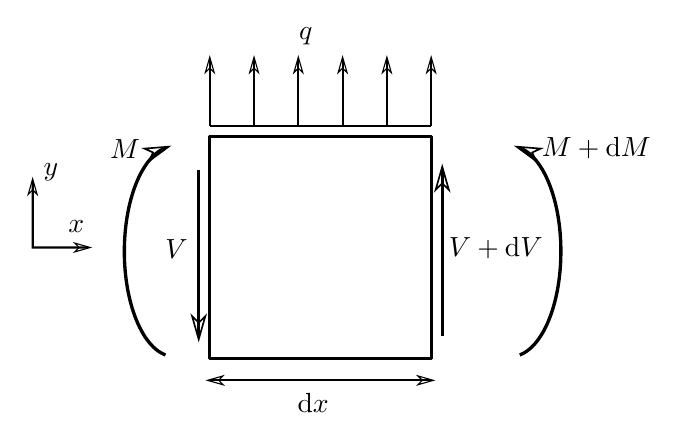
\begin{tikzpicture}[y=0.80pt, x=0.8pt,yscale=-1, inner sep=0pt, outer sep=0pt]
\begin{scope}[shift={(0,-752.36218)}]
  \path[draw=black,fill=black,line join=round,miter limit=4.00,fill
    opacity=0.000,nonzero rule,line width=1.200pt,rounded corners=0.0000cm]
    (95.0000,852.3622) rectangle (195.0000,952.3622);
    \path[color=black,fill=black,line width=0.800pt] (95.0000,961.8750) --
      (95.0000,962.8750) -- (195.0000,962.8750) -- (195.0000,961.8750) --
      (95.0000,961.8750) -- cycle;
    \path[draw=black,even odd rule,line width=0.400pt] (99.0000,962.3622) --
      (101.0000,960.3622) -- (94.0000,962.3622) -- (101.0000,964.3622) --
      (99.0000,962.3622) -- cycle;
    \path[draw=black,even odd rule,line width=0.400pt] (191.0000,962.3622) --
      (189.0000,964.3622) -- (196.0000,962.3622) -- (189.0000,960.3622) --
      (191.0000,962.3622) -- cycle;
    \path[color=black,fill=black,line width=1.200pt] (199.2500,867.3750) --
      (199.2500,942.3750) -- (200.7500,942.3750) -- (200.7500,867.3750) --
      (199.2500,867.3750) -- cycle;
    \path[draw=black,even odd rule,line width=0.600pt] (200.0000,873.3622) --
      (203.0000,876.3622) -- (200.0000,865.8622) -- (197.0000,876.3622) --
      (200.0000,873.3622) -- cycle;
    \path[color=black,fill=black,line width=1.200pt] (89.2500,867.3750) --
      (89.2500,942.3750) -- (90.7500,942.3750) -- (90.7500,867.3750) --
      (89.2500,867.3750) -- cycle;
    \path[draw=black,even odd rule,line width=0.600pt] (90.0000,936.3622) --
      (87.0000,933.3622) -- (90.0000,943.8622) -- (93.0000,933.3622) --
      (90.0000,936.3622) -- cycle;
    \path[color=black,fill=black,nonzero rule,line width=1.200pt] (74.7508,856.6718)
      .. controls (69.8130,858.5099) and (65.5561,863.3884) .. (62.3133,870.2343) ..
      controls (59.0705,877.0802) and (56.8284,885.9197) .. (56.0008,895.8280) ..
      controls (54.9137,908.8435) and (56.4098,921.5363) .. (59.7508,931.6093) ..
      controls (63.0918,941.6823) and (68.2689,949.1964) .. (74.7508,951.6093) --
      (75.2508,950.2030) .. controls (69.4951,948.0605) and (64.4529,940.9833) ..
      (61.1883,931.1405) .. controls (57.9237,921.2978) and (56.4301,908.7726) ..
      (57.5008,895.9530) .. controls (58.3158,886.1958) and (60.5450,877.4952) ..
      (63.6883,870.8593) .. controls (66.8316,864.2234) and (70.8734,859.7075) ..
      (75.2508,858.0780) -- (74.7508,856.6718) -- cycle;
    \path[draw=black,even odd rule,line width=0.600pt] (69.3769,859.4553) --
      (67.6120,863.3134) -- (76.4058,856.8389) -- (65.5188,857.6904) --
      (69.3769,859.4553) -- cycle;
    \path[color=black,fill=black,nonzero rule,line width=1.200pt]
      (235.2492,856.6718) -- (234.7492,858.0780) .. controls (240.5049,860.2206) and
      (245.5471,867.2978) .. (248.8117,877.1405) .. controls (252.0763,886.9833) and
      (253.5699,899.5085) .. (252.4992,912.3280) .. controls (251.6842,922.0852) and
      (249.4550,930.7859) .. (246.3117,937.4218) .. controls (243.1684,944.0577) and
      (239.1266,948.5735) .. (234.7492,950.2030) -- (235.2492,951.6093) .. controls
      (240.1869,949.7712) and (244.4439,944.8927) .. (247.6867,938.0468) .. controls
      (250.9295,931.2009) and (253.1716,922.3614) .. (253.9992,912.4530) .. controls
      (255.0863,899.4376) and (253.5902,886.7448) .. (250.2492,876.6718) .. controls
      (246.9082,866.5988) and (241.7311,859.0847) .. (235.2492,856.6718) -- cycle;
    \path[draw=black,even odd rule,line width=0.600pt] (240.6231,859.4553) --
      (244.4812,857.6904) -- (233.5942,856.8389) -- (242.3880,863.3134) --
      (240.6231,859.4553) -- cycle;
  \path[fill=black] (134.65359,976.70172) node[above right] (text7264) {d$x$};
  \path[fill=black] (75,907.36218) node[above right] (text7268) {$V$};
  \path[fill=black] (50,862.36218) node[above right] (text7272) {$M$};
  \path[fill=black] (203,907.36218) node[above right] (text7276) {$V+\text{d}V$};
  \path[fill=black] (245,862.36218) node[above right] (text7280) {$M+\text{d}M$};
  \path[draw=black,line join=miter,line cap=butt,line width=0.800pt]
    (95.0000,847.3622) -- (195.0000,847.3622);
    \path[color=black,fill=black,line width=0.800pt] (94.5000,817.3750) --
      (94.5000,847.3750) -- (95.5000,847.3750) -- (95.5000,817.3750) --
      (94.5000,817.3750) -- cycle;
    \path[draw=black,even odd rule,line width=0.400pt] (95.0000,821.3622) --
      (97.0000,823.3622) -- (95.0000,816.3622) -- (93.0000,823.3622) --
      (95.0000,821.3622) -- cycle;
    \path[color=black,fill=black,line width=0.800pt] (174.5000,817.3750) --
      (174.5000,847.3750) -- (175.5000,847.3750) -- (175.5000,817.3750) --
      (174.5000,817.3750) -- cycle;
    \path[draw=black,even odd rule,line width=0.400pt] (175.0000,821.3622) --
      (177.0000,823.3622) -- (175.0000,816.3622) -- (173.0000,823.3622) --
      (175.0000,821.3622) -- cycle;
    \path[color=black,fill=black,line width=0.800pt] (114.5000,817.3750) --
      (114.5000,847.3750) -- (115.5000,847.3750) -- (115.5000,817.3750) --
      (114.5000,817.3750) -- cycle;
    \path[draw=black,even odd rule,line width=0.400pt] (115.0000,821.3622) --
      (117.0000,823.3622) -- (115.0000,816.3622) -- (113.0000,823.3622) --
      (115.0000,821.3622) -- cycle;
    \path[color=black,fill=black,line width=0.800pt] (134.5000,817.3750) --
      (134.5000,847.3750) -- (135.5000,847.3750) -- (135.5000,817.3750) --
      (134.5000,817.3750) -- cycle;
    \path[draw=black,even odd rule,line width=0.400pt] (135.0000,821.3622) --
      (137.0000,823.3622) -- (135.0000,816.3622) -- (133.0000,823.3622) --
      (135.0000,821.3622) -- cycle;
    \path[color=black,fill=black,line width=0.800pt] (194.5000,817.3750) --
      (194.5000,847.3750) -- (195.5000,847.3750) -- (195.5000,817.3750) --
      (194.5000,817.3750) -- cycle;
    \path[draw=black,even odd rule,line width=0.400pt] (195.0000,821.3622) --
      (197.0000,823.3622) -- (195.0000,816.3622) -- (193.0000,823.3622) --
      (195.0000,821.3622) -- cycle;
    \path[color=black,fill=black,line width=0.800pt] (154.5000,817.3750) --
      (154.5000,847.3750) -- (155.5000,847.3750) -- (155.5000,817.3750) --
      (154.5000,817.3750) -- cycle;
    \path[draw=black,even odd rule,line width=0.400pt] (155.0000,821.3622) --
      (157.0000,823.3622) -- (155.0000,816.3622) -- (153.0000,823.3622) --
      (155.0000,821.3622) -- cycle;
  \path[fill=black] (135.3607,810.88519) node[above right] (text7684) {$q$};
    \path[color=black,fill=black,line width=0.800pt] (14.5000,872.3622) --
      (14.5000,902.3622) -- (14.5000,902.8622) -- (15.0000,902.8622) --
      (40.0000,902.8622) -- (40.0000,901.8622) -- (15.5000,901.8622) --
      (15.5000,872.3622) -- (14.5000,872.3622) -- cycle;
    \path[draw=black,even odd rule,line width=0.400pt] (36.0000,902.3622) --
      (34.0000,904.3622) -- (41.0000,902.3622) -- (34.0000,900.3622) --
      (36.0000,902.3622) -- cycle;
    \path[draw=black,even odd rule,line width=0.400pt] (15.0000,876.3622) --
      (17.0000,878.3622) -- (15.0000,871.3622) -- (13.0000,878.3622) --
      (15.0000,876.3622) -- cycle;
  \path[shift={(0,752.36218)},fill=black] (31.112698,143.02229) node[above right]
    (text9186) {$x$};
  \path[fill=black] (20,872.36218) node[above right] (text9190) {$y$};
\end{scope}

\end{tikzpicture}


  \caption{Infinitesimal Beam Slice}
  \label{fig:Infinitesimal}
\end{figure}
%
A force balance demonstrates that the x-derivative of internal shear force is the applied load.
\begin{equation}
\label{eq:EulerShear}
V = V + q\;\text{d}x + \text{d}V \implies \frac{\text{d}V}{\text{d}x} = -q\, .
\end{equation}
The moment balance can be performed about any point, but it is simplest to use the right side.
\begin{equation}
\label{eq:EulerMoment}
M - V\text{d}x +q\;\text{d}x\frac{\text{d}x}{2} = M + \text{d}M \implies \frac{\text{d} M}{\text{d}x} = -V + \mathcal{O}(\text{d}x)\, .
\end{equation}


Next, we will use the deformation assumptions to frame the bending as a simple arc
%
\begin{figure}[htbp]
  \centering
  


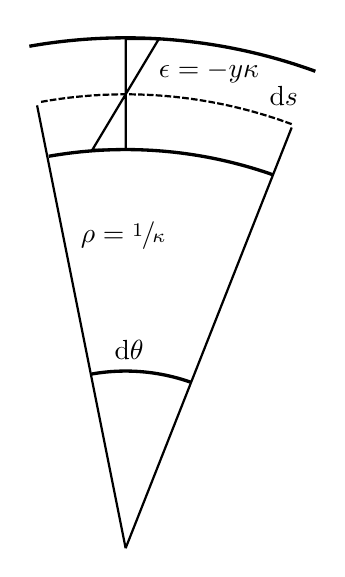
\begin{tikzpicture}[y=0.80pt, x=0.8pt,yscale=-1, inner sep=0pt, outer sep=0pt]
  \path[draw=black,miter limit=4.00,line width=1.200pt]
    (15.2615,55.3504)arc(260.000:289.500:200.051);
  \path[draw=black,line join=round,miter limit=4.00,line width=1.200pt]
    (6.4976,5.6478)arc(260.000:290.000:250.520);
  \path[draw=black,dash pattern=on 2.40pt off 0.80pt,line join=round,miter
    limit=4.00,line width=0.800pt] (11.7974,30.7804)arc(260.000:290.000:220.000000
    and 225.000);
  \path[draw=black,line join=miter,line cap=butt,line width=0.800pt]
    (50.0000,232.3622) -- (10.0000,32.3622);
  \path[draw=black,line join=miter,line cap=butt,line width=0.800pt]
    (50.0000,27.3622) -- (35.0000,52.3622) -- (50.0000,52.3622) --
    (50.0000,2.3622) -- (65.0000,2.3622) -- cycle;
  \path[fill=black] (29.7995,97.515488) node[above right] (text8240) {\(\rho =
    \sfrac{1}{\kappa}\)};
  \path[fill=black] (65,22.362183) node[above right] (text8248) {\(\epsilon = -y
    \kappa\)};
  \path[draw=black,line join=miter,line cap=butt,line width=0.800pt]
    (50.0000,232.3622) -- (125.0000,42.3622);
  \path[cm={{0.4407,0.0,0.0,0.4407,(27.965,129.30866)}},draw=black,miter
    limit=4.00,line width=1.200pt] (15.2615,55.3504)arc(260.000:289.500:200.051);
  \path[fill=black] (45,147.36218) node[above right] (text3984) {d$\theta$};
  \path[fill=black] (115,32.362183) node[above right] (text3988) {d$s$};

\end{tikzpicture}


  \caption{Small deformation in an Euler beam}
  \label{fig:EulerBeam1}
\end{figure}
%
from which we can deduce a relationship between the transverse displacement of a beam section and its angle and radius of curvature to be
\begin{equation}
 \label{eq:EulerCurve}
 \frac{1}{\rho} \approx \frac{\text{d} \phi}{\text{d} x} \approx \frac{\text{d}^2v}{\text{d}x^2} = \kappa\, .
\end{equation}
The radius of curvature, $\rho$ is the radius of the arc formed by the beam's neutral axis, which does not change in length as the beam bends.
We use this same arc to find the strain in material that is at a distance $y$ from the neutral axis.
In a linearly elastic material, the resulting stress is proportional to Young's modulus $E$.
To find the bending moment that results from that stress profile, we integrate the moment contribution through the beam.
\begin{equation}
M_\text{resisted} = \int_\text{bottom}^\text{top}y\sigma dA = \int_\text{bottom}^\text{top}y^2 E \kappa dA\, .
\end{equation}
In equilibrium, the moment resisted will be equal and opposite to the moment applied
\begin{equation}
\label{eq:MomentCurve}
\kappa = \frac{M_\text{applied}}{E \int_\text{bottom}^\text{top}y^2dA}\, .
\end{equation}
The integral in the denominator is the bending resistance of the beam's shape, called its second moment of area, about the neutral axis.
The second moment of area is generally represented by $I$.
By combining \cref{eq:EulerShear,eq:EulerMoment,eq:EulerCurve,eq:MomentCurve}, we reproduce  \cref{eq:EulerBeam}, the Euler-Bernoulli beam equation.
If the Young's modulus and beam cross section are constant throughout the beam, the equation can be further simplified to
\begin{equation}
EI\frac{\text{d}^4 v}{\text{d}x^4}=q\, .\notag
\end{equation}

Obviously, to solve for the deformed position we will require 4 constraints from boundary conditions.
The nature of the constraints is determined by the support configuration.
The most common end conditions are listed \cref{table:BeamBCs}.
Other end constraints, such 

\begin{table}
\centering
\begin{tabular}{l >{$\displaystyle}l<{$} >{$\displaystyle}l<{$}}
End Condition & \textrm{Contraint 1} & \textrm{Constraint 2}\\ \hline\hline
End Load & v'''=\pm F  &  v''=0  \\ \hline
End Torque & v'''=0  &  v''= \pm \tau  \\ \hline
Simply Supported & v''=0 & v=v_\text{support}  \\ \hline
Clamped & v'=v'_\text{clamp} & v=v_\text{clamp}  \\ \hline\hline
\end{tabular}
\caption{Common Beam End Conditions}
\label{table:BeamBCs}
\end{table}

\section{Kirchhoff-Love Plate Theory}
Like Euler-Bernoulli beam theory, Kirchhoff-Love Plate theory begins by making simplifying assumptions about the plate and its deformation.
\begin{itemize}
 \item Slenderness: the length and width of the plate should be 20 times its thickness
 \item Loaded transversely, no in-plane loads or torques
 \item Small deformations and rotations
 \item Straight lines normal to the plate remain normal to the center plane of the plate under deformation
 \item Initially flat
\end{itemize}
These assumptions allow us to simplify our strain-displacement relationships and formulate our curvatures and strains in terms of the transverse displacement $w$;
\begin{equation}
    \kappa_x=\frac{\partial^2 w}{\partial x^2}\,, \quad \kappa_y= \frac{\partial^2 w}{\partial y^2}\,, \quad \kappa_{xy}=\frac{\partial^2 w}{\partial x\partial y}\,,\notag
\end{equation}
\begin{equation}
\varepsilon_x = -z \kappa_x\,, \quad \varepsilon_y = -z \kappa_y\,, \quad \gamma_{xy} = -2 z \kappa_{xy}\,. \notag
\end{equation}
To find the stresses at any point, we apply Hooke's law and find
\begin{align*}
\sigma_x &= -\frac{E z}{1-\nu^2}\left(\kappa_x+\nu\kappa_y\right)\, ,\\
\sigma_y &= -\frac{E z}{1-\nu^2}\left(\kappa_y+\nu\kappa_x\right)\, ,\\
\tau_{xy} &= -\frac{Ez}{1+\nu}\kappa_{xy}\, .
\end{align*}
As with the beam, these stresses can be integrated over the thickness of the plate to determine the resulting moments.
\begin{align*}
M_x = \int_{\sfrac{-t}{2}}^{\sfrac{t}{2}}z\sigma_x dz &=-D\left(\kappa_x+\nu\kappa_y\right)\, ,\\
M_y = \int_{\sfrac{-t}{2}}^{\sfrac{t}{2}}z\sigma_y dz &=-D\left(\kappa_y+\nu\kappa_x\right)\, ,\\
M_{xy} = \int_{\sfrac{-t}{2}}^{\sfrac{t}{2}}z\tau_{xy}dz &= -D\left(1-\nu\right)\kappa_{xy}\, ,
\end{align*}
with
\begin{equation*}
D=\frac{Et^3}{12\left(1-\nu^2\right)}
\end{equation*}
as the flexural rigidity.
Note that a beam of unit width would have a second moment of area $I = \frac{t^3}{12}$, so the flexural rigidity of a plate is greater by a factor of $\frac{1}{1-\nu^2}$.
The difference between the values reflects the fact that, when a plate is bent in one direction, poisson ratio effects promote curvature in the opposite direction at a right angle.
Constraining this saddle-shaped (or \textit{anticlastic}) bending increases the stiffness or rigidity of the plate.

Constructing the governing equation is more complicated than for beams because, instead of shear $V$ and moment $M$ on an infinitesimal section, we have shears $V_x$ and $V_y$ and moments $M_x$, $M_y$, and $M_{xy}$.
Balancing forces gives us
\begin{equation*}
\frac{\partial V_x}{\partial x}+\frac{\partial V_y}{\partial y} = p\, ,
\end{equation*}
for transverse pressure $p$.
Balancing moments gives
\begin{align*}
\text{about} \;x:\qquad& \frac{\partial M_{xy}}{\partial x}+\frac{\partial M_{y}}{\partial y} - V_y = 0\, ,\\
\text{about} \;y:\qquad& \frac{\partial M_{xy}}{\partial y}+\frac{\partial M_{x}}{\partial x} - V_x = 0\, .
\end{align*}

Combining the force and moment balance equations generates the governing equation
\begin{equation*}
\frac{\partial^4w}{\partial x^4}+2\frac{\partial^4w}{\partial x^2 \partial y^2}+\frac{\partial^4w}{\partial y^4}=\frac{p}{D}\, .
\end{equation*}
As with the beam case, we will need to apply boundary conditions in order to find the deformed configuration.

\chapter{Peridynamics Background}

\section{Peridynamic States}
%
Introduced by Silling et al.\ in 2007~\cite{silling2007peridynamic}, peridynamic states are functions of the behavior of the continuum points surrounding each location.
As is appropriate for a theory based on force-carrying bonds, states often operate on vectors.
The most common states are scalar-states and vector-states which are scalar and vector valued, respectively.
As a matter of convention, scalar states are usually denoted by lowercase letters (e.g. $\sstate{a}{}{}$, $\sstate{b}{}{}$), while vector states are denoted by uppercase letters (e.g. $\vstate{A}{}{}$, $\vstate{B}{}{}$).
A state that operates on vectors and is itself vector valued naturally brings to mind a tensor such as the deformation gradient;
unlike a second order tensor, which can only map vectors linearly to other vectors, vector-states can produce nonlinear, discontinuous, or even noninvertable mappings.  
This difference is illustrated in \cref{fig:VectorState}.
%
\begin{figure}[h]
  \centering
\includegraphics{VectorState}
\caption[Deformation tensor vs. deformation vector state]{The deformation tensor linearly maps spheres to ellipsoids, while a vector state can map spheres nonlinearly to complex and even discontinuous shapes \cite{silling2007peridynamic}}
\label{fig:VectorState}
\end{figure}
%

The mathematical properties of states and several related operators are defined in~\cite{silling2007peridynamic}.
Important properties of states are magnitude and direction, while important operations include the addition and composition of states, inner and tensor products, and the Fr\'{e}chet derivative of a function with respect to a state.
While some of these operations are intuitive, the nomenclature may not be.
Refer to \cref{table:StateOperations} for the notation of common state operations.
For a fuller definition and examples of the Fr\'echet derivative, see \cref{sec:frechet}.

\begin{table}
\centering
\begin{tabular}{l >{$\displaystyle}r<{$} >{$\displaystyle}l<{$}}
Operation & \textrm{Notation} & \textrm{Meaning} \\ \hline\hline
Addition & (\sstate{a}{}{} + \sstate{b}{}{})\langle\boldsymbol{\xi}\rangle & \sstate{a}{}{\boldsymbol{\xi}} + \sstate{b}{}{\boldsymbol{\xi}} \\ \hline
Multiplication & (\sstate{a}{}{}\sstate{b}{}{})\langle\boldsymbol{\xi}\rangle & \sstate{a}{}{\boldsymbol{\xi}}\sstate{b}{}{\boldsymbol{\xi}} \\  \hline
Scalar Product & (\vstate{A}{}{} \cdot \vstate{B}{}{})\langle\boldsymbol{\xi}\rangle & \vstate{A}{}{\boldsymbol{\xi}} \cdot \vstate{B}{}{\boldsymbol{\xi}} \\  \hline
Composition & (\vstate{A}{}{} \circ \vstate{B}{}{})\langle\boldsymbol{\xi}\rangle & \vstate{A}{}{ \vstate{B}{}{\boldsymbol{\xi}}}  \\ \hline \noalign{\smallskip}
\multirow{2}{*}{Dot Product} & \vstate{A}{}{} \bullet \vstate{B}{}{}& \int_\mathcal{H} \vstate{A}{}{\boldsymbol{\xi}} \cdot \vstate{B}{}{\boldsymbol{\xi}} \\ \noalign{\smallskip}
& \sstate{a}{}{} \bullet \sstate{b}{}{}&  \int_\mathcal{H} \sstate{a}{}{\boldsymbol{\xi}} \sstate{b}{}{\boldsymbol{\xi}} \\  \noalign{\smallskip} \hline \noalign{\smallskip}
Vector Norm & |\vstate{A}{}{}|\langle\boldsymbol{\xi}\rangle &  |\vstate{A}{}{}\langle\boldsymbol{\xi}\rangle|  \\\noalign{\smallskip} \hline\noalign{\smallskip}
State Norm & \|\vstate{A}{}{}\| & \sqrt{\vstate{A}{}{} \bullet \vstate{B}{}{}} \\ \noalign{\smallskip} \hline \noalign{\smallskip}
\multirow{2}{*}{Fr\'echet Derivative} & \nabla\mathit{f}(\vstate{A}{}{}) & \frac{\partial \mathit{f}}{\partial \vstate{A}{}{}} \\ \noalign{\smallskip}
& \Psi(\vstate{A}{}{},\vstate{B}{}{})_\vstate{A}{}{} & \frac{\partial \Psi}{\partial \vstate{A}{}{}} \\ \noalign{\smallskip} \hline\hline
\end{tabular}
\caption{Common State Operation Nomenclature}
\label{table:StateOperations}
\end{table}


\section{State-based Models}
Conservation of linear momentum in the \textit{state-based} peridynamic formulation results in the equation of motion
%
\begin{equation}
\label{eq:PDstateEoM}
\rho(\mathbf{x})\ddot{\mathbf{u}}(\mathbf{x}) = \int_\Omega (\vstate{T}{\mathbf{x}}{\mathbf{q}-\mathbf{x}}-\vstate{T}{\mathbf{q}}{\mathbf{x}-\mathbf{q}}) dV_\mathbf{q}  + \mathbf{b}(\mathbf{x}),
\end{equation}
%
in which $\vstate{T}{\;}{\;}$ is a \textit{force vector-state} that maps the vector in angle brackets, $\langle \rangle$, originating at the point in square brackets, [ ], to a force vector acting on that point.
The deformed image of the vector $(\mathbf{q-x})$ is defined as the \textit{deformation vector-state}, usually denoted $\vstate{Y}{}{}$ and formulated as shown in \cref{eq:PDdeformation} for a displacement field \(\mathbf{u}\). 
Just as stress and strain are work conjugate, so too are the force and deformation vector states for hyperelastic materials.
%
\begin{equation}
\label{eq:PDdeformation}
\vstate{Y}{\mathbf{x}}{\mathbf{q}-\mathbf{x}} = (\mathbf{q}-\mathbf{x}) + (\mathbf{u}(\mathbf{q})-\mathbf{u}(\mathbf{x}))
\end{equation}
%

State-based models include surrounding material behavior illustrated in \cref{fig:pdDeformed} in the force function between each pair of continuum points. 
It is common for the formulation of the force state $\vstate{T}{}{}$ to be scaled by a weighting function, commonly represented by $\omega$, that makes explicit the region in which the force relationship between points is nonzero.
Perhaps the simplest and most common weight function is \cref{eq:WeightFunction}, representing a constant nonzero value for bonds shorter than the peridynamic horizon $\delta$.
%
\begin{equation}
\label{eq:WeightFunction}
\omega(\boldsymbol{\xi}) = 
\begin{cases}
1 & \text{if}\; |\boldsymbol{\xi}| \leq \delta \\
0 & \text{if}\; |\boldsymbol{\xi}| > \delta
\end{cases}
\end{equation}
%
Many evaluations of forces, energies, and other states at a given point are reduced from being integrals over the entire body to being integrals over that point's neighborhood $\mathcal{H}$.
This is particularly useful when trying to apply peridynamic models to real-world problems, especially when using computer models. 
%
\begin{figure}[h]
  \centering
\subinputfrom{\diagrampath}{PDbodyDeformed.eps_tex}
\caption{The body \protect\(\protect\Omega\protect\) deformed by the deformation state \protect\(\protect\vstate{Y}{}{}\protect\)}
\label{fig:pdDeformed}
\end{figure}
%
If the force state $\vstate{T}{}{}$ is always in the same direction as the deformation state $\vstate{Y}{}{}$, then the force exerted by a ``bond'' between points is in the same direction as the deformed bond, and the model is called \textit{ordinary}.  
Ordinary state-based can reproduce linear elastic materials with arbitrary Poisson ratios by separating dilatory and deviatoric deformations and the energy corresponding to each.
%\begin{equation}
%\label{eq:wLPS}
%  \hat{W} ( \mathbf{\underline{Y}} ) = \frac{1}{2} \left( k - \frac{\alpha m}{9} \right) \vartheta^2+\frac{\alpha}{2} \int_{\mathcal{H}} \omega ( | \boldsymbol{\xi} | ) \underline{e}^2 \langle \boldsymbol{\xi} \rangle dV_{\boldsymbol{\xi}}
%\end{equation} 
They can also model a variety of elastic and inelastic behaviors.

There is no requirement that force states be in the same direction as their associated deformation states, and models in which they are not in the same direction are called \textit{nonordinary}.
Some additional care is needed to ensure that angular momentum is conserved in a \textit{nonordinary} state-based model, but they are still perfectly legitimate.
Silling et al.\ demonstrate the possibility of such models in \cite{silling2010peridynamic}, but very little work has touched on their use.  
Foster et al.\ \cite{foster2010viscoplasticity} and Warren et al.\ \cite{warren2009non} show that some correspondence models, which approximate the deformation gradient and use it to calculate bond forces, result in non-ordinary state-based constitutive models for finite deformations.
Bond-based, ordinary state-based, and nonordinary state-based models are illustrated in \cref{fig:PDmodelTypes}.
%
\begin{figure}[h]
  \centering
\includegraphics{PDmodelTypes}
\caption[Illustration of the three types of peridynamic models]{Illustration of the three types of peridynamic models, from specific to general \cite{silling2007peridynamic}}
\label{fig:PDmodelTypes}
\end{figure}

It should be clear that many of the concepts of classical continuum mechanics have direct equivalents in peridynamic modeling.
\Cref{table:PDconcepts} lays out some of the simplest parallels between classical and peridynamic formulations.

\begin{table}
\centering
\begin{tabular}{l >{$\displaystyle}r<{$} >{$\displaystyle}l<{$}}
Concept & \textrm{Classical} & \textrm{Peridynamic} \\ \hline\hline
Kinematics & \mathbf{F} & \tvstate{Y}{}{} \\ \hline \noalign{\smallskip}
Linear Momentum & \nabla \cdot \boldsymbol{\sigma} & \int_\Omega (\vstate{T}{\mathbf{x}}{\mathbf{q}-\mathbf{x}}-\vstate{T}{\mathbf{q}}{\mathbf{x}-\mathbf{q}}) dV_\mathbf{q} \\    \noalign{\smallskip} \hline \noalign{\smallskip}
Angular Momentum &\boldsymbol{\sigma} - \boldsymbol{\sigma}^T  & \int_\Omega \vstate{Y}{\mathbf{x}}{\mathbf{q}-\mathbf{x}}\times\vstate{T}{\mathbf{x}}{\mathbf{q}-\mathbf{x}}dV_\mathbf{q}\\   \noalign{\smallskip} \hline
Constitutive Law & \boldsymbol{\sigma} = \boldsymbol{\sigma}(\boldsymbol{\epsilon}) &\tvstate{T}{}{}=\tvstate{T}{}{}(\tvstate{Y}{}{}) \\  \hline
First Law & \dot{\boldsymbol{\epsilon}} \boldsymbol{\sigma} &\tvstate{T}{}{}\bullet \tvstate{\dot{Y}}{}{} \\  \hline\hline
\end{tabular}
\caption{Peridynamic Equivalents of Classical Concepts}
\label{table:PDconcepts}
\end{table}

\section{Bond-based peridynamics}
%
If the force state \(\vstate{T}{\mathbf{x}}{\boldsymbol{\xi}} \) depends only on the deformation state \(\vstate{Y}{\mathbf{x}}{\boldsymbol{\xi}} \) of the same vector, then the model is called \textit{bond-based}.
In \textit{bond-based} peridynamic models, each pair of points is treated separately, without consideration of the behavior of other points. 
This makes bond-based models much simpler computationally than general state-based models, and reduces the equation of motion to
%
\begin{equation}
\label{eq:PDbondEoM}
\rho(\mathbf{x})\ddot{\mathbf{u}}(\mathbf{x}) = \int_\Omega \mathbi{f}(\mathbf{u}(\mathbf{q})-\mathbf{u}(\mathbf{x}),\mathbf{q}-\mathbf{x}) dV_\mathbf{q}  + \mathbf{b}(\mathbf{x}).
\end{equation}
%
By choosing an appropriate function $\mathbi{f}$, this model can reproduce the results of linear elasticity for solid materials with a Poisson ration \(\nu=\sfrac{1}{4}\) and 2-dimensional materials with a Poisson ration \(\nu=\sfrac{1}{3}\). 
It can also be used to investigate a range of nonlinear behaviors by changing the force function (examples in \cref{fig:BondForce}). 
To conserve momentum in a bond-based model, it is only necessary that $\mathbf{f}$ satisfy
%
\begin{equation}
\label{eq:PDbondF}
 \mathbi{f}(\mathbf{u}(\mathbf{q})-\mathbf{u}(\mathbf{x}),\mathbf{q}-\mathbf{x})=-\mathbi{f}(\mathbf{u}(\mathbf{x})-\mathbf{u}(\mathbf{q}),\mathbf{x}-\mathbf{q}),
\end{equation}
%
i.e. the forces exerted at the opposite ends of the bond between $\mathbf{x}$ and $\mathbf{q}$ must be equal and opposite.
The first peridynamic models were all bond-based, and provide useful insight despite their limitations.
%
\begin{figure}[h]
  \centering
\subinputfrom{\diagrampath}{BondForce.eps_tex}
\caption{Bond-based models can describe a variety of material behaviors}
\label{fig:BondForce}
\end{figure}
%

\section{Important Peridynamic Models}
Though they cover only a small portion of the behaviors modeled with peridynamics, these few examples should serve to illustrate the form and analysis of peridynamic material models.
\subsection{Bond-based Elastic Solid}
The simplest peridynamic model treats each bond as a linear spring between two points.
In the bond-based formulation, there is no interaction between different bonds, so the force function is
%
\begin{equation}
\mathbi{f}(\mathbf{u}(\mathbf{q})-\mathbf{u}(\mathbf{x}),\mathbf{q}-\mathbf{x}) = \omega(|\mathbf{q}-\mathbf{x}|)\;c\;s \left[(\mathbf{q}+\mathbf{u}(\mathbf{q}))-(\mathbf{x}+\mathbf{u}(\mathbf{x}))\right]
\end{equation}
%
with weighting function $\omega$, spring constant $c$, and the stretch $s$ defined by
%
\begin{equation}
\label{eq:stretch}
s = |(\mathbf{q}+\mathbf{u}(\mathbf{q}))-(\mathbf{x}+\mathbf{u}(\mathbf{x}))| - |\mathbf{q}-\mathbf{x}|.
\end{equation}
%
For a small deformation gradient $\mathbf{F}$, the stretch of bond $\boldsymbol{\xi}=\mathbf{q}-\mathbf{x}$ is
%
\begin{equation*}
s = |\mathbf{F}\boldsymbol{\xi}|-|\boldsymbol{\xi}| = \frac{\epsilon_{ij}\xi_i\xi_j}{|\boldsymbol{\xi}|}
\end{equation*}
%
For reasons that will become clear in the discussion of the next model, we calibrate the spring constant $c$ following the approach of \cite{silling2007peridynamic}, by comparing the energy to that of a classical solid under purely deviatoric deformation, so that $\epsilon_{ij} = \epsilon_{ij}^d$.
The energy of this spring will be in units of Energy per Volume-squared, so that integration over all the springs at a point gives Energy per unit Volume.
%
\begin{align}
\label{eq:deviatoricStrainEnergy}
w &= \frac{c\;s^2}{2}\notag \\
W &= \frac{c}{2}\int_\mathcal{H} \omega(|\xi|)\left( \frac{\epsilon_{ij}^d\xi_i\xi_j}{|\xi|} \right)\left( \frac{\epsilon_{kl}^d\xi_k\xi_l}{|\xi|} \right)\;dV_\xi\notag\\
&= \frac{c}{2}\epsilon_{ij}^d \epsilon_{kl}^d \int_\mathcal{H} \frac{\omega(|\xi|)}{|\xi|^2}\xi_i\xi_j\xi_k\xi_l 
\end{align}
%
Because $\omega$ depends only on $|\boldsymbol{\xi}|$, we can rewrite this integral in spherical coordinates as
%
\begin{equation}
W= \frac{c}{2}\epsilon_{ij}^d \epsilon_{kl}^d \int_0^\delta \frac{\omega(r)}{r^2}\int_0^{2\pi}\int_0^\pi (\xi_i\xi_j\xi_k\xi_l)\;r^2 \sin(\phi)\;d\phi\;d\theta\;dr\notag
\end{equation}
%
Recognizing that $\xi_1 = r \sin\phi\cos\theta$, $\xi_2=r\sin\phi\sin\theta$, $\xi_3=r\cos\phi$, we can see that configurations of $[i,j,k,l]$ with an odd number of any index result in integrals with an odd number of one or more of $\cos\theta$, $\sin\theta$, $\cos\phi$, and therefor are equal to 0. 
For the remaining configurations,
%
\begin{equation}
\int_0^\delta \frac{\omega(r)}{r^2}\int_0^{2\pi}\int_0^\pi (r^4 \sin^4 \phi \cos^2\theta\sin^2\theta)\;r^2 \sin(\phi)\;d\phi\;d\theta\;dr =  \frac{4\pi}{15} \int_0^\delta \omega(r)r^4\;dr\notag
\end{equation}
%
Also, any combination with $i=j$ or $k=l$ results in terms $\epsilon_{ii}^d$ or  $\epsilon_{kk}^d$, which will sum to 0 in deviatoric deformation. 
This leaves only configurations such as $[1,2,1,2]$ and $[3,2,2,3]$, which we can indicate by $(\delta_{ik}\delta_{jl}+\delta_{il}\delta_{jk})$.
%
\begin{align}
W&= \frac{c}{2}\epsilon_{ij}^d \epsilon_{kl}^d \frac{4\pi}{15} \int_0^\delta \omega(r)r^4\;dr (\delta_{ik}\delta_{jl}+\delta_{il}\delta{jk})\notag\\
&= c \;\epsilon_{ij}^d\epsilon_{ij}^d \frac{4\pi}{15} \int_0^\delta \omega(r)r^4\;dr \notag\\
&= \frac{c\; \epsilon_{ij}^d\epsilon_{ij}^d }{15}m\notag
\end{align}
%
To force the result to be independent of the horizon $\delta$, we normalize the expression by
%
\begin{equation}
\label{eq:weighted}
m=\int_\mathcal{H}\omega(|\boldsymbol{\xi}|)|\boldsymbol{\xi}|^2 = 4\pi \int_0^\delta \omega(r)\;r^4\;dr
\end{equation}
%
By comparing to the classical strain energy density $\Omega = \mu\;\epsilon_{ij}^d\epsilon_{ij}^d$ for shear modulus $\mu$, we can determine the appropriate bond stiffness
%
\begin{equation}
c = \frac{15\;\mu}{m}\notag
\end{equation}
%
Applying a purely dilational deformation to the same model is far easier.
With dilation $\theta$, the stretch of a bond in any direction is
%
\begin{equation}
s = \frac{\theta}{3} r,\notag
\end{equation}
%
and the corresponding energy is 
%
\begin{align}
W &= \frac{c}{2}\int_\mathcal{H} \omega(|\xi|)\frac{\theta^2}{9} r^2 \;dV_\xi\notag\\
&=\frac{c\;\theta^2}{18} \int_0^\delta \omega(r)\int_0^{2\pi}\int_0^\pi r^2\;r^2 \sin(\phi)\;d\phi\;d\theta\;dr \notag\\
&= \frac{c\;\theta^2}{18} m \notag\\
&= \frac{15}{9}\mu\frac{\theta^2}{2}
\end{align}
%
This shows that the model based on bond-stretch has a bulk modulus that is \sfrac{15}{9} of its shear modulus, indicating a Poisson's ratio of \sfrac{1}{4}.

A nearly identical analysis can be performed on a simpler 2D version of the same model, departing after \cref{eq:deviatoricStrainEnergy}.
Applying a purely deviatoric in-plane shear to such a model, and comparing the resulting energy to that of a classical plate with thickness $t$ gives us
%
\begin{equation}
c = \frac{8\;\mu\;t}{m_\textrm{2D}};\qquad m_\textrm{2D} =\int_\mathcal{H_\textrm{2D}}\omega(|\boldsymbol{\xi}|)|\boldsymbol{\xi}|^2.  \notag
\end{equation}
%

Applying a planar dilation deformation to a 2D plate results in strain energy consistent with a Poisson's ratio of \sfrac{1}{3} rather than the value of \sfrac{1}{4} found for the 3D solid.

\subsection{State-based Elastic Solid}
The state-based linear isotropic peridynamic solid material model is both important and illustrative.
Developed in \cite{silling2007peridynamic}, it uses many of the important characteristics of peridynamic states to model a linearly-elastic material with any valid Poisson's ratio.
The extension state $\underline{e}$ is exactly the same as the stretch $s$ in \cref{eq:stretch}.
Classical material models dealing with metal plasticity often separate deformation into dilation and deviation components.
Similarly, the extension state can be decomposed into isotropic and deviatoric extension states. Using $m$ from \cref{eq:weighted} as above for normalization the dilation state is defined
%
\begin{equation}
\theta = \frac{3}{m} \int_\mathcal{H} \omega(\boldsymbol{\xi}) |\boldsymbol{\xi}| \underline{e}.
\end{equation}
%
The isotropic and deviatoric extension states are defined in turn
%
\begin{equation}
\underline{e}^i = \frac{\theta |\boldsymbol{\xi}|}{3},\qquad \underline{e}^d = \underline{e}-\underline{e}^i
\end{equation}
%
If the energy associated with dilation is set to
%
\begin{equation}
W^i = \frac{k\;\theta^2}{2},\notag
\end{equation}
%
then the corresponding force state and peridynamic pressure are
%
\begin{equation}
\underline{t} = \frac{3k\theta}{m}\omega(\boldsymbol{\xi})|\boldsymbol{\xi}|,\qquad p=-k\theta\notag
\end{equation}
%
We saw in the analysis of the bond-based model the necessary bond stiffness to match the energy associated with purely deviatoric deformation.
The two can be combined for \cref{eq:lps}, a force state that clearly indicates the separate responses to dilation and deviatoric deformation.
%
\begin{equation}
\label{eq:lps}
\underline{t} = \frac{3k\theta}{m}\omega(\boldsymbol{\xi})|\boldsymbol{\xi}| + \frac{15\;\mu}{m}\omega(\boldsymbol{\xi})\underline{e}^d
\end{equation}
%
A quick examination shows that, in the case that the dilation $\theta$ is not constant, the force at either end of a bond will not satisfy \cref{eq:PDbondF}.
Thus such a model is not possible in a bond-based framework without significant modification.

\subsection{Correspondence Models}
One way to create a peridynamic material model is to start from a material model in classical dynamics.
Classical models based on the deformation gradient have the advantage of decades of development and tens of thousands of hours of testing, and they enjoy widespread use in the continuum mechanics community.
Peridynamic \textit{correspondence} models use the relative positions of a points neighbors to determine $\bar{\mathbf{F}}(\vstate{Y}{}{})$, a nonlocal approximation of the deformation gradient $\mathbf{F}$.
%
\begin{equation}
\label{eq:PDapproxGradient}
\bar{\mathbf{F}}(\vstate{Y}{}{}) = \left[\int_\mathcal{H} \omega(|\boldsymbol{\xi}|)(\vstate{Y}{}{\boldsymbol{\xi}}\otimes \boldsymbol{\xi})\;dV_{\boldsymbol{\xi}} \right]\mathbf{K}^{-1}
\end{equation}
with the shape tensor $\mathbf{K}$ defined by
\begin{equation}
\mathbf{K} = \int_\mathcal{H}\omega(|\boldsymbol{\xi}|)(\boldsymbol{\xi} \otimes \boldsymbol{\xi})\;dV_{\boldsymbol{\xi}} \notag
\end{equation}
%
When $\mathbf{F}$ is constant, $\bar{\mathbf{F}}(\vstate{Y}{}{})$ is exactly equal to $\mathbf{F}$.
If the classical model in question is hyperelastic with energy density $\Omega(\mathbf{F})$, it is a simple matter to force the peridynamic model to have identical energy by defining
\begin{equation}
W(\vstate{Y}{}{}) = \Omega(\bar{\mathbf{F}}(\vstate{Y}{}{}))
\end{equation}
and find the force vector state by taking the Fr\'echet derivative of $W$ with respect to $\vstate{Y}{}{}$.
Alternately, the classical continuum model can be applied to find the first Piola-Kirchhoff stress $\mathbf{P}$ associated with $\bar{\mathbf{F}}$:
\begin{equation}
\mathbf{P}=\frac{\partial\Omega(\bar{\mathbf{F}})}{\partial\bar{\mathbf{F}}}
\end{equation}
The resulting force state is calculated from the stress according to
\begin{equation}
\vstate{T}{}{\boldsymbol{\xi}} = \omega(\boldsymbol{\xi})\mathbf{P}\mathbf{K}^{-1}\boldsymbol{\xi}
\end{equation}
For homogenous deformations, the result is a peridynamic model that exactly reproduces the classical model without ever taking a derivative.
For problems with very inhomogenous (on the scale of the peridynamic horizon) deformations, the peridynamic model will exhibit scale effects not seen in the classical model, acting to smooth out the effect of short-scale deformations.
For discontinuous deformations, the classical model cannot be evaluated at all, but the peridynamic correspondence model will have no such problem.
It may be necessary however to revisit the choice of model or implement some damage condition.

\chapter{Model Development}
\label{ch:ModelDev}

\section{Bond Pair Material Model}
Consider the material model illustrated in \cref{fig:SimpleBondpair} in which every bond-vector originating from a point is connected by a rotational spring to its opposite originating from that same point.
%
\begin{figure}[h]
\centering
\resizebox{0.6\linewidth}{!}{\subinputfrom{\diagrampath}{simpleBondPair.eps_tex}}
\caption{Illustration of a bond pair model that resists angular deformation}
\label{fig:SimpleBondpair}
\end{figure}
%
If we call the deformed angle between these bonds \(\theta\), and choose the potential energy of that spring to be \(w(\boldsymbol{\xi}) = \omega(\boldsymbol{\xi})\alpha [1 + \cos(\theta) ] \) for the bond pair $\boldsymbol{\xi}$ and $-\boldsymbol{\xi}$, we can recover the non-ordinary force state proposed by Silling in \cite{silling2007peridynamic} by taking the Fr\'echet derivative. For the derivation and a description of the Fr\'echet derivative see \cref{sec:frechet}.
%
\begin{align}
\label{eq:SillingForceNO}
\vstate{T}{}{\boldsymbol{\xi}} &= \nabla w\!\left(\vstate{Y}{}{\boldsymbol{\xi}}\right)\notag \\
%
&=\omega(\boldsymbol{\xi})\frac{-\alpha}{|\vstate{Y}{}{\boldsymbol{\xi}}|} \frac{\vstate{Y}{}{\boldsymbol{\xi}}}{|\vstate{Y}{}{\boldsymbol{\xi}}|} \times \left[\frac{\vstate{Y}{}{\boldsymbol{\xi}}}{|\vstate{Y}{}{\boldsymbol{\xi}}|} \times \frac{\vstate{Y}{}{-\boldsymbol{\xi}}}{|\vstate{Y}{}{-\boldsymbol{\xi}}|}\right]
\end{align}
%
Though it looks complex, \cref{eq:SillingForceNO} indicates a bond force perpendicular to the deformed bond and in the plane containing both the deformed bond and its partner as illustrated in \cref{fig:Bondpair}. 
The force magnitude is proportional to the sine of the angle between the bonds divided by the length of the deformed bond. 
%
\begin{figure}[h]
  \vspace{5mm}
\centering
\resizebox{0.6\linewidth}{!}{\subinputfrom{\diagrampath}{bondPair.eps_tex}}
\caption{Deformation and force vector states}
\label{fig:Bondpair}
\end{figure}
%
This response is consistent with the idea of a rotational spring between bonds as long as the change in angle is small. 
Because the potential energy and force states are functions of \textit{pairs} of peridynamic bonds, we will call this formulation a \textit{bond-pair model}. 
Other choices for the bond-pair potential function, such as $w = (\pi - \theta)^2$, are also possible, but result in more mathematically complex analysis.

\section{Bond Pair Beam in Bending}
\label{sec:BPbeam}
The simplest application of our bond-pair based peridynamic model is that of \cref{fig:continuousbeam}, a beam in transverse bending.
Much of the material in this section can also be found in \cite{ogrady2014beams}.
%
\begin{figure}[h]
  \centering
\subinputfrom{\diagrampath}{continuousBeam.eps_tex}
\caption{A continuous peridynamic beam with horizon $\delta$}
\label{fig:continuousbeam}
\end{figure}
%

\subsection{Energy Equivalence}
\label{sec:beamEnergy}
To determine an appropriate choice of $\alpha$ for \cref{eq:SillingForceNO}, we desire our peridynamic model to have an equivalent strain energy density to a classical Euler-Bernoulli beam in the \emph{local limit}, i.e.\ when the nonlocal length scale vanishes.  We will begin with the assumptions from Euler beam theory: the length of the beam is much greater than thickness, vertical displacements are small, and rotations are small. For small vertical displacements (i.e.\ $\sin{\theta} \approx \theta$) we have
%
\begin{equation}
\theta(\vstate{Y}{}{\xi},\vstate{Y}{}{\mathbf{-\xi}}) \approx \pi-\frac{v(x+\xi)-2v(x)+v(x-\xi)}{\xi},
\label{eq:beamdtheta}
\end{equation}
%
where $v$ is the vertical displacement of material point.  Momentarily assuming that $v$ is continuous and using a Taylor series to expand the right-hand-side of eq.~(\ref{eq:beamdtheta})  
%
\begin{align}
\theta(\vstate{Y}{}{\xi},\vstate{Y}{}{\mathbf{-\xi}}) &\approx \pi-\xi \frac{\partial^2 v}{\partial x^2}+\mathcal{O}(\xi^3) \notag \\
&\approx  \pi-\xi \kappa +\mathcal{O}(\xi^3); 
\label{eq:beamdtheta2}
\end{align}
with
\begin{equation}
\kappa = \frac{\partial^2 v}{\partial x^2}.\notag
\end{equation}
%
Substituting eq.~(\ref{eq:beamdtheta2}) into the equation for the strain energy density of a single bond-pair,
%
\begin{align}
\label{eq:continuousBeamw}
w(\xi) &= \omega(\xi) \alpha \left[1+\cos(\theta(\vstate{Y}{}{\xi},\vstate{Y}{}{\mathbf{-\xi}})) \right] \notag\\
&\approx \omega(\xi) \alpha\frac{\xi^2}{2}(\kappa)^2 +\mathcal{O}(\xi^4).\notag
\end{align}
%
If we use a weighting function \(\omega(\xi)=\omega(|\xi|)\) and assume that the $\omega$ plays the role of a localization kernel, i.e. $\omega = 0 \,\, \forall \,\, \xi > \delta$, the resulting strain energy density, $W$, for any material point in the peridynamic beam is
%
\begin{equation}
W = \frac{\alpha}{2}\kappa^2 \int_{-\delta}^\delta \omega(\xi)\xi^2 {\rm d}\xi + \mathcal{O}(\delta^5).\notag
\end{equation}
%
Equating $W$ with the classical Euler-Bernoulli beam strain-energy density, $\Omega$, and taking the limit as $\delta \to 0$ we can solve for $\alpha$
%
\begin{align}
    \lim_{\delta \to 0}  W &= \Omega, \notag \\
    \frac{\alpha}{2} m \kappa^2 &= \frac{EI}{2} \kappa^2, \notag \\
    \alpha &= \frac{EI}{m},
\label{eq:alpha}
\end{align}
%
with 
\begin{equation}
    m = \int_{-\delta}^{\delta} \omega(\xi) \xi^2 {\rm d}\xi \notag.
\end{equation}

While this demonstrates the model's equivalence to a linearly-elastic Euler beam, if we keep an additional term from the Taylor series approximation of \cref{eq:beamdtheta}, we recover a slightly more complex expressions for change in angle that is demonstrated in \ref{sec:EringenCompare} to reproduce an Euler beam governed by Eringen's model of nonlocal elasticity.

\subsection{Relation to Eringen Nonlocality}
\label{sec:EringenCompare}
%If we relax our homogeneity assumption somewhat, we recover from \cref{eq:beamdtheta} slightly more complex expressions for change in angle
If we keep an additional term from the Taylor series approximation of \cref{eq:beamdtheta}, we recover a slightly more complex expressions for change in angle
%
\begin{equation}
\label{eq:beamdthetaHOT}
%\theta(\vstate{Y}{}{\xi},\vstate{Y}{}{\mathbf{-\xi}}) \approx \pi-\xi \frac{\partial^2 y}{\partial x^2} -\frac{\xi^3}{12} \frac{\partial^4 y}{\partial x^4}  +\mathcal{O}(\xi^5)=  \pi-\xi \kappa-\frac{\xi^3}{12} \kappa''+\mathcal{O}(\xi^5)\notag
\theta(\vstate{Y}{}{\xi},\vstate{Y}{}{\mathbf{-\xi}}) \approx \arctan\left(\pi-\xi \frac{\partial^2 v}{\partial x^2} -\frac{\xi^3}{12} \frac{\partial^4 v}{\partial x^4}  +\mathcal{O}(\xi^5)\right)\notag
\end{equation}
%
and for the strain energy (again substituting \(\kappa = v''\) for readability),
%
%\begin{equation}
%W \approx \int_{-\delta}^\delta \omega(\xi)\alpha(\frac{\xi^2}{2}\kappa^2+\frac{\xi^4}{12}\kappa\kappa''-\frac{3\; \xi^4}{8}\kappa^4+\mathcal{O}(\xi^6)) d\xi .
%\end{equation}
%
%
\begin{equation}
%W \approx \int_{-\delta}^\delta \omega(\xi)\alpha(\frac{\xi^2}{2}\kappa^2+\frac{\xi^4}{12}\kappa\kappa''-\frac{\xi^4}{24}\kappa^4+\mathcal{O}(\xi^6)) d\xi .\notag
W \approx \int_{-\delta}^\delta \omega(\xi)\alpha(\frac{\xi^2}{2}\kappa^2+\frac{\xi^4}{12}\kappa\kappa''-\frac{3\; \xi^4}{8}\kappa^4+\mathcal{O}(\xi^6)) d\xi.\notag
\end{equation}
%
As the horizon \(\delta\) becomes small, higher-order \(\xi\) terms become relatively less important, and \(\xi^4\kappa^4\) is dominated by \(\xi^2\kappa^2\) for large \(\kappa\) and by \(\xi^4\kappa\kappa''\) for small \(\kappa\).
The remaining terms can be rearranged,
\begin{align}
W &\approx \int_{-\delta}^\delta \omega(\xi)\alpha \frac{\xi^2}{2}\kappa(\kappa + \frac{\xi^2}{6}\kappa'') d\xi, \notag
\end{align}
in a manner strongly suggesting an alternative bending resistance term.
We can picture a bending resistance based on the bond length and proportional to the nonlocal curvature  \(\bar{\kappa}=(\kappa + \frac{\xi^2}{6}\kappa'')\), so that 
%
\begin{align}
\label{eq:NLbending}
\bar{\kappa}&=(\kappa + \frac{\xi^2}{6}\kappa'') \implies  \\
W &\approx \int_{-\delta}^\delta \omega(\xi)\alpha \frac{\xi^2}{2}\kappa\bar{\kappa}d\xi .\notag
\end{align}
%  
The same analysis can be taken further to obtain higher-order energy terms with even powers of \(\xi\) and even order derivatives of \(\kappa\). 
Not all of these higher-order terms can be separated into the product of a local curvature and nonlocal bending resistance.

Eringen's model for nonlocal elasticity in \cite{eringen1983differential} begins with a nonlocal modulus (denoted here as \(K(|\mathbf{x}'-\mathbf{x}|,\tau)\)) that relates the nonlocal stress \(\mathbf{t}\) at a point to the classical (local) stress \(\boldsymbol{\sigma}\) in the nearby material through the integral
\begin{equation}
\mathbf{t} = \int_\mathbf{V} K(|\mathbf{x}'-\mathbf{x}|,\tau)\boldsymbol{\sigma}(\mathbf{x}')dv(\mathbf{x}').\notag
\end{equation}
In the local limit these relationships take the form of higher-order gradients.
Using a 1-dimensional decaying exponential nonlocal modulus \(K(|x|,\tau)=\frac{1}{\tau l}e^{-\frac{|x|}{\tau l}}\)results in a relationship between \(t_\text{1D}\) and \(\sigma_\text{1D}\)
\begin{align}
\left(1-(\tau l)^2\frac{\partial^2}{\partial x^2}\right)t_\text{1D}&=\sigma_\text{1D},\notag
\end{align}
in which \((\tau l)\) is a scale-based material parameter.
For well-behaved \(t_\text{1D}\) and \(\sigma_\text{1D}\) and small values of \(\sigma_\text{1D}''''\) and \((\tau l)^2\), we can see that this relationship could be reformulated as
\begin{equation}
\label{eq:NLstress}
t_\text{1D}=\left(1+(\tau l)^2\frac{\partial^2}{\partial x^2}\right)\sigma_\text{1D}.\notag
\end{equation}
If we consider the results of the previous section and let \(dM = y\sigma dA\) and \(\sigma = Ey\kappa\), the contribution to moment resulting from Eringen's nonlocal elasticity in a fiber at \(y\)
\begin{equation}
\label{eq:EringenMoment}
E y^2 (\kappa+(\tau l)^2\kappa''), \\
\end{equation}
and the resulting strain energy
\begin{equation}
\label{eq:EringenEnergy}
\int_{-\frac{t}{2}}^{\frac{t}{2}} b(y) E \frac{y^2}{2} \kappa (\kappa+(\tau l)^2\kappa'')  dy,\notag
\end{equation}
bear a striking resemblance to \cref{eq:NLbending}.
In fact, by carefully choosing peridynamic parameter values, the results can be made identical.
For a rectangular beam of width \(b\) and thickness \(t\), choosing 
\begin{equation}
\omega(\xi) = |\xi|b ;\qquad \delta = \tau l \sqrt{3} ;\qquad \alpha = \frac{E b t^3}{54 (\tau l)^4}\notag
\end{equation}
results in
\begin{equation}
W \approx E b \frac{t^3}{12} \frac{\kappa}{2}(\kappa+\tau^2 l^2 \kappa''), \notag
\end{equation}
the same result for both models.

The similarity between \cref{eq:NLbending,eq:EringenMoment} is not accidental; Eringen's gradient elasticity is the solution to the integral formulation of the nonlocal stress integral equation just as the peridynamic energy is an integral function of nonlocal displacements.
It is therefore unsurprising that, like Eringen's nonlocal elasticity\cite{Challamel2008small}, this peridynamic bending model fails to predict the stiffening associated with nanoscale cantilevers.
Instead, the advantage of peridynamic models is their natural handling of discontinuities.

\subsection{Weighting function and inelasticity}
\label{sec:WeightFunction}
The weighting function \(\omega(\xi)\) describes the relative contribution of each bond-pair, and can be defined according to physical or mathematical considerations. 
While any function $\omega(\xi)$ that produces a convergent integral for $m$ will reproduce an elastic Euler beam, a physically meaningful choice of $\omega$ will allow us to extend our model to certain inelastic behaviors.
Consider a classical Euler-Bernoulli beam in bending with curvature \(\kappa\). 
Fibers running parallel to the neutral axis of the beam are stretched in proportion to their distance from the neutral axis, with strain \(\epsilon = y\kappa\). 
If the fibers are linearly elastic, then the axial stress at each location is \(\sigma = E\epsilon = Ey\kappa\), and the contribution to supported moment \(dM = \kappa E y^2 dA\). 
By comparing the formulations for the moments carried by the Euler beam in \cref{fig:EulerBending} and those of the bond-pair beam in \cref{fig:BPBending}, we see some definite parallels.
%
\begin{figure}[htbp]
\centering
\resizebox{0.5\linewidth}{!}{\subinputfrom{\diagrampath}{EulerBending.eps_tex}}
\caption{Euler beam moment contribution}
\label{fig:EulerBending}
\end{figure}
%
%
\begin{figure}[htbp]
  \vspace{5mm}
\centering
\subinputfrom{\diagrampath}{BondPairBending_edit.eps_tex}
\caption{Bond-pair moment contribution}
\label{fig:BPBending}
\end{figure}
%
\begin{align}
M_\text{E}&=\int_{-\frac{t}{2}}^{\frac{t}{2}} \sigma \; y \; dA &= \int_{-\frac{t}{2}}^{\frac{t}{2}} E \kappa \; y^2 \; b(y) dy\notag \\
%
M_\text{PD}&=\int_{-\delta}^{\delta} \vstate{T}{}{\xi}\; \xi \; d\xi &\notag \\
&= \int_{-\delta}^{\delta} \alpha \frac{\sin(\Delta\theta)}{|\xi|} \; \xi \; \omega(\xi) d\xi\: &\approx \int_{-\delta}^{\delta} \alpha \kappa |\xi| \; \omega(\xi) d\xi\notag
\end{align}
%
The term \(y\) is the distance from the beam's neutral axis and \(b(y)\) is the width of the beam at that distance from the neutral axis. 
The similarity between classical and peridynamic moment formulations suggests a possible formulation for the weighting function:
%
\begin{equation}
\label{eq:WeightFunction}
\omega(\xi) = |\xi| b\left(y\right) \quad \text{at} \quad y=\frac{\xi}{\delta} \frac{t}{2}
\end{equation}
%
\begin{figure}[h]
 \centering
  \subinputfrom{\diagrampath}{WeightProfile_Uniform.eps_tex}
\caption{Weight function for a beam of rectangular cross-section}
\label{fig:WeightProfileUniform}
\end{figure}

\begin{figure}
  \centering
  \subinputfrom{\diagrampath}{WeightProfile_Ibeam.eps_tex}
\caption{Weight function for an I-beam}
\label{fig:WeightProfileIbeam}
\end{figure}
%
This weight function analogizes the relative contributions of bond pairs of different lengths to the relative contributions of fibers at different distances from the centerline. 
An example for a rectangular beam is illustrated in \cref{fig:WeightProfileUniform}.
For an I beam with height \(h_\text{beam}\), width \(w_\text{beam}\), web height \(h_\text{web}\), and web width \(w_\text{web}\), substituting the beam profile
\begin{equation}
b(y) = 
  \begin{dcases}
    w_\text{web} & \text{if } |y| \leq \frac{h_\text{web}}{2} \\
    w_\text{beam} & \text{if } \frac{h_\text{web}}{2} < |y| \leq \frac{h_\text{beam}}{2} \\
    0 &\text{otherwise}
  \end{dcases}\notag
\end{equation}
into \cref{eq:WeightFunction} gives the weight function
\begin{equation}
\omega(\xi) = 
  \begin{dcases}
    |\xi| w_\text{web}& \text{if } |\xi| \leq \delta\frac{h_\text{web}}{h_\text{beam}} \\
    |\xi| w_\text{beam} & \text{if } \delta\frac{h_\text{web}}{h_\text{beam}} < |\xi| \leq \delta \\
    0 &\text{otherwise}
  \end{dcases}\notag
\end{equation}
and is ilustrated in \cref{fig:WeightProfileIbeam}.
    While this weighting function offers no advantages over a uniform weight function in the case of the linearly elastic beam, it offers a way to model advancing plasticity.

In a deformed elastic perfectly-plastic beam, axial fibers are still stretched in proportion to their distance from the neutral axis, but the relationship \(\sigma = E\epsilon = Ey\kappa\) only holds for \(|\epsilon| = |y\kappa| < \epsilon_c\). 
For greater stretches, the relationship becomes \(\sigma = \pm E\epsilon_c \). 
To model this behavior, consider a bond pair with similar behavior: for angular deformation less than some critical angle, the model behaves as previously described, but the magnitude of the force remains constant above a critical deformation
%
\begin{equation}
|\vstate{T}{}{\xi}| = 
  \begin{cases}
    \alpha \omega(\xi) \frac{\sin(\theta(\vstate{Y}{}{\xi},\vstate{Y}{}{\mathbf{-\xi}}))}{|\vstate{Y}{}{\xi}|} & \quad \text{if } \theta < \theta_c\\
    \alpha \omega(\xi) \frac{\sin(\theta_c)}{|\vstate{Y}{}{\xi}|} & \quad \text{if } \theta \geq \theta_c\
  \end{cases}
  \label{eq:epp_force}
\end{equation}
%
to determine the critical angle \(\theta_c\), we let the onset of plasticity in pairs of the longest bonds to coincide with the onset of plasticity in the fibers at the top and bottom surfaces of the classical beam. 
For small curvatures \(\Delta\theta = \xi\kappa\implies\Delta\theta_c = \frac{2\delta\epsilon_c}{t}\). 
For curvatures \(|\kappa| > \kappa_c=\frac{2\epsilon_c}{t}\), the radius within which bonds are in the elastic region is \(\delta_e = \delta \frac{\kappa_c}{\kappa}\), and parallels the distance from the beam centerline that fibers are in the elastic region \(y_e = \frac{t}{2} \frac{\kappa_c}{\kappa}\)
%
\begin{align}
  M_\text{classical} &= 2 \int_{0}^{y_e}E b(y)y^2 \kappa dy +2 \int_{y_e}^{\frac{t}{2}}E b(y) \epsilon_c y dy\notag \\
  M_\text{PD} &= 2 \int_{0}^{\delta_e}\alpha \omega(\xi) \xi^2 \kappa d\xi +2 \int_{\delta_e}^{\delta}\alpha \omega(\xi) \Delta\theta_c \xi d\xi \notag
\end{align}
%
Of course, as long as the force is independent of history, this model only represents a nonlinear elastic material. 
By keeping track of the plastic deformation \(\theta^p (\xi) = \theta-\theta_c\) of each bond-pair, and applying it as an offset, we can reproduce the hysteresis associated with elastic-perfectly-plastic deformation.

More simply, we can model a brittle material by setting the force to zero for bond pairs exceeding a critical angle,
%
\begin{equation}
|\vstate{T}{}{\xi}| = 
  \begin{cases}
    \alpha \omega(\xi) \frac{\sin(\theta(\vstate{Y}{}{\xi},\vstate{Y}{}{\mathbf{-\xi}}))}{|\vstate{Y}{}{\xi}|} & \quad \text{if } \theta < \theta_c\\
    0 & \quad \text{if } \theta \geq \theta_c\
  \end{cases}
  \label{eq:brittle_force}
\end{equation}
%
and additionally recording bond pairs that have exceeded their critical angle and permanently setting their influence, i.e. $\omega$, to zero.
%
%
\section{Bond Pair Plate in Bending}
The next case we will analyze is the extension of the bond pair beam model to \cref{fig:BondPairPlate}, a flat plate in the \(xy\) plane, with displacement $w$ in the \(z\)-direction. 
%
\begin{figure}[htbp]
    \centering
    \subinputfrom{\diagrampath/}{continuousPlate.eps_tex}
    \caption{Illustration of a bond pair on a plate.}
    \label{fig:BondPairPlate}
\end{figure}
%

\subsection{Energy Equivalence}
%
As with the beam model, we determine an appropriate choice of $\alpha$ so that our peridynamic model will have an equivalent strain energy density to a classical Kirckhoff plate in the \emph{local limit}.  We will begin with the assumptions from Kirckhoff plate theory: straight lines normal to the mid-surface remain both straight and normal to the deformed mid-surface, and the plate thickness does not change with deformation.  As with the Euler beam energy equivalence, we will start with the original assumptions from Kirchhoff-Love plate theory of small displacements and rotations, but they will not constrain the validity of the model for larger displacements and rotations.  For small vertical displacements we have
%
\begin{equation}
    \theta(\vstate{Y}{}{\boldsymbol{\xi}},\vstate{Y}{}{\boldsymbol{-\xi}}) \approx \pi-\frac{w(\mathbf{x}+\boldsymbol{\xi})-2w(\mathbf{x})+w(\mathbf{x}-\boldsymbol{\xi})}{|\boldsymbol{\xi}|},
    \label{eq:platetheta}
\end{equation}
%
where $w$ is the vertical displacement of material point.  Taking \(\boldsymbol{\xi}=\xi (\cos(\phi),\sin(\phi))\) in cartesian coordinates and momentarily assuming continuous displacements for the sake of comparison, we use a Taylor series to expand the right-hand-side of eq.~(\ref{eq:platetheta}) about \(\xi = 0\) 
%
\begin{equation}
    \theta(\vstate{Y}{}{\boldsymbol{\xi}},\vstate{Y}{}{\boldsymbol{-\xi}}) \approx \pi-\frac{\xi}{2} \left(\cos^2(\phi) \kappa_1+\sin^2(\phi) \kappa_2+2\sin(\phi)\cos(\phi)\kappa_3\right)+\mathcal{O}(\xi^3)
    \label{eq:platetheta2}
\end{equation}
%
with
%
\begin{equation}
    \kappa_1=\frac{\partial^2 w}{\partial x_1^2}, \quad \kappa_2= \frac{\partial^2 w}{\partial x_2^2}, \quad \kappa_3=\frac{\partial^2 w}{\partial x_1\partial x_2}\notag
\end{equation}
%
substituting eq.~(\ref{eq:platetheta2}) into the equation for the strain energy density of a single bond-pair,
%
\begin{align}
%\label{eq:continuousBeamw}
    w &= \omega(\boldsymbol{\xi}) \alpha \left[1+\cos(\theta(\vstate{Y}{}{\boldsymbol{\xi}},\vstate{Y}{}{\boldsymbol{-\xi}}) ) \right] \notag \\
    &= \omega(\boldsymbol{\xi}) \alpha\frac{\xi^2}{8}(\kappa_1^2\cos^4(\phi)+\kappa_2^2\sin^4(\phi)+2\kappa_1\kappa_2\cos^2(\phi)\sin^2(\phi)+4\kappa_3^2\cos^2(\phi)\sin^2(\phi) \notag \\
    &+ 4\kappa_1\kappa_3\cos^3(\phi)\sin(\phi)+4\kappa_2\kappa_3\cos(\phi)\sin^3(\phi))+\mathcal{O}(\xi^4).\notag
\end{align}
%
If we use a weighting function \(\omega(\boldsymbol{\xi})=\omega(\xi)\) and assume that the $\omega$ plays the role of a localization kernel, i.e. $\omega = 0 \; \forall \; \xi > \delta$, the resulting strain energy density, $W$, for any material point in the peridynamic plate is
%
\begin{align}
    W =& \alpha \int_{0}^\delta\int_0^{2 \pi} w\; \xi {\rm d}\phi {\rm d}\xi ,\notag \\
    =& \alpha \frac{3\pi}{8} \left(\kappa_1^2+\kappa_2^2+\frac{2}{3}\kappa_1\kappa_1+\frac{4}{3}\kappa_3^2 \right)\int_{0}^\delta \omega(\xi)\xi^3{\rm d}\xi + \mathcal{O}(\delta^6).\notag 
\end{align}
%
Equating $W$ with the classical Kirchhoff plate strain-energy density, $\Omega$, and taking the limit as $\delta \to 0$ we can solve for $\alpha$
%
\begin{align}
    \lim_{\delta \to 0}  W &= \Omega, \notag \\
    \alpha \frac{3 \pi}{8} m \left(\kappa_1^2+\kappa_2^2+\frac{2}{3}\kappa_1\kappa_1+\frac{4}{3}\kappa_3^2 \right)&= \left[ \frac{\mu h^3}{12(1-\nu)} \left(\kappa_1^2+\kappa_2^2+2\nu\kappa_1\kappa_1+2(1-\nu)\kappa_3^2 \right) \right]_{\nu=1/3}, \notag \\
%    \nu = \frac{1}{3},\:\: \alpha &= \frac{8}{3 \pi m} \frac{\mu h^3}{12(1-\nu)},
    \alpha &= \frac{2 \mu h^3}{3 m}, \\
    \text{with}\qquad \qquad \notag \\
%    \label{eq:platealpha}
%    m = \int_{0}^{\delta} \omega(\xi) \xi^3 {\rm d}\xi \notag.
    m &= \int_{0}^{\delta} \int_{0}^{2\pi}\omega(\xi) \xi^2 \xi {\rm d}\phi {\rm d}\xi \notag,
\end{align}
%
where $\mu$ is the shear modulus, $h$ is the thickness of the plate, and we have evaluated the classical Kirchhoff strain-energy at a Poisson ratio of \(\sfrac{1}{3}\) in order to solve for alpha as a constant.  Because $\alpha$ is inversely proportional to $m$, the energy does not change with varying choices for $\omega$ and $\delta$. It should be noted that the restriction \(\nu=\sfrac{1}{3}\) is the same imposed by the use of a bond based peridynamic model for in-plane deformation of a 2D peridynamic plate. We will show an extension to this model that removes this restriction in Section~\ref{sec:arbitrary}.

\subsection{Combining Bending and Extension Models}
The bond-pair bending model does not resist in-plane stretching or shear deformation because these deformations preserve the angles between opposite bonds.  If these behaviors are expected in combination with bending, a useful model must resist both in-plane and transverse deformations.  To create a plate model that also resists these deformations, i.e.\ a flat shell, we combine the bond-pair model with a two-dimensional version of the original bond-based linearly-elastic peridynamic solid model from \cite{silling2000reformulation}.  In this model, individual bonds act as springs resisting changes in length.
%
\begin{equation}
    \label{eq:bondextension}
    \vstate{T}{}{\boldsymbol{\xi}} =\beta\left(|\vstate{Y}{}{\boldsymbol{\xi}}|-|\boldsymbol{\xi}|\right)\frac{\vstate{Y}{}{\boldsymbol{\xi}}}{|\vstate{Y}{}{\boldsymbol{\xi}}|}
\end{equation}
%
By matching the energy of a 2D material in shear deformation, we can relate \(\beta\) to the shear modulus and thickness of the shell.  Following the example of \cite{silling2007peridynamic}, we begin with a 2D material under pure in-plane shear.  In Einstein notation, the strain energy of this material is
%
%\begin{align*}
%    W^d_\text{C} &= \mu \; h \; \epsilon_{ij} \epsilon_{ij} = \mu \; h \; \epsilon_{ij}^d \epsilon_{ij}^d \\
%    W^d_\text{PD} &= \frac{\beta}{2}(\underline{\omega}\; \underline{\epsilon^d})\bullet \underline{\epsilon^d}\\
%    &=\frac{\beta}{2} \epsilon_{ij}^d \epsilon_{kl}^d \int_A \frac{\underline{\omega}\langle\xi\rangle}{|\boldsymbol{\xi}|^2}\xi_i \xi_j \xi_k \xi_l \;dA_\xi\\
%\end{align*}
%
\begin{align*}
    W_\text{C} &= \mu \; h \; \epsilon_{ij}^d \epsilon_{ij}^d,  \\  \\
    W_\text{PD} &= \frac{\beta}{2}\int_A \omega(\xi)\left(|\vstate{Y}{}{\boldsymbol{\xi}}|-|\boldsymbol{\xi}|\right)^2 \; {\rm d}A_{\boldsymbol{\xi}}, \\
    &=\frac{\beta}{2}\int_A  \omega(\xi) \frac{\epsilon_{ij}\xi_i \xi_j }{|\boldsymbol{\xi}|} \frac{\epsilon_{kl} \xi_k \xi_l }{|\boldsymbol{\xi}|}\;{\rm d}A_{\boldsymbol{\xi}},\\
    &=\frac{\beta}{2} \epsilon_{ij}^d \epsilon_{kl}^d \int_A \frac{ \omega(\xi)}{|\boldsymbol{\xi}|^2}\xi_i \xi_j \xi_k \xi_l \;{\rm d}A_{\boldsymbol{\xi}}.
\end{align*}
%
where $\epsilon^d$ is the deviatoric strain tensor.  Now, to evaluate the integral we will exploit the symmetry properties. With $i, j, k, l = 1,2$. For a circular $\omega(\xi) = \omega(|\xi|)$, combinations of $\{i,j,k,l\}$ with an odd number of each index, such as $\{1,1,1,2\}$ or $\{2,1,2,2\}$, will result in odd powers of sine and cosine and integrate to 0.
%
\begin{align*}
%    m&=(\underline{\omega}\:\underline{x}) \bullet \underline{x}\\
    m &= \int_A \omega(\xi)|\boldsymbol{\xi}|^2\; dA_{\boldsymbol{\xi}} \\
    W^d_\text{PD} &= \frac{\beta \; m}{16}[3(\epsilon_{11}\epsilon_{11}+\epsilon_{22}\epsilon_{22})+(\epsilon_{11}\epsilon_{22}+\epsilon_{12}\epsilon_{12}+\epsilon_{12}\epsilon_{21}+\epsilon_{21}\epsilon_{12}+\epsilon_{21}\epsilon_{21}+\epsilon_{22}\epsilon_{11})]\\
    &= \frac{\beta \; m}{16} \epsilon_{ij}^d \epsilon_{kl}^d (\delta_{ij}\delta_{kl}+\delta_{ik}\delta_{jl}+\delta_{il}\delta_{jk})\\
    &= \frac{\beta \; m}{8} \epsilon_{ij}^d \epsilon_{ij}^d \implies\\
     \beta &= \frac{8 \; \mu\;h}{m}
\end{align*}
%
Having calibrated the bond-extension model to the shear modulus for a case of pure in-plane shear, applying a different uniform strain (such as might result from uniaxial tension) reveals the bond-based model to result in a one-parameter linearly-elastic model with Poisson's ratio \(\nu=\sfrac{1}{3}\).  

Combining the bending and extension models allows for the description of more complex behaviors, particularly the stiffening effect of in-plane tension on the transverse bending of a shell.  Consider a single bond-pair in the combined model shown in Fig.~\ref{fig:hybridmodel}.
%
\begin{figure}[htbp]
  \vspace{5mm}
  \centering
  \input{\diagrampath/bondPairCombinedV.tex}
  \caption{The Hybrid Model Combines Bending and Extension Components}
  \label{fig:hybridmodel}
\end{figure}
%
As the two sides are pulled apart, the magnitude of the extension force in each bond increases, and the magnitude of the bending force decreases.  At the same time, the angle at which the extension force acts decreases, and the angle of action for the bending force increases.  For small amounts of bending and reasonable stretches, increased tension in the direction of the bond pair results in increased restorative force.
\section{Extension to arbitrary Poisson ratio}
\label{sec:arbitrary}
Although many materials have Poisson ratios of \(\nu\approx \sfrac{1}{3}\), it is nonetheless desirable to extend the model to materials with arbitrary Poisson ratios.  For isotropic, linearly elastic models of solid materials, Silling et al.\ extended the peridynamic material model to arbitrary material parameters in \cite{silling2007peridynamic} by decomposing the deformation into isotropic and deviatoric components.  In the absence of plastic deformation, we need only find the difference between the strain energy of a deformed bond-based plate and the strain energy of an elastic plate with Poisson's ratio \(\nu \neq \sfrac{1}{3}\).  The difference is a function of the isotropic strain in two dimensions, \(\theta_{2D}\)
%
\begin{align}
    W^\star &= \frac{\mu\;h}{2}\left(\frac{3\nu-1}{1-\nu}\right)\theta_{2D}^2 \notag \\
%    \theta_{2D} &= \frac{2}{m}\left(\underline{\omega x}\right)\bullet\underline{e} \notag \\
    \theta_{2D} &= \frac{2}{m}\int_A \omega(\boldsymbol{\xi})|\boldsymbol{\xi}|(|\vstate{Y}{}{\boldsymbol{\xi}}|-|\boldsymbol{\xi}|)\;dA_{\boldsymbol{\xi}} \notag \\
%    W_\text{total} &= \frac{\mu\;h}{2}\left(\frac{3\nu-1}{1-\nu}\right)\theta_{2D}^2 + \frac{4\;\mu\;h}{m}\left(\underline{\omega e}\right)\bullet\underline{e}\notag
    W_\text{total} &= \frac{\mu\;h}{2}\left(\frac{3\nu-1}{1-\nu}\right)\theta_{2D}^2 + \frac{4\;\mu\;h}{m}\int_A \omega(\boldsymbol{\xi})(|\vstate{Y}{}{\boldsymbol{\xi}}|-|\boldsymbol{\xi}|)^2\;dA_{\boldsymbol{\xi}}\notag
\end{align}
%
This is to be expected because the bond-based model was calibrated to the shear strain energy, leaving discrepancies proportional to the isotropic strain energy that fall to 0 as Poisson's ratio approaches \(\nu = \sfrac{1}{3}\).

This decomposition method inspires a similar approach to our plate model. To perform the same extension for the plate model in bending, we find the error in the 1-parameter strain energy for \(\nu \neq \sfrac{1}{3}\)
%
\begin{align}
    W^\star=&\frac{\mu h^3}{12(1-\nu)} \left(\kappa_1^2+\kappa_2^2+2\nu\kappa_1\kappa_2+2(1-\nu)\kappa_3^2 \right)\notag\\
    &-\frac{\mu h^3}{12(1-\frac{1}{3})} \left(\kappa_1^2+\kappa_2^2+\frac{2}{3}\nu\kappa_1\kappa_2+2(1-\frac{1}{3})\kappa_3^2 \right) \notag \\
    W^\star=&2\mu \frac{h^3}{12}\frac{3\nu-1}{1-\nu} \left(\frac{\kappa_1+\kappa_2}{2}\right)^2.\notag
\end{align}
%
The discrepancy in energy is proportional to the square of average curvature, \(\frac{\kappa_1+\kappa_2}{2}\), which we will also refer to as the isotropic curvature.  The isotropic curvature can be envisioned as the portion of the deformation that resembles a hemispherical bowl.  The remainder of the bending deformation, that which is left when the isotropic curvature is subtracted out, resembles a saddle. This remaining component is the deviatoric deformation, and both components are shown in \cref{fig:BendingDecomp}. Note that the orientation of the deviatoric bending will change depending on the particular curvature being decomposed, while the isotropic curvature will only change in scale.
%
\begin{figure}[htbp]
  \vspace{5mm}
  \centering
  \resizebox{\linewidth}{!}{\input{\plotpath/BendingDecomp.pgf}}
  \caption{Bending Deformation Decomposed into Isotropic and Deviatoric Portions}
  \label{fig:BendingDecomp}
\end{figure}
%
A complete decomposition of bending energy into isotropic and deviatoric components as performed by Fischer in \cite{fischer1992bending} produces a far more complex model and is unnecessary at this time.  For a single bond pair we can represent the curvature vector along the bond pair as 
%
\begin{equation}
    \boldsymbol{\kappa} _{\hat{\boldsymbol{\xi}}} = \frac{\vstate{Y}{}{\boldsymbol{\xi}}+\vstate{Y}{}{\boldsymbol{-\xi}}}{|\boldsymbol{\xi}|^2}\notag
\end{equation}
%
For large rotations, we can define an average curvature vector \(\bar{\boldsymbol{\kappa}}\).
This leads us to model the average curvature as 
%
\begin{align}
    \bar{\boldsymbol{\kappa}} &= \frac{1}{m} \int_0^\delta \int_0^{2\pi}\omega(\xi)\frac{\vstate{Y}{}{\boldsymbol{\xi}}+\vstate{Y}{}{\boldsymbol{-\xi}}}{\xi^2} \xi {\rm d}\phi {\rm d}\xi ;\notag \\
    m &= \int_0^\delta \int_0^{2\pi}\omega(\xi)\xi {\rm d}\phi {\rm d}\xi. \notag
\end{align}
%
The weighting function \(\omega(\xi)\) performs the same function as in the previous section.
We can rewrite the energy discrepancy in terms of \(\bar{\boldsymbol{\kappa}}\).
%
\begin{equation}
    W^\star=2\mu\frac{h^3}{12}\frac{3\nu-1}{1-\nu}\bar{\boldsymbol{\kappa}}^2. \notag
\end{equation}
%
We can take the Fr\'{e}chet derivative (details in \ref{sec:frechet}) to produce a correction force vector state
%
\begin{equation}
    \vstate{T^\star}{}{\boldsymbol{\xi}}=\frac{8\mu}{m}\frac{h^3}{12}\frac{3\nu-1}{1-\nu}\frac{\omega(\boldsymbol{\xi})}{\xi^2} \bar{\boldsymbol{\kappa}},
    \label{eq:pressureState}
\end{equation}
%
that is not directly dependent on the deformation of a single bond pair.  Instead, \cref{eq:pressureState} represents a bond-length dependent ``pressure'' applied to every pair of bonds extending from a node.  This ``pressure'' is proportional to the curvature vector at that node.
A weighting function \(\omega(\boldsymbol{\xi}) = |\boldsymbol{\xi}|\) can ensure that the integral expression for force at a point is convergent.  This extra term that is dependent on the bending of all the pairs around a material point means that the extension is not properly a \textit{bond-pair} model.  Instead, it would be more accurate to call it a \textit{bond-multiple} model, in which the bond forces and energies are functions of the relationship between a family of bonds.  In either the continuous or discrete cases, this model extension requires the additional step of evaluating the isotropic curvature at each point, but the increased complexity of the extended model captures in the local limit the behavior of a two-parameter elastic material plate.
%
\chapter{Numerical Simulation}
\section{Discretized Bond Pair Beam}
Discretizing the bond-pair model is primarily matter of exchanging integrals for sums. 
%
\begin{align}
%
w(\boldsymbol{\xi}_i) &= \omega(\boldsymbol{\xi}_i)\alpha \left[1+\cos(\theta(\vstate{Y}{}{\boldsymbol{\xi}_i},\vstate{Y}{}{-\boldsymbol{\xi}_i})) \right] \notag \\
&\approx \omega(\boldsymbol{\xi}_i)\frac{\alpha}{2}\left(\frac{v(\mathbf{x}+\boldsymbol{\xi}_i)-2v(\mathbf{x})+v(\mathbf{x}-\boldsymbol{\xi}_i)}{\boldsymbol{\xi}_i}\right)^2\notag
\end{align}
%
in which $\boldsymbol{\xi}_i$ is the $i^\textnormal{th}$ bond emanating from the point $\mathbf{x}$ to each of the $n$ points within distance $\delta$ of point $\mathbf{x}$.
%
\begin{align}
\label{eq:discreteBeamw}
\alpha &= \frac{c\; \Delta x}{m} ;\; c= EI ;\; m=\sum_{i=1}^n \omega(\boldsymbol{\xi}_i)\boldsymbol{\xi}_i^2 \implies \nonumber \\
W&=\Delta x \sum_{i=1}^n \frac{EI}{2}\omega(\boldsymbol{\xi}_i)\left(\frac{v(\mathbf{x}+\boldsymbol{\xi}_i)-2v(\mathbf{x})+v(\mathbf{x}-\boldsymbol{\xi}_i)}{\boldsymbol{\xi}_i}\right)^2
\end{align}
%
Discretization of the original model results in the equation of motion
\begin{align}
\rho(\mathbf{x})\mathbf{\ddot{u}}(\mathbf{x}) = \mathbf{f}(\mathbf{x})&+\sum_i \omega(\boldsymbol{\xi}_i)\left\{\frac{\alpha(\mathbf{x})}{|\mathbf{p}_i |}\frac{\mathbf{p}_i}{|\mathbf{p}_i |}\times \left[ \frac{\mathbf{p}_i}{|\mathbf{p}_i |}\times \frac{\mathbf{q}_i}{|\mathbf{q}_i |}\right] \right. \notag \\
& \left. -\frac{\alpha(\mathbf{x}+\boldsymbol{\xi}_i)}{|\mathbf{p}_i |}\frac{(-\mathbf{p}_i)}{|\mathbf{p}_i |}\times\left[\frac{(-\mathbf{p}_i)}{|\mathbf{p}_i |}\times \frac{\mathbf{r}_i}{|\mathbf{r}_i |} \right] \right\} 
\label{eq:discretebeamEoM}
\end{align}
with
\begin{align}
\mathbf{p}_i &= \boldsymbol{\xi}_i+\mathbf{u}(\mathbf{x}+\boldsymbol{\xi}_i)-\mathbf{u}(\mathbf{x});\notag\\
\mathbf{q}_i &= -\boldsymbol{\xi}_i+\mathbf{u}(\mathbf{x}-\boldsymbol{\xi}_i)-\mathbf{u}(\mathbf{x});\notag\\
\mathbf{r}_i &= \boldsymbol{\xi}_i+\mathbf{u}(\mathbf{x}+2\boldsymbol{\xi}_i)-\mathbf{u}(\mathbf{x}+\boldsymbol{\xi}_i).\notag
\end{align}
and for small displacements and rotations in a uniform beam,
\begin{align}
\rho(\mathbf{x})\ddot{v}(\mathbf{x}) = &f(\mathbf{x})\notag \\
+&\alpha \sum_i 2\omega(\xi_i)\left(\frac{v(\mathbf{x}-2 \boldsymbol{\xi}_i)-4v(\mathbf{x}- \boldsymbol{\xi}_i)+6v(\mathbf{x})-4v(\mathbf{x}+ \boldsymbol{\xi}_i)+v(\mathbf{x}+2 \boldsymbol{\xi}_i)}{ \boldsymbol{\xi}_i^2}\right) \notag
\end{align}
It is worth noting the similarity between this expression and a finite-difference fourth derivative of displacement, a result expected from Euler beam theory.
This discretization requires that nodes be evenly spaced along the entire beam, otherwise the displacement \(v(\mathbf{x}- \boldsymbol{\xi}_i)\) is ill-defined. 
For this reason, the discretization does not allow for areas of higher and lower ``resolution''. 

\section{Discretized Bond Pair Plate}

%
\begin{figure}[h]
  \centering
\resizebox{.7\linewidth}{!}{\subinputfrom{\diagrampath}{discretePlate.eps_tex}}
\caption{Discretized peridynamic plate with illustrated bond pair}
\label{fig:discretePlate}
\end{figure}
%
As with the beam, discretizing the bond-pair model is primarily matter of exchanging integrals for sums. 
%
%\begin{align}
%w(\boldsymbol{\xi}_i) &= \omega(\boldsymbol{\xi}_i)\alpha \left[1+\cos(\theta(\vstate{Y}{}{\boldsymbol{\xi}_i},\vstate{Y}{}{-\boldsymbol{\xi}_i})) \right] \notag \\
%&\approx \omega(\boldsymbol{\xi}_i)\frac{\alpha}{2}\left(\frac{z(\mathbf{x}+\boldsymbol{\xi}_i)-2z(\mathbf{x})+z(\mathbf{x}-\boldsymbol{\xi}_i)}{\boldsymbol{\xi}_i}\right)^2 \notag
%\end{align}
%%
%in which $\boldsymbol{\xi}_i$ is the $i^\textnormal{th}$ bond emanating from the point $\mathbf{x}$ to each of the $n$ points within distance $\delta$ of point $\mathbf{x}$.
%
\begin{align}
\label{eq:discreteplate}
    \alpha &= \frac{c\; (\Delta x)^2}{m} ;\; c= \frac{\mu}{(1-\nu)}\frac{h^3}{12};\; m=\sum_{i=1}^n \omega(\boldsymbol{\xi}_i)\boldsymbol{\xi}_i^2 \implies  \\
    W&=(\Delta x)^2 \sum_{i=1}^n \omega(\boldsymbol{\xi}_i)\frac{\mu}{2(1-\nu)}\frac{h^3}{12}\left(\frac{w(\mathbf{x}+\boldsymbol{\xi}_i)-2w(\mathbf{x})+w(\mathbf{x}-\boldsymbol{\xi}_i)}{|\boldsymbol{\xi}_i|}\right)^2 \notag
\end{align}
%
Discretization of the 1-parameter bending model results in the same equation of motion as for the beam model (eq. \ref{eq:discretebeamEoM}).
%
%\begin{align}
%    \label{eq:discreteEoM}
%    \rho(\mathbf{x})\mathbf{\ddot{u}}(\mathbf{x}) = \mathbf{f}(\mathbf{x})&+\sum_i \omega(\boldsymbol{\xi}_i)\left\{\frac{\alpha(\mathbf{x})}{|\mathbf{p}_i |}\frac{\mathbf{p}_i}{|\mathbf{p}_i |}\times \left[ \frac{\mathbf{p}_i}{|\mathbf{p}_i |}\times \frac{\mathbf{q}_i}{|\mathbf{q}_i |}\right] \right.  \\
%    & \left. -\frac{\alpha(\mathbf{x}+\boldsymbol{\xi}_i)}{|\mathbf{p}_i |}\frac{(-\mathbf{p}_i)}{|\mathbf{p}_i |}\times\left[\frac{(-\mathbf{p}_i)}{|\mathbf{p}_i |}\times \frac{\mathbf{r}_i}{|\mathbf{r}_i |} \right] \right\} \notag
%\end{align}
%with
%\begin{align}
%    \mathbf{p}_i &= \boldsymbol{\xi}_i+\mathbf{u}(\mathbf{x}+\boldsymbol{\xi}_i)-\mathbf{u}(\mathbf{x});\notag\\
%    \mathbf{q}_i &= -\boldsymbol{\xi}_i+\mathbf{u}(\mathbf{x}-\boldsymbol{\xi}_i)-\mathbf{u}(\mathbf{x});\notag\\
%    \mathbf{r}_i &= \boldsymbol{\xi}_i+\mathbf{u}(\mathbf{x}+2\boldsymbol{\xi}_i)-\mathbf{u}(\mathbf{x}+\boldsymbol{\xi}_i).\notag
%\end{align}
%

Implementing the 2-parameter model requires finding the isotropic curvature at each point.
%
\begin{align*}
    \bar{\boldsymbol{\kappa}}(\mathbf{x}) &= \frac{1}{m} \sum_i \omega(\boldsymbol{\xi}_i)\frac{\mathbf{p}_i +\mathbf{q}_i }{\boldsymbol{\xi}_i^2};\notag \\
    m(\mathbf{x})  &= \sum_i \omega(\boldsymbol{\xi}_i); \notag \\
    \alpha^\text{iso}(\mathbf{x}) &= \frac{4\mu}{m}\frac{h^3}{12}\frac{3\nu-1}{1-\nu}(\Delta x)^2;\\
    f^\text{iso}(\mathbf{x}) &= \sum_j \left\{\left[\alpha^\text{iso}(\mathbf{x})\bar{\boldsymbol{\kappa}}(\mathbf{x})-\alpha^\text{iso}(\mathbf{x}+\boldsymbol{\xi}_j)\bar{\boldsymbol{\kappa}}(\mathbf{x}+\boldsymbol{\xi}_j) \right] \frac{\omega(\boldsymbol{\xi}_j)}{\boldsymbol{\xi}_j^2} \right\}
\end{align*}
%
As with the discretized beam, the discretization of the bond-pair plate (\cref{fig:discretePlate}) must be absolutely regular. 
Discretizing the bond-pair model as proposed above requires that nodes be evenly spaced, $\Delta x$, throughout the entire plate, otherwise the displacement \(w(\mathbf{x}-\boldsymbol{\xi}_i)\) is undefined.  For this reason, the discretization does not allow for areas of higher and lower ``resolution''.  This restriction, while inconvenient in the 1D case, is fairly restricting for plate analysis. An extension to this discretization that would allow changing mesh resolution will require interpolation between the nodes.  
%
%
%
%
%\begin{figure}[htbp]
%  \centering
%  \input{\diagrampath/VirtualPoint.tex}
%  \caption{Virtual Points Pair Up Unpaired Neighbors}
%  \label{fig:virtualpoint}
%\end{figure}
%
%
%\section{Bond Multiple Material Model}
%The requirement for a perfectly regular discretization makes the bond pair model difficult to use for many problems. 
%One proposed solution to this shortcoming is the \textit{bond-multiple} material model. 
%In a bond-multiple material, there exists a bond-pair potential energy for \textit{every possible combination of 2 bonds} emanating from a material point
%%
%\begin{equation}
%\label{eq:bondMultiple}
%W=\int_{\mathcal{H}} \int_{\mathcal{H}}  \omega(\boldsymbol{\xi})\omega(\boldsymbol{\zeta})w(\vstate{Y}{}{\boldsymbol{\xi}},\vstate{Y}{}{\boldsymbol{\zeta}})d\boldsymbol{\zeta} d \boldsymbol{\xi} .
%\end{equation}
%%
%The bond-pair energy expression assumes bonds that are antiparallel in the undeformed configuration. 
%To incorporate the energy of bonds that are collinear or otherwise oriented in the undeformed configuration, we modify the bond-pair energy expression as shown in \cref{eq:bondMultw}.
%%
%\begin{equation}
%\label{eq:bondMultw}
%w(\vstate{Y}{}{\boldsymbol{\xi}},\vstate{Y}{}{\boldsymbol{\zeta}})= \alpha [1-\cos \left(\theta(\vstate{Y}{}{\boldsymbol{\xi}},\vstate{Y}{}{\boldsymbol{\zeta}})-\theta( \boldsymbol{\xi} , \boldsymbol{\zeta} )\right) ] d\boldsymbol{\zeta} d \boldsymbol{\xi} 
%\end{equation}
%%
%\section{Bond Multiple Beam}
%For the beam model, this transforms the expression for strain energy density into
%%
%\begin{equation}
%\label{eq:bondMultipleBeam}
%W=\int_{-\delta}^{\delta} \int_{-\delta}^{\delta} \omega(\xi)\omega(\zeta) \alpha[1-\cos \left(\theta(\vstate{Y}{}{\xi},\vstate{Y}{}{\zeta})-\theta( \xi , \zeta )\right) ] d\zeta d \xi .
%\end{equation}
%
%As with the bond pair model, by making the simplifying assumptions of beam length, displacement, and rotation, the strain energy density of the bond multiple beam can be shown to equal that of a classical Euler beam in bending. 
%This analysis benefits greatly from the fact that the undeformed angle between the bonds in \cref{fig:bondMultipleA,fig:bondMultipleB} is either \(0\) or \(\pi\).
%%
%\begin{figure}[h]
%  \centering
%\subinputfrom{\diagrampath}{bondMultiple.eps_tex}
%\caption{Bonds initially antiparallel}
%\label{fig:bondMultipleA}
%\end{figure}
%%
%\begin{figure}[h]
%  \centering
%\subinputfrom{\diagrampath}{bondMultiple2.eps_tex}
%\caption{Bonds initially collinear}
%\label{fig:bondMultipleB}
%\end{figure}
%%
%That is to say, all bonds run along the same beam, and so are initially collinear or antiparallel.
%%
%\begin{align}
%\label{eq:bondMultipleBeamS}
%W&= \alpha\int_{-\delta}^{\delta}  \omega(\xi) \int_{-\delta}^{\delta} \omega(\zeta) [1-\cos \left(\theta(\vstate{Y}{}{\xi},\vstate{Y}{}{\zeta})-\theta( \xi , \zeta )\right) ]  d\zeta d \xi \notag\\
%W&= \alpha\int_{-\delta}^{\delta} \omega(\xi) \int_{-\delta}^{\delta} \omega(\zeta) [1-\frac{\xi}{|\xi|}\frac{\zeta}{|\zeta|}\cos \left(\theta(\vstate{Y}{}{\xi},\vstate{Y}{}{\zeta})\right) ] d\zeta d \xi \notag\\
%W&\approx \alpha\int_{-\delta}^{\delta} \omega(\xi) \int_{-\delta}^{\delta} \omega(\zeta) \frac{1}{2}\left(\frac{y(x+\xi)-y(x)}{\xi}-\frac{y(x+\zeta)-y(x)}{\zeta}\right)^2 d\zeta d \xi \notag\\
%W&\approx \alpha\int_{-\delta}^{\delta} \omega(\xi) \int_{-\delta}^{\delta} \omega(\zeta) \frac{1}{2}\left(\frac{\partial^2 y}{\partial x^2}\right)^2\left(\xi-\zeta\right)^2 d\zeta d \xi \notag\\
%\end{align}
%%
%Again, by choosing our coefficients, we retrieve the strain energy density of the Euler beam.
%%
%\begin{align}
%\label{eq:classicMultiBeam}
%\alpha = \frac{c}{m} ;\; c= EI ;\; m=\int_{-\delta}^\delta \int_{-\delta}^\delta \omega(\xi)\omega(\zeta)\left(\xi-\zeta\right)^2 d\zeta d\xi \implies W\approx\frac{EI}{2}\left(\frac{\partial^2 y}{\partial x^2}\right)^2 
%\end{align}
%%
%The major advantage of this bond-multiple model lies in the discretization. 
%Because the two bond vectors are independent of each other, there is no need to require that node spacing be perfectly regular.
%%
%\section{Bond Multiple Plate}
%
%Analysis of a bond multiple plate is much more complex. 
%Unlike the previous analyses, the undeformed bond pairs can have any angle. 
%This means that transverse displacement of a point will result in increased bond angle for some bonds, decreased bond angle for others, and no change for orthogonal bonds. 
%It is difficult to formulate an integrable expression for the change in bond-pair angle for bonds initially separated by an arbitrary angle.
%
%For the bond-multiple beam, it was possible to find a polynomial expression for \(\theta\) and for \(\Delta\theta\) of the deformed pairs by expanding the series for sine and cosine around \(\theta\) at \(0\) and at \(\pi\), but this isn't possible when some undeformed bonds have an angle of \(\frac{\pi}{2}\) or any other angle. 
%
%Additionally, numerical integration of a plate deformed in cylindrical bending (\(\kappa_{11}\) only) with \(w=\sin^2(\theta)\) indicates a cubic relationship between curvature and strain energy density, not the quadratic relationship we are looking for. 
%For very small bending, we can expect the same result from \(w=1-\cos(\theta)\).
%
%More exotic energy functions may be possible.
%For example, the bond-multiple energy function:
%%
%\begin{equation}
%w=|\cos (\theta(\vstate{Y}{}{\xi},\vstate{Y}{}{\zeta}))-\cos(\theta( \xi , \zeta ))|
% \end{equation}
%%
%results in strain energy that is quadratic in \(\kappa_{11}\) for small cylindrical curvature, but has not been verified for other curvature types. 
%Additionally, this energy function is physically nonintuitive.
\section{Numerical Model Extensions}
\subsection{Curved Shapes}
On a curved surface, the location of the point $\mathbf{x} - \boldsymbol{\xi}$ might be off of the surface entirely.
One method of applying the bond-pair model to curved surfaces is through the use of ``virtual'' points.
These points have no mass and do not have families of peridynamic neighbors, they only allow the definition of bond pairs that are straight in the undeformed configuration.
%
\begin{figure}[htbp]
  \vspace{10mm}
  \centering
  
\definecolor{cffffff}{RGB}{255,255,255}


\begin{tikzpicture}[y=0.80pt, x=0.8pt,yscale=-1, inner sep=0pt, outer sep=0pt]
\begin{scope}[shift={(-16.10332,-55.70103)}]
    \path[color=black,fill=black,line width=0.800pt] (196.0312,80.7188) --
      (195.8438,80.7500) -- (196.0000,81.7188) -- (196.0938,81.6875) --
      (197.8125,82.0000) -- (197.9688,81.0000) -- (196.1875,80.7188) --
      (196.0938,80.6875) -- cycle(192.8750,81.1875) -- (193.0312,82.1875) --
      (195.0312,81.8750) -- (194.8750,80.9062) -- cycle(198.8125,82.1562) --
      (200.7812,82.5000) -- (200.9375,81.5000) -- (198.9688,81.1875) --
      cycle(189.9375,81.6562) -- (190.0938,82.6562) -- (192.0625,82.3438) --
      (191.9062,81.3438) -- cycle(201.7500,82.6562) -- (203.7500,82.9688) --
      (203.9062,82.0000) -- (201.9375,81.6562) -- cycle(186.9688,82.1250) --
      (187.1250,83.1250) -- (189.0938,82.8125) -- (188.9375,81.8125) --
      cycle(204.7188,83.1562) -- (206.6875,83.4688) -- (206.8750,82.5000) --
      (204.8750,82.1562) -- cycle(184.0000,82.5938) -- (184.1562,83.5938) --
      (186.1250,83.2812) -- (185.9688,82.2812) -- cycle(207.6875,83.6250) --
      (209.6562,83.9688) -- (209.8125,82.9688) -- (207.8438,82.6562) --
      cycle(181.0312,83.0625) -- (181.1875,84.0625) -- (183.1562,83.7500) --
      (183.0000,82.7500) -- cycle(210.6562,84.1250) -- (212.6250,84.4688) --
      (212.7812,83.4688) -- (210.8125,83.1562) -- cycle(178.0625,83.5312) --
      (178.2188,84.5312) -- (180.1875,84.2188) -- (180.0312,83.2188) --
      cycle(213.5938,84.6250) -- (215.5625,84.9688) -- (215.7500,83.9688) --
      (213.7812,83.6250) -- cycle(175.0938,84.0000) -- (175.2500,85.0000) --
      (177.2500,84.6875) -- (177.0938,83.6875) -- cycle(216.5625,85.1250) --
      (218.5312,85.4375) -- (218.6875,84.4688) -- (216.7188,84.1250) --
      cycle(172.1562,84.4688) -- (172.3125,85.4688) -- (174.2812,85.1562) --
      (174.1250,84.1562) -- cycle(169.1875,84.9375) -- (169.3438,85.9375) --
      (171.3125,85.6250) -- (171.1562,84.6250) -- cycle(219.5312,85.6250) --
      (221.5000,85.9375) -- (221.6562,84.9688) -- (219.6875,84.6250) --
      cycle(166.2188,85.4062) -- (166.3750,86.4062) -- (168.3438,86.0938) --
      (168.1875,85.0938) -- cycle(222.4688,86.0938) -- (224.4375,86.4375) --
      (224.6250,85.4375) -- (222.6562,85.1250) -- cycle(163.2500,85.8750) --
      (163.4062,86.8750) -- (165.3750,86.5625) -- (165.2188,85.5625) --
      cycle(225.4375,86.5938) -- (227.4062,86.9375) -- (227.5625,85.9375) --
      (225.5938,85.6250) -- cycle(160.2812,86.3438) -- (160.4375,87.3438) --
      (162.4375,87.0312) -- (162.2812,86.0312) -- cycle(228.4062,87.0938) --
      (230.3750,87.4062) -- (230.5312,86.4375) -- (228.5625,86.0938) --
      cycle(157.3125,86.8125) -- (157.4688,87.8125) -- (159.4688,87.5000) --
      (159.3125,86.5000) -- cycle(231.3438,87.5938) -- (233.3438,87.9062) --
      (233.5000,86.9375) -- (231.5312,86.5938) -- cycle(154.3750,87.2812) --
      (154.5312,88.2812) -- (156.5000,87.9688) -- (156.3438,86.9688) --
      cycle(234.3125,88.0625) -- (236.2812,88.4062) -- (236.4688,87.4062) --
      (234.4688,87.0938) -- cycle(151.4062,87.7500) -- (151.5625,88.7500) --
      (153.5312,88.4375) -- (153.3750,87.4375) -- cycle(237.2812,88.5625) --
      (239.2500,88.9062) -- (239.4062,87.9062) -- (237.4375,87.5938) --
      cycle(148.4375,88.2188) -- (148.5938,89.2188) -- (150.5625,88.9062) --
      (150.4062,87.9062) -- cycle(240.2188,89.0625) -- (242.2188,89.4062) --
      (242.3750,88.4062) -- (240.4062,88.0625) -- cycle(145.4688,88.6875) --
      (145.6250,89.6875) -- (147.5938,89.3750) -- (147.4375,88.3750) --
      cycle(243.1875,89.5625) -- (245.1562,89.8750) -- (245.3438,88.9062) --
      (243.3438,88.5625) -- cycle(142.5000,89.1562) -- (142.6562,90.1562) --
      (144.6562,89.8438) -- (144.5000,88.8438) -- cycle(246.1562,90.0625) --
      (248.1250,90.3750) -- (248.2812,89.4062) -- (246.3125,89.0625) --
      cycle(139.5625,89.6250) -- (139.7188,90.6250) -- (141.6875,90.3125) --
      (141.5312,89.3125) -- cycle(249.1250,90.5312) -- (251.0938,90.8750) --
      (251.2500,89.8750) -- (249.2812,89.5625) -- cycle(136.5938,90.0938) --
      (136.7500,91.0938) -- (138.7188,90.7812) -- (138.5625,89.7812) --
      cycle(252.0625,91.0312) -- (254.0312,91.3750) -- (254.2188,90.3750) --
      (252.2500,90.0625) -- cycle(133.6250,90.5625) -- (133.7812,91.5625) --
      (135.7500,91.2500) -- (135.5938,90.2500) -- cycle(255.0312,91.5312) --
      (257.0000,91.8438) -- (257.1562,90.8750) -- (255.1875,90.5312) --
      cycle(130.6562,91.0312) -- (130.8125,92.0312) -- (132.7812,91.7188) --
      (132.6250,90.7188) -- cycle(258.0000,92.0312) -- (259.9688,92.3438) --
      (260.1250,91.3750) -- (258.1562,91.0312) -- cycle(127.6875,91.5000) --
      (127.8438,92.4688) -- (129.8125,92.1875) -- (129.6562,91.1875) --
      cycle(260.9375,92.5000) -- (262.9062,92.8438) -- (263.0938,91.8438) --
      (261.1250,91.5312) -- cycle(124.7188,91.9688) -- (124.8750,92.9375) --
      (126.8750,92.6250) -- (126.7188,91.6562) -- cycle(263.9062,93.0000) --
      (265.8750,93.3438) -- (266.0312,92.3438) -- (264.0625,92.0312) --
      cycle(121.7812,92.4375) -- (121.9375,93.4062) -- (123.9062,93.0938) --
      (123.7500,92.1250) -- cycle(266.8750,93.5000) -- (268.8438,93.8438) --
      (269.0000,92.8438) -- (267.0312,92.5000) -- cycle(118.8125,92.9062) --
      (118.9688,93.8750) -- (120.9375,93.5625) -- (120.7812,92.5938) --
      cycle(269.8125,94.0000) -- (271.8125,94.3125) -- (271.9688,93.3438) --
      (270.0000,93.0000) -- cycle(115.8438,93.3750) -- (116.0000,94.3438) --
      (117.9688,94.0312) -- (117.8125,93.0625) -- cycle(272.7812,94.5000) --
      (274.7500,94.8125) -- (274.9375,93.8438) -- (272.9375,93.5000) --
      cycle(112.8750,93.8438) -- (113.0312,94.8125) -- (115.0000,94.5000) --
      (114.8438,93.5312) -- cycle(109.9062,94.3125) -- (110.0625,95.2812) --
      (112.0312,94.9688) -- (111.9062,94.0000) -- cycle(275.7500,94.9688) --
      (277.7188,95.3125) -- (277.8750,94.3125) -- (275.9062,94.0000) --
      cycle(106.9375,94.7812) -- (107.0938,95.7500) -- (109.0938,95.4375) --
      (108.9375,94.4688) -- cycle(278.7188,95.4688) -- (280.6875,95.8125) --
      (280.8438,94.8125) -- (278.8750,94.5000) -- cycle(104.0000,95.2500) --
      (104.1562,96.2188) -- (106.1250,95.9062) -- (105.9688,94.9375) --
      cycle(281.6562,95.9688) -- (283.6250,96.2812) -- (283.8125,95.3125) --
      (281.8125,94.9688) -- cycle(101.0312,95.7188) -- (101.1875,96.6875) --
      (103.1562,96.3750) -- (103.0000,95.4062) -- cycle(284.6250,96.4688) --
      (286.0312,96.6875) -- (286.1875,95.7188) -- (284.7812,95.4688) -- cycle;
    \path[draw=black,fill=cffffff,even odd rule,line width=0.200pt]
      (102.0681,94.6170) -- (100.8917,96.2344) -- (102.5092,97.4108) --
      (103.6855,95.7933) -- (102.0681,94.6170) -- cycle;
    \path[draw=black,even odd rule,line width=0.200pt] (197.0833,81.2052) ..
      controls (197.0813,81.7572) and (196.6310,82.2033) .. (196.0791,82.2009) ..
      controls (195.5271,82.1985) and (195.0810,81.7487) .. (195.0833,81.1967) ..
      controls (195.0853,80.6447) and (195.5356,80.1986) .. (196.0876,80.2010) ..
      controls (196.6396,80.2034) and (197.0857,80.6532) .. (197.0833,81.2052) --
      cycle;
    \path[draw=black,fill=cffffff,even odd rule,line width=0.200pt]
      (285.1521,94.6088) -- (283.5247,95.7713) -- (284.6871,97.3987) --
      (286.3146,96.2362) -- (285.1521,94.6088) -- cycle;
    \path[color=black,fill=black,line width=0.800pt] (101.1875,65.7188) --
      (101.0312,66.6875) -- (196.0312,81.6875) -- (196.0938,81.7188) --
      (196.1875,81.6875) -- (286.1875,66.6875) -- (286.0312,65.7188) --
      (196.0937,80.7188) -- (101.1875,65.7188) -- cycle;
    \path[draw=black,even odd rule,line width=0.200pt] (102.0713,66.3539) ..
      controls (101.9852,66.8991) and (101.4729,67.2718) .. (100.9276,67.1857) ..
      controls (100.3824,67.0996) and (100.0097,66.5872) .. (100.0958,66.0420) ..
      controls (100.1819,65.4967) and (100.6943,65.1241) .. (101.2395,65.2102) ..
      controls (101.7848,65.2962) and (102.1574,65.8086) .. (102.0713,66.3539) --
      cycle;
    \path[draw=black,even odd rule,line width=0.200pt] (197.0833,81.1968) ..
      controls (197.0853,81.7488) and (196.6396,82.1988) .. (196.0876,82.2011) ..
      controls (195.5356,82.2035) and (195.0857,81.7574) .. (195.0833,81.2054) ..
      controls (195.0813,80.6534) and (195.5271,80.2035) .. (196.0791,80.2011) ..
      controls (196.6310,80.1987) and (197.0810,80.6449) .. (197.0833,81.1968) --
      cycle;
    \path[draw=black,even odd rule,line width=0.200pt] (287.0700,66.0399) ..
      controls (287.1607,66.5844) and (286.7925,67.1000) .. (286.2480,67.1907) ..
      controls (285.7035,67.2815) and (285.1880,66.9132) .. (285.0972,66.3687) ..
      controls (285.0064,65.8242) and (285.3747,65.3087) .. (285.9192,65.2179) ..
      controls (286.4637,65.1272) and (286.9792,65.4954) .. (287.0700,66.0399) --
      cycle;
  \path[fill=black] (178.797,148.02312) node[above right] (text6246) {};
  \path[fill=black] (221.10332,71.201035) node[above right] (text6273)
    {$\boldsymbol{\xi}$};
  \path[fill=black] (156.10332,101.20103) node[above right] (text6277)
    {$\boldsymbol{-\xi}$};
  \path[shift={(71.10332,65.91978)},draw=black,opacity=0.010,line join=miter,line
    cap=butt,line width=0.800pt] (-55.0000,54.7812) -- (295.0000,54.7812);
  \begin{scope}[shift={(0,-64.5)},shift={(0,0)}]
    \path[shift={(71.10332,65.91978)},draw=black,opacity=0.010,line join=miter,line
      cap=butt,line width=0.800pt] (-55.0000,54.7812) -- (295.0000,54.7812);
  \end{scope}
  \path[fill=black] (141.10332,71.201035) node[above right] (text5341)
    {$\boldsymbol{\zeta}$};
  \path[fill=black] (211.10332,101.20103) node[above right] (text5345)
    {$\boldsymbol{-\zeta}$};
  \path[fill=black] (146.10332,116.20103) node[above right] (text5751)
    {``virtual'' points};
    \path[color=black,fill=black,line width=0.640pt] (106.1971,100.8260) --
      (106.0096,101.5760) -- (146.0096,111.5760) -- (146.1971,110.8260) --
      (106.1971,100.8260) -- cycle;
    \path[line join=round,even odd rule,line width=0.500pt] (107.3630,102.5138) --
      (105.0529,100.9424) -- (107.8307,100.6429) .. controls (107.2862,101.0936) and
      (107.0997,101.8498) .. (107.3630,102.5138) -- cycle;
    \path[color=black,fill=black,line width=0.640pt] (281.0096,100.8260) --
      (241.0096,110.8260) -- (241.1971,111.5760) -- (281.1971,101.5760) --
      (281.0096,100.8260) -- cycle;
    \path[line join=round,even odd rule,line width=0.500pt] (279.3741,100.6355) --
      (282.1518,100.9349) -- (279.8418,102.5064) .. controls (280.1101,101.8525) and
      (279.9189,101.0974) .. (279.3740,100.6355) -- cycle;
\end{scope}

\end{tikzpicture}


  \caption{Virtual Points Allow Straight Pairs on Curved Surfaces}
  \label{fig:virtualPair}
\end{figure}
%
In the simplest method, each virtual point is located just above or below a real point in the model.
In this case, properties such as displacement are taken to be the same as for the nearby real point.
%
\begin{figure}[htbp]
  \vspace{10mm}
  \centering
  
\definecolor{cffffff}{RGB}{255,255,255}


\begin{tikzpicture}[y=0.80pt, x=0.8pt,yscale=-1, inner sep=0pt, outer sep=0pt]
\begin{scope}[shift={(-16.10332,-55.70103)}]
    \path[color=black,fill=black,line width=0.800pt] (196.0312,80.7188) --
      (195.8438,80.7500) -- (195.9688,81.5625) -- (195.9375,81.6875) --
      (196.0000,81.7188) -- (196.0312,81.7188) -- (197.6875,82.2500) --
      (198.0000,81.3125) -- (196.2500,80.7188) -- (196.1563,80.6875) --
      cycle(192.8750,81.1875) -- (193.0312,82.1875) -- (195.0312,81.8750) --
      (194.8750,80.9062) -- cycle(189.9375,81.6562) -- (190.0938,82.6562) --
      (192.0625,82.3438) -- (191.9062,81.3438) -- cycle(198.6250,82.5625) --
      (200.5312,83.1875) -- (200.8438,82.2500) -- (198.9375,81.6250) --
      cycle(186.9688,82.1250) -- (187.1250,83.1250) -- (189.0938,82.8125) --
      (188.9375,81.8125) -- cycle(184.0000,82.5938) -- (184.1562,83.5938) --
      (186.1250,83.2812) -- (185.9688,82.2812) -- cycle(201.4688,83.5312) --
      (203.3750,84.1562) -- (203.6875,83.1875) -- (201.7812,82.5625) --
      cycle(181.0312,83.0625) -- (181.1875,84.0625) -- (183.1562,83.7500) --
      (183.0000,82.7500) -- cycle(178.0625,83.5312) -- (178.2188,84.5312) --
      (180.1875,84.2188) -- (180.0312,83.2188) -- cycle(204.3125,84.4688) --
      (206.2188,85.0938) -- (206.5312,84.1562) -- (204.6250,83.5312) --
      cycle(175.0938,84.0000) -- (175.2500,85.0000) -- (177.2500,84.6875) --
      (177.0938,83.6875) -- cycle(172.1562,84.4688) -- (172.3125,85.4688) --
      (174.2812,85.1562) -- (174.1250,84.1562) -- cycle(207.1562,85.4062) --
      (209.0625,86.0312) -- (209.3750,85.0938) -- (207.4688,84.4688) --
      cycle(169.1875,84.9375) -- (169.3438,85.9375) -- (171.3125,85.6250) --
      (171.1562,84.6250) -- cycle(166.2188,85.4062) -- (166.3750,86.4062) --
      (168.3438,86.0938) -- (168.1875,85.0938) -- cycle(210.0000,86.3750) --
      (211.9062,87.0000) -- (212.2188,86.0312) -- (210.3125,85.4062) --
      cycle(163.2500,85.8750) -- (163.4062,86.8750) -- (165.3750,86.5625) --
      (165.2188,85.5625) -- cycle(160.2812,86.3438) -- (160.4375,87.3438) --
      (162.4375,87.0312) -- (162.2812,86.0312) -- cycle(212.8438,87.3125) --
      (214.7500,87.9375) -- (215.0625,87.0000) -- (213.1562,86.3750) --
      cycle(157.3125,86.8125) -- (157.4688,87.8125) -- (159.4688,87.5000) --
      (159.3125,86.5000) -- cycle(154.3750,87.2812) -- (154.5312,88.2812) --
      (156.5000,87.9688) -- (156.3438,86.9688) -- cycle(215.6875,88.2500) --
      (217.5938,88.9062) -- (217.9062,87.9375) -- (216.0312,87.3125) --
      cycle(151.4062,87.7500) -- (151.5625,88.7500) -- (153.5312,88.4375) --
      (153.3750,87.4375) -- cycle(148.4375,88.2188) -- (148.5938,89.2188) --
      (150.5625,88.9062) -- (150.4062,87.9062) -- cycle(218.5312,89.2188) --
      (220.4375,89.8438) -- (220.7500,88.9062) -- (218.8750,88.2500) --
      cycle(145.4688,88.6875) -- (145.6250,89.6875) -- (147.5938,89.3750) --
      (147.4375,88.3750) -- cycle(142.5000,89.1562) -- (142.6562,90.1562) --
      (144.6562,89.8438) -- (144.5000,88.8438) -- cycle(221.4062,90.1562) --
      (223.2812,90.7812) -- (223.5938,89.8438) -- (221.7188,89.2188) --
      cycle(139.5625,89.6250) -- (139.7188,90.6250) -- (141.6875,90.3125) --
      (141.5312,89.3125) -- cycle(136.5938,90.0938) -- (136.7500,91.0938) --
      (138.7188,90.7812) -- (138.5625,89.7812) -- cycle(224.2500,91.0938) --
      (226.1250,91.7500) -- (226.4375,90.7812) -- (224.5625,90.1562) --
      cycle(133.6250,90.5625) -- (133.7812,91.5625) -- (135.7500,91.2500) --
      (135.5938,90.2500) -- cycle(130.6562,91.0312) -- (130.8125,92.0312) --
      (132.7812,91.7188) -- (132.6250,90.7188) -- cycle(227.0938,92.0625) --
      (228.9688,92.6875) -- (229.3125,91.7500) -- (227.4062,91.0938) --
      cycle(127.6875,91.5000) -- (127.8438,92.4688) -- (129.8125,92.1875) --
      (129.6562,91.1875) -- cycle(124.7188,91.9688) -- (124.8750,92.9375) --
      (126.8750,92.6250) -- (126.7188,91.6562) -- cycle(229.9375,93.0000) --
      (231.8125,93.6250) -- (232.1562,92.6875) -- (230.2500,92.0625) --
      cycle(121.7812,92.4375) -- (121.9375,93.4062) -- (123.9062,93.0938) --
      (123.7500,92.1250) -- cycle(118.8125,92.9062) -- (118.9688,93.8750) --
      (120.9375,93.5625) -- (120.7812,92.5938) -- cycle(232.7812,93.9375) --
      (234.6875,94.5938) -- (235.0000,93.6250) -- (233.0938,93.0000) --
      cycle(115.8438,93.3750) -- (116.0000,94.3438) -- (117.9688,94.0312) --
      (117.8125,93.0625) -- cycle(112.8750,93.8438) -- (113.0312,94.8125) --
      (115.0000,94.5000) -- (114.8438,93.5312) -- cycle(235.6250,94.9062) --
      (237.5312,95.5312) -- (237.8438,94.5938) -- (235.9375,93.9375) --
      cycle(109.9062,94.3125) -- (110.0625,95.2812) -- (112.0312,94.9688) --
      (111.9062,94.0000) -- cycle(106.9375,94.7812) -- (107.0938,95.7500) --
      (109.0938,95.4375) -- (108.9375,94.4688) -- cycle(238.4688,95.8438) --
      (240.3750,96.4688) -- (240.6875,95.5312) -- (238.7812,94.9062) --
      cycle(104.0000,95.2500) -- (104.1562,96.2188) -- (106.1250,95.9062) --
      (105.9688,94.9375) -- cycle(101.0312,95.7188) -- (101.1875,96.6875) --
      (103.1562,96.3750) -- (103.0000,95.4062) -- cycle(241.3125,96.8125) --
      (243.2188,97.4375) -- (243.5312,96.4688) -- (241.6250,95.8438) --
      cycle(244.1562,97.7500) -- (246.0625,98.3750) -- (246.3750,97.4375) --
      (244.4688,96.8125) -- cycle(247.0000,98.6875) -- (248.9062,99.3438) --
      (249.2188,98.3750) -- (247.3125,97.7500) -- cycle(249.8438,99.6562) --
      (251.7500,100.2812) -- (252.0625,99.3438) -- (250.1562,98.6875) --
      cycle(252.6875,100.5938) -- (254.5938,101.2188) -- (254.9062,100.2812) --
      (253.0000,99.6562) -- cycle(255.5312,101.5312) -- (257.4375,102.1875) --
      (257.7500,101.2188) -- (255.8750,100.5938) -- cycle(258.3750,102.5000) --
      (260.2812,103.1250) -- (260.5938,102.1875) -- (258.7188,101.5312) --
      cycle(261.2500,103.4375) -- (263.1250,104.0625) -- (263.4375,103.1250) --
      (261.5625,102.5000) -- cycle(264.0938,104.3750) -- (265.9688,105.0312) --
      (266.2812,104.0625) -- (264.4062,103.4375) -- cycle(266.9375,105.3438) --
      (268.8125,105.9688) -- (269.1562,105.0312) -- (267.2500,104.3750) --
      cycle(269.7812,106.2812) -- (271.6875,106.9062) -- (272.0000,105.9688) --
      (270.0938,105.3438) -- cycle(272.6250,107.2188) -- (274.5312,107.8750) --
      (274.8438,106.9062) -- (272.9375,106.2812) -- cycle(275.4688,108.1875) --
      (277.3750,108.8125) -- (277.6875,107.8750) -- (275.7812,107.2188) --
      cycle(278.3125,109.1250) -- (280.2188,109.7500) -- (280.5312,108.8125) --
      (278.6250,108.1875) -- cycle(281.1562,110.0938) -- (283.0625,110.7188) --
      (283.3750,109.7500) -- (281.4688,109.1250) -- cycle(284.0000,111.0312) --
      (285.9062,111.6562) -- (286.2188,110.7188) -- (284.3125,110.0938) -- cycle;
    \path[draw=black,fill=cffffff,even odd rule,line width=0.200pt]
      (102.0681,94.6170) -- (100.8917,96.2344) -- (102.5092,97.4108) --
      (103.6855,95.7933) -- (102.0681,94.6170) -- cycle;
    \path[draw=black,even odd rule,line width=0.200pt] (197.0800,81.2819) ..
      controls (197.0345,81.8320) and (196.5510,82.2415) .. (196.0009,82.1960) ..
      controls (195.4508,82.1504) and (195.0413,81.6670) .. (195.0868,81.1169) ..
      controls (195.1323,80.5668) and (195.6158,80.1573) .. (196.1659,80.2028) ..
      controls (196.7160,80.2483) and (197.1255,80.7317) .. (197.0800,81.2819) --
      cycle;
    \path[draw=black,fill=cffffff,even odd rule,line width=0.200pt]
      (285.4121,109.4799) -- (283.6233,110.3743) -- (284.5177,112.1632) --
      (286.3065,111.2688) -- (285.4121,109.4799) -- cycle;
    \path[color=black,fill=black,line width=0.800pt] (101.1875,65.7188) --
      (101.0312,66.6875) -- (196.0312,81.6875) -- (196.0625,81.7188) --
      (196.1250,81.6875) -- (286.1250,76.6875) -- (286.0625,75.6875) --
      (196.0625,80.6875) -- (101.1875,65.7188) -- cycle;
    \path[draw=black,even odd rule,line width=0.200pt] (102.0713,66.3539) ..
      controls (101.9852,66.8991) and (101.4729,67.2718) .. (100.9276,67.1857) ..
      controls (100.3824,67.0996) and (100.0097,66.5872) .. (100.0958,66.0420) ..
      controls (100.1819,65.4967) and (100.6943,65.1241) .. (101.2395,65.2102) ..
      controls (101.7848,65.2962) and (102.1574,65.8086) .. (102.0713,66.3539) --
      cycle;
    \path[draw=black,even odd rule,line width=0.200pt] (197.0821,81.2506) ..
      controls (197.0542,81.8018) and (196.5841,82.2266) .. (196.0328,82.1987) ..
      controls (195.4815,82.1709) and (195.0567,81.7008) .. (195.0846,81.1495) ..
      controls (195.1125,80.5982) and (195.5826,80.1734) .. (196.1339,80.2013) ..
      controls (196.6852,80.2292) and (197.1100,80.6993) .. (197.0821,81.2506) --
      cycle;
    \path[draw=black,even odd rule,line width=0.200pt] (287.0818,76.1467) ..
      controls (287.1124,76.6978) and (286.6900,77.1700) .. (286.1388,77.2006) ..
      controls (285.5877,77.2312) and (285.1155,76.8088) .. (285.0849,76.2576) ..
      controls (285.0543,75.7065) and (285.4767,75.2343) .. (286.0279,75.2037) ..
      controls (286.5790,75.1731) and (287.0512,75.5955) .. (287.0818,76.1467) --
      cycle;
  \path[fill=black] (178.797,148.02312) node[above right] (text6246) {};
  \path[fill=black] (211.10332,76.201035) node[above right] (text6273)
    {$\vstate{Y}{}{\boldsymbol{\xi}}$};
  \path[fill=black] (136.10332,111.20103) node[above right] (text6277)
    {$\vstate{Y}{}{\boldsymbol{-\xi}}$};
  \path[shift={(71.10332,65.91978)},draw=black,opacity=0.010,line join=miter,line
    cap=butt,line width=0.800pt] (-55.0000,54.7812) -- (295.0000,54.7812);
  \begin{scope}[shift={(0,-64.5)},shift={(0,0)}]
    \path[shift={(71.10332,65.91978)},draw=black,opacity=0.010,line join=miter,line
      cap=butt,line width=0.800pt] (-55.0000,54.7812) -- (295.0000,54.7812);
  \end{scope}
  \path[fill=black] (141.10332,71.201035) node[above right] (text5341)
    {$\vstate{Y}{}{\boldsymbol{\zeta}}$};
  \path[fill=black] (201.10332,111.20103) node[above right] (text5345)
    {$\vstate{Y}{}{\boldsymbol{-\zeta}}$};
\end{scope}

\end{tikzpicture}


  \caption{Virtual Points Take the Displacement of Nearby Real Points}
  \label{fig:virtualPairDeformed}
\end{figure}
%
Because the virtual point has no mass is not part of any other bond pairs, it cannot be assigned a force. 
Instead, the force on a virtual point resulting from deformation of a bond pair is instead applied to the nearest real points.
This results in a straightforward extension of the bending model from flat plates (and beams) to features that have curvatures that are small over the peridynamic horizon.

\subsection{Irregular Discretization}
A curved surface is not the only reason to implement virtual points, and even many curved surfaces do not allow for regular discretization.
When discretization is irregular, due to three-dimensional curvature, irregular shapes, or a need for increased resolution in some areas, there are necessarily points at which there is no real point at the location of $\mathbf{x} - \boldsymbol{\xi}$.
An example of changing mesh density resulting in a need for interpolation can be found in \cref{fig:virtualpoint}, which shows a small family of nodes at the edge of a change in discretization coarseness.
%
\begin{figure}[htbp]
  \vspace{10mm}
  \centering
  \input{\diagrampath/VirtualPoint_T.tex}
  \caption{Virtual Points Pair Up Unpaired Neighbors}
  \label{fig:virtualpoint}
\end{figure}
%
Note that, while bonds \(p_2\) and \(q_2\) form a perfect bond pair, there is no bond exactly opposite \(p_1\).
To solve this, we add a virtual point to create a bond, \(q_1\), that will form a pair with \(p_1\).
Because this point is not part of the discretization, it has no mass, and its properties must be determined from the properties of the surrounding nodes.

An easy method of determining properties (such as displacement) at virtual nodes is to use a weighted average.
For an irregular straight beam, determining the values of properties at virtual points is simple. 
To determine the value of a property at point $C$, we used a weighted average of the values of that property at the nearest two real points, $A$ and $B$.
The weight value $w_B$ of $B$ is determined to make a linear interpolation (or extrapolation) using the $x$-coordinates of the nearest two real points.
\begin{align}
W_B &= -\frac{C_x-A_x}{A_x-B_x}\notag\\
W_A &= 1-w_B\notag
\end{align}
The problem becomes a little more complicated for curved beams, but we can tackle it by projecting the virtual point onto the line between the two nearest real points.
The weighting function then becomes
\begin{align}
\overline{AC}' &= \frac{\overline{AB}}{|\overline{AB}|}\left(\frac{\overline{AB}}{|\overline{AB}|} \cdot \overline{AC}\right)\notag\\
\overline{BC}' &= \frac{\overline{BA}}{|\overline{BA}|}\left(\frac{\overline{BA}}{|\overline{BA}|}\cdot\overline{BC}\right)\notag\\
W_B &= 
  \begin{dcases}
    \phantom{-}\frac{|\overline{AC}'|}{|\overline{AB}|} & \text{if } |\overline{BC}'| \leq |\overline{AB}|\\
    -\frac{|\overline{AC}'|}{|\overline{AB}|} &\text{otherwise}
  \end{dcases}\notag\\
W_A &= 1-W_B\notag
\end{align}

Determining properties at virtual points is more difficult in plate and shell models.
One method of generating useful weights that is relatively robust is barycentric interpolation.
We start by finding the three (non-colinear) real nodes closest to the location of the virtual node, A, B, and C.
Next, we find the signed areas of the triangles ABC, ABX, BCX, and CAX, with X being the virtual node.
The weight of node A is the area ratio between BCX and ABC, the weight of node B is the ratio of areas CAX and ABC, and the weight of node C is the ratio of areas ABX to ABC.
Using signed areas allows the weights to be negative to extrapolate properties of a virtual node outside of ABC.
Because these weights are calculated from the initial positions of the node, they can be stored for swift evaluation of properties at virtual nodes.

%
\begin{figure}[htbp]
  \vspace{10mm}
  \centering
  \resizebox{0.4\linewidth}{!}{\input{\diagrampath/BaryCentric.tex}}
  \caption{Barycentric interpolation is based on the relative areas of sub triangles}
  \label{fig:BaryCentric}
\end{figure}
%

With the properties of the virtual points determined, the model can be evaluated in the same manner as the uniformly discretized models of the previous papers.
Where forces are calculated to act on a virtual node, those forces are redistributed to the supporting real nodes according to the weight each point has in the interpolation.
Barycentric interpolation is linear and therefore exactly reproduces the linear displacement fields in \cref{fig:barycentric}, including extrapolation well outside the interpolation points (all of which are within the square with corners (0,0) and (1,1)).
Unfortunately, as \cref{fig:baryPatch} demonstrates, barycentric interpolation is not exact for quadratic surfaces.
The difference between the quadratic surface and the linear interpolation decreases with denser discretization as the curvature of the surface between interpolation points decreases, as demonstrated in \cref{fig:baryPatch}.
This method therefore requires that the curvature of the surface be small relative to the peridynamic horizon to ensure accurate virtual node properties.

\begin{figure}[htbp]
  \centering
  \resizebox{0.8\linewidth}{!}{%% Creator: Matplotlib, PGF backend
%%
%% To include the figure in your LaTeX document, write
%%   \input{<filename>.pgf}
%%
%% Make sure the required packages are loaded in your preamble
%%   \usepackage{pgf}
%%
%% Figures using additional raster images can only be included by \input if
%% they are in the same directory as the main LaTeX file. For loading figures
%% from other directories you can use the `import` package
%%   \usepackage{import}
%% and then include the figures with
%%   \import{<path to file>}{<filename>.pgf}
%%
%% Matplotlib used the following preamble
%%
\begingroup%
\makeatletter%
\begin{pgfpicture}%
\pgfpathrectangle{\pgfpointorigin}{\pgfqpoint{8.000000in}{6.000000in}}%
\pgfusepath{use as bounding box}%
\begin{pgfscope}%
\pgfsetbuttcap%
\pgfsetroundjoin%
\definecolor{currentfill}{rgb}{1.000000,1.000000,1.000000}%
\pgfsetfillcolor{currentfill}%
\pgfsetlinewidth{0.000000pt}%
\definecolor{currentstroke}{rgb}{1.000000,1.000000,1.000000}%
\pgfsetstrokecolor{currentstroke}%
\pgfsetdash{}{0pt}%
\pgfpathmoveto{\pgfqpoint{0.000000in}{0.000000in}}%
\pgfpathlineto{\pgfqpoint{8.000000in}{0.000000in}}%
\pgfpathlineto{\pgfqpoint{8.000000in}{6.000000in}}%
\pgfpathlineto{\pgfqpoint{0.000000in}{6.000000in}}%
\pgfpathclose%
\pgfusepath{fill}%
\end{pgfscope}%
\begin{pgfscope}%
\pgfsetbuttcap%
\pgfsetroundjoin%
\definecolor{currentfill}{rgb}{1.000000,1.000000,1.000000}%
\pgfsetfillcolor{currentfill}%
\pgfsetlinewidth{0.000000pt}%
\definecolor{currentstroke}{rgb}{0.000000,0.000000,0.000000}%
\pgfsetstrokecolor{currentstroke}%
\pgfsetstrokeopacity{0.000000}%
\pgfsetdash{}{0pt}%
\pgfpathmoveto{\pgfqpoint{1.000000in}{3.218182in}}%
\pgfpathlineto{\pgfqpoint{7.200000in}{3.218182in}}%
\pgfpathlineto{\pgfqpoint{7.200000in}{5.400000in}}%
\pgfpathlineto{\pgfqpoint{1.000000in}{5.400000in}}%
\pgfpathclose%
\pgfusepath{fill}%
\end{pgfscope}%
\begin{pgfscope}%
\pgfsetbuttcap%
\pgfsetroundjoin%
\definecolor{currentfill}{rgb}{0.950000,0.950000,0.950000}%
\pgfsetfillcolor{currentfill}%
\pgfsetfillopacity{0.500000}%
\pgfsetlinewidth{1.003750pt}%
\definecolor{currentstroke}{rgb}{0.950000,0.950000,0.950000}%
\pgfsetstrokecolor{currentstroke}%
\pgfsetstrokeopacity{0.500000}%
\pgfsetdash{}{0pt}%
\pgfpathmoveto{\pgfqpoint{1.821906in}{3.700287in}}%
\pgfpathlineto{\pgfqpoint{3.596378in}{4.235219in}}%
\pgfpathlineto{\pgfqpoint{3.566835in}{5.257387in}}%
\pgfpathlineto{\pgfqpoint{1.693424in}{4.776761in}}%
\pgfusepath{stroke,fill}%
\end{pgfscope}%
\begin{pgfscope}%
\pgfsetbuttcap%
\pgfsetroundjoin%
\definecolor{currentfill}{rgb}{0.900000,0.900000,0.900000}%
\pgfsetfillcolor{currentfill}%
\pgfsetfillopacity{0.500000}%
\pgfsetlinewidth{1.003750pt}%
\definecolor{currentstroke}{rgb}{0.900000,0.900000,0.900000}%
\pgfsetstrokecolor{currentstroke}%
\pgfsetstrokeopacity{0.500000}%
\pgfsetdash{}{0pt}%
\pgfpathmoveto{\pgfqpoint{3.596378in}{4.235219in}}%
\pgfpathlineto{\pgfqpoint{6.470857in}{3.936157in}}%
\pgfpathlineto{\pgfqpoint{6.591122in}{4.989148in}}%
\pgfpathlineto{\pgfqpoint{3.566835in}{5.257387in}}%
\pgfusepath{stroke,fill}%
\end{pgfscope}%
\begin{pgfscope}%
\pgfsetbuttcap%
\pgfsetroundjoin%
\definecolor{currentfill}{rgb}{0.925000,0.925000,0.925000}%
\pgfsetfillcolor{currentfill}%
\pgfsetfillopacity{0.500000}%
\pgfsetlinewidth{1.003750pt}%
\definecolor{currentstroke}{rgb}{0.925000,0.925000,0.925000}%
\pgfsetstrokecolor{currentstroke}%
\pgfsetstrokeopacity{0.500000}%
\pgfsetdash{}{0pt}%
\pgfpathmoveto{\pgfqpoint{1.821906in}{3.700287in}}%
\pgfpathlineto{\pgfqpoint{4.846246in}{3.351981in}}%
\pgfpathlineto{\pgfqpoint{6.470857in}{3.936157in}}%
\pgfpathlineto{\pgfqpoint{3.596378in}{4.235219in}}%
\pgfusepath{stroke,fill}%
\end{pgfscope}%
\begin{pgfscope}%
\pgfsetrectcap%
\pgfsetroundjoin%
\pgfsetlinewidth{0.752812pt}%
\definecolor{currentstroke}{rgb}{0.000000,0.000000,0.000000}%
\pgfsetstrokecolor{currentstroke}%
\pgfsetdash{}{0pt}%
\pgfpathmoveto{\pgfqpoint{1.821906in}{3.700287in}}%
\pgfpathlineto{\pgfqpoint{4.846246in}{3.351981in}}%
\pgfusepath{stroke}%
\end{pgfscope}%
\begin{pgfscope}%
\pgfsetbuttcap%
\pgfsetroundjoin%
\pgfsetlinewidth{1.003750pt}%
\definecolor{currentstroke}{rgb}{0.900000,0.900000,0.900000}%
\pgfsetstrokecolor{currentstroke}%
\pgfsetdash{}{0pt}%
\pgfpathmoveto{\pgfqpoint{1.879742in}{3.693626in}}%
\pgfpathlineto{\pgfqpoint{3.651529in}{4.229481in}}%
\pgfpathlineto{\pgfqpoint{3.624737in}{5.252252in}}%
\pgfusepath{stroke}%
\end{pgfscope}%
\begin{pgfscope}%
\pgfsetbuttcap%
\pgfsetroundjoin%
\pgfsetlinewidth{1.003750pt}%
\definecolor{currentstroke}{rgb}{0.900000,0.900000,0.900000}%
\pgfsetstrokecolor{currentstroke}%
\pgfsetdash{}{0pt}%
\pgfpathmoveto{\pgfqpoint{2.346181in}{3.639907in}}%
\pgfpathlineto{\pgfqpoint{4.096057in}{4.183232in}}%
\pgfpathlineto{\pgfqpoint{4.091610in}{5.210842in}}%
\pgfusepath{stroke}%
\end{pgfscope}%
\begin{pgfscope}%
\pgfsetbuttcap%
\pgfsetroundjoin%
\pgfsetlinewidth{1.003750pt}%
\definecolor{currentstroke}{rgb}{0.900000,0.900000,0.900000}%
\pgfsetstrokecolor{currentstroke}%
\pgfsetdash{}{0pt}%
\pgfpathmoveto{\pgfqpoint{2.819391in}{3.585409in}}%
\pgfpathlineto{\pgfqpoint{4.546569in}{4.136361in}}%
\pgfpathlineto{\pgfqpoint{4.565089in}{5.168847in}}%
\pgfusepath{stroke}%
\end{pgfscope}%
\begin{pgfscope}%
\pgfsetbuttcap%
\pgfsetroundjoin%
\pgfsetlinewidth{1.003750pt}%
\definecolor{currentstroke}{rgb}{0.900000,0.900000,0.900000}%
\pgfsetstrokecolor{currentstroke}%
\pgfsetdash{}{0pt}%
\pgfpathmoveto{\pgfqpoint{3.299522in}{3.530113in}}%
\pgfpathlineto{\pgfqpoint{5.003185in}{4.088854in}}%
\pgfpathlineto{\pgfqpoint{5.045314in}{5.126254in}}%
\pgfusepath{stroke}%
\end{pgfscope}%
\begin{pgfscope}%
\pgfsetbuttcap%
\pgfsetroundjoin%
\pgfsetlinewidth{1.003750pt}%
\definecolor{currentstroke}{rgb}{0.900000,0.900000,0.900000}%
\pgfsetstrokecolor{currentstroke}%
\pgfsetdash{}{0pt}%
\pgfpathmoveto{\pgfqpoint{3.786726in}{3.474003in}}%
\pgfpathlineto{\pgfqpoint{5.466032in}{4.040700in}}%
\pgfpathlineto{\pgfqpoint{5.532430in}{5.083049in}}%
\pgfusepath{stroke}%
\end{pgfscope}%
\begin{pgfscope}%
\pgfsetbuttcap%
\pgfsetroundjoin%
\pgfsetlinewidth{1.003750pt}%
\definecolor{currentstroke}{rgb}{0.900000,0.900000,0.900000}%
\pgfsetstrokecolor{currentstroke}%
\pgfsetdash{}{0pt}%
\pgfpathmoveto{\pgfqpoint{4.281161in}{3.417060in}}%
\pgfpathlineto{\pgfqpoint{5.935237in}{3.991884in}}%
\pgfpathlineto{\pgfqpoint{6.026587in}{5.039220in}}%
\pgfusepath{stroke}%
\end{pgfscope}%
\begin{pgfscope}%
\pgfsetbuttcap%
\pgfsetroundjoin%
\pgfsetlinewidth{1.003750pt}%
\definecolor{currentstroke}{rgb}{0.900000,0.900000,0.900000}%
\pgfsetstrokecolor{currentstroke}%
\pgfsetdash{}{0pt}%
\pgfpathmoveto{\pgfqpoint{4.782989in}{3.359266in}}%
\pgfpathlineto{\pgfqpoint{6.410932in}{3.942392in}}%
\pgfpathlineto{\pgfqpoint{6.527939in}{4.994752in}}%
\pgfusepath{stroke}%
\end{pgfscope}%
\begin{pgfscope}%
\pgfsetrectcap%
\pgfsetroundjoin%
\pgfsetlinewidth{1.003750pt}%
\definecolor{currentstroke}{rgb}{0.000000,0.000000,0.000000}%
\pgfsetstrokecolor{currentstroke}%
\pgfsetdash{}{0pt}%
\pgfpathmoveto{\pgfqpoint{1.895004in}{3.698242in}}%
\pgfpathlineto{\pgfqpoint{1.849159in}{3.684377in}}%
\pgfusepath{stroke}%
\end{pgfscope}%
\begin{pgfscope}%
\pgftext[x=1.779354in,y=3.603960in,,top]{{\rmfamily\fontsize{12.000000}{14.400000}\selectfont \(\displaystyle -6\)}}%
\end{pgfscope}%
\begin{pgfscope}%
\pgfsetrectcap%
\pgfsetroundjoin%
\pgfsetlinewidth{1.003750pt}%
\definecolor{currentstroke}{rgb}{0.000000,0.000000,0.000000}%
\pgfsetstrokecolor{currentstroke}%
\pgfsetdash{}{0pt}%
\pgfpathmoveto{\pgfqpoint{2.361262in}{3.644590in}}%
\pgfpathlineto{\pgfqpoint{2.315961in}{3.630524in}}%
\pgfusepath{stroke}%
\end{pgfscope}%
\begin{pgfscope}%
\pgftext[x=2.245748in,y=3.549516in,,top]{{\rmfamily\fontsize{12.000000}{14.400000}\selectfont \(\displaystyle -4\)}}%
\end{pgfscope}%
\begin{pgfscope}%
\pgfsetrectcap%
\pgfsetroundjoin%
\pgfsetlinewidth{1.003750pt}%
\definecolor{currentstroke}{rgb}{0.000000,0.000000,0.000000}%
\pgfsetstrokecolor{currentstroke}%
\pgfsetdash{}{0pt}%
\pgfpathmoveto{\pgfqpoint{2.834285in}{3.590160in}}%
\pgfpathlineto{\pgfqpoint{2.789547in}{3.575889in}}%
\pgfusepath{stroke}%
\end{pgfscope}%
\begin{pgfscope}%
\pgftext[x=2.718924in,y=3.494280in,,top]{{\rmfamily\fontsize{12.000000}{14.400000}\selectfont \(\displaystyle -2\)}}%
\end{pgfscope}%
\begin{pgfscope}%
\pgfsetrectcap%
\pgfsetroundjoin%
\pgfsetlinewidth{1.003750pt}%
\definecolor{currentstroke}{rgb}{0.000000,0.000000,0.000000}%
\pgfsetstrokecolor{currentstroke}%
\pgfsetdash{}{0pt}%
\pgfpathmoveto{\pgfqpoint{3.314221in}{3.534934in}}%
\pgfpathlineto{\pgfqpoint{3.270069in}{3.520453in}}%
\pgfusepath{stroke}%
\end{pgfscope}%
\begin{pgfscope}%
\pgftext[x=3.199030in,y=3.438235in,,top]{{\rmfamily\fontsize{12.000000}{14.400000}\selectfont \(\displaystyle 0\)}}%
\end{pgfscope}%
\begin{pgfscope}%
\pgfsetrectcap%
\pgfsetroundjoin%
\pgfsetlinewidth{1.003750pt}%
\definecolor{currentstroke}{rgb}{0.000000,0.000000,0.000000}%
\pgfsetstrokecolor{currentstroke}%
\pgfsetdash{}{0pt}%
\pgfpathmoveto{\pgfqpoint{3.801223in}{3.478895in}}%
\pgfpathlineto{\pgfqpoint{3.757678in}{3.464200in}}%
\pgfusepath{stroke}%
\end{pgfscope}%
\begin{pgfscope}%
\pgftext[x=3.686219in,y=3.381364in,,top]{{\rmfamily\fontsize{12.000000}{14.400000}\selectfont \(\displaystyle 2\)}}%
\end{pgfscope}%
\begin{pgfscope}%
\pgfsetrectcap%
\pgfsetroundjoin%
\pgfsetlinewidth{1.003750pt}%
\definecolor{currentstroke}{rgb}{0.000000,0.000000,0.000000}%
\pgfsetstrokecolor{currentstroke}%
\pgfsetdash{}{0pt}%
\pgfpathmoveto{\pgfqpoint{4.295448in}{3.422025in}}%
\pgfpathlineto{\pgfqpoint{4.252533in}{3.407111in}}%
\pgfusepath{stroke}%
\end{pgfscope}%
\begin{pgfscope}%
\pgftext[x=4.180649in,y=3.323647in,,top]{{\rmfamily\fontsize{12.000000}{14.400000}\selectfont \(\displaystyle 4\)}}%
\end{pgfscope}%
\begin{pgfscope}%
\pgfsetrectcap%
\pgfsetroundjoin%
\pgfsetlinewidth{1.003750pt}%
\definecolor{currentstroke}{rgb}{0.000000,0.000000,0.000000}%
\pgfsetstrokecolor{currentstroke}%
\pgfsetdash{}{0pt}%
\pgfpathmoveto{\pgfqpoint{4.797058in}{3.364305in}}%
\pgfpathlineto{\pgfqpoint{4.754797in}{3.349168in}}%
\pgfusepath{stroke}%
\end{pgfscope}%
\begin{pgfscope}%
\pgftext[x=4.682484in,y=3.265065in,,top]{{\rmfamily\fontsize{12.000000}{14.400000}\selectfont \(\displaystyle 6\)}}%
\end{pgfscope}%
\begin{pgfscope}%
\pgfsetrectcap%
\pgfsetroundjoin%
\pgfsetlinewidth{0.752812pt}%
\definecolor{currentstroke}{rgb}{0.000000,0.000000,0.000000}%
\pgfsetstrokecolor{currentstroke}%
\pgfsetdash{}{0pt}%
\pgfpathmoveto{\pgfqpoint{6.470857in}{3.936157in}}%
\pgfpathlineto{\pgfqpoint{4.846246in}{3.351981in}}%
\pgfusepath{stroke}%
\end{pgfscope}%
\begin{pgfscope}%
\pgfsetbuttcap%
\pgfsetroundjoin%
\pgfsetlinewidth{1.003750pt}%
\definecolor{currentstroke}{rgb}{0.900000,0.900000,0.900000}%
\pgfsetstrokecolor{currentstroke}%
\pgfsetdash{}{0pt}%
\pgfpathmoveto{\pgfqpoint{1.733884in}{4.787141in}}%
\pgfpathlineto{\pgfqpoint{1.860083in}{3.711796in}}%
\pgfpathlineto{\pgfqpoint{4.881313in}{3.364590in}}%
\pgfusepath{stroke}%
\end{pgfscope}%
\begin{pgfscope}%
\pgfsetbuttcap%
\pgfsetroundjoin%
\pgfsetlinewidth{1.003750pt}%
\definecolor{currentstroke}{rgb}{0.900000,0.900000,0.900000}%
\pgfsetstrokecolor{currentstroke}%
\pgfsetdash{}{0pt}%
\pgfpathmoveto{\pgfqpoint{2.052874in}{4.868979in}}%
\pgfpathlineto{\pgfqpoint{2.161301in}{3.802601in}}%
\pgfpathlineto{\pgfqpoint{5.157821in}{3.464017in}}%
\pgfusepath{stroke}%
\end{pgfscope}%
\begin{pgfscope}%
\pgfsetbuttcap%
\pgfsetroundjoin%
\pgfsetlinewidth{1.003750pt}%
\definecolor{currentstroke}{rgb}{0.900000,0.900000,0.900000}%
\pgfsetstrokecolor{currentstroke}%
\pgfsetdash{}{0pt}%
\pgfpathmoveto{\pgfqpoint{2.363761in}{4.948737in}}%
\pgfpathlineto{\pgfqpoint{2.455251in}{3.891215in}}%
\pgfpathlineto{\pgfqpoint{5.427354in}{3.560935in}}%
\pgfusepath{stroke}%
\end{pgfscope}%
\begin{pgfscope}%
\pgfsetbuttcap%
\pgfsetroundjoin%
\pgfsetlinewidth{1.003750pt}%
\definecolor{currentstroke}{rgb}{0.900000,0.900000,0.900000}%
\pgfsetstrokecolor{currentstroke}%
\pgfsetdash{}{0pt}%
\pgfpathmoveto{\pgfqpoint{2.666848in}{5.026494in}}%
\pgfpathlineto{\pgfqpoint{2.742194in}{3.977717in}}%
\pgfpathlineto{\pgfqpoint{5.690172in}{3.655439in}}%
\pgfusepath{stroke}%
\end{pgfscope}%
\begin{pgfscope}%
\pgfsetbuttcap%
\pgfsetroundjoin%
\pgfsetlinewidth{1.003750pt}%
\definecolor{currentstroke}{rgb}{0.900000,0.900000,0.900000}%
\pgfsetstrokecolor{currentstroke}%
\pgfsetdash{}{0pt}%
\pgfpathmoveto{\pgfqpoint{2.962425in}{5.102325in}}%
\pgfpathlineto{\pgfqpoint{3.022375in}{4.062180in}}%
\pgfpathlineto{\pgfqpoint{5.946522in}{3.747617in}}%
\pgfusepath{stroke}%
\end{pgfscope}%
\begin{pgfscope}%
\pgfsetbuttcap%
\pgfsetroundjoin%
\pgfsetlinewidth{1.003750pt}%
\definecolor{currentstroke}{rgb}{0.900000,0.900000,0.900000}%
\pgfsetstrokecolor{currentstroke}%
\pgfsetdash{}{0pt}%
\pgfpathmoveto{\pgfqpoint{3.250769in}{5.176300in}}%
\pgfpathlineto{\pgfqpoint{3.296032in}{4.144677in}}%
\pgfpathlineto{\pgfqpoint{6.196642in}{3.837555in}}%
\pgfusepath{stroke}%
\end{pgfscope}%
\begin{pgfscope}%
\pgfsetbuttcap%
\pgfsetroundjoin%
\pgfsetlinewidth{1.003750pt}%
\definecolor{currentstroke}{rgb}{0.900000,0.900000,0.900000}%
\pgfsetstrokecolor{currentstroke}%
\pgfsetdash{}{0pt}%
\pgfpathmoveto{\pgfqpoint{3.532141in}{5.248486in}}%
\pgfpathlineto{\pgfqpoint{3.563391in}{4.225275in}}%
\pgfpathlineto{\pgfqpoint{6.440754in}{3.925333in}}%
\pgfusepath{stroke}%
\end{pgfscope}%
\begin{pgfscope}%
\pgfsetrectcap%
\pgfsetroundjoin%
\pgfsetlinewidth{1.003750pt}%
\definecolor{currentstroke}{rgb}{0.000000,0.000000,0.000000}%
\pgfsetstrokecolor{currentstroke}%
\pgfsetdash{}{0pt}%
\pgfpathmoveto{\pgfqpoint{4.856024in}{3.367496in}}%
\pgfpathlineto{\pgfqpoint{4.931948in}{3.358771in}}%
\pgfusepath{stroke}%
\end{pgfscope}%
\begin{pgfscope}%
\pgftext[x=5.056225in,y=3.285535in,,top]{{\rmfamily\fontsize{12.000000}{14.400000}\selectfont \(\displaystyle -6\)}}%
\end{pgfscope}%
\begin{pgfscope}%
\pgfsetrectcap%
\pgfsetroundjoin%
\pgfsetlinewidth{1.003750pt}%
\definecolor{currentstroke}{rgb}{0.000000,0.000000,0.000000}%
\pgfsetstrokecolor{currentstroke}%
\pgfsetdash{}{0pt}%
\pgfpathmoveto{\pgfqpoint{5.132753in}{3.466849in}}%
\pgfpathlineto{\pgfqpoint{5.208013in}{3.458346in}}%
\pgfusepath{stroke}%
\end{pgfscope}%
\begin{pgfscope}%
\pgftext[x=5.330389in,y=3.385931in,,top]{{\rmfamily\fontsize{12.000000}{14.400000}\selectfont \(\displaystyle -4\)}}%
\end{pgfscope}%
\begin{pgfscope}%
\pgfsetrectcap%
\pgfsetroundjoin%
\pgfsetlinewidth{1.003750pt}%
\definecolor{currentstroke}{rgb}{0.000000,0.000000,0.000000}%
\pgfsetstrokecolor{currentstroke}%
\pgfsetdash{}{0pt}%
\pgfpathmoveto{\pgfqpoint{5.402504in}{3.563697in}}%
\pgfpathlineto{\pgfqpoint{5.477108in}{3.555406in}}%
\pgfusepath{stroke}%
\end{pgfscope}%
\begin{pgfscope}%
\pgftext[x=5.597640in,y=3.483796in,,top]{{\rmfamily\fontsize{12.000000}{14.400000}\selectfont \(\displaystyle -2\)}}%
\end{pgfscope}%
\begin{pgfscope}%
\pgfsetrectcap%
\pgfsetroundjoin%
\pgfsetlinewidth{1.003750pt}%
\definecolor{currentstroke}{rgb}{0.000000,0.000000,0.000000}%
\pgfsetstrokecolor{currentstroke}%
\pgfsetdash{}{0pt}%
\pgfpathmoveto{\pgfqpoint{5.665537in}{3.658132in}}%
\pgfpathlineto{\pgfqpoint{5.739495in}{3.650047in}}%
\pgfusepath{stroke}%
\end{pgfscope}%
\begin{pgfscope}%
\pgftext[x=5.858235in,y=3.579224in,,top]{{\rmfamily\fontsize{12.000000}{14.400000}\selectfont \(\displaystyle 0\)}}%
\end{pgfscope}%
\begin{pgfscope}%
\pgfsetrectcap%
\pgfsetroundjoin%
\pgfsetlinewidth{1.003750pt}%
\definecolor{currentstroke}{rgb}{0.000000,0.000000,0.000000}%
\pgfsetstrokecolor{currentstroke}%
\pgfsetdash{}{0pt}%
\pgfpathmoveto{\pgfqpoint{5.922099in}{3.750245in}}%
\pgfpathlineto{\pgfqpoint{5.995420in}{3.742357in}}%
\pgfusepath{stroke}%
\end{pgfscope}%
\begin{pgfscope}%
\pgftext[x=6.112420in,y=3.672304in,,top]{{\rmfamily\fontsize{12.000000}{14.400000}\selectfont \(\displaystyle 2\)}}%
\end{pgfscope}%
\begin{pgfscope}%
\pgfsetrectcap%
\pgfsetroundjoin%
\pgfsetlinewidth{1.003750pt}%
\definecolor{currentstroke}{rgb}{0.000000,0.000000,0.000000}%
\pgfsetstrokecolor{currentstroke}%
\pgfsetdash{}{0pt}%
\pgfpathmoveto{\pgfqpoint{6.172428in}{3.840119in}}%
\pgfpathlineto{\pgfqpoint{6.245121in}{3.832422in}}%
\pgfusepath{stroke}%
\end{pgfscope}%
\begin{pgfscope}%
\pgftext[x=6.360429in,y=3.763122in,,top]{{\rmfamily\fontsize{12.000000}{14.400000}\selectfont \(\displaystyle 4\)}}%
\end{pgfscope}%
\begin{pgfscope}%
\pgfsetrectcap%
\pgfsetroundjoin%
\pgfsetlinewidth{1.003750pt}%
\definecolor{currentstroke}{rgb}{0.000000,0.000000,0.000000}%
\pgfsetstrokecolor{currentstroke}%
\pgfsetdash{}{0pt}%
\pgfpathmoveto{\pgfqpoint{6.416746in}{3.927836in}}%
\pgfpathlineto{\pgfqpoint{6.488820in}{3.920323in}}%
\pgfusepath{stroke}%
\end{pgfscope}%
\begin{pgfscope}%
\pgftext[x=6.602484in,y=3.851761in,,top]{{\rmfamily\fontsize{12.000000}{14.400000}\selectfont \(\displaystyle 6\)}}%
\end{pgfscope}%
\begin{pgfscope}%
\pgfsetrectcap%
\pgfsetroundjoin%
\pgfsetlinewidth{0.752812pt}%
\definecolor{currentstroke}{rgb}{0.000000,0.000000,0.000000}%
\pgfsetstrokecolor{currentstroke}%
\pgfsetdash{}{0pt}%
\pgfpathmoveto{\pgfqpoint{6.470857in}{3.936157in}}%
\pgfpathlineto{\pgfqpoint{6.591122in}{4.989148in}}%
\pgfusepath{stroke}%
\end{pgfscope}%
\begin{pgfscope}%
\pgfsetbuttcap%
\pgfsetroundjoin%
\pgfsetlinewidth{1.003750pt}%
\definecolor{currentstroke}{rgb}{0.900000,0.900000,0.900000}%
\pgfsetstrokecolor{currentstroke}%
\pgfsetdash{}{0pt}%
\pgfpathmoveto{\pgfqpoint{6.473144in}{3.956185in}}%
\pgfpathlineto{\pgfqpoint{3.595815in}{4.254702in}}%
\pgfpathlineto{\pgfqpoint{1.819466in}{3.720727in}}%
\pgfusepath{stroke}%
\end{pgfscope}%
\begin{pgfscope}%
\pgfsetbuttcap%
\pgfsetroundjoin%
\pgfsetlinewidth{1.003750pt}%
\definecolor{currentstroke}{rgb}{0.900000,0.900000,0.900000}%
\pgfsetstrokecolor{currentstroke}%
\pgfsetdash{}{0pt}%
\pgfpathmoveto{\pgfqpoint{6.491610in}{4.117861in}}%
\pgfpathlineto{\pgfqpoint{3.591271in}{4.411922in}}%
\pgfpathlineto{\pgfqpoint{1.799767in}{3.885778in}}%
\pgfusepath{stroke}%
\end{pgfscope}%
\begin{pgfscope}%
\pgfsetbuttcap%
\pgfsetroundjoin%
\pgfsetlinewidth{1.003750pt}%
\definecolor{currentstroke}{rgb}{0.900000,0.900000,0.900000}%
\pgfsetstrokecolor{currentstroke}%
\pgfsetdash{}{0pt}%
\pgfpathmoveto{\pgfqpoint{6.510375in}{4.282166in}}%
\pgfpathlineto{\pgfqpoint{3.586656in}{4.571591in}}%
\pgfpathlineto{\pgfqpoint{1.779736in}{4.053603in}}%
\pgfusepath{stroke}%
\end{pgfscope}%
\begin{pgfscope}%
\pgfsetbuttcap%
\pgfsetroundjoin%
\pgfsetlinewidth{1.003750pt}%
\definecolor{currentstroke}{rgb}{0.900000,0.900000,0.900000}%
\pgfsetstrokecolor{currentstroke}%
\pgfsetdash{}{0pt}%
\pgfpathmoveto{\pgfqpoint{6.529449in}{4.449165in}}%
\pgfpathlineto{\pgfqpoint{3.581969in}{4.733766in}}%
\pgfpathlineto{\pgfqpoint{1.759366in}{4.224272in}}%
\pgfusepath{stroke}%
\end{pgfscope}%
\begin{pgfscope}%
\pgfsetbuttcap%
\pgfsetroundjoin%
\pgfsetlinewidth{1.003750pt}%
\definecolor{currentstroke}{rgb}{0.900000,0.900000,0.900000}%
\pgfsetstrokecolor{currentstroke}%
\pgfsetdash{}{0pt}%
\pgfpathmoveto{\pgfqpoint{6.548837in}{4.618924in}}%
\pgfpathlineto{\pgfqpoint{3.577208in}{4.898508in}}%
\pgfpathlineto{\pgfqpoint{1.738648in}{4.397858in}}%
\pgfusepath{stroke}%
\end{pgfscope}%
\begin{pgfscope}%
\pgfsetbuttcap%
\pgfsetroundjoin%
\pgfsetlinewidth{1.003750pt}%
\definecolor{currentstroke}{rgb}{0.900000,0.900000,0.900000}%
\pgfsetstrokecolor{currentstroke}%
\pgfsetdash{}{0pt}%
\pgfpathmoveto{\pgfqpoint{6.568549in}{4.791514in}}%
\pgfpathlineto{\pgfqpoint{3.572370in}{5.065877in}}%
\pgfpathlineto{\pgfqpoint{1.717573in}{4.574437in}}%
\pgfusepath{stroke}%
\end{pgfscope}%
\begin{pgfscope}%
\pgfsetbuttcap%
\pgfsetroundjoin%
\pgfsetlinewidth{1.003750pt}%
\definecolor{currentstroke}{rgb}{0.900000,0.900000,0.900000}%
\pgfsetstrokecolor{currentstroke}%
\pgfsetdash{}{0pt}%
\pgfpathmoveto{\pgfqpoint{6.588592in}{4.967004in}}%
\pgfpathlineto{\pgfqpoint{3.567455in}{5.235937in}}%
\pgfpathlineto{\pgfqpoint{1.696131in}{4.754085in}}%
\pgfusepath{stroke}%
\end{pgfscope}%
\begin{pgfscope}%
\pgfsetrectcap%
\pgfsetroundjoin%
\pgfsetlinewidth{1.003750pt}%
\definecolor{currentstroke}{rgb}{0.000000,0.000000,0.000000}%
\pgfsetstrokecolor{currentstroke}%
\pgfsetdash{}{0pt}%
\pgfpathmoveto{\pgfqpoint{6.449137in}{3.958676in}}%
\pgfpathlineto{\pgfqpoint{6.521209in}{3.951199in}}%
\pgfusepath{stroke}%
\end{pgfscope}%
\begin{pgfscope}%
\pgftext[x=6.725041in,y=3.968930in,,top]{{\rmfamily\fontsize{12.000000}{14.400000}\selectfont \(\displaystyle -3\)}}%
\end{pgfscope}%
\begin{pgfscope}%
\pgfsetrectcap%
\pgfsetroundjoin%
\pgfsetlinewidth{1.003750pt}%
\definecolor{currentstroke}{rgb}{0.000000,0.000000,0.000000}%
\pgfsetstrokecolor{currentstroke}%
\pgfsetdash{}{0pt}%
\pgfpathmoveto{\pgfqpoint{6.467402in}{4.120315in}}%
\pgfpathlineto{\pgfqpoint{6.540075in}{4.112947in}}%
\pgfusepath{stroke}%
\end{pgfscope}%
\begin{pgfscope}%
\pgftext[x=6.745501in,y=4.130420in,,top]{{\rmfamily\fontsize{12.000000}{14.400000}\selectfont \(\displaystyle -2\)}}%
\end{pgfscope}%
\begin{pgfscope}%
\pgfsetrectcap%
\pgfsetroundjoin%
\pgfsetlinewidth{1.003750pt}%
\definecolor{currentstroke}{rgb}{0.000000,0.000000,0.000000}%
\pgfsetstrokecolor{currentstroke}%
\pgfsetdash{}{0pt}%
\pgfpathmoveto{\pgfqpoint{6.485965in}{4.284582in}}%
\pgfpathlineto{\pgfqpoint{6.559248in}{4.277328in}}%
\pgfusepath{stroke}%
\end{pgfscope}%
\begin{pgfscope}%
\pgftext[x=6.766294in,y=4.294531in,,top]{{\rmfamily\fontsize{12.000000}{14.400000}\selectfont \(\displaystyle -1\)}}%
\end{pgfscope}%
\begin{pgfscope}%
\pgfsetrectcap%
\pgfsetroundjoin%
\pgfsetlinewidth{1.003750pt}%
\definecolor{currentstroke}{rgb}{0.000000,0.000000,0.000000}%
\pgfsetstrokecolor{currentstroke}%
\pgfsetdash{}{0pt}%
\pgfpathmoveto{\pgfqpoint{6.504831in}{4.451542in}}%
\pgfpathlineto{\pgfqpoint{6.578736in}{4.444406in}}%
\pgfusepath{stroke}%
\end{pgfscope}%
\begin{pgfscope}%
\pgftext[x=6.787427in,y=4.461328in,,top]{{\rmfamily\fontsize{12.000000}{14.400000}\selectfont \(\displaystyle 0\)}}%
\end{pgfscope}%
\begin{pgfscope}%
\pgfsetrectcap%
\pgfsetroundjoin%
\pgfsetlinewidth{1.003750pt}%
\definecolor{currentstroke}{rgb}{0.000000,0.000000,0.000000}%
\pgfsetstrokecolor{currentstroke}%
\pgfsetdash{}{0pt}%
\pgfpathmoveto{\pgfqpoint{6.524010in}{4.621260in}}%
\pgfpathlineto{\pgfqpoint{6.598546in}{4.614248in}}%
\pgfusepath{stroke}%
\end{pgfscope}%
\begin{pgfscope}%
\pgftext[x=6.808909in,y=4.630877in,,top]{{\rmfamily\fontsize{12.000000}{14.400000}\selectfont \(\displaystyle 1\)}}%
\end{pgfscope}%
\begin{pgfscope}%
\pgfsetrectcap%
\pgfsetroundjoin%
\pgfsetlinewidth{1.003750pt}%
\definecolor{currentstroke}{rgb}{0.000000,0.000000,0.000000}%
\pgfsetstrokecolor{currentstroke}%
\pgfsetdash{}{0pt}%
\pgfpathmoveto{\pgfqpoint{6.543507in}{4.793807in}}%
\pgfpathlineto{\pgfqpoint{6.618687in}{4.786923in}}%
\pgfusepath{stroke}%
\end{pgfscope}%
\begin{pgfscope}%
\pgftext[x=6.830748in,y=4.803247in,,top]{{\rmfamily\fontsize{12.000000}{14.400000}\selectfont \(\displaystyle 2\)}}%
\end{pgfscope}%
\begin{pgfscope}%
\pgfsetrectcap%
\pgfsetroundjoin%
\pgfsetlinewidth{1.003750pt}%
\definecolor{currentstroke}{rgb}{0.000000,0.000000,0.000000}%
\pgfsetstrokecolor{currentstroke}%
\pgfsetdash{}{0pt}%
\pgfpathmoveto{\pgfqpoint{6.563333in}{4.969253in}}%
\pgfpathlineto{\pgfqpoint{6.639166in}{4.962503in}}%
\pgfusepath{stroke}%
\end{pgfscope}%
\begin{pgfscope}%
\pgftext[x=6.852953in,y=4.978509in,,top]{{\rmfamily\fontsize{12.000000}{14.400000}\selectfont \(\displaystyle 3\)}}%
\end{pgfscope}%
\begin{pgfscope}%
\pgfpathrectangle{\pgfqpoint{1.000000in}{3.218182in}}{\pgfqpoint{6.200000in}{2.181818in}} %
\pgfusepath{clip}%
\pgfsetbuttcap%
\pgfsetroundjoin%
\definecolor{currentfill}{rgb}{0.000000,0.000000,1.000000}%
\pgfsetfillcolor{currentfill}%
\pgfsetlinewidth{0.501875pt}%
\definecolor{currentstroke}{rgb}{0.000000,0.000000,0.000000}%
\pgfsetstrokecolor{currentstroke}%
\pgfsetdash{}{0pt}%
\pgfsys@defobject{currentmarker}{\pgfqpoint{-0.041667in}{-0.041667in}}{\pgfqpoint{0.041667in}{0.041667in}}{%
\pgfpathmoveto{\pgfqpoint{0.000000in}{-0.041667in}}%
\pgfpathcurveto{\pgfqpoint{0.011050in}{-0.041667in}}{\pgfqpoint{0.021649in}{-0.037276in}}{\pgfqpoint{0.029463in}{-0.029463in}}%
\pgfpathcurveto{\pgfqpoint{0.037276in}{-0.021649in}}{\pgfqpoint{0.041667in}{-0.011050in}}{\pgfqpoint{0.041667in}{0.000000in}}%
\pgfpathcurveto{\pgfqpoint{0.041667in}{0.011050in}}{\pgfqpoint{0.037276in}{0.021649in}}{\pgfqpoint{0.029463in}{0.029463in}}%
\pgfpathcurveto{\pgfqpoint{0.021649in}{0.037276in}}{\pgfqpoint{0.011050in}{0.041667in}}{\pgfqpoint{0.000000in}{0.041667in}}%
\pgfpathcurveto{\pgfqpoint{-0.011050in}{0.041667in}}{\pgfqpoint{-0.021649in}{0.037276in}}{\pgfqpoint{-0.029463in}{0.029463in}}%
\pgfpathcurveto{\pgfqpoint{-0.037276in}{0.021649in}}{\pgfqpoint{-0.041667in}{0.011050in}}{\pgfqpoint{-0.041667in}{0.000000in}}%
\pgfpathcurveto{\pgfqpoint{-0.041667in}{-0.011050in}}{\pgfqpoint{-0.037276in}{-0.021649in}}{\pgfqpoint{-0.029463in}{-0.029463in}}%
\pgfpathcurveto{\pgfqpoint{-0.021649in}{-0.037276in}}{\pgfqpoint{-0.011050in}{-0.041667in}}{\pgfqpoint{0.000000in}{-0.041667in}}%
\pgfpathclose%
\pgfusepath{stroke,fill}%
}%
\begin{pgfscope}%
\pgfsys@transformshift{2.289140in}{3.843463in}%
\pgfsys@useobject{currentmarker}{}%
\end{pgfscope}%
\begin{pgfscope}%
\pgfsys@transformshift{2.404594in}{3.846880in}%
\pgfsys@useobject{currentmarker}{}%
\end{pgfscope}%
\begin{pgfscope}%
\pgfsys@transformshift{2.520657in}{3.850316in}%
\pgfsys@useobject{currentmarker}{}%
\end{pgfscope}%
\begin{pgfscope}%
\pgfsys@transformshift{2.637333in}{3.853769in}%
\pgfsys@useobject{currentmarker}{}%
\end{pgfscope}%
\begin{pgfscope}%
\pgfsys@transformshift{2.754626in}{3.857241in}%
\pgfsys@useobject{currentmarker}{}%
\end{pgfscope}%
\begin{pgfscope}%
\pgfsys@transformshift{2.872542in}{3.860732in}%
\pgfsys@useobject{currentmarker}{}%
\end{pgfscope}%
\begin{pgfscope}%
\pgfsys@transformshift{2.991086in}{3.864241in}%
\pgfsys@useobject{currentmarker}{}%
\end{pgfscope}%
\begin{pgfscope}%
\pgfsys@transformshift{3.110262in}{3.867768in}%
\pgfsys@useobject{currentmarker}{}%
\end{pgfscope}%
\begin{pgfscope}%
\pgfsys@transformshift{3.230077in}{3.871315in}%
\pgfsys@useobject{currentmarker}{}%
\end{pgfscope}%
\begin{pgfscope}%
\pgfsys@transformshift{3.350534in}{3.874880in}%
\pgfsys@useobject{currentmarker}{}%
\end{pgfscope}%
\begin{pgfscope}%
\pgfsys@transformshift{3.471639in}{3.878465in}%
\pgfsys@useobject{currentmarker}{}%
\end{pgfscope}%
\begin{pgfscope}%
\pgfsys@transformshift{3.593398in}{3.882069in}%
\pgfsys@useobject{currentmarker}{}%
\end{pgfscope}%
\begin{pgfscope}%
\pgfsys@transformshift{3.715816in}{3.885693in}%
\pgfsys@useobject{currentmarker}{}%
\end{pgfscope}%
\begin{pgfscope}%
\pgfsys@transformshift{3.838897in}{3.889336in}%
\pgfsys@useobject{currentmarker}{}%
\end{pgfscope}%
\begin{pgfscope}%
\pgfsys@transformshift{3.962648in}{3.892999in}%
\pgfsys@useobject{currentmarker}{}%
\end{pgfscope}%
\begin{pgfscope}%
\pgfsys@transformshift{4.087074in}{3.896682in}%
\pgfsys@useobject{currentmarker}{}%
\end{pgfscope}%
\begin{pgfscope}%
\pgfsys@transformshift{4.212180in}{3.900386in}%
\pgfsys@useobject{currentmarker}{}%
\end{pgfscope}%
\begin{pgfscope}%
\pgfsys@transformshift{4.337972in}{3.904109in}%
\pgfsys@useobject{currentmarker}{}%
\end{pgfscope}%
\begin{pgfscope}%
\pgfsys@transformshift{4.464456in}{3.907853in}%
\pgfsys@useobject{currentmarker}{}%
\end{pgfscope}%
\begin{pgfscope}%
\pgfsys@transformshift{4.591638in}{3.911618in}%
\pgfsys@useobject{currentmarker}{}%
\end{pgfscope}%
\begin{pgfscope}%
\pgfsys@transformshift{4.719522in}{3.915403in}%
\pgfsys@useobject{currentmarker}{}%
\end{pgfscope}%
\begin{pgfscope}%
\pgfsys@transformshift{2.361881in}{3.890793in}%
\pgfsys@useobject{currentmarker}{}%
\end{pgfscope}%
\begin{pgfscope}%
\pgfsys@transformshift{2.477312in}{3.894328in}%
\pgfsys@useobject{currentmarker}{}%
\end{pgfscope}%
\begin{pgfscope}%
\pgfsys@transformshift{2.593349in}{3.897882in}%
\pgfsys@useobject{currentmarker}{}%
\end{pgfscope}%
\begin{pgfscope}%
\pgfsys@transformshift{2.709997in}{3.901455in}%
\pgfsys@useobject{currentmarker}{}%
\end{pgfscope}%
\begin{pgfscope}%
\pgfsys@transformshift{2.827262in}{3.905046in}%
\pgfsys@useobject{currentmarker}{}%
\end{pgfscope}%
\begin{pgfscope}%
\pgfsys@transformshift{2.945149in}{3.908656in}%
\pgfsys@useobject{currentmarker}{}%
\end{pgfscope}%
\begin{pgfscope}%
\pgfsys@transformshift{3.063662in}{3.912286in}%
\pgfsys@useobject{currentmarker}{}%
\end{pgfscope}%
\begin{pgfscope}%
\pgfsys@transformshift{3.182806in}{3.915935in}%
\pgfsys@useobject{currentmarker}{}%
\end{pgfscope}%
\begin{pgfscope}%
\pgfsys@transformshift{3.302586in}{3.919604in}%
\pgfsys@useobject{currentmarker}{}%
\end{pgfscope}%
\begin{pgfscope}%
\pgfsys@transformshift{3.423008in}{3.923292in}%
\pgfsys@useobject{currentmarker}{}%
\end{pgfscope}%
\begin{pgfscope}%
\pgfsys@transformshift{3.544077in}{3.927000in}%
\pgfsys@useobject{currentmarker}{}%
\end{pgfscope}%
\begin{pgfscope}%
\pgfsys@transformshift{3.665798in}{3.930727in}%
\pgfsys@useobject{currentmarker}{}%
\end{pgfscope}%
\begin{pgfscope}%
\pgfsys@transformshift{3.788176in}{3.934476in}%
\pgfsys@useobject{currentmarker}{}%
\end{pgfscope}%
\begin{pgfscope}%
\pgfsys@transformshift{3.911216in}{3.938244in}%
\pgfsys@useobject{currentmarker}{}%
\end{pgfscope}%
\begin{pgfscope}%
\pgfsys@transformshift{4.034925in}{3.942033in}%
\pgfsys@useobject{currentmarker}{}%
\end{pgfscope}%
\begin{pgfscope}%
\pgfsys@transformshift{4.159307in}{3.945842in}%
\pgfsys@useobject{currentmarker}{}%
\end{pgfscope}%
\begin{pgfscope}%
\pgfsys@transformshift{4.284367in}{3.949672in}%
\pgfsys@useobject{currentmarker}{}%
\end{pgfscope}%
\begin{pgfscope}%
\pgfsys@transformshift{4.410112in}{3.953523in}%
\pgfsys@useobject{currentmarker}{}%
\end{pgfscope}%
\begin{pgfscope}%
\pgfsys@transformshift{4.536548in}{3.957396in}%
\pgfsys@useobject{currentmarker}{}%
\end{pgfscope}%
\begin{pgfscope}%
\pgfsys@transformshift{4.663679in}{3.961289in}%
\pgfsys@useobject{currentmarker}{}%
\end{pgfscope}%
\begin{pgfscope}%
\pgfsys@transformshift{4.791511in}{3.965204in}%
\pgfsys@useobject{currentmarker}{}%
\end{pgfscope}%
\begin{pgfscope}%
\pgfsys@transformshift{2.434353in}{3.937948in}%
\pgfsys@useobject{currentmarker}{}%
\end{pgfscope}%
\begin{pgfscope}%
\pgfsys@transformshift{2.549758in}{3.941600in}%
\pgfsys@useobject{currentmarker}{}%
\end{pgfscope}%
\begin{pgfscope}%
\pgfsys@transformshift{2.665769in}{3.945271in}%
\pgfsys@useobject{currentmarker}{}%
\end{pgfscope}%
\begin{pgfscope}%
\pgfsys@transformshift{2.782390in}{3.948961in}%
\pgfsys@useobject{currentmarker}{}%
\end{pgfscope}%
\begin{pgfscope}%
\pgfsys@transformshift{2.899626in}{3.952671in}%
\pgfsys@useobject{currentmarker}{}%
\end{pgfscope}%
\begin{pgfscope}%
\pgfsys@transformshift{3.017482in}{3.956401in}%
\pgfsys@useobject{currentmarker}{}%
\end{pgfscope}%
\begin{pgfscope}%
\pgfsys@transformshift{3.135964in}{3.960150in}%
\pgfsys@useobject{currentmarker}{}%
\end{pgfscope}%
\begin{pgfscope}%
\pgfsys@transformshift{3.255075in}{3.963920in}%
\pgfsys@useobject{currentmarker}{}%
\end{pgfscope}%
\begin{pgfscope}%
\pgfsys@transformshift{3.374821in}{3.967709in}%
\pgfsys@useobject{currentmarker}{}%
\end{pgfscope}%
\begin{pgfscope}%
\pgfsys@transformshift{3.495207in}{3.971519in}%
\pgfsys@useobject{currentmarker}{}%
\end{pgfscope}%
\begin{pgfscope}%
\pgfsys@transformshift{3.616239in}{3.975349in}%
\pgfsys@useobject{currentmarker}{}%
\end{pgfscope}%
\begin{pgfscope}%
\pgfsys@transformshift{3.737921in}{3.979200in}%
\pgfsys@useobject{currentmarker}{}%
\end{pgfscope}%
\begin{pgfscope}%
\pgfsys@transformshift{3.860259in}{3.983071in}%
\pgfsys@useobject{currentmarker}{}%
\end{pgfscope}%
\begin{pgfscope}%
\pgfsys@transformshift{3.983258in}{3.986964in}%
\pgfsys@useobject{currentmarker}{}%
\end{pgfscope}%
\begin{pgfscope}%
\pgfsys@transformshift{4.106923in}{3.990877in}%
\pgfsys@useobject{currentmarker}{}%
\end{pgfscope}%
\begin{pgfscope}%
\pgfsys@transformshift{4.231260in}{3.994812in}%
\pgfsys@useobject{currentmarker}{}%
\end{pgfscope}%
\begin{pgfscope}%
\pgfsys@transformshift{4.356275in}{3.998768in}%
\pgfsys@useobject{currentmarker}{}%
\end{pgfscope}%
\begin{pgfscope}%
\pgfsys@transformshift{4.481972in}{4.002746in}%
\pgfsys@useobject{currentmarker}{}%
\end{pgfscope}%
\begin{pgfscope}%
\pgfsys@transformshift{4.608358in}{4.006745in}%
\pgfsys@useobject{currentmarker}{}%
\end{pgfscope}%
\begin{pgfscope}%
\pgfsys@transformshift{4.735438in}{4.010767in}%
\pgfsys@useobject{currentmarker}{}%
\end{pgfscope}%
\begin{pgfscope}%
\pgfsys@transformshift{4.863218in}{4.014810in}%
\pgfsys@useobject{currentmarker}{}%
\end{pgfscope}%
\begin{pgfscope}%
\pgfsys@transformshift{2.506557in}{3.984928in}%
\pgfsys@useobject{currentmarker}{}%
\end{pgfscope}%
\begin{pgfscope}%
\pgfsys@transformshift{2.621936in}{3.988696in}%
\pgfsys@useobject{currentmarker}{}%
\end{pgfscope}%
\begin{pgfscope}%
\pgfsys@transformshift{2.737920in}{3.992483in}%
\pgfsys@useobject{currentmarker}{}%
\end{pgfscope}%
\begin{pgfscope}%
\pgfsys@transformshift{2.854512in}{3.996291in}%
\pgfsys@useobject{currentmarker}{}%
\end{pgfscope}%
\begin{pgfscope}%
\pgfsys@transformshift{2.971719in}{4.000119in}%
\pgfsys@useobject{currentmarker}{}%
\end{pgfscope}%
\begin{pgfscope}%
\pgfsys@transformshift{3.089544in}{4.003966in}%
\pgfsys@useobject{currentmarker}{}%
\end{pgfscope}%
\begin{pgfscope}%
\pgfsys@transformshift{3.207994in}{4.007835in}%
\pgfsys@useobject{currentmarker}{}%
\end{pgfscope}%
\begin{pgfscope}%
\pgfsys@transformshift{3.327071in}{4.011723in}%
\pgfsys@useobject{currentmarker}{}%
\end{pgfscope}%
\begin{pgfscope}%
\pgfsys@transformshift{3.446783in}{4.015633in}%
\pgfsys@useobject{currentmarker}{}%
\end{pgfscope}%
\begin{pgfscope}%
\pgfsys@transformshift{3.567133in}{4.019563in}%
\pgfsys@useobject{currentmarker}{}%
\end{pgfscope}%
\begin{pgfscope}%
\pgfsys@transformshift{3.688126in}{4.023515in}%
\pgfsys@useobject{currentmarker}{}%
\end{pgfscope}%
\begin{pgfscope}%
\pgfsys@transformshift{3.809769in}{4.027487in}%
\pgfsys@useobject{currentmarker}{}%
\end{pgfscope}%
\begin{pgfscope}%
\pgfsys@transformshift{3.932067in}{4.031481in}%
\pgfsys@useobject{currentmarker}{}%
\end{pgfscope}%
\begin{pgfscope}%
\pgfsys@transformshift{4.055023in}{4.035496in}%
\pgfsys@useobject{currentmarker}{}%
\end{pgfscope}%
\begin{pgfscope}%
\pgfsys@transformshift{4.178645in}{4.039534in}%
\pgfsys@useobject{currentmarker}{}%
\end{pgfscope}%
\begin{pgfscope}%
\pgfsys@transformshift{4.302937in}{4.043593in}%
\pgfsys@useobject{currentmarker}{}%
\end{pgfscope}%
\begin{pgfscope}%
\pgfsys@transformshift{4.427905in}{4.047674in}%
\pgfsys@useobject{currentmarker}{}%
\end{pgfscope}%
\begin{pgfscope}%
\pgfsys@transformshift{4.553554in}{4.051777in}%
\pgfsys@useobject{currentmarker}{}%
\end{pgfscope}%
\begin{pgfscope}%
\pgfsys@transformshift{4.679890in}{4.055903in}%
\pgfsys@useobject{currentmarker}{}%
\end{pgfscope}%
\begin{pgfscope}%
\pgfsys@transformshift{4.806918in}{4.060051in}%
\pgfsys@useobject{currentmarker}{}%
\end{pgfscope}%
\begin{pgfscope}%
\pgfsys@transformshift{4.934645in}{4.064223in}%
\pgfsys@useobject{currentmarker}{}%
\end{pgfscope}%
\begin{pgfscope}%
\pgfsys@transformshift{2.578493in}{4.031734in}%
\pgfsys@useobject{currentmarker}{}%
\end{pgfscope}%
\begin{pgfscope}%
\pgfsys@transformshift{2.693846in}{4.035617in}%
\pgfsys@useobject{currentmarker}{}%
\end{pgfscope}%
\begin{pgfscope}%
\pgfsys@transformshift{2.809802in}{4.039520in}%
\pgfsys@useobject{currentmarker}{}%
\end{pgfscope}%
\begin{pgfscope}%
\pgfsys@transformshift{2.926366in}{4.043444in}%
\pgfsys@useobject{currentmarker}{}%
\end{pgfscope}%
\begin{pgfscope}%
\pgfsys@transformshift{3.043543in}{4.047388in}%
\pgfsys@useobject{currentmarker}{}%
\end{pgfscope}%
\begin{pgfscope}%
\pgfsys@transformshift{3.161337in}{4.051354in}%
\pgfsys@useobject{currentmarker}{}%
\end{pgfscope}%
\begin{pgfscope}%
\pgfsys@transformshift{3.279753in}{4.055340in}%
\pgfsys@useobject{currentmarker}{}%
\end{pgfscope}%
\begin{pgfscope}%
\pgfsys@transformshift{3.398797in}{4.059347in}%
\pgfsys@useobject{currentmarker}{}%
\end{pgfscope}%
\begin{pgfscope}%
\pgfsys@transformshift{3.518472in}{4.063376in}%
\pgfsys@useobject{currentmarker}{}%
\end{pgfscope}%
\begin{pgfscope}%
\pgfsys@transformshift{3.638785in}{4.067426in}%
\pgfsys@useobject{currentmarker}{}%
\end{pgfscope}%
\begin{pgfscope}%
\pgfsys@transformshift{3.759741in}{4.071497in}%
\pgfsys@useobject{currentmarker}{}%
\end{pgfscope}%
\begin{pgfscope}%
\pgfsys@transformshift{3.881344in}{4.075591in}%
\pgfsys@useobject{currentmarker}{}%
\end{pgfscope}%
\begin{pgfscope}%
\pgfsys@transformshift{4.003600in}{4.079706in}%
\pgfsys@useobject{currentmarker}{}%
\end{pgfscope}%
\begin{pgfscope}%
\pgfsys@transformshift{4.126514in}{4.083844in}%
\pgfsys@useobject{currentmarker}{}%
\end{pgfscope}%
\begin{pgfscope}%
\pgfsys@transformshift{4.250092in}{4.088004in}%
\pgfsys@useobject{currentmarker}{}%
\end{pgfscope}%
\begin{pgfscope}%
\pgfsys@transformshift{4.374338in}{4.092186in}%
\pgfsys@useobject{currentmarker}{}%
\end{pgfscope}%
\begin{pgfscope}%
\pgfsys@transformshift{4.499258in}{4.096391in}%
\pgfsys@useobject{currentmarker}{}%
\end{pgfscope}%
\begin{pgfscope}%
\pgfsys@transformshift{4.624858in}{4.100619in}%
\pgfsys@useobject{currentmarker}{}%
\end{pgfscope}%
\begin{pgfscope}%
\pgfsys@transformshift{4.751144in}{4.104870in}%
\pgfsys@useobject{currentmarker}{}%
\end{pgfscope}%
\begin{pgfscope}%
\pgfsys@transformshift{4.878120in}{4.109144in}%
\pgfsys@useobject{currentmarker}{}%
\end{pgfscope}%
\begin{pgfscope}%
\pgfsys@transformshift{5.005793in}{4.113442in}%
\pgfsys@useobject{currentmarker}{}%
\end{pgfscope}%
\begin{pgfscope}%
\pgfsys@transformshift{2.650164in}{4.078367in}%
\pgfsys@useobject{currentmarker}{}%
\end{pgfscope}%
\begin{pgfscope}%
\pgfsys@transformshift{2.765490in}{4.082365in}%
\pgfsys@useobject{currentmarker}{}%
\end{pgfscope}%
\begin{pgfscope}%
\pgfsys@transformshift{2.881418in}{4.086383in}%
\pgfsys@useobject{currentmarker}{}%
\end{pgfscope}%
\begin{pgfscope}%
\pgfsys@transformshift{2.997953in}{4.090422in}%
\pgfsys@useobject{currentmarker}{}%
\end{pgfscope}%
\begin{pgfscope}%
\pgfsys@transformshift{3.115099in}{4.094482in}%
\pgfsys@useobject{currentmarker}{}%
\end{pgfscope}%
\begin{pgfscope}%
\pgfsys@transformshift{3.232861in}{4.098564in}%
\pgfsys@useobject{currentmarker}{}%
\end{pgfscope}%
\begin{pgfscope}%
\pgfsys@transformshift{3.351243in}{4.102667in}%
\pgfsys@useobject{currentmarker}{}%
\end{pgfscope}%
\begin{pgfscope}%
\pgfsys@transformshift{3.470252in}{4.106792in}%
\pgfsys@useobject{currentmarker}{}%
\end{pgfscope}%
\begin{pgfscope}%
\pgfsys@transformshift{3.589892in}{4.110938in}%
\pgfsys@useobject{currentmarker}{}%
\end{pgfscope}%
\begin{pgfscope}%
\pgfsys@transformshift{3.710168in}{4.115107in}%
\pgfsys@useobject{currentmarker}{}%
\end{pgfscope}%
\begin{pgfscope}%
\pgfsys@transformshift{3.831084in}{4.119298in}%
\pgfsys@useobject{currentmarker}{}%
\end{pgfscope}%
\begin{pgfscope}%
\pgfsys@transformshift{3.952647in}{4.123512in}%
\pgfsys@useobject{currentmarker}{}%
\end{pgfscope}%
\begin{pgfscope}%
\pgfsys@transformshift{4.074861in}{4.127747in}%
\pgfsys@useobject{currentmarker}{}%
\end{pgfscope}%
\begin{pgfscope}%
\pgfsys@transformshift{4.197732in}{4.132006in}%
\pgfsys@useobject{currentmarker}{}%
\end{pgfscope}%
\begin{pgfscope}%
\pgfsys@transformshift{4.321264in}{4.136288in}%
\pgfsys@useobject{currentmarker}{}%
\end{pgfscope}%
\begin{pgfscope}%
\pgfsys@transformshift{4.445464in}{4.140593in}%
\pgfsys@useobject{currentmarker}{}%
\end{pgfscope}%
\begin{pgfscope}%
\pgfsys@transformshift{4.570337in}{4.144921in}%
\pgfsys@useobject{currentmarker}{}%
\end{pgfscope}%
\begin{pgfscope}%
\pgfsys@transformshift{4.695888in}{4.149272in}%
\pgfsys@useobject{currentmarker}{}%
\end{pgfscope}%
\begin{pgfscope}%
\pgfsys@transformshift{4.822122in}{4.153648in}%
\pgfsys@useobject{currentmarker}{}%
\end{pgfscope}%
\begin{pgfscope}%
\pgfsys@transformshift{4.949046in}{4.158047in}%
\pgfsys@useobject{currentmarker}{}%
\end{pgfscope}%
\begin{pgfscope}%
\pgfsys@transformshift{5.076664in}{4.162470in}%
\pgfsys@useobject{currentmarker}{}%
\end{pgfscope}%
\begin{pgfscope}%
\pgfsys@transformshift{2.721571in}{4.124829in}%
\pgfsys@useobject{currentmarker}{}%
\end{pgfscope}%
\begin{pgfscope}%
\pgfsys@transformshift{2.836870in}{4.128940in}%
\pgfsys@useobject{currentmarker}{}%
\end{pgfscope}%
\begin{pgfscope}%
\pgfsys@transformshift{2.952769in}{4.133072in}%
\pgfsys@useobject{currentmarker}{}%
\end{pgfscope}%
\begin{pgfscope}%
\pgfsys@transformshift{3.069274in}{4.137225in}%
\pgfsys@useobject{currentmarker}{}%
\end{pgfscope}%
\begin{pgfscope}%
\pgfsys@transformshift{3.186388in}{4.141400in}%
\pgfsys@useobject{currentmarker}{}%
\end{pgfscope}%
\begin{pgfscope}%
\pgfsys@transformshift{3.304117in}{4.145598in}%
\pgfsys@useobject{currentmarker}{}%
\end{pgfscope}%
\begin{pgfscope}%
\pgfsys@transformshift{3.422466in}{4.149817in}%
\pgfsys@useobject{currentmarker}{}%
\end{pgfscope}%
\begin{pgfscope}%
\pgfsys@transformshift{3.541440in}{4.154058in}%
\pgfsys@useobject{currentmarker}{}%
\end{pgfscope}%
\begin{pgfscope}%
\pgfsys@transformshift{3.661043in}{4.158322in}%
\pgfsys@useobject{currentmarker}{}%
\end{pgfscope}%
\begin{pgfscope}%
\pgfsys@transformshift{3.781280in}{4.162609in}%
\pgfsys@useobject{currentmarker}{}%
\end{pgfscope}%
\begin{pgfscope}%
\pgfsys@transformshift{3.902158in}{4.166918in}%
\pgfsys@useobject{currentmarker}{}%
\end{pgfscope}%
\begin{pgfscope}%
\pgfsys@transformshift{4.023679in}{4.171251in}%
\pgfsys@useobject{currentmarker}{}%
\end{pgfscope}%
\begin{pgfscope}%
\pgfsys@transformshift{4.145851in}{4.175606in}%
\pgfsys@useobject{currentmarker}{}%
\end{pgfscope}%
\begin{pgfscope}%
\pgfsys@transformshift{4.268678in}{4.179985in}%
\pgfsys@useobject{currentmarker}{}%
\end{pgfscope}%
\begin{pgfscope}%
\pgfsys@transformshift{4.392165in}{4.184388in}%
\pgfsys@useobject{currentmarker}{}%
\end{pgfscope}%
\begin{pgfscope}%
\pgfsys@transformshift{4.516318in}{4.188814in}%
\pgfsys@useobject{currentmarker}{}%
\end{pgfscope}%
\begin{pgfscope}%
\pgfsys@transformshift{4.641143in}{4.193264in}%
\pgfsys@useobject{currentmarker}{}%
\end{pgfscope}%
\begin{pgfscope}%
\pgfsys@transformshift{4.766643in}{4.197738in}%
\pgfsys@useobject{currentmarker}{}%
\end{pgfscope}%
\begin{pgfscope}%
\pgfsys@transformshift{4.892826in}{4.202237in}%
\pgfsys@useobject{currentmarker}{}%
\end{pgfscope}%
\begin{pgfscope}%
\pgfsys@transformshift{5.019697in}{4.206760in}%
\pgfsys@useobject{currentmarker}{}%
\end{pgfscope}%
\begin{pgfscope}%
\pgfsys@transformshift{5.147260in}{4.211308in}%
\pgfsys@useobject{currentmarker}{}%
\end{pgfscope}%
\begin{pgfscope}%
\pgfsys@transformshift{2.792716in}{4.171120in}%
\pgfsys@useobject{currentmarker}{}%
\end{pgfscope}%
\begin{pgfscope}%
\pgfsys@transformshift{2.907986in}{4.175343in}%
\pgfsys@useobject{currentmarker}{}%
\end{pgfscope}%
\begin{pgfscope}%
\pgfsys@transformshift{3.023856in}{4.179588in}%
\pgfsys@useobject{currentmarker}{}%
\end{pgfscope}%
\begin{pgfscope}%
\pgfsys@transformshift{3.140330in}{4.183855in}%
\pgfsys@useobject{currentmarker}{}%
\end{pgfscope}%
\begin{pgfscope}%
\pgfsys@transformshift{3.257413in}{4.188144in}%
\pgfsys@useobject{currentmarker}{}%
\end{pgfscope}%
\begin{pgfscope}%
\pgfsys@transformshift{3.375109in}{4.192456in}%
\pgfsys@useobject{currentmarker}{}%
\end{pgfscope}%
\begin{pgfscope}%
\pgfsys@transformshift{3.493423in}{4.196791in}%
\pgfsys@useobject{currentmarker}{}%
\end{pgfscope}%
\begin{pgfscope}%
\pgfsys@transformshift{3.612361in}{4.201148in}%
\pgfsys@useobject{currentmarker}{}%
\end{pgfscope}%
\begin{pgfscope}%
\pgfsys@transformshift{3.731927in}{4.205528in}%
\pgfsys@useobject{currentmarker}{}%
\end{pgfscope}%
\begin{pgfscope}%
\pgfsys@transformshift{3.852126in}{4.209932in}%
\pgfsys@useobject{currentmarker}{}%
\end{pgfscope}%
\begin{pgfscope}%
\pgfsys@transformshift{3.972963in}{4.214359in}%
\pgfsys@useobject{currentmarker}{}%
\end{pgfscope}%
\begin{pgfscope}%
\pgfsys@transformshift{4.094443in}{4.218809in}%
\pgfsys@useobject{currentmarker}{}%
\end{pgfscope}%
\begin{pgfscope}%
\pgfsys@transformshift{4.216572in}{4.223283in}%
\pgfsys@useobject{currentmarker}{}%
\end{pgfscope}%
\begin{pgfscope}%
\pgfsys@transformshift{4.339354in}{4.227782in}%
\pgfsys@useobject{currentmarker}{}%
\end{pgfscope}%
\begin{pgfscope}%
\pgfsys@transformshift{4.462796in}{4.232304in}%
\pgfsys@useobject{currentmarker}{}%
\end{pgfscope}%
\begin{pgfscope}%
\pgfsys@transformshift{4.586901in}{4.236851in}%
\pgfsys@useobject{currentmarker}{}%
\end{pgfscope}%
\begin{pgfscope}%
\pgfsys@transformshift{4.711677in}{4.241422in}%
\pgfsys@useobject{currentmarker}{}%
\end{pgfscope}%
\begin{pgfscope}%
\pgfsys@transformshift{4.837127in}{4.246018in}%
\pgfsys@useobject{currentmarker}{}%
\end{pgfscope}%
\begin{pgfscope}%
\pgfsys@transformshift{4.963257in}{4.250638in}%
\pgfsys@useobject{currentmarker}{}%
\end{pgfscope}%
\begin{pgfscope}%
\pgfsys@transformshift{5.090074in}{4.255284in}%
\pgfsys@useobject{currentmarker}{}%
\end{pgfscope}%
\begin{pgfscope}%
\pgfsys@transformshift{5.217583in}{4.259956in}%
\pgfsys@useobject{currentmarker}{}%
\end{pgfscope}%
\begin{pgfscope}%
\pgfsys@transformshift{2.863599in}{4.217241in}%
\pgfsys@useobject{currentmarker}{}%
\end{pgfscope}%
\begin{pgfscope}%
\pgfsys@transformshift{2.978841in}{4.221576in}%
\pgfsys@useobject{currentmarker}{}%
\end{pgfscope}%
\begin{pgfscope}%
\pgfsys@transformshift{3.094681in}{4.225933in}%
\pgfsys@useobject{currentmarker}{}%
\end{pgfscope}%
\begin{pgfscope}%
\pgfsys@transformshift{3.211124in}{4.230313in}%
\pgfsys@useobject{currentmarker}{}%
\end{pgfscope}%
\begin{pgfscope}%
\pgfsys@transformshift{3.328174in}{4.234715in}%
\pgfsys@useobject{currentmarker}{}%
\end{pgfscope}%
\begin{pgfscope}%
\pgfsys@transformshift{3.445836in}{4.239141in}%
\pgfsys@useobject{currentmarker}{}%
\end{pgfscope}%
\begin{pgfscope}%
\pgfsys@transformshift{3.564116in}{4.243590in}%
\pgfsys@useobject{currentmarker}{}%
\end{pgfscope}%
\begin{pgfscope}%
\pgfsys@transformshift{3.683017in}{4.248062in}%
\pgfsys@useobject{currentmarker}{}%
\end{pgfscope}%
\begin{pgfscope}%
\pgfsys@transformshift{3.802545in}{4.252557in}%
\pgfsys@useobject{currentmarker}{}%
\end{pgfscope}%
\begin{pgfscope}%
\pgfsys@transformshift{3.922705in}{4.257077in}%
\pgfsys@useobject{currentmarker}{}%
\end{pgfscope}%
\begin{pgfscope}%
\pgfsys@transformshift{4.043501in}{4.261620in}%
\pgfsys@useobject{currentmarker}{}%
\end{pgfscope}%
\begin{pgfscope}%
\pgfsys@transformshift{4.164940in}{4.266188in}%
\pgfsys@useobject{currentmarker}{}%
\end{pgfscope}%
\begin{pgfscope}%
\pgfsys@transformshift{4.287025in}{4.270780in}%
\pgfsys@useobject{currentmarker}{}%
\end{pgfscope}%
\begin{pgfscope}%
\pgfsys@transformshift{4.409762in}{4.275397in}%
\pgfsys@useobject{currentmarker}{}%
\end{pgfscope}%
\begin{pgfscope}%
\pgfsys@transformshift{4.533157in}{4.280038in}%
\pgfsys@useobject{currentmarker}{}%
\end{pgfscope}%
\begin{pgfscope}%
\pgfsys@transformshift{4.657215in}{4.284704in}%
\pgfsys@useobject{currentmarker}{}%
\end{pgfscope}%
\begin{pgfscope}%
\pgfsys@transformshift{4.781941in}{4.289395in}%
\pgfsys@useobject{currentmarker}{}%
\end{pgfscope}%
\begin{pgfscope}%
\pgfsys@transformshift{4.907340in}{4.294112in}%
\pgfsys@useobject{currentmarker}{}%
\end{pgfscope}%
\begin{pgfscope}%
\pgfsys@transformshift{5.033418in}{4.298854in}%
\pgfsys@useobject{currentmarker}{}%
\end{pgfscope}%
\begin{pgfscope}%
\pgfsys@transformshift{5.160180in}{4.303622in}%
\pgfsys@useobject{currentmarker}{}%
\end{pgfscope}%
\begin{pgfscope}%
\pgfsys@transformshift{5.287633in}{4.308415in}%
\pgfsys@useobject{currentmarker}{}%
\end{pgfscope}%
\begin{pgfscope}%
\pgfsys@transformshift{2.934223in}{4.263193in}%
\pgfsys@useobject{currentmarker}{}%
\end{pgfscope}%
\begin{pgfscope}%
\pgfsys@transformshift{3.049436in}{4.267639in}%
\pgfsys@useobject{currentmarker}{}%
\end{pgfscope}%
\begin{pgfscope}%
\pgfsys@transformshift{3.165245in}{4.272107in}%
\pgfsys@useobject{currentmarker}{}%
\end{pgfscope}%
\begin{pgfscope}%
\pgfsys@transformshift{3.281656in}{4.276599in}%
\pgfsys@useobject{currentmarker}{}%
\end{pgfscope}%
\begin{pgfscope}%
\pgfsys@transformshift{3.398673in}{4.281113in}%
\pgfsys@useobject{currentmarker}{}%
\end{pgfscope}%
\begin{pgfscope}%
\pgfsys@transformshift{3.516301in}{4.285652in}%
\pgfsys@useobject{currentmarker}{}%
\end{pgfscope}%
\begin{pgfscope}%
\pgfsys@transformshift{3.634545in}{4.290214in}%
\pgfsys@useobject{currentmarker}{}%
\end{pgfscope}%
\begin{pgfscope}%
\pgfsys@transformshift{3.753409in}{4.294800in}%
\pgfsys@useobject{currentmarker}{}%
\end{pgfscope}%
\begin{pgfscope}%
\pgfsys@transformshift{3.872899in}{4.299411in}%
\pgfsys@useobject{currentmarker}{}%
\end{pgfscope}%
\begin{pgfscope}%
\pgfsys@transformshift{3.993019in}{4.304045in}%
\pgfsys@useobject{currentmarker}{}%
\end{pgfscope}%
\begin{pgfscope}%
\pgfsys@transformshift{4.113774in}{4.308704in}%
\pgfsys@useobject{currentmarker}{}%
\end{pgfscope}%
\begin{pgfscope}%
\pgfsys@transformshift{4.235170in}{4.313388in}%
\pgfsys@useobject{currentmarker}{}%
\end{pgfscope}%
\begin{pgfscope}%
\pgfsys@transformshift{4.357211in}{4.318097in}%
\pgfsys@useobject{currentmarker}{}%
\end{pgfscope}%
\begin{pgfscope}%
\pgfsys@transformshift{4.479903in}{4.322831in}%
\pgfsys@useobject{currentmarker}{}%
\end{pgfscope}%
\begin{pgfscope}%
\pgfsys@transformshift{4.603251in}{4.327590in}%
\pgfsys@useobject{currentmarker}{}%
\end{pgfscope}%
\begin{pgfscope}%
\pgfsys@transformshift{4.727260in}{4.332375in}%
\pgfsys@useobject{currentmarker}{}%
\end{pgfscope}%
\begin{pgfscope}%
\pgfsys@transformshift{4.851936in}{4.337185in}%
\pgfsys@useobject{currentmarker}{}%
\end{pgfscope}%
\begin{pgfscope}%
\pgfsys@transformshift{4.977284in}{4.342022in}%
\pgfsys@useobject{currentmarker}{}%
\end{pgfscope}%
\begin{pgfscope}%
\pgfsys@transformshift{5.103309in}{4.346884in}%
\pgfsys@useobject{currentmarker}{}%
\end{pgfscope}%
\begin{pgfscope}%
\pgfsys@transformshift{5.230016in}{4.351773in}%
\pgfsys@useobject{currentmarker}{}%
\end{pgfscope}%
\begin{pgfscope}%
\pgfsys@transformshift{5.357412in}{4.356688in}%
\pgfsys@useobject{currentmarker}{}%
\end{pgfscope}%
\begin{pgfscope}%
\pgfsys@transformshift{3.004588in}{4.308978in}%
\pgfsys@useobject{currentmarker}{}%
\end{pgfscope}%
\begin{pgfscope}%
\pgfsys@transformshift{3.119771in}{4.313533in}%
\pgfsys@useobject{currentmarker}{}%
\end{pgfscope}%
\begin{pgfscope}%
\pgfsys@transformshift{3.235550in}{4.318111in}%
\pgfsys@useobject{currentmarker}{}%
\end{pgfscope}%
\begin{pgfscope}%
\pgfsys@transformshift{3.351929in}{4.322714in}%
\pgfsys@useobject{currentmarker}{}%
\end{pgfscope}%
\begin{pgfscope}%
\pgfsys@transformshift{3.468912in}{4.327340in}%
\pgfsys@useobject{currentmarker}{}%
\end{pgfscope}%
\begin{pgfscope}%
\pgfsys@transformshift{3.586505in}{4.331991in}%
\pgfsys@useobject{currentmarker}{}%
\end{pgfscope}%
\begin{pgfscope}%
\pgfsys@transformshift{3.704713in}{4.336666in}%
\pgfsys@useobject{currentmarker}{}%
\end{pgfscope}%
\begin{pgfscope}%
\pgfsys@transformshift{3.823540in}{4.341365in}%
\pgfsys@useobject{currentmarker}{}%
\end{pgfscope}%
\begin{pgfscope}%
\pgfsys@transformshift{3.942990in}{4.346089in}%
\pgfsys@useobject{currentmarker}{}%
\end{pgfscope}%
\begin{pgfscope}%
\pgfsys@transformshift{4.063070in}{4.350838in}%
\pgfsys@useobject{currentmarker}{}%
\end{pgfscope}%
\begin{pgfscope}%
\pgfsys@transformshift{4.183784in}{4.355612in}%
\pgfsys@useobject{currentmarker}{}%
\end{pgfscope}%
\begin{pgfscope}%
\pgfsys@transformshift{4.305136in}{4.360411in}%
\pgfsys@useobject{currentmarker}{}%
\end{pgfscope}%
\begin{pgfscope}%
\pgfsys@transformshift{4.427133in}{4.365236in}%
\pgfsys@useobject{currentmarker}{}%
\end{pgfscope}%
\begin{pgfscope}%
\pgfsys@transformshift{4.549779in}{4.370086in}%
\pgfsys@useobject{currentmarker}{}%
\end{pgfscope}%
\begin{pgfscope}%
\pgfsys@transformshift{4.673080in}{4.374962in}%
\pgfsys@useobject{currentmarker}{}%
\end{pgfscope}%
\begin{pgfscope}%
\pgfsys@transformshift{4.797040in}{4.379864in}%
\pgfsys@useobject{currentmarker}{}%
\end{pgfscope}%
\begin{pgfscope}%
\pgfsys@transformshift{4.921665in}{4.384793in}%
\pgfsys@useobject{currentmarker}{}%
\end{pgfscope}%
\begin{pgfscope}%
\pgfsys@transformshift{5.046960in}{4.389748in}%
\pgfsys@useobject{currentmarker}{}%
\end{pgfscope}%
\begin{pgfscope}%
\pgfsys@transformshift{5.172931in}{4.394730in}%
\pgfsys@useobject{currentmarker}{}%
\end{pgfscope}%
\begin{pgfscope}%
\pgfsys@transformshift{5.299584in}{4.399739in}%
\pgfsys@useobject{currentmarker}{}%
\end{pgfscope}%
\begin{pgfscope}%
\pgfsys@transformshift{5.426923in}{4.404775in}%
\pgfsys@useobject{currentmarker}{}%
\end{pgfscope}%
\begin{pgfscope}%
\pgfsys@transformshift{3.074697in}{4.354595in}%
\pgfsys@useobject{currentmarker}{}%
\end{pgfscope}%
\begin{pgfscope}%
\pgfsys@transformshift{3.189850in}{4.359259in}%
\pgfsys@useobject{currentmarker}{}%
\end{pgfscope}%
\begin{pgfscope}%
\pgfsys@transformshift{3.305597in}{4.363947in}%
\pgfsys@useobject{currentmarker}{}%
\end{pgfscope}%
\begin{pgfscope}%
\pgfsys@transformshift{3.421943in}{4.368660in}%
\pgfsys@useobject{currentmarker}{}%
\end{pgfscope}%
\begin{pgfscope}%
\pgfsys@transformshift{3.538892in}{4.373397in}%
\pgfsys@useobject{currentmarker}{}%
\end{pgfscope}%
\begin{pgfscope}%
\pgfsys@transformshift{3.656450in}{4.378158in}%
\pgfsys@useobject{currentmarker}{}%
\end{pgfscope}%
\begin{pgfscope}%
\pgfsys@transformshift{3.774621in}{4.382945in}%
\pgfsys@useobject{currentmarker}{}%
\end{pgfscope}%
\begin{pgfscope}%
\pgfsys@transformshift{3.893409in}{4.387757in}%
\pgfsys@useobject{currentmarker}{}%
\end{pgfscope}%
\begin{pgfscope}%
\pgfsys@transformshift{4.012821in}{4.392593in}%
\pgfsys@useobject{currentmarker}{}%
\end{pgfscope}%
\begin{pgfscope}%
\pgfsys@transformshift{4.132859in}{4.397456in}%
\pgfsys@useobject{currentmarker}{}%
\end{pgfscope}%
\begin{pgfscope}%
\pgfsys@transformshift{4.253531in}{4.402343in}%
\pgfsys@useobject{currentmarker}{}%
\end{pgfscope}%
\begin{pgfscope}%
\pgfsys@transformshift{4.374840in}{4.407257in}%
\pgfsys@useobject{currentmarker}{}%
\end{pgfscope}%
\begin{pgfscope}%
\pgfsys@transformshift{4.496792in}{4.412197in}%
\pgfsys@useobject{currentmarker}{}%
\end{pgfscope}%
\begin{pgfscope}%
\pgfsys@transformshift{4.619391in}{4.417163in}%
\pgfsys@useobject{currentmarker}{}%
\end{pgfscope}%
\begin{pgfscope}%
\pgfsys@transformshift{4.742643in}{4.422155in}%
\pgfsys@useobject{currentmarker}{}%
\end{pgfscope}%
\begin{pgfscope}%
\pgfsys@transformshift{4.866554in}{4.427174in}%
\pgfsys@useobject{currentmarker}{}%
\end{pgfscope}%
\begin{pgfscope}%
\pgfsys@transformshift{4.991128in}{4.432220in}%
\pgfsys@useobject{currentmarker}{}%
\end{pgfscope}%
\begin{pgfscope}%
\pgfsys@transformshift{5.116371in}{4.437293in}%
\pgfsys@useobject{currentmarker}{}%
\end{pgfscope}%
\begin{pgfscope}%
\pgfsys@transformshift{5.242288in}{4.442393in}%
\pgfsys@useobject{currentmarker}{}%
\end{pgfscope}%
\begin{pgfscope}%
\pgfsys@transformshift{5.368884in}{4.447521in}%
\pgfsys@useobject{currentmarker}{}%
\end{pgfscope}%
\begin{pgfscope}%
\pgfsys@transformshift{5.496166in}{4.452676in}%
\pgfsys@useobject{currentmarker}{}%
\end{pgfscope}%
\begin{pgfscope}%
\pgfsys@transformshift{3.144550in}{4.400045in}%
\pgfsys@useobject{currentmarker}{}%
\end{pgfscope}%
\begin{pgfscope}%
\pgfsys@transformshift{3.259672in}{4.404818in}%
\pgfsys@useobject{currentmarker}{}%
\end{pgfscope}%
\begin{pgfscope}%
\pgfsys@transformshift{3.375387in}{4.409615in}%
\pgfsys@useobject{currentmarker}{}%
\end{pgfscope}%
\begin{pgfscope}%
\pgfsys@transformshift{3.491700in}{4.414437in}%
\pgfsys@useobject{currentmarker}{}%
\end{pgfscope}%
\begin{pgfscope}%
\pgfsys@transformshift{3.608614in}{4.419284in}%
\pgfsys@useobject{currentmarker}{}%
\end{pgfscope}%
\begin{pgfscope}%
\pgfsys@transformshift{3.726136in}{4.424156in}%
\pgfsys@useobject{currentmarker}{}%
\end{pgfscope}%
\begin{pgfscope}%
\pgfsys@transformshift{3.844270in}{4.429053in}%
\pgfsys@useobject{currentmarker}{}%
\end{pgfscope}%
\begin{pgfscope}%
\pgfsys@transformshift{3.963020in}{4.433976in}%
\pgfsys@useobject{currentmarker}{}%
\end{pgfscope}%
\begin{pgfscope}%
\pgfsys@transformshift{4.082391in}{4.438925in}%
\pgfsys@useobject{currentmarker}{}%
\end{pgfscope}%
\begin{pgfscope}%
\pgfsys@transformshift{4.202389in}{4.443899in}%
\pgfsys@useobject{currentmarker}{}%
\end{pgfscope}%
\begin{pgfscope}%
\pgfsys@transformshift{4.323017in}{4.448900in}%
\pgfsys@useobject{currentmarker}{}%
\end{pgfscope}%
\begin{pgfscope}%
\pgfsys@transformshift{4.444282in}{4.453927in}%
\pgfsys@useobject{currentmarker}{}%
\end{pgfscope}%
\begin{pgfscope}%
\pgfsys@transformshift{4.566188in}{4.458981in}%
\pgfsys@useobject{currentmarker}{}%
\end{pgfscope}%
\begin{pgfscope}%
\pgfsys@transformshift{4.688741in}{4.464062in}%
\pgfsys@useobject{currentmarker}{}%
\end{pgfscope}%
\begin{pgfscope}%
\pgfsys@transformshift{4.811944in}{4.469169in}%
\pgfsys@useobject{currentmarker}{}%
\end{pgfscope}%
\begin{pgfscope}%
\pgfsys@transformshift{4.935805in}{4.474304in}%
\pgfsys@useobject{currentmarker}{}%
\end{pgfscope}%
\begin{pgfscope}%
\pgfsys@transformshift{5.060327in}{4.479466in}%
\pgfsys@useobject{currentmarker}{}%
\end{pgfscope}%
\begin{pgfscope}%
\pgfsys@transformshift{5.185517in}{4.484656in}%
\pgfsys@useobject{currentmarker}{}%
\end{pgfscope}%
\begin{pgfscope}%
\pgfsys@transformshift{5.311379in}{4.489874in}%
\pgfsys@useobject{currentmarker}{}%
\end{pgfscope}%
\begin{pgfscope}%
\pgfsys@transformshift{5.437919in}{4.495120in}%
\pgfsys@useobject{currentmarker}{}%
\end{pgfscope}%
\begin{pgfscope}%
\pgfsys@transformshift{5.565143in}{4.500394in}%
\pgfsys@useobject{currentmarker}{}%
\end{pgfscope}%
\begin{pgfscope}%
\pgfsys@transformshift{3.214149in}{4.445331in}%
\pgfsys@useobject{currentmarker}{}%
\end{pgfscope}%
\begin{pgfscope}%
\pgfsys@transformshift{3.329240in}{4.450211in}%
\pgfsys@useobject{currentmarker}{}%
\end{pgfscope}%
\begin{pgfscope}%
\pgfsys@transformshift{3.444922in}{4.455116in}%
\pgfsys@useobject{currentmarker}{}%
\end{pgfscope}%
\begin{pgfscope}%
\pgfsys@transformshift{3.561201in}{4.460046in}%
\pgfsys@useobject{currentmarker}{}%
\end{pgfscope}%
\begin{pgfscope}%
\pgfsys@transformshift{3.678080in}{4.465002in}%
\pgfsys@useobject{currentmarker}{}%
\end{pgfscope}%
\begin{pgfscope}%
\pgfsys@transformshift{3.795566in}{4.469983in}%
\pgfsys@useobject{currentmarker}{}%
\end{pgfscope}%
\begin{pgfscope}%
\pgfsys@transformshift{3.913662in}{4.474991in}%
\pgfsys@useobject{currentmarker}{}%
\end{pgfscope}%
\begin{pgfscope}%
\pgfsys@transformshift{4.032372in}{4.480024in}%
\pgfsys@useobject{currentmarker}{}%
\end{pgfscope}%
\begin{pgfscope}%
\pgfsys@transformshift{4.151703in}{4.485084in}%
\pgfsys@useobject{currentmarker}{}%
\end{pgfscope}%
\begin{pgfscope}%
\pgfsys@transformshift{4.271659in}{4.490170in}%
\pgfsys@useobject{currentmarker}{}%
\end{pgfscope}%
\begin{pgfscope}%
\pgfsys@transformshift{4.392244in}{4.495283in}%
\pgfsys@useobject{currentmarker}{}%
\end{pgfscope}%
\begin{pgfscope}%
\pgfsys@transformshift{4.513465in}{4.500423in}%
\pgfsys@useobject{currentmarker}{}%
\end{pgfscope}%
\begin{pgfscope}%
\pgfsys@transformshift{4.635324in}{4.505590in}%
\pgfsys@useobject{currentmarker}{}%
\end{pgfscope}%
\begin{pgfscope}%
\pgfsys@transformshift{4.757829in}{4.510784in}%
\pgfsys@useobject{currentmarker}{}%
\end{pgfscope}%
\begin{pgfscope}%
\pgfsys@transformshift{4.880984in}{4.516006in}%
\pgfsys@useobject{currentmarker}{}%
\end{pgfscope}%
\begin{pgfscope}%
\pgfsys@transformshift{5.004794in}{4.521256in}%
\pgfsys@useobject{currentmarker}{}%
\end{pgfscope}%
\begin{pgfscope}%
\pgfsys@transformshift{5.129264in}{4.526534in}%
\pgfsys@useobject{currentmarker}{}%
\end{pgfscope}%
\begin{pgfscope}%
\pgfsys@transformshift{5.254400in}{4.531839in}%
\pgfsys@useobject{currentmarker}{}%
\end{pgfscope}%
\begin{pgfscope}%
\pgfsys@transformshift{5.380207in}{4.537174in}%
\pgfsys@useobject{currentmarker}{}%
\end{pgfscope}%
\begin{pgfscope}%
\pgfsys@transformshift{5.506691in}{4.542537in}%
\pgfsys@useobject{currentmarker}{}%
\end{pgfscope}%
\begin{pgfscope}%
\pgfsys@transformshift{5.633856in}{4.547929in}%
\pgfsys@useobject{currentmarker}{}%
\end{pgfscope}%
\begin{pgfscope}%
\pgfsys@transformshift{3.283496in}{4.490452in}%
\pgfsys@useobject{currentmarker}{}%
\end{pgfscope}%
\begin{pgfscope}%
\pgfsys@transformshift{3.398554in}{4.495439in}%
\pgfsys@useobject{currentmarker}{}%
\end{pgfscope}%
\begin{pgfscope}%
\pgfsys@transformshift{3.514204in}{4.500451in}%
\pgfsys@useobject{currentmarker}{}%
\end{pgfscope}%
\begin{pgfscope}%
\pgfsys@transformshift{3.630448in}{4.505489in}%
\pgfsys@useobject{currentmarker}{}%
\end{pgfscope}%
\begin{pgfscope}%
\pgfsys@transformshift{3.747292in}{4.510553in}%
\pgfsys@useobject{currentmarker}{}%
\end{pgfscope}%
\begin{pgfscope}%
\pgfsys@transformshift{3.864740in}{4.515643in}%
\pgfsys@useobject{currentmarker}{}%
\end{pgfscope}%
\begin{pgfscope}%
\pgfsys@transformshift{3.982798in}{4.520759in}%
\pgfsys@useobject{currentmarker}{}%
\end{pgfscope}%
\begin{pgfscope}%
\pgfsys@transformshift{4.101469in}{4.525902in}%
\pgfsys@useobject{currentmarker}{}%
\end{pgfscope}%
\begin{pgfscope}%
\pgfsys@transformshift{4.220759in}{4.531072in}%
\pgfsys@useobject{currentmarker}{}%
\end{pgfscope}%
\begin{pgfscope}%
\pgfsys@transformshift{4.340672in}{4.536269in}%
\pgfsys@useobject{currentmarker}{}%
\end{pgfscope}%
\begin{pgfscope}%
\pgfsys@transformshift{4.461214in}{4.541493in}%
\pgfsys@useobject{currentmarker}{}%
\end{pgfscope}%
\begin{pgfscope}%
\pgfsys@transformshift{4.582389in}{4.546745in}%
\pgfsys@useobject{currentmarker}{}%
\end{pgfscope}%
\begin{pgfscope}%
\pgfsys@transformshift{4.704202in}{4.552024in}%
\pgfsys@useobject{currentmarker}{}%
\end{pgfscope}%
\begin{pgfscope}%
\pgfsys@transformshift{4.826659in}{4.557332in}%
\pgfsys@useobject{currentmarker}{}%
\end{pgfscope}%
\begin{pgfscope}%
\pgfsys@transformshift{4.949764in}{4.562667in}%
\pgfsys@useobject{currentmarker}{}%
\end{pgfscope}%
\begin{pgfscope}%
\pgfsys@transformshift{5.073523in}{4.568031in}%
\pgfsys@useobject{currentmarker}{}%
\end{pgfscope}%
\begin{pgfscope}%
\pgfsys@transformshift{5.197940in}{4.573423in}%
\pgfsys@useobject{currentmarker}{}%
\end{pgfscope}%
\begin{pgfscope}%
\pgfsys@transformshift{5.323022in}{4.578844in}%
\pgfsys@useobject{currentmarker}{}%
\end{pgfscope}%
\begin{pgfscope}%
\pgfsys@transformshift{5.448773in}{4.584294in}%
\pgfsys@useobject{currentmarker}{}%
\end{pgfscope}%
\begin{pgfscope}%
\pgfsys@transformshift{5.575200in}{4.589773in}%
\pgfsys@useobject{currentmarker}{}%
\end{pgfscope}%
\begin{pgfscope}%
\pgfsys@transformshift{5.702306in}{4.595282in}%
\pgfsys@useobject{currentmarker}{}%
\end{pgfscope}%
\begin{pgfscope}%
\pgfsys@transformshift{3.352591in}{4.535410in}%
\pgfsys@useobject{currentmarker}{}%
\end{pgfscope}%
\begin{pgfscope}%
\pgfsys@transformshift{3.467617in}{4.540502in}%
\pgfsys@useobject{currentmarker}{}%
\end{pgfscope}%
\begin{pgfscope}%
\pgfsys@transformshift{3.583233in}{4.545620in}%
\pgfsys@useobject{currentmarker}{}%
\end{pgfscope}%
\begin{pgfscope}%
\pgfsys@transformshift{3.699442in}{4.550765in}%
\pgfsys@useobject{currentmarker}{}%
\end{pgfscope}%
\begin{pgfscope}%
\pgfsys@transformshift{3.816250in}{4.555936in}%
\pgfsys@useobject{currentmarker}{}%
\end{pgfscope}%
\begin{pgfscope}%
\pgfsys@transformshift{3.933661in}{4.561134in}%
\pgfsys@useobject{currentmarker}{}%
\end{pgfscope}%
\begin{pgfscope}%
\pgfsys@transformshift{4.051679in}{4.566359in}%
\pgfsys@useobject{currentmarker}{}%
\end{pgfscope}%
\begin{pgfscope}%
\pgfsys@transformshift{4.170310in}{4.571611in}%
\pgfsys@useobject{currentmarker}{}%
\end{pgfscope}%
\begin{pgfscope}%
\pgfsys@transformshift{4.289558in}{4.576891in}%
\pgfsys@useobject{currentmarker}{}%
\end{pgfscope}%
\begin{pgfscope}%
\pgfsys@transformshift{4.409429in}{4.582197in}%
\pgfsys@useobject{currentmarker}{}%
\end{pgfscope}%
\begin{pgfscope}%
\pgfsys@transformshift{4.529926in}{4.587532in}%
\pgfsys@useobject{currentmarker}{}%
\end{pgfscope}%
\begin{pgfscope}%
\pgfsys@transformshift{4.651056in}{4.592895in}%
\pgfsys@useobject{currentmarker}{}%
\end{pgfscope}%
\begin{pgfscope}%
\pgfsys@transformshift{4.772822in}{4.598285in}%
\pgfsys@useobject{currentmarker}{}%
\end{pgfscope}%
\begin{pgfscope}%
\pgfsys@transformshift{4.895230in}{4.603705in}%
\pgfsys@useobject{currentmarker}{}%
\end{pgfscope}%
\begin{pgfscope}%
\pgfsys@transformshift{5.018285in}{4.609152in}%
\pgfsys@useobject{currentmarker}{}%
\end{pgfscope}%
\begin{pgfscope}%
\pgfsys@transformshift{5.141992in}{4.614629in}%
\pgfsys@useobject{currentmarker}{}%
\end{pgfscope}%
\begin{pgfscope}%
\pgfsys@transformshift{5.266357in}{4.620135in}%
\pgfsys@useobject{currentmarker}{}%
\end{pgfscope}%
\begin{pgfscope}%
\pgfsys@transformshift{5.391384in}{4.625670in}%
\pgfsys@useobject{currentmarker}{}%
\end{pgfscope}%
\begin{pgfscope}%
\pgfsys@transformshift{5.517079in}{4.631235in}%
\pgfsys@useobject{currentmarker}{}%
\end{pgfscope}%
\begin{pgfscope}%
\pgfsys@transformshift{5.643448in}{4.636829in}%
\pgfsys@useobject{currentmarker}{}%
\end{pgfscope}%
\begin{pgfscope}%
\pgfsys@transformshift{5.770495in}{4.642454in}%
\pgfsys@useobject{currentmarker}{}%
\end{pgfscope}%
\begin{pgfscope}%
\pgfsys@transformshift{3.421436in}{4.580205in}%
\pgfsys@useobject{currentmarker}{}%
\end{pgfscope}%
\begin{pgfscope}%
\pgfsys@transformshift{3.536430in}{4.585402in}%
\pgfsys@useobject{currentmarker}{}%
\end{pgfscope}%
\begin{pgfscope}%
\pgfsys@transformshift{3.652011in}{4.590626in}%
\pgfsys@useobject{currentmarker}{}%
\end{pgfscope}%
\begin{pgfscope}%
\pgfsys@transformshift{3.768185in}{4.595877in}%
\pgfsys@useobject{currentmarker}{}%
\end{pgfscope}%
\begin{pgfscope}%
\pgfsys@transformshift{3.884956in}{4.601154in}%
\pgfsys@useobject{currentmarker}{}%
\end{pgfscope}%
\begin{pgfscope}%
\pgfsys@transformshift{4.002328in}{4.606459in}%
\pgfsys@useobject{currentmarker}{}%
\end{pgfscope}%
\begin{pgfscope}%
\pgfsys@transformshift{4.120308in}{4.611792in}%
\pgfsys@useobject{currentmarker}{}%
\end{pgfscope}%
\begin{pgfscope}%
\pgfsys@transformshift{4.238898in}{4.617152in}%
\pgfsys@useobject{currentmarker}{}%
\end{pgfscope}%
\begin{pgfscope}%
\pgfsys@transformshift{4.358104in}{4.622540in}%
\pgfsys@useobject{currentmarker}{}%
\end{pgfscope}%
\begin{pgfscope}%
\pgfsys@transformshift{4.477931in}{4.627955in}%
\pgfsys@useobject{currentmarker}{}%
\end{pgfscope}%
\begin{pgfscope}%
\pgfsys@transformshift{4.598384in}{4.633400in}%
\pgfsys@useobject{currentmarker}{}%
\end{pgfscope}%
\begin{pgfscope}%
\pgfsys@transformshift{4.719467in}{4.638872in}%
\pgfsys@useobject{currentmarker}{}%
\end{pgfscope}%
\begin{pgfscope}%
\pgfsys@transformshift{4.841186in}{4.644374in}%
\pgfsys@useobject{currentmarker}{}%
\end{pgfscope}%
\begin{pgfscope}%
\pgfsys@transformshift{4.963545in}{4.649904in}%
\pgfsys@useobject{currentmarker}{}%
\end{pgfscope}%
\begin{pgfscope}%
\pgfsys@transformshift{5.086549in}{4.655463in}%
\pgfsys@useobject{currentmarker}{}%
\end{pgfscope}%
\begin{pgfscope}%
\pgfsys@transformshift{5.210204in}{4.661052in}%
\pgfsys@useobject{currentmarker}{}%
\end{pgfscope}%
\begin{pgfscope}%
\pgfsys@transformshift{5.334515in}{4.666671in}%
\pgfsys@useobject{currentmarker}{}%
\end{pgfscope}%
\begin{pgfscope}%
\pgfsys@transformshift{5.459488in}{4.672319in}%
\pgfsys@useobject{currentmarker}{}%
\end{pgfscope}%
\begin{pgfscope}%
\pgfsys@transformshift{5.585126in}{4.677998in}%
\pgfsys@useobject{currentmarker}{}%
\end{pgfscope}%
\begin{pgfscope}%
\pgfsys@transformshift{5.711436in}{4.683707in}%
\pgfsys@useobject{currentmarker}{}%
\end{pgfscope}%
\begin{pgfscope}%
\pgfsys@transformshift{5.838424in}{4.689446in}%
\pgfsys@useobject{currentmarker}{}%
\end{pgfscope}%
\begin{pgfscope}%
\pgfsys@transformshift{3.490033in}{4.624838in}%
\pgfsys@useobject{currentmarker}{}%
\end{pgfscope}%
\begin{pgfscope}%
\pgfsys@transformshift{3.604993in}{4.630139in}%
\pgfsys@useobject{currentmarker}{}%
\end{pgfscope}%
\begin{pgfscope}%
\pgfsys@transformshift{3.720539in}{4.635468in}%
\pgfsys@useobject{currentmarker}{}%
\end{pgfscope}%
\begin{pgfscope}%
\pgfsys@transformshift{3.836677in}{4.640824in}%
\pgfsys@useobject{currentmarker}{}%
\end{pgfscope}%
\begin{pgfscope}%
\pgfsys@transformshift{3.953411in}{4.646208in}%
\pgfsys@useobject{currentmarker}{}%
\end{pgfscope}%
\begin{pgfscope}%
\pgfsys@transformshift{4.070745in}{4.651619in}%
\pgfsys@useobject{currentmarker}{}%
\end{pgfscope}%
\begin{pgfscope}%
\pgfsys@transformshift{4.188685in}{4.657058in}%
\pgfsys@useobject{currentmarker}{}%
\end{pgfscope}%
\begin{pgfscope}%
\pgfsys@transformshift{4.307234in}{4.662525in}%
\pgfsys@useobject{currentmarker}{}%
\end{pgfscope}%
\begin{pgfscope}%
\pgfsys@transformshift{4.426398in}{4.668020in}%
\pgfsys@useobject{currentmarker}{}%
\end{pgfscope}%
\begin{pgfscope}%
\pgfsys@transformshift{4.546181in}{4.673544in}%
\pgfsys@useobject{currentmarker}{}%
\end{pgfscope}%
\begin{pgfscope}%
\pgfsys@transformshift{4.666588in}{4.679097in}%
\pgfsys@useobject{currentmarker}{}%
\end{pgfscope}%
\begin{pgfscope}%
\pgfsys@transformshift{4.787624in}{4.684679in}%
\pgfsys@useobject{currentmarker}{}%
\end{pgfscope}%
\begin{pgfscope}%
\pgfsys@transformshift{4.909295in}{4.690290in}%
\pgfsys@useobject{currentmarker}{}%
\end{pgfscope}%
\begin{pgfscope}%
\pgfsys@transformshift{5.031604in}{4.695931in}%
\pgfsys@useobject{currentmarker}{}%
\end{pgfscope}%
\begin{pgfscope}%
\pgfsys@transformshift{5.154558in}{4.701601in}%
\pgfsys@useobject{currentmarker}{}%
\end{pgfscope}%
\begin{pgfscope}%
\pgfsys@transformshift{5.278161in}{4.707301in}%
\pgfsys@useobject{currentmarker}{}%
\end{pgfscope}%
\begin{pgfscope}%
\pgfsys@transformshift{5.402418in}{4.713032in}%
\pgfsys@useobject{currentmarker}{}%
\end{pgfscope}%
\begin{pgfscope}%
\pgfsys@transformshift{5.527334in}{4.718792in}%
\pgfsys@useobject{currentmarker}{}%
\end{pgfscope}%
\begin{pgfscope}%
\pgfsys@transformshift{5.652916in}{4.724584in}%
\pgfsys@useobject{currentmarker}{}%
\end{pgfscope}%
\begin{pgfscope}%
\pgfsys@transformshift{5.779167in}{4.730406in}%
\pgfsys@useobject{currentmarker}{}%
\end{pgfscope}%
\begin{pgfscope}%
\pgfsys@transformshift{5.906094in}{4.736260in}%
\pgfsys@useobject{currentmarker}{}%
\end{pgfscope}%
\begin{pgfscope}%
\pgfsys@transformshift{3.558383in}{4.669310in}%
\pgfsys@useobject{currentmarker}{}%
\end{pgfscope}%
\begin{pgfscope}%
\pgfsys@transformshift{3.673308in}{4.674715in}%
\pgfsys@useobject{currentmarker}{}%
\end{pgfscope}%
\begin{pgfscope}%
\pgfsys@transformshift{3.788820in}{4.680148in}%
\pgfsys@useobject{currentmarker}{}%
\end{pgfscope}%
\begin{pgfscope}%
\pgfsys@transformshift{3.904921in}{4.685608in}%
\pgfsys@useobject{currentmarker}{}%
\end{pgfscope}%
\begin{pgfscope}%
\pgfsys@transformshift{4.021617in}{4.691097in}%
\pgfsys@useobject{currentmarker}{}%
\end{pgfscope}%
\begin{pgfscope}%
\pgfsys@transformshift{4.138912in}{4.696613in}%
\pgfsys@useobject{currentmarker}{}%
\end{pgfscope}%
\begin{pgfscope}%
\pgfsys@transformshift{4.256811in}{4.702158in}%
\pgfsys@useobject{currentmarker}{}%
\end{pgfscope}%
\begin{pgfscope}%
\pgfsys@transformshift{4.375319in}{4.707731in}%
\pgfsys@useobject{currentmarker}{}%
\end{pgfscope}%
\begin{pgfscope}%
\pgfsys@transformshift{4.494440in}{4.713334in}%
\pgfsys@useobject{currentmarker}{}%
\end{pgfscope}%
\begin{pgfscope}%
\pgfsys@transformshift{4.614178in}{4.718965in}%
\pgfsys@useobject{currentmarker}{}%
\end{pgfscope}%
\begin{pgfscope}%
\pgfsys@transformshift{4.734540in}{4.724626in}%
\pgfsys@useobject{currentmarker}{}%
\end{pgfscope}%
\begin{pgfscope}%
\pgfsys@transformshift{4.855529in}{4.730316in}%
\pgfsys@useobject{currentmarker}{}%
\end{pgfscope}%
\begin{pgfscope}%
\pgfsys@transformshift{4.977151in}{4.736036in}%
\pgfsys@useobject{currentmarker}{}%
\end{pgfscope}%
\begin{pgfscope}%
\pgfsys@transformshift{5.099410in}{4.741786in}%
\pgfsys@useobject{currentmarker}{}%
\end{pgfscope}%
\begin{pgfscope}%
\pgfsys@transformshift{5.222312in}{4.747566in}%
\pgfsys@useobject{currentmarker}{}%
\end{pgfscope}%
\begin{pgfscope}%
\pgfsys@transformshift{5.345862in}{4.753377in}%
\pgfsys@useobject{currentmarker}{}%
\end{pgfscope}%
\begin{pgfscope}%
\pgfsys@transformshift{5.470065in}{4.759218in}%
\pgfsys@useobject{currentmarker}{}%
\end{pgfscope}%
\begin{pgfscope}%
\pgfsys@transformshift{5.594925in}{4.765091in}%
\pgfsys@useobject{currentmarker}{}%
\end{pgfscope}%
\begin{pgfscope}%
\pgfsys@transformshift{5.720449in}{4.770994in}%
\pgfsys@useobject{currentmarker}{}%
\end{pgfscope}%
\begin{pgfscope}%
\pgfsys@transformshift{5.846641in}{4.776929in}%
\pgfsys@useobject{currentmarker}{}%
\end{pgfscope}%
\begin{pgfscope}%
\pgfsys@transformshift{5.973508in}{4.782896in}%
\pgfsys@useobject{currentmarker}{}%
\end{pgfscope}%
\begin{pgfscope}%
\pgfsys@transformshift{3.626486in}{4.713623in}%
\pgfsys@useobject{currentmarker}{}%
\end{pgfscope}%
\begin{pgfscope}%
\pgfsys@transformshift{3.741378in}{4.719130in}%
\pgfsys@useobject{currentmarker}{}%
\end{pgfscope}%
\begin{pgfscope}%
\pgfsys@transformshift{3.856853in}{4.724666in}%
\pgfsys@useobject{currentmarker}{}%
\end{pgfscope}%
\begin{pgfscope}%
\pgfsys@transformshift{3.972918in}{4.730230in}%
\pgfsys@useobject{currentmarker}{}%
\end{pgfscope}%
\begin{pgfscope}%
\pgfsys@transformshift{4.089575in}{4.735823in}%
\pgfsys@useobject{currentmarker}{}%
\end{pgfscope}%
\begin{pgfscope}%
\pgfsys@transformshift{4.206831in}{4.741444in}%
\pgfsys@useobject{currentmarker}{}%
\end{pgfscope}%
\begin{pgfscope}%
\pgfsys@transformshift{4.324689in}{4.747094in}%
\pgfsys@useobject{currentmarker}{}%
\end{pgfscope}%
\begin{pgfscope}%
\pgfsys@transformshift{4.443155in}{4.752773in}%
\pgfsys@useobject{currentmarker}{}%
\end{pgfscope}%
\begin{pgfscope}%
\pgfsys@transformshift{4.562232in}{4.758481in}%
\pgfsys@useobject{currentmarker}{}%
\end{pgfscope}%
\begin{pgfscope}%
\pgfsys@transformshift{4.681926in}{4.764219in}%
\pgfsys@useobject{currentmarker}{}%
\end{pgfscope}%
\begin{pgfscope}%
\pgfsys@transformshift{4.802241in}{4.769987in}%
\pgfsys@useobject{currentmarker}{}%
\end{pgfscope}%
\begin{pgfscope}%
\pgfsys@transformshift{4.923183in}{4.775784in}%
\pgfsys@useobject{currentmarker}{}%
\end{pgfscope}%
\begin{pgfscope}%
\pgfsys@transformshift{5.044755in}{4.781612in}%
\pgfsys@useobject{currentmarker}{}%
\end{pgfscope}%
\begin{pgfscope}%
\pgfsys@transformshift{5.166964in}{4.787471in}%
\pgfsys@useobject{currentmarker}{}%
\end{pgfscope}%
\begin{pgfscope}%
\pgfsys@transformshift{5.289814in}{4.793360in}%
\pgfsys@useobject{currentmarker}{}%
\end{pgfscope}%
\begin{pgfscope}%
\pgfsys@transformshift{5.413311in}{4.799280in}%
\pgfsys@useobject{currentmarker}{}%
\end{pgfscope}%
\begin{pgfscope}%
\pgfsys@transformshift{5.537458in}{4.805232in}%
\pgfsys@useobject{currentmarker}{}%
\end{pgfscope}%
\begin{pgfscope}%
\pgfsys@transformshift{5.662262in}{4.811215in}%
\pgfsys@useobject{currentmarker}{}%
\end{pgfscope}%
\begin{pgfscope}%
\pgfsys@transformshift{5.787728in}{4.817229in}%
\pgfsys@useobject{currentmarker}{}%
\end{pgfscope}%
\begin{pgfscope}%
\pgfsys@transformshift{5.913861in}{4.823276in}%
\pgfsys@useobject{currentmarker}{}%
\end{pgfscope}%
\begin{pgfscope}%
\pgfsys@transformshift{6.040666in}{4.829355in}%
\pgfsys@useobject{currentmarker}{}%
\end{pgfscope}%
\begin{pgfscope}%
\pgfsys@transformshift{3.694346in}{4.757776in}%
\pgfsys@useobject{currentmarker}{}%
\end{pgfscope}%
\begin{pgfscope}%
\pgfsys@transformshift{3.809202in}{4.763386in}%
\pgfsys@useobject{currentmarker}{}%
\end{pgfscope}%
\begin{pgfscope}%
\pgfsys@transformshift{3.924641in}{4.769024in}%
\pgfsys@useobject{currentmarker}{}%
\end{pgfscope}%
\begin{pgfscope}%
\pgfsys@transformshift{4.040668in}{4.774691in}%
\pgfsys@useobject{currentmarker}{}%
\end{pgfscope}%
\begin{pgfscope}%
\pgfsys@transformshift{4.157287in}{4.780386in}%
\pgfsys@useobject{currentmarker}{}%
\end{pgfscope}%
\begin{pgfscope}%
\pgfsys@transformshift{4.274503in}{4.786111in}%
\pgfsys@useobject{currentmarker}{}%
\end{pgfscope}%
\begin{pgfscope}%
\pgfsys@transformshift{4.392320in}{4.791865in}%
\pgfsys@useobject{currentmarker}{}%
\end{pgfscope}%
\begin{pgfscope}%
\pgfsys@transformshift{4.510742in}{4.797649in}%
\pgfsys@useobject{currentmarker}{}%
\end{pgfscope}%
\begin{pgfscope}%
\pgfsys@transformshift{4.629776in}{4.803463in}%
\pgfsys@useobject{currentmarker}{}%
\end{pgfscope}%
\begin{pgfscope}%
\pgfsys@transformshift{4.749424in}{4.809306in}%
\pgfsys@useobject{currentmarker}{}%
\end{pgfscope}%
\begin{pgfscope}%
\pgfsys@transformshift{4.869693in}{4.815180in}%
\pgfsys@useobject{currentmarker}{}%
\end{pgfscope}%
\begin{pgfscope}%
\pgfsys@transformshift{4.990586in}{4.821085in}%
\pgfsys@useobject{currentmarker}{}%
\end{pgfscope}%
\begin{pgfscope}%
\pgfsys@transformshift{5.112109in}{4.827020in}%
\pgfsys@useobject{currentmarker}{}%
\end{pgfscope}%
\begin{pgfscope}%
\pgfsys@transformshift{5.234267in}{4.832986in}%
\pgfsys@useobject{currentmarker}{}%
\end{pgfscope}%
\begin{pgfscope}%
\pgfsys@transformshift{5.357065in}{4.838984in}%
\pgfsys@useobject{currentmarker}{}%
\end{pgfscope}%
\begin{pgfscope}%
\pgfsys@transformshift{5.480507in}{4.845012in}%
\pgfsys@useobject{currentmarker}{}%
\end{pgfscope}%
\begin{pgfscope}%
\pgfsys@transformshift{5.604599in}{4.851073in}%
\pgfsys@useobject{currentmarker}{}%
\end{pgfscope}%
\begin{pgfscope}%
\pgfsys@transformshift{5.729347in}{4.857166in}%
\pgfsys@useobject{currentmarker}{}%
\end{pgfscope}%
\begin{pgfscope}%
\pgfsys@transformshift{5.854754in}{4.863291in}%
\pgfsys@useobject{currentmarker}{}%
\end{pgfscope}%
\begin{pgfscope}%
\pgfsys@transformshift{5.980826in}{4.869448in}%
\pgfsys@useobject{currentmarker}{}%
\end{pgfscope}%
\begin{pgfscope}%
\pgfsys@transformshift{6.107570in}{4.875638in}%
\pgfsys@useobject{currentmarker}{}%
\end{pgfscope}%
\end{pgfscope}%
\begin{pgfscope}%
\pgftext[x=4.100000in,y=5.294899in,,base]{{\rmfamily\fontsize{14.400000}{17.280000}\selectfont Point Estimates}}%
\end{pgfscope}%
\begin{pgfscope}%
\pgfsetbuttcap%
\pgfsetroundjoin%
\definecolor{currentfill}{rgb}{1.000000,1.000000,1.000000}%
\pgfsetfillcolor{currentfill}%
\pgfsetlinewidth{0.000000pt}%
\definecolor{currentstroke}{rgb}{0.000000,0.000000,0.000000}%
\pgfsetstrokecolor{currentstroke}%
\pgfsetstrokeopacity{0.000000}%
\pgfsetdash{}{0pt}%
\pgfpathmoveto{\pgfqpoint{1.000000in}{0.600000in}}%
\pgfpathlineto{\pgfqpoint{7.200000in}{0.600000in}}%
\pgfpathlineto{\pgfqpoint{7.200000in}{2.781818in}}%
\pgfpathlineto{\pgfqpoint{1.000000in}{2.781818in}}%
\pgfpathclose%
\pgfusepath{fill}%
\end{pgfscope}%
\begin{pgfscope}%
\pgfsetbuttcap%
\pgfsetroundjoin%
\definecolor{currentfill}{rgb}{0.950000,0.950000,0.950000}%
\pgfsetfillcolor{currentfill}%
\pgfsetfillopacity{0.500000}%
\pgfsetlinewidth{1.003750pt}%
\definecolor{currentstroke}{rgb}{0.950000,0.950000,0.950000}%
\pgfsetstrokecolor{currentstroke}%
\pgfsetstrokeopacity{0.500000}%
\pgfsetdash{}{0pt}%
\pgfpathmoveto{\pgfqpoint{1.821906in}{1.082105in}}%
\pgfpathlineto{\pgfqpoint{3.596378in}{1.617037in}}%
\pgfpathlineto{\pgfqpoint{3.566835in}{2.639205in}}%
\pgfpathlineto{\pgfqpoint{1.693424in}{2.158580in}}%
\pgfusepath{stroke,fill}%
\end{pgfscope}%
\begin{pgfscope}%
\pgfsetbuttcap%
\pgfsetroundjoin%
\definecolor{currentfill}{rgb}{0.900000,0.900000,0.900000}%
\pgfsetfillcolor{currentfill}%
\pgfsetfillopacity{0.500000}%
\pgfsetlinewidth{1.003750pt}%
\definecolor{currentstroke}{rgb}{0.900000,0.900000,0.900000}%
\pgfsetstrokecolor{currentstroke}%
\pgfsetstrokeopacity{0.500000}%
\pgfsetdash{}{0pt}%
\pgfpathmoveto{\pgfqpoint{3.596378in}{1.617037in}}%
\pgfpathlineto{\pgfqpoint{6.470857in}{1.317976in}}%
\pgfpathlineto{\pgfqpoint{6.591122in}{2.370967in}}%
\pgfpathlineto{\pgfqpoint{3.566835in}{2.639205in}}%
\pgfusepath{stroke,fill}%
\end{pgfscope}%
\begin{pgfscope}%
\pgfsetbuttcap%
\pgfsetroundjoin%
\definecolor{currentfill}{rgb}{0.925000,0.925000,0.925000}%
\pgfsetfillcolor{currentfill}%
\pgfsetfillopacity{0.500000}%
\pgfsetlinewidth{1.003750pt}%
\definecolor{currentstroke}{rgb}{0.925000,0.925000,0.925000}%
\pgfsetstrokecolor{currentstroke}%
\pgfsetstrokeopacity{0.500000}%
\pgfsetdash{}{0pt}%
\pgfpathmoveto{\pgfqpoint{1.821906in}{1.082105in}}%
\pgfpathlineto{\pgfqpoint{4.846246in}{0.733799in}}%
\pgfpathlineto{\pgfqpoint{6.470857in}{1.317976in}}%
\pgfpathlineto{\pgfqpoint{3.596378in}{1.617037in}}%
\pgfusepath{stroke,fill}%
\end{pgfscope}%
\begin{pgfscope}%
\pgfsetrectcap%
\pgfsetroundjoin%
\pgfsetlinewidth{0.752812pt}%
\definecolor{currentstroke}{rgb}{0.000000,0.000000,0.000000}%
\pgfsetstrokecolor{currentstroke}%
\pgfsetdash{}{0pt}%
\pgfpathmoveto{\pgfqpoint{1.821906in}{1.082105in}}%
\pgfpathlineto{\pgfqpoint{4.846246in}{0.733799in}}%
\pgfusepath{stroke}%
\end{pgfscope}%
\begin{pgfscope}%
\pgfsetbuttcap%
\pgfsetroundjoin%
\pgfsetlinewidth{1.003750pt}%
\definecolor{currentstroke}{rgb}{0.900000,0.900000,0.900000}%
\pgfsetstrokecolor{currentstroke}%
\pgfsetdash{}{0pt}%
\pgfpathmoveto{\pgfqpoint{1.879742in}{1.075444in}}%
\pgfpathlineto{\pgfqpoint{3.651529in}{1.611299in}}%
\pgfpathlineto{\pgfqpoint{3.624737in}{2.634070in}}%
\pgfusepath{stroke}%
\end{pgfscope}%
\begin{pgfscope}%
\pgfsetbuttcap%
\pgfsetroundjoin%
\pgfsetlinewidth{1.003750pt}%
\definecolor{currentstroke}{rgb}{0.900000,0.900000,0.900000}%
\pgfsetstrokecolor{currentstroke}%
\pgfsetdash{}{0pt}%
\pgfpathmoveto{\pgfqpoint{2.346181in}{1.021725in}}%
\pgfpathlineto{\pgfqpoint{4.096057in}{1.565051in}}%
\pgfpathlineto{\pgfqpoint{4.091610in}{2.592660in}}%
\pgfusepath{stroke}%
\end{pgfscope}%
\begin{pgfscope}%
\pgfsetbuttcap%
\pgfsetroundjoin%
\pgfsetlinewidth{1.003750pt}%
\definecolor{currentstroke}{rgb}{0.900000,0.900000,0.900000}%
\pgfsetstrokecolor{currentstroke}%
\pgfsetdash{}{0pt}%
\pgfpathmoveto{\pgfqpoint{2.819391in}{0.967227in}}%
\pgfpathlineto{\pgfqpoint{4.546569in}{1.518179in}}%
\pgfpathlineto{\pgfqpoint{4.565089in}{2.550665in}}%
\pgfusepath{stroke}%
\end{pgfscope}%
\begin{pgfscope}%
\pgfsetbuttcap%
\pgfsetroundjoin%
\pgfsetlinewidth{1.003750pt}%
\definecolor{currentstroke}{rgb}{0.900000,0.900000,0.900000}%
\pgfsetstrokecolor{currentstroke}%
\pgfsetdash{}{0pt}%
\pgfpathmoveto{\pgfqpoint{3.299522in}{0.911931in}}%
\pgfpathlineto{\pgfqpoint{5.003185in}{1.470673in}}%
\pgfpathlineto{\pgfqpoint{5.045314in}{2.508072in}}%
\pgfusepath{stroke}%
\end{pgfscope}%
\begin{pgfscope}%
\pgfsetbuttcap%
\pgfsetroundjoin%
\pgfsetlinewidth{1.003750pt}%
\definecolor{currentstroke}{rgb}{0.900000,0.900000,0.900000}%
\pgfsetstrokecolor{currentstroke}%
\pgfsetdash{}{0pt}%
\pgfpathmoveto{\pgfqpoint{3.786726in}{0.855821in}}%
\pgfpathlineto{\pgfqpoint{5.466032in}{1.422518in}}%
\pgfpathlineto{\pgfqpoint{5.532430in}{2.464867in}}%
\pgfusepath{stroke}%
\end{pgfscope}%
\begin{pgfscope}%
\pgfsetbuttcap%
\pgfsetroundjoin%
\pgfsetlinewidth{1.003750pt}%
\definecolor{currentstroke}{rgb}{0.900000,0.900000,0.900000}%
\pgfsetstrokecolor{currentstroke}%
\pgfsetdash{}{0pt}%
\pgfpathmoveto{\pgfqpoint{4.281161in}{0.798878in}}%
\pgfpathlineto{\pgfqpoint{5.935237in}{1.373702in}}%
\pgfpathlineto{\pgfqpoint{6.026587in}{2.421038in}}%
\pgfusepath{stroke}%
\end{pgfscope}%
\begin{pgfscope}%
\pgfsetbuttcap%
\pgfsetroundjoin%
\pgfsetlinewidth{1.003750pt}%
\definecolor{currentstroke}{rgb}{0.900000,0.900000,0.900000}%
\pgfsetstrokecolor{currentstroke}%
\pgfsetdash{}{0pt}%
\pgfpathmoveto{\pgfqpoint{4.782989in}{0.741084in}}%
\pgfpathlineto{\pgfqpoint{6.410932in}{1.324210in}}%
\pgfpathlineto{\pgfqpoint{6.527939in}{2.376571in}}%
\pgfusepath{stroke}%
\end{pgfscope}%
\begin{pgfscope}%
\pgfsetrectcap%
\pgfsetroundjoin%
\pgfsetlinewidth{1.003750pt}%
\definecolor{currentstroke}{rgb}{0.000000,0.000000,0.000000}%
\pgfsetstrokecolor{currentstroke}%
\pgfsetdash{}{0pt}%
\pgfpathmoveto{\pgfqpoint{1.895004in}{1.080060in}}%
\pgfpathlineto{\pgfqpoint{1.849159in}{1.066195in}}%
\pgfusepath{stroke}%
\end{pgfscope}%
\begin{pgfscope}%
\pgftext[x=1.779354in,y=0.985778in,,top]{{\rmfamily\fontsize{12.000000}{14.400000}\selectfont \(\displaystyle -6\)}}%
\end{pgfscope}%
\begin{pgfscope}%
\pgfsetrectcap%
\pgfsetroundjoin%
\pgfsetlinewidth{1.003750pt}%
\definecolor{currentstroke}{rgb}{0.000000,0.000000,0.000000}%
\pgfsetstrokecolor{currentstroke}%
\pgfsetdash{}{0pt}%
\pgfpathmoveto{\pgfqpoint{2.361262in}{1.026408in}}%
\pgfpathlineto{\pgfqpoint{2.315961in}{1.012342in}}%
\pgfusepath{stroke}%
\end{pgfscope}%
\begin{pgfscope}%
\pgftext[x=2.245748in,y=0.931334in,,top]{{\rmfamily\fontsize{12.000000}{14.400000}\selectfont \(\displaystyle -4\)}}%
\end{pgfscope}%
\begin{pgfscope}%
\pgfsetrectcap%
\pgfsetroundjoin%
\pgfsetlinewidth{1.003750pt}%
\definecolor{currentstroke}{rgb}{0.000000,0.000000,0.000000}%
\pgfsetstrokecolor{currentstroke}%
\pgfsetdash{}{0pt}%
\pgfpathmoveto{\pgfqpoint{2.834285in}{0.971978in}}%
\pgfpathlineto{\pgfqpoint{2.789547in}{0.957707in}}%
\pgfusepath{stroke}%
\end{pgfscope}%
\begin{pgfscope}%
\pgftext[x=2.718924in,y=0.876098in,,top]{{\rmfamily\fontsize{12.000000}{14.400000}\selectfont \(\displaystyle -2\)}}%
\end{pgfscope}%
\begin{pgfscope}%
\pgfsetrectcap%
\pgfsetroundjoin%
\pgfsetlinewidth{1.003750pt}%
\definecolor{currentstroke}{rgb}{0.000000,0.000000,0.000000}%
\pgfsetstrokecolor{currentstroke}%
\pgfsetdash{}{0pt}%
\pgfpathmoveto{\pgfqpoint{3.314221in}{0.916752in}}%
\pgfpathlineto{\pgfqpoint{3.270069in}{0.902272in}}%
\pgfusepath{stroke}%
\end{pgfscope}%
\begin{pgfscope}%
\pgftext[x=3.199030in,y=0.820053in,,top]{{\rmfamily\fontsize{12.000000}{14.400000}\selectfont \(\displaystyle 0\)}}%
\end{pgfscope}%
\begin{pgfscope}%
\pgfsetrectcap%
\pgfsetroundjoin%
\pgfsetlinewidth{1.003750pt}%
\definecolor{currentstroke}{rgb}{0.000000,0.000000,0.000000}%
\pgfsetstrokecolor{currentstroke}%
\pgfsetdash{}{0pt}%
\pgfpathmoveto{\pgfqpoint{3.801223in}{0.860713in}}%
\pgfpathlineto{\pgfqpoint{3.757678in}{0.846019in}}%
\pgfusepath{stroke}%
\end{pgfscope}%
\begin{pgfscope}%
\pgftext[x=3.686219in,y=0.763182in,,top]{{\rmfamily\fontsize{12.000000}{14.400000}\selectfont \(\displaystyle 2\)}}%
\end{pgfscope}%
\begin{pgfscope}%
\pgfsetrectcap%
\pgfsetroundjoin%
\pgfsetlinewidth{1.003750pt}%
\definecolor{currentstroke}{rgb}{0.000000,0.000000,0.000000}%
\pgfsetstrokecolor{currentstroke}%
\pgfsetdash{}{0pt}%
\pgfpathmoveto{\pgfqpoint{4.295448in}{0.803843in}}%
\pgfpathlineto{\pgfqpoint{4.252533in}{0.788929in}}%
\pgfusepath{stroke}%
\end{pgfscope}%
\begin{pgfscope}%
\pgftext[x=4.180649in,y=0.705465in,,top]{{\rmfamily\fontsize{12.000000}{14.400000}\selectfont \(\displaystyle 4\)}}%
\end{pgfscope}%
\begin{pgfscope}%
\pgfsetrectcap%
\pgfsetroundjoin%
\pgfsetlinewidth{1.003750pt}%
\definecolor{currentstroke}{rgb}{0.000000,0.000000,0.000000}%
\pgfsetstrokecolor{currentstroke}%
\pgfsetdash{}{0pt}%
\pgfpathmoveto{\pgfqpoint{4.797058in}{0.746123in}}%
\pgfpathlineto{\pgfqpoint{4.754797in}{0.730986in}}%
\pgfusepath{stroke}%
\end{pgfscope}%
\begin{pgfscope}%
\pgftext[x=4.682484in,y=0.646884in,,top]{{\rmfamily\fontsize{12.000000}{14.400000}\selectfont \(\displaystyle 6\)}}%
\end{pgfscope}%
\begin{pgfscope}%
\pgfsetrectcap%
\pgfsetroundjoin%
\pgfsetlinewidth{0.752812pt}%
\definecolor{currentstroke}{rgb}{0.000000,0.000000,0.000000}%
\pgfsetstrokecolor{currentstroke}%
\pgfsetdash{}{0pt}%
\pgfpathmoveto{\pgfqpoint{6.470857in}{1.317976in}}%
\pgfpathlineto{\pgfqpoint{4.846246in}{0.733799in}}%
\pgfusepath{stroke}%
\end{pgfscope}%
\begin{pgfscope}%
\pgfsetbuttcap%
\pgfsetroundjoin%
\pgfsetlinewidth{1.003750pt}%
\definecolor{currentstroke}{rgb}{0.900000,0.900000,0.900000}%
\pgfsetstrokecolor{currentstroke}%
\pgfsetdash{}{0pt}%
\pgfpathmoveto{\pgfqpoint{1.733884in}{2.168959in}}%
\pgfpathlineto{\pgfqpoint{1.860083in}{1.093614in}}%
\pgfpathlineto{\pgfqpoint{4.881313in}{0.746408in}}%
\pgfusepath{stroke}%
\end{pgfscope}%
\begin{pgfscope}%
\pgfsetbuttcap%
\pgfsetroundjoin%
\pgfsetlinewidth{1.003750pt}%
\definecolor{currentstroke}{rgb}{0.900000,0.900000,0.900000}%
\pgfsetstrokecolor{currentstroke}%
\pgfsetdash{}{0pt}%
\pgfpathmoveto{\pgfqpoint{2.052874in}{2.250797in}}%
\pgfpathlineto{\pgfqpoint{2.161301in}{1.184419in}}%
\pgfpathlineto{\pgfqpoint{5.157821in}{0.845835in}}%
\pgfusepath{stroke}%
\end{pgfscope}%
\begin{pgfscope}%
\pgfsetbuttcap%
\pgfsetroundjoin%
\pgfsetlinewidth{1.003750pt}%
\definecolor{currentstroke}{rgb}{0.900000,0.900000,0.900000}%
\pgfsetstrokecolor{currentstroke}%
\pgfsetdash{}{0pt}%
\pgfpathmoveto{\pgfqpoint{2.363761in}{2.330555in}}%
\pgfpathlineto{\pgfqpoint{2.455251in}{1.273033in}}%
\pgfpathlineto{\pgfqpoint{5.427354in}{0.942753in}}%
\pgfusepath{stroke}%
\end{pgfscope}%
\begin{pgfscope}%
\pgfsetbuttcap%
\pgfsetroundjoin%
\pgfsetlinewidth{1.003750pt}%
\definecolor{currentstroke}{rgb}{0.900000,0.900000,0.900000}%
\pgfsetstrokecolor{currentstroke}%
\pgfsetdash{}{0pt}%
\pgfpathmoveto{\pgfqpoint{2.666848in}{2.408313in}}%
\pgfpathlineto{\pgfqpoint{2.742194in}{1.359535in}}%
\pgfpathlineto{\pgfqpoint{5.690172in}{1.037257in}}%
\pgfusepath{stroke}%
\end{pgfscope}%
\begin{pgfscope}%
\pgfsetbuttcap%
\pgfsetroundjoin%
\pgfsetlinewidth{1.003750pt}%
\definecolor{currentstroke}{rgb}{0.900000,0.900000,0.900000}%
\pgfsetstrokecolor{currentstroke}%
\pgfsetdash{}{0pt}%
\pgfpathmoveto{\pgfqpoint{2.962425in}{2.484143in}}%
\pgfpathlineto{\pgfqpoint{3.022375in}{1.443998in}}%
\pgfpathlineto{\pgfqpoint{5.946522in}{1.129436in}}%
\pgfusepath{stroke}%
\end{pgfscope}%
\begin{pgfscope}%
\pgfsetbuttcap%
\pgfsetroundjoin%
\pgfsetlinewidth{1.003750pt}%
\definecolor{currentstroke}{rgb}{0.900000,0.900000,0.900000}%
\pgfsetstrokecolor{currentstroke}%
\pgfsetdash{}{0pt}%
\pgfpathmoveto{\pgfqpoint{3.250769in}{2.558118in}}%
\pgfpathlineto{\pgfqpoint{3.296032in}{1.526495in}}%
\pgfpathlineto{\pgfqpoint{6.196642in}{1.219373in}}%
\pgfusepath{stroke}%
\end{pgfscope}%
\begin{pgfscope}%
\pgfsetbuttcap%
\pgfsetroundjoin%
\pgfsetlinewidth{1.003750pt}%
\definecolor{currentstroke}{rgb}{0.900000,0.900000,0.900000}%
\pgfsetstrokecolor{currentstroke}%
\pgfsetdash{}{0pt}%
\pgfpathmoveto{\pgfqpoint{3.532141in}{2.630305in}}%
\pgfpathlineto{\pgfqpoint{3.563391in}{1.607093in}}%
\pgfpathlineto{\pgfqpoint{6.440754in}{1.307151in}}%
\pgfusepath{stroke}%
\end{pgfscope}%
\begin{pgfscope}%
\pgfsetrectcap%
\pgfsetroundjoin%
\pgfsetlinewidth{1.003750pt}%
\definecolor{currentstroke}{rgb}{0.000000,0.000000,0.000000}%
\pgfsetstrokecolor{currentstroke}%
\pgfsetdash{}{0pt}%
\pgfpathmoveto{\pgfqpoint{4.856024in}{0.749315in}}%
\pgfpathlineto{\pgfqpoint{4.931948in}{0.740589in}}%
\pgfusepath{stroke}%
\end{pgfscope}%
\begin{pgfscope}%
\pgftext[x=5.056225in,y=0.667353in,,top]{{\rmfamily\fontsize{12.000000}{14.400000}\selectfont \(\displaystyle -6\)}}%
\end{pgfscope}%
\begin{pgfscope}%
\pgfsetrectcap%
\pgfsetroundjoin%
\pgfsetlinewidth{1.003750pt}%
\definecolor{currentstroke}{rgb}{0.000000,0.000000,0.000000}%
\pgfsetstrokecolor{currentstroke}%
\pgfsetdash{}{0pt}%
\pgfpathmoveto{\pgfqpoint{5.132753in}{0.848668in}}%
\pgfpathlineto{\pgfqpoint{5.208013in}{0.840164in}}%
\pgfusepath{stroke}%
\end{pgfscope}%
\begin{pgfscope}%
\pgftext[x=5.330389in,y=0.767749in,,top]{{\rmfamily\fontsize{12.000000}{14.400000}\selectfont \(\displaystyle -4\)}}%
\end{pgfscope}%
\begin{pgfscope}%
\pgfsetrectcap%
\pgfsetroundjoin%
\pgfsetlinewidth{1.003750pt}%
\definecolor{currentstroke}{rgb}{0.000000,0.000000,0.000000}%
\pgfsetstrokecolor{currentstroke}%
\pgfsetdash{}{0pt}%
\pgfpathmoveto{\pgfqpoint{5.402504in}{0.945515in}}%
\pgfpathlineto{\pgfqpoint{5.477108in}{0.937224in}}%
\pgfusepath{stroke}%
\end{pgfscope}%
\begin{pgfscope}%
\pgftext[x=5.597640in,y=0.865614in,,top]{{\rmfamily\fontsize{12.000000}{14.400000}\selectfont \(\displaystyle -2\)}}%
\end{pgfscope}%
\begin{pgfscope}%
\pgfsetrectcap%
\pgfsetroundjoin%
\pgfsetlinewidth{1.003750pt}%
\definecolor{currentstroke}{rgb}{0.000000,0.000000,0.000000}%
\pgfsetstrokecolor{currentstroke}%
\pgfsetdash{}{0pt}%
\pgfpathmoveto{\pgfqpoint{5.665537in}{1.039950in}}%
\pgfpathlineto{\pgfqpoint{5.739495in}{1.031865in}}%
\pgfusepath{stroke}%
\end{pgfscope}%
\begin{pgfscope}%
\pgftext[x=5.858235in,y=0.961042in,,top]{{\rmfamily\fontsize{12.000000}{14.400000}\selectfont \(\displaystyle 0\)}}%
\end{pgfscope}%
\begin{pgfscope}%
\pgfsetrectcap%
\pgfsetroundjoin%
\pgfsetlinewidth{1.003750pt}%
\definecolor{currentstroke}{rgb}{0.000000,0.000000,0.000000}%
\pgfsetstrokecolor{currentstroke}%
\pgfsetdash{}{0pt}%
\pgfpathmoveto{\pgfqpoint{5.922099in}{1.132063in}}%
\pgfpathlineto{\pgfqpoint{5.995420in}{1.124175in}}%
\pgfusepath{stroke}%
\end{pgfscope}%
\begin{pgfscope}%
\pgftext[x=6.112420in,y=1.054122in,,top]{{\rmfamily\fontsize{12.000000}{14.400000}\selectfont \(\displaystyle 2\)}}%
\end{pgfscope}%
\begin{pgfscope}%
\pgfsetrectcap%
\pgfsetroundjoin%
\pgfsetlinewidth{1.003750pt}%
\definecolor{currentstroke}{rgb}{0.000000,0.000000,0.000000}%
\pgfsetstrokecolor{currentstroke}%
\pgfsetdash{}{0pt}%
\pgfpathmoveto{\pgfqpoint{6.172428in}{1.221937in}}%
\pgfpathlineto{\pgfqpoint{6.245121in}{1.214240in}}%
\pgfusepath{stroke}%
\end{pgfscope}%
\begin{pgfscope}%
\pgftext[x=6.360429in,y=1.144941in,,top]{{\rmfamily\fontsize{12.000000}{14.400000}\selectfont \(\displaystyle 4\)}}%
\end{pgfscope}%
\begin{pgfscope}%
\pgfsetrectcap%
\pgfsetroundjoin%
\pgfsetlinewidth{1.003750pt}%
\definecolor{currentstroke}{rgb}{0.000000,0.000000,0.000000}%
\pgfsetstrokecolor{currentstroke}%
\pgfsetdash{}{0pt}%
\pgfpathmoveto{\pgfqpoint{6.416746in}{1.309654in}}%
\pgfpathlineto{\pgfqpoint{6.488820in}{1.302141in}}%
\pgfusepath{stroke}%
\end{pgfscope}%
\begin{pgfscope}%
\pgftext[x=6.602484in,y=1.233579in,,top]{{\rmfamily\fontsize{12.000000}{14.400000}\selectfont \(\displaystyle 6\)}}%
\end{pgfscope}%
\begin{pgfscope}%
\pgfsetrectcap%
\pgfsetroundjoin%
\pgfsetlinewidth{0.752812pt}%
\definecolor{currentstroke}{rgb}{0.000000,0.000000,0.000000}%
\pgfsetstrokecolor{currentstroke}%
\pgfsetdash{}{0pt}%
\pgfpathmoveto{\pgfqpoint{6.470857in}{1.317976in}}%
\pgfpathlineto{\pgfqpoint{6.591122in}{2.370967in}}%
\pgfusepath{stroke}%
\end{pgfscope}%
\begin{pgfscope}%
\pgftext[x=7.194552in,y=2.397134in,right,,rotate=83.484339]{{\rmfamily\fontsize{12.000000}{14.400000}\selectfont \(\displaystyle \times10^{-15}\)}}%
\end{pgfscope}%
\begin{pgfscope}%
\pgfsetbuttcap%
\pgfsetroundjoin%
\pgfsetlinewidth{1.003750pt}%
\definecolor{currentstroke}{rgb}{0.900000,0.900000,0.900000}%
\pgfsetstrokecolor{currentstroke}%
\pgfsetdash{}{0pt}%
\pgfpathmoveto{\pgfqpoint{6.473144in}{1.338003in}}%
\pgfpathlineto{\pgfqpoint{3.595815in}{1.636520in}}%
\pgfpathlineto{\pgfqpoint{1.819466in}{1.102545in}}%
\pgfusepath{stroke}%
\end{pgfscope}%
\begin{pgfscope}%
\pgfsetbuttcap%
\pgfsetroundjoin%
\pgfsetlinewidth{1.003750pt}%
\definecolor{currentstroke}{rgb}{0.900000,0.900000,0.900000}%
\pgfsetstrokecolor{currentstroke}%
\pgfsetdash{}{0pt}%
\pgfpathmoveto{\pgfqpoint{6.486965in}{1.459016in}}%
\pgfpathlineto{\pgfqpoint{3.592414in}{1.754208in}}%
\pgfpathlineto{\pgfqpoint{1.804722in}{1.226076in}}%
\pgfusepath{stroke}%
\end{pgfscope}%
\begin{pgfscope}%
\pgfsetbuttcap%
\pgfsetroundjoin%
\pgfsetlinewidth{1.003750pt}%
\definecolor{currentstroke}{rgb}{0.900000,0.900000,0.900000}%
\pgfsetstrokecolor{currentstroke}%
\pgfsetdash{}{0pt}%
\pgfpathmoveto{\pgfqpoint{6.500954in}{1.581499in}}%
\pgfpathlineto{\pgfqpoint{3.588973in}{1.873265in}}%
\pgfpathlineto{\pgfqpoint{1.789793in}{1.351158in}}%
\pgfusepath{stroke}%
\end{pgfscope}%
\begin{pgfscope}%
\pgfsetbuttcap%
\pgfsetroundjoin%
\pgfsetlinewidth{1.003750pt}%
\definecolor{currentstroke}{rgb}{0.900000,0.900000,0.900000}%
\pgfsetstrokecolor{currentstroke}%
\pgfsetdash{}{0pt}%
\pgfpathmoveto{\pgfqpoint{6.515114in}{1.705479in}}%
\pgfpathlineto{\pgfqpoint{3.585491in}{1.993715in}}%
\pgfpathlineto{\pgfqpoint{1.774676in}{1.477819in}}%
\pgfusepath{stroke}%
\end{pgfscope}%
\begin{pgfscope}%
\pgfsetbuttcap%
\pgfsetroundjoin%
\pgfsetlinewidth{1.003750pt}%
\definecolor{currentstroke}{rgb}{0.900000,0.900000,0.900000}%
\pgfsetstrokecolor{currentstroke}%
\pgfsetdash{}{0pt}%
\pgfpathmoveto{\pgfqpoint{6.529449in}{1.830983in}}%
\pgfpathlineto{\pgfqpoint{3.581969in}{2.115584in}}%
\pgfpathlineto{\pgfqpoint{1.759366in}{1.606090in}}%
\pgfusepath{stroke}%
\end{pgfscope}%
\begin{pgfscope}%
\pgfsetbuttcap%
\pgfsetroundjoin%
\pgfsetlinewidth{1.003750pt}%
\definecolor{currentstroke}{rgb}{0.900000,0.900000,0.900000}%
\pgfsetstrokecolor{currentstroke}%
\pgfsetdash{}{0pt}%
\pgfpathmoveto{\pgfqpoint{6.543960in}{1.958040in}}%
\pgfpathlineto{\pgfqpoint{3.578405in}{2.238897in}}%
\pgfpathlineto{\pgfqpoint{1.743861in}{1.736002in}}%
\pgfusepath{stroke}%
\end{pgfscope}%
\begin{pgfscope}%
\pgfsetbuttcap%
\pgfsetroundjoin%
\pgfsetlinewidth{1.003750pt}%
\definecolor{currentstroke}{rgb}{0.900000,0.900000,0.900000}%
\pgfsetstrokecolor{currentstroke}%
\pgfsetdash{}{0pt}%
\pgfpathmoveto{\pgfqpoint{6.558652in}{2.086679in}}%
\pgfpathlineto{\pgfqpoint{3.574799in}{2.363678in}}%
\pgfpathlineto{\pgfqpoint{1.728155in}{1.867587in}}%
\pgfusepath{stroke}%
\end{pgfscope}%
\begin{pgfscope}%
\pgfsetbuttcap%
\pgfsetroundjoin%
\pgfsetlinewidth{1.003750pt}%
\definecolor{currentstroke}{rgb}{0.900000,0.900000,0.900000}%
\pgfsetstrokecolor{currentstroke}%
\pgfsetdash{}{0pt}%
\pgfpathmoveto{\pgfqpoint{6.573529in}{2.216930in}}%
\pgfpathlineto{\pgfqpoint{3.571149in}{2.489955in}}%
\pgfpathlineto{\pgfqpoint{1.712247in}{2.000876in}}%
\pgfusepath{stroke}%
\end{pgfscope}%
\begin{pgfscope}%
\pgfsetbuttcap%
\pgfsetroundjoin%
\pgfsetlinewidth{1.003750pt}%
\definecolor{currentstroke}{rgb}{0.900000,0.900000,0.900000}%
\pgfsetstrokecolor{currentstroke}%
\pgfsetdash{}{0pt}%
\pgfpathmoveto{\pgfqpoint{6.588592in}{2.348823in}}%
\pgfpathlineto{\pgfqpoint{3.567455in}{2.617755in}}%
\pgfpathlineto{\pgfqpoint{1.696131in}{2.135904in}}%
\pgfusepath{stroke}%
\end{pgfscope}%
\begin{pgfscope}%
\pgfsetrectcap%
\pgfsetroundjoin%
\pgfsetlinewidth{1.003750pt}%
\definecolor{currentstroke}{rgb}{0.000000,0.000000,0.000000}%
\pgfsetstrokecolor{currentstroke}%
\pgfsetdash{}{0pt}%
\pgfpathmoveto{\pgfqpoint{6.449137in}{1.340494in}}%
\pgfpathlineto{\pgfqpoint{6.521209in}{1.333017in}}%
\pgfusepath{stroke}%
\end{pgfscope}%
\begin{pgfscope}%
\pgftext[x=6.725041in,y=1.350748in,,top]{{\rmfamily\fontsize{12.000000}{14.400000}\selectfont \(\displaystyle -4\)}}%
\end{pgfscope}%
\begin{pgfscope}%
\pgfsetrectcap%
\pgfsetroundjoin%
\pgfsetlinewidth{1.003750pt}%
\definecolor{currentstroke}{rgb}{0.000000,0.000000,0.000000}%
\pgfsetstrokecolor{currentstroke}%
\pgfsetdash{}{0pt}%
\pgfpathmoveto{\pgfqpoint{6.462808in}{1.461480in}}%
\pgfpathlineto{\pgfqpoint{6.535330in}{1.454084in}}%
\pgfusepath{stroke}%
\end{pgfscope}%
\begin{pgfscope}%
\pgftext[x=6.740355in,y=1.471622in,,top]{{\rmfamily\fontsize{12.000000}{14.400000}\selectfont \(\displaystyle -3\)}}%
\end{pgfscope}%
\begin{pgfscope}%
\pgfsetrectcap%
\pgfsetroundjoin%
\pgfsetlinewidth{1.003750pt}%
\definecolor{currentstroke}{rgb}{0.000000,0.000000,0.000000}%
\pgfsetstrokecolor{currentstroke}%
\pgfsetdash{}{0pt}%
\pgfpathmoveto{\pgfqpoint{6.476646in}{1.583934in}}%
\pgfpathlineto{\pgfqpoint{6.549623in}{1.576623in}}%
\pgfusepath{stroke}%
\end{pgfscope}%
\begin{pgfscope}%
\pgftext[x=6.755856in,y=1.593962in,,top]{{\rmfamily\fontsize{12.000000}{14.400000}\selectfont \(\displaystyle -2\)}}%
\end{pgfscope}%
\begin{pgfscope}%
\pgfsetrectcap%
\pgfsetroundjoin%
\pgfsetlinewidth{1.003750pt}%
\definecolor{currentstroke}{rgb}{0.000000,0.000000,0.000000}%
\pgfsetstrokecolor{currentstroke}%
\pgfsetdash{}{0pt}%
\pgfpathmoveto{\pgfqpoint{6.490652in}{1.707885in}}%
\pgfpathlineto{\pgfqpoint{6.564090in}{1.700660in}}%
\pgfusepath{stroke}%
\end{pgfscope}%
\begin{pgfscope}%
\pgftext[x=6.771545in,y=1.717794in,,top]{{\rmfamily\fontsize{12.000000}{14.400000}\selectfont \(\displaystyle -1\)}}%
\end{pgfscope}%
\begin{pgfscope}%
\pgfsetrectcap%
\pgfsetroundjoin%
\pgfsetlinewidth{1.003750pt}%
\definecolor{currentstroke}{rgb}{0.000000,0.000000,0.000000}%
\pgfsetstrokecolor{currentstroke}%
\pgfsetdash{}{0pt}%
\pgfpathmoveto{\pgfqpoint{6.504831in}{1.833360in}}%
\pgfpathlineto{\pgfqpoint{6.578736in}{1.826224in}}%
\pgfusepath{stroke}%
\end{pgfscope}%
\begin{pgfscope}%
\pgftext[x=6.787427in,y=1.843146in,,top]{{\rmfamily\fontsize{12.000000}{14.400000}\selectfont \(\displaystyle 0\)}}%
\end{pgfscope}%
\begin{pgfscope}%
\pgfsetrectcap%
\pgfsetroundjoin%
\pgfsetlinewidth{1.003750pt}%
\definecolor{currentstroke}{rgb}{0.000000,0.000000,0.000000}%
\pgfsetstrokecolor{currentstroke}%
\pgfsetdash{}{0pt}%
\pgfpathmoveto{\pgfqpoint{6.519185in}{1.960387in}}%
\pgfpathlineto{\pgfqpoint{6.593563in}{1.953342in}}%
\pgfusepath{stroke}%
\end{pgfscope}%
\begin{pgfscope}%
\pgftext[x=6.803505in,y=1.970046in,,top]{{\rmfamily\fontsize{12.000000}{14.400000}\selectfont \(\displaystyle 1\)}}%
\end{pgfscope}%
\begin{pgfscope}%
\pgfsetrectcap%
\pgfsetroundjoin%
\pgfsetlinewidth{1.003750pt}%
\definecolor{currentstroke}{rgb}{0.000000,0.000000,0.000000}%
\pgfsetstrokecolor{currentstroke}%
\pgfsetdash{}{0pt}%
\pgfpathmoveto{\pgfqpoint{6.533718in}{2.088994in}}%
\pgfpathlineto{\pgfqpoint{6.608575in}{2.082045in}}%
\pgfusepath{stroke}%
\end{pgfscope}%
\begin{pgfscope}%
\pgftext[x=6.819783in,y=2.098523in,,top]{{\rmfamily\fontsize{12.000000}{14.400000}\selectfont \(\displaystyle 2\)}}%
\end{pgfscope}%
\begin{pgfscope}%
\pgfsetrectcap%
\pgfsetroundjoin%
\pgfsetlinewidth{1.003750pt}%
\definecolor{currentstroke}{rgb}{0.000000,0.000000,0.000000}%
\pgfsetstrokecolor{currentstroke}%
\pgfsetdash{}{0pt}%
\pgfpathmoveto{\pgfqpoint{6.548433in}{2.219212in}}%
\pgfpathlineto{\pgfqpoint{6.623775in}{2.212361in}}%
\pgfusepath{stroke}%
\end{pgfscope}%
\begin{pgfscope}%
\pgftext[x=6.836264in,y=2.228607in,,top]{{\rmfamily\fontsize{12.000000}{14.400000}\selectfont \(\displaystyle 3\)}}%
\end{pgfscope}%
\begin{pgfscope}%
\pgfsetrectcap%
\pgfsetroundjoin%
\pgfsetlinewidth{1.003750pt}%
\definecolor{currentstroke}{rgb}{0.000000,0.000000,0.000000}%
\pgfsetstrokecolor{currentstroke}%
\pgfsetdash{}{0pt}%
\pgfpathmoveto{\pgfqpoint{6.563333in}{2.351071in}}%
\pgfpathlineto{\pgfqpoint{6.639166in}{2.344321in}}%
\pgfusepath{stroke}%
\end{pgfscope}%
\begin{pgfscope}%
\pgftext[x=6.852953in,y=2.360328in,,top]{{\rmfamily\fontsize{12.000000}{14.400000}\selectfont \(\displaystyle 4\)}}%
\end{pgfscope}%
\begin{pgfscope}%
\pgfpathrectangle{\pgfqpoint{1.000000in}{0.600000in}}{\pgfqpoint{6.200000in}{2.181818in}} %
\pgfusepath{clip}%
\pgfsetbuttcap%
\pgfsetroundjoin%
\definecolor{currentfill}{rgb}{0.000000,0.000000,1.000000}%
\pgfsetfillcolor{currentfill}%
\pgfsetlinewidth{0.501875pt}%
\definecolor{currentstroke}{rgb}{0.000000,0.000000,0.000000}%
\pgfsetstrokecolor{currentstroke}%
\pgfsetdash{}{0pt}%
\pgfsys@defobject{currentmarker}{\pgfqpoint{-0.041667in}{-0.041667in}}{\pgfqpoint{0.041667in}{0.041667in}}{%
\pgfpathmoveto{\pgfqpoint{0.000000in}{-0.041667in}}%
\pgfpathcurveto{\pgfqpoint{0.011050in}{-0.041667in}}{\pgfqpoint{0.021649in}{-0.037276in}}{\pgfqpoint{0.029463in}{-0.029463in}}%
\pgfpathcurveto{\pgfqpoint{0.037276in}{-0.021649in}}{\pgfqpoint{0.041667in}{-0.011050in}}{\pgfqpoint{0.041667in}{0.000000in}}%
\pgfpathcurveto{\pgfqpoint{0.041667in}{0.011050in}}{\pgfqpoint{0.037276in}{0.021649in}}{\pgfqpoint{0.029463in}{0.029463in}}%
\pgfpathcurveto{\pgfqpoint{0.021649in}{0.037276in}}{\pgfqpoint{0.011050in}{0.041667in}}{\pgfqpoint{0.000000in}{0.041667in}}%
\pgfpathcurveto{\pgfqpoint{-0.011050in}{0.041667in}}{\pgfqpoint{-0.021649in}{0.037276in}}{\pgfqpoint{-0.029463in}{0.029463in}}%
\pgfpathcurveto{\pgfqpoint{-0.037276in}{0.021649in}}{\pgfqpoint{-0.041667in}{0.011050in}}{\pgfqpoint{-0.041667in}{0.000000in}}%
\pgfpathcurveto{\pgfqpoint{-0.041667in}{-0.011050in}}{\pgfqpoint{-0.037276in}{-0.021649in}}{\pgfqpoint{-0.029463in}{-0.029463in}}%
\pgfpathcurveto{\pgfqpoint{-0.021649in}{-0.037276in}}{\pgfqpoint{-0.011050in}{-0.041667in}}{\pgfqpoint{0.000000in}{-0.041667in}}%
\pgfpathclose%
\pgfusepath{stroke,fill}%
}%
\begin{pgfscope}%
\pgfsys@transformshift{2.234289in}{1.802315in}%
\pgfsys@useobject{currentmarker}{}%
\end{pgfscope}%
\begin{pgfscope}%
\pgfsys@transformshift{2.338780in}{1.966137in}%
\pgfsys@useobject{currentmarker}{}%
\end{pgfscope}%
\begin{pgfscope}%
\pgfsys@transformshift{2.484849in}{1.661432in}%
\pgfsys@useobject{currentmarker}{}%
\end{pgfscope}%
\begin{pgfscope}%
\pgfsys@transformshift{2.587178in}{1.882352in}%
\pgfsys@useobject{currentmarker}{}%
\end{pgfscope}%
\begin{pgfscope}%
\pgfsys@transformshift{2.738500in}{1.464115in}%
\pgfsys@useobject{currentmarker}{}%
\end{pgfscope}%
\begin{pgfscope}%
\pgfsys@transformshift{2.862560in}{1.394414in}%
\pgfsys@useobject{currentmarker}{}%
\end{pgfscope}%
\begin{pgfscope}%
\pgfsys@transformshift{2.972755in}{1.552721in}%
\pgfsys@useobject{currentmarker}{}%
\end{pgfscope}%
\begin{pgfscope}%
\pgfsys@transformshift{3.089976in}{1.626700in}%
\pgfsys@useobject{currentmarker}{}%
\end{pgfscope}%
\begin{pgfscope}%
\pgfsys@transformshift{3.212842in}{1.613837in}%
\pgfsys@useobject{currentmarker}{}%
\end{pgfscope}%
\begin{pgfscope}%
\pgfsys@transformshift{3.339802in}{1.513813in}%
\pgfsys@useobject{currentmarker}{}%
\end{pgfscope}%
\begin{pgfscope}%
\pgfsys@transformshift{3.458909in}{1.617206in}%
\pgfsys@useobject{currentmarker}{}%
\end{pgfscope}%
\begin{pgfscope}%
\pgfsys@transformshift{3.586784in}{1.487632in}%
\pgfsys@useobject{currentmarker}{}%
\end{pgfscope}%
\begin{pgfscope}%
\pgfsys@transformshift{3.707543in}{1.620612in}%
\pgfsys@useobject{currentmarker}{}%
\end{pgfscope}%
\begin{pgfscope}%
\pgfsys@transformshift{3.835113in}{1.490351in}%
\pgfsys@useobject{currentmarker}{}%
\end{pgfscope}%
\begin{pgfscope}%
\pgfsys@transformshift{3.959436in}{1.565025in}%
\pgfsys@useobject{currentmarker}{}%
\end{pgfscope}%
\begin{pgfscope}%
\pgfsys@transformshift{4.086529in}{1.391087in}%
\pgfsys@useobject{currentmarker}{}%
\end{pgfscope}%
\begin{pgfscope}%
\pgfsys@transformshift{4.212481in}{1.494482in}%
\pgfsys@useobject{currentmarker}{}%
\end{pgfscope}%
\begin{pgfscope}%
\pgfsys@transformshift{4.339591in}{1.495874in}%
\pgfsys@useobject{currentmarker}{}%
\end{pgfscope}%
\begin{pgfscope}%
\pgfsys@transformshift{4.468202in}{1.556509in}%
\pgfsys@useobject{currentmarker}{}%
\end{pgfscope}%
\begin{pgfscope}%
\pgfsys@transformshift{4.595823in}{1.498679in}%
\pgfsys@useobject{currentmarker}{}%
\end{pgfscope}%
\begin{pgfscope}%
\pgfsys@transformshift{4.717119in}{1.207477in}%
\pgfsys@useobject{currentmarker}{}%
\end{pgfscope}%
\begin{pgfscope}%
\pgfsys@transformshift{2.290208in}{2.058597in}%
\pgfsys@useobject{currentmarker}{}%
\end{pgfscope}%
\begin{pgfscope}%
\pgfsys@transformshift{2.431604in}{1.811383in}%
\pgfsys@useobject{currentmarker}{}%
\end{pgfscope}%
\begin{pgfscope}%
\pgfsys@transformshift{2.556644in}{1.740958in}%
\pgfsys@useobject{currentmarker}{}%
\end{pgfscope}%
\begin{pgfscope}%
\pgfsys@transformshift{2.681436in}{1.670672in}%
\pgfsys@useobject{currentmarker}{}%
\end{pgfscope}%
\begin{pgfscope}%
\pgfsys@transformshift{2.804033in}{1.629244in}%
\pgfsys@useobject{currentmarker}{}%
\end{pgfscope}%
\begin{pgfscope}%
\pgfsys@transformshift{2.942539in}{1.332614in}%
\pgfsys@useobject{currentmarker}{}%
\end{pgfscope}%
\begin{pgfscope}%
\pgfsys@transformshift{3.051142in}{1.517656in}%
\pgfsys@useobject{currentmarker}{}%
\end{pgfscope}%
\begin{pgfscope}%
\pgfsys@transformshift{3.163782in}{1.677937in}%
\pgfsys@useobject{currentmarker}{}%
\end{pgfscope}%
\begin{pgfscope}%
\pgfsys@transformshift{3.289125in}{1.607062in}%
\pgfsys@useobject{currentmarker}{}%
\end{pgfscope}%
\begin{pgfscope}%
\pgfsys@transformshift{3.413120in}{1.565223in}%
\pgfsys@useobject{currentmarker}{}%
\end{pgfscope}%
\begin{pgfscope}%
\pgfsys@transformshift{3.533507in}{1.639560in}%
\pgfsys@useobject{currentmarker}{}%
\end{pgfscope}%
\begin{pgfscope}%
\pgfsys@transformshift{3.659931in}{1.539280in}%
\pgfsys@useobject{currentmarker}{}%
\end{pgfscope}%
\begin{pgfscope}%
\pgfsys@transformshift{3.782877in}{1.584485in}%
\pgfsys@useobject{currentmarker}{}%
\end{pgfscope}%
\begin{pgfscope}%
\pgfsys@transformshift{3.909574in}{1.440714in}%
\pgfsys@useobject{currentmarker}{}%
\end{pgfscope}%
\begin{pgfscope}%
\pgfsys@transformshift{4.032964in}{1.587717in}%
\pgfsys@useobject{currentmarker}{}%
\end{pgfscope}%
\begin{pgfscope}%
\pgfsys@transformshift{4.159165in}{1.443185in}%
\pgfsys@useobject{currentmarker}{}%
\end{pgfscope}%
\begin{pgfscope}%
\pgfsys@transformshift{4.285154in}{1.488173in}%
\pgfsys@useobject{currentmarker}{}%
\end{pgfscope}%
\begin{pgfscope}%
\pgfsys@transformshift{4.411194in}{1.431104in}%
\pgfsys@useobject{currentmarker}{}%
\end{pgfscope}%
\begin{pgfscope}%
\pgfsys@transformshift{4.539217in}{1.490917in}%
\pgfsys@useobject{currentmarker}{}%
\end{pgfscope}%
\begin{pgfscope}%
\pgfsys@transformshift{4.671518in}{1.670630in}%
\pgfsys@useobject{currentmarker}{}%
\end{pgfscope}%
\begin{pgfscope}%
\pgfsys@transformshift{4.785290in}{1.141746in}%
\pgfsys@useobject{currentmarker}{}%
\end{pgfscope}%
\begin{pgfscope}%
\pgfsys@transformshift{2.398534in}{1.729805in}%
\pgfsys@useobject{currentmarker}{}%
\end{pgfscope}%
\begin{pgfscope}%
\pgfsys@transformshift{2.522284in}{1.660205in}%
\pgfsys@useobject{currentmarker}{}%
\end{pgfscope}%
\begin{pgfscope}%
\pgfsys@transformshift{2.645791in}{1.590740in}%
\pgfsys@useobject{currentmarker}{}%
\end{pgfscope}%
\begin{pgfscope}%
\pgfsys@transformshift{2.744931in}{1.866375in}%
\pgfsys@useobject{currentmarker}{}%
\end{pgfscope}%
\begin{pgfscope}%
\pgfsys@transformshift{2.875648in}{1.708708in}%
\pgfsys@useobject{currentmarker}{}%
\end{pgfscope}%
\begin{pgfscope}%
\pgfsys@transformshift{2.993284in}{1.754106in}%
\pgfsys@useobject{currentmarker}{}%
\end{pgfscope}%
\begin{pgfscope}%
\pgfsys@transformshift{3.116597in}{1.712517in}%
\pgfsys@useobject{currentmarker}{}%
\end{pgfscope}%
\begin{pgfscope}%
\pgfsys@transformshift{3.235974in}{1.758167in}%
\pgfsys@useobject{currentmarker}{}%
\end{pgfscope}%
\begin{pgfscope}%
\pgfsys@transformshift{3.368179in}{1.514202in}%
\pgfsys@useobject{currentmarker}{}%
\end{pgfscope}%
\begin{pgfscope}%
\pgfsys@transformshift{3.489145in}{1.529950in}%
\pgfsys@useobject{currentmarker}{}%
\end{pgfscope}%
\begin{pgfscope}%
\pgfsys@transformshift{3.610903in}{1.545802in}%
\pgfsys@useobject{currentmarker}{}%
\end{pgfscope}%
\begin{pgfscope}%
\pgfsys@transformshift{3.732817in}{1.590744in}%
\pgfsys@useobject{currentmarker}{}%
\end{pgfscope}%
\begin{pgfscope}%
\pgfsys@transformshift{3.855652in}{1.650737in}%
\pgfsys@useobject{currentmarker}{}%
\end{pgfscope}%
\begin{pgfscope}%
\pgfsys@transformshift{3.981445in}{1.550308in}%
\pgfsys@useobject{currentmarker}{}%
\end{pgfscope}%
\begin{pgfscope}%
\pgfsys@transformshift{4.106238in}{1.551825in}%
\pgfsys@useobject{currentmarker}{}%
\end{pgfscope}%
\begin{pgfscope}%
\pgfsys@transformshift{4.231472in}{1.466093in}%
\pgfsys@useobject{currentmarker}{}%
\end{pgfscope}%
\begin{pgfscope}%
\pgfsys@transformshift{4.357395in}{1.511044in}%
\pgfsys@useobject{currentmarker}{}%
\end{pgfscope}%
\begin{pgfscope}%
\pgfsys@transformshift{4.487383in}{1.749136in}%
\pgfsys@useobject{currentmarker}{}%
\end{pgfscope}%
\begin{pgfscope}%
\pgfsys@transformshift{4.614756in}{1.691360in}%
\pgfsys@useobject{currentmarker}{}%
\end{pgfscope}%
\begin{pgfscope}%
\pgfsys@transformshift{4.748557in}{1.870577in}%
\pgfsys@useobject{currentmarker}{}%
\end{pgfscope}%
\begin{pgfscope}%
\pgfsys@transformshift{4.873183in}{1.691461in}%
\pgfsys@useobject{currentmarker}{}%
\end{pgfscope}%
\begin{pgfscope}%
\pgfsys@transformshift{2.435353in}{2.218930in}%
\pgfsys@useobject{currentmarker}{}%
\end{pgfscope}%
\begin{pgfscope}%
\pgfsys@transformshift{2.575272in}{1.970372in}%
\pgfsys@useobject{currentmarker}{}%
\end{pgfscope}%
\begin{pgfscope}%
\pgfsys@transformshift{2.700080in}{1.899840in}%
\pgfsys@useobject{currentmarker}{}%
\end{pgfscope}%
\begin{pgfscope}%
\pgfsys@transformshift{2.816918in}{1.946144in}%
\pgfsys@useobject{currentmarker}{}%
\end{pgfscope}%
\begin{pgfscope}%
\pgfsys@transformshift{2.947212in}{1.788115in}%
\pgfsys@useobject{currentmarker}{}%
\end{pgfscope}%
\begin{pgfscope}%
\pgfsys@transformshift{3.077705in}{1.603178in}%
\pgfsys@useobject{currentmarker}{}%
\end{pgfscope}%
\begin{pgfscope}%
\pgfsys@transformshift{3.194065in}{1.676517in}%
\pgfsys@useobject{currentmarker}{}%
\end{pgfscope}%
\begin{pgfscope}%
\pgfsys@transformshift{3.317998in}{1.606424in}%
\pgfsys@useobject{currentmarker}{}%
\end{pgfscope}%
\begin{pgfscope}%
\pgfsys@transformshift{3.439588in}{1.593701in}%
\pgfsys@useobject{currentmarker}{}%
\end{pgfscope}%
\begin{pgfscope}%
\pgfsys@transformshift{3.560744in}{1.609703in}%
\pgfsys@useobject{currentmarker}{}%
\end{pgfscope}%
\begin{pgfscope}%
\pgfsys@transformshift{3.681621in}{1.669299in}%
\pgfsys@useobject{currentmarker}{}%
\end{pgfscope}%
\begin{pgfscope}%
\pgfsys@transformshift{3.805172in}{1.656558in}%
\pgfsys@useobject{currentmarker}{}%
\end{pgfscope}%
\begin{pgfscope}%
\pgfsys@transformshift{3.928452in}{1.702188in}%
\pgfsys@useobject{currentmarker}{}%
\end{pgfscope}%
\begin{pgfscope}%
\pgfsys@transformshift{4.053657in}{1.630934in}%
\pgfsys@useobject{currentmarker}{}%
\end{pgfscope}%
\begin{pgfscope}%
\pgfsys@transformshift{4.178599in}{1.603462in}%
\pgfsys@useobject{currentmarker}{}%
\end{pgfscope}%
\begin{pgfscope}%
\pgfsys@transformshift{4.304001in}{1.605118in}%
\pgfsys@useobject{currentmarker}{}%
\end{pgfscope}%
\begin{pgfscope}%
\pgfsys@transformshift{4.427766in}{1.418026in}%
\pgfsys@useobject{currentmarker}{}%
\end{pgfscope}%
\begin{pgfscope}%
\pgfsys@transformshift{4.558594in}{1.708137in}%
\pgfsys@useobject{currentmarker}{}%
\end{pgfscope}%
\begin{pgfscope}%
\pgfsys@transformshift{4.679373in}{1.416759in}%
\pgfsys@useobject{currentmarker}{}%
\end{pgfscope}%
\begin{pgfscope}%
\pgfsys@transformshift{4.815274in}{1.712051in}%
\pgfsys@useobject{currentmarker}{}%
\end{pgfscope}%
\begin{pgfscope}%
\pgfsys@transformshift{4.942406in}{1.654352in}%
\pgfsys@useobject{currentmarker}{}%
\end{pgfscope}%
\begin{pgfscope}%
\pgfsys@transformshift{2.526783in}{2.061679in}%
\pgfsys@useobject{currentmarker}{}%
\end{pgfscope}%
\begin{pgfscope}%
\pgfsys@transformshift{2.668469in}{1.760196in}%
\pgfsys@useobject{currentmarker}{}%
\end{pgfscope}%
\begin{pgfscope}%
\pgfsys@transformshift{2.773715in}{1.949998in}%
\pgfsys@useobject{currentmarker}{}%
\end{pgfscope}%
\begin{pgfscope}%
\pgfsys@transformshift{2.896168in}{1.908749in}%
\pgfsys@useobject{currentmarker}{}%
\end{pgfscope}%
\begin{pgfscope}%
\pgfsys@transformshift{3.026897in}{1.723160in}%
\pgfsys@useobject{currentmarker}{}%
\end{pgfscope}%
\begin{pgfscope}%
\pgfsys@transformshift{3.150151in}{1.653498in}%
\pgfsys@useobject{currentmarker}{}%
\end{pgfscope}%
\begin{pgfscope}%
\pgfsys@transformshift{3.273164in}{1.583972in}%
\pgfsys@useobject{currentmarker}{}%
\end{pgfscope}%
\begin{pgfscope}%
\pgfsys@transformshift{3.390388in}{1.656993in}%
\pgfsys@useobject{currentmarker}{}%
\end{pgfscope}%
\begin{pgfscope}%
\pgfsys@transformshift{3.513315in}{1.601400in}%
\pgfsys@useobject{currentmarker}{}%
\end{pgfscope}%
\begin{pgfscope}%
\pgfsys@transformshift{3.634628in}{1.603020in}%
\pgfsys@useobject{currentmarker}{}%
\end{pgfscope}%
\begin{pgfscope}%
\pgfsys@transformshift{3.755952in}{1.633435in}%
\pgfsys@useobject{currentmarker}{}%
\end{pgfscope}%
\begin{pgfscope}%
\pgfsys@transformshift{3.878895in}{1.620704in}%
\pgfsys@useobject{currentmarker}{}%
\end{pgfscope}%
\begin{pgfscope}%
\pgfsys@transformshift{4.002034in}{1.636867in}%
\pgfsys@useobject{currentmarker}{}%
\end{pgfscope}%
\begin{pgfscope}%
\pgfsys@transformshift{4.126147in}{1.595103in}%
\pgfsys@useobject{currentmarker}{}%
\end{pgfscope}%
\begin{pgfscope}%
\pgfsys@transformshift{4.250413in}{1.567757in}%
\pgfsys@useobject{currentmarker}{}%
\end{pgfscope}%
\begin{pgfscope}%
\pgfsys@transformshift{4.373878in}{1.425318in}%
\pgfsys@useobject{currentmarker}{}%
\end{pgfscope}%
\begin{pgfscope}%
\pgfsys@transformshift{4.499970in}{1.523725in}%
\pgfsys@useobject{currentmarker}{}%
\end{pgfscope}%
\begin{pgfscope}%
\pgfsys@transformshift{4.628343in}{1.641934in}%
\pgfsys@useobject{currentmarker}{}%
\end{pgfscope}%
\begin{pgfscope}%
\pgfsys@transformshift{4.750635in}{1.468588in}%
\pgfsys@useobject{currentmarker}{}%
\end{pgfscope}%
\begin{pgfscope}%
\pgfsys@transformshift{4.887514in}{1.764233in}%
\pgfsys@useobject{currentmarker}{}%
\end{pgfscope}%
\begin{pgfscope}%
\pgfsys@transformshift{5.009576in}{1.588233in}%
\pgfsys@useobject{currentmarker}{}%
\end{pgfscope}%
\begin{pgfscope}%
\pgfsys@transformshift{2.598400in}{2.140882in}%
\pgfsys@useobject{currentmarker}{}%
\end{pgfscope}%
\begin{pgfscope}%
\pgfsys@transformshift{2.739168in}{1.838544in}%
\pgfsys@useobject{currentmarker}{}%
\end{pgfscope}%
\begin{pgfscope}%
\pgfsys@transformshift{2.860145in}{1.797741in}%
\pgfsys@useobject{currentmarker}{}%
\end{pgfscope}%
\begin{pgfscope}%
\pgfsys@transformshift{2.981224in}{1.756904in}%
\pgfsys@useobject{currentmarker}{}%
\end{pgfscope}%
\begin{pgfscope}%
\pgfsys@transformshift{3.103913in}{1.687554in}%
\pgfsys@useobject{currentmarker}{}%
\end{pgfscope}%
\begin{pgfscope}%
\pgfsys@transformshift{3.226362in}{1.618339in}%
\pgfsys@useobject{currentmarker}{}%
\end{pgfscope}%
\begin{pgfscope}%
\pgfsys@transformshift{3.343897in}{1.662656in}%
\pgfsys@useobject{currentmarker}{}%
\end{pgfscope}%
\begin{pgfscope}%
\pgfsys@transformshift{3.469055in}{1.522504in}%
\pgfsys@useobject{currentmarker}{}%
\end{pgfscope}%
\begin{pgfscope}%
\pgfsys@transformshift{3.584371in}{1.680532in}%
\pgfsys@useobject{currentmarker}{}%
\end{pgfscope}%
\begin{pgfscope}%
\pgfsys@transformshift{3.707166in}{1.624968in}%
\pgfsys@useobject{currentmarker}{}%
\end{pgfscope}%
\begin{pgfscope}%
\pgfsys@transformshift{3.827889in}{1.684181in}%
\pgfsys@useobject{currentmarker}{}%
\end{pgfscope}%
\begin{pgfscope}%
\pgfsys@transformshift{3.951240in}{1.628333in}%
\pgfsys@useobject{currentmarker}{}%
\end{pgfscope}%
\begin{pgfscope}%
\pgfsys@transformshift{4.074134in}{1.644457in}%
\pgfsys@useobject{currentmarker}{}%
\end{pgfscope}%
\begin{pgfscope}%
\pgfsys@transformshift{4.197803in}{1.617285in}%
\pgfsys@useobject{currentmarker}{}%
\end{pgfscope}%
\begin{pgfscope}%
\pgfsys@transformshift{4.321533in}{1.557629in}%
\pgfsys@useobject{currentmarker}{}%
\end{pgfscope}%
\begin{pgfscope}%
\pgfsys@transformshift{4.444455in}{1.444400in}%
\pgfsys@useobject{currentmarker}{}%
\end{pgfscope}%
\begin{pgfscope}%
\pgfsys@transformshift{4.569609in}{1.488618in}%
\pgfsys@useobject{currentmarker}{}%
\end{pgfscope}%
\begin{pgfscope}%
\pgfsys@transformshift{4.697778in}{1.605814in}%
\pgfsys@useobject{currentmarker}{}%
\end{pgfscope}%
\begin{pgfscope}%
\pgfsys@transformshift{4.822556in}{1.549229in}%
\pgfsys@useobject{currentmarker}{}%
\end{pgfscope}%
\begin{pgfscope}%
\pgfsys@transformshift{4.956257in}{1.730665in}%
\pgfsys@useobject{currentmarker}{}%
\end{pgfscope}%
\begin{pgfscope}%
\pgfsys@transformshift{5.072056in}{1.439765in}%
\pgfsys@useobject{currentmarker}{}%
\end{pgfscope}%
\begin{pgfscope}%
\pgfsys@transformshift{2.686867in}{1.986396in}%
\pgfsys@useobject{currentmarker}{}%
\end{pgfscope}%
\begin{pgfscope}%
\pgfsys@transformshift{2.824972in}{1.689351in}%
\pgfsys@useobject{currentmarker}{}%
\end{pgfscope}%
\begin{pgfscope}%
\pgfsys@transformshift{2.932526in}{1.847413in}%
\pgfsys@useobject{currentmarker}{}%
\end{pgfscope}%
\begin{pgfscope}%
\pgfsys@transformshift{3.040682in}{2.037913in}%
\pgfsys@useobject{currentmarker}{}%
\end{pgfscope}%
\begin{pgfscope}%
\pgfsys@transformshift{3.185556in}{1.540099in}%
\pgfsys@useobject{currentmarker}{}%
\end{pgfscope}%
\begin{pgfscope}%
\pgfsys@transformshift{3.291792in}{1.810916in}%
\pgfsys@useobject{currentmarker}{}%
\end{pgfscope}%
\begin{pgfscope}%
\pgfsys@transformshift{3.414041in}{1.755599in}%
\pgfsys@useobject{currentmarker}{}%
\end{pgfscope}%
\begin{pgfscope}%
\pgfsys@transformshift{3.536222in}{1.700313in}%
\pgfsys@useobject{currentmarker}{}%
\end{pgfscope}%
\begin{pgfscope}%
\pgfsys@transformshift{3.656859in}{1.702173in}%
\pgfsys@useobject{currentmarker}{}%
\end{pgfscope}%
\begin{pgfscope}%
\pgfsys@transformshift{3.779530in}{1.632512in}%
\pgfsys@useobject{currentmarker}{}%
\end{pgfscope}%
\begin{pgfscope}%
\pgfsys@transformshift{3.900172in}{1.691536in}%
\pgfsys@useobject{currentmarker}{}%
\end{pgfscope}%
\begin{pgfscope}%
\pgfsys@transformshift{4.022855in}{1.657420in}%
\pgfsys@useobject{currentmarker}{}%
\end{pgfscope}%
\begin{pgfscope}%
\pgfsys@transformshift{4.145728in}{1.623252in}%
\pgfsys@useobject{currentmarker}{}%
\end{pgfscope}%
\begin{pgfscope}%
\pgfsys@transformshift{4.268927in}{1.621335in}%
\pgfsys@useobject{currentmarker}{}%
\end{pgfscope}%
\begin{pgfscope}%
\pgfsys@transformshift{4.392749in}{1.623013in}%
\pgfsys@useobject{currentmarker}{}%
\end{pgfscope}%
\begin{pgfscope}%
\pgfsys@transformshift{4.516259in}{1.567038in}%
\pgfsys@useobject{currentmarker}{}%
\end{pgfscope}%
\begin{pgfscope}%
\pgfsys@transformshift{4.639377in}{1.496773in}%
\pgfsys@useobject{currentmarker}{}%
\end{pgfscope}%
\begin{pgfscope}%
\pgfsys@transformshift{4.762660in}{1.440905in}%
\pgfsys@useobject{currentmarker}{}%
\end{pgfscope}%
\begin{pgfscope}%
\pgfsys@transformshift{4.898136in}{1.736011in}%
\pgfsys@useobject{currentmarker}{}%
\end{pgfscope}%
\begin{pgfscope}%
\pgfsys@transformshift{5.018617in}{1.562367in}%
\pgfsys@useobject{currentmarker}{}%
\end{pgfscope}%
\begin{pgfscope}%
\pgfsys@transformshift{5.132258in}{1.277024in}%
\pgfsys@useobject{currentmarker}{}%
\end{pgfscope}%
\begin{pgfscope}%
\pgfsys@transformshift{2.759565in}{2.035749in}%
\pgfsys@useobject{currentmarker}{}%
\end{pgfscope}%
\begin{pgfscope}%
\pgfsys@transformshift{2.880416in}{1.995075in}%
\pgfsys@useobject{currentmarker}{}%
\end{pgfscope}%
\begin{pgfscope}%
\pgfsys@transformshift{3.003014in}{1.925599in}%
\pgfsys@useobject{currentmarker}{}%
\end{pgfscope}%
\begin{pgfscope}%
\pgfsys@transformshift{3.119451in}{1.971309in}%
\pgfsys@useobject{currentmarker}{}%
\end{pgfscope}%
\begin{pgfscope}%
\pgfsys@transformshift{3.245539in}{1.829861in}%
\pgfsys@useobject{currentmarker}{}%
\end{pgfscope}%
\begin{pgfscope}%
\pgfsys@transformshift{3.367679in}{1.760604in}%
\pgfsys@useobject{currentmarker}{}%
\end{pgfscope}%
\begin{pgfscope}%
\pgfsys@transformshift{3.485213in}{1.819859in}%
\pgfsys@useobject{currentmarker}{}%
\end{pgfscope}%
\begin{pgfscope}%
\pgfsys@transformshift{3.610452in}{1.650760in}%
\pgfsys@useobject{currentmarker}{}%
\end{pgfscope}%
\begin{pgfscope}%
\pgfsys@transformshift{3.729527in}{1.695139in}%
\pgfsys@useobject{currentmarker}{}%
\end{pgfscope}%
\begin{pgfscope}%
\pgfsys@transformshift{3.850406in}{1.696982in}%
\pgfsys@useobject{currentmarker}{}%
\end{pgfscope}%
\begin{pgfscope}%
\pgfsys@transformshift{3.972194in}{1.670227in}%
\pgfsys@useobject{currentmarker}{}%
\end{pgfscope}%
\begin{pgfscope}%
\pgfsys@transformshift{4.094208in}{1.654129in}%
\pgfsys@useobject{currentmarker}{}%
\end{pgfscope}%
\begin{pgfscope}%
\pgfsys@transformshift{4.216689in}{1.677399in}%
\pgfsys@useobject{currentmarker}{}%
\end{pgfscope}%
\begin{pgfscope}%
\pgfsys@transformshift{4.339065in}{1.571775in}%
\pgfsys@useobject{currentmarker}{}%
\end{pgfscope}%
\begin{pgfscope}%
\pgfsys@transformshift{4.463814in}{1.688258in}%
\pgfsys@useobject{currentmarker}{}%
\end{pgfscope}%
\begin{pgfscope}%
\pgfsys@transformshift{4.587172in}{1.632324in}%
\pgfsys@useobject{currentmarker}{}%
\end{pgfscope}%
\begin{pgfscope}%
\pgfsys@transformshift{4.710181in}{1.565656in}%
\pgfsys@useobject{currentmarker}{}%
\end{pgfscope}%
\begin{pgfscope}%
\pgfsys@transformshift{4.837032in}{1.624893in}%
\pgfsys@useobject{currentmarker}{}%
\end{pgfscope}%
\begin{pgfscope}%
\pgfsys@transformshift{4.965263in}{1.684775in}%
\pgfsys@useobject{currentmarker}{}%
\end{pgfscope}%
\begin{pgfscope}%
\pgfsys@transformshift{5.089682in}{1.628296in}%
\pgfsys@useobject{currentmarker}{}%
\end{pgfscope}%
\begin{pgfscope}%
\pgfsys@transformshift{5.214030in}{1.571849in}%
\pgfsys@useobject{currentmarker}{}%
\end{pgfscope}%
\begin{pgfscope}%
\pgfsys@transformshift{2.830128in}{2.113885in}%
\pgfsys@useobject{currentmarker}{}%
\end{pgfscope}%
\begin{pgfscope}%
\pgfsys@transformshift{2.952681in}{2.044347in}%
\pgfsys@useobject{currentmarker}{}%
\end{pgfscope}%
\begin{pgfscope}%
\pgfsys@transformshift{3.085679in}{1.775664in}%
\pgfsys@useobject{currentmarker}{}%
\end{pgfscope}%
\begin{pgfscope}%
\pgfsys@transformshift{3.195012in}{1.948699in}%
\pgfsys@useobject{currentmarker}{}%
\end{pgfscope}%
\begin{pgfscope}%
\pgfsys@transformshift{3.315902in}{1.908036in}%
\pgfsys@useobject{currentmarker}{}%
\end{pgfscope}%
\begin{pgfscope}%
\pgfsys@transformshift{3.442057in}{1.725071in}%
\pgfsys@useobject{currentmarker}{}%
\end{pgfscope}%
\begin{pgfscope}%
\pgfsys@transformshift{3.563171in}{1.656390in}%
\pgfsys@useobject{currentmarker}{}%
\end{pgfscope}%
\begin{pgfscope}%
\pgfsys@transformshift{3.679176in}{1.785844in}%
\pgfsys@useobject{currentmarker}{}%
\end{pgfscope}%
\begin{pgfscope}%
\pgfsys@transformshift{3.801004in}{1.716568in}%
\pgfsys@useobject{currentmarker}{}%
\end{pgfscope}%
\begin{pgfscope}%
\pgfsys@transformshift{3.922413in}{1.661593in}%
\pgfsys@useobject{currentmarker}{}%
\end{pgfscope}%
\begin{pgfscope}%
\pgfsys@transformshift{4.043045in}{1.709645in}%
\pgfsys@useobject{currentmarker}{}%
\end{pgfscope}%
\begin{pgfscope}%
\pgfsys@transformshift{4.164911in}{1.679367in}%
\pgfsys@useobject{currentmarker}{}%
\end{pgfscope}%
\begin{pgfscope}%
\pgfsys@transformshift{4.287079in}{1.663305in}%
\pgfsys@useobject{currentmarker}{}%
\end{pgfscope}%
\begin{pgfscope}%
\pgfsys@transformshift{4.409295in}{1.615076in}%
\pgfsys@useobject{currentmarker}{}%
\end{pgfscope}%
\begin{pgfscope}%
\pgfsys@transformshift{4.532874in}{1.645338in}%
\pgfsys@useobject{currentmarker}{}%
\end{pgfscope}%
\begin{pgfscope}%
\pgfsys@transformshift{4.652709in}{1.472605in}%
\pgfsys@useobject{currentmarker}{}%
\end{pgfscope}%
\begin{pgfscope}%
\pgfsys@transformshift{4.780755in}{1.630821in}%
\pgfsys@useobject{currentmarker}{}%
\end{pgfscope}%
\begin{pgfscope}%
\pgfsys@transformshift{4.899710in}{1.460997in}%
\pgfsys@useobject{currentmarker}{}%
\end{pgfscope}%
\begin{pgfscope}%
\pgfsys@transformshift{5.032085in}{1.648696in}%
\pgfsys@useobject{currentmarker}{}%
\end{pgfscope}%
\begin{pgfscope}%
\pgfsys@transformshift{5.166209in}{1.811351in}%
\pgfsys@useobject{currentmarker}{}%
\end{pgfscope}%
\begin{pgfscope}%
\pgfsys@transformshift{5.279311in}{1.536472in}%
\pgfsys@useobject{currentmarker}{}%
\end{pgfscope}%
\begin{pgfscope}%
\pgfsys@transformshift{2.902425in}{2.162913in}%
\pgfsys@useobject{currentmarker}{}%
\end{pgfscope}%
\begin{pgfscope}%
\pgfsys@transformshift{3.035064in}{1.907356in}%
\pgfsys@useobject{currentmarker}{}%
\end{pgfscope}%
\begin{pgfscope}%
\pgfsys@transformshift{3.166487in}{1.629098in}%
\pgfsys@useobject{currentmarker}{}%
\end{pgfscope}%
\begin{pgfscope}%
\pgfsys@transformshift{3.265339in}{2.026773in}%
\pgfsys@useobject{currentmarker}{}%
\end{pgfscope}%
\begin{pgfscope}%
\pgfsys@transformshift{3.391179in}{1.857385in}%
\pgfsys@useobject{currentmarker}{}%
\end{pgfscope}%
\begin{pgfscope}%
\pgfsys@transformshift{3.512334in}{1.788581in}%
\pgfsys@useobject{currentmarker}{}%
\end{pgfscope}%
\begin{pgfscope}%
\pgfsys@transformshift{3.629814in}{1.847571in}%
\pgfsys@useobject{currentmarker}{}%
\end{pgfscope}%
\begin{pgfscope}%
\pgfsys@transformshift{3.750958in}{1.792702in}%
\pgfsys@useobject{currentmarker}{}%
\end{pgfscope}%
\begin{pgfscope}%
\pgfsys@transformshift{3.871439in}{1.776958in}%
\pgfsys@useobject{currentmarker}{}%
\end{pgfscope}%
\begin{pgfscope}%
\pgfsys@transformshift{3.992415in}{1.750476in}%
\pgfsys@useobject{currentmarker}{}%
\end{pgfscope}%
\begin{pgfscope}%
\pgfsys@transformshift{4.113769in}{1.691949in}%
\pgfsys@useobject{currentmarker}{}%
\end{pgfscope}%
\begin{pgfscope}%
\pgfsys@transformshift{4.235167in}{1.693776in}%
\pgfsys@useobject{currentmarker}{}%
\end{pgfscope}%
\begin{pgfscope}%
\pgfsys@transformshift{4.356993in}{1.674234in}%
\pgfsys@useobject{currentmarker}{}%
\end{pgfscope}%
\begin{pgfscope}%
\pgfsys@transformshift{4.477943in}{1.569520in}%
\pgfsys@useobject{currentmarker}{}%
\end{pgfscope}%
\begin{pgfscope}%
\pgfsys@transformshift{4.603487in}{1.720852in}%
\pgfsys@useobject{currentmarker}{}%
\end{pgfscope}%
\begin{pgfscope}%
\pgfsys@transformshift{4.727489in}{1.722774in}%
\pgfsys@useobject{currentmarker}{}%
\end{pgfscope}%
\begin{pgfscope}%
\pgfsys@transformshift{4.851650in}{1.710266in}%
\pgfsys@useobject{currentmarker}{}%
\end{pgfscope}%
\begin{pgfscope}%
\pgfsys@transformshift{4.974589in}{1.654466in}%
\pgfsys@useobject{currentmarker}{}%
\end{pgfscope}%
\begin{pgfscope}%
\pgfsys@transformshift{5.092325in}{1.484610in}%
\pgfsys@useobject{currentmarker}{}%
\end{pgfscope}%
\begin{pgfscope}%
\pgfsys@transformshift{5.226147in}{1.657996in}%
\pgfsys@useobject{currentmarker}{}%
\end{pgfscope}%
\begin{pgfscope}%
\pgfsys@transformshift{5.342990in}{1.487255in}%
\pgfsys@useobject{currentmarker}{}%
\end{pgfscope}%
\begin{pgfscope}%
\pgfsys@transformshift{3.011088in}{1.578369in}%
\pgfsys@useobject{currentmarker}{}%
\end{pgfscope}%
\begin{pgfscope}%
\pgfsys@transformshift{3.093434in}{2.200352in}%
\pgfsys@useobject{currentmarker}{}%
\end{pgfscope}%
\begin{pgfscope}%
\pgfsys@transformshift{3.225509in}{1.916019in}%
\pgfsys@useobject{currentmarker}{}%
\end{pgfscope}%
\begin{pgfscope}%
\pgfsys@transformshift{3.345524in}{1.861693in}%
\pgfsys@useobject{currentmarker}{}%
\end{pgfscope}%
\begin{pgfscope}%
\pgfsys@transformshift{3.465472in}{1.807396in}%
\pgfsys@useobject{currentmarker}{}%
\end{pgfscope}%
\begin{pgfscope}%
\pgfsys@transformshift{3.582465in}{1.851959in}%
\pgfsys@useobject{currentmarker}{}%
\end{pgfscope}%
\begin{pgfscope}%
\pgfsys@transformshift{3.702861in}{1.797432in}%
\pgfsys@useobject{currentmarker}{}%
\end{pgfscope}%
\begin{pgfscope}%
\pgfsys@transformshift{3.823253in}{1.739411in}%
\pgfsys@useobject{currentmarker}{}%
\end{pgfscope}%
\begin{pgfscope}%
\pgfsys@transformshift{3.942915in}{1.734275in}%
\pgfsys@useobject{currentmarker}{}%
\end{pgfscope}%
\begin{pgfscope}%
\pgfsys@transformshift{4.063237in}{1.704381in}%
\pgfsys@useobject{currentmarker}{}%
\end{pgfscope}%
\begin{pgfscope}%
\pgfsys@transformshift{4.183784in}{1.716850in}%
\pgfsys@useobject{currentmarker}{}%
\end{pgfscope}%
\begin{pgfscope}%
\pgfsys@transformshift{4.304934in}{1.708086in}%
\pgfsys@useobject{currentmarker}{}%
\end{pgfscope}%
\begin{pgfscope}%
\pgfsys@transformshift{4.426354in}{1.681536in}%
\pgfsys@useobject{currentmarker}{}%
\end{pgfscope}%
\begin{pgfscope}%
\pgfsys@transformshift{4.547791in}{1.640750in}%
\pgfsys@useobject{currentmarker}{}%
\end{pgfscope}%
\begin{pgfscope}%
\pgfsys@transformshift{4.673766in}{1.785477in}%
\pgfsys@useobject{currentmarker}{}%
\end{pgfscope}%
\begin{pgfscope}%
\pgfsys@transformshift{4.790969in}{1.559077in}%
\pgfsys@useobject{currentmarker}{}%
\end{pgfscope}%
\begin{pgfscope}%
\pgfsys@transformshift{4.917828in}{1.660163in}%
\pgfsys@useobject{currentmarker}{}%
\end{pgfscope}%
\begin{pgfscope}%
\pgfsys@transformshift{5.049651in}{1.835406in}%
\pgfsys@useobject{currentmarker}{}%
\end{pgfscope}%
\begin{pgfscope}%
\pgfsys@transformshift{5.167482in}{1.663699in}%
\pgfsys@useobject{currentmarker}{}%
\end{pgfscope}%
\begin{pgfscope}%
\pgfsys@transformshift{5.302760in}{1.839882in}%
\pgfsys@useobject{currentmarker}{}%
\end{pgfscope}%
\begin{pgfscope}%
\pgfsys@transformshift{5.418809in}{1.652833in}%
\pgfsys@useobject{currentmarker}{}%
\end{pgfscope}%
\begin{pgfscope}%
\pgfsys@transformshift{3.055644in}{2.087612in}%
\pgfsys@useobject{currentmarker}{}%
\end{pgfscope}%
\begin{pgfscope}%
\pgfsys@transformshift{3.186604in}{1.807839in}%
\pgfsys@useobject{currentmarker}{}%
\end{pgfscope}%
\begin{pgfscope}%
\pgfsys@transformshift{3.295584in}{1.978947in}%
\pgfsys@useobject{currentmarker}{}%
\end{pgfscope}%
\begin{pgfscope}%
\pgfsys@transformshift{3.411214in}{2.038578in}%
\pgfsys@useobject{currentmarker}{}%
\end{pgfscope}%
\begin{pgfscope}%
\pgfsys@transformshift{3.538803in}{1.758055in}%
\pgfsys@useobject{currentmarker}{}%
\end{pgfscope}%
\begin{pgfscope}%
\pgfsys@transformshift{3.658336in}{1.686761in}%
\pgfsys@useobject{currentmarker}{}%
\end{pgfscope}%
\begin{pgfscope}%
\pgfsys@transformshift{3.772774in}{1.857175in}%
\pgfsys@useobject{currentmarker}{}%
\end{pgfscope}%
\begin{pgfscope}%
\pgfsys@transformshift{3.892889in}{1.806261in}%
\pgfsys@useobject{currentmarker}{}%
\end{pgfscope}%
\begin{pgfscope}%
\pgfsys@transformshift{4.013068in}{1.744790in}%
\pgfsys@useobject{currentmarker}{}%
\end{pgfscope}%
\begin{pgfscope}%
\pgfsys@transformshift{4.133089in}{1.686905in}%
\pgfsys@useobject{currentmarker}{}%
\end{pgfscope}%
\begin{pgfscope}%
\pgfsys@transformshift{4.253290in}{1.713355in}%
\pgfsys@useobject{currentmarker}{}%
\end{pgfscope}%
\begin{pgfscope}%
\pgfsys@transformshift{4.374217in}{1.722296in}%
\pgfsys@useobject{currentmarker}{}%
\end{pgfscope}%
\begin{pgfscope}%
\pgfsys@transformshift{4.495617in}{1.717100in}%
\pgfsys@useobject{currentmarker}{}%
\end{pgfscope}%
\begin{pgfscope}%
\pgfsys@transformshift{4.615588in}{1.619960in}%
\pgfsys@useobject{currentmarker}{}%
\end{pgfscope}%
\begin{pgfscope}%
\pgfsys@transformshift{4.740768in}{1.735145in}%
\pgfsys@useobject{currentmarker}{}%
\end{pgfscope}%
\begin{pgfscope}%
\pgfsys@transformshift{4.862261in}{1.680008in}%
\pgfsys@useobject{currentmarker}{}%
\end{pgfscope}%
\begin{pgfscope}%
\pgfsys@transformshift{4.983129in}{1.610725in}%
\pgfsys@useobject{currentmarker}{}%
\end{pgfscope}%
\begin{pgfscope}%
\pgfsys@transformshift{5.114787in}{1.784250in}%
\pgfsys@useobject{currentmarker}{}%
\end{pgfscope}%
\begin{pgfscope}%
\pgfsys@transformshift{5.237356in}{1.728563in}%
\pgfsys@useobject{currentmarker}{}%
\end{pgfscope}%
\begin{pgfscope}%
\pgfsys@transformshift{5.365686in}{1.773921in}%
\pgfsys@useobject{currentmarker}{}%
\end{pgfscope}%
\begin{pgfscope}%
\pgfsys@transformshift{5.482288in}{1.617283in}%
\pgfsys@useobject{currentmarker}{}%
\end{pgfscope}%
\begin{pgfscope}%
\pgfsys@transformshift{3.137351in}{1.923804in}%
\pgfsys@useobject{currentmarker}{}%
\end{pgfscope}%
\begin{pgfscope}%
\pgfsys@transformshift{3.265256in}{1.662797in}%
\pgfsys@useobject{currentmarker}{}%
\end{pgfscope}%
\begin{pgfscope}%
\pgfsys@transformshift{3.365515in}{2.041746in}%
\pgfsys@useobject{currentmarker}{}%
\end{pgfscope}%
\begin{pgfscope}%
\pgfsys@transformshift{3.489055in}{1.874596in}%
\pgfsys@useobject{currentmarker}{}%
\end{pgfscope}%
\begin{pgfscope}%
\pgfsys@transformshift{3.607966in}{1.824202in}%
\pgfsys@useobject{currentmarker}{}%
\end{pgfscope}%
\begin{pgfscope}%
\pgfsys@transformshift{3.727243in}{1.756379in}%
\pgfsys@useobject{currentmarker}{}%
\end{pgfscope}%
\begin{pgfscope}%
\pgfsys@transformshift{3.844212in}{1.814384in}%
\pgfsys@useobject{currentmarker}{}%
\end{pgfscope}%
\begin{pgfscope}%
\pgfsys@transformshift{3.963012in}{1.816485in}%
\pgfsys@useobject{currentmarker}{}%
\end{pgfscope}%
\begin{pgfscope}%
\pgfsys@transformshift{4.082991in}{1.699231in}%
\pgfsys@useobject{currentmarker}{}%
\end{pgfscope}%
\begin{pgfscope}%
\pgfsys@transformshift{4.202247in}{1.669602in}%
\pgfsys@useobject{currentmarker}{}%
\end{pgfscope}%
\begin{pgfscope}%
\pgfsys@transformshift{4.322365in}{1.734494in}%
\pgfsys@useobject{currentmarker}{}%
\end{pgfscope}%
\begin{pgfscope}%
\pgfsys@transformshift{4.443022in}{1.736408in}%
\pgfsys@useobject{currentmarker}{}%
\end{pgfscope}%
\begin{pgfscope}%
\pgfsys@transformshift{4.564281in}{1.738332in}%
\pgfsys@useobject{currentmarker}{}%
\end{pgfscope}%
\begin{pgfscope}%
\pgfsys@transformshift{4.683373in}{1.627405in}%
\pgfsys@useobject{currentmarker}{}%
\end{pgfscope}%
\begin{pgfscope}%
\pgfsys@transformshift{4.807320in}{1.699630in}%
\pgfsys@useobject{currentmarker}{}%
\end{pgfscope}%
\begin{pgfscope}%
\pgfsys@transformshift{4.929630in}{1.687282in}%
\pgfsys@useobject{currentmarker}{}%
\end{pgfscope}%
\begin{pgfscope}%
\pgfsys@transformshift{5.051779in}{1.660701in}%
\pgfsys@useobject{currentmarker}{}%
\end{pgfscope}%
\begin{pgfscope}%
\pgfsys@transformshift{5.173511in}{1.619896in}%
\pgfsys@useobject{currentmarker}{}%
\end{pgfscope}%
\begin{pgfscope}%
\pgfsys@transformshift{5.287654in}{1.438705in}%
\pgfsys@useobject{currentmarker}{}%
\end{pgfscope}%
\begin{pgfscope}%
\pgfsys@transformshift{5.436488in}{1.853444in}%
\pgfsys@useobject{currentmarker}{}%
\end{pgfscope}%
\begin{pgfscope}%
\pgfsys@transformshift{5.550755in}{1.667754in}%
\pgfsys@useobject{currentmarker}{}%
\end{pgfscope}%
\begin{pgfscope}%
\pgfsys@transformshift{3.205988in}{1.999990in}%
\pgfsys@useobject{currentmarker}{}%
\end{pgfscope}%
\begin{pgfscope}%
\pgfsys@transformshift{3.333711in}{1.724561in}%
\pgfsys@useobject{currentmarker}{}%
\end{pgfscope}%
\begin{pgfscope}%
\pgfsys@transformshift{3.446915in}{1.781536in}%
\pgfsys@useobject{currentmarker}{}%
\end{pgfscope}%
\begin{pgfscope}%
\pgfsys@transformshift{3.554565in}{2.060874in}%
\pgfsys@useobject{currentmarker}{}%
\end{pgfscope}%
\begin{pgfscope}%
\pgfsys@transformshift{3.679674in}{1.782053in}%
\pgfsys@useobject{currentmarker}{}%
\end{pgfscope}%
\begin{pgfscope}%
\pgfsys@transformshift{3.796055in}{1.825903in}%
\pgfsys@useobject{currentmarker}{}%
\end{pgfscope}%
\begin{pgfscope}%
\pgfsys@transformshift{3.914774in}{1.772117in}%
\pgfsys@useobject{currentmarker}{}%
\end{pgfscope}%
\begin{pgfscope}%
\pgfsys@transformshift{4.032606in}{1.830148in}%
\pgfsys@useobject{currentmarker}{}%
\end{pgfscope}%
\begin{pgfscope}%
\pgfsys@transformshift{4.151948in}{1.709768in}%
\pgfsys@useobject{currentmarker}{}%
\end{pgfscope}%
\begin{pgfscope}%
\pgfsys@transformshift{4.270974in}{1.711603in}%
\pgfsys@useobject{currentmarker}{}%
\end{pgfscope}%
\begin{pgfscope}%
\pgfsys@transformshift{4.390729in}{1.727446in}%
\pgfsys@useobject{currentmarker}{}%
\end{pgfscope}%
\begin{pgfscope}%
\pgfsys@transformshift{4.511241in}{1.743389in}%
\pgfsys@useobject{currentmarker}{}%
\end{pgfscope}%
\begin{pgfscope}%
\pgfsys@transformshift{4.632209in}{1.745323in}%
\pgfsys@useobject{currentmarker}{}%
\end{pgfscope}%
\begin{pgfscope}%
\pgfsys@transformshift{4.751035in}{1.648785in}%
\pgfsys@useobject{currentmarker}{}%
\end{pgfscope}%
\begin{pgfscope}%
\pgfsys@transformshift{4.874520in}{1.706788in}%
\pgfsys@useobject{currentmarker}{}%
\end{pgfscope}%
\begin{pgfscope}%
\pgfsys@transformshift{4.996485in}{1.694500in}%
\pgfsys@useobject{currentmarker}{}%
\end{pgfscope}%
\begin{pgfscope}%
\pgfsys@transformshift{5.121493in}{1.738919in}%
\pgfsys@useobject{currentmarker}{}%
\end{pgfscope}%
\begin{pgfscope}%
\pgfsys@transformshift{5.237344in}{1.585150in}%
\pgfsys@useobject{currentmarker}{}%
\end{pgfscope}%
\begin{pgfscope}%
\pgfsys@transformshift{5.369988in}{1.742820in}%
\pgfsys@useobject{currentmarker}{}%
\end{pgfscope}%
\begin{pgfscope}%
\pgfsys@transformshift{5.483331in}{1.560059in}%
\pgfsys@useobject{currentmarker}{}%
\end{pgfscope}%
\begin{pgfscope}%
\pgfsys@transformshift{5.605014in}{1.519289in}%
\pgfsys@useobject{currentmarker}{}%
\end{pgfscope}%
\begin{pgfscope}%
\pgfsys@transformshift{3.275194in}{2.062034in}%
\pgfsys@useobject{currentmarker}{}%
\end{pgfscope}%
\begin{pgfscope}%
\pgfsys@transformshift{3.393685in}{2.004903in}%
\pgfsys@useobject{currentmarker}{}%
\end{pgfscope}%
\begin{pgfscope}%
\pgfsys@transformshift{3.511958in}{1.951321in}%
\pgfsys@useobject{currentmarker}{}%
\end{pgfscope}%
\begin{pgfscope}%
\pgfsys@transformshift{3.627151in}{2.010006in}%
\pgfsys@useobject{currentmarker}{}%
\end{pgfscope}%
\begin{pgfscope}%
\pgfsys@transformshift{3.748312in}{1.844242in}%
\pgfsys@useobject{currentmarker}{}%
\end{pgfscope}%
\begin{pgfscope}%
\pgfsys@transformshift{3.864882in}{1.888326in}%
\pgfsys@useobject{currentmarker}{}%
\end{pgfscope}%
\begin{pgfscope}%
\pgfsys@transformshift{3.984511in}{1.726910in}%
\pgfsys@useobject{currentmarker}{}%
\end{pgfscope}%
\begin{pgfscope}%
\pgfsys@transformshift{4.102183in}{1.728771in}%
\pgfsys@useobject{currentmarker}{}%
\end{pgfscope}%
\begin{pgfscope}%
\pgfsys@transformshift{4.220457in}{1.744542in}%
\pgfsys@useobject{currentmarker}{}%
\end{pgfscope}%
\begin{pgfscope}%
\pgfsys@transformshift{4.339154in}{1.718606in}%
\pgfsys@useobject{currentmarker}{}%
\end{pgfscope}%
\begin{pgfscope}%
\pgfsys@transformshift{4.458673in}{1.734411in}%
\pgfsys@useobject{currentmarker}{}%
\end{pgfscope}%
\begin{pgfscope}%
\pgfsys@transformshift{4.578945in}{1.750316in}%
\pgfsys@useobject{currentmarker}{}%
\end{pgfscope}%
\begin{pgfscope}%
\pgfsys@transformshift{4.698563in}{1.710191in}%
\pgfsys@useobject{currentmarker}{}%
\end{pgfscope}%
\begin{pgfscope}%
\pgfsys@transformshift{4.816976in}{1.628203in}%
\pgfsys@useobject{currentmarker}{}%
\end{pgfscope}%
\begin{pgfscope}%
\pgfsys@transformshift{4.938611in}{1.643803in}%
\pgfsys@useobject{currentmarker}{}%
\end{pgfscope}%
\begin{pgfscope}%
\pgfsys@transformshift{5.057407in}{1.575699in}%
\pgfsys@useobject{currentmarker}{}%
\end{pgfscope}%
\begin{pgfscope}%
\pgfsys@transformshift{5.178701in}{1.563277in}%
\pgfsys@useobject{currentmarker}{}%
\end{pgfscope}%
\begin{pgfscope}%
\pgfsys@transformshift{5.305060in}{1.634811in}%
\pgfsys@useobject{currentmarker}{}%
\end{pgfscope}%
\begin{pgfscope}%
\pgfsys@transformshift{5.432930in}{1.707201in}%
\pgfsys@useobject{currentmarker}{}%
\end{pgfscope}%
\begin{pgfscope}%
\pgfsys@transformshift{5.568148in}{1.866797in}%
\pgfsys@useobject{currentmarker}{}%
\end{pgfscope}%
\begin{pgfscope}%
\pgfsys@transformshift{5.672365in}{1.569264in}%
\pgfsys@useobject{currentmarker}{}%
\end{pgfscope}%
\begin{pgfscope}%
\pgfsys@transformshift{3.353398in}{1.897217in}%
\pgfsys@useobject{currentmarker}{}%
\end{pgfscope}%
\begin{pgfscope}%
\pgfsys@transformshift{3.462600in}{2.066852in}%
\pgfsys@useobject{currentmarker}{}%
\end{pgfscope}%
\begin{pgfscope}%
\pgfsys@transformshift{3.583981in}{1.901739in}%
\pgfsys@useobject{currentmarker}{}%
\end{pgfscope}%
\begin{pgfscope}%
\pgfsys@transformshift{3.693496in}{2.185946in}%
\pgfsys@useobject{currentmarker}{}%
\end{pgfscope}%
\begin{pgfscope}%
\pgfsys@transformshift{3.818785in}{1.795371in}%
\pgfsys@useobject{currentmarker}{}%
\end{pgfscope}%
\begin{pgfscope}%
\pgfsys@transformshift{3.934878in}{1.842425in}%
\pgfsys@useobject{currentmarker}{}%
\end{pgfscope}%
\begin{pgfscope}%
\pgfsys@transformshift{4.052697in}{1.789026in}%
\pgfsys@useobject{currentmarker}{}%
\end{pgfscope}%
\begin{pgfscope}%
\pgfsys@transformshift{4.170343in}{1.902706in}%
\pgfsys@useobject{currentmarker}{}%
\end{pgfscope}%
\begin{pgfscope}%
\pgfsys@transformshift{4.288214in}{1.696091in}%
\pgfsys@useobject{currentmarker}{}%
\end{pgfscope}%
\begin{pgfscope}%
\pgfsys@transformshift{4.406826in}{1.725557in}%
\pgfsys@useobject{currentmarker}{}%
\end{pgfscope}%
\begin{pgfscope}%
\pgfsys@transformshift{4.526342in}{1.755248in}%
\pgfsys@useobject{currentmarker}{}%
\end{pgfscope}%
\begin{pgfscope}%
\pgfsys@transformshift{4.645826in}{1.743234in}%
\pgfsys@useobject{currentmarker}{}%
\end{pgfscope}%
\begin{pgfscope}%
\pgfsys@transformshift{4.765336in}{1.717221in}%
\pgfsys@useobject{currentmarker}{}%
\end{pgfscope}%
\begin{pgfscope}%
\pgfsys@transformshift{4.885588in}{1.705104in}%
\pgfsys@useobject{currentmarker}{}%
\end{pgfscope}%
\begin{pgfscope}%
\pgfsys@transformshift{5.007398in}{1.720942in}%
\pgfsys@useobject{currentmarker}{}%
\end{pgfscope}%
\begin{pgfscope}%
\pgfsys@transformshift{5.120947in}{1.541736in}%
\pgfsys@useobject{currentmarker}{}%
\end{pgfscope}%
\begin{pgfscope}%
\pgfsys@transformshift{5.253338in}{1.752918in}%
\pgfsys@useobject{currentmarker}{}%
\end{pgfscope}%
\begin{pgfscope}%
\pgfsys@transformshift{5.379140in}{1.797469in}%
\pgfsys@useobject{currentmarker}{}%
\end{pgfscope}%
\begin{pgfscope}%
\pgfsys@transformshift{5.507946in}{1.871112in}%
\pgfsys@useobject{currentmarker}{}%
\end{pgfscope}%
\begin{pgfscope}%
\pgfsys@transformshift{5.630182in}{1.830290in}%
\pgfsys@useobject{currentmarker}{}%
\end{pgfscope}%
\begin{pgfscope}%
\pgfsys@transformshift{5.741639in}{1.647264in}%
\pgfsys@useobject{currentmarker}{}%
\end{pgfscope}%
\begin{pgfscope}%
\pgfsys@transformshift{3.421054in}{1.972403in}%
\pgfsys@useobject{currentmarker}{}%
\end{pgfscope}%
\begin{pgfscope}%
\pgfsys@transformshift{3.537925in}{1.919460in}%
\pgfsys@useobject{currentmarker}{}%
\end{pgfscope}%
\begin{pgfscope}%
\pgfsys@transformshift{3.654734in}{1.866546in}%
\pgfsys@useobject{currentmarker}{}%
\end{pgfscope}%
\begin{pgfscope}%
\pgfsys@transformshift{3.766949in}{2.039216in}%
\pgfsys@useobject{currentmarker}{}%
\end{pgfscope}%
\begin{pgfscope}%
\pgfsys@transformshift{3.886524in}{1.874376in}%
\pgfsys@useobject{currentmarker}{}%
\end{pgfscope}%
\begin{pgfscope}%
\pgfsys@transformshift{4.003914in}{1.807429in}%
\pgfsys@useobject{currentmarker}{}%
\end{pgfscope}%
\begin{pgfscope}%
\pgfsys@transformshift{4.120702in}{1.864901in}%
\pgfsys@useobject{currentmarker}{}%
\end{pgfscope}%
\begin{pgfscope}%
\pgfsys@transformshift{4.238399in}{1.811529in}%
\pgfsys@useobject{currentmarker}{}%
\end{pgfscope}%
\begin{pgfscope}%
\pgfsys@transformshift{4.355916in}{1.744379in}%
\pgfsys@useobject{currentmarker}{}%
\end{pgfscope}%
\begin{pgfscope}%
\pgfsys@transformshift{4.473798in}{1.718654in}%
\pgfsys@useobject{currentmarker}{}%
\end{pgfscope}%
\begin{pgfscope}%
\pgfsys@transformshift{4.593597in}{1.775957in}%
\pgfsys@useobject{currentmarker}{}%
\end{pgfscope}%
\begin{pgfscope}%
\pgfsys@transformshift{4.713194in}{1.777946in}%
\pgfsys@useobject{currentmarker}{}%
\end{pgfscope}%
\begin{pgfscope}%
\pgfsys@transformshift{4.833821in}{1.793929in}%
\pgfsys@useobject{currentmarker}{}%
\end{pgfscope}%
\begin{pgfscope}%
\pgfsys@transformshift{4.947883in}{1.615194in}%
\pgfsys@useobject{currentmarker}{}%
\end{pgfscope}%
\begin{pgfscope}%
\pgfsys@transformshift{5.073695in}{1.741918in}%
\pgfsys@useobject{currentmarker}{}%
\end{pgfscope}%
\begin{pgfscope}%
\pgfsys@transformshift{5.189207in}{1.618389in}%
\pgfsys@useobject{currentmarker}{}%
\end{pgfscope}%
\begin{pgfscope}%
\pgfsys@transformshift{5.309989in}{1.606120in}%
\pgfsys@useobject{currentmarker}{}%
\end{pgfscope}%
\begin{pgfscope}%
\pgfsys@transformshift{5.434624in}{1.649502in}%
\pgfsys@useobject{currentmarker}{}%
\end{pgfscope}%
\begin{pgfscope}%
\pgfsys@transformshift{5.554724in}{1.609291in}%
\pgfsys@useobject{currentmarker}{}%
\end{pgfscope}%
\begin{pgfscope}%
\pgfsys@transformshift{5.699902in}{1.908683in}%
\pgfsys@useobject{currentmarker}{}%
\end{pgfscope}%
\begin{pgfscope}%
\pgfsys@transformshift{5.775547in}{1.281691in}%
\pgfsys@useobject{currentmarker}{}%
\end{pgfscope}%
\begin{pgfscope}%
\pgfsys@transformshift{3.489593in}{2.019790in}%
\pgfsys@useobject{currentmarker}{}%
\end{pgfscope}%
\begin{pgfscope}%
\pgfsys@transformshift{3.612267in}{1.751584in}%
\pgfsys@useobject{currentmarker}{}%
\end{pgfscope}%
\begin{pgfscope}%
\pgfsys@transformshift{3.725221in}{1.807862in}%
\pgfsys@useobject{currentmarker}{}%
\end{pgfscope}%
\begin{pgfscope}%
\pgfsys@transformshift{3.837471in}{1.975245in}%
\pgfsys@useobject{currentmarker}{}%
\end{pgfscope}%
\begin{pgfscope}%
\pgfsys@transformshift{3.955812in}{1.811919in}%
\pgfsys@useobject{currentmarker}{}%
\end{pgfscope}%
\begin{pgfscope}%
\pgfsys@transformshift{4.072315in}{1.745500in}%
\pgfsys@useobject{currentmarker}{}%
\end{pgfscope}%
\begin{pgfscope}%
\pgfsys@transformshift{4.188616in}{1.747381in}%
\pgfsys@useobject{currentmarker}{}%
\end{pgfscope}%
\begin{pgfscope}%
\pgfsys@transformshift{4.305478in}{1.749272in}%
\pgfsys@useobject{currentmarker}{}%
\end{pgfscope}%
\begin{pgfscope}%
\pgfsys@transformshift{4.422746in}{1.737431in}%
\pgfsys@useobject{currentmarker}{}%
\end{pgfscope}%
\begin{pgfscope}%
\pgfsys@transformshift{4.541145in}{1.766874in}%
\pgfsys@useobject{currentmarker}{}%
\end{pgfscope}%
\begin{pgfscope}%
\pgfsys@transformshift{4.660120in}{1.782674in}%
\pgfsys@useobject{currentmarker}{}%
\end{pgfscope}%
\begin{pgfscope}%
\pgfsys@transformshift{4.776619in}{1.687889in}%
\pgfsys@useobject{currentmarker}{}%
\end{pgfscope}%
\begin{pgfscope}%
\pgfsys@transformshift{4.898358in}{1.758863in}%
\pgfsys@useobject{currentmarker}{}%
\end{pgfscope}%
\begin{pgfscope}%
\pgfsys@transformshift{5.012474in}{1.608776in}%
\pgfsys@useobject{currentmarker}{}%
\end{pgfscope}%
\begin{pgfscope}%
\pgfsys@transformshift{5.142200in}{1.818759in}%
\pgfsys@useobject{currentmarker}{}%
\end{pgfscope}%
\begin{pgfscope}%
\pgfsys@transformshift{5.253048in}{1.611925in}%
\pgfsys@useobject{currentmarker}{}%
\end{pgfscope}%
\begin{pgfscope}%
\pgfsys@transformshift{5.376653in}{1.655064in}%
\pgfsys@useobject{currentmarker}{}%
\end{pgfscope}%
\begin{pgfscope}%
\pgfsys@transformshift{5.495985in}{1.615106in}%
\pgfsys@useobject{currentmarker}{}%
\end{pgfscope}%
\begin{pgfscope}%
\pgfsys@transformshift{5.621298in}{1.658472in}%
\pgfsys@useobject{currentmarker}{}%
\end{pgfscope}%
\begin{pgfscope}%
\pgfsys@transformshift{5.756406in}{1.815201in}%
\pgfsys@useobject{currentmarker}{}%
\end{pgfscope}%
\begin{pgfscope}%
\pgfsys@transformshift{5.861438in}{1.578131in}%
\pgfsys@useobject{currentmarker}{}%
\end{pgfscope}%
\begin{pgfscope}%
\pgfsys@transformshift{3.570088in}{1.662605in}%
\pgfsys@useobject{currentmarker}{}%
\end{pgfscope}%
\begin{pgfscope}%
\pgfsys@transformshift{3.668069in}{2.269640in}%
\pgfsys@useobject{currentmarker}{}%
\end{pgfscope}%
\begin{pgfscope}%
\pgfsys@transformshift{3.788025in}{2.103744in}%
\pgfsys@useobject{currentmarker}{}%
\end{pgfscope}%
\begin{pgfscope}%
\pgfsys@transformshift{3.906636in}{1.939709in}%
\pgfsys@useobject{currentmarker}{}%
\end{pgfscope}%
\begin{pgfscope}%
\pgfsys@transformshift{4.023069in}{1.886915in}%
\pgfsys@useobject{currentmarker}{}%
\end{pgfscope}%
\begin{pgfscope}%
\pgfsys@transformshift{4.139469in}{1.820448in}%
\pgfsys@useobject{currentmarker}{}%
\end{pgfscope}%
\begin{pgfscope}%
\pgfsys@transformshift{4.255893in}{1.822509in}%
\pgfsys@useobject{currentmarker}{}%
\end{pgfscope}%
\begin{pgfscope}%
\pgfsys@transformshift{4.372879in}{1.824580in}%
\pgfsys@useobject{currentmarker}{}%
\end{pgfscope}%
\begin{pgfscope}%
\pgfsys@transformshift{4.489199in}{1.744219in}%
\pgfsys@useobject{currentmarker}{}%
\end{pgfscope}%
\begin{pgfscope}%
\pgfsys@transformshift{4.605992in}{1.705027in}%
\pgfsys@useobject{currentmarker}{}%
\end{pgfscope}%
\begin{pgfscope}%
\pgfsys@transformshift{4.725784in}{1.775541in}%
\pgfsys@useobject{currentmarker}{}%
\end{pgfscope}%
\begin{pgfscope}%
\pgfsys@transformshift{4.844286in}{1.763696in}%
\pgfsys@useobject{currentmarker}{}%
\end{pgfscope}%
\begin{pgfscope}%
\pgfsys@transformshift{4.961105in}{1.696664in}%
\pgfsys@useobject{currentmarker}{}%
\end{pgfscope}%
\begin{pgfscope}%
\pgfsys@transformshift{5.077703in}{1.629759in}%
\pgfsys@useobject{currentmarker}{}%
\end{pgfscope}%
\begin{pgfscope}%
\pgfsys@transformshift{5.202302in}{1.727910in}%
\pgfsys@useobject{currentmarker}{}%
\end{pgfscope}%
\begin{pgfscope}%
\pgfsys@transformshift{5.314801in}{1.578110in}%
\pgfsys@useobject{currentmarker}{}%
\end{pgfscope}%
\begin{pgfscope}%
\pgfsys@transformshift{5.444807in}{1.731658in}%
\pgfsys@useobject{currentmarker}{}%
\end{pgfscope}%
\begin{pgfscope}%
\pgfsys@transformshift{5.571694in}{1.803595in}%
\pgfsys@useobject{currentmarker}{}%
\end{pgfscope}%
\begin{pgfscope}%
\pgfsys@transformshift{5.665354in}{1.404925in}%
\pgfsys@useobject{currentmarker}{}%
\end{pgfscope}%
\begin{pgfscope}%
\pgfsys@transformshift{5.807485in}{1.667419in}%
\pgfsys@useobject{currentmarker}{}%
\end{pgfscope}%
\begin{pgfscope}%
\pgfsys@transformshift{5.944294in}{1.824032in}%
\pgfsys@useobject{currentmarker}{}%
\end{pgfscope}%
\begin{pgfscope}%
\pgfsys@transformshift{3.630320in}{1.952363in}%
\pgfsys@useobject{currentmarker}{}%
\end{pgfscope}%
\begin{pgfscope}%
\pgfsys@transformshift{3.745648in}{1.900099in}%
\pgfsys@useobject{currentmarker}{}%
\end{pgfscope}%
\begin{pgfscope}%
\pgfsys@transformshift{3.859200in}{1.957089in}%
\pgfsys@useobject{currentmarker}{}%
\end{pgfscope}%
\begin{pgfscope}%
\pgfsys@transformshift{3.973904in}{2.014657in}%
\pgfsys@useobject{currentmarker}{}%
\end{pgfscope}%
\begin{pgfscope}%
\pgfsys@transformshift{4.090280in}{1.961861in}%
\pgfsys@useobject{currentmarker}{}%
\end{pgfscope}%
\begin{pgfscope}%
\pgfsys@transformshift{4.206640in}{1.950443in}%
\pgfsys@useobject{currentmarker}{}%
\end{pgfscope}%
\begin{pgfscope}%
\pgfsys@transformshift{4.323498in}{1.952823in}%
\pgfsys@useobject{currentmarker}{}%
\end{pgfscope}%
\begin{pgfscope}%
\pgfsys@transformshift{4.440750in}{1.941342in}%
\pgfsys@useobject{currentmarker}{}%
\end{pgfscope}%
\begin{pgfscope}%
\pgfsys@transformshift{4.556406in}{1.819383in}%
\pgfsys@useobject{currentmarker}{}%
\end{pgfscope}%
\begin{pgfscope}%
\pgfsys@transformshift{4.673843in}{1.807692in}%
\pgfsys@useobject{currentmarker}{}%
\end{pgfscope}%
\begin{pgfscope}%
\pgfsys@transformshift{4.792507in}{1.823523in}%
\pgfsys@useobject{currentmarker}{}%
\end{pgfscope}%
\begin{pgfscope}%
\pgfsys@transformshift{4.908974in}{1.756664in}%
\pgfsys@useobject{currentmarker}{}%
\end{pgfscope}%
\begin{pgfscope}%
\pgfsys@transformshift{5.028623in}{1.772371in}%
\pgfsys@useobject{currentmarker}{}%
\end{pgfscope}%
\begin{pgfscope}%
\pgfsys@transformshift{5.147713in}{1.760515in}%
\pgfsys@useobject{currentmarker}{}%
\end{pgfscope}%
\begin{pgfscope}%
\pgfsys@transformshift{5.267221in}{1.748617in}%
\pgfsys@useobject{currentmarker}{}%
\end{pgfscope}%
\begin{pgfscope}%
\pgfsys@transformshift{5.375849in}{1.544680in}%
\pgfsys@useobject{currentmarker}{}%
\end{pgfscope}%
\begin{pgfscope}%
\pgfsys@transformshift{5.507503in}{1.724696in}%
\pgfsys@useobject{currentmarker}{}%
\end{pgfscope}%
\begin{pgfscope}%
\pgfsys@transformshift{5.640158in}{1.880562in}%
\pgfsys@useobject{currentmarker}{}%
\end{pgfscope}%
\begin{pgfscope}%
\pgfsys@transformshift{5.749486in}{1.700605in}%
\pgfsys@useobject{currentmarker}{}%
\end{pgfscope}%
\begin{pgfscope}%
\pgfsys@transformshift{5.875737in}{1.744285in}%
\pgfsys@useobject{currentmarker}{}%
\end{pgfscope}%
\begin{pgfscope}%
\pgfsys@transformshift{5.998147in}{1.732199in}%
\pgfsys@useobject{currentmarker}{}%
\end{pgfscope}%
\begin{pgfscope}%
\pgfsys@transformshift{3.702722in}{1.782817in}%
\pgfsys@useobject{currentmarker}{}%
\end{pgfscope}%
\begin{pgfscope}%
\pgfsys@transformshift{3.814711in}{1.838544in}%
\pgfsys@useobject{currentmarker}{}%
\end{pgfscope}%
\begin{pgfscope}%
\pgfsys@transformshift{3.929166in}{1.786685in}%
\pgfsys@useobject{currentmarker}{}%
\end{pgfscope}%
\begin{pgfscope}%
\pgfsys@transformshift{4.042821in}{1.842696in}%
\pgfsys@useobject{currentmarker}{}%
\end{pgfscope}%
\begin{pgfscope}%
\pgfsys@transformshift{4.157759in}{1.790589in}%
\pgfsys@useobject{currentmarker}{}%
\end{pgfscope}%
\begin{pgfscope}%
\pgfsys@transformshift{4.272520in}{1.711594in}%
\pgfsys@useobject{currentmarker}{}%
\end{pgfscope}%
\begin{pgfscope}%
\pgfsys@transformshift{4.389213in}{1.862660in}%
\pgfsys@useobject{currentmarker}{}%
\end{pgfscope}%
\begin{pgfscope}%
\pgfsys@transformshift{4.505174in}{1.823781in}%
\pgfsys@useobject{currentmarker}{}%
\end{pgfscope}%
\begin{pgfscope}%
\pgfsys@transformshift{4.621811in}{1.812168in}%
\pgfsys@useobject{currentmarker}{}%
\end{pgfscope}%
\begin{pgfscope}%
\pgfsys@transformshift{4.738112in}{1.773186in}%
\pgfsys@useobject{currentmarker}{}%
\end{pgfscope}%
\begin{pgfscope}%
\pgfsys@transformshift{4.858102in}{1.843762in}%
\pgfsys@useobject{currentmarker}{}%
\end{pgfscope}%
\begin{pgfscope}%
\pgfsys@transformshift{4.973099in}{1.749694in}%
\pgfsys@useobject{currentmarker}{}%
\end{pgfscope}%
\begin{pgfscope}%
\pgfsys@transformshift{5.093644in}{1.792809in}%
\pgfsys@useobject{currentmarker}{}%
\end{pgfscope}%
\begin{pgfscope}%
\pgfsys@transformshift{5.202888in}{1.589854in}%
\pgfsys@useobject{currentmarker}{}%
\end{pgfscope}%
\begin{pgfscope}%
\pgfsys@transformshift{5.328660in}{1.714148in}%
\pgfsys@useobject{currentmarker}{}%
\end{pgfscope}%
\begin{pgfscope}%
\pgfsys@transformshift{5.441237in}{1.592872in}%
\pgfsys@useobject{currentmarker}{}%
\end{pgfscope}%
\begin{pgfscope}%
\pgfsys@transformshift{5.571523in}{1.745422in}%
\pgfsys@useobject{currentmarker}{}%
\end{pgfscope}%
\begin{pgfscope}%
\pgfsys@transformshift{5.696144in}{1.789016in}%
\pgfsys@useobject{currentmarker}{}%
\end{pgfscope}%
\begin{pgfscope}%
\pgfsys@transformshift{5.808582in}{1.666169in}%
\pgfsys@useobject{currentmarker}{}%
\end{pgfscope}%
\begin{pgfscope}%
\pgfsys@transformshift{5.934368in}{1.709442in}%
\pgfsys@useobject{currentmarker}{}%
\end{pgfscope}%
\begin{pgfscope}%
\pgfsys@transformshift{6.040993in}{1.531946in}%
\pgfsys@useobject{currentmarker}{}%
\end{pgfscope}%
\end{pgfscope}%
\begin{pgfscope}%
\pgftext[x=4.100000in,y=2.676717in,,base]{{\rmfamily\fontsize{14.400000}{17.280000}\selectfont Point Errors}}%
\end{pgfscope}%
\begin{pgfscope}%
\pgftext[x=4.000000in,y=5.880000in,,top]{{\rmfamily\fontsize{16.000000}{19.200000}\selectfont Barycentric Interpolation of Plane}}%
\end{pgfscope}%
\end{pgfpicture}%
\makeatother%
\endgroup%
}
  \caption{Barycentric estimate and error for plane interpolation}
  \label{fig:barycentric}
\end{figure}

\begin{figure}[htbp]
  \centering
  \resizebox{0.8\linewidth}{!}{%% Creator: Matplotlib, PGF backend
%%
%% To include the figure in your LaTeX document, write
%%   \input{<filename>.pgf}
%%
%% Make sure the required packages are loaded in your preamble
%%   \usepackage{pgf}
%%
%% Figures using additional raster images can only be included by \input if
%% they are in the same directory as the main LaTeX file. For loading figures
%% from other directories you can use the `import` package
%%   \usepackage{import}
%% and then include the figures with
%%   \import{<path to file>}{<filename>.pgf}
%%
%% Matplotlib used the following preamble
%%
\begingroup%
\makeatletter%
\begin{pgfpicture}%
\pgfpathrectangle{\pgfpointorigin}{\pgfqpoint{8.000000in}{6.000000in}}%
\pgfusepath{use as bounding box}%
\begin{pgfscope}%
\pgfsetbuttcap%
\pgfsetroundjoin%
\definecolor{currentfill}{rgb}{1.000000,1.000000,1.000000}%
\pgfsetfillcolor{currentfill}%
\pgfsetlinewidth{0.000000pt}%
\definecolor{currentstroke}{rgb}{1.000000,1.000000,1.000000}%
\pgfsetstrokecolor{currentstroke}%
\pgfsetdash{}{0pt}%
\pgfpathmoveto{\pgfqpoint{0.000000in}{0.000000in}}%
\pgfpathlineto{\pgfqpoint{8.000000in}{0.000000in}}%
\pgfpathlineto{\pgfqpoint{8.000000in}{6.000000in}}%
\pgfpathlineto{\pgfqpoint{0.000000in}{6.000000in}}%
\pgfpathclose%
\pgfusepath{fill}%
\end{pgfscope}%
\begin{pgfscope}%
\pgfsetbuttcap%
\pgfsetroundjoin%
\definecolor{currentfill}{rgb}{1.000000,1.000000,1.000000}%
\pgfsetfillcolor{currentfill}%
\pgfsetlinewidth{0.000000pt}%
\definecolor{currentstroke}{rgb}{0.000000,0.000000,0.000000}%
\pgfsetstrokecolor{currentstroke}%
\pgfsetstrokeopacity{0.000000}%
\pgfsetdash{}{0pt}%
\pgfpathmoveto{\pgfqpoint{1.000000in}{3.218182in}}%
\pgfpathlineto{\pgfqpoint{3.818182in}{3.218182in}}%
\pgfpathlineto{\pgfqpoint{3.818182in}{5.400000in}}%
\pgfpathlineto{\pgfqpoint{1.000000in}{5.400000in}}%
\pgfpathclose%
\pgfusepath{fill}%
\end{pgfscope}%
\begin{pgfscope}%
\pgfsetbuttcap%
\pgfsetroundjoin%
\definecolor{currentfill}{rgb}{0.950000,0.950000,0.950000}%
\pgfsetfillcolor{currentfill}%
\pgfsetfillopacity{0.500000}%
\pgfsetlinewidth{1.003750pt}%
\definecolor{currentstroke}{rgb}{0.950000,0.950000,0.950000}%
\pgfsetstrokecolor{currentstroke}%
\pgfsetstrokeopacity{0.500000}%
\pgfsetdash{}{0pt}%
\pgfpathmoveto{\pgfqpoint{1.373594in}{3.700287in}}%
\pgfpathlineto{\pgfqpoint{2.180172in}{4.235219in}}%
\pgfpathlineto{\pgfqpoint{2.166743in}{5.257387in}}%
\pgfpathlineto{\pgfqpoint{1.315193in}{4.776761in}}%
\pgfusepath{stroke,fill}%
\end{pgfscope}%
\begin{pgfscope}%
\pgfsetbuttcap%
\pgfsetroundjoin%
\definecolor{currentfill}{rgb}{0.900000,0.900000,0.900000}%
\pgfsetfillcolor{currentfill}%
\pgfsetfillopacity{0.500000}%
\pgfsetlinewidth{1.003750pt}%
\definecolor{currentstroke}{rgb}{0.900000,0.900000,0.900000}%
\pgfsetstrokecolor{currentstroke}%
\pgfsetstrokeopacity{0.500000}%
\pgfsetdash{}{0pt}%
\pgfpathmoveto{\pgfqpoint{2.180172in}{4.235219in}}%
\pgfpathlineto{\pgfqpoint{3.486753in}{3.936157in}}%
\pgfpathlineto{\pgfqpoint{3.541419in}{4.989148in}}%
\pgfpathlineto{\pgfqpoint{2.166743in}{5.257387in}}%
\pgfusepath{stroke,fill}%
\end{pgfscope}%
\begin{pgfscope}%
\pgfsetbuttcap%
\pgfsetroundjoin%
\definecolor{currentfill}{rgb}{0.925000,0.925000,0.925000}%
\pgfsetfillcolor{currentfill}%
\pgfsetfillopacity{0.500000}%
\pgfsetlinewidth{1.003750pt}%
\definecolor{currentstroke}{rgb}{0.925000,0.925000,0.925000}%
\pgfsetstrokecolor{currentstroke}%
\pgfsetstrokeopacity{0.500000}%
\pgfsetdash{}{0pt}%
\pgfpathmoveto{\pgfqpoint{1.373594in}{3.700287in}}%
\pgfpathlineto{\pgfqpoint{2.748293in}{3.351981in}}%
\pgfpathlineto{\pgfqpoint{3.486753in}{3.936157in}}%
\pgfpathlineto{\pgfqpoint{2.180172in}{4.235219in}}%
\pgfusepath{stroke,fill}%
\end{pgfscope}%
\begin{pgfscope}%
\pgfsetrectcap%
\pgfsetroundjoin%
\pgfsetlinewidth{0.752812pt}%
\definecolor{currentstroke}{rgb}{0.000000,0.000000,0.000000}%
\pgfsetstrokecolor{currentstroke}%
\pgfsetdash{}{0pt}%
\pgfpathmoveto{\pgfqpoint{1.373594in}{3.700287in}}%
\pgfpathlineto{\pgfqpoint{2.748293in}{3.351981in}}%
\pgfusepath{stroke}%
\end{pgfscope}%
\begin{pgfscope}%
\pgfsetbuttcap%
\pgfsetroundjoin%
\pgfsetlinewidth{1.003750pt}%
\definecolor{currentstroke}{rgb}{0.900000,0.900000,0.900000}%
\pgfsetstrokecolor{currentstroke}%
\pgfsetdash{}{0pt}%
\pgfpathmoveto{\pgfqpoint{1.399883in}{3.693626in}}%
\pgfpathlineto{\pgfqpoint{2.205241in}{4.229481in}}%
\pgfpathlineto{\pgfqpoint{2.193062in}{5.252252in}}%
\pgfusepath{stroke}%
\end{pgfscope}%
\begin{pgfscope}%
\pgfsetbuttcap%
\pgfsetroundjoin%
\pgfsetlinewidth{1.003750pt}%
\definecolor{currentstroke}{rgb}{0.900000,0.900000,0.900000}%
\pgfsetstrokecolor{currentstroke}%
\pgfsetdash{}{0pt}%
\pgfpathmoveto{\pgfqpoint{1.654671in}{3.629070in}}%
\pgfpathlineto{\pgfqpoint{2.448035in}{4.173908in}}%
\pgfpathlineto{\pgfqpoint{2.448079in}{5.202490in}}%
\pgfusepath{stroke}%
\end{pgfscope}%
\begin{pgfscope}%
\pgfsetbuttcap%
\pgfsetroundjoin%
\pgfsetlinewidth{1.003750pt}%
\definecolor{currentstroke}{rgb}{0.900000,0.900000,0.900000}%
\pgfsetstrokecolor{currentstroke}%
\pgfsetdash{}{0pt}%
\pgfpathmoveto{\pgfqpoint{1.913911in}{3.563387in}}%
\pgfpathlineto{\pgfqpoint{2.694762in}{4.117435in}}%
\pgfpathlineto{\pgfqpoint{2.707437in}{5.151882in}}%
\pgfusepath{stroke}%
\end{pgfscope}%
\begin{pgfscope}%
\pgfsetbuttcap%
\pgfsetroundjoin%
\pgfsetlinewidth{1.003750pt}%
\definecolor{currentstroke}{rgb}{0.900000,0.900000,0.900000}%
\pgfsetstrokecolor{currentstroke}%
\pgfsetdash{}{0pt}%
\pgfpathmoveto{\pgfqpoint{2.177721in}{3.496546in}}%
\pgfpathlineto{\pgfqpoint{2.945517in}{4.060040in}}%
\pgfpathlineto{\pgfqpoint{2.971249in}{5.100405in}}%
\pgfusepath{stroke}%
\end{pgfscope}%
\begin{pgfscope}%
\pgfsetbuttcap%
\pgfsetroundjoin%
\pgfsetlinewidth{1.003750pt}%
\definecolor{currentstroke}{rgb}{0.900000,0.900000,0.900000}%
\pgfsetstrokecolor{currentstroke}%
\pgfsetdash{}{0pt}%
\pgfpathmoveto{\pgfqpoint{2.446222in}{3.428516in}}%
\pgfpathlineto{\pgfqpoint{3.200400in}{4.001700in}}%
\pgfpathlineto{\pgfqpoint{3.239630in}{5.048036in}}%
\pgfusepath{stroke}%
\end{pgfscope}%
\begin{pgfscope}%
\pgfsetbuttcap%
\pgfsetroundjoin%
\pgfsetlinewidth{1.003750pt}%
\definecolor{currentstroke}{rgb}{0.900000,0.900000,0.900000}%
\pgfsetstrokecolor{currentstroke}%
\pgfsetdash{}{0pt}%
\pgfpathmoveto{\pgfqpoint{2.719540in}{3.359266in}}%
\pgfpathlineto{\pgfqpoint{3.459514in}{3.942392in}}%
\pgfpathlineto{\pgfqpoint{3.512699in}{4.994752in}}%
\pgfusepath{stroke}%
\end{pgfscope}%
\begin{pgfscope}%
\pgfsetrectcap%
\pgfsetroundjoin%
\pgfsetlinewidth{1.003750pt}%
\definecolor{currentstroke}{rgb}{0.000000,0.000000,0.000000}%
\pgfsetstrokecolor{currentstroke}%
\pgfsetdash{}{0pt}%
\pgfpathmoveto{\pgfqpoint{1.406820in}{3.698242in}}%
\pgfpathlineto{\pgfqpoint{1.385982in}{3.684377in}}%
\pgfusepath{stroke}%
\end{pgfscope}%
\begin{pgfscope}%
\pgftext[x=1.354252in,y=3.603960in,,top]{{\rmfamily\fontsize{12.000000}{14.400000}\selectfont \(\displaystyle 0.0\)}}%
\end{pgfscope}%
\begin{pgfscope}%
\pgfsetrectcap%
\pgfsetroundjoin%
\pgfsetlinewidth{1.003750pt}%
\definecolor{currentstroke}{rgb}{0.000000,0.000000,0.000000}%
\pgfsetstrokecolor{currentstroke}%
\pgfsetdash{}{0pt}%
\pgfpathmoveto{\pgfqpoint{1.661510in}{3.633767in}}%
\pgfpathlineto{\pgfqpoint{1.640968in}{3.619660in}}%
\pgfusepath{stroke}%
\end{pgfscope}%
\begin{pgfscope}%
\pgftext[x=1.609017in,y=3.538532in,,top]{{\rmfamily\fontsize{12.000000}{14.400000}\selectfont \(\displaystyle 0.2\)}}%
\end{pgfscope}%
\begin{pgfscope}%
\pgfsetrectcap%
\pgfsetroundjoin%
\pgfsetlinewidth{1.003750pt}%
\definecolor{currentstroke}{rgb}{0.000000,0.000000,0.000000}%
\pgfsetstrokecolor{currentstroke}%
\pgfsetdash{}{0pt}%
\pgfpathmoveto{\pgfqpoint{1.920646in}{3.568166in}}%
\pgfpathlineto{\pgfqpoint{1.900416in}{3.553812in}}%
\pgfusepath{stroke}%
\end{pgfscope}%
\begin{pgfscope}%
\pgftext[x=1.868239in,y=3.471960in,,top]{{\rmfamily\fontsize{12.000000}{14.400000}\selectfont \(\displaystyle 0.4\)}}%
\end{pgfscope}%
\begin{pgfscope}%
\pgfsetrectcap%
\pgfsetroundjoin%
\pgfsetlinewidth{1.003750pt}%
\definecolor{currentstroke}{rgb}{0.000000,0.000000,0.000000}%
\pgfsetstrokecolor{currentstroke}%
\pgfsetdash{}{0pt}%
\pgfpathmoveto{\pgfqpoint{2.184347in}{3.501409in}}%
\pgfpathlineto{\pgfqpoint{2.164443in}{3.486801in}}%
\pgfusepath{stroke}%
\end{pgfscope}%
\begin{pgfscope}%
\pgftext[x=2.132038in,y=3.404213in,,top]{{\rmfamily\fontsize{12.000000}{14.400000}\selectfont \(\displaystyle 0.6\)}}%
\end{pgfscope}%
\begin{pgfscope}%
\pgfsetrectcap%
\pgfsetroundjoin%
\pgfsetlinewidth{1.003750pt}%
\definecolor{currentstroke}{rgb}{0.000000,0.000000,0.000000}%
\pgfsetstrokecolor{currentstroke}%
\pgfsetdash{}{0pt}%
\pgfpathmoveto{\pgfqpoint{2.452735in}{3.433466in}}%
\pgfpathlineto{\pgfqpoint{2.433170in}{3.418597in}}%
\pgfusepath{stroke}%
\end{pgfscope}%
\begin{pgfscope}%
\pgftext[x=2.400535in,y=3.335259in,,top]{{\rmfamily\fontsize{12.000000}{14.400000}\selectfont \(\displaystyle 0.8\)}}%
\end{pgfscope}%
\begin{pgfscope}%
\pgfsetrectcap%
\pgfsetroundjoin%
\pgfsetlinewidth{1.003750pt}%
\definecolor{currentstroke}{rgb}{0.000000,0.000000,0.000000}%
\pgfsetstrokecolor{currentstroke}%
\pgfsetdash{}{0pt}%
\pgfpathmoveto{\pgfqpoint{2.725935in}{3.364305in}}%
\pgfpathlineto{\pgfqpoint{2.706726in}{3.349168in}}%
\pgfusepath{stroke}%
\end{pgfscope}%
\begin{pgfscope}%
\pgftext[x=2.673856in,y=3.265065in,,top]{{\rmfamily\fontsize{12.000000}{14.400000}\selectfont \(\displaystyle 1.0\)}}%
\end{pgfscope}%
\begin{pgfscope}%
\pgfsetrectcap%
\pgfsetroundjoin%
\pgfsetlinewidth{0.752812pt}%
\definecolor{currentstroke}{rgb}{0.000000,0.000000,0.000000}%
\pgfsetstrokecolor{currentstroke}%
\pgfsetdash{}{0pt}%
\pgfpathmoveto{\pgfqpoint{3.486753in}{3.936157in}}%
\pgfpathlineto{\pgfqpoint{2.748293in}{3.351981in}}%
\pgfusepath{stroke}%
\end{pgfscope}%
\begin{pgfscope}%
\pgfsetbuttcap%
\pgfsetroundjoin%
\pgfsetlinewidth{1.003750pt}%
\definecolor{currentstroke}{rgb}{0.900000,0.900000,0.900000}%
\pgfsetstrokecolor{currentstroke}%
\pgfsetdash{}{0pt}%
\pgfpathmoveto{\pgfqpoint{1.333584in}{4.787141in}}%
\pgfpathlineto{\pgfqpoint{1.390947in}{3.711796in}}%
\pgfpathlineto{\pgfqpoint{2.764233in}{3.364590in}}%
\pgfusepath{stroke}%
\end{pgfscope}%
\begin{pgfscope}%
\pgfsetbuttcap%
\pgfsetroundjoin%
\pgfsetlinewidth{1.003750pt}%
\definecolor{currentstroke}{rgb}{0.900000,0.900000,0.900000}%
\pgfsetstrokecolor{currentstroke}%
\pgfsetdash{}{0pt}%
\pgfpathmoveto{\pgfqpoint{1.507132in}{4.885094in}}%
\pgfpathlineto{\pgfqpoint{1.554847in}{3.820496in}}%
\pgfpathlineto{\pgfqpoint{2.914671in}{3.483598in}}%
\pgfusepath{stroke}%
\end{pgfscope}%
\begin{pgfscope}%
\pgfsetbuttcap%
\pgfsetroundjoin%
\pgfsetlinewidth{1.003750pt}%
\definecolor{currentstroke}{rgb}{0.900000,0.900000,0.900000}%
\pgfsetstrokecolor{currentstroke}%
\pgfsetdash{}{0pt}%
\pgfpathmoveto{\pgfqpoint{1.675416in}{4.980076in}}%
\pgfpathlineto{\pgfqpoint{1.714025in}{3.926065in}}%
\pgfpathlineto{\pgfqpoint{3.060578in}{3.599021in}}%
\pgfusepath{stroke}%
\end{pgfscope}%
\begin{pgfscope}%
\pgfsetbuttcap%
\pgfsetroundjoin%
\pgfsetlinewidth{1.003750pt}%
\definecolor{currentstroke}{rgb}{0.900000,0.900000,0.900000}%
\pgfsetstrokecolor{currentstroke}%
\pgfsetdash{}{0pt}%
\pgfpathmoveto{\pgfqpoint{1.838672in}{5.072219in}}%
\pgfpathlineto{\pgfqpoint{1.868681in}{4.028635in}}%
\pgfpathlineto{\pgfqpoint{3.202156in}{3.711020in}}%
\pgfusepath{stroke}%
\end{pgfscope}%
\begin{pgfscope}%
\pgfsetbuttcap%
\pgfsetroundjoin%
\pgfsetlinewidth{1.003750pt}%
\definecolor{currentstroke}{rgb}{0.900000,0.900000,0.900000}%
\pgfsetstrokecolor{currentstroke}%
\pgfsetdash{}{0pt}%
\pgfpathmoveto{\pgfqpoint{1.997121in}{5.161650in}}%
\pgfpathlineto{\pgfqpoint{2.019005in}{4.128332in}}%
\pgfpathlineto{\pgfqpoint{3.339593in}{3.819743in}}%
\pgfusepath{stroke}%
\end{pgfscope}%
\begin{pgfscope}%
\pgfsetbuttcap%
\pgfsetroundjoin%
\pgfsetlinewidth{1.003750pt}%
\definecolor{currentstroke}{rgb}{0.900000,0.900000,0.900000}%
\pgfsetstrokecolor{currentstroke}%
\pgfsetdash{}{0pt}%
\pgfpathmoveto{\pgfqpoint{2.150973in}{5.248486in}}%
\pgfpathlineto{\pgfqpoint{2.165178in}{4.225275in}}%
\pgfpathlineto{\pgfqpoint{3.473070in}{3.925333in}}%
\pgfusepath{stroke}%
\end{pgfscope}%
\begin{pgfscope}%
\pgfsetrectcap%
\pgfsetroundjoin%
\pgfsetlinewidth{1.003750pt}%
\definecolor{currentstroke}{rgb}{0.000000,0.000000,0.000000}%
\pgfsetstrokecolor{currentstroke}%
\pgfsetdash{}{0pt}%
\pgfpathmoveto{\pgfqpoint{2.752738in}{3.367496in}}%
\pgfpathlineto{\pgfqpoint{2.787249in}{3.358771in}}%
\pgfusepath{stroke}%
\end{pgfscope}%
\begin{pgfscope}%
\pgftext[x=2.843739in,y=3.285535in,,top]{{\rmfamily\fontsize{12.000000}{14.400000}\selectfont \(\displaystyle 0.0\)}}%
\end{pgfscope}%
\begin{pgfscope}%
\pgfsetrectcap%
\pgfsetroundjoin%
\pgfsetlinewidth{1.003750pt}%
\definecolor{currentstroke}{rgb}{0.000000,0.000000,0.000000}%
\pgfsetstrokecolor{currentstroke}%
\pgfsetdash{}{0pt}%
\pgfpathmoveto{\pgfqpoint{2.903297in}{3.486416in}}%
\pgfpathlineto{\pgfqpoint{2.937446in}{3.477956in}}%
\pgfusepath{stroke}%
\end{pgfscope}%
\begin{pgfscope}%
\pgftext[x=2.992902in,y=3.405704in,,top]{{\rmfamily\fontsize{12.000000}{14.400000}\selectfont \(\displaystyle 0.2\)}}%
\end{pgfscope}%
\begin{pgfscope}%
\pgfsetrectcap%
\pgfsetroundjoin%
\pgfsetlinewidth{1.003750pt}%
\definecolor{currentstroke}{rgb}{0.000000,0.000000,0.000000}%
\pgfsetstrokecolor{currentstroke}%
\pgfsetdash{}{0pt}%
\pgfpathmoveto{\pgfqpoint{3.049322in}{3.601755in}}%
\pgfpathlineto{\pgfqpoint{3.083115in}{3.593548in}}%
\pgfusepath{stroke}%
\end{pgfscope}%
\begin{pgfscope}%
\pgftext[x=3.137574in,y=3.522254in,,top]{{\rmfamily\fontsize{12.000000}{14.400000}\selectfont \(\displaystyle 0.4\)}}%
\end{pgfscope}%
\begin{pgfscope}%
\pgfsetrectcap%
\pgfsetroundjoin%
\pgfsetlinewidth{1.003750pt}%
\definecolor{currentstroke}{rgb}{0.000000,0.000000,0.000000}%
\pgfsetstrokecolor{currentstroke}%
\pgfsetdash{}{0pt}%
\pgfpathmoveto{\pgfqpoint{3.191016in}{3.713673in}}%
\pgfpathlineto{\pgfqpoint{3.224459in}{3.705707in}}%
\pgfusepath{stroke}%
\end{pgfscope}%
\begin{pgfscope}%
\pgftext[x=3.277955in,y=3.635348in,,top]{{\rmfamily\fontsize{12.000000}{14.400000}\selectfont \(\displaystyle 0.6\)}}%
\end{pgfscope}%
\begin{pgfscope}%
\pgfsetrectcap%
\pgfsetroundjoin%
\pgfsetlinewidth{1.003750pt}%
\definecolor{currentstroke}{rgb}{0.000000,0.000000,0.000000}%
\pgfsetstrokecolor{currentstroke}%
\pgfsetdash{}{0pt}%
\pgfpathmoveto{\pgfqpoint{3.328568in}{3.822319in}}%
\pgfpathlineto{\pgfqpoint{3.361667in}{3.814585in}}%
\pgfusepath{stroke}%
\end{pgfscope}%
\begin{pgfscope}%
\pgftext[x=3.414232in,y=3.745136in,,top]{{\rmfamily\fontsize{12.000000}{14.400000}\selectfont \(\displaystyle 0.8\)}}%
\end{pgfscope}%
\begin{pgfscope}%
\pgfsetrectcap%
\pgfsetroundjoin%
\pgfsetlinewidth{1.003750pt}%
\definecolor{currentstroke}{rgb}{0.000000,0.000000,0.000000}%
\pgfsetstrokecolor{currentstroke}%
\pgfsetdash{}{0pt}%
\pgfpathmoveto{\pgfqpoint{3.462157in}{3.927836in}}%
\pgfpathlineto{\pgfqpoint{3.494918in}{3.920323in}}%
\pgfusepath{stroke}%
\end{pgfscope}%
\begin{pgfscope}%
\pgftext[x=3.546584in,y=3.851761in,,top]{{\rmfamily\fontsize{12.000000}{14.400000}\selectfont \(\displaystyle 1.0\)}}%
\end{pgfscope}%
\begin{pgfscope}%
\pgfsetrectcap%
\pgfsetroundjoin%
\pgfsetlinewidth{0.752812pt}%
\definecolor{currentstroke}{rgb}{0.000000,0.000000,0.000000}%
\pgfsetstrokecolor{currentstroke}%
\pgfsetdash{}{0pt}%
\pgfpathmoveto{\pgfqpoint{3.486753in}{3.936157in}}%
\pgfpathlineto{\pgfqpoint{3.541419in}{4.989148in}}%
\pgfusepath{stroke}%
\end{pgfscope}%
\begin{pgfscope}%
\pgfsetbuttcap%
\pgfsetroundjoin%
\pgfsetlinewidth{1.003750pt}%
\definecolor{currentstroke}{rgb}{0.900000,0.900000,0.900000}%
\pgfsetstrokecolor{currentstroke}%
\pgfsetdash{}{0pt}%
\pgfpathmoveto{\pgfqpoint{3.487793in}{3.956185in}}%
\pgfpathlineto{\pgfqpoint{2.179916in}{4.254702in}}%
\pgfpathlineto{\pgfqpoint{1.372485in}{3.720727in}}%
\pgfusepath{stroke}%
\end{pgfscope}%
\begin{pgfscope}%
\pgfsetbuttcap%
\pgfsetroundjoin%
\pgfsetlinewidth{1.003750pt}%
\definecolor{currentstroke}{rgb}{0.900000,0.900000,0.900000}%
\pgfsetstrokecolor{currentstroke}%
\pgfsetdash{}{0pt}%
\pgfpathmoveto{\pgfqpoint{3.500434in}{4.199681in}}%
\pgfpathlineto{\pgfqpoint{2.176806in}{4.491447in}}%
\pgfpathlineto{\pgfqpoint{1.358997in}{3.969340in}}%
\pgfusepath{stroke}%
\end{pgfscope}%
\begin{pgfscope}%
\pgfsetbuttcap%
\pgfsetroundjoin%
\pgfsetlinewidth{1.003750pt}%
\definecolor{currentstroke}{rgb}{0.900000,0.900000,0.900000}%
\pgfsetstrokecolor{currentstroke}%
\pgfsetdash{}{0pt}%
\pgfpathmoveto{\pgfqpoint{3.513386in}{4.449165in}}%
\pgfpathlineto{\pgfqpoint{2.173622in}{4.733766in}}%
\pgfpathlineto{\pgfqpoint{1.345166in}{4.224272in}}%
\pgfusepath{stroke}%
\end{pgfscope}%
\begin{pgfscope}%
\pgfsetbuttcap%
\pgfsetroundjoin%
\pgfsetlinewidth{1.003750pt}%
\definecolor{currentstroke}{rgb}{0.900000,0.900000,0.900000}%
\pgfsetstrokecolor{currentstroke}%
\pgfsetdash{}{0pt}%
\pgfpathmoveto{\pgfqpoint{3.526660in}{4.704861in}}%
\pgfpathlineto{\pgfqpoint{2.170363in}{4.981860in}}%
\pgfpathlineto{\pgfqpoint{1.330980in}{4.485769in}}%
\pgfusepath{stroke}%
\end{pgfscope}%
\begin{pgfscope}%
\pgfsetbuttcap%
\pgfsetroundjoin%
\pgfsetlinewidth{1.003750pt}%
\definecolor{currentstroke}{rgb}{0.900000,0.900000,0.900000}%
\pgfsetstrokecolor{currentstroke}%
\pgfsetdash{}{0pt}%
\pgfpathmoveto{\pgfqpoint{3.540269in}{4.967004in}}%
\pgfpathlineto{\pgfqpoint{2.167025in}{5.235937in}}%
\pgfpathlineto{\pgfqpoint{1.316423in}{4.754085in}}%
\pgfusepath{stroke}%
\end{pgfscope}%
\begin{pgfscope}%
\pgfsetrectcap%
\pgfsetroundjoin%
\pgfsetlinewidth{1.003750pt}%
\definecolor{currentstroke}{rgb}{0.000000,0.000000,0.000000}%
\pgfsetstrokecolor{currentstroke}%
\pgfsetdash{}{0pt}%
\pgfpathmoveto{\pgfqpoint{3.476880in}{3.958676in}}%
\pgfpathlineto{\pgfqpoint{3.509640in}{3.951199in}}%
\pgfusepath{stroke}%
\end{pgfscope}%
\begin{pgfscope}%
\pgftext[x=3.602291in,y=3.968930in,,top]{{\rmfamily\fontsize{12.000000}{14.400000}\selectfont \(\displaystyle 0.0\)}}%
\end{pgfscope}%
\begin{pgfscope}%
\pgfsetrectcap%
\pgfsetroundjoin%
\pgfsetlinewidth{1.003750pt}%
\definecolor{currentstroke}{rgb}{0.000000,0.000000,0.000000}%
\pgfsetstrokecolor{currentstroke}%
\pgfsetdash{}{0pt}%
\pgfpathmoveto{\pgfqpoint{3.489385in}{4.202116in}}%
\pgfpathlineto{\pgfqpoint{3.522556in}{4.194804in}}%
\pgfusepath{stroke}%
\end{pgfscope}%
\begin{pgfscope}%
\pgftext[x=3.616298in,y=4.212144in,,top]{{\rmfamily\fontsize{12.000000}{14.400000}\selectfont \(\displaystyle 0.5\)}}%
\end{pgfscope}%
\begin{pgfscope}%
\pgfsetrectcap%
\pgfsetroundjoin%
\pgfsetlinewidth{1.003750pt}%
\definecolor{currentstroke}{rgb}{0.000000,0.000000,0.000000}%
\pgfsetstrokecolor{currentstroke}%
\pgfsetdash{}{0pt}%
\pgfpathmoveto{\pgfqpoint{3.502196in}{4.451542in}}%
\pgfpathlineto{\pgfqpoint{3.535789in}{4.444406in}}%
\pgfusepath{stroke}%
\end{pgfscope}%
\begin{pgfscope}%
\pgftext[x=3.630649in,y=4.461328in,,top]{{\rmfamily\fontsize{12.000000}{14.400000}\selectfont \(\displaystyle 1.0\)}}%
\end{pgfscope}%
\begin{pgfscope}%
\pgfsetrectcap%
\pgfsetroundjoin%
\pgfsetlinewidth{1.003750pt}%
\definecolor{currentstroke}{rgb}{0.000000,0.000000,0.000000}%
\pgfsetstrokecolor{currentstroke}%
\pgfsetdash{}{0pt}%
\pgfpathmoveto{\pgfqpoint{3.515326in}{4.707176in}}%
\pgfpathlineto{\pgfqpoint{3.549352in}{4.700227in}}%
\pgfusepath{stroke}%
\end{pgfscope}%
\begin{pgfscope}%
\pgftext[x=3.645356in,y=4.716705in,,top]{{\rmfamily\fontsize{12.000000}{14.400000}\selectfont \(\displaystyle 1.5\)}}%
\end{pgfscope}%
\begin{pgfscope}%
\pgfsetrectcap%
\pgfsetroundjoin%
\pgfsetlinewidth{1.003750pt}%
\definecolor{currentstroke}{rgb}{0.000000,0.000000,0.000000}%
\pgfsetstrokecolor{currentstroke}%
\pgfsetdash{}{0pt}%
\pgfpathmoveto{\pgfqpoint{3.528788in}{4.969253in}}%
\pgfpathlineto{\pgfqpoint{3.563257in}{4.962503in}}%
\pgfusepath{stroke}%
\end{pgfscope}%
\begin{pgfscope}%
\pgftext[x=3.660433in,y=4.978509in,,top]{{\rmfamily\fontsize{12.000000}{14.400000}\selectfont \(\displaystyle 2.0\)}}%
\end{pgfscope}%
\begin{pgfscope}%
\pgfpathrectangle{\pgfqpoint{1.000000in}{3.218182in}}{\pgfqpoint{2.818182in}{2.181818in}} %
\pgfusepath{clip}%
\pgfsetbuttcap%
\pgfsetroundjoin%
\definecolor{currentfill}{rgb}{0.000000,0.000000,1.000000}%
\pgfsetfillcolor{currentfill}%
\pgfsetlinewidth{0.501875pt}%
\definecolor{currentstroke}{rgb}{0.000000,0.000000,0.000000}%
\pgfsetstrokecolor{currentstroke}%
\pgfsetdash{}{0pt}%
\pgfsys@defobject{currentmarker}{\pgfqpoint{-0.041667in}{-0.041667in}}{\pgfqpoint{0.041667in}{0.041667in}}{%
\pgfpathmoveto{\pgfqpoint{0.000000in}{-0.041667in}}%
\pgfpathcurveto{\pgfqpoint{0.011050in}{-0.041667in}}{\pgfqpoint{0.021649in}{-0.037276in}}{\pgfqpoint{0.029463in}{-0.029463in}}%
\pgfpathcurveto{\pgfqpoint{0.037276in}{-0.021649in}}{\pgfqpoint{0.041667in}{-0.011050in}}{\pgfqpoint{0.041667in}{0.000000in}}%
\pgfpathcurveto{\pgfqpoint{0.041667in}{0.011050in}}{\pgfqpoint{0.037276in}{0.021649in}}{\pgfqpoint{0.029463in}{0.029463in}}%
\pgfpathcurveto{\pgfqpoint{0.021649in}{0.037276in}}{\pgfqpoint{0.011050in}{0.041667in}}{\pgfqpoint{0.000000in}{0.041667in}}%
\pgfpathcurveto{\pgfqpoint{-0.011050in}{0.041667in}}{\pgfqpoint{-0.021649in}{0.037276in}}{\pgfqpoint{-0.029463in}{0.029463in}}%
\pgfpathcurveto{\pgfqpoint{-0.037276in}{0.021649in}}{\pgfqpoint{-0.041667in}{0.011050in}}{\pgfqpoint{-0.041667in}{0.000000in}}%
\pgfpathcurveto{\pgfqpoint{-0.041667in}{-0.011050in}}{\pgfqpoint{-0.037276in}{-0.021649in}}{\pgfqpoint{-0.029463in}{-0.029463in}}%
\pgfpathcurveto{\pgfqpoint{-0.021649in}{-0.037276in}}{\pgfqpoint{-0.011050in}{-0.041667in}}{\pgfqpoint{0.000000in}{-0.041667in}}%
\pgfpathclose%
\pgfusepath{stroke,fill}%
}%
\begin{pgfscope}%
\pgfsys@transformshift{1.416147in}{3.725587in}%
\pgfsys@useobject{currentmarker}{}%
\end{pgfscope}%
\begin{pgfscope}%
\pgfsys@transformshift{1.554690in}{3.744887in}%
\pgfsys@useobject{currentmarker}{}%
\end{pgfscope}%
\begin{pgfscope}%
\pgfsys@transformshift{1.695348in}{3.764481in}%
\pgfsys@useobject{currentmarker}{}%
\end{pgfscope}%
\begin{pgfscope}%
\pgfsys@transformshift{1.838171in}{3.784377in}%
\pgfsys@useobject{currentmarker}{}%
\end{pgfscope}%
\begin{pgfscope}%
\pgfsys@transformshift{1.983209in}{3.804582in}%
\pgfsys@useobject{currentmarker}{}%
\end{pgfscope}%
\begin{pgfscope}%
\pgfsys@transformshift{2.130513in}{3.825102in}%
\pgfsys@useobject{currentmarker}{}%
\end{pgfscope}%
\begin{pgfscope}%
\pgfsys@transformshift{2.280137in}{3.845946in}%
\pgfsys@useobject{currentmarker}{}%
\end{pgfscope}%
\begin{pgfscope}%
\pgfsys@transformshift{2.432137in}{3.867121in}%
\pgfsys@useobject{currentmarker}{}%
\end{pgfscope}%
\begin{pgfscope}%
\pgfsys@transformshift{2.586569in}{3.888634in}%
\pgfsys@useobject{currentmarker}{}%
\end{pgfscope}%
\begin{pgfscope}%
\pgfsys@transformshift{2.743493in}{3.910494in}%
\pgfsys@useobject{currentmarker}{}%
\end{pgfscope}%
\begin{pgfscope}%
\pgfsys@transformshift{1.507482in}{3.792405in}%
\pgfsys@useobject{currentmarker}{}%
\end{pgfscope}%
\begin{pgfscope}%
\pgfsys@transformshift{1.645611in}{3.812054in}%
\pgfsys@useobject{currentmarker}{}%
\end{pgfscope}%
\begin{pgfscope}%
\pgfsys@transformshift{1.785831in}{3.832000in}%
\pgfsys@useobject{currentmarker}{}%
\end{pgfscope}%
\begin{pgfscope}%
\pgfsys@transformshift{1.928192in}{3.852251in}%
\pgfsys@useobject{currentmarker}{}%
\end{pgfscope}%
\begin{pgfscope}%
\pgfsys@transformshift{2.072742in}{3.872813in}%
\pgfsys@useobject{currentmarker}{}%
\end{pgfscope}%
\begin{pgfscope}%
\pgfsys@transformshift{2.219533in}{3.893694in}%
\pgfsys@useobject{currentmarker}{}%
\end{pgfscope}%
\begin{pgfscope}%
\pgfsys@transformshift{2.368617in}{3.914901in}%
\pgfsys@useobject{currentmarker}{}%
\end{pgfscope}%
\begin{pgfscope}%
\pgfsys@transformshift{2.520048in}{3.936442in}%
\pgfsys@useobject{currentmarker}{}%
\end{pgfscope}%
\begin{pgfscope}%
\pgfsys@transformshift{2.673882in}{3.958325in}%
\pgfsys@useobject{currentmarker}{}%
\end{pgfscope}%
\begin{pgfscope}%
\pgfsys@transformshift{2.830177in}{3.980558in}%
\pgfsys@useobject{currentmarker}{}%
\end{pgfscope}%
\begin{pgfscope}%
\pgfsys@transformshift{1.596876in}{3.870194in}%
\pgfsys@useobject{currentmarker}{}%
\end{pgfscope}%
\begin{pgfscope}%
\pgfsys@transformshift{1.734665in}{3.890280in}%
\pgfsys@useobject{currentmarker}{}%
\end{pgfscope}%
\begin{pgfscope}%
\pgfsys@transformshift{1.874526in}{3.910669in}%
\pgfsys@useobject{currentmarker}{}%
\end{pgfscope}%
\begin{pgfscope}%
\pgfsys@transformshift{2.016506in}{3.931366in}%
\pgfsys@useobject{currentmarker}{}%
\end{pgfscope}%
\begin{pgfscope}%
\pgfsys@transformshift{2.160653in}{3.952379in}%
\pgfsys@useobject{currentmarker}{}%
\end{pgfscope}%
\begin{pgfscope}%
\pgfsys@transformshift{2.307018in}{3.973715in}%
\pgfsys@useobject{currentmarker}{}%
\end{pgfscope}%
\begin{pgfscope}%
\pgfsys@transformshift{2.455652in}{3.995382in}%
\pgfsys@useobject{currentmarker}{}%
\end{pgfscope}%
\begin{pgfscope}%
\pgfsys@transformshift{2.606609in}{4.017388in}%
\pgfsys@useobject{currentmarker}{}%
\end{pgfscope}%
\begin{pgfscope}%
\pgfsys@transformshift{2.759942in}{4.039740in}%
\pgfsys@useobject{currentmarker}{}%
\end{pgfscope}%
\begin{pgfscope}%
\pgfsys@transformshift{2.915709in}{4.062446in}%
\pgfsys@useobject{currentmarker}{}%
\end{pgfscope}%
\begin{pgfscope}%
\pgfsys@transformshift{1.684529in}{3.958858in}%
\pgfsys@useobject{currentmarker}{}%
\end{pgfscope}%
\begin{pgfscope}%
\pgfsys@transformshift{1.822054in}{3.979469in}%
\pgfsys@useobject{currentmarker}{}%
\end{pgfscope}%
\begin{pgfscope}%
\pgfsys@transformshift{1.961634in}{4.000387in}%
\pgfsys@useobject{currentmarker}{}%
\end{pgfscope}%
\begin{pgfscope}%
\pgfsys@transformshift{2.103313in}{4.021619in}%
\pgfsys@useobject{currentmarker}{}%
\end{pgfscope}%
\begin{pgfscope}%
\pgfsys@transformshift{2.247141in}{4.043174in}%
\pgfsys@useobject{currentmarker}{}%
\end{pgfscope}%
\begin{pgfscope}%
\pgfsys@transformshift{2.393166in}{4.065058in}%
\pgfsys@useobject{currentmarker}{}%
\end{pgfscope}%
\begin{pgfscope}%
\pgfsys@transformshift{2.541440in}{4.087279in}%
\pgfsys@useobject{currentmarker}{}%
\end{pgfscope}%
\begin{pgfscope}%
\pgfsys@transformshift{2.692014in}{4.109845in}%
\pgfsys@useobject{currentmarker}{}%
\end{pgfscope}%
\begin{pgfscope}%
\pgfsys@transformshift{2.844942in}{4.132763in}%
\pgfsys@useobject{currentmarker}{}%
\end{pgfscope}%
\begin{pgfscope}%
\pgfsys@transformshift{3.000281in}{4.156043in}%
\pgfsys@useobject{currentmarker}{}%
\end{pgfscope}%
\begin{pgfscope}%
\pgfsys@transformshift{1.770634in}{4.058342in}%
\pgfsys@useobject{currentmarker}{}%
\end{pgfscope}%
\begin{pgfscope}%
\pgfsys@transformshift{1.907970in}{4.079562in}%
\pgfsys@useobject{currentmarker}{}%
\end{pgfscope}%
\begin{pgfscope}%
\pgfsys@transformshift{2.047344in}{4.101096in}%
\pgfsys@useobject{currentmarker}{}%
\end{pgfscope}%
\begin{pgfscope}%
\pgfsys@transformshift{2.188802in}{4.122953in}%
\pgfsys@useobject{currentmarker}{}%
\end{pgfscope}%
\begin{pgfscope}%
\pgfsys@transformshift{2.332393in}{4.145139in}%
\pgfsys@useobject{currentmarker}{}%
\end{pgfscope}%
\begin{pgfscope}%
\pgfsys@transformshift{2.478164in}{4.167662in}%
\pgfsys@useobject{currentmarker}{}%
\end{pgfscope}%
\begin{pgfscope}%
\pgfsys@transformshift{2.626165in}{4.190530in}%
\pgfsys@useobject{currentmarker}{}%
\end{pgfscope}%
\begin{pgfscope}%
\pgfsys@transformshift{2.776448in}{4.213750in}%
\pgfsys@useobject{currentmarker}{}%
\end{pgfscope}%
\begin{pgfscope}%
\pgfsys@transformshift{2.929066in}{4.237331in}%
\pgfsys@useobject{currentmarker}{}%
\end{pgfscope}%
\begin{pgfscope}%
\pgfsys@transformshift{3.084074in}{4.261281in}%
\pgfsys@useobject{currentmarker}{}%
\end{pgfscope}%
\begin{pgfscope}%
\pgfsys@transformshift{1.855371in}{4.168629in}%
\pgfsys@useobject{currentmarker}{}%
\end{pgfscope}%
\begin{pgfscope}%
\pgfsys@transformshift{1.992590in}{4.190543in}%
\pgfsys@useobject{currentmarker}{}%
\end{pgfscope}%
\begin{pgfscope}%
\pgfsys@transformshift{2.131836in}{4.212781in}%
\pgfsys@useobject{currentmarker}{}%
\end{pgfscope}%
\begin{pgfscope}%
\pgfsys@transformshift{2.273153in}{4.235350in}%
\pgfsys@useobject{currentmarker}{}%
\end{pgfscope}%
\begin{pgfscope}%
\pgfsys@transformshift{2.416588in}{4.258256in}%
\pgfsys@useobject{currentmarker}{}%
\end{pgfscope}%
\begin{pgfscope}%
\pgfsys@transformshift{2.562188in}{4.281509in}%
\pgfsys@useobject{currentmarker}{}%
\end{pgfscope}%
\begin{pgfscope}%
\pgfsys@transformshift{2.710004in}{4.305115in}%
\pgfsys@useobject{currentmarker}{}%
\end{pgfscope}%
\begin{pgfscope}%
\pgfsys@transformshift{2.860087in}{4.329083in}%
\pgfsys@useobject{currentmarker}{}%
\end{pgfscope}%
\begin{pgfscope}%
\pgfsys@transformshift{3.012488in}{4.353422in}%
\pgfsys@useobject{currentmarker}{}%
\end{pgfscope}%
\begin{pgfscope}%
\pgfsys@transformshift{3.167262in}{4.378140in}%
\pgfsys@useobject{currentmarker}{}%
\end{pgfscope}%
\begin{pgfscope}%
\pgfsys@transformshift{1.938910in}{4.289744in}%
\pgfsys@useobject{currentmarker}{}%
\end{pgfscope}%
\begin{pgfscope}%
\pgfsys@transformshift{2.076088in}{4.312437in}%
\pgfsys@useobject{currentmarker}{}%
\end{pgfscope}%
\begin{pgfscope}%
\pgfsys@transformshift{2.215281in}{4.335464in}%
\pgfsys@useobject{currentmarker}{}%
\end{pgfscope}%
\begin{pgfscope}%
\pgfsys@transformshift{2.356535in}{4.358832in}%
\pgfsys@useobject{currentmarker}{}%
\end{pgfscope}%
\begin{pgfscope}%
\pgfsys@transformshift{2.499895in}{4.382548in}%
\pgfsys@useobject{currentmarker}{}%
\end{pgfscope}%
\begin{pgfscope}%
\pgfsys@transformshift{2.645410in}{4.406621in}%
\pgfsys@useobject{currentmarker}{}%
\end{pgfscope}%
\begin{pgfscope}%
\pgfsys@transformshift{2.793128in}{4.431058in}%
\pgfsys@useobject{currentmarker}{}%
\end{pgfscope}%
\begin{pgfscope}%
\pgfsys@transformshift{2.943100in}{4.455868in}%
\pgfsys@useobject{currentmarker}{}%
\end{pgfscope}%
\begin{pgfscope}%
\pgfsys@transformshift{3.095377in}{4.481060in}%
\pgfsys@useobject{currentmarker}{}%
\end{pgfscope}%
\begin{pgfscope}%
\pgfsys@transformshift{3.250013in}{4.506641in}%
\pgfsys@useobject{currentmarker}{}%
\end{pgfscope}%
\begin{pgfscope}%
\pgfsys@transformshift{2.021416in}{4.421746in}%
\pgfsys@useobject{currentmarker}{}%
\end{pgfscope}%
\begin{pgfscope}%
\pgfsys@transformshift{2.158626in}{4.445304in}%
\pgfsys@useobject{currentmarker}{}%
\end{pgfscope}%
\begin{pgfscope}%
\pgfsys@transformshift{2.297843in}{4.469207in}%
\pgfsys@useobject{currentmarker}{}%
\end{pgfscope}%
\begin{pgfscope}%
\pgfsys@transformshift{2.439113in}{4.493463in}%
\pgfsys@useobject{currentmarker}{}%
\end{pgfscope}%
\begin{pgfscope}%
\pgfsys@transformshift{2.582481in}{4.518079in}%
\pgfsys@useobject{currentmarker}{}%
\end{pgfscope}%
\begin{pgfscope}%
\pgfsys@transformshift{2.727993in}{4.543063in}%
\pgfsys@useobject{currentmarker}{}%
\end{pgfscope}%
\begin{pgfscope}%
\pgfsys@transformshift{2.875700in}{4.568424in}%
\pgfsys@useobject{currentmarker}{}%
\end{pgfscope}%
\begin{pgfscope}%
\pgfsys@transformshift{3.025650in}{4.594170in}%
\pgfsys@useobject{currentmarker}{}%
\end{pgfscope}%
\begin{pgfscope}%
\pgfsys@transformshift{3.177895in}{4.620310in}%
\pgfsys@useobject{currentmarker}{}%
\end{pgfscope}%
\begin{pgfscope}%
\pgfsys@transformshift{3.332488in}{4.646853in}%
\pgfsys@useobject{currentmarker}{}%
\end{pgfscope}%
\begin{pgfscope}%
\pgfsys@transformshift{2.103047in}{4.564733in}%
\pgfsys@useobject{currentmarker}{}%
\end{pgfscope}%
\begin{pgfscope}%
\pgfsys@transformshift{2.240362in}{4.589244in}%
\pgfsys@useobject{currentmarker}{}%
\end{pgfscope}%
\begin{pgfscope}%
\pgfsys@transformshift{2.379680in}{4.614111in}%
\pgfsys@useobject{currentmarker}{}%
\end{pgfscope}%
\begin{pgfscope}%
\pgfsys@transformshift{2.521045in}{4.639344in}%
\pgfsys@useobject{currentmarker}{}%
\end{pgfscope}%
\begin{pgfscope}%
\pgfsys@transformshift{2.664501in}{4.664950in}%
\pgfsys@useobject{currentmarker}{}%
\end{pgfscope}%
\begin{pgfscope}%
\pgfsys@transformshift{2.810096in}{4.690938in}%
\pgfsys@useobject{currentmarker}{}%
\end{pgfscope}%
\begin{pgfscope}%
\pgfsys@transformshift{2.957877in}{4.717317in}%
\pgfsys@useobject{currentmarker}{}%
\end{pgfscope}%
\begin{pgfscope}%
\pgfsys@transformshift{3.107896in}{4.744094in}%
\pgfsys@useobject{currentmarker}{}%
\end{pgfscope}%
\begin{pgfscope}%
\pgfsys@transformshift{3.260201in}{4.771280in}%
\pgfsys@useobject{currentmarker}{}%
\end{pgfscope}%
\begin{pgfscope}%
\pgfsys@transformshift{3.414847in}{4.798884in}%
\pgfsys@useobject{currentmarker}{}%
\end{pgfscope}%
\begin{pgfscope}%
\pgfsys@transformshift{2.183953in}{4.718841in}%
\pgfsys@useobject{currentmarker}{}%
\end{pgfscope}%
\begin{pgfscope}%
\pgfsys@transformshift{2.321450in}{4.744392in}%
\pgfsys@useobject{currentmarker}{}%
\end{pgfscope}%
\begin{pgfscope}%
\pgfsys@transformshift{2.460945in}{4.770314in}%
\pgfsys@useobject{currentmarker}{}%
\end{pgfscope}%
\begin{pgfscope}%
\pgfsys@transformshift{2.602484in}{4.796615in}%
\pgfsys@useobject{currentmarker}{}%
\end{pgfscope}%
\begin{pgfscope}%
\pgfsys@transformshift{2.746110in}{4.823305in}%
\pgfsys@useobject{currentmarker}{}%
\end{pgfscope}%
\begin{pgfscope}%
\pgfsys@transformshift{2.891872in}{4.850391in}%
\pgfsys@useobject{currentmarker}{}%
\end{pgfscope}%
\begin{pgfscope}%
\pgfsys@transformshift{3.039816in}{4.877883in}%
\pgfsys@useobject{currentmarker}{}%
\end{pgfscope}%
\begin{pgfscope}%
\pgfsys@transformshift{3.189992in}{4.905789in}%
\pgfsys@useobject{currentmarker}{}%
\end{pgfscope}%
\begin{pgfscope}%
\pgfsys@transformshift{3.342451in}{4.934120in}%
\pgfsys@useobject{currentmarker}{}%
\end{pgfscope}%
\begin{pgfscope}%
\pgfsys@transformshift{3.497245in}{4.962885in}%
\pgfsys@useobject{currentmarker}{}%
\end{pgfscope}%
\end{pgfscope}%
\begin{pgfscope}%
\pgftext[x=2.409091in,y=5.294899in,,base]{{\rmfamily\fontsize{14.400000}{17.280000}\selectfont Actual Values}}%
\end{pgfscope}%
\begin{pgfscope}%
\pgfsetbuttcap%
\pgfsetroundjoin%
\definecolor{currentfill}{rgb}{1.000000,1.000000,1.000000}%
\pgfsetfillcolor{currentfill}%
\pgfsetlinewidth{0.000000pt}%
\definecolor{currentstroke}{rgb}{0.000000,0.000000,0.000000}%
\pgfsetstrokecolor{currentstroke}%
\pgfsetstrokeopacity{0.000000}%
\pgfsetdash{}{0pt}%
\pgfpathmoveto{\pgfqpoint{4.381818in}{3.218182in}}%
\pgfpathlineto{\pgfqpoint{7.200000in}{3.218182in}}%
\pgfpathlineto{\pgfqpoint{7.200000in}{5.400000in}}%
\pgfpathlineto{\pgfqpoint{4.381818in}{5.400000in}}%
\pgfpathclose%
\pgfusepath{fill}%
\end{pgfscope}%
\begin{pgfscope}%
\pgfpathrectangle{\pgfqpoint{4.381818in}{3.218182in}}{\pgfqpoint{2.818182in}{2.181818in}} %
\pgfusepath{clip}%
\pgfsetbuttcap%
\pgfsetroundjoin%
\definecolor{currentfill}{rgb}{0.000000,0.000000,1.000000}%
\pgfsetfillcolor{currentfill}%
\pgfsetlinewidth{0.501875pt}%
\definecolor{currentstroke}{rgb}{0.000000,0.000000,0.000000}%
\pgfsetstrokecolor{currentstroke}%
\pgfsetdash{}{0pt}%
\pgfsys@defobject{currentmarker}{\pgfqpoint{-0.041667in}{-0.041667in}}{\pgfqpoint{0.041667in}{0.041667in}}{%
\pgfpathmoveto{\pgfqpoint{0.000000in}{-0.041667in}}%
\pgfpathcurveto{\pgfqpoint{0.011050in}{-0.041667in}}{\pgfqpoint{0.021649in}{-0.037276in}}{\pgfqpoint{0.029463in}{-0.029463in}}%
\pgfpathcurveto{\pgfqpoint{0.037276in}{-0.021649in}}{\pgfqpoint{0.041667in}{-0.011050in}}{\pgfqpoint{0.041667in}{0.000000in}}%
\pgfpathcurveto{\pgfqpoint{0.041667in}{0.011050in}}{\pgfqpoint{0.037276in}{0.021649in}}{\pgfqpoint{0.029463in}{0.029463in}}%
\pgfpathcurveto{\pgfqpoint{0.021649in}{0.037276in}}{\pgfqpoint{0.011050in}{0.041667in}}{\pgfqpoint{0.000000in}{0.041667in}}%
\pgfpathcurveto{\pgfqpoint{-0.011050in}{0.041667in}}{\pgfqpoint{-0.021649in}{0.037276in}}{\pgfqpoint{-0.029463in}{0.029463in}}%
\pgfpathcurveto{\pgfqpoint{-0.037276in}{0.021649in}}{\pgfqpoint{-0.041667in}{0.011050in}}{\pgfqpoint{-0.041667in}{0.000000in}}%
\pgfpathcurveto{\pgfqpoint{-0.041667in}{-0.011050in}}{\pgfqpoint{-0.037276in}{-0.021649in}}{\pgfqpoint{-0.029463in}{-0.029463in}}%
\pgfpathcurveto{\pgfqpoint{-0.021649in}{-0.037276in}}{\pgfqpoint{-0.011050in}{-0.041667in}}{\pgfqpoint{0.000000in}{-0.041667in}}%
\pgfpathclose%
\pgfusepath{stroke,fill}%
}%
\begin{pgfscope}%
\pgfsys@transformshift{4.381818in}{3.218182in}%
\pgfsys@useobject{currentmarker}{}%
\end{pgfscope}%
\begin{pgfscope}%
\pgfsys@transformshift{4.381818in}{5.400000in}%
\pgfsys@useobject{currentmarker}{}%
\end{pgfscope}%
\begin{pgfscope}%
\pgfsys@transformshift{7.200000in}{5.400000in}%
\pgfsys@useobject{currentmarker}{}%
\end{pgfscope}%
\begin{pgfscope}%
\pgfsys@transformshift{7.200000in}{3.218182in}%
\pgfsys@useobject{currentmarker}{}%
\end{pgfscope}%
\begin{pgfscope}%
\pgfsys@transformshift{5.086364in}{3.763636in}%
\pgfsys@useobject{currentmarker}{}%
\end{pgfscope}%
\begin{pgfscope}%
\pgfsys@transformshift{5.790909in}{3.763636in}%
\pgfsys@useobject{currentmarker}{}%
\end{pgfscope}%
\begin{pgfscope}%
\pgfsys@transformshift{6.260418in}{4.672582in}%
\pgfsys@useobject{currentmarker}{}%
\end{pgfscope}%
\begin{pgfscope}%
\pgfsys@transformshift{5.320273in}{4.854545in}%
\pgfsys@useobject{currentmarker}{}%
\end{pgfscope}%
\end{pgfscope}%
\begin{pgfscope}%
\pgfsetbuttcap%
\pgfsetroundjoin%
\definecolor{currentfill}{rgb}{0.000000,0.000000,0.000000}%
\pgfsetfillcolor{currentfill}%
\pgfsetlinewidth{0.501875pt}%
\definecolor{currentstroke}{rgb}{0.000000,0.000000,0.000000}%
\pgfsetstrokecolor{currentstroke}%
\pgfsetdash{}{0pt}%
\pgfsys@defobject{currentmarker}{\pgfqpoint{0.000000in}{0.000000in}}{\pgfqpoint{0.000000in}{0.055556in}}{%
\pgfpathmoveto{\pgfqpoint{0.000000in}{0.000000in}}%
\pgfpathlineto{\pgfqpoint{0.000000in}{0.055556in}}%
\pgfusepath{stroke,fill}%
}%
\begin{pgfscope}%
\pgfsys@transformshift{4.381818in}{3.218182in}%
\pgfsys@useobject{currentmarker}{}%
\end{pgfscope}%
\end{pgfscope}%
\begin{pgfscope}%
\pgfsetbuttcap%
\pgfsetroundjoin%
\definecolor{currentfill}{rgb}{0.000000,0.000000,0.000000}%
\pgfsetfillcolor{currentfill}%
\pgfsetlinewidth{0.501875pt}%
\definecolor{currentstroke}{rgb}{0.000000,0.000000,0.000000}%
\pgfsetstrokecolor{currentstroke}%
\pgfsetdash{}{0pt}%
\pgfsys@defobject{currentmarker}{\pgfqpoint{0.000000in}{-0.055556in}}{\pgfqpoint{0.000000in}{0.000000in}}{%
\pgfpathmoveto{\pgfqpoint{0.000000in}{0.000000in}}%
\pgfpathlineto{\pgfqpoint{0.000000in}{-0.055556in}}%
\pgfusepath{stroke,fill}%
}%
\begin{pgfscope}%
\pgfsys@transformshift{4.381818in}{5.400000in}%
\pgfsys@useobject{currentmarker}{}%
\end{pgfscope}%
\end{pgfscope}%
\begin{pgfscope}%
\pgftext[x=4.381818in,y=3.162626in,,top]{{\rmfamily\fontsize{12.000000}{14.400000}\selectfont \(\displaystyle 0.0\)}}%
\end{pgfscope}%
\begin{pgfscope}%
\pgfsetbuttcap%
\pgfsetroundjoin%
\definecolor{currentfill}{rgb}{0.000000,0.000000,0.000000}%
\pgfsetfillcolor{currentfill}%
\pgfsetlinewidth{0.501875pt}%
\definecolor{currentstroke}{rgb}{0.000000,0.000000,0.000000}%
\pgfsetstrokecolor{currentstroke}%
\pgfsetdash{}{0pt}%
\pgfsys@defobject{currentmarker}{\pgfqpoint{0.000000in}{0.000000in}}{\pgfqpoint{0.000000in}{0.055556in}}{%
\pgfpathmoveto{\pgfqpoint{0.000000in}{0.000000in}}%
\pgfpathlineto{\pgfqpoint{0.000000in}{0.055556in}}%
\pgfusepath{stroke,fill}%
}%
\begin{pgfscope}%
\pgfsys@transformshift{4.945455in}{3.218182in}%
\pgfsys@useobject{currentmarker}{}%
\end{pgfscope}%
\end{pgfscope}%
\begin{pgfscope}%
\pgfsetbuttcap%
\pgfsetroundjoin%
\definecolor{currentfill}{rgb}{0.000000,0.000000,0.000000}%
\pgfsetfillcolor{currentfill}%
\pgfsetlinewidth{0.501875pt}%
\definecolor{currentstroke}{rgb}{0.000000,0.000000,0.000000}%
\pgfsetstrokecolor{currentstroke}%
\pgfsetdash{}{0pt}%
\pgfsys@defobject{currentmarker}{\pgfqpoint{0.000000in}{-0.055556in}}{\pgfqpoint{0.000000in}{0.000000in}}{%
\pgfpathmoveto{\pgfqpoint{0.000000in}{0.000000in}}%
\pgfpathlineto{\pgfqpoint{0.000000in}{-0.055556in}}%
\pgfusepath{stroke,fill}%
}%
\begin{pgfscope}%
\pgfsys@transformshift{4.945455in}{5.400000in}%
\pgfsys@useobject{currentmarker}{}%
\end{pgfscope}%
\end{pgfscope}%
\begin{pgfscope}%
\pgftext[x=4.945455in,y=3.162626in,,top]{{\rmfamily\fontsize{12.000000}{14.400000}\selectfont \(\displaystyle 0.2\)}}%
\end{pgfscope}%
\begin{pgfscope}%
\pgfsetbuttcap%
\pgfsetroundjoin%
\definecolor{currentfill}{rgb}{0.000000,0.000000,0.000000}%
\pgfsetfillcolor{currentfill}%
\pgfsetlinewidth{0.501875pt}%
\definecolor{currentstroke}{rgb}{0.000000,0.000000,0.000000}%
\pgfsetstrokecolor{currentstroke}%
\pgfsetdash{}{0pt}%
\pgfsys@defobject{currentmarker}{\pgfqpoint{0.000000in}{0.000000in}}{\pgfqpoint{0.000000in}{0.055556in}}{%
\pgfpathmoveto{\pgfqpoint{0.000000in}{0.000000in}}%
\pgfpathlineto{\pgfqpoint{0.000000in}{0.055556in}}%
\pgfusepath{stroke,fill}%
}%
\begin{pgfscope}%
\pgfsys@transformshift{5.509091in}{3.218182in}%
\pgfsys@useobject{currentmarker}{}%
\end{pgfscope}%
\end{pgfscope}%
\begin{pgfscope}%
\pgfsetbuttcap%
\pgfsetroundjoin%
\definecolor{currentfill}{rgb}{0.000000,0.000000,0.000000}%
\pgfsetfillcolor{currentfill}%
\pgfsetlinewidth{0.501875pt}%
\definecolor{currentstroke}{rgb}{0.000000,0.000000,0.000000}%
\pgfsetstrokecolor{currentstroke}%
\pgfsetdash{}{0pt}%
\pgfsys@defobject{currentmarker}{\pgfqpoint{0.000000in}{-0.055556in}}{\pgfqpoint{0.000000in}{0.000000in}}{%
\pgfpathmoveto{\pgfqpoint{0.000000in}{0.000000in}}%
\pgfpathlineto{\pgfqpoint{0.000000in}{-0.055556in}}%
\pgfusepath{stroke,fill}%
}%
\begin{pgfscope}%
\pgfsys@transformshift{5.509091in}{5.400000in}%
\pgfsys@useobject{currentmarker}{}%
\end{pgfscope}%
\end{pgfscope}%
\begin{pgfscope}%
\pgftext[x=5.509091in,y=3.162626in,,top]{{\rmfamily\fontsize{12.000000}{14.400000}\selectfont \(\displaystyle 0.4\)}}%
\end{pgfscope}%
\begin{pgfscope}%
\pgfsetbuttcap%
\pgfsetroundjoin%
\definecolor{currentfill}{rgb}{0.000000,0.000000,0.000000}%
\pgfsetfillcolor{currentfill}%
\pgfsetlinewidth{0.501875pt}%
\definecolor{currentstroke}{rgb}{0.000000,0.000000,0.000000}%
\pgfsetstrokecolor{currentstroke}%
\pgfsetdash{}{0pt}%
\pgfsys@defobject{currentmarker}{\pgfqpoint{0.000000in}{0.000000in}}{\pgfqpoint{0.000000in}{0.055556in}}{%
\pgfpathmoveto{\pgfqpoint{0.000000in}{0.000000in}}%
\pgfpathlineto{\pgfqpoint{0.000000in}{0.055556in}}%
\pgfusepath{stroke,fill}%
}%
\begin{pgfscope}%
\pgfsys@transformshift{6.072727in}{3.218182in}%
\pgfsys@useobject{currentmarker}{}%
\end{pgfscope}%
\end{pgfscope}%
\begin{pgfscope}%
\pgfsetbuttcap%
\pgfsetroundjoin%
\definecolor{currentfill}{rgb}{0.000000,0.000000,0.000000}%
\pgfsetfillcolor{currentfill}%
\pgfsetlinewidth{0.501875pt}%
\definecolor{currentstroke}{rgb}{0.000000,0.000000,0.000000}%
\pgfsetstrokecolor{currentstroke}%
\pgfsetdash{}{0pt}%
\pgfsys@defobject{currentmarker}{\pgfqpoint{0.000000in}{-0.055556in}}{\pgfqpoint{0.000000in}{0.000000in}}{%
\pgfpathmoveto{\pgfqpoint{0.000000in}{0.000000in}}%
\pgfpathlineto{\pgfqpoint{0.000000in}{-0.055556in}}%
\pgfusepath{stroke,fill}%
}%
\begin{pgfscope}%
\pgfsys@transformshift{6.072727in}{5.400000in}%
\pgfsys@useobject{currentmarker}{}%
\end{pgfscope}%
\end{pgfscope}%
\begin{pgfscope}%
\pgftext[x=6.072727in,y=3.162626in,,top]{{\rmfamily\fontsize{12.000000}{14.400000}\selectfont \(\displaystyle 0.6\)}}%
\end{pgfscope}%
\begin{pgfscope}%
\pgfsetbuttcap%
\pgfsetroundjoin%
\definecolor{currentfill}{rgb}{0.000000,0.000000,0.000000}%
\pgfsetfillcolor{currentfill}%
\pgfsetlinewidth{0.501875pt}%
\definecolor{currentstroke}{rgb}{0.000000,0.000000,0.000000}%
\pgfsetstrokecolor{currentstroke}%
\pgfsetdash{}{0pt}%
\pgfsys@defobject{currentmarker}{\pgfqpoint{0.000000in}{0.000000in}}{\pgfqpoint{0.000000in}{0.055556in}}{%
\pgfpathmoveto{\pgfqpoint{0.000000in}{0.000000in}}%
\pgfpathlineto{\pgfqpoint{0.000000in}{0.055556in}}%
\pgfusepath{stroke,fill}%
}%
\begin{pgfscope}%
\pgfsys@transformshift{6.636364in}{3.218182in}%
\pgfsys@useobject{currentmarker}{}%
\end{pgfscope}%
\end{pgfscope}%
\begin{pgfscope}%
\pgfsetbuttcap%
\pgfsetroundjoin%
\definecolor{currentfill}{rgb}{0.000000,0.000000,0.000000}%
\pgfsetfillcolor{currentfill}%
\pgfsetlinewidth{0.501875pt}%
\definecolor{currentstroke}{rgb}{0.000000,0.000000,0.000000}%
\pgfsetstrokecolor{currentstroke}%
\pgfsetdash{}{0pt}%
\pgfsys@defobject{currentmarker}{\pgfqpoint{0.000000in}{-0.055556in}}{\pgfqpoint{0.000000in}{0.000000in}}{%
\pgfpathmoveto{\pgfqpoint{0.000000in}{0.000000in}}%
\pgfpathlineto{\pgfqpoint{0.000000in}{-0.055556in}}%
\pgfusepath{stroke,fill}%
}%
\begin{pgfscope}%
\pgfsys@transformshift{6.636364in}{5.400000in}%
\pgfsys@useobject{currentmarker}{}%
\end{pgfscope}%
\end{pgfscope}%
\begin{pgfscope}%
\pgftext[x=6.636364in,y=3.162626in,,top]{{\rmfamily\fontsize{12.000000}{14.400000}\selectfont \(\displaystyle 0.8\)}}%
\end{pgfscope}%
\begin{pgfscope}%
\pgfsetbuttcap%
\pgfsetroundjoin%
\definecolor{currentfill}{rgb}{0.000000,0.000000,0.000000}%
\pgfsetfillcolor{currentfill}%
\pgfsetlinewidth{0.501875pt}%
\definecolor{currentstroke}{rgb}{0.000000,0.000000,0.000000}%
\pgfsetstrokecolor{currentstroke}%
\pgfsetdash{}{0pt}%
\pgfsys@defobject{currentmarker}{\pgfqpoint{0.000000in}{0.000000in}}{\pgfqpoint{0.000000in}{0.055556in}}{%
\pgfpathmoveto{\pgfqpoint{0.000000in}{0.000000in}}%
\pgfpathlineto{\pgfqpoint{0.000000in}{0.055556in}}%
\pgfusepath{stroke,fill}%
}%
\begin{pgfscope}%
\pgfsys@transformshift{7.200000in}{3.218182in}%
\pgfsys@useobject{currentmarker}{}%
\end{pgfscope}%
\end{pgfscope}%
\begin{pgfscope}%
\pgfsetbuttcap%
\pgfsetroundjoin%
\definecolor{currentfill}{rgb}{0.000000,0.000000,0.000000}%
\pgfsetfillcolor{currentfill}%
\pgfsetlinewidth{0.501875pt}%
\definecolor{currentstroke}{rgb}{0.000000,0.000000,0.000000}%
\pgfsetstrokecolor{currentstroke}%
\pgfsetdash{}{0pt}%
\pgfsys@defobject{currentmarker}{\pgfqpoint{0.000000in}{-0.055556in}}{\pgfqpoint{0.000000in}{0.000000in}}{%
\pgfpathmoveto{\pgfqpoint{0.000000in}{0.000000in}}%
\pgfpathlineto{\pgfqpoint{0.000000in}{-0.055556in}}%
\pgfusepath{stroke,fill}%
}%
\begin{pgfscope}%
\pgfsys@transformshift{7.200000in}{5.400000in}%
\pgfsys@useobject{currentmarker}{}%
\end{pgfscope}%
\end{pgfscope}%
\begin{pgfscope}%
\pgftext[x=7.200000in,y=3.162626in,,top]{{\rmfamily\fontsize{12.000000}{14.400000}\selectfont \(\displaystyle 1.0\)}}%
\end{pgfscope}%
\begin{pgfscope}%
\pgfsetbuttcap%
\pgfsetroundjoin%
\definecolor{currentfill}{rgb}{0.000000,0.000000,0.000000}%
\pgfsetfillcolor{currentfill}%
\pgfsetlinewidth{0.501875pt}%
\definecolor{currentstroke}{rgb}{0.000000,0.000000,0.000000}%
\pgfsetstrokecolor{currentstroke}%
\pgfsetdash{}{0pt}%
\pgfsys@defobject{currentmarker}{\pgfqpoint{0.000000in}{0.000000in}}{\pgfqpoint{0.055556in}{0.000000in}}{%
\pgfpathmoveto{\pgfqpoint{0.000000in}{0.000000in}}%
\pgfpathlineto{\pgfqpoint{0.055556in}{0.000000in}}%
\pgfusepath{stroke,fill}%
}%
\begin{pgfscope}%
\pgfsys@transformshift{4.381818in}{3.218182in}%
\pgfsys@useobject{currentmarker}{}%
\end{pgfscope}%
\end{pgfscope}%
\begin{pgfscope}%
\pgfsetbuttcap%
\pgfsetroundjoin%
\definecolor{currentfill}{rgb}{0.000000,0.000000,0.000000}%
\pgfsetfillcolor{currentfill}%
\pgfsetlinewidth{0.501875pt}%
\definecolor{currentstroke}{rgb}{0.000000,0.000000,0.000000}%
\pgfsetstrokecolor{currentstroke}%
\pgfsetdash{}{0pt}%
\pgfsys@defobject{currentmarker}{\pgfqpoint{-0.055556in}{0.000000in}}{\pgfqpoint{0.000000in}{0.000000in}}{%
\pgfpathmoveto{\pgfqpoint{0.000000in}{0.000000in}}%
\pgfpathlineto{\pgfqpoint{-0.055556in}{0.000000in}}%
\pgfusepath{stroke,fill}%
}%
\begin{pgfscope}%
\pgfsys@transformshift{7.200000in}{3.218182in}%
\pgfsys@useobject{currentmarker}{}%
\end{pgfscope}%
\end{pgfscope}%
\begin{pgfscope}%
\pgftext[x=4.326263in,y=3.218182in,right,]{{\rmfamily\fontsize{12.000000}{14.400000}\selectfont \(\displaystyle 0.0\)}}%
\end{pgfscope}%
\begin{pgfscope}%
\pgfsetbuttcap%
\pgfsetroundjoin%
\definecolor{currentfill}{rgb}{0.000000,0.000000,0.000000}%
\pgfsetfillcolor{currentfill}%
\pgfsetlinewidth{0.501875pt}%
\definecolor{currentstroke}{rgb}{0.000000,0.000000,0.000000}%
\pgfsetstrokecolor{currentstroke}%
\pgfsetdash{}{0pt}%
\pgfsys@defobject{currentmarker}{\pgfqpoint{0.000000in}{0.000000in}}{\pgfqpoint{0.055556in}{0.000000in}}{%
\pgfpathmoveto{\pgfqpoint{0.000000in}{0.000000in}}%
\pgfpathlineto{\pgfqpoint{0.055556in}{0.000000in}}%
\pgfusepath{stroke,fill}%
}%
\begin{pgfscope}%
\pgfsys@transformshift{4.381818in}{3.654545in}%
\pgfsys@useobject{currentmarker}{}%
\end{pgfscope}%
\end{pgfscope}%
\begin{pgfscope}%
\pgfsetbuttcap%
\pgfsetroundjoin%
\definecolor{currentfill}{rgb}{0.000000,0.000000,0.000000}%
\pgfsetfillcolor{currentfill}%
\pgfsetlinewidth{0.501875pt}%
\definecolor{currentstroke}{rgb}{0.000000,0.000000,0.000000}%
\pgfsetstrokecolor{currentstroke}%
\pgfsetdash{}{0pt}%
\pgfsys@defobject{currentmarker}{\pgfqpoint{-0.055556in}{0.000000in}}{\pgfqpoint{0.000000in}{0.000000in}}{%
\pgfpathmoveto{\pgfqpoint{0.000000in}{0.000000in}}%
\pgfpathlineto{\pgfqpoint{-0.055556in}{0.000000in}}%
\pgfusepath{stroke,fill}%
}%
\begin{pgfscope}%
\pgfsys@transformshift{7.200000in}{3.654545in}%
\pgfsys@useobject{currentmarker}{}%
\end{pgfscope}%
\end{pgfscope}%
\begin{pgfscope}%
\pgftext[x=4.326263in,y=3.654545in,right,]{{\rmfamily\fontsize{12.000000}{14.400000}\selectfont \(\displaystyle 0.2\)}}%
\end{pgfscope}%
\begin{pgfscope}%
\pgfsetbuttcap%
\pgfsetroundjoin%
\definecolor{currentfill}{rgb}{0.000000,0.000000,0.000000}%
\pgfsetfillcolor{currentfill}%
\pgfsetlinewidth{0.501875pt}%
\definecolor{currentstroke}{rgb}{0.000000,0.000000,0.000000}%
\pgfsetstrokecolor{currentstroke}%
\pgfsetdash{}{0pt}%
\pgfsys@defobject{currentmarker}{\pgfqpoint{0.000000in}{0.000000in}}{\pgfqpoint{0.055556in}{0.000000in}}{%
\pgfpathmoveto{\pgfqpoint{0.000000in}{0.000000in}}%
\pgfpathlineto{\pgfqpoint{0.055556in}{0.000000in}}%
\pgfusepath{stroke,fill}%
}%
\begin{pgfscope}%
\pgfsys@transformshift{4.381818in}{4.090909in}%
\pgfsys@useobject{currentmarker}{}%
\end{pgfscope}%
\end{pgfscope}%
\begin{pgfscope}%
\pgfsetbuttcap%
\pgfsetroundjoin%
\definecolor{currentfill}{rgb}{0.000000,0.000000,0.000000}%
\pgfsetfillcolor{currentfill}%
\pgfsetlinewidth{0.501875pt}%
\definecolor{currentstroke}{rgb}{0.000000,0.000000,0.000000}%
\pgfsetstrokecolor{currentstroke}%
\pgfsetdash{}{0pt}%
\pgfsys@defobject{currentmarker}{\pgfqpoint{-0.055556in}{0.000000in}}{\pgfqpoint{0.000000in}{0.000000in}}{%
\pgfpathmoveto{\pgfqpoint{0.000000in}{0.000000in}}%
\pgfpathlineto{\pgfqpoint{-0.055556in}{0.000000in}}%
\pgfusepath{stroke,fill}%
}%
\begin{pgfscope}%
\pgfsys@transformshift{7.200000in}{4.090909in}%
\pgfsys@useobject{currentmarker}{}%
\end{pgfscope}%
\end{pgfscope}%
\begin{pgfscope}%
\pgftext[x=4.326263in,y=4.090909in,right,]{{\rmfamily\fontsize{12.000000}{14.400000}\selectfont \(\displaystyle 0.4\)}}%
\end{pgfscope}%
\begin{pgfscope}%
\pgfsetbuttcap%
\pgfsetroundjoin%
\definecolor{currentfill}{rgb}{0.000000,0.000000,0.000000}%
\pgfsetfillcolor{currentfill}%
\pgfsetlinewidth{0.501875pt}%
\definecolor{currentstroke}{rgb}{0.000000,0.000000,0.000000}%
\pgfsetstrokecolor{currentstroke}%
\pgfsetdash{}{0pt}%
\pgfsys@defobject{currentmarker}{\pgfqpoint{0.000000in}{0.000000in}}{\pgfqpoint{0.055556in}{0.000000in}}{%
\pgfpathmoveto{\pgfqpoint{0.000000in}{0.000000in}}%
\pgfpathlineto{\pgfqpoint{0.055556in}{0.000000in}}%
\pgfusepath{stroke,fill}%
}%
\begin{pgfscope}%
\pgfsys@transformshift{4.381818in}{4.527273in}%
\pgfsys@useobject{currentmarker}{}%
\end{pgfscope}%
\end{pgfscope}%
\begin{pgfscope}%
\pgfsetbuttcap%
\pgfsetroundjoin%
\definecolor{currentfill}{rgb}{0.000000,0.000000,0.000000}%
\pgfsetfillcolor{currentfill}%
\pgfsetlinewidth{0.501875pt}%
\definecolor{currentstroke}{rgb}{0.000000,0.000000,0.000000}%
\pgfsetstrokecolor{currentstroke}%
\pgfsetdash{}{0pt}%
\pgfsys@defobject{currentmarker}{\pgfqpoint{-0.055556in}{0.000000in}}{\pgfqpoint{0.000000in}{0.000000in}}{%
\pgfpathmoveto{\pgfqpoint{0.000000in}{0.000000in}}%
\pgfpathlineto{\pgfqpoint{-0.055556in}{0.000000in}}%
\pgfusepath{stroke,fill}%
}%
\begin{pgfscope}%
\pgfsys@transformshift{7.200000in}{4.527273in}%
\pgfsys@useobject{currentmarker}{}%
\end{pgfscope}%
\end{pgfscope}%
\begin{pgfscope}%
\pgftext[x=4.326263in,y=4.527273in,right,]{{\rmfamily\fontsize{12.000000}{14.400000}\selectfont \(\displaystyle 0.6\)}}%
\end{pgfscope}%
\begin{pgfscope}%
\pgfsetbuttcap%
\pgfsetroundjoin%
\definecolor{currentfill}{rgb}{0.000000,0.000000,0.000000}%
\pgfsetfillcolor{currentfill}%
\pgfsetlinewidth{0.501875pt}%
\definecolor{currentstroke}{rgb}{0.000000,0.000000,0.000000}%
\pgfsetstrokecolor{currentstroke}%
\pgfsetdash{}{0pt}%
\pgfsys@defobject{currentmarker}{\pgfqpoint{0.000000in}{0.000000in}}{\pgfqpoint{0.055556in}{0.000000in}}{%
\pgfpathmoveto{\pgfqpoint{0.000000in}{0.000000in}}%
\pgfpathlineto{\pgfqpoint{0.055556in}{0.000000in}}%
\pgfusepath{stroke,fill}%
}%
\begin{pgfscope}%
\pgfsys@transformshift{4.381818in}{4.963636in}%
\pgfsys@useobject{currentmarker}{}%
\end{pgfscope}%
\end{pgfscope}%
\begin{pgfscope}%
\pgfsetbuttcap%
\pgfsetroundjoin%
\definecolor{currentfill}{rgb}{0.000000,0.000000,0.000000}%
\pgfsetfillcolor{currentfill}%
\pgfsetlinewidth{0.501875pt}%
\definecolor{currentstroke}{rgb}{0.000000,0.000000,0.000000}%
\pgfsetstrokecolor{currentstroke}%
\pgfsetdash{}{0pt}%
\pgfsys@defobject{currentmarker}{\pgfqpoint{-0.055556in}{0.000000in}}{\pgfqpoint{0.000000in}{0.000000in}}{%
\pgfpathmoveto{\pgfqpoint{0.000000in}{0.000000in}}%
\pgfpathlineto{\pgfqpoint{-0.055556in}{0.000000in}}%
\pgfusepath{stroke,fill}%
}%
\begin{pgfscope}%
\pgfsys@transformshift{7.200000in}{4.963636in}%
\pgfsys@useobject{currentmarker}{}%
\end{pgfscope}%
\end{pgfscope}%
\begin{pgfscope}%
\pgftext[x=4.326263in,y=4.963636in,right,]{{\rmfamily\fontsize{12.000000}{14.400000}\selectfont \(\displaystyle 0.8\)}}%
\end{pgfscope}%
\begin{pgfscope}%
\pgfsetbuttcap%
\pgfsetroundjoin%
\definecolor{currentfill}{rgb}{0.000000,0.000000,0.000000}%
\pgfsetfillcolor{currentfill}%
\pgfsetlinewidth{0.501875pt}%
\definecolor{currentstroke}{rgb}{0.000000,0.000000,0.000000}%
\pgfsetstrokecolor{currentstroke}%
\pgfsetdash{}{0pt}%
\pgfsys@defobject{currentmarker}{\pgfqpoint{0.000000in}{0.000000in}}{\pgfqpoint{0.055556in}{0.000000in}}{%
\pgfpathmoveto{\pgfqpoint{0.000000in}{0.000000in}}%
\pgfpathlineto{\pgfqpoint{0.055556in}{0.000000in}}%
\pgfusepath{stroke,fill}%
}%
\begin{pgfscope}%
\pgfsys@transformshift{4.381818in}{5.400000in}%
\pgfsys@useobject{currentmarker}{}%
\end{pgfscope}%
\end{pgfscope}%
\begin{pgfscope}%
\pgfsetbuttcap%
\pgfsetroundjoin%
\definecolor{currentfill}{rgb}{0.000000,0.000000,0.000000}%
\pgfsetfillcolor{currentfill}%
\pgfsetlinewidth{0.501875pt}%
\definecolor{currentstroke}{rgb}{0.000000,0.000000,0.000000}%
\pgfsetstrokecolor{currentstroke}%
\pgfsetdash{}{0pt}%
\pgfsys@defobject{currentmarker}{\pgfqpoint{-0.055556in}{0.000000in}}{\pgfqpoint{0.000000in}{0.000000in}}{%
\pgfpathmoveto{\pgfqpoint{0.000000in}{0.000000in}}%
\pgfpathlineto{\pgfqpoint{-0.055556in}{0.000000in}}%
\pgfusepath{stroke,fill}%
}%
\begin{pgfscope}%
\pgfsys@transformshift{7.200000in}{5.400000in}%
\pgfsys@useobject{currentmarker}{}%
\end{pgfscope}%
\end{pgfscope}%
\begin{pgfscope}%
\pgftext[x=4.326263in,y=5.400000in,right,]{{\rmfamily\fontsize{12.000000}{14.400000}\selectfont \(\displaystyle 1.0\)}}%
\end{pgfscope}%
\begin{pgfscope}%
\pgfsetbuttcap%
\pgfsetroundjoin%
\pgfsetlinewidth{1.003750pt}%
\definecolor{currentstroke}{rgb}{0.000000,0.000000,0.000000}%
\pgfsetstrokecolor{currentstroke}%
\pgfsetdash{}{0pt}%
\pgfpathmoveto{\pgfqpoint{4.381818in}{5.400000in}}%
\pgfpathlineto{\pgfqpoint{7.200000in}{5.400000in}}%
\pgfusepath{stroke}%
\end{pgfscope}%
\begin{pgfscope}%
\pgfsetbuttcap%
\pgfsetroundjoin%
\pgfsetlinewidth{1.003750pt}%
\definecolor{currentstroke}{rgb}{0.000000,0.000000,0.000000}%
\pgfsetstrokecolor{currentstroke}%
\pgfsetdash{}{0pt}%
\pgfpathmoveto{\pgfqpoint{7.200000in}{3.218182in}}%
\pgfpathlineto{\pgfqpoint{7.200000in}{5.400000in}}%
\pgfusepath{stroke}%
\end{pgfscope}%
\begin{pgfscope}%
\pgfsetbuttcap%
\pgfsetroundjoin%
\pgfsetlinewidth{1.003750pt}%
\definecolor{currentstroke}{rgb}{0.000000,0.000000,0.000000}%
\pgfsetstrokecolor{currentstroke}%
\pgfsetdash{}{0pt}%
\pgfpathmoveto{\pgfqpoint{4.381818in}{3.218182in}}%
\pgfpathlineto{\pgfqpoint{7.200000in}{3.218182in}}%
\pgfusepath{stroke}%
\end{pgfscope}%
\begin{pgfscope}%
\pgfsetbuttcap%
\pgfsetroundjoin%
\pgfsetlinewidth{1.003750pt}%
\definecolor{currentstroke}{rgb}{0.000000,0.000000,0.000000}%
\pgfsetstrokecolor{currentstroke}%
\pgfsetdash{}{0pt}%
\pgfpathmoveto{\pgfqpoint{4.381818in}{3.218182in}}%
\pgfpathlineto{\pgfqpoint{4.381818in}{5.400000in}}%
\pgfusepath{stroke}%
\end{pgfscope}%
\begin{pgfscope}%
\pgftext[x=5.790909in,y=5.469444in,,base]{{\rmfamily\fontsize{14.400000}{17.280000}\selectfont Real Points}}%
\end{pgfscope}%
\begin{pgfscope}%
\pgfsetbuttcap%
\pgfsetroundjoin%
\definecolor{currentfill}{rgb}{1.000000,1.000000,1.000000}%
\pgfsetfillcolor{currentfill}%
\pgfsetlinewidth{0.000000pt}%
\definecolor{currentstroke}{rgb}{0.000000,0.000000,0.000000}%
\pgfsetstrokecolor{currentstroke}%
\pgfsetstrokeopacity{0.000000}%
\pgfsetdash{}{0pt}%
\pgfpathmoveto{\pgfqpoint{1.000000in}{0.600000in}}%
\pgfpathlineto{\pgfqpoint{3.818182in}{0.600000in}}%
\pgfpathlineto{\pgfqpoint{3.818182in}{2.781818in}}%
\pgfpathlineto{\pgfqpoint{1.000000in}{2.781818in}}%
\pgfpathclose%
\pgfusepath{fill}%
\end{pgfscope}%
\begin{pgfscope}%
\pgfsetbuttcap%
\pgfsetroundjoin%
\definecolor{currentfill}{rgb}{0.950000,0.950000,0.950000}%
\pgfsetfillcolor{currentfill}%
\pgfsetfillopacity{0.500000}%
\pgfsetlinewidth{1.003750pt}%
\definecolor{currentstroke}{rgb}{0.950000,0.950000,0.950000}%
\pgfsetstrokecolor{currentstroke}%
\pgfsetstrokeopacity{0.500000}%
\pgfsetdash{}{0pt}%
\pgfpathmoveto{\pgfqpoint{1.373594in}{1.082105in}}%
\pgfpathlineto{\pgfqpoint{2.180172in}{1.617037in}}%
\pgfpathlineto{\pgfqpoint{2.166743in}{2.639205in}}%
\pgfpathlineto{\pgfqpoint{1.315193in}{2.158580in}}%
\pgfusepath{stroke,fill}%
\end{pgfscope}%
\begin{pgfscope}%
\pgfsetbuttcap%
\pgfsetroundjoin%
\definecolor{currentfill}{rgb}{0.900000,0.900000,0.900000}%
\pgfsetfillcolor{currentfill}%
\pgfsetfillopacity{0.500000}%
\pgfsetlinewidth{1.003750pt}%
\definecolor{currentstroke}{rgb}{0.900000,0.900000,0.900000}%
\pgfsetstrokecolor{currentstroke}%
\pgfsetstrokeopacity{0.500000}%
\pgfsetdash{}{0pt}%
\pgfpathmoveto{\pgfqpoint{2.180172in}{1.617037in}}%
\pgfpathlineto{\pgfqpoint{3.486753in}{1.317976in}}%
\pgfpathlineto{\pgfqpoint{3.541419in}{2.370967in}}%
\pgfpathlineto{\pgfqpoint{2.166743in}{2.639205in}}%
\pgfusepath{stroke,fill}%
\end{pgfscope}%
\begin{pgfscope}%
\pgfsetbuttcap%
\pgfsetroundjoin%
\definecolor{currentfill}{rgb}{0.925000,0.925000,0.925000}%
\pgfsetfillcolor{currentfill}%
\pgfsetfillopacity{0.500000}%
\pgfsetlinewidth{1.003750pt}%
\definecolor{currentstroke}{rgb}{0.925000,0.925000,0.925000}%
\pgfsetstrokecolor{currentstroke}%
\pgfsetstrokeopacity{0.500000}%
\pgfsetdash{}{0pt}%
\pgfpathmoveto{\pgfqpoint{1.373594in}{1.082105in}}%
\pgfpathlineto{\pgfqpoint{2.748293in}{0.733799in}}%
\pgfpathlineto{\pgfqpoint{3.486753in}{1.317976in}}%
\pgfpathlineto{\pgfqpoint{2.180172in}{1.617037in}}%
\pgfusepath{stroke,fill}%
\end{pgfscope}%
\begin{pgfscope}%
\pgfsetrectcap%
\pgfsetroundjoin%
\pgfsetlinewidth{0.752812pt}%
\definecolor{currentstroke}{rgb}{0.000000,0.000000,0.000000}%
\pgfsetstrokecolor{currentstroke}%
\pgfsetdash{}{0pt}%
\pgfpathmoveto{\pgfqpoint{1.373594in}{1.082105in}}%
\pgfpathlineto{\pgfqpoint{2.748293in}{0.733799in}}%
\pgfusepath{stroke}%
\end{pgfscope}%
\begin{pgfscope}%
\pgfsetbuttcap%
\pgfsetroundjoin%
\pgfsetlinewidth{1.003750pt}%
\definecolor{currentstroke}{rgb}{0.900000,0.900000,0.900000}%
\pgfsetstrokecolor{currentstroke}%
\pgfsetdash{}{0pt}%
\pgfpathmoveto{\pgfqpoint{1.399883in}{1.075444in}}%
\pgfpathlineto{\pgfqpoint{2.205241in}{1.611299in}}%
\pgfpathlineto{\pgfqpoint{2.193062in}{2.634070in}}%
\pgfusepath{stroke}%
\end{pgfscope}%
\begin{pgfscope}%
\pgfsetbuttcap%
\pgfsetroundjoin%
\pgfsetlinewidth{1.003750pt}%
\definecolor{currentstroke}{rgb}{0.900000,0.900000,0.900000}%
\pgfsetstrokecolor{currentstroke}%
\pgfsetdash{}{0pt}%
\pgfpathmoveto{\pgfqpoint{1.654671in}{1.010889in}}%
\pgfpathlineto{\pgfqpoint{2.448035in}{1.555726in}}%
\pgfpathlineto{\pgfqpoint{2.448079in}{2.584309in}}%
\pgfusepath{stroke}%
\end{pgfscope}%
\begin{pgfscope}%
\pgfsetbuttcap%
\pgfsetroundjoin%
\pgfsetlinewidth{1.003750pt}%
\definecolor{currentstroke}{rgb}{0.900000,0.900000,0.900000}%
\pgfsetstrokecolor{currentstroke}%
\pgfsetdash{}{0pt}%
\pgfpathmoveto{\pgfqpoint{1.913911in}{0.945205in}}%
\pgfpathlineto{\pgfqpoint{2.694762in}{1.499254in}}%
\pgfpathlineto{\pgfqpoint{2.707437in}{2.533700in}}%
\pgfusepath{stroke}%
\end{pgfscope}%
\begin{pgfscope}%
\pgfsetbuttcap%
\pgfsetroundjoin%
\pgfsetlinewidth{1.003750pt}%
\definecolor{currentstroke}{rgb}{0.900000,0.900000,0.900000}%
\pgfsetstrokecolor{currentstroke}%
\pgfsetdash{}{0pt}%
\pgfpathmoveto{\pgfqpoint{2.177721in}{0.878364in}}%
\pgfpathlineto{\pgfqpoint{2.945517in}{1.441858in}}%
\pgfpathlineto{\pgfqpoint{2.971249in}{2.482223in}}%
\pgfusepath{stroke}%
\end{pgfscope}%
\begin{pgfscope}%
\pgfsetbuttcap%
\pgfsetroundjoin%
\pgfsetlinewidth{1.003750pt}%
\definecolor{currentstroke}{rgb}{0.900000,0.900000,0.900000}%
\pgfsetstrokecolor{currentstroke}%
\pgfsetdash{}{0pt}%
\pgfpathmoveto{\pgfqpoint{2.446222in}{0.810334in}}%
\pgfpathlineto{\pgfqpoint{3.200400in}{1.383519in}}%
\pgfpathlineto{\pgfqpoint{3.239630in}{2.429854in}}%
\pgfusepath{stroke}%
\end{pgfscope}%
\begin{pgfscope}%
\pgfsetbuttcap%
\pgfsetroundjoin%
\pgfsetlinewidth{1.003750pt}%
\definecolor{currentstroke}{rgb}{0.900000,0.900000,0.900000}%
\pgfsetstrokecolor{currentstroke}%
\pgfsetdash{}{0pt}%
\pgfpathmoveto{\pgfqpoint{2.719540in}{0.741084in}}%
\pgfpathlineto{\pgfqpoint{3.459514in}{1.324210in}}%
\pgfpathlineto{\pgfqpoint{3.512699in}{2.376571in}}%
\pgfusepath{stroke}%
\end{pgfscope}%
\begin{pgfscope}%
\pgfsetrectcap%
\pgfsetroundjoin%
\pgfsetlinewidth{1.003750pt}%
\definecolor{currentstroke}{rgb}{0.000000,0.000000,0.000000}%
\pgfsetstrokecolor{currentstroke}%
\pgfsetdash{}{0pt}%
\pgfpathmoveto{\pgfqpoint{1.406820in}{1.080060in}}%
\pgfpathlineto{\pgfqpoint{1.385982in}{1.066195in}}%
\pgfusepath{stroke}%
\end{pgfscope}%
\begin{pgfscope}%
\pgftext[x=1.354252in,y=0.985778in,,top]{{\rmfamily\fontsize{12.000000}{14.400000}\selectfont \(\displaystyle 0.0\)}}%
\end{pgfscope}%
\begin{pgfscope}%
\pgfsetrectcap%
\pgfsetroundjoin%
\pgfsetlinewidth{1.003750pt}%
\definecolor{currentstroke}{rgb}{0.000000,0.000000,0.000000}%
\pgfsetstrokecolor{currentstroke}%
\pgfsetdash{}{0pt}%
\pgfpathmoveto{\pgfqpoint{1.661510in}{1.015585in}}%
\pgfpathlineto{\pgfqpoint{1.640968in}{1.001478in}}%
\pgfusepath{stroke}%
\end{pgfscope}%
\begin{pgfscope}%
\pgftext[x=1.609017in,y=0.920350in,,top]{{\rmfamily\fontsize{12.000000}{14.400000}\selectfont \(\displaystyle 0.2\)}}%
\end{pgfscope}%
\begin{pgfscope}%
\pgfsetrectcap%
\pgfsetroundjoin%
\pgfsetlinewidth{1.003750pt}%
\definecolor{currentstroke}{rgb}{0.000000,0.000000,0.000000}%
\pgfsetstrokecolor{currentstroke}%
\pgfsetdash{}{0pt}%
\pgfpathmoveto{\pgfqpoint{1.920646in}{0.949984in}}%
\pgfpathlineto{\pgfqpoint{1.900416in}{0.935630in}}%
\pgfusepath{stroke}%
\end{pgfscope}%
\begin{pgfscope}%
\pgftext[x=1.868239in,y=0.853778in,,top]{{\rmfamily\fontsize{12.000000}{14.400000}\selectfont \(\displaystyle 0.4\)}}%
\end{pgfscope}%
\begin{pgfscope}%
\pgfsetrectcap%
\pgfsetroundjoin%
\pgfsetlinewidth{1.003750pt}%
\definecolor{currentstroke}{rgb}{0.000000,0.000000,0.000000}%
\pgfsetstrokecolor{currentstroke}%
\pgfsetdash{}{0pt}%
\pgfpathmoveto{\pgfqpoint{2.184347in}{0.883227in}}%
\pgfpathlineto{\pgfqpoint{2.164443in}{0.868619in}}%
\pgfusepath{stroke}%
\end{pgfscope}%
\begin{pgfscope}%
\pgftext[x=2.132038in,y=0.786031in,,top]{{\rmfamily\fontsize{12.000000}{14.400000}\selectfont \(\displaystyle 0.6\)}}%
\end{pgfscope}%
\begin{pgfscope}%
\pgfsetrectcap%
\pgfsetroundjoin%
\pgfsetlinewidth{1.003750pt}%
\definecolor{currentstroke}{rgb}{0.000000,0.000000,0.000000}%
\pgfsetstrokecolor{currentstroke}%
\pgfsetdash{}{0pt}%
\pgfpathmoveto{\pgfqpoint{2.452735in}{0.815284in}}%
\pgfpathlineto{\pgfqpoint{2.433170in}{0.800415in}}%
\pgfusepath{stroke}%
\end{pgfscope}%
\begin{pgfscope}%
\pgftext[x=2.400535in,y=0.717077in,,top]{{\rmfamily\fontsize{12.000000}{14.400000}\selectfont \(\displaystyle 0.8\)}}%
\end{pgfscope}%
\begin{pgfscope}%
\pgfsetrectcap%
\pgfsetroundjoin%
\pgfsetlinewidth{1.003750pt}%
\definecolor{currentstroke}{rgb}{0.000000,0.000000,0.000000}%
\pgfsetstrokecolor{currentstroke}%
\pgfsetdash{}{0pt}%
\pgfpathmoveto{\pgfqpoint{2.725935in}{0.746123in}}%
\pgfpathlineto{\pgfqpoint{2.706726in}{0.730986in}}%
\pgfusepath{stroke}%
\end{pgfscope}%
\begin{pgfscope}%
\pgftext[x=2.673856in,y=0.646884in,,top]{{\rmfamily\fontsize{12.000000}{14.400000}\selectfont \(\displaystyle 1.0\)}}%
\end{pgfscope}%
\begin{pgfscope}%
\pgfsetrectcap%
\pgfsetroundjoin%
\pgfsetlinewidth{0.752812pt}%
\definecolor{currentstroke}{rgb}{0.000000,0.000000,0.000000}%
\pgfsetstrokecolor{currentstroke}%
\pgfsetdash{}{0pt}%
\pgfpathmoveto{\pgfqpoint{3.486753in}{1.317976in}}%
\pgfpathlineto{\pgfqpoint{2.748293in}{0.733799in}}%
\pgfusepath{stroke}%
\end{pgfscope}%
\begin{pgfscope}%
\pgfsetbuttcap%
\pgfsetroundjoin%
\pgfsetlinewidth{1.003750pt}%
\definecolor{currentstroke}{rgb}{0.900000,0.900000,0.900000}%
\pgfsetstrokecolor{currentstroke}%
\pgfsetdash{}{0pt}%
\pgfpathmoveto{\pgfqpoint{1.333584in}{2.168959in}}%
\pgfpathlineto{\pgfqpoint{1.390947in}{1.093614in}}%
\pgfpathlineto{\pgfqpoint{2.764233in}{0.746408in}}%
\pgfusepath{stroke}%
\end{pgfscope}%
\begin{pgfscope}%
\pgfsetbuttcap%
\pgfsetroundjoin%
\pgfsetlinewidth{1.003750pt}%
\definecolor{currentstroke}{rgb}{0.900000,0.900000,0.900000}%
\pgfsetstrokecolor{currentstroke}%
\pgfsetdash{}{0pt}%
\pgfpathmoveto{\pgfqpoint{1.507132in}{2.266912in}}%
\pgfpathlineto{\pgfqpoint{1.554847in}{1.202315in}}%
\pgfpathlineto{\pgfqpoint{2.914671in}{0.865416in}}%
\pgfusepath{stroke}%
\end{pgfscope}%
\begin{pgfscope}%
\pgfsetbuttcap%
\pgfsetroundjoin%
\pgfsetlinewidth{1.003750pt}%
\definecolor{currentstroke}{rgb}{0.900000,0.900000,0.900000}%
\pgfsetstrokecolor{currentstroke}%
\pgfsetdash{}{0pt}%
\pgfpathmoveto{\pgfqpoint{1.675416in}{2.361894in}}%
\pgfpathlineto{\pgfqpoint{1.714025in}{1.307883in}}%
\pgfpathlineto{\pgfqpoint{3.060578in}{0.980840in}}%
\pgfusepath{stroke}%
\end{pgfscope}%
\begin{pgfscope}%
\pgfsetbuttcap%
\pgfsetroundjoin%
\pgfsetlinewidth{1.003750pt}%
\definecolor{currentstroke}{rgb}{0.900000,0.900000,0.900000}%
\pgfsetstrokecolor{currentstroke}%
\pgfsetdash{}{0pt}%
\pgfpathmoveto{\pgfqpoint{1.838672in}{2.454038in}}%
\pgfpathlineto{\pgfqpoint{1.868681in}{1.410453in}}%
\pgfpathlineto{\pgfqpoint{3.202156in}{1.092838in}}%
\pgfusepath{stroke}%
\end{pgfscope}%
\begin{pgfscope}%
\pgfsetbuttcap%
\pgfsetroundjoin%
\pgfsetlinewidth{1.003750pt}%
\definecolor{currentstroke}{rgb}{0.900000,0.900000,0.900000}%
\pgfsetstrokecolor{currentstroke}%
\pgfsetdash{}{0pt}%
\pgfpathmoveto{\pgfqpoint{1.997121in}{2.543468in}}%
\pgfpathlineto{\pgfqpoint{2.019005in}{1.510150in}}%
\pgfpathlineto{\pgfqpoint{3.339593in}{1.201561in}}%
\pgfusepath{stroke}%
\end{pgfscope}%
\begin{pgfscope}%
\pgfsetbuttcap%
\pgfsetroundjoin%
\pgfsetlinewidth{1.003750pt}%
\definecolor{currentstroke}{rgb}{0.900000,0.900000,0.900000}%
\pgfsetstrokecolor{currentstroke}%
\pgfsetdash{}{0pt}%
\pgfpathmoveto{\pgfqpoint{2.150973in}{2.630305in}}%
\pgfpathlineto{\pgfqpoint{2.165178in}{1.607093in}}%
\pgfpathlineto{\pgfqpoint{3.473070in}{1.307151in}}%
\pgfusepath{stroke}%
\end{pgfscope}%
\begin{pgfscope}%
\pgfsetrectcap%
\pgfsetroundjoin%
\pgfsetlinewidth{1.003750pt}%
\definecolor{currentstroke}{rgb}{0.000000,0.000000,0.000000}%
\pgfsetstrokecolor{currentstroke}%
\pgfsetdash{}{0pt}%
\pgfpathmoveto{\pgfqpoint{2.752738in}{0.749315in}}%
\pgfpathlineto{\pgfqpoint{2.787249in}{0.740589in}}%
\pgfusepath{stroke}%
\end{pgfscope}%
\begin{pgfscope}%
\pgftext[x=2.843739in,y=0.667353in,,top]{{\rmfamily\fontsize{12.000000}{14.400000}\selectfont \(\displaystyle 0.0\)}}%
\end{pgfscope}%
\begin{pgfscope}%
\pgfsetrectcap%
\pgfsetroundjoin%
\pgfsetlinewidth{1.003750pt}%
\definecolor{currentstroke}{rgb}{0.000000,0.000000,0.000000}%
\pgfsetstrokecolor{currentstroke}%
\pgfsetdash{}{0pt}%
\pgfpathmoveto{\pgfqpoint{2.903297in}{0.868234in}}%
\pgfpathlineto{\pgfqpoint{2.937446in}{0.859774in}}%
\pgfusepath{stroke}%
\end{pgfscope}%
\begin{pgfscope}%
\pgftext[x=2.992902in,y=0.787522in,,top]{{\rmfamily\fontsize{12.000000}{14.400000}\selectfont \(\displaystyle 0.2\)}}%
\end{pgfscope}%
\begin{pgfscope}%
\pgfsetrectcap%
\pgfsetroundjoin%
\pgfsetlinewidth{1.003750pt}%
\definecolor{currentstroke}{rgb}{0.000000,0.000000,0.000000}%
\pgfsetstrokecolor{currentstroke}%
\pgfsetdash{}{0pt}%
\pgfpathmoveto{\pgfqpoint{3.049322in}{0.983573in}}%
\pgfpathlineto{\pgfqpoint{3.083115in}{0.975366in}}%
\pgfusepath{stroke}%
\end{pgfscope}%
\begin{pgfscope}%
\pgftext[x=3.137574in,y=0.904072in,,top]{{\rmfamily\fontsize{12.000000}{14.400000}\selectfont \(\displaystyle 0.4\)}}%
\end{pgfscope}%
\begin{pgfscope}%
\pgfsetrectcap%
\pgfsetroundjoin%
\pgfsetlinewidth{1.003750pt}%
\definecolor{currentstroke}{rgb}{0.000000,0.000000,0.000000}%
\pgfsetstrokecolor{currentstroke}%
\pgfsetdash{}{0pt}%
\pgfpathmoveto{\pgfqpoint{3.191016in}{1.095491in}}%
\pgfpathlineto{\pgfqpoint{3.224459in}{1.087525in}}%
\pgfusepath{stroke}%
\end{pgfscope}%
\begin{pgfscope}%
\pgftext[x=3.277955in,y=1.017166in,,top]{{\rmfamily\fontsize{12.000000}{14.400000}\selectfont \(\displaystyle 0.6\)}}%
\end{pgfscope}%
\begin{pgfscope}%
\pgfsetrectcap%
\pgfsetroundjoin%
\pgfsetlinewidth{1.003750pt}%
\definecolor{currentstroke}{rgb}{0.000000,0.000000,0.000000}%
\pgfsetstrokecolor{currentstroke}%
\pgfsetdash{}{0pt}%
\pgfpathmoveto{\pgfqpoint{3.328568in}{1.204138in}}%
\pgfpathlineto{\pgfqpoint{3.361667in}{1.196403in}}%
\pgfusepath{stroke}%
\end{pgfscope}%
\begin{pgfscope}%
\pgftext[x=3.414232in,y=1.126954in,,top]{{\rmfamily\fontsize{12.000000}{14.400000}\selectfont \(\displaystyle 0.8\)}}%
\end{pgfscope}%
\begin{pgfscope}%
\pgfsetrectcap%
\pgfsetroundjoin%
\pgfsetlinewidth{1.003750pt}%
\definecolor{currentstroke}{rgb}{0.000000,0.000000,0.000000}%
\pgfsetstrokecolor{currentstroke}%
\pgfsetdash{}{0pt}%
\pgfpathmoveto{\pgfqpoint{3.462157in}{1.309654in}}%
\pgfpathlineto{\pgfqpoint{3.494918in}{1.302141in}}%
\pgfusepath{stroke}%
\end{pgfscope}%
\begin{pgfscope}%
\pgftext[x=3.546584in,y=1.233579in,,top]{{\rmfamily\fontsize{12.000000}{14.400000}\selectfont \(\displaystyle 1.0\)}}%
\end{pgfscope}%
\begin{pgfscope}%
\pgfsetrectcap%
\pgfsetroundjoin%
\pgfsetlinewidth{0.752812pt}%
\definecolor{currentstroke}{rgb}{0.000000,0.000000,0.000000}%
\pgfsetstrokecolor{currentstroke}%
\pgfsetdash{}{0pt}%
\pgfpathmoveto{\pgfqpoint{3.486753in}{1.317976in}}%
\pgfpathlineto{\pgfqpoint{3.541419in}{2.370967in}}%
\pgfusepath{stroke}%
\end{pgfscope}%
\begin{pgfscope}%
\pgfsetbuttcap%
\pgfsetroundjoin%
\pgfsetlinewidth{1.003750pt}%
\definecolor{currentstroke}{rgb}{0.900000,0.900000,0.900000}%
\pgfsetstrokecolor{currentstroke}%
\pgfsetdash{}{0pt}%
\pgfpathmoveto{\pgfqpoint{3.487793in}{1.338003in}}%
\pgfpathlineto{\pgfqpoint{2.179916in}{1.636520in}}%
\pgfpathlineto{\pgfqpoint{1.372485in}{1.102545in}}%
\pgfusepath{stroke}%
\end{pgfscope}%
\begin{pgfscope}%
\pgfsetbuttcap%
\pgfsetroundjoin%
\pgfsetlinewidth{1.003750pt}%
\definecolor{currentstroke}{rgb}{0.900000,0.900000,0.900000}%
\pgfsetstrokecolor{currentstroke}%
\pgfsetdash{}{0pt}%
\pgfpathmoveto{\pgfqpoint{3.500434in}{1.581499in}}%
\pgfpathlineto{\pgfqpoint{2.176806in}{1.873265in}}%
\pgfpathlineto{\pgfqpoint{1.358997in}{1.351158in}}%
\pgfusepath{stroke}%
\end{pgfscope}%
\begin{pgfscope}%
\pgfsetbuttcap%
\pgfsetroundjoin%
\pgfsetlinewidth{1.003750pt}%
\definecolor{currentstroke}{rgb}{0.900000,0.900000,0.900000}%
\pgfsetstrokecolor{currentstroke}%
\pgfsetdash{}{0pt}%
\pgfpathmoveto{\pgfqpoint{3.513386in}{1.830983in}}%
\pgfpathlineto{\pgfqpoint{2.173622in}{2.115584in}}%
\pgfpathlineto{\pgfqpoint{1.345166in}{1.606090in}}%
\pgfusepath{stroke}%
\end{pgfscope}%
\begin{pgfscope}%
\pgfsetbuttcap%
\pgfsetroundjoin%
\pgfsetlinewidth{1.003750pt}%
\definecolor{currentstroke}{rgb}{0.900000,0.900000,0.900000}%
\pgfsetstrokecolor{currentstroke}%
\pgfsetdash{}{0pt}%
\pgfpathmoveto{\pgfqpoint{3.526660in}{2.086679in}}%
\pgfpathlineto{\pgfqpoint{2.170363in}{2.363678in}}%
\pgfpathlineto{\pgfqpoint{1.330980in}{1.867587in}}%
\pgfusepath{stroke}%
\end{pgfscope}%
\begin{pgfscope}%
\pgfsetbuttcap%
\pgfsetroundjoin%
\pgfsetlinewidth{1.003750pt}%
\definecolor{currentstroke}{rgb}{0.900000,0.900000,0.900000}%
\pgfsetstrokecolor{currentstroke}%
\pgfsetdash{}{0pt}%
\pgfpathmoveto{\pgfqpoint{3.540269in}{2.348823in}}%
\pgfpathlineto{\pgfqpoint{2.167025in}{2.617755in}}%
\pgfpathlineto{\pgfqpoint{1.316423in}{2.135904in}}%
\pgfusepath{stroke}%
\end{pgfscope}%
\begin{pgfscope}%
\pgfsetrectcap%
\pgfsetroundjoin%
\pgfsetlinewidth{1.003750pt}%
\definecolor{currentstroke}{rgb}{0.000000,0.000000,0.000000}%
\pgfsetstrokecolor{currentstroke}%
\pgfsetdash{}{0pt}%
\pgfpathmoveto{\pgfqpoint{3.476880in}{1.340494in}}%
\pgfpathlineto{\pgfqpoint{3.509640in}{1.333017in}}%
\pgfusepath{stroke}%
\end{pgfscope}%
\begin{pgfscope}%
\pgftext[x=3.602291in,y=1.350748in,,top]{{\rmfamily\fontsize{12.000000}{14.400000}\selectfont \(\displaystyle 0.0\)}}%
\end{pgfscope}%
\begin{pgfscope}%
\pgfsetrectcap%
\pgfsetroundjoin%
\pgfsetlinewidth{1.003750pt}%
\definecolor{currentstroke}{rgb}{0.000000,0.000000,0.000000}%
\pgfsetstrokecolor{currentstroke}%
\pgfsetdash{}{0pt}%
\pgfpathmoveto{\pgfqpoint{3.489385in}{1.583934in}}%
\pgfpathlineto{\pgfqpoint{3.522556in}{1.576623in}}%
\pgfusepath{stroke}%
\end{pgfscope}%
\begin{pgfscope}%
\pgftext[x=3.616298in,y=1.593962in,,top]{{\rmfamily\fontsize{12.000000}{14.400000}\selectfont \(\displaystyle 0.5\)}}%
\end{pgfscope}%
\begin{pgfscope}%
\pgfsetrectcap%
\pgfsetroundjoin%
\pgfsetlinewidth{1.003750pt}%
\definecolor{currentstroke}{rgb}{0.000000,0.000000,0.000000}%
\pgfsetstrokecolor{currentstroke}%
\pgfsetdash{}{0pt}%
\pgfpathmoveto{\pgfqpoint{3.502196in}{1.833360in}}%
\pgfpathlineto{\pgfqpoint{3.535789in}{1.826224in}}%
\pgfusepath{stroke}%
\end{pgfscope}%
\begin{pgfscope}%
\pgftext[x=3.630649in,y=1.843146in,,top]{{\rmfamily\fontsize{12.000000}{14.400000}\selectfont \(\displaystyle 1.0\)}}%
\end{pgfscope}%
\begin{pgfscope}%
\pgfsetrectcap%
\pgfsetroundjoin%
\pgfsetlinewidth{1.003750pt}%
\definecolor{currentstroke}{rgb}{0.000000,0.000000,0.000000}%
\pgfsetstrokecolor{currentstroke}%
\pgfsetdash{}{0pt}%
\pgfpathmoveto{\pgfqpoint{3.515326in}{2.088994in}}%
\pgfpathlineto{\pgfqpoint{3.549352in}{2.082045in}}%
\pgfusepath{stroke}%
\end{pgfscope}%
\begin{pgfscope}%
\pgftext[x=3.645356in,y=2.098523in,,top]{{\rmfamily\fontsize{12.000000}{14.400000}\selectfont \(\displaystyle 1.5\)}}%
\end{pgfscope}%
\begin{pgfscope}%
\pgfsetrectcap%
\pgfsetroundjoin%
\pgfsetlinewidth{1.003750pt}%
\definecolor{currentstroke}{rgb}{0.000000,0.000000,0.000000}%
\pgfsetstrokecolor{currentstroke}%
\pgfsetdash{}{0pt}%
\pgfpathmoveto{\pgfqpoint{3.528788in}{2.351071in}}%
\pgfpathlineto{\pgfqpoint{3.563257in}{2.344321in}}%
\pgfusepath{stroke}%
\end{pgfscope}%
\begin{pgfscope}%
\pgftext[x=3.660433in,y=2.360328in,,top]{{\rmfamily\fontsize{12.000000}{14.400000}\selectfont \(\displaystyle 2.0\)}}%
\end{pgfscope}%
\begin{pgfscope}%
\pgfpathrectangle{\pgfqpoint{1.000000in}{0.600000in}}{\pgfqpoint{2.818182in}{2.181818in}} %
\pgfusepath{clip}%
\pgfsetbuttcap%
\pgfsetroundjoin%
\definecolor{currentfill}{rgb}{0.000000,0.000000,1.000000}%
\pgfsetfillcolor{currentfill}%
\pgfsetlinewidth{0.501875pt}%
\definecolor{currentstroke}{rgb}{0.000000,0.000000,0.000000}%
\pgfsetstrokecolor{currentstroke}%
\pgfsetdash{}{0pt}%
\pgfsys@defobject{currentmarker}{\pgfqpoint{-0.041667in}{-0.041667in}}{\pgfqpoint{0.041667in}{0.041667in}}{%
\pgfpathmoveto{\pgfqpoint{0.000000in}{-0.041667in}}%
\pgfpathcurveto{\pgfqpoint{0.011050in}{-0.041667in}}{\pgfqpoint{0.021649in}{-0.037276in}}{\pgfqpoint{0.029463in}{-0.029463in}}%
\pgfpathcurveto{\pgfqpoint{0.037276in}{-0.021649in}}{\pgfqpoint{0.041667in}{-0.011050in}}{\pgfqpoint{0.041667in}{0.000000in}}%
\pgfpathcurveto{\pgfqpoint{0.041667in}{0.011050in}}{\pgfqpoint{0.037276in}{0.021649in}}{\pgfqpoint{0.029463in}{0.029463in}}%
\pgfpathcurveto{\pgfqpoint{0.021649in}{0.037276in}}{\pgfqpoint{0.011050in}{0.041667in}}{\pgfqpoint{0.000000in}{0.041667in}}%
\pgfpathcurveto{\pgfqpoint{-0.011050in}{0.041667in}}{\pgfqpoint{-0.021649in}{0.037276in}}{\pgfqpoint{-0.029463in}{0.029463in}}%
\pgfpathcurveto{\pgfqpoint{-0.037276in}{0.021649in}}{\pgfqpoint{-0.041667in}{0.011050in}}{\pgfqpoint{-0.041667in}{0.000000in}}%
\pgfpathcurveto{\pgfqpoint{-0.041667in}{-0.011050in}}{\pgfqpoint{-0.037276in}{-0.021649in}}{\pgfqpoint{-0.029463in}{-0.029463in}}%
\pgfpathcurveto{\pgfqpoint{-0.021649in}{-0.037276in}}{\pgfqpoint{-0.011050in}{-0.041667in}}{\pgfqpoint{0.000000in}{-0.041667in}}%
\pgfpathclose%
\pgfusepath{stroke,fill}%
}%
\begin{pgfscope}%
\pgfsys@transformshift{1.416147in}{1.107405in}%
\pgfsys@useobject{currentmarker}{}%
\end{pgfscope}%
\begin{pgfscope}%
\pgfsys@transformshift{1.554690in}{1.126705in}%
\pgfsys@useobject{currentmarker}{}%
\end{pgfscope}%
\begin{pgfscope}%
\pgfsys@transformshift{1.695348in}{1.146299in}%
\pgfsys@useobject{currentmarker}{}%
\end{pgfscope}%
\begin{pgfscope}%
\pgfsys@transformshift{1.838171in}{1.166196in}%
\pgfsys@useobject{currentmarker}{}%
\end{pgfscope}%
\begin{pgfscope}%
\pgfsys@transformshift{1.983209in}{1.186400in}%
\pgfsys@useobject{currentmarker}{}%
\end{pgfscope}%
\begin{pgfscope}%
\pgfsys@transformshift{2.130513in}{1.206921in}%
\pgfsys@useobject{currentmarker}{}%
\end{pgfscope}%
\begin{pgfscope}%
\pgfsys@transformshift{2.280137in}{1.227764in}%
\pgfsys@useobject{currentmarker}{}%
\end{pgfscope}%
\begin{pgfscope}%
\pgfsys@transformshift{2.432137in}{1.248939in}%
\pgfsys@useobject{currentmarker}{}%
\end{pgfscope}%
\begin{pgfscope}%
\pgfsys@transformshift{2.586569in}{1.270452in}%
\pgfsys@useobject{currentmarker}{}%
\end{pgfscope}%
\begin{pgfscope}%
\pgfsys@transformshift{2.743493in}{1.292313in}%
\pgfsys@useobject{currentmarker}{}%
\end{pgfscope}%
\begin{pgfscope}%
\pgfsys@transformshift{1.507126in}{1.181767in}%
\pgfsys@useobject{currentmarker}{}%
\end{pgfscope}%
\begin{pgfscope}%
\pgfsys@transformshift{1.645304in}{1.201480in}%
\pgfsys@useobject{currentmarker}{}%
\end{pgfscope}%
\begin{pgfscope}%
\pgfsys@transformshift{1.785576in}{1.221491in}%
\pgfsys@useobject{currentmarker}{}%
\end{pgfscope}%
\begin{pgfscope}%
\pgfsys@transformshift{1.927990in}{1.241809in}%
\pgfsys@useobject{currentmarker}{}%
\end{pgfscope}%
\begin{pgfscope}%
\pgfsys@transformshift{2.072596in}{1.262438in}%
\pgfsys@useobject{currentmarker}{}%
\end{pgfscope}%
\begin{pgfscope}%
\pgfsys@transformshift{2.219443in}{1.283388in}%
\pgfsys@useobject{currentmarker}{}%
\end{pgfscope}%
\begin{pgfscope}%
\pgfsys@transformshift{2.368586in}{1.304665in}%
\pgfsys@useobject{currentmarker}{}%
\end{pgfscope}%
\begin{pgfscope}%
\pgfsys@transformshift{2.520077in}{1.326278in}%
\pgfsys@useobject{currentmarker}{}%
\end{pgfscope}%
\begin{pgfscope}%
\pgfsys@transformshift{2.674157in}{1.364431in}%
\pgfsys@useobject{currentmarker}{}%
\end{pgfscope}%
\begin{pgfscope}%
\pgfsys@transformshift{2.830957in}{1.403257in}%
\pgfsys@useobject{currentmarker}{}%
\end{pgfscope}%
\begin{pgfscope}%
\pgfsys@transformshift{1.596748in}{1.255019in}%
\pgfsys@useobject{currentmarker}{}%
\end{pgfscope}%
\begin{pgfscope}%
\pgfsys@transformshift{1.734557in}{1.275131in}%
\pgfsys@useobject{currentmarker}{}%
\end{pgfscope}%
\begin{pgfscope}%
\pgfsys@transformshift{1.874438in}{1.295545in}%
\pgfsys@useobject{currentmarker}{}%
\end{pgfscope}%
\begin{pgfscope}%
\pgfsys@transformshift{2.016439in}{1.316268in}%
\pgfsys@useobject{currentmarker}{}%
\end{pgfscope}%
\begin{pgfscope}%
\pgfsys@transformshift{2.160742in}{1.327978in}%
\pgfsys@useobject{currentmarker}{}%
\end{pgfscope}%
\begin{pgfscope}%
\pgfsys@transformshift{2.307062in}{1.349260in}%
\pgfsys@useobject{currentmarker}{}%
\end{pgfscope}%
\begin{pgfscope}%
\pgfsys@transformshift{2.455654in}{1.380366in}%
\pgfsys@useobject{currentmarker}{}%
\end{pgfscope}%
\begin{pgfscope}%
\pgfsys@transformshift{2.606888in}{1.434398in}%
\pgfsys@useobject{currentmarker}{}%
\end{pgfscope}%
\begin{pgfscope}%
\pgfsys@transformshift{2.760745in}{1.473250in}%
\pgfsys@useobject{currentmarker}{}%
\end{pgfscope}%
\begin{pgfscope}%
\pgfsys@transformshift{2.917302in}{1.512783in}%
\pgfsys@useobject{currentmarker}{}%
\end{pgfscope}%
\begin{pgfscope}%
\pgfsys@transformshift{1.685043in}{1.327187in}%
\pgfsys@useobject{currentmarker}{}%
\end{pgfscope}%
\begin{pgfscope}%
\pgfsys@transformshift{1.822478in}{1.347684in}%
\pgfsys@useobject{currentmarker}{}%
\end{pgfscope}%
\begin{pgfscope}%
\pgfsys@transformshift{1.961965in}{1.368486in}%
\pgfsys@useobject{currentmarker}{}%
\end{pgfscope}%
\begin{pgfscope}%
\pgfsys@transformshift{2.103017in}{1.420760in}%
\pgfsys@useobject{currentmarker}{}%
\end{pgfscope}%
\begin{pgfscope}%
\pgfsys@transformshift{2.247002in}{1.438965in}%
\pgfsys@useobject{currentmarker}{}%
\end{pgfscope}%
\begin{pgfscope}%
\pgfsys@transformshift{2.393128in}{1.460971in}%
\pgfsys@useobject{currentmarker}{}%
\end{pgfscope}%
\begin{pgfscope}%
\pgfsys@transformshift{2.541506in}{1.483317in}%
\pgfsys@useobject{currentmarker}{}%
\end{pgfscope}%
\begin{pgfscope}%
\pgfsys@transformshift{2.692614in}{1.541168in}%
\pgfsys@useobject{currentmarker}{}%
\end{pgfscope}%
\begin{pgfscope}%
\pgfsys@transformshift{2.846243in}{1.580698in}%
\pgfsys@useobject{currentmarker}{}%
\end{pgfscope}%
\begin{pgfscope}%
\pgfsys@transformshift{3.002550in}{1.620916in}%
\pgfsys@useobject{currentmarker}{}%
\end{pgfscope}%
\begin{pgfscope}%
\pgfsys@transformshift{1.765489in}{1.593388in}%
\pgfsys@useobject{currentmarker}{}%
\end{pgfscope}%
\begin{pgfscope}%
\pgfsys@transformshift{1.907191in}{1.490507in}%
\pgfsys@useobject{currentmarker}{}%
\end{pgfscope}%
\begin{pgfscope}%
\pgfsys@transformshift{2.046762in}{1.512290in}%
\pgfsys@useobject{currentmarker}{}%
\end{pgfscope}%
\begin{pgfscope}%
\pgfsys@transformshift{2.188424in}{1.534398in}%
\pgfsys@useobject{currentmarker}{}%
\end{pgfscope}%
\begin{pgfscope}%
\pgfsys@transformshift{2.332270in}{1.548676in}%
\pgfsys@useobject{currentmarker}{}%
\end{pgfscope}%
\begin{pgfscope}%
\pgfsys@transformshift{2.478197in}{1.571388in}%
\pgfsys@useobject{currentmarker}{}%
\end{pgfscope}%
\begin{pgfscope}%
\pgfsys@transformshift{2.626314in}{1.589275in}%
\pgfsys@useobject{currentmarker}{}%
\end{pgfscope}%
\begin{pgfscope}%
\pgfsys@transformshift{2.777276in}{1.646613in}%
\pgfsys@useobject{currentmarker}{}%
\end{pgfscope}%
\begin{pgfscope}%
\pgfsys@transformshift{2.930670in}{1.686800in}%
\pgfsys@useobject{currentmarker}{}%
\end{pgfscope}%
\begin{pgfscope}%
\pgfsys@transformshift{3.086721in}{1.727683in}%
\pgfsys@useobject{currentmarker}{}%
\end{pgfscope}%
\begin{pgfscope}%
\pgfsys@transformshift{1.852377in}{1.652907in}%
\pgfsys@useobject{currentmarker}{}%
\end{pgfscope}%
\begin{pgfscope}%
\pgfsys@transformshift{1.990890in}{1.648211in}%
\pgfsys@useobject{currentmarker}{}%
\end{pgfscope}%
\begin{pgfscope}%
\pgfsys@transformshift{2.131379in}{1.623977in}%
\pgfsys@useobject{currentmarker}{}%
\end{pgfscope}%
\begin{pgfscope}%
\pgfsys@transformshift{2.272899in}{1.646797in}%
\pgfsys@useobject{currentmarker}{}%
\end{pgfscope}%
\begin{pgfscope}%
\pgfsys@transformshift{2.416547in}{1.667298in}%
\pgfsys@useobject{currentmarker}{}%
\end{pgfscope}%
\begin{pgfscope}%
\pgfsys@transformshift{2.562307in}{1.684376in}%
\pgfsys@useobject{currentmarker}{}%
\end{pgfscope}%
\begin{pgfscope}%
\pgfsys@transformshift{2.710195in}{1.701702in}%
\pgfsys@useobject{currentmarker}{}%
\end{pgfscope}%
\begin{pgfscope}%
\pgfsys@transformshift{2.860256in}{1.719284in}%
\pgfsys@useobject{currentmarker}{}%
\end{pgfscope}%
\begin{pgfscope}%
\pgfsys@transformshift{3.017821in}{1.928088in}%
\pgfsys@useobject{currentmarker}{}%
\end{pgfscope}%
\begin{pgfscope}%
\pgfsys@transformshift{3.171851in}{1.890387in}%
\pgfsys@useobject{currentmarker}{}%
\end{pgfscope}%
\begin{pgfscope}%
\pgfsys@transformshift{1.936541in}{1.766559in}%
\pgfsys@useobject{currentmarker}{}%
\end{pgfscope}%
\begin{pgfscope}%
\pgfsys@transformshift{2.074845in}{1.762566in}%
\pgfsys@useobject{currentmarker}{}%
\end{pgfscope}%
\begin{pgfscope}%
\pgfsys@transformshift{2.214813in}{1.758525in}%
\pgfsys@useobject{currentmarker}{}%
\end{pgfscope}%
\begin{pgfscope}%
\pgfsys@transformshift{2.356461in}{1.757269in}%
\pgfsys@useobject{currentmarker}{}%
\end{pgfscope}%
\begin{pgfscope}%
\pgfsys@transformshift{2.499928in}{1.777058in}%
\pgfsys@useobject{currentmarker}{}%
\end{pgfscope}%
\begin{pgfscope}%
\pgfsys@transformshift{2.645472in}{1.794830in}%
\pgfsys@useobject{currentmarker}{}%
\end{pgfscope}%
\begin{pgfscope}%
\pgfsys@transformshift{2.793128in}{1.812860in}%
\pgfsys@useobject{currentmarker}{}%
\end{pgfscope}%
\begin{pgfscope}%
\pgfsys@transformshift{2.943169in}{1.840566in}%
\pgfsys@useobject{currentmarker}{}%
\end{pgfscope}%
\begin{pgfscope}%
\pgfsys@transformshift{3.095559in}{1.868678in}%
\pgfsys@useobject{currentmarker}{}%
\end{pgfscope}%
\begin{pgfscope}%
\pgfsys@transformshift{3.258639in}{2.109759in}%
\pgfsys@useobject{currentmarker}{}%
\end{pgfscope}%
\begin{pgfscope}%
\pgfsys@transformshift{2.019849in}{1.879057in}%
\pgfsys@useobject{currentmarker}{}%
\end{pgfscope}%
\begin{pgfscope}%
\pgfsys@transformshift{2.157942in}{1.875753in}%
\pgfsys@useobject{currentmarker}{}%
\end{pgfscope}%
\begin{pgfscope}%
\pgfsys@transformshift{2.297854in}{1.849516in}%
\pgfsys@useobject{currentmarker}{}%
\end{pgfscope}%
\begin{pgfscope}%
\pgfsys@transformshift{2.439111in}{1.880699in}%
\pgfsys@useobject{currentmarker}{}%
\end{pgfscope}%
\begin{pgfscope}%
\pgfsys@transformshift{2.582562in}{1.912367in}%
\pgfsys@useobject{currentmarker}{}%
\end{pgfscope}%
\begin{pgfscope}%
\pgfsys@transformshift{2.728087in}{1.931796in}%
\pgfsys@useobject{currentmarker}{}%
\end{pgfscope}%
\begin{pgfscope}%
\pgfsys@transformshift{2.875904in}{1.960069in}%
\pgfsys@useobject{currentmarker}{}%
\end{pgfscope}%
\begin{pgfscope}%
\pgfsys@transformshift{3.026008in}{1.988780in}%
\pgfsys@useobject{currentmarker}{}%
\end{pgfscope}%
\begin{pgfscope}%
\pgfsys@transformshift{3.178453in}{2.017939in}%
\pgfsys@useobject{currentmarker}{}%
\end{pgfscope}%
\begin{pgfscope}%
\pgfsys@transformshift{3.333295in}{2.047556in}%
\pgfsys@useobject{currentmarker}{}%
\end{pgfscope}%
\begin{pgfscope}%
\pgfsys@transformshift{2.102316in}{1.990418in}%
\pgfsys@useobject{currentmarker}{}%
\end{pgfscope}%
\begin{pgfscope}%
\pgfsys@transformshift{2.240309in}{1.976399in}%
\pgfsys@useobject{currentmarker}{}%
\end{pgfscope}%
\begin{pgfscope}%
\pgfsys@transformshift{2.379640in}{2.008222in}%
\pgfsys@useobject{currentmarker}{}%
\end{pgfscope}%
\begin{pgfscope}%
\pgfsys@transformshift{2.521114in}{2.040534in}%
\pgfsys@useobject{currentmarker}{}%
\end{pgfscope}%
\begin{pgfscope}%
\pgfsys@transformshift{2.664779in}{2.073347in}%
\pgfsys@useobject{currentmarker}{}%
\end{pgfscope}%
\begin{pgfscope}%
\pgfsys@transformshift{2.810167in}{2.076856in}%
\pgfsys@useobject{currentmarker}{}%
\end{pgfscope}%
\begin{pgfscope}%
\pgfsys@transformshift{2.958049in}{2.106131in}%
\pgfsys@useobject{currentmarker}{}%
\end{pgfscope}%
\begin{pgfscope}%
\pgfsys@transformshift{3.108211in}{2.135858in}%
\pgfsys@useobject{currentmarker}{}%
\end{pgfscope}%
\begin{pgfscope}%
\pgfsys@transformshift{3.260706in}{2.166047in}%
\pgfsys@useobject{currentmarker}{}%
\end{pgfscope}%
\begin{pgfscope}%
\pgfsys@transformshift{3.415589in}{2.196708in}%
\pgfsys@useobject{currentmarker}{}%
\end{pgfscope}%
\begin{pgfscope}%
\pgfsys@transformshift{2.183953in}{2.100659in}%
\pgfsys@useobject{currentmarker}{}%
\end{pgfscope}%
\begin{pgfscope}%
\pgfsys@transformshift{2.321408in}{2.133089in}%
\pgfsys@useobject{currentmarker}{}%
\end{pgfscope}%
\begin{pgfscope}%
\pgfsys@transformshift{2.460954in}{2.166012in}%
\pgfsys@useobject{currentmarker}{}%
\end{pgfscope}%
\begin{pgfscope}%
\pgfsys@transformshift{2.602640in}{2.199440in}%
\pgfsys@useobject{currentmarker}{}%
\end{pgfscope}%
\begin{pgfscope}%
\pgfsys@transformshift{2.746514in}{2.233384in}%
\pgfsys@useobject{currentmarker}{}%
\end{pgfscope}%
\begin{pgfscope}%
\pgfsys@transformshift{2.891630in}{2.220824in}%
\pgfsys@useobject{currentmarker}{}%
\end{pgfscope}%
\begin{pgfscope}%
\pgfsys@transformshift{3.039572in}{2.251086in}%
\pgfsys@useobject{currentmarker}{}%
\end{pgfscope}%
\begin{pgfscope}%
\pgfsys@transformshift{3.189787in}{2.281812in}%
\pgfsys@useobject{currentmarker}{}%
\end{pgfscope}%
\begin{pgfscope}%
\pgfsys@transformshift{3.342326in}{2.313015in}%
\pgfsys@useobject{currentmarker}{}%
\end{pgfscope}%
\begin{pgfscope}%
\pgfsys@transformshift{3.497245in}{2.344703in}%
\pgfsys@useobject{currentmarker}{}%
\end{pgfscope}%
\end{pgfscope}%
\begin{pgfscope}%
\pgftext[x=2.409091in,y=2.676717in,,base]{{\rmfamily\fontsize{14.400000}{17.280000}\selectfont Point Estimates}}%
\end{pgfscope}%
\begin{pgfscope}%
\pgfsetbuttcap%
\pgfsetroundjoin%
\definecolor{currentfill}{rgb}{1.000000,1.000000,1.000000}%
\pgfsetfillcolor{currentfill}%
\pgfsetlinewidth{0.000000pt}%
\definecolor{currentstroke}{rgb}{0.000000,0.000000,0.000000}%
\pgfsetstrokecolor{currentstroke}%
\pgfsetstrokeopacity{0.000000}%
\pgfsetdash{}{0pt}%
\pgfpathmoveto{\pgfqpoint{4.381818in}{0.600000in}}%
\pgfpathlineto{\pgfqpoint{7.200000in}{0.600000in}}%
\pgfpathlineto{\pgfqpoint{7.200000in}{2.781818in}}%
\pgfpathlineto{\pgfqpoint{4.381818in}{2.781818in}}%
\pgfpathclose%
\pgfusepath{fill}%
\end{pgfscope}%
\begin{pgfscope}%
\pgfsetbuttcap%
\pgfsetroundjoin%
\definecolor{currentfill}{rgb}{0.950000,0.950000,0.950000}%
\pgfsetfillcolor{currentfill}%
\pgfsetfillopacity{0.500000}%
\pgfsetlinewidth{1.003750pt}%
\definecolor{currentstroke}{rgb}{0.950000,0.950000,0.950000}%
\pgfsetstrokecolor{currentstroke}%
\pgfsetstrokeopacity{0.500000}%
\pgfsetdash{}{0pt}%
\pgfpathmoveto{\pgfqpoint{4.755412in}{1.082105in}}%
\pgfpathlineto{\pgfqpoint{5.561990in}{1.617037in}}%
\pgfpathlineto{\pgfqpoint{5.548561in}{2.639205in}}%
\pgfpathlineto{\pgfqpoint{4.697011in}{2.158580in}}%
\pgfusepath{stroke,fill}%
\end{pgfscope}%
\begin{pgfscope}%
\pgfsetbuttcap%
\pgfsetroundjoin%
\definecolor{currentfill}{rgb}{0.900000,0.900000,0.900000}%
\pgfsetfillcolor{currentfill}%
\pgfsetfillopacity{0.500000}%
\pgfsetlinewidth{1.003750pt}%
\definecolor{currentstroke}{rgb}{0.900000,0.900000,0.900000}%
\pgfsetstrokecolor{currentstroke}%
\pgfsetstrokeopacity{0.500000}%
\pgfsetdash{}{0pt}%
\pgfpathmoveto{\pgfqpoint{5.561990in}{1.617037in}}%
\pgfpathlineto{\pgfqpoint{6.868571in}{1.317976in}}%
\pgfpathlineto{\pgfqpoint{6.923237in}{2.370967in}}%
\pgfpathlineto{\pgfqpoint{5.548561in}{2.639205in}}%
\pgfusepath{stroke,fill}%
\end{pgfscope}%
\begin{pgfscope}%
\pgfsetbuttcap%
\pgfsetroundjoin%
\definecolor{currentfill}{rgb}{0.925000,0.925000,0.925000}%
\pgfsetfillcolor{currentfill}%
\pgfsetfillopacity{0.500000}%
\pgfsetlinewidth{1.003750pt}%
\definecolor{currentstroke}{rgb}{0.925000,0.925000,0.925000}%
\pgfsetstrokecolor{currentstroke}%
\pgfsetstrokeopacity{0.500000}%
\pgfsetdash{}{0pt}%
\pgfpathmoveto{\pgfqpoint{4.755412in}{1.082105in}}%
\pgfpathlineto{\pgfqpoint{6.130112in}{0.733799in}}%
\pgfpathlineto{\pgfqpoint{6.868571in}{1.317976in}}%
\pgfpathlineto{\pgfqpoint{5.561990in}{1.617037in}}%
\pgfusepath{stroke,fill}%
\end{pgfscope}%
\begin{pgfscope}%
\pgfsetrectcap%
\pgfsetroundjoin%
\pgfsetlinewidth{0.752812pt}%
\definecolor{currentstroke}{rgb}{0.000000,0.000000,0.000000}%
\pgfsetstrokecolor{currentstroke}%
\pgfsetdash{}{0pt}%
\pgfpathmoveto{\pgfqpoint{4.755412in}{1.082105in}}%
\pgfpathlineto{\pgfqpoint{6.130112in}{0.733799in}}%
\pgfusepath{stroke}%
\end{pgfscope}%
\begin{pgfscope}%
\pgfsetbuttcap%
\pgfsetroundjoin%
\pgfsetlinewidth{1.003750pt}%
\definecolor{currentstroke}{rgb}{0.900000,0.900000,0.900000}%
\pgfsetstrokecolor{currentstroke}%
\pgfsetdash{}{0pt}%
\pgfpathmoveto{\pgfqpoint{4.781701in}{1.075444in}}%
\pgfpathlineto{\pgfqpoint{5.587059in}{1.611299in}}%
\pgfpathlineto{\pgfqpoint{5.574880in}{2.634070in}}%
\pgfusepath{stroke}%
\end{pgfscope}%
\begin{pgfscope}%
\pgfsetbuttcap%
\pgfsetroundjoin%
\pgfsetlinewidth{1.003750pt}%
\definecolor{currentstroke}{rgb}{0.900000,0.900000,0.900000}%
\pgfsetstrokecolor{currentstroke}%
\pgfsetdash{}{0pt}%
\pgfpathmoveto{\pgfqpoint{5.036489in}{1.010889in}}%
\pgfpathlineto{\pgfqpoint{5.829853in}{1.555726in}}%
\pgfpathlineto{\pgfqpoint{5.829897in}{2.584309in}}%
\pgfusepath{stroke}%
\end{pgfscope}%
\begin{pgfscope}%
\pgfsetbuttcap%
\pgfsetroundjoin%
\pgfsetlinewidth{1.003750pt}%
\definecolor{currentstroke}{rgb}{0.900000,0.900000,0.900000}%
\pgfsetstrokecolor{currentstroke}%
\pgfsetdash{}{0pt}%
\pgfpathmoveto{\pgfqpoint{5.295729in}{0.945205in}}%
\pgfpathlineto{\pgfqpoint{6.076580in}{1.499254in}}%
\pgfpathlineto{\pgfqpoint{6.089255in}{2.533700in}}%
\pgfusepath{stroke}%
\end{pgfscope}%
\begin{pgfscope}%
\pgfsetbuttcap%
\pgfsetroundjoin%
\pgfsetlinewidth{1.003750pt}%
\definecolor{currentstroke}{rgb}{0.900000,0.900000,0.900000}%
\pgfsetstrokecolor{currentstroke}%
\pgfsetdash{}{0pt}%
\pgfpathmoveto{\pgfqpoint{5.559539in}{0.878364in}}%
\pgfpathlineto{\pgfqpoint{6.327335in}{1.441858in}}%
\pgfpathlineto{\pgfqpoint{6.353067in}{2.482223in}}%
\pgfusepath{stroke}%
\end{pgfscope}%
\begin{pgfscope}%
\pgfsetbuttcap%
\pgfsetroundjoin%
\pgfsetlinewidth{1.003750pt}%
\definecolor{currentstroke}{rgb}{0.900000,0.900000,0.900000}%
\pgfsetstrokecolor{currentstroke}%
\pgfsetdash{}{0pt}%
\pgfpathmoveto{\pgfqpoint{5.828040in}{0.810334in}}%
\pgfpathlineto{\pgfqpoint{6.582218in}{1.383519in}}%
\pgfpathlineto{\pgfqpoint{6.621448in}{2.429854in}}%
\pgfusepath{stroke}%
\end{pgfscope}%
\begin{pgfscope}%
\pgfsetbuttcap%
\pgfsetroundjoin%
\pgfsetlinewidth{1.003750pt}%
\definecolor{currentstroke}{rgb}{0.900000,0.900000,0.900000}%
\pgfsetstrokecolor{currentstroke}%
\pgfsetdash{}{0pt}%
\pgfpathmoveto{\pgfqpoint{6.101359in}{0.741084in}}%
\pgfpathlineto{\pgfqpoint{6.841333in}{1.324210in}}%
\pgfpathlineto{\pgfqpoint{6.894518in}{2.376571in}}%
\pgfusepath{stroke}%
\end{pgfscope}%
\begin{pgfscope}%
\pgfsetrectcap%
\pgfsetroundjoin%
\pgfsetlinewidth{1.003750pt}%
\definecolor{currentstroke}{rgb}{0.000000,0.000000,0.000000}%
\pgfsetstrokecolor{currentstroke}%
\pgfsetdash{}{0pt}%
\pgfpathmoveto{\pgfqpoint{4.788638in}{1.080060in}}%
\pgfpathlineto{\pgfqpoint{4.767800in}{1.066195in}}%
\pgfusepath{stroke}%
\end{pgfscope}%
\begin{pgfscope}%
\pgftext[x=4.736070in,y=0.985778in,,top]{{\rmfamily\fontsize{12.000000}{14.400000}\selectfont \(\displaystyle 0.0\)}}%
\end{pgfscope}%
\begin{pgfscope}%
\pgfsetrectcap%
\pgfsetroundjoin%
\pgfsetlinewidth{1.003750pt}%
\definecolor{currentstroke}{rgb}{0.000000,0.000000,0.000000}%
\pgfsetstrokecolor{currentstroke}%
\pgfsetdash{}{0pt}%
\pgfpathmoveto{\pgfqpoint{5.043328in}{1.015585in}}%
\pgfpathlineto{\pgfqpoint{5.022787in}{1.001478in}}%
\pgfusepath{stroke}%
\end{pgfscope}%
\begin{pgfscope}%
\pgftext[x=4.990835in,y=0.920350in,,top]{{\rmfamily\fontsize{12.000000}{14.400000}\selectfont \(\displaystyle 0.2\)}}%
\end{pgfscope}%
\begin{pgfscope}%
\pgfsetrectcap%
\pgfsetroundjoin%
\pgfsetlinewidth{1.003750pt}%
\definecolor{currentstroke}{rgb}{0.000000,0.000000,0.000000}%
\pgfsetstrokecolor{currentstroke}%
\pgfsetdash{}{0pt}%
\pgfpathmoveto{\pgfqpoint{5.302464in}{0.949984in}}%
\pgfpathlineto{\pgfqpoint{5.282234in}{0.935630in}}%
\pgfusepath{stroke}%
\end{pgfscope}%
\begin{pgfscope}%
\pgftext[x=5.250057in,y=0.853778in,,top]{{\rmfamily\fontsize{12.000000}{14.400000}\selectfont \(\displaystyle 0.4\)}}%
\end{pgfscope}%
\begin{pgfscope}%
\pgfsetrectcap%
\pgfsetroundjoin%
\pgfsetlinewidth{1.003750pt}%
\definecolor{currentstroke}{rgb}{0.000000,0.000000,0.000000}%
\pgfsetstrokecolor{currentstroke}%
\pgfsetdash{}{0pt}%
\pgfpathmoveto{\pgfqpoint{5.566166in}{0.883227in}}%
\pgfpathlineto{\pgfqpoint{5.546261in}{0.868619in}}%
\pgfusepath{stroke}%
\end{pgfscope}%
\begin{pgfscope}%
\pgftext[x=5.513856in,y=0.786031in,,top]{{\rmfamily\fontsize{12.000000}{14.400000}\selectfont \(\displaystyle 0.6\)}}%
\end{pgfscope}%
\begin{pgfscope}%
\pgfsetrectcap%
\pgfsetroundjoin%
\pgfsetlinewidth{1.003750pt}%
\definecolor{currentstroke}{rgb}{0.000000,0.000000,0.000000}%
\pgfsetstrokecolor{currentstroke}%
\pgfsetdash{}{0pt}%
\pgfpathmoveto{\pgfqpoint{5.834553in}{0.815284in}}%
\pgfpathlineto{\pgfqpoint{5.814989in}{0.800415in}}%
\pgfusepath{stroke}%
\end{pgfscope}%
\begin{pgfscope}%
\pgftext[x=5.782353in,y=0.717077in,,top]{{\rmfamily\fontsize{12.000000}{14.400000}\selectfont \(\displaystyle 0.8\)}}%
\end{pgfscope}%
\begin{pgfscope}%
\pgfsetrectcap%
\pgfsetroundjoin%
\pgfsetlinewidth{1.003750pt}%
\definecolor{currentstroke}{rgb}{0.000000,0.000000,0.000000}%
\pgfsetstrokecolor{currentstroke}%
\pgfsetdash{}{0pt}%
\pgfpathmoveto{\pgfqpoint{6.107753in}{0.746123in}}%
\pgfpathlineto{\pgfqpoint{6.088544in}{0.730986in}}%
\pgfusepath{stroke}%
\end{pgfscope}%
\begin{pgfscope}%
\pgftext[x=6.055675in,y=0.646884in,,top]{{\rmfamily\fontsize{12.000000}{14.400000}\selectfont \(\displaystyle 1.0\)}}%
\end{pgfscope}%
\begin{pgfscope}%
\pgfsetrectcap%
\pgfsetroundjoin%
\pgfsetlinewidth{0.752812pt}%
\definecolor{currentstroke}{rgb}{0.000000,0.000000,0.000000}%
\pgfsetstrokecolor{currentstroke}%
\pgfsetdash{}{0pt}%
\pgfpathmoveto{\pgfqpoint{6.868571in}{1.317976in}}%
\pgfpathlineto{\pgfqpoint{6.130112in}{0.733799in}}%
\pgfusepath{stroke}%
\end{pgfscope}%
\begin{pgfscope}%
\pgfsetbuttcap%
\pgfsetroundjoin%
\pgfsetlinewidth{1.003750pt}%
\definecolor{currentstroke}{rgb}{0.900000,0.900000,0.900000}%
\pgfsetstrokecolor{currentstroke}%
\pgfsetdash{}{0pt}%
\pgfpathmoveto{\pgfqpoint{4.715402in}{2.168959in}}%
\pgfpathlineto{\pgfqpoint{4.772765in}{1.093614in}}%
\pgfpathlineto{\pgfqpoint{6.146051in}{0.746408in}}%
\pgfusepath{stroke}%
\end{pgfscope}%
\begin{pgfscope}%
\pgfsetbuttcap%
\pgfsetroundjoin%
\pgfsetlinewidth{1.003750pt}%
\definecolor{currentstroke}{rgb}{0.900000,0.900000,0.900000}%
\pgfsetstrokecolor{currentstroke}%
\pgfsetdash{}{0pt}%
\pgfpathmoveto{\pgfqpoint{4.888950in}{2.266912in}}%
\pgfpathlineto{\pgfqpoint{4.936665in}{1.202315in}}%
\pgfpathlineto{\pgfqpoint{6.296490in}{0.865416in}}%
\pgfusepath{stroke}%
\end{pgfscope}%
\begin{pgfscope}%
\pgfsetbuttcap%
\pgfsetroundjoin%
\pgfsetlinewidth{1.003750pt}%
\definecolor{currentstroke}{rgb}{0.900000,0.900000,0.900000}%
\pgfsetstrokecolor{currentstroke}%
\pgfsetdash{}{0pt}%
\pgfpathmoveto{\pgfqpoint{5.057234in}{2.361894in}}%
\pgfpathlineto{\pgfqpoint{5.095843in}{1.307883in}}%
\pgfpathlineto{\pgfqpoint{6.442397in}{0.980840in}}%
\pgfusepath{stroke}%
\end{pgfscope}%
\begin{pgfscope}%
\pgfsetbuttcap%
\pgfsetroundjoin%
\pgfsetlinewidth{1.003750pt}%
\definecolor{currentstroke}{rgb}{0.900000,0.900000,0.900000}%
\pgfsetstrokecolor{currentstroke}%
\pgfsetdash{}{0pt}%
\pgfpathmoveto{\pgfqpoint{5.220490in}{2.454038in}}%
\pgfpathlineto{\pgfqpoint{5.250499in}{1.410453in}}%
\pgfpathlineto{\pgfqpoint{6.583974in}{1.092838in}}%
\pgfusepath{stroke}%
\end{pgfscope}%
\begin{pgfscope}%
\pgfsetbuttcap%
\pgfsetroundjoin%
\pgfsetlinewidth{1.003750pt}%
\definecolor{currentstroke}{rgb}{0.900000,0.900000,0.900000}%
\pgfsetstrokecolor{currentstroke}%
\pgfsetdash{}{0pt}%
\pgfpathmoveto{\pgfqpoint{5.378939in}{2.543468in}}%
\pgfpathlineto{\pgfqpoint{5.400824in}{1.510150in}}%
\pgfpathlineto{\pgfqpoint{6.721412in}{1.201561in}}%
\pgfusepath{stroke}%
\end{pgfscope}%
\begin{pgfscope}%
\pgfsetbuttcap%
\pgfsetroundjoin%
\pgfsetlinewidth{1.003750pt}%
\definecolor{currentstroke}{rgb}{0.900000,0.900000,0.900000}%
\pgfsetstrokecolor{currentstroke}%
\pgfsetdash{}{0pt}%
\pgfpathmoveto{\pgfqpoint{5.532791in}{2.630305in}}%
\pgfpathlineto{\pgfqpoint{5.546996in}{1.607093in}}%
\pgfpathlineto{\pgfqpoint{6.854888in}{1.307151in}}%
\pgfusepath{stroke}%
\end{pgfscope}%
\begin{pgfscope}%
\pgfsetrectcap%
\pgfsetroundjoin%
\pgfsetlinewidth{1.003750pt}%
\definecolor{currentstroke}{rgb}{0.000000,0.000000,0.000000}%
\pgfsetstrokecolor{currentstroke}%
\pgfsetdash{}{0pt}%
\pgfpathmoveto{\pgfqpoint{6.134556in}{0.749315in}}%
\pgfpathlineto{\pgfqpoint{6.169067in}{0.740589in}}%
\pgfusepath{stroke}%
\end{pgfscope}%
\begin{pgfscope}%
\pgftext[x=6.225557in,y=0.667353in,,top]{{\rmfamily\fontsize{12.000000}{14.400000}\selectfont \(\displaystyle 0.0\)}}%
\end{pgfscope}%
\begin{pgfscope}%
\pgfsetrectcap%
\pgfsetroundjoin%
\pgfsetlinewidth{1.003750pt}%
\definecolor{currentstroke}{rgb}{0.000000,0.000000,0.000000}%
\pgfsetstrokecolor{currentstroke}%
\pgfsetdash{}{0pt}%
\pgfpathmoveto{\pgfqpoint{6.285115in}{0.868234in}}%
\pgfpathlineto{\pgfqpoint{6.319264in}{0.859774in}}%
\pgfusepath{stroke}%
\end{pgfscope}%
\begin{pgfscope}%
\pgftext[x=6.374720in,y=0.787522in,,top]{{\rmfamily\fontsize{12.000000}{14.400000}\selectfont \(\displaystyle 0.2\)}}%
\end{pgfscope}%
\begin{pgfscope}%
\pgfsetrectcap%
\pgfsetroundjoin%
\pgfsetlinewidth{1.003750pt}%
\definecolor{currentstroke}{rgb}{0.000000,0.000000,0.000000}%
\pgfsetstrokecolor{currentstroke}%
\pgfsetdash{}{0pt}%
\pgfpathmoveto{\pgfqpoint{6.431140in}{0.983573in}}%
\pgfpathlineto{\pgfqpoint{6.464934in}{0.975366in}}%
\pgfusepath{stroke}%
\end{pgfscope}%
\begin{pgfscope}%
\pgftext[x=6.519392in,y=0.904072in,,top]{{\rmfamily\fontsize{12.000000}{14.400000}\selectfont \(\displaystyle 0.4\)}}%
\end{pgfscope}%
\begin{pgfscope}%
\pgfsetrectcap%
\pgfsetroundjoin%
\pgfsetlinewidth{1.003750pt}%
\definecolor{currentstroke}{rgb}{0.000000,0.000000,0.000000}%
\pgfsetstrokecolor{currentstroke}%
\pgfsetdash{}{0pt}%
\pgfpathmoveto{\pgfqpoint{6.572834in}{1.095491in}}%
\pgfpathlineto{\pgfqpoint{6.606277in}{1.087525in}}%
\pgfusepath{stroke}%
\end{pgfscope}%
\begin{pgfscope}%
\pgftext[x=6.659773in,y=1.017166in,,top]{{\rmfamily\fontsize{12.000000}{14.400000}\selectfont \(\displaystyle 0.6\)}}%
\end{pgfscope}%
\begin{pgfscope}%
\pgfsetrectcap%
\pgfsetroundjoin%
\pgfsetlinewidth{1.003750pt}%
\definecolor{currentstroke}{rgb}{0.000000,0.000000,0.000000}%
\pgfsetstrokecolor{currentstroke}%
\pgfsetdash{}{0pt}%
\pgfpathmoveto{\pgfqpoint{6.710386in}{1.204138in}}%
\pgfpathlineto{\pgfqpoint{6.743485in}{1.196403in}}%
\pgfusepath{stroke}%
\end{pgfscope}%
\begin{pgfscope}%
\pgftext[x=6.796050in,y=1.126954in,,top]{{\rmfamily\fontsize{12.000000}{14.400000}\selectfont \(\displaystyle 0.8\)}}%
\end{pgfscope}%
\begin{pgfscope}%
\pgfsetrectcap%
\pgfsetroundjoin%
\pgfsetlinewidth{1.003750pt}%
\definecolor{currentstroke}{rgb}{0.000000,0.000000,0.000000}%
\pgfsetstrokecolor{currentstroke}%
\pgfsetdash{}{0pt}%
\pgfpathmoveto{\pgfqpoint{6.843976in}{1.309654in}}%
\pgfpathlineto{\pgfqpoint{6.876736in}{1.302141in}}%
\pgfusepath{stroke}%
\end{pgfscope}%
\begin{pgfscope}%
\pgftext[x=6.928402in,y=1.233579in,,top]{{\rmfamily\fontsize{12.000000}{14.400000}\selectfont \(\displaystyle 1.0\)}}%
\end{pgfscope}%
\begin{pgfscope}%
\pgfsetrectcap%
\pgfsetroundjoin%
\pgfsetlinewidth{0.752812pt}%
\definecolor{currentstroke}{rgb}{0.000000,0.000000,0.000000}%
\pgfsetstrokecolor{currentstroke}%
\pgfsetdash{}{0pt}%
\pgfpathmoveto{\pgfqpoint{6.868571in}{1.317976in}}%
\pgfpathlineto{\pgfqpoint{6.923237in}{2.370967in}}%
\pgfusepath{stroke}%
\end{pgfscope}%
\begin{pgfscope}%
\pgfsetbuttcap%
\pgfsetroundjoin%
\pgfsetlinewidth{1.003750pt}%
\definecolor{currentstroke}{rgb}{0.900000,0.900000,0.900000}%
\pgfsetstrokecolor{currentstroke}%
\pgfsetdash{}{0pt}%
\pgfpathmoveto{\pgfqpoint{6.869611in}{1.338003in}}%
\pgfpathlineto{\pgfqpoint{5.561734in}{1.636520in}}%
\pgfpathlineto{\pgfqpoint{4.754303in}{1.102545in}}%
\pgfusepath{stroke}%
\end{pgfscope}%
\begin{pgfscope}%
\pgfsetbuttcap%
\pgfsetroundjoin%
\pgfsetlinewidth{1.003750pt}%
\definecolor{currentstroke}{rgb}{0.900000,0.900000,0.900000}%
\pgfsetstrokecolor{currentstroke}%
\pgfsetdash{}{0pt}%
\pgfpathmoveto{\pgfqpoint{6.878004in}{1.499679in}}%
\pgfpathlineto{\pgfqpoint{5.559669in}{1.793740in}}%
\pgfpathlineto{\pgfqpoint{4.745348in}{1.267596in}}%
\pgfusepath{stroke}%
\end{pgfscope}%
\begin{pgfscope}%
\pgfsetbuttcap%
\pgfsetroundjoin%
\pgfsetlinewidth{1.003750pt}%
\definecolor{currentstroke}{rgb}{0.900000,0.900000,0.900000}%
\pgfsetstrokecolor{currentstroke}%
\pgfsetdash{}{0pt}%
\pgfpathmoveto{\pgfqpoint{6.886534in}{1.663984in}}%
\pgfpathlineto{\pgfqpoint{5.557571in}{1.953409in}}%
\pgfpathlineto{\pgfqpoint{4.736244in}{1.435421in}}%
\pgfusepath{stroke}%
\end{pgfscope}%
\begin{pgfscope}%
\pgfsetbuttcap%
\pgfsetroundjoin%
\pgfsetlinewidth{1.003750pt}%
\definecolor{currentstroke}{rgb}{0.900000,0.900000,0.900000}%
\pgfsetstrokecolor{currentstroke}%
\pgfsetdash{}{0pt}%
\pgfpathmoveto{\pgfqpoint{6.895204in}{1.830983in}}%
\pgfpathlineto{\pgfqpoint{5.555440in}{2.115584in}}%
\pgfpathlineto{\pgfqpoint{4.726985in}{1.606090in}}%
\pgfusepath{stroke}%
\end{pgfscope}%
\begin{pgfscope}%
\pgfsetbuttcap%
\pgfsetroundjoin%
\pgfsetlinewidth{1.003750pt}%
\definecolor{currentstroke}{rgb}{0.900000,0.900000,0.900000}%
\pgfsetstrokecolor{currentstroke}%
\pgfsetdash{}{0pt}%
\pgfpathmoveto{\pgfqpoint{6.904017in}{2.000743in}}%
\pgfpathlineto{\pgfqpoint{5.553276in}{2.280326in}}%
\pgfpathlineto{\pgfqpoint{4.717567in}{1.779676in}}%
\pgfusepath{stroke}%
\end{pgfscope}%
\begin{pgfscope}%
\pgfsetbuttcap%
\pgfsetroundjoin%
\pgfsetlinewidth{1.003750pt}%
\definecolor{currentstroke}{rgb}{0.900000,0.900000,0.900000}%
\pgfsetstrokecolor{currentstroke}%
\pgfsetdash{}{0pt}%
\pgfpathmoveto{\pgfqpoint{6.912977in}{2.173332in}}%
\pgfpathlineto{\pgfqpoint{5.551077in}{2.447695in}}%
\pgfpathlineto{\pgfqpoint{4.707988in}{1.956255in}}%
\pgfusepath{stroke}%
\end{pgfscope}%
\begin{pgfscope}%
\pgfsetbuttcap%
\pgfsetroundjoin%
\pgfsetlinewidth{1.003750pt}%
\definecolor{currentstroke}{rgb}{0.900000,0.900000,0.900000}%
\pgfsetstrokecolor{currentstroke}%
\pgfsetdash{}{0pt}%
\pgfpathmoveto{\pgfqpoint{6.922087in}{2.348823in}}%
\pgfpathlineto{\pgfqpoint{5.548843in}{2.617755in}}%
\pgfpathlineto{\pgfqpoint{4.698241in}{2.135904in}}%
\pgfusepath{stroke}%
\end{pgfscope}%
\begin{pgfscope}%
\pgfsetrectcap%
\pgfsetroundjoin%
\pgfsetlinewidth{1.003750pt}%
\definecolor{currentstroke}{rgb}{0.000000,0.000000,0.000000}%
\pgfsetstrokecolor{currentstroke}%
\pgfsetdash{}{0pt}%
\pgfpathmoveto{\pgfqpoint{6.858699in}{1.340494in}}%
\pgfpathlineto{\pgfqpoint{6.891458in}{1.333017in}}%
\pgfusepath{stroke}%
\end{pgfscope}%
\begin{pgfscope}%
\pgftext[x=6.984109in,y=1.350748in,,top]{{\rmfamily\fontsize{12.000000}{14.400000}\selectfont \(\displaystyle -0.1\)}}%
\end{pgfscope}%
\begin{pgfscope}%
\pgfsetrectcap%
\pgfsetroundjoin%
\pgfsetlinewidth{1.003750pt}%
\definecolor{currentstroke}{rgb}{0.000000,0.000000,0.000000}%
\pgfsetstrokecolor{currentstroke}%
\pgfsetdash{}{0pt}%
\pgfpathmoveto{\pgfqpoint{6.867001in}{1.502133in}}%
\pgfpathlineto{\pgfqpoint{6.900034in}{1.494765in}}%
\pgfusepath{stroke}%
\end{pgfscope}%
\begin{pgfscope}%
\pgftext[x=6.993410in,y=1.512238in,,top]{{\rmfamily\fontsize{12.000000}{14.400000}\selectfont \(\displaystyle 0.0\)}}%
\end{pgfscope}%
\begin{pgfscope}%
\pgfsetrectcap%
\pgfsetroundjoin%
\pgfsetlinewidth{1.003750pt}%
\definecolor{currentstroke}{rgb}{0.000000,0.000000,0.000000}%
\pgfsetstrokecolor{currentstroke}%
\pgfsetdash{}{0pt}%
\pgfpathmoveto{\pgfqpoint{6.875438in}{1.666400in}}%
\pgfpathlineto{\pgfqpoint{6.908749in}{1.659146in}}%
\pgfusepath{stroke}%
\end{pgfscope}%
\begin{pgfscope}%
\pgftext[x=7.002861in,y=1.676349in,,top]{{\rmfamily\fontsize{12.000000}{14.400000}\selectfont \(\displaystyle 0.1\)}}%
\end{pgfscope}%
\begin{pgfscope}%
\pgfsetrectcap%
\pgfsetroundjoin%
\pgfsetlinewidth{1.003750pt}%
\definecolor{currentstroke}{rgb}{0.000000,0.000000,0.000000}%
\pgfsetstrokecolor{currentstroke}%
\pgfsetdash{}{0pt}%
\pgfpathmoveto{\pgfqpoint{6.884014in}{1.833360in}}%
\pgfpathlineto{\pgfqpoint{6.917607in}{1.826224in}}%
\pgfusepath{stroke}%
\end{pgfscope}%
\begin{pgfscope}%
\pgftext[x=7.012467in,y=1.843146in,,top]{{\rmfamily\fontsize{12.000000}{14.400000}\selectfont \(\displaystyle 0.2\)}}%
\end{pgfscope}%
\begin{pgfscope}%
\pgfsetrectcap%
\pgfsetroundjoin%
\pgfsetlinewidth{1.003750pt}%
\definecolor{currentstroke}{rgb}{0.000000,0.000000,0.000000}%
\pgfsetstrokecolor{currentstroke}%
\pgfsetdash{}{0pt}%
\pgfpathmoveto{\pgfqpoint{6.892732in}{2.003079in}}%
\pgfpathlineto{\pgfqpoint{6.926612in}{1.996066in}}%
\pgfusepath{stroke}%
\end{pgfscope}%
\begin{pgfscope}%
\pgftext[x=7.022231in,y=2.012695in,,top]{{\rmfamily\fontsize{12.000000}{14.400000}\selectfont \(\displaystyle 0.3\)}}%
\end{pgfscope}%
\begin{pgfscope}%
\pgfsetrectcap%
\pgfsetroundjoin%
\pgfsetlinewidth{1.003750pt}%
\definecolor{currentstroke}{rgb}{0.000000,0.000000,0.000000}%
\pgfsetstrokecolor{currentstroke}%
\pgfsetdash{}{0pt}%
\pgfpathmoveto{\pgfqpoint{6.901594in}{2.175625in}}%
\pgfpathlineto{\pgfqpoint{6.935767in}{2.168741in}}%
\pgfusepath{stroke}%
\end{pgfscope}%
\begin{pgfscope}%
\pgftext[x=7.032158in,y=2.185065in,,top]{{\rmfamily\fontsize{12.000000}{14.400000}\selectfont \(\displaystyle 0.4\)}}%
\end{pgfscope}%
\begin{pgfscope}%
\pgfsetrectcap%
\pgfsetroundjoin%
\pgfsetlinewidth{1.003750pt}%
\definecolor{currentstroke}{rgb}{0.000000,0.000000,0.000000}%
\pgfsetstrokecolor{currentstroke}%
\pgfsetdash{}{0pt}%
\pgfpathmoveto{\pgfqpoint{6.910606in}{2.351071in}}%
\pgfpathlineto{\pgfqpoint{6.945076in}{2.344321in}}%
\pgfusepath{stroke}%
\end{pgfscope}%
\begin{pgfscope}%
\pgftext[x=7.042251in,y=2.360328in,,top]{{\rmfamily\fontsize{12.000000}{14.400000}\selectfont \(\displaystyle 0.5\)}}%
\end{pgfscope}%
\begin{pgfscope}%
\pgfpathrectangle{\pgfqpoint{4.381818in}{0.600000in}}{\pgfqpoint{2.818182in}{2.181818in}} %
\pgfusepath{clip}%
\pgfsetbuttcap%
\pgfsetroundjoin%
\definecolor{currentfill}{rgb}{0.000000,0.000000,1.000000}%
\pgfsetfillcolor{currentfill}%
\pgfsetlinewidth{0.501875pt}%
\definecolor{currentstroke}{rgb}{0.000000,0.000000,0.000000}%
\pgfsetstrokecolor{currentstroke}%
\pgfsetdash{}{0pt}%
\pgfsys@defobject{currentmarker}{\pgfqpoint{-0.041667in}{-0.041667in}}{\pgfqpoint{0.041667in}{0.041667in}}{%
\pgfpathmoveto{\pgfqpoint{0.000000in}{-0.041667in}}%
\pgfpathcurveto{\pgfqpoint{0.011050in}{-0.041667in}}{\pgfqpoint{0.021649in}{-0.037276in}}{\pgfqpoint{0.029463in}{-0.029463in}}%
\pgfpathcurveto{\pgfqpoint{0.037276in}{-0.021649in}}{\pgfqpoint{0.041667in}{-0.011050in}}{\pgfqpoint{0.041667in}{0.000000in}}%
\pgfpathcurveto{\pgfqpoint{0.041667in}{0.011050in}}{\pgfqpoint{0.037276in}{0.021649in}}{\pgfqpoint{0.029463in}{0.029463in}}%
\pgfpathcurveto{\pgfqpoint{0.021649in}{0.037276in}}{\pgfqpoint{0.011050in}{0.041667in}}{\pgfqpoint{0.000000in}{0.041667in}}%
\pgfpathcurveto{\pgfqpoint{-0.011050in}{0.041667in}}{\pgfqpoint{-0.021649in}{0.037276in}}{\pgfqpoint{-0.029463in}{0.029463in}}%
\pgfpathcurveto{\pgfqpoint{-0.037276in}{0.021649in}}{\pgfqpoint{-0.041667in}{0.011050in}}{\pgfqpoint{-0.041667in}{0.000000in}}%
\pgfpathcurveto{\pgfqpoint{-0.041667in}{-0.011050in}}{\pgfqpoint{-0.037276in}{-0.021649in}}{\pgfqpoint{-0.029463in}{-0.029463in}}%
\pgfpathcurveto{\pgfqpoint{-0.021649in}{-0.037276in}}{\pgfqpoint{-0.011050in}{-0.041667in}}{\pgfqpoint{0.000000in}{-0.041667in}}%
\pgfpathclose%
\pgfusepath{stroke,fill}%
}%
\begin{pgfscope}%
\pgfsys@transformshift{4.789381in}{1.272388in}%
\pgfsys@useobject{currentmarker}{}%
\end{pgfscope}%
\begin{pgfscope}%
\pgfsys@transformshift{4.931530in}{1.237332in}%
\pgfsys@useobject{currentmarker}{}%
\end{pgfscope}%
\begin{pgfscope}%
\pgfsys@transformshift{5.075060in}{1.201937in}%
\pgfsys@useobject{currentmarker}{}%
\end{pgfscope}%
\begin{pgfscope}%
\pgfsys@transformshift{5.219989in}{1.166196in}%
\pgfsys@useobject{currentmarker}{}%
\end{pgfscope}%
\begin{pgfscope}%
\pgfsys@transformshift{5.366340in}{1.130104in}%
\pgfsys@useobject{currentmarker}{}%
\end{pgfscope}%
\begin{pgfscope}%
\pgfsys@transformshift{5.514132in}{1.093657in}%
\pgfsys@useobject{currentmarker}{}%
\end{pgfscope}%
\begin{pgfscope}%
\pgfsys@transformshift{5.663387in}{1.056849in}%
\pgfsys@useobject{currentmarker}{}%
\end{pgfscope}%
\begin{pgfscope}%
\pgfsys@transformshift{5.814128in}{1.019675in}%
\pgfsys@useobject{currentmarker}{}%
\end{pgfscope}%
\begin{pgfscope}%
\pgfsys@transformshift{5.966375in}{0.982129in}%
\pgfsys@useobject{currentmarker}{}%
\end{pgfscope}%
\begin{pgfscope}%
\pgfsys@transformshift{6.120153in}{0.944206in}%
\pgfsys@useobject{currentmarker}{}%
\end{pgfscope}%
\begin{pgfscope}%
\pgfsys@transformshift{4.880620in}{1.357884in}%
\pgfsys@useobject{currentmarker}{}%
\end{pgfscope}%
\begin{pgfscope}%
\pgfsys@transformshift{5.022208in}{1.323485in}%
\pgfsys@useobject{currentmarker}{}%
\end{pgfscope}%
\begin{pgfscope}%
\pgfsys@transformshift{5.165161in}{1.288755in}%
\pgfsys@useobject{currentmarker}{}%
\end{pgfscope}%
\begin{pgfscope}%
\pgfsys@transformshift{5.309499in}{1.253687in}%
\pgfsys@useobject{currentmarker}{}%
\end{pgfscope}%
\begin{pgfscope}%
\pgfsys@transformshift{5.455242in}{1.218279in}%
\pgfsys@useobject{currentmarker}{}%
\end{pgfscope}%
\begin{pgfscope}%
\pgfsys@transformshift{5.602410in}{1.182524in}%
\pgfsys@useobject{currentmarker}{}%
\end{pgfscope}%
\begin{pgfscope}%
\pgfsys@transformshift{5.751025in}{1.146418in}%
\pgfsys@useobject{currentmarker}{}%
\end{pgfscope}%
\begin{pgfscope}%
\pgfsys@transformshift{5.901108in}{1.109955in}%
\pgfsys@useobject{currentmarker}{}%
\end{pgfscope}%
\begin{pgfscope}%
\pgfsys@transformshift{6.053276in}{1.125748in}%
\pgfsys@useobject{currentmarker}{}%
\end{pgfscope}%
\begin{pgfscope}%
\pgfsys@transformshift{6.207785in}{1.141784in}%
\pgfsys@useobject{currentmarker}{}%
\end{pgfscope}%
\begin{pgfscope}%
\pgfsys@transformshift{4.972328in}{1.401426in}%
\pgfsys@useobject{currentmarker}{}%
\end{pgfscope}%
\begin{pgfscope}%
\pgfsys@transformshift{5.113079in}{1.367544in}%
\pgfsys@useobject{currentmarker}{}%
\end{pgfscope}%
\begin{pgfscope}%
\pgfsys@transformshift{5.255174in}{1.333337in}%
\pgfsys@useobject{currentmarker}{}%
\end{pgfscope}%
\begin{pgfscope}%
\pgfsys@transformshift{5.398633in}{1.298803in}%
\pgfsys@useobject{currentmarker}{}%
\end{pgfscope}%
\begin{pgfscope}%
\pgfsys@transformshift{5.543917in}{1.233096in}%
\pgfsys@useobject{currentmarker}{}%
\end{pgfscope}%
\begin{pgfscope}%
\pgfsys@transformshift{5.689938in}{1.197796in}%
\pgfsys@useobject{currentmarker}{}%
\end{pgfscope}%
\begin{pgfscope}%
\pgfsys@transformshift{5.837393in}{1.193181in}%
\pgfsys@useobject{currentmarker}{}%
\end{pgfscope}%
\begin{pgfscope}%
\pgfsys@transformshift{5.987337in}{1.261742in}%
\pgfsys@useobject{currentmarker}{}%
\end{pgfscope}%
\begin{pgfscope}%
\pgfsys@transformshift{6.139539in}{1.278625in}%
\pgfsys@useobject{currentmarker}{}%
\end{pgfscope}%
\begin{pgfscope}%
\pgfsys@transformshift{6.294075in}{1.295767in}%
\pgfsys@useobject{currentmarker}{}%
\end{pgfscope}%
\begin{pgfscope}%
\pgfsys@transformshift{5.063944in}{1.403867in}%
\pgfsys@useobject{currentmarker}{}%
\end{pgfscope}%
\begin{pgfscope}%
\pgfsys@transformshift{5.203590in}{1.370366in}%
\pgfsys@useobject{currentmarker}{}%
\end{pgfscope}%
\begin{pgfscope}%
\pgfsys@transformshift{5.344555in}{1.336548in}%
\pgfsys@useobject{currentmarker}{}%
\end{pgfscope}%
\begin{pgfscope}%
\pgfsys@transformshift{5.485092in}{1.405746in}%
\pgfsys@useobject{currentmarker}{}%
\end{pgfscope}%
\begin{pgfscope}%
\pgfsys@transformshift{5.629605in}{1.360018in}%
\pgfsys@useobject{currentmarker}{}%
\end{pgfscope}%
\begin{pgfscope}%
\pgfsys@transformshift{5.775310in}{1.325505in}%
\pgfsys@useobject{currentmarker}{}%
\end{pgfscope}%
\begin{pgfscope}%
\pgfsys@transformshift{5.922424in}{1.290658in}%
\pgfsys@useobject{currentmarker}{}%
\end{pgfscope}%
\begin{pgfscope}%
\pgfsys@transformshift{6.072360in}{1.370241in}%
\pgfsys@useobject{currentmarker}{}%
\end{pgfscope}%
\begin{pgfscope}%
\pgfsys@transformshift{6.224267in}{1.387841in}%
\pgfsys@useobject{currentmarker}{}%
\end{pgfscope}%
\begin{pgfscope}%
\pgfsys@transformshift{6.378488in}{1.405708in}%
\pgfsys@useobject{currentmarker}{}%
\end{pgfscope}%
\begin{pgfscope}%
\pgfsys@transformshift{5.132654in}{2.029752in}%
\pgfsys@useobject{currentmarker}{}%
\end{pgfscope}%
\begin{pgfscope}%
\pgfsys@transformshift{5.286857in}{1.571011in}%
\pgfsys@useobject{currentmarker}{}%
\end{pgfscope}%
\begin{pgfscope}%
\pgfsys@transformshift{5.428067in}{1.538175in}%
\pgfsys@useobject{currentmarker}{}%
\end{pgfscope}%
\begin{pgfscope}%
\pgfsys@transformshift{5.570617in}{1.505027in}%
\pgfsys@useobject{currentmarker}{}%
\end{pgfscope}%
\begin{pgfscope}%
\pgfsys@transformshift{5.714678in}{1.444600in}%
\pgfsys@useobject{currentmarker}{}%
\end{pgfscope}%
\begin{pgfscope}%
\pgfsys@transformshift{5.859770in}{1.410733in}%
\pgfsys@useobject{currentmarker}{}%
\end{pgfscope}%
\begin{pgfscope}%
\pgfsys@transformshift{6.006106in}{1.359675in}%
\pgfsys@useobject{currentmarker}{}%
\end{pgfscope}%
\begin{pgfscope}%
\pgfsys@transformshift{6.155671in}{1.435566in}%
\pgfsys@useobject{currentmarker}{}%
\end{pgfscope}%
\begin{pgfscope}%
\pgfsys@transformshift{6.306957in}{1.453510in}%
\pgfsys@useobject{currentmarker}{}%
\end{pgfscope}%
\begin{pgfscope}%
\pgfsys@transformshift{6.460528in}{1.471726in}%
\pgfsys@useobject{currentmarker}{}%
\end{pgfscope}%
\begin{pgfscope}%
\pgfsys@transformshift{5.226730in}{1.908466in}%
\pgfsys@useobject{currentmarker}{}%
\end{pgfscope}%
\begin{pgfscope}%
\pgfsys@transformshift{5.369661in}{1.784127in}%
\pgfsys@useobject{currentmarker}{}%
\end{pgfscope}%
\begin{pgfscope}%
\pgfsys@transformshift{5.513650in}{1.594853in}%
\pgfsys@useobject{currentmarker}{}%
\end{pgfscope}%
\begin{pgfscope}%
\pgfsys@transformshift{5.655441in}{1.562243in}%
\pgfsys@useobject{currentmarker}{}%
\end{pgfscope}%
\begin{pgfscope}%
\pgfsys@transformshift{5.798585in}{1.520576in}%
\pgfsys@useobject{currentmarker}{}%
\end{pgfscope}%
\begin{pgfscope}%
\pgfsys@transformshift{5.942894in}{1.466383in}%
\pgfsys@useobject{currentmarker}{}%
\end{pgfscope}%
\begin{pgfscope}%
\pgfsys@transformshift{6.088276in}{1.411786in}%
\pgfsys@useobject{currentmarker}{}%
\end{pgfscope}%
\begin{pgfscope}%
\pgfsys@transformshift{6.234743in}{1.356782in}%
\pgfsys@useobject{currentmarker}{}%
\end{pgfscope}%
\begin{pgfscope}%
\pgfsys@transformshift{6.399532in}{1.924226in}%
\pgfsys@useobject{currentmarker}{}%
\end{pgfscope}%
\begin{pgfscope}%
\pgfsys@transformshift{6.546279in}{1.680346in}%
\pgfsys@useobject{currentmarker}{}%
\end{pgfscope}%
\begin{pgfscope}%
\pgfsys@transformshift{5.314130in}{1.936130in}%
\pgfsys@useobject{currentmarker}{}%
\end{pgfscope}%
\begin{pgfscope}%
\pgfsys@transformshift{5.455747in}{1.812952in}%
\pgfsys@useobject{currentmarker}{}%
\end{pgfscope}%
\begin{pgfscope}%
\pgfsys@transformshift{5.597412in}{1.689733in}%
\pgfsys@useobject{currentmarker}{}%
\end{pgfscope}%
\begin{pgfscope}%
\pgfsys@transformshift{5.739084in}{1.575750in}%
\pgfsys@useobject{currentmarker}{}%
\end{pgfscope}%
\begin{pgfscope}%
\pgfsys@transformshift{5.881110in}{1.529978in}%
\pgfsys@useobject{currentmarker}{}%
\end{pgfscope}%
\begin{pgfscope}%
\pgfsys@transformshift{6.024210in}{1.476386in}%
\pgfsys@useobject{currentmarker}{}%
\end{pgfscope}%
\begin{pgfscope}%
\pgfsys@transformshift{6.168363in}{1.422401in}%
\pgfsys@useobject{currentmarker}{}%
\end{pgfscope}%
\begin{pgfscope}%
\pgfsys@transformshift{6.314305in}{1.398024in}%
\pgfsys@useobject{currentmarker}{}%
\end{pgfscope}%
\begin{pgfscope}%
\pgfsys@transformshift{6.461767in}{1.373302in}%
\pgfsys@useobject{currentmarker}{}%
\end{pgfscope}%
\begin{pgfscope}%
\pgfsys@transformshift{6.637559in}{2.035403in}%
\pgfsys@useobject{currentmarker}{}%
\end{pgfscope}%
\begin{pgfscope}%
\pgfsys@transformshift{5.400763in}{1.922634in}%
\pgfsys@useobject{currentmarker}{}%
\end{pgfscope}%
\begin{pgfscope}%
\pgfsys@transformshift{5.540813in}{1.800830in}%
\pgfsys@useobject{currentmarker}{}%
\end{pgfscope}%
\begin{pgfscope}%
\pgfsys@transformshift{5.681454in}{1.604290in}%
\pgfsys@useobject{currentmarker}{}%
\end{pgfscope}%
\begin{pgfscope}%
\pgfsys@transformshift{5.821041in}{1.594884in}%
\pgfsys@useobject{currentmarker}{}%
\end{pgfscope}%
\begin{pgfscope}%
\pgfsys@transformshift{5.962233in}{1.585371in}%
\pgfsys@useobject{currentmarker}{}%
\end{pgfscope}%
\begin{pgfscope}%
\pgfsys@transformshift{6.104503in}{1.534859in}%
\pgfsys@useobject{currentmarker}{}%
\end{pgfscope}%
\begin{pgfscope}%
\pgfsys@transformshift{6.248411in}{1.511255in}%
\pgfsys@useobject{currentmarker}{}%
\end{pgfscope}%
\begin{pgfscope}%
\pgfsys@transformshift{6.393803in}{1.487407in}%
\pgfsys@useobject{currentmarker}{}%
\end{pgfscope}%
\begin{pgfscope}%
\pgfsys@transformshift{6.540701in}{1.463312in}%
\pgfsys@useobject{currentmarker}{}%
\end{pgfscope}%
\begin{pgfscope}%
\pgfsys@transformshift{6.689129in}{1.438967in}%
\pgfsys@useobject{currentmarker}{}%
\end{pgfscope}%
\begin{pgfscope}%
\pgfsys@transformshift{5.486150in}{1.869418in}%
\pgfsys@useobject{currentmarker}{}%
\end{pgfscope}%
\begin{pgfscope}%
\pgfsys@transformshift{5.624770in}{1.712131in}%
\pgfsys@useobject{currentmarker}{}%
\end{pgfscope}%
\begin{pgfscope}%
\pgfsys@transformshift{5.762452in}{1.703442in}%
\pgfsys@useobject{currentmarker}{}%
\end{pgfscope}%
\begin{pgfscope}%
\pgfsys@transformshift{5.901699in}{1.694654in}%
\pgfsys@useobject{currentmarker}{}%
\end{pgfscope}%
\begin{pgfscope}%
\pgfsys@transformshift{6.042539in}{1.685766in}%
\pgfsys@useobject{currentmarker}{}%
\end{pgfscope}%
\begin{pgfscope}%
\pgfsys@transformshift{6.183338in}{1.581759in}%
\pgfsys@useobject{currentmarker}{}%
\end{pgfscope}%
\begin{pgfscope}%
\pgfsys@transformshift{6.326427in}{1.558593in}%
\pgfsys@useobject{currentmarker}{}%
\end{pgfscope}%
\begin{pgfscope}%
\pgfsys@transformshift{6.470979in}{1.535190in}%
\pgfsys@useobject{currentmarker}{}%
\end{pgfscope}%
\begin{pgfscope}%
\pgfsys@transformshift{6.617015in}{1.511547in}%
\pgfsys@useobject{currentmarker}{}%
\end{pgfscope}%
\begin{pgfscope}%
\pgfsys@transformshift{6.764558in}{1.487660in}%
\pgfsys@useobject{currentmarker}{}%
\end{pgfscope}%
\begin{pgfscope}%
\pgfsys@transformshift{5.569849in}{1.778309in}%
\pgfsys@useobject{currentmarker}{}%
\end{pgfscope}%
\begin{pgfscope}%
\pgfsys@transformshift{5.705417in}{1.770103in}%
\pgfsys@useobject{currentmarker}{}%
\end{pgfscope}%
\begin{pgfscope}%
\pgfsys@transformshift{5.842506in}{1.761806in}%
\pgfsys@useobject{currentmarker}{}%
\end{pgfscope}%
\begin{pgfscope}%
\pgfsys@transformshift{5.981141in}{1.753414in}%
\pgfsys@useobject{currentmarker}{}%
\end{pgfscope}%
\begin{pgfscope}%
\pgfsys@transformshift{6.121350in}{1.744927in}%
\pgfsys@useobject{currentmarker}{}%
\end{pgfscope}%
\begin{pgfscope}%
\pgfsys@transformshift{6.260012in}{1.588161in}%
\pgfsys@useobject{currentmarker}{}%
\end{pgfscope}%
\begin{pgfscope}%
\pgfsys@transformshift{6.402005in}{1.565268in}%
\pgfsys@useobject{currentmarker}{}%
\end{pgfscope}%
\begin{pgfscope}%
\pgfsys@transformshift{6.545434in}{1.542142in}%
\pgfsys@useobject{currentmarker}{}%
\end{pgfscope}%
\begin{pgfscope}%
\pgfsys@transformshift{6.690321in}{1.518782in}%
\pgfsys@useobject{currentmarker}{}%
\end{pgfscope}%
\begin{pgfscope}%
\pgfsys@transformshift{6.836688in}{1.495183in}%
\pgfsys@useobject{currentmarker}{}%
\end{pgfscope}%
\end{pgfscope}%
\begin{pgfscope}%
\pgftext[x=5.790909in,y=2.676717in,,base]{{\rmfamily\fontsize{14.400000}{17.280000}\selectfont Error}}%
\end{pgfscope}%
\begin{pgfscope}%
\pgftext[x=4.000000in,y=5.880000in,,top]{{\rmfamily\fontsize{16.000000}{19.200000}\selectfont Barycentric Interpolation of Quadratic Surface}}%
\end{pgfscope}%
\end{pgfpicture}%
\makeatother%
\endgroup%
}
  \caption{Barycentric estimate and error for quadratic surface}
  \label{fig:baryPatch}
\end{figure}

\begin{figure}[htbp]
  \centering
  \resizebox{0.8\linewidth}{!}{%% Creator: Matplotlib, PGF backend
%%
%% To include the figure in your LaTeX document, write
%%   \input{<filename>.pgf}
%%
%% Make sure the required packages are loaded in your preamble
%%   \usepackage{pgf}
%%
%% Figures using additional raster images can only be included by \input if
%% they are in the same directory as the main LaTeX file. For loading figures
%% from other directories you can use the `import` package
%%   \usepackage{import}
%% and then include the figures with
%%   \import{<path to file>}{<filename>.pgf}
%%
%% Matplotlib used the following preamble
%%
\begingroup%
\makeatletter%
\begin{pgfpicture}%
\pgfpathrectangle{\pgfpointorigin}{\pgfqpoint{8.000000in}{6.000000in}}%
\pgfusepath{use as bounding box}%
\begin{pgfscope}%
\pgfsetbuttcap%
\pgfsetroundjoin%
\definecolor{currentfill}{rgb}{1.000000,1.000000,1.000000}%
\pgfsetfillcolor{currentfill}%
\pgfsetlinewidth{0.000000pt}%
\definecolor{currentstroke}{rgb}{1.000000,1.000000,1.000000}%
\pgfsetstrokecolor{currentstroke}%
\pgfsetdash{}{0pt}%
\pgfpathmoveto{\pgfqpoint{0.000000in}{0.000000in}}%
\pgfpathlineto{\pgfqpoint{8.000000in}{0.000000in}}%
\pgfpathlineto{\pgfqpoint{8.000000in}{6.000000in}}%
\pgfpathlineto{\pgfqpoint{0.000000in}{6.000000in}}%
\pgfpathclose%
\pgfusepath{fill}%
\end{pgfscope}%
\begin{pgfscope}%
\pgfsetbuttcap%
\pgfsetroundjoin%
\definecolor{currentfill}{rgb}{1.000000,1.000000,1.000000}%
\pgfsetfillcolor{currentfill}%
\pgfsetlinewidth{0.000000pt}%
\definecolor{currentstroke}{rgb}{0.000000,0.000000,0.000000}%
\pgfsetstrokecolor{currentstroke}%
\pgfsetstrokeopacity{0.000000}%
\pgfsetdash{}{0pt}%
\pgfpathmoveto{\pgfqpoint{1.000000in}{3.218182in}}%
\pgfpathlineto{\pgfqpoint{3.818182in}{3.218182in}}%
\pgfpathlineto{\pgfqpoint{3.818182in}{5.400000in}}%
\pgfpathlineto{\pgfqpoint{1.000000in}{5.400000in}}%
\pgfpathclose%
\pgfusepath{fill}%
\end{pgfscope}%
\begin{pgfscope}%
\pgfsetbuttcap%
\pgfsetroundjoin%
\definecolor{currentfill}{rgb}{0.950000,0.950000,0.950000}%
\pgfsetfillcolor{currentfill}%
\pgfsetfillopacity{0.500000}%
\pgfsetlinewidth{1.003750pt}%
\definecolor{currentstroke}{rgb}{0.950000,0.950000,0.950000}%
\pgfsetstrokecolor{currentstroke}%
\pgfsetstrokeopacity{0.500000}%
\pgfsetdash{}{0pt}%
\pgfpathmoveto{\pgfqpoint{1.373594in}{3.700287in}}%
\pgfpathlineto{\pgfqpoint{2.180172in}{4.235219in}}%
\pgfpathlineto{\pgfqpoint{2.166743in}{5.257387in}}%
\pgfpathlineto{\pgfqpoint{1.315193in}{4.776761in}}%
\pgfusepath{stroke,fill}%
\end{pgfscope}%
\begin{pgfscope}%
\pgfsetbuttcap%
\pgfsetroundjoin%
\definecolor{currentfill}{rgb}{0.900000,0.900000,0.900000}%
\pgfsetfillcolor{currentfill}%
\pgfsetfillopacity{0.500000}%
\pgfsetlinewidth{1.003750pt}%
\definecolor{currentstroke}{rgb}{0.900000,0.900000,0.900000}%
\pgfsetstrokecolor{currentstroke}%
\pgfsetstrokeopacity{0.500000}%
\pgfsetdash{}{0pt}%
\pgfpathmoveto{\pgfqpoint{2.180172in}{4.235219in}}%
\pgfpathlineto{\pgfqpoint{3.486753in}{3.936157in}}%
\pgfpathlineto{\pgfqpoint{3.541419in}{4.989148in}}%
\pgfpathlineto{\pgfqpoint{2.166743in}{5.257387in}}%
\pgfusepath{stroke,fill}%
\end{pgfscope}%
\begin{pgfscope}%
\pgfsetbuttcap%
\pgfsetroundjoin%
\definecolor{currentfill}{rgb}{0.925000,0.925000,0.925000}%
\pgfsetfillcolor{currentfill}%
\pgfsetfillopacity{0.500000}%
\pgfsetlinewidth{1.003750pt}%
\definecolor{currentstroke}{rgb}{0.925000,0.925000,0.925000}%
\pgfsetstrokecolor{currentstroke}%
\pgfsetstrokeopacity{0.500000}%
\pgfsetdash{}{0pt}%
\pgfpathmoveto{\pgfqpoint{1.373594in}{3.700287in}}%
\pgfpathlineto{\pgfqpoint{2.748293in}{3.351981in}}%
\pgfpathlineto{\pgfqpoint{3.486753in}{3.936157in}}%
\pgfpathlineto{\pgfqpoint{2.180172in}{4.235219in}}%
\pgfusepath{stroke,fill}%
\end{pgfscope}%
\begin{pgfscope}%
\pgfsetrectcap%
\pgfsetroundjoin%
\pgfsetlinewidth{0.752812pt}%
\definecolor{currentstroke}{rgb}{0.000000,0.000000,0.000000}%
\pgfsetstrokecolor{currentstroke}%
\pgfsetdash{}{0pt}%
\pgfpathmoveto{\pgfqpoint{1.373594in}{3.700287in}}%
\pgfpathlineto{\pgfqpoint{2.748293in}{3.351981in}}%
\pgfusepath{stroke}%
\end{pgfscope}%
\begin{pgfscope}%
\pgfsetbuttcap%
\pgfsetroundjoin%
\pgfsetlinewidth{1.003750pt}%
\definecolor{currentstroke}{rgb}{0.900000,0.900000,0.900000}%
\pgfsetstrokecolor{currentstroke}%
\pgfsetdash{}{0pt}%
\pgfpathmoveto{\pgfqpoint{1.399883in}{3.693626in}}%
\pgfpathlineto{\pgfqpoint{2.205241in}{4.229481in}}%
\pgfpathlineto{\pgfqpoint{2.193062in}{5.252252in}}%
\pgfusepath{stroke}%
\end{pgfscope}%
\begin{pgfscope}%
\pgfsetbuttcap%
\pgfsetroundjoin%
\pgfsetlinewidth{1.003750pt}%
\definecolor{currentstroke}{rgb}{0.900000,0.900000,0.900000}%
\pgfsetstrokecolor{currentstroke}%
\pgfsetdash{}{0pt}%
\pgfpathmoveto{\pgfqpoint{1.654671in}{3.629070in}}%
\pgfpathlineto{\pgfqpoint{2.448035in}{4.173908in}}%
\pgfpathlineto{\pgfqpoint{2.448079in}{5.202490in}}%
\pgfusepath{stroke}%
\end{pgfscope}%
\begin{pgfscope}%
\pgfsetbuttcap%
\pgfsetroundjoin%
\pgfsetlinewidth{1.003750pt}%
\definecolor{currentstroke}{rgb}{0.900000,0.900000,0.900000}%
\pgfsetstrokecolor{currentstroke}%
\pgfsetdash{}{0pt}%
\pgfpathmoveto{\pgfqpoint{1.913911in}{3.563387in}}%
\pgfpathlineto{\pgfqpoint{2.694762in}{4.117435in}}%
\pgfpathlineto{\pgfqpoint{2.707437in}{5.151882in}}%
\pgfusepath{stroke}%
\end{pgfscope}%
\begin{pgfscope}%
\pgfsetbuttcap%
\pgfsetroundjoin%
\pgfsetlinewidth{1.003750pt}%
\definecolor{currentstroke}{rgb}{0.900000,0.900000,0.900000}%
\pgfsetstrokecolor{currentstroke}%
\pgfsetdash{}{0pt}%
\pgfpathmoveto{\pgfqpoint{2.177721in}{3.496546in}}%
\pgfpathlineto{\pgfqpoint{2.945517in}{4.060040in}}%
\pgfpathlineto{\pgfqpoint{2.971249in}{5.100405in}}%
\pgfusepath{stroke}%
\end{pgfscope}%
\begin{pgfscope}%
\pgfsetbuttcap%
\pgfsetroundjoin%
\pgfsetlinewidth{1.003750pt}%
\definecolor{currentstroke}{rgb}{0.900000,0.900000,0.900000}%
\pgfsetstrokecolor{currentstroke}%
\pgfsetdash{}{0pt}%
\pgfpathmoveto{\pgfqpoint{2.446222in}{3.428516in}}%
\pgfpathlineto{\pgfqpoint{3.200400in}{4.001700in}}%
\pgfpathlineto{\pgfqpoint{3.239630in}{5.048036in}}%
\pgfusepath{stroke}%
\end{pgfscope}%
\begin{pgfscope}%
\pgfsetbuttcap%
\pgfsetroundjoin%
\pgfsetlinewidth{1.003750pt}%
\definecolor{currentstroke}{rgb}{0.900000,0.900000,0.900000}%
\pgfsetstrokecolor{currentstroke}%
\pgfsetdash{}{0pt}%
\pgfpathmoveto{\pgfqpoint{2.719540in}{3.359266in}}%
\pgfpathlineto{\pgfqpoint{3.459514in}{3.942392in}}%
\pgfpathlineto{\pgfqpoint{3.512699in}{4.994752in}}%
\pgfusepath{stroke}%
\end{pgfscope}%
\begin{pgfscope}%
\pgfsetrectcap%
\pgfsetroundjoin%
\pgfsetlinewidth{1.003750pt}%
\definecolor{currentstroke}{rgb}{0.000000,0.000000,0.000000}%
\pgfsetstrokecolor{currentstroke}%
\pgfsetdash{}{0pt}%
\pgfpathmoveto{\pgfqpoint{1.406820in}{3.698242in}}%
\pgfpathlineto{\pgfqpoint{1.385982in}{3.684377in}}%
\pgfusepath{stroke}%
\end{pgfscope}%
\begin{pgfscope}%
\pgftext[x=1.354252in,y=3.603960in,,top]{{\rmfamily\fontsize{12.000000}{14.400000}\selectfont \(\displaystyle 0.0\)}}%
\end{pgfscope}%
\begin{pgfscope}%
\pgfsetrectcap%
\pgfsetroundjoin%
\pgfsetlinewidth{1.003750pt}%
\definecolor{currentstroke}{rgb}{0.000000,0.000000,0.000000}%
\pgfsetstrokecolor{currentstroke}%
\pgfsetdash{}{0pt}%
\pgfpathmoveto{\pgfqpoint{1.661510in}{3.633767in}}%
\pgfpathlineto{\pgfqpoint{1.640968in}{3.619660in}}%
\pgfusepath{stroke}%
\end{pgfscope}%
\begin{pgfscope}%
\pgftext[x=1.609017in,y=3.538532in,,top]{{\rmfamily\fontsize{12.000000}{14.400000}\selectfont \(\displaystyle 0.2\)}}%
\end{pgfscope}%
\begin{pgfscope}%
\pgfsetrectcap%
\pgfsetroundjoin%
\pgfsetlinewidth{1.003750pt}%
\definecolor{currentstroke}{rgb}{0.000000,0.000000,0.000000}%
\pgfsetstrokecolor{currentstroke}%
\pgfsetdash{}{0pt}%
\pgfpathmoveto{\pgfqpoint{1.920646in}{3.568166in}}%
\pgfpathlineto{\pgfqpoint{1.900416in}{3.553812in}}%
\pgfusepath{stroke}%
\end{pgfscope}%
\begin{pgfscope}%
\pgftext[x=1.868239in,y=3.471960in,,top]{{\rmfamily\fontsize{12.000000}{14.400000}\selectfont \(\displaystyle 0.4\)}}%
\end{pgfscope}%
\begin{pgfscope}%
\pgfsetrectcap%
\pgfsetroundjoin%
\pgfsetlinewidth{1.003750pt}%
\definecolor{currentstroke}{rgb}{0.000000,0.000000,0.000000}%
\pgfsetstrokecolor{currentstroke}%
\pgfsetdash{}{0pt}%
\pgfpathmoveto{\pgfqpoint{2.184347in}{3.501409in}}%
\pgfpathlineto{\pgfqpoint{2.164443in}{3.486801in}}%
\pgfusepath{stroke}%
\end{pgfscope}%
\begin{pgfscope}%
\pgftext[x=2.132038in,y=3.404213in,,top]{{\rmfamily\fontsize{12.000000}{14.400000}\selectfont \(\displaystyle 0.6\)}}%
\end{pgfscope}%
\begin{pgfscope}%
\pgfsetrectcap%
\pgfsetroundjoin%
\pgfsetlinewidth{1.003750pt}%
\definecolor{currentstroke}{rgb}{0.000000,0.000000,0.000000}%
\pgfsetstrokecolor{currentstroke}%
\pgfsetdash{}{0pt}%
\pgfpathmoveto{\pgfqpoint{2.452735in}{3.433466in}}%
\pgfpathlineto{\pgfqpoint{2.433170in}{3.418597in}}%
\pgfusepath{stroke}%
\end{pgfscope}%
\begin{pgfscope}%
\pgftext[x=2.400535in,y=3.335259in,,top]{{\rmfamily\fontsize{12.000000}{14.400000}\selectfont \(\displaystyle 0.8\)}}%
\end{pgfscope}%
\begin{pgfscope}%
\pgfsetrectcap%
\pgfsetroundjoin%
\pgfsetlinewidth{1.003750pt}%
\definecolor{currentstroke}{rgb}{0.000000,0.000000,0.000000}%
\pgfsetstrokecolor{currentstroke}%
\pgfsetdash{}{0pt}%
\pgfpathmoveto{\pgfqpoint{2.725935in}{3.364305in}}%
\pgfpathlineto{\pgfqpoint{2.706726in}{3.349168in}}%
\pgfusepath{stroke}%
\end{pgfscope}%
\begin{pgfscope}%
\pgftext[x=2.673856in,y=3.265065in,,top]{{\rmfamily\fontsize{12.000000}{14.400000}\selectfont \(\displaystyle 1.0\)}}%
\end{pgfscope}%
\begin{pgfscope}%
\pgfsetrectcap%
\pgfsetroundjoin%
\pgfsetlinewidth{0.752812pt}%
\definecolor{currentstroke}{rgb}{0.000000,0.000000,0.000000}%
\pgfsetstrokecolor{currentstroke}%
\pgfsetdash{}{0pt}%
\pgfpathmoveto{\pgfqpoint{3.486753in}{3.936157in}}%
\pgfpathlineto{\pgfqpoint{2.748293in}{3.351981in}}%
\pgfusepath{stroke}%
\end{pgfscope}%
\begin{pgfscope}%
\pgfsetbuttcap%
\pgfsetroundjoin%
\pgfsetlinewidth{1.003750pt}%
\definecolor{currentstroke}{rgb}{0.900000,0.900000,0.900000}%
\pgfsetstrokecolor{currentstroke}%
\pgfsetdash{}{0pt}%
\pgfpathmoveto{\pgfqpoint{1.333584in}{4.787141in}}%
\pgfpathlineto{\pgfqpoint{1.390947in}{3.711796in}}%
\pgfpathlineto{\pgfqpoint{2.764233in}{3.364590in}}%
\pgfusepath{stroke}%
\end{pgfscope}%
\begin{pgfscope}%
\pgfsetbuttcap%
\pgfsetroundjoin%
\pgfsetlinewidth{1.003750pt}%
\definecolor{currentstroke}{rgb}{0.900000,0.900000,0.900000}%
\pgfsetstrokecolor{currentstroke}%
\pgfsetdash{}{0pt}%
\pgfpathmoveto{\pgfqpoint{1.507132in}{4.885094in}}%
\pgfpathlineto{\pgfqpoint{1.554847in}{3.820496in}}%
\pgfpathlineto{\pgfqpoint{2.914671in}{3.483598in}}%
\pgfusepath{stroke}%
\end{pgfscope}%
\begin{pgfscope}%
\pgfsetbuttcap%
\pgfsetroundjoin%
\pgfsetlinewidth{1.003750pt}%
\definecolor{currentstroke}{rgb}{0.900000,0.900000,0.900000}%
\pgfsetstrokecolor{currentstroke}%
\pgfsetdash{}{0pt}%
\pgfpathmoveto{\pgfqpoint{1.675416in}{4.980076in}}%
\pgfpathlineto{\pgfqpoint{1.714025in}{3.926065in}}%
\pgfpathlineto{\pgfqpoint{3.060578in}{3.599021in}}%
\pgfusepath{stroke}%
\end{pgfscope}%
\begin{pgfscope}%
\pgfsetbuttcap%
\pgfsetroundjoin%
\pgfsetlinewidth{1.003750pt}%
\definecolor{currentstroke}{rgb}{0.900000,0.900000,0.900000}%
\pgfsetstrokecolor{currentstroke}%
\pgfsetdash{}{0pt}%
\pgfpathmoveto{\pgfqpoint{1.838672in}{5.072219in}}%
\pgfpathlineto{\pgfqpoint{1.868681in}{4.028635in}}%
\pgfpathlineto{\pgfqpoint{3.202156in}{3.711020in}}%
\pgfusepath{stroke}%
\end{pgfscope}%
\begin{pgfscope}%
\pgfsetbuttcap%
\pgfsetroundjoin%
\pgfsetlinewidth{1.003750pt}%
\definecolor{currentstroke}{rgb}{0.900000,0.900000,0.900000}%
\pgfsetstrokecolor{currentstroke}%
\pgfsetdash{}{0pt}%
\pgfpathmoveto{\pgfqpoint{1.997121in}{5.161650in}}%
\pgfpathlineto{\pgfqpoint{2.019005in}{4.128332in}}%
\pgfpathlineto{\pgfqpoint{3.339593in}{3.819743in}}%
\pgfusepath{stroke}%
\end{pgfscope}%
\begin{pgfscope}%
\pgfsetbuttcap%
\pgfsetroundjoin%
\pgfsetlinewidth{1.003750pt}%
\definecolor{currentstroke}{rgb}{0.900000,0.900000,0.900000}%
\pgfsetstrokecolor{currentstroke}%
\pgfsetdash{}{0pt}%
\pgfpathmoveto{\pgfqpoint{2.150973in}{5.248486in}}%
\pgfpathlineto{\pgfqpoint{2.165178in}{4.225275in}}%
\pgfpathlineto{\pgfqpoint{3.473070in}{3.925333in}}%
\pgfusepath{stroke}%
\end{pgfscope}%
\begin{pgfscope}%
\pgfsetrectcap%
\pgfsetroundjoin%
\pgfsetlinewidth{1.003750pt}%
\definecolor{currentstroke}{rgb}{0.000000,0.000000,0.000000}%
\pgfsetstrokecolor{currentstroke}%
\pgfsetdash{}{0pt}%
\pgfpathmoveto{\pgfqpoint{2.752738in}{3.367496in}}%
\pgfpathlineto{\pgfqpoint{2.787249in}{3.358771in}}%
\pgfusepath{stroke}%
\end{pgfscope}%
\begin{pgfscope}%
\pgftext[x=2.843739in,y=3.285535in,,top]{{\rmfamily\fontsize{12.000000}{14.400000}\selectfont \(\displaystyle 0.0\)}}%
\end{pgfscope}%
\begin{pgfscope}%
\pgfsetrectcap%
\pgfsetroundjoin%
\pgfsetlinewidth{1.003750pt}%
\definecolor{currentstroke}{rgb}{0.000000,0.000000,0.000000}%
\pgfsetstrokecolor{currentstroke}%
\pgfsetdash{}{0pt}%
\pgfpathmoveto{\pgfqpoint{2.903297in}{3.486416in}}%
\pgfpathlineto{\pgfqpoint{2.937446in}{3.477956in}}%
\pgfusepath{stroke}%
\end{pgfscope}%
\begin{pgfscope}%
\pgftext[x=2.992902in,y=3.405704in,,top]{{\rmfamily\fontsize{12.000000}{14.400000}\selectfont \(\displaystyle 0.2\)}}%
\end{pgfscope}%
\begin{pgfscope}%
\pgfsetrectcap%
\pgfsetroundjoin%
\pgfsetlinewidth{1.003750pt}%
\definecolor{currentstroke}{rgb}{0.000000,0.000000,0.000000}%
\pgfsetstrokecolor{currentstroke}%
\pgfsetdash{}{0pt}%
\pgfpathmoveto{\pgfqpoint{3.049322in}{3.601755in}}%
\pgfpathlineto{\pgfqpoint{3.083115in}{3.593548in}}%
\pgfusepath{stroke}%
\end{pgfscope}%
\begin{pgfscope}%
\pgftext[x=3.137574in,y=3.522254in,,top]{{\rmfamily\fontsize{12.000000}{14.400000}\selectfont \(\displaystyle 0.4\)}}%
\end{pgfscope}%
\begin{pgfscope}%
\pgfsetrectcap%
\pgfsetroundjoin%
\pgfsetlinewidth{1.003750pt}%
\definecolor{currentstroke}{rgb}{0.000000,0.000000,0.000000}%
\pgfsetstrokecolor{currentstroke}%
\pgfsetdash{}{0pt}%
\pgfpathmoveto{\pgfqpoint{3.191016in}{3.713673in}}%
\pgfpathlineto{\pgfqpoint{3.224459in}{3.705707in}}%
\pgfusepath{stroke}%
\end{pgfscope}%
\begin{pgfscope}%
\pgftext[x=3.277955in,y=3.635348in,,top]{{\rmfamily\fontsize{12.000000}{14.400000}\selectfont \(\displaystyle 0.6\)}}%
\end{pgfscope}%
\begin{pgfscope}%
\pgfsetrectcap%
\pgfsetroundjoin%
\pgfsetlinewidth{1.003750pt}%
\definecolor{currentstroke}{rgb}{0.000000,0.000000,0.000000}%
\pgfsetstrokecolor{currentstroke}%
\pgfsetdash{}{0pt}%
\pgfpathmoveto{\pgfqpoint{3.328568in}{3.822319in}}%
\pgfpathlineto{\pgfqpoint{3.361667in}{3.814585in}}%
\pgfusepath{stroke}%
\end{pgfscope}%
\begin{pgfscope}%
\pgftext[x=3.414232in,y=3.745136in,,top]{{\rmfamily\fontsize{12.000000}{14.400000}\selectfont \(\displaystyle 0.8\)}}%
\end{pgfscope}%
\begin{pgfscope}%
\pgfsetrectcap%
\pgfsetroundjoin%
\pgfsetlinewidth{1.003750pt}%
\definecolor{currentstroke}{rgb}{0.000000,0.000000,0.000000}%
\pgfsetstrokecolor{currentstroke}%
\pgfsetdash{}{0pt}%
\pgfpathmoveto{\pgfqpoint{3.462157in}{3.927836in}}%
\pgfpathlineto{\pgfqpoint{3.494918in}{3.920323in}}%
\pgfusepath{stroke}%
\end{pgfscope}%
\begin{pgfscope}%
\pgftext[x=3.546584in,y=3.851761in,,top]{{\rmfamily\fontsize{12.000000}{14.400000}\selectfont \(\displaystyle 1.0\)}}%
\end{pgfscope}%
\begin{pgfscope}%
\pgfsetrectcap%
\pgfsetroundjoin%
\pgfsetlinewidth{0.752812pt}%
\definecolor{currentstroke}{rgb}{0.000000,0.000000,0.000000}%
\pgfsetstrokecolor{currentstroke}%
\pgfsetdash{}{0pt}%
\pgfpathmoveto{\pgfqpoint{3.486753in}{3.936157in}}%
\pgfpathlineto{\pgfqpoint{3.541419in}{4.989148in}}%
\pgfusepath{stroke}%
\end{pgfscope}%
\begin{pgfscope}%
\pgfsetbuttcap%
\pgfsetroundjoin%
\pgfsetlinewidth{1.003750pt}%
\definecolor{currentstroke}{rgb}{0.900000,0.900000,0.900000}%
\pgfsetstrokecolor{currentstroke}%
\pgfsetdash{}{0pt}%
\pgfpathmoveto{\pgfqpoint{3.487793in}{3.956185in}}%
\pgfpathlineto{\pgfqpoint{2.179916in}{4.254702in}}%
\pgfpathlineto{\pgfqpoint{1.372485in}{3.720727in}}%
\pgfusepath{stroke}%
\end{pgfscope}%
\begin{pgfscope}%
\pgfsetbuttcap%
\pgfsetroundjoin%
\pgfsetlinewidth{1.003750pt}%
\definecolor{currentstroke}{rgb}{0.900000,0.900000,0.900000}%
\pgfsetstrokecolor{currentstroke}%
\pgfsetdash{}{0pt}%
\pgfpathmoveto{\pgfqpoint{3.500434in}{4.199681in}}%
\pgfpathlineto{\pgfqpoint{2.176806in}{4.491447in}}%
\pgfpathlineto{\pgfqpoint{1.358997in}{3.969340in}}%
\pgfusepath{stroke}%
\end{pgfscope}%
\begin{pgfscope}%
\pgfsetbuttcap%
\pgfsetroundjoin%
\pgfsetlinewidth{1.003750pt}%
\definecolor{currentstroke}{rgb}{0.900000,0.900000,0.900000}%
\pgfsetstrokecolor{currentstroke}%
\pgfsetdash{}{0pt}%
\pgfpathmoveto{\pgfqpoint{3.513386in}{4.449165in}}%
\pgfpathlineto{\pgfqpoint{2.173622in}{4.733766in}}%
\pgfpathlineto{\pgfqpoint{1.345166in}{4.224272in}}%
\pgfusepath{stroke}%
\end{pgfscope}%
\begin{pgfscope}%
\pgfsetbuttcap%
\pgfsetroundjoin%
\pgfsetlinewidth{1.003750pt}%
\definecolor{currentstroke}{rgb}{0.900000,0.900000,0.900000}%
\pgfsetstrokecolor{currentstroke}%
\pgfsetdash{}{0pt}%
\pgfpathmoveto{\pgfqpoint{3.526660in}{4.704861in}}%
\pgfpathlineto{\pgfqpoint{2.170363in}{4.981860in}}%
\pgfpathlineto{\pgfqpoint{1.330980in}{4.485769in}}%
\pgfusepath{stroke}%
\end{pgfscope}%
\begin{pgfscope}%
\pgfsetbuttcap%
\pgfsetroundjoin%
\pgfsetlinewidth{1.003750pt}%
\definecolor{currentstroke}{rgb}{0.900000,0.900000,0.900000}%
\pgfsetstrokecolor{currentstroke}%
\pgfsetdash{}{0pt}%
\pgfpathmoveto{\pgfqpoint{3.540269in}{4.967004in}}%
\pgfpathlineto{\pgfqpoint{2.167025in}{5.235937in}}%
\pgfpathlineto{\pgfqpoint{1.316423in}{4.754085in}}%
\pgfusepath{stroke}%
\end{pgfscope}%
\begin{pgfscope}%
\pgfsetrectcap%
\pgfsetroundjoin%
\pgfsetlinewidth{1.003750pt}%
\definecolor{currentstroke}{rgb}{0.000000,0.000000,0.000000}%
\pgfsetstrokecolor{currentstroke}%
\pgfsetdash{}{0pt}%
\pgfpathmoveto{\pgfqpoint{3.476880in}{3.958676in}}%
\pgfpathlineto{\pgfqpoint{3.509640in}{3.951199in}}%
\pgfusepath{stroke}%
\end{pgfscope}%
\begin{pgfscope}%
\pgftext[x=3.602291in,y=3.968930in,,top]{{\rmfamily\fontsize{12.000000}{14.400000}\selectfont \(\displaystyle 0.0\)}}%
\end{pgfscope}%
\begin{pgfscope}%
\pgfsetrectcap%
\pgfsetroundjoin%
\pgfsetlinewidth{1.003750pt}%
\definecolor{currentstroke}{rgb}{0.000000,0.000000,0.000000}%
\pgfsetstrokecolor{currentstroke}%
\pgfsetdash{}{0pt}%
\pgfpathmoveto{\pgfqpoint{3.489385in}{4.202116in}}%
\pgfpathlineto{\pgfqpoint{3.522556in}{4.194804in}}%
\pgfusepath{stroke}%
\end{pgfscope}%
\begin{pgfscope}%
\pgftext[x=3.616298in,y=4.212144in,,top]{{\rmfamily\fontsize{12.000000}{14.400000}\selectfont \(\displaystyle 0.5\)}}%
\end{pgfscope}%
\begin{pgfscope}%
\pgfsetrectcap%
\pgfsetroundjoin%
\pgfsetlinewidth{1.003750pt}%
\definecolor{currentstroke}{rgb}{0.000000,0.000000,0.000000}%
\pgfsetstrokecolor{currentstroke}%
\pgfsetdash{}{0pt}%
\pgfpathmoveto{\pgfqpoint{3.502196in}{4.451542in}}%
\pgfpathlineto{\pgfqpoint{3.535789in}{4.444406in}}%
\pgfusepath{stroke}%
\end{pgfscope}%
\begin{pgfscope}%
\pgftext[x=3.630649in,y=4.461328in,,top]{{\rmfamily\fontsize{12.000000}{14.400000}\selectfont \(\displaystyle 1.0\)}}%
\end{pgfscope}%
\begin{pgfscope}%
\pgfsetrectcap%
\pgfsetroundjoin%
\pgfsetlinewidth{1.003750pt}%
\definecolor{currentstroke}{rgb}{0.000000,0.000000,0.000000}%
\pgfsetstrokecolor{currentstroke}%
\pgfsetdash{}{0pt}%
\pgfpathmoveto{\pgfqpoint{3.515326in}{4.707176in}}%
\pgfpathlineto{\pgfqpoint{3.549352in}{4.700227in}}%
\pgfusepath{stroke}%
\end{pgfscope}%
\begin{pgfscope}%
\pgftext[x=3.645356in,y=4.716705in,,top]{{\rmfamily\fontsize{12.000000}{14.400000}\selectfont \(\displaystyle 1.5\)}}%
\end{pgfscope}%
\begin{pgfscope}%
\pgfsetrectcap%
\pgfsetroundjoin%
\pgfsetlinewidth{1.003750pt}%
\definecolor{currentstroke}{rgb}{0.000000,0.000000,0.000000}%
\pgfsetstrokecolor{currentstroke}%
\pgfsetdash{}{0pt}%
\pgfpathmoveto{\pgfqpoint{3.528788in}{4.969253in}}%
\pgfpathlineto{\pgfqpoint{3.563257in}{4.962503in}}%
\pgfusepath{stroke}%
\end{pgfscope}%
\begin{pgfscope}%
\pgftext[x=3.660433in,y=4.978509in,,top]{{\rmfamily\fontsize{12.000000}{14.400000}\selectfont \(\displaystyle 2.0\)}}%
\end{pgfscope}%
\begin{pgfscope}%
\pgfpathrectangle{\pgfqpoint{1.000000in}{3.218182in}}{\pgfqpoint{2.818182in}{2.181818in}} %
\pgfusepath{clip}%
\pgfsetbuttcap%
\pgfsetroundjoin%
\definecolor{currentfill}{rgb}{0.000000,0.000000,1.000000}%
\pgfsetfillcolor{currentfill}%
\pgfsetlinewidth{0.501875pt}%
\definecolor{currentstroke}{rgb}{0.000000,0.000000,0.000000}%
\pgfsetstrokecolor{currentstroke}%
\pgfsetdash{}{0pt}%
\pgfsys@defobject{currentmarker}{\pgfqpoint{-0.041667in}{-0.041667in}}{\pgfqpoint{0.041667in}{0.041667in}}{%
\pgfpathmoveto{\pgfqpoint{0.000000in}{-0.041667in}}%
\pgfpathcurveto{\pgfqpoint{0.011050in}{-0.041667in}}{\pgfqpoint{0.021649in}{-0.037276in}}{\pgfqpoint{0.029463in}{-0.029463in}}%
\pgfpathcurveto{\pgfqpoint{0.037276in}{-0.021649in}}{\pgfqpoint{0.041667in}{-0.011050in}}{\pgfqpoint{0.041667in}{0.000000in}}%
\pgfpathcurveto{\pgfqpoint{0.041667in}{0.011050in}}{\pgfqpoint{0.037276in}{0.021649in}}{\pgfqpoint{0.029463in}{0.029463in}}%
\pgfpathcurveto{\pgfqpoint{0.021649in}{0.037276in}}{\pgfqpoint{0.011050in}{0.041667in}}{\pgfqpoint{0.000000in}{0.041667in}}%
\pgfpathcurveto{\pgfqpoint{-0.011050in}{0.041667in}}{\pgfqpoint{-0.021649in}{0.037276in}}{\pgfqpoint{-0.029463in}{0.029463in}}%
\pgfpathcurveto{\pgfqpoint{-0.037276in}{0.021649in}}{\pgfqpoint{-0.041667in}{0.011050in}}{\pgfqpoint{-0.041667in}{0.000000in}}%
\pgfpathcurveto{\pgfqpoint{-0.041667in}{-0.011050in}}{\pgfqpoint{-0.037276in}{-0.021649in}}{\pgfqpoint{-0.029463in}{-0.029463in}}%
\pgfpathcurveto{\pgfqpoint{-0.021649in}{-0.037276in}}{\pgfqpoint{-0.011050in}{-0.041667in}}{\pgfqpoint{0.000000in}{-0.041667in}}%
\pgfpathclose%
\pgfusepath{stroke,fill}%
}%
\begin{pgfscope}%
\pgfsys@transformshift{1.416147in}{3.725587in}%
\pgfsys@useobject{currentmarker}{}%
\end{pgfscope}%
\begin{pgfscope}%
\pgfsys@transformshift{1.554690in}{3.744887in}%
\pgfsys@useobject{currentmarker}{}%
\end{pgfscope}%
\begin{pgfscope}%
\pgfsys@transformshift{1.695348in}{3.764481in}%
\pgfsys@useobject{currentmarker}{}%
\end{pgfscope}%
\begin{pgfscope}%
\pgfsys@transformshift{1.838171in}{3.784377in}%
\pgfsys@useobject{currentmarker}{}%
\end{pgfscope}%
\begin{pgfscope}%
\pgfsys@transformshift{1.983209in}{3.804582in}%
\pgfsys@useobject{currentmarker}{}%
\end{pgfscope}%
\begin{pgfscope}%
\pgfsys@transformshift{2.130513in}{3.825102in}%
\pgfsys@useobject{currentmarker}{}%
\end{pgfscope}%
\begin{pgfscope}%
\pgfsys@transformshift{2.280137in}{3.845946in}%
\pgfsys@useobject{currentmarker}{}%
\end{pgfscope}%
\begin{pgfscope}%
\pgfsys@transformshift{2.432137in}{3.867121in}%
\pgfsys@useobject{currentmarker}{}%
\end{pgfscope}%
\begin{pgfscope}%
\pgfsys@transformshift{2.586569in}{3.888634in}%
\pgfsys@useobject{currentmarker}{}%
\end{pgfscope}%
\begin{pgfscope}%
\pgfsys@transformshift{2.743493in}{3.910494in}%
\pgfsys@useobject{currentmarker}{}%
\end{pgfscope}%
\begin{pgfscope}%
\pgfsys@transformshift{1.507482in}{3.792405in}%
\pgfsys@useobject{currentmarker}{}%
\end{pgfscope}%
\begin{pgfscope}%
\pgfsys@transformshift{1.645611in}{3.812054in}%
\pgfsys@useobject{currentmarker}{}%
\end{pgfscope}%
\begin{pgfscope}%
\pgfsys@transformshift{1.785831in}{3.832000in}%
\pgfsys@useobject{currentmarker}{}%
\end{pgfscope}%
\begin{pgfscope}%
\pgfsys@transformshift{1.928192in}{3.852251in}%
\pgfsys@useobject{currentmarker}{}%
\end{pgfscope}%
\begin{pgfscope}%
\pgfsys@transformshift{2.072742in}{3.872813in}%
\pgfsys@useobject{currentmarker}{}%
\end{pgfscope}%
\begin{pgfscope}%
\pgfsys@transformshift{2.219533in}{3.893694in}%
\pgfsys@useobject{currentmarker}{}%
\end{pgfscope}%
\begin{pgfscope}%
\pgfsys@transformshift{2.368617in}{3.914901in}%
\pgfsys@useobject{currentmarker}{}%
\end{pgfscope}%
\begin{pgfscope}%
\pgfsys@transformshift{2.520048in}{3.936442in}%
\pgfsys@useobject{currentmarker}{}%
\end{pgfscope}%
\begin{pgfscope}%
\pgfsys@transformshift{2.673882in}{3.958325in}%
\pgfsys@useobject{currentmarker}{}%
\end{pgfscope}%
\begin{pgfscope}%
\pgfsys@transformshift{2.830177in}{3.980558in}%
\pgfsys@useobject{currentmarker}{}%
\end{pgfscope}%
\begin{pgfscope}%
\pgfsys@transformshift{1.596876in}{3.870194in}%
\pgfsys@useobject{currentmarker}{}%
\end{pgfscope}%
\begin{pgfscope}%
\pgfsys@transformshift{1.734665in}{3.890280in}%
\pgfsys@useobject{currentmarker}{}%
\end{pgfscope}%
\begin{pgfscope}%
\pgfsys@transformshift{1.874526in}{3.910669in}%
\pgfsys@useobject{currentmarker}{}%
\end{pgfscope}%
\begin{pgfscope}%
\pgfsys@transformshift{2.016506in}{3.931366in}%
\pgfsys@useobject{currentmarker}{}%
\end{pgfscope}%
\begin{pgfscope}%
\pgfsys@transformshift{2.160653in}{3.952379in}%
\pgfsys@useobject{currentmarker}{}%
\end{pgfscope}%
\begin{pgfscope}%
\pgfsys@transformshift{2.307018in}{3.973715in}%
\pgfsys@useobject{currentmarker}{}%
\end{pgfscope}%
\begin{pgfscope}%
\pgfsys@transformshift{2.455652in}{3.995382in}%
\pgfsys@useobject{currentmarker}{}%
\end{pgfscope}%
\begin{pgfscope}%
\pgfsys@transformshift{2.606609in}{4.017388in}%
\pgfsys@useobject{currentmarker}{}%
\end{pgfscope}%
\begin{pgfscope}%
\pgfsys@transformshift{2.759942in}{4.039740in}%
\pgfsys@useobject{currentmarker}{}%
\end{pgfscope}%
\begin{pgfscope}%
\pgfsys@transformshift{2.915709in}{4.062446in}%
\pgfsys@useobject{currentmarker}{}%
\end{pgfscope}%
\begin{pgfscope}%
\pgfsys@transformshift{1.684529in}{3.958858in}%
\pgfsys@useobject{currentmarker}{}%
\end{pgfscope}%
\begin{pgfscope}%
\pgfsys@transformshift{1.822054in}{3.979469in}%
\pgfsys@useobject{currentmarker}{}%
\end{pgfscope}%
\begin{pgfscope}%
\pgfsys@transformshift{1.961634in}{4.000387in}%
\pgfsys@useobject{currentmarker}{}%
\end{pgfscope}%
\begin{pgfscope}%
\pgfsys@transformshift{2.103313in}{4.021619in}%
\pgfsys@useobject{currentmarker}{}%
\end{pgfscope}%
\begin{pgfscope}%
\pgfsys@transformshift{2.247141in}{4.043174in}%
\pgfsys@useobject{currentmarker}{}%
\end{pgfscope}%
\begin{pgfscope}%
\pgfsys@transformshift{2.393166in}{4.065058in}%
\pgfsys@useobject{currentmarker}{}%
\end{pgfscope}%
\begin{pgfscope}%
\pgfsys@transformshift{2.541440in}{4.087279in}%
\pgfsys@useobject{currentmarker}{}%
\end{pgfscope}%
\begin{pgfscope}%
\pgfsys@transformshift{2.692014in}{4.109845in}%
\pgfsys@useobject{currentmarker}{}%
\end{pgfscope}%
\begin{pgfscope}%
\pgfsys@transformshift{2.844942in}{4.132763in}%
\pgfsys@useobject{currentmarker}{}%
\end{pgfscope}%
\begin{pgfscope}%
\pgfsys@transformshift{3.000281in}{4.156043in}%
\pgfsys@useobject{currentmarker}{}%
\end{pgfscope}%
\begin{pgfscope}%
\pgfsys@transformshift{1.770634in}{4.058342in}%
\pgfsys@useobject{currentmarker}{}%
\end{pgfscope}%
\begin{pgfscope}%
\pgfsys@transformshift{1.907970in}{4.079562in}%
\pgfsys@useobject{currentmarker}{}%
\end{pgfscope}%
\begin{pgfscope}%
\pgfsys@transformshift{2.047344in}{4.101096in}%
\pgfsys@useobject{currentmarker}{}%
\end{pgfscope}%
\begin{pgfscope}%
\pgfsys@transformshift{2.188802in}{4.122953in}%
\pgfsys@useobject{currentmarker}{}%
\end{pgfscope}%
\begin{pgfscope}%
\pgfsys@transformshift{2.332393in}{4.145139in}%
\pgfsys@useobject{currentmarker}{}%
\end{pgfscope}%
\begin{pgfscope}%
\pgfsys@transformshift{2.478164in}{4.167662in}%
\pgfsys@useobject{currentmarker}{}%
\end{pgfscope}%
\begin{pgfscope}%
\pgfsys@transformshift{2.626165in}{4.190530in}%
\pgfsys@useobject{currentmarker}{}%
\end{pgfscope}%
\begin{pgfscope}%
\pgfsys@transformshift{2.776448in}{4.213750in}%
\pgfsys@useobject{currentmarker}{}%
\end{pgfscope}%
\begin{pgfscope}%
\pgfsys@transformshift{2.929066in}{4.237331in}%
\pgfsys@useobject{currentmarker}{}%
\end{pgfscope}%
\begin{pgfscope}%
\pgfsys@transformshift{3.084074in}{4.261281in}%
\pgfsys@useobject{currentmarker}{}%
\end{pgfscope}%
\begin{pgfscope}%
\pgfsys@transformshift{1.855371in}{4.168629in}%
\pgfsys@useobject{currentmarker}{}%
\end{pgfscope}%
\begin{pgfscope}%
\pgfsys@transformshift{1.992590in}{4.190543in}%
\pgfsys@useobject{currentmarker}{}%
\end{pgfscope}%
\begin{pgfscope}%
\pgfsys@transformshift{2.131836in}{4.212781in}%
\pgfsys@useobject{currentmarker}{}%
\end{pgfscope}%
\begin{pgfscope}%
\pgfsys@transformshift{2.273153in}{4.235350in}%
\pgfsys@useobject{currentmarker}{}%
\end{pgfscope}%
\begin{pgfscope}%
\pgfsys@transformshift{2.416588in}{4.258256in}%
\pgfsys@useobject{currentmarker}{}%
\end{pgfscope}%
\begin{pgfscope}%
\pgfsys@transformshift{2.562188in}{4.281509in}%
\pgfsys@useobject{currentmarker}{}%
\end{pgfscope}%
\begin{pgfscope}%
\pgfsys@transformshift{2.710004in}{4.305115in}%
\pgfsys@useobject{currentmarker}{}%
\end{pgfscope}%
\begin{pgfscope}%
\pgfsys@transformshift{2.860087in}{4.329083in}%
\pgfsys@useobject{currentmarker}{}%
\end{pgfscope}%
\begin{pgfscope}%
\pgfsys@transformshift{3.012488in}{4.353422in}%
\pgfsys@useobject{currentmarker}{}%
\end{pgfscope}%
\begin{pgfscope}%
\pgfsys@transformshift{3.167262in}{4.378140in}%
\pgfsys@useobject{currentmarker}{}%
\end{pgfscope}%
\begin{pgfscope}%
\pgfsys@transformshift{1.938910in}{4.289744in}%
\pgfsys@useobject{currentmarker}{}%
\end{pgfscope}%
\begin{pgfscope}%
\pgfsys@transformshift{2.076088in}{4.312437in}%
\pgfsys@useobject{currentmarker}{}%
\end{pgfscope}%
\begin{pgfscope}%
\pgfsys@transformshift{2.215281in}{4.335464in}%
\pgfsys@useobject{currentmarker}{}%
\end{pgfscope}%
\begin{pgfscope}%
\pgfsys@transformshift{2.356535in}{4.358832in}%
\pgfsys@useobject{currentmarker}{}%
\end{pgfscope}%
\begin{pgfscope}%
\pgfsys@transformshift{2.499895in}{4.382548in}%
\pgfsys@useobject{currentmarker}{}%
\end{pgfscope}%
\begin{pgfscope}%
\pgfsys@transformshift{2.645410in}{4.406621in}%
\pgfsys@useobject{currentmarker}{}%
\end{pgfscope}%
\begin{pgfscope}%
\pgfsys@transformshift{2.793128in}{4.431058in}%
\pgfsys@useobject{currentmarker}{}%
\end{pgfscope}%
\begin{pgfscope}%
\pgfsys@transformshift{2.943100in}{4.455868in}%
\pgfsys@useobject{currentmarker}{}%
\end{pgfscope}%
\begin{pgfscope}%
\pgfsys@transformshift{3.095377in}{4.481060in}%
\pgfsys@useobject{currentmarker}{}%
\end{pgfscope}%
\begin{pgfscope}%
\pgfsys@transformshift{3.250013in}{4.506641in}%
\pgfsys@useobject{currentmarker}{}%
\end{pgfscope}%
\begin{pgfscope}%
\pgfsys@transformshift{2.021416in}{4.421746in}%
\pgfsys@useobject{currentmarker}{}%
\end{pgfscope}%
\begin{pgfscope}%
\pgfsys@transformshift{2.158626in}{4.445304in}%
\pgfsys@useobject{currentmarker}{}%
\end{pgfscope}%
\begin{pgfscope}%
\pgfsys@transformshift{2.297843in}{4.469207in}%
\pgfsys@useobject{currentmarker}{}%
\end{pgfscope}%
\begin{pgfscope}%
\pgfsys@transformshift{2.439113in}{4.493463in}%
\pgfsys@useobject{currentmarker}{}%
\end{pgfscope}%
\begin{pgfscope}%
\pgfsys@transformshift{2.582481in}{4.518079in}%
\pgfsys@useobject{currentmarker}{}%
\end{pgfscope}%
\begin{pgfscope}%
\pgfsys@transformshift{2.727993in}{4.543063in}%
\pgfsys@useobject{currentmarker}{}%
\end{pgfscope}%
\begin{pgfscope}%
\pgfsys@transformshift{2.875700in}{4.568424in}%
\pgfsys@useobject{currentmarker}{}%
\end{pgfscope}%
\begin{pgfscope}%
\pgfsys@transformshift{3.025650in}{4.594170in}%
\pgfsys@useobject{currentmarker}{}%
\end{pgfscope}%
\begin{pgfscope}%
\pgfsys@transformshift{3.177895in}{4.620310in}%
\pgfsys@useobject{currentmarker}{}%
\end{pgfscope}%
\begin{pgfscope}%
\pgfsys@transformshift{3.332488in}{4.646853in}%
\pgfsys@useobject{currentmarker}{}%
\end{pgfscope}%
\begin{pgfscope}%
\pgfsys@transformshift{2.103047in}{4.564733in}%
\pgfsys@useobject{currentmarker}{}%
\end{pgfscope}%
\begin{pgfscope}%
\pgfsys@transformshift{2.240362in}{4.589244in}%
\pgfsys@useobject{currentmarker}{}%
\end{pgfscope}%
\begin{pgfscope}%
\pgfsys@transformshift{2.379680in}{4.614111in}%
\pgfsys@useobject{currentmarker}{}%
\end{pgfscope}%
\begin{pgfscope}%
\pgfsys@transformshift{2.521045in}{4.639344in}%
\pgfsys@useobject{currentmarker}{}%
\end{pgfscope}%
\begin{pgfscope}%
\pgfsys@transformshift{2.664501in}{4.664950in}%
\pgfsys@useobject{currentmarker}{}%
\end{pgfscope}%
\begin{pgfscope}%
\pgfsys@transformshift{2.810096in}{4.690938in}%
\pgfsys@useobject{currentmarker}{}%
\end{pgfscope}%
\begin{pgfscope}%
\pgfsys@transformshift{2.957877in}{4.717317in}%
\pgfsys@useobject{currentmarker}{}%
\end{pgfscope}%
\begin{pgfscope}%
\pgfsys@transformshift{3.107896in}{4.744094in}%
\pgfsys@useobject{currentmarker}{}%
\end{pgfscope}%
\begin{pgfscope}%
\pgfsys@transformshift{3.260201in}{4.771280in}%
\pgfsys@useobject{currentmarker}{}%
\end{pgfscope}%
\begin{pgfscope}%
\pgfsys@transformshift{3.414847in}{4.798884in}%
\pgfsys@useobject{currentmarker}{}%
\end{pgfscope}%
\begin{pgfscope}%
\pgfsys@transformshift{2.183953in}{4.718841in}%
\pgfsys@useobject{currentmarker}{}%
\end{pgfscope}%
\begin{pgfscope}%
\pgfsys@transformshift{2.321450in}{4.744392in}%
\pgfsys@useobject{currentmarker}{}%
\end{pgfscope}%
\begin{pgfscope}%
\pgfsys@transformshift{2.460945in}{4.770314in}%
\pgfsys@useobject{currentmarker}{}%
\end{pgfscope}%
\begin{pgfscope}%
\pgfsys@transformshift{2.602484in}{4.796615in}%
\pgfsys@useobject{currentmarker}{}%
\end{pgfscope}%
\begin{pgfscope}%
\pgfsys@transformshift{2.746110in}{4.823305in}%
\pgfsys@useobject{currentmarker}{}%
\end{pgfscope}%
\begin{pgfscope}%
\pgfsys@transformshift{2.891872in}{4.850391in}%
\pgfsys@useobject{currentmarker}{}%
\end{pgfscope}%
\begin{pgfscope}%
\pgfsys@transformshift{3.039816in}{4.877883in}%
\pgfsys@useobject{currentmarker}{}%
\end{pgfscope}%
\begin{pgfscope}%
\pgfsys@transformshift{3.189992in}{4.905789in}%
\pgfsys@useobject{currentmarker}{}%
\end{pgfscope}%
\begin{pgfscope}%
\pgfsys@transformshift{3.342451in}{4.934120in}%
\pgfsys@useobject{currentmarker}{}%
\end{pgfscope}%
\begin{pgfscope}%
\pgfsys@transformshift{3.497245in}{4.962885in}%
\pgfsys@useobject{currentmarker}{}%
\end{pgfscope}%
\end{pgfscope}%
\begin{pgfscope}%
\pgftext[x=2.409091in,y=5.294899in,,base]{{\rmfamily\fontsize{14.400000}{17.280000}\selectfont Actual Values}}%
\end{pgfscope}%
\begin{pgfscope}%
\pgfsetbuttcap%
\pgfsetroundjoin%
\definecolor{currentfill}{rgb}{1.000000,1.000000,1.000000}%
\pgfsetfillcolor{currentfill}%
\pgfsetlinewidth{0.000000pt}%
\definecolor{currentstroke}{rgb}{0.000000,0.000000,0.000000}%
\pgfsetstrokecolor{currentstroke}%
\pgfsetstrokeopacity{0.000000}%
\pgfsetdash{}{0pt}%
\pgfpathmoveto{\pgfqpoint{4.381818in}{3.218182in}}%
\pgfpathlineto{\pgfqpoint{7.200000in}{3.218182in}}%
\pgfpathlineto{\pgfqpoint{7.200000in}{5.400000in}}%
\pgfpathlineto{\pgfqpoint{4.381818in}{5.400000in}}%
\pgfpathclose%
\pgfusepath{fill}%
\end{pgfscope}%
\begin{pgfscope}%
\pgfpathrectangle{\pgfqpoint{4.381818in}{3.218182in}}{\pgfqpoint{2.818182in}{2.181818in}} %
\pgfusepath{clip}%
\pgfsetbuttcap%
\pgfsetroundjoin%
\definecolor{currentfill}{rgb}{0.000000,0.000000,1.000000}%
\pgfsetfillcolor{currentfill}%
\pgfsetlinewidth{0.501875pt}%
\definecolor{currentstroke}{rgb}{0.000000,0.000000,0.000000}%
\pgfsetstrokecolor{currentstroke}%
\pgfsetdash{}{0pt}%
\pgfsys@defobject{currentmarker}{\pgfqpoint{-0.041667in}{-0.041667in}}{\pgfqpoint{0.041667in}{0.041667in}}{%
\pgfpathmoveto{\pgfqpoint{0.000000in}{-0.041667in}}%
\pgfpathcurveto{\pgfqpoint{0.011050in}{-0.041667in}}{\pgfqpoint{0.021649in}{-0.037276in}}{\pgfqpoint{0.029463in}{-0.029463in}}%
\pgfpathcurveto{\pgfqpoint{0.037276in}{-0.021649in}}{\pgfqpoint{0.041667in}{-0.011050in}}{\pgfqpoint{0.041667in}{0.000000in}}%
\pgfpathcurveto{\pgfqpoint{0.041667in}{0.011050in}}{\pgfqpoint{0.037276in}{0.021649in}}{\pgfqpoint{0.029463in}{0.029463in}}%
\pgfpathcurveto{\pgfqpoint{0.021649in}{0.037276in}}{\pgfqpoint{0.011050in}{0.041667in}}{\pgfqpoint{0.000000in}{0.041667in}}%
\pgfpathcurveto{\pgfqpoint{-0.011050in}{0.041667in}}{\pgfqpoint{-0.021649in}{0.037276in}}{\pgfqpoint{-0.029463in}{0.029463in}}%
\pgfpathcurveto{\pgfqpoint{-0.037276in}{0.021649in}}{\pgfqpoint{-0.041667in}{0.011050in}}{\pgfqpoint{-0.041667in}{0.000000in}}%
\pgfpathcurveto{\pgfqpoint{-0.041667in}{-0.011050in}}{\pgfqpoint{-0.037276in}{-0.021649in}}{\pgfqpoint{-0.029463in}{-0.029463in}}%
\pgfpathcurveto{\pgfqpoint{-0.021649in}{-0.037276in}}{\pgfqpoint{-0.011050in}{-0.041667in}}{\pgfqpoint{0.000000in}{-0.041667in}}%
\pgfpathclose%
\pgfusepath{stroke,fill}%
}%
\begin{pgfscope}%
\pgfsys@transformshift{4.381818in}{3.218182in}%
\pgfsys@useobject{currentmarker}{}%
\end{pgfscope}%
\begin{pgfscope}%
\pgfsys@transformshift{4.381818in}{5.400000in}%
\pgfsys@useobject{currentmarker}{}%
\end{pgfscope}%
\begin{pgfscope}%
\pgfsys@transformshift{7.200000in}{5.400000in}%
\pgfsys@useobject{currentmarker}{}%
\end{pgfscope}%
\begin{pgfscope}%
\pgfsys@transformshift{7.200000in}{3.218182in}%
\pgfsys@useobject{currentmarker}{}%
\end{pgfscope}%
\begin{pgfscope}%
\pgfsys@transformshift{5.086364in}{3.763636in}%
\pgfsys@useobject{currentmarker}{}%
\end{pgfscope}%
\begin{pgfscope}%
\pgfsys@transformshift{5.790909in}{3.763636in}%
\pgfsys@useobject{currentmarker}{}%
\end{pgfscope}%
\begin{pgfscope}%
\pgfsys@transformshift{6.260418in}{4.672582in}%
\pgfsys@useobject{currentmarker}{}%
\end{pgfscope}%
\begin{pgfscope}%
\pgfsys@transformshift{5.320273in}{4.854545in}%
\pgfsys@useobject{currentmarker}{}%
\end{pgfscope}%
\begin{pgfscope}%
\pgfsys@transformshift{6.072727in}{3.327273in}%
\pgfsys@useobject{currentmarker}{}%
\end{pgfscope}%
\begin{pgfscope}%
\pgfsys@transformshift{5.509091in}{5.290909in}%
\pgfsys@useobject{currentmarker}{}%
\end{pgfscope}%
\begin{pgfscope}%
\pgfsys@transformshift{4.522727in}{4.527273in}%
\pgfsys@useobject{currentmarker}{}%
\end{pgfscope}%
\begin{pgfscope}%
\pgfsys@transformshift{7.059091in}{4.090909in}%
\pgfsys@useobject{currentmarker}{}%
\end{pgfscope}%
\end{pgfscope}%
\begin{pgfscope}%
\pgfsetbuttcap%
\pgfsetroundjoin%
\definecolor{currentfill}{rgb}{0.000000,0.000000,0.000000}%
\pgfsetfillcolor{currentfill}%
\pgfsetlinewidth{0.501875pt}%
\definecolor{currentstroke}{rgb}{0.000000,0.000000,0.000000}%
\pgfsetstrokecolor{currentstroke}%
\pgfsetdash{}{0pt}%
\pgfsys@defobject{currentmarker}{\pgfqpoint{0.000000in}{0.000000in}}{\pgfqpoint{0.000000in}{0.055556in}}{%
\pgfpathmoveto{\pgfqpoint{0.000000in}{0.000000in}}%
\pgfpathlineto{\pgfqpoint{0.000000in}{0.055556in}}%
\pgfusepath{stroke,fill}%
}%
\begin{pgfscope}%
\pgfsys@transformshift{4.381818in}{3.218182in}%
\pgfsys@useobject{currentmarker}{}%
\end{pgfscope}%
\end{pgfscope}%
\begin{pgfscope}%
\pgfsetbuttcap%
\pgfsetroundjoin%
\definecolor{currentfill}{rgb}{0.000000,0.000000,0.000000}%
\pgfsetfillcolor{currentfill}%
\pgfsetlinewidth{0.501875pt}%
\definecolor{currentstroke}{rgb}{0.000000,0.000000,0.000000}%
\pgfsetstrokecolor{currentstroke}%
\pgfsetdash{}{0pt}%
\pgfsys@defobject{currentmarker}{\pgfqpoint{0.000000in}{-0.055556in}}{\pgfqpoint{0.000000in}{0.000000in}}{%
\pgfpathmoveto{\pgfqpoint{0.000000in}{0.000000in}}%
\pgfpathlineto{\pgfqpoint{0.000000in}{-0.055556in}}%
\pgfusepath{stroke,fill}%
}%
\begin{pgfscope}%
\pgfsys@transformshift{4.381818in}{5.400000in}%
\pgfsys@useobject{currentmarker}{}%
\end{pgfscope}%
\end{pgfscope}%
\begin{pgfscope}%
\pgftext[x=4.381818in,y=3.162626in,,top]{{\rmfamily\fontsize{12.000000}{14.400000}\selectfont \(\displaystyle 0.0\)}}%
\end{pgfscope}%
\begin{pgfscope}%
\pgfsetbuttcap%
\pgfsetroundjoin%
\definecolor{currentfill}{rgb}{0.000000,0.000000,0.000000}%
\pgfsetfillcolor{currentfill}%
\pgfsetlinewidth{0.501875pt}%
\definecolor{currentstroke}{rgb}{0.000000,0.000000,0.000000}%
\pgfsetstrokecolor{currentstroke}%
\pgfsetdash{}{0pt}%
\pgfsys@defobject{currentmarker}{\pgfqpoint{0.000000in}{0.000000in}}{\pgfqpoint{0.000000in}{0.055556in}}{%
\pgfpathmoveto{\pgfqpoint{0.000000in}{0.000000in}}%
\pgfpathlineto{\pgfqpoint{0.000000in}{0.055556in}}%
\pgfusepath{stroke,fill}%
}%
\begin{pgfscope}%
\pgfsys@transformshift{4.945455in}{3.218182in}%
\pgfsys@useobject{currentmarker}{}%
\end{pgfscope}%
\end{pgfscope}%
\begin{pgfscope}%
\pgfsetbuttcap%
\pgfsetroundjoin%
\definecolor{currentfill}{rgb}{0.000000,0.000000,0.000000}%
\pgfsetfillcolor{currentfill}%
\pgfsetlinewidth{0.501875pt}%
\definecolor{currentstroke}{rgb}{0.000000,0.000000,0.000000}%
\pgfsetstrokecolor{currentstroke}%
\pgfsetdash{}{0pt}%
\pgfsys@defobject{currentmarker}{\pgfqpoint{0.000000in}{-0.055556in}}{\pgfqpoint{0.000000in}{0.000000in}}{%
\pgfpathmoveto{\pgfqpoint{0.000000in}{0.000000in}}%
\pgfpathlineto{\pgfqpoint{0.000000in}{-0.055556in}}%
\pgfusepath{stroke,fill}%
}%
\begin{pgfscope}%
\pgfsys@transformshift{4.945455in}{5.400000in}%
\pgfsys@useobject{currentmarker}{}%
\end{pgfscope}%
\end{pgfscope}%
\begin{pgfscope}%
\pgftext[x=4.945455in,y=3.162626in,,top]{{\rmfamily\fontsize{12.000000}{14.400000}\selectfont \(\displaystyle 0.2\)}}%
\end{pgfscope}%
\begin{pgfscope}%
\pgfsetbuttcap%
\pgfsetroundjoin%
\definecolor{currentfill}{rgb}{0.000000,0.000000,0.000000}%
\pgfsetfillcolor{currentfill}%
\pgfsetlinewidth{0.501875pt}%
\definecolor{currentstroke}{rgb}{0.000000,0.000000,0.000000}%
\pgfsetstrokecolor{currentstroke}%
\pgfsetdash{}{0pt}%
\pgfsys@defobject{currentmarker}{\pgfqpoint{0.000000in}{0.000000in}}{\pgfqpoint{0.000000in}{0.055556in}}{%
\pgfpathmoveto{\pgfqpoint{0.000000in}{0.000000in}}%
\pgfpathlineto{\pgfqpoint{0.000000in}{0.055556in}}%
\pgfusepath{stroke,fill}%
}%
\begin{pgfscope}%
\pgfsys@transformshift{5.509091in}{3.218182in}%
\pgfsys@useobject{currentmarker}{}%
\end{pgfscope}%
\end{pgfscope}%
\begin{pgfscope}%
\pgfsetbuttcap%
\pgfsetroundjoin%
\definecolor{currentfill}{rgb}{0.000000,0.000000,0.000000}%
\pgfsetfillcolor{currentfill}%
\pgfsetlinewidth{0.501875pt}%
\definecolor{currentstroke}{rgb}{0.000000,0.000000,0.000000}%
\pgfsetstrokecolor{currentstroke}%
\pgfsetdash{}{0pt}%
\pgfsys@defobject{currentmarker}{\pgfqpoint{0.000000in}{-0.055556in}}{\pgfqpoint{0.000000in}{0.000000in}}{%
\pgfpathmoveto{\pgfqpoint{0.000000in}{0.000000in}}%
\pgfpathlineto{\pgfqpoint{0.000000in}{-0.055556in}}%
\pgfusepath{stroke,fill}%
}%
\begin{pgfscope}%
\pgfsys@transformshift{5.509091in}{5.400000in}%
\pgfsys@useobject{currentmarker}{}%
\end{pgfscope}%
\end{pgfscope}%
\begin{pgfscope}%
\pgftext[x=5.509091in,y=3.162626in,,top]{{\rmfamily\fontsize{12.000000}{14.400000}\selectfont \(\displaystyle 0.4\)}}%
\end{pgfscope}%
\begin{pgfscope}%
\pgfsetbuttcap%
\pgfsetroundjoin%
\definecolor{currentfill}{rgb}{0.000000,0.000000,0.000000}%
\pgfsetfillcolor{currentfill}%
\pgfsetlinewidth{0.501875pt}%
\definecolor{currentstroke}{rgb}{0.000000,0.000000,0.000000}%
\pgfsetstrokecolor{currentstroke}%
\pgfsetdash{}{0pt}%
\pgfsys@defobject{currentmarker}{\pgfqpoint{0.000000in}{0.000000in}}{\pgfqpoint{0.000000in}{0.055556in}}{%
\pgfpathmoveto{\pgfqpoint{0.000000in}{0.000000in}}%
\pgfpathlineto{\pgfqpoint{0.000000in}{0.055556in}}%
\pgfusepath{stroke,fill}%
}%
\begin{pgfscope}%
\pgfsys@transformshift{6.072727in}{3.218182in}%
\pgfsys@useobject{currentmarker}{}%
\end{pgfscope}%
\end{pgfscope}%
\begin{pgfscope}%
\pgfsetbuttcap%
\pgfsetroundjoin%
\definecolor{currentfill}{rgb}{0.000000,0.000000,0.000000}%
\pgfsetfillcolor{currentfill}%
\pgfsetlinewidth{0.501875pt}%
\definecolor{currentstroke}{rgb}{0.000000,0.000000,0.000000}%
\pgfsetstrokecolor{currentstroke}%
\pgfsetdash{}{0pt}%
\pgfsys@defobject{currentmarker}{\pgfqpoint{0.000000in}{-0.055556in}}{\pgfqpoint{0.000000in}{0.000000in}}{%
\pgfpathmoveto{\pgfqpoint{0.000000in}{0.000000in}}%
\pgfpathlineto{\pgfqpoint{0.000000in}{-0.055556in}}%
\pgfusepath{stroke,fill}%
}%
\begin{pgfscope}%
\pgfsys@transformshift{6.072727in}{5.400000in}%
\pgfsys@useobject{currentmarker}{}%
\end{pgfscope}%
\end{pgfscope}%
\begin{pgfscope}%
\pgftext[x=6.072727in,y=3.162626in,,top]{{\rmfamily\fontsize{12.000000}{14.400000}\selectfont \(\displaystyle 0.6\)}}%
\end{pgfscope}%
\begin{pgfscope}%
\pgfsetbuttcap%
\pgfsetroundjoin%
\definecolor{currentfill}{rgb}{0.000000,0.000000,0.000000}%
\pgfsetfillcolor{currentfill}%
\pgfsetlinewidth{0.501875pt}%
\definecolor{currentstroke}{rgb}{0.000000,0.000000,0.000000}%
\pgfsetstrokecolor{currentstroke}%
\pgfsetdash{}{0pt}%
\pgfsys@defobject{currentmarker}{\pgfqpoint{0.000000in}{0.000000in}}{\pgfqpoint{0.000000in}{0.055556in}}{%
\pgfpathmoveto{\pgfqpoint{0.000000in}{0.000000in}}%
\pgfpathlineto{\pgfqpoint{0.000000in}{0.055556in}}%
\pgfusepath{stroke,fill}%
}%
\begin{pgfscope}%
\pgfsys@transformshift{6.636364in}{3.218182in}%
\pgfsys@useobject{currentmarker}{}%
\end{pgfscope}%
\end{pgfscope}%
\begin{pgfscope}%
\pgfsetbuttcap%
\pgfsetroundjoin%
\definecolor{currentfill}{rgb}{0.000000,0.000000,0.000000}%
\pgfsetfillcolor{currentfill}%
\pgfsetlinewidth{0.501875pt}%
\definecolor{currentstroke}{rgb}{0.000000,0.000000,0.000000}%
\pgfsetstrokecolor{currentstroke}%
\pgfsetdash{}{0pt}%
\pgfsys@defobject{currentmarker}{\pgfqpoint{0.000000in}{-0.055556in}}{\pgfqpoint{0.000000in}{0.000000in}}{%
\pgfpathmoveto{\pgfqpoint{0.000000in}{0.000000in}}%
\pgfpathlineto{\pgfqpoint{0.000000in}{-0.055556in}}%
\pgfusepath{stroke,fill}%
}%
\begin{pgfscope}%
\pgfsys@transformshift{6.636364in}{5.400000in}%
\pgfsys@useobject{currentmarker}{}%
\end{pgfscope}%
\end{pgfscope}%
\begin{pgfscope}%
\pgftext[x=6.636364in,y=3.162626in,,top]{{\rmfamily\fontsize{12.000000}{14.400000}\selectfont \(\displaystyle 0.8\)}}%
\end{pgfscope}%
\begin{pgfscope}%
\pgfsetbuttcap%
\pgfsetroundjoin%
\definecolor{currentfill}{rgb}{0.000000,0.000000,0.000000}%
\pgfsetfillcolor{currentfill}%
\pgfsetlinewidth{0.501875pt}%
\definecolor{currentstroke}{rgb}{0.000000,0.000000,0.000000}%
\pgfsetstrokecolor{currentstroke}%
\pgfsetdash{}{0pt}%
\pgfsys@defobject{currentmarker}{\pgfqpoint{0.000000in}{0.000000in}}{\pgfqpoint{0.000000in}{0.055556in}}{%
\pgfpathmoveto{\pgfqpoint{0.000000in}{0.000000in}}%
\pgfpathlineto{\pgfqpoint{0.000000in}{0.055556in}}%
\pgfusepath{stroke,fill}%
}%
\begin{pgfscope}%
\pgfsys@transformshift{7.200000in}{3.218182in}%
\pgfsys@useobject{currentmarker}{}%
\end{pgfscope}%
\end{pgfscope}%
\begin{pgfscope}%
\pgfsetbuttcap%
\pgfsetroundjoin%
\definecolor{currentfill}{rgb}{0.000000,0.000000,0.000000}%
\pgfsetfillcolor{currentfill}%
\pgfsetlinewidth{0.501875pt}%
\definecolor{currentstroke}{rgb}{0.000000,0.000000,0.000000}%
\pgfsetstrokecolor{currentstroke}%
\pgfsetdash{}{0pt}%
\pgfsys@defobject{currentmarker}{\pgfqpoint{0.000000in}{-0.055556in}}{\pgfqpoint{0.000000in}{0.000000in}}{%
\pgfpathmoveto{\pgfqpoint{0.000000in}{0.000000in}}%
\pgfpathlineto{\pgfqpoint{0.000000in}{-0.055556in}}%
\pgfusepath{stroke,fill}%
}%
\begin{pgfscope}%
\pgfsys@transformshift{7.200000in}{5.400000in}%
\pgfsys@useobject{currentmarker}{}%
\end{pgfscope}%
\end{pgfscope}%
\begin{pgfscope}%
\pgftext[x=7.200000in,y=3.162626in,,top]{{\rmfamily\fontsize{12.000000}{14.400000}\selectfont \(\displaystyle 1.0\)}}%
\end{pgfscope}%
\begin{pgfscope}%
\pgfsetbuttcap%
\pgfsetroundjoin%
\definecolor{currentfill}{rgb}{0.000000,0.000000,0.000000}%
\pgfsetfillcolor{currentfill}%
\pgfsetlinewidth{0.501875pt}%
\definecolor{currentstroke}{rgb}{0.000000,0.000000,0.000000}%
\pgfsetstrokecolor{currentstroke}%
\pgfsetdash{}{0pt}%
\pgfsys@defobject{currentmarker}{\pgfqpoint{0.000000in}{0.000000in}}{\pgfqpoint{0.055556in}{0.000000in}}{%
\pgfpathmoveto{\pgfqpoint{0.000000in}{0.000000in}}%
\pgfpathlineto{\pgfqpoint{0.055556in}{0.000000in}}%
\pgfusepath{stroke,fill}%
}%
\begin{pgfscope}%
\pgfsys@transformshift{4.381818in}{3.218182in}%
\pgfsys@useobject{currentmarker}{}%
\end{pgfscope}%
\end{pgfscope}%
\begin{pgfscope}%
\pgfsetbuttcap%
\pgfsetroundjoin%
\definecolor{currentfill}{rgb}{0.000000,0.000000,0.000000}%
\pgfsetfillcolor{currentfill}%
\pgfsetlinewidth{0.501875pt}%
\definecolor{currentstroke}{rgb}{0.000000,0.000000,0.000000}%
\pgfsetstrokecolor{currentstroke}%
\pgfsetdash{}{0pt}%
\pgfsys@defobject{currentmarker}{\pgfqpoint{-0.055556in}{0.000000in}}{\pgfqpoint{0.000000in}{0.000000in}}{%
\pgfpathmoveto{\pgfqpoint{0.000000in}{0.000000in}}%
\pgfpathlineto{\pgfqpoint{-0.055556in}{0.000000in}}%
\pgfusepath{stroke,fill}%
}%
\begin{pgfscope}%
\pgfsys@transformshift{7.200000in}{3.218182in}%
\pgfsys@useobject{currentmarker}{}%
\end{pgfscope}%
\end{pgfscope}%
\begin{pgfscope}%
\pgftext[x=4.326263in,y=3.218182in,right,]{{\rmfamily\fontsize{12.000000}{14.400000}\selectfont \(\displaystyle 0.0\)}}%
\end{pgfscope}%
\begin{pgfscope}%
\pgfsetbuttcap%
\pgfsetroundjoin%
\definecolor{currentfill}{rgb}{0.000000,0.000000,0.000000}%
\pgfsetfillcolor{currentfill}%
\pgfsetlinewidth{0.501875pt}%
\definecolor{currentstroke}{rgb}{0.000000,0.000000,0.000000}%
\pgfsetstrokecolor{currentstroke}%
\pgfsetdash{}{0pt}%
\pgfsys@defobject{currentmarker}{\pgfqpoint{0.000000in}{0.000000in}}{\pgfqpoint{0.055556in}{0.000000in}}{%
\pgfpathmoveto{\pgfqpoint{0.000000in}{0.000000in}}%
\pgfpathlineto{\pgfqpoint{0.055556in}{0.000000in}}%
\pgfusepath{stroke,fill}%
}%
\begin{pgfscope}%
\pgfsys@transformshift{4.381818in}{3.654545in}%
\pgfsys@useobject{currentmarker}{}%
\end{pgfscope}%
\end{pgfscope}%
\begin{pgfscope}%
\pgfsetbuttcap%
\pgfsetroundjoin%
\definecolor{currentfill}{rgb}{0.000000,0.000000,0.000000}%
\pgfsetfillcolor{currentfill}%
\pgfsetlinewidth{0.501875pt}%
\definecolor{currentstroke}{rgb}{0.000000,0.000000,0.000000}%
\pgfsetstrokecolor{currentstroke}%
\pgfsetdash{}{0pt}%
\pgfsys@defobject{currentmarker}{\pgfqpoint{-0.055556in}{0.000000in}}{\pgfqpoint{0.000000in}{0.000000in}}{%
\pgfpathmoveto{\pgfqpoint{0.000000in}{0.000000in}}%
\pgfpathlineto{\pgfqpoint{-0.055556in}{0.000000in}}%
\pgfusepath{stroke,fill}%
}%
\begin{pgfscope}%
\pgfsys@transformshift{7.200000in}{3.654545in}%
\pgfsys@useobject{currentmarker}{}%
\end{pgfscope}%
\end{pgfscope}%
\begin{pgfscope}%
\pgftext[x=4.326263in,y=3.654545in,right,]{{\rmfamily\fontsize{12.000000}{14.400000}\selectfont \(\displaystyle 0.2\)}}%
\end{pgfscope}%
\begin{pgfscope}%
\pgfsetbuttcap%
\pgfsetroundjoin%
\definecolor{currentfill}{rgb}{0.000000,0.000000,0.000000}%
\pgfsetfillcolor{currentfill}%
\pgfsetlinewidth{0.501875pt}%
\definecolor{currentstroke}{rgb}{0.000000,0.000000,0.000000}%
\pgfsetstrokecolor{currentstroke}%
\pgfsetdash{}{0pt}%
\pgfsys@defobject{currentmarker}{\pgfqpoint{0.000000in}{0.000000in}}{\pgfqpoint{0.055556in}{0.000000in}}{%
\pgfpathmoveto{\pgfqpoint{0.000000in}{0.000000in}}%
\pgfpathlineto{\pgfqpoint{0.055556in}{0.000000in}}%
\pgfusepath{stroke,fill}%
}%
\begin{pgfscope}%
\pgfsys@transformshift{4.381818in}{4.090909in}%
\pgfsys@useobject{currentmarker}{}%
\end{pgfscope}%
\end{pgfscope}%
\begin{pgfscope}%
\pgfsetbuttcap%
\pgfsetroundjoin%
\definecolor{currentfill}{rgb}{0.000000,0.000000,0.000000}%
\pgfsetfillcolor{currentfill}%
\pgfsetlinewidth{0.501875pt}%
\definecolor{currentstroke}{rgb}{0.000000,0.000000,0.000000}%
\pgfsetstrokecolor{currentstroke}%
\pgfsetdash{}{0pt}%
\pgfsys@defobject{currentmarker}{\pgfqpoint{-0.055556in}{0.000000in}}{\pgfqpoint{0.000000in}{0.000000in}}{%
\pgfpathmoveto{\pgfqpoint{0.000000in}{0.000000in}}%
\pgfpathlineto{\pgfqpoint{-0.055556in}{0.000000in}}%
\pgfusepath{stroke,fill}%
}%
\begin{pgfscope}%
\pgfsys@transformshift{7.200000in}{4.090909in}%
\pgfsys@useobject{currentmarker}{}%
\end{pgfscope}%
\end{pgfscope}%
\begin{pgfscope}%
\pgftext[x=4.326263in,y=4.090909in,right,]{{\rmfamily\fontsize{12.000000}{14.400000}\selectfont \(\displaystyle 0.4\)}}%
\end{pgfscope}%
\begin{pgfscope}%
\pgfsetbuttcap%
\pgfsetroundjoin%
\definecolor{currentfill}{rgb}{0.000000,0.000000,0.000000}%
\pgfsetfillcolor{currentfill}%
\pgfsetlinewidth{0.501875pt}%
\definecolor{currentstroke}{rgb}{0.000000,0.000000,0.000000}%
\pgfsetstrokecolor{currentstroke}%
\pgfsetdash{}{0pt}%
\pgfsys@defobject{currentmarker}{\pgfqpoint{0.000000in}{0.000000in}}{\pgfqpoint{0.055556in}{0.000000in}}{%
\pgfpathmoveto{\pgfqpoint{0.000000in}{0.000000in}}%
\pgfpathlineto{\pgfqpoint{0.055556in}{0.000000in}}%
\pgfusepath{stroke,fill}%
}%
\begin{pgfscope}%
\pgfsys@transformshift{4.381818in}{4.527273in}%
\pgfsys@useobject{currentmarker}{}%
\end{pgfscope}%
\end{pgfscope}%
\begin{pgfscope}%
\pgfsetbuttcap%
\pgfsetroundjoin%
\definecolor{currentfill}{rgb}{0.000000,0.000000,0.000000}%
\pgfsetfillcolor{currentfill}%
\pgfsetlinewidth{0.501875pt}%
\definecolor{currentstroke}{rgb}{0.000000,0.000000,0.000000}%
\pgfsetstrokecolor{currentstroke}%
\pgfsetdash{}{0pt}%
\pgfsys@defobject{currentmarker}{\pgfqpoint{-0.055556in}{0.000000in}}{\pgfqpoint{0.000000in}{0.000000in}}{%
\pgfpathmoveto{\pgfqpoint{0.000000in}{0.000000in}}%
\pgfpathlineto{\pgfqpoint{-0.055556in}{0.000000in}}%
\pgfusepath{stroke,fill}%
}%
\begin{pgfscope}%
\pgfsys@transformshift{7.200000in}{4.527273in}%
\pgfsys@useobject{currentmarker}{}%
\end{pgfscope}%
\end{pgfscope}%
\begin{pgfscope}%
\pgftext[x=4.326263in,y=4.527273in,right,]{{\rmfamily\fontsize{12.000000}{14.400000}\selectfont \(\displaystyle 0.6\)}}%
\end{pgfscope}%
\begin{pgfscope}%
\pgfsetbuttcap%
\pgfsetroundjoin%
\definecolor{currentfill}{rgb}{0.000000,0.000000,0.000000}%
\pgfsetfillcolor{currentfill}%
\pgfsetlinewidth{0.501875pt}%
\definecolor{currentstroke}{rgb}{0.000000,0.000000,0.000000}%
\pgfsetstrokecolor{currentstroke}%
\pgfsetdash{}{0pt}%
\pgfsys@defobject{currentmarker}{\pgfqpoint{0.000000in}{0.000000in}}{\pgfqpoint{0.055556in}{0.000000in}}{%
\pgfpathmoveto{\pgfqpoint{0.000000in}{0.000000in}}%
\pgfpathlineto{\pgfqpoint{0.055556in}{0.000000in}}%
\pgfusepath{stroke,fill}%
}%
\begin{pgfscope}%
\pgfsys@transformshift{4.381818in}{4.963636in}%
\pgfsys@useobject{currentmarker}{}%
\end{pgfscope}%
\end{pgfscope}%
\begin{pgfscope}%
\pgfsetbuttcap%
\pgfsetroundjoin%
\definecolor{currentfill}{rgb}{0.000000,0.000000,0.000000}%
\pgfsetfillcolor{currentfill}%
\pgfsetlinewidth{0.501875pt}%
\definecolor{currentstroke}{rgb}{0.000000,0.000000,0.000000}%
\pgfsetstrokecolor{currentstroke}%
\pgfsetdash{}{0pt}%
\pgfsys@defobject{currentmarker}{\pgfqpoint{-0.055556in}{0.000000in}}{\pgfqpoint{0.000000in}{0.000000in}}{%
\pgfpathmoveto{\pgfqpoint{0.000000in}{0.000000in}}%
\pgfpathlineto{\pgfqpoint{-0.055556in}{0.000000in}}%
\pgfusepath{stroke,fill}%
}%
\begin{pgfscope}%
\pgfsys@transformshift{7.200000in}{4.963636in}%
\pgfsys@useobject{currentmarker}{}%
\end{pgfscope}%
\end{pgfscope}%
\begin{pgfscope}%
\pgftext[x=4.326263in,y=4.963636in,right,]{{\rmfamily\fontsize{12.000000}{14.400000}\selectfont \(\displaystyle 0.8\)}}%
\end{pgfscope}%
\begin{pgfscope}%
\pgfsetbuttcap%
\pgfsetroundjoin%
\definecolor{currentfill}{rgb}{0.000000,0.000000,0.000000}%
\pgfsetfillcolor{currentfill}%
\pgfsetlinewidth{0.501875pt}%
\definecolor{currentstroke}{rgb}{0.000000,0.000000,0.000000}%
\pgfsetstrokecolor{currentstroke}%
\pgfsetdash{}{0pt}%
\pgfsys@defobject{currentmarker}{\pgfqpoint{0.000000in}{0.000000in}}{\pgfqpoint{0.055556in}{0.000000in}}{%
\pgfpathmoveto{\pgfqpoint{0.000000in}{0.000000in}}%
\pgfpathlineto{\pgfqpoint{0.055556in}{0.000000in}}%
\pgfusepath{stroke,fill}%
}%
\begin{pgfscope}%
\pgfsys@transformshift{4.381818in}{5.400000in}%
\pgfsys@useobject{currentmarker}{}%
\end{pgfscope}%
\end{pgfscope}%
\begin{pgfscope}%
\pgfsetbuttcap%
\pgfsetroundjoin%
\definecolor{currentfill}{rgb}{0.000000,0.000000,0.000000}%
\pgfsetfillcolor{currentfill}%
\pgfsetlinewidth{0.501875pt}%
\definecolor{currentstroke}{rgb}{0.000000,0.000000,0.000000}%
\pgfsetstrokecolor{currentstroke}%
\pgfsetdash{}{0pt}%
\pgfsys@defobject{currentmarker}{\pgfqpoint{-0.055556in}{0.000000in}}{\pgfqpoint{0.000000in}{0.000000in}}{%
\pgfpathmoveto{\pgfqpoint{0.000000in}{0.000000in}}%
\pgfpathlineto{\pgfqpoint{-0.055556in}{0.000000in}}%
\pgfusepath{stroke,fill}%
}%
\begin{pgfscope}%
\pgfsys@transformshift{7.200000in}{5.400000in}%
\pgfsys@useobject{currentmarker}{}%
\end{pgfscope}%
\end{pgfscope}%
\begin{pgfscope}%
\pgftext[x=4.326263in,y=5.400000in,right,]{{\rmfamily\fontsize{12.000000}{14.400000}\selectfont \(\displaystyle 1.0\)}}%
\end{pgfscope}%
\begin{pgfscope}%
\pgfsetbuttcap%
\pgfsetroundjoin%
\pgfsetlinewidth{1.003750pt}%
\definecolor{currentstroke}{rgb}{0.000000,0.000000,0.000000}%
\pgfsetstrokecolor{currentstroke}%
\pgfsetdash{}{0pt}%
\pgfpathmoveto{\pgfqpoint{4.381818in}{5.400000in}}%
\pgfpathlineto{\pgfqpoint{7.200000in}{5.400000in}}%
\pgfusepath{stroke}%
\end{pgfscope}%
\begin{pgfscope}%
\pgfsetbuttcap%
\pgfsetroundjoin%
\pgfsetlinewidth{1.003750pt}%
\definecolor{currentstroke}{rgb}{0.000000,0.000000,0.000000}%
\pgfsetstrokecolor{currentstroke}%
\pgfsetdash{}{0pt}%
\pgfpathmoveto{\pgfqpoint{7.200000in}{3.218182in}}%
\pgfpathlineto{\pgfqpoint{7.200000in}{5.400000in}}%
\pgfusepath{stroke}%
\end{pgfscope}%
\begin{pgfscope}%
\pgfsetbuttcap%
\pgfsetroundjoin%
\pgfsetlinewidth{1.003750pt}%
\definecolor{currentstroke}{rgb}{0.000000,0.000000,0.000000}%
\pgfsetstrokecolor{currentstroke}%
\pgfsetdash{}{0pt}%
\pgfpathmoveto{\pgfqpoint{4.381818in}{3.218182in}}%
\pgfpathlineto{\pgfqpoint{7.200000in}{3.218182in}}%
\pgfusepath{stroke}%
\end{pgfscope}%
\begin{pgfscope}%
\pgfsetbuttcap%
\pgfsetroundjoin%
\pgfsetlinewidth{1.003750pt}%
\definecolor{currentstroke}{rgb}{0.000000,0.000000,0.000000}%
\pgfsetstrokecolor{currentstroke}%
\pgfsetdash{}{0pt}%
\pgfpathmoveto{\pgfqpoint{4.381818in}{3.218182in}}%
\pgfpathlineto{\pgfqpoint{4.381818in}{5.400000in}}%
\pgfusepath{stroke}%
\end{pgfscope}%
\begin{pgfscope}%
\pgftext[x=5.790909in,y=5.469444in,,base]{{\rmfamily\fontsize{14.400000}{17.280000}\selectfont Real Points}}%
\end{pgfscope}%
\begin{pgfscope}%
\pgfsetbuttcap%
\pgfsetroundjoin%
\definecolor{currentfill}{rgb}{1.000000,1.000000,1.000000}%
\pgfsetfillcolor{currentfill}%
\pgfsetlinewidth{0.000000pt}%
\definecolor{currentstroke}{rgb}{0.000000,0.000000,0.000000}%
\pgfsetstrokecolor{currentstroke}%
\pgfsetstrokeopacity{0.000000}%
\pgfsetdash{}{0pt}%
\pgfpathmoveto{\pgfqpoint{1.000000in}{0.600000in}}%
\pgfpathlineto{\pgfqpoint{3.818182in}{0.600000in}}%
\pgfpathlineto{\pgfqpoint{3.818182in}{2.781818in}}%
\pgfpathlineto{\pgfqpoint{1.000000in}{2.781818in}}%
\pgfpathclose%
\pgfusepath{fill}%
\end{pgfscope}%
\begin{pgfscope}%
\pgfsetbuttcap%
\pgfsetroundjoin%
\definecolor{currentfill}{rgb}{0.950000,0.950000,0.950000}%
\pgfsetfillcolor{currentfill}%
\pgfsetfillopacity{0.500000}%
\pgfsetlinewidth{1.003750pt}%
\definecolor{currentstroke}{rgb}{0.950000,0.950000,0.950000}%
\pgfsetstrokecolor{currentstroke}%
\pgfsetstrokeopacity{0.500000}%
\pgfsetdash{}{0pt}%
\pgfpathmoveto{\pgfqpoint{1.373594in}{1.082105in}}%
\pgfpathlineto{\pgfqpoint{2.180172in}{1.617037in}}%
\pgfpathlineto{\pgfqpoint{2.166743in}{2.639205in}}%
\pgfpathlineto{\pgfqpoint{1.315193in}{2.158580in}}%
\pgfusepath{stroke,fill}%
\end{pgfscope}%
\begin{pgfscope}%
\pgfsetbuttcap%
\pgfsetroundjoin%
\definecolor{currentfill}{rgb}{0.900000,0.900000,0.900000}%
\pgfsetfillcolor{currentfill}%
\pgfsetfillopacity{0.500000}%
\pgfsetlinewidth{1.003750pt}%
\definecolor{currentstroke}{rgb}{0.900000,0.900000,0.900000}%
\pgfsetstrokecolor{currentstroke}%
\pgfsetstrokeopacity{0.500000}%
\pgfsetdash{}{0pt}%
\pgfpathmoveto{\pgfqpoint{2.180172in}{1.617037in}}%
\pgfpathlineto{\pgfqpoint{3.486753in}{1.317976in}}%
\pgfpathlineto{\pgfqpoint{3.541419in}{2.370967in}}%
\pgfpathlineto{\pgfqpoint{2.166743in}{2.639205in}}%
\pgfusepath{stroke,fill}%
\end{pgfscope}%
\begin{pgfscope}%
\pgfsetbuttcap%
\pgfsetroundjoin%
\definecolor{currentfill}{rgb}{0.925000,0.925000,0.925000}%
\pgfsetfillcolor{currentfill}%
\pgfsetfillopacity{0.500000}%
\pgfsetlinewidth{1.003750pt}%
\definecolor{currentstroke}{rgb}{0.925000,0.925000,0.925000}%
\pgfsetstrokecolor{currentstroke}%
\pgfsetstrokeopacity{0.500000}%
\pgfsetdash{}{0pt}%
\pgfpathmoveto{\pgfqpoint{1.373594in}{1.082105in}}%
\pgfpathlineto{\pgfqpoint{2.748293in}{0.733799in}}%
\pgfpathlineto{\pgfqpoint{3.486753in}{1.317976in}}%
\pgfpathlineto{\pgfqpoint{2.180172in}{1.617037in}}%
\pgfusepath{stroke,fill}%
\end{pgfscope}%
\begin{pgfscope}%
\pgfsetrectcap%
\pgfsetroundjoin%
\pgfsetlinewidth{0.752812pt}%
\definecolor{currentstroke}{rgb}{0.000000,0.000000,0.000000}%
\pgfsetstrokecolor{currentstroke}%
\pgfsetdash{}{0pt}%
\pgfpathmoveto{\pgfqpoint{1.373594in}{1.082105in}}%
\pgfpathlineto{\pgfqpoint{2.748293in}{0.733799in}}%
\pgfusepath{stroke}%
\end{pgfscope}%
\begin{pgfscope}%
\pgfsetbuttcap%
\pgfsetroundjoin%
\pgfsetlinewidth{1.003750pt}%
\definecolor{currentstroke}{rgb}{0.900000,0.900000,0.900000}%
\pgfsetstrokecolor{currentstroke}%
\pgfsetdash{}{0pt}%
\pgfpathmoveto{\pgfqpoint{1.399883in}{1.075444in}}%
\pgfpathlineto{\pgfqpoint{2.205241in}{1.611299in}}%
\pgfpathlineto{\pgfqpoint{2.193062in}{2.634070in}}%
\pgfusepath{stroke}%
\end{pgfscope}%
\begin{pgfscope}%
\pgfsetbuttcap%
\pgfsetroundjoin%
\pgfsetlinewidth{1.003750pt}%
\definecolor{currentstroke}{rgb}{0.900000,0.900000,0.900000}%
\pgfsetstrokecolor{currentstroke}%
\pgfsetdash{}{0pt}%
\pgfpathmoveto{\pgfqpoint{1.654671in}{1.010889in}}%
\pgfpathlineto{\pgfqpoint{2.448035in}{1.555726in}}%
\pgfpathlineto{\pgfqpoint{2.448079in}{2.584309in}}%
\pgfusepath{stroke}%
\end{pgfscope}%
\begin{pgfscope}%
\pgfsetbuttcap%
\pgfsetroundjoin%
\pgfsetlinewidth{1.003750pt}%
\definecolor{currentstroke}{rgb}{0.900000,0.900000,0.900000}%
\pgfsetstrokecolor{currentstroke}%
\pgfsetdash{}{0pt}%
\pgfpathmoveto{\pgfqpoint{1.913911in}{0.945205in}}%
\pgfpathlineto{\pgfqpoint{2.694762in}{1.499254in}}%
\pgfpathlineto{\pgfqpoint{2.707437in}{2.533700in}}%
\pgfusepath{stroke}%
\end{pgfscope}%
\begin{pgfscope}%
\pgfsetbuttcap%
\pgfsetroundjoin%
\pgfsetlinewidth{1.003750pt}%
\definecolor{currentstroke}{rgb}{0.900000,0.900000,0.900000}%
\pgfsetstrokecolor{currentstroke}%
\pgfsetdash{}{0pt}%
\pgfpathmoveto{\pgfqpoint{2.177721in}{0.878364in}}%
\pgfpathlineto{\pgfqpoint{2.945517in}{1.441858in}}%
\pgfpathlineto{\pgfqpoint{2.971249in}{2.482223in}}%
\pgfusepath{stroke}%
\end{pgfscope}%
\begin{pgfscope}%
\pgfsetbuttcap%
\pgfsetroundjoin%
\pgfsetlinewidth{1.003750pt}%
\definecolor{currentstroke}{rgb}{0.900000,0.900000,0.900000}%
\pgfsetstrokecolor{currentstroke}%
\pgfsetdash{}{0pt}%
\pgfpathmoveto{\pgfqpoint{2.446222in}{0.810334in}}%
\pgfpathlineto{\pgfqpoint{3.200400in}{1.383519in}}%
\pgfpathlineto{\pgfqpoint{3.239630in}{2.429854in}}%
\pgfusepath{stroke}%
\end{pgfscope}%
\begin{pgfscope}%
\pgfsetbuttcap%
\pgfsetroundjoin%
\pgfsetlinewidth{1.003750pt}%
\definecolor{currentstroke}{rgb}{0.900000,0.900000,0.900000}%
\pgfsetstrokecolor{currentstroke}%
\pgfsetdash{}{0pt}%
\pgfpathmoveto{\pgfqpoint{2.719540in}{0.741084in}}%
\pgfpathlineto{\pgfqpoint{3.459514in}{1.324210in}}%
\pgfpathlineto{\pgfqpoint{3.512699in}{2.376571in}}%
\pgfusepath{stroke}%
\end{pgfscope}%
\begin{pgfscope}%
\pgfsetrectcap%
\pgfsetroundjoin%
\pgfsetlinewidth{1.003750pt}%
\definecolor{currentstroke}{rgb}{0.000000,0.000000,0.000000}%
\pgfsetstrokecolor{currentstroke}%
\pgfsetdash{}{0pt}%
\pgfpathmoveto{\pgfqpoint{1.406820in}{1.080060in}}%
\pgfpathlineto{\pgfqpoint{1.385982in}{1.066195in}}%
\pgfusepath{stroke}%
\end{pgfscope}%
\begin{pgfscope}%
\pgftext[x=1.354252in,y=0.985778in,,top]{{\rmfamily\fontsize{12.000000}{14.400000}\selectfont \(\displaystyle 0.0\)}}%
\end{pgfscope}%
\begin{pgfscope}%
\pgfsetrectcap%
\pgfsetroundjoin%
\pgfsetlinewidth{1.003750pt}%
\definecolor{currentstroke}{rgb}{0.000000,0.000000,0.000000}%
\pgfsetstrokecolor{currentstroke}%
\pgfsetdash{}{0pt}%
\pgfpathmoveto{\pgfqpoint{1.661510in}{1.015585in}}%
\pgfpathlineto{\pgfqpoint{1.640968in}{1.001478in}}%
\pgfusepath{stroke}%
\end{pgfscope}%
\begin{pgfscope}%
\pgftext[x=1.609017in,y=0.920350in,,top]{{\rmfamily\fontsize{12.000000}{14.400000}\selectfont \(\displaystyle 0.2\)}}%
\end{pgfscope}%
\begin{pgfscope}%
\pgfsetrectcap%
\pgfsetroundjoin%
\pgfsetlinewidth{1.003750pt}%
\definecolor{currentstroke}{rgb}{0.000000,0.000000,0.000000}%
\pgfsetstrokecolor{currentstroke}%
\pgfsetdash{}{0pt}%
\pgfpathmoveto{\pgfqpoint{1.920646in}{0.949984in}}%
\pgfpathlineto{\pgfqpoint{1.900416in}{0.935630in}}%
\pgfusepath{stroke}%
\end{pgfscope}%
\begin{pgfscope}%
\pgftext[x=1.868239in,y=0.853778in,,top]{{\rmfamily\fontsize{12.000000}{14.400000}\selectfont \(\displaystyle 0.4\)}}%
\end{pgfscope}%
\begin{pgfscope}%
\pgfsetrectcap%
\pgfsetroundjoin%
\pgfsetlinewidth{1.003750pt}%
\definecolor{currentstroke}{rgb}{0.000000,0.000000,0.000000}%
\pgfsetstrokecolor{currentstroke}%
\pgfsetdash{}{0pt}%
\pgfpathmoveto{\pgfqpoint{2.184347in}{0.883227in}}%
\pgfpathlineto{\pgfqpoint{2.164443in}{0.868619in}}%
\pgfusepath{stroke}%
\end{pgfscope}%
\begin{pgfscope}%
\pgftext[x=2.132038in,y=0.786031in,,top]{{\rmfamily\fontsize{12.000000}{14.400000}\selectfont \(\displaystyle 0.6\)}}%
\end{pgfscope}%
\begin{pgfscope}%
\pgfsetrectcap%
\pgfsetroundjoin%
\pgfsetlinewidth{1.003750pt}%
\definecolor{currentstroke}{rgb}{0.000000,0.000000,0.000000}%
\pgfsetstrokecolor{currentstroke}%
\pgfsetdash{}{0pt}%
\pgfpathmoveto{\pgfqpoint{2.452735in}{0.815284in}}%
\pgfpathlineto{\pgfqpoint{2.433170in}{0.800415in}}%
\pgfusepath{stroke}%
\end{pgfscope}%
\begin{pgfscope}%
\pgftext[x=2.400535in,y=0.717077in,,top]{{\rmfamily\fontsize{12.000000}{14.400000}\selectfont \(\displaystyle 0.8\)}}%
\end{pgfscope}%
\begin{pgfscope}%
\pgfsetrectcap%
\pgfsetroundjoin%
\pgfsetlinewidth{1.003750pt}%
\definecolor{currentstroke}{rgb}{0.000000,0.000000,0.000000}%
\pgfsetstrokecolor{currentstroke}%
\pgfsetdash{}{0pt}%
\pgfpathmoveto{\pgfqpoint{2.725935in}{0.746123in}}%
\pgfpathlineto{\pgfqpoint{2.706726in}{0.730986in}}%
\pgfusepath{stroke}%
\end{pgfscope}%
\begin{pgfscope}%
\pgftext[x=2.673856in,y=0.646884in,,top]{{\rmfamily\fontsize{12.000000}{14.400000}\selectfont \(\displaystyle 1.0\)}}%
\end{pgfscope}%
\begin{pgfscope}%
\pgfsetrectcap%
\pgfsetroundjoin%
\pgfsetlinewidth{0.752812pt}%
\definecolor{currentstroke}{rgb}{0.000000,0.000000,0.000000}%
\pgfsetstrokecolor{currentstroke}%
\pgfsetdash{}{0pt}%
\pgfpathmoveto{\pgfqpoint{3.486753in}{1.317976in}}%
\pgfpathlineto{\pgfqpoint{2.748293in}{0.733799in}}%
\pgfusepath{stroke}%
\end{pgfscope}%
\begin{pgfscope}%
\pgfsetbuttcap%
\pgfsetroundjoin%
\pgfsetlinewidth{1.003750pt}%
\definecolor{currentstroke}{rgb}{0.900000,0.900000,0.900000}%
\pgfsetstrokecolor{currentstroke}%
\pgfsetdash{}{0pt}%
\pgfpathmoveto{\pgfqpoint{1.333584in}{2.168959in}}%
\pgfpathlineto{\pgfqpoint{1.390947in}{1.093614in}}%
\pgfpathlineto{\pgfqpoint{2.764233in}{0.746408in}}%
\pgfusepath{stroke}%
\end{pgfscope}%
\begin{pgfscope}%
\pgfsetbuttcap%
\pgfsetroundjoin%
\pgfsetlinewidth{1.003750pt}%
\definecolor{currentstroke}{rgb}{0.900000,0.900000,0.900000}%
\pgfsetstrokecolor{currentstroke}%
\pgfsetdash{}{0pt}%
\pgfpathmoveto{\pgfqpoint{1.507132in}{2.266912in}}%
\pgfpathlineto{\pgfqpoint{1.554847in}{1.202315in}}%
\pgfpathlineto{\pgfqpoint{2.914671in}{0.865416in}}%
\pgfusepath{stroke}%
\end{pgfscope}%
\begin{pgfscope}%
\pgfsetbuttcap%
\pgfsetroundjoin%
\pgfsetlinewidth{1.003750pt}%
\definecolor{currentstroke}{rgb}{0.900000,0.900000,0.900000}%
\pgfsetstrokecolor{currentstroke}%
\pgfsetdash{}{0pt}%
\pgfpathmoveto{\pgfqpoint{1.675416in}{2.361894in}}%
\pgfpathlineto{\pgfqpoint{1.714025in}{1.307883in}}%
\pgfpathlineto{\pgfqpoint{3.060578in}{0.980840in}}%
\pgfusepath{stroke}%
\end{pgfscope}%
\begin{pgfscope}%
\pgfsetbuttcap%
\pgfsetroundjoin%
\pgfsetlinewidth{1.003750pt}%
\definecolor{currentstroke}{rgb}{0.900000,0.900000,0.900000}%
\pgfsetstrokecolor{currentstroke}%
\pgfsetdash{}{0pt}%
\pgfpathmoveto{\pgfqpoint{1.838672in}{2.454038in}}%
\pgfpathlineto{\pgfqpoint{1.868681in}{1.410453in}}%
\pgfpathlineto{\pgfqpoint{3.202156in}{1.092838in}}%
\pgfusepath{stroke}%
\end{pgfscope}%
\begin{pgfscope}%
\pgfsetbuttcap%
\pgfsetroundjoin%
\pgfsetlinewidth{1.003750pt}%
\definecolor{currentstroke}{rgb}{0.900000,0.900000,0.900000}%
\pgfsetstrokecolor{currentstroke}%
\pgfsetdash{}{0pt}%
\pgfpathmoveto{\pgfqpoint{1.997121in}{2.543468in}}%
\pgfpathlineto{\pgfqpoint{2.019005in}{1.510150in}}%
\pgfpathlineto{\pgfqpoint{3.339593in}{1.201561in}}%
\pgfusepath{stroke}%
\end{pgfscope}%
\begin{pgfscope}%
\pgfsetbuttcap%
\pgfsetroundjoin%
\pgfsetlinewidth{1.003750pt}%
\definecolor{currentstroke}{rgb}{0.900000,0.900000,0.900000}%
\pgfsetstrokecolor{currentstroke}%
\pgfsetdash{}{0pt}%
\pgfpathmoveto{\pgfqpoint{2.150973in}{2.630305in}}%
\pgfpathlineto{\pgfqpoint{2.165178in}{1.607093in}}%
\pgfpathlineto{\pgfqpoint{3.473070in}{1.307151in}}%
\pgfusepath{stroke}%
\end{pgfscope}%
\begin{pgfscope}%
\pgfsetrectcap%
\pgfsetroundjoin%
\pgfsetlinewidth{1.003750pt}%
\definecolor{currentstroke}{rgb}{0.000000,0.000000,0.000000}%
\pgfsetstrokecolor{currentstroke}%
\pgfsetdash{}{0pt}%
\pgfpathmoveto{\pgfqpoint{2.752738in}{0.749315in}}%
\pgfpathlineto{\pgfqpoint{2.787249in}{0.740589in}}%
\pgfusepath{stroke}%
\end{pgfscope}%
\begin{pgfscope}%
\pgftext[x=2.843739in,y=0.667353in,,top]{{\rmfamily\fontsize{12.000000}{14.400000}\selectfont \(\displaystyle 0.0\)}}%
\end{pgfscope}%
\begin{pgfscope}%
\pgfsetrectcap%
\pgfsetroundjoin%
\pgfsetlinewidth{1.003750pt}%
\definecolor{currentstroke}{rgb}{0.000000,0.000000,0.000000}%
\pgfsetstrokecolor{currentstroke}%
\pgfsetdash{}{0pt}%
\pgfpathmoveto{\pgfqpoint{2.903297in}{0.868234in}}%
\pgfpathlineto{\pgfqpoint{2.937446in}{0.859774in}}%
\pgfusepath{stroke}%
\end{pgfscope}%
\begin{pgfscope}%
\pgftext[x=2.992902in,y=0.787522in,,top]{{\rmfamily\fontsize{12.000000}{14.400000}\selectfont \(\displaystyle 0.2\)}}%
\end{pgfscope}%
\begin{pgfscope}%
\pgfsetrectcap%
\pgfsetroundjoin%
\pgfsetlinewidth{1.003750pt}%
\definecolor{currentstroke}{rgb}{0.000000,0.000000,0.000000}%
\pgfsetstrokecolor{currentstroke}%
\pgfsetdash{}{0pt}%
\pgfpathmoveto{\pgfqpoint{3.049322in}{0.983573in}}%
\pgfpathlineto{\pgfqpoint{3.083115in}{0.975366in}}%
\pgfusepath{stroke}%
\end{pgfscope}%
\begin{pgfscope}%
\pgftext[x=3.137574in,y=0.904072in,,top]{{\rmfamily\fontsize{12.000000}{14.400000}\selectfont \(\displaystyle 0.4\)}}%
\end{pgfscope}%
\begin{pgfscope}%
\pgfsetrectcap%
\pgfsetroundjoin%
\pgfsetlinewidth{1.003750pt}%
\definecolor{currentstroke}{rgb}{0.000000,0.000000,0.000000}%
\pgfsetstrokecolor{currentstroke}%
\pgfsetdash{}{0pt}%
\pgfpathmoveto{\pgfqpoint{3.191016in}{1.095491in}}%
\pgfpathlineto{\pgfqpoint{3.224459in}{1.087525in}}%
\pgfusepath{stroke}%
\end{pgfscope}%
\begin{pgfscope}%
\pgftext[x=3.277955in,y=1.017166in,,top]{{\rmfamily\fontsize{12.000000}{14.400000}\selectfont \(\displaystyle 0.6\)}}%
\end{pgfscope}%
\begin{pgfscope}%
\pgfsetrectcap%
\pgfsetroundjoin%
\pgfsetlinewidth{1.003750pt}%
\definecolor{currentstroke}{rgb}{0.000000,0.000000,0.000000}%
\pgfsetstrokecolor{currentstroke}%
\pgfsetdash{}{0pt}%
\pgfpathmoveto{\pgfqpoint{3.328568in}{1.204138in}}%
\pgfpathlineto{\pgfqpoint{3.361667in}{1.196403in}}%
\pgfusepath{stroke}%
\end{pgfscope}%
\begin{pgfscope}%
\pgftext[x=3.414232in,y=1.126954in,,top]{{\rmfamily\fontsize{12.000000}{14.400000}\selectfont \(\displaystyle 0.8\)}}%
\end{pgfscope}%
\begin{pgfscope}%
\pgfsetrectcap%
\pgfsetroundjoin%
\pgfsetlinewidth{1.003750pt}%
\definecolor{currentstroke}{rgb}{0.000000,0.000000,0.000000}%
\pgfsetstrokecolor{currentstroke}%
\pgfsetdash{}{0pt}%
\pgfpathmoveto{\pgfqpoint{3.462157in}{1.309654in}}%
\pgfpathlineto{\pgfqpoint{3.494918in}{1.302141in}}%
\pgfusepath{stroke}%
\end{pgfscope}%
\begin{pgfscope}%
\pgftext[x=3.546584in,y=1.233579in,,top]{{\rmfamily\fontsize{12.000000}{14.400000}\selectfont \(\displaystyle 1.0\)}}%
\end{pgfscope}%
\begin{pgfscope}%
\pgfsetrectcap%
\pgfsetroundjoin%
\pgfsetlinewidth{0.752812pt}%
\definecolor{currentstroke}{rgb}{0.000000,0.000000,0.000000}%
\pgfsetstrokecolor{currentstroke}%
\pgfsetdash{}{0pt}%
\pgfpathmoveto{\pgfqpoint{3.486753in}{1.317976in}}%
\pgfpathlineto{\pgfqpoint{3.541419in}{2.370967in}}%
\pgfusepath{stroke}%
\end{pgfscope}%
\begin{pgfscope}%
\pgfsetbuttcap%
\pgfsetroundjoin%
\pgfsetlinewidth{1.003750pt}%
\definecolor{currentstroke}{rgb}{0.900000,0.900000,0.900000}%
\pgfsetstrokecolor{currentstroke}%
\pgfsetdash{}{0pt}%
\pgfpathmoveto{\pgfqpoint{3.487793in}{1.338003in}}%
\pgfpathlineto{\pgfqpoint{2.179916in}{1.636520in}}%
\pgfpathlineto{\pgfqpoint{1.372485in}{1.102545in}}%
\pgfusepath{stroke}%
\end{pgfscope}%
\begin{pgfscope}%
\pgfsetbuttcap%
\pgfsetroundjoin%
\pgfsetlinewidth{1.003750pt}%
\definecolor{currentstroke}{rgb}{0.900000,0.900000,0.900000}%
\pgfsetstrokecolor{currentstroke}%
\pgfsetdash{}{0pt}%
\pgfpathmoveto{\pgfqpoint{3.500434in}{1.581499in}}%
\pgfpathlineto{\pgfqpoint{2.176806in}{1.873265in}}%
\pgfpathlineto{\pgfqpoint{1.358997in}{1.351158in}}%
\pgfusepath{stroke}%
\end{pgfscope}%
\begin{pgfscope}%
\pgfsetbuttcap%
\pgfsetroundjoin%
\pgfsetlinewidth{1.003750pt}%
\definecolor{currentstroke}{rgb}{0.900000,0.900000,0.900000}%
\pgfsetstrokecolor{currentstroke}%
\pgfsetdash{}{0pt}%
\pgfpathmoveto{\pgfqpoint{3.513386in}{1.830983in}}%
\pgfpathlineto{\pgfqpoint{2.173622in}{2.115584in}}%
\pgfpathlineto{\pgfqpoint{1.345166in}{1.606090in}}%
\pgfusepath{stroke}%
\end{pgfscope}%
\begin{pgfscope}%
\pgfsetbuttcap%
\pgfsetroundjoin%
\pgfsetlinewidth{1.003750pt}%
\definecolor{currentstroke}{rgb}{0.900000,0.900000,0.900000}%
\pgfsetstrokecolor{currentstroke}%
\pgfsetdash{}{0pt}%
\pgfpathmoveto{\pgfqpoint{3.526660in}{2.086679in}}%
\pgfpathlineto{\pgfqpoint{2.170363in}{2.363678in}}%
\pgfpathlineto{\pgfqpoint{1.330980in}{1.867587in}}%
\pgfusepath{stroke}%
\end{pgfscope}%
\begin{pgfscope}%
\pgfsetbuttcap%
\pgfsetroundjoin%
\pgfsetlinewidth{1.003750pt}%
\definecolor{currentstroke}{rgb}{0.900000,0.900000,0.900000}%
\pgfsetstrokecolor{currentstroke}%
\pgfsetdash{}{0pt}%
\pgfpathmoveto{\pgfqpoint{3.540269in}{2.348823in}}%
\pgfpathlineto{\pgfqpoint{2.167025in}{2.617755in}}%
\pgfpathlineto{\pgfqpoint{1.316423in}{2.135904in}}%
\pgfusepath{stroke}%
\end{pgfscope}%
\begin{pgfscope}%
\pgfsetrectcap%
\pgfsetroundjoin%
\pgfsetlinewidth{1.003750pt}%
\definecolor{currentstroke}{rgb}{0.000000,0.000000,0.000000}%
\pgfsetstrokecolor{currentstroke}%
\pgfsetdash{}{0pt}%
\pgfpathmoveto{\pgfqpoint{3.476880in}{1.340494in}}%
\pgfpathlineto{\pgfqpoint{3.509640in}{1.333017in}}%
\pgfusepath{stroke}%
\end{pgfscope}%
\begin{pgfscope}%
\pgftext[x=3.602291in,y=1.350748in,,top]{{\rmfamily\fontsize{12.000000}{14.400000}\selectfont \(\displaystyle 0.0\)}}%
\end{pgfscope}%
\begin{pgfscope}%
\pgfsetrectcap%
\pgfsetroundjoin%
\pgfsetlinewidth{1.003750pt}%
\definecolor{currentstroke}{rgb}{0.000000,0.000000,0.000000}%
\pgfsetstrokecolor{currentstroke}%
\pgfsetdash{}{0pt}%
\pgfpathmoveto{\pgfqpoint{3.489385in}{1.583934in}}%
\pgfpathlineto{\pgfqpoint{3.522556in}{1.576623in}}%
\pgfusepath{stroke}%
\end{pgfscope}%
\begin{pgfscope}%
\pgftext[x=3.616298in,y=1.593962in,,top]{{\rmfamily\fontsize{12.000000}{14.400000}\selectfont \(\displaystyle 0.5\)}}%
\end{pgfscope}%
\begin{pgfscope}%
\pgfsetrectcap%
\pgfsetroundjoin%
\pgfsetlinewidth{1.003750pt}%
\definecolor{currentstroke}{rgb}{0.000000,0.000000,0.000000}%
\pgfsetstrokecolor{currentstroke}%
\pgfsetdash{}{0pt}%
\pgfpathmoveto{\pgfqpoint{3.502196in}{1.833360in}}%
\pgfpathlineto{\pgfqpoint{3.535789in}{1.826224in}}%
\pgfusepath{stroke}%
\end{pgfscope}%
\begin{pgfscope}%
\pgftext[x=3.630649in,y=1.843146in,,top]{{\rmfamily\fontsize{12.000000}{14.400000}\selectfont \(\displaystyle 1.0\)}}%
\end{pgfscope}%
\begin{pgfscope}%
\pgfsetrectcap%
\pgfsetroundjoin%
\pgfsetlinewidth{1.003750pt}%
\definecolor{currentstroke}{rgb}{0.000000,0.000000,0.000000}%
\pgfsetstrokecolor{currentstroke}%
\pgfsetdash{}{0pt}%
\pgfpathmoveto{\pgfqpoint{3.515326in}{2.088994in}}%
\pgfpathlineto{\pgfqpoint{3.549352in}{2.082045in}}%
\pgfusepath{stroke}%
\end{pgfscope}%
\begin{pgfscope}%
\pgftext[x=3.645356in,y=2.098523in,,top]{{\rmfamily\fontsize{12.000000}{14.400000}\selectfont \(\displaystyle 1.5\)}}%
\end{pgfscope}%
\begin{pgfscope}%
\pgfsetrectcap%
\pgfsetroundjoin%
\pgfsetlinewidth{1.003750pt}%
\definecolor{currentstroke}{rgb}{0.000000,0.000000,0.000000}%
\pgfsetstrokecolor{currentstroke}%
\pgfsetdash{}{0pt}%
\pgfpathmoveto{\pgfqpoint{3.528788in}{2.351071in}}%
\pgfpathlineto{\pgfqpoint{3.563257in}{2.344321in}}%
\pgfusepath{stroke}%
\end{pgfscope}%
\begin{pgfscope}%
\pgftext[x=3.660433in,y=2.360328in,,top]{{\rmfamily\fontsize{12.000000}{14.400000}\selectfont \(\displaystyle 2.0\)}}%
\end{pgfscope}%
\begin{pgfscope}%
\pgfpathrectangle{\pgfqpoint{1.000000in}{0.600000in}}{\pgfqpoint{2.818182in}{2.181818in}} %
\pgfusepath{clip}%
\pgfsetbuttcap%
\pgfsetroundjoin%
\definecolor{currentfill}{rgb}{0.000000,0.000000,1.000000}%
\pgfsetfillcolor{currentfill}%
\pgfsetlinewidth{0.501875pt}%
\definecolor{currentstroke}{rgb}{0.000000,0.000000,0.000000}%
\pgfsetstrokecolor{currentstroke}%
\pgfsetdash{}{0pt}%
\pgfsys@defobject{currentmarker}{\pgfqpoint{-0.041667in}{-0.041667in}}{\pgfqpoint{0.041667in}{0.041667in}}{%
\pgfpathmoveto{\pgfqpoint{0.000000in}{-0.041667in}}%
\pgfpathcurveto{\pgfqpoint{0.011050in}{-0.041667in}}{\pgfqpoint{0.021649in}{-0.037276in}}{\pgfqpoint{0.029463in}{-0.029463in}}%
\pgfpathcurveto{\pgfqpoint{0.037276in}{-0.021649in}}{\pgfqpoint{0.041667in}{-0.011050in}}{\pgfqpoint{0.041667in}{0.000000in}}%
\pgfpathcurveto{\pgfqpoint{0.041667in}{0.011050in}}{\pgfqpoint{0.037276in}{0.021649in}}{\pgfqpoint{0.029463in}{0.029463in}}%
\pgfpathcurveto{\pgfqpoint{0.021649in}{0.037276in}}{\pgfqpoint{0.011050in}{0.041667in}}{\pgfqpoint{0.000000in}{0.041667in}}%
\pgfpathcurveto{\pgfqpoint{-0.011050in}{0.041667in}}{\pgfqpoint{-0.021649in}{0.037276in}}{\pgfqpoint{-0.029463in}{0.029463in}}%
\pgfpathcurveto{\pgfqpoint{-0.037276in}{0.021649in}}{\pgfqpoint{-0.041667in}{0.011050in}}{\pgfqpoint{-0.041667in}{0.000000in}}%
\pgfpathcurveto{\pgfqpoint{-0.041667in}{-0.011050in}}{\pgfqpoint{-0.037276in}{-0.021649in}}{\pgfqpoint{-0.029463in}{-0.029463in}}%
\pgfpathcurveto{\pgfqpoint{-0.021649in}{-0.037276in}}{\pgfqpoint{-0.011050in}{-0.041667in}}{\pgfqpoint{0.000000in}{-0.041667in}}%
\pgfpathclose%
\pgfusepath{stroke,fill}%
}%
\begin{pgfscope}%
\pgfsys@transformshift{1.416147in}{1.107405in}%
\pgfsys@useobject{currentmarker}{}%
\end{pgfscope}%
\begin{pgfscope}%
\pgfsys@transformshift{1.554690in}{1.126705in}%
\pgfsys@useobject{currentmarker}{}%
\end{pgfscope}%
\begin{pgfscope}%
\pgfsys@transformshift{1.695348in}{1.146299in}%
\pgfsys@useobject{currentmarker}{}%
\end{pgfscope}%
\begin{pgfscope}%
\pgfsys@transformshift{1.838364in}{1.159902in}%
\pgfsys@useobject{currentmarker}{}%
\end{pgfscope}%
\begin{pgfscope}%
\pgfsys@transformshift{1.983357in}{1.180051in}%
\pgfsys@useobject{currentmarker}{}%
\end{pgfscope}%
\begin{pgfscope}%
\pgfsys@transformshift{2.130615in}{1.200515in}%
\pgfsys@useobject{currentmarker}{}%
\end{pgfscope}%
\begin{pgfscope}%
\pgfsys@transformshift{2.280185in}{1.222019in}%
\pgfsys@useobject{currentmarker}{}%
\end{pgfscope}%
\begin{pgfscope}%
\pgfsys@transformshift{2.432140in}{1.245074in}%
\pgfsys@useobject{currentmarker}{}%
\end{pgfscope}%
\begin{pgfscope}%
\pgfsys@transformshift{2.586551in}{1.267852in}%
\pgfsys@useobject{currentmarker}{}%
\end{pgfscope}%
\begin{pgfscope}%
\pgfsys@transformshift{2.743493in}{1.292313in}%
\pgfsys@useobject{currentmarker}{}%
\end{pgfscope}%
\begin{pgfscope}%
\pgfsys@transformshift{1.506144in}{1.202534in}%
\pgfsys@useobject{currentmarker}{}%
\end{pgfscope}%
\begin{pgfscope}%
\pgfsys@transformshift{1.645304in}{1.201480in}%
\pgfsys@useobject{currentmarker}{}%
\end{pgfscope}%
\begin{pgfscope}%
\pgfsys@transformshift{1.785576in}{1.221491in}%
\pgfsys@useobject{currentmarker}{}%
\end{pgfscope}%
\begin{pgfscope}%
\pgfsys@transformshift{1.928081in}{1.238325in}%
\pgfsys@useobject{currentmarker}{}%
\end{pgfscope}%
\begin{pgfscope}%
\pgfsys@transformshift{2.072662in}{1.258924in}%
\pgfsys@useobject{currentmarker}{}%
\end{pgfscope}%
\begin{pgfscope}%
\pgfsys@transformshift{2.219484in}{1.279843in}%
\pgfsys@useobject{currentmarker}{}%
\end{pgfscope}%
\begin{pgfscope}%
\pgfsys@transformshift{2.368593in}{1.302758in}%
\pgfsys@useobject{currentmarker}{}%
\end{pgfscope}%
\begin{pgfscope}%
\pgfsys@transformshift{2.520077in}{1.326278in}%
\pgfsys@useobject{currentmarker}{}%
\end{pgfscope}%
\begin{pgfscope}%
\pgfsys@transformshift{2.674047in}{1.354709in}%
\pgfsys@useobject{currentmarker}{}%
\end{pgfscope}%
\begin{pgfscope}%
\pgfsys@transformshift{2.830507in}{1.379690in}%
\pgfsys@useobject{currentmarker}{}%
\end{pgfscope}%
\begin{pgfscope}%
\pgfsys@transformshift{1.594983in}{1.296438in}%
\pgfsys@useobject{currentmarker}{}%
\end{pgfscope}%
\begin{pgfscope}%
\pgfsys@transformshift{1.733813in}{1.295994in}%
\pgfsys@useobject{currentmarker}{}%
\end{pgfscope}%
\begin{pgfscope}%
\pgfsys@transformshift{1.874438in}{1.295545in}%
\pgfsys@useobject{currentmarker}{}%
\end{pgfscope}%
\begin{pgfscope}%
\pgfsys@transformshift{2.016454in}{1.315574in}%
\pgfsys@useobject{currentmarker}{}%
\end{pgfscope}%
\begin{pgfscope}%
\pgfsys@transformshift{2.160619in}{1.336608in}%
\pgfsys@useobject{currentmarker}{}%
\end{pgfscope}%
\begin{pgfscope}%
\pgfsys@transformshift{2.307001in}{1.357965in}%
\pgfsys@useobject{currentmarker}{}%
\end{pgfscope}%
\begin{pgfscope}%
\pgfsys@transformshift{2.455657in}{1.387494in}%
\pgfsys@useobject{currentmarker}{}%
\end{pgfscope}%
\begin{pgfscope}%
\pgfsys@transformshift{2.606737in}{1.415348in}%
\pgfsys@useobject{currentmarker}{}%
\end{pgfscope}%
\begin{pgfscope}%
\pgfsys@transformshift{2.760233in}{1.440267in}%
\pgfsys@useobject{currentmarker}{}%
\end{pgfscope}%
\begin{pgfscope}%
\pgfsys@transformshift{2.916209in}{1.465750in}%
\pgfsys@useobject{currentmarker}{}%
\end{pgfscope}%
\begin{pgfscope}%
\pgfsys@transformshift{1.682686in}{1.389142in}%
\pgfsys@useobject{currentmarker}{}%
\end{pgfscope}%
\begin{pgfscope}%
\pgfsys@transformshift{1.821182in}{1.389293in}%
\pgfsys@useobject{currentmarker}{}%
\end{pgfscope}%
\begin{pgfscope}%
\pgfsys@transformshift{1.961368in}{1.393193in}%
\pgfsys@useobject{currentmarker}{}%
\end{pgfscope}%
\begin{pgfscope}%
\pgfsys@transformshift{2.103124in}{1.414521in}%
\pgfsys@useobject{currentmarker}{}%
\end{pgfscope}%
\begin{pgfscope}%
\pgfsys@transformshift{2.247259in}{1.413128in}%
\pgfsys@useobject{currentmarker}{}%
\end{pgfscope}%
\begin{pgfscope}%
\pgfsys@transformshift{2.393198in}{1.434908in}%
\pgfsys@useobject{currentmarker}{}%
\end{pgfscope}%
\begin{pgfscope}%
\pgfsys@transformshift{2.541433in}{1.467676in}%
\pgfsys@useobject{currentmarker}{}%
\end{pgfscope}%
\begin{pgfscope}%
\pgfsys@transformshift{2.692066in}{1.495965in}%
\pgfsys@useobject{currentmarker}{}%
\end{pgfscope}%
\begin{pgfscope}%
\pgfsys@transformshift{2.845113in}{1.523266in}%
\pgfsys@useobject{currentmarker}{}%
\end{pgfscope}%
\begin{pgfscope}%
\pgfsys@transformshift{3.000175in}{1.533979in}%
\pgfsys@useobject{currentmarker}{}%
\end{pgfscope}%
\begin{pgfscope}%
\pgfsys@transformshift{1.769274in}{1.480668in}%
\pgfsys@useobject{currentmarker}{}%
\end{pgfscope}%
\begin{pgfscope}%
\pgfsys@transformshift{1.907647in}{1.473428in}%
\pgfsys@useobject{currentmarker}{}%
\end{pgfscope}%
\begin{pgfscope}%
\pgfsys@transformshift{2.046882in}{1.506243in}%
\pgfsys@useobject{currentmarker}{}%
\end{pgfscope}%
\begin{pgfscope}%
\pgfsys@transformshift{2.188424in}{1.534398in}%
\pgfsys@useobject{currentmarker}{}%
\end{pgfscope}%
\begin{pgfscope}%
\pgfsys@transformshift{2.332270in}{1.548676in}%
\pgfsys@useobject{currentmarker}{}%
\end{pgfscope}%
\begin{pgfscope}%
\pgfsys@transformshift{2.478197in}{1.571388in}%
\pgfsys@useobject{currentmarker}{}%
\end{pgfscope}%
\begin{pgfscope}%
\pgfsys@transformshift{2.626319in}{1.589780in}%
\pgfsys@useobject{currentmarker}{}%
\end{pgfscope}%
\begin{pgfscope}%
\pgfsys@transformshift{2.776638in}{1.607273in}%
\pgfsys@useobject{currentmarker}{}%
\end{pgfscope}%
\begin{pgfscope}%
\pgfsys@transformshift{2.929205in}{1.625027in}%
\pgfsys@useobject{currentmarker}{}%
\end{pgfscope}%
\begin{pgfscope}%
\pgfsys@transformshift{3.083102in}{1.612056in}%
\pgfsys@useobject{currentmarker}{}%
\end{pgfscope}%
\begin{pgfscope}%
\pgfsys@transformshift{1.855396in}{1.549595in}%
\pgfsys@useobject{currentmarker}{}%
\end{pgfscope}%
\begin{pgfscope}%
\pgfsys@transformshift{1.992361in}{1.582572in}%
\pgfsys@useobject{currentmarker}{}%
\end{pgfscope}%
\begin{pgfscope}%
\pgfsys@transformshift{2.131502in}{1.616073in}%
\pgfsys@useobject{currentmarker}{}%
\end{pgfscope}%
\begin{pgfscope}%
\pgfsys@transformshift{2.272871in}{1.650111in}%
\pgfsys@useobject{currentmarker}{}%
\end{pgfscope}%
\begin{pgfscope}%
\pgfsys@transformshift{2.416547in}{1.667298in}%
\pgfsys@useobject{currentmarker}{}%
\end{pgfscope}%
\begin{pgfscope}%
\pgfsys@transformshift{2.562307in}{1.684376in}%
\pgfsys@useobject{currentmarker}{}%
\end{pgfscope}%
\begin{pgfscope}%
\pgfsys@transformshift{2.710198in}{1.701955in}%
\pgfsys@useobject{currentmarker}{}%
\end{pgfscope}%
\begin{pgfscope}%
\pgfsys@transformshift{2.860274in}{1.720175in}%
\pgfsys@useobject{currentmarker}{}%
\end{pgfscope}%
\begin{pgfscope}%
\pgfsys@transformshift{3.013173in}{1.760028in}%
\pgfsys@useobject{currentmarker}{}%
\end{pgfscope}%
\begin{pgfscope}%
\pgfsys@transformshift{3.168741in}{1.801987in}%
\pgfsys@useobject{currentmarker}{}%
\end{pgfscope}%
\begin{pgfscope}%
\pgfsys@transformshift{1.938578in}{1.684890in}%
\pgfsys@useobject{currentmarker}{}%
\end{pgfscope}%
\begin{pgfscope}%
\pgfsys@transformshift{2.075966in}{1.700920in}%
\pgfsys@useobject{currentmarker}{}%
\end{pgfscope}%
\begin{pgfscope}%
\pgfsys@transformshift{2.215309in}{1.714850in}%
\pgfsys@useobject{currentmarker}{}%
\end{pgfscope}%
\begin{pgfscope}%
\pgfsys@transformshift{2.356601in}{1.725712in}%
\pgfsys@useobject{currentmarker}{}%
\end{pgfscope}%
\begin{pgfscope}%
\pgfsys@transformshift{2.499877in}{1.757077in}%
\pgfsys@useobject{currentmarker}{}%
\end{pgfscope}%
\begin{pgfscope}%
\pgfsys@transformshift{2.645375in}{1.784769in}%
\pgfsys@useobject{currentmarker}{}%
\end{pgfscope}%
\begin{pgfscope}%
\pgfsys@transformshift{2.793128in}{1.812890in}%
\pgfsys@useobject{currentmarker}{}%
\end{pgfscope}%
\begin{pgfscope}%
\pgfsys@transformshift{2.943503in}{1.854394in}%
\pgfsys@useobject{currentmarker}{}%
\end{pgfscope}%
\begin{pgfscope}%
\pgfsys@transformshift{3.096440in}{1.896607in}%
\pgfsys@useobject{currentmarker}{}%
\end{pgfscope}%
\begin{pgfscope}%
\pgfsys@transformshift{3.252004in}{1.939545in}%
\pgfsys@useobject{currentmarker}{}%
\end{pgfscope}%
\begin{pgfscope}%
\pgfsys@transformshift{2.020981in}{1.824517in}%
\pgfsys@useobject{currentmarker}{}%
\end{pgfscope}%
\begin{pgfscope}%
\pgfsys@transformshift{2.158424in}{1.841455in}%
\pgfsys@useobject{currentmarker}{}%
\end{pgfscope}%
\begin{pgfscope}%
\pgfsys@transformshift{2.297728in}{1.866830in}%
\pgfsys@useobject{currentmarker}{}%
\end{pgfscope}%
\begin{pgfscope}%
\pgfsys@transformshift{2.439111in}{1.878684in}%
\pgfsys@useobject{currentmarker}{}%
\end{pgfscope}%
\begin{pgfscope}%
\pgfsys@transformshift{2.582518in}{1.905676in}%
\pgfsys@useobject{currentmarker}{}%
\end{pgfscope}%
\begin{pgfscope}%
\pgfsys@transformshift{2.728123in}{1.934407in}%
\pgfsys@useobject{currentmarker}{}%
\end{pgfscope}%
\begin{pgfscope}%
\pgfsys@transformshift{2.875977in}{1.963581in}%
\pgfsys@useobject{currentmarker}{}%
\end{pgfscope}%
\begin{pgfscope}%
\pgfsys@transformshift{3.026008in}{1.988780in}%
\pgfsys@useobject{currentmarker}{}%
\end{pgfscope}%
\begin{pgfscope}%
\pgfsys@transformshift{3.178947in}{2.031941in}%
\pgfsys@useobject{currentmarker}{}%
\end{pgfscope}%
\begin{pgfscope}%
\pgfsys@transformshift{3.334502in}{2.075839in}%
\pgfsys@useobject{currentmarker}{}%
\end{pgfscope}%
\begin{pgfscope}%
\pgfsys@transformshift{2.102771in}{1.963103in}%
\pgfsys@useobject{currentmarker}{}%
\end{pgfscope}%
\begin{pgfscope}%
\pgfsys@transformshift{2.240264in}{1.980936in}%
\pgfsys@useobject{currentmarker}{}%
\end{pgfscope}%
\begin{pgfscope}%
\pgfsys@transformshift{2.379659in}{2.002498in}%
\pgfsys@useobject{currentmarker}{}%
\end{pgfscope}%
\begin{pgfscope}%
\pgfsys@transformshift{2.521062in}{2.026115in}%
\pgfsys@useobject{currentmarker}{}%
\end{pgfscope}%
\begin{pgfscope}%
\pgfsys@transformshift{2.664568in}{2.053211in}%
\pgfsys@useobject{currentmarker}{}%
\end{pgfscope}%
\begin{pgfscope}%
\pgfsys@transformshift{2.810274in}{2.082964in}%
\pgfsys@useobject{currentmarker}{}%
\end{pgfscope}%
\begin{pgfscope}%
\pgfsys@transformshift{2.958117in}{2.108906in}%
\pgfsys@useobject{currentmarker}{}%
\end{pgfscope}%
\begin{pgfscope}%
\pgfsys@transformshift{3.108255in}{2.137258in}%
\pgfsys@useobject{currentmarker}{}%
\end{pgfscope}%
\begin{pgfscope}%
\pgfsys@transformshift{3.260706in}{2.166047in}%
\pgfsys@useobject{currentmarker}{}%
\end{pgfscope}%
\begin{pgfscope}%
\pgfsys@transformshift{3.416246in}{2.210886in}%
\pgfsys@useobject{currentmarker}{}%
\end{pgfscope}%
\begin{pgfscope}%
\pgfsys@transformshift{2.183953in}{2.100659in}%
\pgfsys@useobject{currentmarker}{}%
\end{pgfscope}%
\begin{pgfscope}%
\pgfsys@transformshift{2.321460in}{2.124559in}%
\pgfsys@useobject{currentmarker}{}%
\end{pgfscope}%
\begin{pgfscope}%
\pgfsys@transformshift{2.460943in}{2.148803in}%
\pgfsys@useobject{currentmarker}{}%
\end{pgfscope}%
\begin{pgfscope}%
\pgfsys@transformshift{2.602446in}{2.173398in}%
\pgfsys@useobject{currentmarker}{}%
\end{pgfscope}%
\begin{pgfscope}%
\pgfsys@transformshift{2.746033in}{2.199692in}%
\pgfsys@useobject{currentmarker}{}%
\end{pgfscope}%
\begin{pgfscope}%
\pgfsys@transformshift{2.891834in}{2.230453in}%
\pgfsys@useobject{currentmarker}{}%
\end{pgfscope}%
\begin{pgfscope}%
\pgfsys@transformshift{3.039690in}{2.255261in}%
\pgfsys@useobject{currentmarker}{}%
\end{pgfscope}%
\begin{pgfscope}%
\pgfsys@transformshift{3.189886in}{2.284621in}%
\pgfsys@useobject{currentmarker}{}%
\end{pgfscope}%
\begin{pgfscope}%
\pgfsys@transformshift{3.342386in}{2.314432in}%
\pgfsys@useobject{currentmarker}{}%
\end{pgfscope}%
\begin{pgfscope}%
\pgfsys@transformshift{3.497245in}{2.344703in}%
\pgfsys@useobject{currentmarker}{}%
\end{pgfscope}%
\end{pgfscope}%
\begin{pgfscope}%
\pgftext[x=2.409091in,y=2.676717in,,base]{{\rmfamily\fontsize{14.400000}{17.280000}\selectfont Point Estimates}}%
\end{pgfscope}%
\begin{pgfscope}%
\pgfsetbuttcap%
\pgfsetroundjoin%
\definecolor{currentfill}{rgb}{1.000000,1.000000,1.000000}%
\pgfsetfillcolor{currentfill}%
\pgfsetlinewidth{0.000000pt}%
\definecolor{currentstroke}{rgb}{0.000000,0.000000,0.000000}%
\pgfsetstrokecolor{currentstroke}%
\pgfsetstrokeopacity{0.000000}%
\pgfsetdash{}{0pt}%
\pgfpathmoveto{\pgfqpoint{4.381818in}{0.600000in}}%
\pgfpathlineto{\pgfqpoint{7.200000in}{0.600000in}}%
\pgfpathlineto{\pgfqpoint{7.200000in}{2.781818in}}%
\pgfpathlineto{\pgfqpoint{4.381818in}{2.781818in}}%
\pgfpathclose%
\pgfusepath{fill}%
\end{pgfscope}%
\begin{pgfscope}%
\pgfsetbuttcap%
\pgfsetroundjoin%
\definecolor{currentfill}{rgb}{0.950000,0.950000,0.950000}%
\pgfsetfillcolor{currentfill}%
\pgfsetfillopacity{0.500000}%
\pgfsetlinewidth{1.003750pt}%
\definecolor{currentstroke}{rgb}{0.950000,0.950000,0.950000}%
\pgfsetstrokecolor{currentstroke}%
\pgfsetstrokeopacity{0.500000}%
\pgfsetdash{}{0pt}%
\pgfpathmoveto{\pgfqpoint{4.755412in}{1.082105in}}%
\pgfpathlineto{\pgfqpoint{5.561990in}{1.617037in}}%
\pgfpathlineto{\pgfqpoint{5.548561in}{2.639205in}}%
\pgfpathlineto{\pgfqpoint{4.697011in}{2.158580in}}%
\pgfusepath{stroke,fill}%
\end{pgfscope}%
\begin{pgfscope}%
\pgfsetbuttcap%
\pgfsetroundjoin%
\definecolor{currentfill}{rgb}{0.900000,0.900000,0.900000}%
\pgfsetfillcolor{currentfill}%
\pgfsetfillopacity{0.500000}%
\pgfsetlinewidth{1.003750pt}%
\definecolor{currentstroke}{rgb}{0.900000,0.900000,0.900000}%
\pgfsetstrokecolor{currentstroke}%
\pgfsetstrokeopacity{0.500000}%
\pgfsetdash{}{0pt}%
\pgfpathmoveto{\pgfqpoint{5.561990in}{1.617037in}}%
\pgfpathlineto{\pgfqpoint{6.868571in}{1.317976in}}%
\pgfpathlineto{\pgfqpoint{6.923237in}{2.370967in}}%
\pgfpathlineto{\pgfqpoint{5.548561in}{2.639205in}}%
\pgfusepath{stroke,fill}%
\end{pgfscope}%
\begin{pgfscope}%
\pgfsetbuttcap%
\pgfsetroundjoin%
\definecolor{currentfill}{rgb}{0.925000,0.925000,0.925000}%
\pgfsetfillcolor{currentfill}%
\pgfsetfillopacity{0.500000}%
\pgfsetlinewidth{1.003750pt}%
\definecolor{currentstroke}{rgb}{0.925000,0.925000,0.925000}%
\pgfsetstrokecolor{currentstroke}%
\pgfsetstrokeopacity{0.500000}%
\pgfsetdash{}{0pt}%
\pgfpathmoveto{\pgfqpoint{4.755412in}{1.082105in}}%
\pgfpathlineto{\pgfqpoint{6.130112in}{0.733799in}}%
\pgfpathlineto{\pgfqpoint{6.868571in}{1.317976in}}%
\pgfpathlineto{\pgfqpoint{5.561990in}{1.617037in}}%
\pgfusepath{stroke,fill}%
\end{pgfscope}%
\begin{pgfscope}%
\pgfsetrectcap%
\pgfsetroundjoin%
\pgfsetlinewidth{0.752812pt}%
\definecolor{currentstroke}{rgb}{0.000000,0.000000,0.000000}%
\pgfsetstrokecolor{currentstroke}%
\pgfsetdash{}{0pt}%
\pgfpathmoveto{\pgfqpoint{4.755412in}{1.082105in}}%
\pgfpathlineto{\pgfqpoint{6.130112in}{0.733799in}}%
\pgfusepath{stroke}%
\end{pgfscope}%
\begin{pgfscope}%
\pgfsetbuttcap%
\pgfsetroundjoin%
\pgfsetlinewidth{1.003750pt}%
\definecolor{currentstroke}{rgb}{0.900000,0.900000,0.900000}%
\pgfsetstrokecolor{currentstroke}%
\pgfsetdash{}{0pt}%
\pgfpathmoveto{\pgfqpoint{4.781701in}{1.075444in}}%
\pgfpathlineto{\pgfqpoint{5.587059in}{1.611299in}}%
\pgfpathlineto{\pgfqpoint{5.574880in}{2.634070in}}%
\pgfusepath{stroke}%
\end{pgfscope}%
\begin{pgfscope}%
\pgfsetbuttcap%
\pgfsetroundjoin%
\pgfsetlinewidth{1.003750pt}%
\definecolor{currentstroke}{rgb}{0.900000,0.900000,0.900000}%
\pgfsetstrokecolor{currentstroke}%
\pgfsetdash{}{0pt}%
\pgfpathmoveto{\pgfqpoint{5.036489in}{1.010889in}}%
\pgfpathlineto{\pgfqpoint{5.829853in}{1.555726in}}%
\pgfpathlineto{\pgfqpoint{5.829897in}{2.584309in}}%
\pgfusepath{stroke}%
\end{pgfscope}%
\begin{pgfscope}%
\pgfsetbuttcap%
\pgfsetroundjoin%
\pgfsetlinewidth{1.003750pt}%
\definecolor{currentstroke}{rgb}{0.900000,0.900000,0.900000}%
\pgfsetstrokecolor{currentstroke}%
\pgfsetdash{}{0pt}%
\pgfpathmoveto{\pgfqpoint{5.295729in}{0.945205in}}%
\pgfpathlineto{\pgfqpoint{6.076580in}{1.499254in}}%
\pgfpathlineto{\pgfqpoint{6.089255in}{2.533700in}}%
\pgfusepath{stroke}%
\end{pgfscope}%
\begin{pgfscope}%
\pgfsetbuttcap%
\pgfsetroundjoin%
\pgfsetlinewidth{1.003750pt}%
\definecolor{currentstroke}{rgb}{0.900000,0.900000,0.900000}%
\pgfsetstrokecolor{currentstroke}%
\pgfsetdash{}{0pt}%
\pgfpathmoveto{\pgfqpoint{5.559539in}{0.878364in}}%
\pgfpathlineto{\pgfqpoint{6.327335in}{1.441858in}}%
\pgfpathlineto{\pgfqpoint{6.353067in}{2.482223in}}%
\pgfusepath{stroke}%
\end{pgfscope}%
\begin{pgfscope}%
\pgfsetbuttcap%
\pgfsetroundjoin%
\pgfsetlinewidth{1.003750pt}%
\definecolor{currentstroke}{rgb}{0.900000,0.900000,0.900000}%
\pgfsetstrokecolor{currentstroke}%
\pgfsetdash{}{0pt}%
\pgfpathmoveto{\pgfqpoint{5.828040in}{0.810334in}}%
\pgfpathlineto{\pgfqpoint{6.582218in}{1.383519in}}%
\pgfpathlineto{\pgfqpoint{6.621448in}{2.429854in}}%
\pgfusepath{stroke}%
\end{pgfscope}%
\begin{pgfscope}%
\pgfsetbuttcap%
\pgfsetroundjoin%
\pgfsetlinewidth{1.003750pt}%
\definecolor{currentstroke}{rgb}{0.900000,0.900000,0.900000}%
\pgfsetstrokecolor{currentstroke}%
\pgfsetdash{}{0pt}%
\pgfpathmoveto{\pgfqpoint{6.101359in}{0.741084in}}%
\pgfpathlineto{\pgfqpoint{6.841333in}{1.324210in}}%
\pgfpathlineto{\pgfqpoint{6.894518in}{2.376571in}}%
\pgfusepath{stroke}%
\end{pgfscope}%
\begin{pgfscope}%
\pgfsetrectcap%
\pgfsetroundjoin%
\pgfsetlinewidth{1.003750pt}%
\definecolor{currentstroke}{rgb}{0.000000,0.000000,0.000000}%
\pgfsetstrokecolor{currentstroke}%
\pgfsetdash{}{0pt}%
\pgfpathmoveto{\pgfqpoint{4.788638in}{1.080060in}}%
\pgfpathlineto{\pgfqpoint{4.767800in}{1.066195in}}%
\pgfusepath{stroke}%
\end{pgfscope}%
\begin{pgfscope}%
\pgftext[x=4.736070in,y=0.985778in,,top]{{\rmfamily\fontsize{12.000000}{14.400000}\selectfont \(\displaystyle 0.0\)}}%
\end{pgfscope}%
\begin{pgfscope}%
\pgfsetrectcap%
\pgfsetroundjoin%
\pgfsetlinewidth{1.003750pt}%
\definecolor{currentstroke}{rgb}{0.000000,0.000000,0.000000}%
\pgfsetstrokecolor{currentstroke}%
\pgfsetdash{}{0pt}%
\pgfpathmoveto{\pgfqpoint{5.043328in}{1.015585in}}%
\pgfpathlineto{\pgfqpoint{5.022787in}{1.001478in}}%
\pgfusepath{stroke}%
\end{pgfscope}%
\begin{pgfscope}%
\pgftext[x=4.990835in,y=0.920350in,,top]{{\rmfamily\fontsize{12.000000}{14.400000}\selectfont \(\displaystyle 0.2\)}}%
\end{pgfscope}%
\begin{pgfscope}%
\pgfsetrectcap%
\pgfsetroundjoin%
\pgfsetlinewidth{1.003750pt}%
\definecolor{currentstroke}{rgb}{0.000000,0.000000,0.000000}%
\pgfsetstrokecolor{currentstroke}%
\pgfsetdash{}{0pt}%
\pgfpathmoveto{\pgfqpoint{5.302464in}{0.949984in}}%
\pgfpathlineto{\pgfqpoint{5.282234in}{0.935630in}}%
\pgfusepath{stroke}%
\end{pgfscope}%
\begin{pgfscope}%
\pgftext[x=5.250057in,y=0.853778in,,top]{{\rmfamily\fontsize{12.000000}{14.400000}\selectfont \(\displaystyle 0.4\)}}%
\end{pgfscope}%
\begin{pgfscope}%
\pgfsetrectcap%
\pgfsetroundjoin%
\pgfsetlinewidth{1.003750pt}%
\definecolor{currentstroke}{rgb}{0.000000,0.000000,0.000000}%
\pgfsetstrokecolor{currentstroke}%
\pgfsetdash{}{0pt}%
\pgfpathmoveto{\pgfqpoint{5.566166in}{0.883227in}}%
\pgfpathlineto{\pgfqpoint{5.546261in}{0.868619in}}%
\pgfusepath{stroke}%
\end{pgfscope}%
\begin{pgfscope}%
\pgftext[x=5.513856in,y=0.786031in,,top]{{\rmfamily\fontsize{12.000000}{14.400000}\selectfont \(\displaystyle 0.6\)}}%
\end{pgfscope}%
\begin{pgfscope}%
\pgfsetrectcap%
\pgfsetroundjoin%
\pgfsetlinewidth{1.003750pt}%
\definecolor{currentstroke}{rgb}{0.000000,0.000000,0.000000}%
\pgfsetstrokecolor{currentstroke}%
\pgfsetdash{}{0pt}%
\pgfpathmoveto{\pgfqpoint{5.834553in}{0.815284in}}%
\pgfpathlineto{\pgfqpoint{5.814989in}{0.800415in}}%
\pgfusepath{stroke}%
\end{pgfscope}%
\begin{pgfscope}%
\pgftext[x=5.782353in,y=0.717077in,,top]{{\rmfamily\fontsize{12.000000}{14.400000}\selectfont \(\displaystyle 0.8\)}}%
\end{pgfscope}%
\begin{pgfscope}%
\pgfsetrectcap%
\pgfsetroundjoin%
\pgfsetlinewidth{1.003750pt}%
\definecolor{currentstroke}{rgb}{0.000000,0.000000,0.000000}%
\pgfsetstrokecolor{currentstroke}%
\pgfsetdash{}{0pt}%
\pgfpathmoveto{\pgfqpoint{6.107753in}{0.746123in}}%
\pgfpathlineto{\pgfqpoint{6.088544in}{0.730986in}}%
\pgfusepath{stroke}%
\end{pgfscope}%
\begin{pgfscope}%
\pgftext[x=6.055675in,y=0.646884in,,top]{{\rmfamily\fontsize{12.000000}{14.400000}\selectfont \(\displaystyle 1.0\)}}%
\end{pgfscope}%
\begin{pgfscope}%
\pgfsetrectcap%
\pgfsetroundjoin%
\pgfsetlinewidth{0.752812pt}%
\definecolor{currentstroke}{rgb}{0.000000,0.000000,0.000000}%
\pgfsetstrokecolor{currentstroke}%
\pgfsetdash{}{0pt}%
\pgfpathmoveto{\pgfqpoint{6.868571in}{1.317976in}}%
\pgfpathlineto{\pgfqpoint{6.130112in}{0.733799in}}%
\pgfusepath{stroke}%
\end{pgfscope}%
\begin{pgfscope}%
\pgfsetbuttcap%
\pgfsetroundjoin%
\pgfsetlinewidth{1.003750pt}%
\definecolor{currentstroke}{rgb}{0.900000,0.900000,0.900000}%
\pgfsetstrokecolor{currentstroke}%
\pgfsetdash{}{0pt}%
\pgfpathmoveto{\pgfqpoint{4.715402in}{2.168959in}}%
\pgfpathlineto{\pgfqpoint{4.772765in}{1.093614in}}%
\pgfpathlineto{\pgfqpoint{6.146051in}{0.746408in}}%
\pgfusepath{stroke}%
\end{pgfscope}%
\begin{pgfscope}%
\pgfsetbuttcap%
\pgfsetroundjoin%
\pgfsetlinewidth{1.003750pt}%
\definecolor{currentstroke}{rgb}{0.900000,0.900000,0.900000}%
\pgfsetstrokecolor{currentstroke}%
\pgfsetdash{}{0pt}%
\pgfpathmoveto{\pgfqpoint{4.888950in}{2.266912in}}%
\pgfpathlineto{\pgfqpoint{4.936665in}{1.202315in}}%
\pgfpathlineto{\pgfqpoint{6.296490in}{0.865416in}}%
\pgfusepath{stroke}%
\end{pgfscope}%
\begin{pgfscope}%
\pgfsetbuttcap%
\pgfsetroundjoin%
\pgfsetlinewidth{1.003750pt}%
\definecolor{currentstroke}{rgb}{0.900000,0.900000,0.900000}%
\pgfsetstrokecolor{currentstroke}%
\pgfsetdash{}{0pt}%
\pgfpathmoveto{\pgfqpoint{5.057234in}{2.361894in}}%
\pgfpathlineto{\pgfqpoint{5.095843in}{1.307883in}}%
\pgfpathlineto{\pgfqpoint{6.442397in}{0.980840in}}%
\pgfusepath{stroke}%
\end{pgfscope}%
\begin{pgfscope}%
\pgfsetbuttcap%
\pgfsetroundjoin%
\pgfsetlinewidth{1.003750pt}%
\definecolor{currentstroke}{rgb}{0.900000,0.900000,0.900000}%
\pgfsetstrokecolor{currentstroke}%
\pgfsetdash{}{0pt}%
\pgfpathmoveto{\pgfqpoint{5.220490in}{2.454038in}}%
\pgfpathlineto{\pgfqpoint{5.250499in}{1.410453in}}%
\pgfpathlineto{\pgfqpoint{6.583974in}{1.092838in}}%
\pgfusepath{stroke}%
\end{pgfscope}%
\begin{pgfscope}%
\pgfsetbuttcap%
\pgfsetroundjoin%
\pgfsetlinewidth{1.003750pt}%
\definecolor{currentstroke}{rgb}{0.900000,0.900000,0.900000}%
\pgfsetstrokecolor{currentstroke}%
\pgfsetdash{}{0pt}%
\pgfpathmoveto{\pgfqpoint{5.378939in}{2.543468in}}%
\pgfpathlineto{\pgfqpoint{5.400824in}{1.510150in}}%
\pgfpathlineto{\pgfqpoint{6.721412in}{1.201561in}}%
\pgfusepath{stroke}%
\end{pgfscope}%
\begin{pgfscope}%
\pgfsetbuttcap%
\pgfsetroundjoin%
\pgfsetlinewidth{1.003750pt}%
\definecolor{currentstroke}{rgb}{0.900000,0.900000,0.900000}%
\pgfsetstrokecolor{currentstroke}%
\pgfsetdash{}{0pt}%
\pgfpathmoveto{\pgfqpoint{5.532791in}{2.630305in}}%
\pgfpathlineto{\pgfqpoint{5.546996in}{1.607093in}}%
\pgfpathlineto{\pgfqpoint{6.854888in}{1.307151in}}%
\pgfusepath{stroke}%
\end{pgfscope}%
\begin{pgfscope}%
\pgfsetrectcap%
\pgfsetroundjoin%
\pgfsetlinewidth{1.003750pt}%
\definecolor{currentstroke}{rgb}{0.000000,0.000000,0.000000}%
\pgfsetstrokecolor{currentstroke}%
\pgfsetdash{}{0pt}%
\pgfpathmoveto{\pgfqpoint{6.134556in}{0.749315in}}%
\pgfpathlineto{\pgfqpoint{6.169067in}{0.740589in}}%
\pgfusepath{stroke}%
\end{pgfscope}%
\begin{pgfscope}%
\pgftext[x=6.225557in,y=0.667353in,,top]{{\rmfamily\fontsize{12.000000}{14.400000}\selectfont \(\displaystyle 0.0\)}}%
\end{pgfscope}%
\begin{pgfscope}%
\pgfsetrectcap%
\pgfsetroundjoin%
\pgfsetlinewidth{1.003750pt}%
\definecolor{currentstroke}{rgb}{0.000000,0.000000,0.000000}%
\pgfsetstrokecolor{currentstroke}%
\pgfsetdash{}{0pt}%
\pgfpathmoveto{\pgfqpoint{6.285115in}{0.868234in}}%
\pgfpathlineto{\pgfqpoint{6.319264in}{0.859774in}}%
\pgfusepath{stroke}%
\end{pgfscope}%
\begin{pgfscope}%
\pgftext[x=6.374720in,y=0.787522in,,top]{{\rmfamily\fontsize{12.000000}{14.400000}\selectfont \(\displaystyle 0.2\)}}%
\end{pgfscope}%
\begin{pgfscope}%
\pgfsetrectcap%
\pgfsetroundjoin%
\pgfsetlinewidth{1.003750pt}%
\definecolor{currentstroke}{rgb}{0.000000,0.000000,0.000000}%
\pgfsetstrokecolor{currentstroke}%
\pgfsetdash{}{0pt}%
\pgfpathmoveto{\pgfqpoint{6.431140in}{0.983573in}}%
\pgfpathlineto{\pgfqpoint{6.464934in}{0.975366in}}%
\pgfusepath{stroke}%
\end{pgfscope}%
\begin{pgfscope}%
\pgftext[x=6.519392in,y=0.904072in,,top]{{\rmfamily\fontsize{12.000000}{14.400000}\selectfont \(\displaystyle 0.4\)}}%
\end{pgfscope}%
\begin{pgfscope}%
\pgfsetrectcap%
\pgfsetroundjoin%
\pgfsetlinewidth{1.003750pt}%
\definecolor{currentstroke}{rgb}{0.000000,0.000000,0.000000}%
\pgfsetstrokecolor{currentstroke}%
\pgfsetdash{}{0pt}%
\pgfpathmoveto{\pgfqpoint{6.572834in}{1.095491in}}%
\pgfpathlineto{\pgfqpoint{6.606277in}{1.087525in}}%
\pgfusepath{stroke}%
\end{pgfscope}%
\begin{pgfscope}%
\pgftext[x=6.659773in,y=1.017166in,,top]{{\rmfamily\fontsize{12.000000}{14.400000}\selectfont \(\displaystyle 0.6\)}}%
\end{pgfscope}%
\begin{pgfscope}%
\pgfsetrectcap%
\pgfsetroundjoin%
\pgfsetlinewidth{1.003750pt}%
\definecolor{currentstroke}{rgb}{0.000000,0.000000,0.000000}%
\pgfsetstrokecolor{currentstroke}%
\pgfsetdash{}{0pt}%
\pgfpathmoveto{\pgfqpoint{6.710386in}{1.204138in}}%
\pgfpathlineto{\pgfqpoint{6.743485in}{1.196403in}}%
\pgfusepath{stroke}%
\end{pgfscope}%
\begin{pgfscope}%
\pgftext[x=6.796050in,y=1.126954in,,top]{{\rmfamily\fontsize{12.000000}{14.400000}\selectfont \(\displaystyle 0.8\)}}%
\end{pgfscope}%
\begin{pgfscope}%
\pgfsetrectcap%
\pgfsetroundjoin%
\pgfsetlinewidth{1.003750pt}%
\definecolor{currentstroke}{rgb}{0.000000,0.000000,0.000000}%
\pgfsetstrokecolor{currentstroke}%
\pgfsetdash{}{0pt}%
\pgfpathmoveto{\pgfqpoint{6.843976in}{1.309654in}}%
\pgfpathlineto{\pgfqpoint{6.876736in}{1.302141in}}%
\pgfusepath{stroke}%
\end{pgfscope}%
\begin{pgfscope}%
\pgftext[x=6.928402in,y=1.233579in,,top]{{\rmfamily\fontsize{12.000000}{14.400000}\selectfont \(\displaystyle 1.0\)}}%
\end{pgfscope}%
\begin{pgfscope}%
\pgfsetrectcap%
\pgfsetroundjoin%
\pgfsetlinewidth{0.752812pt}%
\definecolor{currentstroke}{rgb}{0.000000,0.000000,0.000000}%
\pgfsetstrokecolor{currentstroke}%
\pgfsetdash{}{0pt}%
\pgfpathmoveto{\pgfqpoint{6.868571in}{1.317976in}}%
\pgfpathlineto{\pgfqpoint{6.923237in}{2.370967in}}%
\pgfusepath{stroke}%
\end{pgfscope}%
\begin{pgfscope}%
\pgfsetbuttcap%
\pgfsetroundjoin%
\pgfsetlinewidth{1.003750pt}%
\definecolor{currentstroke}{rgb}{0.900000,0.900000,0.900000}%
\pgfsetstrokecolor{currentstroke}%
\pgfsetdash{}{0pt}%
\pgfpathmoveto{\pgfqpoint{6.869611in}{1.338003in}}%
\pgfpathlineto{\pgfqpoint{5.561734in}{1.636520in}}%
\pgfpathlineto{\pgfqpoint{4.754303in}{1.102545in}}%
\pgfusepath{stroke}%
\end{pgfscope}%
\begin{pgfscope}%
\pgfsetbuttcap%
\pgfsetroundjoin%
\pgfsetlinewidth{1.003750pt}%
\definecolor{currentstroke}{rgb}{0.900000,0.900000,0.900000}%
\pgfsetstrokecolor{currentstroke}%
\pgfsetdash{}{0pt}%
\pgfpathmoveto{\pgfqpoint{6.875893in}{1.459016in}}%
\pgfpathlineto{\pgfqpoint{5.560188in}{1.754208in}}%
\pgfpathlineto{\pgfqpoint{4.747601in}{1.226076in}}%
\pgfusepath{stroke}%
\end{pgfscope}%
\begin{pgfscope}%
\pgfsetbuttcap%
\pgfsetroundjoin%
\pgfsetlinewidth{1.003750pt}%
\definecolor{currentstroke}{rgb}{0.900000,0.900000,0.900000}%
\pgfsetstrokecolor{currentstroke}%
\pgfsetdash{}{0pt}%
\pgfpathmoveto{\pgfqpoint{6.882252in}{1.581499in}}%
\pgfpathlineto{\pgfqpoint{5.558624in}{1.873265in}}%
\pgfpathlineto{\pgfqpoint{4.740815in}{1.351158in}}%
\pgfusepath{stroke}%
\end{pgfscope}%
\begin{pgfscope}%
\pgfsetbuttcap%
\pgfsetroundjoin%
\pgfsetlinewidth{1.003750pt}%
\definecolor{currentstroke}{rgb}{0.900000,0.900000,0.900000}%
\pgfsetstrokecolor{currentstroke}%
\pgfsetdash{}{0pt}%
\pgfpathmoveto{\pgfqpoint{6.888688in}{1.705479in}}%
\pgfpathlineto{\pgfqpoint{5.557042in}{1.993715in}}%
\pgfpathlineto{\pgfqpoint{4.733944in}{1.477819in}}%
\pgfusepath{stroke}%
\end{pgfscope}%
\begin{pgfscope}%
\pgfsetbuttcap%
\pgfsetroundjoin%
\pgfsetlinewidth{1.003750pt}%
\definecolor{currentstroke}{rgb}{0.900000,0.900000,0.900000}%
\pgfsetstrokecolor{currentstroke}%
\pgfsetdash{}{0pt}%
\pgfpathmoveto{\pgfqpoint{6.895204in}{1.830983in}}%
\pgfpathlineto{\pgfqpoint{5.555440in}{2.115584in}}%
\pgfpathlineto{\pgfqpoint{4.726985in}{1.606090in}}%
\pgfusepath{stroke}%
\end{pgfscope}%
\begin{pgfscope}%
\pgfsetbuttcap%
\pgfsetroundjoin%
\pgfsetlinewidth{1.003750pt}%
\definecolor{currentstroke}{rgb}{0.900000,0.900000,0.900000}%
\pgfsetstrokecolor{currentstroke}%
\pgfsetdash{}{0pt}%
\pgfpathmoveto{\pgfqpoint{6.901800in}{1.958040in}}%
\pgfpathlineto{\pgfqpoint{5.553820in}{2.238897in}}%
\pgfpathlineto{\pgfqpoint{4.719937in}{1.736002in}}%
\pgfusepath{stroke}%
\end{pgfscope}%
\begin{pgfscope}%
\pgfsetbuttcap%
\pgfsetroundjoin%
\pgfsetlinewidth{1.003750pt}%
\definecolor{currentstroke}{rgb}{0.900000,0.900000,0.900000}%
\pgfsetstrokecolor{currentstroke}%
\pgfsetdash{}{0pt}%
\pgfpathmoveto{\pgfqpoint{6.908478in}{2.086679in}}%
\pgfpathlineto{\pgfqpoint{5.552181in}{2.363678in}}%
\pgfpathlineto{\pgfqpoint{4.712798in}{1.867587in}}%
\pgfusepath{stroke}%
\end{pgfscope}%
\begin{pgfscope}%
\pgfsetbuttcap%
\pgfsetroundjoin%
\pgfsetlinewidth{1.003750pt}%
\definecolor{currentstroke}{rgb}{0.900000,0.900000,0.900000}%
\pgfsetstrokecolor{currentstroke}%
\pgfsetdash{}{0pt}%
\pgfpathmoveto{\pgfqpoint{6.915240in}{2.216930in}}%
\pgfpathlineto{\pgfqpoint{5.550522in}{2.489955in}}%
\pgfpathlineto{\pgfqpoint{4.705567in}{2.000876in}}%
\pgfusepath{stroke}%
\end{pgfscope}%
\begin{pgfscope}%
\pgfsetbuttcap%
\pgfsetroundjoin%
\pgfsetlinewidth{1.003750pt}%
\definecolor{currentstroke}{rgb}{0.900000,0.900000,0.900000}%
\pgfsetstrokecolor{currentstroke}%
\pgfsetdash{}{0pt}%
\pgfpathmoveto{\pgfqpoint{6.922087in}{2.348823in}}%
\pgfpathlineto{\pgfqpoint{5.548843in}{2.617755in}}%
\pgfpathlineto{\pgfqpoint{4.698241in}{2.135904in}}%
\pgfusepath{stroke}%
\end{pgfscope}%
\begin{pgfscope}%
\pgfsetrectcap%
\pgfsetroundjoin%
\pgfsetlinewidth{1.003750pt}%
\definecolor{currentstroke}{rgb}{0.000000,0.000000,0.000000}%
\pgfsetstrokecolor{currentstroke}%
\pgfsetdash{}{0pt}%
\pgfpathmoveto{\pgfqpoint{6.858699in}{1.340494in}}%
\pgfpathlineto{\pgfqpoint{6.891458in}{1.333017in}}%
\pgfusepath{stroke}%
\end{pgfscope}%
\begin{pgfscope}%
\pgftext[x=6.984109in,y=1.350748in,,top]{{\rmfamily\fontsize{12.000000}{14.400000}\selectfont \(\displaystyle -0.06\)}}%
\end{pgfscope}%
\begin{pgfscope}%
\pgfsetrectcap%
\pgfsetroundjoin%
\pgfsetlinewidth{1.003750pt}%
\definecolor{currentstroke}{rgb}{0.000000,0.000000,0.000000}%
\pgfsetstrokecolor{currentstroke}%
\pgfsetdash{}{0pt}%
\pgfpathmoveto{\pgfqpoint{6.864913in}{1.461480in}}%
\pgfpathlineto{\pgfqpoint{6.897877in}{1.454084in}}%
\pgfusepath{stroke}%
\end{pgfscope}%
\begin{pgfscope}%
\pgftext[x=6.991071in,y=1.471622in,,top]{{\rmfamily\fontsize{12.000000}{14.400000}\selectfont \(\displaystyle -0.04\)}}%
\end{pgfscope}%
\begin{pgfscope}%
\pgfsetrectcap%
\pgfsetroundjoin%
\pgfsetlinewidth{1.003750pt}%
\definecolor{currentstroke}{rgb}{0.000000,0.000000,0.000000}%
\pgfsetstrokecolor{currentstroke}%
\pgfsetdash{}{0pt}%
\pgfpathmoveto{\pgfqpoint{6.871203in}{1.583934in}}%
\pgfpathlineto{\pgfqpoint{6.904374in}{1.576623in}}%
\pgfusepath{stroke}%
\end{pgfscope}%
\begin{pgfscope}%
\pgftext[x=6.998116in,y=1.593962in,,top]{{\rmfamily\fontsize{12.000000}{14.400000}\selectfont \(\displaystyle -0.02\)}}%
\end{pgfscope}%
\begin{pgfscope}%
\pgfsetrectcap%
\pgfsetroundjoin%
\pgfsetlinewidth{1.003750pt}%
\definecolor{currentstroke}{rgb}{0.000000,0.000000,0.000000}%
\pgfsetstrokecolor{currentstroke}%
\pgfsetdash{}{0pt}%
\pgfpathmoveto{\pgfqpoint{6.877569in}{1.707885in}}%
\pgfpathlineto{\pgfqpoint{6.910950in}{1.700660in}}%
\pgfusepath{stroke}%
\end{pgfscope}%
\begin{pgfscope}%
\pgftext[x=7.005248in,y=1.717794in,,top]{{\rmfamily\fontsize{12.000000}{14.400000}\selectfont \(\displaystyle 0.00\)}}%
\end{pgfscope}%
\begin{pgfscope}%
\pgfsetrectcap%
\pgfsetroundjoin%
\pgfsetlinewidth{1.003750pt}%
\definecolor{currentstroke}{rgb}{0.000000,0.000000,0.000000}%
\pgfsetstrokecolor{currentstroke}%
\pgfsetdash{}{0pt}%
\pgfpathmoveto{\pgfqpoint{6.884014in}{1.833360in}}%
\pgfpathlineto{\pgfqpoint{6.917607in}{1.826224in}}%
\pgfusepath{stroke}%
\end{pgfscope}%
\begin{pgfscope}%
\pgftext[x=7.012467in,y=1.843146in,,top]{{\rmfamily\fontsize{12.000000}{14.400000}\selectfont \(\displaystyle 0.02\)}}%
\end{pgfscope}%
\begin{pgfscope}%
\pgfsetrectcap%
\pgfsetroundjoin%
\pgfsetlinewidth{1.003750pt}%
\definecolor{currentstroke}{rgb}{0.000000,0.000000,0.000000}%
\pgfsetstrokecolor{currentstroke}%
\pgfsetdash{}{0pt}%
\pgfpathmoveto{\pgfqpoint{6.890539in}{1.960387in}}%
\pgfpathlineto{\pgfqpoint{6.924347in}{1.953342in}}%
\pgfusepath{stroke}%
\end{pgfscope}%
\begin{pgfscope}%
\pgftext[x=7.019775in,y=1.970046in,,top]{{\rmfamily\fontsize{12.000000}{14.400000}\selectfont \(\displaystyle 0.04\)}}%
\end{pgfscope}%
\begin{pgfscope}%
\pgfsetrectcap%
\pgfsetroundjoin%
\pgfsetlinewidth{1.003750pt}%
\definecolor{currentstroke}{rgb}{0.000000,0.000000,0.000000}%
\pgfsetstrokecolor{currentstroke}%
\pgfsetdash{}{0pt}%
\pgfpathmoveto{\pgfqpoint{6.897145in}{2.088994in}}%
\pgfpathlineto{\pgfqpoint{6.931170in}{2.082045in}}%
\pgfusepath{stroke}%
\end{pgfscope}%
\begin{pgfscope}%
\pgftext[x=7.027174in,y=2.098523in,,top]{{\rmfamily\fontsize{12.000000}{14.400000}\selectfont \(\displaystyle 0.06\)}}%
\end{pgfscope}%
\begin{pgfscope}%
\pgfsetrectcap%
\pgfsetroundjoin%
\pgfsetlinewidth{1.003750pt}%
\definecolor{currentstroke}{rgb}{0.000000,0.000000,0.000000}%
\pgfsetstrokecolor{currentstroke}%
\pgfsetdash{}{0pt}%
\pgfpathmoveto{\pgfqpoint{6.903833in}{2.219212in}}%
\pgfpathlineto{\pgfqpoint{6.938079in}{2.212361in}}%
\pgfusepath{stroke}%
\end{pgfscope}%
\begin{pgfscope}%
\pgftext[x=7.034666in,y=2.228607in,,top]{{\rmfamily\fontsize{12.000000}{14.400000}\selectfont \(\displaystyle 0.08\)}}%
\end{pgfscope}%
\begin{pgfscope}%
\pgfsetrectcap%
\pgfsetroundjoin%
\pgfsetlinewidth{1.003750pt}%
\definecolor{currentstroke}{rgb}{0.000000,0.000000,0.000000}%
\pgfsetstrokecolor{currentstroke}%
\pgfsetdash{}{0pt}%
\pgfpathmoveto{\pgfqpoint{6.910606in}{2.351071in}}%
\pgfpathlineto{\pgfqpoint{6.945076in}{2.344321in}}%
\pgfusepath{stroke}%
\end{pgfscope}%
\begin{pgfscope}%
\pgftext[x=7.042251in,y=2.360328in,,top]{{\rmfamily\fontsize{12.000000}{14.400000}\selectfont \(\displaystyle 0.10\)}}%
\end{pgfscope}%
\begin{pgfscope}%
\pgfpathrectangle{\pgfqpoint{4.381818in}{0.600000in}}{\pgfqpoint{2.818182in}{2.181818in}} %
\pgfusepath{clip}%
\pgfsetbuttcap%
\pgfsetroundjoin%
\definecolor{currentfill}{rgb}{0.000000,0.000000,1.000000}%
\pgfsetfillcolor{currentfill}%
\pgfsetlinewidth{0.501875pt}%
\definecolor{currentstroke}{rgb}{0.000000,0.000000,0.000000}%
\pgfsetstrokecolor{currentstroke}%
\pgfsetdash{}{0pt}%
\pgfsys@defobject{currentmarker}{\pgfqpoint{-0.041667in}{-0.041667in}}{\pgfqpoint{0.041667in}{0.041667in}}{%
\pgfpathmoveto{\pgfqpoint{0.000000in}{-0.041667in}}%
\pgfpathcurveto{\pgfqpoint{0.011050in}{-0.041667in}}{\pgfqpoint{0.021649in}{-0.037276in}}{\pgfqpoint{0.029463in}{-0.029463in}}%
\pgfpathcurveto{\pgfqpoint{0.037276in}{-0.021649in}}{\pgfqpoint{0.041667in}{-0.011050in}}{\pgfqpoint{0.041667in}{0.000000in}}%
\pgfpathcurveto{\pgfqpoint{0.041667in}{0.011050in}}{\pgfqpoint{0.037276in}{0.021649in}}{\pgfqpoint{0.029463in}{0.029463in}}%
\pgfpathcurveto{\pgfqpoint{0.021649in}{0.037276in}}{\pgfqpoint{0.011050in}{0.041667in}}{\pgfqpoint{0.000000in}{0.041667in}}%
\pgfpathcurveto{\pgfqpoint{-0.011050in}{0.041667in}}{\pgfqpoint{-0.021649in}{0.037276in}}{\pgfqpoint{-0.029463in}{0.029463in}}%
\pgfpathcurveto{\pgfqpoint{-0.037276in}{0.021649in}}{\pgfqpoint{-0.041667in}{0.011050in}}{\pgfqpoint{-0.041667in}{0.000000in}}%
\pgfpathcurveto{\pgfqpoint{-0.041667in}{-0.011050in}}{\pgfqpoint{-0.037276in}{-0.021649in}}{\pgfqpoint{-0.029463in}{-0.029463in}}%
\pgfpathcurveto{\pgfqpoint{-0.021649in}{-0.037276in}}{\pgfqpoint{-0.011050in}{-0.041667in}}{\pgfqpoint{0.000000in}{-0.041667in}}%
\pgfpathclose%
\pgfusepath{stroke,fill}%
}%
\begin{pgfscope}%
\pgfsys@transformshift{4.778446in}{1.482521in}%
\pgfsys@useobject{currentmarker}{}%
\end{pgfscope}%
\begin{pgfscope}%
\pgfsys@transformshift{4.922045in}{1.448121in}%
\pgfsys@useobject{currentmarker}{}%
\end{pgfscope}%
\begin{pgfscope}%
\pgfsys@transformshift{5.067052in}{1.413383in}%
\pgfsys@useobject{currentmarker}{}%
\end{pgfscope}%
\begin{pgfscope}%
\pgfsys@transformshift{5.215943in}{1.298234in}%
\pgfsys@useobject{currentmarker}{}%
\end{pgfscope}%
\begin{pgfscope}%
\pgfsys@transformshift{5.363251in}{1.262553in}%
\pgfsys@useobject{currentmarker}{}%
\end{pgfscope}%
\begin{pgfscope}%
\pgfsys@transformshift{5.512019in}{1.226518in}%
\pgfsys@useobject{currentmarker}{}%
\end{pgfscope}%
\begin{pgfscope}%
\pgfsys@transformshift{5.662196in}{1.199073in}%
\pgfsys@useobject{currentmarker}{}%
\end{pgfscope}%
\begin{pgfscope}%
\pgfsys@transformshift{5.814002in}{1.186322in}%
\pgfsys@useobject{currentmarker}{}%
\end{pgfscope}%
\begin{pgfscope}%
\pgfsys@transformshift{5.967654in}{1.165367in}%
\pgfsys@useobject{currentmarker}{}%
\end{pgfscope}%
\begin{pgfscope}%
\pgfsys@transformshift{6.123355in}{1.160337in}%
\pgfsys@useobject{currentmarker}{}%
\end{pgfscope}%
\begin{pgfscope}%
\pgfsys@transformshift{4.854305in}{1.914629in}%
\pgfsys@useobject{currentmarker}{}%
\end{pgfscope}%
\begin{pgfscope}%
\pgfsys@transformshift{5.010827in}{1.606051in}%
\pgfsys@useobject{currentmarker}{}%
\end{pgfscope}%
\begin{pgfscope}%
\pgfsys@transformshift{5.155751in}{1.572209in}%
\pgfsys@useobject{currentmarker}{}%
\end{pgfscope}%
\begin{pgfscope}%
\pgfsys@transformshift{5.303264in}{1.493279in}%
\pgfsys@useobject{currentmarker}{}%
\end{pgfscope}%
\begin{pgfscope}%
\pgfsys@transformshift{5.450734in}{1.458624in}%
\pgfsys@useobject{currentmarker}{}%
\end{pgfscope}%
\begin{pgfscope}%
\pgfsys@transformshift{5.599664in}{1.423625in}%
\pgfsys@useobject{currentmarker}{}%
\end{pgfscope}%
\begin{pgfscope}%
\pgfsys@transformshift{5.749993in}{1.409341in}%
\pgfsys@useobject{currentmarker}{}%
\end{pgfscope}%
\begin{pgfscope}%
\pgfsys@transformshift{5.902156in}{1.397913in}%
\pgfsys@useobject{currentmarker}{}%
\end{pgfscope}%
\begin{pgfscope}%
\pgfsys@transformshift{6.056867in}{1.443367in}%
\pgfsys@useobject{currentmarker}{}%
\end{pgfscope}%
\begin{pgfscope}%
\pgfsys@transformshift{6.213480in}{1.440196in}%
\pgfsys@useobject{currentmarker}{}%
\end{pgfscope}%
\begin{pgfscope}%
\pgfsys@transformshift{4.938761in}{2.189346in}%
\pgfsys@useobject{currentmarker}{}%
\end{pgfscope}%
\begin{pgfscope}%
\pgfsys@transformshift{5.094882in}{1.877782in}%
\pgfsys@useobject{currentmarker}{}%
\end{pgfscope}%
\begin{pgfscope}%
\pgfsys@transformshift{5.248355in}{1.571505in}%
\pgfsys@useobject{currentmarker}{}%
\end{pgfscope}%
\begin{pgfscope}%
\pgfsys@transformshift{5.393685in}{1.528849in}%
\pgfsys@useobject{currentmarker}{}%
\end{pgfscope}%
\begin{pgfscope}%
\pgfsys@transformshift{5.540177in}{1.494701in}%
\pgfsys@useobject{currentmarker}{}%
\end{pgfscope}%
\begin{pgfscope}%
\pgfsys@transformshift{5.688105in}{1.460218in}%
\pgfsys@useobject{currentmarker}{}%
\end{pgfscope}%
\begin{pgfscope}%
\pgfsys@transformshift{5.837533in}{1.524287in}%
\pgfsys@useobject{currentmarker}{}%
\end{pgfscope}%
\begin{pgfscope}%
\pgfsys@transformshift{5.989719in}{1.562209in}%
\pgfsys@useobject{currentmarker}{}%
\end{pgfscope}%
\begin{pgfscope}%
\pgfsys@transformshift{6.143878in}{1.557825in}%
\pgfsys@useobject{currentmarker}{}%
\end{pgfscope}%
\begin{pgfscope}%
\pgfsys@transformshift{6.300112in}{1.555439in}%
\pgfsys@useobject{currentmarker}{}%
\end{pgfscope}%
\begin{pgfscope}%
\pgfsys@transformshift{5.029882in}{2.299238in}%
\pgfsys@useobject{currentmarker}{}%
\end{pgfscope}%
\begin{pgfscope}%
\pgfsys@transformshift{5.184334in}{1.988523in}%
\pgfsys@useobject{currentmarker}{}%
\end{pgfscope}%
\begin{pgfscope}%
\pgfsys@transformshift{5.335012in}{1.731378in}%
\pgfsys@useobject{currentmarker}{}%
\end{pgfscope}%
\begin{pgfscope}%
\pgfsys@transformshift{5.480086in}{1.698475in}%
\pgfsys@useobject{currentmarker}{}%
\end{pgfscope}%
\begin{pgfscope}%
\pgfsys@transformshift{5.629461in}{1.374492in}%
\pgfsys@useobject{currentmarker}{}%
\end{pgfscope}%
\begin{pgfscope}%
\pgfsys@transformshift{5.775271in}{1.340024in}%
\pgfsys@useobject{currentmarker}{}%
\end{pgfscope}%
\begin{pgfscope}%
\pgfsys@transformshift{5.923109in}{1.437170in}%
\pgfsys@useobject{currentmarker}{}%
\end{pgfscope}%
\begin{pgfscope}%
\pgfsys@transformshift{6.073615in}{1.473756in}%
\pgfsys@useobject{currentmarker}{}%
\end{pgfscope}%
\begin{pgfscope}%
\pgfsys@transformshift{6.226334in}{1.492904in}%
\pgfsys@useobject{currentmarker}{}%
\end{pgfscope}%
\begin{pgfscope}%
\pgfsys@transformshift{6.375664in}{1.302329in}%
\pgfsys@useobject{currentmarker}{}%
\end{pgfscope}%
\begin{pgfscope}%
\pgfsys@transformshift{5.125440in}{2.244572in}%
\pgfsys@useobject{currentmarker}{}%
\end{pgfscope}%
\begin{pgfscope}%
\pgfsys@transformshift{5.279806in}{1.834740in}%
\pgfsys@useobject{currentmarker}{}%
\end{pgfscope}%
\begin{pgfscope}%
\pgfsys@transformshift{5.419958in}{1.947683in}%
\pgfsys@useobject{currentmarker}{}%
\end{pgfscope}%
\begin{pgfscope}%
\pgfsys@transformshift{5.564350in}{1.995305in}%
\pgfsys@useobject{currentmarker}{}%
\end{pgfscope}%
\begin{pgfscope}%
\pgfsys@transformshift{5.712335in}{1.857716in}%
\pgfsys@useobject{currentmarker}{}%
\end{pgfscope}%
\begin{pgfscope}%
\pgfsys@transformshift{5.860404in}{1.825167in}%
\pgfsys@useobject{currentmarker}{}%
\end{pgfscope}%
\begin{pgfscope}%
\pgfsys@transformshift{6.009401in}{1.732965in}%
\pgfsys@useobject{currentmarker}{}%
\end{pgfscope}%
\begin{pgfscope}%
\pgfsys@transformshift{6.158754in}{1.625668in}%
\pgfsys@useobject{currentmarker}{}%
\end{pgfscope}%
\begin{pgfscope}%
\pgfsys@transformshift{6.308488in}{1.518097in}%
\pgfsys@useobject{currentmarker}{}%
\end{pgfscope}%
\begin{pgfscope}%
\pgfsys@transformshift{6.446957in}{1.038095in}%
\pgfsys@useobject{currentmarker}{}%
\end{pgfscope}%
\begin{pgfscope}%
\pgfsys@transformshift{5.231180in}{1.756138in}%
\pgfsys@useobject{currentmarker}{}%
\end{pgfscope}%
\begin{pgfscope}%
\pgfsys@transformshift{5.367830in}{1.865801in}%
\pgfsys@useobject{currentmarker}{}%
\end{pgfscope}%
\begin{pgfscope}%
\pgfsys@transformshift{5.507698in}{1.978046in}%
\pgfsys@useobject{currentmarker}{}%
\end{pgfscope}%
\begin{pgfscope}%
\pgfsys@transformshift{5.650897in}{2.092964in}%
\pgfsys@useobject{currentmarker}{}%
\end{pgfscope}%
\begin{pgfscope}%
\pgfsys@transformshift{5.797889in}{1.984088in}%
\pgfsys@useobject{currentmarker}{}%
\end{pgfscope}%
\begin{pgfscope}%
\pgfsys@transformshift{5.945176in}{1.870391in}%
\pgfsys@useobject{currentmarker}{}%
\end{pgfscope}%
\begin{pgfscope}%
\pgfsys@transformshift{6.092760in}{1.759673in}%
\pgfsys@useobject{currentmarker}{}%
\end{pgfscope}%
\begin{pgfscope}%
\pgfsys@transformshift{6.240743in}{1.653469in}%
\pgfsys@useobject{currentmarker}{}%
\end{pgfscope}%
\begin{pgfscope}%
\pgfsys@transformshift{6.396434in}{1.812194in}%
\pgfsys@useobject{currentmarker}{}%
\end{pgfscope}%
\begin{pgfscope}%
\pgfsys@transformshift{6.557302in}{1.993656in}%
\pgfsys@useobject{currentmarker}{}%
\end{pgfscope}%
\begin{pgfscope}%
\pgfsys@transformshift{5.312748in}{1.991534in}%
\pgfsys@useobject{currentmarker}{}%
\end{pgfscope}%
\begin{pgfscope}%
\pgfsys@transformshift{5.454628in}{1.874433in}%
\pgfsys@useobject{currentmarker}{}%
\end{pgfscope}%
\begin{pgfscope}%
\pgfsys@transformshift{5.596977in}{1.728078in}%
\pgfsys@useobject{currentmarker}{}%
\end{pgfscope}%
\begin{pgfscope}%
\pgfsys@transformshift{5.739234in}{1.541887in}%
\pgfsys@useobject{currentmarker}{}%
\end{pgfscope}%
\begin{pgfscope}%
\pgfsys@transformshift{5.881302in}{1.604627in}%
\pgfsys@useobject{currentmarker}{}%
\end{pgfscope}%
\begin{pgfscope}%
\pgfsys@transformshift{6.025572in}{1.617183in}%
\pgfsys@useobject{currentmarker}{}%
\end{pgfscope}%
\begin{pgfscope}%
\pgfsys@transformshift{6.171862in}{1.629914in}%
\pgfsys@useobject{currentmarker}{}%
\end{pgfscope}%
\begin{pgfscope}%
\pgfsys@transformshift{6.324072in}{1.802640in}%
\pgfsys@useobject{currentmarker}{}%
\end{pgfscope}%
\begin{pgfscope}%
\pgfsys@transformshift{6.480906in}{1.980645in}%
\pgfsys@useobject{currentmarker}{}%
\end{pgfscope}%
\begin{pgfscope}%
\pgfsys@transformshift{6.642577in}{2.164141in}%
\pgfsys@useobject{currentmarker}{}%
\end{pgfscope}%
\begin{pgfscope}%
\pgfsys@transformshift{5.396223in}{2.141358in}%
\pgfsys@useobject{currentmarker}{}%
\end{pgfscope}%
\begin{pgfscope}%
\pgfsys@transformshift{5.537667in}{2.024722in}%
\pgfsys@useobject{currentmarker}{}%
\end{pgfscope}%
\begin{pgfscope}%
\pgfsys@transformshift{5.678496in}{2.011438in}%
\pgfsys@useobject{currentmarker}{}%
\end{pgfscope}%
\begin{pgfscope}%
\pgfsys@transformshift{5.820951in}{1.823847in}%
\pgfsys@useobject{currentmarker}{}%
\end{pgfscope}%
\begin{pgfscope}%
\pgfsys@transformshift{5.963784in}{1.821502in}%
\pgfsys@useobject{currentmarker}{}%
\end{pgfscope}%
\begin{pgfscope}%
\pgfsys@transformshift{6.108596in}{1.835562in}%
\pgfsys@useobject{currentmarker}{}%
\end{pgfscope}%
\begin{pgfscope}%
\pgfsys@transformshift{6.255435in}{1.849819in}%
\pgfsys@useobject{currentmarker}{}%
\end{pgfscope}%
\begin{pgfscope}%
\pgfsys@transformshift{6.402818in}{1.809735in}%
\pgfsys@useobject{currentmarker}{}%
\end{pgfscope}%
\begin{pgfscope}%
\pgfsys@transformshift{6.559141in}{1.985924in}%
\pgfsys@useobject{currentmarker}{}%
\end{pgfscope}%
\begin{pgfscope}%
\pgfsys@transformshift{6.720234in}{2.167489in}%
\pgfsys@useobject{currentmarker}{}%
\end{pgfscope}%
\begin{pgfscope}%
\pgfsys@transformshift{5.481719in}{2.135366in}%
\pgfsys@useobject{currentmarker}{}%
\end{pgfscope}%
\begin{pgfscope}%
\pgfsys@transformshift{5.621691in}{2.019974in}%
\pgfsys@useobject{currentmarker}{}%
\end{pgfscope}%
\begin{pgfscope}%
\pgfsys@transformshift{5.761656in}{1.947675in}%
\pgfsys@useobject{currentmarker}{}%
\end{pgfscope}%
\begin{pgfscope}%
\pgfsys@transformshift{5.902419in}{1.896521in}%
\pgfsys@useobject{currentmarker}{}%
\end{pgfscope}%
\begin{pgfscope}%
\pgfsys@transformshift{6.044609in}{1.883454in}%
\pgfsys@useobject{currentmarker}{}%
\end{pgfscope}%
\begin{pgfscope}%
\pgfsys@transformshift{6.188859in}{1.897832in}%
\pgfsys@useobject{currentmarker}{}%
\end{pgfscope}%
\begin{pgfscope}%
\pgfsys@transformshift{6.333830in}{1.860184in}%
\pgfsys@useobject{currentmarker}{}%
\end{pgfscope}%
\begin{pgfscope}%
\pgfsys@transformshift{6.480859in}{1.846719in}%
\pgfsys@useobject{currentmarker}{}%
\end{pgfscope}%
\begin{pgfscope}%
\pgfsys@transformshift{6.629547in}{1.833101in}%
\pgfsys@useobject{currentmarker}{}%
\end{pgfscope}%
\begin{pgfscope}%
\pgfsys@transformshift{6.788712in}{2.009017in}%
\pgfsys@useobject{currentmarker}{}%
\end{pgfscope}%
\begin{pgfscope}%
\pgfsys@transformshift{5.567316in}{1.978596in}%
\pgfsys@useobject{currentmarker}{}%
\end{pgfscope}%
\begin{pgfscope}%
\pgfsys@transformshift{5.704460in}{1.928616in}%
\pgfsys@useobject{currentmarker}{}%
\end{pgfscope}%
\begin{pgfscope}%
\pgfsys@transformshift{5.842583in}{1.878279in}%
\pgfsys@useobject{currentmarker}{}%
\end{pgfscope}%
\begin{pgfscope}%
\pgfsys@transformshift{5.981693in}{1.827583in}%
\pgfsys@useobject{currentmarker}{}%
\end{pgfscope}%
\begin{pgfscope}%
\pgfsys@transformshift{6.122032in}{1.792631in}%
\pgfsys@useobject{currentmarker}{}%
\end{pgfscope}%
\begin{pgfscope}%
\pgfsys@transformshift{6.264642in}{1.806177in}%
\pgfsys@useobject{currentmarker}{}%
\end{pgfscope}%
\begin{pgfscope}%
\pgfsys@transformshift{6.407034in}{1.743207in}%
\pgfsys@useobject{currentmarker}{}%
\end{pgfscope}%
\begin{pgfscope}%
\pgfsys@transformshift{6.552056in}{1.729317in}%
\pgfsys@useobject{currentmarker}{}%
\end{pgfscope}%
\begin{pgfscope}%
\pgfsys@transformshift{6.698689in}{1.715271in}%
\pgfsys@useobject{currentmarker}{}%
\end{pgfscope}%
\begin{pgfscope}%
\pgfsys@transformshift{6.846958in}{1.701070in}%
\pgfsys@useobject{currentmarker}{}%
\end{pgfscope}%
\end{pgfscope}%
\begin{pgfscope}%
\pgftext[x=5.790909in,y=2.676717in,,base]{{\rmfamily\fontsize{14.400000}{17.280000}\selectfont Error}}%
\end{pgfscope}%
\begin{pgfscope}%
\pgftext[x=4.000000in,y=5.880000in,,top]{{\rmfamily\fontsize{16.000000}{19.200000}\selectfont Barycentric Interpolation of Quadratic Surface}}%
\end{pgfscope}%
\end{pgfpicture}%
\makeatother%
\endgroup%
}
  \caption{Barycentric estimate improves with denser discretization}
  \label{fig:baryPatch2}
\end{figure}

The same method of virtual nodes also allows the modeling of curved surfaces, in which the perfect opposite of a bond may not lie near but not on the surface of the plate or shell.
As long as the curvature of the surface is small (at the scale of the peridynamic horizon), each resulting virtual nodes will be nearly in the plane formed by its nearest neighbors.
Finding the weights of the surrounding nodes is performed just as in the planar case, except that the areas are formed between the projection of the virtual node location X onto the plane formed by A, B, and C.

%%
%\begin{figure}[htbp]
%  \centering
%  \input{\diagrampath/VirtualCurve.tex}
%  \caption{Virtual Points Allow Straight Pairs on Curved Surfaces}
%  \label{fig:virtualcurve}
%\end{figure}
%%

To compute the weight of node A in the interpolation of properties at virtual node X, let AB represent the vector from node A to node B, and use
%
\begin{equation}
\label{eq:BarycentricArea}
\hat{W}_A = \frac{B-X}{2}\bullet \left[BC \times \left(\frac{BC \times BA}{|BC \times BA|}\right)\right]
\end{equation}
%
After finding $\hat{W}_B$ and $\hat{W}_C$ in similar fashion,
%
\begin{equation}
\label{eq:BarycentricWeight}
W_A = \frac{\hat{W}_A }{\hat{W}_A + \hat{W}_B + \hat{W}_C}
\end{equation}
%
If the projection of X onto the plane defined by A, B, and C lies outside the triangle ABC,  one or two of $W_A$, $W_B$ and $W_C$ will be negative, though they will still sum to 1.

\subsection{Extended Discretization}
With the addition of virtual points and the incorporation of irregular discretizations, it is necessary to reformulate the discretized bending model.
The bond pair coefficients at point $\mathbf{x}$ of a beam in bending (\cref{eq:discreteBeamw}) become
%
\begin{align}
\label{eq:discreteBeamw2}
\alpha_i &= \frac{c\; l(\mathbf{x})\;l(\mathbf{x}+\boldsymbol{\xi}_i)}{m} ;\; c= EI ;\; m=\sum_{i=1}^n \omega(\boldsymbol{\xi}_i)\boldsymbol{\xi}_i^2 l(\mathbf{x}+\boldsymbol{\xi}_i) \notag
\end{align}
with $l(\mathbf{x})$ and $l(\mathbf{x}+\boldsymbol{\xi}_i)$ representing the lengths of beam represented by the nodes at  $(\mathbf{x})$ and $(\mathbf{x}+\boldsymbol{\xi}_i)$.
Similarly, the plate coefficients from \cref{eq:discreteplate} become
%
\begin{align}
    \alpha_i &= \frac{c\; A(\mathbf{x})A(\mathbf{x}+\boldsymbol{\xi}_i)}{m} ;\; c= \frac{\mu}{(1-\nu)}\frac{h^3}{12};\; m=\sum_{i=1}^n \omega(\boldsymbol{\xi}_i)\boldsymbol{\xi}_i^2A(\mathbf{x}+\boldsymbol{\xi}_i) \notag
\end{align}
%
with $A(\mathbf{x})$ and $A(\mathbf{x}+\boldsymbol{\xi}_i)$ representing the areas represented by the nodes at  $(\mathbf{x})$ and $(\mathbf{x}+\boldsymbol{\xi}_i)$.
Note that for both plate and beam, the value of $\alpha$ now varies between bonds.
\section{``Boundary'' Conditions}
Because peridynamic models result in long range forces, it is not sufficient to apply boundary conditions to nodes on the relevant boundary; nodes near the boundary must be considered as well.
%
\begin{figure}[htbp]
  \vspace{5mm}
  \centering
  
\definecolor{cffffff}{RGB}{255,255,255}


\begin{tikzpicture}[y=0.80pt, x=0.8pt,yscale=-1, inner sep=0pt, outer sep=0pt]
\begin{scope}[shift={(0,-652.36218)}]
  \path[shift={(0,652.36218)},draw=black,fill=black,line join=round,miter
    limit=4.00,draw opacity=0.392,fill opacity=0.294,nonzero rule,line
    width=0.823pt] (50.0000,25.0000) -- (350.0000,25.0000) .. controls
    (363.8500,25.0000) and (375.0000,36.1500) .. (375.0000,50.0000) --
    (375.0000,250.0000) .. controls (375.0000,263.8500) and (363.8500,275.0000) ..
    (350.0000,275.0000) -- (50.0000,275.0000) .. controls (36.1500,275.0000) and
    (25.0000,263.8500) .. (25.0000,250.0000) -- (25.0000,50.0000) .. controls
    (25.0000,36.1500) and (36.1500,25.0000) .. (50.0000,25.0000) -- cycle;
  \path[shift={(0,652.36218)},draw=black,fill=cffffff,line join=round,miter
    limit=4.00,draw opacity=0.392,nonzero rule,line width=0.823pt,rounded
    corners=0.0000cm] (50.0000,50.0000) rectangle (350.0000,250.0000);
    \path[color=black,fill=black,line width=1.200pt] (79.2500,677.3622) --
      (79.2500,702.3622) -- (80.7500,702.3622) -- (80.7500,677.3622) --
      (79.2500,677.3622) -- cycle;
    \path[draw=black,even odd rule,line width=0.300pt] (80.0000,679.1622) --
      (81.5000,680.6622) -- (80.0000,675.4122) -- (78.5000,680.6622) --
      (80.0000,679.1622) -- cycle;
    \path[draw=black,even odd rule,line width=0.300pt] (80.0000,700.5622) --
      (78.5000,699.0622) -- (80.0000,704.3122) -- (81.5000,699.0622) --
      (80.0000,700.5622) -- cycle;
  \path[shift={(0,652.36218)},fill=black] (96.071426,43.92857) node[above right]
    (text4653) {$2\delta$};
  \path[fill=black] (140,812.36218) node[above right] (text4657) {$\text{Body}\:
    \mathcal{B}$};
  \path[fill=black] (135,922.36218) node[above right] (text4661) {$\text{Boundary
    Region}$};
\end{scope}

\end{tikzpicture}


  \caption{The boundary of a peridynamic model is a region of nonzero thickness}
  \label{fig:PDboundary}
\end{figure}
%

For the peridynamic beam we consider simple supports or rollers, and fixed or clamped supports.
Simply-supported beams are easy to model because only displacement is constrained.
To add a roller support to the peridynamic beam, it suffices to constrain the movement of the nearest peridynamic node in the appropriate degree(s) of freedom.
Simulating a ``clamped'' end condition is a little less intuitive. 
The most basic way to simulate a clamped end is to extend the beam \(2\delta\), or twice the horizon, into the clamp. The displacement of all of those nodes is set to zero, or whatever value is appropriate for a displaced or rotated clamp.
In classical mechanics, a clamped end can be described with a symmetry condition, but the two are not peridynamically equivalent.
Because the classical beam is a local model, material at a clamp cannot ``see'' distant material, so there is no way to distinguish between a beam end that is clamped and one that is bent symmetrically over an appropriate sawhorse.

The loads we apply to the peridynamic beam include applied moments, point loads and distributed loads.
Distributed forces may be applied as expected to nodes in the loaded region.
Point forces may often be applied directly to the nearest node, or to the nodes immediately surrounding the point of application.
Point moments must also be considered more carefully because the peridynamic models in this work, like most peridynamic models, do not consider rotational degrees of freedom for peridynamic nodes.
Rather, material rotation is the result of the relative translational displacement of multiple nodes.
It is therefore impossible to apply a moment to a single peridynamic point.
Instead, moments may be applied as force couples to the bonds attached to the peridynamic node nearest the location of the desired moment.
For example, if we want to apply a moment $M$ at point $\mathbf{x}$, whose $n$ neighboring points $\mathbf{x}'_i$ are connected to $\mathbf{x}$ in the undeformed configuration by bonds $\boldsymbol{\xi}_i$.
For an evenly discretized beam, we may distribute the moments by
\begin{equation}
\mathbf{M}_i = \mathbf{M} \frac{\omega(\boldsymbol{\xi}_i)}{\sum\limits_{j=1}^n \omega(\boldsymbol{\xi}_j)}\notag
\end{equation}
and apply them to the corresponding bonds by adding forces
\begin{equation}
\mathbf{F}_i = \mathbf{M}_i \times \frac{\vstate{Y}{}{\boldsymbol{\xi}_i}}{|\vstate{Y}{}{\boldsymbol{\xi}_i}|^2}\notag
\end{equation}
to each point $\mathbf{x}_i$ and subtracting them from the force at $\mathbf{x}$.

Support configurations are similar for two-dimensional models.
Each node along a simply-supported edge is constrained in one or more directions.
As with the beam model, clamped edges are implemented by extending the surface into the clamp.
Line and pressure loads are treated normally.

\section{Numerical Solution Method}

This project uses Trilinos, a collection of open software libraries, or packages, from Sandia National Labs, including:
\begin{itemize}
  \item Epetra and EpetraExt - provide efficient parallel data structures, particularly vectors and sparse matrices
  \item Isorropia - provides load balancing, partitioning, and matrix coloring
  \item NOX - a collection of large-scale nonlinear system solver utilities
  \item PyTrilinos - a python interface providing Python wrappers for many Trilinos packages, and offering compatibility between numpy.ndarrays and Epetra.MultiVectors\cite{PyTrilinos}
\end{itemize}

The nature of discrete peridynamic models results in large numbers of parallelizable computations.
Efficient parallelization is achieved using Epetra data structures for distributed variables.
Model force evaluations are coded in Python, making extensive use of the optimized routines in the NumPy and SciPy packages operating on the distributed Epetra objects. 
To obtain quasistatic solutions, problems are coded into NOX objects and solved using NOX nonlinear solvers.
Preliminary analysis was performed using a Newton Method solver on an iMac with a 3.1GHz Intel Core i7 processor and 16GB RAM, using 1-4 cores.
Later work also performed on Shamu, a High-Performance Computing cluster at UTSA, and Stampede, a High-Performance Computing cluster at UT Austin.
The nature of the Trilinos packages and the structure of the code allow for more extensive parallel computation without major code changes.

For all but the simplest loading conditions, analytical solutions to boundary condition problems become complicated.
As load conditions and material behavior become more complex, there are no analytical solutions.
For comparison, equivalent models are created and analyzed in Abaqus 6.12 to verify simple cases.

\section{Results}
\label{sec:Results}
\FloatBarrier
\subsection{Straight Beam Results}
The simplest test case for this model is a linear-elastic beam with a square profile.
For comparison, equivalent models are created and analyzed in Abaqus 6.12 to verify simple cases.
Even a coarse discretization successfully reproduces the shape of the elastically deformed, simply-supported beam shown  in \cref{fig:elastic_g2000} deformed under uniform load.\todo{Your figures should not have titles on top of them.}
%
\begin{figure}[htbp]
  \centering
  \resizebox{0.6\linewidth}{!}{%% Creator: Matplotlib, PGF backend
%%
%% To include the figure in your LaTeX document, write
%%   \input{<filename>.pgf}
%%
%% Make sure the required packages are loaded in your preamble
%%   \usepackage{pgf}
%%
%% Figures using additional raster images can only be included by \input if
%% they are in the same directory as the main LaTeX file. For loading figures
%% from other directories you can use the `import` package
%%   \usepackage{import}
%% and then include the figures with
%%   \import{<path to file>}{<filename>.pgf}
%%
%% Matplotlib used the following preamble
%%
\begingroup%
\makeatletter%
\begin{pgfpicture}%
\pgfpathrectangle{\pgfpointorigin}{\pgfqpoint{6.000000in}{6.000000in}}%
\pgfusepath{use as bounding box}%
\begin{pgfscope}%
\pgfsetbuttcap%
\pgfsetroundjoin%
\definecolor{currentfill}{rgb}{1.000000,1.000000,1.000000}%
\pgfsetfillcolor{currentfill}%
\pgfsetlinewidth{0.000000pt}%
\definecolor{currentstroke}{rgb}{1.000000,1.000000,1.000000}%
\pgfsetstrokecolor{currentstroke}%
\pgfsetdash{}{0pt}%
\pgfpathmoveto{\pgfqpoint{0.000000in}{0.000000in}}%
\pgfpathlineto{\pgfqpoint{6.000000in}{0.000000in}}%
\pgfpathlineto{\pgfqpoint{6.000000in}{6.000000in}}%
\pgfpathlineto{\pgfqpoint{0.000000in}{6.000000in}}%
\pgfpathclose%
\pgfusepath{fill}%
\end{pgfscope}%
\begin{pgfscope}%
\pgfsetbuttcap%
\pgfsetroundjoin%
\definecolor{currentfill}{rgb}{1.000000,1.000000,1.000000}%
\pgfsetfillcolor{currentfill}%
\pgfsetlinewidth{0.000000pt}%
\definecolor{currentstroke}{rgb}{0.000000,0.000000,0.000000}%
\pgfsetstrokecolor{currentstroke}%
\pgfsetstrokeopacity{0.000000}%
\pgfsetdash{}{0pt}%
\pgfpathmoveto{\pgfqpoint{0.750000in}{0.600000in}}%
\pgfpathlineto{\pgfqpoint{5.400000in}{0.600000in}}%
\pgfpathlineto{\pgfqpoint{5.400000in}{5.400000in}}%
\pgfpathlineto{\pgfqpoint{0.750000in}{5.400000in}}%
\pgfpathclose%
\pgfusepath{fill}%
\end{pgfscope}%
\begin{pgfscope}%
\pgfpathrectangle{\pgfqpoint{0.750000in}{0.600000in}}{\pgfqpoint{4.650000in}{4.800000in}} %
\pgfusepath{clip}%
\pgfsetrectcap%
\pgfsetroundjoin%
\pgfsetlinewidth{1.003750pt}%
\definecolor{currentstroke}{rgb}{0.000000,0.000000,1.000000}%
\pgfsetstrokecolor{currentstroke}%
\pgfsetdash{}{0pt}%
\pgfpathmoveto{\pgfqpoint{0.796500in}{5.266693in}}%
\pgfpathlineto{\pgfqpoint{0.982500in}{4.736583in}}%
\pgfpathlineto{\pgfqpoint{1.122000in}{4.346441in}}%
\pgfpathlineto{\pgfqpoint{1.215000in}{4.092000in}}%
\pgfpathlineto{\pgfqpoint{1.308000in}{3.843315in}}%
\pgfpathlineto{\pgfqpoint{1.401000in}{3.601385in}}%
\pgfpathlineto{\pgfqpoint{1.494000in}{3.367155in}}%
\pgfpathlineto{\pgfqpoint{1.587000in}{3.141523in}}%
\pgfpathlineto{\pgfqpoint{1.680000in}{2.925333in}}%
\pgfpathlineto{\pgfqpoint{1.773000in}{2.719379in}}%
\pgfpathlineto{\pgfqpoint{1.819500in}{2.620475in}}%
\pgfpathlineto{\pgfqpoint{1.866000in}{2.524403in}}%
\pgfpathlineto{\pgfqpoint{1.912500in}{2.431250in}}%
\pgfpathlineto{\pgfqpoint{1.959000in}{2.341097in}}%
\pgfpathlineto{\pgfqpoint{2.005500in}{2.254021in}}%
\pgfpathlineto{\pgfqpoint{2.052000in}{2.170099in}}%
\pgfpathlineto{\pgfqpoint{2.098500in}{2.089403in}}%
\pgfpathlineto{\pgfqpoint{2.145000in}{2.012000in}}%
\pgfpathlineto{\pgfqpoint{2.191500in}{1.937957in}}%
\pgfpathlineto{\pgfqpoint{2.238000in}{1.867337in}}%
\pgfpathlineto{\pgfqpoint{2.284500in}{1.800197in}}%
\pgfpathlineto{\pgfqpoint{2.331000in}{1.736595in}}%
\pgfpathlineto{\pgfqpoint{2.377500in}{1.676583in}}%
\pgfpathlineto{\pgfqpoint{2.424000in}{1.620211in}}%
\pgfpathlineto{\pgfqpoint{2.470500in}{1.567525in}}%
\pgfpathlineto{\pgfqpoint{2.517000in}{1.518569in}}%
\pgfpathlineto{\pgfqpoint{2.563500in}{1.473381in}}%
\pgfpathlineto{\pgfqpoint{2.610000in}{1.432000in}}%
\pgfpathlineto{\pgfqpoint{2.656500in}{1.394459in}}%
\pgfpathlineto{\pgfqpoint{2.703000in}{1.360787in}}%
\pgfpathlineto{\pgfqpoint{2.749500in}{1.331013in}}%
\pgfpathlineto{\pgfqpoint{2.796000in}{1.305161in}}%
\pgfpathlineto{\pgfqpoint{2.842500in}{1.283250in}}%
\pgfpathlineto{\pgfqpoint{2.889000in}{1.265299in}}%
\pgfpathlineto{\pgfqpoint{2.935500in}{1.251323in}}%
\pgfpathlineto{\pgfqpoint{2.982000in}{1.241331in}}%
\pgfpathlineto{\pgfqpoint{3.028500in}{1.235333in}}%
\pgfpathlineto{\pgfqpoint{3.075000in}{1.233333in}}%
\pgfpathlineto{\pgfqpoint{3.121500in}{1.235333in}}%
\pgfpathlineto{\pgfqpoint{3.168000in}{1.241331in}}%
\pgfpathlineto{\pgfqpoint{3.214500in}{1.251323in}}%
\pgfpathlineto{\pgfqpoint{3.261000in}{1.265299in}}%
\pgfpathlineto{\pgfqpoint{3.307500in}{1.283250in}}%
\pgfpathlineto{\pgfqpoint{3.354000in}{1.305161in}}%
\pgfpathlineto{\pgfqpoint{3.400500in}{1.331013in}}%
\pgfpathlineto{\pgfqpoint{3.447000in}{1.360787in}}%
\pgfpathlineto{\pgfqpoint{3.493500in}{1.394459in}}%
\pgfpathlineto{\pgfqpoint{3.540000in}{1.432000in}}%
\pgfpathlineto{\pgfqpoint{3.586500in}{1.473381in}}%
\pgfpathlineto{\pgfqpoint{3.633000in}{1.518569in}}%
\pgfpathlineto{\pgfqpoint{3.679500in}{1.567525in}}%
\pgfpathlineto{\pgfqpoint{3.726000in}{1.620211in}}%
\pgfpathlineto{\pgfqpoint{3.772500in}{1.676583in}}%
\pgfpathlineto{\pgfqpoint{3.819000in}{1.736595in}}%
\pgfpathlineto{\pgfqpoint{3.865500in}{1.800197in}}%
\pgfpathlineto{\pgfqpoint{3.912000in}{1.867337in}}%
\pgfpathlineto{\pgfqpoint{3.958500in}{1.937957in}}%
\pgfpathlineto{\pgfqpoint{4.005000in}{2.012000in}}%
\pgfpathlineto{\pgfqpoint{4.051500in}{2.089403in}}%
\pgfpathlineto{\pgfqpoint{4.098000in}{2.170099in}}%
\pgfpathlineto{\pgfqpoint{4.144500in}{2.254021in}}%
\pgfpathlineto{\pgfqpoint{4.191000in}{2.341097in}}%
\pgfpathlineto{\pgfqpoint{4.237500in}{2.431250in}}%
\pgfpathlineto{\pgfqpoint{4.284000in}{2.524403in}}%
\pgfpathlineto{\pgfqpoint{4.330500in}{2.620475in}}%
\pgfpathlineto{\pgfqpoint{4.377000in}{2.719379in}}%
\pgfpathlineto{\pgfqpoint{4.470000in}{2.925333in}}%
\pgfpathlineto{\pgfqpoint{4.563000in}{3.141523in}}%
\pgfpathlineto{\pgfqpoint{4.656000in}{3.367155in}}%
\pgfpathlineto{\pgfqpoint{4.749000in}{3.601385in}}%
\pgfpathlineto{\pgfqpoint{4.842000in}{3.843315in}}%
\pgfpathlineto{\pgfqpoint{4.935000in}{4.092000in}}%
\pgfpathlineto{\pgfqpoint{5.028000in}{4.346441in}}%
\pgfpathlineto{\pgfqpoint{5.167500in}{4.736583in}}%
\pgfpathlineto{\pgfqpoint{5.353500in}{5.266693in}}%
\pgfpathlineto{\pgfqpoint{5.400000in}{5.400000in}}%
\pgfpathlineto{\pgfqpoint{5.400000in}{5.400000in}}%
\pgfusepath{stroke}%
\end{pgfscope}%
\begin{pgfscope}%
\pgfpathrectangle{\pgfqpoint{0.750000in}{0.600000in}}{\pgfqpoint{4.650000in}{4.800000in}} %
\pgfusepath{clip}%
\pgfsetbuttcap%
\pgfsetroundjoin%
\definecolor{currentfill}{rgb}{0.000000,0.000000,1.000000}%
\pgfsetfillcolor{currentfill}%
\pgfsetlinewidth{0.501875pt}%
\definecolor{currentstroke}{rgb}{0.000000,0.000000,0.000000}%
\pgfsetstrokecolor{currentstroke}%
\pgfsetdash{}{0pt}%
\pgfsys@defobject{currentmarker}{\pgfqpoint{-0.041667in}{-0.041667in}}{\pgfqpoint{0.041667in}{0.041667in}}{%
\pgfpathmoveto{\pgfqpoint{0.000000in}{-0.041667in}}%
\pgfpathcurveto{\pgfqpoint{0.011050in}{-0.041667in}}{\pgfqpoint{0.021649in}{-0.037276in}}{\pgfqpoint{0.029463in}{-0.029463in}}%
\pgfpathcurveto{\pgfqpoint{0.037276in}{-0.021649in}}{\pgfqpoint{0.041667in}{-0.011050in}}{\pgfqpoint{0.041667in}{0.000000in}}%
\pgfpathcurveto{\pgfqpoint{0.041667in}{0.011050in}}{\pgfqpoint{0.037276in}{0.021649in}}{\pgfqpoint{0.029463in}{0.029463in}}%
\pgfpathcurveto{\pgfqpoint{0.021649in}{0.037276in}}{\pgfqpoint{0.011050in}{0.041667in}}{\pgfqpoint{0.000000in}{0.041667in}}%
\pgfpathcurveto{\pgfqpoint{-0.011050in}{0.041667in}}{\pgfqpoint{-0.021649in}{0.037276in}}{\pgfqpoint{-0.029463in}{0.029463in}}%
\pgfpathcurveto{\pgfqpoint{-0.037276in}{0.021649in}}{\pgfqpoint{-0.041667in}{0.011050in}}{\pgfqpoint{-0.041667in}{0.000000in}}%
\pgfpathcurveto{\pgfqpoint{-0.041667in}{-0.011050in}}{\pgfqpoint{-0.037276in}{-0.021649in}}{\pgfqpoint{-0.029463in}{-0.029463in}}%
\pgfpathcurveto{\pgfqpoint{-0.021649in}{-0.037276in}}{\pgfqpoint{-0.011050in}{-0.041667in}}{\pgfqpoint{0.000000in}{-0.041667in}}%
\pgfpathclose%
\pgfusepath{stroke,fill}%
}%
\begin{pgfscope}%
\pgfsys@transformshift{1.075500in}{4.475493in}%
\pgfsys@useobject{currentmarker}{}%
\end{pgfscope}%
\begin{pgfscope}%
\pgfsys@transformshift{1.540500in}{3.253211in}%
\pgfsys@useobject{currentmarker}{}%
\end{pgfscope}%
\begin{pgfscope}%
\pgfsys@transformshift{2.005500in}{2.254021in}%
\pgfsys@useobject{currentmarker}{}%
\end{pgfscope}%
\begin{pgfscope}%
\pgfsys@transformshift{2.470500in}{1.567525in}%
\pgfsys@useobject{currentmarker}{}%
\end{pgfscope}%
\begin{pgfscope}%
\pgfsys@transformshift{2.935500in}{1.251323in}%
\pgfsys@useobject{currentmarker}{}%
\end{pgfscope}%
\begin{pgfscope}%
\pgfsys@transformshift{3.400500in}{1.331013in}%
\pgfsys@useobject{currentmarker}{}%
\end{pgfscope}%
\begin{pgfscope}%
\pgfsys@transformshift{3.865500in}{1.800197in}%
\pgfsys@useobject{currentmarker}{}%
\end{pgfscope}%
\begin{pgfscope}%
\pgfsys@transformshift{4.330500in}{2.620475in}%
\pgfsys@useobject{currentmarker}{}%
\end{pgfscope}%
\begin{pgfscope}%
\pgfsys@transformshift{4.795500in}{3.721445in}%
\pgfsys@useobject{currentmarker}{}%
\end{pgfscope}%
\begin{pgfscope}%
\pgfsys@transformshift{5.260500in}{5.000709in}%
\pgfsys@useobject{currentmarker}{}%
\end{pgfscope}%
\end{pgfscope}%
\begin{pgfscope}%
\pgfpathrectangle{\pgfqpoint{0.750000in}{0.600000in}}{\pgfqpoint{4.650000in}{4.800000in}} %
\pgfusepath{clip}%
\pgfsetrectcap%
\pgfsetroundjoin%
\pgfsetlinewidth{1.003750pt}%
\definecolor{currentstroke}{rgb}{0.000000,0.500000,0.000000}%
\pgfsetstrokecolor{currentstroke}%
\pgfsetdash{}{0pt}%
\pgfpathmoveto{\pgfqpoint{0.843000in}{5.142324in}}%
\pgfpathlineto{\pgfqpoint{0.936000in}{4.885157in}}%
\pgfpathlineto{\pgfqpoint{1.029000in}{4.629314in}}%
\pgfpathlineto{\pgfqpoint{1.122000in}{4.375370in}}%
\pgfpathlineto{\pgfqpoint{1.215000in}{4.124317in}}%
\pgfpathlineto{\pgfqpoint{1.308000in}{3.882080in}}%
\pgfpathlineto{\pgfqpoint{1.401000in}{3.645171in}}%
\pgfpathlineto{\pgfqpoint{1.494000in}{3.415281in}}%
\pgfpathlineto{\pgfqpoint{1.587000in}{3.193670in}}%
\pgfpathlineto{\pgfqpoint{1.680000in}{2.981159in}}%
\pgfpathlineto{\pgfqpoint{1.773000in}{2.778726in}}%
\pgfpathlineto{\pgfqpoint{1.866000in}{2.586899in}}%
\pgfpathlineto{\pgfqpoint{1.959000in}{2.406484in}}%
\pgfpathlineto{\pgfqpoint{2.052000in}{2.238095in}}%
\pgfpathlineto{\pgfqpoint{2.145000in}{2.082372in}}%
\pgfpathlineto{\pgfqpoint{2.238000in}{1.939808in}}%
\pgfpathlineto{\pgfqpoint{2.331000in}{1.810928in}}%
\pgfpathlineto{\pgfqpoint{2.424000in}{1.696182in}}%
\pgfpathlineto{\pgfqpoint{2.517000in}{1.595948in}}%
\pgfpathlineto{\pgfqpoint{2.610000in}{1.510572in}}%
\pgfpathlineto{\pgfqpoint{2.703000in}{1.440334in}}%
\pgfpathlineto{\pgfqpoint{2.796000in}{1.385474in}}%
\pgfpathlineto{\pgfqpoint{2.889000in}{1.346173in}}%
\pgfpathlineto{\pgfqpoint{2.982000in}{1.322560in}}%
\pgfpathlineto{\pgfqpoint{3.075000in}{1.314715in}}%
\pgfpathlineto{\pgfqpoint{3.168000in}{1.322661in}}%
\pgfpathlineto{\pgfqpoint{3.261000in}{1.346374in}}%
\pgfpathlineto{\pgfqpoint{3.354000in}{1.385773in}}%
\pgfpathlineto{\pgfqpoint{3.447000in}{1.440729in}}%
\pgfpathlineto{\pgfqpoint{3.540000in}{1.511058in}}%
\pgfpathlineto{\pgfqpoint{3.633000in}{1.596521in}}%
\pgfpathlineto{\pgfqpoint{3.726000in}{1.696835in}}%
\pgfpathlineto{\pgfqpoint{3.819000in}{1.811655in}}%
\pgfpathlineto{\pgfqpoint{3.912000in}{1.940602in}}%
\pgfpathlineto{\pgfqpoint{4.005000in}{2.083224in}}%
\pgfpathlineto{\pgfqpoint{4.098000in}{2.238995in}}%
\pgfpathlineto{\pgfqpoint{4.191000in}{2.407421in}}%
\pgfpathlineto{\pgfqpoint{4.284000in}{2.587862in}}%
\pgfpathlineto{\pgfqpoint{4.377000in}{2.779704in}}%
\pgfpathlineto{\pgfqpoint{4.470000in}{2.982137in}}%
\pgfpathlineto{\pgfqpoint{4.563000in}{3.194634in}}%
\pgfpathlineto{\pgfqpoint{4.656000in}{3.416214in}}%
\pgfpathlineto{\pgfqpoint{4.749000in}{3.646059in}}%
\pgfpathlineto{\pgfqpoint{4.842000in}{3.882903in}}%
\pgfpathlineto{\pgfqpoint{4.935000in}{4.125075in}}%
\pgfpathlineto{\pgfqpoint{5.028000in}{4.376003in}}%
\pgfpathlineto{\pgfqpoint{5.121000in}{4.629816in}}%
\pgfpathlineto{\pgfqpoint{5.214000in}{4.885599in}}%
\pgfpathlineto{\pgfqpoint{5.307000in}{5.142506in}}%
\pgfpathlineto{\pgfqpoint{5.400000in}{5.400000in}}%
\pgfusepath{stroke}%
\end{pgfscope}%
\begin{pgfscope}%
\pgfpathrectangle{\pgfqpoint{0.750000in}{0.600000in}}{\pgfqpoint{4.650000in}{4.800000in}} %
\pgfusepath{clip}%
\pgfsetbuttcap%
\pgfsetmiterjoin%
\definecolor{currentfill}{rgb}{0.000000,0.500000,0.000000}%
\pgfsetfillcolor{currentfill}%
\pgfsetlinewidth{0.501875pt}%
\definecolor{currentstroke}{rgb}{0.000000,0.000000,0.000000}%
\pgfsetstrokecolor{currentstroke}%
\pgfsetdash{}{0pt}%
\pgfsys@defobject{currentmarker}{\pgfqpoint{-0.041667in}{-0.041667in}}{\pgfqpoint{0.041667in}{0.041667in}}{%
\pgfpathmoveto{\pgfqpoint{0.000000in}{0.041667in}}%
\pgfpathlineto{\pgfqpoint{-0.041667in}{-0.041667in}}%
\pgfpathlineto{\pgfqpoint{0.041667in}{-0.041667in}}%
\pgfpathclose%
\pgfusepath{stroke,fill}%
}%
\begin{pgfscope}%
\pgfsys@transformshift{0.843000in}{5.142324in}%
\pgfsys@useobject{currentmarker}{}%
\end{pgfscope}%
\begin{pgfscope}%
\pgfsys@transformshift{1.308000in}{3.882080in}%
\pgfsys@useobject{currentmarker}{}%
\end{pgfscope}%
\begin{pgfscope}%
\pgfsys@transformshift{1.773000in}{2.778726in}%
\pgfsys@useobject{currentmarker}{}%
\end{pgfscope}%
\begin{pgfscope}%
\pgfsys@transformshift{2.238000in}{1.939808in}%
\pgfsys@useobject{currentmarker}{}%
\end{pgfscope}%
\begin{pgfscope}%
\pgfsys@transformshift{2.703000in}{1.440334in}%
\pgfsys@useobject{currentmarker}{}%
\end{pgfscope}%
\begin{pgfscope}%
\pgfsys@transformshift{3.168000in}{1.322661in}%
\pgfsys@useobject{currentmarker}{}%
\end{pgfscope}%
\begin{pgfscope}%
\pgfsys@transformshift{3.633000in}{1.596521in}%
\pgfsys@useobject{currentmarker}{}%
\end{pgfscope}%
\begin{pgfscope}%
\pgfsys@transformshift{4.098000in}{2.238995in}%
\pgfsys@useobject{currentmarker}{}%
\end{pgfscope}%
\begin{pgfscope}%
\pgfsys@transformshift{4.563000in}{3.194634in}%
\pgfsys@useobject{currentmarker}{}%
\end{pgfscope}%
\begin{pgfscope}%
\pgfsys@transformshift{5.028000in}{4.376003in}%
\pgfsys@useobject{currentmarker}{}%
\end{pgfscope}%
\end{pgfscope}%
\begin{pgfscope}%
\pgfpathrectangle{\pgfqpoint{0.750000in}{0.600000in}}{\pgfqpoint{4.650000in}{4.800000in}} %
\pgfusepath{clip}%
\pgfsetrectcap%
\pgfsetroundjoin%
\pgfsetlinewidth{1.003750pt}%
\definecolor{currentstroke}{rgb}{1.000000,0.000000,0.000000}%
\pgfsetstrokecolor{currentstroke}%
\pgfsetdash{}{0pt}%
\pgfpathmoveto{\pgfqpoint{0.796500in}{5.268655in}}%
\pgfpathlineto{\pgfqpoint{1.029000in}{4.615916in}}%
\pgfpathlineto{\pgfqpoint{1.168500in}{4.230459in}}%
\pgfpathlineto{\pgfqpoint{1.215000in}{4.103912in}}%
\pgfpathlineto{\pgfqpoint{1.354500in}{3.737992in}}%
\pgfpathlineto{\pgfqpoint{1.447500in}{3.501530in}}%
\pgfpathlineto{\pgfqpoint{1.540500in}{3.273019in}}%
\pgfpathlineto{\pgfqpoint{1.633500in}{3.053440in}}%
\pgfpathlineto{\pgfqpoint{1.726500in}{2.843678in}}%
\pgfpathlineto{\pgfqpoint{1.773000in}{2.742676in}}%
\pgfpathlineto{\pgfqpoint{1.819500in}{2.644376in}}%
\pgfpathlineto{\pgfqpoint{1.866000in}{2.548892in}}%
\pgfpathlineto{\pgfqpoint{1.912500in}{2.456292in}}%
\pgfpathlineto{\pgfqpoint{1.959000in}{2.366675in}}%
\pgfpathlineto{\pgfqpoint{2.005500in}{2.280105in}}%
\pgfpathlineto{\pgfqpoint{2.052000in}{2.196671in}}%
\pgfpathlineto{\pgfqpoint{2.098500in}{2.116430in}}%
\pgfpathlineto{\pgfqpoint{2.145000in}{2.039464in}}%
\pgfpathlineto{\pgfqpoint{2.191500in}{1.965824in}}%
\pgfpathlineto{\pgfqpoint{2.238000in}{1.895587in}}%
\pgfpathlineto{\pgfqpoint{2.284500in}{1.828811in}}%
\pgfpathlineto{\pgfqpoint{2.331000in}{1.765550in}}%
\pgfpathlineto{\pgfqpoint{2.377500in}{1.705859in}}%
\pgfpathlineto{\pgfqpoint{2.424000in}{1.649786in}}%
\pgfpathlineto{\pgfqpoint{2.470500in}{1.597378in}}%
\pgfpathlineto{\pgfqpoint{2.517000in}{1.548679in}}%
\pgfpathlineto{\pgfqpoint{2.563500in}{1.503728in}}%
\pgfpathlineto{\pgfqpoint{2.610000in}{1.462564in}}%
\pgfpathlineto{\pgfqpoint{2.656500in}{1.425220in}}%
\pgfpathlineto{\pgfqpoint{2.703000in}{1.391727in}}%
\pgfpathlineto{\pgfqpoint{2.749500in}{1.362113in}}%
\pgfpathlineto{\pgfqpoint{2.796000in}{1.336400in}}%
\pgfpathlineto{\pgfqpoint{2.842500in}{1.314612in}}%
\pgfpathlineto{\pgfqpoint{2.889000in}{1.296764in}}%
\pgfpathlineto{\pgfqpoint{2.935500in}{1.282872in}}%
\pgfpathlineto{\pgfqpoint{2.982000in}{1.272947in}}%
\pgfpathlineto{\pgfqpoint{3.028500in}{1.266997in}}%
\pgfpathlineto{\pgfqpoint{3.075000in}{1.265027in}}%
\pgfpathlineto{\pgfqpoint{3.121500in}{1.267038in}}%
\pgfpathlineto{\pgfqpoint{3.168000in}{1.273029in}}%
\pgfpathlineto{\pgfqpoint{3.214500in}{1.282995in}}%
\pgfpathlineto{\pgfqpoint{3.261000in}{1.296927in}}%
\pgfpathlineto{\pgfqpoint{3.307500in}{1.314815in}}%
\pgfpathlineto{\pgfqpoint{3.354000in}{1.336643in}}%
\pgfpathlineto{\pgfqpoint{3.400500in}{1.362394in}}%
\pgfpathlineto{\pgfqpoint{3.447000in}{1.392047in}}%
\pgfpathlineto{\pgfqpoint{3.493500in}{1.425577in}}%
\pgfpathlineto{\pgfqpoint{3.540000in}{1.462958in}}%
\pgfpathlineto{\pgfqpoint{3.586500in}{1.504157in}}%
\pgfpathlineto{\pgfqpoint{3.633000in}{1.549142in}}%
\pgfpathlineto{\pgfqpoint{3.679500in}{1.597875in}}%
\pgfpathlineto{\pgfqpoint{3.726000in}{1.650315in}}%
\pgfpathlineto{\pgfqpoint{3.772500in}{1.706419in}}%
\pgfpathlineto{\pgfqpoint{3.819000in}{1.766140in}}%
\pgfpathlineto{\pgfqpoint{3.865500in}{1.829428in}}%
\pgfpathlineto{\pgfqpoint{3.912000in}{1.896230in}}%
\pgfpathlineto{\pgfqpoint{3.958500in}{1.966491in}}%
\pgfpathlineto{\pgfqpoint{4.005000in}{2.040154in}}%
\pgfpathlineto{\pgfqpoint{4.051500in}{2.117141in}}%
\pgfpathlineto{\pgfqpoint{4.098000in}{2.197400in}}%
\pgfpathlineto{\pgfqpoint{4.144500in}{2.280851in}}%
\pgfpathlineto{\pgfqpoint{4.191000in}{2.367435in}}%
\pgfpathlineto{\pgfqpoint{4.237500in}{2.457063in}}%
\pgfpathlineto{\pgfqpoint{4.284000in}{2.549673in}}%
\pgfpathlineto{\pgfqpoint{4.330500in}{2.645164in}}%
\pgfpathlineto{\pgfqpoint{4.377000in}{2.743468in}}%
\pgfpathlineto{\pgfqpoint{4.470000in}{2.948081in}}%
\pgfpathlineto{\pgfqpoint{4.563000in}{3.162844in}}%
\pgfpathlineto{\pgfqpoint{4.656000in}{3.386985in}}%
\pgfpathlineto{\pgfqpoint{4.749000in}{3.619569in}}%
\pgfpathlineto{\pgfqpoint{4.842000in}{3.859574in}}%
\pgfpathlineto{\pgfqpoint{4.935000in}{4.104526in}}%
\pgfpathlineto{\pgfqpoint{5.074500in}{4.487140in}}%
\pgfpathlineto{\pgfqpoint{5.260500in}{5.006869in}}%
\pgfpathlineto{\pgfqpoint{5.400000in}{5.400000in}}%
\pgfpathlineto{\pgfqpoint{5.400000in}{5.400000in}}%
\pgfusepath{stroke}%
\end{pgfscope}%
\begin{pgfscope}%
\pgfpathrectangle{\pgfqpoint{0.750000in}{0.600000in}}{\pgfqpoint{4.650000in}{4.800000in}} %
\pgfusepath{clip}%
\pgfsetbuttcap%
\pgfsetmiterjoin%
\definecolor{currentfill}{rgb}{1.000000,0.000000,0.000000}%
\pgfsetfillcolor{currentfill}%
\pgfsetlinewidth{0.501875pt}%
\definecolor{currentstroke}{rgb}{0.000000,0.000000,0.000000}%
\pgfsetstrokecolor{currentstroke}%
\pgfsetdash{}{0pt}%
\pgfsys@defobject{currentmarker}{\pgfqpoint{-0.041667in}{-0.041667in}}{\pgfqpoint{0.041667in}{0.041667in}}{%
\pgfpathmoveto{\pgfqpoint{0.041667in}{-0.000000in}}%
\pgfpathlineto{\pgfqpoint{-0.041667in}{0.041667in}}%
\pgfpathlineto{\pgfqpoint{-0.041667in}{-0.041667in}}%
\pgfpathclose%
\pgfusepath{stroke,fill}%
}%
\begin{pgfscope}%
\pgfsys@transformshift{0.936000in}{4.875981in}%
\pgfsys@useobject{currentmarker}{}%
\end{pgfscope}%
\begin{pgfscope}%
\pgfsys@transformshift{1.401000in}{3.618849in}%
\pgfsys@useobject{currentmarker}{}%
\end{pgfscope}%
\begin{pgfscope}%
\pgfsys@transformshift{1.866000in}{2.548892in}%
\pgfsys@useobject{currentmarker}{}%
\end{pgfscope}%
\begin{pgfscope}%
\pgfsys@transformshift{2.331000in}{1.765550in}%
\pgfsys@useobject{currentmarker}{}%
\end{pgfscope}%
\begin{pgfscope}%
\pgfsys@transformshift{2.796000in}{1.336400in}%
\pgfsys@useobject{currentmarker}{}%
\end{pgfscope}%
\begin{pgfscope}%
\pgfsys@transformshift{3.261000in}{1.296927in}%
\pgfsys@useobject{currentmarker}{}%
\end{pgfscope}%
\begin{pgfscope}%
\pgfsys@transformshift{3.726000in}{1.650315in}%
\pgfsys@useobject{currentmarker}{}%
\end{pgfscope}%
\begin{pgfscope}%
\pgfsys@transformshift{4.191000in}{2.367435in}%
\pgfsys@useobject{currentmarker}{}%
\end{pgfscope}%
\begin{pgfscope}%
\pgfsys@transformshift{4.656000in}{3.386985in}%
\pgfsys@useobject{currentmarker}{}%
\end{pgfscope}%
\begin{pgfscope}%
\pgfsys@transformshift{5.121000in}{4.616327in}%
\pgfsys@useobject{currentmarker}{}%
\end{pgfscope}%
\end{pgfscope}%
\begin{pgfscope}%
\pgfpathrectangle{\pgfqpoint{0.750000in}{0.600000in}}{\pgfqpoint{4.650000in}{4.800000in}} %
\pgfusepath{clip}%
\pgfsetbuttcap%
\pgfsetroundjoin%
\pgfsetlinewidth{0.501875pt}%
\definecolor{currentstroke}{rgb}{0.000000,0.000000,0.000000}%
\pgfsetstrokecolor{currentstroke}%
\pgfsetdash{{1.000000pt}{3.000000pt}}{0.000000pt}%
\pgfpathmoveto{\pgfqpoint{0.750000in}{0.600000in}}%
\pgfpathlineto{\pgfqpoint{0.750000in}{5.400000in}}%
\pgfusepath{stroke}%
\end{pgfscope}%
\begin{pgfscope}%
\pgfsetbuttcap%
\pgfsetroundjoin%
\definecolor{currentfill}{rgb}{0.000000,0.000000,0.000000}%
\pgfsetfillcolor{currentfill}%
\pgfsetlinewidth{0.501875pt}%
\definecolor{currentstroke}{rgb}{0.000000,0.000000,0.000000}%
\pgfsetstrokecolor{currentstroke}%
\pgfsetdash{}{0pt}%
\pgfsys@defobject{currentmarker}{\pgfqpoint{0.000000in}{0.000000in}}{\pgfqpoint{0.000000in}{0.055556in}}{%
\pgfpathmoveto{\pgfqpoint{0.000000in}{0.000000in}}%
\pgfpathlineto{\pgfqpoint{0.000000in}{0.055556in}}%
\pgfusepath{stroke,fill}%
}%
\begin{pgfscope}%
\pgfsys@transformshift{0.750000in}{0.600000in}%
\pgfsys@useobject{currentmarker}{}%
\end{pgfscope}%
\end{pgfscope}%
\begin{pgfscope}%
\pgfsetbuttcap%
\pgfsetroundjoin%
\definecolor{currentfill}{rgb}{0.000000,0.000000,0.000000}%
\pgfsetfillcolor{currentfill}%
\pgfsetlinewidth{0.501875pt}%
\definecolor{currentstroke}{rgb}{0.000000,0.000000,0.000000}%
\pgfsetstrokecolor{currentstroke}%
\pgfsetdash{}{0pt}%
\pgfsys@defobject{currentmarker}{\pgfqpoint{0.000000in}{-0.055556in}}{\pgfqpoint{0.000000in}{0.000000in}}{%
\pgfpathmoveto{\pgfqpoint{0.000000in}{0.000000in}}%
\pgfpathlineto{\pgfqpoint{0.000000in}{-0.055556in}}%
\pgfusepath{stroke,fill}%
}%
\begin{pgfscope}%
\pgfsys@transformshift{0.750000in}{5.400000in}%
\pgfsys@useobject{currentmarker}{}%
\end{pgfscope}%
\end{pgfscope}%
\begin{pgfscope}%
\pgftext[x=0.750000in,y=0.544444in,,top]{{\rmfamily\fontsize{12.000000}{14.400000}\selectfont \(\displaystyle 0.0\)}}%
\end{pgfscope}%
\begin{pgfscope}%
\pgfpathrectangle{\pgfqpoint{0.750000in}{0.600000in}}{\pgfqpoint{4.650000in}{4.800000in}} %
\pgfusepath{clip}%
\pgfsetbuttcap%
\pgfsetroundjoin%
\pgfsetlinewidth{0.501875pt}%
\definecolor{currentstroke}{rgb}{0.000000,0.000000,0.000000}%
\pgfsetstrokecolor{currentstroke}%
\pgfsetdash{{1.000000pt}{3.000000pt}}{0.000000pt}%
\pgfpathmoveto{\pgfqpoint{1.912500in}{0.600000in}}%
\pgfpathlineto{\pgfqpoint{1.912500in}{5.400000in}}%
\pgfusepath{stroke}%
\end{pgfscope}%
\begin{pgfscope}%
\pgfsetbuttcap%
\pgfsetroundjoin%
\definecolor{currentfill}{rgb}{0.000000,0.000000,0.000000}%
\pgfsetfillcolor{currentfill}%
\pgfsetlinewidth{0.501875pt}%
\definecolor{currentstroke}{rgb}{0.000000,0.000000,0.000000}%
\pgfsetstrokecolor{currentstroke}%
\pgfsetdash{}{0pt}%
\pgfsys@defobject{currentmarker}{\pgfqpoint{0.000000in}{0.000000in}}{\pgfqpoint{0.000000in}{0.055556in}}{%
\pgfpathmoveto{\pgfqpoint{0.000000in}{0.000000in}}%
\pgfpathlineto{\pgfqpoint{0.000000in}{0.055556in}}%
\pgfusepath{stroke,fill}%
}%
\begin{pgfscope}%
\pgfsys@transformshift{1.912500in}{0.600000in}%
\pgfsys@useobject{currentmarker}{}%
\end{pgfscope}%
\end{pgfscope}%
\begin{pgfscope}%
\pgfsetbuttcap%
\pgfsetroundjoin%
\definecolor{currentfill}{rgb}{0.000000,0.000000,0.000000}%
\pgfsetfillcolor{currentfill}%
\pgfsetlinewidth{0.501875pt}%
\definecolor{currentstroke}{rgb}{0.000000,0.000000,0.000000}%
\pgfsetstrokecolor{currentstroke}%
\pgfsetdash{}{0pt}%
\pgfsys@defobject{currentmarker}{\pgfqpoint{0.000000in}{-0.055556in}}{\pgfqpoint{0.000000in}{0.000000in}}{%
\pgfpathmoveto{\pgfqpoint{0.000000in}{0.000000in}}%
\pgfpathlineto{\pgfqpoint{0.000000in}{-0.055556in}}%
\pgfusepath{stroke,fill}%
}%
\begin{pgfscope}%
\pgfsys@transformshift{1.912500in}{5.400000in}%
\pgfsys@useobject{currentmarker}{}%
\end{pgfscope}%
\end{pgfscope}%
\begin{pgfscope}%
\pgftext[x=1.912500in,y=0.544444in,,top]{{\rmfamily\fontsize{12.000000}{14.400000}\selectfont \(\displaystyle 0.5\)}}%
\end{pgfscope}%
\begin{pgfscope}%
\pgfpathrectangle{\pgfqpoint{0.750000in}{0.600000in}}{\pgfqpoint{4.650000in}{4.800000in}} %
\pgfusepath{clip}%
\pgfsetbuttcap%
\pgfsetroundjoin%
\pgfsetlinewidth{0.501875pt}%
\definecolor{currentstroke}{rgb}{0.000000,0.000000,0.000000}%
\pgfsetstrokecolor{currentstroke}%
\pgfsetdash{{1.000000pt}{3.000000pt}}{0.000000pt}%
\pgfpathmoveto{\pgfqpoint{3.075000in}{0.600000in}}%
\pgfpathlineto{\pgfqpoint{3.075000in}{5.400000in}}%
\pgfusepath{stroke}%
\end{pgfscope}%
\begin{pgfscope}%
\pgfsetbuttcap%
\pgfsetroundjoin%
\definecolor{currentfill}{rgb}{0.000000,0.000000,0.000000}%
\pgfsetfillcolor{currentfill}%
\pgfsetlinewidth{0.501875pt}%
\definecolor{currentstroke}{rgb}{0.000000,0.000000,0.000000}%
\pgfsetstrokecolor{currentstroke}%
\pgfsetdash{}{0pt}%
\pgfsys@defobject{currentmarker}{\pgfqpoint{0.000000in}{0.000000in}}{\pgfqpoint{0.000000in}{0.055556in}}{%
\pgfpathmoveto{\pgfqpoint{0.000000in}{0.000000in}}%
\pgfpathlineto{\pgfqpoint{0.000000in}{0.055556in}}%
\pgfusepath{stroke,fill}%
}%
\begin{pgfscope}%
\pgfsys@transformshift{3.075000in}{0.600000in}%
\pgfsys@useobject{currentmarker}{}%
\end{pgfscope}%
\end{pgfscope}%
\begin{pgfscope}%
\pgfsetbuttcap%
\pgfsetroundjoin%
\definecolor{currentfill}{rgb}{0.000000,0.000000,0.000000}%
\pgfsetfillcolor{currentfill}%
\pgfsetlinewidth{0.501875pt}%
\definecolor{currentstroke}{rgb}{0.000000,0.000000,0.000000}%
\pgfsetstrokecolor{currentstroke}%
\pgfsetdash{}{0pt}%
\pgfsys@defobject{currentmarker}{\pgfqpoint{0.000000in}{-0.055556in}}{\pgfqpoint{0.000000in}{0.000000in}}{%
\pgfpathmoveto{\pgfqpoint{0.000000in}{0.000000in}}%
\pgfpathlineto{\pgfqpoint{0.000000in}{-0.055556in}}%
\pgfusepath{stroke,fill}%
}%
\begin{pgfscope}%
\pgfsys@transformshift{3.075000in}{5.400000in}%
\pgfsys@useobject{currentmarker}{}%
\end{pgfscope}%
\end{pgfscope}%
\begin{pgfscope}%
\pgftext[x=3.075000in,y=0.544444in,,top]{{\rmfamily\fontsize{12.000000}{14.400000}\selectfont \(\displaystyle 1.0\)}}%
\end{pgfscope}%
\begin{pgfscope}%
\pgfpathrectangle{\pgfqpoint{0.750000in}{0.600000in}}{\pgfqpoint{4.650000in}{4.800000in}} %
\pgfusepath{clip}%
\pgfsetbuttcap%
\pgfsetroundjoin%
\pgfsetlinewidth{0.501875pt}%
\definecolor{currentstroke}{rgb}{0.000000,0.000000,0.000000}%
\pgfsetstrokecolor{currentstroke}%
\pgfsetdash{{1.000000pt}{3.000000pt}}{0.000000pt}%
\pgfpathmoveto{\pgfqpoint{4.237500in}{0.600000in}}%
\pgfpathlineto{\pgfqpoint{4.237500in}{5.400000in}}%
\pgfusepath{stroke}%
\end{pgfscope}%
\begin{pgfscope}%
\pgfsetbuttcap%
\pgfsetroundjoin%
\definecolor{currentfill}{rgb}{0.000000,0.000000,0.000000}%
\pgfsetfillcolor{currentfill}%
\pgfsetlinewidth{0.501875pt}%
\definecolor{currentstroke}{rgb}{0.000000,0.000000,0.000000}%
\pgfsetstrokecolor{currentstroke}%
\pgfsetdash{}{0pt}%
\pgfsys@defobject{currentmarker}{\pgfqpoint{0.000000in}{0.000000in}}{\pgfqpoint{0.000000in}{0.055556in}}{%
\pgfpathmoveto{\pgfqpoint{0.000000in}{0.000000in}}%
\pgfpathlineto{\pgfqpoint{0.000000in}{0.055556in}}%
\pgfusepath{stroke,fill}%
}%
\begin{pgfscope}%
\pgfsys@transformshift{4.237500in}{0.600000in}%
\pgfsys@useobject{currentmarker}{}%
\end{pgfscope}%
\end{pgfscope}%
\begin{pgfscope}%
\pgfsetbuttcap%
\pgfsetroundjoin%
\definecolor{currentfill}{rgb}{0.000000,0.000000,0.000000}%
\pgfsetfillcolor{currentfill}%
\pgfsetlinewidth{0.501875pt}%
\definecolor{currentstroke}{rgb}{0.000000,0.000000,0.000000}%
\pgfsetstrokecolor{currentstroke}%
\pgfsetdash{}{0pt}%
\pgfsys@defobject{currentmarker}{\pgfqpoint{0.000000in}{-0.055556in}}{\pgfqpoint{0.000000in}{0.000000in}}{%
\pgfpathmoveto{\pgfqpoint{0.000000in}{0.000000in}}%
\pgfpathlineto{\pgfqpoint{0.000000in}{-0.055556in}}%
\pgfusepath{stroke,fill}%
}%
\begin{pgfscope}%
\pgfsys@transformshift{4.237500in}{5.400000in}%
\pgfsys@useobject{currentmarker}{}%
\end{pgfscope}%
\end{pgfscope}%
\begin{pgfscope}%
\pgftext[x=4.237500in,y=0.544444in,,top]{{\rmfamily\fontsize{12.000000}{14.400000}\selectfont \(\displaystyle 1.5\)}}%
\end{pgfscope}%
\begin{pgfscope}%
\pgfpathrectangle{\pgfqpoint{0.750000in}{0.600000in}}{\pgfqpoint{4.650000in}{4.800000in}} %
\pgfusepath{clip}%
\pgfsetbuttcap%
\pgfsetroundjoin%
\pgfsetlinewidth{0.501875pt}%
\definecolor{currentstroke}{rgb}{0.000000,0.000000,0.000000}%
\pgfsetstrokecolor{currentstroke}%
\pgfsetdash{{1.000000pt}{3.000000pt}}{0.000000pt}%
\pgfpathmoveto{\pgfqpoint{5.400000in}{0.600000in}}%
\pgfpathlineto{\pgfqpoint{5.400000in}{5.400000in}}%
\pgfusepath{stroke}%
\end{pgfscope}%
\begin{pgfscope}%
\pgfsetbuttcap%
\pgfsetroundjoin%
\definecolor{currentfill}{rgb}{0.000000,0.000000,0.000000}%
\pgfsetfillcolor{currentfill}%
\pgfsetlinewidth{0.501875pt}%
\definecolor{currentstroke}{rgb}{0.000000,0.000000,0.000000}%
\pgfsetstrokecolor{currentstroke}%
\pgfsetdash{}{0pt}%
\pgfsys@defobject{currentmarker}{\pgfqpoint{0.000000in}{0.000000in}}{\pgfqpoint{0.000000in}{0.055556in}}{%
\pgfpathmoveto{\pgfqpoint{0.000000in}{0.000000in}}%
\pgfpathlineto{\pgfqpoint{0.000000in}{0.055556in}}%
\pgfusepath{stroke,fill}%
}%
\begin{pgfscope}%
\pgfsys@transformshift{5.400000in}{0.600000in}%
\pgfsys@useobject{currentmarker}{}%
\end{pgfscope}%
\end{pgfscope}%
\begin{pgfscope}%
\pgfsetbuttcap%
\pgfsetroundjoin%
\definecolor{currentfill}{rgb}{0.000000,0.000000,0.000000}%
\pgfsetfillcolor{currentfill}%
\pgfsetlinewidth{0.501875pt}%
\definecolor{currentstroke}{rgb}{0.000000,0.000000,0.000000}%
\pgfsetstrokecolor{currentstroke}%
\pgfsetdash{}{0pt}%
\pgfsys@defobject{currentmarker}{\pgfqpoint{0.000000in}{-0.055556in}}{\pgfqpoint{0.000000in}{0.000000in}}{%
\pgfpathmoveto{\pgfqpoint{0.000000in}{0.000000in}}%
\pgfpathlineto{\pgfqpoint{0.000000in}{-0.055556in}}%
\pgfusepath{stroke,fill}%
}%
\begin{pgfscope}%
\pgfsys@transformshift{5.400000in}{5.400000in}%
\pgfsys@useobject{currentmarker}{}%
\end{pgfscope}%
\end{pgfscope}%
\begin{pgfscope}%
\pgftext[x=5.400000in,y=0.544444in,,top]{{\rmfamily\fontsize{12.000000}{14.400000}\selectfont \(\displaystyle 2.0\)}}%
\end{pgfscope}%
\begin{pgfscope}%
\pgftext[x=3.075000in,y=0.326852in,,top]{{\rmfamily\fontsize{12.000000}{14.400000}\selectfont Distance along Beam}}%
\end{pgfscope}%
\begin{pgfscope}%
\pgfpathrectangle{\pgfqpoint{0.750000in}{0.600000in}}{\pgfqpoint{4.650000in}{4.800000in}} %
\pgfusepath{clip}%
\pgfsetbuttcap%
\pgfsetroundjoin%
\pgfsetlinewidth{0.501875pt}%
\definecolor{currentstroke}{rgb}{0.000000,0.000000,0.000000}%
\pgfsetstrokecolor{currentstroke}%
\pgfsetdash{{1.000000pt}{3.000000pt}}{0.000000pt}%
\pgfpathmoveto{\pgfqpoint{0.750000in}{5.400000in}}%
\pgfpathlineto{\pgfqpoint{5.400000in}{5.400000in}}%
\pgfusepath{stroke}%
\end{pgfscope}%
\begin{pgfscope}%
\pgfsetbuttcap%
\pgfsetroundjoin%
\definecolor{currentfill}{rgb}{0.000000,0.000000,0.000000}%
\pgfsetfillcolor{currentfill}%
\pgfsetlinewidth{0.501875pt}%
\definecolor{currentstroke}{rgb}{0.000000,0.000000,0.000000}%
\pgfsetstrokecolor{currentstroke}%
\pgfsetdash{}{0pt}%
\pgfsys@defobject{currentmarker}{\pgfqpoint{0.000000in}{0.000000in}}{\pgfqpoint{0.055556in}{0.000000in}}{%
\pgfpathmoveto{\pgfqpoint{0.000000in}{0.000000in}}%
\pgfpathlineto{\pgfqpoint{0.055556in}{0.000000in}}%
\pgfusepath{stroke,fill}%
}%
\begin{pgfscope}%
\pgfsys@transformshift{0.750000in}{5.400000in}%
\pgfsys@useobject{currentmarker}{}%
\end{pgfscope}%
\end{pgfscope}%
\begin{pgfscope}%
\pgfsetbuttcap%
\pgfsetroundjoin%
\definecolor{currentfill}{rgb}{0.000000,0.000000,0.000000}%
\pgfsetfillcolor{currentfill}%
\pgfsetlinewidth{0.501875pt}%
\definecolor{currentstroke}{rgb}{0.000000,0.000000,0.000000}%
\pgfsetstrokecolor{currentstroke}%
\pgfsetdash{}{0pt}%
\pgfsys@defobject{currentmarker}{\pgfqpoint{-0.055556in}{0.000000in}}{\pgfqpoint{0.000000in}{0.000000in}}{%
\pgfpathmoveto{\pgfqpoint{0.000000in}{0.000000in}}%
\pgfpathlineto{\pgfqpoint{-0.055556in}{0.000000in}}%
\pgfusepath{stroke,fill}%
}%
\begin{pgfscope}%
\pgfsys@transformshift{5.400000in}{5.400000in}%
\pgfsys@useobject{currentmarker}{}%
\end{pgfscope}%
\end{pgfscope}%
\begin{pgfscope}%
\pgftext[x=0.694444in,y=5.400000in,right,]{{\rmfamily\fontsize{12.000000}{14.400000}\selectfont \(\displaystyle 0.0\)}}%
\end{pgfscope}%
\begin{pgfscope}%
\pgfpathrectangle{\pgfqpoint{0.750000in}{0.600000in}}{\pgfqpoint{4.650000in}{4.800000in}} %
\pgfusepath{clip}%
\pgfsetbuttcap%
\pgfsetroundjoin%
\pgfsetlinewidth{0.501875pt}%
\definecolor{currentstroke}{rgb}{0.000000,0.000000,0.000000}%
\pgfsetstrokecolor{currentstroke}%
\pgfsetdash{{1.000000pt}{3.000000pt}}{0.000000pt}%
\pgfpathmoveto{\pgfqpoint{0.750000in}{4.200000in}}%
\pgfpathlineto{\pgfqpoint{5.400000in}{4.200000in}}%
\pgfusepath{stroke}%
\end{pgfscope}%
\begin{pgfscope}%
\pgfsetbuttcap%
\pgfsetroundjoin%
\definecolor{currentfill}{rgb}{0.000000,0.000000,0.000000}%
\pgfsetfillcolor{currentfill}%
\pgfsetlinewidth{0.501875pt}%
\definecolor{currentstroke}{rgb}{0.000000,0.000000,0.000000}%
\pgfsetstrokecolor{currentstroke}%
\pgfsetdash{}{0pt}%
\pgfsys@defobject{currentmarker}{\pgfqpoint{0.000000in}{0.000000in}}{\pgfqpoint{0.055556in}{0.000000in}}{%
\pgfpathmoveto{\pgfqpoint{0.000000in}{0.000000in}}%
\pgfpathlineto{\pgfqpoint{0.055556in}{0.000000in}}%
\pgfusepath{stroke,fill}%
}%
\begin{pgfscope}%
\pgfsys@transformshift{0.750000in}{4.200000in}%
\pgfsys@useobject{currentmarker}{}%
\end{pgfscope}%
\end{pgfscope}%
\begin{pgfscope}%
\pgfsetbuttcap%
\pgfsetroundjoin%
\definecolor{currentfill}{rgb}{0.000000,0.000000,0.000000}%
\pgfsetfillcolor{currentfill}%
\pgfsetlinewidth{0.501875pt}%
\definecolor{currentstroke}{rgb}{0.000000,0.000000,0.000000}%
\pgfsetstrokecolor{currentstroke}%
\pgfsetdash{}{0pt}%
\pgfsys@defobject{currentmarker}{\pgfqpoint{-0.055556in}{0.000000in}}{\pgfqpoint{0.000000in}{0.000000in}}{%
\pgfpathmoveto{\pgfqpoint{0.000000in}{0.000000in}}%
\pgfpathlineto{\pgfqpoint{-0.055556in}{0.000000in}}%
\pgfusepath{stroke,fill}%
}%
\begin{pgfscope}%
\pgfsys@transformshift{5.400000in}{4.200000in}%
\pgfsys@useobject{currentmarker}{}%
\end{pgfscope}%
\end{pgfscope}%
\begin{pgfscope}%
\pgftext[x=0.694444in,y=4.200000in,right,]{{\rmfamily\fontsize{12.000000}{14.400000}\selectfont \(\displaystyle -0.3\)}}%
\end{pgfscope}%
\begin{pgfscope}%
\pgfpathrectangle{\pgfqpoint{0.750000in}{0.600000in}}{\pgfqpoint{4.650000in}{4.800000in}} %
\pgfusepath{clip}%
\pgfsetbuttcap%
\pgfsetroundjoin%
\pgfsetlinewidth{0.501875pt}%
\definecolor{currentstroke}{rgb}{0.000000,0.000000,0.000000}%
\pgfsetstrokecolor{currentstroke}%
\pgfsetdash{{1.000000pt}{3.000000pt}}{0.000000pt}%
\pgfpathmoveto{\pgfqpoint{0.750000in}{3.000000in}}%
\pgfpathlineto{\pgfqpoint{5.400000in}{3.000000in}}%
\pgfusepath{stroke}%
\end{pgfscope}%
\begin{pgfscope}%
\pgfsetbuttcap%
\pgfsetroundjoin%
\definecolor{currentfill}{rgb}{0.000000,0.000000,0.000000}%
\pgfsetfillcolor{currentfill}%
\pgfsetlinewidth{0.501875pt}%
\definecolor{currentstroke}{rgb}{0.000000,0.000000,0.000000}%
\pgfsetstrokecolor{currentstroke}%
\pgfsetdash{}{0pt}%
\pgfsys@defobject{currentmarker}{\pgfqpoint{0.000000in}{0.000000in}}{\pgfqpoint{0.055556in}{0.000000in}}{%
\pgfpathmoveto{\pgfqpoint{0.000000in}{0.000000in}}%
\pgfpathlineto{\pgfqpoint{0.055556in}{0.000000in}}%
\pgfusepath{stroke,fill}%
}%
\begin{pgfscope}%
\pgfsys@transformshift{0.750000in}{3.000000in}%
\pgfsys@useobject{currentmarker}{}%
\end{pgfscope}%
\end{pgfscope}%
\begin{pgfscope}%
\pgfsetbuttcap%
\pgfsetroundjoin%
\definecolor{currentfill}{rgb}{0.000000,0.000000,0.000000}%
\pgfsetfillcolor{currentfill}%
\pgfsetlinewidth{0.501875pt}%
\definecolor{currentstroke}{rgb}{0.000000,0.000000,0.000000}%
\pgfsetstrokecolor{currentstroke}%
\pgfsetdash{}{0pt}%
\pgfsys@defobject{currentmarker}{\pgfqpoint{-0.055556in}{0.000000in}}{\pgfqpoint{0.000000in}{0.000000in}}{%
\pgfpathmoveto{\pgfqpoint{0.000000in}{0.000000in}}%
\pgfpathlineto{\pgfqpoint{-0.055556in}{0.000000in}}%
\pgfusepath{stroke,fill}%
}%
\begin{pgfscope}%
\pgfsys@transformshift{5.400000in}{3.000000in}%
\pgfsys@useobject{currentmarker}{}%
\end{pgfscope}%
\end{pgfscope}%
\begin{pgfscope}%
\pgftext[x=0.694444in,y=3.000000in,right,]{{\rmfamily\fontsize{12.000000}{14.400000}\selectfont \(\displaystyle -0.6\)}}%
\end{pgfscope}%
\begin{pgfscope}%
\pgfpathrectangle{\pgfqpoint{0.750000in}{0.600000in}}{\pgfqpoint{4.650000in}{4.800000in}} %
\pgfusepath{clip}%
\pgfsetbuttcap%
\pgfsetroundjoin%
\pgfsetlinewidth{0.501875pt}%
\definecolor{currentstroke}{rgb}{0.000000,0.000000,0.000000}%
\pgfsetstrokecolor{currentstroke}%
\pgfsetdash{{1.000000pt}{3.000000pt}}{0.000000pt}%
\pgfpathmoveto{\pgfqpoint{0.750000in}{1.800000in}}%
\pgfpathlineto{\pgfqpoint{5.400000in}{1.800000in}}%
\pgfusepath{stroke}%
\end{pgfscope}%
\begin{pgfscope}%
\pgfsetbuttcap%
\pgfsetroundjoin%
\definecolor{currentfill}{rgb}{0.000000,0.000000,0.000000}%
\pgfsetfillcolor{currentfill}%
\pgfsetlinewidth{0.501875pt}%
\definecolor{currentstroke}{rgb}{0.000000,0.000000,0.000000}%
\pgfsetstrokecolor{currentstroke}%
\pgfsetdash{}{0pt}%
\pgfsys@defobject{currentmarker}{\pgfqpoint{0.000000in}{0.000000in}}{\pgfqpoint{0.055556in}{0.000000in}}{%
\pgfpathmoveto{\pgfqpoint{0.000000in}{0.000000in}}%
\pgfpathlineto{\pgfqpoint{0.055556in}{0.000000in}}%
\pgfusepath{stroke,fill}%
}%
\begin{pgfscope}%
\pgfsys@transformshift{0.750000in}{1.800000in}%
\pgfsys@useobject{currentmarker}{}%
\end{pgfscope}%
\end{pgfscope}%
\begin{pgfscope}%
\pgfsetbuttcap%
\pgfsetroundjoin%
\definecolor{currentfill}{rgb}{0.000000,0.000000,0.000000}%
\pgfsetfillcolor{currentfill}%
\pgfsetlinewidth{0.501875pt}%
\definecolor{currentstroke}{rgb}{0.000000,0.000000,0.000000}%
\pgfsetstrokecolor{currentstroke}%
\pgfsetdash{}{0pt}%
\pgfsys@defobject{currentmarker}{\pgfqpoint{-0.055556in}{0.000000in}}{\pgfqpoint{0.000000in}{0.000000in}}{%
\pgfpathmoveto{\pgfqpoint{0.000000in}{0.000000in}}%
\pgfpathlineto{\pgfqpoint{-0.055556in}{0.000000in}}%
\pgfusepath{stroke,fill}%
}%
\begin{pgfscope}%
\pgfsys@transformshift{5.400000in}{1.800000in}%
\pgfsys@useobject{currentmarker}{}%
\end{pgfscope}%
\end{pgfscope}%
\begin{pgfscope}%
\pgftext[x=0.694444in,y=1.800000in,right,]{{\rmfamily\fontsize{12.000000}{14.400000}\selectfont \(\displaystyle -0.9\)}}%
\end{pgfscope}%
\begin{pgfscope}%
\pgfpathrectangle{\pgfqpoint{0.750000in}{0.600000in}}{\pgfqpoint{4.650000in}{4.800000in}} %
\pgfusepath{clip}%
\pgfsetbuttcap%
\pgfsetroundjoin%
\pgfsetlinewidth{0.501875pt}%
\definecolor{currentstroke}{rgb}{0.000000,0.000000,0.000000}%
\pgfsetstrokecolor{currentstroke}%
\pgfsetdash{{1.000000pt}{3.000000pt}}{0.000000pt}%
\pgfpathmoveto{\pgfqpoint{0.750000in}{0.600000in}}%
\pgfpathlineto{\pgfqpoint{5.400000in}{0.600000in}}%
\pgfusepath{stroke}%
\end{pgfscope}%
\begin{pgfscope}%
\pgfsetbuttcap%
\pgfsetroundjoin%
\definecolor{currentfill}{rgb}{0.000000,0.000000,0.000000}%
\pgfsetfillcolor{currentfill}%
\pgfsetlinewidth{0.501875pt}%
\definecolor{currentstroke}{rgb}{0.000000,0.000000,0.000000}%
\pgfsetstrokecolor{currentstroke}%
\pgfsetdash{}{0pt}%
\pgfsys@defobject{currentmarker}{\pgfqpoint{0.000000in}{0.000000in}}{\pgfqpoint{0.055556in}{0.000000in}}{%
\pgfpathmoveto{\pgfqpoint{0.000000in}{0.000000in}}%
\pgfpathlineto{\pgfqpoint{0.055556in}{0.000000in}}%
\pgfusepath{stroke,fill}%
}%
\begin{pgfscope}%
\pgfsys@transformshift{0.750000in}{0.600000in}%
\pgfsys@useobject{currentmarker}{}%
\end{pgfscope}%
\end{pgfscope}%
\begin{pgfscope}%
\pgfsetbuttcap%
\pgfsetroundjoin%
\definecolor{currentfill}{rgb}{0.000000,0.000000,0.000000}%
\pgfsetfillcolor{currentfill}%
\pgfsetlinewidth{0.501875pt}%
\definecolor{currentstroke}{rgb}{0.000000,0.000000,0.000000}%
\pgfsetstrokecolor{currentstroke}%
\pgfsetdash{}{0pt}%
\pgfsys@defobject{currentmarker}{\pgfqpoint{-0.055556in}{0.000000in}}{\pgfqpoint{0.000000in}{0.000000in}}{%
\pgfpathmoveto{\pgfqpoint{0.000000in}{0.000000in}}%
\pgfpathlineto{\pgfqpoint{-0.055556in}{0.000000in}}%
\pgfusepath{stroke,fill}%
}%
\begin{pgfscope}%
\pgfsys@transformshift{5.400000in}{0.600000in}%
\pgfsys@useobject{currentmarker}{}%
\end{pgfscope}%
\end{pgfscope}%
\begin{pgfscope}%
\pgftext[x=0.694444in,y=0.600000in,right,]{{\rmfamily\fontsize{12.000000}{14.400000}\selectfont \(\displaystyle -1.2\)}}%
\end{pgfscope}%
\begin{pgfscope}%
\pgftext[x=0.286846in,y=3.000000in,,bottom,rotate=90.000000]{{\rmfamily\fontsize{12.000000}{14.400000}\selectfont Deflection}}%
\end{pgfscope}%
\begin{pgfscope}%
\pgftext[x=0.750000in,y=5.441667in,left,base]{{\rmfamily\fontsize{12.000000}{14.400000}\selectfont \(\displaystyle \times10^{-4}\)}}%
\end{pgfscope}%
\begin{pgfscope}%
\pgfsetbuttcap%
\pgfsetroundjoin%
\pgfsetlinewidth{1.003750pt}%
\definecolor{currentstroke}{rgb}{0.000000,0.000000,0.000000}%
\pgfsetstrokecolor{currentstroke}%
\pgfsetdash{}{0pt}%
\pgfpathmoveto{\pgfqpoint{0.750000in}{5.400000in}}%
\pgfpathlineto{\pgfqpoint{5.400000in}{5.400000in}}%
\pgfusepath{stroke}%
\end{pgfscope}%
\begin{pgfscope}%
\pgfsetbuttcap%
\pgfsetroundjoin%
\pgfsetlinewidth{1.003750pt}%
\definecolor{currentstroke}{rgb}{0.000000,0.000000,0.000000}%
\pgfsetstrokecolor{currentstroke}%
\pgfsetdash{}{0pt}%
\pgfpathmoveto{\pgfqpoint{5.400000in}{0.600000in}}%
\pgfpathlineto{\pgfqpoint{5.400000in}{5.400000in}}%
\pgfusepath{stroke}%
\end{pgfscope}%
\begin{pgfscope}%
\pgfsetbuttcap%
\pgfsetroundjoin%
\pgfsetlinewidth{1.003750pt}%
\definecolor{currentstroke}{rgb}{0.000000,0.000000,0.000000}%
\pgfsetstrokecolor{currentstroke}%
\pgfsetdash{}{0pt}%
\pgfpathmoveto{\pgfqpoint{0.750000in}{0.600000in}}%
\pgfpathlineto{\pgfqpoint{5.400000in}{0.600000in}}%
\pgfusepath{stroke}%
\end{pgfscope}%
\begin{pgfscope}%
\pgfsetbuttcap%
\pgfsetroundjoin%
\pgfsetlinewidth{1.003750pt}%
\definecolor{currentstroke}{rgb}{0.000000,0.000000,0.000000}%
\pgfsetstrokecolor{currentstroke}%
\pgfsetdash{}{0pt}%
\pgfpathmoveto{\pgfqpoint{0.750000in}{0.600000in}}%
\pgfpathlineto{\pgfqpoint{0.750000in}{5.400000in}}%
\pgfusepath{stroke}%
\end{pgfscope}%
\begin{pgfscope}%
\pgfsetbuttcap%
\pgfsetroundjoin%
\definecolor{currentfill}{rgb}{1.000000,1.000000,1.000000}%
\pgfsetfillcolor{currentfill}%
\pgfsetlinewidth{1.003750pt}%
\definecolor{currentstroke}{rgb}{0.000000,0.000000,0.000000}%
\pgfsetstrokecolor{currentstroke}%
\pgfsetdash{}{0pt}%
\pgfpathmoveto{\pgfqpoint{1.880138in}{4.503334in}}%
\pgfpathlineto{\pgfqpoint{4.269862in}{4.503334in}}%
\pgfpathlineto{\pgfqpoint{4.269862in}{5.400000in}}%
\pgfpathlineto{\pgfqpoint{1.880138in}{5.400000in}}%
\pgfpathlineto{\pgfqpoint{1.880138in}{4.503334in}}%
\pgfpathclose%
\pgfusepath{stroke,fill}%
\end{pgfscope}%
\begin{pgfscope}%
\pgfsetrectcap%
\pgfsetroundjoin%
\pgfsetlinewidth{1.003750pt}%
\definecolor{currentstroke}{rgb}{0.000000,0.000000,1.000000}%
\pgfsetstrokecolor{currentstroke}%
\pgfsetdash{}{0pt}%
\pgfpathmoveto{\pgfqpoint{2.020138in}{5.250000in}}%
\pgfpathlineto{\pgfqpoint{2.300138in}{5.250000in}}%
\pgfusepath{stroke}%
\end{pgfscope}%
\begin{pgfscope}%
\pgfsetbuttcap%
\pgfsetroundjoin%
\definecolor{currentfill}{rgb}{0.000000,0.000000,1.000000}%
\pgfsetfillcolor{currentfill}%
\pgfsetlinewidth{0.501875pt}%
\definecolor{currentstroke}{rgb}{0.000000,0.000000,0.000000}%
\pgfsetstrokecolor{currentstroke}%
\pgfsetdash{}{0pt}%
\pgfsys@defobject{currentmarker}{\pgfqpoint{-0.041667in}{-0.041667in}}{\pgfqpoint{0.041667in}{0.041667in}}{%
\pgfpathmoveto{\pgfqpoint{0.000000in}{-0.041667in}}%
\pgfpathcurveto{\pgfqpoint{0.011050in}{-0.041667in}}{\pgfqpoint{0.021649in}{-0.037276in}}{\pgfqpoint{0.029463in}{-0.029463in}}%
\pgfpathcurveto{\pgfqpoint{0.037276in}{-0.021649in}}{\pgfqpoint{0.041667in}{-0.011050in}}{\pgfqpoint{0.041667in}{0.000000in}}%
\pgfpathcurveto{\pgfqpoint{0.041667in}{0.011050in}}{\pgfqpoint{0.037276in}{0.021649in}}{\pgfqpoint{0.029463in}{0.029463in}}%
\pgfpathcurveto{\pgfqpoint{0.021649in}{0.037276in}}{\pgfqpoint{0.011050in}{0.041667in}}{\pgfqpoint{0.000000in}{0.041667in}}%
\pgfpathcurveto{\pgfqpoint{-0.011050in}{0.041667in}}{\pgfqpoint{-0.021649in}{0.037276in}}{\pgfqpoint{-0.029463in}{0.029463in}}%
\pgfpathcurveto{\pgfqpoint{-0.037276in}{0.021649in}}{\pgfqpoint{-0.041667in}{0.011050in}}{\pgfqpoint{-0.041667in}{0.000000in}}%
\pgfpathcurveto{\pgfqpoint{-0.041667in}{-0.011050in}}{\pgfqpoint{-0.037276in}{-0.021649in}}{\pgfqpoint{-0.029463in}{-0.029463in}}%
\pgfpathcurveto{\pgfqpoint{-0.021649in}{-0.037276in}}{\pgfqpoint{-0.011050in}{-0.041667in}}{\pgfqpoint{0.000000in}{-0.041667in}}%
\pgfpathclose%
\pgfusepath{stroke,fill}%
}%
\begin{pgfscope}%
\pgfsys@transformshift{2.020138in}{5.250000in}%
\pgfsys@useobject{currentmarker}{}%
\end{pgfscope}%
\begin{pgfscope}%
\pgfsys@transformshift{2.300138in}{5.250000in}%
\pgfsys@useobject{currentmarker}{}%
\end{pgfscope}%
\end{pgfscope}%
\begin{pgfscope}%
\pgftext[x=2.520138in,y=5.180000in,left,base]{{\rmfamily\fontsize{14.400000}{17.280000}\selectfont Analytical}}%
\end{pgfscope}%
\begin{pgfscope}%
\pgfsetrectcap%
\pgfsetroundjoin%
\pgfsetlinewidth{1.003750pt}%
\definecolor{currentstroke}{rgb}{0.000000,0.500000,0.000000}%
\pgfsetstrokecolor{currentstroke}%
\pgfsetdash{}{0pt}%
\pgfpathmoveto{\pgfqpoint{2.020138in}{4.971111in}}%
\pgfpathlineto{\pgfqpoint{2.300138in}{4.971111in}}%
\pgfusepath{stroke}%
\end{pgfscope}%
\begin{pgfscope}%
\pgfsetbuttcap%
\pgfsetmiterjoin%
\definecolor{currentfill}{rgb}{0.000000,0.500000,0.000000}%
\pgfsetfillcolor{currentfill}%
\pgfsetlinewidth{0.501875pt}%
\definecolor{currentstroke}{rgb}{0.000000,0.000000,0.000000}%
\pgfsetstrokecolor{currentstroke}%
\pgfsetdash{}{0pt}%
\pgfsys@defobject{currentmarker}{\pgfqpoint{-0.041667in}{-0.041667in}}{\pgfqpoint{0.041667in}{0.041667in}}{%
\pgfpathmoveto{\pgfqpoint{0.000000in}{0.041667in}}%
\pgfpathlineto{\pgfqpoint{-0.041667in}{-0.041667in}}%
\pgfpathlineto{\pgfqpoint{0.041667in}{-0.041667in}}%
\pgfpathclose%
\pgfusepath{stroke,fill}%
}%
\begin{pgfscope}%
\pgfsys@transformshift{2.020138in}{4.971111in}%
\pgfsys@useobject{currentmarker}{}%
\end{pgfscope}%
\begin{pgfscope}%
\pgfsys@transformshift{2.300138in}{4.971111in}%
\pgfsys@useobject{currentmarker}{}%
\end{pgfscope}%
\end{pgfscope}%
\begin{pgfscope}%
\pgftext[x=2.520138in,y=4.901111in,left,base]{{\rmfamily\fontsize{14.400000}{17.280000}\selectfont 50 nodes, \(\displaystyle \delta = 0.20\)}}%
\end{pgfscope}%
\begin{pgfscope}%
\pgfsetrectcap%
\pgfsetroundjoin%
\pgfsetlinewidth{1.003750pt}%
\definecolor{currentstroke}{rgb}{1.000000,0.000000,0.000000}%
\pgfsetstrokecolor{currentstroke}%
\pgfsetdash{}{0pt}%
\pgfpathmoveto{\pgfqpoint{2.020138in}{4.692223in}}%
\pgfpathlineto{\pgfqpoint{2.300138in}{4.692223in}}%
\pgfusepath{stroke}%
\end{pgfscope}%
\begin{pgfscope}%
\pgfsetbuttcap%
\pgfsetmiterjoin%
\definecolor{currentfill}{rgb}{1.000000,0.000000,0.000000}%
\pgfsetfillcolor{currentfill}%
\pgfsetlinewidth{0.501875pt}%
\definecolor{currentstroke}{rgb}{0.000000,0.000000,0.000000}%
\pgfsetstrokecolor{currentstroke}%
\pgfsetdash{}{0pt}%
\pgfsys@defobject{currentmarker}{\pgfqpoint{-0.041667in}{-0.041667in}}{\pgfqpoint{0.041667in}{0.041667in}}{%
\pgfpathmoveto{\pgfqpoint{0.041667in}{-0.000000in}}%
\pgfpathlineto{\pgfqpoint{-0.041667in}{0.041667in}}%
\pgfpathlineto{\pgfqpoint{-0.041667in}{-0.041667in}}%
\pgfpathclose%
\pgfusepath{stroke,fill}%
}%
\begin{pgfscope}%
\pgfsys@transformshift{2.020138in}{4.692223in}%
\pgfsys@useobject{currentmarker}{}%
\end{pgfscope}%
\begin{pgfscope}%
\pgfsys@transformshift{2.300138in}{4.692223in}%
\pgfsys@useobject{currentmarker}{}%
\end{pgfscope}%
\end{pgfscope}%
\begin{pgfscope}%
\pgftext[x=2.520138in,y=4.622223in,left,base]{{\rmfamily\fontsize{14.400000}{17.280000}\selectfont 100 nodes, \(\displaystyle \delta = 0.20\)}}%
\end{pgfscope}%
\end{pgfpicture}%
\makeatother%
\endgroup%
}
  \caption{The uniform-load elastic beam is accurately modeled with few nodes}
  \label{fig:elastic_g2000}
\end{figure}
%
Other load types are also possible; \cref{fig:pointload_h,fig:moment_n} demonstrate simply-supported elastic beams with a point load and a point moment, respectively.
%
\begin{figure}[htbp]
  \centering
  \resizebox{0.6\linewidth}{!}{%% Creator: Matplotlib, PGF backend
%%
%% To include the figure in your LaTeX document, write
%%   \input{<filename>.pgf}
%%
%% Make sure the required packages are loaded in your preamble
%%   \usepackage{pgf}
%%
%% Figures using additional raster images can only be included by \input if
%% they are in the same directory as the main LaTeX file. For loading figures
%% from other directories you can use the `import` package
%%   \usepackage{import}
%% and then include the figures with
%%   \import{<path to file>}{<filename>.pgf}
%%
%% Matplotlib used the following preamble
%%
\begingroup%
\makeatletter%
\begin{pgfpicture}%
\pgfpathrectangle{\pgfpointorigin}{\pgfqpoint{6.000000in}{6.000000in}}%
\pgfusepath{use as bounding box}%
\begin{pgfscope}%
\pgfsetbuttcap%
\pgfsetroundjoin%
\definecolor{currentfill}{rgb}{1.000000,1.000000,1.000000}%
\pgfsetfillcolor{currentfill}%
\pgfsetlinewidth{0.000000pt}%
\definecolor{currentstroke}{rgb}{1.000000,1.000000,1.000000}%
\pgfsetstrokecolor{currentstroke}%
\pgfsetdash{}{0pt}%
\pgfpathmoveto{\pgfqpoint{0.000000in}{0.000000in}}%
\pgfpathlineto{\pgfqpoint{6.000000in}{0.000000in}}%
\pgfpathlineto{\pgfqpoint{6.000000in}{6.000000in}}%
\pgfpathlineto{\pgfqpoint{0.000000in}{6.000000in}}%
\pgfpathclose%
\pgfusepath{fill}%
\end{pgfscope}%
\begin{pgfscope}%
\pgfsetbuttcap%
\pgfsetroundjoin%
\definecolor{currentfill}{rgb}{1.000000,1.000000,1.000000}%
\pgfsetfillcolor{currentfill}%
\pgfsetlinewidth{0.000000pt}%
\definecolor{currentstroke}{rgb}{0.000000,0.000000,0.000000}%
\pgfsetstrokecolor{currentstroke}%
\pgfsetstrokeopacity{0.000000}%
\pgfsetdash{}{0pt}%
\pgfpathmoveto{\pgfqpoint{0.750000in}{0.600000in}}%
\pgfpathlineto{\pgfqpoint{5.400000in}{0.600000in}}%
\pgfpathlineto{\pgfqpoint{5.400000in}{5.400000in}}%
\pgfpathlineto{\pgfqpoint{0.750000in}{5.400000in}}%
\pgfpathclose%
\pgfusepath{fill}%
\end{pgfscope}%
\begin{pgfscope}%
\pgfpathrectangle{\pgfqpoint{0.750000in}{0.600000in}}{\pgfqpoint{4.650000in}{4.800000in}} %
\pgfusepath{clip}%
\pgfsetrectcap%
\pgfsetroundjoin%
\pgfsetlinewidth{1.003750pt}%
\definecolor{currentstroke}{rgb}{0.000000,0.000000,1.000000}%
\pgfsetstrokecolor{currentstroke}%
\pgfsetdash{}{0pt}%
\pgfpathmoveto{\pgfqpoint{0.750000in}{5.400000in}}%
\pgfpathlineto{\pgfqpoint{1.038300in}{4.821133in}}%
\pgfpathlineto{\pgfqpoint{1.196400in}{4.508847in}}%
\pgfpathlineto{\pgfqpoint{1.326600in}{4.256566in}}%
\pgfpathlineto{\pgfqpoint{1.438200in}{4.044918in}}%
\pgfpathlineto{\pgfqpoint{1.540500in}{3.855380in}}%
\pgfpathlineto{\pgfqpoint{1.633500in}{3.687340in}}%
\pgfpathlineto{\pgfqpoint{1.726500in}{3.523860in}}%
\pgfpathlineto{\pgfqpoint{1.810200in}{3.381024in}}%
\pgfpathlineto{\pgfqpoint{1.893900in}{3.242619in}}%
\pgfpathlineto{\pgfqpoint{1.968300in}{3.123597in}}%
\pgfpathlineto{\pgfqpoint{2.042700in}{3.008600in}}%
\pgfpathlineto{\pgfqpoint{2.117100in}{2.897872in}}%
\pgfpathlineto{\pgfqpoint{2.182200in}{2.804681in}}%
\pgfpathlineto{\pgfqpoint{2.247300in}{2.715112in}}%
\pgfpathlineto{\pgfqpoint{2.312400in}{2.629331in}}%
\pgfpathlineto{\pgfqpoint{2.377500in}{2.547500in}}%
\pgfpathlineto{\pgfqpoint{2.433300in}{2.480629in}}%
\pgfpathlineto{\pgfqpoint{2.489100in}{2.416886in}}%
\pgfpathlineto{\pgfqpoint{2.544900in}{2.356375in}}%
\pgfpathlineto{\pgfqpoint{2.600700in}{2.299198in}}%
\pgfpathlineto{\pgfqpoint{2.656500in}{2.245460in}}%
\pgfpathlineto{\pgfqpoint{2.712300in}{2.195264in}}%
\pgfpathlineto{\pgfqpoint{2.758800in}{2.156216in}}%
\pgfpathlineto{\pgfqpoint{2.805300in}{2.119759in}}%
\pgfpathlineto{\pgfqpoint{2.851800in}{2.085954in}}%
\pgfpathlineto{\pgfqpoint{2.898300in}{2.054861in}}%
\pgfpathlineto{\pgfqpoint{2.944800in}{2.026540in}}%
\pgfpathlineto{\pgfqpoint{2.991300in}{2.001052in}}%
\pgfpathlineto{\pgfqpoint{3.037800in}{1.978455in}}%
\pgfpathlineto{\pgfqpoint{3.084300in}{1.958810in}}%
\pgfpathlineto{\pgfqpoint{3.121500in}{1.945260in}}%
\pgfpathlineto{\pgfqpoint{3.158700in}{1.933668in}}%
\pgfpathlineto{\pgfqpoint{3.195900in}{1.924066in}}%
\pgfpathlineto{\pgfqpoint{3.233100in}{1.916483in}}%
\pgfpathlineto{\pgfqpoint{3.270300in}{1.910951in}}%
\pgfpathlineto{\pgfqpoint{3.307500in}{1.907500in}}%
\pgfpathlineto{\pgfqpoint{3.344700in}{1.906161in}}%
\pgfpathlineto{\pgfqpoint{3.381900in}{1.906965in}}%
\pgfpathlineto{\pgfqpoint{3.419100in}{1.909942in}}%
\pgfpathlineto{\pgfqpoint{3.456300in}{1.915124in}}%
\pgfpathlineto{\pgfqpoint{3.493500in}{1.922540in}}%
\pgfpathlineto{\pgfqpoint{3.530700in}{1.932222in}}%
\pgfpathlineto{\pgfqpoint{3.567900in}{1.944200in}}%
\pgfpathlineto{\pgfqpoint{3.605100in}{1.958505in}}%
\pgfpathlineto{\pgfqpoint{3.642300in}{1.975168in}}%
\pgfpathlineto{\pgfqpoint{3.679500in}{1.994220in}}%
\pgfpathlineto{\pgfqpoint{3.716700in}{2.015691in}}%
\pgfpathlineto{\pgfqpoint{3.753900in}{2.039611in}}%
\pgfpathlineto{\pgfqpoint{3.791100in}{2.066013in}}%
\pgfpathlineto{\pgfqpoint{3.828300in}{2.094925in}}%
\pgfpathlineto{\pgfqpoint{3.865500in}{2.126380in}}%
\pgfpathlineto{\pgfqpoint{3.902700in}{2.160408in}}%
\pgfpathlineto{\pgfqpoint{3.939900in}{2.197039in}}%
\pgfpathlineto{\pgfqpoint{3.977100in}{2.236304in}}%
\pgfpathlineto{\pgfqpoint{4.014300in}{2.278234in}}%
\pgfpathlineto{\pgfqpoint{4.060800in}{2.334441in}}%
\pgfpathlineto{\pgfqpoint{4.107300in}{2.394920in}}%
\pgfpathlineto{\pgfqpoint{4.153800in}{2.459732in}}%
\pgfpathlineto{\pgfqpoint{4.200300in}{2.528935in}}%
\pgfpathlineto{\pgfqpoint{4.246800in}{2.602590in}}%
\pgfpathlineto{\pgfqpoint{4.293300in}{2.680688in}}%
\pgfpathlineto{\pgfqpoint{4.339800in}{2.763071in}}%
\pgfpathlineto{\pgfqpoint{4.386300in}{2.849557in}}%
\pgfpathlineto{\pgfqpoint{4.442100in}{2.958504in}}%
\pgfpathlineto{\pgfqpoint{4.497900in}{3.072792in}}%
\pgfpathlineto{\pgfqpoint{4.553700in}{3.192107in}}%
\pgfpathlineto{\pgfqpoint{4.618800in}{3.337249in}}%
\pgfpathlineto{\pgfqpoint{4.683900in}{3.488318in}}%
\pgfpathlineto{\pgfqpoint{4.749000in}{3.644820in}}%
\pgfpathlineto{\pgfqpoint{4.823400in}{3.829699in}}%
\pgfpathlineto{\pgfqpoint{4.897800in}{4.020291in}}%
\pgfpathlineto{\pgfqpoint{4.981500in}{4.240620in}}%
\pgfpathlineto{\pgfqpoint{5.074500in}{4.491540in}}%
\pgfpathlineto{\pgfqpoint{5.186100in}{4.799170in}}%
\pgfpathlineto{\pgfqpoint{5.334900in}{5.216332in}}%
\pgfpathlineto{\pgfqpoint{5.400000in}{5.400000in}}%
\pgfpathlineto{\pgfqpoint{5.400000in}{5.400000in}}%
\pgfusepath{stroke}%
\end{pgfscope}%
\begin{pgfscope}%
\pgfpathrectangle{\pgfqpoint{0.750000in}{0.600000in}}{\pgfqpoint{4.650000in}{4.800000in}} %
\pgfusepath{clip}%
\pgfsetbuttcap%
\pgfsetmiterjoin%
\definecolor{currentfill}{rgb}{0.000000,0.500000,0.000000}%
\pgfsetfillcolor{currentfill}%
\pgfsetlinewidth{0.501875pt}%
\definecolor{currentstroke}{rgb}{0.000000,0.000000,0.000000}%
\pgfsetstrokecolor{currentstroke}%
\pgfsetdash{}{0pt}%
\pgfsys@defobject{currentmarker}{\pgfqpoint{-0.041667in}{-0.041667in}}{\pgfqpoint{0.041667in}{0.041667in}}{%
\pgfpathmoveto{\pgfqpoint{0.000000in}{0.041667in}}%
\pgfpathlineto{\pgfqpoint{-0.041667in}{-0.041667in}}%
\pgfpathlineto{\pgfqpoint{0.041667in}{-0.041667in}}%
\pgfpathclose%
\pgfusepath{stroke,fill}%
}%
\begin{pgfscope}%
\pgfsys@transformshift{0.750000in}{5.400000in}%
\pgfsys@useobject{currentmarker}{}%
\end{pgfscope}%
\begin{pgfscope}%
\pgfsys@transformshift{0.843000in}{5.212531in}%
\pgfsys@useobject{currentmarker}{}%
\end{pgfscope}%
\begin{pgfscope}%
\pgfsys@transformshift{0.936000in}{5.025547in}%
\pgfsys@useobject{currentmarker}{}%
\end{pgfscope}%
\begin{pgfscope}%
\pgfsys@transformshift{1.029000in}{4.839523in}%
\pgfsys@useobject{currentmarker}{}%
\end{pgfscope}%
\begin{pgfscope}%
\pgfsys@transformshift{1.122000in}{4.654938in}%
\pgfsys@useobject{currentmarker}{}%
\end{pgfscope}%
\begin{pgfscope}%
\pgfsys@transformshift{1.215000in}{4.472274in}%
\pgfsys@useobject{currentmarker}{}%
\end{pgfscope}%
\begin{pgfscope}%
\pgfsys@transformshift{1.308000in}{4.292010in}%
\pgfsys@useobject{currentmarker}{}%
\end{pgfscope}%
\begin{pgfscope}%
\pgfsys@transformshift{1.401000in}{4.114626in}%
\pgfsys@useobject{currentmarker}{}%
\end{pgfscope}%
\begin{pgfscope}%
\pgfsys@transformshift{1.494000in}{3.940602in}%
\pgfsys@useobject{currentmarker}{}%
\end{pgfscope}%
\begin{pgfscope}%
\pgfsys@transformshift{1.587000in}{3.770417in}%
\pgfsys@useobject{currentmarker}{}%
\end{pgfscope}%
\begin{pgfscope}%
\pgfsys@transformshift{1.680000in}{3.604553in}%
\pgfsys@useobject{currentmarker}{}%
\end{pgfscope}%
\begin{pgfscope}%
\pgfsys@transformshift{1.773000in}{3.443489in}%
\pgfsys@useobject{currentmarker}{}%
\end{pgfscope}%
\begin{pgfscope}%
\pgfsys@transformshift{1.866000in}{3.287705in}%
\pgfsys@useobject{currentmarker}{}%
\end{pgfscope}%
\begin{pgfscope}%
\pgfsys@transformshift{1.959000in}{3.137681in}%
\pgfsys@useobject{currentmarker}{}%
\end{pgfscope}%
\begin{pgfscope}%
\pgfsys@transformshift{2.052000in}{2.993896in}%
\pgfsys@useobject{currentmarker}{}%
\end{pgfscope}%
\begin{pgfscope}%
\pgfsys@transformshift{2.145000in}{2.856832in}%
\pgfsys@useobject{currentmarker}{}%
\end{pgfscope}%
\begin{pgfscope}%
\pgfsys@transformshift{2.238000in}{2.726968in}%
\pgfsys@useobject{currentmarker}{}%
\end{pgfscope}%
\begin{pgfscope}%
\pgfsys@transformshift{2.331000in}{2.604784in}%
\pgfsys@useobject{currentmarker}{}%
\end{pgfscope}%
\begin{pgfscope}%
\pgfsys@transformshift{2.424000in}{2.490760in}%
\pgfsys@useobject{currentmarker}{}%
\end{pgfscope}%
\begin{pgfscope}%
\pgfsys@transformshift{2.517000in}{2.385375in}%
\pgfsys@useobject{currentmarker}{}%
\end{pgfscope}%
\begin{pgfscope}%
\pgfsys@transformshift{2.610000in}{2.289111in}%
\pgfsys@useobject{currentmarker}{}%
\end{pgfscope}%
\begin{pgfscope}%
\pgfsys@transformshift{2.703000in}{2.202447in}%
\pgfsys@useobject{currentmarker}{}%
\end{pgfscope}%
\begin{pgfscope}%
\pgfsys@transformshift{2.796000in}{2.125863in}%
\pgfsys@useobject{currentmarker}{}%
\end{pgfscope}%
\begin{pgfscope}%
\pgfsys@transformshift{2.889000in}{2.059839in}%
\pgfsys@useobject{currentmarker}{}%
\end{pgfscope}%
\begin{pgfscope}%
\pgfsys@transformshift{2.982000in}{2.004854in}%
\pgfsys@useobject{currentmarker}{}%
\end{pgfscope}%
\begin{pgfscope}%
\pgfsys@transformshift{3.075000in}{1.961390in}%
\pgfsys@useobject{currentmarker}{}%
\end{pgfscope}%
\begin{pgfscope}%
\pgfsys@transformshift{3.168000in}{1.929926in}%
\pgfsys@useobject{currentmarker}{}%
\end{pgfscope}%
\begin{pgfscope}%
\pgfsys@transformshift{3.261000in}{1.910942in}%
\pgfsys@useobject{currentmarker}{}%
\end{pgfscope}%
\begin{pgfscope}%
\pgfsys@transformshift{3.354000in}{1.904918in}%
\pgfsys@useobject{currentmarker}{}%
\end{pgfscope}%
\begin{pgfscope}%
\pgfsys@transformshift{3.447000in}{1.912333in}%
\pgfsys@useobject{currentmarker}{}%
\end{pgfscope}%
\begin{pgfscope}%
\pgfsys@transformshift{3.540000in}{1.933669in}%
\pgfsys@useobject{currentmarker}{}%
\end{pgfscope}%
\begin{pgfscope}%
\pgfsys@transformshift{3.633000in}{1.969405in}%
\pgfsys@useobject{currentmarker}{}%
\end{pgfscope}%
\begin{pgfscope}%
\pgfsys@transformshift{3.726000in}{2.020021in}%
\pgfsys@useobject{currentmarker}{}%
\end{pgfscope}%
\begin{pgfscope}%
\pgfsys@transformshift{3.819000in}{2.085997in}%
\pgfsys@useobject{currentmarker}{}%
\end{pgfscope}%
\begin{pgfscope}%
\pgfsys@transformshift{3.912000in}{2.167813in}%
\pgfsys@useobject{currentmarker}{}%
\end{pgfscope}%
\begin{pgfscope}%
\pgfsys@transformshift{4.005000in}{2.265948in}%
\pgfsys@useobject{currentmarker}{}%
\end{pgfscope}%
\begin{pgfscope}%
\pgfsys@transformshift{4.098000in}{2.380884in}%
\pgfsys@useobject{currentmarker}{}%
\end{pgfscope}%
\begin{pgfscope}%
\pgfsys@transformshift{4.191000in}{2.513100in}%
\pgfsys@useobject{currentmarker}{}%
\end{pgfscope}%
\begin{pgfscope}%
\pgfsys@transformshift{4.284000in}{2.663124in}%
\pgfsys@useobject{currentmarker}{}%
\end{pgfscope}%
\begin{pgfscope}%
\pgfsys@transformshift{4.377000in}{2.830475in}%
\pgfsys@useobject{currentmarker}{}%
\end{pgfscope}%
\begin{pgfscope}%
\pgfsys@transformshift{4.470000in}{3.013667in}%
\pgfsys@useobject{currentmarker}{}%
\end{pgfscope}%
\begin{pgfscope}%
\pgfsys@transformshift{4.563000in}{3.211259in}%
\pgfsys@useobject{currentmarker}{}%
\end{pgfscope}%
\begin{pgfscope}%
\pgfsys@transformshift{4.656000in}{3.421811in}%
\pgfsys@useobject{currentmarker}{}%
\end{pgfscope}%
\begin{pgfscope}%
\pgfsys@transformshift{4.749000in}{3.643883in}%
\pgfsys@useobject{currentmarker}{}%
\end{pgfscope}%
\begin{pgfscope}%
\pgfsys@transformshift{4.842000in}{3.876035in}%
\pgfsys@useobject{currentmarker}{}%
\end{pgfscope}%
\begin{pgfscope}%
\pgfsys@transformshift{4.935000in}{4.116826in}%
\pgfsys@useobject{currentmarker}{}%
\end{pgfscope}%
\begin{pgfscope}%
\pgfsys@transformshift{5.028000in}{4.364818in}%
\pgfsys@useobject{currentmarker}{}%
\end{pgfscope}%
\begin{pgfscope}%
\pgfsys@transformshift{5.121000in}{4.618570in}%
\pgfsys@useobject{currentmarker}{}%
\end{pgfscope}%
\begin{pgfscope}%
\pgfsys@transformshift{5.214000in}{4.876642in}%
\pgfsys@useobject{currentmarker}{}%
\end{pgfscope}%
\begin{pgfscope}%
\pgfsys@transformshift{5.307000in}{5.137593in}%
\pgfsys@useobject{currentmarker}{}%
\end{pgfscope}%
\begin{pgfscope}%
\pgfsys@transformshift{5.400000in}{5.400000in}%
\pgfsys@useobject{currentmarker}{}%
\end{pgfscope}%
\end{pgfscope}%
\begin{pgfscope}%
\pgfpathrectangle{\pgfqpoint{0.750000in}{0.600000in}}{\pgfqpoint{4.650000in}{4.800000in}} %
\pgfusepath{clip}%
\pgfsetbuttcap%
\pgfsetmiterjoin%
\definecolor{currentfill}{rgb}{1.000000,0.000000,0.000000}%
\pgfsetfillcolor{currentfill}%
\pgfsetlinewidth{0.501875pt}%
\definecolor{currentstroke}{rgb}{0.000000,0.000000,0.000000}%
\pgfsetstrokecolor{currentstroke}%
\pgfsetdash{}{0pt}%
\pgfsys@defobject{currentmarker}{\pgfqpoint{-0.041667in}{-0.041667in}}{\pgfqpoint{0.041667in}{0.041667in}}{%
\pgfpathmoveto{\pgfqpoint{-0.041667in}{-0.041667in}}%
\pgfpathlineto{\pgfqpoint{0.041667in}{-0.041667in}}%
\pgfpathlineto{\pgfqpoint{0.041667in}{0.041667in}}%
\pgfpathlineto{\pgfqpoint{-0.041667in}{0.041667in}}%
\pgfpathclose%
\pgfusepath{stroke,fill}%
}%
\begin{pgfscope}%
\pgfsys@transformshift{0.796500in}{5.306253in}%
\pgfsys@useobject{currentmarker}{}%
\end{pgfscope}%
\begin{pgfscope}%
\pgfsys@transformshift{0.889500in}{5.119001in}%
\pgfsys@useobject{currentmarker}{}%
\end{pgfscope}%
\begin{pgfscope}%
\pgfsys@transformshift{0.982500in}{4.932469in}%
\pgfsys@useobject{currentmarker}{}%
\end{pgfscope}%
\begin{pgfscope}%
\pgfsys@transformshift{1.075500in}{4.747137in}%
\pgfsys@useobject{currentmarker}{}%
\end{pgfscope}%
\begin{pgfscope}%
\pgfsys@transformshift{1.168500in}{4.563485in}%
\pgfsys@useobject{currentmarker}{}%
\end{pgfscope}%
\begin{pgfscope}%
\pgfsys@transformshift{1.261500in}{4.381993in}%
\pgfsys@useobject{currentmarker}{}%
\end{pgfscope}%
\begin{pgfscope}%
\pgfsys@transformshift{1.354500in}{4.203141in}%
\pgfsys@useobject{currentmarker}{}%
\end{pgfscope}%
\begin{pgfscope}%
\pgfsys@transformshift{1.447500in}{4.027409in}%
\pgfsys@useobject{currentmarker}{}%
\end{pgfscope}%
\begin{pgfscope}%
\pgfsys@transformshift{1.540500in}{3.855277in}%
\pgfsys@useobject{currentmarker}{}%
\end{pgfscope}%
\begin{pgfscope}%
\pgfsys@transformshift{1.633500in}{3.687225in}%
\pgfsys@useobject{currentmarker}{}%
\end{pgfscope}%
\begin{pgfscope}%
\pgfsys@transformshift{1.726500in}{3.523733in}%
\pgfsys@useobject{currentmarker}{}%
\end{pgfscope}%
\begin{pgfscope}%
\pgfsys@transformshift{1.819500in}{3.365281in}%
\pgfsys@useobject{currentmarker}{}%
\end{pgfscope}%
\begin{pgfscope}%
\pgfsys@transformshift{1.912500in}{3.212349in}%
\pgfsys@useobject{currentmarker}{}%
\end{pgfscope}%
\begin{pgfscope}%
\pgfsys@transformshift{2.005500in}{3.065417in}%
\pgfsys@useobject{currentmarker}{}%
\end{pgfscope}%
\begin{pgfscope}%
\pgfsys@transformshift{2.098500in}{2.924965in}%
\pgfsys@useobject{currentmarker}{}%
\end{pgfscope}%
\begin{pgfscope}%
\pgfsys@transformshift{2.191500in}{2.791473in}%
\pgfsys@useobject{currentmarker}{}%
\end{pgfscope}%
\begin{pgfscope}%
\pgfsys@transformshift{2.284500in}{2.665421in}%
\pgfsys@useobject{currentmarker}{}%
\end{pgfscope}%
\begin{pgfscope}%
\pgfsys@transformshift{2.377500in}{2.547289in}%
\pgfsys@useobject{currentmarker}{}%
\end{pgfscope}%
\begin{pgfscope}%
\pgfsys@transformshift{2.470500in}{2.437557in}%
\pgfsys@useobject{currentmarker}{}%
\end{pgfscope}%
\begin{pgfscope}%
\pgfsys@transformshift{2.563500in}{2.336705in}%
\pgfsys@useobject{currentmarker}{}%
\end{pgfscope}%
\begin{pgfscope}%
\pgfsys@transformshift{2.656500in}{2.245213in}%
\pgfsys@useobject{currentmarker}{}%
\end{pgfscope}%
\begin{pgfscope}%
\pgfsys@transformshift{2.749500in}{2.163561in}%
\pgfsys@useobject{currentmarker}{}%
\end{pgfscope}%
\begin{pgfscope}%
\pgfsys@transformshift{2.842500in}{2.092229in}%
\pgfsys@useobject{currentmarker}{}%
\end{pgfscope}%
\begin{pgfscope}%
\pgfsys@transformshift{2.935500in}{2.031697in}%
\pgfsys@useobject{currentmarker}{}%
\end{pgfscope}%
\begin{pgfscope}%
\pgfsys@transformshift{3.028500in}{1.982445in}%
\pgfsys@useobject{currentmarker}{}%
\end{pgfscope}%
\begin{pgfscope}%
\pgfsys@transformshift{3.121500in}{1.944953in}%
\pgfsys@useobject{currentmarker}{}%
\end{pgfscope}%
\begin{pgfscope}%
\pgfsys@transformshift{3.214500in}{1.919701in}%
\pgfsys@useobject{currentmarker}{}%
\end{pgfscope}%
\begin{pgfscope}%
\pgfsys@transformshift{3.307500in}{1.907169in}%
\pgfsys@useobject{currentmarker}{}%
\end{pgfscope}%
\begin{pgfscope}%
\pgfsys@transformshift{3.400500in}{1.907837in}%
\pgfsys@useobject{currentmarker}{}%
\end{pgfscope}%
\begin{pgfscope}%
\pgfsys@transformshift{3.493500in}{1.922185in}%
\pgfsys@useobject{currentmarker}{}%
\end{pgfscope}%
\begin{pgfscope}%
\pgfsys@transformshift{3.586500in}{1.950693in}%
\pgfsys@useobject{currentmarker}{}%
\end{pgfscope}%
\begin{pgfscope}%
\pgfsys@transformshift{3.679500in}{1.993841in}%
\pgfsys@useobject{currentmarker}{}%
\end{pgfscope}%
\begin{pgfscope}%
\pgfsys@transformshift{3.772500in}{2.052109in}%
\pgfsys@useobject{currentmarker}{}%
\end{pgfscope}%
\begin{pgfscope}%
\pgfsys@transformshift{3.865500in}{2.125977in}%
\pgfsys@useobject{currentmarker}{}%
\end{pgfscope}%
\begin{pgfscope}%
\pgfsys@transformshift{3.958500in}{2.215925in}%
\pgfsys@useobject{currentmarker}{}%
\end{pgfscope}%
\begin{pgfscope}%
\pgfsys@transformshift{4.051500in}{2.322433in}%
\pgfsys@useobject{currentmarker}{}%
\end{pgfscope}%
\begin{pgfscope}%
\pgfsys@transformshift{4.144500in}{2.445981in}%
\pgfsys@useobject{currentmarker}{}%
\end{pgfscope}%
\begin{pgfscope}%
\pgfsys@transformshift{4.237500in}{2.587046in}%
\pgfsys@useobject{currentmarker}{}%
\end{pgfscope}%
\begin{pgfscope}%
\pgfsys@transformshift{4.330500in}{2.745844in}%
\pgfsys@useobject{currentmarker}{}%
\end{pgfscope}%
\begin{pgfscope}%
\pgfsys@transformshift{4.423500in}{2.921200in}%
\pgfsys@useobject{currentmarker}{}%
\end{pgfscope}%
\begin{pgfscope}%
\pgfsys@transformshift{4.516500in}{3.111676in}%
\pgfsys@useobject{currentmarker}{}%
\end{pgfscope}%
\begin{pgfscope}%
\pgfsys@transformshift{4.609500in}{3.315832in}%
\pgfsys@useobject{currentmarker}{}%
\end{pgfscope}%
\begin{pgfscope}%
\pgfsys@transformshift{4.702500in}{3.532228in}%
\pgfsys@useobject{currentmarker}{}%
\end{pgfscope}%
\begin{pgfscope}%
\pgfsys@transformshift{4.795500in}{3.759424in}%
\pgfsys@useobject{currentmarker}{}%
\end{pgfscope}%
\begin{pgfscope}%
\pgfsys@transformshift{4.888500in}{3.995980in}%
\pgfsys@useobject{currentmarker}{}%
\end{pgfscope}%
\begin{pgfscope}%
\pgfsys@transformshift{4.981500in}{4.240456in}%
\pgfsys@useobject{currentmarker}{}%
\end{pgfscope}%
\begin{pgfscope}%
\pgfsys@transformshift{5.074500in}{4.491412in}%
\pgfsys@useobject{currentmarker}{}%
\end{pgfscope}%
\begin{pgfscope}%
\pgfsys@transformshift{5.167500in}{4.747408in}%
\pgfsys@useobject{currentmarker}{}%
\end{pgfscope}%
\begin{pgfscope}%
\pgfsys@transformshift{5.260500in}{5.007004in}%
\pgfsys@useobject{currentmarker}{}%
\end{pgfscope}%
\begin{pgfscope}%
\pgfsys@transformshift{5.353500in}{5.268760in}%
\pgfsys@useobject{currentmarker}{}%
\end{pgfscope}%
\end{pgfscope}%
\begin{pgfscope}%
\pgfpathrectangle{\pgfqpoint{0.750000in}{0.600000in}}{\pgfqpoint{4.650000in}{4.800000in}} %
\pgfusepath{clip}%
\pgfsetbuttcap%
\pgfsetroundjoin%
\pgfsetlinewidth{0.501875pt}%
\definecolor{currentstroke}{rgb}{0.000000,0.000000,0.000000}%
\pgfsetstrokecolor{currentstroke}%
\pgfsetdash{{1.000000pt}{3.000000pt}}{0.000000pt}%
\pgfpathmoveto{\pgfqpoint{0.750000in}{0.600000in}}%
\pgfpathlineto{\pgfqpoint{0.750000in}{5.400000in}}%
\pgfusepath{stroke}%
\end{pgfscope}%
\begin{pgfscope}%
\pgfsetbuttcap%
\pgfsetroundjoin%
\definecolor{currentfill}{rgb}{0.000000,0.000000,0.000000}%
\pgfsetfillcolor{currentfill}%
\pgfsetlinewidth{0.501875pt}%
\definecolor{currentstroke}{rgb}{0.000000,0.000000,0.000000}%
\pgfsetstrokecolor{currentstroke}%
\pgfsetdash{}{0pt}%
\pgfsys@defobject{currentmarker}{\pgfqpoint{0.000000in}{0.000000in}}{\pgfqpoint{0.000000in}{0.055556in}}{%
\pgfpathmoveto{\pgfqpoint{0.000000in}{0.000000in}}%
\pgfpathlineto{\pgfqpoint{0.000000in}{0.055556in}}%
\pgfusepath{stroke,fill}%
}%
\begin{pgfscope}%
\pgfsys@transformshift{0.750000in}{0.600000in}%
\pgfsys@useobject{currentmarker}{}%
\end{pgfscope}%
\end{pgfscope}%
\begin{pgfscope}%
\pgfsetbuttcap%
\pgfsetroundjoin%
\definecolor{currentfill}{rgb}{0.000000,0.000000,0.000000}%
\pgfsetfillcolor{currentfill}%
\pgfsetlinewidth{0.501875pt}%
\definecolor{currentstroke}{rgb}{0.000000,0.000000,0.000000}%
\pgfsetstrokecolor{currentstroke}%
\pgfsetdash{}{0pt}%
\pgfsys@defobject{currentmarker}{\pgfqpoint{0.000000in}{-0.055556in}}{\pgfqpoint{0.000000in}{0.000000in}}{%
\pgfpathmoveto{\pgfqpoint{0.000000in}{0.000000in}}%
\pgfpathlineto{\pgfqpoint{0.000000in}{-0.055556in}}%
\pgfusepath{stroke,fill}%
}%
\begin{pgfscope}%
\pgfsys@transformshift{0.750000in}{5.400000in}%
\pgfsys@useobject{currentmarker}{}%
\end{pgfscope}%
\end{pgfscope}%
\begin{pgfscope}%
\pgftext[x=0.750000in,y=0.544444in,,top]{{\rmfamily\fontsize{12.000000}{14.400000}\selectfont \(\displaystyle 0.00\)}}%
\end{pgfscope}%
\begin{pgfscope}%
\pgfpathrectangle{\pgfqpoint{0.750000in}{0.600000in}}{\pgfqpoint{4.650000in}{4.800000in}} %
\pgfusepath{clip}%
\pgfsetbuttcap%
\pgfsetroundjoin%
\pgfsetlinewidth{0.501875pt}%
\definecolor{currentstroke}{rgb}{0.000000,0.000000,0.000000}%
\pgfsetstrokecolor{currentstroke}%
\pgfsetdash{{1.000000pt}{3.000000pt}}{0.000000pt}%
\pgfpathmoveto{\pgfqpoint{1.912500in}{0.600000in}}%
\pgfpathlineto{\pgfqpoint{1.912500in}{5.400000in}}%
\pgfusepath{stroke}%
\end{pgfscope}%
\begin{pgfscope}%
\pgfsetbuttcap%
\pgfsetroundjoin%
\definecolor{currentfill}{rgb}{0.000000,0.000000,0.000000}%
\pgfsetfillcolor{currentfill}%
\pgfsetlinewidth{0.501875pt}%
\definecolor{currentstroke}{rgb}{0.000000,0.000000,0.000000}%
\pgfsetstrokecolor{currentstroke}%
\pgfsetdash{}{0pt}%
\pgfsys@defobject{currentmarker}{\pgfqpoint{0.000000in}{0.000000in}}{\pgfqpoint{0.000000in}{0.055556in}}{%
\pgfpathmoveto{\pgfqpoint{0.000000in}{0.000000in}}%
\pgfpathlineto{\pgfqpoint{0.000000in}{0.055556in}}%
\pgfusepath{stroke,fill}%
}%
\begin{pgfscope}%
\pgfsys@transformshift{1.912500in}{0.600000in}%
\pgfsys@useobject{currentmarker}{}%
\end{pgfscope}%
\end{pgfscope}%
\begin{pgfscope}%
\pgfsetbuttcap%
\pgfsetroundjoin%
\definecolor{currentfill}{rgb}{0.000000,0.000000,0.000000}%
\pgfsetfillcolor{currentfill}%
\pgfsetlinewidth{0.501875pt}%
\definecolor{currentstroke}{rgb}{0.000000,0.000000,0.000000}%
\pgfsetstrokecolor{currentstroke}%
\pgfsetdash{}{0pt}%
\pgfsys@defobject{currentmarker}{\pgfqpoint{0.000000in}{-0.055556in}}{\pgfqpoint{0.000000in}{0.000000in}}{%
\pgfpathmoveto{\pgfqpoint{0.000000in}{0.000000in}}%
\pgfpathlineto{\pgfqpoint{0.000000in}{-0.055556in}}%
\pgfusepath{stroke,fill}%
}%
\begin{pgfscope}%
\pgfsys@transformshift{1.912500in}{5.400000in}%
\pgfsys@useobject{currentmarker}{}%
\end{pgfscope}%
\end{pgfscope}%
\begin{pgfscope}%
\pgftext[x=1.912500in,y=0.544444in,,top]{{\rmfamily\fontsize{12.000000}{14.400000}\selectfont \(\displaystyle 0.25\)}}%
\end{pgfscope}%
\begin{pgfscope}%
\pgfpathrectangle{\pgfqpoint{0.750000in}{0.600000in}}{\pgfqpoint{4.650000in}{4.800000in}} %
\pgfusepath{clip}%
\pgfsetbuttcap%
\pgfsetroundjoin%
\pgfsetlinewidth{0.501875pt}%
\definecolor{currentstroke}{rgb}{0.000000,0.000000,0.000000}%
\pgfsetstrokecolor{currentstroke}%
\pgfsetdash{{1.000000pt}{3.000000pt}}{0.000000pt}%
\pgfpathmoveto{\pgfqpoint{3.075000in}{0.600000in}}%
\pgfpathlineto{\pgfqpoint{3.075000in}{5.400000in}}%
\pgfusepath{stroke}%
\end{pgfscope}%
\begin{pgfscope}%
\pgfsetbuttcap%
\pgfsetroundjoin%
\definecolor{currentfill}{rgb}{0.000000,0.000000,0.000000}%
\pgfsetfillcolor{currentfill}%
\pgfsetlinewidth{0.501875pt}%
\definecolor{currentstroke}{rgb}{0.000000,0.000000,0.000000}%
\pgfsetstrokecolor{currentstroke}%
\pgfsetdash{}{0pt}%
\pgfsys@defobject{currentmarker}{\pgfqpoint{0.000000in}{0.000000in}}{\pgfqpoint{0.000000in}{0.055556in}}{%
\pgfpathmoveto{\pgfqpoint{0.000000in}{0.000000in}}%
\pgfpathlineto{\pgfqpoint{0.000000in}{0.055556in}}%
\pgfusepath{stroke,fill}%
}%
\begin{pgfscope}%
\pgfsys@transformshift{3.075000in}{0.600000in}%
\pgfsys@useobject{currentmarker}{}%
\end{pgfscope}%
\end{pgfscope}%
\begin{pgfscope}%
\pgfsetbuttcap%
\pgfsetroundjoin%
\definecolor{currentfill}{rgb}{0.000000,0.000000,0.000000}%
\pgfsetfillcolor{currentfill}%
\pgfsetlinewidth{0.501875pt}%
\definecolor{currentstroke}{rgb}{0.000000,0.000000,0.000000}%
\pgfsetstrokecolor{currentstroke}%
\pgfsetdash{}{0pt}%
\pgfsys@defobject{currentmarker}{\pgfqpoint{0.000000in}{-0.055556in}}{\pgfqpoint{0.000000in}{0.000000in}}{%
\pgfpathmoveto{\pgfqpoint{0.000000in}{0.000000in}}%
\pgfpathlineto{\pgfqpoint{0.000000in}{-0.055556in}}%
\pgfusepath{stroke,fill}%
}%
\begin{pgfscope}%
\pgfsys@transformshift{3.075000in}{5.400000in}%
\pgfsys@useobject{currentmarker}{}%
\end{pgfscope}%
\end{pgfscope}%
\begin{pgfscope}%
\pgftext[x=3.075000in,y=0.544444in,,top]{{\rmfamily\fontsize{12.000000}{14.400000}\selectfont \(\displaystyle 0.50\)}}%
\end{pgfscope}%
\begin{pgfscope}%
\pgfpathrectangle{\pgfqpoint{0.750000in}{0.600000in}}{\pgfqpoint{4.650000in}{4.800000in}} %
\pgfusepath{clip}%
\pgfsetbuttcap%
\pgfsetroundjoin%
\pgfsetlinewidth{0.501875pt}%
\definecolor{currentstroke}{rgb}{0.000000,0.000000,0.000000}%
\pgfsetstrokecolor{currentstroke}%
\pgfsetdash{{1.000000pt}{3.000000pt}}{0.000000pt}%
\pgfpathmoveto{\pgfqpoint{4.237500in}{0.600000in}}%
\pgfpathlineto{\pgfqpoint{4.237500in}{5.400000in}}%
\pgfusepath{stroke}%
\end{pgfscope}%
\begin{pgfscope}%
\pgfsetbuttcap%
\pgfsetroundjoin%
\definecolor{currentfill}{rgb}{0.000000,0.000000,0.000000}%
\pgfsetfillcolor{currentfill}%
\pgfsetlinewidth{0.501875pt}%
\definecolor{currentstroke}{rgb}{0.000000,0.000000,0.000000}%
\pgfsetstrokecolor{currentstroke}%
\pgfsetdash{}{0pt}%
\pgfsys@defobject{currentmarker}{\pgfqpoint{0.000000in}{0.000000in}}{\pgfqpoint{0.000000in}{0.055556in}}{%
\pgfpathmoveto{\pgfqpoint{0.000000in}{0.000000in}}%
\pgfpathlineto{\pgfqpoint{0.000000in}{0.055556in}}%
\pgfusepath{stroke,fill}%
}%
\begin{pgfscope}%
\pgfsys@transformshift{4.237500in}{0.600000in}%
\pgfsys@useobject{currentmarker}{}%
\end{pgfscope}%
\end{pgfscope}%
\begin{pgfscope}%
\pgfsetbuttcap%
\pgfsetroundjoin%
\definecolor{currentfill}{rgb}{0.000000,0.000000,0.000000}%
\pgfsetfillcolor{currentfill}%
\pgfsetlinewidth{0.501875pt}%
\definecolor{currentstroke}{rgb}{0.000000,0.000000,0.000000}%
\pgfsetstrokecolor{currentstroke}%
\pgfsetdash{}{0pt}%
\pgfsys@defobject{currentmarker}{\pgfqpoint{0.000000in}{-0.055556in}}{\pgfqpoint{0.000000in}{0.000000in}}{%
\pgfpathmoveto{\pgfqpoint{0.000000in}{0.000000in}}%
\pgfpathlineto{\pgfqpoint{0.000000in}{-0.055556in}}%
\pgfusepath{stroke,fill}%
}%
\begin{pgfscope}%
\pgfsys@transformshift{4.237500in}{5.400000in}%
\pgfsys@useobject{currentmarker}{}%
\end{pgfscope}%
\end{pgfscope}%
\begin{pgfscope}%
\pgftext[x=4.237500in,y=0.544444in,,top]{{\rmfamily\fontsize{12.000000}{14.400000}\selectfont \(\displaystyle 0.75\)}}%
\end{pgfscope}%
\begin{pgfscope}%
\pgfpathrectangle{\pgfqpoint{0.750000in}{0.600000in}}{\pgfqpoint{4.650000in}{4.800000in}} %
\pgfusepath{clip}%
\pgfsetbuttcap%
\pgfsetroundjoin%
\pgfsetlinewidth{0.501875pt}%
\definecolor{currentstroke}{rgb}{0.000000,0.000000,0.000000}%
\pgfsetstrokecolor{currentstroke}%
\pgfsetdash{{1.000000pt}{3.000000pt}}{0.000000pt}%
\pgfpathmoveto{\pgfqpoint{5.400000in}{0.600000in}}%
\pgfpathlineto{\pgfqpoint{5.400000in}{5.400000in}}%
\pgfusepath{stroke}%
\end{pgfscope}%
\begin{pgfscope}%
\pgfsetbuttcap%
\pgfsetroundjoin%
\definecolor{currentfill}{rgb}{0.000000,0.000000,0.000000}%
\pgfsetfillcolor{currentfill}%
\pgfsetlinewidth{0.501875pt}%
\definecolor{currentstroke}{rgb}{0.000000,0.000000,0.000000}%
\pgfsetstrokecolor{currentstroke}%
\pgfsetdash{}{0pt}%
\pgfsys@defobject{currentmarker}{\pgfqpoint{0.000000in}{0.000000in}}{\pgfqpoint{0.000000in}{0.055556in}}{%
\pgfpathmoveto{\pgfqpoint{0.000000in}{0.000000in}}%
\pgfpathlineto{\pgfqpoint{0.000000in}{0.055556in}}%
\pgfusepath{stroke,fill}%
}%
\begin{pgfscope}%
\pgfsys@transformshift{5.400000in}{0.600000in}%
\pgfsys@useobject{currentmarker}{}%
\end{pgfscope}%
\end{pgfscope}%
\begin{pgfscope}%
\pgfsetbuttcap%
\pgfsetroundjoin%
\definecolor{currentfill}{rgb}{0.000000,0.000000,0.000000}%
\pgfsetfillcolor{currentfill}%
\pgfsetlinewidth{0.501875pt}%
\definecolor{currentstroke}{rgb}{0.000000,0.000000,0.000000}%
\pgfsetstrokecolor{currentstroke}%
\pgfsetdash{}{0pt}%
\pgfsys@defobject{currentmarker}{\pgfqpoint{0.000000in}{-0.055556in}}{\pgfqpoint{0.000000in}{0.000000in}}{%
\pgfpathmoveto{\pgfqpoint{0.000000in}{0.000000in}}%
\pgfpathlineto{\pgfqpoint{0.000000in}{-0.055556in}}%
\pgfusepath{stroke,fill}%
}%
\begin{pgfscope}%
\pgfsys@transformshift{5.400000in}{5.400000in}%
\pgfsys@useobject{currentmarker}{}%
\end{pgfscope}%
\end{pgfscope}%
\begin{pgfscope}%
\pgftext[x=5.400000in,y=0.544444in,,top]{{\rmfamily\fontsize{12.000000}{14.400000}\selectfont \(\displaystyle 1.00\)}}%
\end{pgfscope}%
\begin{pgfscope}%
\pgftext[x=3.075000in,y=0.326852in,,top]{{\rmfamily\fontsize{12.000000}{14.400000}\selectfont Distance Along Beam}}%
\end{pgfscope}%
\begin{pgfscope}%
\pgfpathrectangle{\pgfqpoint{0.750000in}{0.600000in}}{\pgfqpoint{4.650000in}{4.800000in}} %
\pgfusepath{clip}%
\pgfsetbuttcap%
\pgfsetroundjoin%
\pgfsetlinewidth{0.501875pt}%
\definecolor{currentstroke}{rgb}{0.000000,0.000000,0.000000}%
\pgfsetstrokecolor{currentstroke}%
\pgfsetdash{{1.000000pt}{3.000000pt}}{0.000000pt}%
\pgfpathmoveto{\pgfqpoint{0.750000in}{5.400000in}}%
\pgfpathlineto{\pgfqpoint{5.400000in}{5.400000in}}%
\pgfusepath{stroke}%
\end{pgfscope}%
\begin{pgfscope}%
\pgfsetbuttcap%
\pgfsetroundjoin%
\definecolor{currentfill}{rgb}{0.000000,0.000000,0.000000}%
\pgfsetfillcolor{currentfill}%
\pgfsetlinewidth{0.501875pt}%
\definecolor{currentstroke}{rgb}{0.000000,0.000000,0.000000}%
\pgfsetstrokecolor{currentstroke}%
\pgfsetdash{}{0pt}%
\pgfsys@defobject{currentmarker}{\pgfqpoint{0.000000in}{0.000000in}}{\pgfqpoint{0.055556in}{0.000000in}}{%
\pgfpathmoveto{\pgfqpoint{0.000000in}{0.000000in}}%
\pgfpathlineto{\pgfqpoint{0.055556in}{0.000000in}}%
\pgfusepath{stroke,fill}%
}%
\begin{pgfscope}%
\pgfsys@transformshift{0.750000in}{5.400000in}%
\pgfsys@useobject{currentmarker}{}%
\end{pgfscope}%
\end{pgfscope}%
\begin{pgfscope}%
\pgfsetbuttcap%
\pgfsetroundjoin%
\definecolor{currentfill}{rgb}{0.000000,0.000000,0.000000}%
\pgfsetfillcolor{currentfill}%
\pgfsetlinewidth{0.501875pt}%
\definecolor{currentstroke}{rgb}{0.000000,0.000000,0.000000}%
\pgfsetstrokecolor{currentstroke}%
\pgfsetdash{}{0pt}%
\pgfsys@defobject{currentmarker}{\pgfqpoint{-0.055556in}{0.000000in}}{\pgfqpoint{0.000000in}{0.000000in}}{%
\pgfpathmoveto{\pgfqpoint{0.000000in}{0.000000in}}%
\pgfpathlineto{\pgfqpoint{-0.055556in}{0.000000in}}%
\pgfusepath{stroke,fill}%
}%
\begin{pgfscope}%
\pgfsys@transformshift{5.400000in}{5.400000in}%
\pgfsys@useobject{currentmarker}{}%
\end{pgfscope}%
\end{pgfscope}%
\begin{pgfscope}%
\pgftext[x=0.694444in,y=5.400000in,right,]{{\rmfamily\fontsize{12.000000}{14.400000}\selectfont \(\displaystyle 0.0\)}}%
\end{pgfscope}%
\begin{pgfscope}%
\pgfpathrectangle{\pgfqpoint{0.750000in}{0.600000in}}{\pgfqpoint{4.650000in}{4.800000in}} %
\pgfusepath{clip}%
\pgfsetbuttcap%
\pgfsetroundjoin%
\pgfsetlinewidth{0.501875pt}%
\definecolor{currentstroke}{rgb}{0.000000,0.000000,0.000000}%
\pgfsetstrokecolor{currentstroke}%
\pgfsetdash{{1.000000pt}{3.000000pt}}{0.000000pt}%
\pgfpathmoveto{\pgfqpoint{0.750000in}{4.200000in}}%
\pgfpathlineto{\pgfqpoint{5.400000in}{4.200000in}}%
\pgfusepath{stroke}%
\end{pgfscope}%
\begin{pgfscope}%
\pgfsetbuttcap%
\pgfsetroundjoin%
\definecolor{currentfill}{rgb}{0.000000,0.000000,0.000000}%
\pgfsetfillcolor{currentfill}%
\pgfsetlinewidth{0.501875pt}%
\definecolor{currentstroke}{rgb}{0.000000,0.000000,0.000000}%
\pgfsetstrokecolor{currentstroke}%
\pgfsetdash{}{0pt}%
\pgfsys@defobject{currentmarker}{\pgfqpoint{0.000000in}{0.000000in}}{\pgfqpoint{0.055556in}{0.000000in}}{%
\pgfpathmoveto{\pgfqpoint{0.000000in}{0.000000in}}%
\pgfpathlineto{\pgfqpoint{0.055556in}{0.000000in}}%
\pgfusepath{stroke,fill}%
}%
\begin{pgfscope}%
\pgfsys@transformshift{0.750000in}{4.200000in}%
\pgfsys@useobject{currentmarker}{}%
\end{pgfscope}%
\end{pgfscope}%
\begin{pgfscope}%
\pgfsetbuttcap%
\pgfsetroundjoin%
\definecolor{currentfill}{rgb}{0.000000,0.000000,0.000000}%
\pgfsetfillcolor{currentfill}%
\pgfsetlinewidth{0.501875pt}%
\definecolor{currentstroke}{rgb}{0.000000,0.000000,0.000000}%
\pgfsetstrokecolor{currentstroke}%
\pgfsetdash{}{0pt}%
\pgfsys@defobject{currentmarker}{\pgfqpoint{-0.055556in}{0.000000in}}{\pgfqpoint{0.000000in}{0.000000in}}{%
\pgfpathmoveto{\pgfqpoint{0.000000in}{0.000000in}}%
\pgfpathlineto{\pgfqpoint{-0.055556in}{0.000000in}}%
\pgfusepath{stroke,fill}%
}%
\begin{pgfscope}%
\pgfsys@transformshift{5.400000in}{4.200000in}%
\pgfsys@useobject{currentmarker}{}%
\end{pgfscope}%
\end{pgfscope}%
\begin{pgfscope}%
\pgftext[x=0.694444in,y=4.200000in,right,]{{\rmfamily\fontsize{12.000000}{14.400000}\selectfont \(\displaystyle -0.5\)}}%
\end{pgfscope}%
\begin{pgfscope}%
\pgfpathrectangle{\pgfqpoint{0.750000in}{0.600000in}}{\pgfqpoint{4.650000in}{4.800000in}} %
\pgfusepath{clip}%
\pgfsetbuttcap%
\pgfsetroundjoin%
\pgfsetlinewidth{0.501875pt}%
\definecolor{currentstroke}{rgb}{0.000000,0.000000,0.000000}%
\pgfsetstrokecolor{currentstroke}%
\pgfsetdash{{1.000000pt}{3.000000pt}}{0.000000pt}%
\pgfpathmoveto{\pgfqpoint{0.750000in}{3.000000in}}%
\pgfpathlineto{\pgfqpoint{5.400000in}{3.000000in}}%
\pgfusepath{stroke}%
\end{pgfscope}%
\begin{pgfscope}%
\pgfsetbuttcap%
\pgfsetroundjoin%
\definecolor{currentfill}{rgb}{0.000000,0.000000,0.000000}%
\pgfsetfillcolor{currentfill}%
\pgfsetlinewidth{0.501875pt}%
\definecolor{currentstroke}{rgb}{0.000000,0.000000,0.000000}%
\pgfsetstrokecolor{currentstroke}%
\pgfsetdash{}{0pt}%
\pgfsys@defobject{currentmarker}{\pgfqpoint{0.000000in}{0.000000in}}{\pgfqpoint{0.055556in}{0.000000in}}{%
\pgfpathmoveto{\pgfqpoint{0.000000in}{0.000000in}}%
\pgfpathlineto{\pgfqpoint{0.055556in}{0.000000in}}%
\pgfusepath{stroke,fill}%
}%
\begin{pgfscope}%
\pgfsys@transformshift{0.750000in}{3.000000in}%
\pgfsys@useobject{currentmarker}{}%
\end{pgfscope}%
\end{pgfscope}%
\begin{pgfscope}%
\pgfsetbuttcap%
\pgfsetroundjoin%
\definecolor{currentfill}{rgb}{0.000000,0.000000,0.000000}%
\pgfsetfillcolor{currentfill}%
\pgfsetlinewidth{0.501875pt}%
\definecolor{currentstroke}{rgb}{0.000000,0.000000,0.000000}%
\pgfsetstrokecolor{currentstroke}%
\pgfsetdash{}{0pt}%
\pgfsys@defobject{currentmarker}{\pgfqpoint{-0.055556in}{0.000000in}}{\pgfqpoint{0.000000in}{0.000000in}}{%
\pgfpathmoveto{\pgfqpoint{0.000000in}{0.000000in}}%
\pgfpathlineto{\pgfqpoint{-0.055556in}{0.000000in}}%
\pgfusepath{stroke,fill}%
}%
\begin{pgfscope}%
\pgfsys@transformshift{5.400000in}{3.000000in}%
\pgfsys@useobject{currentmarker}{}%
\end{pgfscope}%
\end{pgfscope}%
\begin{pgfscope}%
\pgftext[x=0.694444in,y=3.000000in,right,]{{\rmfamily\fontsize{12.000000}{14.400000}\selectfont \(\displaystyle -1.0\)}}%
\end{pgfscope}%
\begin{pgfscope}%
\pgfpathrectangle{\pgfqpoint{0.750000in}{0.600000in}}{\pgfqpoint{4.650000in}{4.800000in}} %
\pgfusepath{clip}%
\pgfsetbuttcap%
\pgfsetroundjoin%
\pgfsetlinewidth{0.501875pt}%
\definecolor{currentstroke}{rgb}{0.000000,0.000000,0.000000}%
\pgfsetstrokecolor{currentstroke}%
\pgfsetdash{{1.000000pt}{3.000000pt}}{0.000000pt}%
\pgfpathmoveto{\pgfqpoint{0.750000in}{1.800000in}}%
\pgfpathlineto{\pgfqpoint{5.400000in}{1.800000in}}%
\pgfusepath{stroke}%
\end{pgfscope}%
\begin{pgfscope}%
\pgfsetbuttcap%
\pgfsetroundjoin%
\definecolor{currentfill}{rgb}{0.000000,0.000000,0.000000}%
\pgfsetfillcolor{currentfill}%
\pgfsetlinewidth{0.501875pt}%
\definecolor{currentstroke}{rgb}{0.000000,0.000000,0.000000}%
\pgfsetstrokecolor{currentstroke}%
\pgfsetdash{}{0pt}%
\pgfsys@defobject{currentmarker}{\pgfqpoint{0.000000in}{0.000000in}}{\pgfqpoint{0.055556in}{0.000000in}}{%
\pgfpathmoveto{\pgfqpoint{0.000000in}{0.000000in}}%
\pgfpathlineto{\pgfqpoint{0.055556in}{0.000000in}}%
\pgfusepath{stroke,fill}%
}%
\begin{pgfscope}%
\pgfsys@transformshift{0.750000in}{1.800000in}%
\pgfsys@useobject{currentmarker}{}%
\end{pgfscope}%
\end{pgfscope}%
\begin{pgfscope}%
\pgfsetbuttcap%
\pgfsetroundjoin%
\definecolor{currentfill}{rgb}{0.000000,0.000000,0.000000}%
\pgfsetfillcolor{currentfill}%
\pgfsetlinewidth{0.501875pt}%
\definecolor{currentstroke}{rgb}{0.000000,0.000000,0.000000}%
\pgfsetstrokecolor{currentstroke}%
\pgfsetdash{}{0pt}%
\pgfsys@defobject{currentmarker}{\pgfqpoint{-0.055556in}{0.000000in}}{\pgfqpoint{0.000000in}{0.000000in}}{%
\pgfpathmoveto{\pgfqpoint{0.000000in}{0.000000in}}%
\pgfpathlineto{\pgfqpoint{-0.055556in}{0.000000in}}%
\pgfusepath{stroke,fill}%
}%
\begin{pgfscope}%
\pgfsys@transformshift{5.400000in}{1.800000in}%
\pgfsys@useobject{currentmarker}{}%
\end{pgfscope}%
\end{pgfscope}%
\begin{pgfscope}%
\pgftext[x=0.694444in,y=1.800000in,right,]{{\rmfamily\fontsize{12.000000}{14.400000}\selectfont \(\displaystyle -1.5\)}}%
\end{pgfscope}%
\begin{pgfscope}%
\pgfpathrectangle{\pgfqpoint{0.750000in}{0.600000in}}{\pgfqpoint{4.650000in}{4.800000in}} %
\pgfusepath{clip}%
\pgfsetbuttcap%
\pgfsetroundjoin%
\pgfsetlinewidth{0.501875pt}%
\definecolor{currentstroke}{rgb}{0.000000,0.000000,0.000000}%
\pgfsetstrokecolor{currentstroke}%
\pgfsetdash{{1.000000pt}{3.000000pt}}{0.000000pt}%
\pgfpathmoveto{\pgfqpoint{0.750000in}{0.600000in}}%
\pgfpathlineto{\pgfqpoint{5.400000in}{0.600000in}}%
\pgfusepath{stroke}%
\end{pgfscope}%
\begin{pgfscope}%
\pgfsetbuttcap%
\pgfsetroundjoin%
\definecolor{currentfill}{rgb}{0.000000,0.000000,0.000000}%
\pgfsetfillcolor{currentfill}%
\pgfsetlinewidth{0.501875pt}%
\definecolor{currentstroke}{rgb}{0.000000,0.000000,0.000000}%
\pgfsetstrokecolor{currentstroke}%
\pgfsetdash{}{0pt}%
\pgfsys@defobject{currentmarker}{\pgfqpoint{0.000000in}{0.000000in}}{\pgfqpoint{0.055556in}{0.000000in}}{%
\pgfpathmoveto{\pgfqpoint{0.000000in}{0.000000in}}%
\pgfpathlineto{\pgfqpoint{0.055556in}{0.000000in}}%
\pgfusepath{stroke,fill}%
}%
\begin{pgfscope}%
\pgfsys@transformshift{0.750000in}{0.600000in}%
\pgfsys@useobject{currentmarker}{}%
\end{pgfscope}%
\end{pgfscope}%
\begin{pgfscope}%
\pgfsetbuttcap%
\pgfsetroundjoin%
\definecolor{currentfill}{rgb}{0.000000,0.000000,0.000000}%
\pgfsetfillcolor{currentfill}%
\pgfsetlinewidth{0.501875pt}%
\definecolor{currentstroke}{rgb}{0.000000,0.000000,0.000000}%
\pgfsetstrokecolor{currentstroke}%
\pgfsetdash{}{0pt}%
\pgfsys@defobject{currentmarker}{\pgfqpoint{-0.055556in}{0.000000in}}{\pgfqpoint{0.000000in}{0.000000in}}{%
\pgfpathmoveto{\pgfqpoint{0.000000in}{0.000000in}}%
\pgfpathlineto{\pgfqpoint{-0.055556in}{0.000000in}}%
\pgfusepath{stroke,fill}%
}%
\begin{pgfscope}%
\pgfsys@transformshift{5.400000in}{0.600000in}%
\pgfsys@useobject{currentmarker}{}%
\end{pgfscope}%
\end{pgfscope}%
\begin{pgfscope}%
\pgftext[x=0.694444in,y=0.600000in,right,]{{\rmfamily\fontsize{12.000000}{14.400000}\selectfont \(\displaystyle -2.0\)}}%
\end{pgfscope}%
\begin{pgfscope}%
\pgftext[x=0.286846in,y=3.000000in,,bottom,rotate=90.000000]{{\rmfamily\fontsize{12.000000}{14.400000}\selectfont Deflection}}%
\end{pgfscope}%
\begin{pgfscope}%
\pgftext[x=0.750000in,y=5.441667in,left,base]{{\rmfamily\fontsize{12.000000}{14.400000}\selectfont \(\displaystyle \times10^{-5}\)}}%
\end{pgfscope}%
\begin{pgfscope}%
\pgfsetbuttcap%
\pgfsetroundjoin%
\pgfsetlinewidth{1.003750pt}%
\definecolor{currentstroke}{rgb}{0.000000,0.000000,0.000000}%
\pgfsetstrokecolor{currentstroke}%
\pgfsetdash{}{0pt}%
\pgfpathmoveto{\pgfqpoint{0.750000in}{5.400000in}}%
\pgfpathlineto{\pgfqpoint{5.400000in}{5.400000in}}%
\pgfusepath{stroke}%
\end{pgfscope}%
\begin{pgfscope}%
\pgfsetbuttcap%
\pgfsetroundjoin%
\pgfsetlinewidth{1.003750pt}%
\definecolor{currentstroke}{rgb}{0.000000,0.000000,0.000000}%
\pgfsetstrokecolor{currentstroke}%
\pgfsetdash{}{0pt}%
\pgfpathmoveto{\pgfqpoint{5.400000in}{0.600000in}}%
\pgfpathlineto{\pgfqpoint{5.400000in}{5.400000in}}%
\pgfusepath{stroke}%
\end{pgfscope}%
\begin{pgfscope}%
\pgfsetbuttcap%
\pgfsetroundjoin%
\pgfsetlinewidth{1.003750pt}%
\definecolor{currentstroke}{rgb}{0.000000,0.000000,0.000000}%
\pgfsetstrokecolor{currentstroke}%
\pgfsetdash{}{0pt}%
\pgfpathmoveto{\pgfqpoint{0.750000in}{0.600000in}}%
\pgfpathlineto{\pgfqpoint{5.400000in}{0.600000in}}%
\pgfusepath{stroke}%
\end{pgfscope}%
\begin{pgfscope}%
\pgfsetbuttcap%
\pgfsetroundjoin%
\pgfsetlinewidth{1.003750pt}%
\definecolor{currentstroke}{rgb}{0.000000,0.000000,0.000000}%
\pgfsetstrokecolor{currentstroke}%
\pgfsetdash{}{0pt}%
\pgfpathmoveto{\pgfqpoint{0.750000in}{0.600000in}}%
\pgfpathlineto{\pgfqpoint{0.750000in}{5.400000in}}%
\pgfusepath{stroke}%
\end{pgfscope}%
\begin{pgfscope}%
\pgftext[x=3.075000in,y=5.469444in,,base]{{\rmfamily\fontsize{14.400000}{17.280000}\selectfont Simply Supported Beam Loaded at 0.75}}%
\end{pgfscope}%
\begin{pgfscope}%
\pgfsetbuttcap%
\pgfsetroundjoin%
\definecolor{currentfill}{rgb}{1.000000,1.000000,1.000000}%
\pgfsetfillcolor{currentfill}%
\pgfsetlinewidth{1.003750pt}%
\definecolor{currentstroke}{rgb}{0.000000,0.000000,0.000000}%
\pgfsetstrokecolor{currentstroke}%
\pgfsetdash{}{0pt}%
\pgfpathmoveto{\pgfqpoint{1.928413in}{4.483334in}}%
\pgfpathlineto{\pgfqpoint{4.221587in}{4.483334in}}%
\pgfpathlineto{\pgfqpoint{4.221587in}{5.380000in}}%
\pgfpathlineto{\pgfqpoint{1.928413in}{5.380000in}}%
\pgfpathlineto{\pgfqpoint{1.928413in}{4.483334in}}%
\pgfpathclose%
\pgfusepath{stroke,fill}%
\end{pgfscope}%
\begin{pgfscope}%
\pgfsetrectcap%
\pgfsetroundjoin%
\pgfsetlinewidth{1.003750pt}%
\definecolor{currentstroke}{rgb}{0.000000,0.000000,1.000000}%
\pgfsetstrokecolor{currentstroke}%
\pgfsetdash{}{0pt}%
\pgfpathmoveto{\pgfqpoint{2.068413in}{5.230000in}}%
\pgfpathlineto{\pgfqpoint{2.348413in}{5.230000in}}%
\pgfusepath{stroke}%
\end{pgfscope}%
\begin{pgfscope}%
\pgftext[x=2.568413in,y=5.160000in,left,base]{{\rmfamily\fontsize{14.400000}{17.280000}\selectfont Analytical}}%
\end{pgfscope}%
\begin{pgfscope}%
\pgfsetbuttcap%
\pgfsetmiterjoin%
\definecolor{currentfill}{rgb}{0.000000,0.500000,0.000000}%
\pgfsetfillcolor{currentfill}%
\pgfsetlinewidth{0.501875pt}%
\definecolor{currentstroke}{rgb}{0.000000,0.000000,0.000000}%
\pgfsetstrokecolor{currentstroke}%
\pgfsetdash{}{0pt}%
\pgfsys@defobject{currentmarker}{\pgfqpoint{-0.041667in}{-0.041667in}}{\pgfqpoint{0.041667in}{0.041667in}}{%
\pgfpathmoveto{\pgfqpoint{0.000000in}{0.041667in}}%
\pgfpathlineto{\pgfqpoint{-0.041667in}{-0.041667in}}%
\pgfpathlineto{\pgfqpoint{0.041667in}{-0.041667in}}%
\pgfpathclose%
\pgfusepath{stroke,fill}%
}%
\begin{pgfscope}%
\pgfsys@transformshift{2.068413in}{4.951111in}%
\pgfsys@useobject{currentmarker}{}%
\end{pgfscope}%
\begin{pgfscope}%
\pgfsys@transformshift{2.348413in}{4.951111in}%
\pgfsys@useobject{currentmarker}{}%
\end{pgfscope}%
\end{pgfscope}%
\begin{pgfscope}%
\pgftext[x=2.568413in,y=4.881111in,left,base]{{\rmfamily\fontsize{14.400000}{17.280000}\selectfont 500 nodes, h=0.02}}%
\end{pgfscope}%
\begin{pgfscope}%
\pgfsetbuttcap%
\pgfsetmiterjoin%
\definecolor{currentfill}{rgb}{1.000000,0.000000,0.000000}%
\pgfsetfillcolor{currentfill}%
\pgfsetlinewidth{0.501875pt}%
\definecolor{currentstroke}{rgb}{0.000000,0.000000,0.000000}%
\pgfsetstrokecolor{currentstroke}%
\pgfsetdash{}{0pt}%
\pgfsys@defobject{currentmarker}{\pgfqpoint{-0.041667in}{-0.041667in}}{\pgfqpoint{0.041667in}{0.041667in}}{%
\pgfpathmoveto{\pgfqpoint{-0.041667in}{-0.041667in}}%
\pgfpathlineto{\pgfqpoint{0.041667in}{-0.041667in}}%
\pgfpathlineto{\pgfqpoint{0.041667in}{0.041667in}}%
\pgfpathlineto{\pgfqpoint{-0.041667in}{0.041667in}}%
\pgfpathclose%
\pgfusepath{stroke,fill}%
}%
\begin{pgfscope}%
\pgfsys@transformshift{2.068413in}{4.672223in}%
\pgfsys@useobject{currentmarker}{}%
\end{pgfscope}%
\begin{pgfscope}%
\pgfsys@transformshift{2.348413in}{4.672223in}%
\pgfsys@useobject{currentmarker}{}%
\end{pgfscope}%
\end{pgfscope}%
\begin{pgfscope}%
\pgftext[x=2.568413in,y=4.602223in,left,base]{{\rmfamily\fontsize{14.400000}{17.280000}\selectfont 500 nodes, h=0.01}}%
\end{pgfscope}%
\end{pgfpicture}%
\makeatother%
\endgroup%
}
  \caption{Simply Supported Beam with Point Load}
  \label{fig:pointload_h}
\end{figure}
%
%
\begin{figure}[htbp]
  \centering
  \resizebox{0.6\linewidth}{!}{%% Creator: Matplotlib, PGF backend
%%
%% To include the figure in your LaTeX document, write
%%   \input{<filename>.pgf}
%%
%% Make sure the required packages are loaded in your preamble
%%   \usepackage{pgf}
%%
%% Figures using additional raster images can only be included by \input if
%% they are in the same directory as the main LaTeX file. For loading figures
%% from other directories you can use the `import` package
%%   \usepackage{import}
%% and then include the figures with
%%   \import{<path to file>}{<filename>.pgf}
%%
%% Matplotlib used the following preamble
%%
\begingroup%
\makeatletter%
\begin{pgfpicture}%
\pgfpathrectangle{\pgfpointorigin}{\pgfqpoint{6.000000in}{6.000000in}}%
\pgfusepath{use as bounding box}%
\begin{pgfscope}%
\pgfsetbuttcap%
\pgfsetroundjoin%
\definecolor{currentfill}{rgb}{1.000000,1.000000,1.000000}%
\pgfsetfillcolor{currentfill}%
\pgfsetlinewidth{0.000000pt}%
\definecolor{currentstroke}{rgb}{1.000000,1.000000,1.000000}%
\pgfsetstrokecolor{currentstroke}%
\pgfsetdash{}{0pt}%
\pgfpathmoveto{\pgfqpoint{0.000000in}{0.000000in}}%
\pgfpathlineto{\pgfqpoint{6.000000in}{0.000000in}}%
\pgfpathlineto{\pgfqpoint{6.000000in}{6.000000in}}%
\pgfpathlineto{\pgfqpoint{0.000000in}{6.000000in}}%
\pgfpathclose%
\pgfusepath{fill}%
\end{pgfscope}%
\begin{pgfscope}%
\pgfsetbuttcap%
\pgfsetroundjoin%
\definecolor{currentfill}{rgb}{1.000000,1.000000,1.000000}%
\pgfsetfillcolor{currentfill}%
\pgfsetlinewidth{0.000000pt}%
\definecolor{currentstroke}{rgb}{0.000000,0.000000,0.000000}%
\pgfsetstrokecolor{currentstroke}%
\pgfsetstrokeopacity{0.000000}%
\pgfsetdash{}{0pt}%
\pgfpathmoveto{\pgfqpoint{0.750000in}{0.600000in}}%
\pgfpathlineto{\pgfqpoint{5.400000in}{0.600000in}}%
\pgfpathlineto{\pgfqpoint{5.400000in}{5.400000in}}%
\pgfpathlineto{\pgfqpoint{0.750000in}{5.400000in}}%
\pgfpathclose%
\pgfusepath{fill}%
\end{pgfscope}%
\begin{pgfscope}%
\pgfpathrectangle{\pgfqpoint{0.750000in}{0.600000in}}{\pgfqpoint{4.650000in}{4.800000in}} %
\pgfusepath{clip}%
\pgfsetrectcap%
\pgfsetroundjoin%
\pgfsetlinewidth{1.003750pt}%
\definecolor{currentstroke}{rgb}{0.000000,0.000000,1.000000}%
\pgfsetstrokecolor{currentstroke}%
\pgfsetdash{}{0pt}%
\pgfpathmoveto{\pgfqpoint{0.740000in}{3.021505in}}%
\pgfpathlineto{\pgfqpoint{0.936000in}{2.602560in}}%
\pgfpathlineto{\pgfqpoint{1.029000in}{2.408640in}}%
\pgfpathlineto{\pgfqpoint{1.122000in}{2.220480in}}%
\pgfpathlineto{\pgfqpoint{1.191750in}{2.084295in}}%
\pgfpathlineto{\pgfqpoint{1.261500in}{1.953240in}}%
\pgfpathlineto{\pgfqpoint{1.331250in}{1.828125in}}%
\pgfpathlineto{\pgfqpoint{1.377750in}{1.748415in}}%
\pgfpathlineto{\pgfqpoint{1.424250in}{1.671945in}}%
\pgfpathlineto{\pgfqpoint{1.470750in}{1.598955in}}%
\pgfpathlineto{\pgfqpoint{1.517250in}{1.529685in}}%
\pgfpathlineto{\pgfqpoint{1.563750in}{1.464375in}}%
\pgfpathlineto{\pgfqpoint{1.610250in}{1.403265in}}%
\pgfpathlineto{\pgfqpoint{1.656750in}{1.346595in}}%
\pgfpathlineto{\pgfqpoint{1.703250in}{1.294605in}}%
\pgfpathlineto{\pgfqpoint{1.749750in}{1.247535in}}%
\pgfpathlineto{\pgfqpoint{1.796250in}{1.205625in}}%
\pgfpathlineto{\pgfqpoint{1.842750in}{1.169115in}}%
\pgfpathlineto{\pgfqpoint{1.866000in}{1.152960in}}%
\pgfpathlineto{\pgfqpoint{1.889250in}{1.138245in}}%
\pgfpathlineto{\pgfqpoint{1.912500in}{1.125000in}}%
\pgfpathlineto{\pgfqpoint{1.935750in}{1.113255in}}%
\pgfpathlineto{\pgfqpoint{1.959000in}{1.103040in}}%
\pgfpathlineto{\pgfqpoint{1.982250in}{1.094385in}}%
\pgfpathlineto{\pgfqpoint{2.005500in}{1.087320in}}%
\pgfpathlineto{\pgfqpoint{2.028750in}{1.081875in}}%
\pgfpathlineto{\pgfqpoint{2.052000in}{1.078080in}}%
\pgfpathlineto{\pgfqpoint{2.075250in}{1.075965in}}%
\pgfpathlineto{\pgfqpoint{2.098500in}{1.075560in}}%
\pgfpathlineto{\pgfqpoint{2.121750in}{1.076895in}}%
\pgfpathlineto{\pgfqpoint{2.145000in}{1.080000in}}%
\pgfpathlineto{\pgfqpoint{2.168250in}{1.084905in}}%
\pgfpathlineto{\pgfqpoint{2.191500in}{1.091640in}}%
\pgfpathlineto{\pgfqpoint{2.214750in}{1.100235in}}%
\pgfpathlineto{\pgfqpoint{2.238000in}{1.110720in}}%
\pgfpathlineto{\pgfqpoint{2.261250in}{1.123125in}}%
\pgfpathlineto{\pgfqpoint{2.284500in}{1.137480in}}%
\pgfpathlineto{\pgfqpoint{2.307750in}{1.153815in}}%
\pgfpathlineto{\pgfqpoint{2.331000in}{1.172160in}}%
\pgfpathlineto{\pgfqpoint{2.354250in}{1.192545in}}%
\pgfpathlineto{\pgfqpoint{2.377500in}{1.215000in}}%
\pgfpathlineto{\pgfqpoint{2.400750in}{1.239555in}}%
\pgfpathlineto{\pgfqpoint{2.424000in}{1.266240in}}%
\pgfpathlineto{\pgfqpoint{2.447250in}{1.295085in}}%
\pgfpathlineto{\pgfqpoint{2.470500in}{1.326120in}}%
\pgfpathlineto{\pgfqpoint{2.493750in}{1.359375in}}%
\pgfpathlineto{\pgfqpoint{2.517000in}{1.394880in}}%
\pgfpathlineto{\pgfqpoint{2.540250in}{1.432665in}}%
\pgfpathlineto{\pgfqpoint{2.563500in}{1.472760in}}%
\pgfpathlineto{\pgfqpoint{2.586750in}{1.515195in}}%
\pgfpathlineto{\pgfqpoint{2.633250in}{1.607205in}}%
\pgfpathlineto{\pgfqpoint{2.679750in}{1.708935in}}%
\pgfpathlineto{\pgfqpoint{2.726250in}{1.820625in}}%
\pgfpathlineto{\pgfqpoint{2.772750in}{1.942515in}}%
\pgfpathlineto{\pgfqpoint{2.819250in}{2.074845in}}%
\pgfpathlineto{\pgfqpoint{2.865750in}{2.217855in}}%
\pgfpathlineto{\pgfqpoint{2.912250in}{2.371785in}}%
\pgfpathlineto{\pgfqpoint{2.958750in}{2.536875in}}%
\pgfpathlineto{\pgfqpoint{3.005250in}{2.713365in}}%
\pgfpathlineto{\pgfqpoint{3.051750in}{2.901495in}}%
\pgfpathlineto{\pgfqpoint{3.121500in}{3.194040in}}%
\pgfpathlineto{\pgfqpoint{3.168000in}{3.376320in}}%
\pgfpathlineto{\pgfqpoint{3.214500in}{3.547080in}}%
\pgfpathlineto{\pgfqpoint{3.261000in}{3.706560in}}%
\pgfpathlineto{\pgfqpoint{3.307500in}{3.855000in}}%
\pgfpathlineto{\pgfqpoint{3.354000in}{3.992640in}}%
\pgfpathlineto{\pgfqpoint{3.400500in}{4.119720in}}%
\pgfpathlineto{\pgfqpoint{3.447000in}{4.236480in}}%
\pgfpathlineto{\pgfqpoint{3.493500in}{4.343160in}}%
\pgfpathlineto{\pgfqpoint{3.540000in}{4.440000in}}%
\pgfpathlineto{\pgfqpoint{3.586500in}{4.527240in}}%
\pgfpathlineto{\pgfqpoint{3.609750in}{4.567335in}}%
\pgfpathlineto{\pgfqpoint{3.633000in}{4.605120in}}%
\pgfpathlineto{\pgfqpoint{3.656250in}{4.640625in}}%
\pgfpathlineto{\pgfqpoint{3.679500in}{4.673880in}}%
\pgfpathlineto{\pgfqpoint{3.702750in}{4.704915in}}%
\pgfpathlineto{\pgfqpoint{3.726000in}{4.733760in}}%
\pgfpathlineto{\pgfqpoint{3.749250in}{4.760445in}}%
\pgfpathlineto{\pgfqpoint{3.772500in}{4.785000in}}%
\pgfpathlineto{\pgfqpoint{3.795750in}{4.807455in}}%
\pgfpathlineto{\pgfqpoint{3.819000in}{4.827840in}}%
\pgfpathlineto{\pgfqpoint{3.842250in}{4.846185in}}%
\pgfpathlineto{\pgfqpoint{3.865500in}{4.862520in}}%
\pgfpathlineto{\pgfqpoint{3.888750in}{4.876875in}}%
\pgfpathlineto{\pgfqpoint{3.912000in}{4.889280in}}%
\pgfpathlineto{\pgfqpoint{3.935250in}{4.899765in}}%
\pgfpathlineto{\pgfqpoint{3.958500in}{4.908360in}}%
\pgfpathlineto{\pgfqpoint{3.981750in}{4.915095in}}%
\pgfpathlineto{\pgfqpoint{4.005000in}{4.920000in}}%
\pgfpathlineto{\pgfqpoint{4.028250in}{4.923105in}}%
\pgfpathlineto{\pgfqpoint{4.051500in}{4.924440in}}%
\pgfpathlineto{\pgfqpoint{4.074750in}{4.924035in}}%
\pgfpathlineto{\pgfqpoint{4.098000in}{4.921920in}}%
\pgfpathlineto{\pgfqpoint{4.121250in}{4.918125in}}%
\pgfpathlineto{\pgfqpoint{4.144500in}{4.912680in}}%
\pgfpathlineto{\pgfqpoint{4.167750in}{4.905615in}}%
\pgfpathlineto{\pgfqpoint{4.191000in}{4.896960in}}%
\pgfpathlineto{\pgfqpoint{4.214250in}{4.886745in}}%
\pgfpathlineto{\pgfqpoint{4.237500in}{4.875000in}}%
\pgfpathlineto{\pgfqpoint{4.260750in}{4.861755in}}%
\pgfpathlineto{\pgfqpoint{4.284000in}{4.847040in}}%
\pgfpathlineto{\pgfqpoint{4.307250in}{4.830885in}}%
\pgfpathlineto{\pgfqpoint{4.353750in}{4.794375in}}%
\pgfpathlineto{\pgfqpoint{4.400250in}{4.752465in}}%
\pgfpathlineto{\pgfqpoint{4.446750in}{4.705395in}}%
\pgfpathlineto{\pgfqpoint{4.493250in}{4.653405in}}%
\pgfpathlineto{\pgfqpoint{4.539750in}{4.596735in}}%
\pgfpathlineto{\pgfqpoint{4.586250in}{4.535625in}}%
\pgfpathlineto{\pgfqpoint{4.632750in}{4.470315in}}%
\pgfpathlineto{\pgfqpoint{4.679250in}{4.401045in}}%
\pgfpathlineto{\pgfqpoint{4.725750in}{4.328055in}}%
\pgfpathlineto{\pgfqpoint{4.772250in}{4.251585in}}%
\pgfpathlineto{\pgfqpoint{4.818750in}{4.171875in}}%
\pgfpathlineto{\pgfqpoint{4.888500in}{4.046760in}}%
\pgfpathlineto{\pgfqpoint{4.958250in}{3.915705in}}%
\pgfpathlineto{\pgfqpoint{5.028000in}{3.779520in}}%
\pgfpathlineto{\pgfqpoint{5.097750in}{3.639015in}}%
\pgfpathlineto{\pgfqpoint{5.190750in}{3.446355in}}%
\pgfpathlineto{\pgfqpoint{5.307000in}{3.199680in}}%
\pgfpathlineto{\pgfqpoint{5.400000in}{3.000000in}}%
\pgfpathlineto{\pgfqpoint{5.400000in}{3.000000in}}%
\pgfusepath{stroke}%
\end{pgfscope}%
\begin{pgfscope}%
\pgfpathrectangle{\pgfqpoint{0.750000in}{0.600000in}}{\pgfqpoint{4.650000in}{4.800000in}} %
\pgfusepath{clip}%
\pgfsetbuttcap%
\pgfsetmiterjoin%
\definecolor{currentfill}{rgb}{0.000000,0.500000,0.000000}%
\pgfsetfillcolor{currentfill}%
\pgfsetlinewidth{0.501875pt}%
\definecolor{currentstroke}{rgb}{0.000000,0.000000,0.000000}%
\pgfsetstrokecolor{currentstroke}%
\pgfsetdash{}{0pt}%
\pgfsys@defobject{currentmarker}{\pgfqpoint{-0.041667in}{-0.041667in}}{\pgfqpoint{0.041667in}{0.041667in}}{%
\pgfpathmoveto{\pgfqpoint{0.000000in}{0.041667in}}%
\pgfpathlineto{\pgfqpoint{-0.041667in}{-0.041667in}}%
\pgfpathlineto{\pgfqpoint{0.041667in}{-0.041667in}}%
\pgfpathclose%
\pgfusepath{stroke,fill}%
}%
\begin{pgfscope}%
\pgfsys@transformshift{0.285000in}{3.999845in}%
\pgfsys@useobject{currentmarker}{}%
\end{pgfscope}%
\begin{pgfscope}%
\pgfsys@transformshift{0.378000in}{3.799588in}%
\pgfsys@useobject{currentmarker}{}%
\end{pgfscope}%
\begin{pgfscope}%
\pgfsys@transformshift{0.471000in}{3.599724in}%
\pgfsys@useobject{currentmarker}{}%
\end{pgfscope}%
\begin{pgfscope}%
\pgfsys@transformshift{0.564000in}{3.399785in}%
\pgfsys@useobject{currentmarker}{}%
\end{pgfscope}%
\begin{pgfscope}%
\pgfsys@transformshift{0.657000in}{3.199748in}%
\pgfsys@useobject{currentmarker}{}%
\end{pgfscope}%
\begin{pgfscope}%
\pgfsys@transformshift{0.750000in}{3.000000in}%
\pgfsys@useobject{currentmarker}{}%
\end{pgfscope}%
\begin{pgfscope}%
\pgfsys@transformshift{0.843000in}{2.800505in}%
\pgfsys@useobject{currentmarker}{}%
\end{pgfscope}%
\begin{pgfscope}%
\pgfsys@transformshift{0.936000in}{2.602873in}%
\pgfsys@useobject{currentmarker}{}%
\end{pgfscope}%
\begin{pgfscope}%
\pgfsys@transformshift{1.029000in}{2.408841in}%
\pgfsys@useobject{currentmarker}{}%
\end{pgfscope}%
\begin{pgfscope}%
\pgfsys@transformshift{1.122000in}{2.220187in}%
\pgfsys@useobject{currentmarker}{}%
\end{pgfscope}%
\begin{pgfscope}%
\pgfsys@transformshift{1.215000in}{2.039417in}%
\pgfsys@useobject{currentmarker}{}%
\end{pgfscope}%
\begin{pgfscope}%
\pgfsys@transformshift{1.308000in}{1.868060in}%
\pgfsys@useobject{currentmarker}{}%
\end{pgfscope}%
\begin{pgfscope}%
\pgfsys@transformshift{1.401000in}{1.708709in}%
\pgfsys@useobject{currentmarker}{}%
\end{pgfscope}%
\begin{pgfscope}%
\pgfsys@transformshift{1.494000in}{1.562944in}%
\pgfsys@useobject{currentmarker}{}%
\end{pgfscope}%
\begin{pgfscope}%
\pgfsys@transformshift{1.587000in}{1.431687in}%
\pgfsys@useobject{currentmarker}{}%
\end{pgfscope}%
\begin{pgfscope}%
\pgfsys@transformshift{1.680000in}{1.318145in}%
\pgfsys@useobject{currentmarker}{}%
\end{pgfscope}%
\begin{pgfscope}%
\pgfsys@transformshift{1.773000in}{1.223948in}%
\pgfsys@useobject{currentmarker}{}%
\end{pgfscope}%
\begin{pgfscope}%
\pgfsys@transformshift{1.866000in}{1.150945in}%
\pgfsys@useobject{currentmarker}{}%
\end{pgfscope}%
\begin{pgfscope}%
\pgfsys@transformshift{1.959000in}{1.101073in}%
\pgfsys@useobject{currentmarker}{}%
\end{pgfscope}%
\begin{pgfscope}%
\pgfsys@transformshift{2.052000in}{1.075959in}%
\pgfsys@useobject{currentmarker}{}%
\end{pgfscope}%
\begin{pgfscope}%
\pgfsys@transformshift{2.145000in}{1.077876in}%
\pgfsys@useobject{currentmarker}{}%
\end{pgfscope}%
\begin{pgfscope}%
\pgfsys@transformshift{2.238000in}{1.108838in}%
\pgfsys@useobject{currentmarker}{}%
\end{pgfscope}%
\begin{pgfscope}%
\pgfsys@transformshift{2.331000in}{1.170136in}%
\pgfsys@useobject{currentmarker}{}%
\end{pgfscope}%
\begin{pgfscope}%
\pgfsys@transformshift{2.424000in}{1.264090in}%
\pgfsys@useobject{currentmarker}{}%
\end{pgfscope}%
\begin{pgfscope}%
\pgfsys@transformshift{2.517000in}{1.392749in}%
\pgfsys@useobject{currentmarker}{}%
\end{pgfscope}%
\begin{pgfscope}%
\pgfsys@transformshift{2.610000in}{1.557967in}%
\pgfsys@useobject{currentmarker}{}%
\end{pgfscope}%
\begin{pgfscope}%
\pgfsys@transformshift{2.703000in}{1.761543in}%
\pgfsys@useobject{currentmarker}{}%
\end{pgfscope}%
\begin{pgfscope}%
\pgfsys@transformshift{2.796000in}{2.005329in}%
\pgfsys@useobject{currentmarker}{}%
\end{pgfscope}%
\begin{pgfscope}%
\pgfsys@transformshift{2.889000in}{2.291628in}%
\pgfsys@useobject{currentmarker}{}%
\end{pgfscope}%
\begin{pgfscope}%
\pgfsys@transformshift{2.982000in}{2.621666in}%
\pgfsys@useobject{currentmarker}{}%
\end{pgfscope}%
\begin{pgfscope}%
\pgfsys@transformshift{3.075000in}{3.000000in}%
\pgfsys@useobject{currentmarker}{}%
\end{pgfscope}%
\begin{pgfscope}%
\pgfsys@transformshift{3.168000in}{3.378334in}%
\pgfsys@useobject{currentmarker}{}%
\end{pgfscope}%
\begin{pgfscope}%
\pgfsys@transformshift{3.261000in}{3.708372in}%
\pgfsys@useobject{currentmarker}{}%
\end{pgfscope}%
\begin{pgfscope}%
\pgfsys@transformshift{3.354000in}{3.994671in}%
\pgfsys@useobject{currentmarker}{}%
\end{pgfscope}%
\begin{pgfscope}%
\pgfsys@transformshift{3.447000in}{4.238457in}%
\pgfsys@useobject{currentmarker}{}%
\end{pgfscope}%
\begin{pgfscope}%
\pgfsys@transformshift{3.540000in}{4.442033in}%
\pgfsys@useobject{currentmarker}{}%
\end{pgfscope}%
\begin{pgfscope}%
\pgfsys@transformshift{3.633000in}{4.607251in}%
\pgfsys@useobject{currentmarker}{}%
\end{pgfscope}%
\begin{pgfscope}%
\pgfsys@transformshift{3.726000in}{4.735910in}%
\pgfsys@useobject{currentmarker}{}%
\end{pgfscope}%
\begin{pgfscope}%
\pgfsys@transformshift{3.819000in}{4.829864in}%
\pgfsys@useobject{currentmarker}{}%
\end{pgfscope}%
\begin{pgfscope}%
\pgfsys@transformshift{3.912000in}{4.891162in}%
\pgfsys@useobject{currentmarker}{}%
\end{pgfscope}%
\begin{pgfscope}%
\pgfsys@transformshift{4.005000in}{4.922124in}%
\pgfsys@useobject{currentmarker}{}%
\end{pgfscope}%
\begin{pgfscope}%
\pgfsys@transformshift{4.098000in}{4.924041in}%
\pgfsys@useobject{currentmarker}{}%
\end{pgfscope}%
\begin{pgfscope}%
\pgfsys@transformshift{4.191000in}{4.898927in}%
\pgfsys@useobject{currentmarker}{}%
\end{pgfscope}%
\begin{pgfscope}%
\pgfsys@transformshift{4.284000in}{4.849055in}%
\pgfsys@useobject{currentmarker}{}%
\end{pgfscope}%
\begin{pgfscope}%
\pgfsys@transformshift{4.377000in}{4.776052in}%
\pgfsys@useobject{currentmarker}{}%
\end{pgfscope}%
\begin{pgfscope}%
\pgfsys@transformshift{4.470000in}{4.681855in}%
\pgfsys@useobject{currentmarker}{}%
\end{pgfscope}%
\begin{pgfscope}%
\pgfsys@transformshift{4.563000in}{4.568313in}%
\pgfsys@useobject{currentmarker}{}%
\end{pgfscope}%
\begin{pgfscope}%
\pgfsys@transformshift{4.656000in}{4.437056in}%
\pgfsys@useobject{currentmarker}{}%
\end{pgfscope}%
\begin{pgfscope}%
\pgfsys@transformshift{4.749000in}{4.291291in}%
\pgfsys@useobject{currentmarker}{}%
\end{pgfscope}%
\begin{pgfscope}%
\pgfsys@transformshift{4.842000in}{4.131940in}%
\pgfsys@useobject{currentmarker}{}%
\end{pgfscope}%
\begin{pgfscope}%
\pgfsys@transformshift{4.935000in}{3.960583in}%
\pgfsys@useobject{currentmarker}{}%
\end{pgfscope}%
\begin{pgfscope}%
\pgfsys@transformshift{5.028000in}{3.779813in}%
\pgfsys@useobject{currentmarker}{}%
\end{pgfscope}%
\begin{pgfscope}%
\pgfsys@transformshift{5.121000in}{3.591159in}%
\pgfsys@useobject{currentmarker}{}%
\end{pgfscope}%
\begin{pgfscope}%
\pgfsys@transformshift{5.214000in}{3.397127in}%
\pgfsys@useobject{currentmarker}{}%
\end{pgfscope}%
\begin{pgfscope}%
\pgfsys@transformshift{5.307000in}{3.199495in}%
\pgfsys@useobject{currentmarker}{}%
\end{pgfscope}%
\begin{pgfscope}%
\pgfsys@transformshift{5.400000in}{3.000000in}%
\pgfsys@useobject{currentmarker}{}%
\end{pgfscope}%
\begin{pgfscope}%
\pgfsys@transformshift{5.493000in}{2.800252in}%
\pgfsys@useobject{currentmarker}{}%
\end{pgfscope}%
\begin{pgfscope}%
\pgfsys@transformshift{5.586000in}{2.600215in}%
\pgfsys@useobject{currentmarker}{}%
\end{pgfscope}%
\begin{pgfscope}%
\pgfsys@transformshift{5.679000in}{2.400276in}%
\pgfsys@useobject{currentmarker}{}%
\end{pgfscope}%
\begin{pgfscope}%
\pgfsys@transformshift{5.772000in}{2.200412in}%
\pgfsys@useobject{currentmarker}{}%
\end{pgfscope}%
\begin{pgfscope}%
\pgfsys@transformshift{5.865000in}{2.000155in}%
\pgfsys@useobject{currentmarker}{}%
\end{pgfscope}%
\end{pgfscope}%
\begin{pgfscope}%
\pgfpathrectangle{\pgfqpoint{0.750000in}{0.600000in}}{\pgfqpoint{4.650000in}{4.800000in}} %
\pgfusepath{clip}%
\pgfsetbuttcap%
\pgfsetmiterjoin%
\definecolor{currentfill}{rgb}{1.000000,0.000000,0.000000}%
\pgfsetfillcolor{currentfill}%
\pgfsetlinewidth{0.501875pt}%
\definecolor{currentstroke}{rgb}{0.000000,0.000000,0.000000}%
\pgfsetstrokecolor{currentstroke}%
\pgfsetdash{}{0pt}%
\pgfsys@defobject{currentmarker}{\pgfqpoint{-0.041667in}{-0.041667in}}{\pgfqpoint{0.041667in}{0.041667in}}{%
\pgfpathmoveto{\pgfqpoint{-0.041667in}{-0.041667in}}%
\pgfpathlineto{\pgfqpoint{0.041667in}{-0.041667in}}%
\pgfpathlineto{\pgfqpoint{0.041667in}{0.041667in}}%
\pgfpathlineto{\pgfqpoint{-0.041667in}{0.041667in}}%
\pgfpathclose%
\pgfusepath{stroke,fill}%
}%
\begin{pgfscope}%
\pgfsys@transformshift{0.331500in}{3.899065in}%
\pgfsys@useobject{currentmarker}{}%
\end{pgfscope}%
\begin{pgfscope}%
\pgfsys@transformshift{0.424500in}{3.699487in}%
\pgfsys@useobject{currentmarker}{}%
\end{pgfscope}%
\begin{pgfscope}%
\pgfsys@transformshift{0.517500in}{3.499653in}%
\pgfsys@useobject{currentmarker}{}%
\end{pgfscope}%
\begin{pgfscope}%
\pgfsys@transformshift{0.610500in}{3.299799in}%
\pgfsys@useobject{currentmarker}{}%
\end{pgfscope}%
\begin{pgfscope}%
\pgfsys@transformshift{0.703500in}{3.099915in}%
\pgfsys@useobject{currentmarker}{}%
\end{pgfscope}%
\begin{pgfscope}%
\pgfsys@transformshift{0.796500in}{2.900058in}%
\pgfsys@useobject{currentmarker}{}%
\end{pgfscope}%
\begin{pgfscope}%
\pgfsys@transformshift{0.889500in}{2.701007in}%
\pgfsys@useobject{currentmarker}{}%
\end{pgfscope}%
\begin{pgfscope}%
\pgfsys@transformshift{0.982500in}{2.504667in}%
\pgfsys@useobject{currentmarker}{}%
\end{pgfscope}%
\begin{pgfscope}%
\pgfsys@transformshift{1.075500in}{2.313077in}%
\pgfsys@useobject{currentmarker}{}%
\end{pgfscope}%
\begin{pgfscope}%
\pgfsys@transformshift{1.168500in}{2.128340in}%
\pgfsys@useobject{currentmarker}{}%
\end{pgfscope}%
\begin{pgfscope}%
\pgfsys@transformshift{1.261500in}{1.952692in}%
\pgfsys@useobject{currentmarker}{}%
\end{pgfscope}%
\begin{pgfscope}%
\pgfsys@transformshift{1.354500in}{1.786669in}%
\pgfsys@useobject{currentmarker}{}%
\end{pgfscope}%
\begin{pgfscope}%
\pgfsys@transformshift{1.447500in}{1.633698in}%
\pgfsys@useobject{currentmarker}{}%
\end{pgfscope}%
\begin{pgfscope}%
\pgfsys@transformshift{1.540500in}{1.495189in}%
\pgfsys@useobject{currentmarker}{}%
\end{pgfscope}%
\begin{pgfscope}%
\pgfsys@transformshift{1.633500in}{1.372889in}%
\pgfsys@useobject{currentmarker}{}%
\end{pgfscope}%
\begin{pgfscope}%
\pgfsys@transformshift{1.726500in}{1.269026in}%
\pgfsys@useobject{currentmarker}{}%
\end{pgfscope}%
\begin{pgfscope}%
\pgfsys@transformshift{1.819500in}{1.184753in}%
\pgfsys@useobject{currentmarker}{}%
\end{pgfscope}%
\begin{pgfscope}%
\pgfsys@transformshift{1.912500in}{1.122949in}%
\pgfsys@useobject{currentmarker}{}%
\end{pgfscope}%
\begin{pgfscope}%
\pgfsys@transformshift{2.005500in}{1.084926in}%
\pgfsys@useobject{currentmarker}{}%
\end{pgfscope}%
\begin{pgfscope}%
\pgfsys@transformshift{2.098500in}{1.072802in}%
\pgfsys@useobject{currentmarker}{}%
\end{pgfscope}%
\begin{pgfscope}%
\pgfsys@transformshift{2.191500in}{1.088742in}%
\pgfsys@useobject{currentmarker}{}%
\end{pgfscope}%
\begin{pgfscope}%
\pgfsys@transformshift{2.284500in}{1.134631in}%
\pgfsys@useobject{currentmarker}{}%
\end{pgfscope}%
\begin{pgfscope}%
\pgfsys@transformshift{2.377500in}{1.212127in}%
\pgfsys@useobject{currentmarker}{}%
\end{pgfscope}%
\begin{pgfscope}%
\pgfsys@transformshift{2.470500in}{1.323208in}%
\pgfsys@useobject{currentmarker}{}%
\end{pgfscope}%
\begin{pgfscope}%
\pgfsys@transformshift{2.563500in}{1.469476in}%
\pgfsys@useobject{currentmarker}{}%
\end{pgfscope}%
\begin{pgfscope}%
\pgfsys@transformshift{2.656500in}{1.653379in}%
\pgfsys@useobject{currentmarker}{}%
\end{pgfscope}%
\begin{pgfscope}%
\pgfsys@transformshift{2.749500in}{1.877089in}%
\pgfsys@useobject{currentmarker}{}%
\end{pgfscope}%
\begin{pgfscope}%
\pgfsys@transformshift{2.842500in}{2.142415in}%
\pgfsys@useobject{currentmarker}{}%
\end{pgfscope}%
\begin{pgfscope}%
\pgfsys@transformshift{2.935500in}{2.450372in}%
\pgfsys@useobject{currentmarker}{}%
\end{pgfscope}%
\begin{pgfscope}%
\pgfsys@transformshift{3.028500in}{2.803403in}%
\pgfsys@useobject{currentmarker}{}%
\end{pgfscope}%
\begin{pgfscope}%
\pgfsys@transformshift{3.121500in}{3.196597in}%
\pgfsys@useobject{currentmarker}{}%
\end{pgfscope}%
\begin{pgfscope}%
\pgfsys@transformshift{3.214500in}{3.549628in}%
\pgfsys@useobject{currentmarker}{}%
\end{pgfscope}%
\begin{pgfscope}%
\pgfsys@transformshift{3.307500in}{3.857585in}%
\pgfsys@useobject{currentmarker}{}%
\end{pgfscope}%
\begin{pgfscope}%
\pgfsys@transformshift{3.400500in}{4.122911in}%
\pgfsys@useobject{currentmarker}{}%
\end{pgfscope}%
\begin{pgfscope}%
\pgfsys@transformshift{3.493500in}{4.346621in}%
\pgfsys@useobject{currentmarker}{}%
\end{pgfscope}%
\begin{pgfscope}%
\pgfsys@transformshift{3.586500in}{4.530524in}%
\pgfsys@useobject{currentmarker}{}%
\end{pgfscope}%
\begin{pgfscope}%
\pgfsys@transformshift{3.679500in}{4.676792in}%
\pgfsys@useobject{currentmarker}{}%
\end{pgfscope}%
\begin{pgfscope}%
\pgfsys@transformshift{3.772500in}{4.787873in}%
\pgfsys@useobject{currentmarker}{}%
\end{pgfscope}%
\begin{pgfscope}%
\pgfsys@transformshift{3.865500in}{4.865368in}%
\pgfsys@useobject{currentmarker}{}%
\end{pgfscope}%
\begin{pgfscope}%
\pgfsys@transformshift{3.958500in}{4.911258in}%
\pgfsys@useobject{currentmarker}{}%
\end{pgfscope}%
\begin{pgfscope}%
\pgfsys@transformshift{4.051500in}{4.927198in}%
\pgfsys@useobject{currentmarker}{}%
\end{pgfscope}%
\begin{pgfscope}%
\pgfsys@transformshift{4.144500in}{4.915074in}%
\pgfsys@useobject{currentmarker}{}%
\end{pgfscope}%
\begin{pgfscope}%
\pgfsys@transformshift{4.237500in}{4.877051in}%
\pgfsys@useobject{currentmarker}{}%
\end{pgfscope}%
\begin{pgfscope}%
\pgfsys@transformshift{4.330500in}{4.815247in}%
\pgfsys@useobject{currentmarker}{}%
\end{pgfscope}%
\begin{pgfscope}%
\pgfsys@transformshift{4.423500in}{4.730974in}%
\pgfsys@useobject{currentmarker}{}%
\end{pgfscope}%
\begin{pgfscope}%
\pgfsys@transformshift{4.516500in}{4.627111in}%
\pgfsys@useobject{currentmarker}{}%
\end{pgfscope}%
\begin{pgfscope}%
\pgfsys@transformshift{4.609500in}{4.504811in}%
\pgfsys@useobject{currentmarker}{}%
\end{pgfscope}%
\begin{pgfscope}%
\pgfsys@transformshift{4.702500in}{4.366302in}%
\pgfsys@useobject{currentmarker}{}%
\end{pgfscope}%
\begin{pgfscope}%
\pgfsys@transformshift{4.795500in}{4.213331in}%
\pgfsys@useobject{currentmarker}{}%
\end{pgfscope}%
\begin{pgfscope}%
\pgfsys@transformshift{4.888500in}{4.047308in}%
\pgfsys@useobject{currentmarker}{}%
\end{pgfscope}%
\begin{pgfscope}%
\pgfsys@transformshift{4.981500in}{3.871660in}%
\pgfsys@useobject{currentmarker}{}%
\end{pgfscope}%
\begin{pgfscope}%
\pgfsys@transformshift{5.074500in}{3.686923in}%
\pgfsys@useobject{currentmarker}{}%
\end{pgfscope}%
\begin{pgfscope}%
\pgfsys@transformshift{5.167500in}{3.495333in}%
\pgfsys@useobject{currentmarker}{}%
\end{pgfscope}%
\begin{pgfscope}%
\pgfsys@transformshift{5.260500in}{3.298993in}%
\pgfsys@useobject{currentmarker}{}%
\end{pgfscope}%
\begin{pgfscope}%
\pgfsys@transformshift{5.353500in}{3.099942in}%
\pgfsys@useobject{currentmarker}{}%
\end{pgfscope}%
\begin{pgfscope}%
\pgfsys@transformshift{5.446500in}{2.900085in}%
\pgfsys@useobject{currentmarker}{}%
\end{pgfscope}%
\begin{pgfscope}%
\pgfsys@transformshift{5.539500in}{2.700201in}%
\pgfsys@useobject{currentmarker}{}%
\end{pgfscope}%
\begin{pgfscope}%
\pgfsys@transformshift{5.632500in}{2.500347in}%
\pgfsys@useobject{currentmarker}{}%
\end{pgfscope}%
\begin{pgfscope}%
\pgfsys@transformshift{5.725500in}{2.300513in}%
\pgfsys@useobject{currentmarker}{}%
\end{pgfscope}%
\begin{pgfscope}%
\pgfsys@transformshift{5.818500in}{2.100935in}%
\pgfsys@useobject{currentmarker}{}%
\end{pgfscope}%
\end{pgfscope}%
\begin{pgfscope}%
\pgfpathrectangle{\pgfqpoint{0.750000in}{0.600000in}}{\pgfqpoint{4.650000in}{4.800000in}} %
\pgfusepath{clip}%
\pgfsetbuttcap%
\pgfsetroundjoin%
\pgfsetlinewidth{0.501875pt}%
\definecolor{currentstroke}{rgb}{0.000000,0.000000,0.000000}%
\pgfsetstrokecolor{currentstroke}%
\pgfsetdash{{1.000000pt}{3.000000pt}}{0.000000pt}%
\pgfpathmoveto{\pgfqpoint{0.750000in}{0.600000in}}%
\pgfpathlineto{\pgfqpoint{0.750000in}{5.400000in}}%
\pgfusepath{stroke}%
\end{pgfscope}%
\begin{pgfscope}%
\pgfsetbuttcap%
\pgfsetroundjoin%
\definecolor{currentfill}{rgb}{0.000000,0.000000,0.000000}%
\pgfsetfillcolor{currentfill}%
\pgfsetlinewidth{0.501875pt}%
\definecolor{currentstroke}{rgb}{0.000000,0.000000,0.000000}%
\pgfsetstrokecolor{currentstroke}%
\pgfsetdash{}{0pt}%
\pgfsys@defobject{currentmarker}{\pgfqpoint{0.000000in}{0.000000in}}{\pgfqpoint{0.000000in}{0.055556in}}{%
\pgfpathmoveto{\pgfqpoint{0.000000in}{0.000000in}}%
\pgfpathlineto{\pgfqpoint{0.000000in}{0.055556in}}%
\pgfusepath{stroke,fill}%
}%
\begin{pgfscope}%
\pgfsys@transformshift{0.750000in}{0.600000in}%
\pgfsys@useobject{currentmarker}{}%
\end{pgfscope}%
\end{pgfscope}%
\begin{pgfscope}%
\pgfsetbuttcap%
\pgfsetroundjoin%
\definecolor{currentfill}{rgb}{0.000000,0.000000,0.000000}%
\pgfsetfillcolor{currentfill}%
\pgfsetlinewidth{0.501875pt}%
\definecolor{currentstroke}{rgb}{0.000000,0.000000,0.000000}%
\pgfsetstrokecolor{currentstroke}%
\pgfsetdash{}{0pt}%
\pgfsys@defobject{currentmarker}{\pgfqpoint{0.000000in}{-0.055556in}}{\pgfqpoint{0.000000in}{0.000000in}}{%
\pgfpathmoveto{\pgfqpoint{0.000000in}{0.000000in}}%
\pgfpathlineto{\pgfqpoint{0.000000in}{-0.055556in}}%
\pgfusepath{stroke,fill}%
}%
\begin{pgfscope}%
\pgfsys@transformshift{0.750000in}{5.400000in}%
\pgfsys@useobject{currentmarker}{}%
\end{pgfscope}%
\end{pgfscope}%
\begin{pgfscope}%
\pgftext[x=0.750000in,y=0.544444in,,top]{{\rmfamily\fontsize{12.000000}{14.400000}\selectfont \(\displaystyle 0.00\)}}%
\end{pgfscope}%
\begin{pgfscope}%
\pgfpathrectangle{\pgfqpoint{0.750000in}{0.600000in}}{\pgfqpoint{4.650000in}{4.800000in}} %
\pgfusepath{clip}%
\pgfsetbuttcap%
\pgfsetroundjoin%
\pgfsetlinewidth{0.501875pt}%
\definecolor{currentstroke}{rgb}{0.000000,0.000000,0.000000}%
\pgfsetstrokecolor{currentstroke}%
\pgfsetdash{{1.000000pt}{3.000000pt}}{0.000000pt}%
\pgfpathmoveto{\pgfqpoint{1.912500in}{0.600000in}}%
\pgfpathlineto{\pgfqpoint{1.912500in}{5.400000in}}%
\pgfusepath{stroke}%
\end{pgfscope}%
\begin{pgfscope}%
\pgfsetbuttcap%
\pgfsetroundjoin%
\definecolor{currentfill}{rgb}{0.000000,0.000000,0.000000}%
\pgfsetfillcolor{currentfill}%
\pgfsetlinewidth{0.501875pt}%
\definecolor{currentstroke}{rgb}{0.000000,0.000000,0.000000}%
\pgfsetstrokecolor{currentstroke}%
\pgfsetdash{}{0pt}%
\pgfsys@defobject{currentmarker}{\pgfqpoint{0.000000in}{0.000000in}}{\pgfqpoint{0.000000in}{0.055556in}}{%
\pgfpathmoveto{\pgfqpoint{0.000000in}{0.000000in}}%
\pgfpathlineto{\pgfqpoint{0.000000in}{0.055556in}}%
\pgfusepath{stroke,fill}%
}%
\begin{pgfscope}%
\pgfsys@transformshift{1.912500in}{0.600000in}%
\pgfsys@useobject{currentmarker}{}%
\end{pgfscope}%
\end{pgfscope}%
\begin{pgfscope}%
\pgfsetbuttcap%
\pgfsetroundjoin%
\definecolor{currentfill}{rgb}{0.000000,0.000000,0.000000}%
\pgfsetfillcolor{currentfill}%
\pgfsetlinewidth{0.501875pt}%
\definecolor{currentstroke}{rgb}{0.000000,0.000000,0.000000}%
\pgfsetstrokecolor{currentstroke}%
\pgfsetdash{}{0pt}%
\pgfsys@defobject{currentmarker}{\pgfqpoint{0.000000in}{-0.055556in}}{\pgfqpoint{0.000000in}{0.000000in}}{%
\pgfpathmoveto{\pgfqpoint{0.000000in}{0.000000in}}%
\pgfpathlineto{\pgfqpoint{0.000000in}{-0.055556in}}%
\pgfusepath{stroke,fill}%
}%
\begin{pgfscope}%
\pgfsys@transformshift{1.912500in}{5.400000in}%
\pgfsys@useobject{currentmarker}{}%
\end{pgfscope}%
\end{pgfscope}%
\begin{pgfscope}%
\pgftext[x=1.912500in,y=0.544444in,,top]{{\rmfamily\fontsize{12.000000}{14.400000}\selectfont \(\displaystyle 0.25\)}}%
\end{pgfscope}%
\begin{pgfscope}%
\pgfpathrectangle{\pgfqpoint{0.750000in}{0.600000in}}{\pgfqpoint{4.650000in}{4.800000in}} %
\pgfusepath{clip}%
\pgfsetbuttcap%
\pgfsetroundjoin%
\pgfsetlinewidth{0.501875pt}%
\definecolor{currentstroke}{rgb}{0.000000,0.000000,0.000000}%
\pgfsetstrokecolor{currentstroke}%
\pgfsetdash{{1.000000pt}{3.000000pt}}{0.000000pt}%
\pgfpathmoveto{\pgfqpoint{3.075000in}{0.600000in}}%
\pgfpathlineto{\pgfqpoint{3.075000in}{5.400000in}}%
\pgfusepath{stroke}%
\end{pgfscope}%
\begin{pgfscope}%
\pgfsetbuttcap%
\pgfsetroundjoin%
\definecolor{currentfill}{rgb}{0.000000,0.000000,0.000000}%
\pgfsetfillcolor{currentfill}%
\pgfsetlinewidth{0.501875pt}%
\definecolor{currentstroke}{rgb}{0.000000,0.000000,0.000000}%
\pgfsetstrokecolor{currentstroke}%
\pgfsetdash{}{0pt}%
\pgfsys@defobject{currentmarker}{\pgfqpoint{0.000000in}{0.000000in}}{\pgfqpoint{0.000000in}{0.055556in}}{%
\pgfpathmoveto{\pgfqpoint{0.000000in}{0.000000in}}%
\pgfpathlineto{\pgfqpoint{0.000000in}{0.055556in}}%
\pgfusepath{stroke,fill}%
}%
\begin{pgfscope}%
\pgfsys@transformshift{3.075000in}{0.600000in}%
\pgfsys@useobject{currentmarker}{}%
\end{pgfscope}%
\end{pgfscope}%
\begin{pgfscope}%
\pgfsetbuttcap%
\pgfsetroundjoin%
\definecolor{currentfill}{rgb}{0.000000,0.000000,0.000000}%
\pgfsetfillcolor{currentfill}%
\pgfsetlinewidth{0.501875pt}%
\definecolor{currentstroke}{rgb}{0.000000,0.000000,0.000000}%
\pgfsetstrokecolor{currentstroke}%
\pgfsetdash{}{0pt}%
\pgfsys@defobject{currentmarker}{\pgfqpoint{0.000000in}{-0.055556in}}{\pgfqpoint{0.000000in}{0.000000in}}{%
\pgfpathmoveto{\pgfqpoint{0.000000in}{0.000000in}}%
\pgfpathlineto{\pgfqpoint{0.000000in}{-0.055556in}}%
\pgfusepath{stroke,fill}%
}%
\begin{pgfscope}%
\pgfsys@transformshift{3.075000in}{5.400000in}%
\pgfsys@useobject{currentmarker}{}%
\end{pgfscope}%
\end{pgfscope}%
\begin{pgfscope}%
\pgftext[x=3.075000in,y=0.544444in,,top]{{\rmfamily\fontsize{12.000000}{14.400000}\selectfont \(\displaystyle 0.50\)}}%
\end{pgfscope}%
\begin{pgfscope}%
\pgfpathrectangle{\pgfqpoint{0.750000in}{0.600000in}}{\pgfqpoint{4.650000in}{4.800000in}} %
\pgfusepath{clip}%
\pgfsetbuttcap%
\pgfsetroundjoin%
\pgfsetlinewidth{0.501875pt}%
\definecolor{currentstroke}{rgb}{0.000000,0.000000,0.000000}%
\pgfsetstrokecolor{currentstroke}%
\pgfsetdash{{1.000000pt}{3.000000pt}}{0.000000pt}%
\pgfpathmoveto{\pgfqpoint{4.237500in}{0.600000in}}%
\pgfpathlineto{\pgfqpoint{4.237500in}{5.400000in}}%
\pgfusepath{stroke}%
\end{pgfscope}%
\begin{pgfscope}%
\pgfsetbuttcap%
\pgfsetroundjoin%
\definecolor{currentfill}{rgb}{0.000000,0.000000,0.000000}%
\pgfsetfillcolor{currentfill}%
\pgfsetlinewidth{0.501875pt}%
\definecolor{currentstroke}{rgb}{0.000000,0.000000,0.000000}%
\pgfsetstrokecolor{currentstroke}%
\pgfsetdash{}{0pt}%
\pgfsys@defobject{currentmarker}{\pgfqpoint{0.000000in}{0.000000in}}{\pgfqpoint{0.000000in}{0.055556in}}{%
\pgfpathmoveto{\pgfqpoint{0.000000in}{0.000000in}}%
\pgfpathlineto{\pgfqpoint{0.000000in}{0.055556in}}%
\pgfusepath{stroke,fill}%
}%
\begin{pgfscope}%
\pgfsys@transformshift{4.237500in}{0.600000in}%
\pgfsys@useobject{currentmarker}{}%
\end{pgfscope}%
\end{pgfscope}%
\begin{pgfscope}%
\pgfsetbuttcap%
\pgfsetroundjoin%
\definecolor{currentfill}{rgb}{0.000000,0.000000,0.000000}%
\pgfsetfillcolor{currentfill}%
\pgfsetlinewidth{0.501875pt}%
\definecolor{currentstroke}{rgb}{0.000000,0.000000,0.000000}%
\pgfsetstrokecolor{currentstroke}%
\pgfsetdash{}{0pt}%
\pgfsys@defobject{currentmarker}{\pgfqpoint{0.000000in}{-0.055556in}}{\pgfqpoint{0.000000in}{0.000000in}}{%
\pgfpathmoveto{\pgfqpoint{0.000000in}{0.000000in}}%
\pgfpathlineto{\pgfqpoint{0.000000in}{-0.055556in}}%
\pgfusepath{stroke,fill}%
}%
\begin{pgfscope}%
\pgfsys@transformshift{4.237500in}{5.400000in}%
\pgfsys@useobject{currentmarker}{}%
\end{pgfscope}%
\end{pgfscope}%
\begin{pgfscope}%
\pgftext[x=4.237500in,y=0.544444in,,top]{{\rmfamily\fontsize{12.000000}{14.400000}\selectfont \(\displaystyle 0.75\)}}%
\end{pgfscope}%
\begin{pgfscope}%
\pgfpathrectangle{\pgfqpoint{0.750000in}{0.600000in}}{\pgfqpoint{4.650000in}{4.800000in}} %
\pgfusepath{clip}%
\pgfsetbuttcap%
\pgfsetroundjoin%
\pgfsetlinewidth{0.501875pt}%
\definecolor{currentstroke}{rgb}{0.000000,0.000000,0.000000}%
\pgfsetstrokecolor{currentstroke}%
\pgfsetdash{{1.000000pt}{3.000000pt}}{0.000000pt}%
\pgfpathmoveto{\pgfqpoint{5.400000in}{0.600000in}}%
\pgfpathlineto{\pgfqpoint{5.400000in}{5.400000in}}%
\pgfusepath{stroke}%
\end{pgfscope}%
\begin{pgfscope}%
\pgfsetbuttcap%
\pgfsetroundjoin%
\definecolor{currentfill}{rgb}{0.000000,0.000000,0.000000}%
\pgfsetfillcolor{currentfill}%
\pgfsetlinewidth{0.501875pt}%
\definecolor{currentstroke}{rgb}{0.000000,0.000000,0.000000}%
\pgfsetstrokecolor{currentstroke}%
\pgfsetdash{}{0pt}%
\pgfsys@defobject{currentmarker}{\pgfqpoint{0.000000in}{0.000000in}}{\pgfqpoint{0.000000in}{0.055556in}}{%
\pgfpathmoveto{\pgfqpoint{0.000000in}{0.000000in}}%
\pgfpathlineto{\pgfqpoint{0.000000in}{0.055556in}}%
\pgfusepath{stroke,fill}%
}%
\begin{pgfscope}%
\pgfsys@transformshift{5.400000in}{0.600000in}%
\pgfsys@useobject{currentmarker}{}%
\end{pgfscope}%
\end{pgfscope}%
\begin{pgfscope}%
\pgfsetbuttcap%
\pgfsetroundjoin%
\definecolor{currentfill}{rgb}{0.000000,0.000000,0.000000}%
\pgfsetfillcolor{currentfill}%
\pgfsetlinewidth{0.501875pt}%
\definecolor{currentstroke}{rgb}{0.000000,0.000000,0.000000}%
\pgfsetstrokecolor{currentstroke}%
\pgfsetdash{}{0pt}%
\pgfsys@defobject{currentmarker}{\pgfqpoint{0.000000in}{-0.055556in}}{\pgfqpoint{0.000000in}{0.000000in}}{%
\pgfpathmoveto{\pgfqpoint{0.000000in}{0.000000in}}%
\pgfpathlineto{\pgfqpoint{0.000000in}{-0.055556in}}%
\pgfusepath{stroke,fill}%
}%
\begin{pgfscope}%
\pgfsys@transformshift{5.400000in}{5.400000in}%
\pgfsys@useobject{currentmarker}{}%
\end{pgfscope}%
\end{pgfscope}%
\begin{pgfscope}%
\pgftext[x=5.400000in,y=0.544444in,,top]{{\rmfamily\fontsize{12.000000}{14.400000}\selectfont \(\displaystyle 1.00\)}}%
\end{pgfscope}%
\begin{pgfscope}%
\pgftext[x=3.075000in,y=0.326852in,,top]{{\rmfamily\fontsize{12.000000}{14.400000}\selectfont Distance Along Beam}}%
\end{pgfscope}%
\begin{pgfscope}%
\pgfpathrectangle{\pgfqpoint{0.750000in}{0.600000in}}{\pgfqpoint{4.650000in}{4.800000in}} %
\pgfusepath{clip}%
\pgfsetbuttcap%
\pgfsetroundjoin%
\pgfsetlinewidth{0.501875pt}%
\definecolor{currentstroke}{rgb}{0.000000,0.000000,0.000000}%
\pgfsetstrokecolor{currentstroke}%
\pgfsetdash{{1.000000pt}{3.000000pt}}{0.000000pt}%
\pgfpathmoveto{\pgfqpoint{0.750000in}{0.600000in}}%
\pgfpathlineto{\pgfqpoint{5.400000in}{0.600000in}}%
\pgfusepath{stroke}%
\end{pgfscope}%
\begin{pgfscope}%
\pgfsetbuttcap%
\pgfsetroundjoin%
\definecolor{currentfill}{rgb}{0.000000,0.000000,0.000000}%
\pgfsetfillcolor{currentfill}%
\pgfsetlinewidth{0.501875pt}%
\definecolor{currentstroke}{rgb}{0.000000,0.000000,0.000000}%
\pgfsetstrokecolor{currentstroke}%
\pgfsetdash{}{0pt}%
\pgfsys@defobject{currentmarker}{\pgfqpoint{0.000000in}{0.000000in}}{\pgfqpoint{0.055556in}{0.000000in}}{%
\pgfpathmoveto{\pgfqpoint{0.000000in}{0.000000in}}%
\pgfpathlineto{\pgfqpoint{0.055556in}{0.000000in}}%
\pgfusepath{stroke,fill}%
}%
\begin{pgfscope}%
\pgfsys@transformshift{0.750000in}{0.600000in}%
\pgfsys@useobject{currentmarker}{}%
\end{pgfscope}%
\end{pgfscope}%
\begin{pgfscope}%
\pgfsetbuttcap%
\pgfsetroundjoin%
\definecolor{currentfill}{rgb}{0.000000,0.000000,0.000000}%
\pgfsetfillcolor{currentfill}%
\pgfsetlinewidth{0.501875pt}%
\definecolor{currentstroke}{rgb}{0.000000,0.000000,0.000000}%
\pgfsetstrokecolor{currentstroke}%
\pgfsetdash{}{0pt}%
\pgfsys@defobject{currentmarker}{\pgfqpoint{-0.055556in}{0.000000in}}{\pgfqpoint{0.000000in}{0.000000in}}{%
\pgfpathmoveto{\pgfqpoint{0.000000in}{0.000000in}}%
\pgfpathlineto{\pgfqpoint{-0.055556in}{0.000000in}}%
\pgfusepath{stroke,fill}%
}%
\begin{pgfscope}%
\pgfsys@transformshift{5.400000in}{0.600000in}%
\pgfsys@useobject{currentmarker}{}%
\end{pgfscope}%
\end{pgfscope}%
\begin{pgfscope}%
\pgftext[x=0.694444in,y=0.600000in,right,]{{\rmfamily\fontsize{12.000000}{14.400000}\selectfont \(\displaystyle -1.0\)}}%
\end{pgfscope}%
\begin{pgfscope}%
\pgfpathrectangle{\pgfqpoint{0.750000in}{0.600000in}}{\pgfqpoint{4.650000in}{4.800000in}} %
\pgfusepath{clip}%
\pgfsetbuttcap%
\pgfsetroundjoin%
\pgfsetlinewidth{0.501875pt}%
\definecolor{currentstroke}{rgb}{0.000000,0.000000,0.000000}%
\pgfsetstrokecolor{currentstroke}%
\pgfsetdash{{1.000000pt}{3.000000pt}}{0.000000pt}%
\pgfpathmoveto{\pgfqpoint{0.750000in}{1.800000in}}%
\pgfpathlineto{\pgfqpoint{5.400000in}{1.800000in}}%
\pgfusepath{stroke}%
\end{pgfscope}%
\begin{pgfscope}%
\pgfsetbuttcap%
\pgfsetroundjoin%
\definecolor{currentfill}{rgb}{0.000000,0.000000,0.000000}%
\pgfsetfillcolor{currentfill}%
\pgfsetlinewidth{0.501875pt}%
\definecolor{currentstroke}{rgb}{0.000000,0.000000,0.000000}%
\pgfsetstrokecolor{currentstroke}%
\pgfsetdash{}{0pt}%
\pgfsys@defobject{currentmarker}{\pgfqpoint{0.000000in}{0.000000in}}{\pgfqpoint{0.055556in}{0.000000in}}{%
\pgfpathmoveto{\pgfqpoint{0.000000in}{0.000000in}}%
\pgfpathlineto{\pgfqpoint{0.055556in}{0.000000in}}%
\pgfusepath{stroke,fill}%
}%
\begin{pgfscope}%
\pgfsys@transformshift{0.750000in}{1.800000in}%
\pgfsys@useobject{currentmarker}{}%
\end{pgfscope}%
\end{pgfscope}%
\begin{pgfscope}%
\pgfsetbuttcap%
\pgfsetroundjoin%
\definecolor{currentfill}{rgb}{0.000000,0.000000,0.000000}%
\pgfsetfillcolor{currentfill}%
\pgfsetlinewidth{0.501875pt}%
\definecolor{currentstroke}{rgb}{0.000000,0.000000,0.000000}%
\pgfsetstrokecolor{currentstroke}%
\pgfsetdash{}{0pt}%
\pgfsys@defobject{currentmarker}{\pgfqpoint{-0.055556in}{0.000000in}}{\pgfqpoint{0.000000in}{0.000000in}}{%
\pgfpathmoveto{\pgfqpoint{0.000000in}{0.000000in}}%
\pgfpathlineto{\pgfqpoint{-0.055556in}{0.000000in}}%
\pgfusepath{stroke,fill}%
}%
\begin{pgfscope}%
\pgfsys@transformshift{5.400000in}{1.800000in}%
\pgfsys@useobject{currentmarker}{}%
\end{pgfscope}%
\end{pgfscope}%
\begin{pgfscope}%
\pgftext[x=0.694444in,y=1.800000in,right,]{{\rmfamily\fontsize{12.000000}{14.400000}\selectfont \(\displaystyle -0.5\)}}%
\end{pgfscope}%
\begin{pgfscope}%
\pgfpathrectangle{\pgfqpoint{0.750000in}{0.600000in}}{\pgfqpoint{4.650000in}{4.800000in}} %
\pgfusepath{clip}%
\pgfsetbuttcap%
\pgfsetroundjoin%
\pgfsetlinewidth{0.501875pt}%
\definecolor{currentstroke}{rgb}{0.000000,0.000000,0.000000}%
\pgfsetstrokecolor{currentstroke}%
\pgfsetdash{{1.000000pt}{3.000000pt}}{0.000000pt}%
\pgfpathmoveto{\pgfqpoint{0.750000in}{3.000000in}}%
\pgfpathlineto{\pgfqpoint{5.400000in}{3.000000in}}%
\pgfusepath{stroke}%
\end{pgfscope}%
\begin{pgfscope}%
\pgfsetbuttcap%
\pgfsetroundjoin%
\definecolor{currentfill}{rgb}{0.000000,0.000000,0.000000}%
\pgfsetfillcolor{currentfill}%
\pgfsetlinewidth{0.501875pt}%
\definecolor{currentstroke}{rgb}{0.000000,0.000000,0.000000}%
\pgfsetstrokecolor{currentstroke}%
\pgfsetdash{}{0pt}%
\pgfsys@defobject{currentmarker}{\pgfqpoint{0.000000in}{0.000000in}}{\pgfqpoint{0.055556in}{0.000000in}}{%
\pgfpathmoveto{\pgfqpoint{0.000000in}{0.000000in}}%
\pgfpathlineto{\pgfqpoint{0.055556in}{0.000000in}}%
\pgfusepath{stroke,fill}%
}%
\begin{pgfscope}%
\pgfsys@transformshift{0.750000in}{3.000000in}%
\pgfsys@useobject{currentmarker}{}%
\end{pgfscope}%
\end{pgfscope}%
\begin{pgfscope}%
\pgfsetbuttcap%
\pgfsetroundjoin%
\definecolor{currentfill}{rgb}{0.000000,0.000000,0.000000}%
\pgfsetfillcolor{currentfill}%
\pgfsetlinewidth{0.501875pt}%
\definecolor{currentstroke}{rgb}{0.000000,0.000000,0.000000}%
\pgfsetstrokecolor{currentstroke}%
\pgfsetdash{}{0pt}%
\pgfsys@defobject{currentmarker}{\pgfqpoint{-0.055556in}{0.000000in}}{\pgfqpoint{0.000000in}{0.000000in}}{%
\pgfpathmoveto{\pgfqpoint{0.000000in}{0.000000in}}%
\pgfpathlineto{\pgfqpoint{-0.055556in}{0.000000in}}%
\pgfusepath{stroke,fill}%
}%
\begin{pgfscope}%
\pgfsys@transformshift{5.400000in}{3.000000in}%
\pgfsys@useobject{currentmarker}{}%
\end{pgfscope}%
\end{pgfscope}%
\begin{pgfscope}%
\pgftext[x=0.694444in,y=3.000000in,right,]{{\rmfamily\fontsize{12.000000}{14.400000}\selectfont \(\displaystyle 0.0\)}}%
\end{pgfscope}%
\begin{pgfscope}%
\pgfpathrectangle{\pgfqpoint{0.750000in}{0.600000in}}{\pgfqpoint{4.650000in}{4.800000in}} %
\pgfusepath{clip}%
\pgfsetbuttcap%
\pgfsetroundjoin%
\pgfsetlinewidth{0.501875pt}%
\definecolor{currentstroke}{rgb}{0.000000,0.000000,0.000000}%
\pgfsetstrokecolor{currentstroke}%
\pgfsetdash{{1.000000pt}{3.000000pt}}{0.000000pt}%
\pgfpathmoveto{\pgfqpoint{0.750000in}{4.200000in}}%
\pgfpathlineto{\pgfqpoint{5.400000in}{4.200000in}}%
\pgfusepath{stroke}%
\end{pgfscope}%
\begin{pgfscope}%
\pgfsetbuttcap%
\pgfsetroundjoin%
\definecolor{currentfill}{rgb}{0.000000,0.000000,0.000000}%
\pgfsetfillcolor{currentfill}%
\pgfsetlinewidth{0.501875pt}%
\definecolor{currentstroke}{rgb}{0.000000,0.000000,0.000000}%
\pgfsetstrokecolor{currentstroke}%
\pgfsetdash{}{0pt}%
\pgfsys@defobject{currentmarker}{\pgfqpoint{0.000000in}{0.000000in}}{\pgfqpoint{0.055556in}{0.000000in}}{%
\pgfpathmoveto{\pgfqpoint{0.000000in}{0.000000in}}%
\pgfpathlineto{\pgfqpoint{0.055556in}{0.000000in}}%
\pgfusepath{stroke,fill}%
}%
\begin{pgfscope}%
\pgfsys@transformshift{0.750000in}{4.200000in}%
\pgfsys@useobject{currentmarker}{}%
\end{pgfscope}%
\end{pgfscope}%
\begin{pgfscope}%
\pgfsetbuttcap%
\pgfsetroundjoin%
\definecolor{currentfill}{rgb}{0.000000,0.000000,0.000000}%
\pgfsetfillcolor{currentfill}%
\pgfsetlinewidth{0.501875pt}%
\definecolor{currentstroke}{rgb}{0.000000,0.000000,0.000000}%
\pgfsetstrokecolor{currentstroke}%
\pgfsetdash{}{0pt}%
\pgfsys@defobject{currentmarker}{\pgfqpoint{-0.055556in}{0.000000in}}{\pgfqpoint{0.000000in}{0.000000in}}{%
\pgfpathmoveto{\pgfqpoint{0.000000in}{0.000000in}}%
\pgfpathlineto{\pgfqpoint{-0.055556in}{0.000000in}}%
\pgfusepath{stroke,fill}%
}%
\begin{pgfscope}%
\pgfsys@transformshift{5.400000in}{4.200000in}%
\pgfsys@useobject{currentmarker}{}%
\end{pgfscope}%
\end{pgfscope}%
\begin{pgfscope}%
\pgftext[x=0.694444in,y=4.200000in,right,]{{\rmfamily\fontsize{12.000000}{14.400000}\selectfont \(\displaystyle 0.5\)}}%
\end{pgfscope}%
\begin{pgfscope}%
\pgfpathrectangle{\pgfqpoint{0.750000in}{0.600000in}}{\pgfqpoint{4.650000in}{4.800000in}} %
\pgfusepath{clip}%
\pgfsetbuttcap%
\pgfsetroundjoin%
\pgfsetlinewidth{0.501875pt}%
\definecolor{currentstroke}{rgb}{0.000000,0.000000,0.000000}%
\pgfsetstrokecolor{currentstroke}%
\pgfsetdash{{1.000000pt}{3.000000pt}}{0.000000pt}%
\pgfpathmoveto{\pgfqpoint{0.750000in}{5.400000in}}%
\pgfpathlineto{\pgfqpoint{5.400000in}{5.400000in}}%
\pgfusepath{stroke}%
\end{pgfscope}%
\begin{pgfscope}%
\pgfsetbuttcap%
\pgfsetroundjoin%
\definecolor{currentfill}{rgb}{0.000000,0.000000,0.000000}%
\pgfsetfillcolor{currentfill}%
\pgfsetlinewidth{0.501875pt}%
\definecolor{currentstroke}{rgb}{0.000000,0.000000,0.000000}%
\pgfsetstrokecolor{currentstroke}%
\pgfsetdash{}{0pt}%
\pgfsys@defobject{currentmarker}{\pgfqpoint{0.000000in}{0.000000in}}{\pgfqpoint{0.055556in}{0.000000in}}{%
\pgfpathmoveto{\pgfqpoint{0.000000in}{0.000000in}}%
\pgfpathlineto{\pgfqpoint{0.055556in}{0.000000in}}%
\pgfusepath{stroke,fill}%
}%
\begin{pgfscope}%
\pgfsys@transformshift{0.750000in}{5.400000in}%
\pgfsys@useobject{currentmarker}{}%
\end{pgfscope}%
\end{pgfscope}%
\begin{pgfscope}%
\pgfsetbuttcap%
\pgfsetroundjoin%
\definecolor{currentfill}{rgb}{0.000000,0.000000,0.000000}%
\pgfsetfillcolor{currentfill}%
\pgfsetlinewidth{0.501875pt}%
\definecolor{currentstroke}{rgb}{0.000000,0.000000,0.000000}%
\pgfsetstrokecolor{currentstroke}%
\pgfsetdash{}{0pt}%
\pgfsys@defobject{currentmarker}{\pgfqpoint{-0.055556in}{0.000000in}}{\pgfqpoint{0.000000in}{0.000000in}}{%
\pgfpathmoveto{\pgfqpoint{0.000000in}{0.000000in}}%
\pgfpathlineto{\pgfqpoint{-0.055556in}{0.000000in}}%
\pgfusepath{stroke,fill}%
}%
\begin{pgfscope}%
\pgfsys@transformshift{5.400000in}{5.400000in}%
\pgfsys@useobject{currentmarker}{}%
\end{pgfscope}%
\end{pgfscope}%
\begin{pgfscope}%
\pgftext[x=0.694444in,y=5.400000in,right,]{{\rmfamily\fontsize{12.000000}{14.400000}\selectfont \(\displaystyle 1.0\)}}%
\end{pgfscope}%
\begin{pgfscope}%
\pgftext[x=0.286846in,y=3.000000in,,bottom,rotate=90.000000]{{\rmfamily\fontsize{12.000000}{14.400000}\selectfont Deflection}}%
\end{pgfscope}%
\begin{pgfscope}%
\pgftext[x=0.750000in,y=5.441667in,left,base]{{\rmfamily\fontsize{12.000000}{14.400000}\selectfont \(\displaystyle \times10^{-5}\)}}%
\end{pgfscope}%
\begin{pgfscope}%
\pgfsetbuttcap%
\pgfsetroundjoin%
\pgfsetlinewidth{1.003750pt}%
\definecolor{currentstroke}{rgb}{0.000000,0.000000,0.000000}%
\pgfsetstrokecolor{currentstroke}%
\pgfsetdash{}{0pt}%
\pgfpathmoveto{\pgfqpoint{0.750000in}{5.400000in}}%
\pgfpathlineto{\pgfqpoint{5.400000in}{5.400000in}}%
\pgfusepath{stroke}%
\end{pgfscope}%
\begin{pgfscope}%
\pgfsetbuttcap%
\pgfsetroundjoin%
\pgfsetlinewidth{1.003750pt}%
\definecolor{currentstroke}{rgb}{0.000000,0.000000,0.000000}%
\pgfsetstrokecolor{currentstroke}%
\pgfsetdash{}{0pt}%
\pgfpathmoveto{\pgfqpoint{5.400000in}{0.600000in}}%
\pgfpathlineto{\pgfqpoint{5.400000in}{5.400000in}}%
\pgfusepath{stroke}%
\end{pgfscope}%
\begin{pgfscope}%
\pgfsetbuttcap%
\pgfsetroundjoin%
\pgfsetlinewidth{1.003750pt}%
\definecolor{currentstroke}{rgb}{0.000000,0.000000,0.000000}%
\pgfsetstrokecolor{currentstroke}%
\pgfsetdash{}{0pt}%
\pgfpathmoveto{\pgfqpoint{0.750000in}{0.600000in}}%
\pgfpathlineto{\pgfqpoint{5.400000in}{0.600000in}}%
\pgfusepath{stroke}%
\end{pgfscope}%
\begin{pgfscope}%
\pgfsetbuttcap%
\pgfsetroundjoin%
\pgfsetlinewidth{1.003750pt}%
\definecolor{currentstroke}{rgb}{0.000000,0.000000,0.000000}%
\pgfsetstrokecolor{currentstroke}%
\pgfsetdash{}{0pt}%
\pgfpathmoveto{\pgfqpoint{0.750000in}{0.600000in}}%
\pgfpathlineto{\pgfqpoint{0.750000in}{5.400000in}}%
\pgfusepath{stroke}%
\end{pgfscope}%
\begin{pgfscope}%
\pgftext[x=3.075000in,y=5.469444in,,base]{{\rmfamily\fontsize{14.400000}{17.280000}\selectfont SS Beam With Point Moment}}%
\end{pgfscope}%
\begin{pgfscope}%
\pgfsetbuttcap%
\pgfsetroundjoin%
\definecolor{currentfill}{rgb}{1.000000,1.000000,1.000000}%
\pgfsetfillcolor{currentfill}%
\pgfsetlinewidth{1.003750pt}%
\definecolor{currentstroke}{rgb}{0.000000,0.000000,0.000000}%
\pgfsetstrokecolor{currentstroke}%
\pgfsetdash{}{0pt}%
\pgfpathmoveto{\pgfqpoint{0.770000in}{4.483334in}}%
\pgfpathlineto{\pgfqpoint{3.063174in}{4.483334in}}%
\pgfpathlineto{\pgfqpoint{3.063174in}{5.380000in}}%
\pgfpathlineto{\pgfqpoint{0.770000in}{5.380000in}}%
\pgfpathlineto{\pgfqpoint{0.770000in}{4.483334in}}%
\pgfpathclose%
\pgfusepath{stroke,fill}%
\end{pgfscope}%
\begin{pgfscope}%
\pgfsetrectcap%
\pgfsetroundjoin%
\pgfsetlinewidth{1.003750pt}%
\definecolor{currentstroke}{rgb}{0.000000,0.000000,1.000000}%
\pgfsetstrokecolor{currentstroke}%
\pgfsetdash{}{0pt}%
\pgfpathmoveto{\pgfqpoint{0.910000in}{5.230000in}}%
\pgfpathlineto{\pgfqpoint{1.190000in}{5.230000in}}%
\pgfusepath{stroke}%
\end{pgfscope}%
\begin{pgfscope}%
\pgftext[x=1.410000in,y=5.160000in,left,base]{{\rmfamily\fontsize{14.400000}{17.280000}\selectfont Analytical}}%
\end{pgfscope}%
\begin{pgfscope}%
\pgfsetbuttcap%
\pgfsetmiterjoin%
\definecolor{currentfill}{rgb}{0.000000,0.500000,0.000000}%
\pgfsetfillcolor{currentfill}%
\pgfsetlinewidth{0.501875pt}%
\definecolor{currentstroke}{rgb}{0.000000,0.000000,0.000000}%
\pgfsetstrokecolor{currentstroke}%
\pgfsetdash{}{0pt}%
\pgfsys@defobject{currentmarker}{\pgfqpoint{-0.041667in}{-0.041667in}}{\pgfqpoint{0.041667in}{0.041667in}}{%
\pgfpathmoveto{\pgfqpoint{0.000000in}{0.041667in}}%
\pgfpathlineto{\pgfqpoint{-0.041667in}{-0.041667in}}%
\pgfpathlineto{\pgfqpoint{0.041667in}{-0.041667in}}%
\pgfpathclose%
\pgfusepath{stroke,fill}%
}%
\begin{pgfscope}%
\pgfsys@transformshift{0.910000in}{4.951111in}%
\pgfsys@useobject{currentmarker}{}%
\end{pgfscope}%
\begin{pgfscope}%
\pgfsys@transformshift{1.190000in}{4.951111in}%
\pgfsys@useobject{currentmarker}{}%
\end{pgfscope}%
\end{pgfscope}%
\begin{pgfscope}%
\pgftext[x=1.410000in,y=4.881111in,left,base]{{\rmfamily\fontsize{14.400000}{17.280000}\selectfont 100 nodes, h=0.02}}%
\end{pgfscope}%
\begin{pgfscope}%
\pgfsetbuttcap%
\pgfsetmiterjoin%
\definecolor{currentfill}{rgb}{1.000000,0.000000,0.000000}%
\pgfsetfillcolor{currentfill}%
\pgfsetlinewidth{0.501875pt}%
\definecolor{currentstroke}{rgb}{0.000000,0.000000,0.000000}%
\pgfsetstrokecolor{currentstroke}%
\pgfsetdash{}{0pt}%
\pgfsys@defobject{currentmarker}{\pgfqpoint{-0.041667in}{-0.041667in}}{\pgfqpoint{0.041667in}{0.041667in}}{%
\pgfpathmoveto{\pgfqpoint{-0.041667in}{-0.041667in}}%
\pgfpathlineto{\pgfqpoint{0.041667in}{-0.041667in}}%
\pgfpathlineto{\pgfqpoint{0.041667in}{0.041667in}}%
\pgfpathlineto{\pgfqpoint{-0.041667in}{0.041667in}}%
\pgfpathclose%
\pgfusepath{stroke,fill}%
}%
\begin{pgfscope}%
\pgfsys@transformshift{0.910000in}{4.672223in}%
\pgfsys@useobject{currentmarker}{}%
\end{pgfscope}%
\begin{pgfscope}%
\pgfsys@transformshift{1.190000in}{4.672223in}%
\pgfsys@useobject{currentmarker}{}%
\end{pgfscope}%
\end{pgfscope}%
\begin{pgfscope}%
\pgftext[x=1.410000in,y=4.602223in,left,base]{{\rmfamily\fontsize{14.400000}{17.280000}\selectfont 200 nodes, h=0.02}}%
\end{pgfscope}%
\end{pgfpicture}%
\makeatother%
\endgroup%
}
  \caption{Simply Supported Beam with Point Moment at Center}
  \label{fig:moment_n}
\end{figure}
%

It is more difficult to accurately reproduce the behavior of a clamped-end beam.
It is evident from \cref{fig:clamped_n,fig:clamped_h} that the clamped end constraint requires far more nodes and a smaller horizon to reproduce the results of a classical elastic model.
\Cref{fig:cantilever_n} shows a cantilever beam with one clamped end and one free end, deflecting under a uniformly distributed load.
%
\begin{figure}[htbp]
  \centering
  \resizebox{0.6\linewidth}{!}{%% Creator: Matplotlib, PGF backend
%%
%% To include the figure in your LaTeX document, write
%%   \input{<filename>.pgf}
%%
%% Make sure the required packages are loaded in your preamble
%%   \usepackage{pgf}
%%
%% Figures using additional raster images can only be included by \input if
%% they are in the same directory as the main LaTeX file. For loading figures
%% from other directories you can use the `import` package
%%   \usepackage{import}
%% and then include the figures with
%%   \import{<path to file>}{<filename>.pgf}
%%
%% Matplotlib used the following preamble
%%
\begingroup%
\makeatletter%
\begin{pgfpicture}%
\pgfpathrectangle{\pgfpointorigin}{\pgfqpoint{6.000000in}{6.000000in}}%
\pgfusepath{use as bounding box}%
\begin{pgfscope}%
\pgfsetbuttcap%
\pgfsetroundjoin%
\definecolor{currentfill}{rgb}{1.000000,1.000000,1.000000}%
\pgfsetfillcolor{currentfill}%
\pgfsetlinewidth{0.000000pt}%
\definecolor{currentstroke}{rgb}{1.000000,1.000000,1.000000}%
\pgfsetstrokecolor{currentstroke}%
\pgfsetdash{}{0pt}%
\pgfpathmoveto{\pgfqpoint{0.000000in}{0.000000in}}%
\pgfpathlineto{\pgfqpoint{6.000000in}{0.000000in}}%
\pgfpathlineto{\pgfqpoint{6.000000in}{6.000000in}}%
\pgfpathlineto{\pgfqpoint{0.000000in}{6.000000in}}%
\pgfpathclose%
\pgfusepath{fill}%
\end{pgfscope}%
\begin{pgfscope}%
\pgfsetbuttcap%
\pgfsetroundjoin%
\definecolor{currentfill}{rgb}{1.000000,1.000000,1.000000}%
\pgfsetfillcolor{currentfill}%
\pgfsetlinewidth{0.000000pt}%
\definecolor{currentstroke}{rgb}{0.000000,0.000000,0.000000}%
\pgfsetstrokecolor{currentstroke}%
\pgfsetstrokeopacity{0.000000}%
\pgfsetdash{}{0pt}%
\pgfpathmoveto{\pgfqpoint{0.750000in}{0.600000in}}%
\pgfpathlineto{\pgfqpoint{5.400000in}{0.600000in}}%
\pgfpathlineto{\pgfqpoint{5.400000in}{5.400000in}}%
\pgfpathlineto{\pgfqpoint{0.750000in}{5.400000in}}%
\pgfpathclose%
\pgfusepath{fill}%
\end{pgfscope}%
\begin{pgfscope}%
\pgfpathrectangle{\pgfqpoint{0.750000in}{0.600000in}}{\pgfqpoint{4.650000in}{4.800000in}} %
\pgfusepath{clip}%
\pgfsetrectcap%
\pgfsetroundjoin%
\pgfsetlinewidth{1.003750pt}%
\definecolor{currentstroke}{rgb}{0.000000,0.000000,1.000000}%
\pgfsetstrokecolor{currentstroke}%
\pgfsetdash{}{0pt}%
\pgfpathmoveto{\pgfqpoint{0.750000in}{5.400000in}}%
\pgfpathlineto{\pgfqpoint{0.768600in}{5.398942in}}%
\pgfpathlineto{\pgfqpoint{0.787200in}{5.395801in}}%
\pgfpathlineto{\pgfqpoint{0.805800in}{5.390629in}}%
\pgfpathlineto{\pgfqpoint{0.824400in}{5.383475in}}%
\pgfpathlineto{\pgfqpoint{0.847650in}{5.371822in}}%
\pgfpathlineto{\pgfqpoint{0.870900in}{5.357246in}}%
\pgfpathlineto{\pgfqpoint{0.894150in}{5.339844in}}%
\pgfpathlineto{\pgfqpoint{0.917400in}{5.319709in}}%
\pgfpathlineto{\pgfqpoint{0.940650in}{5.296934in}}%
\pgfpathlineto{\pgfqpoint{0.968550in}{5.266251in}}%
\pgfpathlineto{\pgfqpoint{0.996450in}{5.232058in}}%
\pgfpathlineto{\pgfqpoint{1.024350in}{5.194509in}}%
\pgfpathlineto{\pgfqpoint{1.056900in}{5.146668in}}%
\pgfpathlineto{\pgfqpoint{1.089450in}{5.094709in}}%
\pgfpathlineto{\pgfqpoint{1.122000in}{5.038869in}}%
\pgfpathlineto{\pgfqpoint{1.159200in}{4.970598in}}%
\pgfpathlineto{\pgfqpoint{1.196400in}{4.897902in}}%
\pgfpathlineto{\pgfqpoint{1.238250in}{4.811247in}}%
\pgfpathlineto{\pgfqpoint{1.284750in}{4.709457in}}%
\pgfpathlineto{\pgfqpoint{1.335900in}{4.591514in}}%
\pgfpathlineto{\pgfqpoint{1.391700in}{4.456631in}}%
\pgfpathlineto{\pgfqpoint{1.452150in}{4.304334in}}%
\pgfpathlineto{\pgfqpoint{1.521900in}{4.122217in}}%
\pgfpathlineto{\pgfqpoint{1.605600in}{3.897119in}}%
\pgfpathlineto{\pgfqpoint{1.735800in}{3.539486in}}%
\pgfpathlineto{\pgfqpoint{1.893900in}{3.106379in}}%
\pgfpathlineto{\pgfqpoint{1.982250in}{2.870847in}}%
\pgfpathlineto{\pgfqpoint{2.056650in}{2.678683in}}%
\pgfpathlineto{\pgfqpoint{2.121750in}{2.516427in}}%
\pgfpathlineto{\pgfqpoint{2.182200in}{2.371536in}}%
\pgfpathlineto{\pgfqpoint{2.238000in}{2.243349in}}%
\pgfpathlineto{\pgfqpoint{2.289150in}{2.130985in}}%
\pgfpathlineto{\pgfqpoint{2.340300in}{2.023920in}}%
\pgfpathlineto{\pgfqpoint{2.386800in}{1.931481in}}%
\pgfpathlineto{\pgfqpoint{2.433300in}{1.843955in}}%
\pgfpathlineto{\pgfqpoint{2.475150in}{1.769572in}}%
\pgfpathlineto{\pgfqpoint{2.517000in}{1.699509in}}%
\pgfpathlineto{\pgfqpoint{2.558850in}{1.633913in}}%
\pgfpathlineto{\pgfqpoint{2.596050in}{1.579463in}}%
\pgfpathlineto{\pgfqpoint{2.633250in}{1.528737in}}%
\pgfpathlineto{\pgfqpoint{2.670450in}{1.481814in}}%
\pgfpathlineto{\pgfqpoint{2.707650in}{1.438770in}}%
\pgfpathlineto{\pgfqpoint{2.740200in}{1.404342in}}%
\pgfpathlineto{\pgfqpoint{2.772750in}{1.372977in}}%
\pgfpathlineto{\pgfqpoint{2.805300in}{1.344712in}}%
\pgfpathlineto{\pgfqpoint{2.837850in}{1.319582in}}%
\pgfpathlineto{\pgfqpoint{2.870400in}{1.297617in}}%
\pgfpathlineto{\pgfqpoint{2.898300in}{1.281328in}}%
\pgfpathlineto{\pgfqpoint{2.926200in}{1.267397in}}%
\pgfpathlineto{\pgfqpoint{2.954100in}{1.255836in}}%
\pgfpathlineto{\pgfqpoint{2.982000in}{1.246656in}}%
\pgfpathlineto{\pgfqpoint{3.009900in}{1.239864in}}%
\pgfpathlineto{\pgfqpoint{3.037800in}{1.235466in}}%
\pgfpathlineto{\pgfqpoint{3.065700in}{1.233467in}}%
\pgfpathlineto{\pgfqpoint{3.093600in}{1.233867in}}%
\pgfpathlineto{\pgfqpoint{3.121500in}{1.236666in}}%
\pgfpathlineto{\pgfqpoint{3.149400in}{1.241862in}}%
\pgfpathlineto{\pgfqpoint{3.177300in}{1.249451in}}%
\pgfpathlineto{\pgfqpoint{3.205200in}{1.259426in}}%
\pgfpathlineto{\pgfqpoint{3.233100in}{1.271778in}}%
\pgfpathlineto{\pgfqpoint{3.261000in}{1.286496in}}%
\pgfpathlineto{\pgfqpoint{3.288900in}{1.303568in}}%
\pgfpathlineto{\pgfqpoint{3.316800in}{1.322979in}}%
\pgfpathlineto{\pgfqpoint{3.349350in}{1.348559in}}%
\pgfpathlineto{\pgfqpoint{3.381900in}{1.377268in}}%
\pgfpathlineto{\pgfqpoint{3.414450in}{1.409073in}}%
\pgfpathlineto{\pgfqpoint{3.447000in}{1.443936in}}%
\pgfpathlineto{\pgfqpoint{3.479550in}{1.481814in}}%
\pgfpathlineto{\pgfqpoint{3.516750in}{1.528737in}}%
\pgfpathlineto{\pgfqpoint{3.553950in}{1.579463in}}%
\pgfpathlineto{\pgfqpoint{3.591150in}{1.633913in}}%
\pgfpathlineto{\pgfqpoint{3.628350in}{1.691998in}}%
\pgfpathlineto{\pgfqpoint{3.670200in}{1.761571in}}%
\pgfpathlineto{\pgfqpoint{3.712050in}{1.835482in}}%
\pgfpathlineto{\pgfqpoint{3.758550in}{1.922503in}}%
\pgfpathlineto{\pgfqpoint{3.805050in}{2.014462in}}%
\pgfpathlineto{\pgfqpoint{3.851550in}{2.111114in}}%
\pgfpathlineto{\pgfqpoint{3.902700in}{2.222542in}}%
\pgfpathlineto{\pgfqpoint{3.958500in}{2.349786in}}%
\pgfpathlineto{\pgfqpoint{4.014300in}{2.482469in}}%
\pgfpathlineto{\pgfqpoint{4.074750in}{2.631717in}}%
\pgfpathlineto{\pgfqpoint{4.144500in}{2.810106in}}%
\pgfpathlineto{\pgfqpoint{4.223550in}{3.018827in}}%
\pgfpathlineto{\pgfqpoint{4.321200in}{3.283554in}}%
\pgfpathlineto{\pgfqpoint{4.637400in}{4.146833in}}%
\pgfpathlineto{\pgfqpoint{4.707150in}{4.328134in}}%
\pgfpathlineto{\pgfqpoint{4.767600in}{4.479521in}}%
\pgfpathlineto{\pgfqpoint{4.823400in}{4.613388in}}%
\pgfpathlineto{\pgfqpoint{4.874550in}{4.730250in}}%
\pgfpathlineto{\pgfqpoint{4.921050in}{4.830927in}}%
\pgfpathlineto{\pgfqpoint{4.962900in}{4.916473in}}%
\pgfpathlineto{\pgfqpoint{5.004750in}{4.996737in}}%
\pgfpathlineto{\pgfqpoint{5.041950in}{5.063261in}}%
\pgfpathlineto{\pgfqpoint{5.079150in}{5.124890in}}%
\pgfpathlineto{\pgfqpoint{5.111700in}{5.174525in}}%
\pgfpathlineto{\pgfqpoint{5.144250in}{5.219907in}}%
\pgfpathlineto{\pgfqpoint{5.172150in}{5.255236in}}%
\pgfpathlineto{\pgfqpoint{5.200050in}{5.287106in}}%
\pgfpathlineto{\pgfqpoint{5.227950in}{5.315362in}}%
\pgfpathlineto{\pgfqpoint{5.251200in}{5.336032in}}%
\pgfpathlineto{\pgfqpoint{5.274450in}{5.353989in}}%
\pgfpathlineto{\pgfqpoint{5.297700in}{5.369137in}}%
\pgfpathlineto{\pgfqpoint{5.320950in}{5.381383in}}%
\pgfpathlineto{\pgfqpoint{5.344200in}{5.390629in}}%
\pgfpathlineto{\pgfqpoint{5.362800in}{5.395801in}}%
\pgfpathlineto{\pgfqpoint{5.381400in}{5.398942in}}%
\pgfpathlineto{\pgfqpoint{5.400000in}{5.400000in}}%
\pgfpathlineto{\pgfqpoint{5.400000in}{5.400000in}}%
\pgfusepath{stroke}%
\end{pgfscope}%
\begin{pgfscope}%
\pgfpathrectangle{\pgfqpoint{0.750000in}{0.600000in}}{\pgfqpoint{4.650000in}{4.800000in}} %
\pgfusepath{clip}%
\pgfsetbuttcap%
\pgfsetmiterjoin%
\definecolor{currentfill}{rgb}{0.000000,0.500000,0.000000}%
\pgfsetfillcolor{currentfill}%
\pgfsetlinewidth{0.501875pt}%
\definecolor{currentstroke}{rgb}{0.000000,0.000000,0.000000}%
\pgfsetstrokecolor{currentstroke}%
\pgfsetdash{}{0pt}%
\pgfsys@defobject{currentmarker}{\pgfqpoint{-0.041667in}{-0.041667in}}{\pgfqpoint{0.041667in}{0.041667in}}{%
\pgfpathmoveto{\pgfqpoint{0.000000in}{0.041667in}}%
\pgfpathlineto{\pgfqpoint{-0.041667in}{-0.041667in}}%
\pgfpathlineto{\pgfqpoint{0.041667in}{-0.041667in}}%
\pgfpathclose%
\pgfusepath{stroke,fill}%
}%
\begin{pgfscope}%
\pgfsys@transformshift{0.750000in}{5.400000in}%
\pgfsys@useobject{currentmarker}{}%
\end{pgfscope}%
\begin{pgfscope}%
\pgfsys@transformshift{0.843000in}{5.339676in}%
\pgfsys@useobject{currentmarker}{}%
\end{pgfscope}%
\begin{pgfscope}%
\pgfsys@transformshift{0.936000in}{5.238321in}%
\pgfsys@useobject{currentmarker}{}%
\end{pgfscope}%
\begin{pgfscope}%
\pgfsys@transformshift{1.029000in}{5.097138in}%
\pgfsys@useobject{currentmarker}{}%
\end{pgfscope}%
\begin{pgfscope}%
\pgfsys@transformshift{1.122000in}{4.921768in}%
\pgfsys@useobject{currentmarker}{}%
\end{pgfscope}%
\begin{pgfscope}%
\pgfsys@transformshift{1.215000in}{4.717745in}%
\pgfsys@useobject{currentmarker}{}%
\end{pgfscope}%
\begin{pgfscope}%
\pgfsys@transformshift{1.308000in}{4.490328in}%
\pgfsys@useobject{currentmarker}{}%
\end{pgfscope}%
\begin{pgfscope}%
\pgfsys@transformshift{1.401000in}{4.244519in}%
\pgfsys@useobject{currentmarker}{}%
\end{pgfscope}%
\begin{pgfscope}%
\pgfsys@transformshift{1.494000in}{3.985063in}%
\pgfsys@useobject{currentmarker}{}%
\end{pgfscope}%
\begin{pgfscope}%
\pgfsys@transformshift{1.587000in}{3.716448in}%
\pgfsys@useobject{currentmarker}{}%
\end{pgfscope}%
\begin{pgfscope}%
\pgfsys@transformshift{1.680000in}{3.442909in}%
\pgfsys@useobject{currentmarker}{}%
\end{pgfscope}%
\begin{pgfscope}%
\pgfsys@transformshift{1.773000in}{3.168420in}%
\pgfsys@useobject{currentmarker}{}%
\end{pgfscope}%
\begin{pgfscope}%
\pgfsys@transformshift{1.866000in}{2.896701in}%
\pgfsys@useobject{currentmarker}{}%
\end{pgfscope}%
\begin{pgfscope}%
\pgfsys@transformshift{1.959000in}{2.631215in}%
\pgfsys@useobject{currentmarker}{}%
\end{pgfscope}%
\begin{pgfscope}%
\pgfsys@transformshift{2.052000in}{2.375168in}%
\pgfsys@useobject{currentmarker}{}%
\end{pgfscope}%
\begin{pgfscope}%
\pgfsys@transformshift{2.145000in}{2.131510in}%
\pgfsys@useobject{currentmarker}{}%
\end{pgfscope}%
\begin{pgfscope}%
\pgfsys@transformshift{2.238000in}{1.902935in}%
\pgfsys@useobject{currentmarker}{}%
\end{pgfscope}%
\begin{pgfscope}%
\pgfsys@transformshift{2.331000in}{1.691879in}%
\pgfsys@useobject{currentmarker}{}%
\end{pgfscope}%
\begin{pgfscope}%
\pgfsys@transformshift{2.424000in}{1.500523in}%
\pgfsys@useobject{currentmarker}{}%
\end{pgfscope}%
\begin{pgfscope}%
\pgfsys@transformshift{2.517000in}{1.330791in}%
\pgfsys@useobject{currentmarker}{}%
\end{pgfscope}%
\begin{pgfscope}%
\pgfsys@transformshift{2.610000in}{1.184350in}%
\pgfsys@useobject{currentmarker}{}%
\end{pgfscope}%
\begin{pgfscope}%
\pgfsys@transformshift{2.703000in}{1.062610in}%
\pgfsys@useobject{currentmarker}{}%
\end{pgfscope}%
\begin{pgfscope}%
\pgfsys@transformshift{2.796000in}{0.966727in}%
\pgfsys@useobject{currentmarker}{}%
\end{pgfscope}%
\begin{pgfscope}%
\pgfsys@transformshift{2.889000in}{0.897598in}%
\pgfsys@useobject{currentmarker}{}%
\end{pgfscope}%
\begin{pgfscope}%
\pgfsys@transformshift{2.982000in}{0.855864in}%
\pgfsys@useobject{currentmarker}{}%
\end{pgfscope}%
\begin{pgfscope}%
\pgfsys@transformshift{3.075000in}{0.841910in}%
\pgfsys@useobject{currentmarker}{}%
\end{pgfscope}%
\begin{pgfscope}%
\pgfsys@transformshift{3.168000in}{0.855864in}%
\pgfsys@useobject{currentmarker}{}%
\end{pgfscope}%
\begin{pgfscope}%
\pgfsys@transformshift{3.261000in}{0.897598in}%
\pgfsys@useobject{currentmarker}{}%
\end{pgfscope}%
\begin{pgfscope}%
\pgfsys@transformshift{3.354000in}{0.966727in}%
\pgfsys@useobject{currentmarker}{}%
\end{pgfscope}%
\begin{pgfscope}%
\pgfsys@transformshift{3.447000in}{1.062610in}%
\pgfsys@useobject{currentmarker}{}%
\end{pgfscope}%
\begin{pgfscope}%
\pgfsys@transformshift{3.540000in}{1.184350in}%
\pgfsys@useobject{currentmarker}{}%
\end{pgfscope}%
\begin{pgfscope}%
\pgfsys@transformshift{3.633000in}{1.330791in}%
\pgfsys@useobject{currentmarker}{}%
\end{pgfscope}%
\begin{pgfscope}%
\pgfsys@transformshift{3.726000in}{1.500523in}%
\pgfsys@useobject{currentmarker}{}%
\end{pgfscope}%
\begin{pgfscope}%
\pgfsys@transformshift{3.819000in}{1.691879in}%
\pgfsys@useobject{currentmarker}{}%
\end{pgfscope}%
\begin{pgfscope}%
\pgfsys@transformshift{3.912000in}{1.902935in}%
\pgfsys@useobject{currentmarker}{}%
\end{pgfscope}%
\begin{pgfscope}%
\pgfsys@transformshift{4.005000in}{2.131510in}%
\pgfsys@useobject{currentmarker}{}%
\end{pgfscope}%
\begin{pgfscope}%
\pgfsys@transformshift{4.098000in}{2.375168in}%
\pgfsys@useobject{currentmarker}{}%
\end{pgfscope}%
\begin{pgfscope}%
\pgfsys@transformshift{4.191000in}{2.631215in}%
\pgfsys@useobject{currentmarker}{}%
\end{pgfscope}%
\begin{pgfscope}%
\pgfsys@transformshift{4.284000in}{2.896701in}%
\pgfsys@useobject{currentmarker}{}%
\end{pgfscope}%
\begin{pgfscope}%
\pgfsys@transformshift{4.377000in}{3.168420in}%
\pgfsys@useobject{currentmarker}{}%
\end{pgfscope}%
\begin{pgfscope}%
\pgfsys@transformshift{4.470000in}{3.442909in}%
\pgfsys@useobject{currentmarker}{}%
\end{pgfscope}%
\begin{pgfscope}%
\pgfsys@transformshift{4.563000in}{3.716448in}%
\pgfsys@useobject{currentmarker}{}%
\end{pgfscope}%
\begin{pgfscope}%
\pgfsys@transformshift{4.656000in}{3.985063in}%
\pgfsys@useobject{currentmarker}{}%
\end{pgfscope}%
\begin{pgfscope}%
\pgfsys@transformshift{4.749000in}{4.244519in}%
\pgfsys@useobject{currentmarker}{}%
\end{pgfscope}%
\begin{pgfscope}%
\pgfsys@transformshift{4.842000in}{4.490328in}%
\pgfsys@useobject{currentmarker}{}%
\end{pgfscope}%
\begin{pgfscope}%
\pgfsys@transformshift{4.935000in}{4.717745in}%
\pgfsys@useobject{currentmarker}{}%
\end{pgfscope}%
\begin{pgfscope}%
\pgfsys@transformshift{5.028000in}{4.921768in}%
\pgfsys@useobject{currentmarker}{}%
\end{pgfscope}%
\begin{pgfscope}%
\pgfsys@transformshift{5.121000in}{5.097138in}%
\pgfsys@useobject{currentmarker}{}%
\end{pgfscope}%
\begin{pgfscope}%
\pgfsys@transformshift{5.214000in}{5.238321in}%
\pgfsys@useobject{currentmarker}{}%
\end{pgfscope}%
\begin{pgfscope}%
\pgfsys@transformshift{5.307000in}{5.339676in}%
\pgfsys@useobject{currentmarker}{}%
\end{pgfscope}%
\begin{pgfscope}%
\pgfsys@transformshift{5.400000in}{5.400000in}%
\pgfsys@useobject{currentmarker}{}%
\end{pgfscope}%
\end{pgfscope}%
\begin{pgfscope}%
\pgfpathrectangle{\pgfqpoint{0.750000in}{0.600000in}}{\pgfqpoint{4.650000in}{4.800000in}} %
\pgfusepath{clip}%
\pgfsetbuttcap%
\pgfsetmiterjoin%
\definecolor{currentfill}{rgb}{1.000000,0.000000,0.000000}%
\pgfsetfillcolor{currentfill}%
\pgfsetlinewidth{0.501875pt}%
\definecolor{currentstroke}{rgb}{0.000000,0.000000,0.000000}%
\pgfsetstrokecolor{currentstroke}%
\pgfsetdash{}{0pt}%
\pgfsys@defobject{currentmarker}{\pgfqpoint{-0.041667in}{-0.041667in}}{\pgfqpoint{0.041667in}{0.041667in}}{%
\pgfpathmoveto{\pgfqpoint{-0.041667in}{-0.041667in}}%
\pgfpathlineto{\pgfqpoint{0.041667in}{-0.041667in}}%
\pgfpathlineto{\pgfqpoint{0.041667in}{0.041667in}}%
\pgfpathlineto{\pgfqpoint{-0.041667in}{0.041667in}}%
\pgfpathclose%
\pgfusepath{stroke,fill}%
}%
\begin{pgfscope}%
\pgfsys@transformshift{0.796500in}{5.388454in}%
\pgfsys@useobject{currentmarker}{}%
\end{pgfscope}%
\begin{pgfscope}%
\pgfsys@transformshift{0.889500in}{5.329248in}%
\pgfsys@useobject{currentmarker}{}%
\end{pgfscope}%
\begin{pgfscope}%
\pgfsys@transformshift{0.982500in}{5.226334in}%
\pgfsys@useobject{currentmarker}{}%
\end{pgfscope}%
\begin{pgfscope}%
\pgfsys@transformshift{1.075500in}{5.085611in}%
\pgfsys@useobject{currentmarker}{}%
\end{pgfscope}%
\begin{pgfscope}%
\pgfsys@transformshift{1.168500in}{4.912717in}%
\pgfsys@useobject{currentmarker}{}%
\end{pgfscope}%
\begin{pgfscope}%
\pgfsys@transformshift{1.261500in}{4.713033in}%
\pgfsys@useobject{currentmarker}{}%
\end{pgfscope}%
\begin{pgfscope}%
\pgfsys@transformshift{1.354500in}{4.491685in}%
\pgfsys@useobject{currentmarker}{}%
\end{pgfscope}%
\begin{pgfscope}%
\pgfsys@transformshift{1.447500in}{4.253541in}%
\pgfsys@useobject{currentmarker}{}%
\end{pgfscope}%
\begin{pgfscope}%
\pgfsys@transformshift{1.540500in}{4.003214in}%
\pgfsys@useobject{currentmarker}{}%
\end{pgfscope}%
\begin{pgfscope}%
\pgfsys@transformshift{1.633500in}{3.745061in}%
\pgfsys@useobject{currentmarker}{}%
\end{pgfscope}%
\begin{pgfscope}%
\pgfsys@transformshift{1.726500in}{3.483181in}%
\pgfsys@useobject{currentmarker}{}%
\end{pgfscope}%
\begin{pgfscope}%
\pgfsys@transformshift{1.819500in}{3.221420in}%
\pgfsys@useobject{currentmarker}{}%
\end{pgfscope}%
\begin{pgfscope}%
\pgfsys@transformshift{1.912500in}{2.963365in}%
\pgfsys@useobject{currentmarker}{}%
\end{pgfscope}%
\begin{pgfscope}%
\pgfsys@transformshift{2.005500in}{2.712346in}%
\pgfsys@useobject{currentmarker}{}%
\end{pgfscope}%
\begin{pgfscope}%
\pgfsys@transformshift{2.098500in}{2.471440in}%
\pgfsys@useobject{currentmarker}{}%
\end{pgfscope}%
\begin{pgfscope}%
\pgfsys@transformshift{2.191500in}{2.243465in}%
\pgfsys@useobject{currentmarker}{}%
\end{pgfscope}%
\begin{pgfscope}%
\pgfsys@transformshift{2.284500in}{2.030984in}%
\pgfsys@useobject{currentmarker}{}%
\end{pgfscope}%
\begin{pgfscope}%
\pgfsys@transformshift{2.377500in}{1.836303in}%
\pgfsys@useobject{currentmarker}{}%
\end{pgfscope}%
\begin{pgfscope}%
\pgfsys@transformshift{2.470500in}{1.661473in}%
\pgfsys@useobject{currentmarker}{}%
\end{pgfscope}%
\begin{pgfscope}%
\pgfsys@transformshift{2.563500in}{1.508287in}%
\pgfsys@useobject{currentmarker}{}%
\end{pgfscope}%
\begin{pgfscope}%
\pgfsys@transformshift{2.656500in}{1.378283in}%
\pgfsys@useobject{currentmarker}{}%
\end{pgfscope}%
\begin{pgfscope}%
\pgfsys@transformshift{2.749500in}{1.272742in}%
\pgfsys@useobject{currentmarker}{}%
\end{pgfscope}%
\begin{pgfscope}%
\pgfsys@transformshift{2.842500in}{1.192689in}%
\pgfsys@useobject{currentmarker}{}%
\end{pgfscope}%
\begin{pgfscope}%
\pgfsys@transformshift{2.935500in}{1.138893in}%
\pgfsys@useobject{currentmarker}{}%
\end{pgfscope}%
\begin{pgfscope}%
\pgfsys@transformshift{3.028500in}{1.111868in}%
\pgfsys@useobject{currentmarker}{}%
\end{pgfscope}%
\begin{pgfscope}%
\pgfsys@transformshift{3.121500in}{1.111868in}%
\pgfsys@useobject{currentmarker}{}%
\end{pgfscope}%
\begin{pgfscope}%
\pgfsys@transformshift{3.214500in}{1.138893in}%
\pgfsys@useobject{currentmarker}{}%
\end{pgfscope}%
\begin{pgfscope}%
\pgfsys@transformshift{3.307500in}{1.192689in}%
\pgfsys@useobject{currentmarker}{}%
\end{pgfscope}%
\begin{pgfscope}%
\pgfsys@transformshift{3.400500in}{1.272742in}%
\pgfsys@useobject{currentmarker}{}%
\end{pgfscope}%
\begin{pgfscope}%
\pgfsys@transformshift{3.493500in}{1.378283in}%
\pgfsys@useobject{currentmarker}{}%
\end{pgfscope}%
\begin{pgfscope}%
\pgfsys@transformshift{3.586500in}{1.508287in}%
\pgfsys@useobject{currentmarker}{}%
\end{pgfscope}%
\begin{pgfscope}%
\pgfsys@transformshift{3.679500in}{1.661473in}%
\pgfsys@useobject{currentmarker}{}%
\end{pgfscope}%
\begin{pgfscope}%
\pgfsys@transformshift{3.772500in}{1.836303in}%
\pgfsys@useobject{currentmarker}{}%
\end{pgfscope}%
\begin{pgfscope}%
\pgfsys@transformshift{3.865500in}{2.030984in}%
\pgfsys@useobject{currentmarker}{}%
\end{pgfscope}%
\begin{pgfscope}%
\pgfsys@transformshift{3.958500in}{2.243465in}%
\pgfsys@useobject{currentmarker}{}%
\end{pgfscope}%
\begin{pgfscope}%
\pgfsys@transformshift{4.051500in}{2.471440in}%
\pgfsys@useobject{currentmarker}{}%
\end{pgfscope}%
\begin{pgfscope}%
\pgfsys@transformshift{4.144500in}{2.712346in}%
\pgfsys@useobject{currentmarker}{}%
\end{pgfscope}%
\begin{pgfscope}%
\pgfsys@transformshift{4.237500in}{2.963365in}%
\pgfsys@useobject{currentmarker}{}%
\end{pgfscope}%
\begin{pgfscope}%
\pgfsys@transformshift{4.330500in}{3.221420in}%
\pgfsys@useobject{currentmarker}{}%
\end{pgfscope}%
\begin{pgfscope}%
\pgfsys@transformshift{4.423500in}{3.483181in}%
\pgfsys@useobject{currentmarker}{}%
\end{pgfscope}%
\begin{pgfscope}%
\pgfsys@transformshift{4.516500in}{3.745061in}%
\pgfsys@useobject{currentmarker}{}%
\end{pgfscope}%
\begin{pgfscope}%
\pgfsys@transformshift{4.609500in}{4.003214in}%
\pgfsys@useobject{currentmarker}{}%
\end{pgfscope}%
\begin{pgfscope}%
\pgfsys@transformshift{4.702500in}{4.253541in}%
\pgfsys@useobject{currentmarker}{}%
\end{pgfscope}%
\begin{pgfscope}%
\pgfsys@transformshift{4.795500in}{4.491685in}%
\pgfsys@useobject{currentmarker}{}%
\end{pgfscope}%
\begin{pgfscope}%
\pgfsys@transformshift{4.888500in}{4.713033in}%
\pgfsys@useobject{currentmarker}{}%
\end{pgfscope}%
\begin{pgfscope}%
\pgfsys@transformshift{4.981500in}{4.912717in}%
\pgfsys@useobject{currentmarker}{}%
\end{pgfscope}%
\begin{pgfscope}%
\pgfsys@transformshift{5.074500in}{5.085611in}%
\pgfsys@useobject{currentmarker}{}%
\end{pgfscope}%
\begin{pgfscope}%
\pgfsys@transformshift{5.167500in}{5.226334in}%
\pgfsys@useobject{currentmarker}{}%
\end{pgfscope}%
\begin{pgfscope}%
\pgfsys@transformshift{5.260500in}{5.329248in}%
\pgfsys@useobject{currentmarker}{}%
\end{pgfscope}%
\begin{pgfscope}%
\pgfsys@transformshift{5.353500in}{5.388454in}%
\pgfsys@useobject{currentmarker}{}%
\end{pgfscope}%
\end{pgfscope}%
\begin{pgfscope}%
\pgfpathrectangle{\pgfqpoint{0.750000in}{0.600000in}}{\pgfqpoint{4.650000in}{4.800000in}} %
\pgfusepath{clip}%
\pgfsetbuttcap%
\pgfsetroundjoin%
\pgfsetlinewidth{0.501875pt}%
\definecolor{currentstroke}{rgb}{0.000000,0.000000,0.000000}%
\pgfsetstrokecolor{currentstroke}%
\pgfsetdash{{1.000000pt}{3.000000pt}}{0.000000pt}%
\pgfpathmoveto{\pgfqpoint{0.750000in}{0.600000in}}%
\pgfpathlineto{\pgfqpoint{0.750000in}{5.400000in}}%
\pgfusepath{stroke}%
\end{pgfscope}%
\begin{pgfscope}%
\pgfsetbuttcap%
\pgfsetroundjoin%
\definecolor{currentfill}{rgb}{0.000000,0.000000,0.000000}%
\pgfsetfillcolor{currentfill}%
\pgfsetlinewidth{0.501875pt}%
\definecolor{currentstroke}{rgb}{0.000000,0.000000,0.000000}%
\pgfsetstrokecolor{currentstroke}%
\pgfsetdash{}{0pt}%
\pgfsys@defobject{currentmarker}{\pgfqpoint{0.000000in}{0.000000in}}{\pgfqpoint{0.000000in}{0.055556in}}{%
\pgfpathmoveto{\pgfqpoint{0.000000in}{0.000000in}}%
\pgfpathlineto{\pgfqpoint{0.000000in}{0.055556in}}%
\pgfusepath{stroke,fill}%
}%
\begin{pgfscope}%
\pgfsys@transformshift{0.750000in}{0.600000in}%
\pgfsys@useobject{currentmarker}{}%
\end{pgfscope}%
\end{pgfscope}%
\begin{pgfscope}%
\pgfsetbuttcap%
\pgfsetroundjoin%
\definecolor{currentfill}{rgb}{0.000000,0.000000,0.000000}%
\pgfsetfillcolor{currentfill}%
\pgfsetlinewidth{0.501875pt}%
\definecolor{currentstroke}{rgb}{0.000000,0.000000,0.000000}%
\pgfsetstrokecolor{currentstroke}%
\pgfsetdash{}{0pt}%
\pgfsys@defobject{currentmarker}{\pgfqpoint{0.000000in}{-0.055556in}}{\pgfqpoint{0.000000in}{0.000000in}}{%
\pgfpathmoveto{\pgfqpoint{0.000000in}{0.000000in}}%
\pgfpathlineto{\pgfqpoint{0.000000in}{-0.055556in}}%
\pgfusepath{stroke,fill}%
}%
\begin{pgfscope}%
\pgfsys@transformshift{0.750000in}{5.400000in}%
\pgfsys@useobject{currentmarker}{}%
\end{pgfscope}%
\end{pgfscope}%
\begin{pgfscope}%
\pgftext[x=0.750000in,y=0.544444in,,top]{{\rmfamily\fontsize{12.000000}{14.400000}\selectfont \(\displaystyle 0.00\)}}%
\end{pgfscope}%
\begin{pgfscope}%
\pgfpathrectangle{\pgfqpoint{0.750000in}{0.600000in}}{\pgfqpoint{4.650000in}{4.800000in}} %
\pgfusepath{clip}%
\pgfsetbuttcap%
\pgfsetroundjoin%
\pgfsetlinewidth{0.501875pt}%
\definecolor{currentstroke}{rgb}{0.000000,0.000000,0.000000}%
\pgfsetstrokecolor{currentstroke}%
\pgfsetdash{{1.000000pt}{3.000000pt}}{0.000000pt}%
\pgfpathmoveto{\pgfqpoint{1.912500in}{0.600000in}}%
\pgfpathlineto{\pgfqpoint{1.912500in}{5.400000in}}%
\pgfusepath{stroke}%
\end{pgfscope}%
\begin{pgfscope}%
\pgfsetbuttcap%
\pgfsetroundjoin%
\definecolor{currentfill}{rgb}{0.000000,0.000000,0.000000}%
\pgfsetfillcolor{currentfill}%
\pgfsetlinewidth{0.501875pt}%
\definecolor{currentstroke}{rgb}{0.000000,0.000000,0.000000}%
\pgfsetstrokecolor{currentstroke}%
\pgfsetdash{}{0pt}%
\pgfsys@defobject{currentmarker}{\pgfqpoint{0.000000in}{0.000000in}}{\pgfqpoint{0.000000in}{0.055556in}}{%
\pgfpathmoveto{\pgfqpoint{0.000000in}{0.000000in}}%
\pgfpathlineto{\pgfqpoint{0.000000in}{0.055556in}}%
\pgfusepath{stroke,fill}%
}%
\begin{pgfscope}%
\pgfsys@transformshift{1.912500in}{0.600000in}%
\pgfsys@useobject{currentmarker}{}%
\end{pgfscope}%
\end{pgfscope}%
\begin{pgfscope}%
\pgfsetbuttcap%
\pgfsetroundjoin%
\definecolor{currentfill}{rgb}{0.000000,0.000000,0.000000}%
\pgfsetfillcolor{currentfill}%
\pgfsetlinewidth{0.501875pt}%
\definecolor{currentstroke}{rgb}{0.000000,0.000000,0.000000}%
\pgfsetstrokecolor{currentstroke}%
\pgfsetdash{}{0pt}%
\pgfsys@defobject{currentmarker}{\pgfqpoint{0.000000in}{-0.055556in}}{\pgfqpoint{0.000000in}{0.000000in}}{%
\pgfpathmoveto{\pgfqpoint{0.000000in}{0.000000in}}%
\pgfpathlineto{\pgfqpoint{0.000000in}{-0.055556in}}%
\pgfusepath{stroke,fill}%
}%
\begin{pgfscope}%
\pgfsys@transformshift{1.912500in}{5.400000in}%
\pgfsys@useobject{currentmarker}{}%
\end{pgfscope}%
\end{pgfscope}%
\begin{pgfscope}%
\pgftext[x=1.912500in,y=0.544444in,,top]{{\rmfamily\fontsize{12.000000}{14.400000}\selectfont \(\displaystyle 0.25\)}}%
\end{pgfscope}%
\begin{pgfscope}%
\pgfpathrectangle{\pgfqpoint{0.750000in}{0.600000in}}{\pgfqpoint{4.650000in}{4.800000in}} %
\pgfusepath{clip}%
\pgfsetbuttcap%
\pgfsetroundjoin%
\pgfsetlinewidth{0.501875pt}%
\definecolor{currentstroke}{rgb}{0.000000,0.000000,0.000000}%
\pgfsetstrokecolor{currentstroke}%
\pgfsetdash{{1.000000pt}{3.000000pt}}{0.000000pt}%
\pgfpathmoveto{\pgfqpoint{3.075000in}{0.600000in}}%
\pgfpathlineto{\pgfqpoint{3.075000in}{5.400000in}}%
\pgfusepath{stroke}%
\end{pgfscope}%
\begin{pgfscope}%
\pgfsetbuttcap%
\pgfsetroundjoin%
\definecolor{currentfill}{rgb}{0.000000,0.000000,0.000000}%
\pgfsetfillcolor{currentfill}%
\pgfsetlinewidth{0.501875pt}%
\definecolor{currentstroke}{rgb}{0.000000,0.000000,0.000000}%
\pgfsetstrokecolor{currentstroke}%
\pgfsetdash{}{0pt}%
\pgfsys@defobject{currentmarker}{\pgfqpoint{0.000000in}{0.000000in}}{\pgfqpoint{0.000000in}{0.055556in}}{%
\pgfpathmoveto{\pgfqpoint{0.000000in}{0.000000in}}%
\pgfpathlineto{\pgfqpoint{0.000000in}{0.055556in}}%
\pgfusepath{stroke,fill}%
}%
\begin{pgfscope}%
\pgfsys@transformshift{3.075000in}{0.600000in}%
\pgfsys@useobject{currentmarker}{}%
\end{pgfscope}%
\end{pgfscope}%
\begin{pgfscope}%
\pgfsetbuttcap%
\pgfsetroundjoin%
\definecolor{currentfill}{rgb}{0.000000,0.000000,0.000000}%
\pgfsetfillcolor{currentfill}%
\pgfsetlinewidth{0.501875pt}%
\definecolor{currentstroke}{rgb}{0.000000,0.000000,0.000000}%
\pgfsetstrokecolor{currentstroke}%
\pgfsetdash{}{0pt}%
\pgfsys@defobject{currentmarker}{\pgfqpoint{0.000000in}{-0.055556in}}{\pgfqpoint{0.000000in}{0.000000in}}{%
\pgfpathmoveto{\pgfqpoint{0.000000in}{0.000000in}}%
\pgfpathlineto{\pgfqpoint{0.000000in}{-0.055556in}}%
\pgfusepath{stroke,fill}%
}%
\begin{pgfscope}%
\pgfsys@transformshift{3.075000in}{5.400000in}%
\pgfsys@useobject{currentmarker}{}%
\end{pgfscope}%
\end{pgfscope}%
\begin{pgfscope}%
\pgftext[x=3.075000in,y=0.544444in,,top]{{\rmfamily\fontsize{12.000000}{14.400000}\selectfont \(\displaystyle 0.50\)}}%
\end{pgfscope}%
\begin{pgfscope}%
\pgfpathrectangle{\pgfqpoint{0.750000in}{0.600000in}}{\pgfqpoint{4.650000in}{4.800000in}} %
\pgfusepath{clip}%
\pgfsetbuttcap%
\pgfsetroundjoin%
\pgfsetlinewidth{0.501875pt}%
\definecolor{currentstroke}{rgb}{0.000000,0.000000,0.000000}%
\pgfsetstrokecolor{currentstroke}%
\pgfsetdash{{1.000000pt}{3.000000pt}}{0.000000pt}%
\pgfpathmoveto{\pgfqpoint{4.237500in}{0.600000in}}%
\pgfpathlineto{\pgfqpoint{4.237500in}{5.400000in}}%
\pgfusepath{stroke}%
\end{pgfscope}%
\begin{pgfscope}%
\pgfsetbuttcap%
\pgfsetroundjoin%
\definecolor{currentfill}{rgb}{0.000000,0.000000,0.000000}%
\pgfsetfillcolor{currentfill}%
\pgfsetlinewidth{0.501875pt}%
\definecolor{currentstroke}{rgb}{0.000000,0.000000,0.000000}%
\pgfsetstrokecolor{currentstroke}%
\pgfsetdash{}{0pt}%
\pgfsys@defobject{currentmarker}{\pgfqpoint{0.000000in}{0.000000in}}{\pgfqpoint{0.000000in}{0.055556in}}{%
\pgfpathmoveto{\pgfqpoint{0.000000in}{0.000000in}}%
\pgfpathlineto{\pgfqpoint{0.000000in}{0.055556in}}%
\pgfusepath{stroke,fill}%
}%
\begin{pgfscope}%
\pgfsys@transformshift{4.237500in}{0.600000in}%
\pgfsys@useobject{currentmarker}{}%
\end{pgfscope}%
\end{pgfscope}%
\begin{pgfscope}%
\pgfsetbuttcap%
\pgfsetroundjoin%
\definecolor{currentfill}{rgb}{0.000000,0.000000,0.000000}%
\pgfsetfillcolor{currentfill}%
\pgfsetlinewidth{0.501875pt}%
\definecolor{currentstroke}{rgb}{0.000000,0.000000,0.000000}%
\pgfsetstrokecolor{currentstroke}%
\pgfsetdash{}{0pt}%
\pgfsys@defobject{currentmarker}{\pgfqpoint{0.000000in}{-0.055556in}}{\pgfqpoint{0.000000in}{0.000000in}}{%
\pgfpathmoveto{\pgfqpoint{0.000000in}{0.000000in}}%
\pgfpathlineto{\pgfqpoint{0.000000in}{-0.055556in}}%
\pgfusepath{stroke,fill}%
}%
\begin{pgfscope}%
\pgfsys@transformshift{4.237500in}{5.400000in}%
\pgfsys@useobject{currentmarker}{}%
\end{pgfscope}%
\end{pgfscope}%
\begin{pgfscope}%
\pgftext[x=4.237500in,y=0.544444in,,top]{{\rmfamily\fontsize{12.000000}{14.400000}\selectfont \(\displaystyle 0.75\)}}%
\end{pgfscope}%
\begin{pgfscope}%
\pgfpathrectangle{\pgfqpoint{0.750000in}{0.600000in}}{\pgfqpoint{4.650000in}{4.800000in}} %
\pgfusepath{clip}%
\pgfsetbuttcap%
\pgfsetroundjoin%
\pgfsetlinewidth{0.501875pt}%
\definecolor{currentstroke}{rgb}{0.000000,0.000000,0.000000}%
\pgfsetstrokecolor{currentstroke}%
\pgfsetdash{{1.000000pt}{3.000000pt}}{0.000000pt}%
\pgfpathmoveto{\pgfqpoint{5.400000in}{0.600000in}}%
\pgfpathlineto{\pgfqpoint{5.400000in}{5.400000in}}%
\pgfusepath{stroke}%
\end{pgfscope}%
\begin{pgfscope}%
\pgfsetbuttcap%
\pgfsetroundjoin%
\definecolor{currentfill}{rgb}{0.000000,0.000000,0.000000}%
\pgfsetfillcolor{currentfill}%
\pgfsetlinewidth{0.501875pt}%
\definecolor{currentstroke}{rgb}{0.000000,0.000000,0.000000}%
\pgfsetstrokecolor{currentstroke}%
\pgfsetdash{}{0pt}%
\pgfsys@defobject{currentmarker}{\pgfqpoint{0.000000in}{0.000000in}}{\pgfqpoint{0.000000in}{0.055556in}}{%
\pgfpathmoveto{\pgfqpoint{0.000000in}{0.000000in}}%
\pgfpathlineto{\pgfqpoint{0.000000in}{0.055556in}}%
\pgfusepath{stroke,fill}%
}%
\begin{pgfscope}%
\pgfsys@transformshift{5.400000in}{0.600000in}%
\pgfsys@useobject{currentmarker}{}%
\end{pgfscope}%
\end{pgfscope}%
\begin{pgfscope}%
\pgfsetbuttcap%
\pgfsetroundjoin%
\definecolor{currentfill}{rgb}{0.000000,0.000000,0.000000}%
\pgfsetfillcolor{currentfill}%
\pgfsetlinewidth{0.501875pt}%
\definecolor{currentstroke}{rgb}{0.000000,0.000000,0.000000}%
\pgfsetstrokecolor{currentstroke}%
\pgfsetdash{}{0pt}%
\pgfsys@defobject{currentmarker}{\pgfqpoint{0.000000in}{-0.055556in}}{\pgfqpoint{0.000000in}{0.000000in}}{%
\pgfpathmoveto{\pgfqpoint{0.000000in}{0.000000in}}%
\pgfpathlineto{\pgfqpoint{0.000000in}{-0.055556in}}%
\pgfusepath{stroke,fill}%
}%
\begin{pgfscope}%
\pgfsys@transformshift{5.400000in}{5.400000in}%
\pgfsys@useobject{currentmarker}{}%
\end{pgfscope}%
\end{pgfscope}%
\begin{pgfscope}%
\pgftext[x=5.400000in,y=0.544444in,,top]{{\rmfamily\fontsize{12.000000}{14.400000}\selectfont \(\displaystyle 1.00\)}}%
\end{pgfscope}%
\begin{pgfscope}%
\pgftext[x=3.075000in,y=0.326852in,,top]{{\rmfamily\fontsize{12.000000}{14.400000}\selectfont Distance Along Plate Centerline}}%
\end{pgfscope}%
\begin{pgfscope}%
\pgfpathrectangle{\pgfqpoint{0.750000in}{0.600000in}}{\pgfqpoint{4.650000in}{4.800000in}} %
\pgfusepath{clip}%
\pgfsetbuttcap%
\pgfsetroundjoin%
\pgfsetlinewidth{0.501875pt}%
\definecolor{currentstroke}{rgb}{0.000000,0.000000,0.000000}%
\pgfsetstrokecolor{currentstroke}%
\pgfsetdash{{1.000000pt}{3.000000pt}}{0.000000pt}%
\pgfpathmoveto{\pgfqpoint{0.750000in}{5.400000in}}%
\pgfpathlineto{\pgfqpoint{5.400000in}{5.400000in}}%
\pgfusepath{stroke}%
\end{pgfscope}%
\begin{pgfscope}%
\pgfsetbuttcap%
\pgfsetroundjoin%
\definecolor{currentfill}{rgb}{0.000000,0.000000,0.000000}%
\pgfsetfillcolor{currentfill}%
\pgfsetlinewidth{0.501875pt}%
\definecolor{currentstroke}{rgb}{0.000000,0.000000,0.000000}%
\pgfsetstrokecolor{currentstroke}%
\pgfsetdash{}{0pt}%
\pgfsys@defobject{currentmarker}{\pgfqpoint{0.000000in}{0.000000in}}{\pgfqpoint{0.055556in}{0.000000in}}{%
\pgfpathmoveto{\pgfqpoint{0.000000in}{0.000000in}}%
\pgfpathlineto{\pgfqpoint{0.055556in}{0.000000in}}%
\pgfusepath{stroke,fill}%
}%
\begin{pgfscope}%
\pgfsys@transformshift{0.750000in}{5.400000in}%
\pgfsys@useobject{currentmarker}{}%
\end{pgfscope}%
\end{pgfscope}%
\begin{pgfscope}%
\pgfsetbuttcap%
\pgfsetroundjoin%
\definecolor{currentfill}{rgb}{0.000000,0.000000,0.000000}%
\pgfsetfillcolor{currentfill}%
\pgfsetlinewidth{0.501875pt}%
\definecolor{currentstroke}{rgb}{0.000000,0.000000,0.000000}%
\pgfsetstrokecolor{currentstroke}%
\pgfsetdash{}{0pt}%
\pgfsys@defobject{currentmarker}{\pgfqpoint{-0.055556in}{0.000000in}}{\pgfqpoint{0.000000in}{0.000000in}}{%
\pgfpathmoveto{\pgfqpoint{0.000000in}{0.000000in}}%
\pgfpathlineto{\pgfqpoint{-0.055556in}{0.000000in}}%
\pgfusepath{stroke,fill}%
}%
\begin{pgfscope}%
\pgfsys@transformshift{5.400000in}{5.400000in}%
\pgfsys@useobject{currentmarker}{}%
\end{pgfscope}%
\end{pgfscope}%
\begin{pgfscope}%
\pgftext[x=0.694444in,y=5.400000in,right,]{{\rmfamily\fontsize{12.000000}{14.400000}\selectfont \(\displaystyle 0.0\)}}%
\end{pgfscope}%
\begin{pgfscope}%
\pgfpathrectangle{\pgfqpoint{0.750000in}{0.600000in}}{\pgfqpoint{4.650000in}{4.800000in}} %
\pgfusepath{clip}%
\pgfsetbuttcap%
\pgfsetroundjoin%
\pgfsetlinewidth{0.501875pt}%
\definecolor{currentstroke}{rgb}{0.000000,0.000000,0.000000}%
\pgfsetstrokecolor{currentstroke}%
\pgfsetdash{{1.000000pt}{3.000000pt}}{0.000000pt}%
\pgfpathmoveto{\pgfqpoint{0.750000in}{4.440000in}}%
\pgfpathlineto{\pgfqpoint{5.400000in}{4.440000in}}%
\pgfusepath{stroke}%
\end{pgfscope}%
\begin{pgfscope}%
\pgfsetbuttcap%
\pgfsetroundjoin%
\definecolor{currentfill}{rgb}{0.000000,0.000000,0.000000}%
\pgfsetfillcolor{currentfill}%
\pgfsetlinewidth{0.501875pt}%
\definecolor{currentstroke}{rgb}{0.000000,0.000000,0.000000}%
\pgfsetstrokecolor{currentstroke}%
\pgfsetdash{}{0pt}%
\pgfsys@defobject{currentmarker}{\pgfqpoint{0.000000in}{0.000000in}}{\pgfqpoint{0.055556in}{0.000000in}}{%
\pgfpathmoveto{\pgfqpoint{0.000000in}{0.000000in}}%
\pgfpathlineto{\pgfqpoint{0.055556in}{0.000000in}}%
\pgfusepath{stroke,fill}%
}%
\begin{pgfscope}%
\pgfsys@transformshift{0.750000in}{4.440000in}%
\pgfsys@useobject{currentmarker}{}%
\end{pgfscope}%
\end{pgfscope}%
\begin{pgfscope}%
\pgfsetbuttcap%
\pgfsetroundjoin%
\definecolor{currentfill}{rgb}{0.000000,0.000000,0.000000}%
\pgfsetfillcolor{currentfill}%
\pgfsetlinewidth{0.501875pt}%
\definecolor{currentstroke}{rgb}{0.000000,0.000000,0.000000}%
\pgfsetstrokecolor{currentstroke}%
\pgfsetdash{}{0pt}%
\pgfsys@defobject{currentmarker}{\pgfqpoint{-0.055556in}{0.000000in}}{\pgfqpoint{0.000000in}{0.000000in}}{%
\pgfpathmoveto{\pgfqpoint{0.000000in}{0.000000in}}%
\pgfpathlineto{\pgfqpoint{-0.055556in}{0.000000in}}%
\pgfusepath{stroke,fill}%
}%
\begin{pgfscope}%
\pgfsys@transformshift{5.400000in}{4.440000in}%
\pgfsys@useobject{currentmarker}{}%
\end{pgfscope}%
\end{pgfscope}%
\begin{pgfscope}%
\pgftext[x=0.694444in,y=4.440000in,right,]{{\rmfamily\fontsize{12.000000}{14.400000}\selectfont \(\displaystyle -0.6\)}}%
\end{pgfscope}%
\begin{pgfscope}%
\pgfpathrectangle{\pgfqpoint{0.750000in}{0.600000in}}{\pgfqpoint{4.650000in}{4.800000in}} %
\pgfusepath{clip}%
\pgfsetbuttcap%
\pgfsetroundjoin%
\pgfsetlinewidth{0.501875pt}%
\definecolor{currentstroke}{rgb}{0.000000,0.000000,0.000000}%
\pgfsetstrokecolor{currentstroke}%
\pgfsetdash{{1.000000pt}{3.000000pt}}{0.000000pt}%
\pgfpathmoveto{\pgfqpoint{0.750000in}{3.480000in}}%
\pgfpathlineto{\pgfqpoint{5.400000in}{3.480000in}}%
\pgfusepath{stroke}%
\end{pgfscope}%
\begin{pgfscope}%
\pgfsetbuttcap%
\pgfsetroundjoin%
\definecolor{currentfill}{rgb}{0.000000,0.000000,0.000000}%
\pgfsetfillcolor{currentfill}%
\pgfsetlinewidth{0.501875pt}%
\definecolor{currentstroke}{rgb}{0.000000,0.000000,0.000000}%
\pgfsetstrokecolor{currentstroke}%
\pgfsetdash{}{0pt}%
\pgfsys@defobject{currentmarker}{\pgfqpoint{0.000000in}{0.000000in}}{\pgfqpoint{0.055556in}{0.000000in}}{%
\pgfpathmoveto{\pgfqpoint{0.000000in}{0.000000in}}%
\pgfpathlineto{\pgfqpoint{0.055556in}{0.000000in}}%
\pgfusepath{stroke,fill}%
}%
\begin{pgfscope}%
\pgfsys@transformshift{0.750000in}{3.480000in}%
\pgfsys@useobject{currentmarker}{}%
\end{pgfscope}%
\end{pgfscope}%
\begin{pgfscope}%
\pgfsetbuttcap%
\pgfsetroundjoin%
\definecolor{currentfill}{rgb}{0.000000,0.000000,0.000000}%
\pgfsetfillcolor{currentfill}%
\pgfsetlinewidth{0.501875pt}%
\definecolor{currentstroke}{rgb}{0.000000,0.000000,0.000000}%
\pgfsetstrokecolor{currentstroke}%
\pgfsetdash{}{0pt}%
\pgfsys@defobject{currentmarker}{\pgfqpoint{-0.055556in}{0.000000in}}{\pgfqpoint{0.000000in}{0.000000in}}{%
\pgfpathmoveto{\pgfqpoint{0.000000in}{0.000000in}}%
\pgfpathlineto{\pgfqpoint{-0.055556in}{0.000000in}}%
\pgfusepath{stroke,fill}%
}%
\begin{pgfscope}%
\pgfsys@transformshift{5.400000in}{3.480000in}%
\pgfsys@useobject{currentmarker}{}%
\end{pgfscope}%
\end{pgfscope}%
\begin{pgfscope}%
\pgftext[x=0.694444in,y=3.480000in,right,]{{\rmfamily\fontsize{12.000000}{14.400000}\selectfont \(\displaystyle -1.2\)}}%
\end{pgfscope}%
\begin{pgfscope}%
\pgfpathrectangle{\pgfqpoint{0.750000in}{0.600000in}}{\pgfqpoint{4.650000in}{4.800000in}} %
\pgfusepath{clip}%
\pgfsetbuttcap%
\pgfsetroundjoin%
\pgfsetlinewidth{0.501875pt}%
\definecolor{currentstroke}{rgb}{0.000000,0.000000,0.000000}%
\pgfsetstrokecolor{currentstroke}%
\pgfsetdash{{1.000000pt}{3.000000pt}}{0.000000pt}%
\pgfpathmoveto{\pgfqpoint{0.750000in}{2.520000in}}%
\pgfpathlineto{\pgfqpoint{5.400000in}{2.520000in}}%
\pgfusepath{stroke}%
\end{pgfscope}%
\begin{pgfscope}%
\pgfsetbuttcap%
\pgfsetroundjoin%
\definecolor{currentfill}{rgb}{0.000000,0.000000,0.000000}%
\pgfsetfillcolor{currentfill}%
\pgfsetlinewidth{0.501875pt}%
\definecolor{currentstroke}{rgb}{0.000000,0.000000,0.000000}%
\pgfsetstrokecolor{currentstroke}%
\pgfsetdash{}{0pt}%
\pgfsys@defobject{currentmarker}{\pgfqpoint{0.000000in}{0.000000in}}{\pgfqpoint{0.055556in}{0.000000in}}{%
\pgfpathmoveto{\pgfqpoint{0.000000in}{0.000000in}}%
\pgfpathlineto{\pgfqpoint{0.055556in}{0.000000in}}%
\pgfusepath{stroke,fill}%
}%
\begin{pgfscope}%
\pgfsys@transformshift{0.750000in}{2.520000in}%
\pgfsys@useobject{currentmarker}{}%
\end{pgfscope}%
\end{pgfscope}%
\begin{pgfscope}%
\pgfsetbuttcap%
\pgfsetroundjoin%
\definecolor{currentfill}{rgb}{0.000000,0.000000,0.000000}%
\pgfsetfillcolor{currentfill}%
\pgfsetlinewidth{0.501875pt}%
\definecolor{currentstroke}{rgb}{0.000000,0.000000,0.000000}%
\pgfsetstrokecolor{currentstroke}%
\pgfsetdash{}{0pt}%
\pgfsys@defobject{currentmarker}{\pgfqpoint{-0.055556in}{0.000000in}}{\pgfqpoint{0.000000in}{0.000000in}}{%
\pgfpathmoveto{\pgfqpoint{0.000000in}{0.000000in}}%
\pgfpathlineto{\pgfqpoint{-0.055556in}{0.000000in}}%
\pgfusepath{stroke,fill}%
}%
\begin{pgfscope}%
\pgfsys@transformshift{5.400000in}{2.520000in}%
\pgfsys@useobject{currentmarker}{}%
\end{pgfscope}%
\end{pgfscope}%
\begin{pgfscope}%
\pgftext[x=0.694444in,y=2.520000in,right,]{{\rmfamily\fontsize{12.000000}{14.400000}\selectfont \(\displaystyle -1.8\)}}%
\end{pgfscope}%
\begin{pgfscope}%
\pgfpathrectangle{\pgfqpoint{0.750000in}{0.600000in}}{\pgfqpoint{4.650000in}{4.800000in}} %
\pgfusepath{clip}%
\pgfsetbuttcap%
\pgfsetroundjoin%
\pgfsetlinewidth{0.501875pt}%
\definecolor{currentstroke}{rgb}{0.000000,0.000000,0.000000}%
\pgfsetstrokecolor{currentstroke}%
\pgfsetdash{{1.000000pt}{3.000000pt}}{0.000000pt}%
\pgfpathmoveto{\pgfqpoint{0.750000in}{1.560000in}}%
\pgfpathlineto{\pgfqpoint{5.400000in}{1.560000in}}%
\pgfusepath{stroke}%
\end{pgfscope}%
\begin{pgfscope}%
\pgfsetbuttcap%
\pgfsetroundjoin%
\definecolor{currentfill}{rgb}{0.000000,0.000000,0.000000}%
\pgfsetfillcolor{currentfill}%
\pgfsetlinewidth{0.501875pt}%
\definecolor{currentstroke}{rgb}{0.000000,0.000000,0.000000}%
\pgfsetstrokecolor{currentstroke}%
\pgfsetdash{}{0pt}%
\pgfsys@defobject{currentmarker}{\pgfqpoint{0.000000in}{0.000000in}}{\pgfqpoint{0.055556in}{0.000000in}}{%
\pgfpathmoveto{\pgfqpoint{0.000000in}{0.000000in}}%
\pgfpathlineto{\pgfqpoint{0.055556in}{0.000000in}}%
\pgfusepath{stroke,fill}%
}%
\begin{pgfscope}%
\pgfsys@transformshift{0.750000in}{1.560000in}%
\pgfsys@useobject{currentmarker}{}%
\end{pgfscope}%
\end{pgfscope}%
\begin{pgfscope}%
\pgfsetbuttcap%
\pgfsetroundjoin%
\definecolor{currentfill}{rgb}{0.000000,0.000000,0.000000}%
\pgfsetfillcolor{currentfill}%
\pgfsetlinewidth{0.501875pt}%
\definecolor{currentstroke}{rgb}{0.000000,0.000000,0.000000}%
\pgfsetstrokecolor{currentstroke}%
\pgfsetdash{}{0pt}%
\pgfsys@defobject{currentmarker}{\pgfqpoint{-0.055556in}{0.000000in}}{\pgfqpoint{0.000000in}{0.000000in}}{%
\pgfpathmoveto{\pgfqpoint{0.000000in}{0.000000in}}%
\pgfpathlineto{\pgfqpoint{-0.055556in}{0.000000in}}%
\pgfusepath{stroke,fill}%
}%
\begin{pgfscope}%
\pgfsys@transformshift{5.400000in}{1.560000in}%
\pgfsys@useobject{currentmarker}{}%
\end{pgfscope}%
\end{pgfscope}%
\begin{pgfscope}%
\pgftext[x=0.694444in,y=1.560000in,right,]{{\rmfamily\fontsize{12.000000}{14.400000}\selectfont \(\displaystyle -2.4\)}}%
\end{pgfscope}%
\begin{pgfscope}%
\pgfpathrectangle{\pgfqpoint{0.750000in}{0.600000in}}{\pgfqpoint{4.650000in}{4.800000in}} %
\pgfusepath{clip}%
\pgfsetbuttcap%
\pgfsetroundjoin%
\pgfsetlinewidth{0.501875pt}%
\definecolor{currentstroke}{rgb}{0.000000,0.000000,0.000000}%
\pgfsetstrokecolor{currentstroke}%
\pgfsetdash{{1.000000pt}{3.000000pt}}{0.000000pt}%
\pgfpathmoveto{\pgfqpoint{0.750000in}{0.600000in}}%
\pgfpathlineto{\pgfqpoint{5.400000in}{0.600000in}}%
\pgfusepath{stroke}%
\end{pgfscope}%
\begin{pgfscope}%
\pgfsetbuttcap%
\pgfsetroundjoin%
\definecolor{currentfill}{rgb}{0.000000,0.000000,0.000000}%
\pgfsetfillcolor{currentfill}%
\pgfsetlinewidth{0.501875pt}%
\definecolor{currentstroke}{rgb}{0.000000,0.000000,0.000000}%
\pgfsetstrokecolor{currentstroke}%
\pgfsetdash{}{0pt}%
\pgfsys@defobject{currentmarker}{\pgfqpoint{0.000000in}{0.000000in}}{\pgfqpoint{0.055556in}{0.000000in}}{%
\pgfpathmoveto{\pgfqpoint{0.000000in}{0.000000in}}%
\pgfpathlineto{\pgfqpoint{0.055556in}{0.000000in}}%
\pgfusepath{stroke,fill}%
}%
\begin{pgfscope}%
\pgfsys@transformshift{0.750000in}{0.600000in}%
\pgfsys@useobject{currentmarker}{}%
\end{pgfscope}%
\end{pgfscope}%
\begin{pgfscope}%
\pgfsetbuttcap%
\pgfsetroundjoin%
\definecolor{currentfill}{rgb}{0.000000,0.000000,0.000000}%
\pgfsetfillcolor{currentfill}%
\pgfsetlinewidth{0.501875pt}%
\definecolor{currentstroke}{rgb}{0.000000,0.000000,0.000000}%
\pgfsetstrokecolor{currentstroke}%
\pgfsetdash{}{0pt}%
\pgfsys@defobject{currentmarker}{\pgfqpoint{-0.055556in}{0.000000in}}{\pgfqpoint{0.000000in}{0.000000in}}{%
\pgfpathmoveto{\pgfqpoint{0.000000in}{0.000000in}}%
\pgfpathlineto{\pgfqpoint{-0.055556in}{0.000000in}}%
\pgfusepath{stroke,fill}%
}%
\begin{pgfscope}%
\pgfsys@transformshift{5.400000in}{0.600000in}%
\pgfsys@useobject{currentmarker}{}%
\end{pgfscope}%
\end{pgfscope}%
\begin{pgfscope}%
\pgftext[x=0.694444in,y=0.600000in,right,]{{\rmfamily\fontsize{12.000000}{14.400000}\selectfont \(\displaystyle -3.0\)}}%
\end{pgfscope}%
\begin{pgfscope}%
\pgftext[x=0.286846in,y=3.000000in,,bottom,rotate=90.000000]{{\rmfamily\fontsize{12.000000}{14.400000}\selectfont Deflection under Uniform Load}}%
\end{pgfscope}%
\begin{pgfscope}%
\pgftext[x=0.750000in,y=5.441667in,left,base]{{\rmfamily\fontsize{12.000000}{14.400000}\selectfont \(\displaystyle \times10^{-6}\)}}%
\end{pgfscope}%
\begin{pgfscope}%
\pgfsetbuttcap%
\pgfsetroundjoin%
\pgfsetlinewidth{1.003750pt}%
\definecolor{currentstroke}{rgb}{0.000000,0.000000,0.000000}%
\pgfsetstrokecolor{currentstroke}%
\pgfsetdash{}{0pt}%
\pgfpathmoveto{\pgfqpoint{0.750000in}{5.400000in}}%
\pgfpathlineto{\pgfqpoint{5.400000in}{5.400000in}}%
\pgfusepath{stroke}%
\end{pgfscope}%
\begin{pgfscope}%
\pgfsetbuttcap%
\pgfsetroundjoin%
\pgfsetlinewidth{1.003750pt}%
\definecolor{currentstroke}{rgb}{0.000000,0.000000,0.000000}%
\pgfsetstrokecolor{currentstroke}%
\pgfsetdash{}{0pt}%
\pgfpathmoveto{\pgfqpoint{5.400000in}{0.600000in}}%
\pgfpathlineto{\pgfqpoint{5.400000in}{5.400000in}}%
\pgfusepath{stroke}%
\end{pgfscope}%
\begin{pgfscope}%
\pgfsetbuttcap%
\pgfsetroundjoin%
\pgfsetlinewidth{1.003750pt}%
\definecolor{currentstroke}{rgb}{0.000000,0.000000,0.000000}%
\pgfsetstrokecolor{currentstroke}%
\pgfsetdash{}{0pt}%
\pgfpathmoveto{\pgfqpoint{0.750000in}{0.600000in}}%
\pgfpathlineto{\pgfqpoint{5.400000in}{0.600000in}}%
\pgfusepath{stroke}%
\end{pgfscope}%
\begin{pgfscope}%
\pgfsetbuttcap%
\pgfsetroundjoin%
\pgfsetlinewidth{1.003750pt}%
\definecolor{currentstroke}{rgb}{0.000000,0.000000,0.000000}%
\pgfsetstrokecolor{currentstroke}%
\pgfsetdash{}{0pt}%
\pgfpathmoveto{\pgfqpoint{0.750000in}{0.600000in}}%
\pgfpathlineto{\pgfqpoint{0.750000in}{5.400000in}}%
\pgfusepath{stroke}%
\end{pgfscope}%
\begin{pgfscope}%
\pgfsetbuttcap%
\pgfsetroundjoin%
\definecolor{currentfill}{rgb}{1.000000,1.000000,1.000000}%
\pgfsetfillcolor{currentfill}%
\pgfsetlinewidth{1.003750pt}%
\definecolor{currentstroke}{rgb}{0.000000,0.000000,0.000000}%
\pgfsetstrokecolor{currentstroke}%
\pgfsetdash{}{0pt}%
\pgfpathmoveto{\pgfqpoint{1.831181in}{4.503334in}}%
\pgfpathlineto{\pgfqpoint{4.318819in}{4.503334in}}%
\pgfpathlineto{\pgfqpoint{4.318819in}{5.400000in}}%
\pgfpathlineto{\pgfqpoint{1.831181in}{5.400000in}}%
\pgfpathlineto{\pgfqpoint{1.831181in}{4.503334in}}%
\pgfpathclose%
\pgfusepath{stroke,fill}%
\end{pgfscope}%
\begin{pgfscope}%
\pgfsetrectcap%
\pgfsetroundjoin%
\pgfsetlinewidth{1.003750pt}%
\definecolor{currentstroke}{rgb}{0.000000,0.000000,1.000000}%
\pgfsetstrokecolor{currentstroke}%
\pgfsetdash{}{0pt}%
\pgfpathmoveto{\pgfqpoint{1.971181in}{5.250000in}}%
\pgfpathlineto{\pgfqpoint{2.251181in}{5.250000in}}%
\pgfusepath{stroke}%
\end{pgfscope}%
\begin{pgfscope}%
\pgftext[x=2.471181in,y=5.180000in,left,base]{{\rmfamily\fontsize{14.400000}{17.280000}\selectfont Analytical\(\displaystyle \,\)}}%
\end{pgfscope}%
\begin{pgfscope}%
\pgfsetbuttcap%
\pgfsetmiterjoin%
\definecolor{currentfill}{rgb}{0.000000,0.500000,0.000000}%
\pgfsetfillcolor{currentfill}%
\pgfsetlinewidth{0.501875pt}%
\definecolor{currentstroke}{rgb}{0.000000,0.000000,0.000000}%
\pgfsetstrokecolor{currentstroke}%
\pgfsetdash{}{0pt}%
\pgfsys@defobject{currentmarker}{\pgfqpoint{-0.041667in}{-0.041667in}}{\pgfqpoint{0.041667in}{0.041667in}}{%
\pgfpathmoveto{\pgfqpoint{0.000000in}{0.041667in}}%
\pgfpathlineto{\pgfqpoint{-0.041667in}{-0.041667in}}%
\pgfpathlineto{\pgfqpoint{0.041667in}{-0.041667in}}%
\pgfpathclose%
\pgfusepath{stroke,fill}%
}%
\begin{pgfscope}%
\pgfsys@transformshift{1.971181in}{4.971111in}%
\pgfsys@useobject{currentmarker}{}%
\end{pgfscope}%
\begin{pgfscope}%
\pgfsys@transformshift{2.251181in}{4.971111in}%
\pgfsys@useobject{currentmarker}{}%
\end{pgfscope}%
\end{pgfscope}%
\begin{pgfscope}%
\pgftext[x=2.471181in,y=4.901111in,left,base]{{\rmfamily\fontsize{14.400000}{17.280000}\selectfont  500 nodes, \(\displaystyle \delta=0.01\)}}%
\end{pgfscope}%
\begin{pgfscope}%
\pgfsetbuttcap%
\pgfsetmiterjoin%
\definecolor{currentfill}{rgb}{1.000000,0.000000,0.000000}%
\pgfsetfillcolor{currentfill}%
\pgfsetlinewidth{0.501875pt}%
\definecolor{currentstroke}{rgb}{0.000000,0.000000,0.000000}%
\pgfsetstrokecolor{currentstroke}%
\pgfsetdash{}{0pt}%
\pgfsys@defobject{currentmarker}{\pgfqpoint{-0.041667in}{-0.041667in}}{\pgfqpoint{0.041667in}{0.041667in}}{%
\pgfpathmoveto{\pgfqpoint{-0.041667in}{-0.041667in}}%
\pgfpathlineto{\pgfqpoint{0.041667in}{-0.041667in}}%
\pgfpathlineto{\pgfqpoint{0.041667in}{0.041667in}}%
\pgfpathlineto{\pgfqpoint{-0.041667in}{0.041667in}}%
\pgfpathclose%
\pgfusepath{stroke,fill}%
}%
\begin{pgfscope}%
\pgfsys@transformshift{1.971181in}{4.692223in}%
\pgfsys@useobject{currentmarker}{}%
\end{pgfscope}%
\begin{pgfscope}%
\pgfsys@transformshift{2.251181in}{4.692223in}%
\pgfsys@useobject{currentmarker}{}%
\end{pgfscope}%
\end{pgfscope}%
\begin{pgfscope}%
\pgftext[x=2.471181in,y=4.622223in,left,base]{{\rmfamily\fontsize{14.400000}{17.280000}\selectfont 1000 nodes, \(\displaystyle \delta=0.01\)}}%
\end{pgfscope}%
\end{pgfpicture}%
\makeatother%
\endgroup%
}
  \caption{The clamped condition requires finer discretization}
  \label{fig:clamped_n}
\end{figure}
%
%
\begin{figure}[htbp]
  \centering
  \resizebox{0.6\linewidth}{!}{\input{\plotpath/clamped_convergence_h.pgf}}
  \caption{The clamped condition requires a smaller horizon}
  \label{fig:clamped_h}
\end{figure}
%
%
\begin{figure}[htbp]
  \centering
  \resizebox{0.6\linewidth}{!}{%% Creator: Matplotlib, PGF backend
%%
%% To include the figure in your LaTeX document, write
%%   \input{<filename>.pgf}
%%
%% Make sure the required packages are loaded in your preamble
%%   \usepackage{pgf}
%%
%% Figures using additional raster images can only be included by \input if
%% they are in the same directory as the main LaTeX file. For loading figures
%% from other directories you can use the `import` package
%%   \usepackage{import}
%% and then include the figures with
%%   \import{<path to file>}{<filename>.pgf}
%%
%% Matplotlib used the following preamble
%%
\begingroup%
\makeatletter%
\begin{pgfpicture}%
\pgfpathrectangle{\pgfpointorigin}{\pgfqpoint{6.000000in}{6.000000in}}%
\pgfusepath{use as bounding box}%
\begin{pgfscope}%
\pgfsetbuttcap%
\pgfsetroundjoin%
\definecolor{currentfill}{rgb}{1.000000,1.000000,1.000000}%
\pgfsetfillcolor{currentfill}%
\pgfsetlinewidth{0.000000pt}%
\definecolor{currentstroke}{rgb}{1.000000,1.000000,1.000000}%
\pgfsetstrokecolor{currentstroke}%
\pgfsetdash{}{0pt}%
\pgfpathmoveto{\pgfqpoint{0.000000in}{0.000000in}}%
\pgfpathlineto{\pgfqpoint{6.000000in}{0.000000in}}%
\pgfpathlineto{\pgfqpoint{6.000000in}{6.000000in}}%
\pgfpathlineto{\pgfqpoint{0.000000in}{6.000000in}}%
\pgfpathclose%
\pgfusepath{fill}%
\end{pgfscope}%
\begin{pgfscope}%
\pgfsetbuttcap%
\pgfsetroundjoin%
\definecolor{currentfill}{rgb}{1.000000,1.000000,1.000000}%
\pgfsetfillcolor{currentfill}%
\pgfsetlinewidth{0.000000pt}%
\definecolor{currentstroke}{rgb}{0.000000,0.000000,0.000000}%
\pgfsetstrokecolor{currentstroke}%
\pgfsetstrokeopacity{0.000000}%
\pgfsetdash{}{0pt}%
\pgfpathmoveto{\pgfqpoint{0.750000in}{0.600000in}}%
\pgfpathlineto{\pgfqpoint{5.400000in}{0.600000in}}%
\pgfpathlineto{\pgfqpoint{5.400000in}{5.400000in}}%
\pgfpathlineto{\pgfqpoint{0.750000in}{5.400000in}}%
\pgfpathclose%
\pgfusepath{fill}%
\end{pgfscope}%
\begin{pgfscope}%
\pgfpathrectangle{\pgfqpoint{0.750000in}{0.600000in}}{\pgfqpoint{4.650000in}{4.800000in}} %
\pgfusepath{clip}%
\pgfsetrectcap%
\pgfsetroundjoin%
\pgfsetlinewidth{1.003750pt}%
\definecolor{currentstroke}{rgb}{0.000000,0.000000,1.000000}%
\pgfsetstrokecolor{currentstroke}%
\pgfsetdash{}{0pt}%
\pgfpathmoveto{\pgfqpoint{0.750000in}{5.400000in}}%
\pgfpathlineto{\pgfqpoint{0.805800in}{5.398857in}}%
\pgfpathlineto{\pgfqpoint{0.861600in}{5.395465in}}%
\pgfpathlineto{\pgfqpoint{0.917400in}{5.389879in}}%
\pgfpathlineto{\pgfqpoint{0.973200in}{5.382151in}}%
\pgfpathlineto{\pgfqpoint{1.029000in}{5.372335in}}%
\pgfpathlineto{\pgfqpoint{1.084800in}{5.360483in}}%
\pgfpathlineto{\pgfqpoint{1.140600in}{5.346647in}}%
\pgfpathlineto{\pgfqpoint{1.196400in}{5.330877in}}%
\pgfpathlineto{\pgfqpoint{1.252200in}{5.313225in}}%
\pgfpathlineto{\pgfqpoint{1.308000in}{5.293740in}}%
\pgfpathlineto{\pgfqpoint{1.382400in}{5.264992in}}%
\pgfpathlineto{\pgfqpoint{1.456800in}{5.233186in}}%
\pgfpathlineto{\pgfqpoint{1.531200in}{5.198435in}}%
\pgfpathlineto{\pgfqpoint{1.605600in}{5.160848in}}%
\pgfpathlineto{\pgfqpoint{1.680000in}{5.120533in}}%
\pgfpathlineto{\pgfqpoint{1.754400in}{5.077597in}}%
\pgfpathlineto{\pgfqpoint{1.828800in}{5.032144in}}%
\pgfpathlineto{\pgfqpoint{1.903200in}{4.984274in}}%
\pgfpathlineto{\pgfqpoint{1.977600in}{4.934087in}}%
\pgfpathlineto{\pgfqpoint{2.052000in}{4.881682in}}%
\pgfpathlineto{\pgfqpoint{2.145000in}{4.813200in}}%
\pgfpathlineto{\pgfqpoint{2.238000in}{4.741582in}}%
\pgfpathlineto{\pgfqpoint{2.331000in}{4.667004in}}%
\pgfpathlineto{\pgfqpoint{2.424000in}{4.589637in}}%
\pgfpathlineto{\pgfqpoint{2.517000in}{4.509649in}}%
\pgfpathlineto{\pgfqpoint{2.628600in}{4.410429in}}%
\pgfpathlineto{\pgfqpoint{2.740200in}{4.307934in}}%
\pgfpathlineto{\pgfqpoint{2.851800in}{4.202423in}}%
\pgfpathlineto{\pgfqpoint{2.963400in}{4.094144in}}%
\pgfpathlineto{\pgfqpoint{3.093600in}{3.964635in}}%
\pgfpathlineto{\pgfqpoint{3.223800in}{3.832038in}}%
\pgfpathlineto{\pgfqpoint{3.372600in}{3.677151in}}%
\pgfpathlineto{\pgfqpoint{3.521400in}{3.519147in}}%
\pgfpathlineto{\pgfqpoint{3.688800in}{3.338214in}}%
\pgfpathlineto{\pgfqpoint{3.874800in}{3.133901in}}%
\pgfpathlineto{\pgfqpoint{4.098000in}{2.885138in}}%
\pgfpathlineto{\pgfqpoint{4.358400in}{2.591310in}}%
\pgfpathlineto{\pgfqpoint{4.693200in}{2.209955in}}%
\pgfpathlineto{\pgfqpoint{5.307000in}{1.506666in}}%
\pgfpathlineto{\pgfqpoint{5.400000in}{1.400000in}}%
\pgfpathlineto{\pgfqpoint{5.400000in}{1.400000in}}%
\pgfusepath{stroke}%
\end{pgfscope}%
\begin{pgfscope}%
\pgfpathrectangle{\pgfqpoint{0.750000in}{0.600000in}}{\pgfqpoint{4.650000in}{4.800000in}} %
\pgfusepath{clip}%
\pgfsetbuttcap%
\pgfsetmiterjoin%
\definecolor{currentfill}{rgb}{0.000000,0.500000,0.000000}%
\pgfsetfillcolor{currentfill}%
\pgfsetlinewidth{0.501875pt}%
\definecolor{currentstroke}{rgb}{0.000000,0.000000,0.000000}%
\pgfsetstrokecolor{currentstroke}%
\pgfsetdash{}{0pt}%
\pgfsys@defobject{currentmarker}{\pgfqpoint{-0.041667in}{-0.041667in}}{\pgfqpoint{0.041667in}{0.041667in}}{%
\pgfpathmoveto{\pgfqpoint{0.000000in}{0.041667in}}%
\pgfpathlineto{\pgfqpoint{-0.041667in}{-0.041667in}}%
\pgfpathlineto{\pgfqpoint{0.041667in}{-0.041667in}}%
\pgfpathclose%
\pgfusepath{stroke,fill}%
}%
\begin{pgfscope}%
\pgfsys@transformshift{0.750000in}{5.400000in}%
\pgfsys@useobject{currentmarker}{}%
\end{pgfscope}%
\begin{pgfscope}%
\pgfsys@transformshift{0.936000in}{5.383186in}%
\pgfsys@useobject{currentmarker}{}%
\end{pgfscope}%
\begin{pgfscope}%
\pgfsys@transformshift{1.122000in}{5.343420in}%
\pgfsys@useobject{currentmarker}{}%
\end{pgfscope}%
\begin{pgfscope}%
\pgfsys@transformshift{1.308000in}{5.282489in}%
\pgfsys@useobject{currentmarker}{}%
\end{pgfscope}%
\begin{pgfscope}%
\pgfsys@transformshift{1.494000in}{5.202211in}%
\pgfsys@useobject{currentmarker}{}%
\end{pgfscope}%
\begin{pgfscope}%
\pgfsys@transformshift{1.680000in}{5.104320in}%
\pgfsys@useobject{currentmarker}{}%
\end{pgfscope}%
\begin{pgfscope}%
\pgfsys@transformshift{1.866000in}{4.990470in}%
\pgfsys@useobject{currentmarker}{}%
\end{pgfscope}%
\begin{pgfscope}%
\pgfsys@transformshift{2.052000in}{4.862229in}%
\pgfsys@useobject{currentmarker}{}%
\end{pgfscope}%
\begin{pgfscope}%
\pgfsys@transformshift{2.238000in}{4.721089in}%
\pgfsys@useobject{currentmarker}{}%
\end{pgfscope}%
\begin{pgfscope}%
\pgfsys@transformshift{2.424000in}{4.568454in}%
\pgfsys@useobject{currentmarker}{}%
\end{pgfscope}%
\begin{pgfscope}%
\pgfsys@transformshift{2.610000in}{4.405652in}%
\pgfsys@useobject{currentmarker}{}%
\end{pgfscope}%
\begin{pgfscope}%
\pgfsys@transformshift{2.796000in}{4.233925in}%
\pgfsys@useobject{currentmarker}{}%
\end{pgfscope}%
\begin{pgfscope}%
\pgfsys@transformshift{2.982000in}{4.054436in}%
\pgfsys@useobject{currentmarker}{}%
\end{pgfscope}%
\begin{pgfscope}%
\pgfsys@transformshift{3.168000in}{3.868266in}%
\pgfsys@useobject{currentmarker}{}%
\end{pgfscope}%
\begin{pgfscope}%
\pgfsys@transformshift{3.354000in}{3.676413in}%
\pgfsys@useobject{currentmarker}{}%
\end{pgfscope}%
\begin{pgfscope}%
\pgfsys@transformshift{3.540000in}{3.479795in}%
\pgfsys@useobject{currentmarker}{}%
\end{pgfscope}%
\begin{pgfscope}%
\pgfsys@transformshift{3.726000in}{3.279250in}%
\pgfsys@useobject{currentmarker}{}%
\end{pgfscope}%
\begin{pgfscope}%
\pgfsys@transformshift{3.912000in}{3.075533in}%
\pgfsys@useobject{currentmarker}{}%
\end{pgfscope}%
\begin{pgfscope}%
\pgfsys@transformshift{4.098000in}{2.869320in}%
\pgfsys@useobject{currentmarker}{}%
\end{pgfscope}%
\begin{pgfscope}%
\pgfsys@transformshift{4.284000in}{2.661204in}%
\pgfsys@useobject{currentmarker}{}%
\end{pgfscope}%
\begin{pgfscope}%
\pgfsys@transformshift{4.470000in}{2.451698in}%
\pgfsys@useobject{currentmarker}{}%
\end{pgfscope}%
\begin{pgfscope}%
\pgfsys@transformshift{4.656000in}{2.241235in}%
\pgfsys@useobject{currentmarker}{}%
\end{pgfscope}%
\begin{pgfscope}%
\pgfsys@transformshift{4.842000in}{2.030169in}%
\pgfsys@useobject{currentmarker}{}%
\end{pgfscope}%
\begin{pgfscope}%
\pgfsys@transformshift{5.028000in}{1.818770in}%
\pgfsys@useobject{currentmarker}{}%
\end{pgfscope}%
\begin{pgfscope}%
\pgfsys@transformshift{5.214000in}{1.607230in}%
\pgfsys@useobject{currentmarker}{}%
\end{pgfscope}%
\begin{pgfscope}%
\pgfsys@transformshift{5.400000in}{1.395662in}%
\pgfsys@useobject{currentmarker}{}%
\end{pgfscope}%
\end{pgfscope}%
\begin{pgfscope}%
\pgfpathrectangle{\pgfqpoint{0.750000in}{0.600000in}}{\pgfqpoint{4.650000in}{4.800000in}} %
\pgfusepath{clip}%
\pgfsetbuttcap%
\pgfsetmiterjoin%
\definecolor{currentfill}{rgb}{1.000000,0.000000,0.000000}%
\pgfsetfillcolor{currentfill}%
\pgfsetlinewidth{0.501875pt}%
\definecolor{currentstroke}{rgb}{0.000000,0.000000,0.000000}%
\pgfsetstrokecolor{currentstroke}%
\pgfsetdash{}{0pt}%
\pgfsys@defobject{currentmarker}{\pgfqpoint{-0.041667in}{-0.041667in}}{\pgfqpoint{0.041667in}{0.041667in}}{%
\pgfpathmoveto{\pgfqpoint{-0.041667in}{-0.041667in}}%
\pgfpathlineto{\pgfqpoint{0.041667in}{-0.041667in}}%
\pgfpathlineto{\pgfqpoint{0.041667in}{0.041667in}}%
\pgfpathlineto{\pgfqpoint{-0.041667in}{0.041667in}}%
\pgfpathclose%
\pgfusepath{stroke,fill}%
}%
\begin{pgfscope}%
\pgfsys@transformshift{0.843000in}{5.394346in}%
\pgfsys@useobject{currentmarker}{}%
\end{pgfscope}%
\begin{pgfscope}%
\pgfsys@transformshift{1.029000in}{5.365083in}%
\pgfsys@useobject{currentmarker}{}%
\end{pgfscope}%
\begin{pgfscope}%
\pgfsys@transformshift{1.215000in}{5.313216in}%
\pgfsys@useobject{currentmarker}{}%
\end{pgfscope}%
\begin{pgfscope}%
\pgfsys@transformshift{1.401000in}{5.240633in}%
\pgfsys@useobject{currentmarker}{}%
\end{pgfscope}%
\begin{pgfscope}%
\pgfsys@transformshift{1.587000in}{5.149138in}%
\pgfsys@useobject{currentmarker}{}%
\end{pgfscope}%
\begin{pgfscope}%
\pgfsys@transformshift{1.773000in}{5.040454in}%
\pgfsys@useobject{currentmarker}{}%
\end{pgfscope}%
\begin{pgfscope}%
\pgfsys@transformshift{1.959000in}{4.916220in}%
\pgfsys@useobject{currentmarker}{}%
\end{pgfscope}%
\begin{pgfscope}%
\pgfsys@transformshift{2.145000in}{4.777996in}%
\pgfsys@useobject{currentmarker}{}%
\end{pgfscope}%
\begin{pgfscope}%
\pgfsys@transformshift{2.331000in}{4.627255in}%
\pgfsys@useobject{currentmarker}{}%
\end{pgfscope}%
\begin{pgfscope}%
\pgfsys@transformshift{2.517000in}{4.465391in}%
\pgfsys@useobject{currentmarker}{}%
\end{pgfscope}%
\begin{pgfscope}%
\pgfsys@transformshift{2.703000in}{4.293716in}%
\pgfsys@useobject{currentmarker}{}%
\end{pgfscope}%
\begin{pgfscope}%
\pgfsys@transformshift{2.889000in}{4.113458in}%
\pgfsys@useobject{currentmarker}{}%
\end{pgfscope}%
\begin{pgfscope}%
\pgfsys@transformshift{3.075000in}{3.925763in}%
\pgfsys@useobject{currentmarker}{}%
\end{pgfscope}%
\begin{pgfscope}%
\pgfsys@transformshift{3.261000in}{3.731696in}%
\pgfsys@useobject{currentmarker}{}%
\end{pgfscope}%
\begin{pgfscope}%
\pgfsys@transformshift{3.447000in}{3.532239in}%
\pgfsys@useobject{currentmarker}{}%
\end{pgfscope}%
\begin{pgfscope}%
\pgfsys@transformshift{3.633000in}{3.328293in}%
\pgfsys@useobject{currentmarker}{}%
\end{pgfscope}%
\begin{pgfscope}%
\pgfsys@transformshift{3.819000in}{3.120673in}%
\pgfsys@useobject{currentmarker}{}%
\end{pgfscope}%
\begin{pgfscope}%
\pgfsys@transformshift{4.005000in}{2.910117in}%
\pgfsys@useobject{currentmarker}{}%
\end{pgfscope}%
\begin{pgfscope}%
\pgfsys@transformshift{4.191000in}{2.697277in}%
\pgfsys@useobject{currentmarker}{}%
\end{pgfscope}%
\begin{pgfscope}%
\pgfsys@transformshift{4.377000in}{2.482724in}%
\pgfsys@useobject{currentmarker}{}%
\end{pgfscope}%
\begin{pgfscope}%
\pgfsys@transformshift{4.563000in}{2.266947in}%
\pgfsys@useobject{currentmarker}{}%
\end{pgfscope}%
\begin{pgfscope}%
\pgfsys@transformshift{4.749000in}{2.050353in}%
\pgfsys@useobject{currentmarker}{}%
\end{pgfscope}%
\begin{pgfscope}%
\pgfsys@transformshift{4.935000in}{1.833266in}%
\pgfsys@useobject{currentmarker}{}%
\end{pgfscope}%
\begin{pgfscope}%
\pgfsys@transformshift{5.121000in}{1.615928in}%
\pgfsys@useobject{currentmarker}{}%
\end{pgfscope}%
\begin{pgfscope}%
\pgfsys@transformshift{5.307000in}{1.398500in}%
\pgfsys@useobject{currentmarker}{}%
\end{pgfscope}%
\end{pgfscope}%
\begin{pgfscope}%
\pgfpathrectangle{\pgfqpoint{0.750000in}{0.600000in}}{\pgfqpoint{4.650000in}{4.800000in}} %
\pgfusepath{clip}%
\pgfsetbuttcap%
\pgfsetroundjoin%
\pgfsetlinewidth{0.501875pt}%
\definecolor{currentstroke}{rgb}{0.000000,0.000000,0.000000}%
\pgfsetstrokecolor{currentstroke}%
\pgfsetdash{{1.000000pt}{3.000000pt}}{0.000000pt}%
\pgfpathmoveto{\pgfqpoint{0.750000in}{0.600000in}}%
\pgfpathlineto{\pgfqpoint{0.750000in}{5.400000in}}%
\pgfusepath{stroke}%
\end{pgfscope}%
\begin{pgfscope}%
\pgfsetbuttcap%
\pgfsetroundjoin%
\definecolor{currentfill}{rgb}{0.000000,0.000000,0.000000}%
\pgfsetfillcolor{currentfill}%
\pgfsetlinewidth{0.501875pt}%
\definecolor{currentstroke}{rgb}{0.000000,0.000000,0.000000}%
\pgfsetstrokecolor{currentstroke}%
\pgfsetdash{}{0pt}%
\pgfsys@defobject{currentmarker}{\pgfqpoint{0.000000in}{0.000000in}}{\pgfqpoint{0.000000in}{0.055556in}}{%
\pgfpathmoveto{\pgfqpoint{0.000000in}{0.000000in}}%
\pgfpathlineto{\pgfqpoint{0.000000in}{0.055556in}}%
\pgfusepath{stroke,fill}%
}%
\begin{pgfscope}%
\pgfsys@transformshift{0.750000in}{0.600000in}%
\pgfsys@useobject{currentmarker}{}%
\end{pgfscope}%
\end{pgfscope}%
\begin{pgfscope}%
\pgfsetbuttcap%
\pgfsetroundjoin%
\definecolor{currentfill}{rgb}{0.000000,0.000000,0.000000}%
\pgfsetfillcolor{currentfill}%
\pgfsetlinewidth{0.501875pt}%
\definecolor{currentstroke}{rgb}{0.000000,0.000000,0.000000}%
\pgfsetstrokecolor{currentstroke}%
\pgfsetdash{}{0pt}%
\pgfsys@defobject{currentmarker}{\pgfqpoint{0.000000in}{-0.055556in}}{\pgfqpoint{0.000000in}{0.000000in}}{%
\pgfpathmoveto{\pgfqpoint{0.000000in}{0.000000in}}%
\pgfpathlineto{\pgfqpoint{0.000000in}{-0.055556in}}%
\pgfusepath{stroke,fill}%
}%
\begin{pgfscope}%
\pgfsys@transformshift{0.750000in}{5.400000in}%
\pgfsys@useobject{currentmarker}{}%
\end{pgfscope}%
\end{pgfscope}%
\begin{pgfscope}%
\pgftext[x=0.750000in,y=0.544444in,,top]{{\rmfamily\fontsize{12.000000}{14.400000}\selectfont \(\displaystyle 0.00\)}}%
\end{pgfscope}%
\begin{pgfscope}%
\pgfpathrectangle{\pgfqpoint{0.750000in}{0.600000in}}{\pgfqpoint{4.650000in}{4.800000in}} %
\pgfusepath{clip}%
\pgfsetbuttcap%
\pgfsetroundjoin%
\pgfsetlinewidth{0.501875pt}%
\definecolor{currentstroke}{rgb}{0.000000,0.000000,0.000000}%
\pgfsetstrokecolor{currentstroke}%
\pgfsetdash{{1.000000pt}{3.000000pt}}{0.000000pt}%
\pgfpathmoveto{\pgfqpoint{1.912500in}{0.600000in}}%
\pgfpathlineto{\pgfqpoint{1.912500in}{5.400000in}}%
\pgfusepath{stroke}%
\end{pgfscope}%
\begin{pgfscope}%
\pgfsetbuttcap%
\pgfsetroundjoin%
\definecolor{currentfill}{rgb}{0.000000,0.000000,0.000000}%
\pgfsetfillcolor{currentfill}%
\pgfsetlinewidth{0.501875pt}%
\definecolor{currentstroke}{rgb}{0.000000,0.000000,0.000000}%
\pgfsetstrokecolor{currentstroke}%
\pgfsetdash{}{0pt}%
\pgfsys@defobject{currentmarker}{\pgfqpoint{0.000000in}{0.000000in}}{\pgfqpoint{0.000000in}{0.055556in}}{%
\pgfpathmoveto{\pgfqpoint{0.000000in}{0.000000in}}%
\pgfpathlineto{\pgfqpoint{0.000000in}{0.055556in}}%
\pgfusepath{stroke,fill}%
}%
\begin{pgfscope}%
\pgfsys@transformshift{1.912500in}{0.600000in}%
\pgfsys@useobject{currentmarker}{}%
\end{pgfscope}%
\end{pgfscope}%
\begin{pgfscope}%
\pgfsetbuttcap%
\pgfsetroundjoin%
\definecolor{currentfill}{rgb}{0.000000,0.000000,0.000000}%
\pgfsetfillcolor{currentfill}%
\pgfsetlinewidth{0.501875pt}%
\definecolor{currentstroke}{rgb}{0.000000,0.000000,0.000000}%
\pgfsetstrokecolor{currentstroke}%
\pgfsetdash{}{0pt}%
\pgfsys@defobject{currentmarker}{\pgfqpoint{0.000000in}{-0.055556in}}{\pgfqpoint{0.000000in}{0.000000in}}{%
\pgfpathmoveto{\pgfqpoint{0.000000in}{0.000000in}}%
\pgfpathlineto{\pgfqpoint{0.000000in}{-0.055556in}}%
\pgfusepath{stroke,fill}%
}%
\begin{pgfscope}%
\pgfsys@transformshift{1.912500in}{5.400000in}%
\pgfsys@useobject{currentmarker}{}%
\end{pgfscope}%
\end{pgfscope}%
\begin{pgfscope}%
\pgftext[x=1.912500in,y=0.544444in,,top]{{\rmfamily\fontsize{12.000000}{14.400000}\selectfont \(\displaystyle 0.25\)}}%
\end{pgfscope}%
\begin{pgfscope}%
\pgfpathrectangle{\pgfqpoint{0.750000in}{0.600000in}}{\pgfqpoint{4.650000in}{4.800000in}} %
\pgfusepath{clip}%
\pgfsetbuttcap%
\pgfsetroundjoin%
\pgfsetlinewidth{0.501875pt}%
\definecolor{currentstroke}{rgb}{0.000000,0.000000,0.000000}%
\pgfsetstrokecolor{currentstroke}%
\pgfsetdash{{1.000000pt}{3.000000pt}}{0.000000pt}%
\pgfpathmoveto{\pgfqpoint{3.075000in}{0.600000in}}%
\pgfpathlineto{\pgfqpoint{3.075000in}{5.400000in}}%
\pgfusepath{stroke}%
\end{pgfscope}%
\begin{pgfscope}%
\pgfsetbuttcap%
\pgfsetroundjoin%
\definecolor{currentfill}{rgb}{0.000000,0.000000,0.000000}%
\pgfsetfillcolor{currentfill}%
\pgfsetlinewidth{0.501875pt}%
\definecolor{currentstroke}{rgb}{0.000000,0.000000,0.000000}%
\pgfsetstrokecolor{currentstroke}%
\pgfsetdash{}{0pt}%
\pgfsys@defobject{currentmarker}{\pgfqpoint{0.000000in}{0.000000in}}{\pgfqpoint{0.000000in}{0.055556in}}{%
\pgfpathmoveto{\pgfqpoint{0.000000in}{0.000000in}}%
\pgfpathlineto{\pgfqpoint{0.000000in}{0.055556in}}%
\pgfusepath{stroke,fill}%
}%
\begin{pgfscope}%
\pgfsys@transformshift{3.075000in}{0.600000in}%
\pgfsys@useobject{currentmarker}{}%
\end{pgfscope}%
\end{pgfscope}%
\begin{pgfscope}%
\pgfsetbuttcap%
\pgfsetroundjoin%
\definecolor{currentfill}{rgb}{0.000000,0.000000,0.000000}%
\pgfsetfillcolor{currentfill}%
\pgfsetlinewidth{0.501875pt}%
\definecolor{currentstroke}{rgb}{0.000000,0.000000,0.000000}%
\pgfsetstrokecolor{currentstroke}%
\pgfsetdash{}{0pt}%
\pgfsys@defobject{currentmarker}{\pgfqpoint{0.000000in}{-0.055556in}}{\pgfqpoint{0.000000in}{0.000000in}}{%
\pgfpathmoveto{\pgfqpoint{0.000000in}{0.000000in}}%
\pgfpathlineto{\pgfqpoint{0.000000in}{-0.055556in}}%
\pgfusepath{stroke,fill}%
}%
\begin{pgfscope}%
\pgfsys@transformshift{3.075000in}{5.400000in}%
\pgfsys@useobject{currentmarker}{}%
\end{pgfscope}%
\end{pgfscope}%
\begin{pgfscope}%
\pgftext[x=3.075000in,y=0.544444in,,top]{{\rmfamily\fontsize{12.000000}{14.400000}\selectfont \(\displaystyle 0.50\)}}%
\end{pgfscope}%
\begin{pgfscope}%
\pgfpathrectangle{\pgfqpoint{0.750000in}{0.600000in}}{\pgfqpoint{4.650000in}{4.800000in}} %
\pgfusepath{clip}%
\pgfsetbuttcap%
\pgfsetroundjoin%
\pgfsetlinewidth{0.501875pt}%
\definecolor{currentstroke}{rgb}{0.000000,0.000000,0.000000}%
\pgfsetstrokecolor{currentstroke}%
\pgfsetdash{{1.000000pt}{3.000000pt}}{0.000000pt}%
\pgfpathmoveto{\pgfqpoint{4.237500in}{0.600000in}}%
\pgfpathlineto{\pgfqpoint{4.237500in}{5.400000in}}%
\pgfusepath{stroke}%
\end{pgfscope}%
\begin{pgfscope}%
\pgfsetbuttcap%
\pgfsetroundjoin%
\definecolor{currentfill}{rgb}{0.000000,0.000000,0.000000}%
\pgfsetfillcolor{currentfill}%
\pgfsetlinewidth{0.501875pt}%
\definecolor{currentstroke}{rgb}{0.000000,0.000000,0.000000}%
\pgfsetstrokecolor{currentstroke}%
\pgfsetdash{}{0pt}%
\pgfsys@defobject{currentmarker}{\pgfqpoint{0.000000in}{0.000000in}}{\pgfqpoint{0.000000in}{0.055556in}}{%
\pgfpathmoveto{\pgfqpoint{0.000000in}{0.000000in}}%
\pgfpathlineto{\pgfqpoint{0.000000in}{0.055556in}}%
\pgfusepath{stroke,fill}%
}%
\begin{pgfscope}%
\pgfsys@transformshift{4.237500in}{0.600000in}%
\pgfsys@useobject{currentmarker}{}%
\end{pgfscope}%
\end{pgfscope}%
\begin{pgfscope}%
\pgfsetbuttcap%
\pgfsetroundjoin%
\definecolor{currentfill}{rgb}{0.000000,0.000000,0.000000}%
\pgfsetfillcolor{currentfill}%
\pgfsetlinewidth{0.501875pt}%
\definecolor{currentstroke}{rgb}{0.000000,0.000000,0.000000}%
\pgfsetstrokecolor{currentstroke}%
\pgfsetdash{}{0pt}%
\pgfsys@defobject{currentmarker}{\pgfqpoint{0.000000in}{-0.055556in}}{\pgfqpoint{0.000000in}{0.000000in}}{%
\pgfpathmoveto{\pgfqpoint{0.000000in}{0.000000in}}%
\pgfpathlineto{\pgfqpoint{0.000000in}{-0.055556in}}%
\pgfusepath{stroke,fill}%
}%
\begin{pgfscope}%
\pgfsys@transformshift{4.237500in}{5.400000in}%
\pgfsys@useobject{currentmarker}{}%
\end{pgfscope}%
\end{pgfscope}%
\begin{pgfscope}%
\pgftext[x=4.237500in,y=0.544444in,,top]{{\rmfamily\fontsize{12.000000}{14.400000}\selectfont \(\displaystyle 0.75\)}}%
\end{pgfscope}%
\begin{pgfscope}%
\pgfpathrectangle{\pgfqpoint{0.750000in}{0.600000in}}{\pgfqpoint{4.650000in}{4.800000in}} %
\pgfusepath{clip}%
\pgfsetbuttcap%
\pgfsetroundjoin%
\pgfsetlinewidth{0.501875pt}%
\definecolor{currentstroke}{rgb}{0.000000,0.000000,0.000000}%
\pgfsetstrokecolor{currentstroke}%
\pgfsetdash{{1.000000pt}{3.000000pt}}{0.000000pt}%
\pgfpathmoveto{\pgfqpoint{5.400000in}{0.600000in}}%
\pgfpathlineto{\pgfqpoint{5.400000in}{5.400000in}}%
\pgfusepath{stroke}%
\end{pgfscope}%
\begin{pgfscope}%
\pgfsetbuttcap%
\pgfsetroundjoin%
\definecolor{currentfill}{rgb}{0.000000,0.000000,0.000000}%
\pgfsetfillcolor{currentfill}%
\pgfsetlinewidth{0.501875pt}%
\definecolor{currentstroke}{rgb}{0.000000,0.000000,0.000000}%
\pgfsetstrokecolor{currentstroke}%
\pgfsetdash{}{0pt}%
\pgfsys@defobject{currentmarker}{\pgfqpoint{0.000000in}{0.000000in}}{\pgfqpoint{0.000000in}{0.055556in}}{%
\pgfpathmoveto{\pgfqpoint{0.000000in}{0.000000in}}%
\pgfpathlineto{\pgfqpoint{0.000000in}{0.055556in}}%
\pgfusepath{stroke,fill}%
}%
\begin{pgfscope}%
\pgfsys@transformshift{5.400000in}{0.600000in}%
\pgfsys@useobject{currentmarker}{}%
\end{pgfscope}%
\end{pgfscope}%
\begin{pgfscope}%
\pgfsetbuttcap%
\pgfsetroundjoin%
\definecolor{currentfill}{rgb}{0.000000,0.000000,0.000000}%
\pgfsetfillcolor{currentfill}%
\pgfsetlinewidth{0.501875pt}%
\definecolor{currentstroke}{rgb}{0.000000,0.000000,0.000000}%
\pgfsetstrokecolor{currentstroke}%
\pgfsetdash{}{0pt}%
\pgfsys@defobject{currentmarker}{\pgfqpoint{0.000000in}{-0.055556in}}{\pgfqpoint{0.000000in}{0.000000in}}{%
\pgfpathmoveto{\pgfqpoint{0.000000in}{0.000000in}}%
\pgfpathlineto{\pgfqpoint{0.000000in}{-0.055556in}}%
\pgfusepath{stroke,fill}%
}%
\begin{pgfscope}%
\pgfsys@transformshift{5.400000in}{5.400000in}%
\pgfsys@useobject{currentmarker}{}%
\end{pgfscope}%
\end{pgfscope}%
\begin{pgfscope}%
\pgftext[x=5.400000in,y=0.544444in,,top]{{\rmfamily\fontsize{12.000000}{14.400000}\selectfont \(\displaystyle 1.00\)}}%
\end{pgfscope}%
\begin{pgfscope}%
\pgftext[x=3.075000in,y=0.326852in,,top]{{\rmfamily\fontsize{12.000000}{14.400000}\selectfont Distance Along Beam}}%
\end{pgfscope}%
\begin{pgfscope}%
\pgfpathrectangle{\pgfqpoint{0.750000in}{0.600000in}}{\pgfqpoint{4.650000in}{4.800000in}} %
\pgfusepath{clip}%
\pgfsetbuttcap%
\pgfsetroundjoin%
\pgfsetlinewidth{0.501875pt}%
\definecolor{currentstroke}{rgb}{0.000000,0.000000,0.000000}%
\pgfsetstrokecolor{currentstroke}%
\pgfsetdash{{1.000000pt}{3.000000pt}}{0.000000pt}%
\pgfpathmoveto{\pgfqpoint{0.750000in}{5.400000in}}%
\pgfpathlineto{\pgfqpoint{5.400000in}{5.400000in}}%
\pgfusepath{stroke}%
\end{pgfscope}%
\begin{pgfscope}%
\pgfsetbuttcap%
\pgfsetroundjoin%
\definecolor{currentfill}{rgb}{0.000000,0.000000,0.000000}%
\pgfsetfillcolor{currentfill}%
\pgfsetlinewidth{0.501875pt}%
\definecolor{currentstroke}{rgb}{0.000000,0.000000,0.000000}%
\pgfsetstrokecolor{currentstroke}%
\pgfsetdash{}{0pt}%
\pgfsys@defobject{currentmarker}{\pgfqpoint{0.000000in}{0.000000in}}{\pgfqpoint{0.055556in}{0.000000in}}{%
\pgfpathmoveto{\pgfqpoint{0.000000in}{0.000000in}}%
\pgfpathlineto{\pgfqpoint{0.055556in}{0.000000in}}%
\pgfusepath{stroke,fill}%
}%
\begin{pgfscope}%
\pgfsys@transformshift{0.750000in}{5.400000in}%
\pgfsys@useobject{currentmarker}{}%
\end{pgfscope}%
\end{pgfscope}%
\begin{pgfscope}%
\pgfsetbuttcap%
\pgfsetroundjoin%
\definecolor{currentfill}{rgb}{0.000000,0.000000,0.000000}%
\pgfsetfillcolor{currentfill}%
\pgfsetlinewidth{0.501875pt}%
\definecolor{currentstroke}{rgb}{0.000000,0.000000,0.000000}%
\pgfsetstrokecolor{currentstroke}%
\pgfsetdash{}{0pt}%
\pgfsys@defobject{currentmarker}{\pgfqpoint{-0.055556in}{0.000000in}}{\pgfqpoint{0.000000in}{0.000000in}}{%
\pgfpathmoveto{\pgfqpoint{0.000000in}{0.000000in}}%
\pgfpathlineto{\pgfqpoint{-0.055556in}{0.000000in}}%
\pgfusepath{stroke,fill}%
}%
\begin{pgfscope}%
\pgfsys@transformshift{5.400000in}{5.400000in}%
\pgfsys@useobject{currentmarker}{}%
\end{pgfscope}%
\end{pgfscope}%
\begin{pgfscope}%
\pgftext[x=0.694444in,y=5.400000in,right,]{{\rmfamily\fontsize{12.000000}{14.400000}\selectfont \(\displaystyle 0.000\)}}%
\end{pgfscope}%
\begin{pgfscope}%
\pgfpathrectangle{\pgfqpoint{0.750000in}{0.600000in}}{\pgfqpoint{4.650000in}{4.800000in}} %
\pgfusepath{clip}%
\pgfsetbuttcap%
\pgfsetroundjoin%
\pgfsetlinewidth{0.501875pt}%
\definecolor{currentstroke}{rgb}{0.000000,0.000000,0.000000}%
\pgfsetstrokecolor{currentstroke}%
\pgfsetdash{{1.000000pt}{3.000000pt}}{0.000000pt}%
\pgfpathmoveto{\pgfqpoint{0.750000in}{4.200000in}}%
\pgfpathlineto{\pgfqpoint{5.400000in}{4.200000in}}%
\pgfusepath{stroke}%
\end{pgfscope}%
\begin{pgfscope}%
\pgfsetbuttcap%
\pgfsetroundjoin%
\definecolor{currentfill}{rgb}{0.000000,0.000000,0.000000}%
\pgfsetfillcolor{currentfill}%
\pgfsetlinewidth{0.501875pt}%
\definecolor{currentstroke}{rgb}{0.000000,0.000000,0.000000}%
\pgfsetstrokecolor{currentstroke}%
\pgfsetdash{}{0pt}%
\pgfsys@defobject{currentmarker}{\pgfqpoint{0.000000in}{0.000000in}}{\pgfqpoint{0.055556in}{0.000000in}}{%
\pgfpathmoveto{\pgfqpoint{0.000000in}{0.000000in}}%
\pgfpathlineto{\pgfqpoint{0.055556in}{0.000000in}}%
\pgfusepath{stroke,fill}%
}%
\begin{pgfscope}%
\pgfsys@transformshift{0.750000in}{4.200000in}%
\pgfsys@useobject{currentmarker}{}%
\end{pgfscope}%
\end{pgfscope}%
\begin{pgfscope}%
\pgfsetbuttcap%
\pgfsetroundjoin%
\definecolor{currentfill}{rgb}{0.000000,0.000000,0.000000}%
\pgfsetfillcolor{currentfill}%
\pgfsetlinewidth{0.501875pt}%
\definecolor{currentstroke}{rgb}{0.000000,0.000000,0.000000}%
\pgfsetstrokecolor{currentstroke}%
\pgfsetdash{}{0pt}%
\pgfsys@defobject{currentmarker}{\pgfqpoint{-0.055556in}{0.000000in}}{\pgfqpoint{0.000000in}{0.000000in}}{%
\pgfpathmoveto{\pgfqpoint{0.000000in}{0.000000in}}%
\pgfpathlineto{\pgfqpoint{-0.055556in}{0.000000in}}%
\pgfusepath{stroke,fill}%
}%
\begin{pgfscope}%
\pgfsys@transformshift{5.400000in}{4.200000in}%
\pgfsys@useobject{currentmarker}{}%
\end{pgfscope}%
\end{pgfscope}%
\begin{pgfscope}%
\pgftext[x=0.694444in,y=4.200000in,right,]{{\rmfamily\fontsize{12.000000}{14.400000}\selectfont \(\displaystyle -0.375\)}}%
\end{pgfscope}%
\begin{pgfscope}%
\pgfpathrectangle{\pgfqpoint{0.750000in}{0.600000in}}{\pgfqpoint{4.650000in}{4.800000in}} %
\pgfusepath{clip}%
\pgfsetbuttcap%
\pgfsetroundjoin%
\pgfsetlinewidth{0.501875pt}%
\definecolor{currentstroke}{rgb}{0.000000,0.000000,0.000000}%
\pgfsetstrokecolor{currentstroke}%
\pgfsetdash{{1.000000pt}{3.000000pt}}{0.000000pt}%
\pgfpathmoveto{\pgfqpoint{0.750000in}{3.000000in}}%
\pgfpathlineto{\pgfqpoint{5.400000in}{3.000000in}}%
\pgfusepath{stroke}%
\end{pgfscope}%
\begin{pgfscope}%
\pgfsetbuttcap%
\pgfsetroundjoin%
\definecolor{currentfill}{rgb}{0.000000,0.000000,0.000000}%
\pgfsetfillcolor{currentfill}%
\pgfsetlinewidth{0.501875pt}%
\definecolor{currentstroke}{rgb}{0.000000,0.000000,0.000000}%
\pgfsetstrokecolor{currentstroke}%
\pgfsetdash{}{0pt}%
\pgfsys@defobject{currentmarker}{\pgfqpoint{0.000000in}{0.000000in}}{\pgfqpoint{0.055556in}{0.000000in}}{%
\pgfpathmoveto{\pgfqpoint{0.000000in}{0.000000in}}%
\pgfpathlineto{\pgfqpoint{0.055556in}{0.000000in}}%
\pgfusepath{stroke,fill}%
}%
\begin{pgfscope}%
\pgfsys@transformshift{0.750000in}{3.000000in}%
\pgfsys@useobject{currentmarker}{}%
\end{pgfscope}%
\end{pgfscope}%
\begin{pgfscope}%
\pgfsetbuttcap%
\pgfsetroundjoin%
\definecolor{currentfill}{rgb}{0.000000,0.000000,0.000000}%
\pgfsetfillcolor{currentfill}%
\pgfsetlinewidth{0.501875pt}%
\definecolor{currentstroke}{rgb}{0.000000,0.000000,0.000000}%
\pgfsetstrokecolor{currentstroke}%
\pgfsetdash{}{0pt}%
\pgfsys@defobject{currentmarker}{\pgfqpoint{-0.055556in}{0.000000in}}{\pgfqpoint{0.000000in}{0.000000in}}{%
\pgfpathmoveto{\pgfqpoint{0.000000in}{0.000000in}}%
\pgfpathlineto{\pgfqpoint{-0.055556in}{0.000000in}}%
\pgfusepath{stroke,fill}%
}%
\begin{pgfscope}%
\pgfsys@transformshift{5.400000in}{3.000000in}%
\pgfsys@useobject{currentmarker}{}%
\end{pgfscope}%
\end{pgfscope}%
\begin{pgfscope}%
\pgftext[x=0.694444in,y=3.000000in,right,]{{\rmfamily\fontsize{12.000000}{14.400000}\selectfont \(\displaystyle -0.750\)}}%
\end{pgfscope}%
\begin{pgfscope}%
\pgfpathrectangle{\pgfqpoint{0.750000in}{0.600000in}}{\pgfqpoint{4.650000in}{4.800000in}} %
\pgfusepath{clip}%
\pgfsetbuttcap%
\pgfsetroundjoin%
\pgfsetlinewidth{0.501875pt}%
\definecolor{currentstroke}{rgb}{0.000000,0.000000,0.000000}%
\pgfsetstrokecolor{currentstroke}%
\pgfsetdash{{1.000000pt}{3.000000pt}}{0.000000pt}%
\pgfpathmoveto{\pgfqpoint{0.750000in}{1.800000in}}%
\pgfpathlineto{\pgfqpoint{5.400000in}{1.800000in}}%
\pgfusepath{stroke}%
\end{pgfscope}%
\begin{pgfscope}%
\pgfsetbuttcap%
\pgfsetroundjoin%
\definecolor{currentfill}{rgb}{0.000000,0.000000,0.000000}%
\pgfsetfillcolor{currentfill}%
\pgfsetlinewidth{0.501875pt}%
\definecolor{currentstroke}{rgb}{0.000000,0.000000,0.000000}%
\pgfsetstrokecolor{currentstroke}%
\pgfsetdash{}{0pt}%
\pgfsys@defobject{currentmarker}{\pgfqpoint{0.000000in}{0.000000in}}{\pgfqpoint{0.055556in}{0.000000in}}{%
\pgfpathmoveto{\pgfqpoint{0.000000in}{0.000000in}}%
\pgfpathlineto{\pgfqpoint{0.055556in}{0.000000in}}%
\pgfusepath{stroke,fill}%
}%
\begin{pgfscope}%
\pgfsys@transformshift{0.750000in}{1.800000in}%
\pgfsys@useobject{currentmarker}{}%
\end{pgfscope}%
\end{pgfscope}%
\begin{pgfscope}%
\pgfsetbuttcap%
\pgfsetroundjoin%
\definecolor{currentfill}{rgb}{0.000000,0.000000,0.000000}%
\pgfsetfillcolor{currentfill}%
\pgfsetlinewidth{0.501875pt}%
\definecolor{currentstroke}{rgb}{0.000000,0.000000,0.000000}%
\pgfsetstrokecolor{currentstroke}%
\pgfsetdash{}{0pt}%
\pgfsys@defobject{currentmarker}{\pgfqpoint{-0.055556in}{0.000000in}}{\pgfqpoint{0.000000in}{0.000000in}}{%
\pgfpathmoveto{\pgfqpoint{0.000000in}{0.000000in}}%
\pgfpathlineto{\pgfqpoint{-0.055556in}{0.000000in}}%
\pgfusepath{stroke,fill}%
}%
\begin{pgfscope}%
\pgfsys@transformshift{5.400000in}{1.800000in}%
\pgfsys@useobject{currentmarker}{}%
\end{pgfscope}%
\end{pgfscope}%
\begin{pgfscope}%
\pgftext[x=0.694444in,y=1.800000in,right,]{{\rmfamily\fontsize{12.000000}{14.400000}\selectfont \(\displaystyle -1.125\)}}%
\end{pgfscope}%
\begin{pgfscope}%
\pgftext[x=0.694444in,y=0.600000in,right,]{{\rmfamily\fontsize{12.000000}{14.400000}\selectfont \(\displaystyle -1.500\)}}%
\end{pgfscope}%
\begin{pgfscope}%
\pgftext[x=0.123653in,y=3.000000in,,bottom,rotate=90.000000]{{\rmfamily\fontsize{12.000000}{14.400000}\selectfont Deflection under Uniform Load}}%
\end{pgfscope}%
\begin{pgfscope}%
\pgftext[x=0.750000in,y=5.441667in,left,base]{{\rmfamily\fontsize{12.000000}{14.400000}\selectfont \(\displaystyle \times10^{-4}\)}}%
\end{pgfscope}%
\begin{pgfscope}%
\pgfsetbuttcap%
\pgfsetroundjoin%
\pgfsetlinewidth{1.003750pt}%
\definecolor{currentstroke}{rgb}{0.000000,0.000000,0.000000}%
\pgfsetstrokecolor{currentstroke}%
\pgfsetdash{}{0pt}%
\pgfpathmoveto{\pgfqpoint{0.750000in}{5.400000in}}%
\pgfpathlineto{\pgfqpoint{5.400000in}{5.400000in}}%
\pgfusepath{stroke}%
\end{pgfscope}%
\begin{pgfscope}%
\pgfsetbuttcap%
\pgfsetroundjoin%
\pgfsetlinewidth{1.003750pt}%
\definecolor{currentstroke}{rgb}{0.000000,0.000000,0.000000}%
\pgfsetstrokecolor{currentstroke}%
\pgfsetdash{}{0pt}%
\pgfpathmoveto{\pgfqpoint{5.400000in}{0.600000in}}%
\pgfpathlineto{\pgfqpoint{5.400000in}{5.400000in}}%
\pgfusepath{stroke}%
\end{pgfscope}%
\begin{pgfscope}%
\pgfsetbuttcap%
\pgfsetroundjoin%
\pgfsetlinewidth{1.003750pt}%
\definecolor{currentstroke}{rgb}{0.000000,0.000000,0.000000}%
\pgfsetstrokecolor{currentstroke}%
\pgfsetdash{}{0pt}%
\pgfpathmoveto{\pgfqpoint{0.750000in}{0.600000in}}%
\pgfpathlineto{\pgfqpoint{5.400000in}{0.600000in}}%
\pgfusepath{stroke}%
\end{pgfscope}%
\begin{pgfscope}%
\pgfsetbuttcap%
\pgfsetroundjoin%
\pgfsetlinewidth{1.003750pt}%
\definecolor{currentstroke}{rgb}{0.000000,0.000000,0.000000}%
\pgfsetstrokecolor{currentstroke}%
\pgfsetdash{}{0pt}%
\pgfpathmoveto{\pgfqpoint{0.750000in}{0.600000in}}%
\pgfpathlineto{\pgfqpoint{0.750000in}{5.400000in}}%
\pgfusepath{stroke}%
\end{pgfscope}%
\begin{pgfscope}%
\pgfsetbuttcap%
\pgfsetroundjoin%
\definecolor{currentfill}{rgb}{1.000000,1.000000,1.000000}%
\pgfsetfillcolor{currentfill}%
\pgfsetlinewidth{1.003750pt}%
\definecolor{currentstroke}{rgb}{0.000000,0.000000,0.000000}%
\pgfsetstrokecolor{currentstroke}%
\pgfsetdash{}{0pt}%
\pgfpathmoveto{\pgfqpoint{2.990277in}{4.483334in}}%
\pgfpathlineto{\pgfqpoint{5.380000in}{4.483334in}}%
\pgfpathlineto{\pgfqpoint{5.380000in}{5.380000in}}%
\pgfpathlineto{\pgfqpoint{2.990277in}{5.380000in}}%
\pgfpathlineto{\pgfqpoint{2.990277in}{4.483334in}}%
\pgfpathclose%
\pgfusepath{stroke,fill}%
\end{pgfscope}%
\begin{pgfscope}%
\pgfsetrectcap%
\pgfsetroundjoin%
\pgfsetlinewidth{1.003750pt}%
\definecolor{currentstroke}{rgb}{0.000000,0.000000,1.000000}%
\pgfsetstrokecolor{currentstroke}%
\pgfsetdash{}{0pt}%
\pgfpathmoveto{\pgfqpoint{3.130277in}{5.230000in}}%
\pgfpathlineto{\pgfqpoint{3.410277in}{5.230000in}}%
\pgfusepath{stroke}%
\end{pgfscope}%
\begin{pgfscope}%
\pgftext[x=3.630277in,y=5.160000in,left,base]{{\rmfamily\fontsize{14.400000}{17.280000}\selectfont Analytical}}%
\end{pgfscope}%
\begin{pgfscope}%
\pgfsetbuttcap%
\pgfsetmiterjoin%
\definecolor{currentfill}{rgb}{0.000000,0.500000,0.000000}%
\pgfsetfillcolor{currentfill}%
\pgfsetlinewidth{0.501875pt}%
\definecolor{currentstroke}{rgb}{0.000000,0.000000,0.000000}%
\pgfsetstrokecolor{currentstroke}%
\pgfsetdash{}{0pt}%
\pgfsys@defobject{currentmarker}{\pgfqpoint{-0.041667in}{-0.041667in}}{\pgfqpoint{0.041667in}{0.041667in}}{%
\pgfpathmoveto{\pgfqpoint{0.000000in}{0.041667in}}%
\pgfpathlineto{\pgfqpoint{-0.041667in}{-0.041667in}}%
\pgfpathlineto{\pgfqpoint{0.041667in}{-0.041667in}}%
\pgfpathclose%
\pgfusepath{stroke,fill}%
}%
\begin{pgfscope}%
\pgfsys@transformshift{3.130277in}{4.951111in}%
\pgfsys@useobject{currentmarker}{}%
\end{pgfscope}%
\begin{pgfscope}%
\pgfsys@transformshift{3.410277in}{4.951111in}%
\pgfsys@useobject{currentmarker}{}%
\end{pgfscope}%
\end{pgfscope}%
\begin{pgfscope}%
\pgftext[x=3.630277in,y=4.881111in,left,base]{{\rmfamily\fontsize{14.400000}{17.280000}\selectfont 500 nodes, \(\displaystyle \delta=0.05\)}}%
\end{pgfscope}%
\begin{pgfscope}%
\pgfsetbuttcap%
\pgfsetmiterjoin%
\definecolor{currentfill}{rgb}{1.000000,0.000000,0.000000}%
\pgfsetfillcolor{currentfill}%
\pgfsetlinewidth{0.501875pt}%
\definecolor{currentstroke}{rgb}{0.000000,0.000000,0.000000}%
\pgfsetstrokecolor{currentstroke}%
\pgfsetdash{}{0pt}%
\pgfsys@defobject{currentmarker}{\pgfqpoint{-0.041667in}{-0.041667in}}{\pgfqpoint{0.041667in}{0.041667in}}{%
\pgfpathmoveto{\pgfqpoint{-0.041667in}{-0.041667in}}%
\pgfpathlineto{\pgfqpoint{0.041667in}{-0.041667in}}%
\pgfpathlineto{\pgfqpoint{0.041667in}{0.041667in}}%
\pgfpathlineto{\pgfqpoint{-0.041667in}{0.041667in}}%
\pgfpathclose%
\pgfusepath{stroke,fill}%
}%
\begin{pgfscope}%
\pgfsys@transformshift{3.130277in}{4.672223in}%
\pgfsys@useobject{currentmarker}{}%
\end{pgfscope}%
\begin{pgfscope}%
\pgfsys@transformshift{3.410277in}{4.672223in}%
\pgfsys@useobject{currentmarker}{}%
\end{pgfscope}%
\end{pgfscope}%
\begin{pgfscope}%
\pgftext[x=3.630277in,y=4.602223in,left,base]{{\rmfamily\fontsize{14.400000}{17.280000}\selectfont 250 nodes, \(\displaystyle \delta=0.05\)}}%
\end{pgfscope}%
\end{pgfpicture}%
\makeatother%
\endgroup%
}
  \caption{Uniformly Loaded Cantilever Beam}
  \label{fig:cantilever_n}
\end{figure}
%

As an elastic-perfectly-plastic beam exceeds the elastic limit of its material, plastic zones begin to grow on the top and bottom of the beam's cross section.
This behavior is mimicked by the plasticity of the longest bond-pairs described in \cref{eq:epp_force}, producing the results shown in \cref{fig:eppu_h10_g2000}.
To accurately capture this phenomenon and model beam plasticity, a finer discretization is required.
\begin{figure}[h]
  \centering
  \resizebox{0.6\linewidth}{!}{\input{\plotpath/eppu_h10_g2000.pgf}}
  \caption{The elastic perfectly-plastic beam requires finer discretization}
  \label{fig:eppu_h10_g2000}
\end{figure}

A material that is plastically deformed does not return to its original state when unloaded.
For a beam in bending, the residual deformations can be seen in a beam that has been loaded beyond the onset of plastic deformation and then unloaded.
The Abaqus model retains slightly more than \sfrac{1}{10} of its loaded displacement after being completely unloaded.
This result is observed in the bond-pair plasticity model, shown in \cref{fig:ResidualPlasticityN,fig:ResidualPlasticityH}. 
Accurate residual deformation modeling requires both a relatively small horizon and a fairly large number of nodes. \todo{It might be worth mentioning that, the reason for this is because the nonlocality regularizes the solution; however, if the plasticity model where to include softening, this would lead to convergent damage fields, whereas the classical models would lead to localization into a single element.}

%
\begin{figure}[h]
  \centering
  \resizebox{0.6\linewidth}{!}{%% Creator: Matplotlib, PGF backend
%%
%% To include the figure in your LaTeX document, write
%%   \input{<filename>.pgf}
%%
%% Make sure the required packages are loaded in your preamble
%%   \usepackage{pgf}
%%
%% Figures using additional raster images can only be included by \input if
%% they are in the same directory as the main LaTeX file. For loading figures
%% from other directories you can use the `import` package
%%   \usepackage{import}
%% and then include the figures with
%%   \import{<path to file>}{<filename>.pgf}
%%
%% Matplotlib used the following preamble
%%
\begingroup%
\makeatletter%
\begin{pgfpicture}%
\pgfpathrectangle{\pgfpointorigin}{\pgfqpoint{6.000000in}{6.000000in}}%
\pgfusepath{use as bounding box}%
\begin{pgfscope}%
\pgfsetrectcap%
\pgfsetroundjoin%
\definecolor{currentfill}{rgb}{1.000000,1.000000,1.000000}%
\pgfsetfillcolor{currentfill}%
\pgfsetlinewidth{0.000000pt}%
\definecolor{currentstroke}{rgb}{1.000000,1.000000,1.000000}%
\pgfsetstrokecolor{currentstroke}%
\pgfsetdash{}{0pt}%
\pgfpathmoveto{\pgfqpoint{0.000000in}{0.000000in}}%
\pgfpathlineto{\pgfqpoint{6.000000in}{0.000000in}}%
\pgfpathlineto{\pgfqpoint{6.000000in}{6.000000in}}%
\pgfpathlineto{\pgfqpoint{0.000000in}{6.000000in}}%
\pgfpathclose%
\pgfusepath{fill}%
\end{pgfscope}%
\begin{pgfscope}%
\pgfsetrectcap%
\pgfsetroundjoin%
\definecolor{currentfill}{rgb}{1.000000,1.000000,1.000000}%
\pgfsetfillcolor{currentfill}%
\pgfsetlinewidth{0.000000pt}%
\definecolor{currentstroke}{rgb}{0.000000,0.000000,0.000000}%
\pgfsetstrokecolor{currentstroke}%
\pgfsetdash{}{0pt}%
\pgfpathmoveto{\pgfqpoint{0.750000in}{0.600000in}}%
\pgfpathlineto{\pgfqpoint{5.400000in}{0.600000in}}%
\pgfpathlineto{\pgfqpoint{5.400000in}{5.400000in}}%
\pgfpathlineto{\pgfqpoint{0.750000in}{5.400000in}}%
\pgfpathclose%
\pgfusepath{fill}%
\end{pgfscope}%
\begin{pgfscope}%
\pgfpathrectangle{\pgfqpoint{0.750000in}{0.600000in}}{\pgfqpoint{4.650000in}{4.800000in}} %
\pgfusepath{clip}%
\pgfsetrectcap%
\pgfsetroundjoin%
\pgfsetlinewidth{1.003750pt}%
\definecolor{currentstroke}{rgb}{0.000000,0.000000,1.000000}%
\pgfsetstrokecolor{currentstroke}%
\pgfsetdash{}{0pt}%
\pgfpathmoveto{\pgfqpoint{0.750000in}{5.400000in}}%
\pgfpathlineto{\pgfqpoint{2.168250in}{4.037031in}}%
\pgfpathlineto{\pgfqpoint{2.261250in}{3.951432in}}%
\pgfpathlineto{\pgfqpoint{2.331000in}{3.890190in}}%
\pgfpathlineto{\pgfqpoint{2.400750in}{3.832230in}}%
\pgfpathlineto{\pgfqpoint{2.470500in}{3.778170in}}%
\pgfpathlineto{\pgfqpoint{2.517000in}{3.744585in}}%
\pgfpathlineto{\pgfqpoint{2.563500in}{3.713130in}}%
\pgfpathlineto{\pgfqpoint{2.610000in}{3.683955in}}%
\pgfpathlineto{\pgfqpoint{2.656500in}{3.657180in}}%
\pgfpathlineto{\pgfqpoint{2.703000in}{3.632910in}}%
\pgfpathlineto{\pgfqpoint{2.749500in}{3.611250in}}%
\pgfpathlineto{\pgfqpoint{2.796000in}{3.592305in}}%
\pgfpathlineto{\pgfqpoint{2.842500in}{3.576150in}}%
\pgfpathlineto{\pgfqpoint{2.889000in}{3.562830in}}%
\pgfpathlineto{\pgfqpoint{2.935500in}{3.552420in}}%
\pgfpathlineto{\pgfqpoint{2.982000in}{3.544950in}}%
\pgfpathlineto{\pgfqpoint{3.028500in}{3.540450in}}%
\pgfpathlineto{\pgfqpoint{3.075000in}{3.538950in}}%
\pgfpathlineto{\pgfqpoint{3.121500in}{3.540450in}}%
\pgfpathlineto{\pgfqpoint{3.168000in}{3.544950in}}%
\pgfpathlineto{\pgfqpoint{3.214500in}{3.552420in}}%
\pgfpathlineto{\pgfqpoint{3.261000in}{3.562830in}}%
\pgfpathlineto{\pgfqpoint{3.307500in}{3.576150in}}%
\pgfpathlineto{\pgfqpoint{3.354000in}{3.592305in}}%
\pgfpathlineto{\pgfqpoint{3.400500in}{3.611250in}}%
\pgfpathlineto{\pgfqpoint{3.447000in}{3.632910in}}%
\pgfpathlineto{\pgfqpoint{3.493500in}{3.657180in}}%
\pgfpathlineto{\pgfqpoint{3.540000in}{3.683955in}}%
\pgfpathlineto{\pgfqpoint{3.586500in}{3.713130in}}%
\pgfpathlineto{\pgfqpoint{3.633000in}{3.744585in}}%
\pgfpathlineto{\pgfqpoint{3.679500in}{3.778170in}}%
\pgfpathlineto{\pgfqpoint{3.726000in}{3.813750in}}%
\pgfpathlineto{\pgfqpoint{3.795750in}{3.870465in}}%
\pgfpathlineto{\pgfqpoint{3.865500in}{3.930692in}}%
\pgfpathlineto{\pgfqpoint{3.935250in}{3.993759in}}%
\pgfpathlineto{\pgfqpoint{4.028250in}{4.081020in}}%
\pgfpathlineto{\pgfqpoint{4.260750in}{4.304343in}}%
\pgfpathlineto{\pgfqpoint{5.400000in}{5.400000in}}%
\pgfpathlineto{\pgfqpoint{5.400000in}{5.400000in}}%
\pgfusepath{stroke}%
\end{pgfscope}%
\begin{pgfscope}%
\pgfpathrectangle{\pgfqpoint{0.750000in}{0.600000in}}{\pgfqpoint{4.650000in}{4.800000in}} %
\pgfusepath{clip}%
\pgfsetrectcap%
\pgfsetroundjoin%
\pgfsetlinewidth{1.003750pt}%
\definecolor{currentstroke}{rgb}{0.000000,0.500000,0.000000}%
\pgfsetstrokecolor{currentstroke}%
\pgfsetdash{}{0pt}%
\pgfpathmoveto{\pgfqpoint{0.750000in}{5.400000in}}%
\pgfpathlineto{\pgfqpoint{2.331000in}{1.853536in}}%
\pgfpathlineto{\pgfqpoint{2.424000in}{1.651357in}}%
\pgfpathlineto{\pgfqpoint{2.517000in}{1.455344in}}%
\pgfpathlineto{\pgfqpoint{2.563500in}{1.361166in}}%
\pgfpathlineto{\pgfqpoint{2.610000in}{1.270496in}}%
\pgfpathlineto{\pgfqpoint{2.656500in}{1.184189in}}%
\pgfpathlineto{\pgfqpoint{2.703000in}{1.102618in}}%
\pgfpathlineto{\pgfqpoint{2.749500in}{1.026247in}}%
\pgfpathlineto{\pgfqpoint{2.796000in}{0.955985in}}%
\pgfpathlineto{\pgfqpoint{2.842500in}{0.893313in}}%
\pgfpathlineto{\pgfqpoint{2.889000in}{0.839811in}}%
\pgfpathlineto{\pgfqpoint{2.935500in}{0.796870in}}%
\pgfpathlineto{\pgfqpoint{2.982000in}{0.765461in}}%
\pgfpathlineto{\pgfqpoint{3.028500in}{0.746326in}}%
\pgfpathlineto{\pgfqpoint{3.075000in}{0.739900in}}%
\pgfpathlineto{\pgfqpoint{3.121500in}{0.746326in}}%
\pgfpathlineto{\pgfqpoint{3.168000in}{0.765461in}}%
\pgfpathlineto{\pgfqpoint{3.214500in}{0.796870in}}%
\pgfpathlineto{\pgfqpoint{3.261000in}{0.839811in}}%
\pgfpathlineto{\pgfqpoint{3.307500in}{0.893313in}}%
\pgfpathlineto{\pgfqpoint{3.354000in}{0.955985in}}%
\pgfpathlineto{\pgfqpoint{3.400500in}{1.026247in}}%
\pgfpathlineto{\pgfqpoint{3.447000in}{1.102618in}}%
\pgfpathlineto{\pgfqpoint{3.493500in}{1.184189in}}%
\pgfpathlineto{\pgfqpoint{3.540000in}{1.270496in}}%
\pgfpathlineto{\pgfqpoint{3.586500in}{1.361166in}}%
\pgfpathlineto{\pgfqpoint{3.633000in}{1.455344in}}%
\pgfpathlineto{\pgfqpoint{3.726000in}{1.651357in}}%
\pgfpathlineto{\pgfqpoint{3.819000in}{1.853536in}}%
\pgfpathlineto{\pgfqpoint{3.958500in}{2.164146in}}%
\pgfpathlineto{\pgfqpoint{4.935000in}{4.356702in}}%
\pgfpathlineto{\pgfqpoint{5.400000in}{5.400000in}}%
\pgfpathlineto{\pgfqpoint{5.400000in}{5.400000in}}%
\pgfusepath{stroke}%
\end{pgfscope}%
\begin{pgfscope}%
\pgfpathrectangle{\pgfqpoint{0.750000in}{0.600000in}}{\pgfqpoint{4.650000in}{4.800000in}} %
\pgfusepath{clip}%
\pgfsetbuttcap%
\pgfsetmiterjoin%
\definecolor{currentfill}{rgb}{0.000000,0.500000,0.000000}%
\pgfsetfillcolor{currentfill}%
\pgfsetlinewidth{0.501875pt}%
\definecolor{currentstroke}{rgb}{0.000000,0.000000,0.000000}%
\pgfsetstrokecolor{currentstroke}%
\pgfsetdash{}{0pt}%
\pgfsys@defobject{currentmarker}{\pgfqpoint{-0.041667in}{-0.041667in}}{\pgfqpoint{0.041667in}{0.041667in}}{%
\pgfpathmoveto{\pgfqpoint{0.000000in}{0.041667in}}%
\pgfpathlineto{\pgfqpoint{-0.041667in}{-0.041667in}}%
\pgfpathlineto{\pgfqpoint{0.041667in}{-0.041667in}}%
\pgfpathclose%
\pgfusepath{stroke,fill}%
}%
\begin{pgfscope}%
\pgfsys@transformshift{1.122000in}{4.565393in}%
\pgfsys@useobject{currentmarker}{}%
\end{pgfscope}%
\begin{pgfscope}%
\pgfsys@transformshift{1.587000in}{3.521767in}%
\pgfsys@useobject{currentmarker}{}%
\end{pgfscope}%
\begin{pgfscope}%
\pgfsys@transformshift{2.052000in}{2.477725in}%
\pgfsys@useobject{currentmarker}{}%
\end{pgfscope}%
\begin{pgfscope}%
\pgfsys@transformshift{2.517000in}{1.455344in}%
\pgfsys@useobject{currentmarker}{}%
\end{pgfscope}%
\begin{pgfscope}%
\pgfsys@transformshift{2.982000in}{0.765461in}%
\pgfsys@useobject{currentmarker}{}%
\end{pgfscope}%
\begin{pgfscope}%
\pgfsys@transformshift{3.447000in}{1.102618in}%
\pgfsys@useobject{currentmarker}{}%
\end{pgfscope}%
\begin{pgfscope}%
\pgfsys@transformshift{3.912000in}{2.059924in}%
\pgfsys@useobject{currentmarker}{}%
\end{pgfscope}%
\begin{pgfscope}%
\pgfsys@transformshift{4.377000in}{3.104203in}%
\pgfsys@useobject{currentmarker}{}%
\end{pgfscope}%
\begin{pgfscope}%
\pgfsys@transformshift{4.842000in}{4.147993in}%
\pgfsys@useobject{currentmarker}{}%
\end{pgfscope}%
\begin{pgfscope}%
\pgfsys@transformshift{5.307000in}{5.191368in}%
\pgfsys@useobject{currentmarker}{}%
\end{pgfscope}%
\end{pgfscope}%
\begin{pgfscope}%
\pgfpathrectangle{\pgfqpoint{0.750000in}{0.600000in}}{\pgfqpoint{4.650000in}{4.800000in}} %
\pgfusepath{clip}%
\pgfsetrectcap%
\pgfsetroundjoin%
\pgfsetlinewidth{1.003750pt}%
\definecolor{currentstroke}{rgb}{1.000000,0.000000,0.000000}%
\pgfsetstrokecolor{currentstroke}%
\pgfsetdash{}{0pt}%
\pgfpathmoveto{\pgfqpoint{0.750000in}{5.400000in}}%
\pgfpathlineto{\pgfqpoint{2.307750in}{3.149016in}}%
\pgfpathlineto{\pgfqpoint{2.400750in}{3.018868in}}%
\pgfpathlineto{\pgfqpoint{2.470500in}{2.924220in}}%
\pgfpathlineto{\pgfqpoint{2.540250in}{2.833476in}}%
\pgfpathlineto{\pgfqpoint{2.586750in}{2.775753in}}%
\pgfpathlineto{\pgfqpoint{2.633250in}{2.720711in}}%
\pgfpathlineto{\pgfqpoint{2.679750in}{2.668852in}}%
\pgfpathlineto{\pgfqpoint{2.726250in}{2.620787in}}%
\pgfpathlineto{\pgfqpoint{2.772750in}{2.577013in}}%
\pgfpathlineto{\pgfqpoint{2.819250in}{2.538113in}}%
\pgfpathlineto{\pgfqpoint{2.865750in}{2.504448in}}%
\pgfpathlineto{\pgfqpoint{2.889000in}{2.489769in}}%
\pgfpathlineto{\pgfqpoint{2.912250in}{2.476627in}}%
\pgfpathlineto{\pgfqpoint{2.935500in}{2.465086in}}%
\pgfpathlineto{\pgfqpoint{2.958750in}{2.455206in}}%
\pgfpathlineto{\pgfqpoint{2.982000in}{2.447059in}}%
\pgfpathlineto{\pgfqpoint{3.005250in}{2.440685in}}%
\pgfpathlineto{\pgfqpoint{3.028500in}{2.436107in}}%
\pgfpathlineto{\pgfqpoint{3.051750in}{2.433350in}}%
\pgfpathlineto{\pgfqpoint{3.075000in}{2.432428in}}%
\pgfpathlineto{\pgfqpoint{3.098250in}{2.433350in}}%
\pgfpathlineto{\pgfqpoint{3.121500in}{2.436107in}}%
\pgfpathlineto{\pgfqpoint{3.144750in}{2.440685in}}%
\pgfpathlineto{\pgfqpoint{3.168000in}{2.447059in}}%
\pgfpathlineto{\pgfqpoint{3.191250in}{2.455206in}}%
\pgfpathlineto{\pgfqpoint{3.214500in}{2.465086in}}%
\pgfpathlineto{\pgfqpoint{3.237750in}{2.476627in}}%
\pgfpathlineto{\pgfqpoint{3.261000in}{2.489769in}}%
\pgfpathlineto{\pgfqpoint{3.284250in}{2.504448in}}%
\pgfpathlineto{\pgfqpoint{3.307500in}{2.520593in}}%
\pgfpathlineto{\pgfqpoint{3.354000in}{2.556929in}}%
\pgfpathlineto{\pgfqpoint{3.400500in}{2.598330in}}%
\pgfpathlineto{\pgfqpoint{3.447000in}{2.644312in}}%
\pgfpathlineto{\pgfqpoint{3.493500in}{2.694345in}}%
\pgfpathlineto{\pgfqpoint{3.540000in}{2.747879in}}%
\pgfpathlineto{\pgfqpoint{3.586500in}{2.804302in}}%
\pgfpathlineto{\pgfqpoint{3.656250in}{2.893484in}}%
\pgfpathlineto{\pgfqpoint{3.726000in}{2.986988in}}%
\pgfpathlineto{\pgfqpoint{3.819000in}{3.116146in}}%
\pgfpathlineto{\pgfqpoint{3.935250in}{3.281982in}}%
\pgfpathlineto{\pgfqpoint{4.260750in}{3.752556in}}%
\pgfpathlineto{\pgfqpoint{5.400000in}{5.400000in}}%
\pgfpathlineto{\pgfqpoint{5.400000in}{5.400000in}}%
\pgfusepath{stroke}%
\end{pgfscope}%
\begin{pgfscope}%
\pgfpathrectangle{\pgfqpoint{0.750000in}{0.600000in}}{\pgfqpoint{4.650000in}{4.800000in}} %
\pgfusepath{clip}%
\pgfsetbuttcap%
\pgfsetmiterjoin%
\definecolor{currentfill}{rgb}{1.000000,0.000000,0.000000}%
\pgfsetfillcolor{currentfill}%
\pgfsetlinewidth{0.501875pt}%
\definecolor{currentstroke}{rgb}{0.000000,0.000000,0.000000}%
\pgfsetstrokecolor{currentstroke}%
\pgfsetdash{}{0pt}%
\pgfsys@defobject{currentmarker}{\pgfqpoint{-0.041667in}{-0.041667in}}{\pgfqpoint{0.041667in}{0.041667in}}{%
\pgfpathmoveto{\pgfqpoint{0.041667in}{-0.000000in}}%
\pgfpathlineto{\pgfqpoint{-0.041667in}{0.041667in}}%
\pgfpathlineto{\pgfqpoint{-0.041667in}{-0.041667in}}%
\pgfpathclose%
\pgfusepath{stroke,fill}%
}%
\begin{pgfscope}%
\pgfsys@transformshift{0.796500in}{5.332763in}%
\pgfsys@useobject{currentmarker}{}%
\end{pgfscope}%
\begin{pgfscope}%
\pgfsys@transformshift{1.261500in}{4.660368in}%
\pgfsys@useobject{currentmarker}{}%
\end{pgfscope}%
\begin{pgfscope}%
\pgfsys@transformshift{1.726500in}{3.987917in}%
\pgfsys@useobject{currentmarker}{}%
\end{pgfscope}%
\begin{pgfscope}%
\pgfsys@transformshift{2.191500in}{3.315459in}%
\pgfsys@useobject{currentmarker}{}%
\end{pgfscope}%
\begin{pgfscope}%
\pgfsys@transformshift{2.656500in}{2.694345in}%
\pgfsys@useobject{currentmarker}{}%
\end{pgfscope}%
\begin{pgfscope}%
\pgfsys@transformshift{3.121500in}{2.436107in}%
\pgfsys@useobject{currentmarker}{}%
\end{pgfscope}%
\begin{pgfscope}%
\pgfsys@transformshift{3.586500in}{2.804302in}%
\pgfsys@useobject{currentmarker}{}%
\end{pgfscope}%
\begin{pgfscope}%
\pgfsys@transformshift{4.051500in}{3.449848in}%
\pgfsys@useobject{currentmarker}{}%
\end{pgfscope}%
\begin{pgfscope}%
\pgfsys@transformshift{4.516500in}{4.122411in}%
\pgfsys@useobject{currentmarker}{}%
\end{pgfscope}%
\begin{pgfscope}%
\pgfsys@transformshift{4.981500in}{4.794852in}%
\pgfsys@useobject{currentmarker}{}%
\end{pgfscope}%
\end{pgfscope}%
\begin{pgfscope}%
\pgfpathrectangle{\pgfqpoint{0.750000in}{0.600000in}}{\pgfqpoint{4.650000in}{4.800000in}} %
\pgfusepath{clip}%
\pgfsetrectcap%
\pgfsetroundjoin%
\pgfsetlinewidth{1.003750pt}%
\definecolor{currentstroke}{rgb}{0.000000,0.750000,0.750000}%
\pgfsetstrokecolor{currentstroke}%
\pgfsetdash{}{0pt}%
\pgfpathmoveto{\pgfqpoint{0.750000in}{5.400000in}}%
\pgfpathlineto{\pgfqpoint{2.321700in}{3.798304in}}%
\pgfpathlineto{\pgfqpoint{2.424000in}{3.697998in}}%
\pgfpathlineto{\pgfqpoint{2.498400in}{3.628012in}}%
\pgfpathlineto{\pgfqpoint{2.563500in}{3.569765in}}%
\pgfpathlineto{\pgfqpoint{2.619300in}{3.522740in}}%
\pgfpathlineto{\pgfqpoint{2.665800in}{3.486007in}}%
\pgfpathlineto{\pgfqpoint{2.712300in}{3.451906in}}%
\pgfpathlineto{\pgfqpoint{2.758800in}{3.420796in}}%
\pgfpathlineto{\pgfqpoint{2.796000in}{3.398295in}}%
\pgfpathlineto{\pgfqpoint{2.833200in}{3.378135in}}%
\pgfpathlineto{\pgfqpoint{2.870400in}{3.360463in}}%
\pgfpathlineto{\pgfqpoint{2.907600in}{3.345450in}}%
\pgfpathlineto{\pgfqpoint{2.944800in}{3.333255in}}%
\pgfpathlineto{\pgfqpoint{2.982000in}{3.323993in}}%
\pgfpathlineto{\pgfqpoint{3.009900in}{3.319032in}}%
\pgfpathlineto{\pgfqpoint{3.037800in}{3.315812in}}%
\pgfpathlineto{\pgfqpoint{3.065700in}{3.314345in}}%
\pgfpathlineto{\pgfqpoint{3.093600in}{3.314639in}}%
\pgfpathlineto{\pgfqpoint{3.121500in}{3.316691in}}%
\pgfpathlineto{\pgfqpoint{3.149400in}{3.320492in}}%
\pgfpathlineto{\pgfqpoint{3.177300in}{3.326027in}}%
\pgfpathlineto{\pgfqpoint{3.214500in}{3.336033in}}%
\pgfpathlineto{\pgfqpoint{3.251700in}{3.348944in}}%
\pgfpathlineto{\pgfqpoint{3.288900in}{3.364640in}}%
\pgfpathlineto{\pgfqpoint{3.326100in}{3.382947in}}%
\pgfpathlineto{\pgfqpoint{3.363300in}{3.403708in}}%
\pgfpathlineto{\pgfqpoint{3.400500in}{3.426764in}}%
\pgfpathlineto{\pgfqpoint{3.447000in}{3.458496in}}%
\pgfpathlineto{\pgfqpoint{3.493500in}{3.493155in}}%
\pgfpathlineto{\pgfqpoint{3.540000in}{3.530365in}}%
\pgfpathlineto{\pgfqpoint{3.595800in}{3.577886in}}%
\pgfpathlineto{\pgfqpoint{3.660900in}{3.636581in}}%
\pgfpathlineto{\pgfqpoint{3.735300in}{3.706951in}}%
\pgfpathlineto{\pgfqpoint{3.828300in}{3.798303in}}%
\pgfpathlineto{\pgfqpoint{3.958500in}{3.929660in}}%
\pgfpathlineto{\pgfqpoint{4.479300in}{4.460858in}}%
\pgfpathlineto{\pgfqpoint{5.400000in}{5.400000in}}%
\pgfpathlineto{\pgfqpoint{5.400000in}{5.400000in}}%
\pgfusepath{stroke}%
\end{pgfscope}%
\begin{pgfscope}%
\pgfpathrectangle{\pgfqpoint{0.750000in}{0.600000in}}{\pgfqpoint{4.650000in}{4.800000in}} %
\pgfusepath{clip}%
\pgfsetbuttcap%
\pgfsetmiterjoin%
\definecolor{currentfill}{rgb}{0.000000,0.750000,0.750000}%
\pgfsetfillcolor{currentfill}%
\pgfsetlinewidth{0.501875pt}%
\definecolor{currentstroke}{rgb}{0.000000,0.000000,0.000000}%
\pgfsetstrokecolor{currentstroke}%
\pgfsetdash{}{0pt}%
\pgfsys@defobject{currentmarker}{\pgfqpoint{-0.041667in}{-0.041667in}}{\pgfqpoint{0.041667in}{0.041667in}}{%
\pgfpathmoveto{\pgfqpoint{-0.000000in}{-0.041667in}}%
\pgfpathlineto{\pgfqpoint{0.041667in}{0.041667in}}%
\pgfpathlineto{\pgfqpoint{-0.041667in}{0.041667in}}%
\pgfpathclose%
\pgfusepath{stroke,fill}%
}%
\begin{pgfscope}%
\pgfsys@transformshift{1.001100in}{5.143874in}%
\pgfsys@useobject{currentmarker}{}%
\end{pgfscope}%
\begin{pgfscope}%
\pgfsys@transformshift{1.466100in}{4.669559in}%
\pgfsys@useobject{currentmarker}{}%
\end{pgfscope}%
\begin{pgfscope}%
\pgfsys@transformshift{1.931100in}{4.195240in}%
\pgfsys@useobject{currentmarker}{}%
\end{pgfscope}%
\begin{pgfscope}%
\pgfsys@transformshift{2.396100in}{3.724972in}%
\pgfsys@useobject{currentmarker}{}%
\end{pgfscope}%
\begin{pgfscope}%
\pgfsys@transformshift{2.861100in}{3.364641in}%
\pgfsys@useobject{currentmarker}{}%
\end{pgfscope}%
\begin{pgfscope}%
\pgfsys@transformshift{3.326100in}{3.382947in}%
\pgfsys@useobject{currentmarker}{}%
\end{pgfscope}%
\begin{pgfscope}%
\pgfsys@transformshift{3.791100in}{3.761410in}%
\pgfsys@useobject{currentmarker}{}%
\end{pgfscope}%
\begin{pgfscope}%
\pgfsys@transformshift{4.256100in}{4.233183in}%
\pgfsys@useobject{currentmarker}{}%
\end{pgfscope}%
\begin{pgfscope}%
\pgfsys@transformshift{4.721100in}{4.707505in}%
\pgfsys@useobject{currentmarker}{}%
\end{pgfscope}%
\begin{pgfscope}%
\pgfsys@transformshift{5.186100in}{5.181819in}%
\pgfsys@useobject{currentmarker}{}%
\end{pgfscope}%
\end{pgfscope}%
\begin{pgfscope}%
\pgfpathrectangle{\pgfqpoint{0.750000in}{0.600000in}}{\pgfqpoint{4.650000in}{4.800000in}} %
\pgfusepath{clip}%
\pgfsetbuttcap%
\pgfsetroundjoin%
\pgfsetlinewidth{0.501875pt}%
\definecolor{currentstroke}{rgb}{0.000000,0.000000,0.000000}%
\pgfsetstrokecolor{currentstroke}%
\pgfsetdash{{1.000000pt}{3.000000pt}}{0.000000pt}%
\pgfpathmoveto{\pgfqpoint{0.750000in}{0.600000in}}%
\pgfpathlineto{\pgfqpoint{0.750000in}{5.400000in}}%
\pgfusepath{stroke}%
\end{pgfscope}%
\begin{pgfscope}%
\pgfsetbuttcap%
\pgfsetroundjoin%
\definecolor{currentfill}{rgb}{0.000000,0.000000,0.000000}%
\pgfsetfillcolor{currentfill}%
\pgfsetlinewidth{0.501875pt}%
\definecolor{currentstroke}{rgb}{0.000000,0.000000,0.000000}%
\pgfsetstrokecolor{currentstroke}%
\pgfsetdash{}{0pt}%
\pgfsys@defobject{currentmarker}{\pgfqpoint{0.000000in}{0.000000in}}{\pgfqpoint{0.000000in}{0.055556in}}{%
\pgfpathmoveto{\pgfqpoint{0.000000in}{0.000000in}}%
\pgfpathlineto{\pgfqpoint{0.000000in}{0.055556in}}%
\pgfusepath{stroke,fill}%
}%
\begin{pgfscope}%
\pgfsys@transformshift{0.750000in}{0.600000in}%
\pgfsys@useobject{currentmarker}{}%
\end{pgfscope}%
\end{pgfscope}%
\begin{pgfscope}%
\pgfsetbuttcap%
\pgfsetroundjoin%
\definecolor{currentfill}{rgb}{0.000000,0.000000,0.000000}%
\pgfsetfillcolor{currentfill}%
\pgfsetlinewidth{0.501875pt}%
\definecolor{currentstroke}{rgb}{0.000000,0.000000,0.000000}%
\pgfsetstrokecolor{currentstroke}%
\pgfsetdash{}{0pt}%
\pgfsys@defobject{currentmarker}{\pgfqpoint{0.000000in}{-0.055556in}}{\pgfqpoint{0.000000in}{0.000000in}}{%
\pgfpathmoveto{\pgfqpoint{0.000000in}{0.000000in}}%
\pgfpathlineto{\pgfqpoint{0.000000in}{-0.055556in}}%
\pgfusepath{stroke,fill}%
}%
\begin{pgfscope}%
\pgfsys@transformshift{0.750000in}{5.400000in}%
\pgfsys@useobject{currentmarker}{}%
\end{pgfscope}%
\end{pgfscope}%
\begin{pgfscope}%
\pgftext[x=0.750000in,y=0.544444in,,top]{{\rmfamily\fontsize{12.000000}{14.400000}\selectfont \(\displaystyle 0.0\)}}%
\end{pgfscope}%
\begin{pgfscope}%
\pgfpathrectangle{\pgfqpoint{0.750000in}{0.600000in}}{\pgfqpoint{4.650000in}{4.800000in}} %
\pgfusepath{clip}%
\pgfsetbuttcap%
\pgfsetroundjoin%
\pgfsetlinewidth{0.501875pt}%
\definecolor{currentstroke}{rgb}{0.000000,0.000000,0.000000}%
\pgfsetstrokecolor{currentstroke}%
\pgfsetdash{{1.000000pt}{3.000000pt}}{0.000000pt}%
\pgfpathmoveto{\pgfqpoint{1.912500in}{0.600000in}}%
\pgfpathlineto{\pgfqpoint{1.912500in}{5.400000in}}%
\pgfusepath{stroke}%
\end{pgfscope}%
\begin{pgfscope}%
\pgfsetbuttcap%
\pgfsetroundjoin%
\definecolor{currentfill}{rgb}{0.000000,0.000000,0.000000}%
\pgfsetfillcolor{currentfill}%
\pgfsetlinewidth{0.501875pt}%
\definecolor{currentstroke}{rgb}{0.000000,0.000000,0.000000}%
\pgfsetstrokecolor{currentstroke}%
\pgfsetdash{}{0pt}%
\pgfsys@defobject{currentmarker}{\pgfqpoint{0.000000in}{0.000000in}}{\pgfqpoint{0.000000in}{0.055556in}}{%
\pgfpathmoveto{\pgfqpoint{0.000000in}{0.000000in}}%
\pgfpathlineto{\pgfqpoint{0.000000in}{0.055556in}}%
\pgfusepath{stroke,fill}%
}%
\begin{pgfscope}%
\pgfsys@transformshift{1.912500in}{0.600000in}%
\pgfsys@useobject{currentmarker}{}%
\end{pgfscope}%
\end{pgfscope}%
\begin{pgfscope}%
\pgfsetbuttcap%
\pgfsetroundjoin%
\definecolor{currentfill}{rgb}{0.000000,0.000000,0.000000}%
\pgfsetfillcolor{currentfill}%
\pgfsetlinewidth{0.501875pt}%
\definecolor{currentstroke}{rgb}{0.000000,0.000000,0.000000}%
\pgfsetstrokecolor{currentstroke}%
\pgfsetdash{}{0pt}%
\pgfsys@defobject{currentmarker}{\pgfqpoint{0.000000in}{-0.055556in}}{\pgfqpoint{0.000000in}{0.000000in}}{%
\pgfpathmoveto{\pgfqpoint{0.000000in}{0.000000in}}%
\pgfpathlineto{\pgfqpoint{0.000000in}{-0.055556in}}%
\pgfusepath{stroke,fill}%
}%
\begin{pgfscope}%
\pgfsys@transformshift{1.912500in}{5.400000in}%
\pgfsys@useobject{currentmarker}{}%
\end{pgfscope}%
\end{pgfscope}%
\begin{pgfscope}%
\pgftext[x=1.912500in,y=0.544444in,,top]{{\rmfamily\fontsize{12.000000}{14.400000}\selectfont \(\displaystyle 0.5\)}}%
\end{pgfscope}%
\begin{pgfscope}%
\pgfpathrectangle{\pgfqpoint{0.750000in}{0.600000in}}{\pgfqpoint{4.650000in}{4.800000in}} %
\pgfusepath{clip}%
\pgfsetbuttcap%
\pgfsetroundjoin%
\pgfsetlinewidth{0.501875pt}%
\definecolor{currentstroke}{rgb}{0.000000,0.000000,0.000000}%
\pgfsetstrokecolor{currentstroke}%
\pgfsetdash{{1.000000pt}{3.000000pt}}{0.000000pt}%
\pgfpathmoveto{\pgfqpoint{3.075000in}{0.600000in}}%
\pgfpathlineto{\pgfqpoint{3.075000in}{5.400000in}}%
\pgfusepath{stroke}%
\end{pgfscope}%
\begin{pgfscope}%
\pgfsetbuttcap%
\pgfsetroundjoin%
\definecolor{currentfill}{rgb}{0.000000,0.000000,0.000000}%
\pgfsetfillcolor{currentfill}%
\pgfsetlinewidth{0.501875pt}%
\definecolor{currentstroke}{rgb}{0.000000,0.000000,0.000000}%
\pgfsetstrokecolor{currentstroke}%
\pgfsetdash{}{0pt}%
\pgfsys@defobject{currentmarker}{\pgfqpoint{0.000000in}{0.000000in}}{\pgfqpoint{0.000000in}{0.055556in}}{%
\pgfpathmoveto{\pgfqpoint{0.000000in}{0.000000in}}%
\pgfpathlineto{\pgfqpoint{0.000000in}{0.055556in}}%
\pgfusepath{stroke,fill}%
}%
\begin{pgfscope}%
\pgfsys@transformshift{3.075000in}{0.600000in}%
\pgfsys@useobject{currentmarker}{}%
\end{pgfscope}%
\end{pgfscope}%
\begin{pgfscope}%
\pgfsetbuttcap%
\pgfsetroundjoin%
\definecolor{currentfill}{rgb}{0.000000,0.000000,0.000000}%
\pgfsetfillcolor{currentfill}%
\pgfsetlinewidth{0.501875pt}%
\definecolor{currentstroke}{rgb}{0.000000,0.000000,0.000000}%
\pgfsetstrokecolor{currentstroke}%
\pgfsetdash{}{0pt}%
\pgfsys@defobject{currentmarker}{\pgfqpoint{0.000000in}{-0.055556in}}{\pgfqpoint{0.000000in}{0.000000in}}{%
\pgfpathmoveto{\pgfqpoint{0.000000in}{0.000000in}}%
\pgfpathlineto{\pgfqpoint{0.000000in}{-0.055556in}}%
\pgfusepath{stroke,fill}%
}%
\begin{pgfscope}%
\pgfsys@transformshift{3.075000in}{5.400000in}%
\pgfsys@useobject{currentmarker}{}%
\end{pgfscope}%
\end{pgfscope}%
\begin{pgfscope}%
\pgftext[x=3.075000in,y=0.544444in,,top]{{\rmfamily\fontsize{12.000000}{14.400000}\selectfont \(\displaystyle 1.0\)}}%
\end{pgfscope}%
\begin{pgfscope}%
\pgfpathrectangle{\pgfqpoint{0.750000in}{0.600000in}}{\pgfqpoint{4.650000in}{4.800000in}} %
\pgfusepath{clip}%
\pgfsetbuttcap%
\pgfsetroundjoin%
\pgfsetlinewidth{0.501875pt}%
\definecolor{currentstroke}{rgb}{0.000000,0.000000,0.000000}%
\pgfsetstrokecolor{currentstroke}%
\pgfsetdash{{1.000000pt}{3.000000pt}}{0.000000pt}%
\pgfpathmoveto{\pgfqpoint{4.237500in}{0.600000in}}%
\pgfpathlineto{\pgfqpoint{4.237500in}{5.400000in}}%
\pgfusepath{stroke}%
\end{pgfscope}%
\begin{pgfscope}%
\pgfsetbuttcap%
\pgfsetroundjoin%
\definecolor{currentfill}{rgb}{0.000000,0.000000,0.000000}%
\pgfsetfillcolor{currentfill}%
\pgfsetlinewidth{0.501875pt}%
\definecolor{currentstroke}{rgb}{0.000000,0.000000,0.000000}%
\pgfsetstrokecolor{currentstroke}%
\pgfsetdash{}{0pt}%
\pgfsys@defobject{currentmarker}{\pgfqpoint{0.000000in}{0.000000in}}{\pgfqpoint{0.000000in}{0.055556in}}{%
\pgfpathmoveto{\pgfqpoint{0.000000in}{0.000000in}}%
\pgfpathlineto{\pgfqpoint{0.000000in}{0.055556in}}%
\pgfusepath{stroke,fill}%
}%
\begin{pgfscope}%
\pgfsys@transformshift{4.237500in}{0.600000in}%
\pgfsys@useobject{currentmarker}{}%
\end{pgfscope}%
\end{pgfscope}%
\begin{pgfscope}%
\pgfsetbuttcap%
\pgfsetroundjoin%
\definecolor{currentfill}{rgb}{0.000000,0.000000,0.000000}%
\pgfsetfillcolor{currentfill}%
\pgfsetlinewidth{0.501875pt}%
\definecolor{currentstroke}{rgb}{0.000000,0.000000,0.000000}%
\pgfsetstrokecolor{currentstroke}%
\pgfsetdash{}{0pt}%
\pgfsys@defobject{currentmarker}{\pgfqpoint{0.000000in}{-0.055556in}}{\pgfqpoint{0.000000in}{0.000000in}}{%
\pgfpathmoveto{\pgfqpoint{0.000000in}{0.000000in}}%
\pgfpathlineto{\pgfqpoint{0.000000in}{-0.055556in}}%
\pgfusepath{stroke,fill}%
}%
\begin{pgfscope}%
\pgfsys@transformshift{4.237500in}{5.400000in}%
\pgfsys@useobject{currentmarker}{}%
\end{pgfscope}%
\end{pgfscope}%
\begin{pgfscope}%
\pgftext[x=4.237500in,y=0.544444in,,top]{{\rmfamily\fontsize{12.000000}{14.400000}\selectfont \(\displaystyle 1.5\)}}%
\end{pgfscope}%
\begin{pgfscope}%
\pgfpathrectangle{\pgfqpoint{0.750000in}{0.600000in}}{\pgfqpoint{4.650000in}{4.800000in}} %
\pgfusepath{clip}%
\pgfsetbuttcap%
\pgfsetroundjoin%
\pgfsetlinewidth{0.501875pt}%
\definecolor{currentstroke}{rgb}{0.000000,0.000000,0.000000}%
\pgfsetstrokecolor{currentstroke}%
\pgfsetdash{{1.000000pt}{3.000000pt}}{0.000000pt}%
\pgfpathmoveto{\pgfqpoint{5.400000in}{0.600000in}}%
\pgfpathlineto{\pgfqpoint{5.400000in}{5.400000in}}%
\pgfusepath{stroke}%
\end{pgfscope}%
\begin{pgfscope}%
\pgfsetbuttcap%
\pgfsetroundjoin%
\definecolor{currentfill}{rgb}{0.000000,0.000000,0.000000}%
\pgfsetfillcolor{currentfill}%
\pgfsetlinewidth{0.501875pt}%
\definecolor{currentstroke}{rgb}{0.000000,0.000000,0.000000}%
\pgfsetstrokecolor{currentstroke}%
\pgfsetdash{}{0pt}%
\pgfsys@defobject{currentmarker}{\pgfqpoint{0.000000in}{0.000000in}}{\pgfqpoint{0.000000in}{0.055556in}}{%
\pgfpathmoveto{\pgfqpoint{0.000000in}{0.000000in}}%
\pgfpathlineto{\pgfqpoint{0.000000in}{0.055556in}}%
\pgfusepath{stroke,fill}%
}%
\begin{pgfscope}%
\pgfsys@transformshift{5.400000in}{0.600000in}%
\pgfsys@useobject{currentmarker}{}%
\end{pgfscope}%
\end{pgfscope}%
\begin{pgfscope}%
\pgfsetbuttcap%
\pgfsetroundjoin%
\definecolor{currentfill}{rgb}{0.000000,0.000000,0.000000}%
\pgfsetfillcolor{currentfill}%
\pgfsetlinewidth{0.501875pt}%
\definecolor{currentstroke}{rgb}{0.000000,0.000000,0.000000}%
\pgfsetstrokecolor{currentstroke}%
\pgfsetdash{}{0pt}%
\pgfsys@defobject{currentmarker}{\pgfqpoint{0.000000in}{-0.055556in}}{\pgfqpoint{0.000000in}{0.000000in}}{%
\pgfpathmoveto{\pgfqpoint{0.000000in}{0.000000in}}%
\pgfpathlineto{\pgfqpoint{0.000000in}{-0.055556in}}%
\pgfusepath{stroke,fill}%
}%
\begin{pgfscope}%
\pgfsys@transformshift{5.400000in}{5.400000in}%
\pgfsys@useobject{currentmarker}{}%
\end{pgfscope}%
\end{pgfscope}%
\begin{pgfscope}%
\pgftext[x=5.400000in,y=0.544444in,,top]{{\rmfamily\fontsize{12.000000}{14.400000}\selectfont \(\displaystyle 2.0\)}}%
\end{pgfscope}%
\begin{pgfscope}%
\pgftext[x=3.075000in,y=0.367593in,,top]{{\rmfamily\fontsize{12.000000}{14.400000}\selectfont Distance along Beam}}%
\end{pgfscope}%
\begin{pgfscope}%
\pgfpathrectangle{\pgfqpoint{0.750000in}{0.600000in}}{\pgfqpoint{4.650000in}{4.800000in}} %
\pgfusepath{clip}%
\pgfsetbuttcap%
\pgfsetroundjoin%
\pgfsetlinewidth{0.501875pt}%
\definecolor{currentstroke}{rgb}{0.000000,0.000000,0.000000}%
\pgfsetstrokecolor{currentstroke}%
\pgfsetdash{{1.000000pt}{3.000000pt}}{0.000000pt}%
\pgfpathmoveto{\pgfqpoint{0.750000in}{5.400000in}}%
\pgfpathlineto{\pgfqpoint{5.400000in}{5.400000in}}%
\pgfusepath{stroke}%
\end{pgfscope}%
\begin{pgfscope}%
\pgfsetbuttcap%
\pgfsetroundjoin%
\definecolor{currentfill}{rgb}{0.000000,0.000000,0.000000}%
\pgfsetfillcolor{currentfill}%
\pgfsetlinewidth{0.501875pt}%
\definecolor{currentstroke}{rgb}{0.000000,0.000000,0.000000}%
\pgfsetstrokecolor{currentstroke}%
\pgfsetdash{}{0pt}%
\pgfsys@defobject{currentmarker}{\pgfqpoint{0.000000in}{0.000000in}}{\pgfqpoint{0.055556in}{0.000000in}}{%
\pgfpathmoveto{\pgfqpoint{0.000000in}{0.000000in}}%
\pgfpathlineto{\pgfqpoint{0.055556in}{0.000000in}}%
\pgfusepath{stroke,fill}%
}%
\begin{pgfscope}%
\pgfsys@transformshift{0.750000in}{5.400000in}%
\pgfsys@useobject{currentmarker}{}%
\end{pgfscope}%
\end{pgfscope}%
\begin{pgfscope}%
\pgfsetbuttcap%
\pgfsetroundjoin%
\definecolor{currentfill}{rgb}{0.000000,0.000000,0.000000}%
\pgfsetfillcolor{currentfill}%
\pgfsetlinewidth{0.501875pt}%
\definecolor{currentstroke}{rgb}{0.000000,0.000000,0.000000}%
\pgfsetstrokecolor{currentstroke}%
\pgfsetdash{}{0pt}%
\pgfsys@defobject{currentmarker}{\pgfqpoint{-0.055556in}{0.000000in}}{\pgfqpoint{0.000000in}{0.000000in}}{%
\pgfpathmoveto{\pgfqpoint{0.000000in}{0.000000in}}%
\pgfpathlineto{\pgfqpoint{-0.055556in}{0.000000in}}%
\pgfusepath{stroke,fill}%
}%
\begin{pgfscope}%
\pgfsys@transformshift{5.400000in}{5.400000in}%
\pgfsys@useobject{currentmarker}{}%
\end{pgfscope}%
\end{pgfscope}%
\begin{pgfscope}%
\pgftext[x=0.694444in,y=5.400000in,right,]{{\rmfamily\fontsize{12.000000}{14.400000}\selectfont \(\displaystyle 0.0\)}}%
\end{pgfscope}%
\begin{pgfscope}%
\pgfpathrectangle{\pgfqpoint{0.750000in}{0.600000in}}{\pgfqpoint{4.650000in}{4.800000in}} %
\pgfusepath{clip}%
\pgfsetbuttcap%
\pgfsetroundjoin%
\pgfsetlinewidth{0.501875pt}%
\definecolor{currentstroke}{rgb}{0.000000,0.000000,0.000000}%
\pgfsetstrokecolor{currentstroke}%
\pgfsetdash{{1.000000pt}{3.000000pt}}{0.000000pt}%
\pgfpathmoveto{\pgfqpoint{0.750000in}{4.200000in}}%
\pgfpathlineto{\pgfqpoint{5.400000in}{4.200000in}}%
\pgfusepath{stroke}%
\end{pgfscope}%
\begin{pgfscope}%
\pgfsetbuttcap%
\pgfsetroundjoin%
\definecolor{currentfill}{rgb}{0.000000,0.000000,0.000000}%
\pgfsetfillcolor{currentfill}%
\pgfsetlinewidth{0.501875pt}%
\definecolor{currentstroke}{rgb}{0.000000,0.000000,0.000000}%
\pgfsetstrokecolor{currentstroke}%
\pgfsetdash{}{0pt}%
\pgfsys@defobject{currentmarker}{\pgfqpoint{0.000000in}{0.000000in}}{\pgfqpoint{0.055556in}{0.000000in}}{%
\pgfpathmoveto{\pgfqpoint{0.000000in}{0.000000in}}%
\pgfpathlineto{\pgfqpoint{0.055556in}{0.000000in}}%
\pgfusepath{stroke,fill}%
}%
\begin{pgfscope}%
\pgfsys@transformshift{0.750000in}{4.200000in}%
\pgfsys@useobject{currentmarker}{}%
\end{pgfscope}%
\end{pgfscope}%
\begin{pgfscope}%
\pgfsetbuttcap%
\pgfsetroundjoin%
\definecolor{currentfill}{rgb}{0.000000,0.000000,0.000000}%
\pgfsetfillcolor{currentfill}%
\pgfsetlinewidth{0.501875pt}%
\definecolor{currentstroke}{rgb}{0.000000,0.000000,0.000000}%
\pgfsetstrokecolor{currentstroke}%
\pgfsetdash{}{0pt}%
\pgfsys@defobject{currentmarker}{\pgfqpoint{-0.055556in}{0.000000in}}{\pgfqpoint{0.000000in}{0.000000in}}{%
\pgfpathmoveto{\pgfqpoint{0.000000in}{0.000000in}}%
\pgfpathlineto{\pgfqpoint{-0.055556in}{0.000000in}}%
\pgfusepath{stroke,fill}%
}%
\begin{pgfscope}%
\pgfsys@transformshift{5.400000in}{4.200000in}%
\pgfsys@useobject{currentmarker}{}%
\end{pgfscope}%
\end{pgfscope}%
\begin{pgfscope}%
\pgftext[x=0.694444in,y=4.200000in,right,]{{\rmfamily\fontsize{12.000000}{14.400000}\selectfont \(\displaystyle -0.8\)}}%
\end{pgfscope}%
\begin{pgfscope}%
\pgfpathrectangle{\pgfqpoint{0.750000in}{0.600000in}}{\pgfqpoint{4.650000in}{4.800000in}} %
\pgfusepath{clip}%
\pgfsetbuttcap%
\pgfsetroundjoin%
\pgfsetlinewidth{0.501875pt}%
\definecolor{currentstroke}{rgb}{0.000000,0.000000,0.000000}%
\pgfsetstrokecolor{currentstroke}%
\pgfsetdash{{1.000000pt}{3.000000pt}}{0.000000pt}%
\pgfpathmoveto{\pgfqpoint{0.750000in}{3.000000in}}%
\pgfpathlineto{\pgfqpoint{5.400000in}{3.000000in}}%
\pgfusepath{stroke}%
\end{pgfscope}%
\begin{pgfscope}%
\pgfsetbuttcap%
\pgfsetroundjoin%
\definecolor{currentfill}{rgb}{0.000000,0.000000,0.000000}%
\pgfsetfillcolor{currentfill}%
\pgfsetlinewidth{0.501875pt}%
\definecolor{currentstroke}{rgb}{0.000000,0.000000,0.000000}%
\pgfsetstrokecolor{currentstroke}%
\pgfsetdash{}{0pt}%
\pgfsys@defobject{currentmarker}{\pgfqpoint{0.000000in}{0.000000in}}{\pgfqpoint{0.055556in}{0.000000in}}{%
\pgfpathmoveto{\pgfqpoint{0.000000in}{0.000000in}}%
\pgfpathlineto{\pgfqpoint{0.055556in}{0.000000in}}%
\pgfusepath{stroke,fill}%
}%
\begin{pgfscope}%
\pgfsys@transformshift{0.750000in}{3.000000in}%
\pgfsys@useobject{currentmarker}{}%
\end{pgfscope}%
\end{pgfscope}%
\begin{pgfscope}%
\pgfsetbuttcap%
\pgfsetroundjoin%
\definecolor{currentfill}{rgb}{0.000000,0.000000,0.000000}%
\pgfsetfillcolor{currentfill}%
\pgfsetlinewidth{0.501875pt}%
\definecolor{currentstroke}{rgb}{0.000000,0.000000,0.000000}%
\pgfsetstrokecolor{currentstroke}%
\pgfsetdash{}{0pt}%
\pgfsys@defobject{currentmarker}{\pgfqpoint{-0.055556in}{0.000000in}}{\pgfqpoint{0.000000in}{0.000000in}}{%
\pgfpathmoveto{\pgfqpoint{0.000000in}{0.000000in}}%
\pgfpathlineto{\pgfqpoint{-0.055556in}{0.000000in}}%
\pgfusepath{stroke,fill}%
}%
\begin{pgfscope}%
\pgfsys@transformshift{5.400000in}{3.000000in}%
\pgfsys@useobject{currentmarker}{}%
\end{pgfscope}%
\end{pgfscope}%
\begin{pgfscope}%
\pgftext[x=0.694444in,y=3.000000in,right,]{{\rmfamily\fontsize{12.000000}{14.400000}\selectfont \(\displaystyle -1.6\)}}%
\end{pgfscope}%
\begin{pgfscope}%
\pgfpathrectangle{\pgfqpoint{0.750000in}{0.600000in}}{\pgfqpoint{4.650000in}{4.800000in}} %
\pgfusepath{clip}%
\pgfsetbuttcap%
\pgfsetroundjoin%
\pgfsetlinewidth{0.501875pt}%
\definecolor{currentstroke}{rgb}{0.000000,0.000000,0.000000}%
\pgfsetstrokecolor{currentstroke}%
\pgfsetdash{{1.000000pt}{3.000000pt}}{0.000000pt}%
\pgfpathmoveto{\pgfqpoint{0.750000in}{1.800000in}}%
\pgfpathlineto{\pgfqpoint{5.400000in}{1.800000in}}%
\pgfusepath{stroke}%
\end{pgfscope}%
\begin{pgfscope}%
\pgfsetbuttcap%
\pgfsetroundjoin%
\definecolor{currentfill}{rgb}{0.000000,0.000000,0.000000}%
\pgfsetfillcolor{currentfill}%
\pgfsetlinewidth{0.501875pt}%
\definecolor{currentstroke}{rgb}{0.000000,0.000000,0.000000}%
\pgfsetstrokecolor{currentstroke}%
\pgfsetdash{}{0pt}%
\pgfsys@defobject{currentmarker}{\pgfqpoint{0.000000in}{0.000000in}}{\pgfqpoint{0.055556in}{0.000000in}}{%
\pgfpathmoveto{\pgfqpoint{0.000000in}{0.000000in}}%
\pgfpathlineto{\pgfqpoint{0.055556in}{0.000000in}}%
\pgfusepath{stroke,fill}%
}%
\begin{pgfscope}%
\pgfsys@transformshift{0.750000in}{1.800000in}%
\pgfsys@useobject{currentmarker}{}%
\end{pgfscope}%
\end{pgfscope}%
\begin{pgfscope}%
\pgfsetbuttcap%
\pgfsetroundjoin%
\definecolor{currentfill}{rgb}{0.000000,0.000000,0.000000}%
\pgfsetfillcolor{currentfill}%
\pgfsetlinewidth{0.501875pt}%
\definecolor{currentstroke}{rgb}{0.000000,0.000000,0.000000}%
\pgfsetstrokecolor{currentstroke}%
\pgfsetdash{}{0pt}%
\pgfsys@defobject{currentmarker}{\pgfqpoint{-0.055556in}{0.000000in}}{\pgfqpoint{0.000000in}{0.000000in}}{%
\pgfpathmoveto{\pgfqpoint{0.000000in}{0.000000in}}%
\pgfpathlineto{\pgfqpoint{-0.055556in}{0.000000in}}%
\pgfusepath{stroke,fill}%
}%
\begin{pgfscope}%
\pgfsys@transformshift{5.400000in}{1.800000in}%
\pgfsys@useobject{currentmarker}{}%
\end{pgfscope}%
\end{pgfscope}%
\begin{pgfscope}%
\pgftext[x=0.694444in,y=1.800000in,right,]{{\rmfamily\fontsize{12.000000}{14.400000}\selectfont \(\displaystyle -2.4\)}}%
\end{pgfscope}%
\begin{pgfscope}%
\pgfpathrectangle{\pgfqpoint{0.750000in}{0.600000in}}{\pgfqpoint{4.650000in}{4.800000in}} %
\pgfusepath{clip}%
\pgfsetbuttcap%
\pgfsetroundjoin%
\pgfsetlinewidth{0.501875pt}%
\definecolor{currentstroke}{rgb}{0.000000,0.000000,0.000000}%
\pgfsetstrokecolor{currentstroke}%
\pgfsetdash{{1.000000pt}{3.000000pt}}{0.000000pt}%
\pgfpathmoveto{\pgfqpoint{0.750000in}{0.600000in}}%
\pgfpathlineto{\pgfqpoint{5.400000in}{0.600000in}}%
\pgfusepath{stroke}%
\end{pgfscope}%
\begin{pgfscope}%
\pgfsetbuttcap%
\pgfsetroundjoin%
\definecolor{currentfill}{rgb}{0.000000,0.000000,0.000000}%
\pgfsetfillcolor{currentfill}%
\pgfsetlinewidth{0.501875pt}%
\definecolor{currentstroke}{rgb}{0.000000,0.000000,0.000000}%
\pgfsetstrokecolor{currentstroke}%
\pgfsetdash{}{0pt}%
\pgfsys@defobject{currentmarker}{\pgfqpoint{0.000000in}{0.000000in}}{\pgfqpoint{0.055556in}{0.000000in}}{%
\pgfpathmoveto{\pgfqpoint{0.000000in}{0.000000in}}%
\pgfpathlineto{\pgfqpoint{0.055556in}{0.000000in}}%
\pgfusepath{stroke,fill}%
}%
\begin{pgfscope}%
\pgfsys@transformshift{0.750000in}{0.600000in}%
\pgfsys@useobject{currentmarker}{}%
\end{pgfscope}%
\end{pgfscope}%
\begin{pgfscope}%
\pgfsetbuttcap%
\pgfsetroundjoin%
\definecolor{currentfill}{rgb}{0.000000,0.000000,0.000000}%
\pgfsetfillcolor{currentfill}%
\pgfsetlinewidth{0.501875pt}%
\definecolor{currentstroke}{rgb}{0.000000,0.000000,0.000000}%
\pgfsetstrokecolor{currentstroke}%
\pgfsetdash{}{0pt}%
\pgfsys@defobject{currentmarker}{\pgfqpoint{-0.055556in}{0.000000in}}{\pgfqpoint{0.000000in}{0.000000in}}{%
\pgfpathmoveto{\pgfqpoint{0.000000in}{0.000000in}}%
\pgfpathlineto{\pgfqpoint{-0.055556in}{0.000000in}}%
\pgfusepath{stroke,fill}%
}%
\begin{pgfscope}%
\pgfsys@transformshift{5.400000in}{0.600000in}%
\pgfsys@useobject{currentmarker}{}%
\end{pgfscope}%
\end{pgfscope}%
\begin{pgfscope}%
\pgftext[x=0.694444in,y=0.600000in,right,]{{\rmfamily\fontsize{12.000000}{14.400000}\selectfont \(\displaystyle -3.2\)}}%
\end{pgfscope}%
\begin{pgfscope}%
\pgftext[x=0.286846in,y=3.000000in,,bottom,rotate=90.000000]{{\rmfamily\fontsize{12.000000}{14.400000}\selectfont Deflection}}%
\end{pgfscope}%
\begin{pgfscope}%
\pgftext[x=0.750000in,y=5.441667in,left,base]{{\rmfamily\fontsize{12.000000}{14.400000}\selectfont \(\displaystyle \times10^{-5}\)}}%
\end{pgfscope}%
\begin{pgfscope}%
\pgfsetrectcap%
\pgfsetroundjoin%
\pgfsetlinewidth{1.003750pt}%
\definecolor{currentstroke}{rgb}{0.000000,0.000000,0.000000}%
\pgfsetstrokecolor{currentstroke}%
\pgfsetdash{}{0pt}%
\pgfpathmoveto{\pgfqpoint{0.750000in}{5.400000in}}%
\pgfpathlineto{\pgfqpoint{5.400000in}{5.400000in}}%
\pgfusepath{stroke}%
\end{pgfscope}%
\begin{pgfscope}%
\pgfsetrectcap%
\pgfsetroundjoin%
\pgfsetlinewidth{1.003750pt}%
\definecolor{currentstroke}{rgb}{0.000000,0.000000,0.000000}%
\pgfsetstrokecolor{currentstroke}%
\pgfsetdash{}{0pt}%
\pgfpathmoveto{\pgfqpoint{5.400000in}{0.600000in}}%
\pgfpathlineto{\pgfqpoint{5.400000in}{5.400000in}}%
\pgfusepath{stroke}%
\end{pgfscope}%
\begin{pgfscope}%
\pgfsetrectcap%
\pgfsetroundjoin%
\pgfsetlinewidth{1.003750pt}%
\definecolor{currentstroke}{rgb}{0.000000,0.000000,0.000000}%
\pgfsetstrokecolor{currentstroke}%
\pgfsetdash{}{0pt}%
\pgfpathmoveto{\pgfqpoint{0.750000in}{0.600000in}}%
\pgfpathlineto{\pgfqpoint{5.400000in}{0.600000in}}%
\pgfusepath{stroke}%
\end{pgfscope}%
\begin{pgfscope}%
\pgfsetrectcap%
\pgfsetroundjoin%
\pgfsetlinewidth{1.003750pt}%
\definecolor{currentstroke}{rgb}{0.000000,0.000000,0.000000}%
\pgfsetstrokecolor{currentstroke}%
\pgfsetdash{}{0pt}%
\pgfpathmoveto{\pgfqpoint{0.750000in}{0.600000in}}%
\pgfpathlineto{\pgfqpoint{0.750000in}{5.400000in}}%
\pgfusepath{stroke}%
\end{pgfscope}%
\begin{pgfscope}%
\pgftext[x=3.075000in,y=5.469444in,,base]{{\rmfamily\fontsize{14.400000}{17.280000}\selectfont Unloaded EPP Beam}}%
\end{pgfscope}%
\begin{pgfscope}%
\pgfsetrectcap%
\pgfsetroundjoin%
\definecolor{currentfill}{rgb}{1.000000,1.000000,1.000000}%
\pgfsetfillcolor{currentfill}%
\pgfsetlinewidth{1.003750pt}%
\definecolor{currentstroke}{rgb}{0.000000,0.000000,0.000000}%
\pgfsetstrokecolor{currentstroke}%
\pgfsetdash{}{0pt}%
\pgfpathmoveto{\pgfqpoint{1.750823in}{4.484445in}}%
\pgfpathlineto{\pgfqpoint{4.399177in}{4.484445in}}%
\pgfpathlineto{\pgfqpoint{4.399177in}{5.400000in}}%
\pgfpathlineto{\pgfqpoint{1.750823in}{5.400000in}}%
\pgfpathlineto{\pgfqpoint{1.750823in}{4.484445in}}%
\pgfpathclose%
\pgfusepath{stroke,fill}%
\end{pgfscope}%
\begin{pgfscope}%
\pgfsetrectcap%
\pgfsetroundjoin%
\pgfsetlinewidth{1.003750pt}%
\definecolor{currentstroke}{rgb}{0.000000,0.000000,1.000000}%
\pgfsetstrokecolor{currentstroke}%
\pgfsetdash{}{0pt}%
\pgfpathmoveto{\pgfqpoint{1.850823in}{5.290000in}}%
\pgfpathlineto{\pgfqpoint{2.130823in}{5.290000in}}%
\pgfusepath{stroke}%
\end{pgfscope}%
\begin{pgfscope}%
\pgftext[x=2.350823in,y=5.220000in,left,base]{{\rmfamily\fontsize{14.400000}{17.280000}\selectfont Abaqus EPP Beam}}%
\end{pgfscope}%
\begin{pgfscope}%
\pgfsetrectcap%
\pgfsetroundjoin%
\pgfsetlinewidth{1.003750pt}%
\definecolor{currentstroke}{rgb}{0.000000,0.500000,0.000000}%
\pgfsetstrokecolor{currentstroke}%
\pgfsetdash{}{0pt}%
\pgfpathmoveto{\pgfqpoint{1.850823in}{5.071111in}}%
\pgfpathlineto{\pgfqpoint{2.130823in}{5.071111in}}%
\pgfusepath{stroke}%
\end{pgfscope}%
\begin{pgfscope}%
\pgfsetbuttcap%
\pgfsetmiterjoin%
\definecolor{currentfill}{rgb}{0.000000,0.500000,0.000000}%
\pgfsetfillcolor{currentfill}%
\pgfsetlinewidth{0.501875pt}%
\definecolor{currentstroke}{rgb}{0.000000,0.000000,0.000000}%
\pgfsetstrokecolor{currentstroke}%
\pgfsetdash{}{0pt}%
\pgfsys@defobject{currentmarker}{\pgfqpoint{-0.041667in}{-0.041667in}}{\pgfqpoint{0.041667in}{0.041667in}}{%
\pgfpathmoveto{\pgfqpoint{0.000000in}{0.041667in}}%
\pgfpathlineto{\pgfqpoint{-0.041667in}{-0.041667in}}%
\pgfpathlineto{\pgfqpoint{0.041667in}{-0.041667in}}%
\pgfpathclose%
\pgfusepath{stroke,fill}%
}%
\begin{pgfscope}%
\pgfsys@transformshift{1.850823in}{5.071111in}%
\pgfsys@useobject{currentmarker}{}%
\end{pgfscope}%
\begin{pgfscope}%
\pgfsys@transformshift{2.130823in}{5.071111in}%
\pgfsys@useobject{currentmarker}{}%
\end{pgfscope}%
\end{pgfscope}%
\begin{pgfscope}%
\pgftext[x=2.350823in,y=5.001111in,left,base]{{\rmfamily\fontsize{14.400000}{17.280000}\selectfont 100 nodes, horizon 0.10}}%
\end{pgfscope}%
\begin{pgfscope}%
\pgfsetrectcap%
\pgfsetroundjoin%
\pgfsetlinewidth{1.003750pt}%
\definecolor{currentstroke}{rgb}{1.000000,0.000000,0.000000}%
\pgfsetstrokecolor{currentstroke}%
\pgfsetdash{}{0pt}%
\pgfpathmoveto{\pgfqpoint{1.850823in}{4.852223in}}%
\pgfpathlineto{\pgfqpoint{2.130823in}{4.852223in}}%
\pgfusepath{stroke}%
\end{pgfscope}%
\begin{pgfscope}%
\pgfsetbuttcap%
\pgfsetmiterjoin%
\definecolor{currentfill}{rgb}{1.000000,0.000000,0.000000}%
\pgfsetfillcolor{currentfill}%
\pgfsetlinewidth{0.501875pt}%
\definecolor{currentstroke}{rgb}{0.000000,0.000000,0.000000}%
\pgfsetstrokecolor{currentstroke}%
\pgfsetdash{}{0pt}%
\pgfsys@defobject{currentmarker}{\pgfqpoint{-0.041667in}{-0.041667in}}{\pgfqpoint{0.041667in}{0.041667in}}{%
\pgfpathmoveto{\pgfqpoint{0.041667in}{-0.000000in}}%
\pgfpathlineto{\pgfqpoint{-0.041667in}{0.041667in}}%
\pgfpathlineto{\pgfqpoint{-0.041667in}{-0.041667in}}%
\pgfpathclose%
\pgfusepath{stroke,fill}%
}%
\begin{pgfscope}%
\pgfsys@transformshift{1.850823in}{4.852223in}%
\pgfsys@useobject{currentmarker}{}%
\end{pgfscope}%
\begin{pgfscope}%
\pgfsys@transformshift{2.130823in}{4.852223in}%
\pgfsys@useobject{currentmarker}{}%
\end{pgfscope}%
\end{pgfscope}%
\begin{pgfscope}%
\pgftext[x=2.350823in,y=4.782223in,left,base]{{\rmfamily\fontsize{14.400000}{17.280000}\selectfont 200 nodes, horizon 0.10}}%
\end{pgfscope}%
\begin{pgfscope}%
\pgfsetrectcap%
\pgfsetroundjoin%
\pgfsetlinewidth{1.003750pt}%
\definecolor{currentstroke}{rgb}{0.000000,0.750000,0.750000}%
\pgfsetstrokecolor{currentstroke}%
\pgfsetdash{}{0pt}%
\pgfpathmoveto{\pgfqpoint{1.850823in}{4.633334in}}%
\pgfpathlineto{\pgfqpoint{2.130823in}{4.633334in}}%
\pgfusepath{stroke}%
\end{pgfscope}%
\begin{pgfscope}%
\pgfsetbuttcap%
\pgfsetmiterjoin%
\definecolor{currentfill}{rgb}{0.000000,0.750000,0.750000}%
\pgfsetfillcolor{currentfill}%
\pgfsetlinewidth{0.501875pt}%
\definecolor{currentstroke}{rgb}{0.000000,0.000000,0.000000}%
\pgfsetstrokecolor{currentstroke}%
\pgfsetdash{}{0pt}%
\pgfsys@defobject{currentmarker}{\pgfqpoint{-0.041667in}{-0.041667in}}{\pgfqpoint{0.041667in}{0.041667in}}{%
\pgfpathmoveto{\pgfqpoint{-0.000000in}{-0.041667in}}%
\pgfpathlineto{\pgfqpoint{0.041667in}{0.041667in}}%
\pgfpathlineto{\pgfqpoint{-0.041667in}{0.041667in}}%
\pgfpathclose%
\pgfusepath{stroke,fill}%
}%
\begin{pgfscope}%
\pgfsys@transformshift{1.850823in}{4.633334in}%
\pgfsys@useobject{currentmarker}{}%
\end{pgfscope}%
\begin{pgfscope}%
\pgfsys@transformshift{2.130823in}{4.633334in}%
\pgfsys@useobject{currentmarker}{}%
\end{pgfscope}%
\end{pgfscope}%
\begin{pgfscope}%
\pgftext[x=2.350823in,y=4.563334in,left,base]{{\rmfamily\fontsize{14.400000}{17.280000}\selectfont 500 nodes, horizon 0.10}}%
\end{pgfscope}%
\end{pgfpicture}%
\makeatother%
\endgroup%
}
  \caption{The need for fine discretization is even more apparent when representing residual plastic deformation}
  \label{fig:ResidualPlasticityN}
\end{figure}
%
\begin{figure}[h]
  \centering
  \resizebox{0.6\linewidth}{!}{%% Creator: Matplotlib, PGF backend
%%
%% To include the figure in your LaTeX document, write
%%   \input{<filename>.pgf}
%%
%% Make sure the required packages are loaded in your preamble
%%   \usepackage{pgf}
%%
%% Figures using additional raster images can only be included by \input if
%% they are in the same directory as the main LaTeX file. For loading figures
%% from other directories you can use the `import` package
%%   \usepackage{import}
%% and then include the figures with
%%   \import{<path to file>}{<filename>.pgf}
%%
%% Matplotlib used the following preamble
%%
\begingroup%
\makeatletter%
\begin{pgfpicture}%
\pgfpathrectangle{\pgfpointorigin}{\pgfqpoint{6.000000in}{6.000000in}}%
\pgfusepath{use as bounding box}%
\begin{pgfscope}%
\pgfsetrectcap%
\pgfsetroundjoin%
\definecolor{currentfill}{rgb}{1.000000,1.000000,1.000000}%
\pgfsetfillcolor{currentfill}%
\pgfsetlinewidth{0.000000pt}%
\definecolor{currentstroke}{rgb}{1.000000,1.000000,1.000000}%
\pgfsetstrokecolor{currentstroke}%
\pgfsetdash{}{0pt}%
\pgfpathmoveto{\pgfqpoint{0.000000in}{0.000000in}}%
\pgfpathlineto{\pgfqpoint{6.000000in}{0.000000in}}%
\pgfpathlineto{\pgfqpoint{6.000000in}{6.000000in}}%
\pgfpathlineto{\pgfqpoint{0.000000in}{6.000000in}}%
\pgfpathclose%
\pgfusepath{fill}%
\end{pgfscope}%
\begin{pgfscope}%
\pgfsetrectcap%
\pgfsetroundjoin%
\definecolor{currentfill}{rgb}{1.000000,1.000000,1.000000}%
\pgfsetfillcolor{currentfill}%
\pgfsetlinewidth{0.000000pt}%
\definecolor{currentstroke}{rgb}{0.000000,0.000000,0.000000}%
\pgfsetstrokecolor{currentstroke}%
\pgfsetdash{}{0pt}%
\pgfpathmoveto{\pgfqpoint{0.750000in}{0.600000in}}%
\pgfpathlineto{\pgfqpoint{5.400000in}{0.600000in}}%
\pgfpathlineto{\pgfqpoint{5.400000in}{5.400000in}}%
\pgfpathlineto{\pgfqpoint{0.750000in}{5.400000in}}%
\pgfpathclose%
\pgfusepath{fill}%
\end{pgfscope}%
\begin{pgfscope}%
\pgfpathrectangle{\pgfqpoint{0.750000in}{0.600000in}}{\pgfqpoint{4.650000in}{4.800000in}} %
\pgfusepath{clip}%
\pgfsetrectcap%
\pgfsetroundjoin%
\pgfsetlinewidth{1.003750pt}%
\definecolor{currentstroke}{rgb}{0.000000,0.000000,1.000000}%
\pgfsetstrokecolor{currentstroke}%
\pgfsetdash{}{0pt}%
\pgfpathmoveto{\pgfqpoint{0.750000in}{5.400000in}}%
\pgfpathlineto{\pgfqpoint{2.168250in}{2.044999in}}%
\pgfpathlineto{\pgfqpoint{2.238000in}{1.886064in}}%
\pgfpathlineto{\pgfqpoint{2.307750in}{1.732966in}}%
\pgfpathlineto{\pgfqpoint{2.354250in}{1.634991in}}%
\pgfpathlineto{\pgfqpoint{2.400750in}{1.540874in}}%
\pgfpathlineto{\pgfqpoint{2.447250in}{1.451003in}}%
\pgfpathlineto{\pgfqpoint{2.493750in}{1.365822in}}%
\pgfpathlineto{\pgfqpoint{2.540250in}{1.285735in}}%
\pgfpathlineto{\pgfqpoint{2.586750in}{1.211077in}}%
\pgfpathlineto{\pgfqpoint{2.633250in}{1.142178in}}%
\pgfpathlineto{\pgfqpoint{2.679750in}{1.079298in}}%
\pgfpathlineto{\pgfqpoint{2.726250in}{1.022769in}}%
\pgfpathlineto{\pgfqpoint{2.749500in}{0.996923in}}%
\pgfpathlineto{\pgfqpoint{2.772750in}{0.972775in}}%
\pgfpathlineto{\pgfqpoint{2.796000in}{0.950289in}}%
\pgfpathlineto{\pgfqpoint{2.819250in}{0.929538in}}%
\pgfpathlineto{\pgfqpoint{2.842500in}{0.910523in}}%
\pgfpathlineto{\pgfqpoint{2.865750in}{0.893243in}}%
\pgfpathlineto{\pgfqpoint{2.889000in}{0.877735in}}%
\pgfpathlineto{\pgfqpoint{2.912250in}{0.864000in}}%
\pgfpathlineto{\pgfqpoint{2.935500in}{0.852111in}}%
\pgfpathlineto{\pgfqpoint{2.958750in}{0.841994in}}%
\pgfpathlineto{\pgfqpoint{2.982000in}{0.833723in}}%
\pgfpathlineto{\pgfqpoint{3.005250in}{0.827262in}}%
\pgfpathlineto{\pgfqpoint{3.028500in}{0.822646in}}%
\pgfpathlineto{\pgfqpoint{3.051750in}{0.819877in}}%
\pgfpathlineto{\pgfqpoint{3.075000in}{0.818954in}}%
\pgfpathlineto{\pgfqpoint{3.098250in}{0.819877in}}%
\pgfpathlineto{\pgfqpoint{3.121500in}{0.822646in}}%
\pgfpathlineto{\pgfqpoint{3.144750in}{0.827262in}}%
\pgfpathlineto{\pgfqpoint{3.168000in}{0.833723in}}%
\pgfpathlineto{\pgfqpoint{3.191250in}{0.841994in}}%
\pgfpathlineto{\pgfqpoint{3.214500in}{0.852111in}}%
\pgfpathlineto{\pgfqpoint{3.237750in}{0.864000in}}%
\pgfpathlineto{\pgfqpoint{3.261000in}{0.877735in}}%
\pgfpathlineto{\pgfqpoint{3.284250in}{0.893243in}}%
\pgfpathlineto{\pgfqpoint{3.307500in}{0.910523in}}%
\pgfpathlineto{\pgfqpoint{3.330750in}{0.929538in}}%
\pgfpathlineto{\pgfqpoint{3.354000in}{0.950289in}}%
\pgfpathlineto{\pgfqpoint{3.377250in}{0.972775in}}%
\pgfpathlineto{\pgfqpoint{3.400500in}{0.996923in}}%
\pgfpathlineto{\pgfqpoint{3.447000in}{1.050240in}}%
\pgfpathlineto{\pgfqpoint{3.493500in}{1.109982in}}%
\pgfpathlineto{\pgfqpoint{3.540000in}{1.175889in}}%
\pgfpathlineto{\pgfqpoint{3.586500in}{1.247705in}}%
\pgfpathlineto{\pgfqpoint{3.633000in}{1.325132in}}%
\pgfpathlineto{\pgfqpoint{3.679500in}{1.407803in}}%
\pgfpathlineto{\pgfqpoint{3.726000in}{1.495385in}}%
\pgfpathlineto{\pgfqpoint{3.772500in}{1.587434in}}%
\pgfpathlineto{\pgfqpoint{3.819000in}{1.683545in}}%
\pgfpathlineto{\pgfqpoint{3.888750in}{1.834298in}}%
\pgfpathlineto{\pgfqpoint{3.958500in}{1.991487in}}%
\pgfpathlineto{\pgfqpoint{4.051500in}{2.207900in}}%
\pgfpathlineto{\pgfqpoint{4.400250in}{3.033242in}}%
\pgfpathlineto{\pgfqpoint{5.400000in}{5.400000in}}%
\pgfpathlineto{\pgfqpoint{5.400000in}{5.400000in}}%
\pgfusepath{stroke}%
\end{pgfscope}%
\begin{pgfscope}%
\pgfpathrectangle{\pgfqpoint{0.750000in}{0.600000in}}{\pgfqpoint{4.650000in}{4.800000in}} %
\pgfusepath{clip}%
\pgfsetrectcap%
\pgfsetroundjoin%
\pgfsetlinewidth{1.003750pt}%
\definecolor{currentstroke}{rgb}{0.000000,0.500000,0.000000}%
\pgfsetstrokecolor{currentstroke}%
\pgfsetdash{}{0pt}%
\pgfpathmoveto{\pgfqpoint{0.754650in}{5.390751in}}%
\pgfpathlineto{\pgfqpoint{2.372850in}{2.174229in}}%
\pgfpathlineto{\pgfqpoint{2.451900in}{2.023865in}}%
\pgfpathlineto{\pgfqpoint{2.517000in}{1.904678in}}%
\pgfpathlineto{\pgfqpoint{2.572800in}{1.807242in}}%
\pgfpathlineto{\pgfqpoint{2.619300in}{1.730248in}}%
\pgfpathlineto{\pgfqpoint{2.661150in}{1.664795in}}%
\pgfpathlineto{\pgfqpoint{2.703000in}{1.603527in}}%
\pgfpathlineto{\pgfqpoint{2.740200in}{1.552984in}}%
\pgfpathlineto{\pgfqpoint{2.772750in}{1.512092in}}%
\pgfpathlineto{\pgfqpoint{2.805300in}{1.474566in}}%
\pgfpathlineto{\pgfqpoint{2.837850in}{1.440638in}}%
\pgfpathlineto{\pgfqpoint{2.865750in}{1.414593in}}%
\pgfpathlineto{\pgfqpoint{2.893650in}{1.391492in}}%
\pgfpathlineto{\pgfqpoint{2.921550in}{1.371447in}}%
\pgfpathlineto{\pgfqpoint{2.944800in}{1.357161in}}%
\pgfpathlineto{\pgfqpoint{2.968050in}{1.345131in}}%
\pgfpathlineto{\pgfqpoint{2.991300in}{1.335394in}}%
\pgfpathlineto{\pgfqpoint{3.014550in}{1.328000in}}%
\pgfpathlineto{\pgfqpoint{3.037800in}{1.322973in}}%
\pgfpathlineto{\pgfqpoint{3.061050in}{1.320334in}}%
\pgfpathlineto{\pgfqpoint{3.084300in}{1.320096in}}%
\pgfpathlineto{\pgfqpoint{3.107550in}{1.322258in}}%
\pgfpathlineto{\pgfqpoint{3.130800in}{1.326809in}}%
\pgfpathlineto{\pgfqpoint{3.154050in}{1.333733in}}%
\pgfpathlineto{\pgfqpoint{3.177300in}{1.343007in}}%
\pgfpathlineto{\pgfqpoint{3.200550in}{1.354583in}}%
\pgfpathlineto{\pgfqpoint{3.223800in}{1.368424in}}%
\pgfpathlineto{\pgfqpoint{3.251700in}{1.387950in}}%
\pgfpathlineto{\pgfqpoint{3.279600in}{1.410550in}}%
\pgfpathlineto{\pgfqpoint{3.307500in}{1.436118in}}%
\pgfpathlineto{\pgfqpoint{3.335400in}{1.464513in}}%
\pgfpathlineto{\pgfqpoint{3.367950in}{1.501035in}}%
\pgfpathlineto{\pgfqpoint{3.400500in}{1.540992in}}%
\pgfpathlineto{\pgfqpoint{3.437700in}{1.590551in}}%
\pgfpathlineto{\pgfqpoint{3.474900in}{1.643911in}}%
\pgfpathlineto{\pgfqpoint{3.516750in}{1.708025in}}%
\pgfpathlineto{\pgfqpoint{3.563250in}{1.783737in}}%
\pgfpathlineto{\pgfqpoint{3.614400in}{1.871678in}}%
\pgfpathlineto{\pgfqpoint{3.670200in}{1.972200in}}%
\pgfpathlineto{\pgfqpoint{3.739950in}{2.102870in}}%
\pgfpathlineto{\pgfqpoint{3.823650in}{2.264718in}}%
\pgfpathlineto{\pgfqpoint{3.944550in}{2.503858in}}%
\pgfpathlineto{\pgfqpoint{4.958250in}{4.521312in}}%
\pgfpathlineto{\pgfqpoint{5.400000in}{5.400000in}}%
\pgfpathlineto{\pgfqpoint{5.400000in}{5.400000in}}%
\pgfusepath{stroke}%
\end{pgfscope}%
\begin{pgfscope}%
\pgfpathrectangle{\pgfqpoint{0.750000in}{0.600000in}}{\pgfqpoint{4.650000in}{4.800000in}} %
\pgfusepath{clip}%
\pgfsetbuttcap%
\pgfsetmiterjoin%
\definecolor{currentfill}{rgb}{0.000000,0.500000,0.000000}%
\pgfsetfillcolor{currentfill}%
\pgfsetlinewidth{0.501875pt}%
\definecolor{currentstroke}{rgb}{0.000000,0.000000,0.000000}%
\pgfsetstrokecolor{currentstroke}%
\pgfsetdash{}{0pt}%
\pgfsys@defobject{currentmarker}{\pgfqpoint{-0.041667in}{-0.041667in}}{\pgfqpoint{0.041667in}{0.041667in}}{%
\pgfpathmoveto{\pgfqpoint{0.000000in}{0.041667in}}%
\pgfpathlineto{\pgfqpoint{-0.041667in}{-0.041667in}}%
\pgfpathlineto{\pgfqpoint{0.041667in}{-0.041667in}}%
\pgfpathclose%
\pgfusepath{stroke,fill}%
}%
\begin{pgfscope}%
\pgfsys@transformshift{0.829050in}{5.242761in}%
\pgfsys@useobject{currentmarker}{}%
\end{pgfscope}%
\begin{pgfscope}%
\pgfsys@transformshift{1.294050in}{4.317823in}%
\pgfsys@useobject{currentmarker}{}%
\end{pgfscope}%
\begin{pgfscope}%
\pgfsys@transformshift{1.759050in}{3.392947in}%
\pgfsys@useobject{currentmarker}{}%
\end{pgfscope}%
\begin{pgfscope}%
\pgfsys@transformshift{2.224050in}{2.466807in}%
\pgfsys@useobject{currentmarker}{}%
\end{pgfscope}%
\begin{pgfscope}%
\pgfsys@transformshift{2.689050in}{1.623453in}%
\pgfsys@useobject{currentmarker}{}%
\end{pgfscope}%
\begin{pgfscope}%
\pgfsys@transformshift{3.154050in}{1.333733in}%
\pgfsys@useobject{currentmarker}{}%
\end{pgfscope}%
\begin{pgfscope}%
\pgfsys@transformshift{3.619050in}{1.879886in}%
\pgfsys@useobject{currentmarker}{}%
\end{pgfscope}%
\begin{pgfscope}%
\pgfsys@transformshift{4.084050in}{2.782202in}%
\pgfsys@useobject{currentmarker}{}%
\end{pgfscope}%
\begin{pgfscope}%
\pgfsys@transformshift{4.549050in}{3.707286in}%
\pgfsys@useobject{currentmarker}{}%
\end{pgfscope}%
\begin{pgfscope}%
\pgfsys@transformshift{5.014050in}{4.632305in}%
\pgfsys@useobject{currentmarker}{}%
\end{pgfscope}%
\end{pgfscope}%
\begin{pgfscope}%
\pgfpathrectangle{\pgfqpoint{0.750000in}{0.600000in}}{\pgfqpoint{4.650000in}{4.800000in}} %
\pgfusepath{clip}%
\pgfsetrectcap%
\pgfsetroundjoin%
\pgfsetlinewidth{1.003750pt}%
\definecolor{currentstroke}{rgb}{1.000000,0.000000,0.000000}%
\pgfsetstrokecolor{currentstroke}%
\pgfsetdash{}{0pt}%
\pgfpathmoveto{\pgfqpoint{0.750000in}{5.400000in}}%
\pgfpathlineto{\pgfqpoint{2.340300in}{2.142406in}}%
\pgfpathlineto{\pgfqpoint{2.428650in}{1.968050in}}%
\pgfpathlineto{\pgfqpoint{2.493750in}{1.844224in}}%
\pgfpathlineto{\pgfqpoint{2.549550in}{1.742502in}}%
\pgfpathlineto{\pgfqpoint{2.600700in}{1.653805in}}%
\pgfpathlineto{\pgfqpoint{2.647200in}{1.577718in}}%
\pgfpathlineto{\pgfqpoint{2.689050in}{1.513554in}}%
\pgfpathlineto{\pgfqpoint{2.726250in}{1.460398in}}%
\pgfpathlineto{\pgfqpoint{2.763450in}{1.411281in}}%
\pgfpathlineto{\pgfqpoint{2.796000in}{1.371909in}}%
\pgfpathlineto{\pgfqpoint{2.828550in}{1.336153in}}%
\pgfpathlineto{\pgfqpoint{2.856450in}{1.308562in}}%
\pgfpathlineto{\pgfqpoint{2.884350in}{1.283932in}}%
\pgfpathlineto{\pgfqpoint{2.912250in}{1.262398in}}%
\pgfpathlineto{\pgfqpoint{2.940150in}{1.244059in}}%
\pgfpathlineto{\pgfqpoint{2.963400in}{1.231297in}}%
\pgfpathlineto{\pgfqpoint{2.986650in}{1.220878in}}%
\pgfpathlineto{\pgfqpoint{3.009900in}{1.212843in}}%
\pgfpathlineto{\pgfqpoint{3.033150in}{1.207221in}}%
\pgfpathlineto{\pgfqpoint{3.056400in}{1.204036in}}%
\pgfpathlineto{\pgfqpoint{3.079650in}{1.203297in}}%
\pgfpathlineto{\pgfqpoint{3.102900in}{1.205018in}}%
\pgfpathlineto{\pgfqpoint{3.126150in}{1.209179in}}%
\pgfpathlineto{\pgfqpoint{3.149400in}{1.215769in}}%
\pgfpathlineto{\pgfqpoint{3.172650in}{1.224762in}}%
\pgfpathlineto{\pgfqpoint{3.195900in}{1.236121in}}%
\pgfpathlineto{\pgfqpoint{3.219150in}{1.249809in}}%
\pgfpathlineto{\pgfqpoint{3.242400in}{1.265768in}}%
\pgfpathlineto{\pgfqpoint{3.270300in}{1.287826in}}%
\pgfpathlineto{\pgfqpoint{3.298200in}{1.312960in}}%
\pgfpathlineto{\pgfqpoint{3.326100in}{1.341030in}}%
\pgfpathlineto{\pgfqpoint{3.358650in}{1.377319in}}%
\pgfpathlineto{\pgfqpoint{3.391200in}{1.417187in}}%
\pgfpathlineto{\pgfqpoint{3.423750in}{1.460398in}}%
\pgfpathlineto{\pgfqpoint{3.460950in}{1.513553in}}%
\pgfpathlineto{\pgfqpoint{3.502800in}{1.577718in}}%
\pgfpathlineto{\pgfqpoint{3.544650in}{1.645987in}}%
\pgfpathlineto{\pgfqpoint{3.591150in}{1.726025in}}%
\pgfpathlineto{\pgfqpoint{3.642300in}{1.818364in}}%
\pgfpathlineto{\pgfqpoint{3.702750in}{1.932189in}}%
\pgfpathlineto{\pgfqpoint{3.777150in}{2.077515in}}%
\pgfpathlineto{\pgfqpoint{3.874800in}{2.273783in}}%
\pgfpathlineto{\pgfqpoint{4.042200in}{2.616340in}}%
\pgfpathlineto{\pgfqpoint{4.855950in}{4.284723in}}%
\pgfpathlineto{\pgfqpoint{5.400000in}{5.400000in}}%
\pgfpathlineto{\pgfqpoint{5.400000in}{5.400000in}}%
\pgfusepath{stroke}%
\end{pgfscope}%
\begin{pgfscope}%
\pgfpathrectangle{\pgfqpoint{0.750000in}{0.600000in}}{\pgfqpoint{4.650000in}{4.800000in}} %
\pgfusepath{clip}%
\pgfsetbuttcap%
\pgfsetmiterjoin%
\definecolor{currentfill}{rgb}{1.000000,0.000000,0.000000}%
\pgfsetfillcolor{currentfill}%
\pgfsetlinewidth{0.501875pt}%
\definecolor{currentstroke}{rgb}{0.000000,0.000000,0.000000}%
\pgfsetstrokecolor{currentstroke}%
\pgfsetdash{}{0pt}%
\pgfsys@defobject{currentmarker}{\pgfqpoint{-0.041667in}{-0.041667in}}{\pgfqpoint{0.041667in}{0.041667in}}{%
\pgfpathmoveto{\pgfqpoint{0.041667in}{-0.000000in}}%
\pgfpathlineto{\pgfqpoint{-0.041667in}{0.041667in}}%
\pgfpathlineto{\pgfqpoint{-0.041667in}{-0.041667in}}%
\pgfpathclose%
\pgfusepath{stroke,fill}%
}%
\begin{pgfscope}%
\pgfsys@transformshift{0.968550in}{4.951984in}%
\pgfsys@useobject{currentmarker}{}%
\end{pgfscope}%
\begin{pgfscope}%
\pgfsys@transformshift{1.433550in}{3.998752in}%
\pgfsys@useobject{currentmarker}{}%
\end{pgfscope}%
\begin{pgfscope}%
\pgfsys@transformshift{1.898550in}{3.045560in}%
\pgfsys@useobject{currentmarker}{}%
\end{pgfscope}%
\begin{pgfscope}%
\pgfsys@transformshift{2.363550in}{2.095990in}%
\pgfsys@useobject{currentmarker}{}%
\end{pgfscope}%
\begin{pgfscope}%
\pgfsys@transformshift{2.828550in}{1.336153in}%
\pgfsys@useobject{currentmarker}{}%
\end{pgfscope}%
\begin{pgfscope}%
\pgfsys@transformshift{3.293550in}{1.308562in}%
\pgfsys@useobject{currentmarker}{}%
\end{pgfscope}%
\begin{pgfscope}%
\pgfsys@transformshift{3.758550in}{2.040745in}%
\pgfsys@useobject{currentmarker}{}%
\end{pgfscope}%
\begin{pgfscope}%
\pgfsys@transformshift{4.223550in}{2.988362in}%
\pgfsys@useobject{currentmarker}{}%
\end{pgfscope}%
\begin{pgfscope}%
\pgfsys@transformshift{4.688550in}{3.941558in}%
\pgfsys@useobject{currentmarker}{}%
\end{pgfscope}%
\begin{pgfscope}%
\pgfsys@transformshift{5.153550in}{4.894791in}%
\pgfsys@useobject{currentmarker}{}%
\end{pgfscope}%
\end{pgfscope}%
\begin{pgfscope}%
\pgfpathrectangle{\pgfqpoint{0.750000in}{0.600000in}}{\pgfqpoint{4.650000in}{4.800000in}} %
\pgfusepath{clip}%
\pgfsetrectcap%
\pgfsetroundjoin%
\pgfsetlinewidth{1.003750pt}%
\definecolor{currentstroke}{rgb}{0.000000,0.750000,0.750000}%
\pgfsetstrokecolor{currentstroke}%
\pgfsetdash{}{0pt}%
\pgfpathmoveto{\pgfqpoint{0.750000in}{5.400000in}}%
\pgfpathlineto{\pgfqpoint{2.312400in}{1.961387in}}%
\pgfpathlineto{\pgfqpoint{2.400750in}{1.773059in}}%
\pgfpathlineto{\pgfqpoint{2.470500in}{1.629204in}}%
\pgfpathlineto{\pgfqpoint{2.530950in}{1.509520in}}%
\pgfpathlineto{\pgfqpoint{2.582100in}{1.412958in}}%
\pgfpathlineto{\pgfqpoint{2.628600in}{1.329739in}}%
\pgfpathlineto{\pgfqpoint{2.670450in}{1.259191in}}%
\pgfpathlineto{\pgfqpoint{2.707650in}{1.200414in}}%
\pgfpathlineto{\pgfqpoint{2.744850in}{1.145738in}}%
\pgfpathlineto{\pgfqpoint{2.777400in}{1.101583in}}%
\pgfpathlineto{\pgfqpoint{2.809950in}{1.061146in}}%
\pgfpathlineto{\pgfqpoint{2.837850in}{1.029639in}}%
\pgfpathlineto{\pgfqpoint{2.865750in}{1.001185in}}%
\pgfpathlineto{\pgfqpoint{2.893650in}{0.975949in}}%
\pgfpathlineto{\pgfqpoint{2.921550in}{0.954054in}}%
\pgfpathlineto{\pgfqpoint{2.944800in}{0.938443in}}%
\pgfpathlineto{\pgfqpoint{2.968050in}{0.925290in}}%
\pgfpathlineto{\pgfqpoint{2.991300in}{0.914648in}}%
\pgfpathlineto{\pgfqpoint{3.014550in}{0.906567in}}%
\pgfpathlineto{\pgfqpoint{3.037800in}{0.901072in}}%
\pgfpathlineto{\pgfqpoint{3.061050in}{0.898185in}}%
\pgfpathlineto{\pgfqpoint{3.084300in}{0.897922in}}%
\pgfpathlineto{\pgfqpoint{3.107550in}{0.900286in}}%
\pgfpathlineto{\pgfqpoint{3.130800in}{0.905261in}}%
\pgfpathlineto{\pgfqpoint{3.154050in}{0.912827in}}%
\pgfpathlineto{\pgfqpoint{3.177300in}{0.922959in}}%
\pgfpathlineto{\pgfqpoint{3.200550in}{0.935614in}}%
\pgfpathlineto{\pgfqpoint{3.223800in}{0.950738in}}%
\pgfpathlineto{\pgfqpoint{3.247050in}{0.968274in}}%
\pgfpathlineto{\pgfqpoint{3.274950in}{0.992409in}}%
\pgfpathlineto{\pgfqpoint{3.302850in}{1.019807in}}%
\pgfpathlineto{\pgfqpoint{3.330750in}{1.050310in}}%
\pgfpathlineto{\pgfqpoint{3.363300in}{1.089639in}}%
\pgfpathlineto{\pgfqpoint{3.395850in}{1.132760in}}%
\pgfpathlineto{\pgfqpoint{3.428400in}{1.179406in}}%
\pgfpathlineto{\pgfqpoint{3.465600in}{1.236688in}}%
\pgfpathlineto{\pgfqpoint{3.507450in}{1.305737in}}%
\pgfpathlineto{\pgfqpoint{3.549300in}{1.379107in}}%
\pgfpathlineto{\pgfqpoint{3.595800in}{1.465037in}}%
\pgfpathlineto{\pgfqpoint{3.646950in}{1.564090in}}%
\pgfpathlineto{\pgfqpoint{3.707400in}{1.686103in}}%
\pgfpathlineto{\pgfqpoint{3.777150in}{1.831928in}}%
\pgfpathlineto{\pgfqpoint{3.870150in}{2.031924in}}%
\pgfpathlineto{\pgfqpoint{4.018950in}{2.358156in}}%
\pgfpathlineto{\pgfqpoint{5.400000in}{5.400000in}}%
\pgfpathlineto{\pgfqpoint{5.400000in}{5.400000in}}%
\pgfusepath{stroke}%
\end{pgfscope}%
\begin{pgfscope}%
\pgfpathrectangle{\pgfqpoint{0.750000in}{0.600000in}}{\pgfqpoint{4.650000in}{4.800000in}} %
\pgfusepath{clip}%
\pgfsetbuttcap%
\pgfsetmiterjoin%
\definecolor{currentfill}{rgb}{0.000000,0.750000,0.750000}%
\pgfsetfillcolor{currentfill}%
\pgfsetlinewidth{0.501875pt}%
\definecolor{currentstroke}{rgb}{0.000000,0.000000,0.000000}%
\pgfsetstrokecolor{currentstroke}%
\pgfsetdash{}{0pt}%
\pgfsys@defobject{currentmarker}{\pgfqpoint{-0.041667in}{-0.041667in}}{\pgfqpoint{0.041667in}{0.041667in}}{%
\pgfpathmoveto{\pgfqpoint{-0.000000in}{-0.041667in}}%
\pgfpathlineto{\pgfqpoint{0.041667in}{0.041667in}}%
\pgfpathlineto{\pgfqpoint{-0.041667in}{0.041667in}}%
\pgfpathclose%
\pgfusepath{stroke,fill}%
}%
\begin{pgfscope}%
\pgfsys@transformshift{1.108050in}{4.611403in}%
\pgfsys@useobject{currentmarker}{}%
\end{pgfscope}%
\begin{pgfscope}%
\pgfsys@transformshift{1.573050in}{3.587241in}%
\pgfsys@useobject{currentmarker}{}%
\end{pgfscope}%
\begin{pgfscope}%
\pgfsys@transformshift{2.038050in}{2.563056in}%
\pgfsys@useobject{currentmarker}{}%
\end{pgfscope}%
\begin{pgfscope}%
\pgfsys@transformshift{2.503050in}{1.564090in}%
\pgfsys@useobject{currentmarker}{}%
\end{pgfscope}%
\begin{pgfscope}%
\pgfsys@transformshift{2.968050in}{0.925290in}%
\pgfsys@useobject{currentmarker}{}%
\end{pgfscope}%
\begin{pgfscope}%
\pgfsys@transformshift{3.433050in}{1.186343in}%
\pgfsys@useobject{currentmarker}{}%
\end{pgfscope}%
\begin{pgfscope}%
\pgfsys@transformshift{3.898050in}{2.092727in}%
\pgfsys@useobject{currentmarker}{}%
\end{pgfscope}%
\begin{pgfscope}%
\pgfsys@transformshift{4.363050in}{3.116120in}%
\pgfsys@useobject{currentmarker}{}%
\end{pgfscope}%
\begin{pgfscope}%
\pgfsys@transformshift{4.828050in}{4.140290in}%
\pgfsys@useobject{currentmarker}{}%
\end{pgfscope}%
\begin{pgfscope}%
\pgfsys@transformshift{5.293050in}{5.164446in}%
\pgfsys@useobject{currentmarker}{}%
\end{pgfscope}%
\end{pgfscope}%
\begin{pgfscope}%
\pgfpathrectangle{\pgfqpoint{0.750000in}{0.600000in}}{\pgfqpoint{4.650000in}{4.800000in}} %
\pgfusepath{clip}%
\pgfsetbuttcap%
\pgfsetroundjoin%
\pgfsetlinewidth{0.501875pt}%
\definecolor{currentstroke}{rgb}{0.000000,0.000000,0.000000}%
\pgfsetstrokecolor{currentstroke}%
\pgfsetdash{{1.000000pt}{3.000000pt}}{0.000000pt}%
\pgfpathmoveto{\pgfqpoint{0.750000in}{0.600000in}}%
\pgfpathlineto{\pgfqpoint{0.750000in}{5.400000in}}%
\pgfusepath{stroke}%
\end{pgfscope}%
\begin{pgfscope}%
\pgfsetbuttcap%
\pgfsetroundjoin%
\definecolor{currentfill}{rgb}{0.000000,0.000000,0.000000}%
\pgfsetfillcolor{currentfill}%
\pgfsetlinewidth{0.501875pt}%
\definecolor{currentstroke}{rgb}{0.000000,0.000000,0.000000}%
\pgfsetstrokecolor{currentstroke}%
\pgfsetdash{}{0pt}%
\pgfsys@defobject{currentmarker}{\pgfqpoint{0.000000in}{0.000000in}}{\pgfqpoint{0.000000in}{0.055556in}}{%
\pgfpathmoveto{\pgfqpoint{0.000000in}{0.000000in}}%
\pgfpathlineto{\pgfqpoint{0.000000in}{0.055556in}}%
\pgfusepath{stroke,fill}%
}%
\begin{pgfscope}%
\pgfsys@transformshift{0.750000in}{0.600000in}%
\pgfsys@useobject{currentmarker}{}%
\end{pgfscope}%
\end{pgfscope}%
\begin{pgfscope}%
\pgfsetbuttcap%
\pgfsetroundjoin%
\definecolor{currentfill}{rgb}{0.000000,0.000000,0.000000}%
\pgfsetfillcolor{currentfill}%
\pgfsetlinewidth{0.501875pt}%
\definecolor{currentstroke}{rgb}{0.000000,0.000000,0.000000}%
\pgfsetstrokecolor{currentstroke}%
\pgfsetdash{}{0pt}%
\pgfsys@defobject{currentmarker}{\pgfqpoint{0.000000in}{-0.055556in}}{\pgfqpoint{0.000000in}{0.000000in}}{%
\pgfpathmoveto{\pgfqpoint{0.000000in}{0.000000in}}%
\pgfpathlineto{\pgfqpoint{0.000000in}{-0.055556in}}%
\pgfusepath{stroke,fill}%
}%
\begin{pgfscope}%
\pgfsys@transformshift{0.750000in}{5.400000in}%
\pgfsys@useobject{currentmarker}{}%
\end{pgfscope}%
\end{pgfscope}%
\begin{pgfscope}%
\pgftext[x=0.750000in,y=0.544444in,,top]{{\rmfamily\fontsize{12.000000}{14.400000}\selectfont \(\displaystyle 0.0\)}}%
\end{pgfscope}%
\begin{pgfscope}%
\pgfpathrectangle{\pgfqpoint{0.750000in}{0.600000in}}{\pgfqpoint{4.650000in}{4.800000in}} %
\pgfusepath{clip}%
\pgfsetbuttcap%
\pgfsetroundjoin%
\pgfsetlinewidth{0.501875pt}%
\definecolor{currentstroke}{rgb}{0.000000,0.000000,0.000000}%
\pgfsetstrokecolor{currentstroke}%
\pgfsetdash{{1.000000pt}{3.000000pt}}{0.000000pt}%
\pgfpathmoveto{\pgfqpoint{1.912500in}{0.600000in}}%
\pgfpathlineto{\pgfqpoint{1.912500in}{5.400000in}}%
\pgfusepath{stroke}%
\end{pgfscope}%
\begin{pgfscope}%
\pgfsetbuttcap%
\pgfsetroundjoin%
\definecolor{currentfill}{rgb}{0.000000,0.000000,0.000000}%
\pgfsetfillcolor{currentfill}%
\pgfsetlinewidth{0.501875pt}%
\definecolor{currentstroke}{rgb}{0.000000,0.000000,0.000000}%
\pgfsetstrokecolor{currentstroke}%
\pgfsetdash{}{0pt}%
\pgfsys@defobject{currentmarker}{\pgfqpoint{0.000000in}{0.000000in}}{\pgfqpoint{0.000000in}{0.055556in}}{%
\pgfpathmoveto{\pgfqpoint{0.000000in}{0.000000in}}%
\pgfpathlineto{\pgfqpoint{0.000000in}{0.055556in}}%
\pgfusepath{stroke,fill}%
}%
\begin{pgfscope}%
\pgfsys@transformshift{1.912500in}{0.600000in}%
\pgfsys@useobject{currentmarker}{}%
\end{pgfscope}%
\end{pgfscope}%
\begin{pgfscope}%
\pgfsetbuttcap%
\pgfsetroundjoin%
\definecolor{currentfill}{rgb}{0.000000,0.000000,0.000000}%
\pgfsetfillcolor{currentfill}%
\pgfsetlinewidth{0.501875pt}%
\definecolor{currentstroke}{rgb}{0.000000,0.000000,0.000000}%
\pgfsetstrokecolor{currentstroke}%
\pgfsetdash{}{0pt}%
\pgfsys@defobject{currentmarker}{\pgfqpoint{0.000000in}{-0.055556in}}{\pgfqpoint{0.000000in}{0.000000in}}{%
\pgfpathmoveto{\pgfqpoint{0.000000in}{0.000000in}}%
\pgfpathlineto{\pgfqpoint{0.000000in}{-0.055556in}}%
\pgfusepath{stroke,fill}%
}%
\begin{pgfscope}%
\pgfsys@transformshift{1.912500in}{5.400000in}%
\pgfsys@useobject{currentmarker}{}%
\end{pgfscope}%
\end{pgfscope}%
\begin{pgfscope}%
\pgftext[x=1.912500in,y=0.544444in,,top]{{\rmfamily\fontsize{12.000000}{14.400000}\selectfont \(\displaystyle 0.5\)}}%
\end{pgfscope}%
\begin{pgfscope}%
\pgfpathrectangle{\pgfqpoint{0.750000in}{0.600000in}}{\pgfqpoint{4.650000in}{4.800000in}} %
\pgfusepath{clip}%
\pgfsetbuttcap%
\pgfsetroundjoin%
\pgfsetlinewidth{0.501875pt}%
\definecolor{currentstroke}{rgb}{0.000000,0.000000,0.000000}%
\pgfsetstrokecolor{currentstroke}%
\pgfsetdash{{1.000000pt}{3.000000pt}}{0.000000pt}%
\pgfpathmoveto{\pgfqpoint{3.075000in}{0.600000in}}%
\pgfpathlineto{\pgfqpoint{3.075000in}{5.400000in}}%
\pgfusepath{stroke}%
\end{pgfscope}%
\begin{pgfscope}%
\pgfsetbuttcap%
\pgfsetroundjoin%
\definecolor{currentfill}{rgb}{0.000000,0.000000,0.000000}%
\pgfsetfillcolor{currentfill}%
\pgfsetlinewidth{0.501875pt}%
\definecolor{currentstroke}{rgb}{0.000000,0.000000,0.000000}%
\pgfsetstrokecolor{currentstroke}%
\pgfsetdash{}{0pt}%
\pgfsys@defobject{currentmarker}{\pgfqpoint{0.000000in}{0.000000in}}{\pgfqpoint{0.000000in}{0.055556in}}{%
\pgfpathmoveto{\pgfqpoint{0.000000in}{0.000000in}}%
\pgfpathlineto{\pgfqpoint{0.000000in}{0.055556in}}%
\pgfusepath{stroke,fill}%
}%
\begin{pgfscope}%
\pgfsys@transformshift{3.075000in}{0.600000in}%
\pgfsys@useobject{currentmarker}{}%
\end{pgfscope}%
\end{pgfscope}%
\begin{pgfscope}%
\pgfsetbuttcap%
\pgfsetroundjoin%
\definecolor{currentfill}{rgb}{0.000000,0.000000,0.000000}%
\pgfsetfillcolor{currentfill}%
\pgfsetlinewidth{0.501875pt}%
\definecolor{currentstroke}{rgb}{0.000000,0.000000,0.000000}%
\pgfsetstrokecolor{currentstroke}%
\pgfsetdash{}{0pt}%
\pgfsys@defobject{currentmarker}{\pgfqpoint{0.000000in}{-0.055556in}}{\pgfqpoint{0.000000in}{0.000000in}}{%
\pgfpathmoveto{\pgfqpoint{0.000000in}{0.000000in}}%
\pgfpathlineto{\pgfqpoint{0.000000in}{-0.055556in}}%
\pgfusepath{stroke,fill}%
}%
\begin{pgfscope}%
\pgfsys@transformshift{3.075000in}{5.400000in}%
\pgfsys@useobject{currentmarker}{}%
\end{pgfscope}%
\end{pgfscope}%
\begin{pgfscope}%
\pgftext[x=3.075000in,y=0.544444in,,top]{{\rmfamily\fontsize{12.000000}{14.400000}\selectfont \(\displaystyle 1.0\)}}%
\end{pgfscope}%
\begin{pgfscope}%
\pgfpathrectangle{\pgfqpoint{0.750000in}{0.600000in}}{\pgfqpoint{4.650000in}{4.800000in}} %
\pgfusepath{clip}%
\pgfsetbuttcap%
\pgfsetroundjoin%
\pgfsetlinewidth{0.501875pt}%
\definecolor{currentstroke}{rgb}{0.000000,0.000000,0.000000}%
\pgfsetstrokecolor{currentstroke}%
\pgfsetdash{{1.000000pt}{3.000000pt}}{0.000000pt}%
\pgfpathmoveto{\pgfqpoint{4.237500in}{0.600000in}}%
\pgfpathlineto{\pgfqpoint{4.237500in}{5.400000in}}%
\pgfusepath{stroke}%
\end{pgfscope}%
\begin{pgfscope}%
\pgfsetbuttcap%
\pgfsetroundjoin%
\definecolor{currentfill}{rgb}{0.000000,0.000000,0.000000}%
\pgfsetfillcolor{currentfill}%
\pgfsetlinewidth{0.501875pt}%
\definecolor{currentstroke}{rgb}{0.000000,0.000000,0.000000}%
\pgfsetstrokecolor{currentstroke}%
\pgfsetdash{}{0pt}%
\pgfsys@defobject{currentmarker}{\pgfqpoint{0.000000in}{0.000000in}}{\pgfqpoint{0.000000in}{0.055556in}}{%
\pgfpathmoveto{\pgfqpoint{0.000000in}{0.000000in}}%
\pgfpathlineto{\pgfqpoint{0.000000in}{0.055556in}}%
\pgfusepath{stroke,fill}%
}%
\begin{pgfscope}%
\pgfsys@transformshift{4.237500in}{0.600000in}%
\pgfsys@useobject{currentmarker}{}%
\end{pgfscope}%
\end{pgfscope}%
\begin{pgfscope}%
\pgfsetbuttcap%
\pgfsetroundjoin%
\definecolor{currentfill}{rgb}{0.000000,0.000000,0.000000}%
\pgfsetfillcolor{currentfill}%
\pgfsetlinewidth{0.501875pt}%
\definecolor{currentstroke}{rgb}{0.000000,0.000000,0.000000}%
\pgfsetstrokecolor{currentstroke}%
\pgfsetdash{}{0pt}%
\pgfsys@defobject{currentmarker}{\pgfqpoint{0.000000in}{-0.055556in}}{\pgfqpoint{0.000000in}{0.000000in}}{%
\pgfpathmoveto{\pgfqpoint{0.000000in}{0.000000in}}%
\pgfpathlineto{\pgfqpoint{0.000000in}{-0.055556in}}%
\pgfusepath{stroke,fill}%
}%
\begin{pgfscope}%
\pgfsys@transformshift{4.237500in}{5.400000in}%
\pgfsys@useobject{currentmarker}{}%
\end{pgfscope}%
\end{pgfscope}%
\begin{pgfscope}%
\pgftext[x=4.237500in,y=0.544444in,,top]{{\rmfamily\fontsize{12.000000}{14.400000}\selectfont \(\displaystyle 1.5\)}}%
\end{pgfscope}%
\begin{pgfscope}%
\pgfpathrectangle{\pgfqpoint{0.750000in}{0.600000in}}{\pgfqpoint{4.650000in}{4.800000in}} %
\pgfusepath{clip}%
\pgfsetbuttcap%
\pgfsetroundjoin%
\pgfsetlinewidth{0.501875pt}%
\definecolor{currentstroke}{rgb}{0.000000,0.000000,0.000000}%
\pgfsetstrokecolor{currentstroke}%
\pgfsetdash{{1.000000pt}{3.000000pt}}{0.000000pt}%
\pgfpathmoveto{\pgfqpoint{5.400000in}{0.600000in}}%
\pgfpathlineto{\pgfqpoint{5.400000in}{5.400000in}}%
\pgfusepath{stroke}%
\end{pgfscope}%
\begin{pgfscope}%
\pgfsetbuttcap%
\pgfsetroundjoin%
\definecolor{currentfill}{rgb}{0.000000,0.000000,0.000000}%
\pgfsetfillcolor{currentfill}%
\pgfsetlinewidth{0.501875pt}%
\definecolor{currentstroke}{rgb}{0.000000,0.000000,0.000000}%
\pgfsetstrokecolor{currentstroke}%
\pgfsetdash{}{0pt}%
\pgfsys@defobject{currentmarker}{\pgfqpoint{0.000000in}{0.000000in}}{\pgfqpoint{0.000000in}{0.055556in}}{%
\pgfpathmoveto{\pgfqpoint{0.000000in}{0.000000in}}%
\pgfpathlineto{\pgfqpoint{0.000000in}{0.055556in}}%
\pgfusepath{stroke,fill}%
}%
\begin{pgfscope}%
\pgfsys@transformshift{5.400000in}{0.600000in}%
\pgfsys@useobject{currentmarker}{}%
\end{pgfscope}%
\end{pgfscope}%
\begin{pgfscope}%
\pgfsetbuttcap%
\pgfsetroundjoin%
\definecolor{currentfill}{rgb}{0.000000,0.000000,0.000000}%
\pgfsetfillcolor{currentfill}%
\pgfsetlinewidth{0.501875pt}%
\definecolor{currentstroke}{rgb}{0.000000,0.000000,0.000000}%
\pgfsetstrokecolor{currentstroke}%
\pgfsetdash{}{0pt}%
\pgfsys@defobject{currentmarker}{\pgfqpoint{0.000000in}{-0.055556in}}{\pgfqpoint{0.000000in}{0.000000in}}{%
\pgfpathmoveto{\pgfqpoint{0.000000in}{0.000000in}}%
\pgfpathlineto{\pgfqpoint{0.000000in}{-0.055556in}}%
\pgfusepath{stroke,fill}%
}%
\begin{pgfscope}%
\pgfsys@transformshift{5.400000in}{5.400000in}%
\pgfsys@useobject{currentmarker}{}%
\end{pgfscope}%
\end{pgfscope}%
\begin{pgfscope}%
\pgftext[x=5.400000in,y=0.544444in,,top]{{\rmfamily\fontsize{12.000000}{14.400000}\selectfont \(\displaystyle 2.0\)}}%
\end{pgfscope}%
\begin{pgfscope}%
\pgftext[x=3.075000in,y=0.367593in,,top]{{\rmfamily\fontsize{12.000000}{14.400000}\selectfont Distance along Beam}}%
\end{pgfscope}%
\begin{pgfscope}%
\pgfpathrectangle{\pgfqpoint{0.750000in}{0.600000in}}{\pgfqpoint{4.650000in}{4.800000in}} %
\pgfusepath{clip}%
\pgfsetbuttcap%
\pgfsetroundjoin%
\pgfsetlinewidth{0.501875pt}%
\definecolor{currentstroke}{rgb}{0.000000,0.000000,0.000000}%
\pgfsetstrokecolor{currentstroke}%
\pgfsetdash{{1.000000pt}{3.000000pt}}{0.000000pt}%
\pgfpathmoveto{\pgfqpoint{0.750000in}{5.400000in}}%
\pgfpathlineto{\pgfqpoint{5.400000in}{5.400000in}}%
\pgfusepath{stroke}%
\end{pgfscope}%
\begin{pgfscope}%
\pgfsetbuttcap%
\pgfsetroundjoin%
\definecolor{currentfill}{rgb}{0.000000,0.000000,0.000000}%
\pgfsetfillcolor{currentfill}%
\pgfsetlinewidth{0.501875pt}%
\definecolor{currentstroke}{rgb}{0.000000,0.000000,0.000000}%
\pgfsetstrokecolor{currentstroke}%
\pgfsetdash{}{0pt}%
\pgfsys@defobject{currentmarker}{\pgfqpoint{0.000000in}{0.000000in}}{\pgfqpoint{0.055556in}{0.000000in}}{%
\pgfpathmoveto{\pgfqpoint{0.000000in}{0.000000in}}%
\pgfpathlineto{\pgfqpoint{0.055556in}{0.000000in}}%
\pgfusepath{stroke,fill}%
}%
\begin{pgfscope}%
\pgfsys@transformshift{0.750000in}{5.400000in}%
\pgfsys@useobject{currentmarker}{}%
\end{pgfscope}%
\end{pgfscope}%
\begin{pgfscope}%
\pgfsetbuttcap%
\pgfsetroundjoin%
\definecolor{currentfill}{rgb}{0.000000,0.000000,0.000000}%
\pgfsetfillcolor{currentfill}%
\pgfsetlinewidth{0.501875pt}%
\definecolor{currentstroke}{rgb}{0.000000,0.000000,0.000000}%
\pgfsetstrokecolor{currentstroke}%
\pgfsetdash{}{0pt}%
\pgfsys@defobject{currentmarker}{\pgfqpoint{-0.055556in}{0.000000in}}{\pgfqpoint{0.000000in}{0.000000in}}{%
\pgfpathmoveto{\pgfqpoint{0.000000in}{0.000000in}}%
\pgfpathlineto{\pgfqpoint{-0.055556in}{0.000000in}}%
\pgfusepath{stroke,fill}%
}%
\begin{pgfscope}%
\pgfsys@transformshift{5.400000in}{5.400000in}%
\pgfsys@useobject{currentmarker}{}%
\end{pgfscope}%
\end{pgfscope}%
\begin{pgfscope}%
\pgftext[x=0.694444in,y=5.400000in,right,]{{\rmfamily\fontsize{12.000000}{14.400000}\selectfont \(\displaystyle 0.0\)}}%
\end{pgfscope}%
\begin{pgfscope}%
\pgfpathrectangle{\pgfqpoint{0.750000in}{0.600000in}}{\pgfqpoint{4.650000in}{4.800000in}} %
\pgfusepath{clip}%
\pgfsetbuttcap%
\pgfsetroundjoin%
\pgfsetlinewidth{0.501875pt}%
\definecolor{currentstroke}{rgb}{0.000000,0.000000,0.000000}%
\pgfsetstrokecolor{currentstroke}%
\pgfsetdash{{1.000000pt}{3.000000pt}}{0.000000pt}%
\pgfpathmoveto{\pgfqpoint{0.750000in}{4.292308in}}%
\pgfpathlineto{\pgfqpoint{5.400000in}{4.292308in}}%
\pgfusepath{stroke}%
\end{pgfscope}%
\begin{pgfscope}%
\pgfsetbuttcap%
\pgfsetroundjoin%
\definecolor{currentfill}{rgb}{0.000000,0.000000,0.000000}%
\pgfsetfillcolor{currentfill}%
\pgfsetlinewidth{0.501875pt}%
\definecolor{currentstroke}{rgb}{0.000000,0.000000,0.000000}%
\pgfsetstrokecolor{currentstroke}%
\pgfsetdash{}{0pt}%
\pgfsys@defobject{currentmarker}{\pgfqpoint{0.000000in}{0.000000in}}{\pgfqpoint{0.055556in}{0.000000in}}{%
\pgfpathmoveto{\pgfqpoint{0.000000in}{0.000000in}}%
\pgfpathlineto{\pgfqpoint{0.055556in}{0.000000in}}%
\pgfusepath{stroke,fill}%
}%
\begin{pgfscope}%
\pgfsys@transformshift{0.750000in}{4.292308in}%
\pgfsys@useobject{currentmarker}{}%
\end{pgfscope}%
\end{pgfscope}%
\begin{pgfscope}%
\pgfsetbuttcap%
\pgfsetroundjoin%
\definecolor{currentfill}{rgb}{0.000000,0.000000,0.000000}%
\pgfsetfillcolor{currentfill}%
\pgfsetlinewidth{0.501875pt}%
\definecolor{currentstroke}{rgb}{0.000000,0.000000,0.000000}%
\pgfsetstrokecolor{currentstroke}%
\pgfsetdash{}{0pt}%
\pgfsys@defobject{currentmarker}{\pgfqpoint{-0.055556in}{0.000000in}}{\pgfqpoint{0.000000in}{0.000000in}}{%
\pgfpathmoveto{\pgfqpoint{0.000000in}{0.000000in}}%
\pgfpathlineto{\pgfqpoint{-0.055556in}{0.000000in}}%
\pgfusepath{stroke,fill}%
}%
\begin{pgfscope}%
\pgfsys@transformshift{5.400000in}{4.292308in}%
\pgfsys@useobject{currentmarker}{}%
\end{pgfscope}%
\end{pgfscope}%
\begin{pgfscope}%
\pgftext[x=0.694444in,y=4.292308in,right,]{{\rmfamily\fontsize{12.000000}{14.400000}\selectfont \(\displaystyle -0.3\)}}%
\end{pgfscope}%
\begin{pgfscope}%
\pgfpathrectangle{\pgfqpoint{0.750000in}{0.600000in}}{\pgfqpoint{4.650000in}{4.800000in}} %
\pgfusepath{clip}%
\pgfsetbuttcap%
\pgfsetroundjoin%
\pgfsetlinewidth{0.501875pt}%
\definecolor{currentstroke}{rgb}{0.000000,0.000000,0.000000}%
\pgfsetstrokecolor{currentstroke}%
\pgfsetdash{{1.000000pt}{3.000000pt}}{0.000000pt}%
\pgfpathmoveto{\pgfqpoint{0.750000in}{3.184615in}}%
\pgfpathlineto{\pgfqpoint{5.400000in}{3.184615in}}%
\pgfusepath{stroke}%
\end{pgfscope}%
\begin{pgfscope}%
\pgfsetbuttcap%
\pgfsetroundjoin%
\definecolor{currentfill}{rgb}{0.000000,0.000000,0.000000}%
\pgfsetfillcolor{currentfill}%
\pgfsetlinewidth{0.501875pt}%
\definecolor{currentstroke}{rgb}{0.000000,0.000000,0.000000}%
\pgfsetstrokecolor{currentstroke}%
\pgfsetdash{}{0pt}%
\pgfsys@defobject{currentmarker}{\pgfqpoint{0.000000in}{0.000000in}}{\pgfqpoint{0.055556in}{0.000000in}}{%
\pgfpathmoveto{\pgfqpoint{0.000000in}{0.000000in}}%
\pgfpathlineto{\pgfqpoint{0.055556in}{0.000000in}}%
\pgfusepath{stroke,fill}%
}%
\begin{pgfscope}%
\pgfsys@transformshift{0.750000in}{3.184615in}%
\pgfsys@useobject{currentmarker}{}%
\end{pgfscope}%
\end{pgfscope}%
\begin{pgfscope}%
\pgfsetbuttcap%
\pgfsetroundjoin%
\definecolor{currentfill}{rgb}{0.000000,0.000000,0.000000}%
\pgfsetfillcolor{currentfill}%
\pgfsetlinewidth{0.501875pt}%
\definecolor{currentstroke}{rgb}{0.000000,0.000000,0.000000}%
\pgfsetstrokecolor{currentstroke}%
\pgfsetdash{}{0pt}%
\pgfsys@defobject{currentmarker}{\pgfqpoint{-0.055556in}{0.000000in}}{\pgfqpoint{0.000000in}{0.000000in}}{%
\pgfpathmoveto{\pgfqpoint{0.000000in}{0.000000in}}%
\pgfpathlineto{\pgfqpoint{-0.055556in}{0.000000in}}%
\pgfusepath{stroke,fill}%
}%
\begin{pgfscope}%
\pgfsys@transformshift{5.400000in}{3.184615in}%
\pgfsys@useobject{currentmarker}{}%
\end{pgfscope}%
\end{pgfscope}%
\begin{pgfscope}%
\pgftext[x=0.694444in,y=3.184615in,right,]{{\rmfamily\fontsize{12.000000}{14.400000}\selectfont \(\displaystyle -0.6\)}}%
\end{pgfscope}%
\begin{pgfscope}%
\pgfpathrectangle{\pgfqpoint{0.750000in}{0.600000in}}{\pgfqpoint{4.650000in}{4.800000in}} %
\pgfusepath{clip}%
\pgfsetbuttcap%
\pgfsetroundjoin%
\pgfsetlinewidth{0.501875pt}%
\definecolor{currentstroke}{rgb}{0.000000,0.000000,0.000000}%
\pgfsetstrokecolor{currentstroke}%
\pgfsetdash{{1.000000pt}{3.000000pt}}{0.000000pt}%
\pgfpathmoveto{\pgfqpoint{0.750000in}{2.076923in}}%
\pgfpathlineto{\pgfqpoint{5.400000in}{2.076923in}}%
\pgfusepath{stroke}%
\end{pgfscope}%
\begin{pgfscope}%
\pgfsetbuttcap%
\pgfsetroundjoin%
\definecolor{currentfill}{rgb}{0.000000,0.000000,0.000000}%
\pgfsetfillcolor{currentfill}%
\pgfsetlinewidth{0.501875pt}%
\definecolor{currentstroke}{rgb}{0.000000,0.000000,0.000000}%
\pgfsetstrokecolor{currentstroke}%
\pgfsetdash{}{0pt}%
\pgfsys@defobject{currentmarker}{\pgfqpoint{0.000000in}{0.000000in}}{\pgfqpoint{0.055556in}{0.000000in}}{%
\pgfpathmoveto{\pgfqpoint{0.000000in}{0.000000in}}%
\pgfpathlineto{\pgfqpoint{0.055556in}{0.000000in}}%
\pgfusepath{stroke,fill}%
}%
\begin{pgfscope}%
\pgfsys@transformshift{0.750000in}{2.076923in}%
\pgfsys@useobject{currentmarker}{}%
\end{pgfscope}%
\end{pgfscope}%
\begin{pgfscope}%
\pgfsetbuttcap%
\pgfsetroundjoin%
\definecolor{currentfill}{rgb}{0.000000,0.000000,0.000000}%
\pgfsetfillcolor{currentfill}%
\pgfsetlinewidth{0.501875pt}%
\definecolor{currentstroke}{rgb}{0.000000,0.000000,0.000000}%
\pgfsetstrokecolor{currentstroke}%
\pgfsetdash{}{0pt}%
\pgfsys@defobject{currentmarker}{\pgfqpoint{-0.055556in}{0.000000in}}{\pgfqpoint{0.000000in}{0.000000in}}{%
\pgfpathmoveto{\pgfqpoint{0.000000in}{0.000000in}}%
\pgfpathlineto{\pgfqpoint{-0.055556in}{0.000000in}}%
\pgfusepath{stroke,fill}%
}%
\begin{pgfscope}%
\pgfsys@transformshift{5.400000in}{2.076923in}%
\pgfsys@useobject{currentmarker}{}%
\end{pgfscope}%
\end{pgfscope}%
\begin{pgfscope}%
\pgftext[x=0.694444in,y=2.076923in,right,]{{\rmfamily\fontsize{12.000000}{14.400000}\selectfont \(\displaystyle -0.9\)}}%
\end{pgfscope}%
\begin{pgfscope}%
\pgfpathrectangle{\pgfqpoint{0.750000in}{0.600000in}}{\pgfqpoint{4.650000in}{4.800000in}} %
\pgfusepath{clip}%
\pgfsetbuttcap%
\pgfsetroundjoin%
\pgfsetlinewidth{0.501875pt}%
\definecolor{currentstroke}{rgb}{0.000000,0.000000,0.000000}%
\pgfsetstrokecolor{currentstroke}%
\pgfsetdash{{1.000000pt}{3.000000pt}}{0.000000pt}%
\pgfpathmoveto{\pgfqpoint{0.750000in}{0.969231in}}%
\pgfpathlineto{\pgfqpoint{5.400000in}{0.969231in}}%
\pgfusepath{stroke}%
\end{pgfscope}%
\begin{pgfscope}%
\pgfsetbuttcap%
\pgfsetroundjoin%
\definecolor{currentfill}{rgb}{0.000000,0.000000,0.000000}%
\pgfsetfillcolor{currentfill}%
\pgfsetlinewidth{0.501875pt}%
\definecolor{currentstroke}{rgb}{0.000000,0.000000,0.000000}%
\pgfsetstrokecolor{currentstroke}%
\pgfsetdash{}{0pt}%
\pgfsys@defobject{currentmarker}{\pgfqpoint{0.000000in}{0.000000in}}{\pgfqpoint{0.055556in}{0.000000in}}{%
\pgfpathmoveto{\pgfqpoint{0.000000in}{0.000000in}}%
\pgfpathlineto{\pgfqpoint{0.055556in}{0.000000in}}%
\pgfusepath{stroke,fill}%
}%
\begin{pgfscope}%
\pgfsys@transformshift{0.750000in}{0.969231in}%
\pgfsys@useobject{currentmarker}{}%
\end{pgfscope}%
\end{pgfscope}%
\begin{pgfscope}%
\pgfsetbuttcap%
\pgfsetroundjoin%
\definecolor{currentfill}{rgb}{0.000000,0.000000,0.000000}%
\pgfsetfillcolor{currentfill}%
\pgfsetlinewidth{0.501875pt}%
\definecolor{currentstroke}{rgb}{0.000000,0.000000,0.000000}%
\pgfsetstrokecolor{currentstroke}%
\pgfsetdash{}{0pt}%
\pgfsys@defobject{currentmarker}{\pgfqpoint{-0.055556in}{0.000000in}}{\pgfqpoint{0.000000in}{0.000000in}}{%
\pgfpathmoveto{\pgfqpoint{0.000000in}{0.000000in}}%
\pgfpathlineto{\pgfqpoint{-0.055556in}{0.000000in}}%
\pgfusepath{stroke,fill}%
}%
\begin{pgfscope}%
\pgfsys@transformshift{5.400000in}{0.969231in}%
\pgfsys@useobject{currentmarker}{}%
\end{pgfscope}%
\end{pgfscope}%
\begin{pgfscope}%
\pgftext[x=0.694444in,y=0.969231in,right,]{{\rmfamily\fontsize{12.000000}{14.400000}\selectfont \(\displaystyle -1.2\)}}%
\end{pgfscope}%
\begin{pgfscope}%
\pgftext[x=0.286846in,y=3.000000in,,bottom,rotate=90.000000]{{\rmfamily\fontsize{12.000000}{14.400000}\selectfont Deflection}}%
\end{pgfscope}%
\begin{pgfscope}%
\pgftext[x=0.750000in,y=5.441667in,left,base]{{\rmfamily\fontsize{12.000000}{14.400000}\selectfont \(\displaystyle \times10^{-5}\)}}%
\end{pgfscope}%
\begin{pgfscope}%
\pgfsetrectcap%
\pgfsetroundjoin%
\pgfsetlinewidth{1.003750pt}%
\definecolor{currentstroke}{rgb}{0.000000,0.000000,0.000000}%
\pgfsetstrokecolor{currentstroke}%
\pgfsetdash{}{0pt}%
\pgfpathmoveto{\pgfqpoint{0.750000in}{5.400000in}}%
\pgfpathlineto{\pgfqpoint{5.400000in}{5.400000in}}%
\pgfusepath{stroke}%
\end{pgfscope}%
\begin{pgfscope}%
\pgfsetrectcap%
\pgfsetroundjoin%
\pgfsetlinewidth{1.003750pt}%
\definecolor{currentstroke}{rgb}{0.000000,0.000000,0.000000}%
\pgfsetstrokecolor{currentstroke}%
\pgfsetdash{}{0pt}%
\pgfpathmoveto{\pgfqpoint{5.400000in}{0.600000in}}%
\pgfpathlineto{\pgfqpoint{5.400000in}{5.400000in}}%
\pgfusepath{stroke}%
\end{pgfscope}%
\begin{pgfscope}%
\pgfsetrectcap%
\pgfsetroundjoin%
\pgfsetlinewidth{1.003750pt}%
\definecolor{currentstroke}{rgb}{0.000000,0.000000,0.000000}%
\pgfsetstrokecolor{currentstroke}%
\pgfsetdash{}{0pt}%
\pgfpathmoveto{\pgfqpoint{0.750000in}{0.600000in}}%
\pgfpathlineto{\pgfqpoint{5.400000in}{0.600000in}}%
\pgfusepath{stroke}%
\end{pgfscope}%
\begin{pgfscope}%
\pgfsetrectcap%
\pgfsetroundjoin%
\pgfsetlinewidth{1.003750pt}%
\definecolor{currentstroke}{rgb}{0.000000,0.000000,0.000000}%
\pgfsetstrokecolor{currentstroke}%
\pgfsetdash{}{0pt}%
\pgfpathmoveto{\pgfqpoint{0.750000in}{0.600000in}}%
\pgfpathlineto{\pgfqpoint{0.750000in}{5.400000in}}%
\pgfusepath{stroke}%
\end{pgfscope}%
\begin{pgfscope}%
\pgftext[x=3.075000in,y=5.469444in,,base]{{\rmfamily\fontsize{14.400000}{17.280000}\selectfont Unloaded EPP Beam}}%
\end{pgfscope}%
\begin{pgfscope}%
\pgfsetrectcap%
\pgfsetroundjoin%
\definecolor{currentfill}{rgb}{1.000000,1.000000,1.000000}%
\pgfsetfillcolor{currentfill}%
\pgfsetlinewidth{1.003750pt}%
\definecolor{currentstroke}{rgb}{0.000000,0.000000,0.000000}%
\pgfsetstrokecolor{currentstroke}%
\pgfsetdash{}{0pt}%
\pgfpathmoveto{\pgfqpoint{1.661865in}{4.224445in}}%
\pgfpathlineto{\pgfqpoint{4.488135in}{4.224445in}}%
\pgfpathlineto{\pgfqpoint{4.488135in}{5.400000in}}%
\pgfpathlineto{\pgfqpoint{1.661865in}{5.400000in}}%
\pgfpathlineto{\pgfqpoint{1.661865in}{4.224445in}}%
\pgfpathclose%
\pgfusepath{stroke,fill}%
\end{pgfscope}%
\begin{pgfscope}%
\pgfsetrectcap%
\pgfsetroundjoin%
\pgfsetlinewidth{1.003750pt}%
\definecolor{currentstroke}{rgb}{0.000000,0.000000,1.000000}%
\pgfsetstrokecolor{currentstroke}%
\pgfsetdash{}{0pt}%
\pgfpathmoveto{\pgfqpoint{1.801865in}{5.250000in}}%
\pgfpathlineto{\pgfqpoint{2.081865in}{5.250000in}}%
\pgfusepath{stroke}%
\end{pgfscope}%
\begin{pgfscope}%
\pgftext[x=2.301865in,y=5.180000in,left,base]{{\rmfamily\fontsize{14.400000}{17.280000}\selectfont Abaqus EPP Beam}}%
\end{pgfscope}%
\begin{pgfscope}%
\pgfsetrectcap%
\pgfsetroundjoin%
\pgfsetlinewidth{1.003750pt}%
\definecolor{currentstroke}{rgb}{0.000000,0.500000,0.000000}%
\pgfsetstrokecolor{currentstroke}%
\pgfsetdash{}{0pt}%
\pgfpathmoveto{\pgfqpoint{1.801865in}{4.971111in}}%
\pgfpathlineto{\pgfqpoint{2.081865in}{4.971111in}}%
\pgfusepath{stroke}%
\end{pgfscope}%
\begin{pgfscope}%
\pgfsetbuttcap%
\pgfsetmiterjoin%
\definecolor{currentfill}{rgb}{0.000000,0.500000,0.000000}%
\pgfsetfillcolor{currentfill}%
\pgfsetlinewidth{0.501875pt}%
\definecolor{currentstroke}{rgb}{0.000000,0.000000,0.000000}%
\pgfsetstrokecolor{currentstroke}%
\pgfsetdash{}{0pt}%
\pgfsys@defobject{currentmarker}{\pgfqpoint{-0.041667in}{-0.041667in}}{\pgfqpoint{0.041667in}{0.041667in}}{%
\pgfpathmoveto{\pgfqpoint{0.000000in}{0.041667in}}%
\pgfpathlineto{\pgfqpoint{-0.041667in}{-0.041667in}}%
\pgfpathlineto{\pgfqpoint{0.041667in}{-0.041667in}}%
\pgfpathclose%
\pgfusepath{stroke,fill}%
}%
\begin{pgfscope}%
\pgfsys@transformshift{1.801865in}{4.971111in}%
\pgfsys@useobject{currentmarker}{}%
\end{pgfscope}%
\begin{pgfscope}%
\pgfsys@transformshift{2.081865in}{4.971111in}%
\pgfsys@useobject{currentmarker}{}%
\end{pgfscope}%
\end{pgfscope}%
\begin{pgfscope}%
\pgftext[x=2.301865in,y=4.901111in,left,base]{{\rmfamily\fontsize{14.400000}{17.280000}\selectfont 1000 nodes, horizon 0.20}}%
\end{pgfscope}%
\begin{pgfscope}%
\pgfsetrectcap%
\pgfsetroundjoin%
\pgfsetlinewidth{1.003750pt}%
\definecolor{currentstroke}{rgb}{1.000000,0.000000,0.000000}%
\pgfsetstrokecolor{currentstroke}%
\pgfsetdash{}{0pt}%
\pgfpathmoveto{\pgfqpoint{1.801865in}{4.692223in}}%
\pgfpathlineto{\pgfqpoint{2.081865in}{4.692223in}}%
\pgfusepath{stroke}%
\end{pgfscope}%
\begin{pgfscope}%
\pgfsetbuttcap%
\pgfsetmiterjoin%
\definecolor{currentfill}{rgb}{1.000000,0.000000,0.000000}%
\pgfsetfillcolor{currentfill}%
\pgfsetlinewidth{0.501875pt}%
\definecolor{currentstroke}{rgb}{0.000000,0.000000,0.000000}%
\pgfsetstrokecolor{currentstroke}%
\pgfsetdash{}{0pt}%
\pgfsys@defobject{currentmarker}{\pgfqpoint{-0.041667in}{-0.041667in}}{\pgfqpoint{0.041667in}{0.041667in}}{%
\pgfpathmoveto{\pgfqpoint{0.041667in}{-0.000000in}}%
\pgfpathlineto{\pgfqpoint{-0.041667in}{0.041667in}}%
\pgfpathlineto{\pgfqpoint{-0.041667in}{-0.041667in}}%
\pgfpathclose%
\pgfusepath{stroke,fill}%
}%
\begin{pgfscope}%
\pgfsys@transformshift{1.801865in}{4.692223in}%
\pgfsys@useobject{currentmarker}{}%
\end{pgfscope}%
\begin{pgfscope}%
\pgfsys@transformshift{2.081865in}{4.692223in}%
\pgfsys@useobject{currentmarker}{}%
\end{pgfscope}%
\end{pgfscope}%
\begin{pgfscope}%
\pgftext[x=2.301865in,y=4.622223in,left,base]{{\rmfamily\fontsize{14.400000}{17.280000}\selectfont 1000 nodes, horizon 0.15}}%
\end{pgfscope}%
\begin{pgfscope}%
\pgfsetrectcap%
\pgfsetroundjoin%
\pgfsetlinewidth{1.003750pt}%
\definecolor{currentstroke}{rgb}{0.000000,0.750000,0.750000}%
\pgfsetstrokecolor{currentstroke}%
\pgfsetdash{}{0pt}%
\pgfpathmoveto{\pgfqpoint{1.801865in}{4.413334in}}%
\pgfpathlineto{\pgfqpoint{2.081865in}{4.413334in}}%
\pgfusepath{stroke}%
\end{pgfscope}%
\begin{pgfscope}%
\pgfsetbuttcap%
\pgfsetmiterjoin%
\definecolor{currentfill}{rgb}{0.000000,0.750000,0.750000}%
\pgfsetfillcolor{currentfill}%
\pgfsetlinewidth{0.501875pt}%
\definecolor{currentstroke}{rgb}{0.000000,0.000000,0.000000}%
\pgfsetstrokecolor{currentstroke}%
\pgfsetdash{}{0pt}%
\pgfsys@defobject{currentmarker}{\pgfqpoint{-0.041667in}{-0.041667in}}{\pgfqpoint{0.041667in}{0.041667in}}{%
\pgfpathmoveto{\pgfqpoint{-0.000000in}{-0.041667in}}%
\pgfpathlineto{\pgfqpoint{0.041667in}{0.041667in}}%
\pgfpathlineto{\pgfqpoint{-0.041667in}{0.041667in}}%
\pgfpathclose%
\pgfusepath{stroke,fill}%
}%
\begin{pgfscope}%
\pgfsys@transformshift{1.801865in}{4.413334in}%
\pgfsys@useobject{currentmarker}{}%
\end{pgfscope}%
\begin{pgfscope}%
\pgfsys@transformshift{2.081865in}{4.413334in}%
\pgfsys@useobject{currentmarker}{}%
\end{pgfscope}%
\end{pgfscope}%
\begin{pgfscope}%
\pgftext[x=2.301865in,y=4.343334in,left,base]{{\rmfamily\fontsize{14.400000}{17.280000}\selectfont 1000 nodes, horizon 0.10}}%
\end{pgfscope}%
\end{pgfpicture}%
\makeatother%
\endgroup%
}
  \caption{Accurately modeling residual plastic deformation also requires a small horizon}
  \label{fig:ResidualPlasticityH}
\end{figure}

It is more difficult to verify the brittle material model described by \cref{eq:brittle_force} because brittle failure is unstable.
When a crack begins, moment is transferred to other bond pairs, and failure progresses until every pair of bonds surrounding a node are broken, creating a hinge at that node.
This is borne out by the results in \cref{fig:brittleBeam}, in which ``Nodal Health'' represents the fraction of bond-pairs about each node that have never exceeded their critical angle and therefore have not failed.

\begin{figure}[h]
  \centering
  \resizebox{0.7\linewidth}{!}{\input{\plotpath/brittle_h10_n200.pgf}}
  \caption{A brittle beam with prescribed center displacement}
  \label{fig:brittleBeam}
\end{figure}

Unlike a local model, partial failure is observed at nodes near the plastic hinge, as pairs of bonds that straddle the hinge are broken.
This is an important feature of peridynamics; the damaged region of the brittle beam depends on the peridynamic horizon, not on the density of the discretization.
In a finite element model, damage will occur between elements or within a single element.
Either way, mesh refinement will eventually result in an infinitely small damage region.

\FloatBarrier
\subsection{Flat Plate Results}

The simplest test case for the 2D model is a linear-elastic square plate with Poisson's ratio \(\nu = \sfrac{1}{3}\) that is simply-supported on all 4 sides with a uniform transverse pressure load on the entire surface between the supports.  As expected from an energy-equivalent model, the slice along the plate's centerline shown in \cref{fig:plate_convergence_h} demonstrates good agreement between the static deflection predicted by the bond-pair model and that of classical linear elasticity as the horizon length shrinks.  This convergence only continues to a minimum horizon, below which the discretized equation of motion (\cref{eq:discretebeamEoM}) ceases to accurately approximate the continuous integral formulation (\cref{eq:PDstateEoM,eq:SillingForceNO}).  The minimum horizon size depends on the discretization; it appears that three times the node spacing is sufficient, but that a horizon that is only twice the node spacing is insufficient.  The difference is evident in \cref{fig:plate_minimum_h}, which also shows that results are insensitive to fineness of discretization once the minimum horizon criterion is met.
%
\begin{figure}[h]
  \centering
  \resizebox{0.6\linewidth}{!}{%% Creator: Matplotlib, PGF backend
%%
%% To include the figure in your LaTeX document, write
%%   \input{<filename>.pgf}
%%
%% Make sure the required packages are loaded in your preamble
%%   \usepackage{pgf}
%%
%% Figures using additional raster images can only be included by \input if
%% they are in the same directory as the main LaTeX file. For loading figures
%% from other directories you can use the `import` package
%%   \usepackage{import}
%% and then include the figures with
%%   \import{<path to file>}{<filename>.pgf}
%%
%% Matplotlib used the following preamble
%%
\begingroup%
\makeatletter%
\begin{pgfpicture}%
\pgfpathrectangle{\pgfpointorigin}{\pgfqpoint{6.000000in}{6.000000in}}%
\pgfusepath{use as bounding box}%
\begin{pgfscope}%
\pgfsetbuttcap%
\pgfsetroundjoin%
\definecolor{currentfill}{rgb}{1.000000,1.000000,1.000000}%
\pgfsetfillcolor{currentfill}%
\pgfsetlinewidth{0.000000pt}%
\definecolor{currentstroke}{rgb}{1.000000,1.000000,1.000000}%
\pgfsetstrokecolor{currentstroke}%
\pgfsetdash{}{0pt}%
\pgfpathmoveto{\pgfqpoint{0.000000in}{0.000000in}}%
\pgfpathlineto{\pgfqpoint{6.000000in}{0.000000in}}%
\pgfpathlineto{\pgfqpoint{6.000000in}{6.000000in}}%
\pgfpathlineto{\pgfqpoint{0.000000in}{6.000000in}}%
\pgfpathclose%
\pgfusepath{fill}%
\end{pgfscope}%
\begin{pgfscope}%
\pgfsetbuttcap%
\pgfsetroundjoin%
\definecolor{currentfill}{rgb}{1.000000,1.000000,1.000000}%
\pgfsetfillcolor{currentfill}%
\pgfsetlinewidth{0.000000pt}%
\definecolor{currentstroke}{rgb}{0.000000,0.000000,0.000000}%
\pgfsetstrokecolor{currentstroke}%
\pgfsetstrokeopacity{0.000000}%
\pgfsetdash{}{0pt}%
\pgfpathmoveto{\pgfqpoint{0.750000in}{0.600000in}}%
\pgfpathlineto{\pgfqpoint{5.400000in}{0.600000in}}%
\pgfpathlineto{\pgfqpoint{5.400000in}{5.400000in}}%
\pgfpathlineto{\pgfqpoint{0.750000in}{5.400000in}}%
\pgfpathclose%
\pgfusepath{fill}%
\end{pgfscope}%
\begin{pgfscope}%
\pgfpathrectangle{\pgfqpoint{0.750000in}{0.600000in}}{\pgfqpoint{4.650000in}{4.800000in}} %
\pgfusepath{clip}%
\pgfsetrectcap%
\pgfsetroundjoin%
\pgfsetlinewidth{1.003750pt}%
\definecolor{currentstroke}{rgb}{0.000000,0.000000,1.000000}%
\pgfsetstrokecolor{currentstroke}%
\pgfsetdash{}{0pt}%
\pgfpathmoveto{\pgfqpoint{0.750000in}{5.400000in}}%
\pgfpathlineto{\pgfqpoint{0.796500in}{5.270617in}}%
\pgfpathlineto{\pgfqpoint{0.843000in}{5.141433in}}%
\pgfpathlineto{\pgfqpoint{0.889500in}{5.012646in}}%
\pgfpathlineto{\pgfqpoint{0.936000in}{4.884446in}}%
\pgfpathlineto{\pgfqpoint{0.982500in}{4.757015in}}%
\pgfpathlineto{\pgfqpoint{1.029000in}{4.630524in}}%
\pgfpathlineto{\pgfqpoint{1.075500in}{4.505137in}}%
\pgfpathlineto{\pgfqpoint{1.122000in}{4.381006in}}%
\pgfpathlineto{\pgfqpoint{1.168500in}{4.258277in}}%
\pgfpathlineto{\pgfqpoint{1.215000in}{4.137087in}}%
\pgfpathlineto{\pgfqpoint{1.261500in}{4.017568in}}%
\pgfpathlineto{\pgfqpoint{1.308000in}{3.899846in}}%
\pgfpathlineto{\pgfqpoint{1.354500in}{3.784039in}}%
\pgfpathlineto{\pgfqpoint{1.401000in}{3.670263in}}%
\pgfpathlineto{\pgfqpoint{1.447500in}{3.558623in}}%
\pgfpathlineto{\pgfqpoint{1.494000in}{3.449222in}}%
\pgfpathlineto{\pgfqpoint{1.540500in}{3.342155in}}%
\pgfpathlineto{\pgfqpoint{1.587000in}{3.237511in}}%
\pgfpathlineto{\pgfqpoint{1.633500in}{3.135374in}}%
\pgfpathlineto{\pgfqpoint{1.680000in}{3.035823in}}%
\pgfpathlineto{\pgfqpoint{1.726500in}{2.938933in}}%
\pgfpathlineto{\pgfqpoint{1.773000in}{2.844775in}}%
\pgfpathlineto{\pgfqpoint{1.819500in}{2.753417in}}%
\pgfpathlineto{\pgfqpoint{1.866000in}{2.664922in}}%
\pgfpathlineto{\pgfqpoint{1.912500in}{2.579349in}}%
\pgfpathlineto{\pgfqpoint{1.959000in}{2.496753in}}%
\pgfpathlineto{\pgfqpoint{2.005500in}{2.417186in}}%
\pgfpathlineto{\pgfqpoint{2.052000in}{2.340695in}}%
\pgfpathlineto{\pgfqpoint{2.098500in}{2.267325in}}%
\pgfpathlineto{\pgfqpoint{2.145000in}{2.197118in}}%
\pgfpathlineto{\pgfqpoint{2.191500in}{2.130112in}}%
\pgfpathlineto{\pgfqpoint{2.238000in}{2.066343in}}%
\pgfpathlineto{\pgfqpoint{2.284500in}{2.005847in}}%
\pgfpathlineto{\pgfqpoint{2.331000in}{1.948654in}}%
\pgfpathlineto{\pgfqpoint{2.377500in}{1.894795in}}%
\pgfpathlineto{\pgfqpoint{2.424000in}{1.844294in}}%
\pgfpathlineto{\pgfqpoint{2.470500in}{1.797178in}}%
\pgfpathlineto{\pgfqpoint{2.517000in}{1.753468in}}%
\pgfpathlineto{\pgfqpoint{2.563500in}{1.713182in}}%
\pgfpathlineto{\pgfqpoint{2.610000in}{1.676341in}}%
\pgfpathlineto{\pgfqpoint{2.656500in}{1.642959in}}%
\pgfpathlineto{\pgfqpoint{2.703000in}{1.613052in}}%
\pgfpathlineto{\pgfqpoint{2.749500in}{1.586634in}}%
\pgfpathlineto{\pgfqpoint{2.796000in}{1.563715in}}%
\pgfpathlineto{\pgfqpoint{2.842500in}{1.544306in}}%
\pgfpathlineto{\pgfqpoint{2.889000in}{1.528416in}}%
\pgfpathlineto{\pgfqpoint{2.935500in}{1.516051in}}%
\pgfpathlineto{\pgfqpoint{2.982000in}{1.507215in}}%
\pgfpathlineto{\pgfqpoint{3.028500in}{1.501913in}}%
\pgfpathlineto{\pgfqpoint{3.075000in}{1.500145in}}%
\pgfpathlineto{\pgfqpoint{3.121500in}{1.501913in}}%
\pgfpathlineto{\pgfqpoint{3.168000in}{1.507215in}}%
\pgfpathlineto{\pgfqpoint{3.214500in}{1.516051in}}%
\pgfpathlineto{\pgfqpoint{3.261000in}{1.528416in}}%
\pgfpathlineto{\pgfqpoint{3.307500in}{1.544306in}}%
\pgfpathlineto{\pgfqpoint{3.354000in}{1.563715in}}%
\pgfpathlineto{\pgfqpoint{3.400500in}{1.586634in}}%
\pgfpathlineto{\pgfqpoint{3.447000in}{1.613052in}}%
\pgfpathlineto{\pgfqpoint{3.493500in}{1.642959in}}%
\pgfpathlineto{\pgfqpoint{3.540000in}{1.676341in}}%
\pgfpathlineto{\pgfqpoint{3.586500in}{1.713182in}}%
\pgfpathlineto{\pgfqpoint{3.633000in}{1.753468in}}%
\pgfpathlineto{\pgfqpoint{3.679500in}{1.797178in}}%
\pgfpathlineto{\pgfqpoint{3.726000in}{1.844294in}}%
\pgfpathlineto{\pgfqpoint{3.772500in}{1.894795in}}%
\pgfpathlineto{\pgfqpoint{3.819000in}{1.948654in}}%
\pgfpathlineto{\pgfqpoint{3.865500in}{2.005847in}}%
\pgfpathlineto{\pgfqpoint{3.912000in}{2.066343in}}%
\pgfpathlineto{\pgfqpoint{3.958500in}{2.130112in}}%
\pgfpathlineto{\pgfqpoint{4.005000in}{2.197118in}}%
\pgfpathlineto{\pgfqpoint{4.051500in}{2.267325in}}%
\pgfpathlineto{\pgfqpoint{4.098000in}{2.340695in}}%
\pgfpathlineto{\pgfqpoint{4.144500in}{2.417186in}}%
\pgfpathlineto{\pgfqpoint{4.191000in}{2.496753in}}%
\pgfpathlineto{\pgfqpoint{4.237500in}{2.579349in}}%
\pgfpathlineto{\pgfqpoint{4.284000in}{2.664922in}}%
\pgfpathlineto{\pgfqpoint{4.330500in}{2.753417in}}%
\pgfpathlineto{\pgfqpoint{4.377000in}{2.844775in}}%
\pgfpathlineto{\pgfqpoint{4.423500in}{2.938933in}}%
\pgfpathlineto{\pgfqpoint{4.470000in}{3.035823in}}%
\pgfpathlineto{\pgfqpoint{4.516500in}{3.135374in}}%
\pgfpathlineto{\pgfqpoint{4.563000in}{3.237511in}}%
\pgfpathlineto{\pgfqpoint{4.609500in}{3.342155in}}%
\pgfpathlineto{\pgfqpoint{4.656000in}{3.449222in}}%
\pgfpathlineto{\pgfqpoint{4.702500in}{3.558623in}}%
\pgfpathlineto{\pgfqpoint{4.749000in}{3.670263in}}%
\pgfpathlineto{\pgfqpoint{4.795500in}{3.784039in}}%
\pgfpathlineto{\pgfqpoint{4.842000in}{3.899846in}}%
\pgfpathlineto{\pgfqpoint{4.888500in}{4.017568in}}%
\pgfpathlineto{\pgfqpoint{4.935000in}{4.137087in}}%
\pgfpathlineto{\pgfqpoint{4.981500in}{4.258277in}}%
\pgfpathlineto{\pgfqpoint{5.028000in}{4.381006in}}%
\pgfpathlineto{\pgfqpoint{5.074500in}{4.505137in}}%
\pgfpathlineto{\pgfqpoint{5.121000in}{4.630524in}}%
\pgfpathlineto{\pgfqpoint{5.167500in}{4.757015in}}%
\pgfpathlineto{\pgfqpoint{5.214000in}{4.884446in}}%
\pgfpathlineto{\pgfqpoint{5.260500in}{5.012646in}}%
\pgfpathlineto{\pgfqpoint{5.307000in}{5.141433in}}%
\pgfpathlineto{\pgfqpoint{5.353500in}{5.270617in}}%
\pgfpathlineto{\pgfqpoint{5.400000in}{5.400000in}}%
\pgfusepath{stroke}%
\end{pgfscope}%
\begin{pgfscope}%
\pgfpathrectangle{\pgfqpoint{0.750000in}{0.600000in}}{\pgfqpoint{4.650000in}{4.800000in}} %
\pgfusepath{clip}%
\pgfsetbuttcap%
\pgfsetmiterjoin%
\definecolor{currentfill}{rgb}{0.000000,0.500000,0.000000}%
\pgfsetfillcolor{currentfill}%
\pgfsetlinewidth{0.501875pt}%
\definecolor{currentstroke}{rgb}{0.000000,0.000000,0.000000}%
\pgfsetstrokecolor{currentstroke}%
\pgfsetdash{}{0pt}%
\pgfsys@defobject{currentmarker}{\pgfqpoint{-0.041667in}{-0.041667in}}{\pgfqpoint{0.041667in}{0.041667in}}{%
\pgfpathmoveto{\pgfqpoint{0.000000in}{0.041667in}}%
\pgfpathlineto{\pgfqpoint{-0.041667in}{-0.041667in}}%
\pgfpathlineto{\pgfqpoint{0.041667in}{-0.041667in}}%
\pgfpathclose%
\pgfusepath{stroke,fill}%
}%
\begin{pgfscope}%
\pgfsys@transformshift{0.750000in}{5.400000in}%
\pgfsys@useobject{currentmarker}{}%
\end{pgfscope}%
\begin{pgfscope}%
\pgfsys@transformshift{1.029000in}{4.310547in}%
\pgfsys@useobject{currentmarker}{}%
\end{pgfscope}%
\begin{pgfscope}%
\pgfsys@transformshift{1.308000in}{3.564782in}%
\pgfsys@useobject{currentmarker}{}%
\end{pgfscope}%
\begin{pgfscope}%
\pgfsys@transformshift{1.587000in}{2.898760in}%
\pgfsys@useobject{currentmarker}{}%
\end{pgfscope}%
\begin{pgfscope}%
\pgfsys@transformshift{1.866000in}{2.327648in}%
\pgfsys@useobject{currentmarker}{}%
\end{pgfscope}%
\begin{pgfscope}%
\pgfsys@transformshift{2.145000in}{1.860336in}%
\pgfsys@useobject{currentmarker}{}%
\end{pgfscope}%
\begin{pgfscope}%
\pgfsys@transformshift{2.424000in}{1.508532in}%
\pgfsys@useobject{currentmarker}{}%
\end{pgfscope}%
\begin{pgfscope}%
\pgfsys@transformshift{2.703000in}{1.277825in}%
\pgfsys@useobject{currentmarker}{}%
\end{pgfscope}%
\begin{pgfscope}%
\pgfsys@transformshift{2.982000in}{1.172269in}%
\pgfsys@useobject{currentmarker}{}%
\end{pgfscope}%
\begin{pgfscope}%
\pgfsys@transformshift{3.261000in}{1.193421in}%
\pgfsys@useobject{currentmarker}{}%
\end{pgfscope}%
\begin{pgfscope}%
\pgfsys@transformshift{3.540000in}{1.340945in}%
\pgfsys@useobject{currentmarker}{}%
\end{pgfscope}%
\begin{pgfscope}%
\pgfsys@transformshift{3.819000in}{1.612666in}%
\pgfsys@useobject{currentmarker}{}%
\end{pgfscope}%
\begin{pgfscope}%
\pgfsys@transformshift{4.098000in}{2.002922in}%
\pgfsys@useobject{currentmarker}{}%
\end{pgfscope}%
\begin{pgfscope}%
\pgfsys@transformshift{4.377000in}{2.507482in}%
\pgfsys@useobject{currentmarker}{}%
\end{pgfscope}%
\begin{pgfscope}%
\pgfsys@transformshift{4.656000in}{3.109556in}%
\pgfsys@useobject{currentmarker}{}%
\end{pgfscope}%
\begin{pgfscope}%
\pgfsys@transformshift{4.935000in}{3.805866in}%
\pgfsys@useobject{currentmarker}{}%
\end{pgfscope}%
\begin{pgfscope}%
\pgfsys@transformshift{5.214000in}{4.578216in}%
\pgfsys@useobject{currentmarker}{}%
\end{pgfscope}%
\end{pgfscope}%
\begin{pgfscope}%
\pgfpathrectangle{\pgfqpoint{0.750000in}{0.600000in}}{\pgfqpoint{4.650000in}{4.800000in}} %
\pgfusepath{clip}%
\pgfsetbuttcap%
\pgfsetmiterjoin%
\definecolor{currentfill}{rgb}{1.000000,0.000000,0.000000}%
\pgfsetfillcolor{currentfill}%
\pgfsetlinewidth{0.501875pt}%
\definecolor{currentstroke}{rgb}{0.000000,0.000000,0.000000}%
\pgfsetstrokecolor{currentstroke}%
\pgfsetdash{}{0pt}%
\pgfsys@defobject{currentmarker}{\pgfqpoint{-0.041667in}{-0.041667in}}{\pgfqpoint{0.041667in}{0.041667in}}{%
\pgfpathmoveto{\pgfqpoint{-0.041667in}{-0.041667in}}%
\pgfpathlineto{\pgfqpoint{0.041667in}{-0.041667in}}%
\pgfpathlineto{\pgfqpoint{0.041667in}{0.041667in}}%
\pgfpathlineto{\pgfqpoint{-0.041667in}{0.041667in}}%
\pgfpathclose%
\pgfusepath{stroke,fill}%
}%
\begin{pgfscope}%
\pgfsys@transformshift{0.843000in}{5.056435in}%
\pgfsys@useobject{currentmarker}{}%
\end{pgfscope}%
\begin{pgfscope}%
\pgfsys@transformshift{1.122000in}{4.249976in}%
\pgfsys@useobject{currentmarker}{}%
\end{pgfscope}%
\begin{pgfscope}%
\pgfsys@transformshift{1.401000in}{3.514641in}%
\pgfsys@useobject{currentmarker}{}%
\end{pgfscope}%
\begin{pgfscope}%
\pgfsys@transformshift{1.680000in}{2.863169in}%
\pgfsys@useobject{currentmarker}{}%
\end{pgfscope}%
\begin{pgfscope}%
\pgfsys@transformshift{1.959000in}{2.312738in}%
\pgfsys@useobject{currentmarker}{}%
\end{pgfscope}%
\begin{pgfscope}%
\pgfsys@transformshift{2.238000in}{1.874931in}%
\pgfsys@useobject{currentmarker}{}%
\end{pgfscope}%
\begin{pgfscope}%
\pgfsys@transformshift{2.517000in}{1.557506in}%
\pgfsys@useobject{currentmarker}{}%
\end{pgfscope}%
\begin{pgfscope}%
\pgfsys@transformshift{2.796000in}{1.365295in}%
\pgfsys@useobject{currentmarker}{}%
\end{pgfscope}%
\begin{pgfscope}%
\pgfsys@transformshift{3.075000in}{1.300944in}%
\pgfsys@useobject{currentmarker}{}%
\end{pgfscope}%
\begin{pgfscope}%
\pgfsys@transformshift{3.354000in}{1.365294in}%
\pgfsys@useobject{currentmarker}{}%
\end{pgfscope}%
\begin{pgfscope}%
\pgfsys@transformshift{3.633000in}{1.557505in}%
\pgfsys@useobject{currentmarker}{}%
\end{pgfscope}%
\begin{pgfscope}%
\pgfsys@transformshift{3.912000in}{1.874930in}%
\pgfsys@useobject{currentmarker}{}%
\end{pgfscope}%
\begin{pgfscope}%
\pgfsys@transformshift{4.191000in}{2.312736in}%
\pgfsys@useobject{currentmarker}{}%
\end{pgfscope}%
\begin{pgfscope}%
\pgfsys@transformshift{4.470000in}{2.863167in}%
\pgfsys@useobject{currentmarker}{}%
\end{pgfscope}%
\begin{pgfscope}%
\pgfsys@transformshift{4.749000in}{3.514640in}%
\pgfsys@useobject{currentmarker}{}%
\end{pgfscope}%
\begin{pgfscope}%
\pgfsys@transformshift{5.028000in}{4.249975in}%
\pgfsys@useobject{currentmarker}{}%
\end{pgfscope}%
\begin{pgfscope}%
\pgfsys@transformshift{5.307000in}{5.056434in}%
\pgfsys@useobject{currentmarker}{}%
\end{pgfscope}%
\end{pgfscope}%
\begin{pgfscope}%
\pgfpathrectangle{\pgfqpoint{0.750000in}{0.600000in}}{\pgfqpoint{4.650000in}{4.800000in}} %
\pgfusepath{clip}%
\pgfsetbuttcap%
\pgfsetroundjoin%
\definecolor{currentfill}{rgb}{0.000000,0.750000,0.750000}%
\pgfsetfillcolor{currentfill}%
\pgfsetlinewidth{0.501875pt}%
\definecolor{currentstroke}{rgb}{0.000000,0.000000,0.000000}%
\pgfsetstrokecolor{currentstroke}%
\pgfsetdash{}{0pt}%
\pgfsys@defobject{currentmarker}{\pgfqpoint{-0.041667in}{-0.041667in}}{\pgfqpoint{0.041667in}{0.041667in}}{%
\pgfpathmoveto{\pgfqpoint{0.000000in}{-0.041667in}}%
\pgfpathcurveto{\pgfqpoint{0.011050in}{-0.041667in}}{\pgfqpoint{0.021649in}{-0.037276in}}{\pgfqpoint{0.029463in}{-0.029463in}}%
\pgfpathcurveto{\pgfqpoint{0.037276in}{-0.021649in}}{\pgfqpoint{0.041667in}{-0.011050in}}{\pgfqpoint{0.041667in}{0.000000in}}%
\pgfpathcurveto{\pgfqpoint{0.041667in}{0.011050in}}{\pgfqpoint{0.037276in}{0.021649in}}{\pgfqpoint{0.029463in}{0.029463in}}%
\pgfpathcurveto{\pgfqpoint{0.021649in}{0.037276in}}{\pgfqpoint{0.011050in}{0.041667in}}{\pgfqpoint{0.000000in}{0.041667in}}%
\pgfpathcurveto{\pgfqpoint{-0.011050in}{0.041667in}}{\pgfqpoint{-0.021649in}{0.037276in}}{\pgfqpoint{-0.029463in}{0.029463in}}%
\pgfpathcurveto{\pgfqpoint{-0.037276in}{0.021649in}}{\pgfqpoint{-0.041667in}{0.011050in}}{\pgfqpoint{-0.041667in}{0.000000in}}%
\pgfpathcurveto{\pgfqpoint{-0.041667in}{-0.011050in}}{\pgfqpoint{-0.037276in}{-0.021649in}}{\pgfqpoint{-0.029463in}{-0.029463in}}%
\pgfpathcurveto{\pgfqpoint{-0.021649in}{-0.037276in}}{\pgfqpoint{-0.011050in}{-0.041667in}}{\pgfqpoint{0.000000in}{-0.041667in}}%
\pgfpathclose%
\pgfusepath{stroke,fill}%
}%
\begin{pgfscope}%
\pgfsys@transformshift{0.936000in}{4.860898in}%
\pgfsys@useobject{currentmarker}{}%
\end{pgfscope}%
\begin{pgfscope}%
\pgfsys@transformshift{1.215000in}{4.094229in}%
\pgfsys@useobject{currentmarker}{}%
\end{pgfscope}%
\begin{pgfscope}%
\pgfsys@transformshift{1.494000in}{3.393426in}%
\pgfsys@useobject{currentmarker}{}%
\end{pgfscope}%
\begin{pgfscope}%
\pgfsys@transformshift{1.772999in}{2.781011in}%
\pgfsys@useobject{currentmarker}{}%
\end{pgfscope}%
\begin{pgfscope}%
\pgfsys@transformshift{2.051999in}{2.272458in}%
\pgfsys@useobject{currentmarker}{}%
\end{pgfscope}%
\begin{pgfscope}%
\pgfsys@transformshift{2.330999in}{1.878186in}%
\pgfsys@useobject{currentmarker}{}%
\end{pgfscope}%
\begin{pgfscope}%
\pgfsys@transformshift{2.609999in}{1.604915in}%
\pgfsys@useobject{currentmarker}{}%
\end{pgfscope}%
\begin{pgfscope}%
\pgfsys@transformshift{2.888999in}{1.456668in}%
\pgfsys@useobject{currentmarker}{}%
\end{pgfscope}%
\begin{pgfscope}%
\pgfsys@transformshift{3.167999in}{1.435435in}%
\pgfsys@useobject{currentmarker}{}%
\end{pgfscope}%
\begin{pgfscope}%
\pgfsys@transformshift{3.447000in}{1.541490in}%
\pgfsys@useobject{currentmarker}{}%
\end{pgfscope}%
\begin{pgfscope}%
\pgfsys@transformshift{3.726000in}{1.773444in}%
\pgfsys@useobject{currentmarker}{}%
\end{pgfscope}%
\begin{pgfscope}%
\pgfsys@transformshift{4.004999in}{2.127998in}%
\pgfsys@useobject{currentmarker}{}%
\end{pgfscope}%
\begin{pgfscope}%
\pgfsys@transformshift{4.283999in}{2.599413in}%
\pgfsys@useobject{currentmarker}{}%
\end{pgfscope}%
\begin{pgfscope}%
\pgfsys@transformshift{4.562999in}{3.178632in}%
\pgfsys@useobject{currentmarker}{}%
\end{pgfscope}%
\begin{pgfscope}%
\pgfsys@transformshift{4.841999in}{3.852057in}%
\pgfsys@useobject{currentmarker}{}%
\end{pgfscope}%
\begin{pgfscope}%
\pgfsys@transformshift{5.120999in}{4.599759in}%
\pgfsys@useobject{currentmarker}{}%
\end{pgfscope}%
\begin{pgfscope}%
\pgfsys@transformshift{5.399999in}{5.400000in}%
\pgfsys@useobject{currentmarker}{}%
\end{pgfscope}%
\end{pgfscope}%
\begin{pgfscope}%
\pgfpathrectangle{\pgfqpoint{0.750000in}{0.600000in}}{\pgfqpoint{4.650000in}{4.800000in}} %
\pgfusepath{clip}%
\pgfsetbuttcap%
\pgfsetroundjoin%
\pgfsetlinewidth{0.501875pt}%
\definecolor{currentstroke}{rgb}{0.000000,0.000000,0.000000}%
\pgfsetstrokecolor{currentstroke}%
\pgfsetdash{{1.000000pt}{3.000000pt}}{0.000000pt}%
\pgfpathmoveto{\pgfqpoint{0.750000in}{0.600000in}}%
\pgfpathlineto{\pgfqpoint{0.750000in}{5.400000in}}%
\pgfusepath{stroke}%
\end{pgfscope}%
\begin{pgfscope}%
\pgfsetbuttcap%
\pgfsetroundjoin%
\definecolor{currentfill}{rgb}{0.000000,0.000000,0.000000}%
\pgfsetfillcolor{currentfill}%
\pgfsetlinewidth{0.501875pt}%
\definecolor{currentstroke}{rgb}{0.000000,0.000000,0.000000}%
\pgfsetstrokecolor{currentstroke}%
\pgfsetdash{}{0pt}%
\pgfsys@defobject{currentmarker}{\pgfqpoint{0.000000in}{0.000000in}}{\pgfqpoint{0.000000in}{0.055556in}}{%
\pgfpathmoveto{\pgfqpoint{0.000000in}{0.000000in}}%
\pgfpathlineto{\pgfqpoint{0.000000in}{0.055556in}}%
\pgfusepath{stroke,fill}%
}%
\begin{pgfscope}%
\pgfsys@transformshift{0.750000in}{0.600000in}%
\pgfsys@useobject{currentmarker}{}%
\end{pgfscope}%
\end{pgfscope}%
\begin{pgfscope}%
\pgfsetbuttcap%
\pgfsetroundjoin%
\definecolor{currentfill}{rgb}{0.000000,0.000000,0.000000}%
\pgfsetfillcolor{currentfill}%
\pgfsetlinewidth{0.501875pt}%
\definecolor{currentstroke}{rgb}{0.000000,0.000000,0.000000}%
\pgfsetstrokecolor{currentstroke}%
\pgfsetdash{}{0pt}%
\pgfsys@defobject{currentmarker}{\pgfqpoint{0.000000in}{-0.055556in}}{\pgfqpoint{0.000000in}{0.000000in}}{%
\pgfpathmoveto{\pgfqpoint{0.000000in}{0.000000in}}%
\pgfpathlineto{\pgfqpoint{0.000000in}{-0.055556in}}%
\pgfusepath{stroke,fill}%
}%
\begin{pgfscope}%
\pgfsys@transformshift{0.750000in}{5.400000in}%
\pgfsys@useobject{currentmarker}{}%
\end{pgfscope}%
\end{pgfscope}%
\begin{pgfscope}%
\pgftext[x=0.750000in,y=0.544444in,,top]{{\rmfamily\fontsize{12.000000}{14.400000}\selectfont \(\displaystyle 0.00\)}}%
\end{pgfscope}%
\begin{pgfscope}%
\pgfpathrectangle{\pgfqpoint{0.750000in}{0.600000in}}{\pgfqpoint{4.650000in}{4.800000in}} %
\pgfusepath{clip}%
\pgfsetbuttcap%
\pgfsetroundjoin%
\pgfsetlinewidth{0.501875pt}%
\definecolor{currentstroke}{rgb}{0.000000,0.000000,0.000000}%
\pgfsetstrokecolor{currentstroke}%
\pgfsetdash{{1.000000pt}{3.000000pt}}{0.000000pt}%
\pgfpathmoveto{\pgfqpoint{1.912500in}{0.600000in}}%
\pgfpathlineto{\pgfqpoint{1.912500in}{5.400000in}}%
\pgfusepath{stroke}%
\end{pgfscope}%
\begin{pgfscope}%
\pgfsetbuttcap%
\pgfsetroundjoin%
\definecolor{currentfill}{rgb}{0.000000,0.000000,0.000000}%
\pgfsetfillcolor{currentfill}%
\pgfsetlinewidth{0.501875pt}%
\definecolor{currentstroke}{rgb}{0.000000,0.000000,0.000000}%
\pgfsetstrokecolor{currentstroke}%
\pgfsetdash{}{0pt}%
\pgfsys@defobject{currentmarker}{\pgfqpoint{0.000000in}{0.000000in}}{\pgfqpoint{0.000000in}{0.055556in}}{%
\pgfpathmoveto{\pgfqpoint{0.000000in}{0.000000in}}%
\pgfpathlineto{\pgfqpoint{0.000000in}{0.055556in}}%
\pgfusepath{stroke,fill}%
}%
\begin{pgfscope}%
\pgfsys@transformshift{1.912500in}{0.600000in}%
\pgfsys@useobject{currentmarker}{}%
\end{pgfscope}%
\end{pgfscope}%
\begin{pgfscope}%
\pgfsetbuttcap%
\pgfsetroundjoin%
\definecolor{currentfill}{rgb}{0.000000,0.000000,0.000000}%
\pgfsetfillcolor{currentfill}%
\pgfsetlinewidth{0.501875pt}%
\definecolor{currentstroke}{rgb}{0.000000,0.000000,0.000000}%
\pgfsetstrokecolor{currentstroke}%
\pgfsetdash{}{0pt}%
\pgfsys@defobject{currentmarker}{\pgfqpoint{0.000000in}{-0.055556in}}{\pgfqpoint{0.000000in}{0.000000in}}{%
\pgfpathmoveto{\pgfqpoint{0.000000in}{0.000000in}}%
\pgfpathlineto{\pgfqpoint{0.000000in}{-0.055556in}}%
\pgfusepath{stroke,fill}%
}%
\begin{pgfscope}%
\pgfsys@transformshift{1.912500in}{5.400000in}%
\pgfsys@useobject{currentmarker}{}%
\end{pgfscope}%
\end{pgfscope}%
\begin{pgfscope}%
\pgftext[x=1.912500in,y=0.544444in,,top]{{\rmfamily\fontsize{12.000000}{14.400000}\selectfont \(\displaystyle 0.25\)}}%
\end{pgfscope}%
\begin{pgfscope}%
\pgfpathrectangle{\pgfqpoint{0.750000in}{0.600000in}}{\pgfqpoint{4.650000in}{4.800000in}} %
\pgfusepath{clip}%
\pgfsetbuttcap%
\pgfsetroundjoin%
\pgfsetlinewidth{0.501875pt}%
\definecolor{currentstroke}{rgb}{0.000000,0.000000,0.000000}%
\pgfsetstrokecolor{currentstroke}%
\pgfsetdash{{1.000000pt}{3.000000pt}}{0.000000pt}%
\pgfpathmoveto{\pgfqpoint{3.075000in}{0.600000in}}%
\pgfpathlineto{\pgfqpoint{3.075000in}{5.400000in}}%
\pgfusepath{stroke}%
\end{pgfscope}%
\begin{pgfscope}%
\pgfsetbuttcap%
\pgfsetroundjoin%
\definecolor{currentfill}{rgb}{0.000000,0.000000,0.000000}%
\pgfsetfillcolor{currentfill}%
\pgfsetlinewidth{0.501875pt}%
\definecolor{currentstroke}{rgb}{0.000000,0.000000,0.000000}%
\pgfsetstrokecolor{currentstroke}%
\pgfsetdash{}{0pt}%
\pgfsys@defobject{currentmarker}{\pgfqpoint{0.000000in}{0.000000in}}{\pgfqpoint{0.000000in}{0.055556in}}{%
\pgfpathmoveto{\pgfqpoint{0.000000in}{0.000000in}}%
\pgfpathlineto{\pgfqpoint{0.000000in}{0.055556in}}%
\pgfusepath{stroke,fill}%
}%
\begin{pgfscope}%
\pgfsys@transformshift{3.075000in}{0.600000in}%
\pgfsys@useobject{currentmarker}{}%
\end{pgfscope}%
\end{pgfscope}%
\begin{pgfscope}%
\pgfsetbuttcap%
\pgfsetroundjoin%
\definecolor{currentfill}{rgb}{0.000000,0.000000,0.000000}%
\pgfsetfillcolor{currentfill}%
\pgfsetlinewidth{0.501875pt}%
\definecolor{currentstroke}{rgb}{0.000000,0.000000,0.000000}%
\pgfsetstrokecolor{currentstroke}%
\pgfsetdash{}{0pt}%
\pgfsys@defobject{currentmarker}{\pgfqpoint{0.000000in}{-0.055556in}}{\pgfqpoint{0.000000in}{0.000000in}}{%
\pgfpathmoveto{\pgfqpoint{0.000000in}{0.000000in}}%
\pgfpathlineto{\pgfqpoint{0.000000in}{-0.055556in}}%
\pgfusepath{stroke,fill}%
}%
\begin{pgfscope}%
\pgfsys@transformshift{3.075000in}{5.400000in}%
\pgfsys@useobject{currentmarker}{}%
\end{pgfscope}%
\end{pgfscope}%
\begin{pgfscope}%
\pgftext[x=3.075000in,y=0.544444in,,top]{{\rmfamily\fontsize{12.000000}{14.400000}\selectfont \(\displaystyle 0.50\)}}%
\end{pgfscope}%
\begin{pgfscope}%
\pgfpathrectangle{\pgfqpoint{0.750000in}{0.600000in}}{\pgfqpoint{4.650000in}{4.800000in}} %
\pgfusepath{clip}%
\pgfsetbuttcap%
\pgfsetroundjoin%
\pgfsetlinewidth{0.501875pt}%
\definecolor{currentstroke}{rgb}{0.000000,0.000000,0.000000}%
\pgfsetstrokecolor{currentstroke}%
\pgfsetdash{{1.000000pt}{3.000000pt}}{0.000000pt}%
\pgfpathmoveto{\pgfqpoint{4.237500in}{0.600000in}}%
\pgfpathlineto{\pgfqpoint{4.237500in}{5.400000in}}%
\pgfusepath{stroke}%
\end{pgfscope}%
\begin{pgfscope}%
\pgfsetbuttcap%
\pgfsetroundjoin%
\definecolor{currentfill}{rgb}{0.000000,0.000000,0.000000}%
\pgfsetfillcolor{currentfill}%
\pgfsetlinewidth{0.501875pt}%
\definecolor{currentstroke}{rgb}{0.000000,0.000000,0.000000}%
\pgfsetstrokecolor{currentstroke}%
\pgfsetdash{}{0pt}%
\pgfsys@defobject{currentmarker}{\pgfqpoint{0.000000in}{0.000000in}}{\pgfqpoint{0.000000in}{0.055556in}}{%
\pgfpathmoveto{\pgfqpoint{0.000000in}{0.000000in}}%
\pgfpathlineto{\pgfqpoint{0.000000in}{0.055556in}}%
\pgfusepath{stroke,fill}%
}%
\begin{pgfscope}%
\pgfsys@transformshift{4.237500in}{0.600000in}%
\pgfsys@useobject{currentmarker}{}%
\end{pgfscope}%
\end{pgfscope}%
\begin{pgfscope}%
\pgfsetbuttcap%
\pgfsetroundjoin%
\definecolor{currentfill}{rgb}{0.000000,0.000000,0.000000}%
\pgfsetfillcolor{currentfill}%
\pgfsetlinewidth{0.501875pt}%
\definecolor{currentstroke}{rgb}{0.000000,0.000000,0.000000}%
\pgfsetstrokecolor{currentstroke}%
\pgfsetdash{}{0pt}%
\pgfsys@defobject{currentmarker}{\pgfqpoint{0.000000in}{-0.055556in}}{\pgfqpoint{0.000000in}{0.000000in}}{%
\pgfpathmoveto{\pgfqpoint{0.000000in}{0.000000in}}%
\pgfpathlineto{\pgfqpoint{0.000000in}{-0.055556in}}%
\pgfusepath{stroke,fill}%
}%
\begin{pgfscope}%
\pgfsys@transformshift{4.237500in}{5.400000in}%
\pgfsys@useobject{currentmarker}{}%
\end{pgfscope}%
\end{pgfscope}%
\begin{pgfscope}%
\pgftext[x=4.237500in,y=0.544444in,,top]{{\rmfamily\fontsize{12.000000}{14.400000}\selectfont \(\displaystyle 0.75\)}}%
\end{pgfscope}%
\begin{pgfscope}%
\pgfpathrectangle{\pgfqpoint{0.750000in}{0.600000in}}{\pgfqpoint{4.650000in}{4.800000in}} %
\pgfusepath{clip}%
\pgfsetbuttcap%
\pgfsetroundjoin%
\pgfsetlinewidth{0.501875pt}%
\definecolor{currentstroke}{rgb}{0.000000,0.000000,0.000000}%
\pgfsetstrokecolor{currentstroke}%
\pgfsetdash{{1.000000pt}{3.000000pt}}{0.000000pt}%
\pgfpathmoveto{\pgfqpoint{5.400000in}{0.600000in}}%
\pgfpathlineto{\pgfqpoint{5.400000in}{5.400000in}}%
\pgfusepath{stroke}%
\end{pgfscope}%
\begin{pgfscope}%
\pgfsetbuttcap%
\pgfsetroundjoin%
\definecolor{currentfill}{rgb}{0.000000,0.000000,0.000000}%
\pgfsetfillcolor{currentfill}%
\pgfsetlinewidth{0.501875pt}%
\definecolor{currentstroke}{rgb}{0.000000,0.000000,0.000000}%
\pgfsetstrokecolor{currentstroke}%
\pgfsetdash{}{0pt}%
\pgfsys@defobject{currentmarker}{\pgfqpoint{0.000000in}{0.000000in}}{\pgfqpoint{0.000000in}{0.055556in}}{%
\pgfpathmoveto{\pgfqpoint{0.000000in}{0.000000in}}%
\pgfpathlineto{\pgfqpoint{0.000000in}{0.055556in}}%
\pgfusepath{stroke,fill}%
}%
\begin{pgfscope}%
\pgfsys@transformshift{5.400000in}{0.600000in}%
\pgfsys@useobject{currentmarker}{}%
\end{pgfscope}%
\end{pgfscope}%
\begin{pgfscope}%
\pgfsetbuttcap%
\pgfsetroundjoin%
\definecolor{currentfill}{rgb}{0.000000,0.000000,0.000000}%
\pgfsetfillcolor{currentfill}%
\pgfsetlinewidth{0.501875pt}%
\definecolor{currentstroke}{rgb}{0.000000,0.000000,0.000000}%
\pgfsetstrokecolor{currentstroke}%
\pgfsetdash{}{0pt}%
\pgfsys@defobject{currentmarker}{\pgfqpoint{0.000000in}{-0.055556in}}{\pgfqpoint{0.000000in}{0.000000in}}{%
\pgfpathmoveto{\pgfqpoint{0.000000in}{0.000000in}}%
\pgfpathlineto{\pgfqpoint{0.000000in}{-0.055556in}}%
\pgfusepath{stroke,fill}%
}%
\begin{pgfscope}%
\pgfsys@transformshift{5.400000in}{5.400000in}%
\pgfsys@useobject{currentmarker}{}%
\end{pgfscope}%
\end{pgfscope}%
\begin{pgfscope}%
\pgftext[x=5.400000in,y=0.544444in,,top]{{\rmfamily\fontsize{12.000000}{14.400000}\selectfont \(\displaystyle 1.00\)}}%
\end{pgfscope}%
\begin{pgfscope}%
\pgftext[x=3.075000in,y=0.326852in,,top]{{\rmfamily\fontsize{12.000000}{14.400000}\selectfont Distance Along Plate Centerline}}%
\end{pgfscope}%
\begin{pgfscope}%
\pgfpathrectangle{\pgfqpoint{0.750000in}{0.600000in}}{\pgfqpoint{4.650000in}{4.800000in}} %
\pgfusepath{clip}%
\pgfsetbuttcap%
\pgfsetroundjoin%
\pgfsetlinewidth{0.501875pt}%
\definecolor{currentstroke}{rgb}{0.000000,0.000000,0.000000}%
\pgfsetstrokecolor{currentstroke}%
\pgfsetdash{{1.000000pt}{3.000000pt}}{0.000000pt}%
\pgfpathmoveto{\pgfqpoint{0.750000in}{5.400000in}}%
\pgfpathlineto{\pgfqpoint{5.400000in}{5.400000in}}%
\pgfusepath{stroke}%
\end{pgfscope}%
\begin{pgfscope}%
\pgfsetbuttcap%
\pgfsetroundjoin%
\definecolor{currentfill}{rgb}{0.000000,0.000000,0.000000}%
\pgfsetfillcolor{currentfill}%
\pgfsetlinewidth{0.501875pt}%
\definecolor{currentstroke}{rgb}{0.000000,0.000000,0.000000}%
\pgfsetstrokecolor{currentstroke}%
\pgfsetdash{}{0pt}%
\pgfsys@defobject{currentmarker}{\pgfqpoint{0.000000in}{0.000000in}}{\pgfqpoint{0.055556in}{0.000000in}}{%
\pgfpathmoveto{\pgfqpoint{0.000000in}{0.000000in}}%
\pgfpathlineto{\pgfqpoint{0.055556in}{0.000000in}}%
\pgfusepath{stroke,fill}%
}%
\begin{pgfscope}%
\pgfsys@transformshift{0.750000in}{5.400000in}%
\pgfsys@useobject{currentmarker}{}%
\end{pgfscope}%
\end{pgfscope}%
\begin{pgfscope}%
\pgfsetbuttcap%
\pgfsetroundjoin%
\definecolor{currentfill}{rgb}{0.000000,0.000000,0.000000}%
\pgfsetfillcolor{currentfill}%
\pgfsetlinewidth{0.501875pt}%
\definecolor{currentstroke}{rgb}{0.000000,0.000000,0.000000}%
\pgfsetstrokecolor{currentstroke}%
\pgfsetdash{}{0pt}%
\pgfsys@defobject{currentmarker}{\pgfqpoint{-0.055556in}{0.000000in}}{\pgfqpoint{0.000000in}{0.000000in}}{%
\pgfpathmoveto{\pgfqpoint{0.000000in}{0.000000in}}%
\pgfpathlineto{\pgfqpoint{-0.055556in}{0.000000in}}%
\pgfusepath{stroke,fill}%
}%
\begin{pgfscope}%
\pgfsys@transformshift{5.400000in}{5.400000in}%
\pgfsys@useobject{currentmarker}{}%
\end{pgfscope}%
\end{pgfscope}%
\begin{pgfscope}%
\pgftext[x=0.694444in,y=5.400000in,right,]{{\rmfamily\fontsize{12.000000}{14.400000}\selectfont \(\displaystyle 0\)}}%
\end{pgfscope}%
\begin{pgfscope}%
\pgfpathrectangle{\pgfqpoint{0.750000in}{0.600000in}}{\pgfqpoint{4.650000in}{4.800000in}} %
\pgfusepath{clip}%
\pgfsetbuttcap%
\pgfsetroundjoin%
\pgfsetlinewidth{0.501875pt}%
\definecolor{currentstroke}{rgb}{0.000000,0.000000,0.000000}%
\pgfsetstrokecolor{currentstroke}%
\pgfsetdash{{1.000000pt}{3.000000pt}}{0.000000pt}%
\pgfpathmoveto{\pgfqpoint{0.750000in}{4.440000in}}%
\pgfpathlineto{\pgfqpoint{5.400000in}{4.440000in}}%
\pgfusepath{stroke}%
\end{pgfscope}%
\begin{pgfscope}%
\pgfsetbuttcap%
\pgfsetroundjoin%
\definecolor{currentfill}{rgb}{0.000000,0.000000,0.000000}%
\pgfsetfillcolor{currentfill}%
\pgfsetlinewidth{0.501875pt}%
\definecolor{currentstroke}{rgb}{0.000000,0.000000,0.000000}%
\pgfsetstrokecolor{currentstroke}%
\pgfsetdash{}{0pt}%
\pgfsys@defobject{currentmarker}{\pgfqpoint{0.000000in}{0.000000in}}{\pgfqpoint{0.055556in}{0.000000in}}{%
\pgfpathmoveto{\pgfqpoint{0.000000in}{0.000000in}}%
\pgfpathlineto{\pgfqpoint{0.055556in}{0.000000in}}%
\pgfusepath{stroke,fill}%
}%
\begin{pgfscope}%
\pgfsys@transformshift{0.750000in}{4.440000in}%
\pgfsys@useobject{currentmarker}{}%
\end{pgfscope}%
\end{pgfscope}%
\begin{pgfscope}%
\pgfsetbuttcap%
\pgfsetroundjoin%
\definecolor{currentfill}{rgb}{0.000000,0.000000,0.000000}%
\pgfsetfillcolor{currentfill}%
\pgfsetlinewidth{0.501875pt}%
\definecolor{currentstroke}{rgb}{0.000000,0.000000,0.000000}%
\pgfsetstrokecolor{currentstroke}%
\pgfsetdash{}{0pt}%
\pgfsys@defobject{currentmarker}{\pgfqpoint{-0.055556in}{0.000000in}}{\pgfqpoint{0.000000in}{0.000000in}}{%
\pgfpathmoveto{\pgfqpoint{0.000000in}{0.000000in}}%
\pgfpathlineto{\pgfqpoint{-0.055556in}{0.000000in}}%
\pgfusepath{stroke,fill}%
}%
\begin{pgfscope}%
\pgfsys@transformshift{5.400000in}{4.440000in}%
\pgfsys@useobject{currentmarker}{}%
\end{pgfscope}%
\end{pgfscope}%
\begin{pgfscope}%
\pgftext[x=0.694444in,y=4.440000in,right,]{{\rmfamily\fontsize{12.000000}{14.400000}\selectfont \(\displaystyle -1\)}}%
\end{pgfscope}%
\begin{pgfscope}%
\pgfpathrectangle{\pgfqpoint{0.750000in}{0.600000in}}{\pgfqpoint{4.650000in}{4.800000in}} %
\pgfusepath{clip}%
\pgfsetbuttcap%
\pgfsetroundjoin%
\pgfsetlinewidth{0.501875pt}%
\definecolor{currentstroke}{rgb}{0.000000,0.000000,0.000000}%
\pgfsetstrokecolor{currentstroke}%
\pgfsetdash{{1.000000pt}{3.000000pt}}{0.000000pt}%
\pgfpathmoveto{\pgfqpoint{0.750000in}{3.480000in}}%
\pgfpathlineto{\pgfqpoint{5.400000in}{3.480000in}}%
\pgfusepath{stroke}%
\end{pgfscope}%
\begin{pgfscope}%
\pgfsetbuttcap%
\pgfsetroundjoin%
\definecolor{currentfill}{rgb}{0.000000,0.000000,0.000000}%
\pgfsetfillcolor{currentfill}%
\pgfsetlinewidth{0.501875pt}%
\definecolor{currentstroke}{rgb}{0.000000,0.000000,0.000000}%
\pgfsetstrokecolor{currentstroke}%
\pgfsetdash{}{0pt}%
\pgfsys@defobject{currentmarker}{\pgfqpoint{0.000000in}{0.000000in}}{\pgfqpoint{0.055556in}{0.000000in}}{%
\pgfpathmoveto{\pgfqpoint{0.000000in}{0.000000in}}%
\pgfpathlineto{\pgfqpoint{0.055556in}{0.000000in}}%
\pgfusepath{stroke,fill}%
}%
\begin{pgfscope}%
\pgfsys@transformshift{0.750000in}{3.480000in}%
\pgfsys@useobject{currentmarker}{}%
\end{pgfscope}%
\end{pgfscope}%
\begin{pgfscope}%
\pgfsetbuttcap%
\pgfsetroundjoin%
\definecolor{currentfill}{rgb}{0.000000,0.000000,0.000000}%
\pgfsetfillcolor{currentfill}%
\pgfsetlinewidth{0.501875pt}%
\definecolor{currentstroke}{rgb}{0.000000,0.000000,0.000000}%
\pgfsetstrokecolor{currentstroke}%
\pgfsetdash{}{0pt}%
\pgfsys@defobject{currentmarker}{\pgfqpoint{-0.055556in}{0.000000in}}{\pgfqpoint{0.000000in}{0.000000in}}{%
\pgfpathmoveto{\pgfqpoint{0.000000in}{0.000000in}}%
\pgfpathlineto{\pgfqpoint{-0.055556in}{0.000000in}}%
\pgfusepath{stroke,fill}%
}%
\begin{pgfscope}%
\pgfsys@transformshift{5.400000in}{3.480000in}%
\pgfsys@useobject{currentmarker}{}%
\end{pgfscope}%
\end{pgfscope}%
\begin{pgfscope}%
\pgftext[x=0.694444in,y=3.480000in,right,]{{\rmfamily\fontsize{12.000000}{14.400000}\selectfont \(\displaystyle -2\)}}%
\end{pgfscope}%
\begin{pgfscope}%
\pgfpathrectangle{\pgfqpoint{0.750000in}{0.600000in}}{\pgfqpoint{4.650000in}{4.800000in}} %
\pgfusepath{clip}%
\pgfsetbuttcap%
\pgfsetroundjoin%
\pgfsetlinewidth{0.501875pt}%
\definecolor{currentstroke}{rgb}{0.000000,0.000000,0.000000}%
\pgfsetstrokecolor{currentstroke}%
\pgfsetdash{{1.000000pt}{3.000000pt}}{0.000000pt}%
\pgfpathmoveto{\pgfqpoint{0.750000in}{2.520000in}}%
\pgfpathlineto{\pgfqpoint{5.400000in}{2.520000in}}%
\pgfusepath{stroke}%
\end{pgfscope}%
\begin{pgfscope}%
\pgfsetbuttcap%
\pgfsetroundjoin%
\definecolor{currentfill}{rgb}{0.000000,0.000000,0.000000}%
\pgfsetfillcolor{currentfill}%
\pgfsetlinewidth{0.501875pt}%
\definecolor{currentstroke}{rgb}{0.000000,0.000000,0.000000}%
\pgfsetstrokecolor{currentstroke}%
\pgfsetdash{}{0pt}%
\pgfsys@defobject{currentmarker}{\pgfqpoint{0.000000in}{0.000000in}}{\pgfqpoint{0.055556in}{0.000000in}}{%
\pgfpathmoveto{\pgfqpoint{0.000000in}{0.000000in}}%
\pgfpathlineto{\pgfqpoint{0.055556in}{0.000000in}}%
\pgfusepath{stroke,fill}%
}%
\begin{pgfscope}%
\pgfsys@transformshift{0.750000in}{2.520000in}%
\pgfsys@useobject{currentmarker}{}%
\end{pgfscope}%
\end{pgfscope}%
\begin{pgfscope}%
\pgfsetbuttcap%
\pgfsetroundjoin%
\definecolor{currentfill}{rgb}{0.000000,0.000000,0.000000}%
\pgfsetfillcolor{currentfill}%
\pgfsetlinewidth{0.501875pt}%
\definecolor{currentstroke}{rgb}{0.000000,0.000000,0.000000}%
\pgfsetstrokecolor{currentstroke}%
\pgfsetdash{}{0pt}%
\pgfsys@defobject{currentmarker}{\pgfqpoint{-0.055556in}{0.000000in}}{\pgfqpoint{0.000000in}{0.000000in}}{%
\pgfpathmoveto{\pgfqpoint{0.000000in}{0.000000in}}%
\pgfpathlineto{\pgfqpoint{-0.055556in}{0.000000in}}%
\pgfusepath{stroke,fill}%
}%
\begin{pgfscope}%
\pgfsys@transformshift{5.400000in}{2.520000in}%
\pgfsys@useobject{currentmarker}{}%
\end{pgfscope}%
\end{pgfscope}%
\begin{pgfscope}%
\pgftext[x=0.694444in,y=2.520000in,right,]{{\rmfamily\fontsize{12.000000}{14.400000}\selectfont \(\displaystyle -3\)}}%
\end{pgfscope}%
\begin{pgfscope}%
\pgfpathrectangle{\pgfqpoint{0.750000in}{0.600000in}}{\pgfqpoint{4.650000in}{4.800000in}} %
\pgfusepath{clip}%
\pgfsetbuttcap%
\pgfsetroundjoin%
\pgfsetlinewidth{0.501875pt}%
\definecolor{currentstroke}{rgb}{0.000000,0.000000,0.000000}%
\pgfsetstrokecolor{currentstroke}%
\pgfsetdash{{1.000000pt}{3.000000pt}}{0.000000pt}%
\pgfpathmoveto{\pgfqpoint{0.750000in}{1.560000in}}%
\pgfpathlineto{\pgfqpoint{5.400000in}{1.560000in}}%
\pgfusepath{stroke}%
\end{pgfscope}%
\begin{pgfscope}%
\pgfsetbuttcap%
\pgfsetroundjoin%
\definecolor{currentfill}{rgb}{0.000000,0.000000,0.000000}%
\pgfsetfillcolor{currentfill}%
\pgfsetlinewidth{0.501875pt}%
\definecolor{currentstroke}{rgb}{0.000000,0.000000,0.000000}%
\pgfsetstrokecolor{currentstroke}%
\pgfsetdash{}{0pt}%
\pgfsys@defobject{currentmarker}{\pgfqpoint{0.000000in}{0.000000in}}{\pgfqpoint{0.055556in}{0.000000in}}{%
\pgfpathmoveto{\pgfqpoint{0.000000in}{0.000000in}}%
\pgfpathlineto{\pgfqpoint{0.055556in}{0.000000in}}%
\pgfusepath{stroke,fill}%
}%
\begin{pgfscope}%
\pgfsys@transformshift{0.750000in}{1.560000in}%
\pgfsys@useobject{currentmarker}{}%
\end{pgfscope}%
\end{pgfscope}%
\begin{pgfscope}%
\pgfsetbuttcap%
\pgfsetroundjoin%
\definecolor{currentfill}{rgb}{0.000000,0.000000,0.000000}%
\pgfsetfillcolor{currentfill}%
\pgfsetlinewidth{0.501875pt}%
\definecolor{currentstroke}{rgb}{0.000000,0.000000,0.000000}%
\pgfsetstrokecolor{currentstroke}%
\pgfsetdash{}{0pt}%
\pgfsys@defobject{currentmarker}{\pgfqpoint{-0.055556in}{0.000000in}}{\pgfqpoint{0.000000in}{0.000000in}}{%
\pgfpathmoveto{\pgfqpoint{0.000000in}{0.000000in}}%
\pgfpathlineto{\pgfqpoint{-0.055556in}{0.000000in}}%
\pgfusepath{stroke,fill}%
}%
\begin{pgfscope}%
\pgfsys@transformshift{5.400000in}{1.560000in}%
\pgfsys@useobject{currentmarker}{}%
\end{pgfscope}%
\end{pgfscope}%
\begin{pgfscope}%
\pgftext[x=0.694444in,y=1.560000in,right,]{{\rmfamily\fontsize{12.000000}{14.400000}\selectfont \(\displaystyle -4\)}}%
\end{pgfscope}%
\begin{pgfscope}%
\pgfpathrectangle{\pgfqpoint{0.750000in}{0.600000in}}{\pgfqpoint{4.650000in}{4.800000in}} %
\pgfusepath{clip}%
\pgfsetbuttcap%
\pgfsetroundjoin%
\pgfsetlinewidth{0.501875pt}%
\definecolor{currentstroke}{rgb}{0.000000,0.000000,0.000000}%
\pgfsetstrokecolor{currentstroke}%
\pgfsetdash{{1.000000pt}{3.000000pt}}{0.000000pt}%
\pgfpathmoveto{\pgfqpoint{0.750000in}{0.600000in}}%
\pgfpathlineto{\pgfqpoint{5.400000in}{0.600000in}}%
\pgfusepath{stroke}%
\end{pgfscope}%
\begin{pgfscope}%
\pgfsetbuttcap%
\pgfsetroundjoin%
\definecolor{currentfill}{rgb}{0.000000,0.000000,0.000000}%
\pgfsetfillcolor{currentfill}%
\pgfsetlinewidth{0.501875pt}%
\definecolor{currentstroke}{rgb}{0.000000,0.000000,0.000000}%
\pgfsetstrokecolor{currentstroke}%
\pgfsetdash{}{0pt}%
\pgfsys@defobject{currentmarker}{\pgfqpoint{0.000000in}{0.000000in}}{\pgfqpoint{0.055556in}{0.000000in}}{%
\pgfpathmoveto{\pgfqpoint{0.000000in}{0.000000in}}%
\pgfpathlineto{\pgfqpoint{0.055556in}{0.000000in}}%
\pgfusepath{stroke,fill}%
}%
\begin{pgfscope}%
\pgfsys@transformshift{0.750000in}{0.600000in}%
\pgfsys@useobject{currentmarker}{}%
\end{pgfscope}%
\end{pgfscope}%
\begin{pgfscope}%
\pgfsetbuttcap%
\pgfsetroundjoin%
\definecolor{currentfill}{rgb}{0.000000,0.000000,0.000000}%
\pgfsetfillcolor{currentfill}%
\pgfsetlinewidth{0.501875pt}%
\definecolor{currentstroke}{rgb}{0.000000,0.000000,0.000000}%
\pgfsetstrokecolor{currentstroke}%
\pgfsetdash{}{0pt}%
\pgfsys@defobject{currentmarker}{\pgfqpoint{-0.055556in}{0.000000in}}{\pgfqpoint{0.000000in}{0.000000in}}{%
\pgfpathmoveto{\pgfqpoint{0.000000in}{0.000000in}}%
\pgfpathlineto{\pgfqpoint{-0.055556in}{0.000000in}}%
\pgfusepath{stroke,fill}%
}%
\begin{pgfscope}%
\pgfsys@transformshift{5.400000in}{0.600000in}%
\pgfsys@useobject{currentmarker}{}%
\end{pgfscope}%
\end{pgfscope}%
\begin{pgfscope}%
\pgftext[x=0.694444in,y=0.600000in,right,]{{\rmfamily\fontsize{12.000000}{14.400000}\selectfont \(\displaystyle -5\)}}%
\end{pgfscope}%
\begin{pgfscope}%
\pgftext[x=0.413774in,y=3.000000in,,bottom,rotate=90.000000]{{\rmfamily\fontsize{12.000000}{14.400000}\selectfont Deflection under Uniform Pressure}}%
\end{pgfscope}%
\begin{pgfscope}%
\pgftext[x=0.750000in,y=5.441667in,left,base]{{\rmfamily\fontsize{12.000000}{14.400000}\selectfont \(\displaystyle \times10^{-5}\)}}%
\end{pgfscope}%
\begin{pgfscope}%
\pgfsetbuttcap%
\pgfsetroundjoin%
\pgfsetlinewidth{1.003750pt}%
\definecolor{currentstroke}{rgb}{0.000000,0.000000,0.000000}%
\pgfsetstrokecolor{currentstroke}%
\pgfsetdash{}{0pt}%
\pgfpathmoveto{\pgfqpoint{0.750000in}{5.400000in}}%
\pgfpathlineto{\pgfqpoint{5.400000in}{5.400000in}}%
\pgfusepath{stroke}%
\end{pgfscope}%
\begin{pgfscope}%
\pgfsetbuttcap%
\pgfsetroundjoin%
\pgfsetlinewidth{1.003750pt}%
\definecolor{currentstroke}{rgb}{0.000000,0.000000,0.000000}%
\pgfsetstrokecolor{currentstroke}%
\pgfsetdash{}{0pt}%
\pgfpathmoveto{\pgfqpoint{5.400000in}{0.600000in}}%
\pgfpathlineto{\pgfqpoint{5.400000in}{5.400000in}}%
\pgfusepath{stroke}%
\end{pgfscope}%
\begin{pgfscope}%
\pgfsetbuttcap%
\pgfsetroundjoin%
\pgfsetlinewidth{1.003750pt}%
\definecolor{currentstroke}{rgb}{0.000000,0.000000,0.000000}%
\pgfsetstrokecolor{currentstroke}%
\pgfsetdash{}{0pt}%
\pgfpathmoveto{\pgfqpoint{0.750000in}{0.600000in}}%
\pgfpathlineto{\pgfqpoint{5.400000in}{0.600000in}}%
\pgfusepath{stroke}%
\end{pgfscope}%
\begin{pgfscope}%
\pgfsetbuttcap%
\pgfsetroundjoin%
\pgfsetlinewidth{1.003750pt}%
\definecolor{currentstroke}{rgb}{0.000000,0.000000,0.000000}%
\pgfsetstrokecolor{currentstroke}%
\pgfsetdash{}{0pt}%
\pgfpathmoveto{\pgfqpoint{0.750000in}{0.600000in}}%
\pgfpathlineto{\pgfqpoint{0.750000in}{5.400000in}}%
\pgfusepath{stroke}%
\end{pgfscope}%
\begin{pgfscope}%
\pgfsetbuttcap%
\pgfsetroundjoin%
\definecolor{currentfill}{rgb}{1.000000,1.000000,1.000000}%
\pgfsetfillcolor{currentfill}%
\pgfsetlinewidth{1.003750pt}%
\definecolor{currentstroke}{rgb}{0.000000,0.000000,0.000000}%
\pgfsetstrokecolor{currentstroke}%
\pgfsetdash{}{0pt}%
\pgfpathmoveto{\pgfqpoint{1.667444in}{4.161112in}}%
\pgfpathlineto{\pgfqpoint{4.482556in}{4.161112in}}%
\pgfpathlineto{\pgfqpoint{4.482556in}{5.400000in}}%
\pgfpathlineto{\pgfqpoint{1.667444in}{5.400000in}}%
\pgfpathlineto{\pgfqpoint{1.667444in}{4.161112in}}%
\pgfpathclose%
\pgfusepath{stroke,fill}%
\end{pgfscope}%
\begin{pgfscope}%
\pgfsetrectcap%
\pgfsetroundjoin%
\pgfsetlinewidth{1.003750pt}%
\definecolor{currentstroke}{rgb}{0.000000,0.000000,1.000000}%
\pgfsetstrokecolor{currentstroke}%
\pgfsetdash{}{0pt}%
\pgfpathmoveto{\pgfqpoint{1.807444in}{5.250000in}}%
\pgfpathlineto{\pgfqpoint{2.087444in}{5.250000in}}%
\pgfusepath{stroke}%
\end{pgfscope}%
\begin{pgfscope}%
\pgftext[x=2.307444in,y=5.180000in,left,base]{{\rmfamily\fontsize{14.400000}{17.280000}\selectfont Analytical}}%
\end{pgfscope}%
\begin{pgfscope}%
\pgfsetbuttcap%
\pgfsetmiterjoin%
\definecolor{currentfill}{rgb}{0.000000,0.500000,0.000000}%
\pgfsetfillcolor{currentfill}%
\pgfsetlinewidth{0.501875pt}%
\definecolor{currentstroke}{rgb}{0.000000,0.000000,0.000000}%
\pgfsetstrokecolor{currentstroke}%
\pgfsetdash{}{0pt}%
\pgfsys@defobject{currentmarker}{\pgfqpoint{-0.041667in}{-0.041667in}}{\pgfqpoint{0.041667in}{0.041667in}}{%
\pgfpathmoveto{\pgfqpoint{0.000000in}{0.041667in}}%
\pgfpathlineto{\pgfqpoint{-0.041667in}{-0.041667in}}%
\pgfpathlineto{\pgfqpoint{0.041667in}{-0.041667in}}%
\pgfpathclose%
\pgfusepath{stroke,fill}%
}%
\begin{pgfscope}%
\pgfsys@transformshift{1.807444in}{4.961111in}%
\pgfsys@useobject{currentmarker}{}%
\end{pgfscope}%
\begin{pgfscope}%
\pgfsys@transformshift{2.087444in}{4.961111in}%
\pgfsys@useobject{currentmarker}{}%
\end{pgfscope}%
\end{pgfscope}%
\begin{pgfscope}%
\pgftext[x=2.307444in,y=4.891111in,left,base]{{\rmfamily\fontsize{14.400000}{17.280000}\selectfont 100 nodes/side, \(\displaystyle \delta=0.15\)}}%
\end{pgfscope}%
\begin{pgfscope}%
\pgfsetbuttcap%
\pgfsetmiterjoin%
\definecolor{currentfill}{rgb}{1.000000,0.000000,0.000000}%
\pgfsetfillcolor{currentfill}%
\pgfsetlinewidth{0.501875pt}%
\definecolor{currentstroke}{rgb}{0.000000,0.000000,0.000000}%
\pgfsetstrokecolor{currentstroke}%
\pgfsetdash{}{0pt}%
\pgfsys@defobject{currentmarker}{\pgfqpoint{-0.041667in}{-0.041667in}}{\pgfqpoint{0.041667in}{0.041667in}}{%
\pgfpathmoveto{\pgfqpoint{-0.041667in}{-0.041667in}}%
\pgfpathlineto{\pgfqpoint{0.041667in}{-0.041667in}}%
\pgfpathlineto{\pgfqpoint{0.041667in}{0.041667in}}%
\pgfpathlineto{\pgfqpoint{-0.041667in}{0.041667in}}%
\pgfpathclose%
\pgfusepath{stroke,fill}%
}%
\begin{pgfscope}%
\pgfsys@transformshift{1.807444in}{4.661112in}%
\pgfsys@useobject{currentmarker}{}%
\end{pgfscope}%
\begin{pgfscope}%
\pgfsys@transformshift{2.087444in}{4.661112in}%
\pgfsys@useobject{currentmarker}{}%
\end{pgfscope}%
\end{pgfscope}%
\begin{pgfscope}%
\pgftext[x=2.307444in,y=4.591112in,left,base]{{\rmfamily\fontsize{14.400000}{17.280000}\selectfont 100 nodes/side, \(\displaystyle \delta=0.10\)}}%
\end{pgfscope}%
\begin{pgfscope}%
\pgfsetbuttcap%
\pgfsetroundjoin%
\definecolor{currentfill}{rgb}{0.000000,0.750000,0.750000}%
\pgfsetfillcolor{currentfill}%
\pgfsetlinewidth{0.501875pt}%
\definecolor{currentstroke}{rgb}{0.000000,0.000000,0.000000}%
\pgfsetstrokecolor{currentstroke}%
\pgfsetdash{}{0pt}%
\pgfsys@defobject{currentmarker}{\pgfqpoint{-0.041667in}{-0.041667in}}{\pgfqpoint{0.041667in}{0.041667in}}{%
\pgfpathmoveto{\pgfqpoint{0.000000in}{-0.041667in}}%
\pgfpathcurveto{\pgfqpoint{0.011050in}{-0.041667in}}{\pgfqpoint{0.021649in}{-0.037276in}}{\pgfqpoint{0.029463in}{-0.029463in}}%
\pgfpathcurveto{\pgfqpoint{0.037276in}{-0.021649in}}{\pgfqpoint{0.041667in}{-0.011050in}}{\pgfqpoint{0.041667in}{0.000000in}}%
\pgfpathcurveto{\pgfqpoint{0.041667in}{0.011050in}}{\pgfqpoint{0.037276in}{0.021649in}}{\pgfqpoint{0.029463in}{0.029463in}}%
\pgfpathcurveto{\pgfqpoint{0.021649in}{0.037276in}}{\pgfqpoint{0.011050in}{0.041667in}}{\pgfqpoint{0.000000in}{0.041667in}}%
\pgfpathcurveto{\pgfqpoint{-0.011050in}{0.041667in}}{\pgfqpoint{-0.021649in}{0.037276in}}{\pgfqpoint{-0.029463in}{0.029463in}}%
\pgfpathcurveto{\pgfqpoint{-0.037276in}{0.021649in}}{\pgfqpoint{-0.041667in}{0.011050in}}{\pgfqpoint{-0.041667in}{0.000000in}}%
\pgfpathcurveto{\pgfqpoint{-0.041667in}{-0.011050in}}{\pgfqpoint{-0.037276in}{-0.021649in}}{\pgfqpoint{-0.029463in}{-0.029463in}}%
\pgfpathcurveto{\pgfqpoint{-0.021649in}{-0.037276in}}{\pgfqpoint{-0.011050in}{-0.041667in}}{\pgfqpoint{0.000000in}{-0.041667in}}%
\pgfpathclose%
\pgfusepath{stroke,fill}%
}%
\begin{pgfscope}%
\pgfsys@transformshift{1.807444in}{4.361112in}%
\pgfsys@useobject{currentmarker}{}%
\end{pgfscope}%
\begin{pgfscope}%
\pgfsys@transformshift{2.087444in}{4.361112in}%
\pgfsys@useobject{currentmarker}{}%
\end{pgfscope}%
\end{pgfscope}%
\begin{pgfscope}%
\pgftext[x=2.307444in,y=4.291112in,left,base]{{\rmfamily\fontsize{14.400000}{17.280000}\selectfont 100 nodes/side, \(\displaystyle \delta=0.05\)}}%
\end{pgfscope}%
\end{pgfpicture}%
\makeatother%
\endgroup%
}
  \caption{The Bond-Pair Model Converges on Accurate Plate Deflection with Smaller Horizons}
  \label{fig:plate_convergence_h}
\end{figure}
%
\begin{figure}[h]
  \centering
%  \resizebox{0.55\linewidth}{!}{\input{\plotpath/elasticPlate_minimum_h.pgf}}
  \resizebox{0.6\linewidth}{!}{\input{\plotpath/elasticPlate_convergence_dx.pgf}}
  \caption{Horizon Must Include Sufficient Nodes}
  \label{fig:plate_minimum_h}
\end{figure}
%
Accurate results require a denser discretization than is the case for the elastic beams from previous work.  \Cref{fig:plate_convergence_n} illustrates the model converging to the analytical solution as the discretization is made finer and the horizon shrinks.
%
\begin{figure}[tbp]
  \centering
  \resizebox{0.6\linewidth}{!}{%% Creator: Matplotlib, PGF backend
%%
%% To include the figure in your LaTeX document, write
%%   \input{<filename>.pgf}
%%
%% Make sure the required packages are loaded in your preamble
%%   \usepackage{pgf}
%%
%% Figures using additional raster images can only be included by \input if
%% they are in the same directory as the main LaTeX file. For loading figures
%% from other directories you can use the `import` package
%%   \usepackage{import}
%% and then include the figures with
%%   \import{<path to file>}{<filename>.pgf}
%%
%% Matplotlib used the following preamble
%%
\begingroup%
\makeatletter%
\begin{pgfpicture}%
\pgfpathrectangle{\pgfpointorigin}{\pgfqpoint{6.000000in}{6.000000in}}%
\pgfusepath{use as bounding box}%
\begin{pgfscope}%
\pgfsetbuttcap%
\pgfsetroundjoin%
\definecolor{currentfill}{rgb}{1.000000,1.000000,1.000000}%
\pgfsetfillcolor{currentfill}%
\pgfsetlinewidth{0.000000pt}%
\definecolor{currentstroke}{rgb}{1.000000,1.000000,1.000000}%
\pgfsetstrokecolor{currentstroke}%
\pgfsetdash{}{0pt}%
\pgfpathmoveto{\pgfqpoint{0.000000in}{0.000000in}}%
\pgfpathlineto{\pgfqpoint{6.000000in}{0.000000in}}%
\pgfpathlineto{\pgfqpoint{6.000000in}{6.000000in}}%
\pgfpathlineto{\pgfqpoint{0.000000in}{6.000000in}}%
\pgfpathclose%
\pgfusepath{fill}%
\end{pgfscope}%
\begin{pgfscope}%
\pgfsetbuttcap%
\pgfsetroundjoin%
\definecolor{currentfill}{rgb}{1.000000,1.000000,1.000000}%
\pgfsetfillcolor{currentfill}%
\pgfsetlinewidth{0.000000pt}%
\definecolor{currentstroke}{rgb}{0.000000,0.000000,0.000000}%
\pgfsetstrokecolor{currentstroke}%
\pgfsetstrokeopacity{0.000000}%
\pgfsetdash{}{0pt}%
\pgfpathmoveto{\pgfqpoint{0.750000in}{0.600000in}}%
\pgfpathlineto{\pgfqpoint{5.400000in}{0.600000in}}%
\pgfpathlineto{\pgfqpoint{5.400000in}{5.400000in}}%
\pgfpathlineto{\pgfqpoint{0.750000in}{5.400000in}}%
\pgfpathclose%
\pgfusepath{fill}%
\end{pgfscope}%
\begin{pgfscope}%
\pgfpathrectangle{\pgfqpoint{0.750000in}{0.600000in}}{\pgfqpoint{4.650000in}{4.800000in}} %
\pgfusepath{clip}%
\pgfsetrectcap%
\pgfsetroundjoin%
\pgfsetlinewidth{1.003750pt}%
\definecolor{currentstroke}{rgb}{0.000000,0.000000,1.000000}%
\pgfsetstrokecolor{currentstroke}%
\pgfsetdash{}{0pt}%
\pgfpathmoveto{\pgfqpoint{0.750000in}{5.400000in}}%
\pgfpathlineto{\pgfqpoint{0.843000in}{5.141433in}}%
\pgfpathlineto{\pgfqpoint{0.936000in}{4.884446in}}%
\pgfpathlineto{\pgfqpoint{1.029000in}{4.630524in}}%
\pgfpathlineto{\pgfqpoint{1.122000in}{4.381006in}}%
\pgfpathlineto{\pgfqpoint{1.215000in}{4.137087in}}%
\pgfpathlineto{\pgfqpoint{1.308000in}{3.899846in}}%
\pgfpathlineto{\pgfqpoint{1.401000in}{3.670263in}}%
\pgfpathlineto{\pgfqpoint{1.494000in}{3.449222in}}%
\pgfpathlineto{\pgfqpoint{1.587000in}{3.237511in}}%
\pgfpathlineto{\pgfqpoint{1.680000in}{3.035823in}}%
\pgfpathlineto{\pgfqpoint{1.773000in}{2.844775in}}%
\pgfpathlineto{\pgfqpoint{1.866000in}{2.664922in}}%
\pgfpathlineto{\pgfqpoint{1.959000in}{2.496753in}}%
\pgfpathlineto{\pgfqpoint{2.052000in}{2.340695in}}%
\pgfpathlineto{\pgfqpoint{2.145000in}{2.197118in}}%
\pgfpathlineto{\pgfqpoint{2.238000in}{2.066343in}}%
\pgfpathlineto{\pgfqpoint{2.331000in}{1.948654in}}%
\pgfpathlineto{\pgfqpoint{2.424000in}{1.844294in}}%
\pgfpathlineto{\pgfqpoint{2.517000in}{1.753468in}}%
\pgfpathlineto{\pgfqpoint{2.610000in}{1.676341in}}%
\pgfpathlineto{\pgfqpoint{2.703000in}{1.613052in}}%
\pgfpathlineto{\pgfqpoint{2.796000in}{1.563715in}}%
\pgfpathlineto{\pgfqpoint{2.889000in}{1.528416in}}%
\pgfpathlineto{\pgfqpoint{2.982000in}{1.507215in}}%
\pgfpathlineto{\pgfqpoint{3.075000in}{1.500145in}}%
\pgfpathlineto{\pgfqpoint{3.168000in}{1.507215in}}%
\pgfpathlineto{\pgfqpoint{3.261000in}{1.528416in}}%
\pgfpathlineto{\pgfqpoint{3.354000in}{1.563715in}}%
\pgfpathlineto{\pgfqpoint{3.447000in}{1.613052in}}%
\pgfpathlineto{\pgfqpoint{3.540000in}{1.676341in}}%
\pgfpathlineto{\pgfqpoint{3.633000in}{1.753468in}}%
\pgfpathlineto{\pgfqpoint{3.726000in}{1.844294in}}%
\pgfpathlineto{\pgfqpoint{3.819000in}{1.948654in}}%
\pgfpathlineto{\pgfqpoint{3.912000in}{2.066343in}}%
\pgfpathlineto{\pgfqpoint{4.005000in}{2.197118in}}%
\pgfpathlineto{\pgfqpoint{4.098000in}{2.340695in}}%
\pgfpathlineto{\pgfqpoint{4.191000in}{2.496753in}}%
\pgfpathlineto{\pgfqpoint{4.284000in}{2.664922in}}%
\pgfpathlineto{\pgfqpoint{4.377000in}{2.844775in}}%
\pgfpathlineto{\pgfqpoint{4.470000in}{3.035823in}}%
\pgfpathlineto{\pgfqpoint{4.563000in}{3.237511in}}%
\pgfpathlineto{\pgfqpoint{4.656000in}{3.449222in}}%
\pgfpathlineto{\pgfqpoint{4.749000in}{3.670263in}}%
\pgfpathlineto{\pgfqpoint{4.842000in}{3.899846in}}%
\pgfpathlineto{\pgfqpoint{4.935000in}{4.137087in}}%
\pgfpathlineto{\pgfqpoint{5.028000in}{4.381006in}}%
\pgfpathlineto{\pgfqpoint{5.121000in}{4.630524in}}%
\pgfpathlineto{\pgfqpoint{5.214000in}{4.884446in}}%
\pgfpathlineto{\pgfqpoint{5.307000in}{5.141433in}}%
\pgfpathlineto{\pgfqpoint{5.400000in}{5.400000in}}%
\pgfusepath{stroke}%
\end{pgfscope}%
\begin{pgfscope}%
\pgfpathrectangle{\pgfqpoint{0.750000in}{0.600000in}}{\pgfqpoint{4.650000in}{4.800000in}} %
\pgfusepath{clip}%
\pgfsetbuttcap%
\pgfsetmiterjoin%
\definecolor{currentfill}{rgb}{0.000000,0.500000,0.000000}%
\pgfsetfillcolor{currentfill}%
\pgfsetlinewidth{0.501875pt}%
\definecolor{currentstroke}{rgb}{0.000000,0.000000,0.000000}%
\pgfsetstrokecolor{currentstroke}%
\pgfsetdash{}{0pt}%
\pgfsys@defobject{currentmarker}{\pgfqpoint{-0.041667in}{-0.041667in}}{\pgfqpoint{0.041667in}{0.041667in}}{%
\pgfpathmoveto{\pgfqpoint{0.000000in}{0.041667in}}%
\pgfpathlineto{\pgfqpoint{-0.041667in}{-0.041667in}}%
\pgfpathlineto{\pgfqpoint{0.041667in}{-0.041667in}}%
\pgfpathclose%
\pgfusepath{stroke,fill}%
}%
\begin{pgfscope}%
\pgfsys@transformshift{0.750000in}{5.400000in}%
\pgfsys@useobject{currentmarker}{}%
\end{pgfscope}%
\begin{pgfscope}%
\pgfsys@transformshift{0.936000in}{4.821765in}%
\pgfsys@useobject{currentmarker}{}%
\end{pgfscope}%
\begin{pgfscope}%
\pgfsys@transformshift{1.122000in}{4.266871in}%
\pgfsys@useobject{currentmarker}{}%
\end{pgfscope}%
\begin{pgfscope}%
\pgfsys@transformshift{1.308000in}{3.738637in}%
\pgfsys@useobject{currentmarker}{}%
\end{pgfscope}%
\begin{pgfscope}%
\pgfsys@transformshift{1.494000in}{3.244899in}%
\pgfsys@useobject{currentmarker}{}%
\end{pgfscope}%
\begin{pgfscope}%
\pgfsys@transformshift{1.680000in}{2.792658in}%
\pgfsys@useobject{currentmarker}{}%
\end{pgfscope}%
\begin{pgfscope}%
\pgfsys@transformshift{1.866000in}{2.387416in}%
\pgfsys@useobject{currentmarker}{}%
\end{pgfscope}%
\begin{pgfscope}%
\pgfsys@transformshift{2.052000in}{2.033462in}%
\pgfsys@useobject{currentmarker}{}%
\end{pgfscope}%
\begin{pgfscope}%
\pgfsys@transformshift{2.238000in}{1.734128in}%
\pgfsys@useobject{currentmarker}{}%
\end{pgfscope}%
\begin{pgfscope}%
\pgfsys@transformshift{2.424000in}{1.491953in}%
\pgfsys@useobject{currentmarker}{}%
\end{pgfscope}%
\begin{pgfscope}%
\pgfsys@transformshift{2.610000in}{1.308815in}%
\pgfsys@useobject{currentmarker}{}%
\end{pgfscope}%
\begin{pgfscope}%
\pgfsys@transformshift{2.796000in}{1.186030in}%
\pgfsys@useobject{currentmarker}{}%
\end{pgfscope}%
\begin{pgfscope}%
\pgfsys@transformshift{2.982000in}{1.124436in}%
\pgfsys@useobject{currentmarker}{}%
\end{pgfscope}%
\begin{pgfscope}%
\pgfsys@transformshift{3.168000in}{1.124435in}%
\pgfsys@useobject{currentmarker}{}%
\end{pgfscope}%
\begin{pgfscope}%
\pgfsys@transformshift{3.354000in}{1.186030in}%
\pgfsys@useobject{currentmarker}{}%
\end{pgfscope}%
\begin{pgfscope}%
\pgfsys@transformshift{3.540000in}{1.308813in}%
\pgfsys@useobject{currentmarker}{}%
\end{pgfscope}%
\begin{pgfscope}%
\pgfsys@transformshift{3.726000in}{1.491951in}%
\pgfsys@useobject{currentmarker}{}%
\end{pgfscope}%
\begin{pgfscope}%
\pgfsys@transformshift{3.912000in}{1.734126in}%
\pgfsys@useobject{currentmarker}{}%
\end{pgfscope}%
\begin{pgfscope}%
\pgfsys@transformshift{4.098000in}{2.033460in}%
\pgfsys@useobject{currentmarker}{}%
\end{pgfscope}%
\begin{pgfscope}%
\pgfsys@transformshift{4.284000in}{2.387414in}%
\pgfsys@useobject{currentmarker}{}%
\end{pgfscope}%
\begin{pgfscope}%
\pgfsys@transformshift{4.470000in}{2.792655in}%
\pgfsys@useobject{currentmarker}{}%
\end{pgfscope}%
\begin{pgfscope}%
\pgfsys@transformshift{4.656000in}{3.244897in}%
\pgfsys@useobject{currentmarker}{}%
\end{pgfscope}%
\begin{pgfscope}%
\pgfsys@transformshift{4.842000in}{3.738636in}%
\pgfsys@useobject{currentmarker}{}%
\end{pgfscope}%
\begin{pgfscope}%
\pgfsys@transformshift{5.028000in}{4.266870in}%
\pgfsys@useobject{currentmarker}{}%
\end{pgfscope}%
\begin{pgfscope}%
\pgfsys@transformshift{5.214000in}{4.821764in}%
\pgfsys@useobject{currentmarker}{}%
\end{pgfscope}%
\begin{pgfscope}%
\pgfsys@transformshift{5.400000in}{5.400000in}%
\pgfsys@useobject{currentmarker}{}%
\end{pgfscope}%
\end{pgfscope}%
\begin{pgfscope}%
\pgfpathrectangle{\pgfqpoint{0.750000in}{0.600000in}}{\pgfqpoint{4.650000in}{4.800000in}} %
\pgfusepath{clip}%
\pgfsetbuttcap%
\pgfsetmiterjoin%
\definecolor{currentfill}{rgb}{1.000000,0.000000,0.000000}%
\pgfsetfillcolor{currentfill}%
\pgfsetlinewidth{0.501875pt}%
\definecolor{currentstroke}{rgb}{0.000000,0.000000,0.000000}%
\pgfsetstrokecolor{currentstroke}%
\pgfsetdash{}{0pt}%
\pgfsys@defobject{currentmarker}{\pgfqpoint{-0.041667in}{-0.041667in}}{\pgfqpoint{0.041667in}{0.041667in}}{%
\pgfpathmoveto{\pgfqpoint{-0.041667in}{-0.041667in}}%
\pgfpathlineto{\pgfqpoint{0.041667in}{-0.041667in}}%
\pgfpathlineto{\pgfqpoint{0.041667in}{0.041667in}}%
\pgfpathlineto{\pgfqpoint{-0.041667in}{0.041667in}}%
\pgfpathclose%
\pgfusepath{stroke,fill}%
}%
\begin{pgfscope}%
\pgfsys@transformshift{0.843000in}{5.125196in}%
\pgfsys@useobject{currentmarker}{}%
\end{pgfscope}%
\begin{pgfscope}%
\pgfsys@transformshift{1.029000in}{4.585074in}%
\pgfsys@useobject{currentmarker}{}%
\end{pgfscope}%
\begin{pgfscope}%
\pgfsys@transformshift{1.215000in}{4.064294in}%
\pgfsys@useobject{currentmarker}{}%
\end{pgfscope}%
\begin{pgfscope}%
\pgfsys@transformshift{1.401000in}{3.572212in}%
\pgfsys@useobject{currentmarker}{}%
\end{pgfscope}%
\begin{pgfscope}%
\pgfsys@transformshift{1.587000in}{3.116416in}%
\pgfsys@useobject{currentmarker}{}%
\end{pgfscope}%
\begin{pgfscope}%
\pgfsys@transformshift{1.773000in}{2.702995in}%
\pgfsys@useobject{currentmarker}{}%
\end{pgfscope}%
\begin{pgfscope}%
\pgfsys@transformshift{1.959000in}{2.336780in}%
\pgfsys@useobject{currentmarker}{}%
\end{pgfscope}%
\begin{pgfscope}%
\pgfsys@transformshift{2.145000in}{2.021547in}%
\pgfsys@useobject{currentmarker}{}%
\end{pgfscope}%
\begin{pgfscope}%
\pgfsys@transformshift{2.331000in}{1.760194in}%
\pgfsys@useobject{currentmarker}{}%
\end{pgfscope}%
\begin{pgfscope}%
\pgfsys@transformshift{2.517000in}{1.554893in}%
\pgfsys@useobject{currentmarker}{}%
\end{pgfscope}%
\begin{pgfscope}%
\pgfsys@transformshift{2.703000in}{1.407211in}%
\pgfsys@useobject{currentmarker}{}%
\end{pgfscope}%
\begin{pgfscope}%
\pgfsys@transformshift{2.889000in}{1.318198in}%
\pgfsys@useobject{currentmarker}{}%
\end{pgfscope}%
\begin{pgfscope}%
\pgfsys@transformshift{3.075000in}{1.288461in}%
\pgfsys@useobject{currentmarker}{}%
\end{pgfscope}%
\begin{pgfscope}%
\pgfsys@transformshift{3.261000in}{1.318198in}%
\pgfsys@useobject{currentmarker}{}%
\end{pgfscope}%
\begin{pgfscope}%
\pgfsys@transformshift{3.447000in}{1.407210in}%
\pgfsys@useobject{currentmarker}{}%
\end{pgfscope}%
\begin{pgfscope}%
\pgfsys@transformshift{3.633000in}{1.554892in}%
\pgfsys@useobject{currentmarker}{}%
\end{pgfscope}%
\begin{pgfscope}%
\pgfsys@transformshift{3.819000in}{1.760192in}%
\pgfsys@useobject{currentmarker}{}%
\end{pgfscope}%
\begin{pgfscope}%
\pgfsys@transformshift{4.005000in}{2.021545in}%
\pgfsys@useobject{currentmarker}{}%
\end{pgfscope}%
\begin{pgfscope}%
\pgfsys@transformshift{4.191000in}{2.336778in}%
\pgfsys@useobject{currentmarker}{}%
\end{pgfscope}%
\begin{pgfscope}%
\pgfsys@transformshift{4.377000in}{2.702993in}%
\pgfsys@useobject{currentmarker}{}%
\end{pgfscope}%
\begin{pgfscope}%
\pgfsys@transformshift{4.563000in}{3.116414in}%
\pgfsys@useobject{currentmarker}{}%
\end{pgfscope}%
\begin{pgfscope}%
\pgfsys@transformshift{4.749000in}{3.572211in}%
\pgfsys@useobject{currentmarker}{}%
\end{pgfscope}%
\begin{pgfscope}%
\pgfsys@transformshift{4.935000in}{4.064293in}%
\pgfsys@useobject{currentmarker}{}%
\end{pgfscope}%
\begin{pgfscope}%
\pgfsys@transformshift{5.121000in}{4.585073in}%
\pgfsys@useobject{currentmarker}{}%
\end{pgfscope}%
\begin{pgfscope}%
\pgfsys@transformshift{5.307000in}{5.125196in}%
\pgfsys@useobject{currentmarker}{}%
\end{pgfscope}%
\end{pgfscope}%
\begin{pgfscope}%
\pgfpathrectangle{\pgfqpoint{0.750000in}{0.600000in}}{\pgfqpoint{4.650000in}{4.800000in}} %
\pgfusepath{clip}%
\pgfsetbuttcap%
\pgfsetroundjoin%
\definecolor{currentfill}{rgb}{0.000000,0.750000,0.750000}%
\pgfsetfillcolor{currentfill}%
\pgfsetlinewidth{0.501875pt}%
\definecolor{currentstroke}{rgb}{0.000000,0.000000,0.000000}%
\pgfsetstrokecolor{currentstroke}%
\pgfsetdash{}{0pt}%
\pgfsys@defobject{currentmarker}{\pgfqpoint{-0.041667in}{-0.041667in}}{\pgfqpoint{0.041667in}{0.041667in}}{%
\pgfpathmoveto{\pgfqpoint{0.000000in}{-0.041667in}}%
\pgfpathcurveto{\pgfqpoint{0.011050in}{-0.041667in}}{\pgfqpoint{0.021649in}{-0.037276in}}{\pgfqpoint{0.029463in}{-0.029463in}}%
\pgfpathcurveto{\pgfqpoint{0.037276in}{-0.021649in}}{\pgfqpoint{0.041667in}{-0.011050in}}{\pgfqpoint{0.041667in}{0.000000in}}%
\pgfpathcurveto{\pgfqpoint{0.041667in}{0.011050in}}{\pgfqpoint{0.037276in}{0.021649in}}{\pgfqpoint{0.029463in}{0.029463in}}%
\pgfpathcurveto{\pgfqpoint{0.021649in}{0.037276in}}{\pgfqpoint{0.011050in}{0.041667in}}{\pgfqpoint{0.000000in}{0.041667in}}%
\pgfpathcurveto{\pgfqpoint{-0.011050in}{0.041667in}}{\pgfqpoint{-0.021649in}{0.037276in}}{\pgfqpoint{-0.029463in}{0.029463in}}%
\pgfpathcurveto{\pgfqpoint{-0.037276in}{0.021649in}}{\pgfqpoint{-0.041667in}{0.011050in}}{\pgfqpoint{-0.041667in}{0.000000in}}%
\pgfpathcurveto{\pgfqpoint{-0.041667in}{-0.011050in}}{\pgfqpoint{-0.037276in}{-0.021649in}}{\pgfqpoint{-0.029463in}{-0.029463in}}%
\pgfpathcurveto{\pgfqpoint{-0.021649in}{-0.037276in}}{\pgfqpoint{-0.011050in}{-0.041667in}}{\pgfqpoint{0.000000in}{-0.041667in}}%
\pgfpathclose%
\pgfusepath{stroke,fill}%
}%
\begin{pgfscope}%
\pgfsys@transformshift{0.889500in}{5.008215in}%
\pgfsys@useobject{currentmarker}{}%
\end{pgfscope}%
\begin{pgfscope}%
\pgfsys@transformshift{1.075500in}{4.498440in}%
\pgfsys@useobject{currentmarker}{}%
\end{pgfscope}%
\begin{pgfscope}%
\pgfsys@transformshift{1.261500in}{4.009997in}%
\pgfsys@useobject{currentmarker}{}%
\end{pgfscope}%
\begin{pgfscope}%
\pgfsys@transformshift{1.447500in}{3.551320in}%
\pgfsys@useobject{currentmarker}{}%
\end{pgfscope}%
\begin{pgfscope}%
\pgfsys@transformshift{1.633500in}{3.129116in}%
\pgfsys@useobject{currentmarker}{}%
\end{pgfscope}%
\begin{pgfscope}%
\pgfsys@transformshift{1.819500in}{2.748720in}%
\pgfsys@useobject{currentmarker}{}%
\end{pgfscope}%
\begin{pgfscope}%
\pgfsys@transformshift{2.005500in}{2.414296in}%
\pgfsys@useobject{currentmarker}{}%
\end{pgfscope}%
\begin{pgfscope}%
\pgfsys@transformshift{2.191500in}{2.129042in}%
\pgfsys@useobject{currentmarker}{}%
\end{pgfscope}%
\begin{pgfscope}%
\pgfsys@transformshift{2.377500in}{1.895407in}%
\pgfsys@useobject{currentmarker}{}%
\end{pgfscope}%
\begin{pgfscope}%
\pgfsys@transformshift{2.563500in}{1.715196in}%
\pgfsys@useobject{currentmarker}{}%
\end{pgfscope}%
\begin{pgfscope}%
\pgfsys@transformshift{2.749500in}{1.589689in}%
\pgfsys@useobject{currentmarker}{}%
\end{pgfscope}%
\begin{pgfscope}%
\pgfsys@transformshift{2.935500in}{1.519712in}%
\pgfsys@useobject{currentmarker}{}%
\end{pgfscope}%
\begin{pgfscope}%
\pgfsys@transformshift{3.121500in}{1.505695in}%
\pgfsys@useobject{currentmarker}{}%
\end{pgfscope}%
\begin{pgfscope}%
\pgfsys@transformshift{3.307500in}{1.547724in}%
\pgfsys@useobject{currentmarker}{}%
\end{pgfscope}%
\begin{pgfscope}%
\pgfsys@transformshift{3.493500in}{1.645543in}%
\pgfsys@useobject{currentmarker}{}%
\end{pgfscope}%
\begin{pgfscope}%
\pgfsys@transformshift{3.679500in}{1.798532in}%
\pgfsys@useobject{currentmarker}{}%
\end{pgfscope}%
\begin{pgfscope}%
\pgfsys@transformshift{3.865500in}{2.005646in}%
\pgfsys@useobject{currentmarker}{}%
\end{pgfscope}%
\begin{pgfscope}%
\pgfsys@transformshift{4.051500in}{2.265353in}%
\pgfsys@useobject{currentmarker}{}%
\end{pgfscope}%
\begin{pgfscope}%
\pgfsys@transformshift{4.237500in}{2.575541in}%
\pgfsys@useobject{currentmarker}{}%
\end{pgfscope}%
\begin{pgfscope}%
\pgfsys@transformshift{4.423500in}{2.933405in}%
\pgfsys@useobject{currentmarker}{}%
\end{pgfscope}%
\begin{pgfscope}%
\pgfsys@transformshift{4.609500in}{3.335296in}%
\pgfsys@useobject{currentmarker}{}%
\end{pgfscope}%
\begin{pgfscope}%
\pgfsys@transformshift{4.795500in}{3.776482in}%
\pgfsys@useobject{currentmarker}{}%
\end{pgfscope}%
\begin{pgfscope}%
\pgfsys@transformshift{4.981500in}{4.250980in}%
\pgfsys@useobject{currentmarker}{}%
\end{pgfscope}%
\begin{pgfscope}%
\pgfsys@transformshift{5.167500in}{4.751261in}%
\pgfsys@useobject{currentmarker}{}%
\end{pgfscope}%
\begin{pgfscope}%
\pgfsys@transformshift{5.353500in}{5.268103in}%
\pgfsys@useobject{currentmarker}{}%
\end{pgfscope}%
\end{pgfscope}%
\begin{pgfscope}%
\pgfpathrectangle{\pgfqpoint{0.750000in}{0.600000in}}{\pgfqpoint{4.650000in}{4.800000in}} %
\pgfusepath{clip}%
\pgfsetbuttcap%
\pgfsetroundjoin%
\pgfsetlinewidth{0.501875pt}%
\definecolor{currentstroke}{rgb}{0.000000,0.000000,0.000000}%
\pgfsetstrokecolor{currentstroke}%
\pgfsetdash{{1.000000pt}{3.000000pt}}{0.000000pt}%
\pgfpathmoveto{\pgfqpoint{0.750000in}{0.600000in}}%
\pgfpathlineto{\pgfqpoint{0.750000in}{5.400000in}}%
\pgfusepath{stroke}%
\end{pgfscope}%
\begin{pgfscope}%
\pgfsetbuttcap%
\pgfsetroundjoin%
\definecolor{currentfill}{rgb}{0.000000,0.000000,0.000000}%
\pgfsetfillcolor{currentfill}%
\pgfsetlinewidth{0.501875pt}%
\definecolor{currentstroke}{rgb}{0.000000,0.000000,0.000000}%
\pgfsetstrokecolor{currentstroke}%
\pgfsetdash{}{0pt}%
\pgfsys@defobject{currentmarker}{\pgfqpoint{0.000000in}{0.000000in}}{\pgfqpoint{0.000000in}{0.055556in}}{%
\pgfpathmoveto{\pgfqpoint{0.000000in}{0.000000in}}%
\pgfpathlineto{\pgfqpoint{0.000000in}{0.055556in}}%
\pgfusepath{stroke,fill}%
}%
\begin{pgfscope}%
\pgfsys@transformshift{0.750000in}{0.600000in}%
\pgfsys@useobject{currentmarker}{}%
\end{pgfscope}%
\end{pgfscope}%
\begin{pgfscope}%
\pgfsetbuttcap%
\pgfsetroundjoin%
\definecolor{currentfill}{rgb}{0.000000,0.000000,0.000000}%
\pgfsetfillcolor{currentfill}%
\pgfsetlinewidth{0.501875pt}%
\definecolor{currentstroke}{rgb}{0.000000,0.000000,0.000000}%
\pgfsetstrokecolor{currentstroke}%
\pgfsetdash{}{0pt}%
\pgfsys@defobject{currentmarker}{\pgfqpoint{0.000000in}{-0.055556in}}{\pgfqpoint{0.000000in}{0.000000in}}{%
\pgfpathmoveto{\pgfqpoint{0.000000in}{0.000000in}}%
\pgfpathlineto{\pgfqpoint{0.000000in}{-0.055556in}}%
\pgfusepath{stroke,fill}%
}%
\begin{pgfscope}%
\pgfsys@transformshift{0.750000in}{5.400000in}%
\pgfsys@useobject{currentmarker}{}%
\end{pgfscope}%
\end{pgfscope}%
\begin{pgfscope}%
\pgftext[x=0.750000in,y=0.544444in,,top]{{\rmfamily\fontsize{12.000000}{14.400000}\selectfont \(\displaystyle 0.00\)}}%
\end{pgfscope}%
\begin{pgfscope}%
\pgfpathrectangle{\pgfqpoint{0.750000in}{0.600000in}}{\pgfqpoint{4.650000in}{4.800000in}} %
\pgfusepath{clip}%
\pgfsetbuttcap%
\pgfsetroundjoin%
\pgfsetlinewidth{0.501875pt}%
\definecolor{currentstroke}{rgb}{0.000000,0.000000,0.000000}%
\pgfsetstrokecolor{currentstroke}%
\pgfsetdash{{1.000000pt}{3.000000pt}}{0.000000pt}%
\pgfpathmoveto{\pgfqpoint{1.912500in}{0.600000in}}%
\pgfpathlineto{\pgfqpoint{1.912500in}{5.400000in}}%
\pgfusepath{stroke}%
\end{pgfscope}%
\begin{pgfscope}%
\pgfsetbuttcap%
\pgfsetroundjoin%
\definecolor{currentfill}{rgb}{0.000000,0.000000,0.000000}%
\pgfsetfillcolor{currentfill}%
\pgfsetlinewidth{0.501875pt}%
\definecolor{currentstroke}{rgb}{0.000000,0.000000,0.000000}%
\pgfsetstrokecolor{currentstroke}%
\pgfsetdash{}{0pt}%
\pgfsys@defobject{currentmarker}{\pgfqpoint{0.000000in}{0.000000in}}{\pgfqpoint{0.000000in}{0.055556in}}{%
\pgfpathmoveto{\pgfqpoint{0.000000in}{0.000000in}}%
\pgfpathlineto{\pgfqpoint{0.000000in}{0.055556in}}%
\pgfusepath{stroke,fill}%
}%
\begin{pgfscope}%
\pgfsys@transformshift{1.912500in}{0.600000in}%
\pgfsys@useobject{currentmarker}{}%
\end{pgfscope}%
\end{pgfscope}%
\begin{pgfscope}%
\pgfsetbuttcap%
\pgfsetroundjoin%
\definecolor{currentfill}{rgb}{0.000000,0.000000,0.000000}%
\pgfsetfillcolor{currentfill}%
\pgfsetlinewidth{0.501875pt}%
\definecolor{currentstroke}{rgb}{0.000000,0.000000,0.000000}%
\pgfsetstrokecolor{currentstroke}%
\pgfsetdash{}{0pt}%
\pgfsys@defobject{currentmarker}{\pgfqpoint{0.000000in}{-0.055556in}}{\pgfqpoint{0.000000in}{0.000000in}}{%
\pgfpathmoveto{\pgfqpoint{0.000000in}{0.000000in}}%
\pgfpathlineto{\pgfqpoint{0.000000in}{-0.055556in}}%
\pgfusepath{stroke,fill}%
}%
\begin{pgfscope}%
\pgfsys@transformshift{1.912500in}{5.400000in}%
\pgfsys@useobject{currentmarker}{}%
\end{pgfscope}%
\end{pgfscope}%
\begin{pgfscope}%
\pgftext[x=1.912500in,y=0.544444in,,top]{{\rmfamily\fontsize{12.000000}{14.400000}\selectfont \(\displaystyle 0.25\)}}%
\end{pgfscope}%
\begin{pgfscope}%
\pgfpathrectangle{\pgfqpoint{0.750000in}{0.600000in}}{\pgfqpoint{4.650000in}{4.800000in}} %
\pgfusepath{clip}%
\pgfsetbuttcap%
\pgfsetroundjoin%
\pgfsetlinewidth{0.501875pt}%
\definecolor{currentstroke}{rgb}{0.000000,0.000000,0.000000}%
\pgfsetstrokecolor{currentstroke}%
\pgfsetdash{{1.000000pt}{3.000000pt}}{0.000000pt}%
\pgfpathmoveto{\pgfqpoint{3.075000in}{0.600000in}}%
\pgfpathlineto{\pgfqpoint{3.075000in}{5.400000in}}%
\pgfusepath{stroke}%
\end{pgfscope}%
\begin{pgfscope}%
\pgfsetbuttcap%
\pgfsetroundjoin%
\definecolor{currentfill}{rgb}{0.000000,0.000000,0.000000}%
\pgfsetfillcolor{currentfill}%
\pgfsetlinewidth{0.501875pt}%
\definecolor{currentstroke}{rgb}{0.000000,0.000000,0.000000}%
\pgfsetstrokecolor{currentstroke}%
\pgfsetdash{}{0pt}%
\pgfsys@defobject{currentmarker}{\pgfqpoint{0.000000in}{0.000000in}}{\pgfqpoint{0.000000in}{0.055556in}}{%
\pgfpathmoveto{\pgfqpoint{0.000000in}{0.000000in}}%
\pgfpathlineto{\pgfqpoint{0.000000in}{0.055556in}}%
\pgfusepath{stroke,fill}%
}%
\begin{pgfscope}%
\pgfsys@transformshift{3.075000in}{0.600000in}%
\pgfsys@useobject{currentmarker}{}%
\end{pgfscope}%
\end{pgfscope}%
\begin{pgfscope}%
\pgfsetbuttcap%
\pgfsetroundjoin%
\definecolor{currentfill}{rgb}{0.000000,0.000000,0.000000}%
\pgfsetfillcolor{currentfill}%
\pgfsetlinewidth{0.501875pt}%
\definecolor{currentstroke}{rgb}{0.000000,0.000000,0.000000}%
\pgfsetstrokecolor{currentstroke}%
\pgfsetdash{}{0pt}%
\pgfsys@defobject{currentmarker}{\pgfqpoint{0.000000in}{-0.055556in}}{\pgfqpoint{0.000000in}{0.000000in}}{%
\pgfpathmoveto{\pgfqpoint{0.000000in}{0.000000in}}%
\pgfpathlineto{\pgfqpoint{0.000000in}{-0.055556in}}%
\pgfusepath{stroke,fill}%
}%
\begin{pgfscope}%
\pgfsys@transformshift{3.075000in}{5.400000in}%
\pgfsys@useobject{currentmarker}{}%
\end{pgfscope}%
\end{pgfscope}%
\begin{pgfscope}%
\pgftext[x=3.075000in,y=0.544444in,,top]{{\rmfamily\fontsize{12.000000}{14.400000}\selectfont \(\displaystyle 0.50\)}}%
\end{pgfscope}%
\begin{pgfscope}%
\pgfpathrectangle{\pgfqpoint{0.750000in}{0.600000in}}{\pgfqpoint{4.650000in}{4.800000in}} %
\pgfusepath{clip}%
\pgfsetbuttcap%
\pgfsetroundjoin%
\pgfsetlinewidth{0.501875pt}%
\definecolor{currentstroke}{rgb}{0.000000,0.000000,0.000000}%
\pgfsetstrokecolor{currentstroke}%
\pgfsetdash{{1.000000pt}{3.000000pt}}{0.000000pt}%
\pgfpathmoveto{\pgfqpoint{4.237500in}{0.600000in}}%
\pgfpathlineto{\pgfqpoint{4.237500in}{5.400000in}}%
\pgfusepath{stroke}%
\end{pgfscope}%
\begin{pgfscope}%
\pgfsetbuttcap%
\pgfsetroundjoin%
\definecolor{currentfill}{rgb}{0.000000,0.000000,0.000000}%
\pgfsetfillcolor{currentfill}%
\pgfsetlinewidth{0.501875pt}%
\definecolor{currentstroke}{rgb}{0.000000,0.000000,0.000000}%
\pgfsetstrokecolor{currentstroke}%
\pgfsetdash{}{0pt}%
\pgfsys@defobject{currentmarker}{\pgfqpoint{0.000000in}{0.000000in}}{\pgfqpoint{0.000000in}{0.055556in}}{%
\pgfpathmoveto{\pgfqpoint{0.000000in}{0.000000in}}%
\pgfpathlineto{\pgfqpoint{0.000000in}{0.055556in}}%
\pgfusepath{stroke,fill}%
}%
\begin{pgfscope}%
\pgfsys@transformshift{4.237500in}{0.600000in}%
\pgfsys@useobject{currentmarker}{}%
\end{pgfscope}%
\end{pgfscope}%
\begin{pgfscope}%
\pgfsetbuttcap%
\pgfsetroundjoin%
\definecolor{currentfill}{rgb}{0.000000,0.000000,0.000000}%
\pgfsetfillcolor{currentfill}%
\pgfsetlinewidth{0.501875pt}%
\definecolor{currentstroke}{rgb}{0.000000,0.000000,0.000000}%
\pgfsetstrokecolor{currentstroke}%
\pgfsetdash{}{0pt}%
\pgfsys@defobject{currentmarker}{\pgfqpoint{0.000000in}{-0.055556in}}{\pgfqpoint{0.000000in}{0.000000in}}{%
\pgfpathmoveto{\pgfqpoint{0.000000in}{0.000000in}}%
\pgfpathlineto{\pgfqpoint{0.000000in}{-0.055556in}}%
\pgfusepath{stroke,fill}%
}%
\begin{pgfscope}%
\pgfsys@transformshift{4.237500in}{5.400000in}%
\pgfsys@useobject{currentmarker}{}%
\end{pgfscope}%
\end{pgfscope}%
\begin{pgfscope}%
\pgftext[x=4.237500in,y=0.544444in,,top]{{\rmfamily\fontsize{12.000000}{14.400000}\selectfont \(\displaystyle 0.75\)}}%
\end{pgfscope}%
\begin{pgfscope}%
\pgfpathrectangle{\pgfqpoint{0.750000in}{0.600000in}}{\pgfqpoint{4.650000in}{4.800000in}} %
\pgfusepath{clip}%
\pgfsetbuttcap%
\pgfsetroundjoin%
\pgfsetlinewidth{0.501875pt}%
\definecolor{currentstroke}{rgb}{0.000000,0.000000,0.000000}%
\pgfsetstrokecolor{currentstroke}%
\pgfsetdash{{1.000000pt}{3.000000pt}}{0.000000pt}%
\pgfpathmoveto{\pgfqpoint{5.400000in}{0.600000in}}%
\pgfpathlineto{\pgfqpoint{5.400000in}{5.400000in}}%
\pgfusepath{stroke}%
\end{pgfscope}%
\begin{pgfscope}%
\pgfsetbuttcap%
\pgfsetroundjoin%
\definecolor{currentfill}{rgb}{0.000000,0.000000,0.000000}%
\pgfsetfillcolor{currentfill}%
\pgfsetlinewidth{0.501875pt}%
\definecolor{currentstroke}{rgb}{0.000000,0.000000,0.000000}%
\pgfsetstrokecolor{currentstroke}%
\pgfsetdash{}{0pt}%
\pgfsys@defobject{currentmarker}{\pgfqpoint{0.000000in}{0.000000in}}{\pgfqpoint{0.000000in}{0.055556in}}{%
\pgfpathmoveto{\pgfqpoint{0.000000in}{0.000000in}}%
\pgfpathlineto{\pgfqpoint{0.000000in}{0.055556in}}%
\pgfusepath{stroke,fill}%
}%
\begin{pgfscope}%
\pgfsys@transformshift{5.400000in}{0.600000in}%
\pgfsys@useobject{currentmarker}{}%
\end{pgfscope}%
\end{pgfscope}%
\begin{pgfscope}%
\pgfsetbuttcap%
\pgfsetroundjoin%
\definecolor{currentfill}{rgb}{0.000000,0.000000,0.000000}%
\pgfsetfillcolor{currentfill}%
\pgfsetlinewidth{0.501875pt}%
\definecolor{currentstroke}{rgb}{0.000000,0.000000,0.000000}%
\pgfsetstrokecolor{currentstroke}%
\pgfsetdash{}{0pt}%
\pgfsys@defobject{currentmarker}{\pgfqpoint{0.000000in}{-0.055556in}}{\pgfqpoint{0.000000in}{0.000000in}}{%
\pgfpathmoveto{\pgfqpoint{0.000000in}{0.000000in}}%
\pgfpathlineto{\pgfqpoint{0.000000in}{-0.055556in}}%
\pgfusepath{stroke,fill}%
}%
\begin{pgfscope}%
\pgfsys@transformshift{5.400000in}{5.400000in}%
\pgfsys@useobject{currentmarker}{}%
\end{pgfscope}%
\end{pgfscope}%
\begin{pgfscope}%
\pgftext[x=5.400000in,y=0.544444in,,top]{{\rmfamily\fontsize{12.000000}{14.400000}\selectfont \(\displaystyle 1.00\)}}%
\end{pgfscope}%
\begin{pgfscope}%
\pgftext[x=3.075000in,y=0.326852in,,top]{{\rmfamily\fontsize{12.000000}{14.400000}\selectfont Distance Along Plate Centerline}}%
\end{pgfscope}%
\begin{pgfscope}%
\pgfpathrectangle{\pgfqpoint{0.750000in}{0.600000in}}{\pgfqpoint{4.650000in}{4.800000in}} %
\pgfusepath{clip}%
\pgfsetbuttcap%
\pgfsetroundjoin%
\pgfsetlinewidth{0.501875pt}%
\definecolor{currentstroke}{rgb}{0.000000,0.000000,0.000000}%
\pgfsetstrokecolor{currentstroke}%
\pgfsetdash{{1.000000pt}{3.000000pt}}{0.000000pt}%
\pgfpathmoveto{\pgfqpoint{0.750000in}{5.400000in}}%
\pgfpathlineto{\pgfqpoint{5.400000in}{5.400000in}}%
\pgfusepath{stroke}%
\end{pgfscope}%
\begin{pgfscope}%
\pgfsetbuttcap%
\pgfsetroundjoin%
\definecolor{currentfill}{rgb}{0.000000,0.000000,0.000000}%
\pgfsetfillcolor{currentfill}%
\pgfsetlinewidth{0.501875pt}%
\definecolor{currentstroke}{rgb}{0.000000,0.000000,0.000000}%
\pgfsetstrokecolor{currentstroke}%
\pgfsetdash{}{0pt}%
\pgfsys@defobject{currentmarker}{\pgfqpoint{0.000000in}{0.000000in}}{\pgfqpoint{0.055556in}{0.000000in}}{%
\pgfpathmoveto{\pgfqpoint{0.000000in}{0.000000in}}%
\pgfpathlineto{\pgfqpoint{0.055556in}{0.000000in}}%
\pgfusepath{stroke,fill}%
}%
\begin{pgfscope}%
\pgfsys@transformshift{0.750000in}{5.400000in}%
\pgfsys@useobject{currentmarker}{}%
\end{pgfscope}%
\end{pgfscope}%
\begin{pgfscope}%
\pgfsetbuttcap%
\pgfsetroundjoin%
\definecolor{currentfill}{rgb}{0.000000,0.000000,0.000000}%
\pgfsetfillcolor{currentfill}%
\pgfsetlinewidth{0.501875pt}%
\definecolor{currentstroke}{rgb}{0.000000,0.000000,0.000000}%
\pgfsetstrokecolor{currentstroke}%
\pgfsetdash{}{0pt}%
\pgfsys@defobject{currentmarker}{\pgfqpoint{-0.055556in}{0.000000in}}{\pgfqpoint{0.000000in}{0.000000in}}{%
\pgfpathmoveto{\pgfqpoint{0.000000in}{0.000000in}}%
\pgfpathlineto{\pgfqpoint{-0.055556in}{0.000000in}}%
\pgfusepath{stroke,fill}%
}%
\begin{pgfscope}%
\pgfsys@transformshift{5.400000in}{5.400000in}%
\pgfsys@useobject{currentmarker}{}%
\end{pgfscope}%
\end{pgfscope}%
\begin{pgfscope}%
\pgftext[x=0.694444in,y=5.400000in,right,]{{\rmfamily\fontsize{12.000000}{14.400000}\selectfont \(\displaystyle 0\)}}%
\end{pgfscope}%
\begin{pgfscope}%
\pgfpathrectangle{\pgfqpoint{0.750000in}{0.600000in}}{\pgfqpoint{4.650000in}{4.800000in}} %
\pgfusepath{clip}%
\pgfsetbuttcap%
\pgfsetroundjoin%
\pgfsetlinewidth{0.501875pt}%
\definecolor{currentstroke}{rgb}{0.000000,0.000000,0.000000}%
\pgfsetstrokecolor{currentstroke}%
\pgfsetdash{{1.000000pt}{3.000000pt}}{0.000000pt}%
\pgfpathmoveto{\pgfqpoint{0.750000in}{4.440000in}}%
\pgfpathlineto{\pgfqpoint{5.400000in}{4.440000in}}%
\pgfusepath{stroke}%
\end{pgfscope}%
\begin{pgfscope}%
\pgfsetbuttcap%
\pgfsetroundjoin%
\definecolor{currentfill}{rgb}{0.000000,0.000000,0.000000}%
\pgfsetfillcolor{currentfill}%
\pgfsetlinewidth{0.501875pt}%
\definecolor{currentstroke}{rgb}{0.000000,0.000000,0.000000}%
\pgfsetstrokecolor{currentstroke}%
\pgfsetdash{}{0pt}%
\pgfsys@defobject{currentmarker}{\pgfqpoint{0.000000in}{0.000000in}}{\pgfqpoint{0.055556in}{0.000000in}}{%
\pgfpathmoveto{\pgfqpoint{0.000000in}{0.000000in}}%
\pgfpathlineto{\pgfqpoint{0.055556in}{0.000000in}}%
\pgfusepath{stroke,fill}%
}%
\begin{pgfscope}%
\pgfsys@transformshift{0.750000in}{4.440000in}%
\pgfsys@useobject{currentmarker}{}%
\end{pgfscope}%
\end{pgfscope}%
\begin{pgfscope}%
\pgfsetbuttcap%
\pgfsetroundjoin%
\definecolor{currentfill}{rgb}{0.000000,0.000000,0.000000}%
\pgfsetfillcolor{currentfill}%
\pgfsetlinewidth{0.501875pt}%
\definecolor{currentstroke}{rgb}{0.000000,0.000000,0.000000}%
\pgfsetstrokecolor{currentstroke}%
\pgfsetdash{}{0pt}%
\pgfsys@defobject{currentmarker}{\pgfqpoint{-0.055556in}{0.000000in}}{\pgfqpoint{0.000000in}{0.000000in}}{%
\pgfpathmoveto{\pgfqpoint{0.000000in}{0.000000in}}%
\pgfpathlineto{\pgfqpoint{-0.055556in}{0.000000in}}%
\pgfusepath{stroke,fill}%
}%
\begin{pgfscope}%
\pgfsys@transformshift{5.400000in}{4.440000in}%
\pgfsys@useobject{currentmarker}{}%
\end{pgfscope}%
\end{pgfscope}%
\begin{pgfscope}%
\pgftext[x=0.694444in,y=4.440000in,right,]{{\rmfamily\fontsize{12.000000}{14.400000}\selectfont \(\displaystyle -1\)}}%
\end{pgfscope}%
\begin{pgfscope}%
\pgfpathrectangle{\pgfqpoint{0.750000in}{0.600000in}}{\pgfqpoint{4.650000in}{4.800000in}} %
\pgfusepath{clip}%
\pgfsetbuttcap%
\pgfsetroundjoin%
\pgfsetlinewidth{0.501875pt}%
\definecolor{currentstroke}{rgb}{0.000000,0.000000,0.000000}%
\pgfsetstrokecolor{currentstroke}%
\pgfsetdash{{1.000000pt}{3.000000pt}}{0.000000pt}%
\pgfpathmoveto{\pgfqpoint{0.750000in}{3.480000in}}%
\pgfpathlineto{\pgfqpoint{5.400000in}{3.480000in}}%
\pgfusepath{stroke}%
\end{pgfscope}%
\begin{pgfscope}%
\pgfsetbuttcap%
\pgfsetroundjoin%
\definecolor{currentfill}{rgb}{0.000000,0.000000,0.000000}%
\pgfsetfillcolor{currentfill}%
\pgfsetlinewidth{0.501875pt}%
\definecolor{currentstroke}{rgb}{0.000000,0.000000,0.000000}%
\pgfsetstrokecolor{currentstroke}%
\pgfsetdash{}{0pt}%
\pgfsys@defobject{currentmarker}{\pgfqpoint{0.000000in}{0.000000in}}{\pgfqpoint{0.055556in}{0.000000in}}{%
\pgfpathmoveto{\pgfqpoint{0.000000in}{0.000000in}}%
\pgfpathlineto{\pgfqpoint{0.055556in}{0.000000in}}%
\pgfusepath{stroke,fill}%
}%
\begin{pgfscope}%
\pgfsys@transformshift{0.750000in}{3.480000in}%
\pgfsys@useobject{currentmarker}{}%
\end{pgfscope}%
\end{pgfscope}%
\begin{pgfscope}%
\pgfsetbuttcap%
\pgfsetroundjoin%
\definecolor{currentfill}{rgb}{0.000000,0.000000,0.000000}%
\pgfsetfillcolor{currentfill}%
\pgfsetlinewidth{0.501875pt}%
\definecolor{currentstroke}{rgb}{0.000000,0.000000,0.000000}%
\pgfsetstrokecolor{currentstroke}%
\pgfsetdash{}{0pt}%
\pgfsys@defobject{currentmarker}{\pgfqpoint{-0.055556in}{0.000000in}}{\pgfqpoint{0.000000in}{0.000000in}}{%
\pgfpathmoveto{\pgfqpoint{0.000000in}{0.000000in}}%
\pgfpathlineto{\pgfqpoint{-0.055556in}{0.000000in}}%
\pgfusepath{stroke,fill}%
}%
\begin{pgfscope}%
\pgfsys@transformshift{5.400000in}{3.480000in}%
\pgfsys@useobject{currentmarker}{}%
\end{pgfscope}%
\end{pgfscope}%
\begin{pgfscope}%
\pgftext[x=0.694444in,y=3.480000in,right,]{{\rmfamily\fontsize{12.000000}{14.400000}\selectfont \(\displaystyle -2\)}}%
\end{pgfscope}%
\begin{pgfscope}%
\pgfpathrectangle{\pgfqpoint{0.750000in}{0.600000in}}{\pgfqpoint{4.650000in}{4.800000in}} %
\pgfusepath{clip}%
\pgfsetbuttcap%
\pgfsetroundjoin%
\pgfsetlinewidth{0.501875pt}%
\definecolor{currentstroke}{rgb}{0.000000,0.000000,0.000000}%
\pgfsetstrokecolor{currentstroke}%
\pgfsetdash{{1.000000pt}{3.000000pt}}{0.000000pt}%
\pgfpathmoveto{\pgfqpoint{0.750000in}{2.520000in}}%
\pgfpathlineto{\pgfqpoint{5.400000in}{2.520000in}}%
\pgfusepath{stroke}%
\end{pgfscope}%
\begin{pgfscope}%
\pgfsetbuttcap%
\pgfsetroundjoin%
\definecolor{currentfill}{rgb}{0.000000,0.000000,0.000000}%
\pgfsetfillcolor{currentfill}%
\pgfsetlinewidth{0.501875pt}%
\definecolor{currentstroke}{rgb}{0.000000,0.000000,0.000000}%
\pgfsetstrokecolor{currentstroke}%
\pgfsetdash{}{0pt}%
\pgfsys@defobject{currentmarker}{\pgfqpoint{0.000000in}{0.000000in}}{\pgfqpoint{0.055556in}{0.000000in}}{%
\pgfpathmoveto{\pgfqpoint{0.000000in}{0.000000in}}%
\pgfpathlineto{\pgfqpoint{0.055556in}{0.000000in}}%
\pgfusepath{stroke,fill}%
}%
\begin{pgfscope}%
\pgfsys@transformshift{0.750000in}{2.520000in}%
\pgfsys@useobject{currentmarker}{}%
\end{pgfscope}%
\end{pgfscope}%
\begin{pgfscope}%
\pgfsetbuttcap%
\pgfsetroundjoin%
\definecolor{currentfill}{rgb}{0.000000,0.000000,0.000000}%
\pgfsetfillcolor{currentfill}%
\pgfsetlinewidth{0.501875pt}%
\definecolor{currentstroke}{rgb}{0.000000,0.000000,0.000000}%
\pgfsetstrokecolor{currentstroke}%
\pgfsetdash{}{0pt}%
\pgfsys@defobject{currentmarker}{\pgfqpoint{-0.055556in}{0.000000in}}{\pgfqpoint{0.000000in}{0.000000in}}{%
\pgfpathmoveto{\pgfqpoint{0.000000in}{0.000000in}}%
\pgfpathlineto{\pgfqpoint{-0.055556in}{0.000000in}}%
\pgfusepath{stroke,fill}%
}%
\begin{pgfscope}%
\pgfsys@transformshift{5.400000in}{2.520000in}%
\pgfsys@useobject{currentmarker}{}%
\end{pgfscope}%
\end{pgfscope}%
\begin{pgfscope}%
\pgftext[x=0.694444in,y=2.520000in,right,]{{\rmfamily\fontsize{12.000000}{14.400000}\selectfont \(\displaystyle -3\)}}%
\end{pgfscope}%
\begin{pgfscope}%
\pgfpathrectangle{\pgfqpoint{0.750000in}{0.600000in}}{\pgfqpoint{4.650000in}{4.800000in}} %
\pgfusepath{clip}%
\pgfsetbuttcap%
\pgfsetroundjoin%
\pgfsetlinewidth{0.501875pt}%
\definecolor{currentstroke}{rgb}{0.000000,0.000000,0.000000}%
\pgfsetstrokecolor{currentstroke}%
\pgfsetdash{{1.000000pt}{3.000000pt}}{0.000000pt}%
\pgfpathmoveto{\pgfqpoint{0.750000in}{1.560000in}}%
\pgfpathlineto{\pgfqpoint{5.400000in}{1.560000in}}%
\pgfusepath{stroke}%
\end{pgfscope}%
\begin{pgfscope}%
\pgfsetbuttcap%
\pgfsetroundjoin%
\definecolor{currentfill}{rgb}{0.000000,0.000000,0.000000}%
\pgfsetfillcolor{currentfill}%
\pgfsetlinewidth{0.501875pt}%
\definecolor{currentstroke}{rgb}{0.000000,0.000000,0.000000}%
\pgfsetstrokecolor{currentstroke}%
\pgfsetdash{}{0pt}%
\pgfsys@defobject{currentmarker}{\pgfqpoint{0.000000in}{0.000000in}}{\pgfqpoint{0.055556in}{0.000000in}}{%
\pgfpathmoveto{\pgfqpoint{0.000000in}{0.000000in}}%
\pgfpathlineto{\pgfqpoint{0.055556in}{0.000000in}}%
\pgfusepath{stroke,fill}%
}%
\begin{pgfscope}%
\pgfsys@transformshift{0.750000in}{1.560000in}%
\pgfsys@useobject{currentmarker}{}%
\end{pgfscope}%
\end{pgfscope}%
\begin{pgfscope}%
\pgfsetbuttcap%
\pgfsetroundjoin%
\definecolor{currentfill}{rgb}{0.000000,0.000000,0.000000}%
\pgfsetfillcolor{currentfill}%
\pgfsetlinewidth{0.501875pt}%
\definecolor{currentstroke}{rgb}{0.000000,0.000000,0.000000}%
\pgfsetstrokecolor{currentstroke}%
\pgfsetdash{}{0pt}%
\pgfsys@defobject{currentmarker}{\pgfqpoint{-0.055556in}{0.000000in}}{\pgfqpoint{0.000000in}{0.000000in}}{%
\pgfpathmoveto{\pgfqpoint{0.000000in}{0.000000in}}%
\pgfpathlineto{\pgfqpoint{-0.055556in}{0.000000in}}%
\pgfusepath{stroke,fill}%
}%
\begin{pgfscope}%
\pgfsys@transformshift{5.400000in}{1.560000in}%
\pgfsys@useobject{currentmarker}{}%
\end{pgfscope}%
\end{pgfscope}%
\begin{pgfscope}%
\pgftext[x=0.694444in,y=1.560000in,right,]{{\rmfamily\fontsize{12.000000}{14.400000}\selectfont \(\displaystyle -4\)}}%
\end{pgfscope}%
\begin{pgfscope}%
\pgfpathrectangle{\pgfqpoint{0.750000in}{0.600000in}}{\pgfqpoint{4.650000in}{4.800000in}} %
\pgfusepath{clip}%
\pgfsetbuttcap%
\pgfsetroundjoin%
\pgfsetlinewidth{0.501875pt}%
\definecolor{currentstroke}{rgb}{0.000000,0.000000,0.000000}%
\pgfsetstrokecolor{currentstroke}%
\pgfsetdash{{1.000000pt}{3.000000pt}}{0.000000pt}%
\pgfpathmoveto{\pgfqpoint{0.750000in}{0.600000in}}%
\pgfpathlineto{\pgfqpoint{5.400000in}{0.600000in}}%
\pgfusepath{stroke}%
\end{pgfscope}%
\begin{pgfscope}%
\pgfsetbuttcap%
\pgfsetroundjoin%
\definecolor{currentfill}{rgb}{0.000000,0.000000,0.000000}%
\pgfsetfillcolor{currentfill}%
\pgfsetlinewidth{0.501875pt}%
\definecolor{currentstroke}{rgb}{0.000000,0.000000,0.000000}%
\pgfsetstrokecolor{currentstroke}%
\pgfsetdash{}{0pt}%
\pgfsys@defobject{currentmarker}{\pgfqpoint{0.000000in}{0.000000in}}{\pgfqpoint{0.055556in}{0.000000in}}{%
\pgfpathmoveto{\pgfqpoint{0.000000in}{0.000000in}}%
\pgfpathlineto{\pgfqpoint{0.055556in}{0.000000in}}%
\pgfusepath{stroke,fill}%
}%
\begin{pgfscope}%
\pgfsys@transformshift{0.750000in}{0.600000in}%
\pgfsys@useobject{currentmarker}{}%
\end{pgfscope}%
\end{pgfscope}%
\begin{pgfscope}%
\pgfsetbuttcap%
\pgfsetroundjoin%
\definecolor{currentfill}{rgb}{0.000000,0.000000,0.000000}%
\pgfsetfillcolor{currentfill}%
\pgfsetlinewidth{0.501875pt}%
\definecolor{currentstroke}{rgb}{0.000000,0.000000,0.000000}%
\pgfsetstrokecolor{currentstroke}%
\pgfsetdash{}{0pt}%
\pgfsys@defobject{currentmarker}{\pgfqpoint{-0.055556in}{0.000000in}}{\pgfqpoint{0.000000in}{0.000000in}}{%
\pgfpathmoveto{\pgfqpoint{0.000000in}{0.000000in}}%
\pgfpathlineto{\pgfqpoint{-0.055556in}{0.000000in}}%
\pgfusepath{stroke,fill}%
}%
\begin{pgfscope}%
\pgfsys@transformshift{5.400000in}{0.600000in}%
\pgfsys@useobject{currentmarker}{}%
\end{pgfscope}%
\end{pgfscope}%
\begin{pgfscope}%
\pgftext[x=0.694444in,y=0.600000in,right,]{{\rmfamily\fontsize{12.000000}{14.400000}\selectfont \(\displaystyle -5\)}}%
\end{pgfscope}%
\begin{pgfscope}%
\pgftext[x=0.413774in,y=3.000000in,,bottom,rotate=90.000000]{{\rmfamily\fontsize{12.000000}{14.400000}\selectfont Deflection under Uniform Pressure}}%
\end{pgfscope}%
\begin{pgfscope}%
\pgftext[x=0.750000in,y=5.441667in,left,base]{{\rmfamily\fontsize{12.000000}{14.400000}\selectfont \(\displaystyle \times10^{-5}\)}}%
\end{pgfscope}%
\begin{pgfscope}%
\pgfsetbuttcap%
\pgfsetroundjoin%
\pgfsetlinewidth{1.003750pt}%
\definecolor{currentstroke}{rgb}{0.000000,0.000000,0.000000}%
\pgfsetstrokecolor{currentstroke}%
\pgfsetdash{}{0pt}%
\pgfpathmoveto{\pgfqpoint{0.750000in}{5.400000in}}%
\pgfpathlineto{\pgfqpoint{5.400000in}{5.400000in}}%
\pgfusepath{stroke}%
\end{pgfscope}%
\begin{pgfscope}%
\pgfsetbuttcap%
\pgfsetroundjoin%
\pgfsetlinewidth{1.003750pt}%
\definecolor{currentstroke}{rgb}{0.000000,0.000000,0.000000}%
\pgfsetstrokecolor{currentstroke}%
\pgfsetdash{}{0pt}%
\pgfpathmoveto{\pgfqpoint{5.400000in}{0.600000in}}%
\pgfpathlineto{\pgfqpoint{5.400000in}{5.400000in}}%
\pgfusepath{stroke}%
\end{pgfscope}%
\begin{pgfscope}%
\pgfsetbuttcap%
\pgfsetroundjoin%
\pgfsetlinewidth{1.003750pt}%
\definecolor{currentstroke}{rgb}{0.000000,0.000000,0.000000}%
\pgfsetstrokecolor{currentstroke}%
\pgfsetdash{}{0pt}%
\pgfpathmoveto{\pgfqpoint{0.750000in}{0.600000in}}%
\pgfpathlineto{\pgfqpoint{5.400000in}{0.600000in}}%
\pgfusepath{stroke}%
\end{pgfscope}%
\begin{pgfscope}%
\pgfsetbuttcap%
\pgfsetroundjoin%
\pgfsetlinewidth{1.003750pt}%
\definecolor{currentstroke}{rgb}{0.000000,0.000000,0.000000}%
\pgfsetstrokecolor{currentstroke}%
\pgfsetdash{}{0pt}%
\pgfpathmoveto{\pgfqpoint{0.750000in}{0.600000in}}%
\pgfpathlineto{\pgfqpoint{0.750000in}{5.400000in}}%
\pgfusepath{stroke}%
\end{pgfscope}%
\begin{pgfscope}%
\pgfsetbuttcap%
\pgfsetroundjoin%
\definecolor{currentfill}{rgb}{1.000000,1.000000,1.000000}%
\pgfsetfillcolor{currentfill}%
\pgfsetlinewidth{1.003750pt}%
\definecolor{currentstroke}{rgb}{0.000000,0.000000,0.000000}%
\pgfsetstrokecolor{currentstroke}%
\pgfsetdash{}{0pt}%
\pgfpathmoveto{\pgfqpoint{1.667444in}{4.161112in}}%
\pgfpathlineto{\pgfqpoint{4.482556in}{4.161112in}}%
\pgfpathlineto{\pgfqpoint{4.482556in}{5.400000in}}%
\pgfpathlineto{\pgfqpoint{1.667444in}{5.400000in}}%
\pgfpathlineto{\pgfqpoint{1.667444in}{4.161112in}}%
\pgfpathclose%
\pgfusepath{stroke,fill}%
\end{pgfscope}%
\begin{pgfscope}%
\pgfsetrectcap%
\pgfsetroundjoin%
\pgfsetlinewidth{1.003750pt}%
\definecolor{currentstroke}{rgb}{0.000000,0.000000,1.000000}%
\pgfsetstrokecolor{currentstroke}%
\pgfsetdash{}{0pt}%
\pgfpathmoveto{\pgfqpoint{1.807444in}{5.250000in}}%
\pgfpathlineto{\pgfqpoint{2.087444in}{5.250000in}}%
\pgfusepath{stroke}%
\end{pgfscope}%
\begin{pgfscope}%
\pgftext[x=2.307444in,y=5.180000in,left,base]{{\rmfamily\fontsize{14.400000}{17.280000}\selectfont Analytical}}%
\end{pgfscope}%
\begin{pgfscope}%
\pgfsetbuttcap%
\pgfsetmiterjoin%
\definecolor{currentfill}{rgb}{0.000000,0.500000,0.000000}%
\pgfsetfillcolor{currentfill}%
\pgfsetlinewidth{0.501875pt}%
\definecolor{currentstroke}{rgb}{0.000000,0.000000,0.000000}%
\pgfsetstrokecolor{currentstroke}%
\pgfsetdash{}{0pt}%
\pgfsys@defobject{currentmarker}{\pgfqpoint{-0.041667in}{-0.041667in}}{\pgfqpoint{0.041667in}{0.041667in}}{%
\pgfpathmoveto{\pgfqpoint{0.000000in}{0.041667in}}%
\pgfpathlineto{\pgfqpoint{-0.041667in}{-0.041667in}}%
\pgfpathlineto{\pgfqpoint{0.041667in}{-0.041667in}}%
\pgfpathclose%
\pgfusepath{stroke,fill}%
}%
\begin{pgfscope}%
\pgfsys@transformshift{1.807444in}{4.961111in}%
\pgfsys@useobject{currentmarker}{}%
\end{pgfscope}%
\begin{pgfscope}%
\pgfsys@transformshift{2.087444in}{4.961111in}%
\pgfsys@useobject{currentmarker}{}%
\end{pgfscope}%
\end{pgfscope}%
\begin{pgfscope}%
\pgftext[x=2.307444in,y=4.891111in,left,base]{{\rmfamily\fontsize{14.400000}{17.280000}\selectfont 50 nodes/side, \(\displaystyle \delta=0.06\)}}%
\end{pgfscope}%
\begin{pgfscope}%
\pgfsetbuttcap%
\pgfsetmiterjoin%
\definecolor{currentfill}{rgb}{1.000000,0.000000,0.000000}%
\pgfsetfillcolor{currentfill}%
\pgfsetlinewidth{0.501875pt}%
\definecolor{currentstroke}{rgb}{0.000000,0.000000,0.000000}%
\pgfsetstrokecolor{currentstroke}%
\pgfsetdash{}{0pt}%
\pgfsys@defobject{currentmarker}{\pgfqpoint{-0.041667in}{-0.041667in}}{\pgfqpoint{0.041667in}{0.041667in}}{%
\pgfpathmoveto{\pgfqpoint{-0.041667in}{-0.041667in}}%
\pgfpathlineto{\pgfqpoint{0.041667in}{-0.041667in}}%
\pgfpathlineto{\pgfqpoint{0.041667in}{0.041667in}}%
\pgfpathlineto{\pgfqpoint{-0.041667in}{0.041667in}}%
\pgfpathclose%
\pgfusepath{stroke,fill}%
}%
\begin{pgfscope}%
\pgfsys@transformshift{1.807444in}{4.661112in}%
\pgfsys@useobject{currentmarker}{}%
\end{pgfscope}%
\begin{pgfscope}%
\pgfsys@transformshift{2.087444in}{4.661112in}%
\pgfsys@useobject{currentmarker}{}%
\end{pgfscope}%
\end{pgfscope}%
\begin{pgfscope}%
\pgftext[x=2.307444in,y=4.591112in,left,base]{{\rmfamily\fontsize{14.400000}{17.280000}\selectfont 100 nodes/side, \(\displaystyle \delta=0.03\)}}%
\end{pgfscope}%
\begin{pgfscope}%
\pgfsetbuttcap%
\pgfsetroundjoin%
\definecolor{currentfill}{rgb}{0.000000,0.750000,0.750000}%
\pgfsetfillcolor{currentfill}%
\pgfsetlinewidth{0.501875pt}%
\definecolor{currentstroke}{rgb}{0.000000,0.000000,0.000000}%
\pgfsetstrokecolor{currentstroke}%
\pgfsetdash{}{0pt}%
\pgfsys@defobject{currentmarker}{\pgfqpoint{-0.041667in}{-0.041667in}}{\pgfqpoint{0.041667in}{0.041667in}}{%
\pgfpathmoveto{\pgfqpoint{0.000000in}{-0.041667in}}%
\pgfpathcurveto{\pgfqpoint{0.011050in}{-0.041667in}}{\pgfqpoint{0.021649in}{-0.037276in}}{\pgfqpoint{0.029463in}{-0.029463in}}%
\pgfpathcurveto{\pgfqpoint{0.037276in}{-0.021649in}}{\pgfqpoint{0.041667in}{-0.011050in}}{\pgfqpoint{0.041667in}{0.000000in}}%
\pgfpathcurveto{\pgfqpoint{0.041667in}{0.011050in}}{\pgfqpoint{0.037276in}{0.021649in}}{\pgfqpoint{0.029463in}{0.029463in}}%
\pgfpathcurveto{\pgfqpoint{0.021649in}{0.037276in}}{\pgfqpoint{0.011050in}{0.041667in}}{\pgfqpoint{0.000000in}{0.041667in}}%
\pgfpathcurveto{\pgfqpoint{-0.011050in}{0.041667in}}{\pgfqpoint{-0.021649in}{0.037276in}}{\pgfqpoint{-0.029463in}{0.029463in}}%
\pgfpathcurveto{\pgfqpoint{-0.037276in}{0.021649in}}{\pgfqpoint{-0.041667in}{0.011050in}}{\pgfqpoint{-0.041667in}{0.000000in}}%
\pgfpathcurveto{\pgfqpoint{-0.041667in}{-0.011050in}}{\pgfqpoint{-0.037276in}{-0.021649in}}{\pgfqpoint{-0.029463in}{-0.029463in}}%
\pgfpathcurveto{\pgfqpoint{-0.021649in}{-0.037276in}}{\pgfqpoint{-0.011050in}{-0.041667in}}{\pgfqpoint{0.000000in}{-0.041667in}}%
\pgfpathclose%
\pgfusepath{stroke,fill}%
}%
\begin{pgfscope}%
\pgfsys@transformshift{1.807444in}{4.361112in}%
\pgfsys@useobject{currentmarker}{}%
\end{pgfscope}%
\begin{pgfscope}%
\pgfsys@transformshift{2.087444in}{4.361112in}%
\pgfsys@useobject{currentmarker}{}%
\end{pgfscope}%
\end{pgfscope}%
\begin{pgfscope}%
\pgftext[x=2.307444in,y=4.291112in,left,base]{{\rmfamily\fontsize{14.400000}{17.280000}\selectfont 200 nodes/side, \(\displaystyle \delta=0.03\)}}%
\end{pgfscope}%
\end{pgfpicture}%
\makeatother%
\endgroup%
}
  \caption{The Bond-Pair Model Converges on Accurate Plate Deflection with Finer Discretization}
  \label{fig:plate_convergence_n}
\end{figure}

The test case for the hybrid model is a similar simply-supported square plate with an additional in-plane tension load along two opposing sides.  An analytical solution for this combination of uniform transverse pressure and in-plane edge tension can be found in Timoshenko's book~\cite{timoshenko1959theory}.  As is mechanically intuitive, increasing in-plane tension results in decreasing transverse displacement, while the opposite is true for compressive edge loading.  Normalized to the the maximum displacement of a transversely-loaded plate with no in-plane edge loads, the results in \cref{fig:plateStiffening} show that the hybrid model does a good job of simulating the impact of in-plane tension on maximum transverse deflection.
%
\begin{figure}[tbhp]
  \centering
  \resizebox{0.6\linewidth}{!}{\input{\plotpath/plateStiffening.pgf}}
  \caption{The Combined Model Accurately Captures the Influence of In-Plane Tension}
  \label{fig:plateStiffening}
\end{figure}
%
The bond-multiple plate model is motivated by the desire to extend the bending model to an arbitrary Poisson's ratio, so the obvious test for this model is the same as for the bond-pair model. When compared to analytical predictions, \cref{fig:plate_poisson} demonstrates the bond-multiple model's ability to simulate plates with Poisson's ratios that depart significantly from the bond-pair limitation of $\nu = \sfrac{1}{3}$.
%
\begin{figure}[tbhp]
  \centering
  \resizebox{0.6\linewidth}{!}{\input{\plotpath/elasticPlatePoissonEffect.pgf}}
  \caption{The Extended Model Matches for Arbitrary Poisson's Ratio}
  \label{fig:plate_poisson}
\end{figure}
%

Unlike the brittle beam, failure in a brittle plate need not progress unstably. 
To demonstrate the behavior of this model, a controlled-displacement double-torsion fracture test was simulated with the bond-pair model. 
A good review of the double-torsion test is available in \cite{shyam2006double}. 
\Cref{fig:DTsetup} shows the setup of a double torsion fracture test. 
This test is particularly useful because it results in a bending crack whose growth is not unstable.
The two sides of the cracked plate act as torsion springs; as the crack grows longer, the torsion springs grow longer as well, and correspondingly softer.
The overall result is that, even though the plate's resistance to bending decreases as the crack grows, growth is stable until the crack nears the far side of the plate. 
The simple qualitative results are shown in \cref{fig:DTdamage}, colored by the fraction of failed bond pairs around each node. 
For each successive displacement load, the stable progression of the damaged region extends further into the plate. 
As with the brittle beam, the region within one horizon of the crack shows partial damage.
%
\begin{figure}[tbhp]
  \centering
  


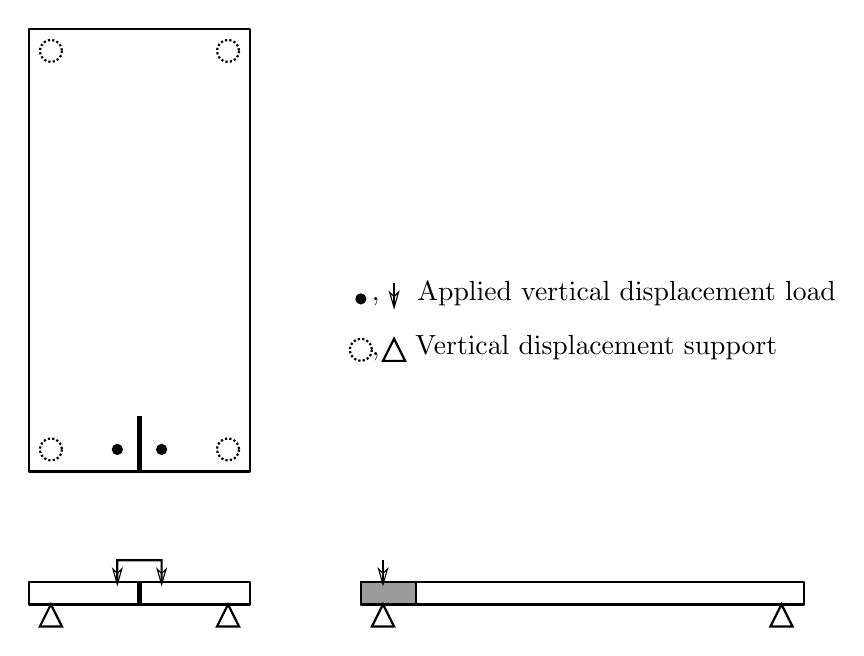
\begin{tikzpicture}[y=0.80pt, x=0.8pt,yscale=-1, inner sep=0pt, outer sep=0pt]
\begin{scope}[shift={(0,-552.36218)}]
  \path[shift={(0,552.36218)},draw=black,fill=black,line join=round,miter
    limit=4.00,fill opacity=0.000,nonzero rule,line width=0.800pt,rounded
    corners=0.0000cm] (50.0000,50.0000) rectangle (150.0000,250.0000);
  \path[shift={(0,552.36218)},draw=black,fill=black,dash pattern=on 0.80pt off
    0.80pt,line join=round,miter limit=4.00,fill opacity=0.000,nonzero rule,line
    width=0.800pt]
    (65.0000,60.0000)arc(0.000:180.000:5.000)arc(-180.000:0.000:5.000) -- cycle;
  \path[shift={(0,552.36218)},draw=black,fill=black,dash pattern=on 0.80pt off
    0.80pt,line join=round,miter limit=4.00,fill opacity=0.000,nonzero rule,line
    width=0.800pt]
    (145.0000,60.0000)arc(0.000:180.000:5.000)arc(-180.000:0.000:5.000) -- cycle;
  \path[shift={(80.0,732.36218)},draw=black,fill=black,dash pattern=on 0.80pt off
    0.80pt,line join=round,miter limit=4.00,fill opacity=0.000,nonzero rule,line
    width=0.800pt]
    (65.0000,60.0000)arc(0.000:180.000:5.000)arc(-180.000:0.000:5.000) -- cycle;
  \path[shift={(0,732.36218)},draw=black,fill=black,dash pattern=on 0.80pt off
    0.80pt,line join=round,miter limit=4.00,fill opacity=0.000,nonzero rule,line
    width=0.800pt]
    (65.0000,60.0000)arc(0.000:180.000:5.000)arc(-180.000:0.000:5.000) -- cycle;
  \path[shift={(0,552.36218)},draw=black,line join=miter,line cap=butt,miter
    limit=4.00,line width=1.600pt] (100.0000,250.0000) -- (100.0000,225.0000);
  \path[draw=black,fill=black,line join=round,miter limit=4.00,fill
    opacity=0.000,nonzero rule,line width=0.800pt,rounded corners=0.0000cm]
    (50.0000,852.3622) rectangle (150.0000,862.3622);
  \path[draw=black,line join=miter,line cap=butt,miter limit=4.00,line
    width=1.600pt] (100.0000,862.3622) -- (100.0000,852.3622);
  \path[draw=black,line join=miter,line cap=butt,line width=0.800pt]
    (55.0000,872.3622) -- (60.0000,862.3622) -- (65.0000,872.3622) -- cycle;
  \path[draw=black,line join=miter,line cap=butt,line width=0.800pt]
    (135.0000,872.3622) -- (140.0000,862.3622) -- (145.0000,872.3622) -- cycle;
    \path[color=black,fill=black,line width=0.800pt] (89.5000,841.8750) --
      (89.5000,842.3750) -- (89.5000,852.3750) -- (90.5000,852.3750) --
      (90.5000,842.8750) -- (109.5000,842.8750) -- (109.5000,852.3750) --
      (110.5000,852.3750) -- (110.5000,842.3750) -- (110.5000,841.8750) --
      (110.0000,841.8750) -- (90.0000,841.8750) -- (89.5000,841.8750) -- cycle;
    \path[draw=black,even odd rule,line width=0.400pt] (90.0000,848.3622) --
      (88.0000,846.3622) -- (90.0000,853.3622) -- (92.0000,846.3622) --
      (90.0000,848.3622) -- cycle;
    \path[draw=black,even odd rule,line width=0.400pt] (110.0000,848.3622) --
      (108.0000,846.3622) -- (110.0000,853.3622) -- (112.0000,846.3622) --
      (110.0000,848.3622) -- cycle;
  \path[shift={(0,552.36218)},draw=black,fill=black,line join=round,miter
    limit=4.00,fill opacity=0.000,nonzero rule,line width=0.800pt,rounded
    corners=0.0000cm] (200.0000,300.0000) rectangle (400.0000,310.0000);
  \path[draw=black,line join=miter,line cap=butt,line width=0.800pt]
    (385.0000,872.3622) -- (390.0000,862.3622) -- (395.0000,872.3622) -- cycle;
  \path[draw=black,line join=miter,line cap=butt,line width=0.800pt]
    (205.0000,872.3622) -- (210.0000,862.3622) -- (215.0000,872.3622) -- cycle;
    \path[color=black,fill=black,line width=0.800pt] (209.5000,842.3622) --
      (209.5000,852.3622) -- (210.5000,852.3622) -- (210.5000,842.3622) --
      (209.5000,842.3622) -- cycle;
    \path[draw=black,even odd rule,line width=0.400pt] (210.0000,848.3622) --
      (208.0000,846.3622) -- (210.0000,853.3622) -- (212.0000,846.3622) --
      (210.0000,848.3622) -- cycle;
  \path[shift={(0,552.36218)},draw=black,fill=black,line join=round,miter
    limit=4.00,fill opacity=0.392,nonzero rule,line width=0.800pt,rounded
    corners=0.0000cm] (200.0000,300.0000) rectangle (225.0000,310.0000);
  \path[shift={(0,552.36218)},draw=black,fill=black,line join=round,miter
    limit=4.00,nonzero rule,line width=0.800pt]
    (92.0000,240.0000)arc(0.000:180.000:2.000)arc(-180.000:0.000:2.000) -- cycle;
  \path[shift={(20.0,552.36218)},draw=black,fill=black,line join=round,miter
    limit=4.00,nonzero rule,line width=0.800pt]
    (92.0000,240.0000)arc(0.000:180.000:2.000)arc(-180.000:0.000:2.000) -- cycle;
  \path[shift={(110.0,484.36218)},draw=black,fill=black,line join=round,miter
    limit=4.00,nonzero rule,line width=0.800pt]
    (92.0000,240.0000)arc(0.000:180.000:2.000)arc(-180.000:0.000:2.000) -- cycle;
    \path[color=black,fill=black,line width=0.800pt] (214.5000,717.3750) --
      (214.5000,727.3750) -- (215.5000,727.3750) -- (215.5000,717.3750) --
      (214.5000,717.3750) -- cycle;
    \path[draw=black,even odd rule,line width=0.400pt] (215.0000,723.3622) --
      (213.0000,721.3622) -- (215.0000,728.3622) -- (217.0000,721.3622) --
      (215.0000,723.3622) -- cycle;
  \path[shift={(140.0,687.36218)},draw=black,fill=black,dash pattern=on 0.80pt off
    0.80pt,line join=round,miter limit=4.00,fill opacity=0.000,nonzero rule,line
    width=0.800pt]
    (65.0000,60.0000)arc(0.000:180.000:5.000)arc(-180.000:0.000:5.000) -- cycle;
  \path[fill=black] (205,727.36218) node[above right] (text6089) {,};
  \path[fill=black] (205,752.36218) node[above right] (text6093) {,};
  \path[draw=black,line join=miter,line cap=butt,line width=0.800pt]
    (210.0000,752.3622) -- (215.0000,742.3622) -- (220.0000,752.3622) -- cycle;
  \path[shift={(0,552.36218)},fill=black] (225.53571,175.17857) node[above right]
    (text6099) {Applied vertical displacement load};
  \path[shift={(0,552.36218)},fill=black] (224.64285,199.46429) node[above right]
    (text6103) {Vertical displacement support};
\end{scope}

\end{tikzpicture}


  \caption{Simple Double Torsion Setup}
  \label{fig:DTsetup}
\end{figure}
%

%
\begin{figure}[tbhp]
  \centering
  \resizebox{0.8\linewidth}{!}{\input{\plotpath/DoubleTorsionDD.pgf}}
  \caption{Crack Progression in Double Torsion Brittle Plate}
  \label{fig:DTdamage}
\end{figure}
%
In the double-torsion plate, the crack is expected to progress straight across the plate.
A more interesting failure pattern can be found if the displacement is applied to only one of the two sides of the pre-crack.
In a ``single torsion'' cracked plate, the crack path is expected to curve, and this result can be seen in \cref{fig:SingleTorsion}.
%
\begin{figure}[tbhp]
  \centering
  \resizebox{0.8\linewidth}{!}{\input{\plotpath/SingleTorsion.pgf}}
  \caption{Crack Progression in Single Torsion Brittle Plate}
  \label{fig:SingleTorsion}
\end{figure}
%

\FloatBarrier
\subsection{Irregular Discretization Results}
While it is simple to discretize the shapes examined thus far so that bonds pair up nicely, that is tougher to do for most shapes we are interested in analyzing.
To combine the analytical simplicity of the previous shapes with a demonstration of the ability to handle irregular shapes, we discretize simple shapes in an irregular fashion.
The first is a return to the simply-supported beam under uniform load.
\Cref{fig:BeamIrreg} shows that the irregularly-discretized beam has the same deflection under uniform load as the regular discretization.
%
\begin{figure}[tbhp]
  \centering
  \resizebox{0.6\linewidth}{!}{%% Creator: Matplotlib, PGF backend
%%
%% To include the figure in your LaTeX document, write
%%   \input{<filename>.pgf}
%%
%% Make sure the required packages are loaded in your preamble
%%   \usepackage{pgf}
%%
%% Figures using additional raster images can only be included by \input if
%% they are in the same directory as the main LaTeX file. For loading figures
%% from other directories you can use the `import` package
%%   \usepackage{import}
%% and then include the figures with
%%   \import{<path to file>}{<filename>.pgf}
%%
%% Matplotlib used the following preamble
%%
\begingroup%
\makeatletter%
\begin{pgfpicture}%
\pgfpathrectangle{\pgfpointorigin}{\pgfqpoint{6.000000in}{6.000000in}}%
\pgfusepath{use as bounding box}%
\begin{pgfscope}%
\pgfsetbuttcap%
\pgfsetroundjoin%
\definecolor{currentfill}{rgb}{1.000000,1.000000,1.000000}%
\pgfsetfillcolor{currentfill}%
\pgfsetlinewidth{0.000000pt}%
\definecolor{currentstroke}{rgb}{1.000000,1.000000,1.000000}%
\pgfsetstrokecolor{currentstroke}%
\pgfsetdash{}{0pt}%
\pgfpathmoveto{\pgfqpoint{0.000000in}{0.000000in}}%
\pgfpathlineto{\pgfqpoint{6.000000in}{0.000000in}}%
\pgfpathlineto{\pgfqpoint{6.000000in}{6.000000in}}%
\pgfpathlineto{\pgfqpoint{0.000000in}{6.000000in}}%
\pgfpathclose%
\pgfusepath{fill}%
\end{pgfscope}%
\begin{pgfscope}%
\pgfsetbuttcap%
\pgfsetroundjoin%
\definecolor{currentfill}{rgb}{1.000000,1.000000,1.000000}%
\pgfsetfillcolor{currentfill}%
\pgfsetlinewidth{0.000000pt}%
\definecolor{currentstroke}{rgb}{0.000000,0.000000,0.000000}%
\pgfsetstrokecolor{currentstroke}%
\pgfsetstrokeopacity{0.000000}%
\pgfsetdash{}{0pt}%
\pgfpathmoveto{\pgfqpoint{0.750000in}{0.600000in}}%
\pgfpathlineto{\pgfqpoint{5.400000in}{0.600000in}}%
\pgfpathlineto{\pgfqpoint{5.400000in}{5.400000in}}%
\pgfpathlineto{\pgfqpoint{0.750000in}{5.400000in}}%
\pgfpathclose%
\pgfusepath{fill}%
\end{pgfscope}%
\begin{pgfscope}%
\pgfpathrectangle{\pgfqpoint{0.750000in}{0.600000in}}{\pgfqpoint{4.650000in}{4.800000in}} %
\pgfusepath{clip}%
\pgfsetrectcap%
\pgfsetroundjoin%
\pgfsetlinewidth{1.003750pt}%
\definecolor{currentstroke}{rgb}{0.000000,0.000000,1.000000}%
\pgfsetstrokecolor{currentstroke}%
\pgfsetdash{}{0pt}%
\pgfpathmoveto{\pgfqpoint{0.750000in}{5.400000in}}%
\pgfpathlineto{\pgfqpoint{0.982500in}{4.689196in}}%
\pgfpathlineto{\pgfqpoint{1.098750in}{4.340173in}}%
\pgfpathlineto{\pgfqpoint{1.215000in}{3.998571in}}%
\pgfpathlineto{\pgfqpoint{1.308000in}{3.732123in}}%
\pgfpathlineto{\pgfqpoint{1.401000in}{3.472912in}}%
\pgfpathlineto{\pgfqpoint{1.470750in}{3.283865in}}%
\pgfpathlineto{\pgfqpoint{1.540500in}{3.099868in}}%
\pgfpathlineto{\pgfqpoint{1.610250in}{2.921313in}}%
\pgfpathlineto{\pgfqpoint{1.680000in}{2.748571in}}%
\pgfpathlineto{\pgfqpoint{1.749750in}{2.582000in}}%
\pgfpathlineto{\pgfqpoint{1.819500in}{2.421937in}}%
\pgfpathlineto{\pgfqpoint{1.889250in}{2.268704in}}%
\pgfpathlineto{\pgfqpoint{1.959000in}{2.122603in}}%
\pgfpathlineto{\pgfqpoint{2.005500in}{2.029308in}}%
\pgfpathlineto{\pgfqpoint{2.052000in}{1.939392in}}%
\pgfpathlineto{\pgfqpoint{2.098500in}{1.852931in}}%
\pgfpathlineto{\pgfqpoint{2.145000in}{1.770000in}}%
\pgfpathlineto{\pgfqpoint{2.191500in}{1.690668in}}%
\pgfpathlineto{\pgfqpoint{2.238000in}{1.615003in}}%
\pgfpathlineto{\pgfqpoint{2.284500in}{1.543068in}}%
\pgfpathlineto{\pgfqpoint{2.331000in}{1.474923in}}%
\pgfpathlineto{\pgfqpoint{2.377500in}{1.410625in}}%
\pgfpathlineto{\pgfqpoint{2.424000in}{1.350226in}}%
\pgfpathlineto{\pgfqpoint{2.470500in}{1.293777in}}%
\pgfpathlineto{\pgfqpoint{2.517000in}{1.241323in}}%
\pgfpathlineto{\pgfqpoint{2.563500in}{1.192908in}}%
\pgfpathlineto{\pgfqpoint{2.610000in}{1.148571in}}%
\pgfpathlineto{\pgfqpoint{2.656500in}{1.108348in}}%
\pgfpathlineto{\pgfqpoint{2.703000in}{1.072272in}}%
\pgfpathlineto{\pgfqpoint{2.749500in}{1.040371in}}%
\pgfpathlineto{\pgfqpoint{2.796000in}{1.012672in}}%
\pgfpathlineto{\pgfqpoint{2.842500in}{0.989196in}}%
\pgfpathlineto{\pgfqpoint{2.889000in}{0.969963in}}%
\pgfpathlineto{\pgfqpoint{2.935500in}{0.954988in}}%
\pgfpathlineto{\pgfqpoint{2.982000in}{0.944283in}}%
\pgfpathlineto{\pgfqpoint{3.028500in}{0.937857in}}%
\pgfpathlineto{\pgfqpoint{3.075000in}{0.935714in}}%
\pgfpathlineto{\pgfqpoint{3.121500in}{0.937857in}}%
\pgfpathlineto{\pgfqpoint{3.168000in}{0.944283in}}%
\pgfpathlineto{\pgfqpoint{3.214500in}{0.954988in}}%
\pgfpathlineto{\pgfqpoint{3.261000in}{0.969963in}}%
\pgfpathlineto{\pgfqpoint{3.307500in}{0.989196in}}%
\pgfpathlineto{\pgfqpoint{3.354000in}{1.012672in}}%
\pgfpathlineto{\pgfqpoint{3.400500in}{1.040371in}}%
\pgfpathlineto{\pgfqpoint{3.447000in}{1.072272in}}%
\pgfpathlineto{\pgfqpoint{3.493500in}{1.108348in}}%
\pgfpathlineto{\pgfqpoint{3.540000in}{1.148571in}}%
\pgfpathlineto{\pgfqpoint{3.586500in}{1.192908in}}%
\pgfpathlineto{\pgfqpoint{3.633000in}{1.241323in}}%
\pgfpathlineto{\pgfqpoint{3.679500in}{1.293777in}}%
\pgfpathlineto{\pgfqpoint{3.726000in}{1.350226in}}%
\pgfpathlineto{\pgfqpoint{3.772500in}{1.410625in}}%
\pgfpathlineto{\pgfqpoint{3.819000in}{1.474923in}}%
\pgfpathlineto{\pgfqpoint{3.865500in}{1.543068in}}%
\pgfpathlineto{\pgfqpoint{3.912000in}{1.615003in}}%
\pgfpathlineto{\pgfqpoint{3.958500in}{1.690668in}}%
\pgfpathlineto{\pgfqpoint{4.005000in}{1.770000in}}%
\pgfpathlineto{\pgfqpoint{4.051500in}{1.852931in}}%
\pgfpathlineto{\pgfqpoint{4.098000in}{1.939392in}}%
\pgfpathlineto{\pgfqpoint{4.144500in}{2.029308in}}%
\pgfpathlineto{\pgfqpoint{4.191000in}{2.122603in}}%
\pgfpathlineto{\pgfqpoint{4.260750in}{2.268704in}}%
\pgfpathlineto{\pgfqpoint{4.330500in}{2.421937in}}%
\pgfpathlineto{\pgfqpoint{4.400250in}{2.582000in}}%
\pgfpathlineto{\pgfqpoint{4.470000in}{2.748571in}}%
\pgfpathlineto{\pgfqpoint{4.539750in}{2.921313in}}%
\pgfpathlineto{\pgfqpoint{4.609500in}{3.099868in}}%
\pgfpathlineto{\pgfqpoint{4.679250in}{3.283865in}}%
\pgfpathlineto{\pgfqpoint{4.749000in}{3.472912in}}%
\pgfpathlineto{\pgfqpoint{4.842000in}{3.732123in}}%
\pgfpathlineto{\pgfqpoint{4.935000in}{3.998571in}}%
\pgfpathlineto{\pgfqpoint{5.028000in}{4.271186in}}%
\pgfpathlineto{\pgfqpoint{5.144250in}{4.618909in}}%
\pgfpathlineto{\pgfqpoint{5.283750in}{5.043298in}}%
\pgfpathlineto{\pgfqpoint{5.400000in}{5.400000in}}%
\pgfpathlineto{\pgfqpoint{5.400000in}{5.400000in}}%
\pgfusepath{stroke}%
\end{pgfscope}%
\begin{pgfscope}%
\pgfpathrectangle{\pgfqpoint{0.750000in}{0.600000in}}{\pgfqpoint{4.650000in}{4.800000in}} %
\pgfusepath{clip}%
\pgfsetbuttcap%
\pgfsetmiterjoin%
\definecolor{currentfill}{rgb}{0.000000,0.500000,0.000000}%
\pgfsetfillcolor{currentfill}%
\pgfsetlinewidth{0.501875pt}%
\definecolor{currentstroke}{rgb}{0.000000,0.000000,0.000000}%
\pgfsetstrokecolor{currentstroke}%
\pgfsetdash{}{0pt}%
\pgfsys@defobject{currentmarker}{\pgfqpoint{-0.041667in}{-0.041667in}}{\pgfqpoint{0.041667in}{0.041667in}}{%
\pgfpathmoveto{\pgfqpoint{0.000000in}{0.041667in}}%
\pgfpathlineto{\pgfqpoint{-0.041667in}{-0.041667in}}%
\pgfpathlineto{\pgfqpoint{0.041667in}{-0.041667in}}%
\pgfpathclose%
\pgfusepath{stroke,fill}%
}%
\begin{pgfscope}%
\pgfsys@transformshift{0.750000in}{5.400000in}%
\pgfsys@useobject{currentmarker}{}%
\end{pgfscope}%
\begin{pgfscope}%
\pgfsys@transformshift{0.843000in}{5.112844in}%
\pgfsys@useobject{currentmarker}{}%
\end{pgfscope}%
\begin{pgfscope}%
\pgfsys@transformshift{0.936000in}{4.827074in}%
\pgfsys@useobject{currentmarker}{}%
\end{pgfscope}%
\begin{pgfscope}%
\pgfsys@transformshift{1.029000in}{4.543952in}%
\pgfsys@useobject{currentmarker}{}%
\end{pgfscope}%
\begin{pgfscope}%
\pgfsys@transformshift{1.122000in}{4.264720in}%
\pgfsys@useobject{currentmarker}{}%
\end{pgfscope}%
\begin{pgfscope}%
\pgfsys@transformshift{1.215000in}{3.990565in}%
\pgfsys@useobject{currentmarker}{}%
\end{pgfscope}%
\begin{pgfscope}%
\pgfsys@transformshift{1.308000in}{3.722615in}%
\pgfsys@useobject{currentmarker}{}%
\end{pgfscope}%
\begin{pgfscope}%
\pgfsys@transformshift{1.401000in}{3.461947in}%
\pgfsys@useobject{currentmarker}{}%
\end{pgfscope}%
\begin{pgfscope}%
\pgfsys@transformshift{1.494000in}{3.209580in}%
\pgfsys@useobject{currentmarker}{}%
\end{pgfscope}%
\begin{pgfscope}%
\pgfsys@transformshift{1.587000in}{2.966480in}%
\pgfsys@useobject{currentmarker}{}%
\end{pgfscope}%
\begin{pgfscope}%
\pgfsys@transformshift{1.680000in}{2.733555in}%
\pgfsys@useobject{currentmarker}{}%
\end{pgfscope}%
\begin{pgfscope}%
\pgfsys@transformshift{1.773000in}{2.511660in}%
\pgfsys@useobject{currentmarker}{}%
\end{pgfscope}%
\begin{pgfscope}%
\pgfsys@transformshift{1.866000in}{2.301595in}%
\pgfsys@useobject{currentmarker}{}%
\end{pgfscope}%
\begin{pgfscope}%
\pgfsys@transformshift{1.959000in}{2.104104in}%
\pgfsys@useobject{currentmarker}{}%
\end{pgfscope}%
\begin{pgfscope}%
\pgfsys@transformshift{2.052000in}{1.919876in}%
\pgfsys@useobject{currentmarker}{}%
\end{pgfscope}%
\begin{pgfscope}%
\pgfsys@transformshift{2.145000in}{1.749545in}%
\pgfsys@useobject{currentmarker}{}%
\end{pgfscope}%
\begin{pgfscope}%
\pgfsys@transformshift{2.238000in}{1.593691in}%
\pgfsys@useobject{currentmarker}{}%
\end{pgfscope}%
\begin{pgfscope}%
\pgfsys@transformshift{2.331000in}{1.452836in}%
\pgfsys@useobject{currentmarker}{}%
\end{pgfscope}%
\begin{pgfscope}%
\pgfsys@transformshift{2.424000in}{1.327450in}%
\pgfsys@useobject{currentmarker}{}%
\end{pgfscope}%
\begin{pgfscope}%
\pgfsys@transformshift{2.517000in}{1.217946in}%
\pgfsys@useobject{currentmarker}{}%
\end{pgfscope}%
\begin{pgfscope}%
\pgfsys@transformshift{2.610000in}{1.124682in}%
\pgfsys@useobject{currentmarker}{}%
\end{pgfscope}%
\begin{pgfscope}%
\pgfsys@transformshift{2.703000in}{1.047961in}%
\pgfsys@useobject{currentmarker}{}%
\end{pgfscope}%
\begin{pgfscope}%
\pgfsys@transformshift{2.796000in}{0.988033in}%
\pgfsys@useobject{currentmarker}{}%
\end{pgfscope}%
\begin{pgfscope}%
\pgfsys@transformshift{2.889000in}{0.945089in}%
\pgfsys@useobject{currentmarker}{}%
\end{pgfscope}%
\begin{pgfscope}%
\pgfsys@transformshift{2.982000in}{0.919267in}%
\pgfsys@useobject{currentmarker}{}%
\end{pgfscope}%
\begin{pgfscope}%
\pgfsys@transformshift{3.075000in}{0.910651in}%
\pgfsys@useobject{currentmarker}{}%
\end{pgfscope}%
\begin{pgfscope}%
\pgfsys@transformshift{3.168000in}{0.919267in}%
\pgfsys@useobject{currentmarker}{}%
\end{pgfscope}%
\begin{pgfscope}%
\pgfsys@transformshift{3.261000in}{0.945089in}%
\pgfsys@useobject{currentmarker}{}%
\end{pgfscope}%
\begin{pgfscope}%
\pgfsys@transformshift{3.354000in}{0.988033in}%
\pgfsys@useobject{currentmarker}{}%
\end{pgfscope}%
\begin{pgfscope}%
\pgfsys@transformshift{3.447000in}{1.047961in}%
\pgfsys@useobject{currentmarker}{}%
\end{pgfscope}%
\begin{pgfscope}%
\pgfsys@transformshift{3.540000in}{1.124682in}%
\pgfsys@useobject{currentmarker}{}%
\end{pgfscope}%
\begin{pgfscope}%
\pgfsys@transformshift{3.633000in}{1.217946in}%
\pgfsys@useobject{currentmarker}{}%
\end{pgfscope}%
\begin{pgfscope}%
\pgfsys@transformshift{3.726000in}{1.327450in}%
\pgfsys@useobject{currentmarker}{}%
\end{pgfscope}%
\begin{pgfscope}%
\pgfsys@transformshift{3.819000in}{1.452836in}%
\pgfsys@useobject{currentmarker}{}%
\end{pgfscope}%
\begin{pgfscope}%
\pgfsys@transformshift{3.912000in}{1.593691in}%
\pgfsys@useobject{currentmarker}{}%
\end{pgfscope}%
\begin{pgfscope}%
\pgfsys@transformshift{4.005000in}{1.749545in}%
\pgfsys@useobject{currentmarker}{}%
\end{pgfscope}%
\begin{pgfscope}%
\pgfsys@transformshift{4.098000in}{1.919876in}%
\pgfsys@useobject{currentmarker}{}%
\end{pgfscope}%
\begin{pgfscope}%
\pgfsys@transformshift{4.191000in}{2.104104in}%
\pgfsys@useobject{currentmarker}{}%
\end{pgfscope}%
\begin{pgfscope}%
\pgfsys@transformshift{4.284000in}{2.301595in}%
\pgfsys@useobject{currentmarker}{}%
\end{pgfscope}%
\begin{pgfscope}%
\pgfsys@transformshift{4.377000in}{2.511660in}%
\pgfsys@useobject{currentmarker}{}%
\end{pgfscope}%
\begin{pgfscope}%
\pgfsys@transformshift{4.470000in}{2.733555in}%
\pgfsys@useobject{currentmarker}{}%
\end{pgfscope}%
\begin{pgfscope}%
\pgfsys@transformshift{4.563000in}{2.966480in}%
\pgfsys@useobject{currentmarker}{}%
\end{pgfscope}%
\begin{pgfscope}%
\pgfsys@transformshift{4.656000in}{3.209580in}%
\pgfsys@useobject{currentmarker}{}%
\end{pgfscope}%
\begin{pgfscope}%
\pgfsys@transformshift{4.749000in}{3.461947in}%
\pgfsys@useobject{currentmarker}{}%
\end{pgfscope}%
\begin{pgfscope}%
\pgfsys@transformshift{4.842000in}{3.722615in}%
\pgfsys@useobject{currentmarker}{}%
\end{pgfscope}%
\begin{pgfscope}%
\pgfsys@transformshift{4.935000in}{3.990565in}%
\pgfsys@useobject{currentmarker}{}%
\end{pgfscope}%
\begin{pgfscope}%
\pgfsys@transformshift{5.028000in}{4.264720in}%
\pgfsys@useobject{currentmarker}{}%
\end{pgfscope}%
\begin{pgfscope}%
\pgfsys@transformshift{5.121000in}{4.543952in}%
\pgfsys@useobject{currentmarker}{}%
\end{pgfscope}%
\begin{pgfscope}%
\pgfsys@transformshift{5.214000in}{4.827074in}%
\pgfsys@useobject{currentmarker}{}%
\end{pgfscope}%
\begin{pgfscope}%
\pgfsys@transformshift{5.307000in}{5.112844in}%
\pgfsys@useobject{currentmarker}{}%
\end{pgfscope}%
\begin{pgfscope}%
\pgfsys@transformshift{5.400000in}{5.400000in}%
\pgfsys@useobject{currentmarker}{}%
\end{pgfscope}%
\end{pgfscope}%
\begin{pgfscope}%
\pgfpathrectangle{\pgfqpoint{0.750000in}{0.600000in}}{\pgfqpoint{4.650000in}{4.800000in}} %
\pgfusepath{clip}%
\pgfsetbuttcap%
\pgfsetmiterjoin%
\definecolor{currentfill}{rgb}{1.000000,0.000000,0.000000}%
\pgfsetfillcolor{currentfill}%
\pgfsetlinewidth{0.501875pt}%
\definecolor{currentstroke}{rgb}{0.000000,0.000000,0.000000}%
\pgfsetstrokecolor{currentstroke}%
\pgfsetdash{}{0pt}%
\pgfsys@defobject{currentmarker}{\pgfqpoint{-0.041667in}{-0.041667in}}{\pgfqpoint{0.041667in}{0.041667in}}{%
\pgfpathmoveto{\pgfqpoint{-0.041667in}{-0.041667in}}%
\pgfpathlineto{\pgfqpoint{0.041667in}{-0.041667in}}%
\pgfpathlineto{\pgfqpoint{0.041667in}{0.041667in}}%
\pgfpathlineto{\pgfqpoint{-0.041667in}{0.041667in}}%
\pgfpathclose%
\pgfusepath{stroke,fill}%
}%
\begin{pgfscope}%
\pgfsys@transformshift{0.796563in}{5.257379in}%
\pgfsys@useobject{currentmarker}{}%
\end{pgfscope}%
\begin{pgfscope}%
\pgfsys@transformshift{0.889054in}{4.973141in}%
\pgfsys@useobject{currentmarker}{}%
\end{pgfscope}%
\begin{pgfscope}%
\pgfsys@transformshift{0.982945in}{4.686635in}%
\pgfsys@useobject{currentmarker}{}%
\end{pgfscope}%
\begin{pgfscope}%
\pgfsys@transformshift{1.075145in}{4.408525in}%
\pgfsys@useobject{currentmarker}{}%
\end{pgfscope}%
\begin{pgfscope}%
\pgfsys@transformshift{1.168520in}{4.131336in}%
\pgfsys@useobject{currentmarker}{}%
\end{pgfscope}%
\begin{pgfscope}%
\pgfsys@transformshift{1.261459in}{3.861078in}%
\pgfsys@useobject{currentmarker}{}%
\end{pgfscope}%
\begin{pgfscope}%
\pgfsys@transformshift{1.354604in}{3.596952in}%
\pgfsys@useobject{currentmarker}{}%
\end{pgfscope}%
\begin{pgfscope}%
\pgfsys@transformshift{1.447369in}{3.341685in}%
\pgfsys@useobject{currentmarker}{}%
\end{pgfscope}%
\begin{pgfscope}%
\pgfsys@transformshift{1.540655in}{3.093753in}%
\pgfsys@useobject{currentmarker}{}%
\end{pgfscope}%
\begin{pgfscope}%
\pgfsys@transformshift{1.633328in}{2.857095in}%
\pgfsys@useobject{currentmarker}{}%
\end{pgfscope}%
\begin{pgfscope}%
\pgfsys@transformshift{1.726954in}{2.628713in}%
\pgfsys@useobject{currentmarker}{}%
\end{pgfscope}%
\begin{pgfscope}%
\pgfsys@transformshift{1.819642in}{2.413967in}%
\pgfsys@useobject{currentmarker}{}%
\end{pgfscope}%
\begin{pgfscope}%
\pgfsys@transformshift{1.912183in}{2.211622in}%
\pgfsys@useobject{currentmarker}{}%
\end{pgfscope}%
\begin{pgfscope}%
\pgfsys@transformshift{2.005218in}{2.021055in}%
\pgfsys@useobject{currentmarker}{}%
\end{pgfscope}%
\begin{pgfscope}%
\pgfsys@transformshift{2.098814in}{1.843048in}%
\pgfsys@useobject{currentmarker}{}%
\end{pgfscope}%
\begin{pgfscope}%
\pgfsys@transformshift{2.191943in}{1.680152in}%
\pgfsys@useobject{currentmarker}{}%
\end{pgfscope}%
\begin{pgfscope}%
\pgfsys@transformshift{2.284298in}{1.533124in}%
\pgfsys@useobject{currentmarker}{}%
\end{pgfscope}%
\begin{pgfscope}%
\pgfsys@transformshift{2.377331in}{1.400113in}%
\pgfsys@useobject{currentmarker}{}%
\end{pgfscope}%
\begin{pgfscope}%
\pgfsys@transformshift{2.470562in}{1.282584in}%
\pgfsys@useobject{currentmarker}{}%
\end{pgfscope}%
\begin{pgfscope}%
\pgfsys@transformshift{2.563571in}{1.181363in}%
\pgfsys@useobject{currentmarker}{}%
\end{pgfscope}%
\begin{pgfscope}%
\pgfsys@transformshift{2.656158in}{1.096896in}%
\pgfsys@useobject{currentmarker}{}%
\end{pgfscope}%
\begin{pgfscope}%
\pgfsys@transformshift{2.749580in}{1.028314in}%
\pgfsys@useobject{currentmarker}{}%
\end{pgfscope}%
\begin{pgfscope}%
\pgfsys@transformshift{2.842665in}{0.976870in}%
\pgfsys@useobject{currentmarker}{}%
\end{pgfscope}%
\begin{pgfscope}%
\pgfsys@transformshift{2.935266in}{0.942640in}%
\pgfsys@useobject{currentmarker}{}%
\end{pgfscope}%
\begin{pgfscope}%
\pgfsys@transformshift{3.028242in}{0.925319in}%
\pgfsys@useobject{currentmarker}{}%
\end{pgfscope}%
\begin{pgfscope}%
\pgfsys@transformshift{3.121686in}{0.925245in}%
\pgfsys@useobject{currentmarker}{}%
\end{pgfscope}%
\begin{pgfscope}%
\pgfsys@transformshift{3.214854in}{0.942420in}%
\pgfsys@useobject{currentmarker}{}%
\end{pgfscope}%
\begin{pgfscope}%
\pgfsys@transformshift{3.307709in}{0.976672in}%
\pgfsys@useobject{currentmarker}{}%
\end{pgfscope}%
\begin{pgfscope}%
\pgfsys@transformshift{3.400429in}{1.027806in}%
\pgfsys@useobject{currentmarker}{}%
\end{pgfscope}%
\begin{pgfscope}%
\pgfsys@transformshift{3.493649in}{1.096038in}%
\pgfsys@useobject{currentmarker}{}%
\end{pgfscope}%
\begin{pgfscope}%
\pgfsys@transformshift{3.586161in}{1.180285in}%
\pgfsys@useobject{currentmarker}{}%
\end{pgfscope}%
\begin{pgfscope}%
\pgfsys@transformshift{3.679569in}{1.281783in}%
\pgfsys@useobject{currentmarker}{}%
\end{pgfscope}%
\begin{pgfscope}%
\pgfsys@transformshift{3.772869in}{1.399369in}%
\pgfsys@useobject{currentmarker}{}%
\end{pgfscope}%
\begin{pgfscope}%
\pgfsys@transformshift{3.865785in}{1.532107in}%
\pgfsys@useobject{currentmarker}{}%
\end{pgfscope}%
\begin{pgfscope}%
\pgfsys@transformshift{3.958699in}{1.680014in}%
\pgfsys@useobject{currentmarker}{}%
\end{pgfscope}%
\begin{pgfscope}%
\pgfsys@transformshift{4.051186in}{1.841807in}%
\pgfsys@useobject{currentmarker}{}%
\end{pgfscope}%
\begin{pgfscope}%
\pgfsys@transformshift{4.144786in}{2.019746in}%
\pgfsys@useobject{currentmarker}{}%
\end{pgfscope}%
\begin{pgfscope}%
\pgfsys@transformshift{4.237684in}{2.209913in}%
\pgfsys@useobject{currentmarker}{}%
\end{pgfscope}%
\begin{pgfscope}%
\pgfsys@transformshift{4.330942in}{2.413799in}%
\pgfsys@useobject{currentmarker}{}%
\end{pgfscope}%
\begin{pgfscope}%
\pgfsys@transformshift{4.423714in}{2.628742in}%
\pgfsys@useobject{currentmarker}{}%
\end{pgfscope}%
\begin{pgfscope}%
\pgfsys@transformshift{4.516221in}{2.854319in}%
\pgfsys@useobject{currentmarker}{}%
\end{pgfscope}%
\begin{pgfscope}%
\pgfsys@transformshift{4.609356in}{3.092017in}%
\pgfsys@useobject{currentmarker}{}%
\end{pgfscope}%
\begin{pgfscope}%
\pgfsys@transformshift{4.702188in}{3.338632in}%
\pgfsys@useobject{currentmarker}{}%
\end{pgfscope}%
\begin{pgfscope}%
\pgfsys@transformshift{4.795904in}{3.596450in}%
\pgfsys@useobject{currentmarker}{}%
\end{pgfscope}%
\begin{pgfscope}%
\pgfsys@transformshift{4.888714in}{3.859581in}%
\pgfsys@useobject{currentmarker}{}%
\end{pgfscope}%
\begin{pgfscope}%
\pgfsys@transformshift{4.981208in}{4.128466in}%
\pgfsys@useobject{currentmarker}{}%
\end{pgfscope}%
\begin{pgfscope}%
\pgfsys@transformshift{5.074246in}{4.404578in}%
\pgfsys@useobject{currentmarker}{}%
\end{pgfscope}%
\begin{pgfscope}%
\pgfsys@transformshift{5.167325in}{4.685283in}%
\pgfsys@useobject{currentmarker}{}%
\end{pgfscope}%
\begin{pgfscope}%
\pgfsys@transformshift{5.260058in}{4.968218in}%
\pgfsys@useobject{currentmarker}{}%
\end{pgfscope}%
\begin{pgfscope}%
\pgfsys@transformshift{5.353534in}{5.255445in}%
\pgfsys@useobject{currentmarker}{}%
\end{pgfscope}%
\end{pgfscope}%
\begin{pgfscope}%
\pgfpathrectangle{\pgfqpoint{0.750000in}{0.600000in}}{\pgfqpoint{4.650000in}{4.800000in}} %
\pgfusepath{clip}%
\pgfsetbuttcap%
\pgfsetroundjoin%
\pgfsetlinewidth{0.501875pt}%
\definecolor{currentstroke}{rgb}{0.000000,0.000000,0.000000}%
\pgfsetstrokecolor{currentstroke}%
\pgfsetdash{{1.000000pt}{3.000000pt}}{0.000000pt}%
\pgfpathmoveto{\pgfqpoint{0.750000in}{0.600000in}}%
\pgfpathlineto{\pgfqpoint{0.750000in}{5.400000in}}%
\pgfusepath{stroke}%
\end{pgfscope}%
\begin{pgfscope}%
\pgfsetbuttcap%
\pgfsetroundjoin%
\definecolor{currentfill}{rgb}{0.000000,0.000000,0.000000}%
\pgfsetfillcolor{currentfill}%
\pgfsetlinewidth{0.501875pt}%
\definecolor{currentstroke}{rgb}{0.000000,0.000000,0.000000}%
\pgfsetstrokecolor{currentstroke}%
\pgfsetdash{}{0pt}%
\pgfsys@defobject{currentmarker}{\pgfqpoint{0.000000in}{0.000000in}}{\pgfqpoint{0.000000in}{0.055556in}}{%
\pgfpathmoveto{\pgfqpoint{0.000000in}{0.000000in}}%
\pgfpathlineto{\pgfqpoint{0.000000in}{0.055556in}}%
\pgfusepath{stroke,fill}%
}%
\begin{pgfscope}%
\pgfsys@transformshift{0.750000in}{0.600000in}%
\pgfsys@useobject{currentmarker}{}%
\end{pgfscope}%
\end{pgfscope}%
\begin{pgfscope}%
\pgfsetbuttcap%
\pgfsetroundjoin%
\definecolor{currentfill}{rgb}{0.000000,0.000000,0.000000}%
\pgfsetfillcolor{currentfill}%
\pgfsetlinewidth{0.501875pt}%
\definecolor{currentstroke}{rgb}{0.000000,0.000000,0.000000}%
\pgfsetstrokecolor{currentstroke}%
\pgfsetdash{}{0pt}%
\pgfsys@defobject{currentmarker}{\pgfqpoint{0.000000in}{-0.055556in}}{\pgfqpoint{0.000000in}{0.000000in}}{%
\pgfpathmoveto{\pgfqpoint{0.000000in}{0.000000in}}%
\pgfpathlineto{\pgfqpoint{0.000000in}{-0.055556in}}%
\pgfusepath{stroke,fill}%
}%
\begin{pgfscope}%
\pgfsys@transformshift{0.750000in}{5.400000in}%
\pgfsys@useobject{currentmarker}{}%
\end{pgfscope}%
\end{pgfscope}%
\begin{pgfscope}%
\pgftext[x=0.750000in,y=0.544444in,,top]{{\rmfamily\fontsize{12.000000}{14.400000}\selectfont \(\displaystyle 0.00\)}}%
\end{pgfscope}%
\begin{pgfscope}%
\pgfpathrectangle{\pgfqpoint{0.750000in}{0.600000in}}{\pgfqpoint{4.650000in}{4.800000in}} %
\pgfusepath{clip}%
\pgfsetbuttcap%
\pgfsetroundjoin%
\pgfsetlinewidth{0.501875pt}%
\definecolor{currentstroke}{rgb}{0.000000,0.000000,0.000000}%
\pgfsetstrokecolor{currentstroke}%
\pgfsetdash{{1.000000pt}{3.000000pt}}{0.000000pt}%
\pgfpathmoveto{\pgfqpoint{1.912500in}{0.600000in}}%
\pgfpathlineto{\pgfqpoint{1.912500in}{5.400000in}}%
\pgfusepath{stroke}%
\end{pgfscope}%
\begin{pgfscope}%
\pgfsetbuttcap%
\pgfsetroundjoin%
\definecolor{currentfill}{rgb}{0.000000,0.000000,0.000000}%
\pgfsetfillcolor{currentfill}%
\pgfsetlinewidth{0.501875pt}%
\definecolor{currentstroke}{rgb}{0.000000,0.000000,0.000000}%
\pgfsetstrokecolor{currentstroke}%
\pgfsetdash{}{0pt}%
\pgfsys@defobject{currentmarker}{\pgfqpoint{0.000000in}{0.000000in}}{\pgfqpoint{0.000000in}{0.055556in}}{%
\pgfpathmoveto{\pgfqpoint{0.000000in}{0.000000in}}%
\pgfpathlineto{\pgfqpoint{0.000000in}{0.055556in}}%
\pgfusepath{stroke,fill}%
}%
\begin{pgfscope}%
\pgfsys@transformshift{1.912500in}{0.600000in}%
\pgfsys@useobject{currentmarker}{}%
\end{pgfscope}%
\end{pgfscope}%
\begin{pgfscope}%
\pgfsetbuttcap%
\pgfsetroundjoin%
\definecolor{currentfill}{rgb}{0.000000,0.000000,0.000000}%
\pgfsetfillcolor{currentfill}%
\pgfsetlinewidth{0.501875pt}%
\definecolor{currentstroke}{rgb}{0.000000,0.000000,0.000000}%
\pgfsetstrokecolor{currentstroke}%
\pgfsetdash{}{0pt}%
\pgfsys@defobject{currentmarker}{\pgfqpoint{0.000000in}{-0.055556in}}{\pgfqpoint{0.000000in}{0.000000in}}{%
\pgfpathmoveto{\pgfqpoint{0.000000in}{0.000000in}}%
\pgfpathlineto{\pgfqpoint{0.000000in}{-0.055556in}}%
\pgfusepath{stroke,fill}%
}%
\begin{pgfscope}%
\pgfsys@transformshift{1.912500in}{5.400000in}%
\pgfsys@useobject{currentmarker}{}%
\end{pgfscope}%
\end{pgfscope}%
\begin{pgfscope}%
\pgftext[x=1.912500in,y=0.544444in,,top]{{\rmfamily\fontsize{12.000000}{14.400000}\selectfont \(\displaystyle 0.25\)}}%
\end{pgfscope}%
\begin{pgfscope}%
\pgfpathrectangle{\pgfqpoint{0.750000in}{0.600000in}}{\pgfqpoint{4.650000in}{4.800000in}} %
\pgfusepath{clip}%
\pgfsetbuttcap%
\pgfsetroundjoin%
\pgfsetlinewidth{0.501875pt}%
\definecolor{currentstroke}{rgb}{0.000000,0.000000,0.000000}%
\pgfsetstrokecolor{currentstroke}%
\pgfsetdash{{1.000000pt}{3.000000pt}}{0.000000pt}%
\pgfpathmoveto{\pgfqpoint{3.075000in}{0.600000in}}%
\pgfpathlineto{\pgfqpoint{3.075000in}{5.400000in}}%
\pgfusepath{stroke}%
\end{pgfscope}%
\begin{pgfscope}%
\pgfsetbuttcap%
\pgfsetroundjoin%
\definecolor{currentfill}{rgb}{0.000000,0.000000,0.000000}%
\pgfsetfillcolor{currentfill}%
\pgfsetlinewidth{0.501875pt}%
\definecolor{currentstroke}{rgb}{0.000000,0.000000,0.000000}%
\pgfsetstrokecolor{currentstroke}%
\pgfsetdash{}{0pt}%
\pgfsys@defobject{currentmarker}{\pgfqpoint{0.000000in}{0.000000in}}{\pgfqpoint{0.000000in}{0.055556in}}{%
\pgfpathmoveto{\pgfqpoint{0.000000in}{0.000000in}}%
\pgfpathlineto{\pgfqpoint{0.000000in}{0.055556in}}%
\pgfusepath{stroke,fill}%
}%
\begin{pgfscope}%
\pgfsys@transformshift{3.075000in}{0.600000in}%
\pgfsys@useobject{currentmarker}{}%
\end{pgfscope}%
\end{pgfscope}%
\begin{pgfscope}%
\pgfsetbuttcap%
\pgfsetroundjoin%
\definecolor{currentfill}{rgb}{0.000000,0.000000,0.000000}%
\pgfsetfillcolor{currentfill}%
\pgfsetlinewidth{0.501875pt}%
\definecolor{currentstroke}{rgb}{0.000000,0.000000,0.000000}%
\pgfsetstrokecolor{currentstroke}%
\pgfsetdash{}{0pt}%
\pgfsys@defobject{currentmarker}{\pgfqpoint{0.000000in}{-0.055556in}}{\pgfqpoint{0.000000in}{0.000000in}}{%
\pgfpathmoveto{\pgfqpoint{0.000000in}{0.000000in}}%
\pgfpathlineto{\pgfqpoint{0.000000in}{-0.055556in}}%
\pgfusepath{stroke,fill}%
}%
\begin{pgfscope}%
\pgfsys@transformshift{3.075000in}{5.400000in}%
\pgfsys@useobject{currentmarker}{}%
\end{pgfscope}%
\end{pgfscope}%
\begin{pgfscope}%
\pgftext[x=3.075000in,y=0.544444in,,top]{{\rmfamily\fontsize{12.000000}{14.400000}\selectfont \(\displaystyle 0.50\)}}%
\end{pgfscope}%
\begin{pgfscope}%
\pgfpathrectangle{\pgfqpoint{0.750000in}{0.600000in}}{\pgfqpoint{4.650000in}{4.800000in}} %
\pgfusepath{clip}%
\pgfsetbuttcap%
\pgfsetroundjoin%
\pgfsetlinewidth{0.501875pt}%
\definecolor{currentstroke}{rgb}{0.000000,0.000000,0.000000}%
\pgfsetstrokecolor{currentstroke}%
\pgfsetdash{{1.000000pt}{3.000000pt}}{0.000000pt}%
\pgfpathmoveto{\pgfqpoint{4.237500in}{0.600000in}}%
\pgfpathlineto{\pgfqpoint{4.237500in}{5.400000in}}%
\pgfusepath{stroke}%
\end{pgfscope}%
\begin{pgfscope}%
\pgfsetbuttcap%
\pgfsetroundjoin%
\definecolor{currentfill}{rgb}{0.000000,0.000000,0.000000}%
\pgfsetfillcolor{currentfill}%
\pgfsetlinewidth{0.501875pt}%
\definecolor{currentstroke}{rgb}{0.000000,0.000000,0.000000}%
\pgfsetstrokecolor{currentstroke}%
\pgfsetdash{}{0pt}%
\pgfsys@defobject{currentmarker}{\pgfqpoint{0.000000in}{0.000000in}}{\pgfqpoint{0.000000in}{0.055556in}}{%
\pgfpathmoveto{\pgfqpoint{0.000000in}{0.000000in}}%
\pgfpathlineto{\pgfqpoint{0.000000in}{0.055556in}}%
\pgfusepath{stroke,fill}%
}%
\begin{pgfscope}%
\pgfsys@transformshift{4.237500in}{0.600000in}%
\pgfsys@useobject{currentmarker}{}%
\end{pgfscope}%
\end{pgfscope}%
\begin{pgfscope}%
\pgfsetbuttcap%
\pgfsetroundjoin%
\definecolor{currentfill}{rgb}{0.000000,0.000000,0.000000}%
\pgfsetfillcolor{currentfill}%
\pgfsetlinewidth{0.501875pt}%
\definecolor{currentstroke}{rgb}{0.000000,0.000000,0.000000}%
\pgfsetstrokecolor{currentstroke}%
\pgfsetdash{}{0pt}%
\pgfsys@defobject{currentmarker}{\pgfqpoint{0.000000in}{-0.055556in}}{\pgfqpoint{0.000000in}{0.000000in}}{%
\pgfpathmoveto{\pgfqpoint{0.000000in}{0.000000in}}%
\pgfpathlineto{\pgfqpoint{0.000000in}{-0.055556in}}%
\pgfusepath{stroke,fill}%
}%
\begin{pgfscope}%
\pgfsys@transformshift{4.237500in}{5.400000in}%
\pgfsys@useobject{currentmarker}{}%
\end{pgfscope}%
\end{pgfscope}%
\begin{pgfscope}%
\pgftext[x=4.237500in,y=0.544444in,,top]{{\rmfamily\fontsize{12.000000}{14.400000}\selectfont \(\displaystyle 0.75\)}}%
\end{pgfscope}%
\begin{pgfscope}%
\pgfpathrectangle{\pgfqpoint{0.750000in}{0.600000in}}{\pgfqpoint{4.650000in}{4.800000in}} %
\pgfusepath{clip}%
\pgfsetbuttcap%
\pgfsetroundjoin%
\pgfsetlinewidth{0.501875pt}%
\definecolor{currentstroke}{rgb}{0.000000,0.000000,0.000000}%
\pgfsetstrokecolor{currentstroke}%
\pgfsetdash{{1.000000pt}{3.000000pt}}{0.000000pt}%
\pgfpathmoveto{\pgfqpoint{5.400000in}{0.600000in}}%
\pgfpathlineto{\pgfqpoint{5.400000in}{5.400000in}}%
\pgfusepath{stroke}%
\end{pgfscope}%
\begin{pgfscope}%
\pgfsetbuttcap%
\pgfsetroundjoin%
\definecolor{currentfill}{rgb}{0.000000,0.000000,0.000000}%
\pgfsetfillcolor{currentfill}%
\pgfsetlinewidth{0.501875pt}%
\definecolor{currentstroke}{rgb}{0.000000,0.000000,0.000000}%
\pgfsetstrokecolor{currentstroke}%
\pgfsetdash{}{0pt}%
\pgfsys@defobject{currentmarker}{\pgfqpoint{0.000000in}{0.000000in}}{\pgfqpoint{0.000000in}{0.055556in}}{%
\pgfpathmoveto{\pgfqpoint{0.000000in}{0.000000in}}%
\pgfpathlineto{\pgfqpoint{0.000000in}{0.055556in}}%
\pgfusepath{stroke,fill}%
}%
\begin{pgfscope}%
\pgfsys@transformshift{5.400000in}{0.600000in}%
\pgfsys@useobject{currentmarker}{}%
\end{pgfscope}%
\end{pgfscope}%
\begin{pgfscope}%
\pgfsetbuttcap%
\pgfsetroundjoin%
\definecolor{currentfill}{rgb}{0.000000,0.000000,0.000000}%
\pgfsetfillcolor{currentfill}%
\pgfsetlinewidth{0.501875pt}%
\definecolor{currentstroke}{rgb}{0.000000,0.000000,0.000000}%
\pgfsetstrokecolor{currentstroke}%
\pgfsetdash{}{0pt}%
\pgfsys@defobject{currentmarker}{\pgfqpoint{0.000000in}{-0.055556in}}{\pgfqpoint{0.000000in}{0.000000in}}{%
\pgfpathmoveto{\pgfqpoint{0.000000in}{0.000000in}}%
\pgfpathlineto{\pgfqpoint{0.000000in}{-0.055556in}}%
\pgfusepath{stroke,fill}%
}%
\begin{pgfscope}%
\pgfsys@transformshift{5.400000in}{5.400000in}%
\pgfsys@useobject{currentmarker}{}%
\end{pgfscope}%
\end{pgfscope}%
\begin{pgfscope}%
\pgftext[x=5.400000in,y=0.544444in,,top]{{\rmfamily\fontsize{12.000000}{14.400000}\selectfont \(\displaystyle 1.00\)}}%
\end{pgfscope}%
\begin{pgfscope}%
\pgftext[x=3.075000in,y=0.326852in,,top]{{\rmfamily\fontsize{12.000000}{14.400000}\selectfont Distance Along Beam}}%
\end{pgfscope}%
\begin{pgfscope}%
\pgfpathrectangle{\pgfqpoint{0.750000in}{0.600000in}}{\pgfqpoint{4.650000in}{4.800000in}} %
\pgfusepath{clip}%
\pgfsetbuttcap%
\pgfsetroundjoin%
\pgfsetlinewidth{0.501875pt}%
\definecolor{currentstroke}{rgb}{0.000000,0.000000,0.000000}%
\pgfsetstrokecolor{currentstroke}%
\pgfsetdash{{1.000000pt}{3.000000pt}}{0.000000pt}%
\pgfpathmoveto{\pgfqpoint{0.750000in}{0.600000in}}%
\pgfpathlineto{\pgfqpoint{5.400000in}{0.600000in}}%
\pgfusepath{stroke}%
\end{pgfscope}%
\begin{pgfscope}%
\pgfsetbuttcap%
\pgfsetroundjoin%
\definecolor{currentfill}{rgb}{0.000000,0.000000,0.000000}%
\pgfsetfillcolor{currentfill}%
\pgfsetlinewidth{0.501875pt}%
\definecolor{currentstroke}{rgb}{0.000000,0.000000,0.000000}%
\pgfsetstrokecolor{currentstroke}%
\pgfsetdash{}{0pt}%
\pgfsys@defobject{currentmarker}{\pgfqpoint{0.000000in}{0.000000in}}{\pgfqpoint{0.055556in}{0.000000in}}{%
\pgfpathmoveto{\pgfqpoint{0.000000in}{0.000000in}}%
\pgfpathlineto{\pgfqpoint{0.055556in}{0.000000in}}%
\pgfusepath{stroke,fill}%
}%
\begin{pgfscope}%
\pgfsys@transformshift{0.750000in}{0.600000in}%
\pgfsys@useobject{currentmarker}{}%
\end{pgfscope}%
\end{pgfscope}%
\begin{pgfscope}%
\pgfsetbuttcap%
\pgfsetroundjoin%
\definecolor{currentfill}{rgb}{0.000000,0.000000,0.000000}%
\pgfsetfillcolor{currentfill}%
\pgfsetlinewidth{0.501875pt}%
\definecolor{currentstroke}{rgb}{0.000000,0.000000,0.000000}%
\pgfsetstrokecolor{currentstroke}%
\pgfsetdash{}{0pt}%
\pgfsys@defobject{currentmarker}{\pgfqpoint{-0.055556in}{0.000000in}}{\pgfqpoint{0.000000in}{0.000000in}}{%
\pgfpathmoveto{\pgfqpoint{0.000000in}{0.000000in}}%
\pgfpathlineto{\pgfqpoint{-0.055556in}{0.000000in}}%
\pgfusepath{stroke,fill}%
}%
\begin{pgfscope}%
\pgfsys@transformshift{5.400000in}{0.600000in}%
\pgfsys@useobject{currentmarker}{}%
\end{pgfscope}%
\end{pgfscope}%
\begin{pgfscope}%
\pgftext[x=0.694444in,y=0.600000in,right,]{{\rmfamily\fontsize{12.000000}{14.400000}\selectfont \(\displaystyle -1.4\)}}%
\end{pgfscope}%
\begin{pgfscope}%
\pgfpathrectangle{\pgfqpoint{0.750000in}{0.600000in}}{\pgfqpoint{4.650000in}{4.800000in}} %
\pgfusepath{clip}%
\pgfsetbuttcap%
\pgfsetroundjoin%
\pgfsetlinewidth{0.501875pt}%
\definecolor{currentstroke}{rgb}{0.000000,0.000000,0.000000}%
\pgfsetstrokecolor{currentstroke}%
\pgfsetdash{{1.000000pt}{3.000000pt}}{0.000000pt}%
\pgfpathmoveto{\pgfqpoint{0.750000in}{1.285714in}}%
\pgfpathlineto{\pgfqpoint{5.400000in}{1.285714in}}%
\pgfusepath{stroke}%
\end{pgfscope}%
\begin{pgfscope}%
\pgfsetbuttcap%
\pgfsetroundjoin%
\definecolor{currentfill}{rgb}{0.000000,0.000000,0.000000}%
\pgfsetfillcolor{currentfill}%
\pgfsetlinewidth{0.501875pt}%
\definecolor{currentstroke}{rgb}{0.000000,0.000000,0.000000}%
\pgfsetstrokecolor{currentstroke}%
\pgfsetdash{}{0pt}%
\pgfsys@defobject{currentmarker}{\pgfqpoint{0.000000in}{0.000000in}}{\pgfqpoint{0.055556in}{0.000000in}}{%
\pgfpathmoveto{\pgfqpoint{0.000000in}{0.000000in}}%
\pgfpathlineto{\pgfqpoint{0.055556in}{0.000000in}}%
\pgfusepath{stroke,fill}%
}%
\begin{pgfscope}%
\pgfsys@transformshift{0.750000in}{1.285714in}%
\pgfsys@useobject{currentmarker}{}%
\end{pgfscope}%
\end{pgfscope}%
\begin{pgfscope}%
\pgfsetbuttcap%
\pgfsetroundjoin%
\definecolor{currentfill}{rgb}{0.000000,0.000000,0.000000}%
\pgfsetfillcolor{currentfill}%
\pgfsetlinewidth{0.501875pt}%
\definecolor{currentstroke}{rgb}{0.000000,0.000000,0.000000}%
\pgfsetstrokecolor{currentstroke}%
\pgfsetdash{}{0pt}%
\pgfsys@defobject{currentmarker}{\pgfqpoint{-0.055556in}{0.000000in}}{\pgfqpoint{0.000000in}{0.000000in}}{%
\pgfpathmoveto{\pgfqpoint{0.000000in}{0.000000in}}%
\pgfpathlineto{\pgfqpoint{-0.055556in}{0.000000in}}%
\pgfusepath{stroke,fill}%
}%
\begin{pgfscope}%
\pgfsys@transformshift{5.400000in}{1.285714in}%
\pgfsys@useobject{currentmarker}{}%
\end{pgfscope}%
\end{pgfscope}%
\begin{pgfscope}%
\pgftext[x=0.694444in,y=1.285714in,right,]{{\rmfamily\fontsize{12.000000}{14.400000}\selectfont \(\displaystyle -1.2\)}}%
\end{pgfscope}%
\begin{pgfscope}%
\pgfpathrectangle{\pgfqpoint{0.750000in}{0.600000in}}{\pgfqpoint{4.650000in}{4.800000in}} %
\pgfusepath{clip}%
\pgfsetbuttcap%
\pgfsetroundjoin%
\pgfsetlinewidth{0.501875pt}%
\definecolor{currentstroke}{rgb}{0.000000,0.000000,0.000000}%
\pgfsetstrokecolor{currentstroke}%
\pgfsetdash{{1.000000pt}{3.000000pt}}{0.000000pt}%
\pgfpathmoveto{\pgfqpoint{0.750000in}{1.971429in}}%
\pgfpathlineto{\pgfqpoint{5.400000in}{1.971429in}}%
\pgfusepath{stroke}%
\end{pgfscope}%
\begin{pgfscope}%
\pgfsetbuttcap%
\pgfsetroundjoin%
\definecolor{currentfill}{rgb}{0.000000,0.000000,0.000000}%
\pgfsetfillcolor{currentfill}%
\pgfsetlinewidth{0.501875pt}%
\definecolor{currentstroke}{rgb}{0.000000,0.000000,0.000000}%
\pgfsetstrokecolor{currentstroke}%
\pgfsetdash{}{0pt}%
\pgfsys@defobject{currentmarker}{\pgfqpoint{0.000000in}{0.000000in}}{\pgfqpoint{0.055556in}{0.000000in}}{%
\pgfpathmoveto{\pgfqpoint{0.000000in}{0.000000in}}%
\pgfpathlineto{\pgfqpoint{0.055556in}{0.000000in}}%
\pgfusepath{stroke,fill}%
}%
\begin{pgfscope}%
\pgfsys@transformshift{0.750000in}{1.971429in}%
\pgfsys@useobject{currentmarker}{}%
\end{pgfscope}%
\end{pgfscope}%
\begin{pgfscope}%
\pgfsetbuttcap%
\pgfsetroundjoin%
\definecolor{currentfill}{rgb}{0.000000,0.000000,0.000000}%
\pgfsetfillcolor{currentfill}%
\pgfsetlinewidth{0.501875pt}%
\definecolor{currentstroke}{rgb}{0.000000,0.000000,0.000000}%
\pgfsetstrokecolor{currentstroke}%
\pgfsetdash{}{0pt}%
\pgfsys@defobject{currentmarker}{\pgfqpoint{-0.055556in}{0.000000in}}{\pgfqpoint{0.000000in}{0.000000in}}{%
\pgfpathmoveto{\pgfqpoint{0.000000in}{0.000000in}}%
\pgfpathlineto{\pgfqpoint{-0.055556in}{0.000000in}}%
\pgfusepath{stroke,fill}%
}%
\begin{pgfscope}%
\pgfsys@transformshift{5.400000in}{1.971429in}%
\pgfsys@useobject{currentmarker}{}%
\end{pgfscope}%
\end{pgfscope}%
\begin{pgfscope}%
\pgftext[x=0.694444in,y=1.971429in,right,]{{\rmfamily\fontsize{12.000000}{14.400000}\selectfont \(\displaystyle -1.0\)}}%
\end{pgfscope}%
\begin{pgfscope}%
\pgfpathrectangle{\pgfqpoint{0.750000in}{0.600000in}}{\pgfqpoint{4.650000in}{4.800000in}} %
\pgfusepath{clip}%
\pgfsetbuttcap%
\pgfsetroundjoin%
\pgfsetlinewidth{0.501875pt}%
\definecolor{currentstroke}{rgb}{0.000000,0.000000,0.000000}%
\pgfsetstrokecolor{currentstroke}%
\pgfsetdash{{1.000000pt}{3.000000pt}}{0.000000pt}%
\pgfpathmoveto{\pgfqpoint{0.750000in}{2.657143in}}%
\pgfpathlineto{\pgfqpoint{5.400000in}{2.657143in}}%
\pgfusepath{stroke}%
\end{pgfscope}%
\begin{pgfscope}%
\pgfsetbuttcap%
\pgfsetroundjoin%
\definecolor{currentfill}{rgb}{0.000000,0.000000,0.000000}%
\pgfsetfillcolor{currentfill}%
\pgfsetlinewidth{0.501875pt}%
\definecolor{currentstroke}{rgb}{0.000000,0.000000,0.000000}%
\pgfsetstrokecolor{currentstroke}%
\pgfsetdash{}{0pt}%
\pgfsys@defobject{currentmarker}{\pgfqpoint{0.000000in}{0.000000in}}{\pgfqpoint{0.055556in}{0.000000in}}{%
\pgfpathmoveto{\pgfqpoint{0.000000in}{0.000000in}}%
\pgfpathlineto{\pgfqpoint{0.055556in}{0.000000in}}%
\pgfusepath{stroke,fill}%
}%
\begin{pgfscope}%
\pgfsys@transformshift{0.750000in}{2.657143in}%
\pgfsys@useobject{currentmarker}{}%
\end{pgfscope}%
\end{pgfscope}%
\begin{pgfscope}%
\pgfsetbuttcap%
\pgfsetroundjoin%
\definecolor{currentfill}{rgb}{0.000000,0.000000,0.000000}%
\pgfsetfillcolor{currentfill}%
\pgfsetlinewidth{0.501875pt}%
\definecolor{currentstroke}{rgb}{0.000000,0.000000,0.000000}%
\pgfsetstrokecolor{currentstroke}%
\pgfsetdash{}{0pt}%
\pgfsys@defobject{currentmarker}{\pgfqpoint{-0.055556in}{0.000000in}}{\pgfqpoint{0.000000in}{0.000000in}}{%
\pgfpathmoveto{\pgfqpoint{0.000000in}{0.000000in}}%
\pgfpathlineto{\pgfqpoint{-0.055556in}{0.000000in}}%
\pgfusepath{stroke,fill}%
}%
\begin{pgfscope}%
\pgfsys@transformshift{5.400000in}{2.657143in}%
\pgfsys@useobject{currentmarker}{}%
\end{pgfscope}%
\end{pgfscope}%
\begin{pgfscope}%
\pgftext[x=0.694444in,y=2.657143in,right,]{{\rmfamily\fontsize{12.000000}{14.400000}\selectfont \(\displaystyle -0.8\)}}%
\end{pgfscope}%
\begin{pgfscope}%
\pgfpathrectangle{\pgfqpoint{0.750000in}{0.600000in}}{\pgfqpoint{4.650000in}{4.800000in}} %
\pgfusepath{clip}%
\pgfsetbuttcap%
\pgfsetroundjoin%
\pgfsetlinewidth{0.501875pt}%
\definecolor{currentstroke}{rgb}{0.000000,0.000000,0.000000}%
\pgfsetstrokecolor{currentstroke}%
\pgfsetdash{{1.000000pt}{3.000000pt}}{0.000000pt}%
\pgfpathmoveto{\pgfqpoint{0.750000in}{3.342857in}}%
\pgfpathlineto{\pgfqpoint{5.400000in}{3.342857in}}%
\pgfusepath{stroke}%
\end{pgfscope}%
\begin{pgfscope}%
\pgfsetbuttcap%
\pgfsetroundjoin%
\definecolor{currentfill}{rgb}{0.000000,0.000000,0.000000}%
\pgfsetfillcolor{currentfill}%
\pgfsetlinewidth{0.501875pt}%
\definecolor{currentstroke}{rgb}{0.000000,0.000000,0.000000}%
\pgfsetstrokecolor{currentstroke}%
\pgfsetdash{}{0pt}%
\pgfsys@defobject{currentmarker}{\pgfqpoint{0.000000in}{0.000000in}}{\pgfqpoint{0.055556in}{0.000000in}}{%
\pgfpathmoveto{\pgfqpoint{0.000000in}{0.000000in}}%
\pgfpathlineto{\pgfqpoint{0.055556in}{0.000000in}}%
\pgfusepath{stroke,fill}%
}%
\begin{pgfscope}%
\pgfsys@transformshift{0.750000in}{3.342857in}%
\pgfsys@useobject{currentmarker}{}%
\end{pgfscope}%
\end{pgfscope}%
\begin{pgfscope}%
\pgfsetbuttcap%
\pgfsetroundjoin%
\definecolor{currentfill}{rgb}{0.000000,0.000000,0.000000}%
\pgfsetfillcolor{currentfill}%
\pgfsetlinewidth{0.501875pt}%
\definecolor{currentstroke}{rgb}{0.000000,0.000000,0.000000}%
\pgfsetstrokecolor{currentstroke}%
\pgfsetdash{}{0pt}%
\pgfsys@defobject{currentmarker}{\pgfqpoint{-0.055556in}{0.000000in}}{\pgfqpoint{0.000000in}{0.000000in}}{%
\pgfpathmoveto{\pgfqpoint{0.000000in}{0.000000in}}%
\pgfpathlineto{\pgfqpoint{-0.055556in}{0.000000in}}%
\pgfusepath{stroke,fill}%
}%
\begin{pgfscope}%
\pgfsys@transformshift{5.400000in}{3.342857in}%
\pgfsys@useobject{currentmarker}{}%
\end{pgfscope}%
\end{pgfscope}%
\begin{pgfscope}%
\pgftext[x=0.694444in,y=3.342857in,right,]{{\rmfamily\fontsize{12.000000}{14.400000}\selectfont \(\displaystyle -0.6\)}}%
\end{pgfscope}%
\begin{pgfscope}%
\pgfpathrectangle{\pgfqpoint{0.750000in}{0.600000in}}{\pgfqpoint{4.650000in}{4.800000in}} %
\pgfusepath{clip}%
\pgfsetbuttcap%
\pgfsetroundjoin%
\pgfsetlinewidth{0.501875pt}%
\definecolor{currentstroke}{rgb}{0.000000,0.000000,0.000000}%
\pgfsetstrokecolor{currentstroke}%
\pgfsetdash{{1.000000pt}{3.000000pt}}{0.000000pt}%
\pgfpathmoveto{\pgfqpoint{0.750000in}{4.028571in}}%
\pgfpathlineto{\pgfqpoint{5.400000in}{4.028571in}}%
\pgfusepath{stroke}%
\end{pgfscope}%
\begin{pgfscope}%
\pgfsetbuttcap%
\pgfsetroundjoin%
\definecolor{currentfill}{rgb}{0.000000,0.000000,0.000000}%
\pgfsetfillcolor{currentfill}%
\pgfsetlinewidth{0.501875pt}%
\definecolor{currentstroke}{rgb}{0.000000,0.000000,0.000000}%
\pgfsetstrokecolor{currentstroke}%
\pgfsetdash{}{0pt}%
\pgfsys@defobject{currentmarker}{\pgfqpoint{0.000000in}{0.000000in}}{\pgfqpoint{0.055556in}{0.000000in}}{%
\pgfpathmoveto{\pgfqpoint{0.000000in}{0.000000in}}%
\pgfpathlineto{\pgfqpoint{0.055556in}{0.000000in}}%
\pgfusepath{stroke,fill}%
}%
\begin{pgfscope}%
\pgfsys@transformshift{0.750000in}{4.028571in}%
\pgfsys@useobject{currentmarker}{}%
\end{pgfscope}%
\end{pgfscope}%
\begin{pgfscope}%
\pgfsetbuttcap%
\pgfsetroundjoin%
\definecolor{currentfill}{rgb}{0.000000,0.000000,0.000000}%
\pgfsetfillcolor{currentfill}%
\pgfsetlinewidth{0.501875pt}%
\definecolor{currentstroke}{rgb}{0.000000,0.000000,0.000000}%
\pgfsetstrokecolor{currentstroke}%
\pgfsetdash{}{0pt}%
\pgfsys@defobject{currentmarker}{\pgfqpoint{-0.055556in}{0.000000in}}{\pgfqpoint{0.000000in}{0.000000in}}{%
\pgfpathmoveto{\pgfqpoint{0.000000in}{0.000000in}}%
\pgfpathlineto{\pgfqpoint{-0.055556in}{0.000000in}}%
\pgfusepath{stroke,fill}%
}%
\begin{pgfscope}%
\pgfsys@transformshift{5.400000in}{4.028571in}%
\pgfsys@useobject{currentmarker}{}%
\end{pgfscope}%
\end{pgfscope}%
\begin{pgfscope}%
\pgftext[x=0.694444in,y=4.028571in,right,]{{\rmfamily\fontsize{12.000000}{14.400000}\selectfont \(\displaystyle -0.4\)}}%
\end{pgfscope}%
\begin{pgfscope}%
\pgfpathrectangle{\pgfqpoint{0.750000in}{0.600000in}}{\pgfqpoint{4.650000in}{4.800000in}} %
\pgfusepath{clip}%
\pgfsetbuttcap%
\pgfsetroundjoin%
\pgfsetlinewidth{0.501875pt}%
\definecolor{currentstroke}{rgb}{0.000000,0.000000,0.000000}%
\pgfsetstrokecolor{currentstroke}%
\pgfsetdash{{1.000000pt}{3.000000pt}}{0.000000pt}%
\pgfpathmoveto{\pgfqpoint{0.750000in}{4.714286in}}%
\pgfpathlineto{\pgfqpoint{5.400000in}{4.714286in}}%
\pgfusepath{stroke}%
\end{pgfscope}%
\begin{pgfscope}%
\pgfsetbuttcap%
\pgfsetroundjoin%
\definecolor{currentfill}{rgb}{0.000000,0.000000,0.000000}%
\pgfsetfillcolor{currentfill}%
\pgfsetlinewidth{0.501875pt}%
\definecolor{currentstroke}{rgb}{0.000000,0.000000,0.000000}%
\pgfsetstrokecolor{currentstroke}%
\pgfsetdash{}{0pt}%
\pgfsys@defobject{currentmarker}{\pgfqpoint{0.000000in}{0.000000in}}{\pgfqpoint{0.055556in}{0.000000in}}{%
\pgfpathmoveto{\pgfqpoint{0.000000in}{0.000000in}}%
\pgfpathlineto{\pgfqpoint{0.055556in}{0.000000in}}%
\pgfusepath{stroke,fill}%
}%
\begin{pgfscope}%
\pgfsys@transformshift{0.750000in}{4.714286in}%
\pgfsys@useobject{currentmarker}{}%
\end{pgfscope}%
\end{pgfscope}%
\begin{pgfscope}%
\pgfsetbuttcap%
\pgfsetroundjoin%
\definecolor{currentfill}{rgb}{0.000000,0.000000,0.000000}%
\pgfsetfillcolor{currentfill}%
\pgfsetlinewidth{0.501875pt}%
\definecolor{currentstroke}{rgb}{0.000000,0.000000,0.000000}%
\pgfsetstrokecolor{currentstroke}%
\pgfsetdash{}{0pt}%
\pgfsys@defobject{currentmarker}{\pgfqpoint{-0.055556in}{0.000000in}}{\pgfqpoint{0.000000in}{0.000000in}}{%
\pgfpathmoveto{\pgfqpoint{0.000000in}{0.000000in}}%
\pgfpathlineto{\pgfqpoint{-0.055556in}{0.000000in}}%
\pgfusepath{stroke,fill}%
}%
\begin{pgfscope}%
\pgfsys@transformshift{5.400000in}{4.714286in}%
\pgfsys@useobject{currentmarker}{}%
\end{pgfscope}%
\end{pgfscope}%
\begin{pgfscope}%
\pgftext[x=0.694444in,y=4.714286in,right,]{{\rmfamily\fontsize{12.000000}{14.400000}\selectfont \(\displaystyle -0.2\)}}%
\end{pgfscope}%
\begin{pgfscope}%
\pgfpathrectangle{\pgfqpoint{0.750000in}{0.600000in}}{\pgfqpoint{4.650000in}{4.800000in}} %
\pgfusepath{clip}%
\pgfsetbuttcap%
\pgfsetroundjoin%
\pgfsetlinewidth{0.501875pt}%
\definecolor{currentstroke}{rgb}{0.000000,0.000000,0.000000}%
\pgfsetstrokecolor{currentstroke}%
\pgfsetdash{{1.000000pt}{3.000000pt}}{0.000000pt}%
\pgfpathmoveto{\pgfqpoint{0.750000in}{5.400000in}}%
\pgfpathlineto{\pgfqpoint{5.400000in}{5.400000in}}%
\pgfusepath{stroke}%
\end{pgfscope}%
\begin{pgfscope}%
\pgfsetbuttcap%
\pgfsetroundjoin%
\definecolor{currentfill}{rgb}{0.000000,0.000000,0.000000}%
\pgfsetfillcolor{currentfill}%
\pgfsetlinewidth{0.501875pt}%
\definecolor{currentstroke}{rgb}{0.000000,0.000000,0.000000}%
\pgfsetstrokecolor{currentstroke}%
\pgfsetdash{}{0pt}%
\pgfsys@defobject{currentmarker}{\pgfqpoint{0.000000in}{0.000000in}}{\pgfqpoint{0.055556in}{0.000000in}}{%
\pgfpathmoveto{\pgfqpoint{0.000000in}{0.000000in}}%
\pgfpathlineto{\pgfqpoint{0.055556in}{0.000000in}}%
\pgfusepath{stroke,fill}%
}%
\begin{pgfscope}%
\pgfsys@transformshift{0.750000in}{5.400000in}%
\pgfsys@useobject{currentmarker}{}%
\end{pgfscope}%
\end{pgfscope}%
\begin{pgfscope}%
\pgfsetbuttcap%
\pgfsetroundjoin%
\definecolor{currentfill}{rgb}{0.000000,0.000000,0.000000}%
\pgfsetfillcolor{currentfill}%
\pgfsetlinewidth{0.501875pt}%
\definecolor{currentstroke}{rgb}{0.000000,0.000000,0.000000}%
\pgfsetstrokecolor{currentstroke}%
\pgfsetdash{}{0pt}%
\pgfsys@defobject{currentmarker}{\pgfqpoint{-0.055556in}{0.000000in}}{\pgfqpoint{0.000000in}{0.000000in}}{%
\pgfpathmoveto{\pgfqpoint{0.000000in}{0.000000in}}%
\pgfpathlineto{\pgfqpoint{-0.055556in}{0.000000in}}%
\pgfusepath{stroke,fill}%
}%
\begin{pgfscope}%
\pgfsys@transformshift{5.400000in}{5.400000in}%
\pgfsys@useobject{currentmarker}{}%
\end{pgfscope}%
\end{pgfscope}%
\begin{pgfscope}%
\pgftext[x=0.694444in,y=5.400000in,right,]{{\rmfamily\fontsize{12.000000}{14.400000}\selectfont \(\displaystyle 0.0\)}}%
\end{pgfscope}%
\begin{pgfscope}%
\pgftext[x=0.286846in,y=3.000000in,,bottom,rotate=90.000000]{{\rmfamily\fontsize{12.000000}{14.400000}\selectfont Deflection Under Uniform Load}}%
\end{pgfscope}%
\begin{pgfscope}%
\pgftext[x=0.750000in,y=5.441667in,left,base]{{\rmfamily\fontsize{12.000000}{14.400000}\selectfont \(\displaystyle \times10^{-5}\)}}%
\end{pgfscope}%
\begin{pgfscope}%
\pgfsetbuttcap%
\pgfsetroundjoin%
\pgfsetlinewidth{1.003750pt}%
\definecolor{currentstroke}{rgb}{0.000000,0.000000,0.000000}%
\pgfsetstrokecolor{currentstroke}%
\pgfsetdash{}{0pt}%
\pgfpathmoveto{\pgfqpoint{0.750000in}{5.400000in}}%
\pgfpathlineto{\pgfqpoint{5.400000in}{5.400000in}}%
\pgfusepath{stroke}%
\end{pgfscope}%
\begin{pgfscope}%
\pgfsetbuttcap%
\pgfsetroundjoin%
\pgfsetlinewidth{1.003750pt}%
\definecolor{currentstroke}{rgb}{0.000000,0.000000,0.000000}%
\pgfsetstrokecolor{currentstroke}%
\pgfsetdash{}{0pt}%
\pgfpathmoveto{\pgfqpoint{5.400000in}{0.600000in}}%
\pgfpathlineto{\pgfqpoint{5.400000in}{5.400000in}}%
\pgfusepath{stroke}%
\end{pgfscope}%
\begin{pgfscope}%
\pgfsetbuttcap%
\pgfsetroundjoin%
\pgfsetlinewidth{1.003750pt}%
\definecolor{currentstroke}{rgb}{0.000000,0.000000,0.000000}%
\pgfsetstrokecolor{currentstroke}%
\pgfsetdash{}{0pt}%
\pgfpathmoveto{\pgfqpoint{0.750000in}{0.600000in}}%
\pgfpathlineto{\pgfqpoint{5.400000in}{0.600000in}}%
\pgfusepath{stroke}%
\end{pgfscope}%
\begin{pgfscope}%
\pgfsetbuttcap%
\pgfsetroundjoin%
\pgfsetlinewidth{1.003750pt}%
\definecolor{currentstroke}{rgb}{0.000000,0.000000,0.000000}%
\pgfsetstrokecolor{currentstroke}%
\pgfsetdash{}{0pt}%
\pgfpathmoveto{\pgfqpoint{0.750000in}{0.600000in}}%
\pgfpathlineto{\pgfqpoint{0.750000in}{5.400000in}}%
\pgfusepath{stroke}%
\end{pgfscope}%
\begin{pgfscope}%
\pgftext[x=3.075000in,y=5.469444in,,base]{{\rmfamily\fontsize{14.400000}{17.280000}\selectfont Uniformly Loaded Beam}}%
\end{pgfscope}%
\begin{pgfscope}%
\pgfsetbuttcap%
\pgfsetroundjoin%
\definecolor{currentfill}{rgb}{1.000000,1.000000,1.000000}%
\pgfsetfillcolor{currentfill}%
\pgfsetlinewidth{1.003750pt}%
\definecolor{currentstroke}{rgb}{0.000000,0.000000,0.000000}%
\pgfsetstrokecolor{currentstroke}%
\pgfsetdash{}{0pt}%
\pgfpathmoveto{\pgfqpoint{3.452377in}{4.483334in}}%
\pgfpathlineto{\pgfqpoint{5.380000in}{4.483334in}}%
\pgfpathlineto{\pgfqpoint{5.380000in}{5.380000in}}%
\pgfpathlineto{\pgfqpoint{3.452377in}{5.380000in}}%
\pgfpathlineto{\pgfqpoint{3.452377in}{4.483334in}}%
\pgfpathclose%
\pgfusepath{stroke,fill}%
\end{pgfscope}%
\begin{pgfscope}%
\pgfsetrectcap%
\pgfsetroundjoin%
\pgfsetlinewidth{1.003750pt}%
\definecolor{currentstroke}{rgb}{0.000000,0.000000,1.000000}%
\pgfsetstrokecolor{currentstroke}%
\pgfsetdash{}{0pt}%
\pgfpathmoveto{\pgfqpoint{3.592377in}{5.230000in}}%
\pgfpathlineto{\pgfqpoint{3.872377in}{5.230000in}}%
\pgfusepath{stroke}%
\end{pgfscope}%
\begin{pgfscope}%
\pgftext[x=4.092377in,y=5.160000in,left,base]{{\rmfamily\fontsize{14.400000}{17.280000}\selectfont Analytical}}%
\end{pgfscope}%
\begin{pgfscope}%
\pgfsetbuttcap%
\pgfsetmiterjoin%
\definecolor{currentfill}{rgb}{0.000000,0.500000,0.000000}%
\pgfsetfillcolor{currentfill}%
\pgfsetlinewidth{0.501875pt}%
\definecolor{currentstroke}{rgb}{0.000000,0.000000,0.000000}%
\pgfsetstrokecolor{currentstroke}%
\pgfsetdash{}{0pt}%
\pgfsys@defobject{currentmarker}{\pgfqpoint{-0.041667in}{-0.041667in}}{\pgfqpoint{0.041667in}{0.041667in}}{%
\pgfpathmoveto{\pgfqpoint{0.000000in}{0.041667in}}%
\pgfpathlineto{\pgfqpoint{-0.041667in}{-0.041667in}}%
\pgfpathlineto{\pgfqpoint{0.041667in}{-0.041667in}}%
\pgfpathclose%
\pgfusepath{stroke,fill}%
}%
\begin{pgfscope}%
\pgfsys@transformshift{3.592377in}{4.951111in}%
\pgfsys@useobject{currentmarker}{}%
\end{pgfscope}%
\begin{pgfscope}%
\pgfsys@transformshift{3.872377in}{4.951111in}%
\pgfsys@useobject{currentmarker}{}%
\end{pgfscope}%
\end{pgfscope}%
\begin{pgfscope}%
\pgftext[x=4.092377in,y=4.881111in,left,base]{{\rmfamily\fontsize{14.400000}{17.280000}\selectfont regular error}}%
\end{pgfscope}%
\begin{pgfscope}%
\pgfsetbuttcap%
\pgfsetmiterjoin%
\definecolor{currentfill}{rgb}{1.000000,0.000000,0.000000}%
\pgfsetfillcolor{currentfill}%
\pgfsetlinewidth{0.501875pt}%
\definecolor{currentstroke}{rgb}{0.000000,0.000000,0.000000}%
\pgfsetstrokecolor{currentstroke}%
\pgfsetdash{}{0pt}%
\pgfsys@defobject{currentmarker}{\pgfqpoint{-0.041667in}{-0.041667in}}{\pgfqpoint{0.041667in}{0.041667in}}{%
\pgfpathmoveto{\pgfqpoint{-0.041667in}{-0.041667in}}%
\pgfpathlineto{\pgfqpoint{0.041667in}{-0.041667in}}%
\pgfpathlineto{\pgfqpoint{0.041667in}{0.041667in}}%
\pgfpathlineto{\pgfqpoint{-0.041667in}{0.041667in}}%
\pgfpathclose%
\pgfusepath{stroke,fill}%
}%
\begin{pgfscope}%
\pgfsys@transformshift{3.592377in}{4.672223in}%
\pgfsys@useobject{currentmarker}{}%
\end{pgfscope}%
\begin{pgfscope}%
\pgfsys@transformshift{3.872377in}{4.672223in}%
\pgfsys@useobject{currentmarker}{}%
\end{pgfscope}%
\end{pgfscope}%
\begin{pgfscope}%
\pgftext[x=4.092377in,y=4.602223in,left,base]{{\rmfamily\fontsize{14.400000}{17.280000}\selectfont irregular error}}%
\end{pgfscope}%
\end{pgfpicture}%
\makeatother%
\endgroup%
}
  \caption{Irregular Beam}
  \label{fig:BeamIrreg}
\end{figure}
%

An example of a regularly-discretized plate is shown in \cref{fig:regularmesh}, while an irregularly discretized plate is shown in \cref{fig:unevenmesh}.
To use this plate in a peridynamic simulation, we reduce each element to a single node at the element's centroid with volume equal to the volume of the element. 
%%
%\begin{figure}[h]
%  \centering
%  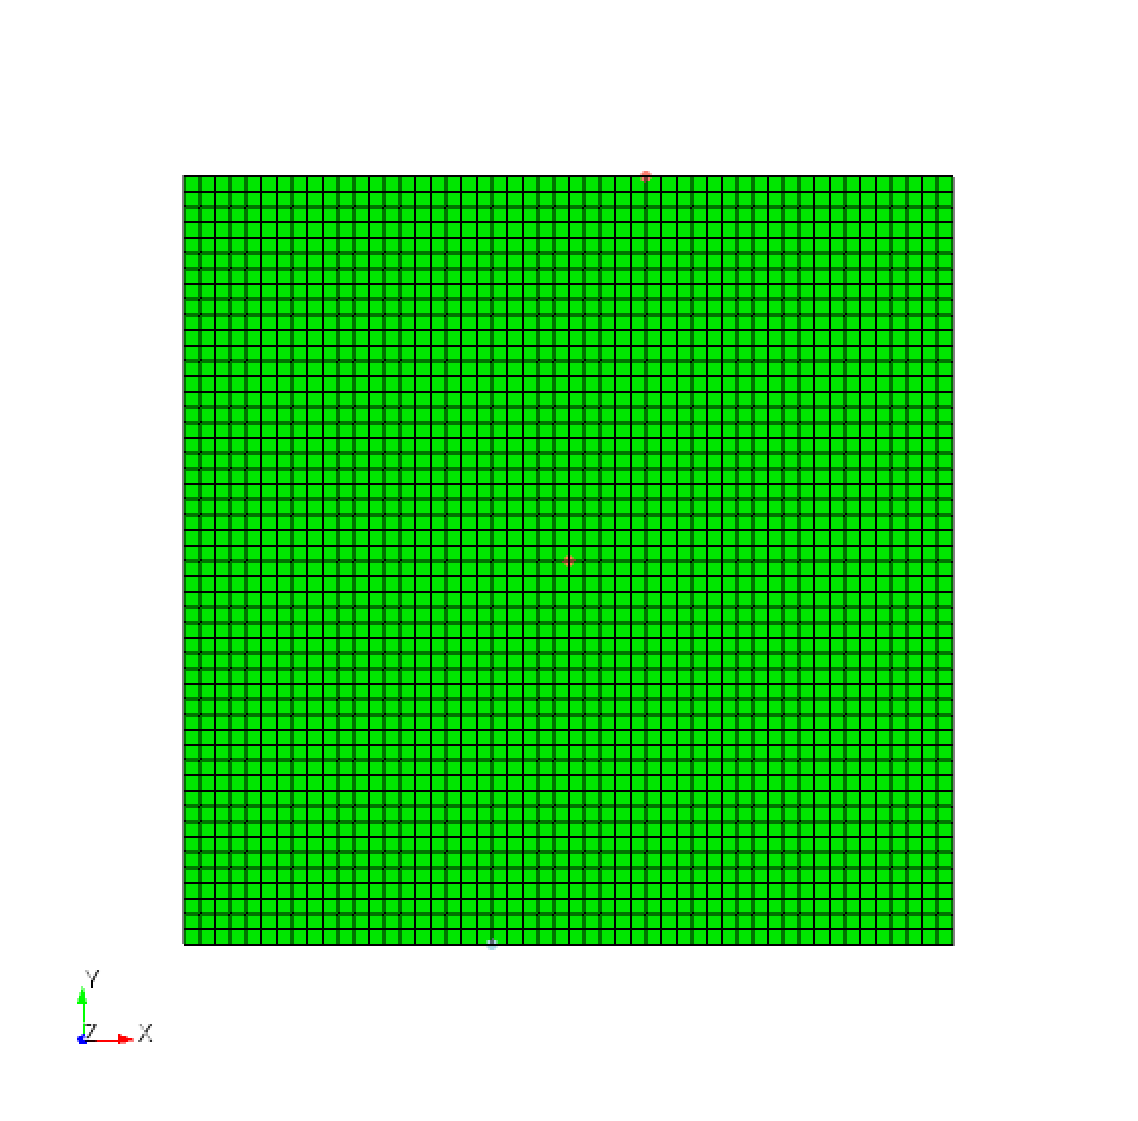
\includegraphics[width=0.6\textwidth]{regularmesh.eps}
%  \caption{Regular Plate Mesh}
%  \label{fig:regularmesh}
%\end{figure}
%%
%%
%\begin{figure}[h]
%  \centering
%  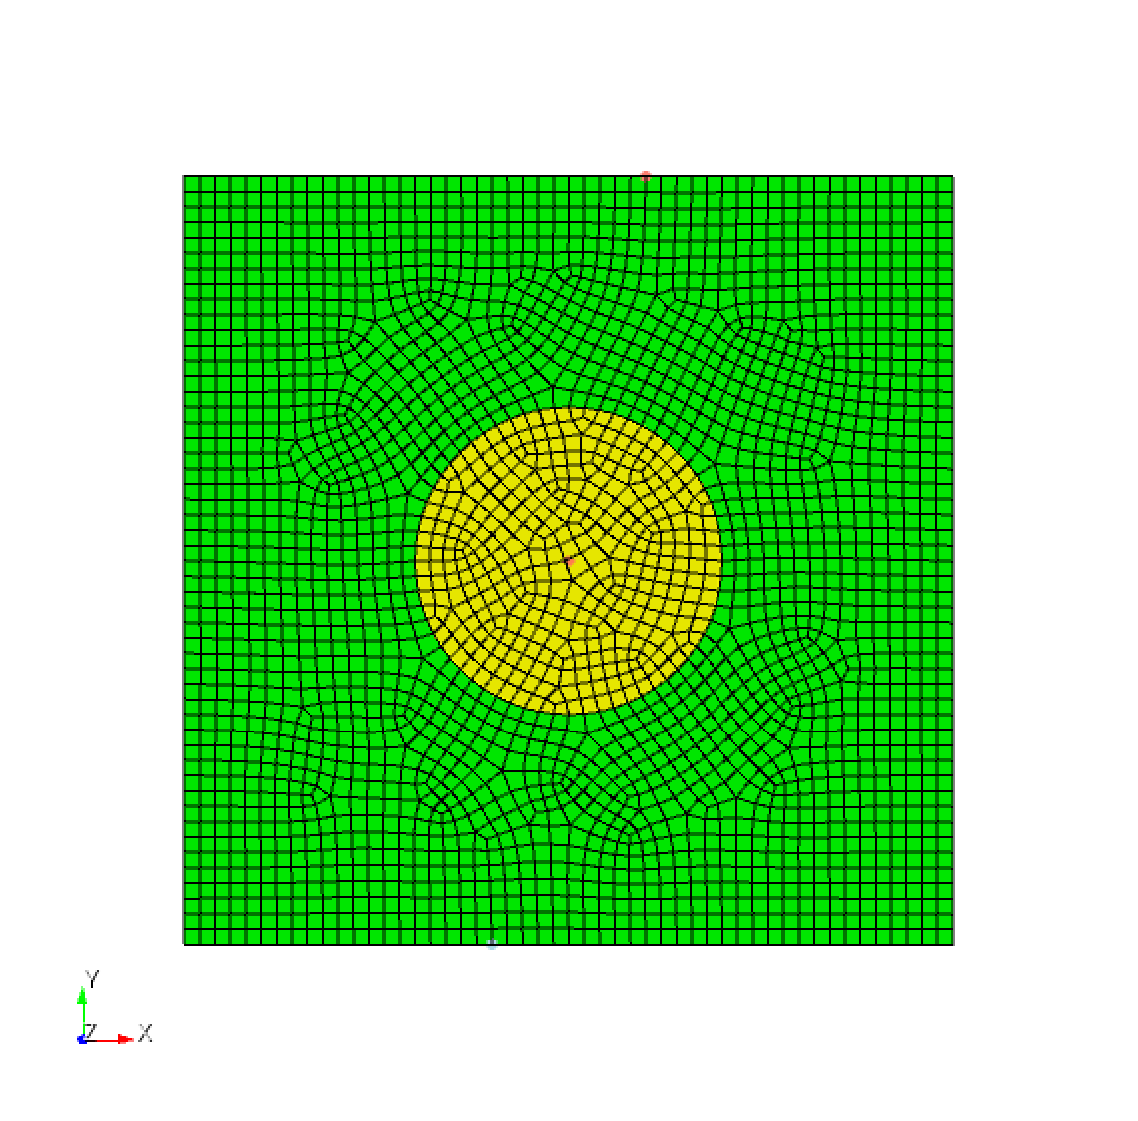
\includegraphics[width=0.6\textwidth]{unevenmesh.eps}
%  \caption{Irregular Plate Mesh}
%  \label{fig:unevenmesh}
%\end{figure}
%%
%
%
\begin{figure}[h]
  \centering
  \resizebox{0.6\linewidth}{!}{%% Creator: Matplotlib, PGF backend
%%
%% To include the figure in your LaTeX document, write
%%   \input{<filename>.pgf}
%%
%% Make sure the required packages are loaded in your preamble
%%   \usepackage{pgf}
%%
%% Figures using additional raster images can only be included by \input if
%% they are in the same directory as the main LaTeX file. For loading figures
%% from other directories you can use the `import` package
%%   \usepackage{import}
%% and then include the figures with
%%   \import{<path to file>}{<filename>.pgf}
%%
%% Matplotlib used the following preamble
%%
\begingroup%
\makeatletter%
\begin{pgfpicture}%
\pgfpathrectangle{\pgfpointorigin}{\pgfqpoint{5.000000in}{5.000000in}}%
\pgfusepath{use as bounding box}%
\begin{pgfscope}%
\pgfsetbuttcap%
\pgfsetroundjoin%
\definecolor{currentfill}{rgb}{1.000000,1.000000,1.000000}%
\pgfsetfillcolor{currentfill}%
\pgfsetlinewidth{0.000000pt}%
\definecolor{currentstroke}{rgb}{1.000000,1.000000,1.000000}%
\pgfsetstrokecolor{currentstroke}%
\pgfsetdash{}{0pt}%
\pgfpathmoveto{\pgfqpoint{0.000000in}{0.000000in}}%
\pgfpathlineto{\pgfqpoint{5.000000in}{0.000000in}}%
\pgfpathlineto{\pgfqpoint{5.000000in}{5.000000in}}%
\pgfpathlineto{\pgfqpoint{0.000000in}{5.000000in}}%
\pgfpathclose%
\pgfusepath{fill}%
\end{pgfscope}%
\begin{pgfscope}%
\pgfpathrectangle{\pgfqpoint{0.625000in}{0.562500in}}{\pgfqpoint{3.875000in}{3.875000in}} %
\pgfusepath{clip}%
\pgfsetbuttcap%
\pgfsetroundjoin%
\definecolor{currentfill}{rgb}{0.000000,0.000000,1.000000}%
\pgfsetfillcolor{currentfill}%
\pgfsetlinewidth{1.003750pt}%
\definecolor{currentstroke}{rgb}{0.000000,0.000000,0.000000}%
\pgfsetstrokecolor{currentstroke}%
\pgfsetdash{}{0pt}%
\pgfpathmoveto{\pgfqpoint{0.663750in}{0.581608in}}%
\pgfpathcurveto{\pgfqpoint{0.668959in}{0.581608in}}{\pgfqpoint{0.673956in}{0.583678in}}{\pgfqpoint{0.677639in}{0.587361in}}%
\pgfpathcurveto{\pgfqpoint{0.681322in}{0.591044in}}{\pgfqpoint{0.683392in}{0.596041in}}{\pgfqpoint{0.683392in}{0.601250in}}%
\pgfpathcurveto{\pgfqpoint{0.683392in}{0.606459in}}{\pgfqpoint{0.681322in}{0.611456in}}{\pgfqpoint{0.677639in}{0.615139in}}%
\pgfpathcurveto{\pgfqpoint{0.673956in}{0.618822in}}{\pgfqpoint{0.668959in}{0.620892in}}{\pgfqpoint{0.663750in}{0.620892in}}%
\pgfpathcurveto{\pgfqpoint{0.658541in}{0.620892in}}{\pgfqpoint{0.653544in}{0.618822in}}{\pgfqpoint{0.649861in}{0.615139in}}%
\pgfpathcurveto{\pgfqpoint{0.646178in}{0.611456in}}{\pgfqpoint{0.644108in}{0.606459in}}{\pgfqpoint{0.644108in}{0.601250in}}%
\pgfpathcurveto{\pgfqpoint{0.644108in}{0.596041in}}{\pgfqpoint{0.646178in}{0.591044in}}{\pgfqpoint{0.649861in}{0.587361in}}%
\pgfpathcurveto{\pgfqpoint{0.653544in}{0.583678in}}{\pgfqpoint{0.658541in}{0.581608in}}{\pgfqpoint{0.663750in}{0.581608in}}%
\pgfpathclose%
\pgfusepath{stroke,fill}%
\end{pgfscope}%
\begin{pgfscope}%
\pgfpathrectangle{\pgfqpoint{0.625000in}{0.562500in}}{\pgfqpoint{3.875000in}{3.875000in}} %
\pgfusepath{clip}%
\pgfsetbuttcap%
\pgfsetroundjoin%
\definecolor{currentfill}{rgb}{0.000000,0.000000,1.000000}%
\pgfsetfillcolor{currentfill}%
\pgfsetlinewidth{1.003750pt}%
\definecolor{currentstroke}{rgb}{0.000000,0.000000,0.000000}%
\pgfsetstrokecolor{currentstroke}%
\pgfsetdash{}{0pt}%
\pgfpathmoveto{\pgfqpoint{0.663750in}{0.659108in}}%
\pgfpathcurveto{\pgfqpoint{0.668959in}{0.659108in}}{\pgfqpoint{0.673956in}{0.661178in}}{\pgfqpoint{0.677639in}{0.664861in}}%
\pgfpathcurveto{\pgfqpoint{0.681322in}{0.668544in}}{\pgfqpoint{0.683392in}{0.673541in}}{\pgfqpoint{0.683392in}{0.678750in}}%
\pgfpathcurveto{\pgfqpoint{0.683392in}{0.683959in}}{\pgfqpoint{0.681322in}{0.688956in}}{\pgfqpoint{0.677639in}{0.692639in}}%
\pgfpathcurveto{\pgfqpoint{0.673956in}{0.696322in}}{\pgfqpoint{0.668959in}{0.698392in}}{\pgfqpoint{0.663750in}{0.698392in}}%
\pgfpathcurveto{\pgfqpoint{0.658541in}{0.698392in}}{\pgfqpoint{0.653544in}{0.696322in}}{\pgfqpoint{0.649861in}{0.692639in}}%
\pgfpathcurveto{\pgfqpoint{0.646178in}{0.688956in}}{\pgfqpoint{0.644108in}{0.683959in}}{\pgfqpoint{0.644108in}{0.678750in}}%
\pgfpathcurveto{\pgfqpoint{0.644108in}{0.673541in}}{\pgfqpoint{0.646178in}{0.668544in}}{\pgfqpoint{0.649861in}{0.664861in}}%
\pgfpathcurveto{\pgfqpoint{0.653544in}{0.661178in}}{\pgfqpoint{0.658541in}{0.659108in}}{\pgfqpoint{0.663750in}{0.659108in}}%
\pgfpathclose%
\pgfusepath{stroke,fill}%
\end{pgfscope}%
\begin{pgfscope}%
\pgfpathrectangle{\pgfqpoint{0.625000in}{0.562500in}}{\pgfqpoint{3.875000in}{3.875000in}} %
\pgfusepath{clip}%
\pgfsetbuttcap%
\pgfsetroundjoin%
\definecolor{currentfill}{rgb}{0.000000,0.000000,1.000000}%
\pgfsetfillcolor{currentfill}%
\pgfsetlinewidth{1.003750pt}%
\definecolor{currentstroke}{rgb}{0.000000,0.000000,0.000000}%
\pgfsetstrokecolor{currentstroke}%
\pgfsetdash{}{0pt}%
\pgfpathmoveto{\pgfqpoint{0.663750in}{0.736608in}}%
\pgfpathcurveto{\pgfqpoint{0.668959in}{0.736608in}}{\pgfqpoint{0.673956in}{0.738678in}}{\pgfqpoint{0.677639in}{0.742361in}}%
\pgfpathcurveto{\pgfqpoint{0.681322in}{0.746044in}}{\pgfqpoint{0.683392in}{0.751041in}}{\pgfqpoint{0.683392in}{0.756250in}}%
\pgfpathcurveto{\pgfqpoint{0.683392in}{0.761459in}}{\pgfqpoint{0.681322in}{0.766456in}}{\pgfqpoint{0.677639in}{0.770139in}}%
\pgfpathcurveto{\pgfqpoint{0.673956in}{0.773822in}}{\pgfqpoint{0.668959in}{0.775892in}}{\pgfqpoint{0.663750in}{0.775892in}}%
\pgfpathcurveto{\pgfqpoint{0.658541in}{0.775892in}}{\pgfqpoint{0.653544in}{0.773822in}}{\pgfqpoint{0.649861in}{0.770139in}}%
\pgfpathcurveto{\pgfqpoint{0.646178in}{0.766456in}}{\pgfqpoint{0.644108in}{0.761459in}}{\pgfqpoint{0.644108in}{0.756250in}}%
\pgfpathcurveto{\pgfqpoint{0.644108in}{0.751041in}}{\pgfqpoint{0.646178in}{0.746044in}}{\pgfqpoint{0.649861in}{0.742361in}}%
\pgfpathcurveto{\pgfqpoint{0.653544in}{0.738678in}}{\pgfqpoint{0.658541in}{0.736608in}}{\pgfqpoint{0.663750in}{0.736608in}}%
\pgfpathclose%
\pgfusepath{stroke,fill}%
\end{pgfscope}%
\begin{pgfscope}%
\pgfpathrectangle{\pgfqpoint{0.625000in}{0.562500in}}{\pgfqpoint{3.875000in}{3.875000in}} %
\pgfusepath{clip}%
\pgfsetbuttcap%
\pgfsetroundjoin%
\definecolor{currentfill}{rgb}{0.000000,0.000000,1.000000}%
\pgfsetfillcolor{currentfill}%
\pgfsetlinewidth{1.003750pt}%
\definecolor{currentstroke}{rgb}{0.000000,0.000000,0.000000}%
\pgfsetstrokecolor{currentstroke}%
\pgfsetdash{}{0pt}%
\pgfpathmoveto{\pgfqpoint{0.663750in}{0.814108in}}%
\pgfpathcurveto{\pgfqpoint{0.668959in}{0.814108in}}{\pgfqpoint{0.673956in}{0.816178in}}{\pgfqpoint{0.677639in}{0.819861in}}%
\pgfpathcurveto{\pgfqpoint{0.681322in}{0.823544in}}{\pgfqpoint{0.683392in}{0.828541in}}{\pgfqpoint{0.683392in}{0.833750in}}%
\pgfpathcurveto{\pgfqpoint{0.683392in}{0.838959in}}{\pgfqpoint{0.681322in}{0.843956in}}{\pgfqpoint{0.677639in}{0.847639in}}%
\pgfpathcurveto{\pgfqpoint{0.673956in}{0.851322in}}{\pgfqpoint{0.668959in}{0.853392in}}{\pgfqpoint{0.663750in}{0.853392in}}%
\pgfpathcurveto{\pgfqpoint{0.658541in}{0.853392in}}{\pgfqpoint{0.653544in}{0.851322in}}{\pgfqpoint{0.649861in}{0.847639in}}%
\pgfpathcurveto{\pgfqpoint{0.646178in}{0.843956in}}{\pgfqpoint{0.644108in}{0.838959in}}{\pgfqpoint{0.644108in}{0.833750in}}%
\pgfpathcurveto{\pgfqpoint{0.644108in}{0.828541in}}{\pgfqpoint{0.646178in}{0.823544in}}{\pgfqpoint{0.649861in}{0.819861in}}%
\pgfpathcurveto{\pgfqpoint{0.653544in}{0.816178in}}{\pgfqpoint{0.658541in}{0.814108in}}{\pgfqpoint{0.663750in}{0.814108in}}%
\pgfpathclose%
\pgfusepath{stroke,fill}%
\end{pgfscope}%
\begin{pgfscope}%
\pgfpathrectangle{\pgfqpoint{0.625000in}{0.562500in}}{\pgfqpoint{3.875000in}{3.875000in}} %
\pgfusepath{clip}%
\pgfsetbuttcap%
\pgfsetroundjoin%
\definecolor{currentfill}{rgb}{0.000000,0.000000,1.000000}%
\pgfsetfillcolor{currentfill}%
\pgfsetlinewidth{1.003750pt}%
\definecolor{currentstroke}{rgb}{0.000000,0.000000,0.000000}%
\pgfsetstrokecolor{currentstroke}%
\pgfsetdash{}{0pt}%
\pgfpathmoveto{\pgfqpoint{0.663750in}{0.891608in}}%
\pgfpathcurveto{\pgfqpoint{0.668959in}{0.891608in}}{\pgfqpoint{0.673956in}{0.893678in}}{\pgfqpoint{0.677639in}{0.897361in}}%
\pgfpathcurveto{\pgfqpoint{0.681322in}{0.901044in}}{\pgfqpoint{0.683392in}{0.906041in}}{\pgfqpoint{0.683392in}{0.911250in}}%
\pgfpathcurveto{\pgfqpoint{0.683392in}{0.916459in}}{\pgfqpoint{0.681322in}{0.921456in}}{\pgfqpoint{0.677639in}{0.925139in}}%
\pgfpathcurveto{\pgfqpoint{0.673956in}{0.928822in}}{\pgfqpoint{0.668959in}{0.930892in}}{\pgfqpoint{0.663750in}{0.930892in}}%
\pgfpathcurveto{\pgfqpoint{0.658541in}{0.930892in}}{\pgfqpoint{0.653544in}{0.928822in}}{\pgfqpoint{0.649861in}{0.925139in}}%
\pgfpathcurveto{\pgfqpoint{0.646178in}{0.921456in}}{\pgfqpoint{0.644108in}{0.916459in}}{\pgfqpoint{0.644108in}{0.911250in}}%
\pgfpathcurveto{\pgfqpoint{0.644108in}{0.906041in}}{\pgfqpoint{0.646178in}{0.901044in}}{\pgfqpoint{0.649861in}{0.897361in}}%
\pgfpathcurveto{\pgfqpoint{0.653544in}{0.893678in}}{\pgfqpoint{0.658541in}{0.891608in}}{\pgfqpoint{0.663750in}{0.891608in}}%
\pgfpathclose%
\pgfusepath{stroke,fill}%
\end{pgfscope}%
\begin{pgfscope}%
\pgfpathrectangle{\pgfqpoint{0.625000in}{0.562500in}}{\pgfqpoint{3.875000in}{3.875000in}} %
\pgfusepath{clip}%
\pgfsetbuttcap%
\pgfsetroundjoin%
\definecolor{currentfill}{rgb}{0.000000,0.000000,1.000000}%
\pgfsetfillcolor{currentfill}%
\pgfsetlinewidth{1.003750pt}%
\definecolor{currentstroke}{rgb}{0.000000,0.000000,0.000000}%
\pgfsetstrokecolor{currentstroke}%
\pgfsetdash{}{0pt}%
\pgfpathmoveto{\pgfqpoint{0.663750in}{0.969108in}}%
\pgfpathcurveto{\pgfqpoint{0.668959in}{0.969108in}}{\pgfqpoint{0.673956in}{0.971178in}}{\pgfqpoint{0.677639in}{0.974861in}}%
\pgfpathcurveto{\pgfqpoint{0.681322in}{0.978544in}}{\pgfqpoint{0.683392in}{0.983541in}}{\pgfqpoint{0.683392in}{0.988750in}}%
\pgfpathcurveto{\pgfqpoint{0.683392in}{0.993959in}}{\pgfqpoint{0.681322in}{0.998956in}}{\pgfqpoint{0.677639in}{1.002639in}}%
\pgfpathcurveto{\pgfqpoint{0.673956in}{1.006322in}}{\pgfqpoint{0.668959in}{1.008392in}}{\pgfqpoint{0.663750in}{1.008392in}}%
\pgfpathcurveto{\pgfqpoint{0.658541in}{1.008392in}}{\pgfqpoint{0.653544in}{1.006322in}}{\pgfqpoint{0.649861in}{1.002639in}}%
\pgfpathcurveto{\pgfqpoint{0.646178in}{0.998956in}}{\pgfqpoint{0.644108in}{0.993959in}}{\pgfqpoint{0.644108in}{0.988750in}}%
\pgfpathcurveto{\pgfqpoint{0.644108in}{0.983541in}}{\pgfqpoint{0.646178in}{0.978544in}}{\pgfqpoint{0.649861in}{0.974861in}}%
\pgfpathcurveto{\pgfqpoint{0.653544in}{0.971178in}}{\pgfqpoint{0.658541in}{0.969108in}}{\pgfqpoint{0.663750in}{0.969108in}}%
\pgfpathclose%
\pgfusepath{stroke,fill}%
\end{pgfscope}%
\begin{pgfscope}%
\pgfpathrectangle{\pgfqpoint{0.625000in}{0.562500in}}{\pgfqpoint{3.875000in}{3.875000in}} %
\pgfusepath{clip}%
\pgfsetbuttcap%
\pgfsetroundjoin%
\definecolor{currentfill}{rgb}{0.000000,0.000000,1.000000}%
\pgfsetfillcolor{currentfill}%
\pgfsetlinewidth{1.003750pt}%
\definecolor{currentstroke}{rgb}{0.000000,0.000000,0.000000}%
\pgfsetstrokecolor{currentstroke}%
\pgfsetdash{}{0pt}%
\pgfpathmoveto{\pgfqpoint{0.663750in}{1.046608in}}%
\pgfpathcurveto{\pgfqpoint{0.668959in}{1.046608in}}{\pgfqpoint{0.673956in}{1.048678in}}{\pgfqpoint{0.677639in}{1.052361in}}%
\pgfpathcurveto{\pgfqpoint{0.681322in}{1.056044in}}{\pgfqpoint{0.683392in}{1.061041in}}{\pgfqpoint{0.683392in}{1.066250in}}%
\pgfpathcurveto{\pgfqpoint{0.683392in}{1.071459in}}{\pgfqpoint{0.681322in}{1.076456in}}{\pgfqpoint{0.677639in}{1.080139in}}%
\pgfpathcurveto{\pgfqpoint{0.673956in}{1.083822in}}{\pgfqpoint{0.668959in}{1.085892in}}{\pgfqpoint{0.663750in}{1.085892in}}%
\pgfpathcurveto{\pgfqpoint{0.658541in}{1.085892in}}{\pgfqpoint{0.653544in}{1.083822in}}{\pgfqpoint{0.649861in}{1.080139in}}%
\pgfpathcurveto{\pgfqpoint{0.646178in}{1.076456in}}{\pgfqpoint{0.644108in}{1.071459in}}{\pgfqpoint{0.644108in}{1.066250in}}%
\pgfpathcurveto{\pgfqpoint{0.644108in}{1.061041in}}{\pgfqpoint{0.646178in}{1.056044in}}{\pgfqpoint{0.649861in}{1.052361in}}%
\pgfpathcurveto{\pgfqpoint{0.653544in}{1.048678in}}{\pgfqpoint{0.658541in}{1.046608in}}{\pgfqpoint{0.663750in}{1.046608in}}%
\pgfpathclose%
\pgfusepath{stroke,fill}%
\end{pgfscope}%
\begin{pgfscope}%
\pgfpathrectangle{\pgfqpoint{0.625000in}{0.562500in}}{\pgfqpoint{3.875000in}{3.875000in}} %
\pgfusepath{clip}%
\pgfsetbuttcap%
\pgfsetroundjoin%
\definecolor{currentfill}{rgb}{0.000000,0.000000,1.000000}%
\pgfsetfillcolor{currentfill}%
\pgfsetlinewidth{1.003750pt}%
\definecolor{currentstroke}{rgb}{0.000000,0.000000,0.000000}%
\pgfsetstrokecolor{currentstroke}%
\pgfsetdash{}{0pt}%
\pgfpathmoveto{\pgfqpoint{0.663750in}{1.124108in}}%
\pgfpathcurveto{\pgfqpoint{0.668959in}{1.124108in}}{\pgfqpoint{0.673956in}{1.126178in}}{\pgfqpoint{0.677639in}{1.129861in}}%
\pgfpathcurveto{\pgfqpoint{0.681322in}{1.133544in}}{\pgfqpoint{0.683392in}{1.138541in}}{\pgfqpoint{0.683392in}{1.143750in}}%
\pgfpathcurveto{\pgfqpoint{0.683392in}{1.148959in}}{\pgfqpoint{0.681322in}{1.153956in}}{\pgfqpoint{0.677639in}{1.157639in}}%
\pgfpathcurveto{\pgfqpoint{0.673956in}{1.161322in}}{\pgfqpoint{0.668959in}{1.163392in}}{\pgfqpoint{0.663750in}{1.163392in}}%
\pgfpathcurveto{\pgfqpoint{0.658541in}{1.163392in}}{\pgfqpoint{0.653544in}{1.161322in}}{\pgfqpoint{0.649861in}{1.157639in}}%
\pgfpathcurveto{\pgfqpoint{0.646178in}{1.153956in}}{\pgfqpoint{0.644108in}{1.148959in}}{\pgfqpoint{0.644108in}{1.143750in}}%
\pgfpathcurveto{\pgfqpoint{0.644108in}{1.138541in}}{\pgfqpoint{0.646178in}{1.133544in}}{\pgfqpoint{0.649861in}{1.129861in}}%
\pgfpathcurveto{\pgfqpoint{0.653544in}{1.126178in}}{\pgfqpoint{0.658541in}{1.124108in}}{\pgfqpoint{0.663750in}{1.124108in}}%
\pgfpathclose%
\pgfusepath{stroke,fill}%
\end{pgfscope}%
\begin{pgfscope}%
\pgfpathrectangle{\pgfqpoint{0.625000in}{0.562500in}}{\pgfqpoint{3.875000in}{3.875000in}} %
\pgfusepath{clip}%
\pgfsetbuttcap%
\pgfsetroundjoin%
\definecolor{currentfill}{rgb}{0.000000,0.000000,1.000000}%
\pgfsetfillcolor{currentfill}%
\pgfsetlinewidth{1.003750pt}%
\definecolor{currentstroke}{rgb}{0.000000,0.000000,0.000000}%
\pgfsetstrokecolor{currentstroke}%
\pgfsetdash{}{0pt}%
\pgfpathmoveto{\pgfqpoint{0.663750in}{1.201608in}}%
\pgfpathcurveto{\pgfqpoint{0.668959in}{1.201608in}}{\pgfqpoint{0.673956in}{1.203678in}}{\pgfqpoint{0.677639in}{1.207361in}}%
\pgfpathcurveto{\pgfqpoint{0.681322in}{1.211044in}}{\pgfqpoint{0.683392in}{1.216041in}}{\pgfqpoint{0.683392in}{1.221250in}}%
\pgfpathcurveto{\pgfqpoint{0.683392in}{1.226459in}}{\pgfqpoint{0.681322in}{1.231456in}}{\pgfqpoint{0.677639in}{1.235139in}}%
\pgfpathcurveto{\pgfqpoint{0.673956in}{1.238822in}}{\pgfqpoint{0.668959in}{1.240892in}}{\pgfqpoint{0.663750in}{1.240892in}}%
\pgfpathcurveto{\pgfqpoint{0.658541in}{1.240892in}}{\pgfqpoint{0.653544in}{1.238822in}}{\pgfqpoint{0.649861in}{1.235139in}}%
\pgfpathcurveto{\pgfqpoint{0.646178in}{1.231456in}}{\pgfqpoint{0.644108in}{1.226459in}}{\pgfqpoint{0.644108in}{1.221250in}}%
\pgfpathcurveto{\pgfqpoint{0.644108in}{1.216041in}}{\pgfqpoint{0.646178in}{1.211044in}}{\pgfqpoint{0.649861in}{1.207361in}}%
\pgfpathcurveto{\pgfqpoint{0.653544in}{1.203678in}}{\pgfqpoint{0.658541in}{1.201608in}}{\pgfqpoint{0.663750in}{1.201608in}}%
\pgfpathclose%
\pgfusepath{stroke,fill}%
\end{pgfscope}%
\begin{pgfscope}%
\pgfpathrectangle{\pgfqpoint{0.625000in}{0.562500in}}{\pgfqpoint{3.875000in}{3.875000in}} %
\pgfusepath{clip}%
\pgfsetbuttcap%
\pgfsetroundjoin%
\definecolor{currentfill}{rgb}{0.000000,0.000000,1.000000}%
\pgfsetfillcolor{currentfill}%
\pgfsetlinewidth{1.003750pt}%
\definecolor{currentstroke}{rgb}{0.000000,0.000000,0.000000}%
\pgfsetstrokecolor{currentstroke}%
\pgfsetdash{}{0pt}%
\pgfpathmoveto{\pgfqpoint{0.663750in}{1.279108in}}%
\pgfpathcurveto{\pgfqpoint{0.668959in}{1.279108in}}{\pgfqpoint{0.673956in}{1.281178in}}{\pgfqpoint{0.677639in}{1.284861in}}%
\pgfpathcurveto{\pgfqpoint{0.681322in}{1.288544in}}{\pgfqpoint{0.683392in}{1.293541in}}{\pgfqpoint{0.683392in}{1.298750in}}%
\pgfpathcurveto{\pgfqpoint{0.683392in}{1.303959in}}{\pgfqpoint{0.681322in}{1.308956in}}{\pgfqpoint{0.677639in}{1.312639in}}%
\pgfpathcurveto{\pgfqpoint{0.673956in}{1.316322in}}{\pgfqpoint{0.668959in}{1.318392in}}{\pgfqpoint{0.663750in}{1.318392in}}%
\pgfpathcurveto{\pgfqpoint{0.658541in}{1.318392in}}{\pgfqpoint{0.653544in}{1.316322in}}{\pgfqpoint{0.649861in}{1.312639in}}%
\pgfpathcurveto{\pgfqpoint{0.646178in}{1.308956in}}{\pgfqpoint{0.644108in}{1.303959in}}{\pgfqpoint{0.644108in}{1.298750in}}%
\pgfpathcurveto{\pgfqpoint{0.644108in}{1.293541in}}{\pgfqpoint{0.646178in}{1.288544in}}{\pgfqpoint{0.649861in}{1.284861in}}%
\pgfpathcurveto{\pgfqpoint{0.653544in}{1.281178in}}{\pgfqpoint{0.658541in}{1.279108in}}{\pgfqpoint{0.663750in}{1.279108in}}%
\pgfpathclose%
\pgfusepath{stroke,fill}%
\end{pgfscope}%
\begin{pgfscope}%
\pgfpathrectangle{\pgfqpoint{0.625000in}{0.562500in}}{\pgfqpoint{3.875000in}{3.875000in}} %
\pgfusepath{clip}%
\pgfsetbuttcap%
\pgfsetroundjoin%
\definecolor{currentfill}{rgb}{0.000000,0.000000,1.000000}%
\pgfsetfillcolor{currentfill}%
\pgfsetlinewidth{1.003750pt}%
\definecolor{currentstroke}{rgb}{0.000000,0.000000,0.000000}%
\pgfsetstrokecolor{currentstroke}%
\pgfsetdash{}{0pt}%
\pgfpathmoveto{\pgfqpoint{0.663750in}{1.356608in}}%
\pgfpathcurveto{\pgfqpoint{0.668959in}{1.356608in}}{\pgfqpoint{0.673956in}{1.358678in}}{\pgfqpoint{0.677639in}{1.362361in}}%
\pgfpathcurveto{\pgfqpoint{0.681322in}{1.366044in}}{\pgfqpoint{0.683392in}{1.371041in}}{\pgfqpoint{0.683392in}{1.376250in}}%
\pgfpathcurveto{\pgfqpoint{0.683392in}{1.381459in}}{\pgfqpoint{0.681322in}{1.386456in}}{\pgfqpoint{0.677639in}{1.390139in}}%
\pgfpathcurveto{\pgfqpoint{0.673956in}{1.393822in}}{\pgfqpoint{0.668959in}{1.395892in}}{\pgfqpoint{0.663750in}{1.395892in}}%
\pgfpathcurveto{\pgfqpoint{0.658541in}{1.395892in}}{\pgfqpoint{0.653544in}{1.393822in}}{\pgfqpoint{0.649861in}{1.390139in}}%
\pgfpathcurveto{\pgfqpoint{0.646178in}{1.386456in}}{\pgfqpoint{0.644108in}{1.381459in}}{\pgfqpoint{0.644108in}{1.376250in}}%
\pgfpathcurveto{\pgfqpoint{0.644108in}{1.371041in}}{\pgfqpoint{0.646178in}{1.366044in}}{\pgfqpoint{0.649861in}{1.362361in}}%
\pgfpathcurveto{\pgfqpoint{0.653544in}{1.358678in}}{\pgfqpoint{0.658541in}{1.356608in}}{\pgfqpoint{0.663750in}{1.356608in}}%
\pgfpathclose%
\pgfusepath{stroke,fill}%
\end{pgfscope}%
\begin{pgfscope}%
\pgfpathrectangle{\pgfqpoint{0.625000in}{0.562500in}}{\pgfqpoint{3.875000in}{3.875000in}} %
\pgfusepath{clip}%
\pgfsetbuttcap%
\pgfsetroundjoin%
\definecolor{currentfill}{rgb}{0.000000,0.000000,1.000000}%
\pgfsetfillcolor{currentfill}%
\pgfsetlinewidth{1.003750pt}%
\definecolor{currentstroke}{rgb}{0.000000,0.000000,0.000000}%
\pgfsetstrokecolor{currentstroke}%
\pgfsetdash{}{0pt}%
\pgfpathmoveto{\pgfqpoint{0.663750in}{1.434108in}}%
\pgfpathcurveto{\pgfqpoint{0.668959in}{1.434108in}}{\pgfqpoint{0.673956in}{1.436178in}}{\pgfqpoint{0.677639in}{1.439861in}}%
\pgfpathcurveto{\pgfqpoint{0.681322in}{1.443544in}}{\pgfqpoint{0.683392in}{1.448541in}}{\pgfqpoint{0.683392in}{1.453750in}}%
\pgfpathcurveto{\pgfqpoint{0.683392in}{1.458959in}}{\pgfqpoint{0.681322in}{1.463956in}}{\pgfqpoint{0.677639in}{1.467639in}}%
\pgfpathcurveto{\pgfqpoint{0.673956in}{1.471322in}}{\pgfqpoint{0.668959in}{1.473392in}}{\pgfqpoint{0.663750in}{1.473392in}}%
\pgfpathcurveto{\pgfqpoint{0.658541in}{1.473392in}}{\pgfqpoint{0.653544in}{1.471322in}}{\pgfqpoint{0.649861in}{1.467639in}}%
\pgfpathcurveto{\pgfqpoint{0.646178in}{1.463956in}}{\pgfqpoint{0.644108in}{1.458959in}}{\pgfqpoint{0.644108in}{1.453750in}}%
\pgfpathcurveto{\pgfqpoint{0.644108in}{1.448541in}}{\pgfqpoint{0.646178in}{1.443544in}}{\pgfqpoint{0.649861in}{1.439861in}}%
\pgfpathcurveto{\pgfqpoint{0.653544in}{1.436178in}}{\pgfqpoint{0.658541in}{1.434108in}}{\pgfqpoint{0.663750in}{1.434108in}}%
\pgfpathclose%
\pgfusepath{stroke,fill}%
\end{pgfscope}%
\begin{pgfscope}%
\pgfpathrectangle{\pgfqpoint{0.625000in}{0.562500in}}{\pgfqpoint{3.875000in}{3.875000in}} %
\pgfusepath{clip}%
\pgfsetbuttcap%
\pgfsetroundjoin%
\definecolor{currentfill}{rgb}{0.000000,0.000000,1.000000}%
\pgfsetfillcolor{currentfill}%
\pgfsetlinewidth{1.003750pt}%
\definecolor{currentstroke}{rgb}{0.000000,0.000000,0.000000}%
\pgfsetstrokecolor{currentstroke}%
\pgfsetdash{}{0pt}%
\pgfpathmoveto{\pgfqpoint{0.663750in}{1.511608in}}%
\pgfpathcurveto{\pgfqpoint{0.668959in}{1.511608in}}{\pgfqpoint{0.673956in}{1.513678in}}{\pgfqpoint{0.677639in}{1.517361in}}%
\pgfpathcurveto{\pgfqpoint{0.681322in}{1.521044in}}{\pgfqpoint{0.683392in}{1.526041in}}{\pgfqpoint{0.683392in}{1.531250in}}%
\pgfpathcurveto{\pgfqpoint{0.683392in}{1.536459in}}{\pgfqpoint{0.681322in}{1.541456in}}{\pgfqpoint{0.677639in}{1.545139in}}%
\pgfpathcurveto{\pgfqpoint{0.673956in}{1.548822in}}{\pgfqpoint{0.668959in}{1.550892in}}{\pgfqpoint{0.663750in}{1.550892in}}%
\pgfpathcurveto{\pgfqpoint{0.658541in}{1.550892in}}{\pgfqpoint{0.653544in}{1.548822in}}{\pgfqpoint{0.649861in}{1.545139in}}%
\pgfpathcurveto{\pgfqpoint{0.646178in}{1.541456in}}{\pgfqpoint{0.644108in}{1.536459in}}{\pgfqpoint{0.644108in}{1.531250in}}%
\pgfpathcurveto{\pgfqpoint{0.644108in}{1.526041in}}{\pgfqpoint{0.646178in}{1.521044in}}{\pgfqpoint{0.649861in}{1.517361in}}%
\pgfpathcurveto{\pgfqpoint{0.653544in}{1.513678in}}{\pgfqpoint{0.658541in}{1.511608in}}{\pgfqpoint{0.663750in}{1.511608in}}%
\pgfpathclose%
\pgfusepath{stroke,fill}%
\end{pgfscope}%
\begin{pgfscope}%
\pgfpathrectangle{\pgfqpoint{0.625000in}{0.562500in}}{\pgfqpoint{3.875000in}{3.875000in}} %
\pgfusepath{clip}%
\pgfsetbuttcap%
\pgfsetroundjoin%
\definecolor{currentfill}{rgb}{0.000000,0.000000,1.000000}%
\pgfsetfillcolor{currentfill}%
\pgfsetlinewidth{1.003750pt}%
\definecolor{currentstroke}{rgb}{0.000000,0.000000,0.000000}%
\pgfsetstrokecolor{currentstroke}%
\pgfsetdash{}{0pt}%
\pgfpathmoveto{\pgfqpoint{0.663750in}{1.589108in}}%
\pgfpathcurveto{\pgfqpoint{0.668959in}{1.589108in}}{\pgfqpoint{0.673956in}{1.591178in}}{\pgfqpoint{0.677639in}{1.594861in}}%
\pgfpathcurveto{\pgfqpoint{0.681322in}{1.598544in}}{\pgfqpoint{0.683392in}{1.603541in}}{\pgfqpoint{0.683392in}{1.608750in}}%
\pgfpathcurveto{\pgfqpoint{0.683392in}{1.613959in}}{\pgfqpoint{0.681322in}{1.618956in}}{\pgfqpoint{0.677639in}{1.622639in}}%
\pgfpathcurveto{\pgfqpoint{0.673956in}{1.626322in}}{\pgfqpoint{0.668959in}{1.628392in}}{\pgfqpoint{0.663750in}{1.628392in}}%
\pgfpathcurveto{\pgfqpoint{0.658541in}{1.628392in}}{\pgfqpoint{0.653544in}{1.626322in}}{\pgfqpoint{0.649861in}{1.622639in}}%
\pgfpathcurveto{\pgfqpoint{0.646178in}{1.618956in}}{\pgfqpoint{0.644108in}{1.613959in}}{\pgfqpoint{0.644108in}{1.608750in}}%
\pgfpathcurveto{\pgfqpoint{0.644108in}{1.603541in}}{\pgfqpoint{0.646178in}{1.598544in}}{\pgfqpoint{0.649861in}{1.594861in}}%
\pgfpathcurveto{\pgfqpoint{0.653544in}{1.591178in}}{\pgfqpoint{0.658541in}{1.589108in}}{\pgfqpoint{0.663750in}{1.589108in}}%
\pgfpathclose%
\pgfusepath{stroke,fill}%
\end{pgfscope}%
\begin{pgfscope}%
\pgfpathrectangle{\pgfqpoint{0.625000in}{0.562500in}}{\pgfqpoint{3.875000in}{3.875000in}} %
\pgfusepath{clip}%
\pgfsetbuttcap%
\pgfsetroundjoin%
\definecolor{currentfill}{rgb}{0.000000,0.000000,1.000000}%
\pgfsetfillcolor{currentfill}%
\pgfsetlinewidth{1.003750pt}%
\definecolor{currentstroke}{rgb}{0.000000,0.000000,0.000000}%
\pgfsetstrokecolor{currentstroke}%
\pgfsetdash{}{0pt}%
\pgfpathmoveto{\pgfqpoint{0.663750in}{1.666608in}}%
\pgfpathcurveto{\pgfqpoint{0.668959in}{1.666608in}}{\pgfqpoint{0.673956in}{1.668678in}}{\pgfqpoint{0.677639in}{1.672361in}}%
\pgfpathcurveto{\pgfqpoint{0.681322in}{1.676044in}}{\pgfqpoint{0.683392in}{1.681041in}}{\pgfqpoint{0.683392in}{1.686250in}}%
\pgfpathcurveto{\pgfqpoint{0.683392in}{1.691459in}}{\pgfqpoint{0.681322in}{1.696456in}}{\pgfqpoint{0.677639in}{1.700139in}}%
\pgfpathcurveto{\pgfqpoint{0.673956in}{1.703822in}}{\pgfqpoint{0.668959in}{1.705892in}}{\pgfqpoint{0.663750in}{1.705892in}}%
\pgfpathcurveto{\pgfqpoint{0.658541in}{1.705892in}}{\pgfqpoint{0.653544in}{1.703822in}}{\pgfqpoint{0.649861in}{1.700139in}}%
\pgfpathcurveto{\pgfqpoint{0.646178in}{1.696456in}}{\pgfqpoint{0.644108in}{1.691459in}}{\pgfqpoint{0.644108in}{1.686250in}}%
\pgfpathcurveto{\pgfqpoint{0.644108in}{1.681041in}}{\pgfqpoint{0.646178in}{1.676044in}}{\pgfqpoint{0.649861in}{1.672361in}}%
\pgfpathcurveto{\pgfqpoint{0.653544in}{1.668678in}}{\pgfqpoint{0.658541in}{1.666608in}}{\pgfqpoint{0.663750in}{1.666608in}}%
\pgfpathclose%
\pgfusepath{stroke,fill}%
\end{pgfscope}%
\begin{pgfscope}%
\pgfpathrectangle{\pgfqpoint{0.625000in}{0.562500in}}{\pgfqpoint{3.875000in}{3.875000in}} %
\pgfusepath{clip}%
\pgfsetbuttcap%
\pgfsetroundjoin%
\definecolor{currentfill}{rgb}{0.000000,0.000000,1.000000}%
\pgfsetfillcolor{currentfill}%
\pgfsetlinewidth{1.003750pt}%
\definecolor{currentstroke}{rgb}{0.000000,0.000000,0.000000}%
\pgfsetstrokecolor{currentstroke}%
\pgfsetdash{}{0pt}%
\pgfpathmoveto{\pgfqpoint{0.663750in}{1.744108in}}%
\pgfpathcurveto{\pgfqpoint{0.668959in}{1.744108in}}{\pgfqpoint{0.673956in}{1.746178in}}{\pgfqpoint{0.677639in}{1.749861in}}%
\pgfpathcurveto{\pgfqpoint{0.681322in}{1.753544in}}{\pgfqpoint{0.683392in}{1.758541in}}{\pgfqpoint{0.683392in}{1.763750in}}%
\pgfpathcurveto{\pgfqpoint{0.683392in}{1.768959in}}{\pgfqpoint{0.681322in}{1.773956in}}{\pgfqpoint{0.677639in}{1.777639in}}%
\pgfpathcurveto{\pgfqpoint{0.673956in}{1.781322in}}{\pgfqpoint{0.668959in}{1.783392in}}{\pgfqpoint{0.663750in}{1.783392in}}%
\pgfpathcurveto{\pgfqpoint{0.658541in}{1.783392in}}{\pgfqpoint{0.653544in}{1.781322in}}{\pgfqpoint{0.649861in}{1.777639in}}%
\pgfpathcurveto{\pgfqpoint{0.646178in}{1.773956in}}{\pgfqpoint{0.644108in}{1.768959in}}{\pgfqpoint{0.644108in}{1.763750in}}%
\pgfpathcurveto{\pgfqpoint{0.644108in}{1.758541in}}{\pgfqpoint{0.646178in}{1.753544in}}{\pgfqpoint{0.649861in}{1.749861in}}%
\pgfpathcurveto{\pgfqpoint{0.653544in}{1.746178in}}{\pgfqpoint{0.658541in}{1.744108in}}{\pgfqpoint{0.663750in}{1.744108in}}%
\pgfpathclose%
\pgfusepath{stroke,fill}%
\end{pgfscope}%
\begin{pgfscope}%
\pgfpathrectangle{\pgfqpoint{0.625000in}{0.562500in}}{\pgfqpoint{3.875000in}{3.875000in}} %
\pgfusepath{clip}%
\pgfsetbuttcap%
\pgfsetroundjoin%
\definecolor{currentfill}{rgb}{0.000000,0.000000,1.000000}%
\pgfsetfillcolor{currentfill}%
\pgfsetlinewidth{1.003750pt}%
\definecolor{currentstroke}{rgb}{0.000000,0.000000,0.000000}%
\pgfsetstrokecolor{currentstroke}%
\pgfsetdash{}{0pt}%
\pgfpathmoveto{\pgfqpoint{0.663750in}{1.821608in}}%
\pgfpathcurveto{\pgfqpoint{0.668959in}{1.821608in}}{\pgfqpoint{0.673956in}{1.823678in}}{\pgfqpoint{0.677639in}{1.827361in}}%
\pgfpathcurveto{\pgfqpoint{0.681322in}{1.831044in}}{\pgfqpoint{0.683392in}{1.836041in}}{\pgfqpoint{0.683392in}{1.841250in}}%
\pgfpathcurveto{\pgfqpoint{0.683392in}{1.846459in}}{\pgfqpoint{0.681322in}{1.851456in}}{\pgfqpoint{0.677639in}{1.855139in}}%
\pgfpathcurveto{\pgfqpoint{0.673956in}{1.858822in}}{\pgfqpoint{0.668959in}{1.860892in}}{\pgfqpoint{0.663750in}{1.860892in}}%
\pgfpathcurveto{\pgfqpoint{0.658541in}{1.860892in}}{\pgfqpoint{0.653544in}{1.858822in}}{\pgfqpoint{0.649861in}{1.855139in}}%
\pgfpathcurveto{\pgfqpoint{0.646178in}{1.851456in}}{\pgfqpoint{0.644108in}{1.846459in}}{\pgfqpoint{0.644108in}{1.841250in}}%
\pgfpathcurveto{\pgfqpoint{0.644108in}{1.836041in}}{\pgfqpoint{0.646178in}{1.831044in}}{\pgfqpoint{0.649861in}{1.827361in}}%
\pgfpathcurveto{\pgfqpoint{0.653544in}{1.823678in}}{\pgfqpoint{0.658541in}{1.821608in}}{\pgfqpoint{0.663750in}{1.821608in}}%
\pgfpathclose%
\pgfusepath{stroke,fill}%
\end{pgfscope}%
\begin{pgfscope}%
\pgfpathrectangle{\pgfqpoint{0.625000in}{0.562500in}}{\pgfqpoint{3.875000in}{3.875000in}} %
\pgfusepath{clip}%
\pgfsetbuttcap%
\pgfsetroundjoin%
\definecolor{currentfill}{rgb}{0.000000,0.000000,1.000000}%
\pgfsetfillcolor{currentfill}%
\pgfsetlinewidth{1.003750pt}%
\definecolor{currentstroke}{rgb}{0.000000,0.000000,0.000000}%
\pgfsetstrokecolor{currentstroke}%
\pgfsetdash{}{0pt}%
\pgfpathmoveto{\pgfqpoint{0.663750in}{1.899108in}}%
\pgfpathcurveto{\pgfqpoint{0.668959in}{1.899108in}}{\pgfqpoint{0.673956in}{1.901178in}}{\pgfqpoint{0.677639in}{1.904861in}}%
\pgfpathcurveto{\pgfqpoint{0.681322in}{1.908544in}}{\pgfqpoint{0.683392in}{1.913541in}}{\pgfqpoint{0.683392in}{1.918750in}}%
\pgfpathcurveto{\pgfqpoint{0.683392in}{1.923959in}}{\pgfqpoint{0.681322in}{1.928956in}}{\pgfqpoint{0.677639in}{1.932639in}}%
\pgfpathcurveto{\pgfqpoint{0.673956in}{1.936322in}}{\pgfqpoint{0.668959in}{1.938392in}}{\pgfqpoint{0.663750in}{1.938392in}}%
\pgfpathcurveto{\pgfqpoint{0.658541in}{1.938392in}}{\pgfqpoint{0.653544in}{1.936322in}}{\pgfqpoint{0.649861in}{1.932639in}}%
\pgfpathcurveto{\pgfqpoint{0.646178in}{1.928956in}}{\pgfqpoint{0.644108in}{1.923959in}}{\pgfqpoint{0.644108in}{1.918750in}}%
\pgfpathcurveto{\pgfqpoint{0.644108in}{1.913541in}}{\pgfqpoint{0.646178in}{1.908544in}}{\pgfqpoint{0.649861in}{1.904861in}}%
\pgfpathcurveto{\pgfqpoint{0.653544in}{1.901178in}}{\pgfqpoint{0.658541in}{1.899108in}}{\pgfqpoint{0.663750in}{1.899108in}}%
\pgfpathclose%
\pgfusepath{stroke,fill}%
\end{pgfscope}%
\begin{pgfscope}%
\pgfpathrectangle{\pgfqpoint{0.625000in}{0.562500in}}{\pgfqpoint{3.875000in}{3.875000in}} %
\pgfusepath{clip}%
\pgfsetbuttcap%
\pgfsetroundjoin%
\definecolor{currentfill}{rgb}{0.000000,0.000000,1.000000}%
\pgfsetfillcolor{currentfill}%
\pgfsetlinewidth{1.003750pt}%
\definecolor{currentstroke}{rgb}{0.000000,0.000000,0.000000}%
\pgfsetstrokecolor{currentstroke}%
\pgfsetdash{}{0pt}%
\pgfpathmoveto{\pgfqpoint{0.663750in}{1.976608in}}%
\pgfpathcurveto{\pgfqpoint{0.668959in}{1.976608in}}{\pgfqpoint{0.673956in}{1.978678in}}{\pgfqpoint{0.677639in}{1.982361in}}%
\pgfpathcurveto{\pgfqpoint{0.681322in}{1.986044in}}{\pgfqpoint{0.683392in}{1.991041in}}{\pgfqpoint{0.683392in}{1.996250in}}%
\pgfpathcurveto{\pgfqpoint{0.683392in}{2.001459in}}{\pgfqpoint{0.681322in}{2.006456in}}{\pgfqpoint{0.677639in}{2.010139in}}%
\pgfpathcurveto{\pgfqpoint{0.673956in}{2.013822in}}{\pgfqpoint{0.668959in}{2.015892in}}{\pgfqpoint{0.663750in}{2.015892in}}%
\pgfpathcurveto{\pgfqpoint{0.658541in}{2.015892in}}{\pgfqpoint{0.653544in}{2.013822in}}{\pgfqpoint{0.649861in}{2.010139in}}%
\pgfpathcurveto{\pgfqpoint{0.646178in}{2.006456in}}{\pgfqpoint{0.644108in}{2.001459in}}{\pgfqpoint{0.644108in}{1.996250in}}%
\pgfpathcurveto{\pgfqpoint{0.644108in}{1.991041in}}{\pgfqpoint{0.646178in}{1.986044in}}{\pgfqpoint{0.649861in}{1.982361in}}%
\pgfpathcurveto{\pgfqpoint{0.653544in}{1.978678in}}{\pgfqpoint{0.658541in}{1.976608in}}{\pgfqpoint{0.663750in}{1.976608in}}%
\pgfpathclose%
\pgfusepath{stroke,fill}%
\end{pgfscope}%
\begin{pgfscope}%
\pgfpathrectangle{\pgfqpoint{0.625000in}{0.562500in}}{\pgfqpoint{3.875000in}{3.875000in}} %
\pgfusepath{clip}%
\pgfsetbuttcap%
\pgfsetroundjoin%
\definecolor{currentfill}{rgb}{0.000000,0.000000,1.000000}%
\pgfsetfillcolor{currentfill}%
\pgfsetlinewidth{1.003750pt}%
\definecolor{currentstroke}{rgb}{0.000000,0.000000,0.000000}%
\pgfsetstrokecolor{currentstroke}%
\pgfsetdash{}{0pt}%
\pgfpathmoveto{\pgfqpoint{0.663750in}{2.054108in}}%
\pgfpathcurveto{\pgfqpoint{0.668959in}{2.054108in}}{\pgfqpoint{0.673956in}{2.056178in}}{\pgfqpoint{0.677639in}{2.059861in}}%
\pgfpathcurveto{\pgfqpoint{0.681322in}{2.063544in}}{\pgfqpoint{0.683392in}{2.068541in}}{\pgfqpoint{0.683392in}{2.073750in}}%
\pgfpathcurveto{\pgfqpoint{0.683392in}{2.078959in}}{\pgfqpoint{0.681322in}{2.083956in}}{\pgfqpoint{0.677639in}{2.087639in}}%
\pgfpathcurveto{\pgfqpoint{0.673956in}{2.091322in}}{\pgfqpoint{0.668959in}{2.093392in}}{\pgfqpoint{0.663750in}{2.093392in}}%
\pgfpathcurveto{\pgfqpoint{0.658541in}{2.093392in}}{\pgfqpoint{0.653544in}{2.091322in}}{\pgfqpoint{0.649861in}{2.087639in}}%
\pgfpathcurveto{\pgfqpoint{0.646178in}{2.083956in}}{\pgfqpoint{0.644108in}{2.078959in}}{\pgfqpoint{0.644108in}{2.073750in}}%
\pgfpathcurveto{\pgfqpoint{0.644108in}{2.068541in}}{\pgfqpoint{0.646178in}{2.063544in}}{\pgfqpoint{0.649861in}{2.059861in}}%
\pgfpathcurveto{\pgfqpoint{0.653544in}{2.056178in}}{\pgfqpoint{0.658541in}{2.054108in}}{\pgfqpoint{0.663750in}{2.054108in}}%
\pgfpathclose%
\pgfusepath{stroke,fill}%
\end{pgfscope}%
\begin{pgfscope}%
\pgfpathrectangle{\pgfqpoint{0.625000in}{0.562500in}}{\pgfqpoint{3.875000in}{3.875000in}} %
\pgfusepath{clip}%
\pgfsetbuttcap%
\pgfsetroundjoin%
\definecolor{currentfill}{rgb}{0.000000,0.000000,1.000000}%
\pgfsetfillcolor{currentfill}%
\pgfsetlinewidth{1.003750pt}%
\definecolor{currentstroke}{rgb}{0.000000,0.000000,0.000000}%
\pgfsetstrokecolor{currentstroke}%
\pgfsetdash{}{0pt}%
\pgfpathmoveto{\pgfqpoint{0.663750in}{2.131608in}}%
\pgfpathcurveto{\pgfqpoint{0.668959in}{2.131608in}}{\pgfqpoint{0.673956in}{2.133678in}}{\pgfqpoint{0.677639in}{2.137361in}}%
\pgfpathcurveto{\pgfqpoint{0.681322in}{2.141044in}}{\pgfqpoint{0.683392in}{2.146041in}}{\pgfqpoint{0.683392in}{2.151250in}}%
\pgfpathcurveto{\pgfqpoint{0.683392in}{2.156459in}}{\pgfqpoint{0.681322in}{2.161456in}}{\pgfqpoint{0.677639in}{2.165139in}}%
\pgfpathcurveto{\pgfqpoint{0.673956in}{2.168822in}}{\pgfqpoint{0.668959in}{2.170892in}}{\pgfqpoint{0.663750in}{2.170892in}}%
\pgfpathcurveto{\pgfqpoint{0.658541in}{2.170892in}}{\pgfqpoint{0.653544in}{2.168822in}}{\pgfqpoint{0.649861in}{2.165139in}}%
\pgfpathcurveto{\pgfqpoint{0.646178in}{2.161456in}}{\pgfqpoint{0.644108in}{2.156459in}}{\pgfqpoint{0.644108in}{2.151250in}}%
\pgfpathcurveto{\pgfqpoint{0.644108in}{2.146041in}}{\pgfqpoint{0.646178in}{2.141044in}}{\pgfqpoint{0.649861in}{2.137361in}}%
\pgfpathcurveto{\pgfqpoint{0.653544in}{2.133678in}}{\pgfqpoint{0.658541in}{2.131608in}}{\pgfqpoint{0.663750in}{2.131608in}}%
\pgfpathclose%
\pgfusepath{stroke,fill}%
\end{pgfscope}%
\begin{pgfscope}%
\pgfpathrectangle{\pgfqpoint{0.625000in}{0.562500in}}{\pgfqpoint{3.875000in}{3.875000in}} %
\pgfusepath{clip}%
\pgfsetbuttcap%
\pgfsetroundjoin%
\definecolor{currentfill}{rgb}{0.000000,0.000000,1.000000}%
\pgfsetfillcolor{currentfill}%
\pgfsetlinewidth{1.003750pt}%
\definecolor{currentstroke}{rgb}{0.000000,0.000000,0.000000}%
\pgfsetstrokecolor{currentstroke}%
\pgfsetdash{}{0pt}%
\pgfpathmoveto{\pgfqpoint{0.663750in}{2.209108in}}%
\pgfpathcurveto{\pgfqpoint{0.668959in}{2.209108in}}{\pgfqpoint{0.673956in}{2.211178in}}{\pgfqpoint{0.677639in}{2.214861in}}%
\pgfpathcurveto{\pgfqpoint{0.681322in}{2.218544in}}{\pgfqpoint{0.683392in}{2.223541in}}{\pgfqpoint{0.683392in}{2.228750in}}%
\pgfpathcurveto{\pgfqpoint{0.683392in}{2.233959in}}{\pgfqpoint{0.681322in}{2.238956in}}{\pgfqpoint{0.677639in}{2.242639in}}%
\pgfpathcurveto{\pgfqpoint{0.673956in}{2.246322in}}{\pgfqpoint{0.668959in}{2.248392in}}{\pgfqpoint{0.663750in}{2.248392in}}%
\pgfpathcurveto{\pgfqpoint{0.658541in}{2.248392in}}{\pgfqpoint{0.653544in}{2.246322in}}{\pgfqpoint{0.649861in}{2.242639in}}%
\pgfpathcurveto{\pgfqpoint{0.646178in}{2.238956in}}{\pgfqpoint{0.644108in}{2.233959in}}{\pgfqpoint{0.644108in}{2.228750in}}%
\pgfpathcurveto{\pgfqpoint{0.644108in}{2.223541in}}{\pgfqpoint{0.646178in}{2.218544in}}{\pgfqpoint{0.649861in}{2.214861in}}%
\pgfpathcurveto{\pgfqpoint{0.653544in}{2.211178in}}{\pgfqpoint{0.658541in}{2.209108in}}{\pgfqpoint{0.663750in}{2.209108in}}%
\pgfpathclose%
\pgfusepath{stroke,fill}%
\end{pgfscope}%
\begin{pgfscope}%
\pgfpathrectangle{\pgfqpoint{0.625000in}{0.562500in}}{\pgfqpoint{3.875000in}{3.875000in}} %
\pgfusepath{clip}%
\pgfsetbuttcap%
\pgfsetroundjoin%
\definecolor{currentfill}{rgb}{0.000000,0.000000,1.000000}%
\pgfsetfillcolor{currentfill}%
\pgfsetlinewidth{1.003750pt}%
\definecolor{currentstroke}{rgb}{0.000000,0.000000,0.000000}%
\pgfsetstrokecolor{currentstroke}%
\pgfsetdash{}{0pt}%
\pgfpathmoveto{\pgfqpoint{0.663750in}{2.286608in}}%
\pgfpathcurveto{\pgfqpoint{0.668959in}{2.286608in}}{\pgfqpoint{0.673956in}{2.288678in}}{\pgfqpoint{0.677639in}{2.292361in}}%
\pgfpathcurveto{\pgfqpoint{0.681322in}{2.296044in}}{\pgfqpoint{0.683392in}{2.301041in}}{\pgfqpoint{0.683392in}{2.306250in}}%
\pgfpathcurveto{\pgfqpoint{0.683392in}{2.311459in}}{\pgfqpoint{0.681322in}{2.316456in}}{\pgfqpoint{0.677639in}{2.320139in}}%
\pgfpathcurveto{\pgfqpoint{0.673956in}{2.323822in}}{\pgfqpoint{0.668959in}{2.325892in}}{\pgfqpoint{0.663750in}{2.325892in}}%
\pgfpathcurveto{\pgfqpoint{0.658541in}{2.325892in}}{\pgfqpoint{0.653544in}{2.323822in}}{\pgfqpoint{0.649861in}{2.320139in}}%
\pgfpathcurveto{\pgfqpoint{0.646178in}{2.316456in}}{\pgfqpoint{0.644108in}{2.311459in}}{\pgfqpoint{0.644108in}{2.306250in}}%
\pgfpathcurveto{\pgfqpoint{0.644108in}{2.301041in}}{\pgfqpoint{0.646178in}{2.296044in}}{\pgfqpoint{0.649861in}{2.292361in}}%
\pgfpathcurveto{\pgfqpoint{0.653544in}{2.288678in}}{\pgfqpoint{0.658541in}{2.286608in}}{\pgfqpoint{0.663750in}{2.286608in}}%
\pgfpathclose%
\pgfusepath{stroke,fill}%
\end{pgfscope}%
\begin{pgfscope}%
\pgfpathrectangle{\pgfqpoint{0.625000in}{0.562500in}}{\pgfqpoint{3.875000in}{3.875000in}} %
\pgfusepath{clip}%
\pgfsetbuttcap%
\pgfsetroundjoin%
\definecolor{currentfill}{rgb}{0.000000,0.000000,1.000000}%
\pgfsetfillcolor{currentfill}%
\pgfsetlinewidth{1.003750pt}%
\definecolor{currentstroke}{rgb}{0.000000,0.000000,0.000000}%
\pgfsetstrokecolor{currentstroke}%
\pgfsetdash{}{0pt}%
\pgfpathmoveto{\pgfqpoint{0.663750in}{2.364108in}}%
\pgfpathcurveto{\pgfqpoint{0.668959in}{2.364108in}}{\pgfqpoint{0.673956in}{2.366178in}}{\pgfqpoint{0.677639in}{2.369861in}}%
\pgfpathcurveto{\pgfqpoint{0.681322in}{2.373544in}}{\pgfqpoint{0.683392in}{2.378541in}}{\pgfqpoint{0.683392in}{2.383750in}}%
\pgfpathcurveto{\pgfqpoint{0.683392in}{2.388959in}}{\pgfqpoint{0.681322in}{2.393956in}}{\pgfqpoint{0.677639in}{2.397639in}}%
\pgfpathcurveto{\pgfqpoint{0.673956in}{2.401322in}}{\pgfqpoint{0.668959in}{2.403392in}}{\pgfqpoint{0.663750in}{2.403392in}}%
\pgfpathcurveto{\pgfqpoint{0.658541in}{2.403392in}}{\pgfqpoint{0.653544in}{2.401322in}}{\pgfqpoint{0.649861in}{2.397639in}}%
\pgfpathcurveto{\pgfqpoint{0.646178in}{2.393956in}}{\pgfqpoint{0.644108in}{2.388959in}}{\pgfqpoint{0.644108in}{2.383750in}}%
\pgfpathcurveto{\pgfqpoint{0.644108in}{2.378541in}}{\pgfqpoint{0.646178in}{2.373544in}}{\pgfqpoint{0.649861in}{2.369861in}}%
\pgfpathcurveto{\pgfqpoint{0.653544in}{2.366178in}}{\pgfqpoint{0.658541in}{2.364108in}}{\pgfqpoint{0.663750in}{2.364108in}}%
\pgfpathclose%
\pgfusepath{stroke,fill}%
\end{pgfscope}%
\begin{pgfscope}%
\pgfpathrectangle{\pgfqpoint{0.625000in}{0.562500in}}{\pgfqpoint{3.875000in}{3.875000in}} %
\pgfusepath{clip}%
\pgfsetbuttcap%
\pgfsetroundjoin%
\definecolor{currentfill}{rgb}{0.000000,0.000000,1.000000}%
\pgfsetfillcolor{currentfill}%
\pgfsetlinewidth{1.003750pt}%
\definecolor{currentstroke}{rgb}{0.000000,0.000000,0.000000}%
\pgfsetstrokecolor{currentstroke}%
\pgfsetdash{}{0pt}%
\pgfpathmoveto{\pgfqpoint{0.663750in}{2.441608in}}%
\pgfpathcurveto{\pgfqpoint{0.668959in}{2.441608in}}{\pgfqpoint{0.673956in}{2.443678in}}{\pgfqpoint{0.677639in}{2.447361in}}%
\pgfpathcurveto{\pgfqpoint{0.681322in}{2.451044in}}{\pgfqpoint{0.683392in}{2.456041in}}{\pgfqpoint{0.683392in}{2.461250in}}%
\pgfpathcurveto{\pgfqpoint{0.683392in}{2.466459in}}{\pgfqpoint{0.681322in}{2.471456in}}{\pgfqpoint{0.677639in}{2.475139in}}%
\pgfpathcurveto{\pgfqpoint{0.673956in}{2.478822in}}{\pgfqpoint{0.668959in}{2.480892in}}{\pgfqpoint{0.663750in}{2.480892in}}%
\pgfpathcurveto{\pgfqpoint{0.658541in}{2.480892in}}{\pgfqpoint{0.653544in}{2.478822in}}{\pgfqpoint{0.649861in}{2.475139in}}%
\pgfpathcurveto{\pgfqpoint{0.646178in}{2.471456in}}{\pgfqpoint{0.644108in}{2.466459in}}{\pgfqpoint{0.644108in}{2.461250in}}%
\pgfpathcurveto{\pgfqpoint{0.644108in}{2.456041in}}{\pgfqpoint{0.646178in}{2.451044in}}{\pgfqpoint{0.649861in}{2.447361in}}%
\pgfpathcurveto{\pgfqpoint{0.653544in}{2.443678in}}{\pgfqpoint{0.658541in}{2.441608in}}{\pgfqpoint{0.663750in}{2.441608in}}%
\pgfpathclose%
\pgfusepath{stroke,fill}%
\end{pgfscope}%
\begin{pgfscope}%
\pgfpathrectangle{\pgfqpoint{0.625000in}{0.562500in}}{\pgfqpoint{3.875000in}{3.875000in}} %
\pgfusepath{clip}%
\pgfsetbuttcap%
\pgfsetroundjoin%
\definecolor{currentfill}{rgb}{0.000000,0.000000,1.000000}%
\pgfsetfillcolor{currentfill}%
\pgfsetlinewidth{1.003750pt}%
\definecolor{currentstroke}{rgb}{0.000000,0.000000,0.000000}%
\pgfsetstrokecolor{currentstroke}%
\pgfsetdash{}{0pt}%
\pgfpathmoveto{\pgfqpoint{0.663750in}{2.519108in}}%
\pgfpathcurveto{\pgfqpoint{0.668959in}{2.519108in}}{\pgfqpoint{0.673956in}{2.521178in}}{\pgfqpoint{0.677639in}{2.524861in}}%
\pgfpathcurveto{\pgfqpoint{0.681322in}{2.528544in}}{\pgfqpoint{0.683392in}{2.533541in}}{\pgfqpoint{0.683392in}{2.538750in}}%
\pgfpathcurveto{\pgfqpoint{0.683392in}{2.543959in}}{\pgfqpoint{0.681322in}{2.548956in}}{\pgfqpoint{0.677639in}{2.552639in}}%
\pgfpathcurveto{\pgfqpoint{0.673956in}{2.556322in}}{\pgfqpoint{0.668959in}{2.558392in}}{\pgfqpoint{0.663750in}{2.558392in}}%
\pgfpathcurveto{\pgfqpoint{0.658541in}{2.558392in}}{\pgfqpoint{0.653544in}{2.556322in}}{\pgfqpoint{0.649861in}{2.552639in}}%
\pgfpathcurveto{\pgfqpoint{0.646178in}{2.548956in}}{\pgfqpoint{0.644108in}{2.543959in}}{\pgfqpoint{0.644108in}{2.538750in}}%
\pgfpathcurveto{\pgfqpoint{0.644108in}{2.533541in}}{\pgfqpoint{0.646178in}{2.528544in}}{\pgfqpoint{0.649861in}{2.524861in}}%
\pgfpathcurveto{\pgfqpoint{0.653544in}{2.521178in}}{\pgfqpoint{0.658541in}{2.519108in}}{\pgfqpoint{0.663750in}{2.519108in}}%
\pgfpathclose%
\pgfusepath{stroke,fill}%
\end{pgfscope}%
\begin{pgfscope}%
\pgfpathrectangle{\pgfqpoint{0.625000in}{0.562500in}}{\pgfqpoint{3.875000in}{3.875000in}} %
\pgfusepath{clip}%
\pgfsetbuttcap%
\pgfsetroundjoin%
\definecolor{currentfill}{rgb}{0.000000,0.000000,1.000000}%
\pgfsetfillcolor{currentfill}%
\pgfsetlinewidth{1.003750pt}%
\definecolor{currentstroke}{rgb}{0.000000,0.000000,0.000000}%
\pgfsetstrokecolor{currentstroke}%
\pgfsetdash{}{0pt}%
\pgfpathmoveto{\pgfqpoint{0.663750in}{2.596608in}}%
\pgfpathcurveto{\pgfqpoint{0.668959in}{2.596608in}}{\pgfqpoint{0.673956in}{2.598678in}}{\pgfqpoint{0.677639in}{2.602361in}}%
\pgfpathcurveto{\pgfqpoint{0.681322in}{2.606044in}}{\pgfqpoint{0.683392in}{2.611041in}}{\pgfqpoint{0.683392in}{2.616250in}}%
\pgfpathcurveto{\pgfqpoint{0.683392in}{2.621459in}}{\pgfqpoint{0.681322in}{2.626456in}}{\pgfqpoint{0.677639in}{2.630139in}}%
\pgfpathcurveto{\pgfqpoint{0.673956in}{2.633822in}}{\pgfqpoint{0.668959in}{2.635892in}}{\pgfqpoint{0.663750in}{2.635892in}}%
\pgfpathcurveto{\pgfqpoint{0.658541in}{2.635892in}}{\pgfqpoint{0.653544in}{2.633822in}}{\pgfqpoint{0.649861in}{2.630139in}}%
\pgfpathcurveto{\pgfqpoint{0.646178in}{2.626456in}}{\pgfqpoint{0.644108in}{2.621459in}}{\pgfqpoint{0.644108in}{2.616250in}}%
\pgfpathcurveto{\pgfqpoint{0.644108in}{2.611041in}}{\pgfqpoint{0.646178in}{2.606044in}}{\pgfqpoint{0.649861in}{2.602361in}}%
\pgfpathcurveto{\pgfqpoint{0.653544in}{2.598678in}}{\pgfqpoint{0.658541in}{2.596608in}}{\pgfqpoint{0.663750in}{2.596608in}}%
\pgfpathclose%
\pgfusepath{stroke,fill}%
\end{pgfscope}%
\begin{pgfscope}%
\pgfpathrectangle{\pgfqpoint{0.625000in}{0.562500in}}{\pgfqpoint{3.875000in}{3.875000in}} %
\pgfusepath{clip}%
\pgfsetbuttcap%
\pgfsetroundjoin%
\definecolor{currentfill}{rgb}{0.000000,0.000000,1.000000}%
\pgfsetfillcolor{currentfill}%
\pgfsetlinewidth{1.003750pt}%
\definecolor{currentstroke}{rgb}{0.000000,0.000000,0.000000}%
\pgfsetstrokecolor{currentstroke}%
\pgfsetdash{}{0pt}%
\pgfpathmoveto{\pgfqpoint{0.663750in}{2.674108in}}%
\pgfpathcurveto{\pgfqpoint{0.668959in}{2.674108in}}{\pgfqpoint{0.673956in}{2.676178in}}{\pgfqpoint{0.677639in}{2.679861in}}%
\pgfpathcurveto{\pgfqpoint{0.681322in}{2.683544in}}{\pgfqpoint{0.683392in}{2.688541in}}{\pgfqpoint{0.683392in}{2.693750in}}%
\pgfpathcurveto{\pgfqpoint{0.683392in}{2.698959in}}{\pgfqpoint{0.681322in}{2.703956in}}{\pgfqpoint{0.677639in}{2.707639in}}%
\pgfpathcurveto{\pgfqpoint{0.673956in}{2.711322in}}{\pgfqpoint{0.668959in}{2.713392in}}{\pgfqpoint{0.663750in}{2.713392in}}%
\pgfpathcurveto{\pgfqpoint{0.658541in}{2.713392in}}{\pgfqpoint{0.653544in}{2.711322in}}{\pgfqpoint{0.649861in}{2.707639in}}%
\pgfpathcurveto{\pgfqpoint{0.646178in}{2.703956in}}{\pgfqpoint{0.644108in}{2.698959in}}{\pgfqpoint{0.644108in}{2.693750in}}%
\pgfpathcurveto{\pgfqpoint{0.644108in}{2.688541in}}{\pgfqpoint{0.646178in}{2.683544in}}{\pgfqpoint{0.649861in}{2.679861in}}%
\pgfpathcurveto{\pgfqpoint{0.653544in}{2.676178in}}{\pgfqpoint{0.658541in}{2.674108in}}{\pgfqpoint{0.663750in}{2.674108in}}%
\pgfpathclose%
\pgfusepath{stroke,fill}%
\end{pgfscope}%
\begin{pgfscope}%
\pgfpathrectangle{\pgfqpoint{0.625000in}{0.562500in}}{\pgfqpoint{3.875000in}{3.875000in}} %
\pgfusepath{clip}%
\pgfsetbuttcap%
\pgfsetroundjoin%
\definecolor{currentfill}{rgb}{0.000000,0.000000,1.000000}%
\pgfsetfillcolor{currentfill}%
\pgfsetlinewidth{1.003750pt}%
\definecolor{currentstroke}{rgb}{0.000000,0.000000,0.000000}%
\pgfsetstrokecolor{currentstroke}%
\pgfsetdash{}{0pt}%
\pgfpathmoveto{\pgfqpoint{0.663750in}{2.751608in}}%
\pgfpathcurveto{\pgfqpoint{0.668959in}{2.751608in}}{\pgfqpoint{0.673956in}{2.753678in}}{\pgfqpoint{0.677639in}{2.757361in}}%
\pgfpathcurveto{\pgfqpoint{0.681322in}{2.761044in}}{\pgfqpoint{0.683392in}{2.766041in}}{\pgfqpoint{0.683392in}{2.771250in}}%
\pgfpathcurveto{\pgfqpoint{0.683392in}{2.776459in}}{\pgfqpoint{0.681322in}{2.781456in}}{\pgfqpoint{0.677639in}{2.785139in}}%
\pgfpathcurveto{\pgfqpoint{0.673956in}{2.788822in}}{\pgfqpoint{0.668959in}{2.790892in}}{\pgfqpoint{0.663750in}{2.790892in}}%
\pgfpathcurveto{\pgfqpoint{0.658541in}{2.790892in}}{\pgfqpoint{0.653544in}{2.788822in}}{\pgfqpoint{0.649861in}{2.785139in}}%
\pgfpathcurveto{\pgfqpoint{0.646178in}{2.781456in}}{\pgfqpoint{0.644108in}{2.776459in}}{\pgfqpoint{0.644108in}{2.771250in}}%
\pgfpathcurveto{\pgfqpoint{0.644108in}{2.766041in}}{\pgfqpoint{0.646178in}{2.761044in}}{\pgfqpoint{0.649861in}{2.757361in}}%
\pgfpathcurveto{\pgfqpoint{0.653544in}{2.753678in}}{\pgfqpoint{0.658541in}{2.751608in}}{\pgfqpoint{0.663750in}{2.751608in}}%
\pgfpathclose%
\pgfusepath{stroke,fill}%
\end{pgfscope}%
\begin{pgfscope}%
\pgfpathrectangle{\pgfqpoint{0.625000in}{0.562500in}}{\pgfqpoint{3.875000in}{3.875000in}} %
\pgfusepath{clip}%
\pgfsetbuttcap%
\pgfsetroundjoin%
\definecolor{currentfill}{rgb}{0.000000,0.000000,1.000000}%
\pgfsetfillcolor{currentfill}%
\pgfsetlinewidth{1.003750pt}%
\definecolor{currentstroke}{rgb}{0.000000,0.000000,0.000000}%
\pgfsetstrokecolor{currentstroke}%
\pgfsetdash{}{0pt}%
\pgfpathmoveto{\pgfqpoint{0.663750in}{2.829108in}}%
\pgfpathcurveto{\pgfqpoint{0.668959in}{2.829108in}}{\pgfqpoint{0.673956in}{2.831178in}}{\pgfqpoint{0.677639in}{2.834861in}}%
\pgfpathcurveto{\pgfqpoint{0.681322in}{2.838544in}}{\pgfqpoint{0.683392in}{2.843541in}}{\pgfqpoint{0.683392in}{2.848750in}}%
\pgfpathcurveto{\pgfqpoint{0.683392in}{2.853959in}}{\pgfqpoint{0.681322in}{2.858956in}}{\pgfqpoint{0.677639in}{2.862639in}}%
\pgfpathcurveto{\pgfqpoint{0.673956in}{2.866322in}}{\pgfqpoint{0.668959in}{2.868392in}}{\pgfqpoint{0.663750in}{2.868392in}}%
\pgfpathcurveto{\pgfqpoint{0.658541in}{2.868392in}}{\pgfqpoint{0.653544in}{2.866322in}}{\pgfqpoint{0.649861in}{2.862639in}}%
\pgfpathcurveto{\pgfqpoint{0.646178in}{2.858956in}}{\pgfqpoint{0.644108in}{2.853959in}}{\pgfqpoint{0.644108in}{2.848750in}}%
\pgfpathcurveto{\pgfqpoint{0.644108in}{2.843541in}}{\pgfqpoint{0.646178in}{2.838544in}}{\pgfqpoint{0.649861in}{2.834861in}}%
\pgfpathcurveto{\pgfqpoint{0.653544in}{2.831178in}}{\pgfqpoint{0.658541in}{2.829108in}}{\pgfqpoint{0.663750in}{2.829108in}}%
\pgfpathclose%
\pgfusepath{stroke,fill}%
\end{pgfscope}%
\begin{pgfscope}%
\pgfpathrectangle{\pgfqpoint{0.625000in}{0.562500in}}{\pgfqpoint{3.875000in}{3.875000in}} %
\pgfusepath{clip}%
\pgfsetbuttcap%
\pgfsetroundjoin%
\definecolor{currentfill}{rgb}{0.000000,0.000000,1.000000}%
\pgfsetfillcolor{currentfill}%
\pgfsetlinewidth{1.003750pt}%
\definecolor{currentstroke}{rgb}{0.000000,0.000000,0.000000}%
\pgfsetstrokecolor{currentstroke}%
\pgfsetdash{}{0pt}%
\pgfpathmoveto{\pgfqpoint{0.663750in}{2.906608in}}%
\pgfpathcurveto{\pgfqpoint{0.668959in}{2.906608in}}{\pgfqpoint{0.673956in}{2.908678in}}{\pgfqpoint{0.677639in}{2.912361in}}%
\pgfpathcurveto{\pgfqpoint{0.681322in}{2.916044in}}{\pgfqpoint{0.683392in}{2.921041in}}{\pgfqpoint{0.683392in}{2.926250in}}%
\pgfpathcurveto{\pgfqpoint{0.683392in}{2.931459in}}{\pgfqpoint{0.681322in}{2.936456in}}{\pgfqpoint{0.677639in}{2.940139in}}%
\pgfpathcurveto{\pgfqpoint{0.673956in}{2.943822in}}{\pgfqpoint{0.668959in}{2.945892in}}{\pgfqpoint{0.663750in}{2.945892in}}%
\pgfpathcurveto{\pgfqpoint{0.658541in}{2.945892in}}{\pgfqpoint{0.653544in}{2.943822in}}{\pgfqpoint{0.649861in}{2.940139in}}%
\pgfpathcurveto{\pgfqpoint{0.646178in}{2.936456in}}{\pgfqpoint{0.644108in}{2.931459in}}{\pgfqpoint{0.644108in}{2.926250in}}%
\pgfpathcurveto{\pgfqpoint{0.644108in}{2.921041in}}{\pgfqpoint{0.646178in}{2.916044in}}{\pgfqpoint{0.649861in}{2.912361in}}%
\pgfpathcurveto{\pgfqpoint{0.653544in}{2.908678in}}{\pgfqpoint{0.658541in}{2.906608in}}{\pgfqpoint{0.663750in}{2.906608in}}%
\pgfpathclose%
\pgfusepath{stroke,fill}%
\end{pgfscope}%
\begin{pgfscope}%
\pgfpathrectangle{\pgfqpoint{0.625000in}{0.562500in}}{\pgfqpoint{3.875000in}{3.875000in}} %
\pgfusepath{clip}%
\pgfsetbuttcap%
\pgfsetroundjoin%
\definecolor{currentfill}{rgb}{0.000000,0.000000,1.000000}%
\pgfsetfillcolor{currentfill}%
\pgfsetlinewidth{1.003750pt}%
\definecolor{currentstroke}{rgb}{0.000000,0.000000,0.000000}%
\pgfsetstrokecolor{currentstroke}%
\pgfsetdash{}{0pt}%
\pgfpathmoveto{\pgfqpoint{0.663750in}{2.984108in}}%
\pgfpathcurveto{\pgfqpoint{0.668959in}{2.984108in}}{\pgfqpoint{0.673956in}{2.986178in}}{\pgfqpoint{0.677639in}{2.989861in}}%
\pgfpathcurveto{\pgfqpoint{0.681322in}{2.993544in}}{\pgfqpoint{0.683392in}{2.998541in}}{\pgfqpoint{0.683392in}{3.003750in}}%
\pgfpathcurveto{\pgfqpoint{0.683392in}{3.008959in}}{\pgfqpoint{0.681322in}{3.013956in}}{\pgfqpoint{0.677639in}{3.017639in}}%
\pgfpathcurveto{\pgfqpoint{0.673956in}{3.021322in}}{\pgfqpoint{0.668959in}{3.023392in}}{\pgfqpoint{0.663750in}{3.023392in}}%
\pgfpathcurveto{\pgfqpoint{0.658541in}{3.023392in}}{\pgfqpoint{0.653544in}{3.021322in}}{\pgfqpoint{0.649861in}{3.017639in}}%
\pgfpathcurveto{\pgfqpoint{0.646178in}{3.013956in}}{\pgfqpoint{0.644108in}{3.008959in}}{\pgfqpoint{0.644108in}{3.003750in}}%
\pgfpathcurveto{\pgfqpoint{0.644108in}{2.998541in}}{\pgfqpoint{0.646178in}{2.993544in}}{\pgfqpoint{0.649861in}{2.989861in}}%
\pgfpathcurveto{\pgfqpoint{0.653544in}{2.986178in}}{\pgfqpoint{0.658541in}{2.984108in}}{\pgfqpoint{0.663750in}{2.984108in}}%
\pgfpathclose%
\pgfusepath{stroke,fill}%
\end{pgfscope}%
\begin{pgfscope}%
\pgfpathrectangle{\pgfqpoint{0.625000in}{0.562500in}}{\pgfqpoint{3.875000in}{3.875000in}} %
\pgfusepath{clip}%
\pgfsetbuttcap%
\pgfsetroundjoin%
\definecolor{currentfill}{rgb}{0.000000,0.000000,1.000000}%
\pgfsetfillcolor{currentfill}%
\pgfsetlinewidth{1.003750pt}%
\definecolor{currentstroke}{rgb}{0.000000,0.000000,0.000000}%
\pgfsetstrokecolor{currentstroke}%
\pgfsetdash{}{0pt}%
\pgfpathmoveto{\pgfqpoint{0.663750in}{3.061608in}}%
\pgfpathcurveto{\pgfqpoint{0.668959in}{3.061608in}}{\pgfqpoint{0.673956in}{3.063678in}}{\pgfqpoint{0.677639in}{3.067361in}}%
\pgfpathcurveto{\pgfqpoint{0.681322in}{3.071044in}}{\pgfqpoint{0.683392in}{3.076041in}}{\pgfqpoint{0.683392in}{3.081250in}}%
\pgfpathcurveto{\pgfqpoint{0.683392in}{3.086459in}}{\pgfqpoint{0.681322in}{3.091456in}}{\pgfqpoint{0.677639in}{3.095139in}}%
\pgfpathcurveto{\pgfqpoint{0.673956in}{3.098822in}}{\pgfqpoint{0.668959in}{3.100892in}}{\pgfqpoint{0.663750in}{3.100892in}}%
\pgfpathcurveto{\pgfqpoint{0.658541in}{3.100892in}}{\pgfqpoint{0.653544in}{3.098822in}}{\pgfqpoint{0.649861in}{3.095139in}}%
\pgfpathcurveto{\pgfqpoint{0.646178in}{3.091456in}}{\pgfqpoint{0.644108in}{3.086459in}}{\pgfqpoint{0.644108in}{3.081250in}}%
\pgfpathcurveto{\pgfqpoint{0.644108in}{3.076041in}}{\pgfqpoint{0.646178in}{3.071044in}}{\pgfqpoint{0.649861in}{3.067361in}}%
\pgfpathcurveto{\pgfqpoint{0.653544in}{3.063678in}}{\pgfqpoint{0.658541in}{3.061608in}}{\pgfqpoint{0.663750in}{3.061608in}}%
\pgfpathclose%
\pgfusepath{stroke,fill}%
\end{pgfscope}%
\begin{pgfscope}%
\pgfpathrectangle{\pgfqpoint{0.625000in}{0.562500in}}{\pgfqpoint{3.875000in}{3.875000in}} %
\pgfusepath{clip}%
\pgfsetbuttcap%
\pgfsetroundjoin%
\definecolor{currentfill}{rgb}{0.000000,0.000000,1.000000}%
\pgfsetfillcolor{currentfill}%
\pgfsetlinewidth{1.003750pt}%
\definecolor{currentstroke}{rgb}{0.000000,0.000000,0.000000}%
\pgfsetstrokecolor{currentstroke}%
\pgfsetdash{}{0pt}%
\pgfpathmoveto{\pgfqpoint{0.663750in}{3.139108in}}%
\pgfpathcurveto{\pgfqpoint{0.668959in}{3.139108in}}{\pgfqpoint{0.673956in}{3.141178in}}{\pgfqpoint{0.677639in}{3.144861in}}%
\pgfpathcurveto{\pgfqpoint{0.681322in}{3.148544in}}{\pgfqpoint{0.683392in}{3.153541in}}{\pgfqpoint{0.683392in}{3.158750in}}%
\pgfpathcurveto{\pgfqpoint{0.683392in}{3.163959in}}{\pgfqpoint{0.681322in}{3.168956in}}{\pgfqpoint{0.677639in}{3.172639in}}%
\pgfpathcurveto{\pgfqpoint{0.673956in}{3.176322in}}{\pgfqpoint{0.668959in}{3.178392in}}{\pgfqpoint{0.663750in}{3.178392in}}%
\pgfpathcurveto{\pgfqpoint{0.658541in}{3.178392in}}{\pgfqpoint{0.653544in}{3.176322in}}{\pgfqpoint{0.649861in}{3.172639in}}%
\pgfpathcurveto{\pgfqpoint{0.646178in}{3.168956in}}{\pgfqpoint{0.644108in}{3.163959in}}{\pgfqpoint{0.644108in}{3.158750in}}%
\pgfpathcurveto{\pgfqpoint{0.644108in}{3.153541in}}{\pgfqpoint{0.646178in}{3.148544in}}{\pgfqpoint{0.649861in}{3.144861in}}%
\pgfpathcurveto{\pgfqpoint{0.653544in}{3.141178in}}{\pgfqpoint{0.658541in}{3.139108in}}{\pgfqpoint{0.663750in}{3.139108in}}%
\pgfpathclose%
\pgfusepath{stroke,fill}%
\end{pgfscope}%
\begin{pgfscope}%
\pgfpathrectangle{\pgfqpoint{0.625000in}{0.562500in}}{\pgfqpoint{3.875000in}{3.875000in}} %
\pgfusepath{clip}%
\pgfsetbuttcap%
\pgfsetroundjoin%
\definecolor{currentfill}{rgb}{0.000000,0.000000,1.000000}%
\pgfsetfillcolor{currentfill}%
\pgfsetlinewidth{1.003750pt}%
\definecolor{currentstroke}{rgb}{0.000000,0.000000,0.000000}%
\pgfsetstrokecolor{currentstroke}%
\pgfsetdash{}{0pt}%
\pgfpathmoveto{\pgfqpoint{0.663750in}{3.216608in}}%
\pgfpathcurveto{\pgfqpoint{0.668959in}{3.216608in}}{\pgfqpoint{0.673956in}{3.218678in}}{\pgfqpoint{0.677639in}{3.222361in}}%
\pgfpathcurveto{\pgfqpoint{0.681322in}{3.226044in}}{\pgfqpoint{0.683392in}{3.231041in}}{\pgfqpoint{0.683392in}{3.236250in}}%
\pgfpathcurveto{\pgfqpoint{0.683392in}{3.241459in}}{\pgfqpoint{0.681322in}{3.246456in}}{\pgfqpoint{0.677639in}{3.250139in}}%
\pgfpathcurveto{\pgfqpoint{0.673956in}{3.253822in}}{\pgfqpoint{0.668959in}{3.255892in}}{\pgfqpoint{0.663750in}{3.255892in}}%
\pgfpathcurveto{\pgfqpoint{0.658541in}{3.255892in}}{\pgfqpoint{0.653544in}{3.253822in}}{\pgfqpoint{0.649861in}{3.250139in}}%
\pgfpathcurveto{\pgfqpoint{0.646178in}{3.246456in}}{\pgfqpoint{0.644108in}{3.241459in}}{\pgfqpoint{0.644108in}{3.236250in}}%
\pgfpathcurveto{\pgfqpoint{0.644108in}{3.231041in}}{\pgfqpoint{0.646178in}{3.226044in}}{\pgfqpoint{0.649861in}{3.222361in}}%
\pgfpathcurveto{\pgfqpoint{0.653544in}{3.218678in}}{\pgfqpoint{0.658541in}{3.216608in}}{\pgfqpoint{0.663750in}{3.216608in}}%
\pgfpathclose%
\pgfusepath{stroke,fill}%
\end{pgfscope}%
\begin{pgfscope}%
\pgfpathrectangle{\pgfqpoint{0.625000in}{0.562500in}}{\pgfqpoint{3.875000in}{3.875000in}} %
\pgfusepath{clip}%
\pgfsetbuttcap%
\pgfsetroundjoin%
\definecolor{currentfill}{rgb}{0.000000,0.000000,1.000000}%
\pgfsetfillcolor{currentfill}%
\pgfsetlinewidth{1.003750pt}%
\definecolor{currentstroke}{rgb}{0.000000,0.000000,0.000000}%
\pgfsetstrokecolor{currentstroke}%
\pgfsetdash{}{0pt}%
\pgfpathmoveto{\pgfqpoint{0.663750in}{3.294108in}}%
\pgfpathcurveto{\pgfqpoint{0.668959in}{3.294108in}}{\pgfqpoint{0.673956in}{3.296178in}}{\pgfqpoint{0.677639in}{3.299861in}}%
\pgfpathcurveto{\pgfqpoint{0.681322in}{3.303544in}}{\pgfqpoint{0.683392in}{3.308541in}}{\pgfqpoint{0.683392in}{3.313750in}}%
\pgfpathcurveto{\pgfqpoint{0.683392in}{3.318959in}}{\pgfqpoint{0.681322in}{3.323956in}}{\pgfqpoint{0.677639in}{3.327639in}}%
\pgfpathcurveto{\pgfqpoint{0.673956in}{3.331322in}}{\pgfqpoint{0.668959in}{3.333392in}}{\pgfqpoint{0.663750in}{3.333392in}}%
\pgfpathcurveto{\pgfqpoint{0.658541in}{3.333392in}}{\pgfqpoint{0.653544in}{3.331322in}}{\pgfqpoint{0.649861in}{3.327639in}}%
\pgfpathcurveto{\pgfqpoint{0.646178in}{3.323956in}}{\pgfqpoint{0.644108in}{3.318959in}}{\pgfqpoint{0.644108in}{3.313750in}}%
\pgfpathcurveto{\pgfqpoint{0.644108in}{3.308541in}}{\pgfqpoint{0.646178in}{3.303544in}}{\pgfqpoint{0.649861in}{3.299861in}}%
\pgfpathcurveto{\pgfqpoint{0.653544in}{3.296178in}}{\pgfqpoint{0.658541in}{3.294108in}}{\pgfqpoint{0.663750in}{3.294108in}}%
\pgfpathclose%
\pgfusepath{stroke,fill}%
\end{pgfscope}%
\begin{pgfscope}%
\pgfpathrectangle{\pgfqpoint{0.625000in}{0.562500in}}{\pgfqpoint{3.875000in}{3.875000in}} %
\pgfusepath{clip}%
\pgfsetbuttcap%
\pgfsetroundjoin%
\definecolor{currentfill}{rgb}{0.000000,0.000000,1.000000}%
\pgfsetfillcolor{currentfill}%
\pgfsetlinewidth{1.003750pt}%
\definecolor{currentstroke}{rgb}{0.000000,0.000000,0.000000}%
\pgfsetstrokecolor{currentstroke}%
\pgfsetdash{}{0pt}%
\pgfpathmoveto{\pgfqpoint{0.663750in}{3.371608in}}%
\pgfpathcurveto{\pgfqpoint{0.668959in}{3.371608in}}{\pgfqpoint{0.673956in}{3.373678in}}{\pgfqpoint{0.677639in}{3.377361in}}%
\pgfpathcurveto{\pgfqpoint{0.681322in}{3.381044in}}{\pgfqpoint{0.683392in}{3.386041in}}{\pgfqpoint{0.683392in}{3.391250in}}%
\pgfpathcurveto{\pgfqpoint{0.683392in}{3.396459in}}{\pgfqpoint{0.681322in}{3.401456in}}{\pgfqpoint{0.677639in}{3.405139in}}%
\pgfpathcurveto{\pgfqpoint{0.673956in}{3.408822in}}{\pgfqpoint{0.668959in}{3.410892in}}{\pgfqpoint{0.663750in}{3.410892in}}%
\pgfpathcurveto{\pgfqpoint{0.658541in}{3.410892in}}{\pgfqpoint{0.653544in}{3.408822in}}{\pgfqpoint{0.649861in}{3.405139in}}%
\pgfpathcurveto{\pgfqpoint{0.646178in}{3.401456in}}{\pgfqpoint{0.644108in}{3.396459in}}{\pgfqpoint{0.644108in}{3.391250in}}%
\pgfpathcurveto{\pgfqpoint{0.644108in}{3.386041in}}{\pgfqpoint{0.646178in}{3.381044in}}{\pgfqpoint{0.649861in}{3.377361in}}%
\pgfpathcurveto{\pgfqpoint{0.653544in}{3.373678in}}{\pgfqpoint{0.658541in}{3.371608in}}{\pgfqpoint{0.663750in}{3.371608in}}%
\pgfpathclose%
\pgfusepath{stroke,fill}%
\end{pgfscope}%
\begin{pgfscope}%
\pgfpathrectangle{\pgfqpoint{0.625000in}{0.562500in}}{\pgfqpoint{3.875000in}{3.875000in}} %
\pgfusepath{clip}%
\pgfsetbuttcap%
\pgfsetroundjoin%
\definecolor{currentfill}{rgb}{0.000000,0.000000,1.000000}%
\pgfsetfillcolor{currentfill}%
\pgfsetlinewidth{1.003750pt}%
\definecolor{currentstroke}{rgb}{0.000000,0.000000,0.000000}%
\pgfsetstrokecolor{currentstroke}%
\pgfsetdash{}{0pt}%
\pgfpathmoveto{\pgfqpoint{0.663750in}{3.449108in}}%
\pgfpathcurveto{\pgfqpoint{0.668959in}{3.449108in}}{\pgfqpoint{0.673956in}{3.451178in}}{\pgfqpoint{0.677639in}{3.454861in}}%
\pgfpathcurveto{\pgfqpoint{0.681322in}{3.458544in}}{\pgfqpoint{0.683392in}{3.463541in}}{\pgfqpoint{0.683392in}{3.468750in}}%
\pgfpathcurveto{\pgfqpoint{0.683392in}{3.473959in}}{\pgfqpoint{0.681322in}{3.478956in}}{\pgfqpoint{0.677639in}{3.482639in}}%
\pgfpathcurveto{\pgfqpoint{0.673956in}{3.486322in}}{\pgfqpoint{0.668959in}{3.488392in}}{\pgfqpoint{0.663750in}{3.488392in}}%
\pgfpathcurveto{\pgfqpoint{0.658541in}{3.488392in}}{\pgfqpoint{0.653544in}{3.486322in}}{\pgfqpoint{0.649861in}{3.482639in}}%
\pgfpathcurveto{\pgfqpoint{0.646178in}{3.478956in}}{\pgfqpoint{0.644108in}{3.473959in}}{\pgfqpoint{0.644108in}{3.468750in}}%
\pgfpathcurveto{\pgfqpoint{0.644108in}{3.463541in}}{\pgfqpoint{0.646178in}{3.458544in}}{\pgfqpoint{0.649861in}{3.454861in}}%
\pgfpathcurveto{\pgfqpoint{0.653544in}{3.451178in}}{\pgfqpoint{0.658541in}{3.449108in}}{\pgfqpoint{0.663750in}{3.449108in}}%
\pgfpathclose%
\pgfusepath{stroke,fill}%
\end{pgfscope}%
\begin{pgfscope}%
\pgfpathrectangle{\pgfqpoint{0.625000in}{0.562500in}}{\pgfqpoint{3.875000in}{3.875000in}} %
\pgfusepath{clip}%
\pgfsetbuttcap%
\pgfsetroundjoin%
\definecolor{currentfill}{rgb}{0.000000,0.000000,1.000000}%
\pgfsetfillcolor{currentfill}%
\pgfsetlinewidth{1.003750pt}%
\definecolor{currentstroke}{rgb}{0.000000,0.000000,0.000000}%
\pgfsetstrokecolor{currentstroke}%
\pgfsetdash{}{0pt}%
\pgfpathmoveto{\pgfqpoint{0.663750in}{3.526608in}}%
\pgfpathcurveto{\pgfqpoint{0.668959in}{3.526608in}}{\pgfqpoint{0.673956in}{3.528678in}}{\pgfqpoint{0.677639in}{3.532361in}}%
\pgfpathcurveto{\pgfqpoint{0.681322in}{3.536044in}}{\pgfqpoint{0.683392in}{3.541041in}}{\pgfqpoint{0.683392in}{3.546250in}}%
\pgfpathcurveto{\pgfqpoint{0.683392in}{3.551459in}}{\pgfqpoint{0.681322in}{3.556456in}}{\pgfqpoint{0.677639in}{3.560139in}}%
\pgfpathcurveto{\pgfqpoint{0.673956in}{3.563822in}}{\pgfqpoint{0.668959in}{3.565892in}}{\pgfqpoint{0.663750in}{3.565892in}}%
\pgfpathcurveto{\pgfqpoint{0.658541in}{3.565892in}}{\pgfqpoint{0.653544in}{3.563822in}}{\pgfqpoint{0.649861in}{3.560139in}}%
\pgfpathcurveto{\pgfqpoint{0.646178in}{3.556456in}}{\pgfqpoint{0.644108in}{3.551459in}}{\pgfqpoint{0.644108in}{3.546250in}}%
\pgfpathcurveto{\pgfqpoint{0.644108in}{3.541041in}}{\pgfqpoint{0.646178in}{3.536044in}}{\pgfqpoint{0.649861in}{3.532361in}}%
\pgfpathcurveto{\pgfqpoint{0.653544in}{3.528678in}}{\pgfqpoint{0.658541in}{3.526608in}}{\pgfqpoint{0.663750in}{3.526608in}}%
\pgfpathclose%
\pgfusepath{stroke,fill}%
\end{pgfscope}%
\begin{pgfscope}%
\pgfpathrectangle{\pgfqpoint{0.625000in}{0.562500in}}{\pgfqpoint{3.875000in}{3.875000in}} %
\pgfusepath{clip}%
\pgfsetbuttcap%
\pgfsetroundjoin%
\definecolor{currentfill}{rgb}{0.000000,0.000000,1.000000}%
\pgfsetfillcolor{currentfill}%
\pgfsetlinewidth{1.003750pt}%
\definecolor{currentstroke}{rgb}{0.000000,0.000000,0.000000}%
\pgfsetstrokecolor{currentstroke}%
\pgfsetdash{}{0pt}%
\pgfpathmoveto{\pgfqpoint{0.663750in}{3.604108in}}%
\pgfpathcurveto{\pgfqpoint{0.668959in}{3.604108in}}{\pgfqpoint{0.673956in}{3.606178in}}{\pgfqpoint{0.677639in}{3.609861in}}%
\pgfpathcurveto{\pgfqpoint{0.681322in}{3.613544in}}{\pgfqpoint{0.683392in}{3.618541in}}{\pgfqpoint{0.683392in}{3.623750in}}%
\pgfpathcurveto{\pgfqpoint{0.683392in}{3.628959in}}{\pgfqpoint{0.681322in}{3.633956in}}{\pgfqpoint{0.677639in}{3.637639in}}%
\pgfpathcurveto{\pgfqpoint{0.673956in}{3.641322in}}{\pgfqpoint{0.668959in}{3.643392in}}{\pgfqpoint{0.663750in}{3.643392in}}%
\pgfpathcurveto{\pgfqpoint{0.658541in}{3.643392in}}{\pgfqpoint{0.653544in}{3.641322in}}{\pgfqpoint{0.649861in}{3.637639in}}%
\pgfpathcurveto{\pgfqpoint{0.646178in}{3.633956in}}{\pgfqpoint{0.644108in}{3.628959in}}{\pgfqpoint{0.644108in}{3.623750in}}%
\pgfpathcurveto{\pgfqpoint{0.644108in}{3.618541in}}{\pgfqpoint{0.646178in}{3.613544in}}{\pgfqpoint{0.649861in}{3.609861in}}%
\pgfpathcurveto{\pgfqpoint{0.653544in}{3.606178in}}{\pgfqpoint{0.658541in}{3.604108in}}{\pgfqpoint{0.663750in}{3.604108in}}%
\pgfpathclose%
\pgfusepath{stroke,fill}%
\end{pgfscope}%
\begin{pgfscope}%
\pgfpathrectangle{\pgfqpoint{0.625000in}{0.562500in}}{\pgfqpoint{3.875000in}{3.875000in}} %
\pgfusepath{clip}%
\pgfsetbuttcap%
\pgfsetroundjoin%
\definecolor{currentfill}{rgb}{0.000000,0.000000,1.000000}%
\pgfsetfillcolor{currentfill}%
\pgfsetlinewidth{1.003750pt}%
\definecolor{currentstroke}{rgb}{0.000000,0.000000,0.000000}%
\pgfsetstrokecolor{currentstroke}%
\pgfsetdash{}{0pt}%
\pgfpathmoveto{\pgfqpoint{0.663750in}{3.681608in}}%
\pgfpathcurveto{\pgfqpoint{0.668959in}{3.681608in}}{\pgfqpoint{0.673956in}{3.683678in}}{\pgfqpoint{0.677639in}{3.687361in}}%
\pgfpathcurveto{\pgfqpoint{0.681322in}{3.691044in}}{\pgfqpoint{0.683392in}{3.696041in}}{\pgfqpoint{0.683392in}{3.701250in}}%
\pgfpathcurveto{\pgfqpoint{0.683392in}{3.706459in}}{\pgfqpoint{0.681322in}{3.711456in}}{\pgfqpoint{0.677639in}{3.715139in}}%
\pgfpathcurveto{\pgfqpoint{0.673956in}{3.718822in}}{\pgfqpoint{0.668959in}{3.720892in}}{\pgfqpoint{0.663750in}{3.720892in}}%
\pgfpathcurveto{\pgfqpoint{0.658541in}{3.720892in}}{\pgfqpoint{0.653544in}{3.718822in}}{\pgfqpoint{0.649861in}{3.715139in}}%
\pgfpathcurveto{\pgfqpoint{0.646178in}{3.711456in}}{\pgfqpoint{0.644108in}{3.706459in}}{\pgfqpoint{0.644108in}{3.701250in}}%
\pgfpathcurveto{\pgfqpoint{0.644108in}{3.696041in}}{\pgfqpoint{0.646178in}{3.691044in}}{\pgfqpoint{0.649861in}{3.687361in}}%
\pgfpathcurveto{\pgfqpoint{0.653544in}{3.683678in}}{\pgfqpoint{0.658541in}{3.681608in}}{\pgfqpoint{0.663750in}{3.681608in}}%
\pgfpathclose%
\pgfusepath{stroke,fill}%
\end{pgfscope}%
\begin{pgfscope}%
\pgfpathrectangle{\pgfqpoint{0.625000in}{0.562500in}}{\pgfqpoint{3.875000in}{3.875000in}} %
\pgfusepath{clip}%
\pgfsetbuttcap%
\pgfsetroundjoin%
\definecolor{currentfill}{rgb}{0.000000,0.000000,1.000000}%
\pgfsetfillcolor{currentfill}%
\pgfsetlinewidth{1.003750pt}%
\definecolor{currentstroke}{rgb}{0.000000,0.000000,0.000000}%
\pgfsetstrokecolor{currentstroke}%
\pgfsetdash{}{0pt}%
\pgfpathmoveto{\pgfqpoint{0.663750in}{3.759108in}}%
\pgfpathcurveto{\pgfqpoint{0.668959in}{3.759108in}}{\pgfqpoint{0.673956in}{3.761178in}}{\pgfqpoint{0.677639in}{3.764861in}}%
\pgfpathcurveto{\pgfqpoint{0.681322in}{3.768544in}}{\pgfqpoint{0.683392in}{3.773541in}}{\pgfqpoint{0.683392in}{3.778750in}}%
\pgfpathcurveto{\pgfqpoint{0.683392in}{3.783959in}}{\pgfqpoint{0.681322in}{3.788956in}}{\pgfqpoint{0.677639in}{3.792639in}}%
\pgfpathcurveto{\pgfqpoint{0.673956in}{3.796322in}}{\pgfqpoint{0.668959in}{3.798392in}}{\pgfqpoint{0.663750in}{3.798392in}}%
\pgfpathcurveto{\pgfqpoint{0.658541in}{3.798392in}}{\pgfqpoint{0.653544in}{3.796322in}}{\pgfqpoint{0.649861in}{3.792639in}}%
\pgfpathcurveto{\pgfqpoint{0.646178in}{3.788956in}}{\pgfqpoint{0.644108in}{3.783959in}}{\pgfqpoint{0.644108in}{3.778750in}}%
\pgfpathcurveto{\pgfqpoint{0.644108in}{3.773541in}}{\pgfqpoint{0.646178in}{3.768544in}}{\pgfqpoint{0.649861in}{3.764861in}}%
\pgfpathcurveto{\pgfqpoint{0.653544in}{3.761178in}}{\pgfqpoint{0.658541in}{3.759108in}}{\pgfqpoint{0.663750in}{3.759108in}}%
\pgfpathclose%
\pgfusepath{stroke,fill}%
\end{pgfscope}%
\begin{pgfscope}%
\pgfpathrectangle{\pgfqpoint{0.625000in}{0.562500in}}{\pgfqpoint{3.875000in}{3.875000in}} %
\pgfusepath{clip}%
\pgfsetbuttcap%
\pgfsetroundjoin%
\definecolor{currentfill}{rgb}{0.000000,0.000000,1.000000}%
\pgfsetfillcolor{currentfill}%
\pgfsetlinewidth{1.003750pt}%
\definecolor{currentstroke}{rgb}{0.000000,0.000000,0.000000}%
\pgfsetstrokecolor{currentstroke}%
\pgfsetdash{}{0pt}%
\pgfpathmoveto{\pgfqpoint{0.663750in}{3.836608in}}%
\pgfpathcurveto{\pgfqpoint{0.668959in}{3.836608in}}{\pgfqpoint{0.673956in}{3.838678in}}{\pgfqpoint{0.677639in}{3.842361in}}%
\pgfpathcurveto{\pgfqpoint{0.681322in}{3.846044in}}{\pgfqpoint{0.683392in}{3.851041in}}{\pgfqpoint{0.683392in}{3.856250in}}%
\pgfpathcurveto{\pgfqpoint{0.683392in}{3.861459in}}{\pgfqpoint{0.681322in}{3.866456in}}{\pgfqpoint{0.677639in}{3.870139in}}%
\pgfpathcurveto{\pgfqpoint{0.673956in}{3.873822in}}{\pgfqpoint{0.668959in}{3.875892in}}{\pgfqpoint{0.663750in}{3.875892in}}%
\pgfpathcurveto{\pgfqpoint{0.658541in}{3.875892in}}{\pgfqpoint{0.653544in}{3.873822in}}{\pgfqpoint{0.649861in}{3.870139in}}%
\pgfpathcurveto{\pgfqpoint{0.646178in}{3.866456in}}{\pgfqpoint{0.644108in}{3.861459in}}{\pgfqpoint{0.644108in}{3.856250in}}%
\pgfpathcurveto{\pgfqpoint{0.644108in}{3.851041in}}{\pgfqpoint{0.646178in}{3.846044in}}{\pgfqpoint{0.649861in}{3.842361in}}%
\pgfpathcurveto{\pgfqpoint{0.653544in}{3.838678in}}{\pgfqpoint{0.658541in}{3.836608in}}{\pgfqpoint{0.663750in}{3.836608in}}%
\pgfpathclose%
\pgfusepath{stroke,fill}%
\end{pgfscope}%
\begin{pgfscope}%
\pgfpathrectangle{\pgfqpoint{0.625000in}{0.562500in}}{\pgfqpoint{3.875000in}{3.875000in}} %
\pgfusepath{clip}%
\pgfsetbuttcap%
\pgfsetroundjoin%
\definecolor{currentfill}{rgb}{0.000000,0.000000,1.000000}%
\pgfsetfillcolor{currentfill}%
\pgfsetlinewidth{1.003750pt}%
\definecolor{currentstroke}{rgb}{0.000000,0.000000,0.000000}%
\pgfsetstrokecolor{currentstroke}%
\pgfsetdash{}{0pt}%
\pgfpathmoveto{\pgfqpoint{0.663750in}{3.914108in}}%
\pgfpathcurveto{\pgfqpoint{0.668959in}{3.914108in}}{\pgfqpoint{0.673956in}{3.916178in}}{\pgfqpoint{0.677639in}{3.919861in}}%
\pgfpathcurveto{\pgfqpoint{0.681322in}{3.923544in}}{\pgfqpoint{0.683392in}{3.928541in}}{\pgfqpoint{0.683392in}{3.933750in}}%
\pgfpathcurveto{\pgfqpoint{0.683392in}{3.938959in}}{\pgfqpoint{0.681322in}{3.943956in}}{\pgfqpoint{0.677639in}{3.947639in}}%
\pgfpathcurveto{\pgfqpoint{0.673956in}{3.951322in}}{\pgfqpoint{0.668959in}{3.953392in}}{\pgfqpoint{0.663750in}{3.953392in}}%
\pgfpathcurveto{\pgfqpoint{0.658541in}{3.953392in}}{\pgfqpoint{0.653544in}{3.951322in}}{\pgfqpoint{0.649861in}{3.947639in}}%
\pgfpathcurveto{\pgfqpoint{0.646178in}{3.943956in}}{\pgfqpoint{0.644108in}{3.938959in}}{\pgfqpoint{0.644108in}{3.933750in}}%
\pgfpathcurveto{\pgfqpoint{0.644108in}{3.928541in}}{\pgfqpoint{0.646178in}{3.923544in}}{\pgfqpoint{0.649861in}{3.919861in}}%
\pgfpathcurveto{\pgfqpoint{0.653544in}{3.916178in}}{\pgfqpoint{0.658541in}{3.914108in}}{\pgfqpoint{0.663750in}{3.914108in}}%
\pgfpathclose%
\pgfusepath{stroke,fill}%
\end{pgfscope}%
\begin{pgfscope}%
\pgfpathrectangle{\pgfqpoint{0.625000in}{0.562500in}}{\pgfqpoint{3.875000in}{3.875000in}} %
\pgfusepath{clip}%
\pgfsetbuttcap%
\pgfsetroundjoin%
\definecolor{currentfill}{rgb}{0.000000,0.000000,1.000000}%
\pgfsetfillcolor{currentfill}%
\pgfsetlinewidth{1.003750pt}%
\definecolor{currentstroke}{rgb}{0.000000,0.000000,0.000000}%
\pgfsetstrokecolor{currentstroke}%
\pgfsetdash{}{0pt}%
\pgfpathmoveto{\pgfqpoint{0.663750in}{3.991608in}}%
\pgfpathcurveto{\pgfqpoint{0.668959in}{3.991608in}}{\pgfqpoint{0.673956in}{3.993678in}}{\pgfqpoint{0.677639in}{3.997361in}}%
\pgfpathcurveto{\pgfqpoint{0.681322in}{4.001044in}}{\pgfqpoint{0.683392in}{4.006041in}}{\pgfqpoint{0.683392in}{4.011250in}}%
\pgfpathcurveto{\pgfqpoint{0.683392in}{4.016459in}}{\pgfqpoint{0.681322in}{4.021456in}}{\pgfqpoint{0.677639in}{4.025139in}}%
\pgfpathcurveto{\pgfqpoint{0.673956in}{4.028822in}}{\pgfqpoint{0.668959in}{4.030892in}}{\pgfqpoint{0.663750in}{4.030892in}}%
\pgfpathcurveto{\pgfqpoint{0.658541in}{4.030892in}}{\pgfqpoint{0.653544in}{4.028822in}}{\pgfqpoint{0.649861in}{4.025139in}}%
\pgfpathcurveto{\pgfqpoint{0.646178in}{4.021456in}}{\pgfqpoint{0.644108in}{4.016459in}}{\pgfqpoint{0.644108in}{4.011250in}}%
\pgfpathcurveto{\pgfqpoint{0.644108in}{4.006041in}}{\pgfqpoint{0.646178in}{4.001044in}}{\pgfqpoint{0.649861in}{3.997361in}}%
\pgfpathcurveto{\pgfqpoint{0.653544in}{3.993678in}}{\pgfqpoint{0.658541in}{3.991608in}}{\pgfqpoint{0.663750in}{3.991608in}}%
\pgfpathclose%
\pgfusepath{stroke,fill}%
\end{pgfscope}%
\begin{pgfscope}%
\pgfpathrectangle{\pgfqpoint{0.625000in}{0.562500in}}{\pgfqpoint{3.875000in}{3.875000in}} %
\pgfusepath{clip}%
\pgfsetbuttcap%
\pgfsetroundjoin%
\definecolor{currentfill}{rgb}{0.000000,0.000000,1.000000}%
\pgfsetfillcolor{currentfill}%
\pgfsetlinewidth{1.003750pt}%
\definecolor{currentstroke}{rgb}{0.000000,0.000000,0.000000}%
\pgfsetstrokecolor{currentstroke}%
\pgfsetdash{}{0pt}%
\pgfpathmoveto{\pgfqpoint{0.663750in}{4.069108in}}%
\pgfpathcurveto{\pgfqpoint{0.668959in}{4.069108in}}{\pgfqpoint{0.673956in}{4.071178in}}{\pgfqpoint{0.677639in}{4.074861in}}%
\pgfpathcurveto{\pgfqpoint{0.681322in}{4.078544in}}{\pgfqpoint{0.683392in}{4.083541in}}{\pgfqpoint{0.683392in}{4.088750in}}%
\pgfpathcurveto{\pgfqpoint{0.683392in}{4.093959in}}{\pgfqpoint{0.681322in}{4.098956in}}{\pgfqpoint{0.677639in}{4.102639in}}%
\pgfpathcurveto{\pgfqpoint{0.673956in}{4.106322in}}{\pgfqpoint{0.668959in}{4.108392in}}{\pgfqpoint{0.663750in}{4.108392in}}%
\pgfpathcurveto{\pgfqpoint{0.658541in}{4.108392in}}{\pgfqpoint{0.653544in}{4.106322in}}{\pgfqpoint{0.649861in}{4.102639in}}%
\pgfpathcurveto{\pgfqpoint{0.646178in}{4.098956in}}{\pgfqpoint{0.644108in}{4.093959in}}{\pgfqpoint{0.644108in}{4.088750in}}%
\pgfpathcurveto{\pgfqpoint{0.644108in}{4.083541in}}{\pgfqpoint{0.646178in}{4.078544in}}{\pgfqpoint{0.649861in}{4.074861in}}%
\pgfpathcurveto{\pgfqpoint{0.653544in}{4.071178in}}{\pgfqpoint{0.658541in}{4.069108in}}{\pgfqpoint{0.663750in}{4.069108in}}%
\pgfpathclose%
\pgfusepath{stroke,fill}%
\end{pgfscope}%
\begin{pgfscope}%
\pgfpathrectangle{\pgfqpoint{0.625000in}{0.562500in}}{\pgfqpoint{3.875000in}{3.875000in}} %
\pgfusepath{clip}%
\pgfsetbuttcap%
\pgfsetroundjoin%
\definecolor{currentfill}{rgb}{0.000000,0.000000,1.000000}%
\pgfsetfillcolor{currentfill}%
\pgfsetlinewidth{1.003750pt}%
\definecolor{currentstroke}{rgb}{0.000000,0.000000,0.000000}%
\pgfsetstrokecolor{currentstroke}%
\pgfsetdash{}{0pt}%
\pgfpathmoveto{\pgfqpoint{0.663750in}{4.146608in}}%
\pgfpathcurveto{\pgfqpoint{0.668959in}{4.146608in}}{\pgfqpoint{0.673956in}{4.148678in}}{\pgfqpoint{0.677639in}{4.152361in}}%
\pgfpathcurveto{\pgfqpoint{0.681322in}{4.156044in}}{\pgfqpoint{0.683392in}{4.161041in}}{\pgfqpoint{0.683392in}{4.166250in}}%
\pgfpathcurveto{\pgfqpoint{0.683392in}{4.171459in}}{\pgfqpoint{0.681322in}{4.176456in}}{\pgfqpoint{0.677639in}{4.180139in}}%
\pgfpathcurveto{\pgfqpoint{0.673956in}{4.183822in}}{\pgfqpoint{0.668959in}{4.185892in}}{\pgfqpoint{0.663750in}{4.185892in}}%
\pgfpathcurveto{\pgfqpoint{0.658541in}{4.185892in}}{\pgfqpoint{0.653544in}{4.183822in}}{\pgfqpoint{0.649861in}{4.180139in}}%
\pgfpathcurveto{\pgfqpoint{0.646178in}{4.176456in}}{\pgfqpoint{0.644108in}{4.171459in}}{\pgfqpoint{0.644108in}{4.166250in}}%
\pgfpathcurveto{\pgfqpoint{0.644108in}{4.161041in}}{\pgfqpoint{0.646178in}{4.156044in}}{\pgfqpoint{0.649861in}{4.152361in}}%
\pgfpathcurveto{\pgfqpoint{0.653544in}{4.148678in}}{\pgfqpoint{0.658541in}{4.146608in}}{\pgfqpoint{0.663750in}{4.146608in}}%
\pgfpathclose%
\pgfusepath{stroke,fill}%
\end{pgfscope}%
\begin{pgfscope}%
\pgfpathrectangle{\pgfqpoint{0.625000in}{0.562500in}}{\pgfqpoint{3.875000in}{3.875000in}} %
\pgfusepath{clip}%
\pgfsetbuttcap%
\pgfsetroundjoin%
\definecolor{currentfill}{rgb}{0.000000,0.000000,1.000000}%
\pgfsetfillcolor{currentfill}%
\pgfsetlinewidth{1.003750pt}%
\definecolor{currentstroke}{rgb}{0.000000,0.000000,0.000000}%
\pgfsetstrokecolor{currentstroke}%
\pgfsetdash{}{0pt}%
\pgfpathmoveto{\pgfqpoint{0.663750in}{4.224108in}}%
\pgfpathcurveto{\pgfqpoint{0.668959in}{4.224108in}}{\pgfqpoint{0.673956in}{4.226178in}}{\pgfqpoint{0.677639in}{4.229861in}}%
\pgfpathcurveto{\pgfqpoint{0.681322in}{4.233544in}}{\pgfqpoint{0.683392in}{4.238541in}}{\pgfqpoint{0.683392in}{4.243750in}}%
\pgfpathcurveto{\pgfqpoint{0.683392in}{4.248959in}}{\pgfqpoint{0.681322in}{4.253956in}}{\pgfqpoint{0.677639in}{4.257639in}}%
\pgfpathcurveto{\pgfqpoint{0.673956in}{4.261322in}}{\pgfqpoint{0.668959in}{4.263392in}}{\pgfqpoint{0.663750in}{4.263392in}}%
\pgfpathcurveto{\pgfqpoint{0.658541in}{4.263392in}}{\pgfqpoint{0.653544in}{4.261322in}}{\pgfqpoint{0.649861in}{4.257639in}}%
\pgfpathcurveto{\pgfqpoint{0.646178in}{4.253956in}}{\pgfqpoint{0.644108in}{4.248959in}}{\pgfqpoint{0.644108in}{4.243750in}}%
\pgfpathcurveto{\pgfqpoint{0.644108in}{4.238541in}}{\pgfqpoint{0.646178in}{4.233544in}}{\pgfqpoint{0.649861in}{4.229861in}}%
\pgfpathcurveto{\pgfqpoint{0.653544in}{4.226178in}}{\pgfqpoint{0.658541in}{4.224108in}}{\pgfqpoint{0.663750in}{4.224108in}}%
\pgfpathclose%
\pgfusepath{stroke,fill}%
\end{pgfscope}%
\begin{pgfscope}%
\pgfpathrectangle{\pgfqpoint{0.625000in}{0.562500in}}{\pgfqpoint{3.875000in}{3.875000in}} %
\pgfusepath{clip}%
\pgfsetbuttcap%
\pgfsetroundjoin%
\definecolor{currentfill}{rgb}{0.000000,0.000000,1.000000}%
\pgfsetfillcolor{currentfill}%
\pgfsetlinewidth{1.003750pt}%
\definecolor{currentstroke}{rgb}{0.000000,0.000000,0.000000}%
\pgfsetstrokecolor{currentstroke}%
\pgfsetdash{}{0pt}%
\pgfpathmoveto{\pgfqpoint{0.663750in}{4.301608in}}%
\pgfpathcurveto{\pgfqpoint{0.668959in}{4.301608in}}{\pgfqpoint{0.673956in}{4.303678in}}{\pgfqpoint{0.677639in}{4.307361in}}%
\pgfpathcurveto{\pgfqpoint{0.681322in}{4.311044in}}{\pgfqpoint{0.683392in}{4.316041in}}{\pgfqpoint{0.683392in}{4.321250in}}%
\pgfpathcurveto{\pgfqpoint{0.683392in}{4.326459in}}{\pgfqpoint{0.681322in}{4.331456in}}{\pgfqpoint{0.677639in}{4.335139in}}%
\pgfpathcurveto{\pgfqpoint{0.673956in}{4.338822in}}{\pgfqpoint{0.668959in}{4.340892in}}{\pgfqpoint{0.663750in}{4.340892in}}%
\pgfpathcurveto{\pgfqpoint{0.658541in}{4.340892in}}{\pgfqpoint{0.653544in}{4.338822in}}{\pgfqpoint{0.649861in}{4.335139in}}%
\pgfpathcurveto{\pgfqpoint{0.646178in}{4.331456in}}{\pgfqpoint{0.644108in}{4.326459in}}{\pgfqpoint{0.644108in}{4.321250in}}%
\pgfpathcurveto{\pgfqpoint{0.644108in}{4.316041in}}{\pgfqpoint{0.646178in}{4.311044in}}{\pgfqpoint{0.649861in}{4.307361in}}%
\pgfpathcurveto{\pgfqpoint{0.653544in}{4.303678in}}{\pgfqpoint{0.658541in}{4.301608in}}{\pgfqpoint{0.663750in}{4.301608in}}%
\pgfpathclose%
\pgfusepath{stroke,fill}%
\end{pgfscope}%
\begin{pgfscope}%
\pgfpathrectangle{\pgfqpoint{0.625000in}{0.562500in}}{\pgfqpoint{3.875000in}{3.875000in}} %
\pgfusepath{clip}%
\pgfsetbuttcap%
\pgfsetroundjoin%
\definecolor{currentfill}{rgb}{0.000000,0.000000,1.000000}%
\pgfsetfillcolor{currentfill}%
\pgfsetlinewidth{1.003750pt}%
\definecolor{currentstroke}{rgb}{0.000000,0.000000,0.000000}%
\pgfsetstrokecolor{currentstroke}%
\pgfsetdash{}{0pt}%
\pgfpathmoveto{\pgfqpoint{0.663750in}{4.379108in}}%
\pgfpathcurveto{\pgfqpoint{0.668959in}{4.379108in}}{\pgfqpoint{0.673956in}{4.381178in}}{\pgfqpoint{0.677639in}{4.384861in}}%
\pgfpathcurveto{\pgfqpoint{0.681322in}{4.388544in}}{\pgfqpoint{0.683392in}{4.393541in}}{\pgfqpoint{0.683392in}{4.398750in}}%
\pgfpathcurveto{\pgfqpoint{0.683392in}{4.403959in}}{\pgfqpoint{0.681322in}{4.408956in}}{\pgfqpoint{0.677639in}{4.412639in}}%
\pgfpathcurveto{\pgfqpoint{0.673956in}{4.416322in}}{\pgfqpoint{0.668959in}{4.418392in}}{\pgfqpoint{0.663750in}{4.418392in}}%
\pgfpathcurveto{\pgfqpoint{0.658541in}{4.418392in}}{\pgfqpoint{0.653544in}{4.416322in}}{\pgfqpoint{0.649861in}{4.412639in}}%
\pgfpathcurveto{\pgfqpoint{0.646178in}{4.408956in}}{\pgfqpoint{0.644108in}{4.403959in}}{\pgfqpoint{0.644108in}{4.398750in}}%
\pgfpathcurveto{\pgfqpoint{0.644108in}{4.393541in}}{\pgfqpoint{0.646178in}{4.388544in}}{\pgfqpoint{0.649861in}{4.384861in}}%
\pgfpathcurveto{\pgfqpoint{0.653544in}{4.381178in}}{\pgfqpoint{0.658541in}{4.379108in}}{\pgfqpoint{0.663750in}{4.379108in}}%
\pgfpathclose%
\pgfusepath{stroke,fill}%
\end{pgfscope}%
\begin{pgfscope}%
\pgfpathrectangle{\pgfqpoint{0.625000in}{0.562500in}}{\pgfqpoint{3.875000in}{3.875000in}} %
\pgfusepath{clip}%
\pgfsetbuttcap%
\pgfsetroundjoin%
\definecolor{currentfill}{rgb}{0.000000,0.000000,1.000000}%
\pgfsetfillcolor{currentfill}%
\pgfsetlinewidth{1.003750pt}%
\definecolor{currentstroke}{rgb}{0.000000,0.000000,0.000000}%
\pgfsetstrokecolor{currentstroke}%
\pgfsetdash{}{0pt}%
\pgfpathmoveto{\pgfqpoint{0.741250in}{0.581608in}}%
\pgfpathcurveto{\pgfqpoint{0.746459in}{0.581608in}}{\pgfqpoint{0.751456in}{0.583678in}}{\pgfqpoint{0.755139in}{0.587361in}}%
\pgfpathcurveto{\pgfqpoint{0.758822in}{0.591044in}}{\pgfqpoint{0.760892in}{0.596041in}}{\pgfqpoint{0.760892in}{0.601250in}}%
\pgfpathcurveto{\pgfqpoint{0.760892in}{0.606459in}}{\pgfqpoint{0.758822in}{0.611456in}}{\pgfqpoint{0.755139in}{0.615139in}}%
\pgfpathcurveto{\pgfqpoint{0.751456in}{0.618822in}}{\pgfqpoint{0.746459in}{0.620892in}}{\pgfqpoint{0.741250in}{0.620892in}}%
\pgfpathcurveto{\pgfqpoint{0.736041in}{0.620892in}}{\pgfqpoint{0.731044in}{0.618822in}}{\pgfqpoint{0.727361in}{0.615139in}}%
\pgfpathcurveto{\pgfqpoint{0.723678in}{0.611456in}}{\pgfqpoint{0.721608in}{0.606459in}}{\pgfqpoint{0.721608in}{0.601250in}}%
\pgfpathcurveto{\pgfqpoint{0.721608in}{0.596041in}}{\pgfqpoint{0.723678in}{0.591044in}}{\pgfqpoint{0.727361in}{0.587361in}}%
\pgfpathcurveto{\pgfqpoint{0.731044in}{0.583678in}}{\pgfqpoint{0.736041in}{0.581608in}}{\pgfqpoint{0.741250in}{0.581608in}}%
\pgfpathclose%
\pgfusepath{stroke,fill}%
\end{pgfscope}%
\begin{pgfscope}%
\pgfpathrectangle{\pgfqpoint{0.625000in}{0.562500in}}{\pgfqpoint{3.875000in}{3.875000in}} %
\pgfusepath{clip}%
\pgfsetbuttcap%
\pgfsetroundjoin%
\definecolor{currentfill}{rgb}{0.000000,0.000000,1.000000}%
\pgfsetfillcolor{currentfill}%
\pgfsetlinewidth{1.003750pt}%
\definecolor{currentstroke}{rgb}{0.000000,0.000000,0.000000}%
\pgfsetstrokecolor{currentstroke}%
\pgfsetdash{}{0pt}%
\pgfpathmoveto{\pgfqpoint{0.741250in}{0.659108in}}%
\pgfpathcurveto{\pgfqpoint{0.746459in}{0.659108in}}{\pgfqpoint{0.751456in}{0.661178in}}{\pgfqpoint{0.755139in}{0.664861in}}%
\pgfpathcurveto{\pgfqpoint{0.758822in}{0.668544in}}{\pgfqpoint{0.760892in}{0.673541in}}{\pgfqpoint{0.760892in}{0.678750in}}%
\pgfpathcurveto{\pgfqpoint{0.760892in}{0.683959in}}{\pgfqpoint{0.758822in}{0.688956in}}{\pgfqpoint{0.755139in}{0.692639in}}%
\pgfpathcurveto{\pgfqpoint{0.751456in}{0.696322in}}{\pgfqpoint{0.746459in}{0.698392in}}{\pgfqpoint{0.741250in}{0.698392in}}%
\pgfpathcurveto{\pgfqpoint{0.736041in}{0.698392in}}{\pgfqpoint{0.731044in}{0.696322in}}{\pgfqpoint{0.727361in}{0.692639in}}%
\pgfpathcurveto{\pgfqpoint{0.723678in}{0.688956in}}{\pgfqpoint{0.721608in}{0.683959in}}{\pgfqpoint{0.721608in}{0.678750in}}%
\pgfpathcurveto{\pgfqpoint{0.721608in}{0.673541in}}{\pgfqpoint{0.723678in}{0.668544in}}{\pgfqpoint{0.727361in}{0.664861in}}%
\pgfpathcurveto{\pgfqpoint{0.731044in}{0.661178in}}{\pgfqpoint{0.736041in}{0.659108in}}{\pgfqpoint{0.741250in}{0.659108in}}%
\pgfpathclose%
\pgfusepath{stroke,fill}%
\end{pgfscope}%
\begin{pgfscope}%
\pgfpathrectangle{\pgfqpoint{0.625000in}{0.562500in}}{\pgfqpoint{3.875000in}{3.875000in}} %
\pgfusepath{clip}%
\pgfsetbuttcap%
\pgfsetroundjoin%
\definecolor{currentfill}{rgb}{0.000000,0.000000,1.000000}%
\pgfsetfillcolor{currentfill}%
\pgfsetlinewidth{1.003750pt}%
\definecolor{currentstroke}{rgb}{0.000000,0.000000,0.000000}%
\pgfsetstrokecolor{currentstroke}%
\pgfsetdash{}{0pt}%
\pgfpathmoveto{\pgfqpoint{0.741250in}{0.736608in}}%
\pgfpathcurveto{\pgfqpoint{0.746459in}{0.736608in}}{\pgfqpoint{0.751456in}{0.738678in}}{\pgfqpoint{0.755139in}{0.742361in}}%
\pgfpathcurveto{\pgfqpoint{0.758822in}{0.746044in}}{\pgfqpoint{0.760892in}{0.751041in}}{\pgfqpoint{0.760892in}{0.756250in}}%
\pgfpathcurveto{\pgfqpoint{0.760892in}{0.761459in}}{\pgfqpoint{0.758822in}{0.766456in}}{\pgfqpoint{0.755139in}{0.770139in}}%
\pgfpathcurveto{\pgfqpoint{0.751456in}{0.773822in}}{\pgfqpoint{0.746459in}{0.775892in}}{\pgfqpoint{0.741250in}{0.775892in}}%
\pgfpathcurveto{\pgfqpoint{0.736041in}{0.775892in}}{\pgfqpoint{0.731044in}{0.773822in}}{\pgfqpoint{0.727361in}{0.770139in}}%
\pgfpathcurveto{\pgfqpoint{0.723678in}{0.766456in}}{\pgfqpoint{0.721608in}{0.761459in}}{\pgfqpoint{0.721608in}{0.756250in}}%
\pgfpathcurveto{\pgfqpoint{0.721608in}{0.751041in}}{\pgfqpoint{0.723678in}{0.746044in}}{\pgfqpoint{0.727361in}{0.742361in}}%
\pgfpathcurveto{\pgfqpoint{0.731044in}{0.738678in}}{\pgfqpoint{0.736041in}{0.736608in}}{\pgfqpoint{0.741250in}{0.736608in}}%
\pgfpathclose%
\pgfusepath{stroke,fill}%
\end{pgfscope}%
\begin{pgfscope}%
\pgfpathrectangle{\pgfqpoint{0.625000in}{0.562500in}}{\pgfqpoint{3.875000in}{3.875000in}} %
\pgfusepath{clip}%
\pgfsetbuttcap%
\pgfsetroundjoin%
\definecolor{currentfill}{rgb}{0.000000,0.000000,1.000000}%
\pgfsetfillcolor{currentfill}%
\pgfsetlinewidth{1.003750pt}%
\definecolor{currentstroke}{rgb}{0.000000,0.000000,0.000000}%
\pgfsetstrokecolor{currentstroke}%
\pgfsetdash{}{0pt}%
\pgfpathmoveto{\pgfqpoint{0.741250in}{0.814108in}}%
\pgfpathcurveto{\pgfqpoint{0.746459in}{0.814108in}}{\pgfqpoint{0.751456in}{0.816178in}}{\pgfqpoint{0.755139in}{0.819861in}}%
\pgfpathcurveto{\pgfqpoint{0.758822in}{0.823544in}}{\pgfqpoint{0.760892in}{0.828541in}}{\pgfqpoint{0.760892in}{0.833750in}}%
\pgfpathcurveto{\pgfqpoint{0.760892in}{0.838959in}}{\pgfqpoint{0.758822in}{0.843956in}}{\pgfqpoint{0.755139in}{0.847639in}}%
\pgfpathcurveto{\pgfqpoint{0.751456in}{0.851322in}}{\pgfqpoint{0.746459in}{0.853392in}}{\pgfqpoint{0.741250in}{0.853392in}}%
\pgfpathcurveto{\pgfqpoint{0.736041in}{0.853392in}}{\pgfqpoint{0.731044in}{0.851322in}}{\pgfqpoint{0.727361in}{0.847639in}}%
\pgfpathcurveto{\pgfqpoint{0.723678in}{0.843956in}}{\pgfqpoint{0.721608in}{0.838959in}}{\pgfqpoint{0.721608in}{0.833750in}}%
\pgfpathcurveto{\pgfqpoint{0.721608in}{0.828541in}}{\pgfqpoint{0.723678in}{0.823544in}}{\pgfqpoint{0.727361in}{0.819861in}}%
\pgfpathcurveto{\pgfqpoint{0.731044in}{0.816178in}}{\pgfqpoint{0.736041in}{0.814108in}}{\pgfqpoint{0.741250in}{0.814108in}}%
\pgfpathclose%
\pgfusepath{stroke,fill}%
\end{pgfscope}%
\begin{pgfscope}%
\pgfpathrectangle{\pgfqpoint{0.625000in}{0.562500in}}{\pgfqpoint{3.875000in}{3.875000in}} %
\pgfusepath{clip}%
\pgfsetbuttcap%
\pgfsetroundjoin%
\definecolor{currentfill}{rgb}{0.000000,0.000000,1.000000}%
\pgfsetfillcolor{currentfill}%
\pgfsetlinewidth{1.003750pt}%
\definecolor{currentstroke}{rgb}{0.000000,0.000000,0.000000}%
\pgfsetstrokecolor{currentstroke}%
\pgfsetdash{}{0pt}%
\pgfpathmoveto{\pgfqpoint{0.741250in}{0.891608in}}%
\pgfpathcurveto{\pgfqpoint{0.746459in}{0.891608in}}{\pgfqpoint{0.751456in}{0.893678in}}{\pgfqpoint{0.755139in}{0.897361in}}%
\pgfpathcurveto{\pgfqpoint{0.758822in}{0.901044in}}{\pgfqpoint{0.760892in}{0.906041in}}{\pgfqpoint{0.760892in}{0.911250in}}%
\pgfpathcurveto{\pgfqpoint{0.760892in}{0.916459in}}{\pgfqpoint{0.758822in}{0.921456in}}{\pgfqpoint{0.755139in}{0.925139in}}%
\pgfpathcurveto{\pgfqpoint{0.751456in}{0.928822in}}{\pgfqpoint{0.746459in}{0.930892in}}{\pgfqpoint{0.741250in}{0.930892in}}%
\pgfpathcurveto{\pgfqpoint{0.736041in}{0.930892in}}{\pgfqpoint{0.731044in}{0.928822in}}{\pgfqpoint{0.727361in}{0.925139in}}%
\pgfpathcurveto{\pgfqpoint{0.723678in}{0.921456in}}{\pgfqpoint{0.721608in}{0.916459in}}{\pgfqpoint{0.721608in}{0.911250in}}%
\pgfpathcurveto{\pgfqpoint{0.721608in}{0.906041in}}{\pgfqpoint{0.723678in}{0.901044in}}{\pgfqpoint{0.727361in}{0.897361in}}%
\pgfpathcurveto{\pgfqpoint{0.731044in}{0.893678in}}{\pgfqpoint{0.736041in}{0.891608in}}{\pgfqpoint{0.741250in}{0.891608in}}%
\pgfpathclose%
\pgfusepath{stroke,fill}%
\end{pgfscope}%
\begin{pgfscope}%
\pgfpathrectangle{\pgfqpoint{0.625000in}{0.562500in}}{\pgfqpoint{3.875000in}{3.875000in}} %
\pgfusepath{clip}%
\pgfsetbuttcap%
\pgfsetroundjoin%
\definecolor{currentfill}{rgb}{0.000000,0.000000,1.000000}%
\pgfsetfillcolor{currentfill}%
\pgfsetlinewidth{1.003750pt}%
\definecolor{currentstroke}{rgb}{0.000000,0.000000,0.000000}%
\pgfsetstrokecolor{currentstroke}%
\pgfsetdash{}{0pt}%
\pgfpathmoveto{\pgfqpoint{0.741250in}{0.969108in}}%
\pgfpathcurveto{\pgfqpoint{0.746459in}{0.969108in}}{\pgfqpoint{0.751456in}{0.971178in}}{\pgfqpoint{0.755139in}{0.974861in}}%
\pgfpathcurveto{\pgfqpoint{0.758822in}{0.978544in}}{\pgfqpoint{0.760892in}{0.983541in}}{\pgfqpoint{0.760892in}{0.988750in}}%
\pgfpathcurveto{\pgfqpoint{0.760892in}{0.993959in}}{\pgfqpoint{0.758822in}{0.998956in}}{\pgfqpoint{0.755139in}{1.002639in}}%
\pgfpathcurveto{\pgfqpoint{0.751456in}{1.006322in}}{\pgfqpoint{0.746459in}{1.008392in}}{\pgfqpoint{0.741250in}{1.008392in}}%
\pgfpathcurveto{\pgfqpoint{0.736041in}{1.008392in}}{\pgfqpoint{0.731044in}{1.006322in}}{\pgfqpoint{0.727361in}{1.002639in}}%
\pgfpathcurveto{\pgfqpoint{0.723678in}{0.998956in}}{\pgfqpoint{0.721608in}{0.993959in}}{\pgfqpoint{0.721608in}{0.988750in}}%
\pgfpathcurveto{\pgfqpoint{0.721608in}{0.983541in}}{\pgfqpoint{0.723678in}{0.978544in}}{\pgfqpoint{0.727361in}{0.974861in}}%
\pgfpathcurveto{\pgfqpoint{0.731044in}{0.971178in}}{\pgfqpoint{0.736041in}{0.969108in}}{\pgfqpoint{0.741250in}{0.969108in}}%
\pgfpathclose%
\pgfusepath{stroke,fill}%
\end{pgfscope}%
\begin{pgfscope}%
\pgfpathrectangle{\pgfqpoint{0.625000in}{0.562500in}}{\pgfqpoint{3.875000in}{3.875000in}} %
\pgfusepath{clip}%
\pgfsetbuttcap%
\pgfsetroundjoin%
\definecolor{currentfill}{rgb}{0.000000,0.000000,1.000000}%
\pgfsetfillcolor{currentfill}%
\pgfsetlinewidth{1.003750pt}%
\definecolor{currentstroke}{rgb}{0.000000,0.000000,0.000000}%
\pgfsetstrokecolor{currentstroke}%
\pgfsetdash{}{0pt}%
\pgfpathmoveto{\pgfqpoint{0.741250in}{1.046608in}}%
\pgfpathcurveto{\pgfqpoint{0.746459in}{1.046608in}}{\pgfqpoint{0.751456in}{1.048678in}}{\pgfqpoint{0.755139in}{1.052361in}}%
\pgfpathcurveto{\pgfqpoint{0.758822in}{1.056044in}}{\pgfqpoint{0.760892in}{1.061041in}}{\pgfqpoint{0.760892in}{1.066250in}}%
\pgfpathcurveto{\pgfqpoint{0.760892in}{1.071459in}}{\pgfqpoint{0.758822in}{1.076456in}}{\pgfqpoint{0.755139in}{1.080139in}}%
\pgfpathcurveto{\pgfqpoint{0.751456in}{1.083822in}}{\pgfqpoint{0.746459in}{1.085892in}}{\pgfqpoint{0.741250in}{1.085892in}}%
\pgfpathcurveto{\pgfqpoint{0.736041in}{1.085892in}}{\pgfqpoint{0.731044in}{1.083822in}}{\pgfqpoint{0.727361in}{1.080139in}}%
\pgfpathcurveto{\pgfqpoint{0.723678in}{1.076456in}}{\pgfqpoint{0.721608in}{1.071459in}}{\pgfqpoint{0.721608in}{1.066250in}}%
\pgfpathcurveto{\pgfqpoint{0.721608in}{1.061041in}}{\pgfqpoint{0.723678in}{1.056044in}}{\pgfqpoint{0.727361in}{1.052361in}}%
\pgfpathcurveto{\pgfqpoint{0.731044in}{1.048678in}}{\pgfqpoint{0.736041in}{1.046608in}}{\pgfqpoint{0.741250in}{1.046608in}}%
\pgfpathclose%
\pgfusepath{stroke,fill}%
\end{pgfscope}%
\begin{pgfscope}%
\pgfpathrectangle{\pgfqpoint{0.625000in}{0.562500in}}{\pgfqpoint{3.875000in}{3.875000in}} %
\pgfusepath{clip}%
\pgfsetbuttcap%
\pgfsetroundjoin%
\definecolor{currentfill}{rgb}{0.000000,0.000000,1.000000}%
\pgfsetfillcolor{currentfill}%
\pgfsetlinewidth{1.003750pt}%
\definecolor{currentstroke}{rgb}{0.000000,0.000000,0.000000}%
\pgfsetstrokecolor{currentstroke}%
\pgfsetdash{}{0pt}%
\pgfpathmoveto{\pgfqpoint{0.741250in}{1.124108in}}%
\pgfpathcurveto{\pgfqpoint{0.746459in}{1.124108in}}{\pgfqpoint{0.751456in}{1.126178in}}{\pgfqpoint{0.755139in}{1.129861in}}%
\pgfpathcurveto{\pgfqpoint{0.758822in}{1.133544in}}{\pgfqpoint{0.760892in}{1.138541in}}{\pgfqpoint{0.760892in}{1.143750in}}%
\pgfpathcurveto{\pgfqpoint{0.760892in}{1.148959in}}{\pgfqpoint{0.758822in}{1.153956in}}{\pgfqpoint{0.755139in}{1.157639in}}%
\pgfpathcurveto{\pgfqpoint{0.751456in}{1.161322in}}{\pgfqpoint{0.746459in}{1.163392in}}{\pgfqpoint{0.741250in}{1.163392in}}%
\pgfpathcurveto{\pgfqpoint{0.736041in}{1.163392in}}{\pgfqpoint{0.731044in}{1.161322in}}{\pgfqpoint{0.727361in}{1.157639in}}%
\pgfpathcurveto{\pgfqpoint{0.723678in}{1.153956in}}{\pgfqpoint{0.721608in}{1.148959in}}{\pgfqpoint{0.721608in}{1.143750in}}%
\pgfpathcurveto{\pgfqpoint{0.721608in}{1.138541in}}{\pgfqpoint{0.723678in}{1.133544in}}{\pgfqpoint{0.727361in}{1.129861in}}%
\pgfpathcurveto{\pgfqpoint{0.731044in}{1.126178in}}{\pgfqpoint{0.736041in}{1.124108in}}{\pgfqpoint{0.741250in}{1.124108in}}%
\pgfpathclose%
\pgfusepath{stroke,fill}%
\end{pgfscope}%
\begin{pgfscope}%
\pgfpathrectangle{\pgfqpoint{0.625000in}{0.562500in}}{\pgfqpoint{3.875000in}{3.875000in}} %
\pgfusepath{clip}%
\pgfsetbuttcap%
\pgfsetroundjoin%
\definecolor{currentfill}{rgb}{0.000000,0.000000,1.000000}%
\pgfsetfillcolor{currentfill}%
\pgfsetlinewidth{1.003750pt}%
\definecolor{currentstroke}{rgb}{0.000000,0.000000,0.000000}%
\pgfsetstrokecolor{currentstroke}%
\pgfsetdash{}{0pt}%
\pgfpathmoveto{\pgfqpoint{0.741250in}{1.201608in}}%
\pgfpathcurveto{\pgfqpoint{0.746459in}{1.201608in}}{\pgfqpoint{0.751456in}{1.203678in}}{\pgfqpoint{0.755139in}{1.207361in}}%
\pgfpathcurveto{\pgfqpoint{0.758822in}{1.211044in}}{\pgfqpoint{0.760892in}{1.216041in}}{\pgfqpoint{0.760892in}{1.221250in}}%
\pgfpathcurveto{\pgfqpoint{0.760892in}{1.226459in}}{\pgfqpoint{0.758822in}{1.231456in}}{\pgfqpoint{0.755139in}{1.235139in}}%
\pgfpathcurveto{\pgfqpoint{0.751456in}{1.238822in}}{\pgfqpoint{0.746459in}{1.240892in}}{\pgfqpoint{0.741250in}{1.240892in}}%
\pgfpathcurveto{\pgfqpoint{0.736041in}{1.240892in}}{\pgfqpoint{0.731044in}{1.238822in}}{\pgfqpoint{0.727361in}{1.235139in}}%
\pgfpathcurveto{\pgfqpoint{0.723678in}{1.231456in}}{\pgfqpoint{0.721608in}{1.226459in}}{\pgfqpoint{0.721608in}{1.221250in}}%
\pgfpathcurveto{\pgfqpoint{0.721608in}{1.216041in}}{\pgfqpoint{0.723678in}{1.211044in}}{\pgfqpoint{0.727361in}{1.207361in}}%
\pgfpathcurveto{\pgfqpoint{0.731044in}{1.203678in}}{\pgfqpoint{0.736041in}{1.201608in}}{\pgfqpoint{0.741250in}{1.201608in}}%
\pgfpathclose%
\pgfusepath{stroke,fill}%
\end{pgfscope}%
\begin{pgfscope}%
\pgfpathrectangle{\pgfqpoint{0.625000in}{0.562500in}}{\pgfqpoint{3.875000in}{3.875000in}} %
\pgfusepath{clip}%
\pgfsetbuttcap%
\pgfsetroundjoin%
\definecolor{currentfill}{rgb}{0.000000,0.000000,1.000000}%
\pgfsetfillcolor{currentfill}%
\pgfsetlinewidth{1.003750pt}%
\definecolor{currentstroke}{rgb}{0.000000,0.000000,0.000000}%
\pgfsetstrokecolor{currentstroke}%
\pgfsetdash{}{0pt}%
\pgfpathmoveto{\pgfqpoint{0.741250in}{1.279108in}}%
\pgfpathcurveto{\pgfqpoint{0.746459in}{1.279108in}}{\pgfqpoint{0.751456in}{1.281178in}}{\pgfqpoint{0.755139in}{1.284861in}}%
\pgfpathcurveto{\pgfqpoint{0.758822in}{1.288544in}}{\pgfqpoint{0.760892in}{1.293541in}}{\pgfqpoint{0.760892in}{1.298750in}}%
\pgfpathcurveto{\pgfqpoint{0.760892in}{1.303959in}}{\pgfqpoint{0.758822in}{1.308956in}}{\pgfqpoint{0.755139in}{1.312639in}}%
\pgfpathcurveto{\pgfqpoint{0.751456in}{1.316322in}}{\pgfqpoint{0.746459in}{1.318392in}}{\pgfqpoint{0.741250in}{1.318392in}}%
\pgfpathcurveto{\pgfqpoint{0.736041in}{1.318392in}}{\pgfqpoint{0.731044in}{1.316322in}}{\pgfqpoint{0.727361in}{1.312639in}}%
\pgfpathcurveto{\pgfqpoint{0.723678in}{1.308956in}}{\pgfqpoint{0.721608in}{1.303959in}}{\pgfqpoint{0.721608in}{1.298750in}}%
\pgfpathcurveto{\pgfqpoint{0.721608in}{1.293541in}}{\pgfqpoint{0.723678in}{1.288544in}}{\pgfqpoint{0.727361in}{1.284861in}}%
\pgfpathcurveto{\pgfqpoint{0.731044in}{1.281178in}}{\pgfqpoint{0.736041in}{1.279108in}}{\pgfqpoint{0.741250in}{1.279108in}}%
\pgfpathclose%
\pgfusepath{stroke,fill}%
\end{pgfscope}%
\begin{pgfscope}%
\pgfpathrectangle{\pgfqpoint{0.625000in}{0.562500in}}{\pgfqpoint{3.875000in}{3.875000in}} %
\pgfusepath{clip}%
\pgfsetbuttcap%
\pgfsetroundjoin%
\definecolor{currentfill}{rgb}{0.000000,0.000000,1.000000}%
\pgfsetfillcolor{currentfill}%
\pgfsetlinewidth{1.003750pt}%
\definecolor{currentstroke}{rgb}{0.000000,0.000000,0.000000}%
\pgfsetstrokecolor{currentstroke}%
\pgfsetdash{}{0pt}%
\pgfpathmoveto{\pgfqpoint{0.741250in}{1.356608in}}%
\pgfpathcurveto{\pgfqpoint{0.746459in}{1.356608in}}{\pgfqpoint{0.751456in}{1.358678in}}{\pgfqpoint{0.755139in}{1.362361in}}%
\pgfpathcurveto{\pgfqpoint{0.758822in}{1.366044in}}{\pgfqpoint{0.760892in}{1.371041in}}{\pgfqpoint{0.760892in}{1.376250in}}%
\pgfpathcurveto{\pgfqpoint{0.760892in}{1.381459in}}{\pgfqpoint{0.758822in}{1.386456in}}{\pgfqpoint{0.755139in}{1.390139in}}%
\pgfpathcurveto{\pgfqpoint{0.751456in}{1.393822in}}{\pgfqpoint{0.746459in}{1.395892in}}{\pgfqpoint{0.741250in}{1.395892in}}%
\pgfpathcurveto{\pgfqpoint{0.736041in}{1.395892in}}{\pgfqpoint{0.731044in}{1.393822in}}{\pgfqpoint{0.727361in}{1.390139in}}%
\pgfpathcurveto{\pgfqpoint{0.723678in}{1.386456in}}{\pgfqpoint{0.721608in}{1.381459in}}{\pgfqpoint{0.721608in}{1.376250in}}%
\pgfpathcurveto{\pgfqpoint{0.721608in}{1.371041in}}{\pgfqpoint{0.723678in}{1.366044in}}{\pgfqpoint{0.727361in}{1.362361in}}%
\pgfpathcurveto{\pgfqpoint{0.731044in}{1.358678in}}{\pgfqpoint{0.736041in}{1.356608in}}{\pgfqpoint{0.741250in}{1.356608in}}%
\pgfpathclose%
\pgfusepath{stroke,fill}%
\end{pgfscope}%
\begin{pgfscope}%
\pgfpathrectangle{\pgfqpoint{0.625000in}{0.562500in}}{\pgfqpoint{3.875000in}{3.875000in}} %
\pgfusepath{clip}%
\pgfsetbuttcap%
\pgfsetroundjoin%
\definecolor{currentfill}{rgb}{0.000000,0.000000,1.000000}%
\pgfsetfillcolor{currentfill}%
\pgfsetlinewidth{1.003750pt}%
\definecolor{currentstroke}{rgb}{0.000000,0.000000,0.000000}%
\pgfsetstrokecolor{currentstroke}%
\pgfsetdash{}{0pt}%
\pgfpathmoveto{\pgfqpoint{0.741250in}{1.434108in}}%
\pgfpathcurveto{\pgfqpoint{0.746459in}{1.434108in}}{\pgfqpoint{0.751456in}{1.436178in}}{\pgfqpoint{0.755139in}{1.439861in}}%
\pgfpathcurveto{\pgfqpoint{0.758822in}{1.443544in}}{\pgfqpoint{0.760892in}{1.448541in}}{\pgfqpoint{0.760892in}{1.453750in}}%
\pgfpathcurveto{\pgfqpoint{0.760892in}{1.458959in}}{\pgfqpoint{0.758822in}{1.463956in}}{\pgfqpoint{0.755139in}{1.467639in}}%
\pgfpathcurveto{\pgfqpoint{0.751456in}{1.471322in}}{\pgfqpoint{0.746459in}{1.473392in}}{\pgfqpoint{0.741250in}{1.473392in}}%
\pgfpathcurveto{\pgfqpoint{0.736041in}{1.473392in}}{\pgfqpoint{0.731044in}{1.471322in}}{\pgfqpoint{0.727361in}{1.467639in}}%
\pgfpathcurveto{\pgfqpoint{0.723678in}{1.463956in}}{\pgfqpoint{0.721608in}{1.458959in}}{\pgfqpoint{0.721608in}{1.453750in}}%
\pgfpathcurveto{\pgfqpoint{0.721608in}{1.448541in}}{\pgfqpoint{0.723678in}{1.443544in}}{\pgfqpoint{0.727361in}{1.439861in}}%
\pgfpathcurveto{\pgfqpoint{0.731044in}{1.436178in}}{\pgfqpoint{0.736041in}{1.434108in}}{\pgfqpoint{0.741250in}{1.434108in}}%
\pgfpathclose%
\pgfusepath{stroke,fill}%
\end{pgfscope}%
\begin{pgfscope}%
\pgfpathrectangle{\pgfqpoint{0.625000in}{0.562500in}}{\pgfqpoint{3.875000in}{3.875000in}} %
\pgfusepath{clip}%
\pgfsetbuttcap%
\pgfsetroundjoin%
\definecolor{currentfill}{rgb}{0.000000,0.000000,1.000000}%
\pgfsetfillcolor{currentfill}%
\pgfsetlinewidth{1.003750pt}%
\definecolor{currentstroke}{rgb}{0.000000,0.000000,0.000000}%
\pgfsetstrokecolor{currentstroke}%
\pgfsetdash{}{0pt}%
\pgfpathmoveto{\pgfqpoint{0.741250in}{1.511608in}}%
\pgfpathcurveto{\pgfqpoint{0.746459in}{1.511608in}}{\pgfqpoint{0.751456in}{1.513678in}}{\pgfqpoint{0.755139in}{1.517361in}}%
\pgfpathcurveto{\pgfqpoint{0.758822in}{1.521044in}}{\pgfqpoint{0.760892in}{1.526041in}}{\pgfqpoint{0.760892in}{1.531250in}}%
\pgfpathcurveto{\pgfqpoint{0.760892in}{1.536459in}}{\pgfqpoint{0.758822in}{1.541456in}}{\pgfqpoint{0.755139in}{1.545139in}}%
\pgfpathcurveto{\pgfqpoint{0.751456in}{1.548822in}}{\pgfqpoint{0.746459in}{1.550892in}}{\pgfqpoint{0.741250in}{1.550892in}}%
\pgfpathcurveto{\pgfqpoint{0.736041in}{1.550892in}}{\pgfqpoint{0.731044in}{1.548822in}}{\pgfqpoint{0.727361in}{1.545139in}}%
\pgfpathcurveto{\pgfqpoint{0.723678in}{1.541456in}}{\pgfqpoint{0.721608in}{1.536459in}}{\pgfqpoint{0.721608in}{1.531250in}}%
\pgfpathcurveto{\pgfqpoint{0.721608in}{1.526041in}}{\pgfqpoint{0.723678in}{1.521044in}}{\pgfqpoint{0.727361in}{1.517361in}}%
\pgfpathcurveto{\pgfqpoint{0.731044in}{1.513678in}}{\pgfqpoint{0.736041in}{1.511608in}}{\pgfqpoint{0.741250in}{1.511608in}}%
\pgfpathclose%
\pgfusepath{stroke,fill}%
\end{pgfscope}%
\begin{pgfscope}%
\pgfpathrectangle{\pgfqpoint{0.625000in}{0.562500in}}{\pgfqpoint{3.875000in}{3.875000in}} %
\pgfusepath{clip}%
\pgfsetbuttcap%
\pgfsetroundjoin%
\definecolor{currentfill}{rgb}{0.000000,0.000000,1.000000}%
\pgfsetfillcolor{currentfill}%
\pgfsetlinewidth{1.003750pt}%
\definecolor{currentstroke}{rgb}{0.000000,0.000000,0.000000}%
\pgfsetstrokecolor{currentstroke}%
\pgfsetdash{}{0pt}%
\pgfpathmoveto{\pgfqpoint{0.741250in}{1.589108in}}%
\pgfpathcurveto{\pgfqpoint{0.746459in}{1.589108in}}{\pgfqpoint{0.751456in}{1.591178in}}{\pgfqpoint{0.755139in}{1.594861in}}%
\pgfpathcurveto{\pgfqpoint{0.758822in}{1.598544in}}{\pgfqpoint{0.760892in}{1.603541in}}{\pgfqpoint{0.760892in}{1.608750in}}%
\pgfpathcurveto{\pgfqpoint{0.760892in}{1.613959in}}{\pgfqpoint{0.758822in}{1.618956in}}{\pgfqpoint{0.755139in}{1.622639in}}%
\pgfpathcurveto{\pgfqpoint{0.751456in}{1.626322in}}{\pgfqpoint{0.746459in}{1.628392in}}{\pgfqpoint{0.741250in}{1.628392in}}%
\pgfpathcurveto{\pgfqpoint{0.736041in}{1.628392in}}{\pgfqpoint{0.731044in}{1.626322in}}{\pgfqpoint{0.727361in}{1.622639in}}%
\pgfpathcurveto{\pgfqpoint{0.723678in}{1.618956in}}{\pgfqpoint{0.721608in}{1.613959in}}{\pgfqpoint{0.721608in}{1.608750in}}%
\pgfpathcurveto{\pgfqpoint{0.721608in}{1.603541in}}{\pgfqpoint{0.723678in}{1.598544in}}{\pgfqpoint{0.727361in}{1.594861in}}%
\pgfpathcurveto{\pgfqpoint{0.731044in}{1.591178in}}{\pgfqpoint{0.736041in}{1.589108in}}{\pgfqpoint{0.741250in}{1.589108in}}%
\pgfpathclose%
\pgfusepath{stroke,fill}%
\end{pgfscope}%
\begin{pgfscope}%
\pgfpathrectangle{\pgfqpoint{0.625000in}{0.562500in}}{\pgfqpoint{3.875000in}{3.875000in}} %
\pgfusepath{clip}%
\pgfsetbuttcap%
\pgfsetroundjoin%
\definecolor{currentfill}{rgb}{0.000000,0.000000,1.000000}%
\pgfsetfillcolor{currentfill}%
\pgfsetlinewidth{1.003750pt}%
\definecolor{currentstroke}{rgb}{0.000000,0.000000,0.000000}%
\pgfsetstrokecolor{currentstroke}%
\pgfsetdash{}{0pt}%
\pgfpathmoveto{\pgfqpoint{0.741250in}{1.666608in}}%
\pgfpathcurveto{\pgfqpoint{0.746459in}{1.666608in}}{\pgfqpoint{0.751456in}{1.668678in}}{\pgfqpoint{0.755139in}{1.672361in}}%
\pgfpathcurveto{\pgfqpoint{0.758822in}{1.676044in}}{\pgfqpoint{0.760892in}{1.681041in}}{\pgfqpoint{0.760892in}{1.686250in}}%
\pgfpathcurveto{\pgfqpoint{0.760892in}{1.691459in}}{\pgfqpoint{0.758822in}{1.696456in}}{\pgfqpoint{0.755139in}{1.700139in}}%
\pgfpathcurveto{\pgfqpoint{0.751456in}{1.703822in}}{\pgfqpoint{0.746459in}{1.705892in}}{\pgfqpoint{0.741250in}{1.705892in}}%
\pgfpathcurveto{\pgfqpoint{0.736041in}{1.705892in}}{\pgfqpoint{0.731044in}{1.703822in}}{\pgfqpoint{0.727361in}{1.700139in}}%
\pgfpathcurveto{\pgfqpoint{0.723678in}{1.696456in}}{\pgfqpoint{0.721608in}{1.691459in}}{\pgfqpoint{0.721608in}{1.686250in}}%
\pgfpathcurveto{\pgfqpoint{0.721608in}{1.681041in}}{\pgfqpoint{0.723678in}{1.676044in}}{\pgfqpoint{0.727361in}{1.672361in}}%
\pgfpathcurveto{\pgfqpoint{0.731044in}{1.668678in}}{\pgfqpoint{0.736041in}{1.666608in}}{\pgfqpoint{0.741250in}{1.666608in}}%
\pgfpathclose%
\pgfusepath{stroke,fill}%
\end{pgfscope}%
\begin{pgfscope}%
\pgfpathrectangle{\pgfqpoint{0.625000in}{0.562500in}}{\pgfqpoint{3.875000in}{3.875000in}} %
\pgfusepath{clip}%
\pgfsetbuttcap%
\pgfsetroundjoin%
\definecolor{currentfill}{rgb}{0.000000,0.000000,1.000000}%
\pgfsetfillcolor{currentfill}%
\pgfsetlinewidth{1.003750pt}%
\definecolor{currentstroke}{rgb}{0.000000,0.000000,0.000000}%
\pgfsetstrokecolor{currentstroke}%
\pgfsetdash{}{0pt}%
\pgfpathmoveto{\pgfqpoint{0.741250in}{1.744108in}}%
\pgfpathcurveto{\pgfqpoint{0.746459in}{1.744108in}}{\pgfqpoint{0.751456in}{1.746178in}}{\pgfqpoint{0.755139in}{1.749861in}}%
\pgfpathcurveto{\pgfqpoint{0.758822in}{1.753544in}}{\pgfqpoint{0.760892in}{1.758541in}}{\pgfqpoint{0.760892in}{1.763750in}}%
\pgfpathcurveto{\pgfqpoint{0.760892in}{1.768959in}}{\pgfqpoint{0.758822in}{1.773956in}}{\pgfqpoint{0.755139in}{1.777639in}}%
\pgfpathcurveto{\pgfqpoint{0.751456in}{1.781322in}}{\pgfqpoint{0.746459in}{1.783392in}}{\pgfqpoint{0.741250in}{1.783392in}}%
\pgfpathcurveto{\pgfqpoint{0.736041in}{1.783392in}}{\pgfqpoint{0.731044in}{1.781322in}}{\pgfqpoint{0.727361in}{1.777639in}}%
\pgfpathcurveto{\pgfqpoint{0.723678in}{1.773956in}}{\pgfqpoint{0.721608in}{1.768959in}}{\pgfqpoint{0.721608in}{1.763750in}}%
\pgfpathcurveto{\pgfqpoint{0.721608in}{1.758541in}}{\pgfqpoint{0.723678in}{1.753544in}}{\pgfqpoint{0.727361in}{1.749861in}}%
\pgfpathcurveto{\pgfqpoint{0.731044in}{1.746178in}}{\pgfqpoint{0.736041in}{1.744108in}}{\pgfqpoint{0.741250in}{1.744108in}}%
\pgfpathclose%
\pgfusepath{stroke,fill}%
\end{pgfscope}%
\begin{pgfscope}%
\pgfpathrectangle{\pgfqpoint{0.625000in}{0.562500in}}{\pgfqpoint{3.875000in}{3.875000in}} %
\pgfusepath{clip}%
\pgfsetbuttcap%
\pgfsetroundjoin%
\definecolor{currentfill}{rgb}{0.000000,0.000000,1.000000}%
\pgfsetfillcolor{currentfill}%
\pgfsetlinewidth{1.003750pt}%
\definecolor{currentstroke}{rgb}{0.000000,0.000000,0.000000}%
\pgfsetstrokecolor{currentstroke}%
\pgfsetdash{}{0pt}%
\pgfpathmoveto{\pgfqpoint{0.741250in}{1.821608in}}%
\pgfpathcurveto{\pgfqpoint{0.746459in}{1.821608in}}{\pgfqpoint{0.751456in}{1.823678in}}{\pgfqpoint{0.755139in}{1.827361in}}%
\pgfpathcurveto{\pgfqpoint{0.758822in}{1.831044in}}{\pgfqpoint{0.760892in}{1.836041in}}{\pgfqpoint{0.760892in}{1.841250in}}%
\pgfpathcurveto{\pgfqpoint{0.760892in}{1.846459in}}{\pgfqpoint{0.758822in}{1.851456in}}{\pgfqpoint{0.755139in}{1.855139in}}%
\pgfpathcurveto{\pgfqpoint{0.751456in}{1.858822in}}{\pgfqpoint{0.746459in}{1.860892in}}{\pgfqpoint{0.741250in}{1.860892in}}%
\pgfpathcurveto{\pgfqpoint{0.736041in}{1.860892in}}{\pgfqpoint{0.731044in}{1.858822in}}{\pgfqpoint{0.727361in}{1.855139in}}%
\pgfpathcurveto{\pgfqpoint{0.723678in}{1.851456in}}{\pgfqpoint{0.721608in}{1.846459in}}{\pgfqpoint{0.721608in}{1.841250in}}%
\pgfpathcurveto{\pgfqpoint{0.721608in}{1.836041in}}{\pgfqpoint{0.723678in}{1.831044in}}{\pgfqpoint{0.727361in}{1.827361in}}%
\pgfpathcurveto{\pgfqpoint{0.731044in}{1.823678in}}{\pgfqpoint{0.736041in}{1.821608in}}{\pgfqpoint{0.741250in}{1.821608in}}%
\pgfpathclose%
\pgfusepath{stroke,fill}%
\end{pgfscope}%
\begin{pgfscope}%
\pgfpathrectangle{\pgfqpoint{0.625000in}{0.562500in}}{\pgfqpoint{3.875000in}{3.875000in}} %
\pgfusepath{clip}%
\pgfsetbuttcap%
\pgfsetroundjoin%
\definecolor{currentfill}{rgb}{0.000000,0.000000,1.000000}%
\pgfsetfillcolor{currentfill}%
\pgfsetlinewidth{1.003750pt}%
\definecolor{currentstroke}{rgb}{0.000000,0.000000,0.000000}%
\pgfsetstrokecolor{currentstroke}%
\pgfsetdash{}{0pt}%
\pgfpathmoveto{\pgfqpoint{0.741250in}{1.899108in}}%
\pgfpathcurveto{\pgfqpoint{0.746459in}{1.899108in}}{\pgfqpoint{0.751456in}{1.901178in}}{\pgfqpoint{0.755139in}{1.904861in}}%
\pgfpathcurveto{\pgfqpoint{0.758822in}{1.908544in}}{\pgfqpoint{0.760892in}{1.913541in}}{\pgfqpoint{0.760892in}{1.918750in}}%
\pgfpathcurveto{\pgfqpoint{0.760892in}{1.923959in}}{\pgfqpoint{0.758822in}{1.928956in}}{\pgfqpoint{0.755139in}{1.932639in}}%
\pgfpathcurveto{\pgfqpoint{0.751456in}{1.936322in}}{\pgfqpoint{0.746459in}{1.938392in}}{\pgfqpoint{0.741250in}{1.938392in}}%
\pgfpathcurveto{\pgfqpoint{0.736041in}{1.938392in}}{\pgfqpoint{0.731044in}{1.936322in}}{\pgfqpoint{0.727361in}{1.932639in}}%
\pgfpathcurveto{\pgfqpoint{0.723678in}{1.928956in}}{\pgfqpoint{0.721608in}{1.923959in}}{\pgfqpoint{0.721608in}{1.918750in}}%
\pgfpathcurveto{\pgfqpoint{0.721608in}{1.913541in}}{\pgfqpoint{0.723678in}{1.908544in}}{\pgfqpoint{0.727361in}{1.904861in}}%
\pgfpathcurveto{\pgfqpoint{0.731044in}{1.901178in}}{\pgfqpoint{0.736041in}{1.899108in}}{\pgfqpoint{0.741250in}{1.899108in}}%
\pgfpathclose%
\pgfusepath{stroke,fill}%
\end{pgfscope}%
\begin{pgfscope}%
\pgfpathrectangle{\pgfqpoint{0.625000in}{0.562500in}}{\pgfqpoint{3.875000in}{3.875000in}} %
\pgfusepath{clip}%
\pgfsetbuttcap%
\pgfsetroundjoin%
\definecolor{currentfill}{rgb}{0.000000,0.000000,1.000000}%
\pgfsetfillcolor{currentfill}%
\pgfsetlinewidth{1.003750pt}%
\definecolor{currentstroke}{rgb}{0.000000,0.000000,0.000000}%
\pgfsetstrokecolor{currentstroke}%
\pgfsetdash{}{0pt}%
\pgfpathmoveto{\pgfqpoint{0.741250in}{1.976608in}}%
\pgfpathcurveto{\pgfqpoint{0.746459in}{1.976608in}}{\pgfqpoint{0.751456in}{1.978678in}}{\pgfqpoint{0.755139in}{1.982361in}}%
\pgfpathcurveto{\pgfqpoint{0.758822in}{1.986044in}}{\pgfqpoint{0.760892in}{1.991041in}}{\pgfqpoint{0.760892in}{1.996250in}}%
\pgfpathcurveto{\pgfqpoint{0.760892in}{2.001459in}}{\pgfqpoint{0.758822in}{2.006456in}}{\pgfqpoint{0.755139in}{2.010139in}}%
\pgfpathcurveto{\pgfqpoint{0.751456in}{2.013822in}}{\pgfqpoint{0.746459in}{2.015892in}}{\pgfqpoint{0.741250in}{2.015892in}}%
\pgfpathcurveto{\pgfqpoint{0.736041in}{2.015892in}}{\pgfqpoint{0.731044in}{2.013822in}}{\pgfqpoint{0.727361in}{2.010139in}}%
\pgfpathcurveto{\pgfqpoint{0.723678in}{2.006456in}}{\pgfqpoint{0.721608in}{2.001459in}}{\pgfqpoint{0.721608in}{1.996250in}}%
\pgfpathcurveto{\pgfqpoint{0.721608in}{1.991041in}}{\pgfqpoint{0.723678in}{1.986044in}}{\pgfqpoint{0.727361in}{1.982361in}}%
\pgfpathcurveto{\pgfqpoint{0.731044in}{1.978678in}}{\pgfqpoint{0.736041in}{1.976608in}}{\pgfqpoint{0.741250in}{1.976608in}}%
\pgfpathclose%
\pgfusepath{stroke,fill}%
\end{pgfscope}%
\begin{pgfscope}%
\pgfpathrectangle{\pgfqpoint{0.625000in}{0.562500in}}{\pgfqpoint{3.875000in}{3.875000in}} %
\pgfusepath{clip}%
\pgfsetbuttcap%
\pgfsetroundjoin%
\definecolor{currentfill}{rgb}{0.000000,0.000000,1.000000}%
\pgfsetfillcolor{currentfill}%
\pgfsetlinewidth{1.003750pt}%
\definecolor{currentstroke}{rgb}{0.000000,0.000000,0.000000}%
\pgfsetstrokecolor{currentstroke}%
\pgfsetdash{}{0pt}%
\pgfpathmoveto{\pgfqpoint{0.741250in}{2.054108in}}%
\pgfpathcurveto{\pgfqpoint{0.746459in}{2.054108in}}{\pgfqpoint{0.751456in}{2.056178in}}{\pgfqpoint{0.755139in}{2.059861in}}%
\pgfpathcurveto{\pgfqpoint{0.758822in}{2.063544in}}{\pgfqpoint{0.760892in}{2.068541in}}{\pgfqpoint{0.760892in}{2.073750in}}%
\pgfpathcurveto{\pgfqpoint{0.760892in}{2.078959in}}{\pgfqpoint{0.758822in}{2.083956in}}{\pgfqpoint{0.755139in}{2.087639in}}%
\pgfpathcurveto{\pgfqpoint{0.751456in}{2.091322in}}{\pgfqpoint{0.746459in}{2.093392in}}{\pgfqpoint{0.741250in}{2.093392in}}%
\pgfpathcurveto{\pgfqpoint{0.736041in}{2.093392in}}{\pgfqpoint{0.731044in}{2.091322in}}{\pgfqpoint{0.727361in}{2.087639in}}%
\pgfpathcurveto{\pgfqpoint{0.723678in}{2.083956in}}{\pgfqpoint{0.721608in}{2.078959in}}{\pgfqpoint{0.721608in}{2.073750in}}%
\pgfpathcurveto{\pgfqpoint{0.721608in}{2.068541in}}{\pgfqpoint{0.723678in}{2.063544in}}{\pgfqpoint{0.727361in}{2.059861in}}%
\pgfpathcurveto{\pgfqpoint{0.731044in}{2.056178in}}{\pgfqpoint{0.736041in}{2.054108in}}{\pgfqpoint{0.741250in}{2.054108in}}%
\pgfpathclose%
\pgfusepath{stroke,fill}%
\end{pgfscope}%
\begin{pgfscope}%
\pgfpathrectangle{\pgfqpoint{0.625000in}{0.562500in}}{\pgfqpoint{3.875000in}{3.875000in}} %
\pgfusepath{clip}%
\pgfsetbuttcap%
\pgfsetroundjoin%
\definecolor{currentfill}{rgb}{0.000000,0.000000,1.000000}%
\pgfsetfillcolor{currentfill}%
\pgfsetlinewidth{1.003750pt}%
\definecolor{currentstroke}{rgb}{0.000000,0.000000,0.000000}%
\pgfsetstrokecolor{currentstroke}%
\pgfsetdash{}{0pt}%
\pgfpathmoveto{\pgfqpoint{0.741250in}{2.131608in}}%
\pgfpathcurveto{\pgfqpoint{0.746459in}{2.131608in}}{\pgfqpoint{0.751456in}{2.133678in}}{\pgfqpoint{0.755139in}{2.137361in}}%
\pgfpathcurveto{\pgfqpoint{0.758822in}{2.141044in}}{\pgfqpoint{0.760892in}{2.146041in}}{\pgfqpoint{0.760892in}{2.151250in}}%
\pgfpathcurveto{\pgfqpoint{0.760892in}{2.156459in}}{\pgfqpoint{0.758822in}{2.161456in}}{\pgfqpoint{0.755139in}{2.165139in}}%
\pgfpathcurveto{\pgfqpoint{0.751456in}{2.168822in}}{\pgfqpoint{0.746459in}{2.170892in}}{\pgfqpoint{0.741250in}{2.170892in}}%
\pgfpathcurveto{\pgfqpoint{0.736041in}{2.170892in}}{\pgfqpoint{0.731044in}{2.168822in}}{\pgfqpoint{0.727361in}{2.165139in}}%
\pgfpathcurveto{\pgfqpoint{0.723678in}{2.161456in}}{\pgfqpoint{0.721608in}{2.156459in}}{\pgfqpoint{0.721608in}{2.151250in}}%
\pgfpathcurveto{\pgfqpoint{0.721608in}{2.146041in}}{\pgfqpoint{0.723678in}{2.141044in}}{\pgfqpoint{0.727361in}{2.137361in}}%
\pgfpathcurveto{\pgfqpoint{0.731044in}{2.133678in}}{\pgfqpoint{0.736041in}{2.131608in}}{\pgfqpoint{0.741250in}{2.131608in}}%
\pgfpathclose%
\pgfusepath{stroke,fill}%
\end{pgfscope}%
\begin{pgfscope}%
\pgfpathrectangle{\pgfqpoint{0.625000in}{0.562500in}}{\pgfqpoint{3.875000in}{3.875000in}} %
\pgfusepath{clip}%
\pgfsetbuttcap%
\pgfsetroundjoin%
\definecolor{currentfill}{rgb}{0.000000,0.000000,1.000000}%
\pgfsetfillcolor{currentfill}%
\pgfsetlinewidth{1.003750pt}%
\definecolor{currentstroke}{rgb}{0.000000,0.000000,0.000000}%
\pgfsetstrokecolor{currentstroke}%
\pgfsetdash{}{0pt}%
\pgfpathmoveto{\pgfqpoint{0.741250in}{2.209108in}}%
\pgfpathcurveto{\pgfqpoint{0.746459in}{2.209108in}}{\pgfqpoint{0.751456in}{2.211178in}}{\pgfqpoint{0.755139in}{2.214861in}}%
\pgfpathcurveto{\pgfqpoint{0.758822in}{2.218544in}}{\pgfqpoint{0.760892in}{2.223541in}}{\pgfqpoint{0.760892in}{2.228750in}}%
\pgfpathcurveto{\pgfqpoint{0.760892in}{2.233959in}}{\pgfqpoint{0.758822in}{2.238956in}}{\pgfqpoint{0.755139in}{2.242639in}}%
\pgfpathcurveto{\pgfqpoint{0.751456in}{2.246322in}}{\pgfqpoint{0.746459in}{2.248392in}}{\pgfqpoint{0.741250in}{2.248392in}}%
\pgfpathcurveto{\pgfqpoint{0.736041in}{2.248392in}}{\pgfqpoint{0.731044in}{2.246322in}}{\pgfqpoint{0.727361in}{2.242639in}}%
\pgfpathcurveto{\pgfqpoint{0.723678in}{2.238956in}}{\pgfqpoint{0.721608in}{2.233959in}}{\pgfqpoint{0.721608in}{2.228750in}}%
\pgfpathcurveto{\pgfqpoint{0.721608in}{2.223541in}}{\pgfqpoint{0.723678in}{2.218544in}}{\pgfqpoint{0.727361in}{2.214861in}}%
\pgfpathcurveto{\pgfqpoint{0.731044in}{2.211178in}}{\pgfqpoint{0.736041in}{2.209108in}}{\pgfqpoint{0.741250in}{2.209108in}}%
\pgfpathclose%
\pgfusepath{stroke,fill}%
\end{pgfscope}%
\begin{pgfscope}%
\pgfpathrectangle{\pgfqpoint{0.625000in}{0.562500in}}{\pgfqpoint{3.875000in}{3.875000in}} %
\pgfusepath{clip}%
\pgfsetbuttcap%
\pgfsetroundjoin%
\definecolor{currentfill}{rgb}{0.000000,0.000000,1.000000}%
\pgfsetfillcolor{currentfill}%
\pgfsetlinewidth{1.003750pt}%
\definecolor{currentstroke}{rgb}{0.000000,0.000000,0.000000}%
\pgfsetstrokecolor{currentstroke}%
\pgfsetdash{}{0pt}%
\pgfpathmoveto{\pgfqpoint{0.741250in}{2.286608in}}%
\pgfpathcurveto{\pgfqpoint{0.746459in}{2.286608in}}{\pgfqpoint{0.751456in}{2.288678in}}{\pgfqpoint{0.755139in}{2.292361in}}%
\pgfpathcurveto{\pgfqpoint{0.758822in}{2.296044in}}{\pgfqpoint{0.760892in}{2.301041in}}{\pgfqpoint{0.760892in}{2.306250in}}%
\pgfpathcurveto{\pgfqpoint{0.760892in}{2.311459in}}{\pgfqpoint{0.758822in}{2.316456in}}{\pgfqpoint{0.755139in}{2.320139in}}%
\pgfpathcurveto{\pgfqpoint{0.751456in}{2.323822in}}{\pgfqpoint{0.746459in}{2.325892in}}{\pgfqpoint{0.741250in}{2.325892in}}%
\pgfpathcurveto{\pgfqpoint{0.736041in}{2.325892in}}{\pgfqpoint{0.731044in}{2.323822in}}{\pgfqpoint{0.727361in}{2.320139in}}%
\pgfpathcurveto{\pgfqpoint{0.723678in}{2.316456in}}{\pgfqpoint{0.721608in}{2.311459in}}{\pgfqpoint{0.721608in}{2.306250in}}%
\pgfpathcurveto{\pgfqpoint{0.721608in}{2.301041in}}{\pgfqpoint{0.723678in}{2.296044in}}{\pgfqpoint{0.727361in}{2.292361in}}%
\pgfpathcurveto{\pgfqpoint{0.731044in}{2.288678in}}{\pgfqpoint{0.736041in}{2.286608in}}{\pgfqpoint{0.741250in}{2.286608in}}%
\pgfpathclose%
\pgfusepath{stroke,fill}%
\end{pgfscope}%
\begin{pgfscope}%
\pgfpathrectangle{\pgfqpoint{0.625000in}{0.562500in}}{\pgfqpoint{3.875000in}{3.875000in}} %
\pgfusepath{clip}%
\pgfsetbuttcap%
\pgfsetroundjoin%
\definecolor{currentfill}{rgb}{0.000000,0.000000,1.000000}%
\pgfsetfillcolor{currentfill}%
\pgfsetlinewidth{1.003750pt}%
\definecolor{currentstroke}{rgb}{0.000000,0.000000,0.000000}%
\pgfsetstrokecolor{currentstroke}%
\pgfsetdash{}{0pt}%
\pgfpathmoveto{\pgfqpoint{0.741250in}{2.364108in}}%
\pgfpathcurveto{\pgfqpoint{0.746459in}{2.364108in}}{\pgfqpoint{0.751456in}{2.366178in}}{\pgfqpoint{0.755139in}{2.369861in}}%
\pgfpathcurveto{\pgfqpoint{0.758822in}{2.373544in}}{\pgfqpoint{0.760892in}{2.378541in}}{\pgfqpoint{0.760892in}{2.383750in}}%
\pgfpathcurveto{\pgfqpoint{0.760892in}{2.388959in}}{\pgfqpoint{0.758822in}{2.393956in}}{\pgfqpoint{0.755139in}{2.397639in}}%
\pgfpathcurveto{\pgfqpoint{0.751456in}{2.401322in}}{\pgfqpoint{0.746459in}{2.403392in}}{\pgfqpoint{0.741250in}{2.403392in}}%
\pgfpathcurveto{\pgfqpoint{0.736041in}{2.403392in}}{\pgfqpoint{0.731044in}{2.401322in}}{\pgfqpoint{0.727361in}{2.397639in}}%
\pgfpathcurveto{\pgfqpoint{0.723678in}{2.393956in}}{\pgfqpoint{0.721608in}{2.388959in}}{\pgfqpoint{0.721608in}{2.383750in}}%
\pgfpathcurveto{\pgfqpoint{0.721608in}{2.378541in}}{\pgfqpoint{0.723678in}{2.373544in}}{\pgfqpoint{0.727361in}{2.369861in}}%
\pgfpathcurveto{\pgfqpoint{0.731044in}{2.366178in}}{\pgfqpoint{0.736041in}{2.364108in}}{\pgfqpoint{0.741250in}{2.364108in}}%
\pgfpathclose%
\pgfusepath{stroke,fill}%
\end{pgfscope}%
\begin{pgfscope}%
\pgfpathrectangle{\pgfqpoint{0.625000in}{0.562500in}}{\pgfqpoint{3.875000in}{3.875000in}} %
\pgfusepath{clip}%
\pgfsetbuttcap%
\pgfsetroundjoin%
\definecolor{currentfill}{rgb}{0.000000,0.000000,1.000000}%
\pgfsetfillcolor{currentfill}%
\pgfsetlinewidth{1.003750pt}%
\definecolor{currentstroke}{rgb}{0.000000,0.000000,0.000000}%
\pgfsetstrokecolor{currentstroke}%
\pgfsetdash{}{0pt}%
\pgfpathmoveto{\pgfqpoint{0.741250in}{2.441608in}}%
\pgfpathcurveto{\pgfqpoint{0.746459in}{2.441608in}}{\pgfqpoint{0.751456in}{2.443678in}}{\pgfqpoint{0.755139in}{2.447361in}}%
\pgfpathcurveto{\pgfqpoint{0.758822in}{2.451044in}}{\pgfqpoint{0.760892in}{2.456041in}}{\pgfqpoint{0.760892in}{2.461250in}}%
\pgfpathcurveto{\pgfqpoint{0.760892in}{2.466459in}}{\pgfqpoint{0.758822in}{2.471456in}}{\pgfqpoint{0.755139in}{2.475139in}}%
\pgfpathcurveto{\pgfqpoint{0.751456in}{2.478822in}}{\pgfqpoint{0.746459in}{2.480892in}}{\pgfqpoint{0.741250in}{2.480892in}}%
\pgfpathcurveto{\pgfqpoint{0.736041in}{2.480892in}}{\pgfqpoint{0.731044in}{2.478822in}}{\pgfqpoint{0.727361in}{2.475139in}}%
\pgfpathcurveto{\pgfqpoint{0.723678in}{2.471456in}}{\pgfqpoint{0.721608in}{2.466459in}}{\pgfqpoint{0.721608in}{2.461250in}}%
\pgfpathcurveto{\pgfqpoint{0.721608in}{2.456041in}}{\pgfqpoint{0.723678in}{2.451044in}}{\pgfqpoint{0.727361in}{2.447361in}}%
\pgfpathcurveto{\pgfqpoint{0.731044in}{2.443678in}}{\pgfqpoint{0.736041in}{2.441608in}}{\pgfqpoint{0.741250in}{2.441608in}}%
\pgfpathclose%
\pgfusepath{stroke,fill}%
\end{pgfscope}%
\begin{pgfscope}%
\pgfpathrectangle{\pgfqpoint{0.625000in}{0.562500in}}{\pgfqpoint{3.875000in}{3.875000in}} %
\pgfusepath{clip}%
\pgfsetbuttcap%
\pgfsetroundjoin%
\definecolor{currentfill}{rgb}{0.000000,0.000000,1.000000}%
\pgfsetfillcolor{currentfill}%
\pgfsetlinewidth{1.003750pt}%
\definecolor{currentstroke}{rgb}{0.000000,0.000000,0.000000}%
\pgfsetstrokecolor{currentstroke}%
\pgfsetdash{}{0pt}%
\pgfpathmoveto{\pgfqpoint{0.741250in}{2.519108in}}%
\pgfpathcurveto{\pgfqpoint{0.746459in}{2.519108in}}{\pgfqpoint{0.751456in}{2.521178in}}{\pgfqpoint{0.755139in}{2.524861in}}%
\pgfpathcurveto{\pgfqpoint{0.758822in}{2.528544in}}{\pgfqpoint{0.760892in}{2.533541in}}{\pgfqpoint{0.760892in}{2.538750in}}%
\pgfpathcurveto{\pgfqpoint{0.760892in}{2.543959in}}{\pgfqpoint{0.758822in}{2.548956in}}{\pgfqpoint{0.755139in}{2.552639in}}%
\pgfpathcurveto{\pgfqpoint{0.751456in}{2.556322in}}{\pgfqpoint{0.746459in}{2.558392in}}{\pgfqpoint{0.741250in}{2.558392in}}%
\pgfpathcurveto{\pgfqpoint{0.736041in}{2.558392in}}{\pgfqpoint{0.731044in}{2.556322in}}{\pgfqpoint{0.727361in}{2.552639in}}%
\pgfpathcurveto{\pgfqpoint{0.723678in}{2.548956in}}{\pgfqpoint{0.721608in}{2.543959in}}{\pgfqpoint{0.721608in}{2.538750in}}%
\pgfpathcurveto{\pgfqpoint{0.721608in}{2.533541in}}{\pgfqpoint{0.723678in}{2.528544in}}{\pgfqpoint{0.727361in}{2.524861in}}%
\pgfpathcurveto{\pgfqpoint{0.731044in}{2.521178in}}{\pgfqpoint{0.736041in}{2.519108in}}{\pgfqpoint{0.741250in}{2.519108in}}%
\pgfpathclose%
\pgfusepath{stroke,fill}%
\end{pgfscope}%
\begin{pgfscope}%
\pgfpathrectangle{\pgfqpoint{0.625000in}{0.562500in}}{\pgfqpoint{3.875000in}{3.875000in}} %
\pgfusepath{clip}%
\pgfsetbuttcap%
\pgfsetroundjoin%
\definecolor{currentfill}{rgb}{0.000000,0.000000,1.000000}%
\pgfsetfillcolor{currentfill}%
\pgfsetlinewidth{1.003750pt}%
\definecolor{currentstroke}{rgb}{0.000000,0.000000,0.000000}%
\pgfsetstrokecolor{currentstroke}%
\pgfsetdash{}{0pt}%
\pgfpathmoveto{\pgfqpoint{0.741250in}{2.596608in}}%
\pgfpathcurveto{\pgfqpoint{0.746459in}{2.596608in}}{\pgfqpoint{0.751456in}{2.598678in}}{\pgfqpoint{0.755139in}{2.602361in}}%
\pgfpathcurveto{\pgfqpoint{0.758822in}{2.606044in}}{\pgfqpoint{0.760892in}{2.611041in}}{\pgfqpoint{0.760892in}{2.616250in}}%
\pgfpathcurveto{\pgfqpoint{0.760892in}{2.621459in}}{\pgfqpoint{0.758822in}{2.626456in}}{\pgfqpoint{0.755139in}{2.630139in}}%
\pgfpathcurveto{\pgfqpoint{0.751456in}{2.633822in}}{\pgfqpoint{0.746459in}{2.635892in}}{\pgfqpoint{0.741250in}{2.635892in}}%
\pgfpathcurveto{\pgfqpoint{0.736041in}{2.635892in}}{\pgfqpoint{0.731044in}{2.633822in}}{\pgfqpoint{0.727361in}{2.630139in}}%
\pgfpathcurveto{\pgfqpoint{0.723678in}{2.626456in}}{\pgfqpoint{0.721608in}{2.621459in}}{\pgfqpoint{0.721608in}{2.616250in}}%
\pgfpathcurveto{\pgfqpoint{0.721608in}{2.611041in}}{\pgfqpoint{0.723678in}{2.606044in}}{\pgfqpoint{0.727361in}{2.602361in}}%
\pgfpathcurveto{\pgfqpoint{0.731044in}{2.598678in}}{\pgfqpoint{0.736041in}{2.596608in}}{\pgfqpoint{0.741250in}{2.596608in}}%
\pgfpathclose%
\pgfusepath{stroke,fill}%
\end{pgfscope}%
\begin{pgfscope}%
\pgfpathrectangle{\pgfqpoint{0.625000in}{0.562500in}}{\pgfqpoint{3.875000in}{3.875000in}} %
\pgfusepath{clip}%
\pgfsetbuttcap%
\pgfsetroundjoin%
\definecolor{currentfill}{rgb}{0.000000,0.000000,1.000000}%
\pgfsetfillcolor{currentfill}%
\pgfsetlinewidth{1.003750pt}%
\definecolor{currentstroke}{rgb}{0.000000,0.000000,0.000000}%
\pgfsetstrokecolor{currentstroke}%
\pgfsetdash{}{0pt}%
\pgfpathmoveto{\pgfqpoint{0.741250in}{2.674108in}}%
\pgfpathcurveto{\pgfqpoint{0.746459in}{2.674108in}}{\pgfqpoint{0.751456in}{2.676178in}}{\pgfqpoint{0.755139in}{2.679861in}}%
\pgfpathcurveto{\pgfqpoint{0.758822in}{2.683544in}}{\pgfqpoint{0.760892in}{2.688541in}}{\pgfqpoint{0.760892in}{2.693750in}}%
\pgfpathcurveto{\pgfqpoint{0.760892in}{2.698959in}}{\pgfqpoint{0.758822in}{2.703956in}}{\pgfqpoint{0.755139in}{2.707639in}}%
\pgfpathcurveto{\pgfqpoint{0.751456in}{2.711322in}}{\pgfqpoint{0.746459in}{2.713392in}}{\pgfqpoint{0.741250in}{2.713392in}}%
\pgfpathcurveto{\pgfqpoint{0.736041in}{2.713392in}}{\pgfqpoint{0.731044in}{2.711322in}}{\pgfqpoint{0.727361in}{2.707639in}}%
\pgfpathcurveto{\pgfqpoint{0.723678in}{2.703956in}}{\pgfqpoint{0.721608in}{2.698959in}}{\pgfqpoint{0.721608in}{2.693750in}}%
\pgfpathcurveto{\pgfqpoint{0.721608in}{2.688541in}}{\pgfqpoint{0.723678in}{2.683544in}}{\pgfqpoint{0.727361in}{2.679861in}}%
\pgfpathcurveto{\pgfqpoint{0.731044in}{2.676178in}}{\pgfqpoint{0.736041in}{2.674108in}}{\pgfqpoint{0.741250in}{2.674108in}}%
\pgfpathclose%
\pgfusepath{stroke,fill}%
\end{pgfscope}%
\begin{pgfscope}%
\pgfpathrectangle{\pgfqpoint{0.625000in}{0.562500in}}{\pgfqpoint{3.875000in}{3.875000in}} %
\pgfusepath{clip}%
\pgfsetbuttcap%
\pgfsetroundjoin%
\definecolor{currentfill}{rgb}{0.000000,0.000000,1.000000}%
\pgfsetfillcolor{currentfill}%
\pgfsetlinewidth{1.003750pt}%
\definecolor{currentstroke}{rgb}{0.000000,0.000000,0.000000}%
\pgfsetstrokecolor{currentstroke}%
\pgfsetdash{}{0pt}%
\pgfpathmoveto{\pgfqpoint{0.741250in}{2.751608in}}%
\pgfpathcurveto{\pgfqpoint{0.746459in}{2.751608in}}{\pgfqpoint{0.751456in}{2.753678in}}{\pgfqpoint{0.755139in}{2.757361in}}%
\pgfpathcurveto{\pgfqpoint{0.758822in}{2.761044in}}{\pgfqpoint{0.760892in}{2.766041in}}{\pgfqpoint{0.760892in}{2.771250in}}%
\pgfpathcurveto{\pgfqpoint{0.760892in}{2.776459in}}{\pgfqpoint{0.758822in}{2.781456in}}{\pgfqpoint{0.755139in}{2.785139in}}%
\pgfpathcurveto{\pgfqpoint{0.751456in}{2.788822in}}{\pgfqpoint{0.746459in}{2.790892in}}{\pgfqpoint{0.741250in}{2.790892in}}%
\pgfpathcurveto{\pgfqpoint{0.736041in}{2.790892in}}{\pgfqpoint{0.731044in}{2.788822in}}{\pgfqpoint{0.727361in}{2.785139in}}%
\pgfpathcurveto{\pgfqpoint{0.723678in}{2.781456in}}{\pgfqpoint{0.721608in}{2.776459in}}{\pgfqpoint{0.721608in}{2.771250in}}%
\pgfpathcurveto{\pgfqpoint{0.721608in}{2.766041in}}{\pgfqpoint{0.723678in}{2.761044in}}{\pgfqpoint{0.727361in}{2.757361in}}%
\pgfpathcurveto{\pgfqpoint{0.731044in}{2.753678in}}{\pgfqpoint{0.736041in}{2.751608in}}{\pgfqpoint{0.741250in}{2.751608in}}%
\pgfpathclose%
\pgfusepath{stroke,fill}%
\end{pgfscope}%
\begin{pgfscope}%
\pgfpathrectangle{\pgfqpoint{0.625000in}{0.562500in}}{\pgfqpoint{3.875000in}{3.875000in}} %
\pgfusepath{clip}%
\pgfsetbuttcap%
\pgfsetroundjoin%
\definecolor{currentfill}{rgb}{0.000000,0.000000,1.000000}%
\pgfsetfillcolor{currentfill}%
\pgfsetlinewidth{1.003750pt}%
\definecolor{currentstroke}{rgb}{0.000000,0.000000,0.000000}%
\pgfsetstrokecolor{currentstroke}%
\pgfsetdash{}{0pt}%
\pgfpathmoveto{\pgfqpoint{0.741250in}{2.829108in}}%
\pgfpathcurveto{\pgfqpoint{0.746459in}{2.829108in}}{\pgfqpoint{0.751456in}{2.831178in}}{\pgfqpoint{0.755139in}{2.834861in}}%
\pgfpathcurveto{\pgfqpoint{0.758822in}{2.838544in}}{\pgfqpoint{0.760892in}{2.843541in}}{\pgfqpoint{0.760892in}{2.848750in}}%
\pgfpathcurveto{\pgfqpoint{0.760892in}{2.853959in}}{\pgfqpoint{0.758822in}{2.858956in}}{\pgfqpoint{0.755139in}{2.862639in}}%
\pgfpathcurveto{\pgfqpoint{0.751456in}{2.866322in}}{\pgfqpoint{0.746459in}{2.868392in}}{\pgfqpoint{0.741250in}{2.868392in}}%
\pgfpathcurveto{\pgfqpoint{0.736041in}{2.868392in}}{\pgfqpoint{0.731044in}{2.866322in}}{\pgfqpoint{0.727361in}{2.862639in}}%
\pgfpathcurveto{\pgfqpoint{0.723678in}{2.858956in}}{\pgfqpoint{0.721608in}{2.853959in}}{\pgfqpoint{0.721608in}{2.848750in}}%
\pgfpathcurveto{\pgfqpoint{0.721608in}{2.843541in}}{\pgfqpoint{0.723678in}{2.838544in}}{\pgfqpoint{0.727361in}{2.834861in}}%
\pgfpathcurveto{\pgfqpoint{0.731044in}{2.831178in}}{\pgfqpoint{0.736041in}{2.829108in}}{\pgfqpoint{0.741250in}{2.829108in}}%
\pgfpathclose%
\pgfusepath{stroke,fill}%
\end{pgfscope}%
\begin{pgfscope}%
\pgfpathrectangle{\pgfqpoint{0.625000in}{0.562500in}}{\pgfqpoint{3.875000in}{3.875000in}} %
\pgfusepath{clip}%
\pgfsetbuttcap%
\pgfsetroundjoin%
\definecolor{currentfill}{rgb}{0.000000,0.000000,1.000000}%
\pgfsetfillcolor{currentfill}%
\pgfsetlinewidth{1.003750pt}%
\definecolor{currentstroke}{rgb}{0.000000,0.000000,0.000000}%
\pgfsetstrokecolor{currentstroke}%
\pgfsetdash{}{0pt}%
\pgfpathmoveto{\pgfqpoint{0.741250in}{2.906608in}}%
\pgfpathcurveto{\pgfqpoint{0.746459in}{2.906608in}}{\pgfqpoint{0.751456in}{2.908678in}}{\pgfqpoint{0.755139in}{2.912361in}}%
\pgfpathcurveto{\pgfqpoint{0.758822in}{2.916044in}}{\pgfqpoint{0.760892in}{2.921041in}}{\pgfqpoint{0.760892in}{2.926250in}}%
\pgfpathcurveto{\pgfqpoint{0.760892in}{2.931459in}}{\pgfqpoint{0.758822in}{2.936456in}}{\pgfqpoint{0.755139in}{2.940139in}}%
\pgfpathcurveto{\pgfqpoint{0.751456in}{2.943822in}}{\pgfqpoint{0.746459in}{2.945892in}}{\pgfqpoint{0.741250in}{2.945892in}}%
\pgfpathcurveto{\pgfqpoint{0.736041in}{2.945892in}}{\pgfqpoint{0.731044in}{2.943822in}}{\pgfqpoint{0.727361in}{2.940139in}}%
\pgfpathcurveto{\pgfqpoint{0.723678in}{2.936456in}}{\pgfqpoint{0.721608in}{2.931459in}}{\pgfqpoint{0.721608in}{2.926250in}}%
\pgfpathcurveto{\pgfqpoint{0.721608in}{2.921041in}}{\pgfqpoint{0.723678in}{2.916044in}}{\pgfqpoint{0.727361in}{2.912361in}}%
\pgfpathcurveto{\pgfqpoint{0.731044in}{2.908678in}}{\pgfqpoint{0.736041in}{2.906608in}}{\pgfqpoint{0.741250in}{2.906608in}}%
\pgfpathclose%
\pgfusepath{stroke,fill}%
\end{pgfscope}%
\begin{pgfscope}%
\pgfpathrectangle{\pgfqpoint{0.625000in}{0.562500in}}{\pgfqpoint{3.875000in}{3.875000in}} %
\pgfusepath{clip}%
\pgfsetbuttcap%
\pgfsetroundjoin%
\definecolor{currentfill}{rgb}{0.000000,0.000000,1.000000}%
\pgfsetfillcolor{currentfill}%
\pgfsetlinewidth{1.003750pt}%
\definecolor{currentstroke}{rgb}{0.000000,0.000000,0.000000}%
\pgfsetstrokecolor{currentstroke}%
\pgfsetdash{}{0pt}%
\pgfpathmoveto{\pgfqpoint{0.741250in}{2.984108in}}%
\pgfpathcurveto{\pgfqpoint{0.746459in}{2.984108in}}{\pgfqpoint{0.751456in}{2.986178in}}{\pgfqpoint{0.755139in}{2.989861in}}%
\pgfpathcurveto{\pgfqpoint{0.758822in}{2.993544in}}{\pgfqpoint{0.760892in}{2.998541in}}{\pgfqpoint{0.760892in}{3.003750in}}%
\pgfpathcurveto{\pgfqpoint{0.760892in}{3.008959in}}{\pgfqpoint{0.758822in}{3.013956in}}{\pgfqpoint{0.755139in}{3.017639in}}%
\pgfpathcurveto{\pgfqpoint{0.751456in}{3.021322in}}{\pgfqpoint{0.746459in}{3.023392in}}{\pgfqpoint{0.741250in}{3.023392in}}%
\pgfpathcurveto{\pgfqpoint{0.736041in}{3.023392in}}{\pgfqpoint{0.731044in}{3.021322in}}{\pgfqpoint{0.727361in}{3.017639in}}%
\pgfpathcurveto{\pgfqpoint{0.723678in}{3.013956in}}{\pgfqpoint{0.721608in}{3.008959in}}{\pgfqpoint{0.721608in}{3.003750in}}%
\pgfpathcurveto{\pgfqpoint{0.721608in}{2.998541in}}{\pgfqpoint{0.723678in}{2.993544in}}{\pgfqpoint{0.727361in}{2.989861in}}%
\pgfpathcurveto{\pgfqpoint{0.731044in}{2.986178in}}{\pgfqpoint{0.736041in}{2.984108in}}{\pgfqpoint{0.741250in}{2.984108in}}%
\pgfpathclose%
\pgfusepath{stroke,fill}%
\end{pgfscope}%
\begin{pgfscope}%
\pgfpathrectangle{\pgfqpoint{0.625000in}{0.562500in}}{\pgfqpoint{3.875000in}{3.875000in}} %
\pgfusepath{clip}%
\pgfsetbuttcap%
\pgfsetroundjoin%
\definecolor{currentfill}{rgb}{0.000000,0.000000,1.000000}%
\pgfsetfillcolor{currentfill}%
\pgfsetlinewidth{1.003750pt}%
\definecolor{currentstroke}{rgb}{0.000000,0.000000,0.000000}%
\pgfsetstrokecolor{currentstroke}%
\pgfsetdash{}{0pt}%
\pgfpathmoveto{\pgfqpoint{0.741250in}{3.061608in}}%
\pgfpathcurveto{\pgfqpoint{0.746459in}{3.061608in}}{\pgfqpoint{0.751456in}{3.063678in}}{\pgfqpoint{0.755139in}{3.067361in}}%
\pgfpathcurveto{\pgfqpoint{0.758822in}{3.071044in}}{\pgfqpoint{0.760892in}{3.076041in}}{\pgfqpoint{0.760892in}{3.081250in}}%
\pgfpathcurveto{\pgfqpoint{0.760892in}{3.086459in}}{\pgfqpoint{0.758822in}{3.091456in}}{\pgfqpoint{0.755139in}{3.095139in}}%
\pgfpathcurveto{\pgfqpoint{0.751456in}{3.098822in}}{\pgfqpoint{0.746459in}{3.100892in}}{\pgfqpoint{0.741250in}{3.100892in}}%
\pgfpathcurveto{\pgfqpoint{0.736041in}{3.100892in}}{\pgfqpoint{0.731044in}{3.098822in}}{\pgfqpoint{0.727361in}{3.095139in}}%
\pgfpathcurveto{\pgfqpoint{0.723678in}{3.091456in}}{\pgfqpoint{0.721608in}{3.086459in}}{\pgfqpoint{0.721608in}{3.081250in}}%
\pgfpathcurveto{\pgfqpoint{0.721608in}{3.076041in}}{\pgfqpoint{0.723678in}{3.071044in}}{\pgfqpoint{0.727361in}{3.067361in}}%
\pgfpathcurveto{\pgfqpoint{0.731044in}{3.063678in}}{\pgfqpoint{0.736041in}{3.061608in}}{\pgfqpoint{0.741250in}{3.061608in}}%
\pgfpathclose%
\pgfusepath{stroke,fill}%
\end{pgfscope}%
\begin{pgfscope}%
\pgfpathrectangle{\pgfqpoint{0.625000in}{0.562500in}}{\pgfqpoint{3.875000in}{3.875000in}} %
\pgfusepath{clip}%
\pgfsetbuttcap%
\pgfsetroundjoin%
\definecolor{currentfill}{rgb}{0.000000,0.000000,1.000000}%
\pgfsetfillcolor{currentfill}%
\pgfsetlinewidth{1.003750pt}%
\definecolor{currentstroke}{rgb}{0.000000,0.000000,0.000000}%
\pgfsetstrokecolor{currentstroke}%
\pgfsetdash{}{0pt}%
\pgfpathmoveto{\pgfqpoint{0.741250in}{3.139108in}}%
\pgfpathcurveto{\pgfqpoint{0.746459in}{3.139108in}}{\pgfqpoint{0.751456in}{3.141178in}}{\pgfqpoint{0.755139in}{3.144861in}}%
\pgfpathcurveto{\pgfqpoint{0.758822in}{3.148544in}}{\pgfqpoint{0.760892in}{3.153541in}}{\pgfqpoint{0.760892in}{3.158750in}}%
\pgfpathcurveto{\pgfqpoint{0.760892in}{3.163959in}}{\pgfqpoint{0.758822in}{3.168956in}}{\pgfqpoint{0.755139in}{3.172639in}}%
\pgfpathcurveto{\pgfqpoint{0.751456in}{3.176322in}}{\pgfqpoint{0.746459in}{3.178392in}}{\pgfqpoint{0.741250in}{3.178392in}}%
\pgfpathcurveto{\pgfqpoint{0.736041in}{3.178392in}}{\pgfqpoint{0.731044in}{3.176322in}}{\pgfqpoint{0.727361in}{3.172639in}}%
\pgfpathcurveto{\pgfqpoint{0.723678in}{3.168956in}}{\pgfqpoint{0.721608in}{3.163959in}}{\pgfqpoint{0.721608in}{3.158750in}}%
\pgfpathcurveto{\pgfqpoint{0.721608in}{3.153541in}}{\pgfqpoint{0.723678in}{3.148544in}}{\pgfqpoint{0.727361in}{3.144861in}}%
\pgfpathcurveto{\pgfqpoint{0.731044in}{3.141178in}}{\pgfqpoint{0.736041in}{3.139108in}}{\pgfqpoint{0.741250in}{3.139108in}}%
\pgfpathclose%
\pgfusepath{stroke,fill}%
\end{pgfscope}%
\begin{pgfscope}%
\pgfpathrectangle{\pgfqpoint{0.625000in}{0.562500in}}{\pgfqpoint{3.875000in}{3.875000in}} %
\pgfusepath{clip}%
\pgfsetbuttcap%
\pgfsetroundjoin%
\definecolor{currentfill}{rgb}{0.000000,0.000000,1.000000}%
\pgfsetfillcolor{currentfill}%
\pgfsetlinewidth{1.003750pt}%
\definecolor{currentstroke}{rgb}{0.000000,0.000000,0.000000}%
\pgfsetstrokecolor{currentstroke}%
\pgfsetdash{}{0pt}%
\pgfpathmoveto{\pgfqpoint{0.741250in}{3.216608in}}%
\pgfpathcurveto{\pgfqpoint{0.746459in}{3.216608in}}{\pgfqpoint{0.751456in}{3.218678in}}{\pgfqpoint{0.755139in}{3.222361in}}%
\pgfpathcurveto{\pgfqpoint{0.758822in}{3.226044in}}{\pgfqpoint{0.760892in}{3.231041in}}{\pgfqpoint{0.760892in}{3.236250in}}%
\pgfpathcurveto{\pgfqpoint{0.760892in}{3.241459in}}{\pgfqpoint{0.758822in}{3.246456in}}{\pgfqpoint{0.755139in}{3.250139in}}%
\pgfpathcurveto{\pgfqpoint{0.751456in}{3.253822in}}{\pgfqpoint{0.746459in}{3.255892in}}{\pgfqpoint{0.741250in}{3.255892in}}%
\pgfpathcurveto{\pgfqpoint{0.736041in}{3.255892in}}{\pgfqpoint{0.731044in}{3.253822in}}{\pgfqpoint{0.727361in}{3.250139in}}%
\pgfpathcurveto{\pgfqpoint{0.723678in}{3.246456in}}{\pgfqpoint{0.721608in}{3.241459in}}{\pgfqpoint{0.721608in}{3.236250in}}%
\pgfpathcurveto{\pgfqpoint{0.721608in}{3.231041in}}{\pgfqpoint{0.723678in}{3.226044in}}{\pgfqpoint{0.727361in}{3.222361in}}%
\pgfpathcurveto{\pgfqpoint{0.731044in}{3.218678in}}{\pgfqpoint{0.736041in}{3.216608in}}{\pgfqpoint{0.741250in}{3.216608in}}%
\pgfpathclose%
\pgfusepath{stroke,fill}%
\end{pgfscope}%
\begin{pgfscope}%
\pgfpathrectangle{\pgfqpoint{0.625000in}{0.562500in}}{\pgfqpoint{3.875000in}{3.875000in}} %
\pgfusepath{clip}%
\pgfsetbuttcap%
\pgfsetroundjoin%
\definecolor{currentfill}{rgb}{0.000000,0.000000,1.000000}%
\pgfsetfillcolor{currentfill}%
\pgfsetlinewidth{1.003750pt}%
\definecolor{currentstroke}{rgb}{0.000000,0.000000,0.000000}%
\pgfsetstrokecolor{currentstroke}%
\pgfsetdash{}{0pt}%
\pgfpathmoveto{\pgfqpoint{0.741250in}{3.294108in}}%
\pgfpathcurveto{\pgfqpoint{0.746459in}{3.294108in}}{\pgfqpoint{0.751456in}{3.296178in}}{\pgfqpoint{0.755139in}{3.299861in}}%
\pgfpathcurveto{\pgfqpoint{0.758822in}{3.303544in}}{\pgfqpoint{0.760892in}{3.308541in}}{\pgfqpoint{0.760892in}{3.313750in}}%
\pgfpathcurveto{\pgfqpoint{0.760892in}{3.318959in}}{\pgfqpoint{0.758822in}{3.323956in}}{\pgfqpoint{0.755139in}{3.327639in}}%
\pgfpathcurveto{\pgfqpoint{0.751456in}{3.331322in}}{\pgfqpoint{0.746459in}{3.333392in}}{\pgfqpoint{0.741250in}{3.333392in}}%
\pgfpathcurveto{\pgfqpoint{0.736041in}{3.333392in}}{\pgfqpoint{0.731044in}{3.331322in}}{\pgfqpoint{0.727361in}{3.327639in}}%
\pgfpathcurveto{\pgfqpoint{0.723678in}{3.323956in}}{\pgfqpoint{0.721608in}{3.318959in}}{\pgfqpoint{0.721608in}{3.313750in}}%
\pgfpathcurveto{\pgfqpoint{0.721608in}{3.308541in}}{\pgfqpoint{0.723678in}{3.303544in}}{\pgfqpoint{0.727361in}{3.299861in}}%
\pgfpathcurveto{\pgfqpoint{0.731044in}{3.296178in}}{\pgfqpoint{0.736041in}{3.294108in}}{\pgfqpoint{0.741250in}{3.294108in}}%
\pgfpathclose%
\pgfusepath{stroke,fill}%
\end{pgfscope}%
\begin{pgfscope}%
\pgfpathrectangle{\pgfqpoint{0.625000in}{0.562500in}}{\pgfqpoint{3.875000in}{3.875000in}} %
\pgfusepath{clip}%
\pgfsetbuttcap%
\pgfsetroundjoin%
\definecolor{currentfill}{rgb}{0.000000,0.000000,1.000000}%
\pgfsetfillcolor{currentfill}%
\pgfsetlinewidth{1.003750pt}%
\definecolor{currentstroke}{rgb}{0.000000,0.000000,0.000000}%
\pgfsetstrokecolor{currentstroke}%
\pgfsetdash{}{0pt}%
\pgfpathmoveto{\pgfqpoint{0.741250in}{3.371608in}}%
\pgfpathcurveto{\pgfqpoint{0.746459in}{3.371608in}}{\pgfqpoint{0.751456in}{3.373678in}}{\pgfqpoint{0.755139in}{3.377361in}}%
\pgfpathcurveto{\pgfqpoint{0.758822in}{3.381044in}}{\pgfqpoint{0.760892in}{3.386041in}}{\pgfqpoint{0.760892in}{3.391250in}}%
\pgfpathcurveto{\pgfqpoint{0.760892in}{3.396459in}}{\pgfqpoint{0.758822in}{3.401456in}}{\pgfqpoint{0.755139in}{3.405139in}}%
\pgfpathcurveto{\pgfqpoint{0.751456in}{3.408822in}}{\pgfqpoint{0.746459in}{3.410892in}}{\pgfqpoint{0.741250in}{3.410892in}}%
\pgfpathcurveto{\pgfqpoint{0.736041in}{3.410892in}}{\pgfqpoint{0.731044in}{3.408822in}}{\pgfqpoint{0.727361in}{3.405139in}}%
\pgfpathcurveto{\pgfqpoint{0.723678in}{3.401456in}}{\pgfqpoint{0.721608in}{3.396459in}}{\pgfqpoint{0.721608in}{3.391250in}}%
\pgfpathcurveto{\pgfqpoint{0.721608in}{3.386041in}}{\pgfqpoint{0.723678in}{3.381044in}}{\pgfqpoint{0.727361in}{3.377361in}}%
\pgfpathcurveto{\pgfqpoint{0.731044in}{3.373678in}}{\pgfqpoint{0.736041in}{3.371608in}}{\pgfqpoint{0.741250in}{3.371608in}}%
\pgfpathclose%
\pgfusepath{stroke,fill}%
\end{pgfscope}%
\begin{pgfscope}%
\pgfpathrectangle{\pgfqpoint{0.625000in}{0.562500in}}{\pgfqpoint{3.875000in}{3.875000in}} %
\pgfusepath{clip}%
\pgfsetbuttcap%
\pgfsetroundjoin%
\definecolor{currentfill}{rgb}{0.000000,0.000000,1.000000}%
\pgfsetfillcolor{currentfill}%
\pgfsetlinewidth{1.003750pt}%
\definecolor{currentstroke}{rgb}{0.000000,0.000000,0.000000}%
\pgfsetstrokecolor{currentstroke}%
\pgfsetdash{}{0pt}%
\pgfpathmoveto{\pgfqpoint{0.741250in}{3.449108in}}%
\pgfpathcurveto{\pgfqpoint{0.746459in}{3.449108in}}{\pgfqpoint{0.751456in}{3.451178in}}{\pgfqpoint{0.755139in}{3.454861in}}%
\pgfpathcurveto{\pgfqpoint{0.758822in}{3.458544in}}{\pgfqpoint{0.760892in}{3.463541in}}{\pgfqpoint{0.760892in}{3.468750in}}%
\pgfpathcurveto{\pgfqpoint{0.760892in}{3.473959in}}{\pgfqpoint{0.758822in}{3.478956in}}{\pgfqpoint{0.755139in}{3.482639in}}%
\pgfpathcurveto{\pgfqpoint{0.751456in}{3.486322in}}{\pgfqpoint{0.746459in}{3.488392in}}{\pgfqpoint{0.741250in}{3.488392in}}%
\pgfpathcurveto{\pgfqpoint{0.736041in}{3.488392in}}{\pgfqpoint{0.731044in}{3.486322in}}{\pgfqpoint{0.727361in}{3.482639in}}%
\pgfpathcurveto{\pgfqpoint{0.723678in}{3.478956in}}{\pgfqpoint{0.721608in}{3.473959in}}{\pgfqpoint{0.721608in}{3.468750in}}%
\pgfpathcurveto{\pgfqpoint{0.721608in}{3.463541in}}{\pgfqpoint{0.723678in}{3.458544in}}{\pgfqpoint{0.727361in}{3.454861in}}%
\pgfpathcurveto{\pgfqpoint{0.731044in}{3.451178in}}{\pgfqpoint{0.736041in}{3.449108in}}{\pgfqpoint{0.741250in}{3.449108in}}%
\pgfpathclose%
\pgfusepath{stroke,fill}%
\end{pgfscope}%
\begin{pgfscope}%
\pgfpathrectangle{\pgfqpoint{0.625000in}{0.562500in}}{\pgfqpoint{3.875000in}{3.875000in}} %
\pgfusepath{clip}%
\pgfsetbuttcap%
\pgfsetroundjoin%
\definecolor{currentfill}{rgb}{0.000000,0.000000,1.000000}%
\pgfsetfillcolor{currentfill}%
\pgfsetlinewidth{1.003750pt}%
\definecolor{currentstroke}{rgb}{0.000000,0.000000,0.000000}%
\pgfsetstrokecolor{currentstroke}%
\pgfsetdash{}{0pt}%
\pgfpathmoveto{\pgfqpoint{0.741250in}{3.526608in}}%
\pgfpathcurveto{\pgfqpoint{0.746459in}{3.526608in}}{\pgfqpoint{0.751456in}{3.528678in}}{\pgfqpoint{0.755139in}{3.532361in}}%
\pgfpathcurveto{\pgfqpoint{0.758822in}{3.536044in}}{\pgfqpoint{0.760892in}{3.541041in}}{\pgfqpoint{0.760892in}{3.546250in}}%
\pgfpathcurveto{\pgfqpoint{0.760892in}{3.551459in}}{\pgfqpoint{0.758822in}{3.556456in}}{\pgfqpoint{0.755139in}{3.560139in}}%
\pgfpathcurveto{\pgfqpoint{0.751456in}{3.563822in}}{\pgfqpoint{0.746459in}{3.565892in}}{\pgfqpoint{0.741250in}{3.565892in}}%
\pgfpathcurveto{\pgfqpoint{0.736041in}{3.565892in}}{\pgfqpoint{0.731044in}{3.563822in}}{\pgfqpoint{0.727361in}{3.560139in}}%
\pgfpathcurveto{\pgfqpoint{0.723678in}{3.556456in}}{\pgfqpoint{0.721608in}{3.551459in}}{\pgfqpoint{0.721608in}{3.546250in}}%
\pgfpathcurveto{\pgfqpoint{0.721608in}{3.541041in}}{\pgfqpoint{0.723678in}{3.536044in}}{\pgfqpoint{0.727361in}{3.532361in}}%
\pgfpathcurveto{\pgfqpoint{0.731044in}{3.528678in}}{\pgfqpoint{0.736041in}{3.526608in}}{\pgfqpoint{0.741250in}{3.526608in}}%
\pgfpathclose%
\pgfusepath{stroke,fill}%
\end{pgfscope}%
\begin{pgfscope}%
\pgfpathrectangle{\pgfqpoint{0.625000in}{0.562500in}}{\pgfqpoint{3.875000in}{3.875000in}} %
\pgfusepath{clip}%
\pgfsetbuttcap%
\pgfsetroundjoin%
\definecolor{currentfill}{rgb}{0.000000,0.000000,1.000000}%
\pgfsetfillcolor{currentfill}%
\pgfsetlinewidth{1.003750pt}%
\definecolor{currentstroke}{rgb}{0.000000,0.000000,0.000000}%
\pgfsetstrokecolor{currentstroke}%
\pgfsetdash{}{0pt}%
\pgfpathmoveto{\pgfqpoint{0.741250in}{3.604108in}}%
\pgfpathcurveto{\pgfqpoint{0.746459in}{3.604108in}}{\pgfqpoint{0.751456in}{3.606178in}}{\pgfqpoint{0.755139in}{3.609861in}}%
\pgfpathcurveto{\pgfqpoint{0.758822in}{3.613544in}}{\pgfqpoint{0.760892in}{3.618541in}}{\pgfqpoint{0.760892in}{3.623750in}}%
\pgfpathcurveto{\pgfqpoint{0.760892in}{3.628959in}}{\pgfqpoint{0.758822in}{3.633956in}}{\pgfqpoint{0.755139in}{3.637639in}}%
\pgfpathcurveto{\pgfqpoint{0.751456in}{3.641322in}}{\pgfqpoint{0.746459in}{3.643392in}}{\pgfqpoint{0.741250in}{3.643392in}}%
\pgfpathcurveto{\pgfqpoint{0.736041in}{3.643392in}}{\pgfqpoint{0.731044in}{3.641322in}}{\pgfqpoint{0.727361in}{3.637639in}}%
\pgfpathcurveto{\pgfqpoint{0.723678in}{3.633956in}}{\pgfqpoint{0.721608in}{3.628959in}}{\pgfqpoint{0.721608in}{3.623750in}}%
\pgfpathcurveto{\pgfqpoint{0.721608in}{3.618541in}}{\pgfqpoint{0.723678in}{3.613544in}}{\pgfqpoint{0.727361in}{3.609861in}}%
\pgfpathcurveto{\pgfqpoint{0.731044in}{3.606178in}}{\pgfqpoint{0.736041in}{3.604108in}}{\pgfqpoint{0.741250in}{3.604108in}}%
\pgfpathclose%
\pgfusepath{stroke,fill}%
\end{pgfscope}%
\begin{pgfscope}%
\pgfpathrectangle{\pgfqpoint{0.625000in}{0.562500in}}{\pgfqpoint{3.875000in}{3.875000in}} %
\pgfusepath{clip}%
\pgfsetbuttcap%
\pgfsetroundjoin%
\definecolor{currentfill}{rgb}{0.000000,0.000000,1.000000}%
\pgfsetfillcolor{currentfill}%
\pgfsetlinewidth{1.003750pt}%
\definecolor{currentstroke}{rgb}{0.000000,0.000000,0.000000}%
\pgfsetstrokecolor{currentstroke}%
\pgfsetdash{}{0pt}%
\pgfpathmoveto{\pgfqpoint{0.741250in}{3.681608in}}%
\pgfpathcurveto{\pgfqpoint{0.746459in}{3.681608in}}{\pgfqpoint{0.751456in}{3.683678in}}{\pgfqpoint{0.755139in}{3.687361in}}%
\pgfpathcurveto{\pgfqpoint{0.758822in}{3.691044in}}{\pgfqpoint{0.760892in}{3.696041in}}{\pgfqpoint{0.760892in}{3.701250in}}%
\pgfpathcurveto{\pgfqpoint{0.760892in}{3.706459in}}{\pgfqpoint{0.758822in}{3.711456in}}{\pgfqpoint{0.755139in}{3.715139in}}%
\pgfpathcurveto{\pgfqpoint{0.751456in}{3.718822in}}{\pgfqpoint{0.746459in}{3.720892in}}{\pgfqpoint{0.741250in}{3.720892in}}%
\pgfpathcurveto{\pgfqpoint{0.736041in}{3.720892in}}{\pgfqpoint{0.731044in}{3.718822in}}{\pgfqpoint{0.727361in}{3.715139in}}%
\pgfpathcurveto{\pgfqpoint{0.723678in}{3.711456in}}{\pgfqpoint{0.721608in}{3.706459in}}{\pgfqpoint{0.721608in}{3.701250in}}%
\pgfpathcurveto{\pgfqpoint{0.721608in}{3.696041in}}{\pgfqpoint{0.723678in}{3.691044in}}{\pgfqpoint{0.727361in}{3.687361in}}%
\pgfpathcurveto{\pgfqpoint{0.731044in}{3.683678in}}{\pgfqpoint{0.736041in}{3.681608in}}{\pgfqpoint{0.741250in}{3.681608in}}%
\pgfpathclose%
\pgfusepath{stroke,fill}%
\end{pgfscope}%
\begin{pgfscope}%
\pgfpathrectangle{\pgfqpoint{0.625000in}{0.562500in}}{\pgfqpoint{3.875000in}{3.875000in}} %
\pgfusepath{clip}%
\pgfsetbuttcap%
\pgfsetroundjoin%
\definecolor{currentfill}{rgb}{0.000000,0.000000,1.000000}%
\pgfsetfillcolor{currentfill}%
\pgfsetlinewidth{1.003750pt}%
\definecolor{currentstroke}{rgb}{0.000000,0.000000,0.000000}%
\pgfsetstrokecolor{currentstroke}%
\pgfsetdash{}{0pt}%
\pgfpathmoveto{\pgfqpoint{0.741250in}{3.759108in}}%
\pgfpathcurveto{\pgfqpoint{0.746459in}{3.759108in}}{\pgfqpoint{0.751456in}{3.761178in}}{\pgfqpoint{0.755139in}{3.764861in}}%
\pgfpathcurveto{\pgfqpoint{0.758822in}{3.768544in}}{\pgfqpoint{0.760892in}{3.773541in}}{\pgfqpoint{0.760892in}{3.778750in}}%
\pgfpathcurveto{\pgfqpoint{0.760892in}{3.783959in}}{\pgfqpoint{0.758822in}{3.788956in}}{\pgfqpoint{0.755139in}{3.792639in}}%
\pgfpathcurveto{\pgfqpoint{0.751456in}{3.796322in}}{\pgfqpoint{0.746459in}{3.798392in}}{\pgfqpoint{0.741250in}{3.798392in}}%
\pgfpathcurveto{\pgfqpoint{0.736041in}{3.798392in}}{\pgfqpoint{0.731044in}{3.796322in}}{\pgfqpoint{0.727361in}{3.792639in}}%
\pgfpathcurveto{\pgfqpoint{0.723678in}{3.788956in}}{\pgfqpoint{0.721608in}{3.783959in}}{\pgfqpoint{0.721608in}{3.778750in}}%
\pgfpathcurveto{\pgfqpoint{0.721608in}{3.773541in}}{\pgfqpoint{0.723678in}{3.768544in}}{\pgfqpoint{0.727361in}{3.764861in}}%
\pgfpathcurveto{\pgfqpoint{0.731044in}{3.761178in}}{\pgfqpoint{0.736041in}{3.759108in}}{\pgfqpoint{0.741250in}{3.759108in}}%
\pgfpathclose%
\pgfusepath{stroke,fill}%
\end{pgfscope}%
\begin{pgfscope}%
\pgfpathrectangle{\pgfqpoint{0.625000in}{0.562500in}}{\pgfqpoint{3.875000in}{3.875000in}} %
\pgfusepath{clip}%
\pgfsetbuttcap%
\pgfsetroundjoin%
\definecolor{currentfill}{rgb}{0.000000,0.000000,1.000000}%
\pgfsetfillcolor{currentfill}%
\pgfsetlinewidth{1.003750pt}%
\definecolor{currentstroke}{rgb}{0.000000,0.000000,0.000000}%
\pgfsetstrokecolor{currentstroke}%
\pgfsetdash{}{0pt}%
\pgfpathmoveto{\pgfqpoint{0.741250in}{3.836608in}}%
\pgfpathcurveto{\pgfqpoint{0.746459in}{3.836608in}}{\pgfqpoint{0.751456in}{3.838678in}}{\pgfqpoint{0.755139in}{3.842361in}}%
\pgfpathcurveto{\pgfqpoint{0.758822in}{3.846044in}}{\pgfqpoint{0.760892in}{3.851041in}}{\pgfqpoint{0.760892in}{3.856250in}}%
\pgfpathcurveto{\pgfqpoint{0.760892in}{3.861459in}}{\pgfqpoint{0.758822in}{3.866456in}}{\pgfqpoint{0.755139in}{3.870139in}}%
\pgfpathcurveto{\pgfqpoint{0.751456in}{3.873822in}}{\pgfqpoint{0.746459in}{3.875892in}}{\pgfqpoint{0.741250in}{3.875892in}}%
\pgfpathcurveto{\pgfqpoint{0.736041in}{3.875892in}}{\pgfqpoint{0.731044in}{3.873822in}}{\pgfqpoint{0.727361in}{3.870139in}}%
\pgfpathcurveto{\pgfqpoint{0.723678in}{3.866456in}}{\pgfqpoint{0.721608in}{3.861459in}}{\pgfqpoint{0.721608in}{3.856250in}}%
\pgfpathcurveto{\pgfqpoint{0.721608in}{3.851041in}}{\pgfqpoint{0.723678in}{3.846044in}}{\pgfqpoint{0.727361in}{3.842361in}}%
\pgfpathcurveto{\pgfqpoint{0.731044in}{3.838678in}}{\pgfqpoint{0.736041in}{3.836608in}}{\pgfqpoint{0.741250in}{3.836608in}}%
\pgfpathclose%
\pgfusepath{stroke,fill}%
\end{pgfscope}%
\begin{pgfscope}%
\pgfpathrectangle{\pgfqpoint{0.625000in}{0.562500in}}{\pgfqpoint{3.875000in}{3.875000in}} %
\pgfusepath{clip}%
\pgfsetbuttcap%
\pgfsetroundjoin%
\definecolor{currentfill}{rgb}{0.000000,0.000000,1.000000}%
\pgfsetfillcolor{currentfill}%
\pgfsetlinewidth{1.003750pt}%
\definecolor{currentstroke}{rgb}{0.000000,0.000000,0.000000}%
\pgfsetstrokecolor{currentstroke}%
\pgfsetdash{}{0pt}%
\pgfpathmoveto{\pgfqpoint{0.741250in}{3.914108in}}%
\pgfpathcurveto{\pgfqpoint{0.746459in}{3.914108in}}{\pgfqpoint{0.751456in}{3.916178in}}{\pgfqpoint{0.755139in}{3.919861in}}%
\pgfpathcurveto{\pgfqpoint{0.758822in}{3.923544in}}{\pgfqpoint{0.760892in}{3.928541in}}{\pgfqpoint{0.760892in}{3.933750in}}%
\pgfpathcurveto{\pgfqpoint{0.760892in}{3.938959in}}{\pgfqpoint{0.758822in}{3.943956in}}{\pgfqpoint{0.755139in}{3.947639in}}%
\pgfpathcurveto{\pgfqpoint{0.751456in}{3.951322in}}{\pgfqpoint{0.746459in}{3.953392in}}{\pgfqpoint{0.741250in}{3.953392in}}%
\pgfpathcurveto{\pgfqpoint{0.736041in}{3.953392in}}{\pgfqpoint{0.731044in}{3.951322in}}{\pgfqpoint{0.727361in}{3.947639in}}%
\pgfpathcurveto{\pgfqpoint{0.723678in}{3.943956in}}{\pgfqpoint{0.721608in}{3.938959in}}{\pgfqpoint{0.721608in}{3.933750in}}%
\pgfpathcurveto{\pgfqpoint{0.721608in}{3.928541in}}{\pgfqpoint{0.723678in}{3.923544in}}{\pgfqpoint{0.727361in}{3.919861in}}%
\pgfpathcurveto{\pgfqpoint{0.731044in}{3.916178in}}{\pgfqpoint{0.736041in}{3.914108in}}{\pgfqpoint{0.741250in}{3.914108in}}%
\pgfpathclose%
\pgfusepath{stroke,fill}%
\end{pgfscope}%
\begin{pgfscope}%
\pgfpathrectangle{\pgfqpoint{0.625000in}{0.562500in}}{\pgfqpoint{3.875000in}{3.875000in}} %
\pgfusepath{clip}%
\pgfsetbuttcap%
\pgfsetroundjoin%
\definecolor{currentfill}{rgb}{0.000000,0.000000,1.000000}%
\pgfsetfillcolor{currentfill}%
\pgfsetlinewidth{1.003750pt}%
\definecolor{currentstroke}{rgb}{0.000000,0.000000,0.000000}%
\pgfsetstrokecolor{currentstroke}%
\pgfsetdash{}{0pt}%
\pgfpathmoveto{\pgfqpoint{0.741250in}{3.991608in}}%
\pgfpathcurveto{\pgfqpoint{0.746459in}{3.991608in}}{\pgfqpoint{0.751456in}{3.993678in}}{\pgfqpoint{0.755139in}{3.997361in}}%
\pgfpathcurveto{\pgfqpoint{0.758822in}{4.001044in}}{\pgfqpoint{0.760892in}{4.006041in}}{\pgfqpoint{0.760892in}{4.011250in}}%
\pgfpathcurveto{\pgfqpoint{0.760892in}{4.016459in}}{\pgfqpoint{0.758822in}{4.021456in}}{\pgfqpoint{0.755139in}{4.025139in}}%
\pgfpathcurveto{\pgfqpoint{0.751456in}{4.028822in}}{\pgfqpoint{0.746459in}{4.030892in}}{\pgfqpoint{0.741250in}{4.030892in}}%
\pgfpathcurveto{\pgfqpoint{0.736041in}{4.030892in}}{\pgfqpoint{0.731044in}{4.028822in}}{\pgfqpoint{0.727361in}{4.025139in}}%
\pgfpathcurveto{\pgfqpoint{0.723678in}{4.021456in}}{\pgfqpoint{0.721608in}{4.016459in}}{\pgfqpoint{0.721608in}{4.011250in}}%
\pgfpathcurveto{\pgfqpoint{0.721608in}{4.006041in}}{\pgfqpoint{0.723678in}{4.001044in}}{\pgfqpoint{0.727361in}{3.997361in}}%
\pgfpathcurveto{\pgfqpoint{0.731044in}{3.993678in}}{\pgfqpoint{0.736041in}{3.991608in}}{\pgfqpoint{0.741250in}{3.991608in}}%
\pgfpathclose%
\pgfusepath{stroke,fill}%
\end{pgfscope}%
\begin{pgfscope}%
\pgfpathrectangle{\pgfqpoint{0.625000in}{0.562500in}}{\pgfqpoint{3.875000in}{3.875000in}} %
\pgfusepath{clip}%
\pgfsetbuttcap%
\pgfsetroundjoin%
\definecolor{currentfill}{rgb}{0.000000,0.000000,1.000000}%
\pgfsetfillcolor{currentfill}%
\pgfsetlinewidth{1.003750pt}%
\definecolor{currentstroke}{rgb}{0.000000,0.000000,0.000000}%
\pgfsetstrokecolor{currentstroke}%
\pgfsetdash{}{0pt}%
\pgfpathmoveto{\pgfqpoint{0.741250in}{4.069108in}}%
\pgfpathcurveto{\pgfqpoint{0.746459in}{4.069108in}}{\pgfqpoint{0.751456in}{4.071178in}}{\pgfqpoint{0.755139in}{4.074861in}}%
\pgfpathcurveto{\pgfqpoint{0.758822in}{4.078544in}}{\pgfqpoint{0.760892in}{4.083541in}}{\pgfqpoint{0.760892in}{4.088750in}}%
\pgfpathcurveto{\pgfqpoint{0.760892in}{4.093959in}}{\pgfqpoint{0.758822in}{4.098956in}}{\pgfqpoint{0.755139in}{4.102639in}}%
\pgfpathcurveto{\pgfqpoint{0.751456in}{4.106322in}}{\pgfqpoint{0.746459in}{4.108392in}}{\pgfqpoint{0.741250in}{4.108392in}}%
\pgfpathcurveto{\pgfqpoint{0.736041in}{4.108392in}}{\pgfqpoint{0.731044in}{4.106322in}}{\pgfqpoint{0.727361in}{4.102639in}}%
\pgfpathcurveto{\pgfqpoint{0.723678in}{4.098956in}}{\pgfqpoint{0.721608in}{4.093959in}}{\pgfqpoint{0.721608in}{4.088750in}}%
\pgfpathcurveto{\pgfqpoint{0.721608in}{4.083541in}}{\pgfqpoint{0.723678in}{4.078544in}}{\pgfqpoint{0.727361in}{4.074861in}}%
\pgfpathcurveto{\pgfqpoint{0.731044in}{4.071178in}}{\pgfqpoint{0.736041in}{4.069108in}}{\pgfqpoint{0.741250in}{4.069108in}}%
\pgfpathclose%
\pgfusepath{stroke,fill}%
\end{pgfscope}%
\begin{pgfscope}%
\pgfpathrectangle{\pgfqpoint{0.625000in}{0.562500in}}{\pgfqpoint{3.875000in}{3.875000in}} %
\pgfusepath{clip}%
\pgfsetbuttcap%
\pgfsetroundjoin%
\definecolor{currentfill}{rgb}{0.000000,0.000000,1.000000}%
\pgfsetfillcolor{currentfill}%
\pgfsetlinewidth{1.003750pt}%
\definecolor{currentstroke}{rgb}{0.000000,0.000000,0.000000}%
\pgfsetstrokecolor{currentstroke}%
\pgfsetdash{}{0pt}%
\pgfpathmoveto{\pgfqpoint{0.741250in}{4.146608in}}%
\pgfpathcurveto{\pgfqpoint{0.746459in}{4.146608in}}{\pgfqpoint{0.751456in}{4.148678in}}{\pgfqpoint{0.755139in}{4.152361in}}%
\pgfpathcurveto{\pgfqpoint{0.758822in}{4.156044in}}{\pgfqpoint{0.760892in}{4.161041in}}{\pgfqpoint{0.760892in}{4.166250in}}%
\pgfpathcurveto{\pgfqpoint{0.760892in}{4.171459in}}{\pgfqpoint{0.758822in}{4.176456in}}{\pgfqpoint{0.755139in}{4.180139in}}%
\pgfpathcurveto{\pgfqpoint{0.751456in}{4.183822in}}{\pgfqpoint{0.746459in}{4.185892in}}{\pgfqpoint{0.741250in}{4.185892in}}%
\pgfpathcurveto{\pgfqpoint{0.736041in}{4.185892in}}{\pgfqpoint{0.731044in}{4.183822in}}{\pgfqpoint{0.727361in}{4.180139in}}%
\pgfpathcurveto{\pgfqpoint{0.723678in}{4.176456in}}{\pgfqpoint{0.721608in}{4.171459in}}{\pgfqpoint{0.721608in}{4.166250in}}%
\pgfpathcurveto{\pgfqpoint{0.721608in}{4.161041in}}{\pgfqpoint{0.723678in}{4.156044in}}{\pgfqpoint{0.727361in}{4.152361in}}%
\pgfpathcurveto{\pgfqpoint{0.731044in}{4.148678in}}{\pgfqpoint{0.736041in}{4.146608in}}{\pgfqpoint{0.741250in}{4.146608in}}%
\pgfpathclose%
\pgfusepath{stroke,fill}%
\end{pgfscope}%
\begin{pgfscope}%
\pgfpathrectangle{\pgfqpoint{0.625000in}{0.562500in}}{\pgfqpoint{3.875000in}{3.875000in}} %
\pgfusepath{clip}%
\pgfsetbuttcap%
\pgfsetroundjoin%
\definecolor{currentfill}{rgb}{0.000000,0.000000,1.000000}%
\pgfsetfillcolor{currentfill}%
\pgfsetlinewidth{1.003750pt}%
\definecolor{currentstroke}{rgb}{0.000000,0.000000,0.000000}%
\pgfsetstrokecolor{currentstroke}%
\pgfsetdash{}{0pt}%
\pgfpathmoveto{\pgfqpoint{0.741250in}{4.224108in}}%
\pgfpathcurveto{\pgfqpoint{0.746459in}{4.224108in}}{\pgfqpoint{0.751456in}{4.226178in}}{\pgfqpoint{0.755139in}{4.229861in}}%
\pgfpathcurveto{\pgfqpoint{0.758822in}{4.233544in}}{\pgfqpoint{0.760892in}{4.238541in}}{\pgfqpoint{0.760892in}{4.243750in}}%
\pgfpathcurveto{\pgfqpoint{0.760892in}{4.248959in}}{\pgfqpoint{0.758822in}{4.253956in}}{\pgfqpoint{0.755139in}{4.257639in}}%
\pgfpathcurveto{\pgfqpoint{0.751456in}{4.261322in}}{\pgfqpoint{0.746459in}{4.263392in}}{\pgfqpoint{0.741250in}{4.263392in}}%
\pgfpathcurveto{\pgfqpoint{0.736041in}{4.263392in}}{\pgfqpoint{0.731044in}{4.261322in}}{\pgfqpoint{0.727361in}{4.257639in}}%
\pgfpathcurveto{\pgfqpoint{0.723678in}{4.253956in}}{\pgfqpoint{0.721608in}{4.248959in}}{\pgfqpoint{0.721608in}{4.243750in}}%
\pgfpathcurveto{\pgfqpoint{0.721608in}{4.238541in}}{\pgfqpoint{0.723678in}{4.233544in}}{\pgfqpoint{0.727361in}{4.229861in}}%
\pgfpathcurveto{\pgfqpoint{0.731044in}{4.226178in}}{\pgfqpoint{0.736041in}{4.224108in}}{\pgfqpoint{0.741250in}{4.224108in}}%
\pgfpathclose%
\pgfusepath{stroke,fill}%
\end{pgfscope}%
\begin{pgfscope}%
\pgfpathrectangle{\pgfqpoint{0.625000in}{0.562500in}}{\pgfqpoint{3.875000in}{3.875000in}} %
\pgfusepath{clip}%
\pgfsetbuttcap%
\pgfsetroundjoin%
\definecolor{currentfill}{rgb}{0.000000,0.000000,1.000000}%
\pgfsetfillcolor{currentfill}%
\pgfsetlinewidth{1.003750pt}%
\definecolor{currentstroke}{rgb}{0.000000,0.000000,0.000000}%
\pgfsetstrokecolor{currentstroke}%
\pgfsetdash{}{0pt}%
\pgfpathmoveto{\pgfqpoint{0.741250in}{4.301608in}}%
\pgfpathcurveto{\pgfqpoint{0.746459in}{4.301608in}}{\pgfqpoint{0.751456in}{4.303678in}}{\pgfqpoint{0.755139in}{4.307361in}}%
\pgfpathcurveto{\pgfqpoint{0.758822in}{4.311044in}}{\pgfqpoint{0.760892in}{4.316041in}}{\pgfqpoint{0.760892in}{4.321250in}}%
\pgfpathcurveto{\pgfqpoint{0.760892in}{4.326459in}}{\pgfqpoint{0.758822in}{4.331456in}}{\pgfqpoint{0.755139in}{4.335139in}}%
\pgfpathcurveto{\pgfqpoint{0.751456in}{4.338822in}}{\pgfqpoint{0.746459in}{4.340892in}}{\pgfqpoint{0.741250in}{4.340892in}}%
\pgfpathcurveto{\pgfqpoint{0.736041in}{4.340892in}}{\pgfqpoint{0.731044in}{4.338822in}}{\pgfqpoint{0.727361in}{4.335139in}}%
\pgfpathcurveto{\pgfqpoint{0.723678in}{4.331456in}}{\pgfqpoint{0.721608in}{4.326459in}}{\pgfqpoint{0.721608in}{4.321250in}}%
\pgfpathcurveto{\pgfqpoint{0.721608in}{4.316041in}}{\pgfqpoint{0.723678in}{4.311044in}}{\pgfqpoint{0.727361in}{4.307361in}}%
\pgfpathcurveto{\pgfqpoint{0.731044in}{4.303678in}}{\pgfqpoint{0.736041in}{4.301608in}}{\pgfqpoint{0.741250in}{4.301608in}}%
\pgfpathclose%
\pgfusepath{stroke,fill}%
\end{pgfscope}%
\begin{pgfscope}%
\pgfpathrectangle{\pgfqpoint{0.625000in}{0.562500in}}{\pgfqpoint{3.875000in}{3.875000in}} %
\pgfusepath{clip}%
\pgfsetbuttcap%
\pgfsetroundjoin%
\definecolor{currentfill}{rgb}{0.000000,0.000000,1.000000}%
\pgfsetfillcolor{currentfill}%
\pgfsetlinewidth{1.003750pt}%
\definecolor{currentstroke}{rgb}{0.000000,0.000000,0.000000}%
\pgfsetstrokecolor{currentstroke}%
\pgfsetdash{}{0pt}%
\pgfpathmoveto{\pgfqpoint{0.741250in}{4.379108in}}%
\pgfpathcurveto{\pgfqpoint{0.746459in}{4.379108in}}{\pgfqpoint{0.751456in}{4.381178in}}{\pgfqpoint{0.755139in}{4.384861in}}%
\pgfpathcurveto{\pgfqpoint{0.758822in}{4.388544in}}{\pgfqpoint{0.760892in}{4.393541in}}{\pgfqpoint{0.760892in}{4.398750in}}%
\pgfpathcurveto{\pgfqpoint{0.760892in}{4.403959in}}{\pgfqpoint{0.758822in}{4.408956in}}{\pgfqpoint{0.755139in}{4.412639in}}%
\pgfpathcurveto{\pgfqpoint{0.751456in}{4.416322in}}{\pgfqpoint{0.746459in}{4.418392in}}{\pgfqpoint{0.741250in}{4.418392in}}%
\pgfpathcurveto{\pgfqpoint{0.736041in}{4.418392in}}{\pgfqpoint{0.731044in}{4.416322in}}{\pgfqpoint{0.727361in}{4.412639in}}%
\pgfpathcurveto{\pgfqpoint{0.723678in}{4.408956in}}{\pgfqpoint{0.721608in}{4.403959in}}{\pgfqpoint{0.721608in}{4.398750in}}%
\pgfpathcurveto{\pgfqpoint{0.721608in}{4.393541in}}{\pgfqpoint{0.723678in}{4.388544in}}{\pgfqpoint{0.727361in}{4.384861in}}%
\pgfpathcurveto{\pgfqpoint{0.731044in}{4.381178in}}{\pgfqpoint{0.736041in}{4.379108in}}{\pgfqpoint{0.741250in}{4.379108in}}%
\pgfpathclose%
\pgfusepath{stroke,fill}%
\end{pgfscope}%
\begin{pgfscope}%
\pgfpathrectangle{\pgfqpoint{0.625000in}{0.562500in}}{\pgfqpoint{3.875000in}{3.875000in}} %
\pgfusepath{clip}%
\pgfsetbuttcap%
\pgfsetroundjoin%
\definecolor{currentfill}{rgb}{0.000000,0.000000,1.000000}%
\pgfsetfillcolor{currentfill}%
\pgfsetlinewidth{1.003750pt}%
\definecolor{currentstroke}{rgb}{0.000000,0.000000,0.000000}%
\pgfsetstrokecolor{currentstroke}%
\pgfsetdash{}{0pt}%
\pgfpathmoveto{\pgfqpoint{0.818750in}{0.581608in}}%
\pgfpathcurveto{\pgfqpoint{0.823959in}{0.581608in}}{\pgfqpoint{0.828956in}{0.583678in}}{\pgfqpoint{0.832639in}{0.587361in}}%
\pgfpathcurveto{\pgfqpoint{0.836322in}{0.591044in}}{\pgfqpoint{0.838392in}{0.596041in}}{\pgfqpoint{0.838392in}{0.601250in}}%
\pgfpathcurveto{\pgfqpoint{0.838392in}{0.606459in}}{\pgfqpoint{0.836322in}{0.611456in}}{\pgfqpoint{0.832639in}{0.615139in}}%
\pgfpathcurveto{\pgfqpoint{0.828956in}{0.618822in}}{\pgfqpoint{0.823959in}{0.620892in}}{\pgfqpoint{0.818750in}{0.620892in}}%
\pgfpathcurveto{\pgfqpoint{0.813541in}{0.620892in}}{\pgfqpoint{0.808544in}{0.618822in}}{\pgfqpoint{0.804861in}{0.615139in}}%
\pgfpathcurveto{\pgfqpoint{0.801178in}{0.611456in}}{\pgfqpoint{0.799108in}{0.606459in}}{\pgfqpoint{0.799108in}{0.601250in}}%
\pgfpathcurveto{\pgfqpoint{0.799108in}{0.596041in}}{\pgfqpoint{0.801178in}{0.591044in}}{\pgfqpoint{0.804861in}{0.587361in}}%
\pgfpathcurveto{\pgfqpoint{0.808544in}{0.583678in}}{\pgfqpoint{0.813541in}{0.581608in}}{\pgfqpoint{0.818750in}{0.581608in}}%
\pgfpathclose%
\pgfusepath{stroke,fill}%
\end{pgfscope}%
\begin{pgfscope}%
\pgfpathrectangle{\pgfqpoint{0.625000in}{0.562500in}}{\pgfqpoint{3.875000in}{3.875000in}} %
\pgfusepath{clip}%
\pgfsetbuttcap%
\pgfsetroundjoin%
\definecolor{currentfill}{rgb}{0.000000,0.000000,1.000000}%
\pgfsetfillcolor{currentfill}%
\pgfsetlinewidth{1.003750pt}%
\definecolor{currentstroke}{rgb}{0.000000,0.000000,0.000000}%
\pgfsetstrokecolor{currentstroke}%
\pgfsetdash{}{0pt}%
\pgfpathmoveto{\pgfqpoint{0.818750in}{0.659108in}}%
\pgfpathcurveto{\pgfqpoint{0.823959in}{0.659108in}}{\pgfqpoint{0.828956in}{0.661178in}}{\pgfqpoint{0.832639in}{0.664861in}}%
\pgfpathcurveto{\pgfqpoint{0.836322in}{0.668544in}}{\pgfqpoint{0.838392in}{0.673541in}}{\pgfqpoint{0.838392in}{0.678750in}}%
\pgfpathcurveto{\pgfqpoint{0.838392in}{0.683959in}}{\pgfqpoint{0.836322in}{0.688956in}}{\pgfqpoint{0.832639in}{0.692639in}}%
\pgfpathcurveto{\pgfqpoint{0.828956in}{0.696322in}}{\pgfqpoint{0.823959in}{0.698392in}}{\pgfqpoint{0.818750in}{0.698392in}}%
\pgfpathcurveto{\pgfqpoint{0.813541in}{0.698392in}}{\pgfqpoint{0.808544in}{0.696322in}}{\pgfqpoint{0.804861in}{0.692639in}}%
\pgfpathcurveto{\pgfqpoint{0.801178in}{0.688956in}}{\pgfqpoint{0.799108in}{0.683959in}}{\pgfqpoint{0.799108in}{0.678750in}}%
\pgfpathcurveto{\pgfqpoint{0.799108in}{0.673541in}}{\pgfqpoint{0.801178in}{0.668544in}}{\pgfqpoint{0.804861in}{0.664861in}}%
\pgfpathcurveto{\pgfqpoint{0.808544in}{0.661178in}}{\pgfqpoint{0.813541in}{0.659108in}}{\pgfqpoint{0.818750in}{0.659108in}}%
\pgfpathclose%
\pgfusepath{stroke,fill}%
\end{pgfscope}%
\begin{pgfscope}%
\pgfpathrectangle{\pgfqpoint{0.625000in}{0.562500in}}{\pgfqpoint{3.875000in}{3.875000in}} %
\pgfusepath{clip}%
\pgfsetbuttcap%
\pgfsetroundjoin%
\definecolor{currentfill}{rgb}{0.000000,0.000000,1.000000}%
\pgfsetfillcolor{currentfill}%
\pgfsetlinewidth{1.003750pt}%
\definecolor{currentstroke}{rgb}{0.000000,0.000000,0.000000}%
\pgfsetstrokecolor{currentstroke}%
\pgfsetdash{}{0pt}%
\pgfpathmoveto{\pgfqpoint{0.818750in}{0.736608in}}%
\pgfpathcurveto{\pgfqpoint{0.823959in}{0.736608in}}{\pgfqpoint{0.828956in}{0.738678in}}{\pgfqpoint{0.832639in}{0.742361in}}%
\pgfpathcurveto{\pgfqpoint{0.836322in}{0.746044in}}{\pgfqpoint{0.838392in}{0.751041in}}{\pgfqpoint{0.838392in}{0.756250in}}%
\pgfpathcurveto{\pgfqpoint{0.838392in}{0.761459in}}{\pgfqpoint{0.836322in}{0.766456in}}{\pgfqpoint{0.832639in}{0.770139in}}%
\pgfpathcurveto{\pgfqpoint{0.828956in}{0.773822in}}{\pgfqpoint{0.823959in}{0.775892in}}{\pgfqpoint{0.818750in}{0.775892in}}%
\pgfpathcurveto{\pgfqpoint{0.813541in}{0.775892in}}{\pgfqpoint{0.808544in}{0.773822in}}{\pgfqpoint{0.804861in}{0.770139in}}%
\pgfpathcurveto{\pgfqpoint{0.801178in}{0.766456in}}{\pgfqpoint{0.799108in}{0.761459in}}{\pgfqpoint{0.799108in}{0.756250in}}%
\pgfpathcurveto{\pgfqpoint{0.799108in}{0.751041in}}{\pgfqpoint{0.801178in}{0.746044in}}{\pgfqpoint{0.804861in}{0.742361in}}%
\pgfpathcurveto{\pgfqpoint{0.808544in}{0.738678in}}{\pgfqpoint{0.813541in}{0.736608in}}{\pgfqpoint{0.818750in}{0.736608in}}%
\pgfpathclose%
\pgfusepath{stroke,fill}%
\end{pgfscope}%
\begin{pgfscope}%
\pgfpathrectangle{\pgfqpoint{0.625000in}{0.562500in}}{\pgfqpoint{3.875000in}{3.875000in}} %
\pgfusepath{clip}%
\pgfsetbuttcap%
\pgfsetroundjoin%
\definecolor{currentfill}{rgb}{0.000000,0.000000,1.000000}%
\pgfsetfillcolor{currentfill}%
\pgfsetlinewidth{1.003750pt}%
\definecolor{currentstroke}{rgb}{0.000000,0.000000,0.000000}%
\pgfsetstrokecolor{currentstroke}%
\pgfsetdash{}{0pt}%
\pgfpathmoveto{\pgfqpoint{0.818750in}{0.814108in}}%
\pgfpathcurveto{\pgfqpoint{0.823959in}{0.814108in}}{\pgfqpoint{0.828956in}{0.816178in}}{\pgfqpoint{0.832639in}{0.819861in}}%
\pgfpathcurveto{\pgfqpoint{0.836322in}{0.823544in}}{\pgfqpoint{0.838392in}{0.828541in}}{\pgfqpoint{0.838392in}{0.833750in}}%
\pgfpathcurveto{\pgfqpoint{0.838392in}{0.838959in}}{\pgfqpoint{0.836322in}{0.843956in}}{\pgfqpoint{0.832639in}{0.847639in}}%
\pgfpathcurveto{\pgfqpoint{0.828956in}{0.851322in}}{\pgfqpoint{0.823959in}{0.853392in}}{\pgfqpoint{0.818750in}{0.853392in}}%
\pgfpathcurveto{\pgfqpoint{0.813541in}{0.853392in}}{\pgfqpoint{0.808544in}{0.851322in}}{\pgfqpoint{0.804861in}{0.847639in}}%
\pgfpathcurveto{\pgfqpoint{0.801178in}{0.843956in}}{\pgfqpoint{0.799108in}{0.838959in}}{\pgfqpoint{0.799108in}{0.833750in}}%
\pgfpathcurveto{\pgfqpoint{0.799108in}{0.828541in}}{\pgfqpoint{0.801178in}{0.823544in}}{\pgfqpoint{0.804861in}{0.819861in}}%
\pgfpathcurveto{\pgfqpoint{0.808544in}{0.816178in}}{\pgfqpoint{0.813541in}{0.814108in}}{\pgfqpoint{0.818750in}{0.814108in}}%
\pgfpathclose%
\pgfusepath{stroke,fill}%
\end{pgfscope}%
\begin{pgfscope}%
\pgfpathrectangle{\pgfqpoint{0.625000in}{0.562500in}}{\pgfqpoint{3.875000in}{3.875000in}} %
\pgfusepath{clip}%
\pgfsetbuttcap%
\pgfsetroundjoin%
\definecolor{currentfill}{rgb}{0.000000,0.000000,1.000000}%
\pgfsetfillcolor{currentfill}%
\pgfsetlinewidth{1.003750pt}%
\definecolor{currentstroke}{rgb}{0.000000,0.000000,0.000000}%
\pgfsetstrokecolor{currentstroke}%
\pgfsetdash{}{0pt}%
\pgfpathmoveto{\pgfqpoint{0.818750in}{0.891608in}}%
\pgfpathcurveto{\pgfqpoint{0.823959in}{0.891608in}}{\pgfqpoint{0.828956in}{0.893678in}}{\pgfqpoint{0.832639in}{0.897361in}}%
\pgfpathcurveto{\pgfqpoint{0.836322in}{0.901044in}}{\pgfqpoint{0.838392in}{0.906041in}}{\pgfqpoint{0.838392in}{0.911250in}}%
\pgfpathcurveto{\pgfqpoint{0.838392in}{0.916459in}}{\pgfqpoint{0.836322in}{0.921456in}}{\pgfqpoint{0.832639in}{0.925139in}}%
\pgfpathcurveto{\pgfqpoint{0.828956in}{0.928822in}}{\pgfqpoint{0.823959in}{0.930892in}}{\pgfqpoint{0.818750in}{0.930892in}}%
\pgfpathcurveto{\pgfqpoint{0.813541in}{0.930892in}}{\pgfqpoint{0.808544in}{0.928822in}}{\pgfqpoint{0.804861in}{0.925139in}}%
\pgfpathcurveto{\pgfqpoint{0.801178in}{0.921456in}}{\pgfqpoint{0.799108in}{0.916459in}}{\pgfqpoint{0.799108in}{0.911250in}}%
\pgfpathcurveto{\pgfqpoint{0.799108in}{0.906041in}}{\pgfqpoint{0.801178in}{0.901044in}}{\pgfqpoint{0.804861in}{0.897361in}}%
\pgfpathcurveto{\pgfqpoint{0.808544in}{0.893678in}}{\pgfqpoint{0.813541in}{0.891608in}}{\pgfqpoint{0.818750in}{0.891608in}}%
\pgfpathclose%
\pgfusepath{stroke,fill}%
\end{pgfscope}%
\begin{pgfscope}%
\pgfpathrectangle{\pgfqpoint{0.625000in}{0.562500in}}{\pgfqpoint{3.875000in}{3.875000in}} %
\pgfusepath{clip}%
\pgfsetbuttcap%
\pgfsetroundjoin%
\definecolor{currentfill}{rgb}{0.000000,0.000000,1.000000}%
\pgfsetfillcolor{currentfill}%
\pgfsetlinewidth{1.003750pt}%
\definecolor{currentstroke}{rgb}{0.000000,0.000000,0.000000}%
\pgfsetstrokecolor{currentstroke}%
\pgfsetdash{}{0pt}%
\pgfpathmoveto{\pgfqpoint{0.818750in}{0.969108in}}%
\pgfpathcurveto{\pgfqpoint{0.823959in}{0.969108in}}{\pgfqpoint{0.828956in}{0.971178in}}{\pgfqpoint{0.832639in}{0.974861in}}%
\pgfpathcurveto{\pgfqpoint{0.836322in}{0.978544in}}{\pgfqpoint{0.838392in}{0.983541in}}{\pgfqpoint{0.838392in}{0.988750in}}%
\pgfpathcurveto{\pgfqpoint{0.838392in}{0.993959in}}{\pgfqpoint{0.836322in}{0.998956in}}{\pgfqpoint{0.832639in}{1.002639in}}%
\pgfpathcurveto{\pgfqpoint{0.828956in}{1.006322in}}{\pgfqpoint{0.823959in}{1.008392in}}{\pgfqpoint{0.818750in}{1.008392in}}%
\pgfpathcurveto{\pgfqpoint{0.813541in}{1.008392in}}{\pgfqpoint{0.808544in}{1.006322in}}{\pgfqpoint{0.804861in}{1.002639in}}%
\pgfpathcurveto{\pgfqpoint{0.801178in}{0.998956in}}{\pgfqpoint{0.799108in}{0.993959in}}{\pgfqpoint{0.799108in}{0.988750in}}%
\pgfpathcurveto{\pgfqpoint{0.799108in}{0.983541in}}{\pgfqpoint{0.801178in}{0.978544in}}{\pgfqpoint{0.804861in}{0.974861in}}%
\pgfpathcurveto{\pgfqpoint{0.808544in}{0.971178in}}{\pgfqpoint{0.813541in}{0.969108in}}{\pgfqpoint{0.818750in}{0.969108in}}%
\pgfpathclose%
\pgfusepath{stroke,fill}%
\end{pgfscope}%
\begin{pgfscope}%
\pgfpathrectangle{\pgfqpoint{0.625000in}{0.562500in}}{\pgfqpoint{3.875000in}{3.875000in}} %
\pgfusepath{clip}%
\pgfsetbuttcap%
\pgfsetroundjoin%
\definecolor{currentfill}{rgb}{0.000000,0.000000,1.000000}%
\pgfsetfillcolor{currentfill}%
\pgfsetlinewidth{1.003750pt}%
\definecolor{currentstroke}{rgb}{0.000000,0.000000,0.000000}%
\pgfsetstrokecolor{currentstroke}%
\pgfsetdash{}{0pt}%
\pgfpathmoveto{\pgfqpoint{0.818750in}{1.046608in}}%
\pgfpathcurveto{\pgfqpoint{0.823959in}{1.046608in}}{\pgfqpoint{0.828956in}{1.048678in}}{\pgfqpoint{0.832639in}{1.052361in}}%
\pgfpathcurveto{\pgfqpoint{0.836322in}{1.056044in}}{\pgfqpoint{0.838392in}{1.061041in}}{\pgfqpoint{0.838392in}{1.066250in}}%
\pgfpathcurveto{\pgfqpoint{0.838392in}{1.071459in}}{\pgfqpoint{0.836322in}{1.076456in}}{\pgfqpoint{0.832639in}{1.080139in}}%
\pgfpathcurveto{\pgfqpoint{0.828956in}{1.083822in}}{\pgfqpoint{0.823959in}{1.085892in}}{\pgfqpoint{0.818750in}{1.085892in}}%
\pgfpathcurveto{\pgfqpoint{0.813541in}{1.085892in}}{\pgfqpoint{0.808544in}{1.083822in}}{\pgfqpoint{0.804861in}{1.080139in}}%
\pgfpathcurveto{\pgfqpoint{0.801178in}{1.076456in}}{\pgfqpoint{0.799108in}{1.071459in}}{\pgfqpoint{0.799108in}{1.066250in}}%
\pgfpathcurveto{\pgfqpoint{0.799108in}{1.061041in}}{\pgfqpoint{0.801178in}{1.056044in}}{\pgfqpoint{0.804861in}{1.052361in}}%
\pgfpathcurveto{\pgfqpoint{0.808544in}{1.048678in}}{\pgfqpoint{0.813541in}{1.046608in}}{\pgfqpoint{0.818750in}{1.046608in}}%
\pgfpathclose%
\pgfusepath{stroke,fill}%
\end{pgfscope}%
\begin{pgfscope}%
\pgfpathrectangle{\pgfqpoint{0.625000in}{0.562500in}}{\pgfqpoint{3.875000in}{3.875000in}} %
\pgfusepath{clip}%
\pgfsetbuttcap%
\pgfsetroundjoin%
\definecolor{currentfill}{rgb}{0.000000,0.000000,1.000000}%
\pgfsetfillcolor{currentfill}%
\pgfsetlinewidth{1.003750pt}%
\definecolor{currentstroke}{rgb}{0.000000,0.000000,0.000000}%
\pgfsetstrokecolor{currentstroke}%
\pgfsetdash{}{0pt}%
\pgfpathmoveto{\pgfqpoint{0.818750in}{1.124108in}}%
\pgfpathcurveto{\pgfqpoint{0.823959in}{1.124108in}}{\pgfqpoint{0.828956in}{1.126178in}}{\pgfqpoint{0.832639in}{1.129861in}}%
\pgfpathcurveto{\pgfqpoint{0.836322in}{1.133544in}}{\pgfqpoint{0.838392in}{1.138541in}}{\pgfqpoint{0.838392in}{1.143750in}}%
\pgfpathcurveto{\pgfqpoint{0.838392in}{1.148959in}}{\pgfqpoint{0.836322in}{1.153956in}}{\pgfqpoint{0.832639in}{1.157639in}}%
\pgfpathcurveto{\pgfqpoint{0.828956in}{1.161322in}}{\pgfqpoint{0.823959in}{1.163392in}}{\pgfqpoint{0.818750in}{1.163392in}}%
\pgfpathcurveto{\pgfqpoint{0.813541in}{1.163392in}}{\pgfqpoint{0.808544in}{1.161322in}}{\pgfqpoint{0.804861in}{1.157639in}}%
\pgfpathcurveto{\pgfqpoint{0.801178in}{1.153956in}}{\pgfqpoint{0.799108in}{1.148959in}}{\pgfqpoint{0.799108in}{1.143750in}}%
\pgfpathcurveto{\pgfqpoint{0.799108in}{1.138541in}}{\pgfqpoint{0.801178in}{1.133544in}}{\pgfqpoint{0.804861in}{1.129861in}}%
\pgfpathcurveto{\pgfqpoint{0.808544in}{1.126178in}}{\pgfqpoint{0.813541in}{1.124108in}}{\pgfqpoint{0.818750in}{1.124108in}}%
\pgfpathclose%
\pgfusepath{stroke,fill}%
\end{pgfscope}%
\begin{pgfscope}%
\pgfpathrectangle{\pgfqpoint{0.625000in}{0.562500in}}{\pgfqpoint{3.875000in}{3.875000in}} %
\pgfusepath{clip}%
\pgfsetbuttcap%
\pgfsetroundjoin%
\definecolor{currentfill}{rgb}{0.000000,0.000000,1.000000}%
\pgfsetfillcolor{currentfill}%
\pgfsetlinewidth{1.003750pt}%
\definecolor{currentstroke}{rgb}{0.000000,0.000000,0.000000}%
\pgfsetstrokecolor{currentstroke}%
\pgfsetdash{}{0pt}%
\pgfpathmoveto{\pgfqpoint{0.818750in}{1.201608in}}%
\pgfpathcurveto{\pgfqpoint{0.823959in}{1.201608in}}{\pgfqpoint{0.828956in}{1.203678in}}{\pgfqpoint{0.832639in}{1.207361in}}%
\pgfpathcurveto{\pgfqpoint{0.836322in}{1.211044in}}{\pgfqpoint{0.838392in}{1.216041in}}{\pgfqpoint{0.838392in}{1.221250in}}%
\pgfpathcurveto{\pgfqpoint{0.838392in}{1.226459in}}{\pgfqpoint{0.836322in}{1.231456in}}{\pgfqpoint{0.832639in}{1.235139in}}%
\pgfpathcurveto{\pgfqpoint{0.828956in}{1.238822in}}{\pgfqpoint{0.823959in}{1.240892in}}{\pgfqpoint{0.818750in}{1.240892in}}%
\pgfpathcurveto{\pgfqpoint{0.813541in}{1.240892in}}{\pgfqpoint{0.808544in}{1.238822in}}{\pgfqpoint{0.804861in}{1.235139in}}%
\pgfpathcurveto{\pgfqpoint{0.801178in}{1.231456in}}{\pgfqpoint{0.799108in}{1.226459in}}{\pgfqpoint{0.799108in}{1.221250in}}%
\pgfpathcurveto{\pgfqpoint{0.799108in}{1.216041in}}{\pgfqpoint{0.801178in}{1.211044in}}{\pgfqpoint{0.804861in}{1.207361in}}%
\pgfpathcurveto{\pgfqpoint{0.808544in}{1.203678in}}{\pgfqpoint{0.813541in}{1.201608in}}{\pgfqpoint{0.818750in}{1.201608in}}%
\pgfpathclose%
\pgfusepath{stroke,fill}%
\end{pgfscope}%
\begin{pgfscope}%
\pgfpathrectangle{\pgfqpoint{0.625000in}{0.562500in}}{\pgfqpoint{3.875000in}{3.875000in}} %
\pgfusepath{clip}%
\pgfsetbuttcap%
\pgfsetroundjoin%
\definecolor{currentfill}{rgb}{0.000000,0.000000,1.000000}%
\pgfsetfillcolor{currentfill}%
\pgfsetlinewidth{1.003750pt}%
\definecolor{currentstroke}{rgb}{0.000000,0.000000,0.000000}%
\pgfsetstrokecolor{currentstroke}%
\pgfsetdash{}{0pt}%
\pgfpathmoveto{\pgfqpoint{0.818750in}{1.279108in}}%
\pgfpathcurveto{\pgfqpoint{0.823959in}{1.279108in}}{\pgfqpoint{0.828956in}{1.281178in}}{\pgfqpoint{0.832639in}{1.284861in}}%
\pgfpathcurveto{\pgfqpoint{0.836322in}{1.288544in}}{\pgfqpoint{0.838392in}{1.293541in}}{\pgfqpoint{0.838392in}{1.298750in}}%
\pgfpathcurveto{\pgfqpoint{0.838392in}{1.303959in}}{\pgfqpoint{0.836322in}{1.308956in}}{\pgfqpoint{0.832639in}{1.312639in}}%
\pgfpathcurveto{\pgfqpoint{0.828956in}{1.316322in}}{\pgfqpoint{0.823959in}{1.318392in}}{\pgfqpoint{0.818750in}{1.318392in}}%
\pgfpathcurveto{\pgfqpoint{0.813541in}{1.318392in}}{\pgfqpoint{0.808544in}{1.316322in}}{\pgfqpoint{0.804861in}{1.312639in}}%
\pgfpathcurveto{\pgfqpoint{0.801178in}{1.308956in}}{\pgfqpoint{0.799108in}{1.303959in}}{\pgfqpoint{0.799108in}{1.298750in}}%
\pgfpathcurveto{\pgfqpoint{0.799108in}{1.293541in}}{\pgfqpoint{0.801178in}{1.288544in}}{\pgfqpoint{0.804861in}{1.284861in}}%
\pgfpathcurveto{\pgfqpoint{0.808544in}{1.281178in}}{\pgfqpoint{0.813541in}{1.279108in}}{\pgfqpoint{0.818750in}{1.279108in}}%
\pgfpathclose%
\pgfusepath{stroke,fill}%
\end{pgfscope}%
\begin{pgfscope}%
\pgfpathrectangle{\pgfqpoint{0.625000in}{0.562500in}}{\pgfqpoint{3.875000in}{3.875000in}} %
\pgfusepath{clip}%
\pgfsetbuttcap%
\pgfsetroundjoin%
\definecolor{currentfill}{rgb}{0.000000,0.000000,1.000000}%
\pgfsetfillcolor{currentfill}%
\pgfsetlinewidth{1.003750pt}%
\definecolor{currentstroke}{rgb}{0.000000,0.000000,0.000000}%
\pgfsetstrokecolor{currentstroke}%
\pgfsetdash{}{0pt}%
\pgfpathmoveto{\pgfqpoint{0.818750in}{1.356608in}}%
\pgfpathcurveto{\pgfqpoint{0.823959in}{1.356608in}}{\pgfqpoint{0.828956in}{1.358678in}}{\pgfqpoint{0.832639in}{1.362361in}}%
\pgfpathcurveto{\pgfqpoint{0.836322in}{1.366044in}}{\pgfqpoint{0.838392in}{1.371041in}}{\pgfqpoint{0.838392in}{1.376250in}}%
\pgfpathcurveto{\pgfqpoint{0.838392in}{1.381459in}}{\pgfqpoint{0.836322in}{1.386456in}}{\pgfqpoint{0.832639in}{1.390139in}}%
\pgfpathcurveto{\pgfqpoint{0.828956in}{1.393822in}}{\pgfqpoint{0.823959in}{1.395892in}}{\pgfqpoint{0.818750in}{1.395892in}}%
\pgfpathcurveto{\pgfqpoint{0.813541in}{1.395892in}}{\pgfqpoint{0.808544in}{1.393822in}}{\pgfqpoint{0.804861in}{1.390139in}}%
\pgfpathcurveto{\pgfqpoint{0.801178in}{1.386456in}}{\pgfqpoint{0.799108in}{1.381459in}}{\pgfqpoint{0.799108in}{1.376250in}}%
\pgfpathcurveto{\pgfqpoint{0.799108in}{1.371041in}}{\pgfqpoint{0.801178in}{1.366044in}}{\pgfqpoint{0.804861in}{1.362361in}}%
\pgfpathcurveto{\pgfqpoint{0.808544in}{1.358678in}}{\pgfqpoint{0.813541in}{1.356608in}}{\pgfqpoint{0.818750in}{1.356608in}}%
\pgfpathclose%
\pgfusepath{stroke,fill}%
\end{pgfscope}%
\begin{pgfscope}%
\pgfpathrectangle{\pgfqpoint{0.625000in}{0.562500in}}{\pgfqpoint{3.875000in}{3.875000in}} %
\pgfusepath{clip}%
\pgfsetbuttcap%
\pgfsetroundjoin%
\definecolor{currentfill}{rgb}{0.000000,0.000000,1.000000}%
\pgfsetfillcolor{currentfill}%
\pgfsetlinewidth{1.003750pt}%
\definecolor{currentstroke}{rgb}{0.000000,0.000000,0.000000}%
\pgfsetstrokecolor{currentstroke}%
\pgfsetdash{}{0pt}%
\pgfpathmoveto{\pgfqpoint{0.818750in}{1.434108in}}%
\pgfpathcurveto{\pgfqpoint{0.823959in}{1.434108in}}{\pgfqpoint{0.828956in}{1.436178in}}{\pgfqpoint{0.832639in}{1.439861in}}%
\pgfpathcurveto{\pgfqpoint{0.836322in}{1.443544in}}{\pgfqpoint{0.838392in}{1.448541in}}{\pgfqpoint{0.838392in}{1.453750in}}%
\pgfpathcurveto{\pgfqpoint{0.838392in}{1.458959in}}{\pgfqpoint{0.836322in}{1.463956in}}{\pgfqpoint{0.832639in}{1.467639in}}%
\pgfpathcurveto{\pgfqpoint{0.828956in}{1.471322in}}{\pgfqpoint{0.823959in}{1.473392in}}{\pgfqpoint{0.818750in}{1.473392in}}%
\pgfpathcurveto{\pgfqpoint{0.813541in}{1.473392in}}{\pgfqpoint{0.808544in}{1.471322in}}{\pgfqpoint{0.804861in}{1.467639in}}%
\pgfpathcurveto{\pgfqpoint{0.801178in}{1.463956in}}{\pgfqpoint{0.799108in}{1.458959in}}{\pgfqpoint{0.799108in}{1.453750in}}%
\pgfpathcurveto{\pgfqpoint{0.799108in}{1.448541in}}{\pgfqpoint{0.801178in}{1.443544in}}{\pgfqpoint{0.804861in}{1.439861in}}%
\pgfpathcurveto{\pgfqpoint{0.808544in}{1.436178in}}{\pgfqpoint{0.813541in}{1.434108in}}{\pgfqpoint{0.818750in}{1.434108in}}%
\pgfpathclose%
\pgfusepath{stroke,fill}%
\end{pgfscope}%
\begin{pgfscope}%
\pgfpathrectangle{\pgfqpoint{0.625000in}{0.562500in}}{\pgfqpoint{3.875000in}{3.875000in}} %
\pgfusepath{clip}%
\pgfsetbuttcap%
\pgfsetroundjoin%
\definecolor{currentfill}{rgb}{0.000000,0.000000,1.000000}%
\pgfsetfillcolor{currentfill}%
\pgfsetlinewidth{1.003750pt}%
\definecolor{currentstroke}{rgb}{0.000000,0.000000,0.000000}%
\pgfsetstrokecolor{currentstroke}%
\pgfsetdash{}{0pt}%
\pgfpathmoveto{\pgfqpoint{0.818750in}{1.511608in}}%
\pgfpathcurveto{\pgfqpoint{0.823959in}{1.511608in}}{\pgfqpoint{0.828956in}{1.513678in}}{\pgfqpoint{0.832639in}{1.517361in}}%
\pgfpathcurveto{\pgfqpoint{0.836322in}{1.521044in}}{\pgfqpoint{0.838392in}{1.526041in}}{\pgfqpoint{0.838392in}{1.531250in}}%
\pgfpathcurveto{\pgfqpoint{0.838392in}{1.536459in}}{\pgfqpoint{0.836322in}{1.541456in}}{\pgfqpoint{0.832639in}{1.545139in}}%
\pgfpathcurveto{\pgfqpoint{0.828956in}{1.548822in}}{\pgfqpoint{0.823959in}{1.550892in}}{\pgfqpoint{0.818750in}{1.550892in}}%
\pgfpathcurveto{\pgfqpoint{0.813541in}{1.550892in}}{\pgfqpoint{0.808544in}{1.548822in}}{\pgfqpoint{0.804861in}{1.545139in}}%
\pgfpathcurveto{\pgfqpoint{0.801178in}{1.541456in}}{\pgfqpoint{0.799108in}{1.536459in}}{\pgfqpoint{0.799108in}{1.531250in}}%
\pgfpathcurveto{\pgfqpoint{0.799108in}{1.526041in}}{\pgfqpoint{0.801178in}{1.521044in}}{\pgfqpoint{0.804861in}{1.517361in}}%
\pgfpathcurveto{\pgfqpoint{0.808544in}{1.513678in}}{\pgfqpoint{0.813541in}{1.511608in}}{\pgfqpoint{0.818750in}{1.511608in}}%
\pgfpathclose%
\pgfusepath{stroke,fill}%
\end{pgfscope}%
\begin{pgfscope}%
\pgfpathrectangle{\pgfqpoint{0.625000in}{0.562500in}}{\pgfqpoint{3.875000in}{3.875000in}} %
\pgfusepath{clip}%
\pgfsetbuttcap%
\pgfsetroundjoin%
\definecolor{currentfill}{rgb}{0.000000,0.000000,1.000000}%
\pgfsetfillcolor{currentfill}%
\pgfsetlinewidth{1.003750pt}%
\definecolor{currentstroke}{rgb}{0.000000,0.000000,0.000000}%
\pgfsetstrokecolor{currentstroke}%
\pgfsetdash{}{0pt}%
\pgfpathmoveto{\pgfqpoint{0.818750in}{1.589108in}}%
\pgfpathcurveto{\pgfqpoint{0.823959in}{1.589108in}}{\pgfqpoint{0.828956in}{1.591178in}}{\pgfqpoint{0.832639in}{1.594861in}}%
\pgfpathcurveto{\pgfqpoint{0.836322in}{1.598544in}}{\pgfqpoint{0.838392in}{1.603541in}}{\pgfqpoint{0.838392in}{1.608750in}}%
\pgfpathcurveto{\pgfqpoint{0.838392in}{1.613959in}}{\pgfqpoint{0.836322in}{1.618956in}}{\pgfqpoint{0.832639in}{1.622639in}}%
\pgfpathcurveto{\pgfqpoint{0.828956in}{1.626322in}}{\pgfqpoint{0.823959in}{1.628392in}}{\pgfqpoint{0.818750in}{1.628392in}}%
\pgfpathcurveto{\pgfqpoint{0.813541in}{1.628392in}}{\pgfqpoint{0.808544in}{1.626322in}}{\pgfqpoint{0.804861in}{1.622639in}}%
\pgfpathcurveto{\pgfqpoint{0.801178in}{1.618956in}}{\pgfqpoint{0.799108in}{1.613959in}}{\pgfqpoint{0.799108in}{1.608750in}}%
\pgfpathcurveto{\pgfqpoint{0.799108in}{1.603541in}}{\pgfqpoint{0.801178in}{1.598544in}}{\pgfqpoint{0.804861in}{1.594861in}}%
\pgfpathcurveto{\pgfqpoint{0.808544in}{1.591178in}}{\pgfqpoint{0.813541in}{1.589108in}}{\pgfqpoint{0.818750in}{1.589108in}}%
\pgfpathclose%
\pgfusepath{stroke,fill}%
\end{pgfscope}%
\begin{pgfscope}%
\pgfpathrectangle{\pgfqpoint{0.625000in}{0.562500in}}{\pgfqpoint{3.875000in}{3.875000in}} %
\pgfusepath{clip}%
\pgfsetbuttcap%
\pgfsetroundjoin%
\definecolor{currentfill}{rgb}{0.000000,0.000000,1.000000}%
\pgfsetfillcolor{currentfill}%
\pgfsetlinewidth{1.003750pt}%
\definecolor{currentstroke}{rgb}{0.000000,0.000000,0.000000}%
\pgfsetstrokecolor{currentstroke}%
\pgfsetdash{}{0pt}%
\pgfpathmoveto{\pgfqpoint{0.818750in}{1.666608in}}%
\pgfpathcurveto{\pgfqpoint{0.823959in}{1.666608in}}{\pgfqpoint{0.828956in}{1.668678in}}{\pgfqpoint{0.832639in}{1.672361in}}%
\pgfpathcurveto{\pgfqpoint{0.836322in}{1.676044in}}{\pgfqpoint{0.838392in}{1.681041in}}{\pgfqpoint{0.838392in}{1.686250in}}%
\pgfpathcurveto{\pgfqpoint{0.838392in}{1.691459in}}{\pgfqpoint{0.836322in}{1.696456in}}{\pgfqpoint{0.832639in}{1.700139in}}%
\pgfpathcurveto{\pgfqpoint{0.828956in}{1.703822in}}{\pgfqpoint{0.823959in}{1.705892in}}{\pgfqpoint{0.818750in}{1.705892in}}%
\pgfpathcurveto{\pgfqpoint{0.813541in}{1.705892in}}{\pgfqpoint{0.808544in}{1.703822in}}{\pgfqpoint{0.804861in}{1.700139in}}%
\pgfpathcurveto{\pgfqpoint{0.801178in}{1.696456in}}{\pgfqpoint{0.799108in}{1.691459in}}{\pgfqpoint{0.799108in}{1.686250in}}%
\pgfpathcurveto{\pgfqpoint{0.799108in}{1.681041in}}{\pgfqpoint{0.801178in}{1.676044in}}{\pgfqpoint{0.804861in}{1.672361in}}%
\pgfpathcurveto{\pgfqpoint{0.808544in}{1.668678in}}{\pgfqpoint{0.813541in}{1.666608in}}{\pgfqpoint{0.818750in}{1.666608in}}%
\pgfpathclose%
\pgfusepath{stroke,fill}%
\end{pgfscope}%
\begin{pgfscope}%
\pgfpathrectangle{\pgfqpoint{0.625000in}{0.562500in}}{\pgfqpoint{3.875000in}{3.875000in}} %
\pgfusepath{clip}%
\pgfsetbuttcap%
\pgfsetroundjoin%
\definecolor{currentfill}{rgb}{0.000000,0.000000,1.000000}%
\pgfsetfillcolor{currentfill}%
\pgfsetlinewidth{1.003750pt}%
\definecolor{currentstroke}{rgb}{0.000000,0.000000,0.000000}%
\pgfsetstrokecolor{currentstroke}%
\pgfsetdash{}{0pt}%
\pgfpathmoveto{\pgfqpoint{0.818750in}{1.744108in}}%
\pgfpathcurveto{\pgfqpoint{0.823959in}{1.744108in}}{\pgfqpoint{0.828956in}{1.746178in}}{\pgfqpoint{0.832639in}{1.749861in}}%
\pgfpathcurveto{\pgfqpoint{0.836322in}{1.753544in}}{\pgfqpoint{0.838392in}{1.758541in}}{\pgfqpoint{0.838392in}{1.763750in}}%
\pgfpathcurveto{\pgfqpoint{0.838392in}{1.768959in}}{\pgfqpoint{0.836322in}{1.773956in}}{\pgfqpoint{0.832639in}{1.777639in}}%
\pgfpathcurveto{\pgfqpoint{0.828956in}{1.781322in}}{\pgfqpoint{0.823959in}{1.783392in}}{\pgfqpoint{0.818750in}{1.783392in}}%
\pgfpathcurveto{\pgfqpoint{0.813541in}{1.783392in}}{\pgfqpoint{0.808544in}{1.781322in}}{\pgfqpoint{0.804861in}{1.777639in}}%
\pgfpathcurveto{\pgfqpoint{0.801178in}{1.773956in}}{\pgfqpoint{0.799108in}{1.768959in}}{\pgfqpoint{0.799108in}{1.763750in}}%
\pgfpathcurveto{\pgfqpoint{0.799108in}{1.758541in}}{\pgfqpoint{0.801178in}{1.753544in}}{\pgfqpoint{0.804861in}{1.749861in}}%
\pgfpathcurveto{\pgfqpoint{0.808544in}{1.746178in}}{\pgfqpoint{0.813541in}{1.744108in}}{\pgfqpoint{0.818750in}{1.744108in}}%
\pgfpathclose%
\pgfusepath{stroke,fill}%
\end{pgfscope}%
\begin{pgfscope}%
\pgfpathrectangle{\pgfqpoint{0.625000in}{0.562500in}}{\pgfqpoint{3.875000in}{3.875000in}} %
\pgfusepath{clip}%
\pgfsetbuttcap%
\pgfsetroundjoin%
\definecolor{currentfill}{rgb}{0.000000,0.000000,1.000000}%
\pgfsetfillcolor{currentfill}%
\pgfsetlinewidth{1.003750pt}%
\definecolor{currentstroke}{rgb}{0.000000,0.000000,0.000000}%
\pgfsetstrokecolor{currentstroke}%
\pgfsetdash{}{0pt}%
\pgfpathmoveto{\pgfqpoint{0.818750in}{1.821608in}}%
\pgfpathcurveto{\pgfqpoint{0.823959in}{1.821608in}}{\pgfqpoint{0.828956in}{1.823678in}}{\pgfqpoint{0.832639in}{1.827361in}}%
\pgfpathcurveto{\pgfqpoint{0.836322in}{1.831044in}}{\pgfqpoint{0.838392in}{1.836041in}}{\pgfqpoint{0.838392in}{1.841250in}}%
\pgfpathcurveto{\pgfqpoint{0.838392in}{1.846459in}}{\pgfqpoint{0.836322in}{1.851456in}}{\pgfqpoint{0.832639in}{1.855139in}}%
\pgfpathcurveto{\pgfqpoint{0.828956in}{1.858822in}}{\pgfqpoint{0.823959in}{1.860892in}}{\pgfqpoint{0.818750in}{1.860892in}}%
\pgfpathcurveto{\pgfqpoint{0.813541in}{1.860892in}}{\pgfqpoint{0.808544in}{1.858822in}}{\pgfqpoint{0.804861in}{1.855139in}}%
\pgfpathcurveto{\pgfqpoint{0.801178in}{1.851456in}}{\pgfqpoint{0.799108in}{1.846459in}}{\pgfqpoint{0.799108in}{1.841250in}}%
\pgfpathcurveto{\pgfqpoint{0.799108in}{1.836041in}}{\pgfqpoint{0.801178in}{1.831044in}}{\pgfqpoint{0.804861in}{1.827361in}}%
\pgfpathcurveto{\pgfqpoint{0.808544in}{1.823678in}}{\pgfqpoint{0.813541in}{1.821608in}}{\pgfqpoint{0.818750in}{1.821608in}}%
\pgfpathclose%
\pgfusepath{stroke,fill}%
\end{pgfscope}%
\begin{pgfscope}%
\pgfpathrectangle{\pgfqpoint{0.625000in}{0.562500in}}{\pgfqpoint{3.875000in}{3.875000in}} %
\pgfusepath{clip}%
\pgfsetbuttcap%
\pgfsetroundjoin%
\definecolor{currentfill}{rgb}{0.000000,0.000000,1.000000}%
\pgfsetfillcolor{currentfill}%
\pgfsetlinewidth{1.003750pt}%
\definecolor{currentstroke}{rgb}{0.000000,0.000000,0.000000}%
\pgfsetstrokecolor{currentstroke}%
\pgfsetdash{}{0pt}%
\pgfpathmoveto{\pgfqpoint{0.818750in}{1.899108in}}%
\pgfpathcurveto{\pgfqpoint{0.823959in}{1.899108in}}{\pgfqpoint{0.828956in}{1.901178in}}{\pgfqpoint{0.832639in}{1.904861in}}%
\pgfpathcurveto{\pgfqpoint{0.836322in}{1.908544in}}{\pgfqpoint{0.838392in}{1.913541in}}{\pgfqpoint{0.838392in}{1.918750in}}%
\pgfpathcurveto{\pgfqpoint{0.838392in}{1.923959in}}{\pgfqpoint{0.836322in}{1.928956in}}{\pgfqpoint{0.832639in}{1.932639in}}%
\pgfpathcurveto{\pgfqpoint{0.828956in}{1.936322in}}{\pgfqpoint{0.823959in}{1.938392in}}{\pgfqpoint{0.818750in}{1.938392in}}%
\pgfpathcurveto{\pgfqpoint{0.813541in}{1.938392in}}{\pgfqpoint{0.808544in}{1.936322in}}{\pgfqpoint{0.804861in}{1.932639in}}%
\pgfpathcurveto{\pgfqpoint{0.801178in}{1.928956in}}{\pgfqpoint{0.799108in}{1.923959in}}{\pgfqpoint{0.799108in}{1.918750in}}%
\pgfpathcurveto{\pgfqpoint{0.799108in}{1.913541in}}{\pgfqpoint{0.801178in}{1.908544in}}{\pgfqpoint{0.804861in}{1.904861in}}%
\pgfpathcurveto{\pgfqpoint{0.808544in}{1.901178in}}{\pgfqpoint{0.813541in}{1.899108in}}{\pgfqpoint{0.818750in}{1.899108in}}%
\pgfpathclose%
\pgfusepath{stroke,fill}%
\end{pgfscope}%
\begin{pgfscope}%
\pgfpathrectangle{\pgfqpoint{0.625000in}{0.562500in}}{\pgfqpoint{3.875000in}{3.875000in}} %
\pgfusepath{clip}%
\pgfsetbuttcap%
\pgfsetroundjoin%
\definecolor{currentfill}{rgb}{0.000000,0.000000,1.000000}%
\pgfsetfillcolor{currentfill}%
\pgfsetlinewidth{1.003750pt}%
\definecolor{currentstroke}{rgb}{0.000000,0.000000,0.000000}%
\pgfsetstrokecolor{currentstroke}%
\pgfsetdash{}{0pt}%
\pgfpathmoveto{\pgfqpoint{0.818750in}{1.976608in}}%
\pgfpathcurveto{\pgfqpoint{0.823959in}{1.976608in}}{\pgfqpoint{0.828956in}{1.978678in}}{\pgfqpoint{0.832639in}{1.982361in}}%
\pgfpathcurveto{\pgfqpoint{0.836322in}{1.986044in}}{\pgfqpoint{0.838392in}{1.991041in}}{\pgfqpoint{0.838392in}{1.996250in}}%
\pgfpathcurveto{\pgfqpoint{0.838392in}{2.001459in}}{\pgfqpoint{0.836322in}{2.006456in}}{\pgfqpoint{0.832639in}{2.010139in}}%
\pgfpathcurveto{\pgfqpoint{0.828956in}{2.013822in}}{\pgfqpoint{0.823959in}{2.015892in}}{\pgfqpoint{0.818750in}{2.015892in}}%
\pgfpathcurveto{\pgfqpoint{0.813541in}{2.015892in}}{\pgfqpoint{0.808544in}{2.013822in}}{\pgfqpoint{0.804861in}{2.010139in}}%
\pgfpathcurveto{\pgfqpoint{0.801178in}{2.006456in}}{\pgfqpoint{0.799108in}{2.001459in}}{\pgfqpoint{0.799108in}{1.996250in}}%
\pgfpathcurveto{\pgfqpoint{0.799108in}{1.991041in}}{\pgfqpoint{0.801178in}{1.986044in}}{\pgfqpoint{0.804861in}{1.982361in}}%
\pgfpathcurveto{\pgfqpoint{0.808544in}{1.978678in}}{\pgfqpoint{0.813541in}{1.976608in}}{\pgfqpoint{0.818750in}{1.976608in}}%
\pgfpathclose%
\pgfusepath{stroke,fill}%
\end{pgfscope}%
\begin{pgfscope}%
\pgfpathrectangle{\pgfqpoint{0.625000in}{0.562500in}}{\pgfqpoint{3.875000in}{3.875000in}} %
\pgfusepath{clip}%
\pgfsetbuttcap%
\pgfsetroundjoin%
\definecolor{currentfill}{rgb}{0.000000,0.000000,1.000000}%
\pgfsetfillcolor{currentfill}%
\pgfsetlinewidth{1.003750pt}%
\definecolor{currentstroke}{rgb}{0.000000,0.000000,0.000000}%
\pgfsetstrokecolor{currentstroke}%
\pgfsetdash{}{0pt}%
\pgfpathmoveto{\pgfqpoint{0.818750in}{2.054108in}}%
\pgfpathcurveto{\pgfqpoint{0.823959in}{2.054108in}}{\pgfqpoint{0.828956in}{2.056178in}}{\pgfqpoint{0.832639in}{2.059861in}}%
\pgfpathcurveto{\pgfqpoint{0.836322in}{2.063544in}}{\pgfqpoint{0.838392in}{2.068541in}}{\pgfqpoint{0.838392in}{2.073750in}}%
\pgfpathcurveto{\pgfqpoint{0.838392in}{2.078959in}}{\pgfqpoint{0.836322in}{2.083956in}}{\pgfqpoint{0.832639in}{2.087639in}}%
\pgfpathcurveto{\pgfqpoint{0.828956in}{2.091322in}}{\pgfqpoint{0.823959in}{2.093392in}}{\pgfqpoint{0.818750in}{2.093392in}}%
\pgfpathcurveto{\pgfqpoint{0.813541in}{2.093392in}}{\pgfqpoint{0.808544in}{2.091322in}}{\pgfqpoint{0.804861in}{2.087639in}}%
\pgfpathcurveto{\pgfqpoint{0.801178in}{2.083956in}}{\pgfqpoint{0.799108in}{2.078959in}}{\pgfqpoint{0.799108in}{2.073750in}}%
\pgfpathcurveto{\pgfqpoint{0.799108in}{2.068541in}}{\pgfqpoint{0.801178in}{2.063544in}}{\pgfqpoint{0.804861in}{2.059861in}}%
\pgfpathcurveto{\pgfqpoint{0.808544in}{2.056178in}}{\pgfqpoint{0.813541in}{2.054108in}}{\pgfqpoint{0.818750in}{2.054108in}}%
\pgfpathclose%
\pgfusepath{stroke,fill}%
\end{pgfscope}%
\begin{pgfscope}%
\pgfpathrectangle{\pgfqpoint{0.625000in}{0.562500in}}{\pgfqpoint{3.875000in}{3.875000in}} %
\pgfusepath{clip}%
\pgfsetbuttcap%
\pgfsetroundjoin%
\definecolor{currentfill}{rgb}{0.000000,0.000000,1.000000}%
\pgfsetfillcolor{currentfill}%
\pgfsetlinewidth{1.003750pt}%
\definecolor{currentstroke}{rgb}{0.000000,0.000000,0.000000}%
\pgfsetstrokecolor{currentstroke}%
\pgfsetdash{}{0pt}%
\pgfpathmoveto{\pgfqpoint{0.818750in}{2.131608in}}%
\pgfpathcurveto{\pgfqpoint{0.823959in}{2.131608in}}{\pgfqpoint{0.828956in}{2.133678in}}{\pgfqpoint{0.832639in}{2.137361in}}%
\pgfpathcurveto{\pgfqpoint{0.836322in}{2.141044in}}{\pgfqpoint{0.838392in}{2.146041in}}{\pgfqpoint{0.838392in}{2.151250in}}%
\pgfpathcurveto{\pgfqpoint{0.838392in}{2.156459in}}{\pgfqpoint{0.836322in}{2.161456in}}{\pgfqpoint{0.832639in}{2.165139in}}%
\pgfpathcurveto{\pgfqpoint{0.828956in}{2.168822in}}{\pgfqpoint{0.823959in}{2.170892in}}{\pgfqpoint{0.818750in}{2.170892in}}%
\pgfpathcurveto{\pgfqpoint{0.813541in}{2.170892in}}{\pgfqpoint{0.808544in}{2.168822in}}{\pgfqpoint{0.804861in}{2.165139in}}%
\pgfpathcurveto{\pgfqpoint{0.801178in}{2.161456in}}{\pgfqpoint{0.799108in}{2.156459in}}{\pgfqpoint{0.799108in}{2.151250in}}%
\pgfpathcurveto{\pgfqpoint{0.799108in}{2.146041in}}{\pgfqpoint{0.801178in}{2.141044in}}{\pgfqpoint{0.804861in}{2.137361in}}%
\pgfpathcurveto{\pgfqpoint{0.808544in}{2.133678in}}{\pgfqpoint{0.813541in}{2.131608in}}{\pgfqpoint{0.818750in}{2.131608in}}%
\pgfpathclose%
\pgfusepath{stroke,fill}%
\end{pgfscope}%
\begin{pgfscope}%
\pgfpathrectangle{\pgfqpoint{0.625000in}{0.562500in}}{\pgfqpoint{3.875000in}{3.875000in}} %
\pgfusepath{clip}%
\pgfsetbuttcap%
\pgfsetroundjoin%
\definecolor{currentfill}{rgb}{0.000000,0.000000,1.000000}%
\pgfsetfillcolor{currentfill}%
\pgfsetlinewidth{1.003750pt}%
\definecolor{currentstroke}{rgb}{0.000000,0.000000,0.000000}%
\pgfsetstrokecolor{currentstroke}%
\pgfsetdash{}{0pt}%
\pgfpathmoveto{\pgfqpoint{0.818750in}{2.209108in}}%
\pgfpathcurveto{\pgfqpoint{0.823959in}{2.209108in}}{\pgfqpoint{0.828956in}{2.211178in}}{\pgfqpoint{0.832639in}{2.214861in}}%
\pgfpathcurveto{\pgfqpoint{0.836322in}{2.218544in}}{\pgfqpoint{0.838392in}{2.223541in}}{\pgfqpoint{0.838392in}{2.228750in}}%
\pgfpathcurveto{\pgfqpoint{0.838392in}{2.233959in}}{\pgfqpoint{0.836322in}{2.238956in}}{\pgfqpoint{0.832639in}{2.242639in}}%
\pgfpathcurveto{\pgfqpoint{0.828956in}{2.246322in}}{\pgfqpoint{0.823959in}{2.248392in}}{\pgfqpoint{0.818750in}{2.248392in}}%
\pgfpathcurveto{\pgfqpoint{0.813541in}{2.248392in}}{\pgfqpoint{0.808544in}{2.246322in}}{\pgfqpoint{0.804861in}{2.242639in}}%
\pgfpathcurveto{\pgfqpoint{0.801178in}{2.238956in}}{\pgfqpoint{0.799108in}{2.233959in}}{\pgfqpoint{0.799108in}{2.228750in}}%
\pgfpathcurveto{\pgfqpoint{0.799108in}{2.223541in}}{\pgfqpoint{0.801178in}{2.218544in}}{\pgfqpoint{0.804861in}{2.214861in}}%
\pgfpathcurveto{\pgfqpoint{0.808544in}{2.211178in}}{\pgfqpoint{0.813541in}{2.209108in}}{\pgfqpoint{0.818750in}{2.209108in}}%
\pgfpathclose%
\pgfusepath{stroke,fill}%
\end{pgfscope}%
\begin{pgfscope}%
\pgfpathrectangle{\pgfqpoint{0.625000in}{0.562500in}}{\pgfqpoint{3.875000in}{3.875000in}} %
\pgfusepath{clip}%
\pgfsetbuttcap%
\pgfsetroundjoin%
\definecolor{currentfill}{rgb}{0.000000,0.000000,1.000000}%
\pgfsetfillcolor{currentfill}%
\pgfsetlinewidth{1.003750pt}%
\definecolor{currentstroke}{rgb}{0.000000,0.000000,0.000000}%
\pgfsetstrokecolor{currentstroke}%
\pgfsetdash{}{0pt}%
\pgfpathmoveto{\pgfqpoint{0.818750in}{2.286608in}}%
\pgfpathcurveto{\pgfqpoint{0.823959in}{2.286608in}}{\pgfqpoint{0.828956in}{2.288678in}}{\pgfqpoint{0.832639in}{2.292361in}}%
\pgfpathcurveto{\pgfqpoint{0.836322in}{2.296044in}}{\pgfqpoint{0.838392in}{2.301041in}}{\pgfqpoint{0.838392in}{2.306250in}}%
\pgfpathcurveto{\pgfqpoint{0.838392in}{2.311459in}}{\pgfqpoint{0.836322in}{2.316456in}}{\pgfqpoint{0.832639in}{2.320139in}}%
\pgfpathcurveto{\pgfqpoint{0.828956in}{2.323822in}}{\pgfqpoint{0.823959in}{2.325892in}}{\pgfqpoint{0.818750in}{2.325892in}}%
\pgfpathcurveto{\pgfqpoint{0.813541in}{2.325892in}}{\pgfqpoint{0.808544in}{2.323822in}}{\pgfqpoint{0.804861in}{2.320139in}}%
\pgfpathcurveto{\pgfqpoint{0.801178in}{2.316456in}}{\pgfqpoint{0.799108in}{2.311459in}}{\pgfqpoint{0.799108in}{2.306250in}}%
\pgfpathcurveto{\pgfqpoint{0.799108in}{2.301041in}}{\pgfqpoint{0.801178in}{2.296044in}}{\pgfqpoint{0.804861in}{2.292361in}}%
\pgfpathcurveto{\pgfqpoint{0.808544in}{2.288678in}}{\pgfqpoint{0.813541in}{2.286608in}}{\pgfqpoint{0.818750in}{2.286608in}}%
\pgfpathclose%
\pgfusepath{stroke,fill}%
\end{pgfscope}%
\begin{pgfscope}%
\pgfpathrectangle{\pgfqpoint{0.625000in}{0.562500in}}{\pgfqpoint{3.875000in}{3.875000in}} %
\pgfusepath{clip}%
\pgfsetbuttcap%
\pgfsetroundjoin%
\definecolor{currentfill}{rgb}{0.000000,0.000000,1.000000}%
\pgfsetfillcolor{currentfill}%
\pgfsetlinewidth{1.003750pt}%
\definecolor{currentstroke}{rgb}{0.000000,0.000000,0.000000}%
\pgfsetstrokecolor{currentstroke}%
\pgfsetdash{}{0pt}%
\pgfpathmoveto{\pgfqpoint{0.818750in}{2.364108in}}%
\pgfpathcurveto{\pgfqpoint{0.823959in}{2.364108in}}{\pgfqpoint{0.828956in}{2.366178in}}{\pgfqpoint{0.832639in}{2.369861in}}%
\pgfpathcurveto{\pgfqpoint{0.836322in}{2.373544in}}{\pgfqpoint{0.838392in}{2.378541in}}{\pgfqpoint{0.838392in}{2.383750in}}%
\pgfpathcurveto{\pgfqpoint{0.838392in}{2.388959in}}{\pgfqpoint{0.836322in}{2.393956in}}{\pgfqpoint{0.832639in}{2.397639in}}%
\pgfpathcurveto{\pgfqpoint{0.828956in}{2.401322in}}{\pgfqpoint{0.823959in}{2.403392in}}{\pgfqpoint{0.818750in}{2.403392in}}%
\pgfpathcurveto{\pgfqpoint{0.813541in}{2.403392in}}{\pgfqpoint{0.808544in}{2.401322in}}{\pgfqpoint{0.804861in}{2.397639in}}%
\pgfpathcurveto{\pgfqpoint{0.801178in}{2.393956in}}{\pgfqpoint{0.799108in}{2.388959in}}{\pgfqpoint{0.799108in}{2.383750in}}%
\pgfpathcurveto{\pgfqpoint{0.799108in}{2.378541in}}{\pgfqpoint{0.801178in}{2.373544in}}{\pgfqpoint{0.804861in}{2.369861in}}%
\pgfpathcurveto{\pgfqpoint{0.808544in}{2.366178in}}{\pgfqpoint{0.813541in}{2.364108in}}{\pgfqpoint{0.818750in}{2.364108in}}%
\pgfpathclose%
\pgfusepath{stroke,fill}%
\end{pgfscope}%
\begin{pgfscope}%
\pgfpathrectangle{\pgfqpoint{0.625000in}{0.562500in}}{\pgfqpoint{3.875000in}{3.875000in}} %
\pgfusepath{clip}%
\pgfsetbuttcap%
\pgfsetroundjoin%
\definecolor{currentfill}{rgb}{0.000000,0.000000,1.000000}%
\pgfsetfillcolor{currentfill}%
\pgfsetlinewidth{1.003750pt}%
\definecolor{currentstroke}{rgb}{0.000000,0.000000,0.000000}%
\pgfsetstrokecolor{currentstroke}%
\pgfsetdash{}{0pt}%
\pgfpathmoveto{\pgfqpoint{0.818750in}{2.441608in}}%
\pgfpathcurveto{\pgfqpoint{0.823959in}{2.441608in}}{\pgfqpoint{0.828956in}{2.443678in}}{\pgfqpoint{0.832639in}{2.447361in}}%
\pgfpathcurveto{\pgfqpoint{0.836322in}{2.451044in}}{\pgfqpoint{0.838392in}{2.456041in}}{\pgfqpoint{0.838392in}{2.461250in}}%
\pgfpathcurveto{\pgfqpoint{0.838392in}{2.466459in}}{\pgfqpoint{0.836322in}{2.471456in}}{\pgfqpoint{0.832639in}{2.475139in}}%
\pgfpathcurveto{\pgfqpoint{0.828956in}{2.478822in}}{\pgfqpoint{0.823959in}{2.480892in}}{\pgfqpoint{0.818750in}{2.480892in}}%
\pgfpathcurveto{\pgfqpoint{0.813541in}{2.480892in}}{\pgfqpoint{0.808544in}{2.478822in}}{\pgfqpoint{0.804861in}{2.475139in}}%
\pgfpathcurveto{\pgfqpoint{0.801178in}{2.471456in}}{\pgfqpoint{0.799108in}{2.466459in}}{\pgfqpoint{0.799108in}{2.461250in}}%
\pgfpathcurveto{\pgfqpoint{0.799108in}{2.456041in}}{\pgfqpoint{0.801178in}{2.451044in}}{\pgfqpoint{0.804861in}{2.447361in}}%
\pgfpathcurveto{\pgfqpoint{0.808544in}{2.443678in}}{\pgfqpoint{0.813541in}{2.441608in}}{\pgfqpoint{0.818750in}{2.441608in}}%
\pgfpathclose%
\pgfusepath{stroke,fill}%
\end{pgfscope}%
\begin{pgfscope}%
\pgfpathrectangle{\pgfqpoint{0.625000in}{0.562500in}}{\pgfqpoint{3.875000in}{3.875000in}} %
\pgfusepath{clip}%
\pgfsetbuttcap%
\pgfsetroundjoin%
\definecolor{currentfill}{rgb}{0.000000,0.000000,1.000000}%
\pgfsetfillcolor{currentfill}%
\pgfsetlinewidth{1.003750pt}%
\definecolor{currentstroke}{rgb}{0.000000,0.000000,0.000000}%
\pgfsetstrokecolor{currentstroke}%
\pgfsetdash{}{0pt}%
\pgfpathmoveto{\pgfqpoint{0.818750in}{2.519108in}}%
\pgfpathcurveto{\pgfqpoint{0.823959in}{2.519108in}}{\pgfqpoint{0.828956in}{2.521178in}}{\pgfqpoint{0.832639in}{2.524861in}}%
\pgfpathcurveto{\pgfqpoint{0.836322in}{2.528544in}}{\pgfqpoint{0.838392in}{2.533541in}}{\pgfqpoint{0.838392in}{2.538750in}}%
\pgfpathcurveto{\pgfqpoint{0.838392in}{2.543959in}}{\pgfqpoint{0.836322in}{2.548956in}}{\pgfqpoint{0.832639in}{2.552639in}}%
\pgfpathcurveto{\pgfqpoint{0.828956in}{2.556322in}}{\pgfqpoint{0.823959in}{2.558392in}}{\pgfqpoint{0.818750in}{2.558392in}}%
\pgfpathcurveto{\pgfqpoint{0.813541in}{2.558392in}}{\pgfqpoint{0.808544in}{2.556322in}}{\pgfqpoint{0.804861in}{2.552639in}}%
\pgfpathcurveto{\pgfqpoint{0.801178in}{2.548956in}}{\pgfqpoint{0.799108in}{2.543959in}}{\pgfqpoint{0.799108in}{2.538750in}}%
\pgfpathcurveto{\pgfqpoint{0.799108in}{2.533541in}}{\pgfqpoint{0.801178in}{2.528544in}}{\pgfqpoint{0.804861in}{2.524861in}}%
\pgfpathcurveto{\pgfqpoint{0.808544in}{2.521178in}}{\pgfqpoint{0.813541in}{2.519108in}}{\pgfqpoint{0.818750in}{2.519108in}}%
\pgfpathclose%
\pgfusepath{stroke,fill}%
\end{pgfscope}%
\begin{pgfscope}%
\pgfpathrectangle{\pgfqpoint{0.625000in}{0.562500in}}{\pgfqpoint{3.875000in}{3.875000in}} %
\pgfusepath{clip}%
\pgfsetbuttcap%
\pgfsetroundjoin%
\definecolor{currentfill}{rgb}{0.000000,0.000000,1.000000}%
\pgfsetfillcolor{currentfill}%
\pgfsetlinewidth{1.003750pt}%
\definecolor{currentstroke}{rgb}{0.000000,0.000000,0.000000}%
\pgfsetstrokecolor{currentstroke}%
\pgfsetdash{}{0pt}%
\pgfpathmoveto{\pgfqpoint{0.818750in}{2.596608in}}%
\pgfpathcurveto{\pgfqpoint{0.823959in}{2.596608in}}{\pgfqpoint{0.828956in}{2.598678in}}{\pgfqpoint{0.832639in}{2.602361in}}%
\pgfpathcurveto{\pgfqpoint{0.836322in}{2.606044in}}{\pgfqpoint{0.838392in}{2.611041in}}{\pgfqpoint{0.838392in}{2.616250in}}%
\pgfpathcurveto{\pgfqpoint{0.838392in}{2.621459in}}{\pgfqpoint{0.836322in}{2.626456in}}{\pgfqpoint{0.832639in}{2.630139in}}%
\pgfpathcurveto{\pgfqpoint{0.828956in}{2.633822in}}{\pgfqpoint{0.823959in}{2.635892in}}{\pgfqpoint{0.818750in}{2.635892in}}%
\pgfpathcurveto{\pgfqpoint{0.813541in}{2.635892in}}{\pgfqpoint{0.808544in}{2.633822in}}{\pgfqpoint{0.804861in}{2.630139in}}%
\pgfpathcurveto{\pgfqpoint{0.801178in}{2.626456in}}{\pgfqpoint{0.799108in}{2.621459in}}{\pgfqpoint{0.799108in}{2.616250in}}%
\pgfpathcurveto{\pgfqpoint{0.799108in}{2.611041in}}{\pgfqpoint{0.801178in}{2.606044in}}{\pgfqpoint{0.804861in}{2.602361in}}%
\pgfpathcurveto{\pgfqpoint{0.808544in}{2.598678in}}{\pgfqpoint{0.813541in}{2.596608in}}{\pgfqpoint{0.818750in}{2.596608in}}%
\pgfpathclose%
\pgfusepath{stroke,fill}%
\end{pgfscope}%
\begin{pgfscope}%
\pgfpathrectangle{\pgfqpoint{0.625000in}{0.562500in}}{\pgfqpoint{3.875000in}{3.875000in}} %
\pgfusepath{clip}%
\pgfsetbuttcap%
\pgfsetroundjoin%
\definecolor{currentfill}{rgb}{0.000000,0.000000,1.000000}%
\pgfsetfillcolor{currentfill}%
\pgfsetlinewidth{1.003750pt}%
\definecolor{currentstroke}{rgb}{0.000000,0.000000,0.000000}%
\pgfsetstrokecolor{currentstroke}%
\pgfsetdash{}{0pt}%
\pgfpathmoveto{\pgfqpoint{0.818750in}{2.674108in}}%
\pgfpathcurveto{\pgfqpoint{0.823959in}{2.674108in}}{\pgfqpoint{0.828956in}{2.676178in}}{\pgfqpoint{0.832639in}{2.679861in}}%
\pgfpathcurveto{\pgfqpoint{0.836322in}{2.683544in}}{\pgfqpoint{0.838392in}{2.688541in}}{\pgfqpoint{0.838392in}{2.693750in}}%
\pgfpathcurveto{\pgfqpoint{0.838392in}{2.698959in}}{\pgfqpoint{0.836322in}{2.703956in}}{\pgfqpoint{0.832639in}{2.707639in}}%
\pgfpathcurveto{\pgfqpoint{0.828956in}{2.711322in}}{\pgfqpoint{0.823959in}{2.713392in}}{\pgfqpoint{0.818750in}{2.713392in}}%
\pgfpathcurveto{\pgfqpoint{0.813541in}{2.713392in}}{\pgfqpoint{0.808544in}{2.711322in}}{\pgfqpoint{0.804861in}{2.707639in}}%
\pgfpathcurveto{\pgfqpoint{0.801178in}{2.703956in}}{\pgfqpoint{0.799108in}{2.698959in}}{\pgfqpoint{0.799108in}{2.693750in}}%
\pgfpathcurveto{\pgfqpoint{0.799108in}{2.688541in}}{\pgfqpoint{0.801178in}{2.683544in}}{\pgfqpoint{0.804861in}{2.679861in}}%
\pgfpathcurveto{\pgfqpoint{0.808544in}{2.676178in}}{\pgfqpoint{0.813541in}{2.674108in}}{\pgfqpoint{0.818750in}{2.674108in}}%
\pgfpathclose%
\pgfusepath{stroke,fill}%
\end{pgfscope}%
\begin{pgfscope}%
\pgfpathrectangle{\pgfqpoint{0.625000in}{0.562500in}}{\pgfqpoint{3.875000in}{3.875000in}} %
\pgfusepath{clip}%
\pgfsetbuttcap%
\pgfsetroundjoin%
\definecolor{currentfill}{rgb}{0.000000,0.000000,1.000000}%
\pgfsetfillcolor{currentfill}%
\pgfsetlinewidth{1.003750pt}%
\definecolor{currentstroke}{rgb}{0.000000,0.000000,0.000000}%
\pgfsetstrokecolor{currentstroke}%
\pgfsetdash{}{0pt}%
\pgfpathmoveto{\pgfqpoint{0.818750in}{2.751608in}}%
\pgfpathcurveto{\pgfqpoint{0.823959in}{2.751608in}}{\pgfqpoint{0.828956in}{2.753678in}}{\pgfqpoint{0.832639in}{2.757361in}}%
\pgfpathcurveto{\pgfqpoint{0.836322in}{2.761044in}}{\pgfqpoint{0.838392in}{2.766041in}}{\pgfqpoint{0.838392in}{2.771250in}}%
\pgfpathcurveto{\pgfqpoint{0.838392in}{2.776459in}}{\pgfqpoint{0.836322in}{2.781456in}}{\pgfqpoint{0.832639in}{2.785139in}}%
\pgfpathcurveto{\pgfqpoint{0.828956in}{2.788822in}}{\pgfqpoint{0.823959in}{2.790892in}}{\pgfqpoint{0.818750in}{2.790892in}}%
\pgfpathcurveto{\pgfqpoint{0.813541in}{2.790892in}}{\pgfqpoint{0.808544in}{2.788822in}}{\pgfqpoint{0.804861in}{2.785139in}}%
\pgfpathcurveto{\pgfqpoint{0.801178in}{2.781456in}}{\pgfqpoint{0.799108in}{2.776459in}}{\pgfqpoint{0.799108in}{2.771250in}}%
\pgfpathcurveto{\pgfqpoint{0.799108in}{2.766041in}}{\pgfqpoint{0.801178in}{2.761044in}}{\pgfqpoint{0.804861in}{2.757361in}}%
\pgfpathcurveto{\pgfqpoint{0.808544in}{2.753678in}}{\pgfqpoint{0.813541in}{2.751608in}}{\pgfqpoint{0.818750in}{2.751608in}}%
\pgfpathclose%
\pgfusepath{stroke,fill}%
\end{pgfscope}%
\begin{pgfscope}%
\pgfpathrectangle{\pgfqpoint{0.625000in}{0.562500in}}{\pgfqpoint{3.875000in}{3.875000in}} %
\pgfusepath{clip}%
\pgfsetbuttcap%
\pgfsetroundjoin%
\definecolor{currentfill}{rgb}{0.000000,0.000000,1.000000}%
\pgfsetfillcolor{currentfill}%
\pgfsetlinewidth{1.003750pt}%
\definecolor{currentstroke}{rgb}{0.000000,0.000000,0.000000}%
\pgfsetstrokecolor{currentstroke}%
\pgfsetdash{}{0pt}%
\pgfpathmoveto{\pgfqpoint{0.818750in}{2.829108in}}%
\pgfpathcurveto{\pgfqpoint{0.823959in}{2.829108in}}{\pgfqpoint{0.828956in}{2.831178in}}{\pgfqpoint{0.832639in}{2.834861in}}%
\pgfpathcurveto{\pgfqpoint{0.836322in}{2.838544in}}{\pgfqpoint{0.838392in}{2.843541in}}{\pgfqpoint{0.838392in}{2.848750in}}%
\pgfpathcurveto{\pgfqpoint{0.838392in}{2.853959in}}{\pgfqpoint{0.836322in}{2.858956in}}{\pgfqpoint{0.832639in}{2.862639in}}%
\pgfpathcurveto{\pgfqpoint{0.828956in}{2.866322in}}{\pgfqpoint{0.823959in}{2.868392in}}{\pgfqpoint{0.818750in}{2.868392in}}%
\pgfpathcurveto{\pgfqpoint{0.813541in}{2.868392in}}{\pgfqpoint{0.808544in}{2.866322in}}{\pgfqpoint{0.804861in}{2.862639in}}%
\pgfpathcurveto{\pgfqpoint{0.801178in}{2.858956in}}{\pgfqpoint{0.799108in}{2.853959in}}{\pgfqpoint{0.799108in}{2.848750in}}%
\pgfpathcurveto{\pgfqpoint{0.799108in}{2.843541in}}{\pgfqpoint{0.801178in}{2.838544in}}{\pgfqpoint{0.804861in}{2.834861in}}%
\pgfpathcurveto{\pgfqpoint{0.808544in}{2.831178in}}{\pgfqpoint{0.813541in}{2.829108in}}{\pgfqpoint{0.818750in}{2.829108in}}%
\pgfpathclose%
\pgfusepath{stroke,fill}%
\end{pgfscope}%
\begin{pgfscope}%
\pgfpathrectangle{\pgfqpoint{0.625000in}{0.562500in}}{\pgfqpoint{3.875000in}{3.875000in}} %
\pgfusepath{clip}%
\pgfsetbuttcap%
\pgfsetroundjoin%
\definecolor{currentfill}{rgb}{0.000000,0.000000,1.000000}%
\pgfsetfillcolor{currentfill}%
\pgfsetlinewidth{1.003750pt}%
\definecolor{currentstroke}{rgb}{0.000000,0.000000,0.000000}%
\pgfsetstrokecolor{currentstroke}%
\pgfsetdash{}{0pt}%
\pgfpathmoveto{\pgfqpoint{0.818750in}{2.906608in}}%
\pgfpathcurveto{\pgfqpoint{0.823959in}{2.906608in}}{\pgfqpoint{0.828956in}{2.908678in}}{\pgfqpoint{0.832639in}{2.912361in}}%
\pgfpathcurveto{\pgfqpoint{0.836322in}{2.916044in}}{\pgfqpoint{0.838392in}{2.921041in}}{\pgfqpoint{0.838392in}{2.926250in}}%
\pgfpathcurveto{\pgfqpoint{0.838392in}{2.931459in}}{\pgfqpoint{0.836322in}{2.936456in}}{\pgfqpoint{0.832639in}{2.940139in}}%
\pgfpathcurveto{\pgfqpoint{0.828956in}{2.943822in}}{\pgfqpoint{0.823959in}{2.945892in}}{\pgfqpoint{0.818750in}{2.945892in}}%
\pgfpathcurveto{\pgfqpoint{0.813541in}{2.945892in}}{\pgfqpoint{0.808544in}{2.943822in}}{\pgfqpoint{0.804861in}{2.940139in}}%
\pgfpathcurveto{\pgfqpoint{0.801178in}{2.936456in}}{\pgfqpoint{0.799108in}{2.931459in}}{\pgfqpoint{0.799108in}{2.926250in}}%
\pgfpathcurveto{\pgfqpoint{0.799108in}{2.921041in}}{\pgfqpoint{0.801178in}{2.916044in}}{\pgfqpoint{0.804861in}{2.912361in}}%
\pgfpathcurveto{\pgfqpoint{0.808544in}{2.908678in}}{\pgfqpoint{0.813541in}{2.906608in}}{\pgfqpoint{0.818750in}{2.906608in}}%
\pgfpathclose%
\pgfusepath{stroke,fill}%
\end{pgfscope}%
\begin{pgfscope}%
\pgfpathrectangle{\pgfqpoint{0.625000in}{0.562500in}}{\pgfqpoint{3.875000in}{3.875000in}} %
\pgfusepath{clip}%
\pgfsetbuttcap%
\pgfsetroundjoin%
\definecolor{currentfill}{rgb}{0.000000,0.000000,1.000000}%
\pgfsetfillcolor{currentfill}%
\pgfsetlinewidth{1.003750pt}%
\definecolor{currentstroke}{rgb}{0.000000,0.000000,0.000000}%
\pgfsetstrokecolor{currentstroke}%
\pgfsetdash{}{0pt}%
\pgfpathmoveto{\pgfqpoint{0.818750in}{2.984108in}}%
\pgfpathcurveto{\pgfqpoint{0.823959in}{2.984108in}}{\pgfqpoint{0.828956in}{2.986178in}}{\pgfqpoint{0.832639in}{2.989861in}}%
\pgfpathcurveto{\pgfqpoint{0.836322in}{2.993544in}}{\pgfqpoint{0.838392in}{2.998541in}}{\pgfqpoint{0.838392in}{3.003750in}}%
\pgfpathcurveto{\pgfqpoint{0.838392in}{3.008959in}}{\pgfqpoint{0.836322in}{3.013956in}}{\pgfqpoint{0.832639in}{3.017639in}}%
\pgfpathcurveto{\pgfqpoint{0.828956in}{3.021322in}}{\pgfqpoint{0.823959in}{3.023392in}}{\pgfqpoint{0.818750in}{3.023392in}}%
\pgfpathcurveto{\pgfqpoint{0.813541in}{3.023392in}}{\pgfqpoint{0.808544in}{3.021322in}}{\pgfqpoint{0.804861in}{3.017639in}}%
\pgfpathcurveto{\pgfqpoint{0.801178in}{3.013956in}}{\pgfqpoint{0.799108in}{3.008959in}}{\pgfqpoint{0.799108in}{3.003750in}}%
\pgfpathcurveto{\pgfqpoint{0.799108in}{2.998541in}}{\pgfqpoint{0.801178in}{2.993544in}}{\pgfqpoint{0.804861in}{2.989861in}}%
\pgfpathcurveto{\pgfqpoint{0.808544in}{2.986178in}}{\pgfqpoint{0.813541in}{2.984108in}}{\pgfqpoint{0.818750in}{2.984108in}}%
\pgfpathclose%
\pgfusepath{stroke,fill}%
\end{pgfscope}%
\begin{pgfscope}%
\pgfpathrectangle{\pgfqpoint{0.625000in}{0.562500in}}{\pgfqpoint{3.875000in}{3.875000in}} %
\pgfusepath{clip}%
\pgfsetbuttcap%
\pgfsetroundjoin%
\definecolor{currentfill}{rgb}{0.000000,0.000000,1.000000}%
\pgfsetfillcolor{currentfill}%
\pgfsetlinewidth{1.003750pt}%
\definecolor{currentstroke}{rgb}{0.000000,0.000000,0.000000}%
\pgfsetstrokecolor{currentstroke}%
\pgfsetdash{}{0pt}%
\pgfpathmoveto{\pgfqpoint{0.818750in}{3.061608in}}%
\pgfpathcurveto{\pgfqpoint{0.823959in}{3.061608in}}{\pgfqpoint{0.828956in}{3.063678in}}{\pgfqpoint{0.832639in}{3.067361in}}%
\pgfpathcurveto{\pgfqpoint{0.836322in}{3.071044in}}{\pgfqpoint{0.838392in}{3.076041in}}{\pgfqpoint{0.838392in}{3.081250in}}%
\pgfpathcurveto{\pgfqpoint{0.838392in}{3.086459in}}{\pgfqpoint{0.836322in}{3.091456in}}{\pgfqpoint{0.832639in}{3.095139in}}%
\pgfpathcurveto{\pgfqpoint{0.828956in}{3.098822in}}{\pgfqpoint{0.823959in}{3.100892in}}{\pgfqpoint{0.818750in}{3.100892in}}%
\pgfpathcurveto{\pgfqpoint{0.813541in}{3.100892in}}{\pgfqpoint{0.808544in}{3.098822in}}{\pgfqpoint{0.804861in}{3.095139in}}%
\pgfpathcurveto{\pgfqpoint{0.801178in}{3.091456in}}{\pgfqpoint{0.799108in}{3.086459in}}{\pgfqpoint{0.799108in}{3.081250in}}%
\pgfpathcurveto{\pgfqpoint{0.799108in}{3.076041in}}{\pgfqpoint{0.801178in}{3.071044in}}{\pgfqpoint{0.804861in}{3.067361in}}%
\pgfpathcurveto{\pgfqpoint{0.808544in}{3.063678in}}{\pgfqpoint{0.813541in}{3.061608in}}{\pgfqpoint{0.818750in}{3.061608in}}%
\pgfpathclose%
\pgfusepath{stroke,fill}%
\end{pgfscope}%
\begin{pgfscope}%
\pgfpathrectangle{\pgfqpoint{0.625000in}{0.562500in}}{\pgfqpoint{3.875000in}{3.875000in}} %
\pgfusepath{clip}%
\pgfsetbuttcap%
\pgfsetroundjoin%
\definecolor{currentfill}{rgb}{0.000000,0.000000,1.000000}%
\pgfsetfillcolor{currentfill}%
\pgfsetlinewidth{1.003750pt}%
\definecolor{currentstroke}{rgb}{0.000000,0.000000,0.000000}%
\pgfsetstrokecolor{currentstroke}%
\pgfsetdash{}{0pt}%
\pgfpathmoveto{\pgfqpoint{0.818750in}{3.139108in}}%
\pgfpathcurveto{\pgfqpoint{0.823959in}{3.139108in}}{\pgfqpoint{0.828956in}{3.141178in}}{\pgfqpoint{0.832639in}{3.144861in}}%
\pgfpathcurveto{\pgfqpoint{0.836322in}{3.148544in}}{\pgfqpoint{0.838392in}{3.153541in}}{\pgfqpoint{0.838392in}{3.158750in}}%
\pgfpathcurveto{\pgfqpoint{0.838392in}{3.163959in}}{\pgfqpoint{0.836322in}{3.168956in}}{\pgfqpoint{0.832639in}{3.172639in}}%
\pgfpathcurveto{\pgfqpoint{0.828956in}{3.176322in}}{\pgfqpoint{0.823959in}{3.178392in}}{\pgfqpoint{0.818750in}{3.178392in}}%
\pgfpathcurveto{\pgfqpoint{0.813541in}{3.178392in}}{\pgfqpoint{0.808544in}{3.176322in}}{\pgfqpoint{0.804861in}{3.172639in}}%
\pgfpathcurveto{\pgfqpoint{0.801178in}{3.168956in}}{\pgfqpoint{0.799108in}{3.163959in}}{\pgfqpoint{0.799108in}{3.158750in}}%
\pgfpathcurveto{\pgfqpoint{0.799108in}{3.153541in}}{\pgfqpoint{0.801178in}{3.148544in}}{\pgfqpoint{0.804861in}{3.144861in}}%
\pgfpathcurveto{\pgfqpoint{0.808544in}{3.141178in}}{\pgfqpoint{0.813541in}{3.139108in}}{\pgfqpoint{0.818750in}{3.139108in}}%
\pgfpathclose%
\pgfusepath{stroke,fill}%
\end{pgfscope}%
\begin{pgfscope}%
\pgfpathrectangle{\pgfqpoint{0.625000in}{0.562500in}}{\pgfqpoint{3.875000in}{3.875000in}} %
\pgfusepath{clip}%
\pgfsetbuttcap%
\pgfsetroundjoin%
\definecolor{currentfill}{rgb}{0.000000,0.000000,1.000000}%
\pgfsetfillcolor{currentfill}%
\pgfsetlinewidth{1.003750pt}%
\definecolor{currentstroke}{rgb}{0.000000,0.000000,0.000000}%
\pgfsetstrokecolor{currentstroke}%
\pgfsetdash{}{0pt}%
\pgfpathmoveto{\pgfqpoint{0.818750in}{3.216608in}}%
\pgfpathcurveto{\pgfqpoint{0.823959in}{3.216608in}}{\pgfqpoint{0.828956in}{3.218678in}}{\pgfqpoint{0.832639in}{3.222361in}}%
\pgfpathcurveto{\pgfqpoint{0.836322in}{3.226044in}}{\pgfqpoint{0.838392in}{3.231041in}}{\pgfqpoint{0.838392in}{3.236250in}}%
\pgfpathcurveto{\pgfqpoint{0.838392in}{3.241459in}}{\pgfqpoint{0.836322in}{3.246456in}}{\pgfqpoint{0.832639in}{3.250139in}}%
\pgfpathcurveto{\pgfqpoint{0.828956in}{3.253822in}}{\pgfqpoint{0.823959in}{3.255892in}}{\pgfqpoint{0.818750in}{3.255892in}}%
\pgfpathcurveto{\pgfqpoint{0.813541in}{3.255892in}}{\pgfqpoint{0.808544in}{3.253822in}}{\pgfqpoint{0.804861in}{3.250139in}}%
\pgfpathcurveto{\pgfqpoint{0.801178in}{3.246456in}}{\pgfqpoint{0.799108in}{3.241459in}}{\pgfqpoint{0.799108in}{3.236250in}}%
\pgfpathcurveto{\pgfqpoint{0.799108in}{3.231041in}}{\pgfqpoint{0.801178in}{3.226044in}}{\pgfqpoint{0.804861in}{3.222361in}}%
\pgfpathcurveto{\pgfqpoint{0.808544in}{3.218678in}}{\pgfqpoint{0.813541in}{3.216608in}}{\pgfqpoint{0.818750in}{3.216608in}}%
\pgfpathclose%
\pgfusepath{stroke,fill}%
\end{pgfscope}%
\begin{pgfscope}%
\pgfpathrectangle{\pgfqpoint{0.625000in}{0.562500in}}{\pgfqpoint{3.875000in}{3.875000in}} %
\pgfusepath{clip}%
\pgfsetbuttcap%
\pgfsetroundjoin%
\definecolor{currentfill}{rgb}{0.000000,0.000000,1.000000}%
\pgfsetfillcolor{currentfill}%
\pgfsetlinewidth{1.003750pt}%
\definecolor{currentstroke}{rgb}{0.000000,0.000000,0.000000}%
\pgfsetstrokecolor{currentstroke}%
\pgfsetdash{}{0pt}%
\pgfpathmoveto{\pgfqpoint{0.818750in}{3.294108in}}%
\pgfpathcurveto{\pgfqpoint{0.823959in}{3.294108in}}{\pgfqpoint{0.828956in}{3.296178in}}{\pgfqpoint{0.832639in}{3.299861in}}%
\pgfpathcurveto{\pgfqpoint{0.836322in}{3.303544in}}{\pgfqpoint{0.838392in}{3.308541in}}{\pgfqpoint{0.838392in}{3.313750in}}%
\pgfpathcurveto{\pgfqpoint{0.838392in}{3.318959in}}{\pgfqpoint{0.836322in}{3.323956in}}{\pgfqpoint{0.832639in}{3.327639in}}%
\pgfpathcurveto{\pgfqpoint{0.828956in}{3.331322in}}{\pgfqpoint{0.823959in}{3.333392in}}{\pgfqpoint{0.818750in}{3.333392in}}%
\pgfpathcurveto{\pgfqpoint{0.813541in}{3.333392in}}{\pgfqpoint{0.808544in}{3.331322in}}{\pgfqpoint{0.804861in}{3.327639in}}%
\pgfpathcurveto{\pgfqpoint{0.801178in}{3.323956in}}{\pgfqpoint{0.799108in}{3.318959in}}{\pgfqpoint{0.799108in}{3.313750in}}%
\pgfpathcurveto{\pgfqpoint{0.799108in}{3.308541in}}{\pgfqpoint{0.801178in}{3.303544in}}{\pgfqpoint{0.804861in}{3.299861in}}%
\pgfpathcurveto{\pgfqpoint{0.808544in}{3.296178in}}{\pgfqpoint{0.813541in}{3.294108in}}{\pgfqpoint{0.818750in}{3.294108in}}%
\pgfpathclose%
\pgfusepath{stroke,fill}%
\end{pgfscope}%
\begin{pgfscope}%
\pgfpathrectangle{\pgfqpoint{0.625000in}{0.562500in}}{\pgfqpoint{3.875000in}{3.875000in}} %
\pgfusepath{clip}%
\pgfsetbuttcap%
\pgfsetroundjoin%
\definecolor{currentfill}{rgb}{0.000000,0.000000,1.000000}%
\pgfsetfillcolor{currentfill}%
\pgfsetlinewidth{1.003750pt}%
\definecolor{currentstroke}{rgb}{0.000000,0.000000,0.000000}%
\pgfsetstrokecolor{currentstroke}%
\pgfsetdash{}{0pt}%
\pgfpathmoveto{\pgfqpoint{0.818750in}{3.371608in}}%
\pgfpathcurveto{\pgfqpoint{0.823959in}{3.371608in}}{\pgfqpoint{0.828956in}{3.373678in}}{\pgfqpoint{0.832639in}{3.377361in}}%
\pgfpathcurveto{\pgfqpoint{0.836322in}{3.381044in}}{\pgfqpoint{0.838392in}{3.386041in}}{\pgfqpoint{0.838392in}{3.391250in}}%
\pgfpathcurveto{\pgfqpoint{0.838392in}{3.396459in}}{\pgfqpoint{0.836322in}{3.401456in}}{\pgfqpoint{0.832639in}{3.405139in}}%
\pgfpathcurveto{\pgfqpoint{0.828956in}{3.408822in}}{\pgfqpoint{0.823959in}{3.410892in}}{\pgfqpoint{0.818750in}{3.410892in}}%
\pgfpathcurveto{\pgfqpoint{0.813541in}{3.410892in}}{\pgfqpoint{0.808544in}{3.408822in}}{\pgfqpoint{0.804861in}{3.405139in}}%
\pgfpathcurveto{\pgfqpoint{0.801178in}{3.401456in}}{\pgfqpoint{0.799108in}{3.396459in}}{\pgfqpoint{0.799108in}{3.391250in}}%
\pgfpathcurveto{\pgfqpoint{0.799108in}{3.386041in}}{\pgfqpoint{0.801178in}{3.381044in}}{\pgfqpoint{0.804861in}{3.377361in}}%
\pgfpathcurveto{\pgfqpoint{0.808544in}{3.373678in}}{\pgfqpoint{0.813541in}{3.371608in}}{\pgfqpoint{0.818750in}{3.371608in}}%
\pgfpathclose%
\pgfusepath{stroke,fill}%
\end{pgfscope}%
\begin{pgfscope}%
\pgfpathrectangle{\pgfqpoint{0.625000in}{0.562500in}}{\pgfqpoint{3.875000in}{3.875000in}} %
\pgfusepath{clip}%
\pgfsetbuttcap%
\pgfsetroundjoin%
\definecolor{currentfill}{rgb}{0.000000,0.000000,1.000000}%
\pgfsetfillcolor{currentfill}%
\pgfsetlinewidth{1.003750pt}%
\definecolor{currentstroke}{rgb}{0.000000,0.000000,0.000000}%
\pgfsetstrokecolor{currentstroke}%
\pgfsetdash{}{0pt}%
\pgfpathmoveto{\pgfqpoint{0.818750in}{3.449108in}}%
\pgfpathcurveto{\pgfqpoint{0.823959in}{3.449108in}}{\pgfqpoint{0.828956in}{3.451178in}}{\pgfqpoint{0.832639in}{3.454861in}}%
\pgfpathcurveto{\pgfqpoint{0.836322in}{3.458544in}}{\pgfqpoint{0.838392in}{3.463541in}}{\pgfqpoint{0.838392in}{3.468750in}}%
\pgfpathcurveto{\pgfqpoint{0.838392in}{3.473959in}}{\pgfqpoint{0.836322in}{3.478956in}}{\pgfqpoint{0.832639in}{3.482639in}}%
\pgfpathcurveto{\pgfqpoint{0.828956in}{3.486322in}}{\pgfqpoint{0.823959in}{3.488392in}}{\pgfqpoint{0.818750in}{3.488392in}}%
\pgfpathcurveto{\pgfqpoint{0.813541in}{3.488392in}}{\pgfqpoint{0.808544in}{3.486322in}}{\pgfqpoint{0.804861in}{3.482639in}}%
\pgfpathcurveto{\pgfqpoint{0.801178in}{3.478956in}}{\pgfqpoint{0.799108in}{3.473959in}}{\pgfqpoint{0.799108in}{3.468750in}}%
\pgfpathcurveto{\pgfqpoint{0.799108in}{3.463541in}}{\pgfqpoint{0.801178in}{3.458544in}}{\pgfqpoint{0.804861in}{3.454861in}}%
\pgfpathcurveto{\pgfqpoint{0.808544in}{3.451178in}}{\pgfqpoint{0.813541in}{3.449108in}}{\pgfqpoint{0.818750in}{3.449108in}}%
\pgfpathclose%
\pgfusepath{stroke,fill}%
\end{pgfscope}%
\begin{pgfscope}%
\pgfpathrectangle{\pgfqpoint{0.625000in}{0.562500in}}{\pgfqpoint{3.875000in}{3.875000in}} %
\pgfusepath{clip}%
\pgfsetbuttcap%
\pgfsetroundjoin%
\definecolor{currentfill}{rgb}{0.000000,0.000000,1.000000}%
\pgfsetfillcolor{currentfill}%
\pgfsetlinewidth{1.003750pt}%
\definecolor{currentstroke}{rgb}{0.000000,0.000000,0.000000}%
\pgfsetstrokecolor{currentstroke}%
\pgfsetdash{}{0pt}%
\pgfpathmoveto{\pgfqpoint{0.818750in}{3.526608in}}%
\pgfpathcurveto{\pgfqpoint{0.823959in}{3.526608in}}{\pgfqpoint{0.828956in}{3.528678in}}{\pgfqpoint{0.832639in}{3.532361in}}%
\pgfpathcurveto{\pgfqpoint{0.836322in}{3.536044in}}{\pgfqpoint{0.838392in}{3.541041in}}{\pgfqpoint{0.838392in}{3.546250in}}%
\pgfpathcurveto{\pgfqpoint{0.838392in}{3.551459in}}{\pgfqpoint{0.836322in}{3.556456in}}{\pgfqpoint{0.832639in}{3.560139in}}%
\pgfpathcurveto{\pgfqpoint{0.828956in}{3.563822in}}{\pgfqpoint{0.823959in}{3.565892in}}{\pgfqpoint{0.818750in}{3.565892in}}%
\pgfpathcurveto{\pgfqpoint{0.813541in}{3.565892in}}{\pgfqpoint{0.808544in}{3.563822in}}{\pgfqpoint{0.804861in}{3.560139in}}%
\pgfpathcurveto{\pgfqpoint{0.801178in}{3.556456in}}{\pgfqpoint{0.799108in}{3.551459in}}{\pgfqpoint{0.799108in}{3.546250in}}%
\pgfpathcurveto{\pgfqpoint{0.799108in}{3.541041in}}{\pgfqpoint{0.801178in}{3.536044in}}{\pgfqpoint{0.804861in}{3.532361in}}%
\pgfpathcurveto{\pgfqpoint{0.808544in}{3.528678in}}{\pgfqpoint{0.813541in}{3.526608in}}{\pgfqpoint{0.818750in}{3.526608in}}%
\pgfpathclose%
\pgfusepath{stroke,fill}%
\end{pgfscope}%
\begin{pgfscope}%
\pgfpathrectangle{\pgfqpoint{0.625000in}{0.562500in}}{\pgfqpoint{3.875000in}{3.875000in}} %
\pgfusepath{clip}%
\pgfsetbuttcap%
\pgfsetroundjoin%
\definecolor{currentfill}{rgb}{0.000000,0.000000,1.000000}%
\pgfsetfillcolor{currentfill}%
\pgfsetlinewidth{1.003750pt}%
\definecolor{currentstroke}{rgb}{0.000000,0.000000,0.000000}%
\pgfsetstrokecolor{currentstroke}%
\pgfsetdash{}{0pt}%
\pgfpathmoveto{\pgfqpoint{0.818750in}{3.604108in}}%
\pgfpathcurveto{\pgfqpoint{0.823959in}{3.604108in}}{\pgfqpoint{0.828956in}{3.606178in}}{\pgfqpoint{0.832639in}{3.609861in}}%
\pgfpathcurveto{\pgfqpoint{0.836322in}{3.613544in}}{\pgfqpoint{0.838392in}{3.618541in}}{\pgfqpoint{0.838392in}{3.623750in}}%
\pgfpathcurveto{\pgfqpoint{0.838392in}{3.628959in}}{\pgfqpoint{0.836322in}{3.633956in}}{\pgfqpoint{0.832639in}{3.637639in}}%
\pgfpathcurveto{\pgfqpoint{0.828956in}{3.641322in}}{\pgfqpoint{0.823959in}{3.643392in}}{\pgfqpoint{0.818750in}{3.643392in}}%
\pgfpathcurveto{\pgfqpoint{0.813541in}{3.643392in}}{\pgfqpoint{0.808544in}{3.641322in}}{\pgfqpoint{0.804861in}{3.637639in}}%
\pgfpathcurveto{\pgfqpoint{0.801178in}{3.633956in}}{\pgfqpoint{0.799108in}{3.628959in}}{\pgfqpoint{0.799108in}{3.623750in}}%
\pgfpathcurveto{\pgfqpoint{0.799108in}{3.618541in}}{\pgfqpoint{0.801178in}{3.613544in}}{\pgfqpoint{0.804861in}{3.609861in}}%
\pgfpathcurveto{\pgfqpoint{0.808544in}{3.606178in}}{\pgfqpoint{0.813541in}{3.604108in}}{\pgfqpoint{0.818750in}{3.604108in}}%
\pgfpathclose%
\pgfusepath{stroke,fill}%
\end{pgfscope}%
\begin{pgfscope}%
\pgfpathrectangle{\pgfqpoint{0.625000in}{0.562500in}}{\pgfqpoint{3.875000in}{3.875000in}} %
\pgfusepath{clip}%
\pgfsetbuttcap%
\pgfsetroundjoin%
\definecolor{currentfill}{rgb}{0.000000,0.000000,1.000000}%
\pgfsetfillcolor{currentfill}%
\pgfsetlinewidth{1.003750pt}%
\definecolor{currentstroke}{rgb}{0.000000,0.000000,0.000000}%
\pgfsetstrokecolor{currentstroke}%
\pgfsetdash{}{0pt}%
\pgfpathmoveto{\pgfqpoint{0.818750in}{3.681608in}}%
\pgfpathcurveto{\pgfqpoint{0.823959in}{3.681608in}}{\pgfqpoint{0.828956in}{3.683678in}}{\pgfqpoint{0.832639in}{3.687361in}}%
\pgfpathcurveto{\pgfqpoint{0.836322in}{3.691044in}}{\pgfqpoint{0.838392in}{3.696041in}}{\pgfqpoint{0.838392in}{3.701250in}}%
\pgfpathcurveto{\pgfqpoint{0.838392in}{3.706459in}}{\pgfqpoint{0.836322in}{3.711456in}}{\pgfqpoint{0.832639in}{3.715139in}}%
\pgfpathcurveto{\pgfqpoint{0.828956in}{3.718822in}}{\pgfqpoint{0.823959in}{3.720892in}}{\pgfqpoint{0.818750in}{3.720892in}}%
\pgfpathcurveto{\pgfqpoint{0.813541in}{3.720892in}}{\pgfqpoint{0.808544in}{3.718822in}}{\pgfqpoint{0.804861in}{3.715139in}}%
\pgfpathcurveto{\pgfqpoint{0.801178in}{3.711456in}}{\pgfqpoint{0.799108in}{3.706459in}}{\pgfqpoint{0.799108in}{3.701250in}}%
\pgfpathcurveto{\pgfqpoint{0.799108in}{3.696041in}}{\pgfqpoint{0.801178in}{3.691044in}}{\pgfqpoint{0.804861in}{3.687361in}}%
\pgfpathcurveto{\pgfqpoint{0.808544in}{3.683678in}}{\pgfqpoint{0.813541in}{3.681608in}}{\pgfqpoint{0.818750in}{3.681608in}}%
\pgfpathclose%
\pgfusepath{stroke,fill}%
\end{pgfscope}%
\begin{pgfscope}%
\pgfpathrectangle{\pgfqpoint{0.625000in}{0.562500in}}{\pgfqpoint{3.875000in}{3.875000in}} %
\pgfusepath{clip}%
\pgfsetbuttcap%
\pgfsetroundjoin%
\definecolor{currentfill}{rgb}{0.000000,0.000000,1.000000}%
\pgfsetfillcolor{currentfill}%
\pgfsetlinewidth{1.003750pt}%
\definecolor{currentstroke}{rgb}{0.000000,0.000000,0.000000}%
\pgfsetstrokecolor{currentstroke}%
\pgfsetdash{}{0pt}%
\pgfpathmoveto{\pgfqpoint{0.818750in}{3.759108in}}%
\pgfpathcurveto{\pgfqpoint{0.823959in}{3.759108in}}{\pgfqpoint{0.828956in}{3.761178in}}{\pgfqpoint{0.832639in}{3.764861in}}%
\pgfpathcurveto{\pgfqpoint{0.836322in}{3.768544in}}{\pgfqpoint{0.838392in}{3.773541in}}{\pgfqpoint{0.838392in}{3.778750in}}%
\pgfpathcurveto{\pgfqpoint{0.838392in}{3.783959in}}{\pgfqpoint{0.836322in}{3.788956in}}{\pgfqpoint{0.832639in}{3.792639in}}%
\pgfpathcurveto{\pgfqpoint{0.828956in}{3.796322in}}{\pgfqpoint{0.823959in}{3.798392in}}{\pgfqpoint{0.818750in}{3.798392in}}%
\pgfpathcurveto{\pgfqpoint{0.813541in}{3.798392in}}{\pgfqpoint{0.808544in}{3.796322in}}{\pgfqpoint{0.804861in}{3.792639in}}%
\pgfpathcurveto{\pgfqpoint{0.801178in}{3.788956in}}{\pgfqpoint{0.799108in}{3.783959in}}{\pgfqpoint{0.799108in}{3.778750in}}%
\pgfpathcurveto{\pgfqpoint{0.799108in}{3.773541in}}{\pgfqpoint{0.801178in}{3.768544in}}{\pgfqpoint{0.804861in}{3.764861in}}%
\pgfpathcurveto{\pgfqpoint{0.808544in}{3.761178in}}{\pgfqpoint{0.813541in}{3.759108in}}{\pgfqpoint{0.818750in}{3.759108in}}%
\pgfpathclose%
\pgfusepath{stroke,fill}%
\end{pgfscope}%
\begin{pgfscope}%
\pgfpathrectangle{\pgfqpoint{0.625000in}{0.562500in}}{\pgfqpoint{3.875000in}{3.875000in}} %
\pgfusepath{clip}%
\pgfsetbuttcap%
\pgfsetroundjoin%
\definecolor{currentfill}{rgb}{0.000000,0.000000,1.000000}%
\pgfsetfillcolor{currentfill}%
\pgfsetlinewidth{1.003750pt}%
\definecolor{currentstroke}{rgb}{0.000000,0.000000,0.000000}%
\pgfsetstrokecolor{currentstroke}%
\pgfsetdash{}{0pt}%
\pgfpathmoveto{\pgfqpoint{0.818750in}{3.836608in}}%
\pgfpathcurveto{\pgfqpoint{0.823959in}{3.836608in}}{\pgfqpoint{0.828956in}{3.838678in}}{\pgfqpoint{0.832639in}{3.842361in}}%
\pgfpathcurveto{\pgfqpoint{0.836322in}{3.846044in}}{\pgfqpoint{0.838392in}{3.851041in}}{\pgfqpoint{0.838392in}{3.856250in}}%
\pgfpathcurveto{\pgfqpoint{0.838392in}{3.861459in}}{\pgfqpoint{0.836322in}{3.866456in}}{\pgfqpoint{0.832639in}{3.870139in}}%
\pgfpathcurveto{\pgfqpoint{0.828956in}{3.873822in}}{\pgfqpoint{0.823959in}{3.875892in}}{\pgfqpoint{0.818750in}{3.875892in}}%
\pgfpathcurveto{\pgfqpoint{0.813541in}{3.875892in}}{\pgfqpoint{0.808544in}{3.873822in}}{\pgfqpoint{0.804861in}{3.870139in}}%
\pgfpathcurveto{\pgfqpoint{0.801178in}{3.866456in}}{\pgfqpoint{0.799108in}{3.861459in}}{\pgfqpoint{0.799108in}{3.856250in}}%
\pgfpathcurveto{\pgfqpoint{0.799108in}{3.851041in}}{\pgfqpoint{0.801178in}{3.846044in}}{\pgfqpoint{0.804861in}{3.842361in}}%
\pgfpathcurveto{\pgfqpoint{0.808544in}{3.838678in}}{\pgfqpoint{0.813541in}{3.836608in}}{\pgfqpoint{0.818750in}{3.836608in}}%
\pgfpathclose%
\pgfusepath{stroke,fill}%
\end{pgfscope}%
\begin{pgfscope}%
\pgfpathrectangle{\pgfqpoint{0.625000in}{0.562500in}}{\pgfqpoint{3.875000in}{3.875000in}} %
\pgfusepath{clip}%
\pgfsetbuttcap%
\pgfsetroundjoin%
\definecolor{currentfill}{rgb}{0.000000,0.000000,1.000000}%
\pgfsetfillcolor{currentfill}%
\pgfsetlinewidth{1.003750pt}%
\definecolor{currentstroke}{rgb}{0.000000,0.000000,0.000000}%
\pgfsetstrokecolor{currentstroke}%
\pgfsetdash{}{0pt}%
\pgfpathmoveto{\pgfqpoint{0.818750in}{3.914108in}}%
\pgfpathcurveto{\pgfqpoint{0.823959in}{3.914108in}}{\pgfqpoint{0.828956in}{3.916178in}}{\pgfqpoint{0.832639in}{3.919861in}}%
\pgfpathcurveto{\pgfqpoint{0.836322in}{3.923544in}}{\pgfqpoint{0.838392in}{3.928541in}}{\pgfqpoint{0.838392in}{3.933750in}}%
\pgfpathcurveto{\pgfqpoint{0.838392in}{3.938959in}}{\pgfqpoint{0.836322in}{3.943956in}}{\pgfqpoint{0.832639in}{3.947639in}}%
\pgfpathcurveto{\pgfqpoint{0.828956in}{3.951322in}}{\pgfqpoint{0.823959in}{3.953392in}}{\pgfqpoint{0.818750in}{3.953392in}}%
\pgfpathcurveto{\pgfqpoint{0.813541in}{3.953392in}}{\pgfqpoint{0.808544in}{3.951322in}}{\pgfqpoint{0.804861in}{3.947639in}}%
\pgfpathcurveto{\pgfqpoint{0.801178in}{3.943956in}}{\pgfqpoint{0.799108in}{3.938959in}}{\pgfqpoint{0.799108in}{3.933750in}}%
\pgfpathcurveto{\pgfqpoint{0.799108in}{3.928541in}}{\pgfqpoint{0.801178in}{3.923544in}}{\pgfqpoint{0.804861in}{3.919861in}}%
\pgfpathcurveto{\pgfqpoint{0.808544in}{3.916178in}}{\pgfqpoint{0.813541in}{3.914108in}}{\pgfqpoint{0.818750in}{3.914108in}}%
\pgfpathclose%
\pgfusepath{stroke,fill}%
\end{pgfscope}%
\begin{pgfscope}%
\pgfpathrectangle{\pgfqpoint{0.625000in}{0.562500in}}{\pgfqpoint{3.875000in}{3.875000in}} %
\pgfusepath{clip}%
\pgfsetbuttcap%
\pgfsetroundjoin%
\definecolor{currentfill}{rgb}{0.000000,0.000000,1.000000}%
\pgfsetfillcolor{currentfill}%
\pgfsetlinewidth{1.003750pt}%
\definecolor{currentstroke}{rgb}{0.000000,0.000000,0.000000}%
\pgfsetstrokecolor{currentstroke}%
\pgfsetdash{}{0pt}%
\pgfpathmoveto{\pgfqpoint{0.818750in}{3.991608in}}%
\pgfpathcurveto{\pgfqpoint{0.823959in}{3.991608in}}{\pgfqpoint{0.828956in}{3.993678in}}{\pgfqpoint{0.832639in}{3.997361in}}%
\pgfpathcurveto{\pgfqpoint{0.836322in}{4.001044in}}{\pgfqpoint{0.838392in}{4.006041in}}{\pgfqpoint{0.838392in}{4.011250in}}%
\pgfpathcurveto{\pgfqpoint{0.838392in}{4.016459in}}{\pgfqpoint{0.836322in}{4.021456in}}{\pgfqpoint{0.832639in}{4.025139in}}%
\pgfpathcurveto{\pgfqpoint{0.828956in}{4.028822in}}{\pgfqpoint{0.823959in}{4.030892in}}{\pgfqpoint{0.818750in}{4.030892in}}%
\pgfpathcurveto{\pgfqpoint{0.813541in}{4.030892in}}{\pgfqpoint{0.808544in}{4.028822in}}{\pgfqpoint{0.804861in}{4.025139in}}%
\pgfpathcurveto{\pgfqpoint{0.801178in}{4.021456in}}{\pgfqpoint{0.799108in}{4.016459in}}{\pgfqpoint{0.799108in}{4.011250in}}%
\pgfpathcurveto{\pgfqpoint{0.799108in}{4.006041in}}{\pgfqpoint{0.801178in}{4.001044in}}{\pgfqpoint{0.804861in}{3.997361in}}%
\pgfpathcurveto{\pgfqpoint{0.808544in}{3.993678in}}{\pgfqpoint{0.813541in}{3.991608in}}{\pgfqpoint{0.818750in}{3.991608in}}%
\pgfpathclose%
\pgfusepath{stroke,fill}%
\end{pgfscope}%
\begin{pgfscope}%
\pgfpathrectangle{\pgfqpoint{0.625000in}{0.562500in}}{\pgfqpoint{3.875000in}{3.875000in}} %
\pgfusepath{clip}%
\pgfsetbuttcap%
\pgfsetroundjoin%
\definecolor{currentfill}{rgb}{0.000000,0.000000,1.000000}%
\pgfsetfillcolor{currentfill}%
\pgfsetlinewidth{1.003750pt}%
\definecolor{currentstroke}{rgb}{0.000000,0.000000,0.000000}%
\pgfsetstrokecolor{currentstroke}%
\pgfsetdash{}{0pt}%
\pgfpathmoveto{\pgfqpoint{0.818750in}{4.069108in}}%
\pgfpathcurveto{\pgfqpoint{0.823959in}{4.069108in}}{\pgfqpoint{0.828956in}{4.071178in}}{\pgfqpoint{0.832639in}{4.074861in}}%
\pgfpathcurveto{\pgfqpoint{0.836322in}{4.078544in}}{\pgfqpoint{0.838392in}{4.083541in}}{\pgfqpoint{0.838392in}{4.088750in}}%
\pgfpathcurveto{\pgfqpoint{0.838392in}{4.093959in}}{\pgfqpoint{0.836322in}{4.098956in}}{\pgfqpoint{0.832639in}{4.102639in}}%
\pgfpathcurveto{\pgfqpoint{0.828956in}{4.106322in}}{\pgfqpoint{0.823959in}{4.108392in}}{\pgfqpoint{0.818750in}{4.108392in}}%
\pgfpathcurveto{\pgfqpoint{0.813541in}{4.108392in}}{\pgfqpoint{0.808544in}{4.106322in}}{\pgfqpoint{0.804861in}{4.102639in}}%
\pgfpathcurveto{\pgfqpoint{0.801178in}{4.098956in}}{\pgfqpoint{0.799108in}{4.093959in}}{\pgfqpoint{0.799108in}{4.088750in}}%
\pgfpathcurveto{\pgfqpoint{0.799108in}{4.083541in}}{\pgfqpoint{0.801178in}{4.078544in}}{\pgfqpoint{0.804861in}{4.074861in}}%
\pgfpathcurveto{\pgfqpoint{0.808544in}{4.071178in}}{\pgfqpoint{0.813541in}{4.069108in}}{\pgfqpoint{0.818750in}{4.069108in}}%
\pgfpathclose%
\pgfusepath{stroke,fill}%
\end{pgfscope}%
\begin{pgfscope}%
\pgfpathrectangle{\pgfqpoint{0.625000in}{0.562500in}}{\pgfqpoint{3.875000in}{3.875000in}} %
\pgfusepath{clip}%
\pgfsetbuttcap%
\pgfsetroundjoin%
\definecolor{currentfill}{rgb}{0.000000,0.000000,1.000000}%
\pgfsetfillcolor{currentfill}%
\pgfsetlinewidth{1.003750pt}%
\definecolor{currentstroke}{rgb}{0.000000,0.000000,0.000000}%
\pgfsetstrokecolor{currentstroke}%
\pgfsetdash{}{0pt}%
\pgfpathmoveto{\pgfqpoint{0.818750in}{4.146608in}}%
\pgfpathcurveto{\pgfqpoint{0.823959in}{4.146608in}}{\pgfqpoint{0.828956in}{4.148678in}}{\pgfqpoint{0.832639in}{4.152361in}}%
\pgfpathcurveto{\pgfqpoint{0.836322in}{4.156044in}}{\pgfqpoint{0.838392in}{4.161041in}}{\pgfqpoint{0.838392in}{4.166250in}}%
\pgfpathcurveto{\pgfqpoint{0.838392in}{4.171459in}}{\pgfqpoint{0.836322in}{4.176456in}}{\pgfqpoint{0.832639in}{4.180139in}}%
\pgfpathcurveto{\pgfqpoint{0.828956in}{4.183822in}}{\pgfqpoint{0.823959in}{4.185892in}}{\pgfqpoint{0.818750in}{4.185892in}}%
\pgfpathcurveto{\pgfqpoint{0.813541in}{4.185892in}}{\pgfqpoint{0.808544in}{4.183822in}}{\pgfqpoint{0.804861in}{4.180139in}}%
\pgfpathcurveto{\pgfqpoint{0.801178in}{4.176456in}}{\pgfqpoint{0.799108in}{4.171459in}}{\pgfqpoint{0.799108in}{4.166250in}}%
\pgfpathcurveto{\pgfqpoint{0.799108in}{4.161041in}}{\pgfqpoint{0.801178in}{4.156044in}}{\pgfqpoint{0.804861in}{4.152361in}}%
\pgfpathcurveto{\pgfqpoint{0.808544in}{4.148678in}}{\pgfqpoint{0.813541in}{4.146608in}}{\pgfqpoint{0.818750in}{4.146608in}}%
\pgfpathclose%
\pgfusepath{stroke,fill}%
\end{pgfscope}%
\begin{pgfscope}%
\pgfpathrectangle{\pgfqpoint{0.625000in}{0.562500in}}{\pgfqpoint{3.875000in}{3.875000in}} %
\pgfusepath{clip}%
\pgfsetbuttcap%
\pgfsetroundjoin%
\definecolor{currentfill}{rgb}{0.000000,0.000000,1.000000}%
\pgfsetfillcolor{currentfill}%
\pgfsetlinewidth{1.003750pt}%
\definecolor{currentstroke}{rgb}{0.000000,0.000000,0.000000}%
\pgfsetstrokecolor{currentstroke}%
\pgfsetdash{}{0pt}%
\pgfpathmoveto{\pgfqpoint{0.818750in}{4.224108in}}%
\pgfpathcurveto{\pgfqpoint{0.823959in}{4.224108in}}{\pgfqpoint{0.828956in}{4.226178in}}{\pgfqpoint{0.832639in}{4.229861in}}%
\pgfpathcurveto{\pgfqpoint{0.836322in}{4.233544in}}{\pgfqpoint{0.838392in}{4.238541in}}{\pgfqpoint{0.838392in}{4.243750in}}%
\pgfpathcurveto{\pgfqpoint{0.838392in}{4.248959in}}{\pgfqpoint{0.836322in}{4.253956in}}{\pgfqpoint{0.832639in}{4.257639in}}%
\pgfpathcurveto{\pgfqpoint{0.828956in}{4.261322in}}{\pgfqpoint{0.823959in}{4.263392in}}{\pgfqpoint{0.818750in}{4.263392in}}%
\pgfpathcurveto{\pgfqpoint{0.813541in}{4.263392in}}{\pgfqpoint{0.808544in}{4.261322in}}{\pgfqpoint{0.804861in}{4.257639in}}%
\pgfpathcurveto{\pgfqpoint{0.801178in}{4.253956in}}{\pgfqpoint{0.799108in}{4.248959in}}{\pgfqpoint{0.799108in}{4.243750in}}%
\pgfpathcurveto{\pgfqpoint{0.799108in}{4.238541in}}{\pgfqpoint{0.801178in}{4.233544in}}{\pgfqpoint{0.804861in}{4.229861in}}%
\pgfpathcurveto{\pgfqpoint{0.808544in}{4.226178in}}{\pgfqpoint{0.813541in}{4.224108in}}{\pgfqpoint{0.818750in}{4.224108in}}%
\pgfpathclose%
\pgfusepath{stroke,fill}%
\end{pgfscope}%
\begin{pgfscope}%
\pgfpathrectangle{\pgfqpoint{0.625000in}{0.562500in}}{\pgfqpoint{3.875000in}{3.875000in}} %
\pgfusepath{clip}%
\pgfsetbuttcap%
\pgfsetroundjoin%
\definecolor{currentfill}{rgb}{0.000000,0.000000,1.000000}%
\pgfsetfillcolor{currentfill}%
\pgfsetlinewidth{1.003750pt}%
\definecolor{currentstroke}{rgb}{0.000000,0.000000,0.000000}%
\pgfsetstrokecolor{currentstroke}%
\pgfsetdash{}{0pt}%
\pgfpathmoveto{\pgfqpoint{0.818750in}{4.301608in}}%
\pgfpathcurveto{\pgfqpoint{0.823959in}{4.301608in}}{\pgfqpoint{0.828956in}{4.303678in}}{\pgfqpoint{0.832639in}{4.307361in}}%
\pgfpathcurveto{\pgfqpoint{0.836322in}{4.311044in}}{\pgfqpoint{0.838392in}{4.316041in}}{\pgfqpoint{0.838392in}{4.321250in}}%
\pgfpathcurveto{\pgfqpoint{0.838392in}{4.326459in}}{\pgfqpoint{0.836322in}{4.331456in}}{\pgfqpoint{0.832639in}{4.335139in}}%
\pgfpathcurveto{\pgfqpoint{0.828956in}{4.338822in}}{\pgfqpoint{0.823959in}{4.340892in}}{\pgfqpoint{0.818750in}{4.340892in}}%
\pgfpathcurveto{\pgfqpoint{0.813541in}{4.340892in}}{\pgfqpoint{0.808544in}{4.338822in}}{\pgfqpoint{0.804861in}{4.335139in}}%
\pgfpathcurveto{\pgfqpoint{0.801178in}{4.331456in}}{\pgfqpoint{0.799108in}{4.326459in}}{\pgfqpoint{0.799108in}{4.321250in}}%
\pgfpathcurveto{\pgfqpoint{0.799108in}{4.316041in}}{\pgfqpoint{0.801178in}{4.311044in}}{\pgfqpoint{0.804861in}{4.307361in}}%
\pgfpathcurveto{\pgfqpoint{0.808544in}{4.303678in}}{\pgfqpoint{0.813541in}{4.301608in}}{\pgfqpoint{0.818750in}{4.301608in}}%
\pgfpathclose%
\pgfusepath{stroke,fill}%
\end{pgfscope}%
\begin{pgfscope}%
\pgfpathrectangle{\pgfqpoint{0.625000in}{0.562500in}}{\pgfqpoint{3.875000in}{3.875000in}} %
\pgfusepath{clip}%
\pgfsetbuttcap%
\pgfsetroundjoin%
\definecolor{currentfill}{rgb}{0.000000,0.000000,1.000000}%
\pgfsetfillcolor{currentfill}%
\pgfsetlinewidth{1.003750pt}%
\definecolor{currentstroke}{rgb}{0.000000,0.000000,0.000000}%
\pgfsetstrokecolor{currentstroke}%
\pgfsetdash{}{0pt}%
\pgfpathmoveto{\pgfqpoint{0.818750in}{4.379108in}}%
\pgfpathcurveto{\pgfqpoint{0.823959in}{4.379108in}}{\pgfqpoint{0.828956in}{4.381178in}}{\pgfqpoint{0.832639in}{4.384861in}}%
\pgfpathcurveto{\pgfqpoint{0.836322in}{4.388544in}}{\pgfqpoint{0.838392in}{4.393541in}}{\pgfqpoint{0.838392in}{4.398750in}}%
\pgfpathcurveto{\pgfqpoint{0.838392in}{4.403959in}}{\pgfqpoint{0.836322in}{4.408956in}}{\pgfqpoint{0.832639in}{4.412639in}}%
\pgfpathcurveto{\pgfqpoint{0.828956in}{4.416322in}}{\pgfqpoint{0.823959in}{4.418392in}}{\pgfqpoint{0.818750in}{4.418392in}}%
\pgfpathcurveto{\pgfqpoint{0.813541in}{4.418392in}}{\pgfqpoint{0.808544in}{4.416322in}}{\pgfqpoint{0.804861in}{4.412639in}}%
\pgfpathcurveto{\pgfqpoint{0.801178in}{4.408956in}}{\pgfqpoint{0.799108in}{4.403959in}}{\pgfqpoint{0.799108in}{4.398750in}}%
\pgfpathcurveto{\pgfqpoint{0.799108in}{4.393541in}}{\pgfqpoint{0.801178in}{4.388544in}}{\pgfqpoint{0.804861in}{4.384861in}}%
\pgfpathcurveto{\pgfqpoint{0.808544in}{4.381178in}}{\pgfqpoint{0.813541in}{4.379108in}}{\pgfqpoint{0.818750in}{4.379108in}}%
\pgfpathclose%
\pgfusepath{stroke,fill}%
\end{pgfscope}%
\begin{pgfscope}%
\pgfpathrectangle{\pgfqpoint{0.625000in}{0.562500in}}{\pgfqpoint{3.875000in}{3.875000in}} %
\pgfusepath{clip}%
\pgfsetbuttcap%
\pgfsetroundjoin%
\definecolor{currentfill}{rgb}{0.000000,0.000000,1.000000}%
\pgfsetfillcolor{currentfill}%
\pgfsetlinewidth{1.003750pt}%
\definecolor{currentstroke}{rgb}{0.000000,0.000000,0.000000}%
\pgfsetstrokecolor{currentstroke}%
\pgfsetdash{}{0pt}%
\pgfpathmoveto{\pgfqpoint{0.896250in}{0.581608in}}%
\pgfpathcurveto{\pgfqpoint{0.901459in}{0.581608in}}{\pgfqpoint{0.906456in}{0.583678in}}{\pgfqpoint{0.910139in}{0.587361in}}%
\pgfpathcurveto{\pgfqpoint{0.913822in}{0.591044in}}{\pgfqpoint{0.915892in}{0.596041in}}{\pgfqpoint{0.915892in}{0.601250in}}%
\pgfpathcurveto{\pgfqpoint{0.915892in}{0.606459in}}{\pgfqpoint{0.913822in}{0.611456in}}{\pgfqpoint{0.910139in}{0.615139in}}%
\pgfpathcurveto{\pgfqpoint{0.906456in}{0.618822in}}{\pgfqpoint{0.901459in}{0.620892in}}{\pgfqpoint{0.896250in}{0.620892in}}%
\pgfpathcurveto{\pgfqpoint{0.891041in}{0.620892in}}{\pgfqpoint{0.886044in}{0.618822in}}{\pgfqpoint{0.882361in}{0.615139in}}%
\pgfpathcurveto{\pgfqpoint{0.878678in}{0.611456in}}{\pgfqpoint{0.876608in}{0.606459in}}{\pgfqpoint{0.876608in}{0.601250in}}%
\pgfpathcurveto{\pgfqpoint{0.876608in}{0.596041in}}{\pgfqpoint{0.878678in}{0.591044in}}{\pgfqpoint{0.882361in}{0.587361in}}%
\pgfpathcurveto{\pgfqpoint{0.886044in}{0.583678in}}{\pgfqpoint{0.891041in}{0.581608in}}{\pgfqpoint{0.896250in}{0.581608in}}%
\pgfpathclose%
\pgfusepath{stroke,fill}%
\end{pgfscope}%
\begin{pgfscope}%
\pgfpathrectangle{\pgfqpoint{0.625000in}{0.562500in}}{\pgfqpoint{3.875000in}{3.875000in}} %
\pgfusepath{clip}%
\pgfsetbuttcap%
\pgfsetroundjoin%
\definecolor{currentfill}{rgb}{0.000000,0.000000,1.000000}%
\pgfsetfillcolor{currentfill}%
\pgfsetlinewidth{1.003750pt}%
\definecolor{currentstroke}{rgb}{0.000000,0.000000,0.000000}%
\pgfsetstrokecolor{currentstroke}%
\pgfsetdash{}{0pt}%
\pgfpathmoveto{\pgfqpoint{0.896250in}{0.659108in}}%
\pgfpathcurveto{\pgfqpoint{0.901459in}{0.659108in}}{\pgfqpoint{0.906456in}{0.661178in}}{\pgfqpoint{0.910139in}{0.664861in}}%
\pgfpathcurveto{\pgfqpoint{0.913822in}{0.668544in}}{\pgfqpoint{0.915892in}{0.673541in}}{\pgfqpoint{0.915892in}{0.678750in}}%
\pgfpathcurveto{\pgfqpoint{0.915892in}{0.683959in}}{\pgfqpoint{0.913822in}{0.688956in}}{\pgfqpoint{0.910139in}{0.692639in}}%
\pgfpathcurveto{\pgfqpoint{0.906456in}{0.696322in}}{\pgfqpoint{0.901459in}{0.698392in}}{\pgfqpoint{0.896250in}{0.698392in}}%
\pgfpathcurveto{\pgfqpoint{0.891041in}{0.698392in}}{\pgfqpoint{0.886044in}{0.696322in}}{\pgfqpoint{0.882361in}{0.692639in}}%
\pgfpathcurveto{\pgfqpoint{0.878678in}{0.688956in}}{\pgfqpoint{0.876608in}{0.683959in}}{\pgfqpoint{0.876608in}{0.678750in}}%
\pgfpathcurveto{\pgfqpoint{0.876608in}{0.673541in}}{\pgfqpoint{0.878678in}{0.668544in}}{\pgfqpoint{0.882361in}{0.664861in}}%
\pgfpathcurveto{\pgfqpoint{0.886044in}{0.661178in}}{\pgfqpoint{0.891041in}{0.659108in}}{\pgfqpoint{0.896250in}{0.659108in}}%
\pgfpathclose%
\pgfusepath{stroke,fill}%
\end{pgfscope}%
\begin{pgfscope}%
\pgfpathrectangle{\pgfqpoint{0.625000in}{0.562500in}}{\pgfqpoint{3.875000in}{3.875000in}} %
\pgfusepath{clip}%
\pgfsetbuttcap%
\pgfsetroundjoin%
\definecolor{currentfill}{rgb}{0.000000,0.000000,1.000000}%
\pgfsetfillcolor{currentfill}%
\pgfsetlinewidth{1.003750pt}%
\definecolor{currentstroke}{rgb}{0.000000,0.000000,0.000000}%
\pgfsetstrokecolor{currentstroke}%
\pgfsetdash{}{0pt}%
\pgfpathmoveto{\pgfqpoint{0.896250in}{0.736608in}}%
\pgfpathcurveto{\pgfqpoint{0.901459in}{0.736608in}}{\pgfqpoint{0.906456in}{0.738678in}}{\pgfqpoint{0.910139in}{0.742361in}}%
\pgfpathcurveto{\pgfqpoint{0.913822in}{0.746044in}}{\pgfqpoint{0.915892in}{0.751041in}}{\pgfqpoint{0.915892in}{0.756250in}}%
\pgfpathcurveto{\pgfqpoint{0.915892in}{0.761459in}}{\pgfqpoint{0.913822in}{0.766456in}}{\pgfqpoint{0.910139in}{0.770139in}}%
\pgfpathcurveto{\pgfqpoint{0.906456in}{0.773822in}}{\pgfqpoint{0.901459in}{0.775892in}}{\pgfqpoint{0.896250in}{0.775892in}}%
\pgfpathcurveto{\pgfqpoint{0.891041in}{0.775892in}}{\pgfqpoint{0.886044in}{0.773822in}}{\pgfqpoint{0.882361in}{0.770139in}}%
\pgfpathcurveto{\pgfqpoint{0.878678in}{0.766456in}}{\pgfqpoint{0.876608in}{0.761459in}}{\pgfqpoint{0.876608in}{0.756250in}}%
\pgfpathcurveto{\pgfqpoint{0.876608in}{0.751041in}}{\pgfqpoint{0.878678in}{0.746044in}}{\pgfqpoint{0.882361in}{0.742361in}}%
\pgfpathcurveto{\pgfqpoint{0.886044in}{0.738678in}}{\pgfqpoint{0.891041in}{0.736608in}}{\pgfqpoint{0.896250in}{0.736608in}}%
\pgfpathclose%
\pgfusepath{stroke,fill}%
\end{pgfscope}%
\begin{pgfscope}%
\pgfpathrectangle{\pgfqpoint{0.625000in}{0.562500in}}{\pgfqpoint{3.875000in}{3.875000in}} %
\pgfusepath{clip}%
\pgfsetbuttcap%
\pgfsetroundjoin%
\definecolor{currentfill}{rgb}{0.000000,0.000000,1.000000}%
\pgfsetfillcolor{currentfill}%
\pgfsetlinewidth{1.003750pt}%
\definecolor{currentstroke}{rgb}{0.000000,0.000000,0.000000}%
\pgfsetstrokecolor{currentstroke}%
\pgfsetdash{}{0pt}%
\pgfpathmoveto{\pgfqpoint{0.896250in}{0.814108in}}%
\pgfpathcurveto{\pgfqpoint{0.901459in}{0.814108in}}{\pgfqpoint{0.906456in}{0.816178in}}{\pgfqpoint{0.910139in}{0.819861in}}%
\pgfpathcurveto{\pgfqpoint{0.913822in}{0.823544in}}{\pgfqpoint{0.915892in}{0.828541in}}{\pgfqpoint{0.915892in}{0.833750in}}%
\pgfpathcurveto{\pgfqpoint{0.915892in}{0.838959in}}{\pgfqpoint{0.913822in}{0.843956in}}{\pgfqpoint{0.910139in}{0.847639in}}%
\pgfpathcurveto{\pgfqpoint{0.906456in}{0.851322in}}{\pgfqpoint{0.901459in}{0.853392in}}{\pgfqpoint{0.896250in}{0.853392in}}%
\pgfpathcurveto{\pgfqpoint{0.891041in}{0.853392in}}{\pgfqpoint{0.886044in}{0.851322in}}{\pgfqpoint{0.882361in}{0.847639in}}%
\pgfpathcurveto{\pgfqpoint{0.878678in}{0.843956in}}{\pgfqpoint{0.876608in}{0.838959in}}{\pgfqpoint{0.876608in}{0.833750in}}%
\pgfpathcurveto{\pgfqpoint{0.876608in}{0.828541in}}{\pgfqpoint{0.878678in}{0.823544in}}{\pgfqpoint{0.882361in}{0.819861in}}%
\pgfpathcurveto{\pgfqpoint{0.886044in}{0.816178in}}{\pgfqpoint{0.891041in}{0.814108in}}{\pgfqpoint{0.896250in}{0.814108in}}%
\pgfpathclose%
\pgfusepath{stroke,fill}%
\end{pgfscope}%
\begin{pgfscope}%
\pgfpathrectangle{\pgfqpoint{0.625000in}{0.562500in}}{\pgfqpoint{3.875000in}{3.875000in}} %
\pgfusepath{clip}%
\pgfsetbuttcap%
\pgfsetroundjoin%
\definecolor{currentfill}{rgb}{0.000000,0.000000,1.000000}%
\pgfsetfillcolor{currentfill}%
\pgfsetlinewidth{1.003750pt}%
\definecolor{currentstroke}{rgb}{0.000000,0.000000,0.000000}%
\pgfsetstrokecolor{currentstroke}%
\pgfsetdash{}{0pt}%
\pgfpathmoveto{\pgfqpoint{0.896250in}{0.891608in}}%
\pgfpathcurveto{\pgfqpoint{0.901459in}{0.891608in}}{\pgfqpoint{0.906456in}{0.893678in}}{\pgfqpoint{0.910139in}{0.897361in}}%
\pgfpathcurveto{\pgfqpoint{0.913822in}{0.901044in}}{\pgfqpoint{0.915892in}{0.906041in}}{\pgfqpoint{0.915892in}{0.911250in}}%
\pgfpathcurveto{\pgfqpoint{0.915892in}{0.916459in}}{\pgfqpoint{0.913822in}{0.921456in}}{\pgfqpoint{0.910139in}{0.925139in}}%
\pgfpathcurveto{\pgfqpoint{0.906456in}{0.928822in}}{\pgfqpoint{0.901459in}{0.930892in}}{\pgfqpoint{0.896250in}{0.930892in}}%
\pgfpathcurveto{\pgfqpoint{0.891041in}{0.930892in}}{\pgfqpoint{0.886044in}{0.928822in}}{\pgfqpoint{0.882361in}{0.925139in}}%
\pgfpathcurveto{\pgfqpoint{0.878678in}{0.921456in}}{\pgfqpoint{0.876608in}{0.916459in}}{\pgfqpoint{0.876608in}{0.911250in}}%
\pgfpathcurveto{\pgfqpoint{0.876608in}{0.906041in}}{\pgfqpoint{0.878678in}{0.901044in}}{\pgfqpoint{0.882361in}{0.897361in}}%
\pgfpathcurveto{\pgfqpoint{0.886044in}{0.893678in}}{\pgfqpoint{0.891041in}{0.891608in}}{\pgfqpoint{0.896250in}{0.891608in}}%
\pgfpathclose%
\pgfusepath{stroke,fill}%
\end{pgfscope}%
\begin{pgfscope}%
\pgfpathrectangle{\pgfqpoint{0.625000in}{0.562500in}}{\pgfqpoint{3.875000in}{3.875000in}} %
\pgfusepath{clip}%
\pgfsetbuttcap%
\pgfsetroundjoin%
\definecolor{currentfill}{rgb}{0.000000,0.000000,1.000000}%
\pgfsetfillcolor{currentfill}%
\pgfsetlinewidth{1.003750pt}%
\definecolor{currentstroke}{rgb}{0.000000,0.000000,0.000000}%
\pgfsetstrokecolor{currentstroke}%
\pgfsetdash{}{0pt}%
\pgfpathmoveto{\pgfqpoint{0.896250in}{0.969108in}}%
\pgfpathcurveto{\pgfqpoint{0.901459in}{0.969108in}}{\pgfqpoint{0.906456in}{0.971178in}}{\pgfqpoint{0.910139in}{0.974861in}}%
\pgfpathcurveto{\pgfqpoint{0.913822in}{0.978544in}}{\pgfqpoint{0.915892in}{0.983541in}}{\pgfqpoint{0.915892in}{0.988750in}}%
\pgfpathcurveto{\pgfqpoint{0.915892in}{0.993959in}}{\pgfqpoint{0.913822in}{0.998956in}}{\pgfqpoint{0.910139in}{1.002639in}}%
\pgfpathcurveto{\pgfqpoint{0.906456in}{1.006322in}}{\pgfqpoint{0.901459in}{1.008392in}}{\pgfqpoint{0.896250in}{1.008392in}}%
\pgfpathcurveto{\pgfqpoint{0.891041in}{1.008392in}}{\pgfqpoint{0.886044in}{1.006322in}}{\pgfqpoint{0.882361in}{1.002639in}}%
\pgfpathcurveto{\pgfqpoint{0.878678in}{0.998956in}}{\pgfqpoint{0.876608in}{0.993959in}}{\pgfqpoint{0.876608in}{0.988750in}}%
\pgfpathcurveto{\pgfqpoint{0.876608in}{0.983541in}}{\pgfqpoint{0.878678in}{0.978544in}}{\pgfqpoint{0.882361in}{0.974861in}}%
\pgfpathcurveto{\pgfqpoint{0.886044in}{0.971178in}}{\pgfqpoint{0.891041in}{0.969108in}}{\pgfqpoint{0.896250in}{0.969108in}}%
\pgfpathclose%
\pgfusepath{stroke,fill}%
\end{pgfscope}%
\begin{pgfscope}%
\pgfpathrectangle{\pgfqpoint{0.625000in}{0.562500in}}{\pgfqpoint{3.875000in}{3.875000in}} %
\pgfusepath{clip}%
\pgfsetbuttcap%
\pgfsetroundjoin%
\definecolor{currentfill}{rgb}{0.000000,0.000000,1.000000}%
\pgfsetfillcolor{currentfill}%
\pgfsetlinewidth{1.003750pt}%
\definecolor{currentstroke}{rgb}{0.000000,0.000000,0.000000}%
\pgfsetstrokecolor{currentstroke}%
\pgfsetdash{}{0pt}%
\pgfpathmoveto{\pgfqpoint{0.896250in}{1.046608in}}%
\pgfpathcurveto{\pgfqpoint{0.901459in}{1.046608in}}{\pgfqpoint{0.906456in}{1.048678in}}{\pgfqpoint{0.910139in}{1.052361in}}%
\pgfpathcurveto{\pgfqpoint{0.913822in}{1.056044in}}{\pgfqpoint{0.915892in}{1.061041in}}{\pgfqpoint{0.915892in}{1.066250in}}%
\pgfpathcurveto{\pgfqpoint{0.915892in}{1.071459in}}{\pgfqpoint{0.913822in}{1.076456in}}{\pgfqpoint{0.910139in}{1.080139in}}%
\pgfpathcurveto{\pgfqpoint{0.906456in}{1.083822in}}{\pgfqpoint{0.901459in}{1.085892in}}{\pgfqpoint{0.896250in}{1.085892in}}%
\pgfpathcurveto{\pgfqpoint{0.891041in}{1.085892in}}{\pgfqpoint{0.886044in}{1.083822in}}{\pgfqpoint{0.882361in}{1.080139in}}%
\pgfpathcurveto{\pgfqpoint{0.878678in}{1.076456in}}{\pgfqpoint{0.876608in}{1.071459in}}{\pgfqpoint{0.876608in}{1.066250in}}%
\pgfpathcurveto{\pgfqpoint{0.876608in}{1.061041in}}{\pgfqpoint{0.878678in}{1.056044in}}{\pgfqpoint{0.882361in}{1.052361in}}%
\pgfpathcurveto{\pgfqpoint{0.886044in}{1.048678in}}{\pgfqpoint{0.891041in}{1.046608in}}{\pgfqpoint{0.896250in}{1.046608in}}%
\pgfpathclose%
\pgfusepath{stroke,fill}%
\end{pgfscope}%
\begin{pgfscope}%
\pgfpathrectangle{\pgfqpoint{0.625000in}{0.562500in}}{\pgfqpoint{3.875000in}{3.875000in}} %
\pgfusepath{clip}%
\pgfsetbuttcap%
\pgfsetroundjoin%
\definecolor{currentfill}{rgb}{0.000000,0.000000,1.000000}%
\pgfsetfillcolor{currentfill}%
\pgfsetlinewidth{1.003750pt}%
\definecolor{currentstroke}{rgb}{0.000000,0.000000,0.000000}%
\pgfsetstrokecolor{currentstroke}%
\pgfsetdash{}{0pt}%
\pgfpathmoveto{\pgfqpoint{0.896250in}{1.124108in}}%
\pgfpathcurveto{\pgfqpoint{0.901459in}{1.124108in}}{\pgfqpoint{0.906456in}{1.126178in}}{\pgfqpoint{0.910139in}{1.129861in}}%
\pgfpathcurveto{\pgfqpoint{0.913822in}{1.133544in}}{\pgfqpoint{0.915892in}{1.138541in}}{\pgfqpoint{0.915892in}{1.143750in}}%
\pgfpathcurveto{\pgfqpoint{0.915892in}{1.148959in}}{\pgfqpoint{0.913822in}{1.153956in}}{\pgfqpoint{0.910139in}{1.157639in}}%
\pgfpathcurveto{\pgfqpoint{0.906456in}{1.161322in}}{\pgfqpoint{0.901459in}{1.163392in}}{\pgfqpoint{0.896250in}{1.163392in}}%
\pgfpathcurveto{\pgfqpoint{0.891041in}{1.163392in}}{\pgfqpoint{0.886044in}{1.161322in}}{\pgfqpoint{0.882361in}{1.157639in}}%
\pgfpathcurveto{\pgfqpoint{0.878678in}{1.153956in}}{\pgfqpoint{0.876608in}{1.148959in}}{\pgfqpoint{0.876608in}{1.143750in}}%
\pgfpathcurveto{\pgfqpoint{0.876608in}{1.138541in}}{\pgfqpoint{0.878678in}{1.133544in}}{\pgfqpoint{0.882361in}{1.129861in}}%
\pgfpathcurveto{\pgfqpoint{0.886044in}{1.126178in}}{\pgfqpoint{0.891041in}{1.124108in}}{\pgfqpoint{0.896250in}{1.124108in}}%
\pgfpathclose%
\pgfusepath{stroke,fill}%
\end{pgfscope}%
\begin{pgfscope}%
\pgfpathrectangle{\pgfqpoint{0.625000in}{0.562500in}}{\pgfqpoint{3.875000in}{3.875000in}} %
\pgfusepath{clip}%
\pgfsetbuttcap%
\pgfsetroundjoin%
\definecolor{currentfill}{rgb}{0.000000,0.000000,1.000000}%
\pgfsetfillcolor{currentfill}%
\pgfsetlinewidth{1.003750pt}%
\definecolor{currentstroke}{rgb}{0.000000,0.000000,0.000000}%
\pgfsetstrokecolor{currentstroke}%
\pgfsetdash{}{0pt}%
\pgfpathmoveto{\pgfqpoint{0.896250in}{1.201608in}}%
\pgfpathcurveto{\pgfqpoint{0.901459in}{1.201608in}}{\pgfqpoint{0.906456in}{1.203678in}}{\pgfqpoint{0.910139in}{1.207361in}}%
\pgfpathcurveto{\pgfqpoint{0.913822in}{1.211044in}}{\pgfqpoint{0.915892in}{1.216041in}}{\pgfqpoint{0.915892in}{1.221250in}}%
\pgfpathcurveto{\pgfqpoint{0.915892in}{1.226459in}}{\pgfqpoint{0.913822in}{1.231456in}}{\pgfqpoint{0.910139in}{1.235139in}}%
\pgfpathcurveto{\pgfqpoint{0.906456in}{1.238822in}}{\pgfqpoint{0.901459in}{1.240892in}}{\pgfqpoint{0.896250in}{1.240892in}}%
\pgfpathcurveto{\pgfqpoint{0.891041in}{1.240892in}}{\pgfqpoint{0.886044in}{1.238822in}}{\pgfqpoint{0.882361in}{1.235139in}}%
\pgfpathcurveto{\pgfqpoint{0.878678in}{1.231456in}}{\pgfqpoint{0.876608in}{1.226459in}}{\pgfqpoint{0.876608in}{1.221250in}}%
\pgfpathcurveto{\pgfqpoint{0.876608in}{1.216041in}}{\pgfqpoint{0.878678in}{1.211044in}}{\pgfqpoint{0.882361in}{1.207361in}}%
\pgfpathcurveto{\pgfqpoint{0.886044in}{1.203678in}}{\pgfqpoint{0.891041in}{1.201608in}}{\pgfqpoint{0.896250in}{1.201608in}}%
\pgfpathclose%
\pgfusepath{stroke,fill}%
\end{pgfscope}%
\begin{pgfscope}%
\pgfpathrectangle{\pgfqpoint{0.625000in}{0.562500in}}{\pgfqpoint{3.875000in}{3.875000in}} %
\pgfusepath{clip}%
\pgfsetbuttcap%
\pgfsetroundjoin%
\definecolor{currentfill}{rgb}{0.000000,0.000000,1.000000}%
\pgfsetfillcolor{currentfill}%
\pgfsetlinewidth{1.003750pt}%
\definecolor{currentstroke}{rgb}{0.000000,0.000000,0.000000}%
\pgfsetstrokecolor{currentstroke}%
\pgfsetdash{}{0pt}%
\pgfpathmoveto{\pgfqpoint{0.896250in}{1.279108in}}%
\pgfpathcurveto{\pgfqpoint{0.901459in}{1.279108in}}{\pgfqpoint{0.906456in}{1.281178in}}{\pgfqpoint{0.910139in}{1.284861in}}%
\pgfpathcurveto{\pgfqpoint{0.913822in}{1.288544in}}{\pgfqpoint{0.915892in}{1.293541in}}{\pgfqpoint{0.915892in}{1.298750in}}%
\pgfpathcurveto{\pgfqpoint{0.915892in}{1.303959in}}{\pgfqpoint{0.913822in}{1.308956in}}{\pgfqpoint{0.910139in}{1.312639in}}%
\pgfpathcurveto{\pgfqpoint{0.906456in}{1.316322in}}{\pgfqpoint{0.901459in}{1.318392in}}{\pgfqpoint{0.896250in}{1.318392in}}%
\pgfpathcurveto{\pgfqpoint{0.891041in}{1.318392in}}{\pgfqpoint{0.886044in}{1.316322in}}{\pgfqpoint{0.882361in}{1.312639in}}%
\pgfpathcurveto{\pgfqpoint{0.878678in}{1.308956in}}{\pgfqpoint{0.876608in}{1.303959in}}{\pgfqpoint{0.876608in}{1.298750in}}%
\pgfpathcurveto{\pgfqpoint{0.876608in}{1.293541in}}{\pgfqpoint{0.878678in}{1.288544in}}{\pgfqpoint{0.882361in}{1.284861in}}%
\pgfpathcurveto{\pgfqpoint{0.886044in}{1.281178in}}{\pgfqpoint{0.891041in}{1.279108in}}{\pgfqpoint{0.896250in}{1.279108in}}%
\pgfpathclose%
\pgfusepath{stroke,fill}%
\end{pgfscope}%
\begin{pgfscope}%
\pgfpathrectangle{\pgfqpoint{0.625000in}{0.562500in}}{\pgfqpoint{3.875000in}{3.875000in}} %
\pgfusepath{clip}%
\pgfsetbuttcap%
\pgfsetroundjoin%
\definecolor{currentfill}{rgb}{0.000000,0.000000,1.000000}%
\pgfsetfillcolor{currentfill}%
\pgfsetlinewidth{1.003750pt}%
\definecolor{currentstroke}{rgb}{0.000000,0.000000,0.000000}%
\pgfsetstrokecolor{currentstroke}%
\pgfsetdash{}{0pt}%
\pgfpathmoveto{\pgfqpoint{0.896250in}{1.356608in}}%
\pgfpathcurveto{\pgfqpoint{0.901459in}{1.356608in}}{\pgfqpoint{0.906456in}{1.358678in}}{\pgfqpoint{0.910139in}{1.362361in}}%
\pgfpathcurveto{\pgfqpoint{0.913822in}{1.366044in}}{\pgfqpoint{0.915892in}{1.371041in}}{\pgfqpoint{0.915892in}{1.376250in}}%
\pgfpathcurveto{\pgfqpoint{0.915892in}{1.381459in}}{\pgfqpoint{0.913822in}{1.386456in}}{\pgfqpoint{0.910139in}{1.390139in}}%
\pgfpathcurveto{\pgfqpoint{0.906456in}{1.393822in}}{\pgfqpoint{0.901459in}{1.395892in}}{\pgfqpoint{0.896250in}{1.395892in}}%
\pgfpathcurveto{\pgfqpoint{0.891041in}{1.395892in}}{\pgfqpoint{0.886044in}{1.393822in}}{\pgfqpoint{0.882361in}{1.390139in}}%
\pgfpathcurveto{\pgfqpoint{0.878678in}{1.386456in}}{\pgfqpoint{0.876608in}{1.381459in}}{\pgfqpoint{0.876608in}{1.376250in}}%
\pgfpathcurveto{\pgfqpoint{0.876608in}{1.371041in}}{\pgfqpoint{0.878678in}{1.366044in}}{\pgfqpoint{0.882361in}{1.362361in}}%
\pgfpathcurveto{\pgfqpoint{0.886044in}{1.358678in}}{\pgfqpoint{0.891041in}{1.356608in}}{\pgfqpoint{0.896250in}{1.356608in}}%
\pgfpathclose%
\pgfusepath{stroke,fill}%
\end{pgfscope}%
\begin{pgfscope}%
\pgfpathrectangle{\pgfqpoint{0.625000in}{0.562500in}}{\pgfqpoint{3.875000in}{3.875000in}} %
\pgfusepath{clip}%
\pgfsetbuttcap%
\pgfsetroundjoin%
\definecolor{currentfill}{rgb}{0.000000,0.000000,1.000000}%
\pgfsetfillcolor{currentfill}%
\pgfsetlinewidth{1.003750pt}%
\definecolor{currentstroke}{rgb}{0.000000,0.000000,0.000000}%
\pgfsetstrokecolor{currentstroke}%
\pgfsetdash{}{0pt}%
\pgfpathmoveto{\pgfqpoint{0.896250in}{1.434108in}}%
\pgfpathcurveto{\pgfqpoint{0.901459in}{1.434108in}}{\pgfqpoint{0.906456in}{1.436178in}}{\pgfqpoint{0.910139in}{1.439861in}}%
\pgfpathcurveto{\pgfqpoint{0.913822in}{1.443544in}}{\pgfqpoint{0.915892in}{1.448541in}}{\pgfqpoint{0.915892in}{1.453750in}}%
\pgfpathcurveto{\pgfqpoint{0.915892in}{1.458959in}}{\pgfqpoint{0.913822in}{1.463956in}}{\pgfqpoint{0.910139in}{1.467639in}}%
\pgfpathcurveto{\pgfqpoint{0.906456in}{1.471322in}}{\pgfqpoint{0.901459in}{1.473392in}}{\pgfqpoint{0.896250in}{1.473392in}}%
\pgfpathcurveto{\pgfqpoint{0.891041in}{1.473392in}}{\pgfqpoint{0.886044in}{1.471322in}}{\pgfqpoint{0.882361in}{1.467639in}}%
\pgfpathcurveto{\pgfqpoint{0.878678in}{1.463956in}}{\pgfqpoint{0.876608in}{1.458959in}}{\pgfqpoint{0.876608in}{1.453750in}}%
\pgfpathcurveto{\pgfqpoint{0.876608in}{1.448541in}}{\pgfqpoint{0.878678in}{1.443544in}}{\pgfqpoint{0.882361in}{1.439861in}}%
\pgfpathcurveto{\pgfqpoint{0.886044in}{1.436178in}}{\pgfqpoint{0.891041in}{1.434108in}}{\pgfqpoint{0.896250in}{1.434108in}}%
\pgfpathclose%
\pgfusepath{stroke,fill}%
\end{pgfscope}%
\begin{pgfscope}%
\pgfpathrectangle{\pgfqpoint{0.625000in}{0.562500in}}{\pgfqpoint{3.875000in}{3.875000in}} %
\pgfusepath{clip}%
\pgfsetbuttcap%
\pgfsetroundjoin%
\definecolor{currentfill}{rgb}{0.000000,0.000000,1.000000}%
\pgfsetfillcolor{currentfill}%
\pgfsetlinewidth{1.003750pt}%
\definecolor{currentstroke}{rgb}{0.000000,0.000000,0.000000}%
\pgfsetstrokecolor{currentstroke}%
\pgfsetdash{}{0pt}%
\pgfpathmoveto{\pgfqpoint{0.896250in}{1.511608in}}%
\pgfpathcurveto{\pgfqpoint{0.901459in}{1.511608in}}{\pgfqpoint{0.906456in}{1.513678in}}{\pgfqpoint{0.910139in}{1.517361in}}%
\pgfpathcurveto{\pgfqpoint{0.913822in}{1.521044in}}{\pgfqpoint{0.915892in}{1.526041in}}{\pgfqpoint{0.915892in}{1.531250in}}%
\pgfpathcurveto{\pgfqpoint{0.915892in}{1.536459in}}{\pgfqpoint{0.913822in}{1.541456in}}{\pgfqpoint{0.910139in}{1.545139in}}%
\pgfpathcurveto{\pgfqpoint{0.906456in}{1.548822in}}{\pgfqpoint{0.901459in}{1.550892in}}{\pgfqpoint{0.896250in}{1.550892in}}%
\pgfpathcurveto{\pgfqpoint{0.891041in}{1.550892in}}{\pgfqpoint{0.886044in}{1.548822in}}{\pgfqpoint{0.882361in}{1.545139in}}%
\pgfpathcurveto{\pgfqpoint{0.878678in}{1.541456in}}{\pgfqpoint{0.876608in}{1.536459in}}{\pgfqpoint{0.876608in}{1.531250in}}%
\pgfpathcurveto{\pgfqpoint{0.876608in}{1.526041in}}{\pgfqpoint{0.878678in}{1.521044in}}{\pgfqpoint{0.882361in}{1.517361in}}%
\pgfpathcurveto{\pgfqpoint{0.886044in}{1.513678in}}{\pgfqpoint{0.891041in}{1.511608in}}{\pgfqpoint{0.896250in}{1.511608in}}%
\pgfpathclose%
\pgfusepath{stroke,fill}%
\end{pgfscope}%
\begin{pgfscope}%
\pgfpathrectangle{\pgfqpoint{0.625000in}{0.562500in}}{\pgfqpoint{3.875000in}{3.875000in}} %
\pgfusepath{clip}%
\pgfsetbuttcap%
\pgfsetroundjoin%
\definecolor{currentfill}{rgb}{0.000000,0.000000,1.000000}%
\pgfsetfillcolor{currentfill}%
\pgfsetlinewidth{1.003750pt}%
\definecolor{currentstroke}{rgb}{0.000000,0.000000,0.000000}%
\pgfsetstrokecolor{currentstroke}%
\pgfsetdash{}{0pt}%
\pgfpathmoveto{\pgfqpoint{0.896250in}{1.589108in}}%
\pgfpathcurveto{\pgfqpoint{0.901459in}{1.589108in}}{\pgfqpoint{0.906456in}{1.591178in}}{\pgfqpoint{0.910139in}{1.594861in}}%
\pgfpathcurveto{\pgfqpoint{0.913822in}{1.598544in}}{\pgfqpoint{0.915892in}{1.603541in}}{\pgfqpoint{0.915892in}{1.608750in}}%
\pgfpathcurveto{\pgfqpoint{0.915892in}{1.613959in}}{\pgfqpoint{0.913822in}{1.618956in}}{\pgfqpoint{0.910139in}{1.622639in}}%
\pgfpathcurveto{\pgfqpoint{0.906456in}{1.626322in}}{\pgfqpoint{0.901459in}{1.628392in}}{\pgfqpoint{0.896250in}{1.628392in}}%
\pgfpathcurveto{\pgfqpoint{0.891041in}{1.628392in}}{\pgfqpoint{0.886044in}{1.626322in}}{\pgfqpoint{0.882361in}{1.622639in}}%
\pgfpathcurveto{\pgfqpoint{0.878678in}{1.618956in}}{\pgfqpoint{0.876608in}{1.613959in}}{\pgfqpoint{0.876608in}{1.608750in}}%
\pgfpathcurveto{\pgfqpoint{0.876608in}{1.603541in}}{\pgfqpoint{0.878678in}{1.598544in}}{\pgfqpoint{0.882361in}{1.594861in}}%
\pgfpathcurveto{\pgfqpoint{0.886044in}{1.591178in}}{\pgfqpoint{0.891041in}{1.589108in}}{\pgfqpoint{0.896250in}{1.589108in}}%
\pgfpathclose%
\pgfusepath{stroke,fill}%
\end{pgfscope}%
\begin{pgfscope}%
\pgfpathrectangle{\pgfqpoint{0.625000in}{0.562500in}}{\pgfqpoint{3.875000in}{3.875000in}} %
\pgfusepath{clip}%
\pgfsetbuttcap%
\pgfsetroundjoin%
\definecolor{currentfill}{rgb}{0.000000,0.000000,1.000000}%
\pgfsetfillcolor{currentfill}%
\pgfsetlinewidth{1.003750pt}%
\definecolor{currentstroke}{rgb}{0.000000,0.000000,0.000000}%
\pgfsetstrokecolor{currentstroke}%
\pgfsetdash{}{0pt}%
\pgfpathmoveto{\pgfqpoint{0.896250in}{1.666608in}}%
\pgfpathcurveto{\pgfqpoint{0.901459in}{1.666608in}}{\pgfqpoint{0.906456in}{1.668678in}}{\pgfqpoint{0.910139in}{1.672361in}}%
\pgfpathcurveto{\pgfqpoint{0.913822in}{1.676044in}}{\pgfqpoint{0.915892in}{1.681041in}}{\pgfqpoint{0.915892in}{1.686250in}}%
\pgfpathcurveto{\pgfqpoint{0.915892in}{1.691459in}}{\pgfqpoint{0.913822in}{1.696456in}}{\pgfqpoint{0.910139in}{1.700139in}}%
\pgfpathcurveto{\pgfqpoint{0.906456in}{1.703822in}}{\pgfqpoint{0.901459in}{1.705892in}}{\pgfqpoint{0.896250in}{1.705892in}}%
\pgfpathcurveto{\pgfqpoint{0.891041in}{1.705892in}}{\pgfqpoint{0.886044in}{1.703822in}}{\pgfqpoint{0.882361in}{1.700139in}}%
\pgfpathcurveto{\pgfqpoint{0.878678in}{1.696456in}}{\pgfqpoint{0.876608in}{1.691459in}}{\pgfqpoint{0.876608in}{1.686250in}}%
\pgfpathcurveto{\pgfqpoint{0.876608in}{1.681041in}}{\pgfqpoint{0.878678in}{1.676044in}}{\pgfqpoint{0.882361in}{1.672361in}}%
\pgfpathcurveto{\pgfqpoint{0.886044in}{1.668678in}}{\pgfqpoint{0.891041in}{1.666608in}}{\pgfqpoint{0.896250in}{1.666608in}}%
\pgfpathclose%
\pgfusepath{stroke,fill}%
\end{pgfscope}%
\begin{pgfscope}%
\pgfpathrectangle{\pgfqpoint{0.625000in}{0.562500in}}{\pgfqpoint{3.875000in}{3.875000in}} %
\pgfusepath{clip}%
\pgfsetbuttcap%
\pgfsetroundjoin%
\definecolor{currentfill}{rgb}{0.000000,0.000000,1.000000}%
\pgfsetfillcolor{currentfill}%
\pgfsetlinewidth{1.003750pt}%
\definecolor{currentstroke}{rgb}{0.000000,0.000000,0.000000}%
\pgfsetstrokecolor{currentstroke}%
\pgfsetdash{}{0pt}%
\pgfpathmoveto{\pgfqpoint{0.896250in}{1.744108in}}%
\pgfpathcurveto{\pgfqpoint{0.901459in}{1.744108in}}{\pgfqpoint{0.906456in}{1.746178in}}{\pgfqpoint{0.910139in}{1.749861in}}%
\pgfpathcurveto{\pgfqpoint{0.913822in}{1.753544in}}{\pgfqpoint{0.915892in}{1.758541in}}{\pgfqpoint{0.915892in}{1.763750in}}%
\pgfpathcurveto{\pgfqpoint{0.915892in}{1.768959in}}{\pgfqpoint{0.913822in}{1.773956in}}{\pgfqpoint{0.910139in}{1.777639in}}%
\pgfpathcurveto{\pgfqpoint{0.906456in}{1.781322in}}{\pgfqpoint{0.901459in}{1.783392in}}{\pgfqpoint{0.896250in}{1.783392in}}%
\pgfpathcurveto{\pgfqpoint{0.891041in}{1.783392in}}{\pgfqpoint{0.886044in}{1.781322in}}{\pgfqpoint{0.882361in}{1.777639in}}%
\pgfpathcurveto{\pgfqpoint{0.878678in}{1.773956in}}{\pgfqpoint{0.876608in}{1.768959in}}{\pgfqpoint{0.876608in}{1.763750in}}%
\pgfpathcurveto{\pgfqpoint{0.876608in}{1.758541in}}{\pgfqpoint{0.878678in}{1.753544in}}{\pgfqpoint{0.882361in}{1.749861in}}%
\pgfpathcurveto{\pgfqpoint{0.886044in}{1.746178in}}{\pgfqpoint{0.891041in}{1.744108in}}{\pgfqpoint{0.896250in}{1.744108in}}%
\pgfpathclose%
\pgfusepath{stroke,fill}%
\end{pgfscope}%
\begin{pgfscope}%
\pgfpathrectangle{\pgfqpoint{0.625000in}{0.562500in}}{\pgfqpoint{3.875000in}{3.875000in}} %
\pgfusepath{clip}%
\pgfsetbuttcap%
\pgfsetroundjoin%
\definecolor{currentfill}{rgb}{0.000000,0.000000,1.000000}%
\pgfsetfillcolor{currentfill}%
\pgfsetlinewidth{1.003750pt}%
\definecolor{currentstroke}{rgb}{0.000000,0.000000,0.000000}%
\pgfsetstrokecolor{currentstroke}%
\pgfsetdash{}{0pt}%
\pgfpathmoveto{\pgfqpoint{0.896250in}{1.821608in}}%
\pgfpathcurveto{\pgfqpoint{0.901459in}{1.821608in}}{\pgfqpoint{0.906456in}{1.823678in}}{\pgfqpoint{0.910139in}{1.827361in}}%
\pgfpathcurveto{\pgfqpoint{0.913822in}{1.831044in}}{\pgfqpoint{0.915892in}{1.836041in}}{\pgfqpoint{0.915892in}{1.841250in}}%
\pgfpathcurveto{\pgfqpoint{0.915892in}{1.846459in}}{\pgfqpoint{0.913822in}{1.851456in}}{\pgfqpoint{0.910139in}{1.855139in}}%
\pgfpathcurveto{\pgfqpoint{0.906456in}{1.858822in}}{\pgfqpoint{0.901459in}{1.860892in}}{\pgfqpoint{0.896250in}{1.860892in}}%
\pgfpathcurveto{\pgfqpoint{0.891041in}{1.860892in}}{\pgfqpoint{0.886044in}{1.858822in}}{\pgfqpoint{0.882361in}{1.855139in}}%
\pgfpathcurveto{\pgfqpoint{0.878678in}{1.851456in}}{\pgfqpoint{0.876608in}{1.846459in}}{\pgfqpoint{0.876608in}{1.841250in}}%
\pgfpathcurveto{\pgfqpoint{0.876608in}{1.836041in}}{\pgfqpoint{0.878678in}{1.831044in}}{\pgfqpoint{0.882361in}{1.827361in}}%
\pgfpathcurveto{\pgfqpoint{0.886044in}{1.823678in}}{\pgfqpoint{0.891041in}{1.821608in}}{\pgfqpoint{0.896250in}{1.821608in}}%
\pgfpathclose%
\pgfusepath{stroke,fill}%
\end{pgfscope}%
\begin{pgfscope}%
\pgfpathrectangle{\pgfqpoint{0.625000in}{0.562500in}}{\pgfqpoint{3.875000in}{3.875000in}} %
\pgfusepath{clip}%
\pgfsetbuttcap%
\pgfsetroundjoin%
\definecolor{currentfill}{rgb}{0.000000,0.000000,1.000000}%
\pgfsetfillcolor{currentfill}%
\pgfsetlinewidth{1.003750pt}%
\definecolor{currentstroke}{rgb}{0.000000,0.000000,0.000000}%
\pgfsetstrokecolor{currentstroke}%
\pgfsetdash{}{0pt}%
\pgfpathmoveto{\pgfqpoint{0.896250in}{1.899108in}}%
\pgfpathcurveto{\pgfqpoint{0.901459in}{1.899108in}}{\pgfqpoint{0.906456in}{1.901178in}}{\pgfqpoint{0.910139in}{1.904861in}}%
\pgfpathcurveto{\pgfqpoint{0.913822in}{1.908544in}}{\pgfqpoint{0.915892in}{1.913541in}}{\pgfqpoint{0.915892in}{1.918750in}}%
\pgfpathcurveto{\pgfqpoint{0.915892in}{1.923959in}}{\pgfqpoint{0.913822in}{1.928956in}}{\pgfqpoint{0.910139in}{1.932639in}}%
\pgfpathcurveto{\pgfqpoint{0.906456in}{1.936322in}}{\pgfqpoint{0.901459in}{1.938392in}}{\pgfqpoint{0.896250in}{1.938392in}}%
\pgfpathcurveto{\pgfqpoint{0.891041in}{1.938392in}}{\pgfqpoint{0.886044in}{1.936322in}}{\pgfqpoint{0.882361in}{1.932639in}}%
\pgfpathcurveto{\pgfqpoint{0.878678in}{1.928956in}}{\pgfqpoint{0.876608in}{1.923959in}}{\pgfqpoint{0.876608in}{1.918750in}}%
\pgfpathcurveto{\pgfqpoint{0.876608in}{1.913541in}}{\pgfqpoint{0.878678in}{1.908544in}}{\pgfqpoint{0.882361in}{1.904861in}}%
\pgfpathcurveto{\pgfqpoint{0.886044in}{1.901178in}}{\pgfqpoint{0.891041in}{1.899108in}}{\pgfqpoint{0.896250in}{1.899108in}}%
\pgfpathclose%
\pgfusepath{stroke,fill}%
\end{pgfscope}%
\begin{pgfscope}%
\pgfpathrectangle{\pgfqpoint{0.625000in}{0.562500in}}{\pgfqpoint{3.875000in}{3.875000in}} %
\pgfusepath{clip}%
\pgfsetbuttcap%
\pgfsetroundjoin%
\definecolor{currentfill}{rgb}{0.000000,0.000000,1.000000}%
\pgfsetfillcolor{currentfill}%
\pgfsetlinewidth{1.003750pt}%
\definecolor{currentstroke}{rgb}{0.000000,0.000000,0.000000}%
\pgfsetstrokecolor{currentstroke}%
\pgfsetdash{}{0pt}%
\pgfpathmoveto{\pgfqpoint{0.896250in}{1.976608in}}%
\pgfpathcurveto{\pgfqpoint{0.901459in}{1.976608in}}{\pgfqpoint{0.906456in}{1.978678in}}{\pgfqpoint{0.910139in}{1.982361in}}%
\pgfpathcurveto{\pgfqpoint{0.913822in}{1.986044in}}{\pgfqpoint{0.915892in}{1.991041in}}{\pgfqpoint{0.915892in}{1.996250in}}%
\pgfpathcurveto{\pgfqpoint{0.915892in}{2.001459in}}{\pgfqpoint{0.913822in}{2.006456in}}{\pgfqpoint{0.910139in}{2.010139in}}%
\pgfpathcurveto{\pgfqpoint{0.906456in}{2.013822in}}{\pgfqpoint{0.901459in}{2.015892in}}{\pgfqpoint{0.896250in}{2.015892in}}%
\pgfpathcurveto{\pgfqpoint{0.891041in}{2.015892in}}{\pgfqpoint{0.886044in}{2.013822in}}{\pgfqpoint{0.882361in}{2.010139in}}%
\pgfpathcurveto{\pgfqpoint{0.878678in}{2.006456in}}{\pgfqpoint{0.876608in}{2.001459in}}{\pgfqpoint{0.876608in}{1.996250in}}%
\pgfpathcurveto{\pgfqpoint{0.876608in}{1.991041in}}{\pgfqpoint{0.878678in}{1.986044in}}{\pgfqpoint{0.882361in}{1.982361in}}%
\pgfpathcurveto{\pgfqpoint{0.886044in}{1.978678in}}{\pgfqpoint{0.891041in}{1.976608in}}{\pgfqpoint{0.896250in}{1.976608in}}%
\pgfpathclose%
\pgfusepath{stroke,fill}%
\end{pgfscope}%
\begin{pgfscope}%
\pgfpathrectangle{\pgfqpoint{0.625000in}{0.562500in}}{\pgfqpoint{3.875000in}{3.875000in}} %
\pgfusepath{clip}%
\pgfsetbuttcap%
\pgfsetroundjoin%
\definecolor{currentfill}{rgb}{0.000000,0.000000,1.000000}%
\pgfsetfillcolor{currentfill}%
\pgfsetlinewidth{1.003750pt}%
\definecolor{currentstroke}{rgb}{0.000000,0.000000,0.000000}%
\pgfsetstrokecolor{currentstroke}%
\pgfsetdash{}{0pt}%
\pgfpathmoveto{\pgfqpoint{0.896250in}{2.054108in}}%
\pgfpathcurveto{\pgfqpoint{0.901459in}{2.054108in}}{\pgfqpoint{0.906456in}{2.056178in}}{\pgfqpoint{0.910139in}{2.059861in}}%
\pgfpathcurveto{\pgfqpoint{0.913822in}{2.063544in}}{\pgfqpoint{0.915892in}{2.068541in}}{\pgfqpoint{0.915892in}{2.073750in}}%
\pgfpathcurveto{\pgfqpoint{0.915892in}{2.078959in}}{\pgfqpoint{0.913822in}{2.083956in}}{\pgfqpoint{0.910139in}{2.087639in}}%
\pgfpathcurveto{\pgfqpoint{0.906456in}{2.091322in}}{\pgfqpoint{0.901459in}{2.093392in}}{\pgfqpoint{0.896250in}{2.093392in}}%
\pgfpathcurveto{\pgfqpoint{0.891041in}{2.093392in}}{\pgfqpoint{0.886044in}{2.091322in}}{\pgfqpoint{0.882361in}{2.087639in}}%
\pgfpathcurveto{\pgfqpoint{0.878678in}{2.083956in}}{\pgfqpoint{0.876608in}{2.078959in}}{\pgfqpoint{0.876608in}{2.073750in}}%
\pgfpathcurveto{\pgfqpoint{0.876608in}{2.068541in}}{\pgfqpoint{0.878678in}{2.063544in}}{\pgfqpoint{0.882361in}{2.059861in}}%
\pgfpathcurveto{\pgfqpoint{0.886044in}{2.056178in}}{\pgfqpoint{0.891041in}{2.054108in}}{\pgfqpoint{0.896250in}{2.054108in}}%
\pgfpathclose%
\pgfusepath{stroke,fill}%
\end{pgfscope}%
\begin{pgfscope}%
\pgfpathrectangle{\pgfqpoint{0.625000in}{0.562500in}}{\pgfqpoint{3.875000in}{3.875000in}} %
\pgfusepath{clip}%
\pgfsetbuttcap%
\pgfsetroundjoin%
\definecolor{currentfill}{rgb}{0.000000,0.000000,1.000000}%
\pgfsetfillcolor{currentfill}%
\pgfsetlinewidth{1.003750pt}%
\definecolor{currentstroke}{rgb}{0.000000,0.000000,0.000000}%
\pgfsetstrokecolor{currentstroke}%
\pgfsetdash{}{0pt}%
\pgfpathmoveto{\pgfqpoint{0.896250in}{2.131608in}}%
\pgfpathcurveto{\pgfqpoint{0.901459in}{2.131608in}}{\pgfqpoint{0.906456in}{2.133678in}}{\pgfqpoint{0.910139in}{2.137361in}}%
\pgfpathcurveto{\pgfqpoint{0.913822in}{2.141044in}}{\pgfqpoint{0.915892in}{2.146041in}}{\pgfqpoint{0.915892in}{2.151250in}}%
\pgfpathcurveto{\pgfqpoint{0.915892in}{2.156459in}}{\pgfqpoint{0.913822in}{2.161456in}}{\pgfqpoint{0.910139in}{2.165139in}}%
\pgfpathcurveto{\pgfqpoint{0.906456in}{2.168822in}}{\pgfqpoint{0.901459in}{2.170892in}}{\pgfqpoint{0.896250in}{2.170892in}}%
\pgfpathcurveto{\pgfqpoint{0.891041in}{2.170892in}}{\pgfqpoint{0.886044in}{2.168822in}}{\pgfqpoint{0.882361in}{2.165139in}}%
\pgfpathcurveto{\pgfqpoint{0.878678in}{2.161456in}}{\pgfqpoint{0.876608in}{2.156459in}}{\pgfqpoint{0.876608in}{2.151250in}}%
\pgfpathcurveto{\pgfqpoint{0.876608in}{2.146041in}}{\pgfqpoint{0.878678in}{2.141044in}}{\pgfqpoint{0.882361in}{2.137361in}}%
\pgfpathcurveto{\pgfqpoint{0.886044in}{2.133678in}}{\pgfqpoint{0.891041in}{2.131608in}}{\pgfqpoint{0.896250in}{2.131608in}}%
\pgfpathclose%
\pgfusepath{stroke,fill}%
\end{pgfscope}%
\begin{pgfscope}%
\pgfpathrectangle{\pgfqpoint{0.625000in}{0.562500in}}{\pgfqpoint{3.875000in}{3.875000in}} %
\pgfusepath{clip}%
\pgfsetbuttcap%
\pgfsetroundjoin%
\definecolor{currentfill}{rgb}{0.000000,0.000000,1.000000}%
\pgfsetfillcolor{currentfill}%
\pgfsetlinewidth{1.003750pt}%
\definecolor{currentstroke}{rgb}{0.000000,0.000000,0.000000}%
\pgfsetstrokecolor{currentstroke}%
\pgfsetdash{}{0pt}%
\pgfpathmoveto{\pgfqpoint{0.896250in}{2.209108in}}%
\pgfpathcurveto{\pgfqpoint{0.901459in}{2.209108in}}{\pgfqpoint{0.906456in}{2.211178in}}{\pgfqpoint{0.910139in}{2.214861in}}%
\pgfpathcurveto{\pgfqpoint{0.913822in}{2.218544in}}{\pgfqpoint{0.915892in}{2.223541in}}{\pgfqpoint{0.915892in}{2.228750in}}%
\pgfpathcurveto{\pgfqpoint{0.915892in}{2.233959in}}{\pgfqpoint{0.913822in}{2.238956in}}{\pgfqpoint{0.910139in}{2.242639in}}%
\pgfpathcurveto{\pgfqpoint{0.906456in}{2.246322in}}{\pgfqpoint{0.901459in}{2.248392in}}{\pgfqpoint{0.896250in}{2.248392in}}%
\pgfpathcurveto{\pgfqpoint{0.891041in}{2.248392in}}{\pgfqpoint{0.886044in}{2.246322in}}{\pgfqpoint{0.882361in}{2.242639in}}%
\pgfpathcurveto{\pgfqpoint{0.878678in}{2.238956in}}{\pgfqpoint{0.876608in}{2.233959in}}{\pgfqpoint{0.876608in}{2.228750in}}%
\pgfpathcurveto{\pgfqpoint{0.876608in}{2.223541in}}{\pgfqpoint{0.878678in}{2.218544in}}{\pgfqpoint{0.882361in}{2.214861in}}%
\pgfpathcurveto{\pgfqpoint{0.886044in}{2.211178in}}{\pgfqpoint{0.891041in}{2.209108in}}{\pgfqpoint{0.896250in}{2.209108in}}%
\pgfpathclose%
\pgfusepath{stroke,fill}%
\end{pgfscope}%
\begin{pgfscope}%
\pgfpathrectangle{\pgfqpoint{0.625000in}{0.562500in}}{\pgfqpoint{3.875000in}{3.875000in}} %
\pgfusepath{clip}%
\pgfsetbuttcap%
\pgfsetroundjoin%
\definecolor{currentfill}{rgb}{0.000000,0.000000,1.000000}%
\pgfsetfillcolor{currentfill}%
\pgfsetlinewidth{1.003750pt}%
\definecolor{currentstroke}{rgb}{0.000000,0.000000,0.000000}%
\pgfsetstrokecolor{currentstroke}%
\pgfsetdash{}{0pt}%
\pgfpathmoveto{\pgfqpoint{0.896250in}{2.286608in}}%
\pgfpathcurveto{\pgfqpoint{0.901459in}{2.286608in}}{\pgfqpoint{0.906456in}{2.288678in}}{\pgfqpoint{0.910139in}{2.292361in}}%
\pgfpathcurveto{\pgfqpoint{0.913822in}{2.296044in}}{\pgfqpoint{0.915892in}{2.301041in}}{\pgfqpoint{0.915892in}{2.306250in}}%
\pgfpathcurveto{\pgfqpoint{0.915892in}{2.311459in}}{\pgfqpoint{0.913822in}{2.316456in}}{\pgfqpoint{0.910139in}{2.320139in}}%
\pgfpathcurveto{\pgfqpoint{0.906456in}{2.323822in}}{\pgfqpoint{0.901459in}{2.325892in}}{\pgfqpoint{0.896250in}{2.325892in}}%
\pgfpathcurveto{\pgfqpoint{0.891041in}{2.325892in}}{\pgfqpoint{0.886044in}{2.323822in}}{\pgfqpoint{0.882361in}{2.320139in}}%
\pgfpathcurveto{\pgfqpoint{0.878678in}{2.316456in}}{\pgfqpoint{0.876608in}{2.311459in}}{\pgfqpoint{0.876608in}{2.306250in}}%
\pgfpathcurveto{\pgfqpoint{0.876608in}{2.301041in}}{\pgfqpoint{0.878678in}{2.296044in}}{\pgfqpoint{0.882361in}{2.292361in}}%
\pgfpathcurveto{\pgfqpoint{0.886044in}{2.288678in}}{\pgfqpoint{0.891041in}{2.286608in}}{\pgfqpoint{0.896250in}{2.286608in}}%
\pgfpathclose%
\pgfusepath{stroke,fill}%
\end{pgfscope}%
\begin{pgfscope}%
\pgfpathrectangle{\pgfqpoint{0.625000in}{0.562500in}}{\pgfqpoint{3.875000in}{3.875000in}} %
\pgfusepath{clip}%
\pgfsetbuttcap%
\pgfsetroundjoin%
\definecolor{currentfill}{rgb}{0.000000,0.000000,1.000000}%
\pgfsetfillcolor{currentfill}%
\pgfsetlinewidth{1.003750pt}%
\definecolor{currentstroke}{rgb}{0.000000,0.000000,0.000000}%
\pgfsetstrokecolor{currentstroke}%
\pgfsetdash{}{0pt}%
\pgfpathmoveto{\pgfqpoint{0.896250in}{2.364108in}}%
\pgfpathcurveto{\pgfqpoint{0.901459in}{2.364108in}}{\pgfqpoint{0.906456in}{2.366178in}}{\pgfqpoint{0.910139in}{2.369861in}}%
\pgfpathcurveto{\pgfqpoint{0.913822in}{2.373544in}}{\pgfqpoint{0.915892in}{2.378541in}}{\pgfqpoint{0.915892in}{2.383750in}}%
\pgfpathcurveto{\pgfqpoint{0.915892in}{2.388959in}}{\pgfqpoint{0.913822in}{2.393956in}}{\pgfqpoint{0.910139in}{2.397639in}}%
\pgfpathcurveto{\pgfqpoint{0.906456in}{2.401322in}}{\pgfqpoint{0.901459in}{2.403392in}}{\pgfqpoint{0.896250in}{2.403392in}}%
\pgfpathcurveto{\pgfqpoint{0.891041in}{2.403392in}}{\pgfqpoint{0.886044in}{2.401322in}}{\pgfqpoint{0.882361in}{2.397639in}}%
\pgfpathcurveto{\pgfqpoint{0.878678in}{2.393956in}}{\pgfqpoint{0.876608in}{2.388959in}}{\pgfqpoint{0.876608in}{2.383750in}}%
\pgfpathcurveto{\pgfqpoint{0.876608in}{2.378541in}}{\pgfqpoint{0.878678in}{2.373544in}}{\pgfqpoint{0.882361in}{2.369861in}}%
\pgfpathcurveto{\pgfqpoint{0.886044in}{2.366178in}}{\pgfqpoint{0.891041in}{2.364108in}}{\pgfqpoint{0.896250in}{2.364108in}}%
\pgfpathclose%
\pgfusepath{stroke,fill}%
\end{pgfscope}%
\begin{pgfscope}%
\pgfpathrectangle{\pgfqpoint{0.625000in}{0.562500in}}{\pgfqpoint{3.875000in}{3.875000in}} %
\pgfusepath{clip}%
\pgfsetbuttcap%
\pgfsetroundjoin%
\definecolor{currentfill}{rgb}{0.000000,0.000000,1.000000}%
\pgfsetfillcolor{currentfill}%
\pgfsetlinewidth{1.003750pt}%
\definecolor{currentstroke}{rgb}{0.000000,0.000000,0.000000}%
\pgfsetstrokecolor{currentstroke}%
\pgfsetdash{}{0pt}%
\pgfpathmoveto{\pgfqpoint{0.896250in}{2.441608in}}%
\pgfpathcurveto{\pgfqpoint{0.901459in}{2.441608in}}{\pgfqpoint{0.906456in}{2.443678in}}{\pgfqpoint{0.910139in}{2.447361in}}%
\pgfpathcurveto{\pgfqpoint{0.913822in}{2.451044in}}{\pgfqpoint{0.915892in}{2.456041in}}{\pgfqpoint{0.915892in}{2.461250in}}%
\pgfpathcurveto{\pgfqpoint{0.915892in}{2.466459in}}{\pgfqpoint{0.913822in}{2.471456in}}{\pgfqpoint{0.910139in}{2.475139in}}%
\pgfpathcurveto{\pgfqpoint{0.906456in}{2.478822in}}{\pgfqpoint{0.901459in}{2.480892in}}{\pgfqpoint{0.896250in}{2.480892in}}%
\pgfpathcurveto{\pgfqpoint{0.891041in}{2.480892in}}{\pgfqpoint{0.886044in}{2.478822in}}{\pgfqpoint{0.882361in}{2.475139in}}%
\pgfpathcurveto{\pgfqpoint{0.878678in}{2.471456in}}{\pgfqpoint{0.876608in}{2.466459in}}{\pgfqpoint{0.876608in}{2.461250in}}%
\pgfpathcurveto{\pgfqpoint{0.876608in}{2.456041in}}{\pgfqpoint{0.878678in}{2.451044in}}{\pgfqpoint{0.882361in}{2.447361in}}%
\pgfpathcurveto{\pgfqpoint{0.886044in}{2.443678in}}{\pgfqpoint{0.891041in}{2.441608in}}{\pgfqpoint{0.896250in}{2.441608in}}%
\pgfpathclose%
\pgfusepath{stroke,fill}%
\end{pgfscope}%
\begin{pgfscope}%
\pgfpathrectangle{\pgfqpoint{0.625000in}{0.562500in}}{\pgfqpoint{3.875000in}{3.875000in}} %
\pgfusepath{clip}%
\pgfsetbuttcap%
\pgfsetroundjoin%
\definecolor{currentfill}{rgb}{0.000000,0.000000,1.000000}%
\pgfsetfillcolor{currentfill}%
\pgfsetlinewidth{1.003750pt}%
\definecolor{currentstroke}{rgb}{0.000000,0.000000,0.000000}%
\pgfsetstrokecolor{currentstroke}%
\pgfsetdash{}{0pt}%
\pgfpathmoveto{\pgfqpoint{0.896250in}{2.519108in}}%
\pgfpathcurveto{\pgfqpoint{0.901459in}{2.519108in}}{\pgfqpoint{0.906456in}{2.521178in}}{\pgfqpoint{0.910139in}{2.524861in}}%
\pgfpathcurveto{\pgfqpoint{0.913822in}{2.528544in}}{\pgfqpoint{0.915892in}{2.533541in}}{\pgfqpoint{0.915892in}{2.538750in}}%
\pgfpathcurveto{\pgfqpoint{0.915892in}{2.543959in}}{\pgfqpoint{0.913822in}{2.548956in}}{\pgfqpoint{0.910139in}{2.552639in}}%
\pgfpathcurveto{\pgfqpoint{0.906456in}{2.556322in}}{\pgfqpoint{0.901459in}{2.558392in}}{\pgfqpoint{0.896250in}{2.558392in}}%
\pgfpathcurveto{\pgfqpoint{0.891041in}{2.558392in}}{\pgfqpoint{0.886044in}{2.556322in}}{\pgfqpoint{0.882361in}{2.552639in}}%
\pgfpathcurveto{\pgfqpoint{0.878678in}{2.548956in}}{\pgfqpoint{0.876608in}{2.543959in}}{\pgfqpoint{0.876608in}{2.538750in}}%
\pgfpathcurveto{\pgfqpoint{0.876608in}{2.533541in}}{\pgfqpoint{0.878678in}{2.528544in}}{\pgfqpoint{0.882361in}{2.524861in}}%
\pgfpathcurveto{\pgfqpoint{0.886044in}{2.521178in}}{\pgfqpoint{0.891041in}{2.519108in}}{\pgfqpoint{0.896250in}{2.519108in}}%
\pgfpathclose%
\pgfusepath{stroke,fill}%
\end{pgfscope}%
\begin{pgfscope}%
\pgfpathrectangle{\pgfqpoint{0.625000in}{0.562500in}}{\pgfqpoint{3.875000in}{3.875000in}} %
\pgfusepath{clip}%
\pgfsetbuttcap%
\pgfsetroundjoin%
\definecolor{currentfill}{rgb}{0.000000,0.000000,1.000000}%
\pgfsetfillcolor{currentfill}%
\pgfsetlinewidth{1.003750pt}%
\definecolor{currentstroke}{rgb}{0.000000,0.000000,0.000000}%
\pgfsetstrokecolor{currentstroke}%
\pgfsetdash{}{0pt}%
\pgfpathmoveto{\pgfqpoint{0.896250in}{2.596608in}}%
\pgfpathcurveto{\pgfqpoint{0.901459in}{2.596608in}}{\pgfqpoint{0.906456in}{2.598678in}}{\pgfqpoint{0.910139in}{2.602361in}}%
\pgfpathcurveto{\pgfqpoint{0.913822in}{2.606044in}}{\pgfqpoint{0.915892in}{2.611041in}}{\pgfqpoint{0.915892in}{2.616250in}}%
\pgfpathcurveto{\pgfqpoint{0.915892in}{2.621459in}}{\pgfqpoint{0.913822in}{2.626456in}}{\pgfqpoint{0.910139in}{2.630139in}}%
\pgfpathcurveto{\pgfqpoint{0.906456in}{2.633822in}}{\pgfqpoint{0.901459in}{2.635892in}}{\pgfqpoint{0.896250in}{2.635892in}}%
\pgfpathcurveto{\pgfqpoint{0.891041in}{2.635892in}}{\pgfqpoint{0.886044in}{2.633822in}}{\pgfqpoint{0.882361in}{2.630139in}}%
\pgfpathcurveto{\pgfqpoint{0.878678in}{2.626456in}}{\pgfqpoint{0.876608in}{2.621459in}}{\pgfqpoint{0.876608in}{2.616250in}}%
\pgfpathcurveto{\pgfqpoint{0.876608in}{2.611041in}}{\pgfqpoint{0.878678in}{2.606044in}}{\pgfqpoint{0.882361in}{2.602361in}}%
\pgfpathcurveto{\pgfqpoint{0.886044in}{2.598678in}}{\pgfqpoint{0.891041in}{2.596608in}}{\pgfqpoint{0.896250in}{2.596608in}}%
\pgfpathclose%
\pgfusepath{stroke,fill}%
\end{pgfscope}%
\begin{pgfscope}%
\pgfpathrectangle{\pgfqpoint{0.625000in}{0.562500in}}{\pgfqpoint{3.875000in}{3.875000in}} %
\pgfusepath{clip}%
\pgfsetbuttcap%
\pgfsetroundjoin%
\definecolor{currentfill}{rgb}{0.000000,0.000000,1.000000}%
\pgfsetfillcolor{currentfill}%
\pgfsetlinewidth{1.003750pt}%
\definecolor{currentstroke}{rgb}{0.000000,0.000000,0.000000}%
\pgfsetstrokecolor{currentstroke}%
\pgfsetdash{}{0pt}%
\pgfpathmoveto{\pgfqpoint{0.896250in}{2.674108in}}%
\pgfpathcurveto{\pgfqpoint{0.901459in}{2.674108in}}{\pgfqpoint{0.906456in}{2.676178in}}{\pgfqpoint{0.910139in}{2.679861in}}%
\pgfpathcurveto{\pgfqpoint{0.913822in}{2.683544in}}{\pgfqpoint{0.915892in}{2.688541in}}{\pgfqpoint{0.915892in}{2.693750in}}%
\pgfpathcurveto{\pgfqpoint{0.915892in}{2.698959in}}{\pgfqpoint{0.913822in}{2.703956in}}{\pgfqpoint{0.910139in}{2.707639in}}%
\pgfpathcurveto{\pgfqpoint{0.906456in}{2.711322in}}{\pgfqpoint{0.901459in}{2.713392in}}{\pgfqpoint{0.896250in}{2.713392in}}%
\pgfpathcurveto{\pgfqpoint{0.891041in}{2.713392in}}{\pgfqpoint{0.886044in}{2.711322in}}{\pgfqpoint{0.882361in}{2.707639in}}%
\pgfpathcurveto{\pgfqpoint{0.878678in}{2.703956in}}{\pgfqpoint{0.876608in}{2.698959in}}{\pgfqpoint{0.876608in}{2.693750in}}%
\pgfpathcurveto{\pgfqpoint{0.876608in}{2.688541in}}{\pgfqpoint{0.878678in}{2.683544in}}{\pgfqpoint{0.882361in}{2.679861in}}%
\pgfpathcurveto{\pgfqpoint{0.886044in}{2.676178in}}{\pgfqpoint{0.891041in}{2.674108in}}{\pgfqpoint{0.896250in}{2.674108in}}%
\pgfpathclose%
\pgfusepath{stroke,fill}%
\end{pgfscope}%
\begin{pgfscope}%
\pgfpathrectangle{\pgfqpoint{0.625000in}{0.562500in}}{\pgfqpoint{3.875000in}{3.875000in}} %
\pgfusepath{clip}%
\pgfsetbuttcap%
\pgfsetroundjoin%
\definecolor{currentfill}{rgb}{0.000000,0.000000,1.000000}%
\pgfsetfillcolor{currentfill}%
\pgfsetlinewidth{1.003750pt}%
\definecolor{currentstroke}{rgb}{0.000000,0.000000,0.000000}%
\pgfsetstrokecolor{currentstroke}%
\pgfsetdash{}{0pt}%
\pgfpathmoveto{\pgfqpoint{0.896250in}{2.751608in}}%
\pgfpathcurveto{\pgfqpoint{0.901459in}{2.751608in}}{\pgfqpoint{0.906456in}{2.753678in}}{\pgfqpoint{0.910139in}{2.757361in}}%
\pgfpathcurveto{\pgfqpoint{0.913822in}{2.761044in}}{\pgfqpoint{0.915892in}{2.766041in}}{\pgfqpoint{0.915892in}{2.771250in}}%
\pgfpathcurveto{\pgfqpoint{0.915892in}{2.776459in}}{\pgfqpoint{0.913822in}{2.781456in}}{\pgfqpoint{0.910139in}{2.785139in}}%
\pgfpathcurveto{\pgfqpoint{0.906456in}{2.788822in}}{\pgfqpoint{0.901459in}{2.790892in}}{\pgfqpoint{0.896250in}{2.790892in}}%
\pgfpathcurveto{\pgfqpoint{0.891041in}{2.790892in}}{\pgfqpoint{0.886044in}{2.788822in}}{\pgfqpoint{0.882361in}{2.785139in}}%
\pgfpathcurveto{\pgfqpoint{0.878678in}{2.781456in}}{\pgfqpoint{0.876608in}{2.776459in}}{\pgfqpoint{0.876608in}{2.771250in}}%
\pgfpathcurveto{\pgfqpoint{0.876608in}{2.766041in}}{\pgfqpoint{0.878678in}{2.761044in}}{\pgfqpoint{0.882361in}{2.757361in}}%
\pgfpathcurveto{\pgfqpoint{0.886044in}{2.753678in}}{\pgfqpoint{0.891041in}{2.751608in}}{\pgfqpoint{0.896250in}{2.751608in}}%
\pgfpathclose%
\pgfusepath{stroke,fill}%
\end{pgfscope}%
\begin{pgfscope}%
\pgfpathrectangle{\pgfqpoint{0.625000in}{0.562500in}}{\pgfqpoint{3.875000in}{3.875000in}} %
\pgfusepath{clip}%
\pgfsetbuttcap%
\pgfsetroundjoin%
\definecolor{currentfill}{rgb}{0.000000,0.000000,1.000000}%
\pgfsetfillcolor{currentfill}%
\pgfsetlinewidth{1.003750pt}%
\definecolor{currentstroke}{rgb}{0.000000,0.000000,0.000000}%
\pgfsetstrokecolor{currentstroke}%
\pgfsetdash{}{0pt}%
\pgfpathmoveto{\pgfqpoint{0.896250in}{2.829108in}}%
\pgfpathcurveto{\pgfqpoint{0.901459in}{2.829108in}}{\pgfqpoint{0.906456in}{2.831178in}}{\pgfqpoint{0.910139in}{2.834861in}}%
\pgfpathcurveto{\pgfqpoint{0.913822in}{2.838544in}}{\pgfqpoint{0.915892in}{2.843541in}}{\pgfqpoint{0.915892in}{2.848750in}}%
\pgfpathcurveto{\pgfqpoint{0.915892in}{2.853959in}}{\pgfqpoint{0.913822in}{2.858956in}}{\pgfqpoint{0.910139in}{2.862639in}}%
\pgfpathcurveto{\pgfqpoint{0.906456in}{2.866322in}}{\pgfqpoint{0.901459in}{2.868392in}}{\pgfqpoint{0.896250in}{2.868392in}}%
\pgfpathcurveto{\pgfqpoint{0.891041in}{2.868392in}}{\pgfqpoint{0.886044in}{2.866322in}}{\pgfqpoint{0.882361in}{2.862639in}}%
\pgfpathcurveto{\pgfqpoint{0.878678in}{2.858956in}}{\pgfqpoint{0.876608in}{2.853959in}}{\pgfqpoint{0.876608in}{2.848750in}}%
\pgfpathcurveto{\pgfqpoint{0.876608in}{2.843541in}}{\pgfqpoint{0.878678in}{2.838544in}}{\pgfqpoint{0.882361in}{2.834861in}}%
\pgfpathcurveto{\pgfqpoint{0.886044in}{2.831178in}}{\pgfqpoint{0.891041in}{2.829108in}}{\pgfqpoint{0.896250in}{2.829108in}}%
\pgfpathclose%
\pgfusepath{stroke,fill}%
\end{pgfscope}%
\begin{pgfscope}%
\pgfpathrectangle{\pgfqpoint{0.625000in}{0.562500in}}{\pgfqpoint{3.875000in}{3.875000in}} %
\pgfusepath{clip}%
\pgfsetbuttcap%
\pgfsetroundjoin%
\definecolor{currentfill}{rgb}{0.000000,0.000000,1.000000}%
\pgfsetfillcolor{currentfill}%
\pgfsetlinewidth{1.003750pt}%
\definecolor{currentstroke}{rgb}{0.000000,0.000000,0.000000}%
\pgfsetstrokecolor{currentstroke}%
\pgfsetdash{}{0pt}%
\pgfpathmoveto{\pgfqpoint{0.896250in}{2.906608in}}%
\pgfpathcurveto{\pgfqpoint{0.901459in}{2.906608in}}{\pgfqpoint{0.906456in}{2.908678in}}{\pgfqpoint{0.910139in}{2.912361in}}%
\pgfpathcurveto{\pgfqpoint{0.913822in}{2.916044in}}{\pgfqpoint{0.915892in}{2.921041in}}{\pgfqpoint{0.915892in}{2.926250in}}%
\pgfpathcurveto{\pgfqpoint{0.915892in}{2.931459in}}{\pgfqpoint{0.913822in}{2.936456in}}{\pgfqpoint{0.910139in}{2.940139in}}%
\pgfpathcurveto{\pgfqpoint{0.906456in}{2.943822in}}{\pgfqpoint{0.901459in}{2.945892in}}{\pgfqpoint{0.896250in}{2.945892in}}%
\pgfpathcurveto{\pgfqpoint{0.891041in}{2.945892in}}{\pgfqpoint{0.886044in}{2.943822in}}{\pgfqpoint{0.882361in}{2.940139in}}%
\pgfpathcurveto{\pgfqpoint{0.878678in}{2.936456in}}{\pgfqpoint{0.876608in}{2.931459in}}{\pgfqpoint{0.876608in}{2.926250in}}%
\pgfpathcurveto{\pgfqpoint{0.876608in}{2.921041in}}{\pgfqpoint{0.878678in}{2.916044in}}{\pgfqpoint{0.882361in}{2.912361in}}%
\pgfpathcurveto{\pgfqpoint{0.886044in}{2.908678in}}{\pgfqpoint{0.891041in}{2.906608in}}{\pgfqpoint{0.896250in}{2.906608in}}%
\pgfpathclose%
\pgfusepath{stroke,fill}%
\end{pgfscope}%
\begin{pgfscope}%
\pgfpathrectangle{\pgfqpoint{0.625000in}{0.562500in}}{\pgfqpoint{3.875000in}{3.875000in}} %
\pgfusepath{clip}%
\pgfsetbuttcap%
\pgfsetroundjoin%
\definecolor{currentfill}{rgb}{0.000000,0.000000,1.000000}%
\pgfsetfillcolor{currentfill}%
\pgfsetlinewidth{1.003750pt}%
\definecolor{currentstroke}{rgb}{0.000000,0.000000,0.000000}%
\pgfsetstrokecolor{currentstroke}%
\pgfsetdash{}{0pt}%
\pgfpathmoveto{\pgfqpoint{0.896250in}{2.984108in}}%
\pgfpathcurveto{\pgfqpoint{0.901459in}{2.984108in}}{\pgfqpoint{0.906456in}{2.986178in}}{\pgfqpoint{0.910139in}{2.989861in}}%
\pgfpathcurveto{\pgfqpoint{0.913822in}{2.993544in}}{\pgfqpoint{0.915892in}{2.998541in}}{\pgfqpoint{0.915892in}{3.003750in}}%
\pgfpathcurveto{\pgfqpoint{0.915892in}{3.008959in}}{\pgfqpoint{0.913822in}{3.013956in}}{\pgfqpoint{0.910139in}{3.017639in}}%
\pgfpathcurveto{\pgfqpoint{0.906456in}{3.021322in}}{\pgfqpoint{0.901459in}{3.023392in}}{\pgfqpoint{0.896250in}{3.023392in}}%
\pgfpathcurveto{\pgfqpoint{0.891041in}{3.023392in}}{\pgfqpoint{0.886044in}{3.021322in}}{\pgfqpoint{0.882361in}{3.017639in}}%
\pgfpathcurveto{\pgfqpoint{0.878678in}{3.013956in}}{\pgfqpoint{0.876608in}{3.008959in}}{\pgfqpoint{0.876608in}{3.003750in}}%
\pgfpathcurveto{\pgfqpoint{0.876608in}{2.998541in}}{\pgfqpoint{0.878678in}{2.993544in}}{\pgfqpoint{0.882361in}{2.989861in}}%
\pgfpathcurveto{\pgfqpoint{0.886044in}{2.986178in}}{\pgfqpoint{0.891041in}{2.984108in}}{\pgfqpoint{0.896250in}{2.984108in}}%
\pgfpathclose%
\pgfusepath{stroke,fill}%
\end{pgfscope}%
\begin{pgfscope}%
\pgfpathrectangle{\pgfqpoint{0.625000in}{0.562500in}}{\pgfqpoint{3.875000in}{3.875000in}} %
\pgfusepath{clip}%
\pgfsetbuttcap%
\pgfsetroundjoin%
\definecolor{currentfill}{rgb}{0.000000,0.000000,1.000000}%
\pgfsetfillcolor{currentfill}%
\pgfsetlinewidth{1.003750pt}%
\definecolor{currentstroke}{rgb}{0.000000,0.000000,0.000000}%
\pgfsetstrokecolor{currentstroke}%
\pgfsetdash{}{0pt}%
\pgfpathmoveto{\pgfqpoint{0.896250in}{3.061608in}}%
\pgfpathcurveto{\pgfqpoint{0.901459in}{3.061608in}}{\pgfqpoint{0.906456in}{3.063678in}}{\pgfqpoint{0.910139in}{3.067361in}}%
\pgfpathcurveto{\pgfqpoint{0.913822in}{3.071044in}}{\pgfqpoint{0.915892in}{3.076041in}}{\pgfqpoint{0.915892in}{3.081250in}}%
\pgfpathcurveto{\pgfqpoint{0.915892in}{3.086459in}}{\pgfqpoint{0.913822in}{3.091456in}}{\pgfqpoint{0.910139in}{3.095139in}}%
\pgfpathcurveto{\pgfqpoint{0.906456in}{3.098822in}}{\pgfqpoint{0.901459in}{3.100892in}}{\pgfqpoint{0.896250in}{3.100892in}}%
\pgfpathcurveto{\pgfqpoint{0.891041in}{3.100892in}}{\pgfqpoint{0.886044in}{3.098822in}}{\pgfqpoint{0.882361in}{3.095139in}}%
\pgfpathcurveto{\pgfqpoint{0.878678in}{3.091456in}}{\pgfqpoint{0.876608in}{3.086459in}}{\pgfqpoint{0.876608in}{3.081250in}}%
\pgfpathcurveto{\pgfqpoint{0.876608in}{3.076041in}}{\pgfqpoint{0.878678in}{3.071044in}}{\pgfqpoint{0.882361in}{3.067361in}}%
\pgfpathcurveto{\pgfqpoint{0.886044in}{3.063678in}}{\pgfqpoint{0.891041in}{3.061608in}}{\pgfqpoint{0.896250in}{3.061608in}}%
\pgfpathclose%
\pgfusepath{stroke,fill}%
\end{pgfscope}%
\begin{pgfscope}%
\pgfpathrectangle{\pgfqpoint{0.625000in}{0.562500in}}{\pgfqpoint{3.875000in}{3.875000in}} %
\pgfusepath{clip}%
\pgfsetbuttcap%
\pgfsetroundjoin%
\definecolor{currentfill}{rgb}{0.000000,0.000000,1.000000}%
\pgfsetfillcolor{currentfill}%
\pgfsetlinewidth{1.003750pt}%
\definecolor{currentstroke}{rgb}{0.000000,0.000000,0.000000}%
\pgfsetstrokecolor{currentstroke}%
\pgfsetdash{}{0pt}%
\pgfpathmoveto{\pgfqpoint{0.896250in}{3.139108in}}%
\pgfpathcurveto{\pgfqpoint{0.901459in}{3.139108in}}{\pgfqpoint{0.906456in}{3.141178in}}{\pgfqpoint{0.910139in}{3.144861in}}%
\pgfpathcurveto{\pgfqpoint{0.913822in}{3.148544in}}{\pgfqpoint{0.915892in}{3.153541in}}{\pgfqpoint{0.915892in}{3.158750in}}%
\pgfpathcurveto{\pgfqpoint{0.915892in}{3.163959in}}{\pgfqpoint{0.913822in}{3.168956in}}{\pgfqpoint{0.910139in}{3.172639in}}%
\pgfpathcurveto{\pgfqpoint{0.906456in}{3.176322in}}{\pgfqpoint{0.901459in}{3.178392in}}{\pgfqpoint{0.896250in}{3.178392in}}%
\pgfpathcurveto{\pgfqpoint{0.891041in}{3.178392in}}{\pgfqpoint{0.886044in}{3.176322in}}{\pgfqpoint{0.882361in}{3.172639in}}%
\pgfpathcurveto{\pgfqpoint{0.878678in}{3.168956in}}{\pgfqpoint{0.876608in}{3.163959in}}{\pgfqpoint{0.876608in}{3.158750in}}%
\pgfpathcurveto{\pgfqpoint{0.876608in}{3.153541in}}{\pgfqpoint{0.878678in}{3.148544in}}{\pgfqpoint{0.882361in}{3.144861in}}%
\pgfpathcurveto{\pgfqpoint{0.886044in}{3.141178in}}{\pgfqpoint{0.891041in}{3.139108in}}{\pgfqpoint{0.896250in}{3.139108in}}%
\pgfpathclose%
\pgfusepath{stroke,fill}%
\end{pgfscope}%
\begin{pgfscope}%
\pgfpathrectangle{\pgfqpoint{0.625000in}{0.562500in}}{\pgfqpoint{3.875000in}{3.875000in}} %
\pgfusepath{clip}%
\pgfsetbuttcap%
\pgfsetroundjoin%
\definecolor{currentfill}{rgb}{0.000000,0.000000,1.000000}%
\pgfsetfillcolor{currentfill}%
\pgfsetlinewidth{1.003750pt}%
\definecolor{currentstroke}{rgb}{0.000000,0.000000,0.000000}%
\pgfsetstrokecolor{currentstroke}%
\pgfsetdash{}{0pt}%
\pgfpathmoveto{\pgfqpoint{0.896250in}{3.216608in}}%
\pgfpathcurveto{\pgfqpoint{0.901459in}{3.216608in}}{\pgfqpoint{0.906456in}{3.218678in}}{\pgfqpoint{0.910139in}{3.222361in}}%
\pgfpathcurveto{\pgfqpoint{0.913822in}{3.226044in}}{\pgfqpoint{0.915892in}{3.231041in}}{\pgfqpoint{0.915892in}{3.236250in}}%
\pgfpathcurveto{\pgfqpoint{0.915892in}{3.241459in}}{\pgfqpoint{0.913822in}{3.246456in}}{\pgfqpoint{0.910139in}{3.250139in}}%
\pgfpathcurveto{\pgfqpoint{0.906456in}{3.253822in}}{\pgfqpoint{0.901459in}{3.255892in}}{\pgfqpoint{0.896250in}{3.255892in}}%
\pgfpathcurveto{\pgfqpoint{0.891041in}{3.255892in}}{\pgfqpoint{0.886044in}{3.253822in}}{\pgfqpoint{0.882361in}{3.250139in}}%
\pgfpathcurveto{\pgfqpoint{0.878678in}{3.246456in}}{\pgfqpoint{0.876608in}{3.241459in}}{\pgfqpoint{0.876608in}{3.236250in}}%
\pgfpathcurveto{\pgfqpoint{0.876608in}{3.231041in}}{\pgfqpoint{0.878678in}{3.226044in}}{\pgfqpoint{0.882361in}{3.222361in}}%
\pgfpathcurveto{\pgfqpoint{0.886044in}{3.218678in}}{\pgfqpoint{0.891041in}{3.216608in}}{\pgfqpoint{0.896250in}{3.216608in}}%
\pgfpathclose%
\pgfusepath{stroke,fill}%
\end{pgfscope}%
\begin{pgfscope}%
\pgfpathrectangle{\pgfqpoint{0.625000in}{0.562500in}}{\pgfqpoint{3.875000in}{3.875000in}} %
\pgfusepath{clip}%
\pgfsetbuttcap%
\pgfsetroundjoin%
\definecolor{currentfill}{rgb}{0.000000,0.000000,1.000000}%
\pgfsetfillcolor{currentfill}%
\pgfsetlinewidth{1.003750pt}%
\definecolor{currentstroke}{rgb}{0.000000,0.000000,0.000000}%
\pgfsetstrokecolor{currentstroke}%
\pgfsetdash{}{0pt}%
\pgfpathmoveto{\pgfqpoint{0.896250in}{3.294108in}}%
\pgfpathcurveto{\pgfqpoint{0.901459in}{3.294108in}}{\pgfqpoint{0.906456in}{3.296178in}}{\pgfqpoint{0.910139in}{3.299861in}}%
\pgfpathcurveto{\pgfqpoint{0.913822in}{3.303544in}}{\pgfqpoint{0.915892in}{3.308541in}}{\pgfqpoint{0.915892in}{3.313750in}}%
\pgfpathcurveto{\pgfqpoint{0.915892in}{3.318959in}}{\pgfqpoint{0.913822in}{3.323956in}}{\pgfqpoint{0.910139in}{3.327639in}}%
\pgfpathcurveto{\pgfqpoint{0.906456in}{3.331322in}}{\pgfqpoint{0.901459in}{3.333392in}}{\pgfqpoint{0.896250in}{3.333392in}}%
\pgfpathcurveto{\pgfqpoint{0.891041in}{3.333392in}}{\pgfqpoint{0.886044in}{3.331322in}}{\pgfqpoint{0.882361in}{3.327639in}}%
\pgfpathcurveto{\pgfqpoint{0.878678in}{3.323956in}}{\pgfqpoint{0.876608in}{3.318959in}}{\pgfqpoint{0.876608in}{3.313750in}}%
\pgfpathcurveto{\pgfqpoint{0.876608in}{3.308541in}}{\pgfqpoint{0.878678in}{3.303544in}}{\pgfqpoint{0.882361in}{3.299861in}}%
\pgfpathcurveto{\pgfqpoint{0.886044in}{3.296178in}}{\pgfqpoint{0.891041in}{3.294108in}}{\pgfqpoint{0.896250in}{3.294108in}}%
\pgfpathclose%
\pgfusepath{stroke,fill}%
\end{pgfscope}%
\begin{pgfscope}%
\pgfpathrectangle{\pgfqpoint{0.625000in}{0.562500in}}{\pgfqpoint{3.875000in}{3.875000in}} %
\pgfusepath{clip}%
\pgfsetbuttcap%
\pgfsetroundjoin%
\definecolor{currentfill}{rgb}{0.000000,0.000000,1.000000}%
\pgfsetfillcolor{currentfill}%
\pgfsetlinewidth{1.003750pt}%
\definecolor{currentstroke}{rgb}{0.000000,0.000000,0.000000}%
\pgfsetstrokecolor{currentstroke}%
\pgfsetdash{}{0pt}%
\pgfpathmoveto{\pgfqpoint{0.896250in}{3.371608in}}%
\pgfpathcurveto{\pgfqpoint{0.901459in}{3.371608in}}{\pgfqpoint{0.906456in}{3.373678in}}{\pgfqpoint{0.910139in}{3.377361in}}%
\pgfpathcurveto{\pgfqpoint{0.913822in}{3.381044in}}{\pgfqpoint{0.915892in}{3.386041in}}{\pgfqpoint{0.915892in}{3.391250in}}%
\pgfpathcurveto{\pgfqpoint{0.915892in}{3.396459in}}{\pgfqpoint{0.913822in}{3.401456in}}{\pgfqpoint{0.910139in}{3.405139in}}%
\pgfpathcurveto{\pgfqpoint{0.906456in}{3.408822in}}{\pgfqpoint{0.901459in}{3.410892in}}{\pgfqpoint{0.896250in}{3.410892in}}%
\pgfpathcurveto{\pgfqpoint{0.891041in}{3.410892in}}{\pgfqpoint{0.886044in}{3.408822in}}{\pgfqpoint{0.882361in}{3.405139in}}%
\pgfpathcurveto{\pgfqpoint{0.878678in}{3.401456in}}{\pgfqpoint{0.876608in}{3.396459in}}{\pgfqpoint{0.876608in}{3.391250in}}%
\pgfpathcurveto{\pgfqpoint{0.876608in}{3.386041in}}{\pgfqpoint{0.878678in}{3.381044in}}{\pgfqpoint{0.882361in}{3.377361in}}%
\pgfpathcurveto{\pgfqpoint{0.886044in}{3.373678in}}{\pgfqpoint{0.891041in}{3.371608in}}{\pgfqpoint{0.896250in}{3.371608in}}%
\pgfpathclose%
\pgfusepath{stroke,fill}%
\end{pgfscope}%
\begin{pgfscope}%
\pgfpathrectangle{\pgfqpoint{0.625000in}{0.562500in}}{\pgfqpoint{3.875000in}{3.875000in}} %
\pgfusepath{clip}%
\pgfsetbuttcap%
\pgfsetroundjoin%
\definecolor{currentfill}{rgb}{0.000000,0.000000,1.000000}%
\pgfsetfillcolor{currentfill}%
\pgfsetlinewidth{1.003750pt}%
\definecolor{currentstroke}{rgb}{0.000000,0.000000,0.000000}%
\pgfsetstrokecolor{currentstroke}%
\pgfsetdash{}{0pt}%
\pgfpathmoveto{\pgfqpoint{0.896250in}{3.449108in}}%
\pgfpathcurveto{\pgfqpoint{0.901459in}{3.449108in}}{\pgfqpoint{0.906456in}{3.451178in}}{\pgfqpoint{0.910139in}{3.454861in}}%
\pgfpathcurveto{\pgfqpoint{0.913822in}{3.458544in}}{\pgfqpoint{0.915892in}{3.463541in}}{\pgfqpoint{0.915892in}{3.468750in}}%
\pgfpathcurveto{\pgfqpoint{0.915892in}{3.473959in}}{\pgfqpoint{0.913822in}{3.478956in}}{\pgfqpoint{0.910139in}{3.482639in}}%
\pgfpathcurveto{\pgfqpoint{0.906456in}{3.486322in}}{\pgfqpoint{0.901459in}{3.488392in}}{\pgfqpoint{0.896250in}{3.488392in}}%
\pgfpathcurveto{\pgfqpoint{0.891041in}{3.488392in}}{\pgfqpoint{0.886044in}{3.486322in}}{\pgfqpoint{0.882361in}{3.482639in}}%
\pgfpathcurveto{\pgfqpoint{0.878678in}{3.478956in}}{\pgfqpoint{0.876608in}{3.473959in}}{\pgfqpoint{0.876608in}{3.468750in}}%
\pgfpathcurveto{\pgfqpoint{0.876608in}{3.463541in}}{\pgfqpoint{0.878678in}{3.458544in}}{\pgfqpoint{0.882361in}{3.454861in}}%
\pgfpathcurveto{\pgfqpoint{0.886044in}{3.451178in}}{\pgfqpoint{0.891041in}{3.449108in}}{\pgfqpoint{0.896250in}{3.449108in}}%
\pgfpathclose%
\pgfusepath{stroke,fill}%
\end{pgfscope}%
\begin{pgfscope}%
\pgfpathrectangle{\pgfqpoint{0.625000in}{0.562500in}}{\pgfqpoint{3.875000in}{3.875000in}} %
\pgfusepath{clip}%
\pgfsetbuttcap%
\pgfsetroundjoin%
\definecolor{currentfill}{rgb}{0.000000,0.000000,1.000000}%
\pgfsetfillcolor{currentfill}%
\pgfsetlinewidth{1.003750pt}%
\definecolor{currentstroke}{rgb}{0.000000,0.000000,0.000000}%
\pgfsetstrokecolor{currentstroke}%
\pgfsetdash{}{0pt}%
\pgfpathmoveto{\pgfqpoint{0.896250in}{3.526608in}}%
\pgfpathcurveto{\pgfqpoint{0.901459in}{3.526608in}}{\pgfqpoint{0.906456in}{3.528678in}}{\pgfqpoint{0.910139in}{3.532361in}}%
\pgfpathcurveto{\pgfqpoint{0.913822in}{3.536044in}}{\pgfqpoint{0.915892in}{3.541041in}}{\pgfqpoint{0.915892in}{3.546250in}}%
\pgfpathcurveto{\pgfqpoint{0.915892in}{3.551459in}}{\pgfqpoint{0.913822in}{3.556456in}}{\pgfqpoint{0.910139in}{3.560139in}}%
\pgfpathcurveto{\pgfqpoint{0.906456in}{3.563822in}}{\pgfqpoint{0.901459in}{3.565892in}}{\pgfqpoint{0.896250in}{3.565892in}}%
\pgfpathcurveto{\pgfqpoint{0.891041in}{3.565892in}}{\pgfqpoint{0.886044in}{3.563822in}}{\pgfqpoint{0.882361in}{3.560139in}}%
\pgfpathcurveto{\pgfqpoint{0.878678in}{3.556456in}}{\pgfqpoint{0.876608in}{3.551459in}}{\pgfqpoint{0.876608in}{3.546250in}}%
\pgfpathcurveto{\pgfqpoint{0.876608in}{3.541041in}}{\pgfqpoint{0.878678in}{3.536044in}}{\pgfqpoint{0.882361in}{3.532361in}}%
\pgfpathcurveto{\pgfqpoint{0.886044in}{3.528678in}}{\pgfqpoint{0.891041in}{3.526608in}}{\pgfqpoint{0.896250in}{3.526608in}}%
\pgfpathclose%
\pgfusepath{stroke,fill}%
\end{pgfscope}%
\begin{pgfscope}%
\pgfpathrectangle{\pgfqpoint{0.625000in}{0.562500in}}{\pgfqpoint{3.875000in}{3.875000in}} %
\pgfusepath{clip}%
\pgfsetbuttcap%
\pgfsetroundjoin%
\definecolor{currentfill}{rgb}{0.000000,0.000000,1.000000}%
\pgfsetfillcolor{currentfill}%
\pgfsetlinewidth{1.003750pt}%
\definecolor{currentstroke}{rgb}{0.000000,0.000000,0.000000}%
\pgfsetstrokecolor{currentstroke}%
\pgfsetdash{}{0pt}%
\pgfpathmoveto{\pgfqpoint{0.896250in}{3.604108in}}%
\pgfpathcurveto{\pgfqpoint{0.901459in}{3.604108in}}{\pgfqpoint{0.906456in}{3.606178in}}{\pgfqpoint{0.910139in}{3.609861in}}%
\pgfpathcurveto{\pgfqpoint{0.913822in}{3.613544in}}{\pgfqpoint{0.915892in}{3.618541in}}{\pgfqpoint{0.915892in}{3.623750in}}%
\pgfpathcurveto{\pgfqpoint{0.915892in}{3.628959in}}{\pgfqpoint{0.913822in}{3.633956in}}{\pgfqpoint{0.910139in}{3.637639in}}%
\pgfpathcurveto{\pgfqpoint{0.906456in}{3.641322in}}{\pgfqpoint{0.901459in}{3.643392in}}{\pgfqpoint{0.896250in}{3.643392in}}%
\pgfpathcurveto{\pgfqpoint{0.891041in}{3.643392in}}{\pgfqpoint{0.886044in}{3.641322in}}{\pgfqpoint{0.882361in}{3.637639in}}%
\pgfpathcurveto{\pgfqpoint{0.878678in}{3.633956in}}{\pgfqpoint{0.876608in}{3.628959in}}{\pgfqpoint{0.876608in}{3.623750in}}%
\pgfpathcurveto{\pgfqpoint{0.876608in}{3.618541in}}{\pgfqpoint{0.878678in}{3.613544in}}{\pgfqpoint{0.882361in}{3.609861in}}%
\pgfpathcurveto{\pgfqpoint{0.886044in}{3.606178in}}{\pgfqpoint{0.891041in}{3.604108in}}{\pgfqpoint{0.896250in}{3.604108in}}%
\pgfpathclose%
\pgfusepath{stroke,fill}%
\end{pgfscope}%
\begin{pgfscope}%
\pgfpathrectangle{\pgfqpoint{0.625000in}{0.562500in}}{\pgfqpoint{3.875000in}{3.875000in}} %
\pgfusepath{clip}%
\pgfsetbuttcap%
\pgfsetroundjoin%
\definecolor{currentfill}{rgb}{0.000000,0.000000,1.000000}%
\pgfsetfillcolor{currentfill}%
\pgfsetlinewidth{1.003750pt}%
\definecolor{currentstroke}{rgb}{0.000000,0.000000,0.000000}%
\pgfsetstrokecolor{currentstroke}%
\pgfsetdash{}{0pt}%
\pgfpathmoveto{\pgfqpoint{0.896250in}{3.681608in}}%
\pgfpathcurveto{\pgfqpoint{0.901459in}{3.681608in}}{\pgfqpoint{0.906456in}{3.683678in}}{\pgfqpoint{0.910139in}{3.687361in}}%
\pgfpathcurveto{\pgfqpoint{0.913822in}{3.691044in}}{\pgfqpoint{0.915892in}{3.696041in}}{\pgfqpoint{0.915892in}{3.701250in}}%
\pgfpathcurveto{\pgfqpoint{0.915892in}{3.706459in}}{\pgfqpoint{0.913822in}{3.711456in}}{\pgfqpoint{0.910139in}{3.715139in}}%
\pgfpathcurveto{\pgfqpoint{0.906456in}{3.718822in}}{\pgfqpoint{0.901459in}{3.720892in}}{\pgfqpoint{0.896250in}{3.720892in}}%
\pgfpathcurveto{\pgfqpoint{0.891041in}{3.720892in}}{\pgfqpoint{0.886044in}{3.718822in}}{\pgfqpoint{0.882361in}{3.715139in}}%
\pgfpathcurveto{\pgfqpoint{0.878678in}{3.711456in}}{\pgfqpoint{0.876608in}{3.706459in}}{\pgfqpoint{0.876608in}{3.701250in}}%
\pgfpathcurveto{\pgfqpoint{0.876608in}{3.696041in}}{\pgfqpoint{0.878678in}{3.691044in}}{\pgfqpoint{0.882361in}{3.687361in}}%
\pgfpathcurveto{\pgfqpoint{0.886044in}{3.683678in}}{\pgfqpoint{0.891041in}{3.681608in}}{\pgfqpoint{0.896250in}{3.681608in}}%
\pgfpathclose%
\pgfusepath{stroke,fill}%
\end{pgfscope}%
\begin{pgfscope}%
\pgfpathrectangle{\pgfqpoint{0.625000in}{0.562500in}}{\pgfqpoint{3.875000in}{3.875000in}} %
\pgfusepath{clip}%
\pgfsetbuttcap%
\pgfsetroundjoin%
\definecolor{currentfill}{rgb}{0.000000,0.000000,1.000000}%
\pgfsetfillcolor{currentfill}%
\pgfsetlinewidth{1.003750pt}%
\definecolor{currentstroke}{rgb}{0.000000,0.000000,0.000000}%
\pgfsetstrokecolor{currentstroke}%
\pgfsetdash{}{0pt}%
\pgfpathmoveto{\pgfqpoint{0.896250in}{3.759108in}}%
\pgfpathcurveto{\pgfqpoint{0.901459in}{3.759108in}}{\pgfqpoint{0.906456in}{3.761178in}}{\pgfqpoint{0.910139in}{3.764861in}}%
\pgfpathcurveto{\pgfqpoint{0.913822in}{3.768544in}}{\pgfqpoint{0.915892in}{3.773541in}}{\pgfqpoint{0.915892in}{3.778750in}}%
\pgfpathcurveto{\pgfqpoint{0.915892in}{3.783959in}}{\pgfqpoint{0.913822in}{3.788956in}}{\pgfqpoint{0.910139in}{3.792639in}}%
\pgfpathcurveto{\pgfqpoint{0.906456in}{3.796322in}}{\pgfqpoint{0.901459in}{3.798392in}}{\pgfqpoint{0.896250in}{3.798392in}}%
\pgfpathcurveto{\pgfqpoint{0.891041in}{3.798392in}}{\pgfqpoint{0.886044in}{3.796322in}}{\pgfqpoint{0.882361in}{3.792639in}}%
\pgfpathcurveto{\pgfqpoint{0.878678in}{3.788956in}}{\pgfqpoint{0.876608in}{3.783959in}}{\pgfqpoint{0.876608in}{3.778750in}}%
\pgfpathcurveto{\pgfqpoint{0.876608in}{3.773541in}}{\pgfqpoint{0.878678in}{3.768544in}}{\pgfqpoint{0.882361in}{3.764861in}}%
\pgfpathcurveto{\pgfqpoint{0.886044in}{3.761178in}}{\pgfqpoint{0.891041in}{3.759108in}}{\pgfqpoint{0.896250in}{3.759108in}}%
\pgfpathclose%
\pgfusepath{stroke,fill}%
\end{pgfscope}%
\begin{pgfscope}%
\pgfpathrectangle{\pgfqpoint{0.625000in}{0.562500in}}{\pgfqpoint{3.875000in}{3.875000in}} %
\pgfusepath{clip}%
\pgfsetbuttcap%
\pgfsetroundjoin%
\definecolor{currentfill}{rgb}{0.000000,0.000000,1.000000}%
\pgfsetfillcolor{currentfill}%
\pgfsetlinewidth{1.003750pt}%
\definecolor{currentstroke}{rgb}{0.000000,0.000000,0.000000}%
\pgfsetstrokecolor{currentstroke}%
\pgfsetdash{}{0pt}%
\pgfpathmoveto{\pgfqpoint{0.896250in}{3.836608in}}%
\pgfpathcurveto{\pgfqpoint{0.901459in}{3.836608in}}{\pgfqpoint{0.906456in}{3.838678in}}{\pgfqpoint{0.910139in}{3.842361in}}%
\pgfpathcurveto{\pgfqpoint{0.913822in}{3.846044in}}{\pgfqpoint{0.915892in}{3.851041in}}{\pgfqpoint{0.915892in}{3.856250in}}%
\pgfpathcurveto{\pgfqpoint{0.915892in}{3.861459in}}{\pgfqpoint{0.913822in}{3.866456in}}{\pgfqpoint{0.910139in}{3.870139in}}%
\pgfpathcurveto{\pgfqpoint{0.906456in}{3.873822in}}{\pgfqpoint{0.901459in}{3.875892in}}{\pgfqpoint{0.896250in}{3.875892in}}%
\pgfpathcurveto{\pgfqpoint{0.891041in}{3.875892in}}{\pgfqpoint{0.886044in}{3.873822in}}{\pgfqpoint{0.882361in}{3.870139in}}%
\pgfpathcurveto{\pgfqpoint{0.878678in}{3.866456in}}{\pgfqpoint{0.876608in}{3.861459in}}{\pgfqpoint{0.876608in}{3.856250in}}%
\pgfpathcurveto{\pgfqpoint{0.876608in}{3.851041in}}{\pgfqpoint{0.878678in}{3.846044in}}{\pgfqpoint{0.882361in}{3.842361in}}%
\pgfpathcurveto{\pgfqpoint{0.886044in}{3.838678in}}{\pgfqpoint{0.891041in}{3.836608in}}{\pgfqpoint{0.896250in}{3.836608in}}%
\pgfpathclose%
\pgfusepath{stroke,fill}%
\end{pgfscope}%
\begin{pgfscope}%
\pgfpathrectangle{\pgfqpoint{0.625000in}{0.562500in}}{\pgfqpoint{3.875000in}{3.875000in}} %
\pgfusepath{clip}%
\pgfsetbuttcap%
\pgfsetroundjoin%
\definecolor{currentfill}{rgb}{0.000000,0.000000,1.000000}%
\pgfsetfillcolor{currentfill}%
\pgfsetlinewidth{1.003750pt}%
\definecolor{currentstroke}{rgb}{0.000000,0.000000,0.000000}%
\pgfsetstrokecolor{currentstroke}%
\pgfsetdash{}{0pt}%
\pgfpathmoveto{\pgfqpoint{0.896250in}{3.914108in}}%
\pgfpathcurveto{\pgfqpoint{0.901459in}{3.914108in}}{\pgfqpoint{0.906456in}{3.916178in}}{\pgfqpoint{0.910139in}{3.919861in}}%
\pgfpathcurveto{\pgfqpoint{0.913822in}{3.923544in}}{\pgfqpoint{0.915892in}{3.928541in}}{\pgfqpoint{0.915892in}{3.933750in}}%
\pgfpathcurveto{\pgfqpoint{0.915892in}{3.938959in}}{\pgfqpoint{0.913822in}{3.943956in}}{\pgfqpoint{0.910139in}{3.947639in}}%
\pgfpathcurveto{\pgfqpoint{0.906456in}{3.951322in}}{\pgfqpoint{0.901459in}{3.953392in}}{\pgfqpoint{0.896250in}{3.953392in}}%
\pgfpathcurveto{\pgfqpoint{0.891041in}{3.953392in}}{\pgfqpoint{0.886044in}{3.951322in}}{\pgfqpoint{0.882361in}{3.947639in}}%
\pgfpathcurveto{\pgfqpoint{0.878678in}{3.943956in}}{\pgfqpoint{0.876608in}{3.938959in}}{\pgfqpoint{0.876608in}{3.933750in}}%
\pgfpathcurveto{\pgfqpoint{0.876608in}{3.928541in}}{\pgfqpoint{0.878678in}{3.923544in}}{\pgfqpoint{0.882361in}{3.919861in}}%
\pgfpathcurveto{\pgfqpoint{0.886044in}{3.916178in}}{\pgfqpoint{0.891041in}{3.914108in}}{\pgfqpoint{0.896250in}{3.914108in}}%
\pgfpathclose%
\pgfusepath{stroke,fill}%
\end{pgfscope}%
\begin{pgfscope}%
\pgfpathrectangle{\pgfqpoint{0.625000in}{0.562500in}}{\pgfqpoint{3.875000in}{3.875000in}} %
\pgfusepath{clip}%
\pgfsetbuttcap%
\pgfsetroundjoin%
\definecolor{currentfill}{rgb}{0.000000,0.000000,1.000000}%
\pgfsetfillcolor{currentfill}%
\pgfsetlinewidth{1.003750pt}%
\definecolor{currentstroke}{rgb}{0.000000,0.000000,0.000000}%
\pgfsetstrokecolor{currentstroke}%
\pgfsetdash{}{0pt}%
\pgfpathmoveto{\pgfqpoint{0.896250in}{3.991608in}}%
\pgfpathcurveto{\pgfqpoint{0.901459in}{3.991608in}}{\pgfqpoint{0.906456in}{3.993678in}}{\pgfqpoint{0.910139in}{3.997361in}}%
\pgfpathcurveto{\pgfqpoint{0.913822in}{4.001044in}}{\pgfqpoint{0.915892in}{4.006041in}}{\pgfqpoint{0.915892in}{4.011250in}}%
\pgfpathcurveto{\pgfqpoint{0.915892in}{4.016459in}}{\pgfqpoint{0.913822in}{4.021456in}}{\pgfqpoint{0.910139in}{4.025139in}}%
\pgfpathcurveto{\pgfqpoint{0.906456in}{4.028822in}}{\pgfqpoint{0.901459in}{4.030892in}}{\pgfqpoint{0.896250in}{4.030892in}}%
\pgfpathcurveto{\pgfqpoint{0.891041in}{4.030892in}}{\pgfqpoint{0.886044in}{4.028822in}}{\pgfqpoint{0.882361in}{4.025139in}}%
\pgfpathcurveto{\pgfqpoint{0.878678in}{4.021456in}}{\pgfqpoint{0.876608in}{4.016459in}}{\pgfqpoint{0.876608in}{4.011250in}}%
\pgfpathcurveto{\pgfqpoint{0.876608in}{4.006041in}}{\pgfqpoint{0.878678in}{4.001044in}}{\pgfqpoint{0.882361in}{3.997361in}}%
\pgfpathcurveto{\pgfqpoint{0.886044in}{3.993678in}}{\pgfqpoint{0.891041in}{3.991608in}}{\pgfqpoint{0.896250in}{3.991608in}}%
\pgfpathclose%
\pgfusepath{stroke,fill}%
\end{pgfscope}%
\begin{pgfscope}%
\pgfpathrectangle{\pgfqpoint{0.625000in}{0.562500in}}{\pgfqpoint{3.875000in}{3.875000in}} %
\pgfusepath{clip}%
\pgfsetbuttcap%
\pgfsetroundjoin%
\definecolor{currentfill}{rgb}{0.000000,0.000000,1.000000}%
\pgfsetfillcolor{currentfill}%
\pgfsetlinewidth{1.003750pt}%
\definecolor{currentstroke}{rgb}{0.000000,0.000000,0.000000}%
\pgfsetstrokecolor{currentstroke}%
\pgfsetdash{}{0pt}%
\pgfpathmoveto{\pgfqpoint{0.896250in}{4.069108in}}%
\pgfpathcurveto{\pgfqpoint{0.901459in}{4.069108in}}{\pgfqpoint{0.906456in}{4.071178in}}{\pgfqpoint{0.910139in}{4.074861in}}%
\pgfpathcurveto{\pgfqpoint{0.913822in}{4.078544in}}{\pgfqpoint{0.915892in}{4.083541in}}{\pgfqpoint{0.915892in}{4.088750in}}%
\pgfpathcurveto{\pgfqpoint{0.915892in}{4.093959in}}{\pgfqpoint{0.913822in}{4.098956in}}{\pgfqpoint{0.910139in}{4.102639in}}%
\pgfpathcurveto{\pgfqpoint{0.906456in}{4.106322in}}{\pgfqpoint{0.901459in}{4.108392in}}{\pgfqpoint{0.896250in}{4.108392in}}%
\pgfpathcurveto{\pgfqpoint{0.891041in}{4.108392in}}{\pgfqpoint{0.886044in}{4.106322in}}{\pgfqpoint{0.882361in}{4.102639in}}%
\pgfpathcurveto{\pgfqpoint{0.878678in}{4.098956in}}{\pgfqpoint{0.876608in}{4.093959in}}{\pgfqpoint{0.876608in}{4.088750in}}%
\pgfpathcurveto{\pgfqpoint{0.876608in}{4.083541in}}{\pgfqpoint{0.878678in}{4.078544in}}{\pgfqpoint{0.882361in}{4.074861in}}%
\pgfpathcurveto{\pgfqpoint{0.886044in}{4.071178in}}{\pgfqpoint{0.891041in}{4.069108in}}{\pgfqpoint{0.896250in}{4.069108in}}%
\pgfpathclose%
\pgfusepath{stroke,fill}%
\end{pgfscope}%
\begin{pgfscope}%
\pgfpathrectangle{\pgfqpoint{0.625000in}{0.562500in}}{\pgfqpoint{3.875000in}{3.875000in}} %
\pgfusepath{clip}%
\pgfsetbuttcap%
\pgfsetroundjoin%
\definecolor{currentfill}{rgb}{0.000000,0.000000,1.000000}%
\pgfsetfillcolor{currentfill}%
\pgfsetlinewidth{1.003750pt}%
\definecolor{currentstroke}{rgb}{0.000000,0.000000,0.000000}%
\pgfsetstrokecolor{currentstroke}%
\pgfsetdash{}{0pt}%
\pgfpathmoveto{\pgfqpoint{0.896250in}{4.146608in}}%
\pgfpathcurveto{\pgfqpoint{0.901459in}{4.146608in}}{\pgfqpoint{0.906456in}{4.148678in}}{\pgfqpoint{0.910139in}{4.152361in}}%
\pgfpathcurveto{\pgfqpoint{0.913822in}{4.156044in}}{\pgfqpoint{0.915892in}{4.161041in}}{\pgfqpoint{0.915892in}{4.166250in}}%
\pgfpathcurveto{\pgfqpoint{0.915892in}{4.171459in}}{\pgfqpoint{0.913822in}{4.176456in}}{\pgfqpoint{0.910139in}{4.180139in}}%
\pgfpathcurveto{\pgfqpoint{0.906456in}{4.183822in}}{\pgfqpoint{0.901459in}{4.185892in}}{\pgfqpoint{0.896250in}{4.185892in}}%
\pgfpathcurveto{\pgfqpoint{0.891041in}{4.185892in}}{\pgfqpoint{0.886044in}{4.183822in}}{\pgfqpoint{0.882361in}{4.180139in}}%
\pgfpathcurveto{\pgfqpoint{0.878678in}{4.176456in}}{\pgfqpoint{0.876608in}{4.171459in}}{\pgfqpoint{0.876608in}{4.166250in}}%
\pgfpathcurveto{\pgfqpoint{0.876608in}{4.161041in}}{\pgfqpoint{0.878678in}{4.156044in}}{\pgfqpoint{0.882361in}{4.152361in}}%
\pgfpathcurveto{\pgfqpoint{0.886044in}{4.148678in}}{\pgfqpoint{0.891041in}{4.146608in}}{\pgfqpoint{0.896250in}{4.146608in}}%
\pgfpathclose%
\pgfusepath{stroke,fill}%
\end{pgfscope}%
\begin{pgfscope}%
\pgfpathrectangle{\pgfqpoint{0.625000in}{0.562500in}}{\pgfqpoint{3.875000in}{3.875000in}} %
\pgfusepath{clip}%
\pgfsetbuttcap%
\pgfsetroundjoin%
\definecolor{currentfill}{rgb}{0.000000,0.000000,1.000000}%
\pgfsetfillcolor{currentfill}%
\pgfsetlinewidth{1.003750pt}%
\definecolor{currentstroke}{rgb}{0.000000,0.000000,0.000000}%
\pgfsetstrokecolor{currentstroke}%
\pgfsetdash{}{0pt}%
\pgfpathmoveto{\pgfqpoint{0.896250in}{4.224108in}}%
\pgfpathcurveto{\pgfqpoint{0.901459in}{4.224108in}}{\pgfqpoint{0.906456in}{4.226178in}}{\pgfqpoint{0.910139in}{4.229861in}}%
\pgfpathcurveto{\pgfqpoint{0.913822in}{4.233544in}}{\pgfqpoint{0.915892in}{4.238541in}}{\pgfqpoint{0.915892in}{4.243750in}}%
\pgfpathcurveto{\pgfqpoint{0.915892in}{4.248959in}}{\pgfqpoint{0.913822in}{4.253956in}}{\pgfqpoint{0.910139in}{4.257639in}}%
\pgfpathcurveto{\pgfqpoint{0.906456in}{4.261322in}}{\pgfqpoint{0.901459in}{4.263392in}}{\pgfqpoint{0.896250in}{4.263392in}}%
\pgfpathcurveto{\pgfqpoint{0.891041in}{4.263392in}}{\pgfqpoint{0.886044in}{4.261322in}}{\pgfqpoint{0.882361in}{4.257639in}}%
\pgfpathcurveto{\pgfqpoint{0.878678in}{4.253956in}}{\pgfqpoint{0.876608in}{4.248959in}}{\pgfqpoint{0.876608in}{4.243750in}}%
\pgfpathcurveto{\pgfqpoint{0.876608in}{4.238541in}}{\pgfqpoint{0.878678in}{4.233544in}}{\pgfqpoint{0.882361in}{4.229861in}}%
\pgfpathcurveto{\pgfqpoint{0.886044in}{4.226178in}}{\pgfqpoint{0.891041in}{4.224108in}}{\pgfqpoint{0.896250in}{4.224108in}}%
\pgfpathclose%
\pgfusepath{stroke,fill}%
\end{pgfscope}%
\begin{pgfscope}%
\pgfpathrectangle{\pgfqpoint{0.625000in}{0.562500in}}{\pgfqpoint{3.875000in}{3.875000in}} %
\pgfusepath{clip}%
\pgfsetbuttcap%
\pgfsetroundjoin%
\definecolor{currentfill}{rgb}{0.000000,0.000000,1.000000}%
\pgfsetfillcolor{currentfill}%
\pgfsetlinewidth{1.003750pt}%
\definecolor{currentstroke}{rgb}{0.000000,0.000000,0.000000}%
\pgfsetstrokecolor{currentstroke}%
\pgfsetdash{}{0pt}%
\pgfpathmoveto{\pgfqpoint{0.896250in}{4.301608in}}%
\pgfpathcurveto{\pgfqpoint{0.901459in}{4.301608in}}{\pgfqpoint{0.906456in}{4.303678in}}{\pgfqpoint{0.910139in}{4.307361in}}%
\pgfpathcurveto{\pgfqpoint{0.913822in}{4.311044in}}{\pgfqpoint{0.915892in}{4.316041in}}{\pgfqpoint{0.915892in}{4.321250in}}%
\pgfpathcurveto{\pgfqpoint{0.915892in}{4.326459in}}{\pgfqpoint{0.913822in}{4.331456in}}{\pgfqpoint{0.910139in}{4.335139in}}%
\pgfpathcurveto{\pgfqpoint{0.906456in}{4.338822in}}{\pgfqpoint{0.901459in}{4.340892in}}{\pgfqpoint{0.896250in}{4.340892in}}%
\pgfpathcurveto{\pgfqpoint{0.891041in}{4.340892in}}{\pgfqpoint{0.886044in}{4.338822in}}{\pgfqpoint{0.882361in}{4.335139in}}%
\pgfpathcurveto{\pgfqpoint{0.878678in}{4.331456in}}{\pgfqpoint{0.876608in}{4.326459in}}{\pgfqpoint{0.876608in}{4.321250in}}%
\pgfpathcurveto{\pgfqpoint{0.876608in}{4.316041in}}{\pgfqpoint{0.878678in}{4.311044in}}{\pgfqpoint{0.882361in}{4.307361in}}%
\pgfpathcurveto{\pgfqpoint{0.886044in}{4.303678in}}{\pgfqpoint{0.891041in}{4.301608in}}{\pgfqpoint{0.896250in}{4.301608in}}%
\pgfpathclose%
\pgfusepath{stroke,fill}%
\end{pgfscope}%
\begin{pgfscope}%
\pgfpathrectangle{\pgfqpoint{0.625000in}{0.562500in}}{\pgfqpoint{3.875000in}{3.875000in}} %
\pgfusepath{clip}%
\pgfsetbuttcap%
\pgfsetroundjoin%
\definecolor{currentfill}{rgb}{0.000000,0.000000,1.000000}%
\pgfsetfillcolor{currentfill}%
\pgfsetlinewidth{1.003750pt}%
\definecolor{currentstroke}{rgb}{0.000000,0.000000,0.000000}%
\pgfsetstrokecolor{currentstroke}%
\pgfsetdash{}{0pt}%
\pgfpathmoveto{\pgfqpoint{0.896250in}{4.379108in}}%
\pgfpathcurveto{\pgfqpoint{0.901459in}{4.379108in}}{\pgfqpoint{0.906456in}{4.381178in}}{\pgfqpoint{0.910139in}{4.384861in}}%
\pgfpathcurveto{\pgfqpoint{0.913822in}{4.388544in}}{\pgfqpoint{0.915892in}{4.393541in}}{\pgfqpoint{0.915892in}{4.398750in}}%
\pgfpathcurveto{\pgfqpoint{0.915892in}{4.403959in}}{\pgfqpoint{0.913822in}{4.408956in}}{\pgfqpoint{0.910139in}{4.412639in}}%
\pgfpathcurveto{\pgfqpoint{0.906456in}{4.416322in}}{\pgfqpoint{0.901459in}{4.418392in}}{\pgfqpoint{0.896250in}{4.418392in}}%
\pgfpathcurveto{\pgfqpoint{0.891041in}{4.418392in}}{\pgfqpoint{0.886044in}{4.416322in}}{\pgfqpoint{0.882361in}{4.412639in}}%
\pgfpathcurveto{\pgfqpoint{0.878678in}{4.408956in}}{\pgfqpoint{0.876608in}{4.403959in}}{\pgfqpoint{0.876608in}{4.398750in}}%
\pgfpathcurveto{\pgfqpoint{0.876608in}{4.393541in}}{\pgfqpoint{0.878678in}{4.388544in}}{\pgfqpoint{0.882361in}{4.384861in}}%
\pgfpathcurveto{\pgfqpoint{0.886044in}{4.381178in}}{\pgfqpoint{0.891041in}{4.379108in}}{\pgfqpoint{0.896250in}{4.379108in}}%
\pgfpathclose%
\pgfusepath{stroke,fill}%
\end{pgfscope}%
\begin{pgfscope}%
\pgfpathrectangle{\pgfqpoint{0.625000in}{0.562500in}}{\pgfqpoint{3.875000in}{3.875000in}} %
\pgfusepath{clip}%
\pgfsetbuttcap%
\pgfsetroundjoin%
\definecolor{currentfill}{rgb}{0.000000,0.000000,1.000000}%
\pgfsetfillcolor{currentfill}%
\pgfsetlinewidth{1.003750pt}%
\definecolor{currentstroke}{rgb}{0.000000,0.000000,0.000000}%
\pgfsetstrokecolor{currentstroke}%
\pgfsetdash{}{0pt}%
\pgfpathmoveto{\pgfqpoint{0.973750in}{0.581608in}}%
\pgfpathcurveto{\pgfqpoint{0.978959in}{0.581608in}}{\pgfqpoint{0.983956in}{0.583678in}}{\pgfqpoint{0.987639in}{0.587361in}}%
\pgfpathcurveto{\pgfqpoint{0.991322in}{0.591044in}}{\pgfqpoint{0.993392in}{0.596041in}}{\pgfqpoint{0.993392in}{0.601250in}}%
\pgfpathcurveto{\pgfqpoint{0.993392in}{0.606459in}}{\pgfqpoint{0.991322in}{0.611456in}}{\pgfqpoint{0.987639in}{0.615139in}}%
\pgfpathcurveto{\pgfqpoint{0.983956in}{0.618822in}}{\pgfqpoint{0.978959in}{0.620892in}}{\pgfqpoint{0.973750in}{0.620892in}}%
\pgfpathcurveto{\pgfqpoint{0.968541in}{0.620892in}}{\pgfqpoint{0.963544in}{0.618822in}}{\pgfqpoint{0.959861in}{0.615139in}}%
\pgfpathcurveto{\pgfqpoint{0.956178in}{0.611456in}}{\pgfqpoint{0.954108in}{0.606459in}}{\pgfqpoint{0.954108in}{0.601250in}}%
\pgfpathcurveto{\pgfqpoint{0.954108in}{0.596041in}}{\pgfqpoint{0.956178in}{0.591044in}}{\pgfqpoint{0.959861in}{0.587361in}}%
\pgfpathcurveto{\pgfqpoint{0.963544in}{0.583678in}}{\pgfqpoint{0.968541in}{0.581608in}}{\pgfqpoint{0.973750in}{0.581608in}}%
\pgfpathclose%
\pgfusepath{stroke,fill}%
\end{pgfscope}%
\begin{pgfscope}%
\pgfpathrectangle{\pgfqpoint{0.625000in}{0.562500in}}{\pgfqpoint{3.875000in}{3.875000in}} %
\pgfusepath{clip}%
\pgfsetbuttcap%
\pgfsetroundjoin%
\definecolor{currentfill}{rgb}{0.000000,0.000000,1.000000}%
\pgfsetfillcolor{currentfill}%
\pgfsetlinewidth{1.003750pt}%
\definecolor{currentstroke}{rgb}{0.000000,0.000000,0.000000}%
\pgfsetstrokecolor{currentstroke}%
\pgfsetdash{}{0pt}%
\pgfpathmoveto{\pgfqpoint{0.973750in}{0.659108in}}%
\pgfpathcurveto{\pgfqpoint{0.978959in}{0.659108in}}{\pgfqpoint{0.983956in}{0.661178in}}{\pgfqpoint{0.987639in}{0.664861in}}%
\pgfpathcurveto{\pgfqpoint{0.991322in}{0.668544in}}{\pgfqpoint{0.993392in}{0.673541in}}{\pgfqpoint{0.993392in}{0.678750in}}%
\pgfpathcurveto{\pgfqpoint{0.993392in}{0.683959in}}{\pgfqpoint{0.991322in}{0.688956in}}{\pgfqpoint{0.987639in}{0.692639in}}%
\pgfpathcurveto{\pgfqpoint{0.983956in}{0.696322in}}{\pgfqpoint{0.978959in}{0.698392in}}{\pgfqpoint{0.973750in}{0.698392in}}%
\pgfpathcurveto{\pgfqpoint{0.968541in}{0.698392in}}{\pgfqpoint{0.963544in}{0.696322in}}{\pgfqpoint{0.959861in}{0.692639in}}%
\pgfpathcurveto{\pgfqpoint{0.956178in}{0.688956in}}{\pgfqpoint{0.954108in}{0.683959in}}{\pgfqpoint{0.954108in}{0.678750in}}%
\pgfpathcurveto{\pgfqpoint{0.954108in}{0.673541in}}{\pgfqpoint{0.956178in}{0.668544in}}{\pgfqpoint{0.959861in}{0.664861in}}%
\pgfpathcurveto{\pgfqpoint{0.963544in}{0.661178in}}{\pgfqpoint{0.968541in}{0.659108in}}{\pgfqpoint{0.973750in}{0.659108in}}%
\pgfpathclose%
\pgfusepath{stroke,fill}%
\end{pgfscope}%
\begin{pgfscope}%
\pgfpathrectangle{\pgfqpoint{0.625000in}{0.562500in}}{\pgfqpoint{3.875000in}{3.875000in}} %
\pgfusepath{clip}%
\pgfsetbuttcap%
\pgfsetroundjoin%
\definecolor{currentfill}{rgb}{0.000000,0.000000,1.000000}%
\pgfsetfillcolor{currentfill}%
\pgfsetlinewidth{1.003750pt}%
\definecolor{currentstroke}{rgb}{0.000000,0.000000,0.000000}%
\pgfsetstrokecolor{currentstroke}%
\pgfsetdash{}{0pt}%
\pgfpathmoveto{\pgfqpoint{0.973750in}{0.736608in}}%
\pgfpathcurveto{\pgfqpoint{0.978959in}{0.736608in}}{\pgfqpoint{0.983956in}{0.738678in}}{\pgfqpoint{0.987639in}{0.742361in}}%
\pgfpathcurveto{\pgfqpoint{0.991322in}{0.746044in}}{\pgfqpoint{0.993392in}{0.751041in}}{\pgfqpoint{0.993392in}{0.756250in}}%
\pgfpathcurveto{\pgfqpoint{0.993392in}{0.761459in}}{\pgfqpoint{0.991322in}{0.766456in}}{\pgfqpoint{0.987639in}{0.770139in}}%
\pgfpathcurveto{\pgfqpoint{0.983956in}{0.773822in}}{\pgfqpoint{0.978959in}{0.775892in}}{\pgfqpoint{0.973750in}{0.775892in}}%
\pgfpathcurveto{\pgfqpoint{0.968541in}{0.775892in}}{\pgfqpoint{0.963544in}{0.773822in}}{\pgfqpoint{0.959861in}{0.770139in}}%
\pgfpathcurveto{\pgfqpoint{0.956178in}{0.766456in}}{\pgfqpoint{0.954108in}{0.761459in}}{\pgfqpoint{0.954108in}{0.756250in}}%
\pgfpathcurveto{\pgfqpoint{0.954108in}{0.751041in}}{\pgfqpoint{0.956178in}{0.746044in}}{\pgfqpoint{0.959861in}{0.742361in}}%
\pgfpathcurveto{\pgfqpoint{0.963544in}{0.738678in}}{\pgfqpoint{0.968541in}{0.736608in}}{\pgfqpoint{0.973750in}{0.736608in}}%
\pgfpathclose%
\pgfusepath{stroke,fill}%
\end{pgfscope}%
\begin{pgfscope}%
\pgfpathrectangle{\pgfqpoint{0.625000in}{0.562500in}}{\pgfqpoint{3.875000in}{3.875000in}} %
\pgfusepath{clip}%
\pgfsetbuttcap%
\pgfsetroundjoin%
\definecolor{currentfill}{rgb}{0.000000,0.000000,1.000000}%
\pgfsetfillcolor{currentfill}%
\pgfsetlinewidth{1.003750pt}%
\definecolor{currentstroke}{rgb}{0.000000,0.000000,0.000000}%
\pgfsetstrokecolor{currentstroke}%
\pgfsetdash{}{0pt}%
\pgfpathmoveto{\pgfqpoint{0.973750in}{0.814108in}}%
\pgfpathcurveto{\pgfqpoint{0.978959in}{0.814108in}}{\pgfqpoint{0.983956in}{0.816178in}}{\pgfqpoint{0.987639in}{0.819861in}}%
\pgfpathcurveto{\pgfqpoint{0.991322in}{0.823544in}}{\pgfqpoint{0.993392in}{0.828541in}}{\pgfqpoint{0.993392in}{0.833750in}}%
\pgfpathcurveto{\pgfqpoint{0.993392in}{0.838959in}}{\pgfqpoint{0.991322in}{0.843956in}}{\pgfqpoint{0.987639in}{0.847639in}}%
\pgfpathcurveto{\pgfqpoint{0.983956in}{0.851322in}}{\pgfqpoint{0.978959in}{0.853392in}}{\pgfqpoint{0.973750in}{0.853392in}}%
\pgfpathcurveto{\pgfqpoint{0.968541in}{0.853392in}}{\pgfqpoint{0.963544in}{0.851322in}}{\pgfqpoint{0.959861in}{0.847639in}}%
\pgfpathcurveto{\pgfqpoint{0.956178in}{0.843956in}}{\pgfqpoint{0.954108in}{0.838959in}}{\pgfqpoint{0.954108in}{0.833750in}}%
\pgfpathcurveto{\pgfqpoint{0.954108in}{0.828541in}}{\pgfqpoint{0.956178in}{0.823544in}}{\pgfqpoint{0.959861in}{0.819861in}}%
\pgfpathcurveto{\pgfqpoint{0.963544in}{0.816178in}}{\pgfqpoint{0.968541in}{0.814108in}}{\pgfqpoint{0.973750in}{0.814108in}}%
\pgfpathclose%
\pgfusepath{stroke,fill}%
\end{pgfscope}%
\begin{pgfscope}%
\pgfpathrectangle{\pgfqpoint{0.625000in}{0.562500in}}{\pgfqpoint{3.875000in}{3.875000in}} %
\pgfusepath{clip}%
\pgfsetbuttcap%
\pgfsetroundjoin%
\definecolor{currentfill}{rgb}{0.000000,0.000000,1.000000}%
\pgfsetfillcolor{currentfill}%
\pgfsetlinewidth{1.003750pt}%
\definecolor{currentstroke}{rgb}{0.000000,0.000000,0.000000}%
\pgfsetstrokecolor{currentstroke}%
\pgfsetdash{}{0pt}%
\pgfpathmoveto{\pgfqpoint{0.973750in}{0.891608in}}%
\pgfpathcurveto{\pgfqpoint{0.978959in}{0.891608in}}{\pgfqpoint{0.983956in}{0.893678in}}{\pgfqpoint{0.987639in}{0.897361in}}%
\pgfpathcurveto{\pgfqpoint{0.991322in}{0.901044in}}{\pgfqpoint{0.993392in}{0.906041in}}{\pgfqpoint{0.993392in}{0.911250in}}%
\pgfpathcurveto{\pgfqpoint{0.993392in}{0.916459in}}{\pgfqpoint{0.991322in}{0.921456in}}{\pgfqpoint{0.987639in}{0.925139in}}%
\pgfpathcurveto{\pgfqpoint{0.983956in}{0.928822in}}{\pgfqpoint{0.978959in}{0.930892in}}{\pgfqpoint{0.973750in}{0.930892in}}%
\pgfpathcurveto{\pgfqpoint{0.968541in}{0.930892in}}{\pgfqpoint{0.963544in}{0.928822in}}{\pgfqpoint{0.959861in}{0.925139in}}%
\pgfpathcurveto{\pgfqpoint{0.956178in}{0.921456in}}{\pgfqpoint{0.954108in}{0.916459in}}{\pgfqpoint{0.954108in}{0.911250in}}%
\pgfpathcurveto{\pgfqpoint{0.954108in}{0.906041in}}{\pgfqpoint{0.956178in}{0.901044in}}{\pgfqpoint{0.959861in}{0.897361in}}%
\pgfpathcurveto{\pgfqpoint{0.963544in}{0.893678in}}{\pgfqpoint{0.968541in}{0.891608in}}{\pgfqpoint{0.973750in}{0.891608in}}%
\pgfpathclose%
\pgfusepath{stroke,fill}%
\end{pgfscope}%
\begin{pgfscope}%
\pgfpathrectangle{\pgfqpoint{0.625000in}{0.562500in}}{\pgfqpoint{3.875000in}{3.875000in}} %
\pgfusepath{clip}%
\pgfsetbuttcap%
\pgfsetroundjoin%
\definecolor{currentfill}{rgb}{0.000000,0.000000,1.000000}%
\pgfsetfillcolor{currentfill}%
\pgfsetlinewidth{1.003750pt}%
\definecolor{currentstroke}{rgb}{0.000000,0.000000,0.000000}%
\pgfsetstrokecolor{currentstroke}%
\pgfsetdash{}{0pt}%
\pgfpathmoveto{\pgfqpoint{0.973750in}{0.969108in}}%
\pgfpathcurveto{\pgfqpoint{0.978959in}{0.969108in}}{\pgfqpoint{0.983956in}{0.971178in}}{\pgfqpoint{0.987639in}{0.974861in}}%
\pgfpathcurveto{\pgfqpoint{0.991322in}{0.978544in}}{\pgfqpoint{0.993392in}{0.983541in}}{\pgfqpoint{0.993392in}{0.988750in}}%
\pgfpathcurveto{\pgfqpoint{0.993392in}{0.993959in}}{\pgfqpoint{0.991322in}{0.998956in}}{\pgfqpoint{0.987639in}{1.002639in}}%
\pgfpathcurveto{\pgfqpoint{0.983956in}{1.006322in}}{\pgfqpoint{0.978959in}{1.008392in}}{\pgfqpoint{0.973750in}{1.008392in}}%
\pgfpathcurveto{\pgfqpoint{0.968541in}{1.008392in}}{\pgfqpoint{0.963544in}{1.006322in}}{\pgfqpoint{0.959861in}{1.002639in}}%
\pgfpathcurveto{\pgfqpoint{0.956178in}{0.998956in}}{\pgfqpoint{0.954108in}{0.993959in}}{\pgfqpoint{0.954108in}{0.988750in}}%
\pgfpathcurveto{\pgfqpoint{0.954108in}{0.983541in}}{\pgfqpoint{0.956178in}{0.978544in}}{\pgfqpoint{0.959861in}{0.974861in}}%
\pgfpathcurveto{\pgfqpoint{0.963544in}{0.971178in}}{\pgfqpoint{0.968541in}{0.969108in}}{\pgfqpoint{0.973750in}{0.969108in}}%
\pgfpathclose%
\pgfusepath{stroke,fill}%
\end{pgfscope}%
\begin{pgfscope}%
\pgfpathrectangle{\pgfqpoint{0.625000in}{0.562500in}}{\pgfqpoint{3.875000in}{3.875000in}} %
\pgfusepath{clip}%
\pgfsetbuttcap%
\pgfsetroundjoin%
\definecolor{currentfill}{rgb}{0.000000,0.000000,1.000000}%
\pgfsetfillcolor{currentfill}%
\pgfsetlinewidth{1.003750pt}%
\definecolor{currentstroke}{rgb}{0.000000,0.000000,0.000000}%
\pgfsetstrokecolor{currentstroke}%
\pgfsetdash{}{0pt}%
\pgfpathmoveto{\pgfqpoint{0.973750in}{1.046608in}}%
\pgfpathcurveto{\pgfqpoint{0.978959in}{1.046608in}}{\pgfqpoint{0.983956in}{1.048678in}}{\pgfqpoint{0.987639in}{1.052361in}}%
\pgfpathcurveto{\pgfqpoint{0.991322in}{1.056044in}}{\pgfqpoint{0.993392in}{1.061041in}}{\pgfqpoint{0.993392in}{1.066250in}}%
\pgfpathcurveto{\pgfqpoint{0.993392in}{1.071459in}}{\pgfqpoint{0.991322in}{1.076456in}}{\pgfqpoint{0.987639in}{1.080139in}}%
\pgfpathcurveto{\pgfqpoint{0.983956in}{1.083822in}}{\pgfqpoint{0.978959in}{1.085892in}}{\pgfqpoint{0.973750in}{1.085892in}}%
\pgfpathcurveto{\pgfqpoint{0.968541in}{1.085892in}}{\pgfqpoint{0.963544in}{1.083822in}}{\pgfqpoint{0.959861in}{1.080139in}}%
\pgfpathcurveto{\pgfqpoint{0.956178in}{1.076456in}}{\pgfqpoint{0.954108in}{1.071459in}}{\pgfqpoint{0.954108in}{1.066250in}}%
\pgfpathcurveto{\pgfqpoint{0.954108in}{1.061041in}}{\pgfqpoint{0.956178in}{1.056044in}}{\pgfqpoint{0.959861in}{1.052361in}}%
\pgfpathcurveto{\pgfqpoint{0.963544in}{1.048678in}}{\pgfqpoint{0.968541in}{1.046608in}}{\pgfqpoint{0.973750in}{1.046608in}}%
\pgfpathclose%
\pgfusepath{stroke,fill}%
\end{pgfscope}%
\begin{pgfscope}%
\pgfpathrectangle{\pgfqpoint{0.625000in}{0.562500in}}{\pgfqpoint{3.875000in}{3.875000in}} %
\pgfusepath{clip}%
\pgfsetbuttcap%
\pgfsetroundjoin%
\definecolor{currentfill}{rgb}{0.000000,0.000000,1.000000}%
\pgfsetfillcolor{currentfill}%
\pgfsetlinewidth{1.003750pt}%
\definecolor{currentstroke}{rgb}{0.000000,0.000000,0.000000}%
\pgfsetstrokecolor{currentstroke}%
\pgfsetdash{}{0pt}%
\pgfpathmoveto{\pgfqpoint{0.973750in}{1.124108in}}%
\pgfpathcurveto{\pgfqpoint{0.978959in}{1.124108in}}{\pgfqpoint{0.983956in}{1.126178in}}{\pgfqpoint{0.987639in}{1.129861in}}%
\pgfpathcurveto{\pgfqpoint{0.991322in}{1.133544in}}{\pgfqpoint{0.993392in}{1.138541in}}{\pgfqpoint{0.993392in}{1.143750in}}%
\pgfpathcurveto{\pgfqpoint{0.993392in}{1.148959in}}{\pgfqpoint{0.991322in}{1.153956in}}{\pgfqpoint{0.987639in}{1.157639in}}%
\pgfpathcurveto{\pgfqpoint{0.983956in}{1.161322in}}{\pgfqpoint{0.978959in}{1.163392in}}{\pgfqpoint{0.973750in}{1.163392in}}%
\pgfpathcurveto{\pgfqpoint{0.968541in}{1.163392in}}{\pgfqpoint{0.963544in}{1.161322in}}{\pgfqpoint{0.959861in}{1.157639in}}%
\pgfpathcurveto{\pgfqpoint{0.956178in}{1.153956in}}{\pgfqpoint{0.954108in}{1.148959in}}{\pgfqpoint{0.954108in}{1.143750in}}%
\pgfpathcurveto{\pgfqpoint{0.954108in}{1.138541in}}{\pgfqpoint{0.956178in}{1.133544in}}{\pgfqpoint{0.959861in}{1.129861in}}%
\pgfpathcurveto{\pgfqpoint{0.963544in}{1.126178in}}{\pgfqpoint{0.968541in}{1.124108in}}{\pgfqpoint{0.973750in}{1.124108in}}%
\pgfpathclose%
\pgfusepath{stroke,fill}%
\end{pgfscope}%
\begin{pgfscope}%
\pgfpathrectangle{\pgfqpoint{0.625000in}{0.562500in}}{\pgfqpoint{3.875000in}{3.875000in}} %
\pgfusepath{clip}%
\pgfsetbuttcap%
\pgfsetroundjoin%
\definecolor{currentfill}{rgb}{0.000000,0.000000,1.000000}%
\pgfsetfillcolor{currentfill}%
\pgfsetlinewidth{1.003750pt}%
\definecolor{currentstroke}{rgb}{0.000000,0.000000,0.000000}%
\pgfsetstrokecolor{currentstroke}%
\pgfsetdash{}{0pt}%
\pgfpathmoveto{\pgfqpoint{0.973750in}{1.201608in}}%
\pgfpathcurveto{\pgfqpoint{0.978959in}{1.201608in}}{\pgfqpoint{0.983956in}{1.203678in}}{\pgfqpoint{0.987639in}{1.207361in}}%
\pgfpathcurveto{\pgfqpoint{0.991322in}{1.211044in}}{\pgfqpoint{0.993392in}{1.216041in}}{\pgfqpoint{0.993392in}{1.221250in}}%
\pgfpathcurveto{\pgfqpoint{0.993392in}{1.226459in}}{\pgfqpoint{0.991322in}{1.231456in}}{\pgfqpoint{0.987639in}{1.235139in}}%
\pgfpathcurveto{\pgfqpoint{0.983956in}{1.238822in}}{\pgfqpoint{0.978959in}{1.240892in}}{\pgfqpoint{0.973750in}{1.240892in}}%
\pgfpathcurveto{\pgfqpoint{0.968541in}{1.240892in}}{\pgfqpoint{0.963544in}{1.238822in}}{\pgfqpoint{0.959861in}{1.235139in}}%
\pgfpathcurveto{\pgfqpoint{0.956178in}{1.231456in}}{\pgfqpoint{0.954108in}{1.226459in}}{\pgfqpoint{0.954108in}{1.221250in}}%
\pgfpathcurveto{\pgfqpoint{0.954108in}{1.216041in}}{\pgfqpoint{0.956178in}{1.211044in}}{\pgfqpoint{0.959861in}{1.207361in}}%
\pgfpathcurveto{\pgfqpoint{0.963544in}{1.203678in}}{\pgfqpoint{0.968541in}{1.201608in}}{\pgfqpoint{0.973750in}{1.201608in}}%
\pgfpathclose%
\pgfusepath{stroke,fill}%
\end{pgfscope}%
\begin{pgfscope}%
\pgfpathrectangle{\pgfqpoint{0.625000in}{0.562500in}}{\pgfqpoint{3.875000in}{3.875000in}} %
\pgfusepath{clip}%
\pgfsetbuttcap%
\pgfsetroundjoin%
\definecolor{currentfill}{rgb}{0.000000,0.000000,1.000000}%
\pgfsetfillcolor{currentfill}%
\pgfsetlinewidth{1.003750pt}%
\definecolor{currentstroke}{rgb}{0.000000,0.000000,0.000000}%
\pgfsetstrokecolor{currentstroke}%
\pgfsetdash{}{0pt}%
\pgfpathmoveto{\pgfqpoint{0.973750in}{1.279108in}}%
\pgfpathcurveto{\pgfqpoint{0.978959in}{1.279108in}}{\pgfqpoint{0.983956in}{1.281178in}}{\pgfqpoint{0.987639in}{1.284861in}}%
\pgfpathcurveto{\pgfqpoint{0.991322in}{1.288544in}}{\pgfqpoint{0.993392in}{1.293541in}}{\pgfqpoint{0.993392in}{1.298750in}}%
\pgfpathcurveto{\pgfqpoint{0.993392in}{1.303959in}}{\pgfqpoint{0.991322in}{1.308956in}}{\pgfqpoint{0.987639in}{1.312639in}}%
\pgfpathcurveto{\pgfqpoint{0.983956in}{1.316322in}}{\pgfqpoint{0.978959in}{1.318392in}}{\pgfqpoint{0.973750in}{1.318392in}}%
\pgfpathcurveto{\pgfqpoint{0.968541in}{1.318392in}}{\pgfqpoint{0.963544in}{1.316322in}}{\pgfqpoint{0.959861in}{1.312639in}}%
\pgfpathcurveto{\pgfqpoint{0.956178in}{1.308956in}}{\pgfqpoint{0.954108in}{1.303959in}}{\pgfqpoint{0.954108in}{1.298750in}}%
\pgfpathcurveto{\pgfqpoint{0.954108in}{1.293541in}}{\pgfqpoint{0.956178in}{1.288544in}}{\pgfqpoint{0.959861in}{1.284861in}}%
\pgfpathcurveto{\pgfqpoint{0.963544in}{1.281178in}}{\pgfqpoint{0.968541in}{1.279108in}}{\pgfqpoint{0.973750in}{1.279108in}}%
\pgfpathclose%
\pgfusepath{stroke,fill}%
\end{pgfscope}%
\begin{pgfscope}%
\pgfpathrectangle{\pgfqpoint{0.625000in}{0.562500in}}{\pgfqpoint{3.875000in}{3.875000in}} %
\pgfusepath{clip}%
\pgfsetbuttcap%
\pgfsetroundjoin%
\definecolor{currentfill}{rgb}{0.000000,0.000000,1.000000}%
\pgfsetfillcolor{currentfill}%
\pgfsetlinewidth{1.003750pt}%
\definecolor{currentstroke}{rgb}{0.000000,0.000000,0.000000}%
\pgfsetstrokecolor{currentstroke}%
\pgfsetdash{}{0pt}%
\pgfpathmoveto{\pgfqpoint{0.973750in}{1.356608in}}%
\pgfpathcurveto{\pgfqpoint{0.978959in}{1.356608in}}{\pgfqpoint{0.983956in}{1.358678in}}{\pgfqpoint{0.987639in}{1.362361in}}%
\pgfpathcurveto{\pgfqpoint{0.991322in}{1.366044in}}{\pgfqpoint{0.993392in}{1.371041in}}{\pgfqpoint{0.993392in}{1.376250in}}%
\pgfpathcurveto{\pgfqpoint{0.993392in}{1.381459in}}{\pgfqpoint{0.991322in}{1.386456in}}{\pgfqpoint{0.987639in}{1.390139in}}%
\pgfpathcurveto{\pgfqpoint{0.983956in}{1.393822in}}{\pgfqpoint{0.978959in}{1.395892in}}{\pgfqpoint{0.973750in}{1.395892in}}%
\pgfpathcurveto{\pgfqpoint{0.968541in}{1.395892in}}{\pgfqpoint{0.963544in}{1.393822in}}{\pgfqpoint{0.959861in}{1.390139in}}%
\pgfpathcurveto{\pgfqpoint{0.956178in}{1.386456in}}{\pgfqpoint{0.954108in}{1.381459in}}{\pgfqpoint{0.954108in}{1.376250in}}%
\pgfpathcurveto{\pgfqpoint{0.954108in}{1.371041in}}{\pgfqpoint{0.956178in}{1.366044in}}{\pgfqpoint{0.959861in}{1.362361in}}%
\pgfpathcurveto{\pgfqpoint{0.963544in}{1.358678in}}{\pgfqpoint{0.968541in}{1.356608in}}{\pgfqpoint{0.973750in}{1.356608in}}%
\pgfpathclose%
\pgfusepath{stroke,fill}%
\end{pgfscope}%
\begin{pgfscope}%
\pgfpathrectangle{\pgfqpoint{0.625000in}{0.562500in}}{\pgfqpoint{3.875000in}{3.875000in}} %
\pgfusepath{clip}%
\pgfsetbuttcap%
\pgfsetroundjoin%
\definecolor{currentfill}{rgb}{0.000000,0.000000,1.000000}%
\pgfsetfillcolor{currentfill}%
\pgfsetlinewidth{1.003750pt}%
\definecolor{currentstroke}{rgb}{0.000000,0.000000,0.000000}%
\pgfsetstrokecolor{currentstroke}%
\pgfsetdash{}{0pt}%
\pgfpathmoveto{\pgfqpoint{0.973750in}{1.434108in}}%
\pgfpathcurveto{\pgfqpoint{0.978959in}{1.434108in}}{\pgfqpoint{0.983956in}{1.436178in}}{\pgfqpoint{0.987639in}{1.439861in}}%
\pgfpathcurveto{\pgfqpoint{0.991322in}{1.443544in}}{\pgfqpoint{0.993392in}{1.448541in}}{\pgfqpoint{0.993392in}{1.453750in}}%
\pgfpathcurveto{\pgfqpoint{0.993392in}{1.458959in}}{\pgfqpoint{0.991322in}{1.463956in}}{\pgfqpoint{0.987639in}{1.467639in}}%
\pgfpathcurveto{\pgfqpoint{0.983956in}{1.471322in}}{\pgfqpoint{0.978959in}{1.473392in}}{\pgfqpoint{0.973750in}{1.473392in}}%
\pgfpathcurveto{\pgfqpoint{0.968541in}{1.473392in}}{\pgfqpoint{0.963544in}{1.471322in}}{\pgfqpoint{0.959861in}{1.467639in}}%
\pgfpathcurveto{\pgfqpoint{0.956178in}{1.463956in}}{\pgfqpoint{0.954108in}{1.458959in}}{\pgfqpoint{0.954108in}{1.453750in}}%
\pgfpathcurveto{\pgfqpoint{0.954108in}{1.448541in}}{\pgfqpoint{0.956178in}{1.443544in}}{\pgfqpoint{0.959861in}{1.439861in}}%
\pgfpathcurveto{\pgfqpoint{0.963544in}{1.436178in}}{\pgfqpoint{0.968541in}{1.434108in}}{\pgfqpoint{0.973750in}{1.434108in}}%
\pgfpathclose%
\pgfusepath{stroke,fill}%
\end{pgfscope}%
\begin{pgfscope}%
\pgfpathrectangle{\pgfqpoint{0.625000in}{0.562500in}}{\pgfqpoint{3.875000in}{3.875000in}} %
\pgfusepath{clip}%
\pgfsetbuttcap%
\pgfsetroundjoin%
\definecolor{currentfill}{rgb}{0.000000,0.000000,1.000000}%
\pgfsetfillcolor{currentfill}%
\pgfsetlinewidth{1.003750pt}%
\definecolor{currentstroke}{rgb}{0.000000,0.000000,0.000000}%
\pgfsetstrokecolor{currentstroke}%
\pgfsetdash{}{0pt}%
\pgfpathmoveto{\pgfqpoint{0.973750in}{1.511608in}}%
\pgfpathcurveto{\pgfqpoint{0.978959in}{1.511608in}}{\pgfqpoint{0.983956in}{1.513678in}}{\pgfqpoint{0.987639in}{1.517361in}}%
\pgfpathcurveto{\pgfqpoint{0.991322in}{1.521044in}}{\pgfqpoint{0.993392in}{1.526041in}}{\pgfqpoint{0.993392in}{1.531250in}}%
\pgfpathcurveto{\pgfqpoint{0.993392in}{1.536459in}}{\pgfqpoint{0.991322in}{1.541456in}}{\pgfqpoint{0.987639in}{1.545139in}}%
\pgfpathcurveto{\pgfqpoint{0.983956in}{1.548822in}}{\pgfqpoint{0.978959in}{1.550892in}}{\pgfqpoint{0.973750in}{1.550892in}}%
\pgfpathcurveto{\pgfqpoint{0.968541in}{1.550892in}}{\pgfqpoint{0.963544in}{1.548822in}}{\pgfqpoint{0.959861in}{1.545139in}}%
\pgfpathcurveto{\pgfqpoint{0.956178in}{1.541456in}}{\pgfqpoint{0.954108in}{1.536459in}}{\pgfqpoint{0.954108in}{1.531250in}}%
\pgfpathcurveto{\pgfqpoint{0.954108in}{1.526041in}}{\pgfqpoint{0.956178in}{1.521044in}}{\pgfqpoint{0.959861in}{1.517361in}}%
\pgfpathcurveto{\pgfqpoint{0.963544in}{1.513678in}}{\pgfqpoint{0.968541in}{1.511608in}}{\pgfqpoint{0.973750in}{1.511608in}}%
\pgfpathclose%
\pgfusepath{stroke,fill}%
\end{pgfscope}%
\begin{pgfscope}%
\pgfpathrectangle{\pgfqpoint{0.625000in}{0.562500in}}{\pgfqpoint{3.875000in}{3.875000in}} %
\pgfusepath{clip}%
\pgfsetbuttcap%
\pgfsetroundjoin%
\definecolor{currentfill}{rgb}{0.000000,0.000000,1.000000}%
\pgfsetfillcolor{currentfill}%
\pgfsetlinewidth{1.003750pt}%
\definecolor{currentstroke}{rgb}{0.000000,0.000000,0.000000}%
\pgfsetstrokecolor{currentstroke}%
\pgfsetdash{}{0pt}%
\pgfpathmoveto{\pgfqpoint{0.973750in}{1.589108in}}%
\pgfpathcurveto{\pgfqpoint{0.978959in}{1.589108in}}{\pgfqpoint{0.983956in}{1.591178in}}{\pgfqpoint{0.987639in}{1.594861in}}%
\pgfpathcurveto{\pgfqpoint{0.991322in}{1.598544in}}{\pgfqpoint{0.993392in}{1.603541in}}{\pgfqpoint{0.993392in}{1.608750in}}%
\pgfpathcurveto{\pgfqpoint{0.993392in}{1.613959in}}{\pgfqpoint{0.991322in}{1.618956in}}{\pgfqpoint{0.987639in}{1.622639in}}%
\pgfpathcurveto{\pgfqpoint{0.983956in}{1.626322in}}{\pgfqpoint{0.978959in}{1.628392in}}{\pgfqpoint{0.973750in}{1.628392in}}%
\pgfpathcurveto{\pgfqpoint{0.968541in}{1.628392in}}{\pgfqpoint{0.963544in}{1.626322in}}{\pgfqpoint{0.959861in}{1.622639in}}%
\pgfpathcurveto{\pgfqpoint{0.956178in}{1.618956in}}{\pgfqpoint{0.954108in}{1.613959in}}{\pgfqpoint{0.954108in}{1.608750in}}%
\pgfpathcurveto{\pgfqpoint{0.954108in}{1.603541in}}{\pgfqpoint{0.956178in}{1.598544in}}{\pgfqpoint{0.959861in}{1.594861in}}%
\pgfpathcurveto{\pgfqpoint{0.963544in}{1.591178in}}{\pgfqpoint{0.968541in}{1.589108in}}{\pgfqpoint{0.973750in}{1.589108in}}%
\pgfpathclose%
\pgfusepath{stroke,fill}%
\end{pgfscope}%
\begin{pgfscope}%
\pgfpathrectangle{\pgfqpoint{0.625000in}{0.562500in}}{\pgfqpoint{3.875000in}{3.875000in}} %
\pgfusepath{clip}%
\pgfsetbuttcap%
\pgfsetroundjoin%
\definecolor{currentfill}{rgb}{0.000000,0.000000,1.000000}%
\pgfsetfillcolor{currentfill}%
\pgfsetlinewidth{1.003750pt}%
\definecolor{currentstroke}{rgb}{0.000000,0.000000,0.000000}%
\pgfsetstrokecolor{currentstroke}%
\pgfsetdash{}{0pt}%
\pgfpathmoveto{\pgfqpoint{0.973750in}{1.666608in}}%
\pgfpathcurveto{\pgfqpoint{0.978959in}{1.666608in}}{\pgfqpoint{0.983956in}{1.668678in}}{\pgfqpoint{0.987639in}{1.672361in}}%
\pgfpathcurveto{\pgfqpoint{0.991322in}{1.676044in}}{\pgfqpoint{0.993392in}{1.681041in}}{\pgfqpoint{0.993392in}{1.686250in}}%
\pgfpathcurveto{\pgfqpoint{0.993392in}{1.691459in}}{\pgfqpoint{0.991322in}{1.696456in}}{\pgfqpoint{0.987639in}{1.700139in}}%
\pgfpathcurveto{\pgfqpoint{0.983956in}{1.703822in}}{\pgfqpoint{0.978959in}{1.705892in}}{\pgfqpoint{0.973750in}{1.705892in}}%
\pgfpathcurveto{\pgfqpoint{0.968541in}{1.705892in}}{\pgfqpoint{0.963544in}{1.703822in}}{\pgfqpoint{0.959861in}{1.700139in}}%
\pgfpathcurveto{\pgfqpoint{0.956178in}{1.696456in}}{\pgfqpoint{0.954108in}{1.691459in}}{\pgfqpoint{0.954108in}{1.686250in}}%
\pgfpathcurveto{\pgfqpoint{0.954108in}{1.681041in}}{\pgfqpoint{0.956178in}{1.676044in}}{\pgfqpoint{0.959861in}{1.672361in}}%
\pgfpathcurveto{\pgfqpoint{0.963544in}{1.668678in}}{\pgfqpoint{0.968541in}{1.666608in}}{\pgfqpoint{0.973750in}{1.666608in}}%
\pgfpathclose%
\pgfusepath{stroke,fill}%
\end{pgfscope}%
\begin{pgfscope}%
\pgfpathrectangle{\pgfqpoint{0.625000in}{0.562500in}}{\pgfqpoint{3.875000in}{3.875000in}} %
\pgfusepath{clip}%
\pgfsetbuttcap%
\pgfsetroundjoin%
\definecolor{currentfill}{rgb}{0.000000,0.000000,1.000000}%
\pgfsetfillcolor{currentfill}%
\pgfsetlinewidth{1.003750pt}%
\definecolor{currentstroke}{rgb}{0.000000,0.000000,0.000000}%
\pgfsetstrokecolor{currentstroke}%
\pgfsetdash{}{0pt}%
\pgfpathmoveto{\pgfqpoint{0.973750in}{1.744108in}}%
\pgfpathcurveto{\pgfqpoint{0.978959in}{1.744108in}}{\pgfqpoint{0.983956in}{1.746178in}}{\pgfqpoint{0.987639in}{1.749861in}}%
\pgfpathcurveto{\pgfqpoint{0.991322in}{1.753544in}}{\pgfqpoint{0.993392in}{1.758541in}}{\pgfqpoint{0.993392in}{1.763750in}}%
\pgfpathcurveto{\pgfqpoint{0.993392in}{1.768959in}}{\pgfqpoint{0.991322in}{1.773956in}}{\pgfqpoint{0.987639in}{1.777639in}}%
\pgfpathcurveto{\pgfqpoint{0.983956in}{1.781322in}}{\pgfqpoint{0.978959in}{1.783392in}}{\pgfqpoint{0.973750in}{1.783392in}}%
\pgfpathcurveto{\pgfqpoint{0.968541in}{1.783392in}}{\pgfqpoint{0.963544in}{1.781322in}}{\pgfqpoint{0.959861in}{1.777639in}}%
\pgfpathcurveto{\pgfqpoint{0.956178in}{1.773956in}}{\pgfqpoint{0.954108in}{1.768959in}}{\pgfqpoint{0.954108in}{1.763750in}}%
\pgfpathcurveto{\pgfqpoint{0.954108in}{1.758541in}}{\pgfqpoint{0.956178in}{1.753544in}}{\pgfqpoint{0.959861in}{1.749861in}}%
\pgfpathcurveto{\pgfqpoint{0.963544in}{1.746178in}}{\pgfqpoint{0.968541in}{1.744108in}}{\pgfqpoint{0.973750in}{1.744108in}}%
\pgfpathclose%
\pgfusepath{stroke,fill}%
\end{pgfscope}%
\begin{pgfscope}%
\pgfpathrectangle{\pgfqpoint{0.625000in}{0.562500in}}{\pgfqpoint{3.875000in}{3.875000in}} %
\pgfusepath{clip}%
\pgfsetbuttcap%
\pgfsetroundjoin%
\definecolor{currentfill}{rgb}{0.000000,0.000000,1.000000}%
\pgfsetfillcolor{currentfill}%
\pgfsetlinewidth{1.003750pt}%
\definecolor{currentstroke}{rgb}{0.000000,0.000000,0.000000}%
\pgfsetstrokecolor{currentstroke}%
\pgfsetdash{}{0pt}%
\pgfpathmoveto{\pgfqpoint{0.973750in}{1.821608in}}%
\pgfpathcurveto{\pgfqpoint{0.978959in}{1.821608in}}{\pgfqpoint{0.983956in}{1.823678in}}{\pgfqpoint{0.987639in}{1.827361in}}%
\pgfpathcurveto{\pgfqpoint{0.991322in}{1.831044in}}{\pgfqpoint{0.993392in}{1.836041in}}{\pgfqpoint{0.993392in}{1.841250in}}%
\pgfpathcurveto{\pgfqpoint{0.993392in}{1.846459in}}{\pgfqpoint{0.991322in}{1.851456in}}{\pgfqpoint{0.987639in}{1.855139in}}%
\pgfpathcurveto{\pgfqpoint{0.983956in}{1.858822in}}{\pgfqpoint{0.978959in}{1.860892in}}{\pgfqpoint{0.973750in}{1.860892in}}%
\pgfpathcurveto{\pgfqpoint{0.968541in}{1.860892in}}{\pgfqpoint{0.963544in}{1.858822in}}{\pgfqpoint{0.959861in}{1.855139in}}%
\pgfpathcurveto{\pgfqpoint{0.956178in}{1.851456in}}{\pgfqpoint{0.954108in}{1.846459in}}{\pgfqpoint{0.954108in}{1.841250in}}%
\pgfpathcurveto{\pgfqpoint{0.954108in}{1.836041in}}{\pgfqpoint{0.956178in}{1.831044in}}{\pgfqpoint{0.959861in}{1.827361in}}%
\pgfpathcurveto{\pgfqpoint{0.963544in}{1.823678in}}{\pgfqpoint{0.968541in}{1.821608in}}{\pgfqpoint{0.973750in}{1.821608in}}%
\pgfpathclose%
\pgfusepath{stroke,fill}%
\end{pgfscope}%
\begin{pgfscope}%
\pgfpathrectangle{\pgfqpoint{0.625000in}{0.562500in}}{\pgfqpoint{3.875000in}{3.875000in}} %
\pgfusepath{clip}%
\pgfsetbuttcap%
\pgfsetroundjoin%
\definecolor{currentfill}{rgb}{0.000000,0.000000,1.000000}%
\pgfsetfillcolor{currentfill}%
\pgfsetlinewidth{1.003750pt}%
\definecolor{currentstroke}{rgb}{0.000000,0.000000,0.000000}%
\pgfsetstrokecolor{currentstroke}%
\pgfsetdash{}{0pt}%
\pgfpathmoveto{\pgfqpoint{0.973750in}{1.899108in}}%
\pgfpathcurveto{\pgfqpoint{0.978959in}{1.899108in}}{\pgfqpoint{0.983956in}{1.901178in}}{\pgfqpoint{0.987639in}{1.904861in}}%
\pgfpathcurveto{\pgfqpoint{0.991322in}{1.908544in}}{\pgfqpoint{0.993392in}{1.913541in}}{\pgfqpoint{0.993392in}{1.918750in}}%
\pgfpathcurveto{\pgfqpoint{0.993392in}{1.923959in}}{\pgfqpoint{0.991322in}{1.928956in}}{\pgfqpoint{0.987639in}{1.932639in}}%
\pgfpathcurveto{\pgfqpoint{0.983956in}{1.936322in}}{\pgfqpoint{0.978959in}{1.938392in}}{\pgfqpoint{0.973750in}{1.938392in}}%
\pgfpathcurveto{\pgfqpoint{0.968541in}{1.938392in}}{\pgfqpoint{0.963544in}{1.936322in}}{\pgfqpoint{0.959861in}{1.932639in}}%
\pgfpathcurveto{\pgfqpoint{0.956178in}{1.928956in}}{\pgfqpoint{0.954108in}{1.923959in}}{\pgfqpoint{0.954108in}{1.918750in}}%
\pgfpathcurveto{\pgfqpoint{0.954108in}{1.913541in}}{\pgfqpoint{0.956178in}{1.908544in}}{\pgfqpoint{0.959861in}{1.904861in}}%
\pgfpathcurveto{\pgfqpoint{0.963544in}{1.901178in}}{\pgfqpoint{0.968541in}{1.899108in}}{\pgfqpoint{0.973750in}{1.899108in}}%
\pgfpathclose%
\pgfusepath{stroke,fill}%
\end{pgfscope}%
\begin{pgfscope}%
\pgfpathrectangle{\pgfqpoint{0.625000in}{0.562500in}}{\pgfqpoint{3.875000in}{3.875000in}} %
\pgfusepath{clip}%
\pgfsetbuttcap%
\pgfsetroundjoin%
\definecolor{currentfill}{rgb}{0.000000,0.000000,1.000000}%
\pgfsetfillcolor{currentfill}%
\pgfsetlinewidth{1.003750pt}%
\definecolor{currentstroke}{rgb}{0.000000,0.000000,0.000000}%
\pgfsetstrokecolor{currentstroke}%
\pgfsetdash{}{0pt}%
\pgfpathmoveto{\pgfqpoint{0.973750in}{1.976608in}}%
\pgfpathcurveto{\pgfqpoint{0.978959in}{1.976608in}}{\pgfqpoint{0.983956in}{1.978678in}}{\pgfqpoint{0.987639in}{1.982361in}}%
\pgfpathcurveto{\pgfqpoint{0.991322in}{1.986044in}}{\pgfqpoint{0.993392in}{1.991041in}}{\pgfqpoint{0.993392in}{1.996250in}}%
\pgfpathcurveto{\pgfqpoint{0.993392in}{2.001459in}}{\pgfqpoint{0.991322in}{2.006456in}}{\pgfqpoint{0.987639in}{2.010139in}}%
\pgfpathcurveto{\pgfqpoint{0.983956in}{2.013822in}}{\pgfqpoint{0.978959in}{2.015892in}}{\pgfqpoint{0.973750in}{2.015892in}}%
\pgfpathcurveto{\pgfqpoint{0.968541in}{2.015892in}}{\pgfqpoint{0.963544in}{2.013822in}}{\pgfqpoint{0.959861in}{2.010139in}}%
\pgfpathcurveto{\pgfqpoint{0.956178in}{2.006456in}}{\pgfqpoint{0.954108in}{2.001459in}}{\pgfqpoint{0.954108in}{1.996250in}}%
\pgfpathcurveto{\pgfqpoint{0.954108in}{1.991041in}}{\pgfqpoint{0.956178in}{1.986044in}}{\pgfqpoint{0.959861in}{1.982361in}}%
\pgfpathcurveto{\pgfqpoint{0.963544in}{1.978678in}}{\pgfqpoint{0.968541in}{1.976608in}}{\pgfqpoint{0.973750in}{1.976608in}}%
\pgfpathclose%
\pgfusepath{stroke,fill}%
\end{pgfscope}%
\begin{pgfscope}%
\pgfpathrectangle{\pgfqpoint{0.625000in}{0.562500in}}{\pgfqpoint{3.875000in}{3.875000in}} %
\pgfusepath{clip}%
\pgfsetbuttcap%
\pgfsetroundjoin%
\definecolor{currentfill}{rgb}{0.000000,0.000000,1.000000}%
\pgfsetfillcolor{currentfill}%
\pgfsetlinewidth{1.003750pt}%
\definecolor{currentstroke}{rgb}{0.000000,0.000000,0.000000}%
\pgfsetstrokecolor{currentstroke}%
\pgfsetdash{}{0pt}%
\pgfpathmoveto{\pgfqpoint{0.973750in}{2.054108in}}%
\pgfpathcurveto{\pgfqpoint{0.978959in}{2.054108in}}{\pgfqpoint{0.983956in}{2.056178in}}{\pgfqpoint{0.987639in}{2.059861in}}%
\pgfpathcurveto{\pgfqpoint{0.991322in}{2.063544in}}{\pgfqpoint{0.993392in}{2.068541in}}{\pgfqpoint{0.993392in}{2.073750in}}%
\pgfpathcurveto{\pgfqpoint{0.993392in}{2.078959in}}{\pgfqpoint{0.991322in}{2.083956in}}{\pgfqpoint{0.987639in}{2.087639in}}%
\pgfpathcurveto{\pgfqpoint{0.983956in}{2.091322in}}{\pgfqpoint{0.978959in}{2.093392in}}{\pgfqpoint{0.973750in}{2.093392in}}%
\pgfpathcurveto{\pgfqpoint{0.968541in}{2.093392in}}{\pgfqpoint{0.963544in}{2.091322in}}{\pgfqpoint{0.959861in}{2.087639in}}%
\pgfpathcurveto{\pgfqpoint{0.956178in}{2.083956in}}{\pgfqpoint{0.954108in}{2.078959in}}{\pgfqpoint{0.954108in}{2.073750in}}%
\pgfpathcurveto{\pgfqpoint{0.954108in}{2.068541in}}{\pgfqpoint{0.956178in}{2.063544in}}{\pgfqpoint{0.959861in}{2.059861in}}%
\pgfpathcurveto{\pgfqpoint{0.963544in}{2.056178in}}{\pgfqpoint{0.968541in}{2.054108in}}{\pgfqpoint{0.973750in}{2.054108in}}%
\pgfpathclose%
\pgfusepath{stroke,fill}%
\end{pgfscope}%
\begin{pgfscope}%
\pgfpathrectangle{\pgfqpoint{0.625000in}{0.562500in}}{\pgfqpoint{3.875000in}{3.875000in}} %
\pgfusepath{clip}%
\pgfsetbuttcap%
\pgfsetroundjoin%
\definecolor{currentfill}{rgb}{0.000000,0.000000,1.000000}%
\pgfsetfillcolor{currentfill}%
\pgfsetlinewidth{1.003750pt}%
\definecolor{currentstroke}{rgb}{0.000000,0.000000,0.000000}%
\pgfsetstrokecolor{currentstroke}%
\pgfsetdash{}{0pt}%
\pgfpathmoveto{\pgfqpoint{0.973750in}{2.131608in}}%
\pgfpathcurveto{\pgfqpoint{0.978959in}{2.131608in}}{\pgfqpoint{0.983956in}{2.133678in}}{\pgfqpoint{0.987639in}{2.137361in}}%
\pgfpathcurveto{\pgfqpoint{0.991322in}{2.141044in}}{\pgfqpoint{0.993392in}{2.146041in}}{\pgfqpoint{0.993392in}{2.151250in}}%
\pgfpathcurveto{\pgfqpoint{0.993392in}{2.156459in}}{\pgfqpoint{0.991322in}{2.161456in}}{\pgfqpoint{0.987639in}{2.165139in}}%
\pgfpathcurveto{\pgfqpoint{0.983956in}{2.168822in}}{\pgfqpoint{0.978959in}{2.170892in}}{\pgfqpoint{0.973750in}{2.170892in}}%
\pgfpathcurveto{\pgfqpoint{0.968541in}{2.170892in}}{\pgfqpoint{0.963544in}{2.168822in}}{\pgfqpoint{0.959861in}{2.165139in}}%
\pgfpathcurveto{\pgfqpoint{0.956178in}{2.161456in}}{\pgfqpoint{0.954108in}{2.156459in}}{\pgfqpoint{0.954108in}{2.151250in}}%
\pgfpathcurveto{\pgfqpoint{0.954108in}{2.146041in}}{\pgfqpoint{0.956178in}{2.141044in}}{\pgfqpoint{0.959861in}{2.137361in}}%
\pgfpathcurveto{\pgfqpoint{0.963544in}{2.133678in}}{\pgfqpoint{0.968541in}{2.131608in}}{\pgfqpoint{0.973750in}{2.131608in}}%
\pgfpathclose%
\pgfusepath{stroke,fill}%
\end{pgfscope}%
\begin{pgfscope}%
\pgfpathrectangle{\pgfqpoint{0.625000in}{0.562500in}}{\pgfqpoint{3.875000in}{3.875000in}} %
\pgfusepath{clip}%
\pgfsetbuttcap%
\pgfsetroundjoin%
\definecolor{currentfill}{rgb}{0.000000,0.000000,1.000000}%
\pgfsetfillcolor{currentfill}%
\pgfsetlinewidth{1.003750pt}%
\definecolor{currentstroke}{rgb}{0.000000,0.000000,0.000000}%
\pgfsetstrokecolor{currentstroke}%
\pgfsetdash{}{0pt}%
\pgfpathmoveto{\pgfqpoint{0.973750in}{2.209108in}}%
\pgfpathcurveto{\pgfqpoint{0.978959in}{2.209108in}}{\pgfqpoint{0.983956in}{2.211178in}}{\pgfqpoint{0.987639in}{2.214861in}}%
\pgfpathcurveto{\pgfqpoint{0.991322in}{2.218544in}}{\pgfqpoint{0.993392in}{2.223541in}}{\pgfqpoint{0.993392in}{2.228750in}}%
\pgfpathcurveto{\pgfqpoint{0.993392in}{2.233959in}}{\pgfqpoint{0.991322in}{2.238956in}}{\pgfqpoint{0.987639in}{2.242639in}}%
\pgfpathcurveto{\pgfqpoint{0.983956in}{2.246322in}}{\pgfqpoint{0.978959in}{2.248392in}}{\pgfqpoint{0.973750in}{2.248392in}}%
\pgfpathcurveto{\pgfqpoint{0.968541in}{2.248392in}}{\pgfqpoint{0.963544in}{2.246322in}}{\pgfqpoint{0.959861in}{2.242639in}}%
\pgfpathcurveto{\pgfqpoint{0.956178in}{2.238956in}}{\pgfqpoint{0.954108in}{2.233959in}}{\pgfqpoint{0.954108in}{2.228750in}}%
\pgfpathcurveto{\pgfqpoint{0.954108in}{2.223541in}}{\pgfqpoint{0.956178in}{2.218544in}}{\pgfqpoint{0.959861in}{2.214861in}}%
\pgfpathcurveto{\pgfqpoint{0.963544in}{2.211178in}}{\pgfqpoint{0.968541in}{2.209108in}}{\pgfqpoint{0.973750in}{2.209108in}}%
\pgfpathclose%
\pgfusepath{stroke,fill}%
\end{pgfscope}%
\begin{pgfscope}%
\pgfpathrectangle{\pgfqpoint{0.625000in}{0.562500in}}{\pgfqpoint{3.875000in}{3.875000in}} %
\pgfusepath{clip}%
\pgfsetbuttcap%
\pgfsetroundjoin%
\definecolor{currentfill}{rgb}{0.000000,0.000000,1.000000}%
\pgfsetfillcolor{currentfill}%
\pgfsetlinewidth{1.003750pt}%
\definecolor{currentstroke}{rgb}{0.000000,0.000000,0.000000}%
\pgfsetstrokecolor{currentstroke}%
\pgfsetdash{}{0pt}%
\pgfpathmoveto{\pgfqpoint{0.973750in}{2.286608in}}%
\pgfpathcurveto{\pgfqpoint{0.978959in}{2.286608in}}{\pgfqpoint{0.983956in}{2.288678in}}{\pgfqpoint{0.987639in}{2.292361in}}%
\pgfpathcurveto{\pgfqpoint{0.991322in}{2.296044in}}{\pgfqpoint{0.993392in}{2.301041in}}{\pgfqpoint{0.993392in}{2.306250in}}%
\pgfpathcurveto{\pgfqpoint{0.993392in}{2.311459in}}{\pgfqpoint{0.991322in}{2.316456in}}{\pgfqpoint{0.987639in}{2.320139in}}%
\pgfpathcurveto{\pgfqpoint{0.983956in}{2.323822in}}{\pgfqpoint{0.978959in}{2.325892in}}{\pgfqpoint{0.973750in}{2.325892in}}%
\pgfpathcurveto{\pgfqpoint{0.968541in}{2.325892in}}{\pgfqpoint{0.963544in}{2.323822in}}{\pgfqpoint{0.959861in}{2.320139in}}%
\pgfpathcurveto{\pgfqpoint{0.956178in}{2.316456in}}{\pgfqpoint{0.954108in}{2.311459in}}{\pgfqpoint{0.954108in}{2.306250in}}%
\pgfpathcurveto{\pgfqpoint{0.954108in}{2.301041in}}{\pgfqpoint{0.956178in}{2.296044in}}{\pgfqpoint{0.959861in}{2.292361in}}%
\pgfpathcurveto{\pgfqpoint{0.963544in}{2.288678in}}{\pgfqpoint{0.968541in}{2.286608in}}{\pgfqpoint{0.973750in}{2.286608in}}%
\pgfpathclose%
\pgfusepath{stroke,fill}%
\end{pgfscope}%
\begin{pgfscope}%
\pgfpathrectangle{\pgfqpoint{0.625000in}{0.562500in}}{\pgfqpoint{3.875000in}{3.875000in}} %
\pgfusepath{clip}%
\pgfsetbuttcap%
\pgfsetroundjoin%
\definecolor{currentfill}{rgb}{0.000000,0.000000,1.000000}%
\pgfsetfillcolor{currentfill}%
\pgfsetlinewidth{1.003750pt}%
\definecolor{currentstroke}{rgb}{0.000000,0.000000,0.000000}%
\pgfsetstrokecolor{currentstroke}%
\pgfsetdash{}{0pt}%
\pgfpathmoveto{\pgfqpoint{0.973750in}{2.364108in}}%
\pgfpathcurveto{\pgfqpoint{0.978959in}{2.364108in}}{\pgfqpoint{0.983956in}{2.366178in}}{\pgfqpoint{0.987639in}{2.369861in}}%
\pgfpathcurveto{\pgfqpoint{0.991322in}{2.373544in}}{\pgfqpoint{0.993392in}{2.378541in}}{\pgfqpoint{0.993392in}{2.383750in}}%
\pgfpathcurveto{\pgfqpoint{0.993392in}{2.388959in}}{\pgfqpoint{0.991322in}{2.393956in}}{\pgfqpoint{0.987639in}{2.397639in}}%
\pgfpathcurveto{\pgfqpoint{0.983956in}{2.401322in}}{\pgfqpoint{0.978959in}{2.403392in}}{\pgfqpoint{0.973750in}{2.403392in}}%
\pgfpathcurveto{\pgfqpoint{0.968541in}{2.403392in}}{\pgfqpoint{0.963544in}{2.401322in}}{\pgfqpoint{0.959861in}{2.397639in}}%
\pgfpathcurveto{\pgfqpoint{0.956178in}{2.393956in}}{\pgfqpoint{0.954108in}{2.388959in}}{\pgfqpoint{0.954108in}{2.383750in}}%
\pgfpathcurveto{\pgfqpoint{0.954108in}{2.378541in}}{\pgfqpoint{0.956178in}{2.373544in}}{\pgfqpoint{0.959861in}{2.369861in}}%
\pgfpathcurveto{\pgfqpoint{0.963544in}{2.366178in}}{\pgfqpoint{0.968541in}{2.364108in}}{\pgfqpoint{0.973750in}{2.364108in}}%
\pgfpathclose%
\pgfusepath{stroke,fill}%
\end{pgfscope}%
\begin{pgfscope}%
\pgfpathrectangle{\pgfqpoint{0.625000in}{0.562500in}}{\pgfqpoint{3.875000in}{3.875000in}} %
\pgfusepath{clip}%
\pgfsetbuttcap%
\pgfsetroundjoin%
\definecolor{currentfill}{rgb}{0.000000,0.000000,1.000000}%
\pgfsetfillcolor{currentfill}%
\pgfsetlinewidth{1.003750pt}%
\definecolor{currentstroke}{rgb}{0.000000,0.000000,0.000000}%
\pgfsetstrokecolor{currentstroke}%
\pgfsetdash{}{0pt}%
\pgfpathmoveto{\pgfqpoint{0.973750in}{2.441608in}}%
\pgfpathcurveto{\pgfqpoint{0.978959in}{2.441608in}}{\pgfqpoint{0.983956in}{2.443678in}}{\pgfqpoint{0.987639in}{2.447361in}}%
\pgfpathcurveto{\pgfqpoint{0.991322in}{2.451044in}}{\pgfqpoint{0.993392in}{2.456041in}}{\pgfqpoint{0.993392in}{2.461250in}}%
\pgfpathcurveto{\pgfqpoint{0.993392in}{2.466459in}}{\pgfqpoint{0.991322in}{2.471456in}}{\pgfqpoint{0.987639in}{2.475139in}}%
\pgfpathcurveto{\pgfqpoint{0.983956in}{2.478822in}}{\pgfqpoint{0.978959in}{2.480892in}}{\pgfqpoint{0.973750in}{2.480892in}}%
\pgfpathcurveto{\pgfqpoint{0.968541in}{2.480892in}}{\pgfqpoint{0.963544in}{2.478822in}}{\pgfqpoint{0.959861in}{2.475139in}}%
\pgfpathcurveto{\pgfqpoint{0.956178in}{2.471456in}}{\pgfqpoint{0.954108in}{2.466459in}}{\pgfqpoint{0.954108in}{2.461250in}}%
\pgfpathcurveto{\pgfqpoint{0.954108in}{2.456041in}}{\pgfqpoint{0.956178in}{2.451044in}}{\pgfqpoint{0.959861in}{2.447361in}}%
\pgfpathcurveto{\pgfqpoint{0.963544in}{2.443678in}}{\pgfqpoint{0.968541in}{2.441608in}}{\pgfqpoint{0.973750in}{2.441608in}}%
\pgfpathclose%
\pgfusepath{stroke,fill}%
\end{pgfscope}%
\begin{pgfscope}%
\pgfpathrectangle{\pgfqpoint{0.625000in}{0.562500in}}{\pgfqpoint{3.875000in}{3.875000in}} %
\pgfusepath{clip}%
\pgfsetbuttcap%
\pgfsetroundjoin%
\definecolor{currentfill}{rgb}{0.000000,0.000000,1.000000}%
\pgfsetfillcolor{currentfill}%
\pgfsetlinewidth{1.003750pt}%
\definecolor{currentstroke}{rgb}{0.000000,0.000000,0.000000}%
\pgfsetstrokecolor{currentstroke}%
\pgfsetdash{}{0pt}%
\pgfpathmoveto{\pgfqpoint{0.973750in}{2.519108in}}%
\pgfpathcurveto{\pgfqpoint{0.978959in}{2.519108in}}{\pgfqpoint{0.983956in}{2.521178in}}{\pgfqpoint{0.987639in}{2.524861in}}%
\pgfpathcurveto{\pgfqpoint{0.991322in}{2.528544in}}{\pgfqpoint{0.993392in}{2.533541in}}{\pgfqpoint{0.993392in}{2.538750in}}%
\pgfpathcurveto{\pgfqpoint{0.993392in}{2.543959in}}{\pgfqpoint{0.991322in}{2.548956in}}{\pgfqpoint{0.987639in}{2.552639in}}%
\pgfpathcurveto{\pgfqpoint{0.983956in}{2.556322in}}{\pgfqpoint{0.978959in}{2.558392in}}{\pgfqpoint{0.973750in}{2.558392in}}%
\pgfpathcurveto{\pgfqpoint{0.968541in}{2.558392in}}{\pgfqpoint{0.963544in}{2.556322in}}{\pgfqpoint{0.959861in}{2.552639in}}%
\pgfpathcurveto{\pgfqpoint{0.956178in}{2.548956in}}{\pgfqpoint{0.954108in}{2.543959in}}{\pgfqpoint{0.954108in}{2.538750in}}%
\pgfpathcurveto{\pgfqpoint{0.954108in}{2.533541in}}{\pgfqpoint{0.956178in}{2.528544in}}{\pgfqpoint{0.959861in}{2.524861in}}%
\pgfpathcurveto{\pgfqpoint{0.963544in}{2.521178in}}{\pgfqpoint{0.968541in}{2.519108in}}{\pgfqpoint{0.973750in}{2.519108in}}%
\pgfpathclose%
\pgfusepath{stroke,fill}%
\end{pgfscope}%
\begin{pgfscope}%
\pgfpathrectangle{\pgfqpoint{0.625000in}{0.562500in}}{\pgfqpoint{3.875000in}{3.875000in}} %
\pgfusepath{clip}%
\pgfsetbuttcap%
\pgfsetroundjoin%
\definecolor{currentfill}{rgb}{0.000000,0.000000,1.000000}%
\pgfsetfillcolor{currentfill}%
\pgfsetlinewidth{1.003750pt}%
\definecolor{currentstroke}{rgb}{0.000000,0.000000,0.000000}%
\pgfsetstrokecolor{currentstroke}%
\pgfsetdash{}{0pt}%
\pgfpathmoveto{\pgfqpoint{0.973750in}{2.596608in}}%
\pgfpathcurveto{\pgfqpoint{0.978959in}{2.596608in}}{\pgfqpoint{0.983956in}{2.598678in}}{\pgfqpoint{0.987639in}{2.602361in}}%
\pgfpathcurveto{\pgfqpoint{0.991322in}{2.606044in}}{\pgfqpoint{0.993392in}{2.611041in}}{\pgfqpoint{0.993392in}{2.616250in}}%
\pgfpathcurveto{\pgfqpoint{0.993392in}{2.621459in}}{\pgfqpoint{0.991322in}{2.626456in}}{\pgfqpoint{0.987639in}{2.630139in}}%
\pgfpathcurveto{\pgfqpoint{0.983956in}{2.633822in}}{\pgfqpoint{0.978959in}{2.635892in}}{\pgfqpoint{0.973750in}{2.635892in}}%
\pgfpathcurveto{\pgfqpoint{0.968541in}{2.635892in}}{\pgfqpoint{0.963544in}{2.633822in}}{\pgfqpoint{0.959861in}{2.630139in}}%
\pgfpathcurveto{\pgfqpoint{0.956178in}{2.626456in}}{\pgfqpoint{0.954108in}{2.621459in}}{\pgfqpoint{0.954108in}{2.616250in}}%
\pgfpathcurveto{\pgfqpoint{0.954108in}{2.611041in}}{\pgfqpoint{0.956178in}{2.606044in}}{\pgfqpoint{0.959861in}{2.602361in}}%
\pgfpathcurveto{\pgfqpoint{0.963544in}{2.598678in}}{\pgfqpoint{0.968541in}{2.596608in}}{\pgfqpoint{0.973750in}{2.596608in}}%
\pgfpathclose%
\pgfusepath{stroke,fill}%
\end{pgfscope}%
\begin{pgfscope}%
\pgfpathrectangle{\pgfqpoint{0.625000in}{0.562500in}}{\pgfqpoint{3.875000in}{3.875000in}} %
\pgfusepath{clip}%
\pgfsetbuttcap%
\pgfsetroundjoin%
\definecolor{currentfill}{rgb}{0.000000,0.000000,1.000000}%
\pgfsetfillcolor{currentfill}%
\pgfsetlinewidth{1.003750pt}%
\definecolor{currentstroke}{rgb}{0.000000,0.000000,0.000000}%
\pgfsetstrokecolor{currentstroke}%
\pgfsetdash{}{0pt}%
\pgfpathmoveto{\pgfqpoint{0.973750in}{2.674108in}}%
\pgfpathcurveto{\pgfqpoint{0.978959in}{2.674108in}}{\pgfqpoint{0.983956in}{2.676178in}}{\pgfqpoint{0.987639in}{2.679861in}}%
\pgfpathcurveto{\pgfqpoint{0.991322in}{2.683544in}}{\pgfqpoint{0.993392in}{2.688541in}}{\pgfqpoint{0.993392in}{2.693750in}}%
\pgfpathcurveto{\pgfqpoint{0.993392in}{2.698959in}}{\pgfqpoint{0.991322in}{2.703956in}}{\pgfqpoint{0.987639in}{2.707639in}}%
\pgfpathcurveto{\pgfqpoint{0.983956in}{2.711322in}}{\pgfqpoint{0.978959in}{2.713392in}}{\pgfqpoint{0.973750in}{2.713392in}}%
\pgfpathcurveto{\pgfqpoint{0.968541in}{2.713392in}}{\pgfqpoint{0.963544in}{2.711322in}}{\pgfqpoint{0.959861in}{2.707639in}}%
\pgfpathcurveto{\pgfqpoint{0.956178in}{2.703956in}}{\pgfqpoint{0.954108in}{2.698959in}}{\pgfqpoint{0.954108in}{2.693750in}}%
\pgfpathcurveto{\pgfqpoint{0.954108in}{2.688541in}}{\pgfqpoint{0.956178in}{2.683544in}}{\pgfqpoint{0.959861in}{2.679861in}}%
\pgfpathcurveto{\pgfqpoint{0.963544in}{2.676178in}}{\pgfqpoint{0.968541in}{2.674108in}}{\pgfqpoint{0.973750in}{2.674108in}}%
\pgfpathclose%
\pgfusepath{stroke,fill}%
\end{pgfscope}%
\begin{pgfscope}%
\pgfpathrectangle{\pgfqpoint{0.625000in}{0.562500in}}{\pgfqpoint{3.875000in}{3.875000in}} %
\pgfusepath{clip}%
\pgfsetbuttcap%
\pgfsetroundjoin%
\definecolor{currentfill}{rgb}{0.000000,0.000000,1.000000}%
\pgfsetfillcolor{currentfill}%
\pgfsetlinewidth{1.003750pt}%
\definecolor{currentstroke}{rgb}{0.000000,0.000000,0.000000}%
\pgfsetstrokecolor{currentstroke}%
\pgfsetdash{}{0pt}%
\pgfpathmoveto{\pgfqpoint{0.973750in}{2.751608in}}%
\pgfpathcurveto{\pgfqpoint{0.978959in}{2.751608in}}{\pgfqpoint{0.983956in}{2.753678in}}{\pgfqpoint{0.987639in}{2.757361in}}%
\pgfpathcurveto{\pgfqpoint{0.991322in}{2.761044in}}{\pgfqpoint{0.993392in}{2.766041in}}{\pgfqpoint{0.993392in}{2.771250in}}%
\pgfpathcurveto{\pgfqpoint{0.993392in}{2.776459in}}{\pgfqpoint{0.991322in}{2.781456in}}{\pgfqpoint{0.987639in}{2.785139in}}%
\pgfpathcurveto{\pgfqpoint{0.983956in}{2.788822in}}{\pgfqpoint{0.978959in}{2.790892in}}{\pgfqpoint{0.973750in}{2.790892in}}%
\pgfpathcurveto{\pgfqpoint{0.968541in}{2.790892in}}{\pgfqpoint{0.963544in}{2.788822in}}{\pgfqpoint{0.959861in}{2.785139in}}%
\pgfpathcurveto{\pgfqpoint{0.956178in}{2.781456in}}{\pgfqpoint{0.954108in}{2.776459in}}{\pgfqpoint{0.954108in}{2.771250in}}%
\pgfpathcurveto{\pgfqpoint{0.954108in}{2.766041in}}{\pgfqpoint{0.956178in}{2.761044in}}{\pgfqpoint{0.959861in}{2.757361in}}%
\pgfpathcurveto{\pgfqpoint{0.963544in}{2.753678in}}{\pgfqpoint{0.968541in}{2.751608in}}{\pgfqpoint{0.973750in}{2.751608in}}%
\pgfpathclose%
\pgfusepath{stroke,fill}%
\end{pgfscope}%
\begin{pgfscope}%
\pgfpathrectangle{\pgfqpoint{0.625000in}{0.562500in}}{\pgfqpoint{3.875000in}{3.875000in}} %
\pgfusepath{clip}%
\pgfsetbuttcap%
\pgfsetroundjoin%
\definecolor{currentfill}{rgb}{0.000000,0.000000,1.000000}%
\pgfsetfillcolor{currentfill}%
\pgfsetlinewidth{1.003750pt}%
\definecolor{currentstroke}{rgb}{0.000000,0.000000,0.000000}%
\pgfsetstrokecolor{currentstroke}%
\pgfsetdash{}{0pt}%
\pgfpathmoveto{\pgfqpoint{0.973750in}{2.829108in}}%
\pgfpathcurveto{\pgfqpoint{0.978959in}{2.829108in}}{\pgfqpoint{0.983956in}{2.831178in}}{\pgfqpoint{0.987639in}{2.834861in}}%
\pgfpathcurveto{\pgfqpoint{0.991322in}{2.838544in}}{\pgfqpoint{0.993392in}{2.843541in}}{\pgfqpoint{0.993392in}{2.848750in}}%
\pgfpathcurveto{\pgfqpoint{0.993392in}{2.853959in}}{\pgfqpoint{0.991322in}{2.858956in}}{\pgfqpoint{0.987639in}{2.862639in}}%
\pgfpathcurveto{\pgfqpoint{0.983956in}{2.866322in}}{\pgfqpoint{0.978959in}{2.868392in}}{\pgfqpoint{0.973750in}{2.868392in}}%
\pgfpathcurveto{\pgfqpoint{0.968541in}{2.868392in}}{\pgfqpoint{0.963544in}{2.866322in}}{\pgfqpoint{0.959861in}{2.862639in}}%
\pgfpathcurveto{\pgfqpoint{0.956178in}{2.858956in}}{\pgfqpoint{0.954108in}{2.853959in}}{\pgfqpoint{0.954108in}{2.848750in}}%
\pgfpathcurveto{\pgfqpoint{0.954108in}{2.843541in}}{\pgfqpoint{0.956178in}{2.838544in}}{\pgfqpoint{0.959861in}{2.834861in}}%
\pgfpathcurveto{\pgfqpoint{0.963544in}{2.831178in}}{\pgfqpoint{0.968541in}{2.829108in}}{\pgfqpoint{0.973750in}{2.829108in}}%
\pgfpathclose%
\pgfusepath{stroke,fill}%
\end{pgfscope}%
\begin{pgfscope}%
\pgfpathrectangle{\pgfqpoint{0.625000in}{0.562500in}}{\pgfqpoint{3.875000in}{3.875000in}} %
\pgfusepath{clip}%
\pgfsetbuttcap%
\pgfsetroundjoin%
\definecolor{currentfill}{rgb}{0.000000,0.000000,1.000000}%
\pgfsetfillcolor{currentfill}%
\pgfsetlinewidth{1.003750pt}%
\definecolor{currentstroke}{rgb}{0.000000,0.000000,0.000000}%
\pgfsetstrokecolor{currentstroke}%
\pgfsetdash{}{0pt}%
\pgfpathmoveto{\pgfqpoint{0.973750in}{2.906608in}}%
\pgfpathcurveto{\pgfqpoint{0.978959in}{2.906608in}}{\pgfqpoint{0.983956in}{2.908678in}}{\pgfqpoint{0.987639in}{2.912361in}}%
\pgfpathcurveto{\pgfqpoint{0.991322in}{2.916044in}}{\pgfqpoint{0.993392in}{2.921041in}}{\pgfqpoint{0.993392in}{2.926250in}}%
\pgfpathcurveto{\pgfqpoint{0.993392in}{2.931459in}}{\pgfqpoint{0.991322in}{2.936456in}}{\pgfqpoint{0.987639in}{2.940139in}}%
\pgfpathcurveto{\pgfqpoint{0.983956in}{2.943822in}}{\pgfqpoint{0.978959in}{2.945892in}}{\pgfqpoint{0.973750in}{2.945892in}}%
\pgfpathcurveto{\pgfqpoint{0.968541in}{2.945892in}}{\pgfqpoint{0.963544in}{2.943822in}}{\pgfqpoint{0.959861in}{2.940139in}}%
\pgfpathcurveto{\pgfqpoint{0.956178in}{2.936456in}}{\pgfqpoint{0.954108in}{2.931459in}}{\pgfqpoint{0.954108in}{2.926250in}}%
\pgfpathcurveto{\pgfqpoint{0.954108in}{2.921041in}}{\pgfqpoint{0.956178in}{2.916044in}}{\pgfqpoint{0.959861in}{2.912361in}}%
\pgfpathcurveto{\pgfqpoint{0.963544in}{2.908678in}}{\pgfqpoint{0.968541in}{2.906608in}}{\pgfqpoint{0.973750in}{2.906608in}}%
\pgfpathclose%
\pgfusepath{stroke,fill}%
\end{pgfscope}%
\begin{pgfscope}%
\pgfpathrectangle{\pgfqpoint{0.625000in}{0.562500in}}{\pgfqpoint{3.875000in}{3.875000in}} %
\pgfusepath{clip}%
\pgfsetbuttcap%
\pgfsetroundjoin%
\definecolor{currentfill}{rgb}{0.000000,0.000000,1.000000}%
\pgfsetfillcolor{currentfill}%
\pgfsetlinewidth{1.003750pt}%
\definecolor{currentstroke}{rgb}{0.000000,0.000000,0.000000}%
\pgfsetstrokecolor{currentstroke}%
\pgfsetdash{}{0pt}%
\pgfpathmoveto{\pgfqpoint{0.973750in}{2.984108in}}%
\pgfpathcurveto{\pgfqpoint{0.978959in}{2.984108in}}{\pgfqpoint{0.983956in}{2.986178in}}{\pgfqpoint{0.987639in}{2.989861in}}%
\pgfpathcurveto{\pgfqpoint{0.991322in}{2.993544in}}{\pgfqpoint{0.993392in}{2.998541in}}{\pgfqpoint{0.993392in}{3.003750in}}%
\pgfpathcurveto{\pgfqpoint{0.993392in}{3.008959in}}{\pgfqpoint{0.991322in}{3.013956in}}{\pgfqpoint{0.987639in}{3.017639in}}%
\pgfpathcurveto{\pgfqpoint{0.983956in}{3.021322in}}{\pgfqpoint{0.978959in}{3.023392in}}{\pgfqpoint{0.973750in}{3.023392in}}%
\pgfpathcurveto{\pgfqpoint{0.968541in}{3.023392in}}{\pgfqpoint{0.963544in}{3.021322in}}{\pgfqpoint{0.959861in}{3.017639in}}%
\pgfpathcurveto{\pgfqpoint{0.956178in}{3.013956in}}{\pgfqpoint{0.954108in}{3.008959in}}{\pgfqpoint{0.954108in}{3.003750in}}%
\pgfpathcurveto{\pgfqpoint{0.954108in}{2.998541in}}{\pgfqpoint{0.956178in}{2.993544in}}{\pgfqpoint{0.959861in}{2.989861in}}%
\pgfpathcurveto{\pgfqpoint{0.963544in}{2.986178in}}{\pgfqpoint{0.968541in}{2.984108in}}{\pgfqpoint{0.973750in}{2.984108in}}%
\pgfpathclose%
\pgfusepath{stroke,fill}%
\end{pgfscope}%
\begin{pgfscope}%
\pgfpathrectangle{\pgfqpoint{0.625000in}{0.562500in}}{\pgfqpoint{3.875000in}{3.875000in}} %
\pgfusepath{clip}%
\pgfsetbuttcap%
\pgfsetroundjoin%
\definecolor{currentfill}{rgb}{0.000000,0.000000,1.000000}%
\pgfsetfillcolor{currentfill}%
\pgfsetlinewidth{1.003750pt}%
\definecolor{currentstroke}{rgb}{0.000000,0.000000,0.000000}%
\pgfsetstrokecolor{currentstroke}%
\pgfsetdash{}{0pt}%
\pgfpathmoveto{\pgfqpoint{0.973750in}{3.061608in}}%
\pgfpathcurveto{\pgfqpoint{0.978959in}{3.061608in}}{\pgfqpoint{0.983956in}{3.063678in}}{\pgfqpoint{0.987639in}{3.067361in}}%
\pgfpathcurveto{\pgfqpoint{0.991322in}{3.071044in}}{\pgfqpoint{0.993392in}{3.076041in}}{\pgfqpoint{0.993392in}{3.081250in}}%
\pgfpathcurveto{\pgfqpoint{0.993392in}{3.086459in}}{\pgfqpoint{0.991322in}{3.091456in}}{\pgfqpoint{0.987639in}{3.095139in}}%
\pgfpathcurveto{\pgfqpoint{0.983956in}{3.098822in}}{\pgfqpoint{0.978959in}{3.100892in}}{\pgfqpoint{0.973750in}{3.100892in}}%
\pgfpathcurveto{\pgfqpoint{0.968541in}{3.100892in}}{\pgfqpoint{0.963544in}{3.098822in}}{\pgfqpoint{0.959861in}{3.095139in}}%
\pgfpathcurveto{\pgfqpoint{0.956178in}{3.091456in}}{\pgfqpoint{0.954108in}{3.086459in}}{\pgfqpoint{0.954108in}{3.081250in}}%
\pgfpathcurveto{\pgfqpoint{0.954108in}{3.076041in}}{\pgfqpoint{0.956178in}{3.071044in}}{\pgfqpoint{0.959861in}{3.067361in}}%
\pgfpathcurveto{\pgfqpoint{0.963544in}{3.063678in}}{\pgfqpoint{0.968541in}{3.061608in}}{\pgfqpoint{0.973750in}{3.061608in}}%
\pgfpathclose%
\pgfusepath{stroke,fill}%
\end{pgfscope}%
\begin{pgfscope}%
\pgfpathrectangle{\pgfqpoint{0.625000in}{0.562500in}}{\pgfqpoint{3.875000in}{3.875000in}} %
\pgfusepath{clip}%
\pgfsetbuttcap%
\pgfsetroundjoin%
\definecolor{currentfill}{rgb}{0.000000,0.000000,1.000000}%
\pgfsetfillcolor{currentfill}%
\pgfsetlinewidth{1.003750pt}%
\definecolor{currentstroke}{rgb}{0.000000,0.000000,0.000000}%
\pgfsetstrokecolor{currentstroke}%
\pgfsetdash{}{0pt}%
\pgfpathmoveto{\pgfqpoint{0.973750in}{3.139108in}}%
\pgfpathcurveto{\pgfqpoint{0.978959in}{3.139108in}}{\pgfqpoint{0.983956in}{3.141178in}}{\pgfqpoint{0.987639in}{3.144861in}}%
\pgfpathcurveto{\pgfqpoint{0.991322in}{3.148544in}}{\pgfqpoint{0.993392in}{3.153541in}}{\pgfqpoint{0.993392in}{3.158750in}}%
\pgfpathcurveto{\pgfqpoint{0.993392in}{3.163959in}}{\pgfqpoint{0.991322in}{3.168956in}}{\pgfqpoint{0.987639in}{3.172639in}}%
\pgfpathcurveto{\pgfqpoint{0.983956in}{3.176322in}}{\pgfqpoint{0.978959in}{3.178392in}}{\pgfqpoint{0.973750in}{3.178392in}}%
\pgfpathcurveto{\pgfqpoint{0.968541in}{3.178392in}}{\pgfqpoint{0.963544in}{3.176322in}}{\pgfqpoint{0.959861in}{3.172639in}}%
\pgfpathcurveto{\pgfqpoint{0.956178in}{3.168956in}}{\pgfqpoint{0.954108in}{3.163959in}}{\pgfqpoint{0.954108in}{3.158750in}}%
\pgfpathcurveto{\pgfqpoint{0.954108in}{3.153541in}}{\pgfqpoint{0.956178in}{3.148544in}}{\pgfqpoint{0.959861in}{3.144861in}}%
\pgfpathcurveto{\pgfqpoint{0.963544in}{3.141178in}}{\pgfqpoint{0.968541in}{3.139108in}}{\pgfqpoint{0.973750in}{3.139108in}}%
\pgfpathclose%
\pgfusepath{stroke,fill}%
\end{pgfscope}%
\begin{pgfscope}%
\pgfpathrectangle{\pgfqpoint{0.625000in}{0.562500in}}{\pgfqpoint{3.875000in}{3.875000in}} %
\pgfusepath{clip}%
\pgfsetbuttcap%
\pgfsetroundjoin%
\definecolor{currentfill}{rgb}{0.000000,0.000000,1.000000}%
\pgfsetfillcolor{currentfill}%
\pgfsetlinewidth{1.003750pt}%
\definecolor{currentstroke}{rgb}{0.000000,0.000000,0.000000}%
\pgfsetstrokecolor{currentstroke}%
\pgfsetdash{}{0pt}%
\pgfpathmoveto{\pgfqpoint{0.973750in}{3.216608in}}%
\pgfpathcurveto{\pgfqpoint{0.978959in}{3.216608in}}{\pgfqpoint{0.983956in}{3.218678in}}{\pgfqpoint{0.987639in}{3.222361in}}%
\pgfpathcurveto{\pgfqpoint{0.991322in}{3.226044in}}{\pgfqpoint{0.993392in}{3.231041in}}{\pgfqpoint{0.993392in}{3.236250in}}%
\pgfpathcurveto{\pgfqpoint{0.993392in}{3.241459in}}{\pgfqpoint{0.991322in}{3.246456in}}{\pgfqpoint{0.987639in}{3.250139in}}%
\pgfpathcurveto{\pgfqpoint{0.983956in}{3.253822in}}{\pgfqpoint{0.978959in}{3.255892in}}{\pgfqpoint{0.973750in}{3.255892in}}%
\pgfpathcurveto{\pgfqpoint{0.968541in}{3.255892in}}{\pgfqpoint{0.963544in}{3.253822in}}{\pgfqpoint{0.959861in}{3.250139in}}%
\pgfpathcurveto{\pgfqpoint{0.956178in}{3.246456in}}{\pgfqpoint{0.954108in}{3.241459in}}{\pgfqpoint{0.954108in}{3.236250in}}%
\pgfpathcurveto{\pgfqpoint{0.954108in}{3.231041in}}{\pgfqpoint{0.956178in}{3.226044in}}{\pgfqpoint{0.959861in}{3.222361in}}%
\pgfpathcurveto{\pgfqpoint{0.963544in}{3.218678in}}{\pgfqpoint{0.968541in}{3.216608in}}{\pgfqpoint{0.973750in}{3.216608in}}%
\pgfpathclose%
\pgfusepath{stroke,fill}%
\end{pgfscope}%
\begin{pgfscope}%
\pgfpathrectangle{\pgfqpoint{0.625000in}{0.562500in}}{\pgfqpoint{3.875000in}{3.875000in}} %
\pgfusepath{clip}%
\pgfsetbuttcap%
\pgfsetroundjoin%
\definecolor{currentfill}{rgb}{0.000000,0.000000,1.000000}%
\pgfsetfillcolor{currentfill}%
\pgfsetlinewidth{1.003750pt}%
\definecolor{currentstroke}{rgb}{0.000000,0.000000,0.000000}%
\pgfsetstrokecolor{currentstroke}%
\pgfsetdash{}{0pt}%
\pgfpathmoveto{\pgfqpoint{0.973750in}{3.294108in}}%
\pgfpathcurveto{\pgfqpoint{0.978959in}{3.294108in}}{\pgfqpoint{0.983956in}{3.296178in}}{\pgfqpoint{0.987639in}{3.299861in}}%
\pgfpathcurveto{\pgfqpoint{0.991322in}{3.303544in}}{\pgfqpoint{0.993392in}{3.308541in}}{\pgfqpoint{0.993392in}{3.313750in}}%
\pgfpathcurveto{\pgfqpoint{0.993392in}{3.318959in}}{\pgfqpoint{0.991322in}{3.323956in}}{\pgfqpoint{0.987639in}{3.327639in}}%
\pgfpathcurveto{\pgfqpoint{0.983956in}{3.331322in}}{\pgfqpoint{0.978959in}{3.333392in}}{\pgfqpoint{0.973750in}{3.333392in}}%
\pgfpathcurveto{\pgfqpoint{0.968541in}{3.333392in}}{\pgfqpoint{0.963544in}{3.331322in}}{\pgfqpoint{0.959861in}{3.327639in}}%
\pgfpathcurveto{\pgfqpoint{0.956178in}{3.323956in}}{\pgfqpoint{0.954108in}{3.318959in}}{\pgfqpoint{0.954108in}{3.313750in}}%
\pgfpathcurveto{\pgfqpoint{0.954108in}{3.308541in}}{\pgfqpoint{0.956178in}{3.303544in}}{\pgfqpoint{0.959861in}{3.299861in}}%
\pgfpathcurveto{\pgfqpoint{0.963544in}{3.296178in}}{\pgfqpoint{0.968541in}{3.294108in}}{\pgfqpoint{0.973750in}{3.294108in}}%
\pgfpathclose%
\pgfusepath{stroke,fill}%
\end{pgfscope}%
\begin{pgfscope}%
\pgfpathrectangle{\pgfqpoint{0.625000in}{0.562500in}}{\pgfqpoint{3.875000in}{3.875000in}} %
\pgfusepath{clip}%
\pgfsetbuttcap%
\pgfsetroundjoin%
\definecolor{currentfill}{rgb}{0.000000,0.000000,1.000000}%
\pgfsetfillcolor{currentfill}%
\pgfsetlinewidth{1.003750pt}%
\definecolor{currentstroke}{rgb}{0.000000,0.000000,0.000000}%
\pgfsetstrokecolor{currentstroke}%
\pgfsetdash{}{0pt}%
\pgfpathmoveto{\pgfqpoint{0.973750in}{3.371608in}}%
\pgfpathcurveto{\pgfqpoint{0.978959in}{3.371608in}}{\pgfqpoint{0.983956in}{3.373678in}}{\pgfqpoint{0.987639in}{3.377361in}}%
\pgfpathcurveto{\pgfqpoint{0.991322in}{3.381044in}}{\pgfqpoint{0.993392in}{3.386041in}}{\pgfqpoint{0.993392in}{3.391250in}}%
\pgfpathcurveto{\pgfqpoint{0.993392in}{3.396459in}}{\pgfqpoint{0.991322in}{3.401456in}}{\pgfqpoint{0.987639in}{3.405139in}}%
\pgfpathcurveto{\pgfqpoint{0.983956in}{3.408822in}}{\pgfqpoint{0.978959in}{3.410892in}}{\pgfqpoint{0.973750in}{3.410892in}}%
\pgfpathcurveto{\pgfqpoint{0.968541in}{3.410892in}}{\pgfqpoint{0.963544in}{3.408822in}}{\pgfqpoint{0.959861in}{3.405139in}}%
\pgfpathcurveto{\pgfqpoint{0.956178in}{3.401456in}}{\pgfqpoint{0.954108in}{3.396459in}}{\pgfqpoint{0.954108in}{3.391250in}}%
\pgfpathcurveto{\pgfqpoint{0.954108in}{3.386041in}}{\pgfqpoint{0.956178in}{3.381044in}}{\pgfqpoint{0.959861in}{3.377361in}}%
\pgfpathcurveto{\pgfqpoint{0.963544in}{3.373678in}}{\pgfqpoint{0.968541in}{3.371608in}}{\pgfqpoint{0.973750in}{3.371608in}}%
\pgfpathclose%
\pgfusepath{stroke,fill}%
\end{pgfscope}%
\begin{pgfscope}%
\pgfpathrectangle{\pgfqpoint{0.625000in}{0.562500in}}{\pgfqpoint{3.875000in}{3.875000in}} %
\pgfusepath{clip}%
\pgfsetbuttcap%
\pgfsetroundjoin%
\definecolor{currentfill}{rgb}{0.000000,0.000000,1.000000}%
\pgfsetfillcolor{currentfill}%
\pgfsetlinewidth{1.003750pt}%
\definecolor{currentstroke}{rgb}{0.000000,0.000000,0.000000}%
\pgfsetstrokecolor{currentstroke}%
\pgfsetdash{}{0pt}%
\pgfpathmoveto{\pgfqpoint{0.973750in}{3.449108in}}%
\pgfpathcurveto{\pgfqpoint{0.978959in}{3.449108in}}{\pgfqpoint{0.983956in}{3.451178in}}{\pgfqpoint{0.987639in}{3.454861in}}%
\pgfpathcurveto{\pgfqpoint{0.991322in}{3.458544in}}{\pgfqpoint{0.993392in}{3.463541in}}{\pgfqpoint{0.993392in}{3.468750in}}%
\pgfpathcurveto{\pgfqpoint{0.993392in}{3.473959in}}{\pgfqpoint{0.991322in}{3.478956in}}{\pgfqpoint{0.987639in}{3.482639in}}%
\pgfpathcurveto{\pgfqpoint{0.983956in}{3.486322in}}{\pgfqpoint{0.978959in}{3.488392in}}{\pgfqpoint{0.973750in}{3.488392in}}%
\pgfpathcurveto{\pgfqpoint{0.968541in}{3.488392in}}{\pgfqpoint{0.963544in}{3.486322in}}{\pgfqpoint{0.959861in}{3.482639in}}%
\pgfpathcurveto{\pgfqpoint{0.956178in}{3.478956in}}{\pgfqpoint{0.954108in}{3.473959in}}{\pgfqpoint{0.954108in}{3.468750in}}%
\pgfpathcurveto{\pgfqpoint{0.954108in}{3.463541in}}{\pgfqpoint{0.956178in}{3.458544in}}{\pgfqpoint{0.959861in}{3.454861in}}%
\pgfpathcurveto{\pgfqpoint{0.963544in}{3.451178in}}{\pgfqpoint{0.968541in}{3.449108in}}{\pgfqpoint{0.973750in}{3.449108in}}%
\pgfpathclose%
\pgfusepath{stroke,fill}%
\end{pgfscope}%
\begin{pgfscope}%
\pgfpathrectangle{\pgfqpoint{0.625000in}{0.562500in}}{\pgfqpoint{3.875000in}{3.875000in}} %
\pgfusepath{clip}%
\pgfsetbuttcap%
\pgfsetroundjoin%
\definecolor{currentfill}{rgb}{0.000000,0.000000,1.000000}%
\pgfsetfillcolor{currentfill}%
\pgfsetlinewidth{1.003750pt}%
\definecolor{currentstroke}{rgb}{0.000000,0.000000,0.000000}%
\pgfsetstrokecolor{currentstroke}%
\pgfsetdash{}{0pt}%
\pgfpathmoveto{\pgfqpoint{0.973750in}{3.526608in}}%
\pgfpathcurveto{\pgfqpoint{0.978959in}{3.526608in}}{\pgfqpoint{0.983956in}{3.528678in}}{\pgfqpoint{0.987639in}{3.532361in}}%
\pgfpathcurveto{\pgfqpoint{0.991322in}{3.536044in}}{\pgfqpoint{0.993392in}{3.541041in}}{\pgfqpoint{0.993392in}{3.546250in}}%
\pgfpathcurveto{\pgfqpoint{0.993392in}{3.551459in}}{\pgfqpoint{0.991322in}{3.556456in}}{\pgfqpoint{0.987639in}{3.560139in}}%
\pgfpathcurveto{\pgfqpoint{0.983956in}{3.563822in}}{\pgfqpoint{0.978959in}{3.565892in}}{\pgfqpoint{0.973750in}{3.565892in}}%
\pgfpathcurveto{\pgfqpoint{0.968541in}{3.565892in}}{\pgfqpoint{0.963544in}{3.563822in}}{\pgfqpoint{0.959861in}{3.560139in}}%
\pgfpathcurveto{\pgfqpoint{0.956178in}{3.556456in}}{\pgfqpoint{0.954108in}{3.551459in}}{\pgfqpoint{0.954108in}{3.546250in}}%
\pgfpathcurveto{\pgfqpoint{0.954108in}{3.541041in}}{\pgfqpoint{0.956178in}{3.536044in}}{\pgfqpoint{0.959861in}{3.532361in}}%
\pgfpathcurveto{\pgfqpoint{0.963544in}{3.528678in}}{\pgfqpoint{0.968541in}{3.526608in}}{\pgfqpoint{0.973750in}{3.526608in}}%
\pgfpathclose%
\pgfusepath{stroke,fill}%
\end{pgfscope}%
\begin{pgfscope}%
\pgfpathrectangle{\pgfqpoint{0.625000in}{0.562500in}}{\pgfqpoint{3.875000in}{3.875000in}} %
\pgfusepath{clip}%
\pgfsetbuttcap%
\pgfsetroundjoin%
\definecolor{currentfill}{rgb}{0.000000,0.000000,1.000000}%
\pgfsetfillcolor{currentfill}%
\pgfsetlinewidth{1.003750pt}%
\definecolor{currentstroke}{rgb}{0.000000,0.000000,0.000000}%
\pgfsetstrokecolor{currentstroke}%
\pgfsetdash{}{0pt}%
\pgfpathmoveto{\pgfqpoint{0.973750in}{3.604108in}}%
\pgfpathcurveto{\pgfqpoint{0.978959in}{3.604108in}}{\pgfqpoint{0.983956in}{3.606178in}}{\pgfqpoint{0.987639in}{3.609861in}}%
\pgfpathcurveto{\pgfqpoint{0.991322in}{3.613544in}}{\pgfqpoint{0.993392in}{3.618541in}}{\pgfqpoint{0.993392in}{3.623750in}}%
\pgfpathcurveto{\pgfqpoint{0.993392in}{3.628959in}}{\pgfqpoint{0.991322in}{3.633956in}}{\pgfqpoint{0.987639in}{3.637639in}}%
\pgfpathcurveto{\pgfqpoint{0.983956in}{3.641322in}}{\pgfqpoint{0.978959in}{3.643392in}}{\pgfqpoint{0.973750in}{3.643392in}}%
\pgfpathcurveto{\pgfqpoint{0.968541in}{3.643392in}}{\pgfqpoint{0.963544in}{3.641322in}}{\pgfqpoint{0.959861in}{3.637639in}}%
\pgfpathcurveto{\pgfqpoint{0.956178in}{3.633956in}}{\pgfqpoint{0.954108in}{3.628959in}}{\pgfqpoint{0.954108in}{3.623750in}}%
\pgfpathcurveto{\pgfqpoint{0.954108in}{3.618541in}}{\pgfqpoint{0.956178in}{3.613544in}}{\pgfqpoint{0.959861in}{3.609861in}}%
\pgfpathcurveto{\pgfqpoint{0.963544in}{3.606178in}}{\pgfqpoint{0.968541in}{3.604108in}}{\pgfqpoint{0.973750in}{3.604108in}}%
\pgfpathclose%
\pgfusepath{stroke,fill}%
\end{pgfscope}%
\begin{pgfscope}%
\pgfpathrectangle{\pgfqpoint{0.625000in}{0.562500in}}{\pgfqpoint{3.875000in}{3.875000in}} %
\pgfusepath{clip}%
\pgfsetbuttcap%
\pgfsetroundjoin%
\definecolor{currentfill}{rgb}{0.000000,0.000000,1.000000}%
\pgfsetfillcolor{currentfill}%
\pgfsetlinewidth{1.003750pt}%
\definecolor{currentstroke}{rgb}{0.000000,0.000000,0.000000}%
\pgfsetstrokecolor{currentstroke}%
\pgfsetdash{}{0pt}%
\pgfpathmoveto{\pgfqpoint{0.973750in}{3.681608in}}%
\pgfpathcurveto{\pgfqpoint{0.978959in}{3.681608in}}{\pgfqpoint{0.983956in}{3.683678in}}{\pgfqpoint{0.987639in}{3.687361in}}%
\pgfpathcurveto{\pgfqpoint{0.991322in}{3.691044in}}{\pgfqpoint{0.993392in}{3.696041in}}{\pgfqpoint{0.993392in}{3.701250in}}%
\pgfpathcurveto{\pgfqpoint{0.993392in}{3.706459in}}{\pgfqpoint{0.991322in}{3.711456in}}{\pgfqpoint{0.987639in}{3.715139in}}%
\pgfpathcurveto{\pgfqpoint{0.983956in}{3.718822in}}{\pgfqpoint{0.978959in}{3.720892in}}{\pgfqpoint{0.973750in}{3.720892in}}%
\pgfpathcurveto{\pgfqpoint{0.968541in}{3.720892in}}{\pgfqpoint{0.963544in}{3.718822in}}{\pgfqpoint{0.959861in}{3.715139in}}%
\pgfpathcurveto{\pgfqpoint{0.956178in}{3.711456in}}{\pgfqpoint{0.954108in}{3.706459in}}{\pgfqpoint{0.954108in}{3.701250in}}%
\pgfpathcurveto{\pgfqpoint{0.954108in}{3.696041in}}{\pgfqpoint{0.956178in}{3.691044in}}{\pgfqpoint{0.959861in}{3.687361in}}%
\pgfpathcurveto{\pgfqpoint{0.963544in}{3.683678in}}{\pgfqpoint{0.968541in}{3.681608in}}{\pgfqpoint{0.973750in}{3.681608in}}%
\pgfpathclose%
\pgfusepath{stroke,fill}%
\end{pgfscope}%
\begin{pgfscope}%
\pgfpathrectangle{\pgfqpoint{0.625000in}{0.562500in}}{\pgfqpoint{3.875000in}{3.875000in}} %
\pgfusepath{clip}%
\pgfsetbuttcap%
\pgfsetroundjoin%
\definecolor{currentfill}{rgb}{0.000000,0.000000,1.000000}%
\pgfsetfillcolor{currentfill}%
\pgfsetlinewidth{1.003750pt}%
\definecolor{currentstroke}{rgb}{0.000000,0.000000,0.000000}%
\pgfsetstrokecolor{currentstroke}%
\pgfsetdash{}{0pt}%
\pgfpathmoveto{\pgfqpoint{0.973750in}{3.759108in}}%
\pgfpathcurveto{\pgfqpoint{0.978959in}{3.759108in}}{\pgfqpoint{0.983956in}{3.761178in}}{\pgfqpoint{0.987639in}{3.764861in}}%
\pgfpathcurveto{\pgfqpoint{0.991322in}{3.768544in}}{\pgfqpoint{0.993392in}{3.773541in}}{\pgfqpoint{0.993392in}{3.778750in}}%
\pgfpathcurveto{\pgfqpoint{0.993392in}{3.783959in}}{\pgfqpoint{0.991322in}{3.788956in}}{\pgfqpoint{0.987639in}{3.792639in}}%
\pgfpathcurveto{\pgfqpoint{0.983956in}{3.796322in}}{\pgfqpoint{0.978959in}{3.798392in}}{\pgfqpoint{0.973750in}{3.798392in}}%
\pgfpathcurveto{\pgfqpoint{0.968541in}{3.798392in}}{\pgfqpoint{0.963544in}{3.796322in}}{\pgfqpoint{0.959861in}{3.792639in}}%
\pgfpathcurveto{\pgfqpoint{0.956178in}{3.788956in}}{\pgfqpoint{0.954108in}{3.783959in}}{\pgfqpoint{0.954108in}{3.778750in}}%
\pgfpathcurveto{\pgfqpoint{0.954108in}{3.773541in}}{\pgfqpoint{0.956178in}{3.768544in}}{\pgfqpoint{0.959861in}{3.764861in}}%
\pgfpathcurveto{\pgfqpoint{0.963544in}{3.761178in}}{\pgfqpoint{0.968541in}{3.759108in}}{\pgfqpoint{0.973750in}{3.759108in}}%
\pgfpathclose%
\pgfusepath{stroke,fill}%
\end{pgfscope}%
\begin{pgfscope}%
\pgfpathrectangle{\pgfqpoint{0.625000in}{0.562500in}}{\pgfqpoint{3.875000in}{3.875000in}} %
\pgfusepath{clip}%
\pgfsetbuttcap%
\pgfsetroundjoin%
\definecolor{currentfill}{rgb}{0.000000,0.000000,1.000000}%
\pgfsetfillcolor{currentfill}%
\pgfsetlinewidth{1.003750pt}%
\definecolor{currentstroke}{rgb}{0.000000,0.000000,0.000000}%
\pgfsetstrokecolor{currentstroke}%
\pgfsetdash{}{0pt}%
\pgfpathmoveto{\pgfqpoint{0.973750in}{3.836608in}}%
\pgfpathcurveto{\pgfqpoint{0.978959in}{3.836608in}}{\pgfqpoint{0.983956in}{3.838678in}}{\pgfqpoint{0.987639in}{3.842361in}}%
\pgfpathcurveto{\pgfqpoint{0.991322in}{3.846044in}}{\pgfqpoint{0.993392in}{3.851041in}}{\pgfqpoint{0.993392in}{3.856250in}}%
\pgfpathcurveto{\pgfqpoint{0.993392in}{3.861459in}}{\pgfqpoint{0.991322in}{3.866456in}}{\pgfqpoint{0.987639in}{3.870139in}}%
\pgfpathcurveto{\pgfqpoint{0.983956in}{3.873822in}}{\pgfqpoint{0.978959in}{3.875892in}}{\pgfqpoint{0.973750in}{3.875892in}}%
\pgfpathcurveto{\pgfqpoint{0.968541in}{3.875892in}}{\pgfqpoint{0.963544in}{3.873822in}}{\pgfqpoint{0.959861in}{3.870139in}}%
\pgfpathcurveto{\pgfqpoint{0.956178in}{3.866456in}}{\pgfqpoint{0.954108in}{3.861459in}}{\pgfqpoint{0.954108in}{3.856250in}}%
\pgfpathcurveto{\pgfqpoint{0.954108in}{3.851041in}}{\pgfqpoint{0.956178in}{3.846044in}}{\pgfqpoint{0.959861in}{3.842361in}}%
\pgfpathcurveto{\pgfqpoint{0.963544in}{3.838678in}}{\pgfqpoint{0.968541in}{3.836608in}}{\pgfqpoint{0.973750in}{3.836608in}}%
\pgfpathclose%
\pgfusepath{stroke,fill}%
\end{pgfscope}%
\begin{pgfscope}%
\pgfpathrectangle{\pgfqpoint{0.625000in}{0.562500in}}{\pgfqpoint{3.875000in}{3.875000in}} %
\pgfusepath{clip}%
\pgfsetbuttcap%
\pgfsetroundjoin%
\definecolor{currentfill}{rgb}{0.000000,0.000000,1.000000}%
\pgfsetfillcolor{currentfill}%
\pgfsetlinewidth{1.003750pt}%
\definecolor{currentstroke}{rgb}{0.000000,0.000000,0.000000}%
\pgfsetstrokecolor{currentstroke}%
\pgfsetdash{}{0pt}%
\pgfpathmoveto{\pgfqpoint{0.973750in}{3.914108in}}%
\pgfpathcurveto{\pgfqpoint{0.978959in}{3.914108in}}{\pgfqpoint{0.983956in}{3.916178in}}{\pgfqpoint{0.987639in}{3.919861in}}%
\pgfpathcurveto{\pgfqpoint{0.991322in}{3.923544in}}{\pgfqpoint{0.993392in}{3.928541in}}{\pgfqpoint{0.993392in}{3.933750in}}%
\pgfpathcurveto{\pgfqpoint{0.993392in}{3.938959in}}{\pgfqpoint{0.991322in}{3.943956in}}{\pgfqpoint{0.987639in}{3.947639in}}%
\pgfpathcurveto{\pgfqpoint{0.983956in}{3.951322in}}{\pgfqpoint{0.978959in}{3.953392in}}{\pgfqpoint{0.973750in}{3.953392in}}%
\pgfpathcurveto{\pgfqpoint{0.968541in}{3.953392in}}{\pgfqpoint{0.963544in}{3.951322in}}{\pgfqpoint{0.959861in}{3.947639in}}%
\pgfpathcurveto{\pgfqpoint{0.956178in}{3.943956in}}{\pgfqpoint{0.954108in}{3.938959in}}{\pgfqpoint{0.954108in}{3.933750in}}%
\pgfpathcurveto{\pgfqpoint{0.954108in}{3.928541in}}{\pgfqpoint{0.956178in}{3.923544in}}{\pgfqpoint{0.959861in}{3.919861in}}%
\pgfpathcurveto{\pgfqpoint{0.963544in}{3.916178in}}{\pgfqpoint{0.968541in}{3.914108in}}{\pgfqpoint{0.973750in}{3.914108in}}%
\pgfpathclose%
\pgfusepath{stroke,fill}%
\end{pgfscope}%
\begin{pgfscope}%
\pgfpathrectangle{\pgfqpoint{0.625000in}{0.562500in}}{\pgfqpoint{3.875000in}{3.875000in}} %
\pgfusepath{clip}%
\pgfsetbuttcap%
\pgfsetroundjoin%
\definecolor{currentfill}{rgb}{0.000000,0.000000,1.000000}%
\pgfsetfillcolor{currentfill}%
\pgfsetlinewidth{1.003750pt}%
\definecolor{currentstroke}{rgb}{0.000000,0.000000,0.000000}%
\pgfsetstrokecolor{currentstroke}%
\pgfsetdash{}{0pt}%
\pgfpathmoveto{\pgfqpoint{0.973750in}{3.991608in}}%
\pgfpathcurveto{\pgfqpoint{0.978959in}{3.991608in}}{\pgfqpoint{0.983956in}{3.993678in}}{\pgfqpoint{0.987639in}{3.997361in}}%
\pgfpathcurveto{\pgfqpoint{0.991322in}{4.001044in}}{\pgfqpoint{0.993392in}{4.006041in}}{\pgfqpoint{0.993392in}{4.011250in}}%
\pgfpathcurveto{\pgfqpoint{0.993392in}{4.016459in}}{\pgfqpoint{0.991322in}{4.021456in}}{\pgfqpoint{0.987639in}{4.025139in}}%
\pgfpathcurveto{\pgfqpoint{0.983956in}{4.028822in}}{\pgfqpoint{0.978959in}{4.030892in}}{\pgfqpoint{0.973750in}{4.030892in}}%
\pgfpathcurveto{\pgfqpoint{0.968541in}{4.030892in}}{\pgfqpoint{0.963544in}{4.028822in}}{\pgfqpoint{0.959861in}{4.025139in}}%
\pgfpathcurveto{\pgfqpoint{0.956178in}{4.021456in}}{\pgfqpoint{0.954108in}{4.016459in}}{\pgfqpoint{0.954108in}{4.011250in}}%
\pgfpathcurveto{\pgfqpoint{0.954108in}{4.006041in}}{\pgfqpoint{0.956178in}{4.001044in}}{\pgfqpoint{0.959861in}{3.997361in}}%
\pgfpathcurveto{\pgfqpoint{0.963544in}{3.993678in}}{\pgfqpoint{0.968541in}{3.991608in}}{\pgfqpoint{0.973750in}{3.991608in}}%
\pgfpathclose%
\pgfusepath{stroke,fill}%
\end{pgfscope}%
\begin{pgfscope}%
\pgfpathrectangle{\pgfqpoint{0.625000in}{0.562500in}}{\pgfqpoint{3.875000in}{3.875000in}} %
\pgfusepath{clip}%
\pgfsetbuttcap%
\pgfsetroundjoin%
\definecolor{currentfill}{rgb}{0.000000,0.000000,1.000000}%
\pgfsetfillcolor{currentfill}%
\pgfsetlinewidth{1.003750pt}%
\definecolor{currentstroke}{rgb}{0.000000,0.000000,0.000000}%
\pgfsetstrokecolor{currentstroke}%
\pgfsetdash{}{0pt}%
\pgfpathmoveto{\pgfqpoint{0.973750in}{4.069108in}}%
\pgfpathcurveto{\pgfqpoint{0.978959in}{4.069108in}}{\pgfqpoint{0.983956in}{4.071178in}}{\pgfqpoint{0.987639in}{4.074861in}}%
\pgfpathcurveto{\pgfqpoint{0.991322in}{4.078544in}}{\pgfqpoint{0.993392in}{4.083541in}}{\pgfqpoint{0.993392in}{4.088750in}}%
\pgfpathcurveto{\pgfqpoint{0.993392in}{4.093959in}}{\pgfqpoint{0.991322in}{4.098956in}}{\pgfqpoint{0.987639in}{4.102639in}}%
\pgfpathcurveto{\pgfqpoint{0.983956in}{4.106322in}}{\pgfqpoint{0.978959in}{4.108392in}}{\pgfqpoint{0.973750in}{4.108392in}}%
\pgfpathcurveto{\pgfqpoint{0.968541in}{4.108392in}}{\pgfqpoint{0.963544in}{4.106322in}}{\pgfqpoint{0.959861in}{4.102639in}}%
\pgfpathcurveto{\pgfqpoint{0.956178in}{4.098956in}}{\pgfqpoint{0.954108in}{4.093959in}}{\pgfqpoint{0.954108in}{4.088750in}}%
\pgfpathcurveto{\pgfqpoint{0.954108in}{4.083541in}}{\pgfqpoint{0.956178in}{4.078544in}}{\pgfqpoint{0.959861in}{4.074861in}}%
\pgfpathcurveto{\pgfqpoint{0.963544in}{4.071178in}}{\pgfqpoint{0.968541in}{4.069108in}}{\pgfqpoint{0.973750in}{4.069108in}}%
\pgfpathclose%
\pgfusepath{stroke,fill}%
\end{pgfscope}%
\begin{pgfscope}%
\pgfpathrectangle{\pgfqpoint{0.625000in}{0.562500in}}{\pgfqpoint{3.875000in}{3.875000in}} %
\pgfusepath{clip}%
\pgfsetbuttcap%
\pgfsetroundjoin%
\definecolor{currentfill}{rgb}{0.000000,0.000000,1.000000}%
\pgfsetfillcolor{currentfill}%
\pgfsetlinewidth{1.003750pt}%
\definecolor{currentstroke}{rgb}{0.000000,0.000000,0.000000}%
\pgfsetstrokecolor{currentstroke}%
\pgfsetdash{}{0pt}%
\pgfpathmoveto{\pgfqpoint{0.973750in}{4.146608in}}%
\pgfpathcurveto{\pgfqpoint{0.978959in}{4.146608in}}{\pgfqpoint{0.983956in}{4.148678in}}{\pgfqpoint{0.987639in}{4.152361in}}%
\pgfpathcurveto{\pgfqpoint{0.991322in}{4.156044in}}{\pgfqpoint{0.993392in}{4.161041in}}{\pgfqpoint{0.993392in}{4.166250in}}%
\pgfpathcurveto{\pgfqpoint{0.993392in}{4.171459in}}{\pgfqpoint{0.991322in}{4.176456in}}{\pgfqpoint{0.987639in}{4.180139in}}%
\pgfpathcurveto{\pgfqpoint{0.983956in}{4.183822in}}{\pgfqpoint{0.978959in}{4.185892in}}{\pgfqpoint{0.973750in}{4.185892in}}%
\pgfpathcurveto{\pgfqpoint{0.968541in}{4.185892in}}{\pgfqpoint{0.963544in}{4.183822in}}{\pgfqpoint{0.959861in}{4.180139in}}%
\pgfpathcurveto{\pgfqpoint{0.956178in}{4.176456in}}{\pgfqpoint{0.954108in}{4.171459in}}{\pgfqpoint{0.954108in}{4.166250in}}%
\pgfpathcurveto{\pgfqpoint{0.954108in}{4.161041in}}{\pgfqpoint{0.956178in}{4.156044in}}{\pgfqpoint{0.959861in}{4.152361in}}%
\pgfpathcurveto{\pgfqpoint{0.963544in}{4.148678in}}{\pgfqpoint{0.968541in}{4.146608in}}{\pgfqpoint{0.973750in}{4.146608in}}%
\pgfpathclose%
\pgfusepath{stroke,fill}%
\end{pgfscope}%
\begin{pgfscope}%
\pgfpathrectangle{\pgfqpoint{0.625000in}{0.562500in}}{\pgfqpoint{3.875000in}{3.875000in}} %
\pgfusepath{clip}%
\pgfsetbuttcap%
\pgfsetroundjoin%
\definecolor{currentfill}{rgb}{0.000000,0.000000,1.000000}%
\pgfsetfillcolor{currentfill}%
\pgfsetlinewidth{1.003750pt}%
\definecolor{currentstroke}{rgb}{0.000000,0.000000,0.000000}%
\pgfsetstrokecolor{currentstroke}%
\pgfsetdash{}{0pt}%
\pgfpathmoveto{\pgfqpoint{0.973750in}{4.224108in}}%
\pgfpathcurveto{\pgfqpoint{0.978959in}{4.224108in}}{\pgfqpoint{0.983956in}{4.226178in}}{\pgfqpoint{0.987639in}{4.229861in}}%
\pgfpathcurveto{\pgfqpoint{0.991322in}{4.233544in}}{\pgfqpoint{0.993392in}{4.238541in}}{\pgfqpoint{0.993392in}{4.243750in}}%
\pgfpathcurveto{\pgfqpoint{0.993392in}{4.248959in}}{\pgfqpoint{0.991322in}{4.253956in}}{\pgfqpoint{0.987639in}{4.257639in}}%
\pgfpathcurveto{\pgfqpoint{0.983956in}{4.261322in}}{\pgfqpoint{0.978959in}{4.263392in}}{\pgfqpoint{0.973750in}{4.263392in}}%
\pgfpathcurveto{\pgfqpoint{0.968541in}{4.263392in}}{\pgfqpoint{0.963544in}{4.261322in}}{\pgfqpoint{0.959861in}{4.257639in}}%
\pgfpathcurveto{\pgfqpoint{0.956178in}{4.253956in}}{\pgfqpoint{0.954108in}{4.248959in}}{\pgfqpoint{0.954108in}{4.243750in}}%
\pgfpathcurveto{\pgfqpoint{0.954108in}{4.238541in}}{\pgfqpoint{0.956178in}{4.233544in}}{\pgfqpoint{0.959861in}{4.229861in}}%
\pgfpathcurveto{\pgfqpoint{0.963544in}{4.226178in}}{\pgfqpoint{0.968541in}{4.224108in}}{\pgfqpoint{0.973750in}{4.224108in}}%
\pgfpathclose%
\pgfusepath{stroke,fill}%
\end{pgfscope}%
\begin{pgfscope}%
\pgfpathrectangle{\pgfqpoint{0.625000in}{0.562500in}}{\pgfqpoint{3.875000in}{3.875000in}} %
\pgfusepath{clip}%
\pgfsetbuttcap%
\pgfsetroundjoin%
\definecolor{currentfill}{rgb}{0.000000,0.000000,1.000000}%
\pgfsetfillcolor{currentfill}%
\pgfsetlinewidth{1.003750pt}%
\definecolor{currentstroke}{rgb}{0.000000,0.000000,0.000000}%
\pgfsetstrokecolor{currentstroke}%
\pgfsetdash{}{0pt}%
\pgfpathmoveto{\pgfqpoint{0.973750in}{4.301608in}}%
\pgfpathcurveto{\pgfqpoint{0.978959in}{4.301608in}}{\pgfqpoint{0.983956in}{4.303678in}}{\pgfqpoint{0.987639in}{4.307361in}}%
\pgfpathcurveto{\pgfqpoint{0.991322in}{4.311044in}}{\pgfqpoint{0.993392in}{4.316041in}}{\pgfqpoint{0.993392in}{4.321250in}}%
\pgfpathcurveto{\pgfqpoint{0.993392in}{4.326459in}}{\pgfqpoint{0.991322in}{4.331456in}}{\pgfqpoint{0.987639in}{4.335139in}}%
\pgfpathcurveto{\pgfqpoint{0.983956in}{4.338822in}}{\pgfqpoint{0.978959in}{4.340892in}}{\pgfqpoint{0.973750in}{4.340892in}}%
\pgfpathcurveto{\pgfqpoint{0.968541in}{4.340892in}}{\pgfqpoint{0.963544in}{4.338822in}}{\pgfqpoint{0.959861in}{4.335139in}}%
\pgfpathcurveto{\pgfqpoint{0.956178in}{4.331456in}}{\pgfqpoint{0.954108in}{4.326459in}}{\pgfqpoint{0.954108in}{4.321250in}}%
\pgfpathcurveto{\pgfqpoint{0.954108in}{4.316041in}}{\pgfqpoint{0.956178in}{4.311044in}}{\pgfqpoint{0.959861in}{4.307361in}}%
\pgfpathcurveto{\pgfqpoint{0.963544in}{4.303678in}}{\pgfqpoint{0.968541in}{4.301608in}}{\pgfqpoint{0.973750in}{4.301608in}}%
\pgfpathclose%
\pgfusepath{stroke,fill}%
\end{pgfscope}%
\begin{pgfscope}%
\pgfpathrectangle{\pgfqpoint{0.625000in}{0.562500in}}{\pgfqpoint{3.875000in}{3.875000in}} %
\pgfusepath{clip}%
\pgfsetbuttcap%
\pgfsetroundjoin%
\definecolor{currentfill}{rgb}{0.000000,0.000000,1.000000}%
\pgfsetfillcolor{currentfill}%
\pgfsetlinewidth{1.003750pt}%
\definecolor{currentstroke}{rgb}{0.000000,0.000000,0.000000}%
\pgfsetstrokecolor{currentstroke}%
\pgfsetdash{}{0pt}%
\pgfpathmoveto{\pgfqpoint{0.973750in}{4.379108in}}%
\pgfpathcurveto{\pgfqpoint{0.978959in}{4.379108in}}{\pgfqpoint{0.983956in}{4.381178in}}{\pgfqpoint{0.987639in}{4.384861in}}%
\pgfpathcurveto{\pgfqpoint{0.991322in}{4.388544in}}{\pgfqpoint{0.993392in}{4.393541in}}{\pgfqpoint{0.993392in}{4.398750in}}%
\pgfpathcurveto{\pgfqpoint{0.993392in}{4.403959in}}{\pgfqpoint{0.991322in}{4.408956in}}{\pgfqpoint{0.987639in}{4.412639in}}%
\pgfpathcurveto{\pgfqpoint{0.983956in}{4.416322in}}{\pgfqpoint{0.978959in}{4.418392in}}{\pgfqpoint{0.973750in}{4.418392in}}%
\pgfpathcurveto{\pgfqpoint{0.968541in}{4.418392in}}{\pgfqpoint{0.963544in}{4.416322in}}{\pgfqpoint{0.959861in}{4.412639in}}%
\pgfpathcurveto{\pgfqpoint{0.956178in}{4.408956in}}{\pgfqpoint{0.954108in}{4.403959in}}{\pgfqpoint{0.954108in}{4.398750in}}%
\pgfpathcurveto{\pgfqpoint{0.954108in}{4.393541in}}{\pgfqpoint{0.956178in}{4.388544in}}{\pgfqpoint{0.959861in}{4.384861in}}%
\pgfpathcurveto{\pgfqpoint{0.963544in}{4.381178in}}{\pgfqpoint{0.968541in}{4.379108in}}{\pgfqpoint{0.973750in}{4.379108in}}%
\pgfpathclose%
\pgfusepath{stroke,fill}%
\end{pgfscope}%
\begin{pgfscope}%
\pgfpathrectangle{\pgfqpoint{0.625000in}{0.562500in}}{\pgfqpoint{3.875000in}{3.875000in}} %
\pgfusepath{clip}%
\pgfsetbuttcap%
\pgfsetroundjoin%
\definecolor{currentfill}{rgb}{0.000000,0.000000,1.000000}%
\pgfsetfillcolor{currentfill}%
\pgfsetlinewidth{1.003750pt}%
\definecolor{currentstroke}{rgb}{0.000000,0.000000,0.000000}%
\pgfsetstrokecolor{currentstroke}%
\pgfsetdash{}{0pt}%
\pgfpathmoveto{\pgfqpoint{1.051250in}{0.581608in}}%
\pgfpathcurveto{\pgfqpoint{1.056459in}{0.581608in}}{\pgfqpoint{1.061456in}{0.583678in}}{\pgfqpoint{1.065139in}{0.587361in}}%
\pgfpathcurveto{\pgfqpoint{1.068822in}{0.591044in}}{\pgfqpoint{1.070892in}{0.596041in}}{\pgfqpoint{1.070892in}{0.601250in}}%
\pgfpathcurveto{\pgfqpoint{1.070892in}{0.606459in}}{\pgfqpoint{1.068822in}{0.611456in}}{\pgfqpoint{1.065139in}{0.615139in}}%
\pgfpathcurveto{\pgfqpoint{1.061456in}{0.618822in}}{\pgfqpoint{1.056459in}{0.620892in}}{\pgfqpoint{1.051250in}{0.620892in}}%
\pgfpathcurveto{\pgfqpoint{1.046041in}{0.620892in}}{\pgfqpoint{1.041044in}{0.618822in}}{\pgfqpoint{1.037361in}{0.615139in}}%
\pgfpathcurveto{\pgfqpoint{1.033678in}{0.611456in}}{\pgfqpoint{1.031608in}{0.606459in}}{\pgfqpoint{1.031608in}{0.601250in}}%
\pgfpathcurveto{\pgfqpoint{1.031608in}{0.596041in}}{\pgfqpoint{1.033678in}{0.591044in}}{\pgfqpoint{1.037361in}{0.587361in}}%
\pgfpathcurveto{\pgfqpoint{1.041044in}{0.583678in}}{\pgfqpoint{1.046041in}{0.581608in}}{\pgfqpoint{1.051250in}{0.581608in}}%
\pgfpathclose%
\pgfusepath{stroke,fill}%
\end{pgfscope}%
\begin{pgfscope}%
\pgfpathrectangle{\pgfqpoint{0.625000in}{0.562500in}}{\pgfqpoint{3.875000in}{3.875000in}} %
\pgfusepath{clip}%
\pgfsetbuttcap%
\pgfsetroundjoin%
\definecolor{currentfill}{rgb}{0.000000,0.000000,1.000000}%
\pgfsetfillcolor{currentfill}%
\pgfsetlinewidth{1.003750pt}%
\definecolor{currentstroke}{rgb}{0.000000,0.000000,0.000000}%
\pgfsetstrokecolor{currentstroke}%
\pgfsetdash{}{0pt}%
\pgfpathmoveto{\pgfqpoint{1.051250in}{0.659108in}}%
\pgfpathcurveto{\pgfqpoint{1.056459in}{0.659108in}}{\pgfqpoint{1.061456in}{0.661178in}}{\pgfqpoint{1.065139in}{0.664861in}}%
\pgfpathcurveto{\pgfqpoint{1.068822in}{0.668544in}}{\pgfqpoint{1.070892in}{0.673541in}}{\pgfqpoint{1.070892in}{0.678750in}}%
\pgfpathcurveto{\pgfqpoint{1.070892in}{0.683959in}}{\pgfqpoint{1.068822in}{0.688956in}}{\pgfqpoint{1.065139in}{0.692639in}}%
\pgfpathcurveto{\pgfqpoint{1.061456in}{0.696322in}}{\pgfqpoint{1.056459in}{0.698392in}}{\pgfqpoint{1.051250in}{0.698392in}}%
\pgfpathcurveto{\pgfqpoint{1.046041in}{0.698392in}}{\pgfqpoint{1.041044in}{0.696322in}}{\pgfqpoint{1.037361in}{0.692639in}}%
\pgfpathcurveto{\pgfqpoint{1.033678in}{0.688956in}}{\pgfqpoint{1.031608in}{0.683959in}}{\pgfqpoint{1.031608in}{0.678750in}}%
\pgfpathcurveto{\pgfqpoint{1.031608in}{0.673541in}}{\pgfqpoint{1.033678in}{0.668544in}}{\pgfqpoint{1.037361in}{0.664861in}}%
\pgfpathcurveto{\pgfqpoint{1.041044in}{0.661178in}}{\pgfqpoint{1.046041in}{0.659108in}}{\pgfqpoint{1.051250in}{0.659108in}}%
\pgfpathclose%
\pgfusepath{stroke,fill}%
\end{pgfscope}%
\begin{pgfscope}%
\pgfpathrectangle{\pgfqpoint{0.625000in}{0.562500in}}{\pgfqpoint{3.875000in}{3.875000in}} %
\pgfusepath{clip}%
\pgfsetbuttcap%
\pgfsetroundjoin%
\definecolor{currentfill}{rgb}{0.000000,0.000000,1.000000}%
\pgfsetfillcolor{currentfill}%
\pgfsetlinewidth{1.003750pt}%
\definecolor{currentstroke}{rgb}{0.000000,0.000000,0.000000}%
\pgfsetstrokecolor{currentstroke}%
\pgfsetdash{}{0pt}%
\pgfpathmoveto{\pgfqpoint{1.051250in}{0.736608in}}%
\pgfpathcurveto{\pgfqpoint{1.056459in}{0.736608in}}{\pgfqpoint{1.061456in}{0.738678in}}{\pgfqpoint{1.065139in}{0.742361in}}%
\pgfpathcurveto{\pgfqpoint{1.068822in}{0.746044in}}{\pgfqpoint{1.070892in}{0.751041in}}{\pgfqpoint{1.070892in}{0.756250in}}%
\pgfpathcurveto{\pgfqpoint{1.070892in}{0.761459in}}{\pgfqpoint{1.068822in}{0.766456in}}{\pgfqpoint{1.065139in}{0.770139in}}%
\pgfpathcurveto{\pgfqpoint{1.061456in}{0.773822in}}{\pgfqpoint{1.056459in}{0.775892in}}{\pgfqpoint{1.051250in}{0.775892in}}%
\pgfpathcurveto{\pgfqpoint{1.046041in}{0.775892in}}{\pgfqpoint{1.041044in}{0.773822in}}{\pgfqpoint{1.037361in}{0.770139in}}%
\pgfpathcurveto{\pgfqpoint{1.033678in}{0.766456in}}{\pgfqpoint{1.031608in}{0.761459in}}{\pgfqpoint{1.031608in}{0.756250in}}%
\pgfpathcurveto{\pgfqpoint{1.031608in}{0.751041in}}{\pgfqpoint{1.033678in}{0.746044in}}{\pgfqpoint{1.037361in}{0.742361in}}%
\pgfpathcurveto{\pgfqpoint{1.041044in}{0.738678in}}{\pgfqpoint{1.046041in}{0.736608in}}{\pgfqpoint{1.051250in}{0.736608in}}%
\pgfpathclose%
\pgfusepath{stroke,fill}%
\end{pgfscope}%
\begin{pgfscope}%
\pgfpathrectangle{\pgfqpoint{0.625000in}{0.562500in}}{\pgfqpoint{3.875000in}{3.875000in}} %
\pgfusepath{clip}%
\pgfsetbuttcap%
\pgfsetroundjoin%
\definecolor{currentfill}{rgb}{0.000000,0.000000,1.000000}%
\pgfsetfillcolor{currentfill}%
\pgfsetlinewidth{1.003750pt}%
\definecolor{currentstroke}{rgb}{0.000000,0.000000,0.000000}%
\pgfsetstrokecolor{currentstroke}%
\pgfsetdash{}{0pt}%
\pgfpathmoveto{\pgfqpoint{1.051250in}{0.814108in}}%
\pgfpathcurveto{\pgfqpoint{1.056459in}{0.814108in}}{\pgfqpoint{1.061456in}{0.816178in}}{\pgfqpoint{1.065139in}{0.819861in}}%
\pgfpathcurveto{\pgfqpoint{1.068822in}{0.823544in}}{\pgfqpoint{1.070892in}{0.828541in}}{\pgfqpoint{1.070892in}{0.833750in}}%
\pgfpathcurveto{\pgfqpoint{1.070892in}{0.838959in}}{\pgfqpoint{1.068822in}{0.843956in}}{\pgfqpoint{1.065139in}{0.847639in}}%
\pgfpathcurveto{\pgfqpoint{1.061456in}{0.851322in}}{\pgfqpoint{1.056459in}{0.853392in}}{\pgfqpoint{1.051250in}{0.853392in}}%
\pgfpathcurveto{\pgfqpoint{1.046041in}{0.853392in}}{\pgfqpoint{1.041044in}{0.851322in}}{\pgfqpoint{1.037361in}{0.847639in}}%
\pgfpathcurveto{\pgfqpoint{1.033678in}{0.843956in}}{\pgfqpoint{1.031608in}{0.838959in}}{\pgfqpoint{1.031608in}{0.833750in}}%
\pgfpathcurveto{\pgfqpoint{1.031608in}{0.828541in}}{\pgfqpoint{1.033678in}{0.823544in}}{\pgfqpoint{1.037361in}{0.819861in}}%
\pgfpathcurveto{\pgfqpoint{1.041044in}{0.816178in}}{\pgfqpoint{1.046041in}{0.814108in}}{\pgfqpoint{1.051250in}{0.814108in}}%
\pgfpathclose%
\pgfusepath{stroke,fill}%
\end{pgfscope}%
\begin{pgfscope}%
\pgfpathrectangle{\pgfqpoint{0.625000in}{0.562500in}}{\pgfqpoint{3.875000in}{3.875000in}} %
\pgfusepath{clip}%
\pgfsetbuttcap%
\pgfsetroundjoin%
\definecolor{currentfill}{rgb}{0.000000,0.000000,1.000000}%
\pgfsetfillcolor{currentfill}%
\pgfsetlinewidth{1.003750pt}%
\definecolor{currentstroke}{rgb}{0.000000,0.000000,0.000000}%
\pgfsetstrokecolor{currentstroke}%
\pgfsetdash{}{0pt}%
\pgfpathmoveto{\pgfqpoint{1.051250in}{0.891608in}}%
\pgfpathcurveto{\pgfqpoint{1.056459in}{0.891608in}}{\pgfqpoint{1.061456in}{0.893678in}}{\pgfqpoint{1.065139in}{0.897361in}}%
\pgfpathcurveto{\pgfqpoint{1.068822in}{0.901044in}}{\pgfqpoint{1.070892in}{0.906041in}}{\pgfqpoint{1.070892in}{0.911250in}}%
\pgfpathcurveto{\pgfqpoint{1.070892in}{0.916459in}}{\pgfqpoint{1.068822in}{0.921456in}}{\pgfqpoint{1.065139in}{0.925139in}}%
\pgfpathcurveto{\pgfqpoint{1.061456in}{0.928822in}}{\pgfqpoint{1.056459in}{0.930892in}}{\pgfqpoint{1.051250in}{0.930892in}}%
\pgfpathcurveto{\pgfqpoint{1.046041in}{0.930892in}}{\pgfqpoint{1.041044in}{0.928822in}}{\pgfqpoint{1.037361in}{0.925139in}}%
\pgfpathcurveto{\pgfqpoint{1.033678in}{0.921456in}}{\pgfqpoint{1.031608in}{0.916459in}}{\pgfqpoint{1.031608in}{0.911250in}}%
\pgfpathcurveto{\pgfqpoint{1.031608in}{0.906041in}}{\pgfqpoint{1.033678in}{0.901044in}}{\pgfqpoint{1.037361in}{0.897361in}}%
\pgfpathcurveto{\pgfqpoint{1.041044in}{0.893678in}}{\pgfqpoint{1.046041in}{0.891608in}}{\pgfqpoint{1.051250in}{0.891608in}}%
\pgfpathclose%
\pgfusepath{stroke,fill}%
\end{pgfscope}%
\begin{pgfscope}%
\pgfpathrectangle{\pgfqpoint{0.625000in}{0.562500in}}{\pgfqpoint{3.875000in}{3.875000in}} %
\pgfusepath{clip}%
\pgfsetbuttcap%
\pgfsetroundjoin%
\definecolor{currentfill}{rgb}{0.000000,0.000000,1.000000}%
\pgfsetfillcolor{currentfill}%
\pgfsetlinewidth{1.003750pt}%
\definecolor{currentstroke}{rgb}{0.000000,0.000000,0.000000}%
\pgfsetstrokecolor{currentstroke}%
\pgfsetdash{}{0pt}%
\pgfpathmoveto{\pgfqpoint{1.051250in}{0.969108in}}%
\pgfpathcurveto{\pgfqpoint{1.056459in}{0.969108in}}{\pgfqpoint{1.061456in}{0.971178in}}{\pgfqpoint{1.065139in}{0.974861in}}%
\pgfpathcurveto{\pgfqpoint{1.068822in}{0.978544in}}{\pgfqpoint{1.070892in}{0.983541in}}{\pgfqpoint{1.070892in}{0.988750in}}%
\pgfpathcurveto{\pgfqpoint{1.070892in}{0.993959in}}{\pgfqpoint{1.068822in}{0.998956in}}{\pgfqpoint{1.065139in}{1.002639in}}%
\pgfpathcurveto{\pgfqpoint{1.061456in}{1.006322in}}{\pgfqpoint{1.056459in}{1.008392in}}{\pgfqpoint{1.051250in}{1.008392in}}%
\pgfpathcurveto{\pgfqpoint{1.046041in}{1.008392in}}{\pgfqpoint{1.041044in}{1.006322in}}{\pgfqpoint{1.037361in}{1.002639in}}%
\pgfpathcurveto{\pgfqpoint{1.033678in}{0.998956in}}{\pgfqpoint{1.031608in}{0.993959in}}{\pgfqpoint{1.031608in}{0.988750in}}%
\pgfpathcurveto{\pgfqpoint{1.031608in}{0.983541in}}{\pgfqpoint{1.033678in}{0.978544in}}{\pgfqpoint{1.037361in}{0.974861in}}%
\pgfpathcurveto{\pgfqpoint{1.041044in}{0.971178in}}{\pgfqpoint{1.046041in}{0.969108in}}{\pgfqpoint{1.051250in}{0.969108in}}%
\pgfpathclose%
\pgfusepath{stroke,fill}%
\end{pgfscope}%
\begin{pgfscope}%
\pgfpathrectangle{\pgfqpoint{0.625000in}{0.562500in}}{\pgfqpoint{3.875000in}{3.875000in}} %
\pgfusepath{clip}%
\pgfsetbuttcap%
\pgfsetroundjoin%
\definecolor{currentfill}{rgb}{0.000000,0.000000,1.000000}%
\pgfsetfillcolor{currentfill}%
\pgfsetlinewidth{1.003750pt}%
\definecolor{currentstroke}{rgb}{0.000000,0.000000,0.000000}%
\pgfsetstrokecolor{currentstroke}%
\pgfsetdash{}{0pt}%
\pgfpathmoveto{\pgfqpoint{1.051250in}{1.046608in}}%
\pgfpathcurveto{\pgfqpoint{1.056459in}{1.046608in}}{\pgfqpoint{1.061456in}{1.048678in}}{\pgfqpoint{1.065139in}{1.052361in}}%
\pgfpathcurveto{\pgfqpoint{1.068822in}{1.056044in}}{\pgfqpoint{1.070892in}{1.061041in}}{\pgfqpoint{1.070892in}{1.066250in}}%
\pgfpathcurveto{\pgfqpoint{1.070892in}{1.071459in}}{\pgfqpoint{1.068822in}{1.076456in}}{\pgfqpoint{1.065139in}{1.080139in}}%
\pgfpathcurveto{\pgfqpoint{1.061456in}{1.083822in}}{\pgfqpoint{1.056459in}{1.085892in}}{\pgfqpoint{1.051250in}{1.085892in}}%
\pgfpathcurveto{\pgfqpoint{1.046041in}{1.085892in}}{\pgfqpoint{1.041044in}{1.083822in}}{\pgfqpoint{1.037361in}{1.080139in}}%
\pgfpathcurveto{\pgfqpoint{1.033678in}{1.076456in}}{\pgfqpoint{1.031608in}{1.071459in}}{\pgfqpoint{1.031608in}{1.066250in}}%
\pgfpathcurveto{\pgfqpoint{1.031608in}{1.061041in}}{\pgfqpoint{1.033678in}{1.056044in}}{\pgfqpoint{1.037361in}{1.052361in}}%
\pgfpathcurveto{\pgfqpoint{1.041044in}{1.048678in}}{\pgfqpoint{1.046041in}{1.046608in}}{\pgfqpoint{1.051250in}{1.046608in}}%
\pgfpathclose%
\pgfusepath{stroke,fill}%
\end{pgfscope}%
\begin{pgfscope}%
\pgfpathrectangle{\pgfqpoint{0.625000in}{0.562500in}}{\pgfqpoint{3.875000in}{3.875000in}} %
\pgfusepath{clip}%
\pgfsetbuttcap%
\pgfsetroundjoin%
\definecolor{currentfill}{rgb}{0.000000,0.000000,1.000000}%
\pgfsetfillcolor{currentfill}%
\pgfsetlinewidth{1.003750pt}%
\definecolor{currentstroke}{rgb}{0.000000,0.000000,0.000000}%
\pgfsetstrokecolor{currentstroke}%
\pgfsetdash{}{0pt}%
\pgfpathmoveto{\pgfqpoint{1.051250in}{1.124108in}}%
\pgfpathcurveto{\pgfqpoint{1.056459in}{1.124108in}}{\pgfqpoint{1.061456in}{1.126178in}}{\pgfqpoint{1.065139in}{1.129861in}}%
\pgfpathcurveto{\pgfqpoint{1.068822in}{1.133544in}}{\pgfqpoint{1.070892in}{1.138541in}}{\pgfqpoint{1.070892in}{1.143750in}}%
\pgfpathcurveto{\pgfqpoint{1.070892in}{1.148959in}}{\pgfqpoint{1.068822in}{1.153956in}}{\pgfqpoint{1.065139in}{1.157639in}}%
\pgfpathcurveto{\pgfqpoint{1.061456in}{1.161322in}}{\pgfqpoint{1.056459in}{1.163392in}}{\pgfqpoint{1.051250in}{1.163392in}}%
\pgfpathcurveto{\pgfqpoint{1.046041in}{1.163392in}}{\pgfqpoint{1.041044in}{1.161322in}}{\pgfqpoint{1.037361in}{1.157639in}}%
\pgfpathcurveto{\pgfqpoint{1.033678in}{1.153956in}}{\pgfqpoint{1.031608in}{1.148959in}}{\pgfqpoint{1.031608in}{1.143750in}}%
\pgfpathcurveto{\pgfqpoint{1.031608in}{1.138541in}}{\pgfqpoint{1.033678in}{1.133544in}}{\pgfqpoint{1.037361in}{1.129861in}}%
\pgfpathcurveto{\pgfqpoint{1.041044in}{1.126178in}}{\pgfqpoint{1.046041in}{1.124108in}}{\pgfqpoint{1.051250in}{1.124108in}}%
\pgfpathclose%
\pgfusepath{stroke,fill}%
\end{pgfscope}%
\begin{pgfscope}%
\pgfpathrectangle{\pgfqpoint{0.625000in}{0.562500in}}{\pgfqpoint{3.875000in}{3.875000in}} %
\pgfusepath{clip}%
\pgfsetbuttcap%
\pgfsetroundjoin%
\definecolor{currentfill}{rgb}{0.000000,0.000000,1.000000}%
\pgfsetfillcolor{currentfill}%
\pgfsetlinewidth{1.003750pt}%
\definecolor{currentstroke}{rgb}{0.000000,0.000000,0.000000}%
\pgfsetstrokecolor{currentstroke}%
\pgfsetdash{}{0pt}%
\pgfpathmoveto{\pgfqpoint{1.051250in}{1.201608in}}%
\pgfpathcurveto{\pgfqpoint{1.056459in}{1.201608in}}{\pgfqpoint{1.061456in}{1.203678in}}{\pgfqpoint{1.065139in}{1.207361in}}%
\pgfpathcurveto{\pgfqpoint{1.068822in}{1.211044in}}{\pgfqpoint{1.070892in}{1.216041in}}{\pgfqpoint{1.070892in}{1.221250in}}%
\pgfpathcurveto{\pgfqpoint{1.070892in}{1.226459in}}{\pgfqpoint{1.068822in}{1.231456in}}{\pgfqpoint{1.065139in}{1.235139in}}%
\pgfpathcurveto{\pgfqpoint{1.061456in}{1.238822in}}{\pgfqpoint{1.056459in}{1.240892in}}{\pgfqpoint{1.051250in}{1.240892in}}%
\pgfpathcurveto{\pgfqpoint{1.046041in}{1.240892in}}{\pgfqpoint{1.041044in}{1.238822in}}{\pgfqpoint{1.037361in}{1.235139in}}%
\pgfpathcurveto{\pgfqpoint{1.033678in}{1.231456in}}{\pgfqpoint{1.031608in}{1.226459in}}{\pgfqpoint{1.031608in}{1.221250in}}%
\pgfpathcurveto{\pgfqpoint{1.031608in}{1.216041in}}{\pgfqpoint{1.033678in}{1.211044in}}{\pgfqpoint{1.037361in}{1.207361in}}%
\pgfpathcurveto{\pgfqpoint{1.041044in}{1.203678in}}{\pgfqpoint{1.046041in}{1.201608in}}{\pgfqpoint{1.051250in}{1.201608in}}%
\pgfpathclose%
\pgfusepath{stroke,fill}%
\end{pgfscope}%
\begin{pgfscope}%
\pgfpathrectangle{\pgfqpoint{0.625000in}{0.562500in}}{\pgfqpoint{3.875000in}{3.875000in}} %
\pgfusepath{clip}%
\pgfsetbuttcap%
\pgfsetroundjoin%
\definecolor{currentfill}{rgb}{0.000000,0.000000,1.000000}%
\pgfsetfillcolor{currentfill}%
\pgfsetlinewidth{1.003750pt}%
\definecolor{currentstroke}{rgb}{0.000000,0.000000,0.000000}%
\pgfsetstrokecolor{currentstroke}%
\pgfsetdash{}{0pt}%
\pgfpathmoveto{\pgfqpoint{1.051250in}{1.279108in}}%
\pgfpathcurveto{\pgfqpoint{1.056459in}{1.279108in}}{\pgfqpoint{1.061456in}{1.281178in}}{\pgfqpoint{1.065139in}{1.284861in}}%
\pgfpathcurveto{\pgfqpoint{1.068822in}{1.288544in}}{\pgfqpoint{1.070892in}{1.293541in}}{\pgfqpoint{1.070892in}{1.298750in}}%
\pgfpathcurveto{\pgfqpoint{1.070892in}{1.303959in}}{\pgfqpoint{1.068822in}{1.308956in}}{\pgfqpoint{1.065139in}{1.312639in}}%
\pgfpathcurveto{\pgfqpoint{1.061456in}{1.316322in}}{\pgfqpoint{1.056459in}{1.318392in}}{\pgfqpoint{1.051250in}{1.318392in}}%
\pgfpathcurveto{\pgfqpoint{1.046041in}{1.318392in}}{\pgfqpoint{1.041044in}{1.316322in}}{\pgfqpoint{1.037361in}{1.312639in}}%
\pgfpathcurveto{\pgfqpoint{1.033678in}{1.308956in}}{\pgfqpoint{1.031608in}{1.303959in}}{\pgfqpoint{1.031608in}{1.298750in}}%
\pgfpathcurveto{\pgfqpoint{1.031608in}{1.293541in}}{\pgfqpoint{1.033678in}{1.288544in}}{\pgfqpoint{1.037361in}{1.284861in}}%
\pgfpathcurveto{\pgfqpoint{1.041044in}{1.281178in}}{\pgfqpoint{1.046041in}{1.279108in}}{\pgfqpoint{1.051250in}{1.279108in}}%
\pgfpathclose%
\pgfusepath{stroke,fill}%
\end{pgfscope}%
\begin{pgfscope}%
\pgfpathrectangle{\pgfqpoint{0.625000in}{0.562500in}}{\pgfqpoint{3.875000in}{3.875000in}} %
\pgfusepath{clip}%
\pgfsetbuttcap%
\pgfsetroundjoin%
\definecolor{currentfill}{rgb}{0.000000,0.000000,1.000000}%
\pgfsetfillcolor{currentfill}%
\pgfsetlinewidth{1.003750pt}%
\definecolor{currentstroke}{rgb}{0.000000,0.000000,0.000000}%
\pgfsetstrokecolor{currentstroke}%
\pgfsetdash{}{0pt}%
\pgfpathmoveto{\pgfqpoint{1.051250in}{1.356608in}}%
\pgfpathcurveto{\pgfqpoint{1.056459in}{1.356608in}}{\pgfqpoint{1.061456in}{1.358678in}}{\pgfqpoint{1.065139in}{1.362361in}}%
\pgfpathcurveto{\pgfqpoint{1.068822in}{1.366044in}}{\pgfqpoint{1.070892in}{1.371041in}}{\pgfqpoint{1.070892in}{1.376250in}}%
\pgfpathcurveto{\pgfqpoint{1.070892in}{1.381459in}}{\pgfqpoint{1.068822in}{1.386456in}}{\pgfqpoint{1.065139in}{1.390139in}}%
\pgfpathcurveto{\pgfqpoint{1.061456in}{1.393822in}}{\pgfqpoint{1.056459in}{1.395892in}}{\pgfqpoint{1.051250in}{1.395892in}}%
\pgfpathcurveto{\pgfqpoint{1.046041in}{1.395892in}}{\pgfqpoint{1.041044in}{1.393822in}}{\pgfqpoint{1.037361in}{1.390139in}}%
\pgfpathcurveto{\pgfqpoint{1.033678in}{1.386456in}}{\pgfqpoint{1.031608in}{1.381459in}}{\pgfqpoint{1.031608in}{1.376250in}}%
\pgfpathcurveto{\pgfqpoint{1.031608in}{1.371041in}}{\pgfqpoint{1.033678in}{1.366044in}}{\pgfqpoint{1.037361in}{1.362361in}}%
\pgfpathcurveto{\pgfqpoint{1.041044in}{1.358678in}}{\pgfqpoint{1.046041in}{1.356608in}}{\pgfqpoint{1.051250in}{1.356608in}}%
\pgfpathclose%
\pgfusepath{stroke,fill}%
\end{pgfscope}%
\begin{pgfscope}%
\pgfpathrectangle{\pgfqpoint{0.625000in}{0.562500in}}{\pgfqpoint{3.875000in}{3.875000in}} %
\pgfusepath{clip}%
\pgfsetbuttcap%
\pgfsetroundjoin%
\definecolor{currentfill}{rgb}{0.000000,0.000000,1.000000}%
\pgfsetfillcolor{currentfill}%
\pgfsetlinewidth{1.003750pt}%
\definecolor{currentstroke}{rgb}{0.000000,0.000000,0.000000}%
\pgfsetstrokecolor{currentstroke}%
\pgfsetdash{}{0pt}%
\pgfpathmoveto{\pgfqpoint{1.051250in}{1.434108in}}%
\pgfpathcurveto{\pgfqpoint{1.056459in}{1.434108in}}{\pgfqpoint{1.061456in}{1.436178in}}{\pgfqpoint{1.065139in}{1.439861in}}%
\pgfpathcurveto{\pgfqpoint{1.068822in}{1.443544in}}{\pgfqpoint{1.070892in}{1.448541in}}{\pgfqpoint{1.070892in}{1.453750in}}%
\pgfpathcurveto{\pgfqpoint{1.070892in}{1.458959in}}{\pgfqpoint{1.068822in}{1.463956in}}{\pgfqpoint{1.065139in}{1.467639in}}%
\pgfpathcurveto{\pgfqpoint{1.061456in}{1.471322in}}{\pgfqpoint{1.056459in}{1.473392in}}{\pgfqpoint{1.051250in}{1.473392in}}%
\pgfpathcurveto{\pgfqpoint{1.046041in}{1.473392in}}{\pgfqpoint{1.041044in}{1.471322in}}{\pgfqpoint{1.037361in}{1.467639in}}%
\pgfpathcurveto{\pgfqpoint{1.033678in}{1.463956in}}{\pgfqpoint{1.031608in}{1.458959in}}{\pgfqpoint{1.031608in}{1.453750in}}%
\pgfpathcurveto{\pgfqpoint{1.031608in}{1.448541in}}{\pgfqpoint{1.033678in}{1.443544in}}{\pgfqpoint{1.037361in}{1.439861in}}%
\pgfpathcurveto{\pgfqpoint{1.041044in}{1.436178in}}{\pgfqpoint{1.046041in}{1.434108in}}{\pgfqpoint{1.051250in}{1.434108in}}%
\pgfpathclose%
\pgfusepath{stroke,fill}%
\end{pgfscope}%
\begin{pgfscope}%
\pgfpathrectangle{\pgfqpoint{0.625000in}{0.562500in}}{\pgfqpoint{3.875000in}{3.875000in}} %
\pgfusepath{clip}%
\pgfsetbuttcap%
\pgfsetroundjoin%
\definecolor{currentfill}{rgb}{0.000000,0.000000,1.000000}%
\pgfsetfillcolor{currentfill}%
\pgfsetlinewidth{1.003750pt}%
\definecolor{currentstroke}{rgb}{0.000000,0.000000,0.000000}%
\pgfsetstrokecolor{currentstroke}%
\pgfsetdash{}{0pt}%
\pgfpathmoveto{\pgfqpoint{1.051250in}{1.511608in}}%
\pgfpathcurveto{\pgfqpoint{1.056459in}{1.511608in}}{\pgfqpoint{1.061456in}{1.513678in}}{\pgfqpoint{1.065139in}{1.517361in}}%
\pgfpathcurveto{\pgfqpoint{1.068822in}{1.521044in}}{\pgfqpoint{1.070892in}{1.526041in}}{\pgfqpoint{1.070892in}{1.531250in}}%
\pgfpathcurveto{\pgfqpoint{1.070892in}{1.536459in}}{\pgfqpoint{1.068822in}{1.541456in}}{\pgfqpoint{1.065139in}{1.545139in}}%
\pgfpathcurveto{\pgfqpoint{1.061456in}{1.548822in}}{\pgfqpoint{1.056459in}{1.550892in}}{\pgfqpoint{1.051250in}{1.550892in}}%
\pgfpathcurveto{\pgfqpoint{1.046041in}{1.550892in}}{\pgfqpoint{1.041044in}{1.548822in}}{\pgfqpoint{1.037361in}{1.545139in}}%
\pgfpathcurveto{\pgfqpoint{1.033678in}{1.541456in}}{\pgfqpoint{1.031608in}{1.536459in}}{\pgfqpoint{1.031608in}{1.531250in}}%
\pgfpathcurveto{\pgfqpoint{1.031608in}{1.526041in}}{\pgfqpoint{1.033678in}{1.521044in}}{\pgfqpoint{1.037361in}{1.517361in}}%
\pgfpathcurveto{\pgfqpoint{1.041044in}{1.513678in}}{\pgfqpoint{1.046041in}{1.511608in}}{\pgfqpoint{1.051250in}{1.511608in}}%
\pgfpathclose%
\pgfusepath{stroke,fill}%
\end{pgfscope}%
\begin{pgfscope}%
\pgfpathrectangle{\pgfqpoint{0.625000in}{0.562500in}}{\pgfqpoint{3.875000in}{3.875000in}} %
\pgfusepath{clip}%
\pgfsetbuttcap%
\pgfsetroundjoin%
\definecolor{currentfill}{rgb}{0.000000,0.000000,1.000000}%
\pgfsetfillcolor{currentfill}%
\pgfsetlinewidth{1.003750pt}%
\definecolor{currentstroke}{rgb}{0.000000,0.000000,0.000000}%
\pgfsetstrokecolor{currentstroke}%
\pgfsetdash{}{0pt}%
\pgfpathmoveto{\pgfqpoint{1.051250in}{1.589108in}}%
\pgfpathcurveto{\pgfqpoint{1.056459in}{1.589108in}}{\pgfqpoint{1.061456in}{1.591178in}}{\pgfqpoint{1.065139in}{1.594861in}}%
\pgfpathcurveto{\pgfqpoint{1.068822in}{1.598544in}}{\pgfqpoint{1.070892in}{1.603541in}}{\pgfqpoint{1.070892in}{1.608750in}}%
\pgfpathcurveto{\pgfqpoint{1.070892in}{1.613959in}}{\pgfqpoint{1.068822in}{1.618956in}}{\pgfqpoint{1.065139in}{1.622639in}}%
\pgfpathcurveto{\pgfqpoint{1.061456in}{1.626322in}}{\pgfqpoint{1.056459in}{1.628392in}}{\pgfqpoint{1.051250in}{1.628392in}}%
\pgfpathcurveto{\pgfqpoint{1.046041in}{1.628392in}}{\pgfqpoint{1.041044in}{1.626322in}}{\pgfqpoint{1.037361in}{1.622639in}}%
\pgfpathcurveto{\pgfqpoint{1.033678in}{1.618956in}}{\pgfqpoint{1.031608in}{1.613959in}}{\pgfqpoint{1.031608in}{1.608750in}}%
\pgfpathcurveto{\pgfqpoint{1.031608in}{1.603541in}}{\pgfqpoint{1.033678in}{1.598544in}}{\pgfqpoint{1.037361in}{1.594861in}}%
\pgfpathcurveto{\pgfqpoint{1.041044in}{1.591178in}}{\pgfqpoint{1.046041in}{1.589108in}}{\pgfqpoint{1.051250in}{1.589108in}}%
\pgfpathclose%
\pgfusepath{stroke,fill}%
\end{pgfscope}%
\begin{pgfscope}%
\pgfpathrectangle{\pgfqpoint{0.625000in}{0.562500in}}{\pgfqpoint{3.875000in}{3.875000in}} %
\pgfusepath{clip}%
\pgfsetbuttcap%
\pgfsetroundjoin%
\definecolor{currentfill}{rgb}{0.000000,0.000000,1.000000}%
\pgfsetfillcolor{currentfill}%
\pgfsetlinewidth{1.003750pt}%
\definecolor{currentstroke}{rgb}{0.000000,0.000000,0.000000}%
\pgfsetstrokecolor{currentstroke}%
\pgfsetdash{}{0pt}%
\pgfpathmoveto{\pgfqpoint{1.051250in}{1.666608in}}%
\pgfpathcurveto{\pgfqpoint{1.056459in}{1.666608in}}{\pgfqpoint{1.061456in}{1.668678in}}{\pgfqpoint{1.065139in}{1.672361in}}%
\pgfpathcurveto{\pgfqpoint{1.068822in}{1.676044in}}{\pgfqpoint{1.070892in}{1.681041in}}{\pgfqpoint{1.070892in}{1.686250in}}%
\pgfpathcurveto{\pgfqpoint{1.070892in}{1.691459in}}{\pgfqpoint{1.068822in}{1.696456in}}{\pgfqpoint{1.065139in}{1.700139in}}%
\pgfpathcurveto{\pgfqpoint{1.061456in}{1.703822in}}{\pgfqpoint{1.056459in}{1.705892in}}{\pgfqpoint{1.051250in}{1.705892in}}%
\pgfpathcurveto{\pgfqpoint{1.046041in}{1.705892in}}{\pgfqpoint{1.041044in}{1.703822in}}{\pgfqpoint{1.037361in}{1.700139in}}%
\pgfpathcurveto{\pgfqpoint{1.033678in}{1.696456in}}{\pgfqpoint{1.031608in}{1.691459in}}{\pgfqpoint{1.031608in}{1.686250in}}%
\pgfpathcurveto{\pgfqpoint{1.031608in}{1.681041in}}{\pgfqpoint{1.033678in}{1.676044in}}{\pgfqpoint{1.037361in}{1.672361in}}%
\pgfpathcurveto{\pgfqpoint{1.041044in}{1.668678in}}{\pgfqpoint{1.046041in}{1.666608in}}{\pgfqpoint{1.051250in}{1.666608in}}%
\pgfpathclose%
\pgfusepath{stroke,fill}%
\end{pgfscope}%
\begin{pgfscope}%
\pgfpathrectangle{\pgfqpoint{0.625000in}{0.562500in}}{\pgfqpoint{3.875000in}{3.875000in}} %
\pgfusepath{clip}%
\pgfsetbuttcap%
\pgfsetroundjoin%
\definecolor{currentfill}{rgb}{0.000000,0.000000,1.000000}%
\pgfsetfillcolor{currentfill}%
\pgfsetlinewidth{1.003750pt}%
\definecolor{currentstroke}{rgb}{0.000000,0.000000,0.000000}%
\pgfsetstrokecolor{currentstroke}%
\pgfsetdash{}{0pt}%
\pgfpathmoveto{\pgfqpoint{1.051250in}{1.744108in}}%
\pgfpathcurveto{\pgfqpoint{1.056459in}{1.744108in}}{\pgfqpoint{1.061456in}{1.746178in}}{\pgfqpoint{1.065139in}{1.749861in}}%
\pgfpathcurveto{\pgfqpoint{1.068822in}{1.753544in}}{\pgfqpoint{1.070892in}{1.758541in}}{\pgfqpoint{1.070892in}{1.763750in}}%
\pgfpathcurveto{\pgfqpoint{1.070892in}{1.768959in}}{\pgfqpoint{1.068822in}{1.773956in}}{\pgfqpoint{1.065139in}{1.777639in}}%
\pgfpathcurveto{\pgfqpoint{1.061456in}{1.781322in}}{\pgfqpoint{1.056459in}{1.783392in}}{\pgfqpoint{1.051250in}{1.783392in}}%
\pgfpathcurveto{\pgfqpoint{1.046041in}{1.783392in}}{\pgfqpoint{1.041044in}{1.781322in}}{\pgfqpoint{1.037361in}{1.777639in}}%
\pgfpathcurveto{\pgfqpoint{1.033678in}{1.773956in}}{\pgfqpoint{1.031608in}{1.768959in}}{\pgfqpoint{1.031608in}{1.763750in}}%
\pgfpathcurveto{\pgfqpoint{1.031608in}{1.758541in}}{\pgfqpoint{1.033678in}{1.753544in}}{\pgfqpoint{1.037361in}{1.749861in}}%
\pgfpathcurveto{\pgfqpoint{1.041044in}{1.746178in}}{\pgfqpoint{1.046041in}{1.744108in}}{\pgfqpoint{1.051250in}{1.744108in}}%
\pgfpathclose%
\pgfusepath{stroke,fill}%
\end{pgfscope}%
\begin{pgfscope}%
\pgfpathrectangle{\pgfqpoint{0.625000in}{0.562500in}}{\pgfqpoint{3.875000in}{3.875000in}} %
\pgfusepath{clip}%
\pgfsetbuttcap%
\pgfsetroundjoin%
\definecolor{currentfill}{rgb}{0.000000,0.000000,1.000000}%
\pgfsetfillcolor{currentfill}%
\pgfsetlinewidth{1.003750pt}%
\definecolor{currentstroke}{rgb}{0.000000,0.000000,0.000000}%
\pgfsetstrokecolor{currentstroke}%
\pgfsetdash{}{0pt}%
\pgfpathmoveto{\pgfqpoint{1.051250in}{1.821608in}}%
\pgfpathcurveto{\pgfqpoint{1.056459in}{1.821608in}}{\pgfqpoint{1.061456in}{1.823678in}}{\pgfqpoint{1.065139in}{1.827361in}}%
\pgfpathcurveto{\pgfqpoint{1.068822in}{1.831044in}}{\pgfqpoint{1.070892in}{1.836041in}}{\pgfqpoint{1.070892in}{1.841250in}}%
\pgfpathcurveto{\pgfqpoint{1.070892in}{1.846459in}}{\pgfqpoint{1.068822in}{1.851456in}}{\pgfqpoint{1.065139in}{1.855139in}}%
\pgfpathcurveto{\pgfqpoint{1.061456in}{1.858822in}}{\pgfqpoint{1.056459in}{1.860892in}}{\pgfqpoint{1.051250in}{1.860892in}}%
\pgfpathcurveto{\pgfqpoint{1.046041in}{1.860892in}}{\pgfqpoint{1.041044in}{1.858822in}}{\pgfqpoint{1.037361in}{1.855139in}}%
\pgfpathcurveto{\pgfqpoint{1.033678in}{1.851456in}}{\pgfqpoint{1.031608in}{1.846459in}}{\pgfqpoint{1.031608in}{1.841250in}}%
\pgfpathcurveto{\pgfqpoint{1.031608in}{1.836041in}}{\pgfqpoint{1.033678in}{1.831044in}}{\pgfqpoint{1.037361in}{1.827361in}}%
\pgfpathcurveto{\pgfqpoint{1.041044in}{1.823678in}}{\pgfqpoint{1.046041in}{1.821608in}}{\pgfqpoint{1.051250in}{1.821608in}}%
\pgfpathclose%
\pgfusepath{stroke,fill}%
\end{pgfscope}%
\begin{pgfscope}%
\pgfpathrectangle{\pgfqpoint{0.625000in}{0.562500in}}{\pgfqpoint{3.875000in}{3.875000in}} %
\pgfusepath{clip}%
\pgfsetbuttcap%
\pgfsetroundjoin%
\definecolor{currentfill}{rgb}{0.000000,0.000000,1.000000}%
\pgfsetfillcolor{currentfill}%
\pgfsetlinewidth{1.003750pt}%
\definecolor{currentstroke}{rgb}{0.000000,0.000000,0.000000}%
\pgfsetstrokecolor{currentstroke}%
\pgfsetdash{}{0pt}%
\pgfpathmoveto{\pgfqpoint{1.051250in}{1.899108in}}%
\pgfpathcurveto{\pgfqpoint{1.056459in}{1.899108in}}{\pgfqpoint{1.061456in}{1.901178in}}{\pgfqpoint{1.065139in}{1.904861in}}%
\pgfpathcurveto{\pgfqpoint{1.068822in}{1.908544in}}{\pgfqpoint{1.070892in}{1.913541in}}{\pgfqpoint{1.070892in}{1.918750in}}%
\pgfpathcurveto{\pgfqpoint{1.070892in}{1.923959in}}{\pgfqpoint{1.068822in}{1.928956in}}{\pgfqpoint{1.065139in}{1.932639in}}%
\pgfpathcurveto{\pgfqpoint{1.061456in}{1.936322in}}{\pgfqpoint{1.056459in}{1.938392in}}{\pgfqpoint{1.051250in}{1.938392in}}%
\pgfpathcurveto{\pgfqpoint{1.046041in}{1.938392in}}{\pgfqpoint{1.041044in}{1.936322in}}{\pgfqpoint{1.037361in}{1.932639in}}%
\pgfpathcurveto{\pgfqpoint{1.033678in}{1.928956in}}{\pgfqpoint{1.031608in}{1.923959in}}{\pgfqpoint{1.031608in}{1.918750in}}%
\pgfpathcurveto{\pgfqpoint{1.031608in}{1.913541in}}{\pgfqpoint{1.033678in}{1.908544in}}{\pgfqpoint{1.037361in}{1.904861in}}%
\pgfpathcurveto{\pgfqpoint{1.041044in}{1.901178in}}{\pgfqpoint{1.046041in}{1.899108in}}{\pgfqpoint{1.051250in}{1.899108in}}%
\pgfpathclose%
\pgfusepath{stroke,fill}%
\end{pgfscope}%
\begin{pgfscope}%
\pgfpathrectangle{\pgfqpoint{0.625000in}{0.562500in}}{\pgfqpoint{3.875000in}{3.875000in}} %
\pgfusepath{clip}%
\pgfsetbuttcap%
\pgfsetroundjoin%
\definecolor{currentfill}{rgb}{0.000000,0.000000,1.000000}%
\pgfsetfillcolor{currentfill}%
\pgfsetlinewidth{1.003750pt}%
\definecolor{currentstroke}{rgb}{0.000000,0.000000,0.000000}%
\pgfsetstrokecolor{currentstroke}%
\pgfsetdash{}{0pt}%
\pgfpathmoveto{\pgfqpoint{1.051250in}{1.976608in}}%
\pgfpathcurveto{\pgfqpoint{1.056459in}{1.976608in}}{\pgfqpoint{1.061456in}{1.978678in}}{\pgfqpoint{1.065139in}{1.982361in}}%
\pgfpathcurveto{\pgfqpoint{1.068822in}{1.986044in}}{\pgfqpoint{1.070892in}{1.991041in}}{\pgfqpoint{1.070892in}{1.996250in}}%
\pgfpathcurveto{\pgfqpoint{1.070892in}{2.001459in}}{\pgfqpoint{1.068822in}{2.006456in}}{\pgfqpoint{1.065139in}{2.010139in}}%
\pgfpathcurveto{\pgfqpoint{1.061456in}{2.013822in}}{\pgfqpoint{1.056459in}{2.015892in}}{\pgfqpoint{1.051250in}{2.015892in}}%
\pgfpathcurveto{\pgfqpoint{1.046041in}{2.015892in}}{\pgfqpoint{1.041044in}{2.013822in}}{\pgfqpoint{1.037361in}{2.010139in}}%
\pgfpathcurveto{\pgfqpoint{1.033678in}{2.006456in}}{\pgfqpoint{1.031608in}{2.001459in}}{\pgfqpoint{1.031608in}{1.996250in}}%
\pgfpathcurveto{\pgfqpoint{1.031608in}{1.991041in}}{\pgfqpoint{1.033678in}{1.986044in}}{\pgfqpoint{1.037361in}{1.982361in}}%
\pgfpathcurveto{\pgfqpoint{1.041044in}{1.978678in}}{\pgfqpoint{1.046041in}{1.976608in}}{\pgfqpoint{1.051250in}{1.976608in}}%
\pgfpathclose%
\pgfusepath{stroke,fill}%
\end{pgfscope}%
\begin{pgfscope}%
\pgfpathrectangle{\pgfqpoint{0.625000in}{0.562500in}}{\pgfqpoint{3.875000in}{3.875000in}} %
\pgfusepath{clip}%
\pgfsetbuttcap%
\pgfsetroundjoin%
\definecolor{currentfill}{rgb}{0.000000,0.000000,1.000000}%
\pgfsetfillcolor{currentfill}%
\pgfsetlinewidth{1.003750pt}%
\definecolor{currentstroke}{rgb}{0.000000,0.000000,0.000000}%
\pgfsetstrokecolor{currentstroke}%
\pgfsetdash{}{0pt}%
\pgfpathmoveto{\pgfqpoint{1.051250in}{2.054108in}}%
\pgfpathcurveto{\pgfqpoint{1.056459in}{2.054108in}}{\pgfqpoint{1.061456in}{2.056178in}}{\pgfqpoint{1.065139in}{2.059861in}}%
\pgfpathcurveto{\pgfqpoint{1.068822in}{2.063544in}}{\pgfqpoint{1.070892in}{2.068541in}}{\pgfqpoint{1.070892in}{2.073750in}}%
\pgfpathcurveto{\pgfqpoint{1.070892in}{2.078959in}}{\pgfqpoint{1.068822in}{2.083956in}}{\pgfqpoint{1.065139in}{2.087639in}}%
\pgfpathcurveto{\pgfqpoint{1.061456in}{2.091322in}}{\pgfqpoint{1.056459in}{2.093392in}}{\pgfqpoint{1.051250in}{2.093392in}}%
\pgfpathcurveto{\pgfqpoint{1.046041in}{2.093392in}}{\pgfqpoint{1.041044in}{2.091322in}}{\pgfqpoint{1.037361in}{2.087639in}}%
\pgfpathcurveto{\pgfqpoint{1.033678in}{2.083956in}}{\pgfqpoint{1.031608in}{2.078959in}}{\pgfqpoint{1.031608in}{2.073750in}}%
\pgfpathcurveto{\pgfqpoint{1.031608in}{2.068541in}}{\pgfqpoint{1.033678in}{2.063544in}}{\pgfqpoint{1.037361in}{2.059861in}}%
\pgfpathcurveto{\pgfqpoint{1.041044in}{2.056178in}}{\pgfqpoint{1.046041in}{2.054108in}}{\pgfqpoint{1.051250in}{2.054108in}}%
\pgfpathclose%
\pgfusepath{stroke,fill}%
\end{pgfscope}%
\begin{pgfscope}%
\pgfpathrectangle{\pgfqpoint{0.625000in}{0.562500in}}{\pgfqpoint{3.875000in}{3.875000in}} %
\pgfusepath{clip}%
\pgfsetbuttcap%
\pgfsetroundjoin%
\definecolor{currentfill}{rgb}{0.000000,0.000000,1.000000}%
\pgfsetfillcolor{currentfill}%
\pgfsetlinewidth{1.003750pt}%
\definecolor{currentstroke}{rgb}{0.000000,0.000000,0.000000}%
\pgfsetstrokecolor{currentstroke}%
\pgfsetdash{}{0pt}%
\pgfpathmoveto{\pgfqpoint{1.051250in}{2.131608in}}%
\pgfpathcurveto{\pgfqpoint{1.056459in}{2.131608in}}{\pgfqpoint{1.061456in}{2.133678in}}{\pgfqpoint{1.065139in}{2.137361in}}%
\pgfpathcurveto{\pgfqpoint{1.068822in}{2.141044in}}{\pgfqpoint{1.070892in}{2.146041in}}{\pgfqpoint{1.070892in}{2.151250in}}%
\pgfpathcurveto{\pgfqpoint{1.070892in}{2.156459in}}{\pgfqpoint{1.068822in}{2.161456in}}{\pgfqpoint{1.065139in}{2.165139in}}%
\pgfpathcurveto{\pgfqpoint{1.061456in}{2.168822in}}{\pgfqpoint{1.056459in}{2.170892in}}{\pgfqpoint{1.051250in}{2.170892in}}%
\pgfpathcurveto{\pgfqpoint{1.046041in}{2.170892in}}{\pgfqpoint{1.041044in}{2.168822in}}{\pgfqpoint{1.037361in}{2.165139in}}%
\pgfpathcurveto{\pgfqpoint{1.033678in}{2.161456in}}{\pgfqpoint{1.031608in}{2.156459in}}{\pgfqpoint{1.031608in}{2.151250in}}%
\pgfpathcurveto{\pgfqpoint{1.031608in}{2.146041in}}{\pgfqpoint{1.033678in}{2.141044in}}{\pgfqpoint{1.037361in}{2.137361in}}%
\pgfpathcurveto{\pgfqpoint{1.041044in}{2.133678in}}{\pgfqpoint{1.046041in}{2.131608in}}{\pgfqpoint{1.051250in}{2.131608in}}%
\pgfpathclose%
\pgfusepath{stroke,fill}%
\end{pgfscope}%
\begin{pgfscope}%
\pgfpathrectangle{\pgfqpoint{0.625000in}{0.562500in}}{\pgfqpoint{3.875000in}{3.875000in}} %
\pgfusepath{clip}%
\pgfsetbuttcap%
\pgfsetroundjoin%
\definecolor{currentfill}{rgb}{0.000000,0.000000,1.000000}%
\pgfsetfillcolor{currentfill}%
\pgfsetlinewidth{1.003750pt}%
\definecolor{currentstroke}{rgb}{0.000000,0.000000,0.000000}%
\pgfsetstrokecolor{currentstroke}%
\pgfsetdash{}{0pt}%
\pgfpathmoveto{\pgfqpoint{1.051250in}{2.209108in}}%
\pgfpathcurveto{\pgfqpoint{1.056459in}{2.209108in}}{\pgfqpoint{1.061456in}{2.211178in}}{\pgfqpoint{1.065139in}{2.214861in}}%
\pgfpathcurveto{\pgfqpoint{1.068822in}{2.218544in}}{\pgfqpoint{1.070892in}{2.223541in}}{\pgfqpoint{1.070892in}{2.228750in}}%
\pgfpathcurveto{\pgfqpoint{1.070892in}{2.233959in}}{\pgfqpoint{1.068822in}{2.238956in}}{\pgfqpoint{1.065139in}{2.242639in}}%
\pgfpathcurveto{\pgfqpoint{1.061456in}{2.246322in}}{\pgfqpoint{1.056459in}{2.248392in}}{\pgfqpoint{1.051250in}{2.248392in}}%
\pgfpathcurveto{\pgfqpoint{1.046041in}{2.248392in}}{\pgfqpoint{1.041044in}{2.246322in}}{\pgfqpoint{1.037361in}{2.242639in}}%
\pgfpathcurveto{\pgfqpoint{1.033678in}{2.238956in}}{\pgfqpoint{1.031608in}{2.233959in}}{\pgfqpoint{1.031608in}{2.228750in}}%
\pgfpathcurveto{\pgfqpoint{1.031608in}{2.223541in}}{\pgfqpoint{1.033678in}{2.218544in}}{\pgfqpoint{1.037361in}{2.214861in}}%
\pgfpathcurveto{\pgfqpoint{1.041044in}{2.211178in}}{\pgfqpoint{1.046041in}{2.209108in}}{\pgfqpoint{1.051250in}{2.209108in}}%
\pgfpathclose%
\pgfusepath{stroke,fill}%
\end{pgfscope}%
\begin{pgfscope}%
\pgfpathrectangle{\pgfqpoint{0.625000in}{0.562500in}}{\pgfqpoint{3.875000in}{3.875000in}} %
\pgfusepath{clip}%
\pgfsetbuttcap%
\pgfsetroundjoin%
\definecolor{currentfill}{rgb}{0.000000,0.000000,1.000000}%
\pgfsetfillcolor{currentfill}%
\pgfsetlinewidth{1.003750pt}%
\definecolor{currentstroke}{rgb}{0.000000,0.000000,0.000000}%
\pgfsetstrokecolor{currentstroke}%
\pgfsetdash{}{0pt}%
\pgfpathmoveto{\pgfqpoint{1.051250in}{2.286608in}}%
\pgfpathcurveto{\pgfqpoint{1.056459in}{2.286608in}}{\pgfqpoint{1.061456in}{2.288678in}}{\pgfqpoint{1.065139in}{2.292361in}}%
\pgfpathcurveto{\pgfqpoint{1.068822in}{2.296044in}}{\pgfqpoint{1.070892in}{2.301041in}}{\pgfqpoint{1.070892in}{2.306250in}}%
\pgfpathcurveto{\pgfqpoint{1.070892in}{2.311459in}}{\pgfqpoint{1.068822in}{2.316456in}}{\pgfqpoint{1.065139in}{2.320139in}}%
\pgfpathcurveto{\pgfqpoint{1.061456in}{2.323822in}}{\pgfqpoint{1.056459in}{2.325892in}}{\pgfqpoint{1.051250in}{2.325892in}}%
\pgfpathcurveto{\pgfqpoint{1.046041in}{2.325892in}}{\pgfqpoint{1.041044in}{2.323822in}}{\pgfqpoint{1.037361in}{2.320139in}}%
\pgfpathcurveto{\pgfqpoint{1.033678in}{2.316456in}}{\pgfqpoint{1.031608in}{2.311459in}}{\pgfqpoint{1.031608in}{2.306250in}}%
\pgfpathcurveto{\pgfqpoint{1.031608in}{2.301041in}}{\pgfqpoint{1.033678in}{2.296044in}}{\pgfqpoint{1.037361in}{2.292361in}}%
\pgfpathcurveto{\pgfqpoint{1.041044in}{2.288678in}}{\pgfqpoint{1.046041in}{2.286608in}}{\pgfqpoint{1.051250in}{2.286608in}}%
\pgfpathclose%
\pgfusepath{stroke,fill}%
\end{pgfscope}%
\begin{pgfscope}%
\pgfpathrectangle{\pgfqpoint{0.625000in}{0.562500in}}{\pgfqpoint{3.875000in}{3.875000in}} %
\pgfusepath{clip}%
\pgfsetbuttcap%
\pgfsetroundjoin%
\definecolor{currentfill}{rgb}{0.000000,0.000000,1.000000}%
\pgfsetfillcolor{currentfill}%
\pgfsetlinewidth{1.003750pt}%
\definecolor{currentstroke}{rgb}{0.000000,0.000000,0.000000}%
\pgfsetstrokecolor{currentstroke}%
\pgfsetdash{}{0pt}%
\pgfpathmoveto{\pgfqpoint{1.051250in}{2.364108in}}%
\pgfpathcurveto{\pgfqpoint{1.056459in}{2.364108in}}{\pgfqpoint{1.061456in}{2.366178in}}{\pgfqpoint{1.065139in}{2.369861in}}%
\pgfpathcurveto{\pgfqpoint{1.068822in}{2.373544in}}{\pgfqpoint{1.070892in}{2.378541in}}{\pgfqpoint{1.070892in}{2.383750in}}%
\pgfpathcurveto{\pgfqpoint{1.070892in}{2.388959in}}{\pgfqpoint{1.068822in}{2.393956in}}{\pgfqpoint{1.065139in}{2.397639in}}%
\pgfpathcurveto{\pgfqpoint{1.061456in}{2.401322in}}{\pgfqpoint{1.056459in}{2.403392in}}{\pgfqpoint{1.051250in}{2.403392in}}%
\pgfpathcurveto{\pgfqpoint{1.046041in}{2.403392in}}{\pgfqpoint{1.041044in}{2.401322in}}{\pgfqpoint{1.037361in}{2.397639in}}%
\pgfpathcurveto{\pgfqpoint{1.033678in}{2.393956in}}{\pgfqpoint{1.031608in}{2.388959in}}{\pgfqpoint{1.031608in}{2.383750in}}%
\pgfpathcurveto{\pgfqpoint{1.031608in}{2.378541in}}{\pgfqpoint{1.033678in}{2.373544in}}{\pgfqpoint{1.037361in}{2.369861in}}%
\pgfpathcurveto{\pgfqpoint{1.041044in}{2.366178in}}{\pgfqpoint{1.046041in}{2.364108in}}{\pgfqpoint{1.051250in}{2.364108in}}%
\pgfpathclose%
\pgfusepath{stroke,fill}%
\end{pgfscope}%
\begin{pgfscope}%
\pgfpathrectangle{\pgfqpoint{0.625000in}{0.562500in}}{\pgfqpoint{3.875000in}{3.875000in}} %
\pgfusepath{clip}%
\pgfsetbuttcap%
\pgfsetroundjoin%
\definecolor{currentfill}{rgb}{0.000000,0.000000,1.000000}%
\pgfsetfillcolor{currentfill}%
\pgfsetlinewidth{1.003750pt}%
\definecolor{currentstroke}{rgb}{0.000000,0.000000,0.000000}%
\pgfsetstrokecolor{currentstroke}%
\pgfsetdash{}{0pt}%
\pgfpathmoveto{\pgfqpoint{1.051250in}{2.441608in}}%
\pgfpathcurveto{\pgfqpoint{1.056459in}{2.441608in}}{\pgfqpoint{1.061456in}{2.443678in}}{\pgfqpoint{1.065139in}{2.447361in}}%
\pgfpathcurveto{\pgfqpoint{1.068822in}{2.451044in}}{\pgfqpoint{1.070892in}{2.456041in}}{\pgfqpoint{1.070892in}{2.461250in}}%
\pgfpathcurveto{\pgfqpoint{1.070892in}{2.466459in}}{\pgfqpoint{1.068822in}{2.471456in}}{\pgfqpoint{1.065139in}{2.475139in}}%
\pgfpathcurveto{\pgfqpoint{1.061456in}{2.478822in}}{\pgfqpoint{1.056459in}{2.480892in}}{\pgfqpoint{1.051250in}{2.480892in}}%
\pgfpathcurveto{\pgfqpoint{1.046041in}{2.480892in}}{\pgfqpoint{1.041044in}{2.478822in}}{\pgfqpoint{1.037361in}{2.475139in}}%
\pgfpathcurveto{\pgfqpoint{1.033678in}{2.471456in}}{\pgfqpoint{1.031608in}{2.466459in}}{\pgfqpoint{1.031608in}{2.461250in}}%
\pgfpathcurveto{\pgfqpoint{1.031608in}{2.456041in}}{\pgfqpoint{1.033678in}{2.451044in}}{\pgfqpoint{1.037361in}{2.447361in}}%
\pgfpathcurveto{\pgfqpoint{1.041044in}{2.443678in}}{\pgfqpoint{1.046041in}{2.441608in}}{\pgfqpoint{1.051250in}{2.441608in}}%
\pgfpathclose%
\pgfusepath{stroke,fill}%
\end{pgfscope}%
\begin{pgfscope}%
\pgfpathrectangle{\pgfqpoint{0.625000in}{0.562500in}}{\pgfqpoint{3.875000in}{3.875000in}} %
\pgfusepath{clip}%
\pgfsetbuttcap%
\pgfsetroundjoin%
\definecolor{currentfill}{rgb}{0.000000,0.000000,1.000000}%
\pgfsetfillcolor{currentfill}%
\pgfsetlinewidth{1.003750pt}%
\definecolor{currentstroke}{rgb}{0.000000,0.000000,0.000000}%
\pgfsetstrokecolor{currentstroke}%
\pgfsetdash{}{0pt}%
\pgfpathmoveto{\pgfqpoint{1.051250in}{2.519108in}}%
\pgfpathcurveto{\pgfqpoint{1.056459in}{2.519108in}}{\pgfqpoint{1.061456in}{2.521178in}}{\pgfqpoint{1.065139in}{2.524861in}}%
\pgfpathcurveto{\pgfqpoint{1.068822in}{2.528544in}}{\pgfqpoint{1.070892in}{2.533541in}}{\pgfqpoint{1.070892in}{2.538750in}}%
\pgfpathcurveto{\pgfqpoint{1.070892in}{2.543959in}}{\pgfqpoint{1.068822in}{2.548956in}}{\pgfqpoint{1.065139in}{2.552639in}}%
\pgfpathcurveto{\pgfqpoint{1.061456in}{2.556322in}}{\pgfqpoint{1.056459in}{2.558392in}}{\pgfqpoint{1.051250in}{2.558392in}}%
\pgfpathcurveto{\pgfqpoint{1.046041in}{2.558392in}}{\pgfqpoint{1.041044in}{2.556322in}}{\pgfqpoint{1.037361in}{2.552639in}}%
\pgfpathcurveto{\pgfqpoint{1.033678in}{2.548956in}}{\pgfqpoint{1.031608in}{2.543959in}}{\pgfqpoint{1.031608in}{2.538750in}}%
\pgfpathcurveto{\pgfqpoint{1.031608in}{2.533541in}}{\pgfqpoint{1.033678in}{2.528544in}}{\pgfqpoint{1.037361in}{2.524861in}}%
\pgfpathcurveto{\pgfqpoint{1.041044in}{2.521178in}}{\pgfqpoint{1.046041in}{2.519108in}}{\pgfqpoint{1.051250in}{2.519108in}}%
\pgfpathclose%
\pgfusepath{stroke,fill}%
\end{pgfscope}%
\begin{pgfscope}%
\pgfpathrectangle{\pgfqpoint{0.625000in}{0.562500in}}{\pgfqpoint{3.875000in}{3.875000in}} %
\pgfusepath{clip}%
\pgfsetbuttcap%
\pgfsetroundjoin%
\definecolor{currentfill}{rgb}{0.000000,0.000000,1.000000}%
\pgfsetfillcolor{currentfill}%
\pgfsetlinewidth{1.003750pt}%
\definecolor{currentstroke}{rgb}{0.000000,0.000000,0.000000}%
\pgfsetstrokecolor{currentstroke}%
\pgfsetdash{}{0pt}%
\pgfpathmoveto{\pgfqpoint{1.051250in}{2.596608in}}%
\pgfpathcurveto{\pgfqpoint{1.056459in}{2.596608in}}{\pgfqpoint{1.061456in}{2.598678in}}{\pgfqpoint{1.065139in}{2.602361in}}%
\pgfpathcurveto{\pgfqpoint{1.068822in}{2.606044in}}{\pgfqpoint{1.070892in}{2.611041in}}{\pgfqpoint{1.070892in}{2.616250in}}%
\pgfpathcurveto{\pgfqpoint{1.070892in}{2.621459in}}{\pgfqpoint{1.068822in}{2.626456in}}{\pgfqpoint{1.065139in}{2.630139in}}%
\pgfpathcurveto{\pgfqpoint{1.061456in}{2.633822in}}{\pgfqpoint{1.056459in}{2.635892in}}{\pgfqpoint{1.051250in}{2.635892in}}%
\pgfpathcurveto{\pgfqpoint{1.046041in}{2.635892in}}{\pgfqpoint{1.041044in}{2.633822in}}{\pgfqpoint{1.037361in}{2.630139in}}%
\pgfpathcurveto{\pgfqpoint{1.033678in}{2.626456in}}{\pgfqpoint{1.031608in}{2.621459in}}{\pgfqpoint{1.031608in}{2.616250in}}%
\pgfpathcurveto{\pgfqpoint{1.031608in}{2.611041in}}{\pgfqpoint{1.033678in}{2.606044in}}{\pgfqpoint{1.037361in}{2.602361in}}%
\pgfpathcurveto{\pgfqpoint{1.041044in}{2.598678in}}{\pgfqpoint{1.046041in}{2.596608in}}{\pgfqpoint{1.051250in}{2.596608in}}%
\pgfpathclose%
\pgfusepath{stroke,fill}%
\end{pgfscope}%
\begin{pgfscope}%
\pgfpathrectangle{\pgfqpoint{0.625000in}{0.562500in}}{\pgfqpoint{3.875000in}{3.875000in}} %
\pgfusepath{clip}%
\pgfsetbuttcap%
\pgfsetroundjoin%
\definecolor{currentfill}{rgb}{0.000000,0.000000,1.000000}%
\pgfsetfillcolor{currentfill}%
\pgfsetlinewidth{1.003750pt}%
\definecolor{currentstroke}{rgb}{0.000000,0.000000,0.000000}%
\pgfsetstrokecolor{currentstroke}%
\pgfsetdash{}{0pt}%
\pgfpathmoveto{\pgfqpoint{1.051250in}{2.674108in}}%
\pgfpathcurveto{\pgfqpoint{1.056459in}{2.674108in}}{\pgfqpoint{1.061456in}{2.676178in}}{\pgfqpoint{1.065139in}{2.679861in}}%
\pgfpathcurveto{\pgfqpoint{1.068822in}{2.683544in}}{\pgfqpoint{1.070892in}{2.688541in}}{\pgfqpoint{1.070892in}{2.693750in}}%
\pgfpathcurveto{\pgfqpoint{1.070892in}{2.698959in}}{\pgfqpoint{1.068822in}{2.703956in}}{\pgfqpoint{1.065139in}{2.707639in}}%
\pgfpathcurveto{\pgfqpoint{1.061456in}{2.711322in}}{\pgfqpoint{1.056459in}{2.713392in}}{\pgfqpoint{1.051250in}{2.713392in}}%
\pgfpathcurveto{\pgfqpoint{1.046041in}{2.713392in}}{\pgfqpoint{1.041044in}{2.711322in}}{\pgfqpoint{1.037361in}{2.707639in}}%
\pgfpathcurveto{\pgfqpoint{1.033678in}{2.703956in}}{\pgfqpoint{1.031608in}{2.698959in}}{\pgfqpoint{1.031608in}{2.693750in}}%
\pgfpathcurveto{\pgfqpoint{1.031608in}{2.688541in}}{\pgfqpoint{1.033678in}{2.683544in}}{\pgfqpoint{1.037361in}{2.679861in}}%
\pgfpathcurveto{\pgfqpoint{1.041044in}{2.676178in}}{\pgfqpoint{1.046041in}{2.674108in}}{\pgfqpoint{1.051250in}{2.674108in}}%
\pgfpathclose%
\pgfusepath{stroke,fill}%
\end{pgfscope}%
\begin{pgfscope}%
\pgfpathrectangle{\pgfqpoint{0.625000in}{0.562500in}}{\pgfqpoint{3.875000in}{3.875000in}} %
\pgfusepath{clip}%
\pgfsetbuttcap%
\pgfsetroundjoin%
\definecolor{currentfill}{rgb}{0.000000,0.000000,1.000000}%
\pgfsetfillcolor{currentfill}%
\pgfsetlinewidth{1.003750pt}%
\definecolor{currentstroke}{rgb}{0.000000,0.000000,0.000000}%
\pgfsetstrokecolor{currentstroke}%
\pgfsetdash{}{0pt}%
\pgfpathmoveto{\pgfqpoint{1.051250in}{2.751608in}}%
\pgfpathcurveto{\pgfqpoint{1.056459in}{2.751608in}}{\pgfqpoint{1.061456in}{2.753678in}}{\pgfqpoint{1.065139in}{2.757361in}}%
\pgfpathcurveto{\pgfqpoint{1.068822in}{2.761044in}}{\pgfqpoint{1.070892in}{2.766041in}}{\pgfqpoint{1.070892in}{2.771250in}}%
\pgfpathcurveto{\pgfqpoint{1.070892in}{2.776459in}}{\pgfqpoint{1.068822in}{2.781456in}}{\pgfqpoint{1.065139in}{2.785139in}}%
\pgfpathcurveto{\pgfqpoint{1.061456in}{2.788822in}}{\pgfqpoint{1.056459in}{2.790892in}}{\pgfqpoint{1.051250in}{2.790892in}}%
\pgfpathcurveto{\pgfqpoint{1.046041in}{2.790892in}}{\pgfqpoint{1.041044in}{2.788822in}}{\pgfqpoint{1.037361in}{2.785139in}}%
\pgfpathcurveto{\pgfqpoint{1.033678in}{2.781456in}}{\pgfqpoint{1.031608in}{2.776459in}}{\pgfqpoint{1.031608in}{2.771250in}}%
\pgfpathcurveto{\pgfqpoint{1.031608in}{2.766041in}}{\pgfqpoint{1.033678in}{2.761044in}}{\pgfqpoint{1.037361in}{2.757361in}}%
\pgfpathcurveto{\pgfqpoint{1.041044in}{2.753678in}}{\pgfqpoint{1.046041in}{2.751608in}}{\pgfqpoint{1.051250in}{2.751608in}}%
\pgfpathclose%
\pgfusepath{stroke,fill}%
\end{pgfscope}%
\begin{pgfscope}%
\pgfpathrectangle{\pgfqpoint{0.625000in}{0.562500in}}{\pgfqpoint{3.875000in}{3.875000in}} %
\pgfusepath{clip}%
\pgfsetbuttcap%
\pgfsetroundjoin%
\definecolor{currentfill}{rgb}{0.000000,0.000000,1.000000}%
\pgfsetfillcolor{currentfill}%
\pgfsetlinewidth{1.003750pt}%
\definecolor{currentstroke}{rgb}{0.000000,0.000000,0.000000}%
\pgfsetstrokecolor{currentstroke}%
\pgfsetdash{}{0pt}%
\pgfpathmoveto{\pgfqpoint{1.051250in}{2.829108in}}%
\pgfpathcurveto{\pgfqpoint{1.056459in}{2.829108in}}{\pgfqpoint{1.061456in}{2.831178in}}{\pgfqpoint{1.065139in}{2.834861in}}%
\pgfpathcurveto{\pgfqpoint{1.068822in}{2.838544in}}{\pgfqpoint{1.070892in}{2.843541in}}{\pgfqpoint{1.070892in}{2.848750in}}%
\pgfpathcurveto{\pgfqpoint{1.070892in}{2.853959in}}{\pgfqpoint{1.068822in}{2.858956in}}{\pgfqpoint{1.065139in}{2.862639in}}%
\pgfpathcurveto{\pgfqpoint{1.061456in}{2.866322in}}{\pgfqpoint{1.056459in}{2.868392in}}{\pgfqpoint{1.051250in}{2.868392in}}%
\pgfpathcurveto{\pgfqpoint{1.046041in}{2.868392in}}{\pgfqpoint{1.041044in}{2.866322in}}{\pgfqpoint{1.037361in}{2.862639in}}%
\pgfpathcurveto{\pgfqpoint{1.033678in}{2.858956in}}{\pgfqpoint{1.031608in}{2.853959in}}{\pgfqpoint{1.031608in}{2.848750in}}%
\pgfpathcurveto{\pgfqpoint{1.031608in}{2.843541in}}{\pgfqpoint{1.033678in}{2.838544in}}{\pgfqpoint{1.037361in}{2.834861in}}%
\pgfpathcurveto{\pgfqpoint{1.041044in}{2.831178in}}{\pgfqpoint{1.046041in}{2.829108in}}{\pgfqpoint{1.051250in}{2.829108in}}%
\pgfpathclose%
\pgfusepath{stroke,fill}%
\end{pgfscope}%
\begin{pgfscope}%
\pgfpathrectangle{\pgfqpoint{0.625000in}{0.562500in}}{\pgfqpoint{3.875000in}{3.875000in}} %
\pgfusepath{clip}%
\pgfsetbuttcap%
\pgfsetroundjoin%
\definecolor{currentfill}{rgb}{0.000000,0.000000,1.000000}%
\pgfsetfillcolor{currentfill}%
\pgfsetlinewidth{1.003750pt}%
\definecolor{currentstroke}{rgb}{0.000000,0.000000,0.000000}%
\pgfsetstrokecolor{currentstroke}%
\pgfsetdash{}{0pt}%
\pgfpathmoveto{\pgfqpoint{1.051250in}{2.906608in}}%
\pgfpathcurveto{\pgfqpoint{1.056459in}{2.906608in}}{\pgfqpoint{1.061456in}{2.908678in}}{\pgfqpoint{1.065139in}{2.912361in}}%
\pgfpathcurveto{\pgfqpoint{1.068822in}{2.916044in}}{\pgfqpoint{1.070892in}{2.921041in}}{\pgfqpoint{1.070892in}{2.926250in}}%
\pgfpathcurveto{\pgfqpoint{1.070892in}{2.931459in}}{\pgfqpoint{1.068822in}{2.936456in}}{\pgfqpoint{1.065139in}{2.940139in}}%
\pgfpathcurveto{\pgfqpoint{1.061456in}{2.943822in}}{\pgfqpoint{1.056459in}{2.945892in}}{\pgfqpoint{1.051250in}{2.945892in}}%
\pgfpathcurveto{\pgfqpoint{1.046041in}{2.945892in}}{\pgfqpoint{1.041044in}{2.943822in}}{\pgfqpoint{1.037361in}{2.940139in}}%
\pgfpathcurveto{\pgfqpoint{1.033678in}{2.936456in}}{\pgfqpoint{1.031608in}{2.931459in}}{\pgfqpoint{1.031608in}{2.926250in}}%
\pgfpathcurveto{\pgfqpoint{1.031608in}{2.921041in}}{\pgfqpoint{1.033678in}{2.916044in}}{\pgfqpoint{1.037361in}{2.912361in}}%
\pgfpathcurveto{\pgfqpoint{1.041044in}{2.908678in}}{\pgfqpoint{1.046041in}{2.906608in}}{\pgfqpoint{1.051250in}{2.906608in}}%
\pgfpathclose%
\pgfusepath{stroke,fill}%
\end{pgfscope}%
\begin{pgfscope}%
\pgfpathrectangle{\pgfqpoint{0.625000in}{0.562500in}}{\pgfqpoint{3.875000in}{3.875000in}} %
\pgfusepath{clip}%
\pgfsetbuttcap%
\pgfsetroundjoin%
\definecolor{currentfill}{rgb}{0.000000,0.000000,1.000000}%
\pgfsetfillcolor{currentfill}%
\pgfsetlinewidth{1.003750pt}%
\definecolor{currentstroke}{rgb}{0.000000,0.000000,0.000000}%
\pgfsetstrokecolor{currentstroke}%
\pgfsetdash{}{0pt}%
\pgfpathmoveto{\pgfqpoint{1.051250in}{2.984108in}}%
\pgfpathcurveto{\pgfqpoint{1.056459in}{2.984108in}}{\pgfqpoint{1.061456in}{2.986178in}}{\pgfqpoint{1.065139in}{2.989861in}}%
\pgfpathcurveto{\pgfqpoint{1.068822in}{2.993544in}}{\pgfqpoint{1.070892in}{2.998541in}}{\pgfqpoint{1.070892in}{3.003750in}}%
\pgfpathcurveto{\pgfqpoint{1.070892in}{3.008959in}}{\pgfqpoint{1.068822in}{3.013956in}}{\pgfqpoint{1.065139in}{3.017639in}}%
\pgfpathcurveto{\pgfqpoint{1.061456in}{3.021322in}}{\pgfqpoint{1.056459in}{3.023392in}}{\pgfqpoint{1.051250in}{3.023392in}}%
\pgfpathcurveto{\pgfqpoint{1.046041in}{3.023392in}}{\pgfqpoint{1.041044in}{3.021322in}}{\pgfqpoint{1.037361in}{3.017639in}}%
\pgfpathcurveto{\pgfqpoint{1.033678in}{3.013956in}}{\pgfqpoint{1.031608in}{3.008959in}}{\pgfqpoint{1.031608in}{3.003750in}}%
\pgfpathcurveto{\pgfqpoint{1.031608in}{2.998541in}}{\pgfqpoint{1.033678in}{2.993544in}}{\pgfqpoint{1.037361in}{2.989861in}}%
\pgfpathcurveto{\pgfqpoint{1.041044in}{2.986178in}}{\pgfqpoint{1.046041in}{2.984108in}}{\pgfqpoint{1.051250in}{2.984108in}}%
\pgfpathclose%
\pgfusepath{stroke,fill}%
\end{pgfscope}%
\begin{pgfscope}%
\pgfpathrectangle{\pgfqpoint{0.625000in}{0.562500in}}{\pgfqpoint{3.875000in}{3.875000in}} %
\pgfusepath{clip}%
\pgfsetbuttcap%
\pgfsetroundjoin%
\definecolor{currentfill}{rgb}{0.000000,0.000000,1.000000}%
\pgfsetfillcolor{currentfill}%
\pgfsetlinewidth{1.003750pt}%
\definecolor{currentstroke}{rgb}{0.000000,0.000000,0.000000}%
\pgfsetstrokecolor{currentstroke}%
\pgfsetdash{}{0pt}%
\pgfpathmoveto{\pgfqpoint{1.051250in}{3.061608in}}%
\pgfpathcurveto{\pgfqpoint{1.056459in}{3.061608in}}{\pgfqpoint{1.061456in}{3.063678in}}{\pgfqpoint{1.065139in}{3.067361in}}%
\pgfpathcurveto{\pgfqpoint{1.068822in}{3.071044in}}{\pgfqpoint{1.070892in}{3.076041in}}{\pgfqpoint{1.070892in}{3.081250in}}%
\pgfpathcurveto{\pgfqpoint{1.070892in}{3.086459in}}{\pgfqpoint{1.068822in}{3.091456in}}{\pgfqpoint{1.065139in}{3.095139in}}%
\pgfpathcurveto{\pgfqpoint{1.061456in}{3.098822in}}{\pgfqpoint{1.056459in}{3.100892in}}{\pgfqpoint{1.051250in}{3.100892in}}%
\pgfpathcurveto{\pgfqpoint{1.046041in}{3.100892in}}{\pgfqpoint{1.041044in}{3.098822in}}{\pgfqpoint{1.037361in}{3.095139in}}%
\pgfpathcurveto{\pgfqpoint{1.033678in}{3.091456in}}{\pgfqpoint{1.031608in}{3.086459in}}{\pgfqpoint{1.031608in}{3.081250in}}%
\pgfpathcurveto{\pgfqpoint{1.031608in}{3.076041in}}{\pgfqpoint{1.033678in}{3.071044in}}{\pgfqpoint{1.037361in}{3.067361in}}%
\pgfpathcurveto{\pgfqpoint{1.041044in}{3.063678in}}{\pgfqpoint{1.046041in}{3.061608in}}{\pgfqpoint{1.051250in}{3.061608in}}%
\pgfpathclose%
\pgfusepath{stroke,fill}%
\end{pgfscope}%
\begin{pgfscope}%
\pgfpathrectangle{\pgfqpoint{0.625000in}{0.562500in}}{\pgfqpoint{3.875000in}{3.875000in}} %
\pgfusepath{clip}%
\pgfsetbuttcap%
\pgfsetroundjoin%
\definecolor{currentfill}{rgb}{0.000000,0.000000,1.000000}%
\pgfsetfillcolor{currentfill}%
\pgfsetlinewidth{1.003750pt}%
\definecolor{currentstroke}{rgb}{0.000000,0.000000,0.000000}%
\pgfsetstrokecolor{currentstroke}%
\pgfsetdash{}{0pt}%
\pgfpathmoveto{\pgfqpoint{1.051250in}{3.139108in}}%
\pgfpathcurveto{\pgfqpoint{1.056459in}{3.139108in}}{\pgfqpoint{1.061456in}{3.141178in}}{\pgfqpoint{1.065139in}{3.144861in}}%
\pgfpathcurveto{\pgfqpoint{1.068822in}{3.148544in}}{\pgfqpoint{1.070892in}{3.153541in}}{\pgfqpoint{1.070892in}{3.158750in}}%
\pgfpathcurveto{\pgfqpoint{1.070892in}{3.163959in}}{\pgfqpoint{1.068822in}{3.168956in}}{\pgfqpoint{1.065139in}{3.172639in}}%
\pgfpathcurveto{\pgfqpoint{1.061456in}{3.176322in}}{\pgfqpoint{1.056459in}{3.178392in}}{\pgfqpoint{1.051250in}{3.178392in}}%
\pgfpathcurveto{\pgfqpoint{1.046041in}{3.178392in}}{\pgfqpoint{1.041044in}{3.176322in}}{\pgfqpoint{1.037361in}{3.172639in}}%
\pgfpathcurveto{\pgfqpoint{1.033678in}{3.168956in}}{\pgfqpoint{1.031608in}{3.163959in}}{\pgfqpoint{1.031608in}{3.158750in}}%
\pgfpathcurveto{\pgfqpoint{1.031608in}{3.153541in}}{\pgfqpoint{1.033678in}{3.148544in}}{\pgfqpoint{1.037361in}{3.144861in}}%
\pgfpathcurveto{\pgfqpoint{1.041044in}{3.141178in}}{\pgfqpoint{1.046041in}{3.139108in}}{\pgfqpoint{1.051250in}{3.139108in}}%
\pgfpathclose%
\pgfusepath{stroke,fill}%
\end{pgfscope}%
\begin{pgfscope}%
\pgfpathrectangle{\pgfqpoint{0.625000in}{0.562500in}}{\pgfqpoint{3.875000in}{3.875000in}} %
\pgfusepath{clip}%
\pgfsetbuttcap%
\pgfsetroundjoin%
\definecolor{currentfill}{rgb}{0.000000,0.000000,1.000000}%
\pgfsetfillcolor{currentfill}%
\pgfsetlinewidth{1.003750pt}%
\definecolor{currentstroke}{rgb}{0.000000,0.000000,0.000000}%
\pgfsetstrokecolor{currentstroke}%
\pgfsetdash{}{0pt}%
\pgfpathmoveto{\pgfqpoint{1.051250in}{3.216608in}}%
\pgfpathcurveto{\pgfqpoint{1.056459in}{3.216608in}}{\pgfqpoint{1.061456in}{3.218678in}}{\pgfqpoint{1.065139in}{3.222361in}}%
\pgfpathcurveto{\pgfqpoint{1.068822in}{3.226044in}}{\pgfqpoint{1.070892in}{3.231041in}}{\pgfqpoint{1.070892in}{3.236250in}}%
\pgfpathcurveto{\pgfqpoint{1.070892in}{3.241459in}}{\pgfqpoint{1.068822in}{3.246456in}}{\pgfqpoint{1.065139in}{3.250139in}}%
\pgfpathcurveto{\pgfqpoint{1.061456in}{3.253822in}}{\pgfqpoint{1.056459in}{3.255892in}}{\pgfqpoint{1.051250in}{3.255892in}}%
\pgfpathcurveto{\pgfqpoint{1.046041in}{3.255892in}}{\pgfqpoint{1.041044in}{3.253822in}}{\pgfqpoint{1.037361in}{3.250139in}}%
\pgfpathcurveto{\pgfqpoint{1.033678in}{3.246456in}}{\pgfqpoint{1.031608in}{3.241459in}}{\pgfqpoint{1.031608in}{3.236250in}}%
\pgfpathcurveto{\pgfqpoint{1.031608in}{3.231041in}}{\pgfqpoint{1.033678in}{3.226044in}}{\pgfqpoint{1.037361in}{3.222361in}}%
\pgfpathcurveto{\pgfqpoint{1.041044in}{3.218678in}}{\pgfqpoint{1.046041in}{3.216608in}}{\pgfqpoint{1.051250in}{3.216608in}}%
\pgfpathclose%
\pgfusepath{stroke,fill}%
\end{pgfscope}%
\begin{pgfscope}%
\pgfpathrectangle{\pgfqpoint{0.625000in}{0.562500in}}{\pgfqpoint{3.875000in}{3.875000in}} %
\pgfusepath{clip}%
\pgfsetbuttcap%
\pgfsetroundjoin%
\definecolor{currentfill}{rgb}{0.000000,0.000000,1.000000}%
\pgfsetfillcolor{currentfill}%
\pgfsetlinewidth{1.003750pt}%
\definecolor{currentstroke}{rgb}{0.000000,0.000000,0.000000}%
\pgfsetstrokecolor{currentstroke}%
\pgfsetdash{}{0pt}%
\pgfpathmoveto{\pgfqpoint{1.051250in}{3.294108in}}%
\pgfpathcurveto{\pgfqpoint{1.056459in}{3.294108in}}{\pgfqpoint{1.061456in}{3.296178in}}{\pgfqpoint{1.065139in}{3.299861in}}%
\pgfpathcurveto{\pgfqpoint{1.068822in}{3.303544in}}{\pgfqpoint{1.070892in}{3.308541in}}{\pgfqpoint{1.070892in}{3.313750in}}%
\pgfpathcurveto{\pgfqpoint{1.070892in}{3.318959in}}{\pgfqpoint{1.068822in}{3.323956in}}{\pgfqpoint{1.065139in}{3.327639in}}%
\pgfpathcurveto{\pgfqpoint{1.061456in}{3.331322in}}{\pgfqpoint{1.056459in}{3.333392in}}{\pgfqpoint{1.051250in}{3.333392in}}%
\pgfpathcurveto{\pgfqpoint{1.046041in}{3.333392in}}{\pgfqpoint{1.041044in}{3.331322in}}{\pgfqpoint{1.037361in}{3.327639in}}%
\pgfpathcurveto{\pgfqpoint{1.033678in}{3.323956in}}{\pgfqpoint{1.031608in}{3.318959in}}{\pgfqpoint{1.031608in}{3.313750in}}%
\pgfpathcurveto{\pgfqpoint{1.031608in}{3.308541in}}{\pgfqpoint{1.033678in}{3.303544in}}{\pgfqpoint{1.037361in}{3.299861in}}%
\pgfpathcurveto{\pgfqpoint{1.041044in}{3.296178in}}{\pgfqpoint{1.046041in}{3.294108in}}{\pgfqpoint{1.051250in}{3.294108in}}%
\pgfpathclose%
\pgfusepath{stroke,fill}%
\end{pgfscope}%
\begin{pgfscope}%
\pgfpathrectangle{\pgfqpoint{0.625000in}{0.562500in}}{\pgfqpoint{3.875000in}{3.875000in}} %
\pgfusepath{clip}%
\pgfsetbuttcap%
\pgfsetroundjoin%
\definecolor{currentfill}{rgb}{0.000000,0.000000,1.000000}%
\pgfsetfillcolor{currentfill}%
\pgfsetlinewidth{1.003750pt}%
\definecolor{currentstroke}{rgb}{0.000000,0.000000,0.000000}%
\pgfsetstrokecolor{currentstroke}%
\pgfsetdash{}{0pt}%
\pgfpathmoveto{\pgfqpoint{1.051250in}{3.371608in}}%
\pgfpathcurveto{\pgfqpoint{1.056459in}{3.371608in}}{\pgfqpoint{1.061456in}{3.373678in}}{\pgfqpoint{1.065139in}{3.377361in}}%
\pgfpathcurveto{\pgfqpoint{1.068822in}{3.381044in}}{\pgfqpoint{1.070892in}{3.386041in}}{\pgfqpoint{1.070892in}{3.391250in}}%
\pgfpathcurveto{\pgfqpoint{1.070892in}{3.396459in}}{\pgfqpoint{1.068822in}{3.401456in}}{\pgfqpoint{1.065139in}{3.405139in}}%
\pgfpathcurveto{\pgfqpoint{1.061456in}{3.408822in}}{\pgfqpoint{1.056459in}{3.410892in}}{\pgfqpoint{1.051250in}{3.410892in}}%
\pgfpathcurveto{\pgfqpoint{1.046041in}{3.410892in}}{\pgfqpoint{1.041044in}{3.408822in}}{\pgfqpoint{1.037361in}{3.405139in}}%
\pgfpathcurveto{\pgfqpoint{1.033678in}{3.401456in}}{\pgfqpoint{1.031608in}{3.396459in}}{\pgfqpoint{1.031608in}{3.391250in}}%
\pgfpathcurveto{\pgfqpoint{1.031608in}{3.386041in}}{\pgfqpoint{1.033678in}{3.381044in}}{\pgfqpoint{1.037361in}{3.377361in}}%
\pgfpathcurveto{\pgfqpoint{1.041044in}{3.373678in}}{\pgfqpoint{1.046041in}{3.371608in}}{\pgfqpoint{1.051250in}{3.371608in}}%
\pgfpathclose%
\pgfusepath{stroke,fill}%
\end{pgfscope}%
\begin{pgfscope}%
\pgfpathrectangle{\pgfqpoint{0.625000in}{0.562500in}}{\pgfqpoint{3.875000in}{3.875000in}} %
\pgfusepath{clip}%
\pgfsetbuttcap%
\pgfsetroundjoin%
\definecolor{currentfill}{rgb}{0.000000,0.000000,1.000000}%
\pgfsetfillcolor{currentfill}%
\pgfsetlinewidth{1.003750pt}%
\definecolor{currentstroke}{rgb}{0.000000,0.000000,0.000000}%
\pgfsetstrokecolor{currentstroke}%
\pgfsetdash{}{0pt}%
\pgfpathmoveto{\pgfqpoint{1.051250in}{3.449108in}}%
\pgfpathcurveto{\pgfqpoint{1.056459in}{3.449108in}}{\pgfqpoint{1.061456in}{3.451178in}}{\pgfqpoint{1.065139in}{3.454861in}}%
\pgfpathcurveto{\pgfqpoint{1.068822in}{3.458544in}}{\pgfqpoint{1.070892in}{3.463541in}}{\pgfqpoint{1.070892in}{3.468750in}}%
\pgfpathcurveto{\pgfqpoint{1.070892in}{3.473959in}}{\pgfqpoint{1.068822in}{3.478956in}}{\pgfqpoint{1.065139in}{3.482639in}}%
\pgfpathcurveto{\pgfqpoint{1.061456in}{3.486322in}}{\pgfqpoint{1.056459in}{3.488392in}}{\pgfqpoint{1.051250in}{3.488392in}}%
\pgfpathcurveto{\pgfqpoint{1.046041in}{3.488392in}}{\pgfqpoint{1.041044in}{3.486322in}}{\pgfqpoint{1.037361in}{3.482639in}}%
\pgfpathcurveto{\pgfqpoint{1.033678in}{3.478956in}}{\pgfqpoint{1.031608in}{3.473959in}}{\pgfqpoint{1.031608in}{3.468750in}}%
\pgfpathcurveto{\pgfqpoint{1.031608in}{3.463541in}}{\pgfqpoint{1.033678in}{3.458544in}}{\pgfqpoint{1.037361in}{3.454861in}}%
\pgfpathcurveto{\pgfqpoint{1.041044in}{3.451178in}}{\pgfqpoint{1.046041in}{3.449108in}}{\pgfqpoint{1.051250in}{3.449108in}}%
\pgfpathclose%
\pgfusepath{stroke,fill}%
\end{pgfscope}%
\begin{pgfscope}%
\pgfpathrectangle{\pgfqpoint{0.625000in}{0.562500in}}{\pgfqpoint{3.875000in}{3.875000in}} %
\pgfusepath{clip}%
\pgfsetbuttcap%
\pgfsetroundjoin%
\definecolor{currentfill}{rgb}{0.000000,0.000000,1.000000}%
\pgfsetfillcolor{currentfill}%
\pgfsetlinewidth{1.003750pt}%
\definecolor{currentstroke}{rgb}{0.000000,0.000000,0.000000}%
\pgfsetstrokecolor{currentstroke}%
\pgfsetdash{}{0pt}%
\pgfpathmoveto{\pgfqpoint{1.051250in}{3.526608in}}%
\pgfpathcurveto{\pgfqpoint{1.056459in}{3.526608in}}{\pgfqpoint{1.061456in}{3.528678in}}{\pgfqpoint{1.065139in}{3.532361in}}%
\pgfpathcurveto{\pgfqpoint{1.068822in}{3.536044in}}{\pgfqpoint{1.070892in}{3.541041in}}{\pgfqpoint{1.070892in}{3.546250in}}%
\pgfpathcurveto{\pgfqpoint{1.070892in}{3.551459in}}{\pgfqpoint{1.068822in}{3.556456in}}{\pgfqpoint{1.065139in}{3.560139in}}%
\pgfpathcurveto{\pgfqpoint{1.061456in}{3.563822in}}{\pgfqpoint{1.056459in}{3.565892in}}{\pgfqpoint{1.051250in}{3.565892in}}%
\pgfpathcurveto{\pgfqpoint{1.046041in}{3.565892in}}{\pgfqpoint{1.041044in}{3.563822in}}{\pgfqpoint{1.037361in}{3.560139in}}%
\pgfpathcurveto{\pgfqpoint{1.033678in}{3.556456in}}{\pgfqpoint{1.031608in}{3.551459in}}{\pgfqpoint{1.031608in}{3.546250in}}%
\pgfpathcurveto{\pgfqpoint{1.031608in}{3.541041in}}{\pgfqpoint{1.033678in}{3.536044in}}{\pgfqpoint{1.037361in}{3.532361in}}%
\pgfpathcurveto{\pgfqpoint{1.041044in}{3.528678in}}{\pgfqpoint{1.046041in}{3.526608in}}{\pgfqpoint{1.051250in}{3.526608in}}%
\pgfpathclose%
\pgfusepath{stroke,fill}%
\end{pgfscope}%
\begin{pgfscope}%
\pgfpathrectangle{\pgfqpoint{0.625000in}{0.562500in}}{\pgfqpoint{3.875000in}{3.875000in}} %
\pgfusepath{clip}%
\pgfsetbuttcap%
\pgfsetroundjoin%
\definecolor{currentfill}{rgb}{0.000000,0.000000,1.000000}%
\pgfsetfillcolor{currentfill}%
\pgfsetlinewidth{1.003750pt}%
\definecolor{currentstroke}{rgb}{0.000000,0.000000,0.000000}%
\pgfsetstrokecolor{currentstroke}%
\pgfsetdash{}{0pt}%
\pgfpathmoveto{\pgfqpoint{1.051250in}{3.604108in}}%
\pgfpathcurveto{\pgfqpoint{1.056459in}{3.604108in}}{\pgfqpoint{1.061456in}{3.606178in}}{\pgfqpoint{1.065139in}{3.609861in}}%
\pgfpathcurveto{\pgfqpoint{1.068822in}{3.613544in}}{\pgfqpoint{1.070892in}{3.618541in}}{\pgfqpoint{1.070892in}{3.623750in}}%
\pgfpathcurveto{\pgfqpoint{1.070892in}{3.628959in}}{\pgfqpoint{1.068822in}{3.633956in}}{\pgfqpoint{1.065139in}{3.637639in}}%
\pgfpathcurveto{\pgfqpoint{1.061456in}{3.641322in}}{\pgfqpoint{1.056459in}{3.643392in}}{\pgfqpoint{1.051250in}{3.643392in}}%
\pgfpathcurveto{\pgfqpoint{1.046041in}{3.643392in}}{\pgfqpoint{1.041044in}{3.641322in}}{\pgfqpoint{1.037361in}{3.637639in}}%
\pgfpathcurveto{\pgfqpoint{1.033678in}{3.633956in}}{\pgfqpoint{1.031608in}{3.628959in}}{\pgfqpoint{1.031608in}{3.623750in}}%
\pgfpathcurveto{\pgfqpoint{1.031608in}{3.618541in}}{\pgfqpoint{1.033678in}{3.613544in}}{\pgfqpoint{1.037361in}{3.609861in}}%
\pgfpathcurveto{\pgfqpoint{1.041044in}{3.606178in}}{\pgfqpoint{1.046041in}{3.604108in}}{\pgfqpoint{1.051250in}{3.604108in}}%
\pgfpathclose%
\pgfusepath{stroke,fill}%
\end{pgfscope}%
\begin{pgfscope}%
\pgfpathrectangle{\pgfqpoint{0.625000in}{0.562500in}}{\pgfqpoint{3.875000in}{3.875000in}} %
\pgfusepath{clip}%
\pgfsetbuttcap%
\pgfsetroundjoin%
\definecolor{currentfill}{rgb}{0.000000,0.000000,1.000000}%
\pgfsetfillcolor{currentfill}%
\pgfsetlinewidth{1.003750pt}%
\definecolor{currentstroke}{rgb}{0.000000,0.000000,0.000000}%
\pgfsetstrokecolor{currentstroke}%
\pgfsetdash{}{0pt}%
\pgfpathmoveto{\pgfqpoint{1.051250in}{3.681608in}}%
\pgfpathcurveto{\pgfqpoint{1.056459in}{3.681608in}}{\pgfqpoint{1.061456in}{3.683678in}}{\pgfqpoint{1.065139in}{3.687361in}}%
\pgfpathcurveto{\pgfqpoint{1.068822in}{3.691044in}}{\pgfqpoint{1.070892in}{3.696041in}}{\pgfqpoint{1.070892in}{3.701250in}}%
\pgfpathcurveto{\pgfqpoint{1.070892in}{3.706459in}}{\pgfqpoint{1.068822in}{3.711456in}}{\pgfqpoint{1.065139in}{3.715139in}}%
\pgfpathcurveto{\pgfqpoint{1.061456in}{3.718822in}}{\pgfqpoint{1.056459in}{3.720892in}}{\pgfqpoint{1.051250in}{3.720892in}}%
\pgfpathcurveto{\pgfqpoint{1.046041in}{3.720892in}}{\pgfqpoint{1.041044in}{3.718822in}}{\pgfqpoint{1.037361in}{3.715139in}}%
\pgfpathcurveto{\pgfqpoint{1.033678in}{3.711456in}}{\pgfqpoint{1.031608in}{3.706459in}}{\pgfqpoint{1.031608in}{3.701250in}}%
\pgfpathcurveto{\pgfqpoint{1.031608in}{3.696041in}}{\pgfqpoint{1.033678in}{3.691044in}}{\pgfqpoint{1.037361in}{3.687361in}}%
\pgfpathcurveto{\pgfqpoint{1.041044in}{3.683678in}}{\pgfqpoint{1.046041in}{3.681608in}}{\pgfqpoint{1.051250in}{3.681608in}}%
\pgfpathclose%
\pgfusepath{stroke,fill}%
\end{pgfscope}%
\begin{pgfscope}%
\pgfpathrectangle{\pgfqpoint{0.625000in}{0.562500in}}{\pgfqpoint{3.875000in}{3.875000in}} %
\pgfusepath{clip}%
\pgfsetbuttcap%
\pgfsetroundjoin%
\definecolor{currentfill}{rgb}{0.000000,0.000000,1.000000}%
\pgfsetfillcolor{currentfill}%
\pgfsetlinewidth{1.003750pt}%
\definecolor{currentstroke}{rgb}{0.000000,0.000000,0.000000}%
\pgfsetstrokecolor{currentstroke}%
\pgfsetdash{}{0pt}%
\pgfpathmoveto{\pgfqpoint{1.051250in}{3.759108in}}%
\pgfpathcurveto{\pgfqpoint{1.056459in}{3.759108in}}{\pgfqpoint{1.061456in}{3.761178in}}{\pgfqpoint{1.065139in}{3.764861in}}%
\pgfpathcurveto{\pgfqpoint{1.068822in}{3.768544in}}{\pgfqpoint{1.070892in}{3.773541in}}{\pgfqpoint{1.070892in}{3.778750in}}%
\pgfpathcurveto{\pgfqpoint{1.070892in}{3.783959in}}{\pgfqpoint{1.068822in}{3.788956in}}{\pgfqpoint{1.065139in}{3.792639in}}%
\pgfpathcurveto{\pgfqpoint{1.061456in}{3.796322in}}{\pgfqpoint{1.056459in}{3.798392in}}{\pgfqpoint{1.051250in}{3.798392in}}%
\pgfpathcurveto{\pgfqpoint{1.046041in}{3.798392in}}{\pgfqpoint{1.041044in}{3.796322in}}{\pgfqpoint{1.037361in}{3.792639in}}%
\pgfpathcurveto{\pgfqpoint{1.033678in}{3.788956in}}{\pgfqpoint{1.031608in}{3.783959in}}{\pgfqpoint{1.031608in}{3.778750in}}%
\pgfpathcurveto{\pgfqpoint{1.031608in}{3.773541in}}{\pgfqpoint{1.033678in}{3.768544in}}{\pgfqpoint{1.037361in}{3.764861in}}%
\pgfpathcurveto{\pgfqpoint{1.041044in}{3.761178in}}{\pgfqpoint{1.046041in}{3.759108in}}{\pgfqpoint{1.051250in}{3.759108in}}%
\pgfpathclose%
\pgfusepath{stroke,fill}%
\end{pgfscope}%
\begin{pgfscope}%
\pgfpathrectangle{\pgfqpoint{0.625000in}{0.562500in}}{\pgfqpoint{3.875000in}{3.875000in}} %
\pgfusepath{clip}%
\pgfsetbuttcap%
\pgfsetroundjoin%
\definecolor{currentfill}{rgb}{0.000000,0.000000,1.000000}%
\pgfsetfillcolor{currentfill}%
\pgfsetlinewidth{1.003750pt}%
\definecolor{currentstroke}{rgb}{0.000000,0.000000,0.000000}%
\pgfsetstrokecolor{currentstroke}%
\pgfsetdash{}{0pt}%
\pgfpathmoveto{\pgfqpoint{1.051250in}{3.836608in}}%
\pgfpathcurveto{\pgfqpoint{1.056459in}{3.836608in}}{\pgfqpoint{1.061456in}{3.838678in}}{\pgfqpoint{1.065139in}{3.842361in}}%
\pgfpathcurveto{\pgfqpoint{1.068822in}{3.846044in}}{\pgfqpoint{1.070892in}{3.851041in}}{\pgfqpoint{1.070892in}{3.856250in}}%
\pgfpathcurveto{\pgfqpoint{1.070892in}{3.861459in}}{\pgfqpoint{1.068822in}{3.866456in}}{\pgfqpoint{1.065139in}{3.870139in}}%
\pgfpathcurveto{\pgfqpoint{1.061456in}{3.873822in}}{\pgfqpoint{1.056459in}{3.875892in}}{\pgfqpoint{1.051250in}{3.875892in}}%
\pgfpathcurveto{\pgfqpoint{1.046041in}{3.875892in}}{\pgfqpoint{1.041044in}{3.873822in}}{\pgfqpoint{1.037361in}{3.870139in}}%
\pgfpathcurveto{\pgfqpoint{1.033678in}{3.866456in}}{\pgfqpoint{1.031608in}{3.861459in}}{\pgfqpoint{1.031608in}{3.856250in}}%
\pgfpathcurveto{\pgfqpoint{1.031608in}{3.851041in}}{\pgfqpoint{1.033678in}{3.846044in}}{\pgfqpoint{1.037361in}{3.842361in}}%
\pgfpathcurveto{\pgfqpoint{1.041044in}{3.838678in}}{\pgfqpoint{1.046041in}{3.836608in}}{\pgfqpoint{1.051250in}{3.836608in}}%
\pgfpathclose%
\pgfusepath{stroke,fill}%
\end{pgfscope}%
\begin{pgfscope}%
\pgfpathrectangle{\pgfqpoint{0.625000in}{0.562500in}}{\pgfqpoint{3.875000in}{3.875000in}} %
\pgfusepath{clip}%
\pgfsetbuttcap%
\pgfsetroundjoin%
\definecolor{currentfill}{rgb}{0.000000,0.000000,1.000000}%
\pgfsetfillcolor{currentfill}%
\pgfsetlinewidth{1.003750pt}%
\definecolor{currentstroke}{rgb}{0.000000,0.000000,0.000000}%
\pgfsetstrokecolor{currentstroke}%
\pgfsetdash{}{0pt}%
\pgfpathmoveto{\pgfqpoint{1.051250in}{3.914108in}}%
\pgfpathcurveto{\pgfqpoint{1.056459in}{3.914108in}}{\pgfqpoint{1.061456in}{3.916178in}}{\pgfqpoint{1.065139in}{3.919861in}}%
\pgfpathcurveto{\pgfqpoint{1.068822in}{3.923544in}}{\pgfqpoint{1.070892in}{3.928541in}}{\pgfqpoint{1.070892in}{3.933750in}}%
\pgfpathcurveto{\pgfqpoint{1.070892in}{3.938959in}}{\pgfqpoint{1.068822in}{3.943956in}}{\pgfqpoint{1.065139in}{3.947639in}}%
\pgfpathcurveto{\pgfqpoint{1.061456in}{3.951322in}}{\pgfqpoint{1.056459in}{3.953392in}}{\pgfqpoint{1.051250in}{3.953392in}}%
\pgfpathcurveto{\pgfqpoint{1.046041in}{3.953392in}}{\pgfqpoint{1.041044in}{3.951322in}}{\pgfqpoint{1.037361in}{3.947639in}}%
\pgfpathcurveto{\pgfqpoint{1.033678in}{3.943956in}}{\pgfqpoint{1.031608in}{3.938959in}}{\pgfqpoint{1.031608in}{3.933750in}}%
\pgfpathcurveto{\pgfqpoint{1.031608in}{3.928541in}}{\pgfqpoint{1.033678in}{3.923544in}}{\pgfqpoint{1.037361in}{3.919861in}}%
\pgfpathcurveto{\pgfqpoint{1.041044in}{3.916178in}}{\pgfqpoint{1.046041in}{3.914108in}}{\pgfqpoint{1.051250in}{3.914108in}}%
\pgfpathclose%
\pgfusepath{stroke,fill}%
\end{pgfscope}%
\begin{pgfscope}%
\pgfpathrectangle{\pgfqpoint{0.625000in}{0.562500in}}{\pgfqpoint{3.875000in}{3.875000in}} %
\pgfusepath{clip}%
\pgfsetbuttcap%
\pgfsetroundjoin%
\definecolor{currentfill}{rgb}{0.000000,0.000000,1.000000}%
\pgfsetfillcolor{currentfill}%
\pgfsetlinewidth{1.003750pt}%
\definecolor{currentstroke}{rgb}{0.000000,0.000000,0.000000}%
\pgfsetstrokecolor{currentstroke}%
\pgfsetdash{}{0pt}%
\pgfpathmoveto{\pgfqpoint{1.051250in}{3.991608in}}%
\pgfpathcurveto{\pgfqpoint{1.056459in}{3.991608in}}{\pgfqpoint{1.061456in}{3.993678in}}{\pgfqpoint{1.065139in}{3.997361in}}%
\pgfpathcurveto{\pgfqpoint{1.068822in}{4.001044in}}{\pgfqpoint{1.070892in}{4.006041in}}{\pgfqpoint{1.070892in}{4.011250in}}%
\pgfpathcurveto{\pgfqpoint{1.070892in}{4.016459in}}{\pgfqpoint{1.068822in}{4.021456in}}{\pgfqpoint{1.065139in}{4.025139in}}%
\pgfpathcurveto{\pgfqpoint{1.061456in}{4.028822in}}{\pgfqpoint{1.056459in}{4.030892in}}{\pgfqpoint{1.051250in}{4.030892in}}%
\pgfpathcurveto{\pgfqpoint{1.046041in}{4.030892in}}{\pgfqpoint{1.041044in}{4.028822in}}{\pgfqpoint{1.037361in}{4.025139in}}%
\pgfpathcurveto{\pgfqpoint{1.033678in}{4.021456in}}{\pgfqpoint{1.031608in}{4.016459in}}{\pgfqpoint{1.031608in}{4.011250in}}%
\pgfpathcurveto{\pgfqpoint{1.031608in}{4.006041in}}{\pgfqpoint{1.033678in}{4.001044in}}{\pgfqpoint{1.037361in}{3.997361in}}%
\pgfpathcurveto{\pgfqpoint{1.041044in}{3.993678in}}{\pgfqpoint{1.046041in}{3.991608in}}{\pgfqpoint{1.051250in}{3.991608in}}%
\pgfpathclose%
\pgfusepath{stroke,fill}%
\end{pgfscope}%
\begin{pgfscope}%
\pgfpathrectangle{\pgfqpoint{0.625000in}{0.562500in}}{\pgfqpoint{3.875000in}{3.875000in}} %
\pgfusepath{clip}%
\pgfsetbuttcap%
\pgfsetroundjoin%
\definecolor{currentfill}{rgb}{0.000000,0.000000,1.000000}%
\pgfsetfillcolor{currentfill}%
\pgfsetlinewidth{1.003750pt}%
\definecolor{currentstroke}{rgb}{0.000000,0.000000,0.000000}%
\pgfsetstrokecolor{currentstroke}%
\pgfsetdash{}{0pt}%
\pgfpathmoveto{\pgfqpoint{1.051250in}{4.069108in}}%
\pgfpathcurveto{\pgfqpoint{1.056459in}{4.069108in}}{\pgfqpoint{1.061456in}{4.071178in}}{\pgfqpoint{1.065139in}{4.074861in}}%
\pgfpathcurveto{\pgfqpoint{1.068822in}{4.078544in}}{\pgfqpoint{1.070892in}{4.083541in}}{\pgfqpoint{1.070892in}{4.088750in}}%
\pgfpathcurveto{\pgfqpoint{1.070892in}{4.093959in}}{\pgfqpoint{1.068822in}{4.098956in}}{\pgfqpoint{1.065139in}{4.102639in}}%
\pgfpathcurveto{\pgfqpoint{1.061456in}{4.106322in}}{\pgfqpoint{1.056459in}{4.108392in}}{\pgfqpoint{1.051250in}{4.108392in}}%
\pgfpathcurveto{\pgfqpoint{1.046041in}{4.108392in}}{\pgfqpoint{1.041044in}{4.106322in}}{\pgfqpoint{1.037361in}{4.102639in}}%
\pgfpathcurveto{\pgfqpoint{1.033678in}{4.098956in}}{\pgfqpoint{1.031608in}{4.093959in}}{\pgfqpoint{1.031608in}{4.088750in}}%
\pgfpathcurveto{\pgfqpoint{1.031608in}{4.083541in}}{\pgfqpoint{1.033678in}{4.078544in}}{\pgfqpoint{1.037361in}{4.074861in}}%
\pgfpathcurveto{\pgfqpoint{1.041044in}{4.071178in}}{\pgfqpoint{1.046041in}{4.069108in}}{\pgfqpoint{1.051250in}{4.069108in}}%
\pgfpathclose%
\pgfusepath{stroke,fill}%
\end{pgfscope}%
\begin{pgfscope}%
\pgfpathrectangle{\pgfqpoint{0.625000in}{0.562500in}}{\pgfqpoint{3.875000in}{3.875000in}} %
\pgfusepath{clip}%
\pgfsetbuttcap%
\pgfsetroundjoin%
\definecolor{currentfill}{rgb}{0.000000,0.000000,1.000000}%
\pgfsetfillcolor{currentfill}%
\pgfsetlinewidth{1.003750pt}%
\definecolor{currentstroke}{rgb}{0.000000,0.000000,0.000000}%
\pgfsetstrokecolor{currentstroke}%
\pgfsetdash{}{0pt}%
\pgfpathmoveto{\pgfqpoint{1.051250in}{4.146608in}}%
\pgfpathcurveto{\pgfqpoint{1.056459in}{4.146608in}}{\pgfqpoint{1.061456in}{4.148678in}}{\pgfqpoint{1.065139in}{4.152361in}}%
\pgfpathcurveto{\pgfqpoint{1.068822in}{4.156044in}}{\pgfqpoint{1.070892in}{4.161041in}}{\pgfqpoint{1.070892in}{4.166250in}}%
\pgfpathcurveto{\pgfqpoint{1.070892in}{4.171459in}}{\pgfqpoint{1.068822in}{4.176456in}}{\pgfqpoint{1.065139in}{4.180139in}}%
\pgfpathcurveto{\pgfqpoint{1.061456in}{4.183822in}}{\pgfqpoint{1.056459in}{4.185892in}}{\pgfqpoint{1.051250in}{4.185892in}}%
\pgfpathcurveto{\pgfqpoint{1.046041in}{4.185892in}}{\pgfqpoint{1.041044in}{4.183822in}}{\pgfqpoint{1.037361in}{4.180139in}}%
\pgfpathcurveto{\pgfqpoint{1.033678in}{4.176456in}}{\pgfqpoint{1.031608in}{4.171459in}}{\pgfqpoint{1.031608in}{4.166250in}}%
\pgfpathcurveto{\pgfqpoint{1.031608in}{4.161041in}}{\pgfqpoint{1.033678in}{4.156044in}}{\pgfqpoint{1.037361in}{4.152361in}}%
\pgfpathcurveto{\pgfqpoint{1.041044in}{4.148678in}}{\pgfqpoint{1.046041in}{4.146608in}}{\pgfqpoint{1.051250in}{4.146608in}}%
\pgfpathclose%
\pgfusepath{stroke,fill}%
\end{pgfscope}%
\begin{pgfscope}%
\pgfpathrectangle{\pgfqpoint{0.625000in}{0.562500in}}{\pgfqpoint{3.875000in}{3.875000in}} %
\pgfusepath{clip}%
\pgfsetbuttcap%
\pgfsetroundjoin%
\definecolor{currentfill}{rgb}{0.000000,0.000000,1.000000}%
\pgfsetfillcolor{currentfill}%
\pgfsetlinewidth{1.003750pt}%
\definecolor{currentstroke}{rgb}{0.000000,0.000000,0.000000}%
\pgfsetstrokecolor{currentstroke}%
\pgfsetdash{}{0pt}%
\pgfpathmoveto{\pgfqpoint{1.051250in}{4.224108in}}%
\pgfpathcurveto{\pgfqpoint{1.056459in}{4.224108in}}{\pgfqpoint{1.061456in}{4.226178in}}{\pgfqpoint{1.065139in}{4.229861in}}%
\pgfpathcurveto{\pgfqpoint{1.068822in}{4.233544in}}{\pgfqpoint{1.070892in}{4.238541in}}{\pgfqpoint{1.070892in}{4.243750in}}%
\pgfpathcurveto{\pgfqpoint{1.070892in}{4.248959in}}{\pgfqpoint{1.068822in}{4.253956in}}{\pgfqpoint{1.065139in}{4.257639in}}%
\pgfpathcurveto{\pgfqpoint{1.061456in}{4.261322in}}{\pgfqpoint{1.056459in}{4.263392in}}{\pgfqpoint{1.051250in}{4.263392in}}%
\pgfpathcurveto{\pgfqpoint{1.046041in}{4.263392in}}{\pgfqpoint{1.041044in}{4.261322in}}{\pgfqpoint{1.037361in}{4.257639in}}%
\pgfpathcurveto{\pgfqpoint{1.033678in}{4.253956in}}{\pgfqpoint{1.031608in}{4.248959in}}{\pgfqpoint{1.031608in}{4.243750in}}%
\pgfpathcurveto{\pgfqpoint{1.031608in}{4.238541in}}{\pgfqpoint{1.033678in}{4.233544in}}{\pgfqpoint{1.037361in}{4.229861in}}%
\pgfpathcurveto{\pgfqpoint{1.041044in}{4.226178in}}{\pgfqpoint{1.046041in}{4.224108in}}{\pgfqpoint{1.051250in}{4.224108in}}%
\pgfpathclose%
\pgfusepath{stroke,fill}%
\end{pgfscope}%
\begin{pgfscope}%
\pgfpathrectangle{\pgfqpoint{0.625000in}{0.562500in}}{\pgfqpoint{3.875000in}{3.875000in}} %
\pgfusepath{clip}%
\pgfsetbuttcap%
\pgfsetroundjoin%
\definecolor{currentfill}{rgb}{0.000000,0.000000,1.000000}%
\pgfsetfillcolor{currentfill}%
\pgfsetlinewidth{1.003750pt}%
\definecolor{currentstroke}{rgb}{0.000000,0.000000,0.000000}%
\pgfsetstrokecolor{currentstroke}%
\pgfsetdash{}{0pt}%
\pgfpathmoveto{\pgfqpoint{1.051250in}{4.301608in}}%
\pgfpathcurveto{\pgfqpoint{1.056459in}{4.301608in}}{\pgfqpoint{1.061456in}{4.303678in}}{\pgfqpoint{1.065139in}{4.307361in}}%
\pgfpathcurveto{\pgfqpoint{1.068822in}{4.311044in}}{\pgfqpoint{1.070892in}{4.316041in}}{\pgfqpoint{1.070892in}{4.321250in}}%
\pgfpathcurveto{\pgfqpoint{1.070892in}{4.326459in}}{\pgfqpoint{1.068822in}{4.331456in}}{\pgfqpoint{1.065139in}{4.335139in}}%
\pgfpathcurveto{\pgfqpoint{1.061456in}{4.338822in}}{\pgfqpoint{1.056459in}{4.340892in}}{\pgfqpoint{1.051250in}{4.340892in}}%
\pgfpathcurveto{\pgfqpoint{1.046041in}{4.340892in}}{\pgfqpoint{1.041044in}{4.338822in}}{\pgfqpoint{1.037361in}{4.335139in}}%
\pgfpathcurveto{\pgfqpoint{1.033678in}{4.331456in}}{\pgfqpoint{1.031608in}{4.326459in}}{\pgfqpoint{1.031608in}{4.321250in}}%
\pgfpathcurveto{\pgfqpoint{1.031608in}{4.316041in}}{\pgfqpoint{1.033678in}{4.311044in}}{\pgfqpoint{1.037361in}{4.307361in}}%
\pgfpathcurveto{\pgfqpoint{1.041044in}{4.303678in}}{\pgfqpoint{1.046041in}{4.301608in}}{\pgfqpoint{1.051250in}{4.301608in}}%
\pgfpathclose%
\pgfusepath{stroke,fill}%
\end{pgfscope}%
\begin{pgfscope}%
\pgfpathrectangle{\pgfqpoint{0.625000in}{0.562500in}}{\pgfqpoint{3.875000in}{3.875000in}} %
\pgfusepath{clip}%
\pgfsetbuttcap%
\pgfsetroundjoin%
\definecolor{currentfill}{rgb}{0.000000,0.000000,1.000000}%
\pgfsetfillcolor{currentfill}%
\pgfsetlinewidth{1.003750pt}%
\definecolor{currentstroke}{rgb}{0.000000,0.000000,0.000000}%
\pgfsetstrokecolor{currentstroke}%
\pgfsetdash{}{0pt}%
\pgfpathmoveto{\pgfqpoint{1.051250in}{4.379108in}}%
\pgfpathcurveto{\pgfqpoint{1.056459in}{4.379108in}}{\pgfqpoint{1.061456in}{4.381178in}}{\pgfqpoint{1.065139in}{4.384861in}}%
\pgfpathcurveto{\pgfqpoint{1.068822in}{4.388544in}}{\pgfqpoint{1.070892in}{4.393541in}}{\pgfqpoint{1.070892in}{4.398750in}}%
\pgfpathcurveto{\pgfqpoint{1.070892in}{4.403959in}}{\pgfqpoint{1.068822in}{4.408956in}}{\pgfqpoint{1.065139in}{4.412639in}}%
\pgfpathcurveto{\pgfqpoint{1.061456in}{4.416322in}}{\pgfqpoint{1.056459in}{4.418392in}}{\pgfqpoint{1.051250in}{4.418392in}}%
\pgfpathcurveto{\pgfqpoint{1.046041in}{4.418392in}}{\pgfqpoint{1.041044in}{4.416322in}}{\pgfqpoint{1.037361in}{4.412639in}}%
\pgfpathcurveto{\pgfqpoint{1.033678in}{4.408956in}}{\pgfqpoint{1.031608in}{4.403959in}}{\pgfqpoint{1.031608in}{4.398750in}}%
\pgfpathcurveto{\pgfqpoint{1.031608in}{4.393541in}}{\pgfqpoint{1.033678in}{4.388544in}}{\pgfqpoint{1.037361in}{4.384861in}}%
\pgfpathcurveto{\pgfqpoint{1.041044in}{4.381178in}}{\pgfqpoint{1.046041in}{4.379108in}}{\pgfqpoint{1.051250in}{4.379108in}}%
\pgfpathclose%
\pgfusepath{stroke,fill}%
\end{pgfscope}%
\begin{pgfscope}%
\pgfpathrectangle{\pgfqpoint{0.625000in}{0.562500in}}{\pgfqpoint{3.875000in}{3.875000in}} %
\pgfusepath{clip}%
\pgfsetbuttcap%
\pgfsetroundjoin%
\definecolor{currentfill}{rgb}{0.000000,0.000000,1.000000}%
\pgfsetfillcolor{currentfill}%
\pgfsetlinewidth{1.003750pt}%
\definecolor{currentstroke}{rgb}{0.000000,0.000000,0.000000}%
\pgfsetstrokecolor{currentstroke}%
\pgfsetdash{}{0pt}%
\pgfpathmoveto{\pgfqpoint{1.128750in}{0.581608in}}%
\pgfpathcurveto{\pgfqpoint{1.133959in}{0.581608in}}{\pgfqpoint{1.138956in}{0.583678in}}{\pgfqpoint{1.142639in}{0.587361in}}%
\pgfpathcurveto{\pgfqpoint{1.146322in}{0.591044in}}{\pgfqpoint{1.148392in}{0.596041in}}{\pgfqpoint{1.148392in}{0.601250in}}%
\pgfpathcurveto{\pgfqpoint{1.148392in}{0.606459in}}{\pgfqpoint{1.146322in}{0.611456in}}{\pgfqpoint{1.142639in}{0.615139in}}%
\pgfpathcurveto{\pgfqpoint{1.138956in}{0.618822in}}{\pgfqpoint{1.133959in}{0.620892in}}{\pgfqpoint{1.128750in}{0.620892in}}%
\pgfpathcurveto{\pgfqpoint{1.123541in}{0.620892in}}{\pgfqpoint{1.118544in}{0.618822in}}{\pgfqpoint{1.114861in}{0.615139in}}%
\pgfpathcurveto{\pgfqpoint{1.111178in}{0.611456in}}{\pgfqpoint{1.109108in}{0.606459in}}{\pgfqpoint{1.109108in}{0.601250in}}%
\pgfpathcurveto{\pgfqpoint{1.109108in}{0.596041in}}{\pgfqpoint{1.111178in}{0.591044in}}{\pgfqpoint{1.114861in}{0.587361in}}%
\pgfpathcurveto{\pgfqpoint{1.118544in}{0.583678in}}{\pgfqpoint{1.123541in}{0.581608in}}{\pgfqpoint{1.128750in}{0.581608in}}%
\pgfpathclose%
\pgfusepath{stroke,fill}%
\end{pgfscope}%
\begin{pgfscope}%
\pgfpathrectangle{\pgfqpoint{0.625000in}{0.562500in}}{\pgfqpoint{3.875000in}{3.875000in}} %
\pgfusepath{clip}%
\pgfsetbuttcap%
\pgfsetroundjoin%
\definecolor{currentfill}{rgb}{0.000000,0.000000,1.000000}%
\pgfsetfillcolor{currentfill}%
\pgfsetlinewidth{1.003750pt}%
\definecolor{currentstroke}{rgb}{0.000000,0.000000,0.000000}%
\pgfsetstrokecolor{currentstroke}%
\pgfsetdash{}{0pt}%
\pgfpathmoveto{\pgfqpoint{1.128750in}{0.659108in}}%
\pgfpathcurveto{\pgfqpoint{1.133959in}{0.659108in}}{\pgfqpoint{1.138956in}{0.661178in}}{\pgfqpoint{1.142639in}{0.664861in}}%
\pgfpathcurveto{\pgfqpoint{1.146322in}{0.668544in}}{\pgfqpoint{1.148392in}{0.673541in}}{\pgfqpoint{1.148392in}{0.678750in}}%
\pgfpathcurveto{\pgfqpoint{1.148392in}{0.683959in}}{\pgfqpoint{1.146322in}{0.688956in}}{\pgfqpoint{1.142639in}{0.692639in}}%
\pgfpathcurveto{\pgfqpoint{1.138956in}{0.696322in}}{\pgfqpoint{1.133959in}{0.698392in}}{\pgfqpoint{1.128750in}{0.698392in}}%
\pgfpathcurveto{\pgfqpoint{1.123541in}{0.698392in}}{\pgfqpoint{1.118544in}{0.696322in}}{\pgfqpoint{1.114861in}{0.692639in}}%
\pgfpathcurveto{\pgfqpoint{1.111178in}{0.688956in}}{\pgfqpoint{1.109108in}{0.683959in}}{\pgfqpoint{1.109108in}{0.678750in}}%
\pgfpathcurveto{\pgfqpoint{1.109108in}{0.673541in}}{\pgfqpoint{1.111178in}{0.668544in}}{\pgfqpoint{1.114861in}{0.664861in}}%
\pgfpathcurveto{\pgfqpoint{1.118544in}{0.661178in}}{\pgfqpoint{1.123541in}{0.659108in}}{\pgfqpoint{1.128750in}{0.659108in}}%
\pgfpathclose%
\pgfusepath{stroke,fill}%
\end{pgfscope}%
\begin{pgfscope}%
\pgfpathrectangle{\pgfqpoint{0.625000in}{0.562500in}}{\pgfqpoint{3.875000in}{3.875000in}} %
\pgfusepath{clip}%
\pgfsetbuttcap%
\pgfsetroundjoin%
\definecolor{currentfill}{rgb}{0.000000,0.000000,1.000000}%
\pgfsetfillcolor{currentfill}%
\pgfsetlinewidth{1.003750pt}%
\definecolor{currentstroke}{rgb}{0.000000,0.000000,0.000000}%
\pgfsetstrokecolor{currentstroke}%
\pgfsetdash{}{0pt}%
\pgfpathmoveto{\pgfqpoint{1.128750in}{0.736608in}}%
\pgfpathcurveto{\pgfqpoint{1.133959in}{0.736608in}}{\pgfqpoint{1.138956in}{0.738678in}}{\pgfqpoint{1.142639in}{0.742361in}}%
\pgfpathcurveto{\pgfqpoint{1.146322in}{0.746044in}}{\pgfqpoint{1.148392in}{0.751041in}}{\pgfqpoint{1.148392in}{0.756250in}}%
\pgfpathcurveto{\pgfqpoint{1.148392in}{0.761459in}}{\pgfqpoint{1.146322in}{0.766456in}}{\pgfqpoint{1.142639in}{0.770139in}}%
\pgfpathcurveto{\pgfqpoint{1.138956in}{0.773822in}}{\pgfqpoint{1.133959in}{0.775892in}}{\pgfqpoint{1.128750in}{0.775892in}}%
\pgfpathcurveto{\pgfqpoint{1.123541in}{0.775892in}}{\pgfqpoint{1.118544in}{0.773822in}}{\pgfqpoint{1.114861in}{0.770139in}}%
\pgfpathcurveto{\pgfqpoint{1.111178in}{0.766456in}}{\pgfqpoint{1.109108in}{0.761459in}}{\pgfqpoint{1.109108in}{0.756250in}}%
\pgfpathcurveto{\pgfqpoint{1.109108in}{0.751041in}}{\pgfqpoint{1.111178in}{0.746044in}}{\pgfqpoint{1.114861in}{0.742361in}}%
\pgfpathcurveto{\pgfqpoint{1.118544in}{0.738678in}}{\pgfqpoint{1.123541in}{0.736608in}}{\pgfqpoint{1.128750in}{0.736608in}}%
\pgfpathclose%
\pgfusepath{stroke,fill}%
\end{pgfscope}%
\begin{pgfscope}%
\pgfpathrectangle{\pgfqpoint{0.625000in}{0.562500in}}{\pgfqpoint{3.875000in}{3.875000in}} %
\pgfusepath{clip}%
\pgfsetbuttcap%
\pgfsetroundjoin%
\definecolor{currentfill}{rgb}{0.000000,0.000000,1.000000}%
\pgfsetfillcolor{currentfill}%
\pgfsetlinewidth{1.003750pt}%
\definecolor{currentstroke}{rgb}{0.000000,0.000000,0.000000}%
\pgfsetstrokecolor{currentstroke}%
\pgfsetdash{}{0pt}%
\pgfpathmoveto{\pgfqpoint{1.128750in}{0.814108in}}%
\pgfpathcurveto{\pgfqpoint{1.133959in}{0.814108in}}{\pgfqpoint{1.138956in}{0.816178in}}{\pgfqpoint{1.142639in}{0.819861in}}%
\pgfpathcurveto{\pgfqpoint{1.146322in}{0.823544in}}{\pgfqpoint{1.148392in}{0.828541in}}{\pgfqpoint{1.148392in}{0.833750in}}%
\pgfpathcurveto{\pgfqpoint{1.148392in}{0.838959in}}{\pgfqpoint{1.146322in}{0.843956in}}{\pgfqpoint{1.142639in}{0.847639in}}%
\pgfpathcurveto{\pgfqpoint{1.138956in}{0.851322in}}{\pgfqpoint{1.133959in}{0.853392in}}{\pgfqpoint{1.128750in}{0.853392in}}%
\pgfpathcurveto{\pgfqpoint{1.123541in}{0.853392in}}{\pgfqpoint{1.118544in}{0.851322in}}{\pgfqpoint{1.114861in}{0.847639in}}%
\pgfpathcurveto{\pgfqpoint{1.111178in}{0.843956in}}{\pgfqpoint{1.109108in}{0.838959in}}{\pgfqpoint{1.109108in}{0.833750in}}%
\pgfpathcurveto{\pgfqpoint{1.109108in}{0.828541in}}{\pgfqpoint{1.111178in}{0.823544in}}{\pgfqpoint{1.114861in}{0.819861in}}%
\pgfpathcurveto{\pgfqpoint{1.118544in}{0.816178in}}{\pgfqpoint{1.123541in}{0.814108in}}{\pgfqpoint{1.128750in}{0.814108in}}%
\pgfpathclose%
\pgfusepath{stroke,fill}%
\end{pgfscope}%
\begin{pgfscope}%
\pgfpathrectangle{\pgfqpoint{0.625000in}{0.562500in}}{\pgfqpoint{3.875000in}{3.875000in}} %
\pgfusepath{clip}%
\pgfsetbuttcap%
\pgfsetroundjoin%
\definecolor{currentfill}{rgb}{0.000000,0.000000,1.000000}%
\pgfsetfillcolor{currentfill}%
\pgfsetlinewidth{1.003750pt}%
\definecolor{currentstroke}{rgb}{0.000000,0.000000,0.000000}%
\pgfsetstrokecolor{currentstroke}%
\pgfsetdash{}{0pt}%
\pgfpathmoveto{\pgfqpoint{1.128750in}{0.891608in}}%
\pgfpathcurveto{\pgfqpoint{1.133959in}{0.891608in}}{\pgfqpoint{1.138956in}{0.893678in}}{\pgfqpoint{1.142639in}{0.897361in}}%
\pgfpathcurveto{\pgfqpoint{1.146322in}{0.901044in}}{\pgfqpoint{1.148392in}{0.906041in}}{\pgfqpoint{1.148392in}{0.911250in}}%
\pgfpathcurveto{\pgfqpoint{1.148392in}{0.916459in}}{\pgfqpoint{1.146322in}{0.921456in}}{\pgfqpoint{1.142639in}{0.925139in}}%
\pgfpathcurveto{\pgfqpoint{1.138956in}{0.928822in}}{\pgfqpoint{1.133959in}{0.930892in}}{\pgfqpoint{1.128750in}{0.930892in}}%
\pgfpathcurveto{\pgfqpoint{1.123541in}{0.930892in}}{\pgfqpoint{1.118544in}{0.928822in}}{\pgfqpoint{1.114861in}{0.925139in}}%
\pgfpathcurveto{\pgfqpoint{1.111178in}{0.921456in}}{\pgfqpoint{1.109108in}{0.916459in}}{\pgfqpoint{1.109108in}{0.911250in}}%
\pgfpathcurveto{\pgfqpoint{1.109108in}{0.906041in}}{\pgfqpoint{1.111178in}{0.901044in}}{\pgfqpoint{1.114861in}{0.897361in}}%
\pgfpathcurveto{\pgfqpoint{1.118544in}{0.893678in}}{\pgfqpoint{1.123541in}{0.891608in}}{\pgfqpoint{1.128750in}{0.891608in}}%
\pgfpathclose%
\pgfusepath{stroke,fill}%
\end{pgfscope}%
\begin{pgfscope}%
\pgfpathrectangle{\pgfqpoint{0.625000in}{0.562500in}}{\pgfqpoint{3.875000in}{3.875000in}} %
\pgfusepath{clip}%
\pgfsetbuttcap%
\pgfsetroundjoin%
\definecolor{currentfill}{rgb}{0.000000,0.000000,1.000000}%
\pgfsetfillcolor{currentfill}%
\pgfsetlinewidth{1.003750pt}%
\definecolor{currentstroke}{rgb}{0.000000,0.000000,0.000000}%
\pgfsetstrokecolor{currentstroke}%
\pgfsetdash{}{0pt}%
\pgfpathmoveto{\pgfqpoint{1.128750in}{0.969108in}}%
\pgfpathcurveto{\pgfqpoint{1.133959in}{0.969108in}}{\pgfqpoint{1.138956in}{0.971178in}}{\pgfqpoint{1.142639in}{0.974861in}}%
\pgfpathcurveto{\pgfqpoint{1.146322in}{0.978544in}}{\pgfqpoint{1.148392in}{0.983541in}}{\pgfqpoint{1.148392in}{0.988750in}}%
\pgfpathcurveto{\pgfqpoint{1.148392in}{0.993959in}}{\pgfqpoint{1.146322in}{0.998956in}}{\pgfqpoint{1.142639in}{1.002639in}}%
\pgfpathcurveto{\pgfqpoint{1.138956in}{1.006322in}}{\pgfqpoint{1.133959in}{1.008392in}}{\pgfqpoint{1.128750in}{1.008392in}}%
\pgfpathcurveto{\pgfqpoint{1.123541in}{1.008392in}}{\pgfqpoint{1.118544in}{1.006322in}}{\pgfqpoint{1.114861in}{1.002639in}}%
\pgfpathcurveto{\pgfqpoint{1.111178in}{0.998956in}}{\pgfqpoint{1.109108in}{0.993959in}}{\pgfqpoint{1.109108in}{0.988750in}}%
\pgfpathcurveto{\pgfqpoint{1.109108in}{0.983541in}}{\pgfqpoint{1.111178in}{0.978544in}}{\pgfqpoint{1.114861in}{0.974861in}}%
\pgfpathcurveto{\pgfqpoint{1.118544in}{0.971178in}}{\pgfqpoint{1.123541in}{0.969108in}}{\pgfqpoint{1.128750in}{0.969108in}}%
\pgfpathclose%
\pgfusepath{stroke,fill}%
\end{pgfscope}%
\begin{pgfscope}%
\pgfpathrectangle{\pgfqpoint{0.625000in}{0.562500in}}{\pgfqpoint{3.875000in}{3.875000in}} %
\pgfusepath{clip}%
\pgfsetbuttcap%
\pgfsetroundjoin%
\definecolor{currentfill}{rgb}{0.000000,0.000000,1.000000}%
\pgfsetfillcolor{currentfill}%
\pgfsetlinewidth{1.003750pt}%
\definecolor{currentstroke}{rgb}{0.000000,0.000000,0.000000}%
\pgfsetstrokecolor{currentstroke}%
\pgfsetdash{}{0pt}%
\pgfpathmoveto{\pgfqpoint{1.128750in}{1.046608in}}%
\pgfpathcurveto{\pgfqpoint{1.133959in}{1.046608in}}{\pgfqpoint{1.138956in}{1.048678in}}{\pgfqpoint{1.142639in}{1.052361in}}%
\pgfpathcurveto{\pgfqpoint{1.146322in}{1.056044in}}{\pgfqpoint{1.148392in}{1.061041in}}{\pgfqpoint{1.148392in}{1.066250in}}%
\pgfpathcurveto{\pgfqpoint{1.148392in}{1.071459in}}{\pgfqpoint{1.146322in}{1.076456in}}{\pgfqpoint{1.142639in}{1.080139in}}%
\pgfpathcurveto{\pgfqpoint{1.138956in}{1.083822in}}{\pgfqpoint{1.133959in}{1.085892in}}{\pgfqpoint{1.128750in}{1.085892in}}%
\pgfpathcurveto{\pgfqpoint{1.123541in}{1.085892in}}{\pgfqpoint{1.118544in}{1.083822in}}{\pgfqpoint{1.114861in}{1.080139in}}%
\pgfpathcurveto{\pgfqpoint{1.111178in}{1.076456in}}{\pgfqpoint{1.109108in}{1.071459in}}{\pgfqpoint{1.109108in}{1.066250in}}%
\pgfpathcurveto{\pgfqpoint{1.109108in}{1.061041in}}{\pgfqpoint{1.111178in}{1.056044in}}{\pgfqpoint{1.114861in}{1.052361in}}%
\pgfpathcurveto{\pgfqpoint{1.118544in}{1.048678in}}{\pgfqpoint{1.123541in}{1.046608in}}{\pgfqpoint{1.128750in}{1.046608in}}%
\pgfpathclose%
\pgfusepath{stroke,fill}%
\end{pgfscope}%
\begin{pgfscope}%
\pgfpathrectangle{\pgfqpoint{0.625000in}{0.562500in}}{\pgfqpoint{3.875000in}{3.875000in}} %
\pgfusepath{clip}%
\pgfsetbuttcap%
\pgfsetroundjoin%
\definecolor{currentfill}{rgb}{0.000000,0.000000,1.000000}%
\pgfsetfillcolor{currentfill}%
\pgfsetlinewidth{1.003750pt}%
\definecolor{currentstroke}{rgb}{0.000000,0.000000,0.000000}%
\pgfsetstrokecolor{currentstroke}%
\pgfsetdash{}{0pt}%
\pgfpathmoveto{\pgfqpoint{1.128750in}{1.124108in}}%
\pgfpathcurveto{\pgfqpoint{1.133959in}{1.124108in}}{\pgfqpoint{1.138956in}{1.126178in}}{\pgfqpoint{1.142639in}{1.129861in}}%
\pgfpathcurveto{\pgfqpoint{1.146322in}{1.133544in}}{\pgfqpoint{1.148392in}{1.138541in}}{\pgfqpoint{1.148392in}{1.143750in}}%
\pgfpathcurveto{\pgfqpoint{1.148392in}{1.148959in}}{\pgfqpoint{1.146322in}{1.153956in}}{\pgfqpoint{1.142639in}{1.157639in}}%
\pgfpathcurveto{\pgfqpoint{1.138956in}{1.161322in}}{\pgfqpoint{1.133959in}{1.163392in}}{\pgfqpoint{1.128750in}{1.163392in}}%
\pgfpathcurveto{\pgfqpoint{1.123541in}{1.163392in}}{\pgfqpoint{1.118544in}{1.161322in}}{\pgfqpoint{1.114861in}{1.157639in}}%
\pgfpathcurveto{\pgfqpoint{1.111178in}{1.153956in}}{\pgfqpoint{1.109108in}{1.148959in}}{\pgfqpoint{1.109108in}{1.143750in}}%
\pgfpathcurveto{\pgfqpoint{1.109108in}{1.138541in}}{\pgfqpoint{1.111178in}{1.133544in}}{\pgfqpoint{1.114861in}{1.129861in}}%
\pgfpathcurveto{\pgfqpoint{1.118544in}{1.126178in}}{\pgfqpoint{1.123541in}{1.124108in}}{\pgfqpoint{1.128750in}{1.124108in}}%
\pgfpathclose%
\pgfusepath{stroke,fill}%
\end{pgfscope}%
\begin{pgfscope}%
\pgfpathrectangle{\pgfqpoint{0.625000in}{0.562500in}}{\pgfqpoint{3.875000in}{3.875000in}} %
\pgfusepath{clip}%
\pgfsetbuttcap%
\pgfsetroundjoin%
\definecolor{currentfill}{rgb}{0.000000,0.000000,1.000000}%
\pgfsetfillcolor{currentfill}%
\pgfsetlinewidth{1.003750pt}%
\definecolor{currentstroke}{rgb}{0.000000,0.000000,0.000000}%
\pgfsetstrokecolor{currentstroke}%
\pgfsetdash{}{0pt}%
\pgfpathmoveto{\pgfqpoint{1.128750in}{1.201608in}}%
\pgfpathcurveto{\pgfqpoint{1.133959in}{1.201608in}}{\pgfqpoint{1.138956in}{1.203678in}}{\pgfqpoint{1.142639in}{1.207361in}}%
\pgfpathcurveto{\pgfqpoint{1.146322in}{1.211044in}}{\pgfqpoint{1.148392in}{1.216041in}}{\pgfqpoint{1.148392in}{1.221250in}}%
\pgfpathcurveto{\pgfqpoint{1.148392in}{1.226459in}}{\pgfqpoint{1.146322in}{1.231456in}}{\pgfqpoint{1.142639in}{1.235139in}}%
\pgfpathcurveto{\pgfqpoint{1.138956in}{1.238822in}}{\pgfqpoint{1.133959in}{1.240892in}}{\pgfqpoint{1.128750in}{1.240892in}}%
\pgfpathcurveto{\pgfqpoint{1.123541in}{1.240892in}}{\pgfqpoint{1.118544in}{1.238822in}}{\pgfqpoint{1.114861in}{1.235139in}}%
\pgfpathcurveto{\pgfqpoint{1.111178in}{1.231456in}}{\pgfqpoint{1.109108in}{1.226459in}}{\pgfqpoint{1.109108in}{1.221250in}}%
\pgfpathcurveto{\pgfqpoint{1.109108in}{1.216041in}}{\pgfqpoint{1.111178in}{1.211044in}}{\pgfqpoint{1.114861in}{1.207361in}}%
\pgfpathcurveto{\pgfqpoint{1.118544in}{1.203678in}}{\pgfqpoint{1.123541in}{1.201608in}}{\pgfqpoint{1.128750in}{1.201608in}}%
\pgfpathclose%
\pgfusepath{stroke,fill}%
\end{pgfscope}%
\begin{pgfscope}%
\pgfpathrectangle{\pgfqpoint{0.625000in}{0.562500in}}{\pgfqpoint{3.875000in}{3.875000in}} %
\pgfusepath{clip}%
\pgfsetbuttcap%
\pgfsetroundjoin%
\definecolor{currentfill}{rgb}{0.000000,0.000000,1.000000}%
\pgfsetfillcolor{currentfill}%
\pgfsetlinewidth{1.003750pt}%
\definecolor{currentstroke}{rgb}{0.000000,0.000000,0.000000}%
\pgfsetstrokecolor{currentstroke}%
\pgfsetdash{}{0pt}%
\pgfpathmoveto{\pgfqpoint{1.128750in}{1.279108in}}%
\pgfpathcurveto{\pgfqpoint{1.133959in}{1.279108in}}{\pgfqpoint{1.138956in}{1.281178in}}{\pgfqpoint{1.142639in}{1.284861in}}%
\pgfpathcurveto{\pgfqpoint{1.146322in}{1.288544in}}{\pgfqpoint{1.148392in}{1.293541in}}{\pgfqpoint{1.148392in}{1.298750in}}%
\pgfpathcurveto{\pgfqpoint{1.148392in}{1.303959in}}{\pgfqpoint{1.146322in}{1.308956in}}{\pgfqpoint{1.142639in}{1.312639in}}%
\pgfpathcurveto{\pgfqpoint{1.138956in}{1.316322in}}{\pgfqpoint{1.133959in}{1.318392in}}{\pgfqpoint{1.128750in}{1.318392in}}%
\pgfpathcurveto{\pgfqpoint{1.123541in}{1.318392in}}{\pgfqpoint{1.118544in}{1.316322in}}{\pgfqpoint{1.114861in}{1.312639in}}%
\pgfpathcurveto{\pgfqpoint{1.111178in}{1.308956in}}{\pgfqpoint{1.109108in}{1.303959in}}{\pgfqpoint{1.109108in}{1.298750in}}%
\pgfpathcurveto{\pgfqpoint{1.109108in}{1.293541in}}{\pgfqpoint{1.111178in}{1.288544in}}{\pgfqpoint{1.114861in}{1.284861in}}%
\pgfpathcurveto{\pgfqpoint{1.118544in}{1.281178in}}{\pgfqpoint{1.123541in}{1.279108in}}{\pgfqpoint{1.128750in}{1.279108in}}%
\pgfpathclose%
\pgfusepath{stroke,fill}%
\end{pgfscope}%
\begin{pgfscope}%
\pgfpathrectangle{\pgfqpoint{0.625000in}{0.562500in}}{\pgfqpoint{3.875000in}{3.875000in}} %
\pgfusepath{clip}%
\pgfsetbuttcap%
\pgfsetroundjoin%
\definecolor{currentfill}{rgb}{0.000000,0.000000,1.000000}%
\pgfsetfillcolor{currentfill}%
\pgfsetlinewidth{1.003750pt}%
\definecolor{currentstroke}{rgb}{0.000000,0.000000,0.000000}%
\pgfsetstrokecolor{currentstroke}%
\pgfsetdash{}{0pt}%
\pgfpathmoveto{\pgfqpoint{1.128750in}{1.356608in}}%
\pgfpathcurveto{\pgfqpoint{1.133959in}{1.356608in}}{\pgfqpoint{1.138956in}{1.358678in}}{\pgfqpoint{1.142639in}{1.362361in}}%
\pgfpathcurveto{\pgfqpoint{1.146322in}{1.366044in}}{\pgfqpoint{1.148392in}{1.371041in}}{\pgfqpoint{1.148392in}{1.376250in}}%
\pgfpathcurveto{\pgfqpoint{1.148392in}{1.381459in}}{\pgfqpoint{1.146322in}{1.386456in}}{\pgfqpoint{1.142639in}{1.390139in}}%
\pgfpathcurveto{\pgfqpoint{1.138956in}{1.393822in}}{\pgfqpoint{1.133959in}{1.395892in}}{\pgfqpoint{1.128750in}{1.395892in}}%
\pgfpathcurveto{\pgfqpoint{1.123541in}{1.395892in}}{\pgfqpoint{1.118544in}{1.393822in}}{\pgfqpoint{1.114861in}{1.390139in}}%
\pgfpathcurveto{\pgfqpoint{1.111178in}{1.386456in}}{\pgfqpoint{1.109108in}{1.381459in}}{\pgfqpoint{1.109108in}{1.376250in}}%
\pgfpathcurveto{\pgfqpoint{1.109108in}{1.371041in}}{\pgfqpoint{1.111178in}{1.366044in}}{\pgfqpoint{1.114861in}{1.362361in}}%
\pgfpathcurveto{\pgfqpoint{1.118544in}{1.358678in}}{\pgfqpoint{1.123541in}{1.356608in}}{\pgfqpoint{1.128750in}{1.356608in}}%
\pgfpathclose%
\pgfusepath{stroke,fill}%
\end{pgfscope}%
\begin{pgfscope}%
\pgfpathrectangle{\pgfqpoint{0.625000in}{0.562500in}}{\pgfqpoint{3.875000in}{3.875000in}} %
\pgfusepath{clip}%
\pgfsetbuttcap%
\pgfsetroundjoin%
\definecolor{currentfill}{rgb}{0.000000,0.000000,1.000000}%
\pgfsetfillcolor{currentfill}%
\pgfsetlinewidth{1.003750pt}%
\definecolor{currentstroke}{rgb}{0.000000,0.000000,0.000000}%
\pgfsetstrokecolor{currentstroke}%
\pgfsetdash{}{0pt}%
\pgfpathmoveto{\pgfqpoint{1.128750in}{1.434108in}}%
\pgfpathcurveto{\pgfqpoint{1.133959in}{1.434108in}}{\pgfqpoint{1.138956in}{1.436178in}}{\pgfqpoint{1.142639in}{1.439861in}}%
\pgfpathcurveto{\pgfqpoint{1.146322in}{1.443544in}}{\pgfqpoint{1.148392in}{1.448541in}}{\pgfqpoint{1.148392in}{1.453750in}}%
\pgfpathcurveto{\pgfqpoint{1.148392in}{1.458959in}}{\pgfqpoint{1.146322in}{1.463956in}}{\pgfqpoint{1.142639in}{1.467639in}}%
\pgfpathcurveto{\pgfqpoint{1.138956in}{1.471322in}}{\pgfqpoint{1.133959in}{1.473392in}}{\pgfqpoint{1.128750in}{1.473392in}}%
\pgfpathcurveto{\pgfqpoint{1.123541in}{1.473392in}}{\pgfqpoint{1.118544in}{1.471322in}}{\pgfqpoint{1.114861in}{1.467639in}}%
\pgfpathcurveto{\pgfqpoint{1.111178in}{1.463956in}}{\pgfqpoint{1.109108in}{1.458959in}}{\pgfqpoint{1.109108in}{1.453750in}}%
\pgfpathcurveto{\pgfqpoint{1.109108in}{1.448541in}}{\pgfqpoint{1.111178in}{1.443544in}}{\pgfqpoint{1.114861in}{1.439861in}}%
\pgfpathcurveto{\pgfqpoint{1.118544in}{1.436178in}}{\pgfqpoint{1.123541in}{1.434108in}}{\pgfqpoint{1.128750in}{1.434108in}}%
\pgfpathclose%
\pgfusepath{stroke,fill}%
\end{pgfscope}%
\begin{pgfscope}%
\pgfpathrectangle{\pgfqpoint{0.625000in}{0.562500in}}{\pgfqpoint{3.875000in}{3.875000in}} %
\pgfusepath{clip}%
\pgfsetbuttcap%
\pgfsetroundjoin%
\definecolor{currentfill}{rgb}{0.000000,0.000000,1.000000}%
\pgfsetfillcolor{currentfill}%
\pgfsetlinewidth{1.003750pt}%
\definecolor{currentstroke}{rgb}{0.000000,0.000000,0.000000}%
\pgfsetstrokecolor{currentstroke}%
\pgfsetdash{}{0pt}%
\pgfpathmoveto{\pgfqpoint{1.128750in}{1.511608in}}%
\pgfpathcurveto{\pgfqpoint{1.133959in}{1.511608in}}{\pgfqpoint{1.138956in}{1.513678in}}{\pgfqpoint{1.142639in}{1.517361in}}%
\pgfpathcurveto{\pgfqpoint{1.146322in}{1.521044in}}{\pgfqpoint{1.148392in}{1.526041in}}{\pgfqpoint{1.148392in}{1.531250in}}%
\pgfpathcurveto{\pgfqpoint{1.148392in}{1.536459in}}{\pgfqpoint{1.146322in}{1.541456in}}{\pgfqpoint{1.142639in}{1.545139in}}%
\pgfpathcurveto{\pgfqpoint{1.138956in}{1.548822in}}{\pgfqpoint{1.133959in}{1.550892in}}{\pgfqpoint{1.128750in}{1.550892in}}%
\pgfpathcurveto{\pgfqpoint{1.123541in}{1.550892in}}{\pgfqpoint{1.118544in}{1.548822in}}{\pgfqpoint{1.114861in}{1.545139in}}%
\pgfpathcurveto{\pgfqpoint{1.111178in}{1.541456in}}{\pgfqpoint{1.109108in}{1.536459in}}{\pgfqpoint{1.109108in}{1.531250in}}%
\pgfpathcurveto{\pgfqpoint{1.109108in}{1.526041in}}{\pgfqpoint{1.111178in}{1.521044in}}{\pgfqpoint{1.114861in}{1.517361in}}%
\pgfpathcurveto{\pgfqpoint{1.118544in}{1.513678in}}{\pgfqpoint{1.123541in}{1.511608in}}{\pgfqpoint{1.128750in}{1.511608in}}%
\pgfpathclose%
\pgfusepath{stroke,fill}%
\end{pgfscope}%
\begin{pgfscope}%
\pgfpathrectangle{\pgfqpoint{0.625000in}{0.562500in}}{\pgfqpoint{3.875000in}{3.875000in}} %
\pgfusepath{clip}%
\pgfsetbuttcap%
\pgfsetroundjoin%
\definecolor{currentfill}{rgb}{0.000000,0.000000,1.000000}%
\pgfsetfillcolor{currentfill}%
\pgfsetlinewidth{1.003750pt}%
\definecolor{currentstroke}{rgb}{0.000000,0.000000,0.000000}%
\pgfsetstrokecolor{currentstroke}%
\pgfsetdash{}{0pt}%
\pgfpathmoveto{\pgfqpoint{1.128750in}{1.589108in}}%
\pgfpathcurveto{\pgfqpoint{1.133959in}{1.589108in}}{\pgfqpoint{1.138956in}{1.591178in}}{\pgfqpoint{1.142639in}{1.594861in}}%
\pgfpathcurveto{\pgfqpoint{1.146322in}{1.598544in}}{\pgfqpoint{1.148392in}{1.603541in}}{\pgfqpoint{1.148392in}{1.608750in}}%
\pgfpathcurveto{\pgfqpoint{1.148392in}{1.613959in}}{\pgfqpoint{1.146322in}{1.618956in}}{\pgfqpoint{1.142639in}{1.622639in}}%
\pgfpathcurveto{\pgfqpoint{1.138956in}{1.626322in}}{\pgfqpoint{1.133959in}{1.628392in}}{\pgfqpoint{1.128750in}{1.628392in}}%
\pgfpathcurveto{\pgfqpoint{1.123541in}{1.628392in}}{\pgfqpoint{1.118544in}{1.626322in}}{\pgfqpoint{1.114861in}{1.622639in}}%
\pgfpathcurveto{\pgfqpoint{1.111178in}{1.618956in}}{\pgfqpoint{1.109108in}{1.613959in}}{\pgfqpoint{1.109108in}{1.608750in}}%
\pgfpathcurveto{\pgfqpoint{1.109108in}{1.603541in}}{\pgfqpoint{1.111178in}{1.598544in}}{\pgfqpoint{1.114861in}{1.594861in}}%
\pgfpathcurveto{\pgfqpoint{1.118544in}{1.591178in}}{\pgfqpoint{1.123541in}{1.589108in}}{\pgfqpoint{1.128750in}{1.589108in}}%
\pgfpathclose%
\pgfusepath{stroke,fill}%
\end{pgfscope}%
\begin{pgfscope}%
\pgfpathrectangle{\pgfqpoint{0.625000in}{0.562500in}}{\pgfqpoint{3.875000in}{3.875000in}} %
\pgfusepath{clip}%
\pgfsetbuttcap%
\pgfsetroundjoin%
\definecolor{currentfill}{rgb}{0.000000,0.000000,1.000000}%
\pgfsetfillcolor{currentfill}%
\pgfsetlinewidth{1.003750pt}%
\definecolor{currentstroke}{rgb}{0.000000,0.000000,0.000000}%
\pgfsetstrokecolor{currentstroke}%
\pgfsetdash{}{0pt}%
\pgfpathmoveto{\pgfqpoint{1.128750in}{1.666608in}}%
\pgfpathcurveto{\pgfqpoint{1.133959in}{1.666608in}}{\pgfqpoint{1.138956in}{1.668678in}}{\pgfqpoint{1.142639in}{1.672361in}}%
\pgfpathcurveto{\pgfqpoint{1.146322in}{1.676044in}}{\pgfqpoint{1.148392in}{1.681041in}}{\pgfqpoint{1.148392in}{1.686250in}}%
\pgfpathcurveto{\pgfqpoint{1.148392in}{1.691459in}}{\pgfqpoint{1.146322in}{1.696456in}}{\pgfqpoint{1.142639in}{1.700139in}}%
\pgfpathcurveto{\pgfqpoint{1.138956in}{1.703822in}}{\pgfqpoint{1.133959in}{1.705892in}}{\pgfqpoint{1.128750in}{1.705892in}}%
\pgfpathcurveto{\pgfqpoint{1.123541in}{1.705892in}}{\pgfqpoint{1.118544in}{1.703822in}}{\pgfqpoint{1.114861in}{1.700139in}}%
\pgfpathcurveto{\pgfqpoint{1.111178in}{1.696456in}}{\pgfqpoint{1.109108in}{1.691459in}}{\pgfqpoint{1.109108in}{1.686250in}}%
\pgfpathcurveto{\pgfqpoint{1.109108in}{1.681041in}}{\pgfqpoint{1.111178in}{1.676044in}}{\pgfqpoint{1.114861in}{1.672361in}}%
\pgfpathcurveto{\pgfqpoint{1.118544in}{1.668678in}}{\pgfqpoint{1.123541in}{1.666608in}}{\pgfqpoint{1.128750in}{1.666608in}}%
\pgfpathclose%
\pgfusepath{stroke,fill}%
\end{pgfscope}%
\begin{pgfscope}%
\pgfpathrectangle{\pgfqpoint{0.625000in}{0.562500in}}{\pgfqpoint{3.875000in}{3.875000in}} %
\pgfusepath{clip}%
\pgfsetbuttcap%
\pgfsetroundjoin%
\definecolor{currentfill}{rgb}{0.000000,0.000000,1.000000}%
\pgfsetfillcolor{currentfill}%
\pgfsetlinewidth{1.003750pt}%
\definecolor{currentstroke}{rgb}{0.000000,0.000000,0.000000}%
\pgfsetstrokecolor{currentstroke}%
\pgfsetdash{}{0pt}%
\pgfpathmoveto{\pgfqpoint{1.128750in}{1.744108in}}%
\pgfpathcurveto{\pgfqpoint{1.133959in}{1.744108in}}{\pgfqpoint{1.138956in}{1.746178in}}{\pgfqpoint{1.142639in}{1.749861in}}%
\pgfpathcurveto{\pgfqpoint{1.146322in}{1.753544in}}{\pgfqpoint{1.148392in}{1.758541in}}{\pgfqpoint{1.148392in}{1.763750in}}%
\pgfpathcurveto{\pgfqpoint{1.148392in}{1.768959in}}{\pgfqpoint{1.146322in}{1.773956in}}{\pgfqpoint{1.142639in}{1.777639in}}%
\pgfpathcurveto{\pgfqpoint{1.138956in}{1.781322in}}{\pgfqpoint{1.133959in}{1.783392in}}{\pgfqpoint{1.128750in}{1.783392in}}%
\pgfpathcurveto{\pgfqpoint{1.123541in}{1.783392in}}{\pgfqpoint{1.118544in}{1.781322in}}{\pgfqpoint{1.114861in}{1.777639in}}%
\pgfpathcurveto{\pgfqpoint{1.111178in}{1.773956in}}{\pgfqpoint{1.109108in}{1.768959in}}{\pgfqpoint{1.109108in}{1.763750in}}%
\pgfpathcurveto{\pgfqpoint{1.109108in}{1.758541in}}{\pgfqpoint{1.111178in}{1.753544in}}{\pgfqpoint{1.114861in}{1.749861in}}%
\pgfpathcurveto{\pgfqpoint{1.118544in}{1.746178in}}{\pgfqpoint{1.123541in}{1.744108in}}{\pgfqpoint{1.128750in}{1.744108in}}%
\pgfpathclose%
\pgfusepath{stroke,fill}%
\end{pgfscope}%
\begin{pgfscope}%
\pgfpathrectangle{\pgfqpoint{0.625000in}{0.562500in}}{\pgfqpoint{3.875000in}{3.875000in}} %
\pgfusepath{clip}%
\pgfsetbuttcap%
\pgfsetroundjoin%
\definecolor{currentfill}{rgb}{0.000000,0.000000,1.000000}%
\pgfsetfillcolor{currentfill}%
\pgfsetlinewidth{1.003750pt}%
\definecolor{currentstroke}{rgb}{0.000000,0.000000,0.000000}%
\pgfsetstrokecolor{currentstroke}%
\pgfsetdash{}{0pt}%
\pgfpathmoveto{\pgfqpoint{1.128750in}{1.821608in}}%
\pgfpathcurveto{\pgfqpoint{1.133959in}{1.821608in}}{\pgfqpoint{1.138956in}{1.823678in}}{\pgfqpoint{1.142639in}{1.827361in}}%
\pgfpathcurveto{\pgfqpoint{1.146322in}{1.831044in}}{\pgfqpoint{1.148392in}{1.836041in}}{\pgfqpoint{1.148392in}{1.841250in}}%
\pgfpathcurveto{\pgfqpoint{1.148392in}{1.846459in}}{\pgfqpoint{1.146322in}{1.851456in}}{\pgfqpoint{1.142639in}{1.855139in}}%
\pgfpathcurveto{\pgfqpoint{1.138956in}{1.858822in}}{\pgfqpoint{1.133959in}{1.860892in}}{\pgfqpoint{1.128750in}{1.860892in}}%
\pgfpathcurveto{\pgfqpoint{1.123541in}{1.860892in}}{\pgfqpoint{1.118544in}{1.858822in}}{\pgfqpoint{1.114861in}{1.855139in}}%
\pgfpathcurveto{\pgfqpoint{1.111178in}{1.851456in}}{\pgfqpoint{1.109108in}{1.846459in}}{\pgfqpoint{1.109108in}{1.841250in}}%
\pgfpathcurveto{\pgfqpoint{1.109108in}{1.836041in}}{\pgfqpoint{1.111178in}{1.831044in}}{\pgfqpoint{1.114861in}{1.827361in}}%
\pgfpathcurveto{\pgfqpoint{1.118544in}{1.823678in}}{\pgfqpoint{1.123541in}{1.821608in}}{\pgfqpoint{1.128750in}{1.821608in}}%
\pgfpathclose%
\pgfusepath{stroke,fill}%
\end{pgfscope}%
\begin{pgfscope}%
\pgfpathrectangle{\pgfqpoint{0.625000in}{0.562500in}}{\pgfqpoint{3.875000in}{3.875000in}} %
\pgfusepath{clip}%
\pgfsetbuttcap%
\pgfsetroundjoin%
\definecolor{currentfill}{rgb}{0.000000,0.000000,1.000000}%
\pgfsetfillcolor{currentfill}%
\pgfsetlinewidth{1.003750pt}%
\definecolor{currentstroke}{rgb}{0.000000,0.000000,0.000000}%
\pgfsetstrokecolor{currentstroke}%
\pgfsetdash{}{0pt}%
\pgfpathmoveto{\pgfqpoint{1.128750in}{1.899108in}}%
\pgfpathcurveto{\pgfqpoint{1.133959in}{1.899108in}}{\pgfqpoint{1.138956in}{1.901178in}}{\pgfqpoint{1.142639in}{1.904861in}}%
\pgfpathcurveto{\pgfqpoint{1.146322in}{1.908544in}}{\pgfqpoint{1.148392in}{1.913541in}}{\pgfqpoint{1.148392in}{1.918750in}}%
\pgfpathcurveto{\pgfqpoint{1.148392in}{1.923959in}}{\pgfqpoint{1.146322in}{1.928956in}}{\pgfqpoint{1.142639in}{1.932639in}}%
\pgfpathcurveto{\pgfqpoint{1.138956in}{1.936322in}}{\pgfqpoint{1.133959in}{1.938392in}}{\pgfqpoint{1.128750in}{1.938392in}}%
\pgfpathcurveto{\pgfqpoint{1.123541in}{1.938392in}}{\pgfqpoint{1.118544in}{1.936322in}}{\pgfqpoint{1.114861in}{1.932639in}}%
\pgfpathcurveto{\pgfqpoint{1.111178in}{1.928956in}}{\pgfqpoint{1.109108in}{1.923959in}}{\pgfqpoint{1.109108in}{1.918750in}}%
\pgfpathcurveto{\pgfqpoint{1.109108in}{1.913541in}}{\pgfqpoint{1.111178in}{1.908544in}}{\pgfqpoint{1.114861in}{1.904861in}}%
\pgfpathcurveto{\pgfqpoint{1.118544in}{1.901178in}}{\pgfqpoint{1.123541in}{1.899108in}}{\pgfqpoint{1.128750in}{1.899108in}}%
\pgfpathclose%
\pgfusepath{stroke,fill}%
\end{pgfscope}%
\begin{pgfscope}%
\pgfpathrectangle{\pgfqpoint{0.625000in}{0.562500in}}{\pgfqpoint{3.875000in}{3.875000in}} %
\pgfusepath{clip}%
\pgfsetbuttcap%
\pgfsetroundjoin%
\definecolor{currentfill}{rgb}{0.000000,0.000000,1.000000}%
\pgfsetfillcolor{currentfill}%
\pgfsetlinewidth{1.003750pt}%
\definecolor{currentstroke}{rgb}{0.000000,0.000000,0.000000}%
\pgfsetstrokecolor{currentstroke}%
\pgfsetdash{}{0pt}%
\pgfpathmoveto{\pgfqpoint{1.128750in}{1.976608in}}%
\pgfpathcurveto{\pgfqpoint{1.133959in}{1.976608in}}{\pgfqpoint{1.138956in}{1.978678in}}{\pgfqpoint{1.142639in}{1.982361in}}%
\pgfpathcurveto{\pgfqpoint{1.146322in}{1.986044in}}{\pgfqpoint{1.148392in}{1.991041in}}{\pgfqpoint{1.148392in}{1.996250in}}%
\pgfpathcurveto{\pgfqpoint{1.148392in}{2.001459in}}{\pgfqpoint{1.146322in}{2.006456in}}{\pgfqpoint{1.142639in}{2.010139in}}%
\pgfpathcurveto{\pgfqpoint{1.138956in}{2.013822in}}{\pgfqpoint{1.133959in}{2.015892in}}{\pgfqpoint{1.128750in}{2.015892in}}%
\pgfpathcurveto{\pgfqpoint{1.123541in}{2.015892in}}{\pgfqpoint{1.118544in}{2.013822in}}{\pgfqpoint{1.114861in}{2.010139in}}%
\pgfpathcurveto{\pgfqpoint{1.111178in}{2.006456in}}{\pgfqpoint{1.109108in}{2.001459in}}{\pgfqpoint{1.109108in}{1.996250in}}%
\pgfpathcurveto{\pgfqpoint{1.109108in}{1.991041in}}{\pgfqpoint{1.111178in}{1.986044in}}{\pgfqpoint{1.114861in}{1.982361in}}%
\pgfpathcurveto{\pgfqpoint{1.118544in}{1.978678in}}{\pgfqpoint{1.123541in}{1.976608in}}{\pgfqpoint{1.128750in}{1.976608in}}%
\pgfpathclose%
\pgfusepath{stroke,fill}%
\end{pgfscope}%
\begin{pgfscope}%
\pgfpathrectangle{\pgfqpoint{0.625000in}{0.562500in}}{\pgfqpoint{3.875000in}{3.875000in}} %
\pgfusepath{clip}%
\pgfsetbuttcap%
\pgfsetroundjoin%
\definecolor{currentfill}{rgb}{0.000000,0.000000,1.000000}%
\pgfsetfillcolor{currentfill}%
\pgfsetlinewidth{1.003750pt}%
\definecolor{currentstroke}{rgb}{0.000000,0.000000,0.000000}%
\pgfsetstrokecolor{currentstroke}%
\pgfsetdash{}{0pt}%
\pgfpathmoveto{\pgfqpoint{1.128750in}{2.054108in}}%
\pgfpathcurveto{\pgfqpoint{1.133959in}{2.054108in}}{\pgfqpoint{1.138956in}{2.056178in}}{\pgfqpoint{1.142639in}{2.059861in}}%
\pgfpathcurveto{\pgfqpoint{1.146322in}{2.063544in}}{\pgfqpoint{1.148392in}{2.068541in}}{\pgfqpoint{1.148392in}{2.073750in}}%
\pgfpathcurveto{\pgfqpoint{1.148392in}{2.078959in}}{\pgfqpoint{1.146322in}{2.083956in}}{\pgfqpoint{1.142639in}{2.087639in}}%
\pgfpathcurveto{\pgfqpoint{1.138956in}{2.091322in}}{\pgfqpoint{1.133959in}{2.093392in}}{\pgfqpoint{1.128750in}{2.093392in}}%
\pgfpathcurveto{\pgfqpoint{1.123541in}{2.093392in}}{\pgfqpoint{1.118544in}{2.091322in}}{\pgfqpoint{1.114861in}{2.087639in}}%
\pgfpathcurveto{\pgfqpoint{1.111178in}{2.083956in}}{\pgfqpoint{1.109108in}{2.078959in}}{\pgfqpoint{1.109108in}{2.073750in}}%
\pgfpathcurveto{\pgfqpoint{1.109108in}{2.068541in}}{\pgfqpoint{1.111178in}{2.063544in}}{\pgfqpoint{1.114861in}{2.059861in}}%
\pgfpathcurveto{\pgfqpoint{1.118544in}{2.056178in}}{\pgfqpoint{1.123541in}{2.054108in}}{\pgfqpoint{1.128750in}{2.054108in}}%
\pgfpathclose%
\pgfusepath{stroke,fill}%
\end{pgfscope}%
\begin{pgfscope}%
\pgfpathrectangle{\pgfqpoint{0.625000in}{0.562500in}}{\pgfqpoint{3.875000in}{3.875000in}} %
\pgfusepath{clip}%
\pgfsetbuttcap%
\pgfsetroundjoin%
\definecolor{currentfill}{rgb}{0.000000,0.000000,1.000000}%
\pgfsetfillcolor{currentfill}%
\pgfsetlinewidth{1.003750pt}%
\definecolor{currentstroke}{rgb}{0.000000,0.000000,0.000000}%
\pgfsetstrokecolor{currentstroke}%
\pgfsetdash{}{0pt}%
\pgfpathmoveto{\pgfqpoint{1.128750in}{2.131608in}}%
\pgfpathcurveto{\pgfqpoint{1.133959in}{2.131608in}}{\pgfqpoint{1.138956in}{2.133678in}}{\pgfqpoint{1.142639in}{2.137361in}}%
\pgfpathcurveto{\pgfqpoint{1.146322in}{2.141044in}}{\pgfqpoint{1.148392in}{2.146041in}}{\pgfqpoint{1.148392in}{2.151250in}}%
\pgfpathcurveto{\pgfqpoint{1.148392in}{2.156459in}}{\pgfqpoint{1.146322in}{2.161456in}}{\pgfqpoint{1.142639in}{2.165139in}}%
\pgfpathcurveto{\pgfqpoint{1.138956in}{2.168822in}}{\pgfqpoint{1.133959in}{2.170892in}}{\pgfqpoint{1.128750in}{2.170892in}}%
\pgfpathcurveto{\pgfqpoint{1.123541in}{2.170892in}}{\pgfqpoint{1.118544in}{2.168822in}}{\pgfqpoint{1.114861in}{2.165139in}}%
\pgfpathcurveto{\pgfqpoint{1.111178in}{2.161456in}}{\pgfqpoint{1.109108in}{2.156459in}}{\pgfqpoint{1.109108in}{2.151250in}}%
\pgfpathcurveto{\pgfqpoint{1.109108in}{2.146041in}}{\pgfqpoint{1.111178in}{2.141044in}}{\pgfqpoint{1.114861in}{2.137361in}}%
\pgfpathcurveto{\pgfqpoint{1.118544in}{2.133678in}}{\pgfqpoint{1.123541in}{2.131608in}}{\pgfqpoint{1.128750in}{2.131608in}}%
\pgfpathclose%
\pgfusepath{stroke,fill}%
\end{pgfscope}%
\begin{pgfscope}%
\pgfpathrectangle{\pgfqpoint{0.625000in}{0.562500in}}{\pgfqpoint{3.875000in}{3.875000in}} %
\pgfusepath{clip}%
\pgfsetbuttcap%
\pgfsetroundjoin%
\definecolor{currentfill}{rgb}{0.000000,0.000000,1.000000}%
\pgfsetfillcolor{currentfill}%
\pgfsetlinewidth{1.003750pt}%
\definecolor{currentstroke}{rgb}{0.000000,0.000000,0.000000}%
\pgfsetstrokecolor{currentstroke}%
\pgfsetdash{}{0pt}%
\pgfpathmoveto{\pgfqpoint{1.128750in}{2.209108in}}%
\pgfpathcurveto{\pgfqpoint{1.133959in}{2.209108in}}{\pgfqpoint{1.138956in}{2.211178in}}{\pgfqpoint{1.142639in}{2.214861in}}%
\pgfpathcurveto{\pgfqpoint{1.146322in}{2.218544in}}{\pgfqpoint{1.148392in}{2.223541in}}{\pgfqpoint{1.148392in}{2.228750in}}%
\pgfpathcurveto{\pgfqpoint{1.148392in}{2.233959in}}{\pgfqpoint{1.146322in}{2.238956in}}{\pgfqpoint{1.142639in}{2.242639in}}%
\pgfpathcurveto{\pgfqpoint{1.138956in}{2.246322in}}{\pgfqpoint{1.133959in}{2.248392in}}{\pgfqpoint{1.128750in}{2.248392in}}%
\pgfpathcurveto{\pgfqpoint{1.123541in}{2.248392in}}{\pgfqpoint{1.118544in}{2.246322in}}{\pgfqpoint{1.114861in}{2.242639in}}%
\pgfpathcurveto{\pgfqpoint{1.111178in}{2.238956in}}{\pgfqpoint{1.109108in}{2.233959in}}{\pgfqpoint{1.109108in}{2.228750in}}%
\pgfpathcurveto{\pgfqpoint{1.109108in}{2.223541in}}{\pgfqpoint{1.111178in}{2.218544in}}{\pgfqpoint{1.114861in}{2.214861in}}%
\pgfpathcurveto{\pgfqpoint{1.118544in}{2.211178in}}{\pgfqpoint{1.123541in}{2.209108in}}{\pgfqpoint{1.128750in}{2.209108in}}%
\pgfpathclose%
\pgfusepath{stroke,fill}%
\end{pgfscope}%
\begin{pgfscope}%
\pgfpathrectangle{\pgfqpoint{0.625000in}{0.562500in}}{\pgfqpoint{3.875000in}{3.875000in}} %
\pgfusepath{clip}%
\pgfsetbuttcap%
\pgfsetroundjoin%
\definecolor{currentfill}{rgb}{0.000000,0.000000,1.000000}%
\pgfsetfillcolor{currentfill}%
\pgfsetlinewidth{1.003750pt}%
\definecolor{currentstroke}{rgb}{0.000000,0.000000,0.000000}%
\pgfsetstrokecolor{currentstroke}%
\pgfsetdash{}{0pt}%
\pgfpathmoveto{\pgfqpoint{1.128750in}{2.286608in}}%
\pgfpathcurveto{\pgfqpoint{1.133959in}{2.286608in}}{\pgfqpoint{1.138956in}{2.288678in}}{\pgfqpoint{1.142639in}{2.292361in}}%
\pgfpathcurveto{\pgfqpoint{1.146322in}{2.296044in}}{\pgfqpoint{1.148392in}{2.301041in}}{\pgfqpoint{1.148392in}{2.306250in}}%
\pgfpathcurveto{\pgfqpoint{1.148392in}{2.311459in}}{\pgfqpoint{1.146322in}{2.316456in}}{\pgfqpoint{1.142639in}{2.320139in}}%
\pgfpathcurveto{\pgfqpoint{1.138956in}{2.323822in}}{\pgfqpoint{1.133959in}{2.325892in}}{\pgfqpoint{1.128750in}{2.325892in}}%
\pgfpathcurveto{\pgfqpoint{1.123541in}{2.325892in}}{\pgfqpoint{1.118544in}{2.323822in}}{\pgfqpoint{1.114861in}{2.320139in}}%
\pgfpathcurveto{\pgfqpoint{1.111178in}{2.316456in}}{\pgfqpoint{1.109108in}{2.311459in}}{\pgfqpoint{1.109108in}{2.306250in}}%
\pgfpathcurveto{\pgfqpoint{1.109108in}{2.301041in}}{\pgfqpoint{1.111178in}{2.296044in}}{\pgfqpoint{1.114861in}{2.292361in}}%
\pgfpathcurveto{\pgfqpoint{1.118544in}{2.288678in}}{\pgfqpoint{1.123541in}{2.286608in}}{\pgfqpoint{1.128750in}{2.286608in}}%
\pgfpathclose%
\pgfusepath{stroke,fill}%
\end{pgfscope}%
\begin{pgfscope}%
\pgfpathrectangle{\pgfqpoint{0.625000in}{0.562500in}}{\pgfqpoint{3.875000in}{3.875000in}} %
\pgfusepath{clip}%
\pgfsetbuttcap%
\pgfsetroundjoin%
\definecolor{currentfill}{rgb}{0.000000,0.000000,1.000000}%
\pgfsetfillcolor{currentfill}%
\pgfsetlinewidth{1.003750pt}%
\definecolor{currentstroke}{rgb}{0.000000,0.000000,0.000000}%
\pgfsetstrokecolor{currentstroke}%
\pgfsetdash{}{0pt}%
\pgfpathmoveto{\pgfqpoint{1.128750in}{2.364108in}}%
\pgfpathcurveto{\pgfqpoint{1.133959in}{2.364108in}}{\pgfqpoint{1.138956in}{2.366178in}}{\pgfqpoint{1.142639in}{2.369861in}}%
\pgfpathcurveto{\pgfqpoint{1.146322in}{2.373544in}}{\pgfqpoint{1.148392in}{2.378541in}}{\pgfqpoint{1.148392in}{2.383750in}}%
\pgfpathcurveto{\pgfqpoint{1.148392in}{2.388959in}}{\pgfqpoint{1.146322in}{2.393956in}}{\pgfqpoint{1.142639in}{2.397639in}}%
\pgfpathcurveto{\pgfqpoint{1.138956in}{2.401322in}}{\pgfqpoint{1.133959in}{2.403392in}}{\pgfqpoint{1.128750in}{2.403392in}}%
\pgfpathcurveto{\pgfqpoint{1.123541in}{2.403392in}}{\pgfqpoint{1.118544in}{2.401322in}}{\pgfqpoint{1.114861in}{2.397639in}}%
\pgfpathcurveto{\pgfqpoint{1.111178in}{2.393956in}}{\pgfqpoint{1.109108in}{2.388959in}}{\pgfqpoint{1.109108in}{2.383750in}}%
\pgfpathcurveto{\pgfqpoint{1.109108in}{2.378541in}}{\pgfqpoint{1.111178in}{2.373544in}}{\pgfqpoint{1.114861in}{2.369861in}}%
\pgfpathcurveto{\pgfqpoint{1.118544in}{2.366178in}}{\pgfqpoint{1.123541in}{2.364108in}}{\pgfqpoint{1.128750in}{2.364108in}}%
\pgfpathclose%
\pgfusepath{stroke,fill}%
\end{pgfscope}%
\begin{pgfscope}%
\pgfpathrectangle{\pgfqpoint{0.625000in}{0.562500in}}{\pgfqpoint{3.875000in}{3.875000in}} %
\pgfusepath{clip}%
\pgfsetbuttcap%
\pgfsetroundjoin%
\definecolor{currentfill}{rgb}{0.000000,0.000000,1.000000}%
\pgfsetfillcolor{currentfill}%
\pgfsetlinewidth{1.003750pt}%
\definecolor{currentstroke}{rgb}{0.000000,0.000000,0.000000}%
\pgfsetstrokecolor{currentstroke}%
\pgfsetdash{}{0pt}%
\pgfpathmoveto{\pgfqpoint{1.128750in}{2.441608in}}%
\pgfpathcurveto{\pgfqpoint{1.133959in}{2.441608in}}{\pgfqpoint{1.138956in}{2.443678in}}{\pgfqpoint{1.142639in}{2.447361in}}%
\pgfpathcurveto{\pgfqpoint{1.146322in}{2.451044in}}{\pgfqpoint{1.148392in}{2.456041in}}{\pgfqpoint{1.148392in}{2.461250in}}%
\pgfpathcurveto{\pgfqpoint{1.148392in}{2.466459in}}{\pgfqpoint{1.146322in}{2.471456in}}{\pgfqpoint{1.142639in}{2.475139in}}%
\pgfpathcurveto{\pgfqpoint{1.138956in}{2.478822in}}{\pgfqpoint{1.133959in}{2.480892in}}{\pgfqpoint{1.128750in}{2.480892in}}%
\pgfpathcurveto{\pgfqpoint{1.123541in}{2.480892in}}{\pgfqpoint{1.118544in}{2.478822in}}{\pgfqpoint{1.114861in}{2.475139in}}%
\pgfpathcurveto{\pgfqpoint{1.111178in}{2.471456in}}{\pgfqpoint{1.109108in}{2.466459in}}{\pgfqpoint{1.109108in}{2.461250in}}%
\pgfpathcurveto{\pgfqpoint{1.109108in}{2.456041in}}{\pgfqpoint{1.111178in}{2.451044in}}{\pgfqpoint{1.114861in}{2.447361in}}%
\pgfpathcurveto{\pgfqpoint{1.118544in}{2.443678in}}{\pgfqpoint{1.123541in}{2.441608in}}{\pgfqpoint{1.128750in}{2.441608in}}%
\pgfpathclose%
\pgfusepath{stroke,fill}%
\end{pgfscope}%
\begin{pgfscope}%
\pgfpathrectangle{\pgfqpoint{0.625000in}{0.562500in}}{\pgfqpoint{3.875000in}{3.875000in}} %
\pgfusepath{clip}%
\pgfsetbuttcap%
\pgfsetroundjoin%
\definecolor{currentfill}{rgb}{0.000000,0.000000,1.000000}%
\pgfsetfillcolor{currentfill}%
\pgfsetlinewidth{1.003750pt}%
\definecolor{currentstroke}{rgb}{0.000000,0.000000,0.000000}%
\pgfsetstrokecolor{currentstroke}%
\pgfsetdash{}{0pt}%
\pgfpathmoveto{\pgfqpoint{1.128750in}{2.519108in}}%
\pgfpathcurveto{\pgfqpoint{1.133959in}{2.519108in}}{\pgfqpoint{1.138956in}{2.521178in}}{\pgfqpoint{1.142639in}{2.524861in}}%
\pgfpathcurveto{\pgfqpoint{1.146322in}{2.528544in}}{\pgfqpoint{1.148392in}{2.533541in}}{\pgfqpoint{1.148392in}{2.538750in}}%
\pgfpathcurveto{\pgfqpoint{1.148392in}{2.543959in}}{\pgfqpoint{1.146322in}{2.548956in}}{\pgfqpoint{1.142639in}{2.552639in}}%
\pgfpathcurveto{\pgfqpoint{1.138956in}{2.556322in}}{\pgfqpoint{1.133959in}{2.558392in}}{\pgfqpoint{1.128750in}{2.558392in}}%
\pgfpathcurveto{\pgfqpoint{1.123541in}{2.558392in}}{\pgfqpoint{1.118544in}{2.556322in}}{\pgfqpoint{1.114861in}{2.552639in}}%
\pgfpathcurveto{\pgfqpoint{1.111178in}{2.548956in}}{\pgfqpoint{1.109108in}{2.543959in}}{\pgfqpoint{1.109108in}{2.538750in}}%
\pgfpathcurveto{\pgfqpoint{1.109108in}{2.533541in}}{\pgfqpoint{1.111178in}{2.528544in}}{\pgfqpoint{1.114861in}{2.524861in}}%
\pgfpathcurveto{\pgfqpoint{1.118544in}{2.521178in}}{\pgfqpoint{1.123541in}{2.519108in}}{\pgfqpoint{1.128750in}{2.519108in}}%
\pgfpathclose%
\pgfusepath{stroke,fill}%
\end{pgfscope}%
\begin{pgfscope}%
\pgfpathrectangle{\pgfqpoint{0.625000in}{0.562500in}}{\pgfqpoint{3.875000in}{3.875000in}} %
\pgfusepath{clip}%
\pgfsetbuttcap%
\pgfsetroundjoin%
\definecolor{currentfill}{rgb}{0.000000,0.000000,1.000000}%
\pgfsetfillcolor{currentfill}%
\pgfsetlinewidth{1.003750pt}%
\definecolor{currentstroke}{rgb}{0.000000,0.000000,0.000000}%
\pgfsetstrokecolor{currentstroke}%
\pgfsetdash{}{0pt}%
\pgfpathmoveto{\pgfqpoint{1.128750in}{2.596608in}}%
\pgfpathcurveto{\pgfqpoint{1.133959in}{2.596608in}}{\pgfqpoint{1.138956in}{2.598678in}}{\pgfqpoint{1.142639in}{2.602361in}}%
\pgfpathcurveto{\pgfqpoint{1.146322in}{2.606044in}}{\pgfqpoint{1.148392in}{2.611041in}}{\pgfqpoint{1.148392in}{2.616250in}}%
\pgfpathcurveto{\pgfqpoint{1.148392in}{2.621459in}}{\pgfqpoint{1.146322in}{2.626456in}}{\pgfqpoint{1.142639in}{2.630139in}}%
\pgfpathcurveto{\pgfqpoint{1.138956in}{2.633822in}}{\pgfqpoint{1.133959in}{2.635892in}}{\pgfqpoint{1.128750in}{2.635892in}}%
\pgfpathcurveto{\pgfqpoint{1.123541in}{2.635892in}}{\pgfqpoint{1.118544in}{2.633822in}}{\pgfqpoint{1.114861in}{2.630139in}}%
\pgfpathcurveto{\pgfqpoint{1.111178in}{2.626456in}}{\pgfqpoint{1.109108in}{2.621459in}}{\pgfqpoint{1.109108in}{2.616250in}}%
\pgfpathcurveto{\pgfqpoint{1.109108in}{2.611041in}}{\pgfqpoint{1.111178in}{2.606044in}}{\pgfqpoint{1.114861in}{2.602361in}}%
\pgfpathcurveto{\pgfqpoint{1.118544in}{2.598678in}}{\pgfqpoint{1.123541in}{2.596608in}}{\pgfqpoint{1.128750in}{2.596608in}}%
\pgfpathclose%
\pgfusepath{stroke,fill}%
\end{pgfscope}%
\begin{pgfscope}%
\pgfpathrectangle{\pgfqpoint{0.625000in}{0.562500in}}{\pgfqpoint{3.875000in}{3.875000in}} %
\pgfusepath{clip}%
\pgfsetbuttcap%
\pgfsetroundjoin%
\definecolor{currentfill}{rgb}{0.000000,0.000000,1.000000}%
\pgfsetfillcolor{currentfill}%
\pgfsetlinewidth{1.003750pt}%
\definecolor{currentstroke}{rgb}{0.000000,0.000000,0.000000}%
\pgfsetstrokecolor{currentstroke}%
\pgfsetdash{}{0pt}%
\pgfpathmoveto{\pgfqpoint{1.128750in}{2.674108in}}%
\pgfpathcurveto{\pgfqpoint{1.133959in}{2.674108in}}{\pgfqpoint{1.138956in}{2.676178in}}{\pgfqpoint{1.142639in}{2.679861in}}%
\pgfpathcurveto{\pgfqpoint{1.146322in}{2.683544in}}{\pgfqpoint{1.148392in}{2.688541in}}{\pgfqpoint{1.148392in}{2.693750in}}%
\pgfpathcurveto{\pgfqpoint{1.148392in}{2.698959in}}{\pgfqpoint{1.146322in}{2.703956in}}{\pgfqpoint{1.142639in}{2.707639in}}%
\pgfpathcurveto{\pgfqpoint{1.138956in}{2.711322in}}{\pgfqpoint{1.133959in}{2.713392in}}{\pgfqpoint{1.128750in}{2.713392in}}%
\pgfpathcurveto{\pgfqpoint{1.123541in}{2.713392in}}{\pgfqpoint{1.118544in}{2.711322in}}{\pgfqpoint{1.114861in}{2.707639in}}%
\pgfpathcurveto{\pgfqpoint{1.111178in}{2.703956in}}{\pgfqpoint{1.109108in}{2.698959in}}{\pgfqpoint{1.109108in}{2.693750in}}%
\pgfpathcurveto{\pgfqpoint{1.109108in}{2.688541in}}{\pgfqpoint{1.111178in}{2.683544in}}{\pgfqpoint{1.114861in}{2.679861in}}%
\pgfpathcurveto{\pgfqpoint{1.118544in}{2.676178in}}{\pgfqpoint{1.123541in}{2.674108in}}{\pgfqpoint{1.128750in}{2.674108in}}%
\pgfpathclose%
\pgfusepath{stroke,fill}%
\end{pgfscope}%
\begin{pgfscope}%
\pgfpathrectangle{\pgfqpoint{0.625000in}{0.562500in}}{\pgfqpoint{3.875000in}{3.875000in}} %
\pgfusepath{clip}%
\pgfsetbuttcap%
\pgfsetroundjoin%
\definecolor{currentfill}{rgb}{0.000000,0.000000,1.000000}%
\pgfsetfillcolor{currentfill}%
\pgfsetlinewidth{1.003750pt}%
\definecolor{currentstroke}{rgb}{0.000000,0.000000,0.000000}%
\pgfsetstrokecolor{currentstroke}%
\pgfsetdash{}{0pt}%
\pgfpathmoveto{\pgfqpoint{1.128750in}{2.751608in}}%
\pgfpathcurveto{\pgfqpoint{1.133959in}{2.751608in}}{\pgfqpoint{1.138956in}{2.753678in}}{\pgfqpoint{1.142639in}{2.757361in}}%
\pgfpathcurveto{\pgfqpoint{1.146322in}{2.761044in}}{\pgfqpoint{1.148392in}{2.766041in}}{\pgfqpoint{1.148392in}{2.771250in}}%
\pgfpathcurveto{\pgfqpoint{1.148392in}{2.776459in}}{\pgfqpoint{1.146322in}{2.781456in}}{\pgfqpoint{1.142639in}{2.785139in}}%
\pgfpathcurveto{\pgfqpoint{1.138956in}{2.788822in}}{\pgfqpoint{1.133959in}{2.790892in}}{\pgfqpoint{1.128750in}{2.790892in}}%
\pgfpathcurveto{\pgfqpoint{1.123541in}{2.790892in}}{\pgfqpoint{1.118544in}{2.788822in}}{\pgfqpoint{1.114861in}{2.785139in}}%
\pgfpathcurveto{\pgfqpoint{1.111178in}{2.781456in}}{\pgfqpoint{1.109108in}{2.776459in}}{\pgfqpoint{1.109108in}{2.771250in}}%
\pgfpathcurveto{\pgfqpoint{1.109108in}{2.766041in}}{\pgfqpoint{1.111178in}{2.761044in}}{\pgfqpoint{1.114861in}{2.757361in}}%
\pgfpathcurveto{\pgfqpoint{1.118544in}{2.753678in}}{\pgfqpoint{1.123541in}{2.751608in}}{\pgfqpoint{1.128750in}{2.751608in}}%
\pgfpathclose%
\pgfusepath{stroke,fill}%
\end{pgfscope}%
\begin{pgfscope}%
\pgfpathrectangle{\pgfqpoint{0.625000in}{0.562500in}}{\pgfqpoint{3.875000in}{3.875000in}} %
\pgfusepath{clip}%
\pgfsetbuttcap%
\pgfsetroundjoin%
\definecolor{currentfill}{rgb}{0.000000,0.000000,1.000000}%
\pgfsetfillcolor{currentfill}%
\pgfsetlinewidth{1.003750pt}%
\definecolor{currentstroke}{rgb}{0.000000,0.000000,0.000000}%
\pgfsetstrokecolor{currentstroke}%
\pgfsetdash{}{0pt}%
\pgfpathmoveto{\pgfqpoint{1.128750in}{2.829108in}}%
\pgfpathcurveto{\pgfqpoint{1.133959in}{2.829108in}}{\pgfqpoint{1.138956in}{2.831178in}}{\pgfqpoint{1.142639in}{2.834861in}}%
\pgfpathcurveto{\pgfqpoint{1.146322in}{2.838544in}}{\pgfqpoint{1.148392in}{2.843541in}}{\pgfqpoint{1.148392in}{2.848750in}}%
\pgfpathcurveto{\pgfqpoint{1.148392in}{2.853959in}}{\pgfqpoint{1.146322in}{2.858956in}}{\pgfqpoint{1.142639in}{2.862639in}}%
\pgfpathcurveto{\pgfqpoint{1.138956in}{2.866322in}}{\pgfqpoint{1.133959in}{2.868392in}}{\pgfqpoint{1.128750in}{2.868392in}}%
\pgfpathcurveto{\pgfqpoint{1.123541in}{2.868392in}}{\pgfqpoint{1.118544in}{2.866322in}}{\pgfqpoint{1.114861in}{2.862639in}}%
\pgfpathcurveto{\pgfqpoint{1.111178in}{2.858956in}}{\pgfqpoint{1.109108in}{2.853959in}}{\pgfqpoint{1.109108in}{2.848750in}}%
\pgfpathcurveto{\pgfqpoint{1.109108in}{2.843541in}}{\pgfqpoint{1.111178in}{2.838544in}}{\pgfqpoint{1.114861in}{2.834861in}}%
\pgfpathcurveto{\pgfqpoint{1.118544in}{2.831178in}}{\pgfqpoint{1.123541in}{2.829108in}}{\pgfqpoint{1.128750in}{2.829108in}}%
\pgfpathclose%
\pgfusepath{stroke,fill}%
\end{pgfscope}%
\begin{pgfscope}%
\pgfpathrectangle{\pgfqpoint{0.625000in}{0.562500in}}{\pgfqpoint{3.875000in}{3.875000in}} %
\pgfusepath{clip}%
\pgfsetbuttcap%
\pgfsetroundjoin%
\definecolor{currentfill}{rgb}{0.000000,0.000000,1.000000}%
\pgfsetfillcolor{currentfill}%
\pgfsetlinewidth{1.003750pt}%
\definecolor{currentstroke}{rgb}{0.000000,0.000000,0.000000}%
\pgfsetstrokecolor{currentstroke}%
\pgfsetdash{}{0pt}%
\pgfpathmoveto{\pgfqpoint{1.128750in}{2.906608in}}%
\pgfpathcurveto{\pgfqpoint{1.133959in}{2.906608in}}{\pgfqpoint{1.138956in}{2.908678in}}{\pgfqpoint{1.142639in}{2.912361in}}%
\pgfpathcurveto{\pgfqpoint{1.146322in}{2.916044in}}{\pgfqpoint{1.148392in}{2.921041in}}{\pgfqpoint{1.148392in}{2.926250in}}%
\pgfpathcurveto{\pgfqpoint{1.148392in}{2.931459in}}{\pgfqpoint{1.146322in}{2.936456in}}{\pgfqpoint{1.142639in}{2.940139in}}%
\pgfpathcurveto{\pgfqpoint{1.138956in}{2.943822in}}{\pgfqpoint{1.133959in}{2.945892in}}{\pgfqpoint{1.128750in}{2.945892in}}%
\pgfpathcurveto{\pgfqpoint{1.123541in}{2.945892in}}{\pgfqpoint{1.118544in}{2.943822in}}{\pgfqpoint{1.114861in}{2.940139in}}%
\pgfpathcurveto{\pgfqpoint{1.111178in}{2.936456in}}{\pgfqpoint{1.109108in}{2.931459in}}{\pgfqpoint{1.109108in}{2.926250in}}%
\pgfpathcurveto{\pgfqpoint{1.109108in}{2.921041in}}{\pgfqpoint{1.111178in}{2.916044in}}{\pgfqpoint{1.114861in}{2.912361in}}%
\pgfpathcurveto{\pgfqpoint{1.118544in}{2.908678in}}{\pgfqpoint{1.123541in}{2.906608in}}{\pgfqpoint{1.128750in}{2.906608in}}%
\pgfpathclose%
\pgfusepath{stroke,fill}%
\end{pgfscope}%
\begin{pgfscope}%
\pgfpathrectangle{\pgfqpoint{0.625000in}{0.562500in}}{\pgfqpoint{3.875000in}{3.875000in}} %
\pgfusepath{clip}%
\pgfsetbuttcap%
\pgfsetroundjoin%
\definecolor{currentfill}{rgb}{0.000000,0.000000,1.000000}%
\pgfsetfillcolor{currentfill}%
\pgfsetlinewidth{1.003750pt}%
\definecolor{currentstroke}{rgb}{0.000000,0.000000,0.000000}%
\pgfsetstrokecolor{currentstroke}%
\pgfsetdash{}{0pt}%
\pgfpathmoveto{\pgfqpoint{1.128750in}{2.984108in}}%
\pgfpathcurveto{\pgfqpoint{1.133959in}{2.984108in}}{\pgfqpoint{1.138956in}{2.986178in}}{\pgfqpoint{1.142639in}{2.989861in}}%
\pgfpathcurveto{\pgfqpoint{1.146322in}{2.993544in}}{\pgfqpoint{1.148392in}{2.998541in}}{\pgfqpoint{1.148392in}{3.003750in}}%
\pgfpathcurveto{\pgfqpoint{1.148392in}{3.008959in}}{\pgfqpoint{1.146322in}{3.013956in}}{\pgfqpoint{1.142639in}{3.017639in}}%
\pgfpathcurveto{\pgfqpoint{1.138956in}{3.021322in}}{\pgfqpoint{1.133959in}{3.023392in}}{\pgfqpoint{1.128750in}{3.023392in}}%
\pgfpathcurveto{\pgfqpoint{1.123541in}{3.023392in}}{\pgfqpoint{1.118544in}{3.021322in}}{\pgfqpoint{1.114861in}{3.017639in}}%
\pgfpathcurveto{\pgfqpoint{1.111178in}{3.013956in}}{\pgfqpoint{1.109108in}{3.008959in}}{\pgfqpoint{1.109108in}{3.003750in}}%
\pgfpathcurveto{\pgfqpoint{1.109108in}{2.998541in}}{\pgfqpoint{1.111178in}{2.993544in}}{\pgfqpoint{1.114861in}{2.989861in}}%
\pgfpathcurveto{\pgfqpoint{1.118544in}{2.986178in}}{\pgfqpoint{1.123541in}{2.984108in}}{\pgfqpoint{1.128750in}{2.984108in}}%
\pgfpathclose%
\pgfusepath{stroke,fill}%
\end{pgfscope}%
\begin{pgfscope}%
\pgfpathrectangle{\pgfqpoint{0.625000in}{0.562500in}}{\pgfqpoint{3.875000in}{3.875000in}} %
\pgfusepath{clip}%
\pgfsetbuttcap%
\pgfsetroundjoin%
\definecolor{currentfill}{rgb}{0.000000,0.000000,1.000000}%
\pgfsetfillcolor{currentfill}%
\pgfsetlinewidth{1.003750pt}%
\definecolor{currentstroke}{rgb}{0.000000,0.000000,0.000000}%
\pgfsetstrokecolor{currentstroke}%
\pgfsetdash{}{0pt}%
\pgfpathmoveto{\pgfqpoint{1.128750in}{3.061608in}}%
\pgfpathcurveto{\pgfqpoint{1.133959in}{3.061608in}}{\pgfqpoint{1.138956in}{3.063678in}}{\pgfqpoint{1.142639in}{3.067361in}}%
\pgfpathcurveto{\pgfqpoint{1.146322in}{3.071044in}}{\pgfqpoint{1.148392in}{3.076041in}}{\pgfqpoint{1.148392in}{3.081250in}}%
\pgfpathcurveto{\pgfqpoint{1.148392in}{3.086459in}}{\pgfqpoint{1.146322in}{3.091456in}}{\pgfqpoint{1.142639in}{3.095139in}}%
\pgfpathcurveto{\pgfqpoint{1.138956in}{3.098822in}}{\pgfqpoint{1.133959in}{3.100892in}}{\pgfqpoint{1.128750in}{3.100892in}}%
\pgfpathcurveto{\pgfqpoint{1.123541in}{3.100892in}}{\pgfqpoint{1.118544in}{3.098822in}}{\pgfqpoint{1.114861in}{3.095139in}}%
\pgfpathcurveto{\pgfqpoint{1.111178in}{3.091456in}}{\pgfqpoint{1.109108in}{3.086459in}}{\pgfqpoint{1.109108in}{3.081250in}}%
\pgfpathcurveto{\pgfqpoint{1.109108in}{3.076041in}}{\pgfqpoint{1.111178in}{3.071044in}}{\pgfqpoint{1.114861in}{3.067361in}}%
\pgfpathcurveto{\pgfqpoint{1.118544in}{3.063678in}}{\pgfqpoint{1.123541in}{3.061608in}}{\pgfqpoint{1.128750in}{3.061608in}}%
\pgfpathclose%
\pgfusepath{stroke,fill}%
\end{pgfscope}%
\begin{pgfscope}%
\pgfpathrectangle{\pgfqpoint{0.625000in}{0.562500in}}{\pgfqpoint{3.875000in}{3.875000in}} %
\pgfusepath{clip}%
\pgfsetbuttcap%
\pgfsetroundjoin%
\definecolor{currentfill}{rgb}{0.000000,0.000000,1.000000}%
\pgfsetfillcolor{currentfill}%
\pgfsetlinewidth{1.003750pt}%
\definecolor{currentstroke}{rgb}{0.000000,0.000000,0.000000}%
\pgfsetstrokecolor{currentstroke}%
\pgfsetdash{}{0pt}%
\pgfpathmoveto{\pgfqpoint{1.128750in}{3.139108in}}%
\pgfpathcurveto{\pgfqpoint{1.133959in}{3.139108in}}{\pgfqpoint{1.138956in}{3.141178in}}{\pgfqpoint{1.142639in}{3.144861in}}%
\pgfpathcurveto{\pgfqpoint{1.146322in}{3.148544in}}{\pgfqpoint{1.148392in}{3.153541in}}{\pgfqpoint{1.148392in}{3.158750in}}%
\pgfpathcurveto{\pgfqpoint{1.148392in}{3.163959in}}{\pgfqpoint{1.146322in}{3.168956in}}{\pgfqpoint{1.142639in}{3.172639in}}%
\pgfpathcurveto{\pgfqpoint{1.138956in}{3.176322in}}{\pgfqpoint{1.133959in}{3.178392in}}{\pgfqpoint{1.128750in}{3.178392in}}%
\pgfpathcurveto{\pgfqpoint{1.123541in}{3.178392in}}{\pgfqpoint{1.118544in}{3.176322in}}{\pgfqpoint{1.114861in}{3.172639in}}%
\pgfpathcurveto{\pgfqpoint{1.111178in}{3.168956in}}{\pgfqpoint{1.109108in}{3.163959in}}{\pgfqpoint{1.109108in}{3.158750in}}%
\pgfpathcurveto{\pgfqpoint{1.109108in}{3.153541in}}{\pgfqpoint{1.111178in}{3.148544in}}{\pgfqpoint{1.114861in}{3.144861in}}%
\pgfpathcurveto{\pgfqpoint{1.118544in}{3.141178in}}{\pgfqpoint{1.123541in}{3.139108in}}{\pgfqpoint{1.128750in}{3.139108in}}%
\pgfpathclose%
\pgfusepath{stroke,fill}%
\end{pgfscope}%
\begin{pgfscope}%
\pgfpathrectangle{\pgfqpoint{0.625000in}{0.562500in}}{\pgfqpoint{3.875000in}{3.875000in}} %
\pgfusepath{clip}%
\pgfsetbuttcap%
\pgfsetroundjoin%
\definecolor{currentfill}{rgb}{0.000000,0.000000,1.000000}%
\pgfsetfillcolor{currentfill}%
\pgfsetlinewidth{1.003750pt}%
\definecolor{currentstroke}{rgb}{0.000000,0.000000,0.000000}%
\pgfsetstrokecolor{currentstroke}%
\pgfsetdash{}{0pt}%
\pgfpathmoveto{\pgfqpoint{1.128750in}{3.216608in}}%
\pgfpathcurveto{\pgfqpoint{1.133959in}{3.216608in}}{\pgfqpoint{1.138956in}{3.218678in}}{\pgfqpoint{1.142639in}{3.222361in}}%
\pgfpathcurveto{\pgfqpoint{1.146322in}{3.226044in}}{\pgfqpoint{1.148392in}{3.231041in}}{\pgfqpoint{1.148392in}{3.236250in}}%
\pgfpathcurveto{\pgfqpoint{1.148392in}{3.241459in}}{\pgfqpoint{1.146322in}{3.246456in}}{\pgfqpoint{1.142639in}{3.250139in}}%
\pgfpathcurveto{\pgfqpoint{1.138956in}{3.253822in}}{\pgfqpoint{1.133959in}{3.255892in}}{\pgfqpoint{1.128750in}{3.255892in}}%
\pgfpathcurveto{\pgfqpoint{1.123541in}{3.255892in}}{\pgfqpoint{1.118544in}{3.253822in}}{\pgfqpoint{1.114861in}{3.250139in}}%
\pgfpathcurveto{\pgfqpoint{1.111178in}{3.246456in}}{\pgfqpoint{1.109108in}{3.241459in}}{\pgfqpoint{1.109108in}{3.236250in}}%
\pgfpathcurveto{\pgfqpoint{1.109108in}{3.231041in}}{\pgfqpoint{1.111178in}{3.226044in}}{\pgfqpoint{1.114861in}{3.222361in}}%
\pgfpathcurveto{\pgfqpoint{1.118544in}{3.218678in}}{\pgfqpoint{1.123541in}{3.216608in}}{\pgfqpoint{1.128750in}{3.216608in}}%
\pgfpathclose%
\pgfusepath{stroke,fill}%
\end{pgfscope}%
\begin{pgfscope}%
\pgfpathrectangle{\pgfqpoint{0.625000in}{0.562500in}}{\pgfqpoint{3.875000in}{3.875000in}} %
\pgfusepath{clip}%
\pgfsetbuttcap%
\pgfsetroundjoin%
\definecolor{currentfill}{rgb}{0.000000,0.000000,1.000000}%
\pgfsetfillcolor{currentfill}%
\pgfsetlinewidth{1.003750pt}%
\definecolor{currentstroke}{rgb}{0.000000,0.000000,0.000000}%
\pgfsetstrokecolor{currentstroke}%
\pgfsetdash{}{0pt}%
\pgfpathmoveto{\pgfqpoint{1.128750in}{3.294108in}}%
\pgfpathcurveto{\pgfqpoint{1.133959in}{3.294108in}}{\pgfqpoint{1.138956in}{3.296178in}}{\pgfqpoint{1.142639in}{3.299861in}}%
\pgfpathcurveto{\pgfqpoint{1.146322in}{3.303544in}}{\pgfqpoint{1.148392in}{3.308541in}}{\pgfqpoint{1.148392in}{3.313750in}}%
\pgfpathcurveto{\pgfqpoint{1.148392in}{3.318959in}}{\pgfqpoint{1.146322in}{3.323956in}}{\pgfqpoint{1.142639in}{3.327639in}}%
\pgfpathcurveto{\pgfqpoint{1.138956in}{3.331322in}}{\pgfqpoint{1.133959in}{3.333392in}}{\pgfqpoint{1.128750in}{3.333392in}}%
\pgfpathcurveto{\pgfqpoint{1.123541in}{3.333392in}}{\pgfqpoint{1.118544in}{3.331322in}}{\pgfqpoint{1.114861in}{3.327639in}}%
\pgfpathcurveto{\pgfqpoint{1.111178in}{3.323956in}}{\pgfqpoint{1.109108in}{3.318959in}}{\pgfqpoint{1.109108in}{3.313750in}}%
\pgfpathcurveto{\pgfqpoint{1.109108in}{3.308541in}}{\pgfqpoint{1.111178in}{3.303544in}}{\pgfqpoint{1.114861in}{3.299861in}}%
\pgfpathcurveto{\pgfqpoint{1.118544in}{3.296178in}}{\pgfqpoint{1.123541in}{3.294108in}}{\pgfqpoint{1.128750in}{3.294108in}}%
\pgfpathclose%
\pgfusepath{stroke,fill}%
\end{pgfscope}%
\begin{pgfscope}%
\pgfpathrectangle{\pgfqpoint{0.625000in}{0.562500in}}{\pgfqpoint{3.875000in}{3.875000in}} %
\pgfusepath{clip}%
\pgfsetbuttcap%
\pgfsetroundjoin%
\definecolor{currentfill}{rgb}{0.000000,0.000000,1.000000}%
\pgfsetfillcolor{currentfill}%
\pgfsetlinewidth{1.003750pt}%
\definecolor{currentstroke}{rgb}{0.000000,0.000000,0.000000}%
\pgfsetstrokecolor{currentstroke}%
\pgfsetdash{}{0pt}%
\pgfpathmoveto{\pgfqpoint{1.128750in}{3.371608in}}%
\pgfpathcurveto{\pgfqpoint{1.133959in}{3.371608in}}{\pgfqpoint{1.138956in}{3.373678in}}{\pgfqpoint{1.142639in}{3.377361in}}%
\pgfpathcurveto{\pgfqpoint{1.146322in}{3.381044in}}{\pgfqpoint{1.148392in}{3.386041in}}{\pgfqpoint{1.148392in}{3.391250in}}%
\pgfpathcurveto{\pgfqpoint{1.148392in}{3.396459in}}{\pgfqpoint{1.146322in}{3.401456in}}{\pgfqpoint{1.142639in}{3.405139in}}%
\pgfpathcurveto{\pgfqpoint{1.138956in}{3.408822in}}{\pgfqpoint{1.133959in}{3.410892in}}{\pgfqpoint{1.128750in}{3.410892in}}%
\pgfpathcurveto{\pgfqpoint{1.123541in}{3.410892in}}{\pgfqpoint{1.118544in}{3.408822in}}{\pgfqpoint{1.114861in}{3.405139in}}%
\pgfpathcurveto{\pgfqpoint{1.111178in}{3.401456in}}{\pgfqpoint{1.109108in}{3.396459in}}{\pgfqpoint{1.109108in}{3.391250in}}%
\pgfpathcurveto{\pgfqpoint{1.109108in}{3.386041in}}{\pgfqpoint{1.111178in}{3.381044in}}{\pgfqpoint{1.114861in}{3.377361in}}%
\pgfpathcurveto{\pgfqpoint{1.118544in}{3.373678in}}{\pgfqpoint{1.123541in}{3.371608in}}{\pgfqpoint{1.128750in}{3.371608in}}%
\pgfpathclose%
\pgfusepath{stroke,fill}%
\end{pgfscope}%
\begin{pgfscope}%
\pgfpathrectangle{\pgfqpoint{0.625000in}{0.562500in}}{\pgfqpoint{3.875000in}{3.875000in}} %
\pgfusepath{clip}%
\pgfsetbuttcap%
\pgfsetroundjoin%
\definecolor{currentfill}{rgb}{0.000000,0.000000,1.000000}%
\pgfsetfillcolor{currentfill}%
\pgfsetlinewidth{1.003750pt}%
\definecolor{currentstroke}{rgb}{0.000000,0.000000,0.000000}%
\pgfsetstrokecolor{currentstroke}%
\pgfsetdash{}{0pt}%
\pgfpathmoveto{\pgfqpoint{1.128750in}{3.449108in}}%
\pgfpathcurveto{\pgfqpoint{1.133959in}{3.449108in}}{\pgfqpoint{1.138956in}{3.451178in}}{\pgfqpoint{1.142639in}{3.454861in}}%
\pgfpathcurveto{\pgfqpoint{1.146322in}{3.458544in}}{\pgfqpoint{1.148392in}{3.463541in}}{\pgfqpoint{1.148392in}{3.468750in}}%
\pgfpathcurveto{\pgfqpoint{1.148392in}{3.473959in}}{\pgfqpoint{1.146322in}{3.478956in}}{\pgfqpoint{1.142639in}{3.482639in}}%
\pgfpathcurveto{\pgfqpoint{1.138956in}{3.486322in}}{\pgfqpoint{1.133959in}{3.488392in}}{\pgfqpoint{1.128750in}{3.488392in}}%
\pgfpathcurveto{\pgfqpoint{1.123541in}{3.488392in}}{\pgfqpoint{1.118544in}{3.486322in}}{\pgfqpoint{1.114861in}{3.482639in}}%
\pgfpathcurveto{\pgfqpoint{1.111178in}{3.478956in}}{\pgfqpoint{1.109108in}{3.473959in}}{\pgfqpoint{1.109108in}{3.468750in}}%
\pgfpathcurveto{\pgfqpoint{1.109108in}{3.463541in}}{\pgfqpoint{1.111178in}{3.458544in}}{\pgfqpoint{1.114861in}{3.454861in}}%
\pgfpathcurveto{\pgfqpoint{1.118544in}{3.451178in}}{\pgfqpoint{1.123541in}{3.449108in}}{\pgfqpoint{1.128750in}{3.449108in}}%
\pgfpathclose%
\pgfusepath{stroke,fill}%
\end{pgfscope}%
\begin{pgfscope}%
\pgfpathrectangle{\pgfqpoint{0.625000in}{0.562500in}}{\pgfqpoint{3.875000in}{3.875000in}} %
\pgfusepath{clip}%
\pgfsetbuttcap%
\pgfsetroundjoin%
\definecolor{currentfill}{rgb}{0.000000,0.000000,1.000000}%
\pgfsetfillcolor{currentfill}%
\pgfsetlinewidth{1.003750pt}%
\definecolor{currentstroke}{rgb}{0.000000,0.000000,0.000000}%
\pgfsetstrokecolor{currentstroke}%
\pgfsetdash{}{0pt}%
\pgfpathmoveto{\pgfqpoint{1.128750in}{3.526608in}}%
\pgfpathcurveto{\pgfqpoint{1.133959in}{3.526608in}}{\pgfqpoint{1.138956in}{3.528678in}}{\pgfqpoint{1.142639in}{3.532361in}}%
\pgfpathcurveto{\pgfqpoint{1.146322in}{3.536044in}}{\pgfqpoint{1.148392in}{3.541041in}}{\pgfqpoint{1.148392in}{3.546250in}}%
\pgfpathcurveto{\pgfqpoint{1.148392in}{3.551459in}}{\pgfqpoint{1.146322in}{3.556456in}}{\pgfqpoint{1.142639in}{3.560139in}}%
\pgfpathcurveto{\pgfqpoint{1.138956in}{3.563822in}}{\pgfqpoint{1.133959in}{3.565892in}}{\pgfqpoint{1.128750in}{3.565892in}}%
\pgfpathcurveto{\pgfqpoint{1.123541in}{3.565892in}}{\pgfqpoint{1.118544in}{3.563822in}}{\pgfqpoint{1.114861in}{3.560139in}}%
\pgfpathcurveto{\pgfqpoint{1.111178in}{3.556456in}}{\pgfqpoint{1.109108in}{3.551459in}}{\pgfqpoint{1.109108in}{3.546250in}}%
\pgfpathcurveto{\pgfqpoint{1.109108in}{3.541041in}}{\pgfqpoint{1.111178in}{3.536044in}}{\pgfqpoint{1.114861in}{3.532361in}}%
\pgfpathcurveto{\pgfqpoint{1.118544in}{3.528678in}}{\pgfqpoint{1.123541in}{3.526608in}}{\pgfqpoint{1.128750in}{3.526608in}}%
\pgfpathclose%
\pgfusepath{stroke,fill}%
\end{pgfscope}%
\begin{pgfscope}%
\pgfpathrectangle{\pgfqpoint{0.625000in}{0.562500in}}{\pgfqpoint{3.875000in}{3.875000in}} %
\pgfusepath{clip}%
\pgfsetbuttcap%
\pgfsetroundjoin%
\definecolor{currentfill}{rgb}{0.000000,0.000000,1.000000}%
\pgfsetfillcolor{currentfill}%
\pgfsetlinewidth{1.003750pt}%
\definecolor{currentstroke}{rgb}{0.000000,0.000000,0.000000}%
\pgfsetstrokecolor{currentstroke}%
\pgfsetdash{}{0pt}%
\pgfpathmoveto{\pgfqpoint{1.128750in}{3.604108in}}%
\pgfpathcurveto{\pgfqpoint{1.133959in}{3.604108in}}{\pgfqpoint{1.138956in}{3.606178in}}{\pgfqpoint{1.142639in}{3.609861in}}%
\pgfpathcurveto{\pgfqpoint{1.146322in}{3.613544in}}{\pgfqpoint{1.148392in}{3.618541in}}{\pgfqpoint{1.148392in}{3.623750in}}%
\pgfpathcurveto{\pgfqpoint{1.148392in}{3.628959in}}{\pgfqpoint{1.146322in}{3.633956in}}{\pgfqpoint{1.142639in}{3.637639in}}%
\pgfpathcurveto{\pgfqpoint{1.138956in}{3.641322in}}{\pgfqpoint{1.133959in}{3.643392in}}{\pgfqpoint{1.128750in}{3.643392in}}%
\pgfpathcurveto{\pgfqpoint{1.123541in}{3.643392in}}{\pgfqpoint{1.118544in}{3.641322in}}{\pgfqpoint{1.114861in}{3.637639in}}%
\pgfpathcurveto{\pgfqpoint{1.111178in}{3.633956in}}{\pgfqpoint{1.109108in}{3.628959in}}{\pgfqpoint{1.109108in}{3.623750in}}%
\pgfpathcurveto{\pgfqpoint{1.109108in}{3.618541in}}{\pgfqpoint{1.111178in}{3.613544in}}{\pgfqpoint{1.114861in}{3.609861in}}%
\pgfpathcurveto{\pgfqpoint{1.118544in}{3.606178in}}{\pgfqpoint{1.123541in}{3.604108in}}{\pgfqpoint{1.128750in}{3.604108in}}%
\pgfpathclose%
\pgfusepath{stroke,fill}%
\end{pgfscope}%
\begin{pgfscope}%
\pgfpathrectangle{\pgfqpoint{0.625000in}{0.562500in}}{\pgfqpoint{3.875000in}{3.875000in}} %
\pgfusepath{clip}%
\pgfsetbuttcap%
\pgfsetroundjoin%
\definecolor{currentfill}{rgb}{0.000000,0.000000,1.000000}%
\pgfsetfillcolor{currentfill}%
\pgfsetlinewidth{1.003750pt}%
\definecolor{currentstroke}{rgb}{0.000000,0.000000,0.000000}%
\pgfsetstrokecolor{currentstroke}%
\pgfsetdash{}{0pt}%
\pgfpathmoveto{\pgfqpoint{1.128750in}{3.681608in}}%
\pgfpathcurveto{\pgfqpoint{1.133959in}{3.681608in}}{\pgfqpoint{1.138956in}{3.683678in}}{\pgfqpoint{1.142639in}{3.687361in}}%
\pgfpathcurveto{\pgfqpoint{1.146322in}{3.691044in}}{\pgfqpoint{1.148392in}{3.696041in}}{\pgfqpoint{1.148392in}{3.701250in}}%
\pgfpathcurveto{\pgfqpoint{1.148392in}{3.706459in}}{\pgfqpoint{1.146322in}{3.711456in}}{\pgfqpoint{1.142639in}{3.715139in}}%
\pgfpathcurveto{\pgfqpoint{1.138956in}{3.718822in}}{\pgfqpoint{1.133959in}{3.720892in}}{\pgfqpoint{1.128750in}{3.720892in}}%
\pgfpathcurveto{\pgfqpoint{1.123541in}{3.720892in}}{\pgfqpoint{1.118544in}{3.718822in}}{\pgfqpoint{1.114861in}{3.715139in}}%
\pgfpathcurveto{\pgfqpoint{1.111178in}{3.711456in}}{\pgfqpoint{1.109108in}{3.706459in}}{\pgfqpoint{1.109108in}{3.701250in}}%
\pgfpathcurveto{\pgfqpoint{1.109108in}{3.696041in}}{\pgfqpoint{1.111178in}{3.691044in}}{\pgfqpoint{1.114861in}{3.687361in}}%
\pgfpathcurveto{\pgfqpoint{1.118544in}{3.683678in}}{\pgfqpoint{1.123541in}{3.681608in}}{\pgfqpoint{1.128750in}{3.681608in}}%
\pgfpathclose%
\pgfusepath{stroke,fill}%
\end{pgfscope}%
\begin{pgfscope}%
\pgfpathrectangle{\pgfqpoint{0.625000in}{0.562500in}}{\pgfqpoint{3.875000in}{3.875000in}} %
\pgfusepath{clip}%
\pgfsetbuttcap%
\pgfsetroundjoin%
\definecolor{currentfill}{rgb}{0.000000,0.000000,1.000000}%
\pgfsetfillcolor{currentfill}%
\pgfsetlinewidth{1.003750pt}%
\definecolor{currentstroke}{rgb}{0.000000,0.000000,0.000000}%
\pgfsetstrokecolor{currentstroke}%
\pgfsetdash{}{0pt}%
\pgfpathmoveto{\pgfqpoint{1.128750in}{3.759108in}}%
\pgfpathcurveto{\pgfqpoint{1.133959in}{3.759108in}}{\pgfqpoint{1.138956in}{3.761178in}}{\pgfqpoint{1.142639in}{3.764861in}}%
\pgfpathcurveto{\pgfqpoint{1.146322in}{3.768544in}}{\pgfqpoint{1.148392in}{3.773541in}}{\pgfqpoint{1.148392in}{3.778750in}}%
\pgfpathcurveto{\pgfqpoint{1.148392in}{3.783959in}}{\pgfqpoint{1.146322in}{3.788956in}}{\pgfqpoint{1.142639in}{3.792639in}}%
\pgfpathcurveto{\pgfqpoint{1.138956in}{3.796322in}}{\pgfqpoint{1.133959in}{3.798392in}}{\pgfqpoint{1.128750in}{3.798392in}}%
\pgfpathcurveto{\pgfqpoint{1.123541in}{3.798392in}}{\pgfqpoint{1.118544in}{3.796322in}}{\pgfqpoint{1.114861in}{3.792639in}}%
\pgfpathcurveto{\pgfqpoint{1.111178in}{3.788956in}}{\pgfqpoint{1.109108in}{3.783959in}}{\pgfqpoint{1.109108in}{3.778750in}}%
\pgfpathcurveto{\pgfqpoint{1.109108in}{3.773541in}}{\pgfqpoint{1.111178in}{3.768544in}}{\pgfqpoint{1.114861in}{3.764861in}}%
\pgfpathcurveto{\pgfqpoint{1.118544in}{3.761178in}}{\pgfqpoint{1.123541in}{3.759108in}}{\pgfqpoint{1.128750in}{3.759108in}}%
\pgfpathclose%
\pgfusepath{stroke,fill}%
\end{pgfscope}%
\begin{pgfscope}%
\pgfpathrectangle{\pgfqpoint{0.625000in}{0.562500in}}{\pgfqpoint{3.875000in}{3.875000in}} %
\pgfusepath{clip}%
\pgfsetbuttcap%
\pgfsetroundjoin%
\definecolor{currentfill}{rgb}{0.000000,0.000000,1.000000}%
\pgfsetfillcolor{currentfill}%
\pgfsetlinewidth{1.003750pt}%
\definecolor{currentstroke}{rgb}{0.000000,0.000000,0.000000}%
\pgfsetstrokecolor{currentstroke}%
\pgfsetdash{}{0pt}%
\pgfpathmoveto{\pgfqpoint{1.128750in}{3.836608in}}%
\pgfpathcurveto{\pgfqpoint{1.133959in}{3.836608in}}{\pgfqpoint{1.138956in}{3.838678in}}{\pgfqpoint{1.142639in}{3.842361in}}%
\pgfpathcurveto{\pgfqpoint{1.146322in}{3.846044in}}{\pgfqpoint{1.148392in}{3.851041in}}{\pgfqpoint{1.148392in}{3.856250in}}%
\pgfpathcurveto{\pgfqpoint{1.148392in}{3.861459in}}{\pgfqpoint{1.146322in}{3.866456in}}{\pgfqpoint{1.142639in}{3.870139in}}%
\pgfpathcurveto{\pgfqpoint{1.138956in}{3.873822in}}{\pgfqpoint{1.133959in}{3.875892in}}{\pgfqpoint{1.128750in}{3.875892in}}%
\pgfpathcurveto{\pgfqpoint{1.123541in}{3.875892in}}{\pgfqpoint{1.118544in}{3.873822in}}{\pgfqpoint{1.114861in}{3.870139in}}%
\pgfpathcurveto{\pgfqpoint{1.111178in}{3.866456in}}{\pgfqpoint{1.109108in}{3.861459in}}{\pgfqpoint{1.109108in}{3.856250in}}%
\pgfpathcurveto{\pgfqpoint{1.109108in}{3.851041in}}{\pgfqpoint{1.111178in}{3.846044in}}{\pgfqpoint{1.114861in}{3.842361in}}%
\pgfpathcurveto{\pgfqpoint{1.118544in}{3.838678in}}{\pgfqpoint{1.123541in}{3.836608in}}{\pgfqpoint{1.128750in}{3.836608in}}%
\pgfpathclose%
\pgfusepath{stroke,fill}%
\end{pgfscope}%
\begin{pgfscope}%
\pgfpathrectangle{\pgfqpoint{0.625000in}{0.562500in}}{\pgfqpoint{3.875000in}{3.875000in}} %
\pgfusepath{clip}%
\pgfsetbuttcap%
\pgfsetroundjoin%
\definecolor{currentfill}{rgb}{0.000000,0.000000,1.000000}%
\pgfsetfillcolor{currentfill}%
\pgfsetlinewidth{1.003750pt}%
\definecolor{currentstroke}{rgb}{0.000000,0.000000,0.000000}%
\pgfsetstrokecolor{currentstroke}%
\pgfsetdash{}{0pt}%
\pgfpathmoveto{\pgfqpoint{1.128750in}{3.914108in}}%
\pgfpathcurveto{\pgfqpoint{1.133959in}{3.914108in}}{\pgfqpoint{1.138956in}{3.916178in}}{\pgfqpoint{1.142639in}{3.919861in}}%
\pgfpathcurveto{\pgfqpoint{1.146322in}{3.923544in}}{\pgfqpoint{1.148392in}{3.928541in}}{\pgfqpoint{1.148392in}{3.933750in}}%
\pgfpathcurveto{\pgfqpoint{1.148392in}{3.938959in}}{\pgfqpoint{1.146322in}{3.943956in}}{\pgfqpoint{1.142639in}{3.947639in}}%
\pgfpathcurveto{\pgfqpoint{1.138956in}{3.951322in}}{\pgfqpoint{1.133959in}{3.953392in}}{\pgfqpoint{1.128750in}{3.953392in}}%
\pgfpathcurveto{\pgfqpoint{1.123541in}{3.953392in}}{\pgfqpoint{1.118544in}{3.951322in}}{\pgfqpoint{1.114861in}{3.947639in}}%
\pgfpathcurveto{\pgfqpoint{1.111178in}{3.943956in}}{\pgfqpoint{1.109108in}{3.938959in}}{\pgfqpoint{1.109108in}{3.933750in}}%
\pgfpathcurveto{\pgfqpoint{1.109108in}{3.928541in}}{\pgfqpoint{1.111178in}{3.923544in}}{\pgfqpoint{1.114861in}{3.919861in}}%
\pgfpathcurveto{\pgfqpoint{1.118544in}{3.916178in}}{\pgfqpoint{1.123541in}{3.914108in}}{\pgfqpoint{1.128750in}{3.914108in}}%
\pgfpathclose%
\pgfusepath{stroke,fill}%
\end{pgfscope}%
\begin{pgfscope}%
\pgfpathrectangle{\pgfqpoint{0.625000in}{0.562500in}}{\pgfqpoint{3.875000in}{3.875000in}} %
\pgfusepath{clip}%
\pgfsetbuttcap%
\pgfsetroundjoin%
\definecolor{currentfill}{rgb}{0.000000,0.000000,1.000000}%
\pgfsetfillcolor{currentfill}%
\pgfsetlinewidth{1.003750pt}%
\definecolor{currentstroke}{rgb}{0.000000,0.000000,0.000000}%
\pgfsetstrokecolor{currentstroke}%
\pgfsetdash{}{0pt}%
\pgfpathmoveto{\pgfqpoint{1.128750in}{3.991608in}}%
\pgfpathcurveto{\pgfqpoint{1.133959in}{3.991608in}}{\pgfqpoint{1.138956in}{3.993678in}}{\pgfqpoint{1.142639in}{3.997361in}}%
\pgfpathcurveto{\pgfqpoint{1.146322in}{4.001044in}}{\pgfqpoint{1.148392in}{4.006041in}}{\pgfqpoint{1.148392in}{4.011250in}}%
\pgfpathcurveto{\pgfqpoint{1.148392in}{4.016459in}}{\pgfqpoint{1.146322in}{4.021456in}}{\pgfqpoint{1.142639in}{4.025139in}}%
\pgfpathcurveto{\pgfqpoint{1.138956in}{4.028822in}}{\pgfqpoint{1.133959in}{4.030892in}}{\pgfqpoint{1.128750in}{4.030892in}}%
\pgfpathcurveto{\pgfqpoint{1.123541in}{4.030892in}}{\pgfqpoint{1.118544in}{4.028822in}}{\pgfqpoint{1.114861in}{4.025139in}}%
\pgfpathcurveto{\pgfqpoint{1.111178in}{4.021456in}}{\pgfqpoint{1.109108in}{4.016459in}}{\pgfqpoint{1.109108in}{4.011250in}}%
\pgfpathcurveto{\pgfqpoint{1.109108in}{4.006041in}}{\pgfqpoint{1.111178in}{4.001044in}}{\pgfqpoint{1.114861in}{3.997361in}}%
\pgfpathcurveto{\pgfqpoint{1.118544in}{3.993678in}}{\pgfqpoint{1.123541in}{3.991608in}}{\pgfqpoint{1.128750in}{3.991608in}}%
\pgfpathclose%
\pgfusepath{stroke,fill}%
\end{pgfscope}%
\begin{pgfscope}%
\pgfpathrectangle{\pgfqpoint{0.625000in}{0.562500in}}{\pgfqpoint{3.875000in}{3.875000in}} %
\pgfusepath{clip}%
\pgfsetbuttcap%
\pgfsetroundjoin%
\definecolor{currentfill}{rgb}{0.000000,0.000000,1.000000}%
\pgfsetfillcolor{currentfill}%
\pgfsetlinewidth{1.003750pt}%
\definecolor{currentstroke}{rgb}{0.000000,0.000000,0.000000}%
\pgfsetstrokecolor{currentstroke}%
\pgfsetdash{}{0pt}%
\pgfpathmoveto{\pgfqpoint{1.128750in}{4.069108in}}%
\pgfpathcurveto{\pgfqpoint{1.133959in}{4.069108in}}{\pgfqpoint{1.138956in}{4.071178in}}{\pgfqpoint{1.142639in}{4.074861in}}%
\pgfpathcurveto{\pgfqpoint{1.146322in}{4.078544in}}{\pgfqpoint{1.148392in}{4.083541in}}{\pgfqpoint{1.148392in}{4.088750in}}%
\pgfpathcurveto{\pgfqpoint{1.148392in}{4.093959in}}{\pgfqpoint{1.146322in}{4.098956in}}{\pgfqpoint{1.142639in}{4.102639in}}%
\pgfpathcurveto{\pgfqpoint{1.138956in}{4.106322in}}{\pgfqpoint{1.133959in}{4.108392in}}{\pgfqpoint{1.128750in}{4.108392in}}%
\pgfpathcurveto{\pgfqpoint{1.123541in}{4.108392in}}{\pgfqpoint{1.118544in}{4.106322in}}{\pgfqpoint{1.114861in}{4.102639in}}%
\pgfpathcurveto{\pgfqpoint{1.111178in}{4.098956in}}{\pgfqpoint{1.109108in}{4.093959in}}{\pgfqpoint{1.109108in}{4.088750in}}%
\pgfpathcurveto{\pgfqpoint{1.109108in}{4.083541in}}{\pgfqpoint{1.111178in}{4.078544in}}{\pgfqpoint{1.114861in}{4.074861in}}%
\pgfpathcurveto{\pgfqpoint{1.118544in}{4.071178in}}{\pgfqpoint{1.123541in}{4.069108in}}{\pgfqpoint{1.128750in}{4.069108in}}%
\pgfpathclose%
\pgfusepath{stroke,fill}%
\end{pgfscope}%
\begin{pgfscope}%
\pgfpathrectangle{\pgfqpoint{0.625000in}{0.562500in}}{\pgfqpoint{3.875000in}{3.875000in}} %
\pgfusepath{clip}%
\pgfsetbuttcap%
\pgfsetroundjoin%
\definecolor{currentfill}{rgb}{0.000000,0.000000,1.000000}%
\pgfsetfillcolor{currentfill}%
\pgfsetlinewidth{1.003750pt}%
\definecolor{currentstroke}{rgb}{0.000000,0.000000,0.000000}%
\pgfsetstrokecolor{currentstroke}%
\pgfsetdash{}{0pt}%
\pgfpathmoveto{\pgfqpoint{1.128750in}{4.146608in}}%
\pgfpathcurveto{\pgfqpoint{1.133959in}{4.146608in}}{\pgfqpoint{1.138956in}{4.148678in}}{\pgfqpoint{1.142639in}{4.152361in}}%
\pgfpathcurveto{\pgfqpoint{1.146322in}{4.156044in}}{\pgfqpoint{1.148392in}{4.161041in}}{\pgfqpoint{1.148392in}{4.166250in}}%
\pgfpathcurveto{\pgfqpoint{1.148392in}{4.171459in}}{\pgfqpoint{1.146322in}{4.176456in}}{\pgfqpoint{1.142639in}{4.180139in}}%
\pgfpathcurveto{\pgfqpoint{1.138956in}{4.183822in}}{\pgfqpoint{1.133959in}{4.185892in}}{\pgfqpoint{1.128750in}{4.185892in}}%
\pgfpathcurveto{\pgfqpoint{1.123541in}{4.185892in}}{\pgfqpoint{1.118544in}{4.183822in}}{\pgfqpoint{1.114861in}{4.180139in}}%
\pgfpathcurveto{\pgfqpoint{1.111178in}{4.176456in}}{\pgfqpoint{1.109108in}{4.171459in}}{\pgfqpoint{1.109108in}{4.166250in}}%
\pgfpathcurveto{\pgfqpoint{1.109108in}{4.161041in}}{\pgfqpoint{1.111178in}{4.156044in}}{\pgfqpoint{1.114861in}{4.152361in}}%
\pgfpathcurveto{\pgfqpoint{1.118544in}{4.148678in}}{\pgfqpoint{1.123541in}{4.146608in}}{\pgfqpoint{1.128750in}{4.146608in}}%
\pgfpathclose%
\pgfusepath{stroke,fill}%
\end{pgfscope}%
\begin{pgfscope}%
\pgfpathrectangle{\pgfqpoint{0.625000in}{0.562500in}}{\pgfqpoint{3.875000in}{3.875000in}} %
\pgfusepath{clip}%
\pgfsetbuttcap%
\pgfsetroundjoin%
\definecolor{currentfill}{rgb}{0.000000,0.000000,1.000000}%
\pgfsetfillcolor{currentfill}%
\pgfsetlinewidth{1.003750pt}%
\definecolor{currentstroke}{rgb}{0.000000,0.000000,0.000000}%
\pgfsetstrokecolor{currentstroke}%
\pgfsetdash{}{0pt}%
\pgfpathmoveto{\pgfqpoint{1.128750in}{4.224108in}}%
\pgfpathcurveto{\pgfqpoint{1.133959in}{4.224108in}}{\pgfqpoint{1.138956in}{4.226178in}}{\pgfqpoint{1.142639in}{4.229861in}}%
\pgfpathcurveto{\pgfqpoint{1.146322in}{4.233544in}}{\pgfqpoint{1.148392in}{4.238541in}}{\pgfqpoint{1.148392in}{4.243750in}}%
\pgfpathcurveto{\pgfqpoint{1.148392in}{4.248959in}}{\pgfqpoint{1.146322in}{4.253956in}}{\pgfqpoint{1.142639in}{4.257639in}}%
\pgfpathcurveto{\pgfqpoint{1.138956in}{4.261322in}}{\pgfqpoint{1.133959in}{4.263392in}}{\pgfqpoint{1.128750in}{4.263392in}}%
\pgfpathcurveto{\pgfqpoint{1.123541in}{4.263392in}}{\pgfqpoint{1.118544in}{4.261322in}}{\pgfqpoint{1.114861in}{4.257639in}}%
\pgfpathcurveto{\pgfqpoint{1.111178in}{4.253956in}}{\pgfqpoint{1.109108in}{4.248959in}}{\pgfqpoint{1.109108in}{4.243750in}}%
\pgfpathcurveto{\pgfqpoint{1.109108in}{4.238541in}}{\pgfqpoint{1.111178in}{4.233544in}}{\pgfqpoint{1.114861in}{4.229861in}}%
\pgfpathcurveto{\pgfqpoint{1.118544in}{4.226178in}}{\pgfqpoint{1.123541in}{4.224108in}}{\pgfqpoint{1.128750in}{4.224108in}}%
\pgfpathclose%
\pgfusepath{stroke,fill}%
\end{pgfscope}%
\begin{pgfscope}%
\pgfpathrectangle{\pgfqpoint{0.625000in}{0.562500in}}{\pgfqpoint{3.875000in}{3.875000in}} %
\pgfusepath{clip}%
\pgfsetbuttcap%
\pgfsetroundjoin%
\definecolor{currentfill}{rgb}{0.000000,0.000000,1.000000}%
\pgfsetfillcolor{currentfill}%
\pgfsetlinewidth{1.003750pt}%
\definecolor{currentstroke}{rgb}{0.000000,0.000000,0.000000}%
\pgfsetstrokecolor{currentstroke}%
\pgfsetdash{}{0pt}%
\pgfpathmoveto{\pgfqpoint{1.128750in}{4.301608in}}%
\pgfpathcurveto{\pgfqpoint{1.133959in}{4.301608in}}{\pgfqpoint{1.138956in}{4.303678in}}{\pgfqpoint{1.142639in}{4.307361in}}%
\pgfpathcurveto{\pgfqpoint{1.146322in}{4.311044in}}{\pgfqpoint{1.148392in}{4.316041in}}{\pgfqpoint{1.148392in}{4.321250in}}%
\pgfpathcurveto{\pgfqpoint{1.148392in}{4.326459in}}{\pgfqpoint{1.146322in}{4.331456in}}{\pgfqpoint{1.142639in}{4.335139in}}%
\pgfpathcurveto{\pgfqpoint{1.138956in}{4.338822in}}{\pgfqpoint{1.133959in}{4.340892in}}{\pgfqpoint{1.128750in}{4.340892in}}%
\pgfpathcurveto{\pgfqpoint{1.123541in}{4.340892in}}{\pgfqpoint{1.118544in}{4.338822in}}{\pgfqpoint{1.114861in}{4.335139in}}%
\pgfpathcurveto{\pgfqpoint{1.111178in}{4.331456in}}{\pgfqpoint{1.109108in}{4.326459in}}{\pgfqpoint{1.109108in}{4.321250in}}%
\pgfpathcurveto{\pgfqpoint{1.109108in}{4.316041in}}{\pgfqpoint{1.111178in}{4.311044in}}{\pgfqpoint{1.114861in}{4.307361in}}%
\pgfpathcurveto{\pgfqpoint{1.118544in}{4.303678in}}{\pgfqpoint{1.123541in}{4.301608in}}{\pgfqpoint{1.128750in}{4.301608in}}%
\pgfpathclose%
\pgfusepath{stroke,fill}%
\end{pgfscope}%
\begin{pgfscope}%
\pgfpathrectangle{\pgfqpoint{0.625000in}{0.562500in}}{\pgfqpoint{3.875000in}{3.875000in}} %
\pgfusepath{clip}%
\pgfsetbuttcap%
\pgfsetroundjoin%
\definecolor{currentfill}{rgb}{0.000000,0.000000,1.000000}%
\pgfsetfillcolor{currentfill}%
\pgfsetlinewidth{1.003750pt}%
\definecolor{currentstroke}{rgb}{0.000000,0.000000,0.000000}%
\pgfsetstrokecolor{currentstroke}%
\pgfsetdash{}{0pt}%
\pgfpathmoveto{\pgfqpoint{1.128750in}{4.379108in}}%
\pgfpathcurveto{\pgfqpoint{1.133959in}{4.379108in}}{\pgfqpoint{1.138956in}{4.381178in}}{\pgfqpoint{1.142639in}{4.384861in}}%
\pgfpathcurveto{\pgfqpoint{1.146322in}{4.388544in}}{\pgfqpoint{1.148392in}{4.393541in}}{\pgfqpoint{1.148392in}{4.398750in}}%
\pgfpathcurveto{\pgfqpoint{1.148392in}{4.403959in}}{\pgfqpoint{1.146322in}{4.408956in}}{\pgfqpoint{1.142639in}{4.412639in}}%
\pgfpathcurveto{\pgfqpoint{1.138956in}{4.416322in}}{\pgfqpoint{1.133959in}{4.418392in}}{\pgfqpoint{1.128750in}{4.418392in}}%
\pgfpathcurveto{\pgfqpoint{1.123541in}{4.418392in}}{\pgfqpoint{1.118544in}{4.416322in}}{\pgfqpoint{1.114861in}{4.412639in}}%
\pgfpathcurveto{\pgfqpoint{1.111178in}{4.408956in}}{\pgfqpoint{1.109108in}{4.403959in}}{\pgfqpoint{1.109108in}{4.398750in}}%
\pgfpathcurveto{\pgfqpoint{1.109108in}{4.393541in}}{\pgfqpoint{1.111178in}{4.388544in}}{\pgfqpoint{1.114861in}{4.384861in}}%
\pgfpathcurveto{\pgfqpoint{1.118544in}{4.381178in}}{\pgfqpoint{1.123541in}{4.379108in}}{\pgfqpoint{1.128750in}{4.379108in}}%
\pgfpathclose%
\pgfusepath{stroke,fill}%
\end{pgfscope}%
\begin{pgfscope}%
\pgfpathrectangle{\pgfqpoint{0.625000in}{0.562500in}}{\pgfqpoint{3.875000in}{3.875000in}} %
\pgfusepath{clip}%
\pgfsetbuttcap%
\pgfsetroundjoin%
\definecolor{currentfill}{rgb}{0.000000,0.000000,1.000000}%
\pgfsetfillcolor{currentfill}%
\pgfsetlinewidth{1.003750pt}%
\definecolor{currentstroke}{rgb}{0.000000,0.000000,0.000000}%
\pgfsetstrokecolor{currentstroke}%
\pgfsetdash{}{0pt}%
\pgfpathmoveto{\pgfqpoint{1.206250in}{0.581608in}}%
\pgfpathcurveto{\pgfqpoint{1.211459in}{0.581608in}}{\pgfqpoint{1.216456in}{0.583678in}}{\pgfqpoint{1.220139in}{0.587361in}}%
\pgfpathcurveto{\pgfqpoint{1.223822in}{0.591044in}}{\pgfqpoint{1.225892in}{0.596041in}}{\pgfqpoint{1.225892in}{0.601250in}}%
\pgfpathcurveto{\pgfqpoint{1.225892in}{0.606459in}}{\pgfqpoint{1.223822in}{0.611456in}}{\pgfqpoint{1.220139in}{0.615139in}}%
\pgfpathcurveto{\pgfqpoint{1.216456in}{0.618822in}}{\pgfqpoint{1.211459in}{0.620892in}}{\pgfqpoint{1.206250in}{0.620892in}}%
\pgfpathcurveto{\pgfqpoint{1.201041in}{0.620892in}}{\pgfqpoint{1.196044in}{0.618822in}}{\pgfqpoint{1.192361in}{0.615139in}}%
\pgfpathcurveto{\pgfqpoint{1.188678in}{0.611456in}}{\pgfqpoint{1.186608in}{0.606459in}}{\pgfqpoint{1.186608in}{0.601250in}}%
\pgfpathcurveto{\pgfqpoint{1.186608in}{0.596041in}}{\pgfqpoint{1.188678in}{0.591044in}}{\pgfqpoint{1.192361in}{0.587361in}}%
\pgfpathcurveto{\pgfqpoint{1.196044in}{0.583678in}}{\pgfqpoint{1.201041in}{0.581608in}}{\pgfqpoint{1.206250in}{0.581608in}}%
\pgfpathclose%
\pgfusepath{stroke,fill}%
\end{pgfscope}%
\begin{pgfscope}%
\pgfpathrectangle{\pgfqpoint{0.625000in}{0.562500in}}{\pgfqpoint{3.875000in}{3.875000in}} %
\pgfusepath{clip}%
\pgfsetbuttcap%
\pgfsetroundjoin%
\definecolor{currentfill}{rgb}{0.000000,0.000000,1.000000}%
\pgfsetfillcolor{currentfill}%
\pgfsetlinewidth{1.003750pt}%
\definecolor{currentstroke}{rgb}{0.000000,0.000000,0.000000}%
\pgfsetstrokecolor{currentstroke}%
\pgfsetdash{}{0pt}%
\pgfpathmoveto{\pgfqpoint{1.206250in}{0.659108in}}%
\pgfpathcurveto{\pgfqpoint{1.211459in}{0.659108in}}{\pgfqpoint{1.216456in}{0.661178in}}{\pgfqpoint{1.220139in}{0.664861in}}%
\pgfpathcurveto{\pgfqpoint{1.223822in}{0.668544in}}{\pgfqpoint{1.225892in}{0.673541in}}{\pgfqpoint{1.225892in}{0.678750in}}%
\pgfpathcurveto{\pgfqpoint{1.225892in}{0.683959in}}{\pgfqpoint{1.223822in}{0.688956in}}{\pgfqpoint{1.220139in}{0.692639in}}%
\pgfpathcurveto{\pgfqpoint{1.216456in}{0.696322in}}{\pgfqpoint{1.211459in}{0.698392in}}{\pgfqpoint{1.206250in}{0.698392in}}%
\pgfpathcurveto{\pgfqpoint{1.201041in}{0.698392in}}{\pgfqpoint{1.196044in}{0.696322in}}{\pgfqpoint{1.192361in}{0.692639in}}%
\pgfpathcurveto{\pgfqpoint{1.188678in}{0.688956in}}{\pgfqpoint{1.186608in}{0.683959in}}{\pgfqpoint{1.186608in}{0.678750in}}%
\pgfpathcurveto{\pgfqpoint{1.186608in}{0.673541in}}{\pgfqpoint{1.188678in}{0.668544in}}{\pgfqpoint{1.192361in}{0.664861in}}%
\pgfpathcurveto{\pgfqpoint{1.196044in}{0.661178in}}{\pgfqpoint{1.201041in}{0.659108in}}{\pgfqpoint{1.206250in}{0.659108in}}%
\pgfpathclose%
\pgfusepath{stroke,fill}%
\end{pgfscope}%
\begin{pgfscope}%
\pgfpathrectangle{\pgfqpoint{0.625000in}{0.562500in}}{\pgfqpoint{3.875000in}{3.875000in}} %
\pgfusepath{clip}%
\pgfsetbuttcap%
\pgfsetroundjoin%
\definecolor{currentfill}{rgb}{0.000000,0.000000,1.000000}%
\pgfsetfillcolor{currentfill}%
\pgfsetlinewidth{1.003750pt}%
\definecolor{currentstroke}{rgb}{0.000000,0.000000,0.000000}%
\pgfsetstrokecolor{currentstroke}%
\pgfsetdash{}{0pt}%
\pgfpathmoveto{\pgfqpoint{1.206250in}{0.736608in}}%
\pgfpathcurveto{\pgfqpoint{1.211459in}{0.736608in}}{\pgfqpoint{1.216456in}{0.738678in}}{\pgfqpoint{1.220139in}{0.742361in}}%
\pgfpathcurveto{\pgfqpoint{1.223822in}{0.746044in}}{\pgfqpoint{1.225892in}{0.751041in}}{\pgfqpoint{1.225892in}{0.756250in}}%
\pgfpathcurveto{\pgfqpoint{1.225892in}{0.761459in}}{\pgfqpoint{1.223822in}{0.766456in}}{\pgfqpoint{1.220139in}{0.770139in}}%
\pgfpathcurveto{\pgfqpoint{1.216456in}{0.773822in}}{\pgfqpoint{1.211459in}{0.775892in}}{\pgfqpoint{1.206250in}{0.775892in}}%
\pgfpathcurveto{\pgfqpoint{1.201041in}{0.775892in}}{\pgfqpoint{1.196044in}{0.773822in}}{\pgfqpoint{1.192361in}{0.770139in}}%
\pgfpathcurveto{\pgfqpoint{1.188678in}{0.766456in}}{\pgfqpoint{1.186608in}{0.761459in}}{\pgfqpoint{1.186608in}{0.756250in}}%
\pgfpathcurveto{\pgfqpoint{1.186608in}{0.751041in}}{\pgfqpoint{1.188678in}{0.746044in}}{\pgfqpoint{1.192361in}{0.742361in}}%
\pgfpathcurveto{\pgfqpoint{1.196044in}{0.738678in}}{\pgfqpoint{1.201041in}{0.736608in}}{\pgfqpoint{1.206250in}{0.736608in}}%
\pgfpathclose%
\pgfusepath{stroke,fill}%
\end{pgfscope}%
\begin{pgfscope}%
\pgfpathrectangle{\pgfqpoint{0.625000in}{0.562500in}}{\pgfqpoint{3.875000in}{3.875000in}} %
\pgfusepath{clip}%
\pgfsetbuttcap%
\pgfsetroundjoin%
\definecolor{currentfill}{rgb}{0.000000,0.000000,1.000000}%
\pgfsetfillcolor{currentfill}%
\pgfsetlinewidth{1.003750pt}%
\definecolor{currentstroke}{rgb}{0.000000,0.000000,0.000000}%
\pgfsetstrokecolor{currentstroke}%
\pgfsetdash{}{0pt}%
\pgfpathmoveto{\pgfqpoint{1.206250in}{0.814108in}}%
\pgfpathcurveto{\pgfqpoint{1.211459in}{0.814108in}}{\pgfqpoint{1.216456in}{0.816178in}}{\pgfqpoint{1.220139in}{0.819861in}}%
\pgfpathcurveto{\pgfqpoint{1.223822in}{0.823544in}}{\pgfqpoint{1.225892in}{0.828541in}}{\pgfqpoint{1.225892in}{0.833750in}}%
\pgfpathcurveto{\pgfqpoint{1.225892in}{0.838959in}}{\pgfqpoint{1.223822in}{0.843956in}}{\pgfqpoint{1.220139in}{0.847639in}}%
\pgfpathcurveto{\pgfqpoint{1.216456in}{0.851322in}}{\pgfqpoint{1.211459in}{0.853392in}}{\pgfqpoint{1.206250in}{0.853392in}}%
\pgfpathcurveto{\pgfqpoint{1.201041in}{0.853392in}}{\pgfqpoint{1.196044in}{0.851322in}}{\pgfqpoint{1.192361in}{0.847639in}}%
\pgfpathcurveto{\pgfqpoint{1.188678in}{0.843956in}}{\pgfqpoint{1.186608in}{0.838959in}}{\pgfqpoint{1.186608in}{0.833750in}}%
\pgfpathcurveto{\pgfqpoint{1.186608in}{0.828541in}}{\pgfqpoint{1.188678in}{0.823544in}}{\pgfqpoint{1.192361in}{0.819861in}}%
\pgfpathcurveto{\pgfqpoint{1.196044in}{0.816178in}}{\pgfqpoint{1.201041in}{0.814108in}}{\pgfqpoint{1.206250in}{0.814108in}}%
\pgfpathclose%
\pgfusepath{stroke,fill}%
\end{pgfscope}%
\begin{pgfscope}%
\pgfpathrectangle{\pgfqpoint{0.625000in}{0.562500in}}{\pgfqpoint{3.875000in}{3.875000in}} %
\pgfusepath{clip}%
\pgfsetbuttcap%
\pgfsetroundjoin%
\definecolor{currentfill}{rgb}{0.000000,0.000000,1.000000}%
\pgfsetfillcolor{currentfill}%
\pgfsetlinewidth{1.003750pt}%
\definecolor{currentstroke}{rgb}{0.000000,0.000000,0.000000}%
\pgfsetstrokecolor{currentstroke}%
\pgfsetdash{}{0pt}%
\pgfpathmoveto{\pgfqpoint{1.206250in}{0.891608in}}%
\pgfpathcurveto{\pgfqpoint{1.211459in}{0.891608in}}{\pgfqpoint{1.216456in}{0.893678in}}{\pgfqpoint{1.220139in}{0.897361in}}%
\pgfpathcurveto{\pgfqpoint{1.223822in}{0.901044in}}{\pgfqpoint{1.225892in}{0.906041in}}{\pgfqpoint{1.225892in}{0.911250in}}%
\pgfpathcurveto{\pgfqpoint{1.225892in}{0.916459in}}{\pgfqpoint{1.223822in}{0.921456in}}{\pgfqpoint{1.220139in}{0.925139in}}%
\pgfpathcurveto{\pgfqpoint{1.216456in}{0.928822in}}{\pgfqpoint{1.211459in}{0.930892in}}{\pgfqpoint{1.206250in}{0.930892in}}%
\pgfpathcurveto{\pgfqpoint{1.201041in}{0.930892in}}{\pgfqpoint{1.196044in}{0.928822in}}{\pgfqpoint{1.192361in}{0.925139in}}%
\pgfpathcurveto{\pgfqpoint{1.188678in}{0.921456in}}{\pgfqpoint{1.186608in}{0.916459in}}{\pgfqpoint{1.186608in}{0.911250in}}%
\pgfpathcurveto{\pgfqpoint{1.186608in}{0.906041in}}{\pgfqpoint{1.188678in}{0.901044in}}{\pgfqpoint{1.192361in}{0.897361in}}%
\pgfpathcurveto{\pgfqpoint{1.196044in}{0.893678in}}{\pgfqpoint{1.201041in}{0.891608in}}{\pgfqpoint{1.206250in}{0.891608in}}%
\pgfpathclose%
\pgfusepath{stroke,fill}%
\end{pgfscope}%
\begin{pgfscope}%
\pgfpathrectangle{\pgfqpoint{0.625000in}{0.562500in}}{\pgfqpoint{3.875000in}{3.875000in}} %
\pgfusepath{clip}%
\pgfsetbuttcap%
\pgfsetroundjoin%
\definecolor{currentfill}{rgb}{0.000000,0.000000,1.000000}%
\pgfsetfillcolor{currentfill}%
\pgfsetlinewidth{1.003750pt}%
\definecolor{currentstroke}{rgb}{0.000000,0.000000,0.000000}%
\pgfsetstrokecolor{currentstroke}%
\pgfsetdash{}{0pt}%
\pgfpathmoveto{\pgfqpoint{1.206250in}{0.969108in}}%
\pgfpathcurveto{\pgfqpoint{1.211459in}{0.969108in}}{\pgfqpoint{1.216456in}{0.971178in}}{\pgfqpoint{1.220139in}{0.974861in}}%
\pgfpathcurveto{\pgfqpoint{1.223822in}{0.978544in}}{\pgfqpoint{1.225892in}{0.983541in}}{\pgfqpoint{1.225892in}{0.988750in}}%
\pgfpathcurveto{\pgfqpoint{1.225892in}{0.993959in}}{\pgfqpoint{1.223822in}{0.998956in}}{\pgfqpoint{1.220139in}{1.002639in}}%
\pgfpathcurveto{\pgfqpoint{1.216456in}{1.006322in}}{\pgfqpoint{1.211459in}{1.008392in}}{\pgfqpoint{1.206250in}{1.008392in}}%
\pgfpathcurveto{\pgfqpoint{1.201041in}{1.008392in}}{\pgfqpoint{1.196044in}{1.006322in}}{\pgfqpoint{1.192361in}{1.002639in}}%
\pgfpathcurveto{\pgfqpoint{1.188678in}{0.998956in}}{\pgfqpoint{1.186608in}{0.993959in}}{\pgfqpoint{1.186608in}{0.988750in}}%
\pgfpathcurveto{\pgfqpoint{1.186608in}{0.983541in}}{\pgfqpoint{1.188678in}{0.978544in}}{\pgfqpoint{1.192361in}{0.974861in}}%
\pgfpathcurveto{\pgfqpoint{1.196044in}{0.971178in}}{\pgfqpoint{1.201041in}{0.969108in}}{\pgfqpoint{1.206250in}{0.969108in}}%
\pgfpathclose%
\pgfusepath{stroke,fill}%
\end{pgfscope}%
\begin{pgfscope}%
\pgfpathrectangle{\pgfqpoint{0.625000in}{0.562500in}}{\pgfqpoint{3.875000in}{3.875000in}} %
\pgfusepath{clip}%
\pgfsetbuttcap%
\pgfsetroundjoin%
\definecolor{currentfill}{rgb}{0.000000,0.000000,1.000000}%
\pgfsetfillcolor{currentfill}%
\pgfsetlinewidth{1.003750pt}%
\definecolor{currentstroke}{rgb}{0.000000,0.000000,0.000000}%
\pgfsetstrokecolor{currentstroke}%
\pgfsetdash{}{0pt}%
\pgfpathmoveto{\pgfqpoint{1.206250in}{1.046608in}}%
\pgfpathcurveto{\pgfqpoint{1.211459in}{1.046608in}}{\pgfqpoint{1.216456in}{1.048678in}}{\pgfqpoint{1.220139in}{1.052361in}}%
\pgfpathcurveto{\pgfqpoint{1.223822in}{1.056044in}}{\pgfqpoint{1.225892in}{1.061041in}}{\pgfqpoint{1.225892in}{1.066250in}}%
\pgfpathcurveto{\pgfqpoint{1.225892in}{1.071459in}}{\pgfqpoint{1.223822in}{1.076456in}}{\pgfqpoint{1.220139in}{1.080139in}}%
\pgfpathcurveto{\pgfqpoint{1.216456in}{1.083822in}}{\pgfqpoint{1.211459in}{1.085892in}}{\pgfqpoint{1.206250in}{1.085892in}}%
\pgfpathcurveto{\pgfqpoint{1.201041in}{1.085892in}}{\pgfqpoint{1.196044in}{1.083822in}}{\pgfqpoint{1.192361in}{1.080139in}}%
\pgfpathcurveto{\pgfqpoint{1.188678in}{1.076456in}}{\pgfqpoint{1.186608in}{1.071459in}}{\pgfqpoint{1.186608in}{1.066250in}}%
\pgfpathcurveto{\pgfqpoint{1.186608in}{1.061041in}}{\pgfqpoint{1.188678in}{1.056044in}}{\pgfqpoint{1.192361in}{1.052361in}}%
\pgfpathcurveto{\pgfqpoint{1.196044in}{1.048678in}}{\pgfqpoint{1.201041in}{1.046608in}}{\pgfqpoint{1.206250in}{1.046608in}}%
\pgfpathclose%
\pgfusepath{stroke,fill}%
\end{pgfscope}%
\begin{pgfscope}%
\pgfpathrectangle{\pgfqpoint{0.625000in}{0.562500in}}{\pgfqpoint{3.875000in}{3.875000in}} %
\pgfusepath{clip}%
\pgfsetbuttcap%
\pgfsetroundjoin%
\definecolor{currentfill}{rgb}{0.000000,0.000000,1.000000}%
\pgfsetfillcolor{currentfill}%
\pgfsetlinewidth{1.003750pt}%
\definecolor{currentstroke}{rgb}{0.000000,0.000000,0.000000}%
\pgfsetstrokecolor{currentstroke}%
\pgfsetdash{}{0pt}%
\pgfpathmoveto{\pgfqpoint{1.206250in}{1.124108in}}%
\pgfpathcurveto{\pgfqpoint{1.211459in}{1.124108in}}{\pgfqpoint{1.216456in}{1.126178in}}{\pgfqpoint{1.220139in}{1.129861in}}%
\pgfpathcurveto{\pgfqpoint{1.223822in}{1.133544in}}{\pgfqpoint{1.225892in}{1.138541in}}{\pgfqpoint{1.225892in}{1.143750in}}%
\pgfpathcurveto{\pgfqpoint{1.225892in}{1.148959in}}{\pgfqpoint{1.223822in}{1.153956in}}{\pgfqpoint{1.220139in}{1.157639in}}%
\pgfpathcurveto{\pgfqpoint{1.216456in}{1.161322in}}{\pgfqpoint{1.211459in}{1.163392in}}{\pgfqpoint{1.206250in}{1.163392in}}%
\pgfpathcurveto{\pgfqpoint{1.201041in}{1.163392in}}{\pgfqpoint{1.196044in}{1.161322in}}{\pgfqpoint{1.192361in}{1.157639in}}%
\pgfpathcurveto{\pgfqpoint{1.188678in}{1.153956in}}{\pgfqpoint{1.186608in}{1.148959in}}{\pgfqpoint{1.186608in}{1.143750in}}%
\pgfpathcurveto{\pgfqpoint{1.186608in}{1.138541in}}{\pgfqpoint{1.188678in}{1.133544in}}{\pgfqpoint{1.192361in}{1.129861in}}%
\pgfpathcurveto{\pgfqpoint{1.196044in}{1.126178in}}{\pgfqpoint{1.201041in}{1.124108in}}{\pgfqpoint{1.206250in}{1.124108in}}%
\pgfpathclose%
\pgfusepath{stroke,fill}%
\end{pgfscope}%
\begin{pgfscope}%
\pgfpathrectangle{\pgfqpoint{0.625000in}{0.562500in}}{\pgfqpoint{3.875000in}{3.875000in}} %
\pgfusepath{clip}%
\pgfsetbuttcap%
\pgfsetroundjoin%
\definecolor{currentfill}{rgb}{0.000000,0.000000,1.000000}%
\pgfsetfillcolor{currentfill}%
\pgfsetlinewidth{1.003750pt}%
\definecolor{currentstroke}{rgb}{0.000000,0.000000,0.000000}%
\pgfsetstrokecolor{currentstroke}%
\pgfsetdash{}{0pt}%
\pgfpathmoveto{\pgfqpoint{1.206250in}{1.201608in}}%
\pgfpathcurveto{\pgfqpoint{1.211459in}{1.201608in}}{\pgfqpoint{1.216456in}{1.203678in}}{\pgfqpoint{1.220139in}{1.207361in}}%
\pgfpathcurveto{\pgfqpoint{1.223822in}{1.211044in}}{\pgfqpoint{1.225892in}{1.216041in}}{\pgfqpoint{1.225892in}{1.221250in}}%
\pgfpathcurveto{\pgfqpoint{1.225892in}{1.226459in}}{\pgfqpoint{1.223822in}{1.231456in}}{\pgfqpoint{1.220139in}{1.235139in}}%
\pgfpathcurveto{\pgfqpoint{1.216456in}{1.238822in}}{\pgfqpoint{1.211459in}{1.240892in}}{\pgfqpoint{1.206250in}{1.240892in}}%
\pgfpathcurveto{\pgfqpoint{1.201041in}{1.240892in}}{\pgfqpoint{1.196044in}{1.238822in}}{\pgfqpoint{1.192361in}{1.235139in}}%
\pgfpathcurveto{\pgfqpoint{1.188678in}{1.231456in}}{\pgfqpoint{1.186608in}{1.226459in}}{\pgfqpoint{1.186608in}{1.221250in}}%
\pgfpathcurveto{\pgfqpoint{1.186608in}{1.216041in}}{\pgfqpoint{1.188678in}{1.211044in}}{\pgfqpoint{1.192361in}{1.207361in}}%
\pgfpathcurveto{\pgfqpoint{1.196044in}{1.203678in}}{\pgfqpoint{1.201041in}{1.201608in}}{\pgfqpoint{1.206250in}{1.201608in}}%
\pgfpathclose%
\pgfusepath{stroke,fill}%
\end{pgfscope}%
\begin{pgfscope}%
\pgfpathrectangle{\pgfqpoint{0.625000in}{0.562500in}}{\pgfqpoint{3.875000in}{3.875000in}} %
\pgfusepath{clip}%
\pgfsetbuttcap%
\pgfsetroundjoin%
\definecolor{currentfill}{rgb}{0.000000,0.000000,1.000000}%
\pgfsetfillcolor{currentfill}%
\pgfsetlinewidth{1.003750pt}%
\definecolor{currentstroke}{rgb}{0.000000,0.000000,0.000000}%
\pgfsetstrokecolor{currentstroke}%
\pgfsetdash{}{0pt}%
\pgfpathmoveto{\pgfqpoint{1.206250in}{1.279108in}}%
\pgfpathcurveto{\pgfqpoint{1.211459in}{1.279108in}}{\pgfqpoint{1.216456in}{1.281178in}}{\pgfqpoint{1.220139in}{1.284861in}}%
\pgfpathcurveto{\pgfqpoint{1.223822in}{1.288544in}}{\pgfqpoint{1.225892in}{1.293541in}}{\pgfqpoint{1.225892in}{1.298750in}}%
\pgfpathcurveto{\pgfqpoint{1.225892in}{1.303959in}}{\pgfqpoint{1.223822in}{1.308956in}}{\pgfqpoint{1.220139in}{1.312639in}}%
\pgfpathcurveto{\pgfqpoint{1.216456in}{1.316322in}}{\pgfqpoint{1.211459in}{1.318392in}}{\pgfqpoint{1.206250in}{1.318392in}}%
\pgfpathcurveto{\pgfqpoint{1.201041in}{1.318392in}}{\pgfqpoint{1.196044in}{1.316322in}}{\pgfqpoint{1.192361in}{1.312639in}}%
\pgfpathcurveto{\pgfqpoint{1.188678in}{1.308956in}}{\pgfqpoint{1.186608in}{1.303959in}}{\pgfqpoint{1.186608in}{1.298750in}}%
\pgfpathcurveto{\pgfqpoint{1.186608in}{1.293541in}}{\pgfqpoint{1.188678in}{1.288544in}}{\pgfqpoint{1.192361in}{1.284861in}}%
\pgfpathcurveto{\pgfqpoint{1.196044in}{1.281178in}}{\pgfqpoint{1.201041in}{1.279108in}}{\pgfqpoint{1.206250in}{1.279108in}}%
\pgfpathclose%
\pgfusepath{stroke,fill}%
\end{pgfscope}%
\begin{pgfscope}%
\pgfpathrectangle{\pgfqpoint{0.625000in}{0.562500in}}{\pgfqpoint{3.875000in}{3.875000in}} %
\pgfusepath{clip}%
\pgfsetbuttcap%
\pgfsetroundjoin%
\definecolor{currentfill}{rgb}{0.000000,0.000000,1.000000}%
\pgfsetfillcolor{currentfill}%
\pgfsetlinewidth{1.003750pt}%
\definecolor{currentstroke}{rgb}{0.000000,0.000000,0.000000}%
\pgfsetstrokecolor{currentstroke}%
\pgfsetdash{}{0pt}%
\pgfpathmoveto{\pgfqpoint{1.206250in}{1.356608in}}%
\pgfpathcurveto{\pgfqpoint{1.211459in}{1.356608in}}{\pgfqpoint{1.216456in}{1.358678in}}{\pgfqpoint{1.220139in}{1.362361in}}%
\pgfpathcurveto{\pgfqpoint{1.223822in}{1.366044in}}{\pgfqpoint{1.225892in}{1.371041in}}{\pgfqpoint{1.225892in}{1.376250in}}%
\pgfpathcurveto{\pgfqpoint{1.225892in}{1.381459in}}{\pgfqpoint{1.223822in}{1.386456in}}{\pgfqpoint{1.220139in}{1.390139in}}%
\pgfpathcurveto{\pgfqpoint{1.216456in}{1.393822in}}{\pgfqpoint{1.211459in}{1.395892in}}{\pgfqpoint{1.206250in}{1.395892in}}%
\pgfpathcurveto{\pgfqpoint{1.201041in}{1.395892in}}{\pgfqpoint{1.196044in}{1.393822in}}{\pgfqpoint{1.192361in}{1.390139in}}%
\pgfpathcurveto{\pgfqpoint{1.188678in}{1.386456in}}{\pgfqpoint{1.186608in}{1.381459in}}{\pgfqpoint{1.186608in}{1.376250in}}%
\pgfpathcurveto{\pgfqpoint{1.186608in}{1.371041in}}{\pgfqpoint{1.188678in}{1.366044in}}{\pgfqpoint{1.192361in}{1.362361in}}%
\pgfpathcurveto{\pgfqpoint{1.196044in}{1.358678in}}{\pgfqpoint{1.201041in}{1.356608in}}{\pgfqpoint{1.206250in}{1.356608in}}%
\pgfpathclose%
\pgfusepath{stroke,fill}%
\end{pgfscope}%
\begin{pgfscope}%
\pgfpathrectangle{\pgfqpoint{0.625000in}{0.562500in}}{\pgfqpoint{3.875000in}{3.875000in}} %
\pgfusepath{clip}%
\pgfsetbuttcap%
\pgfsetroundjoin%
\definecolor{currentfill}{rgb}{0.000000,0.000000,1.000000}%
\pgfsetfillcolor{currentfill}%
\pgfsetlinewidth{1.003750pt}%
\definecolor{currentstroke}{rgb}{0.000000,0.000000,0.000000}%
\pgfsetstrokecolor{currentstroke}%
\pgfsetdash{}{0pt}%
\pgfpathmoveto{\pgfqpoint{1.206250in}{1.434108in}}%
\pgfpathcurveto{\pgfqpoint{1.211459in}{1.434108in}}{\pgfqpoint{1.216456in}{1.436178in}}{\pgfqpoint{1.220139in}{1.439861in}}%
\pgfpathcurveto{\pgfqpoint{1.223822in}{1.443544in}}{\pgfqpoint{1.225892in}{1.448541in}}{\pgfqpoint{1.225892in}{1.453750in}}%
\pgfpathcurveto{\pgfqpoint{1.225892in}{1.458959in}}{\pgfqpoint{1.223822in}{1.463956in}}{\pgfqpoint{1.220139in}{1.467639in}}%
\pgfpathcurveto{\pgfqpoint{1.216456in}{1.471322in}}{\pgfqpoint{1.211459in}{1.473392in}}{\pgfqpoint{1.206250in}{1.473392in}}%
\pgfpathcurveto{\pgfqpoint{1.201041in}{1.473392in}}{\pgfqpoint{1.196044in}{1.471322in}}{\pgfqpoint{1.192361in}{1.467639in}}%
\pgfpathcurveto{\pgfqpoint{1.188678in}{1.463956in}}{\pgfqpoint{1.186608in}{1.458959in}}{\pgfqpoint{1.186608in}{1.453750in}}%
\pgfpathcurveto{\pgfqpoint{1.186608in}{1.448541in}}{\pgfqpoint{1.188678in}{1.443544in}}{\pgfqpoint{1.192361in}{1.439861in}}%
\pgfpathcurveto{\pgfqpoint{1.196044in}{1.436178in}}{\pgfqpoint{1.201041in}{1.434108in}}{\pgfqpoint{1.206250in}{1.434108in}}%
\pgfpathclose%
\pgfusepath{stroke,fill}%
\end{pgfscope}%
\begin{pgfscope}%
\pgfpathrectangle{\pgfqpoint{0.625000in}{0.562500in}}{\pgfqpoint{3.875000in}{3.875000in}} %
\pgfusepath{clip}%
\pgfsetbuttcap%
\pgfsetroundjoin%
\definecolor{currentfill}{rgb}{0.000000,0.000000,1.000000}%
\pgfsetfillcolor{currentfill}%
\pgfsetlinewidth{1.003750pt}%
\definecolor{currentstroke}{rgb}{0.000000,0.000000,0.000000}%
\pgfsetstrokecolor{currentstroke}%
\pgfsetdash{}{0pt}%
\pgfpathmoveto{\pgfqpoint{1.206250in}{1.511608in}}%
\pgfpathcurveto{\pgfqpoint{1.211459in}{1.511608in}}{\pgfqpoint{1.216456in}{1.513678in}}{\pgfqpoint{1.220139in}{1.517361in}}%
\pgfpathcurveto{\pgfqpoint{1.223822in}{1.521044in}}{\pgfqpoint{1.225892in}{1.526041in}}{\pgfqpoint{1.225892in}{1.531250in}}%
\pgfpathcurveto{\pgfqpoint{1.225892in}{1.536459in}}{\pgfqpoint{1.223822in}{1.541456in}}{\pgfqpoint{1.220139in}{1.545139in}}%
\pgfpathcurveto{\pgfqpoint{1.216456in}{1.548822in}}{\pgfqpoint{1.211459in}{1.550892in}}{\pgfqpoint{1.206250in}{1.550892in}}%
\pgfpathcurveto{\pgfqpoint{1.201041in}{1.550892in}}{\pgfqpoint{1.196044in}{1.548822in}}{\pgfqpoint{1.192361in}{1.545139in}}%
\pgfpathcurveto{\pgfqpoint{1.188678in}{1.541456in}}{\pgfqpoint{1.186608in}{1.536459in}}{\pgfqpoint{1.186608in}{1.531250in}}%
\pgfpathcurveto{\pgfqpoint{1.186608in}{1.526041in}}{\pgfqpoint{1.188678in}{1.521044in}}{\pgfqpoint{1.192361in}{1.517361in}}%
\pgfpathcurveto{\pgfqpoint{1.196044in}{1.513678in}}{\pgfqpoint{1.201041in}{1.511608in}}{\pgfqpoint{1.206250in}{1.511608in}}%
\pgfpathclose%
\pgfusepath{stroke,fill}%
\end{pgfscope}%
\begin{pgfscope}%
\pgfpathrectangle{\pgfqpoint{0.625000in}{0.562500in}}{\pgfqpoint{3.875000in}{3.875000in}} %
\pgfusepath{clip}%
\pgfsetbuttcap%
\pgfsetroundjoin%
\definecolor{currentfill}{rgb}{0.000000,0.000000,1.000000}%
\pgfsetfillcolor{currentfill}%
\pgfsetlinewidth{1.003750pt}%
\definecolor{currentstroke}{rgb}{0.000000,0.000000,0.000000}%
\pgfsetstrokecolor{currentstroke}%
\pgfsetdash{}{0pt}%
\pgfpathmoveto{\pgfqpoint{1.206250in}{1.589108in}}%
\pgfpathcurveto{\pgfqpoint{1.211459in}{1.589108in}}{\pgfqpoint{1.216456in}{1.591178in}}{\pgfqpoint{1.220139in}{1.594861in}}%
\pgfpathcurveto{\pgfqpoint{1.223822in}{1.598544in}}{\pgfqpoint{1.225892in}{1.603541in}}{\pgfqpoint{1.225892in}{1.608750in}}%
\pgfpathcurveto{\pgfqpoint{1.225892in}{1.613959in}}{\pgfqpoint{1.223822in}{1.618956in}}{\pgfqpoint{1.220139in}{1.622639in}}%
\pgfpathcurveto{\pgfqpoint{1.216456in}{1.626322in}}{\pgfqpoint{1.211459in}{1.628392in}}{\pgfqpoint{1.206250in}{1.628392in}}%
\pgfpathcurveto{\pgfqpoint{1.201041in}{1.628392in}}{\pgfqpoint{1.196044in}{1.626322in}}{\pgfqpoint{1.192361in}{1.622639in}}%
\pgfpathcurveto{\pgfqpoint{1.188678in}{1.618956in}}{\pgfqpoint{1.186608in}{1.613959in}}{\pgfqpoint{1.186608in}{1.608750in}}%
\pgfpathcurveto{\pgfqpoint{1.186608in}{1.603541in}}{\pgfqpoint{1.188678in}{1.598544in}}{\pgfqpoint{1.192361in}{1.594861in}}%
\pgfpathcurveto{\pgfqpoint{1.196044in}{1.591178in}}{\pgfqpoint{1.201041in}{1.589108in}}{\pgfqpoint{1.206250in}{1.589108in}}%
\pgfpathclose%
\pgfusepath{stroke,fill}%
\end{pgfscope}%
\begin{pgfscope}%
\pgfpathrectangle{\pgfqpoint{0.625000in}{0.562500in}}{\pgfqpoint{3.875000in}{3.875000in}} %
\pgfusepath{clip}%
\pgfsetbuttcap%
\pgfsetroundjoin%
\definecolor{currentfill}{rgb}{0.000000,0.000000,1.000000}%
\pgfsetfillcolor{currentfill}%
\pgfsetlinewidth{1.003750pt}%
\definecolor{currentstroke}{rgb}{0.000000,0.000000,0.000000}%
\pgfsetstrokecolor{currentstroke}%
\pgfsetdash{}{0pt}%
\pgfpathmoveto{\pgfqpoint{1.206250in}{1.666608in}}%
\pgfpathcurveto{\pgfqpoint{1.211459in}{1.666608in}}{\pgfqpoint{1.216456in}{1.668678in}}{\pgfqpoint{1.220139in}{1.672361in}}%
\pgfpathcurveto{\pgfqpoint{1.223822in}{1.676044in}}{\pgfqpoint{1.225892in}{1.681041in}}{\pgfqpoint{1.225892in}{1.686250in}}%
\pgfpathcurveto{\pgfqpoint{1.225892in}{1.691459in}}{\pgfqpoint{1.223822in}{1.696456in}}{\pgfqpoint{1.220139in}{1.700139in}}%
\pgfpathcurveto{\pgfqpoint{1.216456in}{1.703822in}}{\pgfqpoint{1.211459in}{1.705892in}}{\pgfqpoint{1.206250in}{1.705892in}}%
\pgfpathcurveto{\pgfqpoint{1.201041in}{1.705892in}}{\pgfqpoint{1.196044in}{1.703822in}}{\pgfqpoint{1.192361in}{1.700139in}}%
\pgfpathcurveto{\pgfqpoint{1.188678in}{1.696456in}}{\pgfqpoint{1.186608in}{1.691459in}}{\pgfqpoint{1.186608in}{1.686250in}}%
\pgfpathcurveto{\pgfqpoint{1.186608in}{1.681041in}}{\pgfqpoint{1.188678in}{1.676044in}}{\pgfqpoint{1.192361in}{1.672361in}}%
\pgfpathcurveto{\pgfqpoint{1.196044in}{1.668678in}}{\pgfqpoint{1.201041in}{1.666608in}}{\pgfqpoint{1.206250in}{1.666608in}}%
\pgfpathclose%
\pgfusepath{stroke,fill}%
\end{pgfscope}%
\begin{pgfscope}%
\pgfpathrectangle{\pgfqpoint{0.625000in}{0.562500in}}{\pgfqpoint{3.875000in}{3.875000in}} %
\pgfusepath{clip}%
\pgfsetbuttcap%
\pgfsetroundjoin%
\definecolor{currentfill}{rgb}{0.000000,0.000000,1.000000}%
\pgfsetfillcolor{currentfill}%
\pgfsetlinewidth{1.003750pt}%
\definecolor{currentstroke}{rgb}{0.000000,0.000000,0.000000}%
\pgfsetstrokecolor{currentstroke}%
\pgfsetdash{}{0pt}%
\pgfpathmoveto{\pgfqpoint{1.206250in}{1.744108in}}%
\pgfpathcurveto{\pgfqpoint{1.211459in}{1.744108in}}{\pgfqpoint{1.216456in}{1.746178in}}{\pgfqpoint{1.220139in}{1.749861in}}%
\pgfpathcurveto{\pgfqpoint{1.223822in}{1.753544in}}{\pgfqpoint{1.225892in}{1.758541in}}{\pgfqpoint{1.225892in}{1.763750in}}%
\pgfpathcurveto{\pgfqpoint{1.225892in}{1.768959in}}{\pgfqpoint{1.223822in}{1.773956in}}{\pgfqpoint{1.220139in}{1.777639in}}%
\pgfpathcurveto{\pgfqpoint{1.216456in}{1.781322in}}{\pgfqpoint{1.211459in}{1.783392in}}{\pgfqpoint{1.206250in}{1.783392in}}%
\pgfpathcurveto{\pgfqpoint{1.201041in}{1.783392in}}{\pgfqpoint{1.196044in}{1.781322in}}{\pgfqpoint{1.192361in}{1.777639in}}%
\pgfpathcurveto{\pgfqpoint{1.188678in}{1.773956in}}{\pgfqpoint{1.186608in}{1.768959in}}{\pgfqpoint{1.186608in}{1.763750in}}%
\pgfpathcurveto{\pgfqpoint{1.186608in}{1.758541in}}{\pgfqpoint{1.188678in}{1.753544in}}{\pgfqpoint{1.192361in}{1.749861in}}%
\pgfpathcurveto{\pgfqpoint{1.196044in}{1.746178in}}{\pgfqpoint{1.201041in}{1.744108in}}{\pgfqpoint{1.206250in}{1.744108in}}%
\pgfpathclose%
\pgfusepath{stroke,fill}%
\end{pgfscope}%
\begin{pgfscope}%
\pgfpathrectangle{\pgfqpoint{0.625000in}{0.562500in}}{\pgfqpoint{3.875000in}{3.875000in}} %
\pgfusepath{clip}%
\pgfsetbuttcap%
\pgfsetroundjoin%
\definecolor{currentfill}{rgb}{0.000000,0.000000,1.000000}%
\pgfsetfillcolor{currentfill}%
\pgfsetlinewidth{1.003750pt}%
\definecolor{currentstroke}{rgb}{0.000000,0.000000,0.000000}%
\pgfsetstrokecolor{currentstroke}%
\pgfsetdash{}{0pt}%
\pgfpathmoveto{\pgfqpoint{1.206250in}{1.821608in}}%
\pgfpathcurveto{\pgfqpoint{1.211459in}{1.821608in}}{\pgfqpoint{1.216456in}{1.823678in}}{\pgfqpoint{1.220139in}{1.827361in}}%
\pgfpathcurveto{\pgfqpoint{1.223822in}{1.831044in}}{\pgfqpoint{1.225892in}{1.836041in}}{\pgfqpoint{1.225892in}{1.841250in}}%
\pgfpathcurveto{\pgfqpoint{1.225892in}{1.846459in}}{\pgfqpoint{1.223822in}{1.851456in}}{\pgfqpoint{1.220139in}{1.855139in}}%
\pgfpathcurveto{\pgfqpoint{1.216456in}{1.858822in}}{\pgfqpoint{1.211459in}{1.860892in}}{\pgfqpoint{1.206250in}{1.860892in}}%
\pgfpathcurveto{\pgfqpoint{1.201041in}{1.860892in}}{\pgfqpoint{1.196044in}{1.858822in}}{\pgfqpoint{1.192361in}{1.855139in}}%
\pgfpathcurveto{\pgfqpoint{1.188678in}{1.851456in}}{\pgfqpoint{1.186608in}{1.846459in}}{\pgfqpoint{1.186608in}{1.841250in}}%
\pgfpathcurveto{\pgfqpoint{1.186608in}{1.836041in}}{\pgfqpoint{1.188678in}{1.831044in}}{\pgfqpoint{1.192361in}{1.827361in}}%
\pgfpathcurveto{\pgfqpoint{1.196044in}{1.823678in}}{\pgfqpoint{1.201041in}{1.821608in}}{\pgfqpoint{1.206250in}{1.821608in}}%
\pgfpathclose%
\pgfusepath{stroke,fill}%
\end{pgfscope}%
\begin{pgfscope}%
\pgfpathrectangle{\pgfqpoint{0.625000in}{0.562500in}}{\pgfqpoint{3.875000in}{3.875000in}} %
\pgfusepath{clip}%
\pgfsetbuttcap%
\pgfsetroundjoin%
\definecolor{currentfill}{rgb}{0.000000,0.000000,1.000000}%
\pgfsetfillcolor{currentfill}%
\pgfsetlinewidth{1.003750pt}%
\definecolor{currentstroke}{rgb}{0.000000,0.000000,0.000000}%
\pgfsetstrokecolor{currentstroke}%
\pgfsetdash{}{0pt}%
\pgfpathmoveto{\pgfqpoint{1.206250in}{1.899108in}}%
\pgfpathcurveto{\pgfqpoint{1.211459in}{1.899108in}}{\pgfqpoint{1.216456in}{1.901178in}}{\pgfqpoint{1.220139in}{1.904861in}}%
\pgfpathcurveto{\pgfqpoint{1.223822in}{1.908544in}}{\pgfqpoint{1.225892in}{1.913541in}}{\pgfqpoint{1.225892in}{1.918750in}}%
\pgfpathcurveto{\pgfqpoint{1.225892in}{1.923959in}}{\pgfqpoint{1.223822in}{1.928956in}}{\pgfqpoint{1.220139in}{1.932639in}}%
\pgfpathcurveto{\pgfqpoint{1.216456in}{1.936322in}}{\pgfqpoint{1.211459in}{1.938392in}}{\pgfqpoint{1.206250in}{1.938392in}}%
\pgfpathcurveto{\pgfqpoint{1.201041in}{1.938392in}}{\pgfqpoint{1.196044in}{1.936322in}}{\pgfqpoint{1.192361in}{1.932639in}}%
\pgfpathcurveto{\pgfqpoint{1.188678in}{1.928956in}}{\pgfqpoint{1.186608in}{1.923959in}}{\pgfqpoint{1.186608in}{1.918750in}}%
\pgfpathcurveto{\pgfqpoint{1.186608in}{1.913541in}}{\pgfqpoint{1.188678in}{1.908544in}}{\pgfqpoint{1.192361in}{1.904861in}}%
\pgfpathcurveto{\pgfqpoint{1.196044in}{1.901178in}}{\pgfqpoint{1.201041in}{1.899108in}}{\pgfqpoint{1.206250in}{1.899108in}}%
\pgfpathclose%
\pgfusepath{stroke,fill}%
\end{pgfscope}%
\begin{pgfscope}%
\pgfpathrectangle{\pgfqpoint{0.625000in}{0.562500in}}{\pgfqpoint{3.875000in}{3.875000in}} %
\pgfusepath{clip}%
\pgfsetbuttcap%
\pgfsetroundjoin%
\definecolor{currentfill}{rgb}{0.000000,0.000000,1.000000}%
\pgfsetfillcolor{currentfill}%
\pgfsetlinewidth{1.003750pt}%
\definecolor{currentstroke}{rgb}{0.000000,0.000000,0.000000}%
\pgfsetstrokecolor{currentstroke}%
\pgfsetdash{}{0pt}%
\pgfpathmoveto{\pgfqpoint{1.206250in}{1.976608in}}%
\pgfpathcurveto{\pgfqpoint{1.211459in}{1.976608in}}{\pgfqpoint{1.216456in}{1.978678in}}{\pgfqpoint{1.220139in}{1.982361in}}%
\pgfpathcurveto{\pgfqpoint{1.223822in}{1.986044in}}{\pgfqpoint{1.225892in}{1.991041in}}{\pgfqpoint{1.225892in}{1.996250in}}%
\pgfpathcurveto{\pgfqpoint{1.225892in}{2.001459in}}{\pgfqpoint{1.223822in}{2.006456in}}{\pgfqpoint{1.220139in}{2.010139in}}%
\pgfpathcurveto{\pgfqpoint{1.216456in}{2.013822in}}{\pgfqpoint{1.211459in}{2.015892in}}{\pgfqpoint{1.206250in}{2.015892in}}%
\pgfpathcurveto{\pgfqpoint{1.201041in}{2.015892in}}{\pgfqpoint{1.196044in}{2.013822in}}{\pgfqpoint{1.192361in}{2.010139in}}%
\pgfpathcurveto{\pgfqpoint{1.188678in}{2.006456in}}{\pgfqpoint{1.186608in}{2.001459in}}{\pgfqpoint{1.186608in}{1.996250in}}%
\pgfpathcurveto{\pgfqpoint{1.186608in}{1.991041in}}{\pgfqpoint{1.188678in}{1.986044in}}{\pgfqpoint{1.192361in}{1.982361in}}%
\pgfpathcurveto{\pgfqpoint{1.196044in}{1.978678in}}{\pgfqpoint{1.201041in}{1.976608in}}{\pgfqpoint{1.206250in}{1.976608in}}%
\pgfpathclose%
\pgfusepath{stroke,fill}%
\end{pgfscope}%
\begin{pgfscope}%
\pgfpathrectangle{\pgfqpoint{0.625000in}{0.562500in}}{\pgfqpoint{3.875000in}{3.875000in}} %
\pgfusepath{clip}%
\pgfsetbuttcap%
\pgfsetroundjoin%
\definecolor{currentfill}{rgb}{0.000000,0.000000,1.000000}%
\pgfsetfillcolor{currentfill}%
\pgfsetlinewidth{1.003750pt}%
\definecolor{currentstroke}{rgb}{0.000000,0.000000,0.000000}%
\pgfsetstrokecolor{currentstroke}%
\pgfsetdash{}{0pt}%
\pgfpathmoveto{\pgfqpoint{1.206250in}{2.054108in}}%
\pgfpathcurveto{\pgfqpoint{1.211459in}{2.054108in}}{\pgfqpoint{1.216456in}{2.056178in}}{\pgfqpoint{1.220139in}{2.059861in}}%
\pgfpathcurveto{\pgfqpoint{1.223822in}{2.063544in}}{\pgfqpoint{1.225892in}{2.068541in}}{\pgfqpoint{1.225892in}{2.073750in}}%
\pgfpathcurveto{\pgfqpoint{1.225892in}{2.078959in}}{\pgfqpoint{1.223822in}{2.083956in}}{\pgfqpoint{1.220139in}{2.087639in}}%
\pgfpathcurveto{\pgfqpoint{1.216456in}{2.091322in}}{\pgfqpoint{1.211459in}{2.093392in}}{\pgfqpoint{1.206250in}{2.093392in}}%
\pgfpathcurveto{\pgfqpoint{1.201041in}{2.093392in}}{\pgfqpoint{1.196044in}{2.091322in}}{\pgfqpoint{1.192361in}{2.087639in}}%
\pgfpathcurveto{\pgfqpoint{1.188678in}{2.083956in}}{\pgfqpoint{1.186608in}{2.078959in}}{\pgfqpoint{1.186608in}{2.073750in}}%
\pgfpathcurveto{\pgfqpoint{1.186608in}{2.068541in}}{\pgfqpoint{1.188678in}{2.063544in}}{\pgfqpoint{1.192361in}{2.059861in}}%
\pgfpathcurveto{\pgfqpoint{1.196044in}{2.056178in}}{\pgfqpoint{1.201041in}{2.054108in}}{\pgfqpoint{1.206250in}{2.054108in}}%
\pgfpathclose%
\pgfusepath{stroke,fill}%
\end{pgfscope}%
\begin{pgfscope}%
\pgfpathrectangle{\pgfqpoint{0.625000in}{0.562500in}}{\pgfqpoint{3.875000in}{3.875000in}} %
\pgfusepath{clip}%
\pgfsetbuttcap%
\pgfsetroundjoin%
\definecolor{currentfill}{rgb}{0.000000,0.000000,1.000000}%
\pgfsetfillcolor{currentfill}%
\pgfsetlinewidth{1.003750pt}%
\definecolor{currentstroke}{rgb}{0.000000,0.000000,0.000000}%
\pgfsetstrokecolor{currentstroke}%
\pgfsetdash{}{0pt}%
\pgfpathmoveto{\pgfqpoint{1.206250in}{2.131608in}}%
\pgfpathcurveto{\pgfqpoint{1.211459in}{2.131608in}}{\pgfqpoint{1.216456in}{2.133678in}}{\pgfqpoint{1.220139in}{2.137361in}}%
\pgfpathcurveto{\pgfqpoint{1.223822in}{2.141044in}}{\pgfqpoint{1.225892in}{2.146041in}}{\pgfqpoint{1.225892in}{2.151250in}}%
\pgfpathcurveto{\pgfqpoint{1.225892in}{2.156459in}}{\pgfqpoint{1.223822in}{2.161456in}}{\pgfqpoint{1.220139in}{2.165139in}}%
\pgfpathcurveto{\pgfqpoint{1.216456in}{2.168822in}}{\pgfqpoint{1.211459in}{2.170892in}}{\pgfqpoint{1.206250in}{2.170892in}}%
\pgfpathcurveto{\pgfqpoint{1.201041in}{2.170892in}}{\pgfqpoint{1.196044in}{2.168822in}}{\pgfqpoint{1.192361in}{2.165139in}}%
\pgfpathcurveto{\pgfqpoint{1.188678in}{2.161456in}}{\pgfqpoint{1.186608in}{2.156459in}}{\pgfqpoint{1.186608in}{2.151250in}}%
\pgfpathcurveto{\pgfqpoint{1.186608in}{2.146041in}}{\pgfqpoint{1.188678in}{2.141044in}}{\pgfqpoint{1.192361in}{2.137361in}}%
\pgfpathcurveto{\pgfqpoint{1.196044in}{2.133678in}}{\pgfqpoint{1.201041in}{2.131608in}}{\pgfqpoint{1.206250in}{2.131608in}}%
\pgfpathclose%
\pgfusepath{stroke,fill}%
\end{pgfscope}%
\begin{pgfscope}%
\pgfpathrectangle{\pgfqpoint{0.625000in}{0.562500in}}{\pgfqpoint{3.875000in}{3.875000in}} %
\pgfusepath{clip}%
\pgfsetbuttcap%
\pgfsetroundjoin%
\definecolor{currentfill}{rgb}{0.000000,0.000000,1.000000}%
\pgfsetfillcolor{currentfill}%
\pgfsetlinewidth{1.003750pt}%
\definecolor{currentstroke}{rgb}{0.000000,0.000000,0.000000}%
\pgfsetstrokecolor{currentstroke}%
\pgfsetdash{}{0pt}%
\pgfpathmoveto{\pgfqpoint{1.206250in}{2.209108in}}%
\pgfpathcurveto{\pgfqpoint{1.211459in}{2.209108in}}{\pgfqpoint{1.216456in}{2.211178in}}{\pgfqpoint{1.220139in}{2.214861in}}%
\pgfpathcurveto{\pgfqpoint{1.223822in}{2.218544in}}{\pgfqpoint{1.225892in}{2.223541in}}{\pgfqpoint{1.225892in}{2.228750in}}%
\pgfpathcurveto{\pgfqpoint{1.225892in}{2.233959in}}{\pgfqpoint{1.223822in}{2.238956in}}{\pgfqpoint{1.220139in}{2.242639in}}%
\pgfpathcurveto{\pgfqpoint{1.216456in}{2.246322in}}{\pgfqpoint{1.211459in}{2.248392in}}{\pgfqpoint{1.206250in}{2.248392in}}%
\pgfpathcurveto{\pgfqpoint{1.201041in}{2.248392in}}{\pgfqpoint{1.196044in}{2.246322in}}{\pgfqpoint{1.192361in}{2.242639in}}%
\pgfpathcurveto{\pgfqpoint{1.188678in}{2.238956in}}{\pgfqpoint{1.186608in}{2.233959in}}{\pgfqpoint{1.186608in}{2.228750in}}%
\pgfpathcurveto{\pgfqpoint{1.186608in}{2.223541in}}{\pgfqpoint{1.188678in}{2.218544in}}{\pgfqpoint{1.192361in}{2.214861in}}%
\pgfpathcurveto{\pgfqpoint{1.196044in}{2.211178in}}{\pgfqpoint{1.201041in}{2.209108in}}{\pgfqpoint{1.206250in}{2.209108in}}%
\pgfpathclose%
\pgfusepath{stroke,fill}%
\end{pgfscope}%
\begin{pgfscope}%
\pgfpathrectangle{\pgfqpoint{0.625000in}{0.562500in}}{\pgfqpoint{3.875000in}{3.875000in}} %
\pgfusepath{clip}%
\pgfsetbuttcap%
\pgfsetroundjoin%
\definecolor{currentfill}{rgb}{0.000000,0.000000,1.000000}%
\pgfsetfillcolor{currentfill}%
\pgfsetlinewidth{1.003750pt}%
\definecolor{currentstroke}{rgb}{0.000000,0.000000,0.000000}%
\pgfsetstrokecolor{currentstroke}%
\pgfsetdash{}{0pt}%
\pgfpathmoveto{\pgfqpoint{1.206250in}{2.286608in}}%
\pgfpathcurveto{\pgfqpoint{1.211459in}{2.286608in}}{\pgfqpoint{1.216456in}{2.288678in}}{\pgfqpoint{1.220139in}{2.292361in}}%
\pgfpathcurveto{\pgfqpoint{1.223822in}{2.296044in}}{\pgfqpoint{1.225892in}{2.301041in}}{\pgfqpoint{1.225892in}{2.306250in}}%
\pgfpathcurveto{\pgfqpoint{1.225892in}{2.311459in}}{\pgfqpoint{1.223822in}{2.316456in}}{\pgfqpoint{1.220139in}{2.320139in}}%
\pgfpathcurveto{\pgfqpoint{1.216456in}{2.323822in}}{\pgfqpoint{1.211459in}{2.325892in}}{\pgfqpoint{1.206250in}{2.325892in}}%
\pgfpathcurveto{\pgfqpoint{1.201041in}{2.325892in}}{\pgfqpoint{1.196044in}{2.323822in}}{\pgfqpoint{1.192361in}{2.320139in}}%
\pgfpathcurveto{\pgfqpoint{1.188678in}{2.316456in}}{\pgfqpoint{1.186608in}{2.311459in}}{\pgfqpoint{1.186608in}{2.306250in}}%
\pgfpathcurveto{\pgfqpoint{1.186608in}{2.301041in}}{\pgfqpoint{1.188678in}{2.296044in}}{\pgfqpoint{1.192361in}{2.292361in}}%
\pgfpathcurveto{\pgfqpoint{1.196044in}{2.288678in}}{\pgfqpoint{1.201041in}{2.286608in}}{\pgfqpoint{1.206250in}{2.286608in}}%
\pgfpathclose%
\pgfusepath{stroke,fill}%
\end{pgfscope}%
\begin{pgfscope}%
\pgfpathrectangle{\pgfqpoint{0.625000in}{0.562500in}}{\pgfqpoint{3.875000in}{3.875000in}} %
\pgfusepath{clip}%
\pgfsetbuttcap%
\pgfsetroundjoin%
\definecolor{currentfill}{rgb}{0.000000,0.000000,1.000000}%
\pgfsetfillcolor{currentfill}%
\pgfsetlinewidth{1.003750pt}%
\definecolor{currentstroke}{rgb}{0.000000,0.000000,0.000000}%
\pgfsetstrokecolor{currentstroke}%
\pgfsetdash{}{0pt}%
\pgfpathmoveto{\pgfqpoint{1.206250in}{2.364108in}}%
\pgfpathcurveto{\pgfqpoint{1.211459in}{2.364108in}}{\pgfqpoint{1.216456in}{2.366178in}}{\pgfqpoint{1.220139in}{2.369861in}}%
\pgfpathcurveto{\pgfqpoint{1.223822in}{2.373544in}}{\pgfqpoint{1.225892in}{2.378541in}}{\pgfqpoint{1.225892in}{2.383750in}}%
\pgfpathcurveto{\pgfqpoint{1.225892in}{2.388959in}}{\pgfqpoint{1.223822in}{2.393956in}}{\pgfqpoint{1.220139in}{2.397639in}}%
\pgfpathcurveto{\pgfqpoint{1.216456in}{2.401322in}}{\pgfqpoint{1.211459in}{2.403392in}}{\pgfqpoint{1.206250in}{2.403392in}}%
\pgfpathcurveto{\pgfqpoint{1.201041in}{2.403392in}}{\pgfqpoint{1.196044in}{2.401322in}}{\pgfqpoint{1.192361in}{2.397639in}}%
\pgfpathcurveto{\pgfqpoint{1.188678in}{2.393956in}}{\pgfqpoint{1.186608in}{2.388959in}}{\pgfqpoint{1.186608in}{2.383750in}}%
\pgfpathcurveto{\pgfqpoint{1.186608in}{2.378541in}}{\pgfqpoint{1.188678in}{2.373544in}}{\pgfqpoint{1.192361in}{2.369861in}}%
\pgfpathcurveto{\pgfqpoint{1.196044in}{2.366178in}}{\pgfqpoint{1.201041in}{2.364108in}}{\pgfqpoint{1.206250in}{2.364108in}}%
\pgfpathclose%
\pgfusepath{stroke,fill}%
\end{pgfscope}%
\begin{pgfscope}%
\pgfpathrectangle{\pgfqpoint{0.625000in}{0.562500in}}{\pgfqpoint{3.875000in}{3.875000in}} %
\pgfusepath{clip}%
\pgfsetbuttcap%
\pgfsetroundjoin%
\definecolor{currentfill}{rgb}{0.000000,0.000000,1.000000}%
\pgfsetfillcolor{currentfill}%
\pgfsetlinewidth{1.003750pt}%
\definecolor{currentstroke}{rgb}{0.000000,0.000000,0.000000}%
\pgfsetstrokecolor{currentstroke}%
\pgfsetdash{}{0pt}%
\pgfpathmoveto{\pgfqpoint{1.206250in}{2.441608in}}%
\pgfpathcurveto{\pgfqpoint{1.211459in}{2.441608in}}{\pgfqpoint{1.216456in}{2.443678in}}{\pgfqpoint{1.220139in}{2.447361in}}%
\pgfpathcurveto{\pgfqpoint{1.223822in}{2.451044in}}{\pgfqpoint{1.225892in}{2.456041in}}{\pgfqpoint{1.225892in}{2.461250in}}%
\pgfpathcurveto{\pgfqpoint{1.225892in}{2.466459in}}{\pgfqpoint{1.223822in}{2.471456in}}{\pgfqpoint{1.220139in}{2.475139in}}%
\pgfpathcurveto{\pgfqpoint{1.216456in}{2.478822in}}{\pgfqpoint{1.211459in}{2.480892in}}{\pgfqpoint{1.206250in}{2.480892in}}%
\pgfpathcurveto{\pgfqpoint{1.201041in}{2.480892in}}{\pgfqpoint{1.196044in}{2.478822in}}{\pgfqpoint{1.192361in}{2.475139in}}%
\pgfpathcurveto{\pgfqpoint{1.188678in}{2.471456in}}{\pgfqpoint{1.186608in}{2.466459in}}{\pgfqpoint{1.186608in}{2.461250in}}%
\pgfpathcurveto{\pgfqpoint{1.186608in}{2.456041in}}{\pgfqpoint{1.188678in}{2.451044in}}{\pgfqpoint{1.192361in}{2.447361in}}%
\pgfpathcurveto{\pgfqpoint{1.196044in}{2.443678in}}{\pgfqpoint{1.201041in}{2.441608in}}{\pgfqpoint{1.206250in}{2.441608in}}%
\pgfpathclose%
\pgfusepath{stroke,fill}%
\end{pgfscope}%
\begin{pgfscope}%
\pgfpathrectangle{\pgfqpoint{0.625000in}{0.562500in}}{\pgfqpoint{3.875000in}{3.875000in}} %
\pgfusepath{clip}%
\pgfsetbuttcap%
\pgfsetroundjoin%
\definecolor{currentfill}{rgb}{0.000000,0.000000,1.000000}%
\pgfsetfillcolor{currentfill}%
\pgfsetlinewidth{1.003750pt}%
\definecolor{currentstroke}{rgb}{0.000000,0.000000,0.000000}%
\pgfsetstrokecolor{currentstroke}%
\pgfsetdash{}{0pt}%
\pgfpathmoveto{\pgfqpoint{1.206250in}{2.519108in}}%
\pgfpathcurveto{\pgfqpoint{1.211459in}{2.519108in}}{\pgfqpoint{1.216456in}{2.521178in}}{\pgfqpoint{1.220139in}{2.524861in}}%
\pgfpathcurveto{\pgfqpoint{1.223822in}{2.528544in}}{\pgfqpoint{1.225892in}{2.533541in}}{\pgfqpoint{1.225892in}{2.538750in}}%
\pgfpathcurveto{\pgfqpoint{1.225892in}{2.543959in}}{\pgfqpoint{1.223822in}{2.548956in}}{\pgfqpoint{1.220139in}{2.552639in}}%
\pgfpathcurveto{\pgfqpoint{1.216456in}{2.556322in}}{\pgfqpoint{1.211459in}{2.558392in}}{\pgfqpoint{1.206250in}{2.558392in}}%
\pgfpathcurveto{\pgfqpoint{1.201041in}{2.558392in}}{\pgfqpoint{1.196044in}{2.556322in}}{\pgfqpoint{1.192361in}{2.552639in}}%
\pgfpathcurveto{\pgfqpoint{1.188678in}{2.548956in}}{\pgfqpoint{1.186608in}{2.543959in}}{\pgfqpoint{1.186608in}{2.538750in}}%
\pgfpathcurveto{\pgfqpoint{1.186608in}{2.533541in}}{\pgfqpoint{1.188678in}{2.528544in}}{\pgfqpoint{1.192361in}{2.524861in}}%
\pgfpathcurveto{\pgfqpoint{1.196044in}{2.521178in}}{\pgfqpoint{1.201041in}{2.519108in}}{\pgfqpoint{1.206250in}{2.519108in}}%
\pgfpathclose%
\pgfusepath{stroke,fill}%
\end{pgfscope}%
\begin{pgfscope}%
\pgfpathrectangle{\pgfqpoint{0.625000in}{0.562500in}}{\pgfqpoint{3.875000in}{3.875000in}} %
\pgfusepath{clip}%
\pgfsetbuttcap%
\pgfsetroundjoin%
\definecolor{currentfill}{rgb}{0.000000,0.000000,1.000000}%
\pgfsetfillcolor{currentfill}%
\pgfsetlinewidth{1.003750pt}%
\definecolor{currentstroke}{rgb}{0.000000,0.000000,0.000000}%
\pgfsetstrokecolor{currentstroke}%
\pgfsetdash{}{0pt}%
\pgfpathmoveto{\pgfqpoint{1.206250in}{2.596608in}}%
\pgfpathcurveto{\pgfqpoint{1.211459in}{2.596608in}}{\pgfqpoint{1.216456in}{2.598678in}}{\pgfqpoint{1.220139in}{2.602361in}}%
\pgfpathcurveto{\pgfqpoint{1.223822in}{2.606044in}}{\pgfqpoint{1.225892in}{2.611041in}}{\pgfqpoint{1.225892in}{2.616250in}}%
\pgfpathcurveto{\pgfqpoint{1.225892in}{2.621459in}}{\pgfqpoint{1.223822in}{2.626456in}}{\pgfqpoint{1.220139in}{2.630139in}}%
\pgfpathcurveto{\pgfqpoint{1.216456in}{2.633822in}}{\pgfqpoint{1.211459in}{2.635892in}}{\pgfqpoint{1.206250in}{2.635892in}}%
\pgfpathcurveto{\pgfqpoint{1.201041in}{2.635892in}}{\pgfqpoint{1.196044in}{2.633822in}}{\pgfqpoint{1.192361in}{2.630139in}}%
\pgfpathcurveto{\pgfqpoint{1.188678in}{2.626456in}}{\pgfqpoint{1.186608in}{2.621459in}}{\pgfqpoint{1.186608in}{2.616250in}}%
\pgfpathcurveto{\pgfqpoint{1.186608in}{2.611041in}}{\pgfqpoint{1.188678in}{2.606044in}}{\pgfqpoint{1.192361in}{2.602361in}}%
\pgfpathcurveto{\pgfqpoint{1.196044in}{2.598678in}}{\pgfqpoint{1.201041in}{2.596608in}}{\pgfqpoint{1.206250in}{2.596608in}}%
\pgfpathclose%
\pgfusepath{stroke,fill}%
\end{pgfscope}%
\begin{pgfscope}%
\pgfpathrectangle{\pgfqpoint{0.625000in}{0.562500in}}{\pgfqpoint{3.875000in}{3.875000in}} %
\pgfusepath{clip}%
\pgfsetbuttcap%
\pgfsetroundjoin%
\definecolor{currentfill}{rgb}{0.000000,0.000000,1.000000}%
\pgfsetfillcolor{currentfill}%
\pgfsetlinewidth{1.003750pt}%
\definecolor{currentstroke}{rgb}{0.000000,0.000000,0.000000}%
\pgfsetstrokecolor{currentstroke}%
\pgfsetdash{}{0pt}%
\pgfpathmoveto{\pgfqpoint{1.206250in}{2.674108in}}%
\pgfpathcurveto{\pgfqpoint{1.211459in}{2.674108in}}{\pgfqpoint{1.216456in}{2.676178in}}{\pgfqpoint{1.220139in}{2.679861in}}%
\pgfpathcurveto{\pgfqpoint{1.223822in}{2.683544in}}{\pgfqpoint{1.225892in}{2.688541in}}{\pgfqpoint{1.225892in}{2.693750in}}%
\pgfpathcurveto{\pgfqpoint{1.225892in}{2.698959in}}{\pgfqpoint{1.223822in}{2.703956in}}{\pgfqpoint{1.220139in}{2.707639in}}%
\pgfpathcurveto{\pgfqpoint{1.216456in}{2.711322in}}{\pgfqpoint{1.211459in}{2.713392in}}{\pgfqpoint{1.206250in}{2.713392in}}%
\pgfpathcurveto{\pgfqpoint{1.201041in}{2.713392in}}{\pgfqpoint{1.196044in}{2.711322in}}{\pgfqpoint{1.192361in}{2.707639in}}%
\pgfpathcurveto{\pgfqpoint{1.188678in}{2.703956in}}{\pgfqpoint{1.186608in}{2.698959in}}{\pgfqpoint{1.186608in}{2.693750in}}%
\pgfpathcurveto{\pgfqpoint{1.186608in}{2.688541in}}{\pgfqpoint{1.188678in}{2.683544in}}{\pgfqpoint{1.192361in}{2.679861in}}%
\pgfpathcurveto{\pgfqpoint{1.196044in}{2.676178in}}{\pgfqpoint{1.201041in}{2.674108in}}{\pgfqpoint{1.206250in}{2.674108in}}%
\pgfpathclose%
\pgfusepath{stroke,fill}%
\end{pgfscope}%
\begin{pgfscope}%
\pgfpathrectangle{\pgfqpoint{0.625000in}{0.562500in}}{\pgfqpoint{3.875000in}{3.875000in}} %
\pgfusepath{clip}%
\pgfsetbuttcap%
\pgfsetroundjoin%
\definecolor{currentfill}{rgb}{0.000000,0.000000,1.000000}%
\pgfsetfillcolor{currentfill}%
\pgfsetlinewidth{1.003750pt}%
\definecolor{currentstroke}{rgb}{0.000000,0.000000,0.000000}%
\pgfsetstrokecolor{currentstroke}%
\pgfsetdash{}{0pt}%
\pgfpathmoveto{\pgfqpoint{1.206250in}{2.751608in}}%
\pgfpathcurveto{\pgfqpoint{1.211459in}{2.751608in}}{\pgfqpoint{1.216456in}{2.753678in}}{\pgfqpoint{1.220139in}{2.757361in}}%
\pgfpathcurveto{\pgfqpoint{1.223822in}{2.761044in}}{\pgfqpoint{1.225892in}{2.766041in}}{\pgfqpoint{1.225892in}{2.771250in}}%
\pgfpathcurveto{\pgfqpoint{1.225892in}{2.776459in}}{\pgfqpoint{1.223822in}{2.781456in}}{\pgfqpoint{1.220139in}{2.785139in}}%
\pgfpathcurveto{\pgfqpoint{1.216456in}{2.788822in}}{\pgfqpoint{1.211459in}{2.790892in}}{\pgfqpoint{1.206250in}{2.790892in}}%
\pgfpathcurveto{\pgfqpoint{1.201041in}{2.790892in}}{\pgfqpoint{1.196044in}{2.788822in}}{\pgfqpoint{1.192361in}{2.785139in}}%
\pgfpathcurveto{\pgfqpoint{1.188678in}{2.781456in}}{\pgfqpoint{1.186608in}{2.776459in}}{\pgfqpoint{1.186608in}{2.771250in}}%
\pgfpathcurveto{\pgfqpoint{1.186608in}{2.766041in}}{\pgfqpoint{1.188678in}{2.761044in}}{\pgfqpoint{1.192361in}{2.757361in}}%
\pgfpathcurveto{\pgfqpoint{1.196044in}{2.753678in}}{\pgfqpoint{1.201041in}{2.751608in}}{\pgfqpoint{1.206250in}{2.751608in}}%
\pgfpathclose%
\pgfusepath{stroke,fill}%
\end{pgfscope}%
\begin{pgfscope}%
\pgfpathrectangle{\pgfqpoint{0.625000in}{0.562500in}}{\pgfqpoint{3.875000in}{3.875000in}} %
\pgfusepath{clip}%
\pgfsetbuttcap%
\pgfsetroundjoin%
\definecolor{currentfill}{rgb}{0.000000,0.000000,1.000000}%
\pgfsetfillcolor{currentfill}%
\pgfsetlinewidth{1.003750pt}%
\definecolor{currentstroke}{rgb}{0.000000,0.000000,0.000000}%
\pgfsetstrokecolor{currentstroke}%
\pgfsetdash{}{0pt}%
\pgfpathmoveto{\pgfqpoint{1.206250in}{2.829108in}}%
\pgfpathcurveto{\pgfqpoint{1.211459in}{2.829108in}}{\pgfqpoint{1.216456in}{2.831178in}}{\pgfqpoint{1.220139in}{2.834861in}}%
\pgfpathcurveto{\pgfqpoint{1.223822in}{2.838544in}}{\pgfqpoint{1.225892in}{2.843541in}}{\pgfqpoint{1.225892in}{2.848750in}}%
\pgfpathcurveto{\pgfqpoint{1.225892in}{2.853959in}}{\pgfqpoint{1.223822in}{2.858956in}}{\pgfqpoint{1.220139in}{2.862639in}}%
\pgfpathcurveto{\pgfqpoint{1.216456in}{2.866322in}}{\pgfqpoint{1.211459in}{2.868392in}}{\pgfqpoint{1.206250in}{2.868392in}}%
\pgfpathcurveto{\pgfqpoint{1.201041in}{2.868392in}}{\pgfqpoint{1.196044in}{2.866322in}}{\pgfqpoint{1.192361in}{2.862639in}}%
\pgfpathcurveto{\pgfqpoint{1.188678in}{2.858956in}}{\pgfqpoint{1.186608in}{2.853959in}}{\pgfqpoint{1.186608in}{2.848750in}}%
\pgfpathcurveto{\pgfqpoint{1.186608in}{2.843541in}}{\pgfqpoint{1.188678in}{2.838544in}}{\pgfqpoint{1.192361in}{2.834861in}}%
\pgfpathcurveto{\pgfqpoint{1.196044in}{2.831178in}}{\pgfqpoint{1.201041in}{2.829108in}}{\pgfqpoint{1.206250in}{2.829108in}}%
\pgfpathclose%
\pgfusepath{stroke,fill}%
\end{pgfscope}%
\begin{pgfscope}%
\pgfpathrectangle{\pgfqpoint{0.625000in}{0.562500in}}{\pgfqpoint{3.875000in}{3.875000in}} %
\pgfusepath{clip}%
\pgfsetbuttcap%
\pgfsetroundjoin%
\definecolor{currentfill}{rgb}{0.000000,0.000000,1.000000}%
\pgfsetfillcolor{currentfill}%
\pgfsetlinewidth{1.003750pt}%
\definecolor{currentstroke}{rgb}{0.000000,0.000000,0.000000}%
\pgfsetstrokecolor{currentstroke}%
\pgfsetdash{}{0pt}%
\pgfpathmoveto{\pgfqpoint{1.206250in}{2.906608in}}%
\pgfpathcurveto{\pgfqpoint{1.211459in}{2.906608in}}{\pgfqpoint{1.216456in}{2.908678in}}{\pgfqpoint{1.220139in}{2.912361in}}%
\pgfpathcurveto{\pgfqpoint{1.223822in}{2.916044in}}{\pgfqpoint{1.225892in}{2.921041in}}{\pgfqpoint{1.225892in}{2.926250in}}%
\pgfpathcurveto{\pgfqpoint{1.225892in}{2.931459in}}{\pgfqpoint{1.223822in}{2.936456in}}{\pgfqpoint{1.220139in}{2.940139in}}%
\pgfpathcurveto{\pgfqpoint{1.216456in}{2.943822in}}{\pgfqpoint{1.211459in}{2.945892in}}{\pgfqpoint{1.206250in}{2.945892in}}%
\pgfpathcurveto{\pgfqpoint{1.201041in}{2.945892in}}{\pgfqpoint{1.196044in}{2.943822in}}{\pgfqpoint{1.192361in}{2.940139in}}%
\pgfpathcurveto{\pgfqpoint{1.188678in}{2.936456in}}{\pgfqpoint{1.186608in}{2.931459in}}{\pgfqpoint{1.186608in}{2.926250in}}%
\pgfpathcurveto{\pgfqpoint{1.186608in}{2.921041in}}{\pgfqpoint{1.188678in}{2.916044in}}{\pgfqpoint{1.192361in}{2.912361in}}%
\pgfpathcurveto{\pgfqpoint{1.196044in}{2.908678in}}{\pgfqpoint{1.201041in}{2.906608in}}{\pgfqpoint{1.206250in}{2.906608in}}%
\pgfpathclose%
\pgfusepath{stroke,fill}%
\end{pgfscope}%
\begin{pgfscope}%
\pgfpathrectangle{\pgfqpoint{0.625000in}{0.562500in}}{\pgfqpoint{3.875000in}{3.875000in}} %
\pgfusepath{clip}%
\pgfsetbuttcap%
\pgfsetroundjoin%
\definecolor{currentfill}{rgb}{0.000000,0.000000,1.000000}%
\pgfsetfillcolor{currentfill}%
\pgfsetlinewidth{1.003750pt}%
\definecolor{currentstroke}{rgb}{0.000000,0.000000,0.000000}%
\pgfsetstrokecolor{currentstroke}%
\pgfsetdash{}{0pt}%
\pgfpathmoveto{\pgfqpoint{1.206250in}{2.984108in}}%
\pgfpathcurveto{\pgfqpoint{1.211459in}{2.984108in}}{\pgfqpoint{1.216456in}{2.986178in}}{\pgfqpoint{1.220139in}{2.989861in}}%
\pgfpathcurveto{\pgfqpoint{1.223822in}{2.993544in}}{\pgfqpoint{1.225892in}{2.998541in}}{\pgfqpoint{1.225892in}{3.003750in}}%
\pgfpathcurveto{\pgfqpoint{1.225892in}{3.008959in}}{\pgfqpoint{1.223822in}{3.013956in}}{\pgfqpoint{1.220139in}{3.017639in}}%
\pgfpathcurveto{\pgfqpoint{1.216456in}{3.021322in}}{\pgfqpoint{1.211459in}{3.023392in}}{\pgfqpoint{1.206250in}{3.023392in}}%
\pgfpathcurveto{\pgfqpoint{1.201041in}{3.023392in}}{\pgfqpoint{1.196044in}{3.021322in}}{\pgfqpoint{1.192361in}{3.017639in}}%
\pgfpathcurveto{\pgfqpoint{1.188678in}{3.013956in}}{\pgfqpoint{1.186608in}{3.008959in}}{\pgfqpoint{1.186608in}{3.003750in}}%
\pgfpathcurveto{\pgfqpoint{1.186608in}{2.998541in}}{\pgfqpoint{1.188678in}{2.993544in}}{\pgfqpoint{1.192361in}{2.989861in}}%
\pgfpathcurveto{\pgfqpoint{1.196044in}{2.986178in}}{\pgfqpoint{1.201041in}{2.984108in}}{\pgfqpoint{1.206250in}{2.984108in}}%
\pgfpathclose%
\pgfusepath{stroke,fill}%
\end{pgfscope}%
\begin{pgfscope}%
\pgfpathrectangle{\pgfqpoint{0.625000in}{0.562500in}}{\pgfqpoint{3.875000in}{3.875000in}} %
\pgfusepath{clip}%
\pgfsetbuttcap%
\pgfsetroundjoin%
\definecolor{currentfill}{rgb}{0.000000,0.000000,1.000000}%
\pgfsetfillcolor{currentfill}%
\pgfsetlinewidth{1.003750pt}%
\definecolor{currentstroke}{rgb}{0.000000,0.000000,0.000000}%
\pgfsetstrokecolor{currentstroke}%
\pgfsetdash{}{0pt}%
\pgfpathmoveto{\pgfqpoint{1.206250in}{3.061608in}}%
\pgfpathcurveto{\pgfqpoint{1.211459in}{3.061608in}}{\pgfqpoint{1.216456in}{3.063678in}}{\pgfqpoint{1.220139in}{3.067361in}}%
\pgfpathcurveto{\pgfqpoint{1.223822in}{3.071044in}}{\pgfqpoint{1.225892in}{3.076041in}}{\pgfqpoint{1.225892in}{3.081250in}}%
\pgfpathcurveto{\pgfqpoint{1.225892in}{3.086459in}}{\pgfqpoint{1.223822in}{3.091456in}}{\pgfqpoint{1.220139in}{3.095139in}}%
\pgfpathcurveto{\pgfqpoint{1.216456in}{3.098822in}}{\pgfqpoint{1.211459in}{3.100892in}}{\pgfqpoint{1.206250in}{3.100892in}}%
\pgfpathcurveto{\pgfqpoint{1.201041in}{3.100892in}}{\pgfqpoint{1.196044in}{3.098822in}}{\pgfqpoint{1.192361in}{3.095139in}}%
\pgfpathcurveto{\pgfqpoint{1.188678in}{3.091456in}}{\pgfqpoint{1.186608in}{3.086459in}}{\pgfqpoint{1.186608in}{3.081250in}}%
\pgfpathcurveto{\pgfqpoint{1.186608in}{3.076041in}}{\pgfqpoint{1.188678in}{3.071044in}}{\pgfqpoint{1.192361in}{3.067361in}}%
\pgfpathcurveto{\pgfqpoint{1.196044in}{3.063678in}}{\pgfqpoint{1.201041in}{3.061608in}}{\pgfqpoint{1.206250in}{3.061608in}}%
\pgfpathclose%
\pgfusepath{stroke,fill}%
\end{pgfscope}%
\begin{pgfscope}%
\pgfpathrectangle{\pgfqpoint{0.625000in}{0.562500in}}{\pgfqpoint{3.875000in}{3.875000in}} %
\pgfusepath{clip}%
\pgfsetbuttcap%
\pgfsetroundjoin%
\definecolor{currentfill}{rgb}{0.000000,0.000000,1.000000}%
\pgfsetfillcolor{currentfill}%
\pgfsetlinewidth{1.003750pt}%
\definecolor{currentstroke}{rgb}{0.000000,0.000000,0.000000}%
\pgfsetstrokecolor{currentstroke}%
\pgfsetdash{}{0pt}%
\pgfpathmoveto{\pgfqpoint{1.206250in}{3.139108in}}%
\pgfpathcurveto{\pgfqpoint{1.211459in}{3.139108in}}{\pgfqpoint{1.216456in}{3.141178in}}{\pgfqpoint{1.220139in}{3.144861in}}%
\pgfpathcurveto{\pgfqpoint{1.223822in}{3.148544in}}{\pgfqpoint{1.225892in}{3.153541in}}{\pgfqpoint{1.225892in}{3.158750in}}%
\pgfpathcurveto{\pgfqpoint{1.225892in}{3.163959in}}{\pgfqpoint{1.223822in}{3.168956in}}{\pgfqpoint{1.220139in}{3.172639in}}%
\pgfpathcurveto{\pgfqpoint{1.216456in}{3.176322in}}{\pgfqpoint{1.211459in}{3.178392in}}{\pgfqpoint{1.206250in}{3.178392in}}%
\pgfpathcurveto{\pgfqpoint{1.201041in}{3.178392in}}{\pgfqpoint{1.196044in}{3.176322in}}{\pgfqpoint{1.192361in}{3.172639in}}%
\pgfpathcurveto{\pgfqpoint{1.188678in}{3.168956in}}{\pgfqpoint{1.186608in}{3.163959in}}{\pgfqpoint{1.186608in}{3.158750in}}%
\pgfpathcurveto{\pgfqpoint{1.186608in}{3.153541in}}{\pgfqpoint{1.188678in}{3.148544in}}{\pgfqpoint{1.192361in}{3.144861in}}%
\pgfpathcurveto{\pgfqpoint{1.196044in}{3.141178in}}{\pgfqpoint{1.201041in}{3.139108in}}{\pgfqpoint{1.206250in}{3.139108in}}%
\pgfpathclose%
\pgfusepath{stroke,fill}%
\end{pgfscope}%
\begin{pgfscope}%
\pgfpathrectangle{\pgfqpoint{0.625000in}{0.562500in}}{\pgfqpoint{3.875000in}{3.875000in}} %
\pgfusepath{clip}%
\pgfsetbuttcap%
\pgfsetroundjoin%
\definecolor{currentfill}{rgb}{0.000000,0.000000,1.000000}%
\pgfsetfillcolor{currentfill}%
\pgfsetlinewidth{1.003750pt}%
\definecolor{currentstroke}{rgb}{0.000000,0.000000,0.000000}%
\pgfsetstrokecolor{currentstroke}%
\pgfsetdash{}{0pt}%
\pgfpathmoveto{\pgfqpoint{1.206250in}{3.216608in}}%
\pgfpathcurveto{\pgfqpoint{1.211459in}{3.216608in}}{\pgfqpoint{1.216456in}{3.218678in}}{\pgfqpoint{1.220139in}{3.222361in}}%
\pgfpathcurveto{\pgfqpoint{1.223822in}{3.226044in}}{\pgfqpoint{1.225892in}{3.231041in}}{\pgfqpoint{1.225892in}{3.236250in}}%
\pgfpathcurveto{\pgfqpoint{1.225892in}{3.241459in}}{\pgfqpoint{1.223822in}{3.246456in}}{\pgfqpoint{1.220139in}{3.250139in}}%
\pgfpathcurveto{\pgfqpoint{1.216456in}{3.253822in}}{\pgfqpoint{1.211459in}{3.255892in}}{\pgfqpoint{1.206250in}{3.255892in}}%
\pgfpathcurveto{\pgfqpoint{1.201041in}{3.255892in}}{\pgfqpoint{1.196044in}{3.253822in}}{\pgfqpoint{1.192361in}{3.250139in}}%
\pgfpathcurveto{\pgfqpoint{1.188678in}{3.246456in}}{\pgfqpoint{1.186608in}{3.241459in}}{\pgfqpoint{1.186608in}{3.236250in}}%
\pgfpathcurveto{\pgfqpoint{1.186608in}{3.231041in}}{\pgfqpoint{1.188678in}{3.226044in}}{\pgfqpoint{1.192361in}{3.222361in}}%
\pgfpathcurveto{\pgfqpoint{1.196044in}{3.218678in}}{\pgfqpoint{1.201041in}{3.216608in}}{\pgfqpoint{1.206250in}{3.216608in}}%
\pgfpathclose%
\pgfusepath{stroke,fill}%
\end{pgfscope}%
\begin{pgfscope}%
\pgfpathrectangle{\pgfqpoint{0.625000in}{0.562500in}}{\pgfqpoint{3.875000in}{3.875000in}} %
\pgfusepath{clip}%
\pgfsetbuttcap%
\pgfsetroundjoin%
\definecolor{currentfill}{rgb}{0.000000,0.000000,1.000000}%
\pgfsetfillcolor{currentfill}%
\pgfsetlinewidth{1.003750pt}%
\definecolor{currentstroke}{rgb}{0.000000,0.000000,0.000000}%
\pgfsetstrokecolor{currentstroke}%
\pgfsetdash{}{0pt}%
\pgfpathmoveto{\pgfqpoint{1.206250in}{3.294108in}}%
\pgfpathcurveto{\pgfqpoint{1.211459in}{3.294108in}}{\pgfqpoint{1.216456in}{3.296178in}}{\pgfqpoint{1.220139in}{3.299861in}}%
\pgfpathcurveto{\pgfqpoint{1.223822in}{3.303544in}}{\pgfqpoint{1.225892in}{3.308541in}}{\pgfqpoint{1.225892in}{3.313750in}}%
\pgfpathcurveto{\pgfqpoint{1.225892in}{3.318959in}}{\pgfqpoint{1.223822in}{3.323956in}}{\pgfqpoint{1.220139in}{3.327639in}}%
\pgfpathcurveto{\pgfqpoint{1.216456in}{3.331322in}}{\pgfqpoint{1.211459in}{3.333392in}}{\pgfqpoint{1.206250in}{3.333392in}}%
\pgfpathcurveto{\pgfqpoint{1.201041in}{3.333392in}}{\pgfqpoint{1.196044in}{3.331322in}}{\pgfqpoint{1.192361in}{3.327639in}}%
\pgfpathcurveto{\pgfqpoint{1.188678in}{3.323956in}}{\pgfqpoint{1.186608in}{3.318959in}}{\pgfqpoint{1.186608in}{3.313750in}}%
\pgfpathcurveto{\pgfqpoint{1.186608in}{3.308541in}}{\pgfqpoint{1.188678in}{3.303544in}}{\pgfqpoint{1.192361in}{3.299861in}}%
\pgfpathcurveto{\pgfqpoint{1.196044in}{3.296178in}}{\pgfqpoint{1.201041in}{3.294108in}}{\pgfqpoint{1.206250in}{3.294108in}}%
\pgfpathclose%
\pgfusepath{stroke,fill}%
\end{pgfscope}%
\begin{pgfscope}%
\pgfpathrectangle{\pgfqpoint{0.625000in}{0.562500in}}{\pgfqpoint{3.875000in}{3.875000in}} %
\pgfusepath{clip}%
\pgfsetbuttcap%
\pgfsetroundjoin%
\definecolor{currentfill}{rgb}{0.000000,0.000000,1.000000}%
\pgfsetfillcolor{currentfill}%
\pgfsetlinewidth{1.003750pt}%
\definecolor{currentstroke}{rgb}{0.000000,0.000000,0.000000}%
\pgfsetstrokecolor{currentstroke}%
\pgfsetdash{}{0pt}%
\pgfpathmoveto{\pgfqpoint{1.206250in}{3.371608in}}%
\pgfpathcurveto{\pgfqpoint{1.211459in}{3.371608in}}{\pgfqpoint{1.216456in}{3.373678in}}{\pgfqpoint{1.220139in}{3.377361in}}%
\pgfpathcurveto{\pgfqpoint{1.223822in}{3.381044in}}{\pgfqpoint{1.225892in}{3.386041in}}{\pgfqpoint{1.225892in}{3.391250in}}%
\pgfpathcurveto{\pgfqpoint{1.225892in}{3.396459in}}{\pgfqpoint{1.223822in}{3.401456in}}{\pgfqpoint{1.220139in}{3.405139in}}%
\pgfpathcurveto{\pgfqpoint{1.216456in}{3.408822in}}{\pgfqpoint{1.211459in}{3.410892in}}{\pgfqpoint{1.206250in}{3.410892in}}%
\pgfpathcurveto{\pgfqpoint{1.201041in}{3.410892in}}{\pgfqpoint{1.196044in}{3.408822in}}{\pgfqpoint{1.192361in}{3.405139in}}%
\pgfpathcurveto{\pgfqpoint{1.188678in}{3.401456in}}{\pgfqpoint{1.186608in}{3.396459in}}{\pgfqpoint{1.186608in}{3.391250in}}%
\pgfpathcurveto{\pgfqpoint{1.186608in}{3.386041in}}{\pgfqpoint{1.188678in}{3.381044in}}{\pgfqpoint{1.192361in}{3.377361in}}%
\pgfpathcurveto{\pgfqpoint{1.196044in}{3.373678in}}{\pgfqpoint{1.201041in}{3.371608in}}{\pgfqpoint{1.206250in}{3.371608in}}%
\pgfpathclose%
\pgfusepath{stroke,fill}%
\end{pgfscope}%
\begin{pgfscope}%
\pgfpathrectangle{\pgfqpoint{0.625000in}{0.562500in}}{\pgfqpoint{3.875000in}{3.875000in}} %
\pgfusepath{clip}%
\pgfsetbuttcap%
\pgfsetroundjoin%
\definecolor{currentfill}{rgb}{0.000000,0.000000,1.000000}%
\pgfsetfillcolor{currentfill}%
\pgfsetlinewidth{1.003750pt}%
\definecolor{currentstroke}{rgb}{0.000000,0.000000,0.000000}%
\pgfsetstrokecolor{currentstroke}%
\pgfsetdash{}{0pt}%
\pgfpathmoveto{\pgfqpoint{1.206250in}{3.449108in}}%
\pgfpathcurveto{\pgfqpoint{1.211459in}{3.449108in}}{\pgfqpoint{1.216456in}{3.451178in}}{\pgfqpoint{1.220139in}{3.454861in}}%
\pgfpathcurveto{\pgfqpoint{1.223822in}{3.458544in}}{\pgfqpoint{1.225892in}{3.463541in}}{\pgfqpoint{1.225892in}{3.468750in}}%
\pgfpathcurveto{\pgfqpoint{1.225892in}{3.473959in}}{\pgfqpoint{1.223822in}{3.478956in}}{\pgfqpoint{1.220139in}{3.482639in}}%
\pgfpathcurveto{\pgfqpoint{1.216456in}{3.486322in}}{\pgfqpoint{1.211459in}{3.488392in}}{\pgfqpoint{1.206250in}{3.488392in}}%
\pgfpathcurveto{\pgfqpoint{1.201041in}{3.488392in}}{\pgfqpoint{1.196044in}{3.486322in}}{\pgfqpoint{1.192361in}{3.482639in}}%
\pgfpathcurveto{\pgfqpoint{1.188678in}{3.478956in}}{\pgfqpoint{1.186608in}{3.473959in}}{\pgfqpoint{1.186608in}{3.468750in}}%
\pgfpathcurveto{\pgfqpoint{1.186608in}{3.463541in}}{\pgfqpoint{1.188678in}{3.458544in}}{\pgfqpoint{1.192361in}{3.454861in}}%
\pgfpathcurveto{\pgfqpoint{1.196044in}{3.451178in}}{\pgfqpoint{1.201041in}{3.449108in}}{\pgfqpoint{1.206250in}{3.449108in}}%
\pgfpathclose%
\pgfusepath{stroke,fill}%
\end{pgfscope}%
\begin{pgfscope}%
\pgfpathrectangle{\pgfqpoint{0.625000in}{0.562500in}}{\pgfqpoint{3.875000in}{3.875000in}} %
\pgfusepath{clip}%
\pgfsetbuttcap%
\pgfsetroundjoin%
\definecolor{currentfill}{rgb}{0.000000,0.000000,1.000000}%
\pgfsetfillcolor{currentfill}%
\pgfsetlinewidth{1.003750pt}%
\definecolor{currentstroke}{rgb}{0.000000,0.000000,0.000000}%
\pgfsetstrokecolor{currentstroke}%
\pgfsetdash{}{0pt}%
\pgfpathmoveto{\pgfqpoint{1.206250in}{3.526608in}}%
\pgfpathcurveto{\pgfqpoint{1.211459in}{3.526608in}}{\pgfqpoint{1.216456in}{3.528678in}}{\pgfqpoint{1.220139in}{3.532361in}}%
\pgfpathcurveto{\pgfqpoint{1.223822in}{3.536044in}}{\pgfqpoint{1.225892in}{3.541041in}}{\pgfqpoint{1.225892in}{3.546250in}}%
\pgfpathcurveto{\pgfqpoint{1.225892in}{3.551459in}}{\pgfqpoint{1.223822in}{3.556456in}}{\pgfqpoint{1.220139in}{3.560139in}}%
\pgfpathcurveto{\pgfqpoint{1.216456in}{3.563822in}}{\pgfqpoint{1.211459in}{3.565892in}}{\pgfqpoint{1.206250in}{3.565892in}}%
\pgfpathcurveto{\pgfqpoint{1.201041in}{3.565892in}}{\pgfqpoint{1.196044in}{3.563822in}}{\pgfqpoint{1.192361in}{3.560139in}}%
\pgfpathcurveto{\pgfqpoint{1.188678in}{3.556456in}}{\pgfqpoint{1.186608in}{3.551459in}}{\pgfqpoint{1.186608in}{3.546250in}}%
\pgfpathcurveto{\pgfqpoint{1.186608in}{3.541041in}}{\pgfqpoint{1.188678in}{3.536044in}}{\pgfqpoint{1.192361in}{3.532361in}}%
\pgfpathcurveto{\pgfqpoint{1.196044in}{3.528678in}}{\pgfqpoint{1.201041in}{3.526608in}}{\pgfqpoint{1.206250in}{3.526608in}}%
\pgfpathclose%
\pgfusepath{stroke,fill}%
\end{pgfscope}%
\begin{pgfscope}%
\pgfpathrectangle{\pgfqpoint{0.625000in}{0.562500in}}{\pgfqpoint{3.875000in}{3.875000in}} %
\pgfusepath{clip}%
\pgfsetbuttcap%
\pgfsetroundjoin%
\definecolor{currentfill}{rgb}{0.000000,0.000000,1.000000}%
\pgfsetfillcolor{currentfill}%
\pgfsetlinewidth{1.003750pt}%
\definecolor{currentstroke}{rgb}{0.000000,0.000000,0.000000}%
\pgfsetstrokecolor{currentstroke}%
\pgfsetdash{}{0pt}%
\pgfpathmoveto{\pgfqpoint{1.206250in}{3.604108in}}%
\pgfpathcurveto{\pgfqpoint{1.211459in}{3.604108in}}{\pgfqpoint{1.216456in}{3.606178in}}{\pgfqpoint{1.220139in}{3.609861in}}%
\pgfpathcurveto{\pgfqpoint{1.223822in}{3.613544in}}{\pgfqpoint{1.225892in}{3.618541in}}{\pgfqpoint{1.225892in}{3.623750in}}%
\pgfpathcurveto{\pgfqpoint{1.225892in}{3.628959in}}{\pgfqpoint{1.223822in}{3.633956in}}{\pgfqpoint{1.220139in}{3.637639in}}%
\pgfpathcurveto{\pgfqpoint{1.216456in}{3.641322in}}{\pgfqpoint{1.211459in}{3.643392in}}{\pgfqpoint{1.206250in}{3.643392in}}%
\pgfpathcurveto{\pgfqpoint{1.201041in}{3.643392in}}{\pgfqpoint{1.196044in}{3.641322in}}{\pgfqpoint{1.192361in}{3.637639in}}%
\pgfpathcurveto{\pgfqpoint{1.188678in}{3.633956in}}{\pgfqpoint{1.186608in}{3.628959in}}{\pgfqpoint{1.186608in}{3.623750in}}%
\pgfpathcurveto{\pgfqpoint{1.186608in}{3.618541in}}{\pgfqpoint{1.188678in}{3.613544in}}{\pgfqpoint{1.192361in}{3.609861in}}%
\pgfpathcurveto{\pgfqpoint{1.196044in}{3.606178in}}{\pgfqpoint{1.201041in}{3.604108in}}{\pgfqpoint{1.206250in}{3.604108in}}%
\pgfpathclose%
\pgfusepath{stroke,fill}%
\end{pgfscope}%
\begin{pgfscope}%
\pgfpathrectangle{\pgfqpoint{0.625000in}{0.562500in}}{\pgfqpoint{3.875000in}{3.875000in}} %
\pgfusepath{clip}%
\pgfsetbuttcap%
\pgfsetroundjoin%
\definecolor{currentfill}{rgb}{0.000000,0.000000,1.000000}%
\pgfsetfillcolor{currentfill}%
\pgfsetlinewidth{1.003750pt}%
\definecolor{currentstroke}{rgb}{0.000000,0.000000,0.000000}%
\pgfsetstrokecolor{currentstroke}%
\pgfsetdash{}{0pt}%
\pgfpathmoveto{\pgfqpoint{1.206250in}{3.681608in}}%
\pgfpathcurveto{\pgfqpoint{1.211459in}{3.681608in}}{\pgfqpoint{1.216456in}{3.683678in}}{\pgfqpoint{1.220139in}{3.687361in}}%
\pgfpathcurveto{\pgfqpoint{1.223822in}{3.691044in}}{\pgfqpoint{1.225892in}{3.696041in}}{\pgfqpoint{1.225892in}{3.701250in}}%
\pgfpathcurveto{\pgfqpoint{1.225892in}{3.706459in}}{\pgfqpoint{1.223822in}{3.711456in}}{\pgfqpoint{1.220139in}{3.715139in}}%
\pgfpathcurveto{\pgfqpoint{1.216456in}{3.718822in}}{\pgfqpoint{1.211459in}{3.720892in}}{\pgfqpoint{1.206250in}{3.720892in}}%
\pgfpathcurveto{\pgfqpoint{1.201041in}{3.720892in}}{\pgfqpoint{1.196044in}{3.718822in}}{\pgfqpoint{1.192361in}{3.715139in}}%
\pgfpathcurveto{\pgfqpoint{1.188678in}{3.711456in}}{\pgfqpoint{1.186608in}{3.706459in}}{\pgfqpoint{1.186608in}{3.701250in}}%
\pgfpathcurveto{\pgfqpoint{1.186608in}{3.696041in}}{\pgfqpoint{1.188678in}{3.691044in}}{\pgfqpoint{1.192361in}{3.687361in}}%
\pgfpathcurveto{\pgfqpoint{1.196044in}{3.683678in}}{\pgfqpoint{1.201041in}{3.681608in}}{\pgfqpoint{1.206250in}{3.681608in}}%
\pgfpathclose%
\pgfusepath{stroke,fill}%
\end{pgfscope}%
\begin{pgfscope}%
\pgfpathrectangle{\pgfqpoint{0.625000in}{0.562500in}}{\pgfqpoint{3.875000in}{3.875000in}} %
\pgfusepath{clip}%
\pgfsetbuttcap%
\pgfsetroundjoin%
\definecolor{currentfill}{rgb}{0.000000,0.000000,1.000000}%
\pgfsetfillcolor{currentfill}%
\pgfsetlinewidth{1.003750pt}%
\definecolor{currentstroke}{rgb}{0.000000,0.000000,0.000000}%
\pgfsetstrokecolor{currentstroke}%
\pgfsetdash{}{0pt}%
\pgfpathmoveto{\pgfqpoint{1.206250in}{3.759108in}}%
\pgfpathcurveto{\pgfqpoint{1.211459in}{3.759108in}}{\pgfqpoint{1.216456in}{3.761178in}}{\pgfqpoint{1.220139in}{3.764861in}}%
\pgfpathcurveto{\pgfqpoint{1.223822in}{3.768544in}}{\pgfqpoint{1.225892in}{3.773541in}}{\pgfqpoint{1.225892in}{3.778750in}}%
\pgfpathcurveto{\pgfqpoint{1.225892in}{3.783959in}}{\pgfqpoint{1.223822in}{3.788956in}}{\pgfqpoint{1.220139in}{3.792639in}}%
\pgfpathcurveto{\pgfqpoint{1.216456in}{3.796322in}}{\pgfqpoint{1.211459in}{3.798392in}}{\pgfqpoint{1.206250in}{3.798392in}}%
\pgfpathcurveto{\pgfqpoint{1.201041in}{3.798392in}}{\pgfqpoint{1.196044in}{3.796322in}}{\pgfqpoint{1.192361in}{3.792639in}}%
\pgfpathcurveto{\pgfqpoint{1.188678in}{3.788956in}}{\pgfqpoint{1.186608in}{3.783959in}}{\pgfqpoint{1.186608in}{3.778750in}}%
\pgfpathcurveto{\pgfqpoint{1.186608in}{3.773541in}}{\pgfqpoint{1.188678in}{3.768544in}}{\pgfqpoint{1.192361in}{3.764861in}}%
\pgfpathcurveto{\pgfqpoint{1.196044in}{3.761178in}}{\pgfqpoint{1.201041in}{3.759108in}}{\pgfqpoint{1.206250in}{3.759108in}}%
\pgfpathclose%
\pgfusepath{stroke,fill}%
\end{pgfscope}%
\begin{pgfscope}%
\pgfpathrectangle{\pgfqpoint{0.625000in}{0.562500in}}{\pgfqpoint{3.875000in}{3.875000in}} %
\pgfusepath{clip}%
\pgfsetbuttcap%
\pgfsetroundjoin%
\definecolor{currentfill}{rgb}{0.000000,0.000000,1.000000}%
\pgfsetfillcolor{currentfill}%
\pgfsetlinewidth{1.003750pt}%
\definecolor{currentstroke}{rgb}{0.000000,0.000000,0.000000}%
\pgfsetstrokecolor{currentstroke}%
\pgfsetdash{}{0pt}%
\pgfpathmoveto{\pgfqpoint{1.206250in}{3.836608in}}%
\pgfpathcurveto{\pgfqpoint{1.211459in}{3.836608in}}{\pgfqpoint{1.216456in}{3.838678in}}{\pgfqpoint{1.220139in}{3.842361in}}%
\pgfpathcurveto{\pgfqpoint{1.223822in}{3.846044in}}{\pgfqpoint{1.225892in}{3.851041in}}{\pgfqpoint{1.225892in}{3.856250in}}%
\pgfpathcurveto{\pgfqpoint{1.225892in}{3.861459in}}{\pgfqpoint{1.223822in}{3.866456in}}{\pgfqpoint{1.220139in}{3.870139in}}%
\pgfpathcurveto{\pgfqpoint{1.216456in}{3.873822in}}{\pgfqpoint{1.211459in}{3.875892in}}{\pgfqpoint{1.206250in}{3.875892in}}%
\pgfpathcurveto{\pgfqpoint{1.201041in}{3.875892in}}{\pgfqpoint{1.196044in}{3.873822in}}{\pgfqpoint{1.192361in}{3.870139in}}%
\pgfpathcurveto{\pgfqpoint{1.188678in}{3.866456in}}{\pgfqpoint{1.186608in}{3.861459in}}{\pgfqpoint{1.186608in}{3.856250in}}%
\pgfpathcurveto{\pgfqpoint{1.186608in}{3.851041in}}{\pgfqpoint{1.188678in}{3.846044in}}{\pgfqpoint{1.192361in}{3.842361in}}%
\pgfpathcurveto{\pgfqpoint{1.196044in}{3.838678in}}{\pgfqpoint{1.201041in}{3.836608in}}{\pgfqpoint{1.206250in}{3.836608in}}%
\pgfpathclose%
\pgfusepath{stroke,fill}%
\end{pgfscope}%
\begin{pgfscope}%
\pgfpathrectangle{\pgfqpoint{0.625000in}{0.562500in}}{\pgfqpoint{3.875000in}{3.875000in}} %
\pgfusepath{clip}%
\pgfsetbuttcap%
\pgfsetroundjoin%
\definecolor{currentfill}{rgb}{0.000000,0.000000,1.000000}%
\pgfsetfillcolor{currentfill}%
\pgfsetlinewidth{1.003750pt}%
\definecolor{currentstroke}{rgb}{0.000000,0.000000,0.000000}%
\pgfsetstrokecolor{currentstroke}%
\pgfsetdash{}{0pt}%
\pgfpathmoveto{\pgfqpoint{1.206250in}{3.914108in}}%
\pgfpathcurveto{\pgfqpoint{1.211459in}{3.914108in}}{\pgfqpoint{1.216456in}{3.916178in}}{\pgfqpoint{1.220139in}{3.919861in}}%
\pgfpathcurveto{\pgfqpoint{1.223822in}{3.923544in}}{\pgfqpoint{1.225892in}{3.928541in}}{\pgfqpoint{1.225892in}{3.933750in}}%
\pgfpathcurveto{\pgfqpoint{1.225892in}{3.938959in}}{\pgfqpoint{1.223822in}{3.943956in}}{\pgfqpoint{1.220139in}{3.947639in}}%
\pgfpathcurveto{\pgfqpoint{1.216456in}{3.951322in}}{\pgfqpoint{1.211459in}{3.953392in}}{\pgfqpoint{1.206250in}{3.953392in}}%
\pgfpathcurveto{\pgfqpoint{1.201041in}{3.953392in}}{\pgfqpoint{1.196044in}{3.951322in}}{\pgfqpoint{1.192361in}{3.947639in}}%
\pgfpathcurveto{\pgfqpoint{1.188678in}{3.943956in}}{\pgfqpoint{1.186608in}{3.938959in}}{\pgfqpoint{1.186608in}{3.933750in}}%
\pgfpathcurveto{\pgfqpoint{1.186608in}{3.928541in}}{\pgfqpoint{1.188678in}{3.923544in}}{\pgfqpoint{1.192361in}{3.919861in}}%
\pgfpathcurveto{\pgfqpoint{1.196044in}{3.916178in}}{\pgfqpoint{1.201041in}{3.914108in}}{\pgfqpoint{1.206250in}{3.914108in}}%
\pgfpathclose%
\pgfusepath{stroke,fill}%
\end{pgfscope}%
\begin{pgfscope}%
\pgfpathrectangle{\pgfqpoint{0.625000in}{0.562500in}}{\pgfqpoint{3.875000in}{3.875000in}} %
\pgfusepath{clip}%
\pgfsetbuttcap%
\pgfsetroundjoin%
\definecolor{currentfill}{rgb}{0.000000,0.000000,1.000000}%
\pgfsetfillcolor{currentfill}%
\pgfsetlinewidth{1.003750pt}%
\definecolor{currentstroke}{rgb}{0.000000,0.000000,0.000000}%
\pgfsetstrokecolor{currentstroke}%
\pgfsetdash{}{0pt}%
\pgfpathmoveto{\pgfqpoint{1.206250in}{3.991608in}}%
\pgfpathcurveto{\pgfqpoint{1.211459in}{3.991608in}}{\pgfqpoint{1.216456in}{3.993678in}}{\pgfqpoint{1.220139in}{3.997361in}}%
\pgfpathcurveto{\pgfqpoint{1.223822in}{4.001044in}}{\pgfqpoint{1.225892in}{4.006041in}}{\pgfqpoint{1.225892in}{4.011250in}}%
\pgfpathcurveto{\pgfqpoint{1.225892in}{4.016459in}}{\pgfqpoint{1.223822in}{4.021456in}}{\pgfqpoint{1.220139in}{4.025139in}}%
\pgfpathcurveto{\pgfqpoint{1.216456in}{4.028822in}}{\pgfqpoint{1.211459in}{4.030892in}}{\pgfqpoint{1.206250in}{4.030892in}}%
\pgfpathcurveto{\pgfqpoint{1.201041in}{4.030892in}}{\pgfqpoint{1.196044in}{4.028822in}}{\pgfqpoint{1.192361in}{4.025139in}}%
\pgfpathcurveto{\pgfqpoint{1.188678in}{4.021456in}}{\pgfqpoint{1.186608in}{4.016459in}}{\pgfqpoint{1.186608in}{4.011250in}}%
\pgfpathcurveto{\pgfqpoint{1.186608in}{4.006041in}}{\pgfqpoint{1.188678in}{4.001044in}}{\pgfqpoint{1.192361in}{3.997361in}}%
\pgfpathcurveto{\pgfqpoint{1.196044in}{3.993678in}}{\pgfqpoint{1.201041in}{3.991608in}}{\pgfqpoint{1.206250in}{3.991608in}}%
\pgfpathclose%
\pgfusepath{stroke,fill}%
\end{pgfscope}%
\begin{pgfscope}%
\pgfpathrectangle{\pgfqpoint{0.625000in}{0.562500in}}{\pgfqpoint{3.875000in}{3.875000in}} %
\pgfusepath{clip}%
\pgfsetbuttcap%
\pgfsetroundjoin%
\definecolor{currentfill}{rgb}{0.000000,0.000000,1.000000}%
\pgfsetfillcolor{currentfill}%
\pgfsetlinewidth{1.003750pt}%
\definecolor{currentstroke}{rgb}{0.000000,0.000000,0.000000}%
\pgfsetstrokecolor{currentstroke}%
\pgfsetdash{}{0pt}%
\pgfpathmoveto{\pgfqpoint{1.206250in}{4.069108in}}%
\pgfpathcurveto{\pgfqpoint{1.211459in}{4.069108in}}{\pgfqpoint{1.216456in}{4.071178in}}{\pgfqpoint{1.220139in}{4.074861in}}%
\pgfpathcurveto{\pgfqpoint{1.223822in}{4.078544in}}{\pgfqpoint{1.225892in}{4.083541in}}{\pgfqpoint{1.225892in}{4.088750in}}%
\pgfpathcurveto{\pgfqpoint{1.225892in}{4.093959in}}{\pgfqpoint{1.223822in}{4.098956in}}{\pgfqpoint{1.220139in}{4.102639in}}%
\pgfpathcurveto{\pgfqpoint{1.216456in}{4.106322in}}{\pgfqpoint{1.211459in}{4.108392in}}{\pgfqpoint{1.206250in}{4.108392in}}%
\pgfpathcurveto{\pgfqpoint{1.201041in}{4.108392in}}{\pgfqpoint{1.196044in}{4.106322in}}{\pgfqpoint{1.192361in}{4.102639in}}%
\pgfpathcurveto{\pgfqpoint{1.188678in}{4.098956in}}{\pgfqpoint{1.186608in}{4.093959in}}{\pgfqpoint{1.186608in}{4.088750in}}%
\pgfpathcurveto{\pgfqpoint{1.186608in}{4.083541in}}{\pgfqpoint{1.188678in}{4.078544in}}{\pgfqpoint{1.192361in}{4.074861in}}%
\pgfpathcurveto{\pgfqpoint{1.196044in}{4.071178in}}{\pgfqpoint{1.201041in}{4.069108in}}{\pgfqpoint{1.206250in}{4.069108in}}%
\pgfpathclose%
\pgfusepath{stroke,fill}%
\end{pgfscope}%
\begin{pgfscope}%
\pgfpathrectangle{\pgfqpoint{0.625000in}{0.562500in}}{\pgfqpoint{3.875000in}{3.875000in}} %
\pgfusepath{clip}%
\pgfsetbuttcap%
\pgfsetroundjoin%
\definecolor{currentfill}{rgb}{0.000000,0.000000,1.000000}%
\pgfsetfillcolor{currentfill}%
\pgfsetlinewidth{1.003750pt}%
\definecolor{currentstroke}{rgb}{0.000000,0.000000,0.000000}%
\pgfsetstrokecolor{currentstroke}%
\pgfsetdash{}{0pt}%
\pgfpathmoveto{\pgfqpoint{1.206250in}{4.146608in}}%
\pgfpathcurveto{\pgfqpoint{1.211459in}{4.146608in}}{\pgfqpoint{1.216456in}{4.148678in}}{\pgfqpoint{1.220139in}{4.152361in}}%
\pgfpathcurveto{\pgfqpoint{1.223822in}{4.156044in}}{\pgfqpoint{1.225892in}{4.161041in}}{\pgfqpoint{1.225892in}{4.166250in}}%
\pgfpathcurveto{\pgfqpoint{1.225892in}{4.171459in}}{\pgfqpoint{1.223822in}{4.176456in}}{\pgfqpoint{1.220139in}{4.180139in}}%
\pgfpathcurveto{\pgfqpoint{1.216456in}{4.183822in}}{\pgfqpoint{1.211459in}{4.185892in}}{\pgfqpoint{1.206250in}{4.185892in}}%
\pgfpathcurveto{\pgfqpoint{1.201041in}{4.185892in}}{\pgfqpoint{1.196044in}{4.183822in}}{\pgfqpoint{1.192361in}{4.180139in}}%
\pgfpathcurveto{\pgfqpoint{1.188678in}{4.176456in}}{\pgfqpoint{1.186608in}{4.171459in}}{\pgfqpoint{1.186608in}{4.166250in}}%
\pgfpathcurveto{\pgfqpoint{1.186608in}{4.161041in}}{\pgfqpoint{1.188678in}{4.156044in}}{\pgfqpoint{1.192361in}{4.152361in}}%
\pgfpathcurveto{\pgfqpoint{1.196044in}{4.148678in}}{\pgfqpoint{1.201041in}{4.146608in}}{\pgfqpoint{1.206250in}{4.146608in}}%
\pgfpathclose%
\pgfusepath{stroke,fill}%
\end{pgfscope}%
\begin{pgfscope}%
\pgfpathrectangle{\pgfqpoint{0.625000in}{0.562500in}}{\pgfqpoint{3.875000in}{3.875000in}} %
\pgfusepath{clip}%
\pgfsetbuttcap%
\pgfsetroundjoin%
\definecolor{currentfill}{rgb}{0.000000,0.000000,1.000000}%
\pgfsetfillcolor{currentfill}%
\pgfsetlinewidth{1.003750pt}%
\definecolor{currentstroke}{rgb}{0.000000,0.000000,0.000000}%
\pgfsetstrokecolor{currentstroke}%
\pgfsetdash{}{0pt}%
\pgfpathmoveto{\pgfqpoint{1.206250in}{4.224108in}}%
\pgfpathcurveto{\pgfqpoint{1.211459in}{4.224108in}}{\pgfqpoint{1.216456in}{4.226178in}}{\pgfqpoint{1.220139in}{4.229861in}}%
\pgfpathcurveto{\pgfqpoint{1.223822in}{4.233544in}}{\pgfqpoint{1.225892in}{4.238541in}}{\pgfqpoint{1.225892in}{4.243750in}}%
\pgfpathcurveto{\pgfqpoint{1.225892in}{4.248959in}}{\pgfqpoint{1.223822in}{4.253956in}}{\pgfqpoint{1.220139in}{4.257639in}}%
\pgfpathcurveto{\pgfqpoint{1.216456in}{4.261322in}}{\pgfqpoint{1.211459in}{4.263392in}}{\pgfqpoint{1.206250in}{4.263392in}}%
\pgfpathcurveto{\pgfqpoint{1.201041in}{4.263392in}}{\pgfqpoint{1.196044in}{4.261322in}}{\pgfqpoint{1.192361in}{4.257639in}}%
\pgfpathcurveto{\pgfqpoint{1.188678in}{4.253956in}}{\pgfqpoint{1.186608in}{4.248959in}}{\pgfqpoint{1.186608in}{4.243750in}}%
\pgfpathcurveto{\pgfqpoint{1.186608in}{4.238541in}}{\pgfqpoint{1.188678in}{4.233544in}}{\pgfqpoint{1.192361in}{4.229861in}}%
\pgfpathcurveto{\pgfqpoint{1.196044in}{4.226178in}}{\pgfqpoint{1.201041in}{4.224108in}}{\pgfqpoint{1.206250in}{4.224108in}}%
\pgfpathclose%
\pgfusepath{stroke,fill}%
\end{pgfscope}%
\begin{pgfscope}%
\pgfpathrectangle{\pgfqpoint{0.625000in}{0.562500in}}{\pgfqpoint{3.875000in}{3.875000in}} %
\pgfusepath{clip}%
\pgfsetbuttcap%
\pgfsetroundjoin%
\definecolor{currentfill}{rgb}{0.000000,0.000000,1.000000}%
\pgfsetfillcolor{currentfill}%
\pgfsetlinewidth{1.003750pt}%
\definecolor{currentstroke}{rgb}{0.000000,0.000000,0.000000}%
\pgfsetstrokecolor{currentstroke}%
\pgfsetdash{}{0pt}%
\pgfpathmoveto{\pgfqpoint{1.206250in}{4.301608in}}%
\pgfpathcurveto{\pgfqpoint{1.211459in}{4.301608in}}{\pgfqpoint{1.216456in}{4.303678in}}{\pgfqpoint{1.220139in}{4.307361in}}%
\pgfpathcurveto{\pgfqpoint{1.223822in}{4.311044in}}{\pgfqpoint{1.225892in}{4.316041in}}{\pgfqpoint{1.225892in}{4.321250in}}%
\pgfpathcurveto{\pgfqpoint{1.225892in}{4.326459in}}{\pgfqpoint{1.223822in}{4.331456in}}{\pgfqpoint{1.220139in}{4.335139in}}%
\pgfpathcurveto{\pgfqpoint{1.216456in}{4.338822in}}{\pgfqpoint{1.211459in}{4.340892in}}{\pgfqpoint{1.206250in}{4.340892in}}%
\pgfpathcurveto{\pgfqpoint{1.201041in}{4.340892in}}{\pgfqpoint{1.196044in}{4.338822in}}{\pgfqpoint{1.192361in}{4.335139in}}%
\pgfpathcurveto{\pgfqpoint{1.188678in}{4.331456in}}{\pgfqpoint{1.186608in}{4.326459in}}{\pgfqpoint{1.186608in}{4.321250in}}%
\pgfpathcurveto{\pgfqpoint{1.186608in}{4.316041in}}{\pgfqpoint{1.188678in}{4.311044in}}{\pgfqpoint{1.192361in}{4.307361in}}%
\pgfpathcurveto{\pgfqpoint{1.196044in}{4.303678in}}{\pgfqpoint{1.201041in}{4.301608in}}{\pgfqpoint{1.206250in}{4.301608in}}%
\pgfpathclose%
\pgfusepath{stroke,fill}%
\end{pgfscope}%
\begin{pgfscope}%
\pgfpathrectangle{\pgfqpoint{0.625000in}{0.562500in}}{\pgfqpoint{3.875000in}{3.875000in}} %
\pgfusepath{clip}%
\pgfsetbuttcap%
\pgfsetroundjoin%
\definecolor{currentfill}{rgb}{0.000000,0.000000,1.000000}%
\pgfsetfillcolor{currentfill}%
\pgfsetlinewidth{1.003750pt}%
\definecolor{currentstroke}{rgb}{0.000000,0.000000,0.000000}%
\pgfsetstrokecolor{currentstroke}%
\pgfsetdash{}{0pt}%
\pgfpathmoveto{\pgfqpoint{1.206250in}{4.379108in}}%
\pgfpathcurveto{\pgfqpoint{1.211459in}{4.379108in}}{\pgfqpoint{1.216456in}{4.381178in}}{\pgfqpoint{1.220139in}{4.384861in}}%
\pgfpathcurveto{\pgfqpoint{1.223822in}{4.388544in}}{\pgfqpoint{1.225892in}{4.393541in}}{\pgfqpoint{1.225892in}{4.398750in}}%
\pgfpathcurveto{\pgfqpoint{1.225892in}{4.403959in}}{\pgfqpoint{1.223822in}{4.408956in}}{\pgfqpoint{1.220139in}{4.412639in}}%
\pgfpathcurveto{\pgfqpoint{1.216456in}{4.416322in}}{\pgfqpoint{1.211459in}{4.418392in}}{\pgfqpoint{1.206250in}{4.418392in}}%
\pgfpathcurveto{\pgfqpoint{1.201041in}{4.418392in}}{\pgfqpoint{1.196044in}{4.416322in}}{\pgfqpoint{1.192361in}{4.412639in}}%
\pgfpathcurveto{\pgfqpoint{1.188678in}{4.408956in}}{\pgfqpoint{1.186608in}{4.403959in}}{\pgfqpoint{1.186608in}{4.398750in}}%
\pgfpathcurveto{\pgfqpoint{1.186608in}{4.393541in}}{\pgfqpoint{1.188678in}{4.388544in}}{\pgfqpoint{1.192361in}{4.384861in}}%
\pgfpathcurveto{\pgfqpoint{1.196044in}{4.381178in}}{\pgfqpoint{1.201041in}{4.379108in}}{\pgfqpoint{1.206250in}{4.379108in}}%
\pgfpathclose%
\pgfusepath{stroke,fill}%
\end{pgfscope}%
\begin{pgfscope}%
\pgfpathrectangle{\pgfqpoint{0.625000in}{0.562500in}}{\pgfqpoint{3.875000in}{3.875000in}} %
\pgfusepath{clip}%
\pgfsetbuttcap%
\pgfsetroundjoin%
\definecolor{currentfill}{rgb}{0.000000,0.000000,1.000000}%
\pgfsetfillcolor{currentfill}%
\pgfsetlinewidth{1.003750pt}%
\definecolor{currentstroke}{rgb}{0.000000,0.000000,0.000000}%
\pgfsetstrokecolor{currentstroke}%
\pgfsetdash{}{0pt}%
\pgfpathmoveto{\pgfqpoint{1.283750in}{0.581608in}}%
\pgfpathcurveto{\pgfqpoint{1.288959in}{0.581608in}}{\pgfqpoint{1.293956in}{0.583678in}}{\pgfqpoint{1.297639in}{0.587361in}}%
\pgfpathcurveto{\pgfqpoint{1.301322in}{0.591044in}}{\pgfqpoint{1.303392in}{0.596041in}}{\pgfqpoint{1.303392in}{0.601250in}}%
\pgfpathcurveto{\pgfqpoint{1.303392in}{0.606459in}}{\pgfqpoint{1.301322in}{0.611456in}}{\pgfqpoint{1.297639in}{0.615139in}}%
\pgfpathcurveto{\pgfqpoint{1.293956in}{0.618822in}}{\pgfqpoint{1.288959in}{0.620892in}}{\pgfqpoint{1.283750in}{0.620892in}}%
\pgfpathcurveto{\pgfqpoint{1.278541in}{0.620892in}}{\pgfqpoint{1.273544in}{0.618822in}}{\pgfqpoint{1.269861in}{0.615139in}}%
\pgfpathcurveto{\pgfqpoint{1.266178in}{0.611456in}}{\pgfqpoint{1.264108in}{0.606459in}}{\pgfqpoint{1.264108in}{0.601250in}}%
\pgfpathcurveto{\pgfqpoint{1.264108in}{0.596041in}}{\pgfqpoint{1.266178in}{0.591044in}}{\pgfqpoint{1.269861in}{0.587361in}}%
\pgfpathcurveto{\pgfqpoint{1.273544in}{0.583678in}}{\pgfqpoint{1.278541in}{0.581608in}}{\pgfqpoint{1.283750in}{0.581608in}}%
\pgfpathclose%
\pgfusepath{stroke,fill}%
\end{pgfscope}%
\begin{pgfscope}%
\pgfpathrectangle{\pgfqpoint{0.625000in}{0.562500in}}{\pgfqpoint{3.875000in}{3.875000in}} %
\pgfusepath{clip}%
\pgfsetbuttcap%
\pgfsetroundjoin%
\definecolor{currentfill}{rgb}{0.000000,0.000000,1.000000}%
\pgfsetfillcolor{currentfill}%
\pgfsetlinewidth{1.003750pt}%
\definecolor{currentstroke}{rgb}{0.000000,0.000000,0.000000}%
\pgfsetstrokecolor{currentstroke}%
\pgfsetdash{}{0pt}%
\pgfpathmoveto{\pgfqpoint{1.283750in}{0.659108in}}%
\pgfpathcurveto{\pgfqpoint{1.288959in}{0.659108in}}{\pgfqpoint{1.293956in}{0.661178in}}{\pgfqpoint{1.297639in}{0.664861in}}%
\pgfpathcurveto{\pgfqpoint{1.301322in}{0.668544in}}{\pgfqpoint{1.303392in}{0.673541in}}{\pgfqpoint{1.303392in}{0.678750in}}%
\pgfpathcurveto{\pgfqpoint{1.303392in}{0.683959in}}{\pgfqpoint{1.301322in}{0.688956in}}{\pgfqpoint{1.297639in}{0.692639in}}%
\pgfpathcurveto{\pgfqpoint{1.293956in}{0.696322in}}{\pgfqpoint{1.288959in}{0.698392in}}{\pgfqpoint{1.283750in}{0.698392in}}%
\pgfpathcurveto{\pgfqpoint{1.278541in}{0.698392in}}{\pgfqpoint{1.273544in}{0.696322in}}{\pgfqpoint{1.269861in}{0.692639in}}%
\pgfpathcurveto{\pgfqpoint{1.266178in}{0.688956in}}{\pgfqpoint{1.264108in}{0.683959in}}{\pgfqpoint{1.264108in}{0.678750in}}%
\pgfpathcurveto{\pgfqpoint{1.264108in}{0.673541in}}{\pgfqpoint{1.266178in}{0.668544in}}{\pgfqpoint{1.269861in}{0.664861in}}%
\pgfpathcurveto{\pgfqpoint{1.273544in}{0.661178in}}{\pgfqpoint{1.278541in}{0.659108in}}{\pgfqpoint{1.283750in}{0.659108in}}%
\pgfpathclose%
\pgfusepath{stroke,fill}%
\end{pgfscope}%
\begin{pgfscope}%
\pgfpathrectangle{\pgfqpoint{0.625000in}{0.562500in}}{\pgfqpoint{3.875000in}{3.875000in}} %
\pgfusepath{clip}%
\pgfsetbuttcap%
\pgfsetroundjoin%
\definecolor{currentfill}{rgb}{0.000000,0.000000,1.000000}%
\pgfsetfillcolor{currentfill}%
\pgfsetlinewidth{1.003750pt}%
\definecolor{currentstroke}{rgb}{0.000000,0.000000,0.000000}%
\pgfsetstrokecolor{currentstroke}%
\pgfsetdash{}{0pt}%
\pgfpathmoveto{\pgfqpoint{1.283750in}{0.736608in}}%
\pgfpathcurveto{\pgfqpoint{1.288959in}{0.736608in}}{\pgfqpoint{1.293956in}{0.738678in}}{\pgfqpoint{1.297639in}{0.742361in}}%
\pgfpathcurveto{\pgfqpoint{1.301322in}{0.746044in}}{\pgfqpoint{1.303392in}{0.751041in}}{\pgfqpoint{1.303392in}{0.756250in}}%
\pgfpathcurveto{\pgfqpoint{1.303392in}{0.761459in}}{\pgfqpoint{1.301322in}{0.766456in}}{\pgfqpoint{1.297639in}{0.770139in}}%
\pgfpathcurveto{\pgfqpoint{1.293956in}{0.773822in}}{\pgfqpoint{1.288959in}{0.775892in}}{\pgfqpoint{1.283750in}{0.775892in}}%
\pgfpathcurveto{\pgfqpoint{1.278541in}{0.775892in}}{\pgfqpoint{1.273544in}{0.773822in}}{\pgfqpoint{1.269861in}{0.770139in}}%
\pgfpathcurveto{\pgfqpoint{1.266178in}{0.766456in}}{\pgfqpoint{1.264108in}{0.761459in}}{\pgfqpoint{1.264108in}{0.756250in}}%
\pgfpathcurveto{\pgfqpoint{1.264108in}{0.751041in}}{\pgfqpoint{1.266178in}{0.746044in}}{\pgfqpoint{1.269861in}{0.742361in}}%
\pgfpathcurveto{\pgfqpoint{1.273544in}{0.738678in}}{\pgfqpoint{1.278541in}{0.736608in}}{\pgfqpoint{1.283750in}{0.736608in}}%
\pgfpathclose%
\pgfusepath{stroke,fill}%
\end{pgfscope}%
\begin{pgfscope}%
\pgfpathrectangle{\pgfqpoint{0.625000in}{0.562500in}}{\pgfqpoint{3.875000in}{3.875000in}} %
\pgfusepath{clip}%
\pgfsetbuttcap%
\pgfsetroundjoin%
\definecolor{currentfill}{rgb}{0.000000,0.000000,1.000000}%
\pgfsetfillcolor{currentfill}%
\pgfsetlinewidth{1.003750pt}%
\definecolor{currentstroke}{rgb}{0.000000,0.000000,0.000000}%
\pgfsetstrokecolor{currentstroke}%
\pgfsetdash{}{0pt}%
\pgfpathmoveto{\pgfqpoint{1.283750in}{0.814108in}}%
\pgfpathcurveto{\pgfqpoint{1.288959in}{0.814108in}}{\pgfqpoint{1.293956in}{0.816178in}}{\pgfqpoint{1.297639in}{0.819861in}}%
\pgfpathcurveto{\pgfqpoint{1.301322in}{0.823544in}}{\pgfqpoint{1.303392in}{0.828541in}}{\pgfqpoint{1.303392in}{0.833750in}}%
\pgfpathcurveto{\pgfqpoint{1.303392in}{0.838959in}}{\pgfqpoint{1.301322in}{0.843956in}}{\pgfqpoint{1.297639in}{0.847639in}}%
\pgfpathcurveto{\pgfqpoint{1.293956in}{0.851322in}}{\pgfqpoint{1.288959in}{0.853392in}}{\pgfqpoint{1.283750in}{0.853392in}}%
\pgfpathcurveto{\pgfqpoint{1.278541in}{0.853392in}}{\pgfqpoint{1.273544in}{0.851322in}}{\pgfqpoint{1.269861in}{0.847639in}}%
\pgfpathcurveto{\pgfqpoint{1.266178in}{0.843956in}}{\pgfqpoint{1.264108in}{0.838959in}}{\pgfqpoint{1.264108in}{0.833750in}}%
\pgfpathcurveto{\pgfqpoint{1.264108in}{0.828541in}}{\pgfqpoint{1.266178in}{0.823544in}}{\pgfqpoint{1.269861in}{0.819861in}}%
\pgfpathcurveto{\pgfqpoint{1.273544in}{0.816178in}}{\pgfqpoint{1.278541in}{0.814108in}}{\pgfqpoint{1.283750in}{0.814108in}}%
\pgfpathclose%
\pgfusepath{stroke,fill}%
\end{pgfscope}%
\begin{pgfscope}%
\pgfpathrectangle{\pgfqpoint{0.625000in}{0.562500in}}{\pgfqpoint{3.875000in}{3.875000in}} %
\pgfusepath{clip}%
\pgfsetbuttcap%
\pgfsetroundjoin%
\definecolor{currentfill}{rgb}{0.000000,0.000000,1.000000}%
\pgfsetfillcolor{currentfill}%
\pgfsetlinewidth{1.003750pt}%
\definecolor{currentstroke}{rgb}{0.000000,0.000000,0.000000}%
\pgfsetstrokecolor{currentstroke}%
\pgfsetdash{}{0pt}%
\pgfpathmoveto{\pgfqpoint{1.283750in}{0.891608in}}%
\pgfpathcurveto{\pgfqpoint{1.288959in}{0.891608in}}{\pgfqpoint{1.293956in}{0.893678in}}{\pgfqpoint{1.297639in}{0.897361in}}%
\pgfpathcurveto{\pgfqpoint{1.301322in}{0.901044in}}{\pgfqpoint{1.303392in}{0.906041in}}{\pgfqpoint{1.303392in}{0.911250in}}%
\pgfpathcurveto{\pgfqpoint{1.303392in}{0.916459in}}{\pgfqpoint{1.301322in}{0.921456in}}{\pgfqpoint{1.297639in}{0.925139in}}%
\pgfpathcurveto{\pgfqpoint{1.293956in}{0.928822in}}{\pgfqpoint{1.288959in}{0.930892in}}{\pgfqpoint{1.283750in}{0.930892in}}%
\pgfpathcurveto{\pgfqpoint{1.278541in}{0.930892in}}{\pgfqpoint{1.273544in}{0.928822in}}{\pgfqpoint{1.269861in}{0.925139in}}%
\pgfpathcurveto{\pgfqpoint{1.266178in}{0.921456in}}{\pgfqpoint{1.264108in}{0.916459in}}{\pgfqpoint{1.264108in}{0.911250in}}%
\pgfpathcurveto{\pgfqpoint{1.264108in}{0.906041in}}{\pgfqpoint{1.266178in}{0.901044in}}{\pgfqpoint{1.269861in}{0.897361in}}%
\pgfpathcurveto{\pgfqpoint{1.273544in}{0.893678in}}{\pgfqpoint{1.278541in}{0.891608in}}{\pgfqpoint{1.283750in}{0.891608in}}%
\pgfpathclose%
\pgfusepath{stroke,fill}%
\end{pgfscope}%
\begin{pgfscope}%
\pgfpathrectangle{\pgfqpoint{0.625000in}{0.562500in}}{\pgfqpoint{3.875000in}{3.875000in}} %
\pgfusepath{clip}%
\pgfsetbuttcap%
\pgfsetroundjoin%
\definecolor{currentfill}{rgb}{0.000000,0.000000,1.000000}%
\pgfsetfillcolor{currentfill}%
\pgfsetlinewidth{1.003750pt}%
\definecolor{currentstroke}{rgb}{0.000000,0.000000,0.000000}%
\pgfsetstrokecolor{currentstroke}%
\pgfsetdash{}{0pt}%
\pgfpathmoveto{\pgfqpoint{1.283750in}{0.969108in}}%
\pgfpathcurveto{\pgfqpoint{1.288959in}{0.969108in}}{\pgfqpoint{1.293956in}{0.971178in}}{\pgfqpoint{1.297639in}{0.974861in}}%
\pgfpathcurveto{\pgfqpoint{1.301322in}{0.978544in}}{\pgfqpoint{1.303392in}{0.983541in}}{\pgfqpoint{1.303392in}{0.988750in}}%
\pgfpathcurveto{\pgfqpoint{1.303392in}{0.993959in}}{\pgfqpoint{1.301322in}{0.998956in}}{\pgfqpoint{1.297639in}{1.002639in}}%
\pgfpathcurveto{\pgfqpoint{1.293956in}{1.006322in}}{\pgfqpoint{1.288959in}{1.008392in}}{\pgfqpoint{1.283750in}{1.008392in}}%
\pgfpathcurveto{\pgfqpoint{1.278541in}{1.008392in}}{\pgfqpoint{1.273544in}{1.006322in}}{\pgfqpoint{1.269861in}{1.002639in}}%
\pgfpathcurveto{\pgfqpoint{1.266178in}{0.998956in}}{\pgfqpoint{1.264108in}{0.993959in}}{\pgfqpoint{1.264108in}{0.988750in}}%
\pgfpathcurveto{\pgfqpoint{1.264108in}{0.983541in}}{\pgfqpoint{1.266178in}{0.978544in}}{\pgfqpoint{1.269861in}{0.974861in}}%
\pgfpathcurveto{\pgfqpoint{1.273544in}{0.971178in}}{\pgfqpoint{1.278541in}{0.969108in}}{\pgfqpoint{1.283750in}{0.969108in}}%
\pgfpathclose%
\pgfusepath{stroke,fill}%
\end{pgfscope}%
\begin{pgfscope}%
\pgfpathrectangle{\pgfqpoint{0.625000in}{0.562500in}}{\pgfqpoint{3.875000in}{3.875000in}} %
\pgfusepath{clip}%
\pgfsetbuttcap%
\pgfsetroundjoin%
\definecolor{currentfill}{rgb}{0.000000,0.000000,1.000000}%
\pgfsetfillcolor{currentfill}%
\pgfsetlinewidth{1.003750pt}%
\definecolor{currentstroke}{rgb}{0.000000,0.000000,0.000000}%
\pgfsetstrokecolor{currentstroke}%
\pgfsetdash{}{0pt}%
\pgfpathmoveto{\pgfqpoint{1.283750in}{1.046608in}}%
\pgfpathcurveto{\pgfqpoint{1.288959in}{1.046608in}}{\pgfqpoint{1.293956in}{1.048678in}}{\pgfqpoint{1.297639in}{1.052361in}}%
\pgfpathcurveto{\pgfqpoint{1.301322in}{1.056044in}}{\pgfqpoint{1.303392in}{1.061041in}}{\pgfqpoint{1.303392in}{1.066250in}}%
\pgfpathcurveto{\pgfqpoint{1.303392in}{1.071459in}}{\pgfqpoint{1.301322in}{1.076456in}}{\pgfqpoint{1.297639in}{1.080139in}}%
\pgfpathcurveto{\pgfqpoint{1.293956in}{1.083822in}}{\pgfqpoint{1.288959in}{1.085892in}}{\pgfqpoint{1.283750in}{1.085892in}}%
\pgfpathcurveto{\pgfqpoint{1.278541in}{1.085892in}}{\pgfqpoint{1.273544in}{1.083822in}}{\pgfqpoint{1.269861in}{1.080139in}}%
\pgfpathcurveto{\pgfqpoint{1.266178in}{1.076456in}}{\pgfqpoint{1.264108in}{1.071459in}}{\pgfqpoint{1.264108in}{1.066250in}}%
\pgfpathcurveto{\pgfqpoint{1.264108in}{1.061041in}}{\pgfqpoint{1.266178in}{1.056044in}}{\pgfqpoint{1.269861in}{1.052361in}}%
\pgfpathcurveto{\pgfqpoint{1.273544in}{1.048678in}}{\pgfqpoint{1.278541in}{1.046608in}}{\pgfqpoint{1.283750in}{1.046608in}}%
\pgfpathclose%
\pgfusepath{stroke,fill}%
\end{pgfscope}%
\begin{pgfscope}%
\pgfpathrectangle{\pgfqpoint{0.625000in}{0.562500in}}{\pgfqpoint{3.875000in}{3.875000in}} %
\pgfusepath{clip}%
\pgfsetbuttcap%
\pgfsetroundjoin%
\definecolor{currentfill}{rgb}{0.000000,0.000000,1.000000}%
\pgfsetfillcolor{currentfill}%
\pgfsetlinewidth{1.003750pt}%
\definecolor{currentstroke}{rgb}{0.000000,0.000000,0.000000}%
\pgfsetstrokecolor{currentstroke}%
\pgfsetdash{}{0pt}%
\pgfpathmoveto{\pgfqpoint{1.283750in}{1.124108in}}%
\pgfpathcurveto{\pgfqpoint{1.288959in}{1.124108in}}{\pgfqpoint{1.293956in}{1.126178in}}{\pgfqpoint{1.297639in}{1.129861in}}%
\pgfpathcurveto{\pgfqpoint{1.301322in}{1.133544in}}{\pgfqpoint{1.303392in}{1.138541in}}{\pgfqpoint{1.303392in}{1.143750in}}%
\pgfpathcurveto{\pgfqpoint{1.303392in}{1.148959in}}{\pgfqpoint{1.301322in}{1.153956in}}{\pgfqpoint{1.297639in}{1.157639in}}%
\pgfpathcurveto{\pgfqpoint{1.293956in}{1.161322in}}{\pgfqpoint{1.288959in}{1.163392in}}{\pgfqpoint{1.283750in}{1.163392in}}%
\pgfpathcurveto{\pgfqpoint{1.278541in}{1.163392in}}{\pgfqpoint{1.273544in}{1.161322in}}{\pgfqpoint{1.269861in}{1.157639in}}%
\pgfpathcurveto{\pgfqpoint{1.266178in}{1.153956in}}{\pgfqpoint{1.264108in}{1.148959in}}{\pgfqpoint{1.264108in}{1.143750in}}%
\pgfpathcurveto{\pgfqpoint{1.264108in}{1.138541in}}{\pgfqpoint{1.266178in}{1.133544in}}{\pgfqpoint{1.269861in}{1.129861in}}%
\pgfpathcurveto{\pgfqpoint{1.273544in}{1.126178in}}{\pgfqpoint{1.278541in}{1.124108in}}{\pgfqpoint{1.283750in}{1.124108in}}%
\pgfpathclose%
\pgfusepath{stroke,fill}%
\end{pgfscope}%
\begin{pgfscope}%
\pgfpathrectangle{\pgfqpoint{0.625000in}{0.562500in}}{\pgfqpoint{3.875000in}{3.875000in}} %
\pgfusepath{clip}%
\pgfsetbuttcap%
\pgfsetroundjoin%
\definecolor{currentfill}{rgb}{0.000000,0.000000,1.000000}%
\pgfsetfillcolor{currentfill}%
\pgfsetlinewidth{1.003750pt}%
\definecolor{currentstroke}{rgb}{0.000000,0.000000,0.000000}%
\pgfsetstrokecolor{currentstroke}%
\pgfsetdash{}{0pt}%
\pgfpathmoveto{\pgfqpoint{1.283750in}{1.201608in}}%
\pgfpathcurveto{\pgfqpoint{1.288959in}{1.201608in}}{\pgfqpoint{1.293956in}{1.203678in}}{\pgfqpoint{1.297639in}{1.207361in}}%
\pgfpathcurveto{\pgfqpoint{1.301322in}{1.211044in}}{\pgfqpoint{1.303392in}{1.216041in}}{\pgfqpoint{1.303392in}{1.221250in}}%
\pgfpathcurveto{\pgfqpoint{1.303392in}{1.226459in}}{\pgfqpoint{1.301322in}{1.231456in}}{\pgfqpoint{1.297639in}{1.235139in}}%
\pgfpathcurveto{\pgfqpoint{1.293956in}{1.238822in}}{\pgfqpoint{1.288959in}{1.240892in}}{\pgfqpoint{1.283750in}{1.240892in}}%
\pgfpathcurveto{\pgfqpoint{1.278541in}{1.240892in}}{\pgfqpoint{1.273544in}{1.238822in}}{\pgfqpoint{1.269861in}{1.235139in}}%
\pgfpathcurveto{\pgfqpoint{1.266178in}{1.231456in}}{\pgfqpoint{1.264108in}{1.226459in}}{\pgfqpoint{1.264108in}{1.221250in}}%
\pgfpathcurveto{\pgfqpoint{1.264108in}{1.216041in}}{\pgfqpoint{1.266178in}{1.211044in}}{\pgfqpoint{1.269861in}{1.207361in}}%
\pgfpathcurveto{\pgfqpoint{1.273544in}{1.203678in}}{\pgfqpoint{1.278541in}{1.201608in}}{\pgfqpoint{1.283750in}{1.201608in}}%
\pgfpathclose%
\pgfusepath{stroke,fill}%
\end{pgfscope}%
\begin{pgfscope}%
\pgfpathrectangle{\pgfqpoint{0.625000in}{0.562500in}}{\pgfqpoint{3.875000in}{3.875000in}} %
\pgfusepath{clip}%
\pgfsetbuttcap%
\pgfsetroundjoin%
\definecolor{currentfill}{rgb}{0.000000,0.000000,1.000000}%
\pgfsetfillcolor{currentfill}%
\pgfsetlinewidth{1.003750pt}%
\definecolor{currentstroke}{rgb}{0.000000,0.000000,0.000000}%
\pgfsetstrokecolor{currentstroke}%
\pgfsetdash{}{0pt}%
\pgfpathmoveto{\pgfqpoint{1.283750in}{1.279108in}}%
\pgfpathcurveto{\pgfqpoint{1.288959in}{1.279108in}}{\pgfqpoint{1.293956in}{1.281178in}}{\pgfqpoint{1.297639in}{1.284861in}}%
\pgfpathcurveto{\pgfqpoint{1.301322in}{1.288544in}}{\pgfqpoint{1.303392in}{1.293541in}}{\pgfqpoint{1.303392in}{1.298750in}}%
\pgfpathcurveto{\pgfqpoint{1.303392in}{1.303959in}}{\pgfqpoint{1.301322in}{1.308956in}}{\pgfqpoint{1.297639in}{1.312639in}}%
\pgfpathcurveto{\pgfqpoint{1.293956in}{1.316322in}}{\pgfqpoint{1.288959in}{1.318392in}}{\pgfqpoint{1.283750in}{1.318392in}}%
\pgfpathcurveto{\pgfqpoint{1.278541in}{1.318392in}}{\pgfqpoint{1.273544in}{1.316322in}}{\pgfqpoint{1.269861in}{1.312639in}}%
\pgfpathcurveto{\pgfqpoint{1.266178in}{1.308956in}}{\pgfqpoint{1.264108in}{1.303959in}}{\pgfqpoint{1.264108in}{1.298750in}}%
\pgfpathcurveto{\pgfqpoint{1.264108in}{1.293541in}}{\pgfqpoint{1.266178in}{1.288544in}}{\pgfqpoint{1.269861in}{1.284861in}}%
\pgfpathcurveto{\pgfqpoint{1.273544in}{1.281178in}}{\pgfqpoint{1.278541in}{1.279108in}}{\pgfqpoint{1.283750in}{1.279108in}}%
\pgfpathclose%
\pgfusepath{stroke,fill}%
\end{pgfscope}%
\begin{pgfscope}%
\pgfpathrectangle{\pgfqpoint{0.625000in}{0.562500in}}{\pgfqpoint{3.875000in}{3.875000in}} %
\pgfusepath{clip}%
\pgfsetbuttcap%
\pgfsetroundjoin%
\definecolor{currentfill}{rgb}{0.000000,0.000000,1.000000}%
\pgfsetfillcolor{currentfill}%
\pgfsetlinewidth{1.003750pt}%
\definecolor{currentstroke}{rgb}{0.000000,0.000000,0.000000}%
\pgfsetstrokecolor{currentstroke}%
\pgfsetdash{}{0pt}%
\pgfpathmoveto{\pgfqpoint{1.283750in}{1.356608in}}%
\pgfpathcurveto{\pgfqpoint{1.288959in}{1.356608in}}{\pgfqpoint{1.293956in}{1.358678in}}{\pgfqpoint{1.297639in}{1.362361in}}%
\pgfpathcurveto{\pgfqpoint{1.301322in}{1.366044in}}{\pgfqpoint{1.303392in}{1.371041in}}{\pgfqpoint{1.303392in}{1.376250in}}%
\pgfpathcurveto{\pgfqpoint{1.303392in}{1.381459in}}{\pgfqpoint{1.301322in}{1.386456in}}{\pgfqpoint{1.297639in}{1.390139in}}%
\pgfpathcurveto{\pgfqpoint{1.293956in}{1.393822in}}{\pgfqpoint{1.288959in}{1.395892in}}{\pgfqpoint{1.283750in}{1.395892in}}%
\pgfpathcurveto{\pgfqpoint{1.278541in}{1.395892in}}{\pgfqpoint{1.273544in}{1.393822in}}{\pgfqpoint{1.269861in}{1.390139in}}%
\pgfpathcurveto{\pgfqpoint{1.266178in}{1.386456in}}{\pgfqpoint{1.264108in}{1.381459in}}{\pgfqpoint{1.264108in}{1.376250in}}%
\pgfpathcurveto{\pgfqpoint{1.264108in}{1.371041in}}{\pgfqpoint{1.266178in}{1.366044in}}{\pgfqpoint{1.269861in}{1.362361in}}%
\pgfpathcurveto{\pgfqpoint{1.273544in}{1.358678in}}{\pgfqpoint{1.278541in}{1.356608in}}{\pgfqpoint{1.283750in}{1.356608in}}%
\pgfpathclose%
\pgfusepath{stroke,fill}%
\end{pgfscope}%
\begin{pgfscope}%
\pgfpathrectangle{\pgfqpoint{0.625000in}{0.562500in}}{\pgfqpoint{3.875000in}{3.875000in}} %
\pgfusepath{clip}%
\pgfsetbuttcap%
\pgfsetroundjoin%
\definecolor{currentfill}{rgb}{0.000000,0.000000,1.000000}%
\pgfsetfillcolor{currentfill}%
\pgfsetlinewidth{1.003750pt}%
\definecolor{currentstroke}{rgb}{0.000000,0.000000,0.000000}%
\pgfsetstrokecolor{currentstroke}%
\pgfsetdash{}{0pt}%
\pgfpathmoveto{\pgfqpoint{1.283750in}{1.434108in}}%
\pgfpathcurveto{\pgfqpoint{1.288959in}{1.434108in}}{\pgfqpoint{1.293956in}{1.436178in}}{\pgfqpoint{1.297639in}{1.439861in}}%
\pgfpathcurveto{\pgfqpoint{1.301322in}{1.443544in}}{\pgfqpoint{1.303392in}{1.448541in}}{\pgfqpoint{1.303392in}{1.453750in}}%
\pgfpathcurveto{\pgfqpoint{1.303392in}{1.458959in}}{\pgfqpoint{1.301322in}{1.463956in}}{\pgfqpoint{1.297639in}{1.467639in}}%
\pgfpathcurveto{\pgfqpoint{1.293956in}{1.471322in}}{\pgfqpoint{1.288959in}{1.473392in}}{\pgfqpoint{1.283750in}{1.473392in}}%
\pgfpathcurveto{\pgfqpoint{1.278541in}{1.473392in}}{\pgfqpoint{1.273544in}{1.471322in}}{\pgfqpoint{1.269861in}{1.467639in}}%
\pgfpathcurveto{\pgfqpoint{1.266178in}{1.463956in}}{\pgfqpoint{1.264108in}{1.458959in}}{\pgfqpoint{1.264108in}{1.453750in}}%
\pgfpathcurveto{\pgfqpoint{1.264108in}{1.448541in}}{\pgfqpoint{1.266178in}{1.443544in}}{\pgfqpoint{1.269861in}{1.439861in}}%
\pgfpathcurveto{\pgfqpoint{1.273544in}{1.436178in}}{\pgfqpoint{1.278541in}{1.434108in}}{\pgfqpoint{1.283750in}{1.434108in}}%
\pgfpathclose%
\pgfusepath{stroke,fill}%
\end{pgfscope}%
\begin{pgfscope}%
\pgfpathrectangle{\pgfqpoint{0.625000in}{0.562500in}}{\pgfqpoint{3.875000in}{3.875000in}} %
\pgfusepath{clip}%
\pgfsetbuttcap%
\pgfsetroundjoin%
\definecolor{currentfill}{rgb}{0.000000,0.000000,1.000000}%
\pgfsetfillcolor{currentfill}%
\pgfsetlinewidth{1.003750pt}%
\definecolor{currentstroke}{rgb}{0.000000,0.000000,0.000000}%
\pgfsetstrokecolor{currentstroke}%
\pgfsetdash{}{0pt}%
\pgfpathmoveto{\pgfqpoint{1.283750in}{1.511608in}}%
\pgfpathcurveto{\pgfqpoint{1.288959in}{1.511608in}}{\pgfqpoint{1.293956in}{1.513678in}}{\pgfqpoint{1.297639in}{1.517361in}}%
\pgfpathcurveto{\pgfqpoint{1.301322in}{1.521044in}}{\pgfqpoint{1.303392in}{1.526041in}}{\pgfqpoint{1.303392in}{1.531250in}}%
\pgfpathcurveto{\pgfqpoint{1.303392in}{1.536459in}}{\pgfqpoint{1.301322in}{1.541456in}}{\pgfqpoint{1.297639in}{1.545139in}}%
\pgfpathcurveto{\pgfqpoint{1.293956in}{1.548822in}}{\pgfqpoint{1.288959in}{1.550892in}}{\pgfqpoint{1.283750in}{1.550892in}}%
\pgfpathcurveto{\pgfqpoint{1.278541in}{1.550892in}}{\pgfqpoint{1.273544in}{1.548822in}}{\pgfqpoint{1.269861in}{1.545139in}}%
\pgfpathcurveto{\pgfqpoint{1.266178in}{1.541456in}}{\pgfqpoint{1.264108in}{1.536459in}}{\pgfqpoint{1.264108in}{1.531250in}}%
\pgfpathcurveto{\pgfqpoint{1.264108in}{1.526041in}}{\pgfqpoint{1.266178in}{1.521044in}}{\pgfqpoint{1.269861in}{1.517361in}}%
\pgfpathcurveto{\pgfqpoint{1.273544in}{1.513678in}}{\pgfqpoint{1.278541in}{1.511608in}}{\pgfqpoint{1.283750in}{1.511608in}}%
\pgfpathclose%
\pgfusepath{stroke,fill}%
\end{pgfscope}%
\begin{pgfscope}%
\pgfpathrectangle{\pgfqpoint{0.625000in}{0.562500in}}{\pgfqpoint{3.875000in}{3.875000in}} %
\pgfusepath{clip}%
\pgfsetbuttcap%
\pgfsetroundjoin%
\definecolor{currentfill}{rgb}{0.000000,0.000000,1.000000}%
\pgfsetfillcolor{currentfill}%
\pgfsetlinewidth{1.003750pt}%
\definecolor{currentstroke}{rgb}{0.000000,0.000000,0.000000}%
\pgfsetstrokecolor{currentstroke}%
\pgfsetdash{}{0pt}%
\pgfpathmoveto{\pgfqpoint{1.283750in}{1.589108in}}%
\pgfpathcurveto{\pgfqpoint{1.288959in}{1.589108in}}{\pgfqpoint{1.293956in}{1.591178in}}{\pgfqpoint{1.297639in}{1.594861in}}%
\pgfpathcurveto{\pgfqpoint{1.301322in}{1.598544in}}{\pgfqpoint{1.303392in}{1.603541in}}{\pgfqpoint{1.303392in}{1.608750in}}%
\pgfpathcurveto{\pgfqpoint{1.303392in}{1.613959in}}{\pgfqpoint{1.301322in}{1.618956in}}{\pgfqpoint{1.297639in}{1.622639in}}%
\pgfpathcurveto{\pgfqpoint{1.293956in}{1.626322in}}{\pgfqpoint{1.288959in}{1.628392in}}{\pgfqpoint{1.283750in}{1.628392in}}%
\pgfpathcurveto{\pgfqpoint{1.278541in}{1.628392in}}{\pgfqpoint{1.273544in}{1.626322in}}{\pgfqpoint{1.269861in}{1.622639in}}%
\pgfpathcurveto{\pgfqpoint{1.266178in}{1.618956in}}{\pgfqpoint{1.264108in}{1.613959in}}{\pgfqpoint{1.264108in}{1.608750in}}%
\pgfpathcurveto{\pgfqpoint{1.264108in}{1.603541in}}{\pgfqpoint{1.266178in}{1.598544in}}{\pgfqpoint{1.269861in}{1.594861in}}%
\pgfpathcurveto{\pgfqpoint{1.273544in}{1.591178in}}{\pgfqpoint{1.278541in}{1.589108in}}{\pgfqpoint{1.283750in}{1.589108in}}%
\pgfpathclose%
\pgfusepath{stroke,fill}%
\end{pgfscope}%
\begin{pgfscope}%
\pgfpathrectangle{\pgfqpoint{0.625000in}{0.562500in}}{\pgfqpoint{3.875000in}{3.875000in}} %
\pgfusepath{clip}%
\pgfsetbuttcap%
\pgfsetroundjoin%
\definecolor{currentfill}{rgb}{0.000000,0.000000,1.000000}%
\pgfsetfillcolor{currentfill}%
\pgfsetlinewidth{1.003750pt}%
\definecolor{currentstroke}{rgb}{0.000000,0.000000,0.000000}%
\pgfsetstrokecolor{currentstroke}%
\pgfsetdash{}{0pt}%
\pgfpathmoveto{\pgfqpoint{1.283750in}{1.666608in}}%
\pgfpathcurveto{\pgfqpoint{1.288959in}{1.666608in}}{\pgfqpoint{1.293956in}{1.668678in}}{\pgfqpoint{1.297639in}{1.672361in}}%
\pgfpathcurveto{\pgfqpoint{1.301322in}{1.676044in}}{\pgfqpoint{1.303392in}{1.681041in}}{\pgfqpoint{1.303392in}{1.686250in}}%
\pgfpathcurveto{\pgfqpoint{1.303392in}{1.691459in}}{\pgfqpoint{1.301322in}{1.696456in}}{\pgfqpoint{1.297639in}{1.700139in}}%
\pgfpathcurveto{\pgfqpoint{1.293956in}{1.703822in}}{\pgfqpoint{1.288959in}{1.705892in}}{\pgfqpoint{1.283750in}{1.705892in}}%
\pgfpathcurveto{\pgfqpoint{1.278541in}{1.705892in}}{\pgfqpoint{1.273544in}{1.703822in}}{\pgfqpoint{1.269861in}{1.700139in}}%
\pgfpathcurveto{\pgfqpoint{1.266178in}{1.696456in}}{\pgfqpoint{1.264108in}{1.691459in}}{\pgfqpoint{1.264108in}{1.686250in}}%
\pgfpathcurveto{\pgfqpoint{1.264108in}{1.681041in}}{\pgfqpoint{1.266178in}{1.676044in}}{\pgfqpoint{1.269861in}{1.672361in}}%
\pgfpathcurveto{\pgfqpoint{1.273544in}{1.668678in}}{\pgfqpoint{1.278541in}{1.666608in}}{\pgfqpoint{1.283750in}{1.666608in}}%
\pgfpathclose%
\pgfusepath{stroke,fill}%
\end{pgfscope}%
\begin{pgfscope}%
\pgfpathrectangle{\pgfqpoint{0.625000in}{0.562500in}}{\pgfqpoint{3.875000in}{3.875000in}} %
\pgfusepath{clip}%
\pgfsetbuttcap%
\pgfsetroundjoin%
\definecolor{currentfill}{rgb}{0.000000,0.000000,1.000000}%
\pgfsetfillcolor{currentfill}%
\pgfsetlinewidth{1.003750pt}%
\definecolor{currentstroke}{rgb}{0.000000,0.000000,0.000000}%
\pgfsetstrokecolor{currentstroke}%
\pgfsetdash{}{0pt}%
\pgfpathmoveto{\pgfqpoint{1.283750in}{1.744108in}}%
\pgfpathcurveto{\pgfqpoint{1.288959in}{1.744108in}}{\pgfqpoint{1.293956in}{1.746178in}}{\pgfqpoint{1.297639in}{1.749861in}}%
\pgfpathcurveto{\pgfqpoint{1.301322in}{1.753544in}}{\pgfqpoint{1.303392in}{1.758541in}}{\pgfqpoint{1.303392in}{1.763750in}}%
\pgfpathcurveto{\pgfqpoint{1.303392in}{1.768959in}}{\pgfqpoint{1.301322in}{1.773956in}}{\pgfqpoint{1.297639in}{1.777639in}}%
\pgfpathcurveto{\pgfqpoint{1.293956in}{1.781322in}}{\pgfqpoint{1.288959in}{1.783392in}}{\pgfqpoint{1.283750in}{1.783392in}}%
\pgfpathcurveto{\pgfqpoint{1.278541in}{1.783392in}}{\pgfqpoint{1.273544in}{1.781322in}}{\pgfqpoint{1.269861in}{1.777639in}}%
\pgfpathcurveto{\pgfqpoint{1.266178in}{1.773956in}}{\pgfqpoint{1.264108in}{1.768959in}}{\pgfqpoint{1.264108in}{1.763750in}}%
\pgfpathcurveto{\pgfqpoint{1.264108in}{1.758541in}}{\pgfqpoint{1.266178in}{1.753544in}}{\pgfqpoint{1.269861in}{1.749861in}}%
\pgfpathcurveto{\pgfqpoint{1.273544in}{1.746178in}}{\pgfqpoint{1.278541in}{1.744108in}}{\pgfqpoint{1.283750in}{1.744108in}}%
\pgfpathclose%
\pgfusepath{stroke,fill}%
\end{pgfscope}%
\begin{pgfscope}%
\pgfpathrectangle{\pgfqpoint{0.625000in}{0.562500in}}{\pgfqpoint{3.875000in}{3.875000in}} %
\pgfusepath{clip}%
\pgfsetbuttcap%
\pgfsetroundjoin%
\definecolor{currentfill}{rgb}{0.000000,0.000000,1.000000}%
\pgfsetfillcolor{currentfill}%
\pgfsetlinewidth{1.003750pt}%
\definecolor{currentstroke}{rgb}{0.000000,0.000000,0.000000}%
\pgfsetstrokecolor{currentstroke}%
\pgfsetdash{}{0pt}%
\pgfpathmoveto{\pgfqpoint{1.283750in}{1.821608in}}%
\pgfpathcurveto{\pgfqpoint{1.288959in}{1.821608in}}{\pgfqpoint{1.293956in}{1.823678in}}{\pgfqpoint{1.297639in}{1.827361in}}%
\pgfpathcurveto{\pgfqpoint{1.301322in}{1.831044in}}{\pgfqpoint{1.303392in}{1.836041in}}{\pgfqpoint{1.303392in}{1.841250in}}%
\pgfpathcurveto{\pgfqpoint{1.303392in}{1.846459in}}{\pgfqpoint{1.301322in}{1.851456in}}{\pgfqpoint{1.297639in}{1.855139in}}%
\pgfpathcurveto{\pgfqpoint{1.293956in}{1.858822in}}{\pgfqpoint{1.288959in}{1.860892in}}{\pgfqpoint{1.283750in}{1.860892in}}%
\pgfpathcurveto{\pgfqpoint{1.278541in}{1.860892in}}{\pgfqpoint{1.273544in}{1.858822in}}{\pgfqpoint{1.269861in}{1.855139in}}%
\pgfpathcurveto{\pgfqpoint{1.266178in}{1.851456in}}{\pgfqpoint{1.264108in}{1.846459in}}{\pgfqpoint{1.264108in}{1.841250in}}%
\pgfpathcurveto{\pgfqpoint{1.264108in}{1.836041in}}{\pgfqpoint{1.266178in}{1.831044in}}{\pgfqpoint{1.269861in}{1.827361in}}%
\pgfpathcurveto{\pgfqpoint{1.273544in}{1.823678in}}{\pgfqpoint{1.278541in}{1.821608in}}{\pgfqpoint{1.283750in}{1.821608in}}%
\pgfpathclose%
\pgfusepath{stroke,fill}%
\end{pgfscope}%
\begin{pgfscope}%
\pgfpathrectangle{\pgfqpoint{0.625000in}{0.562500in}}{\pgfqpoint{3.875000in}{3.875000in}} %
\pgfusepath{clip}%
\pgfsetbuttcap%
\pgfsetroundjoin%
\definecolor{currentfill}{rgb}{0.000000,0.000000,1.000000}%
\pgfsetfillcolor{currentfill}%
\pgfsetlinewidth{1.003750pt}%
\definecolor{currentstroke}{rgb}{0.000000,0.000000,0.000000}%
\pgfsetstrokecolor{currentstroke}%
\pgfsetdash{}{0pt}%
\pgfpathmoveto{\pgfqpoint{1.283750in}{1.899108in}}%
\pgfpathcurveto{\pgfqpoint{1.288959in}{1.899108in}}{\pgfqpoint{1.293956in}{1.901178in}}{\pgfqpoint{1.297639in}{1.904861in}}%
\pgfpathcurveto{\pgfqpoint{1.301322in}{1.908544in}}{\pgfqpoint{1.303392in}{1.913541in}}{\pgfqpoint{1.303392in}{1.918750in}}%
\pgfpathcurveto{\pgfqpoint{1.303392in}{1.923959in}}{\pgfqpoint{1.301322in}{1.928956in}}{\pgfqpoint{1.297639in}{1.932639in}}%
\pgfpathcurveto{\pgfqpoint{1.293956in}{1.936322in}}{\pgfqpoint{1.288959in}{1.938392in}}{\pgfqpoint{1.283750in}{1.938392in}}%
\pgfpathcurveto{\pgfqpoint{1.278541in}{1.938392in}}{\pgfqpoint{1.273544in}{1.936322in}}{\pgfqpoint{1.269861in}{1.932639in}}%
\pgfpathcurveto{\pgfqpoint{1.266178in}{1.928956in}}{\pgfqpoint{1.264108in}{1.923959in}}{\pgfqpoint{1.264108in}{1.918750in}}%
\pgfpathcurveto{\pgfqpoint{1.264108in}{1.913541in}}{\pgfqpoint{1.266178in}{1.908544in}}{\pgfqpoint{1.269861in}{1.904861in}}%
\pgfpathcurveto{\pgfqpoint{1.273544in}{1.901178in}}{\pgfqpoint{1.278541in}{1.899108in}}{\pgfqpoint{1.283750in}{1.899108in}}%
\pgfpathclose%
\pgfusepath{stroke,fill}%
\end{pgfscope}%
\begin{pgfscope}%
\pgfpathrectangle{\pgfqpoint{0.625000in}{0.562500in}}{\pgfqpoint{3.875000in}{3.875000in}} %
\pgfusepath{clip}%
\pgfsetbuttcap%
\pgfsetroundjoin%
\definecolor{currentfill}{rgb}{0.000000,0.000000,1.000000}%
\pgfsetfillcolor{currentfill}%
\pgfsetlinewidth{1.003750pt}%
\definecolor{currentstroke}{rgb}{0.000000,0.000000,0.000000}%
\pgfsetstrokecolor{currentstroke}%
\pgfsetdash{}{0pt}%
\pgfpathmoveto{\pgfqpoint{1.283750in}{1.976608in}}%
\pgfpathcurveto{\pgfqpoint{1.288959in}{1.976608in}}{\pgfqpoint{1.293956in}{1.978678in}}{\pgfqpoint{1.297639in}{1.982361in}}%
\pgfpathcurveto{\pgfqpoint{1.301322in}{1.986044in}}{\pgfqpoint{1.303392in}{1.991041in}}{\pgfqpoint{1.303392in}{1.996250in}}%
\pgfpathcurveto{\pgfqpoint{1.303392in}{2.001459in}}{\pgfqpoint{1.301322in}{2.006456in}}{\pgfqpoint{1.297639in}{2.010139in}}%
\pgfpathcurveto{\pgfqpoint{1.293956in}{2.013822in}}{\pgfqpoint{1.288959in}{2.015892in}}{\pgfqpoint{1.283750in}{2.015892in}}%
\pgfpathcurveto{\pgfqpoint{1.278541in}{2.015892in}}{\pgfqpoint{1.273544in}{2.013822in}}{\pgfqpoint{1.269861in}{2.010139in}}%
\pgfpathcurveto{\pgfqpoint{1.266178in}{2.006456in}}{\pgfqpoint{1.264108in}{2.001459in}}{\pgfqpoint{1.264108in}{1.996250in}}%
\pgfpathcurveto{\pgfqpoint{1.264108in}{1.991041in}}{\pgfqpoint{1.266178in}{1.986044in}}{\pgfqpoint{1.269861in}{1.982361in}}%
\pgfpathcurveto{\pgfqpoint{1.273544in}{1.978678in}}{\pgfqpoint{1.278541in}{1.976608in}}{\pgfqpoint{1.283750in}{1.976608in}}%
\pgfpathclose%
\pgfusepath{stroke,fill}%
\end{pgfscope}%
\begin{pgfscope}%
\pgfpathrectangle{\pgfqpoint{0.625000in}{0.562500in}}{\pgfqpoint{3.875000in}{3.875000in}} %
\pgfusepath{clip}%
\pgfsetbuttcap%
\pgfsetroundjoin%
\definecolor{currentfill}{rgb}{0.000000,0.000000,1.000000}%
\pgfsetfillcolor{currentfill}%
\pgfsetlinewidth{1.003750pt}%
\definecolor{currentstroke}{rgb}{0.000000,0.000000,0.000000}%
\pgfsetstrokecolor{currentstroke}%
\pgfsetdash{}{0pt}%
\pgfpathmoveto{\pgfqpoint{1.283750in}{2.054108in}}%
\pgfpathcurveto{\pgfqpoint{1.288959in}{2.054108in}}{\pgfqpoint{1.293956in}{2.056178in}}{\pgfqpoint{1.297639in}{2.059861in}}%
\pgfpathcurveto{\pgfqpoint{1.301322in}{2.063544in}}{\pgfqpoint{1.303392in}{2.068541in}}{\pgfqpoint{1.303392in}{2.073750in}}%
\pgfpathcurveto{\pgfqpoint{1.303392in}{2.078959in}}{\pgfqpoint{1.301322in}{2.083956in}}{\pgfqpoint{1.297639in}{2.087639in}}%
\pgfpathcurveto{\pgfqpoint{1.293956in}{2.091322in}}{\pgfqpoint{1.288959in}{2.093392in}}{\pgfqpoint{1.283750in}{2.093392in}}%
\pgfpathcurveto{\pgfqpoint{1.278541in}{2.093392in}}{\pgfqpoint{1.273544in}{2.091322in}}{\pgfqpoint{1.269861in}{2.087639in}}%
\pgfpathcurveto{\pgfqpoint{1.266178in}{2.083956in}}{\pgfqpoint{1.264108in}{2.078959in}}{\pgfqpoint{1.264108in}{2.073750in}}%
\pgfpathcurveto{\pgfqpoint{1.264108in}{2.068541in}}{\pgfqpoint{1.266178in}{2.063544in}}{\pgfqpoint{1.269861in}{2.059861in}}%
\pgfpathcurveto{\pgfqpoint{1.273544in}{2.056178in}}{\pgfqpoint{1.278541in}{2.054108in}}{\pgfqpoint{1.283750in}{2.054108in}}%
\pgfpathclose%
\pgfusepath{stroke,fill}%
\end{pgfscope}%
\begin{pgfscope}%
\pgfpathrectangle{\pgfqpoint{0.625000in}{0.562500in}}{\pgfqpoint{3.875000in}{3.875000in}} %
\pgfusepath{clip}%
\pgfsetbuttcap%
\pgfsetroundjoin%
\definecolor{currentfill}{rgb}{0.000000,0.000000,1.000000}%
\pgfsetfillcolor{currentfill}%
\pgfsetlinewidth{1.003750pt}%
\definecolor{currentstroke}{rgb}{0.000000,0.000000,0.000000}%
\pgfsetstrokecolor{currentstroke}%
\pgfsetdash{}{0pt}%
\pgfpathmoveto{\pgfqpoint{1.283750in}{2.131608in}}%
\pgfpathcurveto{\pgfqpoint{1.288959in}{2.131608in}}{\pgfqpoint{1.293956in}{2.133678in}}{\pgfqpoint{1.297639in}{2.137361in}}%
\pgfpathcurveto{\pgfqpoint{1.301322in}{2.141044in}}{\pgfqpoint{1.303392in}{2.146041in}}{\pgfqpoint{1.303392in}{2.151250in}}%
\pgfpathcurveto{\pgfqpoint{1.303392in}{2.156459in}}{\pgfqpoint{1.301322in}{2.161456in}}{\pgfqpoint{1.297639in}{2.165139in}}%
\pgfpathcurveto{\pgfqpoint{1.293956in}{2.168822in}}{\pgfqpoint{1.288959in}{2.170892in}}{\pgfqpoint{1.283750in}{2.170892in}}%
\pgfpathcurveto{\pgfqpoint{1.278541in}{2.170892in}}{\pgfqpoint{1.273544in}{2.168822in}}{\pgfqpoint{1.269861in}{2.165139in}}%
\pgfpathcurveto{\pgfqpoint{1.266178in}{2.161456in}}{\pgfqpoint{1.264108in}{2.156459in}}{\pgfqpoint{1.264108in}{2.151250in}}%
\pgfpathcurveto{\pgfqpoint{1.264108in}{2.146041in}}{\pgfqpoint{1.266178in}{2.141044in}}{\pgfqpoint{1.269861in}{2.137361in}}%
\pgfpathcurveto{\pgfqpoint{1.273544in}{2.133678in}}{\pgfqpoint{1.278541in}{2.131608in}}{\pgfqpoint{1.283750in}{2.131608in}}%
\pgfpathclose%
\pgfusepath{stroke,fill}%
\end{pgfscope}%
\begin{pgfscope}%
\pgfpathrectangle{\pgfqpoint{0.625000in}{0.562500in}}{\pgfqpoint{3.875000in}{3.875000in}} %
\pgfusepath{clip}%
\pgfsetbuttcap%
\pgfsetroundjoin%
\definecolor{currentfill}{rgb}{0.000000,0.000000,1.000000}%
\pgfsetfillcolor{currentfill}%
\pgfsetlinewidth{1.003750pt}%
\definecolor{currentstroke}{rgb}{0.000000,0.000000,0.000000}%
\pgfsetstrokecolor{currentstroke}%
\pgfsetdash{}{0pt}%
\pgfpathmoveto{\pgfqpoint{1.283750in}{2.209108in}}%
\pgfpathcurveto{\pgfqpoint{1.288959in}{2.209108in}}{\pgfqpoint{1.293956in}{2.211178in}}{\pgfqpoint{1.297639in}{2.214861in}}%
\pgfpathcurveto{\pgfqpoint{1.301322in}{2.218544in}}{\pgfqpoint{1.303392in}{2.223541in}}{\pgfqpoint{1.303392in}{2.228750in}}%
\pgfpathcurveto{\pgfqpoint{1.303392in}{2.233959in}}{\pgfqpoint{1.301322in}{2.238956in}}{\pgfqpoint{1.297639in}{2.242639in}}%
\pgfpathcurveto{\pgfqpoint{1.293956in}{2.246322in}}{\pgfqpoint{1.288959in}{2.248392in}}{\pgfqpoint{1.283750in}{2.248392in}}%
\pgfpathcurveto{\pgfqpoint{1.278541in}{2.248392in}}{\pgfqpoint{1.273544in}{2.246322in}}{\pgfqpoint{1.269861in}{2.242639in}}%
\pgfpathcurveto{\pgfqpoint{1.266178in}{2.238956in}}{\pgfqpoint{1.264108in}{2.233959in}}{\pgfqpoint{1.264108in}{2.228750in}}%
\pgfpathcurveto{\pgfqpoint{1.264108in}{2.223541in}}{\pgfqpoint{1.266178in}{2.218544in}}{\pgfqpoint{1.269861in}{2.214861in}}%
\pgfpathcurveto{\pgfqpoint{1.273544in}{2.211178in}}{\pgfqpoint{1.278541in}{2.209108in}}{\pgfqpoint{1.283750in}{2.209108in}}%
\pgfpathclose%
\pgfusepath{stroke,fill}%
\end{pgfscope}%
\begin{pgfscope}%
\pgfpathrectangle{\pgfqpoint{0.625000in}{0.562500in}}{\pgfqpoint{3.875000in}{3.875000in}} %
\pgfusepath{clip}%
\pgfsetbuttcap%
\pgfsetroundjoin%
\definecolor{currentfill}{rgb}{0.000000,0.000000,1.000000}%
\pgfsetfillcolor{currentfill}%
\pgfsetlinewidth{1.003750pt}%
\definecolor{currentstroke}{rgb}{0.000000,0.000000,0.000000}%
\pgfsetstrokecolor{currentstroke}%
\pgfsetdash{}{0pt}%
\pgfpathmoveto{\pgfqpoint{1.283750in}{2.286608in}}%
\pgfpathcurveto{\pgfqpoint{1.288959in}{2.286608in}}{\pgfqpoint{1.293956in}{2.288678in}}{\pgfqpoint{1.297639in}{2.292361in}}%
\pgfpathcurveto{\pgfqpoint{1.301322in}{2.296044in}}{\pgfqpoint{1.303392in}{2.301041in}}{\pgfqpoint{1.303392in}{2.306250in}}%
\pgfpathcurveto{\pgfqpoint{1.303392in}{2.311459in}}{\pgfqpoint{1.301322in}{2.316456in}}{\pgfqpoint{1.297639in}{2.320139in}}%
\pgfpathcurveto{\pgfqpoint{1.293956in}{2.323822in}}{\pgfqpoint{1.288959in}{2.325892in}}{\pgfqpoint{1.283750in}{2.325892in}}%
\pgfpathcurveto{\pgfqpoint{1.278541in}{2.325892in}}{\pgfqpoint{1.273544in}{2.323822in}}{\pgfqpoint{1.269861in}{2.320139in}}%
\pgfpathcurveto{\pgfqpoint{1.266178in}{2.316456in}}{\pgfqpoint{1.264108in}{2.311459in}}{\pgfqpoint{1.264108in}{2.306250in}}%
\pgfpathcurveto{\pgfqpoint{1.264108in}{2.301041in}}{\pgfqpoint{1.266178in}{2.296044in}}{\pgfqpoint{1.269861in}{2.292361in}}%
\pgfpathcurveto{\pgfqpoint{1.273544in}{2.288678in}}{\pgfqpoint{1.278541in}{2.286608in}}{\pgfqpoint{1.283750in}{2.286608in}}%
\pgfpathclose%
\pgfusepath{stroke,fill}%
\end{pgfscope}%
\begin{pgfscope}%
\pgfpathrectangle{\pgfqpoint{0.625000in}{0.562500in}}{\pgfqpoint{3.875000in}{3.875000in}} %
\pgfusepath{clip}%
\pgfsetbuttcap%
\pgfsetroundjoin%
\definecolor{currentfill}{rgb}{0.000000,0.000000,1.000000}%
\pgfsetfillcolor{currentfill}%
\pgfsetlinewidth{1.003750pt}%
\definecolor{currentstroke}{rgb}{0.000000,0.000000,0.000000}%
\pgfsetstrokecolor{currentstroke}%
\pgfsetdash{}{0pt}%
\pgfpathmoveto{\pgfqpoint{1.283750in}{2.364108in}}%
\pgfpathcurveto{\pgfqpoint{1.288959in}{2.364108in}}{\pgfqpoint{1.293956in}{2.366178in}}{\pgfqpoint{1.297639in}{2.369861in}}%
\pgfpathcurveto{\pgfqpoint{1.301322in}{2.373544in}}{\pgfqpoint{1.303392in}{2.378541in}}{\pgfqpoint{1.303392in}{2.383750in}}%
\pgfpathcurveto{\pgfqpoint{1.303392in}{2.388959in}}{\pgfqpoint{1.301322in}{2.393956in}}{\pgfqpoint{1.297639in}{2.397639in}}%
\pgfpathcurveto{\pgfqpoint{1.293956in}{2.401322in}}{\pgfqpoint{1.288959in}{2.403392in}}{\pgfqpoint{1.283750in}{2.403392in}}%
\pgfpathcurveto{\pgfqpoint{1.278541in}{2.403392in}}{\pgfqpoint{1.273544in}{2.401322in}}{\pgfqpoint{1.269861in}{2.397639in}}%
\pgfpathcurveto{\pgfqpoint{1.266178in}{2.393956in}}{\pgfqpoint{1.264108in}{2.388959in}}{\pgfqpoint{1.264108in}{2.383750in}}%
\pgfpathcurveto{\pgfqpoint{1.264108in}{2.378541in}}{\pgfqpoint{1.266178in}{2.373544in}}{\pgfqpoint{1.269861in}{2.369861in}}%
\pgfpathcurveto{\pgfqpoint{1.273544in}{2.366178in}}{\pgfqpoint{1.278541in}{2.364108in}}{\pgfqpoint{1.283750in}{2.364108in}}%
\pgfpathclose%
\pgfusepath{stroke,fill}%
\end{pgfscope}%
\begin{pgfscope}%
\pgfpathrectangle{\pgfqpoint{0.625000in}{0.562500in}}{\pgfqpoint{3.875000in}{3.875000in}} %
\pgfusepath{clip}%
\pgfsetbuttcap%
\pgfsetroundjoin%
\definecolor{currentfill}{rgb}{0.000000,0.000000,1.000000}%
\pgfsetfillcolor{currentfill}%
\pgfsetlinewidth{1.003750pt}%
\definecolor{currentstroke}{rgb}{0.000000,0.000000,0.000000}%
\pgfsetstrokecolor{currentstroke}%
\pgfsetdash{}{0pt}%
\pgfpathmoveto{\pgfqpoint{1.283750in}{2.441608in}}%
\pgfpathcurveto{\pgfqpoint{1.288959in}{2.441608in}}{\pgfqpoint{1.293956in}{2.443678in}}{\pgfqpoint{1.297639in}{2.447361in}}%
\pgfpathcurveto{\pgfqpoint{1.301322in}{2.451044in}}{\pgfqpoint{1.303392in}{2.456041in}}{\pgfqpoint{1.303392in}{2.461250in}}%
\pgfpathcurveto{\pgfqpoint{1.303392in}{2.466459in}}{\pgfqpoint{1.301322in}{2.471456in}}{\pgfqpoint{1.297639in}{2.475139in}}%
\pgfpathcurveto{\pgfqpoint{1.293956in}{2.478822in}}{\pgfqpoint{1.288959in}{2.480892in}}{\pgfqpoint{1.283750in}{2.480892in}}%
\pgfpathcurveto{\pgfqpoint{1.278541in}{2.480892in}}{\pgfqpoint{1.273544in}{2.478822in}}{\pgfqpoint{1.269861in}{2.475139in}}%
\pgfpathcurveto{\pgfqpoint{1.266178in}{2.471456in}}{\pgfqpoint{1.264108in}{2.466459in}}{\pgfqpoint{1.264108in}{2.461250in}}%
\pgfpathcurveto{\pgfqpoint{1.264108in}{2.456041in}}{\pgfqpoint{1.266178in}{2.451044in}}{\pgfqpoint{1.269861in}{2.447361in}}%
\pgfpathcurveto{\pgfqpoint{1.273544in}{2.443678in}}{\pgfqpoint{1.278541in}{2.441608in}}{\pgfqpoint{1.283750in}{2.441608in}}%
\pgfpathclose%
\pgfusepath{stroke,fill}%
\end{pgfscope}%
\begin{pgfscope}%
\pgfpathrectangle{\pgfqpoint{0.625000in}{0.562500in}}{\pgfqpoint{3.875000in}{3.875000in}} %
\pgfusepath{clip}%
\pgfsetbuttcap%
\pgfsetroundjoin%
\definecolor{currentfill}{rgb}{0.000000,0.000000,1.000000}%
\pgfsetfillcolor{currentfill}%
\pgfsetlinewidth{1.003750pt}%
\definecolor{currentstroke}{rgb}{0.000000,0.000000,0.000000}%
\pgfsetstrokecolor{currentstroke}%
\pgfsetdash{}{0pt}%
\pgfpathmoveto{\pgfqpoint{1.283750in}{2.519108in}}%
\pgfpathcurveto{\pgfqpoint{1.288959in}{2.519108in}}{\pgfqpoint{1.293956in}{2.521178in}}{\pgfqpoint{1.297639in}{2.524861in}}%
\pgfpathcurveto{\pgfqpoint{1.301322in}{2.528544in}}{\pgfqpoint{1.303392in}{2.533541in}}{\pgfqpoint{1.303392in}{2.538750in}}%
\pgfpathcurveto{\pgfqpoint{1.303392in}{2.543959in}}{\pgfqpoint{1.301322in}{2.548956in}}{\pgfqpoint{1.297639in}{2.552639in}}%
\pgfpathcurveto{\pgfqpoint{1.293956in}{2.556322in}}{\pgfqpoint{1.288959in}{2.558392in}}{\pgfqpoint{1.283750in}{2.558392in}}%
\pgfpathcurveto{\pgfqpoint{1.278541in}{2.558392in}}{\pgfqpoint{1.273544in}{2.556322in}}{\pgfqpoint{1.269861in}{2.552639in}}%
\pgfpathcurveto{\pgfqpoint{1.266178in}{2.548956in}}{\pgfqpoint{1.264108in}{2.543959in}}{\pgfqpoint{1.264108in}{2.538750in}}%
\pgfpathcurveto{\pgfqpoint{1.264108in}{2.533541in}}{\pgfqpoint{1.266178in}{2.528544in}}{\pgfqpoint{1.269861in}{2.524861in}}%
\pgfpathcurveto{\pgfqpoint{1.273544in}{2.521178in}}{\pgfqpoint{1.278541in}{2.519108in}}{\pgfqpoint{1.283750in}{2.519108in}}%
\pgfpathclose%
\pgfusepath{stroke,fill}%
\end{pgfscope}%
\begin{pgfscope}%
\pgfpathrectangle{\pgfqpoint{0.625000in}{0.562500in}}{\pgfqpoint{3.875000in}{3.875000in}} %
\pgfusepath{clip}%
\pgfsetbuttcap%
\pgfsetroundjoin%
\definecolor{currentfill}{rgb}{0.000000,0.000000,1.000000}%
\pgfsetfillcolor{currentfill}%
\pgfsetlinewidth{1.003750pt}%
\definecolor{currentstroke}{rgb}{0.000000,0.000000,0.000000}%
\pgfsetstrokecolor{currentstroke}%
\pgfsetdash{}{0pt}%
\pgfpathmoveto{\pgfqpoint{1.283750in}{2.596608in}}%
\pgfpathcurveto{\pgfqpoint{1.288959in}{2.596608in}}{\pgfqpoint{1.293956in}{2.598678in}}{\pgfqpoint{1.297639in}{2.602361in}}%
\pgfpathcurveto{\pgfqpoint{1.301322in}{2.606044in}}{\pgfqpoint{1.303392in}{2.611041in}}{\pgfqpoint{1.303392in}{2.616250in}}%
\pgfpathcurveto{\pgfqpoint{1.303392in}{2.621459in}}{\pgfqpoint{1.301322in}{2.626456in}}{\pgfqpoint{1.297639in}{2.630139in}}%
\pgfpathcurveto{\pgfqpoint{1.293956in}{2.633822in}}{\pgfqpoint{1.288959in}{2.635892in}}{\pgfqpoint{1.283750in}{2.635892in}}%
\pgfpathcurveto{\pgfqpoint{1.278541in}{2.635892in}}{\pgfqpoint{1.273544in}{2.633822in}}{\pgfqpoint{1.269861in}{2.630139in}}%
\pgfpathcurveto{\pgfqpoint{1.266178in}{2.626456in}}{\pgfqpoint{1.264108in}{2.621459in}}{\pgfqpoint{1.264108in}{2.616250in}}%
\pgfpathcurveto{\pgfqpoint{1.264108in}{2.611041in}}{\pgfqpoint{1.266178in}{2.606044in}}{\pgfqpoint{1.269861in}{2.602361in}}%
\pgfpathcurveto{\pgfqpoint{1.273544in}{2.598678in}}{\pgfqpoint{1.278541in}{2.596608in}}{\pgfqpoint{1.283750in}{2.596608in}}%
\pgfpathclose%
\pgfusepath{stroke,fill}%
\end{pgfscope}%
\begin{pgfscope}%
\pgfpathrectangle{\pgfqpoint{0.625000in}{0.562500in}}{\pgfqpoint{3.875000in}{3.875000in}} %
\pgfusepath{clip}%
\pgfsetbuttcap%
\pgfsetroundjoin%
\definecolor{currentfill}{rgb}{0.000000,0.000000,1.000000}%
\pgfsetfillcolor{currentfill}%
\pgfsetlinewidth{1.003750pt}%
\definecolor{currentstroke}{rgb}{0.000000,0.000000,0.000000}%
\pgfsetstrokecolor{currentstroke}%
\pgfsetdash{}{0pt}%
\pgfpathmoveto{\pgfqpoint{1.283750in}{2.674108in}}%
\pgfpathcurveto{\pgfqpoint{1.288959in}{2.674108in}}{\pgfqpoint{1.293956in}{2.676178in}}{\pgfqpoint{1.297639in}{2.679861in}}%
\pgfpathcurveto{\pgfqpoint{1.301322in}{2.683544in}}{\pgfqpoint{1.303392in}{2.688541in}}{\pgfqpoint{1.303392in}{2.693750in}}%
\pgfpathcurveto{\pgfqpoint{1.303392in}{2.698959in}}{\pgfqpoint{1.301322in}{2.703956in}}{\pgfqpoint{1.297639in}{2.707639in}}%
\pgfpathcurveto{\pgfqpoint{1.293956in}{2.711322in}}{\pgfqpoint{1.288959in}{2.713392in}}{\pgfqpoint{1.283750in}{2.713392in}}%
\pgfpathcurveto{\pgfqpoint{1.278541in}{2.713392in}}{\pgfqpoint{1.273544in}{2.711322in}}{\pgfqpoint{1.269861in}{2.707639in}}%
\pgfpathcurveto{\pgfqpoint{1.266178in}{2.703956in}}{\pgfqpoint{1.264108in}{2.698959in}}{\pgfqpoint{1.264108in}{2.693750in}}%
\pgfpathcurveto{\pgfqpoint{1.264108in}{2.688541in}}{\pgfqpoint{1.266178in}{2.683544in}}{\pgfqpoint{1.269861in}{2.679861in}}%
\pgfpathcurveto{\pgfqpoint{1.273544in}{2.676178in}}{\pgfqpoint{1.278541in}{2.674108in}}{\pgfqpoint{1.283750in}{2.674108in}}%
\pgfpathclose%
\pgfusepath{stroke,fill}%
\end{pgfscope}%
\begin{pgfscope}%
\pgfpathrectangle{\pgfqpoint{0.625000in}{0.562500in}}{\pgfqpoint{3.875000in}{3.875000in}} %
\pgfusepath{clip}%
\pgfsetbuttcap%
\pgfsetroundjoin%
\definecolor{currentfill}{rgb}{0.000000,0.000000,1.000000}%
\pgfsetfillcolor{currentfill}%
\pgfsetlinewidth{1.003750pt}%
\definecolor{currentstroke}{rgb}{0.000000,0.000000,0.000000}%
\pgfsetstrokecolor{currentstroke}%
\pgfsetdash{}{0pt}%
\pgfpathmoveto{\pgfqpoint{1.283750in}{2.751608in}}%
\pgfpathcurveto{\pgfqpoint{1.288959in}{2.751608in}}{\pgfqpoint{1.293956in}{2.753678in}}{\pgfqpoint{1.297639in}{2.757361in}}%
\pgfpathcurveto{\pgfqpoint{1.301322in}{2.761044in}}{\pgfqpoint{1.303392in}{2.766041in}}{\pgfqpoint{1.303392in}{2.771250in}}%
\pgfpathcurveto{\pgfqpoint{1.303392in}{2.776459in}}{\pgfqpoint{1.301322in}{2.781456in}}{\pgfqpoint{1.297639in}{2.785139in}}%
\pgfpathcurveto{\pgfqpoint{1.293956in}{2.788822in}}{\pgfqpoint{1.288959in}{2.790892in}}{\pgfqpoint{1.283750in}{2.790892in}}%
\pgfpathcurveto{\pgfqpoint{1.278541in}{2.790892in}}{\pgfqpoint{1.273544in}{2.788822in}}{\pgfqpoint{1.269861in}{2.785139in}}%
\pgfpathcurveto{\pgfqpoint{1.266178in}{2.781456in}}{\pgfqpoint{1.264108in}{2.776459in}}{\pgfqpoint{1.264108in}{2.771250in}}%
\pgfpathcurveto{\pgfqpoint{1.264108in}{2.766041in}}{\pgfqpoint{1.266178in}{2.761044in}}{\pgfqpoint{1.269861in}{2.757361in}}%
\pgfpathcurveto{\pgfqpoint{1.273544in}{2.753678in}}{\pgfqpoint{1.278541in}{2.751608in}}{\pgfqpoint{1.283750in}{2.751608in}}%
\pgfpathclose%
\pgfusepath{stroke,fill}%
\end{pgfscope}%
\begin{pgfscope}%
\pgfpathrectangle{\pgfqpoint{0.625000in}{0.562500in}}{\pgfqpoint{3.875000in}{3.875000in}} %
\pgfusepath{clip}%
\pgfsetbuttcap%
\pgfsetroundjoin%
\definecolor{currentfill}{rgb}{0.000000,0.000000,1.000000}%
\pgfsetfillcolor{currentfill}%
\pgfsetlinewidth{1.003750pt}%
\definecolor{currentstroke}{rgb}{0.000000,0.000000,0.000000}%
\pgfsetstrokecolor{currentstroke}%
\pgfsetdash{}{0pt}%
\pgfpathmoveto{\pgfqpoint{1.283750in}{2.829108in}}%
\pgfpathcurveto{\pgfqpoint{1.288959in}{2.829108in}}{\pgfqpoint{1.293956in}{2.831178in}}{\pgfqpoint{1.297639in}{2.834861in}}%
\pgfpathcurveto{\pgfqpoint{1.301322in}{2.838544in}}{\pgfqpoint{1.303392in}{2.843541in}}{\pgfqpoint{1.303392in}{2.848750in}}%
\pgfpathcurveto{\pgfqpoint{1.303392in}{2.853959in}}{\pgfqpoint{1.301322in}{2.858956in}}{\pgfqpoint{1.297639in}{2.862639in}}%
\pgfpathcurveto{\pgfqpoint{1.293956in}{2.866322in}}{\pgfqpoint{1.288959in}{2.868392in}}{\pgfqpoint{1.283750in}{2.868392in}}%
\pgfpathcurveto{\pgfqpoint{1.278541in}{2.868392in}}{\pgfqpoint{1.273544in}{2.866322in}}{\pgfqpoint{1.269861in}{2.862639in}}%
\pgfpathcurveto{\pgfqpoint{1.266178in}{2.858956in}}{\pgfqpoint{1.264108in}{2.853959in}}{\pgfqpoint{1.264108in}{2.848750in}}%
\pgfpathcurveto{\pgfqpoint{1.264108in}{2.843541in}}{\pgfqpoint{1.266178in}{2.838544in}}{\pgfqpoint{1.269861in}{2.834861in}}%
\pgfpathcurveto{\pgfqpoint{1.273544in}{2.831178in}}{\pgfqpoint{1.278541in}{2.829108in}}{\pgfqpoint{1.283750in}{2.829108in}}%
\pgfpathclose%
\pgfusepath{stroke,fill}%
\end{pgfscope}%
\begin{pgfscope}%
\pgfpathrectangle{\pgfqpoint{0.625000in}{0.562500in}}{\pgfqpoint{3.875000in}{3.875000in}} %
\pgfusepath{clip}%
\pgfsetbuttcap%
\pgfsetroundjoin%
\definecolor{currentfill}{rgb}{0.000000,0.000000,1.000000}%
\pgfsetfillcolor{currentfill}%
\pgfsetlinewidth{1.003750pt}%
\definecolor{currentstroke}{rgb}{0.000000,0.000000,0.000000}%
\pgfsetstrokecolor{currentstroke}%
\pgfsetdash{}{0pt}%
\pgfpathmoveto{\pgfqpoint{1.283750in}{2.906608in}}%
\pgfpathcurveto{\pgfqpoint{1.288959in}{2.906608in}}{\pgfqpoint{1.293956in}{2.908678in}}{\pgfqpoint{1.297639in}{2.912361in}}%
\pgfpathcurveto{\pgfqpoint{1.301322in}{2.916044in}}{\pgfqpoint{1.303392in}{2.921041in}}{\pgfqpoint{1.303392in}{2.926250in}}%
\pgfpathcurveto{\pgfqpoint{1.303392in}{2.931459in}}{\pgfqpoint{1.301322in}{2.936456in}}{\pgfqpoint{1.297639in}{2.940139in}}%
\pgfpathcurveto{\pgfqpoint{1.293956in}{2.943822in}}{\pgfqpoint{1.288959in}{2.945892in}}{\pgfqpoint{1.283750in}{2.945892in}}%
\pgfpathcurveto{\pgfqpoint{1.278541in}{2.945892in}}{\pgfqpoint{1.273544in}{2.943822in}}{\pgfqpoint{1.269861in}{2.940139in}}%
\pgfpathcurveto{\pgfqpoint{1.266178in}{2.936456in}}{\pgfqpoint{1.264108in}{2.931459in}}{\pgfqpoint{1.264108in}{2.926250in}}%
\pgfpathcurveto{\pgfqpoint{1.264108in}{2.921041in}}{\pgfqpoint{1.266178in}{2.916044in}}{\pgfqpoint{1.269861in}{2.912361in}}%
\pgfpathcurveto{\pgfqpoint{1.273544in}{2.908678in}}{\pgfqpoint{1.278541in}{2.906608in}}{\pgfqpoint{1.283750in}{2.906608in}}%
\pgfpathclose%
\pgfusepath{stroke,fill}%
\end{pgfscope}%
\begin{pgfscope}%
\pgfpathrectangle{\pgfqpoint{0.625000in}{0.562500in}}{\pgfqpoint{3.875000in}{3.875000in}} %
\pgfusepath{clip}%
\pgfsetbuttcap%
\pgfsetroundjoin%
\definecolor{currentfill}{rgb}{0.000000,0.000000,1.000000}%
\pgfsetfillcolor{currentfill}%
\pgfsetlinewidth{1.003750pt}%
\definecolor{currentstroke}{rgb}{0.000000,0.000000,0.000000}%
\pgfsetstrokecolor{currentstroke}%
\pgfsetdash{}{0pt}%
\pgfpathmoveto{\pgfqpoint{1.283750in}{2.984108in}}%
\pgfpathcurveto{\pgfqpoint{1.288959in}{2.984108in}}{\pgfqpoint{1.293956in}{2.986178in}}{\pgfqpoint{1.297639in}{2.989861in}}%
\pgfpathcurveto{\pgfqpoint{1.301322in}{2.993544in}}{\pgfqpoint{1.303392in}{2.998541in}}{\pgfqpoint{1.303392in}{3.003750in}}%
\pgfpathcurveto{\pgfqpoint{1.303392in}{3.008959in}}{\pgfqpoint{1.301322in}{3.013956in}}{\pgfqpoint{1.297639in}{3.017639in}}%
\pgfpathcurveto{\pgfqpoint{1.293956in}{3.021322in}}{\pgfqpoint{1.288959in}{3.023392in}}{\pgfqpoint{1.283750in}{3.023392in}}%
\pgfpathcurveto{\pgfqpoint{1.278541in}{3.023392in}}{\pgfqpoint{1.273544in}{3.021322in}}{\pgfqpoint{1.269861in}{3.017639in}}%
\pgfpathcurveto{\pgfqpoint{1.266178in}{3.013956in}}{\pgfqpoint{1.264108in}{3.008959in}}{\pgfqpoint{1.264108in}{3.003750in}}%
\pgfpathcurveto{\pgfqpoint{1.264108in}{2.998541in}}{\pgfqpoint{1.266178in}{2.993544in}}{\pgfqpoint{1.269861in}{2.989861in}}%
\pgfpathcurveto{\pgfqpoint{1.273544in}{2.986178in}}{\pgfqpoint{1.278541in}{2.984108in}}{\pgfqpoint{1.283750in}{2.984108in}}%
\pgfpathclose%
\pgfusepath{stroke,fill}%
\end{pgfscope}%
\begin{pgfscope}%
\pgfpathrectangle{\pgfqpoint{0.625000in}{0.562500in}}{\pgfqpoint{3.875000in}{3.875000in}} %
\pgfusepath{clip}%
\pgfsetbuttcap%
\pgfsetroundjoin%
\definecolor{currentfill}{rgb}{0.000000,0.000000,1.000000}%
\pgfsetfillcolor{currentfill}%
\pgfsetlinewidth{1.003750pt}%
\definecolor{currentstroke}{rgb}{0.000000,0.000000,0.000000}%
\pgfsetstrokecolor{currentstroke}%
\pgfsetdash{}{0pt}%
\pgfpathmoveto{\pgfqpoint{1.283750in}{3.061608in}}%
\pgfpathcurveto{\pgfqpoint{1.288959in}{3.061608in}}{\pgfqpoint{1.293956in}{3.063678in}}{\pgfqpoint{1.297639in}{3.067361in}}%
\pgfpathcurveto{\pgfqpoint{1.301322in}{3.071044in}}{\pgfqpoint{1.303392in}{3.076041in}}{\pgfqpoint{1.303392in}{3.081250in}}%
\pgfpathcurveto{\pgfqpoint{1.303392in}{3.086459in}}{\pgfqpoint{1.301322in}{3.091456in}}{\pgfqpoint{1.297639in}{3.095139in}}%
\pgfpathcurveto{\pgfqpoint{1.293956in}{3.098822in}}{\pgfqpoint{1.288959in}{3.100892in}}{\pgfqpoint{1.283750in}{3.100892in}}%
\pgfpathcurveto{\pgfqpoint{1.278541in}{3.100892in}}{\pgfqpoint{1.273544in}{3.098822in}}{\pgfqpoint{1.269861in}{3.095139in}}%
\pgfpathcurveto{\pgfqpoint{1.266178in}{3.091456in}}{\pgfqpoint{1.264108in}{3.086459in}}{\pgfqpoint{1.264108in}{3.081250in}}%
\pgfpathcurveto{\pgfqpoint{1.264108in}{3.076041in}}{\pgfqpoint{1.266178in}{3.071044in}}{\pgfqpoint{1.269861in}{3.067361in}}%
\pgfpathcurveto{\pgfqpoint{1.273544in}{3.063678in}}{\pgfqpoint{1.278541in}{3.061608in}}{\pgfqpoint{1.283750in}{3.061608in}}%
\pgfpathclose%
\pgfusepath{stroke,fill}%
\end{pgfscope}%
\begin{pgfscope}%
\pgfpathrectangle{\pgfqpoint{0.625000in}{0.562500in}}{\pgfqpoint{3.875000in}{3.875000in}} %
\pgfusepath{clip}%
\pgfsetbuttcap%
\pgfsetroundjoin%
\definecolor{currentfill}{rgb}{0.000000,0.000000,1.000000}%
\pgfsetfillcolor{currentfill}%
\pgfsetlinewidth{1.003750pt}%
\definecolor{currentstroke}{rgb}{0.000000,0.000000,0.000000}%
\pgfsetstrokecolor{currentstroke}%
\pgfsetdash{}{0pt}%
\pgfpathmoveto{\pgfqpoint{1.283750in}{3.139108in}}%
\pgfpathcurveto{\pgfqpoint{1.288959in}{3.139108in}}{\pgfqpoint{1.293956in}{3.141178in}}{\pgfqpoint{1.297639in}{3.144861in}}%
\pgfpathcurveto{\pgfqpoint{1.301322in}{3.148544in}}{\pgfqpoint{1.303392in}{3.153541in}}{\pgfqpoint{1.303392in}{3.158750in}}%
\pgfpathcurveto{\pgfqpoint{1.303392in}{3.163959in}}{\pgfqpoint{1.301322in}{3.168956in}}{\pgfqpoint{1.297639in}{3.172639in}}%
\pgfpathcurveto{\pgfqpoint{1.293956in}{3.176322in}}{\pgfqpoint{1.288959in}{3.178392in}}{\pgfqpoint{1.283750in}{3.178392in}}%
\pgfpathcurveto{\pgfqpoint{1.278541in}{3.178392in}}{\pgfqpoint{1.273544in}{3.176322in}}{\pgfqpoint{1.269861in}{3.172639in}}%
\pgfpathcurveto{\pgfqpoint{1.266178in}{3.168956in}}{\pgfqpoint{1.264108in}{3.163959in}}{\pgfqpoint{1.264108in}{3.158750in}}%
\pgfpathcurveto{\pgfqpoint{1.264108in}{3.153541in}}{\pgfqpoint{1.266178in}{3.148544in}}{\pgfqpoint{1.269861in}{3.144861in}}%
\pgfpathcurveto{\pgfqpoint{1.273544in}{3.141178in}}{\pgfqpoint{1.278541in}{3.139108in}}{\pgfqpoint{1.283750in}{3.139108in}}%
\pgfpathclose%
\pgfusepath{stroke,fill}%
\end{pgfscope}%
\begin{pgfscope}%
\pgfpathrectangle{\pgfqpoint{0.625000in}{0.562500in}}{\pgfqpoint{3.875000in}{3.875000in}} %
\pgfusepath{clip}%
\pgfsetbuttcap%
\pgfsetroundjoin%
\definecolor{currentfill}{rgb}{0.000000,0.000000,1.000000}%
\pgfsetfillcolor{currentfill}%
\pgfsetlinewidth{1.003750pt}%
\definecolor{currentstroke}{rgb}{0.000000,0.000000,0.000000}%
\pgfsetstrokecolor{currentstroke}%
\pgfsetdash{}{0pt}%
\pgfpathmoveto{\pgfqpoint{1.283750in}{3.216608in}}%
\pgfpathcurveto{\pgfqpoint{1.288959in}{3.216608in}}{\pgfqpoint{1.293956in}{3.218678in}}{\pgfqpoint{1.297639in}{3.222361in}}%
\pgfpathcurveto{\pgfqpoint{1.301322in}{3.226044in}}{\pgfqpoint{1.303392in}{3.231041in}}{\pgfqpoint{1.303392in}{3.236250in}}%
\pgfpathcurveto{\pgfqpoint{1.303392in}{3.241459in}}{\pgfqpoint{1.301322in}{3.246456in}}{\pgfqpoint{1.297639in}{3.250139in}}%
\pgfpathcurveto{\pgfqpoint{1.293956in}{3.253822in}}{\pgfqpoint{1.288959in}{3.255892in}}{\pgfqpoint{1.283750in}{3.255892in}}%
\pgfpathcurveto{\pgfqpoint{1.278541in}{3.255892in}}{\pgfqpoint{1.273544in}{3.253822in}}{\pgfqpoint{1.269861in}{3.250139in}}%
\pgfpathcurveto{\pgfqpoint{1.266178in}{3.246456in}}{\pgfqpoint{1.264108in}{3.241459in}}{\pgfqpoint{1.264108in}{3.236250in}}%
\pgfpathcurveto{\pgfqpoint{1.264108in}{3.231041in}}{\pgfqpoint{1.266178in}{3.226044in}}{\pgfqpoint{1.269861in}{3.222361in}}%
\pgfpathcurveto{\pgfqpoint{1.273544in}{3.218678in}}{\pgfqpoint{1.278541in}{3.216608in}}{\pgfqpoint{1.283750in}{3.216608in}}%
\pgfpathclose%
\pgfusepath{stroke,fill}%
\end{pgfscope}%
\begin{pgfscope}%
\pgfpathrectangle{\pgfqpoint{0.625000in}{0.562500in}}{\pgfqpoint{3.875000in}{3.875000in}} %
\pgfusepath{clip}%
\pgfsetbuttcap%
\pgfsetroundjoin%
\definecolor{currentfill}{rgb}{0.000000,0.000000,1.000000}%
\pgfsetfillcolor{currentfill}%
\pgfsetlinewidth{1.003750pt}%
\definecolor{currentstroke}{rgb}{0.000000,0.000000,0.000000}%
\pgfsetstrokecolor{currentstroke}%
\pgfsetdash{}{0pt}%
\pgfpathmoveto{\pgfqpoint{1.283750in}{3.294108in}}%
\pgfpathcurveto{\pgfqpoint{1.288959in}{3.294108in}}{\pgfqpoint{1.293956in}{3.296178in}}{\pgfqpoint{1.297639in}{3.299861in}}%
\pgfpathcurveto{\pgfqpoint{1.301322in}{3.303544in}}{\pgfqpoint{1.303392in}{3.308541in}}{\pgfqpoint{1.303392in}{3.313750in}}%
\pgfpathcurveto{\pgfqpoint{1.303392in}{3.318959in}}{\pgfqpoint{1.301322in}{3.323956in}}{\pgfqpoint{1.297639in}{3.327639in}}%
\pgfpathcurveto{\pgfqpoint{1.293956in}{3.331322in}}{\pgfqpoint{1.288959in}{3.333392in}}{\pgfqpoint{1.283750in}{3.333392in}}%
\pgfpathcurveto{\pgfqpoint{1.278541in}{3.333392in}}{\pgfqpoint{1.273544in}{3.331322in}}{\pgfqpoint{1.269861in}{3.327639in}}%
\pgfpathcurveto{\pgfqpoint{1.266178in}{3.323956in}}{\pgfqpoint{1.264108in}{3.318959in}}{\pgfqpoint{1.264108in}{3.313750in}}%
\pgfpathcurveto{\pgfqpoint{1.264108in}{3.308541in}}{\pgfqpoint{1.266178in}{3.303544in}}{\pgfqpoint{1.269861in}{3.299861in}}%
\pgfpathcurveto{\pgfqpoint{1.273544in}{3.296178in}}{\pgfqpoint{1.278541in}{3.294108in}}{\pgfqpoint{1.283750in}{3.294108in}}%
\pgfpathclose%
\pgfusepath{stroke,fill}%
\end{pgfscope}%
\begin{pgfscope}%
\pgfpathrectangle{\pgfqpoint{0.625000in}{0.562500in}}{\pgfqpoint{3.875000in}{3.875000in}} %
\pgfusepath{clip}%
\pgfsetbuttcap%
\pgfsetroundjoin%
\definecolor{currentfill}{rgb}{0.000000,0.000000,1.000000}%
\pgfsetfillcolor{currentfill}%
\pgfsetlinewidth{1.003750pt}%
\definecolor{currentstroke}{rgb}{0.000000,0.000000,0.000000}%
\pgfsetstrokecolor{currentstroke}%
\pgfsetdash{}{0pt}%
\pgfpathmoveto{\pgfqpoint{1.283750in}{3.371608in}}%
\pgfpathcurveto{\pgfqpoint{1.288959in}{3.371608in}}{\pgfqpoint{1.293956in}{3.373678in}}{\pgfqpoint{1.297639in}{3.377361in}}%
\pgfpathcurveto{\pgfqpoint{1.301322in}{3.381044in}}{\pgfqpoint{1.303392in}{3.386041in}}{\pgfqpoint{1.303392in}{3.391250in}}%
\pgfpathcurveto{\pgfqpoint{1.303392in}{3.396459in}}{\pgfqpoint{1.301322in}{3.401456in}}{\pgfqpoint{1.297639in}{3.405139in}}%
\pgfpathcurveto{\pgfqpoint{1.293956in}{3.408822in}}{\pgfqpoint{1.288959in}{3.410892in}}{\pgfqpoint{1.283750in}{3.410892in}}%
\pgfpathcurveto{\pgfqpoint{1.278541in}{3.410892in}}{\pgfqpoint{1.273544in}{3.408822in}}{\pgfqpoint{1.269861in}{3.405139in}}%
\pgfpathcurveto{\pgfqpoint{1.266178in}{3.401456in}}{\pgfqpoint{1.264108in}{3.396459in}}{\pgfqpoint{1.264108in}{3.391250in}}%
\pgfpathcurveto{\pgfqpoint{1.264108in}{3.386041in}}{\pgfqpoint{1.266178in}{3.381044in}}{\pgfqpoint{1.269861in}{3.377361in}}%
\pgfpathcurveto{\pgfqpoint{1.273544in}{3.373678in}}{\pgfqpoint{1.278541in}{3.371608in}}{\pgfqpoint{1.283750in}{3.371608in}}%
\pgfpathclose%
\pgfusepath{stroke,fill}%
\end{pgfscope}%
\begin{pgfscope}%
\pgfpathrectangle{\pgfqpoint{0.625000in}{0.562500in}}{\pgfqpoint{3.875000in}{3.875000in}} %
\pgfusepath{clip}%
\pgfsetbuttcap%
\pgfsetroundjoin%
\definecolor{currentfill}{rgb}{0.000000,0.000000,1.000000}%
\pgfsetfillcolor{currentfill}%
\pgfsetlinewidth{1.003750pt}%
\definecolor{currentstroke}{rgb}{0.000000,0.000000,0.000000}%
\pgfsetstrokecolor{currentstroke}%
\pgfsetdash{}{0pt}%
\pgfpathmoveto{\pgfqpoint{1.283750in}{3.449108in}}%
\pgfpathcurveto{\pgfqpoint{1.288959in}{3.449108in}}{\pgfqpoint{1.293956in}{3.451178in}}{\pgfqpoint{1.297639in}{3.454861in}}%
\pgfpathcurveto{\pgfqpoint{1.301322in}{3.458544in}}{\pgfqpoint{1.303392in}{3.463541in}}{\pgfqpoint{1.303392in}{3.468750in}}%
\pgfpathcurveto{\pgfqpoint{1.303392in}{3.473959in}}{\pgfqpoint{1.301322in}{3.478956in}}{\pgfqpoint{1.297639in}{3.482639in}}%
\pgfpathcurveto{\pgfqpoint{1.293956in}{3.486322in}}{\pgfqpoint{1.288959in}{3.488392in}}{\pgfqpoint{1.283750in}{3.488392in}}%
\pgfpathcurveto{\pgfqpoint{1.278541in}{3.488392in}}{\pgfqpoint{1.273544in}{3.486322in}}{\pgfqpoint{1.269861in}{3.482639in}}%
\pgfpathcurveto{\pgfqpoint{1.266178in}{3.478956in}}{\pgfqpoint{1.264108in}{3.473959in}}{\pgfqpoint{1.264108in}{3.468750in}}%
\pgfpathcurveto{\pgfqpoint{1.264108in}{3.463541in}}{\pgfqpoint{1.266178in}{3.458544in}}{\pgfqpoint{1.269861in}{3.454861in}}%
\pgfpathcurveto{\pgfqpoint{1.273544in}{3.451178in}}{\pgfqpoint{1.278541in}{3.449108in}}{\pgfqpoint{1.283750in}{3.449108in}}%
\pgfpathclose%
\pgfusepath{stroke,fill}%
\end{pgfscope}%
\begin{pgfscope}%
\pgfpathrectangle{\pgfqpoint{0.625000in}{0.562500in}}{\pgfqpoint{3.875000in}{3.875000in}} %
\pgfusepath{clip}%
\pgfsetbuttcap%
\pgfsetroundjoin%
\definecolor{currentfill}{rgb}{0.000000,0.000000,1.000000}%
\pgfsetfillcolor{currentfill}%
\pgfsetlinewidth{1.003750pt}%
\definecolor{currentstroke}{rgb}{0.000000,0.000000,0.000000}%
\pgfsetstrokecolor{currentstroke}%
\pgfsetdash{}{0pt}%
\pgfpathmoveto{\pgfqpoint{1.283750in}{3.526608in}}%
\pgfpathcurveto{\pgfqpoint{1.288959in}{3.526608in}}{\pgfqpoint{1.293956in}{3.528678in}}{\pgfqpoint{1.297639in}{3.532361in}}%
\pgfpathcurveto{\pgfqpoint{1.301322in}{3.536044in}}{\pgfqpoint{1.303392in}{3.541041in}}{\pgfqpoint{1.303392in}{3.546250in}}%
\pgfpathcurveto{\pgfqpoint{1.303392in}{3.551459in}}{\pgfqpoint{1.301322in}{3.556456in}}{\pgfqpoint{1.297639in}{3.560139in}}%
\pgfpathcurveto{\pgfqpoint{1.293956in}{3.563822in}}{\pgfqpoint{1.288959in}{3.565892in}}{\pgfqpoint{1.283750in}{3.565892in}}%
\pgfpathcurveto{\pgfqpoint{1.278541in}{3.565892in}}{\pgfqpoint{1.273544in}{3.563822in}}{\pgfqpoint{1.269861in}{3.560139in}}%
\pgfpathcurveto{\pgfqpoint{1.266178in}{3.556456in}}{\pgfqpoint{1.264108in}{3.551459in}}{\pgfqpoint{1.264108in}{3.546250in}}%
\pgfpathcurveto{\pgfqpoint{1.264108in}{3.541041in}}{\pgfqpoint{1.266178in}{3.536044in}}{\pgfqpoint{1.269861in}{3.532361in}}%
\pgfpathcurveto{\pgfqpoint{1.273544in}{3.528678in}}{\pgfqpoint{1.278541in}{3.526608in}}{\pgfqpoint{1.283750in}{3.526608in}}%
\pgfpathclose%
\pgfusepath{stroke,fill}%
\end{pgfscope}%
\begin{pgfscope}%
\pgfpathrectangle{\pgfqpoint{0.625000in}{0.562500in}}{\pgfqpoint{3.875000in}{3.875000in}} %
\pgfusepath{clip}%
\pgfsetbuttcap%
\pgfsetroundjoin%
\definecolor{currentfill}{rgb}{0.000000,0.000000,1.000000}%
\pgfsetfillcolor{currentfill}%
\pgfsetlinewidth{1.003750pt}%
\definecolor{currentstroke}{rgb}{0.000000,0.000000,0.000000}%
\pgfsetstrokecolor{currentstroke}%
\pgfsetdash{}{0pt}%
\pgfpathmoveto{\pgfqpoint{1.283750in}{3.604108in}}%
\pgfpathcurveto{\pgfqpoint{1.288959in}{3.604108in}}{\pgfqpoint{1.293956in}{3.606178in}}{\pgfqpoint{1.297639in}{3.609861in}}%
\pgfpathcurveto{\pgfqpoint{1.301322in}{3.613544in}}{\pgfqpoint{1.303392in}{3.618541in}}{\pgfqpoint{1.303392in}{3.623750in}}%
\pgfpathcurveto{\pgfqpoint{1.303392in}{3.628959in}}{\pgfqpoint{1.301322in}{3.633956in}}{\pgfqpoint{1.297639in}{3.637639in}}%
\pgfpathcurveto{\pgfqpoint{1.293956in}{3.641322in}}{\pgfqpoint{1.288959in}{3.643392in}}{\pgfqpoint{1.283750in}{3.643392in}}%
\pgfpathcurveto{\pgfqpoint{1.278541in}{3.643392in}}{\pgfqpoint{1.273544in}{3.641322in}}{\pgfqpoint{1.269861in}{3.637639in}}%
\pgfpathcurveto{\pgfqpoint{1.266178in}{3.633956in}}{\pgfqpoint{1.264108in}{3.628959in}}{\pgfqpoint{1.264108in}{3.623750in}}%
\pgfpathcurveto{\pgfqpoint{1.264108in}{3.618541in}}{\pgfqpoint{1.266178in}{3.613544in}}{\pgfqpoint{1.269861in}{3.609861in}}%
\pgfpathcurveto{\pgfqpoint{1.273544in}{3.606178in}}{\pgfqpoint{1.278541in}{3.604108in}}{\pgfqpoint{1.283750in}{3.604108in}}%
\pgfpathclose%
\pgfusepath{stroke,fill}%
\end{pgfscope}%
\begin{pgfscope}%
\pgfpathrectangle{\pgfqpoint{0.625000in}{0.562500in}}{\pgfqpoint{3.875000in}{3.875000in}} %
\pgfusepath{clip}%
\pgfsetbuttcap%
\pgfsetroundjoin%
\definecolor{currentfill}{rgb}{0.000000,0.000000,1.000000}%
\pgfsetfillcolor{currentfill}%
\pgfsetlinewidth{1.003750pt}%
\definecolor{currentstroke}{rgb}{0.000000,0.000000,0.000000}%
\pgfsetstrokecolor{currentstroke}%
\pgfsetdash{}{0pt}%
\pgfpathmoveto{\pgfqpoint{1.283750in}{3.681608in}}%
\pgfpathcurveto{\pgfqpoint{1.288959in}{3.681608in}}{\pgfqpoint{1.293956in}{3.683678in}}{\pgfqpoint{1.297639in}{3.687361in}}%
\pgfpathcurveto{\pgfqpoint{1.301322in}{3.691044in}}{\pgfqpoint{1.303392in}{3.696041in}}{\pgfqpoint{1.303392in}{3.701250in}}%
\pgfpathcurveto{\pgfqpoint{1.303392in}{3.706459in}}{\pgfqpoint{1.301322in}{3.711456in}}{\pgfqpoint{1.297639in}{3.715139in}}%
\pgfpathcurveto{\pgfqpoint{1.293956in}{3.718822in}}{\pgfqpoint{1.288959in}{3.720892in}}{\pgfqpoint{1.283750in}{3.720892in}}%
\pgfpathcurveto{\pgfqpoint{1.278541in}{3.720892in}}{\pgfqpoint{1.273544in}{3.718822in}}{\pgfqpoint{1.269861in}{3.715139in}}%
\pgfpathcurveto{\pgfqpoint{1.266178in}{3.711456in}}{\pgfqpoint{1.264108in}{3.706459in}}{\pgfqpoint{1.264108in}{3.701250in}}%
\pgfpathcurveto{\pgfqpoint{1.264108in}{3.696041in}}{\pgfqpoint{1.266178in}{3.691044in}}{\pgfqpoint{1.269861in}{3.687361in}}%
\pgfpathcurveto{\pgfqpoint{1.273544in}{3.683678in}}{\pgfqpoint{1.278541in}{3.681608in}}{\pgfqpoint{1.283750in}{3.681608in}}%
\pgfpathclose%
\pgfusepath{stroke,fill}%
\end{pgfscope}%
\begin{pgfscope}%
\pgfpathrectangle{\pgfqpoint{0.625000in}{0.562500in}}{\pgfqpoint{3.875000in}{3.875000in}} %
\pgfusepath{clip}%
\pgfsetbuttcap%
\pgfsetroundjoin%
\definecolor{currentfill}{rgb}{0.000000,0.000000,1.000000}%
\pgfsetfillcolor{currentfill}%
\pgfsetlinewidth{1.003750pt}%
\definecolor{currentstroke}{rgb}{0.000000,0.000000,0.000000}%
\pgfsetstrokecolor{currentstroke}%
\pgfsetdash{}{0pt}%
\pgfpathmoveto{\pgfqpoint{1.283750in}{3.759108in}}%
\pgfpathcurveto{\pgfqpoint{1.288959in}{3.759108in}}{\pgfqpoint{1.293956in}{3.761178in}}{\pgfqpoint{1.297639in}{3.764861in}}%
\pgfpathcurveto{\pgfqpoint{1.301322in}{3.768544in}}{\pgfqpoint{1.303392in}{3.773541in}}{\pgfqpoint{1.303392in}{3.778750in}}%
\pgfpathcurveto{\pgfqpoint{1.303392in}{3.783959in}}{\pgfqpoint{1.301322in}{3.788956in}}{\pgfqpoint{1.297639in}{3.792639in}}%
\pgfpathcurveto{\pgfqpoint{1.293956in}{3.796322in}}{\pgfqpoint{1.288959in}{3.798392in}}{\pgfqpoint{1.283750in}{3.798392in}}%
\pgfpathcurveto{\pgfqpoint{1.278541in}{3.798392in}}{\pgfqpoint{1.273544in}{3.796322in}}{\pgfqpoint{1.269861in}{3.792639in}}%
\pgfpathcurveto{\pgfqpoint{1.266178in}{3.788956in}}{\pgfqpoint{1.264108in}{3.783959in}}{\pgfqpoint{1.264108in}{3.778750in}}%
\pgfpathcurveto{\pgfqpoint{1.264108in}{3.773541in}}{\pgfqpoint{1.266178in}{3.768544in}}{\pgfqpoint{1.269861in}{3.764861in}}%
\pgfpathcurveto{\pgfqpoint{1.273544in}{3.761178in}}{\pgfqpoint{1.278541in}{3.759108in}}{\pgfqpoint{1.283750in}{3.759108in}}%
\pgfpathclose%
\pgfusepath{stroke,fill}%
\end{pgfscope}%
\begin{pgfscope}%
\pgfpathrectangle{\pgfqpoint{0.625000in}{0.562500in}}{\pgfqpoint{3.875000in}{3.875000in}} %
\pgfusepath{clip}%
\pgfsetbuttcap%
\pgfsetroundjoin%
\definecolor{currentfill}{rgb}{0.000000,0.000000,1.000000}%
\pgfsetfillcolor{currentfill}%
\pgfsetlinewidth{1.003750pt}%
\definecolor{currentstroke}{rgb}{0.000000,0.000000,0.000000}%
\pgfsetstrokecolor{currentstroke}%
\pgfsetdash{}{0pt}%
\pgfpathmoveto{\pgfqpoint{1.283750in}{3.836608in}}%
\pgfpathcurveto{\pgfqpoint{1.288959in}{3.836608in}}{\pgfqpoint{1.293956in}{3.838678in}}{\pgfqpoint{1.297639in}{3.842361in}}%
\pgfpathcurveto{\pgfqpoint{1.301322in}{3.846044in}}{\pgfqpoint{1.303392in}{3.851041in}}{\pgfqpoint{1.303392in}{3.856250in}}%
\pgfpathcurveto{\pgfqpoint{1.303392in}{3.861459in}}{\pgfqpoint{1.301322in}{3.866456in}}{\pgfqpoint{1.297639in}{3.870139in}}%
\pgfpathcurveto{\pgfqpoint{1.293956in}{3.873822in}}{\pgfqpoint{1.288959in}{3.875892in}}{\pgfqpoint{1.283750in}{3.875892in}}%
\pgfpathcurveto{\pgfqpoint{1.278541in}{3.875892in}}{\pgfqpoint{1.273544in}{3.873822in}}{\pgfqpoint{1.269861in}{3.870139in}}%
\pgfpathcurveto{\pgfqpoint{1.266178in}{3.866456in}}{\pgfqpoint{1.264108in}{3.861459in}}{\pgfqpoint{1.264108in}{3.856250in}}%
\pgfpathcurveto{\pgfqpoint{1.264108in}{3.851041in}}{\pgfqpoint{1.266178in}{3.846044in}}{\pgfqpoint{1.269861in}{3.842361in}}%
\pgfpathcurveto{\pgfqpoint{1.273544in}{3.838678in}}{\pgfqpoint{1.278541in}{3.836608in}}{\pgfqpoint{1.283750in}{3.836608in}}%
\pgfpathclose%
\pgfusepath{stroke,fill}%
\end{pgfscope}%
\begin{pgfscope}%
\pgfpathrectangle{\pgfqpoint{0.625000in}{0.562500in}}{\pgfqpoint{3.875000in}{3.875000in}} %
\pgfusepath{clip}%
\pgfsetbuttcap%
\pgfsetroundjoin%
\definecolor{currentfill}{rgb}{0.000000,0.000000,1.000000}%
\pgfsetfillcolor{currentfill}%
\pgfsetlinewidth{1.003750pt}%
\definecolor{currentstroke}{rgb}{0.000000,0.000000,0.000000}%
\pgfsetstrokecolor{currentstroke}%
\pgfsetdash{}{0pt}%
\pgfpathmoveto{\pgfqpoint{1.283750in}{3.914108in}}%
\pgfpathcurveto{\pgfqpoint{1.288959in}{3.914108in}}{\pgfqpoint{1.293956in}{3.916178in}}{\pgfqpoint{1.297639in}{3.919861in}}%
\pgfpathcurveto{\pgfqpoint{1.301322in}{3.923544in}}{\pgfqpoint{1.303392in}{3.928541in}}{\pgfqpoint{1.303392in}{3.933750in}}%
\pgfpathcurveto{\pgfqpoint{1.303392in}{3.938959in}}{\pgfqpoint{1.301322in}{3.943956in}}{\pgfqpoint{1.297639in}{3.947639in}}%
\pgfpathcurveto{\pgfqpoint{1.293956in}{3.951322in}}{\pgfqpoint{1.288959in}{3.953392in}}{\pgfqpoint{1.283750in}{3.953392in}}%
\pgfpathcurveto{\pgfqpoint{1.278541in}{3.953392in}}{\pgfqpoint{1.273544in}{3.951322in}}{\pgfqpoint{1.269861in}{3.947639in}}%
\pgfpathcurveto{\pgfqpoint{1.266178in}{3.943956in}}{\pgfqpoint{1.264108in}{3.938959in}}{\pgfqpoint{1.264108in}{3.933750in}}%
\pgfpathcurveto{\pgfqpoint{1.264108in}{3.928541in}}{\pgfqpoint{1.266178in}{3.923544in}}{\pgfqpoint{1.269861in}{3.919861in}}%
\pgfpathcurveto{\pgfqpoint{1.273544in}{3.916178in}}{\pgfqpoint{1.278541in}{3.914108in}}{\pgfqpoint{1.283750in}{3.914108in}}%
\pgfpathclose%
\pgfusepath{stroke,fill}%
\end{pgfscope}%
\begin{pgfscope}%
\pgfpathrectangle{\pgfqpoint{0.625000in}{0.562500in}}{\pgfqpoint{3.875000in}{3.875000in}} %
\pgfusepath{clip}%
\pgfsetbuttcap%
\pgfsetroundjoin%
\definecolor{currentfill}{rgb}{0.000000,0.000000,1.000000}%
\pgfsetfillcolor{currentfill}%
\pgfsetlinewidth{1.003750pt}%
\definecolor{currentstroke}{rgb}{0.000000,0.000000,0.000000}%
\pgfsetstrokecolor{currentstroke}%
\pgfsetdash{}{0pt}%
\pgfpathmoveto{\pgfqpoint{1.283750in}{3.991608in}}%
\pgfpathcurveto{\pgfqpoint{1.288959in}{3.991608in}}{\pgfqpoint{1.293956in}{3.993678in}}{\pgfqpoint{1.297639in}{3.997361in}}%
\pgfpathcurveto{\pgfqpoint{1.301322in}{4.001044in}}{\pgfqpoint{1.303392in}{4.006041in}}{\pgfqpoint{1.303392in}{4.011250in}}%
\pgfpathcurveto{\pgfqpoint{1.303392in}{4.016459in}}{\pgfqpoint{1.301322in}{4.021456in}}{\pgfqpoint{1.297639in}{4.025139in}}%
\pgfpathcurveto{\pgfqpoint{1.293956in}{4.028822in}}{\pgfqpoint{1.288959in}{4.030892in}}{\pgfqpoint{1.283750in}{4.030892in}}%
\pgfpathcurveto{\pgfqpoint{1.278541in}{4.030892in}}{\pgfqpoint{1.273544in}{4.028822in}}{\pgfqpoint{1.269861in}{4.025139in}}%
\pgfpathcurveto{\pgfqpoint{1.266178in}{4.021456in}}{\pgfqpoint{1.264108in}{4.016459in}}{\pgfqpoint{1.264108in}{4.011250in}}%
\pgfpathcurveto{\pgfqpoint{1.264108in}{4.006041in}}{\pgfqpoint{1.266178in}{4.001044in}}{\pgfqpoint{1.269861in}{3.997361in}}%
\pgfpathcurveto{\pgfqpoint{1.273544in}{3.993678in}}{\pgfqpoint{1.278541in}{3.991608in}}{\pgfqpoint{1.283750in}{3.991608in}}%
\pgfpathclose%
\pgfusepath{stroke,fill}%
\end{pgfscope}%
\begin{pgfscope}%
\pgfpathrectangle{\pgfqpoint{0.625000in}{0.562500in}}{\pgfqpoint{3.875000in}{3.875000in}} %
\pgfusepath{clip}%
\pgfsetbuttcap%
\pgfsetroundjoin%
\definecolor{currentfill}{rgb}{0.000000,0.000000,1.000000}%
\pgfsetfillcolor{currentfill}%
\pgfsetlinewidth{1.003750pt}%
\definecolor{currentstroke}{rgb}{0.000000,0.000000,0.000000}%
\pgfsetstrokecolor{currentstroke}%
\pgfsetdash{}{0pt}%
\pgfpathmoveto{\pgfqpoint{1.283750in}{4.069108in}}%
\pgfpathcurveto{\pgfqpoint{1.288959in}{4.069108in}}{\pgfqpoint{1.293956in}{4.071178in}}{\pgfqpoint{1.297639in}{4.074861in}}%
\pgfpathcurveto{\pgfqpoint{1.301322in}{4.078544in}}{\pgfqpoint{1.303392in}{4.083541in}}{\pgfqpoint{1.303392in}{4.088750in}}%
\pgfpathcurveto{\pgfqpoint{1.303392in}{4.093959in}}{\pgfqpoint{1.301322in}{4.098956in}}{\pgfqpoint{1.297639in}{4.102639in}}%
\pgfpathcurveto{\pgfqpoint{1.293956in}{4.106322in}}{\pgfqpoint{1.288959in}{4.108392in}}{\pgfqpoint{1.283750in}{4.108392in}}%
\pgfpathcurveto{\pgfqpoint{1.278541in}{4.108392in}}{\pgfqpoint{1.273544in}{4.106322in}}{\pgfqpoint{1.269861in}{4.102639in}}%
\pgfpathcurveto{\pgfqpoint{1.266178in}{4.098956in}}{\pgfqpoint{1.264108in}{4.093959in}}{\pgfqpoint{1.264108in}{4.088750in}}%
\pgfpathcurveto{\pgfqpoint{1.264108in}{4.083541in}}{\pgfqpoint{1.266178in}{4.078544in}}{\pgfqpoint{1.269861in}{4.074861in}}%
\pgfpathcurveto{\pgfqpoint{1.273544in}{4.071178in}}{\pgfqpoint{1.278541in}{4.069108in}}{\pgfqpoint{1.283750in}{4.069108in}}%
\pgfpathclose%
\pgfusepath{stroke,fill}%
\end{pgfscope}%
\begin{pgfscope}%
\pgfpathrectangle{\pgfqpoint{0.625000in}{0.562500in}}{\pgfqpoint{3.875000in}{3.875000in}} %
\pgfusepath{clip}%
\pgfsetbuttcap%
\pgfsetroundjoin%
\definecolor{currentfill}{rgb}{0.000000,0.000000,1.000000}%
\pgfsetfillcolor{currentfill}%
\pgfsetlinewidth{1.003750pt}%
\definecolor{currentstroke}{rgb}{0.000000,0.000000,0.000000}%
\pgfsetstrokecolor{currentstroke}%
\pgfsetdash{}{0pt}%
\pgfpathmoveto{\pgfqpoint{1.283750in}{4.146608in}}%
\pgfpathcurveto{\pgfqpoint{1.288959in}{4.146608in}}{\pgfqpoint{1.293956in}{4.148678in}}{\pgfqpoint{1.297639in}{4.152361in}}%
\pgfpathcurveto{\pgfqpoint{1.301322in}{4.156044in}}{\pgfqpoint{1.303392in}{4.161041in}}{\pgfqpoint{1.303392in}{4.166250in}}%
\pgfpathcurveto{\pgfqpoint{1.303392in}{4.171459in}}{\pgfqpoint{1.301322in}{4.176456in}}{\pgfqpoint{1.297639in}{4.180139in}}%
\pgfpathcurveto{\pgfqpoint{1.293956in}{4.183822in}}{\pgfqpoint{1.288959in}{4.185892in}}{\pgfqpoint{1.283750in}{4.185892in}}%
\pgfpathcurveto{\pgfqpoint{1.278541in}{4.185892in}}{\pgfqpoint{1.273544in}{4.183822in}}{\pgfqpoint{1.269861in}{4.180139in}}%
\pgfpathcurveto{\pgfqpoint{1.266178in}{4.176456in}}{\pgfqpoint{1.264108in}{4.171459in}}{\pgfqpoint{1.264108in}{4.166250in}}%
\pgfpathcurveto{\pgfqpoint{1.264108in}{4.161041in}}{\pgfqpoint{1.266178in}{4.156044in}}{\pgfqpoint{1.269861in}{4.152361in}}%
\pgfpathcurveto{\pgfqpoint{1.273544in}{4.148678in}}{\pgfqpoint{1.278541in}{4.146608in}}{\pgfqpoint{1.283750in}{4.146608in}}%
\pgfpathclose%
\pgfusepath{stroke,fill}%
\end{pgfscope}%
\begin{pgfscope}%
\pgfpathrectangle{\pgfqpoint{0.625000in}{0.562500in}}{\pgfqpoint{3.875000in}{3.875000in}} %
\pgfusepath{clip}%
\pgfsetbuttcap%
\pgfsetroundjoin%
\definecolor{currentfill}{rgb}{0.000000,0.000000,1.000000}%
\pgfsetfillcolor{currentfill}%
\pgfsetlinewidth{1.003750pt}%
\definecolor{currentstroke}{rgb}{0.000000,0.000000,0.000000}%
\pgfsetstrokecolor{currentstroke}%
\pgfsetdash{}{0pt}%
\pgfpathmoveto{\pgfqpoint{1.283750in}{4.224108in}}%
\pgfpathcurveto{\pgfqpoint{1.288959in}{4.224108in}}{\pgfqpoint{1.293956in}{4.226178in}}{\pgfqpoint{1.297639in}{4.229861in}}%
\pgfpathcurveto{\pgfqpoint{1.301322in}{4.233544in}}{\pgfqpoint{1.303392in}{4.238541in}}{\pgfqpoint{1.303392in}{4.243750in}}%
\pgfpathcurveto{\pgfqpoint{1.303392in}{4.248959in}}{\pgfqpoint{1.301322in}{4.253956in}}{\pgfqpoint{1.297639in}{4.257639in}}%
\pgfpathcurveto{\pgfqpoint{1.293956in}{4.261322in}}{\pgfqpoint{1.288959in}{4.263392in}}{\pgfqpoint{1.283750in}{4.263392in}}%
\pgfpathcurveto{\pgfqpoint{1.278541in}{4.263392in}}{\pgfqpoint{1.273544in}{4.261322in}}{\pgfqpoint{1.269861in}{4.257639in}}%
\pgfpathcurveto{\pgfqpoint{1.266178in}{4.253956in}}{\pgfqpoint{1.264108in}{4.248959in}}{\pgfqpoint{1.264108in}{4.243750in}}%
\pgfpathcurveto{\pgfqpoint{1.264108in}{4.238541in}}{\pgfqpoint{1.266178in}{4.233544in}}{\pgfqpoint{1.269861in}{4.229861in}}%
\pgfpathcurveto{\pgfqpoint{1.273544in}{4.226178in}}{\pgfqpoint{1.278541in}{4.224108in}}{\pgfqpoint{1.283750in}{4.224108in}}%
\pgfpathclose%
\pgfusepath{stroke,fill}%
\end{pgfscope}%
\begin{pgfscope}%
\pgfpathrectangle{\pgfqpoint{0.625000in}{0.562500in}}{\pgfqpoint{3.875000in}{3.875000in}} %
\pgfusepath{clip}%
\pgfsetbuttcap%
\pgfsetroundjoin%
\definecolor{currentfill}{rgb}{0.000000,0.000000,1.000000}%
\pgfsetfillcolor{currentfill}%
\pgfsetlinewidth{1.003750pt}%
\definecolor{currentstroke}{rgb}{0.000000,0.000000,0.000000}%
\pgfsetstrokecolor{currentstroke}%
\pgfsetdash{}{0pt}%
\pgfpathmoveto{\pgfqpoint{1.283750in}{4.301608in}}%
\pgfpathcurveto{\pgfqpoint{1.288959in}{4.301608in}}{\pgfqpoint{1.293956in}{4.303678in}}{\pgfqpoint{1.297639in}{4.307361in}}%
\pgfpathcurveto{\pgfqpoint{1.301322in}{4.311044in}}{\pgfqpoint{1.303392in}{4.316041in}}{\pgfqpoint{1.303392in}{4.321250in}}%
\pgfpathcurveto{\pgfqpoint{1.303392in}{4.326459in}}{\pgfqpoint{1.301322in}{4.331456in}}{\pgfqpoint{1.297639in}{4.335139in}}%
\pgfpathcurveto{\pgfqpoint{1.293956in}{4.338822in}}{\pgfqpoint{1.288959in}{4.340892in}}{\pgfqpoint{1.283750in}{4.340892in}}%
\pgfpathcurveto{\pgfqpoint{1.278541in}{4.340892in}}{\pgfqpoint{1.273544in}{4.338822in}}{\pgfqpoint{1.269861in}{4.335139in}}%
\pgfpathcurveto{\pgfqpoint{1.266178in}{4.331456in}}{\pgfqpoint{1.264108in}{4.326459in}}{\pgfqpoint{1.264108in}{4.321250in}}%
\pgfpathcurveto{\pgfqpoint{1.264108in}{4.316041in}}{\pgfqpoint{1.266178in}{4.311044in}}{\pgfqpoint{1.269861in}{4.307361in}}%
\pgfpathcurveto{\pgfqpoint{1.273544in}{4.303678in}}{\pgfqpoint{1.278541in}{4.301608in}}{\pgfqpoint{1.283750in}{4.301608in}}%
\pgfpathclose%
\pgfusepath{stroke,fill}%
\end{pgfscope}%
\begin{pgfscope}%
\pgfpathrectangle{\pgfqpoint{0.625000in}{0.562500in}}{\pgfqpoint{3.875000in}{3.875000in}} %
\pgfusepath{clip}%
\pgfsetbuttcap%
\pgfsetroundjoin%
\definecolor{currentfill}{rgb}{0.000000,0.000000,1.000000}%
\pgfsetfillcolor{currentfill}%
\pgfsetlinewidth{1.003750pt}%
\definecolor{currentstroke}{rgb}{0.000000,0.000000,0.000000}%
\pgfsetstrokecolor{currentstroke}%
\pgfsetdash{}{0pt}%
\pgfpathmoveto{\pgfqpoint{1.283750in}{4.379108in}}%
\pgfpathcurveto{\pgfqpoint{1.288959in}{4.379108in}}{\pgfqpoint{1.293956in}{4.381178in}}{\pgfqpoint{1.297639in}{4.384861in}}%
\pgfpathcurveto{\pgfqpoint{1.301322in}{4.388544in}}{\pgfqpoint{1.303392in}{4.393541in}}{\pgfqpoint{1.303392in}{4.398750in}}%
\pgfpathcurveto{\pgfqpoint{1.303392in}{4.403959in}}{\pgfqpoint{1.301322in}{4.408956in}}{\pgfqpoint{1.297639in}{4.412639in}}%
\pgfpathcurveto{\pgfqpoint{1.293956in}{4.416322in}}{\pgfqpoint{1.288959in}{4.418392in}}{\pgfqpoint{1.283750in}{4.418392in}}%
\pgfpathcurveto{\pgfqpoint{1.278541in}{4.418392in}}{\pgfqpoint{1.273544in}{4.416322in}}{\pgfqpoint{1.269861in}{4.412639in}}%
\pgfpathcurveto{\pgfqpoint{1.266178in}{4.408956in}}{\pgfqpoint{1.264108in}{4.403959in}}{\pgfqpoint{1.264108in}{4.398750in}}%
\pgfpathcurveto{\pgfqpoint{1.264108in}{4.393541in}}{\pgfqpoint{1.266178in}{4.388544in}}{\pgfqpoint{1.269861in}{4.384861in}}%
\pgfpathcurveto{\pgfqpoint{1.273544in}{4.381178in}}{\pgfqpoint{1.278541in}{4.379108in}}{\pgfqpoint{1.283750in}{4.379108in}}%
\pgfpathclose%
\pgfusepath{stroke,fill}%
\end{pgfscope}%
\begin{pgfscope}%
\pgfpathrectangle{\pgfqpoint{0.625000in}{0.562500in}}{\pgfqpoint{3.875000in}{3.875000in}} %
\pgfusepath{clip}%
\pgfsetbuttcap%
\pgfsetroundjoin%
\definecolor{currentfill}{rgb}{0.000000,0.000000,1.000000}%
\pgfsetfillcolor{currentfill}%
\pgfsetlinewidth{1.003750pt}%
\definecolor{currentstroke}{rgb}{0.000000,0.000000,0.000000}%
\pgfsetstrokecolor{currentstroke}%
\pgfsetdash{}{0pt}%
\pgfpathmoveto{\pgfqpoint{1.361250in}{0.581608in}}%
\pgfpathcurveto{\pgfqpoint{1.366459in}{0.581608in}}{\pgfqpoint{1.371456in}{0.583678in}}{\pgfqpoint{1.375139in}{0.587361in}}%
\pgfpathcurveto{\pgfqpoint{1.378822in}{0.591044in}}{\pgfqpoint{1.380892in}{0.596041in}}{\pgfqpoint{1.380892in}{0.601250in}}%
\pgfpathcurveto{\pgfqpoint{1.380892in}{0.606459in}}{\pgfqpoint{1.378822in}{0.611456in}}{\pgfqpoint{1.375139in}{0.615139in}}%
\pgfpathcurveto{\pgfqpoint{1.371456in}{0.618822in}}{\pgfqpoint{1.366459in}{0.620892in}}{\pgfqpoint{1.361250in}{0.620892in}}%
\pgfpathcurveto{\pgfqpoint{1.356041in}{0.620892in}}{\pgfqpoint{1.351044in}{0.618822in}}{\pgfqpoint{1.347361in}{0.615139in}}%
\pgfpathcurveto{\pgfqpoint{1.343678in}{0.611456in}}{\pgfqpoint{1.341608in}{0.606459in}}{\pgfqpoint{1.341608in}{0.601250in}}%
\pgfpathcurveto{\pgfqpoint{1.341608in}{0.596041in}}{\pgfqpoint{1.343678in}{0.591044in}}{\pgfqpoint{1.347361in}{0.587361in}}%
\pgfpathcurveto{\pgfqpoint{1.351044in}{0.583678in}}{\pgfqpoint{1.356041in}{0.581608in}}{\pgfqpoint{1.361250in}{0.581608in}}%
\pgfpathclose%
\pgfusepath{stroke,fill}%
\end{pgfscope}%
\begin{pgfscope}%
\pgfpathrectangle{\pgfqpoint{0.625000in}{0.562500in}}{\pgfqpoint{3.875000in}{3.875000in}} %
\pgfusepath{clip}%
\pgfsetbuttcap%
\pgfsetroundjoin%
\definecolor{currentfill}{rgb}{0.000000,0.000000,1.000000}%
\pgfsetfillcolor{currentfill}%
\pgfsetlinewidth{1.003750pt}%
\definecolor{currentstroke}{rgb}{0.000000,0.000000,0.000000}%
\pgfsetstrokecolor{currentstroke}%
\pgfsetdash{}{0pt}%
\pgfpathmoveto{\pgfqpoint{1.361250in}{0.659108in}}%
\pgfpathcurveto{\pgfqpoint{1.366459in}{0.659108in}}{\pgfqpoint{1.371456in}{0.661178in}}{\pgfqpoint{1.375139in}{0.664861in}}%
\pgfpathcurveto{\pgfqpoint{1.378822in}{0.668544in}}{\pgfqpoint{1.380892in}{0.673541in}}{\pgfqpoint{1.380892in}{0.678750in}}%
\pgfpathcurveto{\pgfqpoint{1.380892in}{0.683959in}}{\pgfqpoint{1.378822in}{0.688956in}}{\pgfqpoint{1.375139in}{0.692639in}}%
\pgfpathcurveto{\pgfqpoint{1.371456in}{0.696322in}}{\pgfqpoint{1.366459in}{0.698392in}}{\pgfqpoint{1.361250in}{0.698392in}}%
\pgfpathcurveto{\pgfqpoint{1.356041in}{0.698392in}}{\pgfqpoint{1.351044in}{0.696322in}}{\pgfqpoint{1.347361in}{0.692639in}}%
\pgfpathcurveto{\pgfqpoint{1.343678in}{0.688956in}}{\pgfqpoint{1.341608in}{0.683959in}}{\pgfqpoint{1.341608in}{0.678750in}}%
\pgfpathcurveto{\pgfqpoint{1.341608in}{0.673541in}}{\pgfqpoint{1.343678in}{0.668544in}}{\pgfqpoint{1.347361in}{0.664861in}}%
\pgfpathcurveto{\pgfqpoint{1.351044in}{0.661178in}}{\pgfqpoint{1.356041in}{0.659108in}}{\pgfqpoint{1.361250in}{0.659108in}}%
\pgfpathclose%
\pgfusepath{stroke,fill}%
\end{pgfscope}%
\begin{pgfscope}%
\pgfpathrectangle{\pgfqpoint{0.625000in}{0.562500in}}{\pgfqpoint{3.875000in}{3.875000in}} %
\pgfusepath{clip}%
\pgfsetbuttcap%
\pgfsetroundjoin%
\definecolor{currentfill}{rgb}{0.000000,0.000000,1.000000}%
\pgfsetfillcolor{currentfill}%
\pgfsetlinewidth{1.003750pt}%
\definecolor{currentstroke}{rgb}{0.000000,0.000000,0.000000}%
\pgfsetstrokecolor{currentstroke}%
\pgfsetdash{}{0pt}%
\pgfpathmoveto{\pgfqpoint{1.361250in}{0.736608in}}%
\pgfpathcurveto{\pgfqpoint{1.366459in}{0.736608in}}{\pgfqpoint{1.371456in}{0.738678in}}{\pgfqpoint{1.375139in}{0.742361in}}%
\pgfpathcurveto{\pgfqpoint{1.378822in}{0.746044in}}{\pgfqpoint{1.380892in}{0.751041in}}{\pgfqpoint{1.380892in}{0.756250in}}%
\pgfpathcurveto{\pgfqpoint{1.380892in}{0.761459in}}{\pgfqpoint{1.378822in}{0.766456in}}{\pgfqpoint{1.375139in}{0.770139in}}%
\pgfpathcurveto{\pgfqpoint{1.371456in}{0.773822in}}{\pgfqpoint{1.366459in}{0.775892in}}{\pgfqpoint{1.361250in}{0.775892in}}%
\pgfpathcurveto{\pgfqpoint{1.356041in}{0.775892in}}{\pgfqpoint{1.351044in}{0.773822in}}{\pgfqpoint{1.347361in}{0.770139in}}%
\pgfpathcurveto{\pgfqpoint{1.343678in}{0.766456in}}{\pgfqpoint{1.341608in}{0.761459in}}{\pgfqpoint{1.341608in}{0.756250in}}%
\pgfpathcurveto{\pgfqpoint{1.341608in}{0.751041in}}{\pgfqpoint{1.343678in}{0.746044in}}{\pgfqpoint{1.347361in}{0.742361in}}%
\pgfpathcurveto{\pgfqpoint{1.351044in}{0.738678in}}{\pgfqpoint{1.356041in}{0.736608in}}{\pgfqpoint{1.361250in}{0.736608in}}%
\pgfpathclose%
\pgfusepath{stroke,fill}%
\end{pgfscope}%
\begin{pgfscope}%
\pgfpathrectangle{\pgfqpoint{0.625000in}{0.562500in}}{\pgfqpoint{3.875000in}{3.875000in}} %
\pgfusepath{clip}%
\pgfsetbuttcap%
\pgfsetroundjoin%
\definecolor{currentfill}{rgb}{0.000000,0.000000,1.000000}%
\pgfsetfillcolor{currentfill}%
\pgfsetlinewidth{1.003750pt}%
\definecolor{currentstroke}{rgb}{0.000000,0.000000,0.000000}%
\pgfsetstrokecolor{currentstroke}%
\pgfsetdash{}{0pt}%
\pgfpathmoveto{\pgfqpoint{1.361250in}{0.814108in}}%
\pgfpathcurveto{\pgfqpoint{1.366459in}{0.814108in}}{\pgfqpoint{1.371456in}{0.816178in}}{\pgfqpoint{1.375139in}{0.819861in}}%
\pgfpathcurveto{\pgfqpoint{1.378822in}{0.823544in}}{\pgfqpoint{1.380892in}{0.828541in}}{\pgfqpoint{1.380892in}{0.833750in}}%
\pgfpathcurveto{\pgfqpoint{1.380892in}{0.838959in}}{\pgfqpoint{1.378822in}{0.843956in}}{\pgfqpoint{1.375139in}{0.847639in}}%
\pgfpathcurveto{\pgfqpoint{1.371456in}{0.851322in}}{\pgfqpoint{1.366459in}{0.853392in}}{\pgfqpoint{1.361250in}{0.853392in}}%
\pgfpathcurveto{\pgfqpoint{1.356041in}{0.853392in}}{\pgfqpoint{1.351044in}{0.851322in}}{\pgfqpoint{1.347361in}{0.847639in}}%
\pgfpathcurveto{\pgfqpoint{1.343678in}{0.843956in}}{\pgfqpoint{1.341608in}{0.838959in}}{\pgfqpoint{1.341608in}{0.833750in}}%
\pgfpathcurveto{\pgfqpoint{1.341608in}{0.828541in}}{\pgfqpoint{1.343678in}{0.823544in}}{\pgfqpoint{1.347361in}{0.819861in}}%
\pgfpathcurveto{\pgfqpoint{1.351044in}{0.816178in}}{\pgfqpoint{1.356041in}{0.814108in}}{\pgfqpoint{1.361250in}{0.814108in}}%
\pgfpathclose%
\pgfusepath{stroke,fill}%
\end{pgfscope}%
\begin{pgfscope}%
\pgfpathrectangle{\pgfqpoint{0.625000in}{0.562500in}}{\pgfqpoint{3.875000in}{3.875000in}} %
\pgfusepath{clip}%
\pgfsetbuttcap%
\pgfsetroundjoin%
\definecolor{currentfill}{rgb}{0.000000,0.000000,1.000000}%
\pgfsetfillcolor{currentfill}%
\pgfsetlinewidth{1.003750pt}%
\definecolor{currentstroke}{rgb}{0.000000,0.000000,0.000000}%
\pgfsetstrokecolor{currentstroke}%
\pgfsetdash{}{0pt}%
\pgfpathmoveto{\pgfqpoint{1.361250in}{0.891608in}}%
\pgfpathcurveto{\pgfqpoint{1.366459in}{0.891608in}}{\pgfqpoint{1.371456in}{0.893678in}}{\pgfqpoint{1.375139in}{0.897361in}}%
\pgfpathcurveto{\pgfqpoint{1.378822in}{0.901044in}}{\pgfqpoint{1.380892in}{0.906041in}}{\pgfqpoint{1.380892in}{0.911250in}}%
\pgfpathcurveto{\pgfqpoint{1.380892in}{0.916459in}}{\pgfqpoint{1.378822in}{0.921456in}}{\pgfqpoint{1.375139in}{0.925139in}}%
\pgfpathcurveto{\pgfqpoint{1.371456in}{0.928822in}}{\pgfqpoint{1.366459in}{0.930892in}}{\pgfqpoint{1.361250in}{0.930892in}}%
\pgfpathcurveto{\pgfqpoint{1.356041in}{0.930892in}}{\pgfqpoint{1.351044in}{0.928822in}}{\pgfqpoint{1.347361in}{0.925139in}}%
\pgfpathcurveto{\pgfqpoint{1.343678in}{0.921456in}}{\pgfqpoint{1.341608in}{0.916459in}}{\pgfqpoint{1.341608in}{0.911250in}}%
\pgfpathcurveto{\pgfqpoint{1.341608in}{0.906041in}}{\pgfqpoint{1.343678in}{0.901044in}}{\pgfqpoint{1.347361in}{0.897361in}}%
\pgfpathcurveto{\pgfqpoint{1.351044in}{0.893678in}}{\pgfqpoint{1.356041in}{0.891608in}}{\pgfqpoint{1.361250in}{0.891608in}}%
\pgfpathclose%
\pgfusepath{stroke,fill}%
\end{pgfscope}%
\begin{pgfscope}%
\pgfpathrectangle{\pgfqpoint{0.625000in}{0.562500in}}{\pgfqpoint{3.875000in}{3.875000in}} %
\pgfusepath{clip}%
\pgfsetbuttcap%
\pgfsetroundjoin%
\definecolor{currentfill}{rgb}{0.000000,0.000000,1.000000}%
\pgfsetfillcolor{currentfill}%
\pgfsetlinewidth{1.003750pt}%
\definecolor{currentstroke}{rgb}{0.000000,0.000000,0.000000}%
\pgfsetstrokecolor{currentstroke}%
\pgfsetdash{}{0pt}%
\pgfpathmoveto{\pgfqpoint{1.361250in}{0.969108in}}%
\pgfpathcurveto{\pgfqpoint{1.366459in}{0.969108in}}{\pgfqpoint{1.371456in}{0.971178in}}{\pgfqpoint{1.375139in}{0.974861in}}%
\pgfpathcurveto{\pgfqpoint{1.378822in}{0.978544in}}{\pgfqpoint{1.380892in}{0.983541in}}{\pgfqpoint{1.380892in}{0.988750in}}%
\pgfpathcurveto{\pgfqpoint{1.380892in}{0.993959in}}{\pgfqpoint{1.378822in}{0.998956in}}{\pgfqpoint{1.375139in}{1.002639in}}%
\pgfpathcurveto{\pgfqpoint{1.371456in}{1.006322in}}{\pgfqpoint{1.366459in}{1.008392in}}{\pgfqpoint{1.361250in}{1.008392in}}%
\pgfpathcurveto{\pgfqpoint{1.356041in}{1.008392in}}{\pgfqpoint{1.351044in}{1.006322in}}{\pgfqpoint{1.347361in}{1.002639in}}%
\pgfpathcurveto{\pgfqpoint{1.343678in}{0.998956in}}{\pgfqpoint{1.341608in}{0.993959in}}{\pgfqpoint{1.341608in}{0.988750in}}%
\pgfpathcurveto{\pgfqpoint{1.341608in}{0.983541in}}{\pgfqpoint{1.343678in}{0.978544in}}{\pgfqpoint{1.347361in}{0.974861in}}%
\pgfpathcurveto{\pgfqpoint{1.351044in}{0.971178in}}{\pgfqpoint{1.356041in}{0.969108in}}{\pgfqpoint{1.361250in}{0.969108in}}%
\pgfpathclose%
\pgfusepath{stroke,fill}%
\end{pgfscope}%
\begin{pgfscope}%
\pgfpathrectangle{\pgfqpoint{0.625000in}{0.562500in}}{\pgfqpoint{3.875000in}{3.875000in}} %
\pgfusepath{clip}%
\pgfsetbuttcap%
\pgfsetroundjoin%
\definecolor{currentfill}{rgb}{0.000000,0.000000,1.000000}%
\pgfsetfillcolor{currentfill}%
\pgfsetlinewidth{1.003750pt}%
\definecolor{currentstroke}{rgb}{0.000000,0.000000,0.000000}%
\pgfsetstrokecolor{currentstroke}%
\pgfsetdash{}{0pt}%
\pgfpathmoveto{\pgfqpoint{1.361250in}{1.046608in}}%
\pgfpathcurveto{\pgfqpoint{1.366459in}{1.046608in}}{\pgfqpoint{1.371456in}{1.048678in}}{\pgfqpoint{1.375139in}{1.052361in}}%
\pgfpathcurveto{\pgfqpoint{1.378822in}{1.056044in}}{\pgfqpoint{1.380892in}{1.061041in}}{\pgfqpoint{1.380892in}{1.066250in}}%
\pgfpathcurveto{\pgfqpoint{1.380892in}{1.071459in}}{\pgfqpoint{1.378822in}{1.076456in}}{\pgfqpoint{1.375139in}{1.080139in}}%
\pgfpathcurveto{\pgfqpoint{1.371456in}{1.083822in}}{\pgfqpoint{1.366459in}{1.085892in}}{\pgfqpoint{1.361250in}{1.085892in}}%
\pgfpathcurveto{\pgfqpoint{1.356041in}{1.085892in}}{\pgfqpoint{1.351044in}{1.083822in}}{\pgfqpoint{1.347361in}{1.080139in}}%
\pgfpathcurveto{\pgfqpoint{1.343678in}{1.076456in}}{\pgfqpoint{1.341608in}{1.071459in}}{\pgfqpoint{1.341608in}{1.066250in}}%
\pgfpathcurveto{\pgfqpoint{1.341608in}{1.061041in}}{\pgfqpoint{1.343678in}{1.056044in}}{\pgfqpoint{1.347361in}{1.052361in}}%
\pgfpathcurveto{\pgfqpoint{1.351044in}{1.048678in}}{\pgfqpoint{1.356041in}{1.046608in}}{\pgfqpoint{1.361250in}{1.046608in}}%
\pgfpathclose%
\pgfusepath{stroke,fill}%
\end{pgfscope}%
\begin{pgfscope}%
\pgfpathrectangle{\pgfqpoint{0.625000in}{0.562500in}}{\pgfqpoint{3.875000in}{3.875000in}} %
\pgfusepath{clip}%
\pgfsetbuttcap%
\pgfsetroundjoin%
\definecolor{currentfill}{rgb}{0.000000,0.000000,1.000000}%
\pgfsetfillcolor{currentfill}%
\pgfsetlinewidth{1.003750pt}%
\definecolor{currentstroke}{rgb}{0.000000,0.000000,0.000000}%
\pgfsetstrokecolor{currentstroke}%
\pgfsetdash{}{0pt}%
\pgfpathmoveto{\pgfqpoint{1.361250in}{1.124108in}}%
\pgfpathcurveto{\pgfqpoint{1.366459in}{1.124108in}}{\pgfqpoint{1.371456in}{1.126178in}}{\pgfqpoint{1.375139in}{1.129861in}}%
\pgfpathcurveto{\pgfqpoint{1.378822in}{1.133544in}}{\pgfqpoint{1.380892in}{1.138541in}}{\pgfqpoint{1.380892in}{1.143750in}}%
\pgfpathcurveto{\pgfqpoint{1.380892in}{1.148959in}}{\pgfqpoint{1.378822in}{1.153956in}}{\pgfqpoint{1.375139in}{1.157639in}}%
\pgfpathcurveto{\pgfqpoint{1.371456in}{1.161322in}}{\pgfqpoint{1.366459in}{1.163392in}}{\pgfqpoint{1.361250in}{1.163392in}}%
\pgfpathcurveto{\pgfqpoint{1.356041in}{1.163392in}}{\pgfqpoint{1.351044in}{1.161322in}}{\pgfqpoint{1.347361in}{1.157639in}}%
\pgfpathcurveto{\pgfqpoint{1.343678in}{1.153956in}}{\pgfqpoint{1.341608in}{1.148959in}}{\pgfqpoint{1.341608in}{1.143750in}}%
\pgfpathcurveto{\pgfqpoint{1.341608in}{1.138541in}}{\pgfqpoint{1.343678in}{1.133544in}}{\pgfqpoint{1.347361in}{1.129861in}}%
\pgfpathcurveto{\pgfqpoint{1.351044in}{1.126178in}}{\pgfqpoint{1.356041in}{1.124108in}}{\pgfqpoint{1.361250in}{1.124108in}}%
\pgfpathclose%
\pgfusepath{stroke,fill}%
\end{pgfscope}%
\begin{pgfscope}%
\pgfpathrectangle{\pgfqpoint{0.625000in}{0.562500in}}{\pgfqpoint{3.875000in}{3.875000in}} %
\pgfusepath{clip}%
\pgfsetbuttcap%
\pgfsetroundjoin%
\definecolor{currentfill}{rgb}{0.000000,0.000000,1.000000}%
\pgfsetfillcolor{currentfill}%
\pgfsetlinewidth{1.003750pt}%
\definecolor{currentstroke}{rgb}{0.000000,0.000000,0.000000}%
\pgfsetstrokecolor{currentstroke}%
\pgfsetdash{}{0pt}%
\pgfpathmoveto{\pgfqpoint{1.361250in}{1.201608in}}%
\pgfpathcurveto{\pgfqpoint{1.366459in}{1.201608in}}{\pgfqpoint{1.371456in}{1.203678in}}{\pgfqpoint{1.375139in}{1.207361in}}%
\pgfpathcurveto{\pgfqpoint{1.378822in}{1.211044in}}{\pgfqpoint{1.380892in}{1.216041in}}{\pgfqpoint{1.380892in}{1.221250in}}%
\pgfpathcurveto{\pgfqpoint{1.380892in}{1.226459in}}{\pgfqpoint{1.378822in}{1.231456in}}{\pgfqpoint{1.375139in}{1.235139in}}%
\pgfpathcurveto{\pgfqpoint{1.371456in}{1.238822in}}{\pgfqpoint{1.366459in}{1.240892in}}{\pgfqpoint{1.361250in}{1.240892in}}%
\pgfpathcurveto{\pgfqpoint{1.356041in}{1.240892in}}{\pgfqpoint{1.351044in}{1.238822in}}{\pgfqpoint{1.347361in}{1.235139in}}%
\pgfpathcurveto{\pgfqpoint{1.343678in}{1.231456in}}{\pgfqpoint{1.341608in}{1.226459in}}{\pgfqpoint{1.341608in}{1.221250in}}%
\pgfpathcurveto{\pgfqpoint{1.341608in}{1.216041in}}{\pgfqpoint{1.343678in}{1.211044in}}{\pgfqpoint{1.347361in}{1.207361in}}%
\pgfpathcurveto{\pgfqpoint{1.351044in}{1.203678in}}{\pgfqpoint{1.356041in}{1.201608in}}{\pgfqpoint{1.361250in}{1.201608in}}%
\pgfpathclose%
\pgfusepath{stroke,fill}%
\end{pgfscope}%
\begin{pgfscope}%
\pgfpathrectangle{\pgfqpoint{0.625000in}{0.562500in}}{\pgfqpoint{3.875000in}{3.875000in}} %
\pgfusepath{clip}%
\pgfsetbuttcap%
\pgfsetroundjoin%
\definecolor{currentfill}{rgb}{0.000000,0.000000,1.000000}%
\pgfsetfillcolor{currentfill}%
\pgfsetlinewidth{1.003750pt}%
\definecolor{currentstroke}{rgb}{0.000000,0.000000,0.000000}%
\pgfsetstrokecolor{currentstroke}%
\pgfsetdash{}{0pt}%
\pgfpathmoveto{\pgfqpoint{1.361250in}{1.279108in}}%
\pgfpathcurveto{\pgfqpoint{1.366459in}{1.279108in}}{\pgfqpoint{1.371456in}{1.281178in}}{\pgfqpoint{1.375139in}{1.284861in}}%
\pgfpathcurveto{\pgfqpoint{1.378822in}{1.288544in}}{\pgfqpoint{1.380892in}{1.293541in}}{\pgfqpoint{1.380892in}{1.298750in}}%
\pgfpathcurveto{\pgfqpoint{1.380892in}{1.303959in}}{\pgfqpoint{1.378822in}{1.308956in}}{\pgfqpoint{1.375139in}{1.312639in}}%
\pgfpathcurveto{\pgfqpoint{1.371456in}{1.316322in}}{\pgfqpoint{1.366459in}{1.318392in}}{\pgfqpoint{1.361250in}{1.318392in}}%
\pgfpathcurveto{\pgfqpoint{1.356041in}{1.318392in}}{\pgfqpoint{1.351044in}{1.316322in}}{\pgfqpoint{1.347361in}{1.312639in}}%
\pgfpathcurveto{\pgfqpoint{1.343678in}{1.308956in}}{\pgfqpoint{1.341608in}{1.303959in}}{\pgfqpoint{1.341608in}{1.298750in}}%
\pgfpathcurveto{\pgfqpoint{1.341608in}{1.293541in}}{\pgfqpoint{1.343678in}{1.288544in}}{\pgfqpoint{1.347361in}{1.284861in}}%
\pgfpathcurveto{\pgfqpoint{1.351044in}{1.281178in}}{\pgfqpoint{1.356041in}{1.279108in}}{\pgfqpoint{1.361250in}{1.279108in}}%
\pgfpathclose%
\pgfusepath{stroke,fill}%
\end{pgfscope}%
\begin{pgfscope}%
\pgfpathrectangle{\pgfqpoint{0.625000in}{0.562500in}}{\pgfqpoint{3.875000in}{3.875000in}} %
\pgfusepath{clip}%
\pgfsetbuttcap%
\pgfsetroundjoin%
\definecolor{currentfill}{rgb}{0.000000,0.000000,1.000000}%
\pgfsetfillcolor{currentfill}%
\pgfsetlinewidth{1.003750pt}%
\definecolor{currentstroke}{rgb}{0.000000,0.000000,0.000000}%
\pgfsetstrokecolor{currentstroke}%
\pgfsetdash{}{0pt}%
\pgfpathmoveto{\pgfqpoint{1.361250in}{1.356608in}}%
\pgfpathcurveto{\pgfqpoint{1.366459in}{1.356608in}}{\pgfqpoint{1.371456in}{1.358678in}}{\pgfqpoint{1.375139in}{1.362361in}}%
\pgfpathcurveto{\pgfqpoint{1.378822in}{1.366044in}}{\pgfqpoint{1.380892in}{1.371041in}}{\pgfqpoint{1.380892in}{1.376250in}}%
\pgfpathcurveto{\pgfqpoint{1.380892in}{1.381459in}}{\pgfqpoint{1.378822in}{1.386456in}}{\pgfqpoint{1.375139in}{1.390139in}}%
\pgfpathcurveto{\pgfqpoint{1.371456in}{1.393822in}}{\pgfqpoint{1.366459in}{1.395892in}}{\pgfqpoint{1.361250in}{1.395892in}}%
\pgfpathcurveto{\pgfqpoint{1.356041in}{1.395892in}}{\pgfqpoint{1.351044in}{1.393822in}}{\pgfqpoint{1.347361in}{1.390139in}}%
\pgfpathcurveto{\pgfqpoint{1.343678in}{1.386456in}}{\pgfqpoint{1.341608in}{1.381459in}}{\pgfqpoint{1.341608in}{1.376250in}}%
\pgfpathcurveto{\pgfqpoint{1.341608in}{1.371041in}}{\pgfqpoint{1.343678in}{1.366044in}}{\pgfqpoint{1.347361in}{1.362361in}}%
\pgfpathcurveto{\pgfqpoint{1.351044in}{1.358678in}}{\pgfqpoint{1.356041in}{1.356608in}}{\pgfqpoint{1.361250in}{1.356608in}}%
\pgfpathclose%
\pgfusepath{stroke,fill}%
\end{pgfscope}%
\begin{pgfscope}%
\pgfpathrectangle{\pgfqpoint{0.625000in}{0.562500in}}{\pgfqpoint{3.875000in}{3.875000in}} %
\pgfusepath{clip}%
\pgfsetbuttcap%
\pgfsetroundjoin%
\definecolor{currentfill}{rgb}{0.000000,0.000000,1.000000}%
\pgfsetfillcolor{currentfill}%
\pgfsetlinewidth{1.003750pt}%
\definecolor{currentstroke}{rgb}{0.000000,0.000000,0.000000}%
\pgfsetstrokecolor{currentstroke}%
\pgfsetdash{}{0pt}%
\pgfpathmoveto{\pgfqpoint{1.361250in}{1.434108in}}%
\pgfpathcurveto{\pgfqpoint{1.366459in}{1.434108in}}{\pgfqpoint{1.371456in}{1.436178in}}{\pgfqpoint{1.375139in}{1.439861in}}%
\pgfpathcurveto{\pgfqpoint{1.378822in}{1.443544in}}{\pgfqpoint{1.380892in}{1.448541in}}{\pgfqpoint{1.380892in}{1.453750in}}%
\pgfpathcurveto{\pgfqpoint{1.380892in}{1.458959in}}{\pgfqpoint{1.378822in}{1.463956in}}{\pgfqpoint{1.375139in}{1.467639in}}%
\pgfpathcurveto{\pgfqpoint{1.371456in}{1.471322in}}{\pgfqpoint{1.366459in}{1.473392in}}{\pgfqpoint{1.361250in}{1.473392in}}%
\pgfpathcurveto{\pgfqpoint{1.356041in}{1.473392in}}{\pgfqpoint{1.351044in}{1.471322in}}{\pgfqpoint{1.347361in}{1.467639in}}%
\pgfpathcurveto{\pgfqpoint{1.343678in}{1.463956in}}{\pgfqpoint{1.341608in}{1.458959in}}{\pgfqpoint{1.341608in}{1.453750in}}%
\pgfpathcurveto{\pgfqpoint{1.341608in}{1.448541in}}{\pgfqpoint{1.343678in}{1.443544in}}{\pgfqpoint{1.347361in}{1.439861in}}%
\pgfpathcurveto{\pgfqpoint{1.351044in}{1.436178in}}{\pgfqpoint{1.356041in}{1.434108in}}{\pgfqpoint{1.361250in}{1.434108in}}%
\pgfpathclose%
\pgfusepath{stroke,fill}%
\end{pgfscope}%
\begin{pgfscope}%
\pgfpathrectangle{\pgfqpoint{0.625000in}{0.562500in}}{\pgfqpoint{3.875000in}{3.875000in}} %
\pgfusepath{clip}%
\pgfsetbuttcap%
\pgfsetroundjoin%
\definecolor{currentfill}{rgb}{0.000000,0.000000,1.000000}%
\pgfsetfillcolor{currentfill}%
\pgfsetlinewidth{1.003750pt}%
\definecolor{currentstroke}{rgb}{0.000000,0.000000,0.000000}%
\pgfsetstrokecolor{currentstroke}%
\pgfsetdash{}{0pt}%
\pgfpathmoveto{\pgfqpoint{1.361250in}{1.511608in}}%
\pgfpathcurveto{\pgfqpoint{1.366459in}{1.511608in}}{\pgfqpoint{1.371456in}{1.513678in}}{\pgfqpoint{1.375139in}{1.517361in}}%
\pgfpathcurveto{\pgfqpoint{1.378822in}{1.521044in}}{\pgfqpoint{1.380892in}{1.526041in}}{\pgfqpoint{1.380892in}{1.531250in}}%
\pgfpathcurveto{\pgfqpoint{1.380892in}{1.536459in}}{\pgfqpoint{1.378822in}{1.541456in}}{\pgfqpoint{1.375139in}{1.545139in}}%
\pgfpathcurveto{\pgfqpoint{1.371456in}{1.548822in}}{\pgfqpoint{1.366459in}{1.550892in}}{\pgfqpoint{1.361250in}{1.550892in}}%
\pgfpathcurveto{\pgfqpoint{1.356041in}{1.550892in}}{\pgfqpoint{1.351044in}{1.548822in}}{\pgfqpoint{1.347361in}{1.545139in}}%
\pgfpathcurveto{\pgfqpoint{1.343678in}{1.541456in}}{\pgfqpoint{1.341608in}{1.536459in}}{\pgfqpoint{1.341608in}{1.531250in}}%
\pgfpathcurveto{\pgfqpoint{1.341608in}{1.526041in}}{\pgfqpoint{1.343678in}{1.521044in}}{\pgfqpoint{1.347361in}{1.517361in}}%
\pgfpathcurveto{\pgfqpoint{1.351044in}{1.513678in}}{\pgfqpoint{1.356041in}{1.511608in}}{\pgfqpoint{1.361250in}{1.511608in}}%
\pgfpathclose%
\pgfusepath{stroke,fill}%
\end{pgfscope}%
\begin{pgfscope}%
\pgfpathrectangle{\pgfqpoint{0.625000in}{0.562500in}}{\pgfqpoint{3.875000in}{3.875000in}} %
\pgfusepath{clip}%
\pgfsetbuttcap%
\pgfsetroundjoin%
\definecolor{currentfill}{rgb}{0.000000,0.000000,1.000000}%
\pgfsetfillcolor{currentfill}%
\pgfsetlinewidth{1.003750pt}%
\definecolor{currentstroke}{rgb}{0.000000,0.000000,0.000000}%
\pgfsetstrokecolor{currentstroke}%
\pgfsetdash{}{0pt}%
\pgfpathmoveto{\pgfqpoint{1.361250in}{1.589108in}}%
\pgfpathcurveto{\pgfqpoint{1.366459in}{1.589108in}}{\pgfqpoint{1.371456in}{1.591178in}}{\pgfqpoint{1.375139in}{1.594861in}}%
\pgfpathcurveto{\pgfqpoint{1.378822in}{1.598544in}}{\pgfqpoint{1.380892in}{1.603541in}}{\pgfqpoint{1.380892in}{1.608750in}}%
\pgfpathcurveto{\pgfqpoint{1.380892in}{1.613959in}}{\pgfqpoint{1.378822in}{1.618956in}}{\pgfqpoint{1.375139in}{1.622639in}}%
\pgfpathcurveto{\pgfqpoint{1.371456in}{1.626322in}}{\pgfqpoint{1.366459in}{1.628392in}}{\pgfqpoint{1.361250in}{1.628392in}}%
\pgfpathcurveto{\pgfqpoint{1.356041in}{1.628392in}}{\pgfqpoint{1.351044in}{1.626322in}}{\pgfqpoint{1.347361in}{1.622639in}}%
\pgfpathcurveto{\pgfqpoint{1.343678in}{1.618956in}}{\pgfqpoint{1.341608in}{1.613959in}}{\pgfqpoint{1.341608in}{1.608750in}}%
\pgfpathcurveto{\pgfqpoint{1.341608in}{1.603541in}}{\pgfqpoint{1.343678in}{1.598544in}}{\pgfqpoint{1.347361in}{1.594861in}}%
\pgfpathcurveto{\pgfqpoint{1.351044in}{1.591178in}}{\pgfqpoint{1.356041in}{1.589108in}}{\pgfqpoint{1.361250in}{1.589108in}}%
\pgfpathclose%
\pgfusepath{stroke,fill}%
\end{pgfscope}%
\begin{pgfscope}%
\pgfpathrectangle{\pgfqpoint{0.625000in}{0.562500in}}{\pgfqpoint{3.875000in}{3.875000in}} %
\pgfusepath{clip}%
\pgfsetbuttcap%
\pgfsetroundjoin%
\definecolor{currentfill}{rgb}{0.000000,0.000000,1.000000}%
\pgfsetfillcolor{currentfill}%
\pgfsetlinewidth{1.003750pt}%
\definecolor{currentstroke}{rgb}{0.000000,0.000000,0.000000}%
\pgfsetstrokecolor{currentstroke}%
\pgfsetdash{}{0pt}%
\pgfpathmoveto{\pgfqpoint{1.361250in}{1.666608in}}%
\pgfpathcurveto{\pgfqpoint{1.366459in}{1.666608in}}{\pgfqpoint{1.371456in}{1.668678in}}{\pgfqpoint{1.375139in}{1.672361in}}%
\pgfpathcurveto{\pgfqpoint{1.378822in}{1.676044in}}{\pgfqpoint{1.380892in}{1.681041in}}{\pgfqpoint{1.380892in}{1.686250in}}%
\pgfpathcurveto{\pgfqpoint{1.380892in}{1.691459in}}{\pgfqpoint{1.378822in}{1.696456in}}{\pgfqpoint{1.375139in}{1.700139in}}%
\pgfpathcurveto{\pgfqpoint{1.371456in}{1.703822in}}{\pgfqpoint{1.366459in}{1.705892in}}{\pgfqpoint{1.361250in}{1.705892in}}%
\pgfpathcurveto{\pgfqpoint{1.356041in}{1.705892in}}{\pgfqpoint{1.351044in}{1.703822in}}{\pgfqpoint{1.347361in}{1.700139in}}%
\pgfpathcurveto{\pgfqpoint{1.343678in}{1.696456in}}{\pgfqpoint{1.341608in}{1.691459in}}{\pgfqpoint{1.341608in}{1.686250in}}%
\pgfpathcurveto{\pgfqpoint{1.341608in}{1.681041in}}{\pgfqpoint{1.343678in}{1.676044in}}{\pgfqpoint{1.347361in}{1.672361in}}%
\pgfpathcurveto{\pgfqpoint{1.351044in}{1.668678in}}{\pgfqpoint{1.356041in}{1.666608in}}{\pgfqpoint{1.361250in}{1.666608in}}%
\pgfpathclose%
\pgfusepath{stroke,fill}%
\end{pgfscope}%
\begin{pgfscope}%
\pgfpathrectangle{\pgfqpoint{0.625000in}{0.562500in}}{\pgfqpoint{3.875000in}{3.875000in}} %
\pgfusepath{clip}%
\pgfsetbuttcap%
\pgfsetroundjoin%
\definecolor{currentfill}{rgb}{0.000000,0.000000,1.000000}%
\pgfsetfillcolor{currentfill}%
\pgfsetlinewidth{1.003750pt}%
\definecolor{currentstroke}{rgb}{0.000000,0.000000,0.000000}%
\pgfsetstrokecolor{currentstroke}%
\pgfsetdash{}{0pt}%
\pgfpathmoveto{\pgfqpoint{1.361250in}{1.744108in}}%
\pgfpathcurveto{\pgfqpoint{1.366459in}{1.744108in}}{\pgfqpoint{1.371456in}{1.746178in}}{\pgfqpoint{1.375139in}{1.749861in}}%
\pgfpathcurveto{\pgfqpoint{1.378822in}{1.753544in}}{\pgfqpoint{1.380892in}{1.758541in}}{\pgfqpoint{1.380892in}{1.763750in}}%
\pgfpathcurveto{\pgfqpoint{1.380892in}{1.768959in}}{\pgfqpoint{1.378822in}{1.773956in}}{\pgfqpoint{1.375139in}{1.777639in}}%
\pgfpathcurveto{\pgfqpoint{1.371456in}{1.781322in}}{\pgfqpoint{1.366459in}{1.783392in}}{\pgfqpoint{1.361250in}{1.783392in}}%
\pgfpathcurveto{\pgfqpoint{1.356041in}{1.783392in}}{\pgfqpoint{1.351044in}{1.781322in}}{\pgfqpoint{1.347361in}{1.777639in}}%
\pgfpathcurveto{\pgfqpoint{1.343678in}{1.773956in}}{\pgfqpoint{1.341608in}{1.768959in}}{\pgfqpoint{1.341608in}{1.763750in}}%
\pgfpathcurveto{\pgfqpoint{1.341608in}{1.758541in}}{\pgfqpoint{1.343678in}{1.753544in}}{\pgfqpoint{1.347361in}{1.749861in}}%
\pgfpathcurveto{\pgfqpoint{1.351044in}{1.746178in}}{\pgfqpoint{1.356041in}{1.744108in}}{\pgfqpoint{1.361250in}{1.744108in}}%
\pgfpathclose%
\pgfusepath{stroke,fill}%
\end{pgfscope}%
\begin{pgfscope}%
\pgfpathrectangle{\pgfqpoint{0.625000in}{0.562500in}}{\pgfqpoint{3.875000in}{3.875000in}} %
\pgfusepath{clip}%
\pgfsetbuttcap%
\pgfsetroundjoin%
\definecolor{currentfill}{rgb}{0.000000,0.000000,1.000000}%
\pgfsetfillcolor{currentfill}%
\pgfsetlinewidth{1.003750pt}%
\definecolor{currentstroke}{rgb}{0.000000,0.000000,0.000000}%
\pgfsetstrokecolor{currentstroke}%
\pgfsetdash{}{0pt}%
\pgfpathmoveto{\pgfqpoint{1.361250in}{1.821608in}}%
\pgfpathcurveto{\pgfqpoint{1.366459in}{1.821608in}}{\pgfqpoint{1.371456in}{1.823678in}}{\pgfqpoint{1.375139in}{1.827361in}}%
\pgfpathcurveto{\pgfqpoint{1.378822in}{1.831044in}}{\pgfqpoint{1.380892in}{1.836041in}}{\pgfqpoint{1.380892in}{1.841250in}}%
\pgfpathcurveto{\pgfqpoint{1.380892in}{1.846459in}}{\pgfqpoint{1.378822in}{1.851456in}}{\pgfqpoint{1.375139in}{1.855139in}}%
\pgfpathcurveto{\pgfqpoint{1.371456in}{1.858822in}}{\pgfqpoint{1.366459in}{1.860892in}}{\pgfqpoint{1.361250in}{1.860892in}}%
\pgfpathcurveto{\pgfqpoint{1.356041in}{1.860892in}}{\pgfqpoint{1.351044in}{1.858822in}}{\pgfqpoint{1.347361in}{1.855139in}}%
\pgfpathcurveto{\pgfqpoint{1.343678in}{1.851456in}}{\pgfqpoint{1.341608in}{1.846459in}}{\pgfqpoint{1.341608in}{1.841250in}}%
\pgfpathcurveto{\pgfqpoint{1.341608in}{1.836041in}}{\pgfqpoint{1.343678in}{1.831044in}}{\pgfqpoint{1.347361in}{1.827361in}}%
\pgfpathcurveto{\pgfqpoint{1.351044in}{1.823678in}}{\pgfqpoint{1.356041in}{1.821608in}}{\pgfqpoint{1.361250in}{1.821608in}}%
\pgfpathclose%
\pgfusepath{stroke,fill}%
\end{pgfscope}%
\begin{pgfscope}%
\pgfpathrectangle{\pgfqpoint{0.625000in}{0.562500in}}{\pgfqpoint{3.875000in}{3.875000in}} %
\pgfusepath{clip}%
\pgfsetbuttcap%
\pgfsetroundjoin%
\definecolor{currentfill}{rgb}{0.000000,0.000000,1.000000}%
\pgfsetfillcolor{currentfill}%
\pgfsetlinewidth{1.003750pt}%
\definecolor{currentstroke}{rgb}{0.000000,0.000000,0.000000}%
\pgfsetstrokecolor{currentstroke}%
\pgfsetdash{}{0pt}%
\pgfpathmoveto{\pgfqpoint{1.361250in}{1.899108in}}%
\pgfpathcurveto{\pgfqpoint{1.366459in}{1.899108in}}{\pgfqpoint{1.371456in}{1.901178in}}{\pgfqpoint{1.375139in}{1.904861in}}%
\pgfpathcurveto{\pgfqpoint{1.378822in}{1.908544in}}{\pgfqpoint{1.380892in}{1.913541in}}{\pgfqpoint{1.380892in}{1.918750in}}%
\pgfpathcurveto{\pgfqpoint{1.380892in}{1.923959in}}{\pgfqpoint{1.378822in}{1.928956in}}{\pgfqpoint{1.375139in}{1.932639in}}%
\pgfpathcurveto{\pgfqpoint{1.371456in}{1.936322in}}{\pgfqpoint{1.366459in}{1.938392in}}{\pgfqpoint{1.361250in}{1.938392in}}%
\pgfpathcurveto{\pgfqpoint{1.356041in}{1.938392in}}{\pgfqpoint{1.351044in}{1.936322in}}{\pgfqpoint{1.347361in}{1.932639in}}%
\pgfpathcurveto{\pgfqpoint{1.343678in}{1.928956in}}{\pgfqpoint{1.341608in}{1.923959in}}{\pgfqpoint{1.341608in}{1.918750in}}%
\pgfpathcurveto{\pgfqpoint{1.341608in}{1.913541in}}{\pgfqpoint{1.343678in}{1.908544in}}{\pgfqpoint{1.347361in}{1.904861in}}%
\pgfpathcurveto{\pgfqpoint{1.351044in}{1.901178in}}{\pgfqpoint{1.356041in}{1.899108in}}{\pgfqpoint{1.361250in}{1.899108in}}%
\pgfpathclose%
\pgfusepath{stroke,fill}%
\end{pgfscope}%
\begin{pgfscope}%
\pgfpathrectangle{\pgfqpoint{0.625000in}{0.562500in}}{\pgfqpoint{3.875000in}{3.875000in}} %
\pgfusepath{clip}%
\pgfsetbuttcap%
\pgfsetroundjoin%
\definecolor{currentfill}{rgb}{0.000000,0.000000,1.000000}%
\pgfsetfillcolor{currentfill}%
\pgfsetlinewidth{1.003750pt}%
\definecolor{currentstroke}{rgb}{0.000000,0.000000,0.000000}%
\pgfsetstrokecolor{currentstroke}%
\pgfsetdash{}{0pt}%
\pgfpathmoveto{\pgfqpoint{1.361250in}{1.976608in}}%
\pgfpathcurveto{\pgfqpoint{1.366459in}{1.976608in}}{\pgfqpoint{1.371456in}{1.978678in}}{\pgfqpoint{1.375139in}{1.982361in}}%
\pgfpathcurveto{\pgfqpoint{1.378822in}{1.986044in}}{\pgfqpoint{1.380892in}{1.991041in}}{\pgfqpoint{1.380892in}{1.996250in}}%
\pgfpathcurveto{\pgfqpoint{1.380892in}{2.001459in}}{\pgfqpoint{1.378822in}{2.006456in}}{\pgfqpoint{1.375139in}{2.010139in}}%
\pgfpathcurveto{\pgfqpoint{1.371456in}{2.013822in}}{\pgfqpoint{1.366459in}{2.015892in}}{\pgfqpoint{1.361250in}{2.015892in}}%
\pgfpathcurveto{\pgfqpoint{1.356041in}{2.015892in}}{\pgfqpoint{1.351044in}{2.013822in}}{\pgfqpoint{1.347361in}{2.010139in}}%
\pgfpathcurveto{\pgfqpoint{1.343678in}{2.006456in}}{\pgfqpoint{1.341608in}{2.001459in}}{\pgfqpoint{1.341608in}{1.996250in}}%
\pgfpathcurveto{\pgfqpoint{1.341608in}{1.991041in}}{\pgfqpoint{1.343678in}{1.986044in}}{\pgfqpoint{1.347361in}{1.982361in}}%
\pgfpathcurveto{\pgfqpoint{1.351044in}{1.978678in}}{\pgfqpoint{1.356041in}{1.976608in}}{\pgfqpoint{1.361250in}{1.976608in}}%
\pgfpathclose%
\pgfusepath{stroke,fill}%
\end{pgfscope}%
\begin{pgfscope}%
\pgfpathrectangle{\pgfqpoint{0.625000in}{0.562500in}}{\pgfqpoint{3.875000in}{3.875000in}} %
\pgfusepath{clip}%
\pgfsetbuttcap%
\pgfsetroundjoin%
\definecolor{currentfill}{rgb}{0.000000,0.000000,1.000000}%
\pgfsetfillcolor{currentfill}%
\pgfsetlinewidth{1.003750pt}%
\definecolor{currentstroke}{rgb}{0.000000,0.000000,0.000000}%
\pgfsetstrokecolor{currentstroke}%
\pgfsetdash{}{0pt}%
\pgfpathmoveto{\pgfqpoint{1.361250in}{2.054108in}}%
\pgfpathcurveto{\pgfqpoint{1.366459in}{2.054108in}}{\pgfqpoint{1.371456in}{2.056178in}}{\pgfqpoint{1.375139in}{2.059861in}}%
\pgfpathcurveto{\pgfqpoint{1.378822in}{2.063544in}}{\pgfqpoint{1.380892in}{2.068541in}}{\pgfqpoint{1.380892in}{2.073750in}}%
\pgfpathcurveto{\pgfqpoint{1.380892in}{2.078959in}}{\pgfqpoint{1.378822in}{2.083956in}}{\pgfqpoint{1.375139in}{2.087639in}}%
\pgfpathcurveto{\pgfqpoint{1.371456in}{2.091322in}}{\pgfqpoint{1.366459in}{2.093392in}}{\pgfqpoint{1.361250in}{2.093392in}}%
\pgfpathcurveto{\pgfqpoint{1.356041in}{2.093392in}}{\pgfqpoint{1.351044in}{2.091322in}}{\pgfqpoint{1.347361in}{2.087639in}}%
\pgfpathcurveto{\pgfqpoint{1.343678in}{2.083956in}}{\pgfqpoint{1.341608in}{2.078959in}}{\pgfqpoint{1.341608in}{2.073750in}}%
\pgfpathcurveto{\pgfqpoint{1.341608in}{2.068541in}}{\pgfqpoint{1.343678in}{2.063544in}}{\pgfqpoint{1.347361in}{2.059861in}}%
\pgfpathcurveto{\pgfqpoint{1.351044in}{2.056178in}}{\pgfqpoint{1.356041in}{2.054108in}}{\pgfqpoint{1.361250in}{2.054108in}}%
\pgfpathclose%
\pgfusepath{stroke,fill}%
\end{pgfscope}%
\begin{pgfscope}%
\pgfpathrectangle{\pgfqpoint{0.625000in}{0.562500in}}{\pgfqpoint{3.875000in}{3.875000in}} %
\pgfusepath{clip}%
\pgfsetbuttcap%
\pgfsetroundjoin%
\definecolor{currentfill}{rgb}{0.000000,0.000000,1.000000}%
\pgfsetfillcolor{currentfill}%
\pgfsetlinewidth{1.003750pt}%
\definecolor{currentstroke}{rgb}{0.000000,0.000000,0.000000}%
\pgfsetstrokecolor{currentstroke}%
\pgfsetdash{}{0pt}%
\pgfpathmoveto{\pgfqpoint{1.361250in}{2.131608in}}%
\pgfpathcurveto{\pgfqpoint{1.366459in}{2.131608in}}{\pgfqpoint{1.371456in}{2.133678in}}{\pgfqpoint{1.375139in}{2.137361in}}%
\pgfpathcurveto{\pgfqpoint{1.378822in}{2.141044in}}{\pgfqpoint{1.380892in}{2.146041in}}{\pgfqpoint{1.380892in}{2.151250in}}%
\pgfpathcurveto{\pgfqpoint{1.380892in}{2.156459in}}{\pgfqpoint{1.378822in}{2.161456in}}{\pgfqpoint{1.375139in}{2.165139in}}%
\pgfpathcurveto{\pgfqpoint{1.371456in}{2.168822in}}{\pgfqpoint{1.366459in}{2.170892in}}{\pgfqpoint{1.361250in}{2.170892in}}%
\pgfpathcurveto{\pgfqpoint{1.356041in}{2.170892in}}{\pgfqpoint{1.351044in}{2.168822in}}{\pgfqpoint{1.347361in}{2.165139in}}%
\pgfpathcurveto{\pgfqpoint{1.343678in}{2.161456in}}{\pgfqpoint{1.341608in}{2.156459in}}{\pgfqpoint{1.341608in}{2.151250in}}%
\pgfpathcurveto{\pgfqpoint{1.341608in}{2.146041in}}{\pgfqpoint{1.343678in}{2.141044in}}{\pgfqpoint{1.347361in}{2.137361in}}%
\pgfpathcurveto{\pgfqpoint{1.351044in}{2.133678in}}{\pgfqpoint{1.356041in}{2.131608in}}{\pgfqpoint{1.361250in}{2.131608in}}%
\pgfpathclose%
\pgfusepath{stroke,fill}%
\end{pgfscope}%
\begin{pgfscope}%
\pgfpathrectangle{\pgfqpoint{0.625000in}{0.562500in}}{\pgfqpoint{3.875000in}{3.875000in}} %
\pgfusepath{clip}%
\pgfsetbuttcap%
\pgfsetroundjoin%
\definecolor{currentfill}{rgb}{0.000000,0.000000,1.000000}%
\pgfsetfillcolor{currentfill}%
\pgfsetlinewidth{1.003750pt}%
\definecolor{currentstroke}{rgb}{0.000000,0.000000,0.000000}%
\pgfsetstrokecolor{currentstroke}%
\pgfsetdash{}{0pt}%
\pgfpathmoveto{\pgfqpoint{1.361250in}{2.209108in}}%
\pgfpathcurveto{\pgfqpoint{1.366459in}{2.209108in}}{\pgfqpoint{1.371456in}{2.211178in}}{\pgfqpoint{1.375139in}{2.214861in}}%
\pgfpathcurveto{\pgfqpoint{1.378822in}{2.218544in}}{\pgfqpoint{1.380892in}{2.223541in}}{\pgfqpoint{1.380892in}{2.228750in}}%
\pgfpathcurveto{\pgfqpoint{1.380892in}{2.233959in}}{\pgfqpoint{1.378822in}{2.238956in}}{\pgfqpoint{1.375139in}{2.242639in}}%
\pgfpathcurveto{\pgfqpoint{1.371456in}{2.246322in}}{\pgfqpoint{1.366459in}{2.248392in}}{\pgfqpoint{1.361250in}{2.248392in}}%
\pgfpathcurveto{\pgfqpoint{1.356041in}{2.248392in}}{\pgfqpoint{1.351044in}{2.246322in}}{\pgfqpoint{1.347361in}{2.242639in}}%
\pgfpathcurveto{\pgfqpoint{1.343678in}{2.238956in}}{\pgfqpoint{1.341608in}{2.233959in}}{\pgfqpoint{1.341608in}{2.228750in}}%
\pgfpathcurveto{\pgfqpoint{1.341608in}{2.223541in}}{\pgfqpoint{1.343678in}{2.218544in}}{\pgfqpoint{1.347361in}{2.214861in}}%
\pgfpathcurveto{\pgfqpoint{1.351044in}{2.211178in}}{\pgfqpoint{1.356041in}{2.209108in}}{\pgfqpoint{1.361250in}{2.209108in}}%
\pgfpathclose%
\pgfusepath{stroke,fill}%
\end{pgfscope}%
\begin{pgfscope}%
\pgfpathrectangle{\pgfqpoint{0.625000in}{0.562500in}}{\pgfqpoint{3.875000in}{3.875000in}} %
\pgfusepath{clip}%
\pgfsetbuttcap%
\pgfsetroundjoin%
\definecolor{currentfill}{rgb}{0.000000,0.000000,1.000000}%
\pgfsetfillcolor{currentfill}%
\pgfsetlinewidth{1.003750pt}%
\definecolor{currentstroke}{rgb}{0.000000,0.000000,0.000000}%
\pgfsetstrokecolor{currentstroke}%
\pgfsetdash{}{0pt}%
\pgfpathmoveto{\pgfqpoint{1.361250in}{2.286608in}}%
\pgfpathcurveto{\pgfqpoint{1.366459in}{2.286608in}}{\pgfqpoint{1.371456in}{2.288678in}}{\pgfqpoint{1.375139in}{2.292361in}}%
\pgfpathcurveto{\pgfqpoint{1.378822in}{2.296044in}}{\pgfqpoint{1.380892in}{2.301041in}}{\pgfqpoint{1.380892in}{2.306250in}}%
\pgfpathcurveto{\pgfqpoint{1.380892in}{2.311459in}}{\pgfqpoint{1.378822in}{2.316456in}}{\pgfqpoint{1.375139in}{2.320139in}}%
\pgfpathcurveto{\pgfqpoint{1.371456in}{2.323822in}}{\pgfqpoint{1.366459in}{2.325892in}}{\pgfqpoint{1.361250in}{2.325892in}}%
\pgfpathcurveto{\pgfqpoint{1.356041in}{2.325892in}}{\pgfqpoint{1.351044in}{2.323822in}}{\pgfqpoint{1.347361in}{2.320139in}}%
\pgfpathcurveto{\pgfqpoint{1.343678in}{2.316456in}}{\pgfqpoint{1.341608in}{2.311459in}}{\pgfqpoint{1.341608in}{2.306250in}}%
\pgfpathcurveto{\pgfqpoint{1.341608in}{2.301041in}}{\pgfqpoint{1.343678in}{2.296044in}}{\pgfqpoint{1.347361in}{2.292361in}}%
\pgfpathcurveto{\pgfqpoint{1.351044in}{2.288678in}}{\pgfqpoint{1.356041in}{2.286608in}}{\pgfqpoint{1.361250in}{2.286608in}}%
\pgfpathclose%
\pgfusepath{stroke,fill}%
\end{pgfscope}%
\begin{pgfscope}%
\pgfpathrectangle{\pgfqpoint{0.625000in}{0.562500in}}{\pgfqpoint{3.875000in}{3.875000in}} %
\pgfusepath{clip}%
\pgfsetbuttcap%
\pgfsetroundjoin%
\definecolor{currentfill}{rgb}{0.000000,0.000000,1.000000}%
\pgfsetfillcolor{currentfill}%
\pgfsetlinewidth{1.003750pt}%
\definecolor{currentstroke}{rgb}{0.000000,0.000000,0.000000}%
\pgfsetstrokecolor{currentstroke}%
\pgfsetdash{}{0pt}%
\pgfpathmoveto{\pgfqpoint{1.361250in}{2.364108in}}%
\pgfpathcurveto{\pgfqpoint{1.366459in}{2.364108in}}{\pgfqpoint{1.371456in}{2.366178in}}{\pgfqpoint{1.375139in}{2.369861in}}%
\pgfpathcurveto{\pgfqpoint{1.378822in}{2.373544in}}{\pgfqpoint{1.380892in}{2.378541in}}{\pgfqpoint{1.380892in}{2.383750in}}%
\pgfpathcurveto{\pgfqpoint{1.380892in}{2.388959in}}{\pgfqpoint{1.378822in}{2.393956in}}{\pgfqpoint{1.375139in}{2.397639in}}%
\pgfpathcurveto{\pgfqpoint{1.371456in}{2.401322in}}{\pgfqpoint{1.366459in}{2.403392in}}{\pgfqpoint{1.361250in}{2.403392in}}%
\pgfpathcurveto{\pgfqpoint{1.356041in}{2.403392in}}{\pgfqpoint{1.351044in}{2.401322in}}{\pgfqpoint{1.347361in}{2.397639in}}%
\pgfpathcurveto{\pgfqpoint{1.343678in}{2.393956in}}{\pgfqpoint{1.341608in}{2.388959in}}{\pgfqpoint{1.341608in}{2.383750in}}%
\pgfpathcurveto{\pgfqpoint{1.341608in}{2.378541in}}{\pgfqpoint{1.343678in}{2.373544in}}{\pgfqpoint{1.347361in}{2.369861in}}%
\pgfpathcurveto{\pgfqpoint{1.351044in}{2.366178in}}{\pgfqpoint{1.356041in}{2.364108in}}{\pgfqpoint{1.361250in}{2.364108in}}%
\pgfpathclose%
\pgfusepath{stroke,fill}%
\end{pgfscope}%
\begin{pgfscope}%
\pgfpathrectangle{\pgfqpoint{0.625000in}{0.562500in}}{\pgfqpoint{3.875000in}{3.875000in}} %
\pgfusepath{clip}%
\pgfsetbuttcap%
\pgfsetroundjoin%
\definecolor{currentfill}{rgb}{0.000000,0.000000,1.000000}%
\pgfsetfillcolor{currentfill}%
\pgfsetlinewidth{1.003750pt}%
\definecolor{currentstroke}{rgb}{0.000000,0.000000,0.000000}%
\pgfsetstrokecolor{currentstroke}%
\pgfsetdash{}{0pt}%
\pgfpathmoveto{\pgfqpoint{1.361250in}{2.441608in}}%
\pgfpathcurveto{\pgfqpoint{1.366459in}{2.441608in}}{\pgfqpoint{1.371456in}{2.443678in}}{\pgfqpoint{1.375139in}{2.447361in}}%
\pgfpathcurveto{\pgfqpoint{1.378822in}{2.451044in}}{\pgfqpoint{1.380892in}{2.456041in}}{\pgfqpoint{1.380892in}{2.461250in}}%
\pgfpathcurveto{\pgfqpoint{1.380892in}{2.466459in}}{\pgfqpoint{1.378822in}{2.471456in}}{\pgfqpoint{1.375139in}{2.475139in}}%
\pgfpathcurveto{\pgfqpoint{1.371456in}{2.478822in}}{\pgfqpoint{1.366459in}{2.480892in}}{\pgfqpoint{1.361250in}{2.480892in}}%
\pgfpathcurveto{\pgfqpoint{1.356041in}{2.480892in}}{\pgfqpoint{1.351044in}{2.478822in}}{\pgfqpoint{1.347361in}{2.475139in}}%
\pgfpathcurveto{\pgfqpoint{1.343678in}{2.471456in}}{\pgfqpoint{1.341608in}{2.466459in}}{\pgfqpoint{1.341608in}{2.461250in}}%
\pgfpathcurveto{\pgfqpoint{1.341608in}{2.456041in}}{\pgfqpoint{1.343678in}{2.451044in}}{\pgfqpoint{1.347361in}{2.447361in}}%
\pgfpathcurveto{\pgfqpoint{1.351044in}{2.443678in}}{\pgfqpoint{1.356041in}{2.441608in}}{\pgfqpoint{1.361250in}{2.441608in}}%
\pgfpathclose%
\pgfusepath{stroke,fill}%
\end{pgfscope}%
\begin{pgfscope}%
\pgfpathrectangle{\pgfqpoint{0.625000in}{0.562500in}}{\pgfqpoint{3.875000in}{3.875000in}} %
\pgfusepath{clip}%
\pgfsetbuttcap%
\pgfsetroundjoin%
\definecolor{currentfill}{rgb}{0.000000,0.000000,1.000000}%
\pgfsetfillcolor{currentfill}%
\pgfsetlinewidth{1.003750pt}%
\definecolor{currentstroke}{rgb}{0.000000,0.000000,0.000000}%
\pgfsetstrokecolor{currentstroke}%
\pgfsetdash{}{0pt}%
\pgfpathmoveto{\pgfqpoint{1.361250in}{2.519108in}}%
\pgfpathcurveto{\pgfqpoint{1.366459in}{2.519108in}}{\pgfqpoint{1.371456in}{2.521178in}}{\pgfqpoint{1.375139in}{2.524861in}}%
\pgfpathcurveto{\pgfqpoint{1.378822in}{2.528544in}}{\pgfqpoint{1.380892in}{2.533541in}}{\pgfqpoint{1.380892in}{2.538750in}}%
\pgfpathcurveto{\pgfqpoint{1.380892in}{2.543959in}}{\pgfqpoint{1.378822in}{2.548956in}}{\pgfqpoint{1.375139in}{2.552639in}}%
\pgfpathcurveto{\pgfqpoint{1.371456in}{2.556322in}}{\pgfqpoint{1.366459in}{2.558392in}}{\pgfqpoint{1.361250in}{2.558392in}}%
\pgfpathcurveto{\pgfqpoint{1.356041in}{2.558392in}}{\pgfqpoint{1.351044in}{2.556322in}}{\pgfqpoint{1.347361in}{2.552639in}}%
\pgfpathcurveto{\pgfqpoint{1.343678in}{2.548956in}}{\pgfqpoint{1.341608in}{2.543959in}}{\pgfqpoint{1.341608in}{2.538750in}}%
\pgfpathcurveto{\pgfqpoint{1.341608in}{2.533541in}}{\pgfqpoint{1.343678in}{2.528544in}}{\pgfqpoint{1.347361in}{2.524861in}}%
\pgfpathcurveto{\pgfqpoint{1.351044in}{2.521178in}}{\pgfqpoint{1.356041in}{2.519108in}}{\pgfqpoint{1.361250in}{2.519108in}}%
\pgfpathclose%
\pgfusepath{stroke,fill}%
\end{pgfscope}%
\begin{pgfscope}%
\pgfpathrectangle{\pgfqpoint{0.625000in}{0.562500in}}{\pgfqpoint{3.875000in}{3.875000in}} %
\pgfusepath{clip}%
\pgfsetbuttcap%
\pgfsetroundjoin%
\definecolor{currentfill}{rgb}{0.000000,0.000000,1.000000}%
\pgfsetfillcolor{currentfill}%
\pgfsetlinewidth{1.003750pt}%
\definecolor{currentstroke}{rgb}{0.000000,0.000000,0.000000}%
\pgfsetstrokecolor{currentstroke}%
\pgfsetdash{}{0pt}%
\pgfpathmoveto{\pgfqpoint{1.361250in}{2.596608in}}%
\pgfpathcurveto{\pgfqpoint{1.366459in}{2.596608in}}{\pgfqpoint{1.371456in}{2.598678in}}{\pgfqpoint{1.375139in}{2.602361in}}%
\pgfpathcurveto{\pgfqpoint{1.378822in}{2.606044in}}{\pgfqpoint{1.380892in}{2.611041in}}{\pgfqpoint{1.380892in}{2.616250in}}%
\pgfpathcurveto{\pgfqpoint{1.380892in}{2.621459in}}{\pgfqpoint{1.378822in}{2.626456in}}{\pgfqpoint{1.375139in}{2.630139in}}%
\pgfpathcurveto{\pgfqpoint{1.371456in}{2.633822in}}{\pgfqpoint{1.366459in}{2.635892in}}{\pgfqpoint{1.361250in}{2.635892in}}%
\pgfpathcurveto{\pgfqpoint{1.356041in}{2.635892in}}{\pgfqpoint{1.351044in}{2.633822in}}{\pgfqpoint{1.347361in}{2.630139in}}%
\pgfpathcurveto{\pgfqpoint{1.343678in}{2.626456in}}{\pgfqpoint{1.341608in}{2.621459in}}{\pgfqpoint{1.341608in}{2.616250in}}%
\pgfpathcurveto{\pgfqpoint{1.341608in}{2.611041in}}{\pgfqpoint{1.343678in}{2.606044in}}{\pgfqpoint{1.347361in}{2.602361in}}%
\pgfpathcurveto{\pgfqpoint{1.351044in}{2.598678in}}{\pgfqpoint{1.356041in}{2.596608in}}{\pgfqpoint{1.361250in}{2.596608in}}%
\pgfpathclose%
\pgfusepath{stroke,fill}%
\end{pgfscope}%
\begin{pgfscope}%
\pgfpathrectangle{\pgfqpoint{0.625000in}{0.562500in}}{\pgfqpoint{3.875000in}{3.875000in}} %
\pgfusepath{clip}%
\pgfsetbuttcap%
\pgfsetroundjoin%
\definecolor{currentfill}{rgb}{0.000000,0.000000,1.000000}%
\pgfsetfillcolor{currentfill}%
\pgfsetlinewidth{1.003750pt}%
\definecolor{currentstroke}{rgb}{0.000000,0.000000,0.000000}%
\pgfsetstrokecolor{currentstroke}%
\pgfsetdash{}{0pt}%
\pgfpathmoveto{\pgfqpoint{1.361250in}{2.674108in}}%
\pgfpathcurveto{\pgfqpoint{1.366459in}{2.674108in}}{\pgfqpoint{1.371456in}{2.676178in}}{\pgfqpoint{1.375139in}{2.679861in}}%
\pgfpathcurveto{\pgfqpoint{1.378822in}{2.683544in}}{\pgfqpoint{1.380892in}{2.688541in}}{\pgfqpoint{1.380892in}{2.693750in}}%
\pgfpathcurveto{\pgfqpoint{1.380892in}{2.698959in}}{\pgfqpoint{1.378822in}{2.703956in}}{\pgfqpoint{1.375139in}{2.707639in}}%
\pgfpathcurveto{\pgfqpoint{1.371456in}{2.711322in}}{\pgfqpoint{1.366459in}{2.713392in}}{\pgfqpoint{1.361250in}{2.713392in}}%
\pgfpathcurveto{\pgfqpoint{1.356041in}{2.713392in}}{\pgfqpoint{1.351044in}{2.711322in}}{\pgfqpoint{1.347361in}{2.707639in}}%
\pgfpathcurveto{\pgfqpoint{1.343678in}{2.703956in}}{\pgfqpoint{1.341608in}{2.698959in}}{\pgfqpoint{1.341608in}{2.693750in}}%
\pgfpathcurveto{\pgfqpoint{1.341608in}{2.688541in}}{\pgfqpoint{1.343678in}{2.683544in}}{\pgfqpoint{1.347361in}{2.679861in}}%
\pgfpathcurveto{\pgfqpoint{1.351044in}{2.676178in}}{\pgfqpoint{1.356041in}{2.674108in}}{\pgfqpoint{1.361250in}{2.674108in}}%
\pgfpathclose%
\pgfusepath{stroke,fill}%
\end{pgfscope}%
\begin{pgfscope}%
\pgfpathrectangle{\pgfqpoint{0.625000in}{0.562500in}}{\pgfqpoint{3.875000in}{3.875000in}} %
\pgfusepath{clip}%
\pgfsetbuttcap%
\pgfsetroundjoin%
\definecolor{currentfill}{rgb}{0.000000,0.000000,1.000000}%
\pgfsetfillcolor{currentfill}%
\pgfsetlinewidth{1.003750pt}%
\definecolor{currentstroke}{rgb}{0.000000,0.000000,0.000000}%
\pgfsetstrokecolor{currentstroke}%
\pgfsetdash{}{0pt}%
\pgfpathmoveto{\pgfqpoint{1.361250in}{2.751608in}}%
\pgfpathcurveto{\pgfqpoint{1.366459in}{2.751608in}}{\pgfqpoint{1.371456in}{2.753678in}}{\pgfqpoint{1.375139in}{2.757361in}}%
\pgfpathcurveto{\pgfqpoint{1.378822in}{2.761044in}}{\pgfqpoint{1.380892in}{2.766041in}}{\pgfqpoint{1.380892in}{2.771250in}}%
\pgfpathcurveto{\pgfqpoint{1.380892in}{2.776459in}}{\pgfqpoint{1.378822in}{2.781456in}}{\pgfqpoint{1.375139in}{2.785139in}}%
\pgfpathcurveto{\pgfqpoint{1.371456in}{2.788822in}}{\pgfqpoint{1.366459in}{2.790892in}}{\pgfqpoint{1.361250in}{2.790892in}}%
\pgfpathcurveto{\pgfqpoint{1.356041in}{2.790892in}}{\pgfqpoint{1.351044in}{2.788822in}}{\pgfqpoint{1.347361in}{2.785139in}}%
\pgfpathcurveto{\pgfqpoint{1.343678in}{2.781456in}}{\pgfqpoint{1.341608in}{2.776459in}}{\pgfqpoint{1.341608in}{2.771250in}}%
\pgfpathcurveto{\pgfqpoint{1.341608in}{2.766041in}}{\pgfqpoint{1.343678in}{2.761044in}}{\pgfqpoint{1.347361in}{2.757361in}}%
\pgfpathcurveto{\pgfqpoint{1.351044in}{2.753678in}}{\pgfqpoint{1.356041in}{2.751608in}}{\pgfqpoint{1.361250in}{2.751608in}}%
\pgfpathclose%
\pgfusepath{stroke,fill}%
\end{pgfscope}%
\begin{pgfscope}%
\pgfpathrectangle{\pgfqpoint{0.625000in}{0.562500in}}{\pgfqpoint{3.875000in}{3.875000in}} %
\pgfusepath{clip}%
\pgfsetbuttcap%
\pgfsetroundjoin%
\definecolor{currentfill}{rgb}{0.000000,0.000000,1.000000}%
\pgfsetfillcolor{currentfill}%
\pgfsetlinewidth{1.003750pt}%
\definecolor{currentstroke}{rgb}{0.000000,0.000000,0.000000}%
\pgfsetstrokecolor{currentstroke}%
\pgfsetdash{}{0pt}%
\pgfpathmoveto{\pgfqpoint{1.361250in}{2.829108in}}%
\pgfpathcurveto{\pgfqpoint{1.366459in}{2.829108in}}{\pgfqpoint{1.371456in}{2.831178in}}{\pgfqpoint{1.375139in}{2.834861in}}%
\pgfpathcurveto{\pgfqpoint{1.378822in}{2.838544in}}{\pgfqpoint{1.380892in}{2.843541in}}{\pgfqpoint{1.380892in}{2.848750in}}%
\pgfpathcurveto{\pgfqpoint{1.380892in}{2.853959in}}{\pgfqpoint{1.378822in}{2.858956in}}{\pgfqpoint{1.375139in}{2.862639in}}%
\pgfpathcurveto{\pgfqpoint{1.371456in}{2.866322in}}{\pgfqpoint{1.366459in}{2.868392in}}{\pgfqpoint{1.361250in}{2.868392in}}%
\pgfpathcurveto{\pgfqpoint{1.356041in}{2.868392in}}{\pgfqpoint{1.351044in}{2.866322in}}{\pgfqpoint{1.347361in}{2.862639in}}%
\pgfpathcurveto{\pgfqpoint{1.343678in}{2.858956in}}{\pgfqpoint{1.341608in}{2.853959in}}{\pgfqpoint{1.341608in}{2.848750in}}%
\pgfpathcurveto{\pgfqpoint{1.341608in}{2.843541in}}{\pgfqpoint{1.343678in}{2.838544in}}{\pgfqpoint{1.347361in}{2.834861in}}%
\pgfpathcurveto{\pgfqpoint{1.351044in}{2.831178in}}{\pgfqpoint{1.356041in}{2.829108in}}{\pgfqpoint{1.361250in}{2.829108in}}%
\pgfpathclose%
\pgfusepath{stroke,fill}%
\end{pgfscope}%
\begin{pgfscope}%
\pgfpathrectangle{\pgfqpoint{0.625000in}{0.562500in}}{\pgfqpoint{3.875000in}{3.875000in}} %
\pgfusepath{clip}%
\pgfsetbuttcap%
\pgfsetroundjoin%
\definecolor{currentfill}{rgb}{0.000000,0.000000,1.000000}%
\pgfsetfillcolor{currentfill}%
\pgfsetlinewidth{1.003750pt}%
\definecolor{currentstroke}{rgb}{0.000000,0.000000,0.000000}%
\pgfsetstrokecolor{currentstroke}%
\pgfsetdash{}{0pt}%
\pgfpathmoveto{\pgfqpoint{1.361250in}{2.906608in}}%
\pgfpathcurveto{\pgfqpoint{1.366459in}{2.906608in}}{\pgfqpoint{1.371456in}{2.908678in}}{\pgfqpoint{1.375139in}{2.912361in}}%
\pgfpathcurveto{\pgfqpoint{1.378822in}{2.916044in}}{\pgfqpoint{1.380892in}{2.921041in}}{\pgfqpoint{1.380892in}{2.926250in}}%
\pgfpathcurveto{\pgfqpoint{1.380892in}{2.931459in}}{\pgfqpoint{1.378822in}{2.936456in}}{\pgfqpoint{1.375139in}{2.940139in}}%
\pgfpathcurveto{\pgfqpoint{1.371456in}{2.943822in}}{\pgfqpoint{1.366459in}{2.945892in}}{\pgfqpoint{1.361250in}{2.945892in}}%
\pgfpathcurveto{\pgfqpoint{1.356041in}{2.945892in}}{\pgfqpoint{1.351044in}{2.943822in}}{\pgfqpoint{1.347361in}{2.940139in}}%
\pgfpathcurveto{\pgfqpoint{1.343678in}{2.936456in}}{\pgfqpoint{1.341608in}{2.931459in}}{\pgfqpoint{1.341608in}{2.926250in}}%
\pgfpathcurveto{\pgfqpoint{1.341608in}{2.921041in}}{\pgfqpoint{1.343678in}{2.916044in}}{\pgfqpoint{1.347361in}{2.912361in}}%
\pgfpathcurveto{\pgfqpoint{1.351044in}{2.908678in}}{\pgfqpoint{1.356041in}{2.906608in}}{\pgfqpoint{1.361250in}{2.906608in}}%
\pgfpathclose%
\pgfusepath{stroke,fill}%
\end{pgfscope}%
\begin{pgfscope}%
\pgfpathrectangle{\pgfqpoint{0.625000in}{0.562500in}}{\pgfqpoint{3.875000in}{3.875000in}} %
\pgfusepath{clip}%
\pgfsetbuttcap%
\pgfsetroundjoin%
\definecolor{currentfill}{rgb}{0.000000,0.000000,1.000000}%
\pgfsetfillcolor{currentfill}%
\pgfsetlinewidth{1.003750pt}%
\definecolor{currentstroke}{rgb}{0.000000,0.000000,0.000000}%
\pgfsetstrokecolor{currentstroke}%
\pgfsetdash{}{0pt}%
\pgfpathmoveto{\pgfqpoint{1.361250in}{2.984108in}}%
\pgfpathcurveto{\pgfqpoint{1.366459in}{2.984108in}}{\pgfqpoint{1.371456in}{2.986178in}}{\pgfqpoint{1.375139in}{2.989861in}}%
\pgfpathcurveto{\pgfqpoint{1.378822in}{2.993544in}}{\pgfqpoint{1.380892in}{2.998541in}}{\pgfqpoint{1.380892in}{3.003750in}}%
\pgfpathcurveto{\pgfqpoint{1.380892in}{3.008959in}}{\pgfqpoint{1.378822in}{3.013956in}}{\pgfqpoint{1.375139in}{3.017639in}}%
\pgfpathcurveto{\pgfqpoint{1.371456in}{3.021322in}}{\pgfqpoint{1.366459in}{3.023392in}}{\pgfqpoint{1.361250in}{3.023392in}}%
\pgfpathcurveto{\pgfqpoint{1.356041in}{3.023392in}}{\pgfqpoint{1.351044in}{3.021322in}}{\pgfqpoint{1.347361in}{3.017639in}}%
\pgfpathcurveto{\pgfqpoint{1.343678in}{3.013956in}}{\pgfqpoint{1.341608in}{3.008959in}}{\pgfqpoint{1.341608in}{3.003750in}}%
\pgfpathcurveto{\pgfqpoint{1.341608in}{2.998541in}}{\pgfqpoint{1.343678in}{2.993544in}}{\pgfqpoint{1.347361in}{2.989861in}}%
\pgfpathcurveto{\pgfqpoint{1.351044in}{2.986178in}}{\pgfqpoint{1.356041in}{2.984108in}}{\pgfqpoint{1.361250in}{2.984108in}}%
\pgfpathclose%
\pgfusepath{stroke,fill}%
\end{pgfscope}%
\begin{pgfscope}%
\pgfpathrectangle{\pgfqpoint{0.625000in}{0.562500in}}{\pgfqpoint{3.875000in}{3.875000in}} %
\pgfusepath{clip}%
\pgfsetbuttcap%
\pgfsetroundjoin%
\definecolor{currentfill}{rgb}{0.000000,0.000000,1.000000}%
\pgfsetfillcolor{currentfill}%
\pgfsetlinewidth{1.003750pt}%
\definecolor{currentstroke}{rgb}{0.000000,0.000000,0.000000}%
\pgfsetstrokecolor{currentstroke}%
\pgfsetdash{}{0pt}%
\pgfpathmoveto{\pgfqpoint{1.361250in}{3.061608in}}%
\pgfpathcurveto{\pgfqpoint{1.366459in}{3.061608in}}{\pgfqpoint{1.371456in}{3.063678in}}{\pgfqpoint{1.375139in}{3.067361in}}%
\pgfpathcurveto{\pgfqpoint{1.378822in}{3.071044in}}{\pgfqpoint{1.380892in}{3.076041in}}{\pgfqpoint{1.380892in}{3.081250in}}%
\pgfpathcurveto{\pgfqpoint{1.380892in}{3.086459in}}{\pgfqpoint{1.378822in}{3.091456in}}{\pgfqpoint{1.375139in}{3.095139in}}%
\pgfpathcurveto{\pgfqpoint{1.371456in}{3.098822in}}{\pgfqpoint{1.366459in}{3.100892in}}{\pgfqpoint{1.361250in}{3.100892in}}%
\pgfpathcurveto{\pgfqpoint{1.356041in}{3.100892in}}{\pgfqpoint{1.351044in}{3.098822in}}{\pgfqpoint{1.347361in}{3.095139in}}%
\pgfpathcurveto{\pgfqpoint{1.343678in}{3.091456in}}{\pgfqpoint{1.341608in}{3.086459in}}{\pgfqpoint{1.341608in}{3.081250in}}%
\pgfpathcurveto{\pgfqpoint{1.341608in}{3.076041in}}{\pgfqpoint{1.343678in}{3.071044in}}{\pgfqpoint{1.347361in}{3.067361in}}%
\pgfpathcurveto{\pgfqpoint{1.351044in}{3.063678in}}{\pgfqpoint{1.356041in}{3.061608in}}{\pgfqpoint{1.361250in}{3.061608in}}%
\pgfpathclose%
\pgfusepath{stroke,fill}%
\end{pgfscope}%
\begin{pgfscope}%
\pgfpathrectangle{\pgfqpoint{0.625000in}{0.562500in}}{\pgfqpoint{3.875000in}{3.875000in}} %
\pgfusepath{clip}%
\pgfsetbuttcap%
\pgfsetroundjoin%
\definecolor{currentfill}{rgb}{0.000000,0.000000,1.000000}%
\pgfsetfillcolor{currentfill}%
\pgfsetlinewidth{1.003750pt}%
\definecolor{currentstroke}{rgb}{0.000000,0.000000,0.000000}%
\pgfsetstrokecolor{currentstroke}%
\pgfsetdash{}{0pt}%
\pgfpathmoveto{\pgfqpoint{1.361250in}{3.139108in}}%
\pgfpathcurveto{\pgfqpoint{1.366459in}{3.139108in}}{\pgfqpoint{1.371456in}{3.141178in}}{\pgfqpoint{1.375139in}{3.144861in}}%
\pgfpathcurveto{\pgfqpoint{1.378822in}{3.148544in}}{\pgfqpoint{1.380892in}{3.153541in}}{\pgfqpoint{1.380892in}{3.158750in}}%
\pgfpathcurveto{\pgfqpoint{1.380892in}{3.163959in}}{\pgfqpoint{1.378822in}{3.168956in}}{\pgfqpoint{1.375139in}{3.172639in}}%
\pgfpathcurveto{\pgfqpoint{1.371456in}{3.176322in}}{\pgfqpoint{1.366459in}{3.178392in}}{\pgfqpoint{1.361250in}{3.178392in}}%
\pgfpathcurveto{\pgfqpoint{1.356041in}{3.178392in}}{\pgfqpoint{1.351044in}{3.176322in}}{\pgfqpoint{1.347361in}{3.172639in}}%
\pgfpathcurveto{\pgfqpoint{1.343678in}{3.168956in}}{\pgfqpoint{1.341608in}{3.163959in}}{\pgfqpoint{1.341608in}{3.158750in}}%
\pgfpathcurveto{\pgfqpoint{1.341608in}{3.153541in}}{\pgfqpoint{1.343678in}{3.148544in}}{\pgfqpoint{1.347361in}{3.144861in}}%
\pgfpathcurveto{\pgfqpoint{1.351044in}{3.141178in}}{\pgfqpoint{1.356041in}{3.139108in}}{\pgfqpoint{1.361250in}{3.139108in}}%
\pgfpathclose%
\pgfusepath{stroke,fill}%
\end{pgfscope}%
\begin{pgfscope}%
\pgfpathrectangle{\pgfqpoint{0.625000in}{0.562500in}}{\pgfqpoint{3.875000in}{3.875000in}} %
\pgfusepath{clip}%
\pgfsetbuttcap%
\pgfsetroundjoin%
\definecolor{currentfill}{rgb}{0.000000,0.000000,1.000000}%
\pgfsetfillcolor{currentfill}%
\pgfsetlinewidth{1.003750pt}%
\definecolor{currentstroke}{rgb}{0.000000,0.000000,0.000000}%
\pgfsetstrokecolor{currentstroke}%
\pgfsetdash{}{0pt}%
\pgfpathmoveto{\pgfqpoint{1.361250in}{3.216608in}}%
\pgfpathcurveto{\pgfqpoint{1.366459in}{3.216608in}}{\pgfqpoint{1.371456in}{3.218678in}}{\pgfqpoint{1.375139in}{3.222361in}}%
\pgfpathcurveto{\pgfqpoint{1.378822in}{3.226044in}}{\pgfqpoint{1.380892in}{3.231041in}}{\pgfqpoint{1.380892in}{3.236250in}}%
\pgfpathcurveto{\pgfqpoint{1.380892in}{3.241459in}}{\pgfqpoint{1.378822in}{3.246456in}}{\pgfqpoint{1.375139in}{3.250139in}}%
\pgfpathcurveto{\pgfqpoint{1.371456in}{3.253822in}}{\pgfqpoint{1.366459in}{3.255892in}}{\pgfqpoint{1.361250in}{3.255892in}}%
\pgfpathcurveto{\pgfqpoint{1.356041in}{3.255892in}}{\pgfqpoint{1.351044in}{3.253822in}}{\pgfqpoint{1.347361in}{3.250139in}}%
\pgfpathcurveto{\pgfqpoint{1.343678in}{3.246456in}}{\pgfqpoint{1.341608in}{3.241459in}}{\pgfqpoint{1.341608in}{3.236250in}}%
\pgfpathcurveto{\pgfqpoint{1.341608in}{3.231041in}}{\pgfqpoint{1.343678in}{3.226044in}}{\pgfqpoint{1.347361in}{3.222361in}}%
\pgfpathcurveto{\pgfqpoint{1.351044in}{3.218678in}}{\pgfqpoint{1.356041in}{3.216608in}}{\pgfqpoint{1.361250in}{3.216608in}}%
\pgfpathclose%
\pgfusepath{stroke,fill}%
\end{pgfscope}%
\begin{pgfscope}%
\pgfpathrectangle{\pgfqpoint{0.625000in}{0.562500in}}{\pgfqpoint{3.875000in}{3.875000in}} %
\pgfusepath{clip}%
\pgfsetbuttcap%
\pgfsetroundjoin%
\definecolor{currentfill}{rgb}{0.000000,0.000000,1.000000}%
\pgfsetfillcolor{currentfill}%
\pgfsetlinewidth{1.003750pt}%
\definecolor{currentstroke}{rgb}{0.000000,0.000000,0.000000}%
\pgfsetstrokecolor{currentstroke}%
\pgfsetdash{}{0pt}%
\pgfpathmoveto{\pgfqpoint{1.361250in}{3.294108in}}%
\pgfpathcurveto{\pgfqpoint{1.366459in}{3.294108in}}{\pgfqpoint{1.371456in}{3.296178in}}{\pgfqpoint{1.375139in}{3.299861in}}%
\pgfpathcurveto{\pgfqpoint{1.378822in}{3.303544in}}{\pgfqpoint{1.380892in}{3.308541in}}{\pgfqpoint{1.380892in}{3.313750in}}%
\pgfpathcurveto{\pgfqpoint{1.380892in}{3.318959in}}{\pgfqpoint{1.378822in}{3.323956in}}{\pgfqpoint{1.375139in}{3.327639in}}%
\pgfpathcurveto{\pgfqpoint{1.371456in}{3.331322in}}{\pgfqpoint{1.366459in}{3.333392in}}{\pgfqpoint{1.361250in}{3.333392in}}%
\pgfpathcurveto{\pgfqpoint{1.356041in}{3.333392in}}{\pgfqpoint{1.351044in}{3.331322in}}{\pgfqpoint{1.347361in}{3.327639in}}%
\pgfpathcurveto{\pgfqpoint{1.343678in}{3.323956in}}{\pgfqpoint{1.341608in}{3.318959in}}{\pgfqpoint{1.341608in}{3.313750in}}%
\pgfpathcurveto{\pgfqpoint{1.341608in}{3.308541in}}{\pgfqpoint{1.343678in}{3.303544in}}{\pgfqpoint{1.347361in}{3.299861in}}%
\pgfpathcurveto{\pgfqpoint{1.351044in}{3.296178in}}{\pgfqpoint{1.356041in}{3.294108in}}{\pgfqpoint{1.361250in}{3.294108in}}%
\pgfpathclose%
\pgfusepath{stroke,fill}%
\end{pgfscope}%
\begin{pgfscope}%
\pgfpathrectangle{\pgfqpoint{0.625000in}{0.562500in}}{\pgfqpoint{3.875000in}{3.875000in}} %
\pgfusepath{clip}%
\pgfsetbuttcap%
\pgfsetroundjoin%
\definecolor{currentfill}{rgb}{0.000000,0.000000,1.000000}%
\pgfsetfillcolor{currentfill}%
\pgfsetlinewidth{1.003750pt}%
\definecolor{currentstroke}{rgb}{0.000000,0.000000,0.000000}%
\pgfsetstrokecolor{currentstroke}%
\pgfsetdash{}{0pt}%
\pgfpathmoveto{\pgfqpoint{1.361250in}{3.371608in}}%
\pgfpathcurveto{\pgfqpoint{1.366459in}{3.371608in}}{\pgfqpoint{1.371456in}{3.373678in}}{\pgfqpoint{1.375139in}{3.377361in}}%
\pgfpathcurveto{\pgfqpoint{1.378822in}{3.381044in}}{\pgfqpoint{1.380892in}{3.386041in}}{\pgfqpoint{1.380892in}{3.391250in}}%
\pgfpathcurveto{\pgfqpoint{1.380892in}{3.396459in}}{\pgfqpoint{1.378822in}{3.401456in}}{\pgfqpoint{1.375139in}{3.405139in}}%
\pgfpathcurveto{\pgfqpoint{1.371456in}{3.408822in}}{\pgfqpoint{1.366459in}{3.410892in}}{\pgfqpoint{1.361250in}{3.410892in}}%
\pgfpathcurveto{\pgfqpoint{1.356041in}{3.410892in}}{\pgfqpoint{1.351044in}{3.408822in}}{\pgfqpoint{1.347361in}{3.405139in}}%
\pgfpathcurveto{\pgfqpoint{1.343678in}{3.401456in}}{\pgfqpoint{1.341608in}{3.396459in}}{\pgfqpoint{1.341608in}{3.391250in}}%
\pgfpathcurveto{\pgfqpoint{1.341608in}{3.386041in}}{\pgfqpoint{1.343678in}{3.381044in}}{\pgfqpoint{1.347361in}{3.377361in}}%
\pgfpathcurveto{\pgfqpoint{1.351044in}{3.373678in}}{\pgfqpoint{1.356041in}{3.371608in}}{\pgfqpoint{1.361250in}{3.371608in}}%
\pgfpathclose%
\pgfusepath{stroke,fill}%
\end{pgfscope}%
\begin{pgfscope}%
\pgfpathrectangle{\pgfqpoint{0.625000in}{0.562500in}}{\pgfqpoint{3.875000in}{3.875000in}} %
\pgfusepath{clip}%
\pgfsetbuttcap%
\pgfsetroundjoin%
\definecolor{currentfill}{rgb}{0.000000,0.000000,1.000000}%
\pgfsetfillcolor{currentfill}%
\pgfsetlinewidth{1.003750pt}%
\definecolor{currentstroke}{rgb}{0.000000,0.000000,0.000000}%
\pgfsetstrokecolor{currentstroke}%
\pgfsetdash{}{0pt}%
\pgfpathmoveto{\pgfqpoint{1.361250in}{3.449108in}}%
\pgfpathcurveto{\pgfqpoint{1.366459in}{3.449108in}}{\pgfqpoint{1.371456in}{3.451178in}}{\pgfqpoint{1.375139in}{3.454861in}}%
\pgfpathcurveto{\pgfqpoint{1.378822in}{3.458544in}}{\pgfqpoint{1.380892in}{3.463541in}}{\pgfqpoint{1.380892in}{3.468750in}}%
\pgfpathcurveto{\pgfqpoint{1.380892in}{3.473959in}}{\pgfqpoint{1.378822in}{3.478956in}}{\pgfqpoint{1.375139in}{3.482639in}}%
\pgfpathcurveto{\pgfqpoint{1.371456in}{3.486322in}}{\pgfqpoint{1.366459in}{3.488392in}}{\pgfqpoint{1.361250in}{3.488392in}}%
\pgfpathcurveto{\pgfqpoint{1.356041in}{3.488392in}}{\pgfqpoint{1.351044in}{3.486322in}}{\pgfqpoint{1.347361in}{3.482639in}}%
\pgfpathcurveto{\pgfqpoint{1.343678in}{3.478956in}}{\pgfqpoint{1.341608in}{3.473959in}}{\pgfqpoint{1.341608in}{3.468750in}}%
\pgfpathcurveto{\pgfqpoint{1.341608in}{3.463541in}}{\pgfqpoint{1.343678in}{3.458544in}}{\pgfqpoint{1.347361in}{3.454861in}}%
\pgfpathcurveto{\pgfqpoint{1.351044in}{3.451178in}}{\pgfqpoint{1.356041in}{3.449108in}}{\pgfqpoint{1.361250in}{3.449108in}}%
\pgfpathclose%
\pgfusepath{stroke,fill}%
\end{pgfscope}%
\begin{pgfscope}%
\pgfpathrectangle{\pgfqpoint{0.625000in}{0.562500in}}{\pgfqpoint{3.875000in}{3.875000in}} %
\pgfusepath{clip}%
\pgfsetbuttcap%
\pgfsetroundjoin%
\definecolor{currentfill}{rgb}{0.000000,0.000000,1.000000}%
\pgfsetfillcolor{currentfill}%
\pgfsetlinewidth{1.003750pt}%
\definecolor{currentstroke}{rgb}{0.000000,0.000000,0.000000}%
\pgfsetstrokecolor{currentstroke}%
\pgfsetdash{}{0pt}%
\pgfpathmoveto{\pgfqpoint{1.361250in}{3.526608in}}%
\pgfpathcurveto{\pgfqpoint{1.366459in}{3.526608in}}{\pgfqpoint{1.371456in}{3.528678in}}{\pgfqpoint{1.375139in}{3.532361in}}%
\pgfpathcurveto{\pgfqpoint{1.378822in}{3.536044in}}{\pgfqpoint{1.380892in}{3.541041in}}{\pgfqpoint{1.380892in}{3.546250in}}%
\pgfpathcurveto{\pgfqpoint{1.380892in}{3.551459in}}{\pgfqpoint{1.378822in}{3.556456in}}{\pgfqpoint{1.375139in}{3.560139in}}%
\pgfpathcurveto{\pgfqpoint{1.371456in}{3.563822in}}{\pgfqpoint{1.366459in}{3.565892in}}{\pgfqpoint{1.361250in}{3.565892in}}%
\pgfpathcurveto{\pgfqpoint{1.356041in}{3.565892in}}{\pgfqpoint{1.351044in}{3.563822in}}{\pgfqpoint{1.347361in}{3.560139in}}%
\pgfpathcurveto{\pgfqpoint{1.343678in}{3.556456in}}{\pgfqpoint{1.341608in}{3.551459in}}{\pgfqpoint{1.341608in}{3.546250in}}%
\pgfpathcurveto{\pgfqpoint{1.341608in}{3.541041in}}{\pgfqpoint{1.343678in}{3.536044in}}{\pgfqpoint{1.347361in}{3.532361in}}%
\pgfpathcurveto{\pgfqpoint{1.351044in}{3.528678in}}{\pgfqpoint{1.356041in}{3.526608in}}{\pgfqpoint{1.361250in}{3.526608in}}%
\pgfpathclose%
\pgfusepath{stroke,fill}%
\end{pgfscope}%
\begin{pgfscope}%
\pgfpathrectangle{\pgfqpoint{0.625000in}{0.562500in}}{\pgfqpoint{3.875000in}{3.875000in}} %
\pgfusepath{clip}%
\pgfsetbuttcap%
\pgfsetroundjoin%
\definecolor{currentfill}{rgb}{0.000000,0.000000,1.000000}%
\pgfsetfillcolor{currentfill}%
\pgfsetlinewidth{1.003750pt}%
\definecolor{currentstroke}{rgb}{0.000000,0.000000,0.000000}%
\pgfsetstrokecolor{currentstroke}%
\pgfsetdash{}{0pt}%
\pgfpathmoveto{\pgfqpoint{1.361250in}{3.604108in}}%
\pgfpathcurveto{\pgfqpoint{1.366459in}{3.604108in}}{\pgfqpoint{1.371456in}{3.606178in}}{\pgfqpoint{1.375139in}{3.609861in}}%
\pgfpathcurveto{\pgfqpoint{1.378822in}{3.613544in}}{\pgfqpoint{1.380892in}{3.618541in}}{\pgfqpoint{1.380892in}{3.623750in}}%
\pgfpathcurveto{\pgfqpoint{1.380892in}{3.628959in}}{\pgfqpoint{1.378822in}{3.633956in}}{\pgfqpoint{1.375139in}{3.637639in}}%
\pgfpathcurveto{\pgfqpoint{1.371456in}{3.641322in}}{\pgfqpoint{1.366459in}{3.643392in}}{\pgfqpoint{1.361250in}{3.643392in}}%
\pgfpathcurveto{\pgfqpoint{1.356041in}{3.643392in}}{\pgfqpoint{1.351044in}{3.641322in}}{\pgfqpoint{1.347361in}{3.637639in}}%
\pgfpathcurveto{\pgfqpoint{1.343678in}{3.633956in}}{\pgfqpoint{1.341608in}{3.628959in}}{\pgfqpoint{1.341608in}{3.623750in}}%
\pgfpathcurveto{\pgfqpoint{1.341608in}{3.618541in}}{\pgfqpoint{1.343678in}{3.613544in}}{\pgfqpoint{1.347361in}{3.609861in}}%
\pgfpathcurveto{\pgfqpoint{1.351044in}{3.606178in}}{\pgfqpoint{1.356041in}{3.604108in}}{\pgfqpoint{1.361250in}{3.604108in}}%
\pgfpathclose%
\pgfusepath{stroke,fill}%
\end{pgfscope}%
\begin{pgfscope}%
\pgfpathrectangle{\pgfqpoint{0.625000in}{0.562500in}}{\pgfqpoint{3.875000in}{3.875000in}} %
\pgfusepath{clip}%
\pgfsetbuttcap%
\pgfsetroundjoin%
\definecolor{currentfill}{rgb}{0.000000,0.000000,1.000000}%
\pgfsetfillcolor{currentfill}%
\pgfsetlinewidth{1.003750pt}%
\definecolor{currentstroke}{rgb}{0.000000,0.000000,0.000000}%
\pgfsetstrokecolor{currentstroke}%
\pgfsetdash{}{0pt}%
\pgfpathmoveto{\pgfqpoint{1.361250in}{3.681608in}}%
\pgfpathcurveto{\pgfqpoint{1.366459in}{3.681608in}}{\pgfqpoint{1.371456in}{3.683678in}}{\pgfqpoint{1.375139in}{3.687361in}}%
\pgfpathcurveto{\pgfqpoint{1.378822in}{3.691044in}}{\pgfqpoint{1.380892in}{3.696041in}}{\pgfqpoint{1.380892in}{3.701250in}}%
\pgfpathcurveto{\pgfqpoint{1.380892in}{3.706459in}}{\pgfqpoint{1.378822in}{3.711456in}}{\pgfqpoint{1.375139in}{3.715139in}}%
\pgfpathcurveto{\pgfqpoint{1.371456in}{3.718822in}}{\pgfqpoint{1.366459in}{3.720892in}}{\pgfqpoint{1.361250in}{3.720892in}}%
\pgfpathcurveto{\pgfqpoint{1.356041in}{3.720892in}}{\pgfqpoint{1.351044in}{3.718822in}}{\pgfqpoint{1.347361in}{3.715139in}}%
\pgfpathcurveto{\pgfqpoint{1.343678in}{3.711456in}}{\pgfqpoint{1.341608in}{3.706459in}}{\pgfqpoint{1.341608in}{3.701250in}}%
\pgfpathcurveto{\pgfqpoint{1.341608in}{3.696041in}}{\pgfqpoint{1.343678in}{3.691044in}}{\pgfqpoint{1.347361in}{3.687361in}}%
\pgfpathcurveto{\pgfqpoint{1.351044in}{3.683678in}}{\pgfqpoint{1.356041in}{3.681608in}}{\pgfqpoint{1.361250in}{3.681608in}}%
\pgfpathclose%
\pgfusepath{stroke,fill}%
\end{pgfscope}%
\begin{pgfscope}%
\pgfpathrectangle{\pgfqpoint{0.625000in}{0.562500in}}{\pgfqpoint{3.875000in}{3.875000in}} %
\pgfusepath{clip}%
\pgfsetbuttcap%
\pgfsetroundjoin%
\definecolor{currentfill}{rgb}{0.000000,0.000000,1.000000}%
\pgfsetfillcolor{currentfill}%
\pgfsetlinewidth{1.003750pt}%
\definecolor{currentstroke}{rgb}{0.000000,0.000000,0.000000}%
\pgfsetstrokecolor{currentstroke}%
\pgfsetdash{}{0pt}%
\pgfpathmoveto{\pgfqpoint{1.361250in}{3.759108in}}%
\pgfpathcurveto{\pgfqpoint{1.366459in}{3.759108in}}{\pgfqpoint{1.371456in}{3.761178in}}{\pgfqpoint{1.375139in}{3.764861in}}%
\pgfpathcurveto{\pgfqpoint{1.378822in}{3.768544in}}{\pgfqpoint{1.380892in}{3.773541in}}{\pgfqpoint{1.380892in}{3.778750in}}%
\pgfpathcurveto{\pgfqpoint{1.380892in}{3.783959in}}{\pgfqpoint{1.378822in}{3.788956in}}{\pgfqpoint{1.375139in}{3.792639in}}%
\pgfpathcurveto{\pgfqpoint{1.371456in}{3.796322in}}{\pgfqpoint{1.366459in}{3.798392in}}{\pgfqpoint{1.361250in}{3.798392in}}%
\pgfpathcurveto{\pgfqpoint{1.356041in}{3.798392in}}{\pgfqpoint{1.351044in}{3.796322in}}{\pgfqpoint{1.347361in}{3.792639in}}%
\pgfpathcurveto{\pgfqpoint{1.343678in}{3.788956in}}{\pgfqpoint{1.341608in}{3.783959in}}{\pgfqpoint{1.341608in}{3.778750in}}%
\pgfpathcurveto{\pgfqpoint{1.341608in}{3.773541in}}{\pgfqpoint{1.343678in}{3.768544in}}{\pgfqpoint{1.347361in}{3.764861in}}%
\pgfpathcurveto{\pgfqpoint{1.351044in}{3.761178in}}{\pgfqpoint{1.356041in}{3.759108in}}{\pgfqpoint{1.361250in}{3.759108in}}%
\pgfpathclose%
\pgfusepath{stroke,fill}%
\end{pgfscope}%
\begin{pgfscope}%
\pgfpathrectangle{\pgfqpoint{0.625000in}{0.562500in}}{\pgfqpoint{3.875000in}{3.875000in}} %
\pgfusepath{clip}%
\pgfsetbuttcap%
\pgfsetroundjoin%
\definecolor{currentfill}{rgb}{0.000000,0.000000,1.000000}%
\pgfsetfillcolor{currentfill}%
\pgfsetlinewidth{1.003750pt}%
\definecolor{currentstroke}{rgb}{0.000000,0.000000,0.000000}%
\pgfsetstrokecolor{currentstroke}%
\pgfsetdash{}{0pt}%
\pgfpathmoveto{\pgfqpoint{1.361250in}{3.836608in}}%
\pgfpathcurveto{\pgfqpoint{1.366459in}{3.836608in}}{\pgfqpoint{1.371456in}{3.838678in}}{\pgfqpoint{1.375139in}{3.842361in}}%
\pgfpathcurveto{\pgfqpoint{1.378822in}{3.846044in}}{\pgfqpoint{1.380892in}{3.851041in}}{\pgfqpoint{1.380892in}{3.856250in}}%
\pgfpathcurveto{\pgfqpoint{1.380892in}{3.861459in}}{\pgfqpoint{1.378822in}{3.866456in}}{\pgfqpoint{1.375139in}{3.870139in}}%
\pgfpathcurveto{\pgfqpoint{1.371456in}{3.873822in}}{\pgfqpoint{1.366459in}{3.875892in}}{\pgfqpoint{1.361250in}{3.875892in}}%
\pgfpathcurveto{\pgfqpoint{1.356041in}{3.875892in}}{\pgfqpoint{1.351044in}{3.873822in}}{\pgfqpoint{1.347361in}{3.870139in}}%
\pgfpathcurveto{\pgfqpoint{1.343678in}{3.866456in}}{\pgfqpoint{1.341608in}{3.861459in}}{\pgfqpoint{1.341608in}{3.856250in}}%
\pgfpathcurveto{\pgfqpoint{1.341608in}{3.851041in}}{\pgfqpoint{1.343678in}{3.846044in}}{\pgfqpoint{1.347361in}{3.842361in}}%
\pgfpathcurveto{\pgfqpoint{1.351044in}{3.838678in}}{\pgfqpoint{1.356041in}{3.836608in}}{\pgfqpoint{1.361250in}{3.836608in}}%
\pgfpathclose%
\pgfusepath{stroke,fill}%
\end{pgfscope}%
\begin{pgfscope}%
\pgfpathrectangle{\pgfqpoint{0.625000in}{0.562500in}}{\pgfqpoint{3.875000in}{3.875000in}} %
\pgfusepath{clip}%
\pgfsetbuttcap%
\pgfsetroundjoin%
\definecolor{currentfill}{rgb}{0.000000,0.000000,1.000000}%
\pgfsetfillcolor{currentfill}%
\pgfsetlinewidth{1.003750pt}%
\definecolor{currentstroke}{rgb}{0.000000,0.000000,0.000000}%
\pgfsetstrokecolor{currentstroke}%
\pgfsetdash{}{0pt}%
\pgfpathmoveto{\pgfqpoint{1.361250in}{3.914108in}}%
\pgfpathcurveto{\pgfqpoint{1.366459in}{3.914108in}}{\pgfqpoint{1.371456in}{3.916178in}}{\pgfqpoint{1.375139in}{3.919861in}}%
\pgfpathcurveto{\pgfqpoint{1.378822in}{3.923544in}}{\pgfqpoint{1.380892in}{3.928541in}}{\pgfqpoint{1.380892in}{3.933750in}}%
\pgfpathcurveto{\pgfqpoint{1.380892in}{3.938959in}}{\pgfqpoint{1.378822in}{3.943956in}}{\pgfqpoint{1.375139in}{3.947639in}}%
\pgfpathcurveto{\pgfqpoint{1.371456in}{3.951322in}}{\pgfqpoint{1.366459in}{3.953392in}}{\pgfqpoint{1.361250in}{3.953392in}}%
\pgfpathcurveto{\pgfqpoint{1.356041in}{3.953392in}}{\pgfqpoint{1.351044in}{3.951322in}}{\pgfqpoint{1.347361in}{3.947639in}}%
\pgfpathcurveto{\pgfqpoint{1.343678in}{3.943956in}}{\pgfqpoint{1.341608in}{3.938959in}}{\pgfqpoint{1.341608in}{3.933750in}}%
\pgfpathcurveto{\pgfqpoint{1.341608in}{3.928541in}}{\pgfqpoint{1.343678in}{3.923544in}}{\pgfqpoint{1.347361in}{3.919861in}}%
\pgfpathcurveto{\pgfqpoint{1.351044in}{3.916178in}}{\pgfqpoint{1.356041in}{3.914108in}}{\pgfqpoint{1.361250in}{3.914108in}}%
\pgfpathclose%
\pgfusepath{stroke,fill}%
\end{pgfscope}%
\begin{pgfscope}%
\pgfpathrectangle{\pgfqpoint{0.625000in}{0.562500in}}{\pgfqpoint{3.875000in}{3.875000in}} %
\pgfusepath{clip}%
\pgfsetbuttcap%
\pgfsetroundjoin%
\definecolor{currentfill}{rgb}{0.000000,0.000000,1.000000}%
\pgfsetfillcolor{currentfill}%
\pgfsetlinewidth{1.003750pt}%
\definecolor{currentstroke}{rgb}{0.000000,0.000000,0.000000}%
\pgfsetstrokecolor{currentstroke}%
\pgfsetdash{}{0pt}%
\pgfpathmoveto{\pgfqpoint{1.361250in}{3.991608in}}%
\pgfpathcurveto{\pgfqpoint{1.366459in}{3.991608in}}{\pgfqpoint{1.371456in}{3.993678in}}{\pgfqpoint{1.375139in}{3.997361in}}%
\pgfpathcurveto{\pgfqpoint{1.378822in}{4.001044in}}{\pgfqpoint{1.380892in}{4.006041in}}{\pgfqpoint{1.380892in}{4.011250in}}%
\pgfpathcurveto{\pgfqpoint{1.380892in}{4.016459in}}{\pgfqpoint{1.378822in}{4.021456in}}{\pgfqpoint{1.375139in}{4.025139in}}%
\pgfpathcurveto{\pgfqpoint{1.371456in}{4.028822in}}{\pgfqpoint{1.366459in}{4.030892in}}{\pgfqpoint{1.361250in}{4.030892in}}%
\pgfpathcurveto{\pgfqpoint{1.356041in}{4.030892in}}{\pgfqpoint{1.351044in}{4.028822in}}{\pgfqpoint{1.347361in}{4.025139in}}%
\pgfpathcurveto{\pgfqpoint{1.343678in}{4.021456in}}{\pgfqpoint{1.341608in}{4.016459in}}{\pgfqpoint{1.341608in}{4.011250in}}%
\pgfpathcurveto{\pgfqpoint{1.341608in}{4.006041in}}{\pgfqpoint{1.343678in}{4.001044in}}{\pgfqpoint{1.347361in}{3.997361in}}%
\pgfpathcurveto{\pgfqpoint{1.351044in}{3.993678in}}{\pgfqpoint{1.356041in}{3.991608in}}{\pgfqpoint{1.361250in}{3.991608in}}%
\pgfpathclose%
\pgfusepath{stroke,fill}%
\end{pgfscope}%
\begin{pgfscope}%
\pgfpathrectangle{\pgfqpoint{0.625000in}{0.562500in}}{\pgfqpoint{3.875000in}{3.875000in}} %
\pgfusepath{clip}%
\pgfsetbuttcap%
\pgfsetroundjoin%
\definecolor{currentfill}{rgb}{0.000000,0.000000,1.000000}%
\pgfsetfillcolor{currentfill}%
\pgfsetlinewidth{1.003750pt}%
\definecolor{currentstroke}{rgb}{0.000000,0.000000,0.000000}%
\pgfsetstrokecolor{currentstroke}%
\pgfsetdash{}{0pt}%
\pgfpathmoveto{\pgfqpoint{1.361250in}{4.069108in}}%
\pgfpathcurveto{\pgfqpoint{1.366459in}{4.069108in}}{\pgfqpoint{1.371456in}{4.071178in}}{\pgfqpoint{1.375139in}{4.074861in}}%
\pgfpathcurveto{\pgfqpoint{1.378822in}{4.078544in}}{\pgfqpoint{1.380892in}{4.083541in}}{\pgfqpoint{1.380892in}{4.088750in}}%
\pgfpathcurveto{\pgfqpoint{1.380892in}{4.093959in}}{\pgfqpoint{1.378822in}{4.098956in}}{\pgfqpoint{1.375139in}{4.102639in}}%
\pgfpathcurveto{\pgfqpoint{1.371456in}{4.106322in}}{\pgfqpoint{1.366459in}{4.108392in}}{\pgfqpoint{1.361250in}{4.108392in}}%
\pgfpathcurveto{\pgfqpoint{1.356041in}{4.108392in}}{\pgfqpoint{1.351044in}{4.106322in}}{\pgfqpoint{1.347361in}{4.102639in}}%
\pgfpathcurveto{\pgfqpoint{1.343678in}{4.098956in}}{\pgfqpoint{1.341608in}{4.093959in}}{\pgfqpoint{1.341608in}{4.088750in}}%
\pgfpathcurveto{\pgfqpoint{1.341608in}{4.083541in}}{\pgfqpoint{1.343678in}{4.078544in}}{\pgfqpoint{1.347361in}{4.074861in}}%
\pgfpathcurveto{\pgfqpoint{1.351044in}{4.071178in}}{\pgfqpoint{1.356041in}{4.069108in}}{\pgfqpoint{1.361250in}{4.069108in}}%
\pgfpathclose%
\pgfusepath{stroke,fill}%
\end{pgfscope}%
\begin{pgfscope}%
\pgfpathrectangle{\pgfqpoint{0.625000in}{0.562500in}}{\pgfqpoint{3.875000in}{3.875000in}} %
\pgfusepath{clip}%
\pgfsetbuttcap%
\pgfsetroundjoin%
\definecolor{currentfill}{rgb}{0.000000,0.000000,1.000000}%
\pgfsetfillcolor{currentfill}%
\pgfsetlinewidth{1.003750pt}%
\definecolor{currentstroke}{rgb}{0.000000,0.000000,0.000000}%
\pgfsetstrokecolor{currentstroke}%
\pgfsetdash{}{0pt}%
\pgfpathmoveto{\pgfqpoint{1.361250in}{4.146608in}}%
\pgfpathcurveto{\pgfqpoint{1.366459in}{4.146608in}}{\pgfqpoint{1.371456in}{4.148678in}}{\pgfqpoint{1.375139in}{4.152361in}}%
\pgfpathcurveto{\pgfqpoint{1.378822in}{4.156044in}}{\pgfqpoint{1.380892in}{4.161041in}}{\pgfqpoint{1.380892in}{4.166250in}}%
\pgfpathcurveto{\pgfqpoint{1.380892in}{4.171459in}}{\pgfqpoint{1.378822in}{4.176456in}}{\pgfqpoint{1.375139in}{4.180139in}}%
\pgfpathcurveto{\pgfqpoint{1.371456in}{4.183822in}}{\pgfqpoint{1.366459in}{4.185892in}}{\pgfqpoint{1.361250in}{4.185892in}}%
\pgfpathcurveto{\pgfqpoint{1.356041in}{4.185892in}}{\pgfqpoint{1.351044in}{4.183822in}}{\pgfqpoint{1.347361in}{4.180139in}}%
\pgfpathcurveto{\pgfqpoint{1.343678in}{4.176456in}}{\pgfqpoint{1.341608in}{4.171459in}}{\pgfqpoint{1.341608in}{4.166250in}}%
\pgfpathcurveto{\pgfqpoint{1.341608in}{4.161041in}}{\pgfqpoint{1.343678in}{4.156044in}}{\pgfqpoint{1.347361in}{4.152361in}}%
\pgfpathcurveto{\pgfqpoint{1.351044in}{4.148678in}}{\pgfqpoint{1.356041in}{4.146608in}}{\pgfqpoint{1.361250in}{4.146608in}}%
\pgfpathclose%
\pgfusepath{stroke,fill}%
\end{pgfscope}%
\begin{pgfscope}%
\pgfpathrectangle{\pgfqpoint{0.625000in}{0.562500in}}{\pgfqpoint{3.875000in}{3.875000in}} %
\pgfusepath{clip}%
\pgfsetbuttcap%
\pgfsetroundjoin%
\definecolor{currentfill}{rgb}{0.000000,0.000000,1.000000}%
\pgfsetfillcolor{currentfill}%
\pgfsetlinewidth{1.003750pt}%
\definecolor{currentstroke}{rgb}{0.000000,0.000000,0.000000}%
\pgfsetstrokecolor{currentstroke}%
\pgfsetdash{}{0pt}%
\pgfpathmoveto{\pgfqpoint{1.361250in}{4.224108in}}%
\pgfpathcurveto{\pgfqpoint{1.366459in}{4.224108in}}{\pgfqpoint{1.371456in}{4.226178in}}{\pgfqpoint{1.375139in}{4.229861in}}%
\pgfpathcurveto{\pgfqpoint{1.378822in}{4.233544in}}{\pgfqpoint{1.380892in}{4.238541in}}{\pgfqpoint{1.380892in}{4.243750in}}%
\pgfpathcurveto{\pgfqpoint{1.380892in}{4.248959in}}{\pgfqpoint{1.378822in}{4.253956in}}{\pgfqpoint{1.375139in}{4.257639in}}%
\pgfpathcurveto{\pgfqpoint{1.371456in}{4.261322in}}{\pgfqpoint{1.366459in}{4.263392in}}{\pgfqpoint{1.361250in}{4.263392in}}%
\pgfpathcurveto{\pgfqpoint{1.356041in}{4.263392in}}{\pgfqpoint{1.351044in}{4.261322in}}{\pgfqpoint{1.347361in}{4.257639in}}%
\pgfpathcurveto{\pgfqpoint{1.343678in}{4.253956in}}{\pgfqpoint{1.341608in}{4.248959in}}{\pgfqpoint{1.341608in}{4.243750in}}%
\pgfpathcurveto{\pgfqpoint{1.341608in}{4.238541in}}{\pgfqpoint{1.343678in}{4.233544in}}{\pgfqpoint{1.347361in}{4.229861in}}%
\pgfpathcurveto{\pgfqpoint{1.351044in}{4.226178in}}{\pgfqpoint{1.356041in}{4.224108in}}{\pgfqpoint{1.361250in}{4.224108in}}%
\pgfpathclose%
\pgfusepath{stroke,fill}%
\end{pgfscope}%
\begin{pgfscope}%
\pgfpathrectangle{\pgfqpoint{0.625000in}{0.562500in}}{\pgfqpoint{3.875000in}{3.875000in}} %
\pgfusepath{clip}%
\pgfsetbuttcap%
\pgfsetroundjoin%
\definecolor{currentfill}{rgb}{0.000000,0.000000,1.000000}%
\pgfsetfillcolor{currentfill}%
\pgfsetlinewidth{1.003750pt}%
\definecolor{currentstroke}{rgb}{0.000000,0.000000,0.000000}%
\pgfsetstrokecolor{currentstroke}%
\pgfsetdash{}{0pt}%
\pgfpathmoveto{\pgfqpoint{1.361250in}{4.301608in}}%
\pgfpathcurveto{\pgfqpoint{1.366459in}{4.301608in}}{\pgfqpoint{1.371456in}{4.303678in}}{\pgfqpoint{1.375139in}{4.307361in}}%
\pgfpathcurveto{\pgfqpoint{1.378822in}{4.311044in}}{\pgfqpoint{1.380892in}{4.316041in}}{\pgfqpoint{1.380892in}{4.321250in}}%
\pgfpathcurveto{\pgfqpoint{1.380892in}{4.326459in}}{\pgfqpoint{1.378822in}{4.331456in}}{\pgfqpoint{1.375139in}{4.335139in}}%
\pgfpathcurveto{\pgfqpoint{1.371456in}{4.338822in}}{\pgfqpoint{1.366459in}{4.340892in}}{\pgfqpoint{1.361250in}{4.340892in}}%
\pgfpathcurveto{\pgfqpoint{1.356041in}{4.340892in}}{\pgfqpoint{1.351044in}{4.338822in}}{\pgfqpoint{1.347361in}{4.335139in}}%
\pgfpathcurveto{\pgfqpoint{1.343678in}{4.331456in}}{\pgfqpoint{1.341608in}{4.326459in}}{\pgfqpoint{1.341608in}{4.321250in}}%
\pgfpathcurveto{\pgfqpoint{1.341608in}{4.316041in}}{\pgfqpoint{1.343678in}{4.311044in}}{\pgfqpoint{1.347361in}{4.307361in}}%
\pgfpathcurveto{\pgfqpoint{1.351044in}{4.303678in}}{\pgfqpoint{1.356041in}{4.301608in}}{\pgfqpoint{1.361250in}{4.301608in}}%
\pgfpathclose%
\pgfusepath{stroke,fill}%
\end{pgfscope}%
\begin{pgfscope}%
\pgfpathrectangle{\pgfqpoint{0.625000in}{0.562500in}}{\pgfqpoint{3.875000in}{3.875000in}} %
\pgfusepath{clip}%
\pgfsetbuttcap%
\pgfsetroundjoin%
\definecolor{currentfill}{rgb}{0.000000,0.000000,1.000000}%
\pgfsetfillcolor{currentfill}%
\pgfsetlinewidth{1.003750pt}%
\definecolor{currentstroke}{rgb}{0.000000,0.000000,0.000000}%
\pgfsetstrokecolor{currentstroke}%
\pgfsetdash{}{0pt}%
\pgfpathmoveto{\pgfqpoint{1.361250in}{4.379108in}}%
\pgfpathcurveto{\pgfqpoint{1.366459in}{4.379108in}}{\pgfqpoint{1.371456in}{4.381178in}}{\pgfqpoint{1.375139in}{4.384861in}}%
\pgfpathcurveto{\pgfqpoint{1.378822in}{4.388544in}}{\pgfqpoint{1.380892in}{4.393541in}}{\pgfqpoint{1.380892in}{4.398750in}}%
\pgfpathcurveto{\pgfqpoint{1.380892in}{4.403959in}}{\pgfqpoint{1.378822in}{4.408956in}}{\pgfqpoint{1.375139in}{4.412639in}}%
\pgfpathcurveto{\pgfqpoint{1.371456in}{4.416322in}}{\pgfqpoint{1.366459in}{4.418392in}}{\pgfqpoint{1.361250in}{4.418392in}}%
\pgfpathcurveto{\pgfqpoint{1.356041in}{4.418392in}}{\pgfqpoint{1.351044in}{4.416322in}}{\pgfqpoint{1.347361in}{4.412639in}}%
\pgfpathcurveto{\pgfqpoint{1.343678in}{4.408956in}}{\pgfqpoint{1.341608in}{4.403959in}}{\pgfqpoint{1.341608in}{4.398750in}}%
\pgfpathcurveto{\pgfqpoint{1.341608in}{4.393541in}}{\pgfqpoint{1.343678in}{4.388544in}}{\pgfqpoint{1.347361in}{4.384861in}}%
\pgfpathcurveto{\pgfqpoint{1.351044in}{4.381178in}}{\pgfqpoint{1.356041in}{4.379108in}}{\pgfqpoint{1.361250in}{4.379108in}}%
\pgfpathclose%
\pgfusepath{stroke,fill}%
\end{pgfscope}%
\begin{pgfscope}%
\pgfpathrectangle{\pgfqpoint{0.625000in}{0.562500in}}{\pgfqpoint{3.875000in}{3.875000in}} %
\pgfusepath{clip}%
\pgfsetbuttcap%
\pgfsetroundjoin%
\definecolor{currentfill}{rgb}{0.000000,0.000000,1.000000}%
\pgfsetfillcolor{currentfill}%
\pgfsetlinewidth{1.003750pt}%
\definecolor{currentstroke}{rgb}{0.000000,0.000000,0.000000}%
\pgfsetstrokecolor{currentstroke}%
\pgfsetdash{}{0pt}%
\pgfpathmoveto{\pgfqpoint{1.438750in}{0.581608in}}%
\pgfpathcurveto{\pgfqpoint{1.443959in}{0.581608in}}{\pgfqpoint{1.448956in}{0.583678in}}{\pgfqpoint{1.452639in}{0.587361in}}%
\pgfpathcurveto{\pgfqpoint{1.456322in}{0.591044in}}{\pgfqpoint{1.458392in}{0.596041in}}{\pgfqpoint{1.458392in}{0.601250in}}%
\pgfpathcurveto{\pgfqpoint{1.458392in}{0.606459in}}{\pgfqpoint{1.456322in}{0.611456in}}{\pgfqpoint{1.452639in}{0.615139in}}%
\pgfpathcurveto{\pgfqpoint{1.448956in}{0.618822in}}{\pgfqpoint{1.443959in}{0.620892in}}{\pgfqpoint{1.438750in}{0.620892in}}%
\pgfpathcurveto{\pgfqpoint{1.433541in}{0.620892in}}{\pgfqpoint{1.428544in}{0.618822in}}{\pgfqpoint{1.424861in}{0.615139in}}%
\pgfpathcurveto{\pgfqpoint{1.421178in}{0.611456in}}{\pgfqpoint{1.419108in}{0.606459in}}{\pgfqpoint{1.419108in}{0.601250in}}%
\pgfpathcurveto{\pgfqpoint{1.419108in}{0.596041in}}{\pgfqpoint{1.421178in}{0.591044in}}{\pgfqpoint{1.424861in}{0.587361in}}%
\pgfpathcurveto{\pgfqpoint{1.428544in}{0.583678in}}{\pgfqpoint{1.433541in}{0.581608in}}{\pgfqpoint{1.438750in}{0.581608in}}%
\pgfpathclose%
\pgfusepath{stroke,fill}%
\end{pgfscope}%
\begin{pgfscope}%
\pgfpathrectangle{\pgfqpoint{0.625000in}{0.562500in}}{\pgfqpoint{3.875000in}{3.875000in}} %
\pgfusepath{clip}%
\pgfsetbuttcap%
\pgfsetroundjoin%
\definecolor{currentfill}{rgb}{0.000000,0.000000,1.000000}%
\pgfsetfillcolor{currentfill}%
\pgfsetlinewidth{1.003750pt}%
\definecolor{currentstroke}{rgb}{0.000000,0.000000,0.000000}%
\pgfsetstrokecolor{currentstroke}%
\pgfsetdash{}{0pt}%
\pgfpathmoveto{\pgfqpoint{1.438750in}{0.659108in}}%
\pgfpathcurveto{\pgfqpoint{1.443959in}{0.659108in}}{\pgfqpoint{1.448956in}{0.661178in}}{\pgfqpoint{1.452639in}{0.664861in}}%
\pgfpathcurveto{\pgfqpoint{1.456322in}{0.668544in}}{\pgfqpoint{1.458392in}{0.673541in}}{\pgfqpoint{1.458392in}{0.678750in}}%
\pgfpathcurveto{\pgfqpoint{1.458392in}{0.683959in}}{\pgfqpoint{1.456322in}{0.688956in}}{\pgfqpoint{1.452639in}{0.692639in}}%
\pgfpathcurveto{\pgfqpoint{1.448956in}{0.696322in}}{\pgfqpoint{1.443959in}{0.698392in}}{\pgfqpoint{1.438750in}{0.698392in}}%
\pgfpathcurveto{\pgfqpoint{1.433541in}{0.698392in}}{\pgfqpoint{1.428544in}{0.696322in}}{\pgfqpoint{1.424861in}{0.692639in}}%
\pgfpathcurveto{\pgfqpoint{1.421178in}{0.688956in}}{\pgfqpoint{1.419108in}{0.683959in}}{\pgfqpoint{1.419108in}{0.678750in}}%
\pgfpathcurveto{\pgfqpoint{1.419108in}{0.673541in}}{\pgfqpoint{1.421178in}{0.668544in}}{\pgfqpoint{1.424861in}{0.664861in}}%
\pgfpathcurveto{\pgfqpoint{1.428544in}{0.661178in}}{\pgfqpoint{1.433541in}{0.659108in}}{\pgfqpoint{1.438750in}{0.659108in}}%
\pgfpathclose%
\pgfusepath{stroke,fill}%
\end{pgfscope}%
\begin{pgfscope}%
\pgfpathrectangle{\pgfqpoint{0.625000in}{0.562500in}}{\pgfqpoint{3.875000in}{3.875000in}} %
\pgfusepath{clip}%
\pgfsetbuttcap%
\pgfsetroundjoin%
\definecolor{currentfill}{rgb}{0.000000,0.000000,1.000000}%
\pgfsetfillcolor{currentfill}%
\pgfsetlinewidth{1.003750pt}%
\definecolor{currentstroke}{rgb}{0.000000,0.000000,0.000000}%
\pgfsetstrokecolor{currentstroke}%
\pgfsetdash{}{0pt}%
\pgfpathmoveto{\pgfqpoint{1.438750in}{0.736608in}}%
\pgfpathcurveto{\pgfqpoint{1.443959in}{0.736608in}}{\pgfqpoint{1.448956in}{0.738678in}}{\pgfqpoint{1.452639in}{0.742361in}}%
\pgfpathcurveto{\pgfqpoint{1.456322in}{0.746044in}}{\pgfqpoint{1.458392in}{0.751041in}}{\pgfqpoint{1.458392in}{0.756250in}}%
\pgfpathcurveto{\pgfqpoint{1.458392in}{0.761459in}}{\pgfqpoint{1.456322in}{0.766456in}}{\pgfqpoint{1.452639in}{0.770139in}}%
\pgfpathcurveto{\pgfqpoint{1.448956in}{0.773822in}}{\pgfqpoint{1.443959in}{0.775892in}}{\pgfqpoint{1.438750in}{0.775892in}}%
\pgfpathcurveto{\pgfqpoint{1.433541in}{0.775892in}}{\pgfqpoint{1.428544in}{0.773822in}}{\pgfqpoint{1.424861in}{0.770139in}}%
\pgfpathcurveto{\pgfqpoint{1.421178in}{0.766456in}}{\pgfqpoint{1.419108in}{0.761459in}}{\pgfqpoint{1.419108in}{0.756250in}}%
\pgfpathcurveto{\pgfqpoint{1.419108in}{0.751041in}}{\pgfqpoint{1.421178in}{0.746044in}}{\pgfqpoint{1.424861in}{0.742361in}}%
\pgfpathcurveto{\pgfqpoint{1.428544in}{0.738678in}}{\pgfqpoint{1.433541in}{0.736608in}}{\pgfqpoint{1.438750in}{0.736608in}}%
\pgfpathclose%
\pgfusepath{stroke,fill}%
\end{pgfscope}%
\begin{pgfscope}%
\pgfpathrectangle{\pgfqpoint{0.625000in}{0.562500in}}{\pgfqpoint{3.875000in}{3.875000in}} %
\pgfusepath{clip}%
\pgfsetbuttcap%
\pgfsetroundjoin%
\definecolor{currentfill}{rgb}{0.000000,0.000000,1.000000}%
\pgfsetfillcolor{currentfill}%
\pgfsetlinewidth{1.003750pt}%
\definecolor{currentstroke}{rgb}{0.000000,0.000000,0.000000}%
\pgfsetstrokecolor{currentstroke}%
\pgfsetdash{}{0pt}%
\pgfpathmoveto{\pgfqpoint{1.438750in}{0.814108in}}%
\pgfpathcurveto{\pgfqpoint{1.443959in}{0.814108in}}{\pgfqpoint{1.448956in}{0.816178in}}{\pgfqpoint{1.452639in}{0.819861in}}%
\pgfpathcurveto{\pgfqpoint{1.456322in}{0.823544in}}{\pgfqpoint{1.458392in}{0.828541in}}{\pgfqpoint{1.458392in}{0.833750in}}%
\pgfpathcurveto{\pgfqpoint{1.458392in}{0.838959in}}{\pgfqpoint{1.456322in}{0.843956in}}{\pgfqpoint{1.452639in}{0.847639in}}%
\pgfpathcurveto{\pgfqpoint{1.448956in}{0.851322in}}{\pgfqpoint{1.443959in}{0.853392in}}{\pgfqpoint{1.438750in}{0.853392in}}%
\pgfpathcurveto{\pgfqpoint{1.433541in}{0.853392in}}{\pgfqpoint{1.428544in}{0.851322in}}{\pgfqpoint{1.424861in}{0.847639in}}%
\pgfpathcurveto{\pgfqpoint{1.421178in}{0.843956in}}{\pgfqpoint{1.419108in}{0.838959in}}{\pgfqpoint{1.419108in}{0.833750in}}%
\pgfpathcurveto{\pgfqpoint{1.419108in}{0.828541in}}{\pgfqpoint{1.421178in}{0.823544in}}{\pgfqpoint{1.424861in}{0.819861in}}%
\pgfpathcurveto{\pgfqpoint{1.428544in}{0.816178in}}{\pgfqpoint{1.433541in}{0.814108in}}{\pgfqpoint{1.438750in}{0.814108in}}%
\pgfpathclose%
\pgfusepath{stroke,fill}%
\end{pgfscope}%
\begin{pgfscope}%
\pgfpathrectangle{\pgfqpoint{0.625000in}{0.562500in}}{\pgfqpoint{3.875000in}{3.875000in}} %
\pgfusepath{clip}%
\pgfsetbuttcap%
\pgfsetroundjoin%
\definecolor{currentfill}{rgb}{0.000000,0.000000,1.000000}%
\pgfsetfillcolor{currentfill}%
\pgfsetlinewidth{1.003750pt}%
\definecolor{currentstroke}{rgb}{0.000000,0.000000,0.000000}%
\pgfsetstrokecolor{currentstroke}%
\pgfsetdash{}{0pt}%
\pgfpathmoveto{\pgfqpoint{1.438750in}{0.891608in}}%
\pgfpathcurveto{\pgfqpoint{1.443959in}{0.891608in}}{\pgfqpoint{1.448956in}{0.893678in}}{\pgfqpoint{1.452639in}{0.897361in}}%
\pgfpathcurveto{\pgfqpoint{1.456322in}{0.901044in}}{\pgfqpoint{1.458392in}{0.906041in}}{\pgfqpoint{1.458392in}{0.911250in}}%
\pgfpathcurveto{\pgfqpoint{1.458392in}{0.916459in}}{\pgfqpoint{1.456322in}{0.921456in}}{\pgfqpoint{1.452639in}{0.925139in}}%
\pgfpathcurveto{\pgfqpoint{1.448956in}{0.928822in}}{\pgfqpoint{1.443959in}{0.930892in}}{\pgfqpoint{1.438750in}{0.930892in}}%
\pgfpathcurveto{\pgfqpoint{1.433541in}{0.930892in}}{\pgfqpoint{1.428544in}{0.928822in}}{\pgfqpoint{1.424861in}{0.925139in}}%
\pgfpathcurveto{\pgfqpoint{1.421178in}{0.921456in}}{\pgfqpoint{1.419108in}{0.916459in}}{\pgfqpoint{1.419108in}{0.911250in}}%
\pgfpathcurveto{\pgfqpoint{1.419108in}{0.906041in}}{\pgfqpoint{1.421178in}{0.901044in}}{\pgfqpoint{1.424861in}{0.897361in}}%
\pgfpathcurveto{\pgfqpoint{1.428544in}{0.893678in}}{\pgfqpoint{1.433541in}{0.891608in}}{\pgfqpoint{1.438750in}{0.891608in}}%
\pgfpathclose%
\pgfusepath{stroke,fill}%
\end{pgfscope}%
\begin{pgfscope}%
\pgfpathrectangle{\pgfqpoint{0.625000in}{0.562500in}}{\pgfqpoint{3.875000in}{3.875000in}} %
\pgfusepath{clip}%
\pgfsetbuttcap%
\pgfsetroundjoin%
\definecolor{currentfill}{rgb}{0.000000,0.000000,1.000000}%
\pgfsetfillcolor{currentfill}%
\pgfsetlinewidth{1.003750pt}%
\definecolor{currentstroke}{rgb}{0.000000,0.000000,0.000000}%
\pgfsetstrokecolor{currentstroke}%
\pgfsetdash{}{0pt}%
\pgfpathmoveto{\pgfqpoint{1.438750in}{0.969108in}}%
\pgfpathcurveto{\pgfqpoint{1.443959in}{0.969108in}}{\pgfqpoint{1.448956in}{0.971178in}}{\pgfqpoint{1.452639in}{0.974861in}}%
\pgfpathcurveto{\pgfqpoint{1.456322in}{0.978544in}}{\pgfqpoint{1.458392in}{0.983541in}}{\pgfqpoint{1.458392in}{0.988750in}}%
\pgfpathcurveto{\pgfqpoint{1.458392in}{0.993959in}}{\pgfqpoint{1.456322in}{0.998956in}}{\pgfqpoint{1.452639in}{1.002639in}}%
\pgfpathcurveto{\pgfqpoint{1.448956in}{1.006322in}}{\pgfqpoint{1.443959in}{1.008392in}}{\pgfqpoint{1.438750in}{1.008392in}}%
\pgfpathcurveto{\pgfqpoint{1.433541in}{1.008392in}}{\pgfqpoint{1.428544in}{1.006322in}}{\pgfqpoint{1.424861in}{1.002639in}}%
\pgfpathcurveto{\pgfqpoint{1.421178in}{0.998956in}}{\pgfqpoint{1.419108in}{0.993959in}}{\pgfqpoint{1.419108in}{0.988750in}}%
\pgfpathcurveto{\pgfqpoint{1.419108in}{0.983541in}}{\pgfqpoint{1.421178in}{0.978544in}}{\pgfqpoint{1.424861in}{0.974861in}}%
\pgfpathcurveto{\pgfqpoint{1.428544in}{0.971178in}}{\pgfqpoint{1.433541in}{0.969108in}}{\pgfqpoint{1.438750in}{0.969108in}}%
\pgfpathclose%
\pgfusepath{stroke,fill}%
\end{pgfscope}%
\begin{pgfscope}%
\pgfpathrectangle{\pgfqpoint{0.625000in}{0.562500in}}{\pgfqpoint{3.875000in}{3.875000in}} %
\pgfusepath{clip}%
\pgfsetbuttcap%
\pgfsetroundjoin%
\definecolor{currentfill}{rgb}{0.000000,0.000000,1.000000}%
\pgfsetfillcolor{currentfill}%
\pgfsetlinewidth{1.003750pt}%
\definecolor{currentstroke}{rgb}{0.000000,0.000000,0.000000}%
\pgfsetstrokecolor{currentstroke}%
\pgfsetdash{}{0pt}%
\pgfpathmoveto{\pgfqpoint{1.438750in}{1.046608in}}%
\pgfpathcurveto{\pgfqpoint{1.443959in}{1.046608in}}{\pgfqpoint{1.448956in}{1.048678in}}{\pgfqpoint{1.452639in}{1.052361in}}%
\pgfpathcurveto{\pgfqpoint{1.456322in}{1.056044in}}{\pgfqpoint{1.458392in}{1.061041in}}{\pgfqpoint{1.458392in}{1.066250in}}%
\pgfpathcurveto{\pgfqpoint{1.458392in}{1.071459in}}{\pgfqpoint{1.456322in}{1.076456in}}{\pgfqpoint{1.452639in}{1.080139in}}%
\pgfpathcurveto{\pgfqpoint{1.448956in}{1.083822in}}{\pgfqpoint{1.443959in}{1.085892in}}{\pgfqpoint{1.438750in}{1.085892in}}%
\pgfpathcurveto{\pgfqpoint{1.433541in}{1.085892in}}{\pgfqpoint{1.428544in}{1.083822in}}{\pgfqpoint{1.424861in}{1.080139in}}%
\pgfpathcurveto{\pgfqpoint{1.421178in}{1.076456in}}{\pgfqpoint{1.419108in}{1.071459in}}{\pgfqpoint{1.419108in}{1.066250in}}%
\pgfpathcurveto{\pgfqpoint{1.419108in}{1.061041in}}{\pgfqpoint{1.421178in}{1.056044in}}{\pgfqpoint{1.424861in}{1.052361in}}%
\pgfpathcurveto{\pgfqpoint{1.428544in}{1.048678in}}{\pgfqpoint{1.433541in}{1.046608in}}{\pgfqpoint{1.438750in}{1.046608in}}%
\pgfpathclose%
\pgfusepath{stroke,fill}%
\end{pgfscope}%
\begin{pgfscope}%
\pgfpathrectangle{\pgfqpoint{0.625000in}{0.562500in}}{\pgfqpoint{3.875000in}{3.875000in}} %
\pgfusepath{clip}%
\pgfsetbuttcap%
\pgfsetroundjoin%
\definecolor{currentfill}{rgb}{0.000000,0.000000,1.000000}%
\pgfsetfillcolor{currentfill}%
\pgfsetlinewidth{1.003750pt}%
\definecolor{currentstroke}{rgb}{0.000000,0.000000,0.000000}%
\pgfsetstrokecolor{currentstroke}%
\pgfsetdash{}{0pt}%
\pgfpathmoveto{\pgfqpoint{1.438750in}{1.124108in}}%
\pgfpathcurveto{\pgfqpoint{1.443959in}{1.124108in}}{\pgfqpoint{1.448956in}{1.126178in}}{\pgfqpoint{1.452639in}{1.129861in}}%
\pgfpathcurveto{\pgfqpoint{1.456322in}{1.133544in}}{\pgfqpoint{1.458392in}{1.138541in}}{\pgfqpoint{1.458392in}{1.143750in}}%
\pgfpathcurveto{\pgfqpoint{1.458392in}{1.148959in}}{\pgfqpoint{1.456322in}{1.153956in}}{\pgfqpoint{1.452639in}{1.157639in}}%
\pgfpathcurveto{\pgfqpoint{1.448956in}{1.161322in}}{\pgfqpoint{1.443959in}{1.163392in}}{\pgfqpoint{1.438750in}{1.163392in}}%
\pgfpathcurveto{\pgfqpoint{1.433541in}{1.163392in}}{\pgfqpoint{1.428544in}{1.161322in}}{\pgfqpoint{1.424861in}{1.157639in}}%
\pgfpathcurveto{\pgfqpoint{1.421178in}{1.153956in}}{\pgfqpoint{1.419108in}{1.148959in}}{\pgfqpoint{1.419108in}{1.143750in}}%
\pgfpathcurveto{\pgfqpoint{1.419108in}{1.138541in}}{\pgfqpoint{1.421178in}{1.133544in}}{\pgfqpoint{1.424861in}{1.129861in}}%
\pgfpathcurveto{\pgfqpoint{1.428544in}{1.126178in}}{\pgfqpoint{1.433541in}{1.124108in}}{\pgfqpoint{1.438750in}{1.124108in}}%
\pgfpathclose%
\pgfusepath{stroke,fill}%
\end{pgfscope}%
\begin{pgfscope}%
\pgfpathrectangle{\pgfqpoint{0.625000in}{0.562500in}}{\pgfqpoint{3.875000in}{3.875000in}} %
\pgfusepath{clip}%
\pgfsetbuttcap%
\pgfsetroundjoin%
\definecolor{currentfill}{rgb}{0.000000,0.000000,1.000000}%
\pgfsetfillcolor{currentfill}%
\pgfsetlinewidth{1.003750pt}%
\definecolor{currentstroke}{rgb}{0.000000,0.000000,0.000000}%
\pgfsetstrokecolor{currentstroke}%
\pgfsetdash{}{0pt}%
\pgfpathmoveto{\pgfqpoint{1.438750in}{1.201608in}}%
\pgfpathcurveto{\pgfqpoint{1.443959in}{1.201608in}}{\pgfqpoint{1.448956in}{1.203678in}}{\pgfqpoint{1.452639in}{1.207361in}}%
\pgfpathcurveto{\pgfqpoint{1.456322in}{1.211044in}}{\pgfqpoint{1.458392in}{1.216041in}}{\pgfqpoint{1.458392in}{1.221250in}}%
\pgfpathcurveto{\pgfqpoint{1.458392in}{1.226459in}}{\pgfqpoint{1.456322in}{1.231456in}}{\pgfqpoint{1.452639in}{1.235139in}}%
\pgfpathcurveto{\pgfqpoint{1.448956in}{1.238822in}}{\pgfqpoint{1.443959in}{1.240892in}}{\pgfqpoint{1.438750in}{1.240892in}}%
\pgfpathcurveto{\pgfqpoint{1.433541in}{1.240892in}}{\pgfqpoint{1.428544in}{1.238822in}}{\pgfqpoint{1.424861in}{1.235139in}}%
\pgfpathcurveto{\pgfqpoint{1.421178in}{1.231456in}}{\pgfqpoint{1.419108in}{1.226459in}}{\pgfqpoint{1.419108in}{1.221250in}}%
\pgfpathcurveto{\pgfqpoint{1.419108in}{1.216041in}}{\pgfqpoint{1.421178in}{1.211044in}}{\pgfqpoint{1.424861in}{1.207361in}}%
\pgfpathcurveto{\pgfqpoint{1.428544in}{1.203678in}}{\pgfqpoint{1.433541in}{1.201608in}}{\pgfqpoint{1.438750in}{1.201608in}}%
\pgfpathclose%
\pgfusepath{stroke,fill}%
\end{pgfscope}%
\begin{pgfscope}%
\pgfpathrectangle{\pgfqpoint{0.625000in}{0.562500in}}{\pgfqpoint{3.875000in}{3.875000in}} %
\pgfusepath{clip}%
\pgfsetbuttcap%
\pgfsetroundjoin%
\definecolor{currentfill}{rgb}{0.000000,0.000000,1.000000}%
\pgfsetfillcolor{currentfill}%
\pgfsetlinewidth{1.003750pt}%
\definecolor{currentstroke}{rgb}{0.000000,0.000000,0.000000}%
\pgfsetstrokecolor{currentstroke}%
\pgfsetdash{}{0pt}%
\pgfpathmoveto{\pgfqpoint{1.438750in}{1.279108in}}%
\pgfpathcurveto{\pgfqpoint{1.443959in}{1.279108in}}{\pgfqpoint{1.448956in}{1.281178in}}{\pgfqpoint{1.452639in}{1.284861in}}%
\pgfpathcurveto{\pgfqpoint{1.456322in}{1.288544in}}{\pgfqpoint{1.458392in}{1.293541in}}{\pgfqpoint{1.458392in}{1.298750in}}%
\pgfpathcurveto{\pgfqpoint{1.458392in}{1.303959in}}{\pgfqpoint{1.456322in}{1.308956in}}{\pgfqpoint{1.452639in}{1.312639in}}%
\pgfpathcurveto{\pgfqpoint{1.448956in}{1.316322in}}{\pgfqpoint{1.443959in}{1.318392in}}{\pgfqpoint{1.438750in}{1.318392in}}%
\pgfpathcurveto{\pgfqpoint{1.433541in}{1.318392in}}{\pgfqpoint{1.428544in}{1.316322in}}{\pgfqpoint{1.424861in}{1.312639in}}%
\pgfpathcurveto{\pgfqpoint{1.421178in}{1.308956in}}{\pgfqpoint{1.419108in}{1.303959in}}{\pgfqpoint{1.419108in}{1.298750in}}%
\pgfpathcurveto{\pgfqpoint{1.419108in}{1.293541in}}{\pgfqpoint{1.421178in}{1.288544in}}{\pgfqpoint{1.424861in}{1.284861in}}%
\pgfpathcurveto{\pgfqpoint{1.428544in}{1.281178in}}{\pgfqpoint{1.433541in}{1.279108in}}{\pgfqpoint{1.438750in}{1.279108in}}%
\pgfpathclose%
\pgfusepath{stroke,fill}%
\end{pgfscope}%
\begin{pgfscope}%
\pgfpathrectangle{\pgfqpoint{0.625000in}{0.562500in}}{\pgfqpoint{3.875000in}{3.875000in}} %
\pgfusepath{clip}%
\pgfsetbuttcap%
\pgfsetroundjoin%
\definecolor{currentfill}{rgb}{0.000000,0.000000,1.000000}%
\pgfsetfillcolor{currentfill}%
\pgfsetlinewidth{1.003750pt}%
\definecolor{currentstroke}{rgb}{0.000000,0.000000,0.000000}%
\pgfsetstrokecolor{currentstroke}%
\pgfsetdash{}{0pt}%
\pgfpathmoveto{\pgfqpoint{1.438750in}{1.356608in}}%
\pgfpathcurveto{\pgfqpoint{1.443959in}{1.356608in}}{\pgfqpoint{1.448956in}{1.358678in}}{\pgfqpoint{1.452639in}{1.362361in}}%
\pgfpathcurveto{\pgfqpoint{1.456322in}{1.366044in}}{\pgfqpoint{1.458392in}{1.371041in}}{\pgfqpoint{1.458392in}{1.376250in}}%
\pgfpathcurveto{\pgfqpoint{1.458392in}{1.381459in}}{\pgfqpoint{1.456322in}{1.386456in}}{\pgfqpoint{1.452639in}{1.390139in}}%
\pgfpathcurveto{\pgfqpoint{1.448956in}{1.393822in}}{\pgfqpoint{1.443959in}{1.395892in}}{\pgfqpoint{1.438750in}{1.395892in}}%
\pgfpathcurveto{\pgfqpoint{1.433541in}{1.395892in}}{\pgfqpoint{1.428544in}{1.393822in}}{\pgfqpoint{1.424861in}{1.390139in}}%
\pgfpathcurveto{\pgfqpoint{1.421178in}{1.386456in}}{\pgfqpoint{1.419108in}{1.381459in}}{\pgfqpoint{1.419108in}{1.376250in}}%
\pgfpathcurveto{\pgfqpoint{1.419108in}{1.371041in}}{\pgfqpoint{1.421178in}{1.366044in}}{\pgfqpoint{1.424861in}{1.362361in}}%
\pgfpathcurveto{\pgfqpoint{1.428544in}{1.358678in}}{\pgfqpoint{1.433541in}{1.356608in}}{\pgfqpoint{1.438750in}{1.356608in}}%
\pgfpathclose%
\pgfusepath{stroke,fill}%
\end{pgfscope}%
\begin{pgfscope}%
\pgfpathrectangle{\pgfqpoint{0.625000in}{0.562500in}}{\pgfqpoint{3.875000in}{3.875000in}} %
\pgfusepath{clip}%
\pgfsetbuttcap%
\pgfsetroundjoin%
\definecolor{currentfill}{rgb}{0.000000,0.000000,1.000000}%
\pgfsetfillcolor{currentfill}%
\pgfsetlinewidth{1.003750pt}%
\definecolor{currentstroke}{rgb}{0.000000,0.000000,0.000000}%
\pgfsetstrokecolor{currentstroke}%
\pgfsetdash{}{0pt}%
\pgfpathmoveto{\pgfqpoint{1.438750in}{1.434108in}}%
\pgfpathcurveto{\pgfqpoint{1.443959in}{1.434108in}}{\pgfqpoint{1.448956in}{1.436178in}}{\pgfqpoint{1.452639in}{1.439861in}}%
\pgfpathcurveto{\pgfqpoint{1.456322in}{1.443544in}}{\pgfqpoint{1.458392in}{1.448541in}}{\pgfqpoint{1.458392in}{1.453750in}}%
\pgfpathcurveto{\pgfqpoint{1.458392in}{1.458959in}}{\pgfqpoint{1.456322in}{1.463956in}}{\pgfqpoint{1.452639in}{1.467639in}}%
\pgfpathcurveto{\pgfqpoint{1.448956in}{1.471322in}}{\pgfqpoint{1.443959in}{1.473392in}}{\pgfqpoint{1.438750in}{1.473392in}}%
\pgfpathcurveto{\pgfqpoint{1.433541in}{1.473392in}}{\pgfqpoint{1.428544in}{1.471322in}}{\pgfqpoint{1.424861in}{1.467639in}}%
\pgfpathcurveto{\pgfqpoint{1.421178in}{1.463956in}}{\pgfqpoint{1.419108in}{1.458959in}}{\pgfqpoint{1.419108in}{1.453750in}}%
\pgfpathcurveto{\pgfqpoint{1.419108in}{1.448541in}}{\pgfqpoint{1.421178in}{1.443544in}}{\pgfqpoint{1.424861in}{1.439861in}}%
\pgfpathcurveto{\pgfqpoint{1.428544in}{1.436178in}}{\pgfqpoint{1.433541in}{1.434108in}}{\pgfqpoint{1.438750in}{1.434108in}}%
\pgfpathclose%
\pgfusepath{stroke,fill}%
\end{pgfscope}%
\begin{pgfscope}%
\pgfpathrectangle{\pgfqpoint{0.625000in}{0.562500in}}{\pgfqpoint{3.875000in}{3.875000in}} %
\pgfusepath{clip}%
\pgfsetbuttcap%
\pgfsetroundjoin%
\definecolor{currentfill}{rgb}{0.000000,0.000000,1.000000}%
\pgfsetfillcolor{currentfill}%
\pgfsetlinewidth{1.003750pt}%
\definecolor{currentstroke}{rgb}{0.000000,0.000000,0.000000}%
\pgfsetstrokecolor{currentstroke}%
\pgfsetdash{}{0pt}%
\pgfpathmoveto{\pgfqpoint{1.438750in}{1.511608in}}%
\pgfpathcurveto{\pgfqpoint{1.443959in}{1.511608in}}{\pgfqpoint{1.448956in}{1.513678in}}{\pgfqpoint{1.452639in}{1.517361in}}%
\pgfpathcurveto{\pgfqpoint{1.456322in}{1.521044in}}{\pgfqpoint{1.458392in}{1.526041in}}{\pgfqpoint{1.458392in}{1.531250in}}%
\pgfpathcurveto{\pgfqpoint{1.458392in}{1.536459in}}{\pgfqpoint{1.456322in}{1.541456in}}{\pgfqpoint{1.452639in}{1.545139in}}%
\pgfpathcurveto{\pgfqpoint{1.448956in}{1.548822in}}{\pgfqpoint{1.443959in}{1.550892in}}{\pgfqpoint{1.438750in}{1.550892in}}%
\pgfpathcurveto{\pgfqpoint{1.433541in}{1.550892in}}{\pgfqpoint{1.428544in}{1.548822in}}{\pgfqpoint{1.424861in}{1.545139in}}%
\pgfpathcurveto{\pgfqpoint{1.421178in}{1.541456in}}{\pgfqpoint{1.419108in}{1.536459in}}{\pgfqpoint{1.419108in}{1.531250in}}%
\pgfpathcurveto{\pgfqpoint{1.419108in}{1.526041in}}{\pgfqpoint{1.421178in}{1.521044in}}{\pgfqpoint{1.424861in}{1.517361in}}%
\pgfpathcurveto{\pgfqpoint{1.428544in}{1.513678in}}{\pgfqpoint{1.433541in}{1.511608in}}{\pgfqpoint{1.438750in}{1.511608in}}%
\pgfpathclose%
\pgfusepath{stroke,fill}%
\end{pgfscope}%
\begin{pgfscope}%
\pgfpathrectangle{\pgfqpoint{0.625000in}{0.562500in}}{\pgfqpoint{3.875000in}{3.875000in}} %
\pgfusepath{clip}%
\pgfsetbuttcap%
\pgfsetroundjoin%
\definecolor{currentfill}{rgb}{0.000000,0.000000,1.000000}%
\pgfsetfillcolor{currentfill}%
\pgfsetlinewidth{1.003750pt}%
\definecolor{currentstroke}{rgb}{0.000000,0.000000,0.000000}%
\pgfsetstrokecolor{currentstroke}%
\pgfsetdash{}{0pt}%
\pgfpathmoveto{\pgfqpoint{1.438750in}{1.589108in}}%
\pgfpathcurveto{\pgfqpoint{1.443959in}{1.589108in}}{\pgfqpoint{1.448956in}{1.591178in}}{\pgfqpoint{1.452639in}{1.594861in}}%
\pgfpathcurveto{\pgfqpoint{1.456322in}{1.598544in}}{\pgfqpoint{1.458392in}{1.603541in}}{\pgfqpoint{1.458392in}{1.608750in}}%
\pgfpathcurveto{\pgfqpoint{1.458392in}{1.613959in}}{\pgfqpoint{1.456322in}{1.618956in}}{\pgfqpoint{1.452639in}{1.622639in}}%
\pgfpathcurveto{\pgfqpoint{1.448956in}{1.626322in}}{\pgfqpoint{1.443959in}{1.628392in}}{\pgfqpoint{1.438750in}{1.628392in}}%
\pgfpathcurveto{\pgfqpoint{1.433541in}{1.628392in}}{\pgfqpoint{1.428544in}{1.626322in}}{\pgfqpoint{1.424861in}{1.622639in}}%
\pgfpathcurveto{\pgfqpoint{1.421178in}{1.618956in}}{\pgfqpoint{1.419108in}{1.613959in}}{\pgfqpoint{1.419108in}{1.608750in}}%
\pgfpathcurveto{\pgfqpoint{1.419108in}{1.603541in}}{\pgfqpoint{1.421178in}{1.598544in}}{\pgfqpoint{1.424861in}{1.594861in}}%
\pgfpathcurveto{\pgfqpoint{1.428544in}{1.591178in}}{\pgfqpoint{1.433541in}{1.589108in}}{\pgfqpoint{1.438750in}{1.589108in}}%
\pgfpathclose%
\pgfusepath{stroke,fill}%
\end{pgfscope}%
\begin{pgfscope}%
\pgfpathrectangle{\pgfqpoint{0.625000in}{0.562500in}}{\pgfqpoint{3.875000in}{3.875000in}} %
\pgfusepath{clip}%
\pgfsetbuttcap%
\pgfsetroundjoin%
\definecolor{currentfill}{rgb}{0.000000,0.000000,1.000000}%
\pgfsetfillcolor{currentfill}%
\pgfsetlinewidth{1.003750pt}%
\definecolor{currentstroke}{rgb}{0.000000,0.000000,0.000000}%
\pgfsetstrokecolor{currentstroke}%
\pgfsetdash{}{0pt}%
\pgfpathmoveto{\pgfqpoint{1.438750in}{1.666608in}}%
\pgfpathcurveto{\pgfqpoint{1.443959in}{1.666608in}}{\pgfqpoint{1.448956in}{1.668678in}}{\pgfqpoint{1.452639in}{1.672361in}}%
\pgfpathcurveto{\pgfqpoint{1.456322in}{1.676044in}}{\pgfqpoint{1.458392in}{1.681041in}}{\pgfqpoint{1.458392in}{1.686250in}}%
\pgfpathcurveto{\pgfqpoint{1.458392in}{1.691459in}}{\pgfqpoint{1.456322in}{1.696456in}}{\pgfqpoint{1.452639in}{1.700139in}}%
\pgfpathcurveto{\pgfqpoint{1.448956in}{1.703822in}}{\pgfqpoint{1.443959in}{1.705892in}}{\pgfqpoint{1.438750in}{1.705892in}}%
\pgfpathcurveto{\pgfqpoint{1.433541in}{1.705892in}}{\pgfqpoint{1.428544in}{1.703822in}}{\pgfqpoint{1.424861in}{1.700139in}}%
\pgfpathcurveto{\pgfqpoint{1.421178in}{1.696456in}}{\pgfqpoint{1.419108in}{1.691459in}}{\pgfqpoint{1.419108in}{1.686250in}}%
\pgfpathcurveto{\pgfqpoint{1.419108in}{1.681041in}}{\pgfqpoint{1.421178in}{1.676044in}}{\pgfqpoint{1.424861in}{1.672361in}}%
\pgfpathcurveto{\pgfqpoint{1.428544in}{1.668678in}}{\pgfqpoint{1.433541in}{1.666608in}}{\pgfqpoint{1.438750in}{1.666608in}}%
\pgfpathclose%
\pgfusepath{stroke,fill}%
\end{pgfscope}%
\begin{pgfscope}%
\pgfpathrectangle{\pgfqpoint{0.625000in}{0.562500in}}{\pgfqpoint{3.875000in}{3.875000in}} %
\pgfusepath{clip}%
\pgfsetbuttcap%
\pgfsetroundjoin%
\definecolor{currentfill}{rgb}{0.000000,0.000000,1.000000}%
\pgfsetfillcolor{currentfill}%
\pgfsetlinewidth{1.003750pt}%
\definecolor{currentstroke}{rgb}{0.000000,0.000000,0.000000}%
\pgfsetstrokecolor{currentstroke}%
\pgfsetdash{}{0pt}%
\pgfpathmoveto{\pgfqpoint{1.438750in}{1.744108in}}%
\pgfpathcurveto{\pgfqpoint{1.443959in}{1.744108in}}{\pgfqpoint{1.448956in}{1.746178in}}{\pgfqpoint{1.452639in}{1.749861in}}%
\pgfpathcurveto{\pgfqpoint{1.456322in}{1.753544in}}{\pgfqpoint{1.458392in}{1.758541in}}{\pgfqpoint{1.458392in}{1.763750in}}%
\pgfpathcurveto{\pgfqpoint{1.458392in}{1.768959in}}{\pgfqpoint{1.456322in}{1.773956in}}{\pgfqpoint{1.452639in}{1.777639in}}%
\pgfpathcurveto{\pgfqpoint{1.448956in}{1.781322in}}{\pgfqpoint{1.443959in}{1.783392in}}{\pgfqpoint{1.438750in}{1.783392in}}%
\pgfpathcurveto{\pgfqpoint{1.433541in}{1.783392in}}{\pgfqpoint{1.428544in}{1.781322in}}{\pgfqpoint{1.424861in}{1.777639in}}%
\pgfpathcurveto{\pgfqpoint{1.421178in}{1.773956in}}{\pgfqpoint{1.419108in}{1.768959in}}{\pgfqpoint{1.419108in}{1.763750in}}%
\pgfpathcurveto{\pgfqpoint{1.419108in}{1.758541in}}{\pgfqpoint{1.421178in}{1.753544in}}{\pgfqpoint{1.424861in}{1.749861in}}%
\pgfpathcurveto{\pgfqpoint{1.428544in}{1.746178in}}{\pgfqpoint{1.433541in}{1.744108in}}{\pgfqpoint{1.438750in}{1.744108in}}%
\pgfpathclose%
\pgfusepath{stroke,fill}%
\end{pgfscope}%
\begin{pgfscope}%
\pgfpathrectangle{\pgfqpoint{0.625000in}{0.562500in}}{\pgfqpoint{3.875000in}{3.875000in}} %
\pgfusepath{clip}%
\pgfsetbuttcap%
\pgfsetroundjoin%
\definecolor{currentfill}{rgb}{0.000000,0.000000,1.000000}%
\pgfsetfillcolor{currentfill}%
\pgfsetlinewidth{1.003750pt}%
\definecolor{currentstroke}{rgb}{0.000000,0.000000,0.000000}%
\pgfsetstrokecolor{currentstroke}%
\pgfsetdash{}{0pt}%
\pgfpathmoveto{\pgfqpoint{1.438750in}{1.821608in}}%
\pgfpathcurveto{\pgfqpoint{1.443959in}{1.821608in}}{\pgfqpoint{1.448956in}{1.823678in}}{\pgfqpoint{1.452639in}{1.827361in}}%
\pgfpathcurveto{\pgfqpoint{1.456322in}{1.831044in}}{\pgfqpoint{1.458392in}{1.836041in}}{\pgfqpoint{1.458392in}{1.841250in}}%
\pgfpathcurveto{\pgfqpoint{1.458392in}{1.846459in}}{\pgfqpoint{1.456322in}{1.851456in}}{\pgfqpoint{1.452639in}{1.855139in}}%
\pgfpathcurveto{\pgfqpoint{1.448956in}{1.858822in}}{\pgfqpoint{1.443959in}{1.860892in}}{\pgfqpoint{1.438750in}{1.860892in}}%
\pgfpathcurveto{\pgfqpoint{1.433541in}{1.860892in}}{\pgfqpoint{1.428544in}{1.858822in}}{\pgfqpoint{1.424861in}{1.855139in}}%
\pgfpathcurveto{\pgfqpoint{1.421178in}{1.851456in}}{\pgfqpoint{1.419108in}{1.846459in}}{\pgfqpoint{1.419108in}{1.841250in}}%
\pgfpathcurveto{\pgfqpoint{1.419108in}{1.836041in}}{\pgfqpoint{1.421178in}{1.831044in}}{\pgfqpoint{1.424861in}{1.827361in}}%
\pgfpathcurveto{\pgfqpoint{1.428544in}{1.823678in}}{\pgfqpoint{1.433541in}{1.821608in}}{\pgfqpoint{1.438750in}{1.821608in}}%
\pgfpathclose%
\pgfusepath{stroke,fill}%
\end{pgfscope}%
\begin{pgfscope}%
\pgfpathrectangle{\pgfqpoint{0.625000in}{0.562500in}}{\pgfqpoint{3.875000in}{3.875000in}} %
\pgfusepath{clip}%
\pgfsetbuttcap%
\pgfsetroundjoin%
\definecolor{currentfill}{rgb}{0.000000,0.000000,1.000000}%
\pgfsetfillcolor{currentfill}%
\pgfsetlinewidth{1.003750pt}%
\definecolor{currentstroke}{rgb}{0.000000,0.000000,0.000000}%
\pgfsetstrokecolor{currentstroke}%
\pgfsetdash{}{0pt}%
\pgfpathmoveto{\pgfqpoint{1.438750in}{1.899108in}}%
\pgfpathcurveto{\pgfqpoint{1.443959in}{1.899108in}}{\pgfqpoint{1.448956in}{1.901178in}}{\pgfqpoint{1.452639in}{1.904861in}}%
\pgfpathcurveto{\pgfqpoint{1.456322in}{1.908544in}}{\pgfqpoint{1.458392in}{1.913541in}}{\pgfqpoint{1.458392in}{1.918750in}}%
\pgfpathcurveto{\pgfqpoint{1.458392in}{1.923959in}}{\pgfqpoint{1.456322in}{1.928956in}}{\pgfqpoint{1.452639in}{1.932639in}}%
\pgfpathcurveto{\pgfqpoint{1.448956in}{1.936322in}}{\pgfqpoint{1.443959in}{1.938392in}}{\pgfqpoint{1.438750in}{1.938392in}}%
\pgfpathcurveto{\pgfqpoint{1.433541in}{1.938392in}}{\pgfqpoint{1.428544in}{1.936322in}}{\pgfqpoint{1.424861in}{1.932639in}}%
\pgfpathcurveto{\pgfqpoint{1.421178in}{1.928956in}}{\pgfqpoint{1.419108in}{1.923959in}}{\pgfqpoint{1.419108in}{1.918750in}}%
\pgfpathcurveto{\pgfqpoint{1.419108in}{1.913541in}}{\pgfqpoint{1.421178in}{1.908544in}}{\pgfqpoint{1.424861in}{1.904861in}}%
\pgfpathcurveto{\pgfqpoint{1.428544in}{1.901178in}}{\pgfqpoint{1.433541in}{1.899108in}}{\pgfqpoint{1.438750in}{1.899108in}}%
\pgfpathclose%
\pgfusepath{stroke,fill}%
\end{pgfscope}%
\begin{pgfscope}%
\pgfpathrectangle{\pgfqpoint{0.625000in}{0.562500in}}{\pgfqpoint{3.875000in}{3.875000in}} %
\pgfusepath{clip}%
\pgfsetbuttcap%
\pgfsetroundjoin%
\definecolor{currentfill}{rgb}{0.000000,0.000000,1.000000}%
\pgfsetfillcolor{currentfill}%
\pgfsetlinewidth{1.003750pt}%
\definecolor{currentstroke}{rgb}{0.000000,0.000000,0.000000}%
\pgfsetstrokecolor{currentstroke}%
\pgfsetdash{}{0pt}%
\pgfpathmoveto{\pgfqpoint{1.438750in}{1.976608in}}%
\pgfpathcurveto{\pgfqpoint{1.443959in}{1.976608in}}{\pgfqpoint{1.448956in}{1.978678in}}{\pgfqpoint{1.452639in}{1.982361in}}%
\pgfpathcurveto{\pgfqpoint{1.456322in}{1.986044in}}{\pgfqpoint{1.458392in}{1.991041in}}{\pgfqpoint{1.458392in}{1.996250in}}%
\pgfpathcurveto{\pgfqpoint{1.458392in}{2.001459in}}{\pgfqpoint{1.456322in}{2.006456in}}{\pgfqpoint{1.452639in}{2.010139in}}%
\pgfpathcurveto{\pgfqpoint{1.448956in}{2.013822in}}{\pgfqpoint{1.443959in}{2.015892in}}{\pgfqpoint{1.438750in}{2.015892in}}%
\pgfpathcurveto{\pgfqpoint{1.433541in}{2.015892in}}{\pgfqpoint{1.428544in}{2.013822in}}{\pgfqpoint{1.424861in}{2.010139in}}%
\pgfpathcurveto{\pgfqpoint{1.421178in}{2.006456in}}{\pgfqpoint{1.419108in}{2.001459in}}{\pgfqpoint{1.419108in}{1.996250in}}%
\pgfpathcurveto{\pgfqpoint{1.419108in}{1.991041in}}{\pgfqpoint{1.421178in}{1.986044in}}{\pgfqpoint{1.424861in}{1.982361in}}%
\pgfpathcurveto{\pgfqpoint{1.428544in}{1.978678in}}{\pgfqpoint{1.433541in}{1.976608in}}{\pgfqpoint{1.438750in}{1.976608in}}%
\pgfpathclose%
\pgfusepath{stroke,fill}%
\end{pgfscope}%
\begin{pgfscope}%
\pgfpathrectangle{\pgfqpoint{0.625000in}{0.562500in}}{\pgfqpoint{3.875000in}{3.875000in}} %
\pgfusepath{clip}%
\pgfsetbuttcap%
\pgfsetroundjoin%
\definecolor{currentfill}{rgb}{0.000000,0.000000,1.000000}%
\pgfsetfillcolor{currentfill}%
\pgfsetlinewidth{1.003750pt}%
\definecolor{currentstroke}{rgb}{0.000000,0.000000,0.000000}%
\pgfsetstrokecolor{currentstroke}%
\pgfsetdash{}{0pt}%
\pgfpathmoveto{\pgfqpoint{1.438750in}{2.054108in}}%
\pgfpathcurveto{\pgfqpoint{1.443959in}{2.054108in}}{\pgfqpoint{1.448956in}{2.056178in}}{\pgfqpoint{1.452639in}{2.059861in}}%
\pgfpathcurveto{\pgfqpoint{1.456322in}{2.063544in}}{\pgfqpoint{1.458392in}{2.068541in}}{\pgfqpoint{1.458392in}{2.073750in}}%
\pgfpathcurveto{\pgfqpoint{1.458392in}{2.078959in}}{\pgfqpoint{1.456322in}{2.083956in}}{\pgfqpoint{1.452639in}{2.087639in}}%
\pgfpathcurveto{\pgfqpoint{1.448956in}{2.091322in}}{\pgfqpoint{1.443959in}{2.093392in}}{\pgfqpoint{1.438750in}{2.093392in}}%
\pgfpathcurveto{\pgfqpoint{1.433541in}{2.093392in}}{\pgfqpoint{1.428544in}{2.091322in}}{\pgfqpoint{1.424861in}{2.087639in}}%
\pgfpathcurveto{\pgfqpoint{1.421178in}{2.083956in}}{\pgfqpoint{1.419108in}{2.078959in}}{\pgfqpoint{1.419108in}{2.073750in}}%
\pgfpathcurveto{\pgfqpoint{1.419108in}{2.068541in}}{\pgfqpoint{1.421178in}{2.063544in}}{\pgfqpoint{1.424861in}{2.059861in}}%
\pgfpathcurveto{\pgfqpoint{1.428544in}{2.056178in}}{\pgfqpoint{1.433541in}{2.054108in}}{\pgfqpoint{1.438750in}{2.054108in}}%
\pgfpathclose%
\pgfusepath{stroke,fill}%
\end{pgfscope}%
\begin{pgfscope}%
\pgfpathrectangle{\pgfqpoint{0.625000in}{0.562500in}}{\pgfqpoint{3.875000in}{3.875000in}} %
\pgfusepath{clip}%
\pgfsetbuttcap%
\pgfsetroundjoin%
\definecolor{currentfill}{rgb}{0.000000,0.000000,1.000000}%
\pgfsetfillcolor{currentfill}%
\pgfsetlinewidth{1.003750pt}%
\definecolor{currentstroke}{rgb}{0.000000,0.000000,0.000000}%
\pgfsetstrokecolor{currentstroke}%
\pgfsetdash{}{0pt}%
\pgfpathmoveto{\pgfqpoint{1.438750in}{2.131608in}}%
\pgfpathcurveto{\pgfqpoint{1.443959in}{2.131608in}}{\pgfqpoint{1.448956in}{2.133678in}}{\pgfqpoint{1.452639in}{2.137361in}}%
\pgfpathcurveto{\pgfqpoint{1.456322in}{2.141044in}}{\pgfqpoint{1.458392in}{2.146041in}}{\pgfqpoint{1.458392in}{2.151250in}}%
\pgfpathcurveto{\pgfqpoint{1.458392in}{2.156459in}}{\pgfqpoint{1.456322in}{2.161456in}}{\pgfqpoint{1.452639in}{2.165139in}}%
\pgfpathcurveto{\pgfqpoint{1.448956in}{2.168822in}}{\pgfqpoint{1.443959in}{2.170892in}}{\pgfqpoint{1.438750in}{2.170892in}}%
\pgfpathcurveto{\pgfqpoint{1.433541in}{2.170892in}}{\pgfqpoint{1.428544in}{2.168822in}}{\pgfqpoint{1.424861in}{2.165139in}}%
\pgfpathcurveto{\pgfqpoint{1.421178in}{2.161456in}}{\pgfqpoint{1.419108in}{2.156459in}}{\pgfqpoint{1.419108in}{2.151250in}}%
\pgfpathcurveto{\pgfqpoint{1.419108in}{2.146041in}}{\pgfqpoint{1.421178in}{2.141044in}}{\pgfqpoint{1.424861in}{2.137361in}}%
\pgfpathcurveto{\pgfqpoint{1.428544in}{2.133678in}}{\pgfqpoint{1.433541in}{2.131608in}}{\pgfqpoint{1.438750in}{2.131608in}}%
\pgfpathclose%
\pgfusepath{stroke,fill}%
\end{pgfscope}%
\begin{pgfscope}%
\pgfpathrectangle{\pgfqpoint{0.625000in}{0.562500in}}{\pgfqpoint{3.875000in}{3.875000in}} %
\pgfusepath{clip}%
\pgfsetbuttcap%
\pgfsetroundjoin%
\definecolor{currentfill}{rgb}{0.000000,0.000000,1.000000}%
\pgfsetfillcolor{currentfill}%
\pgfsetlinewidth{1.003750pt}%
\definecolor{currentstroke}{rgb}{0.000000,0.000000,0.000000}%
\pgfsetstrokecolor{currentstroke}%
\pgfsetdash{}{0pt}%
\pgfpathmoveto{\pgfqpoint{1.438750in}{2.209108in}}%
\pgfpathcurveto{\pgfqpoint{1.443959in}{2.209108in}}{\pgfqpoint{1.448956in}{2.211178in}}{\pgfqpoint{1.452639in}{2.214861in}}%
\pgfpathcurveto{\pgfqpoint{1.456322in}{2.218544in}}{\pgfqpoint{1.458392in}{2.223541in}}{\pgfqpoint{1.458392in}{2.228750in}}%
\pgfpathcurveto{\pgfqpoint{1.458392in}{2.233959in}}{\pgfqpoint{1.456322in}{2.238956in}}{\pgfqpoint{1.452639in}{2.242639in}}%
\pgfpathcurveto{\pgfqpoint{1.448956in}{2.246322in}}{\pgfqpoint{1.443959in}{2.248392in}}{\pgfqpoint{1.438750in}{2.248392in}}%
\pgfpathcurveto{\pgfqpoint{1.433541in}{2.248392in}}{\pgfqpoint{1.428544in}{2.246322in}}{\pgfqpoint{1.424861in}{2.242639in}}%
\pgfpathcurveto{\pgfqpoint{1.421178in}{2.238956in}}{\pgfqpoint{1.419108in}{2.233959in}}{\pgfqpoint{1.419108in}{2.228750in}}%
\pgfpathcurveto{\pgfqpoint{1.419108in}{2.223541in}}{\pgfqpoint{1.421178in}{2.218544in}}{\pgfqpoint{1.424861in}{2.214861in}}%
\pgfpathcurveto{\pgfqpoint{1.428544in}{2.211178in}}{\pgfqpoint{1.433541in}{2.209108in}}{\pgfqpoint{1.438750in}{2.209108in}}%
\pgfpathclose%
\pgfusepath{stroke,fill}%
\end{pgfscope}%
\begin{pgfscope}%
\pgfpathrectangle{\pgfqpoint{0.625000in}{0.562500in}}{\pgfqpoint{3.875000in}{3.875000in}} %
\pgfusepath{clip}%
\pgfsetbuttcap%
\pgfsetroundjoin%
\definecolor{currentfill}{rgb}{0.000000,0.000000,1.000000}%
\pgfsetfillcolor{currentfill}%
\pgfsetlinewidth{1.003750pt}%
\definecolor{currentstroke}{rgb}{0.000000,0.000000,0.000000}%
\pgfsetstrokecolor{currentstroke}%
\pgfsetdash{}{0pt}%
\pgfpathmoveto{\pgfqpoint{1.438750in}{2.286608in}}%
\pgfpathcurveto{\pgfqpoint{1.443959in}{2.286608in}}{\pgfqpoint{1.448956in}{2.288678in}}{\pgfqpoint{1.452639in}{2.292361in}}%
\pgfpathcurveto{\pgfqpoint{1.456322in}{2.296044in}}{\pgfqpoint{1.458392in}{2.301041in}}{\pgfqpoint{1.458392in}{2.306250in}}%
\pgfpathcurveto{\pgfqpoint{1.458392in}{2.311459in}}{\pgfqpoint{1.456322in}{2.316456in}}{\pgfqpoint{1.452639in}{2.320139in}}%
\pgfpathcurveto{\pgfqpoint{1.448956in}{2.323822in}}{\pgfqpoint{1.443959in}{2.325892in}}{\pgfqpoint{1.438750in}{2.325892in}}%
\pgfpathcurveto{\pgfqpoint{1.433541in}{2.325892in}}{\pgfqpoint{1.428544in}{2.323822in}}{\pgfqpoint{1.424861in}{2.320139in}}%
\pgfpathcurveto{\pgfqpoint{1.421178in}{2.316456in}}{\pgfqpoint{1.419108in}{2.311459in}}{\pgfqpoint{1.419108in}{2.306250in}}%
\pgfpathcurveto{\pgfqpoint{1.419108in}{2.301041in}}{\pgfqpoint{1.421178in}{2.296044in}}{\pgfqpoint{1.424861in}{2.292361in}}%
\pgfpathcurveto{\pgfqpoint{1.428544in}{2.288678in}}{\pgfqpoint{1.433541in}{2.286608in}}{\pgfqpoint{1.438750in}{2.286608in}}%
\pgfpathclose%
\pgfusepath{stroke,fill}%
\end{pgfscope}%
\begin{pgfscope}%
\pgfpathrectangle{\pgfqpoint{0.625000in}{0.562500in}}{\pgfqpoint{3.875000in}{3.875000in}} %
\pgfusepath{clip}%
\pgfsetbuttcap%
\pgfsetroundjoin%
\definecolor{currentfill}{rgb}{0.000000,0.000000,1.000000}%
\pgfsetfillcolor{currentfill}%
\pgfsetlinewidth{1.003750pt}%
\definecolor{currentstroke}{rgb}{0.000000,0.000000,0.000000}%
\pgfsetstrokecolor{currentstroke}%
\pgfsetdash{}{0pt}%
\pgfpathmoveto{\pgfqpoint{1.438750in}{2.364108in}}%
\pgfpathcurveto{\pgfqpoint{1.443959in}{2.364108in}}{\pgfqpoint{1.448956in}{2.366178in}}{\pgfqpoint{1.452639in}{2.369861in}}%
\pgfpathcurveto{\pgfqpoint{1.456322in}{2.373544in}}{\pgfqpoint{1.458392in}{2.378541in}}{\pgfqpoint{1.458392in}{2.383750in}}%
\pgfpathcurveto{\pgfqpoint{1.458392in}{2.388959in}}{\pgfqpoint{1.456322in}{2.393956in}}{\pgfqpoint{1.452639in}{2.397639in}}%
\pgfpathcurveto{\pgfqpoint{1.448956in}{2.401322in}}{\pgfqpoint{1.443959in}{2.403392in}}{\pgfqpoint{1.438750in}{2.403392in}}%
\pgfpathcurveto{\pgfqpoint{1.433541in}{2.403392in}}{\pgfqpoint{1.428544in}{2.401322in}}{\pgfqpoint{1.424861in}{2.397639in}}%
\pgfpathcurveto{\pgfqpoint{1.421178in}{2.393956in}}{\pgfqpoint{1.419108in}{2.388959in}}{\pgfqpoint{1.419108in}{2.383750in}}%
\pgfpathcurveto{\pgfqpoint{1.419108in}{2.378541in}}{\pgfqpoint{1.421178in}{2.373544in}}{\pgfqpoint{1.424861in}{2.369861in}}%
\pgfpathcurveto{\pgfqpoint{1.428544in}{2.366178in}}{\pgfqpoint{1.433541in}{2.364108in}}{\pgfqpoint{1.438750in}{2.364108in}}%
\pgfpathclose%
\pgfusepath{stroke,fill}%
\end{pgfscope}%
\begin{pgfscope}%
\pgfpathrectangle{\pgfqpoint{0.625000in}{0.562500in}}{\pgfqpoint{3.875000in}{3.875000in}} %
\pgfusepath{clip}%
\pgfsetbuttcap%
\pgfsetroundjoin%
\definecolor{currentfill}{rgb}{0.000000,0.000000,1.000000}%
\pgfsetfillcolor{currentfill}%
\pgfsetlinewidth{1.003750pt}%
\definecolor{currentstroke}{rgb}{0.000000,0.000000,0.000000}%
\pgfsetstrokecolor{currentstroke}%
\pgfsetdash{}{0pt}%
\pgfpathmoveto{\pgfqpoint{1.438750in}{2.441608in}}%
\pgfpathcurveto{\pgfqpoint{1.443959in}{2.441608in}}{\pgfqpoint{1.448956in}{2.443678in}}{\pgfqpoint{1.452639in}{2.447361in}}%
\pgfpathcurveto{\pgfqpoint{1.456322in}{2.451044in}}{\pgfqpoint{1.458392in}{2.456041in}}{\pgfqpoint{1.458392in}{2.461250in}}%
\pgfpathcurveto{\pgfqpoint{1.458392in}{2.466459in}}{\pgfqpoint{1.456322in}{2.471456in}}{\pgfqpoint{1.452639in}{2.475139in}}%
\pgfpathcurveto{\pgfqpoint{1.448956in}{2.478822in}}{\pgfqpoint{1.443959in}{2.480892in}}{\pgfqpoint{1.438750in}{2.480892in}}%
\pgfpathcurveto{\pgfqpoint{1.433541in}{2.480892in}}{\pgfqpoint{1.428544in}{2.478822in}}{\pgfqpoint{1.424861in}{2.475139in}}%
\pgfpathcurveto{\pgfqpoint{1.421178in}{2.471456in}}{\pgfqpoint{1.419108in}{2.466459in}}{\pgfqpoint{1.419108in}{2.461250in}}%
\pgfpathcurveto{\pgfqpoint{1.419108in}{2.456041in}}{\pgfqpoint{1.421178in}{2.451044in}}{\pgfqpoint{1.424861in}{2.447361in}}%
\pgfpathcurveto{\pgfqpoint{1.428544in}{2.443678in}}{\pgfqpoint{1.433541in}{2.441608in}}{\pgfqpoint{1.438750in}{2.441608in}}%
\pgfpathclose%
\pgfusepath{stroke,fill}%
\end{pgfscope}%
\begin{pgfscope}%
\pgfpathrectangle{\pgfqpoint{0.625000in}{0.562500in}}{\pgfqpoint{3.875000in}{3.875000in}} %
\pgfusepath{clip}%
\pgfsetbuttcap%
\pgfsetroundjoin%
\definecolor{currentfill}{rgb}{0.000000,0.000000,1.000000}%
\pgfsetfillcolor{currentfill}%
\pgfsetlinewidth{1.003750pt}%
\definecolor{currentstroke}{rgb}{0.000000,0.000000,0.000000}%
\pgfsetstrokecolor{currentstroke}%
\pgfsetdash{}{0pt}%
\pgfpathmoveto{\pgfqpoint{1.438750in}{2.519108in}}%
\pgfpathcurveto{\pgfqpoint{1.443959in}{2.519108in}}{\pgfqpoint{1.448956in}{2.521178in}}{\pgfqpoint{1.452639in}{2.524861in}}%
\pgfpathcurveto{\pgfqpoint{1.456322in}{2.528544in}}{\pgfqpoint{1.458392in}{2.533541in}}{\pgfqpoint{1.458392in}{2.538750in}}%
\pgfpathcurveto{\pgfqpoint{1.458392in}{2.543959in}}{\pgfqpoint{1.456322in}{2.548956in}}{\pgfqpoint{1.452639in}{2.552639in}}%
\pgfpathcurveto{\pgfqpoint{1.448956in}{2.556322in}}{\pgfqpoint{1.443959in}{2.558392in}}{\pgfqpoint{1.438750in}{2.558392in}}%
\pgfpathcurveto{\pgfqpoint{1.433541in}{2.558392in}}{\pgfqpoint{1.428544in}{2.556322in}}{\pgfqpoint{1.424861in}{2.552639in}}%
\pgfpathcurveto{\pgfqpoint{1.421178in}{2.548956in}}{\pgfqpoint{1.419108in}{2.543959in}}{\pgfqpoint{1.419108in}{2.538750in}}%
\pgfpathcurveto{\pgfqpoint{1.419108in}{2.533541in}}{\pgfqpoint{1.421178in}{2.528544in}}{\pgfqpoint{1.424861in}{2.524861in}}%
\pgfpathcurveto{\pgfqpoint{1.428544in}{2.521178in}}{\pgfqpoint{1.433541in}{2.519108in}}{\pgfqpoint{1.438750in}{2.519108in}}%
\pgfpathclose%
\pgfusepath{stroke,fill}%
\end{pgfscope}%
\begin{pgfscope}%
\pgfpathrectangle{\pgfqpoint{0.625000in}{0.562500in}}{\pgfqpoint{3.875000in}{3.875000in}} %
\pgfusepath{clip}%
\pgfsetbuttcap%
\pgfsetroundjoin%
\definecolor{currentfill}{rgb}{0.000000,0.000000,1.000000}%
\pgfsetfillcolor{currentfill}%
\pgfsetlinewidth{1.003750pt}%
\definecolor{currentstroke}{rgb}{0.000000,0.000000,0.000000}%
\pgfsetstrokecolor{currentstroke}%
\pgfsetdash{}{0pt}%
\pgfpathmoveto{\pgfqpoint{1.438750in}{2.596608in}}%
\pgfpathcurveto{\pgfqpoint{1.443959in}{2.596608in}}{\pgfqpoint{1.448956in}{2.598678in}}{\pgfqpoint{1.452639in}{2.602361in}}%
\pgfpathcurveto{\pgfqpoint{1.456322in}{2.606044in}}{\pgfqpoint{1.458392in}{2.611041in}}{\pgfqpoint{1.458392in}{2.616250in}}%
\pgfpathcurveto{\pgfqpoint{1.458392in}{2.621459in}}{\pgfqpoint{1.456322in}{2.626456in}}{\pgfqpoint{1.452639in}{2.630139in}}%
\pgfpathcurveto{\pgfqpoint{1.448956in}{2.633822in}}{\pgfqpoint{1.443959in}{2.635892in}}{\pgfqpoint{1.438750in}{2.635892in}}%
\pgfpathcurveto{\pgfqpoint{1.433541in}{2.635892in}}{\pgfqpoint{1.428544in}{2.633822in}}{\pgfqpoint{1.424861in}{2.630139in}}%
\pgfpathcurveto{\pgfqpoint{1.421178in}{2.626456in}}{\pgfqpoint{1.419108in}{2.621459in}}{\pgfqpoint{1.419108in}{2.616250in}}%
\pgfpathcurveto{\pgfqpoint{1.419108in}{2.611041in}}{\pgfqpoint{1.421178in}{2.606044in}}{\pgfqpoint{1.424861in}{2.602361in}}%
\pgfpathcurveto{\pgfqpoint{1.428544in}{2.598678in}}{\pgfqpoint{1.433541in}{2.596608in}}{\pgfqpoint{1.438750in}{2.596608in}}%
\pgfpathclose%
\pgfusepath{stroke,fill}%
\end{pgfscope}%
\begin{pgfscope}%
\pgfpathrectangle{\pgfqpoint{0.625000in}{0.562500in}}{\pgfqpoint{3.875000in}{3.875000in}} %
\pgfusepath{clip}%
\pgfsetbuttcap%
\pgfsetroundjoin%
\definecolor{currentfill}{rgb}{0.000000,0.000000,1.000000}%
\pgfsetfillcolor{currentfill}%
\pgfsetlinewidth{1.003750pt}%
\definecolor{currentstroke}{rgb}{0.000000,0.000000,0.000000}%
\pgfsetstrokecolor{currentstroke}%
\pgfsetdash{}{0pt}%
\pgfpathmoveto{\pgfqpoint{1.438750in}{2.674108in}}%
\pgfpathcurveto{\pgfqpoint{1.443959in}{2.674108in}}{\pgfqpoint{1.448956in}{2.676178in}}{\pgfqpoint{1.452639in}{2.679861in}}%
\pgfpathcurveto{\pgfqpoint{1.456322in}{2.683544in}}{\pgfqpoint{1.458392in}{2.688541in}}{\pgfqpoint{1.458392in}{2.693750in}}%
\pgfpathcurveto{\pgfqpoint{1.458392in}{2.698959in}}{\pgfqpoint{1.456322in}{2.703956in}}{\pgfqpoint{1.452639in}{2.707639in}}%
\pgfpathcurveto{\pgfqpoint{1.448956in}{2.711322in}}{\pgfqpoint{1.443959in}{2.713392in}}{\pgfqpoint{1.438750in}{2.713392in}}%
\pgfpathcurveto{\pgfqpoint{1.433541in}{2.713392in}}{\pgfqpoint{1.428544in}{2.711322in}}{\pgfqpoint{1.424861in}{2.707639in}}%
\pgfpathcurveto{\pgfqpoint{1.421178in}{2.703956in}}{\pgfqpoint{1.419108in}{2.698959in}}{\pgfqpoint{1.419108in}{2.693750in}}%
\pgfpathcurveto{\pgfqpoint{1.419108in}{2.688541in}}{\pgfqpoint{1.421178in}{2.683544in}}{\pgfqpoint{1.424861in}{2.679861in}}%
\pgfpathcurveto{\pgfqpoint{1.428544in}{2.676178in}}{\pgfqpoint{1.433541in}{2.674108in}}{\pgfqpoint{1.438750in}{2.674108in}}%
\pgfpathclose%
\pgfusepath{stroke,fill}%
\end{pgfscope}%
\begin{pgfscope}%
\pgfpathrectangle{\pgfqpoint{0.625000in}{0.562500in}}{\pgfqpoint{3.875000in}{3.875000in}} %
\pgfusepath{clip}%
\pgfsetbuttcap%
\pgfsetroundjoin%
\definecolor{currentfill}{rgb}{0.000000,0.000000,1.000000}%
\pgfsetfillcolor{currentfill}%
\pgfsetlinewidth{1.003750pt}%
\definecolor{currentstroke}{rgb}{0.000000,0.000000,0.000000}%
\pgfsetstrokecolor{currentstroke}%
\pgfsetdash{}{0pt}%
\pgfpathmoveto{\pgfqpoint{1.438750in}{2.751608in}}%
\pgfpathcurveto{\pgfqpoint{1.443959in}{2.751608in}}{\pgfqpoint{1.448956in}{2.753678in}}{\pgfqpoint{1.452639in}{2.757361in}}%
\pgfpathcurveto{\pgfqpoint{1.456322in}{2.761044in}}{\pgfqpoint{1.458392in}{2.766041in}}{\pgfqpoint{1.458392in}{2.771250in}}%
\pgfpathcurveto{\pgfqpoint{1.458392in}{2.776459in}}{\pgfqpoint{1.456322in}{2.781456in}}{\pgfqpoint{1.452639in}{2.785139in}}%
\pgfpathcurveto{\pgfqpoint{1.448956in}{2.788822in}}{\pgfqpoint{1.443959in}{2.790892in}}{\pgfqpoint{1.438750in}{2.790892in}}%
\pgfpathcurveto{\pgfqpoint{1.433541in}{2.790892in}}{\pgfqpoint{1.428544in}{2.788822in}}{\pgfqpoint{1.424861in}{2.785139in}}%
\pgfpathcurveto{\pgfqpoint{1.421178in}{2.781456in}}{\pgfqpoint{1.419108in}{2.776459in}}{\pgfqpoint{1.419108in}{2.771250in}}%
\pgfpathcurveto{\pgfqpoint{1.419108in}{2.766041in}}{\pgfqpoint{1.421178in}{2.761044in}}{\pgfqpoint{1.424861in}{2.757361in}}%
\pgfpathcurveto{\pgfqpoint{1.428544in}{2.753678in}}{\pgfqpoint{1.433541in}{2.751608in}}{\pgfqpoint{1.438750in}{2.751608in}}%
\pgfpathclose%
\pgfusepath{stroke,fill}%
\end{pgfscope}%
\begin{pgfscope}%
\pgfpathrectangle{\pgfqpoint{0.625000in}{0.562500in}}{\pgfqpoint{3.875000in}{3.875000in}} %
\pgfusepath{clip}%
\pgfsetbuttcap%
\pgfsetroundjoin%
\definecolor{currentfill}{rgb}{0.000000,0.000000,1.000000}%
\pgfsetfillcolor{currentfill}%
\pgfsetlinewidth{1.003750pt}%
\definecolor{currentstroke}{rgb}{0.000000,0.000000,0.000000}%
\pgfsetstrokecolor{currentstroke}%
\pgfsetdash{}{0pt}%
\pgfpathmoveto{\pgfqpoint{1.438750in}{2.829108in}}%
\pgfpathcurveto{\pgfqpoint{1.443959in}{2.829108in}}{\pgfqpoint{1.448956in}{2.831178in}}{\pgfqpoint{1.452639in}{2.834861in}}%
\pgfpathcurveto{\pgfqpoint{1.456322in}{2.838544in}}{\pgfqpoint{1.458392in}{2.843541in}}{\pgfqpoint{1.458392in}{2.848750in}}%
\pgfpathcurveto{\pgfqpoint{1.458392in}{2.853959in}}{\pgfqpoint{1.456322in}{2.858956in}}{\pgfqpoint{1.452639in}{2.862639in}}%
\pgfpathcurveto{\pgfqpoint{1.448956in}{2.866322in}}{\pgfqpoint{1.443959in}{2.868392in}}{\pgfqpoint{1.438750in}{2.868392in}}%
\pgfpathcurveto{\pgfqpoint{1.433541in}{2.868392in}}{\pgfqpoint{1.428544in}{2.866322in}}{\pgfqpoint{1.424861in}{2.862639in}}%
\pgfpathcurveto{\pgfqpoint{1.421178in}{2.858956in}}{\pgfqpoint{1.419108in}{2.853959in}}{\pgfqpoint{1.419108in}{2.848750in}}%
\pgfpathcurveto{\pgfqpoint{1.419108in}{2.843541in}}{\pgfqpoint{1.421178in}{2.838544in}}{\pgfqpoint{1.424861in}{2.834861in}}%
\pgfpathcurveto{\pgfqpoint{1.428544in}{2.831178in}}{\pgfqpoint{1.433541in}{2.829108in}}{\pgfqpoint{1.438750in}{2.829108in}}%
\pgfpathclose%
\pgfusepath{stroke,fill}%
\end{pgfscope}%
\begin{pgfscope}%
\pgfpathrectangle{\pgfqpoint{0.625000in}{0.562500in}}{\pgfqpoint{3.875000in}{3.875000in}} %
\pgfusepath{clip}%
\pgfsetbuttcap%
\pgfsetroundjoin%
\definecolor{currentfill}{rgb}{0.000000,0.000000,1.000000}%
\pgfsetfillcolor{currentfill}%
\pgfsetlinewidth{1.003750pt}%
\definecolor{currentstroke}{rgb}{0.000000,0.000000,0.000000}%
\pgfsetstrokecolor{currentstroke}%
\pgfsetdash{}{0pt}%
\pgfpathmoveto{\pgfqpoint{1.438750in}{2.906608in}}%
\pgfpathcurveto{\pgfqpoint{1.443959in}{2.906608in}}{\pgfqpoint{1.448956in}{2.908678in}}{\pgfqpoint{1.452639in}{2.912361in}}%
\pgfpathcurveto{\pgfqpoint{1.456322in}{2.916044in}}{\pgfqpoint{1.458392in}{2.921041in}}{\pgfqpoint{1.458392in}{2.926250in}}%
\pgfpathcurveto{\pgfqpoint{1.458392in}{2.931459in}}{\pgfqpoint{1.456322in}{2.936456in}}{\pgfqpoint{1.452639in}{2.940139in}}%
\pgfpathcurveto{\pgfqpoint{1.448956in}{2.943822in}}{\pgfqpoint{1.443959in}{2.945892in}}{\pgfqpoint{1.438750in}{2.945892in}}%
\pgfpathcurveto{\pgfqpoint{1.433541in}{2.945892in}}{\pgfqpoint{1.428544in}{2.943822in}}{\pgfqpoint{1.424861in}{2.940139in}}%
\pgfpathcurveto{\pgfqpoint{1.421178in}{2.936456in}}{\pgfqpoint{1.419108in}{2.931459in}}{\pgfqpoint{1.419108in}{2.926250in}}%
\pgfpathcurveto{\pgfqpoint{1.419108in}{2.921041in}}{\pgfqpoint{1.421178in}{2.916044in}}{\pgfqpoint{1.424861in}{2.912361in}}%
\pgfpathcurveto{\pgfqpoint{1.428544in}{2.908678in}}{\pgfqpoint{1.433541in}{2.906608in}}{\pgfqpoint{1.438750in}{2.906608in}}%
\pgfpathclose%
\pgfusepath{stroke,fill}%
\end{pgfscope}%
\begin{pgfscope}%
\pgfpathrectangle{\pgfqpoint{0.625000in}{0.562500in}}{\pgfqpoint{3.875000in}{3.875000in}} %
\pgfusepath{clip}%
\pgfsetbuttcap%
\pgfsetroundjoin%
\definecolor{currentfill}{rgb}{0.000000,0.000000,1.000000}%
\pgfsetfillcolor{currentfill}%
\pgfsetlinewidth{1.003750pt}%
\definecolor{currentstroke}{rgb}{0.000000,0.000000,0.000000}%
\pgfsetstrokecolor{currentstroke}%
\pgfsetdash{}{0pt}%
\pgfpathmoveto{\pgfqpoint{1.438750in}{2.984108in}}%
\pgfpathcurveto{\pgfqpoint{1.443959in}{2.984108in}}{\pgfqpoint{1.448956in}{2.986178in}}{\pgfqpoint{1.452639in}{2.989861in}}%
\pgfpathcurveto{\pgfqpoint{1.456322in}{2.993544in}}{\pgfqpoint{1.458392in}{2.998541in}}{\pgfqpoint{1.458392in}{3.003750in}}%
\pgfpathcurveto{\pgfqpoint{1.458392in}{3.008959in}}{\pgfqpoint{1.456322in}{3.013956in}}{\pgfqpoint{1.452639in}{3.017639in}}%
\pgfpathcurveto{\pgfqpoint{1.448956in}{3.021322in}}{\pgfqpoint{1.443959in}{3.023392in}}{\pgfqpoint{1.438750in}{3.023392in}}%
\pgfpathcurveto{\pgfqpoint{1.433541in}{3.023392in}}{\pgfqpoint{1.428544in}{3.021322in}}{\pgfqpoint{1.424861in}{3.017639in}}%
\pgfpathcurveto{\pgfqpoint{1.421178in}{3.013956in}}{\pgfqpoint{1.419108in}{3.008959in}}{\pgfqpoint{1.419108in}{3.003750in}}%
\pgfpathcurveto{\pgfqpoint{1.419108in}{2.998541in}}{\pgfqpoint{1.421178in}{2.993544in}}{\pgfqpoint{1.424861in}{2.989861in}}%
\pgfpathcurveto{\pgfqpoint{1.428544in}{2.986178in}}{\pgfqpoint{1.433541in}{2.984108in}}{\pgfqpoint{1.438750in}{2.984108in}}%
\pgfpathclose%
\pgfusepath{stroke,fill}%
\end{pgfscope}%
\begin{pgfscope}%
\pgfpathrectangle{\pgfqpoint{0.625000in}{0.562500in}}{\pgfqpoint{3.875000in}{3.875000in}} %
\pgfusepath{clip}%
\pgfsetbuttcap%
\pgfsetroundjoin%
\definecolor{currentfill}{rgb}{0.000000,0.000000,1.000000}%
\pgfsetfillcolor{currentfill}%
\pgfsetlinewidth{1.003750pt}%
\definecolor{currentstroke}{rgb}{0.000000,0.000000,0.000000}%
\pgfsetstrokecolor{currentstroke}%
\pgfsetdash{}{0pt}%
\pgfpathmoveto{\pgfqpoint{1.438750in}{3.061608in}}%
\pgfpathcurveto{\pgfqpoint{1.443959in}{3.061608in}}{\pgfqpoint{1.448956in}{3.063678in}}{\pgfqpoint{1.452639in}{3.067361in}}%
\pgfpathcurveto{\pgfqpoint{1.456322in}{3.071044in}}{\pgfqpoint{1.458392in}{3.076041in}}{\pgfqpoint{1.458392in}{3.081250in}}%
\pgfpathcurveto{\pgfqpoint{1.458392in}{3.086459in}}{\pgfqpoint{1.456322in}{3.091456in}}{\pgfqpoint{1.452639in}{3.095139in}}%
\pgfpathcurveto{\pgfqpoint{1.448956in}{3.098822in}}{\pgfqpoint{1.443959in}{3.100892in}}{\pgfqpoint{1.438750in}{3.100892in}}%
\pgfpathcurveto{\pgfqpoint{1.433541in}{3.100892in}}{\pgfqpoint{1.428544in}{3.098822in}}{\pgfqpoint{1.424861in}{3.095139in}}%
\pgfpathcurveto{\pgfqpoint{1.421178in}{3.091456in}}{\pgfqpoint{1.419108in}{3.086459in}}{\pgfqpoint{1.419108in}{3.081250in}}%
\pgfpathcurveto{\pgfqpoint{1.419108in}{3.076041in}}{\pgfqpoint{1.421178in}{3.071044in}}{\pgfqpoint{1.424861in}{3.067361in}}%
\pgfpathcurveto{\pgfqpoint{1.428544in}{3.063678in}}{\pgfqpoint{1.433541in}{3.061608in}}{\pgfqpoint{1.438750in}{3.061608in}}%
\pgfpathclose%
\pgfusepath{stroke,fill}%
\end{pgfscope}%
\begin{pgfscope}%
\pgfpathrectangle{\pgfqpoint{0.625000in}{0.562500in}}{\pgfqpoint{3.875000in}{3.875000in}} %
\pgfusepath{clip}%
\pgfsetbuttcap%
\pgfsetroundjoin%
\definecolor{currentfill}{rgb}{0.000000,0.000000,1.000000}%
\pgfsetfillcolor{currentfill}%
\pgfsetlinewidth{1.003750pt}%
\definecolor{currentstroke}{rgb}{0.000000,0.000000,0.000000}%
\pgfsetstrokecolor{currentstroke}%
\pgfsetdash{}{0pt}%
\pgfpathmoveto{\pgfqpoint{1.438750in}{3.139108in}}%
\pgfpathcurveto{\pgfqpoint{1.443959in}{3.139108in}}{\pgfqpoint{1.448956in}{3.141178in}}{\pgfqpoint{1.452639in}{3.144861in}}%
\pgfpathcurveto{\pgfqpoint{1.456322in}{3.148544in}}{\pgfqpoint{1.458392in}{3.153541in}}{\pgfqpoint{1.458392in}{3.158750in}}%
\pgfpathcurveto{\pgfqpoint{1.458392in}{3.163959in}}{\pgfqpoint{1.456322in}{3.168956in}}{\pgfqpoint{1.452639in}{3.172639in}}%
\pgfpathcurveto{\pgfqpoint{1.448956in}{3.176322in}}{\pgfqpoint{1.443959in}{3.178392in}}{\pgfqpoint{1.438750in}{3.178392in}}%
\pgfpathcurveto{\pgfqpoint{1.433541in}{3.178392in}}{\pgfqpoint{1.428544in}{3.176322in}}{\pgfqpoint{1.424861in}{3.172639in}}%
\pgfpathcurveto{\pgfqpoint{1.421178in}{3.168956in}}{\pgfqpoint{1.419108in}{3.163959in}}{\pgfqpoint{1.419108in}{3.158750in}}%
\pgfpathcurveto{\pgfqpoint{1.419108in}{3.153541in}}{\pgfqpoint{1.421178in}{3.148544in}}{\pgfqpoint{1.424861in}{3.144861in}}%
\pgfpathcurveto{\pgfqpoint{1.428544in}{3.141178in}}{\pgfqpoint{1.433541in}{3.139108in}}{\pgfqpoint{1.438750in}{3.139108in}}%
\pgfpathclose%
\pgfusepath{stroke,fill}%
\end{pgfscope}%
\begin{pgfscope}%
\pgfpathrectangle{\pgfqpoint{0.625000in}{0.562500in}}{\pgfqpoint{3.875000in}{3.875000in}} %
\pgfusepath{clip}%
\pgfsetbuttcap%
\pgfsetroundjoin%
\definecolor{currentfill}{rgb}{0.000000,0.000000,1.000000}%
\pgfsetfillcolor{currentfill}%
\pgfsetlinewidth{1.003750pt}%
\definecolor{currentstroke}{rgb}{0.000000,0.000000,0.000000}%
\pgfsetstrokecolor{currentstroke}%
\pgfsetdash{}{0pt}%
\pgfpathmoveto{\pgfqpoint{1.438750in}{3.216608in}}%
\pgfpathcurveto{\pgfqpoint{1.443959in}{3.216608in}}{\pgfqpoint{1.448956in}{3.218678in}}{\pgfqpoint{1.452639in}{3.222361in}}%
\pgfpathcurveto{\pgfqpoint{1.456322in}{3.226044in}}{\pgfqpoint{1.458392in}{3.231041in}}{\pgfqpoint{1.458392in}{3.236250in}}%
\pgfpathcurveto{\pgfqpoint{1.458392in}{3.241459in}}{\pgfqpoint{1.456322in}{3.246456in}}{\pgfqpoint{1.452639in}{3.250139in}}%
\pgfpathcurveto{\pgfqpoint{1.448956in}{3.253822in}}{\pgfqpoint{1.443959in}{3.255892in}}{\pgfqpoint{1.438750in}{3.255892in}}%
\pgfpathcurveto{\pgfqpoint{1.433541in}{3.255892in}}{\pgfqpoint{1.428544in}{3.253822in}}{\pgfqpoint{1.424861in}{3.250139in}}%
\pgfpathcurveto{\pgfqpoint{1.421178in}{3.246456in}}{\pgfqpoint{1.419108in}{3.241459in}}{\pgfqpoint{1.419108in}{3.236250in}}%
\pgfpathcurveto{\pgfqpoint{1.419108in}{3.231041in}}{\pgfqpoint{1.421178in}{3.226044in}}{\pgfqpoint{1.424861in}{3.222361in}}%
\pgfpathcurveto{\pgfqpoint{1.428544in}{3.218678in}}{\pgfqpoint{1.433541in}{3.216608in}}{\pgfqpoint{1.438750in}{3.216608in}}%
\pgfpathclose%
\pgfusepath{stroke,fill}%
\end{pgfscope}%
\begin{pgfscope}%
\pgfpathrectangle{\pgfqpoint{0.625000in}{0.562500in}}{\pgfqpoint{3.875000in}{3.875000in}} %
\pgfusepath{clip}%
\pgfsetbuttcap%
\pgfsetroundjoin%
\definecolor{currentfill}{rgb}{0.000000,0.000000,1.000000}%
\pgfsetfillcolor{currentfill}%
\pgfsetlinewidth{1.003750pt}%
\definecolor{currentstroke}{rgb}{0.000000,0.000000,0.000000}%
\pgfsetstrokecolor{currentstroke}%
\pgfsetdash{}{0pt}%
\pgfpathmoveto{\pgfqpoint{1.438750in}{3.294108in}}%
\pgfpathcurveto{\pgfqpoint{1.443959in}{3.294108in}}{\pgfqpoint{1.448956in}{3.296178in}}{\pgfqpoint{1.452639in}{3.299861in}}%
\pgfpathcurveto{\pgfqpoint{1.456322in}{3.303544in}}{\pgfqpoint{1.458392in}{3.308541in}}{\pgfqpoint{1.458392in}{3.313750in}}%
\pgfpathcurveto{\pgfqpoint{1.458392in}{3.318959in}}{\pgfqpoint{1.456322in}{3.323956in}}{\pgfqpoint{1.452639in}{3.327639in}}%
\pgfpathcurveto{\pgfqpoint{1.448956in}{3.331322in}}{\pgfqpoint{1.443959in}{3.333392in}}{\pgfqpoint{1.438750in}{3.333392in}}%
\pgfpathcurveto{\pgfqpoint{1.433541in}{3.333392in}}{\pgfqpoint{1.428544in}{3.331322in}}{\pgfqpoint{1.424861in}{3.327639in}}%
\pgfpathcurveto{\pgfqpoint{1.421178in}{3.323956in}}{\pgfqpoint{1.419108in}{3.318959in}}{\pgfqpoint{1.419108in}{3.313750in}}%
\pgfpathcurveto{\pgfqpoint{1.419108in}{3.308541in}}{\pgfqpoint{1.421178in}{3.303544in}}{\pgfqpoint{1.424861in}{3.299861in}}%
\pgfpathcurveto{\pgfqpoint{1.428544in}{3.296178in}}{\pgfqpoint{1.433541in}{3.294108in}}{\pgfqpoint{1.438750in}{3.294108in}}%
\pgfpathclose%
\pgfusepath{stroke,fill}%
\end{pgfscope}%
\begin{pgfscope}%
\pgfpathrectangle{\pgfqpoint{0.625000in}{0.562500in}}{\pgfqpoint{3.875000in}{3.875000in}} %
\pgfusepath{clip}%
\pgfsetbuttcap%
\pgfsetroundjoin%
\definecolor{currentfill}{rgb}{0.000000,0.000000,1.000000}%
\pgfsetfillcolor{currentfill}%
\pgfsetlinewidth{1.003750pt}%
\definecolor{currentstroke}{rgb}{0.000000,0.000000,0.000000}%
\pgfsetstrokecolor{currentstroke}%
\pgfsetdash{}{0pt}%
\pgfpathmoveto{\pgfqpoint{1.438750in}{3.371608in}}%
\pgfpathcurveto{\pgfqpoint{1.443959in}{3.371608in}}{\pgfqpoint{1.448956in}{3.373678in}}{\pgfqpoint{1.452639in}{3.377361in}}%
\pgfpathcurveto{\pgfqpoint{1.456322in}{3.381044in}}{\pgfqpoint{1.458392in}{3.386041in}}{\pgfqpoint{1.458392in}{3.391250in}}%
\pgfpathcurveto{\pgfqpoint{1.458392in}{3.396459in}}{\pgfqpoint{1.456322in}{3.401456in}}{\pgfqpoint{1.452639in}{3.405139in}}%
\pgfpathcurveto{\pgfqpoint{1.448956in}{3.408822in}}{\pgfqpoint{1.443959in}{3.410892in}}{\pgfqpoint{1.438750in}{3.410892in}}%
\pgfpathcurveto{\pgfqpoint{1.433541in}{3.410892in}}{\pgfqpoint{1.428544in}{3.408822in}}{\pgfqpoint{1.424861in}{3.405139in}}%
\pgfpathcurveto{\pgfqpoint{1.421178in}{3.401456in}}{\pgfqpoint{1.419108in}{3.396459in}}{\pgfqpoint{1.419108in}{3.391250in}}%
\pgfpathcurveto{\pgfqpoint{1.419108in}{3.386041in}}{\pgfqpoint{1.421178in}{3.381044in}}{\pgfqpoint{1.424861in}{3.377361in}}%
\pgfpathcurveto{\pgfqpoint{1.428544in}{3.373678in}}{\pgfqpoint{1.433541in}{3.371608in}}{\pgfqpoint{1.438750in}{3.371608in}}%
\pgfpathclose%
\pgfusepath{stroke,fill}%
\end{pgfscope}%
\begin{pgfscope}%
\pgfpathrectangle{\pgfqpoint{0.625000in}{0.562500in}}{\pgfqpoint{3.875000in}{3.875000in}} %
\pgfusepath{clip}%
\pgfsetbuttcap%
\pgfsetroundjoin%
\definecolor{currentfill}{rgb}{0.000000,0.000000,1.000000}%
\pgfsetfillcolor{currentfill}%
\pgfsetlinewidth{1.003750pt}%
\definecolor{currentstroke}{rgb}{0.000000,0.000000,0.000000}%
\pgfsetstrokecolor{currentstroke}%
\pgfsetdash{}{0pt}%
\pgfpathmoveto{\pgfqpoint{1.438750in}{3.449108in}}%
\pgfpathcurveto{\pgfqpoint{1.443959in}{3.449108in}}{\pgfqpoint{1.448956in}{3.451178in}}{\pgfqpoint{1.452639in}{3.454861in}}%
\pgfpathcurveto{\pgfqpoint{1.456322in}{3.458544in}}{\pgfqpoint{1.458392in}{3.463541in}}{\pgfqpoint{1.458392in}{3.468750in}}%
\pgfpathcurveto{\pgfqpoint{1.458392in}{3.473959in}}{\pgfqpoint{1.456322in}{3.478956in}}{\pgfqpoint{1.452639in}{3.482639in}}%
\pgfpathcurveto{\pgfqpoint{1.448956in}{3.486322in}}{\pgfqpoint{1.443959in}{3.488392in}}{\pgfqpoint{1.438750in}{3.488392in}}%
\pgfpathcurveto{\pgfqpoint{1.433541in}{3.488392in}}{\pgfqpoint{1.428544in}{3.486322in}}{\pgfqpoint{1.424861in}{3.482639in}}%
\pgfpathcurveto{\pgfqpoint{1.421178in}{3.478956in}}{\pgfqpoint{1.419108in}{3.473959in}}{\pgfqpoint{1.419108in}{3.468750in}}%
\pgfpathcurveto{\pgfqpoint{1.419108in}{3.463541in}}{\pgfqpoint{1.421178in}{3.458544in}}{\pgfqpoint{1.424861in}{3.454861in}}%
\pgfpathcurveto{\pgfqpoint{1.428544in}{3.451178in}}{\pgfqpoint{1.433541in}{3.449108in}}{\pgfqpoint{1.438750in}{3.449108in}}%
\pgfpathclose%
\pgfusepath{stroke,fill}%
\end{pgfscope}%
\begin{pgfscope}%
\pgfpathrectangle{\pgfqpoint{0.625000in}{0.562500in}}{\pgfqpoint{3.875000in}{3.875000in}} %
\pgfusepath{clip}%
\pgfsetbuttcap%
\pgfsetroundjoin%
\definecolor{currentfill}{rgb}{0.000000,0.000000,1.000000}%
\pgfsetfillcolor{currentfill}%
\pgfsetlinewidth{1.003750pt}%
\definecolor{currentstroke}{rgb}{0.000000,0.000000,0.000000}%
\pgfsetstrokecolor{currentstroke}%
\pgfsetdash{}{0pt}%
\pgfpathmoveto{\pgfqpoint{1.438750in}{3.526608in}}%
\pgfpathcurveto{\pgfqpoint{1.443959in}{3.526608in}}{\pgfqpoint{1.448956in}{3.528678in}}{\pgfqpoint{1.452639in}{3.532361in}}%
\pgfpathcurveto{\pgfqpoint{1.456322in}{3.536044in}}{\pgfqpoint{1.458392in}{3.541041in}}{\pgfqpoint{1.458392in}{3.546250in}}%
\pgfpathcurveto{\pgfqpoint{1.458392in}{3.551459in}}{\pgfqpoint{1.456322in}{3.556456in}}{\pgfqpoint{1.452639in}{3.560139in}}%
\pgfpathcurveto{\pgfqpoint{1.448956in}{3.563822in}}{\pgfqpoint{1.443959in}{3.565892in}}{\pgfqpoint{1.438750in}{3.565892in}}%
\pgfpathcurveto{\pgfqpoint{1.433541in}{3.565892in}}{\pgfqpoint{1.428544in}{3.563822in}}{\pgfqpoint{1.424861in}{3.560139in}}%
\pgfpathcurveto{\pgfqpoint{1.421178in}{3.556456in}}{\pgfqpoint{1.419108in}{3.551459in}}{\pgfqpoint{1.419108in}{3.546250in}}%
\pgfpathcurveto{\pgfqpoint{1.419108in}{3.541041in}}{\pgfqpoint{1.421178in}{3.536044in}}{\pgfqpoint{1.424861in}{3.532361in}}%
\pgfpathcurveto{\pgfqpoint{1.428544in}{3.528678in}}{\pgfqpoint{1.433541in}{3.526608in}}{\pgfqpoint{1.438750in}{3.526608in}}%
\pgfpathclose%
\pgfusepath{stroke,fill}%
\end{pgfscope}%
\begin{pgfscope}%
\pgfpathrectangle{\pgfqpoint{0.625000in}{0.562500in}}{\pgfqpoint{3.875000in}{3.875000in}} %
\pgfusepath{clip}%
\pgfsetbuttcap%
\pgfsetroundjoin%
\definecolor{currentfill}{rgb}{0.000000,0.000000,1.000000}%
\pgfsetfillcolor{currentfill}%
\pgfsetlinewidth{1.003750pt}%
\definecolor{currentstroke}{rgb}{0.000000,0.000000,0.000000}%
\pgfsetstrokecolor{currentstroke}%
\pgfsetdash{}{0pt}%
\pgfpathmoveto{\pgfqpoint{1.438750in}{3.604108in}}%
\pgfpathcurveto{\pgfqpoint{1.443959in}{3.604108in}}{\pgfqpoint{1.448956in}{3.606178in}}{\pgfqpoint{1.452639in}{3.609861in}}%
\pgfpathcurveto{\pgfqpoint{1.456322in}{3.613544in}}{\pgfqpoint{1.458392in}{3.618541in}}{\pgfqpoint{1.458392in}{3.623750in}}%
\pgfpathcurveto{\pgfqpoint{1.458392in}{3.628959in}}{\pgfqpoint{1.456322in}{3.633956in}}{\pgfqpoint{1.452639in}{3.637639in}}%
\pgfpathcurveto{\pgfqpoint{1.448956in}{3.641322in}}{\pgfqpoint{1.443959in}{3.643392in}}{\pgfqpoint{1.438750in}{3.643392in}}%
\pgfpathcurveto{\pgfqpoint{1.433541in}{3.643392in}}{\pgfqpoint{1.428544in}{3.641322in}}{\pgfqpoint{1.424861in}{3.637639in}}%
\pgfpathcurveto{\pgfqpoint{1.421178in}{3.633956in}}{\pgfqpoint{1.419108in}{3.628959in}}{\pgfqpoint{1.419108in}{3.623750in}}%
\pgfpathcurveto{\pgfqpoint{1.419108in}{3.618541in}}{\pgfqpoint{1.421178in}{3.613544in}}{\pgfqpoint{1.424861in}{3.609861in}}%
\pgfpathcurveto{\pgfqpoint{1.428544in}{3.606178in}}{\pgfqpoint{1.433541in}{3.604108in}}{\pgfqpoint{1.438750in}{3.604108in}}%
\pgfpathclose%
\pgfusepath{stroke,fill}%
\end{pgfscope}%
\begin{pgfscope}%
\pgfpathrectangle{\pgfqpoint{0.625000in}{0.562500in}}{\pgfqpoint{3.875000in}{3.875000in}} %
\pgfusepath{clip}%
\pgfsetbuttcap%
\pgfsetroundjoin%
\definecolor{currentfill}{rgb}{0.000000,0.000000,1.000000}%
\pgfsetfillcolor{currentfill}%
\pgfsetlinewidth{1.003750pt}%
\definecolor{currentstroke}{rgb}{0.000000,0.000000,0.000000}%
\pgfsetstrokecolor{currentstroke}%
\pgfsetdash{}{0pt}%
\pgfpathmoveto{\pgfqpoint{1.438750in}{3.681608in}}%
\pgfpathcurveto{\pgfqpoint{1.443959in}{3.681608in}}{\pgfqpoint{1.448956in}{3.683678in}}{\pgfqpoint{1.452639in}{3.687361in}}%
\pgfpathcurveto{\pgfqpoint{1.456322in}{3.691044in}}{\pgfqpoint{1.458392in}{3.696041in}}{\pgfqpoint{1.458392in}{3.701250in}}%
\pgfpathcurveto{\pgfqpoint{1.458392in}{3.706459in}}{\pgfqpoint{1.456322in}{3.711456in}}{\pgfqpoint{1.452639in}{3.715139in}}%
\pgfpathcurveto{\pgfqpoint{1.448956in}{3.718822in}}{\pgfqpoint{1.443959in}{3.720892in}}{\pgfqpoint{1.438750in}{3.720892in}}%
\pgfpathcurveto{\pgfqpoint{1.433541in}{3.720892in}}{\pgfqpoint{1.428544in}{3.718822in}}{\pgfqpoint{1.424861in}{3.715139in}}%
\pgfpathcurveto{\pgfqpoint{1.421178in}{3.711456in}}{\pgfqpoint{1.419108in}{3.706459in}}{\pgfqpoint{1.419108in}{3.701250in}}%
\pgfpathcurveto{\pgfqpoint{1.419108in}{3.696041in}}{\pgfqpoint{1.421178in}{3.691044in}}{\pgfqpoint{1.424861in}{3.687361in}}%
\pgfpathcurveto{\pgfqpoint{1.428544in}{3.683678in}}{\pgfqpoint{1.433541in}{3.681608in}}{\pgfqpoint{1.438750in}{3.681608in}}%
\pgfpathclose%
\pgfusepath{stroke,fill}%
\end{pgfscope}%
\begin{pgfscope}%
\pgfpathrectangle{\pgfqpoint{0.625000in}{0.562500in}}{\pgfqpoint{3.875000in}{3.875000in}} %
\pgfusepath{clip}%
\pgfsetbuttcap%
\pgfsetroundjoin%
\definecolor{currentfill}{rgb}{0.000000,0.000000,1.000000}%
\pgfsetfillcolor{currentfill}%
\pgfsetlinewidth{1.003750pt}%
\definecolor{currentstroke}{rgb}{0.000000,0.000000,0.000000}%
\pgfsetstrokecolor{currentstroke}%
\pgfsetdash{}{0pt}%
\pgfpathmoveto{\pgfqpoint{1.438750in}{3.759108in}}%
\pgfpathcurveto{\pgfqpoint{1.443959in}{3.759108in}}{\pgfqpoint{1.448956in}{3.761178in}}{\pgfqpoint{1.452639in}{3.764861in}}%
\pgfpathcurveto{\pgfqpoint{1.456322in}{3.768544in}}{\pgfqpoint{1.458392in}{3.773541in}}{\pgfqpoint{1.458392in}{3.778750in}}%
\pgfpathcurveto{\pgfqpoint{1.458392in}{3.783959in}}{\pgfqpoint{1.456322in}{3.788956in}}{\pgfqpoint{1.452639in}{3.792639in}}%
\pgfpathcurveto{\pgfqpoint{1.448956in}{3.796322in}}{\pgfqpoint{1.443959in}{3.798392in}}{\pgfqpoint{1.438750in}{3.798392in}}%
\pgfpathcurveto{\pgfqpoint{1.433541in}{3.798392in}}{\pgfqpoint{1.428544in}{3.796322in}}{\pgfqpoint{1.424861in}{3.792639in}}%
\pgfpathcurveto{\pgfqpoint{1.421178in}{3.788956in}}{\pgfqpoint{1.419108in}{3.783959in}}{\pgfqpoint{1.419108in}{3.778750in}}%
\pgfpathcurveto{\pgfqpoint{1.419108in}{3.773541in}}{\pgfqpoint{1.421178in}{3.768544in}}{\pgfqpoint{1.424861in}{3.764861in}}%
\pgfpathcurveto{\pgfqpoint{1.428544in}{3.761178in}}{\pgfqpoint{1.433541in}{3.759108in}}{\pgfqpoint{1.438750in}{3.759108in}}%
\pgfpathclose%
\pgfusepath{stroke,fill}%
\end{pgfscope}%
\begin{pgfscope}%
\pgfpathrectangle{\pgfqpoint{0.625000in}{0.562500in}}{\pgfqpoint{3.875000in}{3.875000in}} %
\pgfusepath{clip}%
\pgfsetbuttcap%
\pgfsetroundjoin%
\definecolor{currentfill}{rgb}{0.000000,0.000000,1.000000}%
\pgfsetfillcolor{currentfill}%
\pgfsetlinewidth{1.003750pt}%
\definecolor{currentstroke}{rgb}{0.000000,0.000000,0.000000}%
\pgfsetstrokecolor{currentstroke}%
\pgfsetdash{}{0pt}%
\pgfpathmoveto{\pgfqpoint{1.438750in}{3.836608in}}%
\pgfpathcurveto{\pgfqpoint{1.443959in}{3.836608in}}{\pgfqpoint{1.448956in}{3.838678in}}{\pgfqpoint{1.452639in}{3.842361in}}%
\pgfpathcurveto{\pgfqpoint{1.456322in}{3.846044in}}{\pgfqpoint{1.458392in}{3.851041in}}{\pgfqpoint{1.458392in}{3.856250in}}%
\pgfpathcurveto{\pgfqpoint{1.458392in}{3.861459in}}{\pgfqpoint{1.456322in}{3.866456in}}{\pgfqpoint{1.452639in}{3.870139in}}%
\pgfpathcurveto{\pgfqpoint{1.448956in}{3.873822in}}{\pgfqpoint{1.443959in}{3.875892in}}{\pgfqpoint{1.438750in}{3.875892in}}%
\pgfpathcurveto{\pgfqpoint{1.433541in}{3.875892in}}{\pgfqpoint{1.428544in}{3.873822in}}{\pgfqpoint{1.424861in}{3.870139in}}%
\pgfpathcurveto{\pgfqpoint{1.421178in}{3.866456in}}{\pgfqpoint{1.419108in}{3.861459in}}{\pgfqpoint{1.419108in}{3.856250in}}%
\pgfpathcurveto{\pgfqpoint{1.419108in}{3.851041in}}{\pgfqpoint{1.421178in}{3.846044in}}{\pgfqpoint{1.424861in}{3.842361in}}%
\pgfpathcurveto{\pgfqpoint{1.428544in}{3.838678in}}{\pgfqpoint{1.433541in}{3.836608in}}{\pgfqpoint{1.438750in}{3.836608in}}%
\pgfpathclose%
\pgfusepath{stroke,fill}%
\end{pgfscope}%
\begin{pgfscope}%
\pgfpathrectangle{\pgfqpoint{0.625000in}{0.562500in}}{\pgfqpoint{3.875000in}{3.875000in}} %
\pgfusepath{clip}%
\pgfsetbuttcap%
\pgfsetroundjoin%
\definecolor{currentfill}{rgb}{0.000000,0.000000,1.000000}%
\pgfsetfillcolor{currentfill}%
\pgfsetlinewidth{1.003750pt}%
\definecolor{currentstroke}{rgb}{0.000000,0.000000,0.000000}%
\pgfsetstrokecolor{currentstroke}%
\pgfsetdash{}{0pt}%
\pgfpathmoveto{\pgfqpoint{1.438750in}{3.914108in}}%
\pgfpathcurveto{\pgfqpoint{1.443959in}{3.914108in}}{\pgfqpoint{1.448956in}{3.916178in}}{\pgfqpoint{1.452639in}{3.919861in}}%
\pgfpathcurveto{\pgfqpoint{1.456322in}{3.923544in}}{\pgfqpoint{1.458392in}{3.928541in}}{\pgfqpoint{1.458392in}{3.933750in}}%
\pgfpathcurveto{\pgfqpoint{1.458392in}{3.938959in}}{\pgfqpoint{1.456322in}{3.943956in}}{\pgfqpoint{1.452639in}{3.947639in}}%
\pgfpathcurveto{\pgfqpoint{1.448956in}{3.951322in}}{\pgfqpoint{1.443959in}{3.953392in}}{\pgfqpoint{1.438750in}{3.953392in}}%
\pgfpathcurveto{\pgfqpoint{1.433541in}{3.953392in}}{\pgfqpoint{1.428544in}{3.951322in}}{\pgfqpoint{1.424861in}{3.947639in}}%
\pgfpathcurveto{\pgfqpoint{1.421178in}{3.943956in}}{\pgfqpoint{1.419108in}{3.938959in}}{\pgfqpoint{1.419108in}{3.933750in}}%
\pgfpathcurveto{\pgfqpoint{1.419108in}{3.928541in}}{\pgfqpoint{1.421178in}{3.923544in}}{\pgfqpoint{1.424861in}{3.919861in}}%
\pgfpathcurveto{\pgfqpoint{1.428544in}{3.916178in}}{\pgfqpoint{1.433541in}{3.914108in}}{\pgfqpoint{1.438750in}{3.914108in}}%
\pgfpathclose%
\pgfusepath{stroke,fill}%
\end{pgfscope}%
\begin{pgfscope}%
\pgfpathrectangle{\pgfqpoint{0.625000in}{0.562500in}}{\pgfqpoint{3.875000in}{3.875000in}} %
\pgfusepath{clip}%
\pgfsetbuttcap%
\pgfsetroundjoin%
\definecolor{currentfill}{rgb}{0.000000,0.000000,1.000000}%
\pgfsetfillcolor{currentfill}%
\pgfsetlinewidth{1.003750pt}%
\definecolor{currentstroke}{rgb}{0.000000,0.000000,0.000000}%
\pgfsetstrokecolor{currentstroke}%
\pgfsetdash{}{0pt}%
\pgfpathmoveto{\pgfqpoint{1.438750in}{3.991608in}}%
\pgfpathcurveto{\pgfqpoint{1.443959in}{3.991608in}}{\pgfqpoint{1.448956in}{3.993678in}}{\pgfqpoint{1.452639in}{3.997361in}}%
\pgfpathcurveto{\pgfqpoint{1.456322in}{4.001044in}}{\pgfqpoint{1.458392in}{4.006041in}}{\pgfqpoint{1.458392in}{4.011250in}}%
\pgfpathcurveto{\pgfqpoint{1.458392in}{4.016459in}}{\pgfqpoint{1.456322in}{4.021456in}}{\pgfqpoint{1.452639in}{4.025139in}}%
\pgfpathcurveto{\pgfqpoint{1.448956in}{4.028822in}}{\pgfqpoint{1.443959in}{4.030892in}}{\pgfqpoint{1.438750in}{4.030892in}}%
\pgfpathcurveto{\pgfqpoint{1.433541in}{4.030892in}}{\pgfqpoint{1.428544in}{4.028822in}}{\pgfqpoint{1.424861in}{4.025139in}}%
\pgfpathcurveto{\pgfqpoint{1.421178in}{4.021456in}}{\pgfqpoint{1.419108in}{4.016459in}}{\pgfqpoint{1.419108in}{4.011250in}}%
\pgfpathcurveto{\pgfqpoint{1.419108in}{4.006041in}}{\pgfqpoint{1.421178in}{4.001044in}}{\pgfqpoint{1.424861in}{3.997361in}}%
\pgfpathcurveto{\pgfqpoint{1.428544in}{3.993678in}}{\pgfqpoint{1.433541in}{3.991608in}}{\pgfqpoint{1.438750in}{3.991608in}}%
\pgfpathclose%
\pgfusepath{stroke,fill}%
\end{pgfscope}%
\begin{pgfscope}%
\pgfpathrectangle{\pgfqpoint{0.625000in}{0.562500in}}{\pgfqpoint{3.875000in}{3.875000in}} %
\pgfusepath{clip}%
\pgfsetbuttcap%
\pgfsetroundjoin%
\definecolor{currentfill}{rgb}{0.000000,0.000000,1.000000}%
\pgfsetfillcolor{currentfill}%
\pgfsetlinewidth{1.003750pt}%
\definecolor{currentstroke}{rgb}{0.000000,0.000000,0.000000}%
\pgfsetstrokecolor{currentstroke}%
\pgfsetdash{}{0pt}%
\pgfpathmoveto{\pgfqpoint{1.438750in}{4.069108in}}%
\pgfpathcurveto{\pgfqpoint{1.443959in}{4.069108in}}{\pgfqpoint{1.448956in}{4.071178in}}{\pgfqpoint{1.452639in}{4.074861in}}%
\pgfpathcurveto{\pgfqpoint{1.456322in}{4.078544in}}{\pgfqpoint{1.458392in}{4.083541in}}{\pgfqpoint{1.458392in}{4.088750in}}%
\pgfpathcurveto{\pgfqpoint{1.458392in}{4.093959in}}{\pgfqpoint{1.456322in}{4.098956in}}{\pgfqpoint{1.452639in}{4.102639in}}%
\pgfpathcurveto{\pgfqpoint{1.448956in}{4.106322in}}{\pgfqpoint{1.443959in}{4.108392in}}{\pgfqpoint{1.438750in}{4.108392in}}%
\pgfpathcurveto{\pgfqpoint{1.433541in}{4.108392in}}{\pgfqpoint{1.428544in}{4.106322in}}{\pgfqpoint{1.424861in}{4.102639in}}%
\pgfpathcurveto{\pgfqpoint{1.421178in}{4.098956in}}{\pgfqpoint{1.419108in}{4.093959in}}{\pgfqpoint{1.419108in}{4.088750in}}%
\pgfpathcurveto{\pgfqpoint{1.419108in}{4.083541in}}{\pgfqpoint{1.421178in}{4.078544in}}{\pgfqpoint{1.424861in}{4.074861in}}%
\pgfpathcurveto{\pgfqpoint{1.428544in}{4.071178in}}{\pgfqpoint{1.433541in}{4.069108in}}{\pgfqpoint{1.438750in}{4.069108in}}%
\pgfpathclose%
\pgfusepath{stroke,fill}%
\end{pgfscope}%
\begin{pgfscope}%
\pgfpathrectangle{\pgfqpoint{0.625000in}{0.562500in}}{\pgfqpoint{3.875000in}{3.875000in}} %
\pgfusepath{clip}%
\pgfsetbuttcap%
\pgfsetroundjoin%
\definecolor{currentfill}{rgb}{0.000000,0.000000,1.000000}%
\pgfsetfillcolor{currentfill}%
\pgfsetlinewidth{1.003750pt}%
\definecolor{currentstroke}{rgb}{0.000000,0.000000,0.000000}%
\pgfsetstrokecolor{currentstroke}%
\pgfsetdash{}{0pt}%
\pgfpathmoveto{\pgfqpoint{1.438750in}{4.146608in}}%
\pgfpathcurveto{\pgfqpoint{1.443959in}{4.146608in}}{\pgfqpoint{1.448956in}{4.148678in}}{\pgfqpoint{1.452639in}{4.152361in}}%
\pgfpathcurveto{\pgfqpoint{1.456322in}{4.156044in}}{\pgfqpoint{1.458392in}{4.161041in}}{\pgfqpoint{1.458392in}{4.166250in}}%
\pgfpathcurveto{\pgfqpoint{1.458392in}{4.171459in}}{\pgfqpoint{1.456322in}{4.176456in}}{\pgfqpoint{1.452639in}{4.180139in}}%
\pgfpathcurveto{\pgfqpoint{1.448956in}{4.183822in}}{\pgfqpoint{1.443959in}{4.185892in}}{\pgfqpoint{1.438750in}{4.185892in}}%
\pgfpathcurveto{\pgfqpoint{1.433541in}{4.185892in}}{\pgfqpoint{1.428544in}{4.183822in}}{\pgfqpoint{1.424861in}{4.180139in}}%
\pgfpathcurveto{\pgfqpoint{1.421178in}{4.176456in}}{\pgfqpoint{1.419108in}{4.171459in}}{\pgfqpoint{1.419108in}{4.166250in}}%
\pgfpathcurveto{\pgfqpoint{1.419108in}{4.161041in}}{\pgfqpoint{1.421178in}{4.156044in}}{\pgfqpoint{1.424861in}{4.152361in}}%
\pgfpathcurveto{\pgfqpoint{1.428544in}{4.148678in}}{\pgfqpoint{1.433541in}{4.146608in}}{\pgfqpoint{1.438750in}{4.146608in}}%
\pgfpathclose%
\pgfusepath{stroke,fill}%
\end{pgfscope}%
\begin{pgfscope}%
\pgfpathrectangle{\pgfqpoint{0.625000in}{0.562500in}}{\pgfqpoint{3.875000in}{3.875000in}} %
\pgfusepath{clip}%
\pgfsetbuttcap%
\pgfsetroundjoin%
\definecolor{currentfill}{rgb}{0.000000,0.000000,1.000000}%
\pgfsetfillcolor{currentfill}%
\pgfsetlinewidth{1.003750pt}%
\definecolor{currentstroke}{rgb}{0.000000,0.000000,0.000000}%
\pgfsetstrokecolor{currentstroke}%
\pgfsetdash{}{0pt}%
\pgfpathmoveto{\pgfqpoint{1.438750in}{4.224108in}}%
\pgfpathcurveto{\pgfqpoint{1.443959in}{4.224108in}}{\pgfqpoint{1.448956in}{4.226178in}}{\pgfqpoint{1.452639in}{4.229861in}}%
\pgfpathcurveto{\pgfqpoint{1.456322in}{4.233544in}}{\pgfqpoint{1.458392in}{4.238541in}}{\pgfqpoint{1.458392in}{4.243750in}}%
\pgfpathcurveto{\pgfqpoint{1.458392in}{4.248959in}}{\pgfqpoint{1.456322in}{4.253956in}}{\pgfqpoint{1.452639in}{4.257639in}}%
\pgfpathcurveto{\pgfqpoint{1.448956in}{4.261322in}}{\pgfqpoint{1.443959in}{4.263392in}}{\pgfqpoint{1.438750in}{4.263392in}}%
\pgfpathcurveto{\pgfqpoint{1.433541in}{4.263392in}}{\pgfqpoint{1.428544in}{4.261322in}}{\pgfqpoint{1.424861in}{4.257639in}}%
\pgfpathcurveto{\pgfqpoint{1.421178in}{4.253956in}}{\pgfqpoint{1.419108in}{4.248959in}}{\pgfqpoint{1.419108in}{4.243750in}}%
\pgfpathcurveto{\pgfqpoint{1.419108in}{4.238541in}}{\pgfqpoint{1.421178in}{4.233544in}}{\pgfqpoint{1.424861in}{4.229861in}}%
\pgfpathcurveto{\pgfqpoint{1.428544in}{4.226178in}}{\pgfqpoint{1.433541in}{4.224108in}}{\pgfqpoint{1.438750in}{4.224108in}}%
\pgfpathclose%
\pgfusepath{stroke,fill}%
\end{pgfscope}%
\begin{pgfscope}%
\pgfpathrectangle{\pgfqpoint{0.625000in}{0.562500in}}{\pgfqpoint{3.875000in}{3.875000in}} %
\pgfusepath{clip}%
\pgfsetbuttcap%
\pgfsetroundjoin%
\definecolor{currentfill}{rgb}{0.000000,0.000000,1.000000}%
\pgfsetfillcolor{currentfill}%
\pgfsetlinewidth{1.003750pt}%
\definecolor{currentstroke}{rgb}{0.000000,0.000000,0.000000}%
\pgfsetstrokecolor{currentstroke}%
\pgfsetdash{}{0pt}%
\pgfpathmoveto{\pgfqpoint{1.438750in}{4.301608in}}%
\pgfpathcurveto{\pgfqpoint{1.443959in}{4.301608in}}{\pgfqpoint{1.448956in}{4.303678in}}{\pgfqpoint{1.452639in}{4.307361in}}%
\pgfpathcurveto{\pgfqpoint{1.456322in}{4.311044in}}{\pgfqpoint{1.458392in}{4.316041in}}{\pgfqpoint{1.458392in}{4.321250in}}%
\pgfpathcurveto{\pgfqpoint{1.458392in}{4.326459in}}{\pgfqpoint{1.456322in}{4.331456in}}{\pgfqpoint{1.452639in}{4.335139in}}%
\pgfpathcurveto{\pgfqpoint{1.448956in}{4.338822in}}{\pgfqpoint{1.443959in}{4.340892in}}{\pgfqpoint{1.438750in}{4.340892in}}%
\pgfpathcurveto{\pgfqpoint{1.433541in}{4.340892in}}{\pgfqpoint{1.428544in}{4.338822in}}{\pgfqpoint{1.424861in}{4.335139in}}%
\pgfpathcurveto{\pgfqpoint{1.421178in}{4.331456in}}{\pgfqpoint{1.419108in}{4.326459in}}{\pgfqpoint{1.419108in}{4.321250in}}%
\pgfpathcurveto{\pgfqpoint{1.419108in}{4.316041in}}{\pgfqpoint{1.421178in}{4.311044in}}{\pgfqpoint{1.424861in}{4.307361in}}%
\pgfpathcurveto{\pgfqpoint{1.428544in}{4.303678in}}{\pgfqpoint{1.433541in}{4.301608in}}{\pgfqpoint{1.438750in}{4.301608in}}%
\pgfpathclose%
\pgfusepath{stroke,fill}%
\end{pgfscope}%
\begin{pgfscope}%
\pgfpathrectangle{\pgfqpoint{0.625000in}{0.562500in}}{\pgfqpoint{3.875000in}{3.875000in}} %
\pgfusepath{clip}%
\pgfsetbuttcap%
\pgfsetroundjoin%
\definecolor{currentfill}{rgb}{0.000000,0.000000,1.000000}%
\pgfsetfillcolor{currentfill}%
\pgfsetlinewidth{1.003750pt}%
\definecolor{currentstroke}{rgb}{0.000000,0.000000,0.000000}%
\pgfsetstrokecolor{currentstroke}%
\pgfsetdash{}{0pt}%
\pgfpathmoveto{\pgfqpoint{1.438750in}{4.379108in}}%
\pgfpathcurveto{\pgfqpoint{1.443959in}{4.379108in}}{\pgfqpoint{1.448956in}{4.381178in}}{\pgfqpoint{1.452639in}{4.384861in}}%
\pgfpathcurveto{\pgfqpoint{1.456322in}{4.388544in}}{\pgfqpoint{1.458392in}{4.393541in}}{\pgfqpoint{1.458392in}{4.398750in}}%
\pgfpathcurveto{\pgfqpoint{1.458392in}{4.403959in}}{\pgfqpoint{1.456322in}{4.408956in}}{\pgfqpoint{1.452639in}{4.412639in}}%
\pgfpathcurveto{\pgfqpoint{1.448956in}{4.416322in}}{\pgfqpoint{1.443959in}{4.418392in}}{\pgfqpoint{1.438750in}{4.418392in}}%
\pgfpathcurveto{\pgfqpoint{1.433541in}{4.418392in}}{\pgfqpoint{1.428544in}{4.416322in}}{\pgfqpoint{1.424861in}{4.412639in}}%
\pgfpathcurveto{\pgfqpoint{1.421178in}{4.408956in}}{\pgfqpoint{1.419108in}{4.403959in}}{\pgfqpoint{1.419108in}{4.398750in}}%
\pgfpathcurveto{\pgfqpoint{1.419108in}{4.393541in}}{\pgfqpoint{1.421178in}{4.388544in}}{\pgfqpoint{1.424861in}{4.384861in}}%
\pgfpathcurveto{\pgfqpoint{1.428544in}{4.381178in}}{\pgfqpoint{1.433541in}{4.379108in}}{\pgfqpoint{1.438750in}{4.379108in}}%
\pgfpathclose%
\pgfusepath{stroke,fill}%
\end{pgfscope}%
\begin{pgfscope}%
\pgfpathrectangle{\pgfqpoint{0.625000in}{0.562500in}}{\pgfqpoint{3.875000in}{3.875000in}} %
\pgfusepath{clip}%
\pgfsetbuttcap%
\pgfsetroundjoin%
\definecolor{currentfill}{rgb}{0.000000,0.000000,1.000000}%
\pgfsetfillcolor{currentfill}%
\pgfsetlinewidth{1.003750pt}%
\definecolor{currentstroke}{rgb}{0.000000,0.000000,0.000000}%
\pgfsetstrokecolor{currentstroke}%
\pgfsetdash{}{0pt}%
\pgfpathmoveto{\pgfqpoint{1.516250in}{0.581608in}}%
\pgfpathcurveto{\pgfqpoint{1.521459in}{0.581608in}}{\pgfqpoint{1.526456in}{0.583678in}}{\pgfqpoint{1.530139in}{0.587361in}}%
\pgfpathcurveto{\pgfqpoint{1.533822in}{0.591044in}}{\pgfqpoint{1.535892in}{0.596041in}}{\pgfqpoint{1.535892in}{0.601250in}}%
\pgfpathcurveto{\pgfqpoint{1.535892in}{0.606459in}}{\pgfqpoint{1.533822in}{0.611456in}}{\pgfqpoint{1.530139in}{0.615139in}}%
\pgfpathcurveto{\pgfqpoint{1.526456in}{0.618822in}}{\pgfqpoint{1.521459in}{0.620892in}}{\pgfqpoint{1.516250in}{0.620892in}}%
\pgfpathcurveto{\pgfqpoint{1.511041in}{0.620892in}}{\pgfqpoint{1.506044in}{0.618822in}}{\pgfqpoint{1.502361in}{0.615139in}}%
\pgfpathcurveto{\pgfqpoint{1.498678in}{0.611456in}}{\pgfqpoint{1.496608in}{0.606459in}}{\pgfqpoint{1.496608in}{0.601250in}}%
\pgfpathcurveto{\pgfqpoint{1.496608in}{0.596041in}}{\pgfqpoint{1.498678in}{0.591044in}}{\pgfqpoint{1.502361in}{0.587361in}}%
\pgfpathcurveto{\pgfqpoint{1.506044in}{0.583678in}}{\pgfqpoint{1.511041in}{0.581608in}}{\pgfqpoint{1.516250in}{0.581608in}}%
\pgfpathclose%
\pgfusepath{stroke,fill}%
\end{pgfscope}%
\begin{pgfscope}%
\pgfpathrectangle{\pgfqpoint{0.625000in}{0.562500in}}{\pgfqpoint{3.875000in}{3.875000in}} %
\pgfusepath{clip}%
\pgfsetbuttcap%
\pgfsetroundjoin%
\definecolor{currentfill}{rgb}{0.000000,0.000000,1.000000}%
\pgfsetfillcolor{currentfill}%
\pgfsetlinewidth{1.003750pt}%
\definecolor{currentstroke}{rgb}{0.000000,0.000000,0.000000}%
\pgfsetstrokecolor{currentstroke}%
\pgfsetdash{}{0pt}%
\pgfpathmoveto{\pgfqpoint{1.516250in}{0.659108in}}%
\pgfpathcurveto{\pgfqpoint{1.521459in}{0.659108in}}{\pgfqpoint{1.526456in}{0.661178in}}{\pgfqpoint{1.530139in}{0.664861in}}%
\pgfpathcurveto{\pgfqpoint{1.533822in}{0.668544in}}{\pgfqpoint{1.535892in}{0.673541in}}{\pgfqpoint{1.535892in}{0.678750in}}%
\pgfpathcurveto{\pgfqpoint{1.535892in}{0.683959in}}{\pgfqpoint{1.533822in}{0.688956in}}{\pgfqpoint{1.530139in}{0.692639in}}%
\pgfpathcurveto{\pgfqpoint{1.526456in}{0.696322in}}{\pgfqpoint{1.521459in}{0.698392in}}{\pgfqpoint{1.516250in}{0.698392in}}%
\pgfpathcurveto{\pgfqpoint{1.511041in}{0.698392in}}{\pgfqpoint{1.506044in}{0.696322in}}{\pgfqpoint{1.502361in}{0.692639in}}%
\pgfpathcurveto{\pgfqpoint{1.498678in}{0.688956in}}{\pgfqpoint{1.496608in}{0.683959in}}{\pgfqpoint{1.496608in}{0.678750in}}%
\pgfpathcurveto{\pgfqpoint{1.496608in}{0.673541in}}{\pgfqpoint{1.498678in}{0.668544in}}{\pgfqpoint{1.502361in}{0.664861in}}%
\pgfpathcurveto{\pgfqpoint{1.506044in}{0.661178in}}{\pgfqpoint{1.511041in}{0.659108in}}{\pgfqpoint{1.516250in}{0.659108in}}%
\pgfpathclose%
\pgfusepath{stroke,fill}%
\end{pgfscope}%
\begin{pgfscope}%
\pgfpathrectangle{\pgfqpoint{0.625000in}{0.562500in}}{\pgfqpoint{3.875000in}{3.875000in}} %
\pgfusepath{clip}%
\pgfsetbuttcap%
\pgfsetroundjoin%
\definecolor{currentfill}{rgb}{0.000000,0.000000,1.000000}%
\pgfsetfillcolor{currentfill}%
\pgfsetlinewidth{1.003750pt}%
\definecolor{currentstroke}{rgb}{0.000000,0.000000,0.000000}%
\pgfsetstrokecolor{currentstroke}%
\pgfsetdash{}{0pt}%
\pgfpathmoveto{\pgfqpoint{1.516250in}{0.736608in}}%
\pgfpathcurveto{\pgfqpoint{1.521459in}{0.736608in}}{\pgfqpoint{1.526456in}{0.738678in}}{\pgfqpoint{1.530139in}{0.742361in}}%
\pgfpathcurveto{\pgfqpoint{1.533822in}{0.746044in}}{\pgfqpoint{1.535892in}{0.751041in}}{\pgfqpoint{1.535892in}{0.756250in}}%
\pgfpathcurveto{\pgfqpoint{1.535892in}{0.761459in}}{\pgfqpoint{1.533822in}{0.766456in}}{\pgfqpoint{1.530139in}{0.770139in}}%
\pgfpathcurveto{\pgfqpoint{1.526456in}{0.773822in}}{\pgfqpoint{1.521459in}{0.775892in}}{\pgfqpoint{1.516250in}{0.775892in}}%
\pgfpathcurveto{\pgfqpoint{1.511041in}{0.775892in}}{\pgfqpoint{1.506044in}{0.773822in}}{\pgfqpoint{1.502361in}{0.770139in}}%
\pgfpathcurveto{\pgfqpoint{1.498678in}{0.766456in}}{\pgfqpoint{1.496608in}{0.761459in}}{\pgfqpoint{1.496608in}{0.756250in}}%
\pgfpathcurveto{\pgfqpoint{1.496608in}{0.751041in}}{\pgfqpoint{1.498678in}{0.746044in}}{\pgfqpoint{1.502361in}{0.742361in}}%
\pgfpathcurveto{\pgfqpoint{1.506044in}{0.738678in}}{\pgfqpoint{1.511041in}{0.736608in}}{\pgfqpoint{1.516250in}{0.736608in}}%
\pgfpathclose%
\pgfusepath{stroke,fill}%
\end{pgfscope}%
\begin{pgfscope}%
\pgfpathrectangle{\pgfqpoint{0.625000in}{0.562500in}}{\pgfqpoint{3.875000in}{3.875000in}} %
\pgfusepath{clip}%
\pgfsetbuttcap%
\pgfsetroundjoin%
\definecolor{currentfill}{rgb}{0.000000,0.000000,1.000000}%
\pgfsetfillcolor{currentfill}%
\pgfsetlinewidth{1.003750pt}%
\definecolor{currentstroke}{rgb}{0.000000,0.000000,0.000000}%
\pgfsetstrokecolor{currentstroke}%
\pgfsetdash{}{0pt}%
\pgfpathmoveto{\pgfqpoint{1.516250in}{0.814108in}}%
\pgfpathcurveto{\pgfqpoint{1.521459in}{0.814108in}}{\pgfqpoint{1.526456in}{0.816178in}}{\pgfqpoint{1.530139in}{0.819861in}}%
\pgfpathcurveto{\pgfqpoint{1.533822in}{0.823544in}}{\pgfqpoint{1.535892in}{0.828541in}}{\pgfqpoint{1.535892in}{0.833750in}}%
\pgfpathcurveto{\pgfqpoint{1.535892in}{0.838959in}}{\pgfqpoint{1.533822in}{0.843956in}}{\pgfqpoint{1.530139in}{0.847639in}}%
\pgfpathcurveto{\pgfqpoint{1.526456in}{0.851322in}}{\pgfqpoint{1.521459in}{0.853392in}}{\pgfqpoint{1.516250in}{0.853392in}}%
\pgfpathcurveto{\pgfqpoint{1.511041in}{0.853392in}}{\pgfqpoint{1.506044in}{0.851322in}}{\pgfqpoint{1.502361in}{0.847639in}}%
\pgfpathcurveto{\pgfqpoint{1.498678in}{0.843956in}}{\pgfqpoint{1.496608in}{0.838959in}}{\pgfqpoint{1.496608in}{0.833750in}}%
\pgfpathcurveto{\pgfqpoint{1.496608in}{0.828541in}}{\pgfqpoint{1.498678in}{0.823544in}}{\pgfqpoint{1.502361in}{0.819861in}}%
\pgfpathcurveto{\pgfqpoint{1.506044in}{0.816178in}}{\pgfqpoint{1.511041in}{0.814108in}}{\pgfqpoint{1.516250in}{0.814108in}}%
\pgfpathclose%
\pgfusepath{stroke,fill}%
\end{pgfscope}%
\begin{pgfscope}%
\pgfpathrectangle{\pgfqpoint{0.625000in}{0.562500in}}{\pgfqpoint{3.875000in}{3.875000in}} %
\pgfusepath{clip}%
\pgfsetbuttcap%
\pgfsetroundjoin%
\definecolor{currentfill}{rgb}{0.000000,0.000000,1.000000}%
\pgfsetfillcolor{currentfill}%
\pgfsetlinewidth{1.003750pt}%
\definecolor{currentstroke}{rgb}{0.000000,0.000000,0.000000}%
\pgfsetstrokecolor{currentstroke}%
\pgfsetdash{}{0pt}%
\pgfpathmoveto{\pgfqpoint{1.516250in}{0.891608in}}%
\pgfpathcurveto{\pgfqpoint{1.521459in}{0.891608in}}{\pgfqpoint{1.526456in}{0.893678in}}{\pgfqpoint{1.530139in}{0.897361in}}%
\pgfpathcurveto{\pgfqpoint{1.533822in}{0.901044in}}{\pgfqpoint{1.535892in}{0.906041in}}{\pgfqpoint{1.535892in}{0.911250in}}%
\pgfpathcurveto{\pgfqpoint{1.535892in}{0.916459in}}{\pgfqpoint{1.533822in}{0.921456in}}{\pgfqpoint{1.530139in}{0.925139in}}%
\pgfpathcurveto{\pgfqpoint{1.526456in}{0.928822in}}{\pgfqpoint{1.521459in}{0.930892in}}{\pgfqpoint{1.516250in}{0.930892in}}%
\pgfpathcurveto{\pgfqpoint{1.511041in}{0.930892in}}{\pgfqpoint{1.506044in}{0.928822in}}{\pgfqpoint{1.502361in}{0.925139in}}%
\pgfpathcurveto{\pgfqpoint{1.498678in}{0.921456in}}{\pgfqpoint{1.496608in}{0.916459in}}{\pgfqpoint{1.496608in}{0.911250in}}%
\pgfpathcurveto{\pgfqpoint{1.496608in}{0.906041in}}{\pgfqpoint{1.498678in}{0.901044in}}{\pgfqpoint{1.502361in}{0.897361in}}%
\pgfpathcurveto{\pgfqpoint{1.506044in}{0.893678in}}{\pgfqpoint{1.511041in}{0.891608in}}{\pgfqpoint{1.516250in}{0.891608in}}%
\pgfpathclose%
\pgfusepath{stroke,fill}%
\end{pgfscope}%
\begin{pgfscope}%
\pgfpathrectangle{\pgfqpoint{0.625000in}{0.562500in}}{\pgfqpoint{3.875000in}{3.875000in}} %
\pgfusepath{clip}%
\pgfsetbuttcap%
\pgfsetroundjoin%
\definecolor{currentfill}{rgb}{0.000000,0.000000,1.000000}%
\pgfsetfillcolor{currentfill}%
\pgfsetlinewidth{1.003750pt}%
\definecolor{currentstroke}{rgb}{0.000000,0.000000,0.000000}%
\pgfsetstrokecolor{currentstroke}%
\pgfsetdash{}{0pt}%
\pgfpathmoveto{\pgfqpoint{1.516250in}{0.969108in}}%
\pgfpathcurveto{\pgfqpoint{1.521459in}{0.969108in}}{\pgfqpoint{1.526456in}{0.971178in}}{\pgfqpoint{1.530139in}{0.974861in}}%
\pgfpathcurveto{\pgfqpoint{1.533822in}{0.978544in}}{\pgfqpoint{1.535892in}{0.983541in}}{\pgfqpoint{1.535892in}{0.988750in}}%
\pgfpathcurveto{\pgfqpoint{1.535892in}{0.993959in}}{\pgfqpoint{1.533822in}{0.998956in}}{\pgfqpoint{1.530139in}{1.002639in}}%
\pgfpathcurveto{\pgfqpoint{1.526456in}{1.006322in}}{\pgfqpoint{1.521459in}{1.008392in}}{\pgfqpoint{1.516250in}{1.008392in}}%
\pgfpathcurveto{\pgfqpoint{1.511041in}{1.008392in}}{\pgfqpoint{1.506044in}{1.006322in}}{\pgfqpoint{1.502361in}{1.002639in}}%
\pgfpathcurveto{\pgfqpoint{1.498678in}{0.998956in}}{\pgfqpoint{1.496608in}{0.993959in}}{\pgfqpoint{1.496608in}{0.988750in}}%
\pgfpathcurveto{\pgfqpoint{1.496608in}{0.983541in}}{\pgfqpoint{1.498678in}{0.978544in}}{\pgfqpoint{1.502361in}{0.974861in}}%
\pgfpathcurveto{\pgfqpoint{1.506044in}{0.971178in}}{\pgfqpoint{1.511041in}{0.969108in}}{\pgfqpoint{1.516250in}{0.969108in}}%
\pgfpathclose%
\pgfusepath{stroke,fill}%
\end{pgfscope}%
\begin{pgfscope}%
\pgfpathrectangle{\pgfqpoint{0.625000in}{0.562500in}}{\pgfqpoint{3.875000in}{3.875000in}} %
\pgfusepath{clip}%
\pgfsetbuttcap%
\pgfsetroundjoin%
\definecolor{currentfill}{rgb}{0.000000,0.000000,1.000000}%
\pgfsetfillcolor{currentfill}%
\pgfsetlinewidth{1.003750pt}%
\definecolor{currentstroke}{rgb}{0.000000,0.000000,0.000000}%
\pgfsetstrokecolor{currentstroke}%
\pgfsetdash{}{0pt}%
\pgfpathmoveto{\pgfqpoint{1.516250in}{1.046608in}}%
\pgfpathcurveto{\pgfqpoint{1.521459in}{1.046608in}}{\pgfqpoint{1.526456in}{1.048678in}}{\pgfqpoint{1.530139in}{1.052361in}}%
\pgfpathcurveto{\pgfqpoint{1.533822in}{1.056044in}}{\pgfqpoint{1.535892in}{1.061041in}}{\pgfqpoint{1.535892in}{1.066250in}}%
\pgfpathcurveto{\pgfqpoint{1.535892in}{1.071459in}}{\pgfqpoint{1.533822in}{1.076456in}}{\pgfqpoint{1.530139in}{1.080139in}}%
\pgfpathcurveto{\pgfqpoint{1.526456in}{1.083822in}}{\pgfqpoint{1.521459in}{1.085892in}}{\pgfqpoint{1.516250in}{1.085892in}}%
\pgfpathcurveto{\pgfqpoint{1.511041in}{1.085892in}}{\pgfqpoint{1.506044in}{1.083822in}}{\pgfqpoint{1.502361in}{1.080139in}}%
\pgfpathcurveto{\pgfqpoint{1.498678in}{1.076456in}}{\pgfqpoint{1.496608in}{1.071459in}}{\pgfqpoint{1.496608in}{1.066250in}}%
\pgfpathcurveto{\pgfqpoint{1.496608in}{1.061041in}}{\pgfqpoint{1.498678in}{1.056044in}}{\pgfqpoint{1.502361in}{1.052361in}}%
\pgfpathcurveto{\pgfqpoint{1.506044in}{1.048678in}}{\pgfqpoint{1.511041in}{1.046608in}}{\pgfqpoint{1.516250in}{1.046608in}}%
\pgfpathclose%
\pgfusepath{stroke,fill}%
\end{pgfscope}%
\begin{pgfscope}%
\pgfpathrectangle{\pgfqpoint{0.625000in}{0.562500in}}{\pgfqpoint{3.875000in}{3.875000in}} %
\pgfusepath{clip}%
\pgfsetbuttcap%
\pgfsetroundjoin%
\definecolor{currentfill}{rgb}{0.000000,0.000000,1.000000}%
\pgfsetfillcolor{currentfill}%
\pgfsetlinewidth{1.003750pt}%
\definecolor{currentstroke}{rgb}{0.000000,0.000000,0.000000}%
\pgfsetstrokecolor{currentstroke}%
\pgfsetdash{}{0pt}%
\pgfpathmoveto{\pgfqpoint{1.516250in}{1.124108in}}%
\pgfpathcurveto{\pgfqpoint{1.521459in}{1.124108in}}{\pgfqpoint{1.526456in}{1.126178in}}{\pgfqpoint{1.530139in}{1.129861in}}%
\pgfpathcurveto{\pgfqpoint{1.533822in}{1.133544in}}{\pgfqpoint{1.535892in}{1.138541in}}{\pgfqpoint{1.535892in}{1.143750in}}%
\pgfpathcurveto{\pgfqpoint{1.535892in}{1.148959in}}{\pgfqpoint{1.533822in}{1.153956in}}{\pgfqpoint{1.530139in}{1.157639in}}%
\pgfpathcurveto{\pgfqpoint{1.526456in}{1.161322in}}{\pgfqpoint{1.521459in}{1.163392in}}{\pgfqpoint{1.516250in}{1.163392in}}%
\pgfpathcurveto{\pgfqpoint{1.511041in}{1.163392in}}{\pgfqpoint{1.506044in}{1.161322in}}{\pgfqpoint{1.502361in}{1.157639in}}%
\pgfpathcurveto{\pgfqpoint{1.498678in}{1.153956in}}{\pgfqpoint{1.496608in}{1.148959in}}{\pgfqpoint{1.496608in}{1.143750in}}%
\pgfpathcurveto{\pgfqpoint{1.496608in}{1.138541in}}{\pgfqpoint{1.498678in}{1.133544in}}{\pgfqpoint{1.502361in}{1.129861in}}%
\pgfpathcurveto{\pgfqpoint{1.506044in}{1.126178in}}{\pgfqpoint{1.511041in}{1.124108in}}{\pgfqpoint{1.516250in}{1.124108in}}%
\pgfpathclose%
\pgfusepath{stroke,fill}%
\end{pgfscope}%
\begin{pgfscope}%
\pgfpathrectangle{\pgfqpoint{0.625000in}{0.562500in}}{\pgfqpoint{3.875000in}{3.875000in}} %
\pgfusepath{clip}%
\pgfsetbuttcap%
\pgfsetroundjoin%
\definecolor{currentfill}{rgb}{0.000000,0.000000,1.000000}%
\pgfsetfillcolor{currentfill}%
\pgfsetlinewidth{1.003750pt}%
\definecolor{currentstroke}{rgb}{0.000000,0.000000,0.000000}%
\pgfsetstrokecolor{currentstroke}%
\pgfsetdash{}{0pt}%
\pgfpathmoveto{\pgfqpoint{1.516250in}{1.201608in}}%
\pgfpathcurveto{\pgfqpoint{1.521459in}{1.201608in}}{\pgfqpoint{1.526456in}{1.203678in}}{\pgfqpoint{1.530139in}{1.207361in}}%
\pgfpathcurveto{\pgfqpoint{1.533822in}{1.211044in}}{\pgfqpoint{1.535892in}{1.216041in}}{\pgfqpoint{1.535892in}{1.221250in}}%
\pgfpathcurveto{\pgfqpoint{1.535892in}{1.226459in}}{\pgfqpoint{1.533822in}{1.231456in}}{\pgfqpoint{1.530139in}{1.235139in}}%
\pgfpathcurveto{\pgfqpoint{1.526456in}{1.238822in}}{\pgfqpoint{1.521459in}{1.240892in}}{\pgfqpoint{1.516250in}{1.240892in}}%
\pgfpathcurveto{\pgfqpoint{1.511041in}{1.240892in}}{\pgfqpoint{1.506044in}{1.238822in}}{\pgfqpoint{1.502361in}{1.235139in}}%
\pgfpathcurveto{\pgfqpoint{1.498678in}{1.231456in}}{\pgfqpoint{1.496608in}{1.226459in}}{\pgfqpoint{1.496608in}{1.221250in}}%
\pgfpathcurveto{\pgfqpoint{1.496608in}{1.216041in}}{\pgfqpoint{1.498678in}{1.211044in}}{\pgfqpoint{1.502361in}{1.207361in}}%
\pgfpathcurveto{\pgfqpoint{1.506044in}{1.203678in}}{\pgfqpoint{1.511041in}{1.201608in}}{\pgfqpoint{1.516250in}{1.201608in}}%
\pgfpathclose%
\pgfusepath{stroke,fill}%
\end{pgfscope}%
\begin{pgfscope}%
\pgfpathrectangle{\pgfqpoint{0.625000in}{0.562500in}}{\pgfqpoint{3.875000in}{3.875000in}} %
\pgfusepath{clip}%
\pgfsetbuttcap%
\pgfsetroundjoin%
\definecolor{currentfill}{rgb}{0.000000,0.000000,1.000000}%
\pgfsetfillcolor{currentfill}%
\pgfsetlinewidth{1.003750pt}%
\definecolor{currentstroke}{rgb}{0.000000,0.000000,0.000000}%
\pgfsetstrokecolor{currentstroke}%
\pgfsetdash{}{0pt}%
\pgfpathmoveto{\pgfqpoint{1.516250in}{1.279108in}}%
\pgfpathcurveto{\pgfqpoint{1.521459in}{1.279108in}}{\pgfqpoint{1.526456in}{1.281178in}}{\pgfqpoint{1.530139in}{1.284861in}}%
\pgfpathcurveto{\pgfqpoint{1.533822in}{1.288544in}}{\pgfqpoint{1.535892in}{1.293541in}}{\pgfqpoint{1.535892in}{1.298750in}}%
\pgfpathcurveto{\pgfqpoint{1.535892in}{1.303959in}}{\pgfqpoint{1.533822in}{1.308956in}}{\pgfqpoint{1.530139in}{1.312639in}}%
\pgfpathcurveto{\pgfqpoint{1.526456in}{1.316322in}}{\pgfqpoint{1.521459in}{1.318392in}}{\pgfqpoint{1.516250in}{1.318392in}}%
\pgfpathcurveto{\pgfqpoint{1.511041in}{1.318392in}}{\pgfqpoint{1.506044in}{1.316322in}}{\pgfqpoint{1.502361in}{1.312639in}}%
\pgfpathcurveto{\pgfqpoint{1.498678in}{1.308956in}}{\pgfqpoint{1.496608in}{1.303959in}}{\pgfqpoint{1.496608in}{1.298750in}}%
\pgfpathcurveto{\pgfqpoint{1.496608in}{1.293541in}}{\pgfqpoint{1.498678in}{1.288544in}}{\pgfqpoint{1.502361in}{1.284861in}}%
\pgfpathcurveto{\pgfqpoint{1.506044in}{1.281178in}}{\pgfqpoint{1.511041in}{1.279108in}}{\pgfqpoint{1.516250in}{1.279108in}}%
\pgfpathclose%
\pgfusepath{stroke,fill}%
\end{pgfscope}%
\begin{pgfscope}%
\pgfpathrectangle{\pgfqpoint{0.625000in}{0.562500in}}{\pgfqpoint{3.875000in}{3.875000in}} %
\pgfusepath{clip}%
\pgfsetbuttcap%
\pgfsetroundjoin%
\definecolor{currentfill}{rgb}{0.000000,0.000000,1.000000}%
\pgfsetfillcolor{currentfill}%
\pgfsetlinewidth{1.003750pt}%
\definecolor{currentstroke}{rgb}{0.000000,0.000000,0.000000}%
\pgfsetstrokecolor{currentstroke}%
\pgfsetdash{}{0pt}%
\pgfpathmoveto{\pgfqpoint{1.516250in}{1.356608in}}%
\pgfpathcurveto{\pgfqpoint{1.521459in}{1.356608in}}{\pgfqpoint{1.526456in}{1.358678in}}{\pgfqpoint{1.530139in}{1.362361in}}%
\pgfpathcurveto{\pgfqpoint{1.533822in}{1.366044in}}{\pgfqpoint{1.535892in}{1.371041in}}{\pgfqpoint{1.535892in}{1.376250in}}%
\pgfpathcurveto{\pgfqpoint{1.535892in}{1.381459in}}{\pgfqpoint{1.533822in}{1.386456in}}{\pgfqpoint{1.530139in}{1.390139in}}%
\pgfpathcurveto{\pgfqpoint{1.526456in}{1.393822in}}{\pgfqpoint{1.521459in}{1.395892in}}{\pgfqpoint{1.516250in}{1.395892in}}%
\pgfpathcurveto{\pgfqpoint{1.511041in}{1.395892in}}{\pgfqpoint{1.506044in}{1.393822in}}{\pgfqpoint{1.502361in}{1.390139in}}%
\pgfpathcurveto{\pgfqpoint{1.498678in}{1.386456in}}{\pgfqpoint{1.496608in}{1.381459in}}{\pgfqpoint{1.496608in}{1.376250in}}%
\pgfpathcurveto{\pgfqpoint{1.496608in}{1.371041in}}{\pgfqpoint{1.498678in}{1.366044in}}{\pgfqpoint{1.502361in}{1.362361in}}%
\pgfpathcurveto{\pgfqpoint{1.506044in}{1.358678in}}{\pgfqpoint{1.511041in}{1.356608in}}{\pgfqpoint{1.516250in}{1.356608in}}%
\pgfpathclose%
\pgfusepath{stroke,fill}%
\end{pgfscope}%
\begin{pgfscope}%
\pgfpathrectangle{\pgfqpoint{0.625000in}{0.562500in}}{\pgfqpoint{3.875000in}{3.875000in}} %
\pgfusepath{clip}%
\pgfsetbuttcap%
\pgfsetroundjoin%
\definecolor{currentfill}{rgb}{0.000000,0.000000,1.000000}%
\pgfsetfillcolor{currentfill}%
\pgfsetlinewidth{1.003750pt}%
\definecolor{currentstroke}{rgb}{0.000000,0.000000,0.000000}%
\pgfsetstrokecolor{currentstroke}%
\pgfsetdash{}{0pt}%
\pgfpathmoveto{\pgfqpoint{1.516250in}{1.434108in}}%
\pgfpathcurveto{\pgfqpoint{1.521459in}{1.434108in}}{\pgfqpoint{1.526456in}{1.436178in}}{\pgfqpoint{1.530139in}{1.439861in}}%
\pgfpathcurveto{\pgfqpoint{1.533822in}{1.443544in}}{\pgfqpoint{1.535892in}{1.448541in}}{\pgfqpoint{1.535892in}{1.453750in}}%
\pgfpathcurveto{\pgfqpoint{1.535892in}{1.458959in}}{\pgfqpoint{1.533822in}{1.463956in}}{\pgfqpoint{1.530139in}{1.467639in}}%
\pgfpathcurveto{\pgfqpoint{1.526456in}{1.471322in}}{\pgfqpoint{1.521459in}{1.473392in}}{\pgfqpoint{1.516250in}{1.473392in}}%
\pgfpathcurveto{\pgfqpoint{1.511041in}{1.473392in}}{\pgfqpoint{1.506044in}{1.471322in}}{\pgfqpoint{1.502361in}{1.467639in}}%
\pgfpathcurveto{\pgfqpoint{1.498678in}{1.463956in}}{\pgfqpoint{1.496608in}{1.458959in}}{\pgfqpoint{1.496608in}{1.453750in}}%
\pgfpathcurveto{\pgfqpoint{1.496608in}{1.448541in}}{\pgfqpoint{1.498678in}{1.443544in}}{\pgfqpoint{1.502361in}{1.439861in}}%
\pgfpathcurveto{\pgfqpoint{1.506044in}{1.436178in}}{\pgfqpoint{1.511041in}{1.434108in}}{\pgfqpoint{1.516250in}{1.434108in}}%
\pgfpathclose%
\pgfusepath{stroke,fill}%
\end{pgfscope}%
\begin{pgfscope}%
\pgfpathrectangle{\pgfqpoint{0.625000in}{0.562500in}}{\pgfqpoint{3.875000in}{3.875000in}} %
\pgfusepath{clip}%
\pgfsetbuttcap%
\pgfsetroundjoin%
\definecolor{currentfill}{rgb}{0.000000,0.000000,1.000000}%
\pgfsetfillcolor{currentfill}%
\pgfsetlinewidth{1.003750pt}%
\definecolor{currentstroke}{rgb}{0.000000,0.000000,0.000000}%
\pgfsetstrokecolor{currentstroke}%
\pgfsetdash{}{0pt}%
\pgfpathmoveto{\pgfqpoint{1.516250in}{1.511608in}}%
\pgfpathcurveto{\pgfqpoint{1.521459in}{1.511608in}}{\pgfqpoint{1.526456in}{1.513678in}}{\pgfqpoint{1.530139in}{1.517361in}}%
\pgfpathcurveto{\pgfqpoint{1.533822in}{1.521044in}}{\pgfqpoint{1.535892in}{1.526041in}}{\pgfqpoint{1.535892in}{1.531250in}}%
\pgfpathcurveto{\pgfqpoint{1.535892in}{1.536459in}}{\pgfqpoint{1.533822in}{1.541456in}}{\pgfqpoint{1.530139in}{1.545139in}}%
\pgfpathcurveto{\pgfqpoint{1.526456in}{1.548822in}}{\pgfqpoint{1.521459in}{1.550892in}}{\pgfqpoint{1.516250in}{1.550892in}}%
\pgfpathcurveto{\pgfqpoint{1.511041in}{1.550892in}}{\pgfqpoint{1.506044in}{1.548822in}}{\pgfqpoint{1.502361in}{1.545139in}}%
\pgfpathcurveto{\pgfqpoint{1.498678in}{1.541456in}}{\pgfqpoint{1.496608in}{1.536459in}}{\pgfqpoint{1.496608in}{1.531250in}}%
\pgfpathcurveto{\pgfqpoint{1.496608in}{1.526041in}}{\pgfqpoint{1.498678in}{1.521044in}}{\pgfqpoint{1.502361in}{1.517361in}}%
\pgfpathcurveto{\pgfqpoint{1.506044in}{1.513678in}}{\pgfqpoint{1.511041in}{1.511608in}}{\pgfqpoint{1.516250in}{1.511608in}}%
\pgfpathclose%
\pgfusepath{stroke,fill}%
\end{pgfscope}%
\begin{pgfscope}%
\pgfpathrectangle{\pgfqpoint{0.625000in}{0.562500in}}{\pgfqpoint{3.875000in}{3.875000in}} %
\pgfusepath{clip}%
\pgfsetbuttcap%
\pgfsetroundjoin%
\definecolor{currentfill}{rgb}{0.000000,0.000000,1.000000}%
\pgfsetfillcolor{currentfill}%
\pgfsetlinewidth{1.003750pt}%
\definecolor{currentstroke}{rgb}{0.000000,0.000000,0.000000}%
\pgfsetstrokecolor{currentstroke}%
\pgfsetdash{}{0pt}%
\pgfpathmoveto{\pgfqpoint{1.516250in}{1.589108in}}%
\pgfpathcurveto{\pgfqpoint{1.521459in}{1.589108in}}{\pgfqpoint{1.526456in}{1.591178in}}{\pgfqpoint{1.530139in}{1.594861in}}%
\pgfpathcurveto{\pgfqpoint{1.533822in}{1.598544in}}{\pgfqpoint{1.535892in}{1.603541in}}{\pgfqpoint{1.535892in}{1.608750in}}%
\pgfpathcurveto{\pgfqpoint{1.535892in}{1.613959in}}{\pgfqpoint{1.533822in}{1.618956in}}{\pgfqpoint{1.530139in}{1.622639in}}%
\pgfpathcurveto{\pgfqpoint{1.526456in}{1.626322in}}{\pgfqpoint{1.521459in}{1.628392in}}{\pgfqpoint{1.516250in}{1.628392in}}%
\pgfpathcurveto{\pgfqpoint{1.511041in}{1.628392in}}{\pgfqpoint{1.506044in}{1.626322in}}{\pgfqpoint{1.502361in}{1.622639in}}%
\pgfpathcurveto{\pgfqpoint{1.498678in}{1.618956in}}{\pgfqpoint{1.496608in}{1.613959in}}{\pgfqpoint{1.496608in}{1.608750in}}%
\pgfpathcurveto{\pgfqpoint{1.496608in}{1.603541in}}{\pgfqpoint{1.498678in}{1.598544in}}{\pgfqpoint{1.502361in}{1.594861in}}%
\pgfpathcurveto{\pgfqpoint{1.506044in}{1.591178in}}{\pgfqpoint{1.511041in}{1.589108in}}{\pgfqpoint{1.516250in}{1.589108in}}%
\pgfpathclose%
\pgfusepath{stroke,fill}%
\end{pgfscope}%
\begin{pgfscope}%
\pgfpathrectangle{\pgfqpoint{0.625000in}{0.562500in}}{\pgfqpoint{3.875000in}{3.875000in}} %
\pgfusepath{clip}%
\pgfsetbuttcap%
\pgfsetroundjoin%
\definecolor{currentfill}{rgb}{0.000000,0.000000,1.000000}%
\pgfsetfillcolor{currentfill}%
\pgfsetlinewidth{1.003750pt}%
\definecolor{currentstroke}{rgb}{0.000000,0.000000,0.000000}%
\pgfsetstrokecolor{currentstroke}%
\pgfsetdash{}{0pt}%
\pgfpathmoveto{\pgfqpoint{1.516250in}{1.666608in}}%
\pgfpathcurveto{\pgfqpoint{1.521459in}{1.666608in}}{\pgfqpoint{1.526456in}{1.668678in}}{\pgfqpoint{1.530139in}{1.672361in}}%
\pgfpathcurveto{\pgfqpoint{1.533822in}{1.676044in}}{\pgfqpoint{1.535892in}{1.681041in}}{\pgfqpoint{1.535892in}{1.686250in}}%
\pgfpathcurveto{\pgfqpoint{1.535892in}{1.691459in}}{\pgfqpoint{1.533822in}{1.696456in}}{\pgfqpoint{1.530139in}{1.700139in}}%
\pgfpathcurveto{\pgfqpoint{1.526456in}{1.703822in}}{\pgfqpoint{1.521459in}{1.705892in}}{\pgfqpoint{1.516250in}{1.705892in}}%
\pgfpathcurveto{\pgfqpoint{1.511041in}{1.705892in}}{\pgfqpoint{1.506044in}{1.703822in}}{\pgfqpoint{1.502361in}{1.700139in}}%
\pgfpathcurveto{\pgfqpoint{1.498678in}{1.696456in}}{\pgfqpoint{1.496608in}{1.691459in}}{\pgfqpoint{1.496608in}{1.686250in}}%
\pgfpathcurveto{\pgfqpoint{1.496608in}{1.681041in}}{\pgfqpoint{1.498678in}{1.676044in}}{\pgfqpoint{1.502361in}{1.672361in}}%
\pgfpathcurveto{\pgfqpoint{1.506044in}{1.668678in}}{\pgfqpoint{1.511041in}{1.666608in}}{\pgfqpoint{1.516250in}{1.666608in}}%
\pgfpathclose%
\pgfusepath{stroke,fill}%
\end{pgfscope}%
\begin{pgfscope}%
\pgfpathrectangle{\pgfqpoint{0.625000in}{0.562500in}}{\pgfqpoint{3.875000in}{3.875000in}} %
\pgfusepath{clip}%
\pgfsetbuttcap%
\pgfsetroundjoin%
\definecolor{currentfill}{rgb}{0.000000,0.000000,1.000000}%
\pgfsetfillcolor{currentfill}%
\pgfsetlinewidth{1.003750pt}%
\definecolor{currentstroke}{rgb}{0.000000,0.000000,0.000000}%
\pgfsetstrokecolor{currentstroke}%
\pgfsetdash{}{0pt}%
\pgfpathmoveto{\pgfqpoint{1.516250in}{1.744108in}}%
\pgfpathcurveto{\pgfqpoint{1.521459in}{1.744108in}}{\pgfqpoint{1.526456in}{1.746178in}}{\pgfqpoint{1.530139in}{1.749861in}}%
\pgfpathcurveto{\pgfqpoint{1.533822in}{1.753544in}}{\pgfqpoint{1.535892in}{1.758541in}}{\pgfqpoint{1.535892in}{1.763750in}}%
\pgfpathcurveto{\pgfqpoint{1.535892in}{1.768959in}}{\pgfqpoint{1.533822in}{1.773956in}}{\pgfqpoint{1.530139in}{1.777639in}}%
\pgfpathcurveto{\pgfqpoint{1.526456in}{1.781322in}}{\pgfqpoint{1.521459in}{1.783392in}}{\pgfqpoint{1.516250in}{1.783392in}}%
\pgfpathcurveto{\pgfqpoint{1.511041in}{1.783392in}}{\pgfqpoint{1.506044in}{1.781322in}}{\pgfqpoint{1.502361in}{1.777639in}}%
\pgfpathcurveto{\pgfqpoint{1.498678in}{1.773956in}}{\pgfqpoint{1.496608in}{1.768959in}}{\pgfqpoint{1.496608in}{1.763750in}}%
\pgfpathcurveto{\pgfqpoint{1.496608in}{1.758541in}}{\pgfqpoint{1.498678in}{1.753544in}}{\pgfqpoint{1.502361in}{1.749861in}}%
\pgfpathcurveto{\pgfqpoint{1.506044in}{1.746178in}}{\pgfqpoint{1.511041in}{1.744108in}}{\pgfqpoint{1.516250in}{1.744108in}}%
\pgfpathclose%
\pgfusepath{stroke,fill}%
\end{pgfscope}%
\begin{pgfscope}%
\pgfpathrectangle{\pgfqpoint{0.625000in}{0.562500in}}{\pgfqpoint{3.875000in}{3.875000in}} %
\pgfusepath{clip}%
\pgfsetbuttcap%
\pgfsetroundjoin%
\definecolor{currentfill}{rgb}{0.000000,0.000000,1.000000}%
\pgfsetfillcolor{currentfill}%
\pgfsetlinewidth{1.003750pt}%
\definecolor{currentstroke}{rgb}{0.000000,0.000000,0.000000}%
\pgfsetstrokecolor{currentstroke}%
\pgfsetdash{}{0pt}%
\pgfpathmoveto{\pgfqpoint{1.516250in}{1.821608in}}%
\pgfpathcurveto{\pgfqpoint{1.521459in}{1.821608in}}{\pgfqpoint{1.526456in}{1.823678in}}{\pgfqpoint{1.530139in}{1.827361in}}%
\pgfpathcurveto{\pgfqpoint{1.533822in}{1.831044in}}{\pgfqpoint{1.535892in}{1.836041in}}{\pgfqpoint{1.535892in}{1.841250in}}%
\pgfpathcurveto{\pgfqpoint{1.535892in}{1.846459in}}{\pgfqpoint{1.533822in}{1.851456in}}{\pgfqpoint{1.530139in}{1.855139in}}%
\pgfpathcurveto{\pgfqpoint{1.526456in}{1.858822in}}{\pgfqpoint{1.521459in}{1.860892in}}{\pgfqpoint{1.516250in}{1.860892in}}%
\pgfpathcurveto{\pgfqpoint{1.511041in}{1.860892in}}{\pgfqpoint{1.506044in}{1.858822in}}{\pgfqpoint{1.502361in}{1.855139in}}%
\pgfpathcurveto{\pgfqpoint{1.498678in}{1.851456in}}{\pgfqpoint{1.496608in}{1.846459in}}{\pgfqpoint{1.496608in}{1.841250in}}%
\pgfpathcurveto{\pgfqpoint{1.496608in}{1.836041in}}{\pgfqpoint{1.498678in}{1.831044in}}{\pgfqpoint{1.502361in}{1.827361in}}%
\pgfpathcurveto{\pgfqpoint{1.506044in}{1.823678in}}{\pgfqpoint{1.511041in}{1.821608in}}{\pgfqpoint{1.516250in}{1.821608in}}%
\pgfpathclose%
\pgfusepath{stroke,fill}%
\end{pgfscope}%
\begin{pgfscope}%
\pgfpathrectangle{\pgfqpoint{0.625000in}{0.562500in}}{\pgfqpoint{3.875000in}{3.875000in}} %
\pgfusepath{clip}%
\pgfsetbuttcap%
\pgfsetroundjoin%
\definecolor{currentfill}{rgb}{0.000000,0.000000,1.000000}%
\pgfsetfillcolor{currentfill}%
\pgfsetlinewidth{1.003750pt}%
\definecolor{currentstroke}{rgb}{0.000000,0.000000,0.000000}%
\pgfsetstrokecolor{currentstroke}%
\pgfsetdash{}{0pt}%
\pgfpathmoveto{\pgfqpoint{1.516250in}{1.899108in}}%
\pgfpathcurveto{\pgfqpoint{1.521459in}{1.899108in}}{\pgfqpoint{1.526456in}{1.901178in}}{\pgfqpoint{1.530139in}{1.904861in}}%
\pgfpathcurveto{\pgfqpoint{1.533822in}{1.908544in}}{\pgfqpoint{1.535892in}{1.913541in}}{\pgfqpoint{1.535892in}{1.918750in}}%
\pgfpathcurveto{\pgfqpoint{1.535892in}{1.923959in}}{\pgfqpoint{1.533822in}{1.928956in}}{\pgfqpoint{1.530139in}{1.932639in}}%
\pgfpathcurveto{\pgfqpoint{1.526456in}{1.936322in}}{\pgfqpoint{1.521459in}{1.938392in}}{\pgfqpoint{1.516250in}{1.938392in}}%
\pgfpathcurveto{\pgfqpoint{1.511041in}{1.938392in}}{\pgfqpoint{1.506044in}{1.936322in}}{\pgfqpoint{1.502361in}{1.932639in}}%
\pgfpathcurveto{\pgfqpoint{1.498678in}{1.928956in}}{\pgfqpoint{1.496608in}{1.923959in}}{\pgfqpoint{1.496608in}{1.918750in}}%
\pgfpathcurveto{\pgfqpoint{1.496608in}{1.913541in}}{\pgfqpoint{1.498678in}{1.908544in}}{\pgfqpoint{1.502361in}{1.904861in}}%
\pgfpathcurveto{\pgfqpoint{1.506044in}{1.901178in}}{\pgfqpoint{1.511041in}{1.899108in}}{\pgfqpoint{1.516250in}{1.899108in}}%
\pgfpathclose%
\pgfusepath{stroke,fill}%
\end{pgfscope}%
\begin{pgfscope}%
\pgfpathrectangle{\pgfqpoint{0.625000in}{0.562500in}}{\pgfqpoint{3.875000in}{3.875000in}} %
\pgfusepath{clip}%
\pgfsetbuttcap%
\pgfsetroundjoin%
\definecolor{currentfill}{rgb}{0.000000,0.000000,1.000000}%
\pgfsetfillcolor{currentfill}%
\pgfsetlinewidth{1.003750pt}%
\definecolor{currentstroke}{rgb}{0.000000,0.000000,0.000000}%
\pgfsetstrokecolor{currentstroke}%
\pgfsetdash{}{0pt}%
\pgfpathmoveto{\pgfqpoint{1.516250in}{1.976608in}}%
\pgfpathcurveto{\pgfqpoint{1.521459in}{1.976608in}}{\pgfqpoint{1.526456in}{1.978678in}}{\pgfqpoint{1.530139in}{1.982361in}}%
\pgfpathcurveto{\pgfqpoint{1.533822in}{1.986044in}}{\pgfqpoint{1.535892in}{1.991041in}}{\pgfqpoint{1.535892in}{1.996250in}}%
\pgfpathcurveto{\pgfqpoint{1.535892in}{2.001459in}}{\pgfqpoint{1.533822in}{2.006456in}}{\pgfqpoint{1.530139in}{2.010139in}}%
\pgfpathcurveto{\pgfqpoint{1.526456in}{2.013822in}}{\pgfqpoint{1.521459in}{2.015892in}}{\pgfqpoint{1.516250in}{2.015892in}}%
\pgfpathcurveto{\pgfqpoint{1.511041in}{2.015892in}}{\pgfqpoint{1.506044in}{2.013822in}}{\pgfqpoint{1.502361in}{2.010139in}}%
\pgfpathcurveto{\pgfqpoint{1.498678in}{2.006456in}}{\pgfqpoint{1.496608in}{2.001459in}}{\pgfqpoint{1.496608in}{1.996250in}}%
\pgfpathcurveto{\pgfqpoint{1.496608in}{1.991041in}}{\pgfqpoint{1.498678in}{1.986044in}}{\pgfqpoint{1.502361in}{1.982361in}}%
\pgfpathcurveto{\pgfqpoint{1.506044in}{1.978678in}}{\pgfqpoint{1.511041in}{1.976608in}}{\pgfqpoint{1.516250in}{1.976608in}}%
\pgfpathclose%
\pgfusepath{stroke,fill}%
\end{pgfscope}%
\begin{pgfscope}%
\pgfpathrectangle{\pgfqpoint{0.625000in}{0.562500in}}{\pgfqpoint{3.875000in}{3.875000in}} %
\pgfusepath{clip}%
\pgfsetbuttcap%
\pgfsetroundjoin%
\definecolor{currentfill}{rgb}{0.000000,0.000000,1.000000}%
\pgfsetfillcolor{currentfill}%
\pgfsetlinewidth{1.003750pt}%
\definecolor{currentstroke}{rgb}{0.000000,0.000000,0.000000}%
\pgfsetstrokecolor{currentstroke}%
\pgfsetdash{}{0pt}%
\pgfpathmoveto{\pgfqpoint{1.516250in}{2.054108in}}%
\pgfpathcurveto{\pgfqpoint{1.521459in}{2.054108in}}{\pgfqpoint{1.526456in}{2.056178in}}{\pgfqpoint{1.530139in}{2.059861in}}%
\pgfpathcurveto{\pgfqpoint{1.533822in}{2.063544in}}{\pgfqpoint{1.535892in}{2.068541in}}{\pgfqpoint{1.535892in}{2.073750in}}%
\pgfpathcurveto{\pgfqpoint{1.535892in}{2.078959in}}{\pgfqpoint{1.533822in}{2.083956in}}{\pgfqpoint{1.530139in}{2.087639in}}%
\pgfpathcurveto{\pgfqpoint{1.526456in}{2.091322in}}{\pgfqpoint{1.521459in}{2.093392in}}{\pgfqpoint{1.516250in}{2.093392in}}%
\pgfpathcurveto{\pgfqpoint{1.511041in}{2.093392in}}{\pgfqpoint{1.506044in}{2.091322in}}{\pgfqpoint{1.502361in}{2.087639in}}%
\pgfpathcurveto{\pgfqpoint{1.498678in}{2.083956in}}{\pgfqpoint{1.496608in}{2.078959in}}{\pgfqpoint{1.496608in}{2.073750in}}%
\pgfpathcurveto{\pgfqpoint{1.496608in}{2.068541in}}{\pgfqpoint{1.498678in}{2.063544in}}{\pgfqpoint{1.502361in}{2.059861in}}%
\pgfpathcurveto{\pgfqpoint{1.506044in}{2.056178in}}{\pgfqpoint{1.511041in}{2.054108in}}{\pgfqpoint{1.516250in}{2.054108in}}%
\pgfpathclose%
\pgfusepath{stroke,fill}%
\end{pgfscope}%
\begin{pgfscope}%
\pgfpathrectangle{\pgfqpoint{0.625000in}{0.562500in}}{\pgfqpoint{3.875000in}{3.875000in}} %
\pgfusepath{clip}%
\pgfsetbuttcap%
\pgfsetroundjoin%
\definecolor{currentfill}{rgb}{0.000000,0.000000,1.000000}%
\pgfsetfillcolor{currentfill}%
\pgfsetlinewidth{1.003750pt}%
\definecolor{currentstroke}{rgb}{0.000000,0.000000,0.000000}%
\pgfsetstrokecolor{currentstroke}%
\pgfsetdash{}{0pt}%
\pgfpathmoveto{\pgfqpoint{1.516250in}{2.131608in}}%
\pgfpathcurveto{\pgfqpoint{1.521459in}{2.131608in}}{\pgfqpoint{1.526456in}{2.133678in}}{\pgfqpoint{1.530139in}{2.137361in}}%
\pgfpathcurveto{\pgfqpoint{1.533822in}{2.141044in}}{\pgfqpoint{1.535892in}{2.146041in}}{\pgfqpoint{1.535892in}{2.151250in}}%
\pgfpathcurveto{\pgfqpoint{1.535892in}{2.156459in}}{\pgfqpoint{1.533822in}{2.161456in}}{\pgfqpoint{1.530139in}{2.165139in}}%
\pgfpathcurveto{\pgfqpoint{1.526456in}{2.168822in}}{\pgfqpoint{1.521459in}{2.170892in}}{\pgfqpoint{1.516250in}{2.170892in}}%
\pgfpathcurveto{\pgfqpoint{1.511041in}{2.170892in}}{\pgfqpoint{1.506044in}{2.168822in}}{\pgfqpoint{1.502361in}{2.165139in}}%
\pgfpathcurveto{\pgfqpoint{1.498678in}{2.161456in}}{\pgfqpoint{1.496608in}{2.156459in}}{\pgfqpoint{1.496608in}{2.151250in}}%
\pgfpathcurveto{\pgfqpoint{1.496608in}{2.146041in}}{\pgfqpoint{1.498678in}{2.141044in}}{\pgfqpoint{1.502361in}{2.137361in}}%
\pgfpathcurveto{\pgfqpoint{1.506044in}{2.133678in}}{\pgfqpoint{1.511041in}{2.131608in}}{\pgfqpoint{1.516250in}{2.131608in}}%
\pgfpathclose%
\pgfusepath{stroke,fill}%
\end{pgfscope}%
\begin{pgfscope}%
\pgfpathrectangle{\pgfqpoint{0.625000in}{0.562500in}}{\pgfqpoint{3.875000in}{3.875000in}} %
\pgfusepath{clip}%
\pgfsetbuttcap%
\pgfsetroundjoin%
\definecolor{currentfill}{rgb}{0.000000,0.000000,1.000000}%
\pgfsetfillcolor{currentfill}%
\pgfsetlinewidth{1.003750pt}%
\definecolor{currentstroke}{rgb}{0.000000,0.000000,0.000000}%
\pgfsetstrokecolor{currentstroke}%
\pgfsetdash{}{0pt}%
\pgfpathmoveto{\pgfqpoint{1.516250in}{2.209108in}}%
\pgfpathcurveto{\pgfqpoint{1.521459in}{2.209108in}}{\pgfqpoint{1.526456in}{2.211178in}}{\pgfqpoint{1.530139in}{2.214861in}}%
\pgfpathcurveto{\pgfqpoint{1.533822in}{2.218544in}}{\pgfqpoint{1.535892in}{2.223541in}}{\pgfqpoint{1.535892in}{2.228750in}}%
\pgfpathcurveto{\pgfqpoint{1.535892in}{2.233959in}}{\pgfqpoint{1.533822in}{2.238956in}}{\pgfqpoint{1.530139in}{2.242639in}}%
\pgfpathcurveto{\pgfqpoint{1.526456in}{2.246322in}}{\pgfqpoint{1.521459in}{2.248392in}}{\pgfqpoint{1.516250in}{2.248392in}}%
\pgfpathcurveto{\pgfqpoint{1.511041in}{2.248392in}}{\pgfqpoint{1.506044in}{2.246322in}}{\pgfqpoint{1.502361in}{2.242639in}}%
\pgfpathcurveto{\pgfqpoint{1.498678in}{2.238956in}}{\pgfqpoint{1.496608in}{2.233959in}}{\pgfqpoint{1.496608in}{2.228750in}}%
\pgfpathcurveto{\pgfqpoint{1.496608in}{2.223541in}}{\pgfqpoint{1.498678in}{2.218544in}}{\pgfqpoint{1.502361in}{2.214861in}}%
\pgfpathcurveto{\pgfqpoint{1.506044in}{2.211178in}}{\pgfqpoint{1.511041in}{2.209108in}}{\pgfqpoint{1.516250in}{2.209108in}}%
\pgfpathclose%
\pgfusepath{stroke,fill}%
\end{pgfscope}%
\begin{pgfscope}%
\pgfpathrectangle{\pgfqpoint{0.625000in}{0.562500in}}{\pgfqpoint{3.875000in}{3.875000in}} %
\pgfusepath{clip}%
\pgfsetbuttcap%
\pgfsetroundjoin%
\definecolor{currentfill}{rgb}{0.000000,0.000000,1.000000}%
\pgfsetfillcolor{currentfill}%
\pgfsetlinewidth{1.003750pt}%
\definecolor{currentstroke}{rgb}{0.000000,0.000000,0.000000}%
\pgfsetstrokecolor{currentstroke}%
\pgfsetdash{}{0pt}%
\pgfpathmoveto{\pgfqpoint{1.516250in}{2.286608in}}%
\pgfpathcurveto{\pgfqpoint{1.521459in}{2.286608in}}{\pgfqpoint{1.526456in}{2.288678in}}{\pgfqpoint{1.530139in}{2.292361in}}%
\pgfpathcurveto{\pgfqpoint{1.533822in}{2.296044in}}{\pgfqpoint{1.535892in}{2.301041in}}{\pgfqpoint{1.535892in}{2.306250in}}%
\pgfpathcurveto{\pgfqpoint{1.535892in}{2.311459in}}{\pgfqpoint{1.533822in}{2.316456in}}{\pgfqpoint{1.530139in}{2.320139in}}%
\pgfpathcurveto{\pgfqpoint{1.526456in}{2.323822in}}{\pgfqpoint{1.521459in}{2.325892in}}{\pgfqpoint{1.516250in}{2.325892in}}%
\pgfpathcurveto{\pgfqpoint{1.511041in}{2.325892in}}{\pgfqpoint{1.506044in}{2.323822in}}{\pgfqpoint{1.502361in}{2.320139in}}%
\pgfpathcurveto{\pgfqpoint{1.498678in}{2.316456in}}{\pgfqpoint{1.496608in}{2.311459in}}{\pgfqpoint{1.496608in}{2.306250in}}%
\pgfpathcurveto{\pgfqpoint{1.496608in}{2.301041in}}{\pgfqpoint{1.498678in}{2.296044in}}{\pgfqpoint{1.502361in}{2.292361in}}%
\pgfpathcurveto{\pgfqpoint{1.506044in}{2.288678in}}{\pgfqpoint{1.511041in}{2.286608in}}{\pgfqpoint{1.516250in}{2.286608in}}%
\pgfpathclose%
\pgfusepath{stroke,fill}%
\end{pgfscope}%
\begin{pgfscope}%
\pgfpathrectangle{\pgfqpoint{0.625000in}{0.562500in}}{\pgfqpoint{3.875000in}{3.875000in}} %
\pgfusepath{clip}%
\pgfsetbuttcap%
\pgfsetroundjoin%
\definecolor{currentfill}{rgb}{0.000000,0.000000,1.000000}%
\pgfsetfillcolor{currentfill}%
\pgfsetlinewidth{1.003750pt}%
\definecolor{currentstroke}{rgb}{0.000000,0.000000,0.000000}%
\pgfsetstrokecolor{currentstroke}%
\pgfsetdash{}{0pt}%
\pgfpathmoveto{\pgfqpoint{1.516250in}{2.364108in}}%
\pgfpathcurveto{\pgfqpoint{1.521459in}{2.364108in}}{\pgfqpoint{1.526456in}{2.366178in}}{\pgfqpoint{1.530139in}{2.369861in}}%
\pgfpathcurveto{\pgfqpoint{1.533822in}{2.373544in}}{\pgfqpoint{1.535892in}{2.378541in}}{\pgfqpoint{1.535892in}{2.383750in}}%
\pgfpathcurveto{\pgfqpoint{1.535892in}{2.388959in}}{\pgfqpoint{1.533822in}{2.393956in}}{\pgfqpoint{1.530139in}{2.397639in}}%
\pgfpathcurveto{\pgfqpoint{1.526456in}{2.401322in}}{\pgfqpoint{1.521459in}{2.403392in}}{\pgfqpoint{1.516250in}{2.403392in}}%
\pgfpathcurveto{\pgfqpoint{1.511041in}{2.403392in}}{\pgfqpoint{1.506044in}{2.401322in}}{\pgfqpoint{1.502361in}{2.397639in}}%
\pgfpathcurveto{\pgfqpoint{1.498678in}{2.393956in}}{\pgfqpoint{1.496608in}{2.388959in}}{\pgfqpoint{1.496608in}{2.383750in}}%
\pgfpathcurveto{\pgfqpoint{1.496608in}{2.378541in}}{\pgfqpoint{1.498678in}{2.373544in}}{\pgfqpoint{1.502361in}{2.369861in}}%
\pgfpathcurveto{\pgfqpoint{1.506044in}{2.366178in}}{\pgfqpoint{1.511041in}{2.364108in}}{\pgfqpoint{1.516250in}{2.364108in}}%
\pgfpathclose%
\pgfusepath{stroke,fill}%
\end{pgfscope}%
\begin{pgfscope}%
\pgfpathrectangle{\pgfqpoint{0.625000in}{0.562500in}}{\pgfqpoint{3.875000in}{3.875000in}} %
\pgfusepath{clip}%
\pgfsetbuttcap%
\pgfsetroundjoin%
\definecolor{currentfill}{rgb}{0.000000,0.000000,1.000000}%
\pgfsetfillcolor{currentfill}%
\pgfsetlinewidth{1.003750pt}%
\definecolor{currentstroke}{rgb}{0.000000,0.000000,0.000000}%
\pgfsetstrokecolor{currentstroke}%
\pgfsetdash{}{0pt}%
\pgfpathmoveto{\pgfqpoint{1.516250in}{2.441608in}}%
\pgfpathcurveto{\pgfqpoint{1.521459in}{2.441608in}}{\pgfqpoint{1.526456in}{2.443678in}}{\pgfqpoint{1.530139in}{2.447361in}}%
\pgfpathcurveto{\pgfqpoint{1.533822in}{2.451044in}}{\pgfqpoint{1.535892in}{2.456041in}}{\pgfqpoint{1.535892in}{2.461250in}}%
\pgfpathcurveto{\pgfqpoint{1.535892in}{2.466459in}}{\pgfqpoint{1.533822in}{2.471456in}}{\pgfqpoint{1.530139in}{2.475139in}}%
\pgfpathcurveto{\pgfqpoint{1.526456in}{2.478822in}}{\pgfqpoint{1.521459in}{2.480892in}}{\pgfqpoint{1.516250in}{2.480892in}}%
\pgfpathcurveto{\pgfqpoint{1.511041in}{2.480892in}}{\pgfqpoint{1.506044in}{2.478822in}}{\pgfqpoint{1.502361in}{2.475139in}}%
\pgfpathcurveto{\pgfqpoint{1.498678in}{2.471456in}}{\pgfqpoint{1.496608in}{2.466459in}}{\pgfqpoint{1.496608in}{2.461250in}}%
\pgfpathcurveto{\pgfqpoint{1.496608in}{2.456041in}}{\pgfqpoint{1.498678in}{2.451044in}}{\pgfqpoint{1.502361in}{2.447361in}}%
\pgfpathcurveto{\pgfqpoint{1.506044in}{2.443678in}}{\pgfqpoint{1.511041in}{2.441608in}}{\pgfqpoint{1.516250in}{2.441608in}}%
\pgfpathclose%
\pgfusepath{stroke,fill}%
\end{pgfscope}%
\begin{pgfscope}%
\pgfpathrectangle{\pgfqpoint{0.625000in}{0.562500in}}{\pgfqpoint{3.875000in}{3.875000in}} %
\pgfusepath{clip}%
\pgfsetbuttcap%
\pgfsetroundjoin%
\definecolor{currentfill}{rgb}{0.000000,0.000000,1.000000}%
\pgfsetfillcolor{currentfill}%
\pgfsetlinewidth{1.003750pt}%
\definecolor{currentstroke}{rgb}{0.000000,0.000000,0.000000}%
\pgfsetstrokecolor{currentstroke}%
\pgfsetdash{}{0pt}%
\pgfpathmoveto{\pgfqpoint{1.516250in}{2.519108in}}%
\pgfpathcurveto{\pgfqpoint{1.521459in}{2.519108in}}{\pgfqpoint{1.526456in}{2.521178in}}{\pgfqpoint{1.530139in}{2.524861in}}%
\pgfpathcurveto{\pgfqpoint{1.533822in}{2.528544in}}{\pgfqpoint{1.535892in}{2.533541in}}{\pgfqpoint{1.535892in}{2.538750in}}%
\pgfpathcurveto{\pgfqpoint{1.535892in}{2.543959in}}{\pgfqpoint{1.533822in}{2.548956in}}{\pgfqpoint{1.530139in}{2.552639in}}%
\pgfpathcurveto{\pgfqpoint{1.526456in}{2.556322in}}{\pgfqpoint{1.521459in}{2.558392in}}{\pgfqpoint{1.516250in}{2.558392in}}%
\pgfpathcurveto{\pgfqpoint{1.511041in}{2.558392in}}{\pgfqpoint{1.506044in}{2.556322in}}{\pgfqpoint{1.502361in}{2.552639in}}%
\pgfpathcurveto{\pgfqpoint{1.498678in}{2.548956in}}{\pgfqpoint{1.496608in}{2.543959in}}{\pgfqpoint{1.496608in}{2.538750in}}%
\pgfpathcurveto{\pgfqpoint{1.496608in}{2.533541in}}{\pgfqpoint{1.498678in}{2.528544in}}{\pgfqpoint{1.502361in}{2.524861in}}%
\pgfpathcurveto{\pgfqpoint{1.506044in}{2.521178in}}{\pgfqpoint{1.511041in}{2.519108in}}{\pgfqpoint{1.516250in}{2.519108in}}%
\pgfpathclose%
\pgfusepath{stroke,fill}%
\end{pgfscope}%
\begin{pgfscope}%
\pgfpathrectangle{\pgfqpoint{0.625000in}{0.562500in}}{\pgfqpoint{3.875000in}{3.875000in}} %
\pgfusepath{clip}%
\pgfsetbuttcap%
\pgfsetroundjoin%
\definecolor{currentfill}{rgb}{0.000000,0.000000,1.000000}%
\pgfsetfillcolor{currentfill}%
\pgfsetlinewidth{1.003750pt}%
\definecolor{currentstroke}{rgb}{0.000000,0.000000,0.000000}%
\pgfsetstrokecolor{currentstroke}%
\pgfsetdash{}{0pt}%
\pgfpathmoveto{\pgfqpoint{1.516250in}{2.596608in}}%
\pgfpathcurveto{\pgfqpoint{1.521459in}{2.596608in}}{\pgfqpoint{1.526456in}{2.598678in}}{\pgfqpoint{1.530139in}{2.602361in}}%
\pgfpathcurveto{\pgfqpoint{1.533822in}{2.606044in}}{\pgfqpoint{1.535892in}{2.611041in}}{\pgfqpoint{1.535892in}{2.616250in}}%
\pgfpathcurveto{\pgfqpoint{1.535892in}{2.621459in}}{\pgfqpoint{1.533822in}{2.626456in}}{\pgfqpoint{1.530139in}{2.630139in}}%
\pgfpathcurveto{\pgfqpoint{1.526456in}{2.633822in}}{\pgfqpoint{1.521459in}{2.635892in}}{\pgfqpoint{1.516250in}{2.635892in}}%
\pgfpathcurveto{\pgfqpoint{1.511041in}{2.635892in}}{\pgfqpoint{1.506044in}{2.633822in}}{\pgfqpoint{1.502361in}{2.630139in}}%
\pgfpathcurveto{\pgfqpoint{1.498678in}{2.626456in}}{\pgfqpoint{1.496608in}{2.621459in}}{\pgfqpoint{1.496608in}{2.616250in}}%
\pgfpathcurveto{\pgfqpoint{1.496608in}{2.611041in}}{\pgfqpoint{1.498678in}{2.606044in}}{\pgfqpoint{1.502361in}{2.602361in}}%
\pgfpathcurveto{\pgfqpoint{1.506044in}{2.598678in}}{\pgfqpoint{1.511041in}{2.596608in}}{\pgfqpoint{1.516250in}{2.596608in}}%
\pgfpathclose%
\pgfusepath{stroke,fill}%
\end{pgfscope}%
\begin{pgfscope}%
\pgfpathrectangle{\pgfqpoint{0.625000in}{0.562500in}}{\pgfqpoint{3.875000in}{3.875000in}} %
\pgfusepath{clip}%
\pgfsetbuttcap%
\pgfsetroundjoin%
\definecolor{currentfill}{rgb}{0.000000,0.000000,1.000000}%
\pgfsetfillcolor{currentfill}%
\pgfsetlinewidth{1.003750pt}%
\definecolor{currentstroke}{rgb}{0.000000,0.000000,0.000000}%
\pgfsetstrokecolor{currentstroke}%
\pgfsetdash{}{0pt}%
\pgfpathmoveto{\pgfqpoint{1.516250in}{2.674108in}}%
\pgfpathcurveto{\pgfqpoint{1.521459in}{2.674108in}}{\pgfqpoint{1.526456in}{2.676178in}}{\pgfqpoint{1.530139in}{2.679861in}}%
\pgfpathcurveto{\pgfqpoint{1.533822in}{2.683544in}}{\pgfqpoint{1.535892in}{2.688541in}}{\pgfqpoint{1.535892in}{2.693750in}}%
\pgfpathcurveto{\pgfqpoint{1.535892in}{2.698959in}}{\pgfqpoint{1.533822in}{2.703956in}}{\pgfqpoint{1.530139in}{2.707639in}}%
\pgfpathcurveto{\pgfqpoint{1.526456in}{2.711322in}}{\pgfqpoint{1.521459in}{2.713392in}}{\pgfqpoint{1.516250in}{2.713392in}}%
\pgfpathcurveto{\pgfqpoint{1.511041in}{2.713392in}}{\pgfqpoint{1.506044in}{2.711322in}}{\pgfqpoint{1.502361in}{2.707639in}}%
\pgfpathcurveto{\pgfqpoint{1.498678in}{2.703956in}}{\pgfqpoint{1.496608in}{2.698959in}}{\pgfqpoint{1.496608in}{2.693750in}}%
\pgfpathcurveto{\pgfqpoint{1.496608in}{2.688541in}}{\pgfqpoint{1.498678in}{2.683544in}}{\pgfqpoint{1.502361in}{2.679861in}}%
\pgfpathcurveto{\pgfqpoint{1.506044in}{2.676178in}}{\pgfqpoint{1.511041in}{2.674108in}}{\pgfqpoint{1.516250in}{2.674108in}}%
\pgfpathclose%
\pgfusepath{stroke,fill}%
\end{pgfscope}%
\begin{pgfscope}%
\pgfpathrectangle{\pgfqpoint{0.625000in}{0.562500in}}{\pgfqpoint{3.875000in}{3.875000in}} %
\pgfusepath{clip}%
\pgfsetbuttcap%
\pgfsetroundjoin%
\definecolor{currentfill}{rgb}{0.000000,0.000000,1.000000}%
\pgfsetfillcolor{currentfill}%
\pgfsetlinewidth{1.003750pt}%
\definecolor{currentstroke}{rgb}{0.000000,0.000000,0.000000}%
\pgfsetstrokecolor{currentstroke}%
\pgfsetdash{}{0pt}%
\pgfpathmoveto{\pgfqpoint{1.516250in}{2.751608in}}%
\pgfpathcurveto{\pgfqpoint{1.521459in}{2.751608in}}{\pgfqpoint{1.526456in}{2.753678in}}{\pgfqpoint{1.530139in}{2.757361in}}%
\pgfpathcurveto{\pgfqpoint{1.533822in}{2.761044in}}{\pgfqpoint{1.535892in}{2.766041in}}{\pgfqpoint{1.535892in}{2.771250in}}%
\pgfpathcurveto{\pgfqpoint{1.535892in}{2.776459in}}{\pgfqpoint{1.533822in}{2.781456in}}{\pgfqpoint{1.530139in}{2.785139in}}%
\pgfpathcurveto{\pgfqpoint{1.526456in}{2.788822in}}{\pgfqpoint{1.521459in}{2.790892in}}{\pgfqpoint{1.516250in}{2.790892in}}%
\pgfpathcurveto{\pgfqpoint{1.511041in}{2.790892in}}{\pgfqpoint{1.506044in}{2.788822in}}{\pgfqpoint{1.502361in}{2.785139in}}%
\pgfpathcurveto{\pgfqpoint{1.498678in}{2.781456in}}{\pgfqpoint{1.496608in}{2.776459in}}{\pgfqpoint{1.496608in}{2.771250in}}%
\pgfpathcurveto{\pgfqpoint{1.496608in}{2.766041in}}{\pgfqpoint{1.498678in}{2.761044in}}{\pgfqpoint{1.502361in}{2.757361in}}%
\pgfpathcurveto{\pgfqpoint{1.506044in}{2.753678in}}{\pgfqpoint{1.511041in}{2.751608in}}{\pgfqpoint{1.516250in}{2.751608in}}%
\pgfpathclose%
\pgfusepath{stroke,fill}%
\end{pgfscope}%
\begin{pgfscope}%
\pgfpathrectangle{\pgfqpoint{0.625000in}{0.562500in}}{\pgfqpoint{3.875000in}{3.875000in}} %
\pgfusepath{clip}%
\pgfsetbuttcap%
\pgfsetroundjoin%
\definecolor{currentfill}{rgb}{0.000000,0.000000,1.000000}%
\pgfsetfillcolor{currentfill}%
\pgfsetlinewidth{1.003750pt}%
\definecolor{currentstroke}{rgb}{0.000000,0.000000,0.000000}%
\pgfsetstrokecolor{currentstroke}%
\pgfsetdash{}{0pt}%
\pgfpathmoveto{\pgfqpoint{1.516250in}{2.829108in}}%
\pgfpathcurveto{\pgfqpoint{1.521459in}{2.829108in}}{\pgfqpoint{1.526456in}{2.831178in}}{\pgfqpoint{1.530139in}{2.834861in}}%
\pgfpathcurveto{\pgfqpoint{1.533822in}{2.838544in}}{\pgfqpoint{1.535892in}{2.843541in}}{\pgfqpoint{1.535892in}{2.848750in}}%
\pgfpathcurveto{\pgfqpoint{1.535892in}{2.853959in}}{\pgfqpoint{1.533822in}{2.858956in}}{\pgfqpoint{1.530139in}{2.862639in}}%
\pgfpathcurveto{\pgfqpoint{1.526456in}{2.866322in}}{\pgfqpoint{1.521459in}{2.868392in}}{\pgfqpoint{1.516250in}{2.868392in}}%
\pgfpathcurveto{\pgfqpoint{1.511041in}{2.868392in}}{\pgfqpoint{1.506044in}{2.866322in}}{\pgfqpoint{1.502361in}{2.862639in}}%
\pgfpathcurveto{\pgfqpoint{1.498678in}{2.858956in}}{\pgfqpoint{1.496608in}{2.853959in}}{\pgfqpoint{1.496608in}{2.848750in}}%
\pgfpathcurveto{\pgfqpoint{1.496608in}{2.843541in}}{\pgfqpoint{1.498678in}{2.838544in}}{\pgfqpoint{1.502361in}{2.834861in}}%
\pgfpathcurveto{\pgfqpoint{1.506044in}{2.831178in}}{\pgfqpoint{1.511041in}{2.829108in}}{\pgfqpoint{1.516250in}{2.829108in}}%
\pgfpathclose%
\pgfusepath{stroke,fill}%
\end{pgfscope}%
\begin{pgfscope}%
\pgfpathrectangle{\pgfqpoint{0.625000in}{0.562500in}}{\pgfqpoint{3.875000in}{3.875000in}} %
\pgfusepath{clip}%
\pgfsetbuttcap%
\pgfsetroundjoin%
\definecolor{currentfill}{rgb}{0.000000,0.000000,1.000000}%
\pgfsetfillcolor{currentfill}%
\pgfsetlinewidth{1.003750pt}%
\definecolor{currentstroke}{rgb}{0.000000,0.000000,0.000000}%
\pgfsetstrokecolor{currentstroke}%
\pgfsetdash{}{0pt}%
\pgfpathmoveto{\pgfqpoint{1.516250in}{2.906608in}}%
\pgfpathcurveto{\pgfqpoint{1.521459in}{2.906608in}}{\pgfqpoint{1.526456in}{2.908678in}}{\pgfqpoint{1.530139in}{2.912361in}}%
\pgfpathcurveto{\pgfqpoint{1.533822in}{2.916044in}}{\pgfqpoint{1.535892in}{2.921041in}}{\pgfqpoint{1.535892in}{2.926250in}}%
\pgfpathcurveto{\pgfqpoint{1.535892in}{2.931459in}}{\pgfqpoint{1.533822in}{2.936456in}}{\pgfqpoint{1.530139in}{2.940139in}}%
\pgfpathcurveto{\pgfqpoint{1.526456in}{2.943822in}}{\pgfqpoint{1.521459in}{2.945892in}}{\pgfqpoint{1.516250in}{2.945892in}}%
\pgfpathcurveto{\pgfqpoint{1.511041in}{2.945892in}}{\pgfqpoint{1.506044in}{2.943822in}}{\pgfqpoint{1.502361in}{2.940139in}}%
\pgfpathcurveto{\pgfqpoint{1.498678in}{2.936456in}}{\pgfqpoint{1.496608in}{2.931459in}}{\pgfqpoint{1.496608in}{2.926250in}}%
\pgfpathcurveto{\pgfqpoint{1.496608in}{2.921041in}}{\pgfqpoint{1.498678in}{2.916044in}}{\pgfqpoint{1.502361in}{2.912361in}}%
\pgfpathcurveto{\pgfqpoint{1.506044in}{2.908678in}}{\pgfqpoint{1.511041in}{2.906608in}}{\pgfqpoint{1.516250in}{2.906608in}}%
\pgfpathclose%
\pgfusepath{stroke,fill}%
\end{pgfscope}%
\begin{pgfscope}%
\pgfpathrectangle{\pgfqpoint{0.625000in}{0.562500in}}{\pgfqpoint{3.875000in}{3.875000in}} %
\pgfusepath{clip}%
\pgfsetbuttcap%
\pgfsetroundjoin%
\definecolor{currentfill}{rgb}{0.000000,0.000000,1.000000}%
\pgfsetfillcolor{currentfill}%
\pgfsetlinewidth{1.003750pt}%
\definecolor{currentstroke}{rgb}{0.000000,0.000000,0.000000}%
\pgfsetstrokecolor{currentstroke}%
\pgfsetdash{}{0pt}%
\pgfpathmoveto{\pgfqpoint{1.516250in}{2.984108in}}%
\pgfpathcurveto{\pgfqpoint{1.521459in}{2.984108in}}{\pgfqpoint{1.526456in}{2.986178in}}{\pgfqpoint{1.530139in}{2.989861in}}%
\pgfpathcurveto{\pgfqpoint{1.533822in}{2.993544in}}{\pgfqpoint{1.535892in}{2.998541in}}{\pgfqpoint{1.535892in}{3.003750in}}%
\pgfpathcurveto{\pgfqpoint{1.535892in}{3.008959in}}{\pgfqpoint{1.533822in}{3.013956in}}{\pgfqpoint{1.530139in}{3.017639in}}%
\pgfpathcurveto{\pgfqpoint{1.526456in}{3.021322in}}{\pgfqpoint{1.521459in}{3.023392in}}{\pgfqpoint{1.516250in}{3.023392in}}%
\pgfpathcurveto{\pgfqpoint{1.511041in}{3.023392in}}{\pgfqpoint{1.506044in}{3.021322in}}{\pgfqpoint{1.502361in}{3.017639in}}%
\pgfpathcurveto{\pgfqpoint{1.498678in}{3.013956in}}{\pgfqpoint{1.496608in}{3.008959in}}{\pgfqpoint{1.496608in}{3.003750in}}%
\pgfpathcurveto{\pgfqpoint{1.496608in}{2.998541in}}{\pgfqpoint{1.498678in}{2.993544in}}{\pgfqpoint{1.502361in}{2.989861in}}%
\pgfpathcurveto{\pgfqpoint{1.506044in}{2.986178in}}{\pgfqpoint{1.511041in}{2.984108in}}{\pgfqpoint{1.516250in}{2.984108in}}%
\pgfpathclose%
\pgfusepath{stroke,fill}%
\end{pgfscope}%
\begin{pgfscope}%
\pgfpathrectangle{\pgfqpoint{0.625000in}{0.562500in}}{\pgfqpoint{3.875000in}{3.875000in}} %
\pgfusepath{clip}%
\pgfsetbuttcap%
\pgfsetroundjoin%
\definecolor{currentfill}{rgb}{0.000000,0.000000,1.000000}%
\pgfsetfillcolor{currentfill}%
\pgfsetlinewidth{1.003750pt}%
\definecolor{currentstroke}{rgb}{0.000000,0.000000,0.000000}%
\pgfsetstrokecolor{currentstroke}%
\pgfsetdash{}{0pt}%
\pgfpathmoveto{\pgfqpoint{1.516250in}{3.061608in}}%
\pgfpathcurveto{\pgfqpoint{1.521459in}{3.061608in}}{\pgfqpoint{1.526456in}{3.063678in}}{\pgfqpoint{1.530139in}{3.067361in}}%
\pgfpathcurveto{\pgfqpoint{1.533822in}{3.071044in}}{\pgfqpoint{1.535892in}{3.076041in}}{\pgfqpoint{1.535892in}{3.081250in}}%
\pgfpathcurveto{\pgfqpoint{1.535892in}{3.086459in}}{\pgfqpoint{1.533822in}{3.091456in}}{\pgfqpoint{1.530139in}{3.095139in}}%
\pgfpathcurveto{\pgfqpoint{1.526456in}{3.098822in}}{\pgfqpoint{1.521459in}{3.100892in}}{\pgfqpoint{1.516250in}{3.100892in}}%
\pgfpathcurveto{\pgfqpoint{1.511041in}{3.100892in}}{\pgfqpoint{1.506044in}{3.098822in}}{\pgfqpoint{1.502361in}{3.095139in}}%
\pgfpathcurveto{\pgfqpoint{1.498678in}{3.091456in}}{\pgfqpoint{1.496608in}{3.086459in}}{\pgfqpoint{1.496608in}{3.081250in}}%
\pgfpathcurveto{\pgfqpoint{1.496608in}{3.076041in}}{\pgfqpoint{1.498678in}{3.071044in}}{\pgfqpoint{1.502361in}{3.067361in}}%
\pgfpathcurveto{\pgfqpoint{1.506044in}{3.063678in}}{\pgfqpoint{1.511041in}{3.061608in}}{\pgfqpoint{1.516250in}{3.061608in}}%
\pgfpathclose%
\pgfusepath{stroke,fill}%
\end{pgfscope}%
\begin{pgfscope}%
\pgfpathrectangle{\pgfqpoint{0.625000in}{0.562500in}}{\pgfqpoint{3.875000in}{3.875000in}} %
\pgfusepath{clip}%
\pgfsetbuttcap%
\pgfsetroundjoin%
\definecolor{currentfill}{rgb}{0.000000,0.000000,1.000000}%
\pgfsetfillcolor{currentfill}%
\pgfsetlinewidth{1.003750pt}%
\definecolor{currentstroke}{rgb}{0.000000,0.000000,0.000000}%
\pgfsetstrokecolor{currentstroke}%
\pgfsetdash{}{0pt}%
\pgfpathmoveto{\pgfqpoint{1.516250in}{3.139108in}}%
\pgfpathcurveto{\pgfqpoint{1.521459in}{3.139108in}}{\pgfqpoint{1.526456in}{3.141178in}}{\pgfqpoint{1.530139in}{3.144861in}}%
\pgfpathcurveto{\pgfqpoint{1.533822in}{3.148544in}}{\pgfqpoint{1.535892in}{3.153541in}}{\pgfqpoint{1.535892in}{3.158750in}}%
\pgfpathcurveto{\pgfqpoint{1.535892in}{3.163959in}}{\pgfqpoint{1.533822in}{3.168956in}}{\pgfqpoint{1.530139in}{3.172639in}}%
\pgfpathcurveto{\pgfqpoint{1.526456in}{3.176322in}}{\pgfqpoint{1.521459in}{3.178392in}}{\pgfqpoint{1.516250in}{3.178392in}}%
\pgfpathcurveto{\pgfqpoint{1.511041in}{3.178392in}}{\pgfqpoint{1.506044in}{3.176322in}}{\pgfqpoint{1.502361in}{3.172639in}}%
\pgfpathcurveto{\pgfqpoint{1.498678in}{3.168956in}}{\pgfqpoint{1.496608in}{3.163959in}}{\pgfqpoint{1.496608in}{3.158750in}}%
\pgfpathcurveto{\pgfqpoint{1.496608in}{3.153541in}}{\pgfqpoint{1.498678in}{3.148544in}}{\pgfqpoint{1.502361in}{3.144861in}}%
\pgfpathcurveto{\pgfqpoint{1.506044in}{3.141178in}}{\pgfqpoint{1.511041in}{3.139108in}}{\pgfqpoint{1.516250in}{3.139108in}}%
\pgfpathclose%
\pgfusepath{stroke,fill}%
\end{pgfscope}%
\begin{pgfscope}%
\pgfpathrectangle{\pgfqpoint{0.625000in}{0.562500in}}{\pgfqpoint{3.875000in}{3.875000in}} %
\pgfusepath{clip}%
\pgfsetbuttcap%
\pgfsetroundjoin%
\definecolor{currentfill}{rgb}{0.000000,0.000000,1.000000}%
\pgfsetfillcolor{currentfill}%
\pgfsetlinewidth{1.003750pt}%
\definecolor{currentstroke}{rgb}{0.000000,0.000000,0.000000}%
\pgfsetstrokecolor{currentstroke}%
\pgfsetdash{}{0pt}%
\pgfpathmoveto{\pgfqpoint{1.516250in}{3.216608in}}%
\pgfpathcurveto{\pgfqpoint{1.521459in}{3.216608in}}{\pgfqpoint{1.526456in}{3.218678in}}{\pgfqpoint{1.530139in}{3.222361in}}%
\pgfpathcurveto{\pgfqpoint{1.533822in}{3.226044in}}{\pgfqpoint{1.535892in}{3.231041in}}{\pgfqpoint{1.535892in}{3.236250in}}%
\pgfpathcurveto{\pgfqpoint{1.535892in}{3.241459in}}{\pgfqpoint{1.533822in}{3.246456in}}{\pgfqpoint{1.530139in}{3.250139in}}%
\pgfpathcurveto{\pgfqpoint{1.526456in}{3.253822in}}{\pgfqpoint{1.521459in}{3.255892in}}{\pgfqpoint{1.516250in}{3.255892in}}%
\pgfpathcurveto{\pgfqpoint{1.511041in}{3.255892in}}{\pgfqpoint{1.506044in}{3.253822in}}{\pgfqpoint{1.502361in}{3.250139in}}%
\pgfpathcurveto{\pgfqpoint{1.498678in}{3.246456in}}{\pgfqpoint{1.496608in}{3.241459in}}{\pgfqpoint{1.496608in}{3.236250in}}%
\pgfpathcurveto{\pgfqpoint{1.496608in}{3.231041in}}{\pgfqpoint{1.498678in}{3.226044in}}{\pgfqpoint{1.502361in}{3.222361in}}%
\pgfpathcurveto{\pgfqpoint{1.506044in}{3.218678in}}{\pgfqpoint{1.511041in}{3.216608in}}{\pgfqpoint{1.516250in}{3.216608in}}%
\pgfpathclose%
\pgfusepath{stroke,fill}%
\end{pgfscope}%
\begin{pgfscope}%
\pgfpathrectangle{\pgfqpoint{0.625000in}{0.562500in}}{\pgfqpoint{3.875000in}{3.875000in}} %
\pgfusepath{clip}%
\pgfsetbuttcap%
\pgfsetroundjoin%
\definecolor{currentfill}{rgb}{0.000000,0.000000,1.000000}%
\pgfsetfillcolor{currentfill}%
\pgfsetlinewidth{1.003750pt}%
\definecolor{currentstroke}{rgb}{0.000000,0.000000,0.000000}%
\pgfsetstrokecolor{currentstroke}%
\pgfsetdash{}{0pt}%
\pgfpathmoveto{\pgfqpoint{1.516250in}{3.294108in}}%
\pgfpathcurveto{\pgfqpoint{1.521459in}{3.294108in}}{\pgfqpoint{1.526456in}{3.296178in}}{\pgfqpoint{1.530139in}{3.299861in}}%
\pgfpathcurveto{\pgfqpoint{1.533822in}{3.303544in}}{\pgfqpoint{1.535892in}{3.308541in}}{\pgfqpoint{1.535892in}{3.313750in}}%
\pgfpathcurveto{\pgfqpoint{1.535892in}{3.318959in}}{\pgfqpoint{1.533822in}{3.323956in}}{\pgfqpoint{1.530139in}{3.327639in}}%
\pgfpathcurveto{\pgfqpoint{1.526456in}{3.331322in}}{\pgfqpoint{1.521459in}{3.333392in}}{\pgfqpoint{1.516250in}{3.333392in}}%
\pgfpathcurveto{\pgfqpoint{1.511041in}{3.333392in}}{\pgfqpoint{1.506044in}{3.331322in}}{\pgfqpoint{1.502361in}{3.327639in}}%
\pgfpathcurveto{\pgfqpoint{1.498678in}{3.323956in}}{\pgfqpoint{1.496608in}{3.318959in}}{\pgfqpoint{1.496608in}{3.313750in}}%
\pgfpathcurveto{\pgfqpoint{1.496608in}{3.308541in}}{\pgfqpoint{1.498678in}{3.303544in}}{\pgfqpoint{1.502361in}{3.299861in}}%
\pgfpathcurveto{\pgfqpoint{1.506044in}{3.296178in}}{\pgfqpoint{1.511041in}{3.294108in}}{\pgfqpoint{1.516250in}{3.294108in}}%
\pgfpathclose%
\pgfusepath{stroke,fill}%
\end{pgfscope}%
\begin{pgfscope}%
\pgfpathrectangle{\pgfqpoint{0.625000in}{0.562500in}}{\pgfqpoint{3.875000in}{3.875000in}} %
\pgfusepath{clip}%
\pgfsetbuttcap%
\pgfsetroundjoin%
\definecolor{currentfill}{rgb}{0.000000,0.000000,1.000000}%
\pgfsetfillcolor{currentfill}%
\pgfsetlinewidth{1.003750pt}%
\definecolor{currentstroke}{rgb}{0.000000,0.000000,0.000000}%
\pgfsetstrokecolor{currentstroke}%
\pgfsetdash{}{0pt}%
\pgfpathmoveto{\pgfqpoint{1.516250in}{3.371608in}}%
\pgfpathcurveto{\pgfqpoint{1.521459in}{3.371608in}}{\pgfqpoint{1.526456in}{3.373678in}}{\pgfqpoint{1.530139in}{3.377361in}}%
\pgfpathcurveto{\pgfqpoint{1.533822in}{3.381044in}}{\pgfqpoint{1.535892in}{3.386041in}}{\pgfqpoint{1.535892in}{3.391250in}}%
\pgfpathcurveto{\pgfqpoint{1.535892in}{3.396459in}}{\pgfqpoint{1.533822in}{3.401456in}}{\pgfqpoint{1.530139in}{3.405139in}}%
\pgfpathcurveto{\pgfqpoint{1.526456in}{3.408822in}}{\pgfqpoint{1.521459in}{3.410892in}}{\pgfqpoint{1.516250in}{3.410892in}}%
\pgfpathcurveto{\pgfqpoint{1.511041in}{3.410892in}}{\pgfqpoint{1.506044in}{3.408822in}}{\pgfqpoint{1.502361in}{3.405139in}}%
\pgfpathcurveto{\pgfqpoint{1.498678in}{3.401456in}}{\pgfqpoint{1.496608in}{3.396459in}}{\pgfqpoint{1.496608in}{3.391250in}}%
\pgfpathcurveto{\pgfqpoint{1.496608in}{3.386041in}}{\pgfqpoint{1.498678in}{3.381044in}}{\pgfqpoint{1.502361in}{3.377361in}}%
\pgfpathcurveto{\pgfqpoint{1.506044in}{3.373678in}}{\pgfqpoint{1.511041in}{3.371608in}}{\pgfqpoint{1.516250in}{3.371608in}}%
\pgfpathclose%
\pgfusepath{stroke,fill}%
\end{pgfscope}%
\begin{pgfscope}%
\pgfpathrectangle{\pgfqpoint{0.625000in}{0.562500in}}{\pgfqpoint{3.875000in}{3.875000in}} %
\pgfusepath{clip}%
\pgfsetbuttcap%
\pgfsetroundjoin%
\definecolor{currentfill}{rgb}{0.000000,0.000000,1.000000}%
\pgfsetfillcolor{currentfill}%
\pgfsetlinewidth{1.003750pt}%
\definecolor{currentstroke}{rgb}{0.000000,0.000000,0.000000}%
\pgfsetstrokecolor{currentstroke}%
\pgfsetdash{}{0pt}%
\pgfpathmoveto{\pgfqpoint{1.516250in}{3.449108in}}%
\pgfpathcurveto{\pgfqpoint{1.521459in}{3.449108in}}{\pgfqpoint{1.526456in}{3.451178in}}{\pgfqpoint{1.530139in}{3.454861in}}%
\pgfpathcurveto{\pgfqpoint{1.533822in}{3.458544in}}{\pgfqpoint{1.535892in}{3.463541in}}{\pgfqpoint{1.535892in}{3.468750in}}%
\pgfpathcurveto{\pgfqpoint{1.535892in}{3.473959in}}{\pgfqpoint{1.533822in}{3.478956in}}{\pgfqpoint{1.530139in}{3.482639in}}%
\pgfpathcurveto{\pgfqpoint{1.526456in}{3.486322in}}{\pgfqpoint{1.521459in}{3.488392in}}{\pgfqpoint{1.516250in}{3.488392in}}%
\pgfpathcurveto{\pgfqpoint{1.511041in}{3.488392in}}{\pgfqpoint{1.506044in}{3.486322in}}{\pgfqpoint{1.502361in}{3.482639in}}%
\pgfpathcurveto{\pgfqpoint{1.498678in}{3.478956in}}{\pgfqpoint{1.496608in}{3.473959in}}{\pgfqpoint{1.496608in}{3.468750in}}%
\pgfpathcurveto{\pgfqpoint{1.496608in}{3.463541in}}{\pgfqpoint{1.498678in}{3.458544in}}{\pgfqpoint{1.502361in}{3.454861in}}%
\pgfpathcurveto{\pgfqpoint{1.506044in}{3.451178in}}{\pgfqpoint{1.511041in}{3.449108in}}{\pgfqpoint{1.516250in}{3.449108in}}%
\pgfpathclose%
\pgfusepath{stroke,fill}%
\end{pgfscope}%
\begin{pgfscope}%
\pgfpathrectangle{\pgfqpoint{0.625000in}{0.562500in}}{\pgfqpoint{3.875000in}{3.875000in}} %
\pgfusepath{clip}%
\pgfsetbuttcap%
\pgfsetroundjoin%
\definecolor{currentfill}{rgb}{0.000000,0.000000,1.000000}%
\pgfsetfillcolor{currentfill}%
\pgfsetlinewidth{1.003750pt}%
\definecolor{currentstroke}{rgb}{0.000000,0.000000,0.000000}%
\pgfsetstrokecolor{currentstroke}%
\pgfsetdash{}{0pt}%
\pgfpathmoveto{\pgfqpoint{1.516250in}{3.526608in}}%
\pgfpathcurveto{\pgfqpoint{1.521459in}{3.526608in}}{\pgfqpoint{1.526456in}{3.528678in}}{\pgfqpoint{1.530139in}{3.532361in}}%
\pgfpathcurveto{\pgfqpoint{1.533822in}{3.536044in}}{\pgfqpoint{1.535892in}{3.541041in}}{\pgfqpoint{1.535892in}{3.546250in}}%
\pgfpathcurveto{\pgfqpoint{1.535892in}{3.551459in}}{\pgfqpoint{1.533822in}{3.556456in}}{\pgfqpoint{1.530139in}{3.560139in}}%
\pgfpathcurveto{\pgfqpoint{1.526456in}{3.563822in}}{\pgfqpoint{1.521459in}{3.565892in}}{\pgfqpoint{1.516250in}{3.565892in}}%
\pgfpathcurveto{\pgfqpoint{1.511041in}{3.565892in}}{\pgfqpoint{1.506044in}{3.563822in}}{\pgfqpoint{1.502361in}{3.560139in}}%
\pgfpathcurveto{\pgfqpoint{1.498678in}{3.556456in}}{\pgfqpoint{1.496608in}{3.551459in}}{\pgfqpoint{1.496608in}{3.546250in}}%
\pgfpathcurveto{\pgfqpoint{1.496608in}{3.541041in}}{\pgfqpoint{1.498678in}{3.536044in}}{\pgfqpoint{1.502361in}{3.532361in}}%
\pgfpathcurveto{\pgfqpoint{1.506044in}{3.528678in}}{\pgfqpoint{1.511041in}{3.526608in}}{\pgfqpoint{1.516250in}{3.526608in}}%
\pgfpathclose%
\pgfusepath{stroke,fill}%
\end{pgfscope}%
\begin{pgfscope}%
\pgfpathrectangle{\pgfqpoint{0.625000in}{0.562500in}}{\pgfqpoint{3.875000in}{3.875000in}} %
\pgfusepath{clip}%
\pgfsetbuttcap%
\pgfsetroundjoin%
\definecolor{currentfill}{rgb}{0.000000,0.000000,1.000000}%
\pgfsetfillcolor{currentfill}%
\pgfsetlinewidth{1.003750pt}%
\definecolor{currentstroke}{rgb}{0.000000,0.000000,0.000000}%
\pgfsetstrokecolor{currentstroke}%
\pgfsetdash{}{0pt}%
\pgfpathmoveto{\pgfqpoint{1.516250in}{3.604108in}}%
\pgfpathcurveto{\pgfqpoint{1.521459in}{3.604108in}}{\pgfqpoint{1.526456in}{3.606178in}}{\pgfqpoint{1.530139in}{3.609861in}}%
\pgfpathcurveto{\pgfqpoint{1.533822in}{3.613544in}}{\pgfqpoint{1.535892in}{3.618541in}}{\pgfqpoint{1.535892in}{3.623750in}}%
\pgfpathcurveto{\pgfqpoint{1.535892in}{3.628959in}}{\pgfqpoint{1.533822in}{3.633956in}}{\pgfqpoint{1.530139in}{3.637639in}}%
\pgfpathcurveto{\pgfqpoint{1.526456in}{3.641322in}}{\pgfqpoint{1.521459in}{3.643392in}}{\pgfqpoint{1.516250in}{3.643392in}}%
\pgfpathcurveto{\pgfqpoint{1.511041in}{3.643392in}}{\pgfqpoint{1.506044in}{3.641322in}}{\pgfqpoint{1.502361in}{3.637639in}}%
\pgfpathcurveto{\pgfqpoint{1.498678in}{3.633956in}}{\pgfqpoint{1.496608in}{3.628959in}}{\pgfqpoint{1.496608in}{3.623750in}}%
\pgfpathcurveto{\pgfqpoint{1.496608in}{3.618541in}}{\pgfqpoint{1.498678in}{3.613544in}}{\pgfqpoint{1.502361in}{3.609861in}}%
\pgfpathcurveto{\pgfqpoint{1.506044in}{3.606178in}}{\pgfqpoint{1.511041in}{3.604108in}}{\pgfqpoint{1.516250in}{3.604108in}}%
\pgfpathclose%
\pgfusepath{stroke,fill}%
\end{pgfscope}%
\begin{pgfscope}%
\pgfpathrectangle{\pgfqpoint{0.625000in}{0.562500in}}{\pgfqpoint{3.875000in}{3.875000in}} %
\pgfusepath{clip}%
\pgfsetbuttcap%
\pgfsetroundjoin%
\definecolor{currentfill}{rgb}{0.000000,0.000000,1.000000}%
\pgfsetfillcolor{currentfill}%
\pgfsetlinewidth{1.003750pt}%
\definecolor{currentstroke}{rgb}{0.000000,0.000000,0.000000}%
\pgfsetstrokecolor{currentstroke}%
\pgfsetdash{}{0pt}%
\pgfpathmoveto{\pgfqpoint{1.516250in}{3.681608in}}%
\pgfpathcurveto{\pgfqpoint{1.521459in}{3.681608in}}{\pgfqpoint{1.526456in}{3.683678in}}{\pgfqpoint{1.530139in}{3.687361in}}%
\pgfpathcurveto{\pgfqpoint{1.533822in}{3.691044in}}{\pgfqpoint{1.535892in}{3.696041in}}{\pgfqpoint{1.535892in}{3.701250in}}%
\pgfpathcurveto{\pgfqpoint{1.535892in}{3.706459in}}{\pgfqpoint{1.533822in}{3.711456in}}{\pgfqpoint{1.530139in}{3.715139in}}%
\pgfpathcurveto{\pgfqpoint{1.526456in}{3.718822in}}{\pgfqpoint{1.521459in}{3.720892in}}{\pgfqpoint{1.516250in}{3.720892in}}%
\pgfpathcurveto{\pgfqpoint{1.511041in}{3.720892in}}{\pgfqpoint{1.506044in}{3.718822in}}{\pgfqpoint{1.502361in}{3.715139in}}%
\pgfpathcurveto{\pgfqpoint{1.498678in}{3.711456in}}{\pgfqpoint{1.496608in}{3.706459in}}{\pgfqpoint{1.496608in}{3.701250in}}%
\pgfpathcurveto{\pgfqpoint{1.496608in}{3.696041in}}{\pgfqpoint{1.498678in}{3.691044in}}{\pgfqpoint{1.502361in}{3.687361in}}%
\pgfpathcurveto{\pgfqpoint{1.506044in}{3.683678in}}{\pgfqpoint{1.511041in}{3.681608in}}{\pgfqpoint{1.516250in}{3.681608in}}%
\pgfpathclose%
\pgfusepath{stroke,fill}%
\end{pgfscope}%
\begin{pgfscope}%
\pgfpathrectangle{\pgfqpoint{0.625000in}{0.562500in}}{\pgfqpoint{3.875000in}{3.875000in}} %
\pgfusepath{clip}%
\pgfsetbuttcap%
\pgfsetroundjoin%
\definecolor{currentfill}{rgb}{0.000000,0.000000,1.000000}%
\pgfsetfillcolor{currentfill}%
\pgfsetlinewidth{1.003750pt}%
\definecolor{currentstroke}{rgb}{0.000000,0.000000,0.000000}%
\pgfsetstrokecolor{currentstroke}%
\pgfsetdash{}{0pt}%
\pgfpathmoveto{\pgfqpoint{1.516250in}{3.759108in}}%
\pgfpathcurveto{\pgfqpoint{1.521459in}{3.759108in}}{\pgfqpoint{1.526456in}{3.761178in}}{\pgfqpoint{1.530139in}{3.764861in}}%
\pgfpathcurveto{\pgfqpoint{1.533822in}{3.768544in}}{\pgfqpoint{1.535892in}{3.773541in}}{\pgfqpoint{1.535892in}{3.778750in}}%
\pgfpathcurveto{\pgfqpoint{1.535892in}{3.783959in}}{\pgfqpoint{1.533822in}{3.788956in}}{\pgfqpoint{1.530139in}{3.792639in}}%
\pgfpathcurveto{\pgfqpoint{1.526456in}{3.796322in}}{\pgfqpoint{1.521459in}{3.798392in}}{\pgfqpoint{1.516250in}{3.798392in}}%
\pgfpathcurveto{\pgfqpoint{1.511041in}{3.798392in}}{\pgfqpoint{1.506044in}{3.796322in}}{\pgfqpoint{1.502361in}{3.792639in}}%
\pgfpathcurveto{\pgfqpoint{1.498678in}{3.788956in}}{\pgfqpoint{1.496608in}{3.783959in}}{\pgfqpoint{1.496608in}{3.778750in}}%
\pgfpathcurveto{\pgfqpoint{1.496608in}{3.773541in}}{\pgfqpoint{1.498678in}{3.768544in}}{\pgfqpoint{1.502361in}{3.764861in}}%
\pgfpathcurveto{\pgfqpoint{1.506044in}{3.761178in}}{\pgfqpoint{1.511041in}{3.759108in}}{\pgfqpoint{1.516250in}{3.759108in}}%
\pgfpathclose%
\pgfusepath{stroke,fill}%
\end{pgfscope}%
\begin{pgfscope}%
\pgfpathrectangle{\pgfqpoint{0.625000in}{0.562500in}}{\pgfqpoint{3.875000in}{3.875000in}} %
\pgfusepath{clip}%
\pgfsetbuttcap%
\pgfsetroundjoin%
\definecolor{currentfill}{rgb}{0.000000,0.000000,1.000000}%
\pgfsetfillcolor{currentfill}%
\pgfsetlinewidth{1.003750pt}%
\definecolor{currentstroke}{rgb}{0.000000,0.000000,0.000000}%
\pgfsetstrokecolor{currentstroke}%
\pgfsetdash{}{0pt}%
\pgfpathmoveto{\pgfqpoint{1.516250in}{3.836608in}}%
\pgfpathcurveto{\pgfqpoint{1.521459in}{3.836608in}}{\pgfqpoint{1.526456in}{3.838678in}}{\pgfqpoint{1.530139in}{3.842361in}}%
\pgfpathcurveto{\pgfqpoint{1.533822in}{3.846044in}}{\pgfqpoint{1.535892in}{3.851041in}}{\pgfqpoint{1.535892in}{3.856250in}}%
\pgfpathcurveto{\pgfqpoint{1.535892in}{3.861459in}}{\pgfqpoint{1.533822in}{3.866456in}}{\pgfqpoint{1.530139in}{3.870139in}}%
\pgfpathcurveto{\pgfqpoint{1.526456in}{3.873822in}}{\pgfqpoint{1.521459in}{3.875892in}}{\pgfqpoint{1.516250in}{3.875892in}}%
\pgfpathcurveto{\pgfqpoint{1.511041in}{3.875892in}}{\pgfqpoint{1.506044in}{3.873822in}}{\pgfqpoint{1.502361in}{3.870139in}}%
\pgfpathcurveto{\pgfqpoint{1.498678in}{3.866456in}}{\pgfqpoint{1.496608in}{3.861459in}}{\pgfqpoint{1.496608in}{3.856250in}}%
\pgfpathcurveto{\pgfqpoint{1.496608in}{3.851041in}}{\pgfqpoint{1.498678in}{3.846044in}}{\pgfqpoint{1.502361in}{3.842361in}}%
\pgfpathcurveto{\pgfqpoint{1.506044in}{3.838678in}}{\pgfqpoint{1.511041in}{3.836608in}}{\pgfqpoint{1.516250in}{3.836608in}}%
\pgfpathclose%
\pgfusepath{stroke,fill}%
\end{pgfscope}%
\begin{pgfscope}%
\pgfpathrectangle{\pgfqpoint{0.625000in}{0.562500in}}{\pgfqpoint{3.875000in}{3.875000in}} %
\pgfusepath{clip}%
\pgfsetbuttcap%
\pgfsetroundjoin%
\definecolor{currentfill}{rgb}{0.000000,0.000000,1.000000}%
\pgfsetfillcolor{currentfill}%
\pgfsetlinewidth{1.003750pt}%
\definecolor{currentstroke}{rgb}{0.000000,0.000000,0.000000}%
\pgfsetstrokecolor{currentstroke}%
\pgfsetdash{}{0pt}%
\pgfpathmoveto{\pgfqpoint{1.516250in}{3.914108in}}%
\pgfpathcurveto{\pgfqpoint{1.521459in}{3.914108in}}{\pgfqpoint{1.526456in}{3.916178in}}{\pgfqpoint{1.530139in}{3.919861in}}%
\pgfpathcurveto{\pgfqpoint{1.533822in}{3.923544in}}{\pgfqpoint{1.535892in}{3.928541in}}{\pgfqpoint{1.535892in}{3.933750in}}%
\pgfpathcurveto{\pgfqpoint{1.535892in}{3.938959in}}{\pgfqpoint{1.533822in}{3.943956in}}{\pgfqpoint{1.530139in}{3.947639in}}%
\pgfpathcurveto{\pgfqpoint{1.526456in}{3.951322in}}{\pgfqpoint{1.521459in}{3.953392in}}{\pgfqpoint{1.516250in}{3.953392in}}%
\pgfpathcurveto{\pgfqpoint{1.511041in}{3.953392in}}{\pgfqpoint{1.506044in}{3.951322in}}{\pgfqpoint{1.502361in}{3.947639in}}%
\pgfpathcurveto{\pgfqpoint{1.498678in}{3.943956in}}{\pgfqpoint{1.496608in}{3.938959in}}{\pgfqpoint{1.496608in}{3.933750in}}%
\pgfpathcurveto{\pgfqpoint{1.496608in}{3.928541in}}{\pgfqpoint{1.498678in}{3.923544in}}{\pgfqpoint{1.502361in}{3.919861in}}%
\pgfpathcurveto{\pgfqpoint{1.506044in}{3.916178in}}{\pgfqpoint{1.511041in}{3.914108in}}{\pgfqpoint{1.516250in}{3.914108in}}%
\pgfpathclose%
\pgfusepath{stroke,fill}%
\end{pgfscope}%
\begin{pgfscope}%
\pgfpathrectangle{\pgfqpoint{0.625000in}{0.562500in}}{\pgfqpoint{3.875000in}{3.875000in}} %
\pgfusepath{clip}%
\pgfsetbuttcap%
\pgfsetroundjoin%
\definecolor{currentfill}{rgb}{0.000000,0.000000,1.000000}%
\pgfsetfillcolor{currentfill}%
\pgfsetlinewidth{1.003750pt}%
\definecolor{currentstroke}{rgb}{0.000000,0.000000,0.000000}%
\pgfsetstrokecolor{currentstroke}%
\pgfsetdash{}{0pt}%
\pgfpathmoveto{\pgfqpoint{1.516250in}{3.991608in}}%
\pgfpathcurveto{\pgfqpoint{1.521459in}{3.991608in}}{\pgfqpoint{1.526456in}{3.993678in}}{\pgfqpoint{1.530139in}{3.997361in}}%
\pgfpathcurveto{\pgfqpoint{1.533822in}{4.001044in}}{\pgfqpoint{1.535892in}{4.006041in}}{\pgfqpoint{1.535892in}{4.011250in}}%
\pgfpathcurveto{\pgfqpoint{1.535892in}{4.016459in}}{\pgfqpoint{1.533822in}{4.021456in}}{\pgfqpoint{1.530139in}{4.025139in}}%
\pgfpathcurveto{\pgfqpoint{1.526456in}{4.028822in}}{\pgfqpoint{1.521459in}{4.030892in}}{\pgfqpoint{1.516250in}{4.030892in}}%
\pgfpathcurveto{\pgfqpoint{1.511041in}{4.030892in}}{\pgfqpoint{1.506044in}{4.028822in}}{\pgfqpoint{1.502361in}{4.025139in}}%
\pgfpathcurveto{\pgfqpoint{1.498678in}{4.021456in}}{\pgfqpoint{1.496608in}{4.016459in}}{\pgfqpoint{1.496608in}{4.011250in}}%
\pgfpathcurveto{\pgfqpoint{1.496608in}{4.006041in}}{\pgfqpoint{1.498678in}{4.001044in}}{\pgfqpoint{1.502361in}{3.997361in}}%
\pgfpathcurveto{\pgfqpoint{1.506044in}{3.993678in}}{\pgfqpoint{1.511041in}{3.991608in}}{\pgfqpoint{1.516250in}{3.991608in}}%
\pgfpathclose%
\pgfusepath{stroke,fill}%
\end{pgfscope}%
\begin{pgfscope}%
\pgfpathrectangle{\pgfqpoint{0.625000in}{0.562500in}}{\pgfqpoint{3.875000in}{3.875000in}} %
\pgfusepath{clip}%
\pgfsetbuttcap%
\pgfsetroundjoin%
\definecolor{currentfill}{rgb}{0.000000,0.000000,1.000000}%
\pgfsetfillcolor{currentfill}%
\pgfsetlinewidth{1.003750pt}%
\definecolor{currentstroke}{rgb}{0.000000,0.000000,0.000000}%
\pgfsetstrokecolor{currentstroke}%
\pgfsetdash{}{0pt}%
\pgfpathmoveto{\pgfqpoint{1.516250in}{4.069108in}}%
\pgfpathcurveto{\pgfqpoint{1.521459in}{4.069108in}}{\pgfqpoint{1.526456in}{4.071178in}}{\pgfqpoint{1.530139in}{4.074861in}}%
\pgfpathcurveto{\pgfqpoint{1.533822in}{4.078544in}}{\pgfqpoint{1.535892in}{4.083541in}}{\pgfqpoint{1.535892in}{4.088750in}}%
\pgfpathcurveto{\pgfqpoint{1.535892in}{4.093959in}}{\pgfqpoint{1.533822in}{4.098956in}}{\pgfqpoint{1.530139in}{4.102639in}}%
\pgfpathcurveto{\pgfqpoint{1.526456in}{4.106322in}}{\pgfqpoint{1.521459in}{4.108392in}}{\pgfqpoint{1.516250in}{4.108392in}}%
\pgfpathcurveto{\pgfqpoint{1.511041in}{4.108392in}}{\pgfqpoint{1.506044in}{4.106322in}}{\pgfqpoint{1.502361in}{4.102639in}}%
\pgfpathcurveto{\pgfqpoint{1.498678in}{4.098956in}}{\pgfqpoint{1.496608in}{4.093959in}}{\pgfqpoint{1.496608in}{4.088750in}}%
\pgfpathcurveto{\pgfqpoint{1.496608in}{4.083541in}}{\pgfqpoint{1.498678in}{4.078544in}}{\pgfqpoint{1.502361in}{4.074861in}}%
\pgfpathcurveto{\pgfqpoint{1.506044in}{4.071178in}}{\pgfqpoint{1.511041in}{4.069108in}}{\pgfqpoint{1.516250in}{4.069108in}}%
\pgfpathclose%
\pgfusepath{stroke,fill}%
\end{pgfscope}%
\begin{pgfscope}%
\pgfpathrectangle{\pgfqpoint{0.625000in}{0.562500in}}{\pgfqpoint{3.875000in}{3.875000in}} %
\pgfusepath{clip}%
\pgfsetbuttcap%
\pgfsetroundjoin%
\definecolor{currentfill}{rgb}{0.000000,0.000000,1.000000}%
\pgfsetfillcolor{currentfill}%
\pgfsetlinewidth{1.003750pt}%
\definecolor{currentstroke}{rgb}{0.000000,0.000000,0.000000}%
\pgfsetstrokecolor{currentstroke}%
\pgfsetdash{}{0pt}%
\pgfpathmoveto{\pgfqpoint{1.516250in}{4.146608in}}%
\pgfpathcurveto{\pgfqpoint{1.521459in}{4.146608in}}{\pgfqpoint{1.526456in}{4.148678in}}{\pgfqpoint{1.530139in}{4.152361in}}%
\pgfpathcurveto{\pgfqpoint{1.533822in}{4.156044in}}{\pgfqpoint{1.535892in}{4.161041in}}{\pgfqpoint{1.535892in}{4.166250in}}%
\pgfpathcurveto{\pgfqpoint{1.535892in}{4.171459in}}{\pgfqpoint{1.533822in}{4.176456in}}{\pgfqpoint{1.530139in}{4.180139in}}%
\pgfpathcurveto{\pgfqpoint{1.526456in}{4.183822in}}{\pgfqpoint{1.521459in}{4.185892in}}{\pgfqpoint{1.516250in}{4.185892in}}%
\pgfpathcurveto{\pgfqpoint{1.511041in}{4.185892in}}{\pgfqpoint{1.506044in}{4.183822in}}{\pgfqpoint{1.502361in}{4.180139in}}%
\pgfpathcurveto{\pgfqpoint{1.498678in}{4.176456in}}{\pgfqpoint{1.496608in}{4.171459in}}{\pgfqpoint{1.496608in}{4.166250in}}%
\pgfpathcurveto{\pgfqpoint{1.496608in}{4.161041in}}{\pgfqpoint{1.498678in}{4.156044in}}{\pgfqpoint{1.502361in}{4.152361in}}%
\pgfpathcurveto{\pgfqpoint{1.506044in}{4.148678in}}{\pgfqpoint{1.511041in}{4.146608in}}{\pgfqpoint{1.516250in}{4.146608in}}%
\pgfpathclose%
\pgfusepath{stroke,fill}%
\end{pgfscope}%
\begin{pgfscope}%
\pgfpathrectangle{\pgfqpoint{0.625000in}{0.562500in}}{\pgfqpoint{3.875000in}{3.875000in}} %
\pgfusepath{clip}%
\pgfsetbuttcap%
\pgfsetroundjoin%
\definecolor{currentfill}{rgb}{0.000000,0.000000,1.000000}%
\pgfsetfillcolor{currentfill}%
\pgfsetlinewidth{1.003750pt}%
\definecolor{currentstroke}{rgb}{0.000000,0.000000,0.000000}%
\pgfsetstrokecolor{currentstroke}%
\pgfsetdash{}{0pt}%
\pgfpathmoveto{\pgfqpoint{1.516250in}{4.224108in}}%
\pgfpathcurveto{\pgfqpoint{1.521459in}{4.224108in}}{\pgfqpoint{1.526456in}{4.226178in}}{\pgfqpoint{1.530139in}{4.229861in}}%
\pgfpathcurveto{\pgfqpoint{1.533822in}{4.233544in}}{\pgfqpoint{1.535892in}{4.238541in}}{\pgfqpoint{1.535892in}{4.243750in}}%
\pgfpathcurveto{\pgfqpoint{1.535892in}{4.248959in}}{\pgfqpoint{1.533822in}{4.253956in}}{\pgfqpoint{1.530139in}{4.257639in}}%
\pgfpathcurveto{\pgfqpoint{1.526456in}{4.261322in}}{\pgfqpoint{1.521459in}{4.263392in}}{\pgfqpoint{1.516250in}{4.263392in}}%
\pgfpathcurveto{\pgfqpoint{1.511041in}{4.263392in}}{\pgfqpoint{1.506044in}{4.261322in}}{\pgfqpoint{1.502361in}{4.257639in}}%
\pgfpathcurveto{\pgfqpoint{1.498678in}{4.253956in}}{\pgfqpoint{1.496608in}{4.248959in}}{\pgfqpoint{1.496608in}{4.243750in}}%
\pgfpathcurveto{\pgfqpoint{1.496608in}{4.238541in}}{\pgfqpoint{1.498678in}{4.233544in}}{\pgfqpoint{1.502361in}{4.229861in}}%
\pgfpathcurveto{\pgfqpoint{1.506044in}{4.226178in}}{\pgfqpoint{1.511041in}{4.224108in}}{\pgfqpoint{1.516250in}{4.224108in}}%
\pgfpathclose%
\pgfusepath{stroke,fill}%
\end{pgfscope}%
\begin{pgfscope}%
\pgfpathrectangle{\pgfqpoint{0.625000in}{0.562500in}}{\pgfqpoint{3.875000in}{3.875000in}} %
\pgfusepath{clip}%
\pgfsetbuttcap%
\pgfsetroundjoin%
\definecolor{currentfill}{rgb}{0.000000,0.000000,1.000000}%
\pgfsetfillcolor{currentfill}%
\pgfsetlinewidth{1.003750pt}%
\definecolor{currentstroke}{rgb}{0.000000,0.000000,0.000000}%
\pgfsetstrokecolor{currentstroke}%
\pgfsetdash{}{0pt}%
\pgfpathmoveto{\pgfqpoint{1.516250in}{4.301608in}}%
\pgfpathcurveto{\pgfqpoint{1.521459in}{4.301608in}}{\pgfqpoint{1.526456in}{4.303678in}}{\pgfqpoint{1.530139in}{4.307361in}}%
\pgfpathcurveto{\pgfqpoint{1.533822in}{4.311044in}}{\pgfqpoint{1.535892in}{4.316041in}}{\pgfqpoint{1.535892in}{4.321250in}}%
\pgfpathcurveto{\pgfqpoint{1.535892in}{4.326459in}}{\pgfqpoint{1.533822in}{4.331456in}}{\pgfqpoint{1.530139in}{4.335139in}}%
\pgfpathcurveto{\pgfqpoint{1.526456in}{4.338822in}}{\pgfqpoint{1.521459in}{4.340892in}}{\pgfqpoint{1.516250in}{4.340892in}}%
\pgfpathcurveto{\pgfqpoint{1.511041in}{4.340892in}}{\pgfqpoint{1.506044in}{4.338822in}}{\pgfqpoint{1.502361in}{4.335139in}}%
\pgfpathcurveto{\pgfqpoint{1.498678in}{4.331456in}}{\pgfqpoint{1.496608in}{4.326459in}}{\pgfqpoint{1.496608in}{4.321250in}}%
\pgfpathcurveto{\pgfqpoint{1.496608in}{4.316041in}}{\pgfqpoint{1.498678in}{4.311044in}}{\pgfqpoint{1.502361in}{4.307361in}}%
\pgfpathcurveto{\pgfqpoint{1.506044in}{4.303678in}}{\pgfqpoint{1.511041in}{4.301608in}}{\pgfqpoint{1.516250in}{4.301608in}}%
\pgfpathclose%
\pgfusepath{stroke,fill}%
\end{pgfscope}%
\begin{pgfscope}%
\pgfpathrectangle{\pgfqpoint{0.625000in}{0.562500in}}{\pgfqpoint{3.875000in}{3.875000in}} %
\pgfusepath{clip}%
\pgfsetbuttcap%
\pgfsetroundjoin%
\definecolor{currentfill}{rgb}{0.000000,0.000000,1.000000}%
\pgfsetfillcolor{currentfill}%
\pgfsetlinewidth{1.003750pt}%
\definecolor{currentstroke}{rgb}{0.000000,0.000000,0.000000}%
\pgfsetstrokecolor{currentstroke}%
\pgfsetdash{}{0pt}%
\pgfpathmoveto{\pgfqpoint{1.516250in}{4.379108in}}%
\pgfpathcurveto{\pgfqpoint{1.521459in}{4.379108in}}{\pgfqpoint{1.526456in}{4.381178in}}{\pgfqpoint{1.530139in}{4.384861in}}%
\pgfpathcurveto{\pgfqpoint{1.533822in}{4.388544in}}{\pgfqpoint{1.535892in}{4.393541in}}{\pgfqpoint{1.535892in}{4.398750in}}%
\pgfpathcurveto{\pgfqpoint{1.535892in}{4.403959in}}{\pgfqpoint{1.533822in}{4.408956in}}{\pgfqpoint{1.530139in}{4.412639in}}%
\pgfpathcurveto{\pgfqpoint{1.526456in}{4.416322in}}{\pgfqpoint{1.521459in}{4.418392in}}{\pgfqpoint{1.516250in}{4.418392in}}%
\pgfpathcurveto{\pgfqpoint{1.511041in}{4.418392in}}{\pgfqpoint{1.506044in}{4.416322in}}{\pgfqpoint{1.502361in}{4.412639in}}%
\pgfpathcurveto{\pgfqpoint{1.498678in}{4.408956in}}{\pgfqpoint{1.496608in}{4.403959in}}{\pgfqpoint{1.496608in}{4.398750in}}%
\pgfpathcurveto{\pgfqpoint{1.496608in}{4.393541in}}{\pgfqpoint{1.498678in}{4.388544in}}{\pgfqpoint{1.502361in}{4.384861in}}%
\pgfpathcurveto{\pgfqpoint{1.506044in}{4.381178in}}{\pgfqpoint{1.511041in}{4.379108in}}{\pgfqpoint{1.516250in}{4.379108in}}%
\pgfpathclose%
\pgfusepath{stroke,fill}%
\end{pgfscope}%
\begin{pgfscope}%
\pgfpathrectangle{\pgfqpoint{0.625000in}{0.562500in}}{\pgfqpoint{3.875000in}{3.875000in}} %
\pgfusepath{clip}%
\pgfsetbuttcap%
\pgfsetroundjoin%
\definecolor{currentfill}{rgb}{0.000000,0.000000,1.000000}%
\pgfsetfillcolor{currentfill}%
\pgfsetlinewidth{1.003750pt}%
\definecolor{currentstroke}{rgb}{0.000000,0.000000,0.000000}%
\pgfsetstrokecolor{currentstroke}%
\pgfsetdash{}{0pt}%
\pgfpathmoveto{\pgfqpoint{1.593750in}{0.581608in}}%
\pgfpathcurveto{\pgfqpoint{1.598959in}{0.581608in}}{\pgfqpoint{1.603956in}{0.583678in}}{\pgfqpoint{1.607639in}{0.587361in}}%
\pgfpathcurveto{\pgfqpoint{1.611322in}{0.591044in}}{\pgfqpoint{1.613392in}{0.596041in}}{\pgfqpoint{1.613392in}{0.601250in}}%
\pgfpathcurveto{\pgfqpoint{1.613392in}{0.606459in}}{\pgfqpoint{1.611322in}{0.611456in}}{\pgfqpoint{1.607639in}{0.615139in}}%
\pgfpathcurveto{\pgfqpoint{1.603956in}{0.618822in}}{\pgfqpoint{1.598959in}{0.620892in}}{\pgfqpoint{1.593750in}{0.620892in}}%
\pgfpathcurveto{\pgfqpoint{1.588541in}{0.620892in}}{\pgfqpoint{1.583544in}{0.618822in}}{\pgfqpoint{1.579861in}{0.615139in}}%
\pgfpathcurveto{\pgfqpoint{1.576178in}{0.611456in}}{\pgfqpoint{1.574108in}{0.606459in}}{\pgfqpoint{1.574108in}{0.601250in}}%
\pgfpathcurveto{\pgfqpoint{1.574108in}{0.596041in}}{\pgfqpoint{1.576178in}{0.591044in}}{\pgfqpoint{1.579861in}{0.587361in}}%
\pgfpathcurveto{\pgfqpoint{1.583544in}{0.583678in}}{\pgfqpoint{1.588541in}{0.581608in}}{\pgfqpoint{1.593750in}{0.581608in}}%
\pgfpathclose%
\pgfusepath{stroke,fill}%
\end{pgfscope}%
\begin{pgfscope}%
\pgfpathrectangle{\pgfqpoint{0.625000in}{0.562500in}}{\pgfqpoint{3.875000in}{3.875000in}} %
\pgfusepath{clip}%
\pgfsetbuttcap%
\pgfsetroundjoin%
\definecolor{currentfill}{rgb}{0.000000,0.000000,1.000000}%
\pgfsetfillcolor{currentfill}%
\pgfsetlinewidth{1.003750pt}%
\definecolor{currentstroke}{rgb}{0.000000,0.000000,0.000000}%
\pgfsetstrokecolor{currentstroke}%
\pgfsetdash{}{0pt}%
\pgfpathmoveto{\pgfqpoint{1.593750in}{0.659108in}}%
\pgfpathcurveto{\pgfqpoint{1.598959in}{0.659108in}}{\pgfqpoint{1.603956in}{0.661178in}}{\pgfqpoint{1.607639in}{0.664861in}}%
\pgfpathcurveto{\pgfqpoint{1.611322in}{0.668544in}}{\pgfqpoint{1.613392in}{0.673541in}}{\pgfqpoint{1.613392in}{0.678750in}}%
\pgfpathcurveto{\pgfqpoint{1.613392in}{0.683959in}}{\pgfqpoint{1.611322in}{0.688956in}}{\pgfqpoint{1.607639in}{0.692639in}}%
\pgfpathcurveto{\pgfqpoint{1.603956in}{0.696322in}}{\pgfqpoint{1.598959in}{0.698392in}}{\pgfqpoint{1.593750in}{0.698392in}}%
\pgfpathcurveto{\pgfqpoint{1.588541in}{0.698392in}}{\pgfqpoint{1.583544in}{0.696322in}}{\pgfqpoint{1.579861in}{0.692639in}}%
\pgfpathcurveto{\pgfqpoint{1.576178in}{0.688956in}}{\pgfqpoint{1.574108in}{0.683959in}}{\pgfqpoint{1.574108in}{0.678750in}}%
\pgfpathcurveto{\pgfqpoint{1.574108in}{0.673541in}}{\pgfqpoint{1.576178in}{0.668544in}}{\pgfqpoint{1.579861in}{0.664861in}}%
\pgfpathcurveto{\pgfqpoint{1.583544in}{0.661178in}}{\pgfqpoint{1.588541in}{0.659108in}}{\pgfqpoint{1.593750in}{0.659108in}}%
\pgfpathclose%
\pgfusepath{stroke,fill}%
\end{pgfscope}%
\begin{pgfscope}%
\pgfpathrectangle{\pgfqpoint{0.625000in}{0.562500in}}{\pgfqpoint{3.875000in}{3.875000in}} %
\pgfusepath{clip}%
\pgfsetbuttcap%
\pgfsetroundjoin%
\definecolor{currentfill}{rgb}{0.000000,0.000000,1.000000}%
\pgfsetfillcolor{currentfill}%
\pgfsetlinewidth{1.003750pt}%
\definecolor{currentstroke}{rgb}{0.000000,0.000000,0.000000}%
\pgfsetstrokecolor{currentstroke}%
\pgfsetdash{}{0pt}%
\pgfpathmoveto{\pgfqpoint{1.593750in}{0.736608in}}%
\pgfpathcurveto{\pgfqpoint{1.598959in}{0.736608in}}{\pgfqpoint{1.603956in}{0.738678in}}{\pgfqpoint{1.607639in}{0.742361in}}%
\pgfpathcurveto{\pgfqpoint{1.611322in}{0.746044in}}{\pgfqpoint{1.613392in}{0.751041in}}{\pgfqpoint{1.613392in}{0.756250in}}%
\pgfpathcurveto{\pgfqpoint{1.613392in}{0.761459in}}{\pgfqpoint{1.611322in}{0.766456in}}{\pgfqpoint{1.607639in}{0.770139in}}%
\pgfpathcurveto{\pgfqpoint{1.603956in}{0.773822in}}{\pgfqpoint{1.598959in}{0.775892in}}{\pgfqpoint{1.593750in}{0.775892in}}%
\pgfpathcurveto{\pgfqpoint{1.588541in}{0.775892in}}{\pgfqpoint{1.583544in}{0.773822in}}{\pgfqpoint{1.579861in}{0.770139in}}%
\pgfpathcurveto{\pgfqpoint{1.576178in}{0.766456in}}{\pgfqpoint{1.574108in}{0.761459in}}{\pgfqpoint{1.574108in}{0.756250in}}%
\pgfpathcurveto{\pgfqpoint{1.574108in}{0.751041in}}{\pgfqpoint{1.576178in}{0.746044in}}{\pgfqpoint{1.579861in}{0.742361in}}%
\pgfpathcurveto{\pgfqpoint{1.583544in}{0.738678in}}{\pgfqpoint{1.588541in}{0.736608in}}{\pgfqpoint{1.593750in}{0.736608in}}%
\pgfpathclose%
\pgfusepath{stroke,fill}%
\end{pgfscope}%
\begin{pgfscope}%
\pgfpathrectangle{\pgfqpoint{0.625000in}{0.562500in}}{\pgfqpoint{3.875000in}{3.875000in}} %
\pgfusepath{clip}%
\pgfsetbuttcap%
\pgfsetroundjoin%
\definecolor{currentfill}{rgb}{0.000000,0.000000,1.000000}%
\pgfsetfillcolor{currentfill}%
\pgfsetlinewidth{1.003750pt}%
\definecolor{currentstroke}{rgb}{0.000000,0.000000,0.000000}%
\pgfsetstrokecolor{currentstroke}%
\pgfsetdash{}{0pt}%
\pgfpathmoveto{\pgfqpoint{1.593750in}{0.814108in}}%
\pgfpathcurveto{\pgfqpoint{1.598959in}{0.814108in}}{\pgfqpoint{1.603956in}{0.816178in}}{\pgfqpoint{1.607639in}{0.819861in}}%
\pgfpathcurveto{\pgfqpoint{1.611322in}{0.823544in}}{\pgfqpoint{1.613392in}{0.828541in}}{\pgfqpoint{1.613392in}{0.833750in}}%
\pgfpathcurveto{\pgfqpoint{1.613392in}{0.838959in}}{\pgfqpoint{1.611322in}{0.843956in}}{\pgfqpoint{1.607639in}{0.847639in}}%
\pgfpathcurveto{\pgfqpoint{1.603956in}{0.851322in}}{\pgfqpoint{1.598959in}{0.853392in}}{\pgfqpoint{1.593750in}{0.853392in}}%
\pgfpathcurveto{\pgfqpoint{1.588541in}{0.853392in}}{\pgfqpoint{1.583544in}{0.851322in}}{\pgfqpoint{1.579861in}{0.847639in}}%
\pgfpathcurveto{\pgfqpoint{1.576178in}{0.843956in}}{\pgfqpoint{1.574108in}{0.838959in}}{\pgfqpoint{1.574108in}{0.833750in}}%
\pgfpathcurveto{\pgfqpoint{1.574108in}{0.828541in}}{\pgfqpoint{1.576178in}{0.823544in}}{\pgfqpoint{1.579861in}{0.819861in}}%
\pgfpathcurveto{\pgfqpoint{1.583544in}{0.816178in}}{\pgfqpoint{1.588541in}{0.814108in}}{\pgfqpoint{1.593750in}{0.814108in}}%
\pgfpathclose%
\pgfusepath{stroke,fill}%
\end{pgfscope}%
\begin{pgfscope}%
\pgfpathrectangle{\pgfqpoint{0.625000in}{0.562500in}}{\pgfqpoint{3.875000in}{3.875000in}} %
\pgfusepath{clip}%
\pgfsetbuttcap%
\pgfsetroundjoin%
\definecolor{currentfill}{rgb}{0.000000,0.000000,1.000000}%
\pgfsetfillcolor{currentfill}%
\pgfsetlinewidth{1.003750pt}%
\definecolor{currentstroke}{rgb}{0.000000,0.000000,0.000000}%
\pgfsetstrokecolor{currentstroke}%
\pgfsetdash{}{0pt}%
\pgfpathmoveto{\pgfqpoint{1.593750in}{0.891608in}}%
\pgfpathcurveto{\pgfqpoint{1.598959in}{0.891608in}}{\pgfqpoint{1.603956in}{0.893678in}}{\pgfqpoint{1.607639in}{0.897361in}}%
\pgfpathcurveto{\pgfqpoint{1.611322in}{0.901044in}}{\pgfqpoint{1.613392in}{0.906041in}}{\pgfqpoint{1.613392in}{0.911250in}}%
\pgfpathcurveto{\pgfqpoint{1.613392in}{0.916459in}}{\pgfqpoint{1.611322in}{0.921456in}}{\pgfqpoint{1.607639in}{0.925139in}}%
\pgfpathcurveto{\pgfqpoint{1.603956in}{0.928822in}}{\pgfqpoint{1.598959in}{0.930892in}}{\pgfqpoint{1.593750in}{0.930892in}}%
\pgfpathcurveto{\pgfqpoint{1.588541in}{0.930892in}}{\pgfqpoint{1.583544in}{0.928822in}}{\pgfqpoint{1.579861in}{0.925139in}}%
\pgfpathcurveto{\pgfqpoint{1.576178in}{0.921456in}}{\pgfqpoint{1.574108in}{0.916459in}}{\pgfqpoint{1.574108in}{0.911250in}}%
\pgfpathcurveto{\pgfqpoint{1.574108in}{0.906041in}}{\pgfqpoint{1.576178in}{0.901044in}}{\pgfqpoint{1.579861in}{0.897361in}}%
\pgfpathcurveto{\pgfqpoint{1.583544in}{0.893678in}}{\pgfqpoint{1.588541in}{0.891608in}}{\pgfqpoint{1.593750in}{0.891608in}}%
\pgfpathclose%
\pgfusepath{stroke,fill}%
\end{pgfscope}%
\begin{pgfscope}%
\pgfpathrectangle{\pgfqpoint{0.625000in}{0.562500in}}{\pgfqpoint{3.875000in}{3.875000in}} %
\pgfusepath{clip}%
\pgfsetbuttcap%
\pgfsetroundjoin%
\definecolor{currentfill}{rgb}{0.000000,0.000000,1.000000}%
\pgfsetfillcolor{currentfill}%
\pgfsetlinewidth{1.003750pt}%
\definecolor{currentstroke}{rgb}{0.000000,0.000000,0.000000}%
\pgfsetstrokecolor{currentstroke}%
\pgfsetdash{}{0pt}%
\pgfpathmoveto{\pgfqpoint{1.593750in}{0.969108in}}%
\pgfpathcurveto{\pgfqpoint{1.598959in}{0.969108in}}{\pgfqpoint{1.603956in}{0.971178in}}{\pgfqpoint{1.607639in}{0.974861in}}%
\pgfpathcurveto{\pgfqpoint{1.611322in}{0.978544in}}{\pgfqpoint{1.613392in}{0.983541in}}{\pgfqpoint{1.613392in}{0.988750in}}%
\pgfpathcurveto{\pgfqpoint{1.613392in}{0.993959in}}{\pgfqpoint{1.611322in}{0.998956in}}{\pgfqpoint{1.607639in}{1.002639in}}%
\pgfpathcurveto{\pgfqpoint{1.603956in}{1.006322in}}{\pgfqpoint{1.598959in}{1.008392in}}{\pgfqpoint{1.593750in}{1.008392in}}%
\pgfpathcurveto{\pgfqpoint{1.588541in}{1.008392in}}{\pgfqpoint{1.583544in}{1.006322in}}{\pgfqpoint{1.579861in}{1.002639in}}%
\pgfpathcurveto{\pgfqpoint{1.576178in}{0.998956in}}{\pgfqpoint{1.574108in}{0.993959in}}{\pgfqpoint{1.574108in}{0.988750in}}%
\pgfpathcurveto{\pgfqpoint{1.574108in}{0.983541in}}{\pgfqpoint{1.576178in}{0.978544in}}{\pgfqpoint{1.579861in}{0.974861in}}%
\pgfpathcurveto{\pgfqpoint{1.583544in}{0.971178in}}{\pgfqpoint{1.588541in}{0.969108in}}{\pgfqpoint{1.593750in}{0.969108in}}%
\pgfpathclose%
\pgfusepath{stroke,fill}%
\end{pgfscope}%
\begin{pgfscope}%
\pgfpathrectangle{\pgfqpoint{0.625000in}{0.562500in}}{\pgfqpoint{3.875000in}{3.875000in}} %
\pgfusepath{clip}%
\pgfsetbuttcap%
\pgfsetroundjoin%
\definecolor{currentfill}{rgb}{0.000000,0.000000,1.000000}%
\pgfsetfillcolor{currentfill}%
\pgfsetlinewidth{1.003750pt}%
\definecolor{currentstroke}{rgb}{0.000000,0.000000,0.000000}%
\pgfsetstrokecolor{currentstroke}%
\pgfsetdash{}{0pt}%
\pgfpathmoveto{\pgfqpoint{1.593750in}{1.046608in}}%
\pgfpathcurveto{\pgfqpoint{1.598959in}{1.046608in}}{\pgfqpoint{1.603956in}{1.048678in}}{\pgfqpoint{1.607639in}{1.052361in}}%
\pgfpathcurveto{\pgfqpoint{1.611322in}{1.056044in}}{\pgfqpoint{1.613392in}{1.061041in}}{\pgfqpoint{1.613392in}{1.066250in}}%
\pgfpathcurveto{\pgfqpoint{1.613392in}{1.071459in}}{\pgfqpoint{1.611322in}{1.076456in}}{\pgfqpoint{1.607639in}{1.080139in}}%
\pgfpathcurveto{\pgfqpoint{1.603956in}{1.083822in}}{\pgfqpoint{1.598959in}{1.085892in}}{\pgfqpoint{1.593750in}{1.085892in}}%
\pgfpathcurveto{\pgfqpoint{1.588541in}{1.085892in}}{\pgfqpoint{1.583544in}{1.083822in}}{\pgfqpoint{1.579861in}{1.080139in}}%
\pgfpathcurveto{\pgfqpoint{1.576178in}{1.076456in}}{\pgfqpoint{1.574108in}{1.071459in}}{\pgfqpoint{1.574108in}{1.066250in}}%
\pgfpathcurveto{\pgfqpoint{1.574108in}{1.061041in}}{\pgfqpoint{1.576178in}{1.056044in}}{\pgfqpoint{1.579861in}{1.052361in}}%
\pgfpathcurveto{\pgfqpoint{1.583544in}{1.048678in}}{\pgfqpoint{1.588541in}{1.046608in}}{\pgfqpoint{1.593750in}{1.046608in}}%
\pgfpathclose%
\pgfusepath{stroke,fill}%
\end{pgfscope}%
\begin{pgfscope}%
\pgfpathrectangle{\pgfqpoint{0.625000in}{0.562500in}}{\pgfqpoint{3.875000in}{3.875000in}} %
\pgfusepath{clip}%
\pgfsetbuttcap%
\pgfsetroundjoin%
\definecolor{currentfill}{rgb}{0.000000,0.000000,1.000000}%
\pgfsetfillcolor{currentfill}%
\pgfsetlinewidth{1.003750pt}%
\definecolor{currentstroke}{rgb}{0.000000,0.000000,0.000000}%
\pgfsetstrokecolor{currentstroke}%
\pgfsetdash{}{0pt}%
\pgfpathmoveto{\pgfqpoint{1.593750in}{1.124108in}}%
\pgfpathcurveto{\pgfqpoint{1.598959in}{1.124108in}}{\pgfqpoint{1.603956in}{1.126178in}}{\pgfqpoint{1.607639in}{1.129861in}}%
\pgfpathcurveto{\pgfqpoint{1.611322in}{1.133544in}}{\pgfqpoint{1.613392in}{1.138541in}}{\pgfqpoint{1.613392in}{1.143750in}}%
\pgfpathcurveto{\pgfqpoint{1.613392in}{1.148959in}}{\pgfqpoint{1.611322in}{1.153956in}}{\pgfqpoint{1.607639in}{1.157639in}}%
\pgfpathcurveto{\pgfqpoint{1.603956in}{1.161322in}}{\pgfqpoint{1.598959in}{1.163392in}}{\pgfqpoint{1.593750in}{1.163392in}}%
\pgfpathcurveto{\pgfqpoint{1.588541in}{1.163392in}}{\pgfqpoint{1.583544in}{1.161322in}}{\pgfqpoint{1.579861in}{1.157639in}}%
\pgfpathcurveto{\pgfqpoint{1.576178in}{1.153956in}}{\pgfqpoint{1.574108in}{1.148959in}}{\pgfqpoint{1.574108in}{1.143750in}}%
\pgfpathcurveto{\pgfqpoint{1.574108in}{1.138541in}}{\pgfqpoint{1.576178in}{1.133544in}}{\pgfqpoint{1.579861in}{1.129861in}}%
\pgfpathcurveto{\pgfqpoint{1.583544in}{1.126178in}}{\pgfqpoint{1.588541in}{1.124108in}}{\pgfqpoint{1.593750in}{1.124108in}}%
\pgfpathclose%
\pgfusepath{stroke,fill}%
\end{pgfscope}%
\begin{pgfscope}%
\pgfpathrectangle{\pgfqpoint{0.625000in}{0.562500in}}{\pgfqpoint{3.875000in}{3.875000in}} %
\pgfusepath{clip}%
\pgfsetbuttcap%
\pgfsetroundjoin%
\definecolor{currentfill}{rgb}{0.000000,0.000000,1.000000}%
\pgfsetfillcolor{currentfill}%
\pgfsetlinewidth{1.003750pt}%
\definecolor{currentstroke}{rgb}{0.000000,0.000000,0.000000}%
\pgfsetstrokecolor{currentstroke}%
\pgfsetdash{}{0pt}%
\pgfpathmoveto{\pgfqpoint{1.593750in}{1.201608in}}%
\pgfpathcurveto{\pgfqpoint{1.598959in}{1.201608in}}{\pgfqpoint{1.603956in}{1.203678in}}{\pgfqpoint{1.607639in}{1.207361in}}%
\pgfpathcurveto{\pgfqpoint{1.611322in}{1.211044in}}{\pgfqpoint{1.613392in}{1.216041in}}{\pgfqpoint{1.613392in}{1.221250in}}%
\pgfpathcurveto{\pgfqpoint{1.613392in}{1.226459in}}{\pgfqpoint{1.611322in}{1.231456in}}{\pgfqpoint{1.607639in}{1.235139in}}%
\pgfpathcurveto{\pgfqpoint{1.603956in}{1.238822in}}{\pgfqpoint{1.598959in}{1.240892in}}{\pgfqpoint{1.593750in}{1.240892in}}%
\pgfpathcurveto{\pgfqpoint{1.588541in}{1.240892in}}{\pgfqpoint{1.583544in}{1.238822in}}{\pgfqpoint{1.579861in}{1.235139in}}%
\pgfpathcurveto{\pgfqpoint{1.576178in}{1.231456in}}{\pgfqpoint{1.574108in}{1.226459in}}{\pgfqpoint{1.574108in}{1.221250in}}%
\pgfpathcurveto{\pgfqpoint{1.574108in}{1.216041in}}{\pgfqpoint{1.576178in}{1.211044in}}{\pgfqpoint{1.579861in}{1.207361in}}%
\pgfpathcurveto{\pgfqpoint{1.583544in}{1.203678in}}{\pgfqpoint{1.588541in}{1.201608in}}{\pgfqpoint{1.593750in}{1.201608in}}%
\pgfpathclose%
\pgfusepath{stroke,fill}%
\end{pgfscope}%
\begin{pgfscope}%
\pgfpathrectangle{\pgfqpoint{0.625000in}{0.562500in}}{\pgfqpoint{3.875000in}{3.875000in}} %
\pgfusepath{clip}%
\pgfsetbuttcap%
\pgfsetroundjoin%
\definecolor{currentfill}{rgb}{0.000000,0.000000,1.000000}%
\pgfsetfillcolor{currentfill}%
\pgfsetlinewidth{1.003750pt}%
\definecolor{currentstroke}{rgb}{0.000000,0.000000,0.000000}%
\pgfsetstrokecolor{currentstroke}%
\pgfsetdash{}{0pt}%
\pgfpathmoveto{\pgfqpoint{1.593750in}{1.279108in}}%
\pgfpathcurveto{\pgfqpoint{1.598959in}{1.279108in}}{\pgfqpoint{1.603956in}{1.281178in}}{\pgfqpoint{1.607639in}{1.284861in}}%
\pgfpathcurveto{\pgfqpoint{1.611322in}{1.288544in}}{\pgfqpoint{1.613392in}{1.293541in}}{\pgfqpoint{1.613392in}{1.298750in}}%
\pgfpathcurveto{\pgfqpoint{1.613392in}{1.303959in}}{\pgfqpoint{1.611322in}{1.308956in}}{\pgfqpoint{1.607639in}{1.312639in}}%
\pgfpathcurveto{\pgfqpoint{1.603956in}{1.316322in}}{\pgfqpoint{1.598959in}{1.318392in}}{\pgfqpoint{1.593750in}{1.318392in}}%
\pgfpathcurveto{\pgfqpoint{1.588541in}{1.318392in}}{\pgfqpoint{1.583544in}{1.316322in}}{\pgfqpoint{1.579861in}{1.312639in}}%
\pgfpathcurveto{\pgfqpoint{1.576178in}{1.308956in}}{\pgfqpoint{1.574108in}{1.303959in}}{\pgfqpoint{1.574108in}{1.298750in}}%
\pgfpathcurveto{\pgfqpoint{1.574108in}{1.293541in}}{\pgfqpoint{1.576178in}{1.288544in}}{\pgfqpoint{1.579861in}{1.284861in}}%
\pgfpathcurveto{\pgfqpoint{1.583544in}{1.281178in}}{\pgfqpoint{1.588541in}{1.279108in}}{\pgfqpoint{1.593750in}{1.279108in}}%
\pgfpathclose%
\pgfusepath{stroke,fill}%
\end{pgfscope}%
\begin{pgfscope}%
\pgfpathrectangle{\pgfqpoint{0.625000in}{0.562500in}}{\pgfqpoint{3.875000in}{3.875000in}} %
\pgfusepath{clip}%
\pgfsetbuttcap%
\pgfsetroundjoin%
\definecolor{currentfill}{rgb}{0.000000,0.000000,1.000000}%
\pgfsetfillcolor{currentfill}%
\pgfsetlinewidth{1.003750pt}%
\definecolor{currentstroke}{rgb}{0.000000,0.000000,0.000000}%
\pgfsetstrokecolor{currentstroke}%
\pgfsetdash{}{0pt}%
\pgfpathmoveto{\pgfqpoint{1.593750in}{1.356608in}}%
\pgfpathcurveto{\pgfqpoint{1.598959in}{1.356608in}}{\pgfqpoint{1.603956in}{1.358678in}}{\pgfqpoint{1.607639in}{1.362361in}}%
\pgfpathcurveto{\pgfqpoint{1.611322in}{1.366044in}}{\pgfqpoint{1.613392in}{1.371041in}}{\pgfqpoint{1.613392in}{1.376250in}}%
\pgfpathcurveto{\pgfqpoint{1.613392in}{1.381459in}}{\pgfqpoint{1.611322in}{1.386456in}}{\pgfqpoint{1.607639in}{1.390139in}}%
\pgfpathcurveto{\pgfqpoint{1.603956in}{1.393822in}}{\pgfqpoint{1.598959in}{1.395892in}}{\pgfqpoint{1.593750in}{1.395892in}}%
\pgfpathcurveto{\pgfqpoint{1.588541in}{1.395892in}}{\pgfqpoint{1.583544in}{1.393822in}}{\pgfqpoint{1.579861in}{1.390139in}}%
\pgfpathcurveto{\pgfqpoint{1.576178in}{1.386456in}}{\pgfqpoint{1.574108in}{1.381459in}}{\pgfqpoint{1.574108in}{1.376250in}}%
\pgfpathcurveto{\pgfqpoint{1.574108in}{1.371041in}}{\pgfqpoint{1.576178in}{1.366044in}}{\pgfqpoint{1.579861in}{1.362361in}}%
\pgfpathcurveto{\pgfqpoint{1.583544in}{1.358678in}}{\pgfqpoint{1.588541in}{1.356608in}}{\pgfqpoint{1.593750in}{1.356608in}}%
\pgfpathclose%
\pgfusepath{stroke,fill}%
\end{pgfscope}%
\begin{pgfscope}%
\pgfpathrectangle{\pgfqpoint{0.625000in}{0.562500in}}{\pgfqpoint{3.875000in}{3.875000in}} %
\pgfusepath{clip}%
\pgfsetbuttcap%
\pgfsetroundjoin%
\definecolor{currentfill}{rgb}{0.000000,0.000000,1.000000}%
\pgfsetfillcolor{currentfill}%
\pgfsetlinewidth{1.003750pt}%
\definecolor{currentstroke}{rgb}{0.000000,0.000000,0.000000}%
\pgfsetstrokecolor{currentstroke}%
\pgfsetdash{}{0pt}%
\pgfpathmoveto{\pgfqpoint{1.593750in}{1.434108in}}%
\pgfpathcurveto{\pgfqpoint{1.598959in}{1.434108in}}{\pgfqpoint{1.603956in}{1.436178in}}{\pgfqpoint{1.607639in}{1.439861in}}%
\pgfpathcurveto{\pgfqpoint{1.611322in}{1.443544in}}{\pgfqpoint{1.613392in}{1.448541in}}{\pgfqpoint{1.613392in}{1.453750in}}%
\pgfpathcurveto{\pgfqpoint{1.613392in}{1.458959in}}{\pgfqpoint{1.611322in}{1.463956in}}{\pgfqpoint{1.607639in}{1.467639in}}%
\pgfpathcurveto{\pgfqpoint{1.603956in}{1.471322in}}{\pgfqpoint{1.598959in}{1.473392in}}{\pgfqpoint{1.593750in}{1.473392in}}%
\pgfpathcurveto{\pgfqpoint{1.588541in}{1.473392in}}{\pgfqpoint{1.583544in}{1.471322in}}{\pgfqpoint{1.579861in}{1.467639in}}%
\pgfpathcurveto{\pgfqpoint{1.576178in}{1.463956in}}{\pgfqpoint{1.574108in}{1.458959in}}{\pgfqpoint{1.574108in}{1.453750in}}%
\pgfpathcurveto{\pgfqpoint{1.574108in}{1.448541in}}{\pgfqpoint{1.576178in}{1.443544in}}{\pgfqpoint{1.579861in}{1.439861in}}%
\pgfpathcurveto{\pgfqpoint{1.583544in}{1.436178in}}{\pgfqpoint{1.588541in}{1.434108in}}{\pgfqpoint{1.593750in}{1.434108in}}%
\pgfpathclose%
\pgfusepath{stroke,fill}%
\end{pgfscope}%
\begin{pgfscope}%
\pgfpathrectangle{\pgfqpoint{0.625000in}{0.562500in}}{\pgfqpoint{3.875000in}{3.875000in}} %
\pgfusepath{clip}%
\pgfsetbuttcap%
\pgfsetroundjoin%
\definecolor{currentfill}{rgb}{0.000000,0.000000,1.000000}%
\pgfsetfillcolor{currentfill}%
\pgfsetlinewidth{1.003750pt}%
\definecolor{currentstroke}{rgb}{0.000000,0.000000,0.000000}%
\pgfsetstrokecolor{currentstroke}%
\pgfsetdash{}{0pt}%
\pgfpathmoveto{\pgfqpoint{1.593750in}{1.511608in}}%
\pgfpathcurveto{\pgfqpoint{1.598959in}{1.511608in}}{\pgfqpoint{1.603956in}{1.513678in}}{\pgfqpoint{1.607639in}{1.517361in}}%
\pgfpathcurveto{\pgfqpoint{1.611322in}{1.521044in}}{\pgfqpoint{1.613392in}{1.526041in}}{\pgfqpoint{1.613392in}{1.531250in}}%
\pgfpathcurveto{\pgfqpoint{1.613392in}{1.536459in}}{\pgfqpoint{1.611322in}{1.541456in}}{\pgfqpoint{1.607639in}{1.545139in}}%
\pgfpathcurveto{\pgfqpoint{1.603956in}{1.548822in}}{\pgfqpoint{1.598959in}{1.550892in}}{\pgfqpoint{1.593750in}{1.550892in}}%
\pgfpathcurveto{\pgfqpoint{1.588541in}{1.550892in}}{\pgfqpoint{1.583544in}{1.548822in}}{\pgfqpoint{1.579861in}{1.545139in}}%
\pgfpathcurveto{\pgfqpoint{1.576178in}{1.541456in}}{\pgfqpoint{1.574108in}{1.536459in}}{\pgfqpoint{1.574108in}{1.531250in}}%
\pgfpathcurveto{\pgfqpoint{1.574108in}{1.526041in}}{\pgfqpoint{1.576178in}{1.521044in}}{\pgfqpoint{1.579861in}{1.517361in}}%
\pgfpathcurveto{\pgfqpoint{1.583544in}{1.513678in}}{\pgfqpoint{1.588541in}{1.511608in}}{\pgfqpoint{1.593750in}{1.511608in}}%
\pgfpathclose%
\pgfusepath{stroke,fill}%
\end{pgfscope}%
\begin{pgfscope}%
\pgfpathrectangle{\pgfqpoint{0.625000in}{0.562500in}}{\pgfqpoint{3.875000in}{3.875000in}} %
\pgfusepath{clip}%
\pgfsetbuttcap%
\pgfsetroundjoin%
\definecolor{currentfill}{rgb}{0.000000,0.000000,1.000000}%
\pgfsetfillcolor{currentfill}%
\pgfsetlinewidth{1.003750pt}%
\definecolor{currentstroke}{rgb}{0.000000,0.000000,0.000000}%
\pgfsetstrokecolor{currentstroke}%
\pgfsetdash{}{0pt}%
\pgfpathmoveto{\pgfqpoint{1.593750in}{1.589108in}}%
\pgfpathcurveto{\pgfqpoint{1.598959in}{1.589108in}}{\pgfqpoint{1.603956in}{1.591178in}}{\pgfqpoint{1.607639in}{1.594861in}}%
\pgfpathcurveto{\pgfqpoint{1.611322in}{1.598544in}}{\pgfqpoint{1.613392in}{1.603541in}}{\pgfqpoint{1.613392in}{1.608750in}}%
\pgfpathcurveto{\pgfqpoint{1.613392in}{1.613959in}}{\pgfqpoint{1.611322in}{1.618956in}}{\pgfqpoint{1.607639in}{1.622639in}}%
\pgfpathcurveto{\pgfqpoint{1.603956in}{1.626322in}}{\pgfqpoint{1.598959in}{1.628392in}}{\pgfqpoint{1.593750in}{1.628392in}}%
\pgfpathcurveto{\pgfqpoint{1.588541in}{1.628392in}}{\pgfqpoint{1.583544in}{1.626322in}}{\pgfqpoint{1.579861in}{1.622639in}}%
\pgfpathcurveto{\pgfqpoint{1.576178in}{1.618956in}}{\pgfqpoint{1.574108in}{1.613959in}}{\pgfqpoint{1.574108in}{1.608750in}}%
\pgfpathcurveto{\pgfqpoint{1.574108in}{1.603541in}}{\pgfqpoint{1.576178in}{1.598544in}}{\pgfqpoint{1.579861in}{1.594861in}}%
\pgfpathcurveto{\pgfqpoint{1.583544in}{1.591178in}}{\pgfqpoint{1.588541in}{1.589108in}}{\pgfqpoint{1.593750in}{1.589108in}}%
\pgfpathclose%
\pgfusepath{stroke,fill}%
\end{pgfscope}%
\begin{pgfscope}%
\pgfpathrectangle{\pgfqpoint{0.625000in}{0.562500in}}{\pgfqpoint{3.875000in}{3.875000in}} %
\pgfusepath{clip}%
\pgfsetbuttcap%
\pgfsetroundjoin%
\definecolor{currentfill}{rgb}{0.000000,0.000000,1.000000}%
\pgfsetfillcolor{currentfill}%
\pgfsetlinewidth{1.003750pt}%
\definecolor{currentstroke}{rgb}{0.000000,0.000000,0.000000}%
\pgfsetstrokecolor{currentstroke}%
\pgfsetdash{}{0pt}%
\pgfpathmoveto{\pgfqpoint{1.593750in}{1.666608in}}%
\pgfpathcurveto{\pgfqpoint{1.598959in}{1.666608in}}{\pgfqpoint{1.603956in}{1.668678in}}{\pgfqpoint{1.607639in}{1.672361in}}%
\pgfpathcurveto{\pgfqpoint{1.611322in}{1.676044in}}{\pgfqpoint{1.613392in}{1.681041in}}{\pgfqpoint{1.613392in}{1.686250in}}%
\pgfpathcurveto{\pgfqpoint{1.613392in}{1.691459in}}{\pgfqpoint{1.611322in}{1.696456in}}{\pgfqpoint{1.607639in}{1.700139in}}%
\pgfpathcurveto{\pgfqpoint{1.603956in}{1.703822in}}{\pgfqpoint{1.598959in}{1.705892in}}{\pgfqpoint{1.593750in}{1.705892in}}%
\pgfpathcurveto{\pgfqpoint{1.588541in}{1.705892in}}{\pgfqpoint{1.583544in}{1.703822in}}{\pgfqpoint{1.579861in}{1.700139in}}%
\pgfpathcurveto{\pgfqpoint{1.576178in}{1.696456in}}{\pgfqpoint{1.574108in}{1.691459in}}{\pgfqpoint{1.574108in}{1.686250in}}%
\pgfpathcurveto{\pgfqpoint{1.574108in}{1.681041in}}{\pgfqpoint{1.576178in}{1.676044in}}{\pgfqpoint{1.579861in}{1.672361in}}%
\pgfpathcurveto{\pgfqpoint{1.583544in}{1.668678in}}{\pgfqpoint{1.588541in}{1.666608in}}{\pgfqpoint{1.593750in}{1.666608in}}%
\pgfpathclose%
\pgfusepath{stroke,fill}%
\end{pgfscope}%
\begin{pgfscope}%
\pgfpathrectangle{\pgfqpoint{0.625000in}{0.562500in}}{\pgfqpoint{3.875000in}{3.875000in}} %
\pgfusepath{clip}%
\pgfsetbuttcap%
\pgfsetroundjoin%
\definecolor{currentfill}{rgb}{0.000000,0.000000,1.000000}%
\pgfsetfillcolor{currentfill}%
\pgfsetlinewidth{1.003750pt}%
\definecolor{currentstroke}{rgb}{0.000000,0.000000,0.000000}%
\pgfsetstrokecolor{currentstroke}%
\pgfsetdash{}{0pt}%
\pgfpathmoveto{\pgfqpoint{1.593750in}{1.744108in}}%
\pgfpathcurveto{\pgfqpoint{1.598959in}{1.744108in}}{\pgfqpoint{1.603956in}{1.746178in}}{\pgfqpoint{1.607639in}{1.749861in}}%
\pgfpathcurveto{\pgfqpoint{1.611322in}{1.753544in}}{\pgfqpoint{1.613392in}{1.758541in}}{\pgfqpoint{1.613392in}{1.763750in}}%
\pgfpathcurveto{\pgfqpoint{1.613392in}{1.768959in}}{\pgfqpoint{1.611322in}{1.773956in}}{\pgfqpoint{1.607639in}{1.777639in}}%
\pgfpathcurveto{\pgfqpoint{1.603956in}{1.781322in}}{\pgfqpoint{1.598959in}{1.783392in}}{\pgfqpoint{1.593750in}{1.783392in}}%
\pgfpathcurveto{\pgfqpoint{1.588541in}{1.783392in}}{\pgfqpoint{1.583544in}{1.781322in}}{\pgfqpoint{1.579861in}{1.777639in}}%
\pgfpathcurveto{\pgfqpoint{1.576178in}{1.773956in}}{\pgfqpoint{1.574108in}{1.768959in}}{\pgfqpoint{1.574108in}{1.763750in}}%
\pgfpathcurveto{\pgfqpoint{1.574108in}{1.758541in}}{\pgfqpoint{1.576178in}{1.753544in}}{\pgfqpoint{1.579861in}{1.749861in}}%
\pgfpathcurveto{\pgfqpoint{1.583544in}{1.746178in}}{\pgfqpoint{1.588541in}{1.744108in}}{\pgfqpoint{1.593750in}{1.744108in}}%
\pgfpathclose%
\pgfusepath{stroke,fill}%
\end{pgfscope}%
\begin{pgfscope}%
\pgfpathrectangle{\pgfqpoint{0.625000in}{0.562500in}}{\pgfqpoint{3.875000in}{3.875000in}} %
\pgfusepath{clip}%
\pgfsetbuttcap%
\pgfsetroundjoin%
\definecolor{currentfill}{rgb}{0.000000,0.000000,1.000000}%
\pgfsetfillcolor{currentfill}%
\pgfsetlinewidth{1.003750pt}%
\definecolor{currentstroke}{rgb}{0.000000,0.000000,0.000000}%
\pgfsetstrokecolor{currentstroke}%
\pgfsetdash{}{0pt}%
\pgfpathmoveto{\pgfqpoint{1.593750in}{1.821608in}}%
\pgfpathcurveto{\pgfqpoint{1.598959in}{1.821608in}}{\pgfqpoint{1.603956in}{1.823678in}}{\pgfqpoint{1.607639in}{1.827361in}}%
\pgfpathcurveto{\pgfqpoint{1.611322in}{1.831044in}}{\pgfqpoint{1.613392in}{1.836041in}}{\pgfqpoint{1.613392in}{1.841250in}}%
\pgfpathcurveto{\pgfqpoint{1.613392in}{1.846459in}}{\pgfqpoint{1.611322in}{1.851456in}}{\pgfqpoint{1.607639in}{1.855139in}}%
\pgfpathcurveto{\pgfqpoint{1.603956in}{1.858822in}}{\pgfqpoint{1.598959in}{1.860892in}}{\pgfqpoint{1.593750in}{1.860892in}}%
\pgfpathcurveto{\pgfqpoint{1.588541in}{1.860892in}}{\pgfqpoint{1.583544in}{1.858822in}}{\pgfqpoint{1.579861in}{1.855139in}}%
\pgfpathcurveto{\pgfqpoint{1.576178in}{1.851456in}}{\pgfqpoint{1.574108in}{1.846459in}}{\pgfqpoint{1.574108in}{1.841250in}}%
\pgfpathcurveto{\pgfqpoint{1.574108in}{1.836041in}}{\pgfqpoint{1.576178in}{1.831044in}}{\pgfqpoint{1.579861in}{1.827361in}}%
\pgfpathcurveto{\pgfqpoint{1.583544in}{1.823678in}}{\pgfqpoint{1.588541in}{1.821608in}}{\pgfqpoint{1.593750in}{1.821608in}}%
\pgfpathclose%
\pgfusepath{stroke,fill}%
\end{pgfscope}%
\begin{pgfscope}%
\pgfpathrectangle{\pgfqpoint{0.625000in}{0.562500in}}{\pgfqpoint{3.875000in}{3.875000in}} %
\pgfusepath{clip}%
\pgfsetbuttcap%
\pgfsetroundjoin%
\definecolor{currentfill}{rgb}{0.000000,0.000000,1.000000}%
\pgfsetfillcolor{currentfill}%
\pgfsetlinewidth{1.003750pt}%
\definecolor{currentstroke}{rgb}{0.000000,0.000000,0.000000}%
\pgfsetstrokecolor{currentstroke}%
\pgfsetdash{}{0pt}%
\pgfpathmoveto{\pgfqpoint{1.593750in}{1.899108in}}%
\pgfpathcurveto{\pgfqpoint{1.598959in}{1.899108in}}{\pgfqpoint{1.603956in}{1.901178in}}{\pgfqpoint{1.607639in}{1.904861in}}%
\pgfpathcurveto{\pgfqpoint{1.611322in}{1.908544in}}{\pgfqpoint{1.613392in}{1.913541in}}{\pgfqpoint{1.613392in}{1.918750in}}%
\pgfpathcurveto{\pgfqpoint{1.613392in}{1.923959in}}{\pgfqpoint{1.611322in}{1.928956in}}{\pgfqpoint{1.607639in}{1.932639in}}%
\pgfpathcurveto{\pgfqpoint{1.603956in}{1.936322in}}{\pgfqpoint{1.598959in}{1.938392in}}{\pgfqpoint{1.593750in}{1.938392in}}%
\pgfpathcurveto{\pgfqpoint{1.588541in}{1.938392in}}{\pgfqpoint{1.583544in}{1.936322in}}{\pgfqpoint{1.579861in}{1.932639in}}%
\pgfpathcurveto{\pgfqpoint{1.576178in}{1.928956in}}{\pgfqpoint{1.574108in}{1.923959in}}{\pgfqpoint{1.574108in}{1.918750in}}%
\pgfpathcurveto{\pgfqpoint{1.574108in}{1.913541in}}{\pgfqpoint{1.576178in}{1.908544in}}{\pgfqpoint{1.579861in}{1.904861in}}%
\pgfpathcurveto{\pgfqpoint{1.583544in}{1.901178in}}{\pgfqpoint{1.588541in}{1.899108in}}{\pgfqpoint{1.593750in}{1.899108in}}%
\pgfpathclose%
\pgfusepath{stroke,fill}%
\end{pgfscope}%
\begin{pgfscope}%
\pgfpathrectangle{\pgfqpoint{0.625000in}{0.562500in}}{\pgfqpoint{3.875000in}{3.875000in}} %
\pgfusepath{clip}%
\pgfsetbuttcap%
\pgfsetroundjoin%
\definecolor{currentfill}{rgb}{0.000000,0.000000,1.000000}%
\pgfsetfillcolor{currentfill}%
\pgfsetlinewidth{1.003750pt}%
\definecolor{currentstroke}{rgb}{0.000000,0.000000,0.000000}%
\pgfsetstrokecolor{currentstroke}%
\pgfsetdash{}{0pt}%
\pgfpathmoveto{\pgfqpoint{1.593750in}{1.976608in}}%
\pgfpathcurveto{\pgfqpoint{1.598959in}{1.976608in}}{\pgfqpoint{1.603956in}{1.978678in}}{\pgfqpoint{1.607639in}{1.982361in}}%
\pgfpathcurveto{\pgfqpoint{1.611322in}{1.986044in}}{\pgfqpoint{1.613392in}{1.991041in}}{\pgfqpoint{1.613392in}{1.996250in}}%
\pgfpathcurveto{\pgfqpoint{1.613392in}{2.001459in}}{\pgfqpoint{1.611322in}{2.006456in}}{\pgfqpoint{1.607639in}{2.010139in}}%
\pgfpathcurveto{\pgfqpoint{1.603956in}{2.013822in}}{\pgfqpoint{1.598959in}{2.015892in}}{\pgfqpoint{1.593750in}{2.015892in}}%
\pgfpathcurveto{\pgfqpoint{1.588541in}{2.015892in}}{\pgfqpoint{1.583544in}{2.013822in}}{\pgfqpoint{1.579861in}{2.010139in}}%
\pgfpathcurveto{\pgfqpoint{1.576178in}{2.006456in}}{\pgfqpoint{1.574108in}{2.001459in}}{\pgfqpoint{1.574108in}{1.996250in}}%
\pgfpathcurveto{\pgfqpoint{1.574108in}{1.991041in}}{\pgfqpoint{1.576178in}{1.986044in}}{\pgfqpoint{1.579861in}{1.982361in}}%
\pgfpathcurveto{\pgfqpoint{1.583544in}{1.978678in}}{\pgfqpoint{1.588541in}{1.976608in}}{\pgfqpoint{1.593750in}{1.976608in}}%
\pgfpathclose%
\pgfusepath{stroke,fill}%
\end{pgfscope}%
\begin{pgfscope}%
\pgfpathrectangle{\pgfqpoint{0.625000in}{0.562500in}}{\pgfqpoint{3.875000in}{3.875000in}} %
\pgfusepath{clip}%
\pgfsetbuttcap%
\pgfsetroundjoin%
\definecolor{currentfill}{rgb}{0.000000,0.000000,1.000000}%
\pgfsetfillcolor{currentfill}%
\pgfsetlinewidth{1.003750pt}%
\definecolor{currentstroke}{rgb}{0.000000,0.000000,0.000000}%
\pgfsetstrokecolor{currentstroke}%
\pgfsetdash{}{0pt}%
\pgfpathmoveto{\pgfqpoint{1.593750in}{2.054108in}}%
\pgfpathcurveto{\pgfqpoint{1.598959in}{2.054108in}}{\pgfqpoint{1.603956in}{2.056178in}}{\pgfqpoint{1.607639in}{2.059861in}}%
\pgfpathcurveto{\pgfqpoint{1.611322in}{2.063544in}}{\pgfqpoint{1.613392in}{2.068541in}}{\pgfqpoint{1.613392in}{2.073750in}}%
\pgfpathcurveto{\pgfqpoint{1.613392in}{2.078959in}}{\pgfqpoint{1.611322in}{2.083956in}}{\pgfqpoint{1.607639in}{2.087639in}}%
\pgfpathcurveto{\pgfqpoint{1.603956in}{2.091322in}}{\pgfqpoint{1.598959in}{2.093392in}}{\pgfqpoint{1.593750in}{2.093392in}}%
\pgfpathcurveto{\pgfqpoint{1.588541in}{2.093392in}}{\pgfqpoint{1.583544in}{2.091322in}}{\pgfqpoint{1.579861in}{2.087639in}}%
\pgfpathcurveto{\pgfqpoint{1.576178in}{2.083956in}}{\pgfqpoint{1.574108in}{2.078959in}}{\pgfqpoint{1.574108in}{2.073750in}}%
\pgfpathcurveto{\pgfqpoint{1.574108in}{2.068541in}}{\pgfqpoint{1.576178in}{2.063544in}}{\pgfqpoint{1.579861in}{2.059861in}}%
\pgfpathcurveto{\pgfqpoint{1.583544in}{2.056178in}}{\pgfqpoint{1.588541in}{2.054108in}}{\pgfqpoint{1.593750in}{2.054108in}}%
\pgfpathclose%
\pgfusepath{stroke,fill}%
\end{pgfscope}%
\begin{pgfscope}%
\pgfpathrectangle{\pgfqpoint{0.625000in}{0.562500in}}{\pgfqpoint{3.875000in}{3.875000in}} %
\pgfusepath{clip}%
\pgfsetbuttcap%
\pgfsetroundjoin%
\definecolor{currentfill}{rgb}{0.000000,0.000000,1.000000}%
\pgfsetfillcolor{currentfill}%
\pgfsetlinewidth{1.003750pt}%
\definecolor{currentstroke}{rgb}{0.000000,0.000000,0.000000}%
\pgfsetstrokecolor{currentstroke}%
\pgfsetdash{}{0pt}%
\pgfpathmoveto{\pgfqpoint{1.593750in}{2.131608in}}%
\pgfpathcurveto{\pgfqpoint{1.598959in}{2.131608in}}{\pgfqpoint{1.603956in}{2.133678in}}{\pgfqpoint{1.607639in}{2.137361in}}%
\pgfpathcurveto{\pgfqpoint{1.611322in}{2.141044in}}{\pgfqpoint{1.613392in}{2.146041in}}{\pgfqpoint{1.613392in}{2.151250in}}%
\pgfpathcurveto{\pgfqpoint{1.613392in}{2.156459in}}{\pgfqpoint{1.611322in}{2.161456in}}{\pgfqpoint{1.607639in}{2.165139in}}%
\pgfpathcurveto{\pgfqpoint{1.603956in}{2.168822in}}{\pgfqpoint{1.598959in}{2.170892in}}{\pgfqpoint{1.593750in}{2.170892in}}%
\pgfpathcurveto{\pgfqpoint{1.588541in}{2.170892in}}{\pgfqpoint{1.583544in}{2.168822in}}{\pgfqpoint{1.579861in}{2.165139in}}%
\pgfpathcurveto{\pgfqpoint{1.576178in}{2.161456in}}{\pgfqpoint{1.574108in}{2.156459in}}{\pgfqpoint{1.574108in}{2.151250in}}%
\pgfpathcurveto{\pgfqpoint{1.574108in}{2.146041in}}{\pgfqpoint{1.576178in}{2.141044in}}{\pgfqpoint{1.579861in}{2.137361in}}%
\pgfpathcurveto{\pgfqpoint{1.583544in}{2.133678in}}{\pgfqpoint{1.588541in}{2.131608in}}{\pgfqpoint{1.593750in}{2.131608in}}%
\pgfpathclose%
\pgfusepath{stroke,fill}%
\end{pgfscope}%
\begin{pgfscope}%
\pgfpathrectangle{\pgfqpoint{0.625000in}{0.562500in}}{\pgfqpoint{3.875000in}{3.875000in}} %
\pgfusepath{clip}%
\pgfsetbuttcap%
\pgfsetroundjoin%
\definecolor{currentfill}{rgb}{0.000000,0.000000,1.000000}%
\pgfsetfillcolor{currentfill}%
\pgfsetlinewidth{1.003750pt}%
\definecolor{currentstroke}{rgb}{0.000000,0.000000,0.000000}%
\pgfsetstrokecolor{currentstroke}%
\pgfsetdash{}{0pt}%
\pgfpathmoveto{\pgfqpoint{1.593750in}{2.209108in}}%
\pgfpathcurveto{\pgfqpoint{1.598959in}{2.209108in}}{\pgfqpoint{1.603956in}{2.211178in}}{\pgfqpoint{1.607639in}{2.214861in}}%
\pgfpathcurveto{\pgfqpoint{1.611322in}{2.218544in}}{\pgfqpoint{1.613392in}{2.223541in}}{\pgfqpoint{1.613392in}{2.228750in}}%
\pgfpathcurveto{\pgfqpoint{1.613392in}{2.233959in}}{\pgfqpoint{1.611322in}{2.238956in}}{\pgfqpoint{1.607639in}{2.242639in}}%
\pgfpathcurveto{\pgfqpoint{1.603956in}{2.246322in}}{\pgfqpoint{1.598959in}{2.248392in}}{\pgfqpoint{1.593750in}{2.248392in}}%
\pgfpathcurveto{\pgfqpoint{1.588541in}{2.248392in}}{\pgfqpoint{1.583544in}{2.246322in}}{\pgfqpoint{1.579861in}{2.242639in}}%
\pgfpathcurveto{\pgfqpoint{1.576178in}{2.238956in}}{\pgfqpoint{1.574108in}{2.233959in}}{\pgfqpoint{1.574108in}{2.228750in}}%
\pgfpathcurveto{\pgfqpoint{1.574108in}{2.223541in}}{\pgfqpoint{1.576178in}{2.218544in}}{\pgfqpoint{1.579861in}{2.214861in}}%
\pgfpathcurveto{\pgfqpoint{1.583544in}{2.211178in}}{\pgfqpoint{1.588541in}{2.209108in}}{\pgfqpoint{1.593750in}{2.209108in}}%
\pgfpathclose%
\pgfusepath{stroke,fill}%
\end{pgfscope}%
\begin{pgfscope}%
\pgfpathrectangle{\pgfqpoint{0.625000in}{0.562500in}}{\pgfqpoint{3.875000in}{3.875000in}} %
\pgfusepath{clip}%
\pgfsetbuttcap%
\pgfsetroundjoin%
\definecolor{currentfill}{rgb}{0.000000,0.000000,1.000000}%
\pgfsetfillcolor{currentfill}%
\pgfsetlinewidth{1.003750pt}%
\definecolor{currentstroke}{rgb}{0.000000,0.000000,0.000000}%
\pgfsetstrokecolor{currentstroke}%
\pgfsetdash{}{0pt}%
\pgfpathmoveto{\pgfqpoint{1.593750in}{2.286608in}}%
\pgfpathcurveto{\pgfqpoint{1.598959in}{2.286608in}}{\pgfqpoint{1.603956in}{2.288678in}}{\pgfqpoint{1.607639in}{2.292361in}}%
\pgfpathcurveto{\pgfqpoint{1.611322in}{2.296044in}}{\pgfqpoint{1.613392in}{2.301041in}}{\pgfqpoint{1.613392in}{2.306250in}}%
\pgfpathcurveto{\pgfqpoint{1.613392in}{2.311459in}}{\pgfqpoint{1.611322in}{2.316456in}}{\pgfqpoint{1.607639in}{2.320139in}}%
\pgfpathcurveto{\pgfqpoint{1.603956in}{2.323822in}}{\pgfqpoint{1.598959in}{2.325892in}}{\pgfqpoint{1.593750in}{2.325892in}}%
\pgfpathcurveto{\pgfqpoint{1.588541in}{2.325892in}}{\pgfqpoint{1.583544in}{2.323822in}}{\pgfqpoint{1.579861in}{2.320139in}}%
\pgfpathcurveto{\pgfqpoint{1.576178in}{2.316456in}}{\pgfqpoint{1.574108in}{2.311459in}}{\pgfqpoint{1.574108in}{2.306250in}}%
\pgfpathcurveto{\pgfqpoint{1.574108in}{2.301041in}}{\pgfqpoint{1.576178in}{2.296044in}}{\pgfqpoint{1.579861in}{2.292361in}}%
\pgfpathcurveto{\pgfqpoint{1.583544in}{2.288678in}}{\pgfqpoint{1.588541in}{2.286608in}}{\pgfqpoint{1.593750in}{2.286608in}}%
\pgfpathclose%
\pgfusepath{stroke,fill}%
\end{pgfscope}%
\begin{pgfscope}%
\pgfpathrectangle{\pgfqpoint{0.625000in}{0.562500in}}{\pgfqpoint{3.875000in}{3.875000in}} %
\pgfusepath{clip}%
\pgfsetbuttcap%
\pgfsetroundjoin%
\definecolor{currentfill}{rgb}{0.000000,0.000000,1.000000}%
\pgfsetfillcolor{currentfill}%
\pgfsetlinewidth{1.003750pt}%
\definecolor{currentstroke}{rgb}{0.000000,0.000000,0.000000}%
\pgfsetstrokecolor{currentstroke}%
\pgfsetdash{}{0pt}%
\pgfpathmoveto{\pgfqpoint{1.593750in}{2.364108in}}%
\pgfpathcurveto{\pgfqpoint{1.598959in}{2.364108in}}{\pgfqpoint{1.603956in}{2.366178in}}{\pgfqpoint{1.607639in}{2.369861in}}%
\pgfpathcurveto{\pgfqpoint{1.611322in}{2.373544in}}{\pgfqpoint{1.613392in}{2.378541in}}{\pgfqpoint{1.613392in}{2.383750in}}%
\pgfpathcurveto{\pgfqpoint{1.613392in}{2.388959in}}{\pgfqpoint{1.611322in}{2.393956in}}{\pgfqpoint{1.607639in}{2.397639in}}%
\pgfpathcurveto{\pgfqpoint{1.603956in}{2.401322in}}{\pgfqpoint{1.598959in}{2.403392in}}{\pgfqpoint{1.593750in}{2.403392in}}%
\pgfpathcurveto{\pgfqpoint{1.588541in}{2.403392in}}{\pgfqpoint{1.583544in}{2.401322in}}{\pgfqpoint{1.579861in}{2.397639in}}%
\pgfpathcurveto{\pgfqpoint{1.576178in}{2.393956in}}{\pgfqpoint{1.574108in}{2.388959in}}{\pgfqpoint{1.574108in}{2.383750in}}%
\pgfpathcurveto{\pgfqpoint{1.574108in}{2.378541in}}{\pgfqpoint{1.576178in}{2.373544in}}{\pgfqpoint{1.579861in}{2.369861in}}%
\pgfpathcurveto{\pgfqpoint{1.583544in}{2.366178in}}{\pgfqpoint{1.588541in}{2.364108in}}{\pgfqpoint{1.593750in}{2.364108in}}%
\pgfpathclose%
\pgfusepath{stroke,fill}%
\end{pgfscope}%
\begin{pgfscope}%
\pgfpathrectangle{\pgfqpoint{0.625000in}{0.562500in}}{\pgfqpoint{3.875000in}{3.875000in}} %
\pgfusepath{clip}%
\pgfsetbuttcap%
\pgfsetroundjoin%
\definecolor{currentfill}{rgb}{0.000000,0.000000,1.000000}%
\pgfsetfillcolor{currentfill}%
\pgfsetlinewidth{1.003750pt}%
\definecolor{currentstroke}{rgb}{0.000000,0.000000,0.000000}%
\pgfsetstrokecolor{currentstroke}%
\pgfsetdash{}{0pt}%
\pgfpathmoveto{\pgfqpoint{1.593750in}{2.441608in}}%
\pgfpathcurveto{\pgfqpoint{1.598959in}{2.441608in}}{\pgfqpoint{1.603956in}{2.443678in}}{\pgfqpoint{1.607639in}{2.447361in}}%
\pgfpathcurveto{\pgfqpoint{1.611322in}{2.451044in}}{\pgfqpoint{1.613392in}{2.456041in}}{\pgfqpoint{1.613392in}{2.461250in}}%
\pgfpathcurveto{\pgfqpoint{1.613392in}{2.466459in}}{\pgfqpoint{1.611322in}{2.471456in}}{\pgfqpoint{1.607639in}{2.475139in}}%
\pgfpathcurveto{\pgfqpoint{1.603956in}{2.478822in}}{\pgfqpoint{1.598959in}{2.480892in}}{\pgfqpoint{1.593750in}{2.480892in}}%
\pgfpathcurveto{\pgfqpoint{1.588541in}{2.480892in}}{\pgfqpoint{1.583544in}{2.478822in}}{\pgfqpoint{1.579861in}{2.475139in}}%
\pgfpathcurveto{\pgfqpoint{1.576178in}{2.471456in}}{\pgfqpoint{1.574108in}{2.466459in}}{\pgfqpoint{1.574108in}{2.461250in}}%
\pgfpathcurveto{\pgfqpoint{1.574108in}{2.456041in}}{\pgfqpoint{1.576178in}{2.451044in}}{\pgfqpoint{1.579861in}{2.447361in}}%
\pgfpathcurveto{\pgfqpoint{1.583544in}{2.443678in}}{\pgfqpoint{1.588541in}{2.441608in}}{\pgfqpoint{1.593750in}{2.441608in}}%
\pgfpathclose%
\pgfusepath{stroke,fill}%
\end{pgfscope}%
\begin{pgfscope}%
\pgfpathrectangle{\pgfqpoint{0.625000in}{0.562500in}}{\pgfqpoint{3.875000in}{3.875000in}} %
\pgfusepath{clip}%
\pgfsetbuttcap%
\pgfsetroundjoin%
\definecolor{currentfill}{rgb}{0.000000,0.000000,1.000000}%
\pgfsetfillcolor{currentfill}%
\pgfsetlinewidth{1.003750pt}%
\definecolor{currentstroke}{rgb}{0.000000,0.000000,0.000000}%
\pgfsetstrokecolor{currentstroke}%
\pgfsetdash{}{0pt}%
\pgfpathmoveto{\pgfqpoint{1.593750in}{2.519108in}}%
\pgfpathcurveto{\pgfqpoint{1.598959in}{2.519108in}}{\pgfqpoint{1.603956in}{2.521178in}}{\pgfqpoint{1.607639in}{2.524861in}}%
\pgfpathcurveto{\pgfqpoint{1.611322in}{2.528544in}}{\pgfqpoint{1.613392in}{2.533541in}}{\pgfqpoint{1.613392in}{2.538750in}}%
\pgfpathcurveto{\pgfqpoint{1.613392in}{2.543959in}}{\pgfqpoint{1.611322in}{2.548956in}}{\pgfqpoint{1.607639in}{2.552639in}}%
\pgfpathcurveto{\pgfqpoint{1.603956in}{2.556322in}}{\pgfqpoint{1.598959in}{2.558392in}}{\pgfqpoint{1.593750in}{2.558392in}}%
\pgfpathcurveto{\pgfqpoint{1.588541in}{2.558392in}}{\pgfqpoint{1.583544in}{2.556322in}}{\pgfqpoint{1.579861in}{2.552639in}}%
\pgfpathcurveto{\pgfqpoint{1.576178in}{2.548956in}}{\pgfqpoint{1.574108in}{2.543959in}}{\pgfqpoint{1.574108in}{2.538750in}}%
\pgfpathcurveto{\pgfqpoint{1.574108in}{2.533541in}}{\pgfqpoint{1.576178in}{2.528544in}}{\pgfqpoint{1.579861in}{2.524861in}}%
\pgfpathcurveto{\pgfqpoint{1.583544in}{2.521178in}}{\pgfqpoint{1.588541in}{2.519108in}}{\pgfqpoint{1.593750in}{2.519108in}}%
\pgfpathclose%
\pgfusepath{stroke,fill}%
\end{pgfscope}%
\begin{pgfscope}%
\pgfpathrectangle{\pgfqpoint{0.625000in}{0.562500in}}{\pgfqpoint{3.875000in}{3.875000in}} %
\pgfusepath{clip}%
\pgfsetbuttcap%
\pgfsetroundjoin%
\definecolor{currentfill}{rgb}{0.000000,0.000000,1.000000}%
\pgfsetfillcolor{currentfill}%
\pgfsetlinewidth{1.003750pt}%
\definecolor{currentstroke}{rgb}{0.000000,0.000000,0.000000}%
\pgfsetstrokecolor{currentstroke}%
\pgfsetdash{}{0pt}%
\pgfpathmoveto{\pgfqpoint{1.593750in}{2.596608in}}%
\pgfpathcurveto{\pgfqpoint{1.598959in}{2.596608in}}{\pgfqpoint{1.603956in}{2.598678in}}{\pgfqpoint{1.607639in}{2.602361in}}%
\pgfpathcurveto{\pgfqpoint{1.611322in}{2.606044in}}{\pgfqpoint{1.613392in}{2.611041in}}{\pgfqpoint{1.613392in}{2.616250in}}%
\pgfpathcurveto{\pgfqpoint{1.613392in}{2.621459in}}{\pgfqpoint{1.611322in}{2.626456in}}{\pgfqpoint{1.607639in}{2.630139in}}%
\pgfpathcurveto{\pgfqpoint{1.603956in}{2.633822in}}{\pgfqpoint{1.598959in}{2.635892in}}{\pgfqpoint{1.593750in}{2.635892in}}%
\pgfpathcurveto{\pgfqpoint{1.588541in}{2.635892in}}{\pgfqpoint{1.583544in}{2.633822in}}{\pgfqpoint{1.579861in}{2.630139in}}%
\pgfpathcurveto{\pgfqpoint{1.576178in}{2.626456in}}{\pgfqpoint{1.574108in}{2.621459in}}{\pgfqpoint{1.574108in}{2.616250in}}%
\pgfpathcurveto{\pgfqpoint{1.574108in}{2.611041in}}{\pgfqpoint{1.576178in}{2.606044in}}{\pgfqpoint{1.579861in}{2.602361in}}%
\pgfpathcurveto{\pgfqpoint{1.583544in}{2.598678in}}{\pgfqpoint{1.588541in}{2.596608in}}{\pgfqpoint{1.593750in}{2.596608in}}%
\pgfpathclose%
\pgfusepath{stroke,fill}%
\end{pgfscope}%
\begin{pgfscope}%
\pgfpathrectangle{\pgfqpoint{0.625000in}{0.562500in}}{\pgfqpoint{3.875000in}{3.875000in}} %
\pgfusepath{clip}%
\pgfsetbuttcap%
\pgfsetroundjoin%
\definecolor{currentfill}{rgb}{0.000000,0.000000,1.000000}%
\pgfsetfillcolor{currentfill}%
\pgfsetlinewidth{1.003750pt}%
\definecolor{currentstroke}{rgb}{0.000000,0.000000,0.000000}%
\pgfsetstrokecolor{currentstroke}%
\pgfsetdash{}{0pt}%
\pgfpathmoveto{\pgfqpoint{1.593750in}{2.674108in}}%
\pgfpathcurveto{\pgfqpoint{1.598959in}{2.674108in}}{\pgfqpoint{1.603956in}{2.676178in}}{\pgfqpoint{1.607639in}{2.679861in}}%
\pgfpathcurveto{\pgfqpoint{1.611322in}{2.683544in}}{\pgfqpoint{1.613392in}{2.688541in}}{\pgfqpoint{1.613392in}{2.693750in}}%
\pgfpathcurveto{\pgfqpoint{1.613392in}{2.698959in}}{\pgfqpoint{1.611322in}{2.703956in}}{\pgfqpoint{1.607639in}{2.707639in}}%
\pgfpathcurveto{\pgfqpoint{1.603956in}{2.711322in}}{\pgfqpoint{1.598959in}{2.713392in}}{\pgfqpoint{1.593750in}{2.713392in}}%
\pgfpathcurveto{\pgfqpoint{1.588541in}{2.713392in}}{\pgfqpoint{1.583544in}{2.711322in}}{\pgfqpoint{1.579861in}{2.707639in}}%
\pgfpathcurveto{\pgfqpoint{1.576178in}{2.703956in}}{\pgfqpoint{1.574108in}{2.698959in}}{\pgfqpoint{1.574108in}{2.693750in}}%
\pgfpathcurveto{\pgfqpoint{1.574108in}{2.688541in}}{\pgfqpoint{1.576178in}{2.683544in}}{\pgfqpoint{1.579861in}{2.679861in}}%
\pgfpathcurveto{\pgfqpoint{1.583544in}{2.676178in}}{\pgfqpoint{1.588541in}{2.674108in}}{\pgfqpoint{1.593750in}{2.674108in}}%
\pgfpathclose%
\pgfusepath{stroke,fill}%
\end{pgfscope}%
\begin{pgfscope}%
\pgfpathrectangle{\pgfqpoint{0.625000in}{0.562500in}}{\pgfqpoint{3.875000in}{3.875000in}} %
\pgfusepath{clip}%
\pgfsetbuttcap%
\pgfsetroundjoin%
\definecolor{currentfill}{rgb}{0.000000,0.000000,1.000000}%
\pgfsetfillcolor{currentfill}%
\pgfsetlinewidth{1.003750pt}%
\definecolor{currentstroke}{rgb}{0.000000,0.000000,0.000000}%
\pgfsetstrokecolor{currentstroke}%
\pgfsetdash{}{0pt}%
\pgfpathmoveto{\pgfqpoint{1.593750in}{2.751608in}}%
\pgfpathcurveto{\pgfqpoint{1.598959in}{2.751608in}}{\pgfqpoint{1.603956in}{2.753678in}}{\pgfqpoint{1.607639in}{2.757361in}}%
\pgfpathcurveto{\pgfqpoint{1.611322in}{2.761044in}}{\pgfqpoint{1.613392in}{2.766041in}}{\pgfqpoint{1.613392in}{2.771250in}}%
\pgfpathcurveto{\pgfqpoint{1.613392in}{2.776459in}}{\pgfqpoint{1.611322in}{2.781456in}}{\pgfqpoint{1.607639in}{2.785139in}}%
\pgfpathcurveto{\pgfqpoint{1.603956in}{2.788822in}}{\pgfqpoint{1.598959in}{2.790892in}}{\pgfqpoint{1.593750in}{2.790892in}}%
\pgfpathcurveto{\pgfqpoint{1.588541in}{2.790892in}}{\pgfqpoint{1.583544in}{2.788822in}}{\pgfqpoint{1.579861in}{2.785139in}}%
\pgfpathcurveto{\pgfqpoint{1.576178in}{2.781456in}}{\pgfqpoint{1.574108in}{2.776459in}}{\pgfqpoint{1.574108in}{2.771250in}}%
\pgfpathcurveto{\pgfqpoint{1.574108in}{2.766041in}}{\pgfqpoint{1.576178in}{2.761044in}}{\pgfqpoint{1.579861in}{2.757361in}}%
\pgfpathcurveto{\pgfqpoint{1.583544in}{2.753678in}}{\pgfqpoint{1.588541in}{2.751608in}}{\pgfqpoint{1.593750in}{2.751608in}}%
\pgfpathclose%
\pgfusepath{stroke,fill}%
\end{pgfscope}%
\begin{pgfscope}%
\pgfpathrectangle{\pgfqpoint{0.625000in}{0.562500in}}{\pgfqpoint{3.875000in}{3.875000in}} %
\pgfusepath{clip}%
\pgfsetbuttcap%
\pgfsetroundjoin%
\definecolor{currentfill}{rgb}{0.000000,0.000000,1.000000}%
\pgfsetfillcolor{currentfill}%
\pgfsetlinewidth{1.003750pt}%
\definecolor{currentstroke}{rgb}{0.000000,0.000000,0.000000}%
\pgfsetstrokecolor{currentstroke}%
\pgfsetdash{}{0pt}%
\pgfpathmoveto{\pgfqpoint{1.593750in}{2.829108in}}%
\pgfpathcurveto{\pgfqpoint{1.598959in}{2.829108in}}{\pgfqpoint{1.603956in}{2.831178in}}{\pgfqpoint{1.607639in}{2.834861in}}%
\pgfpathcurveto{\pgfqpoint{1.611322in}{2.838544in}}{\pgfqpoint{1.613392in}{2.843541in}}{\pgfqpoint{1.613392in}{2.848750in}}%
\pgfpathcurveto{\pgfqpoint{1.613392in}{2.853959in}}{\pgfqpoint{1.611322in}{2.858956in}}{\pgfqpoint{1.607639in}{2.862639in}}%
\pgfpathcurveto{\pgfqpoint{1.603956in}{2.866322in}}{\pgfqpoint{1.598959in}{2.868392in}}{\pgfqpoint{1.593750in}{2.868392in}}%
\pgfpathcurveto{\pgfqpoint{1.588541in}{2.868392in}}{\pgfqpoint{1.583544in}{2.866322in}}{\pgfqpoint{1.579861in}{2.862639in}}%
\pgfpathcurveto{\pgfqpoint{1.576178in}{2.858956in}}{\pgfqpoint{1.574108in}{2.853959in}}{\pgfqpoint{1.574108in}{2.848750in}}%
\pgfpathcurveto{\pgfqpoint{1.574108in}{2.843541in}}{\pgfqpoint{1.576178in}{2.838544in}}{\pgfqpoint{1.579861in}{2.834861in}}%
\pgfpathcurveto{\pgfqpoint{1.583544in}{2.831178in}}{\pgfqpoint{1.588541in}{2.829108in}}{\pgfqpoint{1.593750in}{2.829108in}}%
\pgfpathclose%
\pgfusepath{stroke,fill}%
\end{pgfscope}%
\begin{pgfscope}%
\pgfpathrectangle{\pgfqpoint{0.625000in}{0.562500in}}{\pgfqpoint{3.875000in}{3.875000in}} %
\pgfusepath{clip}%
\pgfsetbuttcap%
\pgfsetroundjoin%
\definecolor{currentfill}{rgb}{0.000000,0.000000,1.000000}%
\pgfsetfillcolor{currentfill}%
\pgfsetlinewidth{1.003750pt}%
\definecolor{currentstroke}{rgb}{0.000000,0.000000,0.000000}%
\pgfsetstrokecolor{currentstroke}%
\pgfsetdash{}{0pt}%
\pgfpathmoveto{\pgfqpoint{1.593750in}{2.906608in}}%
\pgfpathcurveto{\pgfqpoint{1.598959in}{2.906608in}}{\pgfqpoint{1.603956in}{2.908678in}}{\pgfqpoint{1.607639in}{2.912361in}}%
\pgfpathcurveto{\pgfqpoint{1.611322in}{2.916044in}}{\pgfqpoint{1.613392in}{2.921041in}}{\pgfqpoint{1.613392in}{2.926250in}}%
\pgfpathcurveto{\pgfqpoint{1.613392in}{2.931459in}}{\pgfqpoint{1.611322in}{2.936456in}}{\pgfqpoint{1.607639in}{2.940139in}}%
\pgfpathcurveto{\pgfqpoint{1.603956in}{2.943822in}}{\pgfqpoint{1.598959in}{2.945892in}}{\pgfqpoint{1.593750in}{2.945892in}}%
\pgfpathcurveto{\pgfqpoint{1.588541in}{2.945892in}}{\pgfqpoint{1.583544in}{2.943822in}}{\pgfqpoint{1.579861in}{2.940139in}}%
\pgfpathcurveto{\pgfqpoint{1.576178in}{2.936456in}}{\pgfqpoint{1.574108in}{2.931459in}}{\pgfqpoint{1.574108in}{2.926250in}}%
\pgfpathcurveto{\pgfqpoint{1.574108in}{2.921041in}}{\pgfqpoint{1.576178in}{2.916044in}}{\pgfqpoint{1.579861in}{2.912361in}}%
\pgfpathcurveto{\pgfqpoint{1.583544in}{2.908678in}}{\pgfqpoint{1.588541in}{2.906608in}}{\pgfqpoint{1.593750in}{2.906608in}}%
\pgfpathclose%
\pgfusepath{stroke,fill}%
\end{pgfscope}%
\begin{pgfscope}%
\pgfpathrectangle{\pgfqpoint{0.625000in}{0.562500in}}{\pgfqpoint{3.875000in}{3.875000in}} %
\pgfusepath{clip}%
\pgfsetbuttcap%
\pgfsetroundjoin%
\definecolor{currentfill}{rgb}{0.000000,0.000000,1.000000}%
\pgfsetfillcolor{currentfill}%
\pgfsetlinewidth{1.003750pt}%
\definecolor{currentstroke}{rgb}{0.000000,0.000000,0.000000}%
\pgfsetstrokecolor{currentstroke}%
\pgfsetdash{}{0pt}%
\pgfpathmoveto{\pgfqpoint{1.593750in}{2.984108in}}%
\pgfpathcurveto{\pgfqpoint{1.598959in}{2.984108in}}{\pgfqpoint{1.603956in}{2.986178in}}{\pgfqpoint{1.607639in}{2.989861in}}%
\pgfpathcurveto{\pgfqpoint{1.611322in}{2.993544in}}{\pgfqpoint{1.613392in}{2.998541in}}{\pgfqpoint{1.613392in}{3.003750in}}%
\pgfpathcurveto{\pgfqpoint{1.613392in}{3.008959in}}{\pgfqpoint{1.611322in}{3.013956in}}{\pgfqpoint{1.607639in}{3.017639in}}%
\pgfpathcurveto{\pgfqpoint{1.603956in}{3.021322in}}{\pgfqpoint{1.598959in}{3.023392in}}{\pgfqpoint{1.593750in}{3.023392in}}%
\pgfpathcurveto{\pgfqpoint{1.588541in}{3.023392in}}{\pgfqpoint{1.583544in}{3.021322in}}{\pgfqpoint{1.579861in}{3.017639in}}%
\pgfpathcurveto{\pgfqpoint{1.576178in}{3.013956in}}{\pgfqpoint{1.574108in}{3.008959in}}{\pgfqpoint{1.574108in}{3.003750in}}%
\pgfpathcurveto{\pgfqpoint{1.574108in}{2.998541in}}{\pgfqpoint{1.576178in}{2.993544in}}{\pgfqpoint{1.579861in}{2.989861in}}%
\pgfpathcurveto{\pgfqpoint{1.583544in}{2.986178in}}{\pgfqpoint{1.588541in}{2.984108in}}{\pgfqpoint{1.593750in}{2.984108in}}%
\pgfpathclose%
\pgfusepath{stroke,fill}%
\end{pgfscope}%
\begin{pgfscope}%
\pgfpathrectangle{\pgfqpoint{0.625000in}{0.562500in}}{\pgfqpoint{3.875000in}{3.875000in}} %
\pgfusepath{clip}%
\pgfsetbuttcap%
\pgfsetroundjoin%
\definecolor{currentfill}{rgb}{0.000000,0.000000,1.000000}%
\pgfsetfillcolor{currentfill}%
\pgfsetlinewidth{1.003750pt}%
\definecolor{currentstroke}{rgb}{0.000000,0.000000,0.000000}%
\pgfsetstrokecolor{currentstroke}%
\pgfsetdash{}{0pt}%
\pgfpathmoveto{\pgfqpoint{1.593750in}{3.061608in}}%
\pgfpathcurveto{\pgfqpoint{1.598959in}{3.061608in}}{\pgfqpoint{1.603956in}{3.063678in}}{\pgfqpoint{1.607639in}{3.067361in}}%
\pgfpathcurveto{\pgfqpoint{1.611322in}{3.071044in}}{\pgfqpoint{1.613392in}{3.076041in}}{\pgfqpoint{1.613392in}{3.081250in}}%
\pgfpathcurveto{\pgfqpoint{1.613392in}{3.086459in}}{\pgfqpoint{1.611322in}{3.091456in}}{\pgfqpoint{1.607639in}{3.095139in}}%
\pgfpathcurveto{\pgfqpoint{1.603956in}{3.098822in}}{\pgfqpoint{1.598959in}{3.100892in}}{\pgfqpoint{1.593750in}{3.100892in}}%
\pgfpathcurveto{\pgfqpoint{1.588541in}{3.100892in}}{\pgfqpoint{1.583544in}{3.098822in}}{\pgfqpoint{1.579861in}{3.095139in}}%
\pgfpathcurveto{\pgfqpoint{1.576178in}{3.091456in}}{\pgfqpoint{1.574108in}{3.086459in}}{\pgfqpoint{1.574108in}{3.081250in}}%
\pgfpathcurveto{\pgfqpoint{1.574108in}{3.076041in}}{\pgfqpoint{1.576178in}{3.071044in}}{\pgfqpoint{1.579861in}{3.067361in}}%
\pgfpathcurveto{\pgfqpoint{1.583544in}{3.063678in}}{\pgfqpoint{1.588541in}{3.061608in}}{\pgfqpoint{1.593750in}{3.061608in}}%
\pgfpathclose%
\pgfusepath{stroke,fill}%
\end{pgfscope}%
\begin{pgfscope}%
\pgfpathrectangle{\pgfqpoint{0.625000in}{0.562500in}}{\pgfqpoint{3.875000in}{3.875000in}} %
\pgfusepath{clip}%
\pgfsetbuttcap%
\pgfsetroundjoin%
\definecolor{currentfill}{rgb}{0.000000,0.000000,1.000000}%
\pgfsetfillcolor{currentfill}%
\pgfsetlinewidth{1.003750pt}%
\definecolor{currentstroke}{rgb}{0.000000,0.000000,0.000000}%
\pgfsetstrokecolor{currentstroke}%
\pgfsetdash{}{0pt}%
\pgfpathmoveto{\pgfqpoint{1.593750in}{3.139108in}}%
\pgfpathcurveto{\pgfqpoint{1.598959in}{3.139108in}}{\pgfqpoint{1.603956in}{3.141178in}}{\pgfqpoint{1.607639in}{3.144861in}}%
\pgfpathcurveto{\pgfqpoint{1.611322in}{3.148544in}}{\pgfqpoint{1.613392in}{3.153541in}}{\pgfqpoint{1.613392in}{3.158750in}}%
\pgfpathcurveto{\pgfqpoint{1.613392in}{3.163959in}}{\pgfqpoint{1.611322in}{3.168956in}}{\pgfqpoint{1.607639in}{3.172639in}}%
\pgfpathcurveto{\pgfqpoint{1.603956in}{3.176322in}}{\pgfqpoint{1.598959in}{3.178392in}}{\pgfqpoint{1.593750in}{3.178392in}}%
\pgfpathcurveto{\pgfqpoint{1.588541in}{3.178392in}}{\pgfqpoint{1.583544in}{3.176322in}}{\pgfqpoint{1.579861in}{3.172639in}}%
\pgfpathcurveto{\pgfqpoint{1.576178in}{3.168956in}}{\pgfqpoint{1.574108in}{3.163959in}}{\pgfqpoint{1.574108in}{3.158750in}}%
\pgfpathcurveto{\pgfqpoint{1.574108in}{3.153541in}}{\pgfqpoint{1.576178in}{3.148544in}}{\pgfqpoint{1.579861in}{3.144861in}}%
\pgfpathcurveto{\pgfqpoint{1.583544in}{3.141178in}}{\pgfqpoint{1.588541in}{3.139108in}}{\pgfqpoint{1.593750in}{3.139108in}}%
\pgfpathclose%
\pgfusepath{stroke,fill}%
\end{pgfscope}%
\begin{pgfscope}%
\pgfpathrectangle{\pgfqpoint{0.625000in}{0.562500in}}{\pgfqpoint{3.875000in}{3.875000in}} %
\pgfusepath{clip}%
\pgfsetbuttcap%
\pgfsetroundjoin%
\definecolor{currentfill}{rgb}{0.000000,0.000000,1.000000}%
\pgfsetfillcolor{currentfill}%
\pgfsetlinewidth{1.003750pt}%
\definecolor{currentstroke}{rgb}{0.000000,0.000000,0.000000}%
\pgfsetstrokecolor{currentstroke}%
\pgfsetdash{}{0pt}%
\pgfpathmoveto{\pgfqpoint{1.593750in}{3.216608in}}%
\pgfpathcurveto{\pgfqpoint{1.598959in}{3.216608in}}{\pgfqpoint{1.603956in}{3.218678in}}{\pgfqpoint{1.607639in}{3.222361in}}%
\pgfpathcurveto{\pgfqpoint{1.611322in}{3.226044in}}{\pgfqpoint{1.613392in}{3.231041in}}{\pgfqpoint{1.613392in}{3.236250in}}%
\pgfpathcurveto{\pgfqpoint{1.613392in}{3.241459in}}{\pgfqpoint{1.611322in}{3.246456in}}{\pgfqpoint{1.607639in}{3.250139in}}%
\pgfpathcurveto{\pgfqpoint{1.603956in}{3.253822in}}{\pgfqpoint{1.598959in}{3.255892in}}{\pgfqpoint{1.593750in}{3.255892in}}%
\pgfpathcurveto{\pgfqpoint{1.588541in}{3.255892in}}{\pgfqpoint{1.583544in}{3.253822in}}{\pgfqpoint{1.579861in}{3.250139in}}%
\pgfpathcurveto{\pgfqpoint{1.576178in}{3.246456in}}{\pgfqpoint{1.574108in}{3.241459in}}{\pgfqpoint{1.574108in}{3.236250in}}%
\pgfpathcurveto{\pgfqpoint{1.574108in}{3.231041in}}{\pgfqpoint{1.576178in}{3.226044in}}{\pgfqpoint{1.579861in}{3.222361in}}%
\pgfpathcurveto{\pgfqpoint{1.583544in}{3.218678in}}{\pgfqpoint{1.588541in}{3.216608in}}{\pgfqpoint{1.593750in}{3.216608in}}%
\pgfpathclose%
\pgfusepath{stroke,fill}%
\end{pgfscope}%
\begin{pgfscope}%
\pgfpathrectangle{\pgfqpoint{0.625000in}{0.562500in}}{\pgfqpoint{3.875000in}{3.875000in}} %
\pgfusepath{clip}%
\pgfsetbuttcap%
\pgfsetroundjoin%
\definecolor{currentfill}{rgb}{0.000000,0.000000,1.000000}%
\pgfsetfillcolor{currentfill}%
\pgfsetlinewidth{1.003750pt}%
\definecolor{currentstroke}{rgb}{0.000000,0.000000,0.000000}%
\pgfsetstrokecolor{currentstroke}%
\pgfsetdash{}{0pt}%
\pgfpathmoveto{\pgfqpoint{1.593750in}{3.294108in}}%
\pgfpathcurveto{\pgfqpoint{1.598959in}{3.294108in}}{\pgfqpoint{1.603956in}{3.296178in}}{\pgfqpoint{1.607639in}{3.299861in}}%
\pgfpathcurveto{\pgfqpoint{1.611322in}{3.303544in}}{\pgfqpoint{1.613392in}{3.308541in}}{\pgfqpoint{1.613392in}{3.313750in}}%
\pgfpathcurveto{\pgfqpoint{1.613392in}{3.318959in}}{\pgfqpoint{1.611322in}{3.323956in}}{\pgfqpoint{1.607639in}{3.327639in}}%
\pgfpathcurveto{\pgfqpoint{1.603956in}{3.331322in}}{\pgfqpoint{1.598959in}{3.333392in}}{\pgfqpoint{1.593750in}{3.333392in}}%
\pgfpathcurveto{\pgfqpoint{1.588541in}{3.333392in}}{\pgfqpoint{1.583544in}{3.331322in}}{\pgfqpoint{1.579861in}{3.327639in}}%
\pgfpathcurveto{\pgfqpoint{1.576178in}{3.323956in}}{\pgfqpoint{1.574108in}{3.318959in}}{\pgfqpoint{1.574108in}{3.313750in}}%
\pgfpathcurveto{\pgfqpoint{1.574108in}{3.308541in}}{\pgfqpoint{1.576178in}{3.303544in}}{\pgfqpoint{1.579861in}{3.299861in}}%
\pgfpathcurveto{\pgfqpoint{1.583544in}{3.296178in}}{\pgfqpoint{1.588541in}{3.294108in}}{\pgfqpoint{1.593750in}{3.294108in}}%
\pgfpathclose%
\pgfusepath{stroke,fill}%
\end{pgfscope}%
\begin{pgfscope}%
\pgfpathrectangle{\pgfqpoint{0.625000in}{0.562500in}}{\pgfqpoint{3.875000in}{3.875000in}} %
\pgfusepath{clip}%
\pgfsetbuttcap%
\pgfsetroundjoin%
\definecolor{currentfill}{rgb}{0.000000,0.000000,1.000000}%
\pgfsetfillcolor{currentfill}%
\pgfsetlinewidth{1.003750pt}%
\definecolor{currentstroke}{rgb}{0.000000,0.000000,0.000000}%
\pgfsetstrokecolor{currentstroke}%
\pgfsetdash{}{0pt}%
\pgfpathmoveto{\pgfqpoint{1.593750in}{3.371608in}}%
\pgfpathcurveto{\pgfqpoint{1.598959in}{3.371608in}}{\pgfqpoint{1.603956in}{3.373678in}}{\pgfqpoint{1.607639in}{3.377361in}}%
\pgfpathcurveto{\pgfqpoint{1.611322in}{3.381044in}}{\pgfqpoint{1.613392in}{3.386041in}}{\pgfqpoint{1.613392in}{3.391250in}}%
\pgfpathcurveto{\pgfqpoint{1.613392in}{3.396459in}}{\pgfqpoint{1.611322in}{3.401456in}}{\pgfqpoint{1.607639in}{3.405139in}}%
\pgfpathcurveto{\pgfqpoint{1.603956in}{3.408822in}}{\pgfqpoint{1.598959in}{3.410892in}}{\pgfqpoint{1.593750in}{3.410892in}}%
\pgfpathcurveto{\pgfqpoint{1.588541in}{3.410892in}}{\pgfqpoint{1.583544in}{3.408822in}}{\pgfqpoint{1.579861in}{3.405139in}}%
\pgfpathcurveto{\pgfqpoint{1.576178in}{3.401456in}}{\pgfqpoint{1.574108in}{3.396459in}}{\pgfqpoint{1.574108in}{3.391250in}}%
\pgfpathcurveto{\pgfqpoint{1.574108in}{3.386041in}}{\pgfqpoint{1.576178in}{3.381044in}}{\pgfqpoint{1.579861in}{3.377361in}}%
\pgfpathcurveto{\pgfqpoint{1.583544in}{3.373678in}}{\pgfqpoint{1.588541in}{3.371608in}}{\pgfqpoint{1.593750in}{3.371608in}}%
\pgfpathclose%
\pgfusepath{stroke,fill}%
\end{pgfscope}%
\begin{pgfscope}%
\pgfpathrectangle{\pgfqpoint{0.625000in}{0.562500in}}{\pgfqpoint{3.875000in}{3.875000in}} %
\pgfusepath{clip}%
\pgfsetbuttcap%
\pgfsetroundjoin%
\definecolor{currentfill}{rgb}{0.000000,0.000000,1.000000}%
\pgfsetfillcolor{currentfill}%
\pgfsetlinewidth{1.003750pt}%
\definecolor{currentstroke}{rgb}{0.000000,0.000000,0.000000}%
\pgfsetstrokecolor{currentstroke}%
\pgfsetdash{}{0pt}%
\pgfpathmoveto{\pgfqpoint{1.593750in}{3.449108in}}%
\pgfpathcurveto{\pgfqpoint{1.598959in}{3.449108in}}{\pgfqpoint{1.603956in}{3.451178in}}{\pgfqpoint{1.607639in}{3.454861in}}%
\pgfpathcurveto{\pgfqpoint{1.611322in}{3.458544in}}{\pgfqpoint{1.613392in}{3.463541in}}{\pgfqpoint{1.613392in}{3.468750in}}%
\pgfpathcurveto{\pgfqpoint{1.613392in}{3.473959in}}{\pgfqpoint{1.611322in}{3.478956in}}{\pgfqpoint{1.607639in}{3.482639in}}%
\pgfpathcurveto{\pgfqpoint{1.603956in}{3.486322in}}{\pgfqpoint{1.598959in}{3.488392in}}{\pgfqpoint{1.593750in}{3.488392in}}%
\pgfpathcurveto{\pgfqpoint{1.588541in}{3.488392in}}{\pgfqpoint{1.583544in}{3.486322in}}{\pgfqpoint{1.579861in}{3.482639in}}%
\pgfpathcurveto{\pgfqpoint{1.576178in}{3.478956in}}{\pgfqpoint{1.574108in}{3.473959in}}{\pgfqpoint{1.574108in}{3.468750in}}%
\pgfpathcurveto{\pgfqpoint{1.574108in}{3.463541in}}{\pgfqpoint{1.576178in}{3.458544in}}{\pgfqpoint{1.579861in}{3.454861in}}%
\pgfpathcurveto{\pgfqpoint{1.583544in}{3.451178in}}{\pgfqpoint{1.588541in}{3.449108in}}{\pgfqpoint{1.593750in}{3.449108in}}%
\pgfpathclose%
\pgfusepath{stroke,fill}%
\end{pgfscope}%
\begin{pgfscope}%
\pgfpathrectangle{\pgfqpoint{0.625000in}{0.562500in}}{\pgfqpoint{3.875000in}{3.875000in}} %
\pgfusepath{clip}%
\pgfsetbuttcap%
\pgfsetroundjoin%
\definecolor{currentfill}{rgb}{0.000000,0.000000,1.000000}%
\pgfsetfillcolor{currentfill}%
\pgfsetlinewidth{1.003750pt}%
\definecolor{currentstroke}{rgb}{0.000000,0.000000,0.000000}%
\pgfsetstrokecolor{currentstroke}%
\pgfsetdash{}{0pt}%
\pgfpathmoveto{\pgfqpoint{1.593750in}{3.526608in}}%
\pgfpathcurveto{\pgfqpoint{1.598959in}{3.526608in}}{\pgfqpoint{1.603956in}{3.528678in}}{\pgfqpoint{1.607639in}{3.532361in}}%
\pgfpathcurveto{\pgfqpoint{1.611322in}{3.536044in}}{\pgfqpoint{1.613392in}{3.541041in}}{\pgfqpoint{1.613392in}{3.546250in}}%
\pgfpathcurveto{\pgfqpoint{1.613392in}{3.551459in}}{\pgfqpoint{1.611322in}{3.556456in}}{\pgfqpoint{1.607639in}{3.560139in}}%
\pgfpathcurveto{\pgfqpoint{1.603956in}{3.563822in}}{\pgfqpoint{1.598959in}{3.565892in}}{\pgfqpoint{1.593750in}{3.565892in}}%
\pgfpathcurveto{\pgfqpoint{1.588541in}{3.565892in}}{\pgfqpoint{1.583544in}{3.563822in}}{\pgfqpoint{1.579861in}{3.560139in}}%
\pgfpathcurveto{\pgfqpoint{1.576178in}{3.556456in}}{\pgfqpoint{1.574108in}{3.551459in}}{\pgfqpoint{1.574108in}{3.546250in}}%
\pgfpathcurveto{\pgfqpoint{1.574108in}{3.541041in}}{\pgfqpoint{1.576178in}{3.536044in}}{\pgfqpoint{1.579861in}{3.532361in}}%
\pgfpathcurveto{\pgfqpoint{1.583544in}{3.528678in}}{\pgfqpoint{1.588541in}{3.526608in}}{\pgfqpoint{1.593750in}{3.526608in}}%
\pgfpathclose%
\pgfusepath{stroke,fill}%
\end{pgfscope}%
\begin{pgfscope}%
\pgfpathrectangle{\pgfqpoint{0.625000in}{0.562500in}}{\pgfqpoint{3.875000in}{3.875000in}} %
\pgfusepath{clip}%
\pgfsetbuttcap%
\pgfsetroundjoin%
\definecolor{currentfill}{rgb}{0.000000,0.000000,1.000000}%
\pgfsetfillcolor{currentfill}%
\pgfsetlinewidth{1.003750pt}%
\definecolor{currentstroke}{rgb}{0.000000,0.000000,0.000000}%
\pgfsetstrokecolor{currentstroke}%
\pgfsetdash{}{0pt}%
\pgfpathmoveto{\pgfqpoint{1.593750in}{3.604108in}}%
\pgfpathcurveto{\pgfqpoint{1.598959in}{3.604108in}}{\pgfqpoint{1.603956in}{3.606178in}}{\pgfqpoint{1.607639in}{3.609861in}}%
\pgfpathcurveto{\pgfqpoint{1.611322in}{3.613544in}}{\pgfqpoint{1.613392in}{3.618541in}}{\pgfqpoint{1.613392in}{3.623750in}}%
\pgfpathcurveto{\pgfqpoint{1.613392in}{3.628959in}}{\pgfqpoint{1.611322in}{3.633956in}}{\pgfqpoint{1.607639in}{3.637639in}}%
\pgfpathcurveto{\pgfqpoint{1.603956in}{3.641322in}}{\pgfqpoint{1.598959in}{3.643392in}}{\pgfqpoint{1.593750in}{3.643392in}}%
\pgfpathcurveto{\pgfqpoint{1.588541in}{3.643392in}}{\pgfqpoint{1.583544in}{3.641322in}}{\pgfqpoint{1.579861in}{3.637639in}}%
\pgfpathcurveto{\pgfqpoint{1.576178in}{3.633956in}}{\pgfqpoint{1.574108in}{3.628959in}}{\pgfqpoint{1.574108in}{3.623750in}}%
\pgfpathcurveto{\pgfqpoint{1.574108in}{3.618541in}}{\pgfqpoint{1.576178in}{3.613544in}}{\pgfqpoint{1.579861in}{3.609861in}}%
\pgfpathcurveto{\pgfqpoint{1.583544in}{3.606178in}}{\pgfqpoint{1.588541in}{3.604108in}}{\pgfqpoint{1.593750in}{3.604108in}}%
\pgfpathclose%
\pgfusepath{stroke,fill}%
\end{pgfscope}%
\begin{pgfscope}%
\pgfpathrectangle{\pgfqpoint{0.625000in}{0.562500in}}{\pgfqpoint{3.875000in}{3.875000in}} %
\pgfusepath{clip}%
\pgfsetbuttcap%
\pgfsetroundjoin%
\definecolor{currentfill}{rgb}{0.000000,0.000000,1.000000}%
\pgfsetfillcolor{currentfill}%
\pgfsetlinewidth{1.003750pt}%
\definecolor{currentstroke}{rgb}{0.000000,0.000000,0.000000}%
\pgfsetstrokecolor{currentstroke}%
\pgfsetdash{}{0pt}%
\pgfpathmoveto{\pgfqpoint{1.593750in}{3.681608in}}%
\pgfpathcurveto{\pgfqpoint{1.598959in}{3.681608in}}{\pgfqpoint{1.603956in}{3.683678in}}{\pgfqpoint{1.607639in}{3.687361in}}%
\pgfpathcurveto{\pgfqpoint{1.611322in}{3.691044in}}{\pgfqpoint{1.613392in}{3.696041in}}{\pgfqpoint{1.613392in}{3.701250in}}%
\pgfpathcurveto{\pgfqpoint{1.613392in}{3.706459in}}{\pgfqpoint{1.611322in}{3.711456in}}{\pgfqpoint{1.607639in}{3.715139in}}%
\pgfpathcurveto{\pgfqpoint{1.603956in}{3.718822in}}{\pgfqpoint{1.598959in}{3.720892in}}{\pgfqpoint{1.593750in}{3.720892in}}%
\pgfpathcurveto{\pgfqpoint{1.588541in}{3.720892in}}{\pgfqpoint{1.583544in}{3.718822in}}{\pgfqpoint{1.579861in}{3.715139in}}%
\pgfpathcurveto{\pgfqpoint{1.576178in}{3.711456in}}{\pgfqpoint{1.574108in}{3.706459in}}{\pgfqpoint{1.574108in}{3.701250in}}%
\pgfpathcurveto{\pgfqpoint{1.574108in}{3.696041in}}{\pgfqpoint{1.576178in}{3.691044in}}{\pgfqpoint{1.579861in}{3.687361in}}%
\pgfpathcurveto{\pgfqpoint{1.583544in}{3.683678in}}{\pgfqpoint{1.588541in}{3.681608in}}{\pgfqpoint{1.593750in}{3.681608in}}%
\pgfpathclose%
\pgfusepath{stroke,fill}%
\end{pgfscope}%
\begin{pgfscope}%
\pgfpathrectangle{\pgfqpoint{0.625000in}{0.562500in}}{\pgfqpoint{3.875000in}{3.875000in}} %
\pgfusepath{clip}%
\pgfsetbuttcap%
\pgfsetroundjoin%
\definecolor{currentfill}{rgb}{0.000000,0.000000,1.000000}%
\pgfsetfillcolor{currentfill}%
\pgfsetlinewidth{1.003750pt}%
\definecolor{currentstroke}{rgb}{0.000000,0.000000,0.000000}%
\pgfsetstrokecolor{currentstroke}%
\pgfsetdash{}{0pt}%
\pgfpathmoveto{\pgfqpoint{1.593750in}{3.759108in}}%
\pgfpathcurveto{\pgfqpoint{1.598959in}{3.759108in}}{\pgfqpoint{1.603956in}{3.761178in}}{\pgfqpoint{1.607639in}{3.764861in}}%
\pgfpathcurveto{\pgfqpoint{1.611322in}{3.768544in}}{\pgfqpoint{1.613392in}{3.773541in}}{\pgfqpoint{1.613392in}{3.778750in}}%
\pgfpathcurveto{\pgfqpoint{1.613392in}{3.783959in}}{\pgfqpoint{1.611322in}{3.788956in}}{\pgfqpoint{1.607639in}{3.792639in}}%
\pgfpathcurveto{\pgfqpoint{1.603956in}{3.796322in}}{\pgfqpoint{1.598959in}{3.798392in}}{\pgfqpoint{1.593750in}{3.798392in}}%
\pgfpathcurveto{\pgfqpoint{1.588541in}{3.798392in}}{\pgfqpoint{1.583544in}{3.796322in}}{\pgfqpoint{1.579861in}{3.792639in}}%
\pgfpathcurveto{\pgfqpoint{1.576178in}{3.788956in}}{\pgfqpoint{1.574108in}{3.783959in}}{\pgfqpoint{1.574108in}{3.778750in}}%
\pgfpathcurveto{\pgfqpoint{1.574108in}{3.773541in}}{\pgfqpoint{1.576178in}{3.768544in}}{\pgfqpoint{1.579861in}{3.764861in}}%
\pgfpathcurveto{\pgfqpoint{1.583544in}{3.761178in}}{\pgfqpoint{1.588541in}{3.759108in}}{\pgfqpoint{1.593750in}{3.759108in}}%
\pgfpathclose%
\pgfusepath{stroke,fill}%
\end{pgfscope}%
\begin{pgfscope}%
\pgfpathrectangle{\pgfqpoint{0.625000in}{0.562500in}}{\pgfqpoint{3.875000in}{3.875000in}} %
\pgfusepath{clip}%
\pgfsetbuttcap%
\pgfsetroundjoin%
\definecolor{currentfill}{rgb}{0.000000,0.000000,1.000000}%
\pgfsetfillcolor{currentfill}%
\pgfsetlinewidth{1.003750pt}%
\definecolor{currentstroke}{rgb}{0.000000,0.000000,0.000000}%
\pgfsetstrokecolor{currentstroke}%
\pgfsetdash{}{0pt}%
\pgfpathmoveto{\pgfqpoint{1.593750in}{3.836608in}}%
\pgfpathcurveto{\pgfqpoint{1.598959in}{3.836608in}}{\pgfqpoint{1.603956in}{3.838678in}}{\pgfqpoint{1.607639in}{3.842361in}}%
\pgfpathcurveto{\pgfqpoint{1.611322in}{3.846044in}}{\pgfqpoint{1.613392in}{3.851041in}}{\pgfqpoint{1.613392in}{3.856250in}}%
\pgfpathcurveto{\pgfqpoint{1.613392in}{3.861459in}}{\pgfqpoint{1.611322in}{3.866456in}}{\pgfqpoint{1.607639in}{3.870139in}}%
\pgfpathcurveto{\pgfqpoint{1.603956in}{3.873822in}}{\pgfqpoint{1.598959in}{3.875892in}}{\pgfqpoint{1.593750in}{3.875892in}}%
\pgfpathcurveto{\pgfqpoint{1.588541in}{3.875892in}}{\pgfqpoint{1.583544in}{3.873822in}}{\pgfqpoint{1.579861in}{3.870139in}}%
\pgfpathcurveto{\pgfqpoint{1.576178in}{3.866456in}}{\pgfqpoint{1.574108in}{3.861459in}}{\pgfqpoint{1.574108in}{3.856250in}}%
\pgfpathcurveto{\pgfqpoint{1.574108in}{3.851041in}}{\pgfqpoint{1.576178in}{3.846044in}}{\pgfqpoint{1.579861in}{3.842361in}}%
\pgfpathcurveto{\pgfqpoint{1.583544in}{3.838678in}}{\pgfqpoint{1.588541in}{3.836608in}}{\pgfqpoint{1.593750in}{3.836608in}}%
\pgfpathclose%
\pgfusepath{stroke,fill}%
\end{pgfscope}%
\begin{pgfscope}%
\pgfpathrectangle{\pgfqpoint{0.625000in}{0.562500in}}{\pgfqpoint{3.875000in}{3.875000in}} %
\pgfusepath{clip}%
\pgfsetbuttcap%
\pgfsetroundjoin%
\definecolor{currentfill}{rgb}{0.000000,0.000000,1.000000}%
\pgfsetfillcolor{currentfill}%
\pgfsetlinewidth{1.003750pt}%
\definecolor{currentstroke}{rgb}{0.000000,0.000000,0.000000}%
\pgfsetstrokecolor{currentstroke}%
\pgfsetdash{}{0pt}%
\pgfpathmoveto{\pgfqpoint{1.593750in}{3.914108in}}%
\pgfpathcurveto{\pgfqpoint{1.598959in}{3.914108in}}{\pgfqpoint{1.603956in}{3.916178in}}{\pgfqpoint{1.607639in}{3.919861in}}%
\pgfpathcurveto{\pgfqpoint{1.611322in}{3.923544in}}{\pgfqpoint{1.613392in}{3.928541in}}{\pgfqpoint{1.613392in}{3.933750in}}%
\pgfpathcurveto{\pgfqpoint{1.613392in}{3.938959in}}{\pgfqpoint{1.611322in}{3.943956in}}{\pgfqpoint{1.607639in}{3.947639in}}%
\pgfpathcurveto{\pgfqpoint{1.603956in}{3.951322in}}{\pgfqpoint{1.598959in}{3.953392in}}{\pgfqpoint{1.593750in}{3.953392in}}%
\pgfpathcurveto{\pgfqpoint{1.588541in}{3.953392in}}{\pgfqpoint{1.583544in}{3.951322in}}{\pgfqpoint{1.579861in}{3.947639in}}%
\pgfpathcurveto{\pgfqpoint{1.576178in}{3.943956in}}{\pgfqpoint{1.574108in}{3.938959in}}{\pgfqpoint{1.574108in}{3.933750in}}%
\pgfpathcurveto{\pgfqpoint{1.574108in}{3.928541in}}{\pgfqpoint{1.576178in}{3.923544in}}{\pgfqpoint{1.579861in}{3.919861in}}%
\pgfpathcurveto{\pgfqpoint{1.583544in}{3.916178in}}{\pgfqpoint{1.588541in}{3.914108in}}{\pgfqpoint{1.593750in}{3.914108in}}%
\pgfpathclose%
\pgfusepath{stroke,fill}%
\end{pgfscope}%
\begin{pgfscope}%
\pgfpathrectangle{\pgfqpoint{0.625000in}{0.562500in}}{\pgfqpoint{3.875000in}{3.875000in}} %
\pgfusepath{clip}%
\pgfsetbuttcap%
\pgfsetroundjoin%
\definecolor{currentfill}{rgb}{0.000000,0.000000,1.000000}%
\pgfsetfillcolor{currentfill}%
\pgfsetlinewidth{1.003750pt}%
\definecolor{currentstroke}{rgb}{0.000000,0.000000,0.000000}%
\pgfsetstrokecolor{currentstroke}%
\pgfsetdash{}{0pt}%
\pgfpathmoveto{\pgfqpoint{1.593750in}{3.991608in}}%
\pgfpathcurveto{\pgfqpoint{1.598959in}{3.991608in}}{\pgfqpoint{1.603956in}{3.993678in}}{\pgfqpoint{1.607639in}{3.997361in}}%
\pgfpathcurveto{\pgfqpoint{1.611322in}{4.001044in}}{\pgfqpoint{1.613392in}{4.006041in}}{\pgfqpoint{1.613392in}{4.011250in}}%
\pgfpathcurveto{\pgfqpoint{1.613392in}{4.016459in}}{\pgfqpoint{1.611322in}{4.021456in}}{\pgfqpoint{1.607639in}{4.025139in}}%
\pgfpathcurveto{\pgfqpoint{1.603956in}{4.028822in}}{\pgfqpoint{1.598959in}{4.030892in}}{\pgfqpoint{1.593750in}{4.030892in}}%
\pgfpathcurveto{\pgfqpoint{1.588541in}{4.030892in}}{\pgfqpoint{1.583544in}{4.028822in}}{\pgfqpoint{1.579861in}{4.025139in}}%
\pgfpathcurveto{\pgfqpoint{1.576178in}{4.021456in}}{\pgfqpoint{1.574108in}{4.016459in}}{\pgfqpoint{1.574108in}{4.011250in}}%
\pgfpathcurveto{\pgfqpoint{1.574108in}{4.006041in}}{\pgfqpoint{1.576178in}{4.001044in}}{\pgfqpoint{1.579861in}{3.997361in}}%
\pgfpathcurveto{\pgfqpoint{1.583544in}{3.993678in}}{\pgfqpoint{1.588541in}{3.991608in}}{\pgfqpoint{1.593750in}{3.991608in}}%
\pgfpathclose%
\pgfusepath{stroke,fill}%
\end{pgfscope}%
\begin{pgfscope}%
\pgfpathrectangle{\pgfqpoint{0.625000in}{0.562500in}}{\pgfqpoint{3.875000in}{3.875000in}} %
\pgfusepath{clip}%
\pgfsetbuttcap%
\pgfsetroundjoin%
\definecolor{currentfill}{rgb}{0.000000,0.000000,1.000000}%
\pgfsetfillcolor{currentfill}%
\pgfsetlinewidth{1.003750pt}%
\definecolor{currentstroke}{rgb}{0.000000,0.000000,0.000000}%
\pgfsetstrokecolor{currentstroke}%
\pgfsetdash{}{0pt}%
\pgfpathmoveto{\pgfqpoint{1.593750in}{4.069108in}}%
\pgfpathcurveto{\pgfqpoint{1.598959in}{4.069108in}}{\pgfqpoint{1.603956in}{4.071178in}}{\pgfqpoint{1.607639in}{4.074861in}}%
\pgfpathcurveto{\pgfqpoint{1.611322in}{4.078544in}}{\pgfqpoint{1.613392in}{4.083541in}}{\pgfqpoint{1.613392in}{4.088750in}}%
\pgfpathcurveto{\pgfqpoint{1.613392in}{4.093959in}}{\pgfqpoint{1.611322in}{4.098956in}}{\pgfqpoint{1.607639in}{4.102639in}}%
\pgfpathcurveto{\pgfqpoint{1.603956in}{4.106322in}}{\pgfqpoint{1.598959in}{4.108392in}}{\pgfqpoint{1.593750in}{4.108392in}}%
\pgfpathcurveto{\pgfqpoint{1.588541in}{4.108392in}}{\pgfqpoint{1.583544in}{4.106322in}}{\pgfqpoint{1.579861in}{4.102639in}}%
\pgfpathcurveto{\pgfqpoint{1.576178in}{4.098956in}}{\pgfqpoint{1.574108in}{4.093959in}}{\pgfqpoint{1.574108in}{4.088750in}}%
\pgfpathcurveto{\pgfqpoint{1.574108in}{4.083541in}}{\pgfqpoint{1.576178in}{4.078544in}}{\pgfqpoint{1.579861in}{4.074861in}}%
\pgfpathcurveto{\pgfqpoint{1.583544in}{4.071178in}}{\pgfqpoint{1.588541in}{4.069108in}}{\pgfqpoint{1.593750in}{4.069108in}}%
\pgfpathclose%
\pgfusepath{stroke,fill}%
\end{pgfscope}%
\begin{pgfscope}%
\pgfpathrectangle{\pgfqpoint{0.625000in}{0.562500in}}{\pgfqpoint{3.875000in}{3.875000in}} %
\pgfusepath{clip}%
\pgfsetbuttcap%
\pgfsetroundjoin%
\definecolor{currentfill}{rgb}{0.000000,0.000000,1.000000}%
\pgfsetfillcolor{currentfill}%
\pgfsetlinewidth{1.003750pt}%
\definecolor{currentstroke}{rgb}{0.000000,0.000000,0.000000}%
\pgfsetstrokecolor{currentstroke}%
\pgfsetdash{}{0pt}%
\pgfpathmoveto{\pgfqpoint{1.593750in}{4.146608in}}%
\pgfpathcurveto{\pgfqpoint{1.598959in}{4.146608in}}{\pgfqpoint{1.603956in}{4.148678in}}{\pgfqpoint{1.607639in}{4.152361in}}%
\pgfpathcurveto{\pgfqpoint{1.611322in}{4.156044in}}{\pgfqpoint{1.613392in}{4.161041in}}{\pgfqpoint{1.613392in}{4.166250in}}%
\pgfpathcurveto{\pgfqpoint{1.613392in}{4.171459in}}{\pgfqpoint{1.611322in}{4.176456in}}{\pgfqpoint{1.607639in}{4.180139in}}%
\pgfpathcurveto{\pgfqpoint{1.603956in}{4.183822in}}{\pgfqpoint{1.598959in}{4.185892in}}{\pgfqpoint{1.593750in}{4.185892in}}%
\pgfpathcurveto{\pgfqpoint{1.588541in}{4.185892in}}{\pgfqpoint{1.583544in}{4.183822in}}{\pgfqpoint{1.579861in}{4.180139in}}%
\pgfpathcurveto{\pgfqpoint{1.576178in}{4.176456in}}{\pgfqpoint{1.574108in}{4.171459in}}{\pgfqpoint{1.574108in}{4.166250in}}%
\pgfpathcurveto{\pgfqpoint{1.574108in}{4.161041in}}{\pgfqpoint{1.576178in}{4.156044in}}{\pgfqpoint{1.579861in}{4.152361in}}%
\pgfpathcurveto{\pgfqpoint{1.583544in}{4.148678in}}{\pgfqpoint{1.588541in}{4.146608in}}{\pgfqpoint{1.593750in}{4.146608in}}%
\pgfpathclose%
\pgfusepath{stroke,fill}%
\end{pgfscope}%
\begin{pgfscope}%
\pgfpathrectangle{\pgfqpoint{0.625000in}{0.562500in}}{\pgfqpoint{3.875000in}{3.875000in}} %
\pgfusepath{clip}%
\pgfsetbuttcap%
\pgfsetroundjoin%
\definecolor{currentfill}{rgb}{0.000000,0.000000,1.000000}%
\pgfsetfillcolor{currentfill}%
\pgfsetlinewidth{1.003750pt}%
\definecolor{currentstroke}{rgb}{0.000000,0.000000,0.000000}%
\pgfsetstrokecolor{currentstroke}%
\pgfsetdash{}{0pt}%
\pgfpathmoveto{\pgfqpoint{1.593750in}{4.224108in}}%
\pgfpathcurveto{\pgfqpoint{1.598959in}{4.224108in}}{\pgfqpoint{1.603956in}{4.226178in}}{\pgfqpoint{1.607639in}{4.229861in}}%
\pgfpathcurveto{\pgfqpoint{1.611322in}{4.233544in}}{\pgfqpoint{1.613392in}{4.238541in}}{\pgfqpoint{1.613392in}{4.243750in}}%
\pgfpathcurveto{\pgfqpoint{1.613392in}{4.248959in}}{\pgfqpoint{1.611322in}{4.253956in}}{\pgfqpoint{1.607639in}{4.257639in}}%
\pgfpathcurveto{\pgfqpoint{1.603956in}{4.261322in}}{\pgfqpoint{1.598959in}{4.263392in}}{\pgfqpoint{1.593750in}{4.263392in}}%
\pgfpathcurveto{\pgfqpoint{1.588541in}{4.263392in}}{\pgfqpoint{1.583544in}{4.261322in}}{\pgfqpoint{1.579861in}{4.257639in}}%
\pgfpathcurveto{\pgfqpoint{1.576178in}{4.253956in}}{\pgfqpoint{1.574108in}{4.248959in}}{\pgfqpoint{1.574108in}{4.243750in}}%
\pgfpathcurveto{\pgfqpoint{1.574108in}{4.238541in}}{\pgfqpoint{1.576178in}{4.233544in}}{\pgfqpoint{1.579861in}{4.229861in}}%
\pgfpathcurveto{\pgfqpoint{1.583544in}{4.226178in}}{\pgfqpoint{1.588541in}{4.224108in}}{\pgfqpoint{1.593750in}{4.224108in}}%
\pgfpathclose%
\pgfusepath{stroke,fill}%
\end{pgfscope}%
\begin{pgfscope}%
\pgfpathrectangle{\pgfqpoint{0.625000in}{0.562500in}}{\pgfqpoint{3.875000in}{3.875000in}} %
\pgfusepath{clip}%
\pgfsetbuttcap%
\pgfsetroundjoin%
\definecolor{currentfill}{rgb}{0.000000,0.000000,1.000000}%
\pgfsetfillcolor{currentfill}%
\pgfsetlinewidth{1.003750pt}%
\definecolor{currentstroke}{rgb}{0.000000,0.000000,0.000000}%
\pgfsetstrokecolor{currentstroke}%
\pgfsetdash{}{0pt}%
\pgfpathmoveto{\pgfqpoint{1.593750in}{4.301608in}}%
\pgfpathcurveto{\pgfqpoint{1.598959in}{4.301608in}}{\pgfqpoint{1.603956in}{4.303678in}}{\pgfqpoint{1.607639in}{4.307361in}}%
\pgfpathcurveto{\pgfqpoint{1.611322in}{4.311044in}}{\pgfqpoint{1.613392in}{4.316041in}}{\pgfqpoint{1.613392in}{4.321250in}}%
\pgfpathcurveto{\pgfqpoint{1.613392in}{4.326459in}}{\pgfqpoint{1.611322in}{4.331456in}}{\pgfqpoint{1.607639in}{4.335139in}}%
\pgfpathcurveto{\pgfqpoint{1.603956in}{4.338822in}}{\pgfqpoint{1.598959in}{4.340892in}}{\pgfqpoint{1.593750in}{4.340892in}}%
\pgfpathcurveto{\pgfqpoint{1.588541in}{4.340892in}}{\pgfqpoint{1.583544in}{4.338822in}}{\pgfqpoint{1.579861in}{4.335139in}}%
\pgfpathcurveto{\pgfqpoint{1.576178in}{4.331456in}}{\pgfqpoint{1.574108in}{4.326459in}}{\pgfqpoint{1.574108in}{4.321250in}}%
\pgfpathcurveto{\pgfqpoint{1.574108in}{4.316041in}}{\pgfqpoint{1.576178in}{4.311044in}}{\pgfqpoint{1.579861in}{4.307361in}}%
\pgfpathcurveto{\pgfqpoint{1.583544in}{4.303678in}}{\pgfqpoint{1.588541in}{4.301608in}}{\pgfqpoint{1.593750in}{4.301608in}}%
\pgfpathclose%
\pgfusepath{stroke,fill}%
\end{pgfscope}%
\begin{pgfscope}%
\pgfpathrectangle{\pgfqpoint{0.625000in}{0.562500in}}{\pgfqpoint{3.875000in}{3.875000in}} %
\pgfusepath{clip}%
\pgfsetbuttcap%
\pgfsetroundjoin%
\definecolor{currentfill}{rgb}{0.000000,0.000000,1.000000}%
\pgfsetfillcolor{currentfill}%
\pgfsetlinewidth{1.003750pt}%
\definecolor{currentstroke}{rgb}{0.000000,0.000000,0.000000}%
\pgfsetstrokecolor{currentstroke}%
\pgfsetdash{}{0pt}%
\pgfpathmoveto{\pgfqpoint{1.593750in}{4.379108in}}%
\pgfpathcurveto{\pgfqpoint{1.598959in}{4.379108in}}{\pgfqpoint{1.603956in}{4.381178in}}{\pgfqpoint{1.607639in}{4.384861in}}%
\pgfpathcurveto{\pgfqpoint{1.611322in}{4.388544in}}{\pgfqpoint{1.613392in}{4.393541in}}{\pgfqpoint{1.613392in}{4.398750in}}%
\pgfpathcurveto{\pgfqpoint{1.613392in}{4.403959in}}{\pgfqpoint{1.611322in}{4.408956in}}{\pgfqpoint{1.607639in}{4.412639in}}%
\pgfpathcurveto{\pgfqpoint{1.603956in}{4.416322in}}{\pgfqpoint{1.598959in}{4.418392in}}{\pgfqpoint{1.593750in}{4.418392in}}%
\pgfpathcurveto{\pgfqpoint{1.588541in}{4.418392in}}{\pgfqpoint{1.583544in}{4.416322in}}{\pgfqpoint{1.579861in}{4.412639in}}%
\pgfpathcurveto{\pgfqpoint{1.576178in}{4.408956in}}{\pgfqpoint{1.574108in}{4.403959in}}{\pgfqpoint{1.574108in}{4.398750in}}%
\pgfpathcurveto{\pgfqpoint{1.574108in}{4.393541in}}{\pgfqpoint{1.576178in}{4.388544in}}{\pgfqpoint{1.579861in}{4.384861in}}%
\pgfpathcurveto{\pgfqpoint{1.583544in}{4.381178in}}{\pgfqpoint{1.588541in}{4.379108in}}{\pgfqpoint{1.593750in}{4.379108in}}%
\pgfpathclose%
\pgfusepath{stroke,fill}%
\end{pgfscope}%
\begin{pgfscope}%
\pgfpathrectangle{\pgfqpoint{0.625000in}{0.562500in}}{\pgfqpoint{3.875000in}{3.875000in}} %
\pgfusepath{clip}%
\pgfsetbuttcap%
\pgfsetroundjoin%
\definecolor{currentfill}{rgb}{0.000000,0.000000,1.000000}%
\pgfsetfillcolor{currentfill}%
\pgfsetlinewidth{1.003750pt}%
\definecolor{currentstroke}{rgb}{0.000000,0.000000,0.000000}%
\pgfsetstrokecolor{currentstroke}%
\pgfsetdash{}{0pt}%
\pgfpathmoveto{\pgfqpoint{1.671250in}{0.581608in}}%
\pgfpathcurveto{\pgfqpoint{1.676459in}{0.581608in}}{\pgfqpoint{1.681456in}{0.583678in}}{\pgfqpoint{1.685139in}{0.587361in}}%
\pgfpathcurveto{\pgfqpoint{1.688822in}{0.591044in}}{\pgfqpoint{1.690892in}{0.596041in}}{\pgfqpoint{1.690892in}{0.601250in}}%
\pgfpathcurveto{\pgfqpoint{1.690892in}{0.606459in}}{\pgfqpoint{1.688822in}{0.611456in}}{\pgfqpoint{1.685139in}{0.615139in}}%
\pgfpathcurveto{\pgfqpoint{1.681456in}{0.618822in}}{\pgfqpoint{1.676459in}{0.620892in}}{\pgfqpoint{1.671250in}{0.620892in}}%
\pgfpathcurveto{\pgfqpoint{1.666041in}{0.620892in}}{\pgfqpoint{1.661044in}{0.618822in}}{\pgfqpoint{1.657361in}{0.615139in}}%
\pgfpathcurveto{\pgfqpoint{1.653678in}{0.611456in}}{\pgfqpoint{1.651608in}{0.606459in}}{\pgfqpoint{1.651608in}{0.601250in}}%
\pgfpathcurveto{\pgfqpoint{1.651608in}{0.596041in}}{\pgfqpoint{1.653678in}{0.591044in}}{\pgfqpoint{1.657361in}{0.587361in}}%
\pgfpathcurveto{\pgfqpoint{1.661044in}{0.583678in}}{\pgfqpoint{1.666041in}{0.581608in}}{\pgfqpoint{1.671250in}{0.581608in}}%
\pgfpathclose%
\pgfusepath{stroke,fill}%
\end{pgfscope}%
\begin{pgfscope}%
\pgfpathrectangle{\pgfqpoint{0.625000in}{0.562500in}}{\pgfqpoint{3.875000in}{3.875000in}} %
\pgfusepath{clip}%
\pgfsetbuttcap%
\pgfsetroundjoin%
\definecolor{currentfill}{rgb}{0.000000,0.000000,1.000000}%
\pgfsetfillcolor{currentfill}%
\pgfsetlinewidth{1.003750pt}%
\definecolor{currentstroke}{rgb}{0.000000,0.000000,0.000000}%
\pgfsetstrokecolor{currentstroke}%
\pgfsetdash{}{0pt}%
\pgfpathmoveto{\pgfqpoint{1.671250in}{0.659108in}}%
\pgfpathcurveto{\pgfqpoint{1.676459in}{0.659108in}}{\pgfqpoint{1.681456in}{0.661178in}}{\pgfqpoint{1.685139in}{0.664861in}}%
\pgfpathcurveto{\pgfqpoint{1.688822in}{0.668544in}}{\pgfqpoint{1.690892in}{0.673541in}}{\pgfqpoint{1.690892in}{0.678750in}}%
\pgfpathcurveto{\pgfqpoint{1.690892in}{0.683959in}}{\pgfqpoint{1.688822in}{0.688956in}}{\pgfqpoint{1.685139in}{0.692639in}}%
\pgfpathcurveto{\pgfqpoint{1.681456in}{0.696322in}}{\pgfqpoint{1.676459in}{0.698392in}}{\pgfqpoint{1.671250in}{0.698392in}}%
\pgfpathcurveto{\pgfqpoint{1.666041in}{0.698392in}}{\pgfqpoint{1.661044in}{0.696322in}}{\pgfqpoint{1.657361in}{0.692639in}}%
\pgfpathcurveto{\pgfqpoint{1.653678in}{0.688956in}}{\pgfqpoint{1.651608in}{0.683959in}}{\pgfqpoint{1.651608in}{0.678750in}}%
\pgfpathcurveto{\pgfqpoint{1.651608in}{0.673541in}}{\pgfqpoint{1.653678in}{0.668544in}}{\pgfqpoint{1.657361in}{0.664861in}}%
\pgfpathcurveto{\pgfqpoint{1.661044in}{0.661178in}}{\pgfqpoint{1.666041in}{0.659108in}}{\pgfqpoint{1.671250in}{0.659108in}}%
\pgfpathclose%
\pgfusepath{stroke,fill}%
\end{pgfscope}%
\begin{pgfscope}%
\pgfpathrectangle{\pgfqpoint{0.625000in}{0.562500in}}{\pgfqpoint{3.875000in}{3.875000in}} %
\pgfusepath{clip}%
\pgfsetbuttcap%
\pgfsetroundjoin%
\definecolor{currentfill}{rgb}{0.000000,0.000000,1.000000}%
\pgfsetfillcolor{currentfill}%
\pgfsetlinewidth{1.003750pt}%
\definecolor{currentstroke}{rgb}{0.000000,0.000000,0.000000}%
\pgfsetstrokecolor{currentstroke}%
\pgfsetdash{}{0pt}%
\pgfpathmoveto{\pgfqpoint{1.671250in}{0.736608in}}%
\pgfpathcurveto{\pgfqpoint{1.676459in}{0.736608in}}{\pgfqpoint{1.681456in}{0.738678in}}{\pgfqpoint{1.685139in}{0.742361in}}%
\pgfpathcurveto{\pgfqpoint{1.688822in}{0.746044in}}{\pgfqpoint{1.690892in}{0.751041in}}{\pgfqpoint{1.690892in}{0.756250in}}%
\pgfpathcurveto{\pgfqpoint{1.690892in}{0.761459in}}{\pgfqpoint{1.688822in}{0.766456in}}{\pgfqpoint{1.685139in}{0.770139in}}%
\pgfpathcurveto{\pgfqpoint{1.681456in}{0.773822in}}{\pgfqpoint{1.676459in}{0.775892in}}{\pgfqpoint{1.671250in}{0.775892in}}%
\pgfpathcurveto{\pgfqpoint{1.666041in}{0.775892in}}{\pgfqpoint{1.661044in}{0.773822in}}{\pgfqpoint{1.657361in}{0.770139in}}%
\pgfpathcurveto{\pgfqpoint{1.653678in}{0.766456in}}{\pgfqpoint{1.651608in}{0.761459in}}{\pgfqpoint{1.651608in}{0.756250in}}%
\pgfpathcurveto{\pgfqpoint{1.651608in}{0.751041in}}{\pgfqpoint{1.653678in}{0.746044in}}{\pgfqpoint{1.657361in}{0.742361in}}%
\pgfpathcurveto{\pgfqpoint{1.661044in}{0.738678in}}{\pgfqpoint{1.666041in}{0.736608in}}{\pgfqpoint{1.671250in}{0.736608in}}%
\pgfpathclose%
\pgfusepath{stroke,fill}%
\end{pgfscope}%
\begin{pgfscope}%
\pgfpathrectangle{\pgfqpoint{0.625000in}{0.562500in}}{\pgfqpoint{3.875000in}{3.875000in}} %
\pgfusepath{clip}%
\pgfsetbuttcap%
\pgfsetroundjoin%
\definecolor{currentfill}{rgb}{0.000000,0.000000,1.000000}%
\pgfsetfillcolor{currentfill}%
\pgfsetlinewidth{1.003750pt}%
\definecolor{currentstroke}{rgb}{0.000000,0.000000,0.000000}%
\pgfsetstrokecolor{currentstroke}%
\pgfsetdash{}{0pt}%
\pgfpathmoveto{\pgfqpoint{1.671250in}{0.814108in}}%
\pgfpathcurveto{\pgfqpoint{1.676459in}{0.814108in}}{\pgfqpoint{1.681456in}{0.816178in}}{\pgfqpoint{1.685139in}{0.819861in}}%
\pgfpathcurveto{\pgfqpoint{1.688822in}{0.823544in}}{\pgfqpoint{1.690892in}{0.828541in}}{\pgfqpoint{1.690892in}{0.833750in}}%
\pgfpathcurveto{\pgfqpoint{1.690892in}{0.838959in}}{\pgfqpoint{1.688822in}{0.843956in}}{\pgfqpoint{1.685139in}{0.847639in}}%
\pgfpathcurveto{\pgfqpoint{1.681456in}{0.851322in}}{\pgfqpoint{1.676459in}{0.853392in}}{\pgfqpoint{1.671250in}{0.853392in}}%
\pgfpathcurveto{\pgfqpoint{1.666041in}{0.853392in}}{\pgfqpoint{1.661044in}{0.851322in}}{\pgfqpoint{1.657361in}{0.847639in}}%
\pgfpathcurveto{\pgfqpoint{1.653678in}{0.843956in}}{\pgfqpoint{1.651608in}{0.838959in}}{\pgfqpoint{1.651608in}{0.833750in}}%
\pgfpathcurveto{\pgfqpoint{1.651608in}{0.828541in}}{\pgfqpoint{1.653678in}{0.823544in}}{\pgfqpoint{1.657361in}{0.819861in}}%
\pgfpathcurveto{\pgfqpoint{1.661044in}{0.816178in}}{\pgfqpoint{1.666041in}{0.814108in}}{\pgfqpoint{1.671250in}{0.814108in}}%
\pgfpathclose%
\pgfusepath{stroke,fill}%
\end{pgfscope}%
\begin{pgfscope}%
\pgfpathrectangle{\pgfqpoint{0.625000in}{0.562500in}}{\pgfqpoint{3.875000in}{3.875000in}} %
\pgfusepath{clip}%
\pgfsetbuttcap%
\pgfsetroundjoin%
\definecolor{currentfill}{rgb}{0.000000,0.000000,1.000000}%
\pgfsetfillcolor{currentfill}%
\pgfsetlinewidth{1.003750pt}%
\definecolor{currentstroke}{rgb}{0.000000,0.000000,0.000000}%
\pgfsetstrokecolor{currentstroke}%
\pgfsetdash{}{0pt}%
\pgfpathmoveto{\pgfqpoint{1.671250in}{0.891608in}}%
\pgfpathcurveto{\pgfqpoint{1.676459in}{0.891608in}}{\pgfqpoint{1.681456in}{0.893678in}}{\pgfqpoint{1.685139in}{0.897361in}}%
\pgfpathcurveto{\pgfqpoint{1.688822in}{0.901044in}}{\pgfqpoint{1.690892in}{0.906041in}}{\pgfqpoint{1.690892in}{0.911250in}}%
\pgfpathcurveto{\pgfqpoint{1.690892in}{0.916459in}}{\pgfqpoint{1.688822in}{0.921456in}}{\pgfqpoint{1.685139in}{0.925139in}}%
\pgfpathcurveto{\pgfqpoint{1.681456in}{0.928822in}}{\pgfqpoint{1.676459in}{0.930892in}}{\pgfqpoint{1.671250in}{0.930892in}}%
\pgfpathcurveto{\pgfqpoint{1.666041in}{0.930892in}}{\pgfqpoint{1.661044in}{0.928822in}}{\pgfqpoint{1.657361in}{0.925139in}}%
\pgfpathcurveto{\pgfqpoint{1.653678in}{0.921456in}}{\pgfqpoint{1.651608in}{0.916459in}}{\pgfqpoint{1.651608in}{0.911250in}}%
\pgfpathcurveto{\pgfqpoint{1.651608in}{0.906041in}}{\pgfqpoint{1.653678in}{0.901044in}}{\pgfqpoint{1.657361in}{0.897361in}}%
\pgfpathcurveto{\pgfqpoint{1.661044in}{0.893678in}}{\pgfqpoint{1.666041in}{0.891608in}}{\pgfqpoint{1.671250in}{0.891608in}}%
\pgfpathclose%
\pgfusepath{stroke,fill}%
\end{pgfscope}%
\begin{pgfscope}%
\pgfpathrectangle{\pgfqpoint{0.625000in}{0.562500in}}{\pgfqpoint{3.875000in}{3.875000in}} %
\pgfusepath{clip}%
\pgfsetbuttcap%
\pgfsetroundjoin%
\definecolor{currentfill}{rgb}{0.000000,0.000000,1.000000}%
\pgfsetfillcolor{currentfill}%
\pgfsetlinewidth{1.003750pt}%
\definecolor{currentstroke}{rgb}{0.000000,0.000000,0.000000}%
\pgfsetstrokecolor{currentstroke}%
\pgfsetdash{}{0pt}%
\pgfpathmoveto{\pgfqpoint{1.671250in}{0.969108in}}%
\pgfpathcurveto{\pgfqpoint{1.676459in}{0.969108in}}{\pgfqpoint{1.681456in}{0.971178in}}{\pgfqpoint{1.685139in}{0.974861in}}%
\pgfpathcurveto{\pgfqpoint{1.688822in}{0.978544in}}{\pgfqpoint{1.690892in}{0.983541in}}{\pgfqpoint{1.690892in}{0.988750in}}%
\pgfpathcurveto{\pgfqpoint{1.690892in}{0.993959in}}{\pgfqpoint{1.688822in}{0.998956in}}{\pgfqpoint{1.685139in}{1.002639in}}%
\pgfpathcurveto{\pgfqpoint{1.681456in}{1.006322in}}{\pgfqpoint{1.676459in}{1.008392in}}{\pgfqpoint{1.671250in}{1.008392in}}%
\pgfpathcurveto{\pgfqpoint{1.666041in}{1.008392in}}{\pgfqpoint{1.661044in}{1.006322in}}{\pgfqpoint{1.657361in}{1.002639in}}%
\pgfpathcurveto{\pgfqpoint{1.653678in}{0.998956in}}{\pgfqpoint{1.651608in}{0.993959in}}{\pgfqpoint{1.651608in}{0.988750in}}%
\pgfpathcurveto{\pgfqpoint{1.651608in}{0.983541in}}{\pgfqpoint{1.653678in}{0.978544in}}{\pgfqpoint{1.657361in}{0.974861in}}%
\pgfpathcurveto{\pgfqpoint{1.661044in}{0.971178in}}{\pgfqpoint{1.666041in}{0.969108in}}{\pgfqpoint{1.671250in}{0.969108in}}%
\pgfpathclose%
\pgfusepath{stroke,fill}%
\end{pgfscope}%
\begin{pgfscope}%
\pgfpathrectangle{\pgfqpoint{0.625000in}{0.562500in}}{\pgfqpoint{3.875000in}{3.875000in}} %
\pgfusepath{clip}%
\pgfsetbuttcap%
\pgfsetroundjoin%
\definecolor{currentfill}{rgb}{0.000000,0.000000,1.000000}%
\pgfsetfillcolor{currentfill}%
\pgfsetlinewidth{1.003750pt}%
\definecolor{currentstroke}{rgb}{0.000000,0.000000,0.000000}%
\pgfsetstrokecolor{currentstroke}%
\pgfsetdash{}{0pt}%
\pgfpathmoveto{\pgfqpoint{1.671250in}{1.046608in}}%
\pgfpathcurveto{\pgfqpoint{1.676459in}{1.046608in}}{\pgfqpoint{1.681456in}{1.048678in}}{\pgfqpoint{1.685139in}{1.052361in}}%
\pgfpathcurveto{\pgfqpoint{1.688822in}{1.056044in}}{\pgfqpoint{1.690892in}{1.061041in}}{\pgfqpoint{1.690892in}{1.066250in}}%
\pgfpathcurveto{\pgfqpoint{1.690892in}{1.071459in}}{\pgfqpoint{1.688822in}{1.076456in}}{\pgfqpoint{1.685139in}{1.080139in}}%
\pgfpathcurveto{\pgfqpoint{1.681456in}{1.083822in}}{\pgfqpoint{1.676459in}{1.085892in}}{\pgfqpoint{1.671250in}{1.085892in}}%
\pgfpathcurveto{\pgfqpoint{1.666041in}{1.085892in}}{\pgfqpoint{1.661044in}{1.083822in}}{\pgfqpoint{1.657361in}{1.080139in}}%
\pgfpathcurveto{\pgfqpoint{1.653678in}{1.076456in}}{\pgfqpoint{1.651608in}{1.071459in}}{\pgfqpoint{1.651608in}{1.066250in}}%
\pgfpathcurveto{\pgfqpoint{1.651608in}{1.061041in}}{\pgfqpoint{1.653678in}{1.056044in}}{\pgfqpoint{1.657361in}{1.052361in}}%
\pgfpathcurveto{\pgfqpoint{1.661044in}{1.048678in}}{\pgfqpoint{1.666041in}{1.046608in}}{\pgfqpoint{1.671250in}{1.046608in}}%
\pgfpathclose%
\pgfusepath{stroke,fill}%
\end{pgfscope}%
\begin{pgfscope}%
\pgfpathrectangle{\pgfqpoint{0.625000in}{0.562500in}}{\pgfqpoint{3.875000in}{3.875000in}} %
\pgfusepath{clip}%
\pgfsetbuttcap%
\pgfsetroundjoin%
\definecolor{currentfill}{rgb}{0.000000,0.000000,1.000000}%
\pgfsetfillcolor{currentfill}%
\pgfsetlinewidth{1.003750pt}%
\definecolor{currentstroke}{rgb}{0.000000,0.000000,0.000000}%
\pgfsetstrokecolor{currentstroke}%
\pgfsetdash{}{0pt}%
\pgfpathmoveto{\pgfqpoint{1.671250in}{1.124108in}}%
\pgfpathcurveto{\pgfqpoint{1.676459in}{1.124108in}}{\pgfqpoint{1.681456in}{1.126178in}}{\pgfqpoint{1.685139in}{1.129861in}}%
\pgfpathcurveto{\pgfqpoint{1.688822in}{1.133544in}}{\pgfqpoint{1.690892in}{1.138541in}}{\pgfqpoint{1.690892in}{1.143750in}}%
\pgfpathcurveto{\pgfqpoint{1.690892in}{1.148959in}}{\pgfqpoint{1.688822in}{1.153956in}}{\pgfqpoint{1.685139in}{1.157639in}}%
\pgfpathcurveto{\pgfqpoint{1.681456in}{1.161322in}}{\pgfqpoint{1.676459in}{1.163392in}}{\pgfqpoint{1.671250in}{1.163392in}}%
\pgfpathcurveto{\pgfqpoint{1.666041in}{1.163392in}}{\pgfqpoint{1.661044in}{1.161322in}}{\pgfqpoint{1.657361in}{1.157639in}}%
\pgfpathcurveto{\pgfqpoint{1.653678in}{1.153956in}}{\pgfqpoint{1.651608in}{1.148959in}}{\pgfqpoint{1.651608in}{1.143750in}}%
\pgfpathcurveto{\pgfqpoint{1.651608in}{1.138541in}}{\pgfqpoint{1.653678in}{1.133544in}}{\pgfqpoint{1.657361in}{1.129861in}}%
\pgfpathcurveto{\pgfqpoint{1.661044in}{1.126178in}}{\pgfqpoint{1.666041in}{1.124108in}}{\pgfqpoint{1.671250in}{1.124108in}}%
\pgfpathclose%
\pgfusepath{stroke,fill}%
\end{pgfscope}%
\begin{pgfscope}%
\pgfpathrectangle{\pgfqpoint{0.625000in}{0.562500in}}{\pgfqpoint{3.875000in}{3.875000in}} %
\pgfusepath{clip}%
\pgfsetbuttcap%
\pgfsetroundjoin%
\definecolor{currentfill}{rgb}{0.000000,0.000000,1.000000}%
\pgfsetfillcolor{currentfill}%
\pgfsetlinewidth{1.003750pt}%
\definecolor{currentstroke}{rgb}{0.000000,0.000000,0.000000}%
\pgfsetstrokecolor{currentstroke}%
\pgfsetdash{}{0pt}%
\pgfpathmoveto{\pgfqpoint{1.671250in}{1.201608in}}%
\pgfpathcurveto{\pgfqpoint{1.676459in}{1.201608in}}{\pgfqpoint{1.681456in}{1.203678in}}{\pgfqpoint{1.685139in}{1.207361in}}%
\pgfpathcurveto{\pgfqpoint{1.688822in}{1.211044in}}{\pgfqpoint{1.690892in}{1.216041in}}{\pgfqpoint{1.690892in}{1.221250in}}%
\pgfpathcurveto{\pgfqpoint{1.690892in}{1.226459in}}{\pgfqpoint{1.688822in}{1.231456in}}{\pgfqpoint{1.685139in}{1.235139in}}%
\pgfpathcurveto{\pgfqpoint{1.681456in}{1.238822in}}{\pgfqpoint{1.676459in}{1.240892in}}{\pgfqpoint{1.671250in}{1.240892in}}%
\pgfpathcurveto{\pgfqpoint{1.666041in}{1.240892in}}{\pgfqpoint{1.661044in}{1.238822in}}{\pgfqpoint{1.657361in}{1.235139in}}%
\pgfpathcurveto{\pgfqpoint{1.653678in}{1.231456in}}{\pgfqpoint{1.651608in}{1.226459in}}{\pgfqpoint{1.651608in}{1.221250in}}%
\pgfpathcurveto{\pgfqpoint{1.651608in}{1.216041in}}{\pgfqpoint{1.653678in}{1.211044in}}{\pgfqpoint{1.657361in}{1.207361in}}%
\pgfpathcurveto{\pgfqpoint{1.661044in}{1.203678in}}{\pgfqpoint{1.666041in}{1.201608in}}{\pgfqpoint{1.671250in}{1.201608in}}%
\pgfpathclose%
\pgfusepath{stroke,fill}%
\end{pgfscope}%
\begin{pgfscope}%
\pgfpathrectangle{\pgfqpoint{0.625000in}{0.562500in}}{\pgfqpoint{3.875000in}{3.875000in}} %
\pgfusepath{clip}%
\pgfsetbuttcap%
\pgfsetroundjoin%
\definecolor{currentfill}{rgb}{0.000000,0.000000,1.000000}%
\pgfsetfillcolor{currentfill}%
\pgfsetlinewidth{1.003750pt}%
\definecolor{currentstroke}{rgb}{0.000000,0.000000,0.000000}%
\pgfsetstrokecolor{currentstroke}%
\pgfsetdash{}{0pt}%
\pgfpathmoveto{\pgfqpoint{1.671250in}{1.279108in}}%
\pgfpathcurveto{\pgfqpoint{1.676459in}{1.279108in}}{\pgfqpoint{1.681456in}{1.281178in}}{\pgfqpoint{1.685139in}{1.284861in}}%
\pgfpathcurveto{\pgfqpoint{1.688822in}{1.288544in}}{\pgfqpoint{1.690892in}{1.293541in}}{\pgfqpoint{1.690892in}{1.298750in}}%
\pgfpathcurveto{\pgfqpoint{1.690892in}{1.303959in}}{\pgfqpoint{1.688822in}{1.308956in}}{\pgfqpoint{1.685139in}{1.312639in}}%
\pgfpathcurveto{\pgfqpoint{1.681456in}{1.316322in}}{\pgfqpoint{1.676459in}{1.318392in}}{\pgfqpoint{1.671250in}{1.318392in}}%
\pgfpathcurveto{\pgfqpoint{1.666041in}{1.318392in}}{\pgfqpoint{1.661044in}{1.316322in}}{\pgfqpoint{1.657361in}{1.312639in}}%
\pgfpathcurveto{\pgfqpoint{1.653678in}{1.308956in}}{\pgfqpoint{1.651608in}{1.303959in}}{\pgfqpoint{1.651608in}{1.298750in}}%
\pgfpathcurveto{\pgfqpoint{1.651608in}{1.293541in}}{\pgfqpoint{1.653678in}{1.288544in}}{\pgfqpoint{1.657361in}{1.284861in}}%
\pgfpathcurveto{\pgfqpoint{1.661044in}{1.281178in}}{\pgfqpoint{1.666041in}{1.279108in}}{\pgfqpoint{1.671250in}{1.279108in}}%
\pgfpathclose%
\pgfusepath{stroke,fill}%
\end{pgfscope}%
\begin{pgfscope}%
\pgfpathrectangle{\pgfqpoint{0.625000in}{0.562500in}}{\pgfqpoint{3.875000in}{3.875000in}} %
\pgfusepath{clip}%
\pgfsetbuttcap%
\pgfsetroundjoin%
\definecolor{currentfill}{rgb}{0.000000,0.000000,1.000000}%
\pgfsetfillcolor{currentfill}%
\pgfsetlinewidth{1.003750pt}%
\definecolor{currentstroke}{rgb}{0.000000,0.000000,0.000000}%
\pgfsetstrokecolor{currentstroke}%
\pgfsetdash{}{0pt}%
\pgfpathmoveto{\pgfqpoint{1.671250in}{1.356608in}}%
\pgfpathcurveto{\pgfqpoint{1.676459in}{1.356608in}}{\pgfqpoint{1.681456in}{1.358678in}}{\pgfqpoint{1.685139in}{1.362361in}}%
\pgfpathcurveto{\pgfqpoint{1.688822in}{1.366044in}}{\pgfqpoint{1.690892in}{1.371041in}}{\pgfqpoint{1.690892in}{1.376250in}}%
\pgfpathcurveto{\pgfqpoint{1.690892in}{1.381459in}}{\pgfqpoint{1.688822in}{1.386456in}}{\pgfqpoint{1.685139in}{1.390139in}}%
\pgfpathcurveto{\pgfqpoint{1.681456in}{1.393822in}}{\pgfqpoint{1.676459in}{1.395892in}}{\pgfqpoint{1.671250in}{1.395892in}}%
\pgfpathcurveto{\pgfqpoint{1.666041in}{1.395892in}}{\pgfqpoint{1.661044in}{1.393822in}}{\pgfqpoint{1.657361in}{1.390139in}}%
\pgfpathcurveto{\pgfqpoint{1.653678in}{1.386456in}}{\pgfqpoint{1.651608in}{1.381459in}}{\pgfqpoint{1.651608in}{1.376250in}}%
\pgfpathcurveto{\pgfqpoint{1.651608in}{1.371041in}}{\pgfqpoint{1.653678in}{1.366044in}}{\pgfqpoint{1.657361in}{1.362361in}}%
\pgfpathcurveto{\pgfqpoint{1.661044in}{1.358678in}}{\pgfqpoint{1.666041in}{1.356608in}}{\pgfqpoint{1.671250in}{1.356608in}}%
\pgfpathclose%
\pgfusepath{stroke,fill}%
\end{pgfscope}%
\begin{pgfscope}%
\pgfpathrectangle{\pgfqpoint{0.625000in}{0.562500in}}{\pgfqpoint{3.875000in}{3.875000in}} %
\pgfusepath{clip}%
\pgfsetbuttcap%
\pgfsetroundjoin%
\definecolor{currentfill}{rgb}{0.000000,0.000000,1.000000}%
\pgfsetfillcolor{currentfill}%
\pgfsetlinewidth{1.003750pt}%
\definecolor{currentstroke}{rgb}{0.000000,0.000000,0.000000}%
\pgfsetstrokecolor{currentstroke}%
\pgfsetdash{}{0pt}%
\pgfpathmoveto{\pgfqpoint{1.671250in}{1.434108in}}%
\pgfpathcurveto{\pgfqpoint{1.676459in}{1.434108in}}{\pgfqpoint{1.681456in}{1.436178in}}{\pgfqpoint{1.685139in}{1.439861in}}%
\pgfpathcurveto{\pgfqpoint{1.688822in}{1.443544in}}{\pgfqpoint{1.690892in}{1.448541in}}{\pgfqpoint{1.690892in}{1.453750in}}%
\pgfpathcurveto{\pgfqpoint{1.690892in}{1.458959in}}{\pgfqpoint{1.688822in}{1.463956in}}{\pgfqpoint{1.685139in}{1.467639in}}%
\pgfpathcurveto{\pgfqpoint{1.681456in}{1.471322in}}{\pgfqpoint{1.676459in}{1.473392in}}{\pgfqpoint{1.671250in}{1.473392in}}%
\pgfpathcurveto{\pgfqpoint{1.666041in}{1.473392in}}{\pgfqpoint{1.661044in}{1.471322in}}{\pgfqpoint{1.657361in}{1.467639in}}%
\pgfpathcurveto{\pgfqpoint{1.653678in}{1.463956in}}{\pgfqpoint{1.651608in}{1.458959in}}{\pgfqpoint{1.651608in}{1.453750in}}%
\pgfpathcurveto{\pgfqpoint{1.651608in}{1.448541in}}{\pgfqpoint{1.653678in}{1.443544in}}{\pgfqpoint{1.657361in}{1.439861in}}%
\pgfpathcurveto{\pgfqpoint{1.661044in}{1.436178in}}{\pgfqpoint{1.666041in}{1.434108in}}{\pgfqpoint{1.671250in}{1.434108in}}%
\pgfpathclose%
\pgfusepath{stroke,fill}%
\end{pgfscope}%
\begin{pgfscope}%
\pgfpathrectangle{\pgfqpoint{0.625000in}{0.562500in}}{\pgfqpoint{3.875000in}{3.875000in}} %
\pgfusepath{clip}%
\pgfsetbuttcap%
\pgfsetroundjoin%
\definecolor{currentfill}{rgb}{0.000000,0.000000,1.000000}%
\pgfsetfillcolor{currentfill}%
\pgfsetlinewidth{1.003750pt}%
\definecolor{currentstroke}{rgb}{0.000000,0.000000,0.000000}%
\pgfsetstrokecolor{currentstroke}%
\pgfsetdash{}{0pt}%
\pgfpathmoveto{\pgfqpoint{1.671250in}{1.511608in}}%
\pgfpathcurveto{\pgfqpoint{1.676459in}{1.511608in}}{\pgfqpoint{1.681456in}{1.513678in}}{\pgfqpoint{1.685139in}{1.517361in}}%
\pgfpathcurveto{\pgfqpoint{1.688822in}{1.521044in}}{\pgfqpoint{1.690892in}{1.526041in}}{\pgfqpoint{1.690892in}{1.531250in}}%
\pgfpathcurveto{\pgfqpoint{1.690892in}{1.536459in}}{\pgfqpoint{1.688822in}{1.541456in}}{\pgfqpoint{1.685139in}{1.545139in}}%
\pgfpathcurveto{\pgfqpoint{1.681456in}{1.548822in}}{\pgfqpoint{1.676459in}{1.550892in}}{\pgfqpoint{1.671250in}{1.550892in}}%
\pgfpathcurveto{\pgfqpoint{1.666041in}{1.550892in}}{\pgfqpoint{1.661044in}{1.548822in}}{\pgfqpoint{1.657361in}{1.545139in}}%
\pgfpathcurveto{\pgfqpoint{1.653678in}{1.541456in}}{\pgfqpoint{1.651608in}{1.536459in}}{\pgfqpoint{1.651608in}{1.531250in}}%
\pgfpathcurveto{\pgfqpoint{1.651608in}{1.526041in}}{\pgfqpoint{1.653678in}{1.521044in}}{\pgfqpoint{1.657361in}{1.517361in}}%
\pgfpathcurveto{\pgfqpoint{1.661044in}{1.513678in}}{\pgfqpoint{1.666041in}{1.511608in}}{\pgfqpoint{1.671250in}{1.511608in}}%
\pgfpathclose%
\pgfusepath{stroke,fill}%
\end{pgfscope}%
\begin{pgfscope}%
\pgfpathrectangle{\pgfqpoint{0.625000in}{0.562500in}}{\pgfqpoint{3.875000in}{3.875000in}} %
\pgfusepath{clip}%
\pgfsetbuttcap%
\pgfsetroundjoin%
\definecolor{currentfill}{rgb}{0.000000,0.000000,1.000000}%
\pgfsetfillcolor{currentfill}%
\pgfsetlinewidth{1.003750pt}%
\definecolor{currentstroke}{rgb}{0.000000,0.000000,0.000000}%
\pgfsetstrokecolor{currentstroke}%
\pgfsetdash{}{0pt}%
\pgfpathmoveto{\pgfqpoint{1.671250in}{1.589108in}}%
\pgfpathcurveto{\pgfqpoint{1.676459in}{1.589108in}}{\pgfqpoint{1.681456in}{1.591178in}}{\pgfqpoint{1.685139in}{1.594861in}}%
\pgfpathcurveto{\pgfqpoint{1.688822in}{1.598544in}}{\pgfqpoint{1.690892in}{1.603541in}}{\pgfqpoint{1.690892in}{1.608750in}}%
\pgfpathcurveto{\pgfqpoint{1.690892in}{1.613959in}}{\pgfqpoint{1.688822in}{1.618956in}}{\pgfqpoint{1.685139in}{1.622639in}}%
\pgfpathcurveto{\pgfqpoint{1.681456in}{1.626322in}}{\pgfqpoint{1.676459in}{1.628392in}}{\pgfqpoint{1.671250in}{1.628392in}}%
\pgfpathcurveto{\pgfqpoint{1.666041in}{1.628392in}}{\pgfqpoint{1.661044in}{1.626322in}}{\pgfqpoint{1.657361in}{1.622639in}}%
\pgfpathcurveto{\pgfqpoint{1.653678in}{1.618956in}}{\pgfqpoint{1.651608in}{1.613959in}}{\pgfqpoint{1.651608in}{1.608750in}}%
\pgfpathcurveto{\pgfqpoint{1.651608in}{1.603541in}}{\pgfqpoint{1.653678in}{1.598544in}}{\pgfqpoint{1.657361in}{1.594861in}}%
\pgfpathcurveto{\pgfqpoint{1.661044in}{1.591178in}}{\pgfqpoint{1.666041in}{1.589108in}}{\pgfqpoint{1.671250in}{1.589108in}}%
\pgfpathclose%
\pgfusepath{stroke,fill}%
\end{pgfscope}%
\begin{pgfscope}%
\pgfpathrectangle{\pgfqpoint{0.625000in}{0.562500in}}{\pgfqpoint{3.875000in}{3.875000in}} %
\pgfusepath{clip}%
\pgfsetbuttcap%
\pgfsetroundjoin%
\definecolor{currentfill}{rgb}{0.000000,0.000000,1.000000}%
\pgfsetfillcolor{currentfill}%
\pgfsetlinewidth{1.003750pt}%
\definecolor{currentstroke}{rgb}{0.000000,0.000000,0.000000}%
\pgfsetstrokecolor{currentstroke}%
\pgfsetdash{}{0pt}%
\pgfpathmoveto{\pgfqpoint{1.671250in}{1.666608in}}%
\pgfpathcurveto{\pgfqpoint{1.676459in}{1.666608in}}{\pgfqpoint{1.681456in}{1.668678in}}{\pgfqpoint{1.685139in}{1.672361in}}%
\pgfpathcurveto{\pgfqpoint{1.688822in}{1.676044in}}{\pgfqpoint{1.690892in}{1.681041in}}{\pgfqpoint{1.690892in}{1.686250in}}%
\pgfpathcurveto{\pgfqpoint{1.690892in}{1.691459in}}{\pgfqpoint{1.688822in}{1.696456in}}{\pgfqpoint{1.685139in}{1.700139in}}%
\pgfpathcurveto{\pgfqpoint{1.681456in}{1.703822in}}{\pgfqpoint{1.676459in}{1.705892in}}{\pgfqpoint{1.671250in}{1.705892in}}%
\pgfpathcurveto{\pgfqpoint{1.666041in}{1.705892in}}{\pgfqpoint{1.661044in}{1.703822in}}{\pgfqpoint{1.657361in}{1.700139in}}%
\pgfpathcurveto{\pgfqpoint{1.653678in}{1.696456in}}{\pgfqpoint{1.651608in}{1.691459in}}{\pgfqpoint{1.651608in}{1.686250in}}%
\pgfpathcurveto{\pgfqpoint{1.651608in}{1.681041in}}{\pgfqpoint{1.653678in}{1.676044in}}{\pgfqpoint{1.657361in}{1.672361in}}%
\pgfpathcurveto{\pgfqpoint{1.661044in}{1.668678in}}{\pgfqpoint{1.666041in}{1.666608in}}{\pgfqpoint{1.671250in}{1.666608in}}%
\pgfpathclose%
\pgfusepath{stroke,fill}%
\end{pgfscope}%
\begin{pgfscope}%
\pgfpathrectangle{\pgfqpoint{0.625000in}{0.562500in}}{\pgfqpoint{3.875000in}{3.875000in}} %
\pgfusepath{clip}%
\pgfsetbuttcap%
\pgfsetroundjoin%
\definecolor{currentfill}{rgb}{0.000000,0.000000,1.000000}%
\pgfsetfillcolor{currentfill}%
\pgfsetlinewidth{1.003750pt}%
\definecolor{currentstroke}{rgb}{0.000000,0.000000,0.000000}%
\pgfsetstrokecolor{currentstroke}%
\pgfsetdash{}{0pt}%
\pgfpathmoveto{\pgfqpoint{1.671250in}{1.744108in}}%
\pgfpathcurveto{\pgfqpoint{1.676459in}{1.744108in}}{\pgfqpoint{1.681456in}{1.746178in}}{\pgfqpoint{1.685139in}{1.749861in}}%
\pgfpathcurveto{\pgfqpoint{1.688822in}{1.753544in}}{\pgfqpoint{1.690892in}{1.758541in}}{\pgfqpoint{1.690892in}{1.763750in}}%
\pgfpathcurveto{\pgfqpoint{1.690892in}{1.768959in}}{\pgfqpoint{1.688822in}{1.773956in}}{\pgfqpoint{1.685139in}{1.777639in}}%
\pgfpathcurveto{\pgfqpoint{1.681456in}{1.781322in}}{\pgfqpoint{1.676459in}{1.783392in}}{\pgfqpoint{1.671250in}{1.783392in}}%
\pgfpathcurveto{\pgfqpoint{1.666041in}{1.783392in}}{\pgfqpoint{1.661044in}{1.781322in}}{\pgfqpoint{1.657361in}{1.777639in}}%
\pgfpathcurveto{\pgfqpoint{1.653678in}{1.773956in}}{\pgfqpoint{1.651608in}{1.768959in}}{\pgfqpoint{1.651608in}{1.763750in}}%
\pgfpathcurveto{\pgfqpoint{1.651608in}{1.758541in}}{\pgfqpoint{1.653678in}{1.753544in}}{\pgfqpoint{1.657361in}{1.749861in}}%
\pgfpathcurveto{\pgfqpoint{1.661044in}{1.746178in}}{\pgfqpoint{1.666041in}{1.744108in}}{\pgfqpoint{1.671250in}{1.744108in}}%
\pgfpathclose%
\pgfusepath{stroke,fill}%
\end{pgfscope}%
\begin{pgfscope}%
\pgfpathrectangle{\pgfqpoint{0.625000in}{0.562500in}}{\pgfqpoint{3.875000in}{3.875000in}} %
\pgfusepath{clip}%
\pgfsetbuttcap%
\pgfsetroundjoin%
\definecolor{currentfill}{rgb}{0.000000,0.000000,1.000000}%
\pgfsetfillcolor{currentfill}%
\pgfsetlinewidth{1.003750pt}%
\definecolor{currentstroke}{rgb}{0.000000,0.000000,0.000000}%
\pgfsetstrokecolor{currentstroke}%
\pgfsetdash{}{0pt}%
\pgfpathmoveto{\pgfqpoint{1.671250in}{1.821608in}}%
\pgfpathcurveto{\pgfqpoint{1.676459in}{1.821608in}}{\pgfqpoint{1.681456in}{1.823678in}}{\pgfqpoint{1.685139in}{1.827361in}}%
\pgfpathcurveto{\pgfqpoint{1.688822in}{1.831044in}}{\pgfqpoint{1.690892in}{1.836041in}}{\pgfqpoint{1.690892in}{1.841250in}}%
\pgfpathcurveto{\pgfqpoint{1.690892in}{1.846459in}}{\pgfqpoint{1.688822in}{1.851456in}}{\pgfqpoint{1.685139in}{1.855139in}}%
\pgfpathcurveto{\pgfqpoint{1.681456in}{1.858822in}}{\pgfqpoint{1.676459in}{1.860892in}}{\pgfqpoint{1.671250in}{1.860892in}}%
\pgfpathcurveto{\pgfqpoint{1.666041in}{1.860892in}}{\pgfqpoint{1.661044in}{1.858822in}}{\pgfqpoint{1.657361in}{1.855139in}}%
\pgfpathcurveto{\pgfqpoint{1.653678in}{1.851456in}}{\pgfqpoint{1.651608in}{1.846459in}}{\pgfqpoint{1.651608in}{1.841250in}}%
\pgfpathcurveto{\pgfqpoint{1.651608in}{1.836041in}}{\pgfqpoint{1.653678in}{1.831044in}}{\pgfqpoint{1.657361in}{1.827361in}}%
\pgfpathcurveto{\pgfqpoint{1.661044in}{1.823678in}}{\pgfqpoint{1.666041in}{1.821608in}}{\pgfqpoint{1.671250in}{1.821608in}}%
\pgfpathclose%
\pgfusepath{stroke,fill}%
\end{pgfscope}%
\begin{pgfscope}%
\pgfpathrectangle{\pgfqpoint{0.625000in}{0.562500in}}{\pgfqpoint{3.875000in}{3.875000in}} %
\pgfusepath{clip}%
\pgfsetbuttcap%
\pgfsetroundjoin%
\definecolor{currentfill}{rgb}{0.000000,0.000000,1.000000}%
\pgfsetfillcolor{currentfill}%
\pgfsetlinewidth{1.003750pt}%
\definecolor{currentstroke}{rgb}{0.000000,0.000000,0.000000}%
\pgfsetstrokecolor{currentstroke}%
\pgfsetdash{}{0pt}%
\pgfpathmoveto{\pgfqpoint{1.671250in}{1.899108in}}%
\pgfpathcurveto{\pgfqpoint{1.676459in}{1.899108in}}{\pgfqpoint{1.681456in}{1.901178in}}{\pgfqpoint{1.685139in}{1.904861in}}%
\pgfpathcurveto{\pgfqpoint{1.688822in}{1.908544in}}{\pgfqpoint{1.690892in}{1.913541in}}{\pgfqpoint{1.690892in}{1.918750in}}%
\pgfpathcurveto{\pgfqpoint{1.690892in}{1.923959in}}{\pgfqpoint{1.688822in}{1.928956in}}{\pgfqpoint{1.685139in}{1.932639in}}%
\pgfpathcurveto{\pgfqpoint{1.681456in}{1.936322in}}{\pgfqpoint{1.676459in}{1.938392in}}{\pgfqpoint{1.671250in}{1.938392in}}%
\pgfpathcurveto{\pgfqpoint{1.666041in}{1.938392in}}{\pgfqpoint{1.661044in}{1.936322in}}{\pgfqpoint{1.657361in}{1.932639in}}%
\pgfpathcurveto{\pgfqpoint{1.653678in}{1.928956in}}{\pgfqpoint{1.651608in}{1.923959in}}{\pgfqpoint{1.651608in}{1.918750in}}%
\pgfpathcurveto{\pgfqpoint{1.651608in}{1.913541in}}{\pgfqpoint{1.653678in}{1.908544in}}{\pgfqpoint{1.657361in}{1.904861in}}%
\pgfpathcurveto{\pgfqpoint{1.661044in}{1.901178in}}{\pgfqpoint{1.666041in}{1.899108in}}{\pgfqpoint{1.671250in}{1.899108in}}%
\pgfpathclose%
\pgfusepath{stroke,fill}%
\end{pgfscope}%
\begin{pgfscope}%
\pgfpathrectangle{\pgfqpoint{0.625000in}{0.562500in}}{\pgfqpoint{3.875000in}{3.875000in}} %
\pgfusepath{clip}%
\pgfsetbuttcap%
\pgfsetroundjoin%
\definecolor{currentfill}{rgb}{0.000000,0.000000,1.000000}%
\pgfsetfillcolor{currentfill}%
\pgfsetlinewidth{1.003750pt}%
\definecolor{currentstroke}{rgb}{0.000000,0.000000,0.000000}%
\pgfsetstrokecolor{currentstroke}%
\pgfsetdash{}{0pt}%
\pgfpathmoveto{\pgfqpoint{1.671250in}{1.976608in}}%
\pgfpathcurveto{\pgfqpoint{1.676459in}{1.976608in}}{\pgfqpoint{1.681456in}{1.978678in}}{\pgfqpoint{1.685139in}{1.982361in}}%
\pgfpathcurveto{\pgfqpoint{1.688822in}{1.986044in}}{\pgfqpoint{1.690892in}{1.991041in}}{\pgfqpoint{1.690892in}{1.996250in}}%
\pgfpathcurveto{\pgfqpoint{1.690892in}{2.001459in}}{\pgfqpoint{1.688822in}{2.006456in}}{\pgfqpoint{1.685139in}{2.010139in}}%
\pgfpathcurveto{\pgfqpoint{1.681456in}{2.013822in}}{\pgfqpoint{1.676459in}{2.015892in}}{\pgfqpoint{1.671250in}{2.015892in}}%
\pgfpathcurveto{\pgfqpoint{1.666041in}{2.015892in}}{\pgfqpoint{1.661044in}{2.013822in}}{\pgfqpoint{1.657361in}{2.010139in}}%
\pgfpathcurveto{\pgfqpoint{1.653678in}{2.006456in}}{\pgfqpoint{1.651608in}{2.001459in}}{\pgfqpoint{1.651608in}{1.996250in}}%
\pgfpathcurveto{\pgfqpoint{1.651608in}{1.991041in}}{\pgfqpoint{1.653678in}{1.986044in}}{\pgfqpoint{1.657361in}{1.982361in}}%
\pgfpathcurveto{\pgfqpoint{1.661044in}{1.978678in}}{\pgfqpoint{1.666041in}{1.976608in}}{\pgfqpoint{1.671250in}{1.976608in}}%
\pgfpathclose%
\pgfusepath{stroke,fill}%
\end{pgfscope}%
\begin{pgfscope}%
\pgfpathrectangle{\pgfqpoint{0.625000in}{0.562500in}}{\pgfqpoint{3.875000in}{3.875000in}} %
\pgfusepath{clip}%
\pgfsetbuttcap%
\pgfsetroundjoin%
\definecolor{currentfill}{rgb}{0.000000,0.000000,1.000000}%
\pgfsetfillcolor{currentfill}%
\pgfsetlinewidth{1.003750pt}%
\definecolor{currentstroke}{rgb}{0.000000,0.000000,0.000000}%
\pgfsetstrokecolor{currentstroke}%
\pgfsetdash{}{0pt}%
\pgfpathmoveto{\pgfqpoint{1.671250in}{2.054108in}}%
\pgfpathcurveto{\pgfqpoint{1.676459in}{2.054108in}}{\pgfqpoint{1.681456in}{2.056178in}}{\pgfqpoint{1.685139in}{2.059861in}}%
\pgfpathcurveto{\pgfqpoint{1.688822in}{2.063544in}}{\pgfqpoint{1.690892in}{2.068541in}}{\pgfqpoint{1.690892in}{2.073750in}}%
\pgfpathcurveto{\pgfqpoint{1.690892in}{2.078959in}}{\pgfqpoint{1.688822in}{2.083956in}}{\pgfqpoint{1.685139in}{2.087639in}}%
\pgfpathcurveto{\pgfqpoint{1.681456in}{2.091322in}}{\pgfqpoint{1.676459in}{2.093392in}}{\pgfqpoint{1.671250in}{2.093392in}}%
\pgfpathcurveto{\pgfqpoint{1.666041in}{2.093392in}}{\pgfqpoint{1.661044in}{2.091322in}}{\pgfqpoint{1.657361in}{2.087639in}}%
\pgfpathcurveto{\pgfqpoint{1.653678in}{2.083956in}}{\pgfqpoint{1.651608in}{2.078959in}}{\pgfqpoint{1.651608in}{2.073750in}}%
\pgfpathcurveto{\pgfqpoint{1.651608in}{2.068541in}}{\pgfqpoint{1.653678in}{2.063544in}}{\pgfqpoint{1.657361in}{2.059861in}}%
\pgfpathcurveto{\pgfqpoint{1.661044in}{2.056178in}}{\pgfqpoint{1.666041in}{2.054108in}}{\pgfqpoint{1.671250in}{2.054108in}}%
\pgfpathclose%
\pgfusepath{stroke,fill}%
\end{pgfscope}%
\begin{pgfscope}%
\pgfpathrectangle{\pgfqpoint{0.625000in}{0.562500in}}{\pgfqpoint{3.875000in}{3.875000in}} %
\pgfusepath{clip}%
\pgfsetbuttcap%
\pgfsetroundjoin%
\definecolor{currentfill}{rgb}{0.000000,0.000000,1.000000}%
\pgfsetfillcolor{currentfill}%
\pgfsetlinewidth{1.003750pt}%
\definecolor{currentstroke}{rgb}{0.000000,0.000000,0.000000}%
\pgfsetstrokecolor{currentstroke}%
\pgfsetdash{}{0pt}%
\pgfpathmoveto{\pgfqpoint{1.671250in}{2.131608in}}%
\pgfpathcurveto{\pgfqpoint{1.676459in}{2.131608in}}{\pgfqpoint{1.681456in}{2.133678in}}{\pgfqpoint{1.685139in}{2.137361in}}%
\pgfpathcurveto{\pgfqpoint{1.688822in}{2.141044in}}{\pgfqpoint{1.690892in}{2.146041in}}{\pgfqpoint{1.690892in}{2.151250in}}%
\pgfpathcurveto{\pgfqpoint{1.690892in}{2.156459in}}{\pgfqpoint{1.688822in}{2.161456in}}{\pgfqpoint{1.685139in}{2.165139in}}%
\pgfpathcurveto{\pgfqpoint{1.681456in}{2.168822in}}{\pgfqpoint{1.676459in}{2.170892in}}{\pgfqpoint{1.671250in}{2.170892in}}%
\pgfpathcurveto{\pgfqpoint{1.666041in}{2.170892in}}{\pgfqpoint{1.661044in}{2.168822in}}{\pgfqpoint{1.657361in}{2.165139in}}%
\pgfpathcurveto{\pgfqpoint{1.653678in}{2.161456in}}{\pgfqpoint{1.651608in}{2.156459in}}{\pgfqpoint{1.651608in}{2.151250in}}%
\pgfpathcurveto{\pgfqpoint{1.651608in}{2.146041in}}{\pgfqpoint{1.653678in}{2.141044in}}{\pgfqpoint{1.657361in}{2.137361in}}%
\pgfpathcurveto{\pgfqpoint{1.661044in}{2.133678in}}{\pgfqpoint{1.666041in}{2.131608in}}{\pgfqpoint{1.671250in}{2.131608in}}%
\pgfpathclose%
\pgfusepath{stroke,fill}%
\end{pgfscope}%
\begin{pgfscope}%
\pgfpathrectangle{\pgfqpoint{0.625000in}{0.562500in}}{\pgfqpoint{3.875000in}{3.875000in}} %
\pgfusepath{clip}%
\pgfsetbuttcap%
\pgfsetroundjoin%
\definecolor{currentfill}{rgb}{0.000000,0.000000,1.000000}%
\pgfsetfillcolor{currentfill}%
\pgfsetlinewidth{1.003750pt}%
\definecolor{currentstroke}{rgb}{0.000000,0.000000,0.000000}%
\pgfsetstrokecolor{currentstroke}%
\pgfsetdash{}{0pt}%
\pgfpathmoveto{\pgfqpoint{1.671250in}{2.209108in}}%
\pgfpathcurveto{\pgfqpoint{1.676459in}{2.209108in}}{\pgfqpoint{1.681456in}{2.211178in}}{\pgfqpoint{1.685139in}{2.214861in}}%
\pgfpathcurveto{\pgfqpoint{1.688822in}{2.218544in}}{\pgfqpoint{1.690892in}{2.223541in}}{\pgfqpoint{1.690892in}{2.228750in}}%
\pgfpathcurveto{\pgfqpoint{1.690892in}{2.233959in}}{\pgfqpoint{1.688822in}{2.238956in}}{\pgfqpoint{1.685139in}{2.242639in}}%
\pgfpathcurveto{\pgfqpoint{1.681456in}{2.246322in}}{\pgfqpoint{1.676459in}{2.248392in}}{\pgfqpoint{1.671250in}{2.248392in}}%
\pgfpathcurveto{\pgfqpoint{1.666041in}{2.248392in}}{\pgfqpoint{1.661044in}{2.246322in}}{\pgfqpoint{1.657361in}{2.242639in}}%
\pgfpathcurveto{\pgfqpoint{1.653678in}{2.238956in}}{\pgfqpoint{1.651608in}{2.233959in}}{\pgfqpoint{1.651608in}{2.228750in}}%
\pgfpathcurveto{\pgfqpoint{1.651608in}{2.223541in}}{\pgfqpoint{1.653678in}{2.218544in}}{\pgfqpoint{1.657361in}{2.214861in}}%
\pgfpathcurveto{\pgfqpoint{1.661044in}{2.211178in}}{\pgfqpoint{1.666041in}{2.209108in}}{\pgfqpoint{1.671250in}{2.209108in}}%
\pgfpathclose%
\pgfusepath{stroke,fill}%
\end{pgfscope}%
\begin{pgfscope}%
\pgfpathrectangle{\pgfqpoint{0.625000in}{0.562500in}}{\pgfqpoint{3.875000in}{3.875000in}} %
\pgfusepath{clip}%
\pgfsetbuttcap%
\pgfsetroundjoin%
\definecolor{currentfill}{rgb}{0.000000,0.000000,1.000000}%
\pgfsetfillcolor{currentfill}%
\pgfsetlinewidth{1.003750pt}%
\definecolor{currentstroke}{rgb}{0.000000,0.000000,0.000000}%
\pgfsetstrokecolor{currentstroke}%
\pgfsetdash{}{0pt}%
\pgfpathmoveto{\pgfqpoint{1.671250in}{2.286608in}}%
\pgfpathcurveto{\pgfqpoint{1.676459in}{2.286608in}}{\pgfqpoint{1.681456in}{2.288678in}}{\pgfqpoint{1.685139in}{2.292361in}}%
\pgfpathcurveto{\pgfqpoint{1.688822in}{2.296044in}}{\pgfqpoint{1.690892in}{2.301041in}}{\pgfqpoint{1.690892in}{2.306250in}}%
\pgfpathcurveto{\pgfqpoint{1.690892in}{2.311459in}}{\pgfqpoint{1.688822in}{2.316456in}}{\pgfqpoint{1.685139in}{2.320139in}}%
\pgfpathcurveto{\pgfqpoint{1.681456in}{2.323822in}}{\pgfqpoint{1.676459in}{2.325892in}}{\pgfqpoint{1.671250in}{2.325892in}}%
\pgfpathcurveto{\pgfqpoint{1.666041in}{2.325892in}}{\pgfqpoint{1.661044in}{2.323822in}}{\pgfqpoint{1.657361in}{2.320139in}}%
\pgfpathcurveto{\pgfqpoint{1.653678in}{2.316456in}}{\pgfqpoint{1.651608in}{2.311459in}}{\pgfqpoint{1.651608in}{2.306250in}}%
\pgfpathcurveto{\pgfqpoint{1.651608in}{2.301041in}}{\pgfqpoint{1.653678in}{2.296044in}}{\pgfqpoint{1.657361in}{2.292361in}}%
\pgfpathcurveto{\pgfqpoint{1.661044in}{2.288678in}}{\pgfqpoint{1.666041in}{2.286608in}}{\pgfqpoint{1.671250in}{2.286608in}}%
\pgfpathclose%
\pgfusepath{stroke,fill}%
\end{pgfscope}%
\begin{pgfscope}%
\pgfpathrectangle{\pgfqpoint{0.625000in}{0.562500in}}{\pgfqpoint{3.875000in}{3.875000in}} %
\pgfusepath{clip}%
\pgfsetbuttcap%
\pgfsetroundjoin%
\definecolor{currentfill}{rgb}{0.000000,0.000000,1.000000}%
\pgfsetfillcolor{currentfill}%
\pgfsetlinewidth{1.003750pt}%
\definecolor{currentstroke}{rgb}{0.000000,0.000000,0.000000}%
\pgfsetstrokecolor{currentstroke}%
\pgfsetdash{}{0pt}%
\pgfpathmoveto{\pgfqpoint{1.671250in}{2.364108in}}%
\pgfpathcurveto{\pgfqpoint{1.676459in}{2.364108in}}{\pgfqpoint{1.681456in}{2.366178in}}{\pgfqpoint{1.685139in}{2.369861in}}%
\pgfpathcurveto{\pgfqpoint{1.688822in}{2.373544in}}{\pgfqpoint{1.690892in}{2.378541in}}{\pgfqpoint{1.690892in}{2.383750in}}%
\pgfpathcurveto{\pgfqpoint{1.690892in}{2.388959in}}{\pgfqpoint{1.688822in}{2.393956in}}{\pgfqpoint{1.685139in}{2.397639in}}%
\pgfpathcurveto{\pgfqpoint{1.681456in}{2.401322in}}{\pgfqpoint{1.676459in}{2.403392in}}{\pgfqpoint{1.671250in}{2.403392in}}%
\pgfpathcurveto{\pgfqpoint{1.666041in}{2.403392in}}{\pgfqpoint{1.661044in}{2.401322in}}{\pgfqpoint{1.657361in}{2.397639in}}%
\pgfpathcurveto{\pgfqpoint{1.653678in}{2.393956in}}{\pgfqpoint{1.651608in}{2.388959in}}{\pgfqpoint{1.651608in}{2.383750in}}%
\pgfpathcurveto{\pgfqpoint{1.651608in}{2.378541in}}{\pgfqpoint{1.653678in}{2.373544in}}{\pgfqpoint{1.657361in}{2.369861in}}%
\pgfpathcurveto{\pgfqpoint{1.661044in}{2.366178in}}{\pgfqpoint{1.666041in}{2.364108in}}{\pgfqpoint{1.671250in}{2.364108in}}%
\pgfpathclose%
\pgfusepath{stroke,fill}%
\end{pgfscope}%
\begin{pgfscope}%
\pgfpathrectangle{\pgfqpoint{0.625000in}{0.562500in}}{\pgfqpoint{3.875000in}{3.875000in}} %
\pgfusepath{clip}%
\pgfsetbuttcap%
\pgfsetroundjoin%
\definecolor{currentfill}{rgb}{0.000000,0.000000,1.000000}%
\pgfsetfillcolor{currentfill}%
\pgfsetlinewidth{1.003750pt}%
\definecolor{currentstroke}{rgb}{0.000000,0.000000,0.000000}%
\pgfsetstrokecolor{currentstroke}%
\pgfsetdash{}{0pt}%
\pgfpathmoveto{\pgfqpoint{1.671250in}{2.441608in}}%
\pgfpathcurveto{\pgfqpoint{1.676459in}{2.441608in}}{\pgfqpoint{1.681456in}{2.443678in}}{\pgfqpoint{1.685139in}{2.447361in}}%
\pgfpathcurveto{\pgfqpoint{1.688822in}{2.451044in}}{\pgfqpoint{1.690892in}{2.456041in}}{\pgfqpoint{1.690892in}{2.461250in}}%
\pgfpathcurveto{\pgfqpoint{1.690892in}{2.466459in}}{\pgfqpoint{1.688822in}{2.471456in}}{\pgfqpoint{1.685139in}{2.475139in}}%
\pgfpathcurveto{\pgfqpoint{1.681456in}{2.478822in}}{\pgfqpoint{1.676459in}{2.480892in}}{\pgfqpoint{1.671250in}{2.480892in}}%
\pgfpathcurveto{\pgfqpoint{1.666041in}{2.480892in}}{\pgfqpoint{1.661044in}{2.478822in}}{\pgfqpoint{1.657361in}{2.475139in}}%
\pgfpathcurveto{\pgfqpoint{1.653678in}{2.471456in}}{\pgfqpoint{1.651608in}{2.466459in}}{\pgfqpoint{1.651608in}{2.461250in}}%
\pgfpathcurveto{\pgfqpoint{1.651608in}{2.456041in}}{\pgfqpoint{1.653678in}{2.451044in}}{\pgfqpoint{1.657361in}{2.447361in}}%
\pgfpathcurveto{\pgfqpoint{1.661044in}{2.443678in}}{\pgfqpoint{1.666041in}{2.441608in}}{\pgfqpoint{1.671250in}{2.441608in}}%
\pgfpathclose%
\pgfusepath{stroke,fill}%
\end{pgfscope}%
\begin{pgfscope}%
\pgfpathrectangle{\pgfqpoint{0.625000in}{0.562500in}}{\pgfqpoint{3.875000in}{3.875000in}} %
\pgfusepath{clip}%
\pgfsetbuttcap%
\pgfsetroundjoin%
\definecolor{currentfill}{rgb}{0.000000,0.000000,1.000000}%
\pgfsetfillcolor{currentfill}%
\pgfsetlinewidth{1.003750pt}%
\definecolor{currentstroke}{rgb}{0.000000,0.000000,0.000000}%
\pgfsetstrokecolor{currentstroke}%
\pgfsetdash{}{0pt}%
\pgfpathmoveto{\pgfqpoint{1.671250in}{2.519108in}}%
\pgfpathcurveto{\pgfqpoint{1.676459in}{2.519108in}}{\pgfqpoint{1.681456in}{2.521178in}}{\pgfqpoint{1.685139in}{2.524861in}}%
\pgfpathcurveto{\pgfqpoint{1.688822in}{2.528544in}}{\pgfqpoint{1.690892in}{2.533541in}}{\pgfqpoint{1.690892in}{2.538750in}}%
\pgfpathcurveto{\pgfqpoint{1.690892in}{2.543959in}}{\pgfqpoint{1.688822in}{2.548956in}}{\pgfqpoint{1.685139in}{2.552639in}}%
\pgfpathcurveto{\pgfqpoint{1.681456in}{2.556322in}}{\pgfqpoint{1.676459in}{2.558392in}}{\pgfqpoint{1.671250in}{2.558392in}}%
\pgfpathcurveto{\pgfqpoint{1.666041in}{2.558392in}}{\pgfqpoint{1.661044in}{2.556322in}}{\pgfqpoint{1.657361in}{2.552639in}}%
\pgfpathcurveto{\pgfqpoint{1.653678in}{2.548956in}}{\pgfqpoint{1.651608in}{2.543959in}}{\pgfqpoint{1.651608in}{2.538750in}}%
\pgfpathcurveto{\pgfqpoint{1.651608in}{2.533541in}}{\pgfqpoint{1.653678in}{2.528544in}}{\pgfqpoint{1.657361in}{2.524861in}}%
\pgfpathcurveto{\pgfqpoint{1.661044in}{2.521178in}}{\pgfqpoint{1.666041in}{2.519108in}}{\pgfqpoint{1.671250in}{2.519108in}}%
\pgfpathclose%
\pgfusepath{stroke,fill}%
\end{pgfscope}%
\begin{pgfscope}%
\pgfpathrectangle{\pgfqpoint{0.625000in}{0.562500in}}{\pgfqpoint{3.875000in}{3.875000in}} %
\pgfusepath{clip}%
\pgfsetbuttcap%
\pgfsetroundjoin%
\definecolor{currentfill}{rgb}{0.000000,0.000000,1.000000}%
\pgfsetfillcolor{currentfill}%
\pgfsetlinewidth{1.003750pt}%
\definecolor{currentstroke}{rgb}{0.000000,0.000000,0.000000}%
\pgfsetstrokecolor{currentstroke}%
\pgfsetdash{}{0pt}%
\pgfpathmoveto{\pgfqpoint{1.671250in}{2.596608in}}%
\pgfpathcurveto{\pgfqpoint{1.676459in}{2.596608in}}{\pgfqpoint{1.681456in}{2.598678in}}{\pgfqpoint{1.685139in}{2.602361in}}%
\pgfpathcurveto{\pgfqpoint{1.688822in}{2.606044in}}{\pgfqpoint{1.690892in}{2.611041in}}{\pgfqpoint{1.690892in}{2.616250in}}%
\pgfpathcurveto{\pgfqpoint{1.690892in}{2.621459in}}{\pgfqpoint{1.688822in}{2.626456in}}{\pgfqpoint{1.685139in}{2.630139in}}%
\pgfpathcurveto{\pgfqpoint{1.681456in}{2.633822in}}{\pgfqpoint{1.676459in}{2.635892in}}{\pgfqpoint{1.671250in}{2.635892in}}%
\pgfpathcurveto{\pgfqpoint{1.666041in}{2.635892in}}{\pgfqpoint{1.661044in}{2.633822in}}{\pgfqpoint{1.657361in}{2.630139in}}%
\pgfpathcurveto{\pgfqpoint{1.653678in}{2.626456in}}{\pgfqpoint{1.651608in}{2.621459in}}{\pgfqpoint{1.651608in}{2.616250in}}%
\pgfpathcurveto{\pgfqpoint{1.651608in}{2.611041in}}{\pgfqpoint{1.653678in}{2.606044in}}{\pgfqpoint{1.657361in}{2.602361in}}%
\pgfpathcurveto{\pgfqpoint{1.661044in}{2.598678in}}{\pgfqpoint{1.666041in}{2.596608in}}{\pgfqpoint{1.671250in}{2.596608in}}%
\pgfpathclose%
\pgfusepath{stroke,fill}%
\end{pgfscope}%
\begin{pgfscope}%
\pgfpathrectangle{\pgfqpoint{0.625000in}{0.562500in}}{\pgfqpoint{3.875000in}{3.875000in}} %
\pgfusepath{clip}%
\pgfsetbuttcap%
\pgfsetroundjoin%
\definecolor{currentfill}{rgb}{0.000000,0.000000,1.000000}%
\pgfsetfillcolor{currentfill}%
\pgfsetlinewidth{1.003750pt}%
\definecolor{currentstroke}{rgb}{0.000000,0.000000,0.000000}%
\pgfsetstrokecolor{currentstroke}%
\pgfsetdash{}{0pt}%
\pgfpathmoveto{\pgfqpoint{1.671250in}{2.674108in}}%
\pgfpathcurveto{\pgfqpoint{1.676459in}{2.674108in}}{\pgfqpoint{1.681456in}{2.676178in}}{\pgfqpoint{1.685139in}{2.679861in}}%
\pgfpathcurveto{\pgfqpoint{1.688822in}{2.683544in}}{\pgfqpoint{1.690892in}{2.688541in}}{\pgfqpoint{1.690892in}{2.693750in}}%
\pgfpathcurveto{\pgfqpoint{1.690892in}{2.698959in}}{\pgfqpoint{1.688822in}{2.703956in}}{\pgfqpoint{1.685139in}{2.707639in}}%
\pgfpathcurveto{\pgfqpoint{1.681456in}{2.711322in}}{\pgfqpoint{1.676459in}{2.713392in}}{\pgfqpoint{1.671250in}{2.713392in}}%
\pgfpathcurveto{\pgfqpoint{1.666041in}{2.713392in}}{\pgfqpoint{1.661044in}{2.711322in}}{\pgfqpoint{1.657361in}{2.707639in}}%
\pgfpathcurveto{\pgfqpoint{1.653678in}{2.703956in}}{\pgfqpoint{1.651608in}{2.698959in}}{\pgfqpoint{1.651608in}{2.693750in}}%
\pgfpathcurveto{\pgfqpoint{1.651608in}{2.688541in}}{\pgfqpoint{1.653678in}{2.683544in}}{\pgfqpoint{1.657361in}{2.679861in}}%
\pgfpathcurveto{\pgfqpoint{1.661044in}{2.676178in}}{\pgfqpoint{1.666041in}{2.674108in}}{\pgfqpoint{1.671250in}{2.674108in}}%
\pgfpathclose%
\pgfusepath{stroke,fill}%
\end{pgfscope}%
\begin{pgfscope}%
\pgfpathrectangle{\pgfqpoint{0.625000in}{0.562500in}}{\pgfqpoint{3.875000in}{3.875000in}} %
\pgfusepath{clip}%
\pgfsetbuttcap%
\pgfsetroundjoin%
\definecolor{currentfill}{rgb}{0.000000,0.000000,1.000000}%
\pgfsetfillcolor{currentfill}%
\pgfsetlinewidth{1.003750pt}%
\definecolor{currentstroke}{rgb}{0.000000,0.000000,0.000000}%
\pgfsetstrokecolor{currentstroke}%
\pgfsetdash{}{0pt}%
\pgfpathmoveto{\pgfqpoint{1.671250in}{2.751608in}}%
\pgfpathcurveto{\pgfqpoint{1.676459in}{2.751608in}}{\pgfqpoint{1.681456in}{2.753678in}}{\pgfqpoint{1.685139in}{2.757361in}}%
\pgfpathcurveto{\pgfqpoint{1.688822in}{2.761044in}}{\pgfqpoint{1.690892in}{2.766041in}}{\pgfqpoint{1.690892in}{2.771250in}}%
\pgfpathcurveto{\pgfqpoint{1.690892in}{2.776459in}}{\pgfqpoint{1.688822in}{2.781456in}}{\pgfqpoint{1.685139in}{2.785139in}}%
\pgfpathcurveto{\pgfqpoint{1.681456in}{2.788822in}}{\pgfqpoint{1.676459in}{2.790892in}}{\pgfqpoint{1.671250in}{2.790892in}}%
\pgfpathcurveto{\pgfqpoint{1.666041in}{2.790892in}}{\pgfqpoint{1.661044in}{2.788822in}}{\pgfqpoint{1.657361in}{2.785139in}}%
\pgfpathcurveto{\pgfqpoint{1.653678in}{2.781456in}}{\pgfqpoint{1.651608in}{2.776459in}}{\pgfqpoint{1.651608in}{2.771250in}}%
\pgfpathcurveto{\pgfqpoint{1.651608in}{2.766041in}}{\pgfqpoint{1.653678in}{2.761044in}}{\pgfqpoint{1.657361in}{2.757361in}}%
\pgfpathcurveto{\pgfqpoint{1.661044in}{2.753678in}}{\pgfqpoint{1.666041in}{2.751608in}}{\pgfqpoint{1.671250in}{2.751608in}}%
\pgfpathclose%
\pgfusepath{stroke,fill}%
\end{pgfscope}%
\begin{pgfscope}%
\pgfpathrectangle{\pgfqpoint{0.625000in}{0.562500in}}{\pgfqpoint{3.875000in}{3.875000in}} %
\pgfusepath{clip}%
\pgfsetbuttcap%
\pgfsetroundjoin%
\definecolor{currentfill}{rgb}{0.000000,0.000000,1.000000}%
\pgfsetfillcolor{currentfill}%
\pgfsetlinewidth{1.003750pt}%
\definecolor{currentstroke}{rgb}{0.000000,0.000000,0.000000}%
\pgfsetstrokecolor{currentstroke}%
\pgfsetdash{}{0pt}%
\pgfpathmoveto{\pgfqpoint{1.671250in}{2.829108in}}%
\pgfpathcurveto{\pgfqpoint{1.676459in}{2.829108in}}{\pgfqpoint{1.681456in}{2.831178in}}{\pgfqpoint{1.685139in}{2.834861in}}%
\pgfpathcurveto{\pgfqpoint{1.688822in}{2.838544in}}{\pgfqpoint{1.690892in}{2.843541in}}{\pgfqpoint{1.690892in}{2.848750in}}%
\pgfpathcurveto{\pgfqpoint{1.690892in}{2.853959in}}{\pgfqpoint{1.688822in}{2.858956in}}{\pgfqpoint{1.685139in}{2.862639in}}%
\pgfpathcurveto{\pgfqpoint{1.681456in}{2.866322in}}{\pgfqpoint{1.676459in}{2.868392in}}{\pgfqpoint{1.671250in}{2.868392in}}%
\pgfpathcurveto{\pgfqpoint{1.666041in}{2.868392in}}{\pgfqpoint{1.661044in}{2.866322in}}{\pgfqpoint{1.657361in}{2.862639in}}%
\pgfpathcurveto{\pgfqpoint{1.653678in}{2.858956in}}{\pgfqpoint{1.651608in}{2.853959in}}{\pgfqpoint{1.651608in}{2.848750in}}%
\pgfpathcurveto{\pgfqpoint{1.651608in}{2.843541in}}{\pgfqpoint{1.653678in}{2.838544in}}{\pgfqpoint{1.657361in}{2.834861in}}%
\pgfpathcurveto{\pgfqpoint{1.661044in}{2.831178in}}{\pgfqpoint{1.666041in}{2.829108in}}{\pgfqpoint{1.671250in}{2.829108in}}%
\pgfpathclose%
\pgfusepath{stroke,fill}%
\end{pgfscope}%
\begin{pgfscope}%
\pgfpathrectangle{\pgfqpoint{0.625000in}{0.562500in}}{\pgfqpoint{3.875000in}{3.875000in}} %
\pgfusepath{clip}%
\pgfsetbuttcap%
\pgfsetroundjoin%
\definecolor{currentfill}{rgb}{0.000000,0.000000,1.000000}%
\pgfsetfillcolor{currentfill}%
\pgfsetlinewidth{1.003750pt}%
\definecolor{currentstroke}{rgb}{0.000000,0.000000,0.000000}%
\pgfsetstrokecolor{currentstroke}%
\pgfsetdash{}{0pt}%
\pgfpathmoveto{\pgfqpoint{1.671250in}{2.906608in}}%
\pgfpathcurveto{\pgfqpoint{1.676459in}{2.906608in}}{\pgfqpoint{1.681456in}{2.908678in}}{\pgfqpoint{1.685139in}{2.912361in}}%
\pgfpathcurveto{\pgfqpoint{1.688822in}{2.916044in}}{\pgfqpoint{1.690892in}{2.921041in}}{\pgfqpoint{1.690892in}{2.926250in}}%
\pgfpathcurveto{\pgfqpoint{1.690892in}{2.931459in}}{\pgfqpoint{1.688822in}{2.936456in}}{\pgfqpoint{1.685139in}{2.940139in}}%
\pgfpathcurveto{\pgfqpoint{1.681456in}{2.943822in}}{\pgfqpoint{1.676459in}{2.945892in}}{\pgfqpoint{1.671250in}{2.945892in}}%
\pgfpathcurveto{\pgfqpoint{1.666041in}{2.945892in}}{\pgfqpoint{1.661044in}{2.943822in}}{\pgfqpoint{1.657361in}{2.940139in}}%
\pgfpathcurveto{\pgfqpoint{1.653678in}{2.936456in}}{\pgfqpoint{1.651608in}{2.931459in}}{\pgfqpoint{1.651608in}{2.926250in}}%
\pgfpathcurveto{\pgfqpoint{1.651608in}{2.921041in}}{\pgfqpoint{1.653678in}{2.916044in}}{\pgfqpoint{1.657361in}{2.912361in}}%
\pgfpathcurveto{\pgfqpoint{1.661044in}{2.908678in}}{\pgfqpoint{1.666041in}{2.906608in}}{\pgfqpoint{1.671250in}{2.906608in}}%
\pgfpathclose%
\pgfusepath{stroke,fill}%
\end{pgfscope}%
\begin{pgfscope}%
\pgfpathrectangle{\pgfqpoint{0.625000in}{0.562500in}}{\pgfqpoint{3.875000in}{3.875000in}} %
\pgfusepath{clip}%
\pgfsetbuttcap%
\pgfsetroundjoin%
\definecolor{currentfill}{rgb}{0.000000,0.000000,1.000000}%
\pgfsetfillcolor{currentfill}%
\pgfsetlinewidth{1.003750pt}%
\definecolor{currentstroke}{rgb}{0.000000,0.000000,0.000000}%
\pgfsetstrokecolor{currentstroke}%
\pgfsetdash{}{0pt}%
\pgfpathmoveto{\pgfqpoint{1.671250in}{2.984108in}}%
\pgfpathcurveto{\pgfqpoint{1.676459in}{2.984108in}}{\pgfqpoint{1.681456in}{2.986178in}}{\pgfqpoint{1.685139in}{2.989861in}}%
\pgfpathcurveto{\pgfqpoint{1.688822in}{2.993544in}}{\pgfqpoint{1.690892in}{2.998541in}}{\pgfqpoint{1.690892in}{3.003750in}}%
\pgfpathcurveto{\pgfqpoint{1.690892in}{3.008959in}}{\pgfqpoint{1.688822in}{3.013956in}}{\pgfqpoint{1.685139in}{3.017639in}}%
\pgfpathcurveto{\pgfqpoint{1.681456in}{3.021322in}}{\pgfqpoint{1.676459in}{3.023392in}}{\pgfqpoint{1.671250in}{3.023392in}}%
\pgfpathcurveto{\pgfqpoint{1.666041in}{3.023392in}}{\pgfqpoint{1.661044in}{3.021322in}}{\pgfqpoint{1.657361in}{3.017639in}}%
\pgfpathcurveto{\pgfqpoint{1.653678in}{3.013956in}}{\pgfqpoint{1.651608in}{3.008959in}}{\pgfqpoint{1.651608in}{3.003750in}}%
\pgfpathcurveto{\pgfqpoint{1.651608in}{2.998541in}}{\pgfqpoint{1.653678in}{2.993544in}}{\pgfqpoint{1.657361in}{2.989861in}}%
\pgfpathcurveto{\pgfqpoint{1.661044in}{2.986178in}}{\pgfqpoint{1.666041in}{2.984108in}}{\pgfqpoint{1.671250in}{2.984108in}}%
\pgfpathclose%
\pgfusepath{stroke,fill}%
\end{pgfscope}%
\begin{pgfscope}%
\pgfpathrectangle{\pgfqpoint{0.625000in}{0.562500in}}{\pgfqpoint{3.875000in}{3.875000in}} %
\pgfusepath{clip}%
\pgfsetbuttcap%
\pgfsetroundjoin%
\definecolor{currentfill}{rgb}{0.000000,0.000000,1.000000}%
\pgfsetfillcolor{currentfill}%
\pgfsetlinewidth{1.003750pt}%
\definecolor{currentstroke}{rgb}{0.000000,0.000000,0.000000}%
\pgfsetstrokecolor{currentstroke}%
\pgfsetdash{}{0pt}%
\pgfpathmoveto{\pgfqpoint{1.671250in}{3.061608in}}%
\pgfpathcurveto{\pgfqpoint{1.676459in}{3.061608in}}{\pgfqpoint{1.681456in}{3.063678in}}{\pgfqpoint{1.685139in}{3.067361in}}%
\pgfpathcurveto{\pgfqpoint{1.688822in}{3.071044in}}{\pgfqpoint{1.690892in}{3.076041in}}{\pgfqpoint{1.690892in}{3.081250in}}%
\pgfpathcurveto{\pgfqpoint{1.690892in}{3.086459in}}{\pgfqpoint{1.688822in}{3.091456in}}{\pgfqpoint{1.685139in}{3.095139in}}%
\pgfpathcurveto{\pgfqpoint{1.681456in}{3.098822in}}{\pgfqpoint{1.676459in}{3.100892in}}{\pgfqpoint{1.671250in}{3.100892in}}%
\pgfpathcurveto{\pgfqpoint{1.666041in}{3.100892in}}{\pgfqpoint{1.661044in}{3.098822in}}{\pgfqpoint{1.657361in}{3.095139in}}%
\pgfpathcurveto{\pgfqpoint{1.653678in}{3.091456in}}{\pgfqpoint{1.651608in}{3.086459in}}{\pgfqpoint{1.651608in}{3.081250in}}%
\pgfpathcurveto{\pgfqpoint{1.651608in}{3.076041in}}{\pgfqpoint{1.653678in}{3.071044in}}{\pgfqpoint{1.657361in}{3.067361in}}%
\pgfpathcurveto{\pgfqpoint{1.661044in}{3.063678in}}{\pgfqpoint{1.666041in}{3.061608in}}{\pgfqpoint{1.671250in}{3.061608in}}%
\pgfpathclose%
\pgfusepath{stroke,fill}%
\end{pgfscope}%
\begin{pgfscope}%
\pgfpathrectangle{\pgfqpoint{0.625000in}{0.562500in}}{\pgfqpoint{3.875000in}{3.875000in}} %
\pgfusepath{clip}%
\pgfsetbuttcap%
\pgfsetroundjoin%
\definecolor{currentfill}{rgb}{0.000000,0.000000,1.000000}%
\pgfsetfillcolor{currentfill}%
\pgfsetlinewidth{1.003750pt}%
\definecolor{currentstroke}{rgb}{0.000000,0.000000,0.000000}%
\pgfsetstrokecolor{currentstroke}%
\pgfsetdash{}{0pt}%
\pgfpathmoveto{\pgfqpoint{1.671250in}{3.139108in}}%
\pgfpathcurveto{\pgfqpoint{1.676459in}{3.139108in}}{\pgfqpoint{1.681456in}{3.141178in}}{\pgfqpoint{1.685139in}{3.144861in}}%
\pgfpathcurveto{\pgfqpoint{1.688822in}{3.148544in}}{\pgfqpoint{1.690892in}{3.153541in}}{\pgfqpoint{1.690892in}{3.158750in}}%
\pgfpathcurveto{\pgfqpoint{1.690892in}{3.163959in}}{\pgfqpoint{1.688822in}{3.168956in}}{\pgfqpoint{1.685139in}{3.172639in}}%
\pgfpathcurveto{\pgfqpoint{1.681456in}{3.176322in}}{\pgfqpoint{1.676459in}{3.178392in}}{\pgfqpoint{1.671250in}{3.178392in}}%
\pgfpathcurveto{\pgfqpoint{1.666041in}{3.178392in}}{\pgfqpoint{1.661044in}{3.176322in}}{\pgfqpoint{1.657361in}{3.172639in}}%
\pgfpathcurveto{\pgfqpoint{1.653678in}{3.168956in}}{\pgfqpoint{1.651608in}{3.163959in}}{\pgfqpoint{1.651608in}{3.158750in}}%
\pgfpathcurveto{\pgfqpoint{1.651608in}{3.153541in}}{\pgfqpoint{1.653678in}{3.148544in}}{\pgfqpoint{1.657361in}{3.144861in}}%
\pgfpathcurveto{\pgfqpoint{1.661044in}{3.141178in}}{\pgfqpoint{1.666041in}{3.139108in}}{\pgfqpoint{1.671250in}{3.139108in}}%
\pgfpathclose%
\pgfusepath{stroke,fill}%
\end{pgfscope}%
\begin{pgfscope}%
\pgfpathrectangle{\pgfqpoint{0.625000in}{0.562500in}}{\pgfqpoint{3.875000in}{3.875000in}} %
\pgfusepath{clip}%
\pgfsetbuttcap%
\pgfsetroundjoin%
\definecolor{currentfill}{rgb}{0.000000,0.000000,1.000000}%
\pgfsetfillcolor{currentfill}%
\pgfsetlinewidth{1.003750pt}%
\definecolor{currentstroke}{rgb}{0.000000,0.000000,0.000000}%
\pgfsetstrokecolor{currentstroke}%
\pgfsetdash{}{0pt}%
\pgfpathmoveto{\pgfqpoint{1.671250in}{3.216608in}}%
\pgfpathcurveto{\pgfqpoint{1.676459in}{3.216608in}}{\pgfqpoint{1.681456in}{3.218678in}}{\pgfqpoint{1.685139in}{3.222361in}}%
\pgfpathcurveto{\pgfqpoint{1.688822in}{3.226044in}}{\pgfqpoint{1.690892in}{3.231041in}}{\pgfqpoint{1.690892in}{3.236250in}}%
\pgfpathcurveto{\pgfqpoint{1.690892in}{3.241459in}}{\pgfqpoint{1.688822in}{3.246456in}}{\pgfqpoint{1.685139in}{3.250139in}}%
\pgfpathcurveto{\pgfqpoint{1.681456in}{3.253822in}}{\pgfqpoint{1.676459in}{3.255892in}}{\pgfqpoint{1.671250in}{3.255892in}}%
\pgfpathcurveto{\pgfqpoint{1.666041in}{3.255892in}}{\pgfqpoint{1.661044in}{3.253822in}}{\pgfqpoint{1.657361in}{3.250139in}}%
\pgfpathcurveto{\pgfqpoint{1.653678in}{3.246456in}}{\pgfqpoint{1.651608in}{3.241459in}}{\pgfqpoint{1.651608in}{3.236250in}}%
\pgfpathcurveto{\pgfqpoint{1.651608in}{3.231041in}}{\pgfqpoint{1.653678in}{3.226044in}}{\pgfqpoint{1.657361in}{3.222361in}}%
\pgfpathcurveto{\pgfqpoint{1.661044in}{3.218678in}}{\pgfqpoint{1.666041in}{3.216608in}}{\pgfqpoint{1.671250in}{3.216608in}}%
\pgfpathclose%
\pgfusepath{stroke,fill}%
\end{pgfscope}%
\begin{pgfscope}%
\pgfpathrectangle{\pgfqpoint{0.625000in}{0.562500in}}{\pgfqpoint{3.875000in}{3.875000in}} %
\pgfusepath{clip}%
\pgfsetbuttcap%
\pgfsetroundjoin%
\definecolor{currentfill}{rgb}{0.000000,0.000000,1.000000}%
\pgfsetfillcolor{currentfill}%
\pgfsetlinewidth{1.003750pt}%
\definecolor{currentstroke}{rgb}{0.000000,0.000000,0.000000}%
\pgfsetstrokecolor{currentstroke}%
\pgfsetdash{}{0pt}%
\pgfpathmoveto{\pgfqpoint{1.671250in}{3.294108in}}%
\pgfpathcurveto{\pgfqpoint{1.676459in}{3.294108in}}{\pgfqpoint{1.681456in}{3.296178in}}{\pgfqpoint{1.685139in}{3.299861in}}%
\pgfpathcurveto{\pgfqpoint{1.688822in}{3.303544in}}{\pgfqpoint{1.690892in}{3.308541in}}{\pgfqpoint{1.690892in}{3.313750in}}%
\pgfpathcurveto{\pgfqpoint{1.690892in}{3.318959in}}{\pgfqpoint{1.688822in}{3.323956in}}{\pgfqpoint{1.685139in}{3.327639in}}%
\pgfpathcurveto{\pgfqpoint{1.681456in}{3.331322in}}{\pgfqpoint{1.676459in}{3.333392in}}{\pgfqpoint{1.671250in}{3.333392in}}%
\pgfpathcurveto{\pgfqpoint{1.666041in}{3.333392in}}{\pgfqpoint{1.661044in}{3.331322in}}{\pgfqpoint{1.657361in}{3.327639in}}%
\pgfpathcurveto{\pgfqpoint{1.653678in}{3.323956in}}{\pgfqpoint{1.651608in}{3.318959in}}{\pgfqpoint{1.651608in}{3.313750in}}%
\pgfpathcurveto{\pgfqpoint{1.651608in}{3.308541in}}{\pgfqpoint{1.653678in}{3.303544in}}{\pgfqpoint{1.657361in}{3.299861in}}%
\pgfpathcurveto{\pgfqpoint{1.661044in}{3.296178in}}{\pgfqpoint{1.666041in}{3.294108in}}{\pgfqpoint{1.671250in}{3.294108in}}%
\pgfpathclose%
\pgfusepath{stroke,fill}%
\end{pgfscope}%
\begin{pgfscope}%
\pgfpathrectangle{\pgfqpoint{0.625000in}{0.562500in}}{\pgfqpoint{3.875000in}{3.875000in}} %
\pgfusepath{clip}%
\pgfsetbuttcap%
\pgfsetroundjoin%
\definecolor{currentfill}{rgb}{0.000000,0.000000,1.000000}%
\pgfsetfillcolor{currentfill}%
\pgfsetlinewidth{1.003750pt}%
\definecolor{currentstroke}{rgb}{0.000000,0.000000,0.000000}%
\pgfsetstrokecolor{currentstroke}%
\pgfsetdash{}{0pt}%
\pgfpathmoveto{\pgfqpoint{1.671250in}{3.371608in}}%
\pgfpathcurveto{\pgfqpoint{1.676459in}{3.371608in}}{\pgfqpoint{1.681456in}{3.373678in}}{\pgfqpoint{1.685139in}{3.377361in}}%
\pgfpathcurveto{\pgfqpoint{1.688822in}{3.381044in}}{\pgfqpoint{1.690892in}{3.386041in}}{\pgfqpoint{1.690892in}{3.391250in}}%
\pgfpathcurveto{\pgfqpoint{1.690892in}{3.396459in}}{\pgfqpoint{1.688822in}{3.401456in}}{\pgfqpoint{1.685139in}{3.405139in}}%
\pgfpathcurveto{\pgfqpoint{1.681456in}{3.408822in}}{\pgfqpoint{1.676459in}{3.410892in}}{\pgfqpoint{1.671250in}{3.410892in}}%
\pgfpathcurveto{\pgfqpoint{1.666041in}{3.410892in}}{\pgfqpoint{1.661044in}{3.408822in}}{\pgfqpoint{1.657361in}{3.405139in}}%
\pgfpathcurveto{\pgfqpoint{1.653678in}{3.401456in}}{\pgfqpoint{1.651608in}{3.396459in}}{\pgfqpoint{1.651608in}{3.391250in}}%
\pgfpathcurveto{\pgfqpoint{1.651608in}{3.386041in}}{\pgfqpoint{1.653678in}{3.381044in}}{\pgfqpoint{1.657361in}{3.377361in}}%
\pgfpathcurveto{\pgfqpoint{1.661044in}{3.373678in}}{\pgfqpoint{1.666041in}{3.371608in}}{\pgfqpoint{1.671250in}{3.371608in}}%
\pgfpathclose%
\pgfusepath{stroke,fill}%
\end{pgfscope}%
\begin{pgfscope}%
\pgfpathrectangle{\pgfqpoint{0.625000in}{0.562500in}}{\pgfqpoint{3.875000in}{3.875000in}} %
\pgfusepath{clip}%
\pgfsetbuttcap%
\pgfsetroundjoin%
\definecolor{currentfill}{rgb}{0.000000,0.000000,1.000000}%
\pgfsetfillcolor{currentfill}%
\pgfsetlinewidth{1.003750pt}%
\definecolor{currentstroke}{rgb}{0.000000,0.000000,0.000000}%
\pgfsetstrokecolor{currentstroke}%
\pgfsetdash{}{0pt}%
\pgfpathmoveto{\pgfqpoint{1.671250in}{3.449108in}}%
\pgfpathcurveto{\pgfqpoint{1.676459in}{3.449108in}}{\pgfqpoint{1.681456in}{3.451178in}}{\pgfqpoint{1.685139in}{3.454861in}}%
\pgfpathcurveto{\pgfqpoint{1.688822in}{3.458544in}}{\pgfqpoint{1.690892in}{3.463541in}}{\pgfqpoint{1.690892in}{3.468750in}}%
\pgfpathcurveto{\pgfqpoint{1.690892in}{3.473959in}}{\pgfqpoint{1.688822in}{3.478956in}}{\pgfqpoint{1.685139in}{3.482639in}}%
\pgfpathcurveto{\pgfqpoint{1.681456in}{3.486322in}}{\pgfqpoint{1.676459in}{3.488392in}}{\pgfqpoint{1.671250in}{3.488392in}}%
\pgfpathcurveto{\pgfqpoint{1.666041in}{3.488392in}}{\pgfqpoint{1.661044in}{3.486322in}}{\pgfqpoint{1.657361in}{3.482639in}}%
\pgfpathcurveto{\pgfqpoint{1.653678in}{3.478956in}}{\pgfqpoint{1.651608in}{3.473959in}}{\pgfqpoint{1.651608in}{3.468750in}}%
\pgfpathcurveto{\pgfqpoint{1.651608in}{3.463541in}}{\pgfqpoint{1.653678in}{3.458544in}}{\pgfqpoint{1.657361in}{3.454861in}}%
\pgfpathcurveto{\pgfqpoint{1.661044in}{3.451178in}}{\pgfqpoint{1.666041in}{3.449108in}}{\pgfqpoint{1.671250in}{3.449108in}}%
\pgfpathclose%
\pgfusepath{stroke,fill}%
\end{pgfscope}%
\begin{pgfscope}%
\pgfpathrectangle{\pgfqpoint{0.625000in}{0.562500in}}{\pgfqpoint{3.875000in}{3.875000in}} %
\pgfusepath{clip}%
\pgfsetbuttcap%
\pgfsetroundjoin%
\definecolor{currentfill}{rgb}{0.000000,0.000000,1.000000}%
\pgfsetfillcolor{currentfill}%
\pgfsetlinewidth{1.003750pt}%
\definecolor{currentstroke}{rgb}{0.000000,0.000000,0.000000}%
\pgfsetstrokecolor{currentstroke}%
\pgfsetdash{}{0pt}%
\pgfpathmoveto{\pgfqpoint{1.671250in}{3.526608in}}%
\pgfpathcurveto{\pgfqpoint{1.676459in}{3.526608in}}{\pgfqpoint{1.681456in}{3.528678in}}{\pgfqpoint{1.685139in}{3.532361in}}%
\pgfpathcurveto{\pgfqpoint{1.688822in}{3.536044in}}{\pgfqpoint{1.690892in}{3.541041in}}{\pgfqpoint{1.690892in}{3.546250in}}%
\pgfpathcurveto{\pgfqpoint{1.690892in}{3.551459in}}{\pgfqpoint{1.688822in}{3.556456in}}{\pgfqpoint{1.685139in}{3.560139in}}%
\pgfpathcurveto{\pgfqpoint{1.681456in}{3.563822in}}{\pgfqpoint{1.676459in}{3.565892in}}{\pgfqpoint{1.671250in}{3.565892in}}%
\pgfpathcurveto{\pgfqpoint{1.666041in}{3.565892in}}{\pgfqpoint{1.661044in}{3.563822in}}{\pgfqpoint{1.657361in}{3.560139in}}%
\pgfpathcurveto{\pgfqpoint{1.653678in}{3.556456in}}{\pgfqpoint{1.651608in}{3.551459in}}{\pgfqpoint{1.651608in}{3.546250in}}%
\pgfpathcurveto{\pgfqpoint{1.651608in}{3.541041in}}{\pgfqpoint{1.653678in}{3.536044in}}{\pgfqpoint{1.657361in}{3.532361in}}%
\pgfpathcurveto{\pgfqpoint{1.661044in}{3.528678in}}{\pgfqpoint{1.666041in}{3.526608in}}{\pgfqpoint{1.671250in}{3.526608in}}%
\pgfpathclose%
\pgfusepath{stroke,fill}%
\end{pgfscope}%
\begin{pgfscope}%
\pgfpathrectangle{\pgfqpoint{0.625000in}{0.562500in}}{\pgfqpoint{3.875000in}{3.875000in}} %
\pgfusepath{clip}%
\pgfsetbuttcap%
\pgfsetroundjoin%
\definecolor{currentfill}{rgb}{0.000000,0.000000,1.000000}%
\pgfsetfillcolor{currentfill}%
\pgfsetlinewidth{1.003750pt}%
\definecolor{currentstroke}{rgb}{0.000000,0.000000,0.000000}%
\pgfsetstrokecolor{currentstroke}%
\pgfsetdash{}{0pt}%
\pgfpathmoveto{\pgfqpoint{1.671250in}{3.604108in}}%
\pgfpathcurveto{\pgfqpoint{1.676459in}{3.604108in}}{\pgfqpoint{1.681456in}{3.606178in}}{\pgfqpoint{1.685139in}{3.609861in}}%
\pgfpathcurveto{\pgfqpoint{1.688822in}{3.613544in}}{\pgfqpoint{1.690892in}{3.618541in}}{\pgfqpoint{1.690892in}{3.623750in}}%
\pgfpathcurveto{\pgfqpoint{1.690892in}{3.628959in}}{\pgfqpoint{1.688822in}{3.633956in}}{\pgfqpoint{1.685139in}{3.637639in}}%
\pgfpathcurveto{\pgfqpoint{1.681456in}{3.641322in}}{\pgfqpoint{1.676459in}{3.643392in}}{\pgfqpoint{1.671250in}{3.643392in}}%
\pgfpathcurveto{\pgfqpoint{1.666041in}{3.643392in}}{\pgfqpoint{1.661044in}{3.641322in}}{\pgfqpoint{1.657361in}{3.637639in}}%
\pgfpathcurveto{\pgfqpoint{1.653678in}{3.633956in}}{\pgfqpoint{1.651608in}{3.628959in}}{\pgfqpoint{1.651608in}{3.623750in}}%
\pgfpathcurveto{\pgfqpoint{1.651608in}{3.618541in}}{\pgfqpoint{1.653678in}{3.613544in}}{\pgfqpoint{1.657361in}{3.609861in}}%
\pgfpathcurveto{\pgfqpoint{1.661044in}{3.606178in}}{\pgfqpoint{1.666041in}{3.604108in}}{\pgfqpoint{1.671250in}{3.604108in}}%
\pgfpathclose%
\pgfusepath{stroke,fill}%
\end{pgfscope}%
\begin{pgfscope}%
\pgfpathrectangle{\pgfqpoint{0.625000in}{0.562500in}}{\pgfqpoint{3.875000in}{3.875000in}} %
\pgfusepath{clip}%
\pgfsetbuttcap%
\pgfsetroundjoin%
\definecolor{currentfill}{rgb}{0.000000,0.000000,1.000000}%
\pgfsetfillcolor{currentfill}%
\pgfsetlinewidth{1.003750pt}%
\definecolor{currentstroke}{rgb}{0.000000,0.000000,0.000000}%
\pgfsetstrokecolor{currentstroke}%
\pgfsetdash{}{0pt}%
\pgfpathmoveto{\pgfqpoint{1.671250in}{3.681608in}}%
\pgfpathcurveto{\pgfqpoint{1.676459in}{3.681608in}}{\pgfqpoint{1.681456in}{3.683678in}}{\pgfqpoint{1.685139in}{3.687361in}}%
\pgfpathcurveto{\pgfqpoint{1.688822in}{3.691044in}}{\pgfqpoint{1.690892in}{3.696041in}}{\pgfqpoint{1.690892in}{3.701250in}}%
\pgfpathcurveto{\pgfqpoint{1.690892in}{3.706459in}}{\pgfqpoint{1.688822in}{3.711456in}}{\pgfqpoint{1.685139in}{3.715139in}}%
\pgfpathcurveto{\pgfqpoint{1.681456in}{3.718822in}}{\pgfqpoint{1.676459in}{3.720892in}}{\pgfqpoint{1.671250in}{3.720892in}}%
\pgfpathcurveto{\pgfqpoint{1.666041in}{3.720892in}}{\pgfqpoint{1.661044in}{3.718822in}}{\pgfqpoint{1.657361in}{3.715139in}}%
\pgfpathcurveto{\pgfqpoint{1.653678in}{3.711456in}}{\pgfqpoint{1.651608in}{3.706459in}}{\pgfqpoint{1.651608in}{3.701250in}}%
\pgfpathcurveto{\pgfqpoint{1.651608in}{3.696041in}}{\pgfqpoint{1.653678in}{3.691044in}}{\pgfqpoint{1.657361in}{3.687361in}}%
\pgfpathcurveto{\pgfqpoint{1.661044in}{3.683678in}}{\pgfqpoint{1.666041in}{3.681608in}}{\pgfqpoint{1.671250in}{3.681608in}}%
\pgfpathclose%
\pgfusepath{stroke,fill}%
\end{pgfscope}%
\begin{pgfscope}%
\pgfpathrectangle{\pgfqpoint{0.625000in}{0.562500in}}{\pgfqpoint{3.875000in}{3.875000in}} %
\pgfusepath{clip}%
\pgfsetbuttcap%
\pgfsetroundjoin%
\definecolor{currentfill}{rgb}{0.000000,0.000000,1.000000}%
\pgfsetfillcolor{currentfill}%
\pgfsetlinewidth{1.003750pt}%
\definecolor{currentstroke}{rgb}{0.000000,0.000000,0.000000}%
\pgfsetstrokecolor{currentstroke}%
\pgfsetdash{}{0pt}%
\pgfpathmoveto{\pgfqpoint{1.671250in}{3.759108in}}%
\pgfpathcurveto{\pgfqpoint{1.676459in}{3.759108in}}{\pgfqpoint{1.681456in}{3.761178in}}{\pgfqpoint{1.685139in}{3.764861in}}%
\pgfpathcurveto{\pgfqpoint{1.688822in}{3.768544in}}{\pgfqpoint{1.690892in}{3.773541in}}{\pgfqpoint{1.690892in}{3.778750in}}%
\pgfpathcurveto{\pgfqpoint{1.690892in}{3.783959in}}{\pgfqpoint{1.688822in}{3.788956in}}{\pgfqpoint{1.685139in}{3.792639in}}%
\pgfpathcurveto{\pgfqpoint{1.681456in}{3.796322in}}{\pgfqpoint{1.676459in}{3.798392in}}{\pgfqpoint{1.671250in}{3.798392in}}%
\pgfpathcurveto{\pgfqpoint{1.666041in}{3.798392in}}{\pgfqpoint{1.661044in}{3.796322in}}{\pgfqpoint{1.657361in}{3.792639in}}%
\pgfpathcurveto{\pgfqpoint{1.653678in}{3.788956in}}{\pgfqpoint{1.651608in}{3.783959in}}{\pgfqpoint{1.651608in}{3.778750in}}%
\pgfpathcurveto{\pgfqpoint{1.651608in}{3.773541in}}{\pgfqpoint{1.653678in}{3.768544in}}{\pgfqpoint{1.657361in}{3.764861in}}%
\pgfpathcurveto{\pgfqpoint{1.661044in}{3.761178in}}{\pgfqpoint{1.666041in}{3.759108in}}{\pgfqpoint{1.671250in}{3.759108in}}%
\pgfpathclose%
\pgfusepath{stroke,fill}%
\end{pgfscope}%
\begin{pgfscope}%
\pgfpathrectangle{\pgfqpoint{0.625000in}{0.562500in}}{\pgfqpoint{3.875000in}{3.875000in}} %
\pgfusepath{clip}%
\pgfsetbuttcap%
\pgfsetroundjoin%
\definecolor{currentfill}{rgb}{0.000000,0.000000,1.000000}%
\pgfsetfillcolor{currentfill}%
\pgfsetlinewidth{1.003750pt}%
\definecolor{currentstroke}{rgb}{0.000000,0.000000,0.000000}%
\pgfsetstrokecolor{currentstroke}%
\pgfsetdash{}{0pt}%
\pgfpathmoveto{\pgfqpoint{1.671250in}{3.836608in}}%
\pgfpathcurveto{\pgfqpoint{1.676459in}{3.836608in}}{\pgfqpoint{1.681456in}{3.838678in}}{\pgfqpoint{1.685139in}{3.842361in}}%
\pgfpathcurveto{\pgfqpoint{1.688822in}{3.846044in}}{\pgfqpoint{1.690892in}{3.851041in}}{\pgfqpoint{1.690892in}{3.856250in}}%
\pgfpathcurveto{\pgfqpoint{1.690892in}{3.861459in}}{\pgfqpoint{1.688822in}{3.866456in}}{\pgfqpoint{1.685139in}{3.870139in}}%
\pgfpathcurveto{\pgfqpoint{1.681456in}{3.873822in}}{\pgfqpoint{1.676459in}{3.875892in}}{\pgfqpoint{1.671250in}{3.875892in}}%
\pgfpathcurveto{\pgfqpoint{1.666041in}{3.875892in}}{\pgfqpoint{1.661044in}{3.873822in}}{\pgfqpoint{1.657361in}{3.870139in}}%
\pgfpathcurveto{\pgfqpoint{1.653678in}{3.866456in}}{\pgfqpoint{1.651608in}{3.861459in}}{\pgfqpoint{1.651608in}{3.856250in}}%
\pgfpathcurveto{\pgfqpoint{1.651608in}{3.851041in}}{\pgfqpoint{1.653678in}{3.846044in}}{\pgfqpoint{1.657361in}{3.842361in}}%
\pgfpathcurveto{\pgfqpoint{1.661044in}{3.838678in}}{\pgfqpoint{1.666041in}{3.836608in}}{\pgfqpoint{1.671250in}{3.836608in}}%
\pgfpathclose%
\pgfusepath{stroke,fill}%
\end{pgfscope}%
\begin{pgfscope}%
\pgfpathrectangle{\pgfqpoint{0.625000in}{0.562500in}}{\pgfqpoint{3.875000in}{3.875000in}} %
\pgfusepath{clip}%
\pgfsetbuttcap%
\pgfsetroundjoin%
\definecolor{currentfill}{rgb}{0.000000,0.000000,1.000000}%
\pgfsetfillcolor{currentfill}%
\pgfsetlinewidth{1.003750pt}%
\definecolor{currentstroke}{rgb}{0.000000,0.000000,0.000000}%
\pgfsetstrokecolor{currentstroke}%
\pgfsetdash{}{0pt}%
\pgfpathmoveto{\pgfqpoint{1.671250in}{3.914108in}}%
\pgfpathcurveto{\pgfqpoint{1.676459in}{3.914108in}}{\pgfqpoint{1.681456in}{3.916178in}}{\pgfqpoint{1.685139in}{3.919861in}}%
\pgfpathcurveto{\pgfqpoint{1.688822in}{3.923544in}}{\pgfqpoint{1.690892in}{3.928541in}}{\pgfqpoint{1.690892in}{3.933750in}}%
\pgfpathcurveto{\pgfqpoint{1.690892in}{3.938959in}}{\pgfqpoint{1.688822in}{3.943956in}}{\pgfqpoint{1.685139in}{3.947639in}}%
\pgfpathcurveto{\pgfqpoint{1.681456in}{3.951322in}}{\pgfqpoint{1.676459in}{3.953392in}}{\pgfqpoint{1.671250in}{3.953392in}}%
\pgfpathcurveto{\pgfqpoint{1.666041in}{3.953392in}}{\pgfqpoint{1.661044in}{3.951322in}}{\pgfqpoint{1.657361in}{3.947639in}}%
\pgfpathcurveto{\pgfqpoint{1.653678in}{3.943956in}}{\pgfqpoint{1.651608in}{3.938959in}}{\pgfqpoint{1.651608in}{3.933750in}}%
\pgfpathcurveto{\pgfqpoint{1.651608in}{3.928541in}}{\pgfqpoint{1.653678in}{3.923544in}}{\pgfqpoint{1.657361in}{3.919861in}}%
\pgfpathcurveto{\pgfqpoint{1.661044in}{3.916178in}}{\pgfqpoint{1.666041in}{3.914108in}}{\pgfqpoint{1.671250in}{3.914108in}}%
\pgfpathclose%
\pgfusepath{stroke,fill}%
\end{pgfscope}%
\begin{pgfscope}%
\pgfpathrectangle{\pgfqpoint{0.625000in}{0.562500in}}{\pgfqpoint{3.875000in}{3.875000in}} %
\pgfusepath{clip}%
\pgfsetbuttcap%
\pgfsetroundjoin%
\definecolor{currentfill}{rgb}{0.000000,0.000000,1.000000}%
\pgfsetfillcolor{currentfill}%
\pgfsetlinewidth{1.003750pt}%
\definecolor{currentstroke}{rgb}{0.000000,0.000000,0.000000}%
\pgfsetstrokecolor{currentstroke}%
\pgfsetdash{}{0pt}%
\pgfpathmoveto{\pgfqpoint{1.671250in}{3.991608in}}%
\pgfpathcurveto{\pgfqpoint{1.676459in}{3.991608in}}{\pgfqpoint{1.681456in}{3.993678in}}{\pgfqpoint{1.685139in}{3.997361in}}%
\pgfpathcurveto{\pgfqpoint{1.688822in}{4.001044in}}{\pgfqpoint{1.690892in}{4.006041in}}{\pgfqpoint{1.690892in}{4.011250in}}%
\pgfpathcurveto{\pgfqpoint{1.690892in}{4.016459in}}{\pgfqpoint{1.688822in}{4.021456in}}{\pgfqpoint{1.685139in}{4.025139in}}%
\pgfpathcurveto{\pgfqpoint{1.681456in}{4.028822in}}{\pgfqpoint{1.676459in}{4.030892in}}{\pgfqpoint{1.671250in}{4.030892in}}%
\pgfpathcurveto{\pgfqpoint{1.666041in}{4.030892in}}{\pgfqpoint{1.661044in}{4.028822in}}{\pgfqpoint{1.657361in}{4.025139in}}%
\pgfpathcurveto{\pgfqpoint{1.653678in}{4.021456in}}{\pgfqpoint{1.651608in}{4.016459in}}{\pgfqpoint{1.651608in}{4.011250in}}%
\pgfpathcurveto{\pgfqpoint{1.651608in}{4.006041in}}{\pgfqpoint{1.653678in}{4.001044in}}{\pgfqpoint{1.657361in}{3.997361in}}%
\pgfpathcurveto{\pgfqpoint{1.661044in}{3.993678in}}{\pgfqpoint{1.666041in}{3.991608in}}{\pgfqpoint{1.671250in}{3.991608in}}%
\pgfpathclose%
\pgfusepath{stroke,fill}%
\end{pgfscope}%
\begin{pgfscope}%
\pgfpathrectangle{\pgfqpoint{0.625000in}{0.562500in}}{\pgfqpoint{3.875000in}{3.875000in}} %
\pgfusepath{clip}%
\pgfsetbuttcap%
\pgfsetroundjoin%
\definecolor{currentfill}{rgb}{0.000000,0.000000,1.000000}%
\pgfsetfillcolor{currentfill}%
\pgfsetlinewidth{1.003750pt}%
\definecolor{currentstroke}{rgb}{0.000000,0.000000,0.000000}%
\pgfsetstrokecolor{currentstroke}%
\pgfsetdash{}{0pt}%
\pgfpathmoveto{\pgfqpoint{1.671250in}{4.069108in}}%
\pgfpathcurveto{\pgfqpoint{1.676459in}{4.069108in}}{\pgfqpoint{1.681456in}{4.071178in}}{\pgfqpoint{1.685139in}{4.074861in}}%
\pgfpathcurveto{\pgfqpoint{1.688822in}{4.078544in}}{\pgfqpoint{1.690892in}{4.083541in}}{\pgfqpoint{1.690892in}{4.088750in}}%
\pgfpathcurveto{\pgfqpoint{1.690892in}{4.093959in}}{\pgfqpoint{1.688822in}{4.098956in}}{\pgfqpoint{1.685139in}{4.102639in}}%
\pgfpathcurveto{\pgfqpoint{1.681456in}{4.106322in}}{\pgfqpoint{1.676459in}{4.108392in}}{\pgfqpoint{1.671250in}{4.108392in}}%
\pgfpathcurveto{\pgfqpoint{1.666041in}{4.108392in}}{\pgfqpoint{1.661044in}{4.106322in}}{\pgfqpoint{1.657361in}{4.102639in}}%
\pgfpathcurveto{\pgfqpoint{1.653678in}{4.098956in}}{\pgfqpoint{1.651608in}{4.093959in}}{\pgfqpoint{1.651608in}{4.088750in}}%
\pgfpathcurveto{\pgfqpoint{1.651608in}{4.083541in}}{\pgfqpoint{1.653678in}{4.078544in}}{\pgfqpoint{1.657361in}{4.074861in}}%
\pgfpathcurveto{\pgfqpoint{1.661044in}{4.071178in}}{\pgfqpoint{1.666041in}{4.069108in}}{\pgfqpoint{1.671250in}{4.069108in}}%
\pgfpathclose%
\pgfusepath{stroke,fill}%
\end{pgfscope}%
\begin{pgfscope}%
\pgfpathrectangle{\pgfqpoint{0.625000in}{0.562500in}}{\pgfqpoint{3.875000in}{3.875000in}} %
\pgfusepath{clip}%
\pgfsetbuttcap%
\pgfsetroundjoin%
\definecolor{currentfill}{rgb}{0.000000,0.000000,1.000000}%
\pgfsetfillcolor{currentfill}%
\pgfsetlinewidth{1.003750pt}%
\definecolor{currentstroke}{rgb}{0.000000,0.000000,0.000000}%
\pgfsetstrokecolor{currentstroke}%
\pgfsetdash{}{0pt}%
\pgfpathmoveto{\pgfqpoint{1.671250in}{4.146608in}}%
\pgfpathcurveto{\pgfqpoint{1.676459in}{4.146608in}}{\pgfqpoint{1.681456in}{4.148678in}}{\pgfqpoint{1.685139in}{4.152361in}}%
\pgfpathcurveto{\pgfqpoint{1.688822in}{4.156044in}}{\pgfqpoint{1.690892in}{4.161041in}}{\pgfqpoint{1.690892in}{4.166250in}}%
\pgfpathcurveto{\pgfqpoint{1.690892in}{4.171459in}}{\pgfqpoint{1.688822in}{4.176456in}}{\pgfqpoint{1.685139in}{4.180139in}}%
\pgfpathcurveto{\pgfqpoint{1.681456in}{4.183822in}}{\pgfqpoint{1.676459in}{4.185892in}}{\pgfqpoint{1.671250in}{4.185892in}}%
\pgfpathcurveto{\pgfqpoint{1.666041in}{4.185892in}}{\pgfqpoint{1.661044in}{4.183822in}}{\pgfqpoint{1.657361in}{4.180139in}}%
\pgfpathcurveto{\pgfqpoint{1.653678in}{4.176456in}}{\pgfqpoint{1.651608in}{4.171459in}}{\pgfqpoint{1.651608in}{4.166250in}}%
\pgfpathcurveto{\pgfqpoint{1.651608in}{4.161041in}}{\pgfqpoint{1.653678in}{4.156044in}}{\pgfqpoint{1.657361in}{4.152361in}}%
\pgfpathcurveto{\pgfqpoint{1.661044in}{4.148678in}}{\pgfqpoint{1.666041in}{4.146608in}}{\pgfqpoint{1.671250in}{4.146608in}}%
\pgfpathclose%
\pgfusepath{stroke,fill}%
\end{pgfscope}%
\begin{pgfscope}%
\pgfpathrectangle{\pgfqpoint{0.625000in}{0.562500in}}{\pgfqpoint{3.875000in}{3.875000in}} %
\pgfusepath{clip}%
\pgfsetbuttcap%
\pgfsetroundjoin%
\definecolor{currentfill}{rgb}{0.000000,0.000000,1.000000}%
\pgfsetfillcolor{currentfill}%
\pgfsetlinewidth{1.003750pt}%
\definecolor{currentstroke}{rgb}{0.000000,0.000000,0.000000}%
\pgfsetstrokecolor{currentstroke}%
\pgfsetdash{}{0pt}%
\pgfpathmoveto{\pgfqpoint{1.671250in}{4.224108in}}%
\pgfpathcurveto{\pgfqpoint{1.676459in}{4.224108in}}{\pgfqpoint{1.681456in}{4.226178in}}{\pgfqpoint{1.685139in}{4.229861in}}%
\pgfpathcurveto{\pgfqpoint{1.688822in}{4.233544in}}{\pgfqpoint{1.690892in}{4.238541in}}{\pgfqpoint{1.690892in}{4.243750in}}%
\pgfpathcurveto{\pgfqpoint{1.690892in}{4.248959in}}{\pgfqpoint{1.688822in}{4.253956in}}{\pgfqpoint{1.685139in}{4.257639in}}%
\pgfpathcurveto{\pgfqpoint{1.681456in}{4.261322in}}{\pgfqpoint{1.676459in}{4.263392in}}{\pgfqpoint{1.671250in}{4.263392in}}%
\pgfpathcurveto{\pgfqpoint{1.666041in}{4.263392in}}{\pgfqpoint{1.661044in}{4.261322in}}{\pgfqpoint{1.657361in}{4.257639in}}%
\pgfpathcurveto{\pgfqpoint{1.653678in}{4.253956in}}{\pgfqpoint{1.651608in}{4.248959in}}{\pgfqpoint{1.651608in}{4.243750in}}%
\pgfpathcurveto{\pgfqpoint{1.651608in}{4.238541in}}{\pgfqpoint{1.653678in}{4.233544in}}{\pgfqpoint{1.657361in}{4.229861in}}%
\pgfpathcurveto{\pgfqpoint{1.661044in}{4.226178in}}{\pgfqpoint{1.666041in}{4.224108in}}{\pgfqpoint{1.671250in}{4.224108in}}%
\pgfpathclose%
\pgfusepath{stroke,fill}%
\end{pgfscope}%
\begin{pgfscope}%
\pgfpathrectangle{\pgfqpoint{0.625000in}{0.562500in}}{\pgfqpoint{3.875000in}{3.875000in}} %
\pgfusepath{clip}%
\pgfsetbuttcap%
\pgfsetroundjoin%
\definecolor{currentfill}{rgb}{0.000000,0.000000,1.000000}%
\pgfsetfillcolor{currentfill}%
\pgfsetlinewidth{1.003750pt}%
\definecolor{currentstroke}{rgb}{0.000000,0.000000,0.000000}%
\pgfsetstrokecolor{currentstroke}%
\pgfsetdash{}{0pt}%
\pgfpathmoveto{\pgfqpoint{1.671250in}{4.301608in}}%
\pgfpathcurveto{\pgfqpoint{1.676459in}{4.301608in}}{\pgfqpoint{1.681456in}{4.303678in}}{\pgfqpoint{1.685139in}{4.307361in}}%
\pgfpathcurveto{\pgfqpoint{1.688822in}{4.311044in}}{\pgfqpoint{1.690892in}{4.316041in}}{\pgfqpoint{1.690892in}{4.321250in}}%
\pgfpathcurveto{\pgfqpoint{1.690892in}{4.326459in}}{\pgfqpoint{1.688822in}{4.331456in}}{\pgfqpoint{1.685139in}{4.335139in}}%
\pgfpathcurveto{\pgfqpoint{1.681456in}{4.338822in}}{\pgfqpoint{1.676459in}{4.340892in}}{\pgfqpoint{1.671250in}{4.340892in}}%
\pgfpathcurveto{\pgfqpoint{1.666041in}{4.340892in}}{\pgfqpoint{1.661044in}{4.338822in}}{\pgfqpoint{1.657361in}{4.335139in}}%
\pgfpathcurveto{\pgfqpoint{1.653678in}{4.331456in}}{\pgfqpoint{1.651608in}{4.326459in}}{\pgfqpoint{1.651608in}{4.321250in}}%
\pgfpathcurveto{\pgfqpoint{1.651608in}{4.316041in}}{\pgfqpoint{1.653678in}{4.311044in}}{\pgfqpoint{1.657361in}{4.307361in}}%
\pgfpathcurveto{\pgfqpoint{1.661044in}{4.303678in}}{\pgfqpoint{1.666041in}{4.301608in}}{\pgfqpoint{1.671250in}{4.301608in}}%
\pgfpathclose%
\pgfusepath{stroke,fill}%
\end{pgfscope}%
\begin{pgfscope}%
\pgfpathrectangle{\pgfqpoint{0.625000in}{0.562500in}}{\pgfqpoint{3.875000in}{3.875000in}} %
\pgfusepath{clip}%
\pgfsetbuttcap%
\pgfsetroundjoin%
\definecolor{currentfill}{rgb}{0.000000,0.000000,1.000000}%
\pgfsetfillcolor{currentfill}%
\pgfsetlinewidth{1.003750pt}%
\definecolor{currentstroke}{rgb}{0.000000,0.000000,0.000000}%
\pgfsetstrokecolor{currentstroke}%
\pgfsetdash{}{0pt}%
\pgfpathmoveto{\pgfqpoint{1.671250in}{4.379108in}}%
\pgfpathcurveto{\pgfqpoint{1.676459in}{4.379108in}}{\pgfqpoint{1.681456in}{4.381178in}}{\pgfqpoint{1.685139in}{4.384861in}}%
\pgfpathcurveto{\pgfqpoint{1.688822in}{4.388544in}}{\pgfqpoint{1.690892in}{4.393541in}}{\pgfqpoint{1.690892in}{4.398750in}}%
\pgfpathcurveto{\pgfqpoint{1.690892in}{4.403959in}}{\pgfqpoint{1.688822in}{4.408956in}}{\pgfqpoint{1.685139in}{4.412639in}}%
\pgfpathcurveto{\pgfqpoint{1.681456in}{4.416322in}}{\pgfqpoint{1.676459in}{4.418392in}}{\pgfqpoint{1.671250in}{4.418392in}}%
\pgfpathcurveto{\pgfqpoint{1.666041in}{4.418392in}}{\pgfqpoint{1.661044in}{4.416322in}}{\pgfqpoint{1.657361in}{4.412639in}}%
\pgfpathcurveto{\pgfqpoint{1.653678in}{4.408956in}}{\pgfqpoint{1.651608in}{4.403959in}}{\pgfqpoint{1.651608in}{4.398750in}}%
\pgfpathcurveto{\pgfqpoint{1.651608in}{4.393541in}}{\pgfqpoint{1.653678in}{4.388544in}}{\pgfqpoint{1.657361in}{4.384861in}}%
\pgfpathcurveto{\pgfqpoint{1.661044in}{4.381178in}}{\pgfqpoint{1.666041in}{4.379108in}}{\pgfqpoint{1.671250in}{4.379108in}}%
\pgfpathclose%
\pgfusepath{stroke,fill}%
\end{pgfscope}%
\begin{pgfscope}%
\pgfpathrectangle{\pgfqpoint{0.625000in}{0.562500in}}{\pgfqpoint{3.875000in}{3.875000in}} %
\pgfusepath{clip}%
\pgfsetbuttcap%
\pgfsetroundjoin%
\definecolor{currentfill}{rgb}{0.000000,0.000000,1.000000}%
\pgfsetfillcolor{currentfill}%
\pgfsetlinewidth{1.003750pt}%
\definecolor{currentstroke}{rgb}{0.000000,0.000000,0.000000}%
\pgfsetstrokecolor{currentstroke}%
\pgfsetdash{}{0pt}%
\pgfpathmoveto{\pgfqpoint{1.748750in}{0.581608in}}%
\pgfpathcurveto{\pgfqpoint{1.753959in}{0.581608in}}{\pgfqpoint{1.758956in}{0.583678in}}{\pgfqpoint{1.762639in}{0.587361in}}%
\pgfpathcurveto{\pgfqpoint{1.766322in}{0.591044in}}{\pgfqpoint{1.768392in}{0.596041in}}{\pgfqpoint{1.768392in}{0.601250in}}%
\pgfpathcurveto{\pgfqpoint{1.768392in}{0.606459in}}{\pgfqpoint{1.766322in}{0.611456in}}{\pgfqpoint{1.762639in}{0.615139in}}%
\pgfpathcurveto{\pgfqpoint{1.758956in}{0.618822in}}{\pgfqpoint{1.753959in}{0.620892in}}{\pgfqpoint{1.748750in}{0.620892in}}%
\pgfpathcurveto{\pgfqpoint{1.743541in}{0.620892in}}{\pgfqpoint{1.738544in}{0.618822in}}{\pgfqpoint{1.734861in}{0.615139in}}%
\pgfpathcurveto{\pgfqpoint{1.731178in}{0.611456in}}{\pgfqpoint{1.729108in}{0.606459in}}{\pgfqpoint{1.729108in}{0.601250in}}%
\pgfpathcurveto{\pgfqpoint{1.729108in}{0.596041in}}{\pgfqpoint{1.731178in}{0.591044in}}{\pgfqpoint{1.734861in}{0.587361in}}%
\pgfpathcurveto{\pgfqpoint{1.738544in}{0.583678in}}{\pgfqpoint{1.743541in}{0.581608in}}{\pgfqpoint{1.748750in}{0.581608in}}%
\pgfpathclose%
\pgfusepath{stroke,fill}%
\end{pgfscope}%
\begin{pgfscope}%
\pgfpathrectangle{\pgfqpoint{0.625000in}{0.562500in}}{\pgfqpoint{3.875000in}{3.875000in}} %
\pgfusepath{clip}%
\pgfsetbuttcap%
\pgfsetroundjoin%
\definecolor{currentfill}{rgb}{0.000000,0.000000,1.000000}%
\pgfsetfillcolor{currentfill}%
\pgfsetlinewidth{1.003750pt}%
\definecolor{currentstroke}{rgb}{0.000000,0.000000,0.000000}%
\pgfsetstrokecolor{currentstroke}%
\pgfsetdash{}{0pt}%
\pgfpathmoveto{\pgfqpoint{1.748750in}{0.659108in}}%
\pgfpathcurveto{\pgfqpoint{1.753959in}{0.659108in}}{\pgfqpoint{1.758956in}{0.661178in}}{\pgfqpoint{1.762639in}{0.664861in}}%
\pgfpathcurveto{\pgfqpoint{1.766322in}{0.668544in}}{\pgfqpoint{1.768392in}{0.673541in}}{\pgfqpoint{1.768392in}{0.678750in}}%
\pgfpathcurveto{\pgfqpoint{1.768392in}{0.683959in}}{\pgfqpoint{1.766322in}{0.688956in}}{\pgfqpoint{1.762639in}{0.692639in}}%
\pgfpathcurveto{\pgfqpoint{1.758956in}{0.696322in}}{\pgfqpoint{1.753959in}{0.698392in}}{\pgfqpoint{1.748750in}{0.698392in}}%
\pgfpathcurveto{\pgfqpoint{1.743541in}{0.698392in}}{\pgfqpoint{1.738544in}{0.696322in}}{\pgfqpoint{1.734861in}{0.692639in}}%
\pgfpathcurveto{\pgfqpoint{1.731178in}{0.688956in}}{\pgfqpoint{1.729108in}{0.683959in}}{\pgfqpoint{1.729108in}{0.678750in}}%
\pgfpathcurveto{\pgfqpoint{1.729108in}{0.673541in}}{\pgfqpoint{1.731178in}{0.668544in}}{\pgfqpoint{1.734861in}{0.664861in}}%
\pgfpathcurveto{\pgfqpoint{1.738544in}{0.661178in}}{\pgfqpoint{1.743541in}{0.659108in}}{\pgfqpoint{1.748750in}{0.659108in}}%
\pgfpathclose%
\pgfusepath{stroke,fill}%
\end{pgfscope}%
\begin{pgfscope}%
\pgfpathrectangle{\pgfqpoint{0.625000in}{0.562500in}}{\pgfqpoint{3.875000in}{3.875000in}} %
\pgfusepath{clip}%
\pgfsetbuttcap%
\pgfsetroundjoin%
\definecolor{currentfill}{rgb}{0.000000,0.000000,1.000000}%
\pgfsetfillcolor{currentfill}%
\pgfsetlinewidth{1.003750pt}%
\definecolor{currentstroke}{rgb}{0.000000,0.000000,0.000000}%
\pgfsetstrokecolor{currentstroke}%
\pgfsetdash{}{0pt}%
\pgfpathmoveto{\pgfqpoint{1.748750in}{0.736608in}}%
\pgfpathcurveto{\pgfqpoint{1.753959in}{0.736608in}}{\pgfqpoint{1.758956in}{0.738678in}}{\pgfqpoint{1.762639in}{0.742361in}}%
\pgfpathcurveto{\pgfqpoint{1.766322in}{0.746044in}}{\pgfqpoint{1.768392in}{0.751041in}}{\pgfqpoint{1.768392in}{0.756250in}}%
\pgfpathcurveto{\pgfqpoint{1.768392in}{0.761459in}}{\pgfqpoint{1.766322in}{0.766456in}}{\pgfqpoint{1.762639in}{0.770139in}}%
\pgfpathcurveto{\pgfqpoint{1.758956in}{0.773822in}}{\pgfqpoint{1.753959in}{0.775892in}}{\pgfqpoint{1.748750in}{0.775892in}}%
\pgfpathcurveto{\pgfqpoint{1.743541in}{0.775892in}}{\pgfqpoint{1.738544in}{0.773822in}}{\pgfqpoint{1.734861in}{0.770139in}}%
\pgfpathcurveto{\pgfqpoint{1.731178in}{0.766456in}}{\pgfqpoint{1.729108in}{0.761459in}}{\pgfqpoint{1.729108in}{0.756250in}}%
\pgfpathcurveto{\pgfqpoint{1.729108in}{0.751041in}}{\pgfqpoint{1.731178in}{0.746044in}}{\pgfqpoint{1.734861in}{0.742361in}}%
\pgfpathcurveto{\pgfqpoint{1.738544in}{0.738678in}}{\pgfqpoint{1.743541in}{0.736608in}}{\pgfqpoint{1.748750in}{0.736608in}}%
\pgfpathclose%
\pgfusepath{stroke,fill}%
\end{pgfscope}%
\begin{pgfscope}%
\pgfpathrectangle{\pgfqpoint{0.625000in}{0.562500in}}{\pgfqpoint{3.875000in}{3.875000in}} %
\pgfusepath{clip}%
\pgfsetbuttcap%
\pgfsetroundjoin%
\definecolor{currentfill}{rgb}{0.000000,0.000000,1.000000}%
\pgfsetfillcolor{currentfill}%
\pgfsetlinewidth{1.003750pt}%
\definecolor{currentstroke}{rgb}{0.000000,0.000000,0.000000}%
\pgfsetstrokecolor{currentstroke}%
\pgfsetdash{}{0pt}%
\pgfpathmoveto{\pgfqpoint{1.748750in}{0.814108in}}%
\pgfpathcurveto{\pgfqpoint{1.753959in}{0.814108in}}{\pgfqpoint{1.758956in}{0.816178in}}{\pgfqpoint{1.762639in}{0.819861in}}%
\pgfpathcurveto{\pgfqpoint{1.766322in}{0.823544in}}{\pgfqpoint{1.768392in}{0.828541in}}{\pgfqpoint{1.768392in}{0.833750in}}%
\pgfpathcurveto{\pgfqpoint{1.768392in}{0.838959in}}{\pgfqpoint{1.766322in}{0.843956in}}{\pgfqpoint{1.762639in}{0.847639in}}%
\pgfpathcurveto{\pgfqpoint{1.758956in}{0.851322in}}{\pgfqpoint{1.753959in}{0.853392in}}{\pgfqpoint{1.748750in}{0.853392in}}%
\pgfpathcurveto{\pgfqpoint{1.743541in}{0.853392in}}{\pgfqpoint{1.738544in}{0.851322in}}{\pgfqpoint{1.734861in}{0.847639in}}%
\pgfpathcurveto{\pgfqpoint{1.731178in}{0.843956in}}{\pgfqpoint{1.729108in}{0.838959in}}{\pgfqpoint{1.729108in}{0.833750in}}%
\pgfpathcurveto{\pgfqpoint{1.729108in}{0.828541in}}{\pgfqpoint{1.731178in}{0.823544in}}{\pgfqpoint{1.734861in}{0.819861in}}%
\pgfpathcurveto{\pgfqpoint{1.738544in}{0.816178in}}{\pgfqpoint{1.743541in}{0.814108in}}{\pgfqpoint{1.748750in}{0.814108in}}%
\pgfpathclose%
\pgfusepath{stroke,fill}%
\end{pgfscope}%
\begin{pgfscope}%
\pgfpathrectangle{\pgfqpoint{0.625000in}{0.562500in}}{\pgfqpoint{3.875000in}{3.875000in}} %
\pgfusepath{clip}%
\pgfsetbuttcap%
\pgfsetroundjoin%
\definecolor{currentfill}{rgb}{0.000000,0.000000,1.000000}%
\pgfsetfillcolor{currentfill}%
\pgfsetlinewidth{1.003750pt}%
\definecolor{currentstroke}{rgb}{0.000000,0.000000,0.000000}%
\pgfsetstrokecolor{currentstroke}%
\pgfsetdash{}{0pt}%
\pgfpathmoveto{\pgfqpoint{1.748750in}{0.891608in}}%
\pgfpathcurveto{\pgfqpoint{1.753959in}{0.891608in}}{\pgfqpoint{1.758956in}{0.893678in}}{\pgfqpoint{1.762639in}{0.897361in}}%
\pgfpathcurveto{\pgfqpoint{1.766322in}{0.901044in}}{\pgfqpoint{1.768392in}{0.906041in}}{\pgfqpoint{1.768392in}{0.911250in}}%
\pgfpathcurveto{\pgfqpoint{1.768392in}{0.916459in}}{\pgfqpoint{1.766322in}{0.921456in}}{\pgfqpoint{1.762639in}{0.925139in}}%
\pgfpathcurveto{\pgfqpoint{1.758956in}{0.928822in}}{\pgfqpoint{1.753959in}{0.930892in}}{\pgfqpoint{1.748750in}{0.930892in}}%
\pgfpathcurveto{\pgfqpoint{1.743541in}{0.930892in}}{\pgfqpoint{1.738544in}{0.928822in}}{\pgfqpoint{1.734861in}{0.925139in}}%
\pgfpathcurveto{\pgfqpoint{1.731178in}{0.921456in}}{\pgfqpoint{1.729108in}{0.916459in}}{\pgfqpoint{1.729108in}{0.911250in}}%
\pgfpathcurveto{\pgfqpoint{1.729108in}{0.906041in}}{\pgfqpoint{1.731178in}{0.901044in}}{\pgfqpoint{1.734861in}{0.897361in}}%
\pgfpathcurveto{\pgfqpoint{1.738544in}{0.893678in}}{\pgfqpoint{1.743541in}{0.891608in}}{\pgfqpoint{1.748750in}{0.891608in}}%
\pgfpathclose%
\pgfusepath{stroke,fill}%
\end{pgfscope}%
\begin{pgfscope}%
\pgfpathrectangle{\pgfqpoint{0.625000in}{0.562500in}}{\pgfqpoint{3.875000in}{3.875000in}} %
\pgfusepath{clip}%
\pgfsetbuttcap%
\pgfsetroundjoin%
\definecolor{currentfill}{rgb}{0.000000,0.000000,1.000000}%
\pgfsetfillcolor{currentfill}%
\pgfsetlinewidth{1.003750pt}%
\definecolor{currentstroke}{rgb}{0.000000,0.000000,0.000000}%
\pgfsetstrokecolor{currentstroke}%
\pgfsetdash{}{0pt}%
\pgfpathmoveto{\pgfqpoint{1.748750in}{0.969108in}}%
\pgfpathcurveto{\pgfqpoint{1.753959in}{0.969108in}}{\pgfqpoint{1.758956in}{0.971178in}}{\pgfqpoint{1.762639in}{0.974861in}}%
\pgfpathcurveto{\pgfqpoint{1.766322in}{0.978544in}}{\pgfqpoint{1.768392in}{0.983541in}}{\pgfqpoint{1.768392in}{0.988750in}}%
\pgfpathcurveto{\pgfqpoint{1.768392in}{0.993959in}}{\pgfqpoint{1.766322in}{0.998956in}}{\pgfqpoint{1.762639in}{1.002639in}}%
\pgfpathcurveto{\pgfqpoint{1.758956in}{1.006322in}}{\pgfqpoint{1.753959in}{1.008392in}}{\pgfqpoint{1.748750in}{1.008392in}}%
\pgfpathcurveto{\pgfqpoint{1.743541in}{1.008392in}}{\pgfqpoint{1.738544in}{1.006322in}}{\pgfqpoint{1.734861in}{1.002639in}}%
\pgfpathcurveto{\pgfqpoint{1.731178in}{0.998956in}}{\pgfqpoint{1.729108in}{0.993959in}}{\pgfqpoint{1.729108in}{0.988750in}}%
\pgfpathcurveto{\pgfqpoint{1.729108in}{0.983541in}}{\pgfqpoint{1.731178in}{0.978544in}}{\pgfqpoint{1.734861in}{0.974861in}}%
\pgfpathcurveto{\pgfqpoint{1.738544in}{0.971178in}}{\pgfqpoint{1.743541in}{0.969108in}}{\pgfqpoint{1.748750in}{0.969108in}}%
\pgfpathclose%
\pgfusepath{stroke,fill}%
\end{pgfscope}%
\begin{pgfscope}%
\pgfpathrectangle{\pgfqpoint{0.625000in}{0.562500in}}{\pgfqpoint{3.875000in}{3.875000in}} %
\pgfusepath{clip}%
\pgfsetbuttcap%
\pgfsetroundjoin%
\definecolor{currentfill}{rgb}{0.000000,0.000000,1.000000}%
\pgfsetfillcolor{currentfill}%
\pgfsetlinewidth{1.003750pt}%
\definecolor{currentstroke}{rgb}{0.000000,0.000000,0.000000}%
\pgfsetstrokecolor{currentstroke}%
\pgfsetdash{}{0pt}%
\pgfpathmoveto{\pgfqpoint{1.748750in}{1.046608in}}%
\pgfpathcurveto{\pgfqpoint{1.753959in}{1.046608in}}{\pgfqpoint{1.758956in}{1.048678in}}{\pgfqpoint{1.762639in}{1.052361in}}%
\pgfpathcurveto{\pgfqpoint{1.766322in}{1.056044in}}{\pgfqpoint{1.768392in}{1.061041in}}{\pgfqpoint{1.768392in}{1.066250in}}%
\pgfpathcurveto{\pgfqpoint{1.768392in}{1.071459in}}{\pgfqpoint{1.766322in}{1.076456in}}{\pgfqpoint{1.762639in}{1.080139in}}%
\pgfpathcurveto{\pgfqpoint{1.758956in}{1.083822in}}{\pgfqpoint{1.753959in}{1.085892in}}{\pgfqpoint{1.748750in}{1.085892in}}%
\pgfpathcurveto{\pgfqpoint{1.743541in}{1.085892in}}{\pgfqpoint{1.738544in}{1.083822in}}{\pgfqpoint{1.734861in}{1.080139in}}%
\pgfpathcurveto{\pgfqpoint{1.731178in}{1.076456in}}{\pgfqpoint{1.729108in}{1.071459in}}{\pgfqpoint{1.729108in}{1.066250in}}%
\pgfpathcurveto{\pgfqpoint{1.729108in}{1.061041in}}{\pgfqpoint{1.731178in}{1.056044in}}{\pgfqpoint{1.734861in}{1.052361in}}%
\pgfpathcurveto{\pgfqpoint{1.738544in}{1.048678in}}{\pgfqpoint{1.743541in}{1.046608in}}{\pgfqpoint{1.748750in}{1.046608in}}%
\pgfpathclose%
\pgfusepath{stroke,fill}%
\end{pgfscope}%
\begin{pgfscope}%
\pgfpathrectangle{\pgfqpoint{0.625000in}{0.562500in}}{\pgfqpoint{3.875000in}{3.875000in}} %
\pgfusepath{clip}%
\pgfsetbuttcap%
\pgfsetroundjoin%
\definecolor{currentfill}{rgb}{0.000000,0.000000,1.000000}%
\pgfsetfillcolor{currentfill}%
\pgfsetlinewidth{1.003750pt}%
\definecolor{currentstroke}{rgb}{0.000000,0.000000,0.000000}%
\pgfsetstrokecolor{currentstroke}%
\pgfsetdash{}{0pt}%
\pgfpathmoveto{\pgfqpoint{1.748750in}{1.124108in}}%
\pgfpathcurveto{\pgfqpoint{1.753959in}{1.124108in}}{\pgfqpoint{1.758956in}{1.126178in}}{\pgfqpoint{1.762639in}{1.129861in}}%
\pgfpathcurveto{\pgfqpoint{1.766322in}{1.133544in}}{\pgfqpoint{1.768392in}{1.138541in}}{\pgfqpoint{1.768392in}{1.143750in}}%
\pgfpathcurveto{\pgfqpoint{1.768392in}{1.148959in}}{\pgfqpoint{1.766322in}{1.153956in}}{\pgfqpoint{1.762639in}{1.157639in}}%
\pgfpathcurveto{\pgfqpoint{1.758956in}{1.161322in}}{\pgfqpoint{1.753959in}{1.163392in}}{\pgfqpoint{1.748750in}{1.163392in}}%
\pgfpathcurveto{\pgfqpoint{1.743541in}{1.163392in}}{\pgfqpoint{1.738544in}{1.161322in}}{\pgfqpoint{1.734861in}{1.157639in}}%
\pgfpathcurveto{\pgfqpoint{1.731178in}{1.153956in}}{\pgfqpoint{1.729108in}{1.148959in}}{\pgfqpoint{1.729108in}{1.143750in}}%
\pgfpathcurveto{\pgfqpoint{1.729108in}{1.138541in}}{\pgfqpoint{1.731178in}{1.133544in}}{\pgfqpoint{1.734861in}{1.129861in}}%
\pgfpathcurveto{\pgfqpoint{1.738544in}{1.126178in}}{\pgfqpoint{1.743541in}{1.124108in}}{\pgfqpoint{1.748750in}{1.124108in}}%
\pgfpathclose%
\pgfusepath{stroke,fill}%
\end{pgfscope}%
\begin{pgfscope}%
\pgfpathrectangle{\pgfqpoint{0.625000in}{0.562500in}}{\pgfqpoint{3.875000in}{3.875000in}} %
\pgfusepath{clip}%
\pgfsetbuttcap%
\pgfsetroundjoin%
\definecolor{currentfill}{rgb}{0.000000,0.000000,1.000000}%
\pgfsetfillcolor{currentfill}%
\pgfsetlinewidth{1.003750pt}%
\definecolor{currentstroke}{rgb}{0.000000,0.000000,0.000000}%
\pgfsetstrokecolor{currentstroke}%
\pgfsetdash{}{0pt}%
\pgfpathmoveto{\pgfqpoint{1.748750in}{1.201608in}}%
\pgfpathcurveto{\pgfqpoint{1.753959in}{1.201608in}}{\pgfqpoint{1.758956in}{1.203678in}}{\pgfqpoint{1.762639in}{1.207361in}}%
\pgfpathcurveto{\pgfqpoint{1.766322in}{1.211044in}}{\pgfqpoint{1.768392in}{1.216041in}}{\pgfqpoint{1.768392in}{1.221250in}}%
\pgfpathcurveto{\pgfqpoint{1.768392in}{1.226459in}}{\pgfqpoint{1.766322in}{1.231456in}}{\pgfqpoint{1.762639in}{1.235139in}}%
\pgfpathcurveto{\pgfqpoint{1.758956in}{1.238822in}}{\pgfqpoint{1.753959in}{1.240892in}}{\pgfqpoint{1.748750in}{1.240892in}}%
\pgfpathcurveto{\pgfqpoint{1.743541in}{1.240892in}}{\pgfqpoint{1.738544in}{1.238822in}}{\pgfqpoint{1.734861in}{1.235139in}}%
\pgfpathcurveto{\pgfqpoint{1.731178in}{1.231456in}}{\pgfqpoint{1.729108in}{1.226459in}}{\pgfqpoint{1.729108in}{1.221250in}}%
\pgfpathcurveto{\pgfqpoint{1.729108in}{1.216041in}}{\pgfqpoint{1.731178in}{1.211044in}}{\pgfqpoint{1.734861in}{1.207361in}}%
\pgfpathcurveto{\pgfqpoint{1.738544in}{1.203678in}}{\pgfqpoint{1.743541in}{1.201608in}}{\pgfqpoint{1.748750in}{1.201608in}}%
\pgfpathclose%
\pgfusepath{stroke,fill}%
\end{pgfscope}%
\begin{pgfscope}%
\pgfpathrectangle{\pgfqpoint{0.625000in}{0.562500in}}{\pgfqpoint{3.875000in}{3.875000in}} %
\pgfusepath{clip}%
\pgfsetbuttcap%
\pgfsetroundjoin%
\definecolor{currentfill}{rgb}{0.000000,0.000000,1.000000}%
\pgfsetfillcolor{currentfill}%
\pgfsetlinewidth{1.003750pt}%
\definecolor{currentstroke}{rgb}{0.000000,0.000000,0.000000}%
\pgfsetstrokecolor{currentstroke}%
\pgfsetdash{}{0pt}%
\pgfpathmoveto{\pgfqpoint{1.748750in}{1.279108in}}%
\pgfpathcurveto{\pgfqpoint{1.753959in}{1.279108in}}{\pgfqpoint{1.758956in}{1.281178in}}{\pgfqpoint{1.762639in}{1.284861in}}%
\pgfpathcurveto{\pgfqpoint{1.766322in}{1.288544in}}{\pgfqpoint{1.768392in}{1.293541in}}{\pgfqpoint{1.768392in}{1.298750in}}%
\pgfpathcurveto{\pgfqpoint{1.768392in}{1.303959in}}{\pgfqpoint{1.766322in}{1.308956in}}{\pgfqpoint{1.762639in}{1.312639in}}%
\pgfpathcurveto{\pgfqpoint{1.758956in}{1.316322in}}{\pgfqpoint{1.753959in}{1.318392in}}{\pgfqpoint{1.748750in}{1.318392in}}%
\pgfpathcurveto{\pgfqpoint{1.743541in}{1.318392in}}{\pgfqpoint{1.738544in}{1.316322in}}{\pgfqpoint{1.734861in}{1.312639in}}%
\pgfpathcurveto{\pgfqpoint{1.731178in}{1.308956in}}{\pgfqpoint{1.729108in}{1.303959in}}{\pgfqpoint{1.729108in}{1.298750in}}%
\pgfpathcurveto{\pgfqpoint{1.729108in}{1.293541in}}{\pgfqpoint{1.731178in}{1.288544in}}{\pgfqpoint{1.734861in}{1.284861in}}%
\pgfpathcurveto{\pgfqpoint{1.738544in}{1.281178in}}{\pgfqpoint{1.743541in}{1.279108in}}{\pgfqpoint{1.748750in}{1.279108in}}%
\pgfpathclose%
\pgfusepath{stroke,fill}%
\end{pgfscope}%
\begin{pgfscope}%
\pgfpathrectangle{\pgfqpoint{0.625000in}{0.562500in}}{\pgfqpoint{3.875000in}{3.875000in}} %
\pgfusepath{clip}%
\pgfsetbuttcap%
\pgfsetroundjoin%
\definecolor{currentfill}{rgb}{0.000000,0.000000,1.000000}%
\pgfsetfillcolor{currentfill}%
\pgfsetlinewidth{1.003750pt}%
\definecolor{currentstroke}{rgb}{0.000000,0.000000,0.000000}%
\pgfsetstrokecolor{currentstroke}%
\pgfsetdash{}{0pt}%
\pgfpathmoveto{\pgfqpoint{1.748750in}{1.356608in}}%
\pgfpathcurveto{\pgfqpoint{1.753959in}{1.356608in}}{\pgfqpoint{1.758956in}{1.358678in}}{\pgfqpoint{1.762639in}{1.362361in}}%
\pgfpathcurveto{\pgfqpoint{1.766322in}{1.366044in}}{\pgfqpoint{1.768392in}{1.371041in}}{\pgfqpoint{1.768392in}{1.376250in}}%
\pgfpathcurveto{\pgfqpoint{1.768392in}{1.381459in}}{\pgfqpoint{1.766322in}{1.386456in}}{\pgfqpoint{1.762639in}{1.390139in}}%
\pgfpathcurveto{\pgfqpoint{1.758956in}{1.393822in}}{\pgfqpoint{1.753959in}{1.395892in}}{\pgfqpoint{1.748750in}{1.395892in}}%
\pgfpathcurveto{\pgfqpoint{1.743541in}{1.395892in}}{\pgfqpoint{1.738544in}{1.393822in}}{\pgfqpoint{1.734861in}{1.390139in}}%
\pgfpathcurveto{\pgfqpoint{1.731178in}{1.386456in}}{\pgfqpoint{1.729108in}{1.381459in}}{\pgfqpoint{1.729108in}{1.376250in}}%
\pgfpathcurveto{\pgfqpoint{1.729108in}{1.371041in}}{\pgfqpoint{1.731178in}{1.366044in}}{\pgfqpoint{1.734861in}{1.362361in}}%
\pgfpathcurveto{\pgfqpoint{1.738544in}{1.358678in}}{\pgfqpoint{1.743541in}{1.356608in}}{\pgfqpoint{1.748750in}{1.356608in}}%
\pgfpathclose%
\pgfusepath{stroke,fill}%
\end{pgfscope}%
\begin{pgfscope}%
\pgfpathrectangle{\pgfqpoint{0.625000in}{0.562500in}}{\pgfqpoint{3.875000in}{3.875000in}} %
\pgfusepath{clip}%
\pgfsetbuttcap%
\pgfsetroundjoin%
\definecolor{currentfill}{rgb}{0.000000,0.000000,1.000000}%
\pgfsetfillcolor{currentfill}%
\pgfsetlinewidth{1.003750pt}%
\definecolor{currentstroke}{rgb}{0.000000,0.000000,0.000000}%
\pgfsetstrokecolor{currentstroke}%
\pgfsetdash{}{0pt}%
\pgfpathmoveto{\pgfqpoint{1.748750in}{1.434108in}}%
\pgfpathcurveto{\pgfqpoint{1.753959in}{1.434108in}}{\pgfqpoint{1.758956in}{1.436178in}}{\pgfqpoint{1.762639in}{1.439861in}}%
\pgfpathcurveto{\pgfqpoint{1.766322in}{1.443544in}}{\pgfqpoint{1.768392in}{1.448541in}}{\pgfqpoint{1.768392in}{1.453750in}}%
\pgfpathcurveto{\pgfqpoint{1.768392in}{1.458959in}}{\pgfqpoint{1.766322in}{1.463956in}}{\pgfqpoint{1.762639in}{1.467639in}}%
\pgfpathcurveto{\pgfqpoint{1.758956in}{1.471322in}}{\pgfqpoint{1.753959in}{1.473392in}}{\pgfqpoint{1.748750in}{1.473392in}}%
\pgfpathcurveto{\pgfqpoint{1.743541in}{1.473392in}}{\pgfqpoint{1.738544in}{1.471322in}}{\pgfqpoint{1.734861in}{1.467639in}}%
\pgfpathcurveto{\pgfqpoint{1.731178in}{1.463956in}}{\pgfqpoint{1.729108in}{1.458959in}}{\pgfqpoint{1.729108in}{1.453750in}}%
\pgfpathcurveto{\pgfqpoint{1.729108in}{1.448541in}}{\pgfqpoint{1.731178in}{1.443544in}}{\pgfqpoint{1.734861in}{1.439861in}}%
\pgfpathcurveto{\pgfqpoint{1.738544in}{1.436178in}}{\pgfqpoint{1.743541in}{1.434108in}}{\pgfqpoint{1.748750in}{1.434108in}}%
\pgfpathclose%
\pgfusepath{stroke,fill}%
\end{pgfscope}%
\begin{pgfscope}%
\pgfpathrectangle{\pgfqpoint{0.625000in}{0.562500in}}{\pgfqpoint{3.875000in}{3.875000in}} %
\pgfusepath{clip}%
\pgfsetbuttcap%
\pgfsetroundjoin%
\definecolor{currentfill}{rgb}{0.000000,0.000000,1.000000}%
\pgfsetfillcolor{currentfill}%
\pgfsetlinewidth{1.003750pt}%
\definecolor{currentstroke}{rgb}{0.000000,0.000000,0.000000}%
\pgfsetstrokecolor{currentstroke}%
\pgfsetdash{}{0pt}%
\pgfpathmoveto{\pgfqpoint{1.748750in}{1.511608in}}%
\pgfpathcurveto{\pgfqpoint{1.753959in}{1.511608in}}{\pgfqpoint{1.758956in}{1.513678in}}{\pgfqpoint{1.762639in}{1.517361in}}%
\pgfpathcurveto{\pgfqpoint{1.766322in}{1.521044in}}{\pgfqpoint{1.768392in}{1.526041in}}{\pgfqpoint{1.768392in}{1.531250in}}%
\pgfpathcurveto{\pgfqpoint{1.768392in}{1.536459in}}{\pgfqpoint{1.766322in}{1.541456in}}{\pgfqpoint{1.762639in}{1.545139in}}%
\pgfpathcurveto{\pgfqpoint{1.758956in}{1.548822in}}{\pgfqpoint{1.753959in}{1.550892in}}{\pgfqpoint{1.748750in}{1.550892in}}%
\pgfpathcurveto{\pgfqpoint{1.743541in}{1.550892in}}{\pgfqpoint{1.738544in}{1.548822in}}{\pgfqpoint{1.734861in}{1.545139in}}%
\pgfpathcurveto{\pgfqpoint{1.731178in}{1.541456in}}{\pgfqpoint{1.729108in}{1.536459in}}{\pgfqpoint{1.729108in}{1.531250in}}%
\pgfpathcurveto{\pgfqpoint{1.729108in}{1.526041in}}{\pgfqpoint{1.731178in}{1.521044in}}{\pgfqpoint{1.734861in}{1.517361in}}%
\pgfpathcurveto{\pgfqpoint{1.738544in}{1.513678in}}{\pgfqpoint{1.743541in}{1.511608in}}{\pgfqpoint{1.748750in}{1.511608in}}%
\pgfpathclose%
\pgfusepath{stroke,fill}%
\end{pgfscope}%
\begin{pgfscope}%
\pgfpathrectangle{\pgfqpoint{0.625000in}{0.562500in}}{\pgfqpoint{3.875000in}{3.875000in}} %
\pgfusepath{clip}%
\pgfsetbuttcap%
\pgfsetroundjoin%
\definecolor{currentfill}{rgb}{0.000000,0.000000,1.000000}%
\pgfsetfillcolor{currentfill}%
\pgfsetlinewidth{1.003750pt}%
\definecolor{currentstroke}{rgb}{0.000000,0.000000,0.000000}%
\pgfsetstrokecolor{currentstroke}%
\pgfsetdash{}{0pt}%
\pgfpathmoveto{\pgfqpoint{1.748750in}{1.589108in}}%
\pgfpathcurveto{\pgfqpoint{1.753959in}{1.589108in}}{\pgfqpoint{1.758956in}{1.591178in}}{\pgfqpoint{1.762639in}{1.594861in}}%
\pgfpathcurveto{\pgfqpoint{1.766322in}{1.598544in}}{\pgfqpoint{1.768392in}{1.603541in}}{\pgfqpoint{1.768392in}{1.608750in}}%
\pgfpathcurveto{\pgfqpoint{1.768392in}{1.613959in}}{\pgfqpoint{1.766322in}{1.618956in}}{\pgfqpoint{1.762639in}{1.622639in}}%
\pgfpathcurveto{\pgfqpoint{1.758956in}{1.626322in}}{\pgfqpoint{1.753959in}{1.628392in}}{\pgfqpoint{1.748750in}{1.628392in}}%
\pgfpathcurveto{\pgfqpoint{1.743541in}{1.628392in}}{\pgfqpoint{1.738544in}{1.626322in}}{\pgfqpoint{1.734861in}{1.622639in}}%
\pgfpathcurveto{\pgfqpoint{1.731178in}{1.618956in}}{\pgfqpoint{1.729108in}{1.613959in}}{\pgfqpoint{1.729108in}{1.608750in}}%
\pgfpathcurveto{\pgfqpoint{1.729108in}{1.603541in}}{\pgfqpoint{1.731178in}{1.598544in}}{\pgfqpoint{1.734861in}{1.594861in}}%
\pgfpathcurveto{\pgfqpoint{1.738544in}{1.591178in}}{\pgfqpoint{1.743541in}{1.589108in}}{\pgfqpoint{1.748750in}{1.589108in}}%
\pgfpathclose%
\pgfusepath{stroke,fill}%
\end{pgfscope}%
\begin{pgfscope}%
\pgfpathrectangle{\pgfqpoint{0.625000in}{0.562500in}}{\pgfqpoint{3.875000in}{3.875000in}} %
\pgfusepath{clip}%
\pgfsetbuttcap%
\pgfsetroundjoin%
\definecolor{currentfill}{rgb}{0.000000,0.000000,1.000000}%
\pgfsetfillcolor{currentfill}%
\pgfsetlinewidth{1.003750pt}%
\definecolor{currentstroke}{rgb}{0.000000,0.000000,0.000000}%
\pgfsetstrokecolor{currentstroke}%
\pgfsetdash{}{0pt}%
\pgfpathmoveto{\pgfqpoint{1.748750in}{1.666608in}}%
\pgfpathcurveto{\pgfqpoint{1.753959in}{1.666608in}}{\pgfqpoint{1.758956in}{1.668678in}}{\pgfqpoint{1.762639in}{1.672361in}}%
\pgfpathcurveto{\pgfqpoint{1.766322in}{1.676044in}}{\pgfqpoint{1.768392in}{1.681041in}}{\pgfqpoint{1.768392in}{1.686250in}}%
\pgfpathcurveto{\pgfqpoint{1.768392in}{1.691459in}}{\pgfqpoint{1.766322in}{1.696456in}}{\pgfqpoint{1.762639in}{1.700139in}}%
\pgfpathcurveto{\pgfqpoint{1.758956in}{1.703822in}}{\pgfqpoint{1.753959in}{1.705892in}}{\pgfqpoint{1.748750in}{1.705892in}}%
\pgfpathcurveto{\pgfqpoint{1.743541in}{1.705892in}}{\pgfqpoint{1.738544in}{1.703822in}}{\pgfqpoint{1.734861in}{1.700139in}}%
\pgfpathcurveto{\pgfqpoint{1.731178in}{1.696456in}}{\pgfqpoint{1.729108in}{1.691459in}}{\pgfqpoint{1.729108in}{1.686250in}}%
\pgfpathcurveto{\pgfqpoint{1.729108in}{1.681041in}}{\pgfqpoint{1.731178in}{1.676044in}}{\pgfqpoint{1.734861in}{1.672361in}}%
\pgfpathcurveto{\pgfqpoint{1.738544in}{1.668678in}}{\pgfqpoint{1.743541in}{1.666608in}}{\pgfqpoint{1.748750in}{1.666608in}}%
\pgfpathclose%
\pgfusepath{stroke,fill}%
\end{pgfscope}%
\begin{pgfscope}%
\pgfpathrectangle{\pgfqpoint{0.625000in}{0.562500in}}{\pgfqpoint{3.875000in}{3.875000in}} %
\pgfusepath{clip}%
\pgfsetbuttcap%
\pgfsetroundjoin%
\definecolor{currentfill}{rgb}{0.000000,0.000000,1.000000}%
\pgfsetfillcolor{currentfill}%
\pgfsetlinewidth{1.003750pt}%
\definecolor{currentstroke}{rgb}{0.000000,0.000000,0.000000}%
\pgfsetstrokecolor{currentstroke}%
\pgfsetdash{}{0pt}%
\pgfpathmoveto{\pgfqpoint{1.748750in}{1.744108in}}%
\pgfpathcurveto{\pgfqpoint{1.753959in}{1.744108in}}{\pgfqpoint{1.758956in}{1.746178in}}{\pgfqpoint{1.762639in}{1.749861in}}%
\pgfpathcurveto{\pgfqpoint{1.766322in}{1.753544in}}{\pgfqpoint{1.768392in}{1.758541in}}{\pgfqpoint{1.768392in}{1.763750in}}%
\pgfpathcurveto{\pgfqpoint{1.768392in}{1.768959in}}{\pgfqpoint{1.766322in}{1.773956in}}{\pgfqpoint{1.762639in}{1.777639in}}%
\pgfpathcurveto{\pgfqpoint{1.758956in}{1.781322in}}{\pgfqpoint{1.753959in}{1.783392in}}{\pgfqpoint{1.748750in}{1.783392in}}%
\pgfpathcurveto{\pgfqpoint{1.743541in}{1.783392in}}{\pgfqpoint{1.738544in}{1.781322in}}{\pgfqpoint{1.734861in}{1.777639in}}%
\pgfpathcurveto{\pgfqpoint{1.731178in}{1.773956in}}{\pgfqpoint{1.729108in}{1.768959in}}{\pgfqpoint{1.729108in}{1.763750in}}%
\pgfpathcurveto{\pgfqpoint{1.729108in}{1.758541in}}{\pgfqpoint{1.731178in}{1.753544in}}{\pgfqpoint{1.734861in}{1.749861in}}%
\pgfpathcurveto{\pgfqpoint{1.738544in}{1.746178in}}{\pgfqpoint{1.743541in}{1.744108in}}{\pgfqpoint{1.748750in}{1.744108in}}%
\pgfpathclose%
\pgfusepath{stroke,fill}%
\end{pgfscope}%
\begin{pgfscope}%
\pgfpathrectangle{\pgfqpoint{0.625000in}{0.562500in}}{\pgfqpoint{3.875000in}{3.875000in}} %
\pgfusepath{clip}%
\pgfsetbuttcap%
\pgfsetroundjoin%
\definecolor{currentfill}{rgb}{0.000000,0.000000,1.000000}%
\pgfsetfillcolor{currentfill}%
\pgfsetlinewidth{1.003750pt}%
\definecolor{currentstroke}{rgb}{0.000000,0.000000,0.000000}%
\pgfsetstrokecolor{currentstroke}%
\pgfsetdash{}{0pt}%
\pgfpathmoveto{\pgfqpoint{1.748750in}{1.821608in}}%
\pgfpathcurveto{\pgfqpoint{1.753959in}{1.821608in}}{\pgfqpoint{1.758956in}{1.823678in}}{\pgfqpoint{1.762639in}{1.827361in}}%
\pgfpathcurveto{\pgfqpoint{1.766322in}{1.831044in}}{\pgfqpoint{1.768392in}{1.836041in}}{\pgfqpoint{1.768392in}{1.841250in}}%
\pgfpathcurveto{\pgfqpoint{1.768392in}{1.846459in}}{\pgfqpoint{1.766322in}{1.851456in}}{\pgfqpoint{1.762639in}{1.855139in}}%
\pgfpathcurveto{\pgfqpoint{1.758956in}{1.858822in}}{\pgfqpoint{1.753959in}{1.860892in}}{\pgfqpoint{1.748750in}{1.860892in}}%
\pgfpathcurveto{\pgfqpoint{1.743541in}{1.860892in}}{\pgfqpoint{1.738544in}{1.858822in}}{\pgfqpoint{1.734861in}{1.855139in}}%
\pgfpathcurveto{\pgfqpoint{1.731178in}{1.851456in}}{\pgfqpoint{1.729108in}{1.846459in}}{\pgfqpoint{1.729108in}{1.841250in}}%
\pgfpathcurveto{\pgfqpoint{1.729108in}{1.836041in}}{\pgfqpoint{1.731178in}{1.831044in}}{\pgfqpoint{1.734861in}{1.827361in}}%
\pgfpathcurveto{\pgfqpoint{1.738544in}{1.823678in}}{\pgfqpoint{1.743541in}{1.821608in}}{\pgfqpoint{1.748750in}{1.821608in}}%
\pgfpathclose%
\pgfusepath{stroke,fill}%
\end{pgfscope}%
\begin{pgfscope}%
\pgfpathrectangle{\pgfqpoint{0.625000in}{0.562500in}}{\pgfqpoint{3.875000in}{3.875000in}} %
\pgfusepath{clip}%
\pgfsetbuttcap%
\pgfsetroundjoin%
\definecolor{currentfill}{rgb}{0.000000,0.000000,1.000000}%
\pgfsetfillcolor{currentfill}%
\pgfsetlinewidth{1.003750pt}%
\definecolor{currentstroke}{rgb}{0.000000,0.000000,0.000000}%
\pgfsetstrokecolor{currentstroke}%
\pgfsetdash{}{0pt}%
\pgfpathmoveto{\pgfqpoint{1.748750in}{1.899108in}}%
\pgfpathcurveto{\pgfqpoint{1.753959in}{1.899108in}}{\pgfqpoint{1.758956in}{1.901178in}}{\pgfqpoint{1.762639in}{1.904861in}}%
\pgfpathcurveto{\pgfqpoint{1.766322in}{1.908544in}}{\pgfqpoint{1.768392in}{1.913541in}}{\pgfqpoint{1.768392in}{1.918750in}}%
\pgfpathcurveto{\pgfqpoint{1.768392in}{1.923959in}}{\pgfqpoint{1.766322in}{1.928956in}}{\pgfqpoint{1.762639in}{1.932639in}}%
\pgfpathcurveto{\pgfqpoint{1.758956in}{1.936322in}}{\pgfqpoint{1.753959in}{1.938392in}}{\pgfqpoint{1.748750in}{1.938392in}}%
\pgfpathcurveto{\pgfqpoint{1.743541in}{1.938392in}}{\pgfqpoint{1.738544in}{1.936322in}}{\pgfqpoint{1.734861in}{1.932639in}}%
\pgfpathcurveto{\pgfqpoint{1.731178in}{1.928956in}}{\pgfqpoint{1.729108in}{1.923959in}}{\pgfqpoint{1.729108in}{1.918750in}}%
\pgfpathcurveto{\pgfqpoint{1.729108in}{1.913541in}}{\pgfqpoint{1.731178in}{1.908544in}}{\pgfqpoint{1.734861in}{1.904861in}}%
\pgfpathcurveto{\pgfqpoint{1.738544in}{1.901178in}}{\pgfqpoint{1.743541in}{1.899108in}}{\pgfqpoint{1.748750in}{1.899108in}}%
\pgfpathclose%
\pgfusepath{stroke,fill}%
\end{pgfscope}%
\begin{pgfscope}%
\pgfpathrectangle{\pgfqpoint{0.625000in}{0.562500in}}{\pgfqpoint{3.875000in}{3.875000in}} %
\pgfusepath{clip}%
\pgfsetbuttcap%
\pgfsetroundjoin%
\definecolor{currentfill}{rgb}{0.000000,0.000000,1.000000}%
\pgfsetfillcolor{currentfill}%
\pgfsetlinewidth{1.003750pt}%
\definecolor{currentstroke}{rgb}{0.000000,0.000000,0.000000}%
\pgfsetstrokecolor{currentstroke}%
\pgfsetdash{}{0pt}%
\pgfpathmoveto{\pgfqpoint{1.748750in}{1.976608in}}%
\pgfpathcurveto{\pgfqpoint{1.753959in}{1.976608in}}{\pgfqpoint{1.758956in}{1.978678in}}{\pgfqpoint{1.762639in}{1.982361in}}%
\pgfpathcurveto{\pgfqpoint{1.766322in}{1.986044in}}{\pgfqpoint{1.768392in}{1.991041in}}{\pgfqpoint{1.768392in}{1.996250in}}%
\pgfpathcurveto{\pgfqpoint{1.768392in}{2.001459in}}{\pgfqpoint{1.766322in}{2.006456in}}{\pgfqpoint{1.762639in}{2.010139in}}%
\pgfpathcurveto{\pgfqpoint{1.758956in}{2.013822in}}{\pgfqpoint{1.753959in}{2.015892in}}{\pgfqpoint{1.748750in}{2.015892in}}%
\pgfpathcurveto{\pgfqpoint{1.743541in}{2.015892in}}{\pgfqpoint{1.738544in}{2.013822in}}{\pgfqpoint{1.734861in}{2.010139in}}%
\pgfpathcurveto{\pgfqpoint{1.731178in}{2.006456in}}{\pgfqpoint{1.729108in}{2.001459in}}{\pgfqpoint{1.729108in}{1.996250in}}%
\pgfpathcurveto{\pgfqpoint{1.729108in}{1.991041in}}{\pgfqpoint{1.731178in}{1.986044in}}{\pgfqpoint{1.734861in}{1.982361in}}%
\pgfpathcurveto{\pgfqpoint{1.738544in}{1.978678in}}{\pgfqpoint{1.743541in}{1.976608in}}{\pgfqpoint{1.748750in}{1.976608in}}%
\pgfpathclose%
\pgfusepath{stroke,fill}%
\end{pgfscope}%
\begin{pgfscope}%
\pgfpathrectangle{\pgfqpoint{0.625000in}{0.562500in}}{\pgfqpoint{3.875000in}{3.875000in}} %
\pgfusepath{clip}%
\pgfsetbuttcap%
\pgfsetroundjoin%
\definecolor{currentfill}{rgb}{0.000000,0.000000,1.000000}%
\pgfsetfillcolor{currentfill}%
\pgfsetlinewidth{1.003750pt}%
\definecolor{currentstroke}{rgb}{0.000000,0.000000,0.000000}%
\pgfsetstrokecolor{currentstroke}%
\pgfsetdash{}{0pt}%
\pgfpathmoveto{\pgfqpoint{1.748750in}{2.054108in}}%
\pgfpathcurveto{\pgfqpoint{1.753959in}{2.054108in}}{\pgfqpoint{1.758956in}{2.056178in}}{\pgfqpoint{1.762639in}{2.059861in}}%
\pgfpathcurveto{\pgfqpoint{1.766322in}{2.063544in}}{\pgfqpoint{1.768392in}{2.068541in}}{\pgfqpoint{1.768392in}{2.073750in}}%
\pgfpathcurveto{\pgfqpoint{1.768392in}{2.078959in}}{\pgfqpoint{1.766322in}{2.083956in}}{\pgfqpoint{1.762639in}{2.087639in}}%
\pgfpathcurveto{\pgfqpoint{1.758956in}{2.091322in}}{\pgfqpoint{1.753959in}{2.093392in}}{\pgfqpoint{1.748750in}{2.093392in}}%
\pgfpathcurveto{\pgfqpoint{1.743541in}{2.093392in}}{\pgfqpoint{1.738544in}{2.091322in}}{\pgfqpoint{1.734861in}{2.087639in}}%
\pgfpathcurveto{\pgfqpoint{1.731178in}{2.083956in}}{\pgfqpoint{1.729108in}{2.078959in}}{\pgfqpoint{1.729108in}{2.073750in}}%
\pgfpathcurveto{\pgfqpoint{1.729108in}{2.068541in}}{\pgfqpoint{1.731178in}{2.063544in}}{\pgfqpoint{1.734861in}{2.059861in}}%
\pgfpathcurveto{\pgfqpoint{1.738544in}{2.056178in}}{\pgfqpoint{1.743541in}{2.054108in}}{\pgfqpoint{1.748750in}{2.054108in}}%
\pgfpathclose%
\pgfusepath{stroke,fill}%
\end{pgfscope}%
\begin{pgfscope}%
\pgfpathrectangle{\pgfqpoint{0.625000in}{0.562500in}}{\pgfqpoint{3.875000in}{3.875000in}} %
\pgfusepath{clip}%
\pgfsetbuttcap%
\pgfsetroundjoin%
\definecolor{currentfill}{rgb}{0.000000,0.000000,1.000000}%
\pgfsetfillcolor{currentfill}%
\pgfsetlinewidth{1.003750pt}%
\definecolor{currentstroke}{rgb}{0.000000,0.000000,0.000000}%
\pgfsetstrokecolor{currentstroke}%
\pgfsetdash{}{0pt}%
\pgfpathmoveto{\pgfqpoint{1.748750in}{2.131608in}}%
\pgfpathcurveto{\pgfqpoint{1.753959in}{2.131608in}}{\pgfqpoint{1.758956in}{2.133678in}}{\pgfqpoint{1.762639in}{2.137361in}}%
\pgfpathcurveto{\pgfqpoint{1.766322in}{2.141044in}}{\pgfqpoint{1.768392in}{2.146041in}}{\pgfqpoint{1.768392in}{2.151250in}}%
\pgfpathcurveto{\pgfqpoint{1.768392in}{2.156459in}}{\pgfqpoint{1.766322in}{2.161456in}}{\pgfqpoint{1.762639in}{2.165139in}}%
\pgfpathcurveto{\pgfqpoint{1.758956in}{2.168822in}}{\pgfqpoint{1.753959in}{2.170892in}}{\pgfqpoint{1.748750in}{2.170892in}}%
\pgfpathcurveto{\pgfqpoint{1.743541in}{2.170892in}}{\pgfqpoint{1.738544in}{2.168822in}}{\pgfqpoint{1.734861in}{2.165139in}}%
\pgfpathcurveto{\pgfqpoint{1.731178in}{2.161456in}}{\pgfqpoint{1.729108in}{2.156459in}}{\pgfqpoint{1.729108in}{2.151250in}}%
\pgfpathcurveto{\pgfqpoint{1.729108in}{2.146041in}}{\pgfqpoint{1.731178in}{2.141044in}}{\pgfqpoint{1.734861in}{2.137361in}}%
\pgfpathcurveto{\pgfqpoint{1.738544in}{2.133678in}}{\pgfqpoint{1.743541in}{2.131608in}}{\pgfqpoint{1.748750in}{2.131608in}}%
\pgfpathclose%
\pgfusepath{stroke,fill}%
\end{pgfscope}%
\begin{pgfscope}%
\pgfpathrectangle{\pgfqpoint{0.625000in}{0.562500in}}{\pgfqpoint{3.875000in}{3.875000in}} %
\pgfusepath{clip}%
\pgfsetbuttcap%
\pgfsetroundjoin%
\definecolor{currentfill}{rgb}{0.000000,0.000000,1.000000}%
\pgfsetfillcolor{currentfill}%
\pgfsetlinewidth{1.003750pt}%
\definecolor{currentstroke}{rgb}{0.000000,0.000000,0.000000}%
\pgfsetstrokecolor{currentstroke}%
\pgfsetdash{}{0pt}%
\pgfpathmoveto{\pgfqpoint{1.748750in}{2.209108in}}%
\pgfpathcurveto{\pgfqpoint{1.753959in}{2.209108in}}{\pgfqpoint{1.758956in}{2.211178in}}{\pgfqpoint{1.762639in}{2.214861in}}%
\pgfpathcurveto{\pgfqpoint{1.766322in}{2.218544in}}{\pgfqpoint{1.768392in}{2.223541in}}{\pgfqpoint{1.768392in}{2.228750in}}%
\pgfpathcurveto{\pgfqpoint{1.768392in}{2.233959in}}{\pgfqpoint{1.766322in}{2.238956in}}{\pgfqpoint{1.762639in}{2.242639in}}%
\pgfpathcurveto{\pgfqpoint{1.758956in}{2.246322in}}{\pgfqpoint{1.753959in}{2.248392in}}{\pgfqpoint{1.748750in}{2.248392in}}%
\pgfpathcurveto{\pgfqpoint{1.743541in}{2.248392in}}{\pgfqpoint{1.738544in}{2.246322in}}{\pgfqpoint{1.734861in}{2.242639in}}%
\pgfpathcurveto{\pgfqpoint{1.731178in}{2.238956in}}{\pgfqpoint{1.729108in}{2.233959in}}{\pgfqpoint{1.729108in}{2.228750in}}%
\pgfpathcurveto{\pgfqpoint{1.729108in}{2.223541in}}{\pgfqpoint{1.731178in}{2.218544in}}{\pgfqpoint{1.734861in}{2.214861in}}%
\pgfpathcurveto{\pgfqpoint{1.738544in}{2.211178in}}{\pgfqpoint{1.743541in}{2.209108in}}{\pgfqpoint{1.748750in}{2.209108in}}%
\pgfpathclose%
\pgfusepath{stroke,fill}%
\end{pgfscope}%
\begin{pgfscope}%
\pgfpathrectangle{\pgfqpoint{0.625000in}{0.562500in}}{\pgfqpoint{3.875000in}{3.875000in}} %
\pgfusepath{clip}%
\pgfsetbuttcap%
\pgfsetroundjoin%
\definecolor{currentfill}{rgb}{0.000000,0.000000,1.000000}%
\pgfsetfillcolor{currentfill}%
\pgfsetlinewidth{1.003750pt}%
\definecolor{currentstroke}{rgb}{0.000000,0.000000,0.000000}%
\pgfsetstrokecolor{currentstroke}%
\pgfsetdash{}{0pt}%
\pgfpathmoveto{\pgfqpoint{1.748750in}{2.286608in}}%
\pgfpathcurveto{\pgfqpoint{1.753959in}{2.286608in}}{\pgfqpoint{1.758956in}{2.288678in}}{\pgfqpoint{1.762639in}{2.292361in}}%
\pgfpathcurveto{\pgfqpoint{1.766322in}{2.296044in}}{\pgfqpoint{1.768392in}{2.301041in}}{\pgfqpoint{1.768392in}{2.306250in}}%
\pgfpathcurveto{\pgfqpoint{1.768392in}{2.311459in}}{\pgfqpoint{1.766322in}{2.316456in}}{\pgfqpoint{1.762639in}{2.320139in}}%
\pgfpathcurveto{\pgfqpoint{1.758956in}{2.323822in}}{\pgfqpoint{1.753959in}{2.325892in}}{\pgfqpoint{1.748750in}{2.325892in}}%
\pgfpathcurveto{\pgfqpoint{1.743541in}{2.325892in}}{\pgfqpoint{1.738544in}{2.323822in}}{\pgfqpoint{1.734861in}{2.320139in}}%
\pgfpathcurveto{\pgfqpoint{1.731178in}{2.316456in}}{\pgfqpoint{1.729108in}{2.311459in}}{\pgfqpoint{1.729108in}{2.306250in}}%
\pgfpathcurveto{\pgfqpoint{1.729108in}{2.301041in}}{\pgfqpoint{1.731178in}{2.296044in}}{\pgfqpoint{1.734861in}{2.292361in}}%
\pgfpathcurveto{\pgfqpoint{1.738544in}{2.288678in}}{\pgfqpoint{1.743541in}{2.286608in}}{\pgfqpoint{1.748750in}{2.286608in}}%
\pgfpathclose%
\pgfusepath{stroke,fill}%
\end{pgfscope}%
\begin{pgfscope}%
\pgfpathrectangle{\pgfqpoint{0.625000in}{0.562500in}}{\pgfqpoint{3.875000in}{3.875000in}} %
\pgfusepath{clip}%
\pgfsetbuttcap%
\pgfsetroundjoin%
\definecolor{currentfill}{rgb}{0.000000,0.000000,1.000000}%
\pgfsetfillcolor{currentfill}%
\pgfsetlinewidth{1.003750pt}%
\definecolor{currentstroke}{rgb}{0.000000,0.000000,0.000000}%
\pgfsetstrokecolor{currentstroke}%
\pgfsetdash{}{0pt}%
\pgfpathmoveto{\pgfqpoint{1.748750in}{2.364108in}}%
\pgfpathcurveto{\pgfqpoint{1.753959in}{2.364108in}}{\pgfqpoint{1.758956in}{2.366178in}}{\pgfqpoint{1.762639in}{2.369861in}}%
\pgfpathcurveto{\pgfqpoint{1.766322in}{2.373544in}}{\pgfqpoint{1.768392in}{2.378541in}}{\pgfqpoint{1.768392in}{2.383750in}}%
\pgfpathcurveto{\pgfqpoint{1.768392in}{2.388959in}}{\pgfqpoint{1.766322in}{2.393956in}}{\pgfqpoint{1.762639in}{2.397639in}}%
\pgfpathcurveto{\pgfqpoint{1.758956in}{2.401322in}}{\pgfqpoint{1.753959in}{2.403392in}}{\pgfqpoint{1.748750in}{2.403392in}}%
\pgfpathcurveto{\pgfqpoint{1.743541in}{2.403392in}}{\pgfqpoint{1.738544in}{2.401322in}}{\pgfqpoint{1.734861in}{2.397639in}}%
\pgfpathcurveto{\pgfqpoint{1.731178in}{2.393956in}}{\pgfqpoint{1.729108in}{2.388959in}}{\pgfqpoint{1.729108in}{2.383750in}}%
\pgfpathcurveto{\pgfqpoint{1.729108in}{2.378541in}}{\pgfqpoint{1.731178in}{2.373544in}}{\pgfqpoint{1.734861in}{2.369861in}}%
\pgfpathcurveto{\pgfqpoint{1.738544in}{2.366178in}}{\pgfqpoint{1.743541in}{2.364108in}}{\pgfqpoint{1.748750in}{2.364108in}}%
\pgfpathclose%
\pgfusepath{stroke,fill}%
\end{pgfscope}%
\begin{pgfscope}%
\pgfpathrectangle{\pgfqpoint{0.625000in}{0.562500in}}{\pgfqpoint{3.875000in}{3.875000in}} %
\pgfusepath{clip}%
\pgfsetbuttcap%
\pgfsetroundjoin%
\definecolor{currentfill}{rgb}{0.000000,0.000000,1.000000}%
\pgfsetfillcolor{currentfill}%
\pgfsetlinewidth{1.003750pt}%
\definecolor{currentstroke}{rgb}{0.000000,0.000000,0.000000}%
\pgfsetstrokecolor{currentstroke}%
\pgfsetdash{}{0pt}%
\pgfpathmoveto{\pgfqpoint{1.748750in}{2.441608in}}%
\pgfpathcurveto{\pgfqpoint{1.753959in}{2.441608in}}{\pgfqpoint{1.758956in}{2.443678in}}{\pgfqpoint{1.762639in}{2.447361in}}%
\pgfpathcurveto{\pgfqpoint{1.766322in}{2.451044in}}{\pgfqpoint{1.768392in}{2.456041in}}{\pgfqpoint{1.768392in}{2.461250in}}%
\pgfpathcurveto{\pgfqpoint{1.768392in}{2.466459in}}{\pgfqpoint{1.766322in}{2.471456in}}{\pgfqpoint{1.762639in}{2.475139in}}%
\pgfpathcurveto{\pgfqpoint{1.758956in}{2.478822in}}{\pgfqpoint{1.753959in}{2.480892in}}{\pgfqpoint{1.748750in}{2.480892in}}%
\pgfpathcurveto{\pgfqpoint{1.743541in}{2.480892in}}{\pgfqpoint{1.738544in}{2.478822in}}{\pgfqpoint{1.734861in}{2.475139in}}%
\pgfpathcurveto{\pgfqpoint{1.731178in}{2.471456in}}{\pgfqpoint{1.729108in}{2.466459in}}{\pgfqpoint{1.729108in}{2.461250in}}%
\pgfpathcurveto{\pgfqpoint{1.729108in}{2.456041in}}{\pgfqpoint{1.731178in}{2.451044in}}{\pgfqpoint{1.734861in}{2.447361in}}%
\pgfpathcurveto{\pgfqpoint{1.738544in}{2.443678in}}{\pgfqpoint{1.743541in}{2.441608in}}{\pgfqpoint{1.748750in}{2.441608in}}%
\pgfpathclose%
\pgfusepath{stroke,fill}%
\end{pgfscope}%
\begin{pgfscope}%
\pgfpathrectangle{\pgfqpoint{0.625000in}{0.562500in}}{\pgfqpoint{3.875000in}{3.875000in}} %
\pgfusepath{clip}%
\pgfsetbuttcap%
\pgfsetroundjoin%
\definecolor{currentfill}{rgb}{0.000000,0.000000,1.000000}%
\pgfsetfillcolor{currentfill}%
\pgfsetlinewidth{1.003750pt}%
\definecolor{currentstroke}{rgb}{0.000000,0.000000,0.000000}%
\pgfsetstrokecolor{currentstroke}%
\pgfsetdash{}{0pt}%
\pgfpathmoveto{\pgfqpoint{1.748750in}{2.519108in}}%
\pgfpathcurveto{\pgfqpoint{1.753959in}{2.519108in}}{\pgfqpoint{1.758956in}{2.521178in}}{\pgfqpoint{1.762639in}{2.524861in}}%
\pgfpathcurveto{\pgfqpoint{1.766322in}{2.528544in}}{\pgfqpoint{1.768392in}{2.533541in}}{\pgfqpoint{1.768392in}{2.538750in}}%
\pgfpathcurveto{\pgfqpoint{1.768392in}{2.543959in}}{\pgfqpoint{1.766322in}{2.548956in}}{\pgfqpoint{1.762639in}{2.552639in}}%
\pgfpathcurveto{\pgfqpoint{1.758956in}{2.556322in}}{\pgfqpoint{1.753959in}{2.558392in}}{\pgfqpoint{1.748750in}{2.558392in}}%
\pgfpathcurveto{\pgfqpoint{1.743541in}{2.558392in}}{\pgfqpoint{1.738544in}{2.556322in}}{\pgfqpoint{1.734861in}{2.552639in}}%
\pgfpathcurveto{\pgfqpoint{1.731178in}{2.548956in}}{\pgfqpoint{1.729108in}{2.543959in}}{\pgfqpoint{1.729108in}{2.538750in}}%
\pgfpathcurveto{\pgfqpoint{1.729108in}{2.533541in}}{\pgfqpoint{1.731178in}{2.528544in}}{\pgfqpoint{1.734861in}{2.524861in}}%
\pgfpathcurveto{\pgfqpoint{1.738544in}{2.521178in}}{\pgfqpoint{1.743541in}{2.519108in}}{\pgfqpoint{1.748750in}{2.519108in}}%
\pgfpathclose%
\pgfusepath{stroke,fill}%
\end{pgfscope}%
\begin{pgfscope}%
\pgfpathrectangle{\pgfqpoint{0.625000in}{0.562500in}}{\pgfqpoint{3.875000in}{3.875000in}} %
\pgfusepath{clip}%
\pgfsetbuttcap%
\pgfsetroundjoin%
\definecolor{currentfill}{rgb}{0.000000,0.000000,1.000000}%
\pgfsetfillcolor{currentfill}%
\pgfsetlinewidth{1.003750pt}%
\definecolor{currentstroke}{rgb}{0.000000,0.000000,0.000000}%
\pgfsetstrokecolor{currentstroke}%
\pgfsetdash{}{0pt}%
\pgfpathmoveto{\pgfqpoint{1.748750in}{2.596608in}}%
\pgfpathcurveto{\pgfqpoint{1.753959in}{2.596608in}}{\pgfqpoint{1.758956in}{2.598678in}}{\pgfqpoint{1.762639in}{2.602361in}}%
\pgfpathcurveto{\pgfqpoint{1.766322in}{2.606044in}}{\pgfqpoint{1.768392in}{2.611041in}}{\pgfqpoint{1.768392in}{2.616250in}}%
\pgfpathcurveto{\pgfqpoint{1.768392in}{2.621459in}}{\pgfqpoint{1.766322in}{2.626456in}}{\pgfqpoint{1.762639in}{2.630139in}}%
\pgfpathcurveto{\pgfqpoint{1.758956in}{2.633822in}}{\pgfqpoint{1.753959in}{2.635892in}}{\pgfqpoint{1.748750in}{2.635892in}}%
\pgfpathcurveto{\pgfqpoint{1.743541in}{2.635892in}}{\pgfqpoint{1.738544in}{2.633822in}}{\pgfqpoint{1.734861in}{2.630139in}}%
\pgfpathcurveto{\pgfqpoint{1.731178in}{2.626456in}}{\pgfqpoint{1.729108in}{2.621459in}}{\pgfqpoint{1.729108in}{2.616250in}}%
\pgfpathcurveto{\pgfqpoint{1.729108in}{2.611041in}}{\pgfqpoint{1.731178in}{2.606044in}}{\pgfqpoint{1.734861in}{2.602361in}}%
\pgfpathcurveto{\pgfqpoint{1.738544in}{2.598678in}}{\pgfqpoint{1.743541in}{2.596608in}}{\pgfqpoint{1.748750in}{2.596608in}}%
\pgfpathclose%
\pgfusepath{stroke,fill}%
\end{pgfscope}%
\begin{pgfscope}%
\pgfpathrectangle{\pgfqpoint{0.625000in}{0.562500in}}{\pgfqpoint{3.875000in}{3.875000in}} %
\pgfusepath{clip}%
\pgfsetbuttcap%
\pgfsetroundjoin%
\definecolor{currentfill}{rgb}{0.000000,0.000000,1.000000}%
\pgfsetfillcolor{currentfill}%
\pgfsetlinewidth{1.003750pt}%
\definecolor{currentstroke}{rgb}{0.000000,0.000000,0.000000}%
\pgfsetstrokecolor{currentstroke}%
\pgfsetdash{}{0pt}%
\pgfpathmoveto{\pgfqpoint{1.748750in}{2.674108in}}%
\pgfpathcurveto{\pgfqpoint{1.753959in}{2.674108in}}{\pgfqpoint{1.758956in}{2.676178in}}{\pgfqpoint{1.762639in}{2.679861in}}%
\pgfpathcurveto{\pgfqpoint{1.766322in}{2.683544in}}{\pgfqpoint{1.768392in}{2.688541in}}{\pgfqpoint{1.768392in}{2.693750in}}%
\pgfpathcurveto{\pgfqpoint{1.768392in}{2.698959in}}{\pgfqpoint{1.766322in}{2.703956in}}{\pgfqpoint{1.762639in}{2.707639in}}%
\pgfpathcurveto{\pgfqpoint{1.758956in}{2.711322in}}{\pgfqpoint{1.753959in}{2.713392in}}{\pgfqpoint{1.748750in}{2.713392in}}%
\pgfpathcurveto{\pgfqpoint{1.743541in}{2.713392in}}{\pgfqpoint{1.738544in}{2.711322in}}{\pgfqpoint{1.734861in}{2.707639in}}%
\pgfpathcurveto{\pgfqpoint{1.731178in}{2.703956in}}{\pgfqpoint{1.729108in}{2.698959in}}{\pgfqpoint{1.729108in}{2.693750in}}%
\pgfpathcurveto{\pgfqpoint{1.729108in}{2.688541in}}{\pgfqpoint{1.731178in}{2.683544in}}{\pgfqpoint{1.734861in}{2.679861in}}%
\pgfpathcurveto{\pgfqpoint{1.738544in}{2.676178in}}{\pgfqpoint{1.743541in}{2.674108in}}{\pgfqpoint{1.748750in}{2.674108in}}%
\pgfpathclose%
\pgfusepath{stroke,fill}%
\end{pgfscope}%
\begin{pgfscope}%
\pgfpathrectangle{\pgfqpoint{0.625000in}{0.562500in}}{\pgfqpoint{3.875000in}{3.875000in}} %
\pgfusepath{clip}%
\pgfsetbuttcap%
\pgfsetroundjoin%
\definecolor{currentfill}{rgb}{0.000000,0.000000,1.000000}%
\pgfsetfillcolor{currentfill}%
\pgfsetlinewidth{1.003750pt}%
\definecolor{currentstroke}{rgb}{0.000000,0.000000,0.000000}%
\pgfsetstrokecolor{currentstroke}%
\pgfsetdash{}{0pt}%
\pgfpathmoveto{\pgfqpoint{1.748750in}{2.751608in}}%
\pgfpathcurveto{\pgfqpoint{1.753959in}{2.751608in}}{\pgfqpoint{1.758956in}{2.753678in}}{\pgfqpoint{1.762639in}{2.757361in}}%
\pgfpathcurveto{\pgfqpoint{1.766322in}{2.761044in}}{\pgfqpoint{1.768392in}{2.766041in}}{\pgfqpoint{1.768392in}{2.771250in}}%
\pgfpathcurveto{\pgfqpoint{1.768392in}{2.776459in}}{\pgfqpoint{1.766322in}{2.781456in}}{\pgfqpoint{1.762639in}{2.785139in}}%
\pgfpathcurveto{\pgfqpoint{1.758956in}{2.788822in}}{\pgfqpoint{1.753959in}{2.790892in}}{\pgfqpoint{1.748750in}{2.790892in}}%
\pgfpathcurveto{\pgfqpoint{1.743541in}{2.790892in}}{\pgfqpoint{1.738544in}{2.788822in}}{\pgfqpoint{1.734861in}{2.785139in}}%
\pgfpathcurveto{\pgfqpoint{1.731178in}{2.781456in}}{\pgfqpoint{1.729108in}{2.776459in}}{\pgfqpoint{1.729108in}{2.771250in}}%
\pgfpathcurveto{\pgfqpoint{1.729108in}{2.766041in}}{\pgfqpoint{1.731178in}{2.761044in}}{\pgfqpoint{1.734861in}{2.757361in}}%
\pgfpathcurveto{\pgfqpoint{1.738544in}{2.753678in}}{\pgfqpoint{1.743541in}{2.751608in}}{\pgfqpoint{1.748750in}{2.751608in}}%
\pgfpathclose%
\pgfusepath{stroke,fill}%
\end{pgfscope}%
\begin{pgfscope}%
\pgfpathrectangle{\pgfqpoint{0.625000in}{0.562500in}}{\pgfqpoint{3.875000in}{3.875000in}} %
\pgfusepath{clip}%
\pgfsetbuttcap%
\pgfsetroundjoin%
\definecolor{currentfill}{rgb}{0.000000,0.000000,1.000000}%
\pgfsetfillcolor{currentfill}%
\pgfsetlinewidth{1.003750pt}%
\definecolor{currentstroke}{rgb}{0.000000,0.000000,0.000000}%
\pgfsetstrokecolor{currentstroke}%
\pgfsetdash{}{0pt}%
\pgfpathmoveto{\pgfqpoint{1.748750in}{2.829108in}}%
\pgfpathcurveto{\pgfqpoint{1.753959in}{2.829108in}}{\pgfqpoint{1.758956in}{2.831178in}}{\pgfqpoint{1.762639in}{2.834861in}}%
\pgfpathcurveto{\pgfqpoint{1.766322in}{2.838544in}}{\pgfqpoint{1.768392in}{2.843541in}}{\pgfqpoint{1.768392in}{2.848750in}}%
\pgfpathcurveto{\pgfqpoint{1.768392in}{2.853959in}}{\pgfqpoint{1.766322in}{2.858956in}}{\pgfqpoint{1.762639in}{2.862639in}}%
\pgfpathcurveto{\pgfqpoint{1.758956in}{2.866322in}}{\pgfqpoint{1.753959in}{2.868392in}}{\pgfqpoint{1.748750in}{2.868392in}}%
\pgfpathcurveto{\pgfqpoint{1.743541in}{2.868392in}}{\pgfqpoint{1.738544in}{2.866322in}}{\pgfqpoint{1.734861in}{2.862639in}}%
\pgfpathcurveto{\pgfqpoint{1.731178in}{2.858956in}}{\pgfqpoint{1.729108in}{2.853959in}}{\pgfqpoint{1.729108in}{2.848750in}}%
\pgfpathcurveto{\pgfqpoint{1.729108in}{2.843541in}}{\pgfqpoint{1.731178in}{2.838544in}}{\pgfqpoint{1.734861in}{2.834861in}}%
\pgfpathcurveto{\pgfqpoint{1.738544in}{2.831178in}}{\pgfqpoint{1.743541in}{2.829108in}}{\pgfqpoint{1.748750in}{2.829108in}}%
\pgfpathclose%
\pgfusepath{stroke,fill}%
\end{pgfscope}%
\begin{pgfscope}%
\pgfpathrectangle{\pgfqpoint{0.625000in}{0.562500in}}{\pgfqpoint{3.875000in}{3.875000in}} %
\pgfusepath{clip}%
\pgfsetbuttcap%
\pgfsetroundjoin%
\definecolor{currentfill}{rgb}{0.000000,0.000000,1.000000}%
\pgfsetfillcolor{currentfill}%
\pgfsetlinewidth{1.003750pt}%
\definecolor{currentstroke}{rgb}{0.000000,0.000000,0.000000}%
\pgfsetstrokecolor{currentstroke}%
\pgfsetdash{}{0pt}%
\pgfpathmoveto{\pgfqpoint{1.748750in}{2.906608in}}%
\pgfpathcurveto{\pgfqpoint{1.753959in}{2.906608in}}{\pgfqpoint{1.758956in}{2.908678in}}{\pgfqpoint{1.762639in}{2.912361in}}%
\pgfpathcurveto{\pgfqpoint{1.766322in}{2.916044in}}{\pgfqpoint{1.768392in}{2.921041in}}{\pgfqpoint{1.768392in}{2.926250in}}%
\pgfpathcurveto{\pgfqpoint{1.768392in}{2.931459in}}{\pgfqpoint{1.766322in}{2.936456in}}{\pgfqpoint{1.762639in}{2.940139in}}%
\pgfpathcurveto{\pgfqpoint{1.758956in}{2.943822in}}{\pgfqpoint{1.753959in}{2.945892in}}{\pgfqpoint{1.748750in}{2.945892in}}%
\pgfpathcurveto{\pgfqpoint{1.743541in}{2.945892in}}{\pgfqpoint{1.738544in}{2.943822in}}{\pgfqpoint{1.734861in}{2.940139in}}%
\pgfpathcurveto{\pgfqpoint{1.731178in}{2.936456in}}{\pgfqpoint{1.729108in}{2.931459in}}{\pgfqpoint{1.729108in}{2.926250in}}%
\pgfpathcurveto{\pgfqpoint{1.729108in}{2.921041in}}{\pgfqpoint{1.731178in}{2.916044in}}{\pgfqpoint{1.734861in}{2.912361in}}%
\pgfpathcurveto{\pgfqpoint{1.738544in}{2.908678in}}{\pgfqpoint{1.743541in}{2.906608in}}{\pgfqpoint{1.748750in}{2.906608in}}%
\pgfpathclose%
\pgfusepath{stroke,fill}%
\end{pgfscope}%
\begin{pgfscope}%
\pgfpathrectangle{\pgfqpoint{0.625000in}{0.562500in}}{\pgfqpoint{3.875000in}{3.875000in}} %
\pgfusepath{clip}%
\pgfsetbuttcap%
\pgfsetroundjoin%
\definecolor{currentfill}{rgb}{0.000000,0.000000,1.000000}%
\pgfsetfillcolor{currentfill}%
\pgfsetlinewidth{1.003750pt}%
\definecolor{currentstroke}{rgb}{0.000000,0.000000,0.000000}%
\pgfsetstrokecolor{currentstroke}%
\pgfsetdash{}{0pt}%
\pgfpathmoveto{\pgfqpoint{1.748750in}{2.984108in}}%
\pgfpathcurveto{\pgfqpoint{1.753959in}{2.984108in}}{\pgfqpoint{1.758956in}{2.986178in}}{\pgfqpoint{1.762639in}{2.989861in}}%
\pgfpathcurveto{\pgfqpoint{1.766322in}{2.993544in}}{\pgfqpoint{1.768392in}{2.998541in}}{\pgfqpoint{1.768392in}{3.003750in}}%
\pgfpathcurveto{\pgfqpoint{1.768392in}{3.008959in}}{\pgfqpoint{1.766322in}{3.013956in}}{\pgfqpoint{1.762639in}{3.017639in}}%
\pgfpathcurveto{\pgfqpoint{1.758956in}{3.021322in}}{\pgfqpoint{1.753959in}{3.023392in}}{\pgfqpoint{1.748750in}{3.023392in}}%
\pgfpathcurveto{\pgfqpoint{1.743541in}{3.023392in}}{\pgfqpoint{1.738544in}{3.021322in}}{\pgfqpoint{1.734861in}{3.017639in}}%
\pgfpathcurveto{\pgfqpoint{1.731178in}{3.013956in}}{\pgfqpoint{1.729108in}{3.008959in}}{\pgfqpoint{1.729108in}{3.003750in}}%
\pgfpathcurveto{\pgfqpoint{1.729108in}{2.998541in}}{\pgfqpoint{1.731178in}{2.993544in}}{\pgfqpoint{1.734861in}{2.989861in}}%
\pgfpathcurveto{\pgfqpoint{1.738544in}{2.986178in}}{\pgfqpoint{1.743541in}{2.984108in}}{\pgfqpoint{1.748750in}{2.984108in}}%
\pgfpathclose%
\pgfusepath{stroke,fill}%
\end{pgfscope}%
\begin{pgfscope}%
\pgfpathrectangle{\pgfqpoint{0.625000in}{0.562500in}}{\pgfqpoint{3.875000in}{3.875000in}} %
\pgfusepath{clip}%
\pgfsetbuttcap%
\pgfsetroundjoin%
\definecolor{currentfill}{rgb}{0.000000,0.000000,1.000000}%
\pgfsetfillcolor{currentfill}%
\pgfsetlinewidth{1.003750pt}%
\definecolor{currentstroke}{rgb}{0.000000,0.000000,0.000000}%
\pgfsetstrokecolor{currentstroke}%
\pgfsetdash{}{0pt}%
\pgfpathmoveto{\pgfqpoint{1.748750in}{3.061608in}}%
\pgfpathcurveto{\pgfqpoint{1.753959in}{3.061608in}}{\pgfqpoint{1.758956in}{3.063678in}}{\pgfqpoint{1.762639in}{3.067361in}}%
\pgfpathcurveto{\pgfqpoint{1.766322in}{3.071044in}}{\pgfqpoint{1.768392in}{3.076041in}}{\pgfqpoint{1.768392in}{3.081250in}}%
\pgfpathcurveto{\pgfqpoint{1.768392in}{3.086459in}}{\pgfqpoint{1.766322in}{3.091456in}}{\pgfqpoint{1.762639in}{3.095139in}}%
\pgfpathcurveto{\pgfqpoint{1.758956in}{3.098822in}}{\pgfqpoint{1.753959in}{3.100892in}}{\pgfqpoint{1.748750in}{3.100892in}}%
\pgfpathcurveto{\pgfqpoint{1.743541in}{3.100892in}}{\pgfqpoint{1.738544in}{3.098822in}}{\pgfqpoint{1.734861in}{3.095139in}}%
\pgfpathcurveto{\pgfqpoint{1.731178in}{3.091456in}}{\pgfqpoint{1.729108in}{3.086459in}}{\pgfqpoint{1.729108in}{3.081250in}}%
\pgfpathcurveto{\pgfqpoint{1.729108in}{3.076041in}}{\pgfqpoint{1.731178in}{3.071044in}}{\pgfqpoint{1.734861in}{3.067361in}}%
\pgfpathcurveto{\pgfqpoint{1.738544in}{3.063678in}}{\pgfqpoint{1.743541in}{3.061608in}}{\pgfqpoint{1.748750in}{3.061608in}}%
\pgfpathclose%
\pgfusepath{stroke,fill}%
\end{pgfscope}%
\begin{pgfscope}%
\pgfpathrectangle{\pgfqpoint{0.625000in}{0.562500in}}{\pgfqpoint{3.875000in}{3.875000in}} %
\pgfusepath{clip}%
\pgfsetbuttcap%
\pgfsetroundjoin%
\definecolor{currentfill}{rgb}{0.000000,0.000000,1.000000}%
\pgfsetfillcolor{currentfill}%
\pgfsetlinewidth{1.003750pt}%
\definecolor{currentstroke}{rgb}{0.000000,0.000000,0.000000}%
\pgfsetstrokecolor{currentstroke}%
\pgfsetdash{}{0pt}%
\pgfpathmoveto{\pgfqpoint{1.748750in}{3.139108in}}%
\pgfpathcurveto{\pgfqpoint{1.753959in}{3.139108in}}{\pgfqpoint{1.758956in}{3.141178in}}{\pgfqpoint{1.762639in}{3.144861in}}%
\pgfpathcurveto{\pgfqpoint{1.766322in}{3.148544in}}{\pgfqpoint{1.768392in}{3.153541in}}{\pgfqpoint{1.768392in}{3.158750in}}%
\pgfpathcurveto{\pgfqpoint{1.768392in}{3.163959in}}{\pgfqpoint{1.766322in}{3.168956in}}{\pgfqpoint{1.762639in}{3.172639in}}%
\pgfpathcurveto{\pgfqpoint{1.758956in}{3.176322in}}{\pgfqpoint{1.753959in}{3.178392in}}{\pgfqpoint{1.748750in}{3.178392in}}%
\pgfpathcurveto{\pgfqpoint{1.743541in}{3.178392in}}{\pgfqpoint{1.738544in}{3.176322in}}{\pgfqpoint{1.734861in}{3.172639in}}%
\pgfpathcurveto{\pgfqpoint{1.731178in}{3.168956in}}{\pgfqpoint{1.729108in}{3.163959in}}{\pgfqpoint{1.729108in}{3.158750in}}%
\pgfpathcurveto{\pgfqpoint{1.729108in}{3.153541in}}{\pgfqpoint{1.731178in}{3.148544in}}{\pgfqpoint{1.734861in}{3.144861in}}%
\pgfpathcurveto{\pgfqpoint{1.738544in}{3.141178in}}{\pgfqpoint{1.743541in}{3.139108in}}{\pgfqpoint{1.748750in}{3.139108in}}%
\pgfpathclose%
\pgfusepath{stroke,fill}%
\end{pgfscope}%
\begin{pgfscope}%
\pgfpathrectangle{\pgfqpoint{0.625000in}{0.562500in}}{\pgfqpoint{3.875000in}{3.875000in}} %
\pgfusepath{clip}%
\pgfsetbuttcap%
\pgfsetroundjoin%
\definecolor{currentfill}{rgb}{0.000000,0.000000,1.000000}%
\pgfsetfillcolor{currentfill}%
\pgfsetlinewidth{1.003750pt}%
\definecolor{currentstroke}{rgb}{0.000000,0.000000,0.000000}%
\pgfsetstrokecolor{currentstroke}%
\pgfsetdash{}{0pt}%
\pgfpathmoveto{\pgfqpoint{1.748750in}{3.216608in}}%
\pgfpathcurveto{\pgfqpoint{1.753959in}{3.216608in}}{\pgfqpoint{1.758956in}{3.218678in}}{\pgfqpoint{1.762639in}{3.222361in}}%
\pgfpathcurveto{\pgfqpoint{1.766322in}{3.226044in}}{\pgfqpoint{1.768392in}{3.231041in}}{\pgfqpoint{1.768392in}{3.236250in}}%
\pgfpathcurveto{\pgfqpoint{1.768392in}{3.241459in}}{\pgfqpoint{1.766322in}{3.246456in}}{\pgfqpoint{1.762639in}{3.250139in}}%
\pgfpathcurveto{\pgfqpoint{1.758956in}{3.253822in}}{\pgfqpoint{1.753959in}{3.255892in}}{\pgfqpoint{1.748750in}{3.255892in}}%
\pgfpathcurveto{\pgfqpoint{1.743541in}{3.255892in}}{\pgfqpoint{1.738544in}{3.253822in}}{\pgfqpoint{1.734861in}{3.250139in}}%
\pgfpathcurveto{\pgfqpoint{1.731178in}{3.246456in}}{\pgfqpoint{1.729108in}{3.241459in}}{\pgfqpoint{1.729108in}{3.236250in}}%
\pgfpathcurveto{\pgfqpoint{1.729108in}{3.231041in}}{\pgfqpoint{1.731178in}{3.226044in}}{\pgfqpoint{1.734861in}{3.222361in}}%
\pgfpathcurveto{\pgfqpoint{1.738544in}{3.218678in}}{\pgfqpoint{1.743541in}{3.216608in}}{\pgfqpoint{1.748750in}{3.216608in}}%
\pgfpathclose%
\pgfusepath{stroke,fill}%
\end{pgfscope}%
\begin{pgfscope}%
\pgfpathrectangle{\pgfqpoint{0.625000in}{0.562500in}}{\pgfqpoint{3.875000in}{3.875000in}} %
\pgfusepath{clip}%
\pgfsetbuttcap%
\pgfsetroundjoin%
\definecolor{currentfill}{rgb}{0.000000,0.000000,1.000000}%
\pgfsetfillcolor{currentfill}%
\pgfsetlinewidth{1.003750pt}%
\definecolor{currentstroke}{rgb}{0.000000,0.000000,0.000000}%
\pgfsetstrokecolor{currentstroke}%
\pgfsetdash{}{0pt}%
\pgfpathmoveto{\pgfqpoint{1.748750in}{3.294108in}}%
\pgfpathcurveto{\pgfqpoint{1.753959in}{3.294108in}}{\pgfqpoint{1.758956in}{3.296178in}}{\pgfqpoint{1.762639in}{3.299861in}}%
\pgfpathcurveto{\pgfqpoint{1.766322in}{3.303544in}}{\pgfqpoint{1.768392in}{3.308541in}}{\pgfqpoint{1.768392in}{3.313750in}}%
\pgfpathcurveto{\pgfqpoint{1.768392in}{3.318959in}}{\pgfqpoint{1.766322in}{3.323956in}}{\pgfqpoint{1.762639in}{3.327639in}}%
\pgfpathcurveto{\pgfqpoint{1.758956in}{3.331322in}}{\pgfqpoint{1.753959in}{3.333392in}}{\pgfqpoint{1.748750in}{3.333392in}}%
\pgfpathcurveto{\pgfqpoint{1.743541in}{3.333392in}}{\pgfqpoint{1.738544in}{3.331322in}}{\pgfqpoint{1.734861in}{3.327639in}}%
\pgfpathcurveto{\pgfqpoint{1.731178in}{3.323956in}}{\pgfqpoint{1.729108in}{3.318959in}}{\pgfqpoint{1.729108in}{3.313750in}}%
\pgfpathcurveto{\pgfqpoint{1.729108in}{3.308541in}}{\pgfqpoint{1.731178in}{3.303544in}}{\pgfqpoint{1.734861in}{3.299861in}}%
\pgfpathcurveto{\pgfqpoint{1.738544in}{3.296178in}}{\pgfqpoint{1.743541in}{3.294108in}}{\pgfqpoint{1.748750in}{3.294108in}}%
\pgfpathclose%
\pgfusepath{stroke,fill}%
\end{pgfscope}%
\begin{pgfscope}%
\pgfpathrectangle{\pgfqpoint{0.625000in}{0.562500in}}{\pgfqpoint{3.875000in}{3.875000in}} %
\pgfusepath{clip}%
\pgfsetbuttcap%
\pgfsetroundjoin%
\definecolor{currentfill}{rgb}{0.000000,0.000000,1.000000}%
\pgfsetfillcolor{currentfill}%
\pgfsetlinewidth{1.003750pt}%
\definecolor{currentstroke}{rgb}{0.000000,0.000000,0.000000}%
\pgfsetstrokecolor{currentstroke}%
\pgfsetdash{}{0pt}%
\pgfpathmoveto{\pgfqpoint{1.748750in}{3.371608in}}%
\pgfpathcurveto{\pgfqpoint{1.753959in}{3.371608in}}{\pgfqpoint{1.758956in}{3.373678in}}{\pgfqpoint{1.762639in}{3.377361in}}%
\pgfpathcurveto{\pgfqpoint{1.766322in}{3.381044in}}{\pgfqpoint{1.768392in}{3.386041in}}{\pgfqpoint{1.768392in}{3.391250in}}%
\pgfpathcurveto{\pgfqpoint{1.768392in}{3.396459in}}{\pgfqpoint{1.766322in}{3.401456in}}{\pgfqpoint{1.762639in}{3.405139in}}%
\pgfpathcurveto{\pgfqpoint{1.758956in}{3.408822in}}{\pgfqpoint{1.753959in}{3.410892in}}{\pgfqpoint{1.748750in}{3.410892in}}%
\pgfpathcurveto{\pgfqpoint{1.743541in}{3.410892in}}{\pgfqpoint{1.738544in}{3.408822in}}{\pgfqpoint{1.734861in}{3.405139in}}%
\pgfpathcurveto{\pgfqpoint{1.731178in}{3.401456in}}{\pgfqpoint{1.729108in}{3.396459in}}{\pgfqpoint{1.729108in}{3.391250in}}%
\pgfpathcurveto{\pgfqpoint{1.729108in}{3.386041in}}{\pgfqpoint{1.731178in}{3.381044in}}{\pgfqpoint{1.734861in}{3.377361in}}%
\pgfpathcurveto{\pgfqpoint{1.738544in}{3.373678in}}{\pgfqpoint{1.743541in}{3.371608in}}{\pgfqpoint{1.748750in}{3.371608in}}%
\pgfpathclose%
\pgfusepath{stroke,fill}%
\end{pgfscope}%
\begin{pgfscope}%
\pgfpathrectangle{\pgfqpoint{0.625000in}{0.562500in}}{\pgfqpoint{3.875000in}{3.875000in}} %
\pgfusepath{clip}%
\pgfsetbuttcap%
\pgfsetroundjoin%
\definecolor{currentfill}{rgb}{0.000000,0.000000,1.000000}%
\pgfsetfillcolor{currentfill}%
\pgfsetlinewidth{1.003750pt}%
\definecolor{currentstroke}{rgb}{0.000000,0.000000,0.000000}%
\pgfsetstrokecolor{currentstroke}%
\pgfsetdash{}{0pt}%
\pgfpathmoveto{\pgfqpoint{1.748750in}{3.449108in}}%
\pgfpathcurveto{\pgfqpoint{1.753959in}{3.449108in}}{\pgfqpoint{1.758956in}{3.451178in}}{\pgfqpoint{1.762639in}{3.454861in}}%
\pgfpathcurveto{\pgfqpoint{1.766322in}{3.458544in}}{\pgfqpoint{1.768392in}{3.463541in}}{\pgfqpoint{1.768392in}{3.468750in}}%
\pgfpathcurveto{\pgfqpoint{1.768392in}{3.473959in}}{\pgfqpoint{1.766322in}{3.478956in}}{\pgfqpoint{1.762639in}{3.482639in}}%
\pgfpathcurveto{\pgfqpoint{1.758956in}{3.486322in}}{\pgfqpoint{1.753959in}{3.488392in}}{\pgfqpoint{1.748750in}{3.488392in}}%
\pgfpathcurveto{\pgfqpoint{1.743541in}{3.488392in}}{\pgfqpoint{1.738544in}{3.486322in}}{\pgfqpoint{1.734861in}{3.482639in}}%
\pgfpathcurveto{\pgfqpoint{1.731178in}{3.478956in}}{\pgfqpoint{1.729108in}{3.473959in}}{\pgfqpoint{1.729108in}{3.468750in}}%
\pgfpathcurveto{\pgfqpoint{1.729108in}{3.463541in}}{\pgfqpoint{1.731178in}{3.458544in}}{\pgfqpoint{1.734861in}{3.454861in}}%
\pgfpathcurveto{\pgfqpoint{1.738544in}{3.451178in}}{\pgfqpoint{1.743541in}{3.449108in}}{\pgfqpoint{1.748750in}{3.449108in}}%
\pgfpathclose%
\pgfusepath{stroke,fill}%
\end{pgfscope}%
\begin{pgfscope}%
\pgfpathrectangle{\pgfqpoint{0.625000in}{0.562500in}}{\pgfqpoint{3.875000in}{3.875000in}} %
\pgfusepath{clip}%
\pgfsetbuttcap%
\pgfsetroundjoin%
\definecolor{currentfill}{rgb}{0.000000,0.000000,1.000000}%
\pgfsetfillcolor{currentfill}%
\pgfsetlinewidth{1.003750pt}%
\definecolor{currentstroke}{rgb}{0.000000,0.000000,0.000000}%
\pgfsetstrokecolor{currentstroke}%
\pgfsetdash{}{0pt}%
\pgfpathmoveto{\pgfqpoint{1.748750in}{3.526608in}}%
\pgfpathcurveto{\pgfqpoint{1.753959in}{3.526608in}}{\pgfqpoint{1.758956in}{3.528678in}}{\pgfqpoint{1.762639in}{3.532361in}}%
\pgfpathcurveto{\pgfqpoint{1.766322in}{3.536044in}}{\pgfqpoint{1.768392in}{3.541041in}}{\pgfqpoint{1.768392in}{3.546250in}}%
\pgfpathcurveto{\pgfqpoint{1.768392in}{3.551459in}}{\pgfqpoint{1.766322in}{3.556456in}}{\pgfqpoint{1.762639in}{3.560139in}}%
\pgfpathcurveto{\pgfqpoint{1.758956in}{3.563822in}}{\pgfqpoint{1.753959in}{3.565892in}}{\pgfqpoint{1.748750in}{3.565892in}}%
\pgfpathcurveto{\pgfqpoint{1.743541in}{3.565892in}}{\pgfqpoint{1.738544in}{3.563822in}}{\pgfqpoint{1.734861in}{3.560139in}}%
\pgfpathcurveto{\pgfqpoint{1.731178in}{3.556456in}}{\pgfqpoint{1.729108in}{3.551459in}}{\pgfqpoint{1.729108in}{3.546250in}}%
\pgfpathcurveto{\pgfqpoint{1.729108in}{3.541041in}}{\pgfqpoint{1.731178in}{3.536044in}}{\pgfqpoint{1.734861in}{3.532361in}}%
\pgfpathcurveto{\pgfqpoint{1.738544in}{3.528678in}}{\pgfqpoint{1.743541in}{3.526608in}}{\pgfqpoint{1.748750in}{3.526608in}}%
\pgfpathclose%
\pgfusepath{stroke,fill}%
\end{pgfscope}%
\begin{pgfscope}%
\pgfpathrectangle{\pgfqpoint{0.625000in}{0.562500in}}{\pgfqpoint{3.875000in}{3.875000in}} %
\pgfusepath{clip}%
\pgfsetbuttcap%
\pgfsetroundjoin%
\definecolor{currentfill}{rgb}{0.000000,0.000000,1.000000}%
\pgfsetfillcolor{currentfill}%
\pgfsetlinewidth{1.003750pt}%
\definecolor{currentstroke}{rgb}{0.000000,0.000000,0.000000}%
\pgfsetstrokecolor{currentstroke}%
\pgfsetdash{}{0pt}%
\pgfpathmoveto{\pgfqpoint{1.748750in}{3.604108in}}%
\pgfpathcurveto{\pgfqpoint{1.753959in}{3.604108in}}{\pgfqpoint{1.758956in}{3.606178in}}{\pgfqpoint{1.762639in}{3.609861in}}%
\pgfpathcurveto{\pgfqpoint{1.766322in}{3.613544in}}{\pgfqpoint{1.768392in}{3.618541in}}{\pgfqpoint{1.768392in}{3.623750in}}%
\pgfpathcurveto{\pgfqpoint{1.768392in}{3.628959in}}{\pgfqpoint{1.766322in}{3.633956in}}{\pgfqpoint{1.762639in}{3.637639in}}%
\pgfpathcurveto{\pgfqpoint{1.758956in}{3.641322in}}{\pgfqpoint{1.753959in}{3.643392in}}{\pgfqpoint{1.748750in}{3.643392in}}%
\pgfpathcurveto{\pgfqpoint{1.743541in}{3.643392in}}{\pgfqpoint{1.738544in}{3.641322in}}{\pgfqpoint{1.734861in}{3.637639in}}%
\pgfpathcurveto{\pgfqpoint{1.731178in}{3.633956in}}{\pgfqpoint{1.729108in}{3.628959in}}{\pgfqpoint{1.729108in}{3.623750in}}%
\pgfpathcurveto{\pgfqpoint{1.729108in}{3.618541in}}{\pgfqpoint{1.731178in}{3.613544in}}{\pgfqpoint{1.734861in}{3.609861in}}%
\pgfpathcurveto{\pgfqpoint{1.738544in}{3.606178in}}{\pgfqpoint{1.743541in}{3.604108in}}{\pgfqpoint{1.748750in}{3.604108in}}%
\pgfpathclose%
\pgfusepath{stroke,fill}%
\end{pgfscope}%
\begin{pgfscope}%
\pgfpathrectangle{\pgfqpoint{0.625000in}{0.562500in}}{\pgfqpoint{3.875000in}{3.875000in}} %
\pgfusepath{clip}%
\pgfsetbuttcap%
\pgfsetroundjoin%
\definecolor{currentfill}{rgb}{0.000000,0.000000,1.000000}%
\pgfsetfillcolor{currentfill}%
\pgfsetlinewidth{1.003750pt}%
\definecolor{currentstroke}{rgb}{0.000000,0.000000,0.000000}%
\pgfsetstrokecolor{currentstroke}%
\pgfsetdash{}{0pt}%
\pgfpathmoveto{\pgfqpoint{1.748750in}{3.681608in}}%
\pgfpathcurveto{\pgfqpoint{1.753959in}{3.681608in}}{\pgfqpoint{1.758956in}{3.683678in}}{\pgfqpoint{1.762639in}{3.687361in}}%
\pgfpathcurveto{\pgfqpoint{1.766322in}{3.691044in}}{\pgfqpoint{1.768392in}{3.696041in}}{\pgfqpoint{1.768392in}{3.701250in}}%
\pgfpathcurveto{\pgfqpoint{1.768392in}{3.706459in}}{\pgfqpoint{1.766322in}{3.711456in}}{\pgfqpoint{1.762639in}{3.715139in}}%
\pgfpathcurveto{\pgfqpoint{1.758956in}{3.718822in}}{\pgfqpoint{1.753959in}{3.720892in}}{\pgfqpoint{1.748750in}{3.720892in}}%
\pgfpathcurveto{\pgfqpoint{1.743541in}{3.720892in}}{\pgfqpoint{1.738544in}{3.718822in}}{\pgfqpoint{1.734861in}{3.715139in}}%
\pgfpathcurveto{\pgfqpoint{1.731178in}{3.711456in}}{\pgfqpoint{1.729108in}{3.706459in}}{\pgfqpoint{1.729108in}{3.701250in}}%
\pgfpathcurveto{\pgfqpoint{1.729108in}{3.696041in}}{\pgfqpoint{1.731178in}{3.691044in}}{\pgfqpoint{1.734861in}{3.687361in}}%
\pgfpathcurveto{\pgfqpoint{1.738544in}{3.683678in}}{\pgfqpoint{1.743541in}{3.681608in}}{\pgfqpoint{1.748750in}{3.681608in}}%
\pgfpathclose%
\pgfusepath{stroke,fill}%
\end{pgfscope}%
\begin{pgfscope}%
\pgfpathrectangle{\pgfqpoint{0.625000in}{0.562500in}}{\pgfqpoint{3.875000in}{3.875000in}} %
\pgfusepath{clip}%
\pgfsetbuttcap%
\pgfsetroundjoin%
\definecolor{currentfill}{rgb}{0.000000,0.000000,1.000000}%
\pgfsetfillcolor{currentfill}%
\pgfsetlinewidth{1.003750pt}%
\definecolor{currentstroke}{rgb}{0.000000,0.000000,0.000000}%
\pgfsetstrokecolor{currentstroke}%
\pgfsetdash{}{0pt}%
\pgfpathmoveto{\pgfqpoint{1.748750in}{3.759108in}}%
\pgfpathcurveto{\pgfqpoint{1.753959in}{3.759108in}}{\pgfqpoint{1.758956in}{3.761178in}}{\pgfqpoint{1.762639in}{3.764861in}}%
\pgfpathcurveto{\pgfqpoint{1.766322in}{3.768544in}}{\pgfqpoint{1.768392in}{3.773541in}}{\pgfqpoint{1.768392in}{3.778750in}}%
\pgfpathcurveto{\pgfqpoint{1.768392in}{3.783959in}}{\pgfqpoint{1.766322in}{3.788956in}}{\pgfqpoint{1.762639in}{3.792639in}}%
\pgfpathcurveto{\pgfqpoint{1.758956in}{3.796322in}}{\pgfqpoint{1.753959in}{3.798392in}}{\pgfqpoint{1.748750in}{3.798392in}}%
\pgfpathcurveto{\pgfqpoint{1.743541in}{3.798392in}}{\pgfqpoint{1.738544in}{3.796322in}}{\pgfqpoint{1.734861in}{3.792639in}}%
\pgfpathcurveto{\pgfqpoint{1.731178in}{3.788956in}}{\pgfqpoint{1.729108in}{3.783959in}}{\pgfqpoint{1.729108in}{3.778750in}}%
\pgfpathcurveto{\pgfqpoint{1.729108in}{3.773541in}}{\pgfqpoint{1.731178in}{3.768544in}}{\pgfqpoint{1.734861in}{3.764861in}}%
\pgfpathcurveto{\pgfqpoint{1.738544in}{3.761178in}}{\pgfqpoint{1.743541in}{3.759108in}}{\pgfqpoint{1.748750in}{3.759108in}}%
\pgfpathclose%
\pgfusepath{stroke,fill}%
\end{pgfscope}%
\begin{pgfscope}%
\pgfpathrectangle{\pgfqpoint{0.625000in}{0.562500in}}{\pgfqpoint{3.875000in}{3.875000in}} %
\pgfusepath{clip}%
\pgfsetbuttcap%
\pgfsetroundjoin%
\definecolor{currentfill}{rgb}{0.000000,0.000000,1.000000}%
\pgfsetfillcolor{currentfill}%
\pgfsetlinewidth{1.003750pt}%
\definecolor{currentstroke}{rgb}{0.000000,0.000000,0.000000}%
\pgfsetstrokecolor{currentstroke}%
\pgfsetdash{}{0pt}%
\pgfpathmoveto{\pgfqpoint{1.748750in}{3.836608in}}%
\pgfpathcurveto{\pgfqpoint{1.753959in}{3.836608in}}{\pgfqpoint{1.758956in}{3.838678in}}{\pgfqpoint{1.762639in}{3.842361in}}%
\pgfpathcurveto{\pgfqpoint{1.766322in}{3.846044in}}{\pgfqpoint{1.768392in}{3.851041in}}{\pgfqpoint{1.768392in}{3.856250in}}%
\pgfpathcurveto{\pgfqpoint{1.768392in}{3.861459in}}{\pgfqpoint{1.766322in}{3.866456in}}{\pgfqpoint{1.762639in}{3.870139in}}%
\pgfpathcurveto{\pgfqpoint{1.758956in}{3.873822in}}{\pgfqpoint{1.753959in}{3.875892in}}{\pgfqpoint{1.748750in}{3.875892in}}%
\pgfpathcurveto{\pgfqpoint{1.743541in}{3.875892in}}{\pgfqpoint{1.738544in}{3.873822in}}{\pgfqpoint{1.734861in}{3.870139in}}%
\pgfpathcurveto{\pgfqpoint{1.731178in}{3.866456in}}{\pgfqpoint{1.729108in}{3.861459in}}{\pgfqpoint{1.729108in}{3.856250in}}%
\pgfpathcurveto{\pgfqpoint{1.729108in}{3.851041in}}{\pgfqpoint{1.731178in}{3.846044in}}{\pgfqpoint{1.734861in}{3.842361in}}%
\pgfpathcurveto{\pgfqpoint{1.738544in}{3.838678in}}{\pgfqpoint{1.743541in}{3.836608in}}{\pgfqpoint{1.748750in}{3.836608in}}%
\pgfpathclose%
\pgfusepath{stroke,fill}%
\end{pgfscope}%
\begin{pgfscope}%
\pgfpathrectangle{\pgfqpoint{0.625000in}{0.562500in}}{\pgfqpoint{3.875000in}{3.875000in}} %
\pgfusepath{clip}%
\pgfsetbuttcap%
\pgfsetroundjoin%
\definecolor{currentfill}{rgb}{0.000000,0.000000,1.000000}%
\pgfsetfillcolor{currentfill}%
\pgfsetlinewidth{1.003750pt}%
\definecolor{currentstroke}{rgb}{0.000000,0.000000,0.000000}%
\pgfsetstrokecolor{currentstroke}%
\pgfsetdash{}{0pt}%
\pgfpathmoveto{\pgfqpoint{1.748750in}{3.914108in}}%
\pgfpathcurveto{\pgfqpoint{1.753959in}{3.914108in}}{\pgfqpoint{1.758956in}{3.916178in}}{\pgfqpoint{1.762639in}{3.919861in}}%
\pgfpathcurveto{\pgfqpoint{1.766322in}{3.923544in}}{\pgfqpoint{1.768392in}{3.928541in}}{\pgfqpoint{1.768392in}{3.933750in}}%
\pgfpathcurveto{\pgfqpoint{1.768392in}{3.938959in}}{\pgfqpoint{1.766322in}{3.943956in}}{\pgfqpoint{1.762639in}{3.947639in}}%
\pgfpathcurveto{\pgfqpoint{1.758956in}{3.951322in}}{\pgfqpoint{1.753959in}{3.953392in}}{\pgfqpoint{1.748750in}{3.953392in}}%
\pgfpathcurveto{\pgfqpoint{1.743541in}{3.953392in}}{\pgfqpoint{1.738544in}{3.951322in}}{\pgfqpoint{1.734861in}{3.947639in}}%
\pgfpathcurveto{\pgfqpoint{1.731178in}{3.943956in}}{\pgfqpoint{1.729108in}{3.938959in}}{\pgfqpoint{1.729108in}{3.933750in}}%
\pgfpathcurveto{\pgfqpoint{1.729108in}{3.928541in}}{\pgfqpoint{1.731178in}{3.923544in}}{\pgfqpoint{1.734861in}{3.919861in}}%
\pgfpathcurveto{\pgfqpoint{1.738544in}{3.916178in}}{\pgfqpoint{1.743541in}{3.914108in}}{\pgfqpoint{1.748750in}{3.914108in}}%
\pgfpathclose%
\pgfusepath{stroke,fill}%
\end{pgfscope}%
\begin{pgfscope}%
\pgfpathrectangle{\pgfqpoint{0.625000in}{0.562500in}}{\pgfqpoint{3.875000in}{3.875000in}} %
\pgfusepath{clip}%
\pgfsetbuttcap%
\pgfsetroundjoin%
\definecolor{currentfill}{rgb}{0.000000,0.000000,1.000000}%
\pgfsetfillcolor{currentfill}%
\pgfsetlinewidth{1.003750pt}%
\definecolor{currentstroke}{rgb}{0.000000,0.000000,0.000000}%
\pgfsetstrokecolor{currentstroke}%
\pgfsetdash{}{0pt}%
\pgfpathmoveto{\pgfqpoint{1.748750in}{3.991608in}}%
\pgfpathcurveto{\pgfqpoint{1.753959in}{3.991608in}}{\pgfqpoint{1.758956in}{3.993678in}}{\pgfqpoint{1.762639in}{3.997361in}}%
\pgfpathcurveto{\pgfqpoint{1.766322in}{4.001044in}}{\pgfqpoint{1.768392in}{4.006041in}}{\pgfqpoint{1.768392in}{4.011250in}}%
\pgfpathcurveto{\pgfqpoint{1.768392in}{4.016459in}}{\pgfqpoint{1.766322in}{4.021456in}}{\pgfqpoint{1.762639in}{4.025139in}}%
\pgfpathcurveto{\pgfqpoint{1.758956in}{4.028822in}}{\pgfqpoint{1.753959in}{4.030892in}}{\pgfqpoint{1.748750in}{4.030892in}}%
\pgfpathcurveto{\pgfqpoint{1.743541in}{4.030892in}}{\pgfqpoint{1.738544in}{4.028822in}}{\pgfqpoint{1.734861in}{4.025139in}}%
\pgfpathcurveto{\pgfqpoint{1.731178in}{4.021456in}}{\pgfqpoint{1.729108in}{4.016459in}}{\pgfqpoint{1.729108in}{4.011250in}}%
\pgfpathcurveto{\pgfqpoint{1.729108in}{4.006041in}}{\pgfqpoint{1.731178in}{4.001044in}}{\pgfqpoint{1.734861in}{3.997361in}}%
\pgfpathcurveto{\pgfqpoint{1.738544in}{3.993678in}}{\pgfqpoint{1.743541in}{3.991608in}}{\pgfqpoint{1.748750in}{3.991608in}}%
\pgfpathclose%
\pgfusepath{stroke,fill}%
\end{pgfscope}%
\begin{pgfscope}%
\pgfpathrectangle{\pgfqpoint{0.625000in}{0.562500in}}{\pgfqpoint{3.875000in}{3.875000in}} %
\pgfusepath{clip}%
\pgfsetbuttcap%
\pgfsetroundjoin%
\definecolor{currentfill}{rgb}{0.000000,0.000000,1.000000}%
\pgfsetfillcolor{currentfill}%
\pgfsetlinewidth{1.003750pt}%
\definecolor{currentstroke}{rgb}{0.000000,0.000000,0.000000}%
\pgfsetstrokecolor{currentstroke}%
\pgfsetdash{}{0pt}%
\pgfpathmoveto{\pgfqpoint{1.748750in}{4.069108in}}%
\pgfpathcurveto{\pgfqpoint{1.753959in}{4.069108in}}{\pgfqpoint{1.758956in}{4.071178in}}{\pgfqpoint{1.762639in}{4.074861in}}%
\pgfpathcurveto{\pgfqpoint{1.766322in}{4.078544in}}{\pgfqpoint{1.768392in}{4.083541in}}{\pgfqpoint{1.768392in}{4.088750in}}%
\pgfpathcurveto{\pgfqpoint{1.768392in}{4.093959in}}{\pgfqpoint{1.766322in}{4.098956in}}{\pgfqpoint{1.762639in}{4.102639in}}%
\pgfpathcurveto{\pgfqpoint{1.758956in}{4.106322in}}{\pgfqpoint{1.753959in}{4.108392in}}{\pgfqpoint{1.748750in}{4.108392in}}%
\pgfpathcurveto{\pgfqpoint{1.743541in}{4.108392in}}{\pgfqpoint{1.738544in}{4.106322in}}{\pgfqpoint{1.734861in}{4.102639in}}%
\pgfpathcurveto{\pgfqpoint{1.731178in}{4.098956in}}{\pgfqpoint{1.729108in}{4.093959in}}{\pgfqpoint{1.729108in}{4.088750in}}%
\pgfpathcurveto{\pgfqpoint{1.729108in}{4.083541in}}{\pgfqpoint{1.731178in}{4.078544in}}{\pgfqpoint{1.734861in}{4.074861in}}%
\pgfpathcurveto{\pgfqpoint{1.738544in}{4.071178in}}{\pgfqpoint{1.743541in}{4.069108in}}{\pgfqpoint{1.748750in}{4.069108in}}%
\pgfpathclose%
\pgfusepath{stroke,fill}%
\end{pgfscope}%
\begin{pgfscope}%
\pgfpathrectangle{\pgfqpoint{0.625000in}{0.562500in}}{\pgfqpoint{3.875000in}{3.875000in}} %
\pgfusepath{clip}%
\pgfsetbuttcap%
\pgfsetroundjoin%
\definecolor{currentfill}{rgb}{0.000000,0.000000,1.000000}%
\pgfsetfillcolor{currentfill}%
\pgfsetlinewidth{1.003750pt}%
\definecolor{currentstroke}{rgb}{0.000000,0.000000,0.000000}%
\pgfsetstrokecolor{currentstroke}%
\pgfsetdash{}{0pt}%
\pgfpathmoveto{\pgfqpoint{1.748750in}{4.146608in}}%
\pgfpathcurveto{\pgfqpoint{1.753959in}{4.146608in}}{\pgfqpoint{1.758956in}{4.148678in}}{\pgfqpoint{1.762639in}{4.152361in}}%
\pgfpathcurveto{\pgfqpoint{1.766322in}{4.156044in}}{\pgfqpoint{1.768392in}{4.161041in}}{\pgfqpoint{1.768392in}{4.166250in}}%
\pgfpathcurveto{\pgfqpoint{1.768392in}{4.171459in}}{\pgfqpoint{1.766322in}{4.176456in}}{\pgfqpoint{1.762639in}{4.180139in}}%
\pgfpathcurveto{\pgfqpoint{1.758956in}{4.183822in}}{\pgfqpoint{1.753959in}{4.185892in}}{\pgfqpoint{1.748750in}{4.185892in}}%
\pgfpathcurveto{\pgfqpoint{1.743541in}{4.185892in}}{\pgfqpoint{1.738544in}{4.183822in}}{\pgfqpoint{1.734861in}{4.180139in}}%
\pgfpathcurveto{\pgfqpoint{1.731178in}{4.176456in}}{\pgfqpoint{1.729108in}{4.171459in}}{\pgfqpoint{1.729108in}{4.166250in}}%
\pgfpathcurveto{\pgfqpoint{1.729108in}{4.161041in}}{\pgfqpoint{1.731178in}{4.156044in}}{\pgfqpoint{1.734861in}{4.152361in}}%
\pgfpathcurveto{\pgfqpoint{1.738544in}{4.148678in}}{\pgfqpoint{1.743541in}{4.146608in}}{\pgfqpoint{1.748750in}{4.146608in}}%
\pgfpathclose%
\pgfusepath{stroke,fill}%
\end{pgfscope}%
\begin{pgfscope}%
\pgfpathrectangle{\pgfqpoint{0.625000in}{0.562500in}}{\pgfqpoint{3.875000in}{3.875000in}} %
\pgfusepath{clip}%
\pgfsetbuttcap%
\pgfsetroundjoin%
\definecolor{currentfill}{rgb}{0.000000,0.000000,1.000000}%
\pgfsetfillcolor{currentfill}%
\pgfsetlinewidth{1.003750pt}%
\definecolor{currentstroke}{rgb}{0.000000,0.000000,0.000000}%
\pgfsetstrokecolor{currentstroke}%
\pgfsetdash{}{0pt}%
\pgfpathmoveto{\pgfqpoint{1.748750in}{4.224108in}}%
\pgfpathcurveto{\pgfqpoint{1.753959in}{4.224108in}}{\pgfqpoint{1.758956in}{4.226178in}}{\pgfqpoint{1.762639in}{4.229861in}}%
\pgfpathcurveto{\pgfqpoint{1.766322in}{4.233544in}}{\pgfqpoint{1.768392in}{4.238541in}}{\pgfqpoint{1.768392in}{4.243750in}}%
\pgfpathcurveto{\pgfqpoint{1.768392in}{4.248959in}}{\pgfqpoint{1.766322in}{4.253956in}}{\pgfqpoint{1.762639in}{4.257639in}}%
\pgfpathcurveto{\pgfqpoint{1.758956in}{4.261322in}}{\pgfqpoint{1.753959in}{4.263392in}}{\pgfqpoint{1.748750in}{4.263392in}}%
\pgfpathcurveto{\pgfqpoint{1.743541in}{4.263392in}}{\pgfqpoint{1.738544in}{4.261322in}}{\pgfqpoint{1.734861in}{4.257639in}}%
\pgfpathcurveto{\pgfqpoint{1.731178in}{4.253956in}}{\pgfqpoint{1.729108in}{4.248959in}}{\pgfqpoint{1.729108in}{4.243750in}}%
\pgfpathcurveto{\pgfqpoint{1.729108in}{4.238541in}}{\pgfqpoint{1.731178in}{4.233544in}}{\pgfqpoint{1.734861in}{4.229861in}}%
\pgfpathcurveto{\pgfqpoint{1.738544in}{4.226178in}}{\pgfqpoint{1.743541in}{4.224108in}}{\pgfqpoint{1.748750in}{4.224108in}}%
\pgfpathclose%
\pgfusepath{stroke,fill}%
\end{pgfscope}%
\begin{pgfscope}%
\pgfpathrectangle{\pgfqpoint{0.625000in}{0.562500in}}{\pgfqpoint{3.875000in}{3.875000in}} %
\pgfusepath{clip}%
\pgfsetbuttcap%
\pgfsetroundjoin%
\definecolor{currentfill}{rgb}{0.000000,0.000000,1.000000}%
\pgfsetfillcolor{currentfill}%
\pgfsetlinewidth{1.003750pt}%
\definecolor{currentstroke}{rgb}{0.000000,0.000000,0.000000}%
\pgfsetstrokecolor{currentstroke}%
\pgfsetdash{}{0pt}%
\pgfpathmoveto{\pgfqpoint{1.748750in}{4.301608in}}%
\pgfpathcurveto{\pgfqpoint{1.753959in}{4.301608in}}{\pgfqpoint{1.758956in}{4.303678in}}{\pgfqpoint{1.762639in}{4.307361in}}%
\pgfpathcurveto{\pgfqpoint{1.766322in}{4.311044in}}{\pgfqpoint{1.768392in}{4.316041in}}{\pgfqpoint{1.768392in}{4.321250in}}%
\pgfpathcurveto{\pgfqpoint{1.768392in}{4.326459in}}{\pgfqpoint{1.766322in}{4.331456in}}{\pgfqpoint{1.762639in}{4.335139in}}%
\pgfpathcurveto{\pgfqpoint{1.758956in}{4.338822in}}{\pgfqpoint{1.753959in}{4.340892in}}{\pgfqpoint{1.748750in}{4.340892in}}%
\pgfpathcurveto{\pgfqpoint{1.743541in}{4.340892in}}{\pgfqpoint{1.738544in}{4.338822in}}{\pgfqpoint{1.734861in}{4.335139in}}%
\pgfpathcurveto{\pgfqpoint{1.731178in}{4.331456in}}{\pgfqpoint{1.729108in}{4.326459in}}{\pgfqpoint{1.729108in}{4.321250in}}%
\pgfpathcurveto{\pgfqpoint{1.729108in}{4.316041in}}{\pgfqpoint{1.731178in}{4.311044in}}{\pgfqpoint{1.734861in}{4.307361in}}%
\pgfpathcurveto{\pgfqpoint{1.738544in}{4.303678in}}{\pgfqpoint{1.743541in}{4.301608in}}{\pgfqpoint{1.748750in}{4.301608in}}%
\pgfpathclose%
\pgfusepath{stroke,fill}%
\end{pgfscope}%
\begin{pgfscope}%
\pgfpathrectangle{\pgfqpoint{0.625000in}{0.562500in}}{\pgfqpoint{3.875000in}{3.875000in}} %
\pgfusepath{clip}%
\pgfsetbuttcap%
\pgfsetroundjoin%
\definecolor{currentfill}{rgb}{0.000000,0.000000,1.000000}%
\pgfsetfillcolor{currentfill}%
\pgfsetlinewidth{1.003750pt}%
\definecolor{currentstroke}{rgb}{0.000000,0.000000,0.000000}%
\pgfsetstrokecolor{currentstroke}%
\pgfsetdash{}{0pt}%
\pgfpathmoveto{\pgfqpoint{1.748750in}{4.379108in}}%
\pgfpathcurveto{\pgfqpoint{1.753959in}{4.379108in}}{\pgfqpoint{1.758956in}{4.381178in}}{\pgfqpoint{1.762639in}{4.384861in}}%
\pgfpathcurveto{\pgfqpoint{1.766322in}{4.388544in}}{\pgfqpoint{1.768392in}{4.393541in}}{\pgfqpoint{1.768392in}{4.398750in}}%
\pgfpathcurveto{\pgfqpoint{1.768392in}{4.403959in}}{\pgfqpoint{1.766322in}{4.408956in}}{\pgfqpoint{1.762639in}{4.412639in}}%
\pgfpathcurveto{\pgfqpoint{1.758956in}{4.416322in}}{\pgfqpoint{1.753959in}{4.418392in}}{\pgfqpoint{1.748750in}{4.418392in}}%
\pgfpathcurveto{\pgfqpoint{1.743541in}{4.418392in}}{\pgfqpoint{1.738544in}{4.416322in}}{\pgfqpoint{1.734861in}{4.412639in}}%
\pgfpathcurveto{\pgfqpoint{1.731178in}{4.408956in}}{\pgfqpoint{1.729108in}{4.403959in}}{\pgfqpoint{1.729108in}{4.398750in}}%
\pgfpathcurveto{\pgfqpoint{1.729108in}{4.393541in}}{\pgfqpoint{1.731178in}{4.388544in}}{\pgfqpoint{1.734861in}{4.384861in}}%
\pgfpathcurveto{\pgfqpoint{1.738544in}{4.381178in}}{\pgfqpoint{1.743541in}{4.379108in}}{\pgfqpoint{1.748750in}{4.379108in}}%
\pgfpathclose%
\pgfusepath{stroke,fill}%
\end{pgfscope}%
\begin{pgfscope}%
\pgfpathrectangle{\pgfqpoint{0.625000in}{0.562500in}}{\pgfqpoint{3.875000in}{3.875000in}} %
\pgfusepath{clip}%
\pgfsetbuttcap%
\pgfsetroundjoin%
\definecolor{currentfill}{rgb}{0.000000,0.000000,1.000000}%
\pgfsetfillcolor{currentfill}%
\pgfsetlinewidth{1.003750pt}%
\definecolor{currentstroke}{rgb}{0.000000,0.000000,0.000000}%
\pgfsetstrokecolor{currentstroke}%
\pgfsetdash{}{0pt}%
\pgfpathmoveto{\pgfqpoint{1.826250in}{0.581608in}}%
\pgfpathcurveto{\pgfqpoint{1.831459in}{0.581608in}}{\pgfqpoint{1.836456in}{0.583678in}}{\pgfqpoint{1.840139in}{0.587361in}}%
\pgfpathcurveto{\pgfqpoint{1.843822in}{0.591044in}}{\pgfqpoint{1.845892in}{0.596041in}}{\pgfqpoint{1.845892in}{0.601250in}}%
\pgfpathcurveto{\pgfqpoint{1.845892in}{0.606459in}}{\pgfqpoint{1.843822in}{0.611456in}}{\pgfqpoint{1.840139in}{0.615139in}}%
\pgfpathcurveto{\pgfqpoint{1.836456in}{0.618822in}}{\pgfqpoint{1.831459in}{0.620892in}}{\pgfqpoint{1.826250in}{0.620892in}}%
\pgfpathcurveto{\pgfqpoint{1.821041in}{0.620892in}}{\pgfqpoint{1.816044in}{0.618822in}}{\pgfqpoint{1.812361in}{0.615139in}}%
\pgfpathcurveto{\pgfqpoint{1.808678in}{0.611456in}}{\pgfqpoint{1.806608in}{0.606459in}}{\pgfqpoint{1.806608in}{0.601250in}}%
\pgfpathcurveto{\pgfqpoint{1.806608in}{0.596041in}}{\pgfqpoint{1.808678in}{0.591044in}}{\pgfqpoint{1.812361in}{0.587361in}}%
\pgfpathcurveto{\pgfqpoint{1.816044in}{0.583678in}}{\pgfqpoint{1.821041in}{0.581608in}}{\pgfqpoint{1.826250in}{0.581608in}}%
\pgfpathclose%
\pgfusepath{stroke,fill}%
\end{pgfscope}%
\begin{pgfscope}%
\pgfpathrectangle{\pgfqpoint{0.625000in}{0.562500in}}{\pgfqpoint{3.875000in}{3.875000in}} %
\pgfusepath{clip}%
\pgfsetbuttcap%
\pgfsetroundjoin%
\definecolor{currentfill}{rgb}{0.000000,0.000000,1.000000}%
\pgfsetfillcolor{currentfill}%
\pgfsetlinewidth{1.003750pt}%
\definecolor{currentstroke}{rgb}{0.000000,0.000000,0.000000}%
\pgfsetstrokecolor{currentstroke}%
\pgfsetdash{}{0pt}%
\pgfpathmoveto{\pgfqpoint{1.826250in}{0.659108in}}%
\pgfpathcurveto{\pgfqpoint{1.831459in}{0.659108in}}{\pgfqpoint{1.836456in}{0.661178in}}{\pgfqpoint{1.840139in}{0.664861in}}%
\pgfpathcurveto{\pgfqpoint{1.843822in}{0.668544in}}{\pgfqpoint{1.845892in}{0.673541in}}{\pgfqpoint{1.845892in}{0.678750in}}%
\pgfpathcurveto{\pgfqpoint{1.845892in}{0.683959in}}{\pgfqpoint{1.843822in}{0.688956in}}{\pgfqpoint{1.840139in}{0.692639in}}%
\pgfpathcurveto{\pgfqpoint{1.836456in}{0.696322in}}{\pgfqpoint{1.831459in}{0.698392in}}{\pgfqpoint{1.826250in}{0.698392in}}%
\pgfpathcurveto{\pgfqpoint{1.821041in}{0.698392in}}{\pgfqpoint{1.816044in}{0.696322in}}{\pgfqpoint{1.812361in}{0.692639in}}%
\pgfpathcurveto{\pgfqpoint{1.808678in}{0.688956in}}{\pgfqpoint{1.806608in}{0.683959in}}{\pgfqpoint{1.806608in}{0.678750in}}%
\pgfpathcurveto{\pgfqpoint{1.806608in}{0.673541in}}{\pgfqpoint{1.808678in}{0.668544in}}{\pgfqpoint{1.812361in}{0.664861in}}%
\pgfpathcurveto{\pgfqpoint{1.816044in}{0.661178in}}{\pgfqpoint{1.821041in}{0.659108in}}{\pgfqpoint{1.826250in}{0.659108in}}%
\pgfpathclose%
\pgfusepath{stroke,fill}%
\end{pgfscope}%
\begin{pgfscope}%
\pgfpathrectangle{\pgfqpoint{0.625000in}{0.562500in}}{\pgfqpoint{3.875000in}{3.875000in}} %
\pgfusepath{clip}%
\pgfsetbuttcap%
\pgfsetroundjoin%
\definecolor{currentfill}{rgb}{0.000000,0.000000,1.000000}%
\pgfsetfillcolor{currentfill}%
\pgfsetlinewidth{1.003750pt}%
\definecolor{currentstroke}{rgb}{0.000000,0.000000,0.000000}%
\pgfsetstrokecolor{currentstroke}%
\pgfsetdash{}{0pt}%
\pgfpathmoveto{\pgfqpoint{1.826250in}{0.736608in}}%
\pgfpathcurveto{\pgfqpoint{1.831459in}{0.736608in}}{\pgfqpoint{1.836456in}{0.738678in}}{\pgfqpoint{1.840139in}{0.742361in}}%
\pgfpathcurveto{\pgfqpoint{1.843822in}{0.746044in}}{\pgfqpoint{1.845892in}{0.751041in}}{\pgfqpoint{1.845892in}{0.756250in}}%
\pgfpathcurveto{\pgfqpoint{1.845892in}{0.761459in}}{\pgfqpoint{1.843822in}{0.766456in}}{\pgfqpoint{1.840139in}{0.770139in}}%
\pgfpathcurveto{\pgfqpoint{1.836456in}{0.773822in}}{\pgfqpoint{1.831459in}{0.775892in}}{\pgfqpoint{1.826250in}{0.775892in}}%
\pgfpathcurveto{\pgfqpoint{1.821041in}{0.775892in}}{\pgfqpoint{1.816044in}{0.773822in}}{\pgfqpoint{1.812361in}{0.770139in}}%
\pgfpathcurveto{\pgfqpoint{1.808678in}{0.766456in}}{\pgfqpoint{1.806608in}{0.761459in}}{\pgfqpoint{1.806608in}{0.756250in}}%
\pgfpathcurveto{\pgfqpoint{1.806608in}{0.751041in}}{\pgfqpoint{1.808678in}{0.746044in}}{\pgfqpoint{1.812361in}{0.742361in}}%
\pgfpathcurveto{\pgfqpoint{1.816044in}{0.738678in}}{\pgfqpoint{1.821041in}{0.736608in}}{\pgfqpoint{1.826250in}{0.736608in}}%
\pgfpathclose%
\pgfusepath{stroke,fill}%
\end{pgfscope}%
\begin{pgfscope}%
\pgfpathrectangle{\pgfqpoint{0.625000in}{0.562500in}}{\pgfqpoint{3.875000in}{3.875000in}} %
\pgfusepath{clip}%
\pgfsetbuttcap%
\pgfsetroundjoin%
\definecolor{currentfill}{rgb}{0.000000,0.000000,1.000000}%
\pgfsetfillcolor{currentfill}%
\pgfsetlinewidth{1.003750pt}%
\definecolor{currentstroke}{rgb}{0.000000,0.000000,0.000000}%
\pgfsetstrokecolor{currentstroke}%
\pgfsetdash{}{0pt}%
\pgfpathmoveto{\pgfqpoint{1.826250in}{0.814108in}}%
\pgfpathcurveto{\pgfqpoint{1.831459in}{0.814108in}}{\pgfqpoint{1.836456in}{0.816178in}}{\pgfqpoint{1.840139in}{0.819861in}}%
\pgfpathcurveto{\pgfqpoint{1.843822in}{0.823544in}}{\pgfqpoint{1.845892in}{0.828541in}}{\pgfqpoint{1.845892in}{0.833750in}}%
\pgfpathcurveto{\pgfqpoint{1.845892in}{0.838959in}}{\pgfqpoint{1.843822in}{0.843956in}}{\pgfqpoint{1.840139in}{0.847639in}}%
\pgfpathcurveto{\pgfqpoint{1.836456in}{0.851322in}}{\pgfqpoint{1.831459in}{0.853392in}}{\pgfqpoint{1.826250in}{0.853392in}}%
\pgfpathcurveto{\pgfqpoint{1.821041in}{0.853392in}}{\pgfqpoint{1.816044in}{0.851322in}}{\pgfqpoint{1.812361in}{0.847639in}}%
\pgfpathcurveto{\pgfqpoint{1.808678in}{0.843956in}}{\pgfqpoint{1.806608in}{0.838959in}}{\pgfqpoint{1.806608in}{0.833750in}}%
\pgfpathcurveto{\pgfqpoint{1.806608in}{0.828541in}}{\pgfqpoint{1.808678in}{0.823544in}}{\pgfqpoint{1.812361in}{0.819861in}}%
\pgfpathcurveto{\pgfqpoint{1.816044in}{0.816178in}}{\pgfqpoint{1.821041in}{0.814108in}}{\pgfqpoint{1.826250in}{0.814108in}}%
\pgfpathclose%
\pgfusepath{stroke,fill}%
\end{pgfscope}%
\begin{pgfscope}%
\pgfpathrectangle{\pgfqpoint{0.625000in}{0.562500in}}{\pgfqpoint{3.875000in}{3.875000in}} %
\pgfusepath{clip}%
\pgfsetbuttcap%
\pgfsetroundjoin%
\definecolor{currentfill}{rgb}{0.000000,0.000000,1.000000}%
\pgfsetfillcolor{currentfill}%
\pgfsetlinewidth{1.003750pt}%
\definecolor{currentstroke}{rgb}{0.000000,0.000000,0.000000}%
\pgfsetstrokecolor{currentstroke}%
\pgfsetdash{}{0pt}%
\pgfpathmoveto{\pgfqpoint{1.826250in}{0.891608in}}%
\pgfpathcurveto{\pgfqpoint{1.831459in}{0.891608in}}{\pgfqpoint{1.836456in}{0.893678in}}{\pgfqpoint{1.840139in}{0.897361in}}%
\pgfpathcurveto{\pgfqpoint{1.843822in}{0.901044in}}{\pgfqpoint{1.845892in}{0.906041in}}{\pgfqpoint{1.845892in}{0.911250in}}%
\pgfpathcurveto{\pgfqpoint{1.845892in}{0.916459in}}{\pgfqpoint{1.843822in}{0.921456in}}{\pgfqpoint{1.840139in}{0.925139in}}%
\pgfpathcurveto{\pgfqpoint{1.836456in}{0.928822in}}{\pgfqpoint{1.831459in}{0.930892in}}{\pgfqpoint{1.826250in}{0.930892in}}%
\pgfpathcurveto{\pgfqpoint{1.821041in}{0.930892in}}{\pgfqpoint{1.816044in}{0.928822in}}{\pgfqpoint{1.812361in}{0.925139in}}%
\pgfpathcurveto{\pgfqpoint{1.808678in}{0.921456in}}{\pgfqpoint{1.806608in}{0.916459in}}{\pgfqpoint{1.806608in}{0.911250in}}%
\pgfpathcurveto{\pgfqpoint{1.806608in}{0.906041in}}{\pgfqpoint{1.808678in}{0.901044in}}{\pgfqpoint{1.812361in}{0.897361in}}%
\pgfpathcurveto{\pgfqpoint{1.816044in}{0.893678in}}{\pgfqpoint{1.821041in}{0.891608in}}{\pgfqpoint{1.826250in}{0.891608in}}%
\pgfpathclose%
\pgfusepath{stroke,fill}%
\end{pgfscope}%
\begin{pgfscope}%
\pgfpathrectangle{\pgfqpoint{0.625000in}{0.562500in}}{\pgfqpoint{3.875000in}{3.875000in}} %
\pgfusepath{clip}%
\pgfsetbuttcap%
\pgfsetroundjoin%
\definecolor{currentfill}{rgb}{0.000000,0.000000,1.000000}%
\pgfsetfillcolor{currentfill}%
\pgfsetlinewidth{1.003750pt}%
\definecolor{currentstroke}{rgb}{0.000000,0.000000,0.000000}%
\pgfsetstrokecolor{currentstroke}%
\pgfsetdash{}{0pt}%
\pgfpathmoveto{\pgfqpoint{1.826250in}{0.969108in}}%
\pgfpathcurveto{\pgfqpoint{1.831459in}{0.969108in}}{\pgfqpoint{1.836456in}{0.971178in}}{\pgfqpoint{1.840139in}{0.974861in}}%
\pgfpathcurveto{\pgfqpoint{1.843822in}{0.978544in}}{\pgfqpoint{1.845892in}{0.983541in}}{\pgfqpoint{1.845892in}{0.988750in}}%
\pgfpathcurveto{\pgfqpoint{1.845892in}{0.993959in}}{\pgfqpoint{1.843822in}{0.998956in}}{\pgfqpoint{1.840139in}{1.002639in}}%
\pgfpathcurveto{\pgfqpoint{1.836456in}{1.006322in}}{\pgfqpoint{1.831459in}{1.008392in}}{\pgfqpoint{1.826250in}{1.008392in}}%
\pgfpathcurveto{\pgfqpoint{1.821041in}{1.008392in}}{\pgfqpoint{1.816044in}{1.006322in}}{\pgfqpoint{1.812361in}{1.002639in}}%
\pgfpathcurveto{\pgfqpoint{1.808678in}{0.998956in}}{\pgfqpoint{1.806608in}{0.993959in}}{\pgfqpoint{1.806608in}{0.988750in}}%
\pgfpathcurveto{\pgfqpoint{1.806608in}{0.983541in}}{\pgfqpoint{1.808678in}{0.978544in}}{\pgfqpoint{1.812361in}{0.974861in}}%
\pgfpathcurveto{\pgfqpoint{1.816044in}{0.971178in}}{\pgfqpoint{1.821041in}{0.969108in}}{\pgfqpoint{1.826250in}{0.969108in}}%
\pgfpathclose%
\pgfusepath{stroke,fill}%
\end{pgfscope}%
\begin{pgfscope}%
\pgfpathrectangle{\pgfqpoint{0.625000in}{0.562500in}}{\pgfqpoint{3.875000in}{3.875000in}} %
\pgfusepath{clip}%
\pgfsetbuttcap%
\pgfsetroundjoin%
\definecolor{currentfill}{rgb}{0.000000,0.000000,1.000000}%
\pgfsetfillcolor{currentfill}%
\pgfsetlinewidth{1.003750pt}%
\definecolor{currentstroke}{rgb}{0.000000,0.000000,0.000000}%
\pgfsetstrokecolor{currentstroke}%
\pgfsetdash{}{0pt}%
\pgfpathmoveto{\pgfqpoint{1.826250in}{1.046608in}}%
\pgfpathcurveto{\pgfqpoint{1.831459in}{1.046608in}}{\pgfqpoint{1.836456in}{1.048678in}}{\pgfqpoint{1.840139in}{1.052361in}}%
\pgfpathcurveto{\pgfqpoint{1.843822in}{1.056044in}}{\pgfqpoint{1.845892in}{1.061041in}}{\pgfqpoint{1.845892in}{1.066250in}}%
\pgfpathcurveto{\pgfqpoint{1.845892in}{1.071459in}}{\pgfqpoint{1.843822in}{1.076456in}}{\pgfqpoint{1.840139in}{1.080139in}}%
\pgfpathcurveto{\pgfqpoint{1.836456in}{1.083822in}}{\pgfqpoint{1.831459in}{1.085892in}}{\pgfqpoint{1.826250in}{1.085892in}}%
\pgfpathcurveto{\pgfqpoint{1.821041in}{1.085892in}}{\pgfqpoint{1.816044in}{1.083822in}}{\pgfqpoint{1.812361in}{1.080139in}}%
\pgfpathcurveto{\pgfqpoint{1.808678in}{1.076456in}}{\pgfqpoint{1.806608in}{1.071459in}}{\pgfqpoint{1.806608in}{1.066250in}}%
\pgfpathcurveto{\pgfqpoint{1.806608in}{1.061041in}}{\pgfqpoint{1.808678in}{1.056044in}}{\pgfqpoint{1.812361in}{1.052361in}}%
\pgfpathcurveto{\pgfqpoint{1.816044in}{1.048678in}}{\pgfqpoint{1.821041in}{1.046608in}}{\pgfqpoint{1.826250in}{1.046608in}}%
\pgfpathclose%
\pgfusepath{stroke,fill}%
\end{pgfscope}%
\begin{pgfscope}%
\pgfpathrectangle{\pgfqpoint{0.625000in}{0.562500in}}{\pgfqpoint{3.875000in}{3.875000in}} %
\pgfusepath{clip}%
\pgfsetbuttcap%
\pgfsetroundjoin%
\definecolor{currentfill}{rgb}{0.000000,0.000000,1.000000}%
\pgfsetfillcolor{currentfill}%
\pgfsetlinewidth{1.003750pt}%
\definecolor{currentstroke}{rgb}{0.000000,0.000000,0.000000}%
\pgfsetstrokecolor{currentstroke}%
\pgfsetdash{}{0pt}%
\pgfpathmoveto{\pgfqpoint{1.826250in}{1.124108in}}%
\pgfpathcurveto{\pgfqpoint{1.831459in}{1.124108in}}{\pgfqpoint{1.836456in}{1.126178in}}{\pgfqpoint{1.840139in}{1.129861in}}%
\pgfpathcurveto{\pgfqpoint{1.843822in}{1.133544in}}{\pgfqpoint{1.845892in}{1.138541in}}{\pgfqpoint{1.845892in}{1.143750in}}%
\pgfpathcurveto{\pgfqpoint{1.845892in}{1.148959in}}{\pgfqpoint{1.843822in}{1.153956in}}{\pgfqpoint{1.840139in}{1.157639in}}%
\pgfpathcurveto{\pgfqpoint{1.836456in}{1.161322in}}{\pgfqpoint{1.831459in}{1.163392in}}{\pgfqpoint{1.826250in}{1.163392in}}%
\pgfpathcurveto{\pgfqpoint{1.821041in}{1.163392in}}{\pgfqpoint{1.816044in}{1.161322in}}{\pgfqpoint{1.812361in}{1.157639in}}%
\pgfpathcurveto{\pgfqpoint{1.808678in}{1.153956in}}{\pgfqpoint{1.806608in}{1.148959in}}{\pgfqpoint{1.806608in}{1.143750in}}%
\pgfpathcurveto{\pgfqpoint{1.806608in}{1.138541in}}{\pgfqpoint{1.808678in}{1.133544in}}{\pgfqpoint{1.812361in}{1.129861in}}%
\pgfpathcurveto{\pgfqpoint{1.816044in}{1.126178in}}{\pgfqpoint{1.821041in}{1.124108in}}{\pgfqpoint{1.826250in}{1.124108in}}%
\pgfpathclose%
\pgfusepath{stroke,fill}%
\end{pgfscope}%
\begin{pgfscope}%
\pgfpathrectangle{\pgfqpoint{0.625000in}{0.562500in}}{\pgfqpoint{3.875000in}{3.875000in}} %
\pgfusepath{clip}%
\pgfsetbuttcap%
\pgfsetroundjoin%
\definecolor{currentfill}{rgb}{0.000000,0.000000,1.000000}%
\pgfsetfillcolor{currentfill}%
\pgfsetlinewidth{1.003750pt}%
\definecolor{currentstroke}{rgb}{0.000000,0.000000,0.000000}%
\pgfsetstrokecolor{currentstroke}%
\pgfsetdash{}{0pt}%
\pgfpathmoveto{\pgfqpoint{1.826250in}{1.201608in}}%
\pgfpathcurveto{\pgfqpoint{1.831459in}{1.201608in}}{\pgfqpoint{1.836456in}{1.203678in}}{\pgfqpoint{1.840139in}{1.207361in}}%
\pgfpathcurveto{\pgfqpoint{1.843822in}{1.211044in}}{\pgfqpoint{1.845892in}{1.216041in}}{\pgfqpoint{1.845892in}{1.221250in}}%
\pgfpathcurveto{\pgfqpoint{1.845892in}{1.226459in}}{\pgfqpoint{1.843822in}{1.231456in}}{\pgfqpoint{1.840139in}{1.235139in}}%
\pgfpathcurveto{\pgfqpoint{1.836456in}{1.238822in}}{\pgfqpoint{1.831459in}{1.240892in}}{\pgfqpoint{1.826250in}{1.240892in}}%
\pgfpathcurveto{\pgfqpoint{1.821041in}{1.240892in}}{\pgfqpoint{1.816044in}{1.238822in}}{\pgfqpoint{1.812361in}{1.235139in}}%
\pgfpathcurveto{\pgfqpoint{1.808678in}{1.231456in}}{\pgfqpoint{1.806608in}{1.226459in}}{\pgfqpoint{1.806608in}{1.221250in}}%
\pgfpathcurveto{\pgfqpoint{1.806608in}{1.216041in}}{\pgfqpoint{1.808678in}{1.211044in}}{\pgfqpoint{1.812361in}{1.207361in}}%
\pgfpathcurveto{\pgfqpoint{1.816044in}{1.203678in}}{\pgfqpoint{1.821041in}{1.201608in}}{\pgfqpoint{1.826250in}{1.201608in}}%
\pgfpathclose%
\pgfusepath{stroke,fill}%
\end{pgfscope}%
\begin{pgfscope}%
\pgfpathrectangle{\pgfqpoint{0.625000in}{0.562500in}}{\pgfqpoint{3.875000in}{3.875000in}} %
\pgfusepath{clip}%
\pgfsetbuttcap%
\pgfsetroundjoin%
\definecolor{currentfill}{rgb}{0.000000,0.000000,1.000000}%
\pgfsetfillcolor{currentfill}%
\pgfsetlinewidth{1.003750pt}%
\definecolor{currentstroke}{rgb}{0.000000,0.000000,0.000000}%
\pgfsetstrokecolor{currentstroke}%
\pgfsetdash{}{0pt}%
\pgfpathmoveto{\pgfqpoint{1.826250in}{1.279108in}}%
\pgfpathcurveto{\pgfqpoint{1.831459in}{1.279108in}}{\pgfqpoint{1.836456in}{1.281178in}}{\pgfqpoint{1.840139in}{1.284861in}}%
\pgfpathcurveto{\pgfqpoint{1.843822in}{1.288544in}}{\pgfqpoint{1.845892in}{1.293541in}}{\pgfqpoint{1.845892in}{1.298750in}}%
\pgfpathcurveto{\pgfqpoint{1.845892in}{1.303959in}}{\pgfqpoint{1.843822in}{1.308956in}}{\pgfqpoint{1.840139in}{1.312639in}}%
\pgfpathcurveto{\pgfqpoint{1.836456in}{1.316322in}}{\pgfqpoint{1.831459in}{1.318392in}}{\pgfqpoint{1.826250in}{1.318392in}}%
\pgfpathcurveto{\pgfqpoint{1.821041in}{1.318392in}}{\pgfqpoint{1.816044in}{1.316322in}}{\pgfqpoint{1.812361in}{1.312639in}}%
\pgfpathcurveto{\pgfqpoint{1.808678in}{1.308956in}}{\pgfqpoint{1.806608in}{1.303959in}}{\pgfqpoint{1.806608in}{1.298750in}}%
\pgfpathcurveto{\pgfqpoint{1.806608in}{1.293541in}}{\pgfqpoint{1.808678in}{1.288544in}}{\pgfqpoint{1.812361in}{1.284861in}}%
\pgfpathcurveto{\pgfqpoint{1.816044in}{1.281178in}}{\pgfqpoint{1.821041in}{1.279108in}}{\pgfqpoint{1.826250in}{1.279108in}}%
\pgfpathclose%
\pgfusepath{stroke,fill}%
\end{pgfscope}%
\begin{pgfscope}%
\pgfpathrectangle{\pgfqpoint{0.625000in}{0.562500in}}{\pgfqpoint{3.875000in}{3.875000in}} %
\pgfusepath{clip}%
\pgfsetbuttcap%
\pgfsetroundjoin%
\definecolor{currentfill}{rgb}{0.000000,0.000000,1.000000}%
\pgfsetfillcolor{currentfill}%
\pgfsetlinewidth{1.003750pt}%
\definecolor{currentstroke}{rgb}{0.000000,0.000000,0.000000}%
\pgfsetstrokecolor{currentstroke}%
\pgfsetdash{}{0pt}%
\pgfpathmoveto{\pgfqpoint{1.826250in}{1.356608in}}%
\pgfpathcurveto{\pgfqpoint{1.831459in}{1.356608in}}{\pgfqpoint{1.836456in}{1.358678in}}{\pgfqpoint{1.840139in}{1.362361in}}%
\pgfpathcurveto{\pgfqpoint{1.843822in}{1.366044in}}{\pgfqpoint{1.845892in}{1.371041in}}{\pgfqpoint{1.845892in}{1.376250in}}%
\pgfpathcurveto{\pgfqpoint{1.845892in}{1.381459in}}{\pgfqpoint{1.843822in}{1.386456in}}{\pgfqpoint{1.840139in}{1.390139in}}%
\pgfpathcurveto{\pgfqpoint{1.836456in}{1.393822in}}{\pgfqpoint{1.831459in}{1.395892in}}{\pgfqpoint{1.826250in}{1.395892in}}%
\pgfpathcurveto{\pgfqpoint{1.821041in}{1.395892in}}{\pgfqpoint{1.816044in}{1.393822in}}{\pgfqpoint{1.812361in}{1.390139in}}%
\pgfpathcurveto{\pgfqpoint{1.808678in}{1.386456in}}{\pgfqpoint{1.806608in}{1.381459in}}{\pgfqpoint{1.806608in}{1.376250in}}%
\pgfpathcurveto{\pgfqpoint{1.806608in}{1.371041in}}{\pgfqpoint{1.808678in}{1.366044in}}{\pgfqpoint{1.812361in}{1.362361in}}%
\pgfpathcurveto{\pgfqpoint{1.816044in}{1.358678in}}{\pgfqpoint{1.821041in}{1.356608in}}{\pgfqpoint{1.826250in}{1.356608in}}%
\pgfpathclose%
\pgfusepath{stroke,fill}%
\end{pgfscope}%
\begin{pgfscope}%
\pgfpathrectangle{\pgfqpoint{0.625000in}{0.562500in}}{\pgfqpoint{3.875000in}{3.875000in}} %
\pgfusepath{clip}%
\pgfsetbuttcap%
\pgfsetroundjoin%
\definecolor{currentfill}{rgb}{0.000000,0.000000,1.000000}%
\pgfsetfillcolor{currentfill}%
\pgfsetlinewidth{1.003750pt}%
\definecolor{currentstroke}{rgb}{0.000000,0.000000,0.000000}%
\pgfsetstrokecolor{currentstroke}%
\pgfsetdash{}{0pt}%
\pgfpathmoveto{\pgfqpoint{1.826250in}{1.434108in}}%
\pgfpathcurveto{\pgfqpoint{1.831459in}{1.434108in}}{\pgfqpoint{1.836456in}{1.436178in}}{\pgfqpoint{1.840139in}{1.439861in}}%
\pgfpathcurveto{\pgfqpoint{1.843822in}{1.443544in}}{\pgfqpoint{1.845892in}{1.448541in}}{\pgfqpoint{1.845892in}{1.453750in}}%
\pgfpathcurveto{\pgfqpoint{1.845892in}{1.458959in}}{\pgfqpoint{1.843822in}{1.463956in}}{\pgfqpoint{1.840139in}{1.467639in}}%
\pgfpathcurveto{\pgfqpoint{1.836456in}{1.471322in}}{\pgfqpoint{1.831459in}{1.473392in}}{\pgfqpoint{1.826250in}{1.473392in}}%
\pgfpathcurveto{\pgfqpoint{1.821041in}{1.473392in}}{\pgfqpoint{1.816044in}{1.471322in}}{\pgfqpoint{1.812361in}{1.467639in}}%
\pgfpathcurveto{\pgfqpoint{1.808678in}{1.463956in}}{\pgfqpoint{1.806608in}{1.458959in}}{\pgfqpoint{1.806608in}{1.453750in}}%
\pgfpathcurveto{\pgfqpoint{1.806608in}{1.448541in}}{\pgfqpoint{1.808678in}{1.443544in}}{\pgfqpoint{1.812361in}{1.439861in}}%
\pgfpathcurveto{\pgfqpoint{1.816044in}{1.436178in}}{\pgfqpoint{1.821041in}{1.434108in}}{\pgfqpoint{1.826250in}{1.434108in}}%
\pgfpathclose%
\pgfusepath{stroke,fill}%
\end{pgfscope}%
\begin{pgfscope}%
\pgfpathrectangle{\pgfqpoint{0.625000in}{0.562500in}}{\pgfqpoint{3.875000in}{3.875000in}} %
\pgfusepath{clip}%
\pgfsetbuttcap%
\pgfsetroundjoin%
\definecolor{currentfill}{rgb}{0.000000,0.000000,1.000000}%
\pgfsetfillcolor{currentfill}%
\pgfsetlinewidth{1.003750pt}%
\definecolor{currentstroke}{rgb}{0.000000,0.000000,0.000000}%
\pgfsetstrokecolor{currentstroke}%
\pgfsetdash{}{0pt}%
\pgfpathmoveto{\pgfqpoint{1.826250in}{1.511608in}}%
\pgfpathcurveto{\pgfqpoint{1.831459in}{1.511608in}}{\pgfqpoint{1.836456in}{1.513678in}}{\pgfqpoint{1.840139in}{1.517361in}}%
\pgfpathcurveto{\pgfqpoint{1.843822in}{1.521044in}}{\pgfqpoint{1.845892in}{1.526041in}}{\pgfqpoint{1.845892in}{1.531250in}}%
\pgfpathcurveto{\pgfqpoint{1.845892in}{1.536459in}}{\pgfqpoint{1.843822in}{1.541456in}}{\pgfqpoint{1.840139in}{1.545139in}}%
\pgfpathcurveto{\pgfqpoint{1.836456in}{1.548822in}}{\pgfqpoint{1.831459in}{1.550892in}}{\pgfqpoint{1.826250in}{1.550892in}}%
\pgfpathcurveto{\pgfqpoint{1.821041in}{1.550892in}}{\pgfqpoint{1.816044in}{1.548822in}}{\pgfqpoint{1.812361in}{1.545139in}}%
\pgfpathcurveto{\pgfqpoint{1.808678in}{1.541456in}}{\pgfqpoint{1.806608in}{1.536459in}}{\pgfqpoint{1.806608in}{1.531250in}}%
\pgfpathcurveto{\pgfqpoint{1.806608in}{1.526041in}}{\pgfqpoint{1.808678in}{1.521044in}}{\pgfqpoint{1.812361in}{1.517361in}}%
\pgfpathcurveto{\pgfqpoint{1.816044in}{1.513678in}}{\pgfqpoint{1.821041in}{1.511608in}}{\pgfqpoint{1.826250in}{1.511608in}}%
\pgfpathclose%
\pgfusepath{stroke,fill}%
\end{pgfscope}%
\begin{pgfscope}%
\pgfpathrectangle{\pgfqpoint{0.625000in}{0.562500in}}{\pgfqpoint{3.875000in}{3.875000in}} %
\pgfusepath{clip}%
\pgfsetbuttcap%
\pgfsetroundjoin%
\definecolor{currentfill}{rgb}{0.000000,0.000000,1.000000}%
\pgfsetfillcolor{currentfill}%
\pgfsetlinewidth{1.003750pt}%
\definecolor{currentstroke}{rgb}{0.000000,0.000000,0.000000}%
\pgfsetstrokecolor{currentstroke}%
\pgfsetdash{}{0pt}%
\pgfpathmoveto{\pgfqpoint{1.826250in}{1.589108in}}%
\pgfpathcurveto{\pgfqpoint{1.831459in}{1.589108in}}{\pgfqpoint{1.836456in}{1.591178in}}{\pgfqpoint{1.840139in}{1.594861in}}%
\pgfpathcurveto{\pgfqpoint{1.843822in}{1.598544in}}{\pgfqpoint{1.845892in}{1.603541in}}{\pgfqpoint{1.845892in}{1.608750in}}%
\pgfpathcurveto{\pgfqpoint{1.845892in}{1.613959in}}{\pgfqpoint{1.843822in}{1.618956in}}{\pgfqpoint{1.840139in}{1.622639in}}%
\pgfpathcurveto{\pgfqpoint{1.836456in}{1.626322in}}{\pgfqpoint{1.831459in}{1.628392in}}{\pgfqpoint{1.826250in}{1.628392in}}%
\pgfpathcurveto{\pgfqpoint{1.821041in}{1.628392in}}{\pgfqpoint{1.816044in}{1.626322in}}{\pgfqpoint{1.812361in}{1.622639in}}%
\pgfpathcurveto{\pgfqpoint{1.808678in}{1.618956in}}{\pgfqpoint{1.806608in}{1.613959in}}{\pgfqpoint{1.806608in}{1.608750in}}%
\pgfpathcurveto{\pgfqpoint{1.806608in}{1.603541in}}{\pgfqpoint{1.808678in}{1.598544in}}{\pgfqpoint{1.812361in}{1.594861in}}%
\pgfpathcurveto{\pgfqpoint{1.816044in}{1.591178in}}{\pgfqpoint{1.821041in}{1.589108in}}{\pgfqpoint{1.826250in}{1.589108in}}%
\pgfpathclose%
\pgfusepath{stroke,fill}%
\end{pgfscope}%
\begin{pgfscope}%
\pgfpathrectangle{\pgfqpoint{0.625000in}{0.562500in}}{\pgfqpoint{3.875000in}{3.875000in}} %
\pgfusepath{clip}%
\pgfsetbuttcap%
\pgfsetroundjoin%
\definecolor{currentfill}{rgb}{0.000000,0.000000,1.000000}%
\pgfsetfillcolor{currentfill}%
\pgfsetlinewidth{1.003750pt}%
\definecolor{currentstroke}{rgb}{0.000000,0.000000,0.000000}%
\pgfsetstrokecolor{currentstroke}%
\pgfsetdash{}{0pt}%
\pgfpathmoveto{\pgfqpoint{1.826250in}{1.666608in}}%
\pgfpathcurveto{\pgfqpoint{1.831459in}{1.666608in}}{\pgfqpoint{1.836456in}{1.668678in}}{\pgfqpoint{1.840139in}{1.672361in}}%
\pgfpathcurveto{\pgfqpoint{1.843822in}{1.676044in}}{\pgfqpoint{1.845892in}{1.681041in}}{\pgfqpoint{1.845892in}{1.686250in}}%
\pgfpathcurveto{\pgfqpoint{1.845892in}{1.691459in}}{\pgfqpoint{1.843822in}{1.696456in}}{\pgfqpoint{1.840139in}{1.700139in}}%
\pgfpathcurveto{\pgfqpoint{1.836456in}{1.703822in}}{\pgfqpoint{1.831459in}{1.705892in}}{\pgfqpoint{1.826250in}{1.705892in}}%
\pgfpathcurveto{\pgfqpoint{1.821041in}{1.705892in}}{\pgfqpoint{1.816044in}{1.703822in}}{\pgfqpoint{1.812361in}{1.700139in}}%
\pgfpathcurveto{\pgfqpoint{1.808678in}{1.696456in}}{\pgfqpoint{1.806608in}{1.691459in}}{\pgfqpoint{1.806608in}{1.686250in}}%
\pgfpathcurveto{\pgfqpoint{1.806608in}{1.681041in}}{\pgfqpoint{1.808678in}{1.676044in}}{\pgfqpoint{1.812361in}{1.672361in}}%
\pgfpathcurveto{\pgfqpoint{1.816044in}{1.668678in}}{\pgfqpoint{1.821041in}{1.666608in}}{\pgfqpoint{1.826250in}{1.666608in}}%
\pgfpathclose%
\pgfusepath{stroke,fill}%
\end{pgfscope}%
\begin{pgfscope}%
\pgfpathrectangle{\pgfqpoint{0.625000in}{0.562500in}}{\pgfqpoint{3.875000in}{3.875000in}} %
\pgfusepath{clip}%
\pgfsetbuttcap%
\pgfsetroundjoin%
\definecolor{currentfill}{rgb}{0.000000,0.000000,1.000000}%
\pgfsetfillcolor{currentfill}%
\pgfsetlinewidth{1.003750pt}%
\definecolor{currentstroke}{rgb}{0.000000,0.000000,0.000000}%
\pgfsetstrokecolor{currentstroke}%
\pgfsetdash{}{0pt}%
\pgfpathmoveto{\pgfqpoint{1.826250in}{1.744108in}}%
\pgfpathcurveto{\pgfqpoint{1.831459in}{1.744108in}}{\pgfqpoint{1.836456in}{1.746178in}}{\pgfqpoint{1.840139in}{1.749861in}}%
\pgfpathcurveto{\pgfqpoint{1.843822in}{1.753544in}}{\pgfqpoint{1.845892in}{1.758541in}}{\pgfqpoint{1.845892in}{1.763750in}}%
\pgfpathcurveto{\pgfqpoint{1.845892in}{1.768959in}}{\pgfqpoint{1.843822in}{1.773956in}}{\pgfqpoint{1.840139in}{1.777639in}}%
\pgfpathcurveto{\pgfqpoint{1.836456in}{1.781322in}}{\pgfqpoint{1.831459in}{1.783392in}}{\pgfqpoint{1.826250in}{1.783392in}}%
\pgfpathcurveto{\pgfqpoint{1.821041in}{1.783392in}}{\pgfqpoint{1.816044in}{1.781322in}}{\pgfqpoint{1.812361in}{1.777639in}}%
\pgfpathcurveto{\pgfqpoint{1.808678in}{1.773956in}}{\pgfqpoint{1.806608in}{1.768959in}}{\pgfqpoint{1.806608in}{1.763750in}}%
\pgfpathcurveto{\pgfqpoint{1.806608in}{1.758541in}}{\pgfqpoint{1.808678in}{1.753544in}}{\pgfqpoint{1.812361in}{1.749861in}}%
\pgfpathcurveto{\pgfqpoint{1.816044in}{1.746178in}}{\pgfqpoint{1.821041in}{1.744108in}}{\pgfqpoint{1.826250in}{1.744108in}}%
\pgfpathclose%
\pgfusepath{stroke,fill}%
\end{pgfscope}%
\begin{pgfscope}%
\pgfpathrectangle{\pgfqpoint{0.625000in}{0.562500in}}{\pgfqpoint{3.875000in}{3.875000in}} %
\pgfusepath{clip}%
\pgfsetbuttcap%
\pgfsetroundjoin%
\definecolor{currentfill}{rgb}{0.000000,0.000000,1.000000}%
\pgfsetfillcolor{currentfill}%
\pgfsetlinewidth{1.003750pt}%
\definecolor{currentstroke}{rgb}{0.000000,0.000000,0.000000}%
\pgfsetstrokecolor{currentstroke}%
\pgfsetdash{}{0pt}%
\pgfpathmoveto{\pgfqpoint{1.826250in}{1.821608in}}%
\pgfpathcurveto{\pgfqpoint{1.831459in}{1.821608in}}{\pgfqpoint{1.836456in}{1.823678in}}{\pgfqpoint{1.840139in}{1.827361in}}%
\pgfpathcurveto{\pgfqpoint{1.843822in}{1.831044in}}{\pgfqpoint{1.845892in}{1.836041in}}{\pgfqpoint{1.845892in}{1.841250in}}%
\pgfpathcurveto{\pgfqpoint{1.845892in}{1.846459in}}{\pgfqpoint{1.843822in}{1.851456in}}{\pgfqpoint{1.840139in}{1.855139in}}%
\pgfpathcurveto{\pgfqpoint{1.836456in}{1.858822in}}{\pgfqpoint{1.831459in}{1.860892in}}{\pgfqpoint{1.826250in}{1.860892in}}%
\pgfpathcurveto{\pgfqpoint{1.821041in}{1.860892in}}{\pgfqpoint{1.816044in}{1.858822in}}{\pgfqpoint{1.812361in}{1.855139in}}%
\pgfpathcurveto{\pgfqpoint{1.808678in}{1.851456in}}{\pgfqpoint{1.806608in}{1.846459in}}{\pgfqpoint{1.806608in}{1.841250in}}%
\pgfpathcurveto{\pgfqpoint{1.806608in}{1.836041in}}{\pgfqpoint{1.808678in}{1.831044in}}{\pgfqpoint{1.812361in}{1.827361in}}%
\pgfpathcurveto{\pgfqpoint{1.816044in}{1.823678in}}{\pgfqpoint{1.821041in}{1.821608in}}{\pgfqpoint{1.826250in}{1.821608in}}%
\pgfpathclose%
\pgfusepath{stroke,fill}%
\end{pgfscope}%
\begin{pgfscope}%
\pgfpathrectangle{\pgfqpoint{0.625000in}{0.562500in}}{\pgfqpoint{3.875000in}{3.875000in}} %
\pgfusepath{clip}%
\pgfsetbuttcap%
\pgfsetroundjoin%
\definecolor{currentfill}{rgb}{0.000000,0.000000,1.000000}%
\pgfsetfillcolor{currentfill}%
\pgfsetlinewidth{1.003750pt}%
\definecolor{currentstroke}{rgb}{0.000000,0.000000,0.000000}%
\pgfsetstrokecolor{currentstroke}%
\pgfsetdash{}{0pt}%
\pgfpathmoveto{\pgfqpoint{1.826250in}{1.899108in}}%
\pgfpathcurveto{\pgfqpoint{1.831459in}{1.899108in}}{\pgfqpoint{1.836456in}{1.901178in}}{\pgfqpoint{1.840139in}{1.904861in}}%
\pgfpathcurveto{\pgfqpoint{1.843822in}{1.908544in}}{\pgfqpoint{1.845892in}{1.913541in}}{\pgfqpoint{1.845892in}{1.918750in}}%
\pgfpathcurveto{\pgfqpoint{1.845892in}{1.923959in}}{\pgfqpoint{1.843822in}{1.928956in}}{\pgfqpoint{1.840139in}{1.932639in}}%
\pgfpathcurveto{\pgfqpoint{1.836456in}{1.936322in}}{\pgfqpoint{1.831459in}{1.938392in}}{\pgfqpoint{1.826250in}{1.938392in}}%
\pgfpathcurveto{\pgfqpoint{1.821041in}{1.938392in}}{\pgfqpoint{1.816044in}{1.936322in}}{\pgfqpoint{1.812361in}{1.932639in}}%
\pgfpathcurveto{\pgfqpoint{1.808678in}{1.928956in}}{\pgfqpoint{1.806608in}{1.923959in}}{\pgfqpoint{1.806608in}{1.918750in}}%
\pgfpathcurveto{\pgfqpoint{1.806608in}{1.913541in}}{\pgfqpoint{1.808678in}{1.908544in}}{\pgfqpoint{1.812361in}{1.904861in}}%
\pgfpathcurveto{\pgfqpoint{1.816044in}{1.901178in}}{\pgfqpoint{1.821041in}{1.899108in}}{\pgfqpoint{1.826250in}{1.899108in}}%
\pgfpathclose%
\pgfusepath{stroke,fill}%
\end{pgfscope}%
\begin{pgfscope}%
\pgfpathrectangle{\pgfqpoint{0.625000in}{0.562500in}}{\pgfqpoint{3.875000in}{3.875000in}} %
\pgfusepath{clip}%
\pgfsetbuttcap%
\pgfsetroundjoin%
\definecolor{currentfill}{rgb}{0.000000,0.000000,1.000000}%
\pgfsetfillcolor{currentfill}%
\pgfsetlinewidth{1.003750pt}%
\definecolor{currentstroke}{rgb}{0.000000,0.000000,0.000000}%
\pgfsetstrokecolor{currentstroke}%
\pgfsetdash{}{0pt}%
\pgfpathmoveto{\pgfqpoint{1.826250in}{1.976608in}}%
\pgfpathcurveto{\pgfqpoint{1.831459in}{1.976608in}}{\pgfqpoint{1.836456in}{1.978678in}}{\pgfqpoint{1.840139in}{1.982361in}}%
\pgfpathcurveto{\pgfqpoint{1.843822in}{1.986044in}}{\pgfqpoint{1.845892in}{1.991041in}}{\pgfqpoint{1.845892in}{1.996250in}}%
\pgfpathcurveto{\pgfqpoint{1.845892in}{2.001459in}}{\pgfqpoint{1.843822in}{2.006456in}}{\pgfqpoint{1.840139in}{2.010139in}}%
\pgfpathcurveto{\pgfqpoint{1.836456in}{2.013822in}}{\pgfqpoint{1.831459in}{2.015892in}}{\pgfqpoint{1.826250in}{2.015892in}}%
\pgfpathcurveto{\pgfqpoint{1.821041in}{2.015892in}}{\pgfqpoint{1.816044in}{2.013822in}}{\pgfqpoint{1.812361in}{2.010139in}}%
\pgfpathcurveto{\pgfqpoint{1.808678in}{2.006456in}}{\pgfqpoint{1.806608in}{2.001459in}}{\pgfqpoint{1.806608in}{1.996250in}}%
\pgfpathcurveto{\pgfqpoint{1.806608in}{1.991041in}}{\pgfqpoint{1.808678in}{1.986044in}}{\pgfqpoint{1.812361in}{1.982361in}}%
\pgfpathcurveto{\pgfqpoint{1.816044in}{1.978678in}}{\pgfqpoint{1.821041in}{1.976608in}}{\pgfqpoint{1.826250in}{1.976608in}}%
\pgfpathclose%
\pgfusepath{stroke,fill}%
\end{pgfscope}%
\begin{pgfscope}%
\pgfpathrectangle{\pgfqpoint{0.625000in}{0.562500in}}{\pgfqpoint{3.875000in}{3.875000in}} %
\pgfusepath{clip}%
\pgfsetbuttcap%
\pgfsetroundjoin%
\definecolor{currentfill}{rgb}{0.000000,0.000000,1.000000}%
\pgfsetfillcolor{currentfill}%
\pgfsetlinewidth{1.003750pt}%
\definecolor{currentstroke}{rgb}{0.000000,0.000000,0.000000}%
\pgfsetstrokecolor{currentstroke}%
\pgfsetdash{}{0pt}%
\pgfpathmoveto{\pgfqpoint{1.826250in}{2.054108in}}%
\pgfpathcurveto{\pgfqpoint{1.831459in}{2.054108in}}{\pgfqpoint{1.836456in}{2.056178in}}{\pgfqpoint{1.840139in}{2.059861in}}%
\pgfpathcurveto{\pgfqpoint{1.843822in}{2.063544in}}{\pgfqpoint{1.845892in}{2.068541in}}{\pgfqpoint{1.845892in}{2.073750in}}%
\pgfpathcurveto{\pgfqpoint{1.845892in}{2.078959in}}{\pgfqpoint{1.843822in}{2.083956in}}{\pgfqpoint{1.840139in}{2.087639in}}%
\pgfpathcurveto{\pgfqpoint{1.836456in}{2.091322in}}{\pgfqpoint{1.831459in}{2.093392in}}{\pgfqpoint{1.826250in}{2.093392in}}%
\pgfpathcurveto{\pgfqpoint{1.821041in}{2.093392in}}{\pgfqpoint{1.816044in}{2.091322in}}{\pgfqpoint{1.812361in}{2.087639in}}%
\pgfpathcurveto{\pgfqpoint{1.808678in}{2.083956in}}{\pgfqpoint{1.806608in}{2.078959in}}{\pgfqpoint{1.806608in}{2.073750in}}%
\pgfpathcurveto{\pgfqpoint{1.806608in}{2.068541in}}{\pgfqpoint{1.808678in}{2.063544in}}{\pgfqpoint{1.812361in}{2.059861in}}%
\pgfpathcurveto{\pgfqpoint{1.816044in}{2.056178in}}{\pgfqpoint{1.821041in}{2.054108in}}{\pgfqpoint{1.826250in}{2.054108in}}%
\pgfpathclose%
\pgfusepath{stroke,fill}%
\end{pgfscope}%
\begin{pgfscope}%
\pgfpathrectangle{\pgfqpoint{0.625000in}{0.562500in}}{\pgfqpoint{3.875000in}{3.875000in}} %
\pgfusepath{clip}%
\pgfsetbuttcap%
\pgfsetroundjoin%
\definecolor{currentfill}{rgb}{0.000000,0.000000,1.000000}%
\pgfsetfillcolor{currentfill}%
\pgfsetlinewidth{1.003750pt}%
\definecolor{currentstroke}{rgb}{0.000000,0.000000,0.000000}%
\pgfsetstrokecolor{currentstroke}%
\pgfsetdash{}{0pt}%
\pgfpathmoveto{\pgfqpoint{1.826250in}{2.131608in}}%
\pgfpathcurveto{\pgfqpoint{1.831459in}{2.131608in}}{\pgfqpoint{1.836456in}{2.133678in}}{\pgfqpoint{1.840139in}{2.137361in}}%
\pgfpathcurveto{\pgfqpoint{1.843822in}{2.141044in}}{\pgfqpoint{1.845892in}{2.146041in}}{\pgfqpoint{1.845892in}{2.151250in}}%
\pgfpathcurveto{\pgfqpoint{1.845892in}{2.156459in}}{\pgfqpoint{1.843822in}{2.161456in}}{\pgfqpoint{1.840139in}{2.165139in}}%
\pgfpathcurveto{\pgfqpoint{1.836456in}{2.168822in}}{\pgfqpoint{1.831459in}{2.170892in}}{\pgfqpoint{1.826250in}{2.170892in}}%
\pgfpathcurveto{\pgfqpoint{1.821041in}{2.170892in}}{\pgfqpoint{1.816044in}{2.168822in}}{\pgfqpoint{1.812361in}{2.165139in}}%
\pgfpathcurveto{\pgfqpoint{1.808678in}{2.161456in}}{\pgfqpoint{1.806608in}{2.156459in}}{\pgfqpoint{1.806608in}{2.151250in}}%
\pgfpathcurveto{\pgfqpoint{1.806608in}{2.146041in}}{\pgfqpoint{1.808678in}{2.141044in}}{\pgfqpoint{1.812361in}{2.137361in}}%
\pgfpathcurveto{\pgfqpoint{1.816044in}{2.133678in}}{\pgfqpoint{1.821041in}{2.131608in}}{\pgfqpoint{1.826250in}{2.131608in}}%
\pgfpathclose%
\pgfusepath{stroke,fill}%
\end{pgfscope}%
\begin{pgfscope}%
\pgfpathrectangle{\pgfqpoint{0.625000in}{0.562500in}}{\pgfqpoint{3.875000in}{3.875000in}} %
\pgfusepath{clip}%
\pgfsetbuttcap%
\pgfsetroundjoin%
\definecolor{currentfill}{rgb}{0.000000,0.000000,1.000000}%
\pgfsetfillcolor{currentfill}%
\pgfsetlinewidth{1.003750pt}%
\definecolor{currentstroke}{rgb}{0.000000,0.000000,0.000000}%
\pgfsetstrokecolor{currentstroke}%
\pgfsetdash{}{0pt}%
\pgfpathmoveto{\pgfqpoint{1.826250in}{2.209108in}}%
\pgfpathcurveto{\pgfqpoint{1.831459in}{2.209108in}}{\pgfqpoint{1.836456in}{2.211178in}}{\pgfqpoint{1.840139in}{2.214861in}}%
\pgfpathcurveto{\pgfqpoint{1.843822in}{2.218544in}}{\pgfqpoint{1.845892in}{2.223541in}}{\pgfqpoint{1.845892in}{2.228750in}}%
\pgfpathcurveto{\pgfqpoint{1.845892in}{2.233959in}}{\pgfqpoint{1.843822in}{2.238956in}}{\pgfqpoint{1.840139in}{2.242639in}}%
\pgfpathcurveto{\pgfqpoint{1.836456in}{2.246322in}}{\pgfqpoint{1.831459in}{2.248392in}}{\pgfqpoint{1.826250in}{2.248392in}}%
\pgfpathcurveto{\pgfqpoint{1.821041in}{2.248392in}}{\pgfqpoint{1.816044in}{2.246322in}}{\pgfqpoint{1.812361in}{2.242639in}}%
\pgfpathcurveto{\pgfqpoint{1.808678in}{2.238956in}}{\pgfqpoint{1.806608in}{2.233959in}}{\pgfqpoint{1.806608in}{2.228750in}}%
\pgfpathcurveto{\pgfqpoint{1.806608in}{2.223541in}}{\pgfqpoint{1.808678in}{2.218544in}}{\pgfqpoint{1.812361in}{2.214861in}}%
\pgfpathcurveto{\pgfqpoint{1.816044in}{2.211178in}}{\pgfqpoint{1.821041in}{2.209108in}}{\pgfqpoint{1.826250in}{2.209108in}}%
\pgfpathclose%
\pgfusepath{stroke,fill}%
\end{pgfscope}%
\begin{pgfscope}%
\pgfpathrectangle{\pgfqpoint{0.625000in}{0.562500in}}{\pgfqpoint{3.875000in}{3.875000in}} %
\pgfusepath{clip}%
\pgfsetbuttcap%
\pgfsetroundjoin%
\definecolor{currentfill}{rgb}{0.000000,0.000000,1.000000}%
\pgfsetfillcolor{currentfill}%
\pgfsetlinewidth{1.003750pt}%
\definecolor{currentstroke}{rgb}{0.000000,0.000000,0.000000}%
\pgfsetstrokecolor{currentstroke}%
\pgfsetdash{}{0pt}%
\pgfpathmoveto{\pgfqpoint{1.826250in}{2.286608in}}%
\pgfpathcurveto{\pgfqpoint{1.831459in}{2.286608in}}{\pgfqpoint{1.836456in}{2.288678in}}{\pgfqpoint{1.840139in}{2.292361in}}%
\pgfpathcurveto{\pgfqpoint{1.843822in}{2.296044in}}{\pgfqpoint{1.845892in}{2.301041in}}{\pgfqpoint{1.845892in}{2.306250in}}%
\pgfpathcurveto{\pgfqpoint{1.845892in}{2.311459in}}{\pgfqpoint{1.843822in}{2.316456in}}{\pgfqpoint{1.840139in}{2.320139in}}%
\pgfpathcurveto{\pgfqpoint{1.836456in}{2.323822in}}{\pgfqpoint{1.831459in}{2.325892in}}{\pgfqpoint{1.826250in}{2.325892in}}%
\pgfpathcurveto{\pgfqpoint{1.821041in}{2.325892in}}{\pgfqpoint{1.816044in}{2.323822in}}{\pgfqpoint{1.812361in}{2.320139in}}%
\pgfpathcurveto{\pgfqpoint{1.808678in}{2.316456in}}{\pgfqpoint{1.806608in}{2.311459in}}{\pgfqpoint{1.806608in}{2.306250in}}%
\pgfpathcurveto{\pgfqpoint{1.806608in}{2.301041in}}{\pgfqpoint{1.808678in}{2.296044in}}{\pgfqpoint{1.812361in}{2.292361in}}%
\pgfpathcurveto{\pgfqpoint{1.816044in}{2.288678in}}{\pgfqpoint{1.821041in}{2.286608in}}{\pgfqpoint{1.826250in}{2.286608in}}%
\pgfpathclose%
\pgfusepath{stroke,fill}%
\end{pgfscope}%
\begin{pgfscope}%
\pgfpathrectangle{\pgfqpoint{0.625000in}{0.562500in}}{\pgfqpoint{3.875000in}{3.875000in}} %
\pgfusepath{clip}%
\pgfsetbuttcap%
\pgfsetroundjoin%
\definecolor{currentfill}{rgb}{0.000000,0.000000,1.000000}%
\pgfsetfillcolor{currentfill}%
\pgfsetlinewidth{1.003750pt}%
\definecolor{currentstroke}{rgb}{0.000000,0.000000,0.000000}%
\pgfsetstrokecolor{currentstroke}%
\pgfsetdash{}{0pt}%
\pgfpathmoveto{\pgfqpoint{1.826250in}{2.364108in}}%
\pgfpathcurveto{\pgfqpoint{1.831459in}{2.364108in}}{\pgfqpoint{1.836456in}{2.366178in}}{\pgfqpoint{1.840139in}{2.369861in}}%
\pgfpathcurveto{\pgfqpoint{1.843822in}{2.373544in}}{\pgfqpoint{1.845892in}{2.378541in}}{\pgfqpoint{1.845892in}{2.383750in}}%
\pgfpathcurveto{\pgfqpoint{1.845892in}{2.388959in}}{\pgfqpoint{1.843822in}{2.393956in}}{\pgfqpoint{1.840139in}{2.397639in}}%
\pgfpathcurveto{\pgfqpoint{1.836456in}{2.401322in}}{\pgfqpoint{1.831459in}{2.403392in}}{\pgfqpoint{1.826250in}{2.403392in}}%
\pgfpathcurveto{\pgfqpoint{1.821041in}{2.403392in}}{\pgfqpoint{1.816044in}{2.401322in}}{\pgfqpoint{1.812361in}{2.397639in}}%
\pgfpathcurveto{\pgfqpoint{1.808678in}{2.393956in}}{\pgfqpoint{1.806608in}{2.388959in}}{\pgfqpoint{1.806608in}{2.383750in}}%
\pgfpathcurveto{\pgfqpoint{1.806608in}{2.378541in}}{\pgfqpoint{1.808678in}{2.373544in}}{\pgfqpoint{1.812361in}{2.369861in}}%
\pgfpathcurveto{\pgfqpoint{1.816044in}{2.366178in}}{\pgfqpoint{1.821041in}{2.364108in}}{\pgfqpoint{1.826250in}{2.364108in}}%
\pgfpathclose%
\pgfusepath{stroke,fill}%
\end{pgfscope}%
\begin{pgfscope}%
\pgfpathrectangle{\pgfqpoint{0.625000in}{0.562500in}}{\pgfqpoint{3.875000in}{3.875000in}} %
\pgfusepath{clip}%
\pgfsetbuttcap%
\pgfsetroundjoin%
\definecolor{currentfill}{rgb}{0.000000,0.000000,1.000000}%
\pgfsetfillcolor{currentfill}%
\pgfsetlinewidth{1.003750pt}%
\definecolor{currentstroke}{rgb}{0.000000,0.000000,0.000000}%
\pgfsetstrokecolor{currentstroke}%
\pgfsetdash{}{0pt}%
\pgfpathmoveto{\pgfqpoint{1.826250in}{2.441608in}}%
\pgfpathcurveto{\pgfqpoint{1.831459in}{2.441608in}}{\pgfqpoint{1.836456in}{2.443678in}}{\pgfqpoint{1.840139in}{2.447361in}}%
\pgfpathcurveto{\pgfqpoint{1.843822in}{2.451044in}}{\pgfqpoint{1.845892in}{2.456041in}}{\pgfqpoint{1.845892in}{2.461250in}}%
\pgfpathcurveto{\pgfqpoint{1.845892in}{2.466459in}}{\pgfqpoint{1.843822in}{2.471456in}}{\pgfqpoint{1.840139in}{2.475139in}}%
\pgfpathcurveto{\pgfqpoint{1.836456in}{2.478822in}}{\pgfqpoint{1.831459in}{2.480892in}}{\pgfqpoint{1.826250in}{2.480892in}}%
\pgfpathcurveto{\pgfqpoint{1.821041in}{2.480892in}}{\pgfqpoint{1.816044in}{2.478822in}}{\pgfqpoint{1.812361in}{2.475139in}}%
\pgfpathcurveto{\pgfqpoint{1.808678in}{2.471456in}}{\pgfqpoint{1.806608in}{2.466459in}}{\pgfqpoint{1.806608in}{2.461250in}}%
\pgfpathcurveto{\pgfqpoint{1.806608in}{2.456041in}}{\pgfqpoint{1.808678in}{2.451044in}}{\pgfqpoint{1.812361in}{2.447361in}}%
\pgfpathcurveto{\pgfqpoint{1.816044in}{2.443678in}}{\pgfqpoint{1.821041in}{2.441608in}}{\pgfqpoint{1.826250in}{2.441608in}}%
\pgfpathclose%
\pgfusepath{stroke,fill}%
\end{pgfscope}%
\begin{pgfscope}%
\pgfpathrectangle{\pgfqpoint{0.625000in}{0.562500in}}{\pgfqpoint{3.875000in}{3.875000in}} %
\pgfusepath{clip}%
\pgfsetbuttcap%
\pgfsetroundjoin%
\definecolor{currentfill}{rgb}{0.000000,0.000000,1.000000}%
\pgfsetfillcolor{currentfill}%
\pgfsetlinewidth{1.003750pt}%
\definecolor{currentstroke}{rgb}{0.000000,0.000000,0.000000}%
\pgfsetstrokecolor{currentstroke}%
\pgfsetdash{}{0pt}%
\pgfpathmoveto{\pgfqpoint{1.826250in}{2.519108in}}%
\pgfpathcurveto{\pgfqpoint{1.831459in}{2.519108in}}{\pgfqpoint{1.836456in}{2.521178in}}{\pgfqpoint{1.840139in}{2.524861in}}%
\pgfpathcurveto{\pgfqpoint{1.843822in}{2.528544in}}{\pgfqpoint{1.845892in}{2.533541in}}{\pgfqpoint{1.845892in}{2.538750in}}%
\pgfpathcurveto{\pgfqpoint{1.845892in}{2.543959in}}{\pgfqpoint{1.843822in}{2.548956in}}{\pgfqpoint{1.840139in}{2.552639in}}%
\pgfpathcurveto{\pgfqpoint{1.836456in}{2.556322in}}{\pgfqpoint{1.831459in}{2.558392in}}{\pgfqpoint{1.826250in}{2.558392in}}%
\pgfpathcurveto{\pgfqpoint{1.821041in}{2.558392in}}{\pgfqpoint{1.816044in}{2.556322in}}{\pgfqpoint{1.812361in}{2.552639in}}%
\pgfpathcurveto{\pgfqpoint{1.808678in}{2.548956in}}{\pgfqpoint{1.806608in}{2.543959in}}{\pgfqpoint{1.806608in}{2.538750in}}%
\pgfpathcurveto{\pgfqpoint{1.806608in}{2.533541in}}{\pgfqpoint{1.808678in}{2.528544in}}{\pgfqpoint{1.812361in}{2.524861in}}%
\pgfpathcurveto{\pgfqpoint{1.816044in}{2.521178in}}{\pgfqpoint{1.821041in}{2.519108in}}{\pgfqpoint{1.826250in}{2.519108in}}%
\pgfpathclose%
\pgfusepath{stroke,fill}%
\end{pgfscope}%
\begin{pgfscope}%
\pgfpathrectangle{\pgfqpoint{0.625000in}{0.562500in}}{\pgfqpoint{3.875000in}{3.875000in}} %
\pgfusepath{clip}%
\pgfsetbuttcap%
\pgfsetroundjoin%
\definecolor{currentfill}{rgb}{0.000000,0.000000,1.000000}%
\pgfsetfillcolor{currentfill}%
\pgfsetlinewidth{1.003750pt}%
\definecolor{currentstroke}{rgb}{0.000000,0.000000,0.000000}%
\pgfsetstrokecolor{currentstroke}%
\pgfsetdash{}{0pt}%
\pgfpathmoveto{\pgfqpoint{1.826250in}{2.596608in}}%
\pgfpathcurveto{\pgfqpoint{1.831459in}{2.596608in}}{\pgfqpoint{1.836456in}{2.598678in}}{\pgfqpoint{1.840139in}{2.602361in}}%
\pgfpathcurveto{\pgfqpoint{1.843822in}{2.606044in}}{\pgfqpoint{1.845892in}{2.611041in}}{\pgfqpoint{1.845892in}{2.616250in}}%
\pgfpathcurveto{\pgfqpoint{1.845892in}{2.621459in}}{\pgfqpoint{1.843822in}{2.626456in}}{\pgfqpoint{1.840139in}{2.630139in}}%
\pgfpathcurveto{\pgfqpoint{1.836456in}{2.633822in}}{\pgfqpoint{1.831459in}{2.635892in}}{\pgfqpoint{1.826250in}{2.635892in}}%
\pgfpathcurveto{\pgfqpoint{1.821041in}{2.635892in}}{\pgfqpoint{1.816044in}{2.633822in}}{\pgfqpoint{1.812361in}{2.630139in}}%
\pgfpathcurveto{\pgfqpoint{1.808678in}{2.626456in}}{\pgfqpoint{1.806608in}{2.621459in}}{\pgfqpoint{1.806608in}{2.616250in}}%
\pgfpathcurveto{\pgfqpoint{1.806608in}{2.611041in}}{\pgfqpoint{1.808678in}{2.606044in}}{\pgfqpoint{1.812361in}{2.602361in}}%
\pgfpathcurveto{\pgfqpoint{1.816044in}{2.598678in}}{\pgfqpoint{1.821041in}{2.596608in}}{\pgfqpoint{1.826250in}{2.596608in}}%
\pgfpathclose%
\pgfusepath{stroke,fill}%
\end{pgfscope}%
\begin{pgfscope}%
\pgfpathrectangle{\pgfqpoint{0.625000in}{0.562500in}}{\pgfqpoint{3.875000in}{3.875000in}} %
\pgfusepath{clip}%
\pgfsetbuttcap%
\pgfsetroundjoin%
\definecolor{currentfill}{rgb}{0.000000,0.000000,1.000000}%
\pgfsetfillcolor{currentfill}%
\pgfsetlinewidth{1.003750pt}%
\definecolor{currentstroke}{rgb}{0.000000,0.000000,0.000000}%
\pgfsetstrokecolor{currentstroke}%
\pgfsetdash{}{0pt}%
\pgfpathmoveto{\pgfqpoint{1.826250in}{2.674108in}}%
\pgfpathcurveto{\pgfqpoint{1.831459in}{2.674108in}}{\pgfqpoint{1.836456in}{2.676178in}}{\pgfqpoint{1.840139in}{2.679861in}}%
\pgfpathcurveto{\pgfqpoint{1.843822in}{2.683544in}}{\pgfqpoint{1.845892in}{2.688541in}}{\pgfqpoint{1.845892in}{2.693750in}}%
\pgfpathcurveto{\pgfqpoint{1.845892in}{2.698959in}}{\pgfqpoint{1.843822in}{2.703956in}}{\pgfqpoint{1.840139in}{2.707639in}}%
\pgfpathcurveto{\pgfqpoint{1.836456in}{2.711322in}}{\pgfqpoint{1.831459in}{2.713392in}}{\pgfqpoint{1.826250in}{2.713392in}}%
\pgfpathcurveto{\pgfqpoint{1.821041in}{2.713392in}}{\pgfqpoint{1.816044in}{2.711322in}}{\pgfqpoint{1.812361in}{2.707639in}}%
\pgfpathcurveto{\pgfqpoint{1.808678in}{2.703956in}}{\pgfqpoint{1.806608in}{2.698959in}}{\pgfqpoint{1.806608in}{2.693750in}}%
\pgfpathcurveto{\pgfqpoint{1.806608in}{2.688541in}}{\pgfqpoint{1.808678in}{2.683544in}}{\pgfqpoint{1.812361in}{2.679861in}}%
\pgfpathcurveto{\pgfqpoint{1.816044in}{2.676178in}}{\pgfqpoint{1.821041in}{2.674108in}}{\pgfqpoint{1.826250in}{2.674108in}}%
\pgfpathclose%
\pgfusepath{stroke,fill}%
\end{pgfscope}%
\begin{pgfscope}%
\pgfpathrectangle{\pgfqpoint{0.625000in}{0.562500in}}{\pgfqpoint{3.875000in}{3.875000in}} %
\pgfusepath{clip}%
\pgfsetbuttcap%
\pgfsetroundjoin%
\definecolor{currentfill}{rgb}{0.000000,0.000000,1.000000}%
\pgfsetfillcolor{currentfill}%
\pgfsetlinewidth{1.003750pt}%
\definecolor{currentstroke}{rgb}{0.000000,0.000000,0.000000}%
\pgfsetstrokecolor{currentstroke}%
\pgfsetdash{}{0pt}%
\pgfpathmoveto{\pgfqpoint{1.826250in}{2.751608in}}%
\pgfpathcurveto{\pgfqpoint{1.831459in}{2.751608in}}{\pgfqpoint{1.836456in}{2.753678in}}{\pgfqpoint{1.840139in}{2.757361in}}%
\pgfpathcurveto{\pgfqpoint{1.843822in}{2.761044in}}{\pgfqpoint{1.845892in}{2.766041in}}{\pgfqpoint{1.845892in}{2.771250in}}%
\pgfpathcurveto{\pgfqpoint{1.845892in}{2.776459in}}{\pgfqpoint{1.843822in}{2.781456in}}{\pgfqpoint{1.840139in}{2.785139in}}%
\pgfpathcurveto{\pgfqpoint{1.836456in}{2.788822in}}{\pgfqpoint{1.831459in}{2.790892in}}{\pgfqpoint{1.826250in}{2.790892in}}%
\pgfpathcurveto{\pgfqpoint{1.821041in}{2.790892in}}{\pgfqpoint{1.816044in}{2.788822in}}{\pgfqpoint{1.812361in}{2.785139in}}%
\pgfpathcurveto{\pgfqpoint{1.808678in}{2.781456in}}{\pgfqpoint{1.806608in}{2.776459in}}{\pgfqpoint{1.806608in}{2.771250in}}%
\pgfpathcurveto{\pgfqpoint{1.806608in}{2.766041in}}{\pgfqpoint{1.808678in}{2.761044in}}{\pgfqpoint{1.812361in}{2.757361in}}%
\pgfpathcurveto{\pgfqpoint{1.816044in}{2.753678in}}{\pgfqpoint{1.821041in}{2.751608in}}{\pgfqpoint{1.826250in}{2.751608in}}%
\pgfpathclose%
\pgfusepath{stroke,fill}%
\end{pgfscope}%
\begin{pgfscope}%
\pgfpathrectangle{\pgfqpoint{0.625000in}{0.562500in}}{\pgfqpoint{3.875000in}{3.875000in}} %
\pgfusepath{clip}%
\pgfsetbuttcap%
\pgfsetroundjoin%
\definecolor{currentfill}{rgb}{0.000000,0.000000,1.000000}%
\pgfsetfillcolor{currentfill}%
\pgfsetlinewidth{1.003750pt}%
\definecolor{currentstroke}{rgb}{0.000000,0.000000,0.000000}%
\pgfsetstrokecolor{currentstroke}%
\pgfsetdash{}{0pt}%
\pgfpathmoveto{\pgfqpoint{1.826250in}{2.829108in}}%
\pgfpathcurveto{\pgfqpoint{1.831459in}{2.829108in}}{\pgfqpoint{1.836456in}{2.831178in}}{\pgfqpoint{1.840139in}{2.834861in}}%
\pgfpathcurveto{\pgfqpoint{1.843822in}{2.838544in}}{\pgfqpoint{1.845892in}{2.843541in}}{\pgfqpoint{1.845892in}{2.848750in}}%
\pgfpathcurveto{\pgfqpoint{1.845892in}{2.853959in}}{\pgfqpoint{1.843822in}{2.858956in}}{\pgfqpoint{1.840139in}{2.862639in}}%
\pgfpathcurveto{\pgfqpoint{1.836456in}{2.866322in}}{\pgfqpoint{1.831459in}{2.868392in}}{\pgfqpoint{1.826250in}{2.868392in}}%
\pgfpathcurveto{\pgfqpoint{1.821041in}{2.868392in}}{\pgfqpoint{1.816044in}{2.866322in}}{\pgfqpoint{1.812361in}{2.862639in}}%
\pgfpathcurveto{\pgfqpoint{1.808678in}{2.858956in}}{\pgfqpoint{1.806608in}{2.853959in}}{\pgfqpoint{1.806608in}{2.848750in}}%
\pgfpathcurveto{\pgfqpoint{1.806608in}{2.843541in}}{\pgfqpoint{1.808678in}{2.838544in}}{\pgfqpoint{1.812361in}{2.834861in}}%
\pgfpathcurveto{\pgfqpoint{1.816044in}{2.831178in}}{\pgfqpoint{1.821041in}{2.829108in}}{\pgfqpoint{1.826250in}{2.829108in}}%
\pgfpathclose%
\pgfusepath{stroke,fill}%
\end{pgfscope}%
\begin{pgfscope}%
\pgfpathrectangle{\pgfqpoint{0.625000in}{0.562500in}}{\pgfqpoint{3.875000in}{3.875000in}} %
\pgfusepath{clip}%
\pgfsetbuttcap%
\pgfsetroundjoin%
\definecolor{currentfill}{rgb}{0.000000,0.000000,1.000000}%
\pgfsetfillcolor{currentfill}%
\pgfsetlinewidth{1.003750pt}%
\definecolor{currentstroke}{rgb}{0.000000,0.000000,0.000000}%
\pgfsetstrokecolor{currentstroke}%
\pgfsetdash{}{0pt}%
\pgfpathmoveto{\pgfqpoint{1.826250in}{2.906608in}}%
\pgfpathcurveto{\pgfqpoint{1.831459in}{2.906608in}}{\pgfqpoint{1.836456in}{2.908678in}}{\pgfqpoint{1.840139in}{2.912361in}}%
\pgfpathcurveto{\pgfqpoint{1.843822in}{2.916044in}}{\pgfqpoint{1.845892in}{2.921041in}}{\pgfqpoint{1.845892in}{2.926250in}}%
\pgfpathcurveto{\pgfqpoint{1.845892in}{2.931459in}}{\pgfqpoint{1.843822in}{2.936456in}}{\pgfqpoint{1.840139in}{2.940139in}}%
\pgfpathcurveto{\pgfqpoint{1.836456in}{2.943822in}}{\pgfqpoint{1.831459in}{2.945892in}}{\pgfqpoint{1.826250in}{2.945892in}}%
\pgfpathcurveto{\pgfqpoint{1.821041in}{2.945892in}}{\pgfqpoint{1.816044in}{2.943822in}}{\pgfqpoint{1.812361in}{2.940139in}}%
\pgfpathcurveto{\pgfqpoint{1.808678in}{2.936456in}}{\pgfqpoint{1.806608in}{2.931459in}}{\pgfqpoint{1.806608in}{2.926250in}}%
\pgfpathcurveto{\pgfqpoint{1.806608in}{2.921041in}}{\pgfqpoint{1.808678in}{2.916044in}}{\pgfqpoint{1.812361in}{2.912361in}}%
\pgfpathcurveto{\pgfqpoint{1.816044in}{2.908678in}}{\pgfqpoint{1.821041in}{2.906608in}}{\pgfqpoint{1.826250in}{2.906608in}}%
\pgfpathclose%
\pgfusepath{stroke,fill}%
\end{pgfscope}%
\begin{pgfscope}%
\pgfpathrectangle{\pgfqpoint{0.625000in}{0.562500in}}{\pgfqpoint{3.875000in}{3.875000in}} %
\pgfusepath{clip}%
\pgfsetbuttcap%
\pgfsetroundjoin%
\definecolor{currentfill}{rgb}{0.000000,0.000000,1.000000}%
\pgfsetfillcolor{currentfill}%
\pgfsetlinewidth{1.003750pt}%
\definecolor{currentstroke}{rgb}{0.000000,0.000000,0.000000}%
\pgfsetstrokecolor{currentstroke}%
\pgfsetdash{}{0pt}%
\pgfpathmoveto{\pgfqpoint{1.826250in}{2.984108in}}%
\pgfpathcurveto{\pgfqpoint{1.831459in}{2.984108in}}{\pgfqpoint{1.836456in}{2.986178in}}{\pgfqpoint{1.840139in}{2.989861in}}%
\pgfpathcurveto{\pgfqpoint{1.843822in}{2.993544in}}{\pgfqpoint{1.845892in}{2.998541in}}{\pgfqpoint{1.845892in}{3.003750in}}%
\pgfpathcurveto{\pgfqpoint{1.845892in}{3.008959in}}{\pgfqpoint{1.843822in}{3.013956in}}{\pgfqpoint{1.840139in}{3.017639in}}%
\pgfpathcurveto{\pgfqpoint{1.836456in}{3.021322in}}{\pgfqpoint{1.831459in}{3.023392in}}{\pgfqpoint{1.826250in}{3.023392in}}%
\pgfpathcurveto{\pgfqpoint{1.821041in}{3.023392in}}{\pgfqpoint{1.816044in}{3.021322in}}{\pgfqpoint{1.812361in}{3.017639in}}%
\pgfpathcurveto{\pgfqpoint{1.808678in}{3.013956in}}{\pgfqpoint{1.806608in}{3.008959in}}{\pgfqpoint{1.806608in}{3.003750in}}%
\pgfpathcurveto{\pgfqpoint{1.806608in}{2.998541in}}{\pgfqpoint{1.808678in}{2.993544in}}{\pgfqpoint{1.812361in}{2.989861in}}%
\pgfpathcurveto{\pgfqpoint{1.816044in}{2.986178in}}{\pgfqpoint{1.821041in}{2.984108in}}{\pgfqpoint{1.826250in}{2.984108in}}%
\pgfpathclose%
\pgfusepath{stroke,fill}%
\end{pgfscope}%
\begin{pgfscope}%
\pgfpathrectangle{\pgfqpoint{0.625000in}{0.562500in}}{\pgfqpoint{3.875000in}{3.875000in}} %
\pgfusepath{clip}%
\pgfsetbuttcap%
\pgfsetroundjoin%
\definecolor{currentfill}{rgb}{0.000000,0.000000,1.000000}%
\pgfsetfillcolor{currentfill}%
\pgfsetlinewidth{1.003750pt}%
\definecolor{currentstroke}{rgb}{0.000000,0.000000,0.000000}%
\pgfsetstrokecolor{currentstroke}%
\pgfsetdash{}{0pt}%
\pgfpathmoveto{\pgfqpoint{1.826250in}{3.061608in}}%
\pgfpathcurveto{\pgfqpoint{1.831459in}{3.061608in}}{\pgfqpoint{1.836456in}{3.063678in}}{\pgfqpoint{1.840139in}{3.067361in}}%
\pgfpathcurveto{\pgfqpoint{1.843822in}{3.071044in}}{\pgfqpoint{1.845892in}{3.076041in}}{\pgfqpoint{1.845892in}{3.081250in}}%
\pgfpathcurveto{\pgfqpoint{1.845892in}{3.086459in}}{\pgfqpoint{1.843822in}{3.091456in}}{\pgfqpoint{1.840139in}{3.095139in}}%
\pgfpathcurveto{\pgfqpoint{1.836456in}{3.098822in}}{\pgfqpoint{1.831459in}{3.100892in}}{\pgfqpoint{1.826250in}{3.100892in}}%
\pgfpathcurveto{\pgfqpoint{1.821041in}{3.100892in}}{\pgfqpoint{1.816044in}{3.098822in}}{\pgfqpoint{1.812361in}{3.095139in}}%
\pgfpathcurveto{\pgfqpoint{1.808678in}{3.091456in}}{\pgfqpoint{1.806608in}{3.086459in}}{\pgfqpoint{1.806608in}{3.081250in}}%
\pgfpathcurveto{\pgfqpoint{1.806608in}{3.076041in}}{\pgfqpoint{1.808678in}{3.071044in}}{\pgfqpoint{1.812361in}{3.067361in}}%
\pgfpathcurveto{\pgfqpoint{1.816044in}{3.063678in}}{\pgfqpoint{1.821041in}{3.061608in}}{\pgfqpoint{1.826250in}{3.061608in}}%
\pgfpathclose%
\pgfusepath{stroke,fill}%
\end{pgfscope}%
\begin{pgfscope}%
\pgfpathrectangle{\pgfqpoint{0.625000in}{0.562500in}}{\pgfqpoint{3.875000in}{3.875000in}} %
\pgfusepath{clip}%
\pgfsetbuttcap%
\pgfsetroundjoin%
\definecolor{currentfill}{rgb}{0.000000,0.000000,1.000000}%
\pgfsetfillcolor{currentfill}%
\pgfsetlinewidth{1.003750pt}%
\definecolor{currentstroke}{rgb}{0.000000,0.000000,0.000000}%
\pgfsetstrokecolor{currentstroke}%
\pgfsetdash{}{0pt}%
\pgfpathmoveto{\pgfqpoint{1.826250in}{3.139108in}}%
\pgfpathcurveto{\pgfqpoint{1.831459in}{3.139108in}}{\pgfqpoint{1.836456in}{3.141178in}}{\pgfqpoint{1.840139in}{3.144861in}}%
\pgfpathcurveto{\pgfqpoint{1.843822in}{3.148544in}}{\pgfqpoint{1.845892in}{3.153541in}}{\pgfqpoint{1.845892in}{3.158750in}}%
\pgfpathcurveto{\pgfqpoint{1.845892in}{3.163959in}}{\pgfqpoint{1.843822in}{3.168956in}}{\pgfqpoint{1.840139in}{3.172639in}}%
\pgfpathcurveto{\pgfqpoint{1.836456in}{3.176322in}}{\pgfqpoint{1.831459in}{3.178392in}}{\pgfqpoint{1.826250in}{3.178392in}}%
\pgfpathcurveto{\pgfqpoint{1.821041in}{3.178392in}}{\pgfqpoint{1.816044in}{3.176322in}}{\pgfqpoint{1.812361in}{3.172639in}}%
\pgfpathcurveto{\pgfqpoint{1.808678in}{3.168956in}}{\pgfqpoint{1.806608in}{3.163959in}}{\pgfqpoint{1.806608in}{3.158750in}}%
\pgfpathcurveto{\pgfqpoint{1.806608in}{3.153541in}}{\pgfqpoint{1.808678in}{3.148544in}}{\pgfqpoint{1.812361in}{3.144861in}}%
\pgfpathcurveto{\pgfqpoint{1.816044in}{3.141178in}}{\pgfqpoint{1.821041in}{3.139108in}}{\pgfqpoint{1.826250in}{3.139108in}}%
\pgfpathclose%
\pgfusepath{stroke,fill}%
\end{pgfscope}%
\begin{pgfscope}%
\pgfpathrectangle{\pgfqpoint{0.625000in}{0.562500in}}{\pgfqpoint{3.875000in}{3.875000in}} %
\pgfusepath{clip}%
\pgfsetbuttcap%
\pgfsetroundjoin%
\definecolor{currentfill}{rgb}{0.000000,0.000000,1.000000}%
\pgfsetfillcolor{currentfill}%
\pgfsetlinewidth{1.003750pt}%
\definecolor{currentstroke}{rgb}{0.000000,0.000000,0.000000}%
\pgfsetstrokecolor{currentstroke}%
\pgfsetdash{}{0pt}%
\pgfpathmoveto{\pgfqpoint{1.826250in}{3.216608in}}%
\pgfpathcurveto{\pgfqpoint{1.831459in}{3.216608in}}{\pgfqpoint{1.836456in}{3.218678in}}{\pgfqpoint{1.840139in}{3.222361in}}%
\pgfpathcurveto{\pgfqpoint{1.843822in}{3.226044in}}{\pgfqpoint{1.845892in}{3.231041in}}{\pgfqpoint{1.845892in}{3.236250in}}%
\pgfpathcurveto{\pgfqpoint{1.845892in}{3.241459in}}{\pgfqpoint{1.843822in}{3.246456in}}{\pgfqpoint{1.840139in}{3.250139in}}%
\pgfpathcurveto{\pgfqpoint{1.836456in}{3.253822in}}{\pgfqpoint{1.831459in}{3.255892in}}{\pgfqpoint{1.826250in}{3.255892in}}%
\pgfpathcurveto{\pgfqpoint{1.821041in}{3.255892in}}{\pgfqpoint{1.816044in}{3.253822in}}{\pgfqpoint{1.812361in}{3.250139in}}%
\pgfpathcurveto{\pgfqpoint{1.808678in}{3.246456in}}{\pgfqpoint{1.806608in}{3.241459in}}{\pgfqpoint{1.806608in}{3.236250in}}%
\pgfpathcurveto{\pgfqpoint{1.806608in}{3.231041in}}{\pgfqpoint{1.808678in}{3.226044in}}{\pgfqpoint{1.812361in}{3.222361in}}%
\pgfpathcurveto{\pgfqpoint{1.816044in}{3.218678in}}{\pgfqpoint{1.821041in}{3.216608in}}{\pgfqpoint{1.826250in}{3.216608in}}%
\pgfpathclose%
\pgfusepath{stroke,fill}%
\end{pgfscope}%
\begin{pgfscope}%
\pgfpathrectangle{\pgfqpoint{0.625000in}{0.562500in}}{\pgfqpoint{3.875000in}{3.875000in}} %
\pgfusepath{clip}%
\pgfsetbuttcap%
\pgfsetroundjoin%
\definecolor{currentfill}{rgb}{0.000000,0.000000,1.000000}%
\pgfsetfillcolor{currentfill}%
\pgfsetlinewidth{1.003750pt}%
\definecolor{currentstroke}{rgb}{0.000000,0.000000,0.000000}%
\pgfsetstrokecolor{currentstroke}%
\pgfsetdash{}{0pt}%
\pgfpathmoveto{\pgfqpoint{1.826250in}{3.294108in}}%
\pgfpathcurveto{\pgfqpoint{1.831459in}{3.294108in}}{\pgfqpoint{1.836456in}{3.296178in}}{\pgfqpoint{1.840139in}{3.299861in}}%
\pgfpathcurveto{\pgfqpoint{1.843822in}{3.303544in}}{\pgfqpoint{1.845892in}{3.308541in}}{\pgfqpoint{1.845892in}{3.313750in}}%
\pgfpathcurveto{\pgfqpoint{1.845892in}{3.318959in}}{\pgfqpoint{1.843822in}{3.323956in}}{\pgfqpoint{1.840139in}{3.327639in}}%
\pgfpathcurveto{\pgfqpoint{1.836456in}{3.331322in}}{\pgfqpoint{1.831459in}{3.333392in}}{\pgfqpoint{1.826250in}{3.333392in}}%
\pgfpathcurveto{\pgfqpoint{1.821041in}{3.333392in}}{\pgfqpoint{1.816044in}{3.331322in}}{\pgfqpoint{1.812361in}{3.327639in}}%
\pgfpathcurveto{\pgfqpoint{1.808678in}{3.323956in}}{\pgfqpoint{1.806608in}{3.318959in}}{\pgfqpoint{1.806608in}{3.313750in}}%
\pgfpathcurveto{\pgfqpoint{1.806608in}{3.308541in}}{\pgfqpoint{1.808678in}{3.303544in}}{\pgfqpoint{1.812361in}{3.299861in}}%
\pgfpathcurveto{\pgfqpoint{1.816044in}{3.296178in}}{\pgfqpoint{1.821041in}{3.294108in}}{\pgfqpoint{1.826250in}{3.294108in}}%
\pgfpathclose%
\pgfusepath{stroke,fill}%
\end{pgfscope}%
\begin{pgfscope}%
\pgfpathrectangle{\pgfqpoint{0.625000in}{0.562500in}}{\pgfqpoint{3.875000in}{3.875000in}} %
\pgfusepath{clip}%
\pgfsetbuttcap%
\pgfsetroundjoin%
\definecolor{currentfill}{rgb}{0.000000,0.000000,1.000000}%
\pgfsetfillcolor{currentfill}%
\pgfsetlinewidth{1.003750pt}%
\definecolor{currentstroke}{rgb}{0.000000,0.000000,0.000000}%
\pgfsetstrokecolor{currentstroke}%
\pgfsetdash{}{0pt}%
\pgfpathmoveto{\pgfqpoint{1.826250in}{3.371608in}}%
\pgfpathcurveto{\pgfqpoint{1.831459in}{3.371608in}}{\pgfqpoint{1.836456in}{3.373678in}}{\pgfqpoint{1.840139in}{3.377361in}}%
\pgfpathcurveto{\pgfqpoint{1.843822in}{3.381044in}}{\pgfqpoint{1.845892in}{3.386041in}}{\pgfqpoint{1.845892in}{3.391250in}}%
\pgfpathcurveto{\pgfqpoint{1.845892in}{3.396459in}}{\pgfqpoint{1.843822in}{3.401456in}}{\pgfqpoint{1.840139in}{3.405139in}}%
\pgfpathcurveto{\pgfqpoint{1.836456in}{3.408822in}}{\pgfqpoint{1.831459in}{3.410892in}}{\pgfqpoint{1.826250in}{3.410892in}}%
\pgfpathcurveto{\pgfqpoint{1.821041in}{3.410892in}}{\pgfqpoint{1.816044in}{3.408822in}}{\pgfqpoint{1.812361in}{3.405139in}}%
\pgfpathcurveto{\pgfqpoint{1.808678in}{3.401456in}}{\pgfqpoint{1.806608in}{3.396459in}}{\pgfqpoint{1.806608in}{3.391250in}}%
\pgfpathcurveto{\pgfqpoint{1.806608in}{3.386041in}}{\pgfqpoint{1.808678in}{3.381044in}}{\pgfqpoint{1.812361in}{3.377361in}}%
\pgfpathcurveto{\pgfqpoint{1.816044in}{3.373678in}}{\pgfqpoint{1.821041in}{3.371608in}}{\pgfqpoint{1.826250in}{3.371608in}}%
\pgfpathclose%
\pgfusepath{stroke,fill}%
\end{pgfscope}%
\begin{pgfscope}%
\pgfpathrectangle{\pgfqpoint{0.625000in}{0.562500in}}{\pgfqpoint{3.875000in}{3.875000in}} %
\pgfusepath{clip}%
\pgfsetbuttcap%
\pgfsetroundjoin%
\definecolor{currentfill}{rgb}{0.000000,0.000000,1.000000}%
\pgfsetfillcolor{currentfill}%
\pgfsetlinewidth{1.003750pt}%
\definecolor{currentstroke}{rgb}{0.000000,0.000000,0.000000}%
\pgfsetstrokecolor{currentstroke}%
\pgfsetdash{}{0pt}%
\pgfpathmoveto{\pgfqpoint{1.826250in}{3.449108in}}%
\pgfpathcurveto{\pgfqpoint{1.831459in}{3.449108in}}{\pgfqpoint{1.836456in}{3.451178in}}{\pgfqpoint{1.840139in}{3.454861in}}%
\pgfpathcurveto{\pgfqpoint{1.843822in}{3.458544in}}{\pgfqpoint{1.845892in}{3.463541in}}{\pgfqpoint{1.845892in}{3.468750in}}%
\pgfpathcurveto{\pgfqpoint{1.845892in}{3.473959in}}{\pgfqpoint{1.843822in}{3.478956in}}{\pgfqpoint{1.840139in}{3.482639in}}%
\pgfpathcurveto{\pgfqpoint{1.836456in}{3.486322in}}{\pgfqpoint{1.831459in}{3.488392in}}{\pgfqpoint{1.826250in}{3.488392in}}%
\pgfpathcurveto{\pgfqpoint{1.821041in}{3.488392in}}{\pgfqpoint{1.816044in}{3.486322in}}{\pgfqpoint{1.812361in}{3.482639in}}%
\pgfpathcurveto{\pgfqpoint{1.808678in}{3.478956in}}{\pgfqpoint{1.806608in}{3.473959in}}{\pgfqpoint{1.806608in}{3.468750in}}%
\pgfpathcurveto{\pgfqpoint{1.806608in}{3.463541in}}{\pgfqpoint{1.808678in}{3.458544in}}{\pgfqpoint{1.812361in}{3.454861in}}%
\pgfpathcurveto{\pgfqpoint{1.816044in}{3.451178in}}{\pgfqpoint{1.821041in}{3.449108in}}{\pgfqpoint{1.826250in}{3.449108in}}%
\pgfpathclose%
\pgfusepath{stroke,fill}%
\end{pgfscope}%
\begin{pgfscope}%
\pgfpathrectangle{\pgfqpoint{0.625000in}{0.562500in}}{\pgfqpoint{3.875000in}{3.875000in}} %
\pgfusepath{clip}%
\pgfsetbuttcap%
\pgfsetroundjoin%
\definecolor{currentfill}{rgb}{0.000000,0.000000,1.000000}%
\pgfsetfillcolor{currentfill}%
\pgfsetlinewidth{1.003750pt}%
\definecolor{currentstroke}{rgb}{0.000000,0.000000,0.000000}%
\pgfsetstrokecolor{currentstroke}%
\pgfsetdash{}{0pt}%
\pgfpathmoveto{\pgfqpoint{1.826250in}{3.526608in}}%
\pgfpathcurveto{\pgfqpoint{1.831459in}{3.526608in}}{\pgfqpoint{1.836456in}{3.528678in}}{\pgfqpoint{1.840139in}{3.532361in}}%
\pgfpathcurveto{\pgfqpoint{1.843822in}{3.536044in}}{\pgfqpoint{1.845892in}{3.541041in}}{\pgfqpoint{1.845892in}{3.546250in}}%
\pgfpathcurveto{\pgfqpoint{1.845892in}{3.551459in}}{\pgfqpoint{1.843822in}{3.556456in}}{\pgfqpoint{1.840139in}{3.560139in}}%
\pgfpathcurveto{\pgfqpoint{1.836456in}{3.563822in}}{\pgfqpoint{1.831459in}{3.565892in}}{\pgfqpoint{1.826250in}{3.565892in}}%
\pgfpathcurveto{\pgfqpoint{1.821041in}{3.565892in}}{\pgfqpoint{1.816044in}{3.563822in}}{\pgfqpoint{1.812361in}{3.560139in}}%
\pgfpathcurveto{\pgfqpoint{1.808678in}{3.556456in}}{\pgfqpoint{1.806608in}{3.551459in}}{\pgfqpoint{1.806608in}{3.546250in}}%
\pgfpathcurveto{\pgfqpoint{1.806608in}{3.541041in}}{\pgfqpoint{1.808678in}{3.536044in}}{\pgfqpoint{1.812361in}{3.532361in}}%
\pgfpathcurveto{\pgfqpoint{1.816044in}{3.528678in}}{\pgfqpoint{1.821041in}{3.526608in}}{\pgfqpoint{1.826250in}{3.526608in}}%
\pgfpathclose%
\pgfusepath{stroke,fill}%
\end{pgfscope}%
\begin{pgfscope}%
\pgfpathrectangle{\pgfqpoint{0.625000in}{0.562500in}}{\pgfqpoint{3.875000in}{3.875000in}} %
\pgfusepath{clip}%
\pgfsetbuttcap%
\pgfsetroundjoin%
\definecolor{currentfill}{rgb}{0.000000,0.000000,1.000000}%
\pgfsetfillcolor{currentfill}%
\pgfsetlinewidth{1.003750pt}%
\definecolor{currentstroke}{rgb}{0.000000,0.000000,0.000000}%
\pgfsetstrokecolor{currentstroke}%
\pgfsetdash{}{0pt}%
\pgfpathmoveto{\pgfqpoint{1.826250in}{3.604108in}}%
\pgfpathcurveto{\pgfqpoint{1.831459in}{3.604108in}}{\pgfqpoint{1.836456in}{3.606178in}}{\pgfqpoint{1.840139in}{3.609861in}}%
\pgfpathcurveto{\pgfqpoint{1.843822in}{3.613544in}}{\pgfqpoint{1.845892in}{3.618541in}}{\pgfqpoint{1.845892in}{3.623750in}}%
\pgfpathcurveto{\pgfqpoint{1.845892in}{3.628959in}}{\pgfqpoint{1.843822in}{3.633956in}}{\pgfqpoint{1.840139in}{3.637639in}}%
\pgfpathcurveto{\pgfqpoint{1.836456in}{3.641322in}}{\pgfqpoint{1.831459in}{3.643392in}}{\pgfqpoint{1.826250in}{3.643392in}}%
\pgfpathcurveto{\pgfqpoint{1.821041in}{3.643392in}}{\pgfqpoint{1.816044in}{3.641322in}}{\pgfqpoint{1.812361in}{3.637639in}}%
\pgfpathcurveto{\pgfqpoint{1.808678in}{3.633956in}}{\pgfqpoint{1.806608in}{3.628959in}}{\pgfqpoint{1.806608in}{3.623750in}}%
\pgfpathcurveto{\pgfqpoint{1.806608in}{3.618541in}}{\pgfqpoint{1.808678in}{3.613544in}}{\pgfqpoint{1.812361in}{3.609861in}}%
\pgfpathcurveto{\pgfqpoint{1.816044in}{3.606178in}}{\pgfqpoint{1.821041in}{3.604108in}}{\pgfqpoint{1.826250in}{3.604108in}}%
\pgfpathclose%
\pgfusepath{stroke,fill}%
\end{pgfscope}%
\begin{pgfscope}%
\pgfpathrectangle{\pgfqpoint{0.625000in}{0.562500in}}{\pgfqpoint{3.875000in}{3.875000in}} %
\pgfusepath{clip}%
\pgfsetbuttcap%
\pgfsetroundjoin%
\definecolor{currentfill}{rgb}{0.000000,0.000000,1.000000}%
\pgfsetfillcolor{currentfill}%
\pgfsetlinewidth{1.003750pt}%
\definecolor{currentstroke}{rgb}{0.000000,0.000000,0.000000}%
\pgfsetstrokecolor{currentstroke}%
\pgfsetdash{}{0pt}%
\pgfpathmoveto{\pgfqpoint{1.826250in}{3.681608in}}%
\pgfpathcurveto{\pgfqpoint{1.831459in}{3.681608in}}{\pgfqpoint{1.836456in}{3.683678in}}{\pgfqpoint{1.840139in}{3.687361in}}%
\pgfpathcurveto{\pgfqpoint{1.843822in}{3.691044in}}{\pgfqpoint{1.845892in}{3.696041in}}{\pgfqpoint{1.845892in}{3.701250in}}%
\pgfpathcurveto{\pgfqpoint{1.845892in}{3.706459in}}{\pgfqpoint{1.843822in}{3.711456in}}{\pgfqpoint{1.840139in}{3.715139in}}%
\pgfpathcurveto{\pgfqpoint{1.836456in}{3.718822in}}{\pgfqpoint{1.831459in}{3.720892in}}{\pgfqpoint{1.826250in}{3.720892in}}%
\pgfpathcurveto{\pgfqpoint{1.821041in}{3.720892in}}{\pgfqpoint{1.816044in}{3.718822in}}{\pgfqpoint{1.812361in}{3.715139in}}%
\pgfpathcurveto{\pgfqpoint{1.808678in}{3.711456in}}{\pgfqpoint{1.806608in}{3.706459in}}{\pgfqpoint{1.806608in}{3.701250in}}%
\pgfpathcurveto{\pgfqpoint{1.806608in}{3.696041in}}{\pgfqpoint{1.808678in}{3.691044in}}{\pgfqpoint{1.812361in}{3.687361in}}%
\pgfpathcurveto{\pgfqpoint{1.816044in}{3.683678in}}{\pgfqpoint{1.821041in}{3.681608in}}{\pgfqpoint{1.826250in}{3.681608in}}%
\pgfpathclose%
\pgfusepath{stroke,fill}%
\end{pgfscope}%
\begin{pgfscope}%
\pgfpathrectangle{\pgfqpoint{0.625000in}{0.562500in}}{\pgfqpoint{3.875000in}{3.875000in}} %
\pgfusepath{clip}%
\pgfsetbuttcap%
\pgfsetroundjoin%
\definecolor{currentfill}{rgb}{0.000000,0.000000,1.000000}%
\pgfsetfillcolor{currentfill}%
\pgfsetlinewidth{1.003750pt}%
\definecolor{currentstroke}{rgb}{0.000000,0.000000,0.000000}%
\pgfsetstrokecolor{currentstroke}%
\pgfsetdash{}{0pt}%
\pgfpathmoveto{\pgfqpoint{1.826250in}{3.759108in}}%
\pgfpathcurveto{\pgfqpoint{1.831459in}{3.759108in}}{\pgfqpoint{1.836456in}{3.761178in}}{\pgfqpoint{1.840139in}{3.764861in}}%
\pgfpathcurveto{\pgfqpoint{1.843822in}{3.768544in}}{\pgfqpoint{1.845892in}{3.773541in}}{\pgfqpoint{1.845892in}{3.778750in}}%
\pgfpathcurveto{\pgfqpoint{1.845892in}{3.783959in}}{\pgfqpoint{1.843822in}{3.788956in}}{\pgfqpoint{1.840139in}{3.792639in}}%
\pgfpathcurveto{\pgfqpoint{1.836456in}{3.796322in}}{\pgfqpoint{1.831459in}{3.798392in}}{\pgfqpoint{1.826250in}{3.798392in}}%
\pgfpathcurveto{\pgfqpoint{1.821041in}{3.798392in}}{\pgfqpoint{1.816044in}{3.796322in}}{\pgfqpoint{1.812361in}{3.792639in}}%
\pgfpathcurveto{\pgfqpoint{1.808678in}{3.788956in}}{\pgfqpoint{1.806608in}{3.783959in}}{\pgfqpoint{1.806608in}{3.778750in}}%
\pgfpathcurveto{\pgfqpoint{1.806608in}{3.773541in}}{\pgfqpoint{1.808678in}{3.768544in}}{\pgfqpoint{1.812361in}{3.764861in}}%
\pgfpathcurveto{\pgfqpoint{1.816044in}{3.761178in}}{\pgfqpoint{1.821041in}{3.759108in}}{\pgfqpoint{1.826250in}{3.759108in}}%
\pgfpathclose%
\pgfusepath{stroke,fill}%
\end{pgfscope}%
\begin{pgfscope}%
\pgfpathrectangle{\pgfqpoint{0.625000in}{0.562500in}}{\pgfqpoint{3.875000in}{3.875000in}} %
\pgfusepath{clip}%
\pgfsetbuttcap%
\pgfsetroundjoin%
\definecolor{currentfill}{rgb}{0.000000,0.000000,1.000000}%
\pgfsetfillcolor{currentfill}%
\pgfsetlinewidth{1.003750pt}%
\definecolor{currentstroke}{rgb}{0.000000,0.000000,0.000000}%
\pgfsetstrokecolor{currentstroke}%
\pgfsetdash{}{0pt}%
\pgfpathmoveto{\pgfqpoint{1.826250in}{3.836608in}}%
\pgfpathcurveto{\pgfqpoint{1.831459in}{3.836608in}}{\pgfqpoint{1.836456in}{3.838678in}}{\pgfqpoint{1.840139in}{3.842361in}}%
\pgfpathcurveto{\pgfqpoint{1.843822in}{3.846044in}}{\pgfqpoint{1.845892in}{3.851041in}}{\pgfqpoint{1.845892in}{3.856250in}}%
\pgfpathcurveto{\pgfqpoint{1.845892in}{3.861459in}}{\pgfqpoint{1.843822in}{3.866456in}}{\pgfqpoint{1.840139in}{3.870139in}}%
\pgfpathcurveto{\pgfqpoint{1.836456in}{3.873822in}}{\pgfqpoint{1.831459in}{3.875892in}}{\pgfqpoint{1.826250in}{3.875892in}}%
\pgfpathcurveto{\pgfqpoint{1.821041in}{3.875892in}}{\pgfqpoint{1.816044in}{3.873822in}}{\pgfqpoint{1.812361in}{3.870139in}}%
\pgfpathcurveto{\pgfqpoint{1.808678in}{3.866456in}}{\pgfqpoint{1.806608in}{3.861459in}}{\pgfqpoint{1.806608in}{3.856250in}}%
\pgfpathcurveto{\pgfqpoint{1.806608in}{3.851041in}}{\pgfqpoint{1.808678in}{3.846044in}}{\pgfqpoint{1.812361in}{3.842361in}}%
\pgfpathcurveto{\pgfqpoint{1.816044in}{3.838678in}}{\pgfqpoint{1.821041in}{3.836608in}}{\pgfqpoint{1.826250in}{3.836608in}}%
\pgfpathclose%
\pgfusepath{stroke,fill}%
\end{pgfscope}%
\begin{pgfscope}%
\pgfpathrectangle{\pgfqpoint{0.625000in}{0.562500in}}{\pgfqpoint{3.875000in}{3.875000in}} %
\pgfusepath{clip}%
\pgfsetbuttcap%
\pgfsetroundjoin%
\definecolor{currentfill}{rgb}{0.000000,0.000000,1.000000}%
\pgfsetfillcolor{currentfill}%
\pgfsetlinewidth{1.003750pt}%
\definecolor{currentstroke}{rgb}{0.000000,0.000000,0.000000}%
\pgfsetstrokecolor{currentstroke}%
\pgfsetdash{}{0pt}%
\pgfpathmoveto{\pgfqpoint{1.826250in}{3.914108in}}%
\pgfpathcurveto{\pgfqpoint{1.831459in}{3.914108in}}{\pgfqpoint{1.836456in}{3.916178in}}{\pgfqpoint{1.840139in}{3.919861in}}%
\pgfpathcurveto{\pgfqpoint{1.843822in}{3.923544in}}{\pgfqpoint{1.845892in}{3.928541in}}{\pgfqpoint{1.845892in}{3.933750in}}%
\pgfpathcurveto{\pgfqpoint{1.845892in}{3.938959in}}{\pgfqpoint{1.843822in}{3.943956in}}{\pgfqpoint{1.840139in}{3.947639in}}%
\pgfpathcurveto{\pgfqpoint{1.836456in}{3.951322in}}{\pgfqpoint{1.831459in}{3.953392in}}{\pgfqpoint{1.826250in}{3.953392in}}%
\pgfpathcurveto{\pgfqpoint{1.821041in}{3.953392in}}{\pgfqpoint{1.816044in}{3.951322in}}{\pgfqpoint{1.812361in}{3.947639in}}%
\pgfpathcurveto{\pgfqpoint{1.808678in}{3.943956in}}{\pgfqpoint{1.806608in}{3.938959in}}{\pgfqpoint{1.806608in}{3.933750in}}%
\pgfpathcurveto{\pgfqpoint{1.806608in}{3.928541in}}{\pgfqpoint{1.808678in}{3.923544in}}{\pgfqpoint{1.812361in}{3.919861in}}%
\pgfpathcurveto{\pgfqpoint{1.816044in}{3.916178in}}{\pgfqpoint{1.821041in}{3.914108in}}{\pgfqpoint{1.826250in}{3.914108in}}%
\pgfpathclose%
\pgfusepath{stroke,fill}%
\end{pgfscope}%
\begin{pgfscope}%
\pgfpathrectangle{\pgfqpoint{0.625000in}{0.562500in}}{\pgfqpoint{3.875000in}{3.875000in}} %
\pgfusepath{clip}%
\pgfsetbuttcap%
\pgfsetroundjoin%
\definecolor{currentfill}{rgb}{0.000000,0.000000,1.000000}%
\pgfsetfillcolor{currentfill}%
\pgfsetlinewidth{1.003750pt}%
\definecolor{currentstroke}{rgb}{0.000000,0.000000,0.000000}%
\pgfsetstrokecolor{currentstroke}%
\pgfsetdash{}{0pt}%
\pgfpathmoveto{\pgfqpoint{1.826250in}{3.991608in}}%
\pgfpathcurveto{\pgfqpoint{1.831459in}{3.991608in}}{\pgfqpoint{1.836456in}{3.993678in}}{\pgfqpoint{1.840139in}{3.997361in}}%
\pgfpathcurveto{\pgfqpoint{1.843822in}{4.001044in}}{\pgfqpoint{1.845892in}{4.006041in}}{\pgfqpoint{1.845892in}{4.011250in}}%
\pgfpathcurveto{\pgfqpoint{1.845892in}{4.016459in}}{\pgfqpoint{1.843822in}{4.021456in}}{\pgfqpoint{1.840139in}{4.025139in}}%
\pgfpathcurveto{\pgfqpoint{1.836456in}{4.028822in}}{\pgfqpoint{1.831459in}{4.030892in}}{\pgfqpoint{1.826250in}{4.030892in}}%
\pgfpathcurveto{\pgfqpoint{1.821041in}{4.030892in}}{\pgfqpoint{1.816044in}{4.028822in}}{\pgfqpoint{1.812361in}{4.025139in}}%
\pgfpathcurveto{\pgfqpoint{1.808678in}{4.021456in}}{\pgfqpoint{1.806608in}{4.016459in}}{\pgfqpoint{1.806608in}{4.011250in}}%
\pgfpathcurveto{\pgfqpoint{1.806608in}{4.006041in}}{\pgfqpoint{1.808678in}{4.001044in}}{\pgfqpoint{1.812361in}{3.997361in}}%
\pgfpathcurveto{\pgfqpoint{1.816044in}{3.993678in}}{\pgfqpoint{1.821041in}{3.991608in}}{\pgfqpoint{1.826250in}{3.991608in}}%
\pgfpathclose%
\pgfusepath{stroke,fill}%
\end{pgfscope}%
\begin{pgfscope}%
\pgfpathrectangle{\pgfqpoint{0.625000in}{0.562500in}}{\pgfqpoint{3.875000in}{3.875000in}} %
\pgfusepath{clip}%
\pgfsetbuttcap%
\pgfsetroundjoin%
\definecolor{currentfill}{rgb}{0.000000,0.000000,1.000000}%
\pgfsetfillcolor{currentfill}%
\pgfsetlinewidth{1.003750pt}%
\definecolor{currentstroke}{rgb}{0.000000,0.000000,0.000000}%
\pgfsetstrokecolor{currentstroke}%
\pgfsetdash{}{0pt}%
\pgfpathmoveto{\pgfqpoint{1.826250in}{4.069108in}}%
\pgfpathcurveto{\pgfqpoint{1.831459in}{4.069108in}}{\pgfqpoint{1.836456in}{4.071178in}}{\pgfqpoint{1.840139in}{4.074861in}}%
\pgfpathcurveto{\pgfqpoint{1.843822in}{4.078544in}}{\pgfqpoint{1.845892in}{4.083541in}}{\pgfqpoint{1.845892in}{4.088750in}}%
\pgfpathcurveto{\pgfqpoint{1.845892in}{4.093959in}}{\pgfqpoint{1.843822in}{4.098956in}}{\pgfqpoint{1.840139in}{4.102639in}}%
\pgfpathcurveto{\pgfqpoint{1.836456in}{4.106322in}}{\pgfqpoint{1.831459in}{4.108392in}}{\pgfqpoint{1.826250in}{4.108392in}}%
\pgfpathcurveto{\pgfqpoint{1.821041in}{4.108392in}}{\pgfqpoint{1.816044in}{4.106322in}}{\pgfqpoint{1.812361in}{4.102639in}}%
\pgfpathcurveto{\pgfqpoint{1.808678in}{4.098956in}}{\pgfqpoint{1.806608in}{4.093959in}}{\pgfqpoint{1.806608in}{4.088750in}}%
\pgfpathcurveto{\pgfqpoint{1.806608in}{4.083541in}}{\pgfqpoint{1.808678in}{4.078544in}}{\pgfqpoint{1.812361in}{4.074861in}}%
\pgfpathcurveto{\pgfqpoint{1.816044in}{4.071178in}}{\pgfqpoint{1.821041in}{4.069108in}}{\pgfqpoint{1.826250in}{4.069108in}}%
\pgfpathclose%
\pgfusepath{stroke,fill}%
\end{pgfscope}%
\begin{pgfscope}%
\pgfpathrectangle{\pgfqpoint{0.625000in}{0.562500in}}{\pgfqpoint{3.875000in}{3.875000in}} %
\pgfusepath{clip}%
\pgfsetbuttcap%
\pgfsetroundjoin%
\definecolor{currentfill}{rgb}{0.000000,0.000000,1.000000}%
\pgfsetfillcolor{currentfill}%
\pgfsetlinewidth{1.003750pt}%
\definecolor{currentstroke}{rgb}{0.000000,0.000000,0.000000}%
\pgfsetstrokecolor{currentstroke}%
\pgfsetdash{}{0pt}%
\pgfpathmoveto{\pgfqpoint{1.826250in}{4.146608in}}%
\pgfpathcurveto{\pgfqpoint{1.831459in}{4.146608in}}{\pgfqpoint{1.836456in}{4.148678in}}{\pgfqpoint{1.840139in}{4.152361in}}%
\pgfpathcurveto{\pgfqpoint{1.843822in}{4.156044in}}{\pgfqpoint{1.845892in}{4.161041in}}{\pgfqpoint{1.845892in}{4.166250in}}%
\pgfpathcurveto{\pgfqpoint{1.845892in}{4.171459in}}{\pgfqpoint{1.843822in}{4.176456in}}{\pgfqpoint{1.840139in}{4.180139in}}%
\pgfpathcurveto{\pgfqpoint{1.836456in}{4.183822in}}{\pgfqpoint{1.831459in}{4.185892in}}{\pgfqpoint{1.826250in}{4.185892in}}%
\pgfpathcurveto{\pgfqpoint{1.821041in}{4.185892in}}{\pgfqpoint{1.816044in}{4.183822in}}{\pgfqpoint{1.812361in}{4.180139in}}%
\pgfpathcurveto{\pgfqpoint{1.808678in}{4.176456in}}{\pgfqpoint{1.806608in}{4.171459in}}{\pgfqpoint{1.806608in}{4.166250in}}%
\pgfpathcurveto{\pgfqpoint{1.806608in}{4.161041in}}{\pgfqpoint{1.808678in}{4.156044in}}{\pgfqpoint{1.812361in}{4.152361in}}%
\pgfpathcurveto{\pgfqpoint{1.816044in}{4.148678in}}{\pgfqpoint{1.821041in}{4.146608in}}{\pgfqpoint{1.826250in}{4.146608in}}%
\pgfpathclose%
\pgfusepath{stroke,fill}%
\end{pgfscope}%
\begin{pgfscope}%
\pgfpathrectangle{\pgfqpoint{0.625000in}{0.562500in}}{\pgfqpoint{3.875000in}{3.875000in}} %
\pgfusepath{clip}%
\pgfsetbuttcap%
\pgfsetroundjoin%
\definecolor{currentfill}{rgb}{0.000000,0.000000,1.000000}%
\pgfsetfillcolor{currentfill}%
\pgfsetlinewidth{1.003750pt}%
\definecolor{currentstroke}{rgb}{0.000000,0.000000,0.000000}%
\pgfsetstrokecolor{currentstroke}%
\pgfsetdash{}{0pt}%
\pgfpathmoveto{\pgfqpoint{1.826250in}{4.224108in}}%
\pgfpathcurveto{\pgfqpoint{1.831459in}{4.224108in}}{\pgfqpoint{1.836456in}{4.226178in}}{\pgfqpoint{1.840139in}{4.229861in}}%
\pgfpathcurveto{\pgfqpoint{1.843822in}{4.233544in}}{\pgfqpoint{1.845892in}{4.238541in}}{\pgfqpoint{1.845892in}{4.243750in}}%
\pgfpathcurveto{\pgfqpoint{1.845892in}{4.248959in}}{\pgfqpoint{1.843822in}{4.253956in}}{\pgfqpoint{1.840139in}{4.257639in}}%
\pgfpathcurveto{\pgfqpoint{1.836456in}{4.261322in}}{\pgfqpoint{1.831459in}{4.263392in}}{\pgfqpoint{1.826250in}{4.263392in}}%
\pgfpathcurveto{\pgfqpoint{1.821041in}{4.263392in}}{\pgfqpoint{1.816044in}{4.261322in}}{\pgfqpoint{1.812361in}{4.257639in}}%
\pgfpathcurveto{\pgfqpoint{1.808678in}{4.253956in}}{\pgfqpoint{1.806608in}{4.248959in}}{\pgfqpoint{1.806608in}{4.243750in}}%
\pgfpathcurveto{\pgfqpoint{1.806608in}{4.238541in}}{\pgfqpoint{1.808678in}{4.233544in}}{\pgfqpoint{1.812361in}{4.229861in}}%
\pgfpathcurveto{\pgfqpoint{1.816044in}{4.226178in}}{\pgfqpoint{1.821041in}{4.224108in}}{\pgfqpoint{1.826250in}{4.224108in}}%
\pgfpathclose%
\pgfusepath{stroke,fill}%
\end{pgfscope}%
\begin{pgfscope}%
\pgfpathrectangle{\pgfqpoint{0.625000in}{0.562500in}}{\pgfqpoint{3.875000in}{3.875000in}} %
\pgfusepath{clip}%
\pgfsetbuttcap%
\pgfsetroundjoin%
\definecolor{currentfill}{rgb}{0.000000,0.000000,1.000000}%
\pgfsetfillcolor{currentfill}%
\pgfsetlinewidth{1.003750pt}%
\definecolor{currentstroke}{rgb}{0.000000,0.000000,0.000000}%
\pgfsetstrokecolor{currentstroke}%
\pgfsetdash{}{0pt}%
\pgfpathmoveto{\pgfqpoint{1.826250in}{4.301608in}}%
\pgfpathcurveto{\pgfqpoint{1.831459in}{4.301608in}}{\pgfqpoint{1.836456in}{4.303678in}}{\pgfqpoint{1.840139in}{4.307361in}}%
\pgfpathcurveto{\pgfqpoint{1.843822in}{4.311044in}}{\pgfqpoint{1.845892in}{4.316041in}}{\pgfqpoint{1.845892in}{4.321250in}}%
\pgfpathcurveto{\pgfqpoint{1.845892in}{4.326459in}}{\pgfqpoint{1.843822in}{4.331456in}}{\pgfqpoint{1.840139in}{4.335139in}}%
\pgfpathcurveto{\pgfqpoint{1.836456in}{4.338822in}}{\pgfqpoint{1.831459in}{4.340892in}}{\pgfqpoint{1.826250in}{4.340892in}}%
\pgfpathcurveto{\pgfqpoint{1.821041in}{4.340892in}}{\pgfqpoint{1.816044in}{4.338822in}}{\pgfqpoint{1.812361in}{4.335139in}}%
\pgfpathcurveto{\pgfqpoint{1.808678in}{4.331456in}}{\pgfqpoint{1.806608in}{4.326459in}}{\pgfqpoint{1.806608in}{4.321250in}}%
\pgfpathcurveto{\pgfqpoint{1.806608in}{4.316041in}}{\pgfqpoint{1.808678in}{4.311044in}}{\pgfqpoint{1.812361in}{4.307361in}}%
\pgfpathcurveto{\pgfqpoint{1.816044in}{4.303678in}}{\pgfqpoint{1.821041in}{4.301608in}}{\pgfqpoint{1.826250in}{4.301608in}}%
\pgfpathclose%
\pgfusepath{stroke,fill}%
\end{pgfscope}%
\begin{pgfscope}%
\pgfpathrectangle{\pgfqpoint{0.625000in}{0.562500in}}{\pgfqpoint{3.875000in}{3.875000in}} %
\pgfusepath{clip}%
\pgfsetbuttcap%
\pgfsetroundjoin%
\definecolor{currentfill}{rgb}{0.000000,0.000000,1.000000}%
\pgfsetfillcolor{currentfill}%
\pgfsetlinewidth{1.003750pt}%
\definecolor{currentstroke}{rgb}{0.000000,0.000000,0.000000}%
\pgfsetstrokecolor{currentstroke}%
\pgfsetdash{}{0pt}%
\pgfpathmoveto{\pgfqpoint{1.826250in}{4.379108in}}%
\pgfpathcurveto{\pgfqpoint{1.831459in}{4.379108in}}{\pgfqpoint{1.836456in}{4.381178in}}{\pgfqpoint{1.840139in}{4.384861in}}%
\pgfpathcurveto{\pgfqpoint{1.843822in}{4.388544in}}{\pgfqpoint{1.845892in}{4.393541in}}{\pgfqpoint{1.845892in}{4.398750in}}%
\pgfpathcurveto{\pgfqpoint{1.845892in}{4.403959in}}{\pgfqpoint{1.843822in}{4.408956in}}{\pgfqpoint{1.840139in}{4.412639in}}%
\pgfpathcurveto{\pgfqpoint{1.836456in}{4.416322in}}{\pgfqpoint{1.831459in}{4.418392in}}{\pgfqpoint{1.826250in}{4.418392in}}%
\pgfpathcurveto{\pgfqpoint{1.821041in}{4.418392in}}{\pgfqpoint{1.816044in}{4.416322in}}{\pgfqpoint{1.812361in}{4.412639in}}%
\pgfpathcurveto{\pgfqpoint{1.808678in}{4.408956in}}{\pgfqpoint{1.806608in}{4.403959in}}{\pgfqpoint{1.806608in}{4.398750in}}%
\pgfpathcurveto{\pgfqpoint{1.806608in}{4.393541in}}{\pgfqpoint{1.808678in}{4.388544in}}{\pgfqpoint{1.812361in}{4.384861in}}%
\pgfpathcurveto{\pgfqpoint{1.816044in}{4.381178in}}{\pgfqpoint{1.821041in}{4.379108in}}{\pgfqpoint{1.826250in}{4.379108in}}%
\pgfpathclose%
\pgfusepath{stroke,fill}%
\end{pgfscope}%
\begin{pgfscope}%
\pgfpathrectangle{\pgfqpoint{0.625000in}{0.562500in}}{\pgfqpoint{3.875000in}{3.875000in}} %
\pgfusepath{clip}%
\pgfsetbuttcap%
\pgfsetroundjoin%
\definecolor{currentfill}{rgb}{0.000000,0.000000,1.000000}%
\pgfsetfillcolor{currentfill}%
\pgfsetlinewidth{1.003750pt}%
\definecolor{currentstroke}{rgb}{0.000000,0.000000,0.000000}%
\pgfsetstrokecolor{currentstroke}%
\pgfsetdash{}{0pt}%
\pgfpathmoveto{\pgfqpoint{1.903750in}{0.581608in}}%
\pgfpathcurveto{\pgfqpoint{1.908959in}{0.581608in}}{\pgfqpoint{1.913956in}{0.583678in}}{\pgfqpoint{1.917639in}{0.587361in}}%
\pgfpathcurveto{\pgfqpoint{1.921322in}{0.591044in}}{\pgfqpoint{1.923392in}{0.596041in}}{\pgfqpoint{1.923392in}{0.601250in}}%
\pgfpathcurveto{\pgfqpoint{1.923392in}{0.606459in}}{\pgfqpoint{1.921322in}{0.611456in}}{\pgfqpoint{1.917639in}{0.615139in}}%
\pgfpathcurveto{\pgfqpoint{1.913956in}{0.618822in}}{\pgfqpoint{1.908959in}{0.620892in}}{\pgfqpoint{1.903750in}{0.620892in}}%
\pgfpathcurveto{\pgfqpoint{1.898541in}{0.620892in}}{\pgfqpoint{1.893544in}{0.618822in}}{\pgfqpoint{1.889861in}{0.615139in}}%
\pgfpathcurveto{\pgfqpoint{1.886178in}{0.611456in}}{\pgfqpoint{1.884108in}{0.606459in}}{\pgfqpoint{1.884108in}{0.601250in}}%
\pgfpathcurveto{\pgfqpoint{1.884108in}{0.596041in}}{\pgfqpoint{1.886178in}{0.591044in}}{\pgfqpoint{1.889861in}{0.587361in}}%
\pgfpathcurveto{\pgfqpoint{1.893544in}{0.583678in}}{\pgfqpoint{1.898541in}{0.581608in}}{\pgfqpoint{1.903750in}{0.581608in}}%
\pgfpathclose%
\pgfusepath{stroke,fill}%
\end{pgfscope}%
\begin{pgfscope}%
\pgfpathrectangle{\pgfqpoint{0.625000in}{0.562500in}}{\pgfqpoint{3.875000in}{3.875000in}} %
\pgfusepath{clip}%
\pgfsetbuttcap%
\pgfsetroundjoin%
\definecolor{currentfill}{rgb}{0.000000,0.000000,1.000000}%
\pgfsetfillcolor{currentfill}%
\pgfsetlinewidth{1.003750pt}%
\definecolor{currentstroke}{rgb}{0.000000,0.000000,0.000000}%
\pgfsetstrokecolor{currentstroke}%
\pgfsetdash{}{0pt}%
\pgfpathmoveto{\pgfqpoint{1.903750in}{0.659108in}}%
\pgfpathcurveto{\pgfqpoint{1.908959in}{0.659108in}}{\pgfqpoint{1.913956in}{0.661178in}}{\pgfqpoint{1.917639in}{0.664861in}}%
\pgfpathcurveto{\pgfqpoint{1.921322in}{0.668544in}}{\pgfqpoint{1.923392in}{0.673541in}}{\pgfqpoint{1.923392in}{0.678750in}}%
\pgfpathcurveto{\pgfqpoint{1.923392in}{0.683959in}}{\pgfqpoint{1.921322in}{0.688956in}}{\pgfqpoint{1.917639in}{0.692639in}}%
\pgfpathcurveto{\pgfqpoint{1.913956in}{0.696322in}}{\pgfqpoint{1.908959in}{0.698392in}}{\pgfqpoint{1.903750in}{0.698392in}}%
\pgfpathcurveto{\pgfqpoint{1.898541in}{0.698392in}}{\pgfqpoint{1.893544in}{0.696322in}}{\pgfqpoint{1.889861in}{0.692639in}}%
\pgfpathcurveto{\pgfqpoint{1.886178in}{0.688956in}}{\pgfqpoint{1.884108in}{0.683959in}}{\pgfqpoint{1.884108in}{0.678750in}}%
\pgfpathcurveto{\pgfqpoint{1.884108in}{0.673541in}}{\pgfqpoint{1.886178in}{0.668544in}}{\pgfqpoint{1.889861in}{0.664861in}}%
\pgfpathcurveto{\pgfqpoint{1.893544in}{0.661178in}}{\pgfqpoint{1.898541in}{0.659108in}}{\pgfqpoint{1.903750in}{0.659108in}}%
\pgfpathclose%
\pgfusepath{stroke,fill}%
\end{pgfscope}%
\begin{pgfscope}%
\pgfpathrectangle{\pgfqpoint{0.625000in}{0.562500in}}{\pgfqpoint{3.875000in}{3.875000in}} %
\pgfusepath{clip}%
\pgfsetbuttcap%
\pgfsetroundjoin%
\definecolor{currentfill}{rgb}{0.000000,0.000000,1.000000}%
\pgfsetfillcolor{currentfill}%
\pgfsetlinewidth{1.003750pt}%
\definecolor{currentstroke}{rgb}{0.000000,0.000000,0.000000}%
\pgfsetstrokecolor{currentstroke}%
\pgfsetdash{}{0pt}%
\pgfpathmoveto{\pgfqpoint{1.903750in}{0.736608in}}%
\pgfpathcurveto{\pgfqpoint{1.908959in}{0.736608in}}{\pgfqpoint{1.913956in}{0.738678in}}{\pgfqpoint{1.917639in}{0.742361in}}%
\pgfpathcurveto{\pgfqpoint{1.921322in}{0.746044in}}{\pgfqpoint{1.923392in}{0.751041in}}{\pgfqpoint{1.923392in}{0.756250in}}%
\pgfpathcurveto{\pgfqpoint{1.923392in}{0.761459in}}{\pgfqpoint{1.921322in}{0.766456in}}{\pgfqpoint{1.917639in}{0.770139in}}%
\pgfpathcurveto{\pgfqpoint{1.913956in}{0.773822in}}{\pgfqpoint{1.908959in}{0.775892in}}{\pgfqpoint{1.903750in}{0.775892in}}%
\pgfpathcurveto{\pgfqpoint{1.898541in}{0.775892in}}{\pgfqpoint{1.893544in}{0.773822in}}{\pgfqpoint{1.889861in}{0.770139in}}%
\pgfpathcurveto{\pgfqpoint{1.886178in}{0.766456in}}{\pgfqpoint{1.884108in}{0.761459in}}{\pgfqpoint{1.884108in}{0.756250in}}%
\pgfpathcurveto{\pgfqpoint{1.884108in}{0.751041in}}{\pgfqpoint{1.886178in}{0.746044in}}{\pgfqpoint{1.889861in}{0.742361in}}%
\pgfpathcurveto{\pgfqpoint{1.893544in}{0.738678in}}{\pgfqpoint{1.898541in}{0.736608in}}{\pgfqpoint{1.903750in}{0.736608in}}%
\pgfpathclose%
\pgfusepath{stroke,fill}%
\end{pgfscope}%
\begin{pgfscope}%
\pgfpathrectangle{\pgfqpoint{0.625000in}{0.562500in}}{\pgfqpoint{3.875000in}{3.875000in}} %
\pgfusepath{clip}%
\pgfsetbuttcap%
\pgfsetroundjoin%
\definecolor{currentfill}{rgb}{0.000000,0.000000,1.000000}%
\pgfsetfillcolor{currentfill}%
\pgfsetlinewidth{1.003750pt}%
\definecolor{currentstroke}{rgb}{0.000000,0.000000,0.000000}%
\pgfsetstrokecolor{currentstroke}%
\pgfsetdash{}{0pt}%
\pgfpathmoveto{\pgfqpoint{1.903750in}{0.814108in}}%
\pgfpathcurveto{\pgfqpoint{1.908959in}{0.814108in}}{\pgfqpoint{1.913956in}{0.816178in}}{\pgfqpoint{1.917639in}{0.819861in}}%
\pgfpathcurveto{\pgfqpoint{1.921322in}{0.823544in}}{\pgfqpoint{1.923392in}{0.828541in}}{\pgfqpoint{1.923392in}{0.833750in}}%
\pgfpathcurveto{\pgfqpoint{1.923392in}{0.838959in}}{\pgfqpoint{1.921322in}{0.843956in}}{\pgfqpoint{1.917639in}{0.847639in}}%
\pgfpathcurveto{\pgfqpoint{1.913956in}{0.851322in}}{\pgfqpoint{1.908959in}{0.853392in}}{\pgfqpoint{1.903750in}{0.853392in}}%
\pgfpathcurveto{\pgfqpoint{1.898541in}{0.853392in}}{\pgfqpoint{1.893544in}{0.851322in}}{\pgfqpoint{1.889861in}{0.847639in}}%
\pgfpathcurveto{\pgfqpoint{1.886178in}{0.843956in}}{\pgfqpoint{1.884108in}{0.838959in}}{\pgfqpoint{1.884108in}{0.833750in}}%
\pgfpathcurveto{\pgfqpoint{1.884108in}{0.828541in}}{\pgfqpoint{1.886178in}{0.823544in}}{\pgfqpoint{1.889861in}{0.819861in}}%
\pgfpathcurveto{\pgfqpoint{1.893544in}{0.816178in}}{\pgfqpoint{1.898541in}{0.814108in}}{\pgfqpoint{1.903750in}{0.814108in}}%
\pgfpathclose%
\pgfusepath{stroke,fill}%
\end{pgfscope}%
\begin{pgfscope}%
\pgfpathrectangle{\pgfqpoint{0.625000in}{0.562500in}}{\pgfqpoint{3.875000in}{3.875000in}} %
\pgfusepath{clip}%
\pgfsetbuttcap%
\pgfsetroundjoin%
\definecolor{currentfill}{rgb}{0.000000,0.000000,1.000000}%
\pgfsetfillcolor{currentfill}%
\pgfsetlinewidth{1.003750pt}%
\definecolor{currentstroke}{rgb}{0.000000,0.000000,0.000000}%
\pgfsetstrokecolor{currentstroke}%
\pgfsetdash{}{0pt}%
\pgfpathmoveto{\pgfqpoint{1.903750in}{0.891608in}}%
\pgfpathcurveto{\pgfqpoint{1.908959in}{0.891608in}}{\pgfqpoint{1.913956in}{0.893678in}}{\pgfqpoint{1.917639in}{0.897361in}}%
\pgfpathcurveto{\pgfqpoint{1.921322in}{0.901044in}}{\pgfqpoint{1.923392in}{0.906041in}}{\pgfqpoint{1.923392in}{0.911250in}}%
\pgfpathcurveto{\pgfqpoint{1.923392in}{0.916459in}}{\pgfqpoint{1.921322in}{0.921456in}}{\pgfqpoint{1.917639in}{0.925139in}}%
\pgfpathcurveto{\pgfqpoint{1.913956in}{0.928822in}}{\pgfqpoint{1.908959in}{0.930892in}}{\pgfqpoint{1.903750in}{0.930892in}}%
\pgfpathcurveto{\pgfqpoint{1.898541in}{0.930892in}}{\pgfqpoint{1.893544in}{0.928822in}}{\pgfqpoint{1.889861in}{0.925139in}}%
\pgfpathcurveto{\pgfqpoint{1.886178in}{0.921456in}}{\pgfqpoint{1.884108in}{0.916459in}}{\pgfqpoint{1.884108in}{0.911250in}}%
\pgfpathcurveto{\pgfqpoint{1.884108in}{0.906041in}}{\pgfqpoint{1.886178in}{0.901044in}}{\pgfqpoint{1.889861in}{0.897361in}}%
\pgfpathcurveto{\pgfqpoint{1.893544in}{0.893678in}}{\pgfqpoint{1.898541in}{0.891608in}}{\pgfqpoint{1.903750in}{0.891608in}}%
\pgfpathclose%
\pgfusepath{stroke,fill}%
\end{pgfscope}%
\begin{pgfscope}%
\pgfpathrectangle{\pgfqpoint{0.625000in}{0.562500in}}{\pgfqpoint{3.875000in}{3.875000in}} %
\pgfusepath{clip}%
\pgfsetbuttcap%
\pgfsetroundjoin%
\definecolor{currentfill}{rgb}{0.000000,0.000000,1.000000}%
\pgfsetfillcolor{currentfill}%
\pgfsetlinewidth{1.003750pt}%
\definecolor{currentstroke}{rgb}{0.000000,0.000000,0.000000}%
\pgfsetstrokecolor{currentstroke}%
\pgfsetdash{}{0pt}%
\pgfpathmoveto{\pgfqpoint{1.903750in}{0.969108in}}%
\pgfpathcurveto{\pgfqpoint{1.908959in}{0.969108in}}{\pgfqpoint{1.913956in}{0.971178in}}{\pgfqpoint{1.917639in}{0.974861in}}%
\pgfpathcurveto{\pgfqpoint{1.921322in}{0.978544in}}{\pgfqpoint{1.923392in}{0.983541in}}{\pgfqpoint{1.923392in}{0.988750in}}%
\pgfpathcurveto{\pgfqpoint{1.923392in}{0.993959in}}{\pgfqpoint{1.921322in}{0.998956in}}{\pgfqpoint{1.917639in}{1.002639in}}%
\pgfpathcurveto{\pgfqpoint{1.913956in}{1.006322in}}{\pgfqpoint{1.908959in}{1.008392in}}{\pgfqpoint{1.903750in}{1.008392in}}%
\pgfpathcurveto{\pgfqpoint{1.898541in}{1.008392in}}{\pgfqpoint{1.893544in}{1.006322in}}{\pgfqpoint{1.889861in}{1.002639in}}%
\pgfpathcurveto{\pgfqpoint{1.886178in}{0.998956in}}{\pgfqpoint{1.884108in}{0.993959in}}{\pgfqpoint{1.884108in}{0.988750in}}%
\pgfpathcurveto{\pgfqpoint{1.884108in}{0.983541in}}{\pgfqpoint{1.886178in}{0.978544in}}{\pgfqpoint{1.889861in}{0.974861in}}%
\pgfpathcurveto{\pgfqpoint{1.893544in}{0.971178in}}{\pgfqpoint{1.898541in}{0.969108in}}{\pgfqpoint{1.903750in}{0.969108in}}%
\pgfpathclose%
\pgfusepath{stroke,fill}%
\end{pgfscope}%
\begin{pgfscope}%
\pgfpathrectangle{\pgfqpoint{0.625000in}{0.562500in}}{\pgfqpoint{3.875000in}{3.875000in}} %
\pgfusepath{clip}%
\pgfsetbuttcap%
\pgfsetroundjoin%
\definecolor{currentfill}{rgb}{0.000000,0.000000,1.000000}%
\pgfsetfillcolor{currentfill}%
\pgfsetlinewidth{1.003750pt}%
\definecolor{currentstroke}{rgb}{0.000000,0.000000,0.000000}%
\pgfsetstrokecolor{currentstroke}%
\pgfsetdash{}{0pt}%
\pgfpathmoveto{\pgfqpoint{1.903750in}{1.046608in}}%
\pgfpathcurveto{\pgfqpoint{1.908959in}{1.046608in}}{\pgfqpoint{1.913956in}{1.048678in}}{\pgfqpoint{1.917639in}{1.052361in}}%
\pgfpathcurveto{\pgfqpoint{1.921322in}{1.056044in}}{\pgfqpoint{1.923392in}{1.061041in}}{\pgfqpoint{1.923392in}{1.066250in}}%
\pgfpathcurveto{\pgfqpoint{1.923392in}{1.071459in}}{\pgfqpoint{1.921322in}{1.076456in}}{\pgfqpoint{1.917639in}{1.080139in}}%
\pgfpathcurveto{\pgfqpoint{1.913956in}{1.083822in}}{\pgfqpoint{1.908959in}{1.085892in}}{\pgfqpoint{1.903750in}{1.085892in}}%
\pgfpathcurveto{\pgfqpoint{1.898541in}{1.085892in}}{\pgfqpoint{1.893544in}{1.083822in}}{\pgfqpoint{1.889861in}{1.080139in}}%
\pgfpathcurveto{\pgfqpoint{1.886178in}{1.076456in}}{\pgfqpoint{1.884108in}{1.071459in}}{\pgfqpoint{1.884108in}{1.066250in}}%
\pgfpathcurveto{\pgfqpoint{1.884108in}{1.061041in}}{\pgfqpoint{1.886178in}{1.056044in}}{\pgfqpoint{1.889861in}{1.052361in}}%
\pgfpathcurveto{\pgfqpoint{1.893544in}{1.048678in}}{\pgfqpoint{1.898541in}{1.046608in}}{\pgfqpoint{1.903750in}{1.046608in}}%
\pgfpathclose%
\pgfusepath{stroke,fill}%
\end{pgfscope}%
\begin{pgfscope}%
\pgfpathrectangle{\pgfqpoint{0.625000in}{0.562500in}}{\pgfqpoint{3.875000in}{3.875000in}} %
\pgfusepath{clip}%
\pgfsetbuttcap%
\pgfsetroundjoin%
\definecolor{currentfill}{rgb}{0.000000,0.000000,1.000000}%
\pgfsetfillcolor{currentfill}%
\pgfsetlinewidth{1.003750pt}%
\definecolor{currentstroke}{rgb}{0.000000,0.000000,0.000000}%
\pgfsetstrokecolor{currentstroke}%
\pgfsetdash{}{0pt}%
\pgfpathmoveto{\pgfqpoint{1.903750in}{1.124108in}}%
\pgfpathcurveto{\pgfqpoint{1.908959in}{1.124108in}}{\pgfqpoint{1.913956in}{1.126178in}}{\pgfqpoint{1.917639in}{1.129861in}}%
\pgfpathcurveto{\pgfqpoint{1.921322in}{1.133544in}}{\pgfqpoint{1.923392in}{1.138541in}}{\pgfqpoint{1.923392in}{1.143750in}}%
\pgfpathcurveto{\pgfqpoint{1.923392in}{1.148959in}}{\pgfqpoint{1.921322in}{1.153956in}}{\pgfqpoint{1.917639in}{1.157639in}}%
\pgfpathcurveto{\pgfqpoint{1.913956in}{1.161322in}}{\pgfqpoint{1.908959in}{1.163392in}}{\pgfqpoint{1.903750in}{1.163392in}}%
\pgfpathcurveto{\pgfqpoint{1.898541in}{1.163392in}}{\pgfqpoint{1.893544in}{1.161322in}}{\pgfqpoint{1.889861in}{1.157639in}}%
\pgfpathcurveto{\pgfqpoint{1.886178in}{1.153956in}}{\pgfqpoint{1.884108in}{1.148959in}}{\pgfqpoint{1.884108in}{1.143750in}}%
\pgfpathcurveto{\pgfqpoint{1.884108in}{1.138541in}}{\pgfqpoint{1.886178in}{1.133544in}}{\pgfqpoint{1.889861in}{1.129861in}}%
\pgfpathcurveto{\pgfqpoint{1.893544in}{1.126178in}}{\pgfqpoint{1.898541in}{1.124108in}}{\pgfqpoint{1.903750in}{1.124108in}}%
\pgfpathclose%
\pgfusepath{stroke,fill}%
\end{pgfscope}%
\begin{pgfscope}%
\pgfpathrectangle{\pgfqpoint{0.625000in}{0.562500in}}{\pgfqpoint{3.875000in}{3.875000in}} %
\pgfusepath{clip}%
\pgfsetbuttcap%
\pgfsetroundjoin%
\definecolor{currentfill}{rgb}{0.000000,0.000000,1.000000}%
\pgfsetfillcolor{currentfill}%
\pgfsetlinewidth{1.003750pt}%
\definecolor{currentstroke}{rgb}{0.000000,0.000000,0.000000}%
\pgfsetstrokecolor{currentstroke}%
\pgfsetdash{}{0pt}%
\pgfpathmoveto{\pgfqpoint{1.903750in}{1.201608in}}%
\pgfpathcurveto{\pgfqpoint{1.908959in}{1.201608in}}{\pgfqpoint{1.913956in}{1.203678in}}{\pgfqpoint{1.917639in}{1.207361in}}%
\pgfpathcurveto{\pgfqpoint{1.921322in}{1.211044in}}{\pgfqpoint{1.923392in}{1.216041in}}{\pgfqpoint{1.923392in}{1.221250in}}%
\pgfpathcurveto{\pgfqpoint{1.923392in}{1.226459in}}{\pgfqpoint{1.921322in}{1.231456in}}{\pgfqpoint{1.917639in}{1.235139in}}%
\pgfpathcurveto{\pgfqpoint{1.913956in}{1.238822in}}{\pgfqpoint{1.908959in}{1.240892in}}{\pgfqpoint{1.903750in}{1.240892in}}%
\pgfpathcurveto{\pgfqpoint{1.898541in}{1.240892in}}{\pgfqpoint{1.893544in}{1.238822in}}{\pgfqpoint{1.889861in}{1.235139in}}%
\pgfpathcurveto{\pgfqpoint{1.886178in}{1.231456in}}{\pgfqpoint{1.884108in}{1.226459in}}{\pgfqpoint{1.884108in}{1.221250in}}%
\pgfpathcurveto{\pgfqpoint{1.884108in}{1.216041in}}{\pgfqpoint{1.886178in}{1.211044in}}{\pgfqpoint{1.889861in}{1.207361in}}%
\pgfpathcurveto{\pgfqpoint{1.893544in}{1.203678in}}{\pgfqpoint{1.898541in}{1.201608in}}{\pgfqpoint{1.903750in}{1.201608in}}%
\pgfpathclose%
\pgfusepath{stroke,fill}%
\end{pgfscope}%
\begin{pgfscope}%
\pgfpathrectangle{\pgfqpoint{0.625000in}{0.562500in}}{\pgfqpoint{3.875000in}{3.875000in}} %
\pgfusepath{clip}%
\pgfsetbuttcap%
\pgfsetroundjoin%
\definecolor{currentfill}{rgb}{0.000000,0.000000,1.000000}%
\pgfsetfillcolor{currentfill}%
\pgfsetlinewidth{1.003750pt}%
\definecolor{currentstroke}{rgb}{0.000000,0.000000,0.000000}%
\pgfsetstrokecolor{currentstroke}%
\pgfsetdash{}{0pt}%
\pgfpathmoveto{\pgfqpoint{1.903750in}{1.279108in}}%
\pgfpathcurveto{\pgfqpoint{1.908959in}{1.279108in}}{\pgfqpoint{1.913956in}{1.281178in}}{\pgfqpoint{1.917639in}{1.284861in}}%
\pgfpathcurveto{\pgfqpoint{1.921322in}{1.288544in}}{\pgfqpoint{1.923392in}{1.293541in}}{\pgfqpoint{1.923392in}{1.298750in}}%
\pgfpathcurveto{\pgfqpoint{1.923392in}{1.303959in}}{\pgfqpoint{1.921322in}{1.308956in}}{\pgfqpoint{1.917639in}{1.312639in}}%
\pgfpathcurveto{\pgfqpoint{1.913956in}{1.316322in}}{\pgfqpoint{1.908959in}{1.318392in}}{\pgfqpoint{1.903750in}{1.318392in}}%
\pgfpathcurveto{\pgfqpoint{1.898541in}{1.318392in}}{\pgfqpoint{1.893544in}{1.316322in}}{\pgfqpoint{1.889861in}{1.312639in}}%
\pgfpathcurveto{\pgfqpoint{1.886178in}{1.308956in}}{\pgfqpoint{1.884108in}{1.303959in}}{\pgfqpoint{1.884108in}{1.298750in}}%
\pgfpathcurveto{\pgfqpoint{1.884108in}{1.293541in}}{\pgfqpoint{1.886178in}{1.288544in}}{\pgfqpoint{1.889861in}{1.284861in}}%
\pgfpathcurveto{\pgfqpoint{1.893544in}{1.281178in}}{\pgfqpoint{1.898541in}{1.279108in}}{\pgfqpoint{1.903750in}{1.279108in}}%
\pgfpathclose%
\pgfusepath{stroke,fill}%
\end{pgfscope}%
\begin{pgfscope}%
\pgfpathrectangle{\pgfqpoint{0.625000in}{0.562500in}}{\pgfqpoint{3.875000in}{3.875000in}} %
\pgfusepath{clip}%
\pgfsetbuttcap%
\pgfsetroundjoin%
\definecolor{currentfill}{rgb}{0.000000,0.000000,1.000000}%
\pgfsetfillcolor{currentfill}%
\pgfsetlinewidth{1.003750pt}%
\definecolor{currentstroke}{rgb}{0.000000,0.000000,0.000000}%
\pgfsetstrokecolor{currentstroke}%
\pgfsetdash{}{0pt}%
\pgfpathmoveto{\pgfqpoint{1.903750in}{1.356608in}}%
\pgfpathcurveto{\pgfqpoint{1.908959in}{1.356608in}}{\pgfqpoint{1.913956in}{1.358678in}}{\pgfqpoint{1.917639in}{1.362361in}}%
\pgfpathcurveto{\pgfqpoint{1.921322in}{1.366044in}}{\pgfqpoint{1.923392in}{1.371041in}}{\pgfqpoint{1.923392in}{1.376250in}}%
\pgfpathcurveto{\pgfqpoint{1.923392in}{1.381459in}}{\pgfqpoint{1.921322in}{1.386456in}}{\pgfqpoint{1.917639in}{1.390139in}}%
\pgfpathcurveto{\pgfqpoint{1.913956in}{1.393822in}}{\pgfqpoint{1.908959in}{1.395892in}}{\pgfqpoint{1.903750in}{1.395892in}}%
\pgfpathcurveto{\pgfqpoint{1.898541in}{1.395892in}}{\pgfqpoint{1.893544in}{1.393822in}}{\pgfqpoint{1.889861in}{1.390139in}}%
\pgfpathcurveto{\pgfqpoint{1.886178in}{1.386456in}}{\pgfqpoint{1.884108in}{1.381459in}}{\pgfqpoint{1.884108in}{1.376250in}}%
\pgfpathcurveto{\pgfqpoint{1.884108in}{1.371041in}}{\pgfqpoint{1.886178in}{1.366044in}}{\pgfqpoint{1.889861in}{1.362361in}}%
\pgfpathcurveto{\pgfqpoint{1.893544in}{1.358678in}}{\pgfqpoint{1.898541in}{1.356608in}}{\pgfqpoint{1.903750in}{1.356608in}}%
\pgfpathclose%
\pgfusepath{stroke,fill}%
\end{pgfscope}%
\begin{pgfscope}%
\pgfpathrectangle{\pgfqpoint{0.625000in}{0.562500in}}{\pgfqpoint{3.875000in}{3.875000in}} %
\pgfusepath{clip}%
\pgfsetbuttcap%
\pgfsetroundjoin%
\definecolor{currentfill}{rgb}{0.000000,0.000000,1.000000}%
\pgfsetfillcolor{currentfill}%
\pgfsetlinewidth{1.003750pt}%
\definecolor{currentstroke}{rgb}{0.000000,0.000000,0.000000}%
\pgfsetstrokecolor{currentstroke}%
\pgfsetdash{}{0pt}%
\pgfpathmoveto{\pgfqpoint{1.903750in}{1.434108in}}%
\pgfpathcurveto{\pgfqpoint{1.908959in}{1.434108in}}{\pgfqpoint{1.913956in}{1.436178in}}{\pgfqpoint{1.917639in}{1.439861in}}%
\pgfpathcurveto{\pgfqpoint{1.921322in}{1.443544in}}{\pgfqpoint{1.923392in}{1.448541in}}{\pgfqpoint{1.923392in}{1.453750in}}%
\pgfpathcurveto{\pgfqpoint{1.923392in}{1.458959in}}{\pgfqpoint{1.921322in}{1.463956in}}{\pgfqpoint{1.917639in}{1.467639in}}%
\pgfpathcurveto{\pgfqpoint{1.913956in}{1.471322in}}{\pgfqpoint{1.908959in}{1.473392in}}{\pgfqpoint{1.903750in}{1.473392in}}%
\pgfpathcurveto{\pgfqpoint{1.898541in}{1.473392in}}{\pgfqpoint{1.893544in}{1.471322in}}{\pgfqpoint{1.889861in}{1.467639in}}%
\pgfpathcurveto{\pgfqpoint{1.886178in}{1.463956in}}{\pgfqpoint{1.884108in}{1.458959in}}{\pgfqpoint{1.884108in}{1.453750in}}%
\pgfpathcurveto{\pgfqpoint{1.884108in}{1.448541in}}{\pgfqpoint{1.886178in}{1.443544in}}{\pgfqpoint{1.889861in}{1.439861in}}%
\pgfpathcurveto{\pgfqpoint{1.893544in}{1.436178in}}{\pgfqpoint{1.898541in}{1.434108in}}{\pgfqpoint{1.903750in}{1.434108in}}%
\pgfpathclose%
\pgfusepath{stroke,fill}%
\end{pgfscope}%
\begin{pgfscope}%
\pgfpathrectangle{\pgfqpoint{0.625000in}{0.562500in}}{\pgfqpoint{3.875000in}{3.875000in}} %
\pgfusepath{clip}%
\pgfsetbuttcap%
\pgfsetroundjoin%
\definecolor{currentfill}{rgb}{0.000000,0.000000,1.000000}%
\pgfsetfillcolor{currentfill}%
\pgfsetlinewidth{1.003750pt}%
\definecolor{currentstroke}{rgb}{0.000000,0.000000,0.000000}%
\pgfsetstrokecolor{currentstroke}%
\pgfsetdash{}{0pt}%
\pgfpathmoveto{\pgfqpoint{1.903750in}{1.511608in}}%
\pgfpathcurveto{\pgfqpoint{1.908959in}{1.511608in}}{\pgfqpoint{1.913956in}{1.513678in}}{\pgfqpoint{1.917639in}{1.517361in}}%
\pgfpathcurveto{\pgfqpoint{1.921322in}{1.521044in}}{\pgfqpoint{1.923392in}{1.526041in}}{\pgfqpoint{1.923392in}{1.531250in}}%
\pgfpathcurveto{\pgfqpoint{1.923392in}{1.536459in}}{\pgfqpoint{1.921322in}{1.541456in}}{\pgfqpoint{1.917639in}{1.545139in}}%
\pgfpathcurveto{\pgfqpoint{1.913956in}{1.548822in}}{\pgfqpoint{1.908959in}{1.550892in}}{\pgfqpoint{1.903750in}{1.550892in}}%
\pgfpathcurveto{\pgfqpoint{1.898541in}{1.550892in}}{\pgfqpoint{1.893544in}{1.548822in}}{\pgfqpoint{1.889861in}{1.545139in}}%
\pgfpathcurveto{\pgfqpoint{1.886178in}{1.541456in}}{\pgfqpoint{1.884108in}{1.536459in}}{\pgfqpoint{1.884108in}{1.531250in}}%
\pgfpathcurveto{\pgfqpoint{1.884108in}{1.526041in}}{\pgfqpoint{1.886178in}{1.521044in}}{\pgfqpoint{1.889861in}{1.517361in}}%
\pgfpathcurveto{\pgfqpoint{1.893544in}{1.513678in}}{\pgfqpoint{1.898541in}{1.511608in}}{\pgfqpoint{1.903750in}{1.511608in}}%
\pgfpathclose%
\pgfusepath{stroke,fill}%
\end{pgfscope}%
\begin{pgfscope}%
\pgfpathrectangle{\pgfqpoint{0.625000in}{0.562500in}}{\pgfqpoint{3.875000in}{3.875000in}} %
\pgfusepath{clip}%
\pgfsetbuttcap%
\pgfsetroundjoin%
\definecolor{currentfill}{rgb}{0.000000,0.000000,1.000000}%
\pgfsetfillcolor{currentfill}%
\pgfsetlinewidth{1.003750pt}%
\definecolor{currentstroke}{rgb}{0.000000,0.000000,0.000000}%
\pgfsetstrokecolor{currentstroke}%
\pgfsetdash{}{0pt}%
\pgfpathmoveto{\pgfqpoint{1.903750in}{1.589108in}}%
\pgfpathcurveto{\pgfqpoint{1.908959in}{1.589108in}}{\pgfqpoint{1.913956in}{1.591178in}}{\pgfqpoint{1.917639in}{1.594861in}}%
\pgfpathcurveto{\pgfqpoint{1.921322in}{1.598544in}}{\pgfqpoint{1.923392in}{1.603541in}}{\pgfqpoint{1.923392in}{1.608750in}}%
\pgfpathcurveto{\pgfqpoint{1.923392in}{1.613959in}}{\pgfqpoint{1.921322in}{1.618956in}}{\pgfqpoint{1.917639in}{1.622639in}}%
\pgfpathcurveto{\pgfqpoint{1.913956in}{1.626322in}}{\pgfqpoint{1.908959in}{1.628392in}}{\pgfqpoint{1.903750in}{1.628392in}}%
\pgfpathcurveto{\pgfqpoint{1.898541in}{1.628392in}}{\pgfqpoint{1.893544in}{1.626322in}}{\pgfqpoint{1.889861in}{1.622639in}}%
\pgfpathcurveto{\pgfqpoint{1.886178in}{1.618956in}}{\pgfqpoint{1.884108in}{1.613959in}}{\pgfqpoint{1.884108in}{1.608750in}}%
\pgfpathcurveto{\pgfqpoint{1.884108in}{1.603541in}}{\pgfqpoint{1.886178in}{1.598544in}}{\pgfqpoint{1.889861in}{1.594861in}}%
\pgfpathcurveto{\pgfqpoint{1.893544in}{1.591178in}}{\pgfqpoint{1.898541in}{1.589108in}}{\pgfqpoint{1.903750in}{1.589108in}}%
\pgfpathclose%
\pgfusepath{stroke,fill}%
\end{pgfscope}%
\begin{pgfscope}%
\pgfpathrectangle{\pgfqpoint{0.625000in}{0.562500in}}{\pgfqpoint{3.875000in}{3.875000in}} %
\pgfusepath{clip}%
\pgfsetbuttcap%
\pgfsetroundjoin%
\definecolor{currentfill}{rgb}{0.000000,0.000000,1.000000}%
\pgfsetfillcolor{currentfill}%
\pgfsetlinewidth{1.003750pt}%
\definecolor{currentstroke}{rgb}{0.000000,0.000000,0.000000}%
\pgfsetstrokecolor{currentstroke}%
\pgfsetdash{}{0pt}%
\pgfpathmoveto{\pgfqpoint{1.903750in}{1.666608in}}%
\pgfpathcurveto{\pgfqpoint{1.908959in}{1.666608in}}{\pgfqpoint{1.913956in}{1.668678in}}{\pgfqpoint{1.917639in}{1.672361in}}%
\pgfpathcurveto{\pgfqpoint{1.921322in}{1.676044in}}{\pgfqpoint{1.923392in}{1.681041in}}{\pgfqpoint{1.923392in}{1.686250in}}%
\pgfpathcurveto{\pgfqpoint{1.923392in}{1.691459in}}{\pgfqpoint{1.921322in}{1.696456in}}{\pgfqpoint{1.917639in}{1.700139in}}%
\pgfpathcurveto{\pgfqpoint{1.913956in}{1.703822in}}{\pgfqpoint{1.908959in}{1.705892in}}{\pgfqpoint{1.903750in}{1.705892in}}%
\pgfpathcurveto{\pgfqpoint{1.898541in}{1.705892in}}{\pgfqpoint{1.893544in}{1.703822in}}{\pgfqpoint{1.889861in}{1.700139in}}%
\pgfpathcurveto{\pgfqpoint{1.886178in}{1.696456in}}{\pgfqpoint{1.884108in}{1.691459in}}{\pgfqpoint{1.884108in}{1.686250in}}%
\pgfpathcurveto{\pgfqpoint{1.884108in}{1.681041in}}{\pgfqpoint{1.886178in}{1.676044in}}{\pgfqpoint{1.889861in}{1.672361in}}%
\pgfpathcurveto{\pgfqpoint{1.893544in}{1.668678in}}{\pgfqpoint{1.898541in}{1.666608in}}{\pgfqpoint{1.903750in}{1.666608in}}%
\pgfpathclose%
\pgfusepath{stroke,fill}%
\end{pgfscope}%
\begin{pgfscope}%
\pgfpathrectangle{\pgfqpoint{0.625000in}{0.562500in}}{\pgfqpoint{3.875000in}{3.875000in}} %
\pgfusepath{clip}%
\pgfsetbuttcap%
\pgfsetroundjoin%
\definecolor{currentfill}{rgb}{0.000000,0.000000,1.000000}%
\pgfsetfillcolor{currentfill}%
\pgfsetlinewidth{1.003750pt}%
\definecolor{currentstroke}{rgb}{0.000000,0.000000,0.000000}%
\pgfsetstrokecolor{currentstroke}%
\pgfsetdash{}{0pt}%
\pgfpathmoveto{\pgfqpoint{1.903750in}{1.744108in}}%
\pgfpathcurveto{\pgfqpoint{1.908959in}{1.744108in}}{\pgfqpoint{1.913956in}{1.746178in}}{\pgfqpoint{1.917639in}{1.749861in}}%
\pgfpathcurveto{\pgfqpoint{1.921322in}{1.753544in}}{\pgfqpoint{1.923392in}{1.758541in}}{\pgfqpoint{1.923392in}{1.763750in}}%
\pgfpathcurveto{\pgfqpoint{1.923392in}{1.768959in}}{\pgfqpoint{1.921322in}{1.773956in}}{\pgfqpoint{1.917639in}{1.777639in}}%
\pgfpathcurveto{\pgfqpoint{1.913956in}{1.781322in}}{\pgfqpoint{1.908959in}{1.783392in}}{\pgfqpoint{1.903750in}{1.783392in}}%
\pgfpathcurveto{\pgfqpoint{1.898541in}{1.783392in}}{\pgfqpoint{1.893544in}{1.781322in}}{\pgfqpoint{1.889861in}{1.777639in}}%
\pgfpathcurveto{\pgfqpoint{1.886178in}{1.773956in}}{\pgfqpoint{1.884108in}{1.768959in}}{\pgfqpoint{1.884108in}{1.763750in}}%
\pgfpathcurveto{\pgfqpoint{1.884108in}{1.758541in}}{\pgfqpoint{1.886178in}{1.753544in}}{\pgfqpoint{1.889861in}{1.749861in}}%
\pgfpathcurveto{\pgfqpoint{1.893544in}{1.746178in}}{\pgfqpoint{1.898541in}{1.744108in}}{\pgfqpoint{1.903750in}{1.744108in}}%
\pgfpathclose%
\pgfusepath{stroke,fill}%
\end{pgfscope}%
\begin{pgfscope}%
\pgfpathrectangle{\pgfqpoint{0.625000in}{0.562500in}}{\pgfqpoint{3.875000in}{3.875000in}} %
\pgfusepath{clip}%
\pgfsetbuttcap%
\pgfsetroundjoin%
\definecolor{currentfill}{rgb}{0.000000,0.000000,1.000000}%
\pgfsetfillcolor{currentfill}%
\pgfsetlinewidth{1.003750pt}%
\definecolor{currentstroke}{rgb}{0.000000,0.000000,0.000000}%
\pgfsetstrokecolor{currentstroke}%
\pgfsetdash{}{0pt}%
\pgfpathmoveto{\pgfqpoint{1.903750in}{1.821608in}}%
\pgfpathcurveto{\pgfqpoint{1.908959in}{1.821608in}}{\pgfqpoint{1.913956in}{1.823678in}}{\pgfqpoint{1.917639in}{1.827361in}}%
\pgfpathcurveto{\pgfqpoint{1.921322in}{1.831044in}}{\pgfqpoint{1.923392in}{1.836041in}}{\pgfqpoint{1.923392in}{1.841250in}}%
\pgfpathcurveto{\pgfqpoint{1.923392in}{1.846459in}}{\pgfqpoint{1.921322in}{1.851456in}}{\pgfqpoint{1.917639in}{1.855139in}}%
\pgfpathcurveto{\pgfqpoint{1.913956in}{1.858822in}}{\pgfqpoint{1.908959in}{1.860892in}}{\pgfqpoint{1.903750in}{1.860892in}}%
\pgfpathcurveto{\pgfqpoint{1.898541in}{1.860892in}}{\pgfqpoint{1.893544in}{1.858822in}}{\pgfqpoint{1.889861in}{1.855139in}}%
\pgfpathcurveto{\pgfqpoint{1.886178in}{1.851456in}}{\pgfqpoint{1.884108in}{1.846459in}}{\pgfqpoint{1.884108in}{1.841250in}}%
\pgfpathcurveto{\pgfqpoint{1.884108in}{1.836041in}}{\pgfqpoint{1.886178in}{1.831044in}}{\pgfqpoint{1.889861in}{1.827361in}}%
\pgfpathcurveto{\pgfqpoint{1.893544in}{1.823678in}}{\pgfqpoint{1.898541in}{1.821608in}}{\pgfqpoint{1.903750in}{1.821608in}}%
\pgfpathclose%
\pgfusepath{stroke,fill}%
\end{pgfscope}%
\begin{pgfscope}%
\pgfpathrectangle{\pgfqpoint{0.625000in}{0.562500in}}{\pgfqpoint{3.875000in}{3.875000in}} %
\pgfusepath{clip}%
\pgfsetbuttcap%
\pgfsetroundjoin%
\definecolor{currentfill}{rgb}{0.000000,0.000000,1.000000}%
\pgfsetfillcolor{currentfill}%
\pgfsetlinewidth{1.003750pt}%
\definecolor{currentstroke}{rgb}{0.000000,0.000000,0.000000}%
\pgfsetstrokecolor{currentstroke}%
\pgfsetdash{}{0pt}%
\pgfpathmoveto{\pgfqpoint{1.903750in}{1.899108in}}%
\pgfpathcurveto{\pgfqpoint{1.908959in}{1.899108in}}{\pgfqpoint{1.913956in}{1.901178in}}{\pgfqpoint{1.917639in}{1.904861in}}%
\pgfpathcurveto{\pgfqpoint{1.921322in}{1.908544in}}{\pgfqpoint{1.923392in}{1.913541in}}{\pgfqpoint{1.923392in}{1.918750in}}%
\pgfpathcurveto{\pgfqpoint{1.923392in}{1.923959in}}{\pgfqpoint{1.921322in}{1.928956in}}{\pgfqpoint{1.917639in}{1.932639in}}%
\pgfpathcurveto{\pgfqpoint{1.913956in}{1.936322in}}{\pgfqpoint{1.908959in}{1.938392in}}{\pgfqpoint{1.903750in}{1.938392in}}%
\pgfpathcurveto{\pgfqpoint{1.898541in}{1.938392in}}{\pgfqpoint{1.893544in}{1.936322in}}{\pgfqpoint{1.889861in}{1.932639in}}%
\pgfpathcurveto{\pgfqpoint{1.886178in}{1.928956in}}{\pgfqpoint{1.884108in}{1.923959in}}{\pgfqpoint{1.884108in}{1.918750in}}%
\pgfpathcurveto{\pgfqpoint{1.884108in}{1.913541in}}{\pgfqpoint{1.886178in}{1.908544in}}{\pgfqpoint{1.889861in}{1.904861in}}%
\pgfpathcurveto{\pgfqpoint{1.893544in}{1.901178in}}{\pgfqpoint{1.898541in}{1.899108in}}{\pgfqpoint{1.903750in}{1.899108in}}%
\pgfpathclose%
\pgfusepath{stroke,fill}%
\end{pgfscope}%
\begin{pgfscope}%
\pgfpathrectangle{\pgfqpoint{0.625000in}{0.562500in}}{\pgfqpoint{3.875000in}{3.875000in}} %
\pgfusepath{clip}%
\pgfsetbuttcap%
\pgfsetroundjoin%
\definecolor{currentfill}{rgb}{0.000000,0.000000,1.000000}%
\pgfsetfillcolor{currentfill}%
\pgfsetlinewidth{1.003750pt}%
\definecolor{currentstroke}{rgb}{0.000000,0.000000,0.000000}%
\pgfsetstrokecolor{currentstroke}%
\pgfsetdash{}{0pt}%
\pgfpathmoveto{\pgfqpoint{1.903750in}{1.976608in}}%
\pgfpathcurveto{\pgfqpoint{1.908959in}{1.976608in}}{\pgfqpoint{1.913956in}{1.978678in}}{\pgfqpoint{1.917639in}{1.982361in}}%
\pgfpathcurveto{\pgfqpoint{1.921322in}{1.986044in}}{\pgfqpoint{1.923392in}{1.991041in}}{\pgfqpoint{1.923392in}{1.996250in}}%
\pgfpathcurveto{\pgfqpoint{1.923392in}{2.001459in}}{\pgfqpoint{1.921322in}{2.006456in}}{\pgfqpoint{1.917639in}{2.010139in}}%
\pgfpathcurveto{\pgfqpoint{1.913956in}{2.013822in}}{\pgfqpoint{1.908959in}{2.015892in}}{\pgfqpoint{1.903750in}{2.015892in}}%
\pgfpathcurveto{\pgfqpoint{1.898541in}{2.015892in}}{\pgfqpoint{1.893544in}{2.013822in}}{\pgfqpoint{1.889861in}{2.010139in}}%
\pgfpathcurveto{\pgfqpoint{1.886178in}{2.006456in}}{\pgfqpoint{1.884108in}{2.001459in}}{\pgfqpoint{1.884108in}{1.996250in}}%
\pgfpathcurveto{\pgfqpoint{1.884108in}{1.991041in}}{\pgfqpoint{1.886178in}{1.986044in}}{\pgfqpoint{1.889861in}{1.982361in}}%
\pgfpathcurveto{\pgfqpoint{1.893544in}{1.978678in}}{\pgfqpoint{1.898541in}{1.976608in}}{\pgfqpoint{1.903750in}{1.976608in}}%
\pgfpathclose%
\pgfusepath{stroke,fill}%
\end{pgfscope}%
\begin{pgfscope}%
\pgfpathrectangle{\pgfqpoint{0.625000in}{0.562500in}}{\pgfqpoint{3.875000in}{3.875000in}} %
\pgfusepath{clip}%
\pgfsetbuttcap%
\pgfsetroundjoin%
\definecolor{currentfill}{rgb}{0.000000,0.000000,1.000000}%
\pgfsetfillcolor{currentfill}%
\pgfsetlinewidth{1.003750pt}%
\definecolor{currentstroke}{rgb}{0.000000,0.000000,0.000000}%
\pgfsetstrokecolor{currentstroke}%
\pgfsetdash{}{0pt}%
\pgfpathmoveto{\pgfqpoint{1.903750in}{2.054108in}}%
\pgfpathcurveto{\pgfqpoint{1.908959in}{2.054108in}}{\pgfqpoint{1.913956in}{2.056178in}}{\pgfqpoint{1.917639in}{2.059861in}}%
\pgfpathcurveto{\pgfqpoint{1.921322in}{2.063544in}}{\pgfqpoint{1.923392in}{2.068541in}}{\pgfqpoint{1.923392in}{2.073750in}}%
\pgfpathcurveto{\pgfqpoint{1.923392in}{2.078959in}}{\pgfqpoint{1.921322in}{2.083956in}}{\pgfqpoint{1.917639in}{2.087639in}}%
\pgfpathcurveto{\pgfqpoint{1.913956in}{2.091322in}}{\pgfqpoint{1.908959in}{2.093392in}}{\pgfqpoint{1.903750in}{2.093392in}}%
\pgfpathcurveto{\pgfqpoint{1.898541in}{2.093392in}}{\pgfqpoint{1.893544in}{2.091322in}}{\pgfqpoint{1.889861in}{2.087639in}}%
\pgfpathcurveto{\pgfqpoint{1.886178in}{2.083956in}}{\pgfqpoint{1.884108in}{2.078959in}}{\pgfqpoint{1.884108in}{2.073750in}}%
\pgfpathcurveto{\pgfqpoint{1.884108in}{2.068541in}}{\pgfqpoint{1.886178in}{2.063544in}}{\pgfqpoint{1.889861in}{2.059861in}}%
\pgfpathcurveto{\pgfqpoint{1.893544in}{2.056178in}}{\pgfqpoint{1.898541in}{2.054108in}}{\pgfqpoint{1.903750in}{2.054108in}}%
\pgfpathclose%
\pgfusepath{stroke,fill}%
\end{pgfscope}%
\begin{pgfscope}%
\pgfpathrectangle{\pgfqpoint{0.625000in}{0.562500in}}{\pgfqpoint{3.875000in}{3.875000in}} %
\pgfusepath{clip}%
\pgfsetbuttcap%
\pgfsetroundjoin%
\definecolor{currentfill}{rgb}{0.000000,0.000000,1.000000}%
\pgfsetfillcolor{currentfill}%
\pgfsetlinewidth{1.003750pt}%
\definecolor{currentstroke}{rgb}{0.000000,0.000000,0.000000}%
\pgfsetstrokecolor{currentstroke}%
\pgfsetdash{}{0pt}%
\pgfpathmoveto{\pgfqpoint{1.903750in}{2.131608in}}%
\pgfpathcurveto{\pgfqpoint{1.908959in}{2.131608in}}{\pgfqpoint{1.913956in}{2.133678in}}{\pgfqpoint{1.917639in}{2.137361in}}%
\pgfpathcurveto{\pgfqpoint{1.921322in}{2.141044in}}{\pgfqpoint{1.923392in}{2.146041in}}{\pgfqpoint{1.923392in}{2.151250in}}%
\pgfpathcurveto{\pgfqpoint{1.923392in}{2.156459in}}{\pgfqpoint{1.921322in}{2.161456in}}{\pgfqpoint{1.917639in}{2.165139in}}%
\pgfpathcurveto{\pgfqpoint{1.913956in}{2.168822in}}{\pgfqpoint{1.908959in}{2.170892in}}{\pgfqpoint{1.903750in}{2.170892in}}%
\pgfpathcurveto{\pgfqpoint{1.898541in}{2.170892in}}{\pgfqpoint{1.893544in}{2.168822in}}{\pgfqpoint{1.889861in}{2.165139in}}%
\pgfpathcurveto{\pgfqpoint{1.886178in}{2.161456in}}{\pgfqpoint{1.884108in}{2.156459in}}{\pgfqpoint{1.884108in}{2.151250in}}%
\pgfpathcurveto{\pgfqpoint{1.884108in}{2.146041in}}{\pgfqpoint{1.886178in}{2.141044in}}{\pgfqpoint{1.889861in}{2.137361in}}%
\pgfpathcurveto{\pgfqpoint{1.893544in}{2.133678in}}{\pgfqpoint{1.898541in}{2.131608in}}{\pgfqpoint{1.903750in}{2.131608in}}%
\pgfpathclose%
\pgfusepath{stroke,fill}%
\end{pgfscope}%
\begin{pgfscope}%
\pgfpathrectangle{\pgfqpoint{0.625000in}{0.562500in}}{\pgfqpoint{3.875000in}{3.875000in}} %
\pgfusepath{clip}%
\pgfsetbuttcap%
\pgfsetroundjoin%
\definecolor{currentfill}{rgb}{0.000000,0.000000,1.000000}%
\pgfsetfillcolor{currentfill}%
\pgfsetlinewidth{1.003750pt}%
\definecolor{currentstroke}{rgb}{0.000000,0.000000,0.000000}%
\pgfsetstrokecolor{currentstroke}%
\pgfsetdash{}{0pt}%
\pgfpathmoveto{\pgfqpoint{1.903750in}{2.209108in}}%
\pgfpathcurveto{\pgfqpoint{1.908959in}{2.209108in}}{\pgfqpoint{1.913956in}{2.211178in}}{\pgfqpoint{1.917639in}{2.214861in}}%
\pgfpathcurveto{\pgfqpoint{1.921322in}{2.218544in}}{\pgfqpoint{1.923392in}{2.223541in}}{\pgfqpoint{1.923392in}{2.228750in}}%
\pgfpathcurveto{\pgfqpoint{1.923392in}{2.233959in}}{\pgfqpoint{1.921322in}{2.238956in}}{\pgfqpoint{1.917639in}{2.242639in}}%
\pgfpathcurveto{\pgfqpoint{1.913956in}{2.246322in}}{\pgfqpoint{1.908959in}{2.248392in}}{\pgfqpoint{1.903750in}{2.248392in}}%
\pgfpathcurveto{\pgfqpoint{1.898541in}{2.248392in}}{\pgfqpoint{1.893544in}{2.246322in}}{\pgfqpoint{1.889861in}{2.242639in}}%
\pgfpathcurveto{\pgfqpoint{1.886178in}{2.238956in}}{\pgfqpoint{1.884108in}{2.233959in}}{\pgfqpoint{1.884108in}{2.228750in}}%
\pgfpathcurveto{\pgfqpoint{1.884108in}{2.223541in}}{\pgfqpoint{1.886178in}{2.218544in}}{\pgfqpoint{1.889861in}{2.214861in}}%
\pgfpathcurveto{\pgfqpoint{1.893544in}{2.211178in}}{\pgfqpoint{1.898541in}{2.209108in}}{\pgfqpoint{1.903750in}{2.209108in}}%
\pgfpathclose%
\pgfusepath{stroke,fill}%
\end{pgfscope}%
\begin{pgfscope}%
\pgfpathrectangle{\pgfqpoint{0.625000in}{0.562500in}}{\pgfqpoint{3.875000in}{3.875000in}} %
\pgfusepath{clip}%
\pgfsetbuttcap%
\pgfsetroundjoin%
\definecolor{currentfill}{rgb}{0.000000,0.000000,1.000000}%
\pgfsetfillcolor{currentfill}%
\pgfsetlinewidth{1.003750pt}%
\definecolor{currentstroke}{rgb}{0.000000,0.000000,0.000000}%
\pgfsetstrokecolor{currentstroke}%
\pgfsetdash{}{0pt}%
\pgfpathmoveto{\pgfqpoint{1.903750in}{2.286608in}}%
\pgfpathcurveto{\pgfqpoint{1.908959in}{2.286608in}}{\pgfqpoint{1.913956in}{2.288678in}}{\pgfqpoint{1.917639in}{2.292361in}}%
\pgfpathcurveto{\pgfqpoint{1.921322in}{2.296044in}}{\pgfqpoint{1.923392in}{2.301041in}}{\pgfqpoint{1.923392in}{2.306250in}}%
\pgfpathcurveto{\pgfqpoint{1.923392in}{2.311459in}}{\pgfqpoint{1.921322in}{2.316456in}}{\pgfqpoint{1.917639in}{2.320139in}}%
\pgfpathcurveto{\pgfqpoint{1.913956in}{2.323822in}}{\pgfqpoint{1.908959in}{2.325892in}}{\pgfqpoint{1.903750in}{2.325892in}}%
\pgfpathcurveto{\pgfqpoint{1.898541in}{2.325892in}}{\pgfqpoint{1.893544in}{2.323822in}}{\pgfqpoint{1.889861in}{2.320139in}}%
\pgfpathcurveto{\pgfqpoint{1.886178in}{2.316456in}}{\pgfqpoint{1.884108in}{2.311459in}}{\pgfqpoint{1.884108in}{2.306250in}}%
\pgfpathcurveto{\pgfqpoint{1.884108in}{2.301041in}}{\pgfqpoint{1.886178in}{2.296044in}}{\pgfqpoint{1.889861in}{2.292361in}}%
\pgfpathcurveto{\pgfqpoint{1.893544in}{2.288678in}}{\pgfqpoint{1.898541in}{2.286608in}}{\pgfqpoint{1.903750in}{2.286608in}}%
\pgfpathclose%
\pgfusepath{stroke,fill}%
\end{pgfscope}%
\begin{pgfscope}%
\pgfpathrectangle{\pgfqpoint{0.625000in}{0.562500in}}{\pgfqpoint{3.875000in}{3.875000in}} %
\pgfusepath{clip}%
\pgfsetbuttcap%
\pgfsetroundjoin%
\definecolor{currentfill}{rgb}{0.000000,0.000000,1.000000}%
\pgfsetfillcolor{currentfill}%
\pgfsetlinewidth{1.003750pt}%
\definecolor{currentstroke}{rgb}{0.000000,0.000000,0.000000}%
\pgfsetstrokecolor{currentstroke}%
\pgfsetdash{}{0pt}%
\pgfpathmoveto{\pgfqpoint{1.903750in}{2.364108in}}%
\pgfpathcurveto{\pgfqpoint{1.908959in}{2.364108in}}{\pgfqpoint{1.913956in}{2.366178in}}{\pgfqpoint{1.917639in}{2.369861in}}%
\pgfpathcurveto{\pgfqpoint{1.921322in}{2.373544in}}{\pgfqpoint{1.923392in}{2.378541in}}{\pgfqpoint{1.923392in}{2.383750in}}%
\pgfpathcurveto{\pgfqpoint{1.923392in}{2.388959in}}{\pgfqpoint{1.921322in}{2.393956in}}{\pgfqpoint{1.917639in}{2.397639in}}%
\pgfpathcurveto{\pgfqpoint{1.913956in}{2.401322in}}{\pgfqpoint{1.908959in}{2.403392in}}{\pgfqpoint{1.903750in}{2.403392in}}%
\pgfpathcurveto{\pgfqpoint{1.898541in}{2.403392in}}{\pgfqpoint{1.893544in}{2.401322in}}{\pgfqpoint{1.889861in}{2.397639in}}%
\pgfpathcurveto{\pgfqpoint{1.886178in}{2.393956in}}{\pgfqpoint{1.884108in}{2.388959in}}{\pgfqpoint{1.884108in}{2.383750in}}%
\pgfpathcurveto{\pgfqpoint{1.884108in}{2.378541in}}{\pgfqpoint{1.886178in}{2.373544in}}{\pgfqpoint{1.889861in}{2.369861in}}%
\pgfpathcurveto{\pgfqpoint{1.893544in}{2.366178in}}{\pgfqpoint{1.898541in}{2.364108in}}{\pgfqpoint{1.903750in}{2.364108in}}%
\pgfpathclose%
\pgfusepath{stroke,fill}%
\end{pgfscope}%
\begin{pgfscope}%
\pgfpathrectangle{\pgfqpoint{0.625000in}{0.562500in}}{\pgfqpoint{3.875000in}{3.875000in}} %
\pgfusepath{clip}%
\pgfsetbuttcap%
\pgfsetroundjoin%
\definecolor{currentfill}{rgb}{0.000000,0.000000,1.000000}%
\pgfsetfillcolor{currentfill}%
\pgfsetlinewidth{1.003750pt}%
\definecolor{currentstroke}{rgb}{0.000000,0.000000,0.000000}%
\pgfsetstrokecolor{currentstroke}%
\pgfsetdash{}{0pt}%
\pgfpathmoveto{\pgfqpoint{1.903750in}{2.441608in}}%
\pgfpathcurveto{\pgfqpoint{1.908959in}{2.441608in}}{\pgfqpoint{1.913956in}{2.443678in}}{\pgfqpoint{1.917639in}{2.447361in}}%
\pgfpathcurveto{\pgfqpoint{1.921322in}{2.451044in}}{\pgfqpoint{1.923392in}{2.456041in}}{\pgfqpoint{1.923392in}{2.461250in}}%
\pgfpathcurveto{\pgfqpoint{1.923392in}{2.466459in}}{\pgfqpoint{1.921322in}{2.471456in}}{\pgfqpoint{1.917639in}{2.475139in}}%
\pgfpathcurveto{\pgfqpoint{1.913956in}{2.478822in}}{\pgfqpoint{1.908959in}{2.480892in}}{\pgfqpoint{1.903750in}{2.480892in}}%
\pgfpathcurveto{\pgfqpoint{1.898541in}{2.480892in}}{\pgfqpoint{1.893544in}{2.478822in}}{\pgfqpoint{1.889861in}{2.475139in}}%
\pgfpathcurveto{\pgfqpoint{1.886178in}{2.471456in}}{\pgfqpoint{1.884108in}{2.466459in}}{\pgfqpoint{1.884108in}{2.461250in}}%
\pgfpathcurveto{\pgfqpoint{1.884108in}{2.456041in}}{\pgfqpoint{1.886178in}{2.451044in}}{\pgfqpoint{1.889861in}{2.447361in}}%
\pgfpathcurveto{\pgfqpoint{1.893544in}{2.443678in}}{\pgfqpoint{1.898541in}{2.441608in}}{\pgfqpoint{1.903750in}{2.441608in}}%
\pgfpathclose%
\pgfusepath{stroke,fill}%
\end{pgfscope}%
\begin{pgfscope}%
\pgfpathrectangle{\pgfqpoint{0.625000in}{0.562500in}}{\pgfqpoint{3.875000in}{3.875000in}} %
\pgfusepath{clip}%
\pgfsetbuttcap%
\pgfsetroundjoin%
\definecolor{currentfill}{rgb}{0.000000,0.000000,1.000000}%
\pgfsetfillcolor{currentfill}%
\pgfsetlinewidth{1.003750pt}%
\definecolor{currentstroke}{rgb}{0.000000,0.000000,0.000000}%
\pgfsetstrokecolor{currentstroke}%
\pgfsetdash{}{0pt}%
\pgfpathmoveto{\pgfqpoint{1.903750in}{2.519108in}}%
\pgfpathcurveto{\pgfqpoint{1.908959in}{2.519108in}}{\pgfqpoint{1.913956in}{2.521178in}}{\pgfqpoint{1.917639in}{2.524861in}}%
\pgfpathcurveto{\pgfqpoint{1.921322in}{2.528544in}}{\pgfqpoint{1.923392in}{2.533541in}}{\pgfqpoint{1.923392in}{2.538750in}}%
\pgfpathcurveto{\pgfqpoint{1.923392in}{2.543959in}}{\pgfqpoint{1.921322in}{2.548956in}}{\pgfqpoint{1.917639in}{2.552639in}}%
\pgfpathcurveto{\pgfqpoint{1.913956in}{2.556322in}}{\pgfqpoint{1.908959in}{2.558392in}}{\pgfqpoint{1.903750in}{2.558392in}}%
\pgfpathcurveto{\pgfqpoint{1.898541in}{2.558392in}}{\pgfqpoint{1.893544in}{2.556322in}}{\pgfqpoint{1.889861in}{2.552639in}}%
\pgfpathcurveto{\pgfqpoint{1.886178in}{2.548956in}}{\pgfqpoint{1.884108in}{2.543959in}}{\pgfqpoint{1.884108in}{2.538750in}}%
\pgfpathcurveto{\pgfqpoint{1.884108in}{2.533541in}}{\pgfqpoint{1.886178in}{2.528544in}}{\pgfqpoint{1.889861in}{2.524861in}}%
\pgfpathcurveto{\pgfqpoint{1.893544in}{2.521178in}}{\pgfqpoint{1.898541in}{2.519108in}}{\pgfqpoint{1.903750in}{2.519108in}}%
\pgfpathclose%
\pgfusepath{stroke,fill}%
\end{pgfscope}%
\begin{pgfscope}%
\pgfpathrectangle{\pgfqpoint{0.625000in}{0.562500in}}{\pgfqpoint{3.875000in}{3.875000in}} %
\pgfusepath{clip}%
\pgfsetbuttcap%
\pgfsetroundjoin%
\definecolor{currentfill}{rgb}{0.000000,0.000000,1.000000}%
\pgfsetfillcolor{currentfill}%
\pgfsetlinewidth{1.003750pt}%
\definecolor{currentstroke}{rgb}{0.000000,0.000000,0.000000}%
\pgfsetstrokecolor{currentstroke}%
\pgfsetdash{}{0pt}%
\pgfpathmoveto{\pgfqpoint{1.903750in}{2.596608in}}%
\pgfpathcurveto{\pgfqpoint{1.908959in}{2.596608in}}{\pgfqpoint{1.913956in}{2.598678in}}{\pgfqpoint{1.917639in}{2.602361in}}%
\pgfpathcurveto{\pgfqpoint{1.921322in}{2.606044in}}{\pgfqpoint{1.923392in}{2.611041in}}{\pgfqpoint{1.923392in}{2.616250in}}%
\pgfpathcurveto{\pgfqpoint{1.923392in}{2.621459in}}{\pgfqpoint{1.921322in}{2.626456in}}{\pgfqpoint{1.917639in}{2.630139in}}%
\pgfpathcurveto{\pgfqpoint{1.913956in}{2.633822in}}{\pgfqpoint{1.908959in}{2.635892in}}{\pgfqpoint{1.903750in}{2.635892in}}%
\pgfpathcurveto{\pgfqpoint{1.898541in}{2.635892in}}{\pgfqpoint{1.893544in}{2.633822in}}{\pgfqpoint{1.889861in}{2.630139in}}%
\pgfpathcurveto{\pgfqpoint{1.886178in}{2.626456in}}{\pgfqpoint{1.884108in}{2.621459in}}{\pgfqpoint{1.884108in}{2.616250in}}%
\pgfpathcurveto{\pgfqpoint{1.884108in}{2.611041in}}{\pgfqpoint{1.886178in}{2.606044in}}{\pgfqpoint{1.889861in}{2.602361in}}%
\pgfpathcurveto{\pgfqpoint{1.893544in}{2.598678in}}{\pgfqpoint{1.898541in}{2.596608in}}{\pgfqpoint{1.903750in}{2.596608in}}%
\pgfpathclose%
\pgfusepath{stroke,fill}%
\end{pgfscope}%
\begin{pgfscope}%
\pgfpathrectangle{\pgfqpoint{0.625000in}{0.562500in}}{\pgfqpoint{3.875000in}{3.875000in}} %
\pgfusepath{clip}%
\pgfsetbuttcap%
\pgfsetroundjoin%
\definecolor{currentfill}{rgb}{0.000000,0.000000,1.000000}%
\pgfsetfillcolor{currentfill}%
\pgfsetlinewidth{1.003750pt}%
\definecolor{currentstroke}{rgb}{0.000000,0.000000,0.000000}%
\pgfsetstrokecolor{currentstroke}%
\pgfsetdash{}{0pt}%
\pgfpathmoveto{\pgfqpoint{1.903750in}{2.674108in}}%
\pgfpathcurveto{\pgfqpoint{1.908959in}{2.674108in}}{\pgfqpoint{1.913956in}{2.676178in}}{\pgfqpoint{1.917639in}{2.679861in}}%
\pgfpathcurveto{\pgfqpoint{1.921322in}{2.683544in}}{\pgfqpoint{1.923392in}{2.688541in}}{\pgfqpoint{1.923392in}{2.693750in}}%
\pgfpathcurveto{\pgfqpoint{1.923392in}{2.698959in}}{\pgfqpoint{1.921322in}{2.703956in}}{\pgfqpoint{1.917639in}{2.707639in}}%
\pgfpathcurveto{\pgfqpoint{1.913956in}{2.711322in}}{\pgfqpoint{1.908959in}{2.713392in}}{\pgfqpoint{1.903750in}{2.713392in}}%
\pgfpathcurveto{\pgfqpoint{1.898541in}{2.713392in}}{\pgfqpoint{1.893544in}{2.711322in}}{\pgfqpoint{1.889861in}{2.707639in}}%
\pgfpathcurveto{\pgfqpoint{1.886178in}{2.703956in}}{\pgfqpoint{1.884108in}{2.698959in}}{\pgfqpoint{1.884108in}{2.693750in}}%
\pgfpathcurveto{\pgfqpoint{1.884108in}{2.688541in}}{\pgfqpoint{1.886178in}{2.683544in}}{\pgfqpoint{1.889861in}{2.679861in}}%
\pgfpathcurveto{\pgfqpoint{1.893544in}{2.676178in}}{\pgfqpoint{1.898541in}{2.674108in}}{\pgfqpoint{1.903750in}{2.674108in}}%
\pgfpathclose%
\pgfusepath{stroke,fill}%
\end{pgfscope}%
\begin{pgfscope}%
\pgfpathrectangle{\pgfqpoint{0.625000in}{0.562500in}}{\pgfqpoint{3.875000in}{3.875000in}} %
\pgfusepath{clip}%
\pgfsetbuttcap%
\pgfsetroundjoin%
\definecolor{currentfill}{rgb}{0.000000,0.000000,1.000000}%
\pgfsetfillcolor{currentfill}%
\pgfsetlinewidth{1.003750pt}%
\definecolor{currentstroke}{rgb}{0.000000,0.000000,0.000000}%
\pgfsetstrokecolor{currentstroke}%
\pgfsetdash{}{0pt}%
\pgfpathmoveto{\pgfqpoint{1.903750in}{2.751608in}}%
\pgfpathcurveto{\pgfqpoint{1.908959in}{2.751608in}}{\pgfqpoint{1.913956in}{2.753678in}}{\pgfqpoint{1.917639in}{2.757361in}}%
\pgfpathcurveto{\pgfqpoint{1.921322in}{2.761044in}}{\pgfqpoint{1.923392in}{2.766041in}}{\pgfqpoint{1.923392in}{2.771250in}}%
\pgfpathcurveto{\pgfqpoint{1.923392in}{2.776459in}}{\pgfqpoint{1.921322in}{2.781456in}}{\pgfqpoint{1.917639in}{2.785139in}}%
\pgfpathcurveto{\pgfqpoint{1.913956in}{2.788822in}}{\pgfqpoint{1.908959in}{2.790892in}}{\pgfqpoint{1.903750in}{2.790892in}}%
\pgfpathcurveto{\pgfqpoint{1.898541in}{2.790892in}}{\pgfqpoint{1.893544in}{2.788822in}}{\pgfqpoint{1.889861in}{2.785139in}}%
\pgfpathcurveto{\pgfqpoint{1.886178in}{2.781456in}}{\pgfqpoint{1.884108in}{2.776459in}}{\pgfqpoint{1.884108in}{2.771250in}}%
\pgfpathcurveto{\pgfqpoint{1.884108in}{2.766041in}}{\pgfqpoint{1.886178in}{2.761044in}}{\pgfqpoint{1.889861in}{2.757361in}}%
\pgfpathcurveto{\pgfqpoint{1.893544in}{2.753678in}}{\pgfqpoint{1.898541in}{2.751608in}}{\pgfqpoint{1.903750in}{2.751608in}}%
\pgfpathclose%
\pgfusepath{stroke,fill}%
\end{pgfscope}%
\begin{pgfscope}%
\pgfpathrectangle{\pgfqpoint{0.625000in}{0.562500in}}{\pgfqpoint{3.875000in}{3.875000in}} %
\pgfusepath{clip}%
\pgfsetbuttcap%
\pgfsetroundjoin%
\definecolor{currentfill}{rgb}{0.000000,0.000000,1.000000}%
\pgfsetfillcolor{currentfill}%
\pgfsetlinewidth{1.003750pt}%
\definecolor{currentstroke}{rgb}{0.000000,0.000000,0.000000}%
\pgfsetstrokecolor{currentstroke}%
\pgfsetdash{}{0pt}%
\pgfpathmoveto{\pgfqpoint{1.903750in}{2.829108in}}%
\pgfpathcurveto{\pgfqpoint{1.908959in}{2.829108in}}{\pgfqpoint{1.913956in}{2.831178in}}{\pgfqpoint{1.917639in}{2.834861in}}%
\pgfpathcurveto{\pgfqpoint{1.921322in}{2.838544in}}{\pgfqpoint{1.923392in}{2.843541in}}{\pgfqpoint{1.923392in}{2.848750in}}%
\pgfpathcurveto{\pgfqpoint{1.923392in}{2.853959in}}{\pgfqpoint{1.921322in}{2.858956in}}{\pgfqpoint{1.917639in}{2.862639in}}%
\pgfpathcurveto{\pgfqpoint{1.913956in}{2.866322in}}{\pgfqpoint{1.908959in}{2.868392in}}{\pgfqpoint{1.903750in}{2.868392in}}%
\pgfpathcurveto{\pgfqpoint{1.898541in}{2.868392in}}{\pgfqpoint{1.893544in}{2.866322in}}{\pgfqpoint{1.889861in}{2.862639in}}%
\pgfpathcurveto{\pgfqpoint{1.886178in}{2.858956in}}{\pgfqpoint{1.884108in}{2.853959in}}{\pgfqpoint{1.884108in}{2.848750in}}%
\pgfpathcurveto{\pgfqpoint{1.884108in}{2.843541in}}{\pgfqpoint{1.886178in}{2.838544in}}{\pgfqpoint{1.889861in}{2.834861in}}%
\pgfpathcurveto{\pgfqpoint{1.893544in}{2.831178in}}{\pgfqpoint{1.898541in}{2.829108in}}{\pgfqpoint{1.903750in}{2.829108in}}%
\pgfpathclose%
\pgfusepath{stroke,fill}%
\end{pgfscope}%
\begin{pgfscope}%
\pgfpathrectangle{\pgfqpoint{0.625000in}{0.562500in}}{\pgfqpoint{3.875000in}{3.875000in}} %
\pgfusepath{clip}%
\pgfsetbuttcap%
\pgfsetroundjoin%
\definecolor{currentfill}{rgb}{0.000000,0.000000,1.000000}%
\pgfsetfillcolor{currentfill}%
\pgfsetlinewidth{1.003750pt}%
\definecolor{currentstroke}{rgb}{0.000000,0.000000,0.000000}%
\pgfsetstrokecolor{currentstroke}%
\pgfsetdash{}{0pt}%
\pgfpathmoveto{\pgfqpoint{1.903750in}{2.906608in}}%
\pgfpathcurveto{\pgfqpoint{1.908959in}{2.906608in}}{\pgfqpoint{1.913956in}{2.908678in}}{\pgfqpoint{1.917639in}{2.912361in}}%
\pgfpathcurveto{\pgfqpoint{1.921322in}{2.916044in}}{\pgfqpoint{1.923392in}{2.921041in}}{\pgfqpoint{1.923392in}{2.926250in}}%
\pgfpathcurveto{\pgfqpoint{1.923392in}{2.931459in}}{\pgfqpoint{1.921322in}{2.936456in}}{\pgfqpoint{1.917639in}{2.940139in}}%
\pgfpathcurveto{\pgfqpoint{1.913956in}{2.943822in}}{\pgfqpoint{1.908959in}{2.945892in}}{\pgfqpoint{1.903750in}{2.945892in}}%
\pgfpathcurveto{\pgfqpoint{1.898541in}{2.945892in}}{\pgfqpoint{1.893544in}{2.943822in}}{\pgfqpoint{1.889861in}{2.940139in}}%
\pgfpathcurveto{\pgfqpoint{1.886178in}{2.936456in}}{\pgfqpoint{1.884108in}{2.931459in}}{\pgfqpoint{1.884108in}{2.926250in}}%
\pgfpathcurveto{\pgfqpoint{1.884108in}{2.921041in}}{\pgfqpoint{1.886178in}{2.916044in}}{\pgfqpoint{1.889861in}{2.912361in}}%
\pgfpathcurveto{\pgfqpoint{1.893544in}{2.908678in}}{\pgfqpoint{1.898541in}{2.906608in}}{\pgfqpoint{1.903750in}{2.906608in}}%
\pgfpathclose%
\pgfusepath{stroke,fill}%
\end{pgfscope}%
\begin{pgfscope}%
\pgfpathrectangle{\pgfqpoint{0.625000in}{0.562500in}}{\pgfqpoint{3.875000in}{3.875000in}} %
\pgfusepath{clip}%
\pgfsetbuttcap%
\pgfsetroundjoin%
\definecolor{currentfill}{rgb}{0.000000,0.000000,1.000000}%
\pgfsetfillcolor{currentfill}%
\pgfsetlinewidth{1.003750pt}%
\definecolor{currentstroke}{rgb}{0.000000,0.000000,0.000000}%
\pgfsetstrokecolor{currentstroke}%
\pgfsetdash{}{0pt}%
\pgfpathmoveto{\pgfqpoint{1.903750in}{2.984108in}}%
\pgfpathcurveto{\pgfqpoint{1.908959in}{2.984108in}}{\pgfqpoint{1.913956in}{2.986178in}}{\pgfqpoint{1.917639in}{2.989861in}}%
\pgfpathcurveto{\pgfqpoint{1.921322in}{2.993544in}}{\pgfqpoint{1.923392in}{2.998541in}}{\pgfqpoint{1.923392in}{3.003750in}}%
\pgfpathcurveto{\pgfqpoint{1.923392in}{3.008959in}}{\pgfqpoint{1.921322in}{3.013956in}}{\pgfqpoint{1.917639in}{3.017639in}}%
\pgfpathcurveto{\pgfqpoint{1.913956in}{3.021322in}}{\pgfqpoint{1.908959in}{3.023392in}}{\pgfqpoint{1.903750in}{3.023392in}}%
\pgfpathcurveto{\pgfqpoint{1.898541in}{3.023392in}}{\pgfqpoint{1.893544in}{3.021322in}}{\pgfqpoint{1.889861in}{3.017639in}}%
\pgfpathcurveto{\pgfqpoint{1.886178in}{3.013956in}}{\pgfqpoint{1.884108in}{3.008959in}}{\pgfqpoint{1.884108in}{3.003750in}}%
\pgfpathcurveto{\pgfqpoint{1.884108in}{2.998541in}}{\pgfqpoint{1.886178in}{2.993544in}}{\pgfqpoint{1.889861in}{2.989861in}}%
\pgfpathcurveto{\pgfqpoint{1.893544in}{2.986178in}}{\pgfqpoint{1.898541in}{2.984108in}}{\pgfqpoint{1.903750in}{2.984108in}}%
\pgfpathclose%
\pgfusepath{stroke,fill}%
\end{pgfscope}%
\begin{pgfscope}%
\pgfpathrectangle{\pgfqpoint{0.625000in}{0.562500in}}{\pgfqpoint{3.875000in}{3.875000in}} %
\pgfusepath{clip}%
\pgfsetbuttcap%
\pgfsetroundjoin%
\definecolor{currentfill}{rgb}{0.000000,0.000000,1.000000}%
\pgfsetfillcolor{currentfill}%
\pgfsetlinewidth{1.003750pt}%
\definecolor{currentstroke}{rgb}{0.000000,0.000000,0.000000}%
\pgfsetstrokecolor{currentstroke}%
\pgfsetdash{}{0pt}%
\pgfpathmoveto{\pgfqpoint{1.903750in}{3.061608in}}%
\pgfpathcurveto{\pgfqpoint{1.908959in}{3.061608in}}{\pgfqpoint{1.913956in}{3.063678in}}{\pgfqpoint{1.917639in}{3.067361in}}%
\pgfpathcurveto{\pgfqpoint{1.921322in}{3.071044in}}{\pgfqpoint{1.923392in}{3.076041in}}{\pgfqpoint{1.923392in}{3.081250in}}%
\pgfpathcurveto{\pgfqpoint{1.923392in}{3.086459in}}{\pgfqpoint{1.921322in}{3.091456in}}{\pgfqpoint{1.917639in}{3.095139in}}%
\pgfpathcurveto{\pgfqpoint{1.913956in}{3.098822in}}{\pgfqpoint{1.908959in}{3.100892in}}{\pgfqpoint{1.903750in}{3.100892in}}%
\pgfpathcurveto{\pgfqpoint{1.898541in}{3.100892in}}{\pgfqpoint{1.893544in}{3.098822in}}{\pgfqpoint{1.889861in}{3.095139in}}%
\pgfpathcurveto{\pgfqpoint{1.886178in}{3.091456in}}{\pgfqpoint{1.884108in}{3.086459in}}{\pgfqpoint{1.884108in}{3.081250in}}%
\pgfpathcurveto{\pgfqpoint{1.884108in}{3.076041in}}{\pgfqpoint{1.886178in}{3.071044in}}{\pgfqpoint{1.889861in}{3.067361in}}%
\pgfpathcurveto{\pgfqpoint{1.893544in}{3.063678in}}{\pgfqpoint{1.898541in}{3.061608in}}{\pgfqpoint{1.903750in}{3.061608in}}%
\pgfpathclose%
\pgfusepath{stroke,fill}%
\end{pgfscope}%
\begin{pgfscope}%
\pgfpathrectangle{\pgfqpoint{0.625000in}{0.562500in}}{\pgfqpoint{3.875000in}{3.875000in}} %
\pgfusepath{clip}%
\pgfsetbuttcap%
\pgfsetroundjoin%
\definecolor{currentfill}{rgb}{0.000000,0.000000,1.000000}%
\pgfsetfillcolor{currentfill}%
\pgfsetlinewidth{1.003750pt}%
\definecolor{currentstroke}{rgb}{0.000000,0.000000,0.000000}%
\pgfsetstrokecolor{currentstroke}%
\pgfsetdash{}{0pt}%
\pgfpathmoveto{\pgfqpoint{1.903750in}{3.139108in}}%
\pgfpathcurveto{\pgfqpoint{1.908959in}{3.139108in}}{\pgfqpoint{1.913956in}{3.141178in}}{\pgfqpoint{1.917639in}{3.144861in}}%
\pgfpathcurveto{\pgfqpoint{1.921322in}{3.148544in}}{\pgfqpoint{1.923392in}{3.153541in}}{\pgfqpoint{1.923392in}{3.158750in}}%
\pgfpathcurveto{\pgfqpoint{1.923392in}{3.163959in}}{\pgfqpoint{1.921322in}{3.168956in}}{\pgfqpoint{1.917639in}{3.172639in}}%
\pgfpathcurveto{\pgfqpoint{1.913956in}{3.176322in}}{\pgfqpoint{1.908959in}{3.178392in}}{\pgfqpoint{1.903750in}{3.178392in}}%
\pgfpathcurveto{\pgfqpoint{1.898541in}{3.178392in}}{\pgfqpoint{1.893544in}{3.176322in}}{\pgfqpoint{1.889861in}{3.172639in}}%
\pgfpathcurveto{\pgfqpoint{1.886178in}{3.168956in}}{\pgfqpoint{1.884108in}{3.163959in}}{\pgfqpoint{1.884108in}{3.158750in}}%
\pgfpathcurveto{\pgfqpoint{1.884108in}{3.153541in}}{\pgfqpoint{1.886178in}{3.148544in}}{\pgfqpoint{1.889861in}{3.144861in}}%
\pgfpathcurveto{\pgfqpoint{1.893544in}{3.141178in}}{\pgfqpoint{1.898541in}{3.139108in}}{\pgfqpoint{1.903750in}{3.139108in}}%
\pgfpathclose%
\pgfusepath{stroke,fill}%
\end{pgfscope}%
\begin{pgfscope}%
\pgfpathrectangle{\pgfqpoint{0.625000in}{0.562500in}}{\pgfqpoint{3.875000in}{3.875000in}} %
\pgfusepath{clip}%
\pgfsetbuttcap%
\pgfsetroundjoin%
\definecolor{currentfill}{rgb}{0.000000,0.000000,1.000000}%
\pgfsetfillcolor{currentfill}%
\pgfsetlinewidth{1.003750pt}%
\definecolor{currentstroke}{rgb}{0.000000,0.000000,0.000000}%
\pgfsetstrokecolor{currentstroke}%
\pgfsetdash{}{0pt}%
\pgfpathmoveto{\pgfqpoint{1.903750in}{3.216608in}}%
\pgfpathcurveto{\pgfqpoint{1.908959in}{3.216608in}}{\pgfqpoint{1.913956in}{3.218678in}}{\pgfqpoint{1.917639in}{3.222361in}}%
\pgfpathcurveto{\pgfqpoint{1.921322in}{3.226044in}}{\pgfqpoint{1.923392in}{3.231041in}}{\pgfqpoint{1.923392in}{3.236250in}}%
\pgfpathcurveto{\pgfqpoint{1.923392in}{3.241459in}}{\pgfqpoint{1.921322in}{3.246456in}}{\pgfqpoint{1.917639in}{3.250139in}}%
\pgfpathcurveto{\pgfqpoint{1.913956in}{3.253822in}}{\pgfqpoint{1.908959in}{3.255892in}}{\pgfqpoint{1.903750in}{3.255892in}}%
\pgfpathcurveto{\pgfqpoint{1.898541in}{3.255892in}}{\pgfqpoint{1.893544in}{3.253822in}}{\pgfqpoint{1.889861in}{3.250139in}}%
\pgfpathcurveto{\pgfqpoint{1.886178in}{3.246456in}}{\pgfqpoint{1.884108in}{3.241459in}}{\pgfqpoint{1.884108in}{3.236250in}}%
\pgfpathcurveto{\pgfqpoint{1.884108in}{3.231041in}}{\pgfqpoint{1.886178in}{3.226044in}}{\pgfqpoint{1.889861in}{3.222361in}}%
\pgfpathcurveto{\pgfqpoint{1.893544in}{3.218678in}}{\pgfqpoint{1.898541in}{3.216608in}}{\pgfqpoint{1.903750in}{3.216608in}}%
\pgfpathclose%
\pgfusepath{stroke,fill}%
\end{pgfscope}%
\begin{pgfscope}%
\pgfpathrectangle{\pgfqpoint{0.625000in}{0.562500in}}{\pgfqpoint{3.875000in}{3.875000in}} %
\pgfusepath{clip}%
\pgfsetbuttcap%
\pgfsetroundjoin%
\definecolor{currentfill}{rgb}{0.000000,0.000000,1.000000}%
\pgfsetfillcolor{currentfill}%
\pgfsetlinewidth{1.003750pt}%
\definecolor{currentstroke}{rgb}{0.000000,0.000000,0.000000}%
\pgfsetstrokecolor{currentstroke}%
\pgfsetdash{}{0pt}%
\pgfpathmoveto{\pgfqpoint{1.903750in}{3.294108in}}%
\pgfpathcurveto{\pgfqpoint{1.908959in}{3.294108in}}{\pgfqpoint{1.913956in}{3.296178in}}{\pgfqpoint{1.917639in}{3.299861in}}%
\pgfpathcurveto{\pgfqpoint{1.921322in}{3.303544in}}{\pgfqpoint{1.923392in}{3.308541in}}{\pgfqpoint{1.923392in}{3.313750in}}%
\pgfpathcurveto{\pgfqpoint{1.923392in}{3.318959in}}{\pgfqpoint{1.921322in}{3.323956in}}{\pgfqpoint{1.917639in}{3.327639in}}%
\pgfpathcurveto{\pgfqpoint{1.913956in}{3.331322in}}{\pgfqpoint{1.908959in}{3.333392in}}{\pgfqpoint{1.903750in}{3.333392in}}%
\pgfpathcurveto{\pgfqpoint{1.898541in}{3.333392in}}{\pgfqpoint{1.893544in}{3.331322in}}{\pgfqpoint{1.889861in}{3.327639in}}%
\pgfpathcurveto{\pgfqpoint{1.886178in}{3.323956in}}{\pgfqpoint{1.884108in}{3.318959in}}{\pgfqpoint{1.884108in}{3.313750in}}%
\pgfpathcurveto{\pgfqpoint{1.884108in}{3.308541in}}{\pgfqpoint{1.886178in}{3.303544in}}{\pgfqpoint{1.889861in}{3.299861in}}%
\pgfpathcurveto{\pgfqpoint{1.893544in}{3.296178in}}{\pgfqpoint{1.898541in}{3.294108in}}{\pgfqpoint{1.903750in}{3.294108in}}%
\pgfpathclose%
\pgfusepath{stroke,fill}%
\end{pgfscope}%
\begin{pgfscope}%
\pgfpathrectangle{\pgfqpoint{0.625000in}{0.562500in}}{\pgfqpoint{3.875000in}{3.875000in}} %
\pgfusepath{clip}%
\pgfsetbuttcap%
\pgfsetroundjoin%
\definecolor{currentfill}{rgb}{0.000000,0.000000,1.000000}%
\pgfsetfillcolor{currentfill}%
\pgfsetlinewidth{1.003750pt}%
\definecolor{currentstroke}{rgb}{0.000000,0.000000,0.000000}%
\pgfsetstrokecolor{currentstroke}%
\pgfsetdash{}{0pt}%
\pgfpathmoveto{\pgfqpoint{1.903750in}{3.371608in}}%
\pgfpathcurveto{\pgfqpoint{1.908959in}{3.371608in}}{\pgfqpoint{1.913956in}{3.373678in}}{\pgfqpoint{1.917639in}{3.377361in}}%
\pgfpathcurveto{\pgfqpoint{1.921322in}{3.381044in}}{\pgfqpoint{1.923392in}{3.386041in}}{\pgfqpoint{1.923392in}{3.391250in}}%
\pgfpathcurveto{\pgfqpoint{1.923392in}{3.396459in}}{\pgfqpoint{1.921322in}{3.401456in}}{\pgfqpoint{1.917639in}{3.405139in}}%
\pgfpathcurveto{\pgfqpoint{1.913956in}{3.408822in}}{\pgfqpoint{1.908959in}{3.410892in}}{\pgfqpoint{1.903750in}{3.410892in}}%
\pgfpathcurveto{\pgfqpoint{1.898541in}{3.410892in}}{\pgfqpoint{1.893544in}{3.408822in}}{\pgfqpoint{1.889861in}{3.405139in}}%
\pgfpathcurveto{\pgfqpoint{1.886178in}{3.401456in}}{\pgfqpoint{1.884108in}{3.396459in}}{\pgfqpoint{1.884108in}{3.391250in}}%
\pgfpathcurveto{\pgfqpoint{1.884108in}{3.386041in}}{\pgfqpoint{1.886178in}{3.381044in}}{\pgfqpoint{1.889861in}{3.377361in}}%
\pgfpathcurveto{\pgfqpoint{1.893544in}{3.373678in}}{\pgfqpoint{1.898541in}{3.371608in}}{\pgfqpoint{1.903750in}{3.371608in}}%
\pgfpathclose%
\pgfusepath{stroke,fill}%
\end{pgfscope}%
\begin{pgfscope}%
\pgfpathrectangle{\pgfqpoint{0.625000in}{0.562500in}}{\pgfqpoint{3.875000in}{3.875000in}} %
\pgfusepath{clip}%
\pgfsetbuttcap%
\pgfsetroundjoin%
\definecolor{currentfill}{rgb}{0.000000,0.000000,1.000000}%
\pgfsetfillcolor{currentfill}%
\pgfsetlinewidth{1.003750pt}%
\definecolor{currentstroke}{rgb}{0.000000,0.000000,0.000000}%
\pgfsetstrokecolor{currentstroke}%
\pgfsetdash{}{0pt}%
\pgfpathmoveto{\pgfqpoint{1.903750in}{3.449108in}}%
\pgfpathcurveto{\pgfqpoint{1.908959in}{3.449108in}}{\pgfqpoint{1.913956in}{3.451178in}}{\pgfqpoint{1.917639in}{3.454861in}}%
\pgfpathcurveto{\pgfqpoint{1.921322in}{3.458544in}}{\pgfqpoint{1.923392in}{3.463541in}}{\pgfqpoint{1.923392in}{3.468750in}}%
\pgfpathcurveto{\pgfqpoint{1.923392in}{3.473959in}}{\pgfqpoint{1.921322in}{3.478956in}}{\pgfqpoint{1.917639in}{3.482639in}}%
\pgfpathcurveto{\pgfqpoint{1.913956in}{3.486322in}}{\pgfqpoint{1.908959in}{3.488392in}}{\pgfqpoint{1.903750in}{3.488392in}}%
\pgfpathcurveto{\pgfqpoint{1.898541in}{3.488392in}}{\pgfqpoint{1.893544in}{3.486322in}}{\pgfqpoint{1.889861in}{3.482639in}}%
\pgfpathcurveto{\pgfqpoint{1.886178in}{3.478956in}}{\pgfqpoint{1.884108in}{3.473959in}}{\pgfqpoint{1.884108in}{3.468750in}}%
\pgfpathcurveto{\pgfqpoint{1.884108in}{3.463541in}}{\pgfqpoint{1.886178in}{3.458544in}}{\pgfqpoint{1.889861in}{3.454861in}}%
\pgfpathcurveto{\pgfqpoint{1.893544in}{3.451178in}}{\pgfqpoint{1.898541in}{3.449108in}}{\pgfqpoint{1.903750in}{3.449108in}}%
\pgfpathclose%
\pgfusepath{stroke,fill}%
\end{pgfscope}%
\begin{pgfscope}%
\pgfpathrectangle{\pgfqpoint{0.625000in}{0.562500in}}{\pgfqpoint{3.875000in}{3.875000in}} %
\pgfusepath{clip}%
\pgfsetbuttcap%
\pgfsetroundjoin%
\definecolor{currentfill}{rgb}{0.000000,0.000000,1.000000}%
\pgfsetfillcolor{currentfill}%
\pgfsetlinewidth{1.003750pt}%
\definecolor{currentstroke}{rgb}{0.000000,0.000000,0.000000}%
\pgfsetstrokecolor{currentstroke}%
\pgfsetdash{}{0pt}%
\pgfpathmoveto{\pgfqpoint{1.903750in}{3.526608in}}%
\pgfpathcurveto{\pgfqpoint{1.908959in}{3.526608in}}{\pgfqpoint{1.913956in}{3.528678in}}{\pgfqpoint{1.917639in}{3.532361in}}%
\pgfpathcurveto{\pgfqpoint{1.921322in}{3.536044in}}{\pgfqpoint{1.923392in}{3.541041in}}{\pgfqpoint{1.923392in}{3.546250in}}%
\pgfpathcurveto{\pgfqpoint{1.923392in}{3.551459in}}{\pgfqpoint{1.921322in}{3.556456in}}{\pgfqpoint{1.917639in}{3.560139in}}%
\pgfpathcurveto{\pgfqpoint{1.913956in}{3.563822in}}{\pgfqpoint{1.908959in}{3.565892in}}{\pgfqpoint{1.903750in}{3.565892in}}%
\pgfpathcurveto{\pgfqpoint{1.898541in}{3.565892in}}{\pgfqpoint{1.893544in}{3.563822in}}{\pgfqpoint{1.889861in}{3.560139in}}%
\pgfpathcurveto{\pgfqpoint{1.886178in}{3.556456in}}{\pgfqpoint{1.884108in}{3.551459in}}{\pgfqpoint{1.884108in}{3.546250in}}%
\pgfpathcurveto{\pgfqpoint{1.884108in}{3.541041in}}{\pgfqpoint{1.886178in}{3.536044in}}{\pgfqpoint{1.889861in}{3.532361in}}%
\pgfpathcurveto{\pgfqpoint{1.893544in}{3.528678in}}{\pgfqpoint{1.898541in}{3.526608in}}{\pgfqpoint{1.903750in}{3.526608in}}%
\pgfpathclose%
\pgfusepath{stroke,fill}%
\end{pgfscope}%
\begin{pgfscope}%
\pgfpathrectangle{\pgfqpoint{0.625000in}{0.562500in}}{\pgfqpoint{3.875000in}{3.875000in}} %
\pgfusepath{clip}%
\pgfsetbuttcap%
\pgfsetroundjoin%
\definecolor{currentfill}{rgb}{0.000000,0.000000,1.000000}%
\pgfsetfillcolor{currentfill}%
\pgfsetlinewidth{1.003750pt}%
\definecolor{currentstroke}{rgb}{0.000000,0.000000,0.000000}%
\pgfsetstrokecolor{currentstroke}%
\pgfsetdash{}{0pt}%
\pgfpathmoveto{\pgfqpoint{1.903750in}{3.604108in}}%
\pgfpathcurveto{\pgfqpoint{1.908959in}{3.604108in}}{\pgfqpoint{1.913956in}{3.606178in}}{\pgfqpoint{1.917639in}{3.609861in}}%
\pgfpathcurveto{\pgfqpoint{1.921322in}{3.613544in}}{\pgfqpoint{1.923392in}{3.618541in}}{\pgfqpoint{1.923392in}{3.623750in}}%
\pgfpathcurveto{\pgfqpoint{1.923392in}{3.628959in}}{\pgfqpoint{1.921322in}{3.633956in}}{\pgfqpoint{1.917639in}{3.637639in}}%
\pgfpathcurveto{\pgfqpoint{1.913956in}{3.641322in}}{\pgfqpoint{1.908959in}{3.643392in}}{\pgfqpoint{1.903750in}{3.643392in}}%
\pgfpathcurveto{\pgfqpoint{1.898541in}{3.643392in}}{\pgfqpoint{1.893544in}{3.641322in}}{\pgfqpoint{1.889861in}{3.637639in}}%
\pgfpathcurveto{\pgfqpoint{1.886178in}{3.633956in}}{\pgfqpoint{1.884108in}{3.628959in}}{\pgfqpoint{1.884108in}{3.623750in}}%
\pgfpathcurveto{\pgfqpoint{1.884108in}{3.618541in}}{\pgfqpoint{1.886178in}{3.613544in}}{\pgfqpoint{1.889861in}{3.609861in}}%
\pgfpathcurveto{\pgfqpoint{1.893544in}{3.606178in}}{\pgfqpoint{1.898541in}{3.604108in}}{\pgfqpoint{1.903750in}{3.604108in}}%
\pgfpathclose%
\pgfusepath{stroke,fill}%
\end{pgfscope}%
\begin{pgfscope}%
\pgfpathrectangle{\pgfqpoint{0.625000in}{0.562500in}}{\pgfqpoint{3.875000in}{3.875000in}} %
\pgfusepath{clip}%
\pgfsetbuttcap%
\pgfsetroundjoin%
\definecolor{currentfill}{rgb}{0.000000,0.000000,1.000000}%
\pgfsetfillcolor{currentfill}%
\pgfsetlinewidth{1.003750pt}%
\definecolor{currentstroke}{rgb}{0.000000,0.000000,0.000000}%
\pgfsetstrokecolor{currentstroke}%
\pgfsetdash{}{0pt}%
\pgfpathmoveto{\pgfqpoint{1.903750in}{3.681608in}}%
\pgfpathcurveto{\pgfqpoint{1.908959in}{3.681608in}}{\pgfqpoint{1.913956in}{3.683678in}}{\pgfqpoint{1.917639in}{3.687361in}}%
\pgfpathcurveto{\pgfqpoint{1.921322in}{3.691044in}}{\pgfqpoint{1.923392in}{3.696041in}}{\pgfqpoint{1.923392in}{3.701250in}}%
\pgfpathcurveto{\pgfqpoint{1.923392in}{3.706459in}}{\pgfqpoint{1.921322in}{3.711456in}}{\pgfqpoint{1.917639in}{3.715139in}}%
\pgfpathcurveto{\pgfqpoint{1.913956in}{3.718822in}}{\pgfqpoint{1.908959in}{3.720892in}}{\pgfqpoint{1.903750in}{3.720892in}}%
\pgfpathcurveto{\pgfqpoint{1.898541in}{3.720892in}}{\pgfqpoint{1.893544in}{3.718822in}}{\pgfqpoint{1.889861in}{3.715139in}}%
\pgfpathcurveto{\pgfqpoint{1.886178in}{3.711456in}}{\pgfqpoint{1.884108in}{3.706459in}}{\pgfqpoint{1.884108in}{3.701250in}}%
\pgfpathcurveto{\pgfqpoint{1.884108in}{3.696041in}}{\pgfqpoint{1.886178in}{3.691044in}}{\pgfqpoint{1.889861in}{3.687361in}}%
\pgfpathcurveto{\pgfqpoint{1.893544in}{3.683678in}}{\pgfqpoint{1.898541in}{3.681608in}}{\pgfqpoint{1.903750in}{3.681608in}}%
\pgfpathclose%
\pgfusepath{stroke,fill}%
\end{pgfscope}%
\begin{pgfscope}%
\pgfpathrectangle{\pgfqpoint{0.625000in}{0.562500in}}{\pgfqpoint{3.875000in}{3.875000in}} %
\pgfusepath{clip}%
\pgfsetbuttcap%
\pgfsetroundjoin%
\definecolor{currentfill}{rgb}{0.000000,0.000000,1.000000}%
\pgfsetfillcolor{currentfill}%
\pgfsetlinewidth{1.003750pt}%
\definecolor{currentstroke}{rgb}{0.000000,0.000000,0.000000}%
\pgfsetstrokecolor{currentstroke}%
\pgfsetdash{}{0pt}%
\pgfpathmoveto{\pgfqpoint{1.903750in}{3.759108in}}%
\pgfpathcurveto{\pgfqpoint{1.908959in}{3.759108in}}{\pgfqpoint{1.913956in}{3.761178in}}{\pgfqpoint{1.917639in}{3.764861in}}%
\pgfpathcurveto{\pgfqpoint{1.921322in}{3.768544in}}{\pgfqpoint{1.923392in}{3.773541in}}{\pgfqpoint{1.923392in}{3.778750in}}%
\pgfpathcurveto{\pgfqpoint{1.923392in}{3.783959in}}{\pgfqpoint{1.921322in}{3.788956in}}{\pgfqpoint{1.917639in}{3.792639in}}%
\pgfpathcurveto{\pgfqpoint{1.913956in}{3.796322in}}{\pgfqpoint{1.908959in}{3.798392in}}{\pgfqpoint{1.903750in}{3.798392in}}%
\pgfpathcurveto{\pgfqpoint{1.898541in}{3.798392in}}{\pgfqpoint{1.893544in}{3.796322in}}{\pgfqpoint{1.889861in}{3.792639in}}%
\pgfpathcurveto{\pgfqpoint{1.886178in}{3.788956in}}{\pgfqpoint{1.884108in}{3.783959in}}{\pgfqpoint{1.884108in}{3.778750in}}%
\pgfpathcurveto{\pgfqpoint{1.884108in}{3.773541in}}{\pgfqpoint{1.886178in}{3.768544in}}{\pgfqpoint{1.889861in}{3.764861in}}%
\pgfpathcurveto{\pgfqpoint{1.893544in}{3.761178in}}{\pgfqpoint{1.898541in}{3.759108in}}{\pgfqpoint{1.903750in}{3.759108in}}%
\pgfpathclose%
\pgfusepath{stroke,fill}%
\end{pgfscope}%
\begin{pgfscope}%
\pgfpathrectangle{\pgfqpoint{0.625000in}{0.562500in}}{\pgfqpoint{3.875000in}{3.875000in}} %
\pgfusepath{clip}%
\pgfsetbuttcap%
\pgfsetroundjoin%
\definecolor{currentfill}{rgb}{0.000000,0.000000,1.000000}%
\pgfsetfillcolor{currentfill}%
\pgfsetlinewidth{1.003750pt}%
\definecolor{currentstroke}{rgb}{0.000000,0.000000,0.000000}%
\pgfsetstrokecolor{currentstroke}%
\pgfsetdash{}{0pt}%
\pgfpathmoveto{\pgfqpoint{1.903750in}{3.836608in}}%
\pgfpathcurveto{\pgfqpoint{1.908959in}{3.836608in}}{\pgfqpoint{1.913956in}{3.838678in}}{\pgfqpoint{1.917639in}{3.842361in}}%
\pgfpathcurveto{\pgfqpoint{1.921322in}{3.846044in}}{\pgfqpoint{1.923392in}{3.851041in}}{\pgfqpoint{1.923392in}{3.856250in}}%
\pgfpathcurveto{\pgfqpoint{1.923392in}{3.861459in}}{\pgfqpoint{1.921322in}{3.866456in}}{\pgfqpoint{1.917639in}{3.870139in}}%
\pgfpathcurveto{\pgfqpoint{1.913956in}{3.873822in}}{\pgfqpoint{1.908959in}{3.875892in}}{\pgfqpoint{1.903750in}{3.875892in}}%
\pgfpathcurveto{\pgfqpoint{1.898541in}{3.875892in}}{\pgfqpoint{1.893544in}{3.873822in}}{\pgfqpoint{1.889861in}{3.870139in}}%
\pgfpathcurveto{\pgfqpoint{1.886178in}{3.866456in}}{\pgfqpoint{1.884108in}{3.861459in}}{\pgfqpoint{1.884108in}{3.856250in}}%
\pgfpathcurveto{\pgfqpoint{1.884108in}{3.851041in}}{\pgfqpoint{1.886178in}{3.846044in}}{\pgfqpoint{1.889861in}{3.842361in}}%
\pgfpathcurveto{\pgfqpoint{1.893544in}{3.838678in}}{\pgfqpoint{1.898541in}{3.836608in}}{\pgfqpoint{1.903750in}{3.836608in}}%
\pgfpathclose%
\pgfusepath{stroke,fill}%
\end{pgfscope}%
\begin{pgfscope}%
\pgfpathrectangle{\pgfqpoint{0.625000in}{0.562500in}}{\pgfqpoint{3.875000in}{3.875000in}} %
\pgfusepath{clip}%
\pgfsetbuttcap%
\pgfsetroundjoin%
\definecolor{currentfill}{rgb}{0.000000,0.000000,1.000000}%
\pgfsetfillcolor{currentfill}%
\pgfsetlinewidth{1.003750pt}%
\definecolor{currentstroke}{rgb}{0.000000,0.000000,0.000000}%
\pgfsetstrokecolor{currentstroke}%
\pgfsetdash{}{0pt}%
\pgfpathmoveto{\pgfqpoint{1.903750in}{3.914108in}}%
\pgfpathcurveto{\pgfqpoint{1.908959in}{3.914108in}}{\pgfqpoint{1.913956in}{3.916178in}}{\pgfqpoint{1.917639in}{3.919861in}}%
\pgfpathcurveto{\pgfqpoint{1.921322in}{3.923544in}}{\pgfqpoint{1.923392in}{3.928541in}}{\pgfqpoint{1.923392in}{3.933750in}}%
\pgfpathcurveto{\pgfqpoint{1.923392in}{3.938959in}}{\pgfqpoint{1.921322in}{3.943956in}}{\pgfqpoint{1.917639in}{3.947639in}}%
\pgfpathcurveto{\pgfqpoint{1.913956in}{3.951322in}}{\pgfqpoint{1.908959in}{3.953392in}}{\pgfqpoint{1.903750in}{3.953392in}}%
\pgfpathcurveto{\pgfqpoint{1.898541in}{3.953392in}}{\pgfqpoint{1.893544in}{3.951322in}}{\pgfqpoint{1.889861in}{3.947639in}}%
\pgfpathcurveto{\pgfqpoint{1.886178in}{3.943956in}}{\pgfqpoint{1.884108in}{3.938959in}}{\pgfqpoint{1.884108in}{3.933750in}}%
\pgfpathcurveto{\pgfqpoint{1.884108in}{3.928541in}}{\pgfqpoint{1.886178in}{3.923544in}}{\pgfqpoint{1.889861in}{3.919861in}}%
\pgfpathcurveto{\pgfqpoint{1.893544in}{3.916178in}}{\pgfqpoint{1.898541in}{3.914108in}}{\pgfqpoint{1.903750in}{3.914108in}}%
\pgfpathclose%
\pgfusepath{stroke,fill}%
\end{pgfscope}%
\begin{pgfscope}%
\pgfpathrectangle{\pgfqpoint{0.625000in}{0.562500in}}{\pgfqpoint{3.875000in}{3.875000in}} %
\pgfusepath{clip}%
\pgfsetbuttcap%
\pgfsetroundjoin%
\definecolor{currentfill}{rgb}{0.000000,0.000000,1.000000}%
\pgfsetfillcolor{currentfill}%
\pgfsetlinewidth{1.003750pt}%
\definecolor{currentstroke}{rgb}{0.000000,0.000000,0.000000}%
\pgfsetstrokecolor{currentstroke}%
\pgfsetdash{}{0pt}%
\pgfpathmoveto{\pgfqpoint{1.903750in}{3.991608in}}%
\pgfpathcurveto{\pgfqpoint{1.908959in}{3.991608in}}{\pgfqpoint{1.913956in}{3.993678in}}{\pgfqpoint{1.917639in}{3.997361in}}%
\pgfpathcurveto{\pgfqpoint{1.921322in}{4.001044in}}{\pgfqpoint{1.923392in}{4.006041in}}{\pgfqpoint{1.923392in}{4.011250in}}%
\pgfpathcurveto{\pgfqpoint{1.923392in}{4.016459in}}{\pgfqpoint{1.921322in}{4.021456in}}{\pgfqpoint{1.917639in}{4.025139in}}%
\pgfpathcurveto{\pgfqpoint{1.913956in}{4.028822in}}{\pgfqpoint{1.908959in}{4.030892in}}{\pgfqpoint{1.903750in}{4.030892in}}%
\pgfpathcurveto{\pgfqpoint{1.898541in}{4.030892in}}{\pgfqpoint{1.893544in}{4.028822in}}{\pgfqpoint{1.889861in}{4.025139in}}%
\pgfpathcurveto{\pgfqpoint{1.886178in}{4.021456in}}{\pgfqpoint{1.884108in}{4.016459in}}{\pgfqpoint{1.884108in}{4.011250in}}%
\pgfpathcurveto{\pgfqpoint{1.884108in}{4.006041in}}{\pgfqpoint{1.886178in}{4.001044in}}{\pgfqpoint{1.889861in}{3.997361in}}%
\pgfpathcurveto{\pgfqpoint{1.893544in}{3.993678in}}{\pgfqpoint{1.898541in}{3.991608in}}{\pgfqpoint{1.903750in}{3.991608in}}%
\pgfpathclose%
\pgfusepath{stroke,fill}%
\end{pgfscope}%
\begin{pgfscope}%
\pgfpathrectangle{\pgfqpoint{0.625000in}{0.562500in}}{\pgfqpoint{3.875000in}{3.875000in}} %
\pgfusepath{clip}%
\pgfsetbuttcap%
\pgfsetroundjoin%
\definecolor{currentfill}{rgb}{0.000000,0.000000,1.000000}%
\pgfsetfillcolor{currentfill}%
\pgfsetlinewidth{1.003750pt}%
\definecolor{currentstroke}{rgb}{0.000000,0.000000,0.000000}%
\pgfsetstrokecolor{currentstroke}%
\pgfsetdash{}{0pt}%
\pgfpathmoveto{\pgfqpoint{1.903750in}{4.069108in}}%
\pgfpathcurveto{\pgfqpoint{1.908959in}{4.069108in}}{\pgfqpoint{1.913956in}{4.071178in}}{\pgfqpoint{1.917639in}{4.074861in}}%
\pgfpathcurveto{\pgfqpoint{1.921322in}{4.078544in}}{\pgfqpoint{1.923392in}{4.083541in}}{\pgfqpoint{1.923392in}{4.088750in}}%
\pgfpathcurveto{\pgfqpoint{1.923392in}{4.093959in}}{\pgfqpoint{1.921322in}{4.098956in}}{\pgfqpoint{1.917639in}{4.102639in}}%
\pgfpathcurveto{\pgfqpoint{1.913956in}{4.106322in}}{\pgfqpoint{1.908959in}{4.108392in}}{\pgfqpoint{1.903750in}{4.108392in}}%
\pgfpathcurveto{\pgfqpoint{1.898541in}{4.108392in}}{\pgfqpoint{1.893544in}{4.106322in}}{\pgfqpoint{1.889861in}{4.102639in}}%
\pgfpathcurveto{\pgfqpoint{1.886178in}{4.098956in}}{\pgfqpoint{1.884108in}{4.093959in}}{\pgfqpoint{1.884108in}{4.088750in}}%
\pgfpathcurveto{\pgfqpoint{1.884108in}{4.083541in}}{\pgfqpoint{1.886178in}{4.078544in}}{\pgfqpoint{1.889861in}{4.074861in}}%
\pgfpathcurveto{\pgfqpoint{1.893544in}{4.071178in}}{\pgfqpoint{1.898541in}{4.069108in}}{\pgfqpoint{1.903750in}{4.069108in}}%
\pgfpathclose%
\pgfusepath{stroke,fill}%
\end{pgfscope}%
\begin{pgfscope}%
\pgfpathrectangle{\pgfqpoint{0.625000in}{0.562500in}}{\pgfqpoint{3.875000in}{3.875000in}} %
\pgfusepath{clip}%
\pgfsetbuttcap%
\pgfsetroundjoin%
\definecolor{currentfill}{rgb}{0.000000,0.000000,1.000000}%
\pgfsetfillcolor{currentfill}%
\pgfsetlinewidth{1.003750pt}%
\definecolor{currentstroke}{rgb}{0.000000,0.000000,0.000000}%
\pgfsetstrokecolor{currentstroke}%
\pgfsetdash{}{0pt}%
\pgfpathmoveto{\pgfqpoint{1.903750in}{4.146608in}}%
\pgfpathcurveto{\pgfqpoint{1.908959in}{4.146608in}}{\pgfqpoint{1.913956in}{4.148678in}}{\pgfqpoint{1.917639in}{4.152361in}}%
\pgfpathcurveto{\pgfqpoint{1.921322in}{4.156044in}}{\pgfqpoint{1.923392in}{4.161041in}}{\pgfqpoint{1.923392in}{4.166250in}}%
\pgfpathcurveto{\pgfqpoint{1.923392in}{4.171459in}}{\pgfqpoint{1.921322in}{4.176456in}}{\pgfqpoint{1.917639in}{4.180139in}}%
\pgfpathcurveto{\pgfqpoint{1.913956in}{4.183822in}}{\pgfqpoint{1.908959in}{4.185892in}}{\pgfqpoint{1.903750in}{4.185892in}}%
\pgfpathcurveto{\pgfqpoint{1.898541in}{4.185892in}}{\pgfqpoint{1.893544in}{4.183822in}}{\pgfqpoint{1.889861in}{4.180139in}}%
\pgfpathcurveto{\pgfqpoint{1.886178in}{4.176456in}}{\pgfqpoint{1.884108in}{4.171459in}}{\pgfqpoint{1.884108in}{4.166250in}}%
\pgfpathcurveto{\pgfqpoint{1.884108in}{4.161041in}}{\pgfqpoint{1.886178in}{4.156044in}}{\pgfqpoint{1.889861in}{4.152361in}}%
\pgfpathcurveto{\pgfqpoint{1.893544in}{4.148678in}}{\pgfqpoint{1.898541in}{4.146608in}}{\pgfqpoint{1.903750in}{4.146608in}}%
\pgfpathclose%
\pgfusepath{stroke,fill}%
\end{pgfscope}%
\begin{pgfscope}%
\pgfpathrectangle{\pgfqpoint{0.625000in}{0.562500in}}{\pgfqpoint{3.875000in}{3.875000in}} %
\pgfusepath{clip}%
\pgfsetbuttcap%
\pgfsetroundjoin%
\definecolor{currentfill}{rgb}{0.000000,0.000000,1.000000}%
\pgfsetfillcolor{currentfill}%
\pgfsetlinewidth{1.003750pt}%
\definecolor{currentstroke}{rgb}{0.000000,0.000000,0.000000}%
\pgfsetstrokecolor{currentstroke}%
\pgfsetdash{}{0pt}%
\pgfpathmoveto{\pgfqpoint{1.903750in}{4.224108in}}%
\pgfpathcurveto{\pgfqpoint{1.908959in}{4.224108in}}{\pgfqpoint{1.913956in}{4.226178in}}{\pgfqpoint{1.917639in}{4.229861in}}%
\pgfpathcurveto{\pgfqpoint{1.921322in}{4.233544in}}{\pgfqpoint{1.923392in}{4.238541in}}{\pgfqpoint{1.923392in}{4.243750in}}%
\pgfpathcurveto{\pgfqpoint{1.923392in}{4.248959in}}{\pgfqpoint{1.921322in}{4.253956in}}{\pgfqpoint{1.917639in}{4.257639in}}%
\pgfpathcurveto{\pgfqpoint{1.913956in}{4.261322in}}{\pgfqpoint{1.908959in}{4.263392in}}{\pgfqpoint{1.903750in}{4.263392in}}%
\pgfpathcurveto{\pgfqpoint{1.898541in}{4.263392in}}{\pgfqpoint{1.893544in}{4.261322in}}{\pgfqpoint{1.889861in}{4.257639in}}%
\pgfpathcurveto{\pgfqpoint{1.886178in}{4.253956in}}{\pgfqpoint{1.884108in}{4.248959in}}{\pgfqpoint{1.884108in}{4.243750in}}%
\pgfpathcurveto{\pgfqpoint{1.884108in}{4.238541in}}{\pgfqpoint{1.886178in}{4.233544in}}{\pgfqpoint{1.889861in}{4.229861in}}%
\pgfpathcurveto{\pgfqpoint{1.893544in}{4.226178in}}{\pgfqpoint{1.898541in}{4.224108in}}{\pgfqpoint{1.903750in}{4.224108in}}%
\pgfpathclose%
\pgfusepath{stroke,fill}%
\end{pgfscope}%
\begin{pgfscope}%
\pgfpathrectangle{\pgfqpoint{0.625000in}{0.562500in}}{\pgfqpoint{3.875000in}{3.875000in}} %
\pgfusepath{clip}%
\pgfsetbuttcap%
\pgfsetroundjoin%
\definecolor{currentfill}{rgb}{0.000000,0.000000,1.000000}%
\pgfsetfillcolor{currentfill}%
\pgfsetlinewidth{1.003750pt}%
\definecolor{currentstroke}{rgb}{0.000000,0.000000,0.000000}%
\pgfsetstrokecolor{currentstroke}%
\pgfsetdash{}{0pt}%
\pgfpathmoveto{\pgfqpoint{1.903750in}{4.301608in}}%
\pgfpathcurveto{\pgfqpoint{1.908959in}{4.301608in}}{\pgfqpoint{1.913956in}{4.303678in}}{\pgfqpoint{1.917639in}{4.307361in}}%
\pgfpathcurveto{\pgfqpoint{1.921322in}{4.311044in}}{\pgfqpoint{1.923392in}{4.316041in}}{\pgfqpoint{1.923392in}{4.321250in}}%
\pgfpathcurveto{\pgfqpoint{1.923392in}{4.326459in}}{\pgfqpoint{1.921322in}{4.331456in}}{\pgfqpoint{1.917639in}{4.335139in}}%
\pgfpathcurveto{\pgfqpoint{1.913956in}{4.338822in}}{\pgfqpoint{1.908959in}{4.340892in}}{\pgfqpoint{1.903750in}{4.340892in}}%
\pgfpathcurveto{\pgfqpoint{1.898541in}{4.340892in}}{\pgfqpoint{1.893544in}{4.338822in}}{\pgfqpoint{1.889861in}{4.335139in}}%
\pgfpathcurveto{\pgfqpoint{1.886178in}{4.331456in}}{\pgfqpoint{1.884108in}{4.326459in}}{\pgfqpoint{1.884108in}{4.321250in}}%
\pgfpathcurveto{\pgfqpoint{1.884108in}{4.316041in}}{\pgfqpoint{1.886178in}{4.311044in}}{\pgfqpoint{1.889861in}{4.307361in}}%
\pgfpathcurveto{\pgfqpoint{1.893544in}{4.303678in}}{\pgfqpoint{1.898541in}{4.301608in}}{\pgfqpoint{1.903750in}{4.301608in}}%
\pgfpathclose%
\pgfusepath{stroke,fill}%
\end{pgfscope}%
\begin{pgfscope}%
\pgfpathrectangle{\pgfqpoint{0.625000in}{0.562500in}}{\pgfqpoint{3.875000in}{3.875000in}} %
\pgfusepath{clip}%
\pgfsetbuttcap%
\pgfsetroundjoin%
\definecolor{currentfill}{rgb}{0.000000,0.000000,1.000000}%
\pgfsetfillcolor{currentfill}%
\pgfsetlinewidth{1.003750pt}%
\definecolor{currentstroke}{rgb}{0.000000,0.000000,0.000000}%
\pgfsetstrokecolor{currentstroke}%
\pgfsetdash{}{0pt}%
\pgfpathmoveto{\pgfqpoint{1.903750in}{4.379108in}}%
\pgfpathcurveto{\pgfqpoint{1.908959in}{4.379108in}}{\pgfqpoint{1.913956in}{4.381178in}}{\pgfqpoint{1.917639in}{4.384861in}}%
\pgfpathcurveto{\pgfqpoint{1.921322in}{4.388544in}}{\pgfqpoint{1.923392in}{4.393541in}}{\pgfqpoint{1.923392in}{4.398750in}}%
\pgfpathcurveto{\pgfqpoint{1.923392in}{4.403959in}}{\pgfqpoint{1.921322in}{4.408956in}}{\pgfqpoint{1.917639in}{4.412639in}}%
\pgfpathcurveto{\pgfqpoint{1.913956in}{4.416322in}}{\pgfqpoint{1.908959in}{4.418392in}}{\pgfqpoint{1.903750in}{4.418392in}}%
\pgfpathcurveto{\pgfqpoint{1.898541in}{4.418392in}}{\pgfqpoint{1.893544in}{4.416322in}}{\pgfqpoint{1.889861in}{4.412639in}}%
\pgfpathcurveto{\pgfqpoint{1.886178in}{4.408956in}}{\pgfqpoint{1.884108in}{4.403959in}}{\pgfqpoint{1.884108in}{4.398750in}}%
\pgfpathcurveto{\pgfqpoint{1.884108in}{4.393541in}}{\pgfqpoint{1.886178in}{4.388544in}}{\pgfqpoint{1.889861in}{4.384861in}}%
\pgfpathcurveto{\pgfqpoint{1.893544in}{4.381178in}}{\pgfqpoint{1.898541in}{4.379108in}}{\pgfqpoint{1.903750in}{4.379108in}}%
\pgfpathclose%
\pgfusepath{stroke,fill}%
\end{pgfscope}%
\begin{pgfscope}%
\pgfpathrectangle{\pgfqpoint{0.625000in}{0.562500in}}{\pgfqpoint{3.875000in}{3.875000in}} %
\pgfusepath{clip}%
\pgfsetbuttcap%
\pgfsetroundjoin%
\definecolor{currentfill}{rgb}{0.000000,0.000000,1.000000}%
\pgfsetfillcolor{currentfill}%
\pgfsetlinewidth{1.003750pt}%
\definecolor{currentstroke}{rgb}{0.000000,0.000000,0.000000}%
\pgfsetstrokecolor{currentstroke}%
\pgfsetdash{}{0pt}%
\pgfpathmoveto{\pgfqpoint{1.981250in}{0.581608in}}%
\pgfpathcurveto{\pgfqpoint{1.986459in}{0.581608in}}{\pgfqpoint{1.991456in}{0.583678in}}{\pgfqpoint{1.995139in}{0.587361in}}%
\pgfpathcurveto{\pgfqpoint{1.998822in}{0.591044in}}{\pgfqpoint{2.000892in}{0.596041in}}{\pgfqpoint{2.000892in}{0.601250in}}%
\pgfpathcurveto{\pgfqpoint{2.000892in}{0.606459in}}{\pgfqpoint{1.998822in}{0.611456in}}{\pgfqpoint{1.995139in}{0.615139in}}%
\pgfpathcurveto{\pgfqpoint{1.991456in}{0.618822in}}{\pgfqpoint{1.986459in}{0.620892in}}{\pgfqpoint{1.981250in}{0.620892in}}%
\pgfpathcurveto{\pgfqpoint{1.976041in}{0.620892in}}{\pgfqpoint{1.971044in}{0.618822in}}{\pgfqpoint{1.967361in}{0.615139in}}%
\pgfpathcurveto{\pgfqpoint{1.963678in}{0.611456in}}{\pgfqpoint{1.961608in}{0.606459in}}{\pgfqpoint{1.961608in}{0.601250in}}%
\pgfpathcurveto{\pgfqpoint{1.961608in}{0.596041in}}{\pgfqpoint{1.963678in}{0.591044in}}{\pgfqpoint{1.967361in}{0.587361in}}%
\pgfpathcurveto{\pgfqpoint{1.971044in}{0.583678in}}{\pgfqpoint{1.976041in}{0.581608in}}{\pgfqpoint{1.981250in}{0.581608in}}%
\pgfpathclose%
\pgfusepath{stroke,fill}%
\end{pgfscope}%
\begin{pgfscope}%
\pgfpathrectangle{\pgfqpoint{0.625000in}{0.562500in}}{\pgfqpoint{3.875000in}{3.875000in}} %
\pgfusepath{clip}%
\pgfsetbuttcap%
\pgfsetroundjoin%
\definecolor{currentfill}{rgb}{0.000000,0.000000,1.000000}%
\pgfsetfillcolor{currentfill}%
\pgfsetlinewidth{1.003750pt}%
\definecolor{currentstroke}{rgb}{0.000000,0.000000,0.000000}%
\pgfsetstrokecolor{currentstroke}%
\pgfsetdash{}{0pt}%
\pgfpathmoveto{\pgfqpoint{1.981250in}{0.659108in}}%
\pgfpathcurveto{\pgfqpoint{1.986459in}{0.659108in}}{\pgfqpoint{1.991456in}{0.661178in}}{\pgfqpoint{1.995139in}{0.664861in}}%
\pgfpathcurveto{\pgfqpoint{1.998822in}{0.668544in}}{\pgfqpoint{2.000892in}{0.673541in}}{\pgfqpoint{2.000892in}{0.678750in}}%
\pgfpathcurveto{\pgfqpoint{2.000892in}{0.683959in}}{\pgfqpoint{1.998822in}{0.688956in}}{\pgfqpoint{1.995139in}{0.692639in}}%
\pgfpathcurveto{\pgfqpoint{1.991456in}{0.696322in}}{\pgfqpoint{1.986459in}{0.698392in}}{\pgfqpoint{1.981250in}{0.698392in}}%
\pgfpathcurveto{\pgfqpoint{1.976041in}{0.698392in}}{\pgfqpoint{1.971044in}{0.696322in}}{\pgfqpoint{1.967361in}{0.692639in}}%
\pgfpathcurveto{\pgfqpoint{1.963678in}{0.688956in}}{\pgfqpoint{1.961608in}{0.683959in}}{\pgfqpoint{1.961608in}{0.678750in}}%
\pgfpathcurveto{\pgfqpoint{1.961608in}{0.673541in}}{\pgfqpoint{1.963678in}{0.668544in}}{\pgfqpoint{1.967361in}{0.664861in}}%
\pgfpathcurveto{\pgfqpoint{1.971044in}{0.661178in}}{\pgfqpoint{1.976041in}{0.659108in}}{\pgfqpoint{1.981250in}{0.659108in}}%
\pgfpathclose%
\pgfusepath{stroke,fill}%
\end{pgfscope}%
\begin{pgfscope}%
\pgfpathrectangle{\pgfqpoint{0.625000in}{0.562500in}}{\pgfqpoint{3.875000in}{3.875000in}} %
\pgfusepath{clip}%
\pgfsetbuttcap%
\pgfsetroundjoin%
\definecolor{currentfill}{rgb}{0.000000,0.000000,1.000000}%
\pgfsetfillcolor{currentfill}%
\pgfsetlinewidth{1.003750pt}%
\definecolor{currentstroke}{rgb}{0.000000,0.000000,0.000000}%
\pgfsetstrokecolor{currentstroke}%
\pgfsetdash{}{0pt}%
\pgfpathmoveto{\pgfqpoint{1.981250in}{0.736608in}}%
\pgfpathcurveto{\pgfqpoint{1.986459in}{0.736608in}}{\pgfqpoint{1.991456in}{0.738678in}}{\pgfqpoint{1.995139in}{0.742361in}}%
\pgfpathcurveto{\pgfqpoint{1.998822in}{0.746044in}}{\pgfqpoint{2.000892in}{0.751041in}}{\pgfqpoint{2.000892in}{0.756250in}}%
\pgfpathcurveto{\pgfqpoint{2.000892in}{0.761459in}}{\pgfqpoint{1.998822in}{0.766456in}}{\pgfqpoint{1.995139in}{0.770139in}}%
\pgfpathcurveto{\pgfqpoint{1.991456in}{0.773822in}}{\pgfqpoint{1.986459in}{0.775892in}}{\pgfqpoint{1.981250in}{0.775892in}}%
\pgfpathcurveto{\pgfqpoint{1.976041in}{0.775892in}}{\pgfqpoint{1.971044in}{0.773822in}}{\pgfqpoint{1.967361in}{0.770139in}}%
\pgfpathcurveto{\pgfqpoint{1.963678in}{0.766456in}}{\pgfqpoint{1.961608in}{0.761459in}}{\pgfqpoint{1.961608in}{0.756250in}}%
\pgfpathcurveto{\pgfqpoint{1.961608in}{0.751041in}}{\pgfqpoint{1.963678in}{0.746044in}}{\pgfqpoint{1.967361in}{0.742361in}}%
\pgfpathcurveto{\pgfqpoint{1.971044in}{0.738678in}}{\pgfqpoint{1.976041in}{0.736608in}}{\pgfqpoint{1.981250in}{0.736608in}}%
\pgfpathclose%
\pgfusepath{stroke,fill}%
\end{pgfscope}%
\begin{pgfscope}%
\pgfpathrectangle{\pgfqpoint{0.625000in}{0.562500in}}{\pgfqpoint{3.875000in}{3.875000in}} %
\pgfusepath{clip}%
\pgfsetbuttcap%
\pgfsetroundjoin%
\definecolor{currentfill}{rgb}{0.000000,0.000000,1.000000}%
\pgfsetfillcolor{currentfill}%
\pgfsetlinewidth{1.003750pt}%
\definecolor{currentstroke}{rgb}{0.000000,0.000000,0.000000}%
\pgfsetstrokecolor{currentstroke}%
\pgfsetdash{}{0pt}%
\pgfpathmoveto{\pgfqpoint{1.981250in}{0.814108in}}%
\pgfpathcurveto{\pgfqpoint{1.986459in}{0.814108in}}{\pgfqpoint{1.991456in}{0.816178in}}{\pgfqpoint{1.995139in}{0.819861in}}%
\pgfpathcurveto{\pgfqpoint{1.998822in}{0.823544in}}{\pgfqpoint{2.000892in}{0.828541in}}{\pgfqpoint{2.000892in}{0.833750in}}%
\pgfpathcurveto{\pgfqpoint{2.000892in}{0.838959in}}{\pgfqpoint{1.998822in}{0.843956in}}{\pgfqpoint{1.995139in}{0.847639in}}%
\pgfpathcurveto{\pgfqpoint{1.991456in}{0.851322in}}{\pgfqpoint{1.986459in}{0.853392in}}{\pgfqpoint{1.981250in}{0.853392in}}%
\pgfpathcurveto{\pgfqpoint{1.976041in}{0.853392in}}{\pgfqpoint{1.971044in}{0.851322in}}{\pgfqpoint{1.967361in}{0.847639in}}%
\pgfpathcurveto{\pgfqpoint{1.963678in}{0.843956in}}{\pgfqpoint{1.961608in}{0.838959in}}{\pgfqpoint{1.961608in}{0.833750in}}%
\pgfpathcurveto{\pgfqpoint{1.961608in}{0.828541in}}{\pgfqpoint{1.963678in}{0.823544in}}{\pgfqpoint{1.967361in}{0.819861in}}%
\pgfpathcurveto{\pgfqpoint{1.971044in}{0.816178in}}{\pgfqpoint{1.976041in}{0.814108in}}{\pgfqpoint{1.981250in}{0.814108in}}%
\pgfpathclose%
\pgfusepath{stroke,fill}%
\end{pgfscope}%
\begin{pgfscope}%
\pgfpathrectangle{\pgfqpoint{0.625000in}{0.562500in}}{\pgfqpoint{3.875000in}{3.875000in}} %
\pgfusepath{clip}%
\pgfsetbuttcap%
\pgfsetroundjoin%
\definecolor{currentfill}{rgb}{0.000000,0.000000,1.000000}%
\pgfsetfillcolor{currentfill}%
\pgfsetlinewidth{1.003750pt}%
\definecolor{currentstroke}{rgb}{0.000000,0.000000,0.000000}%
\pgfsetstrokecolor{currentstroke}%
\pgfsetdash{}{0pt}%
\pgfpathmoveto{\pgfqpoint{1.981250in}{0.891608in}}%
\pgfpathcurveto{\pgfqpoint{1.986459in}{0.891608in}}{\pgfqpoint{1.991456in}{0.893678in}}{\pgfqpoint{1.995139in}{0.897361in}}%
\pgfpathcurveto{\pgfqpoint{1.998822in}{0.901044in}}{\pgfqpoint{2.000892in}{0.906041in}}{\pgfqpoint{2.000892in}{0.911250in}}%
\pgfpathcurveto{\pgfqpoint{2.000892in}{0.916459in}}{\pgfqpoint{1.998822in}{0.921456in}}{\pgfqpoint{1.995139in}{0.925139in}}%
\pgfpathcurveto{\pgfqpoint{1.991456in}{0.928822in}}{\pgfqpoint{1.986459in}{0.930892in}}{\pgfqpoint{1.981250in}{0.930892in}}%
\pgfpathcurveto{\pgfqpoint{1.976041in}{0.930892in}}{\pgfqpoint{1.971044in}{0.928822in}}{\pgfqpoint{1.967361in}{0.925139in}}%
\pgfpathcurveto{\pgfqpoint{1.963678in}{0.921456in}}{\pgfqpoint{1.961608in}{0.916459in}}{\pgfqpoint{1.961608in}{0.911250in}}%
\pgfpathcurveto{\pgfqpoint{1.961608in}{0.906041in}}{\pgfqpoint{1.963678in}{0.901044in}}{\pgfqpoint{1.967361in}{0.897361in}}%
\pgfpathcurveto{\pgfqpoint{1.971044in}{0.893678in}}{\pgfqpoint{1.976041in}{0.891608in}}{\pgfqpoint{1.981250in}{0.891608in}}%
\pgfpathclose%
\pgfusepath{stroke,fill}%
\end{pgfscope}%
\begin{pgfscope}%
\pgfpathrectangle{\pgfqpoint{0.625000in}{0.562500in}}{\pgfqpoint{3.875000in}{3.875000in}} %
\pgfusepath{clip}%
\pgfsetbuttcap%
\pgfsetroundjoin%
\definecolor{currentfill}{rgb}{0.000000,0.000000,1.000000}%
\pgfsetfillcolor{currentfill}%
\pgfsetlinewidth{1.003750pt}%
\definecolor{currentstroke}{rgb}{0.000000,0.000000,0.000000}%
\pgfsetstrokecolor{currentstroke}%
\pgfsetdash{}{0pt}%
\pgfpathmoveto{\pgfqpoint{1.981250in}{0.969108in}}%
\pgfpathcurveto{\pgfqpoint{1.986459in}{0.969108in}}{\pgfqpoint{1.991456in}{0.971178in}}{\pgfqpoint{1.995139in}{0.974861in}}%
\pgfpathcurveto{\pgfqpoint{1.998822in}{0.978544in}}{\pgfqpoint{2.000892in}{0.983541in}}{\pgfqpoint{2.000892in}{0.988750in}}%
\pgfpathcurveto{\pgfqpoint{2.000892in}{0.993959in}}{\pgfqpoint{1.998822in}{0.998956in}}{\pgfqpoint{1.995139in}{1.002639in}}%
\pgfpathcurveto{\pgfqpoint{1.991456in}{1.006322in}}{\pgfqpoint{1.986459in}{1.008392in}}{\pgfqpoint{1.981250in}{1.008392in}}%
\pgfpathcurveto{\pgfqpoint{1.976041in}{1.008392in}}{\pgfqpoint{1.971044in}{1.006322in}}{\pgfqpoint{1.967361in}{1.002639in}}%
\pgfpathcurveto{\pgfqpoint{1.963678in}{0.998956in}}{\pgfqpoint{1.961608in}{0.993959in}}{\pgfqpoint{1.961608in}{0.988750in}}%
\pgfpathcurveto{\pgfqpoint{1.961608in}{0.983541in}}{\pgfqpoint{1.963678in}{0.978544in}}{\pgfqpoint{1.967361in}{0.974861in}}%
\pgfpathcurveto{\pgfqpoint{1.971044in}{0.971178in}}{\pgfqpoint{1.976041in}{0.969108in}}{\pgfqpoint{1.981250in}{0.969108in}}%
\pgfpathclose%
\pgfusepath{stroke,fill}%
\end{pgfscope}%
\begin{pgfscope}%
\pgfpathrectangle{\pgfqpoint{0.625000in}{0.562500in}}{\pgfqpoint{3.875000in}{3.875000in}} %
\pgfusepath{clip}%
\pgfsetbuttcap%
\pgfsetroundjoin%
\definecolor{currentfill}{rgb}{0.000000,0.000000,1.000000}%
\pgfsetfillcolor{currentfill}%
\pgfsetlinewidth{1.003750pt}%
\definecolor{currentstroke}{rgb}{0.000000,0.000000,0.000000}%
\pgfsetstrokecolor{currentstroke}%
\pgfsetdash{}{0pt}%
\pgfpathmoveto{\pgfqpoint{1.981250in}{1.046608in}}%
\pgfpathcurveto{\pgfqpoint{1.986459in}{1.046608in}}{\pgfqpoint{1.991456in}{1.048678in}}{\pgfqpoint{1.995139in}{1.052361in}}%
\pgfpathcurveto{\pgfqpoint{1.998822in}{1.056044in}}{\pgfqpoint{2.000892in}{1.061041in}}{\pgfqpoint{2.000892in}{1.066250in}}%
\pgfpathcurveto{\pgfqpoint{2.000892in}{1.071459in}}{\pgfqpoint{1.998822in}{1.076456in}}{\pgfqpoint{1.995139in}{1.080139in}}%
\pgfpathcurveto{\pgfqpoint{1.991456in}{1.083822in}}{\pgfqpoint{1.986459in}{1.085892in}}{\pgfqpoint{1.981250in}{1.085892in}}%
\pgfpathcurveto{\pgfqpoint{1.976041in}{1.085892in}}{\pgfqpoint{1.971044in}{1.083822in}}{\pgfqpoint{1.967361in}{1.080139in}}%
\pgfpathcurveto{\pgfqpoint{1.963678in}{1.076456in}}{\pgfqpoint{1.961608in}{1.071459in}}{\pgfqpoint{1.961608in}{1.066250in}}%
\pgfpathcurveto{\pgfqpoint{1.961608in}{1.061041in}}{\pgfqpoint{1.963678in}{1.056044in}}{\pgfqpoint{1.967361in}{1.052361in}}%
\pgfpathcurveto{\pgfqpoint{1.971044in}{1.048678in}}{\pgfqpoint{1.976041in}{1.046608in}}{\pgfqpoint{1.981250in}{1.046608in}}%
\pgfpathclose%
\pgfusepath{stroke,fill}%
\end{pgfscope}%
\begin{pgfscope}%
\pgfpathrectangle{\pgfqpoint{0.625000in}{0.562500in}}{\pgfqpoint{3.875000in}{3.875000in}} %
\pgfusepath{clip}%
\pgfsetbuttcap%
\pgfsetroundjoin%
\definecolor{currentfill}{rgb}{0.000000,0.000000,1.000000}%
\pgfsetfillcolor{currentfill}%
\pgfsetlinewidth{1.003750pt}%
\definecolor{currentstroke}{rgb}{0.000000,0.000000,0.000000}%
\pgfsetstrokecolor{currentstroke}%
\pgfsetdash{}{0pt}%
\pgfpathmoveto{\pgfqpoint{1.981250in}{1.124108in}}%
\pgfpathcurveto{\pgfqpoint{1.986459in}{1.124108in}}{\pgfqpoint{1.991456in}{1.126178in}}{\pgfqpoint{1.995139in}{1.129861in}}%
\pgfpathcurveto{\pgfqpoint{1.998822in}{1.133544in}}{\pgfqpoint{2.000892in}{1.138541in}}{\pgfqpoint{2.000892in}{1.143750in}}%
\pgfpathcurveto{\pgfqpoint{2.000892in}{1.148959in}}{\pgfqpoint{1.998822in}{1.153956in}}{\pgfqpoint{1.995139in}{1.157639in}}%
\pgfpathcurveto{\pgfqpoint{1.991456in}{1.161322in}}{\pgfqpoint{1.986459in}{1.163392in}}{\pgfqpoint{1.981250in}{1.163392in}}%
\pgfpathcurveto{\pgfqpoint{1.976041in}{1.163392in}}{\pgfqpoint{1.971044in}{1.161322in}}{\pgfqpoint{1.967361in}{1.157639in}}%
\pgfpathcurveto{\pgfqpoint{1.963678in}{1.153956in}}{\pgfqpoint{1.961608in}{1.148959in}}{\pgfqpoint{1.961608in}{1.143750in}}%
\pgfpathcurveto{\pgfqpoint{1.961608in}{1.138541in}}{\pgfqpoint{1.963678in}{1.133544in}}{\pgfqpoint{1.967361in}{1.129861in}}%
\pgfpathcurveto{\pgfqpoint{1.971044in}{1.126178in}}{\pgfqpoint{1.976041in}{1.124108in}}{\pgfqpoint{1.981250in}{1.124108in}}%
\pgfpathclose%
\pgfusepath{stroke,fill}%
\end{pgfscope}%
\begin{pgfscope}%
\pgfpathrectangle{\pgfqpoint{0.625000in}{0.562500in}}{\pgfqpoint{3.875000in}{3.875000in}} %
\pgfusepath{clip}%
\pgfsetbuttcap%
\pgfsetroundjoin%
\definecolor{currentfill}{rgb}{0.000000,0.000000,1.000000}%
\pgfsetfillcolor{currentfill}%
\pgfsetlinewidth{1.003750pt}%
\definecolor{currentstroke}{rgb}{0.000000,0.000000,0.000000}%
\pgfsetstrokecolor{currentstroke}%
\pgfsetdash{}{0pt}%
\pgfpathmoveto{\pgfqpoint{1.981250in}{1.201608in}}%
\pgfpathcurveto{\pgfqpoint{1.986459in}{1.201608in}}{\pgfqpoint{1.991456in}{1.203678in}}{\pgfqpoint{1.995139in}{1.207361in}}%
\pgfpathcurveto{\pgfqpoint{1.998822in}{1.211044in}}{\pgfqpoint{2.000892in}{1.216041in}}{\pgfqpoint{2.000892in}{1.221250in}}%
\pgfpathcurveto{\pgfqpoint{2.000892in}{1.226459in}}{\pgfqpoint{1.998822in}{1.231456in}}{\pgfqpoint{1.995139in}{1.235139in}}%
\pgfpathcurveto{\pgfqpoint{1.991456in}{1.238822in}}{\pgfqpoint{1.986459in}{1.240892in}}{\pgfqpoint{1.981250in}{1.240892in}}%
\pgfpathcurveto{\pgfqpoint{1.976041in}{1.240892in}}{\pgfqpoint{1.971044in}{1.238822in}}{\pgfqpoint{1.967361in}{1.235139in}}%
\pgfpathcurveto{\pgfqpoint{1.963678in}{1.231456in}}{\pgfqpoint{1.961608in}{1.226459in}}{\pgfqpoint{1.961608in}{1.221250in}}%
\pgfpathcurveto{\pgfqpoint{1.961608in}{1.216041in}}{\pgfqpoint{1.963678in}{1.211044in}}{\pgfqpoint{1.967361in}{1.207361in}}%
\pgfpathcurveto{\pgfqpoint{1.971044in}{1.203678in}}{\pgfqpoint{1.976041in}{1.201608in}}{\pgfqpoint{1.981250in}{1.201608in}}%
\pgfpathclose%
\pgfusepath{stroke,fill}%
\end{pgfscope}%
\begin{pgfscope}%
\pgfpathrectangle{\pgfqpoint{0.625000in}{0.562500in}}{\pgfqpoint{3.875000in}{3.875000in}} %
\pgfusepath{clip}%
\pgfsetbuttcap%
\pgfsetroundjoin%
\definecolor{currentfill}{rgb}{0.000000,0.000000,1.000000}%
\pgfsetfillcolor{currentfill}%
\pgfsetlinewidth{1.003750pt}%
\definecolor{currentstroke}{rgb}{0.000000,0.000000,0.000000}%
\pgfsetstrokecolor{currentstroke}%
\pgfsetdash{}{0pt}%
\pgfpathmoveto{\pgfqpoint{1.981250in}{1.279108in}}%
\pgfpathcurveto{\pgfqpoint{1.986459in}{1.279108in}}{\pgfqpoint{1.991456in}{1.281178in}}{\pgfqpoint{1.995139in}{1.284861in}}%
\pgfpathcurveto{\pgfqpoint{1.998822in}{1.288544in}}{\pgfqpoint{2.000892in}{1.293541in}}{\pgfqpoint{2.000892in}{1.298750in}}%
\pgfpathcurveto{\pgfqpoint{2.000892in}{1.303959in}}{\pgfqpoint{1.998822in}{1.308956in}}{\pgfqpoint{1.995139in}{1.312639in}}%
\pgfpathcurveto{\pgfqpoint{1.991456in}{1.316322in}}{\pgfqpoint{1.986459in}{1.318392in}}{\pgfqpoint{1.981250in}{1.318392in}}%
\pgfpathcurveto{\pgfqpoint{1.976041in}{1.318392in}}{\pgfqpoint{1.971044in}{1.316322in}}{\pgfqpoint{1.967361in}{1.312639in}}%
\pgfpathcurveto{\pgfqpoint{1.963678in}{1.308956in}}{\pgfqpoint{1.961608in}{1.303959in}}{\pgfqpoint{1.961608in}{1.298750in}}%
\pgfpathcurveto{\pgfqpoint{1.961608in}{1.293541in}}{\pgfqpoint{1.963678in}{1.288544in}}{\pgfqpoint{1.967361in}{1.284861in}}%
\pgfpathcurveto{\pgfqpoint{1.971044in}{1.281178in}}{\pgfqpoint{1.976041in}{1.279108in}}{\pgfqpoint{1.981250in}{1.279108in}}%
\pgfpathclose%
\pgfusepath{stroke,fill}%
\end{pgfscope}%
\begin{pgfscope}%
\pgfpathrectangle{\pgfqpoint{0.625000in}{0.562500in}}{\pgfqpoint{3.875000in}{3.875000in}} %
\pgfusepath{clip}%
\pgfsetbuttcap%
\pgfsetroundjoin%
\definecolor{currentfill}{rgb}{0.000000,0.000000,1.000000}%
\pgfsetfillcolor{currentfill}%
\pgfsetlinewidth{1.003750pt}%
\definecolor{currentstroke}{rgb}{0.000000,0.000000,0.000000}%
\pgfsetstrokecolor{currentstroke}%
\pgfsetdash{}{0pt}%
\pgfpathmoveto{\pgfqpoint{1.981250in}{1.356608in}}%
\pgfpathcurveto{\pgfqpoint{1.986459in}{1.356608in}}{\pgfqpoint{1.991456in}{1.358678in}}{\pgfqpoint{1.995139in}{1.362361in}}%
\pgfpathcurveto{\pgfqpoint{1.998822in}{1.366044in}}{\pgfqpoint{2.000892in}{1.371041in}}{\pgfqpoint{2.000892in}{1.376250in}}%
\pgfpathcurveto{\pgfqpoint{2.000892in}{1.381459in}}{\pgfqpoint{1.998822in}{1.386456in}}{\pgfqpoint{1.995139in}{1.390139in}}%
\pgfpathcurveto{\pgfqpoint{1.991456in}{1.393822in}}{\pgfqpoint{1.986459in}{1.395892in}}{\pgfqpoint{1.981250in}{1.395892in}}%
\pgfpathcurveto{\pgfqpoint{1.976041in}{1.395892in}}{\pgfqpoint{1.971044in}{1.393822in}}{\pgfqpoint{1.967361in}{1.390139in}}%
\pgfpathcurveto{\pgfqpoint{1.963678in}{1.386456in}}{\pgfqpoint{1.961608in}{1.381459in}}{\pgfqpoint{1.961608in}{1.376250in}}%
\pgfpathcurveto{\pgfqpoint{1.961608in}{1.371041in}}{\pgfqpoint{1.963678in}{1.366044in}}{\pgfqpoint{1.967361in}{1.362361in}}%
\pgfpathcurveto{\pgfqpoint{1.971044in}{1.358678in}}{\pgfqpoint{1.976041in}{1.356608in}}{\pgfqpoint{1.981250in}{1.356608in}}%
\pgfpathclose%
\pgfusepath{stroke,fill}%
\end{pgfscope}%
\begin{pgfscope}%
\pgfpathrectangle{\pgfqpoint{0.625000in}{0.562500in}}{\pgfqpoint{3.875000in}{3.875000in}} %
\pgfusepath{clip}%
\pgfsetbuttcap%
\pgfsetroundjoin%
\definecolor{currentfill}{rgb}{0.000000,0.000000,1.000000}%
\pgfsetfillcolor{currentfill}%
\pgfsetlinewidth{1.003750pt}%
\definecolor{currentstroke}{rgb}{0.000000,0.000000,0.000000}%
\pgfsetstrokecolor{currentstroke}%
\pgfsetdash{}{0pt}%
\pgfpathmoveto{\pgfqpoint{1.981250in}{1.434108in}}%
\pgfpathcurveto{\pgfqpoint{1.986459in}{1.434108in}}{\pgfqpoint{1.991456in}{1.436178in}}{\pgfqpoint{1.995139in}{1.439861in}}%
\pgfpathcurveto{\pgfqpoint{1.998822in}{1.443544in}}{\pgfqpoint{2.000892in}{1.448541in}}{\pgfqpoint{2.000892in}{1.453750in}}%
\pgfpathcurveto{\pgfqpoint{2.000892in}{1.458959in}}{\pgfqpoint{1.998822in}{1.463956in}}{\pgfqpoint{1.995139in}{1.467639in}}%
\pgfpathcurveto{\pgfqpoint{1.991456in}{1.471322in}}{\pgfqpoint{1.986459in}{1.473392in}}{\pgfqpoint{1.981250in}{1.473392in}}%
\pgfpathcurveto{\pgfqpoint{1.976041in}{1.473392in}}{\pgfqpoint{1.971044in}{1.471322in}}{\pgfqpoint{1.967361in}{1.467639in}}%
\pgfpathcurveto{\pgfqpoint{1.963678in}{1.463956in}}{\pgfqpoint{1.961608in}{1.458959in}}{\pgfqpoint{1.961608in}{1.453750in}}%
\pgfpathcurveto{\pgfqpoint{1.961608in}{1.448541in}}{\pgfqpoint{1.963678in}{1.443544in}}{\pgfqpoint{1.967361in}{1.439861in}}%
\pgfpathcurveto{\pgfqpoint{1.971044in}{1.436178in}}{\pgfqpoint{1.976041in}{1.434108in}}{\pgfqpoint{1.981250in}{1.434108in}}%
\pgfpathclose%
\pgfusepath{stroke,fill}%
\end{pgfscope}%
\begin{pgfscope}%
\pgfpathrectangle{\pgfqpoint{0.625000in}{0.562500in}}{\pgfqpoint{3.875000in}{3.875000in}} %
\pgfusepath{clip}%
\pgfsetbuttcap%
\pgfsetroundjoin%
\definecolor{currentfill}{rgb}{0.000000,0.000000,1.000000}%
\pgfsetfillcolor{currentfill}%
\pgfsetlinewidth{1.003750pt}%
\definecolor{currentstroke}{rgb}{0.000000,0.000000,0.000000}%
\pgfsetstrokecolor{currentstroke}%
\pgfsetdash{}{0pt}%
\pgfpathmoveto{\pgfqpoint{1.981250in}{1.511608in}}%
\pgfpathcurveto{\pgfqpoint{1.986459in}{1.511608in}}{\pgfqpoint{1.991456in}{1.513678in}}{\pgfqpoint{1.995139in}{1.517361in}}%
\pgfpathcurveto{\pgfqpoint{1.998822in}{1.521044in}}{\pgfqpoint{2.000892in}{1.526041in}}{\pgfqpoint{2.000892in}{1.531250in}}%
\pgfpathcurveto{\pgfqpoint{2.000892in}{1.536459in}}{\pgfqpoint{1.998822in}{1.541456in}}{\pgfqpoint{1.995139in}{1.545139in}}%
\pgfpathcurveto{\pgfqpoint{1.991456in}{1.548822in}}{\pgfqpoint{1.986459in}{1.550892in}}{\pgfqpoint{1.981250in}{1.550892in}}%
\pgfpathcurveto{\pgfqpoint{1.976041in}{1.550892in}}{\pgfqpoint{1.971044in}{1.548822in}}{\pgfqpoint{1.967361in}{1.545139in}}%
\pgfpathcurveto{\pgfqpoint{1.963678in}{1.541456in}}{\pgfqpoint{1.961608in}{1.536459in}}{\pgfqpoint{1.961608in}{1.531250in}}%
\pgfpathcurveto{\pgfqpoint{1.961608in}{1.526041in}}{\pgfqpoint{1.963678in}{1.521044in}}{\pgfqpoint{1.967361in}{1.517361in}}%
\pgfpathcurveto{\pgfqpoint{1.971044in}{1.513678in}}{\pgfqpoint{1.976041in}{1.511608in}}{\pgfqpoint{1.981250in}{1.511608in}}%
\pgfpathclose%
\pgfusepath{stroke,fill}%
\end{pgfscope}%
\begin{pgfscope}%
\pgfpathrectangle{\pgfqpoint{0.625000in}{0.562500in}}{\pgfqpoint{3.875000in}{3.875000in}} %
\pgfusepath{clip}%
\pgfsetbuttcap%
\pgfsetroundjoin%
\definecolor{currentfill}{rgb}{0.000000,0.000000,1.000000}%
\pgfsetfillcolor{currentfill}%
\pgfsetlinewidth{1.003750pt}%
\definecolor{currentstroke}{rgb}{0.000000,0.000000,0.000000}%
\pgfsetstrokecolor{currentstroke}%
\pgfsetdash{}{0pt}%
\pgfpathmoveto{\pgfqpoint{1.981250in}{1.589108in}}%
\pgfpathcurveto{\pgfqpoint{1.986459in}{1.589108in}}{\pgfqpoint{1.991456in}{1.591178in}}{\pgfqpoint{1.995139in}{1.594861in}}%
\pgfpathcurveto{\pgfqpoint{1.998822in}{1.598544in}}{\pgfqpoint{2.000892in}{1.603541in}}{\pgfqpoint{2.000892in}{1.608750in}}%
\pgfpathcurveto{\pgfqpoint{2.000892in}{1.613959in}}{\pgfqpoint{1.998822in}{1.618956in}}{\pgfqpoint{1.995139in}{1.622639in}}%
\pgfpathcurveto{\pgfqpoint{1.991456in}{1.626322in}}{\pgfqpoint{1.986459in}{1.628392in}}{\pgfqpoint{1.981250in}{1.628392in}}%
\pgfpathcurveto{\pgfqpoint{1.976041in}{1.628392in}}{\pgfqpoint{1.971044in}{1.626322in}}{\pgfqpoint{1.967361in}{1.622639in}}%
\pgfpathcurveto{\pgfqpoint{1.963678in}{1.618956in}}{\pgfqpoint{1.961608in}{1.613959in}}{\pgfqpoint{1.961608in}{1.608750in}}%
\pgfpathcurveto{\pgfqpoint{1.961608in}{1.603541in}}{\pgfqpoint{1.963678in}{1.598544in}}{\pgfqpoint{1.967361in}{1.594861in}}%
\pgfpathcurveto{\pgfqpoint{1.971044in}{1.591178in}}{\pgfqpoint{1.976041in}{1.589108in}}{\pgfqpoint{1.981250in}{1.589108in}}%
\pgfpathclose%
\pgfusepath{stroke,fill}%
\end{pgfscope}%
\begin{pgfscope}%
\pgfpathrectangle{\pgfqpoint{0.625000in}{0.562500in}}{\pgfqpoint{3.875000in}{3.875000in}} %
\pgfusepath{clip}%
\pgfsetbuttcap%
\pgfsetroundjoin%
\definecolor{currentfill}{rgb}{0.000000,0.000000,1.000000}%
\pgfsetfillcolor{currentfill}%
\pgfsetlinewidth{1.003750pt}%
\definecolor{currentstroke}{rgb}{0.000000,0.000000,0.000000}%
\pgfsetstrokecolor{currentstroke}%
\pgfsetdash{}{0pt}%
\pgfpathmoveto{\pgfqpoint{1.981250in}{1.666608in}}%
\pgfpathcurveto{\pgfqpoint{1.986459in}{1.666608in}}{\pgfqpoint{1.991456in}{1.668678in}}{\pgfqpoint{1.995139in}{1.672361in}}%
\pgfpathcurveto{\pgfqpoint{1.998822in}{1.676044in}}{\pgfqpoint{2.000892in}{1.681041in}}{\pgfqpoint{2.000892in}{1.686250in}}%
\pgfpathcurveto{\pgfqpoint{2.000892in}{1.691459in}}{\pgfqpoint{1.998822in}{1.696456in}}{\pgfqpoint{1.995139in}{1.700139in}}%
\pgfpathcurveto{\pgfqpoint{1.991456in}{1.703822in}}{\pgfqpoint{1.986459in}{1.705892in}}{\pgfqpoint{1.981250in}{1.705892in}}%
\pgfpathcurveto{\pgfqpoint{1.976041in}{1.705892in}}{\pgfqpoint{1.971044in}{1.703822in}}{\pgfqpoint{1.967361in}{1.700139in}}%
\pgfpathcurveto{\pgfqpoint{1.963678in}{1.696456in}}{\pgfqpoint{1.961608in}{1.691459in}}{\pgfqpoint{1.961608in}{1.686250in}}%
\pgfpathcurveto{\pgfqpoint{1.961608in}{1.681041in}}{\pgfqpoint{1.963678in}{1.676044in}}{\pgfqpoint{1.967361in}{1.672361in}}%
\pgfpathcurveto{\pgfqpoint{1.971044in}{1.668678in}}{\pgfqpoint{1.976041in}{1.666608in}}{\pgfqpoint{1.981250in}{1.666608in}}%
\pgfpathclose%
\pgfusepath{stroke,fill}%
\end{pgfscope}%
\begin{pgfscope}%
\pgfpathrectangle{\pgfqpoint{0.625000in}{0.562500in}}{\pgfqpoint{3.875000in}{3.875000in}} %
\pgfusepath{clip}%
\pgfsetbuttcap%
\pgfsetroundjoin%
\definecolor{currentfill}{rgb}{0.000000,0.000000,1.000000}%
\pgfsetfillcolor{currentfill}%
\pgfsetlinewidth{1.003750pt}%
\definecolor{currentstroke}{rgb}{0.000000,0.000000,0.000000}%
\pgfsetstrokecolor{currentstroke}%
\pgfsetdash{}{0pt}%
\pgfpathmoveto{\pgfqpoint{1.981250in}{1.744108in}}%
\pgfpathcurveto{\pgfqpoint{1.986459in}{1.744108in}}{\pgfqpoint{1.991456in}{1.746178in}}{\pgfqpoint{1.995139in}{1.749861in}}%
\pgfpathcurveto{\pgfqpoint{1.998822in}{1.753544in}}{\pgfqpoint{2.000892in}{1.758541in}}{\pgfqpoint{2.000892in}{1.763750in}}%
\pgfpathcurveto{\pgfqpoint{2.000892in}{1.768959in}}{\pgfqpoint{1.998822in}{1.773956in}}{\pgfqpoint{1.995139in}{1.777639in}}%
\pgfpathcurveto{\pgfqpoint{1.991456in}{1.781322in}}{\pgfqpoint{1.986459in}{1.783392in}}{\pgfqpoint{1.981250in}{1.783392in}}%
\pgfpathcurveto{\pgfqpoint{1.976041in}{1.783392in}}{\pgfqpoint{1.971044in}{1.781322in}}{\pgfqpoint{1.967361in}{1.777639in}}%
\pgfpathcurveto{\pgfqpoint{1.963678in}{1.773956in}}{\pgfqpoint{1.961608in}{1.768959in}}{\pgfqpoint{1.961608in}{1.763750in}}%
\pgfpathcurveto{\pgfqpoint{1.961608in}{1.758541in}}{\pgfqpoint{1.963678in}{1.753544in}}{\pgfqpoint{1.967361in}{1.749861in}}%
\pgfpathcurveto{\pgfqpoint{1.971044in}{1.746178in}}{\pgfqpoint{1.976041in}{1.744108in}}{\pgfqpoint{1.981250in}{1.744108in}}%
\pgfpathclose%
\pgfusepath{stroke,fill}%
\end{pgfscope}%
\begin{pgfscope}%
\pgfpathrectangle{\pgfqpoint{0.625000in}{0.562500in}}{\pgfqpoint{3.875000in}{3.875000in}} %
\pgfusepath{clip}%
\pgfsetbuttcap%
\pgfsetroundjoin%
\definecolor{currentfill}{rgb}{0.000000,0.000000,1.000000}%
\pgfsetfillcolor{currentfill}%
\pgfsetlinewidth{1.003750pt}%
\definecolor{currentstroke}{rgb}{0.000000,0.000000,0.000000}%
\pgfsetstrokecolor{currentstroke}%
\pgfsetdash{}{0pt}%
\pgfpathmoveto{\pgfqpoint{1.981250in}{1.821608in}}%
\pgfpathcurveto{\pgfqpoint{1.986459in}{1.821608in}}{\pgfqpoint{1.991456in}{1.823678in}}{\pgfqpoint{1.995139in}{1.827361in}}%
\pgfpathcurveto{\pgfqpoint{1.998822in}{1.831044in}}{\pgfqpoint{2.000892in}{1.836041in}}{\pgfqpoint{2.000892in}{1.841250in}}%
\pgfpathcurveto{\pgfqpoint{2.000892in}{1.846459in}}{\pgfqpoint{1.998822in}{1.851456in}}{\pgfqpoint{1.995139in}{1.855139in}}%
\pgfpathcurveto{\pgfqpoint{1.991456in}{1.858822in}}{\pgfqpoint{1.986459in}{1.860892in}}{\pgfqpoint{1.981250in}{1.860892in}}%
\pgfpathcurveto{\pgfqpoint{1.976041in}{1.860892in}}{\pgfqpoint{1.971044in}{1.858822in}}{\pgfqpoint{1.967361in}{1.855139in}}%
\pgfpathcurveto{\pgfqpoint{1.963678in}{1.851456in}}{\pgfqpoint{1.961608in}{1.846459in}}{\pgfqpoint{1.961608in}{1.841250in}}%
\pgfpathcurveto{\pgfqpoint{1.961608in}{1.836041in}}{\pgfqpoint{1.963678in}{1.831044in}}{\pgfqpoint{1.967361in}{1.827361in}}%
\pgfpathcurveto{\pgfqpoint{1.971044in}{1.823678in}}{\pgfqpoint{1.976041in}{1.821608in}}{\pgfqpoint{1.981250in}{1.821608in}}%
\pgfpathclose%
\pgfusepath{stroke,fill}%
\end{pgfscope}%
\begin{pgfscope}%
\pgfpathrectangle{\pgfqpoint{0.625000in}{0.562500in}}{\pgfqpoint{3.875000in}{3.875000in}} %
\pgfusepath{clip}%
\pgfsetbuttcap%
\pgfsetroundjoin%
\definecolor{currentfill}{rgb}{0.000000,0.000000,1.000000}%
\pgfsetfillcolor{currentfill}%
\pgfsetlinewidth{1.003750pt}%
\definecolor{currentstroke}{rgb}{0.000000,0.000000,0.000000}%
\pgfsetstrokecolor{currentstroke}%
\pgfsetdash{}{0pt}%
\pgfpathmoveto{\pgfqpoint{1.981250in}{1.899108in}}%
\pgfpathcurveto{\pgfqpoint{1.986459in}{1.899108in}}{\pgfqpoint{1.991456in}{1.901178in}}{\pgfqpoint{1.995139in}{1.904861in}}%
\pgfpathcurveto{\pgfqpoint{1.998822in}{1.908544in}}{\pgfqpoint{2.000892in}{1.913541in}}{\pgfqpoint{2.000892in}{1.918750in}}%
\pgfpathcurveto{\pgfqpoint{2.000892in}{1.923959in}}{\pgfqpoint{1.998822in}{1.928956in}}{\pgfqpoint{1.995139in}{1.932639in}}%
\pgfpathcurveto{\pgfqpoint{1.991456in}{1.936322in}}{\pgfqpoint{1.986459in}{1.938392in}}{\pgfqpoint{1.981250in}{1.938392in}}%
\pgfpathcurveto{\pgfqpoint{1.976041in}{1.938392in}}{\pgfqpoint{1.971044in}{1.936322in}}{\pgfqpoint{1.967361in}{1.932639in}}%
\pgfpathcurveto{\pgfqpoint{1.963678in}{1.928956in}}{\pgfqpoint{1.961608in}{1.923959in}}{\pgfqpoint{1.961608in}{1.918750in}}%
\pgfpathcurveto{\pgfqpoint{1.961608in}{1.913541in}}{\pgfqpoint{1.963678in}{1.908544in}}{\pgfqpoint{1.967361in}{1.904861in}}%
\pgfpathcurveto{\pgfqpoint{1.971044in}{1.901178in}}{\pgfqpoint{1.976041in}{1.899108in}}{\pgfqpoint{1.981250in}{1.899108in}}%
\pgfpathclose%
\pgfusepath{stroke,fill}%
\end{pgfscope}%
\begin{pgfscope}%
\pgfpathrectangle{\pgfqpoint{0.625000in}{0.562500in}}{\pgfqpoint{3.875000in}{3.875000in}} %
\pgfusepath{clip}%
\pgfsetbuttcap%
\pgfsetroundjoin%
\definecolor{currentfill}{rgb}{0.000000,0.000000,1.000000}%
\pgfsetfillcolor{currentfill}%
\pgfsetlinewidth{1.003750pt}%
\definecolor{currentstroke}{rgb}{0.000000,0.000000,0.000000}%
\pgfsetstrokecolor{currentstroke}%
\pgfsetdash{}{0pt}%
\pgfpathmoveto{\pgfqpoint{1.981250in}{1.976608in}}%
\pgfpathcurveto{\pgfqpoint{1.986459in}{1.976608in}}{\pgfqpoint{1.991456in}{1.978678in}}{\pgfqpoint{1.995139in}{1.982361in}}%
\pgfpathcurveto{\pgfqpoint{1.998822in}{1.986044in}}{\pgfqpoint{2.000892in}{1.991041in}}{\pgfqpoint{2.000892in}{1.996250in}}%
\pgfpathcurveto{\pgfqpoint{2.000892in}{2.001459in}}{\pgfqpoint{1.998822in}{2.006456in}}{\pgfqpoint{1.995139in}{2.010139in}}%
\pgfpathcurveto{\pgfqpoint{1.991456in}{2.013822in}}{\pgfqpoint{1.986459in}{2.015892in}}{\pgfqpoint{1.981250in}{2.015892in}}%
\pgfpathcurveto{\pgfqpoint{1.976041in}{2.015892in}}{\pgfqpoint{1.971044in}{2.013822in}}{\pgfqpoint{1.967361in}{2.010139in}}%
\pgfpathcurveto{\pgfqpoint{1.963678in}{2.006456in}}{\pgfqpoint{1.961608in}{2.001459in}}{\pgfqpoint{1.961608in}{1.996250in}}%
\pgfpathcurveto{\pgfqpoint{1.961608in}{1.991041in}}{\pgfqpoint{1.963678in}{1.986044in}}{\pgfqpoint{1.967361in}{1.982361in}}%
\pgfpathcurveto{\pgfqpoint{1.971044in}{1.978678in}}{\pgfqpoint{1.976041in}{1.976608in}}{\pgfqpoint{1.981250in}{1.976608in}}%
\pgfpathclose%
\pgfusepath{stroke,fill}%
\end{pgfscope}%
\begin{pgfscope}%
\pgfpathrectangle{\pgfqpoint{0.625000in}{0.562500in}}{\pgfqpoint{3.875000in}{3.875000in}} %
\pgfusepath{clip}%
\pgfsetbuttcap%
\pgfsetroundjoin%
\definecolor{currentfill}{rgb}{0.000000,0.000000,1.000000}%
\pgfsetfillcolor{currentfill}%
\pgfsetlinewidth{1.003750pt}%
\definecolor{currentstroke}{rgb}{0.000000,0.000000,0.000000}%
\pgfsetstrokecolor{currentstroke}%
\pgfsetdash{}{0pt}%
\pgfpathmoveto{\pgfqpoint{1.981250in}{2.054108in}}%
\pgfpathcurveto{\pgfqpoint{1.986459in}{2.054108in}}{\pgfqpoint{1.991456in}{2.056178in}}{\pgfqpoint{1.995139in}{2.059861in}}%
\pgfpathcurveto{\pgfqpoint{1.998822in}{2.063544in}}{\pgfqpoint{2.000892in}{2.068541in}}{\pgfqpoint{2.000892in}{2.073750in}}%
\pgfpathcurveto{\pgfqpoint{2.000892in}{2.078959in}}{\pgfqpoint{1.998822in}{2.083956in}}{\pgfqpoint{1.995139in}{2.087639in}}%
\pgfpathcurveto{\pgfqpoint{1.991456in}{2.091322in}}{\pgfqpoint{1.986459in}{2.093392in}}{\pgfqpoint{1.981250in}{2.093392in}}%
\pgfpathcurveto{\pgfqpoint{1.976041in}{2.093392in}}{\pgfqpoint{1.971044in}{2.091322in}}{\pgfqpoint{1.967361in}{2.087639in}}%
\pgfpathcurveto{\pgfqpoint{1.963678in}{2.083956in}}{\pgfqpoint{1.961608in}{2.078959in}}{\pgfqpoint{1.961608in}{2.073750in}}%
\pgfpathcurveto{\pgfqpoint{1.961608in}{2.068541in}}{\pgfqpoint{1.963678in}{2.063544in}}{\pgfqpoint{1.967361in}{2.059861in}}%
\pgfpathcurveto{\pgfqpoint{1.971044in}{2.056178in}}{\pgfqpoint{1.976041in}{2.054108in}}{\pgfqpoint{1.981250in}{2.054108in}}%
\pgfpathclose%
\pgfusepath{stroke,fill}%
\end{pgfscope}%
\begin{pgfscope}%
\pgfpathrectangle{\pgfqpoint{0.625000in}{0.562500in}}{\pgfqpoint{3.875000in}{3.875000in}} %
\pgfusepath{clip}%
\pgfsetbuttcap%
\pgfsetroundjoin%
\definecolor{currentfill}{rgb}{0.000000,0.000000,1.000000}%
\pgfsetfillcolor{currentfill}%
\pgfsetlinewidth{1.003750pt}%
\definecolor{currentstroke}{rgb}{0.000000,0.000000,0.000000}%
\pgfsetstrokecolor{currentstroke}%
\pgfsetdash{}{0pt}%
\pgfpathmoveto{\pgfqpoint{1.981250in}{2.131608in}}%
\pgfpathcurveto{\pgfqpoint{1.986459in}{2.131608in}}{\pgfqpoint{1.991456in}{2.133678in}}{\pgfqpoint{1.995139in}{2.137361in}}%
\pgfpathcurveto{\pgfqpoint{1.998822in}{2.141044in}}{\pgfqpoint{2.000892in}{2.146041in}}{\pgfqpoint{2.000892in}{2.151250in}}%
\pgfpathcurveto{\pgfqpoint{2.000892in}{2.156459in}}{\pgfqpoint{1.998822in}{2.161456in}}{\pgfqpoint{1.995139in}{2.165139in}}%
\pgfpathcurveto{\pgfqpoint{1.991456in}{2.168822in}}{\pgfqpoint{1.986459in}{2.170892in}}{\pgfqpoint{1.981250in}{2.170892in}}%
\pgfpathcurveto{\pgfqpoint{1.976041in}{2.170892in}}{\pgfqpoint{1.971044in}{2.168822in}}{\pgfqpoint{1.967361in}{2.165139in}}%
\pgfpathcurveto{\pgfqpoint{1.963678in}{2.161456in}}{\pgfqpoint{1.961608in}{2.156459in}}{\pgfqpoint{1.961608in}{2.151250in}}%
\pgfpathcurveto{\pgfqpoint{1.961608in}{2.146041in}}{\pgfqpoint{1.963678in}{2.141044in}}{\pgfqpoint{1.967361in}{2.137361in}}%
\pgfpathcurveto{\pgfqpoint{1.971044in}{2.133678in}}{\pgfqpoint{1.976041in}{2.131608in}}{\pgfqpoint{1.981250in}{2.131608in}}%
\pgfpathclose%
\pgfusepath{stroke,fill}%
\end{pgfscope}%
\begin{pgfscope}%
\pgfpathrectangle{\pgfqpoint{0.625000in}{0.562500in}}{\pgfqpoint{3.875000in}{3.875000in}} %
\pgfusepath{clip}%
\pgfsetbuttcap%
\pgfsetroundjoin%
\definecolor{currentfill}{rgb}{0.000000,0.000000,1.000000}%
\pgfsetfillcolor{currentfill}%
\pgfsetlinewidth{1.003750pt}%
\definecolor{currentstroke}{rgb}{0.000000,0.000000,0.000000}%
\pgfsetstrokecolor{currentstroke}%
\pgfsetdash{}{0pt}%
\pgfpathmoveto{\pgfqpoint{1.981250in}{2.209108in}}%
\pgfpathcurveto{\pgfqpoint{1.986459in}{2.209108in}}{\pgfqpoint{1.991456in}{2.211178in}}{\pgfqpoint{1.995139in}{2.214861in}}%
\pgfpathcurveto{\pgfqpoint{1.998822in}{2.218544in}}{\pgfqpoint{2.000892in}{2.223541in}}{\pgfqpoint{2.000892in}{2.228750in}}%
\pgfpathcurveto{\pgfqpoint{2.000892in}{2.233959in}}{\pgfqpoint{1.998822in}{2.238956in}}{\pgfqpoint{1.995139in}{2.242639in}}%
\pgfpathcurveto{\pgfqpoint{1.991456in}{2.246322in}}{\pgfqpoint{1.986459in}{2.248392in}}{\pgfqpoint{1.981250in}{2.248392in}}%
\pgfpathcurveto{\pgfqpoint{1.976041in}{2.248392in}}{\pgfqpoint{1.971044in}{2.246322in}}{\pgfqpoint{1.967361in}{2.242639in}}%
\pgfpathcurveto{\pgfqpoint{1.963678in}{2.238956in}}{\pgfqpoint{1.961608in}{2.233959in}}{\pgfqpoint{1.961608in}{2.228750in}}%
\pgfpathcurveto{\pgfqpoint{1.961608in}{2.223541in}}{\pgfqpoint{1.963678in}{2.218544in}}{\pgfqpoint{1.967361in}{2.214861in}}%
\pgfpathcurveto{\pgfqpoint{1.971044in}{2.211178in}}{\pgfqpoint{1.976041in}{2.209108in}}{\pgfqpoint{1.981250in}{2.209108in}}%
\pgfpathclose%
\pgfusepath{stroke,fill}%
\end{pgfscope}%
\begin{pgfscope}%
\pgfpathrectangle{\pgfqpoint{0.625000in}{0.562500in}}{\pgfqpoint{3.875000in}{3.875000in}} %
\pgfusepath{clip}%
\pgfsetbuttcap%
\pgfsetroundjoin%
\definecolor{currentfill}{rgb}{0.000000,0.000000,1.000000}%
\pgfsetfillcolor{currentfill}%
\pgfsetlinewidth{1.003750pt}%
\definecolor{currentstroke}{rgb}{0.000000,0.000000,0.000000}%
\pgfsetstrokecolor{currentstroke}%
\pgfsetdash{}{0pt}%
\pgfpathmoveto{\pgfqpoint{1.981250in}{2.286608in}}%
\pgfpathcurveto{\pgfqpoint{1.986459in}{2.286608in}}{\pgfqpoint{1.991456in}{2.288678in}}{\pgfqpoint{1.995139in}{2.292361in}}%
\pgfpathcurveto{\pgfqpoint{1.998822in}{2.296044in}}{\pgfqpoint{2.000892in}{2.301041in}}{\pgfqpoint{2.000892in}{2.306250in}}%
\pgfpathcurveto{\pgfqpoint{2.000892in}{2.311459in}}{\pgfqpoint{1.998822in}{2.316456in}}{\pgfqpoint{1.995139in}{2.320139in}}%
\pgfpathcurveto{\pgfqpoint{1.991456in}{2.323822in}}{\pgfqpoint{1.986459in}{2.325892in}}{\pgfqpoint{1.981250in}{2.325892in}}%
\pgfpathcurveto{\pgfqpoint{1.976041in}{2.325892in}}{\pgfqpoint{1.971044in}{2.323822in}}{\pgfqpoint{1.967361in}{2.320139in}}%
\pgfpathcurveto{\pgfqpoint{1.963678in}{2.316456in}}{\pgfqpoint{1.961608in}{2.311459in}}{\pgfqpoint{1.961608in}{2.306250in}}%
\pgfpathcurveto{\pgfqpoint{1.961608in}{2.301041in}}{\pgfqpoint{1.963678in}{2.296044in}}{\pgfqpoint{1.967361in}{2.292361in}}%
\pgfpathcurveto{\pgfqpoint{1.971044in}{2.288678in}}{\pgfqpoint{1.976041in}{2.286608in}}{\pgfqpoint{1.981250in}{2.286608in}}%
\pgfpathclose%
\pgfusepath{stroke,fill}%
\end{pgfscope}%
\begin{pgfscope}%
\pgfpathrectangle{\pgfqpoint{0.625000in}{0.562500in}}{\pgfqpoint{3.875000in}{3.875000in}} %
\pgfusepath{clip}%
\pgfsetbuttcap%
\pgfsetroundjoin%
\definecolor{currentfill}{rgb}{0.000000,0.000000,1.000000}%
\pgfsetfillcolor{currentfill}%
\pgfsetlinewidth{1.003750pt}%
\definecolor{currentstroke}{rgb}{0.000000,0.000000,0.000000}%
\pgfsetstrokecolor{currentstroke}%
\pgfsetdash{}{0pt}%
\pgfpathmoveto{\pgfqpoint{1.981250in}{2.364108in}}%
\pgfpathcurveto{\pgfqpoint{1.986459in}{2.364108in}}{\pgfqpoint{1.991456in}{2.366178in}}{\pgfqpoint{1.995139in}{2.369861in}}%
\pgfpathcurveto{\pgfqpoint{1.998822in}{2.373544in}}{\pgfqpoint{2.000892in}{2.378541in}}{\pgfqpoint{2.000892in}{2.383750in}}%
\pgfpathcurveto{\pgfqpoint{2.000892in}{2.388959in}}{\pgfqpoint{1.998822in}{2.393956in}}{\pgfqpoint{1.995139in}{2.397639in}}%
\pgfpathcurveto{\pgfqpoint{1.991456in}{2.401322in}}{\pgfqpoint{1.986459in}{2.403392in}}{\pgfqpoint{1.981250in}{2.403392in}}%
\pgfpathcurveto{\pgfqpoint{1.976041in}{2.403392in}}{\pgfqpoint{1.971044in}{2.401322in}}{\pgfqpoint{1.967361in}{2.397639in}}%
\pgfpathcurveto{\pgfqpoint{1.963678in}{2.393956in}}{\pgfqpoint{1.961608in}{2.388959in}}{\pgfqpoint{1.961608in}{2.383750in}}%
\pgfpathcurveto{\pgfqpoint{1.961608in}{2.378541in}}{\pgfqpoint{1.963678in}{2.373544in}}{\pgfqpoint{1.967361in}{2.369861in}}%
\pgfpathcurveto{\pgfqpoint{1.971044in}{2.366178in}}{\pgfqpoint{1.976041in}{2.364108in}}{\pgfqpoint{1.981250in}{2.364108in}}%
\pgfpathclose%
\pgfusepath{stroke,fill}%
\end{pgfscope}%
\begin{pgfscope}%
\pgfpathrectangle{\pgfqpoint{0.625000in}{0.562500in}}{\pgfqpoint{3.875000in}{3.875000in}} %
\pgfusepath{clip}%
\pgfsetbuttcap%
\pgfsetroundjoin%
\definecolor{currentfill}{rgb}{0.000000,0.000000,1.000000}%
\pgfsetfillcolor{currentfill}%
\pgfsetlinewidth{1.003750pt}%
\definecolor{currentstroke}{rgb}{0.000000,0.000000,0.000000}%
\pgfsetstrokecolor{currentstroke}%
\pgfsetdash{}{0pt}%
\pgfpathmoveto{\pgfqpoint{1.981250in}{2.441608in}}%
\pgfpathcurveto{\pgfqpoint{1.986459in}{2.441608in}}{\pgfqpoint{1.991456in}{2.443678in}}{\pgfqpoint{1.995139in}{2.447361in}}%
\pgfpathcurveto{\pgfqpoint{1.998822in}{2.451044in}}{\pgfqpoint{2.000892in}{2.456041in}}{\pgfqpoint{2.000892in}{2.461250in}}%
\pgfpathcurveto{\pgfqpoint{2.000892in}{2.466459in}}{\pgfqpoint{1.998822in}{2.471456in}}{\pgfqpoint{1.995139in}{2.475139in}}%
\pgfpathcurveto{\pgfqpoint{1.991456in}{2.478822in}}{\pgfqpoint{1.986459in}{2.480892in}}{\pgfqpoint{1.981250in}{2.480892in}}%
\pgfpathcurveto{\pgfqpoint{1.976041in}{2.480892in}}{\pgfqpoint{1.971044in}{2.478822in}}{\pgfqpoint{1.967361in}{2.475139in}}%
\pgfpathcurveto{\pgfqpoint{1.963678in}{2.471456in}}{\pgfqpoint{1.961608in}{2.466459in}}{\pgfqpoint{1.961608in}{2.461250in}}%
\pgfpathcurveto{\pgfqpoint{1.961608in}{2.456041in}}{\pgfqpoint{1.963678in}{2.451044in}}{\pgfqpoint{1.967361in}{2.447361in}}%
\pgfpathcurveto{\pgfqpoint{1.971044in}{2.443678in}}{\pgfqpoint{1.976041in}{2.441608in}}{\pgfqpoint{1.981250in}{2.441608in}}%
\pgfpathclose%
\pgfusepath{stroke,fill}%
\end{pgfscope}%
\begin{pgfscope}%
\pgfpathrectangle{\pgfqpoint{0.625000in}{0.562500in}}{\pgfqpoint{3.875000in}{3.875000in}} %
\pgfusepath{clip}%
\pgfsetbuttcap%
\pgfsetroundjoin%
\definecolor{currentfill}{rgb}{0.000000,0.000000,1.000000}%
\pgfsetfillcolor{currentfill}%
\pgfsetlinewidth{1.003750pt}%
\definecolor{currentstroke}{rgb}{0.000000,0.000000,0.000000}%
\pgfsetstrokecolor{currentstroke}%
\pgfsetdash{}{0pt}%
\pgfpathmoveto{\pgfqpoint{1.981250in}{2.519108in}}%
\pgfpathcurveto{\pgfqpoint{1.986459in}{2.519108in}}{\pgfqpoint{1.991456in}{2.521178in}}{\pgfqpoint{1.995139in}{2.524861in}}%
\pgfpathcurveto{\pgfqpoint{1.998822in}{2.528544in}}{\pgfqpoint{2.000892in}{2.533541in}}{\pgfqpoint{2.000892in}{2.538750in}}%
\pgfpathcurveto{\pgfqpoint{2.000892in}{2.543959in}}{\pgfqpoint{1.998822in}{2.548956in}}{\pgfqpoint{1.995139in}{2.552639in}}%
\pgfpathcurveto{\pgfqpoint{1.991456in}{2.556322in}}{\pgfqpoint{1.986459in}{2.558392in}}{\pgfqpoint{1.981250in}{2.558392in}}%
\pgfpathcurveto{\pgfqpoint{1.976041in}{2.558392in}}{\pgfqpoint{1.971044in}{2.556322in}}{\pgfqpoint{1.967361in}{2.552639in}}%
\pgfpathcurveto{\pgfqpoint{1.963678in}{2.548956in}}{\pgfqpoint{1.961608in}{2.543959in}}{\pgfqpoint{1.961608in}{2.538750in}}%
\pgfpathcurveto{\pgfqpoint{1.961608in}{2.533541in}}{\pgfqpoint{1.963678in}{2.528544in}}{\pgfqpoint{1.967361in}{2.524861in}}%
\pgfpathcurveto{\pgfqpoint{1.971044in}{2.521178in}}{\pgfqpoint{1.976041in}{2.519108in}}{\pgfqpoint{1.981250in}{2.519108in}}%
\pgfpathclose%
\pgfusepath{stroke,fill}%
\end{pgfscope}%
\begin{pgfscope}%
\pgfpathrectangle{\pgfqpoint{0.625000in}{0.562500in}}{\pgfqpoint{3.875000in}{3.875000in}} %
\pgfusepath{clip}%
\pgfsetbuttcap%
\pgfsetroundjoin%
\definecolor{currentfill}{rgb}{0.000000,0.000000,1.000000}%
\pgfsetfillcolor{currentfill}%
\pgfsetlinewidth{1.003750pt}%
\definecolor{currentstroke}{rgb}{0.000000,0.000000,0.000000}%
\pgfsetstrokecolor{currentstroke}%
\pgfsetdash{}{0pt}%
\pgfpathmoveto{\pgfqpoint{1.981250in}{2.596608in}}%
\pgfpathcurveto{\pgfqpoint{1.986459in}{2.596608in}}{\pgfqpoint{1.991456in}{2.598678in}}{\pgfqpoint{1.995139in}{2.602361in}}%
\pgfpathcurveto{\pgfqpoint{1.998822in}{2.606044in}}{\pgfqpoint{2.000892in}{2.611041in}}{\pgfqpoint{2.000892in}{2.616250in}}%
\pgfpathcurveto{\pgfqpoint{2.000892in}{2.621459in}}{\pgfqpoint{1.998822in}{2.626456in}}{\pgfqpoint{1.995139in}{2.630139in}}%
\pgfpathcurveto{\pgfqpoint{1.991456in}{2.633822in}}{\pgfqpoint{1.986459in}{2.635892in}}{\pgfqpoint{1.981250in}{2.635892in}}%
\pgfpathcurveto{\pgfqpoint{1.976041in}{2.635892in}}{\pgfqpoint{1.971044in}{2.633822in}}{\pgfqpoint{1.967361in}{2.630139in}}%
\pgfpathcurveto{\pgfqpoint{1.963678in}{2.626456in}}{\pgfqpoint{1.961608in}{2.621459in}}{\pgfqpoint{1.961608in}{2.616250in}}%
\pgfpathcurveto{\pgfqpoint{1.961608in}{2.611041in}}{\pgfqpoint{1.963678in}{2.606044in}}{\pgfqpoint{1.967361in}{2.602361in}}%
\pgfpathcurveto{\pgfqpoint{1.971044in}{2.598678in}}{\pgfqpoint{1.976041in}{2.596608in}}{\pgfqpoint{1.981250in}{2.596608in}}%
\pgfpathclose%
\pgfusepath{stroke,fill}%
\end{pgfscope}%
\begin{pgfscope}%
\pgfpathrectangle{\pgfqpoint{0.625000in}{0.562500in}}{\pgfqpoint{3.875000in}{3.875000in}} %
\pgfusepath{clip}%
\pgfsetbuttcap%
\pgfsetroundjoin%
\definecolor{currentfill}{rgb}{0.000000,0.000000,1.000000}%
\pgfsetfillcolor{currentfill}%
\pgfsetlinewidth{1.003750pt}%
\definecolor{currentstroke}{rgb}{0.000000,0.000000,0.000000}%
\pgfsetstrokecolor{currentstroke}%
\pgfsetdash{}{0pt}%
\pgfpathmoveto{\pgfqpoint{1.981250in}{2.674108in}}%
\pgfpathcurveto{\pgfqpoint{1.986459in}{2.674108in}}{\pgfqpoint{1.991456in}{2.676178in}}{\pgfqpoint{1.995139in}{2.679861in}}%
\pgfpathcurveto{\pgfqpoint{1.998822in}{2.683544in}}{\pgfqpoint{2.000892in}{2.688541in}}{\pgfqpoint{2.000892in}{2.693750in}}%
\pgfpathcurveto{\pgfqpoint{2.000892in}{2.698959in}}{\pgfqpoint{1.998822in}{2.703956in}}{\pgfqpoint{1.995139in}{2.707639in}}%
\pgfpathcurveto{\pgfqpoint{1.991456in}{2.711322in}}{\pgfqpoint{1.986459in}{2.713392in}}{\pgfqpoint{1.981250in}{2.713392in}}%
\pgfpathcurveto{\pgfqpoint{1.976041in}{2.713392in}}{\pgfqpoint{1.971044in}{2.711322in}}{\pgfqpoint{1.967361in}{2.707639in}}%
\pgfpathcurveto{\pgfqpoint{1.963678in}{2.703956in}}{\pgfqpoint{1.961608in}{2.698959in}}{\pgfqpoint{1.961608in}{2.693750in}}%
\pgfpathcurveto{\pgfqpoint{1.961608in}{2.688541in}}{\pgfqpoint{1.963678in}{2.683544in}}{\pgfqpoint{1.967361in}{2.679861in}}%
\pgfpathcurveto{\pgfqpoint{1.971044in}{2.676178in}}{\pgfqpoint{1.976041in}{2.674108in}}{\pgfqpoint{1.981250in}{2.674108in}}%
\pgfpathclose%
\pgfusepath{stroke,fill}%
\end{pgfscope}%
\begin{pgfscope}%
\pgfpathrectangle{\pgfqpoint{0.625000in}{0.562500in}}{\pgfqpoint{3.875000in}{3.875000in}} %
\pgfusepath{clip}%
\pgfsetbuttcap%
\pgfsetroundjoin%
\definecolor{currentfill}{rgb}{0.000000,0.000000,1.000000}%
\pgfsetfillcolor{currentfill}%
\pgfsetlinewidth{1.003750pt}%
\definecolor{currentstroke}{rgb}{0.000000,0.000000,0.000000}%
\pgfsetstrokecolor{currentstroke}%
\pgfsetdash{}{0pt}%
\pgfpathmoveto{\pgfqpoint{1.981250in}{2.751608in}}%
\pgfpathcurveto{\pgfqpoint{1.986459in}{2.751608in}}{\pgfqpoint{1.991456in}{2.753678in}}{\pgfqpoint{1.995139in}{2.757361in}}%
\pgfpathcurveto{\pgfqpoint{1.998822in}{2.761044in}}{\pgfqpoint{2.000892in}{2.766041in}}{\pgfqpoint{2.000892in}{2.771250in}}%
\pgfpathcurveto{\pgfqpoint{2.000892in}{2.776459in}}{\pgfqpoint{1.998822in}{2.781456in}}{\pgfqpoint{1.995139in}{2.785139in}}%
\pgfpathcurveto{\pgfqpoint{1.991456in}{2.788822in}}{\pgfqpoint{1.986459in}{2.790892in}}{\pgfqpoint{1.981250in}{2.790892in}}%
\pgfpathcurveto{\pgfqpoint{1.976041in}{2.790892in}}{\pgfqpoint{1.971044in}{2.788822in}}{\pgfqpoint{1.967361in}{2.785139in}}%
\pgfpathcurveto{\pgfqpoint{1.963678in}{2.781456in}}{\pgfqpoint{1.961608in}{2.776459in}}{\pgfqpoint{1.961608in}{2.771250in}}%
\pgfpathcurveto{\pgfqpoint{1.961608in}{2.766041in}}{\pgfqpoint{1.963678in}{2.761044in}}{\pgfqpoint{1.967361in}{2.757361in}}%
\pgfpathcurveto{\pgfqpoint{1.971044in}{2.753678in}}{\pgfqpoint{1.976041in}{2.751608in}}{\pgfqpoint{1.981250in}{2.751608in}}%
\pgfpathclose%
\pgfusepath{stroke,fill}%
\end{pgfscope}%
\begin{pgfscope}%
\pgfpathrectangle{\pgfqpoint{0.625000in}{0.562500in}}{\pgfqpoint{3.875000in}{3.875000in}} %
\pgfusepath{clip}%
\pgfsetbuttcap%
\pgfsetroundjoin%
\definecolor{currentfill}{rgb}{0.000000,0.000000,1.000000}%
\pgfsetfillcolor{currentfill}%
\pgfsetlinewidth{1.003750pt}%
\definecolor{currentstroke}{rgb}{0.000000,0.000000,0.000000}%
\pgfsetstrokecolor{currentstroke}%
\pgfsetdash{}{0pt}%
\pgfpathmoveto{\pgfqpoint{1.981250in}{2.829108in}}%
\pgfpathcurveto{\pgfqpoint{1.986459in}{2.829108in}}{\pgfqpoint{1.991456in}{2.831178in}}{\pgfqpoint{1.995139in}{2.834861in}}%
\pgfpathcurveto{\pgfqpoint{1.998822in}{2.838544in}}{\pgfqpoint{2.000892in}{2.843541in}}{\pgfqpoint{2.000892in}{2.848750in}}%
\pgfpathcurveto{\pgfqpoint{2.000892in}{2.853959in}}{\pgfqpoint{1.998822in}{2.858956in}}{\pgfqpoint{1.995139in}{2.862639in}}%
\pgfpathcurveto{\pgfqpoint{1.991456in}{2.866322in}}{\pgfqpoint{1.986459in}{2.868392in}}{\pgfqpoint{1.981250in}{2.868392in}}%
\pgfpathcurveto{\pgfqpoint{1.976041in}{2.868392in}}{\pgfqpoint{1.971044in}{2.866322in}}{\pgfqpoint{1.967361in}{2.862639in}}%
\pgfpathcurveto{\pgfqpoint{1.963678in}{2.858956in}}{\pgfqpoint{1.961608in}{2.853959in}}{\pgfqpoint{1.961608in}{2.848750in}}%
\pgfpathcurveto{\pgfqpoint{1.961608in}{2.843541in}}{\pgfqpoint{1.963678in}{2.838544in}}{\pgfqpoint{1.967361in}{2.834861in}}%
\pgfpathcurveto{\pgfqpoint{1.971044in}{2.831178in}}{\pgfqpoint{1.976041in}{2.829108in}}{\pgfqpoint{1.981250in}{2.829108in}}%
\pgfpathclose%
\pgfusepath{stroke,fill}%
\end{pgfscope}%
\begin{pgfscope}%
\pgfpathrectangle{\pgfqpoint{0.625000in}{0.562500in}}{\pgfqpoint{3.875000in}{3.875000in}} %
\pgfusepath{clip}%
\pgfsetbuttcap%
\pgfsetroundjoin%
\definecolor{currentfill}{rgb}{0.000000,0.000000,1.000000}%
\pgfsetfillcolor{currentfill}%
\pgfsetlinewidth{1.003750pt}%
\definecolor{currentstroke}{rgb}{0.000000,0.000000,0.000000}%
\pgfsetstrokecolor{currentstroke}%
\pgfsetdash{}{0pt}%
\pgfpathmoveto{\pgfqpoint{1.981250in}{2.906608in}}%
\pgfpathcurveto{\pgfqpoint{1.986459in}{2.906608in}}{\pgfqpoint{1.991456in}{2.908678in}}{\pgfqpoint{1.995139in}{2.912361in}}%
\pgfpathcurveto{\pgfqpoint{1.998822in}{2.916044in}}{\pgfqpoint{2.000892in}{2.921041in}}{\pgfqpoint{2.000892in}{2.926250in}}%
\pgfpathcurveto{\pgfqpoint{2.000892in}{2.931459in}}{\pgfqpoint{1.998822in}{2.936456in}}{\pgfqpoint{1.995139in}{2.940139in}}%
\pgfpathcurveto{\pgfqpoint{1.991456in}{2.943822in}}{\pgfqpoint{1.986459in}{2.945892in}}{\pgfqpoint{1.981250in}{2.945892in}}%
\pgfpathcurveto{\pgfqpoint{1.976041in}{2.945892in}}{\pgfqpoint{1.971044in}{2.943822in}}{\pgfqpoint{1.967361in}{2.940139in}}%
\pgfpathcurveto{\pgfqpoint{1.963678in}{2.936456in}}{\pgfqpoint{1.961608in}{2.931459in}}{\pgfqpoint{1.961608in}{2.926250in}}%
\pgfpathcurveto{\pgfqpoint{1.961608in}{2.921041in}}{\pgfqpoint{1.963678in}{2.916044in}}{\pgfqpoint{1.967361in}{2.912361in}}%
\pgfpathcurveto{\pgfqpoint{1.971044in}{2.908678in}}{\pgfqpoint{1.976041in}{2.906608in}}{\pgfqpoint{1.981250in}{2.906608in}}%
\pgfpathclose%
\pgfusepath{stroke,fill}%
\end{pgfscope}%
\begin{pgfscope}%
\pgfpathrectangle{\pgfqpoint{0.625000in}{0.562500in}}{\pgfqpoint{3.875000in}{3.875000in}} %
\pgfusepath{clip}%
\pgfsetbuttcap%
\pgfsetroundjoin%
\definecolor{currentfill}{rgb}{0.000000,0.000000,1.000000}%
\pgfsetfillcolor{currentfill}%
\pgfsetlinewidth{1.003750pt}%
\definecolor{currentstroke}{rgb}{0.000000,0.000000,0.000000}%
\pgfsetstrokecolor{currentstroke}%
\pgfsetdash{}{0pt}%
\pgfpathmoveto{\pgfqpoint{1.981250in}{2.984108in}}%
\pgfpathcurveto{\pgfqpoint{1.986459in}{2.984108in}}{\pgfqpoint{1.991456in}{2.986178in}}{\pgfqpoint{1.995139in}{2.989861in}}%
\pgfpathcurveto{\pgfqpoint{1.998822in}{2.993544in}}{\pgfqpoint{2.000892in}{2.998541in}}{\pgfqpoint{2.000892in}{3.003750in}}%
\pgfpathcurveto{\pgfqpoint{2.000892in}{3.008959in}}{\pgfqpoint{1.998822in}{3.013956in}}{\pgfqpoint{1.995139in}{3.017639in}}%
\pgfpathcurveto{\pgfqpoint{1.991456in}{3.021322in}}{\pgfqpoint{1.986459in}{3.023392in}}{\pgfqpoint{1.981250in}{3.023392in}}%
\pgfpathcurveto{\pgfqpoint{1.976041in}{3.023392in}}{\pgfqpoint{1.971044in}{3.021322in}}{\pgfqpoint{1.967361in}{3.017639in}}%
\pgfpathcurveto{\pgfqpoint{1.963678in}{3.013956in}}{\pgfqpoint{1.961608in}{3.008959in}}{\pgfqpoint{1.961608in}{3.003750in}}%
\pgfpathcurveto{\pgfqpoint{1.961608in}{2.998541in}}{\pgfqpoint{1.963678in}{2.993544in}}{\pgfqpoint{1.967361in}{2.989861in}}%
\pgfpathcurveto{\pgfqpoint{1.971044in}{2.986178in}}{\pgfqpoint{1.976041in}{2.984108in}}{\pgfqpoint{1.981250in}{2.984108in}}%
\pgfpathclose%
\pgfusepath{stroke,fill}%
\end{pgfscope}%
\begin{pgfscope}%
\pgfpathrectangle{\pgfqpoint{0.625000in}{0.562500in}}{\pgfqpoint{3.875000in}{3.875000in}} %
\pgfusepath{clip}%
\pgfsetbuttcap%
\pgfsetroundjoin%
\definecolor{currentfill}{rgb}{0.000000,0.000000,1.000000}%
\pgfsetfillcolor{currentfill}%
\pgfsetlinewidth{1.003750pt}%
\definecolor{currentstroke}{rgb}{0.000000,0.000000,0.000000}%
\pgfsetstrokecolor{currentstroke}%
\pgfsetdash{}{0pt}%
\pgfpathmoveto{\pgfqpoint{1.981250in}{3.061608in}}%
\pgfpathcurveto{\pgfqpoint{1.986459in}{3.061608in}}{\pgfqpoint{1.991456in}{3.063678in}}{\pgfqpoint{1.995139in}{3.067361in}}%
\pgfpathcurveto{\pgfqpoint{1.998822in}{3.071044in}}{\pgfqpoint{2.000892in}{3.076041in}}{\pgfqpoint{2.000892in}{3.081250in}}%
\pgfpathcurveto{\pgfqpoint{2.000892in}{3.086459in}}{\pgfqpoint{1.998822in}{3.091456in}}{\pgfqpoint{1.995139in}{3.095139in}}%
\pgfpathcurveto{\pgfqpoint{1.991456in}{3.098822in}}{\pgfqpoint{1.986459in}{3.100892in}}{\pgfqpoint{1.981250in}{3.100892in}}%
\pgfpathcurveto{\pgfqpoint{1.976041in}{3.100892in}}{\pgfqpoint{1.971044in}{3.098822in}}{\pgfqpoint{1.967361in}{3.095139in}}%
\pgfpathcurveto{\pgfqpoint{1.963678in}{3.091456in}}{\pgfqpoint{1.961608in}{3.086459in}}{\pgfqpoint{1.961608in}{3.081250in}}%
\pgfpathcurveto{\pgfqpoint{1.961608in}{3.076041in}}{\pgfqpoint{1.963678in}{3.071044in}}{\pgfqpoint{1.967361in}{3.067361in}}%
\pgfpathcurveto{\pgfqpoint{1.971044in}{3.063678in}}{\pgfqpoint{1.976041in}{3.061608in}}{\pgfqpoint{1.981250in}{3.061608in}}%
\pgfpathclose%
\pgfusepath{stroke,fill}%
\end{pgfscope}%
\begin{pgfscope}%
\pgfpathrectangle{\pgfqpoint{0.625000in}{0.562500in}}{\pgfqpoint{3.875000in}{3.875000in}} %
\pgfusepath{clip}%
\pgfsetbuttcap%
\pgfsetroundjoin%
\definecolor{currentfill}{rgb}{0.000000,0.000000,1.000000}%
\pgfsetfillcolor{currentfill}%
\pgfsetlinewidth{1.003750pt}%
\definecolor{currentstroke}{rgb}{0.000000,0.000000,0.000000}%
\pgfsetstrokecolor{currentstroke}%
\pgfsetdash{}{0pt}%
\pgfpathmoveto{\pgfqpoint{1.981250in}{3.139108in}}%
\pgfpathcurveto{\pgfqpoint{1.986459in}{3.139108in}}{\pgfqpoint{1.991456in}{3.141178in}}{\pgfqpoint{1.995139in}{3.144861in}}%
\pgfpathcurveto{\pgfqpoint{1.998822in}{3.148544in}}{\pgfqpoint{2.000892in}{3.153541in}}{\pgfqpoint{2.000892in}{3.158750in}}%
\pgfpathcurveto{\pgfqpoint{2.000892in}{3.163959in}}{\pgfqpoint{1.998822in}{3.168956in}}{\pgfqpoint{1.995139in}{3.172639in}}%
\pgfpathcurveto{\pgfqpoint{1.991456in}{3.176322in}}{\pgfqpoint{1.986459in}{3.178392in}}{\pgfqpoint{1.981250in}{3.178392in}}%
\pgfpathcurveto{\pgfqpoint{1.976041in}{3.178392in}}{\pgfqpoint{1.971044in}{3.176322in}}{\pgfqpoint{1.967361in}{3.172639in}}%
\pgfpathcurveto{\pgfqpoint{1.963678in}{3.168956in}}{\pgfqpoint{1.961608in}{3.163959in}}{\pgfqpoint{1.961608in}{3.158750in}}%
\pgfpathcurveto{\pgfqpoint{1.961608in}{3.153541in}}{\pgfqpoint{1.963678in}{3.148544in}}{\pgfqpoint{1.967361in}{3.144861in}}%
\pgfpathcurveto{\pgfqpoint{1.971044in}{3.141178in}}{\pgfqpoint{1.976041in}{3.139108in}}{\pgfqpoint{1.981250in}{3.139108in}}%
\pgfpathclose%
\pgfusepath{stroke,fill}%
\end{pgfscope}%
\begin{pgfscope}%
\pgfpathrectangle{\pgfqpoint{0.625000in}{0.562500in}}{\pgfqpoint{3.875000in}{3.875000in}} %
\pgfusepath{clip}%
\pgfsetbuttcap%
\pgfsetroundjoin%
\definecolor{currentfill}{rgb}{0.000000,0.000000,1.000000}%
\pgfsetfillcolor{currentfill}%
\pgfsetlinewidth{1.003750pt}%
\definecolor{currentstroke}{rgb}{0.000000,0.000000,0.000000}%
\pgfsetstrokecolor{currentstroke}%
\pgfsetdash{}{0pt}%
\pgfpathmoveto{\pgfqpoint{1.981250in}{3.216608in}}%
\pgfpathcurveto{\pgfqpoint{1.986459in}{3.216608in}}{\pgfqpoint{1.991456in}{3.218678in}}{\pgfqpoint{1.995139in}{3.222361in}}%
\pgfpathcurveto{\pgfqpoint{1.998822in}{3.226044in}}{\pgfqpoint{2.000892in}{3.231041in}}{\pgfqpoint{2.000892in}{3.236250in}}%
\pgfpathcurveto{\pgfqpoint{2.000892in}{3.241459in}}{\pgfqpoint{1.998822in}{3.246456in}}{\pgfqpoint{1.995139in}{3.250139in}}%
\pgfpathcurveto{\pgfqpoint{1.991456in}{3.253822in}}{\pgfqpoint{1.986459in}{3.255892in}}{\pgfqpoint{1.981250in}{3.255892in}}%
\pgfpathcurveto{\pgfqpoint{1.976041in}{3.255892in}}{\pgfqpoint{1.971044in}{3.253822in}}{\pgfqpoint{1.967361in}{3.250139in}}%
\pgfpathcurveto{\pgfqpoint{1.963678in}{3.246456in}}{\pgfqpoint{1.961608in}{3.241459in}}{\pgfqpoint{1.961608in}{3.236250in}}%
\pgfpathcurveto{\pgfqpoint{1.961608in}{3.231041in}}{\pgfqpoint{1.963678in}{3.226044in}}{\pgfqpoint{1.967361in}{3.222361in}}%
\pgfpathcurveto{\pgfqpoint{1.971044in}{3.218678in}}{\pgfqpoint{1.976041in}{3.216608in}}{\pgfqpoint{1.981250in}{3.216608in}}%
\pgfpathclose%
\pgfusepath{stroke,fill}%
\end{pgfscope}%
\begin{pgfscope}%
\pgfpathrectangle{\pgfqpoint{0.625000in}{0.562500in}}{\pgfqpoint{3.875000in}{3.875000in}} %
\pgfusepath{clip}%
\pgfsetbuttcap%
\pgfsetroundjoin%
\definecolor{currentfill}{rgb}{0.000000,0.000000,1.000000}%
\pgfsetfillcolor{currentfill}%
\pgfsetlinewidth{1.003750pt}%
\definecolor{currentstroke}{rgb}{0.000000,0.000000,0.000000}%
\pgfsetstrokecolor{currentstroke}%
\pgfsetdash{}{0pt}%
\pgfpathmoveto{\pgfqpoint{1.981250in}{3.294108in}}%
\pgfpathcurveto{\pgfqpoint{1.986459in}{3.294108in}}{\pgfqpoint{1.991456in}{3.296178in}}{\pgfqpoint{1.995139in}{3.299861in}}%
\pgfpathcurveto{\pgfqpoint{1.998822in}{3.303544in}}{\pgfqpoint{2.000892in}{3.308541in}}{\pgfqpoint{2.000892in}{3.313750in}}%
\pgfpathcurveto{\pgfqpoint{2.000892in}{3.318959in}}{\pgfqpoint{1.998822in}{3.323956in}}{\pgfqpoint{1.995139in}{3.327639in}}%
\pgfpathcurveto{\pgfqpoint{1.991456in}{3.331322in}}{\pgfqpoint{1.986459in}{3.333392in}}{\pgfqpoint{1.981250in}{3.333392in}}%
\pgfpathcurveto{\pgfqpoint{1.976041in}{3.333392in}}{\pgfqpoint{1.971044in}{3.331322in}}{\pgfqpoint{1.967361in}{3.327639in}}%
\pgfpathcurveto{\pgfqpoint{1.963678in}{3.323956in}}{\pgfqpoint{1.961608in}{3.318959in}}{\pgfqpoint{1.961608in}{3.313750in}}%
\pgfpathcurveto{\pgfqpoint{1.961608in}{3.308541in}}{\pgfqpoint{1.963678in}{3.303544in}}{\pgfqpoint{1.967361in}{3.299861in}}%
\pgfpathcurveto{\pgfqpoint{1.971044in}{3.296178in}}{\pgfqpoint{1.976041in}{3.294108in}}{\pgfqpoint{1.981250in}{3.294108in}}%
\pgfpathclose%
\pgfusepath{stroke,fill}%
\end{pgfscope}%
\begin{pgfscope}%
\pgfpathrectangle{\pgfqpoint{0.625000in}{0.562500in}}{\pgfqpoint{3.875000in}{3.875000in}} %
\pgfusepath{clip}%
\pgfsetbuttcap%
\pgfsetroundjoin%
\definecolor{currentfill}{rgb}{0.000000,0.000000,1.000000}%
\pgfsetfillcolor{currentfill}%
\pgfsetlinewidth{1.003750pt}%
\definecolor{currentstroke}{rgb}{0.000000,0.000000,0.000000}%
\pgfsetstrokecolor{currentstroke}%
\pgfsetdash{}{0pt}%
\pgfpathmoveto{\pgfqpoint{1.981250in}{3.371608in}}%
\pgfpathcurveto{\pgfqpoint{1.986459in}{3.371608in}}{\pgfqpoint{1.991456in}{3.373678in}}{\pgfqpoint{1.995139in}{3.377361in}}%
\pgfpathcurveto{\pgfqpoint{1.998822in}{3.381044in}}{\pgfqpoint{2.000892in}{3.386041in}}{\pgfqpoint{2.000892in}{3.391250in}}%
\pgfpathcurveto{\pgfqpoint{2.000892in}{3.396459in}}{\pgfqpoint{1.998822in}{3.401456in}}{\pgfqpoint{1.995139in}{3.405139in}}%
\pgfpathcurveto{\pgfqpoint{1.991456in}{3.408822in}}{\pgfqpoint{1.986459in}{3.410892in}}{\pgfqpoint{1.981250in}{3.410892in}}%
\pgfpathcurveto{\pgfqpoint{1.976041in}{3.410892in}}{\pgfqpoint{1.971044in}{3.408822in}}{\pgfqpoint{1.967361in}{3.405139in}}%
\pgfpathcurveto{\pgfqpoint{1.963678in}{3.401456in}}{\pgfqpoint{1.961608in}{3.396459in}}{\pgfqpoint{1.961608in}{3.391250in}}%
\pgfpathcurveto{\pgfqpoint{1.961608in}{3.386041in}}{\pgfqpoint{1.963678in}{3.381044in}}{\pgfqpoint{1.967361in}{3.377361in}}%
\pgfpathcurveto{\pgfqpoint{1.971044in}{3.373678in}}{\pgfqpoint{1.976041in}{3.371608in}}{\pgfqpoint{1.981250in}{3.371608in}}%
\pgfpathclose%
\pgfusepath{stroke,fill}%
\end{pgfscope}%
\begin{pgfscope}%
\pgfpathrectangle{\pgfqpoint{0.625000in}{0.562500in}}{\pgfqpoint{3.875000in}{3.875000in}} %
\pgfusepath{clip}%
\pgfsetbuttcap%
\pgfsetroundjoin%
\definecolor{currentfill}{rgb}{0.000000,0.000000,1.000000}%
\pgfsetfillcolor{currentfill}%
\pgfsetlinewidth{1.003750pt}%
\definecolor{currentstroke}{rgb}{0.000000,0.000000,0.000000}%
\pgfsetstrokecolor{currentstroke}%
\pgfsetdash{}{0pt}%
\pgfpathmoveto{\pgfqpoint{1.981250in}{3.449108in}}%
\pgfpathcurveto{\pgfqpoint{1.986459in}{3.449108in}}{\pgfqpoint{1.991456in}{3.451178in}}{\pgfqpoint{1.995139in}{3.454861in}}%
\pgfpathcurveto{\pgfqpoint{1.998822in}{3.458544in}}{\pgfqpoint{2.000892in}{3.463541in}}{\pgfqpoint{2.000892in}{3.468750in}}%
\pgfpathcurveto{\pgfqpoint{2.000892in}{3.473959in}}{\pgfqpoint{1.998822in}{3.478956in}}{\pgfqpoint{1.995139in}{3.482639in}}%
\pgfpathcurveto{\pgfqpoint{1.991456in}{3.486322in}}{\pgfqpoint{1.986459in}{3.488392in}}{\pgfqpoint{1.981250in}{3.488392in}}%
\pgfpathcurveto{\pgfqpoint{1.976041in}{3.488392in}}{\pgfqpoint{1.971044in}{3.486322in}}{\pgfqpoint{1.967361in}{3.482639in}}%
\pgfpathcurveto{\pgfqpoint{1.963678in}{3.478956in}}{\pgfqpoint{1.961608in}{3.473959in}}{\pgfqpoint{1.961608in}{3.468750in}}%
\pgfpathcurveto{\pgfqpoint{1.961608in}{3.463541in}}{\pgfqpoint{1.963678in}{3.458544in}}{\pgfqpoint{1.967361in}{3.454861in}}%
\pgfpathcurveto{\pgfqpoint{1.971044in}{3.451178in}}{\pgfqpoint{1.976041in}{3.449108in}}{\pgfqpoint{1.981250in}{3.449108in}}%
\pgfpathclose%
\pgfusepath{stroke,fill}%
\end{pgfscope}%
\begin{pgfscope}%
\pgfpathrectangle{\pgfqpoint{0.625000in}{0.562500in}}{\pgfqpoint{3.875000in}{3.875000in}} %
\pgfusepath{clip}%
\pgfsetbuttcap%
\pgfsetroundjoin%
\definecolor{currentfill}{rgb}{0.000000,0.000000,1.000000}%
\pgfsetfillcolor{currentfill}%
\pgfsetlinewidth{1.003750pt}%
\definecolor{currentstroke}{rgb}{0.000000,0.000000,0.000000}%
\pgfsetstrokecolor{currentstroke}%
\pgfsetdash{}{0pt}%
\pgfpathmoveto{\pgfqpoint{1.981250in}{3.526608in}}%
\pgfpathcurveto{\pgfqpoint{1.986459in}{3.526608in}}{\pgfqpoint{1.991456in}{3.528678in}}{\pgfqpoint{1.995139in}{3.532361in}}%
\pgfpathcurveto{\pgfqpoint{1.998822in}{3.536044in}}{\pgfqpoint{2.000892in}{3.541041in}}{\pgfqpoint{2.000892in}{3.546250in}}%
\pgfpathcurveto{\pgfqpoint{2.000892in}{3.551459in}}{\pgfqpoint{1.998822in}{3.556456in}}{\pgfqpoint{1.995139in}{3.560139in}}%
\pgfpathcurveto{\pgfqpoint{1.991456in}{3.563822in}}{\pgfqpoint{1.986459in}{3.565892in}}{\pgfqpoint{1.981250in}{3.565892in}}%
\pgfpathcurveto{\pgfqpoint{1.976041in}{3.565892in}}{\pgfqpoint{1.971044in}{3.563822in}}{\pgfqpoint{1.967361in}{3.560139in}}%
\pgfpathcurveto{\pgfqpoint{1.963678in}{3.556456in}}{\pgfqpoint{1.961608in}{3.551459in}}{\pgfqpoint{1.961608in}{3.546250in}}%
\pgfpathcurveto{\pgfqpoint{1.961608in}{3.541041in}}{\pgfqpoint{1.963678in}{3.536044in}}{\pgfqpoint{1.967361in}{3.532361in}}%
\pgfpathcurveto{\pgfqpoint{1.971044in}{3.528678in}}{\pgfqpoint{1.976041in}{3.526608in}}{\pgfqpoint{1.981250in}{3.526608in}}%
\pgfpathclose%
\pgfusepath{stroke,fill}%
\end{pgfscope}%
\begin{pgfscope}%
\pgfpathrectangle{\pgfqpoint{0.625000in}{0.562500in}}{\pgfqpoint{3.875000in}{3.875000in}} %
\pgfusepath{clip}%
\pgfsetbuttcap%
\pgfsetroundjoin%
\definecolor{currentfill}{rgb}{0.000000,0.000000,1.000000}%
\pgfsetfillcolor{currentfill}%
\pgfsetlinewidth{1.003750pt}%
\definecolor{currentstroke}{rgb}{0.000000,0.000000,0.000000}%
\pgfsetstrokecolor{currentstroke}%
\pgfsetdash{}{0pt}%
\pgfpathmoveto{\pgfqpoint{1.981250in}{3.604108in}}%
\pgfpathcurveto{\pgfqpoint{1.986459in}{3.604108in}}{\pgfqpoint{1.991456in}{3.606178in}}{\pgfqpoint{1.995139in}{3.609861in}}%
\pgfpathcurveto{\pgfqpoint{1.998822in}{3.613544in}}{\pgfqpoint{2.000892in}{3.618541in}}{\pgfqpoint{2.000892in}{3.623750in}}%
\pgfpathcurveto{\pgfqpoint{2.000892in}{3.628959in}}{\pgfqpoint{1.998822in}{3.633956in}}{\pgfqpoint{1.995139in}{3.637639in}}%
\pgfpathcurveto{\pgfqpoint{1.991456in}{3.641322in}}{\pgfqpoint{1.986459in}{3.643392in}}{\pgfqpoint{1.981250in}{3.643392in}}%
\pgfpathcurveto{\pgfqpoint{1.976041in}{3.643392in}}{\pgfqpoint{1.971044in}{3.641322in}}{\pgfqpoint{1.967361in}{3.637639in}}%
\pgfpathcurveto{\pgfqpoint{1.963678in}{3.633956in}}{\pgfqpoint{1.961608in}{3.628959in}}{\pgfqpoint{1.961608in}{3.623750in}}%
\pgfpathcurveto{\pgfqpoint{1.961608in}{3.618541in}}{\pgfqpoint{1.963678in}{3.613544in}}{\pgfqpoint{1.967361in}{3.609861in}}%
\pgfpathcurveto{\pgfqpoint{1.971044in}{3.606178in}}{\pgfqpoint{1.976041in}{3.604108in}}{\pgfqpoint{1.981250in}{3.604108in}}%
\pgfpathclose%
\pgfusepath{stroke,fill}%
\end{pgfscope}%
\begin{pgfscope}%
\pgfpathrectangle{\pgfqpoint{0.625000in}{0.562500in}}{\pgfqpoint{3.875000in}{3.875000in}} %
\pgfusepath{clip}%
\pgfsetbuttcap%
\pgfsetroundjoin%
\definecolor{currentfill}{rgb}{0.000000,0.000000,1.000000}%
\pgfsetfillcolor{currentfill}%
\pgfsetlinewidth{1.003750pt}%
\definecolor{currentstroke}{rgb}{0.000000,0.000000,0.000000}%
\pgfsetstrokecolor{currentstroke}%
\pgfsetdash{}{0pt}%
\pgfpathmoveto{\pgfqpoint{1.981250in}{3.681608in}}%
\pgfpathcurveto{\pgfqpoint{1.986459in}{3.681608in}}{\pgfqpoint{1.991456in}{3.683678in}}{\pgfqpoint{1.995139in}{3.687361in}}%
\pgfpathcurveto{\pgfqpoint{1.998822in}{3.691044in}}{\pgfqpoint{2.000892in}{3.696041in}}{\pgfqpoint{2.000892in}{3.701250in}}%
\pgfpathcurveto{\pgfqpoint{2.000892in}{3.706459in}}{\pgfqpoint{1.998822in}{3.711456in}}{\pgfqpoint{1.995139in}{3.715139in}}%
\pgfpathcurveto{\pgfqpoint{1.991456in}{3.718822in}}{\pgfqpoint{1.986459in}{3.720892in}}{\pgfqpoint{1.981250in}{3.720892in}}%
\pgfpathcurveto{\pgfqpoint{1.976041in}{3.720892in}}{\pgfqpoint{1.971044in}{3.718822in}}{\pgfqpoint{1.967361in}{3.715139in}}%
\pgfpathcurveto{\pgfqpoint{1.963678in}{3.711456in}}{\pgfqpoint{1.961608in}{3.706459in}}{\pgfqpoint{1.961608in}{3.701250in}}%
\pgfpathcurveto{\pgfqpoint{1.961608in}{3.696041in}}{\pgfqpoint{1.963678in}{3.691044in}}{\pgfqpoint{1.967361in}{3.687361in}}%
\pgfpathcurveto{\pgfqpoint{1.971044in}{3.683678in}}{\pgfqpoint{1.976041in}{3.681608in}}{\pgfqpoint{1.981250in}{3.681608in}}%
\pgfpathclose%
\pgfusepath{stroke,fill}%
\end{pgfscope}%
\begin{pgfscope}%
\pgfpathrectangle{\pgfqpoint{0.625000in}{0.562500in}}{\pgfqpoint{3.875000in}{3.875000in}} %
\pgfusepath{clip}%
\pgfsetbuttcap%
\pgfsetroundjoin%
\definecolor{currentfill}{rgb}{0.000000,0.000000,1.000000}%
\pgfsetfillcolor{currentfill}%
\pgfsetlinewidth{1.003750pt}%
\definecolor{currentstroke}{rgb}{0.000000,0.000000,0.000000}%
\pgfsetstrokecolor{currentstroke}%
\pgfsetdash{}{0pt}%
\pgfpathmoveto{\pgfqpoint{1.981250in}{3.759108in}}%
\pgfpathcurveto{\pgfqpoint{1.986459in}{3.759108in}}{\pgfqpoint{1.991456in}{3.761178in}}{\pgfqpoint{1.995139in}{3.764861in}}%
\pgfpathcurveto{\pgfqpoint{1.998822in}{3.768544in}}{\pgfqpoint{2.000892in}{3.773541in}}{\pgfqpoint{2.000892in}{3.778750in}}%
\pgfpathcurveto{\pgfqpoint{2.000892in}{3.783959in}}{\pgfqpoint{1.998822in}{3.788956in}}{\pgfqpoint{1.995139in}{3.792639in}}%
\pgfpathcurveto{\pgfqpoint{1.991456in}{3.796322in}}{\pgfqpoint{1.986459in}{3.798392in}}{\pgfqpoint{1.981250in}{3.798392in}}%
\pgfpathcurveto{\pgfqpoint{1.976041in}{3.798392in}}{\pgfqpoint{1.971044in}{3.796322in}}{\pgfqpoint{1.967361in}{3.792639in}}%
\pgfpathcurveto{\pgfqpoint{1.963678in}{3.788956in}}{\pgfqpoint{1.961608in}{3.783959in}}{\pgfqpoint{1.961608in}{3.778750in}}%
\pgfpathcurveto{\pgfqpoint{1.961608in}{3.773541in}}{\pgfqpoint{1.963678in}{3.768544in}}{\pgfqpoint{1.967361in}{3.764861in}}%
\pgfpathcurveto{\pgfqpoint{1.971044in}{3.761178in}}{\pgfqpoint{1.976041in}{3.759108in}}{\pgfqpoint{1.981250in}{3.759108in}}%
\pgfpathclose%
\pgfusepath{stroke,fill}%
\end{pgfscope}%
\begin{pgfscope}%
\pgfpathrectangle{\pgfqpoint{0.625000in}{0.562500in}}{\pgfqpoint{3.875000in}{3.875000in}} %
\pgfusepath{clip}%
\pgfsetbuttcap%
\pgfsetroundjoin%
\definecolor{currentfill}{rgb}{0.000000,0.000000,1.000000}%
\pgfsetfillcolor{currentfill}%
\pgfsetlinewidth{1.003750pt}%
\definecolor{currentstroke}{rgb}{0.000000,0.000000,0.000000}%
\pgfsetstrokecolor{currentstroke}%
\pgfsetdash{}{0pt}%
\pgfpathmoveto{\pgfqpoint{1.981250in}{3.836608in}}%
\pgfpathcurveto{\pgfqpoint{1.986459in}{3.836608in}}{\pgfqpoint{1.991456in}{3.838678in}}{\pgfqpoint{1.995139in}{3.842361in}}%
\pgfpathcurveto{\pgfqpoint{1.998822in}{3.846044in}}{\pgfqpoint{2.000892in}{3.851041in}}{\pgfqpoint{2.000892in}{3.856250in}}%
\pgfpathcurveto{\pgfqpoint{2.000892in}{3.861459in}}{\pgfqpoint{1.998822in}{3.866456in}}{\pgfqpoint{1.995139in}{3.870139in}}%
\pgfpathcurveto{\pgfqpoint{1.991456in}{3.873822in}}{\pgfqpoint{1.986459in}{3.875892in}}{\pgfqpoint{1.981250in}{3.875892in}}%
\pgfpathcurveto{\pgfqpoint{1.976041in}{3.875892in}}{\pgfqpoint{1.971044in}{3.873822in}}{\pgfqpoint{1.967361in}{3.870139in}}%
\pgfpathcurveto{\pgfqpoint{1.963678in}{3.866456in}}{\pgfqpoint{1.961608in}{3.861459in}}{\pgfqpoint{1.961608in}{3.856250in}}%
\pgfpathcurveto{\pgfqpoint{1.961608in}{3.851041in}}{\pgfqpoint{1.963678in}{3.846044in}}{\pgfqpoint{1.967361in}{3.842361in}}%
\pgfpathcurveto{\pgfqpoint{1.971044in}{3.838678in}}{\pgfqpoint{1.976041in}{3.836608in}}{\pgfqpoint{1.981250in}{3.836608in}}%
\pgfpathclose%
\pgfusepath{stroke,fill}%
\end{pgfscope}%
\begin{pgfscope}%
\pgfpathrectangle{\pgfqpoint{0.625000in}{0.562500in}}{\pgfqpoint{3.875000in}{3.875000in}} %
\pgfusepath{clip}%
\pgfsetbuttcap%
\pgfsetroundjoin%
\definecolor{currentfill}{rgb}{0.000000,0.000000,1.000000}%
\pgfsetfillcolor{currentfill}%
\pgfsetlinewidth{1.003750pt}%
\definecolor{currentstroke}{rgb}{0.000000,0.000000,0.000000}%
\pgfsetstrokecolor{currentstroke}%
\pgfsetdash{}{0pt}%
\pgfpathmoveto{\pgfqpoint{1.981250in}{3.914108in}}%
\pgfpathcurveto{\pgfqpoint{1.986459in}{3.914108in}}{\pgfqpoint{1.991456in}{3.916178in}}{\pgfqpoint{1.995139in}{3.919861in}}%
\pgfpathcurveto{\pgfqpoint{1.998822in}{3.923544in}}{\pgfqpoint{2.000892in}{3.928541in}}{\pgfqpoint{2.000892in}{3.933750in}}%
\pgfpathcurveto{\pgfqpoint{2.000892in}{3.938959in}}{\pgfqpoint{1.998822in}{3.943956in}}{\pgfqpoint{1.995139in}{3.947639in}}%
\pgfpathcurveto{\pgfqpoint{1.991456in}{3.951322in}}{\pgfqpoint{1.986459in}{3.953392in}}{\pgfqpoint{1.981250in}{3.953392in}}%
\pgfpathcurveto{\pgfqpoint{1.976041in}{3.953392in}}{\pgfqpoint{1.971044in}{3.951322in}}{\pgfqpoint{1.967361in}{3.947639in}}%
\pgfpathcurveto{\pgfqpoint{1.963678in}{3.943956in}}{\pgfqpoint{1.961608in}{3.938959in}}{\pgfqpoint{1.961608in}{3.933750in}}%
\pgfpathcurveto{\pgfqpoint{1.961608in}{3.928541in}}{\pgfqpoint{1.963678in}{3.923544in}}{\pgfqpoint{1.967361in}{3.919861in}}%
\pgfpathcurveto{\pgfqpoint{1.971044in}{3.916178in}}{\pgfqpoint{1.976041in}{3.914108in}}{\pgfqpoint{1.981250in}{3.914108in}}%
\pgfpathclose%
\pgfusepath{stroke,fill}%
\end{pgfscope}%
\begin{pgfscope}%
\pgfpathrectangle{\pgfqpoint{0.625000in}{0.562500in}}{\pgfqpoint{3.875000in}{3.875000in}} %
\pgfusepath{clip}%
\pgfsetbuttcap%
\pgfsetroundjoin%
\definecolor{currentfill}{rgb}{0.000000,0.000000,1.000000}%
\pgfsetfillcolor{currentfill}%
\pgfsetlinewidth{1.003750pt}%
\definecolor{currentstroke}{rgb}{0.000000,0.000000,0.000000}%
\pgfsetstrokecolor{currentstroke}%
\pgfsetdash{}{0pt}%
\pgfpathmoveto{\pgfqpoint{1.981250in}{3.991608in}}%
\pgfpathcurveto{\pgfqpoint{1.986459in}{3.991608in}}{\pgfqpoint{1.991456in}{3.993678in}}{\pgfqpoint{1.995139in}{3.997361in}}%
\pgfpathcurveto{\pgfqpoint{1.998822in}{4.001044in}}{\pgfqpoint{2.000892in}{4.006041in}}{\pgfqpoint{2.000892in}{4.011250in}}%
\pgfpathcurveto{\pgfqpoint{2.000892in}{4.016459in}}{\pgfqpoint{1.998822in}{4.021456in}}{\pgfqpoint{1.995139in}{4.025139in}}%
\pgfpathcurveto{\pgfqpoint{1.991456in}{4.028822in}}{\pgfqpoint{1.986459in}{4.030892in}}{\pgfqpoint{1.981250in}{4.030892in}}%
\pgfpathcurveto{\pgfqpoint{1.976041in}{4.030892in}}{\pgfqpoint{1.971044in}{4.028822in}}{\pgfqpoint{1.967361in}{4.025139in}}%
\pgfpathcurveto{\pgfqpoint{1.963678in}{4.021456in}}{\pgfqpoint{1.961608in}{4.016459in}}{\pgfqpoint{1.961608in}{4.011250in}}%
\pgfpathcurveto{\pgfqpoint{1.961608in}{4.006041in}}{\pgfqpoint{1.963678in}{4.001044in}}{\pgfqpoint{1.967361in}{3.997361in}}%
\pgfpathcurveto{\pgfqpoint{1.971044in}{3.993678in}}{\pgfqpoint{1.976041in}{3.991608in}}{\pgfqpoint{1.981250in}{3.991608in}}%
\pgfpathclose%
\pgfusepath{stroke,fill}%
\end{pgfscope}%
\begin{pgfscope}%
\pgfpathrectangle{\pgfqpoint{0.625000in}{0.562500in}}{\pgfqpoint{3.875000in}{3.875000in}} %
\pgfusepath{clip}%
\pgfsetbuttcap%
\pgfsetroundjoin%
\definecolor{currentfill}{rgb}{0.000000,0.000000,1.000000}%
\pgfsetfillcolor{currentfill}%
\pgfsetlinewidth{1.003750pt}%
\definecolor{currentstroke}{rgb}{0.000000,0.000000,0.000000}%
\pgfsetstrokecolor{currentstroke}%
\pgfsetdash{}{0pt}%
\pgfpathmoveto{\pgfqpoint{1.981250in}{4.069108in}}%
\pgfpathcurveto{\pgfqpoint{1.986459in}{4.069108in}}{\pgfqpoint{1.991456in}{4.071178in}}{\pgfqpoint{1.995139in}{4.074861in}}%
\pgfpathcurveto{\pgfqpoint{1.998822in}{4.078544in}}{\pgfqpoint{2.000892in}{4.083541in}}{\pgfqpoint{2.000892in}{4.088750in}}%
\pgfpathcurveto{\pgfqpoint{2.000892in}{4.093959in}}{\pgfqpoint{1.998822in}{4.098956in}}{\pgfqpoint{1.995139in}{4.102639in}}%
\pgfpathcurveto{\pgfqpoint{1.991456in}{4.106322in}}{\pgfqpoint{1.986459in}{4.108392in}}{\pgfqpoint{1.981250in}{4.108392in}}%
\pgfpathcurveto{\pgfqpoint{1.976041in}{4.108392in}}{\pgfqpoint{1.971044in}{4.106322in}}{\pgfqpoint{1.967361in}{4.102639in}}%
\pgfpathcurveto{\pgfqpoint{1.963678in}{4.098956in}}{\pgfqpoint{1.961608in}{4.093959in}}{\pgfqpoint{1.961608in}{4.088750in}}%
\pgfpathcurveto{\pgfqpoint{1.961608in}{4.083541in}}{\pgfqpoint{1.963678in}{4.078544in}}{\pgfqpoint{1.967361in}{4.074861in}}%
\pgfpathcurveto{\pgfqpoint{1.971044in}{4.071178in}}{\pgfqpoint{1.976041in}{4.069108in}}{\pgfqpoint{1.981250in}{4.069108in}}%
\pgfpathclose%
\pgfusepath{stroke,fill}%
\end{pgfscope}%
\begin{pgfscope}%
\pgfpathrectangle{\pgfqpoint{0.625000in}{0.562500in}}{\pgfqpoint{3.875000in}{3.875000in}} %
\pgfusepath{clip}%
\pgfsetbuttcap%
\pgfsetroundjoin%
\definecolor{currentfill}{rgb}{0.000000,0.000000,1.000000}%
\pgfsetfillcolor{currentfill}%
\pgfsetlinewidth{1.003750pt}%
\definecolor{currentstroke}{rgb}{0.000000,0.000000,0.000000}%
\pgfsetstrokecolor{currentstroke}%
\pgfsetdash{}{0pt}%
\pgfpathmoveto{\pgfqpoint{1.981250in}{4.146608in}}%
\pgfpathcurveto{\pgfqpoint{1.986459in}{4.146608in}}{\pgfqpoint{1.991456in}{4.148678in}}{\pgfqpoint{1.995139in}{4.152361in}}%
\pgfpathcurveto{\pgfqpoint{1.998822in}{4.156044in}}{\pgfqpoint{2.000892in}{4.161041in}}{\pgfqpoint{2.000892in}{4.166250in}}%
\pgfpathcurveto{\pgfqpoint{2.000892in}{4.171459in}}{\pgfqpoint{1.998822in}{4.176456in}}{\pgfqpoint{1.995139in}{4.180139in}}%
\pgfpathcurveto{\pgfqpoint{1.991456in}{4.183822in}}{\pgfqpoint{1.986459in}{4.185892in}}{\pgfqpoint{1.981250in}{4.185892in}}%
\pgfpathcurveto{\pgfqpoint{1.976041in}{4.185892in}}{\pgfqpoint{1.971044in}{4.183822in}}{\pgfqpoint{1.967361in}{4.180139in}}%
\pgfpathcurveto{\pgfqpoint{1.963678in}{4.176456in}}{\pgfqpoint{1.961608in}{4.171459in}}{\pgfqpoint{1.961608in}{4.166250in}}%
\pgfpathcurveto{\pgfqpoint{1.961608in}{4.161041in}}{\pgfqpoint{1.963678in}{4.156044in}}{\pgfqpoint{1.967361in}{4.152361in}}%
\pgfpathcurveto{\pgfqpoint{1.971044in}{4.148678in}}{\pgfqpoint{1.976041in}{4.146608in}}{\pgfqpoint{1.981250in}{4.146608in}}%
\pgfpathclose%
\pgfusepath{stroke,fill}%
\end{pgfscope}%
\begin{pgfscope}%
\pgfpathrectangle{\pgfqpoint{0.625000in}{0.562500in}}{\pgfqpoint{3.875000in}{3.875000in}} %
\pgfusepath{clip}%
\pgfsetbuttcap%
\pgfsetroundjoin%
\definecolor{currentfill}{rgb}{0.000000,0.000000,1.000000}%
\pgfsetfillcolor{currentfill}%
\pgfsetlinewidth{1.003750pt}%
\definecolor{currentstroke}{rgb}{0.000000,0.000000,0.000000}%
\pgfsetstrokecolor{currentstroke}%
\pgfsetdash{}{0pt}%
\pgfpathmoveto{\pgfqpoint{1.981250in}{4.224108in}}%
\pgfpathcurveto{\pgfqpoint{1.986459in}{4.224108in}}{\pgfqpoint{1.991456in}{4.226178in}}{\pgfqpoint{1.995139in}{4.229861in}}%
\pgfpathcurveto{\pgfqpoint{1.998822in}{4.233544in}}{\pgfqpoint{2.000892in}{4.238541in}}{\pgfqpoint{2.000892in}{4.243750in}}%
\pgfpathcurveto{\pgfqpoint{2.000892in}{4.248959in}}{\pgfqpoint{1.998822in}{4.253956in}}{\pgfqpoint{1.995139in}{4.257639in}}%
\pgfpathcurveto{\pgfqpoint{1.991456in}{4.261322in}}{\pgfqpoint{1.986459in}{4.263392in}}{\pgfqpoint{1.981250in}{4.263392in}}%
\pgfpathcurveto{\pgfqpoint{1.976041in}{4.263392in}}{\pgfqpoint{1.971044in}{4.261322in}}{\pgfqpoint{1.967361in}{4.257639in}}%
\pgfpathcurveto{\pgfqpoint{1.963678in}{4.253956in}}{\pgfqpoint{1.961608in}{4.248959in}}{\pgfqpoint{1.961608in}{4.243750in}}%
\pgfpathcurveto{\pgfqpoint{1.961608in}{4.238541in}}{\pgfqpoint{1.963678in}{4.233544in}}{\pgfqpoint{1.967361in}{4.229861in}}%
\pgfpathcurveto{\pgfqpoint{1.971044in}{4.226178in}}{\pgfqpoint{1.976041in}{4.224108in}}{\pgfqpoint{1.981250in}{4.224108in}}%
\pgfpathclose%
\pgfusepath{stroke,fill}%
\end{pgfscope}%
\begin{pgfscope}%
\pgfpathrectangle{\pgfqpoint{0.625000in}{0.562500in}}{\pgfqpoint{3.875000in}{3.875000in}} %
\pgfusepath{clip}%
\pgfsetbuttcap%
\pgfsetroundjoin%
\definecolor{currentfill}{rgb}{0.000000,0.000000,1.000000}%
\pgfsetfillcolor{currentfill}%
\pgfsetlinewidth{1.003750pt}%
\definecolor{currentstroke}{rgb}{0.000000,0.000000,0.000000}%
\pgfsetstrokecolor{currentstroke}%
\pgfsetdash{}{0pt}%
\pgfpathmoveto{\pgfqpoint{1.981250in}{4.301608in}}%
\pgfpathcurveto{\pgfqpoint{1.986459in}{4.301608in}}{\pgfqpoint{1.991456in}{4.303678in}}{\pgfqpoint{1.995139in}{4.307361in}}%
\pgfpathcurveto{\pgfqpoint{1.998822in}{4.311044in}}{\pgfqpoint{2.000892in}{4.316041in}}{\pgfqpoint{2.000892in}{4.321250in}}%
\pgfpathcurveto{\pgfqpoint{2.000892in}{4.326459in}}{\pgfqpoint{1.998822in}{4.331456in}}{\pgfqpoint{1.995139in}{4.335139in}}%
\pgfpathcurveto{\pgfqpoint{1.991456in}{4.338822in}}{\pgfqpoint{1.986459in}{4.340892in}}{\pgfqpoint{1.981250in}{4.340892in}}%
\pgfpathcurveto{\pgfqpoint{1.976041in}{4.340892in}}{\pgfqpoint{1.971044in}{4.338822in}}{\pgfqpoint{1.967361in}{4.335139in}}%
\pgfpathcurveto{\pgfqpoint{1.963678in}{4.331456in}}{\pgfqpoint{1.961608in}{4.326459in}}{\pgfqpoint{1.961608in}{4.321250in}}%
\pgfpathcurveto{\pgfqpoint{1.961608in}{4.316041in}}{\pgfqpoint{1.963678in}{4.311044in}}{\pgfqpoint{1.967361in}{4.307361in}}%
\pgfpathcurveto{\pgfqpoint{1.971044in}{4.303678in}}{\pgfqpoint{1.976041in}{4.301608in}}{\pgfqpoint{1.981250in}{4.301608in}}%
\pgfpathclose%
\pgfusepath{stroke,fill}%
\end{pgfscope}%
\begin{pgfscope}%
\pgfpathrectangle{\pgfqpoint{0.625000in}{0.562500in}}{\pgfqpoint{3.875000in}{3.875000in}} %
\pgfusepath{clip}%
\pgfsetbuttcap%
\pgfsetroundjoin%
\definecolor{currentfill}{rgb}{0.000000,0.000000,1.000000}%
\pgfsetfillcolor{currentfill}%
\pgfsetlinewidth{1.003750pt}%
\definecolor{currentstroke}{rgb}{0.000000,0.000000,0.000000}%
\pgfsetstrokecolor{currentstroke}%
\pgfsetdash{}{0pt}%
\pgfpathmoveto{\pgfqpoint{1.981250in}{4.379108in}}%
\pgfpathcurveto{\pgfqpoint{1.986459in}{4.379108in}}{\pgfqpoint{1.991456in}{4.381178in}}{\pgfqpoint{1.995139in}{4.384861in}}%
\pgfpathcurveto{\pgfqpoint{1.998822in}{4.388544in}}{\pgfqpoint{2.000892in}{4.393541in}}{\pgfqpoint{2.000892in}{4.398750in}}%
\pgfpathcurveto{\pgfqpoint{2.000892in}{4.403959in}}{\pgfqpoint{1.998822in}{4.408956in}}{\pgfqpoint{1.995139in}{4.412639in}}%
\pgfpathcurveto{\pgfqpoint{1.991456in}{4.416322in}}{\pgfqpoint{1.986459in}{4.418392in}}{\pgfqpoint{1.981250in}{4.418392in}}%
\pgfpathcurveto{\pgfqpoint{1.976041in}{4.418392in}}{\pgfqpoint{1.971044in}{4.416322in}}{\pgfqpoint{1.967361in}{4.412639in}}%
\pgfpathcurveto{\pgfqpoint{1.963678in}{4.408956in}}{\pgfqpoint{1.961608in}{4.403959in}}{\pgfqpoint{1.961608in}{4.398750in}}%
\pgfpathcurveto{\pgfqpoint{1.961608in}{4.393541in}}{\pgfqpoint{1.963678in}{4.388544in}}{\pgfqpoint{1.967361in}{4.384861in}}%
\pgfpathcurveto{\pgfqpoint{1.971044in}{4.381178in}}{\pgfqpoint{1.976041in}{4.379108in}}{\pgfqpoint{1.981250in}{4.379108in}}%
\pgfpathclose%
\pgfusepath{stroke,fill}%
\end{pgfscope}%
\begin{pgfscope}%
\pgfpathrectangle{\pgfqpoint{0.625000in}{0.562500in}}{\pgfqpoint{3.875000in}{3.875000in}} %
\pgfusepath{clip}%
\pgfsetbuttcap%
\pgfsetroundjoin%
\definecolor{currentfill}{rgb}{0.000000,0.000000,1.000000}%
\pgfsetfillcolor{currentfill}%
\pgfsetlinewidth{1.003750pt}%
\definecolor{currentstroke}{rgb}{0.000000,0.000000,0.000000}%
\pgfsetstrokecolor{currentstroke}%
\pgfsetdash{}{0pt}%
\pgfpathmoveto{\pgfqpoint{2.058750in}{0.581608in}}%
\pgfpathcurveto{\pgfqpoint{2.063959in}{0.581608in}}{\pgfqpoint{2.068956in}{0.583678in}}{\pgfqpoint{2.072639in}{0.587361in}}%
\pgfpathcurveto{\pgfqpoint{2.076322in}{0.591044in}}{\pgfqpoint{2.078392in}{0.596041in}}{\pgfqpoint{2.078392in}{0.601250in}}%
\pgfpathcurveto{\pgfqpoint{2.078392in}{0.606459in}}{\pgfqpoint{2.076322in}{0.611456in}}{\pgfqpoint{2.072639in}{0.615139in}}%
\pgfpathcurveto{\pgfqpoint{2.068956in}{0.618822in}}{\pgfqpoint{2.063959in}{0.620892in}}{\pgfqpoint{2.058750in}{0.620892in}}%
\pgfpathcurveto{\pgfqpoint{2.053541in}{0.620892in}}{\pgfqpoint{2.048544in}{0.618822in}}{\pgfqpoint{2.044861in}{0.615139in}}%
\pgfpathcurveto{\pgfqpoint{2.041178in}{0.611456in}}{\pgfqpoint{2.039108in}{0.606459in}}{\pgfqpoint{2.039108in}{0.601250in}}%
\pgfpathcurveto{\pgfqpoint{2.039108in}{0.596041in}}{\pgfqpoint{2.041178in}{0.591044in}}{\pgfqpoint{2.044861in}{0.587361in}}%
\pgfpathcurveto{\pgfqpoint{2.048544in}{0.583678in}}{\pgfqpoint{2.053541in}{0.581608in}}{\pgfqpoint{2.058750in}{0.581608in}}%
\pgfpathclose%
\pgfusepath{stroke,fill}%
\end{pgfscope}%
\begin{pgfscope}%
\pgfpathrectangle{\pgfqpoint{0.625000in}{0.562500in}}{\pgfqpoint{3.875000in}{3.875000in}} %
\pgfusepath{clip}%
\pgfsetbuttcap%
\pgfsetroundjoin%
\definecolor{currentfill}{rgb}{0.000000,0.000000,1.000000}%
\pgfsetfillcolor{currentfill}%
\pgfsetlinewidth{1.003750pt}%
\definecolor{currentstroke}{rgb}{0.000000,0.000000,0.000000}%
\pgfsetstrokecolor{currentstroke}%
\pgfsetdash{}{0pt}%
\pgfpathmoveto{\pgfqpoint{2.058750in}{0.659108in}}%
\pgfpathcurveto{\pgfqpoint{2.063959in}{0.659108in}}{\pgfqpoint{2.068956in}{0.661178in}}{\pgfqpoint{2.072639in}{0.664861in}}%
\pgfpathcurveto{\pgfqpoint{2.076322in}{0.668544in}}{\pgfqpoint{2.078392in}{0.673541in}}{\pgfqpoint{2.078392in}{0.678750in}}%
\pgfpathcurveto{\pgfqpoint{2.078392in}{0.683959in}}{\pgfqpoint{2.076322in}{0.688956in}}{\pgfqpoint{2.072639in}{0.692639in}}%
\pgfpathcurveto{\pgfqpoint{2.068956in}{0.696322in}}{\pgfqpoint{2.063959in}{0.698392in}}{\pgfqpoint{2.058750in}{0.698392in}}%
\pgfpathcurveto{\pgfqpoint{2.053541in}{0.698392in}}{\pgfqpoint{2.048544in}{0.696322in}}{\pgfqpoint{2.044861in}{0.692639in}}%
\pgfpathcurveto{\pgfqpoint{2.041178in}{0.688956in}}{\pgfqpoint{2.039108in}{0.683959in}}{\pgfqpoint{2.039108in}{0.678750in}}%
\pgfpathcurveto{\pgfqpoint{2.039108in}{0.673541in}}{\pgfqpoint{2.041178in}{0.668544in}}{\pgfqpoint{2.044861in}{0.664861in}}%
\pgfpathcurveto{\pgfqpoint{2.048544in}{0.661178in}}{\pgfqpoint{2.053541in}{0.659108in}}{\pgfqpoint{2.058750in}{0.659108in}}%
\pgfpathclose%
\pgfusepath{stroke,fill}%
\end{pgfscope}%
\begin{pgfscope}%
\pgfpathrectangle{\pgfqpoint{0.625000in}{0.562500in}}{\pgfqpoint{3.875000in}{3.875000in}} %
\pgfusepath{clip}%
\pgfsetbuttcap%
\pgfsetroundjoin%
\definecolor{currentfill}{rgb}{0.000000,0.000000,1.000000}%
\pgfsetfillcolor{currentfill}%
\pgfsetlinewidth{1.003750pt}%
\definecolor{currentstroke}{rgb}{0.000000,0.000000,0.000000}%
\pgfsetstrokecolor{currentstroke}%
\pgfsetdash{}{0pt}%
\pgfpathmoveto{\pgfqpoint{2.058750in}{0.736608in}}%
\pgfpathcurveto{\pgfqpoint{2.063959in}{0.736608in}}{\pgfqpoint{2.068956in}{0.738678in}}{\pgfqpoint{2.072639in}{0.742361in}}%
\pgfpathcurveto{\pgfqpoint{2.076322in}{0.746044in}}{\pgfqpoint{2.078392in}{0.751041in}}{\pgfqpoint{2.078392in}{0.756250in}}%
\pgfpathcurveto{\pgfqpoint{2.078392in}{0.761459in}}{\pgfqpoint{2.076322in}{0.766456in}}{\pgfqpoint{2.072639in}{0.770139in}}%
\pgfpathcurveto{\pgfqpoint{2.068956in}{0.773822in}}{\pgfqpoint{2.063959in}{0.775892in}}{\pgfqpoint{2.058750in}{0.775892in}}%
\pgfpathcurveto{\pgfqpoint{2.053541in}{0.775892in}}{\pgfqpoint{2.048544in}{0.773822in}}{\pgfqpoint{2.044861in}{0.770139in}}%
\pgfpathcurveto{\pgfqpoint{2.041178in}{0.766456in}}{\pgfqpoint{2.039108in}{0.761459in}}{\pgfqpoint{2.039108in}{0.756250in}}%
\pgfpathcurveto{\pgfqpoint{2.039108in}{0.751041in}}{\pgfqpoint{2.041178in}{0.746044in}}{\pgfqpoint{2.044861in}{0.742361in}}%
\pgfpathcurveto{\pgfqpoint{2.048544in}{0.738678in}}{\pgfqpoint{2.053541in}{0.736608in}}{\pgfqpoint{2.058750in}{0.736608in}}%
\pgfpathclose%
\pgfusepath{stroke,fill}%
\end{pgfscope}%
\begin{pgfscope}%
\pgfpathrectangle{\pgfqpoint{0.625000in}{0.562500in}}{\pgfqpoint{3.875000in}{3.875000in}} %
\pgfusepath{clip}%
\pgfsetbuttcap%
\pgfsetroundjoin%
\definecolor{currentfill}{rgb}{0.000000,0.000000,1.000000}%
\pgfsetfillcolor{currentfill}%
\pgfsetlinewidth{1.003750pt}%
\definecolor{currentstroke}{rgb}{0.000000,0.000000,0.000000}%
\pgfsetstrokecolor{currentstroke}%
\pgfsetdash{}{0pt}%
\pgfpathmoveto{\pgfqpoint{2.058750in}{0.814108in}}%
\pgfpathcurveto{\pgfqpoint{2.063959in}{0.814108in}}{\pgfqpoint{2.068956in}{0.816178in}}{\pgfqpoint{2.072639in}{0.819861in}}%
\pgfpathcurveto{\pgfqpoint{2.076322in}{0.823544in}}{\pgfqpoint{2.078392in}{0.828541in}}{\pgfqpoint{2.078392in}{0.833750in}}%
\pgfpathcurveto{\pgfqpoint{2.078392in}{0.838959in}}{\pgfqpoint{2.076322in}{0.843956in}}{\pgfqpoint{2.072639in}{0.847639in}}%
\pgfpathcurveto{\pgfqpoint{2.068956in}{0.851322in}}{\pgfqpoint{2.063959in}{0.853392in}}{\pgfqpoint{2.058750in}{0.853392in}}%
\pgfpathcurveto{\pgfqpoint{2.053541in}{0.853392in}}{\pgfqpoint{2.048544in}{0.851322in}}{\pgfqpoint{2.044861in}{0.847639in}}%
\pgfpathcurveto{\pgfqpoint{2.041178in}{0.843956in}}{\pgfqpoint{2.039108in}{0.838959in}}{\pgfqpoint{2.039108in}{0.833750in}}%
\pgfpathcurveto{\pgfqpoint{2.039108in}{0.828541in}}{\pgfqpoint{2.041178in}{0.823544in}}{\pgfqpoint{2.044861in}{0.819861in}}%
\pgfpathcurveto{\pgfqpoint{2.048544in}{0.816178in}}{\pgfqpoint{2.053541in}{0.814108in}}{\pgfqpoint{2.058750in}{0.814108in}}%
\pgfpathclose%
\pgfusepath{stroke,fill}%
\end{pgfscope}%
\begin{pgfscope}%
\pgfpathrectangle{\pgfqpoint{0.625000in}{0.562500in}}{\pgfqpoint{3.875000in}{3.875000in}} %
\pgfusepath{clip}%
\pgfsetbuttcap%
\pgfsetroundjoin%
\definecolor{currentfill}{rgb}{0.000000,0.000000,1.000000}%
\pgfsetfillcolor{currentfill}%
\pgfsetlinewidth{1.003750pt}%
\definecolor{currentstroke}{rgb}{0.000000,0.000000,0.000000}%
\pgfsetstrokecolor{currentstroke}%
\pgfsetdash{}{0pt}%
\pgfpathmoveto{\pgfqpoint{2.058750in}{0.891608in}}%
\pgfpathcurveto{\pgfqpoint{2.063959in}{0.891608in}}{\pgfqpoint{2.068956in}{0.893678in}}{\pgfqpoint{2.072639in}{0.897361in}}%
\pgfpathcurveto{\pgfqpoint{2.076322in}{0.901044in}}{\pgfqpoint{2.078392in}{0.906041in}}{\pgfqpoint{2.078392in}{0.911250in}}%
\pgfpathcurveto{\pgfqpoint{2.078392in}{0.916459in}}{\pgfqpoint{2.076322in}{0.921456in}}{\pgfqpoint{2.072639in}{0.925139in}}%
\pgfpathcurveto{\pgfqpoint{2.068956in}{0.928822in}}{\pgfqpoint{2.063959in}{0.930892in}}{\pgfqpoint{2.058750in}{0.930892in}}%
\pgfpathcurveto{\pgfqpoint{2.053541in}{0.930892in}}{\pgfqpoint{2.048544in}{0.928822in}}{\pgfqpoint{2.044861in}{0.925139in}}%
\pgfpathcurveto{\pgfqpoint{2.041178in}{0.921456in}}{\pgfqpoint{2.039108in}{0.916459in}}{\pgfqpoint{2.039108in}{0.911250in}}%
\pgfpathcurveto{\pgfqpoint{2.039108in}{0.906041in}}{\pgfqpoint{2.041178in}{0.901044in}}{\pgfqpoint{2.044861in}{0.897361in}}%
\pgfpathcurveto{\pgfqpoint{2.048544in}{0.893678in}}{\pgfqpoint{2.053541in}{0.891608in}}{\pgfqpoint{2.058750in}{0.891608in}}%
\pgfpathclose%
\pgfusepath{stroke,fill}%
\end{pgfscope}%
\begin{pgfscope}%
\pgfpathrectangle{\pgfqpoint{0.625000in}{0.562500in}}{\pgfqpoint{3.875000in}{3.875000in}} %
\pgfusepath{clip}%
\pgfsetbuttcap%
\pgfsetroundjoin%
\definecolor{currentfill}{rgb}{0.000000,0.000000,1.000000}%
\pgfsetfillcolor{currentfill}%
\pgfsetlinewidth{1.003750pt}%
\definecolor{currentstroke}{rgb}{0.000000,0.000000,0.000000}%
\pgfsetstrokecolor{currentstroke}%
\pgfsetdash{}{0pt}%
\pgfpathmoveto{\pgfqpoint{2.058750in}{0.969108in}}%
\pgfpathcurveto{\pgfqpoint{2.063959in}{0.969108in}}{\pgfqpoint{2.068956in}{0.971178in}}{\pgfqpoint{2.072639in}{0.974861in}}%
\pgfpathcurveto{\pgfqpoint{2.076322in}{0.978544in}}{\pgfqpoint{2.078392in}{0.983541in}}{\pgfqpoint{2.078392in}{0.988750in}}%
\pgfpathcurveto{\pgfqpoint{2.078392in}{0.993959in}}{\pgfqpoint{2.076322in}{0.998956in}}{\pgfqpoint{2.072639in}{1.002639in}}%
\pgfpathcurveto{\pgfqpoint{2.068956in}{1.006322in}}{\pgfqpoint{2.063959in}{1.008392in}}{\pgfqpoint{2.058750in}{1.008392in}}%
\pgfpathcurveto{\pgfqpoint{2.053541in}{1.008392in}}{\pgfqpoint{2.048544in}{1.006322in}}{\pgfqpoint{2.044861in}{1.002639in}}%
\pgfpathcurveto{\pgfqpoint{2.041178in}{0.998956in}}{\pgfqpoint{2.039108in}{0.993959in}}{\pgfqpoint{2.039108in}{0.988750in}}%
\pgfpathcurveto{\pgfqpoint{2.039108in}{0.983541in}}{\pgfqpoint{2.041178in}{0.978544in}}{\pgfqpoint{2.044861in}{0.974861in}}%
\pgfpathcurveto{\pgfqpoint{2.048544in}{0.971178in}}{\pgfqpoint{2.053541in}{0.969108in}}{\pgfqpoint{2.058750in}{0.969108in}}%
\pgfpathclose%
\pgfusepath{stroke,fill}%
\end{pgfscope}%
\begin{pgfscope}%
\pgfpathrectangle{\pgfqpoint{0.625000in}{0.562500in}}{\pgfqpoint{3.875000in}{3.875000in}} %
\pgfusepath{clip}%
\pgfsetbuttcap%
\pgfsetroundjoin%
\definecolor{currentfill}{rgb}{0.000000,0.000000,1.000000}%
\pgfsetfillcolor{currentfill}%
\pgfsetlinewidth{1.003750pt}%
\definecolor{currentstroke}{rgb}{0.000000,0.000000,0.000000}%
\pgfsetstrokecolor{currentstroke}%
\pgfsetdash{}{0pt}%
\pgfpathmoveto{\pgfqpoint{2.058750in}{1.046608in}}%
\pgfpathcurveto{\pgfqpoint{2.063959in}{1.046608in}}{\pgfqpoint{2.068956in}{1.048678in}}{\pgfqpoint{2.072639in}{1.052361in}}%
\pgfpathcurveto{\pgfqpoint{2.076322in}{1.056044in}}{\pgfqpoint{2.078392in}{1.061041in}}{\pgfqpoint{2.078392in}{1.066250in}}%
\pgfpathcurveto{\pgfqpoint{2.078392in}{1.071459in}}{\pgfqpoint{2.076322in}{1.076456in}}{\pgfqpoint{2.072639in}{1.080139in}}%
\pgfpathcurveto{\pgfqpoint{2.068956in}{1.083822in}}{\pgfqpoint{2.063959in}{1.085892in}}{\pgfqpoint{2.058750in}{1.085892in}}%
\pgfpathcurveto{\pgfqpoint{2.053541in}{1.085892in}}{\pgfqpoint{2.048544in}{1.083822in}}{\pgfqpoint{2.044861in}{1.080139in}}%
\pgfpathcurveto{\pgfqpoint{2.041178in}{1.076456in}}{\pgfqpoint{2.039108in}{1.071459in}}{\pgfqpoint{2.039108in}{1.066250in}}%
\pgfpathcurveto{\pgfqpoint{2.039108in}{1.061041in}}{\pgfqpoint{2.041178in}{1.056044in}}{\pgfqpoint{2.044861in}{1.052361in}}%
\pgfpathcurveto{\pgfqpoint{2.048544in}{1.048678in}}{\pgfqpoint{2.053541in}{1.046608in}}{\pgfqpoint{2.058750in}{1.046608in}}%
\pgfpathclose%
\pgfusepath{stroke,fill}%
\end{pgfscope}%
\begin{pgfscope}%
\pgfpathrectangle{\pgfqpoint{0.625000in}{0.562500in}}{\pgfqpoint{3.875000in}{3.875000in}} %
\pgfusepath{clip}%
\pgfsetbuttcap%
\pgfsetroundjoin%
\definecolor{currentfill}{rgb}{0.000000,0.000000,1.000000}%
\pgfsetfillcolor{currentfill}%
\pgfsetlinewidth{1.003750pt}%
\definecolor{currentstroke}{rgb}{0.000000,0.000000,0.000000}%
\pgfsetstrokecolor{currentstroke}%
\pgfsetdash{}{0pt}%
\pgfpathmoveto{\pgfqpoint{2.058750in}{1.124108in}}%
\pgfpathcurveto{\pgfqpoint{2.063959in}{1.124108in}}{\pgfqpoint{2.068956in}{1.126178in}}{\pgfqpoint{2.072639in}{1.129861in}}%
\pgfpathcurveto{\pgfqpoint{2.076322in}{1.133544in}}{\pgfqpoint{2.078392in}{1.138541in}}{\pgfqpoint{2.078392in}{1.143750in}}%
\pgfpathcurveto{\pgfqpoint{2.078392in}{1.148959in}}{\pgfqpoint{2.076322in}{1.153956in}}{\pgfqpoint{2.072639in}{1.157639in}}%
\pgfpathcurveto{\pgfqpoint{2.068956in}{1.161322in}}{\pgfqpoint{2.063959in}{1.163392in}}{\pgfqpoint{2.058750in}{1.163392in}}%
\pgfpathcurveto{\pgfqpoint{2.053541in}{1.163392in}}{\pgfqpoint{2.048544in}{1.161322in}}{\pgfqpoint{2.044861in}{1.157639in}}%
\pgfpathcurveto{\pgfqpoint{2.041178in}{1.153956in}}{\pgfqpoint{2.039108in}{1.148959in}}{\pgfqpoint{2.039108in}{1.143750in}}%
\pgfpathcurveto{\pgfqpoint{2.039108in}{1.138541in}}{\pgfqpoint{2.041178in}{1.133544in}}{\pgfqpoint{2.044861in}{1.129861in}}%
\pgfpathcurveto{\pgfqpoint{2.048544in}{1.126178in}}{\pgfqpoint{2.053541in}{1.124108in}}{\pgfqpoint{2.058750in}{1.124108in}}%
\pgfpathclose%
\pgfusepath{stroke,fill}%
\end{pgfscope}%
\begin{pgfscope}%
\pgfpathrectangle{\pgfqpoint{0.625000in}{0.562500in}}{\pgfqpoint{3.875000in}{3.875000in}} %
\pgfusepath{clip}%
\pgfsetbuttcap%
\pgfsetroundjoin%
\definecolor{currentfill}{rgb}{0.000000,0.000000,1.000000}%
\pgfsetfillcolor{currentfill}%
\pgfsetlinewidth{1.003750pt}%
\definecolor{currentstroke}{rgb}{0.000000,0.000000,0.000000}%
\pgfsetstrokecolor{currentstroke}%
\pgfsetdash{}{0pt}%
\pgfpathmoveto{\pgfqpoint{2.058750in}{1.201608in}}%
\pgfpathcurveto{\pgfqpoint{2.063959in}{1.201608in}}{\pgfqpoint{2.068956in}{1.203678in}}{\pgfqpoint{2.072639in}{1.207361in}}%
\pgfpathcurveto{\pgfqpoint{2.076322in}{1.211044in}}{\pgfqpoint{2.078392in}{1.216041in}}{\pgfqpoint{2.078392in}{1.221250in}}%
\pgfpathcurveto{\pgfqpoint{2.078392in}{1.226459in}}{\pgfqpoint{2.076322in}{1.231456in}}{\pgfqpoint{2.072639in}{1.235139in}}%
\pgfpathcurveto{\pgfqpoint{2.068956in}{1.238822in}}{\pgfqpoint{2.063959in}{1.240892in}}{\pgfqpoint{2.058750in}{1.240892in}}%
\pgfpathcurveto{\pgfqpoint{2.053541in}{1.240892in}}{\pgfqpoint{2.048544in}{1.238822in}}{\pgfqpoint{2.044861in}{1.235139in}}%
\pgfpathcurveto{\pgfqpoint{2.041178in}{1.231456in}}{\pgfqpoint{2.039108in}{1.226459in}}{\pgfqpoint{2.039108in}{1.221250in}}%
\pgfpathcurveto{\pgfqpoint{2.039108in}{1.216041in}}{\pgfqpoint{2.041178in}{1.211044in}}{\pgfqpoint{2.044861in}{1.207361in}}%
\pgfpathcurveto{\pgfqpoint{2.048544in}{1.203678in}}{\pgfqpoint{2.053541in}{1.201608in}}{\pgfqpoint{2.058750in}{1.201608in}}%
\pgfpathclose%
\pgfusepath{stroke,fill}%
\end{pgfscope}%
\begin{pgfscope}%
\pgfpathrectangle{\pgfqpoint{0.625000in}{0.562500in}}{\pgfqpoint{3.875000in}{3.875000in}} %
\pgfusepath{clip}%
\pgfsetbuttcap%
\pgfsetroundjoin%
\definecolor{currentfill}{rgb}{0.000000,0.000000,1.000000}%
\pgfsetfillcolor{currentfill}%
\pgfsetlinewidth{1.003750pt}%
\definecolor{currentstroke}{rgb}{0.000000,0.000000,0.000000}%
\pgfsetstrokecolor{currentstroke}%
\pgfsetdash{}{0pt}%
\pgfpathmoveto{\pgfqpoint{2.058750in}{1.279108in}}%
\pgfpathcurveto{\pgfqpoint{2.063959in}{1.279108in}}{\pgfqpoint{2.068956in}{1.281178in}}{\pgfqpoint{2.072639in}{1.284861in}}%
\pgfpathcurveto{\pgfqpoint{2.076322in}{1.288544in}}{\pgfqpoint{2.078392in}{1.293541in}}{\pgfqpoint{2.078392in}{1.298750in}}%
\pgfpathcurveto{\pgfqpoint{2.078392in}{1.303959in}}{\pgfqpoint{2.076322in}{1.308956in}}{\pgfqpoint{2.072639in}{1.312639in}}%
\pgfpathcurveto{\pgfqpoint{2.068956in}{1.316322in}}{\pgfqpoint{2.063959in}{1.318392in}}{\pgfqpoint{2.058750in}{1.318392in}}%
\pgfpathcurveto{\pgfqpoint{2.053541in}{1.318392in}}{\pgfqpoint{2.048544in}{1.316322in}}{\pgfqpoint{2.044861in}{1.312639in}}%
\pgfpathcurveto{\pgfqpoint{2.041178in}{1.308956in}}{\pgfqpoint{2.039108in}{1.303959in}}{\pgfqpoint{2.039108in}{1.298750in}}%
\pgfpathcurveto{\pgfqpoint{2.039108in}{1.293541in}}{\pgfqpoint{2.041178in}{1.288544in}}{\pgfqpoint{2.044861in}{1.284861in}}%
\pgfpathcurveto{\pgfqpoint{2.048544in}{1.281178in}}{\pgfqpoint{2.053541in}{1.279108in}}{\pgfqpoint{2.058750in}{1.279108in}}%
\pgfpathclose%
\pgfusepath{stroke,fill}%
\end{pgfscope}%
\begin{pgfscope}%
\pgfpathrectangle{\pgfqpoint{0.625000in}{0.562500in}}{\pgfqpoint{3.875000in}{3.875000in}} %
\pgfusepath{clip}%
\pgfsetbuttcap%
\pgfsetroundjoin%
\definecolor{currentfill}{rgb}{0.000000,0.000000,1.000000}%
\pgfsetfillcolor{currentfill}%
\pgfsetlinewidth{1.003750pt}%
\definecolor{currentstroke}{rgb}{0.000000,0.000000,0.000000}%
\pgfsetstrokecolor{currentstroke}%
\pgfsetdash{}{0pt}%
\pgfpathmoveto{\pgfqpoint{2.058750in}{1.356608in}}%
\pgfpathcurveto{\pgfqpoint{2.063959in}{1.356608in}}{\pgfqpoint{2.068956in}{1.358678in}}{\pgfqpoint{2.072639in}{1.362361in}}%
\pgfpathcurveto{\pgfqpoint{2.076322in}{1.366044in}}{\pgfqpoint{2.078392in}{1.371041in}}{\pgfqpoint{2.078392in}{1.376250in}}%
\pgfpathcurveto{\pgfqpoint{2.078392in}{1.381459in}}{\pgfqpoint{2.076322in}{1.386456in}}{\pgfqpoint{2.072639in}{1.390139in}}%
\pgfpathcurveto{\pgfqpoint{2.068956in}{1.393822in}}{\pgfqpoint{2.063959in}{1.395892in}}{\pgfqpoint{2.058750in}{1.395892in}}%
\pgfpathcurveto{\pgfqpoint{2.053541in}{1.395892in}}{\pgfqpoint{2.048544in}{1.393822in}}{\pgfqpoint{2.044861in}{1.390139in}}%
\pgfpathcurveto{\pgfqpoint{2.041178in}{1.386456in}}{\pgfqpoint{2.039108in}{1.381459in}}{\pgfqpoint{2.039108in}{1.376250in}}%
\pgfpathcurveto{\pgfqpoint{2.039108in}{1.371041in}}{\pgfqpoint{2.041178in}{1.366044in}}{\pgfqpoint{2.044861in}{1.362361in}}%
\pgfpathcurveto{\pgfqpoint{2.048544in}{1.358678in}}{\pgfqpoint{2.053541in}{1.356608in}}{\pgfqpoint{2.058750in}{1.356608in}}%
\pgfpathclose%
\pgfusepath{stroke,fill}%
\end{pgfscope}%
\begin{pgfscope}%
\pgfpathrectangle{\pgfqpoint{0.625000in}{0.562500in}}{\pgfqpoint{3.875000in}{3.875000in}} %
\pgfusepath{clip}%
\pgfsetbuttcap%
\pgfsetroundjoin%
\definecolor{currentfill}{rgb}{0.000000,0.000000,1.000000}%
\pgfsetfillcolor{currentfill}%
\pgfsetlinewidth{1.003750pt}%
\definecolor{currentstroke}{rgb}{0.000000,0.000000,0.000000}%
\pgfsetstrokecolor{currentstroke}%
\pgfsetdash{}{0pt}%
\pgfpathmoveto{\pgfqpoint{2.058750in}{1.434108in}}%
\pgfpathcurveto{\pgfqpoint{2.063959in}{1.434108in}}{\pgfqpoint{2.068956in}{1.436178in}}{\pgfqpoint{2.072639in}{1.439861in}}%
\pgfpathcurveto{\pgfqpoint{2.076322in}{1.443544in}}{\pgfqpoint{2.078392in}{1.448541in}}{\pgfqpoint{2.078392in}{1.453750in}}%
\pgfpathcurveto{\pgfqpoint{2.078392in}{1.458959in}}{\pgfqpoint{2.076322in}{1.463956in}}{\pgfqpoint{2.072639in}{1.467639in}}%
\pgfpathcurveto{\pgfqpoint{2.068956in}{1.471322in}}{\pgfqpoint{2.063959in}{1.473392in}}{\pgfqpoint{2.058750in}{1.473392in}}%
\pgfpathcurveto{\pgfqpoint{2.053541in}{1.473392in}}{\pgfqpoint{2.048544in}{1.471322in}}{\pgfqpoint{2.044861in}{1.467639in}}%
\pgfpathcurveto{\pgfqpoint{2.041178in}{1.463956in}}{\pgfqpoint{2.039108in}{1.458959in}}{\pgfqpoint{2.039108in}{1.453750in}}%
\pgfpathcurveto{\pgfqpoint{2.039108in}{1.448541in}}{\pgfqpoint{2.041178in}{1.443544in}}{\pgfqpoint{2.044861in}{1.439861in}}%
\pgfpathcurveto{\pgfqpoint{2.048544in}{1.436178in}}{\pgfqpoint{2.053541in}{1.434108in}}{\pgfqpoint{2.058750in}{1.434108in}}%
\pgfpathclose%
\pgfusepath{stroke,fill}%
\end{pgfscope}%
\begin{pgfscope}%
\pgfpathrectangle{\pgfqpoint{0.625000in}{0.562500in}}{\pgfqpoint{3.875000in}{3.875000in}} %
\pgfusepath{clip}%
\pgfsetbuttcap%
\pgfsetroundjoin%
\definecolor{currentfill}{rgb}{0.000000,0.000000,1.000000}%
\pgfsetfillcolor{currentfill}%
\pgfsetlinewidth{1.003750pt}%
\definecolor{currentstroke}{rgb}{0.000000,0.000000,0.000000}%
\pgfsetstrokecolor{currentstroke}%
\pgfsetdash{}{0pt}%
\pgfpathmoveto{\pgfqpoint{2.058750in}{1.511608in}}%
\pgfpathcurveto{\pgfqpoint{2.063959in}{1.511608in}}{\pgfqpoint{2.068956in}{1.513678in}}{\pgfqpoint{2.072639in}{1.517361in}}%
\pgfpathcurveto{\pgfqpoint{2.076322in}{1.521044in}}{\pgfqpoint{2.078392in}{1.526041in}}{\pgfqpoint{2.078392in}{1.531250in}}%
\pgfpathcurveto{\pgfqpoint{2.078392in}{1.536459in}}{\pgfqpoint{2.076322in}{1.541456in}}{\pgfqpoint{2.072639in}{1.545139in}}%
\pgfpathcurveto{\pgfqpoint{2.068956in}{1.548822in}}{\pgfqpoint{2.063959in}{1.550892in}}{\pgfqpoint{2.058750in}{1.550892in}}%
\pgfpathcurveto{\pgfqpoint{2.053541in}{1.550892in}}{\pgfqpoint{2.048544in}{1.548822in}}{\pgfqpoint{2.044861in}{1.545139in}}%
\pgfpathcurveto{\pgfqpoint{2.041178in}{1.541456in}}{\pgfqpoint{2.039108in}{1.536459in}}{\pgfqpoint{2.039108in}{1.531250in}}%
\pgfpathcurveto{\pgfqpoint{2.039108in}{1.526041in}}{\pgfqpoint{2.041178in}{1.521044in}}{\pgfqpoint{2.044861in}{1.517361in}}%
\pgfpathcurveto{\pgfqpoint{2.048544in}{1.513678in}}{\pgfqpoint{2.053541in}{1.511608in}}{\pgfqpoint{2.058750in}{1.511608in}}%
\pgfpathclose%
\pgfusepath{stroke,fill}%
\end{pgfscope}%
\begin{pgfscope}%
\pgfpathrectangle{\pgfqpoint{0.625000in}{0.562500in}}{\pgfqpoint{3.875000in}{3.875000in}} %
\pgfusepath{clip}%
\pgfsetbuttcap%
\pgfsetroundjoin%
\definecolor{currentfill}{rgb}{0.000000,0.000000,1.000000}%
\pgfsetfillcolor{currentfill}%
\pgfsetlinewidth{1.003750pt}%
\definecolor{currentstroke}{rgb}{0.000000,0.000000,0.000000}%
\pgfsetstrokecolor{currentstroke}%
\pgfsetdash{}{0pt}%
\pgfpathmoveto{\pgfqpoint{2.058750in}{1.589108in}}%
\pgfpathcurveto{\pgfqpoint{2.063959in}{1.589108in}}{\pgfqpoint{2.068956in}{1.591178in}}{\pgfqpoint{2.072639in}{1.594861in}}%
\pgfpathcurveto{\pgfqpoint{2.076322in}{1.598544in}}{\pgfqpoint{2.078392in}{1.603541in}}{\pgfqpoint{2.078392in}{1.608750in}}%
\pgfpathcurveto{\pgfqpoint{2.078392in}{1.613959in}}{\pgfqpoint{2.076322in}{1.618956in}}{\pgfqpoint{2.072639in}{1.622639in}}%
\pgfpathcurveto{\pgfqpoint{2.068956in}{1.626322in}}{\pgfqpoint{2.063959in}{1.628392in}}{\pgfqpoint{2.058750in}{1.628392in}}%
\pgfpathcurveto{\pgfqpoint{2.053541in}{1.628392in}}{\pgfqpoint{2.048544in}{1.626322in}}{\pgfqpoint{2.044861in}{1.622639in}}%
\pgfpathcurveto{\pgfqpoint{2.041178in}{1.618956in}}{\pgfqpoint{2.039108in}{1.613959in}}{\pgfqpoint{2.039108in}{1.608750in}}%
\pgfpathcurveto{\pgfqpoint{2.039108in}{1.603541in}}{\pgfqpoint{2.041178in}{1.598544in}}{\pgfqpoint{2.044861in}{1.594861in}}%
\pgfpathcurveto{\pgfqpoint{2.048544in}{1.591178in}}{\pgfqpoint{2.053541in}{1.589108in}}{\pgfqpoint{2.058750in}{1.589108in}}%
\pgfpathclose%
\pgfusepath{stroke,fill}%
\end{pgfscope}%
\begin{pgfscope}%
\pgfpathrectangle{\pgfqpoint{0.625000in}{0.562500in}}{\pgfqpoint{3.875000in}{3.875000in}} %
\pgfusepath{clip}%
\pgfsetbuttcap%
\pgfsetroundjoin%
\definecolor{currentfill}{rgb}{0.000000,0.000000,1.000000}%
\pgfsetfillcolor{currentfill}%
\pgfsetlinewidth{1.003750pt}%
\definecolor{currentstroke}{rgb}{0.000000,0.000000,0.000000}%
\pgfsetstrokecolor{currentstroke}%
\pgfsetdash{}{0pt}%
\pgfpathmoveto{\pgfqpoint{2.058750in}{1.666608in}}%
\pgfpathcurveto{\pgfqpoint{2.063959in}{1.666608in}}{\pgfqpoint{2.068956in}{1.668678in}}{\pgfqpoint{2.072639in}{1.672361in}}%
\pgfpathcurveto{\pgfqpoint{2.076322in}{1.676044in}}{\pgfqpoint{2.078392in}{1.681041in}}{\pgfqpoint{2.078392in}{1.686250in}}%
\pgfpathcurveto{\pgfqpoint{2.078392in}{1.691459in}}{\pgfqpoint{2.076322in}{1.696456in}}{\pgfqpoint{2.072639in}{1.700139in}}%
\pgfpathcurveto{\pgfqpoint{2.068956in}{1.703822in}}{\pgfqpoint{2.063959in}{1.705892in}}{\pgfqpoint{2.058750in}{1.705892in}}%
\pgfpathcurveto{\pgfqpoint{2.053541in}{1.705892in}}{\pgfqpoint{2.048544in}{1.703822in}}{\pgfqpoint{2.044861in}{1.700139in}}%
\pgfpathcurveto{\pgfqpoint{2.041178in}{1.696456in}}{\pgfqpoint{2.039108in}{1.691459in}}{\pgfqpoint{2.039108in}{1.686250in}}%
\pgfpathcurveto{\pgfqpoint{2.039108in}{1.681041in}}{\pgfqpoint{2.041178in}{1.676044in}}{\pgfqpoint{2.044861in}{1.672361in}}%
\pgfpathcurveto{\pgfqpoint{2.048544in}{1.668678in}}{\pgfqpoint{2.053541in}{1.666608in}}{\pgfqpoint{2.058750in}{1.666608in}}%
\pgfpathclose%
\pgfusepath{stroke,fill}%
\end{pgfscope}%
\begin{pgfscope}%
\pgfpathrectangle{\pgfqpoint{0.625000in}{0.562500in}}{\pgfqpoint{3.875000in}{3.875000in}} %
\pgfusepath{clip}%
\pgfsetbuttcap%
\pgfsetroundjoin%
\definecolor{currentfill}{rgb}{0.000000,0.000000,1.000000}%
\pgfsetfillcolor{currentfill}%
\pgfsetlinewidth{1.003750pt}%
\definecolor{currentstroke}{rgb}{0.000000,0.000000,0.000000}%
\pgfsetstrokecolor{currentstroke}%
\pgfsetdash{}{0pt}%
\pgfpathmoveto{\pgfqpoint{2.058750in}{1.744108in}}%
\pgfpathcurveto{\pgfqpoint{2.063959in}{1.744108in}}{\pgfqpoint{2.068956in}{1.746178in}}{\pgfqpoint{2.072639in}{1.749861in}}%
\pgfpathcurveto{\pgfqpoint{2.076322in}{1.753544in}}{\pgfqpoint{2.078392in}{1.758541in}}{\pgfqpoint{2.078392in}{1.763750in}}%
\pgfpathcurveto{\pgfqpoint{2.078392in}{1.768959in}}{\pgfqpoint{2.076322in}{1.773956in}}{\pgfqpoint{2.072639in}{1.777639in}}%
\pgfpathcurveto{\pgfqpoint{2.068956in}{1.781322in}}{\pgfqpoint{2.063959in}{1.783392in}}{\pgfqpoint{2.058750in}{1.783392in}}%
\pgfpathcurveto{\pgfqpoint{2.053541in}{1.783392in}}{\pgfqpoint{2.048544in}{1.781322in}}{\pgfqpoint{2.044861in}{1.777639in}}%
\pgfpathcurveto{\pgfqpoint{2.041178in}{1.773956in}}{\pgfqpoint{2.039108in}{1.768959in}}{\pgfqpoint{2.039108in}{1.763750in}}%
\pgfpathcurveto{\pgfqpoint{2.039108in}{1.758541in}}{\pgfqpoint{2.041178in}{1.753544in}}{\pgfqpoint{2.044861in}{1.749861in}}%
\pgfpathcurveto{\pgfqpoint{2.048544in}{1.746178in}}{\pgfqpoint{2.053541in}{1.744108in}}{\pgfqpoint{2.058750in}{1.744108in}}%
\pgfpathclose%
\pgfusepath{stroke,fill}%
\end{pgfscope}%
\begin{pgfscope}%
\pgfpathrectangle{\pgfqpoint{0.625000in}{0.562500in}}{\pgfqpoint{3.875000in}{3.875000in}} %
\pgfusepath{clip}%
\pgfsetbuttcap%
\pgfsetroundjoin%
\definecolor{currentfill}{rgb}{0.000000,0.000000,1.000000}%
\pgfsetfillcolor{currentfill}%
\pgfsetlinewidth{1.003750pt}%
\definecolor{currentstroke}{rgb}{0.000000,0.000000,0.000000}%
\pgfsetstrokecolor{currentstroke}%
\pgfsetdash{}{0pt}%
\pgfpathmoveto{\pgfqpoint{2.058750in}{1.821608in}}%
\pgfpathcurveto{\pgfqpoint{2.063959in}{1.821608in}}{\pgfqpoint{2.068956in}{1.823678in}}{\pgfqpoint{2.072639in}{1.827361in}}%
\pgfpathcurveto{\pgfqpoint{2.076322in}{1.831044in}}{\pgfqpoint{2.078392in}{1.836041in}}{\pgfqpoint{2.078392in}{1.841250in}}%
\pgfpathcurveto{\pgfqpoint{2.078392in}{1.846459in}}{\pgfqpoint{2.076322in}{1.851456in}}{\pgfqpoint{2.072639in}{1.855139in}}%
\pgfpathcurveto{\pgfqpoint{2.068956in}{1.858822in}}{\pgfqpoint{2.063959in}{1.860892in}}{\pgfqpoint{2.058750in}{1.860892in}}%
\pgfpathcurveto{\pgfqpoint{2.053541in}{1.860892in}}{\pgfqpoint{2.048544in}{1.858822in}}{\pgfqpoint{2.044861in}{1.855139in}}%
\pgfpathcurveto{\pgfqpoint{2.041178in}{1.851456in}}{\pgfqpoint{2.039108in}{1.846459in}}{\pgfqpoint{2.039108in}{1.841250in}}%
\pgfpathcurveto{\pgfqpoint{2.039108in}{1.836041in}}{\pgfqpoint{2.041178in}{1.831044in}}{\pgfqpoint{2.044861in}{1.827361in}}%
\pgfpathcurveto{\pgfqpoint{2.048544in}{1.823678in}}{\pgfqpoint{2.053541in}{1.821608in}}{\pgfqpoint{2.058750in}{1.821608in}}%
\pgfpathclose%
\pgfusepath{stroke,fill}%
\end{pgfscope}%
\begin{pgfscope}%
\pgfpathrectangle{\pgfqpoint{0.625000in}{0.562500in}}{\pgfqpoint{3.875000in}{3.875000in}} %
\pgfusepath{clip}%
\pgfsetbuttcap%
\pgfsetroundjoin%
\definecolor{currentfill}{rgb}{0.000000,0.000000,1.000000}%
\pgfsetfillcolor{currentfill}%
\pgfsetlinewidth{1.003750pt}%
\definecolor{currentstroke}{rgb}{0.000000,0.000000,0.000000}%
\pgfsetstrokecolor{currentstroke}%
\pgfsetdash{}{0pt}%
\pgfpathmoveto{\pgfqpoint{2.058750in}{1.899108in}}%
\pgfpathcurveto{\pgfqpoint{2.063959in}{1.899108in}}{\pgfqpoint{2.068956in}{1.901178in}}{\pgfqpoint{2.072639in}{1.904861in}}%
\pgfpathcurveto{\pgfqpoint{2.076322in}{1.908544in}}{\pgfqpoint{2.078392in}{1.913541in}}{\pgfqpoint{2.078392in}{1.918750in}}%
\pgfpathcurveto{\pgfqpoint{2.078392in}{1.923959in}}{\pgfqpoint{2.076322in}{1.928956in}}{\pgfqpoint{2.072639in}{1.932639in}}%
\pgfpathcurveto{\pgfqpoint{2.068956in}{1.936322in}}{\pgfqpoint{2.063959in}{1.938392in}}{\pgfqpoint{2.058750in}{1.938392in}}%
\pgfpathcurveto{\pgfqpoint{2.053541in}{1.938392in}}{\pgfqpoint{2.048544in}{1.936322in}}{\pgfqpoint{2.044861in}{1.932639in}}%
\pgfpathcurveto{\pgfqpoint{2.041178in}{1.928956in}}{\pgfqpoint{2.039108in}{1.923959in}}{\pgfqpoint{2.039108in}{1.918750in}}%
\pgfpathcurveto{\pgfqpoint{2.039108in}{1.913541in}}{\pgfqpoint{2.041178in}{1.908544in}}{\pgfqpoint{2.044861in}{1.904861in}}%
\pgfpathcurveto{\pgfqpoint{2.048544in}{1.901178in}}{\pgfqpoint{2.053541in}{1.899108in}}{\pgfqpoint{2.058750in}{1.899108in}}%
\pgfpathclose%
\pgfusepath{stroke,fill}%
\end{pgfscope}%
\begin{pgfscope}%
\pgfpathrectangle{\pgfqpoint{0.625000in}{0.562500in}}{\pgfqpoint{3.875000in}{3.875000in}} %
\pgfusepath{clip}%
\pgfsetbuttcap%
\pgfsetroundjoin%
\definecolor{currentfill}{rgb}{0.000000,0.000000,1.000000}%
\pgfsetfillcolor{currentfill}%
\pgfsetlinewidth{1.003750pt}%
\definecolor{currentstroke}{rgb}{0.000000,0.000000,0.000000}%
\pgfsetstrokecolor{currentstroke}%
\pgfsetdash{}{0pt}%
\pgfpathmoveto{\pgfqpoint{2.058750in}{1.976608in}}%
\pgfpathcurveto{\pgfqpoint{2.063959in}{1.976608in}}{\pgfqpoint{2.068956in}{1.978678in}}{\pgfqpoint{2.072639in}{1.982361in}}%
\pgfpathcurveto{\pgfqpoint{2.076322in}{1.986044in}}{\pgfqpoint{2.078392in}{1.991041in}}{\pgfqpoint{2.078392in}{1.996250in}}%
\pgfpathcurveto{\pgfqpoint{2.078392in}{2.001459in}}{\pgfqpoint{2.076322in}{2.006456in}}{\pgfqpoint{2.072639in}{2.010139in}}%
\pgfpathcurveto{\pgfqpoint{2.068956in}{2.013822in}}{\pgfqpoint{2.063959in}{2.015892in}}{\pgfqpoint{2.058750in}{2.015892in}}%
\pgfpathcurveto{\pgfqpoint{2.053541in}{2.015892in}}{\pgfqpoint{2.048544in}{2.013822in}}{\pgfqpoint{2.044861in}{2.010139in}}%
\pgfpathcurveto{\pgfqpoint{2.041178in}{2.006456in}}{\pgfqpoint{2.039108in}{2.001459in}}{\pgfqpoint{2.039108in}{1.996250in}}%
\pgfpathcurveto{\pgfqpoint{2.039108in}{1.991041in}}{\pgfqpoint{2.041178in}{1.986044in}}{\pgfqpoint{2.044861in}{1.982361in}}%
\pgfpathcurveto{\pgfqpoint{2.048544in}{1.978678in}}{\pgfqpoint{2.053541in}{1.976608in}}{\pgfqpoint{2.058750in}{1.976608in}}%
\pgfpathclose%
\pgfusepath{stroke,fill}%
\end{pgfscope}%
\begin{pgfscope}%
\pgfpathrectangle{\pgfqpoint{0.625000in}{0.562500in}}{\pgfqpoint{3.875000in}{3.875000in}} %
\pgfusepath{clip}%
\pgfsetbuttcap%
\pgfsetroundjoin%
\definecolor{currentfill}{rgb}{0.000000,0.000000,1.000000}%
\pgfsetfillcolor{currentfill}%
\pgfsetlinewidth{1.003750pt}%
\definecolor{currentstroke}{rgb}{0.000000,0.000000,0.000000}%
\pgfsetstrokecolor{currentstroke}%
\pgfsetdash{}{0pt}%
\pgfpathmoveto{\pgfqpoint{2.058750in}{2.054108in}}%
\pgfpathcurveto{\pgfqpoint{2.063959in}{2.054108in}}{\pgfqpoint{2.068956in}{2.056178in}}{\pgfqpoint{2.072639in}{2.059861in}}%
\pgfpathcurveto{\pgfqpoint{2.076322in}{2.063544in}}{\pgfqpoint{2.078392in}{2.068541in}}{\pgfqpoint{2.078392in}{2.073750in}}%
\pgfpathcurveto{\pgfqpoint{2.078392in}{2.078959in}}{\pgfqpoint{2.076322in}{2.083956in}}{\pgfqpoint{2.072639in}{2.087639in}}%
\pgfpathcurveto{\pgfqpoint{2.068956in}{2.091322in}}{\pgfqpoint{2.063959in}{2.093392in}}{\pgfqpoint{2.058750in}{2.093392in}}%
\pgfpathcurveto{\pgfqpoint{2.053541in}{2.093392in}}{\pgfqpoint{2.048544in}{2.091322in}}{\pgfqpoint{2.044861in}{2.087639in}}%
\pgfpathcurveto{\pgfqpoint{2.041178in}{2.083956in}}{\pgfqpoint{2.039108in}{2.078959in}}{\pgfqpoint{2.039108in}{2.073750in}}%
\pgfpathcurveto{\pgfqpoint{2.039108in}{2.068541in}}{\pgfqpoint{2.041178in}{2.063544in}}{\pgfqpoint{2.044861in}{2.059861in}}%
\pgfpathcurveto{\pgfqpoint{2.048544in}{2.056178in}}{\pgfqpoint{2.053541in}{2.054108in}}{\pgfqpoint{2.058750in}{2.054108in}}%
\pgfpathclose%
\pgfusepath{stroke,fill}%
\end{pgfscope}%
\begin{pgfscope}%
\pgfpathrectangle{\pgfqpoint{0.625000in}{0.562500in}}{\pgfqpoint{3.875000in}{3.875000in}} %
\pgfusepath{clip}%
\pgfsetbuttcap%
\pgfsetroundjoin%
\definecolor{currentfill}{rgb}{0.000000,0.000000,1.000000}%
\pgfsetfillcolor{currentfill}%
\pgfsetlinewidth{1.003750pt}%
\definecolor{currentstroke}{rgb}{0.000000,0.000000,0.000000}%
\pgfsetstrokecolor{currentstroke}%
\pgfsetdash{}{0pt}%
\pgfpathmoveto{\pgfqpoint{2.058750in}{2.131608in}}%
\pgfpathcurveto{\pgfqpoint{2.063959in}{2.131608in}}{\pgfqpoint{2.068956in}{2.133678in}}{\pgfqpoint{2.072639in}{2.137361in}}%
\pgfpathcurveto{\pgfqpoint{2.076322in}{2.141044in}}{\pgfqpoint{2.078392in}{2.146041in}}{\pgfqpoint{2.078392in}{2.151250in}}%
\pgfpathcurveto{\pgfqpoint{2.078392in}{2.156459in}}{\pgfqpoint{2.076322in}{2.161456in}}{\pgfqpoint{2.072639in}{2.165139in}}%
\pgfpathcurveto{\pgfqpoint{2.068956in}{2.168822in}}{\pgfqpoint{2.063959in}{2.170892in}}{\pgfqpoint{2.058750in}{2.170892in}}%
\pgfpathcurveto{\pgfqpoint{2.053541in}{2.170892in}}{\pgfqpoint{2.048544in}{2.168822in}}{\pgfqpoint{2.044861in}{2.165139in}}%
\pgfpathcurveto{\pgfqpoint{2.041178in}{2.161456in}}{\pgfqpoint{2.039108in}{2.156459in}}{\pgfqpoint{2.039108in}{2.151250in}}%
\pgfpathcurveto{\pgfqpoint{2.039108in}{2.146041in}}{\pgfqpoint{2.041178in}{2.141044in}}{\pgfqpoint{2.044861in}{2.137361in}}%
\pgfpathcurveto{\pgfqpoint{2.048544in}{2.133678in}}{\pgfqpoint{2.053541in}{2.131608in}}{\pgfqpoint{2.058750in}{2.131608in}}%
\pgfpathclose%
\pgfusepath{stroke,fill}%
\end{pgfscope}%
\begin{pgfscope}%
\pgfpathrectangle{\pgfqpoint{0.625000in}{0.562500in}}{\pgfqpoint{3.875000in}{3.875000in}} %
\pgfusepath{clip}%
\pgfsetbuttcap%
\pgfsetroundjoin%
\definecolor{currentfill}{rgb}{0.000000,0.000000,1.000000}%
\pgfsetfillcolor{currentfill}%
\pgfsetlinewidth{1.003750pt}%
\definecolor{currentstroke}{rgb}{0.000000,0.000000,0.000000}%
\pgfsetstrokecolor{currentstroke}%
\pgfsetdash{}{0pt}%
\pgfpathmoveto{\pgfqpoint{2.058750in}{2.209108in}}%
\pgfpathcurveto{\pgfqpoint{2.063959in}{2.209108in}}{\pgfqpoint{2.068956in}{2.211178in}}{\pgfqpoint{2.072639in}{2.214861in}}%
\pgfpathcurveto{\pgfqpoint{2.076322in}{2.218544in}}{\pgfqpoint{2.078392in}{2.223541in}}{\pgfqpoint{2.078392in}{2.228750in}}%
\pgfpathcurveto{\pgfqpoint{2.078392in}{2.233959in}}{\pgfqpoint{2.076322in}{2.238956in}}{\pgfqpoint{2.072639in}{2.242639in}}%
\pgfpathcurveto{\pgfqpoint{2.068956in}{2.246322in}}{\pgfqpoint{2.063959in}{2.248392in}}{\pgfqpoint{2.058750in}{2.248392in}}%
\pgfpathcurveto{\pgfqpoint{2.053541in}{2.248392in}}{\pgfqpoint{2.048544in}{2.246322in}}{\pgfqpoint{2.044861in}{2.242639in}}%
\pgfpathcurveto{\pgfqpoint{2.041178in}{2.238956in}}{\pgfqpoint{2.039108in}{2.233959in}}{\pgfqpoint{2.039108in}{2.228750in}}%
\pgfpathcurveto{\pgfqpoint{2.039108in}{2.223541in}}{\pgfqpoint{2.041178in}{2.218544in}}{\pgfqpoint{2.044861in}{2.214861in}}%
\pgfpathcurveto{\pgfqpoint{2.048544in}{2.211178in}}{\pgfqpoint{2.053541in}{2.209108in}}{\pgfqpoint{2.058750in}{2.209108in}}%
\pgfpathclose%
\pgfusepath{stroke,fill}%
\end{pgfscope}%
\begin{pgfscope}%
\pgfpathrectangle{\pgfqpoint{0.625000in}{0.562500in}}{\pgfqpoint{3.875000in}{3.875000in}} %
\pgfusepath{clip}%
\pgfsetbuttcap%
\pgfsetroundjoin%
\definecolor{currentfill}{rgb}{0.000000,0.000000,1.000000}%
\pgfsetfillcolor{currentfill}%
\pgfsetlinewidth{1.003750pt}%
\definecolor{currentstroke}{rgb}{0.000000,0.000000,0.000000}%
\pgfsetstrokecolor{currentstroke}%
\pgfsetdash{}{0pt}%
\pgfpathmoveto{\pgfqpoint{2.058750in}{2.286608in}}%
\pgfpathcurveto{\pgfqpoint{2.063959in}{2.286608in}}{\pgfqpoint{2.068956in}{2.288678in}}{\pgfqpoint{2.072639in}{2.292361in}}%
\pgfpathcurveto{\pgfqpoint{2.076322in}{2.296044in}}{\pgfqpoint{2.078392in}{2.301041in}}{\pgfqpoint{2.078392in}{2.306250in}}%
\pgfpathcurveto{\pgfqpoint{2.078392in}{2.311459in}}{\pgfqpoint{2.076322in}{2.316456in}}{\pgfqpoint{2.072639in}{2.320139in}}%
\pgfpathcurveto{\pgfqpoint{2.068956in}{2.323822in}}{\pgfqpoint{2.063959in}{2.325892in}}{\pgfqpoint{2.058750in}{2.325892in}}%
\pgfpathcurveto{\pgfqpoint{2.053541in}{2.325892in}}{\pgfqpoint{2.048544in}{2.323822in}}{\pgfqpoint{2.044861in}{2.320139in}}%
\pgfpathcurveto{\pgfqpoint{2.041178in}{2.316456in}}{\pgfqpoint{2.039108in}{2.311459in}}{\pgfqpoint{2.039108in}{2.306250in}}%
\pgfpathcurveto{\pgfqpoint{2.039108in}{2.301041in}}{\pgfqpoint{2.041178in}{2.296044in}}{\pgfqpoint{2.044861in}{2.292361in}}%
\pgfpathcurveto{\pgfqpoint{2.048544in}{2.288678in}}{\pgfqpoint{2.053541in}{2.286608in}}{\pgfqpoint{2.058750in}{2.286608in}}%
\pgfpathclose%
\pgfusepath{stroke,fill}%
\end{pgfscope}%
\begin{pgfscope}%
\pgfpathrectangle{\pgfqpoint{0.625000in}{0.562500in}}{\pgfqpoint{3.875000in}{3.875000in}} %
\pgfusepath{clip}%
\pgfsetbuttcap%
\pgfsetroundjoin%
\definecolor{currentfill}{rgb}{0.000000,0.000000,1.000000}%
\pgfsetfillcolor{currentfill}%
\pgfsetlinewidth{1.003750pt}%
\definecolor{currentstroke}{rgb}{0.000000,0.000000,0.000000}%
\pgfsetstrokecolor{currentstroke}%
\pgfsetdash{}{0pt}%
\pgfpathmoveto{\pgfqpoint{2.058750in}{2.364108in}}%
\pgfpathcurveto{\pgfqpoint{2.063959in}{2.364108in}}{\pgfqpoint{2.068956in}{2.366178in}}{\pgfqpoint{2.072639in}{2.369861in}}%
\pgfpathcurveto{\pgfqpoint{2.076322in}{2.373544in}}{\pgfqpoint{2.078392in}{2.378541in}}{\pgfqpoint{2.078392in}{2.383750in}}%
\pgfpathcurveto{\pgfqpoint{2.078392in}{2.388959in}}{\pgfqpoint{2.076322in}{2.393956in}}{\pgfqpoint{2.072639in}{2.397639in}}%
\pgfpathcurveto{\pgfqpoint{2.068956in}{2.401322in}}{\pgfqpoint{2.063959in}{2.403392in}}{\pgfqpoint{2.058750in}{2.403392in}}%
\pgfpathcurveto{\pgfqpoint{2.053541in}{2.403392in}}{\pgfqpoint{2.048544in}{2.401322in}}{\pgfqpoint{2.044861in}{2.397639in}}%
\pgfpathcurveto{\pgfqpoint{2.041178in}{2.393956in}}{\pgfqpoint{2.039108in}{2.388959in}}{\pgfqpoint{2.039108in}{2.383750in}}%
\pgfpathcurveto{\pgfqpoint{2.039108in}{2.378541in}}{\pgfqpoint{2.041178in}{2.373544in}}{\pgfqpoint{2.044861in}{2.369861in}}%
\pgfpathcurveto{\pgfqpoint{2.048544in}{2.366178in}}{\pgfqpoint{2.053541in}{2.364108in}}{\pgfqpoint{2.058750in}{2.364108in}}%
\pgfpathclose%
\pgfusepath{stroke,fill}%
\end{pgfscope}%
\begin{pgfscope}%
\pgfpathrectangle{\pgfqpoint{0.625000in}{0.562500in}}{\pgfqpoint{3.875000in}{3.875000in}} %
\pgfusepath{clip}%
\pgfsetbuttcap%
\pgfsetroundjoin%
\definecolor{currentfill}{rgb}{0.000000,0.000000,1.000000}%
\pgfsetfillcolor{currentfill}%
\pgfsetlinewidth{1.003750pt}%
\definecolor{currentstroke}{rgb}{0.000000,0.000000,0.000000}%
\pgfsetstrokecolor{currentstroke}%
\pgfsetdash{}{0pt}%
\pgfpathmoveto{\pgfqpoint{2.058750in}{2.441608in}}%
\pgfpathcurveto{\pgfqpoint{2.063959in}{2.441608in}}{\pgfqpoint{2.068956in}{2.443678in}}{\pgfqpoint{2.072639in}{2.447361in}}%
\pgfpathcurveto{\pgfqpoint{2.076322in}{2.451044in}}{\pgfqpoint{2.078392in}{2.456041in}}{\pgfqpoint{2.078392in}{2.461250in}}%
\pgfpathcurveto{\pgfqpoint{2.078392in}{2.466459in}}{\pgfqpoint{2.076322in}{2.471456in}}{\pgfqpoint{2.072639in}{2.475139in}}%
\pgfpathcurveto{\pgfqpoint{2.068956in}{2.478822in}}{\pgfqpoint{2.063959in}{2.480892in}}{\pgfqpoint{2.058750in}{2.480892in}}%
\pgfpathcurveto{\pgfqpoint{2.053541in}{2.480892in}}{\pgfqpoint{2.048544in}{2.478822in}}{\pgfqpoint{2.044861in}{2.475139in}}%
\pgfpathcurveto{\pgfqpoint{2.041178in}{2.471456in}}{\pgfqpoint{2.039108in}{2.466459in}}{\pgfqpoint{2.039108in}{2.461250in}}%
\pgfpathcurveto{\pgfqpoint{2.039108in}{2.456041in}}{\pgfqpoint{2.041178in}{2.451044in}}{\pgfqpoint{2.044861in}{2.447361in}}%
\pgfpathcurveto{\pgfqpoint{2.048544in}{2.443678in}}{\pgfqpoint{2.053541in}{2.441608in}}{\pgfqpoint{2.058750in}{2.441608in}}%
\pgfpathclose%
\pgfusepath{stroke,fill}%
\end{pgfscope}%
\begin{pgfscope}%
\pgfpathrectangle{\pgfqpoint{0.625000in}{0.562500in}}{\pgfqpoint{3.875000in}{3.875000in}} %
\pgfusepath{clip}%
\pgfsetbuttcap%
\pgfsetroundjoin%
\definecolor{currentfill}{rgb}{0.000000,0.000000,1.000000}%
\pgfsetfillcolor{currentfill}%
\pgfsetlinewidth{1.003750pt}%
\definecolor{currentstroke}{rgb}{0.000000,0.000000,0.000000}%
\pgfsetstrokecolor{currentstroke}%
\pgfsetdash{}{0pt}%
\pgfpathmoveto{\pgfqpoint{2.058750in}{2.519108in}}%
\pgfpathcurveto{\pgfqpoint{2.063959in}{2.519108in}}{\pgfqpoint{2.068956in}{2.521178in}}{\pgfqpoint{2.072639in}{2.524861in}}%
\pgfpathcurveto{\pgfqpoint{2.076322in}{2.528544in}}{\pgfqpoint{2.078392in}{2.533541in}}{\pgfqpoint{2.078392in}{2.538750in}}%
\pgfpathcurveto{\pgfqpoint{2.078392in}{2.543959in}}{\pgfqpoint{2.076322in}{2.548956in}}{\pgfqpoint{2.072639in}{2.552639in}}%
\pgfpathcurveto{\pgfqpoint{2.068956in}{2.556322in}}{\pgfqpoint{2.063959in}{2.558392in}}{\pgfqpoint{2.058750in}{2.558392in}}%
\pgfpathcurveto{\pgfqpoint{2.053541in}{2.558392in}}{\pgfqpoint{2.048544in}{2.556322in}}{\pgfqpoint{2.044861in}{2.552639in}}%
\pgfpathcurveto{\pgfqpoint{2.041178in}{2.548956in}}{\pgfqpoint{2.039108in}{2.543959in}}{\pgfqpoint{2.039108in}{2.538750in}}%
\pgfpathcurveto{\pgfqpoint{2.039108in}{2.533541in}}{\pgfqpoint{2.041178in}{2.528544in}}{\pgfqpoint{2.044861in}{2.524861in}}%
\pgfpathcurveto{\pgfqpoint{2.048544in}{2.521178in}}{\pgfqpoint{2.053541in}{2.519108in}}{\pgfqpoint{2.058750in}{2.519108in}}%
\pgfpathclose%
\pgfusepath{stroke,fill}%
\end{pgfscope}%
\begin{pgfscope}%
\pgfpathrectangle{\pgfqpoint{0.625000in}{0.562500in}}{\pgfqpoint{3.875000in}{3.875000in}} %
\pgfusepath{clip}%
\pgfsetbuttcap%
\pgfsetroundjoin%
\definecolor{currentfill}{rgb}{0.000000,0.000000,1.000000}%
\pgfsetfillcolor{currentfill}%
\pgfsetlinewidth{1.003750pt}%
\definecolor{currentstroke}{rgb}{0.000000,0.000000,0.000000}%
\pgfsetstrokecolor{currentstroke}%
\pgfsetdash{}{0pt}%
\pgfpathmoveto{\pgfqpoint{2.058750in}{2.596608in}}%
\pgfpathcurveto{\pgfqpoint{2.063959in}{2.596608in}}{\pgfqpoint{2.068956in}{2.598678in}}{\pgfqpoint{2.072639in}{2.602361in}}%
\pgfpathcurveto{\pgfqpoint{2.076322in}{2.606044in}}{\pgfqpoint{2.078392in}{2.611041in}}{\pgfqpoint{2.078392in}{2.616250in}}%
\pgfpathcurveto{\pgfqpoint{2.078392in}{2.621459in}}{\pgfqpoint{2.076322in}{2.626456in}}{\pgfqpoint{2.072639in}{2.630139in}}%
\pgfpathcurveto{\pgfqpoint{2.068956in}{2.633822in}}{\pgfqpoint{2.063959in}{2.635892in}}{\pgfqpoint{2.058750in}{2.635892in}}%
\pgfpathcurveto{\pgfqpoint{2.053541in}{2.635892in}}{\pgfqpoint{2.048544in}{2.633822in}}{\pgfqpoint{2.044861in}{2.630139in}}%
\pgfpathcurveto{\pgfqpoint{2.041178in}{2.626456in}}{\pgfqpoint{2.039108in}{2.621459in}}{\pgfqpoint{2.039108in}{2.616250in}}%
\pgfpathcurveto{\pgfqpoint{2.039108in}{2.611041in}}{\pgfqpoint{2.041178in}{2.606044in}}{\pgfqpoint{2.044861in}{2.602361in}}%
\pgfpathcurveto{\pgfqpoint{2.048544in}{2.598678in}}{\pgfqpoint{2.053541in}{2.596608in}}{\pgfqpoint{2.058750in}{2.596608in}}%
\pgfpathclose%
\pgfusepath{stroke,fill}%
\end{pgfscope}%
\begin{pgfscope}%
\pgfpathrectangle{\pgfqpoint{0.625000in}{0.562500in}}{\pgfqpoint{3.875000in}{3.875000in}} %
\pgfusepath{clip}%
\pgfsetbuttcap%
\pgfsetroundjoin%
\definecolor{currentfill}{rgb}{0.000000,0.000000,1.000000}%
\pgfsetfillcolor{currentfill}%
\pgfsetlinewidth{1.003750pt}%
\definecolor{currentstroke}{rgb}{0.000000,0.000000,0.000000}%
\pgfsetstrokecolor{currentstroke}%
\pgfsetdash{}{0pt}%
\pgfpathmoveto{\pgfqpoint{2.058750in}{2.674108in}}%
\pgfpathcurveto{\pgfqpoint{2.063959in}{2.674108in}}{\pgfqpoint{2.068956in}{2.676178in}}{\pgfqpoint{2.072639in}{2.679861in}}%
\pgfpathcurveto{\pgfqpoint{2.076322in}{2.683544in}}{\pgfqpoint{2.078392in}{2.688541in}}{\pgfqpoint{2.078392in}{2.693750in}}%
\pgfpathcurveto{\pgfqpoint{2.078392in}{2.698959in}}{\pgfqpoint{2.076322in}{2.703956in}}{\pgfqpoint{2.072639in}{2.707639in}}%
\pgfpathcurveto{\pgfqpoint{2.068956in}{2.711322in}}{\pgfqpoint{2.063959in}{2.713392in}}{\pgfqpoint{2.058750in}{2.713392in}}%
\pgfpathcurveto{\pgfqpoint{2.053541in}{2.713392in}}{\pgfqpoint{2.048544in}{2.711322in}}{\pgfqpoint{2.044861in}{2.707639in}}%
\pgfpathcurveto{\pgfqpoint{2.041178in}{2.703956in}}{\pgfqpoint{2.039108in}{2.698959in}}{\pgfqpoint{2.039108in}{2.693750in}}%
\pgfpathcurveto{\pgfqpoint{2.039108in}{2.688541in}}{\pgfqpoint{2.041178in}{2.683544in}}{\pgfqpoint{2.044861in}{2.679861in}}%
\pgfpathcurveto{\pgfqpoint{2.048544in}{2.676178in}}{\pgfqpoint{2.053541in}{2.674108in}}{\pgfqpoint{2.058750in}{2.674108in}}%
\pgfpathclose%
\pgfusepath{stroke,fill}%
\end{pgfscope}%
\begin{pgfscope}%
\pgfpathrectangle{\pgfqpoint{0.625000in}{0.562500in}}{\pgfqpoint{3.875000in}{3.875000in}} %
\pgfusepath{clip}%
\pgfsetbuttcap%
\pgfsetroundjoin%
\definecolor{currentfill}{rgb}{0.000000,0.000000,1.000000}%
\pgfsetfillcolor{currentfill}%
\pgfsetlinewidth{1.003750pt}%
\definecolor{currentstroke}{rgb}{0.000000,0.000000,0.000000}%
\pgfsetstrokecolor{currentstroke}%
\pgfsetdash{}{0pt}%
\pgfpathmoveto{\pgfqpoint{2.058750in}{2.751608in}}%
\pgfpathcurveto{\pgfqpoint{2.063959in}{2.751608in}}{\pgfqpoint{2.068956in}{2.753678in}}{\pgfqpoint{2.072639in}{2.757361in}}%
\pgfpathcurveto{\pgfqpoint{2.076322in}{2.761044in}}{\pgfqpoint{2.078392in}{2.766041in}}{\pgfqpoint{2.078392in}{2.771250in}}%
\pgfpathcurveto{\pgfqpoint{2.078392in}{2.776459in}}{\pgfqpoint{2.076322in}{2.781456in}}{\pgfqpoint{2.072639in}{2.785139in}}%
\pgfpathcurveto{\pgfqpoint{2.068956in}{2.788822in}}{\pgfqpoint{2.063959in}{2.790892in}}{\pgfqpoint{2.058750in}{2.790892in}}%
\pgfpathcurveto{\pgfqpoint{2.053541in}{2.790892in}}{\pgfqpoint{2.048544in}{2.788822in}}{\pgfqpoint{2.044861in}{2.785139in}}%
\pgfpathcurveto{\pgfqpoint{2.041178in}{2.781456in}}{\pgfqpoint{2.039108in}{2.776459in}}{\pgfqpoint{2.039108in}{2.771250in}}%
\pgfpathcurveto{\pgfqpoint{2.039108in}{2.766041in}}{\pgfqpoint{2.041178in}{2.761044in}}{\pgfqpoint{2.044861in}{2.757361in}}%
\pgfpathcurveto{\pgfqpoint{2.048544in}{2.753678in}}{\pgfqpoint{2.053541in}{2.751608in}}{\pgfqpoint{2.058750in}{2.751608in}}%
\pgfpathclose%
\pgfusepath{stroke,fill}%
\end{pgfscope}%
\begin{pgfscope}%
\pgfpathrectangle{\pgfqpoint{0.625000in}{0.562500in}}{\pgfqpoint{3.875000in}{3.875000in}} %
\pgfusepath{clip}%
\pgfsetbuttcap%
\pgfsetroundjoin%
\definecolor{currentfill}{rgb}{0.000000,0.000000,1.000000}%
\pgfsetfillcolor{currentfill}%
\pgfsetlinewidth{1.003750pt}%
\definecolor{currentstroke}{rgb}{0.000000,0.000000,0.000000}%
\pgfsetstrokecolor{currentstroke}%
\pgfsetdash{}{0pt}%
\pgfpathmoveto{\pgfqpoint{2.058750in}{2.829108in}}%
\pgfpathcurveto{\pgfqpoint{2.063959in}{2.829108in}}{\pgfqpoint{2.068956in}{2.831178in}}{\pgfqpoint{2.072639in}{2.834861in}}%
\pgfpathcurveto{\pgfqpoint{2.076322in}{2.838544in}}{\pgfqpoint{2.078392in}{2.843541in}}{\pgfqpoint{2.078392in}{2.848750in}}%
\pgfpathcurveto{\pgfqpoint{2.078392in}{2.853959in}}{\pgfqpoint{2.076322in}{2.858956in}}{\pgfqpoint{2.072639in}{2.862639in}}%
\pgfpathcurveto{\pgfqpoint{2.068956in}{2.866322in}}{\pgfqpoint{2.063959in}{2.868392in}}{\pgfqpoint{2.058750in}{2.868392in}}%
\pgfpathcurveto{\pgfqpoint{2.053541in}{2.868392in}}{\pgfqpoint{2.048544in}{2.866322in}}{\pgfqpoint{2.044861in}{2.862639in}}%
\pgfpathcurveto{\pgfqpoint{2.041178in}{2.858956in}}{\pgfqpoint{2.039108in}{2.853959in}}{\pgfqpoint{2.039108in}{2.848750in}}%
\pgfpathcurveto{\pgfqpoint{2.039108in}{2.843541in}}{\pgfqpoint{2.041178in}{2.838544in}}{\pgfqpoint{2.044861in}{2.834861in}}%
\pgfpathcurveto{\pgfqpoint{2.048544in}{2.831178in}}{\pgfqpoint{2.053541in}{2.829108in}}{\pgfqpoint{2.058750in}{2.829108in}}%
\pgfpathclose%
\pgfusepath{stroke,fill}%
\end{pgfscope}%
\begin{pgfscope}%
\pgfpathrectangle{\pgfqpoint{0.625000in}{0.562500in}}{\pgfqpoint{3.875000in}{3.875000in}} %
\pgfusepath{clip}%
\pgfsetbuttcap%
\pgfsetroundjoin%
\definecolor{currentfill}{rgb}{0.000000,0.000000,1.000000}%
\pgfsetfillcolor{currentfill}%
\pgfsetlinewidth{1.003750pt}%
\definecolor{currentstroke}{rgb}{0.000000,0.000000,0.000000}%
\pgfsetstrokecolor{currentstroke}%
\pgfsetdash{}{0pt}%
\pgfpathmoveto{\pgfqpoint{2.058750in}{2.906608in}}%
\pgfpathcurveto{\pgfqpoint{2.063959in}{2.906608in}}{\pgfqpoint{2.068956in}{2.908678in}}{\pgfqpoint{2.072639in}{2.912361in}}%
\pgfpathcurveto{\pgfqpoint{2.076322in}{2.916044in}}{\pgfqpoint{2.078392in}{2.921041in}}{\pgfqpoint{2.078392in}{2.926250in}}%
\pgfpathcurveto{\pgfqpoint{2.078392in}{2.931459in}}{\pgfqpoint{2.076322in}{2.936456in}}{\pgfqpoint{2.072639in}{2.940139in}}%
\pgfpathcurveto{\pgfqpoint{2.068956in}{2.943822in}}{\pgfqpoint{2.063959in}{2.945892in}}{\pgfqpoint{2.058750in}{2.945892in}}%
\pgfpathcurveto{\pgfqpoint{2.053541in}{2.945892in}}{\pgfqpoint{2.048544in}{2.943822in}}{\pgfqpoint{2.044861in}{2.940139in}}%
\pgfpathcurveto{\pgfqpoint{2.041178in}{2.936456in}}{\pgfqpoint{2.039108in}{2.931459in}}{\pgfqpoint{2.039108in}{2.926250in}}%
\pgfpathcurveto{\pgfqpoint{2.039108in}{2.921041in}}{\pgfqpoint{2.041178in}{2.916044in}}{\pgfqpoint{2.044861in}{2.912361in}}%
\pgfpathcurveto{\pgfqpoint{2.048544in}{2.908678in}}{\pgfqpoint{2.053541in}{2.906608in}}{\pgfqpoint{2.058750in}{2.906608in}}%
\pgfpathclose%
\pgfusepath{stroke,fill}%
\end{pgfscope}%
\begin{pgfscope}%
\pgfpathrectangle{\pgfqpoint{0.625000in}{0.562500in}}{\pgfqpoint{3.875000in}{3.875000in}} %
\pgfusepath{clip}%
\pgfsetbuttcap%
\pgfsetroundjoin%
\definecolor{currentfill}{rgb}{0.000000,0.000000,1.000000}%
\pgfsetfillcolor{currentfill}%
\pgfsetlinewidth{1.003750pt}%
\definecolor{currentstroke}{rgb}{0.000000,0.000000,0.000000}%
\pgfsetstrokecolor{currentstroke}%
\pgfsetdash{}{0pt}%
\pgfpathmoveto{\pgfqpoint{2.058750in}{2.984108in}}%
\pgfpathcurveto{\pgfqpoint{2.063959in}{2.984108in}}{\pgfqpoint{2.068956in}{2.986178in}}{\pgfqpoint{2.072639in}{2.989861in}}%
\pgfpathcurveto{\pgfqpoint{2.076322in}{2.993544in}}{\pgfqpoint{2.078392in}{2.998541in}}{\pgfqpoint{2.078392in}{3.003750in}}%
\pgfpathcurveto{\pgfqpoint{2.078392in}{3.008959in}}{\pgfqpoint{2.076322in}{3.013956in}}{\pgfqpoint{2.072639in}{3.017639in}}%
\pgfpathcurveto{\pgfqpoint{2.068956in}{3.021322in}}{\pgfqpoint{2.063959in}{3.023392in}}{\pgfqpoint{2.058750in}{3.023392in}}%
\pgfpathcurveto{\pgfqpoint{2.053541in}{3.023392in}}{\pgfqpoint{2.048544in}{3.021322in}}{\pgfqpoint{2.044861in}{3.017639in}}%
\pgfpathcurveto{\pgfqpoint{2.041178in}{3.013956in}}{\pgfqpoint{2.039108in}{3.008959in}}{\pgfqpoint{2.039108in}{3.003750in}}%
\pgfpathcurveto{\pgfqpoint{2.039108in}{2.998541in}}{\pgfqpoint{2.041178in}{2.993544in}}{\pgfqpoint{2.044861in}{2.989861in}}%
\pgfpathcurveto{\pgfqpoint{2.048544in}{2.986178in}}{\pgfqpoint{2.053541in}{2.984108in}}{\pgfqpoint{2.058750in}{2.984108in}}%
\pgfpathclose%
\pgfusepath{stroke,fill}%
\end{pgfscope}%
\begin{pgfscope}%
\pgfpathrectangle{\pgfqpoint{0.625000in}{0.562500in}}{\pgfqpoint{3.875000in}{3.875000in}} %
\pgfusepath{clip}%
\pgfsetbuttcap%
\pgfsetroundjoin%
\definecolor{currentfill}{rgb}{0.000000,0.000000,1.000000}%
\pgfsetfillcolor{currentfill}%
\pgfsetlinewidth{1.003750pt}%
\definecolor{currentstroke}{rgb}{0.000000,0.000000,0.000000}%
\pgfsetstrokecolor{currentstroke}%
\pgfsetdash{}{0pt}%
\pgfpathmoveto{\pgfqpoint{2.058750in}{3.061608in}}%
\pgfpathcurveto{\pgfqpoint{2.063959in}{3.061608in}}{\pgfqpoint{2.068956in}{3.063678in}}{\pgfqpoint{2.072639in}{3.067361in}}%
\pgfpathcurveto{\pgfqpoint{2.076322in}{3.071044in}}{\pgfqpoint{2.078392in}{3.076041in}}{\pgfqpoint{2.078392in}{3.081250in}}%
\pgfpathcurveto{\pgfqpoint{2.078392in}{3.086459in}}{\pgfqpoint{2.076322in}{3.091456in}}{\pgfqpoint{2.072639in}{3.095139in}}%
\pgfpathcurveto{\pgfqpoint{2.068956in}{3.098822in}}{\pgfqpoint{2.063959in}{3.100892in}}{\pgfqpoint{2.058750in}{3.100892in}}%
\pgfpathcurveto{\pgfqpoint{2.053541in}{3.100892in}}{\pgfqpoint{2.048544in}{3.098822in}}{\pgfqpoint{2.044861in}{3.095139in}}%
\pgfpathcurveto{\pgfqpoint{2.041178in}{3.091456in}}{\pgfqpoint{2.039108in}{3.086459in}}{\pgfqpoint{2.039108in}{3.081250in}}%
\pgfpathcurveto{\pgfqpoint{2.039108in}{3.076041in}}{\pgfqpoint{2.041178in}{3.071044in}}{\pgfqpoint{2.044861in}{3.067361in}}%
\pgfpathcurveto{\pgfqpoint{2.048544in}{3.063678in}}{\pgfqpoint{2.053541in}{3.061608in}}{\pgfqpoint{2.058750in}{3.061608in}}%
\pgfpathclose%
\pgfusepath{stroke,fill}%
\end{pgfscope}%
\begin{pgfscope}%
\pgfpathrectangle{\pgfqpoint{0.625000in}{0.562500in}}{\pgfqpoint{3.875000in}{3.875000in}} %
\pgfusepath{clip}%
\pgfsetbuttcap%
\pgfsetroundjoin%
\definecolor{currentfill}{rgb}{0.000000,0.000000,1.000000}%
\pgfsetfillcolor{currentfill}%
\pgfsetlinewidth{1.003750pt}%
\definecolor{currentstroke}{rgb}{0.000000,0.000000,0.000000}%
\pgfsetstrokecolor{currentstroke}%
\pgfsetdash{}{0pt}%
\pgfpathmoveto{\pgfqpoint{2.058750in}{3.139108in}}%
\pgfpathcurveto{\pgfqpoint{2.063959in}{3.139108in}}{\pgfqpoint{2.068956in}{3.141178in}}{\pgfqpoint{2.072639in}{3.144861in}}%
\pgfpathcurveto{\pgfqpoint{2.076322in}{3.148544in}}{\pgfqpoint{2.078392in}{3.153541in}}{\pgfqpoint{2.078392in}{3.158750in}}%
\pgfpathcurveto{\pgfqpoint{2.078392in}{3.163959in}}{\pgfqpoint{2.076322in}{3.168956in}}{\pgfqpoint{2.072639in}{3.172639in}}%
\pgfpathcurveto{\pgfqpoint{2.068956in}{3.176322in}}{\pgfqpoint{2.063959in}{3.178392in}}{\pgfqpoint{2.058750in}{3.178392in}}%
\pgfpathcurveto{\pgfqpoint{2.053541in}{3.178392in}}{\pgfqpoint{2.048544in}{3.176322in}}{\pgfqpoint{2.044861in}{3.172639in}}%
\pgfpathcurveto{\pgfqpoint{2.041178in}{3.168956in}}{\pgfqpoint{2.039108in}{3.163959in}}{\pgfqpoint{2.039108in}{3.158750in}}%
\pgfpathcurveto{\pgfqpoint{2.039108in}{3.153541in}}{\pgfqpoint{2.041178in}{3.148544in}}{\pgfqpoint{2.044861in}{3.144861in}}%
\pgfpathcurveto{\pgfqpoint{2.048544in}{3.141178in}}{\pgfqpoint{2.053541in}{3.139108in}}{\pgfqpoint{2.058750in}{3.139108in}}%
\pgfpathclose%
\pgfusepath{stroke,fill}%
\end{pgfscope}%
\begin{pgfscope}%
\pgfpathrectangle{\pgfqpoint{0.625000in}{0.562500in}}{\pgfqpoint{3.875000in}{3.875000in}} %
\pgfusepath{clip}%
\pgfsetbuttcap%
\pgfsetroundjoin%
\definecolor{currentfill}{rgb}{0.000000,0.000000,1.000000}%
\pgfsetfillcolor{currentfill}%
\pgfsetlinewidth{1.003750pt}%
\definecolor{currentstroke}{rgb}{0.000000,0.000000,0.000000}%
\pgfsetstrokecolor{currentstroke}%
\pgfsetdash{}{0pt}%
\pgfpathmoveto{\pgfqpoint{2.058750in}{3.216608in}}%
\pgfpathcurveto{\pgfqpoint{2.063959in}{3.216608in}}{\pgfqpoint{2.068956in}{3.218678in}}{\pgfqpoint{2.072639in}{3.222361in}}%
\pgfpathcurveto{\pgfqpoint{2.076322in}{3.226044in}}{\pgfqpoint{2.078392in}{3.231041in}}{\pgfqpoint{2.078392in}{3.236250in}}%
\pgfpathcurveto{\pgfqpoint{2.078392in}{3.241459in}}{\pgfqpoint{2.076322in}{3.246456in}}{\pgfqpoint{2.072639in}{3.250139in}}%
\pgfpathcurveto{\pgfqpoint{2.068956in}{3.253822in}}{\pgfqpoint{2.063959in}{3.255892in}}{\pgfqpoint{2.058750in}{3.255892in}}%
\pgfpathcurveto{\pgfqpoint{2.053541in}{3.255892in}}{\pgfqpoint{2.048544in}{3.253822in}}{\pgfqpoint{2.044861in}{3.250139in}}%
\pgfpathcurveto{\pgfqpoint{2.041178in}{3.246456in}}{\pgfqpoint{2.039108in}{3.241459in}}{\pgfqpoint{2.039108in}{3.236250in}}%
\pgfpathcurveto{\pgfqpoint{2.039108in}{3.231041in}}{\pgfqpoint{2.041178in}{3.226044in}}{\pgfqpoint{2.044861in}{3.222361in}}%
\pgfpathcurveto{\pgfqpoint{2.048544in}{3.218678in}}{\pgfqpoint{2.053541in}{3.216608in}}{\pgfqpoint{2.058750in}{3.216608in}}%
\pgfpathclose%
\pgfusepath{stroke,fill}%
\end{pgfscope}%
\begin{pgfscope}%
\pgfpathrectangle{\pgfqpoint{0.625000in}{0.562500in}}{\pgfqpoint{3.875000in}{3.875000in}} %
\pgfusepath{clip}%
\pgfsetbuttcap%
\pgfsetroundjoin%
\definecolor{currentfill}{rgb}{0.000000,0.000000,1.000000}%
\pgfsetfillcolor{currentfill}%
\pgfsetlinewidth{1.003750pt}%
\definecolor{currentstroke}{rgb}{0.000000,0.000000,0.000000}%
\pgfsetstrokecolor{currentstroke}%
\pgfsetdash{}{0pt}%
\pgfpathmoveto{\pgfqpoint{2.058750in}{3.294108in}}%
\pgfpathcurveto{\pgfqpoint{2.063959in}{3.294108in}}{\pgfqpoint{2.068956in}{3.296178in}}{\pgfqpoint{2.072639in}{3.299861in}}%
\pgfpathcurveto{\pgfqpoint{2.076322in}{3.303544in}}{\pgfqpoint{2.078392in}{3.308541in}}{\pgfqpoint{2.078392in}{3.313750in}}%
\pgfpathcurveto{\pgfqpoint{2.078392in}{3.318959in}}{\pgfqpoint{2.076322in}{3.323956in}}{\pgfqpoint{2.072639in}{3.327639in}}%
\pgfpathcurveto{\pgfqpoint{2.068956in}{3.331322in}}{\pgfqpoint{2.063959in}{3.333392in}}{\pgfqpoint{2.058750in}{3.333392in}}%
\pgfpathcurveto{\pgfqpoint{2.053541in}{3.333392in}}{\pgfqpoint{2.048544in}{3.331322in}}{\pgfqpoint{2.044861in}{3.327639in}}%
\pgfpathcurveto{\pgfqpoint{2.041178in}{3.323956in}}{\pgfqpoint{2.039108in}{3.318959in}}{\pgfqpoint{2.039108in}{3.313750in}}%
\pgfpathcurveto{\pgfqpoint{2.039108in}{3.308541in}}{\pgfqpoint{2.041178in}{3.303544in}}{\pgfqpoint{2.044861in}{3.299861in}}%
\pgfpathcurveto{\pgfqpoint{2.048544in}{3.296178in}}{\pgfqpoint{2.053541in}{3.294108in}}{\pgfqpoint{2.058750in}{3.294108in}}%
\pgfpathclose%
\pgfusepath{stroke,fill}%
\end{pgfscope}%
\begin{pgfscope}%
\pgfpathrectangle{\pgfqpoint{0.625000in}{0.562500in}}{\pgfqpoint{3.875000in}{3.875000in}} %
\pgfusepath{clip}%
\pgfsetbuttcap%
\pgfsetroundjoin%
\definecolor{currentfill}{rgb}{0.000000,0.000000,1.000000}%
\pgfsetfillcolor{currentfill}%
\pgfsetlinewidth{1.003750pt}%
\definecolor{currentstroke}{rgb}{0.000000,0.000000,0.000000}%
\pgfsetstrokecolor{currentstroke}%
\pgfsetdash{}{0pt}%
\pgfpathmoveto{\pgfqpoint{2.058750in}{3.371608in}}%
\pgfpathcurveto{\pgfqpoint{2.063959in}{3.371608in}}{\pgfqpoint{2.068956in}{3.373678in}}{\pgfqpoint{2.072639in}{3.377361in}}%
\pgfpathcurveto{\pgfqpoint{2.076322in}{3.381044in}}{\pgfqpoint{2.078392in}{3.386041in}}{\pgfqpoint{2.078392in}{3.391250in}}%
\pgfpathcurveto{\pgfqpoint{2.078392in}{3.396459in}}{\pgfqpoint{2.076322in}{3.401456in}}{\pgfqpoint{2.072639in}{3.405139in}}%
\pgfpathcurveto{\pgfqpoint{2.068956in}{3.408822in}}{\pgfqpoint{2.063959in}{3.410892in}}{\pgfqpoint{2.058750in}{3.410892in}}%
\pgfpathcurveto{\pgfqpoint{2.053541in}{3.410892in}}{\pgfqpoint{2.048544in}{3.408822in}}{\pgfqpoint{2.044861in}{3.405139in}}%
\pgfpathcurveto{\pgfqpoint{2.041178in}{3.401456in}}{\pgfqpoint{2.039108in}{3.396459in}}{\pgfqpoint{2.039108in}{3.391250in}}%
\pgfpathcurveto{\pgfqpoint{2.039108in}{3.386041in}}{\pgfqpoint{2.041178in}{3.381044in}}{\pgfqpoint{2.044861in}{3.377361in}}%
\pgfpathcurveto{\pgfqpoint{2.048544in}{3.373678in}}{\pgfqpoint{2.053541in}{3.371608in}}{\pgfqpoint{2.058750in}{3.371608in}}%
\pgfpathclose%
\pgfusepath{stroke,fill}%
\end{pgfscope}%
\begin{pgfscope}%
\pgfpathrectangle{\pgfqpoint{0.625000in}{0.562500in}}{\pgfqpoint{3.875000in}{3.875000in}} %
\pgfusepath{clip}%
\pgfsetbuttcap%
\pgfsetroundjoin%
\definecolor{currentfill}{rgb}{0.000000,0.000000,1.000000}%
\pgfsetfillcolor{currentfill}%
\pgfsetlinewidth{1.003750pt}%
\definecolor{currentstroke}{rgb}{0.000000,0.000000,0.000000}%
\pgfsetstrokecolor{currentstroke}%
\pgfsetdash{}{0pt}%
\pgfpathmoveto{\pgfqpoint{2.058750in}{3.449108in}}%
\pgfpathcurveto{\pgfqpoint{2.063959in}{3.449108in}}{\pgfqpoint{2.068956in}{3.451178in}}{\pgfqpoint{2.072639in}{3.454861in}}%
\pgfpathcurveto{\pgfqpoint{2.076322in}{3.458544in}}{\pgfqpoint{2.078392in}{3.463541in}}{\pgfqpoint{2.078392in}{3.468750in}}%
\pgfpathcurveto{\pgfqpoint{2.078392in}{3.473959in}}{\pgfqpoint{2.076322in}{3.478956in}}{\pgfqpoint{2.072639in}{3.482639in}}%
\pgfpathcurveto{\pgfqpoint{2.068956in}{3.486322in}}{\pgfqpoint{2.063959in}{3.488392in}}{\pgfqpoint{2.058750in}{3.488392in}}%
\pgfpathcurveto{\pgfqpoint{2.053541in}{3.488392in}}{\pgfqpoint{2.048544in}{3.486322in}}{\pgfqpoint{2.044861in}{3.482639in}}%
\pgfpathcurveto{\pgfqpoint{2.041178in}{3.478956in}}{\pgfqpoint{2.039108in}{3.473959in}}{\pgfqpoint{2.039108in}{3.468750in}}%
\pgfpathcurveto{\pgfqpoint{2.039108in}{3.463541in}}{\pgfqpoint{2.041178in}{3.458544in}}{\pgfqpoint{2.044861in}{3.454861in}}%
\pgfpathcurveto{\pgfqpoint{2.048544in}{3.451178in}}{\pgfqpoint{2.053541in}{3.449108in}}{\pgfqpoint{2.058750in}{3.449108in}}%
\pgfpathclose%
\pgfusepath{stroke,fill}%
\end{pgfscope}%
\begin{pgfscope}%
\pgfpathrectangle{\pgfqpoint{0.625000in}{0.562500in}}{\pgfqpoint{3.875000in}{3.875000in}} %
\pgfusepath{clip}%
\pgfsetbuttcap%
\pgfsetroundjoin%
\definecolor{currentfill}{rgb}{0.000000,0.000000,1.000000}%
\pgfsetfillcolor{currentfill}%
\pgfsetlinewidth{1.003750pt}%
\definecolor{currentstroke}{rgb}{0.000000,0.000000,0.000000}%
\pgfsetstrokecolor{currentstroke}%
\pgfsetdash{}{0pt}%
\pgfpathmoveto{\pgfqpoint{2.058750in}{3.526608in}}%
\pgfpathcurveto{\pgfqpoint{2.063959in}{3.526608in}}{\pgfqpoint{2.068956in}{3.528678in}}{\pgfqpoint{2.072639in}{3.532361in}}%
\pgfpathcurveto{\pgfqpoint{2.076322in}{3.536044in}}{\pgfqpoint{2.078392in}{3.541041in}}{\pgfqpoint{2.078392in}{3.546250in}}%
\pgfpathcurveto{\pgfqpoint{2.078392in}{3.551459in}}{\pgfqpoint{2.076322in}{3.556456in}}{\pgfqpoint{2.072639in}{3.560139in}}%
\pgfpathcurveto{\pgfqpoint{2.068956in}{3.563822in}}{\pgfqpoint{2.063959in}{3.565892in}}{\pgfqpoint{2.058750in}{3.565892in}}%
\pgfpathcurveto{\pgfqpoint{2.053541in}{3.565892in}}{\pgfqpoint{2.048544in}{3.563822in}}{\pgfqpoint{2.044861in}{3.560139in}}%
\pgfpathcurveto{\pgfqpoint{2.041178in}{3.556456in}}{\pgfqpoint{2.039108in}{3.551459in}}{\pgfqpoint{2.039108in}{3.546250in}}%
\pgfpathcurveto{\pgfqpoint{2.039108in}{3.541041in}}{\pgfqpoint{2.041178in}{3.536044in}}{\pgfqpoint{2.044861in}{3.532361in}}%
\pgfpathcurveto{\pgfqpoint{2.048544in}{3.528678in}}{\pgfqpoint{2.053541in}{3.526608in}}{\pgfqpoint{2.058750in}{3.526608in}}%
\pgfpathclose%
\pgfusepath{stroke,fill}%
\end{pgfscope}%
\begin{pgfscope}%
\pgfpathrectangle{\pgfqpoint{0.625000in}{0.562500in}}{\pgfqpoint{3.875000in}{3.875000in}} %
\pgfusepath{clip}%
\pgfsetbuttcap%
\pgfsetroundjoin%
\definecolor{currentfill}{rgb}{0.000000,0.000000,1.000000}%
\pgfsetfillcolor{currentfill}%
\pgfsetlinewidth{1.003750pt}%
\definecolor{currentstroke}{rgb}{0.000000,0.000000,0.000000}%
\pgfsetstrokecolor{currentstroke}%
\pgfsetdash{}{0pt}%
\pgfpathmoveto{\pgfqpoint{2.058750in}{3.604108in}}%
\pgfpathcurveto{\pgfqpoint{2.063959in}{3.604108in}}{\pgfqpoint{2.068956in}{3.606178in}}{\pgfqpoint{2.072639in}{3.609861in}}%
\pgfpathcurveto{\pgfqpoint{2.076322in}{3.613544in}}{\pgfqpoint{2.078392in}{3.618541in}}{\pgfqpoint{2.078392in}{3.623750in}}%
\pgfpathcurveto{\pgfqpoint{2.078392in}{3.628959in}}{\pgfqpoint{2.076322in}{3.633956in}}{\pgfqpoint{2.072639in}{3.637639in}}%
\pgfpathcurveto{\pgfqpoint{2.068956in}{3.641322in}}{\pgfqpoint{2.063959in}{3.643392in}}{\pgfqpoint{2.058750in}{3.643392in}}%
\pgfpathcurveto{\pgfqpoint{2.053541in}{3.643392in}}{\pgfqpoint{2.048544in}{3.641322in}}{\pgfqpoint{2.044861in}{3.637639in}}%
\pgfpathcurveto{\pgfqpoint{2.041178in}{3.633956in}}{\pgfqpoint{2.039108in}{3.628959in}}{\pgfqpoint{2.039108in}{3.623750in}}%
\pgfpathcurveto{\pgfqpoint{2.039108in}{3.618541in}}{\pgfqpoint{2.041178in}{3.613544in}}{\pgfqpoint{2.044861in}{3.609861in}}%
\pgfpathcurveto{\pgfqpoint{2.048544in}{3.606178in}}{\pgfqpoint{2.053541in}{3.604108in}}{\pgfqpoint{2.058750in}{3.604108in}}%
\pgfpathclose%
\pgfusepath{stroke,fill}%
\end{pgfscope}%
\begin{pgfscope}%
\pgfpathrectangle{\pgfqpoint{0.625000in}{0.562500in}}{\pgfqpoint{3.875000in}{3.875000in}} %
\pgfusepath{clip}%
\pgfsetbuttcap%
\pgfsetroundjoin%
\definecolor{currentfill}{rgb}{0.000000,0.000000,1.000000}%
\pgfsetfillcolor{currentfill}%
\pgfsetlinewidth{1.003750pt}%
\definecolor{currentstroke}{rgb}{0.000000,0.000000,0.000000}%
\pgfsetstrokecolor{currentstroke}%
\pgfsetdash{}{0pt}%
\pgfpathmoveto{\pgfqpoint{2.058750in}{3.681608in}}%
\pgfpathcurveto{\pgfqpoint{2.063959in}{3.681608in}}{\pgfqpoint{2.068956in}{3.683678in}}{\pgfqpoint{2.072639in}{3.687361in}}%
\pgfpathcurveto{\pgfqpoint{2.076322in}{3.691044in}}{\pgfqpoint{2.078392in}{3.696041in}}{\pgfqpoint{2.078392in}{3.701250in}}%
\pgfpathcurveto{\pgfqpoint{2.078392in}{3.706459in}}{\pgfqpoint{2.076322in}{3.711456in}}{\pgfqpoint{2.072639in}{3.715139in}}%
\pgfpathcurveto{\pgfqpoint{2.068956in}{3.718822in}}{\pgfqpoint{2.063959in}{3.720892in}}{\pgfqpoint{2.058750in}{3.720892in}}%
\pgfpathcurveto{\pgfqpoint{2.053541in}{3.720892in}}{\pgfqpoint{2.048544in}{3.718822in}}{\pgfqpoint{2.044861in}{3.715139in}}%
\pgfpathcurveto{\pgfqpoint{2.041178in}{3.711456in}}{\pgfqpoint{2.039108in}{3.706459in}}{\pgfqpoint{2.039108in}{3.701250in}}%
\pgfpathcurveto{\pgfqpoint{2.039108in}{3.696041in}}{\pgfqpoint{2.041178in}{3.691044in}}{\pgfqpoint{2.044861in}{3.687361in}}%
\pgfpathcurveto{\pgfqpoint{2.048544in}{3.683678in}}{\pgfqpoint{2.053541in}{3.681608in}}{\pgfqpoint{2.058750in}{3.681608in}}%
\pgfpathclose%
\pgfusepath{stroke,fill}%
\end{pgfscope}%
\begin{pgfscope}%
\pgfpathrectangle{\pgfqpoint{0.625000in}{0.562500in}}{\pgfqpoint{3.875000in}{3.875000in}} %
\pgfusepath{clip}%
\pgfsetbuttcap%
\pgfsetroundjoin%
\definecolor{currentfill}{rgb}{0.000000,0.000000,1.000000}%
\pgfsetfillcolor{currentfill}%
\pgfsetlinewidth{1.003750pt}%
\definecolor{currentstroke}{rgb}{0.000000,0.000000,0.000000}%
\pgfsetstrokecolor{currentstroke}%
\pgfsetdash{}{0pt}%
\pgfpathmoveto{\pgfqpoint{2.058750in}{3.759108in}}%
\pgfpathcurveto{\pgfqpoint{2.063959in}{3.759108in}}{\pgfqpoint{2.068956in}{3.761178in}}{\pgfqpoint{2.072639in}{3.764861in}}%
\pgfpathcurveto{\pgfqpoint{2.076322in}{3.768544in}}{\pgfqpoint{2.078392in}{3.773541in}}{\pgfqpoint{2.078392in}{3.778750in}}%
\pgfpathcurveto{\pgfqpoint{2.078392in}{3.783959in}}{\pgfqpoint{2.076322in}{3.788956in}}{\pgfqpoint{2.072639in}{3.792639in}}%
\pgfpathcurveto{\pgfqpoint{2.068956in}{3.796322in}}{\pgfqpoint{2.063959in}{3.798392in}}{\pgfqpoint{2.058750in}{3.798392in}}%
\pgfpathcurveto{\pgfqpoint{2.053541in}{3.798392in}}{\pgfqpoint{2.048544in}{3.796322in}}{\pgfqpoint{2.044861in}{3.792639in}}%
\pgfpathcurveto{\pgfqpoint{2.041178in}{3.788956in}}{\pgfqpoint{2.039108in}{3.783959in}}{\pgfqpoint{2.039108in}{3.778750in}}%
\pgfpathcurveto{\pgfqpoint{2.039108in}{3.773541in}}{\pgfqpoint{2.041178in}{3.768544in}}{\pgfqpoint{2.044861in}{3.764861in}}%
\pgfpathcurveto{\pgfqpoint{2.048544in}{3.761178in}}{\pgfqpoint{2.053541in}{3.759108in}}{\pgfqpoint{2.058750in}{3.759108in}}%
\pgfpathclose%
\pgfusepath{stroke,fill}%
\end{pgfscope}%
\begin{pgfscope}%
\pgfpathrectangle{\pgfqpoint{0.625000in}{0.562500in}}{\pgfqpoint{3.875000in}{3.875000in}} %
\pgfusepath{clip}%
\pgfsetbuttcap%
\pgfsetroundjoin%
\definecolor{currentfill}{rgb}{0.000000,0.000000,1.000000}%
\pgfsetfillcolor{currentfill}%
\pgfsetlinewidth{1.003750pt}%
\definecolor{currentstroke}{rgb}{0.000000,0.000000,0.000000}%
\pgfsetstrokecolor{currentstroke}%
\pgfsetdash{}{0pt}%
\pgfpathmoveto{\pgfqpoint{2.058750in}{3.836608in}}%
\pgfpathcurveto{\pgfqpoint{2.063959in}{3.836608in}}{\pgfqpoint{2.068956in}{3.838678in}}{\pgfqpoint{2.072639in}{3.842361in}}%
\pgfpathcurveto{\pgfqpoint{2.076322in}{3.846044in}}{\pgfqpoint{2.078392in}{3.851041in}}{\pgfqpoint{2.078392in}{3.856250in}}%
\pgfpathcurveto{\pgfqpoint{2.078392in}{3.861459in}}{\pgfqpoint{2.076322in}{3.866456in}}{\pgfqpoint{2.072639in}{3.870139in}}%
\pgfpathcurveto{\pgfqpoint{2.068956in}{3.873822in}}{\pgfqpoint{2.063959in}{3.875892in}}{\pgfqpoint{2.058750in}{3.875892in}}%
\pgfpathcurveto{\pgfqpoint{2.053541in}{3.875892in}}{\pgfqpoint{2.048544in}{3.873822in}}{\pgfqpoint{2.044861in}{3.870139in}}%
\pgfpathcurveto{\pgfqpoint{2.041178in}{3.866456in}}{\pgfqpoint{2.039108in}{3.861459in}}{\pgfqpoint{2.039108in}{3.856250in}}%
\pgfpathcurveto{\pgfqpoint{2.039108in}{3.851041in}}{\pgfqpoint{2.041178in}{3.846044in}}{\pgfqpoint{2.044861in}{3.842361in}}%
\pgfpathcurveto{\pgfqpoint{2.048544in}{3.838678in}}{\pgfqpoint{2.053541in}{3.836608in}}{\pgfqpoint{2.058750in}{3.836608in}}%
\pgfpathclose%
\pgfusepath{stroke,fill}%
\end{pgfscope}%
\begin{pgfscope}%
\pgfpathrectangle{\pgfqpoint{0.625000in}{0.562500in}}{\pgfqpoint{3.875000in}{3.875000in}} %
\pgfusepath{clip}%
\pgfsetbuttcap%
\pgfsetroundjoin%
\definecolor{currentfill}{rgb}{0.000000,0.000000,1.000000}%
\pgfsetfillcolor{currentfill}%
\pgfsetlinewidth{1.003750pt}%
\definecolor{currentstroke}{rgb}{0.000000,0.000000,0.000000}%
\pgfsetstrokecolor{currentstroke}%
\pgfsetdash{}{0pt}%
\pgfpathmoveto{\pgfqpoint{2.058750in}{3.914108in}}%
\pgfpathcurveto{\pgfqpoint{2.063959in}{3.914108in}}{\pgfqpoint{2.068956in}{3.916178in}}{\pgfqpoint{2.072639in}{3.919861in}}%
\pgfpathcurveto{\pgfqpoint{2.076322in}{3.923544in}}{\pgfqpoint{2.078392in}{3.928541in}}{\pgfqpoint{2.078392in}{3.933750in}}%
\pgfpathcurveto{\pgfqpoint{2.078392in}{3.938959in}}{\pgfqpoint{2.076322in}{3.943956in}}{\pgfqpoint{2.072639in}{3.947639in}}%
\pgfpathcurveto{\pgfqpoint{2.068956in}{3.951322in}}{\pgfqpoint{2.063959in}{3.953392in}}{\pgfqpoint{2.058750in}{3.953392in}}%
\pgfpathcurveto{\pgfqpoint{2.053541in}{3.953392in}}{\pgfqpoint{2.048544in}{3.951322in}}{\pgfqpoint{2.044861in}{3.947639in}}%
\pgfpathcurveto{\pgfqpoint{2.041178in}{3.943956in}}{\pgfqpoint{2.039108in}{3.938959in}}{\pgfqpoint{2.039108in}{3.933750in}}%
\pgfpathcurveto{\pgfqpoint{2.039108in}{3.928541in}}{\pgfqpoint{2.041178in}{3.923544in}}{\pgfqpoint{2.044861in}{3.919861in}}%
\pgfpathcurveto{\pgfqpoint{2.048544in}{3.916178in}}{\pgfqpoint{2.053541in}{3.914108in}}{\pgfqpoint{2.058750in}{3.914108in}}%
\pgfpathclose%
\pgfusepath{stroke,fill}%
\end{pgfscope}%
\begin{pgfscope}%
\pgfpathrectangle{\pgfqpoint{0.625000in}{0.562500in}}{\pgfqpoint{3.875000in}{3.875000in}} %
\pgfusepath{clip}%
\pgfsetbuttcap%
\pgfsetroundjoin%
\definecolor{currentfill}{rgb}{0.000000,0.000000,1.000000}%
\pgfsetfillcolor{currentfill}%
\pgfsetlinewidth{1.003750pt}%
\definecolor{currentstroke}{rgb}{0.000000,0.000000,0.000000}%
\pgfsetstrokecolor{currentstroke}%
\pgfsetdash{}{0pt}%
\pgfpathmoveto{\pgfqpoint{2.058750in}{3.991608in}}%
\pgfpathcurveto{\pgfqpoint{2.063959in}{3.991608in}}{\pgfqpoint{2.068956in}{3.993678in}}{\pgfqpoint{2.072639in}{3.997361in}}%
\pgfpathcurveto{\pgfqpoint{2.076322in}{4.001044in}}{\pgfqpoint{2.078392in}{4.006041in}}{\pgfqpoint{2.078392in}{4.011250in}}%
\pgfpathcurveto{\pgfqpoint{2.078392in}{4.016459in}}{\pgfqpoint{2.076322in}{4.021456in}}{\pgfqpoint{2.072639in}{4.025139in}}%
\pgfpathcurveto{\pgfqpoint{2.068956in}{4.028822in}}{\pgfqpoint{2.063959in}{4.030892in}}{\pgfqpoint{2.058750in}{4.030892in}}%
\pgfpathcurveto{\pgfqpoint{2.053541in}{4.030892in}}{\pgfqpoint{2.048544in}{4.028822in}}{\pgfqpoint{2.044861in}{4.025139in}}%
\pgfpathcurveto{\pgfqpoint{2.041178in}{4.021456in}}{\pgfqpoint{2.039108in}{4.016459in}}{\pgfqpoint{2.039108in}{4.011250in}}%
\pgfpathcurveto{\pgfqpoint{2.039108in}{4.006041in}}{\pgfqpoint{2.041178in}{4.001044in}}{\pgfqpoint{2.044861in}{3.997361in}}%
\pgfpathcurveto{\pgfqpoint{2.048544in}{3.993678in}}{\pgfqpoint{2.053541in}{3.991608in}}{\pgfqpoint{2.058750in}{3.991608in}}%
\pgfpathclose%
\pgfusepath{stroke,fill}%
\end{pgfscope}%
\begin{pgfscope}%
\pgfpathrectangle{\pgfqpoint{0.625000in}{0.562500in}}{\pgfqpoint{3.875000in}{3.875000in}} %
\pgfusepath{clip}%
\pgfsetbuttcap%
\pgfsetroundjoin%
\definecolor{currentfill}{rgb}{0.000000,0.000000,1.000000}%
\pgfsetfillcolor{currentfill}%
\pgfsetlinewidth{1.003750pt}%
\definecolor{currentstroke}{rgb}{0.000000,0.000000,0.000000}%
\pgfsetstrokecolor{currentstroke}%
\pgfsetdash{}{0pt}%
\pgfpathmoveto{\pgfqpoint{2.058750in}{4.069108in}}%
\pgfpathcurveto{\pgfqpoint{2.063959in}{4.069108in}}{\pgfqpoint{2.068956in}{4.071178in}}{\pgfqpoint{2.072639in}{4.074861in}}%
\pgfpathcurveto{\pgfqpoint{2.076322in}{4.078544in}}{\pgfqpoint{2.078392in}{4.083541in}}{\pgfqpoint{2.078392in}{4.088750in}}%
\pgfpathcurveto{\pgfqpoint{2.078392in}{4.093959in}}{\pgfqpoint{2.076322in}{4.098956in}}{\pgfqpoint{2.072639in}{4.102639in}}%
\pgfpathcurveto{\pgfqpoint{2.068956in}{4.106322in}}{\pgfqpoint{2.063959in}{4.108392in}}{\pgfqpoint{2.058750in}{4.108392in}}%
\pgfpathcurveto{\pgfqpoint{2.053541in}{4.108392in}}{\pgfqpoint{2.048544in}{4.106322in}}{\pgfqpoint{2.044861in}{4.102639in}}%
\pgfpathcurveto{\pgfqpoint{2.041178in}{4.098956in}}{\pgfqpoint{2.039108in}{4.093959in}}{\pgfqpoint{2.039108in}{4.088750in}}%
\pgfpathcurveto{\pgfqpoint{2.039108in}{4.083541in}}{\pgfqpoint{2.041178in}{4.078544in}}{\pgfqpoint{2.044861in}{4.074861in}}%
\pgfpathcurveto{\pgfqpoint{2.048544in}{4.071178in}}{\pgfqpoint{2.053541in}{4.069108in}}{\pgfqpoint{2.058750in}{4.069108in}}%
\pgfpathclose%
\pgfusepath{stroke,fill}%
\end{pgfscope}%
\begin{pgfscope}%
\pgfpathrectangle{\pgfqpoint{0.625000in}{0.562500in}}{\pgfqpoint{3.875000in}{3.875000in}} %
\pgfusepath{clip}%
\pgfsetbuttcap%
\pgfsetroundjoin%
\definecolor{currentfill}{rgb}{0.000000,0.000000,1.000000}%
\pgfsetfillcolor{currentfill}%
\pgfsetlinewidth{1.003750pt}%
\definecolor{currentstroke}{rgb}{0.000000,0.000000,0.000000}%
\pgfsetstrokecolor{currentstroke}%
\pgfsetdash{}{0pt}%
\pgfpathmoveto{\pgfqpoint{2.058750in}{4.146608in}}%
\pgfpathcurveto{\pgfqpoint{2.063959in}{4.146608in}}{\pgfqpoint{2.068956in}{4.148678in}}{\pgfqpoint{2.072639in}{4.152361in}}%
\pgfpathcurveto{\pgfqpoint{2.076322in}{4.156044in}}{\pgfqpoint{2.078392in}{4.161041in}}{\pgfqpoint{2.078392in}{4.166250in}}%
\pgfpathcurveto{\pgfqpoint{2.078392in}{4.171459in}}{\pgfqpoint{2.076322in}{4.176456in}}{\pgfqpoint{2.072639in}{4.180139in}}%
\pgfpathcurveto{\pgfqpoint{2.068956in}{4.183822in}}{\pgfqpoint{2.063959in}{4.185892in}}{\pgfqpoint{2.058750in}{4.185892in}}%
\pgfpathcurveto{\pgfqpoint{2.053541in}{4.185892in}}{\pgfqpoint{2.048544in}{4.183822in}}{\pgfqpoint{2.044861in}{4.180139in}}%
\pgfpathcurveto{\pgfqpoint{2.041178in}{4.176456in}}{\pgfqpoint{2.039108in}{4.171459in}}{\pgfqpoint{2.039108in}{4.166250in}}%
\pgfpathcurveto{\pgfqpoint{2.039108in}{4.161041in}}{\pgfqpoint{2.041178in}{4.156044in}}{\pgfqpoint{2.044861in}{4.152361in}}%
\pgfpathcurveto{\pgfqpoint{2.048544in}{4.148678in}}{\pgfqpoint{2.053541in}{4.146608in}}{\pgfqpoint{2.058750in}{4.146608in}}%
\pgfpathclose%
\pgfusepath{stroke,fill}%
\end{pgfscope}%
\begin{pgfscope}%
\pgfpathrectangle{\pgfqpoint{0.625000in}{0.562500in}}{\pgfqpoint{3.875000in}{3.875000in}} %
\pgfusepath{clip}%
\pgfsetbuttcap%
\pgfsetroundjoin%
\definecolor{currentfill}{rgb}{0.000000,0.000000,1.000000}%
\pgfsetfillcolor{currentfill}%
\pgfsetlinewidth{1.003750pt}%
\definecolor{currentstroke}{rgb}{0.000000,0.000000,0.000000}%
\pgfsetstrokecolor{currentstroke}%
\pgfsetdash{}{0pt}%
\pgfpathmoveto{\pgfqpoint{2.058750in}{4.224108in}}%
\pgfpathcurveto{\pgfqpoint{2.063959in}{4.224108in}}{\pgfqpoint{2.068956in}{4.226178in}}{\pgfqpoint{2.072639in}{4.229861in}}%
\pgfpathcurveto{\pgfqpoint{2.076322in}{4.233544in}}{\pgfqpoint{2.078392in}{4.238541in}}{\pgfqpoint{2.078392in}{4.243750in}}%
\pgfpathcurveto{\pgfqpoint{2.078392in}{4.248959in}}{\pgfqpoint{2.076322in}{4.253956in}}{\pgfqpoint{2.072639in}{4.257639in}}%
\pgfpathcurveto{\pgfqpoint{2.068956in}{4.261322in}}{\pgfqpoint{2.063959in}{4.263392in}}{\pgfqpoint{2.058750in}{4.263392in}}%
\pgfpathcurveto{\pgfqpoint{2.053541in}{4.263392in}}{\pgfqpoint{2.048544in}{4.261322in}}{\pgfqpoint{2.044861in}{4.257639in}}%
\pgfpathcurveto{\pgfqpoint{2.041178in}{4.253956in}}{\pgfqpoint{2.039108in}{4.248959in}}{\pgfqpoint{2.039108in}{4.243750in}}%
\pgfpathcurveto{\pgfqpoint{2.039108in}{4.238541in}}{\pgfqpoint{2.041178in}{4.233544in}}{\pgfqpoint{2.044861in}{4.229861in}}%
\pgfpathcurveto{\pgfqpoint{2.048544in}{4.226178in}}{\pgfqpoint{2.053541in}{4.224108in}}{\pgfqpoint{2.058750in}{4.224108in}}%
\pgfpathclose%
\pgfusepath{stroke,fill}%
\end{pgfscope}%
\begin{pgfscope}%
\pgfpathrectangle{\pgfqpoint{0.625000in}{0.562500in}}{\pgfqpoint{3.875000in}{3.875000in}} %
\pgfusepath{clip}%
\pgfsetbuttcap%
\pgfsetroundjoin%
\definecolor{currentfill}{rgb}{0.000000,0.000000,1.000000}%
\pgfsetfillcolor{currentfill}%
\pgfsetlinewidth{1.003750pt}%
\definecolor{currentstroke}{rgb}{0.000000,0.000000,0.000000}%
\pgfsetstrokecolor{currentstroke}%
\pgfsetdash{}{0pt}%
\pgfpathmoveto{\pgfqpoint{2.058750in}{4.301608in}}%
\pgfpathcurveto{\pgfqpoint{2.063959in}{4.301608in}}{\pgfqpoint{2.068956in}{4.303678in}}{\pgfqpoint{2.072639in}{4.307361in}}%
\pgfpathcurveto{\pgfqpoint{2.076322in}{4.311044in}}{\pgfqpoint{2.078392in}{4.316041in}}{\pgfqpoint{2.078392in}{4.321250in}}%
\pgfpathcurveto{\pgfqpoint{2.078392in}{4.326459in}}{\pgfqpoint{2.076322in}{4.331456in}}{\pgfqpoint{2.072639in}{4.335139in}}%
\pgfpathcurveto{\pgfqpoint{2.068956in}{4.338822in}}{\pgfqpoint{2.063959in}{4.340892in}}{\pgfqpoint{2.058750in}{4.340892in}}%
\pgfpathcurveto{\pgfqpoint{2.053541in}{4.340892in}}{\pgfqpoint{2.048544in}{4.338822in}}{\pgfqpoint{2.044861in}{4.335139in}}%
\pgfpathcurveto{\pgfqpoint{2.041178in}{4.331456in}}{\pgfqpoint{2.039108in}{4.326459in}}{\pgfqpoint{2.039108in}{4.321250in}}%
\pgfpathcurveto{\pgfqpoint{2.039108in}{4.316041in}}{\pgfqpoint{2.041178in}{4.311044in}}{\pgfqpoint{2.044861in}{4.307361in}}%
\pgfpathcurveto{\pgfqpoint{2.048544in}{4.303678in}}{\pgfqpoint{2.053541in}{4.301608in}}{\pgfqpoint{2.058750in}{4.301608in}}%
\pgfpathclose%
\pgfusepath{stroke,fill}%
\end{pgfscope}%
\begin{pgfscope}%
\pgfpathrectangle{\pgfqpoint{0.625000in}{0.562500in}}{\pgfqpoint{3.875000in}{3.875000in}} %
\pgfusepath{clip}%
\pgfsetbuttcap%
\pgfsetroundjoin%
\definecolor{currentfill}{rgb}{0.000000,0.000000,1.000000}%
\pgfsetfillcolor{currentfill}%
\pgfsetlinewidth{1.003750pt}%
\definecolor{currentstroke}{rgb}{0.000000,0.000000,0.000000}%
\pgfsetstrokecolor{currentstroke}%
\pgfsetdash{}{0pt}%
\pgfpathmoveto{\pgfqpoint{2.058750in}{4.379108in}}%
\pgfpathcurveto{\pgfqpoint{2.063959in}{4.379108in}}{\pgfqpoint{2.068956in}{4.381178in}}{\pgfqpoint{2.072639in}{4.384861in}}%
\pgfpathcurveto{\pgfqpoint{2.076322in}{4.388544in}}{\pgfqpoint{2.078392in}{4.393541in}}{\pgfqpoint{2.078392in}{4.398750in}}%
\pgfpathcurveto{\pgfqpoint{2.078392in}{4.403959in}}{\pgfqpoint{2.076322in}{4.408956in}}{\pgfqpoint{2.072639in}{4.412639in}}%
\pgfpathcurveto{\pgfqpoint{2.068956in}{4.416322in}}{\pgfqpoint{2.063959in}{4.418392in}}{\pgfqpoint{2.058750in}{4.418392in}}%
\pgfpathcurveto{\pgfqpoint{2.053541in}{4.418392in}}{\pgfqpoint{2.048544in}{4.416322in}}{\pgfqpoint{2.044861in}{4.412639in}}%
\pgfpathcurveto{\pgfqpoint{2.041178in}{4.408956in}}{\pgfqpoint{2.039108in}{4.403959in}}{\pgfqpoint{2.039108in}{4.398750in}}%
\pgfpathcurveto{\pgfqpoint{2.039108in}{4.393541in}}{\pgfqpoint{2.041178in}{4.388544in}}{\pgfqpoint{2.044861in}{4.384861in}}%
\pgfpathcurveto{\pgfqpoint{2.048544in}{4.381178in}}{\pgfqpoint{2.053541in}{4.379108in}}{\pgfqpoint{2.058750in}{4.379108in}}%
\pgfpathclose%
\pgfusepath{stroke,fill}%
\end{pgfscope}%
\begin{pgfscope}%
\pgfpathrectangle{\pgfqpoint{0.625000in}{0.562500in}}{\pgfqpoint{3.875000in}{3.875000in}} %
\pgfusepath{clip}%
\pgfsetbuttcap%
\pgfsetroundjoin%
\definecolor{currentfill}{rgb}{0.000000,0.000000,1.000000}%
\pgfsetfillcolor{currentfill}%
\pgfsetlinewidth{1.003750pt}%
\definecolor{currentstroke}{rgb}{0.000000,0.000000,0.000000}%
\pgfsetstrokecolor{currentstroke}%
\pgfsetdash{}{0pt}%
\pgfpathmoveto{\pgfqpoint{2.136250in}{0.581608in}}%
\pgfpathcurveto{\pgfqpoint{2.141459in}{0.581608in}}{\pgfqpoint{2.146456in}{0.583678in}}{\pgfqpoint{2.150139in}{0.587361in}}%
\pgfpathcurveto{\pgfqpoint{2.153822in}{0.591044in}}{\pgfqpoint{2.155892in}{0.596041in}}{\pgfqpoint{2.155892in}{0.601250in}}%
\pgfpathcurveto{\pgfqpoint{2.155892in}{0.606459in}}{\pgfqpoint{2.153822in}{0.611456in}}{\pgfqpoint{2.150139in}{0.615139in}}%
\pgfpathcurveto{\pgfqpoint{2.146456in}{0.618822in}}{\pgfqpoint{2.141459in}{0.620892in}}{\pgfqpoint{2.136250in}{0.620892in}}%
\pgfpathcurveto{\pgfqpoint{2.131041in}{0.620892in}}{\pgfqpoint{2.126044in}{0.618822in}}{\pgfqpoint{2.122361in}{0.615139in}}%
\pgfpathcurveto{\pgfqpoint{2.118678in}{0.611456in}}{\pgfqpoint{2.116608in}{0.606459in}}{\pgfqpoint{2.116608in}{0.601250in}}%
\pgfpathcurveto{\pgfqpoint{2.116608in}{0.596041in}}{\pgfqpoint{2.118678in}{0.591044in}}{\pgfqpoint{2.122361in}{0.587361in}}%
\pgfpathcurveto{\pgfqpoint{2.126044in}{0.583678in}}{\pgfqpoint{2.131041in}{0.581608in}}{\pgfqpoint{2.136250in}{0.581608in}}%
\pgfpathclose%
\pgfusepath{stroke,fill}%
\end{pgfscope}%
\begin{pgfscope}%
\pgfpathrectangle{\pgfqpoint{0.625000in}{0.562500in}}{\pgfqpoint{3.875000in}{3.875000in}} %
\pgfusepath{clip}%
\pgfsetbuttcap%
\pgfsetroundjoin%
\definecolor{currentfill}{rgb}{0.000000,0.000000,1.000000}%
\pgfsetfillcolor{currentfill}%
\pgfsetlinewidth{1.003750pt}%
\definecolor{currentstroke}{rgb}{0.000000,0.000000,0.000000}%
\pgfsetstrokecolor{currentstroke}%
\pgfsetdash{}{0pt}%
\pgfpathmoveto{\pgfqpoint{2.136250in}{0.659108in}}%
\pgfpathcurveto{\pgfqpoint{2.141459in}{0.659108in}}{\pgfqpoint{2.146456in}{0.661178in}}{\pgfqpoint{2.150139in}{0.664861in}}%
\pgfpathcurveto{\pgfqpoint{2.153822in}{0.668544in}}{\pgfqpoint{2.155892in}{0.673541in}}{\pgfqpoint{2.155892in}{0.678750in}}%
\pgfpathcurveto{\pgfqpoint{2.155892in}{0.683959in}}{\pgfqpoint{2.153822in}{0.688956in}}{\pgfqpoint{2.150139in}{0.692639in}}%
\pgfpathcurveto{\pgfqpoint{2.146456in}{0.696322in}}{\pgfqpoint{2.141459in}{0.698392in}}{\pgfqpoint{2.136250in}{0.698392in}}%
\pgfpathcurveto{\pgfqpoint{2.131041in}{0.698392in}}{\pgfqpoint{2.126044in}{0.696322in}}{\pgfqpoint{2.122361in}{0.692639in}}%
\pgfpathcurveto{\pgfqpoint{2.118678in}{0.688956in}}{\pgfqpoint{2.116608in}{0.683959in}}{\pgfqpoint{2.116608in}{0.678750in}}%
\pgfpathcurveto{\pgfqpoint{2.116608in}{0.673541in}}{\pgfqpoint{2.118678in}{0.668544in}}{\pgfqpoint{2.122361in}{0.664861in}}%
\pgfpathcurveto{\pgfqpoint{2.126044in}{0.661178in}}{\pgfqpoint{2.131041in}{0.659108in}}{\pgfqpoint{2.136250in}{0.659108in}}%
\pgfpathclose%
\pgfusepath{stroke,fill}%
\end{pgfscope}%
\begin{pgfscope}%
\pgfpathrectangle{\pgfqpoint{0.625000in}{0.562500in}}{\pgfqpoint{3.875000in}{3.875000in}} %
\pgfusepath{clip}%
\pgfsetbuttcap%
\pgfsetroundjoin%
\definecolor{currentfill}{rgb}{0.000000,0.000000,1.000000}%
\pgfsetfillcolor{currentfill}%
\pgfsetlinewidth{1.003750pt}%
\definecolor{currentstroke}{rgb}{0.000000,0.000000,0.000000}%
\pgfsetstrokecolor{currentstroke}%
\pgfsetdash{}{0pt}%
\pgfpathmoveto{\pgfqpoint{2.136250in}{0.736608in}}%
\pgfpathcurveto{\pgfqpoint{2.141459in}{0.736608in}}{\pgfqpoint{2.146456in}{0.738678in}}{\pgfqpoint{2.150139in}{0.742361in}}%
\pgfpathcurveto{\pgfqpoint{2.153822in}{0.746044in}}{\pgfqpoint{2.155892in}{0.751041in}}{\pgfqpoint{2.155892in}{0.756250in}}%
\pgfpathcurveto{\pgfqpoint{2.155892in}{0.761459in}}{\pgfqpoint{2.153822in}{0.766456in}}{\pgfqpoint{2.150139in}{0.770139in}}%
\pgfpathcurveto{\pgfqpoint{2.146456in}{0.773822in}}{\pgfqpoint{2.141459in}{0.775892in}}{\pgfqpoint{2.136250in}{0.775892in}}%
\pgfpathcurveto{\pgfqpoint{2.131041in}{0.775892in}}{\pgfqpoint{2.126044in}{0.773822in}}{\pgfqpoint{2.122361in}{0.770139in}}%
\pgfpathcurveto{\pgfqpoint{2.118678in}{0.766456in}}{\pgfqpoint{2.116608in}{0.761459in}}{\pgfqpoint{2.116608in}{0.756250in}}%
\pgfpathcurveto{\pgfqpoint{2.116608in}{0.751041in}}{\pgfqpoint{2.118678in}{0.746044in}}{\pgfqpoint{2.122361in}{0.742361in}}%
\pgfpathcurveto{\pgfqpoint{2.126044in}{0.738678in}}{\pgfqpoint{2.131041in}{0.736608in}}{\pgfqpoint{2.136250in}{0.736608in}}%
\pgfpathclose%
\pgfusepath{stroke,fill}%
\end{pgfscope}%
\begin{pgfscope}%
\pgfpathrectangle{\pgfqpoint{0.625000in}{0.562500in}}{\pgfqpoint{3.875000in}{3.875000in}} %
\pgfusepath{clip}%
\pgfsetbuttcap%
\pgfsetroundjoin%
\definecolor{currentfill}{rgb}{0.000000,0.000000,1.000000}%
\pgfsetfillcolor{currentfill}%
\pgfsetlinewidth{1.003750pt}%
\definecolor{currentstroke}{rgb}{0.000000,0.000000,0.000000}%
\pgfsetstrokecolor{currentstroke}%
\pgfsetdash{}{0pt}%
\pgfpathmoveto{\pgfqpoint{2.136250in}{0.814108in}}%
\pgfpathcurveto{\pgfqpoint{2.141459in}{0.814108in}}{\pgfqpoint{2.146456in}{0.816178in}}{\pgfqpoint{2.150139in}{0.819861in}}%
\pgfpathcurveto{\pgfqpoint{2.153822in}{0.823544in}}{\pgfqpoint{2.155892in}{0.828541in}}{\pgfqpoint{2.155892in}{0.833750in}}%
\pgfpathcurveto{\pgfqpoint{2.155892in}{0.838959in}}{\pgfqpoint{2.153822in}{0.843956in}}{\pgfqpoint{2.150139in}{0.847639in}}%
\pgfpathcurveto{\pgfqpoint{2.146456in}{0.851322in}}{\pgfqpoint{2.141459in}{0.853392in}}{\pgfqpoint{2.136250in}{0.853392in}}%
\pgfpathcurveto{\pgfqpoint{2.131041in}{0.853392in}}{\pgfqpoint{2.126044in}{0.851322in}}{\pgfqpoint{2.122361in}{0.847639in}}%
\pgfpathcurveto{\pgfqpoint{2.118678in}{0.843956in}}{\pgfqpoint{2.116608in}{0.838959in}}{\pgfqpoint{2.116608in}{0.833750in}}%
\pgfpathcurveto{\pgfqpoint{2.116608in}{0.828541in}}{\pgfqpoint{2.118678in}{0.823544in}}{\pgfqpoint{2.122361in}{0.819861in}}%
\pgfpathcurveto{\pgfqpoint{2.126044in}{0.816178in}}{\pgfqpoint{2.131041in}{0.814108in}}{\pgfqpoint{2.136250in}{0.814108in}}%
\pgfpathclose%
\pgfusepath{stroke,fill}%
\end{pgfscope}%
\begin{pgfscope}%
\pgfpathrectangle{\pgfqpoint{0.625000in}{0.562500in}}{\pgfqpoint{3.875000in}{3.875000in}} %
\pgfusepath{clip}%
\pgfsetbuttcap%
\pgfsetroundjoin%
\definecolor{currentfill}{rgb}{0.000000,0.000000,1.000000}%
\pgfsetfillcolor{currentfill}%
\pgfsetlinewidth{1.003750pt}%
\definecolor{currentstroke}{rgb}{0.000000,0.000000,0.000000}%
\pgfsetstrokecolor{currentstroke}%
\pgfsetdash{}{0pt}%
\pgfpathmoveto{\pgfqpoint{2.136250in}{0.891608in}}%
\pgfpathcurveto{\pgfqpoint{2.141459in}{0.891608in}}{\pgfqpoint{2.146456in}{0.893678in}}{\pgfqpoint{2.150139in}{0.897361in}}%
\pgfpathcurveto{\pgfqpoint{2.153822in}{0.901044in}}{\pgfqpoint{2.155892in}{0.906041in}}{\pgfqpoint{2.155892in}{0.911250in}}%
\pgfpathcurveto{\pgfqpoint{2.155892in}{0.916459in}}{\pgfqpoint{2.153822in}{0.921456in}}{\pgfqpoint{2.150139in}{0.925139in}}%
\pgfpathcurveto{\pgfqpoint{2.146456in}{0.928822in}}{\pgfqpoint{2.141459in}{0.930892in}}{\pgfqpoint{2.136250in}{0.930892in}}%
\pgfpathcurveto{\pgfqpoint{2.131041in}{0.930892in}}{\pgfqpoint{2.126044in}{0.928822in}}{\pgfqpoint{2.122361in}{0.925139in}}%
\pgfpathcurveto{\pgfqpoint{2.118678in}{0.921456in}}{\pgfqpoint{2.116608in}{0.916459in}}{\pgfqpoint{2.116608in}{0.911250in}}%
\pgfpathcurveto{\pgfqpoint{2.116608in}{0.906041in}}{\pgfqpoint{2.118678in}{0.901044in}}{\pgfqpoint{2.122361in}{0.897361in}}%
\pgfpathcurveto{\pgfqpoint{2.126044in}{0.893678in}}{\pgfqpoint{2.131041in}{0.891608in}}{\pgfqpoint{2.136250in}{0.891608in}}%
\pgfpathclose%
\pgfusepath{stroke,fill}%
\end{pgfscope}%
\begin{pgfscope}%
\pgfpathrectangle{\pgfqpoint{0.625000in}{0.562500in}}{\pgfqpoint{3.875000in}{3.875000in}} %
\pgfusepath{clip}%
\pgfsetbuttcap%
\pgfsetroundjoin%
\definecolor{currentfill}{rgb}{0.000000,0.000000,1.000000}%
\pgfsetfillcolor{currentfill}%
\pgfsetlinewidth{1.003750pt}%
\definecolor{currentstroke}{rgb}{0.000000,0.000000,0.000000}%
\pgfsetstrokecolor{currentstroke}%
\pgfsetdash{}{0pt}%
\pgfpathmoveto{\pgfqpoint{2.136250in}{0.969108in}}%
\pgfpathcurveto{\pgfqpoint{2.141459in}{0.969108in}}{\pgfqpoint{2.146456in}{0.971178in}}{\pgfqpoint{2.150139in}{0.974861in}}%
\pgfpathcurveto{\pgfqpoint{2.153822in}{0.978544in}}{\pgfqpoint{2.155892in}{0.983541in}}{\pgfqpoint{2.155892in}{0.988750in}}%
\pgfpathcurveto{\pgfqpoint{2.155892in}{0.993959in}}{\pgfqpoint{2.153822in}{0.998956in}}{\pgfqpoint{2.150139in}{1.002639in}}%
\pgfpathcurveto{\pgfqpoint{2.146456in}{1.006322in}}{\pgfqpoint{2.141459in}{1.008392in}}{\pgfqpoint{2.136250in}{1.008392in}}%
\pgfpathcurveto{\pgfqpoint{2.131041in}{1.008392in}}{\pgfqpoint{2.126044in}{1.006322in}}{\pgfqpoint{2.122361in}{1.002639in}}%
\pgfpathcurveto{\pgfqpoint{2.118678in}{0.998956in}}{\pgfqpoint{2.116608in}{0.993959in}}{\pgfqpoint{2.116608in}{0.988750in}}%
\pgfpathcurveto{\pgfqpoint{2.116608in}{0.983541in}}{\pgfqpoint{2.118678in}{0.978544in}}{\pgfqpoint{2.122361in}{0.974861in}}%
\pgfpathcurveto{\pgfqpoint{2.126044in}{0.971178in}}{\pgfqpoint{2.131041in}{0.969108in}}{\pgfqpoint{2.136250in}{0.969108in}}%
\pgfpathclose%
\pgfusepath{stroke,fill}%
\end{pgfscope}%
\begin{pgfscope}%
\pgfpathrectangle{\pgfqpoint{0.625000in}{0.562500in}}{\pgfqpoint{3.875000in}{3.875000in}} %
\pgfusepath{clip}%
\pgfsetbuttcap%
\pgfsetroundjoin%
\definecolor{currentfill}{rgb}{0.000000,0.000000,1.000000}%
\pgfsetfillcolor{currentfill}%
\pgfsetlinewidth{1.003750pt}%
\definecolor{currentstroke}{rgb}{0.000000,0.000000,0.000000}%
\pgfsetstrokecolor{currentstroke}%
\pgfsetdash{}{0pt}%
\pgfpathmoveto{\pgfqpoint{2.136250in}{1.046608in}}%
\pgfpathcurveto{\pgfqpoint{2.141459in}{1.046608in}}{\pgfqpoint{2.146456in}{1.048678in}}{\pgfqpoint{2.150139in}{1.052361in}}%
\pgfpathcurveto{\pgfqpoint{2.153822in}{1.056044in}}{\pgfqpoint{2.155892in}{1.061041in}}{\pgfqpoint{2.155892in}{1.066250in}}%
\pgfpathcurveto{\pgfqpoint{2.155892in}{1.071459in}}{\pgfqpoint{2.153822in}{1.076456in}}{\pgfqpoint{2.150139in}{1.080139in}}%
\pgfpathcurveto{\pgfqpoint{2.146456in}{1.083822in}}{\pgfqpoint{2.141459in}{1.085892in}}{\pgfqpoint{2.136250in}{1.085892in}}%
\pgfpathcurveto{\pgfqpoint{2.131041in}{1.085892in}}{\pgfqpoint{2.126044in}{1.083822in}}{\pgfqpoint{2.122361in}{1.080139in}}%
\pgfpathcurveto{\pgfqpoint{2.118678in}{1.076456in}}{\pgfqpoint{2.116608in}{1.071459in}}{\pgfqpoint{2.116608in}{1.066250in}}%
\pgfpathcurveto{\pgfqpoint{2.116608in}{1.061041in}}{\pgfqpoint{2.118678in}{1.056044in}}{\pgfqpoint{2.122361in}{1.052361in}}%
\pgfpathcurveto{\pgfqpoint{2.126044in}{1.048678in}}{\pgfqpoint{2.131041in}{1.046608in}}{\pgfqpoint{2.136250in}{1.046608in}}%
\pgfpathclose%
\pgfusepath{stroke,fill}%
\end{pgfscope}%
\begin{pgfscope}%
\pgfpathrectangle{\pgfqpoint{0.625000in}{0.562500in}}{\pgfqpoint{3.875000in}{3.875000in}} %
\pgfusepath{clip}%
\pgfsetbuttcap%
\pgfsetroundjoin%
\definecolor{currentfill}{rgb}{0.000000,0.000000,1.000000}%
\pgfsetfillcolor{currentfill}%
\pgfsetlinewidth{1.003750pt}%
\definecolor{currentstroke}{rgb}{0.000000,0.000000,0.000000}%
\pgfsetstrokecolor{currentstroke}%
\pgfsetdash{}{0pt}%
\pgfpathmoveto{\pgfqpoint{2.136250in}{1.124108in}}%
\pgfpathcurveto{\pgfqpoint{2.141459in}{1.124108in}}{\pgfqpoint{2.146456in}{1.126178in}}{\pgfqpoint{2.150139in}{1.129861in}}%
\pgfpathcurveto{\pgfqpoint{2.153822in}{1.133544in}}{\pgfqpoint{2.155892in}{1.138541in}}{\pgfqpoint{2.155892in}{1.143750in}}%
\pgfpathcurveto{\pgfqpoint{2.155892in}{1.148959in}}{\pgfqpoint{2.153822in}{1.153956in}}{\pgfqpoint{2.150139in}{1.157639in}}%
\pgfpathcurveto{\pgfqpoint{2.146456in}{1.161322in}}{\pgfqpoint{2.141459in}{1.163392in}}{\pgfqpoint{2.136250in}{1.163392in}}%
\pgfpathcurveto{\pgfqpoint{2.131041in}{1.163392in}}{\pgfqpoint{2.126044in}{1.161322in}}{\pgfqpoint{2.122361in}{1.157639in}}%
\pgfpathcurveto{\pgfqpoint{2.118678in}{1.153956in}}{\pgfqpoint{2.116608in}{1.148959in}}{\pgfqpoint{2.116608in}{1.143750in}}%
\pgfpathcurveto{\pgfqpoint{2.116608in}{1.138541in}}{\pgfqpoint{2.118678in}{1.133544in}}{\pgfqpoint{2.122361in}{1.129861in}}%
\pgfpathcurveto{\pgfqpoint{2.126044in}{1.126178in}}{\pgfqpoint{2.131041in}{1.124108in}}{\pgfqpoint{2.136250in}{1.124108in}}%
\pgfpathclose%
\pgfusepath{stroke,fill}%
\end{pgfscope}%
\begin{pgfscope}%
\pgfpathrectangle{\pgfqpoint{0.625000in}{0.562500in}}{\pgfqpoint{3.875000in}{3.875000in}} %
\pgfusepath{clip}%
\pgfsetbuttcap%
\pgfsetroundjoin%
\definecolor{currentfill}{rgb}{0.000000,0.000000,1.000000}%
\pgfsetfillcolor{currentfill}%
\pgfsetlinewidth{1.003750pt}%
\definecolor{currentstroke}{rgb}{0.000000,0.000000,0.000000}%
\pgfsetstrokecolor{currentstroke}%
\pgfsetdash{}{0pt}%
\pgfpathmoveto{\pgfqpoint{2.136250in}{1.201608in}}%
\pgfpathcurveto{\pgfqpoint{2.141459in}{1.201608in}}{\pgfqpoint{2.146456in}{1.203678in}}{\pgfqpoint{2.150139in}{1.207361in}}%
\pgfpathcurveto{\pgfqpoint{2.153822in}{1.211044in}}{\pgfqpoint{2.155892in}{1.216041in}}{\pgfqpoint{2.155892in}{1.221250in}}%
\pgfpathcurveto{\pgfqpoint{2.155892in}{1.226459in}}{\pgfqpoint{2.153822in}{1.231456in}}{\pgfqpoint{2.150139in}{1.235139in}}%
\pgfpathcurveto{\pgfqpoint{2.146456in}{1.238822in}}{\pgfqpoint{2.141459in}{1.240892in}}{\pgfqpoint{2.136250in}{1.240892in}}%
\pgfpathcurveto{\pgfqpoint{2.131041in}{1.240892in}}{\pgfqpoint{2.126044in}{1.238822in}}{\pgfqpoint{2.122361in}{1.235139in}}%
\pgfpathcurveto{\pgfqpoint{2.118678in}{1.231456in}}{\pgfqpoint{2.116608in}{1.226459in}}{\pgfqpoint{2.116608in}{1.221250in}}%
\pgfpathcurveto{\pgfqpoint{2.116608in}{1.216041in}}{\pgfqpoint{2.118678in}{1.211044in}}{\pgfqpoint{2.122361in}{1.207361in}}%
\pgfpathcurveto{\pgfqpoint{2.126044in}{1.203678in}}{\pgfqpoint{2.131041in}{1.201608in}}{\pgfqpoint{2.136250in}{1.201608in}}%
\pgfpathclose%
\pgfusepath{stroke,fill}%
\end{pgfscope}%
\begin{pgfscope}%
\pgfpathrectangle{\pgfqpoint{0.625000in}{0.562500in}}{\pgfqpoint{3.875000in}{3.875000in}} %
\pgfusepath{clip}%
\pgfsetbuttcap%
\pgfsetroundjoin%
\definecolor{currentfill}{rgb}{0.000000,0.000000,1.000000}%
\pgfsetfillcolor{currentfill}%
\pgfsetlinewidth{1.003750pt}%
\definecolor{currentstroke}{rgb}{0.000000,0.000000,0.000000}%
\pgfsetstrokecolor{currentstroke}%
\pgfsetdash{}{0pt}%
\pgfpathmoveto{\pgfqpoint{2.136250in}{1.279108in}}%
\pgfpathcurveto{\pgfqpoint{2.141459in}{1.279108in}}{\pgfqpoint{2.146456in}{1.281178in}}{\pgfqpoint{2.150139in}{1.284861in}}%
\pgfpathcurveto{\pgfqpoint{2.153822in}{1.288544in}}{\pgfqpoint{2.155892in}{1.293541in}}{\pgfqpoint{2.155892in}{1.298750in}}%
\pgfpathcurveto{\pgfqpoint{2.155892in}{1.303959in}}{\pgfqpoint{2.153822in}{1.308956in}}{\pgfqpoint{2.150139in}{1.312639in}}%
\pgfpathcurveto{\pgfqpoint{2.146456in}{1.316322in}}{\pgfqpoint{2.141459in}{1.318392in}}{\pgfqpoint{2.136250in}{1.318392in}}%
\pgfpathcurveto{\pgfqpoint{2.131041in}{1.318392in}}{\pgfqpoint{2.126044in}{1.316322in}}{\pgfqpoint{2.122361in}{1.312639in}}%
\pgfpathcurveto{\pgfqpoint{2.118678in}{1.308956in}}{\pgfqpoint{2.116608in}{1.303959in}}{\pgfqpoint{2.116608in}{1.298750in}}%
\pgfpathcurveto{\pgfqpoint{2.116608in}{1.293541in}}{\pgfqpoint{2.118678in}{1.288544in}}{\pgfqpoint{2.122361in}{1.284861in}}%
\pgfpathcurveto{\pgfqpoint{2.126044in}{1.281178in}}{\pgfqpoint{2.131041in}{1.279108in}}{\pgfqpoint{2.136250in}{1.279108in}}%
\pgfpathclose%
\pgfusepath{stroke,fill}%
\end{pgfscope}%
\begin{pgfscope}%
\pgfpathrectangle{\pgfqpoint{0.625000in}{0.562500in}}{\pgfqpoint{3.875000in}{3.875000in}} %
\pgfusepath{clip}%
\pgfsetbuttcap%
\pgfsetroundjoin%
\definecolor{currentfill}{rgb}{0.000000,0.000000,1.000000}%
\pgfsetfillcolor{currentfill}%
\pgfsetlinewidth{1.003750pt}%
\definecolor{currentstroke}{rgb}{0.000000,0.000000,0.000000}%
\pgfsetstrokecolor{currentstroke}%
\pgfsetdash{}{0pt}%
\pgfpathmoveto{\pgfqpoint{2.136250in}{1.356608in}}%
\pgfpathcurveto{\pgfqpoint{2.141459in}{1.356608in}}{\pgfqpoint{2.146456in}{1.358678in}}{\pgfqpoint{2.150139in}{1.362361in}}%
\pgfpathcurveto{\pgfqpoint{2.153822in}{1.366044in}}{\pgfqpoint{2.155892in}{1.371041in}}{\pgfqpoint{2.155892in}{1.376250in}}%
\pgfpathcurveto{\pgfqpoint{2.155892in}{1.381459in}}{\pgfqpoint{2.153822in}{1.386456in}}{\pgfqpoint{2.150139in}{1.390139in}}%
\pgfpathcurveto{\pgfqpoint{2.146456in}{1.393822in}}{\pgfqpoint{2.141459in}{1.395892in}}{\pgfqpoint{2.136250in}{1.395892in}}%
\pgfpathcurveto{\pgfqpoint{2.131041in}{1.395892in}}{\pgfqpoint{2.126044in}{1.393822in}}{\pgfqpoint{2.122361in}{1.390139in}}%
\pgfpathcurveto{\pgfqpoint{2.118678in}{1.386456in}}{\pgfqpoint{2.116608in}{1.381459in}}{\pgfqpoint{2.116608in}{1.376250in}}%
\pgfpathcurveto{\pgfqpoint{2.116608in}{1.371041in}}{\pgfqpoint{2.118678in}{1.366044in}}{\pgfqpoint{2.122361in}{1.362361in}}%
\pgfpathcurveto{\pgfqpoint{2.126044in}{1.358678in}}{\pgfqpoint{2.131041in}{1.356608in}}{\pgfqpoint{2.136250in}{1.356608in}}%
\pgfpathclose%
\pgfusepath{stroke,fill}%
\end{pgfscope}%
\begin{pgfscope}%
\pgfpathrectangle{\pgfqpoint{0.625000in}{0.562500in}}{\pgfqpoint{3.875000in}{3.875000in}} %
\pgfusepath{clip}%
\pgfsetbuttcap%
\pgfsetroundjoin%
\definecolor{currentfill}{rgb}{0.000000,0.000000,1.000000}%
\pgfsetfillcolor{currentfill}%
\pgfsetlinewidth{1.003750pt}%
\definecolor{currentstroke}{rgb}{0.000000,0.000000,0.000000}%
\pgfsetstrokecolor{currentstroke}%
\pgfsetdash{}{0pt}%
\pgfpathmoveto{\pgfqpoint{2.136250in}{1.434108in}}%
\pgfpathcurveto{\pgfqpoint{2.141459in}{1.434108in}}{\pgfqpoint{2.146456in}{1.436178in}}{\pgfqpoint{2.150139in}{1.439861in}}%
\pgfpathcurveto{\pgfqpoint{2.153822in}{1.443544in}}{\pgfqpoint{2.155892in}{1.448541in}}{\pgfqpoint{2.155892in}{1.453750in}}%
\pgfpathcurveto{\pgfqpoint{2.155892in}{1.458959in}}{\pgfqpoint{2.153822in}{1.463956in}}{\pgfqpoint{2.150139in}{1.467639in}}%
\pgfpathcurveto{\pgfqpoint{2.146456in}{1.471322in}}{\pgfqpoint{2.141459in}{1.473392in}}{\pgfqpoint{2.136250in}{1.473392in}}%
\pgfpathcurveto{\pgfqpoint{2.131041in}{1.473392in}}{\pgfqpoint{2.126044in}{1.471322in}}{\pgfqpoint{2.122361in}{1.467639in}}%
\pgfpathcurveto{\pgfqpoint{2.118678in}{1.463956in}}{\pgfqpoint{2.116608in}{1.458959in}}{\pgfqpoint{2.116608in}{1.453750in}}%
\pgfpathcurveto{\pgfqpoint{2.116608in}{1.448541in}}{\pgfqpoint{2.118678in}{1.443544in}}{\pgfqpoint{2.122361in}{1.439861in}}%
\pgfpathcurveto{\pgfqpoint{2.126044in}{1.436178in}}{\pgfqpoint{2.131041in}{1.434108in}}{\pgfqpoint{2.136250in}{1.434108in}}%
\pgfpathclose%
\pgfusepath{stroke,fill}%
\end{pgfscope}%
\begin{pgfscope}%
\pgfpathrectangle{\pgfqpoint{0.625000in}{0.562500in}}{\pgfqpoint{3.875000in}{3.875000in}} %
\pgfusepath{clip}%
\pgfsetbuttcap%
\pgfsetroundjoin%
\definecolor{currentfill}{rgb}{0.000000,0.000000,1.000000}%
\pgfsetfillcolor{currentfill}%
\pgfsetlinewidth{1.003750pt}%
\definecolor{currentstroke}{rgb}{0.000000,0.000000,0.000000}%
\pgfsetstrokecolor{currentstroke}%
\pgfsetdash{}{0pt}%
\pgfpathmoveto{\pgfqpoint{2.136250in}{1.511608in}}%
\pgfpathcurveto{\pgfqpoint{2.141459in}{1.511608in}}{\pgfqpoint{2.146456in}{1.513678in}}{\pgfqpoint{2.150139in}{1.517361in}}%
\pgfpathcurveto{\pgfqpoint{2.153822in}{1.521044in}}{\pgfqpoint{2.155892in}{1.526041in}}{\pgfqpoint{2.155892in}{1.531250in}}%
\pgfpathcurveto{\pgfqpoint{2.155892in}{1.536459in}}{\pgfqpoint{2.153822in}{1.541456in}}{\pgfqpoint{2.150139in}{1.545139in}}%
\pgfpathcurveto{\pgfqpoint{2.146456in}{1.548822in}}{\pgfqpoint{2.141459in}{1.550892in}}{\pgfqpoint{2.136250in}{1.550892in}}%
\pgfpathcurveto{\pgfqpoint{2.131041in}{1.550892in}}{\pgfqpoint{2.126044in}{1.548822in}}{\pgfqpoint{2.122361in}{1.545139in}}%
\pgfpathcurveto{\pgfqpoint{2.118678in}{1.541456in}}{\pgfqpoint{2.116608in}{1.536459in}}{\pgfqpoint{2.116608in}{1.531250in}}%
\pgfpathcurveto{\pgfqpoint{2.116608in}{1.526041in}}{\pgfqpoint{2.118678in}{1.521044in}}{\pgfqpoint{2.122361in}{1.517361in}}%
\pgfpathcurveto{\pgfqpoint{2.126044in}{1.513678in}}{\pgfqpoint{2.131041in}{1.511608in}}{\pgfqpoint{2.136250in}{1.511608in}}%
\pgfpathclose%
\pgfusepath{stroke,fill}%
\end{pgfscope}%
\begin{pgfscope}%
\pgfpathrectangle{\pgfqpoint{0.625000in}{0.562500in}}{\pgfqpoint{3.875000in}{3.875000in}} %
\pgfusepath{clip}%
\pgfsetbuttcap%
\pgfsetroundjoin%
\definecolor{currentfill}{rgb}{0.000000,0.000000,1.000000}%
\pgfsetfillcolor{currentfill}%
\pgfsetlinewidth{1.003750pt}%
\definecolor{currentstroke}{rgb}{0.000000,0.000000,0.000000}%
\pgfsetstrokecolor{currentstroke}%
\pgfsetdash{}{0pt}%
\pgfpathmoveto{\pgfqpoint{2.136250in}{1.589108in}}%
\pgfpathcurveto{\pgfqpoint{2.141459in}{1.589108in}}{\pgfqpoint{2.146456in}{1.591178in}}{\pgfqpoint{2.150139in}{1.594861in}}%
\pgfpathcurveto{\pgfqpoint{2.153822in}{1.598544in}}{\pgfqpoint{2.155892in}{1.603541in}}{\pgfqpoint{2.155892in}{1.608750in}}%
\pgfpathcurveto{\pgfqpoint{2.155892in}{1.613959in}}{\pgfqpoint{2.153822in}{1.618956in}}{\pgfqpoint{2.150139in}{1.622639in}}%
\pgfpathcurveto{\pgfqpoint{2.146456in}{1.626322in}}{\pgfqpoint{2.141459in}{1.628392in}}{\pgfqpoint{2.136250in}{1.628392in}}%
\pgfpathcurveto{\pgfqpoint{2.131041in}{1.628392in}}{\pgfqpoint{2.126044in}{1.626322in}}{\pgfqpoint{2.122361in}{1.622639in}}%
\pgfpathcurveto{\pgfqpoint{2.118678in}{1.618956in}}{\pgfqpoint{2.116608in}{1.613959in}}{\pgfqpoint{2.116608in}{1.608750in}}%
\pgfpathcurveto{\pgfqpoint{2.116608in}{1.603541in}}{\pgfqpoint{2.118678in}{1.598544in}}{\pgfqpoint{2.122361in}{1.594861in}}%
\pgfpathcurveto{\pgfqpoint{2.126044in}{1.591178in}}{\pgfqpoint{2.131041in}{1.589108in}}{\pgfqpoint{2.136250in}{1.589108in}}%
\pgfpathclose%
\pgfusepath{stroke,fill}%
\end{pgfscope}%
\begin{pgfscope}%
\pgfpathrectangle{\pgfqpoint{0.625000in}{0.562500in}}{\pgfqpoint{3.875000in}{3.875000in}} %
\pgfusepath{clip}%
\pgfsetbuttcap%
\pgfsetroundjoin%
\definecolor{currentfill}{rgb}{0.000000,0.000000,1.000000}%
\pgfsetfillcolor{currentfill}%
\pgfsetlinewidth{1.003750pt}%
\definecolor{currentstroke}{rgb}{0.000000,0.000000,0.000000}%
\pgfsetstrokecolor{currentstroke}%
\pgfsetdash{}{0pt}%
\pgfpathmoveto{\pgfqpoint{2.136250in}{1.666608in}}%
\pgfpathcurveto{\pgfqpoint{2.141459in}{1.666608in}}{\pgfqpoint{2.146456in}{1.668678in}}{\pgfqpoint{2.150139in}{1.672361in}}%
\pgfpathcurveto{\pgfqpoint{2.153822in}{1.676044in}}{\pgfqpoint{2.155892in}{1.681041in}}{\pgfqpoint{2.155892in}{1.686250in}}%
\pgfpathcurveto{\pgfqpoint{2.155892in}{1.691459in}}{\pgfqpoint{2.153822in}{1.696456in}}{\pgfqpoint{2.150139in}{1.700139in}}%
\pgfpathcurveto{\pgfqpoint{2.146456in}{1.703822in}}{\pgfqpoint{2.141459in}{1.705892in}}{\pgfqpoint{2.136250in}{1.705892in}}%
\pgfpathcurveto{\pgfqpoint{2.131041in}{1.705892in}}{\pgfqpoint{2.126044in}{1.703822in}}{\pgfqpoint{2.122361in}{1.700139in}}%
\pgfpathcurveto{\pgfqpoint{2.118678in}{1.696456in}}{\pgfqpoint{2.116608in}{1.691459in}}{\pgfqpoint{2.116608in}{1.686250in}}%
\pgfpathcurveto{\pgfqpoint{2.116608in}{1.681041in}}{\pgfqpoint{2.118678in}{1.676044in}}{\pgfqpoint{2.122361in}{1.672361in}}%
\pgfpathcurveto{\pgfqpoint{2.126044in}{1.668678in}}{\pgfqpoint{2.131041in}{1.666608in}}{\pgfqpoint{2.136250in}{1.666608in}}%
\pgfpathclose%
\pgfusepath{stroke,fill}%
\end{pgfscope}%
\begin{pgfscope}%
\pgfpathrectangle{\pgfqpoint{0.625000in}{0.562500in}}{\pgfqpoint{3.875000in}{3.875000in}} %
\pgfusepath{clip}%
\pgfsetbuttcap%
\pgfsetroundjoin%
\definecolor{currentfill}{rgb}{0.000000,0.000000,1.000000}%
\pgfsetfillcolor{currentfill}%
\pgfsetlinewidth{1.003750pt}%
\definecolor{currentstroke}{rgb}{0.000000,0.000000,0.000000}%
\pgfsetstrokecolor{currentstroke}%
\pgfsetdash{}{0pt}%
\pgfpathmoveto{\pgfqpoint{2.136250in}{1.744108in}}%
\pgfpathcurveto{\pgfqpoint{2.141459in}{1.744108in}}{\pgfqpoint{2.146456in}{1.746178in}}{\pgfqpoint{2.150139in}{1.749861in}}%
\pgfpathcurveto{\pgfqpoint{2.153822in}{1.753544in}}{\pgfqpoint{2.155892in}{1.758541in}}{\pgfqpoint{2.155892in}{1.763750in}}%
\pgfpathcurveto{\pgfqpoint{2.155892in}{1.768959in}}{\pgfqpoint{2.153822in}{1.773956in}}{\pgfqpoint{2.150139in}{1.777639in}}%
\pgfpathcurveto{\pgfqpoint{2.146456in}{1.781322in}}{\pgfqpoint{2.141459in}{1.783392in}}{\pgfqpoint{2.136250in}{1.783392in}}%
\pgfpathcurveto{\pgfqpoint{2.131041in}{1.783392in}}{\pgfqpoint{2.126044in}{1.781322in}}{\pgfqpoint{2.122361in}{1.777639in}}%
\pgfpathcurveto{\pgfqpoint{2.118678in}{1.773956in}}{\pgfqpoint{2.116608in}{1.768959in}}{\pgfqpoint{2.116608in}{1.763750in}}%
\pgfpathcurveto{\pgfqpoint{2.116608in}{1.758541in}}{\pgfqpoint{2.118678in}{1.753544in}}{\pgfqpoint{2.122361in}{1.749861in}}%
\pgfpathcurveto{\pgfqpoint{2.126044in}{1.746178in}}{\pgfqpoint{2.131041in}{1.744108in}}{\pgfqpoint{2.136250in}{1.744108in}}%
\pgfpathclose%
\pgfusepath{stroke,fill}%
\end{pgfscope}%
\begin{pgfscope}%
\pgfpathrectangle{\pgfqpoint{0.625000in}{0.562500in}}{\pgfqpoint{3.875000in}{3.875000in}} %
\pgfusepath{clip}%
\pgfsetbuttcap%
\pgfsetroundjoin%
\definecolor{currentfill}{rgb}{0.000000,0.000000,1.000000}%
\pgfsetfillcolor{currentfill}%
\pgfsetlinewidth{1.003750pt}%
\definecolor{currentstroke}{rgb}{0.000000,0.000000,0.000000}%
\pgfsetstrokecolor{currentstroke}%
\pgfsetdash{}{0pt}%
\pgfpathmoveto{\pgfqpoint{2.136250in}{1.821608in}}%
\pgfpathcurveto{\pgfqpoint{2.141459in}{1.821608in}}{\pgfqpoint{2.146456in}{1.823678in}}{\pgfqpoint{2.150139in}{1.827361in}}%
\pgfpathcurveto{\pgfqpoint{2.153822in}{1.831044in}}{\pgfqpoint{2.155892in}{1.836041in}}{\pgfqpoint{2.155892in}{1.841250in}}%
\pgfpathcurveto{\pgfqpoint{2.155892in}{1.846459in}}{\pgfqpoint{2.153822in}{1.851456in}}{\pgfqpoint{2.150139in}{1.855139in}}%
\pgfpathcurveto{\pgfqpoint{2.146456in}{1.858822in}}{\pgfqpoint{2.141459in}{1.860892in}}{\pgfqpoint{2.136250in}{1.860892in}}%
\pgfpathcurveto{\pgfqpoint{2.131041in}{1.860892in}}{\pgfqpoint{2.126044in}{1.858822in}}{\pgfqpoint{2.122361in}{1.855139in}}%
\pgfpathcurveto{\pgfqpoint{2.118678in}{1.851456in}}{\pgfqpoint{2.116608in}{1.846459in}}{\pgfqpoint{2.116608in}{1.841250in}}%
\pgfpathcurveto{\pgfqpoint{2.116608in}{1.836041in}}{\pgfqpoint{2.118678in}{1.831044in}}{\pgfqpoint{2.122361in}{1.827361in}}%
\pgfpathcurveto{\pgfqpoint{2.126044in}{1.823678in}}{\pgfqpoint{2.131041in}{1.821608in}}{\pgfqpoint{2.136250in}{1.821608in}}%
\pgfpathclose%
\pgfusepath{stroke,fill}%
\end{pgfscope}%
\begin{pgfscope}%
\pgfpathrectangle{\pgfqpoint{0.625000in}{0.562500in}}{\pgfqpoint{3.875000in}{3.875000in}} %
\pgfusepath{clip}%
\pgfsetbuttcap%
\pgfsetroundjoin%
\definecolor{currentfill}{rgb}{0.000000,0.000000,1.000000}%
\pgfsetfillcolor{currentfill}%
\pgfsetlinewidth{1.003750pt}%
\definecolor{currentstroke}{rgb}{0.000000,0.000000,0.000000}%
\pgfsetstrokecolor{currentstroke}%
\pgfsetdash{}{0pt}%
\pgfpathmoveto{\pgfqpoint{2.136250in}{1.899108in}}%
\pgfpathcurveto{\pgfqpoint{2.141459in}{1.899108in}}{\pgfqpoint{2.146456in}{1.901178in}}{\pgfqpoint{2.150139in}{1.904861in}}%
\pgfpathcurveto{\pgfqpoint{2.153822in}{1.908544in}}{\pgfqpoint{2.155892in}{1.913541in}}{\pgfqpoint{2.155892in}{1.918750in}}%
\pgfpathcurveto{\pgfqpoint{2.155892in}{1.923959in}}{\pgfqpoint{2.153822in}{1.928956in}}{\pgfqpoint{2.150139in}{1.932639in}}%
\pgfpathcurveto{\pgfqpoint{2.146456in}{1.936322in}}{\pgfqpoint{2.141459in}{1.938392in}}{\pgfqpoint{2.136250in}{1.938392in}}%
\pgfpathcurveto{\pgfqpoint{2.131041in}{1.938392in}}{\pgfqpoint{2.126044in}{1.936322in}}{\pgfqpoint{2.122361in}{1.932639in}}%
\pgfpathcurveto{\pgfqpoint{2.118678in}{1.928956in}}{\pgfqpoint{2.116608in}{1.923959in}}{\pgfqpoint{2.116608in}{1.918750in}}%
\pgfpathcurveto{\pgfqpoint{2.116608in}{1.913541in}}{\pgfqpoint{2.118678in}{1.908544in}}{\pgfqpoint{2.122361in}{1.904861in}}%
\pgfpathcurveto{\pgfqpoint{2.126044in}{1.901178in}}{\pgfqpoint{2.131041in}{1.899108in}}{\pgfqpoint{2.136250in}{1.899108in}}%
\pgfpathclose%
\pgfusepath{stroke,fill}%
\end{pgfscope}%
\begin{pgfscope}%
\pgfpathrectangle{\pgfqpoint{0.625000in}{0.562500in}}{\pgfqpoint{3.875000in}{3.875000in}} %
\pgfusepath{clip}%
\pgfsetbuttcap%
\pgfsetroundjoin%
\definecolor{currentfill}{rgb}{0.000000,0.000000,1.000000}%
\pgfsetfillcolor{currentfill}%
\pgfsetlinewidth{1.003750pt}%
\definecolor{currentstroke}{rgb}{0.000000,0.000000,0.000000}%
\pgfsetstrokecolor{currentstroke}%
\pgfsetdash{}{0pt}%
\pgfpathmoveto{\pgfqpoint{2.136250in}{1.976608in}}%
\pgfpathcurveto{\pgfqpoint{2.141459in}{1.976608in}}{\pgfqpoint{2.146456in}{1.978678in}}{\pgfqpoint{2.150139in}{1.982361in}}%
\pgfpathcurveto{\pgfqpoint{2.153822in}{1.986044in}}{\pgfqpoint{2.155892in}{1.991041in}}{\pgfqpoint{2.155892in}{1.996250in}}%
\pgfpathcurveto{\pgfqpoint{2.155892in}{2.001459in}}{\pgfqpoint{2.153822in}{2.006456in}}{\pgfqpoint{2.150139in}{2.010139in}}%
\pgfpathcurveto{\pgfqpoint{2.146456in}{2.013822in}}{\pgfqpoint{2.141459in}{2.015892in}}{\pgfqpoint{2.136250in}{2.015892in}}%
\pgfpathcurveto{\pgfqpoint{2.131041in}{2.015892in}}{\pgfqpoint{2.126044in}{2.013822in}}{\pgfqpoint{2.122361in}{2.010139in}}%
\pgfpathcurveto{\pgfqpoint{2.118678in}{2.006456in}}{\pgfqpoint{2.116608in}{2.001459in}}{\pgfqpoint{2.116608in}{1.996250in}}%
\pgfpathcurveto{\pgfqpoint{2.116608in}{1.991041in}}{\pgfqpoint{2.118678in}{1.986044in}}{\pgfqpoint{2.122361in}{1.982361in}}%
\pgfpathcurveto{\pgfqpoint{2.126044in}{1.978678in}}{\pgfqpoint{2.131041in}{1.976608in}}{\pgfqpoint{2.136250in}{1.976608in}}%
\pgfpathclose%
\pgfusepath{stroke,fill}%
\end{pgfscope}%
\begin{pgfscope}%
\pgfpathrectangle{\pgfqpoint{0.625000in}{0.562500in}}{\pgfqpoint{3.875000in}{3.875000in}} %
\pgfusepath{clip}%
\pgfsetbuttcap%
\pgfsetroundjoin%
\definecolor{currentfill}{rgb}{0.000000,0.000000,1.000000}%
\pgfsetfillcolor{currentfill}%
\pgfsetlinewidth{1.003750pt}%
\definecolor{currentstroke}{rgb}{0.000000,0.000000,0.000000}%
\pgfsetstrokecolor{currentstroke}%
\pgfsetdash{}{0pt}%
\pgfpathmoveto{\pgfqpoint{2.136250in}{2.054108in}}%
\pgfpathcurveto{\pgfqpoint{2.141459in}{2.054108in}}{\pgfqpoint{2.146456in}{2.056178in}}{\pgfqpoint{2.150139in}{2.059861in}}%
\pgfpathcurveto{\pgfqpoint{2.153822in}{2.063544in}}{\pgfqpoint{2.155892in}{2.068541in}}{\pgfqpoint{2.155892in}{2.073750in}}%
\pgfpathcurveto{\pgfqpoint{2.155892in}{2.078959in}}{\pgfqpoint{2.153822in}{2.083956in}}{\pgfqpoint{2.150139in}{2.087639in}}%
\pgfpathcurveto{\pgfqpoint{2.146456in}{2.091322in}}{\pgfqpoint{2.141459in}{2.093392in}}{\pgfqpoint{2.136250in}{2.093392in}}%
\pgfpathcurveto{\pgfqpoint{2.131041in}{2.093392in}}{\pgfqpoint{2.126044in}{2.091322in}}{\pgfqpoint{2.122361in}{2.087639in}}%
\pgfpathcurveto{\pgfqpoint{2.118678in}{2.083956in}}{\pgfqpoint{2.116608in}{2.078959in}}{\pgfqpoint{2.116608in}{2.073750in}}%
\pgfpathcurveto{\pgfqpoint{2.116608in}{2.068541in}}{\pgfqpoint{2.118678in}{2.063544in}}{\pgfqpoint{2.122361in}{2.059861in}}%
\pgfpathcurveto{\pgfqpoint{2.126044in}{2.056178in}}{\pgfqpoint{2.131041in}{2.054108in}}{\pgfqpoint{2.136250in}{2.054108in}}%
\pgfpathclose%
\pgfusepath{stroke,fill}%
\end{pgfscope}%
\begin{pgfscope}%
\pgfpathrectangle{\pgfqpoint{0.625000in}{0.562500in}}{\pgfqpoint{3.875000in}{3.875000in}} %
\pgfusepath{clip}%
\pgfsetbuttcap%
\pgfsetroundjoin%
\definecolor{currentfill}{rgb}{0.000000,0.000000,1.000000}%
\pgfsetfillcolor{currentfill}%
\pgfsetlinewidth{1.003750pt}%
\definecolor{currentstroke}{rgb}{0.000000,0.000000,0.000000}%
\pgfsetstrokecolor{currentstroke}%
\pgfsetdash{}{0pt}%
\pgfpathmoveto{\pgfqpoint{2.136250in}{2.131608in}}%
\pgfpathcurveto{\pgfqpoint{2.141459in}{2.131608in}}{\pgfqpoint{2.146456in}{2.133678in}}{\pgfqpoint{2.150139in}{2.137361in}}%
\pgfpathcurveto{\pgfqpoint{2.153822in}{2.141044in}}{\pgfqpoint{2.155892in}{2.146041in}}{\pgfqpoint{2.155892in}{2.151250in}}%
\pgfpathcurveto{\pgfqpoint{2.155892in}{2.156459in}}{\pgfqpoint{2.153822in}{2.161456in}}{\pgfqpoint{2.150139in}{2.165139in}}%
\pgfpathcurveto{\pgfqpoint{2.146456in}{2.168822in}}{\pgfqpoint{2.141459in}{2.170892in}}{\pgfqpoint{2.136250in}{2.170892in}}%
\pgfpathcurveto{\pgfqpoint{2.131041in}{2.170892in}}{\pgfqpoint{2.126044in}{2.168822in}}{\pgfqpoint{2.122361in}{2.165139in}}%
\pgfpathcurveto{\pgfqpoint{2.118678in}{2.161456in}}{\pgfqpoint{2.116608in}{2.156459in}}{\pgfqpoint{2.116608in}{2.151250in}}%
\pgfpathcurveto{\pgfqpoint{2.116608in}{2.146041in}}{\pgfqpoint{2.118678in}{2.141044in}}{\pgfqpoint{2.122361in}{2.137361in}}%
\pgfpathcurveto{\pgfqpoint{2.126044in}{2.133678in}}{\pgfqpoint{2.131041in}{2.131608in}}{\pgfqpoint{2.136250in}{2.131608in}}%
\pgfpathclose%
\pgfusepath{stroke,fill}%
\end{pgfscope}%
\begin{pgfscope}%
\pgfpathrectangle{\pgfqpoint{0.625000in}{0.562500in}}{\pgfqpoint{3.875000in}{3.875000in}} %
\pgfusepath{clip}%
\pgfsetbuttcap%
\pgfsetroundjoin%
\definecolor{currentfill}{rgb}{0.000000,0.000000,1.000000}%
\pgfsetfillcolor{currentfill}%
\pgfsetlinewidth{1.003750pt}%
\definecolor{currentstroke}{rgb}{0.000000,0.000000,0.000000}%
\pgfsetstrokecolor{currentstroke}%
\pgfsetdash{}{0pt}%
\pgfpathmoveto{\pgfqpoint{2.136250in}{2.209108in}}%
\pgfpathcurveto{\pgfqpoint{2.141459in}{2.209108in}}{\pgfqpoint{2.146456in}{2.211178in}}{\pgfqpoint{2.150139in}{2.214861in}}%
\pgfpathcurveto{\pgfqpoint{2.153822in}{2.218544in}}{\pgfqpoint{2.155892in}{2.223541in}}{\pgfqpoint{2.155892in}{2.228750in}}%
\pgfpathcurveto{\pgfqpoint{2.155892in}{2.233959in}}{\pgfqpoint{2.153822in}{2.238956in}}{\pgfqpoint{2.150139in}{2.242639in}}%
\pgfpathcurveto{\pgfqpoint{2.146456in}{2.246322in}}{\pgfqpoint{2.141459in}{2.248392in}}{\pgfqpoint{2.136250in}{2.248392in}}%
\pgfpathcurveto{\pgfqpoint{2.131041in}{2.248392in}}{\pgfqpoint{2.126044in}{2.246322in}}{\pgfqpoint{2.122361in}{2.242639in}}%
\pgfpathcurveto{\pgfqpoint{2.118678in}{2.238956in}}{\pgfqpoint{2.116608in}{2.233959in}}{\pgfqpoint{2.116608in}{2.228750in}}%
\pgfpathcurveto{\pgfqpoint{2.116608in}{2.223541in}}{\pgfqpoint{2.118678in}{2.218544in}}{\pgfqpoint{2.122361in}{2.214861in}}%
\pgfpathcurveto{\pgfqpoint{2.126044in}{2.211178in}}{\pgfqpoint{2.131041in}{2.209108in}}{\pgfqpoint{2.136250in}{2.209108in}}%
\pgfpathclose%
\pgfusepath{stroke,fill}%
\end{pgfscope}%
\begin{pgfscope}%
\pgfpathrectangle{\pgfqpoint{0.625000in}{0.562500in}}{\pgfqpoint{3.875000in}{3.875000in}} %
\pgfusepath{clip}%
\pgfsetbuttcap%
\pgfsetroundjoin%
\definecolor{currentfill}{rgb}{0.000000,0.000000,1.000000}%
\pgfsetfillcolor{currentfill}%
\pgfsetlinewidth{1.003750pt}%
\definecolor{currentstroke}{rgb}{0.000000,0.000000,0.000000}%
\pgfsetstrokecolor{currentstroke}%
\pgfsetdash{}{0pt}%
\pgfpathmoveto{\pgfqpoint{2.136250in}{2.286608in}}%
\pgfpathcurveto{\pgfqpoint{2.141459in}{2.286608in}}{\pgfqpoint{2.146456in}{2.288678in}}{\pgfqpoint{2.150139in}{2.292361in}}%
\pgfpathcurveto{\pgfqpoint{2.153822in}{2.296044in}}{\pgfqpoint{2.155892in}{2.301041in}}{\pgfqpoint{2.155892in}{2.306250in}}%
\pgfpathcurveto{\pgfqpoint{2.155892in}{2.311459in}}{\pgfqpoint{2.153822in}{2.316456in}}{\pgfqpoint{2.150139in}{2.320139in}}%
\pgfpathcurveto{\pgfqpoint{2.146456in}{2.323822in}}{\pgfqpoint{2.141459in}{2.325892in}}{\pgfqpoint{2.136250in}{2.325892in}}%
\pgfpathcurveto{\pgfqpoint{2.131041in}{2.325892in}}{\pgfqpoint{2.126044in}{2.323822in}}{\pgfqpoint{2.122361in}{2.320139in}}%
\pgfpathcurveto{\pgfqpoint{2.118678in}{2.316456in}}{\pgfqpoint{2.116608in}{2.311459in}}{\pgfqpoint{2.116608in}{2.306250in}}%
\pgfpathcurveto{\pgfqpoint{2.116608in}{2.301041in}}{\pgfqpoint{2.118678in}{2.296044in}}{\pgfqpoint{2.122361in}{2.292361in}}%
\pgfpathcurveto{\pgfqpoint{2.126044in}{2.288678in}}{\pgfqpoint{2.131041in}{2.286608in}}{\pgfqpoint{2.136250in}{2.286608in}}%
\pgfpathclose%
\pgfusepath{stroke,fill}%
\end{pgfscope}%
\begin{pgfscope}%
\pgfpathrectangle{\pgfqpoint{0.625000in}{0.562500in}}{\pgfqpoint{3.875000in}{3.875000in}} %
\pgfusepath{clip}%
\pgfsetbuttcap%
\pgfsetroundjoin%
\definecolor{currentfill}{rgb}{0.000000,0.000000,1.000000}%
\pgfsetfillcolor{currentfill}%
\pgfsetlinewidth{1.003750pt}%
\definecolor{currentstroke}{rgb}{0.000000,0.000000,0.000000}%
\pgfsetstrokecolor{currentstroke}%
\pgfsetdash{}{0pt}%
\pgfpathmoveto{\pgfqpoint{2.136250in}{2.364108in}}%
\pgfpathcurveto{\pgfqpoint{2.141459in}{2.364108in}}{\pgfqpoint{2.146456in}{2.366178in}}{\pgfqpoint{2.150139in}{2.369861in}}%
\pgfpathcurveto{\pgfqpoint{2.153822in}{2.373544in}}{\pgfqpoint{2.155892in}{2.378541in}}{\pgfqpoint{2.155892in}{2.383750in}}%
\pgfpathcurveto{\pgfqpoint{2.155892in}{2.388959in}}{\pgfqpoint{2.153822in}{2.393956in}}{\pgfqpoint{2.150139in}{2.397639in}}%
\pgfpathcurveto{\pgfqpoint{2.146456in}{2.401322in}}{\pgfqpoint{2.141459in}{2.403392in}}{\pgfqpoint{2.136250in}{2.403392in}}%
\pgfpathcurveto{\pgfqpoint{2.131041in}{2.403392in}}{\pgfqpoint{2.126044in}{2.401322in}}{\pgfqpoint{2.122361in}{2.397639in}}%
\pgfpathcurveto{\pgfqpoint{2.118678in}{2.393956in}}{\pgfqpoint{2.116608in}{2.388959in}}{\pgfqpoint{2.116608in}{2.383750in}}%
\pgfpathcurveto{\pgfqpoint{2.116608in}{2.378541in}}{\pgfqpoint{2.118678in}{2.373544in}}{\pgfqpoint{2.122361in}{2.369861in}}%
\pgfpathcurveto{\pgfqpoint{2.126044in}{2.366178in}}{\pgfqpoint{2.131041in}{2.364108in}}{\pgfqpoint{2.136250in}{2.364108in}}%
\pgfpathclose%
\pgfusepath{stroke,fill}%
\end{pgfscope}%
\begin{pgfscope}%
\pgfpathrectangle{\pgfqpoint{0.625000in}{0.562500in}}{\pgfqpoint{3.875000in}{3.875000in}} %
\pgfusepath{clip}%
\pgfsetbuttcap%
\pgfsetroundjoin%
\definecolor{currentfill}{rgb}{0.000000,0.000000,1.000000}%
\pgfsetfillcolor{currentfill}%
\pgfsetlinewidth{1.003750pt}%
\definecolor{currentstroke}{rgb}{0.000000,0.000000,0.000000}%
\pgfsetstrokecolor{currentstroke}%
\pgfsetdash{}{0pt}%
\pgfpathmoveto{\pgfqpoint{2.136250in}{2.441608in}}%
\pgfpathcurveto{\pgfqpoint{2.141459in}{2.441608in}}{\pgfqpoint{2.146456in}{2.443678in}}{\pgfqpoint{2.150139in}{2.447361in}}%
\pgfpathcurveto{\pgfqpoint{2.153822in}{2.451044in}}{\pgfqpoint{2.155892in}{2.456041in}}{\pgfqpoint{2.155892in}{2.461250in}}%
\pgfpathcurveto{\pgfqpoint{2.155892in}{2.466459in}}{\pgfqpoint{2.153822in}{2.471456in}}{\pgfqpoint{2.150139in}{2.475139in}}%
\pgfpathcurveto{\pgfqpoint{2.146456in}{2.478822in}}{\pgfqpoint{2.141459in}{2.480892in}}{\pgfqpoint{2.136250in}{2.480892in}}%
\pgfpathcurveto{\pgfqpoint{2.131041in}{2.480892in}}{\pgfqpoint{2.126044in}{2.478822in}}{\pgfqpoint{2.122361in}{2.475139in}}%
\pgfpathcurveto{\pgfqpoint{2.118678in}{2.471456in}}{\pgfqpoint{2.116608in}{2.466459in}}{\pgfqpoint{2.116608in}{2.461250in}}%
\pgfpathcurveto{\pgfqpoint{2.116608in}{2.456041in}}{\pgfqpoint{2.118678in}{2.451044in}}{\pgfqpoint{2.122361in}{2.447361in}}%
\pgfpathcurveto{\pgfqpoint{2.126044in}{2.443678in}}{\pgfqpoint{2.131041in}{2.441608in}}{\pgfqpoint{2.136250in}{2.441608in}}%
\pgfpathclose%
\pgfusepath{stroke,fill}%
\end{pgfscope}%
\begin{pgfscope}%
\pgfpathrectangle{\pgfqpoint{0.625000in}{0.562500in}}{\pgfqpoint{3.875000in}{3.875000in}} %
\pgfusepath{clip}%
\pgfsetbuttcap%
\pgfsetroundjoin%
\definecolor{currentfill}{rgb}{0.000000,0.000000,1.000000}%
\pgfsetfillcolor{currentfill}%
\pgfsetlinewidth{1.003750pt}%
\definecolor{currentstroke}{rgb}{0.000000,0.000000,0.000000}%
\pgfsetstrokecolor{currentstroke}%
\pgfsetdash{}{0pt}%
\pgfpathmoveto{\pgfqpoint{2.136250in}{2.519108in}}%
\pgfpathcurveto{\pgfqpoint{2.141459in}{2.519108in}}{\pgfqpoint{2.146456in}{2.521178in}}{\pgfqpoint{2.150139in}{2.524861in}}%
\pgfpathcurveto{\pgfqpoint{2.153822in}{2.528544in}}{\pgfqpoint{2.155892in}{2.533541in}}{\pgfqpoint{2.155892in}{2.538750in}}%
\pgfpathcurveto{\pgfqpoint{2.155892in}{2.543959in}}{\pgfqpoint{2.153822in}{2.548956in}}{\pgfqpoint{2.150139in}{2.552639in}}%
\pgfpathcurveto{\pgfqpoint{2.146456in}{2.556322in}}{\pgfqpoint{2.141459in}{2.558392in}}{\pgfqpoint{2.136250in}{2.558392in}}%
\pgfpathcurveto{\pgfqpoint{2.131041in}{2.558392in}}{\pgfqpoint{2.126044in}{2.556322in}}{\pgfqpoint{2.122361in}{2.552639in}}%
\pgfpathcurveto{\pgfqpoint{2.118678in}{2.548956in}}{\pgfqpoint{2.116608in}{2.543959in}}{\pgfqpoint{2.116608in}{2.538750in}}%
\pgfpathcurveto{\pgfqpoint{2.116608in}{2.533541in}}{\pgfqpoint{2.118678in}{2.528544in}}{\pgfqpoint{2.122361in}{2.524861in}}%
\pgfpathcurveto{\pgfqpoint{2.126044in}{2.521178in}}{\pgfqpoint{2.131041in}{2.519108in}}{\pgfqpoint{2.136250in}{2.519108in}}%
\pgfpathclose%
\pgfusepath{stroke,fill}%
\end{pgfscope}%
\begin{pgfscope}%
\pgfpathrectangle{\pgfqpoint{0.625000in}{0.562500in}}{\pgfqpoint{3.875000in}{3.875000in}} %
\pgfusepath{clip}%
\pgfsetbuttcap%
\pgfsetroundjoin%
\definecolor{currentfill}{rgb}{0.000000,0.000000,1.000000}%
\pgfsetfillcolor{currentfill}%
\pgfsetlinewidth{1.003750pt}%
\definecolor{currentstroke}{rgb}{0.000000,0.000000,0.000000}%
\pgfsetstrokecolor{currentstroke}%
\pgfsetdash{}{0pt}%
\pgfpathmoveto{\pgfqpoint{2.136250in}{2.596608in}}%
\pgfpathcurveto{\pgfqpoint{2.141459in}{2.596608in}}{\pgfqpoint{2.146456in}{2.598678in}}{\pgfqpoint{2.150139in}{2.602361in}}%
\pgfpathcurveto{\pgfqpoint{2.153822in}{2.606044in}}{\pgfqpoint{2.155892in}{2.611041in}}{\pgfqpoint{2.155892in}{2.616250in}}%
\pgfpathcurveto{\pgfqpoint{2.155892in}{2.621459in}}{\pgfqpoint{2.153822in}{2.626456in}}{\pgfqpoint{2.150139in}{2.630139in}}%
\pgfpathcurveto{\pgfqpoint{2.146456in}{2.633822in}}{\pgfqpoint{2.141459in}{2.635892in}}{\pgfqpoint{2.136250in}{2.635892in}}%
\pgfpathcurveto{\pgfqpoint{2.131041in}{2.635892in}}{\pgfqpoint{2.126044in}{2.633822in}}{\pgfqpoint{2.122361in}{2.630139in}}%
\pgfpathcurveto{\pgfqpoint{2.118678in}{2.626456in}}{\pgfqpoint{2.116608in}{2.621459in}}{\pgfqpoint{2.116608in}{2.616250in}}%
\pgfpathcurveto{\pgfqpoint{2.116608in}{2.611041in}}{\pgfqpoint{2.118678in}{2.606044in}}{\pgfqpoint{2.122361in}{2.602361in}}%
\pgfpathcurveto{\pgfqpoint{2.126044in}{2.598678in}}{\pgfqpoint{2.131041in}{2.596608in}}{\pgfqpoint{2.136250in}{2.596608in}}%
\pgfpathclose%
\pgfusepath{stroke,fill}%
\end{pgfscope}%
\begin{pgfscope}%
\pgfpathrectangle{\pgfqpoint{0.625000in}{0.562500in}}{\pgfqpoint{3.875000in}{3.875000in}} %
\pgfusepath{clip}%
\pgfsetbuttcap%
\pgfsetroundjoin%
\definecolor{currentfill}{rgb}{0.000000,0.000000,1.000000}%
\pgfsetfillcolor{currentfill}%
\pgfsetlinewidth{1.003750pt}%
\definecolor{currentstroke}{rgb}{0.000000,0.000000,0.000000}%
\pgfsetstrokecolor{currentstroke}%
\pgfsetdash{}{0pt}%
\pgfpathmoveto{\pgfqpoint{2.136250in}{2.674108in}}%
\pgfpathcurveto{\pgfqpoint{2.141459in}{2.674108in}}{\pgfqpoint{2.146456in}{2.676178in}}{\pgfqpoint{2.150139in}{2.679861in}}%
\pgfpathcurveto{\pgfqpoint{2.153822in}{2.683544in}}{\pgfqpoint{2.155892in}{2.688541in}}{\pgfqpoint{2.155892in}{2.693750in}}%
\pgfpathcurveto{\pgfqpoint{2.155892in}{2.698959in}}{\pgfqpoint{2.153822in}{2.703956in}}{\pgfqpoint{2.150139in}{2.707639in}}%
\pgfpathcurveto{\pgfqpoint{2.146456in}{2.711322in}}{\pgfqpoint{2.141459in}{2.713392in}}{\pgfqpoint{2.136250in}{2.713392in}}%
\pgfpathcurveto{\pgfqpoint{2.131041in}{2.713392in}}{\pgfqpoint{2.126044in}{2.711322in}}{\pgfqpoint{2.122361in}{2.707639in}}%
\pgfpathcurveto{\pgfqpoint{2.118678in}{2.703956in}}{\pgfqpoint{2.116608in}{2.698959in}}{\pgfqpoint{2.116608in}{2.693750in}}%
\pgfpathcurveto{\pgfqpoint{2.116608in}{2.688541in}}{\pgfqpoint{2.118678in}{2.683544in}}{\pgfqpoint{2.122361in}{2.679861in}}%
\pgfpathcurveto{\pgfqpoint{2.126044in}{2.676178in}}{\pgfqpoint{2.131041in}{2.674108in}}{\pgfqpoint{2.136250in}{2.674108in}}%
\pgfpathclose%
\pgfusepath{stroke,fill}%
\end{pgfscope}%
\begin{pgfscope}%
\pgfpathrectangle{\pgfqpoint{0.625000in}{0.562500in}}{\pgfqpoint{3.875000in}{3.875000in}} %
\pgfusepath{clip}%
\pgfsetbuttcap%
\pgfsetroundjoin%
\definecolor{currentfill}{rgb}{0.000000,0.000000,1.000000}%
\pgfsetfillcolor{currentfill}%
\pgfsetlinewidth{1.003750pt}%
\definecolor{currentstroke}{rgb}{0.000000,0.000000,0.000000}%
\pgfsetstrokecolor{currentstroke}%
\pgfsetdash{}{0pt}%
\pgfpathmoveto{\pgfqpoint{2.136250in}{2.751608in}}%
\pgfpathcurveto{\pgfqpoint{2.141459in}{2.751608in}}{\pgfqpoint{2.146456in}{2.753678in}}{\pgfqpoint{2.150139in}{2.757361in}}%
\pgfpathcurveto{\pgfqpoint{2.153822in}{2.761044in}}{\pgfqpoint{2.155892in}{2.766041in}}{\pgfqpoint{2.155892in}{2.771250in}}%
\pgfpathcurveto{\pgfqpoint{2.155892in}{2.776459in}}{\pgfqpoint{2.153822in}{2.781456in}}{\pgfqpoint{2.150139in}{2.785139in}}%
\pgfpathcurveto{\pgfqpoint{2.146456in}{2.788822in}}{\pgfqpoint{2.141459in}{2.790892in}}{\pgfqpoint{2.136250in}{2.790892in}}%
\pgfpathcurveto{\pgfqpoint{2.131041in}{2.790892in}}{\pgfqpoint{2.126044in}{2.788822in}}{\pgfqpoint{2.122361in}{2.785139in}}%
\pgfpathcurveto{\pgfqpoint{2.118678in}{2.781456in}}{\pgfqpoint{2.116608in}{2.776459in}}{\pgfqpoint{2.116608in}{2.771250in}}%
\pgfpathcurveto{\pgfqpoint{2.116608in}{2.766041in}}{\pgfqpoint{2.118678in}{2.761044in}}{\pgfqpoint{2.122361in}{2.757361in}}%
\pgfpathcurveto{\pgfqpoint{2.126044in}{2.753678in}}{\pgfqpoint{2.131041in}{2.751608in}}{\pgfqpoint{2.136250in}{2.751608in}}%
\pgfpathclose%
\pgfusepath{stroke,fill}%
\end{pgfscope}%
\begin{pgfscope}%
\pgfpathrectangle{\pgfqpoint{0.625000in}{0.562500in}}{\pgfqpoint{3.875000in}{3.875000in}} %
\pgfusepath{clip}%
\pgfsetbuttcap%
\pgfsetroundjoin%
\definecolor{currentfill}{rgb}{0.000000,0.000000,1.000000}%
\pgfsetfillcolor{currentfill}%
\pgfsetlinewidth{1.003750pt}%
\definecolor{currentstroke}{rgb}{0.000000,0.000000,0.000000}%
\pgfsetstrokecolor{currentstroke}%
\pgfsetdash{}{0pt}%
\pgfpathmoveto{\pgfqpoint{2.136250in}{2.829108in}}%
\pgfpathcurveto{\pgfqpoint{2.141459in}{2.829108in}}{\pgfqpoint{2.146456in}{2.831178in}}{\pgfqpoint{2.150139in}{2.834861in}}%
\pgfpathcurveto{\pgfqpoint{2.153822in}{2.838544in}}{\pgfqpoint{2.155892in}{2.843541in}}{\pgfqpoint{2.155892in}{2.848750in}}%
\pgfpathcurveto{\pgfqpoint{2.155892in}{2.853959in}}{\pgfqpoint{2.153822in}{2.858956in}}{\pgfqpoint{2.150139in}{2.862639in}}%
\pgfpathcurveto{\pgfqpoint{2.146456in}{2.866322in}}{\pgfqpoint{2.141459in}{2.868392in}}{\pgfqpoint{2.136250in}{2.868392in}}%
\pgfpathcurveto{\pgfqpoint{2.131041in}{2.868392in}}{\pgfqpoint{2.126044in}{2.866322in}}{\pgfqpoint{2.122361in}{2.862639in}}%
\pgfpathcurveto{\pgfqpoint{2.118678in}{2.858956in}}{\pgfqpoint{2.116608in}{2.853959in}}{\pgfqpoint{2.116608in}{2.848750in}}%
\pgfpathcurveto{\pgfqpoint{2.116608in}{2.843541in}}{\pgfqpoint{2.118678in}{2.838544in}}{\pgfqpoint{2.122361in}{2.834861in}}%
\pgfpathcurveto{\pgfqpoint{2.126044in}{2.831178in}}{\pgfqpoint{2.131041in}{2.829108in}}{\pgfqpoint{2.136250in}{2.829108in}}%
\pgfpathclose%
\pgfusepath{stroke,fill}%
\end{pgfscope}%
\begin{pgfscope}%
\pgfpathrectangle{\pgfqpoint{0.625000in}{0.562500in}}{\pgfqpoint{3.875000in}{3.875000in}} %
\pgfusepath{clip}%
\pgfsetbuttcap%
\pgfsetroundjoin%
\definecolor{currentfill}{rgb}{0.000000,0.000000,1.000000}%
\pgfsetfillcolor{currentfill}%
\pgfsetlinewidth{1.003750pt}%
\definecolor{currentstroke}{rgb}{0.000000,0.000000,0.000000}%
\pgfsetstrokecolor{currentstroke}%
\pgfsetdash{}{0pt}%
\pgfpathmoveto{\pgfqpoint{2.136250in}{2.906608in}}%
\pgfpathcurveto{\pgfqpoint{2.141459in}{2.906608in}}{\pgfqpoint{2.146456in}{2.908678in}}{\pgfqpoint{2.150139in}{2.912361in}}%
\pgfpathcurveto{\pgfqpoint{2.153822in}{2.916044in}}{\pgfqpoint{2.155892in}{2.921041in}}{\pgfqpoint{2.155892in}{2.926250in}}%
\pgfpathcurveto{\pgfqpoint{2.155892in}{2.931459in}}{\pgfqpoint{2.153822in}{2.936456in}}{\pgfqpoint{2.150139in}{2.940139in}}%
\pgfpathcurveto{\pgfqpoint{2.146456in}{2.943822in}}{\pgfqpoint{2.141459in}{2.945892in}}{\pgfqpoint{2.136250in}{2.945892in}}%
\pgfpathcurveto{\pgfqpoint{2.131041in}{2.945892in}}{\pgfqpoint{2.126044in}{2.943822in}}{\pgfqpoint{2.122361in}{2.940139in}}%
\pgfpathcurveto{\pgfqpoint{2.118678in}{2.936456in}}{\pgfqpoint{2.116608in}{2.931459in}}{\pgfqpoint{2.116608in}{2.926250in}}%
\pgfpathcurveto{\pgfqpoint{2.116608in}{2.921041in}}{\pgfqpoint{2.118678in}{2.916044in}}{\pgfqpoint{2.122361in}{2.912361in}}%
\pgfpathcurveto{\pgfqpoint{2.126044in}{2.908678in}}{\pgfqpoint{2.131041in}{2.906608in}}{\pgfqpoint{2.136250in}{2.906608in}}%
\pgfpathclose%
\pgfusepath{stroke,fill}%
\end{pgfscope}%
\begin{pgfscope}%
\pgfpathrectangle{\pgfqpoint{0.625000in}{0.562500in}}{\pgfqpoint{3.875000in}{3.875000in}} %
\pgfusepath{clip}%
\pgfsetbuttcap%
\pgfsetroundjoin%
\definecolor{currentfill}{rgb}{0.000000,0.000000,1.000000}%
\pgfsetfillcolor{currentfill}%
\pgfsetlinewidth{1.003750pt}%
\definecolor{currentstroke}{rgb}{0.000000,0.000000,0.000000}%
\pgfsetstrokecolor{currentstroke}%
\pgfsetdash{}{0pt}%
\pgfpathmoveto{\pgfqpoint{2.136250in}{2.984108in}}%
\pgfpathcurveto{\pgfqpoint{2.141459in}{2.984108in}}{\pgfqpoint{2.146456in}{2.986178in}}{\pgfqpoint{2.150139in}{2.989861in}}%
\pgfpathcurveto{\pgfqpoint{2.153822in}{2.993544in}}{\pgfqpoint{2.155892in}{2.998541in}}{\pgfqpoint{2.155892in}{3.003750in}}%
\pgfpathcurveto{\pgfqpoint{2.155892in}{3.008959in}}{\pgfqpoint{2.153822in}{3.013956in}}{\pgfqpoint{2.150139in}{3.017639in}}%
\pgfpathcurveto{\pgfqpoint{2.146456in}{3.021322in}}{\pgfqpoint{2.141459in}{3.023392in}}{\pgfqpoint{2.136250in}{3.023392in}}%
\pgfpathcurveto{\pgfqpoint{2.131041in}{3.023392in}}{\pgfqpoint{2.126044in}{3.021322in}}{\pgfqpoint{2.122361in}{3.017639in}}%
\pgfpathcurveto{\pgfqpoint{2.118678in}{3.013956in}}{\pgfqpoint{2.116608in}{3.008959in}}{\pgfqpoint{2.116608in}{3.003750in}}%
\pgfpathcurveto{\pgfqpoint{2.116608in}{2.998541in}}{\pgfqpoint{2.118678in}{2.993544in}}{\pgfqpoint{2.122361in}{2.989861in}}%
\pgfpathcurveto{\pgfqpoint{2.126044in}{2.986178in}}{\pgfqpoint{2.131041in}{2.984108in}}{\pgfqpoint{2.136250in}{2.984108in}}%
\pgfpathclose%
\pgfusepath{stroke,fill}%
\end{pgfscope}%
\begin{pgfscope}%
\pgfpathrectangle{\pgfqpoint{0.625000in}{0.562500in}}{\pgfqpoint{3.875000in}{3.875000in}} %
\pgfusepath{clip}%
\pgfsetbuttcap%
\pgfsetroundjoin%
\definecolor{currentfill}{rgb}{0.000000,0.000000,1.000000}%
\pgfsetfillcolor{currentfill}%
\pgfsetlinewidth{1.003750pt}%
\definecolor{currentstroke}{rgb}{0.000000,0.000000,0.000000}%
\pgfsetstrokecolor{currentstroke}%
\pgfsetdash{}{0pt}%
\pgfpathmoveto{\pgfqpoint{2.136250in}{3.061608in}}%
\pgfpathcurveto{\pgfqpoint{2.141459in}{3.061608in}}{\pgfqpoint{2.146456in}{3.063678in}}{\pgfqpoint{2.150139in}{3.067361in}}%
\pgfpathcurveto{\pgfqpoint{2.153822in}{3.071044in}}{\pgfqpoint{2.155892in}{3.076041in}}{\pgfqpoint{2.155892in}{3.081250in}}%
\pgfpathcurveto{\pgfqpoint{2.155892in}{3.086459in}}{\pgfqpoint{2.153822in}{3.091456in}}{\pgfqpoint{2.150139in}{3.095139in}}%
\pgfpathcurveto{\pgfqpoint{2.146456in}{3.098822in}}{\pgfqpoint{2.141459in}{3.100892in}}{\pgfqpoint{2.136250in}{3.100892in}}%
\pgfpathcurveto{\pgfqpoint{2.131041in}{3.100892in}}{\pgfqpoint{2.126044in}{3.098822in}}{\pgfqpoint{2.122361in}{3.095139in}}%
\pgfpathcurveto{\pgfqpoint{2.118678in}{3.091456in}}{\pgfqpoint{2.116608in}{3.086459in}}{\pgfqpoint{2.116608in}{3.081250in}}%
\pgfpathcurveto{\pgfqpoint{2.116608in}{3.076041in}}{\pgfqpoint{2.118678in}{3.071044in}}{\pgfqpoint{2.122361in}{3.067361in}}%
\pgfpathcurveto{\pgfqpoint{2.126044in}{3.063678in}}{\pgfqpoint{2.131041in}{3.061608in}}{\pgfqpoint{2.136250in}{3.061608in}}%
\pgfpathclose%
\pgfusepath{stroke,fill}%
\end{pgfscope}%
\begin{pgfscope}%
\pgfpathrectangle{\pgfqpoint{0.625000in}{0.562500in}}{\pgfqpoint{3.875000in}{3.875000in}} %
\pgfusepath{clip}%
\pgfsetbuttcap%
\pgfsetroundjoin%
\definecolor{currentfill}{rgb}{0.000000,0.000000,1.000000}%
\pgfsetfillcolor{currentfill}%
\pgfsetlinewidth{1.003750pt}%
\definecolor{currentstroke}{rgb}{0.000000,0.000000,0.000000}%
\pgfsetstrokecolor{currentstroke}%
\pgfsetdash{}{0pt}%
\pgfpathmoveto{\pgfqpoint{2.136250in}{3.139108in}}%
\pgfpathcurveto{\pgfqpoint{2.141459in}{3.139108in}}{\pgfqpoint{2.146456in}{3.141178in}}{\pgfqpoint{2.150139in}{3.144861in}}%
\pgfpathcurveto{\pgfqpoint{2.153822in}{3.148544in}}{\pgfqpoint{2.155892in}{3.153541in}}{\pgfqpoint{2.155892in}{3.158750in}}%
\pgfpathcurveto{\pgfqpoint{2.155892in}{3.163959in}}{\pgfqpoint{2.153822in}{3.168956in}}{\pgfqpoint{2.150139in}{3.172639in}}%
\pgfpathcurveto{\pgfqpoint{2.146456in}{3.176322in}}{\pgfqpoint{2.141459in}{3.178392in}}{\pgfqpoint{2.136250in}{3.178392in}}%
\pgfpathcurveto{\pgfqpoint{2.131041in}{3.178392in}}{\pgfqpoint{2.126044in}{3.176322in}}{\pgfqpoint{2.122361in}{3.172639in}}%
\pgfpathcurveto{\pgfqpoint{2.118678in}{3.168956in}}{\pgfqpoint{2.116608in}{3.163959in}}{\pgfqpoint{2.116608in}{3.158750in}}%
\pgfpathcurveto{\pgfqpoint{2.116608in}{3.153541in}}{\pgfqpoint{2.118678in}{3.148544in}}{\pgfqpoint{2.122361in}{3.144861in}}%
\pgfpathcurveto{\pgfqpoint{2.126044in}{3.141178in}}{\pgfqpoint{2.131041in}{3.139108in}}{\pgfqpoint{2.136250in}{3.139108in}}%
\pgfpathclose%
\pgfusepath{stroke,fill}%
\end{pgfscope}%
\begin{pgfscope}%
\pgfpathrectangle{\pgfqpoint{0.625000in}{0.562500in}}{\pgfqpoint{3.875000in}{3.875000in}} %
\pgfusepath{clip}%
\pgfsetbuttcap%
\pgfsetroundjoin%
\definecolor{currentfill}{rgb}{0.000000,0.000000,1.000000}%
\pgfsetfillcolor{currentfill}%
\pgfsetlinewidth{1.003750pt}%
\definecolor{currentstroke}{rgb}{0.000000,0.000000,0.000000}%
\pgfsetstrokecolor{currentstroke}%
\pgfsetdash{}{0pt}%
\pgfpathmoveto{\pgfqpoint{2.136250in}{3.216608in}}%
\pgfpathcurveto{\pgfqpoint{2.141459in}{3.216608in}}{\pgfqpoint{2.146456in}{3.218678in}}{\pgfqpoint{2.150139in}{3.222361in}}%
\pgfpathcurveto{\pgfqpoint{2.153822in}{3.226044in}}{\pgfqpoint{2.155892in}{3.231041in}}{\pgfqpoint{2.155892in}{3.236250in}}%
\pgfpathcurveto{\pgfqpoint{2.155892in}{3.241459in}}{\pgfqpoint{2.153822in}{3.246456in}}{\pgfqpoint{2.150139in}{3.250139in}}%
\pgfpathcurveto{\pgfqpoint{2.146456in}{3.253822in}}{\pgfqpoint{2.141459in}{3.255892in}}{\pgfqpoint{2.136250in}{3.255892in}}%
\pgfpathcurveto{\pgfqpoint{2.131041in}{3.255892in}}{\pgfqpoint{2.126044in}{3.253822in}}{\pgfqpoint{2.122361in}{3.250139in}}%
\pgfpathcurveto{\pgfqpoint{2.118678in}{3.246456in}}{\pgfqpoint{2.116608in}{3.241459in}}{\pgfqpoint{2.116608in}{3.236250in}}%
\pgfpathcurveto{\pgfqpoint{2.116608in}{3.231041in}}{\pgfqpoint{2.118678in}{3.226044in}}{\pgfqpoint{2.122361in}{3.222361in}}%
\pgfpathcurveto{\pgfqpoint{2.126044in}{3.218678in}}{\pgfqpoint{2.131041in}{3.216608in}}{\pgfqpoint{2.136250in}{3.216608in}}%
\pgfpathclose%
\pgfusepath{stroke,fill}%
\end{pgfscope}%
\begin{pgfscope}%
\pgfpathrectangle{\pgfqpoint{0.625000in}{0.562500in}}{\pgfqpoint{3.875000in}{3.875000in}} %
\pgfusepath{clip}%
\pgfsetbuttcap%
\pgfsetroundjoin%
\definecolor{currentfill}{rgb}{0.000000,0.000000,1.000000}%
\pgfsetfillcolor{currentfill}%
\pgfsetlinewidth{1.003750pt}%
\definecolor{currentstroke}{rgb}{0.000000,0.000000,0.000000}%
\pgfsetstrokecolor{currentstroke}%
\pgfsetdash{}{0pt}%
\pgfpathmoveto{\pgfqpoint{2.136250in}{3.294108in}}%
\pgfpathcurveto{\pgfqpoint{2.141459in}{3.294108in}}{\pgfqpoint{2.146456in}{3.296178in}}{\pgfqpoint{2.150139in}{3.299861in}}%
\pgfpathcurveto{\pgfqpoint{2.153822in}{3.303544in}}{\pgfqpoint{2.155892in}{3.308541in}}{\pgfqpoint{2.155892in}{3.313750in}}%
\pgfpathcurveto{\pgfqpoint{2.155892in}{3.318959in}}{\pgfqpoint{2.153822in}{3.323956in}}{\pgfqpoint{2.150139in}{3.327639in}}%
\pgfpathcurveto{\pgfqpoint{2.146456in}{3.331322in}}{\pgfqpoint{2.141459in}{3.333392in}}{\pgfqpoint{2.136250in}{3.333392in}}%
\pgfpathcurveto{\pgfqpoint{2.131041in}{3.333392in}}{\pgfqpoint{2.126044in}{3.331322in}}{\pgfqpoint{2.122361in}{3.327639in}}%
\pgfpathcurveto{\pgfqpoint{2.118678in}{3.323956in}}{\pgfqpoint{2.116608in}{3.318959in}}{\pgfqpoint{2.116608in}{3.313750in}}%
\pgfpathcurveto{\pgfqpoint{2.116608in}{3.308541in}}{\pgfqpoint{2.118678in}{3.303544in}}{\pgfqpoint{2.122361in}{3.299861in}}%
\pgfpathcurveto{\pgfqpoint{2.126044in}{3.296178in}}{\pgfqpoint{2.131041in}{3.294108in}}{\pgfqpoint{2.136250in}{3.294108in}}%
\pgfpathclose%
\pgfusepath{stroke,fill}%
\end{pgfscope}%
\begin{pgfscope}%
\pgfpathrectangle{\pgfqpoint{0.625000in}{0.562500in}}{\pgfqpoint{3.875000in}{3.875000in}} %
\pgfusepath{clip}%
\pgfsetbuttcap%
\pgfsetroundjoin%
\definecolor{currentfill}{rgb}{0.000000,0.000000,1.000000}%
\pgfsetfillcolor{currentfill}%
\pgfsetlinewidth{1.003750pt}%
\definecolor{currentstroke}{rgb}{0.000000,0.000000,0.000000}%
\pgfsetstrokecolor{currentstroke}%
\pgfsetdash{}{0pt}%
\pgfpathmoveto{\pgfqpoint{2.136250in}{3.371608in}}%
\pgfpathcurveto{\pgfqpoint{2.141459in}{3.371608in}}{\pgfqpoint{2.146456in}{3.373678in}}{\pgfqpoint{2.150139in}{3.377361in}}%
\pgfpathcurveto{\pgfqpoint{2.153822in}{3.381044in}}{\pgfqpoint{2.155892in}{3.386041in}}{\pgfqpoint{2.155892in}{3.391250in}}%
\pgfpathcurveto{\pgfqpoint{2.155892in}{3.396459in}}{\pgfqpoint{2.153822in}{3.401456in}}{\pgfqpoint{2.150139in}{3.405139in}}%
\pgfpathcurveto{\pgfqpoint{2.146456in}{3.408822in}}{\pgfqpoint{2.141459in}{3.410892in}}{\pgfqpoint{2.136250in}{3.410892in}}%
\pgfpathcurveto{\pgfqpoint{2.131041in}{3.410892in}}{\pgfqpoint{2.126044in}{3.408822in}}{\pgfqpoint{2.122361in}{3.405139in}}%
\pgfpathcurveto{\pgfqpoint{2.118678in}{3.401456in}}{\pgfqpoint{2.116608in}{3.396459in}}{\pgfqpoint{2.116608in}{3.391250in}}%
\pgfpathcurveto{\pgfqpoint{2.116608in}{3.386041in}}{\pgfqpoint{2.118678in}{3.381044in}}{\pgfqpoint{2.122361in}{3.377361in}}%
\pgfpathcurveto{\pgfqpoint{2.126044in}{3.373678in}}{\pgfqpoint{2.131041in}{3.371608in}}{\pgfqpoint{2.136250in}{3.371608in}}%
\pgfpathclose%
\pgfusepath{stroke,fill}%
\end{pgfscope}%
\begin{pgfscope}%
\pgfpathrectangle{\pgfqpoint{0.625000in}{0.562500in}}{\pgfqpoint{3.875000in}{3.875000in}} %
\pgfusepath{clip}%
\pgfsetbuttcap%
\pgfsetroundjoin%
\definecolor{currentfill}{rgb}{0.000000,0.000000,1.000000}%
\pgfsetfillcolor{currentfill}%
\pgfsetlinewidth{1.003750pt}%
\definecolor{currentstroke}{rgb}{0.000000,0.000000,0.000000}%
\pgfsetstrokecolor{currentstroke}%
\pgfsetdash{}{0pt}%
\pgfpathmoveto{\pgfqpoint{2.136250in}{3.449108in}}%
\pgfpathcurveto{\pgfqpoint{2.141459in}{3.449108in}}{\pgfqpoint{2.146456in}{3.451178in}}{\pgfqpoint{2.150139in}{3.454861in}}%
\pgfpathcurveto{\pgfqpoint{2.153822in}{3.458544in}}{\pgfqpoint{2.155892in}{3.463541in}}{\pgfqpoint{2.155892in}{3.468750in}}%
\pgfpathcurveto{\pgfqpoint{2.155892in}{3.473959in}}{\pgfqpoint{2.153822in}{3.478956in}}{\pgfqpoint{2.150139in}{3.482639in}}%
\pgfpathcurveto{\pgfqpoint{2.146456in}{3.486322in}}{\pgfqpoint{2.141459in}{3.488392in}}{\pgfqpoint{2.136250in}{3.488392in}}%
\pgfpathcurveto{\pgfqpoint{2.131041in}{3.488392in}}{\pgfqpoint{2.126044in}{3.486322in}}{\pgfqpoint{2.122361in}{3.482639in}}%
\pgfpathcurveto{\pgfqpoint{2.118678in}{3.478956in}}{\pgfqpoint{2.116608in}{3.473959in}}{\pgfqpoint{2.116608in}{3.468750in}}%
\pgfpathcurveto{\pgfqpoint{2.116608in}{3.463541in}}{\pgfqpoint{2.118678in}{3.458544in}}{\pgfqpoint{2.122361in}{3.454861in}}%
\pgfpathcurveto{\pgfqpoint{2.126044in}{3.451178in}}{\pgfqpoint{2.131041in}{3.449108in}}{\pgfqpoint{2.136250in}{3.449108in}}%
\pgfpathclose%
\pgfusepath{stroke,fill}%
\end{pgfscope}%
\begin{pgfscope}%
\pgfpathrectangle{\pgfqpoint{0.625000in}{0.562500in}}{\pgfqpoint{3.875000in}{3.875000in}} %
\pgfusepath{clip}%
\pgfsetbuttcap%
\pgfsetroundjoin%
\definecolor{currentfill}{rgb}{0.000000,0.000000,1.000000}%
\pgfsetfillcolor{currentfill}%
\pgfsetlinewidth{1.003750pt}%
\definecolor{currentstroke}{rgb}{0.000000,0.000000,0.000000}%
\pgfsetstrokecolor{currentstroke}%
\pgfsetdash{}{0pt}%
\pgfpathmoveto{\pgfqpoint{2.136250in}{3.526608in}}%
\pgfpathcurveto{\pgfqpoint{2.141459in}{3.526608in}}{\pgfqpoint{2.146456in}{3.528678in}}{\pgfqpoint{2.150139in}{3.532361in}}%
\pgfpathcurveto{\pgfqpoint{2.153822in}{3.536044in}}{\pgfqpoint{2.155892in}{3.541041in}}{\pgfqpoint{2.155892in}{3.546250in}}%
\pgfpathcurveto{\pgfqpoint{2.155892in}{3.551459in}}{\pgfqpoint{2.153822in}{3.556456in}}{\pgfqpoint{2.150139in}{3.560139in}}%
\pgfpathcurveto{\pgfqpoint{2.146456in}{3.563822in}}{\pgfqpoint{2.141459in}{3.565892in}}{\pgfqpoint{2.136250in}{3.565892in}}%
\pgfpathcurveto{\pgfqpoint{2.131041in}{3.565892in}}{\pgfqpoint{2.126044in}{3.563822in}}{\pgfqpoint{2.122361in}{3.560139in}}%
\pgfpathcurveto{\pgfqpoint{2.118678in}{3.556456in}}{\pgfqpoint{2.116608in}{3.551459in}}{\pgfqpoint{2.116608in}{3.546250in}}%
\pgfpathcurveto{\pgfqpoint{2.116608in}{3.541041in}}{\pgfqpoint{2.118678in}{3.536044in}}{\pgfqpoint{2.122361in}{3.532361in}}%
\pgfpathcurveto{\pgfqpoint{2.126044in}{3.528678in}}{\pgfqpoint{2.131041in}{3.526608in}}{\pgfqpoint{2.136250in}{3.526608in}}%
\pgfpathclose%
\pgfusepath{stroke,fill}%
\end{pgfscope}%
\begin{pgfscope}%
\pgfpathrectangle{\pgfqpoint{0.625000in}{0.562500in}}{\pgfqpoint{3.875000in}{3.875000in}} %
\pgfusepath{clip}%
\pgfsetbuttcap%
\pgfsetroundjoin%
\definecolor{currentfill}{rgb}{0.000000,0.000000,1.000000}%
\pgfsetfillcolor{currentfill}%
\pgfsetlinewidth{1.003750pt}%
\definecolor{currentstroke}{rgb}{0.000000,0.000000,0.000000}%
\pgfsetstrokecolor{currentstroke}%
\pgfsetdash{}{0pt}%
\pgfpathmoveto{\pgfqpoint{2.136250in}{3.604108in}}%
\pgfpathcurveto{\pgfqpoint{2.141459in}{3.604108in}}{\pgfqpoint{2.146456in}{3.606178in}}{\pgfqpoint{2.150139in}{3.609861in}}%
\pgfpathcurveto{\pgfqpoint{2.153822in}{3.613544in}}{\pgfqpoint{2.155892in}{3.618541in}}{\pgfqpoint{2.155892in}{3.623750in}}%
\pgfpathcurveto{\pgfqpoint{2.155892in}{3.628959in}}{\pgfqpoint{2.153822in}{3.633956in}}{\pgfqpoint{2.150139in}{3.637639in}}%
\pgfpathcurveto{\pgfqpoint{2.146456in}{3.641322in}}{\pgfqpoint{2.141459in}{3.643392in}}{\pgfqpoint{2.136250in}{3.643392in}}%
\pgfpathcurveto{\pgfqpoint{2.131041in}{3.643392in}}{\pgfqpoint{2.126044in}{3.641322in}}{\pgfqpoint{2.122361in}{3.637639in}}%
\pgfpathcurveto{\pgfqpoint{2.118678in}{3.633956in}}{\pgfqpoint{2.116608in}{3.628959in}}{\pgfqpoint{2.116608in}{3.623750in}}%
\pgfpathcurveto{\pgfqpoint{2.116608in}{3.618541in}}{\pgfqpoint{2.118678in}{3.613544in}}{\pgfqpoint{2.122361in}{3.609861in}}%
\pgfpathcurveto{\pgfqpoint{2.126044in}{3.606178in}}{\pgfqpoint{2.131041in}{3.604108in}}{\pgfqpoint{2.136250in}{3.604108in}}%
\pgfpathclose%
\pgfusepath{stroke,fill}%
\end{pgfscope}%
\begin{pgfscope}%
\pgfpathrectangle{\pgfqpoint{0.625000in}{0.562500in}}{\pgfqpoint{3.875000in}{3.875000in}} %
\pgfusepath{clip}%
\pgfsetbuttcap%
\pgfsetroundjoin%
\definecolor{currentfill}{rgb}{0.000000,0.000000,1.000000}%
\pgfsetfillcolor{currentfill}%
\pgfsetlinewidth{1.003750pt}%
\definecolor{currentstroke}{rgb}{0.000000,0.000000,0.000000}%
\pgfsetstrokecolor{currentstroke}%
\pgfsetdash{}{0pt}%
\pgfpathmoveto{\pgfqpoint{2.136250in}{3.681608in}}%
\pgfpathcurveto{\pgfqpoint{2.141459in}{3.681608in}}{\pgfqpoint{2.146456in}{3.683678in}}{\pgfqpoint{2.150139in}{3.687361in}}%
\pgfpathcurveto{\pgfqpoint{2.153822in}{3.691044in}}{\pgfqpoint{2.155892in}{3.696041in}}{\pgfqpoint{2.155892in}{3.701250in}}%
\pgfpathcurveto{\pgfqpoint{2.155892in}{3.706459in}}{\pgfqpoint{2.153822in}{3.711456in}}{\pgfqpoint{2.150139in}{3.715139in}}%
\pgfpathcurveto{\pgfqpoint{2.146456in}{3.718822in}}{\pgfqpoint{2.141459in}{3.720892in}}{\pgfqpoint{2.136250in}{3.720892in}}%
\pgfpathcurveto{\pgfqpoint{2.131041in}{3.720892in}}{\pgfqpoint{2.126044in}{3.718822in}}{\pgfqpoint{2.122361in}{3.715139in}}%
\pgfpathcurveto{\pgfqpoint{2.118678in}{3.711456in}}{\pgfqpoint{2.116608in}{3.706459in}}{\pgfqpoint{2.116608in}{3.701250in}}%
\pgfpathcurveto{\pgfqpoint{2.116608in}{3.696041in}}{\pgfqpoint{2.118678in}{3.691044in}}{\pgfqpoint{2.122361in}{3.687361in}}%
\pgfpathcurveto{\pgfqpoint{2.126044in}{3.683678in}}{\pgfqpoint{2.131041in}{3.681608in}}{\pgfqpoint{2.136250in}{3.681608in}}%
\pgfpathclose%
\pgfusepath{stroke,fill}%
\end{pgfscope}%
\begin{pgfscope}%
\pgfpathrectangle{\pgfqpoint{0.625000in}{0.562500in}}{\pgfqpoint{3.875000in}{3.875000in}} %
\pgfusepath{clip}%
\pgfsetbuttcap%
\pgfsetroundjoin%
\definecolor{currentfill}{rgb}{0.000000,0.000000,1.000000}%
\pgfsetfillcolor{currentfill}%
\pgfsetlinewidth{1.003750pt}%
\definecolor{currentstroke}{rgb}{0.000000,0.000000,0.000000}%
\pgfsetstrokecolor{currentstroke}%
\pgfsetdash{}{0pt}%
\pgfpathmoveto{\pgfqpoint{2.136250in}{3.759108in}}%
\pgfpathcurveto{\pgfqpoint{2.141459in}{3.759108in}}{\pgfqpoint{2.146456in}{3.761178in}}{\pgfqpoint{2.150139in}{3.764861in}}%
\pgfpathcurveto{\pgfqpoint{2.153822in}{3.768544in}}{\pgfqpoint{2.155892in}{3.773541in}}{\pgfqpoint{2.155892in}{3.778750in}}%
\pgfpathcurveto{\pgfqpoint{2.155892in}{3.783959in}}{\pgfqpoint{2.153822in}{3.788956in}}{\pgfqpoint{2.150139in}{3.792639in}}%
\pgfpathcurveto{\pgfqpoint{2.146456in}{3.796322in}}{\pgfqpoint{2.141459in}{3.798392in}}{\pgfqpoint{2.136250in}{3.798392in}}%
\pgfpathcurveto{\pgfqpoint{2.131041in}{3.798392in}}{\pgfqpoint{2.126044in}{3.796322in}}{\pgfqpoint{2.122361in}{3.792639in}}%
\pgfpathcurveto{\pgfqpoint{2.118678in}{3.788956in}}{\pgfqpoint{2.116608in}{3.783959in}}{\pgfqpoint{2.116608in}{3.778750in}}%
\pgfpathcurveto{\pgfqpoint{2.116608in}{3.773541in}}{\pgfqpoint{2.118678in}{3.768544in}}{\pgfqpoint{2.122361in}{3.764861in}}%
\pgfpathcurveto{\pgfqpoint{2.126044in}{3.761178in}}{\pgfqpoint{2.131041in}{3.759108in}}{\pgfqpoint{2.136250in}{3.759108in}}%
\pgfpathclose%
\pgfusepath{stroke,fill}%
\end{pgfscope}%
\begin{pgfscope}%
\pgfpathrectangle{\pgfqpoint{0.625000in}{0.562500in}}{\pgfqpoint{3.875000in}{3.875000in}} %
\pgfusepath{clip}%
\pgfsetbuttcap%
\pgfsetroundjoin%
\definecolor{currentfill}{rgb}{0.000000,0.000000,1.000000}%
\pgfsetfillcolor{currentfill}%
\pgfsetlinewidth{1.003750pt}%
\definecolor{currentstroke}{rgb}{0.000000,0.000000,0.000000}%
\pgfsetstrokecolor{currentstroke}%
\pgfsetdash{}{0pt}%
\pgfpathmoveto{\pgfqpoint{2.136250in}{3.836608in}}%
\pgfpathcurveto{\pgfqpoint{2.141459in}{3.836608in}}{\pgfqpoint{2.146456in}{3.838678in}}{\pgfqpoint{2.150139in}{3.842361in}}%
\pgfpathcurveto{\pgfqpoint{2.153822in}{3.846044in}}{\pgfqpoint{2.155892in}{3.851041in}}{\pgfqpoint{2.155892in}{3.856250in}}%
\pgfpathcurveto{\pgfqpoint{2.155892in}{3.861459in}}{\pgfqpoint{2.153822in}{3.866456in}}{\pgfqpoint{2.150139in}{3.870139in}}%
\pgfpathcurveto{\pgfqpoint{2.146456in}{3.873822in}}{\pgfqpoint{2.141459in}{3.875892in}}{\pgfqpoint{2.136250in}{3.875892in}}%
\pgfpathcurveto{\pgfqpoint{2.131041in}{3.875892in}}{\pgfqpoint{2.126044in}{3.873822in}}{\pgfqpoint{2.122361in}{3.870139in}}%
\pgfpathcurveto{\pgfqpoint{2.118678in}{3.866456in}}{\pgfqpoint{2.116608in}{3.861459in}}{\pgfqpoint{2.116608in}{3.856250in}}%
\pgfpathcurveto{\pgfqpoint{2.116608in}{3.851041in}}{\pgfqpoint{2.118678in}{3.846044in}}{\pgfqpoint{2.122361in}{3.842361in}}%
\pgfpathcurveto{\pgfqpoint{2.126044in}{3.838678in}}{\pgfqpoint{2.131041in}{3.836608in}}{\pgfqpoint{2.136250in}{3.836608in}}%
\pgfpathclose%
\pgfusepath{stroke,fill}%
\end{pgfscope}%
\begin{pgfscope}%
\pgfpathrectangle{\pgfqpoint{0.625000in}{0.562500in}}{\pgfqpoint{3.875000in}{3.875000in}} %
\pgfusepath{clip}%
\pgfsetbuttcap%
\pgfsetroundjoin%
\definecolor{currentfill}{rgb}{0.000000,0.000000,1.000000}%
\pgfsetfillcolor{currentfill}%
\pgfsetlinewidth{1.003750pt}%
\definecolor{currentstroke}{rgb}{0.000000,0.000000,0.000000}%
\pgfsetstrokecolor{currentstroke}%
\pgfsetdash{}{0pt}%
\pgfpathmoveto{\pgfqpoint{2.136250in}{3.914108in}}%
\pgfpathcurveto{\pgfqpoint{2.141459in}{3.914108in}}{\pgfqpoint{2.146456in}{3.916178in}}{\pgfqpoint{2.150139in}{3.919861in}}%
\pgfpathcurveto{\pgfqpoint{2.153822in}{3.923544in}}{\pgfqpoint{2.155892in}{3.928541in}}{\pgfqpoint{2.155892in}{3.933750in}}%
\pgfpathcurveto{\pgfqpoint{2.155892in}{3.938959in}}{\pgfqpoint{2.153822in}{3.943956in}}{\pgfqpoint{2.150139in}{3.947639in}}%
\pgfpathcurveto{\pgfqpoint{2.146456in}{3.951322in}}{\pgfqpoint{2.141459in}{3.953392in}}{\pgfqpoint{2.136250in}{3.953392in}}%
\pgfpathcurveto{\pgfqpoint{2.131041in}{3.953392in}}{\pgfqpoint{2.126044in}{3.951322in}}{\pgfqpoint{2.122361in}{3.947639in}}%
\pgfpathcurveto{\pgfqpoint{2.118678in}{3.943956in}}{\pgfqpoint{2.116608in}{3.938959in}}{\pgfqpoint{2.116608in}{3.933750in}}%
\pgfpathcurveto{\pgfqpoint{2.116608in}{3.928541in}}{\pgfqpoint{2.118678in}{3.923544in}}{\pgfqpoint{2.122361in}{3.919861in}}%
\pgfpathcurveto{\pgfqpoint{2.126044in}{3.916178in}}{\pgfqpoint{2.131041in}{3.914108in}}{\pgfqpoint{2.136250in}{3.914108in}}%
\pgfpathclose%
\pgfusepath{stroke,fill}%
\end{pgfscope}%
\begin{pgfscope}%
\pgfpathrectangle{\pgfqpoint{0.625000in}{0.562500in}}{\pgfqpoint{3.875000in}{3.875000in}} %
\pgfusepath{clip}%
\pgfsetbuttcap%
\pgfsetroundjoin%
\definecolor{currentfill}{rgb}{0.000000,0.000000,1.000000}%
\pgfsetfillcolor{currentfill}%
\pgfsetlinewidth{1.003750pt}%
\definecolor{currentstroke}{rgb}{0.000000,0.000000,0.000000}%
\pgfsetstrokecolor{currentstroke}%
\pgfsetdash{}{0pt}%
\pgfpathmoveto{\pgfqpoint{2.136250in}{3.991608in}}%
\pgfpathcurveto{\pgfqpoint{2.141459in}{3.991608in}}{\pgfqpoint{2.146456in}{3.993678in}}{\pgfqpoint{2.150139in}{3.997361in}}%
\pgfpathcurveto{\pgfqpoint{2.153822in}{4.001044in}}{\pgfqpoint{2.155892in}{4.006041in}}{\pgfqpoint{2.155892in}{4.011250in}}%
\pgfpathcurveto{\pgfqpoint{2.155892in}{4.016459in}}{\pgfqpoint{2.153822in}{4.021456in}}{\pgfqpoint{2.150139in}{4.025139in}}%
\pgfpathcurveto{\pgfqpoint{2.146456in}{4.028822in}}{\pgfqpoint{2.141459in}{4.030892in}}{\pgfqpoint{2.136250in}{4.030892in}}%
\pgfpathcurveto{\pgfqpoint{2.131041in}{4.030892in}}{\pgfqpoint{2.126044in}{4.028822in}}{\pgfqpoint{2.122361in}{4.025139in}}%
\pgfpathcurveto{\pgfqpoint{2.118678in}{4.021456in}}{\pgfqpoint{2.116608in}{4.016459in}}{\pgfqpoint{2.116608in}{4.011250in}}%
\pgfpathcurveto{\pgfqpoint{2.116608in}{4.006041in}}{\pgfqpoint{2.118678in}{4.001044in}}{\pgfqpoint{2.122361in}{3.997361in}}%
\pgfpathcurveto{\pgfqpoint{2.126044in}{3.993678in}}{\pgfqpoint{2.131041in}{3.991608in}}{\pgfqpoint{2.136250in}{3.991608in}}%
\pgfpathclose%
\pgfusepath{stroke,fill}%
\end{pgfscope}%
\begin{pgfscope}%
\pgfpathrectangle{\pgfqpoint{0.625000in}{0.562500in}}{\pgfqpoint{3.875000in}{3.875000in}} %
\pgfusepath{clip}%
\pgfsetbuttcap%
\pgfsetroundjoin%
\definecolor{currentfill}{rgb}{0.000000,0.000000,1.000000}%
\pgfsetfillcolor{currentfill}%
\pgfsetlinewidth{1.003750pt}%
\definecolor{currentstroke}{rgb}{0.000000,0.000000,0.000000}%
\pgfsetstrokecolor{currentstroke}%
\pgfsetdash{}{0pt}%
\pgfpathmoveto{\pgfqpoint{2.136250in}{4.069108in}}%
\pgfpathcurveto{\pgfqpoint{2.141459in}{4.069108in}}{\pgfqpoint{2.146456in}{4.071178in}}{\pgfqpoint{2.150139in}{4.074861in}}%
\pgfpathcurveto{\pgfqpoint{2.153822in}{4.078544in}}{\pgfqpoint{2.155892in}{4.083541in}}{\pgfqpoint{2.155892in}{4.088750in}}%
\pgfpathcurveto{\pgfqpoint{2.155892in}{4.093959in}}{\pgfqpoint{2.153822in}{4.098956in}}{\pgfqpoint{2.150139in}{4.102639in}}%
\pgfpathcurveto{\pgfqpoint{2.146456in}{4.106322in}}{\pgfqpoint{2.141459in}{4.108392in}}{\pgfqpoint{2.136250in}{4.108392in}}%
\pgfpathcurveto{\pgfqpoint{2.131041in}{4.108392in}}{\pgfqpoint{2.126044in}{4.106322in}}{\pgfqpoint{2.122361in}{4.102639in}}%
\pgfpathcurveto{\pgfqpoint{2.118678in}{4.098956in}}{\pgfqpoint{2.116608in}{4.093959in}}{\pgfqpoint{2.116608in}{4.088750in}}%
\pgfpathcurveto{\pgfqpoint{2.116608in}{4.083541in}}{\pgfqpoint{2.118678in}{4.078544in}}{\pgfqpoint{2.122361in}{4.074861in}}%
\pgfpathcurveto{\pgfqpoint{2.126044in}{4.071178in}}{\pgfqpoint{2.131041in}{4.069108in}}{\pgfqpoint{2.136250in}{4.069108in}}%
\pgfpathclose%
\pgfusepath{stroke,fill}%
\end{pgfscope}%
\begin{pgfscope}%
\pgfpathrectangle{\pgfqpoint{0.625000in}{0.562500in}}{\pgfqpoint{3.875000in}{3.875000in}} %
\pgfusepath{clip}%
\pgfsetbuttcap%
\pgfsetroundjoin%
\definecolor{currentfill}{rgb}{0.000000,0.000000,1.000000}%
\pgfsetfillcolor{currentfill}%
\pgfsetlinewidth{1.003750pt}%
\definecolor{currentstroke}{rgb}{0.000000,0.000000,0.000000}%
\pgfsetstrokecolor{currentstroke}%
\pgfsetdash{}{0pt}%
\pgfpathmoveto{\pgfqpoint{2.136250in}{4.146608in}}%
\pgfpathcurveto{\pgfqpoint{2.141459in}{4.146608in}}{\pgfqpoint{2.146456in}{4.148678in}}{\pgfqpoint{2.150139in}{4.152361in}}%
\pgfpathcurveto{\pgfqpoint{2.153822in}{4.156044in}}{\pgfqpoint{2.155892in}{4.161041in}}{\pgfqpoint{2.155892in}{4.166250in}}%
\pgfpathcurveto{\pgfqpoint{2.155892in}{4.171459in}}{\pgfqpoint{2.153822in}{4.176456in}}{\pgfqpoint{2.150139in}{4.180139in}}%
\pgfpathcurveto{\pgfqpoint{2.146456in}{4.183822in}}{\pgfqpoint{2.141459in}{4.185892in}}{\pgfqpoint{2.136250in}{4.185892in}}%
\pgfpathcurveto{\pgfqpoint{2.131041in}{4.185892in}}{\pgfqpoint{2.126044in}{4.183822in}}{\pgfqpoint{2.122361in}{4.180139in}}%
\pgfpathcurveto{\pgfqpoint{2.118678in}{4.176456in}}{\pgfqpoint{2.116608in}{4.171459in}}{\pgfqpoint{2.116608in}{4.166250in}}%
\pgfpathcurveto{\pgfqpoint{2.116608in}{4.161041in}}{\pgfqpoint{2.118678in}{4.156044in}}{\pgfqpoint{2.122361in}{4.152361in}}%
\pgfpathcurveto{\pgfqpoint{2.126044in}{4.148678in}}{\pgfqpoint{2.131041in}{4.146608in}}{\pgfqpoint{2.136250in}{4.146608in}}%
\pgfpathclose%
\pgfusepath{stroke,fill}%
\end{pgfscope}%
\begin{pgfscope}%
\pgfpathrectangle{\pgfqpoint{0.625000in}{0.562500in}}{\pgfqpoint{3.875000in}{3.875000in}} %
\pgfusepath{clip}%
\pgfsetbuttcap%
\pgfsetroundjoin%
\definecolor{currentfill}{rgb}{0.000000,0.000000,1.000000}%
\pgfsetfillcolor{currentfill}%
\pgfsetlinewidth{1.003750pt}%
\definecolor{currentstroke}{rgb}{0.000000,0.000000,0.000000}%
\pgfsetstrokecolor{currentstroke}%
\pgfsetdash{}{0pt}%
\pgfpathmoveto{\pgfqpoint{2.136250in}{4.224108in}}%
\pgfpathcurveto{\pgfqpoint{2.141459in}{4.224108in}}{\pgfqpoint{2.146456in}{4.226178in}}{\pgfqpoint{2.150139in}{4.229861in}}%
\pgfpathcurveto{\pgfqpoint{2.153822in}{4.233544in}}{\pgfqpoint{2.155892in}{4.238541in}}{\pgfqpoint{2.155892in}{4.243750in}}%
\pgfpathcurveto{\pgfqpoint{2.155892in}{4.248959in}}{\pgfqpoint{2.153822in}{4.253956in}}{\pgfqpoint{2.150139in}{4.257639in}}%
\pgfpathcurveto{\pgfqpoint{2.146456in}{4.261322in}}{\pgfqpoint{2.141459in}{4.263392in}}{\pgfqpoint{2.136250in}{4.263392in}}%
\pgfpathcurveto{\pgfqpoint{2.131041in}{4.263392in}}{\pgfqpoint{2.126044in}{4.261322in}}{\pgfqpoint{2.122361in}{4.257639in}}%
\pgfpathcurveto{\pgfqpoint{2.118678in}{4.253956in}}{\pgfqpoint{2.116608in}{4.248959in}}{\pgfqpoint{2.116608in}{4.243750in}}%
\pgfpathcurveto{\pgfqpoint{2.116608in}{4.238541in}}{\pgfqpoint{2.118678in}{4.233544in}}{\pgfqpoint{2.122361in}{4.229861in}}%
\pgfpathcurveto{\pgfqpoint{2.126044in}{4.226178in}}{\pgfqpoint{2.131041in}{4.224108in}}{\pgfqpoint{2.136250in}{4.224108in}}%
\pgfpathclose%
\pgfusepath{stroke,fill}%
\end{pgfscope}%
\begin{pgfscope}%
\pgfpathrectangle{\pgfqpoint{0.625000in}{0.562500in}}{\pgfqpoint{3.875000in}{3.875000in}} %
\pgfusepath{clip}%
\pgfsetbuttcap%
\pgfsetroundjoin%
\definecolor{currentfill}{rgb}{0.000000,0.000000,1.000000}%
\pgfsetfillcolor{currentfill}%
\pgfsetlinewidth{1.003750pt}%
\definecolor{currentstroke}{rgb}{0.000000,0.000000,0.000000}%
\pgfsetstrokecolor{currentstroke}%
\pgfsetdash{}{0pt}%
\pgfpathmoveto{\pgfqpoint{2.136250in}{4.301608in}}%
\pgfpathcurveto{\pgfqpoint{2.141459in}{4.301608in}}{\pgfqpoint{2.146456in}{4.303678in}}{\pgfqpoint{2.150139in}{4.307361in}}%
\pgfpathcurveto{\pgfqpoint{2.153822in}{4.311044in}}{\pgfqpoint{2.155892in}{4.316041in}}{\pgfqpoint{2.155892in}{4.321250in}}%
\pgfpathcurveto{\pgfqpoint{2.155892in}{4.326459in}}{\pgfqpoint{2.153822in}{4.331456in}}{\pgfqpoint{2.150139in}{4.335139in}}%
\pgfpathcurveto{\pgfqpoint{2.146456in}{4.338822in}}{\pgfqpoint{2.141459in}{4.340892in}}{\pgfqpoint{2.136250in}{4.340892in}}%
\pgfpathcurveto{\pgfqpoint{2.131041in}{4.340892in}}{\pgfqpoint{2.126044in}{4.338822in}}{\pgfqpoint{2.122361in}{4.335139in}}%
\pgfpathcurveto{\pgfqpoint{2.118678in}{4.331456in}}{\pgfqpoint{2.116608in}{4.326459in}}{\pgfqpoint{2.116608in}{4.321250in}}%
\pgfpathcurveto{\pgfqpoint{2.116608in}{4.316041in}}{\pgfqpoint{2.118678in}{4.311044in}}{\pgfqpoint{2.122361in}{4.307361in}}%
\pgfpathcurveto{\pgfqpoint{2.126044in}{4.303678in}}{\pgfqpoint{2.131041in}{4.301608in}}{\pgfqpoint{2.136250in}{4.301608in}}%
\pgfpathclose%
\pgfusepath{stroke,fill}%
\end{pgfscope}%
\begin{pgfscope}%
\pgfpathrectangle{\pgfqpoint{0.625000in}{0.562500in}}{\pgfqpoint{3.875000in}{3.875000in}} %
\pgfusepath{clip}%
\pgfsetbuttcap%
\pgfsetroundjoin%
\definecolor{currentfill}{rgb}{0.000000,0.000000,1.000000}%
\pgfsetfillcolor{currentfill}%
\pgfsetlinewidth{1.003750pt}%
\definecolor{currentstroke}{rgb}{0.000000,0.000000,0.000000}%
\pgfsetstrokecolor{currentstroke}%
\pgfsetdash{}{0pt}%
\pgfpathmoveto{\pgfqpoint{2.136250in}{4.379108in}}%
\pgfpathcurveto{\pgfqpoint{2.141459in}{4.379108in}}{\pgfqpoint{2.146456in}{4.381178in}}{\pgfqpoint{2.150139in}{4.384861in}}%
\pgfpathcurveto{\pgfqpoint{2.153822in}{4.388544in}}{\pgfqpoint{2.155892in}{4.393541in}}{\pgfqpoint{2.155892in}{4.398750in}}%
\pgfpathcurveto{\pgfqpoint{2.155892in}{4.403959in}}{\pgfqpoint{2.153822in}{4.408956in}}{\pgfqpoint{2.150139in}{4.412639in}}%
\pgfpathcurveto{\pgfqpoint{2.146456in}{4.416322in}}{\pgfqpoint{2.141459in}{4.418392in}}{\pgfqpoint{2.136250in}{4.418392in}}%
\pgfpathcurveto{\pgfqpoint{2.131041in}{4.418392in}}{\pgfqpoint{2.126044in}{4.416322in}}{\pgfqpoint{2.122361in}{4.412639in}}%
\pgfpathcurveto{\pgfqpoint{2.118678in}{4.408956in}}{\pgfqpoint{2.116608in}{4.403959in}}{\pgfqpoint{2.116608in}{4.398750in}}%
\pgfpathcurveto{\pgfqpoint{2.116608in}{4.393541in}}{\pgfqpoint{2.118678in}{4.388544in}}{\pgfqpoint{2.122361in}{4.384861in}}%
\pgfpathcurveto{\pgfqpoint{2.126044in}{4.381178in}}{\pgfqpoint{2.131041in}{4.379108in}}{\pgfqpoint{2.136250in}{4.379108in}}%
\pgfpathclose%
\pgfusepath{stroke,fill}%
\end{pgfscope}%
\begin{pgfscope}%
\pgfpathrectangle{\pgfqpoint{0.625000in}{0.562500in}}{\pgfqpoint{3.875000in}{3.875000in}} %
\pgfusepath{clip}%
\pgfsetbuttcap%
\pgfsetroundjoin%
\definecolor{currentfill}{rgb}{0.000000,0.000000,1.000000}%
\pgfsetfillcolor{currentfill}%
\pgfsetlinewidth{1.003750pt}%
\definecolor{currentstroke}{rgb}{0.000000,0.000000,0.000000}%
\pgfsetstrokecolor{currentstroke}%
\pgfsetdash{}{0pt}%
\pgfpathmoveto{\pgfqpoint{2.213750in}{0.581608in}}%
\pgfpathcurveto{\pgfqpoint{2.218959in}{0.581608in}}{\pgfqpoint{2.223956in}{0.583678in}}{\pgfqpoint{2.227639in}{0.587361in}}%
\pgfpathcurveto{\pgfqpoint{2.231322in}{0.591044in}}{\pgfqpoint{2.233392in}{0.596041in}}{\pgfqpoint{2.233392in}{0.601250in}}%
\pgfpathcurveto{\pgfqpoint{2.233392in}{0.606459in}}{\pgfqpoint{2.231322in}{0.611456in}}{\pgfqpoint{2.227639in}{0.615139in}}%
\pgfpathcurveto{\pgfqpoint{2.223956in}{0.618822in}}{\pgfqpoint{2.218959in}{0.620892in}}{\pgfqpoint{2.213750in}{0.620892in}}%
\pgfpathcurveto{\pgfqpoint{2.208541in}{0.620892in}}{\pgfqpoint{2.203544in}{0.618822in}}{\pgfqpoint{2.199861in}{0.615139in}}%
\pgfpathcurveto{\pgfqpoint{2.196178in}{0.611456in}}{\pgfqpoint{2.194108in}{0.606459in}}{\pgfqpoint{2.194108in}{0.601250in}}%
\pgfpathcurveto{\pgfqpoint{2.194108in}{0.596041in}}{\pgfqpoint{2.196178in}{0.591044in}}{\pgfqpoint{2.199861in}{0.587361in}}%
\pgfpathcurveto{\pgfqpoint{2.203544in}{0.583678in}}{\pgfqpoint{2.208541in}{0.581608in}}{\pgfqpoint{2.213750in}{0.581608in}}%
\pgfpathclose%
\pgfusepath{stroke,fill}%
\end{pgfscope}%
\begin{pgfscope}%
\pgfpathrectangle{\pgfqpoint{0.625000in}{0.562500in}}{\pgfqpoint{3.875000in}{3.875000in}} %
\pgfusepath{clip}%
\pgfsetbuttcap%
\pgfsetroundjoin%
\definecolor{currentfill}{rgb}{0.000000,0.000000,1.000000}%
\pgfsetfillcolor{currentfill}%
\pgfsetlinewidth{1.003750pt}%
\definecolor{currentstroke}{rgb}{0.000000,0.000000,0.000000}%
\pgfsetstrokecolor{currentstroke}%
\pgfsetdash{}{0pt}%
\pgfpathmoveto{\pgfqpoint{2.213750in}{0.659108in}}%
\pgfpathcurveto{\pgfqpoint{2.218959in}{0.659108in}}{\pgfqpoint{2.223956in}{0.661178in}}{\pgfqpoint{2.227639in}{0.664861in}}%
\pgfpathcurveto{\pgfqpoint{2.231322in}{0.668544in}}{\pgfqpoint{2.233392in}{0.673541in}}{\pgfqpoint{2.233392in}{0.678750in}}%
\pgfpathcurveto{\pgfqpoint{2.233392in}{0.683959in}}{\pgfqpoint{2.231322in}{0.688956in}}{\pgfqpoint{2.227639in}{0.692639in}}%
\pgfpathcurveto{\pgfqpoint{2.223956in}{0.696322in}}{\pgfqpoint{2.218959in}{0.698392in}}{\pgfqpoint{2.213750in}{0.698392in}}%
\pgfpathcurveto{\pgfqpoint{2.208541in}{0.698392in}}{\pgfqpoint{2.203544in}{0.696322in}}{\pgfqpoint{2.199861in}{0.692639in}}%
\pgfpathcurveto{\pgfqpoint{2.196178in}{0.688956in}}{\pgfqpoint{2.194108in}{0.683959in}}{\pgfqpoint{2.194108in}{0.678750in}}%
\pgfpathcurveto{\pgfqpoint{2.194108in}{0.673541in}}{\pgfqpoint{2.196178in}{0.668544in}}{\pgfqpoint{2.199861in}{0.664861in}}%
\pgfpathcurveto{\pgfqpoint{2.203544in}{0.661178in}}{\pgfqpoint{2.208541in}{0.659108in}}{\pgfqpoint{2.213750in}{0.659108in}}%
\pgfpathclose%
\pgfusepath{stroke,fill}%
\end{pgfscope}%
\begin{pgfscope}%
\pgfpathrectangle{\pgfqpoint{0.625000in}{0.562500in}}{\pgfqpoint{3.875000in}{3.875000in}} %
\pgfusepath{clip}%
\pgfsetbuttcap%
\pgfsetroundjoin%
\definecolor{currentfill}{rgb}{0.000000,0.000000,1.000000}%
\pgfsetfillcolor{currentfill}%
\pgfsetlinewidth{1.003750pt}%
\definecolor{currentstroke}{rgb}{0.000000,0.000000,0.000000}%
\pgfsetstrokecolor{currentstroke}%
\pgfsetdash{}{0pt}%
\pgfpathmoveto{\pgfqpoint{2.213750in}{0.736608in}}%
\pgfpathcurveto{\pgfqpoint{2.218959in}{0.736608in}}{\pgfqpoint{2.223956in}{0.738678in}}{\pgfqpoint{2.227639in}{0.742361in}}%
\pgfpathcurveto{\pgfqpoint{2.231322in}{0.746044in}}{\pgfqpoint{2.233392in}{0.751041in}}{\pgfqpoint{2.233392in}{0.756250in}}%
\pgfpathcurveto{\pgfqpoint{2.233392in}{0.761459in}}{\pgfqpoint{2.231322in}{0.766456in}}{\pgfqpoint{2.227639in}{0.770139in}}%
\pgfpathcurveto{\pgfqpoint{2.223956in}{0.773822in}}{\pgfqpoint{2.218959in}{0.775892in}}{\pgfqpoint{2.213750in}{0.775892in}}%
\pgfpathcurveto{\pgfqpoint{2.208541in}{0.775892in}}{\pgfqpoint{2.203544in}{0.773822in}}{\pgfqpoint{2.199861in}{0.770139in}}%
\pgfpathcurveto{\pgfqpoint{2.196178in}{0.766456in}}{\pgfqpoint{2.194108in}{0.761459in}}{\pgfqpoint{2.194108in}{0.756250in}}%
\pgfpathcurveto{\pgfqpoint{2.194108in}{0.751041in}}{\pgfqpoint{2.196178in}{0.746044in}}{\pgfqpoint{2.199861in}{0.742361in}}%
\pgfpathcurveto{\pgfqpoint{2.203544in}{0.738678in}}{\pgfqpoint{2.208541in}{0.736608in}}{\pgfqpoint{2.213750in}{0.736608in}}%
\pgfpathclose%
\pgfusepath{stroke,fill}%
\end{pgfscope}%
\begin{pgfscope}%
\pgfpathrectangle{\pgfqpoint{0.625000in}{0.562500in}}{\pgfqpoint{3.875000in}{3.875000in}} %
\pgfusepath{clip}%
\pgfsetbuttcap%
\pgfsetroundjoin%
\definecolor{currentfill}{rgb}{0.000000,0.000000,1.000000}%
\pgfsetfillcolor{currentfill}%
\pgfsetlinewidth{1.003750pt}%
\definecolor{currentstroke}{rgb}{0.000000,0.000000,0.000000}%
\pgfsetstrokecolor{currentstroke}%
\pgfsetdash{}{0pt}%
\pgfpathmoveto{\pgfqpoint{2.213750in}{0.814108in}}%
\pgfpathcurveto{\pgfqpoint{2.218959in}{0.814108in}}{\pgfqpoint{2.223956in}{0.816178in}}{\pgfqpoint{2.227639in}{0.819861in}}%
\pgfpathcurveto{\pgfqpoint{2.231322in}{0.823544in}}{\pgfqpoint{2.233392in}{0.828541in}}{\pgfqpoint{2.233392in}{0.833750in}}%
\pgfpathcurveto{\pgfqpoint{2.233392in}{0.838959in}}{\pgfqpoint{2.231322in}{0.843956in}}{\pgfqpoint{2.227639in}{0.847639in}}%
\pgfpathcurveto{\pgfqpoint{2.223956in}{0.851322in}}{\pgfqpoint{2.218959in}{0.853392in}}{\pgfqpoint{2.213750in}{0.853392in}}%
\pgfpathcurveto{\pgfqpoint{2.208541in}{0.853392in}}{\pgfqpoint{2.203544in}{0.851322in}}{\pgfqpoint{2.199861in}{0.847639in}}%
\pgfpathcurveto{\pgfqpoint{2.196178in}{0.843956in}}{\pgfqpoint{2.194108in}{0.838959in}}{\pgfqpoint{2.194108in}{0.833750in}}%
\pgfpathcurveto{\pgfqpoint{2.194108in}{0.828541in}}{\pgfqpoint{2.196178in}{0.823544in}}{\pgfqpoint{2.199861in}{0.819861in}}%
\pgfpathcurveto{\pgfqpoint{2.203544in}{0.816178in}}{\pgfqpoint{2.208541in}{0.814108in}}{\pgfqpoint{2.213750in}{0.814108in}}%
\pgfpathclose%
\pgfusepath{stroke,fill}%
\end{pgfscope}%
\begin{pgfscope}%
\pgfpathrectangle{\pgfqpoint{0.625000in}{0.562500in}}{\pgfqpoint{3.875000in}{3.875000in}} %
\pgfusepath{clip}%
\pgfsetbuttcap%
\pgfsetroundjoin%
\definecolor{currentfill}{rgb}{0.000000,0.000000,1.000000}%
\pgfsetfillcolor{currentfill}%
\pgfsetlinewidth{1.003750pt}%
\definecolor{currentstroke}{rgb}{0.000000,0.000000,0.000000}%
\pgfsetstrokecolor{currentstroke}%
\pgfsetdash{}{0pt}%
\pgfpathmoveto{\pgfqpoint{2.213750in}{0.891608in}}%
\pgfpathcurveto{\pgfqpoint{2.218959in}{0.891608in}}{\pgfqpoint{2.223956in}{0.893678in}}{\pgfqpoint{2.227639in}{0.897361in}}%
\pgfpathcurveto{\pgfqpoint{2.231322in}{0.901044in}}{\pgfqpoint{2.233392in}{0.906041in}}{\pgfqpoint{2.233392in}{0.911250in}}%
\pgfpathcurveto{\pgfqpoint{2.233392in}{0.916459in}}{\pgfqpoint{2.231322in}{0.921456in}}{\pgfqpoint{2.227639in}{0.925139in}}%
\pgfpathcurveto{\pgfqpoint{2.223956in}{0.928822in}}{\pgfqpoint{2.218959in}{0.930892in}}{\pgfqpoint{2.213750in}{0.930892in}}%
\pgfpathcurveto{\pgfqpoint{2.208541in}{0.930892in}}{\pgfqpoint{2.203544in}{0.928822in}}{\pgfqpoint{2.199861in}{0.925139in}}%
\pgfpathcurveto{\pgfqpoint{2.196178in}{0.921456in}}{\pgfqpoint{2.194108in}{0.916459in}}{\pgfqpoint{2.194108in}{0.911250in}}%
\pgfpathcurveto{\pgfqpoint{2.194108in}{0.906041in}}{\pgfqpoint{2.196178in}{0.901044in}}{\pgfqpoint{2.199861in}{0.897361in}}%
\pgfpathcurveto{\pgfqpoint{2.203544in}{0.893678in}}{\pgfqpoint{2.208541in}{0.891608in}}{\pgfqpoint{2.213750in}{0.891608in}}%
\pgfpathclose%
\pgfusepath{stroke,fill}%
\end{pgfscope}%
\begin{pgfscope}%
\pgfpathrectangle{\pgfqpoint{0.625000in}{0.562500in}}{\pgfqpoint{3.875000in}{3.875000in}} %
\pgfusepath{clip}%
\pgfsetbuttcap%
\pgfsetroundjoin%
\definecolor{currentfill}{rgb}{0.000000,0.000000,1.000000}%
\pgfsetfillcolor{currentfill}%
\pgfsetlinewidth{1.003750pt}%
\definecolor{currentstroke}{rgb}{0.000000,0.000000,0.000000}%
\pgfsetstrokecolor{currentstroke}%
\pgfsetdash{}{0pt}%
\pgfpathmoveto{\pgfqpoint{2.213750in}{0.969108in}}%
\pgfpathcurveto{\pgfqpoint{2.218959in}{0.969108in}}{\pgfqpoint{2.223956in}{0.971178in}}{\pgfqpoint{2.227639in}{0.974861in}}%
\pgfpathcurveto{\pgfqpoint{2.231322in}{0.978544in}}{\pgfqpoint{2.233392in}{0.983541in}}{\pgfqpoint{2.233392in}{0.988750in}}%
\pgfpathcurveto{\pgfqpoint{2.233392in}{0.993959in}}{\pgfqpoint{2.231322in}{0.998956in}}{\pgfqpoint{2.227639in}{1.002639in}}%
\pgfpathcurveto{\pgfqpoint{2.223956in}{1.006322in}}{\pgfqpoint{2.218959in}{1.008392in}}{\pgfqpoint{2.213750in}{1.008392in}}%
\pgfpathcurveto{\pgfqpoint{2.208541in}{1.008392in}}{\pgfqpoint{2.203544in}{1.006322in}}{\pgfqpoint{2.199861in}{1.002639in}}%
\pgfpathcurveto{\pgfqpoint{2.196178in}{0.998956in}}{\pgfqpoint{2.194108in}{0.993959in}}{\pgfqpoint{2.194108in}{0.988750in}}%
\pgfpathcurveto{\pgfqpoint{2.194108in}{0.983541in}}{\pgfqpoint{2.196178in}{0.978544in}}{\pgfqpoint{2.199861in}{0.974861in}}%
\pgfpathcurveto{\pgfqpoint{2.203544in}{0.971178in}}{\pgfqpoint{2.208541in}{0.969108in}}{\pgfqpoint{2.213750in}{0.969108in}}%
\pgfpathclose%
\pgfusepath{stroke,fill}%
\end{pgfscope}%
\begin{pgfscope}%
\pgfpathrectangle{\pgfqpoint{0.625000in}{0.562500in}}{\pgfqpoint{3.875000in}{3.875000in}} %
\pgfusepath{clip}%
\pgfsetbuttcap%
\pgfsetroundjoin%
\definecolor{currentfill}{rgb}{0.000000,0.000000,1.000000}%
\pgfsetfillcolor{currentfill}%
\pgfsetlinewidth{1.003750pt}%
\definecolor{currentstroke}{rgb}{0.000000,0.000000,0.000000}%
\pgfsetstrokecolor{currentstroke}%
\pgfsetdash{}{0pt}%
\pgfpathmoveto{\pgfqpoint{2.213750in}{1.046608in}}%
\pgfpathcurveto{\pgfqpoint{2.218959in}{1.046608in}}{\pgfqpoint{2.223956in}{1.048678in}}{\pgfqpoint{2.227639in}{1.052361in}}%
\pgfpathcurveto{\pgfqpoint{2.231322in}{1.056044in}}{\pgfqpoint{2.233392in}{1.061041in}}{\pgfqpoint{2.233392in}{1.066250in}}%
\pgfpathcurveto{\pgfqpoint{2.233392in}{1.071459in}}{\pgfqpoint{2.231322in}{1.076456in}}{\pgfqpoint{2.227639in}{1.080139in}}%
\pgfpathcurveto{\pgfqpoint{2.223956in}{1.083822in}}{\pgfqpoint{2.218959in}{1.085892in}}{\pgfqpoint{2.213750in}{1.085892in}}%
\pgfpathcurveto{\pgfqpoint{2.208541in}{1.085892in}}{\pgfqpoint{2.203544in}{1.083822in}}{\pgfqpoint{2.199861in}{1.080139in}}%
\pgfpathcurveto{\pgfqpoint{2.196178in}{1.076456in}}{\pgfqpoint{2.194108in}{1.071459in}}{\pgfqpoint{2.194108in}{1.066250in}}%
\pgfpathcurveto{\pgfqpoint{2.194108in}{1.061041in}}{\pgfqpoint{2.196178in}{1.056044in}}{\pgfqpoint{2.199861in}{1.052361in}}%
\pgfpathcurveto{\pgfqpoint{2.203544in}{1.048678in}}{\pgfqpoint{2.208541in}{1.046608in}}{\pgfqpoint{2.213750in}{1.046608in}}%
\pgfpathclose%
\pgfusepath{stroke,fill}%
\end{pgfscope}%
\begin{pgfscope}%
\pgfpathrectangle{\pgfqpoint{0.625000in}{0.562500in}}{\pgfqpoint{3.875000in}{3.875000in}} %
\pgfusepath{clip}%
\pgfsetbuttcap%
\pgfsetroundjoin%
\definecolor{currentfill}{rgb}{0.000000,0.000000,1.000000}%
\pgfsetfillcolor{currentfill}%
\pgfsetlinewidth{1.003750pt}%
\definecolor{currentstroke}{rgb}{0.000000,0.000000,0.000000}%
\pgfsetstrokecolor{currentstroke}%
\pgfsetdash{}{0pt}%
\pgfpathmoveto{\pgfqpoint{2.213750in}{1.124108in}}%
\pgfpathcurveto{\pgfqpoint{2.218959in}{1.124108in}}{\pgfqpoint{2.223956in}{1.126178in}}{\pgfqpoint{2.227639in}{1.129861in}}%
\pgfpathcurveto{\pgfqpoint{2.231322in}{1.133544in}}{\pgfqpoint{2.233392in}{1.138541in}}{\pgfqpoint{2.233392in}{1.143750in}}%
\pgfpathcurveto{\pgfqpoint{2.233392in}{1.148959in}}{\pgfqpoint{2.231322in}{1.153956in}}{\pgfqpoint{2.227639in}{1.157639in}}%
\pgfpathcurveto{\pgfqpoint{2.223956in}{1.161322in}}{\pgfqpoint{2.218959in}{1.163392in}}{\pgfqpoint{2.213750in}{1.163392in}}%
\pgfpathcurveto{\pgfqpoint{2.208541in}{1.163392in}}{\pgfqpoint{2.203544in}{1.161322in}}{\pgfqpoint{2.199861in}{1.157639in}}%
\pgfpathcurveto{\pgfqpoint{2.196178in}{1.153956in}}{\pgfqpoint{2.194108in}{1.148959in}}{\pgfqpoint{2.194108in}{1.143750in}}%
\pgfpathcurveto{\pgfqpoint{2.194108in}{1.138541in}}{\pgfqpoint{2.196178in}{1.133544in}}{\pgfqpoint{2.199861in}{1.129861in}}%
\pgfpathcurveto{\pgfqpoint{2.203544in}{1.126178in}}{\pgfqpoint{2.208541in}{1.124108in}}{\pgfqpoint{2.213750in}{1.124108in}}%
\pgfpathclose%
\pgfusepath{stroke,fill}%
\end{pgfscope}%
\begin{pgfscope}%
\pgfpathrectangle{\pgfqpoint{0.625000in}{0.562500in}}{\pgfqpoint{3.875000in}{3.875000in}} %
\pgfusepath{clip}%
\pgfsetbuttcap%
\pgfsetroundjoin%
\definecolor{currentfill}{rgb}{0.000000,0.000000,1.000000}%
\pgfsetfillcolor{currentfill}%
\pgfsetlinewidth{1.003750pt}%
\definecolor{currentstroke}{rgb}{0.000000,0.000000,0.000000}%
\pgfsetstrokecolor{currentstroke}%
\pgfsetdash{}{0pt}%
\pgfpathmoveto{\pgfqpoint{2.213750in}{1.201608in}}%
\pgfpathcurveto{\pgfqpoint{2.218959in}{1.201608in}}{\pgfqpoint{2.223956in}{1.203678in}}{\pgfqpoint{2.227639in}{1.207361in}}%
\pgfpathcurveto{\pgfqpoint{2.231322in}{1.211044in}}{\pgfqpoint{2.233392in}{1.216041in}}{\pgfqpoint{2.233392in}{1.221250in}}%
\pgfpathcurveto{\pgfqpoint{2.233392in}{1.226459in}}{\pgfqpoint{2.231322in}{1.231456in}}{\pgfqpoint{2.227639in}{1.235139in}}%
\pgfpathcurveto{\pgfqpoint{2.223956in}{1.238822in}}{\pgfqpoint{2.218959in}{1.240892in}}{\pgfqpoint{2.213750in}{1.240892in}}%
\pgfpathcurveto{\pgfqpoint{2.208541in}{1.240892in}}{\pgfqpoint{2.203544in}{1.238822in}}{\pgfqpoint{2.199861in}{1.235139in}}%
\pgfpathcurveto{\pgfqpoint{2.196178in}{1.231456in}}{\pgfqpoint{2.194108in}{1.226459in}}{\pgfqpoint{2.194108in}{1.221250in}}%
\pgfpathcurveto{\pgfqpoint{2.194108in}{1.216041in}}{\pgfqpoint{2.196178in}{1.211044in}}{\pgfqpoint{2.199861in}{1.207361in}}%
\pgfpathcurveto{\pgfqpoint{2.203544in}{1.203678in}}{\pgfqpoint{2.208541in}{1.201608in}}{\pgfqpoint{2.213750in}{1.201608in}}%
\pgfpathclose%
\pgfusepath{stroke,fill}%
\end{pgfscope}%
\begin{pgfscope}%
\pgfpathrectangle{\pgfqpoint{0.625000in}{0.562500in}}{\pgfqpoint{3.875000in}{3.875000in}} %
\pgfusepath{clip}%
\pgfsetbuttcap%
\pgfsetroundjoin%
\definecolor{currentfill}{rgb}{0.000000,0.000000,1.000000}%
\pgfsetfillcolor{currentfill}%
\pgfsetlinewidth{1.003750pt}%
\definecolor{currentstroke}{rgb}{0.000000,0.000000,0.000000}%
\pgfsetstrokecolor{currentstroke}%
\pgfsetdash{}{0pt}%
\pgfpathmoveto{\pgfqpoint{2.213750in}{1.279108in}}%
\pgfpathcurveto{\pgfqpoint{2.218959in}{1.279108in}}{\pgfqpoint{2.223956in}{1.281178in}}{\pgfqpoint{2.227639in}{1.284861in}}%
\pgfpathcurveto{\pgfqpoint{2.231322in}{1.288544in}}{\pgfqpoint{2.233392in}{1.293541in}}{\pgfqpoint{2.233392in}{1.298750in}}%
\pgfpathcurveto{\pgfqpoint{2.233392in}{1.303959in}}{\pgfqpoint{2.231322in}{1.308956in}}{\pgfqpoint{2.227639in}{1.312639in}}%
\pgfpathcurveto{\pgfqpoint{2.223956in}{1.316322in}}{\pgfqpoint{2.218959in}{1.318392in}}{\pgfqpoint{2.213750in}{1.318392in}}%
\pgfpathcurveto{\pgfqpoint{2.208541in}{1.318392in}}{\pgfqpoint{2.203544in}{1.316322in}}{\pgfqpoint{2.199861in}{1.312639in}}%
\pgfpathcurveto{\pgfqpoint{2.196178in}{1.308956in}}{\pgfqpoint{2.194108in}{1.303959in}}{\pgfqpoint{2.194108in}{1.298750in}}%
\pgfpathcurveto{\pgfqpoint{2.194108in}{1.293541in}}{\pgfqpoint{2.196178in}{1.288544in}}{\pgfqpoint{2.199861in}{1.284861in}}%
\pgfpathcurveto{\pgfqpoint{2.203544in}{1.281178in}}{\pgfqpoint{2.208541in}{1.279108in}}{\pgfqpoint{2.213750in}{1.279108in}}%
\pgfpathclose%
\pgfusepath{stroke,fill}%
\end{pgfscope}%
\begin{pgfscope}%
\pgfpathrectangle{\pgfqpoint{0.625000in}{0.562500in}}{\pgfqpoint{3.875000in}{3.875000in}} %
\pgfusepath{clip}%
\pgfsetbuttcap%
\pgfsetroundjoin%
\definecolor{currentfill}{rgb}{0.000000,0.000000,1.000000}%
\pgfsetfillcolor{currentfill}%
\pgfsetlinewidth{1.003750pt}%
\definecolor{currentstroke}{rgb}{0.000000,0.000000,0.000000}%
\pgfsetstrokecolor{currentstroke}%
\pgfsetdash{}{0pt}%
\pgfpathmoveto{\pgfqpoint{2.213750in}{1.356608in}}%
\pgfpathcurveto{\pgfqpoint{2.218959in}{1.356608in}}{\pgfqpoint{2.223956in}{1.358678in}}{\pgfqpoint{2.227639in}{1.362361in}}%
\pgfpathcurveto{\pgfqpoint{2.231322in}{1.366044in}}{\pgfqpoint{2.233392in}{1.371041in}}{\pgfqpoint{2.233392in}{1.376250in}}%
\pgfpathcurveto{\pgfqpoint{2.233392in}{1.381459in}}{\pgfqpoint{2.231322in}{1.386456in}}{\pgfqpoint{2.227639in}{1.390139in}}%
\pgfpathcurveto{\pgfqpoint{2.223956in}{1.393822in}}{\pgfqpoint{2.218959in}{1.395892in}}{\pgfqpoint{2.213750in}{1.395892in}}%
\pgfpathcurveto{\pgfqpoint{2.208541in}{1.395892in}}{\pgfqpoint{2.203544in}{1.393822in}}{\pgfqpoint{2.199861in}{1.390139in}}%
\pgfpathcurveto{\pgfqpoint{2.196178in}{1.386456in}}{\pgfqpoint{2.194108in}{1.381459in}}{\pgfqpoint{2.194108in}{1.376250in}}%
\pgfpathcurveto{\pgfqpoint{2.194108in}{1.371041in}}{\pgfqpoint{2.196178in}{1.366044in}}{\pgfqpoint{2.199861in}{1.362361in}}%
\pgfpathcurveto{\pgfqpoint{2.203544in}{1.358678in}}{\pgfqpoint{2.208541in}{1.356608in}}{\pgfqpoint{2.213750in}{1.356608in}}%
\pgfpathclose%
\pgfusepath{stroke,fill}%
\end{pgfscope}%
\begin{pgfscope}%
\pgfpathrectangle{\pgfqpoint{0.625000in}{0.562500in}}{\pgfqpoint{3.875000in}{3.875000in}} %
\pgfusepath{clip}%
\pgfsetbuttcap%
\pgfsetroundjoin%
\definecolor{currentfill}{rgb}{0.000000,0.000000,1.000000}%
\pgfsetfillcolor{currentfill}%
\pgfsetlinewidth{1.003750pt}%
\definecolor{currentstroke}{rgb}{0.000000,0.000000,0.000000}%
\pgfsetstrokecolor{currentstroke}%
\pgfsetdash{}{0pt}%
\pgfpathmoveto{\pgfqpoint{2.213750in}{1.434108in}}%
\pgfpathcurveto{\pgfqpoint{2.218959in}{1.434108in}}{\pgfqpoint{2.223956in}{1.436178in}}{\pgfqpoint{2.227639in}{1.439861in}}%
\pgfpathcurveto{\pgfqpoint{2.231322in}{1.443544in}}{\pgfqpoint{2.233392in}{1.448541in}}{\pgfqpoint{2.233392in}{1.453750in}}%
\pgfpathcurveto{\pgfqpoint{2.233392in}{1.458959in}}{\pgfqpoint{2.231322in}{1.463956in}}{\pgfqpoint{2.227639in}{1.467639in}}%
\pgfpathcurveto{\pgfqpoint{2.223956in}{1.471322in}}{\pgfqpoint{2.218959in}{1.473392in}}{\pgfqpoint{2.213750in}{1.473392in}}%
\pgfpathcurveto{\pgfqpoint{2.208541in}{1.473392in}}{\pgfqpoint{2.203544in}{1.471322in}}{\pgfqpoint{2.199861in}{1.467639in}}%
\pgfpathcurveto{\pgfqpoint{2.196178in}{1.463956in}}{\pgfqpoint{2.194108in}{1.458959in}}{\pgfqpoint{2.194108in}{1.453750in}}%
\pgfpathcurveto{\pgfqpoint{2.194108in}{1.448541in}}{\pgfqpoint{2.196178in}{1.443544in}}{\pgfqpoint{2.199861in}{1.439861in}}%
\pgfpathcurveto{\pgfqpoint{2.203544in}{1.436178in}}{\pgfqpoint{2.208541in}{1.434108in}}{\pgfqpoint{2.213750in}{1.434108in}}%
\pgfpathclose%
\pgfusepath{stroke,fill}%
\end{pgfscope}%
\begin{pgfscope}%
\pgfpathrectangle{\pgfqpoint{0.625000in}{0.562500in}}{\pgfqpoint{3.875000in}{3.875000in}} %
\pgfusepath{clip}%
\pgfsetbuttcap%
\pgfsetroundjoin%
\definecolor{currentfill}{rgb}{0.000000,0.000000,1.000000}%
\pgfsetfillcolor{currentfill}%
\pgfsetlinewidth{1.003750pt}%
\definecolor{currentstroke}{rgb}{0.000000,0.000000,0.000000}%
\pgfsetstrokecolor{currentstroke}%
\pgfsetdash{}{0pt}%
\pgfpathmoveto{\pgfqpoint{2.213750in}{1.511608in}}%
\pgfpathcurveto{\pgfqpoint{2.218959in}{1.511608in}}{\pgfqpoint{2.223956in}{1.513678in}}{\pgfqpoint{2.227639in}{1.517361in}}%
\pgfpathcurveto{\pgfqpoint{2.231322in}{1.521044in}}{\pgfqpoint{2.233392in}{1.526041in}}{\pgfqpoint{2.233392in}{1.531250in}}%
\pgfpathcurveto{\pgfqpoint{2.233392in}{1.536459in}}{\pgfqpoint{2.231322in}{1.541456in}}{\pgfqpoint{2.227639in}{1.545139in}}%
\pgfpathcurveto{\pgfqpoint{2.223956in}{1.548822in}}{\pgfqpoint{2.218959in}{1.550892in}}{\pgfqpoint{2.213750in}{1.550892in}}%
\pgfpathcurveto{\pgfqpoint{2.208541in}{1.550892in}}{\pgfqpoint{2.203544in}{1.548822in}}{\pgfqpoint{2.199861in}{1.545139in}}%
\pgfpathcurveto{\pgfqpoint{2.196178in}{1.541456in}}{\pgfqpoint{2.194108in}{1.536459in}}{\pgfqpoint{2.194108in}{1.531250in}}%
\pgfpathcurveto{\pgfqpoint{2.194108in}{1.526041in}}{\pgfqpoint{2.196178in}{1.521044in}}{\pgfqpoint{2.199861in}{1.517361in}}%
\pgfpathcurveto{\pgfqpoint{2.203544in}{1.513678in}}{\pgfqpoint{2.208541in}{1.511608in}}{\pgfqpoint{2.213750in}{1.511608in}}%
\pgfpathclose%
\pgfusepath{stroke,fill}%
\end{pgfscope}%
\begin{pgfscope}%
\pgfpathrectangle{\pgfqpoint{0.625000in}{0.562500in}}{\pgfqpoint{3.875000in}{3.875000in}} %
\pgfusepath{clip}%
\pgfsetbuttcap%
\pgfsetroundjoin%
\definecolor{currentfill}{rgb}{0.000000,0.000000,1.000000}%
\pgfsetfillcolor{currentfill}%
\pgfsetlinewidth{1.003750pt}%
\definecolor{currentstroke}{rgb}{0.000000,0.000000,0.000000}%
\pgfsetstrokecolor{currentstroke}%
\pgfsetdash{}{0pt}%
\pgfpathmoveto{\pgfqpoint{2.213750in}{1.589108in}}%
\pgfpathcurveto{\pgfqpoint{2.218959in}{1.589108in}}{\pgfqpoint{2.223956in}{1.591178in}}{\pgfqpoint{2.227639in}{1.594861in}}%
\pgfpathcurveto{\pgfqpoint{2.231322in}{1.598544in}}{\pgfqpoint{2.233392in}{1.603541in}}{\pgfqpoint{2.233392in}{1.608750in}}%
\pgfpathcurveto{\pgfqpoint{2.233392in}{1.613959in}}{\pgfqpoint{2.231322in}{1.618956in}}{\pgfqpoint{2.227639in}{1.622639in}}%
\pgfpathcurveto{\pgfqpoint{2.223956in}{1.626322in}}{\pgfqpoint{2.218959in}{1.628392in}}{\pgfqpoint{2.213750in}{1.628392in}}%
\pgfpathcurveto{\pgfqpoint{2.208541in}{1.628392in}}{\pgfqpoint{2.203544in}{1.626322in}}{\pgfqpoint{2.199861in}{1.622639in}}%
\pgfpathcurveto{\pgfqpoint{2.196178in}{1.618956in}}{\pgfqpoint{2.194108in}{1.613959in}}{\pgfqpoint{2.194108in}{1.608750in}}%
\pgfpathcurveto{\pgfqpoint{2.194108in}{1.603541in}}{\pgfqpoint{2.196178in}{1.598544in}}{\pgfqpoint{2.199861in}{1.594861in}}%
\pgfpathcurveto{\pgfqpoint{2.203544in}{1.591178in}}{\pgfqpoint{2.208541in}{1.589108in}}{\pgfqpoint{2.213750in}{1.589108in}}%
\pgfpathclose%
\pgfusepath{stroke,fill}%
\end{pgfscope}%
\begin{pgfscope}%
\pgfpathrectangle{\pgfqpoint{0.625000in}{0.562500in}}{\pgfqpoint{3.875000in}{3.875000in}} %
\pgfusepath{clip}%
\pgfsetbuttcap%
\pgfsetroundjoin%
\definecolor{currentfill}{rgb}{0.000000,0.000000,1.000000}%
\pgfsetfillcolor{currentfill}%
\pgfsetlinewidth{1.003750pt}%
\definecolor{currentstroke}{rgb}{0.000000,0.000000,0.000000}%
\pgfsetstrokecolor{currentstroke}%
\pgfsetdash{}{0pt}%
\pgfpathmoveto{\pgfqpoint{2.213750in}{1.666608in}}%
\pgfpathcurveto{\pgfqpoint{2.218959in}{1.666608in}}{\pgfqpoint{2.223956in}{1.668678in}}{\pgfqpoint{2.227639in}{1.672361in}}%
\pgfpathcurveto{\pgfqpoint{2.231322in}{1.676044in}}{\pgfqpoint{2.233392in}{1.681041in}}{\pgfqpoint{2.233392in}{1.686250in}}%
\pgfpathcurveto{\pgfqpoint{2.233392in}{1.691459in}}{\pgfqpoint{2.231322in}{1.696456in}}{\pgfqpoint{2.227639in}{1.700139in}}%
\pgfpathcurveto{\pgfqpoint{2.223956in}{1.703822in}}{\pgfqpoint{2.218959in}{1.705892in}}{\pgfqpoint{2.213750in}{1.705892in}}%
\pgfpathcurveto{\pgfqpoint{2.208541in}{1.705892in}}{\pgfqpoint{2.203544in}{1.703822in}}{\pgfqpoint{2.199861in}{1.700139in}}%
\pgfpathcurveto{\pgfqpoint{2.196178in}{1.696456in}}{\pgfqpoint{2.194108in}{1.691459in}}{\pgfqpoint{2.194108in}{1.686250in}}%
\pgfpathcurveto{\pgfqpoint{2.194108in}{1.681041in}}{\pgfqpoint{2.196178in}{1.676044in}}{\pgfqpoint{2.199861in}{1.672361in}}%
\pgfpathcurveto{\pgfqpoint{2.203544in}{1.668678in}}{\pgfqpoint{2.208541in}{1.666608in}}{\pgfqpoint{2.213750in}{1.666608in}}%
\pgfpathclose%
\pgfusepath{stroke,fill}%
\end{pgfscope}%
\begin{pgfscope}%
\pgfpathrectangle{\pgfqpoint{0.625000in}{0.562500in}}{\pgfqpoint{3.875000in}{3.875000in}} %
\pgfusepath{clip}%
\pgfsetbuttcap%
\pgfsetroundjoin%
\definecolor{currentfill}{rgb}{0.000000,0.000000,1.000000}%
\pgfsetfillcolor{currentfill}%
\pgfsetlinewidth{1.003750pt}%
\definecolor{currentstroke}{rgb}{0.000000,0.000000,0.000000}%
\pgfsetstrokecolor{currentstroke}%
\pgfsetdash{}{0pt}%
\pgfpathmoveto{\pgfqpoint{2.213750in}{1.744108in}}%
\pgfpathcurveto{\pgfqpoint{2.218959in}{1.744108in}}{\pgfqpoint{2.223956in}{1.746178in}}{\pgfqpoint{2.227639in}{1.749861in}}%
\pgfpathcurveto{\pgfqpoint{2.231322in}{1.753544in}}{\pgfqpoint{2.233392in}{1.758541in}}{\pgfqpoint{2.233392in}{1.763750in}}%
\pgfpathcurveto{\pgfqpoint{2.233392in}{1.768959in}}{\pgfqpoint{2.231322in}{1.773956in}}{\pgfqpoint{2.227639in}{1.777639in}}%
\pgfpathcurveto{\pgfqpoint{2.223956in}{1.781322in}}{\pgfqpoint{2.218959in}{1.783392in}}{\pgfqpoint{2.213750in}{1.783392in}}%
\pgfpathcurveto{\pgfqpoint{2.208541in}{1.783392in}}{\pgfqpoint{2.203544in}{1.781322in}}{\pgfqpoint{2.199861in}{1.777639in}}%
\pgfpathcurveto{\pgfqpoint{2.196178in}{1.773956in}}{\pgfqpoint{2.194108in}{1.768959in}}{\pgfqpoint{2.194108in}{1.763750in}}%
\pgfpathcurveto{\pgfqpoint{2.194108in}{1.758541in}}{\pgfqpoint{2.196178in}{1.753544in}}{\pgfqpoint{2.199861in}{1.749861in}}%
\pgfpathcurveto{\pgfqpoint{2.203544in}{1.746178in}}{\pgfqpoint{2.208541in}{1.744108in}}{\pgfqpoint{2.213750in}{1.744108in}}%
\pgfpathclose%
\pgfusepath{stroke,fill}%
\end{pgfscope}%
\begin{pgfscope}%
\pgfpathrectangle{\pgfqpoint{0.625000in}{0.562500in}}{\pgfqpoint{3.875000in}{3.875000in}} %
\pgfusepath{clip}%
\pgfsetbuttcap%
\pgfsetroundjoin%
\definecolor{currentfill}{rgb}{0.000000,0.000000,1.000000}%
\pgfsetfillcolor{currentfill}%
\pgfsetlinewidth{1.003750pt}%
\definecolor{currentstroke}{rgb}{0.000000,0.000000,0.000000}%
\pgfsetstrokecolor{currentstroke}%
\pgfsetdash{}{0pt}%
\pgfpathmoveto{\pgfqpoint{2.213750in}{1.821608in}}%
\pgfpathcurveto{\pgfqpoint{2.218959in}{1.821608in}}{\pgfqpoint{2.223956in}{1.823678in}}{\pgfqpoint{2.227639in}{1.827361in}}%
\pgfpathcurveto{\pgfqpoint{2.231322in}{1.831044in}}{\pgfqpoint{2.233392in}{1.836041in}}{\pgfqpoint{2.233392in}{1.841250in}}%
\pgfpathcurveto{\pgfqpoint{2.233392in}{1.846459in}}{\pgfqpoint{2.231322in}{1.851456in}}{\pgfqpoint{2.227639in}{1.855139in}}%
\pgfpathcurveto{\pgfqpoint{2.223956in}{1.858822in}}{\pgfqpoint{2.218959in}{1.860892in}}{\pgfqpoint{2.213750in}{1.860892in}}%
\pgfpathcurveto{\pgfqpoint{2.208541in}{1.860892in}}{\pgfqpoint{2.203544in}{1.858822in}}{\pgfqpoint{2.199861in}{1.855139in}}%
\pgfpathcurveto{\pgfqpoint{2.196178in}{1.851456in}}{\pgfqpoint{2.194108in}{1.846459in}}{\pgfqpoint{2.194108in}{1.841250in}}%
\pgfpathcurveto{\pgfqpoint{2.194108in}{1.836041in}}{\pgfqpoint{2.196178in}{1.831044in}}{\pgfqpoint{2.199861in}{1.827361in}}%
\pgfpathcurveto{\pgfqpoint{2.203544in}{1.823678in}}{\pgfqpoint{2.208541in}{1.821608in}}{\pgfqpoint{2.213750in}{1.821608in}}%
\pgfpathclose%
\pgfusepath{stroke,fill}%
\end{pgfscope}%
\begin{pgfscope}%
\pgfpathrectangle{\pgfqpoint{0.625000in}{0.562500in}}{\pgfqpoint{3.875000in}{3.875000in}} %
\pgfusepath{clip}%
\pgfsetbuttcap%
\pgfsetroundjoin%
\definecolor{currentfill}{rgb}{0.000000,0.000000,1.000000}%
\pgfsetfillcolor{currentfill}%
\pgfsetlinewidth{1.003750pt}%
\definecolor{currentstroke}{rgb}{0.000000,0.000000,0.000000}%
\pgfsetstrokecolor{currentstroke}%
\pgfsetdash{}{0pt}%
\pgfpathmoveto{\pgfqpoint{2.213750in}{1.899108in}}%
\pgfpathcurveto{\pgfqpoint{2.218959in}{1.899108in}}{\pgfqpoint{2.223956in}{1.901178in}}{\pgfqpoint{2.227639in}{1.904861in}}%
\pgfpathcurveto{\pgfqpoint{2.231322in}{1.908544in}}{\pgfqpoint{2.233392in}{1.913541in}}{\pgfqpoint{2.233392in}{1.918750in}}%
\pgfpathcurveto{\pgfqpoint{2.233392in}{1.923959in}}{\pgfqpoint{2.231322in}{1.928956in}}{\pgfqpoint{2.227639in}{1.932639in}}%
\pgfpathcurveto{\pgfqpoint{2.223956in}{1.936322in}}{\pgfqpoint{2.218959in}{1.938392in}}{\pgfqpoint{2.213750in}{1.938392in}}%
\pgfpathcurveto{\pgfqpoint{2.208541in}{1.938392in}}{\pgfqpoint{2.203544in}{1.936322in}}{\pgfqpoint{2.199861in}{1.932639in}}%
\pgfpathcurveto{\pgfqpoint{2.196178in}{1.928956in}}{\pgfqpoint{2.194108in}{1.923959in}}{\pgfqpoint{2.194108in}{1.918750in}}%
\pgfpathcurveto{\pgfqpoint{2.194108in}{1.913541in}}{\pgfqpoint{2.196178in}{1.908544in}}{\pgfqpoint{2.199861in}{1.904861in}}%
\pgfpathcurveto{\pgfqpoint{2.203544in}{1.901178in}}{\pgfqpoint{2.208541in}{1.899108in}}{\pgfqpoint{2.213750in}{1.899108in}}%
\pgfpathclose%
\pgfusepath{stroke,fill}%
\end{pgfscope}%
\begin{pgfscope}%
\pgfpathrectangle{\pgfqpoint{0.625000in}{0.562500in}}{\pgfqpoint{3.875000in}{3.875000in}} %
\pgfusepath{clip}%
\pgfsetbuttcap%
\pgfsetroundjoin%
\definecolor{currentfill}{rgb}{0.000000,0.000000,1.000000}%
\pgfsetfillcolor{currentfill}%
\pgfsetlinewidth{1.003750pt}%
\definecolor{currentstroke}{rgb}{0.000000,0.000000,0.000000}%
\pgfsetstrokecolor{currentstroke}%
\pgfsetdash{}{0pt}%
\pgfpathmoveto{\pgfqpoint{2.213750in}{1.976608in}}%
\pgfpathcurveto{\pgfqpoint{2.218959in}{1.976608in}}{\pgfqpoint{2.223956in}{1.978678in}}{\pgfqpoint{2.227639in}{1.982361in}}%
\pgfpathcurveto{\pgfqpoint{2.231322in}{1.986044in}}{\pgfqpoint{2.233392in}{1.991041in}}{\pgfqpoint{2.233392in}{1.996250in}}%
\pgfpathcurveto{\pgfqpoint{2.233392in}{2.001459in}}{\pgfqpoint{2.231322in}{2.006456in}}{\pgfqpoint{2.227639in}{2.010139in}}%
\pgfpathcurveto{\pgfqpoint{2.223956in}{2.013822in}}{\pgfqpoint{2.218959in}{2.015892in}}{\pgfqpoint{2.213750in}{2.015892in}}%
\pgfpathcurveto{\pgfqpoint{2.208541in}{2.015892in}}{\pgfqpoint{2.203544in}{2.013822in}}{\pgfqpoint{2.199861in}{2.010139in}}%
\pgfpathcurveto{\pgfqpoint{2.196178in}{2.006456in}}{\pgfqpoint{2.194108in}{2.001459in}}{\pgfqpoint{2.194108in}{1.996250in}}%
\pgfpathcurveto{\pgfqpoint{2.194108in}{1.991041in}}{\pgfqpoint{2.196178in}{1.986044in}}{\pgfqpoint{2.199861in}{1.982361in}}%
\pgfpathcurveto{\pgfqpoint{2.203544in}{1.978678in}}{\pgfqpoint{2.208541in}{1.976608in}}{\pgfqpoint{2.213750in}{1.976608in}}%
\pgfpathclose%
\pgfusepath{stroke,fill}%
\end{pgfscope}%
\begin{pgfscope}%
\pgfpathrectangle{\pgfqpoint{0.625000in}{0.562500in}}{\pgfqpoint{3.875000in}{3.875000in}} %
\pgfusepath{clip}%
\pgfsetbuttcap%
\pgfsetroundjoin%
\definecolor{currentfill}{rgb}{0.000000,0.000000,1.000000}%
\pgfsetfillcolor{currentfill}%
\pgfsetlinewidth{1.003750pt}%
\definecolor{currentstroke}{rgb}{0.000000,0.000000,0.000000}%
\pgfsetstrokecolor{currentstroke}%
\pgfsetdash{}{0pt}%
\pgfpathmoveto{\pgfqpoint{2.213750in}{2.054108in}}%
\pgfpathcurveto{\pgfqpoint{2.218959in}{2.054108in}}{\pgfqpoint{2.223956in}{2.056178in}}{\pgfqpoint{2.227639in}{2.059861in}}%
\pgfpathcurveto{\pgfqpoint{2.231322in}{2.063544in}}{\pgfqpoint{2.233392in}{2.068541in}}{\pgfqpoint{2.233392in}{2.073750in}}%
\pgfpathcurveto{\pgfqpoint{2.233392in}{2.078959in}}{\pgfqpoint{2.231322in}{2.083956in}}{\pgfqpoint{2.227639in}{2.087639in}}%
\pgfpathcurveto{\pgfqpoint{2.223956in}{2.091322in}}{\pgfqpoint{2.218959in}{2.093392in}}{\pgfqpoint{2.213750in}{2.093392in}}%
\pgfpathcurveto{\pgfqpoint{2.208541in}{2.093392in}}{\pgfqpoint{2.203544in}{2.091322in}}{\pgfqpoint{2.199861in}{2.087639in}}%
\pgfpathcurveto{\pgfqpoint{2.196178in}{2.083956in}}{\pgfqpoint{2.194108in}{2.078959in}}{\pgfqpoint{2.194108in}{2.073750in}}%
\pgfpathcurveto{\pgfqpoint{2.194108in}{2.068541in}}{\pgfqpoint{2.196178in}{2.063544in}}{\pgfqpoint{2.199861in}{2.059861in}}%
\pgfpathcurveto{\pgfqpoint{2.203544in}{2.056178in}}{\pgfqpoint{2.208541in}{2.054108in}}{\pgfqpoint{2.213750in}{2.054108in}}%
\pgfpathclose%
\pgfusepath{stroke,fill}%
\end{pgfscope}%
\begin{pgfscope}%
\pgfpathrectangle{\pgfqpoint{0.625000in}{0.562500in}}{\pgfqpoint{3.875000in}{3.875000in}} %
\pgfusepath{clip}%
\pgfsetbuttcap%
\pgfsetroundjoin%
\definecolor{currentfill}{rgb}{0.000000,0.000000,1.000000}%
\pgfsetfillcolor{currentfill}%
\pgfsetlinewidth{1.003750pt}%
\definecolor{currentstroke}{rgb}{0.000000,0.000000,0.000000}%
\pgfsetstrokecolor{currentstroke}%
\pgfsetdash{}{0pt}%
\pgfpathmoveto{\pgfqpoint{2.213750in}{2.131608in}}%
\pgfpathcurveto{\pgfqpoint{2.218959in}{2.131608in}}{\pgfqpoint{2.223956in}{2.133678in}}{\pgfqpoint{2.227639in}{2.137361in}}%
\pgfpathcurveto{\pgfqpoint{2.231322in}{2.141044in}}{\pgfqpoint{2.233392in}{2.146041in}}{\pgfqpoint{2.233392in}{2.151250in}}%
\pgfpathcurveto{\pgfqpoint{2.233392in}{2.156459in}}{\pgfqpoint{2.231322in}{2.161456in}}{\pgfqpoint{2.227639in}{2.165139in}}%
\pgfpathcurveto{\pgfqpoint{2.223956in}{2.168822in}}{\pgfqpoint{2.218959in}{2.170892in}}{\pgfqpoint{2.213750in}{2.170892in}}%
\pgfpathcurveto{\pgfqpoint{2.208541in}{2.170892in}}{\pgfqpoint{2.203544in}{2.168822in}}{\pgfqpoint{2.199861in}{2.165139in}}%
\pgfpathcurveto{\pgfqpoint{2.196178in}{2.161456in}}{\pgfqpoint{2.194108in}{2.156459in}}{\pgfqpoint{2.194108in}{2.151250in}}%
\pgfpathcurveto{\pgfqpoint{2.194108in}{2.146041in}}{\pgfqpoint{2.196178in}{2.141044in}}{\pgfqpoint{2.199861in}{2.137361in}}%
\pgfpathcurveto{\pgfqpoint{2.203544in}{2.133678in}}{\pgfqpoint{2.208541in}{2.131608in}}{\pgfqpoint{2.213750in}{2.131608in}}%
\pgfpathclose%
\pgfusepath{stroke,fill}%
\end{pgfscope}%
\begin{pgfscope}%
\pgfpathrectangle{\pgfqpoint{0.625000in}{0.562500in}}{\pgfqpoint{3.875000in}{3.875000in}} %
\pgfusepath{clip}%
\pgfsetbuttcap%
\pgfsetroundjoin%
\definecolor{currentfill}{rgb}{0.000000,0.000000,1.000000}%
\pgfsetfillcolor{currentfill}%
\pgfsetlinewidth{1.003750pt}%
\definecolor{currentstroke}{rgb}{0.000000,0.000000,0.000000}%
\pgfsetstrokecolor{currentstroke}%
\pgfsetdash{}{0pt}%
\pgfpathmoveto{\pgfqpoint{2.213750in}{2.209108in}}%
\pgfpathcurveto{\pgfqpoint{2.218959in}{2.209108in}}{\pgfqpoint{2.223956in}{2.211178in}}{\pgfqpoint{2.227639in}{2.214861in}}%
\pgfpathcurveto{\pgfqpoint{2.231322in}{2.218544in}}{\pgfqpoint{2.233392in}{2.223541in}}{\pgfqpoint{2.233392in}{2.228750in}}%
\pgfpathcurveto{\pgfqpoint{2.233392in}{2.233959in}}{\pgfqpoint{2.231322in}{2.238956in}}{\pgfqpoint{2.227639in}{2.242639in}}%
\pgfpathcurveto{\pgfqpoint{2.223956in}{2.246322in}}{\pgfqpoint{2.218959in}{2.248392in}}{\pgfqpoint{2.213750in}{2.248392in}}%
\pgfpathcurveto{\pgfqpoint{2.208541in}{2.248392in}}{\pgfqpoint{2.203544in}{2.246322in}}{\pgfqpoint{2.199861in}{2.242639in}}%
\pgfpathcurveto{\pgfqpoint{2.196178in}{2.238956in}}{\pgfqpoint{2.194108in}{2.233959in}}{\pgfqpoint{2.194108in}{2.228750in}}%
\pgfpathcurveto{\pgfqpoint{2.194108in}{2.223541in}}{\pgfqpoint{2.196178in}{2.218544in}}{\pgfqpoint{2.199861in}{2.214861in}}%
\pgfpathcurveto{\pgfqpoint{2.203544in}{2.211178in}}{\pgfqpoint{2.208541in}{2.209108in}}{\pgfqpoint{2.213750in}{2.209108in}}%
\pgfpathclose%
\pgfusepath{stroke,fill}%
\end{pgfscope}%
\begin{pgfscope}%
\pgfpathrectangle{\pgfqpoint{0.625000in}{0.562500in}}{\pgfqpoint{3.875000in}{3.875000in}} %
\pgfusepath{clip}%
\pgfsetbuttcap%
\pgfsetroundjoin%
\definecolor{currentfill}{rgb}{0.000000,0.000000,1.000000}%
\pgfsetfillcolor{currentfill}%
\pgfsetlinewidth{1.003750pt}%
\definecolor{currentstroke}{rgb}{0.000000,0.000000,0.000000}%
\pgfsetstrokecolor{currentstroke}%
\pgfsetdash{}{0pt}%
\pgfpathmoveto{\pgfqpoint{2.213750in}{2.286608in}}%
\pgfpathcurveto{\pgfqpoint{2.218959in}{2.286608in}}{\pgfqpoint{2.223956in}{2.288678in}}{\pgfqpoint{2.227639in}{2.292361in}}%
\pgfpathcurveto{\pgfqpoint{2.231322in}{2.296044in}}{\pgfqpoint{2.233392in}{2.301041in}}{\pgfqpoint{2.233392in}{2.306250in}}%
\pgfpathcurveto{\pgfqpoint{2.233392in}{2.311459in}}{\pgfqpoint{2.231322in}{2.316456in}}{\pgfqpoint{2.227639in}{2.320139in}}%
\pgfpathcurveto{\pgfqpoint{2.223956in}{2.323822in}}{\pgfqpoint{2.218959in}{2.325892in}}{\pgfqpoint{2.213750in}{2.325892in}}%
\pgfpathcurveto{\pgfqpoint{2.208541in}{2.325892in}}{\pgfqpoint{2.203544in}{2.323822in}}{\pgfqpoint{2.199861in}{2.320139in}}%
\pgfpathcurveto{\pgfqpoint{2.196178in}{2.316456in}}{\pgfqpoint{2.194108in}{2.311459in}}{\pgfqpoint{2.194108in}{2.306250in}}%
\pgfpathcurveto{\pgfqpoint{2.194108in}{2.301041in}}{\pgfqpoint{2.196178in}{2.296044in}}{\pgfqpoint{2.199861in}{2.292361in}}%
\pgfpathcurveto{\pgfqpoint{2.203544in}{2.288678in}}{\pgfqpoint{2.208541in}{2.286608in}}{\pgfqpoint{2.213750in}{2.286608in}}%
\pgfpathclose%
\pgfusepath{stroke,fill}%
\end{pgfscope}%
\begin{pgfscope}%
\pgfpathrectangle{\pgfqpoint{0.625000in}{0.562500in}}{\pgfqpoint{3.875000in}{3.875000in}} %
\pgfusepath{clip}%
\pgfsetbuttcap%
\pgfsetroundjoin%
\definecolor{currentfill}{rgb}{0.000000,0.000000,1.000000}%
\pgfsetfillcolor{currentfill}%
\pgfsetlinewidth{1.003750pt}%
\definecolor{currentstroke}{rgb}{0.000000,0.000000,0.000000}%
\pgfsetstrokecolor{currentstroke}%
\pgfsetdash{}{0pt}%
\pgfpathmoveto{\pgfqpoint{2.213750in}{2.364108in}}%
\pgfpathcurveto{\pgfqpoint{2.218959in}{2.364108in}}{\pgfqpoint{2.223956in}{2.366178in}}{\pgfqpoint{2.227639in}{2.369861in}}%
\pgfpathcurveto{\pgfqpoint{2.231322in}{2.373544in}}{\pgfqpoint{2.233392in}{2.378541in}}{\pgfqpoint{2.233392in}{2.383750in}}%
\pgfpathcurveto{\pgfqpoint{2.233392in}{2.388959in}}{\pgfqpoint{2.231322in}{2.393956in}}{\pgfqpoint{2.227639in}{2.397639in}}%
\pgfpathcurveto{\pgfqpoint{2.223956in}{2.401322in}}{\pgfqpoint{2.218959in}{2.403392in}}{\pgfqpoint{2.213750in}{2.403392in}}%
\pgfpathcurveto{\pgfqpoint{2.208541in}{2.403392in}}{\pgfqpoint{2.203544in}{2.401322in}}{\pgfqpoint{2.199861in}{2.397639in}}%
\pgfpathcurveto{\pgfqpoint{2.196178in}{2.393956in}}{\pgfqpoint{2.194108in}{2.388959in}}{\pgfqpoint{2.194108in}{2.383750in}}%
\pgfpathcurveto{\pgfqpoint{2.194108in}{2.378541in}}{\pgfqpoint{2.196178in}{2.373544in}}{\pgfqpoint{2.199861in}{2.369861in}}%
\pgfpathcurveto{\pgfqpoint{2.203544in}{2.366178in}}{\pgfqpoint{2.208541in}{2.364108in}}{\pgfqpoint{2.213750in}{2.364108in}}%
\pgfpathclose%
\pgfusepath{stroke,fill}%
\end{pgfscope}%
\begin{pgfscope}%
\pgfpathrectangle{\pgfqpoint{0.625000in}{0.562500in}}{\pgfqpoint{3.875000in}{3.875000in}} %
\pgfusepath{clip}%
\pgfsetbuttcap%
\pgfsetroundjoin%
\definecolor{currentfill}{rgb}{0.000000,0.000000,1.000000}%
\pgfsetfillcolor{currentfill}%
\pgfsetlinewidth{1.003750pt}%
\definecolor{currentstroke}{rgb}{0.000000,0.000000,0.000000}%
\pgfsetstrokecolor{currentstroke}%
\pgfsetdash{}{0pt}%
\pgfpathmoveto{\pgfqpoint{2.213750in}{2.441608in}}%
\pgfpathcurveto{\pgfqpoint{2.218959in}{2.441608in}}{\pgfqpoint{2.223956in}{2.443678in}}{\pgfqpoint{2.227639in}{2.447361in}}%
\pgfpathcurveto{\pgfqpoint{2.231322in}{2.451044in}}{\pgfqpoint{2.233392in}{2.456041in}}{\pgfqpoint{2.233392in}{2.461250in}}%
\pgfpathcurveto{\pgfqpoint{2.233392in}{2.466459in}}{\pgfqpoint{2.231322in}{2.471456in}}{\pgfqpoint{2.227639in}{2.475139in}}%
\pgfpathcurveto{\pgfqpoint{2.223956in}{2.478822in}}{\pgfqpoint{2.218959in}{2.480892in}}{\pgfqpoint{2.213750in}{2.480892in}}%
\pgfpathcurveto{\pgfqpoint{2.208541in}{2.480892in}}{\pgfqpoint{2.203544in}{2.478822in}}{\pgfqpoint{2.199861in}{2.475139in}}%
\pgfpathcurveto{\pgfqpoint{2.196178in}{2.471456in}}{\pgfqpoint{2.194108in}{2.466459in}}{\pgfqpoint{2.194108in}{2.461250in}}%
\pgfpathcurveto{\pgfqpoint{2.194108in}{2.456041in}}{\pgfqpoint{2.196178in}{2.451044in}}{\pgfqpoint{2.199861in}{2.447361in}}%
\pgfpathcurveto{\pgfqpoint{2.203544in}{2.443678in}}{\pgfqpoint{2.208541in}{2.441608in}}{\pgfqpoint{2.213750in}{2.441608in}}%
\pgfpathclose%
\pgfusepath{stroke,fill}%
\end{pgfscope}%
\begin{pgfscope}%
\pgfpathrectangle{\pgfqpoint{0.625000in}{0.562500in}}{\pgfqpoint{3.875000in}{3.875000in}} %
\pgfusepath{clip}%
\pgfsetbuttcap%
\pgfsetroundjoin%
\definecolor{currentfill}{rgb}{0.000000,0.000000,1.000000}%
\pgfsetfillcolor{currentfill}%
\pgfsetlinewidth{1.003750pt}%
\definecolor{currentstroke}{rgb}{0.000000,0.000000,0.000000}%
\pgfsetstrokecolor{currentstroke}%
\pgfsetdash{}{0pt}%
\pgfpathmoveto{\pgfqpoint{2.213750in}{2.519108in}}%
\pgfpathcurveto{\pgfqpoint{2.218959in}{2.519108in}}{\pgfqpoint{2.223956in}{2.521178in}}{\pgfqpoint{2.227639in}{2.524861in}}%
\pgfpathcurveto{\pgfqpoint{2.231322in}{2.528544in}}{\pgfqpoint{2.233392in}{2.533541in}}{\pgfqpoint{2.233392in}{2.538750in}}%
\pgfpathcurveto{\pgfqpoint{2.233392in}{2.543959in}}{\pgfqpoint{2.231322in}{2.548956in}}{\pgfqpoint{2.227639in}{2.552639in}}%
\pgfpathcurveto{\pgfqpoint{2.223956in}{2.556322in}}{\pgfqpoint{2.218959in}{2.558392in}}{\pgfqpoint{2.213750in}{2.558392in}}%
\pgfpathcurveto{\pgfqpoint{2.208541in}{2.558392in}}{\pgfqpoint{2.203544in}{2.556322in}}{\pgfqpoint{2.199861in}{2.552639in}}%
\pgfpathcurveto{\pgfqpoint{2.196178in}{2.548956in}}{\pgfqpoint{2.194108in}{2.543959in}}{\pgfqpoint{2.194108in}{2.538750in}}%
\pgfpathcurveto{\pgfqpoint{2.194108in}{2.533541in}}{\pgfqpoint{2.196178in}{2.528544in}}{\pgfqpoint{2.199861in}{2.524861in}}%
\pgfpathcurveto{\pgfqpoint{2.203544in}{2.521178in}}{\pgfqpoint{2.208541in}{2.519108in}}{\pgfqpoint{2.213750in}{2.519108in}}%
\pgfpathclose%
\pgfusepath{stroke,fill}%
\end{pgfscope}%
\begin{pgfscope}%
\pgfpathrectangle{\pgfqpoint{0.625000in}{0.562500in}}{\pgfqpoint{3.875000in}{3.875000in}} %
\pgfusepath{clip}%
\pgfsetbuttcap%
\pgfsetroundjoin%
\definecolor{currentfill}{rgb}{0.000000,0.000000,1.000000}%
\pgfsetfillcolor{currentfill}%
\pgfsetlinewidth{1.003750pt}%
\definecolor{currentstroke}{rgb}{0.000000,0.000000,0.000000}%
\pgfsetstrokecolor{currentstroke}%
\pgfsetdash{}{0pt}%
\pgfpathmoveto{\pgfqpoint{2.213750in}{2.596608in}}%
\pgfpathcurveto{\pgfqpoint{2.218959in}{2.596608in}}{\pgfqpoint{2.223956in}{2.598678in}}{\pgfqpoint{2.227639in}{2.602361in}}%
\pgfpathcurveto{\pgfqpoint{2.231322in}{2.606044in}}{\pgfqpoint{2.233392in}{2.611041in}}{\pgfqpoint{2.233392in}{2.616250in}}%
\pgfpathcurveto{\pgfqpoint{2.233392in}{2.621459in}}{\pgfqpoint{2.231322in}{2.626456in}}{\pgfqpoint{2.227639in}{2.630139in}}%
\pgfpathcurveto{\pgfqpoint{2.223956in}{2.633822in}}{\pgfqpoint{2.218959in}{2.635892in}}{\pgfqpoint{2.213750in}{2.635892in}}%
\pgfpathcurveto{\pgfqpoint{2.208541in}{2.635892in}}{\pgfqpoint{2.203544in}{2.633822in}}{\pgfqpoint{2.199861in}{2.630139in}}%
\pgfpathcurveto{\pgfqpoint{2.196178in}{2.626456in}}{\pgfqpoint{2.194108in}{2.621459in}}{\pgfqpoint{2.194108in}{2.616250in}}%
\pgfpathcurveto{\pgfqpoint{2.194108in}{2.611041in}}{\pgfqpoint{2.196178in}{2.606044in}}{\pgfqpoint{2.199861in}{2.602361in}}%
\pgfpathcurveto{\pgfqpoint{2.203544in}{2.598678in}}{\pgfqpoint{2.208541in}{2.596608in}}{\pgfqpoint{2.213750in}{2.596608in}}%
\pgfpathclose%
\pgfusepath{stroke,fill}%
\end{pgfscope}%
\begin{pgfscope}%
\pgfpathrectangle{\pgfqpoint{0.625000in}{0.562500in}}{\pgfqpoint{3.875000in}{3.875000in}} %
\pgfusepath{clip}%
\pgfsetbuttcap%
\pgfsetroundjoin%
\definecolor{currentfill}{rgb}{0.000000,0.000000,1.000000}%
\pgfsetfillcolor{currentfill}%
\pgfsetlinewidth{1.003750pt}%
\definecolor{currentstroke}{rgb}{0.000000,0.000000,0.000000}%
\pgfsetstrokecolor{currentstroke}%
\pgfsetdash{}{0pt}%
\pgfpathmoveto{\pgfqpoint{2.213750in}{2.674108in}}%
\pgfpathcurveto{\pgfqpoint{2.218959in}{2.674108in}}{\pgfqpoint{2.223956in}{2.676178in}}{\pgfqpoint{2.227639in}{2.679861in}}%
\pgfpathcurveto{\pgfqpoint{2.231322in}{2.683544in}}{\pgfqpoint{2.233392in}{2.688541in}}{\pgfqpoint{2.233392in}{2.693750in}}%
\pgfpathcurveto{\pgfqpoint{2.233392in}{2.698959in}}{\pgfqpoint{2.231322in}{2.703956in}}{\pgfqpoint{2.227639in}{2.707639in}}%
\pgfpathcurveto{\pgfqpoint{2.223956in}{2.711322in}}{\pgfqpoint{2.218959in}{2.713392in}}{\pgfqpoint{2.213750in}{2.713392in}}%
\pgfpathcurveto{\pgfqpoint{2.208541in}{2.713392in}}{\pgfqpoint{2.203544in}{2.711322in}}{\pgfqpoint{2.199861in}{2.707639in}}%
\pgfpathcurveto{\pgfqpoint{2.196178in}{2.703956in}}{\pgfqpoint{2.194108in}{2.698959in}}{\pgfqpoint{2.194108in}{2.693750in}}%
\pgfpathcurveto{\pgfqpoint{2.194108in}{2.688541in}}{\pgfqpoint{2.196178in}{2.683544in}}{\pgfqpoint{2.199861in}{2.679861in}}%
\pgfpathcurveto{\pgfqpoint{2.203544in}{2.676178in}}{\pgfqpoint{2.208541in}{2.674108in}}{\pgfqpoint{2.213750in}{2.674108in}}%
\pgfpathclose%
\pgfusepath{stroke,fill}%
\end{pgfscope}%
\begin{pgfscope}%
\pgfpathrectangle{\pgfqpoint{0.625000in}{0.562500in}}{\pgfqpoint{3.875000in}{3.875000in}} %
\pgfusepath{clip}%
\pgfsetbuttcap%
\pgfsetroundjoin%
\definecolor{currentfill}{rgb}{0.000000,0.000000,1.000000}%
\pgfsetfillcolor{currentfill}%
\pgfsetlinewidth{1.003750pt}%
\definecolor{currentstroke}{rgb}{0.000000,0.000000,0.000000}%
\pgfsetstrokecolor{currentstroke}%
\pgfsetdash{}{0pt}%
\pgfpathmoveto{\pgfqpoint{2.213750in}{2.751608in}}%
\pgfpathcurveto{\pgfqpoint{2.218959in}{2.751608in}}{\pgfqpoint{2.223956in}{2.753678in}}{\pgfqpoint{2.227639in}{2.757361in}}%
\pgfpathcurveto{\pgfqpoint{2.231322in}{2.761044in}}{\pgfqpoint{2.233392in}{2.766041in}}{\pgfqpoint{2.233392in}{2.771250in}}%
\pgfpathcurveto{\pgfqpoint{2.233392in}{2.776459in}}{\pgfqpoint{2.231322in}{2.781456in}}{\pgfqpoint{2.227639in}{2.785139in}}%
\pgfpathcurveto{\pgfqpoint{2.223956in}{2.788822in}}{\pgfqpoint{2.218959in}{2.790892in}}{\pgfqpoint{2.213750in}{2.790892in}}%
\pgfpathcurveto{\pgfqpoint{2.208541in}{2.790892in}}{\pgfqpoint{2.203544in}{2.788822in}}{\pgfqpoint{2.199861in}{2.785139in}}%
\pgfpathcurveto{\pgfqpoint{2.196178in}{2.781456in}}{\pgfqpoint{2.194108in}{2.776459in}}{\pgfqpoint{2.194108in}{2.771250in}}%
\pgfpathcurveto{\pgfqpoint{2.194108in}{2.766041in}}{\pgfqpoint{2.196178in}{2.761044in}}{\pgfqpoint{2.199861in}{2.757361in}}%
\pgfpathcurveto{\pgfqpoint{2.203544in}{2.753678in}}{\pgfqpoint{2.208541in}{2.751608in}}{\pgfqpoint{2.213750in}{2.751608in}}%
\pgfpathclose%
\pgfusepath{stroke,fill}%
\end{pgfscope}%
\begin{pgfscope}%
\pgfpathrectangle{\pgfqpoint{0.625000in}{0.562500in}}{\pgfqpoint{3.875000in}{3.875000in}} %
\pgfusepath{clip}%
\pgfsetbuttcap%
\pgfsetroundjoin%
\definecolor{currentfill}{rgb}{0.000000,0.000000,1.000000}%
\pgfsetfillcolor{currentfill}%
\pgfsetlinewidth{1.003750pt}%
\definecolor{currentstroke}{rgb}{0.000000,0.000000,0.000000}%
\pgfsetstrokecolor{currentstroke}%
\pgfsetdash{}{0pt}%
\pgfpathmoveto{\pgfqpoint{2.213750in}{2.829108in}}%
\pgfpathcurveto{\pgfqpoint{2.218959in}{2.829108in}}{\pgfqpoint{2.223956in}{2.831178in}}{\pgfqpoint{2.227639in}{2.834861in}}%
\pgfpathcurveto{\pgfqpoint{2.231322in}{2.838544in}}{\pgfqpoint{2.233392in}{2.843541in}}{\pgfqpoint{2.233392in}{2.848750in}}%
\pgfpathcurveto{\pgfqpoint{2.233392in}{2.853959in}}{\pgfqpoint{2.231322in}{2.858956in}}{\pgfqpoint{2.227639in}{2.862639in}}%
\pgfpathcurveto{\pgfqpoint{2.223956in}{2.866322in}}{\pgfqpoint{2.218959in}{2.868392in}}{\pgfqpoint{2.213750in}{2.868392in}}%
\pgfpathcurveto{\pgfqpoint{2.208541in}{2.868392in}}{\pgfqpoint{2.203544in}{2.866322in}}{\pgfqpoint{2.199861in}{2.862639in}}%
\pgfpathcurveto{\pgfqpoint{2.196178in}{2.858956in}}{\pgfqpoint{2.194108in}{2.853959in}}{\pgfqpoint{2.194108in}{2.848750in}}%
\pgfpathcurveto{\pgfqpoint{2.194108in}{2.843541in}}{\pgfqpoint{2.196178in}{2.838544in}}{\pgfqpoint{2.199861in}{2.834861in}}%
\pgfpathcurveto{\pgfqpoint{2.203544in}{2.831178in}}{\pgfqpoint{2.208541in}{2.829108in}}{\pgfqpoint{2.213750in}{2.829108in}}%
\pgfpathclose%
\pgfusepath{stroke,fill}%
\end{pgfscope}%
\begin{pgfscope}%
\pgfpathrectangle{\pgfqpoint{0.625000in}{0.562500in}}{\pgfqpoint{3.875000in}{3.875000in}} %
\pgfusepath{clip}%
\pgfsetbuttcap%
\pgfsetroundjoin%
\definecolor{currentfill}{rgb}{0.000000,0.000000,1.000000}%
\pgfsetfillcolor{currentfill}%
\pgfsetlinewidth{1.003750pt}%
\definecolor{currentstroke}{rgb}{0.000000,0.000000,0.000000}%
\pgfsetstrokecolor{currentstroke}%
\pgfsetdash{}{0pt}%
\pgfpathmoveto{\pgfqpoint{2.213750in}{2.906608in}}%
\pgfpathcurveto{\pgfqpoint{2.218959in}{2.906608in}}{\pgfqpoint{2.223956in}{2.908678in}}{\pgfqpoint{2.227639in}{2.912361in}}%
\pgfpathcurveto{\pgfqpoint{2.231322in}{2.916044in}}{\pgfqpoint{2.233392in}{2.921041in}}{\pgfqpoint{2.233392in}{2.926250in}}%
\pgfpathcurveto{\pgfqpoint{2.233392in}{2.931459in}}{\pgfqpoint{2.231322in}{2.936456in}}{\pgfqpoint{2.227639in}{2.940139in}}%
\pgfpathcurveto{\pgfqpoint{2.223956in}{2.943822in}}{\pgfqpoint{2.218959in}{2.945892in}}{\pgfqpoint{2.213750in}{2.945892in}}%
\pgfpathcurveto{\pgfqpoint{2.208541in}{2.945892in}}{\pgfqpoint{2.203544in}{2.943822in}}{\pgfqpoint{2.199861in}{2.940139in}}%
\pgfpathcurveto{\pgfqpoint{2.196178in}{2.936456in}}{\pgfqpoint{2.194108in}{2.931459in}}{\pgfqpoint{2.194108in}{2.926250in}}%
\pgfpathcurveto{\pgfqpoint{2.194108in}{2.921041in}}{\pgfqpoint{2.196178in}{2.916044in}}{\pgfqpoint{2.199861in}{2.912361in}}%
\pgfpathcurveto{\pgfqpoint{2.203544in}{2.908678in}}{\pgfqpoint{2.208541in}{2.906608in}}{\pgfqpoint{2.213750in}{2.906608in}}%
\pgfpathclose%
\pgfusepath{stroke,fill}%
\end{pgfscope}%
\begin{pgfscope}%
\pgfpathrectangle{\pgfqpoint{0.625000in}{0.562500in}}{\pgfqpoint{3.875000in}{3.875000in}} %
\pgfusepath{clip}%
\pgfsetbuttcap%
\pgfsetroundjoin%
\definecolor{currentfill}{rgb}{0.000000,0.000000,1.000000}%
\pgfsetfillcolor{currentfill}%
\pgfsetlinewidth{1.003750pt}%
\definecolor{currentstroke}{rgb}{0.000000,0.000000,0.000000}%
\pgfsetstrokecolor{currentstroke}%
\pgfsetdash{}{0pt}%
\pgfpathmoveto{\pgfqpoint{2.213750in}{2.984108in}}%
\pgfpathcurveto{\pgfqpoint{2.218959in}{2.984108in}}{\pgfqpoint{2.223956in}{2.986178in}}{\pgfqpoint{2.227639in}{2.989861in}}%
\pgfpathcurveto{\pgfqpoint{2.231322in}{2.993544in}}{\pgfqpoint{2.233392in}{2.998541in}}{\pgfqpoint{2.233392in}{3.003750in}}%
\pgfpathcurveto{\pgfqpoint{2.233392in}{3.008959in}}{\pgfqpoint{2.231322in}{3.013956in}}{\pgfqpoint{2.227639in}{3.017639in}}%
\pgfpathcurveto{\pgfqpoint{2.223956in}{3.021322in}}{\pgfqpoint{2.218959in}{3.023392in}}{\pgfqpoint{2.213750in}{3.023392in}}%
\pgfpathcurveto{\pgfqpoint{2.208541in}{3.023392in}}{\pgfqpoint{2.203544in}{3.021322in}}{\pgfqpoint{2.199861in}{3.017639in}}%
\pgfpathcurveto{\pgfqpoint{2.196178in}{3.013956in}}{\pgfqpoint{2.194108in}{3.008959in}}{\pgfqpoint{2.194108in}{3.003750in}}%
\pgfpathcurveto{\pgfqpoint{2.194108in}{2.998541in}}{\pgfqpoint{2.196178in}{2.993544in}}{\pgfqpoint{2.199861in}{2.989861in}}%
\pgfpathcurveto{\pgfqpoint{2.203544in}{2.986178in}}{\pgfqpoint{2.208541in}{2.984108in}}{\pgfqpoint{2.213750in}{2.984108in}}%
\pgfpathclose%
\pgfusepath{stroke,fill}%
\end{pgfscope}%
\begin{pgfscope}%
\pgfpathrectangle{\pgfqpoint{0.625000in}{0.562500in}}{\pgfqpoint{3.875000in}{3.875000in}} %
\pgfusepath{clip}%
\pgfsetbuttcap%
\pgfsetroundjoin%
\definecolor{currentfill}{rgb}{0.000000,0.000000,1.000000}%
\pgfsetfillcolor{currentfill}%
\pgfsetlinewidth{1.003750pt}%
\definecolor{currentstroke}{rgb}{0.000000,0.000000,0.000000}%
\pgfsetstrokecolor{currentstroke}%
\pgfsetdash{}{0pt}%
\pgfpathmoveto{\pgfqpoint{2.213750in}{3.061608in}}%
\pgfpathcurveto{\pgfqpoint{2.218959in}{3.061608in}}{\pgfqpoint{2.223956in}{3.063678in}}{\pgfqpoint{2.227639in}{3.067361in}}%
\pgfpathcurveto{\pgfqpoint{2.231322in}{3.071044in}}{\pgfqpoint{2.233392in}{3.076041in}}{\pgfqpoint{2.233392in}{3.081250in}}%
\pgfpathcurveto{\pgfqpoint{2.233392in}{3.086459in}}{\pgfqpoint{2.231322in}{3.091456in}}{\pgfqpoint{2.227639in}{3.095139in}}%
\pgfpathcurveto{\pgfqpoint{2.223956in}{3.098822in}}{\pgfqpoint{2.218959in}{3.100892in}}{\pgfqpoint{2.213750in}{3.100892in}}%
\pgfpathcurveto{\pgfqpoint{2.208541in}{3.100892in}}{\pgfqpoint{2.203544in}{3.098822in}}{\pgfqpoint{2.199861in}{3.095139in}}%
\pgfpathcurveto{\pgfqpoint{2.196178in}{3.091456in}}{\pgfqpoint{2.194108in}{3.086459in}}{\pgfqpoint{2.194108in}{3.081250in}}%
\pgfpathcurveto{\pgfqpoint{2.194108in}{3.076041in}}{\pgfqpoint{2.196178in}{3.071044in}}{\pgfqpoint{2.199861in}{3.067361in}}%
\pgfpathcurveto{\pgfqpoint{2.203544in}{3.063678in}}{\pgfqpoint{2.208541in}{3.061608in}}{\pgfqpoint{2.213750in}{3.061608in}}%
\pgfpathclose%
\pgfusepath{stroke,fill}%
\end{pgfscope}%
\begin{pgfscope}%
\pgfpathrectangle{\pgfqpoint{0.625000in}{0.562500in}}{\pgfqpoint{3.875000in}{3.875000in}} %
\pgfusepath{clip}%
\pgfsetbuttcap%
\pgfsetroundjoin%
\definecolor{currentfill}{rgb}{0.000000,0.000000,1.000000}%
\pgfsetfillcolor{currentfill}%
\pgfsetlinewidth{1.003750pt}%
\definecolor{currentstroke}{rgb}{0.000000,0.000000,0.000000}%
\pgfsetstrokecolor{currentstroke}%
\pgfsetdash{}{0pt}%
\pgfpathmoveto{\pgfqpoint{2.213750in}{3.139108in}}%
\pgfpathcurveto{\pgfqpoint{2.218959in}{3.139108in}}{\pgfqpoint{2.223956in}{3.141178in}}{\pgfqpoint{2.227639in}{3.144861in}}%
\pgfpathcurveto{\pgfqpoint{2.231322in}{3.148544in}}{\pgfqpoint{2.233392in}{3.153541in}}{\pgfqpoint{2.233392in}{3.158750in}}%
\pgfpathcurveto{\pgfqpoint{2.233392in}{3.163959in}}{\pgfqpoint{2.231322in}{3.168956in}}{\pgfqpoint{2.227639in}{3.172639in}}%
\pgfpathcurveto{\pgfqpoint{2.223956in}{3.176322in}}{\pgfqpoint{2.218959in}{3.178392in}}{\pgfqpoint{2.213750in}{3.178392in}}%
\pgfpathcurveto{\pgfqpoint{2.208541in}{3.178392in}}{\pgfqpoint{2.203544in}{3.176322in}}{\pgfqpoint{2.199861in}{3.172639in}}%
\pgfpathcurveto{\pgfqpoint{2.196178in}{3.168956in}}{\pgfqpoint{2.194108in}{3.163959in}}{\pgfqpoint{2.194108in}{3.158750in}}%
\pgfpathcurveto{\pgfqpoint{2.194108in}{3.153541in}}{\pgfqpoint{2.196178in}{3.148544in}}{\pgfqpoint{2.199861in}{3.144861in}}%
\pgfpathcurveto{\pgfqpoint{2.203544in}{3.141178in}}{\pgfqpoint{2.208541in}{3.139108in}}{\pgfqpoint{2.213750in}{3.139108in}}%
\pgfpathclose%
\pgfusepath{stroke,fill}%
\end{pgfscope}%
\begin{pgfscope}%
\pgfpathrectangle{\pgfqpoint{0.625000in}{0.562500in}}{\pgfqpoint{3.875000in}{3.875000in}} %
\pgfusepath{clip}%
\pgfsetbuttcap%
\pgfsetroundjoin%
\definecolor{currentfill}{rgb}{0.000000,0.000000,1.000000}%
\pgfsetfillcolor{currentfill}%
\pgfsetlinewidth{1.003750pt}%
\definecolor{currentstroke}{rgb}{0.000000,0.000000,0.000000}%
\pgfsetstrokecolor{currentstroke}%
\pgfsetdash{}{0pt}%
\pgfpathmoveto{\pgfqpoint{2.213750in}{3.216608in}}%
\pgfpathcurveto{\pgfqpoint{2.218959in}{3.216608in}}{\pgfqpoint{2.223956in}{3.218678in}}{\pgfqpoint{2.227639in}{3.222361in}}%
\pgfpathcurveto{\pgfqpoint{2.231322in}{3.226044in}}{\pgfqpoint{2.233392in}{3.231041in}}{\pgfqpoint{2.233392in}{3.236250in}}%
\pgfpathcurveto{\pgfqpoint{2.233392in}{3.241459in}}{\pgfqpoint{2.231322in}{3.246456in}}{\pgfqpoint{2.227639in}{3.250139in}}%
\pgfpathcurveto{\pgfqpoint{2.223956in}{3.253822in}}{\pgfqpoint{2.218959in}{3.255892in}}{\pgfqpoint{2.213750in}{3.255892in}}%
\pgfpathcurveto{\pgfqpoint{2.208541in}{3.255892in}}{\pgfqpoint{2.203544in}{3.253822in}}{\pgfqpoint{2.199861in}{3.250139in}}%
\pgfpathcurveto{\pgfqpoint{2.196178in}{3.246456in}}{\pgfqpoint{2.194108in}{3.241459in}}{\pgfqpoint{2.194108in}{3.236250in}}%
\pgfpathcurveto{\pgfqpoint{2.194108in}{3.231041in}}{\pgfqpoint{2.196178in}{3.226044in}}{\pgfqpoint{2.199861in}{3.222361in}}%
\pgfpathcurveto{\pgfqpoint{2.203544in}{3.218678in}}{\pgfqpoint{2.208541in}{3.216608in}}{\pgfqpoint{2.213750in}{3.216608in}}%
\pgfpathclose%
\pgfusepath{stroke,fill}%
\end{pgfscope}%
\begin{pgfscope}%
\pgfpathrectangle{\pgfqpoint{0.625000in}{0.562500in}}{\pgfqpoint{3.875000in}{3.875000in}} %
\pgfusepath{clip}%
\pgfsetbuttcap%
\pgfsetroundjoin%
\definecolor{currentfill}{rgb}{0.000000,0.000000,1.000000}%
\pgfsetfillcolor{currentfill}%
\pgfsetlinewidth{1.003750pt}%
\definecolor{currentstroke}{rgb}{0.000000,0.000000,0.000000}%
\pgfsetstrokecolor{currentstroke}%
\pgfsetdash{}{0pt}%
\pgfpathmoveto{\pgfqpoint{2.213750in}{3.294108in}}%
\pgfpathcurveto{\pgfqpoint{2.218959in}{3.294108in}}{\pgfqpoint{2.223956in}{3.296178in}}{\pgfqpoint{2.227639in}{3.299861in}}%
\pgfpathcurveto{\pgfqpoint{2.231322in}{3.303544in}}{\pgfqpoint{2.233392in}{3.308541in}}{\pgfqpoint{2.233392in}{3.313750in}}%
\pgfpathcurveto{\pgfqpoint{2.233392in}{3.318959in}}{\pgfqpoint{2.231322in}{3.323956in}}{\pgfqpoint{2.227639in}{3.327639in}}%
\pgfpathcurveto{\pgfqpoint{2.223956in}{3.331322in}}{\pgfqpoint{2.218959in}{3.333392in}}{\pgfqpoint{2.213750in}{3.333392in}}%
\pgfpathcurveto{\pgfqpoint{2.208541in}{3.333392in}}{\pgfqpoint{2.203544in}{3.331322in}}{\pgfqpoint{2.199861in}{3.327639in}}%
\pgfpathcurveto{\pgfqpoint{2.196178in}{3.323956in}}{\pgfqpoint{2.194108in}{3.318959in}}{\pgfqpoint{2.194108in}{3.313750in}}%
\pgfpathcurveto{\pgfqpoint{2.194108in}{3.308541in}}{\pgfqpoint{2.196178in}{3.303544in}}{\pgfqpoint{2.199861in}{3.299861in}}%
\pgfpathcurveto{\pgfqpoint{2.203544in}{3.296178in}}{\pgfqpoint{2.208541in}{3.294108in}}{\pgfqpoint{2.213750in}{3.294108in}}%
\pgfpathclose%
\pgfusepath{stroke,fill}%
\end{pgfscope}%
\begin{pgfscope}%
\pgfpathrectangle{\pgfqpoint{0.625000in}{0.562500in}}{\pgfqpoint{3.875000in}{3.875000in}} %
\pgfusepath{clip}%
\pgfsetbuttcap%
\pgfsetroundjoin%
\definecolor{currentfill}{rgb}{0.000000,0.000000,1.000000}%
\pgfsetfillcolor{currentfill}%
\pgfsetlinewidth{1.003750pt}%
\definecolor{currentstroke}{rgb}{0.000000,0.000000,0.000000}%
\pgfsetstrokecolor{currentstroke}%
\pgfsetdash{}{0pt}%
\pgfpathmoveto{\pgfqpoint{2.213750in}{3.371608in}}%
\pgfpathcurveto{\pgfqpoint{2.218959in}{3.371608in}}{\pgfqpoint{2.223956in}{3.373678in}}{\pgfqpoint{2.227639in}{3.377361in}}%
\pgfpathcurveto{\pgfqpoint{2.231322in}{3.381044in}}{\pgfqpoint{2.233392in}{3.386041in}}{\pgfqpoint{2.233392in}{3.391250in}}%
\pgfpathcurveto{\pgfqpoint{2.233392in}{3.396459in}}{\pgfqpoint{2.231322in}{3.401456in}}{\pgfqpoint{2.227639in}{3.405139in}}%
\pgfpathcurveto{\pgfqpoint{2.223956in}{3.408822in}}{\pgfqpoint{2.218959in}{3.410892in}}{\pgfqpoint{2.213750in}{3.410892in}}%
\pgfpathcurveto{\pgfqpoint{2.208541in}{3.410892in}}{\pgfqpoint{2.203544in}{3.408822in}}{\pgfqpoint{2.199861in}{3.405139in}}%
\pgfpathcurveto{\pgfqpoint{2.196178in}{3.401456in}}{\pgfqpoint{2.194108in}{3.396459in}}{\pgfqpoint{2.194108in}{3.391250in}}%
\pgfpathcurveto{\pgfqpoint{2.194108in}{3.386041in}}{\pgfqpoint{2.196178in}{3.381044in}}{\pgfqpoint{2.199861in}{3.377361in}}%
\pgfpathcurveto{\pgfqpoint{2.203544in}{3.373678in}}{\pgfqpoint{2.208541in}{3.371608in}}{\pgfqpoint{2.213750in}{3.371608in}}%
\pgfpathclose%
\pgfusepath{stroke,fill}%
\end{pgfscope}%
\begin{pgfscope}%
\pgfpathrectangle{\pgfqpoint{0.625000in}{0.562500in}}{\pgfqpoint{3.875000in}{3.875000in}} %
\pgfusepath{clip}%
\pgfsetbuttcap%
\pgfsetroundjoin%
\definecolor{currentfill}{rgb}{0.000000,0.000000,1.000000}%
\pgfsetfillcolor{currentfill}%
\pgfsetlinewidth{1.003750pt}%
\definecolor{currentstroke}{rgb}{0.000000,0.000000,0.000000}%
\pgfsetstrokecolor{currentstroke}%
\pgfsetdash{}{0pt}%
\pgfpathmoveto{\pgfqpoint{2.213750in}{3.449108in}}%
\pgfpathcurveto{\pgfqpoint{2.218959in}{3.449108in}}{\pgfqpoint{2.223956in}{3.451178in}}{\pgfqpoint{2.227639in}{3.454861in}}%
\pgfpathcurveto{\pgfqpoint{2.231322in}{3.458544in}}{\pgfqpoint{2.233392in}{3.463541in}}{\pgfqpoint{2.233392in}{3.468750in}}%
\pgfpathcurveto{\pgfqpoint{2.233392in}{3.473959in}}{\pgfqpoint{2.231322in}{3.478956in}}{\pgfqpoint{2.227639in}{3.482639in}}%
\pgfpathcurveto{\pgfqpoint{2.223956in}{3.486322in}}{\pgfqpoint{2.218959in}{3.488392in}}{\pgfqpoint{2.213750in}{3.488392in}}%
\pgfpathcurveto{\pgfqpoint{2.208541in}{3.488392in}}{\pgfqpoint{2.203544in}{3.486322in}}{\pgfqpoint{2.199861in}{3.482639in}}%
\pgfpathcurveto{\pgfqpoint{2.196178in}{3.478956in}}{\pgfqpoint{2.194108in}{3.473959in}}{\pgfqpoint{2.194108in}{3.468750in}}%
\pgfpathcurveto{\pgfqpoint{2.194108in}{3.463541in}}{\pgfqpoint{2.196178in}{3.458544in}}{\pgfqpoint{2.199861in}{3.454861in}}%
\pgfpathcurveto{\pgfqpoint{2.203544in}{3.451178in}}{\pgfqpoint{2.208541in}{3.449108in}}{\pgfqpoint{2.213750in}{3.449108in}}%
\pgfpathclose%
\pgfusepath{stroke,fill}%
\end{pgfscope}%
\begin{pgfscope}%
\pgfpathrectangle{\pgfqpoint{0.625000in}{0.562500in}}{\pgfqpoint{3.875000in}{3.875000in}} %
\pgfusepath{clip}%
\pgfsetbuttcap%
\pgfsetroundjoin%
\definecolor{currentfill}{rgb}{0.000000,0.000000,1.000000}%
\pgfsetfillcolor{currentfill}%
\pgfsetlinewidth{1.003750pt}%
\definecolor{currentstroke}{rgb}{0.000000,0.000000,0.000000}%
\pgfsetstrokecolor{currentstroke}%
\pgfsetdash{}{0pt}%
\pgfpathmoveto{\pgfqpoint{2.213750in}{3.526608in}}%
\pgfpathcurveto{\pgfqpoint{2.218959in}{3.526608in}}{\pgfqpoint{2.223956in}{3.528678in}}{\pgfqpoint{2.227639in}{3.532361in}}%
\pgfpathcurveto{\pgfqpoint{2.231322in}{3.536044in}}{\pgfqpoint{2.233392in}{3.541041in}}{\pgfqpoint{2.233392in}{3.546250in}}%
\pgfpathcurveto{\pgfqpoint{2.233392in}{3.551459in}}{\pgfqpoint{2.231322in}{3.556456in}}{\pgfqpoint{2.227639in}{3.560139in}}%
\pgfpathcurveto{\pgfqpoint{2.223956in}{3.563822in}}{\pgfqpoint{2.218959in}{3.565892in}}{\pgfqpoint{2.213750in}{3.565892in}}%
\pgfpathcurveto{\pgfqpoint{2.208541in}{3.565892in}}{\pgfqpoint{2.203544in}{3.563822in}}{\pgfqpoint{2.199861in}{3.560139in}}%
\pgfpathcurveto{\pgfqpoint{2.196178in}{3.556456in}}{\pgfqpoint{2.194108in}{3.551459in}}{\pgfqpoint{2.194108in}{3.546250in}}%
\pgfpathcurveto{\pgfqpoint{2.194108in}{3.541041in}}{\pgfqpoint{2.196178in}{3.536044in}}{\pgfqpoint{2.199861in}{3.532361in}}%
\pgfpathcurveto{\pgfqpoint{2.203544in}{3.528678in}}{\pgfqpoint{2.208541in}{3.526608in}}{\pgfqpoint{2.213750in}{3.526608in}}%
\pgfpathclose%
\pgfusepath{stroke,fill}%
\end{pgfscope}%
\begin{pgfscope}%
\pgfpathrectangle{\pgfqpoint{0.625000in}{0.562500in}}{\pgfqpoint{3.875000in}{3.875000in}} %
\pgfusepath{clip}%
\pgfsetbuttcap%
\pgfsetroundjoin%
\definecolor{currentfill}{rgb}{0.000000,0.000000,1.000000}%
\pgfsetfillcolor{currentfill}%
\pgfsetlinewidth{1.003750pt}%
\definecolor{currentstroke}{rgb}{0.000000,0.000000,0.000000}%
\pgfsetstrokecolor{currentstroke}%
\pgfsetdash{}{0pt}%
\pgfpathmoveto{\pgfqpoint{2.213750in}{3.604108in}}%
\pgfpathcurveto{\pgfqpoint{2.218959in}{3.604108in}}{\pgfqpoint{2.223956in}{3.606178in}}{\pgfqpoint{2.227639in}{3.609861in}}%
\pgfpathcurveto{\pgfqpoint{2.231322in}{3.613544in}}{\pgfqpoint{2.233392in}{3.618541in}}{\pgfqpoint{2.233392in}{3.623750in}}%
\pgfpathcurveto{\pgfqpoint{2.233392in}{3.628959in}}{\pgfqpoint{2.231322in}{3.633956in}}{\pgfqpoint{2.227639in}{3.637639in}}%
\pgfpathcurveto{\pgfqpoint{2.223956in}{3.641322in}}{\pgfqpoint{2.218959in}{3.643392in}}{\pgfqpoint{2.213750in}{3.643392in}}%
\pgfpathcurveto{\pgfqpoint{2.208541in}{3.643392in}}{\pgfqpoint{2.203544in}{3.641322in}}{\pgfqpoint{2.199861in}{3.637639in}}%
\pgfpathcurveto{\pgfqpoint{2.196178in}{3.633956in}}{\pgfqpoint{2.194108in}{3.628959in}}{\pgfqpoint{2.194108in}{3.623750in}}%
\pgfpathcurveto{\pgfqpoint{2.194108in}{3.618541in}}{\pgfqpoint{2.196178in}{3.613544in}}{\pgfqpoint{2.199861in}{3.609861in}}%
\pgfpathcurveto{\pgfqpoint{2.203544in}{3.606178in}}{\pgfqpoint{2.208541in}{3.604108in}}{\pgfqpoint{2.213750in}{3.604108in}}%
\pgfpathclose%
\pgfusepath{stroke,fill}%
\end{pgfscope}%
\begin{pgfscope}%
\pgfpathrectangle{\pgfqpoint{0.625000in}{0.562500in}}{\pgfqpoint{3.875000in}{3.875000in}} %
\pgfusepath{clip}%
\pgfsetbuttcap%
\pgfsetroundjoin%
\definecolor{currentfill}{rgb}{0.000000,0.000000,1.000000}%
\pgfsetfillcolor{currentfill}%
\pgfsetlinewidth{1.003750pt}%
\definecolor{currentstroke}{rgb}{0.000000,0.000000,0.000000}%
\pgfsetstrokecolor{currentstroke}%
\pgfsetdash{}{0pt}%
\pgfpathmoveto{\pgfqpoint{2.213750in}{3.681608in}}%
\pgfpathcurveto{\pgfqpoint{2.218959in}{3.681608in}}{\pgfqpoint{2.223956in}{3.683678in}}{\pgfqpoint{2.227639in}{3.687361in}}%
\pgfpathcurveto{\pgfqpoint{2.231322in}{3.691044in}}{\pgfqpoint{2.233392in}{3.696041in}}{\pgfqpoint{2.233392in}{3.701250in}}%
\pgfpathcurveto{\pgfqpoint{2.233392in}{3.706459in}}{\pgfqpoint{2.231322in}{3.711456in}}{\pgfqpoint{2.227639in}{3.715139in}}%
\pgfpathcurveto{\pgfqpoint{2.223956in}{3.718822in}}{\pgfqpoint{2.218959in}{3.720892in}}{\pgfqpoint{2.213750in}{3.720892in}}%
\pgfpathcurveto{\pgfqpoint{2.208541in}{3.720892in}}{\pgfqpoint{2.203544in}{3.718822in}}{\pgfqpoint{2.199861in}{3.715139in}}%
\pgfpathcurveto{\pgfqpoint{2.196178in}{3.711456in}}{\pgfqpoint{2.194108in}{3.706459in}}{\pgfqpoint{2.194108in}{3.701250in}}%
\pgfpathcurveto{\pgfqpoint{2.194108in}{3.696041in}}{\pgfqpoint{2.196178in}{3.691044in}}{\pgfqpoint{2.199861in}{3.687361in}}%
\pgfpathcurveto{\pgfqpoint{2.203544in}{3.683678in}}{\pgfqpoint{2.208541in}{3.681608in}}{\pgfqpoint{2.213750in}{3.681608in}}%
\pgfpathclose%
\pgfusepath{stroke,fill}%
\end{pgfscope}%
\begin{pgfscope}%
\pgfpathrectangle{\pgfqpoint{0.625000in}{0.562500in}}{\pgfqpoint{3.875000in}{3.875000in}} %
\pgfusepath{clip}%
\pgfsetbuttcap%
\pgfsetroundjoin%
\definecolor{currentfill}{rgb}{0.000000,0.000000,1.000000}%
\pgfsetfillcolor{currentfill}%
\pgfsetlinewidth{1.003750pt}%
\definecolor{currentstroke}{rgb}{0.000000,0.000000,0.000000}%
\pgfsetstrokecolor{currentstroke}%
\pgfsetdash{}{0pt}%
\pgfpathmoveto{\pgfqpoint{2.213750in}{3.759108in}}%
\pgfpathcurveto{\pgfqpoint{2.218959in}{3.759108in}}{\pgfqpoint{2.223956in}{3.761178in}}{\pgfqpoint{2.227639in}{3.764861in}}%
\pgfpathcurveto{\pgfqpoint{2.231322in}{3.768544in}}{\pgfqpoint{2.233392in}{3.773541in}}{\pgfqpoint{2.233392in}{3.778750in}}%
\pgfpathcurveto{\pgfqpoint{2.233392in}{3.783959in}}{\pgfqpoint{2.231322in}{3.788956in}}{\pgfqpoint{2.227639in}{3.792639in}}%
\pgfpathcurveto{\pgfqpoint{2.223956in}{3.796322in}}{\pgfqpoint{2.218959in}{3.798392in}}{\pgfqpoint{2.213750in}{3.798392in}}%
\pgfpathcurveto{\pgfqpoint{2.208541in}{3.798392in}}{\pgfqpoint{2.203544in}{3.796322in}}{\pgfqpoint{2.199861in}{3.792639in}}%
\pgfpathcurveto{\pgfqpoint{2.196178in}{3.788956in}}{\pgfqpoint{2.194108in}{3.783959in}}{\pgfqpoint{2.194108in}{3.778750in}}%
\pgfpathcurveto{\pgfqpoint{2.194108in}{3.773541in}}{\pgfqpoint{2.196178in}{3.768544in}}{\pgfqpoint{2.199861in}{3.764861in}}%
\pgfpathcurveto{\pgfqpoint{2.203544in}{3.761178in}}{\pgfqpoint{2.208541in}{3.759108in}}{\pgfqpoint{2.213750in}{3.759108in}}%
\pgfpathclose%
\pgfusepath{stroke,fill}%
\end{pgfscope}%
\begin{pgfscope}%
\pgfpathrectangle{\pgfqpoint{0.625000in}{0.562500in}}{\pgfqpoint{3.875000in}{3.875000in}} %
\pgfusepath{clip}%
\pgfsetbuttcap%
\pgfsetroundjoin%
\definecolor{currentfill}{rgb}{0.000000,0.000000,1.000000}%
\pgfsetfillcolor{currentfill}%
\pgfsetlinewidth{1.003750pt}%
\definecolor{currentstroke}{rgb}{0.000000,0.000000,0.000000}%
\pgfsetstrokecolor{currentstroke}%
\pgfsetdash{}{0pt}%
\pgfpathmoveto{\pgfqpoint{2.213750in}{3.836608in}}%
\pgfpathcurveto{\pgfqpoint{2.218959in}{3.836608in}}{\pgfqpoint{2.223956in}{3.838678in}}{\pgfqpoint{2.227639in}{3.842361in}}%
\pgfpathcurveto{\pgfqpoint{2.231322in}{3.846044in}}{\pgfqpoint{2.233392in}{3.851041in}}{\pgfqpoint{2.233392in}{3.856250in}}%
\pgfpathcurveto{\pgfqpoint{2.233392in}{3.861459in}}{\pgfqpoint{2.231322in}{3.866456in}}{\pgfqpoint{2.227639in}{3.870139in}}%
\pgfpathcurveto{\pgfqpoint{2.223956in}{3.873822in}}{\pgfqpoint{2.218959in}{3.875892in}}{\pgfqpoint{2.213750in}{3.875892in}}%
\pgfpathcurveto{\pgfqpoint{2.208541in}{3.875892in}}{\pgfqpoint{2.203544in}{3.873822in}}{\pgfqpoint{2.199861in}{3.870139in}}%
\pgfpathcurveto{\pgfqpoint{2.196178in}{3.866456in}}{\pgfqpoint{2.194108in}{3.861459in}}{\pgfqpoint{2.194108in}{3.856250in}}%
\pgfpathcurveto{\pgfqpoint{2.194108in}{3.851041in}}{\pgfqpoint{2.196178in}{3.846044in}}{\pgfqpoint{2.199861in}{3.842361in}}%
\pgfpathcurveto{\pgfqpoint{2.203544in}{3.838678in}}{\pgfqpoint{2.208541in}{3.836608in}}{\pgfqpoint{2.213750in}{3.836608in}}%
\pgfpathclose%
\pgfusepath{stroke,fill}%
\end{pgfscope}%
\begin{pgfscope}%
\pgfpathrectangle{\pgfqpoint{0.625000in}{0.562500in}}{\pgfqpoint{3.875000in}{3.875000in}} %
\pgfusepath{clip}%
\pgfsetbuttcap%
\pgfsetroundjoin%
\definecolor{currentfill}{rgb}{0.000000,0.000000,1.000000}%
\pgfsetfillcolor{currentfill}%
\pgfsetlinewidth{1.003750pt}%
\definecolor{currentstroke}{rgb}{0.000000,0.000000,0.000000}%
\pgfsetstrokecolor{currentstroke}%
\pgfsetdash{}{0pt}%
\pgfpathmoveto{\pgfqpoint{2.213750in}{3.914108in}}%
\pgfpathcurveto{\pgfqpoint{2.218959in}{3.914108in}}{\pgfqpoint{2.223956in}{3.916178in}}{\pgfqpoint{2.227639in}{3.919861in}}%
\pgfpathcurveto{\pgfqpoint{2.231322in}{3.923544in}}{\pgfqpoint{2.233392in}{3.928541in}}{\pgfqpoint{2.233392in}{3.933750in}}%
\pgfpathcurveto{\pgfqpoint{2.233392in}{3.938959in}}{\pgfqpoint{2.231322in}{3.943956in}}{\pgfqpoint{2.227639in}{3.947639in}}%
\pgfpathcurveto{\pgfqpoint{2.223956in}{3.951322in}}{\pgfqpoint{2.218959in}{3.953392in}}{\pgfqpoint{2.213750in}{3.953392in}}%
\pgfpathcurveto{\pgfqpoint{2.208541in}{3.953392in}}{\pgfqpoint{2.203544in}{3.951322in}}{\pgfqpoint{2.199861in}{3.947639in}}%
\pgfpathcurveto{\pgfqpoint{2.196178in}{3.943956in}}{\pgfqpoint{2.194108in}{3.938959in}}{\pgfqpoint{2.194108in}{3.933750in}}%
\pgfpathcurveto{\pgfqpoint{2.194108in}{3.928541in}}{\pgfqpoint{2.196178in}{3.923544in}}{\pgfqpoint{2.199861in}{3.919861in}}%
\pgfpathcurveto{\pgfqpoint{2.203544in}{3.916178in}}{\pgfqpoint{2.208541in}{3.914108in}}{\pgfqpoint{2.213750in}{3.914108in}}%
\pgfpathclose%
\pgfusepath{stroke,fill}%
\end{pgfscope}%
\begin{pgfscope}%
\pgfpathrectangle{\pgfqpoint{0.625000in}{0.562500in}}{\pgfqpoint{3.875000in}{3.875000in}} %
\pgfusepath{clip}%
\pgfsetbuttcap%
\pgfsetroundjoin%
\definecolor{currentfill}{rgb}{0.000000,0.000000,1.000000}%
\pgfsetfillcolor{currentfill}%
\pgfsetlinewidth{1.003750pt}%
\definecolor{currentstroke}{rgb}{0.000000,0.000000,0.000000}%
\pgfsetstrokecolor{currentstroke}%
\pgfsetdash{}{0pt}%
\pgfpathmoveto{\pgfqpoint{2.213750in}{3.991608in}}%
\pgfpathcurveto{\pgfqpoint{2.218959in}{3.991608in}}{\pgfqpoint{2.223956in}{3.993678in}}{\pgfqpoint{2.227639in}{3.997361in}}%
\pgfpathcurveto{\pgfqpoint{2.231322in}{4.001044in}}{\pgfqpoint{2.233392in}{4.006041in}}{\pgfqpoint{2.233392in}{4.011250in}}%
\pgfpathcurveto{\pgfqpoint{2.233392in}{4.016459in}}{\pgfqpoint{2.231322in}{4.021456in}}{\pgfqpoint{2.227639in}{4.025139in}}%
\pgfpathcurveto{\pgfqpoint{2.223956in}{4.028822in}}{\pgfqpoint{2.218959in}{4.030892in}}{\pgfqpoint{2.213750in}{4.030892in}}%
\pgfpathcurveto{\pgfqpoint{2.208541in}{4.030892in}}{\pgfqpoint{2.203544in}{4.028822in}}{\pgfqpoint{2.199861in}{4.025139in}}%
\pgfpathcurveto{\pgfqpoint{2.196178in}{4.021456in}}{\pgfqpoint{2.194108in}{4.016459in}}{\pgfqpoint{2.194108in}{4.011250in}}%
\pgfpathcurveto{\pgfqpoint{2.194108in}{4.006041in}}{\pgfqpoint{2.196178in}{4.001044in}}{\pgfqpoint{2.199861in}{3.997361in}}%
\pgfpathcurveto{\pgfqpoint{2.203544in}{3.993678in}}{\pgfqpoint{2.208541in}{3.991608in}}{\pgfqpoint{2.213750in}{3.991608in}}%
\pgfpathclose%
\pgfusepath{stroke,fill}%
\end{pgfscope}%
\begin{pgfscope}%
\pgfpathrectangle{\pgfqpoint{0.625000in}{0.562500in}}{\pgfqpoint{3.875000in}{3.875000in}} %
\pgfusepath{clip}%
\pgfsetbuttcap%
\pgfsetroundjoin%
\definecolor{currentfill}{rgb}{0.000000,0.000000,1.000000}%
\pgfsetfillcolor{currentfill}%
\pgfsetlinewidth{1.003750pt}%
\definecolor{currentstroke}{rgb}{0.000000,0.000000,0.000000}%
\pgfsetstrokecolor{currentstroke}%
\pgfsetdash{}{0pt}%
\pgfpathmoveto{\pgfqpoint{2.213750in}{4.069108in}}%
\pgfpathcurveto{\pgfqpoint{2.218959in}{4.069108in}}{\pgfqpoint{2.223956in}{4.071178in}}{\pgfqpoint{2.227639in}{4.074861in}}%
\pgfpathcurveto{\pgfqpoint{2.231322in}{4.078544in}}{\pgfqpoint{2.233392in}{4.083541in}}{\pgfqpoint{2.233392in}{4.088750in}}%
\pgfpathcurveto{\pgfqpoint{2.233392in}{4.093959in}}{\pgfqpoint{2.231322in}{4.098956in}}{\pgfqpoint{2.227639in}{4.102639in}}%
\pgfpathcurveto{\pgfqpoint{2.223956in}{4.106322in}}{\pgfqpoint{2.218959in}{4.108392in}}{\pgfqpoint{2.213750in}{4.108392in}}%
\pgfpathcurveto{\pgfqpoint{2.208541in}{4.108392in}}{\pgfqpoint{2.203544in}{4.106322in}}{\pgfqpoint{2.199861in}{4.102639in}}%
\pgfpathcurveto{\pgfqpoint{2.196178in}{4.098956in}}{\pgfqpoint{2.194108in}{4.093959in}}{\pgfqpoint{2.194108in}{4.088750in}}%
\pgfpathcurveto{\pgfqpoint{2.194108in}{4.083541in}}{\pgfqpoint{2.196178in}{4.078544in}}{\pgfqpoint{2.199861in}{4.074861in}}%
\pgfpathcurveto{\pgfqpoint{2.203544in}{4.071178in}}{\pgfqpoint{2.208541in}{4.069108in}}{\pgfqpoint{2.213750in}{4.069108in}}%
\pgfpathclose%
\pgfusepath{stroke,fill}%
\end{pgfscope}%
\begin{pgfscope}%
\pgfpathrectangle{\pgfqpoint{0.625000in}{0.562500in}}{\pgfqpoint{3.875000in}{3.875000in}} %
\pgfusepath{clip}%
\pgfsetbuttcap%
\pgfsetroundjoin%
\definecolor{currentfill}{rgb}{0.000000,0.000000,1.000000}%
\pgfsetfillcolor{currentfill}%
\pgfsetlinewidth{1.003750pt}%
\definecolor{currentstroke}{rgb}{0.000000,0.000000,0.000000}%
\pgfsetstrokecolor{currentstroke}%
\pgfsetdash{}{0pt}%
\pgfpathmoveto{\pgfqpoint{2.213750in}{4.146608in}}%
\pgfpathcurveto{\pgfqpoint{2.218959in}{4.146608in}}{\pgfqpoint{2.223956in}{4.148678in}}{\pgfqpoint{2.227639in}{4.152361in}}%
\pgfpathcurveto{\pgfqpoint{2.231322in}{4.156044in}}{\pgfqpoint{2.233392in}{4.161041in}}{\pgfqpoint{2.233392in}{4.166250in}}%
\pgfpathcurveto{\pgfqpoint{2.233392in}{4.171459in}}{\pgfqpoint{2.231322in}{4.176456in}}{\pgfqpoint{2.227639in}{4.180139in}}%
\pgfpathcurveto{\pgfqpoint{2.223956in}{4.183822in}}{\pgfqpoint{2.218959in}{4.185892in}}{\pgfqpoint{2.213750in}{4.185892in}}%
\pgfpathcurveto{\pgfqpoint{2.208541in}{4.185892in}}{\pgfqpoint{2.203544in}{4.183822in}}{\pgfqpoint{2.199861in}{4.180139in}}%
\pgfpathcurveto{\pgfqpoint{2.196178in}{4.176456in}}{\pgfqpoint{2.194108in}{4.171459in}}{\pgfqpoint{2.194108in}{4.166250in}}%
\pgfpathcurveto{\pgfqpoint{2.194108in}{4.161041in}}{\pgfqpoint{2.196178in}{4.156044in}}{\pgfqpoint{2.199861in}{4.152361in}}%
\pgfpathcurveto{\pgfqpoint{2.203544in}{4.148678in}}{\pgfqpoint{2.208541in}{4.146608in}}{\pgfqpoint{2.213750in}{4.146608in}}%
\pgfpathclose%
\pgfusepath{stroke,fill}%
\end{pgfscope}%
\begin{pgfscope}%
\pgfpathrectangle{\pgfqpoint{0.625000in}{0.562500in}}{\pgfqpoint{3.875000in}{3.875000in}} %
\pgfusepath{clip}%
\pgfsetbuttcap%
\pgfsetroundjoin%
\definecolor{currentfill}{rgb}{0.000000,0.000000,1.000000}%
\pgfsetfillcolor{currentfill}%
\pgfsetlinewidth{1.003750pt}%
\definecolor{currentstroke}{rgb}{0.000000,0.000000,0.000000}%
\pgfsetstrokecolor{currentstroke}%
\pgfsetdash{}{0pt}%
\pgfpathmoveto{\pgfqpoint{2.213750in}{4.224108in}}%
\pgfpathcurveto{\pgfqpoint{2.218959in}{4.224108in}}{\pgfqpoint{2.223956in}{4.226178in}}{\pgfqpoint{2.227639in}{4.229861in}}%
\pgfpathcurveto{\pgfqpoint{2.231322in}{4.233544in}}{\pgfqpoint{2.233392in}{4.238541in}}{\pgfqpoint{2.233392in}{4.243750in}}%
\pgfpathcurveto{\pgfqpoint{2.233392in}{4.248959in}}{\pgfqpoint{2.231322in}{4.253956in}}{\pgfqpoint{2.227639in}{4.257639in}}%
\pgfpathcurveto{\pgfqpoint{2.223956in}{4.261322in}}{\pgfqpoint{2.218959in}{4.263392in}}{\pgfqpoint{2.213750in}{4.263392in}}%
\pgfpathcurveto{\pgfqpoint{2.208541in}{4.263392in}}{\pgfqpoint{2.203544in}{4.261322in}}{\pgfqpoint{2.199861in}{4.257639in}}%
\pgfpathcurveto{\pgfqpoint{2.196178in}{4.253956in}}{\pgfqpoint{2.194108in}{4.248959in}}{\pgfqpoint{2.194108in}{4.243750in}}%
\pgfpathcurveto{\pgfqpoint{2.194108in}{4.238541in}}{\pgfqpoint{2.196178in}{4.233544in}}{\pgfqpoint{2.199861in}{4.229861in}}%
\pgfpathcurveto{\pgfqpoint{2.203544in}{4.226178in}}{\pgfqpoint{2.208541in}{4.224108in}}{\pgfqpoint{2.213750in}{4.224108in}}%
\pgfpathclose%
\pgfusepath{stroke,fill}%
\end{pgfscope}%
\begin{pgfscope}%
\pgfpathrectangle{\pgfqpoint{0.625000in}{0.562500in}}{\pgfqpoint{3.875000in}{3.875000in}} %
\pgfusepath{clip}%
\pgfsetbuttcap%
\pgfsetroundjoin%
\definecolor{currentfill}{rgb}{0.000000,0.000000,1.000000}%
\pgfsetfillcolor{currentfill}%
\pgfsetlinewidth{1.003750pt}%
\definecolor{currentstroke}{rgb}{0.000000,0.000000,0.000000}%
\pgfsetstrokecolor{currentstroke}%
\pgfsetdash{}{0pt}%
\pgfpathmoveto{\pgfqpoint{2.213750in}{4.301608in}}%
\pgfpathcurveto{\pgfqpoint{2.218959in}{4.301608in}}{\pgfqpoint{2.223956in}{4.303678in}}{\pgfqpoint{2.227639in}{4.307361in}}%
\pgfpathcurveto{\pgfqpoint{2.231322in}{4.311044in}}{\pgfqpoint{2.233392in}{4.316041in}}{\pgfqpoint{2.233392in}{4.321250in}}%
\pgfpathcurveto{\pgfqpoint{2.233392in}{4.326459in}}{\pgfqpoint{2.231322in}{4.331456in}}{\pgfqpoint{2.227639in}{4.335139in}}%
\pgfpathcurveto{\pgfqpoint{2.223956in}{4.338822in}}{\pgfqpoint{2.218959in}{4.340892in}}{\pgfqpoint{2.213750in}{4.340892in}}%
\pgfpathcurveto{\pgfqpoint{2.208541in}{4.340892in}}{\pgfqpoint{2.203544in}{4.338822in}}{\pgfqpoint{2.199861in}{4.335139in}}%
\pgfpathcurveto{\pgfqpoint{2.196178in}{4.331456in}}{\pgfqpoint{2.194108in}{4.326459in}}{\pgfqpoint{2.194108in}{4.321250in}}%
\pgfpathcurveto{\pgfqpoint{2.194108in}{4.316041in}}{\pgfqpoint{2.196178in}{4.311044in}}{\pgfqpoint{2.199861in}{4.307361in}}%
\pgfpathcurveto{\pgfqpoint{2.203544in}{4.303678in}}{\pgfqpoint{2.208541in}{4.301608in}}{\pgfqpoint{2.213750in}{4.301608in}}%
\pgfpathclose%
\pgfusepath{stroke,fill}%
\end{pgfscope}%
\begin{pgfscope}%
\pgfpathrectangle{\pgfqpoint{0.625000in}{0.562500in}}{\pgfqpoint{3.875000in}{3.875000in}} %
\pgfusepath{clip}%
\pgfsetbuttcap%
\pgfsetroundjoin%
\definecolor{currentfill}{rgb}{0.000000,0.000000,1.000000}%
\pgfsetfillcolor{currentfill}%
\pgfsetlinewidth{1.003750pt}%
\definecolor{currentstroke}{rgb}{0.000000,0.000000,0.000000}%
\pgfsetstrokecolor{currentstroke}%
\pgfsetdash{}{0pt}%
\pgfpathmoveto{\pgfqpoint{2.213750in}{4.379108in}}%
\pgfpathcurveto{\pgfqpoint{2.218959in}{4.379108in}}{\pgfqpoint{2.223956in}{4.381178in}}{\pgfqpoint{2.227639in}{4.384861in}}%
\pgfpathcurveto{\pgfqpoint{2.231322in}{4.388544in}}{\pgfqpoint{2.233392in}{4.393541in}}{\pgfqpoint{2.233392in}{4.398750in}}%
\pgfpathcurveto{\pgfqpoint{2.233392in}{4.403959in}}{\pgfqpoint{2.231322in}{4.408956in}}{\pgfqpoint{2.227639in}{4.412639in}}%
\pgfpathcurveto{\pgfqpoint{2.223956in}{4.416322in}}{\pgfqpoint{2.218959in}{4.418392in}}{\pgfqpoint{2.213750in}{4.418392in}}%
\pgfpathcurveto{\pgfqpoint{2.208541in}{4.418392in}}{\pgfqpoint{2.203544in}{4.416322in}}{\pgfqpoint{2.199861in}{4.412639in}}%
\pgfpathcurveto{\pgfqpoint{2.196178in}{4.408956in}}{\pgfqpoint{2.194108in}{4.403959in}}{\pgfqpoint{2.194108in}{4.398750in}}%
\pgfpathcurveto{\pgfqpoint{2.194108in}{4.393541in}}{\pgfqpoint{2.196178in}{4.388544in}}{\pgfqpoint{2.199861in}{4.384861in}}%
\pgfpathcurveto{\pgfqpoint{2.203544in}{4.381178in}}{\pgfqpoint{2.208541in}{4.379108in}}{\pgfqpoint{2.213750in}{4.379108in}}%
\pgfpathclose%
\pgfusepath{stroke,fill}%
\end{pgfscope}%
\begin{pgfscope}%
\pgfpathrectangle{\pgfqpoint{0.625000in}{0.562500in}}{\pgfqpoint{3.875000in}{3.875000in}} %
\pgfusepath{clip}%
\pgfsetbuttcap%
\pgfsetroundjoin%
\definecolor{currentfill}{rgb}{0.000000,0.000000,1.000000}%
\pgfsetfillcolor{currentfill}%
\pgfsetlinewidth{1.003750pt}%
\definecolor{currentstroke}{rgb}{0.000000,0.000000,0.000000}%
\pgfsetstrokecolor{currentstroke}%
\pgfsetdash{}{0pt}%
\pgfpathmoveto{\pgfqpoint{2.291250in}{0.581608in}}%
\pgfpathcurveto{\pgfqpoint{2.296459in}{0.581608in}}{\pgfqpoint{2.301456in}{0.583678in}}{\pgfqpoint{2.305139in}{0.587361in}}%
\pgfpathcurveto{\pgfqpoint{2.308822in}{0.591044in}}{\pgfqpoint{2.310892in}{0.596041in}}{\pgfqpoint{2.310892in}{0.601250in}}%
\pgfpathcurveto{\pgfqpoint{2.310892in}{0.606459in}}{\pgfqpoint{2.308822in}{0.611456in}}{\pgfqpoint{2.305139in}{0.615139in}}%
\pgfpathcurveto{\pgfqpoint{2.301456in}{0.618822in}}{\pgfqpoint{2.296459in}{0.620892in}}{\pgfqpoint{2.291250in}{0.620892in}}%
\pgfpathcurveto{\pgfqpoint{2.286041in}{0.620892in}}{\pgfqpoint{2.281044in}{0.618822in}}{\pgfqpoint{2.277361in}{0.615139in}}%
\pgfpathcurveto{\pgfqpoint{2.273678in}{0.611456in}}{\pgfqpoint{2.271608in}{0.606459in}}{\pgfqpoint{2.271608in}{0.601250in}}%
\pgfpathcurveto{\pgfqpoint{2.271608in}{0.596041in}}{\pgfqpoint{2.273678in}{0.591044in}}{\pgfqpoint{2.277361in}{0.587361in}}%
\pgfpathcurveto{\pgfqpoint{2.281044in}{0.583678in}}{\pgfqpoint{2.286041in}{0.581608in}}{\pgfqpoint{2.291250in}{0.581608in}}%
\pgfpathclose%
\pgfusepath{stroke,fill}%
\end{pgfscope}%
\begin{pgfscope}%
\pgfpathrectangle{\pgfqpoint{0.625000in}{0.562500in}}{\pgfqpoint{3.875000in}{3.875000in}} %
\pgfusepath{clip}%
\pgfsetbuttcap%
\pgfsetroundjoin%
\definecolor{currentfill}{rgb}{0.000000,0.000000,1.000000}%
\pgfsetfillcolor{currentfill}%
\pgfsetlinewidth{1.003750pt}%
\definecolor{currentstroke}{rgb}{0.000000,0.000000,0.000000}%
\pgfsetstrokecolor{currentstroke}%
\pgfsetdash{}{0pt}%
\pgfpathmoveto{\pgfqpoint{2.291250in}{0.659108in}}%
\pgfpathcurveto{\pgfqpoint{2.296459in}{0.659108in}}{\pgfqpoint{2.301456in}{0.661178in}}{\pgfqpoint{2.305139in}{0.664861in}}%
\pgfpathcurveto{\pgfqpoint{2.308822in}{0.668544in}}{\pgfqpoint{2.310892in}{0.673541in}}{\pgfqpoint{2.310892in}{0.678750in}}%
\pgfpathcurveto{\pgfqpoint{2.310892in}{0.683959in}}{\pgfqpoint{2.308822in}{0.688956in}}{\pgfqpoint{2.305139in}{0.692639in}}%
\pgfpathcurveto{\pgfqpoint{2.301456in}{0.696322in}}{\pgfqpoint{2.296459in}{0.698392in}}{\pgfqpoint{2.291250in}{0.698392in}}%
\pgfpathcurveto{\pgfqpoint{2.286041in}{0.698392in}}{\pgfqpoint{2.281044in}{0.696322in}}{\pgfqpoint{2.277361in}{0.692639in}}%
\pgfpathcurveto{\pgfqpoint{2.273678in}{0.688956in}}{\pgfqpoint{2.271608in}{0.683959in}}{\pgfqpoint{2.271608in}{0.678750in}}%
\pgfpathcurveto{\pgfqpoint{2.271608in}{0.673541in}}{\pgfqpoint{2.273678in}{0.668544in}}{\pgfqpoint{2.277361in}{0.664861in}}%
\pgfpathcurveto{\pgfqpoint{2.281044in}{0.661178in}}{\pgfqpoint{2.286041in}{0.659108in}}{\pgfqpoint{2.291250in}{0.659108in}}%
\pgfpathclose%
\pgfusepath{stroke,fill}%
\end{pgfscope}%
\begin{pgfscope}%
\pgfpathrectangle{\pgfqpoint{0.625000in}{0.562500in}}{\pgfqpoint{3.875000in}{3.875000in}} %
\pgfusepath{clip}%
\pgfsetbuttcap%
\pgfsetroundjoin%
\definecolor{currentfill}{rgb}{0.000000,0.000000,1.000000}%
\pgfsetfillcolor{currentfill}%
\pgfsetlinewidth{1.003750pt}%
\definecolor{currentstroke}{rgb}{0.000000,0.000000,0.000000}%
\pgfsetstrokecolor{currentstroke}%
\pgfsetdash{}{0pt}%
\pgfpathmoveto{\pgfqpoint{2.291250in}{0.736608in}}%
\pgfpathcurveto{\pgfqpoint{2.296459in}{0.736608in}}{\pgfqpoint{2.301456in}{0.738678in}}{\pgfqpoint{2.305139in}{0.742361in}}%
\pgfpathcurveto{\pgfqpoint{2.308822in}{0.746044in}}{\pgfqpoint{2.310892in}{0.751041in}}{\pgfqpoint{2.310892in}{0.756250in}}%
\pgfpathcurveto{\pgfqpoint{2.310892in}{0.761459in}}{\pgfqpoint{2.308822in}{0.766456in}}{\pgfqpoint{2.305139in}{0.770139in}}%
\pgfpathcurveto{\pgfqpoint{2.301456in}{0.773822in}}{\pgfqpoint{2.296459in}{0.775892in}}{\pgfqpoint{2.291250in}{0.775892in}}%
\pgfpathcurveto{\pgfqpoint{2.286041in}{0.775892in}}{\pgfqpoint{2.281044in}{0.773822in}}{\pgfqpoint{2.277361in}{0.770139in}}%
\pgfpathcurveto{\pgfqpoint{2.273678in}{0.766456in}}{\pgfqpoint{2.271608in}{0.761459in}}{\pgfqpoint{2.271608in}{0.756250in}}%
\pgfpathcurveto{\pgfqpoint{2.271608in}{0.751041in}}{\pgfqpoint{2.273678in}{0.746044in}}{\pgfqpoint{2.277361in}{0.742361in}}%
\pgfpathcurveto{\pgfqpoint{2.281044in}{0.738678in}}{\pgfqpoint{2.286041in}{0.736608in}}{\pgfqpoint{2.291250in}{0.736608in}}%
\pgfpathclose%
\pgfusepath{stroke,fill}%
\end{pgfscope}%
\begin{pgfscope}%
\pgfpathrectangle{\pgfqpoint{0.625000in}{0.562500in}}{\pgfqpoint{3.875000in}{3.875000in}} %
\pgfusepath{clip}%
\pgfsetbuttcap%
\pgfsetroundjoin%
\definecolor{currentfill}{rgb}{0.000000,0.000000,1.000000}%
\pgfsetfillcolor{currentfill}%
\pgfsetlinewidth{1.003750pt}%
\definecolor{currentstroke}{rgb}{0.000000,0.000000,0.000000}%
\pgfsetstrokecolor{currentstroke}%
\pgfsetdash{}{0pt}%
\pgfpathmoveto{\pgfqpoint{2.291250in}{0.814108in}}%
\pgfpathcurveto{\pgfqpoint{2.296459in}{0.814108in}}{\pgfqpoint{2.301456in}{0.816178in}}{\pgfqpoint{2.305139in}{0.819861in}}%
\pgfpathcurveto{\pgfqpoint{2.308822in}{0.823544in}}{\pgfqpoint{2.310892in}{0.828541in}}{\pgfqpoint{2.310892in}{0.833750in}}%
\pgfpathcurveto{\pgfqpoint{2.310892in}{0.838959in}}{\pgfqpoint{2.308822in}{0.843956in}}{\pgfqpoint{2.305139in}{0.847639in}}%
\pgfpathcurveto{\pgfqpoint{2.301456in}{0.851322in}}{\pgfqpoint{2.296459in}{0.853392in}}{\pgfqpoint{2.291250in}{0.853392in}}%
\pgfpathcurveto{\pgfqpoint{2.286041in}{0.853392in}}{\pgfqpoint{2.281044in}{0.851322in}}{\pgfqpoint{2.277361in}{0.847639in}}%
\pgfpathcurveto{\pgfqpoint{2.273678in}{0.843956in}}{\pgfqpoint{2.271608in}{0.838959in}}{\pgfqpoint{2.271608in}{0.833750in}}%
\pgfpathcurveto{\pgfqpoint{2.271608in}{0.828541in}}{\pgfqpoint{2.273678in}{0.823544in}}{\pgfqpoint{2.277361in}{0.819861in}}%
\pgfpathcurveto{\pgfqpoint{2.281044in}{0.816178in}}{\pgfqpoint{2.286041in}{0.814108in}}{\pgfqpoint{2.291250in}{0.814108in}}%
\pgfpathclose%
\pgfusepath{stroke,fill}%
\end{pgfscope}%
\begin{pgfscope}%
\pgfpathrectangle{\pgfqpoint{0.625000in}{0.562500in}}{\pgfqpoint{3.875000in}{3.875000in}} %
\pgfusepath{clip}%
\pgfsetbuttcap%
\pgfsetroundjoin%
\definecolor{currentfill}{rgb}{0.000000,0.000000,1.000000}%
\pgfsetfillcolor{currentfill}%
\pgfsetlinewidth{1.003750pt}%
\definecolor{currentstroke}{rgb}{0.000000,0.000000,0.000000}%
\pgfsetstrokecolor{currentstroke}%
\pgfsetdash{}{0pt}%
\pgfpathmoveto{\pgfqpoint{2.291250in}{0.891608in}}%
\pgfpathcurveto{\pgfqpoint{2.296459in}{0.891608in}}{\pgfqpoint{2.301456in}{0.893678in}}{\pgfqpoint{2.305139in}{0.897361in}}%
\pgfpathcurveto{\pgfqpoint{2.308822in}{0.901044in}}{\pgfqpoint{2.310892in}{0.906041in}}{\pgfqpoint{2.310892in}{0.911250in}}%
\pgfpathcurveto{\pgfqpoint{2.310892in}{0.916459in}}{\pgfqpoint{2.308822in}{0.921456in}}{\pgfqpoint{2.305139in}{0.925139in}}%
\pgfpathcurveto{\pgfqpoint{2.301456in}{0.928822in}}{\pgfqpoint{2.296459in}{0.930892in}}{\pgfqpoint{2.291250in}{0.930892in}}%
\pgfpathcurveto{\pgfqpoint{2.286041in}{0.930892in}}{\pgfqpoint{2.281044in}{0.928822in}}{\pgfqpoint{2.277361in}{0.925139in}}%
\pgfpathcurveto{\pgfqpoint{2.273678in}{0.921456in}}{\pgfqpoint{2.271608in}{0.916459in}}{\pgfqpoint{2.271608in}{0.911250in}}%
\pgfpathcurveto{\pgfqpoint{2.271608in}{0.906041in}}{\pgfqpoint{2.273678in}{0.901044in}}{\pgfqpoint{2.277361in}{0.897361in}}%
\pgfpathcurveto{\pgfqpoint{2.281044in}{0.893678in}}{\pgfqpoint{2.286041in}{0.891608in}}{\pgfqpoint{2.291250in}{0.891608in}}%
\pgfpathclose%
\pgfusepath{stroke,fill}%
\end{pgfscope}%
\begin{pgfscope}%
\pgfpathrectangle{\pgfqpoint{0.625000in}{0.562500in}}{\pgfqpoint{3.875000in}{3.875000in}} %
\pgfusepath{clip}%
\pgfsetbuttcap%
\pgfsetroundjoin%
\definecolor{currentfill}{rgb}{0.000000,0.000000,1.000000}%
\pgfsetfillcolor{currentfill}%
\pgfsetlinewidth{1.003750pt}%
\definecolor{currentstroke}{rgb}{0.000000,0.000000,0.000000}%
\pgfsetstrokecolor{currentstroke}%
\pgfsetdash{}{0pt}%
\pgfpathmoveto{\pgfqpoint{2.291250in}{0.969108in}}%
\pgfpathcurveto{\pgfqpoint{2.296459in}{0.969108in}}{\pgfqpoint{2.301456in}{0.971178in}}{\pgfqpoint{2.305139in}{0.974861in}}%
\pgfpathcurveto{\pgfqpoint{2.308822in}{0.978544in}}{\pgfqpoint{2.310892in}{0.983541in}}{\pgfqpoint{2.310892in}{0.988750in}}%
\pgfpathcurveto{\pgfqpoint{2.310892in}{0.993959in}}{\pgfqpoint{2.308822in}{0.998956in}}{\pgfqpoint{2.305139in}{1.002639in}}%
\pgfpathcurveto{\pgfqpoint{2.301456in}{1.006322in}}{\pgfqpoint{2.296459in}{1.008392in}}{\pgfqpoint{2.291250in}{1.008392in}}%
\pgfpathcurveto{\pgfqpoint{2.286041in}{1.008392in}}{\pgfqpoint{2.281044in}{1.006322in}}{\pgfqpoint{2.277361in}{1.002639in}}%
\pgfpathcurveto{\pgfqpoint{2.273678in}{0.998956in}}{\pgfqpoint{2.271608in}{0.993959in}}{\pgfqpoint{2.271608in}{0.988750in}}%
\pgfpathcurveto{\pgfqpoint{2.271608in}{0.983541in}}{\pgfqpoint{2.273678in}{0.978544in}}{\pgfqpoint{2.277361in}{0.974861in}}%
\pgfpathcurveto{\pgfqpoint{2.281044in}{0.971178in}}{\pgfqpoint{2.286041in}{0.969108in}}{\pgfqpoint{2.291250in}{0.969108in}}%
\pgfpathclose%
\pgfusepath{stroke,fill}%
\end{pgfscope}%
\begin{pgfscope}%
\pgfpathrectangle{\pgfqpoint{0.625000in}{0.562500in}}{\pgfqpoint{3.875000in}{3.875000in}} %
\pgfusepath{clip}%
\pgfsetbuttcap%
\pgfsetroundjoin%
\definecolor{currentfill}{rgb}{0.000000,0.000000,1.000000}%
\pgfsetfillcolor{currentfill}%
\pgfsetlinewidth{1.003750pt}%
\definecolor{currentstroke}{rgb}{0.000000,0.000000,0.000000}%
\pgfsetstrokecolor{currentstroke}%
\pgfsetdash{}{0pt}%
\pgfpathmoveto{\pgfqpoint{2.291250in}{1.046608in}}%
\pgfpathcurveto{\pgfqpoint{2.296459in}{1.046608in}}{\pgfqpoint{2.301456in}{1.048678in}}{\pgfqpoint{2.305139in}{1.052361in}}%
\pgfpathcurveto{\pgfqpoint{2.308822in}{1.056044in}}{\pgfqpoint{2.310892in}{1.061041in}}{\pgfqpoint{2.310892in}{1.066250in}}%
\pgfpathcurveto{\pgfqpoint{2.310892in}{1.071459in}}{\pgfqpoint{2.308822in}{1.076456in}}{\pgfqpoint{2.305139in}{1.080139in}}%
\pgfpathcurveto{\pgfqpoint{2.301456in}{1.083822in}}{\pgfqpoint{2.296459in}{1.085892in}}{\pgfqpoint{2.291250in}{1.085892in}}%
\pgfpathcurveto{\pgfqpoint{2.286041in}{1.085892in}}{\pgfqpoint{2.281044in}{1.083822in}}{\pgfqpoint{2.277361in}{1.080139in}}%
\pgfpathcurveto{\pgfqpoint{2.273678in}{1.076456in}}{\pgfqpoint{2.271608in}{1.071459in}}{\pgfqpoint{2.271608in}{1.066250in}}%
\pgfpathcurveto{\pgfqpoint{2.271608in}{1.061041in}}{\pgfqpoint{2.273678in}{1.056044in}}{\pgfqpoint{2.277361in}{1.052361in}}%
\pgfpathcurveto{\pgfqpoint{2.281044in}{1.048678in}}{\pgfqpoint{2.286041in}{1.046608in}}{\pgfqpoint{2.291250in}{1.046608in}}%
\pgfpathclose%
\pgfusepath{stroke,fill}%
\end{pgfscope}%
\begin{pgfscope}%
\pgfpathrectangle{\pgfqpoint{0.625000in}{0.562500in}}{\pgfqpoint{3.875000in}{3.875000in}} %
\pgfusepath{clip}%
\pgfsetbuttcap%
\pgfsetroundjoin%
\definecolor{currentfill}{rgb}{0.000000,0.000000,1.000000}%
\pgfsetfillcolor{currentfill}%
\pgfsetlinewidth{1.003750pt}%
\definecolor{currentstroke}{rgb}{0.000000,0.000000,0.000000}%
\pgfsetstrokecolor{currentstroke}%
\pgfsetdash{}{0pt}%
\pgfpathmoveto{\pgfqpoint{2.291250in}{1.124108in}}%
\pgfpathcurveto{\pgfqpoint{2.296459in}{1.124108in}}{\pgfqpoint{2.301456in}{1.126178in}}{\pgfqpoint{2.305139in}{1.129861in}}%
\pgfpathcurveto{\pgfqpoint{2.308822in}{1.133544in}}{\pgfqpoint{2.310892in}{1.138541in}}{\pgfqpoint{2.310892in}{1.143750in}}%
\pgfpathcurveto{\pgfqpoint{2.310892in}{1.148959in}}{\pgfqpoint{2.308822in}{1.153956in}}{\pgfqpoint{2.305139in}{1.157639in}}%
\pgfpathcurveto{\pgfqpoint{2.301456in}{1.161322in}}{\pgfqpoint{2.296459in}{1.163392in}}{\pgfqpoint{2.291250in}{1.163392in}}%
\pgfpathcurveto{\pgfqpoint{2.286041in}{1.163392in}}{\pgfqpoint{2.281044in}{1.161322in}}{\pgfqpoint{2.277361in}{1.157639in}}%
\pgfpathcurveto{\pgfqpoint{2.273678in}{1.153956in}}{\pgfqpoint{2.271608in}{1.148959in}}{\pgfqpoint{2.271608in}{1.143750in}}%
\pgfpathcurveto{\pgfqpoint{2.271608in}{1.138541in}}{\pgfqpoint{2.273678in}{1.133544in}}{\pgfqpoint{2.277361in}{1.129861in}}%
\pgfpathcurveto{\pgfqpoint{2.281044in}{1.126178in}}{\pgfqpoint{2.286041in}{1.124108in}}{\pgfqpoint{2.291250in}{1.124108in}}%
\pgfpathclose%
\pgfusepath{stroke,fill}%
\end{pgfscope}%
\begin{pgfscope}%
\pgfpathrectangle{\pgfqpoint{0.625000in}{0.562500in}}{\pgfqpoint{3.875000in}{3.875000in}} %
\pgfusepath{clip}%
\pgfsetbuttcap%
\pgfsetroundjoin%
\definecolor{currentfill}{rgb}{0.000000,0.000000,1.000000}%
\pgfsetfillcolor{currentfill}%
\pgfsetlinewidth{1.003750pt}%
\definecolor{currentstroke}{rgb}{0.000000,0.000000,0.000000}%
\pgfsetstrokecolor{currentstroke}%
\pgfsetdash{}{0pt}%
\pgfpathmoveto{\pgfqpoint{2.291250in}{1.201608in}}%
\pgfpathcurveto{\pgfqpoint{2.296459in}{1.201608in}}{\pgfqpoint{2.301456in}{1.203678in}}{\pgfqpoint{2.305139in}{1.207361in}}%
\pgfpathcurveto{\pgfqpoint{2.308822in}{1.211044in}}{\pgfqpoint{2.310892in}{1.216041in}}{\pgfqpoint{2.310892in}{1.221250in}}%
\pgfpathcurveto{\pgfqpoint{2.310892in}{1.226459in}}{\pgfqpoint{2.308822in}{1.231456in}}{\pgfqpoint{2.305139in}{1.235139in}}%
\pgfpathcurveto{\pgfqpoint{2.301456in}{1.238822in}}{\pgfqpoint{2.296459in}{1.240892in}}{\pgfqpoint{2.291250in}{1.240892in}}%
\pgfpathcurveto{\pgfqpoint{2.286041in}{1.240892in}}{\pgfqpoint{2.281044in}{1.238822in}}{\pgfqpoint{2.277361in}{1.235139in}}%
\pgfpathcurveto{\pgfqpoint{2.273678in}{1.231456in}}{\pgfqpoint{2.271608in}{1.226459in}}{\pgfqpoint{2.271608in}{1.221250in}}%
\pgfpathcurveto{\pgfqpoint{2.271608in}{1.216041in}}{\pgfqpoint{2.273678in}{1.211044in}}{\pgfqpoint{2.277361in}{1.207361in}}%
\pgfpathcurveto{\pgfqpoint{2.281044in}{1.203678in}}{\pgfqpoint{2.286041in}{1.201608in}}{\pgfqpoint{2.291250in}{1.201608in}}%
\pgfpathclose%
\pgfusepath{stroke,fill}%
\end{pgfscope}%
\begin{pgfscope}%
\pgfpathrectangle{\pgfqpoint{0.625000in}{0.562500in}}{\pgfqpoint{3.875000in}{3.875000in}} %
\pgfusepath{clip}%
\pgfsetbuttcap%
\pgfsetroundjoin%
\definecolor{currentfill}{rgb}{0.000000,0.000000,1.000000}%
\pgfsetfillcolor{currentfill}%
\pgfsetlinewidth{1.003750pt}%
\definecolor{currentstroke}{rgb}{0.000000,0.000000,0.000000}%
\pgfsetstrokecolor{currentstroke}%
\pgfsetdash{}{0pt}%
\pgfpathmoveto{\pgfqpoint{2.291250in}{1.279108in}}%
\pgfpathcurveto{\pgfqpoint{2.296459in}{1.279108in}}{\pgfqpoint{2.301456in}{1.281178in}}{\pgfqpoint{2.305139in}{1.284861in}}%
\pgfpathcurveto{\pgfqpoint{2.308822in}{1.288544in}}{\pgfqpoint{2.310892in}{1.293541in}}{\pgfqpoint{2.310892in}{1.298750in}}%
\pgfpathcurveto{\pgfqpoint{2.310892in}{1.303959in}}{\pgfqpoint{2.308822in}{1.308956in}}{\pgfqpoint{2.305139in}{1.312639in}}%
\pgfpathcurveto{\pgfqpoint{2.301456in}{1.316322in}}{\pgfqpoint{2.296459in}{1.318392in}}{\pgfqpoint{2.291250in}{1.318392in}}%
\pgfpathcurveto{\pgfqpoint{2.286041in}{1.318392in}}{\pgfqpoint{2.281044in}{1.316322in}}{\pgfqpoint{2.277361in}{1.312639in}}%
\pgfpathcurveto{\pgfqpoint{2.273678in}{1.308956in}}{\pgfqpoint{2.271608in}{1.303959in}}{\pgfqpoint{2.271608in}{1.298750in}}%
\pgfpathcurveto{\pgfqpoint{2.271608in}{1.293541in}}{\pgfqpoint{2.273678in}{1.288544in}}{\pgfqpoint{2.277361in}{1.284861in}}%
\pgfpathcurveto{\pgfqpoint{2.281044in}{1.281178in}}{\pgfqpoint{2.286041in}{1.279108in}}{\pgfqpoint{2.291250in}{1.279108in}}%
\pgfpathclose%
\pgfusepath{stroke,fill}%
\end{pgfscope}%
\begin{pgfscope}%
\pgfpathrectangle{\pgfqpoint{0.625000in}{0.562500in}}{\pgfqpoint{3.875000in}{3.875000in}} %
\pgfusepath{clip}%
\pgfsetbuttcap%
\pgfsetroundjoin%
\definecolor{currentfill}{rgb}{0.000000,0.000000,1.000000}%
\pgfsetfillcolor{currentfill}%
\pgfsetlinewidth{1.003750pt}%
\definecolor{currentstroke}{rgb}{0.000000,0.000000,0.000000}%
\pgfsetstrokecolor{currentstroke}%
\pgfsetdash{}{0pt}%
\pgfpathmoveto{\pgfqpoint{2.291250in}{1.356608in}}%
\pgfpathcurveto{\pgfqpoint{2.296459in}{1.356608in}}{\pgfqpoint{2.301456in}{1.358678in}}{\pgfqpoint{2.305139in}{1.362361in}}%
\pgfpathcurveto{\pgfqpoint{2.308822in}{1.366044in}}{\pgfqpoint{2.310892in}{1.371041in}}{\pgfqpoint{2.310892in}{1.376250in}}%
\pgfpathcurveto{\pgfqpoint{2.310892in}{1.381459in}}{\pgfqpoint{2.308822in}{1.386456in}}{\pgfqpoint{2.305139in}{1.390139in}}%
\pgfpathcurveto{\pgfqpoint{2.301456in}{1.393822in}}{\pgfqpoint{2.296459in}{1.395892in}}{\pgfqpoint{2.291250in}{1.395892in}}%
\pgfpathcurveto{\pgfqpoint{2.286041in}{1.395892in}}{\pgfqpoint{2.281044in}{1.393822in}}{\pgfqpoint{2.277361in}{1.390139in}}%
\pgfpathcurveto{\pgfqpoint{2.273678in}{1.386456in}}{\pgfqpoint{2.271608in}{1.381459in}}{\pgfqpoint{2.271608in}{1.376250in}}%
\pgfpathcurveto{\pgfqpoint{2.271608in}{1.371041in}}{\pgfqpoint{2.273678in}{1.366044in}}{\pgfqpoint{2.277361in}{1.362361in}}%
\pgfpathcurveto{\pgfqpoint{2.281044in}{1.358678in}}{\pgfqpoint{2.286041in}{1.356608in}}{\pgfqpoint{2.291250in}{1.356608in}}%
\pgfpathclose%
\pgfusepath{stroke,fill}%
\end{pgfscope}%
\begin{pgfscope}%
\pgfpathrectangle{\pgfqpoint{0.625000in}{0.562500in}}{\pgfqpoint{3.875000in}{3.875000in}} %
\pgfusepath{clip}%
\pgfsetbuttcap%
\pgfsetroundjoin%
\definecolor{currentfill}{rgb}{0.000000,0.000000,1.000000}%
\pgfsetfillcolor{currentfill}%
\pgfsetlinewidth{1.003750pt}%
\definecolor{currentstroke}{rgb}{0.000000,0.000000,0.000000}%
\pgfsetstrokecolor{currentstroke}%
\pgfsetdash{}{0pt}%
\pgfpathmoveto{\pgfqpoint{2.291250in}{1.434108in}}%
\pgfpathcurveto{\pgfqpoint{2.296459in}{1.434108in}}{\pgfqpoint{2.301456in}{1.436178in}}{\pgfqpoint{2.305139in}{1.439861in}}%
\pgfpathcurveto{\pgfqpoint{2.308822in}{1.443544in}}{\pgfqpoint{2.310892in}{1.448541in}}{\pgfqpoint{2.310892in}{1.453750in}}%
\pgfpathcurveto{\pgfqpoint{2.310892in}{1.458959in}}{\pgfqpoint{2.308822in}{1.463956in}}{\pgfqpoint{2.305139in}{1.467639in}}%
\pgfpathcurveto{\pgfqpoint{2.301456in}{1.471322in}}{\pgfqpoint{2.296459in}{1.473392in}}{\pgfqpoint{2.291250in}{1.473392in}}%
\pgfpathcurveto{\pgfqpoint{2.286041in}{1.473392in}}{\pgfqpoint{2.281044in}{1.471322in}}{\pgfqpoint{2.277361in}{1.467639in}}%
\pgfpathcurveto{\pgfqpoint{2.273678in}{1.463956in}}{\pgfqpoint{2.271608in}{1.458959in}}{\pgfqpoint{2.271608in}{1.453750in}}%
\pgfpathcurveto{\pgfqpoint{2.271608in}{1.448541in}}{\pgfqpoint{2.273678in}{1.443544in}}{\pgfqpoint{2.277361in}{1.439861in}}%
\pgfpathcurveto{\pgfqpoint{2.281044in}{1.436178in}}{\pgfqpoint{2.286041in}{1.434108in}}{\pgfqpoint{2.291250in}{1.434108in}}%
\pgfpathclose%
\pgfusepath{stroke,fill}%
\end{pgfscope}%
\begin{pgfscope}%
\pgfpathrectangle{\pgfqpoint{0.625000in}{0.562500in}}{\pgfqpoint{3.875000in}{3.875000in}} %
\pgfusepath{clip}%
\pgfsetbuttcap%
\pgfsetroundjoin%
\definecolor{currentfill}{rgb}{0.000000,0.000000,1.000000}%
\pgfsetfillcolor{currentfill}%
\pgfsetlinewidth{1.003750pt}%
\definecolor{currentstroke}{rgb}{0.000000,0.000000,0.000000}%
\pgfsetstrokecolor{currentstroke}%
\pgfsetdash{}{0pt}%
\pgfpathmoveto{\pgfqpoint{2.291250in}{1.511608in}}%
\pgfpathcurveto{\pgfqpoint{2.296459in}{1.511608in}}{\pgfqpoint{2.301456in}{1.513678in}}{\pgfqpoint{2.305139in}{1.517361in}}%
\pgfpathcurveto{\pgfqpoint{2.308822in}{1.521044in}}{\pgfqpoint{2.310892in}{1.526041in}}{\pgfqpoint{2.310892in}{1.531250in}}%
\pgfpathcurveto{\pgfqpoint{2.310892in}{1.536459in}}{\pgfqpoint{2.308822in}{1.541456in}}{\pgfqpoint{2.305139in}{1.545139in}}%
\pgfpathcurveto{\pgfqpoint{2.301456in}{1.548822in}}{\pgfqpoint{2.296459in}{1.550892in}}{\pgfqpoint{2.291250in}{1.550892in}}%
\pgfpathcurveto{\pgfqpoint{2.286041in}{1.550892in}}{\pgfqpoint{2.281044in}{1.548822in}}{\pgfqpoint{2.277361in}{1.545139in}}%
\pgfpathcurveto{\pgfqpoint{2.273678in}{1.541456in}}{\pgfqpoint{2.271608in}{1.536459in}}{\pgfqpoint{2.271608in}{1.531250in}}%
\pgfpathcurveto{\pgfqpoint{2.271608in}{1.526041in}}{\pgfqpoint{2.273678in}{1.521044in}}{\pgfqpoint{2.277361in}{1.517361in}}%
\pgfpathcurveto{\pgfqpoint{2.281044in}{1.513678in}}{\pgfqpoint{2.286041in}{1.511608in}}{\pgfqpoint{2.291250in}{1.511608in}}%
\pgfpathclose%
\pgfusepath{stroke,fill}%
\end{pgfscope}%
\begin{pgfscope}%
\pgfpathrectangle{\pgfqpoint{0.625000in}{0.562500in}}{\pgfqpoint{3.875000in}{3.875000in}} %
\pgfusepath{clip}%
\pgfsetbuttcap%
\pgfsetroundjoin%
\definecolor{currentfill}{rgb}{0.000000,0.000000,1.000000}%
\pgfsetfillcolor{currentfill}%
\pgfsetlinewidth{1.003750pt}%
\definecolor{currentstroke}{rgb}{0.000000,0.000000,0.000000}%
\pgfsetstrokecolor{currentstroke}%
\pgfsetdash{}{0pt}%
\pgfpathmoveto{\pgfqpoint{2.291250in}{1.589108in}}%
\pgfpathcurveto{\pgfqpoint{2.296459in}{1.589108in}}{\pgfqpoint{2.301456in}{1.591178in}}{\pgfqpoint{2.305139in}{1.594861in}}%
\pgfpathcurveto{\pgfqpoint{2.308822in}{1.598544in}}{\pgfqpoint{2.310892in}{1.603541in}}{\pgfqpoint{2.310892in}{1.608750in}}%
\pgfpathcurveto{\pgfqpoint{2.310892in}{1.613959in}}{\pgfqpoint{2.308822in}{1.618956in}}{\pgfqpoint{2.305139in}{1.622639in}}%
\pgfpathcurveto{\pgfqpoint{2.301456in}{1.626322in}}{\pgfqpoint{2.296459in}{1.628392in}}{\pgfqpoint{2.291250in}{1.628392in}}%
\pgfpathcurveto{\pgfqpoint{2.286041in}{1.628392in}}{\pgfqpoint{2.281044in}{1.626322in}}{\pgfqpoint{2.277361in}{1.622639in}}%
\pgfpathcurveto{\pgfqpoint{2.273678in}{1.618956in}}{\pgfqpoint{2.271608in}{1.613959in}}{\pgfqpoint{2.271608in}{1.608750in}}%
\pgfpathcurveto{\pgfqpoint{2.271608in}{1.603541in}}{\pgfqpoint{2.273678in}{1.598544in}}{\pgfqpoint{2.277361in}{1.594861in}}%
\pgfpathcurveto{\pgfqpoint{2.281044in}{1.591178in}}{\pgfqpoint{2.286041in}{1.589108in}}{\pgfqpoint{2.291250in}{1.589108in}}%
\pgfpathclose%
\pgfusepath{stroke,fill}%
\end{pgfscope}%
\begin{pgfscope}%
\pgfpathrectangle{\pgfqpoint{0.625000in}{0.562500in}}{\pgfqpoint{3.875000in}{3.875000in}} %
\pgfusepath{clip}%
\pgfsetbuttcap%
\pgfsetroundjoin%
\definecolor{currentfill}{rgb}{0.000000,0.000000,1.000000}%
\pgfsetfillcolor{currentfill}%
\pgfsetlinewidth{1.003750pt}%
\definecolor{currentstroke}{rgb}{0.000000,0.000000,0.000000}%
\pgfsetstrokecolor{currentstroke}%
\pgfsetdash{}{0pt}%
\pgfpathmoveto{\pgfqpoint{2.291250in}{1.666608in}}%
\pgfpathcurveto{\pgfqpoint{2.296459in}{1.666608in}}{\pgfqpoint{2.301456in}{1.668678in}}{\pgfqpoint{2.305139in}{1.672361in}}%
\pgfpathcurveto{\pgfqpoint{2.308822in}{1.676044in}}{\pgfqpoint{2.310892in}{1.681041in}}{\pgfqpoint{2.310892in}{1.686250in}}%
\pgfpathcurveto{\pgfqpoint{2.310892in}{1.691459in}}{\pgfqpoint{2.308822in}{1.696456in}}{\pgfqpoint{2.305139in}{1.700139in}}%
\pgfpathcurveto{\pgfqpoint{2.301456in}{1.703822in}}{\pgfqpoint{2.296459in}{1.705892in}}{\pgfqpoint{2.291250in}{1.705892in}}%
\pgfpathcurveto{\pgfqpoint{2.286041in}{1.705892in}}{\pgfqpoint{2.281044in}{1.703822in}}{\pgfqpoint{2.277361in}{1.700139in}}%
\pgfpathcurveto{\pgfqpoint{2.273678in}{1.696456in}}{\pgfqpoint{2.271608in}{1.691459in}}{\pgfqpoint{2.271608in}{1.686250in}}%
\pgfpathcurveto{\pgfqpoint{2.271608in}{1.681041in}}{\pgfqpoint{2.273678in}{1.676044in}}{\pgfqpoint{2.277361in}{1.672361in}}%
\pgfpathcurveto{\pgfqpoint{2.281044in}{1.668678in}}{\pgfqpoint{2.286041in}{1.666608in}}{\pgfqpoint{2.291250in}{1.666608in}}%
\pgfpathclose%
\pgfusepath{stroke,fill}%
\end{pgfscope}%
\begin{pgfscope}%
\pgfpathrectangle{\pgfqpoint{0.625000in}{0.562500in}}{\pgfqpoint{3.875000in}{3.875000in}} %
\pgfusepath{clip}%
\pgfsetbuttcap%
\pgfsetroundjoin%
\definecolor{currentfill}{rgb}{0.000000,0.000000,1.000000}%
\pgfsetfillcolor{currentfill}%
\pgfsetlinewidth{1.003750pt}%
\definecolor{currentstroke}{rgb}{0.000000,0.000000,0.000000}%
\pgfsetstrokecolor{currentstroke}%
\pgfsetdash{}{0pt}%
\pgfpathmoveto{\pgfqpoint{2.291250in}{1.744108in}}%
\pgfpathcurveto{\pgfqpoint{2.296459in}{1.744108in}}{\pgfqpoint{2.301456in}{1.746178in}}{\pgfqpoint{2.305139in}{1.749861in}}%
\pgfpathcurveto{\pgfqpoint{2.308822in}{1.753544in}}{\pgfqpoint{2.310892in}{1.758541in}}{\pgfqpoint{2.310892in}{1.763750in}}%
\pgfpathcurveto{\pgfqpoint{2.310892in}{1.768959in}}{\pgfqpoint{2.308822in}{1.773956in}}{\pgfqpoint{2.305139in}{1.777639in}}%
\pgfpathcurveto{\pgfqpoint{2.301456in}{1.781322in}}{\pgfqpoint{2.296459in}{1.783392in}}{\pgfqpoint{2.291250in}{1.783392in}}%
\pgfpathcurveto{\pgfqpoint{2.286041in}{1.783392in}}{\pgfqpoint{2.281044in}{1.781322in}}{\pgfqpoint{2.277361in}{1.777639in}}%
\pgfpathcurveto{\pgfqpoint{2.273678in}{1.773956in}}{\pgfqpoint{2.271608in}{1.768959in}}{\pgfqpoint{2.271608in}{1.763750in}}%
\pgfpathcurveto{\pgfqpoint{2.271608in}{1.758541in}}{\pgfqpoint{2.273678in}{1.753544in}}{\pgfqpoint{2.277361in}{1.749861in}}%
\pgfpathcurveto{\pgfqpoint{2.281044in}{1.746178in}}{\pgfqpoint{2.286041in}{1.744108in}}{\pgfqpoint{2.291250in}{1.744108in}}%
\pgfpathclose%
\pgfusepath{stroke,fill}%
\end{pgfscope}%
\begin{pgfscope}%
\pgfpathrectangle{\pgfqpoint{0.625000in}{0.562500in}}{\pgfqpoint{3.875000in}{3.875000in}} %
\pgfusepath{clip}%
\pgfsetbuttcap%
\pgfsetroundjoin%
\definecolor{currentfill}{rgb}{0.000000,0.000000,1.000000}%
\pgfsetfillcolor{currentfill}%
\pgfsetlinewidth{1.003750pt}%
\definecolor{currentstroke}{rgb}{0.000000,0.000000,0.000000}%
\pgfsetstrokecolor{currentstroke}%
\pgfsetdash{}{0pt}%
\pgfpathmoveto{\pgfqpoint{2.291250in}{1.821608in}}%
\pgfpathcurveto{\pgfqpoint{2.296459in}{1.821608in}}{\pgfqpoint{2.301456in}{1.823678in}}{\pgfqpoint{2.305139in}{1.827361in}}%
\pgfpathcurveto{\pgfqpoint{2.308822in}{1.831044in}}{\pgfqpoint{2.310892in}{1.836041in}}{\pgfqpoint{2.310892in}{1.841250in}}%
\pgfpathcurveto{\pgfqpoint{2.310892in}{1.846459in}}{\pgfqpoint{2.308822in}{1.851456in}}{\pgfqpoint{2.305139in}{1.855139in}}%
\pgfpathcurveto{\pgfqpoint{2.301456in}{1.858822in}}{\pgfqpoint{2.296459in}{1.860892in}}{\pgfqpoint{2.291250in}{1.860892in}}%
\pgfpathcurveto{\pgfqpoint{2.286041in}{1.860892in}}{\pgfqpoint{2.281044in}{1.858822in}}{\pgfqpoint{2.277361in}{1.855139in}}%
\pgfpathcurveto{\pgfqpoint{2.273678in}{1.851456in}}{\pgfqpoint{2.271608in}{1.846459in}}{\pgfqpoint{2.271608in}{1.841250in}}%
\pgfpathcurveto{\pgfqpoint{2.271608in}{1.836041in}}{\pgfqpoint{2.273678in}{1.831044in}}{\pgfqpoint{2.277361in}{1.827361in}}%
\pgfpathcurveto{\pgfqpoint{2.281044in}{1.823678in}}{\pgfqpoint{2.286041in}{1.821608in}}{\pgfqpoint{2.291250in}{1.821608in}}%
\pgfpathclose%
\pgfusepath{stroke,fill}%
\end{pgfscope}%
\begin{pgfscope}%
\pgfpathrectangle{\pgfqpoint{0.625000in}{0.562500in}}{\pgfqpoint{3.875000in}{3.875000in}} %
\pgfusepath{clip}%
\pgfsetbuttcap%
\pgfsetroundjoin%
\definecolor{currentfill}{rgb}{0.000000,0.000000,1.000000}%
\pgfsetfillcolor{currentfill}%
\pgfsetlinewidth{1.003750pt}%
\definecolor{currentstroke}{rgb}{0.000000,0.000000,0.000000}%
\pgfsetstrokecolor{currentstroke}%
\pgfsetdash{}{0pt}%
\pgfpathmoveto{\pgfqpoint{2.291250in}{1.899108in}}%
\pgfpathcurveto{\pgfqpoint{2.296459in}{1.899108in}}{\pgfqpoint{2.301456in}{1.901178in}}{\pgfqpoint{2.305139in}{1.904861in}}%
\pgfpathcurveto{\pgfqpoint{2.308822in}{1.908544in}}{\pgfqpoint{2.310892in}{1.913541in}}{\pgfqpoint{2.310892in}{1.918750in}}%
\pgfpathcurveto{\pgfqpoint{2.310892in}{1.923959in}}{\pgfqpoint{2.308822in}{1.928956in}}{\pgfqpoint{2.305139in}{1.932639in}}%
\pgfpathcurveto{\pgfqpoint{2.301456in}{1.936322in}}{\pgfqpoint{2.296459in}{1.938392in}}{\pgfqpoint{2.291250in}{1.938392in}}%
\pgfpathcurveto{\pgfqpoint{2.286041in}{1.938392in}}{\pgfqpoint{2.281044in}{1.936322in}}{\pgfqpoint{2.277361in}{1.932639in}}%
\pgfpathcurveto{\pgfqpoint{2.273678in}{1.928956in}}{\pgfqpoint{2.271608in}{1.923959in}}{\pgfqpoint{2.271608in}{1.918750in}}%
\pgfpathcurveto{\pgfqpoint{2.271608in}{1.913541in}}{\pgfqpoint{2.273678in}{1.908544in}}{\pgfqpoint{2.277361in}{1.904861in}}%
\pgfpathcurveto{\pgfqpoint{2.281044in}{1.901178in}}{\pgfqpoint{2.286041in}{1.899108in}}{\pgfqpoint{2.291250in}{1.899108in}}%
\pgfpathclose%
\pgfusepath{stroke,fill}%
\end{pgfscope}%
\begin{pgfscope}%
\pgfpathrectangle{\pgfqpoint{0.625000in}{0.562500in}}{\pgfqpoint{3.875000in}{3.875000in}} %
\pgfusepath{clip}%
\pgfsetbuttcap%
\pgfsetroundjoin%
\definecolor{currentfill}{rgb}{0.000000,0.000000,1.000000}%
\pgfsetfillcolor{currentfill}%
\pgfsetlinewidth{1.003750pt}%
\definecolor{currentstroke}{rgb}{0.000000,0.000000,0.000000}%
\pgfsetstrokecolor{currentstroke}%
\pgfsetdash{}{0pt}%
\pgfpathmoveto{\pgfqpoint{2.291250in}{1.976608in}}%
\pgfpathcurveto{\pgfqpoint{2.296459in}{1.976608in}}{\pgfqpoint{2.301456in}{1.978678in}}{\pgfqpoint{2.305139in}{1.982361in}}%
\pgfpathcurveto{\pgfqpoint{2.308822in}{1.986044in}}{\pgfqpoint{2.310892in}{1.991041in}}{\pgfqpoint{2.310892in}{1.996250in}}%
\pgfpathcurveto{\pgfqpoint{2.310892in}{2.001459in}}{\pgfqpoint{2.308822in}{2.006456in}}{\pgfqpoint{2.305139in}{2.010139in}}%
\pgfpathcurveto{\pgfqpoint{2.301456in}{2.013822in}}{\pgfqpoint{2.296459in}{2.015892in}}{\pgfqpoint{2.291250in}{2.015892in}}%
\pgfpathcurveto{\pgfqpoint{2.286041in}{2.015892in}}{\pgfqpoint{2.281044in}{2.013822in}}{\pgfqpoint{2.277361in}{2.010139in}}%
\pgfpathcurveto{\pgfqpoint{2.273678in}{2.006456in}}{\pgfqpoint{2.271608in}{2.001459in}}{\pgfqpoint{2.271608in}{1.996250in}}%
\pgfpathcurveto{\pgfqpoint{2.271608in}{1.991041in}}{\pgfqpoint{2.273678in}{1.986044in}}{\pgfqpoint{2.277361in}{1.982361in}}%
\pgfpathcurveto{\pgfqpoint{2.281044in}{1.978678in}}{\pgfqpoint{2.286041in}{1.976608in}}{\pgfqpoint{2.291250in}{1.976608in}}%
\pgfpathclose%
\pgfusepath{stroke,fill}%
\end{pgfscope}%
\begin{pgfscope}%
\pgfpathrectangle{\pgfqpoint{0.625000in}{0.562500in}}{\pgfqpoint{3.875000in}{3.875000in}} %
\pgfusepath{clip}%
\pgfsetbuttcap%
\pgfsetroundjoin%
\definecolor{currentfill}{rgb}{0.000000,0.000000,1.000000}%
\pgfsetfillcolor{currentfill}%
\pgfsetlinewidth{1.003750pt}%
\definecolor{currentstroke}{rgb}{0.000000,0.000000,0.000000}%
\pgfsetstrokecolor{currentstroke}%
\pgfsetdash{}{0pt}%
\pgfpathmoveto{\pgfqpoint{2.291250in}{2.054108in}}%
\pgfpathcurveto{\pgfqpoint{2.296459in}{2.054108in}}{\pgfqpoint{2.301456in}{2.056178in}}{\pgfqpoint{2.305139in}{2.059861in}}%
\pgfpathcurveto{\pgfqpoint{2.308822in}{2.063544in}}{\pgfqpoint{2.310892in}{2.068541in}}{\pgfqpoint{2.310892in}{2.073750in}}%
\pgfpathcurveto{\pgfqpoint{2.310892in}{2.078959in}}{\pgfqpoint{2.308822in}{2.083956in}}{\pgfqpoint{2.305139in}{2.087639in}}%
\pgfpathcurveto{\pgfqpoint{2.301456in}{2.091322in}}{\pgfqpoint{2.296459in}{2.093392in}}{\pgfqpoint{2.291250in}{2.093392in}}%
\pgfpathcurveto{\pgfqpoint{2.286041in}{2.093392in}}{\pgfqpoint{2.281044in}{2.091322in}}{\pgfqpoint{2.277361in}{2.087639in}}%
\pgfpathcurveto{\pgfqpoint{2.273678in}{2.083956in}}{\pgfqpoint{2.271608in}{2.078959in}}{\pgfqpoint{2.271608in}{2.073750in}}%
\pgfpathcurveto{\pgfqpoint{2.271608in}{2.068541in}}{\pgfqpoint{2.273678in}{2.063544in}}{\pgfqpoint{2.277361in}{2.059861in}}%
\pgfpathcurveto{\pgfqpoint{2.281044in}{2.056178in}}{\pgfqpoint{2.286041in}{2.054108in}}{\pgfqpoint{2.291250in}{2.054108in}}%
\pgfpathclose%
\pgfusepath{stroke,fill}%
\end{pgfscope}%
\begin{pgfscope}%
\pgfpathrectangle{\pgfqpoint{0.625000in}{0.562500in}}{\pgfqpoint{3.875000in}{3.875000in}} %
\pgfusepath{clip}%
\pgfsetbuttcap%
\pgfsetroundjoin%
\definecolor{currentfill}{rgb}{0.000000,0.000000,1.000000}%
\pgfsetfillcolor{currentfill}%
\pgfsetlinewidth{1.003750pt}%
\definecolor{currentstroke}{rgb}{0.000000,0.000000,0.000000}%
\pgfsetstrokecolor{currentstroke}%
\pgfsetdash{}{0pt}%
\pgfpathmoveto{\pgfqpoint{2.291250in}{2.131608in}}%
\pgfpathcurveto{\pgfqpoint{2.296459in}{2.131608in}}{\pgfqpoint{2.301456in}{2.133678in}}{\pgfqpoint{2.305139in}{2.137361in}}%
\pgfpathcurveto{\pgfqpoint{2.308822in}{2.141044in}}{\pgfqpoint{2.310892in}{2.146041in}}{\pgfqpoint{2.310892in}{2.151250in}}%
\pgfpathcurveto{\pgfqpoint{2.310892in}{2.156459in}}{\pgfqpoint{2.308822in}{2.161456in}}{\pgfqpoint{2.305139in}{2.165139in}}%
\pgfpathcurveto{\pgfqpoint{2.301456in}{2.168822in}}{\pgfqpoint{2.296459in}{2.170892in}}{\pgfqpoint{2.291250in}{2.170892in}}%
\pgfpathcurveto{\pgfqpoint{2.286041in}{2.170892in}}{\pgfqpoint{2.281044in}{2.168822in}}{\pgfqpoint{2.277361in}{2.165139in}}%
\pgfpathcurveto{\pgfqpoint{2.273678in}{2.161456in}}{\pgfqpoint{2.271608in}{2.156459in}}{\pgfqpoint{2.271608in}{2.151250in}}%
\pgfpathcurveto{\pgfqpoint{2.271608in}{2.146041in}}{\pgfqpoint{2.273678in}{2.141044in}}{\pgfqpoint{2.277361in}{2.137361in}}%
\pgfpathcurveto{\pgfqpoint{2.281044in}{2.133678in}}{\pgfqpoint{2.286041in}{2.131608in}}{\pgfqpoint{2.291250in}{2.131608in}}%
\pgfpathclose%
\pgfusepath{stroke,fill}%
\end{pgfscope}%
\begin{pgfscope}%
\pgfpathrectangle{\pgfqpoint{0.625000in}{0.562500in}}{\pgfqpoint{3.875000in}{3.875000in}} %
\pgfusepath{clip}%
\pgfsetbuttcap%
\pgfsetroundjoin%
\definecolor{currentfill}{rgb}{0.000000,0.000000,1.000000}%
\pgfsetfillcolor{currentfill}%
\pgfsetlinewidth{1.003750pt}%
\definecolor{currentstroke}{rgb}{0.000000,0.000000,0.000000}%
\pgfsetstrokecolor{currentstroke}%
\pgfsetdash{}{0pt}%
\pgfpathmoveto{\pgfqpoint{2.291250in}{2.209108in}}%
\pgfpathcurveto{\pgfqpoint{2.296459in}{2.209108in}}{\pgfqpoint{2.301456in}{2.211178in}}{\pgfqpoint{2.305139in}{2.214861in}}%
\pgfpathcurveto{\pgfqpoint{2.308822in}{2.218544in}}{\pgfqpoint{2.310892in}{2.223541in}}{\pgfqpoint{2.310892in}{2.228750in}}%
\pgfpathcurveto{\pgfqpoint{2.310892in}{2.233959in}}{\pgfqpoint{2.308822in}{2.238956in}}{\pgfqpoint{2.305139in}{2.242639in}}%
\pgfpathcurveto{\pgfqpoint{2.301456in}{2.246322in}}{\pgfqpoint{2.296459in}{2.248392in}}{\pgfqpoint{2.291250in}{2.248392in}}%
\pgfpathcurveto{\pgfqpoint{2.286041in}{2.248392in}}{\pgfqpoint{2.281044in}{2.246322in}}{\pgfqpoint{2.277361in}{2.242639in}}%
\pgfpathcurveto{\pgfqpoint{2.273678in}{2.238956in}}{\pgfqpoint{2.271608in}{2.233959in}}{\pgfqpoint{2.271608in}{2.228750in}}%
\pgfpathcurveto{\pgfqpoint{2.271608in}{2.223541in}}{\pgfqpoint{2.273678in}{2.218544in}}{\pgfqpoint{2.277361in}{2.214861in}}%
\pgfpathcurveto{\pgfqpoint{2.281044in}{2.211178in}}{\pgfqpoint{2.286041in}{2.209108in}}{\pgfqpoint{2.291250in}{2.209108in}}%
\pgfpathclose%
\pgfusepath{stroke,fill}%
\end{pgfscope}%
\begin{pgfscope}%
\pgfpathrectangle{\pgfqpoint{0.625000in}{0.562500in}}{\pgfqpoint{3.875000in}{3.875000in}} %
\pgfusepath{clip}%
\pgfsetbuttcap%
\pgfsetroundjoin%
\definecolor{currentfill}{rgb}{0.000000,0.000000,1.000000}%
\pgfsetfillcolor{currentfill}%
\pgfsetlinewidth{1.003750pt}%
\definecolor{currentstroke}{rgb}{0.000000,0.000000,0.000000}%
\pgfsetstrokecolor{currentstroke}%
\pgfsetdash{}{0pt}%
\pgfpathmoveto{\pgfqpoint{2.291250in}{2.286608in}}%
\pgfpathcurveto{\pgfqpoint{2.296459in}{2.286608in}}{\pgfqpoint{2.301456in}{2.288678in}}{\pgfqpoint{2.305139in}{2.292361in}}%
\pgfpathcurveto{\pgfqpoint{2.308822in}{2.296044in}}{\pgfqpoint{2.310892in}{2.301041in}}{\pgfqpoint{2.310892in}{2.306250in}}%
\pgfpathcurveto{\pgfqpoint{2.310892in}{2.311459in}}{\pgfqpoint{2.308822in}{2.316456in}}{\pgfqpoint{2.305139in}{2.320139in}}%
\pgfpathcurveto{\pgfqpoint{2.301456in}{2.323822in}}{\pgfqpoint{2.296459in}{2.325892in}}{\pgfqpoint{2.291250in}{2.325892in}}%
\pgfpathcurveto{\pgfqpoint{2.286041in}{2.325892in}}{\pgfqpoint{2.281044in}{2.323822in}}{\pgfqpoint{2.277361in}{2.320139in}}%
\pgfpathcurveto{\pgfqpoint{2.273678in}{2.316456in}}{\pgfqpoint{2.271608in}{2.311459in}}{\pgfqpoint{2.271608in}{2.306250in}}%
\pgfpathcurveto{\pgfqpoint{2.271608in}{2.301041in}}{\pgfqpoint{2.273678in}{2.296044in}}{\pgfqpoint{2.277361in}{2.292361in}}%
\pgfpathcurveto{\pgfqpoint{2.281044in}{2.288678in}}{\pgfqpoint{2.286041in}{2.286608in}}{\pgfqpoint{2.291250in}{2.286608in}}%
\pgfpathclose%
\pgfusepath{stroke,fill}%
\end{pgfscope}%
\begin{pgfscope}%
\pgfpathrectangle{\pgfqpoint{0.625000in}{0.562500in}}{\pgfqpoint{3.875000in}{3.875000in}} %
\pgfusepath{clip}%
\pgfsetbuttcap%
\pgfsetroundjoin%
\definecolor{currentfill}{rgb}{0.000000,0.000000,1.000000}%
\pgfsetfillcolor{currentfill}%
\pgfsetlinewidth{1.003750pt}%
\definecolor{currentstroke}{rgb}{0.000000,0.000000,0.000000}%
\pgfsetstrokecolor{currentstroke}%
\pgfsetdash{}{0pt}%
\pgfpathmoveto{\pgfqpoint{2.291250in}{2.364108in}}%
\pgfpathcurveto{\pgfqpoint{2.296459in}{2.364108in}}{\pgfqpoint{2.301456in}{2.366178in}}{\pgfqpoint{2.305139in}{2.369861in}}%
\pgfpathcurveto{\pgfqpoint{2.308822in}{2.373544in}}{\pgfqpoint{2.310892in}{2.378541in}}{\pgfqpoint{2.310892in}{2.383750in}}%
\pgfpathcurveto{\pgfqpoint{2.310892in}{2.388959in}}{\pgfqpoint{2.308822in}{2.393956in}}{\pgfqpoint{2.305139in}{2.397639in}}%
\pgfpathcurveto{\pgfqpoint{2.301456in}{2.401322in}}{\pgfqpoint{2.296459in}{2.403392in}}{\pgfqpoint{2.291250in}{2.403392in}}%
\pgfpathcurveto{\pgfqpoint{2.286041in}{2.403392in}}{\pgfqpoint{2.281044in}{2.401322in}}{\pgfqpoint{2.277361in}{2.397639in}}%
\pgfpathcurveto{\pgfqpoint{2.273678in}{2.393956in}}{\pgfqpoint{2.271608in}{2.388959in}}{\pgfqpoint{2.271608in}{2.383750in}}%
\pgfpathcurveto{\pgfqpoint{2.271608in}{2.378541in}}{\pgfqpoint{2.273678in}{2.373544in}}{\pgfqpoint{2.277361in}{2.369861in}}%
\pgfpathcurveto{\pgfqpoint{2.281044in}{2.366178in}}{\pgfqpoint{2.286041in}{2.364108in}}{\pgfqpoint{2.291250in}{2.364108in}}%
\pgfpathclose%
\pgfusepath{stroke,fill}%
\end{pgfscope}%
\begin{pgfscope}%
\pgfpathrectangle{\pgfqpoint{0.625000in}{0.562500in}}{\pgfqpoint{3.875000in}{3.875000in}} %
\pgfusepath{clip}%
\pgfsetbuttcap%
\pgfsetroundjoin%
\definecolor{currentfill}{rgb}{0.000000,0.000000,1.000000}%
\pgfsetfillcolor{currentfill}%
\pgfsetlinewidth{1.003750pt}%
\definecolor{currentstroke}{rgb}{0.000000,0.000000,0.000000}%
\pgfsetstrokecolor{currentstroke}%
\pgfsetdash{}{0pt}%
\pgfpathmoveto{\pgfqpoint{2.291250in}{2.441608in}}%
\pgfpathcurveto{\pgfqpoint{2.296459in}{2.441608in}}{\pgfqpoint{2.301456in}{2.443678in}}{\pgfqpoint{2.305139in}{2.447361in}}%
\pgfpathcurveto{\pgfqpoint{2.308822in}{2.451044in}}{\pgfqpoint{2.310892in}{2.456041in}}{\pgfqpoint{2.310892in}{2.461250in}}%
\pgfpathcurveto{\pgfqpoint{2.310892in}{2.466459in}}{\pgfqpoint{2.308822in}{2.471456in}}{\pgfqpoint{2.305139in}{2.475139in}}%
\pgfpathcurveto{\pgfqpoint{2.301456in}{2.478822in}}{\pgfqpoint{2.296459in}{2.480892in}}{\pgfqpoint{2.291250in}{2.480892in}}%
\pgfpathcurveto{\pgfqpoint{2.286041in}{2.480892in}}{\pgfqpoint{2.281044in}{2.478822in}}{\pgfqpoint{2.277361in}{2.475139in}}%
\pgfpathcurveto{\pgfqpoint{2.273678in}{2.471456in}}{\pgfqpoint{2.271608in}{2.466459in}}{\pgfqpoint{2.271608in}{2.461250in}}%
\pgfpathcurveto{\pgfqpoint{2.271608in}{2.456041in}}{\pgfqpoint{2.273678in}{2.451044in}}{\pgfqpoint{2.277361in}{2.447361in}}%
\pgfpathcurveto{\pgfqpoint{2.281044in}{2.443678in}}{\pgfqpoint{2.286041in}{2.441608in}}{\pgfqpoint{2.291250in}{2.441608in}}%
\pgfpathclose%
\pgfusepath{stroke,fill}%
\end{pgfscope}%
\begin{pgfscope}%
\pgfpathrectangle{\pgfqpoint{0.625000in}{0.562500in}}{\pgfqpoint{3.875000in}{3.875000in}} %
\pgfusepath{clip}%
\pgfsetbuttcap%
\pgfsetroundjoin%
\definecolor{currentfill}{rgb}{0.000000,0.000000,1.000000}%
\pgfsetfillcolor{currentfill}%
\pgfsetlinewidth{1.003750pt}%
\definecolor{currentstroke}{rgb}{0.000000,0.000000,0.000000}%
\pgfsetstrokecolor{currentstroke}%
\pgfsetdash{}{0pt}%
\pgfpathmoveto{\pgfqpoint{2.291250in}{2.519108in}}%
\pgfpathcurveto{\pgfqpoint{2.296459in}{2.519108in}}{\pgfqpoint{2.301456in}{2.521178in}}{\pgfqpoint{2.305139in}{2.524861in}}%
\pgfpathcurveto{\pgfqpoint{2.308822in}{2.528544in}}{\pgfqpoint{2.310892in}{2.533541in}}{\pgfqpoint{2.310892in}{2.538750in}}%
\pgfpathcurveto{\pgfqpoint{2.310892in}{2.543959in}}{\pgfqpoint{2.308822in}{2.548956in}}{\pgfqpoint{2.305139in}{2.552639in}}%
\pgfpathcurveto{\pgfqpoint{2.301456in}{2.556322in}}{\pgfqpoint{2.296459in}{2.558392in}}{\pgfqpoint{2.291250in}{2.558392in}}%
\pgfpathcurveto{\pgfqpoint{2.286041in}{2.558392in}}{\pgfqpoint{2.281044in}{2.556322in}}{\pgfqpoint{2.277361in}{2.552639in}}%
\pgfpathcurveto{\pgfqpoint{2.273678in}{2.548956in}}{\pgfqpoint{2.271608in}{2.543959in}}{\pgfqpoint{2.271608in}{2.538750in}}%
\pgfpathcurveto{\pgfqpoint{2.271608in}{2.533541in}}{\pgfqpoint{2.273678in}{2.528544in}}{\pgfqpoint{2.277361in}{2.524861in}}%
\pgfpathcurveto{\pgfqpoint{2.281044in}{2.521178in}}{\pgfqpoint{2.286041in}{2.519108in}}{\pgfqpoint{2.291250in}{2.519108in}}%
\pgfpathclose%
\pgfusepath{stroke,fill}%
\end{pgfscope}%
\begin{pgfscope}%
\pgfpathrectangle{\pgfqpoint{0.625000in}{0.562500in}}{\pgfqpoint{3.875000in}{3.875000in}} %
\pgfusepath{clip}%
\pgfsetbuttcap%
\pgfsetroundjoin%
\definecolor{currentfill}{rgb}{0.000000,0.000000,1.000000}%
\pgfsetfillcolor{currentfill}%
\pgfsetlinewidth{1.003750pt}%
\definecolor{currentstroke}{rgb}{0.000000,0.000000,0.000000}%
\pgfsetstrokecolor{currentstroke}%
\pgfsetdash{}{0pt}%
\pgfpathmoveto{\pgfqpoint{2.291250in}{2.596608in}}%
\pgfpathcurveto{\pgfqpoint{2.296459in}{2.596608in}}{\pgfqpoint{2.301456in}{2.598678in}}{\pgfqpoint{2.305139in}{2.602361in}}%
\pgfpathcurveto{\pgfqpoint{2.308822in}{2.606044in}}{\pgfqpoint{2.310892in}{2.611041in}}{\pgfqpoint{2.310892in}{2.616250in}}%
\pgfpathcurveto{\pgfqpoint{2.310892in}{2.621459in}}{\pgfqpoint{2.308822in}{2.626456in}}{\pgfqpoint{2.305139in}{2.630139in}}%
\pgfpathcurveto{\pgfqpoint{2.301456in}{2.633822in}}{\pgfqpoint{2.296459in}{2.635892in}}{\pgfqpoint{2.291250in}{2.635892in}}%
\pgfpathcurveto{\pgfqpoint{2.286041in}{2.635892in}}{\pgfqpoint{2.281044in}{2.633822in}}{\pgfqpoint{2.277361in}{2.630139in}}%
\pgfpathcurveto{\pgfqpoint{2.273678in}{2.626456in}}{\pgfqpoint{2.271608in}{2.621459in}}{\pgfqpoint{2.271608in}{2.616250in}}%
\pgfpathcurveto{\pgfqpoint{2.271608in}{2.611041in}}{\pgfqpoint{2.273678in}{2.606044in}}{\pgfqpoint{2.277361in}{2.602361in}}%
\pgfpathcurveto{\pgfqpoint{2.281044in}{2.598678in}}{\pgfqpoint{2.286041in}{2.596608in}}{\pgfqpoint{2.291250in}{2.596608in}}%
\pgfpathclose%
\pgfusepath{stroke,fill}%
\end{pgfscope}%
\begin{pgfscope}%
\pgfpathrectangle{\pgfqpoint{0.625000in}{0.562500in}}{\pgfqpoint{3.875000in}{3.875000in}} %
\pgfusepath{clip}%
\pgfsetbuttcap%
\pgfsetroundjoin%
\definecolor{currentfill}{rgb}{0.000000,0.000000,1.000000}%
\pgfsetfillcolor{currentfill}%
\pgfsetlinewidth{1.003750pt}%
\definecolor{currentstroke}{rgb}{0.000000,0.000000,0.000000}%
\pgfsetstrokecolor{currentstroke}%
\pgfsetdash{}{0pt}%
\pgfpathmoveto{\pgfqpoint{2.291250in}{2.674108in}}%
\pgfpathcurveto{\pgfqpoint{2.296459in}{2.674108in}}{\pgfqpoint{2.301456in}{2.676178in}}{\pgfqpoint{2.305139in}{2.679861in}}%
\pgfpathcurveto{\pgfqpoint{2.308822in}{2.683544in}}{\pgfqpoint{2.310892in}{2.688541in}}{\pgfqpoint{2.310892in}{2.693750in}}%
\pgfpathcurveto{\pgfqpoint{2.310892in}{2.698959in}}{\pgfqpoint{2.308822in}{2.703956in}}{\pgfqpoint{2.305139in}{2.707639in}}%
\pgfpathcurveto{\pgfqpoint{2.301456in}{2.711322in}}{\pgfqpoint{2.296459in}{2.713392in}}{\pgfqpoint{2.291250in}{2.713392in}}%
\pgfpathcurveto{\pgfqpoint{2.286041in}{2.713392in}}{\pgfqpoint{2.281044in}{2.711322in}}{\pgfqpoint{2.277361in}{2.707639in}}%
\pgfpathcurveto{\pgfqpoint{2.273678in}{2.703956in}}{\pgfqpoint{2.271608in}{2.698959in}}{\pgfqpoint{2.271608in}{2.693750in}}%
\pgfpathcurveto{\pgfqpoint{2.271608in}{2.688541in}}{\pgfqpoint{2.273678in}{2.683544in}}{\pgfqpoint{2.277361in}{2.679861in}}%
\pgfpathcurveto{\pgfqpoint{2.281044in}{2.676178in}}{\pgfqpoint{2.286041in}{2.674108in}}{\pgfqpoint{2.291250in}{2.674108in}}%
\pgfpathclose%
\pgfusepath{stroke,fill}%
\end{pgfscope}%
\begin{pgfscope}%
\pgfpathrectangle{\pgfqpoint{0.625000in}{0.562500in}}{\pgfqpoint{3.875000in}{3.875000in}} %
\pgfusepath{clip}%
\pgfsetbuttcap%
\pgfsetroundjoin%
\definecolor{currentfill}{rgb}{0.000000,0.000000,1.000000}%
\pgfsetfillcolor{currentfill}%
\pgfsetlinewidth{1.003750pt}%
\definecolor{currentstroke}{rgb}{0.000000,0.000000,0.000000}%
\pgfsetstrokecolor{currentstroke}%
\pgfsetdash{}{0pt}%
\pgfpathmoveto{\pgfqpoint{2.291250in}{2.751608in}}%
\pgfpathcurveto{\pgfqpoint{2.296459in}{2.751608in}}{\pgfqpoint{2.301456in}{2.753678in}}{\pgfqpoint{2.305139in}{2.757361in}}%
\pgfpathcurveto{\pgfqpoint{2.308822in}{2.761044in}}{\pgfqpoint{2.310892in}{2.766041in}}{\pgfqpoint{2.310892in}{2.771250in}}%
\pgfpathcurveto{\pgfqpoint{2.310892in}{2.776459in}}{\pgfqpoint{2.308822in}{2.781456in}}{\pgfqpoint{2.305139in}{2.785139in}}%
\pgfpathcurveto{\pgfqpoint{2.301456in}{2.788822in}}{\pgfqpoint{2.296459in}{2.790892in}}{\pgfqpoint{2.291250in}{2.790892in}}%
\pgfpathcurveto{\pgfqpoint{2.286041in}{2.790892in}}{\pgfqpoint{2.281044in}{2.788822in}}{\pgfqpoint{2.277361in}{2.785139in}}%
\pgfpathcurveto{\pgfqpoint{2.273678in}{2.781456in}}{\pgfqpoint{2.271608in}{2.776459in}}{\pgfqpoint{2.271608in}{2.771250in}}%
\pgfpathcurveto{\pgfqpoint{2.271608in}{2.766041in}}{\pgfqpoint{2.273678in}{2.761044in}}{\pgfqpoint{2.277361in}{2.757361in}}%
\pgfpathcurveto{\pgfqpoint{2.281044in}{2.753678in}}{\pgfqpoint{2.286041in}{2.751608in}}{\pgfqpoint{2.291250in}{2.751608in}}%
\pgfpathclose%
\pgfusepath{stroke,fill}%
\end{pgfscope}%
\begin{pgfscope}%
\pgfpathrectangle{\pgfqpoint{0.625000in}{0.562500in}}{\pgfqpoint{3.875000in}{3.875000in}} %
\pgfusepath{clip}%
\pgfsetbuttcap%
\pgfsetroundjoin%
\definecolor{currentfill}{rgb}{0.000000,0.000000,1.000000}%
\pgfsetfillcolor{currentfill}%
\pgfsetlinewidth{1.003750pt}%
\definecolor{currentstroke}{rgb}{0.000000,0.000000,0.000000}%
\pgfsetstrokecolor{currentstroke}%
\pgfsetdash{}{0pt}%
\pgfpathmoveto{\pgfqpoint{2.291250in}{2.829108in}}%
\pgfpathcurveto{\pgfqpoint{2.296459in}{2.829108in}}{\pgfqpoint{2.301456in}{2.831178in}}{\pgfqpoint{2.305139in}{2.834861in}}%
\pgfpathcurveto{\pgfqpoint{2.308822in}{2.838544in}}{\pgfqpoint{2.310892in}{2.843541in}}{\pgfqpoint{2.310892in}{2.848750in}}%
\pgfpathcurveto{\pgfqpoint{2.310892in}{2.853959in}}{\pgfqpoint{2.308822in}{2.858956in}}{\pgfqpoint{2.305139in}{2.862639in}}%
\pgfpathcurveto{\pgfqpoint{2.301456in}{2.866322in}}{\pgfqpoint{2.296459in}{2.868392in}}{\pgfqpoint{2.291250in}{2.868392in}}%
\pgfpathcurveto{\pgfqpoint{2.286041in}{2.868392in}}{\pgfqpoint{2.281044in}{2.866322in}}{\pgfqpoint{2.277361in}{2.862639in}}%
\pgfpathcurveto{\pgfqpoint{2.273678in}{2.858956in}}{\pgfqpoint{2.271608in}{2.853959in}}{\pgfqpoint{2.271608in}{2.848750in}}%
\pgfpathcurveto{\pgfqpoint{2.271608in}{2.843541in}}{\pgfqpoint{2.273678in}{2.838544in}}{\pgfqpoint{2.277361in}{2.834861in}}%
\pgfpathcurveto{\pgfqpoint{2.281044in}{2.831178in}}{\pgfqpoint{2.286041in}{2.829108in}}{\pgfqpoint{2.291250in}{2.829108in}}%
\pgfpathclose%
\pgfusepath{stroke,fill}%
\end{pgfscope}%
\begin{pgfscope}%
\pgfpathrectangle{\pgfqpoint{0.625000in}{0.562500in}}{\pgfqpoint{3.875000in}{3.875000in}} %
\pgfusepath{clip}%
\pgfsetbuttcap%
\pgfsetroundjoin%
\definecolor{currentfill}{rgb}{0.000000,0.000000,1.000000}%
\pgfsetfillcolor{currentfill}%
\pgfsetlinewidth{1.003750pt}%
\definecolor{currentstroke}{rgb}{0.000000,0.000000,0.000000}%
\pgfsetstrokecolor{currentstroke}%
\pgfsetdash{}{0pt}%
\pgfpathmoveto{\pgfqpoint{2.291250in}{2.906608in}}%
\pgfpathcurveto{\pgfqpoint{2.296459in}{2.906608in}}{\pgfqpoint{2.301456in}{2.908678in}}{\pgfqpoint{2.305139in}{2.912361in}}%
\pgfpathcurveto{\pgfqpoint{2.308822in}{2.916044in}}{\pgfqpoint{2.310892in}{2.921041in}}{\pgfqpoint{2.310892in}{2.926250in}}%
\pgfpathcurveto{\pgfqpoint{2.310892in}{2.931459in}}{\pgfqpoint{2.308822in}{2.936456in}}{\pgfqpoint{2.305139in}{2.940139in}}%
\pgfpathcurveto{\pgfqpoint{2.301456in}{2.943822in}}{\pgfqpoint{2.296459in}{2.945892in}}{\pgfqpoint{2.291250in}{2.945892in}}%
\pgfpathcurveto{\pgfqpoint{2.286041in}{2.945892in}}{\pgfqpoint{2.281044in}{2.943822in}}{\pgfqpoint{2.277361in}{2.940139in}}%
\pgfpathcurveto{\pgfqpoint{2.273678in}{2.936456in}}{\pgfqpoint{2.271608in}{2.931459in}}{\pgfqpoint{2.271608in}{2.926250in}}%
\pgfpathcurveto{\pgfqpoint{2.271608in}{2.921041in}}{\pgfqpoint{2.273678in}{2.916044in}}{\pgfqpoint{2.277361in}{2.912361in}}%
\pgfpathcurveto{\pgfqpoint{2.281044in}{2.908678in}}{\pgfqpoint{2.286041in}{2.906608in}}{\pgfqpoint{2.291250in}{2.906608in}}%
\pgfpathclose%
\pgfusepath{stroke,fill}%
\end{pgfscope}%
\begin{pgfscope}%
\pgfpathrectangle{\pgfqpoint{0.625000in}{0.562500in}}{\pgfqpoint{3.875000in}{3.875000in}} %
\pgfusepath{clip}%
\pgfsetbuttcap%
\pgfsetroundjoin%
\definecolor{currentfill}{rgb}{0.000000,0.000000,1.000000}%
\pgfsetfillcolor{currentfill}%
\pgfsetlinewidth{1.003750pt}%
\definecolor{currentstroke}{rgb}{0.000000,0.000000,0.000000}%
\pgfsetstrokecolor{currentstroke}%
\pgfsetdash{}{0pt}%
\pgfpathmoveto{\pgfqpoint{2.291250in}{2.984108in}}%
\pgfpathcurveto{\pgfqpoint{2.296459in}{2.984108in}}{\pgfqpoint{2.301456in}{2.986178in}}{\pgfqpoint{2.305139in}{2.989861in}}%
\pgfpathcurveto{\pgfqpoint{2.308822in}{2.993544in}}{\pgfqpoint{2.310892in}{2.998541in}}{\pgfqpoint{2.310892in}{3.003750in}}%
\pgfpathcurveto{\pgfqpoint{2.310892in}{3.008959in}}{\pgfqpoint{2.308822in}{3.013956in}}{\pgfqpoint{2.305139in}{3.017639in}}%
\pgfpathcurveto{\pgfqpoint{2.301456in}{3.021322in}}{\pgfqpoint{2.296459in}{3.023392in}}{\pgfqpoint{2.291250in}{3.023392in}}%
\pgfpathcurveto{\pgfqpoint{2.286041in}{3.023392in}}{\pgfqpoint{2.281044in}{3.021322in}}{\pgfqpoint{2.277361in}{3.017639in}}%
\pgfpathcurveto{\pgfqpoint{2.273678in}{3.013956in}}{\pgfqpoint{2.271608in}{3.008959in}}{\pgfqpoint{2.271608in}{3.003750in}}%
\pgfpathcurveto{\pgfqpoint{2.271608in}{2.998541in}}{\pgfqpoint{2.273678in}{2.993544in}}{\pgfqpoint{2.277361in}{2.989861in}}%
\pgfpathcurveto{\pgfqpoint{2.281044in}{2.986178in}}{\pgfqpoint{2.286041in}{2.984108in}}{\pgfqpoint{2.291250in}{2.984108in}}%
\pgfpathclose%
\pgfusepath{stroke,fill}%
\end{pgfscope}%
\begin{pgfscope}%
\pgfpathrectangle{\pgfqpoint{0.625000in}{0.562500in}}{\pgfqpoint{3.875000in}{3.875000in}} %
\pgfusepath{clip}%
\pgfsetbuttcap%
\pgfsetroundjoin%
\definecolor{currentfill}{rgb}{0.000000,0.000000,1.000000}%
\pgfsetfillcolor{currentfill}%
\pgfsetlinewidth{1.003750pt}%
\definecolor{currentstroke}{rgb}{0.000000,0.000000,0.000000}%
\pgfsetstrokecolor{currentstroke}%
\pgfsetdash{}{0pt}%
\pgfpathmoveto{\pgfqpoint{2.291250in}{3.061608in}}%
\pgfpathcurveto{\pgfqpoint{2.296459in}{3.061608in}}{\pgfqpoint{2.301456in}{3.063678in}}{\pgfqpoint{2.305139in}{3.067361in}}%
\pgfpathcurveto{\pgfqpoint{2.308822in}{3.071044in}}{\pgfqpoint{2.310892in}{3.076041in}}{\pgfqpoint{2.310892in}{3.081250in}}%
\pgfpathcurveto{\pgfqpoint{2.310892in}{3.086459in}}{\pgfqpoint{2.308822in}{3.091456in}}{\pgfqpoint{2.305139in}{3.095139in}}%
\pgfpathcurveto{\pgfqpoint{2.301456in}{3.098822in}}{\pgfqpoint{2.296459in}{3.100892in}}{\pgfqpoint{2.291250in}{3.100892in}}%
\pgfpathcurveto{\pgfqpoint{2.286041in}{3.100892in}}{\pgfqpoint{2.281044in}{3.098822in}}{\pgfqpoint{2.277361in}{3.095139in}}%
\pgfpathcurveto{\pgfqpoint{2.273678in}{3.091456in}}{\pgfqpoint{2.271608in}{3.086459in}}{\pgfqpoint{2.271608in}{3.081250in}}%
\pgfpathcurveto{\pgfqpoint{2.271608in}{3.076041in}}{\pgfqpoint{2.273678in}{3.071044in}}{\pgfqpoint{2.277361in}{3.067361in}}%
\pgfpathcurveto{\pgfqpoint{2.281044in}{3.063678in}}{\pgfqpoint{2.286041in}{3.061608in}}{\pgfqpoint{2.291250in}{3.061608in}}%
\pgfpathclose%
\pgfusepath{stroke,fill}%
\end{pgfscope}%
\begin{pgfscope}%
\pgfpathrectangle{\pgfqpoint{0.625000in}{0.562500in}}{\pgfqpoint{3.875000in}{3.875000in}} %
\pgfusepath{clip}%
\pgfsetbuttcap%
\pgfsetroundjoin%
\definecolor{currentfill}{rgb}{0.000000,0.000000,1.000000}%
\pgfsetfillcolor{currentfill}%
\pgfsetlinewidth{1.003750pt}%
\definecolor{currentstroke}{rgb}{0.000000,0.000000,0.000000}%
\pgfsetstrokecolor{currentstroke}%
\pgfsetdash{}{0pt}%
\pgfpathmoveto{\pgfqpoint{2.291250in}{3.139108in}}%
\pgfpathcurveto{\pgfqpoint{2.296459in}{3.139108in}}{\pgfqpoint{2.301456in}{3.141178in}}{\pgfqpoint{2.305139in}{3.144861in}}%
\pgfpathcurveto{\pgfqpoint{2.308822in}{3.148544in}}{\pgfqpoint{2.310892in}{3.153541in}}{\pgfqpoint{2.310892in}{3.158750in}}%
\pgfpathcurveto{\pgfqpoint{2.310892in}{3.163959in}}{\pgfqpoint{2.308822in}{3.168956in}}{\pgfqpoint{2.305139in}{3.172639in}}%
\pgfpathcurveto{\pgfqpoint{2.301456in}{3.176322in}}{\pgfqpoint{2.296459in}{3.178392in}}{\pgfqpoint{2.291250in}{3.178392in}}%
\pgfpathcurveto{\pgfqpoint{2.286041in}{3.178392in}}{\pgfqpoint{2.281044in}{3.176322in}}{\pgfqpoint{2.277361in}{3.172639in}}%
\pgfpathcurveto{\pgfqpoint{2.273678in}{3.168956in}}{\pgfqpoint{2.271608in}{3.163959in}}{\pgfqpoint{2.271608in}{3.158750in}}%
\pgfpathcurveto{\pgfqpoint{2.271608in}{3.153541in}}{\pgfqpoint{2.273678in}{3.148544in}}{\pgfqpoint{2.277361in}{3.144861in}}%
\pgfpathcurveto{\pgfqpoint{2.281044in}{3.141178in}}{\pgfqpoint{2.286041in}{3.139108in}}{\pgfqpoint{2.291250in}{3.139108in}}%
\pgfpathclose%
\pgfusepath{stroke,fill}%
\end{pgfscope}%
\begin{pgfscope}%
\pgfpathrectangle{\pgfqpoint{0.625000in}{0.562500in}}{\pgfqpoint{3.875000in}{3.875000in}} %
\pgfusepath{clip}%
\pgfsetbuttcap%
\pgfsetroundjoin%
\definecolor{currentfill}{rgb}{0.000000,0.000000,1.000000}%
\pgfsetfillcolor{currentfill}%
\pgfsetlinewidth{1.003750pt}%
\definecolor{currentstroke}{rgb}{0.000000,0.000000,0.000000}%
\pgfsetstrokecolor{currentstroke}%
\pgfsetdash{}{0pt}%
\pgfpathmoveto{\pgfqpoint{2.291250in}{3.216608in}}%
\pgfpathcurveto{\pgfqpoint{2.296459in}{3.216608in}}{\pgfqpoint{2.301456in}{3.218678in}}{\pgfqpoint{2.305139in}{3.222361in}}%
\pgfpathcurveto{\pgfqpoint{2.308822in}{3.226044in}}{\pgfqpoint{2.310892in}{3.231041in}}{\pgfqpoint{2.310892in}{3.236250in}}%
\pgfpathcurveto{\pgfqpoint{2.310892in}{3.241459in}}{\pgfqpoint{2.308822in}{3.246456in}}{\pgfqpoint{2.305139in}{3.250139in}}%
\pgfpathcurveto{\pgfqpoint{2.301456in}{3.253822in}}{\pgfqpoint{2.296459in}{3.255892in}}{\pgfqpoint{2.291250in}{3.255892in}}%
\pgfpathcurveto{\pgfqpoint{2.286041in}{3.255892in}}{\pgfqpoint{2.281044in}{3.253822in}}{\pgfqpoint{2.277361in}{3.250139in}}%
\pgfpathcurveto{\pgfqpoint{2.273678in}{3.246456in}}{\pgfqpoint{2.271608in}{3.241459in}}{\pgfqpoint{2.271608in}{3.236250in}}%
\pgfpathcurveto{\pgfqpoint{2.271608in}{3.231041in}}{\pgfqpoint{2.273678in}{3.226044in}}{\pgfqpoint{2.277361in}{3.222361in}}%
\pgfpathcurveto{\pgfqpoint{2.281044in}{3.218678in}}{\pgfqpoint{2.286041in}{3.216608in}}{\pgfqpoint{2.291250in}{3.216608in}}%
\pgfpathclose%
\pgfusepath{stroke,fill}%
\end{pgfscope}%
\begin{pgfscope}%
\pgfpathrectangle{\pgfqpoint{0.625000in}{0.562500in}}{\pgfqpoint{3.875000in}{3.875000in}} %
\pgfusepath{clip}%
\pgfsetbuttcap%
\pgfsetroundjoin%
\definecolor{currentfill}{rgb}{0.000000,0.000000,1.000000}%
\pgfsetfillcolor{currentfill}%
\pgfsetlinewidth{1.003750pt}%
\definecolor{currentstroke}{rgb}{0.000000,0.000000,0.000000}%
\pgfsetstrokecolor{currentstroke}%
\pgfsetdash{}{0pt}%
\pgfpathmoveto{\pgfqpoint{2.291250in}{3.294108in}}%
\pgfpathcurveto{\pgfqpoint{2.296459in}{3.294108in}}{\pgfqpoint{2.301456in}{3.296178in}}{\pgfqpoint{2.305139in}{3.299861in}}%
\pgfpathcurveto{\pgfqpoint{2.308822in}{3.303544in}}{\pgfqpoint{2.310892in}{3.308541in}}{\pgfqpoint{2.310892in}{3.313750in}}%
\pgfpathcurveto{\pgfqpoint{2.310892in}{3.318959in}}{\pgfqpoint{2.308822in}{3.323956in}}{\pgfqpoint{2.305139in}{3.327639in}}%
\pgfpathcurveto{\pgfqpoint{2.301456in}{3.331322in}}{\pgfqpoint{2.296459in}{3.333392in}}{\pgfqpoint{2.291250in}{3.333392in}}%
\pgfpathcurveto{\pgfqpoint{2.286041in}{3.333392in}}{\pgfqpoint{2.281044in}{3.331322in}}{\pgfqpoint{2.277361in}{3.327639in}}%
\pgfpathcurveto{\pgfqpoint{2.273678in}{3.323956in}}{\pgfqpoint{2.271608in}{3.318959in}}{\pgfqpoint{2.271608in}{3.313750in}}%
\pgfpathcurveto{\pgfqpoint{2.271608in}{3.308541in}}{\pgfqpoint{2.273678in}{3.303544in}}{\pgfqpoint{2.277361in}{3.299861in}}%
\pgfpathcurveto{\pgfqpoint{2.281044in}{3.296178in}}{\pgfqpoint{2.286041in}{3.294108in}}{\pgfqpoint{2.291250in}{3.294108in}}%
\pgfpathclose%
\pgfusepath{stroke,fill}%
\end{pgfscope}%
\begin{pgfscope}%
\pgfpathrectangle{\pgfqpoint{0.625000in}{0.562500in}}{\pgfqpoint{3.875000in}{3.875000in}} %
\pgfusepath{clip}%
\pgfsetbuttcap%
\pgfsetroundjoin%
\definecolor{currentfill}{rgb}{0.000000,0.000000,1.000000}%
\pgfsetfillcolor{currentfill}%
\pgfsetlinewidth{1.003750pt}%
\definecolor{currentstroke}{rgb}{0.000000,0.000000,0.000000}%
\pgfsetstrokecolor{currentstroke}%
\pgfsetdash{}{0pt}%
\pgfpathmoveto{\pgfqpoint{2.291250in}{3.371608in}}%
\pgfpathcurveto{\pgfqpoint{2.296459in}{3.371608in}}{\pgfqpoint{2.301456in}{3.373678in}}{\pgfqpoint{2.305139in}{3.377361in}}%
\pgfpathcurveto{\pgfqpoint{2.308822in}{3.381044in}}{\pgfqpoint{2.310892in}{3.386041in}}{\pgfqpoint{2.310892in}{3.391250in}}%
\pgfpathcurveto{\pgfqpoint{2.310892in}{3.396459in}}{\pgfqpoint{2.308822in}{3.401456in}}{\pgfqpoint{2.305139in}{3.405139in}}%
\pgfpathcurveto{\pgfqpoint{2.301456in}{3.408822in}}{\pgfqpoint{2.296459in}{3.410892in}}{\pgfqpoint{2.291250in}{3.410892in}}%
\pgfpathcurveto{\pgfqpoint{2.286041in}{3.410892in}}{\pgfqpoint{2.281044in}{3.408822in}}{\pgfqpoint{2.277361in}{3.405139in}}%
\pgfpathcurveto{\pgfqpoint{2.273678in}{3.401456in}}{\pgfqpoint{2.271608in}{3.396459in}}{\pgfqpoint{2.271608in}{3.391250in}}%
\pgfpathcurveto{\pgfqpoint{2.271608in}{3.386041in}}{\pgfqpoint{2.273678in}{3.381044in}}{\pgfqpoint{2.277361in}{3.377361in}}%
\pgfpathcurveto{\pgfqpoint{2.281044in}{3.373678in}}{\pgfqpoint{2.286041in}{3.371608in}}{\pgfqpoint{2.291250in}{3.371608in}}%
\pgfpathclose%
\pgfusepath{stroke,fill}%
\end{pgfscope}%
\begin{pgfscope}%
\pgfpathrectangle{\pgfqpoint{0.625000in}{0.562500in}}{\pgfqpoint{3.875000in}{3.875000in}} %
\pgfusepath{clip}%
\pgfsetbuttcap%
\pgfsetroundjoin%
\definecolor{currentfill}{rgb}{0.000000,0.000000,1.000000}%
\pgfsetfillcolor{currentfill}%
\pgfsetlinewidth{1.003750pt}%
\definecolor{currentstroke}{rgb}{0.000000,0.000000,0.000000}%
\pgfsetstrokecolor{currentstroke}%
\pgfsetdash{}{0pt}%
\pgfpathmoveto{\pgfqpoint{2.291250in}{3.449108in}}%
\pgfpathcurveto{\pgfqpoint{2.296459in}{3.449108in}}{\pgfqpoint{2.301456in}{3.451178in}}{\pgfqpoint{2.305139in}{3.454861in}}%
\pgfpathcurveto{\pgfqpoint{2.308822in}{3.458544in}}{\pgfqpoint{2.310892in}{3.463541in}}{\pgfqpoint{2.310892in}{3.468750in}}%
\pgfpathcurveto{\pgfqpoint{2.310892in}{3.473959in}}{\pgfqpoint{2.308822in}{3.478956in}}{\pgfqpoint{2.305139in}{3.482639in}}%
\pgfpathcurveto{\pgfqpoint{2.301456in}{3.486322in}}{\pgfqpoint{2.296459in}{3.488392in}}{\pgfqpoint{2.291250in}{3.488392in}}%
\pgfpathcurveto{\pgfqpoint{2.286041in}{3.488392in}}{\pgfqpoint{2.281044in}{3.486322in}}{\pgfqpoint{2.277361in}{3.482639in}}%
\pgfpathcurveto{\pgfqpoint{2.273678in}{3.478956in}}{\pgfqpoint{2.271608in}{3.473959in}}{\pgfqpoint{2.271608in}{3.468750in}}%
\pgfpathcurveto{\pgfqpoint{2.271608in}{3.463541in}}{\pgfqpoint{2.273678in}{3.458544in}}{\pgfqpoint{2.277361in}{3.454861in}}%
\pgfpathcurveto{\pgfqpoint{2.281044in}{3.451178in}}{\pgfqpoint{2.286041in}{3.449108in}}{\pgfqpoint{2.291250in}{3.449108in}}%
\pgfpathclose%
\pgfusepath{stroke,fill}%
\end{pgfscope}%
\begin{pgfscope}%
\pgfpathrectangle{\pgfqpoint{0.625000in}{0.562500in}}{\pgfqpoint{3.875000in}{3.875000in}} %
\pgfusepath{clip}%
\pgfsetbuttcap%
\pgfsetroundjoin%
\definecolor{currentfill}{rgb}{0.000000,0.000000,1.000000}%
\pgfsetfillcolor{currentfill}%
\pgfsetlinewidth{1.003750pt}%
\definecolor{currentstroke}{rgb}{0.000000,0.000000,0.000000}%
\pgfsetstrokecolor{currentstroke}%
\pgfsetdash{}{0pt}%
\pgfpathmoveto{\pgfqpoint{2.291250in}{3.526608in}}%
\pgfpathcurveto{\pgfqpoint{2.296459in}{3.526608in}}{\pgfqpoint{2.301456in}{3.528678in}}{\pgfqpoint{2.305139in}{3.532361in}}%
\pgfpathcurveto{\pgfqpoint{2.308822in}{3.536044in}}{\pgfqpoint{2.310892in}{3.541041in}}{\pgfqpoint{2.310892in}{3.546250in}}%
\pgfpathcurveto{\pgfqpoint{2.310892in}{3.551459in}}{\pgfqpoint{2.308822in}{3.556456in}}{\pgfqpoint{2.305139in}{3.560139in}}%
\pgfpathcurveto{\pgfqpoint{2.301456in}{3.563822in}}{\pgfqpoint{2.296459in}{3.565892in}}{\pgfqpoint{2.291250in}{3.565892in}}%
\pgfpathcurveto{\pgfqpoint{2.286041in}{3.565892in}}{\pgfqpoint{2.281044in}{3.563822in}}{\pgfqpoint{2.277361in}{3.560139in}}%
\pgfpathcurveto{\pgfqpoint{2.273678in}{3.556456in}}{\pgfqpoint{2.271608in}{3.551459in}}{\pgfqpoint{2.271608in}{3.546250in}}%
\pgfpathcurveto{\pgfqpoint{2.271608in}{3.541041in}}{\pgfqpoint{2.273678in}{3.536044in}}{\pgfqpoint{2.277361in}{3.532361in}}%
\pgfpathcurveto{\pgfqpoint{2.281044in}{3.528678in}}{\pgfqpoint{2.286041in}{3.526608in}}{\pgfqpoint{2.291250in}{3.526608in}}%
\pgfpathclose%
\pgfusepath{stroke,fill}%
\end{pgfscope}%
\begin{pgfscope}%
\pgfpathrectangle{\pgfqpoint{0.625000in}{0.562500in}}{\pgfqpoint{3.875000in}{3.875000in}} %
\pgfusepath{clip}%
\pgfsetbuttcap%
\pgfsetroundjoin%
\definecolor{currentfill}{rgb}{0.000000,0.000000,1.000000}%
\pgfsetfillcolor{currentfill}%
\pgfsetlinewidth{1.003750pt}%
\definecolor{currentstroke}{rgb}{0.000000,0.000000,0.000000}%
\pgfsetstrokecolor{currentstroke}%
\pgfsetdash{}{0pt}%
\pgfpathmoveto{\pgfqpoint{2.291250in}{3.604108in}}%
\pgfpathcurveto{\pgfqpoint{2.296459in}{3.604108in}}{\pgfqpoint{2.301456in}{3.606178in}}{\pgfqpoint{2.305139in}{3.609861in}}%
\pgfpathcurveto{\pgfqpoint{2.308822in}{3.613544in}}{\pgfqpoint{2.310892in}{3.618541in}}{\pgfqpoint{2.310892in}{3.623750in}}%
\pgfpathcurveto{\pgfqpoint{2.310892in}{3.628959in}}{\pgfqpoint{2.308822in}{3.633956in}}{\pgfqpoint{2.305139in}{3.637639in}}%
\pgfpathcurveto{\pgfqpoint{2.301456in}{3.641322in}}{\pgfqpoint{2.296459in}{3.643392in}}{\pgfqpoint{2.291250in}{3.643392in}}%
\pgfpathcurveto{\pgfqpoint{2.286041in}{3.643392in}}{\pgfqpoint{2.281044in}{3.641322in}}{\pgfqpoint{2.277361in}{3.637639in}}%
\pgfpathcurveto{\pgfqpoint{2.273678in}{3.633956in}}{\pgfqpoint{2.271608in}{3.628959in}}{\pgfqpoint{2.271608in}{3.623750in}}%
\pgfpathcurveto{\pgfqpoint{2.271608in}{3.618541in}}{\pgfqpoint{2.273678in}{3.613544in}}{\pgfqpoint{2.277361in}{3.609861in}}%
\pgfpathcurveto{\pgfqpoint{2.281044in}{3.606178in}}{\pgfqpoint{2.286041in}{3.604108in}}{\pgfqpoint{2.291250in}{3.604108in}}%
\pgfpathclose%
\pgfusepath{stroke,fill}%
\end{pgfscope}%
\begin{pgfscope}%
\pgfpathrectangle{\pgfqpoint{0.625000in}{0.562500in}}{\pgfqpoint{3.875000in}{3.875000in}} %
\pgfusepath{clip}%
\pgfsetbuttcap%
\pgfsetroundjoin%
\definecolor{currentfill}{rgb}{0.000000,0.000000,1.000000}%
\pgfsetfillcolor{currentfill}%
\pgfsetlinewidth{1.003750pt}%
\definecolor{currentstroke}{rgb}{0.000000,0.000000,0.000000}%
\pgfsetstrokecolor{currentstroke}%
\pgfsetdash{}{0pt}%
\pgfpathmoveto{\pgfqpoint{2.291250in}{3.681608in}}%
\pgfpathcurveto{\pgfqpoint{2.296459in}{3.681608in}}{\pgfqpoint{2.301456in}{3.683678in}}{\pgfqpoint{2.305139in}{3.687361in}}%
\pgfpathcurveto{\pgfqpoint{2.308822in}{3.691044in}}{\pgfqpoint{2.310892in}{3.696041in}}{\pgfqpoint{2.310892in}{3.701250in}}%
\pgfpathcurveto{\pgfqpoint{2.310892in}{3.706459in}}{\pgfqpoint{2.308822in}{3.711456in}}{\pgfqpoint{2.305139in}{3.715139in}}%
\pgfpathcurveto{\pgfqpoint{2.301456in}{3.718822in}}{\pgfqpoint{2.296459in}{3.720892in}}{\pgfqpoint{2.291250in}{3.720892in}}%
\pgfpathcurveto{\pgfqpoint{2.286041in}{3.720892in}}{\pgfqpoint{2.281044in}{3.718822in}}{\pgfqpoint{2.277361in}{3.715139in}}%
\pgfpathcurveto{\pgfqpoint{2.273678in}{3.711456in}}{\pgfqpoint{2.271608in}{3.706459in}}{\pgfqpoint{2.271608in}{3.701250in}}%
\pgfpathcurveto{\pgfqpoint{2.271608in}{3.696041in}}{\pgfqpoint{2.273678in}{3.691044in}}{\pgfqpoint{2.277361in}{3.687361in}}%
\pgfpathcurveto{\pgfqpoint{2.281044in}{3.683678in}}{\pgfqpoint{2.286041in}{3.681608in}}{\pgfqpoint{2.291250in}{3.681608in}}%
\pgfpathclose%
\pgfusepath{stroke,fill}%
\end{pgfscope}%
\begin{pgfscope}%
\pgfpathrectangle{\pgfqpoint{0.625000in}{0.562500in}}{\pgfqpoint{3.875000in}{3.875000in}} %
\pgfusepath{clip}%
\pgfsetbuttcap%
\pgfsetroundjoin%
\definecolor{currentfill}{rgb}{0.000000,0.000000,1.000000}%
\pgfsetfillcolor{currentfill}%
\pgfsetlinewidth{1.003750pt}%
\definecolor{currentstroke}{rgb}{0.000000,0.000000,0.000000}%
\pgfsetstrokecolor{currentstroke}%
\pgfsetdash{}{0pt}%
\pgfpathmoveto{\pgfqpoint{2.291250in}{3.759108in}}%
\pgfpathcurveto{\pgfqpoint{2.296459in}{3.759108in}}{\pgfqpoint{2.301456in}{3.761178in}}{\pgfqpoint{2.305139in}{3.764861in}}%
\pgfpathcurveto{\pgfqpoint{2.308822in}{3.768544in}}{\pgfqpoint{2.310892in}{3.773541in}}{\pgfqpoint{2.310892in}{3.778750in}}%
\pgfpathcurveto{\pgfqpoint{2.310892in}{3.783959in}}{\pgfqpoint{2.308822in}{3.788956in}}{\pgfqpoint{2.305139in}{3.792639in}}%
\pgfpathcurveto{\pgfqpoint{2.301456in}{3.796322in}}{\pgfqpoint{2.296459in}{3.798392in}}{\pgfqpoint{2.291250in}{3.798392in}}%
\pgfpathcurveto{\pgfqpoint{2.286041in}{3.798392in}}{\pgfqpoint{2.281044in}{3.796322in}}{\pgfqpoint{2.277361in}{3.792639in}}%
\pgfpathcurveto{\pgfqpoint{2.273678in}{3.788956in}}{\pgfqpoint{2.271608in}{3.783959in}}{\pgfqpoint{2.271608in}{3.778750in}}%
\pgfpathcurveto{\pgfqpoint{2.271608in}{3.773541in}}{\pgfqpoint{2.273678in}{3.768544in}}{\pgfqpoint{2.277361in}{3.764861in}}%
\pgfpathcurveto{\pgfqpoint{2.281044in}{3.761178in}}{\pgfqpoint{2.286041in}{3.759108in}}{\pgfqpoint{2.291250in}{3.759108in}}%
\pgfpathclose%
\pgfusepath{stroke,fill}%
\end{pgfscope}%
\begin{pgfscope}%
\pgfpathrectangle{\pgfqpoint{0.625000in}{0.562500in}}{\pgfqpoint{3.875000in}{3.875000in}} %
\pgfusepath{clip}%
\pgfsetbuttcap%
\pgfsetroundjoin%
\definecolor{currentfill}{rgb}{0.000000,0.000000,1.000000}%
\pgfsetfillcolor{currentfill}%
\pgfsetlinewidth{1.003750pt}%
\definecolor{currentstroke}{rgb}{0.000000,0.000000,0.000000}%
\pgfsetstrokecolor{currentstroke}%
\pgfsetdash{}{0pt}%
\pgfpathmoveto{\pgfqpoint{2.291250in}{3.836608in}}%
\pgfpathcurveto{\pgfqpoint{2.296459in}{3.836608in}}{\pgfqpoint{2.301456in}{3.838678in}}{\pgfqpoint{2.305139in}{3.842361in}}%
\pgfpathcurveto{\pgfqpoint{2.308822in}{3.846044in}}{\pgfqpoint{2.310892in}{3.851041in}}{\pgfqpoint{2.310892in}{3.856250in}}%
\pgfpathcurveto{\pgfqpoint{2.310892in}{3.861459in}}{\pgfqpoint{2.308822in}{3.866456in}}{\pgfqpoint{2.305139in}{3.870139in}}%
\pgfpathcurveto{\pgfqpoint{2.301456in}{3.873822in}}{\pgfqpoint{2.296459in}{3.875892in}}{\pgfqpoint{2.291250in}{3.875892in}}%
\pgfpathcurveto{\pgfqpoint{2.286041in}{3.875892in}}{\pgfqpoint{2.281044in}{3.873822in}}{\pgfqpoint{2.277361in}{3.870139in}}%
\pgfpathcurveto{\pgfqpoint{2.273678in}{3.866456in}}{\pgfqpoint{2.271608in}{3.861459in}}{\pgfqpoint{2.271608in}{3.856250in}}%
\pgfpathcurveto{\pgfqpoint{2.271608in}{3.851041in}}{\pgfqpoint{2.273678in}{3.846044in}}{\pgfqpoint{2.277361in}{3.842361in}}%
\pgfpathcurveto{\pgfqpoint{2.281044in}{3.838678in}}{\pgfqpoint{2.286041in}{3.836608in}}{\pgfqpoint{2.291250in}{3.836608in}}%
\pgfpathclose%
\pgfusepath{stroke,fill}%
\end{pgfscope}%
\begin{pgfscope}%
\pgfpathrectangle{\pgfqpoint{0.625000in}{0.562500in}}{\pgfqpoint{3.875000in}{3.875000in}} %
\pgfusepath{clip}%
\pgfsetbuttcap%
\pgfsetroundjoin%
\definecolor{currentfill}{rgb}{0.000000,0.000000,1.000000}%
\pgfsetfillcolor{currentfill}%
\pgfsetlinewidth{1.003750pt}%
\definecolor{currentstroke}{rgb}{0.000000,0.000000,0.000000}%
\pgfsetstrokecolor{currentstroke}%
\pgfsetdash{}{0pt}%
\pgfpathmoveto{\pgfqpoint{2.291250in}{3.914108in}}%
\pgfpathcurveto{\pgfqpoint{2.296459in}{3.914108in}}{\pgfqpoint{2.301456in}{3.916178in}}{\pgfqpoint{2.305139in}{3.919861in}}%
\pgfpathcurveto{\pgfqpoint{2.308822in}{3.923544in}}{\pgfqpoint{2.310892in}{3.928541in}}{\pgfqpoint{2.310892in}{3.933750in}}%
\pgfpathcurveto{\pgfqpoint{2.310892in}{3.938959in}}{\pgfqpoint{2.308822in}{3.943956in}}{\pgfqpoint{2.305139in}{3.947639in}}%
\pgfpathcurveto{\pgfqpoint{2.301456in}{3.951322in}}{\pgfqpoint{2.296459in}{3.953392in}}{\pgfqpoint{2.291250in}{3.953392in}}%
\pgfpathcurveto{\pgfqpoint{2.286041in}{3.953392in}}{\pgfqpoint{2.281044in}{3.951322in}}{\pgfqpoint{2.277361in}{3.947639in}}%
\pgfpathcurveto{\pgfqpoint{2.273678in}{3.943956in}}{\pgfqpoint{2.271608in}{3.938959in}}{\pgfqpoint{2.271608in}{3.933750in}}%
\pgfpathcurveto{\pgfqpoint{2.271608in}{3.928541in}}{\pgfqpoint{2.273678in}{3.923544in}}{\pgfqpoint{2.277361in}{3.919861in}}%
\pgfpathcurveto{\pgfqpoint{2.281044in}{3.916178in}}{\pgfqpoint{2.286041in}{3.914108in}}{\pgfqpoint{2.291250in}{3.914108in}}%
\pgfpathclose%
\pgfusepath{stroke,fill}%
\end{pgfscope}%
\begin{pgfscope}%
\pgfpathrectangle{\pgfqpoint{0.625000in}{0.562500in}}{\pgfqpoint{3.875000in}{3.875000in}} %
\pgfusepath{clip}%
\pgfsetbuttcap%
\pgfsetroundjoin%
\definecolor{currentfill}{rgb}{0.000000,0.000000,1.000000}%
\pgfsetfillcolor{currentfill}%
\pgfsetlinewidth{1.003750pt}%
\definecolor{currentstroke}{rgb}{0.000000,0.000000,0.000000}%
\pgfsetstrokecolor{currentstroke}%
\pgfsetdash{}{0pt}%
\pgfpathmoveto{\pgfqpoint{2.291250in}{3.991608in}}%
\pgfpathcurveto{\pgfqpoint{2.296459in}{3.991608in}}{\pgfqpoint{2.301456in}{3.993678in}}{\pgfqpoint{2.305139in}{3.997361in}}%
\pgfpathcurveto{\pgfqpoint{2.308822in}{4.001044in}}{\pgfqpoint{2.310892in}{4.006041in}}{\pgfqpoint{2.310892in}{4.011250in}}%
\pgfpathcurveto{\pgfqpoint{2.310892in}{4.016459in}}{\pgfqpoint{2.308822in}{4.021456in}}{\pgfqpoint{2.305139in}{4.025139in}}%
\pgfpathcurveto{\pgfqpoint{2.301456in}{4.028822in}}{\pgfqpoint{2.296459in}{4.030892in}}{\pgfqpoint{2.291250in}{4.030892in}}%
\pgfpathcurveto{\pgfqpoint{2.286041in}{4.030892in}}{\pgfqpoint{2.281044in}{4.028822in}}{\pgfqpoint{2.277361in}{4.025139in}}%
\pgfpathcurveto{\pgfqpoint{2.273678in}{4.021456in}}{\pgfqpoint{2.271608in}{4.016459in}}{\pgfqpoint{2.271608in}{4.011250in}}%
\pgfpathcurveto{\pgfqpoint{2.271608in}{4.006041in}}{\pgfqpoint{2.273678in}{4.001044in}}{\pgfqpoint{2.277361in}{3.997361in}}%
\pgfpathcurveto{\pgfqpoint{2.281044in}{3.993678in}}{\pgfqpoint{2.286041in}{3.991608in}}{\pgfqpoint{2.291250in}{3.991608in}}%
\pgfpathclose%
\pgfusepath{stroke,fill}%
\end{pgfscope}%
\begin{pgfscope}%
\pgfpathrectangle{\pgfqpoint{0.625000in}{0.562500in}}{\pgfqpoint{3.875000in}{3.875000in}} %
\pgfusepath{clip}%
\pgfsetbuttcap%
\pgfsetroundjoin%
\definecolor{currentfill}{rgb}{0.000000,0.000000,1.000000}%
\pgfsetfillcolor{currentfill}%
\pgfsetlinewidth{1.003750pt}%
\definecolor{currentstroke}{rgb}{0.000000,0.000000,0.000000}%
\pgfsetstrokecolor{currentstroke}%
\pgfsetdash{}{0pt}%
\pgfpathmoveto{\pgfqpoint{2.291250in}{4.069108in}}%
\pgfpathcurveto{\pgfqpoint{2.296459in}{4.069108in}}{\pgfqpoint{2.301456in}{4.071178in}}{\pgfqpoint{2.305139in}{4.074861in}}%
\pgfpathcurveto{\pgfqpoint{2.308822in}{4.078544in}}{\pgfqpoint{2.310892in}{4.083541in}}{\pgfqpoint{2.310892in}{4.088750in}}%
\pgfpathcurveto{\pgfqpoint{2.310892in}{4.093959in}}{\pgfqpoint{2.308822in}{4.098956in}}{\pgfqpoint{2.305139in}{4.102639in}}%
\pgfpathcurveto{\pgfqpoint{2.301456in}{4.106322in}}{\pgfqpoint{2.296459in}{4.108392in}}{\pgfqpoint{2.291250in}{4.108392in}}%
\pgfpathcurveto{\pgfqpoint{2.286041in}{4.108392in}}{\pgfqpoint{2.281044in}{4.106322in}}{\pgfqpoint{2.277361in}{4.102639in}}%
\pgfpathcurveto{\pgfqpoint{2.273678in}{4.098956in}}{\pgfqpoint{2.271608in}{4.093959in}}{\pgfqpoint{2.271608in}{4.088750in}}%
\pgfpathcurveto{\pgfqpoint{2.271608in}{4.083541in}}{\pgfqpoint{2.273678in}{4.078544in}}{\pgfqpoint{2.277361in}{4.074861in}}%
\pgfpathcurveto{\pgfqpoint{2.281044in}{4.071178in}}{\pgfqpoint{2.286041in}{4.069108in}}{\pgfqpoint{2.291250in}{4.069108in}}%
\pgfpathclose%
\pgfusepath{stroke,fill}%
\end{pgfscope}%
\begin{pgfscope}%
\pgfpathrectangle{\pgfqpoint{0.625000in}{0.562500in}}{\pgfqpoint{3.875000in}{3.875000in}} %
\pgfusepath{clip}%
\pgfsetbuttcap%
\pgfsetroundjoin%
\definecolor{currentfill}{rgb}{0.000000,0.000000,1.000000}%
\pgfsetfillcolor{currentfill}%
\pgfsetlinewidth{1.003750pt}%
\definecolor{currentstroke}{rgb}{0.000000,0.000000,0.000000}%
\pgfsetstrokecolor{currentstroke}%
\pgfsetdash{}{0pt}%
\pgfpathmoveto{\pgfqpoint{2.291250in}{4.146608in}}%
\pgfpathcurveto{\pgfqpoint{2.296459in}{4.146608in}}{\pgfqpoint{2.301456in}{4.148678in}}{\pgfqpoint{2.305139in}{4.152361in}}%
\pgfpathcurveto{\pgfqpoint{2.308822in}{4.156044in}}{\pgfqpoint{2.310892in}{4.161041in}}{\pgfqpoint{2.310892in}{4.166250in}}%
\pgfpathcurveto{\pgfqpoint{2.310892in}{4.171459in}}{\pgfqpoint{2.308822in}{4.176456in}}{\pgfqpoint{2.305139in}{4.180139in}}%
\pgfpathcurveto{\pgfqpoint{2.301456in}{4.183822in}}{\pgfqpoint{2.296459in}{4.185892in}}{\pgfqpoint{2.291250in}{4.185892in}}%
\pgfpathcurveto{\pgfqpoint{2.286041in}{4.185892in}}{\pgfqpoint{2.281044in}{4.183822in}}{\pgfqpoint{2.277361in}{4.180139in}}%
\pgfpathcurveto{\pgfqpoint{2.273678in}{4.176456in}}{\pgfqpoint{2.271608in}{4.171459in}}{\pgfqpoint{2.271608in}{4.166250in}}%
\pgfpathcurveto{\pgfqpoint{2.271608in}{4.161041in}}{\pgfqpoint{2.273678in}{4.156044in}}{\pgfqpoint{2.277361in}{4.152361in}}%
\pgfpathcurveto{\pgfqpoint{2.281044in}{4.148678in}}{\pgfqpoint{2.286041in}{4.146608in}}{\pgfqpoint{2.291250in}{4.146608in}}%
\pgfpathclose%
\pgfusepath{stroke,fill}%
\end{pgfscope}%
\begin{pgfscope}%
\pgfpathrectangle{\pgfqpoint{0.625000in}{0.562500in}}{\pgfqpoint{3.875000in}{3.875000in}} %
\pgfusepath{clip}%
\pgfsetbuttcap%
\pgfsetroundjoin%
\definecolor{currentfill}{rgb}{0.000000,0.000000,1.000000}%
\pgfsetfillcolor{currentfill}%
\pgfsetlinewidth{1.003750pt}%
\definecolor{currentstroke}{rgb}{0.000000,0.000000,0.000000}%
\pgfsetstrokecolor{currentstroke}%
\pgfsetdash{}{0pt}%
\pgfpathmoveto{\pgfqpoint{2.291250in}{4.224108in}}%
\pgfpathcurveto{\pgfqpoint{2.296459in}{4.224108in}}{\pgfqpoint{2.301456in}{4.226178in}}{\pgfqpoint{2.305139in}{4.229861in}}%
\pgfpathcurveto{\pgfqpoint{2.308822in}{4.233544in}}{\pgfqpoint{2.310892in}{4.238541in}}{\pgfqpoint{2.310892in}{4.243750in}}%
\pgfpathcurveto{\pgfqpoint{2.310892in}{4.248959in}}{\pgfqpoint{2.308822in}{4.253956in}}{\pgfqpoint{2.305139in}{4.257639in}}%
\pgfpathcurveto{\pgfqpoint{2.301456in}{4.261322in}}{\pgfqpoint{2.296459in}{4.263392in}}{\pgfqpoint{2.291250in}{4.263392in}}%
\pgfpathcurveto{\pgfqpoint{2.286041in}{4.263392in}}{\pgfqpoint{2.281044in}{4.261322in}}{\pgfqpoint{2.277361in}{4.257639in}}%
\pgfpathcurveto{\pgfqpoint{2.273678in}{4.253956in}}{\pgfqpoint{2.271608in}{4.248959in}}{\pgfqpoint{2.271608in}{4.243750in}}%
\pgfpathcurveto{\pgfqpoint{2.271608in}{4.238541in}}{\pgfqpoint{2.273678in}{4.233544in}}{\pgfqpoint{2.277361in}{4.229861in}}%
\pgfpathcurveto{\pgfqpoint{2.281044in}{4.226178in}}{\pgfqpoint{2.286041in}{4.224108in}}{\pgfqpoint{2.291250in}{4.224108in}}%
\pgfpathclose%
\pgfusepath{stroke,fill}%
\end{pgfscope}%
\begin{pgfscope}%
\pgfpathrectangle{\pgfqpoint{0.625000in}{0.562500in}}{\pgfqpoint{3.875000in}{3.875000in}} %
\pgfusepath{clip}%
\pgfsetbuttcap%
\pgfsetroundjoin%
\definecolor{currentfill}{rgb}{0.000000,0.000000,1.000000}%
\pgfsetfillcolor{currentfill}%
\pgfsetlinewidth{1.003750pt}%
\definecolor{currentstroke}{rgb}{0.000000,0.000000,0.000000}%
\pgfsetstrokecolor{currentstroke}%
\pgfsetdash{}{0pt}%
\pgfpathmoveto{\pgfqpoint{2.291250in}{4.301608in}}%
\pgfpathcurveto{\pgfqpoint{2.296459in}{4.301608in}}{\pgfqpoint{2.301456in}{4.303678in}}{\pgfqpoint{2.305139in}{4.307361in}}%
\pgfpathcurveto{\pgfqpoint{2.308822in}{4.311044in}}{\pgfqpoint{2.310892in}{4.316041in}}{\pgfqpoint{2.310892in}{4.321250in}}%
\pgfpathcurveto{\pgfqpoint{2.310892in}{4.326459in}}{\pgfqpoint{2.308822in}{4.331456in}}{\pgfqpoint{2.305139in}{4.335139in}}%
\pgfpathcurveto{\pgfqpoint{2.301456in}{4.338822in}}{\pgfqpoint{2.296459in}{4.340892in}}{\pgfqpoint{2.291250in}{4.340892in}}%
\pgfpathcurveto{\pgfqpoint{2.286041in}{4.340892in}}{\pgfqpoint{2.281044in}{4.338822in}}{\pgfqpoint{2.277361in}{4.335139in}}%
\pgfpathcurveto{\pgfqpoint{2.273678in}{4.331456in}}{\pgfqpoint{2.271608in}{4.326459in}}{\pgfqpoint{2.271608in}{4.321250in}}%
\pgfpathcurveto{\pgfqpoint{2.271608in}{4.316041in}}{\pgfqpoint{2.273678in}{4.311044in}}{\pgfqpoint{2.277361in}{4.307361in}}%
\pgfpathcurveto{\pgfqpoint{2.281044in}{4.303678in}}{\pgfqpoint{2.286041in}{4.301608in}}{\pgfqpoint{2.291250in}{4.301608in}}%
\pgfpathclose%
\pgfusepath{stroke,fill}%
\end{pgfscope}%
\begin{pgfscope}%
\pgfpathrectangle{\pgfqpoint{0.625000in}{0.562500in}}{\pgfqpoint{3.875000in}{3.875000in}} %
\pgfusepath{clip}%
\pgfsetbuttcap%
\pgfsetroundjoin%
\definecolor{currentfill}{rgb}{0.000000,0.000000,1.000000}%
\pgfsetfillcolor{currentfill}%
\pgfsetlinewidth{1.003750pt}%
\definecolor{currentstroke}{rgb}{0.000000,0.000000,0.000000}%
\pgfsetstrokecolor{currentstroke}%
\pgfsetdash{}{0pt}%
\pgfpathmoveto{\pgfqpoint{2.291250in}{4.379108in}}%
\pgfpathcurveto{\pgfqpoint{2.296459in}{4.379108in}}{\pgfqpoint{2.301456in}{4.381178in}}{\pgfqpoint{2.305139in}{4.384861in}}%
\pgfpathcurveto{\pgfqpoint{2.308822in}{4.388544in}}{\pgfqpoint{2.310892in}{4.393541in}}{\pgfqpoint{2.310892in}{4.398750in}}%
\pgfpathcurveto{\pgfqpoint{2.310892in}{4.403959in}}{\pgfqpoint{2.308822in}{4.408956in}}{\pgfqpoint{2.305139in}{4.412639in}}%
\pgfpathcurveto{\pgfqpoint{2.301456in}{4.416322in}}{\pgfqpoint{2.296459in}{4.418392in}}{\pgfqpoint{2.291250in}{4.418392in}}%
\pgfpathcurveto{\pgfqpoint{2.286041in}{4.418392in}}{\pgfqpoint{2.281044in}{4.416322in}}{\pgfqpoint{2.277361in}{4.412639in}}%
\pgfpathcurveto{\pgfqpoint{2.273678in}{4.408956in}}{\pgfqpoint{2.271608in}{4.403959in}}{\pgfqpoint{2.271608in}{4.398750in}}%
\pgfpathcurveto{\pgfqpoint{2.271608in}{4.393541in}}{\pgfqpoint{2.273678in}{4.388544in}}{\pgfqpoint{2.277361in}{4.384861in}}%
\pgfpathcurveto{\pgfqpoint{2.281044in}{4.381178in}}{\pgfqpoint{2.286041in}{4.379108in}}{\pgfqpoint{2.291250in}{4.379108in}}%
\pgfpathclose%
\pgfusepath{stroke,fill}%
\end{pgfscope}%
\begin{pgfscope}%
\pgfpathrectangle{\pgfqpoint{0.625000in}{0.562500in}}{\pgfqpoint{3.875000in}{3.875000in}} %
\pgfusepath{clip}%
\pgfsetbuttcap%
\pgfsetroundjoin%
\definecolor{currentfill}{rgb}{0.000000,0.000000,1.000000}%
\pgfsetfillcolor{currentfill}%
\pgfsetlinewidth{1.003750pt}%
\definecolor{currentstroke}{rgb}{0.000000,0.000000,0.000000}%
\pgfsetstrokecolor{currentstroke}%
\pgfsetdash{}{0pt}%
\pgfpathmoveto{\pgfqpoint{2.368750in}{0.581608in}}%
\pgfpathcurveto{\pgfqpoint{2.373959in}{0.581608in}}{\pgfqpoint{2.378956in}{0.583678in}}{\pgfqpoint{2.382639in}{0.587361in}}%
\pgfpathcurveto{\pgfqpoint{2.386322in}{0.591044in}}{\pgfqpoint{2.388392in}{0.596041in}}{\pgfqpoint{2.388392in}{0.601250in}}%
\pgfpathcurveto{\pgfqpoint{2.388392in}{0.606459in}}{\pgfqpoint{2.386322in}{0.611456in}}{\pgfqpoint{2.382639in}{0.615139in}}%
\pgfpathcurveto{\pgfqpoint{2.378956in}{0.618822in}}{\pgfqpoint{2.373959in}{0.620892in}}{\pgfqpoint{2.368750in}{0.620892in}}%
\pgfpathcurveto{\pgfqpoint{2.363541in}{0.620892in}}{\pgfqpoint{2.358544in}{0.618822in}}{\pgfqpoint{2.354861in}{0.615139in}}%
\pgfpathcurveto{\pgfqpoint{2.351178in}{0.611456in}}{\pgfqpoint{2.349108in}{0.606459in}}{\pgfqpoint{2.349108in}{0.601250in}}%
\pgfpathcurveto{\pgfqpoint{2.349108in}{0.596041in}}{\pgfqpoint{2.351178in}{0.591044in}}{\pgfqpoint{2.354861in}{0.587361in}}%
\pgfpathcurveto{\pgfqpoint{2.358544in}{0.583678in}}{\pgfqpoint{2.363541in}{0.581608in}}{\pgfqpoint{2.368750in}{0.581608in}}%
\pgfpathclose%
\pgfusepath{stroke,fill}%
\end{pgfscope}%
\begin{pgfscope}%
\pgfpathrectangle{\pgfqpoint{0.625000in}{0.562500in}}{\pgfqpoint{3.875000in}{3.875000in}} %
\pgfusepath{clip}%
\pgfsetbuttcap%
\pgfsetroundjoin%
\definecolor{currentfill}{rgb}{0.000000,0.000000,1.000000}%
\pgfsetfillcolor{currentfill}%
\pgfsetlinewidth{1.003750pt}%
\definecolor{currentstroke}{rgb}{0.000000,0.000000,0.000000}%
\pgfsetstrokecolor{currentstroke}%
\pgfsetdash{}{0pt}%
\pgfpathmoveto{\pgfqpoint{2.368750in}{0.659108in}}%
\pgfpathcurveto{\pgfqpoint{2.373959in}{0.659108in}}{\pgfqpoint{2.378956in}{0.661178in}}{\pgfqpoint{2.382639in}{0.664861in}}%
\pgfpathcurveto{\pgfqpoint{2.386322in}{0.668544in}}{\pgfqpoint{2.388392in}{0.673541in}}{\pgfqpoint{2.388392in}{0.678750in}}%
\pgfpathcurveto{\pgfqpoint{2.388392in}{0.683959in}}{\pgfqpoint{2.386322in}{0.688956in}}{\pgfqpoint{2.382639in}{0.692639in}}%
\pgfpathcurveto{\pgfqpoint{2.378956in}{0.696322in}}{\pgfqpoint{2.373959in}{0.698392in}}{\pgfqpoint{2.368750in}{0.698392in}}%
\pgfpathcurveto{\pgfqpoint{2.363541in}{0.698392in}}{\pgfqpoint{2.358544in}{0.696322in}}{\pgfqpoint{2.354861in}{0.692639in}}%
\pgfpathcurveto{\pgfqpoint{2.351178in}{0.688956in}}{\pgfqpoint{2.349108in}{0.683959in}}{\pgfqpoint{2.349108in}{0.678750in}}%
\pgfpathcurveto{\pgfqpoint{2.349108in}{0.673541in}}{\pgfqpoint{2.351178in}{0.668544in}}{\pgfqpoint{2.354861in}{0.664861in}}%
\pgfpathcurveto{\pgfqpoint{2.358544in}{0.661178in}}{\pgfqpoint{2.363541in}{0.659108in}}{\pgfqpoint{2.368750in}{0.659108in}}%
\pgfpathclose%
\pgfusepath{stroke,fill}%
\end{pgfscope}%
\begin{pgfscope}%
\pgfpathrectangle{\pgfqpoint{0.625000in}{0.562500in}}{\pgfqpoint{3.875000in}{3.875000in}} %
\pgfusepath{clip}%
\pgfsetbuttcap%
\pgfsetroundjoin%
\definecolor{currentfill}{rgb}{0.000000,0.000000,1.000000}%
\pgfsetfillcolor{currentfill}%
\pgfsetlinewidth{1.003750pt}%
\definecolor{currentstroke}{rgb}{0.000000,0.000000,0.000000}%
\pgfsetstrokecolor{currentstroke}%
\pgfsetdash{}{0pt}%
\pgfpathmoveto{\pgfqpoint{2.368750in}{0.736608in}}%
\pgfpathcurveto{\pgfqpoint{2.373959in}{0.736608in}}{\pgfqpoint{2.378956in}{0.738678in}}{\pgfqpoint{2.382639in}{0.742361in}}%
\pgfpathcurveto{\pgfqpoint{2.386322in}{0.746044in}}{\pgfqpoint{2.388392in}{0.751041in}}{\pgfqpoint{2.388392in}{0.756250in}}%
\pgfpathcurveto{\pgfqpoint{2.388392in}{0.761459in}}{\pgfqpoint{2.386322in}{0.766456in}}{\pgfqpoint{2.382639in}{0.770139in}}%
\pgfpathcurveto{\pgfqpoint{2.378956in}{0.773822in}}{\pgfqpoint{2.373959in}{0.775892in}}{\pgfqpoint{2.368750in}{0.775892in}}%
\pgfpathcurveto{\pgfqpoint{2.363541in}{0.775892in}}{\pgfqpoint{2.358544in}{0.773822in}}{\pgfqpoint{2.354861in}{0.770139in}}%
\pgfpathcurveto{\pgfqpoint{2.351178in}{0.766456in}}{\pgfqpoint{2.349108in}{0.761459in}}{\pgfqpoint{2.349108in}{0.756250in}}%
\pgfpathcurveto{\pgfqpoint{2.349108in}{0.751041in}}{\pgfqpoint{2.351178in}{0.746044in}}{\pgfqpoint{2.354861in}{0.742361in}}%
\pgfpathcurveto{\pgfqpoint{2.358544in}{0.738678in}}{\pgfqpoint{2.363541in}{0.736608in}}{\pgfqpoint{2.368750in}{0.736608in}}%
\pgfpathclose%
\pgfusepath{stroke,fill}%
\end{pgfscope}%
\begin{pgfscope}%
\pgfpathrectangle{\pgfqpoint{0.625000in}{0.562500in}}{\pgfqpoint{3.875000in}{3.875000in}} %
\pgfusepath{clip}%
\pgfsetbuttcap%
\pgfsetroundjoin%
\definecolor{currentfill}{rgb}{0.000000,0.000000,1.000000}%
\pgfsetfillcolor{currentfill}%
\pgfsetlinewidth{1.003750pt}%
\definecolor{currentstroke}{rgb}{0.000000,0.000000,0.000000}%
\pgfsetstrokecolor{currentstroke}%
\pgfsetdash{}{0pt}%
\pgfpathmoveto{\pgfqpoint{2.368750in}{0.814108in}}%
\pgfpathcurveto{\pgfqpoint{2.373959in}{0.814108in}}{\pgfqpoint{2.378956in}{0.816178in}}{\pgfqpoint{2.382639in}{0.819861in}}%
\pgfpathcurveto{\pgfqpoint{2.386322in}{0.823544in}}{\pgfqpoint{2.388392in}{0.828541in}}{\pgfqpoint{2.388392in}{0.833750in}}%
\pgfpathcurveto{\pgfqpoint{2.388392in}{0.838959in}}{\pgfqpoint{2.386322in}{0.843956in}}{\pgfqpoint{2.382639in}{0.847639in}}%
\pgfpathcurveto{\pgfqpoint{2.378956in}{0.851322in}}{\pgfqpoint{2.373959in}{0.853392in}}{\pgfqpoint{2.368750in}{0.853392in}}%
\pgfpathcurveto{\pgfqpoint{2.363541in}{0.853392in}}{\pgfqpoint{2.358544in}{0.851322in}}{\pgfqpoint{2.354861in}{0.847639in}}%
\pgfpathcurveto{\pgfqpoint{2.351178in}{0.843956in}}{\pgfqpoint{2.349108in}{0.838959in}}{\pgfqpoint{2.349108in}{0.833750in}}%
\pgfpathcurveto{\pgfqpoint{2.349108in}{0.828541in}}{\pgfqpoint{2.351178in}{0.823544in}}{\pgfqpoint{2.354861in}{0.819861in}}%
\pgfpathcurveto{\pgfqpoint{2.358544in}{0.816178in}}{\pgfqpoint{2.363541in}{0.814108in}}{\pgfqpoint{2.368750in}{0.814108in}}%
\pgfpathclose%
\pgfusepath{stroke,fill}%
\end{pgfscope}%
\begin{pgfscope}%
\pgfpathrectangle{\pgfqpoint{0.625000in}{0.562500in}}{\pgfqpoint{3.875000in}{3.875000in}} %
\pgfusepath{clip}%
\pgfsetbuttcap%
\pgfsetroundjoin%
\definecolor{currentfill}{rgb}{0.000000,0.000000,1.000000}%
\pgfsetfillcolor{currentfill}%
\pgfsetlinewidth{1.003750pt}%
\definecolor{currentstroke}{rgb}{0.000000,0.000000,0.000000}%
\pgfsetstrokecolor{currentstroke}%
\pgfsetdash{}{0pt}%
\pgfpathmoveto{\pgfqpoint{2.368750in}{0.891608in}}%
\pgfpathcurveto{\pgfqpoint{2.373959in}{0.891608in}}{\pgfqpoint{2.378956in}{0.893678in}}{\pgfqpoint{2.382639in}{0.897361in}}%
\pgfpathcurveto{\pgfqpoint{2.386322in}{0.901044in}}{\pgfqpoint{2.388392in}{0.906041in}}{\pgfqpoint{2.388392in}{0.911250in}}%
\pgfpathcurveto{\pgfqpoint{2.388392in}{0.916459in}}{\pgfqpoint{2.386322in}{0.921456in}}{\pgfqpoint{2.382639in}{0.925139in}}%
\pgfpathcurveto{\pgfqpoint{2.378956in}{0.928822in}}{\pgfqpoint{2.373959in}{0.930892in}}{\pgfqpoint{2.368750in}{0.930892in}}%
\pgfpathcurveto{\pgfqpoint{2.363541in}{0.930892in}}{\pgfqpoint{2.358544in}{0.928822in}}{\pgfqpoint{2.354861in}{0.925139in}}%
\pgfpathcurveto{\pgfqpoint{2.351178in}{0.921456in}}{\pgfqpoint{2.349108in}{0.916459in}}{\pgfqpoint{2.349108in}{0.911250in}}%
\pgfpathcurveto{\pgfqpoint{2.349108in}{0.906041in}}{\pgfqpoint{2.351178in}{0.901044in}}{\pgfqpoint{2.354861in}{0.897361in}}%
\pgfpathcurveto{\pgfqpoint{2.358544in}{0.893678in}}{\pgfqpoint{2.363541in}{0.891608in}}{\pgfqpoint{2.368750in}{0.891608in}}%
\pgfpathclose%
\pgfusepath{stroke,fill}%
\end{pgfscope}%
\begin{pgfscope}%
\pgfpathrectangle{\pgfqpoint{0.625000in}{0.562500in}}{\pgfqpoint{3.875000in}{3.875000in}} %
\pgfusepath{clip}%
\pgfsetbuttcap%
\pgfsetroundjoin%
\definecolor{currentfill}{rgb}{0.000000,0.000000,1.000000}%
\pgfsetfillcolor{currentfill}%
\pgfsetlinewidth{1.003750pt}%
\definecolor{currentstroke}{rgb}{0.000000,0.000000,0.000000}%
\pgfsetstrokecolor{currentstroke}%
\pgfsetdash{}{0pt}%
\pgfpathmoveto{\pgfqpoint{2.368750in}{0.969108in}}%
\pgfpathcurveto{\pgfqpoint{2.373959in}{0.969108in}}{\pgfqpoint{2.378956in}{0.971178in}}{\pgfqpoint{2.382639in}{0.974861in}}%
\pgfpathcurveto{\pgfqpoint{2.386322in}{0.978544in}}{\pgfqpoint{2.388392in}{0.983541in}}{\pgfqpoint{2.388392in}{0.988750in}}%
\pgfpathcurveto{\pgfqpoint{2.388392in}{0.993959in}}{\pgfqpoint{2.386322in}{0.998956in}}{\pgfqpoint{2.382639in}{1.002639in}}%
\pgfpathcurveto{\pgfqpoint{2.378956in}{1.006322in}}{\pgfqpoint{2.373959in}{1.008392in}}{\pgfqpoint{2.368750in}{1.008392in}}%
\pgfpathcurveto{\pgfqpoint{2.363541in}{1.008392in}}{\pgfqpoint{2.358544in}{1.006322in}}{\pgfqpoint{2.354861in}{1.002639in}}%
\pgfpathcurveto{\pgfqpoint{2.351178in}{0.998956in}}{\pgfqpoint{2.349108in}{0.993959in}}{\pgfqpoint{2.349108in}{0.988750in}}%
\pgfpathcurveto{\pgfqpoint{2.349108in}{0.983541in}}{\pgfqpoint{2.351178in}{0.978544in}}{\pgfqpoint{2.354861in}{0.974861in}}%
\pgfpathcurveto{\pgfqpoint{2.358544in}{0.971178in}}{\pgfqpoint{2.363541in}{0.969108in}}{\pgfqpoint{2.368750in}{0.969108in}}%
\pgfpathclose%
\pgfusepath{stroke,fill}%
\end{pgfscope}%
\begin{pgfscope}%
\pgfpathrectangle{\pgfqpoint{0.625000in}{0.562500in}}{\pgfqpoint{3.875000in}{3.875000in}} %
\pgfusepath{clip}%
\pgfsetbuttcap%
\pgfsetroundjoin%
\definecolor{currentfill}{rgb}{0.000000,0.000000,1.000000}%
\pgfsetfillcolor{currentfill}%
\pgfsetlinewidth{1.003750pt}%
\definecolor{currentstroke}{rgb}{0.000000,0.000000,0.000000}%
\pgfsetstrokecolor{currentstroke}%
\pgfsetdash{}{0pt}%
\pgfpathmoveto{\pgfqpoint{2.368750in}{1.046608in}}%
\pgfpathcurveto{\pgfqpoint{2.373959in}{1.046608in}}{\pgfqpoint{2.378956in}{1.048678in}}{\pgfqpoint{2.382639in}{1.052361in}}%
\pgfpathcurveto{\pgfqpoint{2.386322in}{1.056044in}}{\pgfqpoint{2.388392in}{1.061041in}}{\pgfqpoint{2.388392in}{1.066250in}}%
\pgfpathcurveto{\pgfqpoint{2.388392in}{1.071459in}}{\pgfqpoint{2.386322in}{1.076456in}}{\pgfqpoint{2.382639in}{1.080139in}}%
\pgfpathcurveto{\pgfqpoint{2.378956in}{1.083822in}}{\pgfqpoint{2.373959in}{1.085892in}}{\pgfqpoint{2.368750in}{1.085892in}}%
\pgfpathcurveto{\pgfqpoint{2.363541in}{1.085892in}}{\pgfqpoint{2.358544in}{1.083822in}}{\pgfqpoint{2.354861in}{1.080139in}}%
\pgfpathcurveto{\pgfqpoint{2.351178in}{1.076456in}}{\pgfqpoint{2.349108in}{1.071459in}}{\pgfqpoint{2.349108in}{1.066250in}}%
\pgfpathcurveto{\pgfqpoint{2.349108in}{1.061041in}}{\pgfqpoint{2.351178in}{1.056044in}}{\pgfqpoint{2.354861in}{1.052361in}}%
\pgfpathcurveto{\pgfqpoint{2.358544in}{1.048678in}}{\pgfqpoint{2.363541in}{1.046608in}}{\pgfqpoint{2.368750in}{1.046608in}}%
\pgfpathclose%
\pgfusepath{stroke,fill}%
\end{pgfscope}%
\begin{pgfscope}%
\pgfpathrectangle{\pgfqpoint{0.625000in}{0.562500in}}{\pgfqpoint{3.875000in}{3.875000in}} %
\pgfusepath{clip}%
\pgfsetbuttcap%
\pgfsetroundjoin%
\definecolor{currentfill}{rgb}{0.000000,0.000000,1.000000}%
\pgfsetfillcolor{currentfill}%
\pgfsetlinewidth{1.003750pt}%
\definecolor{currentstroke}{rgb}{0.000000,0.000000,0.000000}%
\pgfsetstrokecolor{currentstroke}%
\pgfsetdash{}{0pt}%
\pgfpathmoveto{\pgfqpoint{2.368750in}{1.124108in}}%
\pgfpathcurveto{\pgfqpoint{2.373959in}{1.124108in}}{\pgfqpoint{2.378956in}{1.126178in}}{\pgfqpoint{2.382639in}{1.129861in}}%
\pgfpathcurveto{\pgfqpoint{2.386322in}{1.133544in}}{\pgfqpoint{2.388392in}{1.138541in}}{\pgfqpoint{2.388392in}{1.143750in}}%
\pgfpathcurveto{\pgfqpoint{2.388392in}{1.148959in}}{\pgfqpoint{2.386322in}{1.153956in}}{\pgfqpoint{2.382639in}{1.157639in}}%
\pgfpathcurveto{\pgfqpoint{2.378956in}{1.161322in}}{\pgfqpoint{2.373959in}{1.163392in}}{\pgfqpoint{2.368750in}{1.163392in}}%
\pgfpathcurveto{\pgfqpoint{2.363541in}{1.163392in}}{\pgfqpoint{2.358544in}{1.161322in}}{\pgfqpoint{2.354861in}{1.157639in}}%
\pgfpathcurveto{\pgfqpoint{2.351178in}{1.153956in}}{\pgfqpoint{2.349108in}{1.148959in}}{\pgfqpoint{2.349108in}{1.143750in}}%
\pgfpathcurveto{\pgfqpoint{2.349108in}{1.138541in}}{\pgfqpoint{2.351178in}{1.133544in}}{\pgfqpoint{2.354861in}{1.129861in}}%
\pgfpathcurveto{\pgfqpoint{2.358544in}{1.126178in}}{\pgfqpoint{2.363541in}{1.124108in}}{\pgfqpoint{2.368750in}{1.124108in}}%
\pgfpathclose%
\pgfusepath{stroke,fill}%
\end{pgfscope}%
\begin{pgfscope}%
\pgfpathrectangle{\pgfqpoint{0.625000in}{0.562500in}}{\pgfqpoint{3.875000in}{3.875000in}} %
\pgfusepath{clip}%
\pgfsetbuttcap%
\pgfsetroundjoin%
\definecolor{currentfill}{rgb}{0.000000,0.000000,1.000000}%
\pgfsetfillcolor{currentfill}%
\pgfsetlinewidth{1.003750pt}%
\definecolor{currentstroke}{rgb}{0.000000,0.000000,0.000000}%
\pgfsetstrokecolor{currentstroke}%
\pgfsetdash{}{0pt}%
\pgfpathmoveto{\pgfqpoint{2.368750in}{1.201608in}}%
\pgfpathcurveto{\pgfqpoint{2.373959in}{1.201608in}}{\pgfqpoint{2.378956in}{1.203678in}}{\pgfqpoint{2.382639in}{1.207361in}}%
\pgfpathcurveto{\pgfqpoint{2.386322in}{1.211044in}}{\pgfqpoint{2.388392in}{1.216041in}}{\pgfqpoint{2.388392in}{1.221250in}}%
\pgfpathcurveto{\pgfqpoint{2.388392in}{1.226459in}}{\pgfqpoint{2.386322in}{1.231456in}}{\pgfqpoint{2.382639in}{1.235139in}}%
\pgfpathcurveto{\pgfqpoint{2.378956in}{1.238822in}}{\pgfqpoint{2.373959in}{1.240892in}}{\pgfqpoint{2.368750in}{1.240892in}}%
\pgfpathcurveto{\pgfqpoint{2.363541in}{1.240892in}}{\pgfqpoint{2.358544in}{1.238822in}}{\pgfqpoint{2.354861in}{1.235139in}}%
\pgfpathcurveto{\pgfqpoint{2.351178in}{1.231456in}}{\pgfqpoint{2.349108in}{1.226459in}}{\pgfqpoint{2.349108in}{1.221250in}}%
\pgfpathcurveto{\pgfqpoint{2.349108in}{1.216041in}}{\pgfqpoint{2.351178in}{1.211044in}}{\pgfqpoint{2.354861in}{1.207361in}}%
\pgfpathcurveto{\pgfqpoint{2.358544in}{1.203678in}}{\pgfqpoint{2.363541in}{1.201608in}}{\pgfqpoint{2.368750in}{1.201608in}}%
\pgfpathclose%
\pgfusepath{stroke,fill}%
\end{pgfscope}%
\begin{pgfscope}%
\pgfpathrectangle{\pgfqpoint{0.625000in}{0.562500in}}{\pgfqpoint{3.875000in}{3.875000in}} %
\pgfusepath{clip}%
\pgfsetbuttcap%
\pgfsetroundjoin%
\definecolor{currentfill}{rgb}{0.000000,0.000000,1.000000}%
\pgfsetfillcolor{currentfill}%
\pgfsetlinewidth{1.003750pt}%
\definecolor{currentstroke}{rgb}{0.000000,0.000000,0.000000}%
\pgfsetstrokecolor{currentstroke}%
\pgfsetdash{}{0pt}%
\pgfpathmoveto{\pgfqpoint{2.368750in}{1.279108in}}%
\pgfpathcurveto{\pgfqpoint{2.373959in}{1.279108in}}{\pgfqpoint{2.378956in}{1.281178in}}{\pgfqpoint{2.382639in}{1.284861in}}%
\pgfpathcurveto{\pgfqpoint{2.386322in}{1.288544in}}{\pgfqpoint{2.388392in}{1.293541in}}{\pgfqpoint{2.388392in}{1.298750in}}%
\pgfpathcurveto{\pgfqpoint{2.388392in}{1.303959in}}{\pgfqpoint{2.386322in}{1.308956in}}{\pgfqpoint{2.382639in}{1.312639in}}%
\pgfpathcurveto{\pgfqpoint{2.378956in}{1.316322in}}{\pgfqpoint{2.373959in}{1.318392in}}{\pgfqpoint{2.368750in}{1.318392in}}%
\pgfpathcurveto{\pgfqpoint{2.363541in}{1.318392in}}{\pgfqpoint{2.358544in}{1.316322in}}{\pgfqpoint{2.354861in}{1.312639in}}%
\pgfpathcurveto{\pgfqpoint{2.351178in}{1.308956in}}{\pgfqpoint{2.349108in}{1.303959in}}{\pgfqpoint{2.349108in}{1.298750in}}%
\pgfpathcurveto{\pgfqpoint{2.349108in}{1.293541in}}{\pgfqpoint{2.351178in}{1.288544in}}{\pgfqpoint{2.354861in}{1.284861in}}%
\pgfpathcurveto{\pgfqpoint{2.358544in}{1.281178in}}{\pgfqpoint{2.363541in}{1.279108in}}{\pgfqpoint{2.368750in}{1.279108in}}%
\pgfpathclose%
\pgfusepath{stroke,fill}%
\end{pgfscope}%
\begin{pgfscope}%
\pgfpathrectangle{\pgfqpoint{0.625000in}{0.562500in}}{\pgfqpoint{3.875000in}{3.875000in}} %
\pgfusepath{clip}%
\pgfsetbuttcap%
\pgfsetroundjoin%
\definecolor{currentfill}{rgb}{0.000000,0.000000,1.000000}%
\pgfsetfillcolor{currentfill}%
\pgfsetlinewidth{1.003750pt}%
\definecolor{currentstroke}{rgb}{0.000000,0.000000,0.000000}%
\pgfsetstrokecolor{currentstroke}%
\pgfsetdash{}{0pt}%
\pgfpathmoveto{\pgfqpoint{2.368750in}{1.356608in}}%
\pgfpathcurveto{\pgfqpoint{2.373959in}{1.356608in}}{\pgfqpoint{2.378956in}{1.358678in}}{\pgfqpoint{2.382639in}{1.362361in}}%
\pgfpathcurveto{\pgfqpoint{2.386322in}{1.366044in}}{\pgfqpoint{2.388392in}{1.371041in}}{\pgfqpoint{2.388392in}{1.376250in}}%
\pgfpathcurveto{\pgfqpoint{2.388392in}{1.381459in}}{\pgfqpoint{2.386322in}{1.386456in}}{\pgfqpoint{2.382639in}{1.390139in}}%
\pgfpathcurveto{\pgfqpoint{2.378956in}{1.393822in}}{\pgfqpoint{2.373959in}{1.395892in}}{\pgfqpoint{2.368750in}{1.395892in}}%
\pgfpathcurveto{\pgfqpoint{2.363541in}{1.395892in}}{\pgfqpoint{2.358544in}{1.393822in}}{\pgfqpoint{2.354861in}{1.390139in}}%
\pgfpathcurveto{\pgfqpoint{2.351178in}{1.386456in}}{\pgfqpoint{2.349108in}{1.381459in}}{\pgfqpoint{2.349108in}{1.376250in}}%
\pgfpathcurveto{\pgfqpoint{2.349108in}{1.371041in}}{\pgfqpoint{2.351178in}{1.366044in}}{\pgfqpoint{2.354861in}{1.362361in}}%
\pgfpathcurveto{\pgfqpoint{2.358544in}{1.358678in}}{\pgfqpoint{2.363541in}{1.356608in}}{\pgfqpoint{2.368750in}{1.356608in}}%
\pgfpathclose%
\pgfusepath{stroke,fill}%
\end{pgfscope}%
\begin{pgfscope}%
\pgfpathrectangle{\pgfqpoint{0.625000in}{0.562500in}}{\pgfqpoint{3.875000in}{3.875000in}} %
\pgfusepath{clip}%
\pgfsetbuttcap%
\pgfsetroundjoin%
\definecolor{currentfill}{rgb}{0.000000,0.000000,1.000000}%
\pgfsetfillcolor{currentfill}%
\pgfsetlinewidth{1.003750pt}%
\definecolor{currentstroke}{rgb}{0.000000,0.000000,0.000000}%
\pgfsetstrokecolor{currentstroke}%
\pgfsetdash{}{0pt}%
\pgfpathmoveto{\pgfqpoint{2.368750in}{1.434108in}}%
\pgfpathcurveto{\pgfqpoint{2.373959in}{1.434108in}}{\pgfqpoint{2.378956in}{1.436178in}}{\pgfqpoint{2.382639in}{1.439861in}}%
\pgfpathcurveto{\pgfqpoint{2.386322in}{1.443544in}}{\pgfqpoint{2.388392in}{1.448541in}}{\pgfqpoint{2.388392in}{1.453750in}}%
\pgfpathcurveto{\pgfqpoint{2.388392in}{1.458959in}}{\pgfqpoint{2.386322in}{1.463956in}}{\pgfqpoint{2.382639in}{1.467639in}}%
\pgfpathcurveto{\pgfqpoint{2.378956in}{1.471322in}}{\pgfqpoint{2.373959in}{1.473392in}}{\pgfqpoint{2.368750in}{1.473392in}}%
\pgfpathcurveto{\pgfqpoint{2.363541in}{1.473392in}}{\pgfqpoint{2.358544in}{1.471322in}}{\pgfqpoint{2.354861in}{1.467639in}}%
\pgfpathcurveto{\pgfqpoint{2.351178in}{1.463956in}}{\pgfqpoint{2.349108in}{1.458959in}}{\pgfqpoint{2.349108in}{1.453750in}}%
\pgfpathcurveto{\pgfqpoint{2.349108in}{1.448541in}}{\pgfqpoint{2.351178in}{1.443544in}}{\pgfqpoint{2.354861in}{1.439861in}}%
\pgfpathcurveto{\pgfqpoint{2.358544in}{1.436178in}}{\pgfqpoint{2.363541in}{1.434108in}}{\pgfqpoint{2.368750in}{1.434108in}}%
\pgfpathclose%
\pgfusepath{stroke,fill}%
\end{pgfscope}%
\begin{pgfscope}%
\pgfpathrectangle{\pgfqpoint{0.625000in}{0.562500in}}{\pgfqpoint{3.875000in}{3.875000in}} %
\pgfusepath{clip}%
\pgfsetbuttcap%
\pgfsetroundjoin%
\definecolor{currentfill}{rgb}{0.000000,0.000000,1.000000}%
\pgfsetfillcolor{currentfill}%
\pgfsetlinewidth{1.003750pt}%
\definecolor{currentstroke}{rgb}{0.000000,0.000000,0.000000}%
\pgfsetstrokecolor{currentstroke}%
\pgfsetdash{}{0pt}%
\pgfpathmoveto{\pgfqpoint{2.368750in}{1.511608in}}%
\pgfpathcurveto{\pgfqpoint{2.373959in}{1.511608in}}{\pgfqpoint{2.378956in}{1.513678in}}{\pgfqpoint{2.382639in}{1.517361in}}%
\pgfpathcurveto{\pgfqpoint{2.386322in}{1.521044in}}{\pgfqpoint{2.388392in}{1.526041in}}{\pgfqpoint{2.388392in}{1.531250in}}%
\pgfpathcurveto{\pgfqpoint{2.388392in}{1.536459in}}{\pgfqpoint{2.386322in}{1.541456in}}{\pgfqpoint{2.382639in}{1.545139in}}%
\pgfpathcurveto{\pgfqpoint{2.378956in}{1.548822in}}{\pgfqpoint{2.373959in}{1.550892in}}{\pgfqpoint{2.368750in}{1.550892in}}%
\pgfpathcurveto{\pgfqpoint{2.363541in}{1.550892in}}{\pgfqpoint{2.358544in}{1.548822in}}{\pgfqpoint{2.354861in}{1.545139in}}%
\pgfpathcurveto{\pgfqpoint{2.351178in}{1.541456in}}{\pgfqpoint{2.349108in}{1.536459in}}{\pgfqpoint{2.349108in}{1.531250in}}%
\pgfpathcurveto{\pgfqpoint{2.349108in}{1.526041in}}{\pgfqpoint{2.351178in}{1.521044in}}{\pgfqpoint{2.354861in}{1.517361in}}%
\pgfpathcurveto{\pgfqpoint{2.358544in}{1.513678in}}{\pgfqpoint{2.363541in}{1.511608in}}{\pgfqpoint{2.368750in}{1.511608in}}%
\pgfpathclose%
\pgfusepath{stroke,fill}%
\end{pgfscope}%
\begin{pgfscope}%
\pgfpathrectangle{\pgfqpoint{0.625000in}{0.562500in}}{\pgfqpoint{3.875000in}{3.875000in}} %
\pgfusepath{clip}%
\pgfsetbuttcap%
\pgfsetroundjoin%
\definecolor{currentfill}{rgb}{0.000000,0.000000,1.000000}%
\pgfsetfillcolor{currentfill}%
\pgfsetlinewidth{1.003750pt}%
\definecolor{currentstroke}{rgb}{0.000000,0.000000,0.000000}%
\pgfsetstrokecolor{currentstroke}%
\pgfsetdash{}{0pt}%
\pgfpathmoveto{\pgfqpoint{2.368750in}{1.589108in}}%
\pgfpathcurveto{\pgfqpoint{2.373959in}{1.589108in}}{\pgfqpoint{2.378956in}{1.591178in}}{\pgfqpoint{2.382639in}{1.594861in}}%
\pgfpathcurveto{\pgfqpoint{2.386322in}{1.598544in}}{\pgfqpoint{2.388392in}{1.603541in}}{\pgfqpoint{2.388392in}{1.608750in}}%
\pgfpathcurveto{\pgfqpoint{2.388392in}{1.613959in}}{\pgfqpoint{2.386322in}{1.618956in}}{\pgfqpoint{2.382639in}{1.622639in}}%
\pgfpathcurveto{\pgfqpoint{2.378956in}{1.626322in}}{\pgfqpoint{2.373959in}{1.628392in}}{\pgfqpoint{2.368750in}{1.628392in}}%
\pgfpathcurveto{\pgfqpoint{2.363541in}{1.628392in}}{\pgfqpoint{2.358544in}{1.626322in}}{\pgfqpoint{2.354861in}{1.622639in}}%
\pgfpathcurveto{\pgfqpoint{2.351178in}{1.618956in}}{\pgfqpoint{2.349108in}{1.613959in}}{\pgfqpoint{2.349108in}{1.608750in}}%
\pgfpathcurveto{\pgfqpoint{2.349108in}{1.603541in}}{\pgfqpoint{2.351178in}{1.598544in}}{\pgfqpoint{2.354861in}{1.594861in}}%
\pgfpathcurveto{\pgfqpoint{2.358544in}{1.591178in}}{\pgfqpoint{2.363541in}{1.589108in}}{\pgfqpoint{2.368750in}{1.589108in}}%
\pgfpathclose%
\pgfusepath{stroke,fill}%
\end{pgfscope}%
\begin{pgfscope}%
\pgfpathrectangle{\pgfqpoint{0.625000in}{0.562500in}}{\pgfqpoint{3.875000in}{3.875000in}} %
\pgfusepath{clip}%
\pgfsetbuttcap%
\pgfsetroundjoin%
\definecolor{currentfill}{rgb}{0.000000,0.000000,1.000000}%
\pgfsetfillcolor{currentfill}%
\pgfsetlinewidth{1.003750pt}%
\definecolor{currentstroke}{rgb}{0.000000,0.000000,0.000000}%
\pgfsetstrokecolor{currentstroke}%
\pgfsetdash{}{0pt}%
\pgfpathmoveto{\pgfqpoint{2.368750in}{1.666608in}}%
\pgfpathcurveto{\pgfqpoint{2.373959in}{1.666608in}}{\pgfqpoint{2.378956in}{1.668678in}}{\pgfqpoint{2.382639in}{1.672361in}}%
\pgfpathcurveto{\pgfqpoint{2.386322in}{1.676044in}}{\pgfqpoint{2.388392in}{1.681041in}}{\pgfqpoint{2.388392in}{1.686250in}}%
\pgfpathcurveto{\pgfqpoint{2.388392in}{1.691459in}}{\pgfqpoint{2.386322in}{1.696456in}}{\pgfqpoint{2.382639in}{1.700139in}}%
\pgfpathcurveto{\pgfqpoint{2.378956in}{1.703822in}}{\pgfqpoint{2.373959in}{1.705892in}}{\pgfqpoint{2.368750in}{1.705892in}}%
\pgfpathcurveto{\pgfqpoint{2.363541in}{1.705892in}}{\pgfqpoint{2.358544in}{1.703822in}}{\pgfqpoint{2.354861in}{1.700139in}}%
\pgfpathcurveto{\pgfqpoint{2.351178in}{1.696456in}}{\pgfqpoint{2.349108in}{1.691459in}}{\pgfqpoint{2.349108in}{1.686250in}}%
\pgfpathcurveto{\pgfqpoint{2.349108in}{1.681041in}}{\pgfqpoint{2.351178in}{1.676044in}}{\pgfqpoint{2.354861in}{1.672361in}}%
\pgfpathcurveto{\pgfqpoint{2.358544in}{1.668678in}}{\pgfqpoint{2.363541in}{1.666608in}}{\pgfqpoint{2.368750in}{1.666608in}}%
\pgfpathclose%
\pgfusepath{stroke,fill}%
\end{pgfscope}%
\begin{pgfscope}%
\pgfpathrectangle{\pgfqpoint{0.625000in}{0.562500in}}{\pgfqpoint{3.875000in}{3.875000in}} %
\pgfusepath{clip}%
\pgfsetbuttcap%
\pgfsetroundjoin%
\definecolor{currentfill}{rgb}{0.000000,0.000000,1.000000}%
\pgfsetfillcolor{currentfill}%
\pgfsetlinewidth{1.003750pt}%
\definecolor{currentstroke}{rgb}{0.000000,0.000000,0.000000}%
\pgfsetstrokecolor{currentstroke}%
\pgfsetdash{}{0pt}%
\pgfpathmoveto{\pgfqpoint{2.368750in}{1.744108in}}%
\pgfpathcurveto{\pgfqpoint{2.373959in}{1.744108in}}{\pgfqpoint{2.378956in}{1.746178in}}{\pgfqpoint{2.382639in}{1.749861in}}%
\pgfpathcurveto{\pgfqpoint{2.386322in}{1.753544in}}{\pgfqpoint{2.388392in}{1.758541in}}{\pgfqpoint{2.388392in}{1.763750in}}%
\pgfpathcurveto{\pgfqpoint{2.388392in}{1.768959in}}{\pgfqpoint{2.386322in}{1.773956in}}{\pgfqpoint{2.382639in}{1.777639in}}%
\pgfpathcurveto{\pgfqpoint{2.378956in}{1.781322in}}{\pgfqpoint{2.373959in}{1.783392in}}{\pgfqpoint{2.368750in}{1.783392in}}%
\pgfpathcurveto{\pgfqpoint{2.363541in}{1.783392in}}{\pgfqpoint{2.358544in}{1.781322in}}{\pgfqpoint{2.354861in}{1.777639in}}%
\pgfpathcurveto{\pgfqpoint{2.351178in}{1.773956in}}{\pgfqpoint{2.349108in}{1.768959in}}{\pgfqpoint{2.349108in}{1.763750in}}%
\pgfpathcurveto{\pgfqpoint{2.349108in}{1.758541in}}{\pgfqpoint{2.351178in}{1.753544in}}{\pgfqpoint{2.354861in}{1.749861in}}%
\pgfpathcurveto{\pgfqpoint{2.358544in}{1.746178in}}{\pgfqpoint{2.363541in}{1.744108in}}{\pgfqpoint{2.368750in}{1.744108in}}%
\pgfpathclose%
\pgfusepath{stroke,fill}%
\end{pgfscope}%
\begin{pgfscope}%
\pgfpathrectangle{\pgfqpoint{0.625000in}{0.562500in}}{\pgfqpoint{3.875000in}{3.875000in}} %
\pgfusepath{clip}%
\pgfsetbuttcap%
\pgfsetroundjoin%
\definecolor{currentfill}{rgb}{0.000000,0.000000,1.000000}%
\pgfsetfillcolor{currentfill}%
\pgfsetlinewidth{1.003750pt}%
\definecolor{currentstroke}{rgb}{0.000000,0.000000,0.000000}%
\pgfsetstrokecolor{currentstroke}%
\pgfsetdash{}{0pt}%
\pgfpathmoveto{\pgfqpoint{2.368750in}{1.821608in}}%
\pgfpathcurveto{\pgfqpoint{2.373959in}{1.821608in}}{\pgfqpoint{2.378956in}{1.823678in}}{\pgfqpoint{2.382639in}{1.827361in}}%
\pgfpathcurveto{\pgfqpoint{2.386322in}{1.831044in}}{\pgfqpoint{2.388392in}{1.836041in}}{\pgfqpoint{2.388392in}{1.841250in}}%
\pgfpathcurveto{\pgfqpoint{2.388392in}{1.846459in}}{\pgfqpoint{2.386322in}{1.851456in}}{\pgfqpoint{2.382639in}{1.855139in}}%
\pgfpathcurveto{\pgfqpoint{2.378956in}{1.858822in}}{\pgfqpoint{2.373959in}{1.860892in}}{\pgfqpoint{2.368750in}{1.860892in}}%
\pgfpathcurveto{\pgfqpoint{2.363541in}{1.860892in}}{\pgfqpoint{2.358544in}{1.858822in}}{\pgfqpoint{2.354861in}{1.855139in}}%
\pgfpathcurveto{\pgfqpoint{2.351178in}{1.851456in}}{\pgfqpoint{2.349108in}{1.846459in}}{\pgfqpoint{2.349108in}{1.841250in}}%
\pgfpathcurveto{\pgfqpoint{2.349108in}{1.836041in}}{\pgfqpoint{2.351178in}{1.831044in}}{\pgfqpoint{2.354861in}{1.827361in}}%
\pgfpathcurveto{\pgfqpoint{2.358544in}{1.823678in}}{\pgfqpoint{2.363541in}{1.821608in}}{\pgfqpoint{2.368750in}{1.821608in}}%
\pgfpathclose%
\pgfusepath{stroke,fill}%
\end{pgfscope}%
\begin{pgfscope}%
\pgfpathrectangle{\pgfqpoint{0.625000in}{0.562500in}}{\pgfqpoint{3.875000in}{3.875000in}} %
\pgfusepath{clip}%
\pgfsetbuttcap%
\pgfsetroundjoin%
\definecolor{currentfill}{rgb}{0.000000,0.000000,1.000000}%
\pgfsetfillcolor{currentfill}%
\pgfsetlinewidth{1.003750pt}%
\definecolor{currentstroke}{rgb}{0.000000,0.000000,0.000000}%
\pgfsetstrokecolor{currentstroke}%
\pgfsetdash{}{0pt}%
\pgfpathmoveto{\pgfqpoint{2.368750in}{1.899108in}}%
\pgfpathcurveto{\pgfqpoint{2.373959in}{1.899108in}}{\pgfqpoint{2.378956in}{1.901178in}}{\pgfqpoint{2.382639in}{1.904861in}}%
\pgfpathcurveto{\pgfqpoint{2.386322in}{1.908544in}}{\pgfqpoint{2.388392in}{1.913541in}}{\pgfqpoint{2.388392in}{1.918750in}}%
\pgfpathcurveto{\pgfqpoint{2.388392in}{1.923959in}}{\pgfqpoint{2.386322in}{1.928956in}}{\pgfqpoint{2.382639in}{1.932639in}}%
\pgfpathcurveto{\pgfqpoint{2.378956in}{1.936322in}}{\pgfqpoint{2.373959in}{1.938392in}}{\pgfqpoint{2.368750in}{1.938392in}}%
\pgfpathcurveto{\pgfqpoint{2.363541in}{1.938392in}}{\pgfqpoint{2.358544in}{1.936322in}}{\pgfqpoint{2.354861in}{1.932639in}}%
\pgfpathcurveto{\pgfqpoint{2.351178in}{1.928956in}}{\pgfqpoint{2.349108in}{1.923959in}}{\pgfqpoint{2.349108in}{1.918750in}}%
\pgfpathcurveto{\pgfqpoint{2.349108in}{1.913541in}}{\pgfqpoint{2.351178in}{1.908544in}}{\pgfqpoint{2.354861in}{1.904861in}}%
\pgfpathcurveto{\pgfqpoint{2.358544in}{1.901178in}}{\pgfqpoint{2.363541in}{1.899108in}}{\pgfqpoint{2.368750in}{1.899108in}}%
\pgfpathclose%
\pgfusepath{stroke,fill}%
\end{pgfscope}%
\begin{pgfscope}%
\pgfpathrectangle{\pgfqpoint{0.625000in}{0.562500in}}{\pgfqpoint{3.875000in}{3.875000in}} %
\pgfusepath{clip}%
\pgfsetbuttcap%
\pgfsetroundjoin%
\definecolor{currentfill}{rgb}{0.000000,0.000000,1.000000}%
\pgfsetfillcolor{currentfill}%
\pgfsetlinewidth{1.003750pt}%
\definecolor{currentstroke}{rgb}{0.000000,0.000000,0.000000}%
\pgfsetstrokecolor{currentstroke}%
\pgfsetdash{}{0pt}%
\pgfpathmoveto{\pgfqpoint{2.368750in}{1.976608in}}%
\pgfpathcurveto{\pgfqpoint{2.373959in}{1.976608in}}{\pgfqpoint{2.378956in}{1.978678in}}{\pgfqpoint{2.382639in}{1.982361in}}%
\pgfpathcurveto{\pgfqpoint{2.386322in}{1.986044in}}{\pgfqpoint{2.388392in}{1.991041in}}{\pgfqpoint{2.388392in}{1.996250in}}%
\pgfpathcurveto{\pgfqpoint{2.388392in}{2.001459in}}{\pgfqpoint{2.386322in}{2.006456in}}{\pgfqpoint{2.382639in}{2.010139in}}%
\pgfpathcurveto{\pgfqpoint{2.378956in}{2.013822in}}{\pgfqpoint{2.373959in}{2.015892in}}{\pgfqpoint{2.368750in}{2.015892in}}%
\pgfpathcurveto{\pgfqpoint{2.363541in}{2.015892in}}{\pgfqpoint{2.358544in}{2.013822in}}{\pgfqpoint{2.354861in}{2.010139in}}%
\pgfpathcurveto{\pgfqpoint{2.351178in}{2.006456in}}{\pgfqpoint{2.349108in}{2.001459in}}{\pgfqpoint{2.349108in}{1.996250in}}%
\pgfpathcurveto{\pgfqpoint{2.349108in}{1.991041in}}{\pgfqpoint{2.351178in}{1.986044in}}{\pgfqpoint{2.354861in}{1.982361in}}%
\pgfpathcurveto{\pgfqpoint{2.358544in}{1.978678in}}{\pgfqpoint{2.363541in}{1.976608in}}{\pgfqpoint{2.368750in}{1.976608in}}%
\pgfpathclose%
\pgfusepath{stroke,fill}%
\end{pgfscope}%
\begin{pgfscope}%
\pgfpathrectangle{\pgfqpoint{0.625000in}{0.562500in}}{\pgfqpoint{3.875000in}{3.875000in}} %
\pgfusepath{clip}%
\pgfsetbuttcap%
\pgfsetroundjoin%
\definecolor{currentfill}{rgb}{0.000000,0.000000,1.000000}%
\pgfsetfillcolor{currentfill}%
\pgfsetlinewidth{1.003750pt}%
\definecolor{currentstroke}{rgb}{0.000000,0.000000,0.000000}%
\pgfsetstrokecolor{currentstroke}%
\pgfsetdash{}{0pt}%
\pgfpathmoveto{\pgfqpoint{2.368750in}{2.054108in}}%
\pgfpathcurveto{\pgfqpoint{2.373959in}{2.054108in}}{\pgfqpoint{2.378956in}{2.056178in}}{\pgfqpoint{2.382639in}{2.059861in}}%
\pgfpathcurveto{\pgfqpoint{2.386322in}{2.063544in}}{\pgfqpoint{2.388392in}{2.068541in}}{\pgfqpoint{2.388392in}{2.073750in}}%
\pgfpathcurveto{\pgfqpoint{2.388392in}{2.078959in}}{\pgfqpoint{2.386322in}{2.083956in}}{\pgfqpoint{2.382639in}{2.087639in}}%
\pgfpathcurveto{\pgfqpoint{2.378956in}{2.091322in}}{\pgfqpoint{2.373959in}{2.093392in}}{\pgfqpoint{2.368750in}{2.093392in}}%
\pgfpathcurveto{\pgfqpoint{2.363541in}{2.093392in}}{\pgfqpoint{2.358544in}{2.091322in}}{\pgfqpoint{2.354861in}{2.087639in}}%
\pgfpathcurveto{\pgfqpoint{2.351178in}{2.083956in}}{\pgfqpoint{2.349108in}{2.078959in}}{\pgfqpoint{2.349108in}{2.073750in}}%
\pgfpathcurveto{\pgfqpoint{2.349108in}{2.068541in}}{\pgfqpoint{2.351178in}{2.063544in}}{\pgfqpoint{2.354861in}{2.059861in}}%
\pgfpathcurveto{\pgfqpoint{2.358544in}{2.056178in}}{\pgfqpoint{2.363541in}{2.054108in}}{\pgfqpoint{2.368750in}{2.054108in}}%
\pgfpathclose%
\pgfusepath{stroke,fill}%
\end{pgfscope}%
\begin{pgfscope}%
\pgfpathrectangle{\pgfqpoint{0.625000in}{0.562500in}}{\pgfqpoint{3.875000in}{3.875000in}} %
\pgfusepath{clip}%
\pgfsetbuttcap%
\pgfsetroundjoin%
\definecolor{currentfill}{rgb}{0.000000,0.000000,1.000000}%
\pgfsetfillcolor{currentfill}%
\pgfsetlinewidth{1.003750pt}%
\definecolor{currentstroke}{rgb}{0.000000,0.000000,0.000000}%
\pgfsetstrokecolor{currentstroke}%
\pgfsetdash{}{0pt}%
\pgfpathmoveto{\pgfqpoint{2.368750in}{2.131608in}}%
\pgfpathcurveto{\pgfqpoint{2.373959in}{2.131608in}}{\pgfqpoint{2.378956in}{2.133678in}}{\pgfqpoint{2.382639in}{2.137361in}}%
\pgfpathcurveto{\pgfqpoint{2.386322in}{2.141044in}}{\pgfqpoint{2.388392in}{2.146041in}}{\pgfqpoint{2.388392in}{2.151250in}}%
\pgfpathcurveto{\pgfqpoint{2.388392in}{2.156459in}}{\pgfqpoint{2.386322in}{2.161456in}}{\pgfqpoint{2.382639in}{2.165139in}}%
\pgfpathcurveto{\pgfqpoint{2.378956in}{2.168822in}}{\pgfqpoint{2.373959in}{2.170892in}}{\pgfqpoint{2.368750in}{2.170892in}}%
\pgfpathcurveto{\pgfqpoint{2.363541in}{2.170892in}}{\pgfqpoint{2.358544in}{2.168822in}}{\pgfqpoint{2.354861in}{2.165139in}}%
\pgfpathcurveto{\pgfqpoint{2.351178in}{2.161456in}}{\pgfqpoint{2.349108in}{2.156459in}}{\pgfqpoint{2.349108in}{2.151250in}}%
\pgfpathcurveto{\pgfqpoint{2.349108in}{2.146041in}}{\pgfqpoint{2.351178in}{2.141044in}}{\pgfqpoint{2.354861in}{2.137361in}}%
\pgfpathcurveto{\pgfqpoint{2.358544in}{2.133678in}}{\pgfqpoint{2.363541in}{2.131608in}}{\pgfqpoint{2.368750in}{2.131608in}}%
\pgfpathclose%
\pgfusepath{stroke,fill}%
\end{pgfscope}%
\begin{pgfscope}%
\pgfpathrectangle{\pgfqpoint{0.625000in}{0.562500in}}{\pgfqpoint{3.875000in}{3.875000in}} %
\pgfusepath{clip}%
\pgfsetbuttcap%
\pgfsetroundjoin%
\definecolor{currentfill}{rgb}{0.000000,0.000000,1.000000}%
\pgfsetfillcolor{currentfill}%
\pgfsetlinewidth{1.003750pt}%
\definecolor{currentstroke}{rgb}{0.000000,0.000000,0.000000}%
\pgfsetstrokecolor{currentstroke}%
\pgfsetdash{}{0pt}%
\pgfpathmoveto{\pgfqpoint{2.368750in}{2.209108in}}%
\pgfpathcurveto{\pgfqpoint{2.373959in}{2.209108in}}{\pgfqpoint{2.378956in}{2.211178in}}{\pgfqpoint{2.382639in}{2.214861in}}%
\pgfpathcurveto{\pgfqpoint{2.386322in}{2.218544in}}{\pgfqpoint{2.388392in}{2.223541in}}{\pgfqpoint{2.388392in}{2.228750in}}%
\pgfpathcurveto{\pgfqpoint{2.388392in}{2.233959in}}{\pgfqpoint{2.386322in}{2.238956in}}{\pgfqpoint{2.382639in}{2.242639in}}%
\pgfpathcurveto{\pgfqpoint{2.378956in}{2.246322in}}{\pgfqpoint{2.373959in}{2.248392in}}{\pgfqpoint{2.368750in}{2.248392in}}%
\pgfpathcurveto{\pgfqpoint{2.363541in}{2.248392in}}{\pgfqpoint{2.358544in}{2.246322in}}{\pgfqpoint{2.354861in}{2.242639in}}%
\pgfpathcurveto{\pgfqpoint{2.351178in}{2.238956in}}{\pgfqpoint{2.349108in}{2.233959in}}{\pgfqpoint{2.349108in}{2.228750in}}%
\pgfpathcurveto{\pgfqpoint{2.349108in}{2.223541in}}{\pgfqpoint{2.351178in}{2.218544in}}{\pgfqpoint{2.354861in}{2.214861in}}%
\pgfpathcurveto{\pgfqpoint{2.358544in}{2.211178in}}{\pgfqpoint{2.363541in}{2.209108in}}{\pgfqpoint{2.368750in}{2.209108in}}%
\pgfpathclose%
\pgfusepath{stroke,fill}%
\end{pgfscope}%
\begin{pgfscope}%
\pgfpathrectangle{\pgfqpoint{0.625000in}{0.562500in}}{\pgfqpoint{3.875000in}{3.875000in}} %
\pgfusepath{clip}%
\pgfsetbuttcap%
\pgfsetroundjoin%
\definecolor{currentfill}{rgb}{0.000000,0.000000,1.000000}%
\pgfsetfillcolor{currentfill}%
\pgfsetlinewidth{1.003750pt}%
\definecolor{currentstroke}{rgb}{0.000000,0.000000,0.000000}%
\pgfsetstrokecolor{currentstroke}%
\pgfsetdash{}{0pt}%
\pgfpathmoveto{\pgfqpoint{2.368750in}{2.286608in}}%
\pgfpathcurveto{\pgfqpoint{2.373959in}{2.286608in}}{\pgfqpoint{2.378956in}{2.288678in}}{\pgfqpoint{2.382639in}{2.292361in}}%
\pgfpathcurveto{\pgfqpoint{2.386322in}{2.296044in}}{\pgfqpoint{2.388392in}{2.301041in}}{\pgfqpoint{2.388392in}{2.306250in}}%
\pgfpathcurveto{\pgfqpoint{2.388392in}{2.311459in}}{\pgfqpoint{2.386322in}{2.316456in}}{\pgfqpoint{2.382639in}{2.320139in}}%
\pgfpathcurveto{\pgfqpoint{2.378956in}{2.323822in}}{\pgfqpoint{2.373959in}{2.325892in}}{\pgfqpoint{2.368750in}{2.325892in}}%
\pgfpathcurveto{\pgfqpoint{2.363541in}{2.325892in}}{\pgfqpoint{2.358544in}{2.323822in}}{\pgfqpoint{2.354861in}{2.320139in}}%
\pgfpathcurveto{\pgfqpoint{2.351178in}{2.316456in}}{\pgfqpoint{2.349108in}{2.311459in}}{\pgfqpoint{2.349108in}{2.306250in}}%
\pgfpathcurveto{\pgfqpoint{2.349108in}{2.301041in}}{\pgfqpoint{2.351178in}{2.296044in}}{\pgfqpoint{2.354861in}{2.292361in}}%
\pgfpathcurveto{\pgfqpoint{2.358544in}{2.288678in}}{\pgfqpoint{2.363541in}{2.286608in}}{\pgfqpoint{2.368750in}{2.286608in}}%
\pgfpathclose%
\pgfusepath{stroke,fill}%
\end{pgfscope}%
\begin{pgfscope}%
\pgfpathrectangle{\pgfqpoint{0.625000in}{0.562500in}}{\pgfqpoint{3.875000in}{3.875000in}} %
\pgfusepath{clip}%
\pgfsetbuttcap%
\pgfsetroundjoin%
\definecolor{currentfill}{rgb}{0.000000,0.000000,1.000000}%
\pgfsetfillcolor{currentfill}%
\pgfsetlinewidth{1.003750pt}%
\definecolor{currentstroke}{rgb}{0.000000,0.000000,0.000000}%
\pgfsetstrokecolor{currentstroke}%
\pgfsetdash{}{0pt}%
\pgfpathmoveto{\pgfqpoint{2.368750in}{2.364108in}}%
\pgfpathcurveto{\pgfqpoint{2.373959in}{2.364108in}}{\pgfqpoint{2.378956in}{2.366178in}}{\pgfqpoint{2.382639in}{2.369861in}}%
\pgfpathcurveto{\pgfqpoint{2.386322in}{2.373544in}}{\pgfqpoint{2.388392in}{2.378541in}}{\pgfqpoint{2.388392in}{2.383750in}}%
\pgfpathcurveto{\pgfqpoint{2.388392in}{2.388959in}}{\pgfqpoint{2.386322in}{2.393956in}}{\pgfqpoint{2.382639in}{2.397639in}}%
\pgfpathcurveto{\pgfqpoint{2.378956in}{2.401322in}}{\pgfqpoint{2.373959in}{2.403392in}}{\pgfqpoint{2.368750in}{2.403392in}}%
\pgfpathcurveto{\pgfqpoint{2.363541in}{2.403392in}}{\pgfqpoint{2.358544in}{2.401322in}}{\pgfqpoint{2.354861in}{2.397639in}}%
\pgfpathcurveto{\pgfqpoint{2.351178in}{2.393956in}}{\pgfqpoint{2.349108in}{2.388959in}}{\pgfqpoint{2.349108in}{2.383750in}}%
\pgfpathcurveto{\pgfqpoint{2.349108in}{2.378541in}}{\pgfqpoint{2.351178in}{2.373544in}}{\pgfqpoint{2.354861in}{2.369861in}}%
\pgfpathcurveto{\pgfqpoint{2.358544in}{2.366178in}}{\pgfqpoint{2.363541in}{2.364108in}}{\pgfqpoint{2.368750in}{2.364108in}}%
\pgfpathclose%
\pgfusepath{stroke,fill}%
\end{pgfscope}%
\begin{pgfscope}%
\pgfpathrectangle{\pgfqpoint{0.625000in}{0.562500in}}{\pgfqpoint{3.875000in}{3.875000in}} %
\pgfusepath{clip}%
\pgfsetbuttcap%
\pgfsetroundjoin%
\definecolor{currentfill}{rgb}{0.000000,0.000000,1.000000}%
\pgfsetfillcolor{currentfill}%
\pgfsetlinewidth{1.003750pt}%
\definecolor{currentstroke}{rgb}{0.000000,0.000000,0.000000}%
\pgfsetstrokecolor{currentstroke}%
\pgfsetdash{}{0pt}%
\pgfpathmoveto{\pgfqpoint{2.368750in}{2.441608in}}%
\pgfpathcurveto{\pgfqpoint{2.373959in}{2.441608in}}{\pgfqpoint{2.378956in}{2.443678in}}{\pgfqpoint{2.382639in}{2.447361in}}%
\pgfpathcurveto{\pgfqpoint{2.386322in}{2.451044in}}{\pgfqpoint{2.388392in}{2.456041in}}{\pgfqpoint{2.388392in}{2.461250in}}%
\pgfpathcurveto{\pgfqpoint{2.388392in}{2.466459in}}{\pgfqpoint{2.386322in}{2.471456in}}{\pgfqpoint{2.382639in}{2.475139in}}%
\pgfpathcurveto{\pgfqpoint{2.378956in}{2.478822in}}{\pgfqpoint{2.373959in}{2.480892in}}{\pgfqpoint{2.368750in}{2.480892in}}%
\pgfpathcurveto{\pgfqpoint{2.363541in}{2.480892in}}{\pgfqpoint{2.358544in}{2.478822in}}{\pgfqpoint{2.354861in}{2.475139in}}%
\pgfpathcurveto{\pgfqpoint{2.351178in}{2.471456in}}{\pgfqpoint{2.349108in}{2.466459in}}{\pgfqpoint{2.349108in}{2.461250in}}%
\pgfpathcurveto{\pgfqpoint{2.349108in}{2.456041in}}{\pgfqpoint{2.351178in}{2.451044in}}{\pgfqpoint{2.354861in}{2.447361in}}%
\pgfpathcurveto{\pgfqpoint{2.358544in}{2.443678in}}{\pgfqpoint{2.363541in}{2.441608in}}{\pgfqpoint{2.368750in}{2.441608in}}%
\pgfpathclose%
\pgfusepath{stroke,fill}%
\end{pgfscope}%
\begin{pgfscope}%
\pgfpathrectangle{\pgfqpoint{0.625000in}{0.562500in}}{\pgfqpoint{3.875000in}{3.875000in}} %
\pgfusepath{clip}%
\pgfsetbuttcap%
\pgfsetroundjoin%
\definecolor{currentfill}{rgb}{0.000000,0.000000,1.000000}%
\pgfsetfillcolor{currentfill}%
\pgfsetlinewidth{1.003750pt}%
\definecolor{currentstroke}{rgb}{0.000000,0.000000,0.000000}%
\pgfsetstrokecolor{currentstroke}%
\pgfsetdash{}{0pt}%
\pgfpathmoveto{\pgfqpoint{2.368750in}{2.519108in}}%
\pgfpathcurveto{\pgfqpoint{2.373959in}{2.519108in}}{\pgfqpoint{2.378956in}{2.521178in}}{\pgfqpoint{2.382639in}{2.524861in}}%
\pgfpathcurveto{\pgfqpoint{2.386322in}{2.528544in}}{\pgfqpoint{2.388392in}{2.533541in}}{\pgfqpoint{2.388392in}{2.538750in}}%
\pgfpathcurveto{\pgfqpoint{2.388392in}{2.543959in}}{\pgfqpoint{2.386322in}{2.548956in}}{\pgfqpoint{2.382639in}{2.552639in}}%
\pgfpathcurveto{\pgfqpoint{2.378956in}{2.556322in}}{\pgfqpoint{2.373959in}{2.558392in}}{\pgfqpoint{2.368750in}{2.558392in}}%
\pgfpathcurveto{\pgfqpoint{2.363541in}{2.558392in}}{\pgfqpoint{2.358544in}{2.556322in}}{\pgfqpoint{2.354861in}{2.552639in}}%
\pgfpathcurveto{\pgfqpoint{2.351178in}{2.548956in}}{\pgfqpoint{2.349108in}{2.543959in}}{\pgfqpoint{2.349108in}{2.538750in}}%
\pgfpathcurveto{\pgfqpoint{2.349108in}{2.533541in}}{\pgfqpoint{2.351178in}{2.528544in}}{\pgfqpoint{2.354861in}{2.524861in}}%
\pgfpathcurveto{\pgfqpoint{2.358544in}{2.521178in}}{\pgfqpoint{2.363541in}{2.519108in}}{\pgfqpoint{2.368750in}{2.519108in}}%
\pgfpathclose%
\pgfusepath{stroke,fill}%
\end{pgfscope}%
\begin{pgfscope}%
\pgfpathrectangle{\pgfqpoint{0.625000in}{0.562500in}}{\pgfqpoint{3.875000in}{3.875000in}} %
\pgfusepath{clip}%
\pgfsetbuttcap%
\pgfsetroundjoin%
\definecolor{currentfill}{rgb}{0.000000,0.000000,1.000000}%
\pgfsetfillcolor{currentfill}%
\pgfsetlinewidth{1.003750pt}%
\definecolor{currentstroke}{rgb}{0.000000,0.000000,0.000000}%
\pgfsetstrokecolor{currentstroke}%
\pgfsetdash{}{0pt}%
\pgfpathmoveto{\pgfqpoint{2.368750in}{2.596608in}}%
\pgfpathcurveto{\pgfqpoint{2.373959in}{2.596608in}}{\pgfqpoint{2.378956in}{2.598678in}}{\pgfqpoint{2.382639in}{2.602361in}}%
\pgfpathcurveto{\pgfqpoint{2.386322in}{2.606044in}}{\pgfqpoint{2.388392in}{2.611041in}}{\pgfqpoint{2.388392in}{2.616250in}}%
\pgfpathcurveto{\pgfqpoint{2.388392in}{2.621459in}}{\pgfqpoint{2.386322in}{2.626456in}}{\pgfqpoint{2.382639in}{2.630139in}}%
\pgfpathcurveto{\pgfqpoint{2.378956in}{2.633822in}}{\pgfqpoint{2.373959in}{2.635892in}}{\pgfqpoint{2.368750in}{2.635892in}}%
\pgfpathcurveto{\pgfqpoint{2.363541in}{2.635892in}}{\pgfqpoint{2.358544in}{2.633822in}}{\pgfqpoint{2.354861in}{2.630139in}}%
\pgfpathcurveto{\pgfqpoint{2.351178in}{2.626456in}}{\pgfqpoint{2.349108in}{2.621459in}}{\pgfqpoint{2.349108in}{2.616250in}}%
\pgfpathcurveto{\pgfqpoint{2.349108in}{2.611041in}}{\pgfqpoint{2.351178in}{2.606044in}}{\pgfqpoint{2.354861in}{2.602361in}}%
\pgfpathcurveto{\pgfqpoint{2.358544in}{2.598678in}}{\pgfqpoint{2.363541in}{2.596608in}}{\pgfqpoint{2.368750in}{2.596608in}}%
\pgfpathclose%
\pgfusepath{stroke,fill}%
\end{pgfscope}%
\begin{pgfscope}%
\pgfpathrectangle{\pgfqpoint{0.625000in}{0.562500in}}{\pgfqpoint{3.875000in}{3.875000in}} %
\pgfusepath{clip}%
\pgfsetbuttcap%
\pgfsetroundjoin%
\definecolor{currentfill}{rgb}{0.000000,0.000000,1.000000}%
\pgfsetfillcolor{currentfill}%
\pgfsetlinewidth{1.003750pt}%
\definecolor{currentstroke}{rgb}{0.000000,0.000000,0.000000}%
\pgfsetstrokecolor{currentstroke}%
\pgfsetdash{}{0pt}%
\pgfpathmoveto{\pgfqpoint{2.368750in}{2.674108in}}%
\pgfpathcurveto{\pgfqpoint{2.373959in}{2.674108in}}{\pgfqpoint{2.378956in}{2.676178in}}{\pgfqpoint{2.382639in}{2.679861in}}%
\pgfpathcurveto{\pgfqpoint{2.386322in}{2.683544in}}{\pgfqpoint{2.388392in}{2.688541in}}{\pgfqpoint{2.388392in}{2.693750in}}%
\pgfpathcurveto{\pgfqpoint{2.388392in}{2.698959in}}{\pgfqpoint{2.386322in}{2.703956in}}{\pgfqpoint{2.382639in}{2.707639in}}%
\pgfpathcurveto{\pgfqpoint{2.378956in}{2.711322in}}{\pgfqpoint{2.373959in}{2.713392in}}{\pgfqpoint{2.368750in}{2.713392in}}%
\pgfpathcurveto{\pgfqpoint{2.363541in}{2.713392in}}{\pgfqpoint{2.358544in}{2.711322in}}{\pgfqpoint{2.354861in}{2.707639in}}%
\pgfpathcurveto{\pgfqpoint{2.351178in}{2.703956in}}{\pgfqpoint{2.349108in}{2.698959in}}{\pgfqpoint{2.349108in}{2.693750in}}%
\pgfpathcurveto{\pgfqpoint{2.349108in}{2.688541in}}{\pgfqpoint{2.351178in}{2.683544in}}{\pgfqpoint{2.354861in}{2.679861in}}%
\pgfpathcurveto{\pgfqpoint{2.358544in}{2.676178in}}{\pgfqpoint{2.363541in}{2.674108in}}{\pgfqpoint{2.368750in}{2.674108in}}%
\pgfpathclose%
\pgfusepath{stroke,fill}%
\end{pgfscope}%
\begin{pgfscope}%
\pgfpathrectangle{\pgfqpoint{0.625000in}{0.562500in}}{\pgfqpoint{3.875000in}{3.875000in}} %
\pgfusepath{clip}%
\pgfsetbuttcap%
\pgfsetroundjoin%
\definecolor{currentfill}{rgb}{0.000000,0.000000,1.000000}%
\pgfsetfillcolor{currentfill}%
\pgfsetlinewidth{1.003750pt}%
\definecolor{currentstroke}{rgb}{0.000000,0.000000,0.000000}%
\pgfsetstrokecolor{currentstroke}%
\pgfsetdash{}{0pt}%
\pgfpathmoveto{\pgfqpoint{2.368750in}{2.751608in}}%
\pgfpathcurveto{\pgfqpoint{2.373959in}{2.751608in}}{\pgfqpoint{2.378956in}{2.753678in}}{\pgfqpoint{2.382639in}{2.757361in}}%
\pgfpathcurveto{\pgfqpoint{2.386322in}{2.761044in}}{\pgfqpoint{2.388392in}{2.766041in}}{\pgfqpoint{2.388392in}{2.771250in}}%
\pgfpathcurveto{\pgfqpoint{2.388392in}{2.776459in}}{\pgfqpoint{2.386322in}{2.781456in}}{\pgfqpoint{2.382639in}{2.785139in}}%
\pgfpathcurveto{\pgfqpoint{2.378956in}{2.788822in}}{\pgfqpoint{2.373959in}{2.790892in}}{\pgfqpoint{2.368750in}{2.790892in}}%
\pgfpathcurveto{\pgfqpoint{2.363541in}{2.790892in}}{\pgfqpoint{2.358544in}{2.788822in}}{\pgfqpoint{2.354861in}{2.785139in}}%
\pgfpathcurveto{\pgfqpoint{2.351178in}{2.781456in}}{\pgfqpoint{2.349108in}{2.776459in}}{\pgfqpoint{2.349108in}{2.771250in}}%
\pgfpathcurveto{\pgfqpoint{2.349108in}{2.766041in}}{\pgfqpoint{2.351178in}{2.761044in}}{\pgfqpoint{2.354861in}{2.757361in}}%
\pgfpathcurveto{\pgfqpoint{2.358544in}{2.753678in}}{\pgfqpoint{2.363541in}{2.751608in}}{\pgfqpoint{2.368750in}{2.751608in}}%
\pgfpathclose%
\pgfusepath{stroke,fill}%
\end{pgfscope}%
\begin{pgfscope}%
\pgfpathrectangle{\pgfqpoint{0.625000in}{0.562500in}}{\pgfqpoint{3.875000in}{3.875000in}} %
\pgfusepath{clip}%
\pgfsetbuttcap%
\pgfsetroundjoin%
\definecolor{currentfill}{rgb}{0.000000,0.000000,1.000000}%
\pgfsetfillcolor{currentfill}%
\pgfsetlinewidth{1.003750pt}%
\definecolor{currentstroke}{rgb}{0.000000,0.000000,0.000000}%
\pgfsetstrokecolor{currentstroke}%
\pgfsetdash{}{0pt}%
\pgfpathmoveto{\pgfqpoint{2.368750in}{2.829108in}}%
\pgfpathcurveto{\pgfqpoint{2.373959in}{2.829108in}}{\pgfqpoint{2.378956in}{2.831178in}}{\pgfqpoint{2.382639in}{2.834861in}}%
\pgfpathcurveto{\pgfqpoint{2.386322in}{2.838544in}}{\pgfqpoint{2.388392in}{2.843541in}}{\pgfqpoint{2.388392in}{2.848750in}}%
\pgfpathcurveto{\pgfqpoint{2.388392in}{2.853959in}}{\pgfqpoint{2.386322in}{2.858956in}}{\pgfqpoint{2.382639in}{2.862639in}}%
\pgfpathcurveto{\pgfqpoint{2.378956in}{2.866322in}}{\pgfqpoint{2.373959in}{2.868392in}}{\pgfqpoint{2.368750in}{2.868392in}}%
\pgfpathcurveto{\pgfqpoint{2.363541in}{2.868392in}}{\pgfqpoint{2.358544in}{2.866322in}}{\pgfqpoint{2.354861in}{2.862639in}}%
\pgfpathcurveto{\pgfqpoint{2.351178in}{2.858956in}}{\pgfqpoint{2.349108in}{2.853959in}}{\pgfqpoint{2.349108in}{2.848750in}}%
\pgfpathcurveto{\pgfqpoint{2.349108in}{2.843541in}}{\pgfqpoint{2.351178in}{2.838544in}}{\pgfqpoint{2.354861in}{2.834861in}}%
\pgfpathcurveto{\pgfqpoint{2.358544in}{2.831178in}}{\pgfqpoint{2.363541in}{2.829108in}}{\pgfqpoint{2.368750in}{2.829108in}}%
\pgfpathclose%
\pgfusepath{stroke,fill}%
\end{pgfscope}%
\begin{pgfscope}%
\pgfpathrectangle{\pgfqpoint{0.625000in}{0.562500in}}{\pgfqpoint{3.875000in}{3.875000in}} %
\pgfusepath{clip}%
\pgfsetbuttcap%
\pgfsetroundjoin%
\definecolor{currentfill}{rgb}{0.000000,0.000000,1.000000}%
\pgfsetfillcolor{currentfill}%
\pgfsetlinewidth{1.003750pt}%
\definecolor{currentstroke}{rgb}{0.000000,0.000000,0.000000}%
\pgfsetstrokecolor{currentstroke}%
\pgfsetdash{}{0pt}%
\pgfpathmoveto{\pgfqpoint{2.368750in}{2.906608in}}%
\pgfpathcurveto{\pgfqpoint{2.373959in}{2.906608in}}{\pgfqpoint{2.378956in}{2.908678in}}{\pgfqpoint{2.382639in}{2.912361in}}%
\pgfpathcurveto{\pgfqpoint{2.386322in}{2.916044in}}{\pgfqpoint{2.388392in}{2.921041in}}{\pgfqpoint{2.388392in}{2.926250in}}%
\pgfpathcurveto{\pgfqpoint{2.388392in}{2.931459in}}{\pgfqpoint{2.386322in}{2.936456in}}{\pgfqpoint{2.382639in}{2.940139in}}%
\pgfpathcurveto{\pgfqpoint{2.378956in}{2.943822in}}{\pgfqpoint{2.373959in}{2.945892in}}{\pgfqpoint{2.368750in}{2.945892in}}%
\pgfpathcurveto{\pgfqpoint{2.363541in}{2.945892in}}{\pgfqpoint{2.358544in}{2.943822in}}{\pgfqpoint{2.354861in}{2.940139in}}%
\pgfpathcurveto{\pgfqpoint{2.351178in}{2.936456in}}{\pgfqpoint{2.349108in}{2.931459in}}{\pgfqpoint{2.349108in}{2.926250in}}%
\pgfpathcurveto{\pgfqpoint{2.349108in}{2.921041in}}{\pgfqpoint{2.351178in}{2.916044in}}{\pgfqpoint{2.354861in}{2.912361in}}%
\pgfpathcurveto{\pgfqpoint{2.358544in}{2.908678in}}{\pgfqpoint{2.363541in}{2.906608in}}{\pgfqpoint{2.368750in}{2.906608in}}%
\pgfpathclose%
\pgfusepath{stroke,fill}%
\end{pgfscope}%
\begin{pgfscope}%
\pgfpathrectangle{\pgfqpoint{0.625000in}{0.562500in}}{\pgfqpoint{3.875000in}{3.875000in}} %
\pgfusepath{clip}%
\pgfsetbuttcap%
\pgfsetroundjoin%
\definecolor{currentfill}{rgb}{0.000000,0.000000,1.000000}%
\pgfsetfillcolor{currentfill}%
\pgfsetlinewidth{1.003750pt}%
\definecolor{currentstroke}{rgb}{0.000000,0.000000,0.000000}%
\pgfsetstrokecolor{currentstroke}%
\pgfsetdash{}{0pt}%
\pgfpathmoveto{\pgfqpoint{2.368750in}{2.984108in}}%
\pgfpathcurveto{\pgfqpoint{2.373959in}{2.984108in}}{\pgfqpoint{2.378956in}{2.986178in}}{\pgfqpoint{2.382639in}{2.989861in}}%
\pgfpathcurveto{\pgfqpoint{2.386322in}{2.993544in}}{\pgfqpoint{2.388392in}{2.998541in}}{\pgfqpoint{2.388392in}{3.003750in}}%
\pgfpathcurveto{\pgfqpoint{2.388392in}{3.008959in}}{\pgfqpoint{2.386322in}{3.013956in}}{\pgfqpoint{2.382639in}{3.017639in}}%
\pgfpathcurveto{\pgfqpoint{2.378956in}{3.021322in}}{\pgfqpoint{2.373959in}{3.023392in}}{\pgfqpoint{2.368750in}{3.023392in}}%
\pgfpathcurveto{\pgfqpoint{2.363541in}{3.023392in}}{\pgfqpoint{2.358544in}{3.021322in}}{\pgfqpoint{2.354861in}{3.017639in}}%
\pgfpathcurveto{\pgfqpoint{2.351178in}{3.013956in}}{\pgfqpoint{2.349108in}{3.008959in}}{\pgfqpoint{2.349108in}{3.003750in}}%
\pgfpathcurveto{\pgfqpoint{2.349108in}{2.998541in}}{\pgfqpoint{2.351178in}{2.993544in}}{\pgfqpoint{2.354861in}{2.989861in}}%
\pgfpathcurveto{\pgfqpoint{2.358544in}{2.986178in}}{\pgfqpoint{2.363541in}{2.984108in}}{\pgfqpoint{2.368750in}{2.984108in}}%
\pgfpathclose%
\pgfusepath{stroke,fill}%
\end{pgfscope}%
\begin{pgfscope}%
\pgfpathrectangle{\pgfqpoint{0.625000in}{0.562500in}}{\pgfqpoint{3.875000in}{3.875000in}} %
\pgfusepath{clip}%
\pgfsetbuttcap%
\pgfsetroundjoin%
\definecolor{currentfill}{rgb}{0.000000,0.000000,1.000000}%
\pgfsetfillcolor{currentfill}%
\pgfsetlinewidth{1.003750pt}%
\definecolor{currentstroke}{rgb}{0.000000,0.000000,0.000000}%
\pgfsetstrokecolor{currentstroke}%
\pgfsetdash{}{0pt}%
\pgfpathmoveto{\pgfqpoint{2.368750in}{3.061608in}}%
\pgfpathcurveto{\pgfqpoint{2.373959in}{3.061608in}}{\pgfqpoint{2.378956in}{3.063678in}}{\pgfqpoint{2.382639in}{3.067361in}}%
\pgfpathcurveto{\pgfqpoint{2.386322in}{3.071044in}}{\pgfqpoint{2.388392in}{3.076041in}}{\pgfqpoint{2.388392in}{3.081250in}}%
\pgfpathcurveto{\pgfqpoint{2.388392in}{3.086459in}}{\pgfqpoint{2.386322in}{3.091456in}}{\pgfqpoint{2.382639in}{3.095139in}}%
\pgfpathcurveto{\pgfqpoint{2.378956in}{3.098822in}}{\pgfqpoint{2.373959in}{3.100892in}}{\pgfqpoint{2.368750in}{3.100892in}}%
\pgfpathcurveto{\pgfqpoint{2.363541in}{3.100892in}}{\pgfqpoint{2.358544in}{3.098822in}}{\pgfqpoint{2.354861in}{3.095139in}}%
\pgfpathcurveto{\pgfqpoint{2.351178in}{3.091456in}}{\pgfqpoint{2.349108in}{3.086459in}}{\pgfqpoint{2.349108in}{3.081250in}}%
\pgfpathcurveto{\pgfqpoint{2.349108in}{3.076041in}}{\pgfqpoint{2.351178in}{3.071044in}}{\pgfqpoint{2.354861in}{3.067361in}}%
\pgfpathcurveto{\pgfqpoint{2.358544in}{3.063678in}}{\pgfqpoint{2.363541in}{3.061608in}}{\pgfqpoint{2.368750in}{3.061608in}}%
\pgfpathclose%
\pgfusepath{stroke,fill}%
\end{pgfscope}%
\begin{pgfscope}%
\pgfpathrectangle{\pgfqpoint{0.625000in}{0.562500in}}{\pgfqpoint{3.875000in}{3.875000in}} %
\pgfusepath{clip}%
\pgfsetbuttcap%
\pgfsetroundjoin%
\definecolor{currentfill}{rgb}{0.000000,0.000000,1.000000}%
\pgfsetfillcolor{currentfill}%
\pgfsetlinewidth{1.003750pt}%
\definecolor{currentstroke}{rgb}{0.000000,0.000000,0.000000}%
\pgfsetstrokecolor{currentstroke}%
\pgfsetdash{}{0pt}%
\pgfpathmoveto{\pgfqpoint{2.368750in}{3.139108in}}%
\pgfpathcurveto{\pgfqpoint{2.373959in}{3.139108in}}{\pgfqpoint{2.378956in}{3.141178in}}{\pgfqpoint{2.382639in}{3.144861in}}%
\pgfpathcurveto{\pgfqpoint{2.386322in}{3.148544in}}{\pgfqpoint{2.388392in}{3.153541in}}{\pgfqpoint{2.388392in}{3.158750in}}%
\pgfpathcurveto{\pgfqpoint{2.388392in}{3.163959in}}{\pgfqpoint{2.386322in}{3.168956in}}{\pgfqpoint{2.382639in}{3.172639in}}%
\pgfpathcurveto{\pgfqpoint{2.378956in}{3.176322in}}{\pgfqpoint{2.373959in}{3.178392in}}{\pgfqpoint{2.368750in}{3.178392in}}%
\pgfpathcurveto{\pgfqpoint{2.363541in}{3.178392in}}{\pgfqpoint{2.358544in}{3.176322in}}{\pgfqpoint{2.354861in}{3.172639in}}%
\pgfpathcurveto{\pgfqpoint{2.351178in}{3.168956in}}{\pgfqpoint{2.349108in}{3.163959in}}{\pgfqpoint{2.349108in}{3.158750in}}%
\pgfpathcurveto{\pgfqpoint{2.349108in}{3.153541in}}{\pgfqpoint{2.351178in}{3.148544in}}{\pgfqpoint{2.354861in}{3.144861in}}%
\pgfpathcurveto{\pgfqpoint{2.358544in}{3.141178in}}{\pgfqpoint{2.363541in}{3.139108in}}{\pgfqpoint{2.368750in}{3.139108in}}%
\pgfpathclose%
\pgfusepath{stroke,fill}%
\end{pgfscope}%
\begin{pgfscope}%
\pgfpathrectangle{\pgfqpoint{0.625000in}{0.562500in}}{\pgfqpoint{3.875000in}{3.875000in}} %
\pgfusepath{clip}%
\pgfsetbuttcap%
\pgfsetroundjoin%
\definecolor{currentfill}{rgb}{0.000000,0.000000,1.000000}%
\pgfsetfillcolor{currentfill}%
\pgfsetlinewidth{1.003750pt}%
\definecolor{currentstroke}{rgb}{0.000000,0.000000,0.000000}%
\pgfsetstrokecolor{currentstroke}%
\pgfsetdash{}{0pt}%
\pgfpathmoveto{\pgfqpoint{2.368750in}{3.216608in}}%
\pgfpathcurveto{\pgfqpoint{2.373959in}{3.216608in}}{\pgfqpoint{2.378956in}{3.218678in}}{\pgfqpoint{2.382639in}{3.222361in}}%
\pgfpathcurveto{\pgfqpoint{2.386322in}{3.226044in}}{\pgfqpoint{2.388392in}{3.231041in}}{\pgfqpoint{2.388392in}{3.236250in}}%
\pgfpathcurveto{\pgfqpoint{2.388392in}{3.241459in}}{\pgfqpoint{2.386322in}{3.246456in}}{\pgfqpoint{2.382639in}{3.250139in}}%
\pgfpathcurveto{\pgfqpoint{2.378956in}{3.253822in}}{\pgfqpoint{2.373959in}{3.255892in}}{\pgfqpoint{2.368750in}{3.255892in}}%
\pgfpathcurveto{\pgfqpoint{2.363541in}{3.255892in}}{\pgfqpoint{2.358544in}{3.253822in}}{\pgfqpoint{2.354861in}{3.250139in}}%
\pgfpathcurveto{\pgfqpoint{2.351178in}{3.246456in}}{\pgfqpoint{2.349108in}{3.241459in}}{\pgfqpoint{2.349108in}{3.236250in}}%
\pgfpathcurveto{\pgfqpoint{2.349108in}{3.231041in}}{\pgfqpoint{2.351178in}{3.226044in}}{\pgfqpoint{2.354861in}{3.222361in}}%
\pgfpathcurveto{\pgfqpoint{2.358544in}{3.218678in}}{\pgfqpoint{2.363541in}{3.216608in}}{\pgfqpoint{2.368750in}{3.216608in}}%
\pgfpathclose%
\pgfusepath{stroke,fill}%
\end{pgfscope}%
\begin{pgfscope}%
\pgfpathrectangle{\pgfqpoint{0.625000in}{0.562500in}}{\pgfqpoint{3.875000in}{3.875000in}} %
\pgfusepath{clip}%
\pgfsetbuttcap%
\pgfsetroundjoin%
\definecolor{currentfill}{rgb}{0.000000,0.000000,1.000000}%
\pgfsetfillcolor{currentfill}%
\pgfsetlinewidth{1.003750pt}%
\definecolor{currentstroke}{rgb}{0.000000,0.000000,0.000000}%
\pgfsetstrokecolor{currentstroke}%
\pgfsetdash{}{0pt}%
\pgfpathmoveto{\pgfqpoint{2.368750in}{3.294108in}}%
\pgfpathcurveto{\pgfqpoint{2.373959in}{3.294108in}}{\pgfqpoint{2.378956in}{3.296178in}}{\pgfqpoint{2.382639in}{3.299861in}}%
\pgfpathcurveto{\pgfqpoint{2.386322in}{3.303544in}}{\pgfqpoint{2.388392in}{3.308541in}}{\pgfqpoint{2.388392in}{3.313750in}}%
\pgfpathcurveto{\pgfqpoint{2.388392in}{3.318959in}}{\pgfqpoint{2.386322in}{3.323956in}}{\pgfqpoint{2.382639in}{3.327639in}}%
\pgfpathcurveto{\pgfqpoint{2.378956in}{3.331322in}}{\pgfqpoint{2.373959in}{3.333392in}}{\pgfqpoint{2.368750in}{3.333392in}}%
\pgfpathcurveto{\pgfqpoint{2.363541in}{3.333392in}}{\pgfqpoint{2.358544in}{3.331322in}}{\pgfqpoint{2.354861in}{3.327639in}}%
\pgfpathcurveto{\pgfqpoint{2.351178in}{3.323956in}}{\pgfqpoint{2.349108in}{3.318959in}}{\pgfqpoint{2.349108in}{3.313750in}}%
\pgfpathcurveto{\pgfqpoint{2.349108in}{3.308541in}}{\pgfqpoint{2.351178in}{3.303544in}}{\pgfqpoint{2.354861in}{3.299861in}}%
\pgfpathcurveto{\pgfqpoint{2.358544in}{3.296178in}}{\pgfqpoint{2.363541in}{3.294108in}}{\pgfqpoint{2.368750in}{3.294108in}}%
\pgfpathclose%
\pgfusepath{stroke,fill}%
\end{pgfscope}%
\begin{pgfscope}%
\pgfpathrectangle{\pgfqpoint{0.625000in}{0.562500in}}{\pgfqpoint{3.875000in}{3.875000in}} %
\pgfusepath{clip}%
\pgfsetbuttcap%
\pgfsetroundjoin%
\definecolor{currentfill}{rgb}{0.000000,0.000000,1.000000}%
\pgfsetfillcolor{currentfill}%
\pgfsetlinewidth{1.003750pt}%
\definecolor{currentstroke}{rgb}{0.000000,0.000000,0.000000}%
\pgfsetstrokecolor{currentstroke}%
\pgfsetdash{}{0pt}%
\pgfpathmoveto{\pgfqpoint{2.368750in}{3.371608in}}%
\pgfpathcurveto{\pgfqpoint{2.373959in}{3.371608in}}{\pgfqpoint{2.378956in}{3.373678in}}{\pgfqpoint{2.382639in}{3.377361in}}%
\pgfpathcurveto{\pgfqpoint{2.386322in}{3.381044in}}{\pgfqpoint{2.388392in}{3.386041in}}{\pgfqpoint{2.388392in}{3.391250in}}%
\pgfpathcurveto{\pgfqpoint{2.388392in}{3.396459in}}{\pgfqpoint{2.386322in}{3.401456in}}{\pgfqpoint{2.382639in}{3.405139in}}%
\pgfpathcurveto{\pgfqpoint{2.378956in}{3.408822in}}{\pgfqpoint{2.373959in}{3.410892in}}{\pgfqpoint{2.368750in}{3.410892in}}%
\pgfpathcurveto{\pgfqpoint{2.363541in}{3.410892in}}{\pgfqpoint{2.358544in}{3.408822in}}{\pgfqpoint{2.354861in}{3.405139in}}%
\pgfpathcurveto{\pgfqpoint{2.351178in}{3.401456in}}{\pgfqpoint{2.349108in}{3.396459in}}{\pgfqpoint{2.349108in}{3.391250in}}%
\pgfpathcurveto{\pgfqpoint{2.349108in}{3.386041in}}{\pgfqpoint{2.351178in}{3.381044in}}{\pgfqpoint{2.354861in}{3.377361in}}%
\pgfpathcurveto{\pgfqpoint{2.358544in}{3.373678in}}{\pgfqpoint{2.363541in}{3.371608in}}{\pgfqpoint{2.368750in}{3.371608in}}%
\pgfpathclose%
\pgfusepath{stroke,fill}%
\end{pgfscope}%
\begin{pgfscope}%
\pgfpathrectangle{\pgfqpoint{0.625000in}{0.562500in}}{\pgfqpoint{3.875000in}{3.875000in}} %
\pgfusepath{clip}%
\pgfsetbuttcap%
\pgfsetroundjoin%
\definecolor{currentfill}{rgb}{0.000000,0.000000,1.000000}%
\pgfsetfillcolor{currentfill}%
\pgfsetlinewidth{1.003750pt}%
\definecolor{currentstroke}{rgb}{0.000000,0.000000,0.000000}%
\pgfsetstrokecolor{currentstroke}%
\pgfsetdash{}{0pt}%
\pgfpathmoveto{\pgfqpoint{2.368750in}{3.449108in}}%
\pgfpathcurveto{\pgfqpoint{2.373959in}{3.449108in}}{\pgfqpoint{2.378956in}{3.451178in}}{\pgfqpoint{2.382639in}{3.454861in}}%
\pgfpathcurveto{\pgfqpoint{2.386322in}{3.458544in}}{\pgfqpoint{2.388392in}{3.463541in}}{\pgfqpoint{2.388392in}{3.468750in}}%
\pgfpathcurveto{\pgfqpoint{2.388392in}{3.473959in}}{\pgfqpoint{2.386322in}{3.478956in}}{\pgfqpoint{2.382639in}{3.482639in}}%
\pgfpathcurveto{\pgfqpoint{2.378956in}{3.486322in}}{\pgfqpoint{2.373959in}{3.488392in}}{\pgfqpoint{2.368750in}{3.488392in}}%
\pgfpathcurveto{\pgfqpoint{2.363541in}{3.488392in}}{\pgfqpoint{2.358544in}{3.486322in}}{\pgfqpoint{2.354861in}{3.482639in}}%
\pgfpathcurveto{\pgfqpoint{2.351178in}{3.478956in}}{\pgfqpoint{2.349108in}{3.473959in}}{\pgfqpoint{2.349108in}{3.468750in}}%
\pgfpathcurveto{\pgfqpoint{2.349108in}{3.463541in}}{\pgfqpoint{2.351178in}{3.458544in}}{\pgfqpoint{2.354861in}{3.454861in}}%
\pgfpathcurveto{\pgfqpoint{2.358544in}{3.451178in}}{\pgfqpoint{2.363541in}{3.449108in}}{\pgfqpoint{2.368750in}{3.449108in}}%
\pgfpathclose%
\pgfusepath{stroke,fill}%
\end{pgfscope}%
\begin{pgfscope}%
\pgfpathrectangle{\pgfqpoint{0.625000in}{0.562500in}}{\pgfqpoint{3.875000in}{3.875000in}} %
\pgfusepath{clip}%
\pgfsetbuttcap%
\pgfsetroundjoin%
\definecolor{currentfill}{rgb}{0.000000,0.000000,1.000000}%
\pgfsetfillcolor{currentfill}%
\pgfsetlinewidth{1.003750pt}%
\definecolor{currentstroke}{rgb}{0.000000,0.000000,0.000000}%
\pgfsetstrokecolor{currentstroke}%
\pgfsetdash{}{0pt}%
\pgfpathmoveto{\pgfqpoint{2.368750in}{3.526608in}}%
\pgfpathcurveto{\pgfqpoint{2.373959in}{3.526608in}}{\pgfqpoint{2.378956in}{3.528678in}}{\pgfqpoint{2.382639in}{3.532361in}}%
\pgfpathcurveto{\pgfqpoint{2.386322in}{3.536044in}}{\pgfqpoint{2.388392in}{3.541041in}}{\pgfqpoint{2.388392in}{3.546250in}}%
\pgfpathcurveto{\pgfqpoint{2.388392in}{3.551459in}}{\pgfqpoint{2.386322in}{3.556456in}}{\pgfqpoint{2.382639in}{3.560139in}}%
\pgfpathcurveto{\pgfqpoint{2.378956in}{3.563822in}}{\pgfqpoint{2.373959in}{3.565892in}}{\pgfqpoint{2.368750in}{3.565892in}}%
\pgfpathcurveto{\pgfqpoint{2.363541in}{3.565892in}}{\pgfqpoint{2.358544in}{3.563822in}}{\pgfqpoint{2.354861in}{3.560139in}}%
\pgfpathcurveto{\pgfqpoint{2.351178in}{3.556456in}}{\pgfqpoint{2.349108in}{3.551459in}}{\pgfqpoint{2.349108in}{3.546250in}}%
\pgfpathcurveto{\pgfqpoint{2.349108in}{3.541041in}}{\pgfqpoint{2.351178in}{3.536044in}}{\pgfqpoint{2.354861in}{3.532361in}}%
\pgfpathcurveto{\pgfqpoint{2.358544in}{3.528678in}}{\pgfqpoint{2.363541in}{3.526608in}}{\pgfqpoint{2.368750in}{3.526608in}}%
\pgfpathclose%
\pgfusepath{stroke,fill}%
\end{pgfscope}%
\begin{pgfscope}%
\pgfpathrectangle{\pgfqpoint{0.625000in}{0.562500in}}{\pgfqpoint{3.875000in}{3.875000in}} %
\pgfusepath{clip}%
\pgfsetbuttcap%
\pgfsetroundjoin%
\definecolor{currentfill}{rgb}{0.000000,0.000000,1.000000}%
\pgfsetfillcolor{currentfill}%
\pgfsetlinewidth{1.003750pt}%
\definecolor{currentstroke}{rgb}{0.000000,0.000000,0.000000}%
\pgfsetstrokecolor{currentstroke}%
\pgfsetdash{}{0pt}%
\pgfpathmoveto{\pgfqpoint{2.368750in}{3.604108in}}%
\pgfpathcurveto{\pgfqpoint{2.373959in}{3.604108in}}{\pgfqpoint{2.378956in}{3.606178in}}{\pgfqpoint{2.382639in}{3.609861in}}%
\pgfpathcurveto{\pgfqpoint{2.386322in}{3.613544in}}{\pgfqpoint{2.388392in}{3.618541in}}{\pgfqpoint{2.388392in}{3.623750in}}%
\pgfpathcurveto{\pgfqpoint{2.388392in}{3.628959in}}{\pgfqpoint{2.386322in}{3.633956in}}{\pgfqpoint{2.382639in}{3.637639in}}%
\pgfpathcurveto{\pgfqpoint{2.378956in}{3.641322in}}{\pgfqpoint{2.373959in}{3.643392in}}{\pgfqpoint{2.368750in}{3.643392in}}%
\pgfpathcurveto{\pgfqpoint{2.363541in}{3.643392in}}{\pgfqpoint{2.358544in}{3.641322in}}{\pgfqpoint{2.354861in}{3.637639in}}%
\pgfpathcurveto{\pgfqpoint{2.351178in}{3.633956in}}{\pgfqpoint{2.349108in}{3.628959in}}{\pgfqpoint{2.349108in}{3.623750in}}%
\pgfpathcurveto{\pgfqpoint{2.349108in}{3.618541in}}{\pgfqpoint{2.351178in}{3.613544in}}{\pgfqpoint{2.354861in}{3.609861in}}%
\pgfpathcurveto{\pgfqpoint{2.358544in}{3.606178in}}{\pgfqpoint{2.363541in}{3.604108in}}{\pgfqpoint{2.368750in}{3.604108in}}%
\pgfpathclose%
\pgfusepath{stroke,fill}%
\end{pgfscope}%
\begin{pgfscope}%
\pgfpathrectangle{\pgfqpoint{0.625000in}{0.562500in}}{\pgfqpoint{3.875000in}{3.875000in}} %
\pgfusepath{clip}%
\pgfsetbuttcap%
\pgfsetroundjoin%
\definecolor{currentfill}{rgb}{0.000000,0.000000,1.000000}%
\pgfsetfillcolor{currentfill}%
\pgfsetlinewidth{1.003750pt}%
\definecolor{currentstroke}{rgb}{0.000000,0.000000,0.000000}%
\pgfsetstrokecolor{currentstroke}%
\pgfsetdash{}{0pt}%
\pgfpathmoveto{\pgfqpoint{2.368750in}{3.681608in}}%
\pgfpathcurveto{\pgfqpoint{2.373959in}{3.681608in}}{\pgfqpoint{2.378956in}{3.683678in}}{\pgfqpoint{2.382639in}{3.687361in}}%
\pgfpathcurveto{\pgfqpoint{2.386322in}{3.691044in}}{\pgfqpoint{2.388392in}{3.696041in}}{\pgfqpoint{2.388392in}{3.701250in}}%
\pgfpathcurveto{\pgfqpoint{2.388392in}{3.706459in}}{\pgfqpoint{2.386322in}{3.711456in}}{\pgfqpoint{2.382639in}{3.715139in}}%
\pgfpathcurveto{\pgfqpoint{2.378956in}{3.718822in}}{\pgfqpoint{2.373959in}{3.720892in}}{\pgfqpoint{2.368750in}{3.720892in}}%
\pgfpathcurveto{\pgfqpoint{2.363541in}{3.720892in}}{\pgfqpoint{2.358544in}{3.718822in}}{\pgfqpoint{2.354861in}{3.715139in}}%
\pgfpathcurveto{\pgfqpoint{2.351178in}{3.711456in}}{\pgfqpoint{2.349108in}{3.706459in}}{\pgfqpoint{2.349108in}{3.701250in}}%
\pgfpathcurveto{\pgfqpoint{2.349108in}{3.696041in}}{\pgfqpoint{2.351178in}{3.691044in}}{\pgfqpoint{2.354861in}{3.687361in}}%
\pgfpathcurveto{\pgfqpoint{2.358544in}{3.683678in}}{\pgfqpoint{2.363541in}{3.681608in}}{\pgfqpoint{2.368750in}{3.681608in}}%
\pgfpathclose%
\pgfusepath{stroke,fill}%
\end{pgfscope}%
\begin{pgfscope}%
\pgfpathrectangle{\pgfqpoint{0.625000in}{0.562500in}}{\pgfqpoint{3.875000in}{3.875000in}} %
\pgfusepath{clip}%
\pgfsetbuttcap%
\pgfsetroundjoin%
\definecolor{currentfill}{rgb}{0.000000,0.000000,1.000000}%
\pgfsetfillcolor{currentfill}%
\pgfsetlinewidth{1.003750pt}%
\definecolor{currentstroke}{rgb}{0.000000,0.000000,0.000000}%
\pgfsetstrokecolor{currentstroke}%
\pgfsetdash{}{0pt}%
\pgfpathmoveto{\pgfqpoint{2.368750in}{3.759108in}}%
\pgfpathcurveto{\pgfqpoint{2.373959in}{3.759108in}}{\pgfqpoint{2.378956in}{3.761178in}}{\pgfqpoint{2.382639in}{3.764861in}}%
\pgfpathcurveto{\pgfqpoint{2.386322in}{3.768544in}}{\pgfqpoint{2.388392in}{3.773541in}}{\pgfqpoint{2.388392in}{3.778750in}}%
\pgfpathcurveto{\pgfqpoint{2.388392in}{3.783959in}}{\pgfqpoint{2.386322in}{3.788956in}}{\pgfqpoint{2.382639in}{3.792639in}}%
\pgfpathcurveto{\pgfqpoint{2.378956in}{3.796322in}}{\pgfqpoint{2.373959in}{3.798392in}}{\pgfqpoint{2.368750in}{3.798392in}}%
\pgfpathcurveto{\pgfqpoint{2.363541in}{3.798392in}}{\pgfqpoint{2.358544in}{3.796322in}}{\pgfqpoint{2.354861in}{3.792639in}}%
\pgfpathcurveto{\pgfqpoint{2.351178in}{3.788956in}}{\pgfqpoint{2.349108in}{3.783959in}}{\pgfqpoint{2.349108in}{3.778750in}}%
\pgfpathcurveto{\pgfqpoint{2.349108in}{3.773541in}}{\pgfqpoint{2.351178in}{3.768544in}}{\pgfqpoint{2.354861in}{3.764861in}}%
\pgfpathcurveto{\pgfqpoint{2.358544in}{3.761178in}}{\pgfqpoint{2.363541in}{3.759108in}}{\pgfqpoint{2.368750in}{3.759108in}}%
\pgfpathclose%
\pgfusepath{stroke,fill}%
\end{pgfscope}%
\begin{pgfscope}%
\pgfpathrectangle{\pgfqpoint{0.625000in}{0.562500in}}{\pgfqpoint{3.875000in}{3.875000in}} %
\pgfusepath{clip}%
\pgfsetbuttcap%
\pgfsetroundjoin%
\definecolor{currentfill}{rgb}{0.000000,0.000000,1.000000}%
\pgfsetfillcolor{currentfill}%
\pgfsetlinewidth{1.003750pt}%
\definecolor{currentstroke}{rgb}{0.000000,0.000000,0.000000}%
\pgfsetstrokecolor{currentstroke}%
\pgfsetdash{}{0pt}%
\pgfpathmoveto{\pgfqpoint{2.368750in}{3.836608in}}%
\pgfpathcurveto{\pgfqpoint{2.373959in}{3.836608in}}{\pgfqpoint{2.378956in}{3.838678in}}{\pgfqpoint{2.382639in}{3.842361in}}%
\pgfpathcurveto{\pgfqpoint{2.386322in}{3.846044in}}{\pgfqpoint{2.388392in}{3.851041in}}{\pgfqpoint{2.388392in}{3.856250in}}%
\pgfpathcurveto{\pgfqpoint{2.388392in}{3.861459in}}{\pgfqpoint{2.386322in}{3.866456in}}{\pgfqpoint{2.382639in}{3.870139in}}%
\pgfpathcurveto{\pgfqpoint{2.378956in}{3.873822in}}{\pgfqpoint{2.373959in}{3.875892in}}{\pgfqpoint{2.368750in}{3.875892in}}%
\pgfpathcurveto{\pgfqpoint{2.363541in}{3.875892in}}{\pgfqpoint{2.358544in}{3.873822in}}{\pgfqpoint{2.354861in}{3.870139in}}%
\pgfpathcurveto{\pgfqpoint{2.351178in}{3.866456in}}{\pgfqpoint{2.349108in}{3.861459in}}{\pgfqpoint{2.349108in}{3.856250in}}%
\pgfpathcurveto{\pgfqpoint{2.349108in}{3.851041in}}{\pgfqpoint{2.351178in}{3.846044in}}{\pgfqpoint{2.354861in}{3.842361in}}%
\pgfpathcurveto{\pgfqpoint{2.358544in}{3.838678in}}{\pgfqpoint{2.363541in}{3.836608in}}{\pgfqpoint{2.368750in}{3.836608in}}%
\pgfpathclose%
\pgfusepath{stroke,fill}%
\end{pgfscope}%
\begin{pgfscope}%
\pgfpathrectangle{\pgfqpoint{0.625000in}{0.562500in}}{\pgfqpoint{3.875000in}{3.875000in}} %
\pgfusepath{clip}%
\pgfsetbuttcap%
\pgfsetroundjoin%
\definecolor{currentfill}{rgb}{0.000000,0.000000,1.000000}%
\pgfsetfillcolor{currentfill}%
\pgfsetlinewidth{1.003750pt}%
\definecolor{currentstroke}{rgb}{0.000000,0.000000,0.000000}%
\pgfsetstrokecolor{currentstroke}%
\pgfsetdash{}{0pt}%
\pgfpathmoveto{\pgfqpoint{2.368750in}{3.914108in}}%
\pgfpathcurveto{\pgfqpoint{2.373959in}{3.914108in}}{\pgfqpoint{2.378956in}{3.916178in}}{\pgfqpoint{2.382639in}{3.919861in}}%
\pgfpathcurveto{\pgfqpoint{2.386322in}{3.923544in}}{\pgfqpoint{2.388392in}{3.928541in}}{\pgfqpoint{2.388392in}{3.933750in}}%
\pgfpathcurveto{\pgfqpoint{2.388392in}{3.938959in}}{\pgfqpoint{2.386322in}{3.943956in}}{\pgfqpoint{2.382639in}{3.947639in}}%
\pgfpathcurveto{\pgfqpoint{2.378956in}{3.951322in}}{\pgfqpoint{2.373959in}{3.953392in}}{\pgfqpoint{2.368750in}{3.953392in}}%
\pgfpathcurveto{\pgfqpoint{2.363541in}{3.953392in}}{\pgfqpoint{2.358544in}{3.951322in}}{\pgfqpoint{2.354861in}{3.947639in}}%
\pgfpathcurveto{\pgfqpoint{2.351178in}{3.943956in}}{\pgfqpoint{2.349108in}{3.938959in}}{\pgfqpoint{2.349108in}{3.933750in}}%
\pgfpathcurveto{\pgfqpoint{2.349108in}{3.928541in}}{\pgfqpoint{2.351178in}{3.923544in}}{\pgfqpoint{2.354861in}{3.919861in}}%
\pgfpathcurveto{\pgfqpoint{2.358544in}{3.916178in}}{\pgfqpoint{2.363541in}{3.914108in}}{\pgfqpoint{2.368750in}{3.914108in}}%
\pgfpathclose%
\pgfusepath{stroke,fill}%
\end{pgfscope}%
\begin{pgfscope}%
\pgfpathrectangle{\pgfqpoint{0.625000in}{0.562500in}}{\pgfqpoint{3.875000in}{3.875000in}} %
\pgfusepath{clip}%
\pgfsetbuttcap%
\pgfsetroundjoin%
\definecolor{currentfill}{rgb}{0.000000,0.000000,1.000000}%
\pgfsetfillcolor{currentfill}%
\pgfsetlinewidth{1.003750pt}%
\definecolor{currentstroke}{rgb}{0.000000,0.000000,0.000000}%
\pgfsetstrokecolor{currentstroke}%
\pgfsetdash{}{0pt}%
\pgfpathmoveto{\pgfqpoint{2.368750in}{3.991608in}}%
\pgfpathcurveto{\pgfqpoint{2.373959in}{3.991608in}}{\pgfqpoint{2.378956in}{3.993678in}}{\pgfqpoint{2.382639in}{3.997361in}}%
\pgfpathcurveto{\pgfqpoint{2.386322in}{4.001044in}}{\pgfqpoint{2.388392in}{4.006041in}}{\pgfqpoint{2.388392in}{4.011250in}}%
\pgfpathcurveto{\pgfqpoint{2.388392in}{4.016459in}}{\pgfqpoint{2.386322in}{4.021456in}}{\pgfqpoint{2.382639in}{4.025139in}}%
\pgfpathcurveto{\pgfqpoint{2.378956in}{4.028822in}}{\pgfqpoint{2.373959in}{4.030892in}}{\pgfqpoint{2.368750in}{4.030892in}}%
\pgfpathcurveto{\pgfqpoint{2.363541in}{4.030892in}}{\pgfqpoint{2.358544in}{4.028822in}}{\pgfqpoint{2.354861in}{4.025139in}}%
\pgfpathcurveto{\pgfqpoint{2.351178in}{4.021456in}}{\pgfqpoint{2.349108in}{4.016459in}}{\pgfqpoint{2.349108in}{4.011250in}}%
\pgfpathcurveto{\pgfqpoint{2.349108in}{4.006041in}}{\pgfqpoint{2.351178in}{4.001044in}}{\pgfqpoint{2.354861in}{3.997361in}}%
\pgfpathcurveto{\pgfqpoint{2.358544in}{3.993678in}}{\pgfqpoint{2.363541in}{3.991608in}}{\pgfqpoint{2.368750in}{3.991608in}}%
\pgfpathclose%
\pgfusepath{stroke,fill}%
\end{pgfscope}%
\begin{pgfscope}%
\pgfpathrectangle{\pgfqpoint{0.625000in}{0.562500in}}{\pgfqpoint{3.875000in}{3.875000in}} %
\pgfusepath{clip}%
\pgfsetbuttcap%
\pgfsetroundjoin%
\definecolor{currentfill}{rgb}{0.000000,0.000000,1.000000}%
\pgfsetfillcolor{currentfill}%
\pgfsetlinewidth{1.003750pt}%
\definecolor{currentstroke}{rgb}{0.000000,0.000000,0.000000}%
\pgfsetstrokecolor{currentstroke}%
\pgfsetdash{}{0pt}%
\pgfpathmoveto{\pgfqpoint{2.368750in}{4.069108in}}%
\pgfpathcurveto{\pgfqpoint{2.373959in}{4.069108in}}{\pgfqpoint{2.378956in}{4.071178in}}{\pgfqpoint{2.382639in}{4.074861in}}%
\pgfpathcurveto{\pgfqpoint{2.386322in}{4.078544in}}{\pgfqpoint{2.388392in}{4.083541in}}{\pgfqpoint{2.388392in}{4.088750in}}%
\pgfpathcurveto{\pgfqpoint{2.388392in}{4.093959in}}{\pgfqpoint{2.386322in}{4.098956in}}{\pgfqpoint{2.382639in}{4.102639in}}%
\pgfpathcurveto{\pgfqpoint{2.378956in}{4.106322in}}{\pgfqpoint{2.373959in}{4.108392in}}{\pgfqpoint{2.368750in}{4.108392in}}%
\pgfpathcurveto{\pgfqpoint{2.363541in}{4.108392in}}{\pgfqpoint{2.358544in}{4.106322in}}{\pgfqpoint{2.354861in}{4.102639in}}%
\pgfpathcurveto{\pgfqpoint{2.351178in}{4.098956in}}{\pgfqpoint{2.349108in}{4.093959in}}{\pgfqpoint{2.349108in}{4.088750in}}%
\pgfpathcurveto{\pgfqpoint{2.349108in}{4.083541in}}{\pgfqpoint{2.351178in}{4.078544in}}{\pgfqpoint{2.354861in}{4.074861in}}%
\pgfpathcurveto{\pgfqpoint{2.358544in}{4.071178in}}{\pgfqpoint{2.363541in}{4.069108in}}{\pgfqpoint{2.368750in}{4.069108in}}%
\pgfpathclose%
\pgfusepath{stroke,fill}%
\end{pgfscope}%
\begin{pgfscope}%
\pgfpathrectangle{\pgfqpoint{0.625000in}{0.562500in}}{\pgfqpoint{3.875000in}{3.875000in}} %
\pgfusepath{clip}%
\pgfsetbuttcap%
\pgfsetroundjoin%
\definecolor{currentfill}{rgb}{0.000000,0.000000,1.000000}%
\pgfsetfillcolor{currentfill}%
\pgfsetlinewidth{1.003750pt}%
\definecolor{currentstroke}{rgb}{0.000000,0.000000,0.000000}%
\pgfsetstrokecolor{currentstroke}%
\pgfsetdash{}{0pt}%
\pgfpathmoveto{\pgfqpoint{2.368750in}{4.146608in}}%
\pgfpathcurveto{\pgfqpoint{2.373959in}{4.146608in}}{\pgfqpoint{2.378956in}{4.148678in}}{\pgfqpoint{2.382639in}{4.152361in}}%
\pgfpathcurveto{\pgfqpoint{2.386322in}{4.156044in}}{\pgfqpoint{2.388392in}{4.161041in}}{\pgfqpoint{2.388392in}{4.166250in}}%
\pgfpathcurveto{\pgfqpoint{2.388392in}{4.171459in}}{\pgfqpoint{2.386322in}{4.176456in}}{\pgfqpoint{2.382639in}{4.180139in}}%
\pgfpathcurveto{\pgfqpoint{2.378956in}{4.183822in}}{\pgfqpoint{2.373959in}{4.185892in}}{\pgfqpoint{2.368750in}{4.185892in}}%
\pgfpathcurveto{\pgfqpoint{2.363541in}{4.185892in}}{\pgfqpoint{2.358544in}{4.183822in}}{\pgfqpoint{2.354861in}{4.180139in}}%
\pgfpathcurveto{\pgfqpoint{2.351178in}{4.176456in}}{\pgfqpoint{2.349108in}{4.171459in}}{\pgfqpoint{2.349108in}{4.166250in}}%
\pgfpathcurveto{\pgfqpoint{2.349108in}{4.161041in}}{\pgfqpoint{2.351178in}{4.156044in}}{\pgfqpoint{2.354861in}{4.152361in}}%
\pgfpathcurveto{\pgfqpoint{2.358544in}{4.148678in}}{\pgfqpoint{2.363541in}{4.146608in}}{\pgfqpoint{2.368750in}{4.146608in}}%
\pgfpathclose%
\pgfusepath{stroke,fill}%
\end{pgfscope}%
\begin{pgfscope}%
\pgfpathrectangle{\pgfqpoint{0.625000in}{0.562500in}}{\pgfqpoint{3.875000in}{3.875000in}} %
\pgfusepath{clip}%
\pgfsetbuttcap%
\pgfsetroundjoin%
\definecolor{currentfill}{rgb}{0.000000,0.000000,1.000000}%
\pgfsetfillcolor{currentfill}%
\pgfsetlinewidth{1.003750pt}%
\definecolor{currentstroke}{rgb}{0.000000,0.000000,0.000000}%
\pgfsetstrokecolor{currentstroke}%
\pgfsetdash{}{0pt}%
\pgfpathmoveto{\pgfqpoint{2.368750in}{4.224108in}}%
\pgfpathcurveto{\pgfqpoint{2.373959in}{4.224108in}}{\pgfqpoint{2.378956in}{4.226178in}}{\pgfqpoint{2.382639in}{4.229861in}}%
\pgfpathcurveto{\pgfqpoint{2.386322in}{4.233544in}}{\pgfqpoint{2.388392in}{4.238541in}}{\pgfqpoint{2.388392in}{4.243750in}}%
\pgfpathcurveto{\pgfqpoint{2.388392in}{4.248959in}}{\pgfqpoint{2.386322in}{4.253956in}}{\pgfqpoint{2.382639in}{4.257639in}}%
\pgfpathcurveto{\pgfqpoint{2.378956in}{4.261322in}}{\pgfqpoint{2.373959in}{4.263392in}}{\pgfqpoint{2.368750in}{4.263392in}}%
\pgfpathcurveto{\pgfqpoint{2.363541in}{4.263392in}}{\pgfqpoint{2.358544in}{4.261322in}}{\pgfqpoint{2.354861in}{4.257639in}}%
\pgfpathcurveto{\pgfqpoint{2.351178in}{4.253956in}}{\pgfqpoint{2.349108in}{4.248959in}}{\pgfqpoint{2.349108in}{4.243750in}}%
\pgfpathcurveto{\pgfqpoint{2.349108in}{4.238541in}}{\pgfqpoint{2.351178in}{4.233544in}}{\pgfqpoint{2.354861in}{4.229861in}}%
\pgfpathcurveto{\pgfqpoint{2.358544in}{4.226178in}}{\pgfqpoint{2.363541in}{4.224108in}}{\pgfqpoint{2.368750in}{4.224108in}}%
\pgfpathclose%
\pgfusepath{stroke,fill}%
\end{pgfscope}%
\begin{pgfscope}%
\pgfpathrectangle{\pgfqpoint{0.625000in}{0.562500in}}{\pgfqpoint{3.875000in}{3.875000in}} %
\pgfusepath{clip}%
\pgfsetbuttcap%
\pgfsetroundjoin%
\definecolor{currentfill}{rgb}{0.000000,0.000000,1.000000}%
\pgfsetfillcolor{currentfill}%
\pgfsetlinewidth{1.003750pt}%
\definecolor{currentstroke}{rgb}{0.000000,0.000000,0.000000}%
\pgfsetstrokecolor{currentstroke}%
\pgfsetdash{}{0pt}%
\pgfpathmoveto{\pgfqpoint{2.368750in}{4.301608in}}%
\pgfpathcurveto{\pgfqpoint{2.373959in}{4.301608in}}{\pgfqpoint{2.378956in}{4.303678in}}{\pgfqpoint{2.382639in}{4.307361in}}%
\pgfpathcurveto{\pgfqpoint{2.386322in}{4.311044in}}{\pgfqpoint{2.388392in}{4.316041in}}{\pgfqpoint{2.388392in}{4.321250in}}%
\pgfpathcurveto{\pgfqpoint{2.388392in}{4.326459in}}{\pgfqpoint{2.386322in}{4.331456in}}{\pgfqpoint{2.382639in}{4.335139in}}%
\pgfpathcurveto{\pgfqpoint{2.378956in}{4.338822in}}{\pgfqpoint{2.373959in}{4.340892in}}{\pgfqpoint{2.368750in}{4.340892in}}%
\pgfpathcurveto{\pgfqpoint{2.363541in}{4.340892in}}{\pgfqpoint{2.358544in}{4.338822in}}{\pgfqpoint{2.354861in}{4.335139in}}%
\pgfpathcurveto{\pgfqpoint{2.351178in}{4.331456in}}{\pgfqpoint{2.349108in}{4.326459in}}{\pgfqpoint{2.349108in}{4.321250in}}%
\pgfpathcurveto{\pgfqpoint{2.349108in}{4.316041in}}{\pgfqpoint{2.351178in}{4.311044in}}{\pgfqpoint{2.354861in}{4.307361in}}%
\pgfpathcurveto{\pgfqpoint{2.358544in}{4.303678in}}{\pgfqpoint{2.363541in}{4.301608in}}{\pgfqpoint{2.368750in}{4.301608in}}%
\pgfpathclose%
\pgfusepath{stroke,fill}%
\end{pgfscope}%
\begin{pgfscope}%
\pgfpathrectangle{\pgfqpoint{0.625000in}{0.562500in}}{\pgfqpoint{3.875000in}{3.875000in}} %
\pgfusepath{clip}%
\pgfsetbuttcap%
\pgfsetroundjoin%
\definecolor{currentfill}{rgb}{0.000000,0.000000,1.000000}%
\pgfsetfillcolor{currentfill}%
\pgfsetlinewidth{1.003750pt}%
\definecolor{currentstroke}{rgb}{0.000000,0.000000,0.000000}%
\pgfsetstrokecolor{currentstroke}%
\pgfsetdash{}{0pt}%
\pgfpathmoveto{\pgfqpoint{2.368750in}{4.379108in}}%
\pgfpathcurveto{\pgfqpoint{2.373959in}{4.379108in}}{\pgfqpoint{2.378956in}{4.381178in}}{\pgfqpoint{2.382639in}{4.384861in}}%
\pgfpathcurveto{\pgfqpoint{2.386322in}{4.388544in}}{\pgfqpoint{2.388392in}{4.393541in}}{\pgfqpoint{2.388392in}{4.398750in}}%
\pgfpathcurveto{\pgfqpoint{2.388392in}{4.403959in}}{\pgfqpoint{2.386322in}{4.408956in}}{\pgfqpoint{2.382639in}{4.412639in}}%
\pgfpathcurveto{\pgfqpoint{2.378956in}{4.416322in}}{\pgfqpoint{2.373959in}{4.418392in}}{\pgfqpoint{2.368750in}{4.418392in}}%
\pgfpathcurveto{\pgfqpoint{2.363541in}{4.418392in}}{\pgfqpoint{2.358544in}{4.416322in}}{\pgfqpoint{2.354861in}{4.412639in}}%
\pgfpathcurveto{\pgfqpoint{2.351178in}{4.408956in}}{\pgfqpoint{2.349108in}{4.403959in}}{\pgfqpoint{2.349108in}{4.398750in}}%
\pgfpathcurveto{\pgfqpoint{2.349108in}{4.393541in}}{\pgfqpoint{2.351178in}{4.388544in}}{\pgfqpoint{2.354861in}{4.384861in}}%
\pgfpathcurveto{\pgfqpoint{2.358544in}{4.381178in}}{\pgfqpoint{2.363541in}{4.379108in}}{\pgfqpoint{2.368750in}{4.379108in}}%
\pgfpathclose%
\pgfusepath{stroke,fill}%
\end{pgfscope}%
\begin{pgfscope}%
\pgfpathrectangle{\pgfqpoint{0.625000in}{0.562500in}}{\pgfqpoint{3.875000in}{3.875000in}} %
\pgfusepath{clip}%
\pgfsetbuttcap%
\pgfsetroundjoin%
\definecolor{currentfill}{rgb}{0.000000,0.000000,1.000000}%
\pgfsetfillcolor{currentfill}%
\pgfsetlinewidth{1.003750pt}%
\definecolor{currentstroke}{rgb}{0.000000,0.000000,0.000000}%
\pgfsetstrokecolor{currentstroke}%
\pgfsetdash{}{0pt}%
\pgfpathmoveto{\pgfqpoint{2.446250in}{0.581608in}}%
\pgfpathcurveto{\pgfqpoint{2.451459in}{0.581608in}}{\pgfqpoint{2.456456in}{0.583678in}}{\pgfqpoint{2.460139in}{0.587361in}}%
\pgfpathcurveto{\pgfqpoint{2.463822in}{0.591044in}}{\pgfqpoint{2.465892in}{0.596041in}}{\pgfqpoint{2.465892in}{0.601250in}}%
\pgfpathcurveto{\pgfqpoint{2.465892in}{0.606459in}}{\pgfqpoint{2.463822in}{0.611456in}}{\pgfqpoint{2.460139in}{0.615139in}}%
\pgfpathcurveto{\pgfqpoint{2.456456in}{0.618822in}}{\pgfqpoint{2.451459in}{0.620892in}}{\pgfqpoint{2.446250in}{0.620892in}}%
\pgfpathcurveto{\pgfqpoint{2.441041in}{0.620892in}}{\pgfqpoint{2.436044in}{0.618822in}}{\pgfqpoint{2.432361in}{0.615139in}}%
\pgfpathcurveto{\pgfqpoint{2.428678in}{0.611456in}}{\pgfqpoint{2.426608in}{0.606459in}}{\pgfqpoint{2.426608in}{0.601250in}}%
\pgfpathcurveto{\pgfqpoint{2.426608in}{0.596041in}}{\pgfqpoint{2.428678in}{0.591044in}}{\pgfqpoint{2.432361in}{0.587361in}}%
\pgfpathcurveto{\pgfqpoint{2.436044in}{0.583678in}}{\pgfqpoint{2.441041in}{0.581608in}}{\pgfqpoint{2.446250in}{0.581608in}}%
\pgfpathclose%
\pgfusepath{stroke,fill}%
\end{pgfscope}%
\begin{pgfscope}%
\pgfpathrectangle{\pgfqpoint{0.625000in}{0.562500in}}{\pgfqpoint{3.875000in}{3.875000in}} %
\pgfusepath{clip}%
\pgfsetbuttcap%
\pgfsetroundjoin%
\definecolor{currentfill}{rgb}{0.000000,0.000000,1.000000}%
\pgfsetfillcolor{currentfill}%
\pgfsetlinewidth{1.003750pt}%
\definecolor{currentstroke}{rgb}{0.000000,0.000000,0.000000}%
\pgfsetstrokecolor{currentstroke}%
\pgfsetdash{}{0pt}%
\pgfpathmoveto{\pgfqpoint{2.446250in}{0.659108in}}%
\pgfpathcurveto{\pgfqpoint{2.451459in}{0.659108in}}{\pgfqpoint{2.456456in}{0.661178in}}{\pgfqpoint{2.460139in}{0.664861in}}%
\pgfpathcurveto{\pgfqpoint{2.463822in}{0.668544in}}{\pgfqpoint{2.465892in}{0.673541in}}{\pgfqpoint{2.465892in}{0.678750in}}%
\pgfpathcurveto{\pgfqpoint{2.465892in}{0.683959in}}{\pgfqpoint{2.463822in}{0.688956in}}{\pgfqpoint{2.460139in}{0.692639in}}%
\pgfpathcurveto{\pgfqpoint{2.456456in}{0.696322in}}{\pgfqpoint{2.451459in}{0.698392in}}{\pgfqpoint{2.446250in}{0.698392in}}%
\pgfpathcurveto{\pgfqpoint{2.441041in}{0.698392in}}{\pgfqpoint{2.436044in}{0.696322in}}{\pgfqpoint{2.432361in}{0.692639in}}%
\pgfpathcurveto{\pgfqpoint{2.428678in}{0.688956in}}{\pgfqpoint{2.426608in}{0.683959in}}{\pgfqpoint{2.426608in}{0.678750in}}%
\pgfpathcurveto{\pgfqpoint{2.426608in}{0.673541in}}{\pgfqpoint{2.428678in}{0.668544in}}{\pgfqpoint{2.432361in}{0.664861in}}%
\pgfpathcurveto{\pgfqpoint{2.436044in}{0.661178in}}{\pgfqpoint{2.441041in}{0.659108in}}{\pgfqpoint{2.446250in}{0.659108in}}%
\pgfpathclose%
\pgfusepath{stroke,fill}%
\end{pgfscope}%
\begin{pgfscope}%
\pgfpathrectangle{\pgfqpoint{0.625000in}{0.562500in}}{\pgfqpoint{3.875000in}{3.875000in}} %
\pgfusepath{clip}%
\pgfsetbuttcap%
\pgfsetroundjoin%
\definecolor{currentfill}{rgb}{0.000000,0.000000,1.000000}%
\pgfsetfillcolor{currentfill}%
\pgfsetlinewidth{1.003750pt}%
\definecolor{currentstroke}{rgb}{0.000000,0.000000,0.000000}%
\pgfsetstrokecolor{currentstroke}%
\pgfsetdash{}{0pt}%
\pgfpathmoveto{\pgfqpoint{2.446250in}{0.736608in}}%
\pgfpathcurveto{\pgfqpoint{2.451459in}{0.736608in}}{\pgfqpoint{2.456456in}{0.738678in}}{\pgfqpoint{2.460139in}{0.742361in}}%
\pgfpathcurveto{\pgfqpoint{2.463822in}{0.746044in}}{\pgfqpoint{2.465892in}{0.751041in}}{\pgfqpoint{2.465892in}{0.756250in}}%
\pgfpathcurveto{\pgfqpoint{2.465892in}{0.761459in}}{\pgfqpoint{2.463822in}{0.766456in}}{\pgfqpoint{2.460139in}{0.770139in}}%
\pgfpathcurveto{\pgfqpoint{2.456456in}{0.773822in}}{\pgfqpoint{2.451459in}{0.775892in}}{\pgfqpoint{2.446250in}{0.775892in}}%
\pgfpathcurveto{\pgfqpoint{2.441041in}{0.775892in}}{\pgfqpoint{2.436044in}{0.773822in}}{\pgfqpoint{2.432361in}{0.770139in}}%
\pgfpathcurveto{\pgfqpoint{2.428678in}{0.766456in}}{\pgfqpoint{2.426608in}{0.761459in}}{\pgfqpoint{2.426608in}{0.756250in}}%
\pgfpathcurveto{\pgfqpoint{2.426608in}{0.751041in}}{\pgfqpoint{2.428678in}{0.746044in}}{\pgfqpoint{2.432361in}{0.742361in}}%
\pgfpathcurveto{\pgfqpoint{2.436044in}{0.738678in}}{\pgfqpoint{2.441041in}{0.736608in}}{\pgfqpoint{2.446250in}{0.736608in}}%
\pgfpathclose%
\pgfusepath{stroke,fill}%
\end{pgfscope}%
\begin{pgfscope}%
\pgfpathrectangle{\pgfqpoint{0.625000in}{0.562500in}}{\pgfqpoint{3.875000in}{3.875000in}} %
\pgfusepath{clip}%
\pgfsetbuttcap%
\pgfsetroundjoin%
\definecolor{currentfill}{rgb}{0.000000,0.000000,1.000000}%
\pgfsetfillcolor{currentfill}%
\pgfsetlinewidth{1.003750pt}%
\definecolor{currentstroke}{rgb}{0.000000,0.000000,0.000000}%
\pgfsetstrokecolor{currentstroke}%
\pgfsetdash{}{0pt}%
\pgfpathmoveto{\pgfqpoint{2.446250in}{0.814108in}}%
\pgfpathcurveto{\pgfqpoint{2.451459in}{0.814108in}}{\pgfqpoint{2.456456in}{0.816178in}}{\pgfqpoint{2.460139in}{0.819861in}}%
\pgfpathcurveto{\pgfqpoint{2.463822in}{0.823544in}}{\pgfqpoint{2.465892in}{0.828541in}}{\pgfqpoint{2.465892in}{0.833750in}}%
\pgfpathcurveto{\pgfqpoint{2.465892in}{0.838959in}}{\pgfqpoint{2.463822in}{0.843956in}}{\pgfqpoint{2.460139in}{0.847639in}}%
\pgfpathcurveto{\pgfqpoint{2.456456in}{0.851322in}}{\pgfqpoint{2.451459in}{0.853392in}}{\pgfqpoint{2.446250in}{0.853392in}}%
\pgfpathcurveto{\pgfqpoint{2.441041in}{0.853392in}}{\pgfqpoint{2.436044in}{0.851322in}}{\pgfqpoint{2.432361in}{0.847639in}}%
\pgfpathcurveto{\pgfqpoint{2.428678in}{0.843956in}}{\pgfqpoint{2.426608in}{0.838959in}}{\pgfqpoint{2.426608in}{0.833750in}}%
\pgfpathcurveto{\pgfqpoint{2.426608in}{0.828541in}}{\pgfqpoint{2.428678in}{0.823544in}}{\pgfqpoint{2.432361in}{0.819861in}}%
\pgfpathcurveto{\pgfqpoint{2.436044in}{0.816178in}}{\pgfqpoint{2.441041in}{0.814108in}}{\pgfqpoint{2.446250in}{0.814108in}}%
\pgfpathclose%
\pgfusepath{stroke,fill}%
\end{pgfscope}%
\begin{pgfscope}%
\pgfpathrectangle{\pgfqpoint{0.625000in}{0.562500in}}{\pgfqpoint{3.875000in}{3.875000in}} %
\pgfusepath{clip}%
\pgfsetbuttcap%
\pgfsetroundjoin%
\definecolor{currentfill}{rgb}{0.000000,0.000000,1.000000}%
\pgfsetfillcolor{currentfill}%
\pgfsetlinewidth{1.003750pt}%
\definecolor{currentstroke}{rgb}{0.000000,0.000000,0.000000}%
\pgfsetstrokecolor{currentstroke}%
\pgfsetdash{}{0pt}%
\pgfpathmoveto{\pgfqpoint{2.446250in}{0.891608in}}%
\pgfpathcurveto{\pgfqpoint{2.451459in}{0.891608in}}{\pgfqpoint{2.456456in}{0.893678in}}{\pgfqpoint{2.460139in}{0.897361in}}%
\pgfpathcurveto{\pgfqpoint{2.463822in}{0.901044in}}{\pgfqpoint{2.465892in}{0.906041in}}{\pgfqpoint{2.465892in}{0.911250in}}%
\pgfpathcurveto{\pgfqpoint{2.465892in}{0.916459in}}{\pgfqpoint{2.463822in}{0.921456in}}{\pgfqpoint{2.460139in}{0.925139in}}%
\pgfpathcurveto{\pgfqpoint{2.456456in}{0.928822in}}{\pgfqpoint{2.451459in}{0.930892in}}{\pgfqpoint{2.446250in}{0.930892in}}%
\pgfpathcurveto{\pgfqpoint{2.441041in}{0.930892in}}{\pgfqpoint{2.436044in}{0.928822in}}{\pgfqpoint{2.432361in}{0.925139in}}%
\pgfpathcurveto{\pgfqpoint{2.428678in}{0.921456in}}{\pgfqpoint{2.426608in}{0.916459in}}{\pgfqpoint{2.426608in}{0.911250in}}%
\pgfpathcurveto{\pgfqpoint{2.426608in}{0.906041in}}{\pgfqpoint{2.428678in}{0.901044in}}{\pgfqpoint{2.432361in}{0.897361in}}%
\pgfpathcurveto{\pgfqpoint{2.436044in}{0.893678in}}{\pgfqpoint{2.441041in}{0.891608in}}{\pgfqpoint{2.446250in}{0.891608in}}%
\pgfpathclose%
\pgfusepath{stroke,fill}%
\end{pgfscope}%
\begin{pgfscope}%
\pgfpathrectangle{\pgfqpoint{0.625000in}{0.562500in}}{\pgfqpoint{3.875000in}{3.875000in}} %
\pgfusepath{clip}%
\pgfsetbuttcap%
\pgfsetroundjoin%
\definecolor{currentfill}{rgb}{0.000000,0.000000,1.000000}%
\pgfsetfillcolor{currentfill}%
\pgfsetlinewidth{1.003750pt}%
\definecolor{currentstroke}{rgb}{0.000000,0.000000,0.000000}%
\pgfsetstrokecolor{currentstroke}%
\pgfsetdash{}{0pt}%
\pgfpathmoveto{\pgfqpoint{2.446250in}{0.969108in}}%
\pgfpathcurveto{\pgfqpoint{2.451459in}{0.969108in}}{\pgfqpoint{2.456456in}{0.971178in}}{\pgfqpoint{2.460139in}{0.974861in}}%
\pgfpathcurveto{\pgfqpoint{2.463822in}{0.978544in}}{\pgfqpoint{2.465892in}{0.983541in}}{\pgfqpoint{2.465892in}{0.988750in}}%
\pgfpathcurveto{\pgfqpoint{2.465892in}{0.993959in}}{\pgfqpoint{2.463822in}{0.998956in}}{\pgfqpoint{2.460139in}{1.002639in}}%
\pgfpathcurveto{\pgfqpoint{2.456456in}{1.006322in}}{\pgfqpoint{2.451459in}{1.008392in}}{\pgfqpoint{2.446250in}{1.008392in}}%
\pgfpathcurveto{\pgfqpoint{2.441041in}{1.008392in}}{\pgfqpoint{2.436044in}{1.006322in}}{\pgfqpoint{2.432361in}{1.002639in}}%
\pgfpathcurveto{\pgfqpoint{2.428678in}{0.998956in}}{\pgfqpoint{2.426608in}{0.993959in}}{\pgfqpoint{2.426608in}{0.988750in}}%
\pgfpathcurveto{\pgfqpoint{2.426608in}{0.983541in}}{\pgfqpoint{2.428678in}{0.978544in}}{\pgfqpoint{2.432361in}{0.974861in}}%
\pgfpathcurveto{\pgfqpoint{2.436044in}{0.971178in}}{\pgfqpoint{2.441041in}{0.969108in}}{\pgfqpoint{2.446250in}{0.969108in}}%
\pgfpathclose%
\pgfusepath{stroke,fill}%
\end{pgfscope}%
\begin{pgfscope}%
\pgfpathrectangle{\pgfqpoint{0.625000in}{0.562500in}}{\pgfqpoint{3.875000in}{3.875000in}} %
\pgfusepath{clip}%
\pgfsetbuttcap%
\pgfsetroundjoin%
\definecolor{currentfill}{rgb}{0.000000,0.000000,1.000000}%
\pgfsetfillcolor{currentfill}%
\pgfsetlinewidth{1.003750pt}%
\definecolor{currentstroke}{rgb}{0.000000,0.000000,0.000000}%
\pgfsetstrokecolor{currentstroke}%
\pgfsetdash{}{0pt}%
\pgfpathmoveto{\pgfqpoint{2.446250in}{1.046608in}}%
\pgfpathcurveto{\pgfqpoint{2.451459in}{1.046608in}}{\pgfqpoint{2.456456in}{1.048678in}}{\pgfqpoint{2.460139in}{1.052361in}}%
\pgfpathcurveto{\pgfqpoint{2.463822in}{1.056044in}}{\pgfqpoint{2.465892in}{1.061041in}}{\pgfqpoint{2.465892in}{1.066250in}}%
\pgfpathcurveto{\pgfqpoint{2.465892in}{1.071459in}}{\pgfqpoint{2.463822in}{1.076456in}}{\pgfqpoint{2.460139in}{1.080139in}}%
\pgfpathcurveto{\pgfqpoint{2.456456in}{1.083822in}}{\pgfqpoint{2.451459in}{1.085892in}}{\pgfqpoint{2.446250in}{1.085892in}}%
\pgfpathcurveto{\pgfqpoint{2.441041in}{1.085892in}}{\pgfqpoint{2.436044in}{1.083822in}}{\pgfqpoint{2.432361in}{1.080139in}}%
\pgfpathcurveto{\pgfqpoint{2.428678in}{1.076456in}}{\pgfqpoint{2.426608in}{1.071459in}}{\pgfqpoint{2.426608in}{1.066250in}}%
\pgfpathcurveto{\pgfqpoint{2.426608in}{1.061041in}}{\pgfqpoint{2.428678in}{1.056044in}}{\pgfqpoint{2.432361in}{1.052361in}}%
\pgfpathcurveto{\pgfqpoint{2.436044in}{1.048678in}}{\pgfqpoint{2.441041in}{1.046608in}}{\pgfqpoint{2.446250in}{1.046608in}}%
\pgfpathclose%
\pgfusepath{stroke,fill}%
\end{pgfscope}%
\begin{pgfscope}%
\pgfpathrectangle{\pgfqpoint{0.625000in}{0.562500in}}{\pgfqpoint{3.875000in}{3.875000in}} %
\pgfusepath{clip}%
\pgfsetbuttcap%
\pgfsetroundjoin%
\definecolor{currentfill}{rgb}{0.000000,0.000000,1.000000}%
\pgfsetfillcolor{currentfill}%
\pgfsetlinewidth{1.003750pt}%
\definecolor{currentstroke}{rgb}{0.000000,0.000000,0.000000}%
\pgfsetstrokecolor{currentstroke}%
\pgfsetdash{}{0pt}%
\pgfpathmoveto{\pgfqpoint{2.446250in}{1.124108in}}%
\pgfpathcurveto{\pgfqpoint{2.451459in}{1.124108in}}{\pgfqpoint{2.456456in}{1.126178in}}{\pgfqpoint{2.460139in}{1.129861in}}%
\pgfpathcurveto{\pgfqpoint{2.463822in}{1.133544in}}{\pgfqpoint{2.465892in}{1.138541in}}{\pgfqpoint{2.465892in}{1.143750in}}%
\pgfpathcurveto{\pgfqpoint{2.465892in}{1.148959in}}{\pgfqpoint{2.463822in}{1.153956in}}{\pgfqpoint{2.460139in}{1.157639in}}%
\pgfpathcurveto{\pgfqpoint{2.456456in}{1.161322in}}{\pgfqpoint{2.451459in}{1.163392in}}{\pgfqpoint{2.446250in}{1.163392in}}%
\pgfpathcurveto{\pgfqpoint{2.441041in}{1.163392in}}{\pgfqpoint{2.436044in}{1.161322in}}{\pgfqpoint{2.432361in}{1.157639in}}%
\pgfpathcurveto{\pgfqpoint{2.428678in}{1.153956in}}{\pgfqpoint{2.426608in}{1.148959in}}{\pgfqpoint{2.426608in}{1.143750in}}%
\pgfpathcurveto{\pgfqpoint{2.426608in}{1.138541in}}{\pgfqpoint{2.428678in}{1.133544in}}{\pgfqpoint{2.432361in}{1.129861in}}%
\pgfpathcurveto{\pgfqpoint{2.436044in}{1.126178in}}{\pgfqpoint{2.441041in}{1.124108in}}{\pgfqpoint{2.446250in}{1.124108in}}%
\pgfpathclose%
\pgfusepath{stroke,fill}%
\end{pgfscope}%
\begin{pgfscope}%
\pgfpathrectangle{\pgfqpoint{0.625000in}{0.562500in}}{\pgfqpoint{3.875000in}{3.875000in}} %
\pgfusepath{clip}%
\pgfsetbuttcap%
\pgfsetroundjoin%
\definecolor{currentfill}{rgb}{0.000000,0.000000,1.000000}%
\pgfsetfillcolor{currentfill}%
\pgfsetlinewidth{1.003750pt}%
\definecolor{currentstroke}{rgb}{0.000000,0.000000,0.000000}%
\pgfsetstrokecolor{currentstroke}%
\pgfsetdash{}{0pt}%
\pgfpathmoveto{\pgfqpoint{2.446250in}{1.201608in}}%
\pgfpathcurveto{\pgfqpoint{2.451459in}{1.201608in}}{\pgfqpoint{2.456456in}{1.203678in}}{\pgfqpoint{2.460139in}{1.207361in}}%
\pgfpathcurveto{\pgfqpoint{2.463822in}{1.211044in}}{\pgfqpoint{2.465892in}{1.216041in}}{\pgfqpoint{2.465892in}{1.221250in}}%
\pgfpathcurveto{\pgfqpoint{2.465892in}{1.226459in}}{\pgfqpoint{2.463822in}{1.231456in}}{\pgfqpoint{2.460139in}{1.235139in}}%
\pgfpathcurveto{\pgfqpoint{2.456456in}{1.238822in}}{\pgfqpoint{2.451459in}{1.240892in}}{\pgfqpoint{2.446250in}{1.240892in}}%
\pgfpathcurveto{\pgfqpoint{2.441041in}{1.240892in}}{\pgfqpoint{2.436044in}{1.238822in}}{\pgfqpoint{2.432361in}{1.235139in}}%
\pgfpathcurveto{\pgfqpoint{2.428678in}{1.231456in}}{\pgfqpoint{2.426608in}{1.226459in}}{\pgfqpoint{2.426608in}{1.221250in}}%
\pgfpathcurveto{\pgfqpoint{2.426608in}{1.216041in}}{\pgfqpoint{2.428678in}{1.211044in}}{\pgfqpoint{2.432361in}{1.207361in}}%
\pgfpathcurveto{\pgfqpoint{2.436044in}{1.203678in}}{\pgfqpoint{2.441041in}{1.201608in}}{\pgfqpoint{2.446250in}{1.201608in}}%
\pgfpathclose%
\pgfusepath{stroke,fill}%
\end{pgfscope}%
\begin{pgfscope}%
\pgfpathrectangle{\pgfqpoint{0.625000in}{0.562500in}}{\pgfqpoint{3.875000in}{3.875000in}} %
\pgfusepath{clip}%
\pgfsetbuttcap%
\pgfsetroundjoin%
\definecolor{currentfill}{rgb}{0.000000,0.000000,1.000000}%
\pgfsetfillcolor{currentfill}%
\pgfsetlinewidth{1.003750pt}%
\definecolor{currentstroke}{rgb}{0.000000,0.000000,0.000000}%
\pgfsetstrokecolor{currentstroke}%
\pgfsetdash{}{0pt}%
\pgfpathmoveto{\pgfqpoint{2.446250in}{1.279108in}}%
\pgfpathcurveto{\pgfqpoint{2.451459in}{1.279108in}}{\pgfqpoint{2.456456in}{1.281178in}}{\pgfqpoint{2.460139in}{1.284861in}}%
\pgfpathcurveto{\pgfqpoint{2.463822in}{1.288544in}}{\pgfqpoint{2.465892in}{1.293541in}}{\pgfqpoint{2.465892in}{1.298750in}}%
\pgfpathcurveto{\pgfqpoint{2.465892in}{1.303959in}}{\pgfqpoint{2.463822in}{1.308956in}}{\pgfqpoint{2.460139in}{1.312639in}}%
\pgfpathcurveto{\pgfqpoint{2.456456in}{1.316322in}}{\pgfqpoint{2.451459in}{1.318392in}}{\pgfqpoint{2.446250in}{1.318392in}}%
\pgfpathcurveto{\pgfqpoint{2.441041in}{1.318392in}}{\pgfqpoint{2.436044in}{1.316322in}}{\pgfqpoint{2.432361in}{1.312639in}}%
\pgfpathcurveto{\pgfqpoint{2.428678in}{1.308956in}}{\pgfqpoint{2.426608in}{1.303959in}}{\pgfqpoint{2.426608in}{1.298750in}}%
\pgfpathcurveto{\pgfqpoint{2.426608in}{1.293541in}}{\pgfqpoint{2.428678in}{1.288544in}}{\pgfqpoint{2.432361in}{1.284861in}}%
\pgfpathcurveto{\pgfqpoint{2.436044in}{1.281178in}}{\pgfqpoint{2.441041in}{1.279108in}}{\pgfqpoint{2.446250in}{1.279108in}}%
\pgfpathclose%
\pgfusepath{stroke,fill}%
\end{pgfscope}%
\begin{pgfscope}%
\pgfpathrectangle{\pgfqpoint{0.625000in}{0.562500in}}{\pgfqpoint{3.875000in}{3.875000in}} %
\pgfusepath{clip}%
\pgfsetbuttcap%
\pgfsetroundjoin%
\definecolor{currentfill}{rgb}{0.000000,0.000000,1.000000}%
\pgfsetfillcolor{currentfill}%
\pgfsetlinewidth{1.003750pt}%
\definecolor{currentstroke}{rgb}{0.000000,0.000000,0.000000}%
\pgfsetstrokecolor{currentstroke}%
\pgfsetdash{}{0pt}%
\pgfpathmoveto{\pgfqpoint{2.446250in}{1.356608in}}%
\pgfpathcurveto{\pgfqpoint{2.451459in}{1.356608in}}{\pgfqpoint{2.456456in}{1.358678in}}{\pgfqpoint{2.460139in}{1.362361in}}%
\pgfpathcurveto{\pgfqpoint{2.463822in}{1.366044in}}{\pgfqpoint{2.465892in}{1.371041in}}{\pgfqpoint{2.465892in}{1.376250in}}%
\pgfpathcurveto{\pgfqpoint{2.465892in}{1.381459in}}{\pgfqpoint{2.463822in}{1.386456in}}{\pgfqpoint{2.460139in}{1.390139in}}%
\pgfpathcurveto{\pgfqpoint{2.456456in}{1.393822in}}{\pgfqpoint{2.451459in}{1.395892in}}{\pgfqpoint{2.446250in}{1.395892in}}%
\pgfpathcurveto{\pgfqpoint{2.441041in}{1.395892in}}{\pgfqpoint{2.436044in}{1.393822in}}{\pgfqpoint{2.432361in}{1.390139in}}%
\pgfpathcurveto{\pgfqpoint{2.428678in}{1.386456in}}{\pgfqpoint{2.426608in}{1.381459in}}{\pgfqpoint{2.426608in}{1.376250in}}%
\pgfpathcurveto{\pgfqpoint{2.426608in}{1.371041in}}{\pgfqpoint{2.428678in}{1.366044in}}{\pgfqpoint{2.432361in}{1.362361in}}%
\pgfpathcurveto{\pgfqpoint{2.436044in}{1.358678in}}{\pgfqpoint{2.441041in}{1.356608in}}{\pgfqpoint{2.446250in}{1.356608in}}%
\pgfpathclose%
\pgfusepath{stroke,fill}%
\end{pgfscope}%
\begin{pgfscope}%
\pgfpathrectangle{\pgfqpoint{0.625000in}{0.562500in}}{\pgfqpoint{3.875000in}{3.875000in}} %
\pgfusepath{clip}%
\pgfsetbuttcap%
\pgfsetroundjoin%
\definecolor{currentfill}{rgb}{0.000000,0.000000,1.000000}%
\pgfsetfillcolor{currentfill}%
\pgfsetlinewidth{1.003750pt}%
\definecolor{currentstroke}{rgb}{0.000000,0.000000,0.000000}%
\pgfsetstrokecolor{currentstroke}%
\pgfsetdash{}{0pt}%
\pgfpathmoveto{\pgfqpoint{2.446250in}{1.434108in}}%
\pgfpathcurveto{\pgfqpoint{2.451459in}{1.434108in}}{\pgfqpoint{2.456456in}{1.436178in}}{\pgfqpoint{2.460139in}{1.439861in}}%
\pgfpathcurveto{\pgfqpoint{2.463822in}{1.443544in}}{\pgfqpoint{2.465892in}{1.448541in}}{\pgfqpoint{2.465892in}{1.453750in}}%
\pgfpathcurveto{\pgfqpoint{2.465892in}{1.458959in}}{\pgfqpoint{2.463822in}{1.463956in}}{\pgfqpoint{2.460139in}{1.467639in}}%
\pgfpathcurveto{\pgfqpoint{2.456456in}{1.471322in}}{\pgfqpoint{2.451459in}{1.473392in}}{\pgfqpoint{2.446250in}{1.473392in}}%
\pgfpathcurveto{\pgfqpoint{2.441041in}{1.473392in}}{\pgfqpoint{2.436044in}{1.471322in}}{\pgfqpoint{2.432361in}{1.467639in}}%
\pgfpathcurveto{\pgfqpoint{2.428678in}{1.463956in}}{\pgfqpoint{2.426608in}{1.458959in}}{\pgfqpoint{2.426608in}{1.453750in}}%
\pgfpathcurveto{\pgfqpoint{2.426608in}{1.448541in}}{\pgfqpoint{2.428678in}{1.443544in}}{\pgfqpoint{2.432361in}{1.439861in}}%
\pgfpathcurveto{\pgfqpoint{2.436044in}{1.436178in}}{\pgfqpoint{2.441041in}{1.434108in}}{\pgfqpoint{2.446250in}{1.434108in}}%
\pgfpathclose%
\pgfusepath{stroke,fill}%
\end{pgfscope}%
\begin{pgfscope}%
\pgfpathrectangle{\pgfqpoint{0.625000in}{0.562500in}}{\pgfqpoint{3.875000in}{3.875000in}} %
\pgfusepath{clip}%
\pgfsetbuttcap%
\pgfsetroundjoin%
\definecolor{currentfill}{rgb}{0.000000,0.000000,1.000000}%
\pgfsetfillcolor{currentfill}%
\pgfsetlinewidth{1.003750pt}%
\definecolor{currentstroke}{rgb}{0.000000,0.000000,0.000000}%
\pgfsetstrokecolor{currentstroke}%
\pgfsetdash{}{0pt}%
\pgfpathmoveto{\pgfqpoint{2.446250in}{1.511608in}}%
\pgfpathcurveto{\pgfqpoint{2.451459in}{1.511608in}}{\pgfqpoint{2.456456in}{1.513678in}}{\pgfqpoint{2.460139in}{1.517361in}}%
\pgfpathcurveto{\pgfqpoint{2.463822in}{1.521044in}}{\pgfqpoint{2.465892in}{1.526041in}}{\pgfqpoint{2.465892in}{1.531250in}}%
\pgfpathcurveto{\pgfqpoint{2.465892in}{1.536459in}}{\pgfqpoint{2.463822in}{1.541456in}}{\pgfqpoint{2.460139in}{1.545139in}}%
\pgfpathcurveto{\pgfqpoint{2.456456in}{1.548822in}}{\pgfqpoint{2.451459in}{1.550892in}}{\pgfqpoint{2.446250in}{1.550892in}}%
\pgfpathcurveto{\pgfqpoint{2.441041in}{1.550892in}}{\pgfqpoint{2.436044in}{1.548822in}}{\pgfqpoint{2.432361in}{1.545139in}}%
\pgfpathcurveto{\pgfqpoint{2.428678in}{1.541456in}}{\pgfqpoint{2.426608in}{1.536459in}}{\pgfqpoint{2.426608in}{1.531250in}}%
\pgfpathcurveto{\pgfqpoint{2.426608in}{1.526041in}}{\pgfqpoint{2.428678in}{1.521044in}}{\pgfqpoint{2.432361in}{1.517361in}}%
\pgfpathcurveto{\pgfqpoint{2.436044in}{1.513678in}}{\pgfqpoint{2.441041in}{1.511608in}}{\pgfqpoint{2.446250in}{1.511608in}}%
\pgfpathclose%
\pgfusepath{stroke,fill}%
\end{pgfscope}%
\begin{pgfscope}%
\pgfpathrectangle{\pgfqpoint{0.625000in}{0.562500in}}{\pgfqpoint{3.875000in}{3.875000in}} %
\pgfusepath{clip}%
\pgfsetbuttcap%
\pgfsetroundjoin%
\definecolor{currentfill}{rgb}{0.000000,0.000000,1.000000}%
\pgfsetfillcolor{currentfill}%
\pgfsetlinewidth{1.003750pt}%
\definecolor{currentstroke}{rgb}{0.000000,0.000000,0.000000}%
\pgfsetstrokecolor{currentstroke}%
\pgfsetdash{}{0pt}%
\pgfpathmoveto{\pgfqpoint{2.446250in}{1.589108in}}%
\pgfpathcurveto{\pgfqpoint{2.451459in}{1.589108in}}{\pgfqpoint{2.456456in}{1.591178in}}{\pgfqpoint{2.460139in}{1.594861in}}%
\pgfpathcurveto{\pgfqpoint{2.463822in}{1.598544in}}{\pgfqpoint{2.465892in}{1.603541in}}{\pgfqpoint{2.465892in}{1.608750in}}%
\pgfpathcurveto{\pgfqpoint{2.465892in}{1.613959in}}{\pgfqpoint{2.463822in}{1.618956in}}{\pgfqpoint{2.460139in}{1.622639in}}%
\pgfpathcurveto{\pgfqpoint{2.456456in}{1.626322in}}{\pgfqpoint{2.451459in}{1.628392in}}{\pgfqpoint{2.446250in}{1.628392in}}%
\pgfpathcurveto{\pgfqpoint{2.441041in}{1.628392in}}{\pgfqpoint{2.436044in}{1.626322in}}{\pgfqpoint{2.432361in}{1.622639in}}%
\pgfpathcurveto{\pgfqpoint{2.428678in}{1.618956in}}{\pgfqpoint{2.426608in}{1.613959in}}{\pgfqpoint{2.426608in}{1.608750in}}%
\pgfpathcurveto{\pgfqpoint{2.426608in}{1.603541in}}{\pgfqpoint{2.428678in}{1.598544in}}{\pgfqpoint{2.432361in}{1.594861in}}%
\pgfpathcurveto{\pgfqpoint{2.436044in}{1.591178in}}{\pgfqpoint{2.441041in}{1.589108in}}{\pgfqpoint{2.446250in}{1.589108in}}%
\pgfpathclose%
\pgfusepath{stroke,fill}%
\end{pgfscope}%
\begin{pgfscope}%
\pgfpathrectangle{\pgfqpoint{0.625000in}{0.562500in}}{\pgfqpoint{3.875000in}{3.875000in}} %
\pgfusepath{clip}%
\pgfsetbuttcap%
\pgfsetroundjoin%
\definecolor{currentfill}{rgb}{0.000000,0.000000,1.000000}%
\pgfsetfillcolor{currentfill}%
\pgfsetlinewidth{1.003750pt}%
\definecolor{currentstroke}{rgb}{0.000000,0.000000,0.000000}%
\pgfsetstrokecolor{currentstroke}%
\pgfsetdash{}{0pt}%
\pgfpathmoveto{\pgfqpoint{2.446250in}{1.666608in}}%
\pgfpathcurveto{\pgfqpoint{2.451459in}{1.666608in}}{\pgfqpoint{2.456456in}{1.668678in}}{\pgfqpoint{2.460139in}{1.672361in}}%
\pgfpathcurveto{\pgfqpoint{2.463822in}{1.676044in}}{\pgfqpoint{2.465892in}{1.681041in}}{\pgfqpoint{2.465892in}{1.686250in}}%
\pgfpathcurveto{\pgfqpoint{2.465892in}{1.691459in}}{\pgfqpoint{2.463822in}{1.696456in}}{\pgfqpoint{2.460139in}{1.700139in}}%
\pgfpathcurveto{\pgfqpoint{2.456456in}{1.703822in}}{\pgfqpoint{2.451459in}{1.705892in}}{\pgfqpoint{2.446250in}{1.705892in}}%
\pgfpathcurveto{\pgfqpoint{2.441041in}{1.705892in}}{\pgfqpoint{2.436044in}{1.703822in}}{\pgfqpoint{2.432361in}{1.700139in}}%
\pgfpathcurveto{\pgfqpoint{2.428678in}{1.696456in}}{\pgfqpoint{2.426608in}{1.691459in}}{\pgfqpoint{2.426608in}{1.686250in}}%
\pgfpathcurveto{\pgfqpoint{2.426608in}{1.681041in}}{\pgfqpoint{2.428678in}{1.676044in}}{\pgfqpoint{2.432361in}{1.672361in}}%
\pgfpathcurveto{\pgfqpoint{2.436044in}{1.668678in}}{\pgfqpoint{2.441041in}{1.666608in}}{\pgfqpoint{2.446250in}{1.666608in}}%
\pgfpathclose%
\pgfusepath{stroke,fill}%
\end{pgfscope}%
\begin{pgfscope}%
\pgfpathrectangle{\pgfqpoint{0.625000in}{0.562500in}}{\pgfqpoint{3.875000in}{3.875000in}} %
\pgfusepath{clip}%
\pgfsetbuttcap%
\pgfsetroundjoin%
\definecolor{currentfill}{rgb}{0.000000,0.000000,1.000000}%
\pgfsetfillcolor{currentfill}%
\pgfsetlinewidth{1.003750pt}%
\definecolor{currentstroke}{rgb}{0.000000,0.000000,0.000000}%
\pgfsetstrokecolor{currentstroke}%
\pgfsetdash{}{0pt}%
\pgfpathmoveto{\pgfqpoint{2.446250in}{1.744108in}}%
\pgfpathcurveto{\pgfqpoint{2.451459in}{1.744108in}}{\pgfqpoint{2.456456in}{1.746178in}}{\pgfqpoint{2.460139in}{1.749861in}}%
\pgfpathcurveto{\pgfqpoint{2.463822in}{1.753544in}}{\pgfqpoint{2.465892in}{1.758541in}}{\pgfqpoint{2.465892in}{1.763750in}}%
\pgfpathcurveto{\pgfqpoint{2.465892in}{1.768959in}}{\pgfqpoint{2.463822in}{1.773956in}}{\pgfqpoint{2.460139in}{1.777639in}}%
\pgfpathcurveto{\pgfqpoint{2.456456in}{1.781322in}}{\pgfqpoint{2.451459in}{1.783392in}}{\pgfqpoint{2.446250in}{1.783392in}}%
\pgfpathcurveto{\pgfqpoint{2.441041in}{1.783392in}}{\pgfqpoint{2.436044in}{1.781322in}}{\pgfqpoint{2.432361in}{1.777639in}}%
\pgfpathcurveto{\pgfqpoint{2.428678in}{1.773956in}}{\pgfqpoint{2.426608in}{1.768959in}}{\pgfqpoint{2.426608in}{1.763750in}}%
\pgfpathcurveto{\pgfqpoint{2.426608in}{1.758541in}}{\pgfqpoint{2.428678in}{1.753544in}}{\pgfqpoint{2.432361in}{1.749861in}}%
\pgfpathcurveto{\pgfqpoint{2.436044in}{1.746178in}}{\pgfqpoint{2.441041in}{1.744108in}}{\pgfqpoint{2.446250in}{1.744108in}}%
\pgfpathclose%
\pgfusepath{stroke,fill}%
\end{pgfscope}%
\begin{pgfscope}%
\pgfpathrectangle{\pgfqpoint{0.625000in}{0.562500in}}{\pgfqpoint{3.875000in}{3.875000in}} %
\pgfusepath{clip}%
\pgfsetbuttcap%
\pgfsetroundjoin%
\definecolor{currentfill}{rgb}{0.000000,0.000000,1.000000}%
\pgfsetfillcolor{currentfill}%
\pgfsetlinewidth{1.003750pt}%
\definecolor{currentstroke}{rgb}{0.000000,0.000000,0.000000}%
\pgfsetstrokecolor{currentstroke}%
\pgfsetdash{}{0pt}%
\pgfpathmoveto{\pgfqpoint{2.446250in}{1.821608in}}%
\pgfpathcurveto{\pgfqpoint{2.451459in}{1.821608in}}{\pgfqpoint{2.456456in}{1.823678in}}{\pgfqpoint{2.460139in}{1.827361in}}%
\pgfpathcurveto{\pgfqpoint{2.463822in}{1.831044in}}{\pgfqpoint{2.465892in}{1.836041in}}{\pgfqpoint{2.465892in}{1.841250in}}%
\pgfpathcurveto{\pgfqpoint{2.465892in}{1.846459in}}{\pgfqpoint{2.463822in}{1.851456in}}{\pgfqpoint{2.460139in}{1.855139in}}%
\pgfpathcurveto{\pgfqpoint{2.456456in}{1.858822in}}{\pgfqpoint{2.451459in}{1.860892in}}{\pgfqpoint{2.446250in}{1.860892in}}%
\pgfpathcurveto{\pgfqpoint{2.441041in}{1.860892in}}{\pgfqpoint{2.436044in}{1.858822in}}{\pgfqpoint{2.432361in}{1.855139in}}%
\pgfpathcurveto{\pgfqpoint{2.428678in}{1.851456in}}{\pgfqpoint{2.426608in}{1.846459in}}{\pgfqpoint{2.426608in}{1.841250in}}%
\pgfpathcurveto{\pgfqpoint{2.426608in}{1.836041in}}{\pgfqpoint{2.428678in}{1.831044in}}{\pgfqpoint{2.432361in}{1.827361in}}%
\pgfpathcurveto{\pgfqpoint{2.436044in}{1.823678in}}{\pgfqpoint{2.441041in}{1.821608in}}{\pgfqpoint{2.446250in}{1.821608in}}%
\pgfpathclose%
\pgfusepath{stroke,fill}%
\end{pgfscope}%
\begin{pgfscope}%
\pgfpathrectangle{\pgfqpoint{0.625000in}{0.562500in}}{\pgfqpoint{3.875000in}{3.875000in}} %
\pgfusepath{clip}%
\pgfsetbuttcap%
\pgfsetroundjoin%
\definecolor{currentfill}{rgb}{0.000000,0.000000,1.000000}%
\pgfsetfillcolor{currentfill}%
\pgfsetlinewidth{1.003750pt}%
\definecolor{currentstroke}{rgb}{0.000000,0.000000,0.000000}%
\pgfsetstrokecolor{currentstroke}%
\pgfsetdash{}{0pt}%
\pgfpathmoveto{\pgfqpoint{2.446250in}{1.899108in}}%
\pgfpathcurveto{\pgfqpoint{2.451459in}{1.899108in}}{\pgfqpoint{2.456456in}{1.901178in}}{\pgfqpoint{2.460139in}{1.904861in}}%
\pgfpathcurveto{\pgfqpoint{2.463822in}{1.908544in}}{\pgfqpoint{2.465892in}{1.913541in}}{\pgfqpoint{2.465892in}{1.918750in}}%
\pgfpathcurveto{\pgfqpoint{2.465892in}{1.923959in}}{\pgfqpoint{2.463822in}{1.928956in}}{\pgfqpoint{2.460139in}{1.932639in}}%
\pgfpathcurveto{\pgfqpoint{2.456456in}{1.936322in}}{\pgfqpoint{2.451459in}{1.938392in}}{\pgfqpoint{2.446250in}{1.938392in}}%
\pgfpathcurveto{\pgfqpoint{2.441041in}{1.938392in}}{\pgfqpoint{2.436044in}{1.936322in}}{\pgfqpoint{2.432361in}{1.932639in}}%
\pgfpathcurveto{\pgfqpoint{2.428678in}{1.928956in}}{\pgfqpoint{2.426608in}{1.923959in}}{\pgfqpoint{2.426608in}{1.918750in}}%
\pgfpathcurveto{\pgfqpoint{2.426608in}{1.913541in}}{\pgfqpoint{2.428678in}{1.908544in}}{\pgfqpoint{2.432361in}{1.904861in}}%
\pgfpathcurveto{\pgfqpoint{2.436044in}{1.901178in}}{\pgfqpoint{2.441041in}{1.899108in}}{\pgfqpoint{2.446250in}{1.899108in}}%
\pgfpathclose%
\pgfusepath{stroke,fill}%
\end{pgfscope}%
\begin{pgfscope}%
\pgfpathrectangle{\pgfqpoint{0.625000in}{0.562500in}}{\pgfqpoint{3.875000in}{3.875000in}} %
\pgfusepath{clip}%
\pgfsetbuttcap%
\pgfsetroundjoin%
\definecolor{currentfill}{rgb}{0.000000,0.000000,1.000000}%
\pgfsetfillcolor{currentfill}%
\pgfsetlinewidth{1.003750pt}%
\definecolor{currentstroke}{rgb}{0.000000,0.000000,0.000000}%
\pgfsetstrokecolor{currentstroke}%
\pgfsetdash{}{0pt}%
\pgfpathmoveto{\pgfqpoint{2.446250in}{1.976608in}}%
\pgfpathcurveto{\pgfqpoint{2.451459in}{1.976608in}}{\pgfqpoint{2.456456in}{1.978678in}}{\pgfqpoint{2.460139in}{1.982361in}}%
\pgfpathcurveto{\pgfqpoint{2.463822in}{1.986044in}}{\pgfqpoint{2.465892in}{1.991041in}}{\pgfqpoint{2.465892in}{1.996250in}}%
\pgfpathcurveto{\pgfqpoint{2.465892in}{2.001459in}}{\pgfqpoint{2.463822in}{2.006456in}}{\pgfqpoint{2.460139in}{2.010139in}}%
\pgfpathcurveto{\pgfqpoint{2.456456in}{2.013822in}}{\pgfqpoint{2.451459in}{2.015892in}}{\pgfqpoint{2.446250in}{2.015892in}}%
\pgfpathcurveto{\pgfqpoint{2.441041in}{2.015892in}}{\pgfqpoint{2.436044in}{2.013822in}}{\pgfqpoint{2.432361in}{2.010139in}}%
\pgfpathcurveto{\pgfqpoint{2.428678in}{2.006456in}}{\pgfqpoint{2.426608in}{2.001459in}}{\pgfqpoint{2.426608in}{1.996250in}}%
\pgfpathcurveto{\pgfqpoint{2.426608in}{1.991041in}}{\pgfqpoint{2.428678in}{1.986044in}}{\pgfqpoint{2.432361in}{1.982361in}}%
\pgfpathcurveto{\pgfqpoint{2.436044in}{1.978678in}}{\pgfqpoint{2.441041in}{1.976608in}}{\pgfqpoint{2.446250in}{1.976608in}}%
\pgfpathclose%
\pgfusepath{stroke,fill}%
\end{pgfscope}%
\begin{pgfscope}%
\pgfpathrectangle{\pgfqpoint{0.625000in}{0.562500in}}{\pgfqpoint{3.875000in}{3.875000in}} %
\pgfusepath{clip}%
\pgfsetbuttcap%
\pgfsetroundjoin%
\definecolor{currentfill}{rgb}{0.000000,0.000000,1.000000}%
\pgfsetfillcolor{currentfill}%
\pgfsetlinewidth{1.003750pt}%
\definecolor{currentstroke}{rgb}{0.000000,0.000000,0.000000}%
\pgfsetstrokecolor{currentstroke}%
\pgfsetdash{}{0pt}%
\pgfpathmoveto{\pgfqpoint{2.446250in}{2.054108in}}%
\pgfpathcurveto{\pgfqpoint{2.451459in}{2.054108in}}{\pgfqpoint{2.456456in}{2.056178in}}{\pgfqpoint{2.460139in}{2.059861in}}%
\pgfpathcurveto{\pgfqpoint{2.463822in}{2.063544in}}{\pgfqpoint{2.465892in}{2.068541in}}{\pgfqpoint{2.465892in}{2.073750in}}%
\pgfpathcurveto{\pgfqpoint{2.465892in}{2.078959in}}{\pgfqpoint{2.463822in}{2.083956in}}{\pgfqpoint{2.460139in}{2.087639in}}%
\pgfpathcurveto{\pgfqpoint{2.456456in}{2.091322in}}{\pgfqpoint{2.451459in}{2.093392in}}{\pgfqpoint{2.446250in}{2.093392in}}%
\pgfpathcurveto{\pgfqpoint{2.441041in}{2.093392in}}{\pgfqpoint{2.436044in}{2.091322in}}{\pgfqpoint{2.432361in}{2.087639in}}%
\pgfpathcurveto{\pgfqpoint{2.428678in}{2.083956in}}{\pgfqpoint{2.426608in}{2.078959in}}{\pgfqpoint{2.426608in}{2.073750in}}%
\pgfpathcurveto{\pgfqpoint{2.426608in}{2.068541in}}{\pgfqpoint{2.428678in}{2.063544in}}{\pgfqpoint{2.432361in}{2.059861in}}%
\pgfpathcurveto{\pgfqpoint{2.436044in}{2.056178in}}{\pgfqpoint{2.441041in}{2.054108in}}{\pgfqpoint{2.446250in}{2.054108in}}%
\pgfpathclose%
\pgfusepath{stroke,fill}%
\end{pgfscope}%
\begin{pgfscope}%
\pgfpathrectangle{\pgfqpoint{0.625000in}{0.562500in}}{\pgfqpoint{3.875000in}{3.875000in}} %
\pgfusepath{clip}%
\pgfsetbuttcap%
\pgfsetroundjoin%
\definecolor{currentfill}{rgb}{0.000000,0.000000,1.000000}%
\pgfsetfillcolor{currentfill}%
\pgfsetlinewidth{1.003750pt}%
\definecolor{currentstroke}{rgb}{0.000000,0.000000,0.000000}%
\pgfsetstrokecolor{currentstroke}%
\pgfsetdash{}{0pt}%
\pgfpathmoveto{\pgfqpoint{2.446250in}{2.131608in}}%
\pgfpathcurveto{\pgfqpoint{2.451459in}{2.131608in}}{\pgfqpoint{2.456456in}{2.133678in}}{\pgfqpoint{2.460139in}{2.137361in}}%
\pgfpathcurveto{\pgfqpoint{2.463822in}{2.141044in}}{\pgfqpoint{2.465892in}{2.146041in}}{\pgfqpoint{2.465892in}{2.151250in}}%
\pgfpathcurveto{\pgfqpoint{2.465892in}{2.156459in}}{\pgfqpoint{2.463822in}{2.161456in}}{\pgfqpoint{2.460139in}{2.165139in}}%
\pgfpathcurveto{\pgfqpoint{2.456456in}{2.168822in}}{\pgfqpoint{2.451459in}{2.170892in}}{\pgfqpoint{2.446250in}{2.170892in}}%
\pgfpathcurveto{\pgfqpoint{2.441041in}{2.170892in}}{\pgfqpoint{2.436044in}{2.168822in}}{\pgfqpoint{2.432361in}{2.165139in}}%
\pgfpathcurveto{\pgfqpoint{2.428678in}{2.161456in}}{\pgfqpoint{2.426608in}{2.156459in}}{\pgfqpoint{2.426608in}{2.151250in}}%
\pgfpathcurveto{\pgfqpoint{2.426608in}{2.146041in}}{\pgfqpoint{2.428678in}{2.141044in}}{\pgfqpoint{2.432361in}{2.137361in}}%
\pgfpathcurveto{\pgfqpoint{2.436044in}{2.133678in}}{\pgfqpoint{2.441041in}{2.131608in}}{\pgfqpoint{2.446250in}{2.131608in}}%
\pgfpathclose%
\pgfusepath{stroke,fill}%
\end{pgfscope}%
\begin{pgfscope}%
\pgfpathrectangle{\pgfqpoint{0.625000in}{0.562500in}}{\pgfqpoint{3.875000in}{3.875000in}} %
\pgfusepath{clip}%
\pgfsetbuttcap%
\pgfsetroundjoin%
\definecolor{currentfill}{rgb}{0.000000,0.000000,1.000000}%
\pgfsetfillcolor{currentfill}%
\pgfsetlinewidth{1.003750pt}%
\definecolor{currentstroke}{rgb}{0.000000,0.000000,0.000000}%
\pgfsetstrokecolor{currentstroke}%
\pgfsetdash{}{0pt}%
\pgfpathmoveto{\pgfqpoint{2.446250in}{2.209108in}}%
\pgfpathcurveto{\pgfqpoint{2.451459in}{2.209108in}}{\pgfqpoint{2.456456in}{2.211178in}}{\pgfqpoint{2.460139in}{2.214861in}}%
\pgfpathcurveto{\pgfqpoint{2.463822in}{2.218544in}}{\pgfqpoint{2.465892in}{2.223541in}}{\pgfqpoint{2.465892in}{2.228750in}}%
\pgfpathcurveto{\pgfqpoint{2.465892in}{2.233959in}}{\pgfqpoint{2.463822in}{2.238956in}}{\pgfqpoint{2.460139in}{2.242639in}}%
\pgfpathcurveto{\pgfqpoint{2.456456in}{2.246322in}}{\pgfqpoint{2.451459in}{2.248392in}}{\pgfqpoint{2.446250in}{2.248392in}}%
\pgfpathcurveto{\pgfqpoint{2.441041in}{2.248392in}}{\pgfqpoint{2.436044in}{2.246322in}}{\pgfqpoint{2.432361in}{2.242639in}}%
\pgfpathcurveto{\pgfqpoint{2.428678in}{2.238956in}}{\pgfqpoint{2.426608in}{2.233959in}}{\pgfqpoint{2.426608in}{2.228750in}}%
\pgfpathcurveto{\pgfqpoint{2.426608in}{2.223541in}}{\pgfqpoint{2.428678in}{2.218544in}}{\pgfqpoint{2.432361in}{2.214861in}}%
\pgfpathcurveto{\pgfqpoint{2.436044in}{2.211178in}}{\pgfqpoint{2.441041in}{2.209108in}}{\pgfqpoint{2.446250in}{2.209108in}}%
\pgfpathclose%
\pgfusepath{stroke,fill}%
\end{pgfscope}%
\begin{pgfscope}%
\pgfpathrectangle{\pgfqpoint{0.625000in}{0.562500in}}{\pgfqpoint{3.875000in}{3.875000in}} %
\pgfusepath{clip}%
\pgfsetbuttcap%
\pgfsetroundjoin%
\definecolor{currentfill}{rgb}{0.000000,0.000000,1.000000}%
\pgfsetfillcolor{currentfill}%
\pgfsetlinewidth{1.003750pt}%
\definecolor{currentstroke}{rgb}{0.000000,0.000000,0.000000}%
\pgfsetstrokecolor{currentstroke}%
\pgfsetdash{}{0pt}%
\pgfpathmoveto{\pgfqpoint{2.446250in}{2.286608in}}%
\pgfpathcurveto{\pgfqpoint{2.451459in}{2.286608in}}{\pgfqpoint{2.456456in}{2.288678in}}{\pgfqpoint{2.460139in}{2.292361in}}%
\pgfpathcurveto{\pgfqpoint{2.463822in}{2.296044in}}{\pgfqpoint{2.465892in}{2.301041in}}{\pgfqpoint{2.465892in}{2.306250in}}%
\pgfpathcurveto{\pgfqpoint{2.465892in}{2.311459in}}{\pgfqpoint{2.463822in}{2.316456in}}{\pgfqpoint{2.460139in}{2.320139in}}%
\pgfpathcurveto{\pgfqpoint{2.456456in}{2.323822in}}{\pgfqpoint{2.451459in}{2.325892in}}{\pgfqpoint{2.446250in}{2.325892in}}%
\pgfpathcurveto{\pgfqpoint{2.441041in}{2.325892in}}{\pgfqpoint{2.436044in}{2.323822in}}{\pgfqpoint{2.432361in}{2.320139in}}%
\pgfpathcurveto{\pgfqpoint{2.428678in}{2.316456in}}{\pgfqpoint{2.426608in}{2.311459in}}{\pgfqpoint{2.426608in}{2.306250in}}%
\pgfpathcurveto{\pgfqpoint{2.426608in}{2.301041in}}{\pgfqpoint{2.428678in}{2.296044in}}{\pgfqpoint{2.432361in}{2.292361in}}%
\pgfpathcurveto{\pgfqpoint{2.436044in}{2.288678in}}{\pgfqpoint{2.441041in}{2.286608in}}{\pgfqpoint{2.446250in}{2.286608in}}%
\pgfpathclose%
\pgfusepath{stroke,fill}%
\end{pgfscope}%
\begin{pgfscope}%
\pgfpathrectangle{\pgfqpoint{0.625000in}{0.562500in}}{\pgfqpoint{3.875000in}{3.875000in}} %
\pgfusepath{clip}%
\pgfsetbuttcap%
\pgfsetroundjoin%
\definecolor{currentfill}{rgb}{0.000000,0.000000,1.000000}%
\pgfsetfillcolor{currentfill}%
\pgfsetlinewidth{1.003750pt}%
\definecolor{currentstroke}{rgb}{0.000000,0.000000,0.000000}%
\pgfsetstrokecolor{currentstroke}%
\pgfsetdash{}{0pt}%
\pgfpathmoveto{\pgfqpoint{2.446250in}{2.364108in}}%
\pgfpathcurveto{\pgfqpoint{2.451459in}{2.364108in}}{\pgfqpoint{2.456456in}{2.366178in}}{\pgfqpoint{2.460139in}{2.369861in}}%
\pgfpathcurveto{\pgfqpoint{2.463822in}{2.373544in}}{\pgfqpoint{2.465892in}{2.378541in}}{\pgfqpoint{2.465892in}{2.383750in}}%
\pgfpathcurveto{\pgfqpoint{2.465892in}{2.388959in}}{\pgfqpoint{2.463822in}{2.393956in}}{\pgfqpoint{2.460139in}{2.397639in}}%
\pgfpathcurveto{\pgfqpoint{2.456456in}{2.401322in}}{\pgfqpoint{2.451459in}{2.403392in}}{\pgfqpoint{2.446250in}{2.403392in}}%
\pgfpathcurveto{\pgfqpoint{2.441041in}{2.403392in}}{\pgfqpoint{2.436044in}{2.401322in}}{\pgfqpoint{2.432361in}{2.397639in}}%
\pgfpathcurveto{\pgfqpoint{2.428678in}{2.393956in}}{\pgfqpoint{2.426608in}{2.388959in}}{\pgfqpoint{2.426608in}{2.383750in}}%
\pgfpathcurveto{\pgfqpoint{2.426608in}{2.378541in}}{\pgfqpoint{2.428678in}{2.373544in}}{\pgfqpoint{2.432361in}{2.369861in}}%
\pgfpathcurveto{\pgfqpoint{2.436044in}{2.366178in}}{\pgfqpoint{2.441041in}{2.364108in}}{\pgfqpoint{2.446250in}{2.364108in}}%
\pgfpathclose%
\pgfusepath{stroke,fill}%
\end{pgfscope}%
\begin{pgfscope}%
\pgfpathrectangle{\pgfqpoint{0.625000in}{0.562500in}}{\pgfqpoint{3.875000in}{3.875000in}} %
\pgfusepath{clip}%
\pgfsetbuttcap%
\pgfsetroundjoin%
\definecolor{currentfill}{rgb}{0.000000,0.000000,1.000000}%
\pgfsetfillcolor{currentfill}%
\pgfsetlinewidth{1.003750pt}%
\definecolor{currentstroke}{rgb}{0.000000,0.000000,0.000000}%
\pgfsetstrokecolor{currentstroke}%
\pgfsetdash{}{0pt}%
\pgfpathmoveto{\pgfqpoint{2.446250in}{2.441608in}}%
\pgfpathcurveto{\pgfqpoint{2.451459in}{2.441608in}}{\pgfqpoint{2.456456in}{2.443678in}}{\pgfqpoint{2.460139in}{2.447361in}}%
\pgfpathcurveto{\pgfqpoint{2.463822in}{2.451044in}}{\pgfqpoint{2.465892in}{2.456041in}}{\pgfqpoint{2.465892in}{2.461250in}}%
\pgfpathcurveto{\pgfqpoint{2.465892in}{2.466459in}}{\pgfqpoint{2.463822in}{2.471456in}}{\pgfqpoint{2.460139in}{2.475139in}}%
\pgfpathcurveto{\pgfqpoint{2.456456in}{2.478822in}}{\pgfqpoint{2.451459in}{2.480892in}}{\pgfqpoint{2.446250in}{2.480892in}}%
\pgfpathcurveto{\pgfqpoint{2.441041in}{2.480892in}}{\pgfqpoint{2.436044in}{2.478822in}}{\pgfqpoint{2.432361in}{2.475139in}}%
\pgfpathcurveto{\pgfqpoint{2.428678in}{2.471456in}}{\pgfqpoint{2.426608in}{2.466459in}}{\pgfqpoint{2.426608in}{2.461250in}}%
\pgfpathcurveto{\pgfqpoint{2.426608in}{2.456041in}}{\pgfqpoint{2.428678in}{2.451044in}}{\pgfqpoint{2.432361in}{2.447361in}}%
\pgfpathcurveto{\pgfqpoint{2.436044in}{2.443678in}}{\pgfqpoint{2.441041in}{2.441608in}}{\pgfqpoint{2.446250in}{2.441608in}}%
\pgfpathclose%
\pgfusepath{stroke,fill}%
\end{pgfscope}%
\begin{pgfscope}%
\pgfpathrectangle{\pgfqpoint{0.625000in}{0.562500in}}{\pgfqpoint{3.875000in}{3.875000in}} %
\pgfusepath{clip}%
\pgfsetbuttcap%
\pgfsetroundjoin%
\definecolor{currentfill}{rgb}{0.000000,0.000000,1.000000}%
\pgfsetfillcolor{currentfill}%
\pgfsetlinewidth{1.003750pt}%
\definecolor{currentstroke}{rgb}{0.000000,0.000000,0.000000}%
\pgfsetstrokecolor{currentstroke}%
\pgfsetdash{}{0pt}%
\pgfpathmoveto{\pgfqpoint{2.446250in}{2.519108in}}%
\pgfpathcurveto{\pgfqpoint{2.451459in}{2.519108in}}{\pgfqpoint{2.456456in}{2.521178in}}{\pgfqpoint{2.460139in}{2.524861in}}%
\pgfpathcurveto{\pgfqpoint{2.463822in}{2.528544in}}{\pgfqpoint{2.465892in}{2.533541in}}{\pgfqpoint{2.465892in}{2.538750in}}%
\pgfpathcurveto{\pgfqpoint{2.465892in}{2.543959in}}{\pgfqpoint{2.463822in}{2.548956in}}{\pgfqpoint{2.460139in}{2.552639in}}%
\pgfpathcurveto{\pgfqpoint{2.456456in}{2.556322in}}{\pgfqpoint{2.451459in}{2.558392in}}{\pgfqpoint{2.446250in}{2.558392in}}%
\pgfpathcurveto{\pgfqpoint{2.441041in}{2.558392in}}{\pgfqpoint{2.436044in}{2.556322in}}{\pgfqpoint{2.432361in}{2.552639in}}%
\pgfpathcurveto{\pgfqpoint{2.428678in}{2.548956in}}{\pgfqpoint{2.426608in}{2.543959in}}{\pgfqpoint{2.426608in}{2.538750in}}%
\pgfpathcurveto{\pgfqpoint{2.426608in}{2.533541in}}{\pgfqpoint{2.428678in}{2.528544in}}{\pgfqpoint{2.432361in}{2.524861in}}%
\pgfpathcurveto{\pgfqpoint{2.436044in}{2.521178in}}{\pgfqpoint{2.441041in}{2.519108in}}{\pgfqpoint{2.446250in}{2.519108in}}%
\pgfpathclose%
\pgfusepath{stroke,fill}%
\end{pgfscope}%
\begin{pgfscope}%
\pgfpathrectangle{\pgfqpoint{0.625000in}{0.562500in}}{\pgfqpoint{3.875000in}{3.875000in}} %
\pgfusepath{clip}%
\pgfsetbuttcap%
\pgfsetroundjoin%
\definecolor{currentfill}{rgb}{0.000000,0.000000,1.000000}%
\pgfsetfillcolor{currentfill}%
\pgfsetlinewidth{1.003750pt}%
\definecolor{currentstroke}{rgb}{0.000000,0.000000,0.000000}%
\pgfsetstrokecolor{currentstroke}%
\pgfsetdash{}{0pt}%
\pgfpathmoveto{\pgfqpoint{2.446250in}{2.596608in}}%
\pgfpathcurveto{\pgfqpoint{2.451459in}{2.596608in}}{\pgfqpoint{2.456456in}{2.598678in}}{\pgfqpoint{2.460139in}{2.602361in}}%
\pgfpathcurveto{\pgfqpoint{2.463822in}{2.606044in}}{\pgfqpoint{2.465892in}{2.611041in}}{\pgfqpoint{2.465892in}{2.616250in}}%
\pgfpathcurveto{\pgfqpoint{2.465892in}{2.621459in}}{\pgfqpoint{2.463822in}{2.626456in}}{\pgfqpoint{2.460139in}{2.630139in}}%
\pgfpathcurveto{\pgfqpoint{2.456456in}{2.633822in}}{\pgfqpoint{2.451459in}{2.635892in}}{\pgfqpoint{2.446250in}{2.635892in}}%
\pgfpathcurveto{\pgfqpoint{2.441041in}{2.635892in}}{\pgfqpoint{2.436044in}{2.633822in}}{\pgfqpoint{2.432361in}{2.630139in}}%
\pgfpathcurveto{\pgfqpoint{2.428678in}{2.626456in}}{\pgfqpoint{2.426608in}{2.621459in}}{\pgfqpoint{2.426608in}{2.616250in}}%
\pgfpathcurveto{\pgfqpoint{2.426608in}{2.611041in}}{\pgfqpoint{2.428678in}{2.606044in}}{\pgfqpoint{2.432361in}{2.602361in}}%
\pgfpathcurveto{\pgfqpoint{2.436044in}{2.598678in}}{\pgfqpoint{2.441041in}{2.596608in}}{\pgfqpoint{2.446250in}{2.596608in}}%
\pgfpathclose%
\pgfusepath{stroke,fill}%
\end{pgfscope}%
\begin{pgfscope}%
\pgfpathrectangle{\pgfqpoint{0.625000in}{0.562500in}}{\pgfqpoint{3.875000in}{3.875000in}} %
\pgfusepath{clip}%
\pgfsetbuttcap%
\pgfsetroundjoin%
\definecolor{currentfill}{rgb}{0.000000,0.000000,1.000000}%
\pgfsetfillcolor{currentfill}%
\pgfsetlinewidth{1.003750pt}%
\definecolor{currentstroke}{rgb}{0.000000,0.000000,0.000000}%
\pgfsetstrokecolor{currentstroke}%
\pgfsetdash{}{0pt}%
\pgfpathmoveto{\pgfqpoint{2.446250in}{2.674108in}}%
\pgfpathcurveto{\pgfqpoint{2.451459in}{2.674108in}}{\pgfqpoint{2.456456in}{2.676178in}}{\pgfqpoint{2.460139in}{2.679861in}}%
\pgfpathcurveto{\pgfqpoint{2.463822in}{2.683544in}}{\pgfqpoint{2.465892in}{2.688541in}}{\pgfqpoint{2.465892in}{2.693750in}}%
\pgfpathcurveto{\pgfqpoint{2.465892in}{2.698959in}}{\pgfqpoint{2.463822in}{2.703956in}}{\pgfqpoint{2.460139in}{2.707639in}}%
\pgfpathcurveto{\pgfqpoint{2.456456in}{2.711322in}}{\pgfqpoint{2.451459in}{2.713392in}}{\pgfqpoint{2.446250in}{2.713392in}}%
\pgfpathcurveto{\pgfqpoint{2.441041in}{2.713392in}}{\pgfqpoint{2.436044in}{2.711322in}}{\pgfqpoint{2.432361in}{2.707639in}}%
\pgfpathcurveto{\pgfqpoint{2.428678in}{2.703956in}}{\pgfqpoint{2.426608in}{2.698959in}}{\pgfqpoint{2.426608in}{2.693750in}}%
\pgfpathcurveto{\pgfqpoint{2.426608in}{2.688541in}}{\pgfqpoint{2.428678in}{2.683544in}}{\pgfqpoint{2.432361in}{2.679861in}}%
\pgfpathcurveto{\pgfqpoint{2.436044in}{2.676178in}}{\pgfqpoint{2.441041in}{2.674108in}}{\pgfqpoint{2.446250in}{2.674108in}}%
\pgfpathclose%
\pgfusepath{stroke,fill}%
\end{pgfscope}%
\begin{pgfscope}%
\pgfpathrectangle{\pgfqpoint{0.625000in}{0.562500in}}{\pgfqpoint{3.875000in}{3.875000in}} %
\pgfusepath{clip}%
\pgfsetbuttcap%
\pgfsetroundjoin%
\definecolor{currentfill}{rgb}{0.000000,0.000000,1.000000}%
\pgfsetfillcolor{currentfill}%
\pgfsetlinewidth{1.003750pt}%
\definecolor{currentstroke}{rgb}{0.000000,0.000000,0.000000}%
\pgfsetstrokecolor{currentstroke}%
\pgfsetdash{}{0pt}%
\pgfpathmoveto{\pgfqpoint{2.446250in}{2.751608in}}%
\pgfpathcurveto{\pgfqpoint{2.451459in}{2.751608in}}{\pgfqpoint{2.456456in}{2.753678in}}{\pgfqpoint{2.460139in}{2.757361in}}%
\pgfpathcurveto{\pgfqpoint{2.463822in}{2.761044in}}{\pgfqpoint{2.465892in}{2.766041in}}{\pgfqpoint{2.465892in}{2.771250in}}%
\pgfpathcurveto{\pgfqpoint{2.465892in}{2.776459in}}{\pgfqpoint{2.463822in}{2.781456in}}{\pgfqpoint{2.460139in}{2.785139in}}%
\pgfpathcurveto{\pgfqpoint{2.456456in}{2.788822in}}{\pgfqpoint{2.451459in}{2.790892in}}{\pgfqpoint{2.446250in}{2.790892in}}%
\pgfpathcurveto{\pgfqpoint{2.441041in}{2.790892in}}{\pgfqpoint{2.436044in}{2.788822in}}{\pgfqpoint{2.432361in}{2.785139in}}%
\pgfpathcurveto{\pgfqpoint{2.428678in}{2.781456in}}{\pgfqpoint{2.426608in}{2.776459in}}{\pgfqpoint{2.426608in}{2.771250in}}%
\pgfpathcurveto{\pgfqpoint{2.426608in}{2.766041in}}{\pgfqpoint{2.428678in}{2.761044in}}{\pgfqpoint{2.432361in}{2.757361in}}%
\pgfpathcurveto{\pgfqpoint{2.436044in}{2.753678in}}{\pgfqpoint{2.441041in}{2.751608in}}{\pgfqpoint{2.446250in}{2.751608in}}%
\pgfpathclose%
\pgfusepath{stroke,fill}%
\end{pgfscope}%
\begin{pgfscope}%
\pgfpathrectangle{\pgfqpoint{0.625000in}{0.562500in}}{\pgfqpoint{3.875000in}{3.875000in}} %
\pgfusepath{clip}%
\pgfsetbuttcap%
\pgfsetroundjoin%
\definecolor{currentfill}{rgb}{0.000000,0.000000,1.000000}%
\pgfsetfillcolor{currentfill}%
\pgfsetlinewidth{1.003750pt}%
\definecolor{currentstroke}{rgb}{0.000000,0.000000,0.000000}%
\pgfsetstrokecolor{currentstroke}%
\pgfsetdash{}{0pt}%
\pgfpathmoveto{\pgfqpoint{2.446250in}{2.829108in}}%
\pgfpathcurveto{\pgfqpoint{2.451459in}{2.829108in}}{\pgfqpoint{2.456456in}{2.831178in}}{\pgfqpoint{2.460139in}{2.834861in}}%
\pgfpathcurveto{\pgfqpoint{2.463822in}{2.838544in}}{\pgfqpoint{2.465892in}{2.843541in}}{\pgfqpoint{2.465892in}{2.848750in}}%
\pgfpathcurveto{\pgfqpoint{2.465892in}{2.853959in}}{\pgfqpoint{2.463822in}{2.858956in}}{\pgfqpoint{2.460139in}{2.862639in}}%
\pgfpathcurveto{\pgfqpoint{2.456456in}{2.866322in}}{\pgfqpoint{2.451459in}{2.868392in}}{\pgfqpoint{2.446250in}{2.868392in}}%
\pgfpathcurveto{\pgfqpoint{2.441041in}{2.868392in}}{\pgfqpoint{2.436044in}{2.866322in}}{\pgfqpoint{2.432361in}{2.862639in}}%
\pgfpathcurveto{\pgfqpoint{2.428678in}{2.858956in}}{\pgfqpoint{2.426608in}{2.853959in}}{\pgfqpoint{2.426608in}{2.848750in}}%
\pgfpathcurveto{\pgfqpoint{2.426608in}{2.843541in}}{\pgfqpoint{2.428678in}{2.838544in}}{\pgfqpoint{2.432361in}{2.834861in}}%
\pgfpathcurveto{\pgfqpoint{2.436044in}{2.831178in}}{\pgfqpoint{2.441041in}{2.829108in}}{\pgfqpoint{2.446250in}{2.829108in}}%
\pgfpathclose%
\pgfusepath{stroke,fill}%
\end{pgfscope}%
\begin{pgfscope}%
\pgfpathrectangle{\pgfqpoint{0.625000in}{0.562500in}}{\pgfqpoint{3.875000in}{3.875000in}} %
\pgfusepath{clip}%
\pgfsetbuttcap%
\pgfsetroundjoin%
\definecolor{currentfill}{rgb}{0.000000,0.000000,1.000000}%
\pgfsetfillcolor{currentfill}%
\pgfsetlinewidth{1.003750pt}%
\definecolor{currentstroke}{rgb}{0.000000,0.000000,0.000000}%
\pgfsetstrokecolor{currentstroke}%
\pgfsetdash{}{0pt}%
\pgfpathmoveto{\pgfqpoint{2.446250in}{2.906608in}}%
\pgfpathcurveto{\pgfqpoint{2.451459in}{2.906608in}}{\pgfqpoint{2.456456in}{2.908678in}}{\pgfqpoint{2.460139in}{2.912361in}}%
\pgfpathcurveto{\pgfqpoint{2.463822in}{2.916044in}}{\pgfqpoint{2.465892in}{2.921041in}}{\pgfqpoint{2.465892in}{2.926250in}}%
\pgfpathcurveto{\pgfqpoint{2.465892in}{2.931459in}}{\pgfqpoint{2.463822in}{2.936456in}}{\pgfqpoint{2.460139in}{2.940139in}}%
\pgfpathcurveto{\pgfqpoint{2.456456in}{2.943822in}}{\pgfqpoint{2.451459in}{2.945892in}}{\pgfqpoint{2.446250in}{2.945892in}}%
\pgfpathcurveto{\pgfqpoint{2.441041in}{2.945892in}}{\pgfqpoint{2.436044in}{2.943822in}}{\pgfqpoint{2.432361in}{2.940139in}}%
\pgfpathcurveto{\pgfqpoint{2.428678in}{2.936456in}}{\pgfqpoint{2.426608in}{2.931459in}}{\pgfqpoint{2.426608in}{2.926250in}}%
\pgfpathcurveto{\pgfqpoint{2.426608in}{2.921041in}}{\pgfqpoint{2.428678in}{2.916044in}}{\pgfqpoint{2.432361in}{2.912361in}}%
\pgfpathcurveto{\pgfqpoint{2.436044in}{2.908678in}}{\pgfqpoint{2.441041in}{2.906608in}}{\pgfqpoint{2.446250in}{2.906608in}}%
\pgfpathclose%
\pgfusepath{stroke,fill}%
\end{pgfscope}%
\begin{pgfscope}%
\pgfpathrectangle{\pgfqpoint{0.625000in}{0.562500in}}{\pgfqpoint{3.875000in}{3.875000in}} %
\pgfusepath{clip}%
\pgfsetbuttcap%
\pgfsetroundjoin%
\definecolor{currentfill}{rgb}{0.000000,0.000000,1.000000}%
\pgfsetfillcolor{currentfill}%
\pgfsetlinewidth{1.003750pt}%
\definecolor{currentstroke}{rgb}{0.000000,0.000000,0.000000}%
\pgfsetstrokecolor{currentstroke}%
\pgfsetdash{}{0pt}%
\pgfpathmoveto{\pgfqpoint{2.446250in}{2.984108in}}%
\pgfpathcurveto{\pgfqpoint{2.451459in}{2.984108in}}{\pgfqpoint{2.456456in}{2.986178in}}{\pgfqpoint{2.460139in}{2.989861in}}%
\pgfpathcurveto{\pgfqpoint{2.463822in}{2.993544in}}{\pgfqpoint{2.465892in}{2.998541in}}{\pgfqpoint{2.465892in}{3.003750in}}%
\pgfpathcurveto{\pgfqpoint{2.465892in}{3.008959in}}{\pgfqpoint{2.463822in}{3.013956in}}{\pgfqpoint{2.460139in}{3.017639in}}%
\pgfpathcurveto{\pgfqpoint{2.456456in}{3.021322in}}{\pgfqpoint{2.451459in}{3.023392in}}{\pgfqpoint{2.446250in}{3.023392in}}%
\pgfpathcurveto{\pgfqpoint{2.441041in}{3.023392in}}{\pgfqpoint{2.436044in}{3.021322in}}{\pgfqpoint{2.432361in}{3.017639in}}%
\pgfpathcurveto{\pgfqpoint{2.428678in}{3.013956in}}{\pgfqpoint{2.426608in}{3.008959in}}{\pgfqpoint{2.426608in}{3.003750in}}%
\pgfpathcurveto{\pgfqpoint{2.426608in}{2.998541in}}{\pgfqpoint{2.428678in}{2.993544in}}{\pgfqpoint{2.432361in}{2.989861in}}%
\pgfpathcurveto{\pgfqpoint{2.436044in}{2.986178in}}{\pgfqpoint{2.441041in}{2.984108in}}{\pgfqpoint{2.446250in}{2.984108in}}%
\pgfpathclose%
\pgfusepath{stroke,fill}%
\end{pgfscope}%
\begin{pgfscope}%
\pgfpathrectangle{\pgfqpoint{0.625000in}{0.562500in}}{\pgfqpoint{3.875000in}{3.875000in}} %
\pgfusepath{clip}%
\pgfsetbuttcap%
\pgfsetroundjoin%
\definecolor{currentfill}{rgb}{0.000000,0.000000,1.000000}%
\pgfsetfillcolor{currentfill}%
\pgfsetlinewidth{1.003750pt}%
\definecolor{currentstroke}{rgb}{0.000000,0.000000,0.000000}%
\pgfsetstrokecolor{currentstroke}%
\pgfsetdash{}{0pt}%
\pgfpathmoveto{\pgfqpoint{2.446250in}{3.061608in}}%
\pgfpathcurveto{\pgfqpoint{2.451459in}{3.061608in}}{\pgfqpoint{2.456456in}{3.063678in}}{\pgfqpoint{2.460139in}{3.067361in}}%
\pgfpathcurveto{\pgfqpoint{2.463822in}{3.071044in}}{\pgfqpoint{2.465892in}{3.076041in}}{\pgfqpoint{2.465892in}{3.081250in}}%
\pgfpathcurveto{\pgfqpoint{2.465892in}{3.086459in}}{\pgfqpoint{2.463822in}{3.091456in}}{\pgfqpoint{2.460139in}{3.095139in}}%
\pgfpathcurveto{\pgfqpoint{2.456456in}{3.098822in}}{\pgfqpoint{2.451459in}{3.100892in}}{\pgfqpoint{2.446250in}{3.100892in}}%
\pgfpathcurveto{\pgfqpoint{2.441041in}{3.100892in}}{\pgfqpoint{2.436044in}{3.098822in}}{\pgfqpoint{2.432361in}{3.095139in}}%
\pgfpathcurveto{\pgfqpoint{2.428678in}{3.091456in}}{\pgfqpoint{2.426608in}{3.086459in}}{\pgfqpoint{2.426608in}{3.081250in}}%
\pgfpathcurveto{\pgfqpoint{2.426608in}{3.076041in}}{\pgfqpoint{2.428678in}{3.071044in}}{\pgfqpoint{2.432361in}{3.067361in}}%
\pgfpathcurveto{\pgfqpoint{2.436044in}{3.063678in}}{\pgfqpoint{2.441041in}{3.061608in}}{\pgfqpoint{2.446250in}{3.061608in}}%
\pgfpathclose%
\pgfusepath{stroke,fill}%
\end{pgfscope}%
\begin{pgfscope}%
\pgfpathrectangle{\pgfqpoint{0.625000in}{0.562500in}}{\pgfqpoint{3.875000in}{3.875000in}} %
\pgfusepath{clip}%
\pgfsetbuttcap%
\pgfsetroundjoin%
\definecolor{currentfill}{rgb}{0.000000,0.000000,1.000000}%
\pgfsetfillcolor{currentfill}%
\pgfsetlinewidth{1.003750pt}%
\definecolor{currentstroke}{rgb}{0.000000,0.000000,0.000000}%
\pgfsetstrokecolor{currentstroke}%
\pgfsetdash{}{0pt}%
\pgfpathmoveto{\pgfqpoint{2.446250in}{3.139108in}}%
\pgfpathcurveto{\pgfqpoint{2.451459in}{3.139108in}}{\pgfqpoint{2.456456in}{3.141178in}}{\pgfqpoint{2.460139in}{3.144861in}}%
\pgfpathcurveto{\pgfqpoint{2.463822in}{3.148544in}}{\pgfqpoint{2.465892in}{3.153541in}}{\pgfqpoint{2.465892in}{3.158750in}}%
\pgfpathcurveto{\pgfqpoint{2.465892in}{3.163959in}}{\pgfqpoint{2.463822in}{3.168956in}}{\pgfqpoint{2.460139in}{3.172639in}}%
\pgfpathcurveto{\pgfqpoint{2.456456in}{3.176322in}}{\pgfqpoint{2.451459in}{3.178392in}}{\pgfqpoint{2.446250in}{3.178392in}}%
\pgfpathcurveto{\pgfqpoint{2.441041in}{3.178392in}}{\pgfqpoint{2.436044in}{3.176322in}}{\pgfqpoint{2.432361in}{3.172639in}}%
\pgfpathcurveto{\pgfqpoint{2.428678in}{3.168956in}}{\pgfqpoint{2.426608in}{3.163959in}}{\pgfqpoint{2.426608in}{3.158750in}}%
\pgfpathcurveto{\pgfqpoint{2.426608in}{3.153541in}}{\pgfqpoint{2.428678in}{3.148544in}}{\pgfqpoint{2.432361in}{3.144861in}}%
\pgfpathcurveto{\pgfqpoint{2.436044in}{3.141178in}}{\pgfqpoint{2.441041in}{3.139108in}}{\pgfqpoint{2.446250in}{3.139108in}}%
\pgfpathclose%
\pgfusepath{stroke,fill}%
\end{pgfscope}%
\begin{pgfscope}%
\pgfpathrectangle{\pgfqpoint{0.625000in}{0.562500in}}{\pgfqpoint{3.875000in}{3.875000in}} %
\pgfusepath{clip}%
\pgfsetbuttcap%
\pgfsetroundjoin%
\definecolor{currentfill}{rgb}{0.000000,0.000000,1.000000}%
\pgfsetfillcolor{currentfill}%
\pgfsetlinewidth{1.003750pt}%
\definecolor{currentstroke}{rgb}{0.000000,0.000000,0.000000}%
\pgfsetstrokecolor{currentstroke}%
\pgfsetdash{}{0pt}%
\pgfpathmoveto{\pgfqpoint{2.446250in}{3.216608in}}%
\pgfpathcurveto{\pgfqpoint{2.451459in}{3.216608in}}{\pgfqpoint{2.456456in}{3.218678in}}{\pgfqpoint{2.460139in}{3.222361in}}%
\pgfpathcurveto{\pgfqpoint{2.463822in}{3.226044in}}{\pgfqpoint{2.465892in}{3.231041in}}{\pgfqpoint{2.465892in}{3.236250in}}%
\pgfpathcurveto{\pgfqpoint{2.465892in}{3.241459in}}{\pgfqpoint{2.463822in}{3.246456in}}{\pgfqpoint{2.460139in}{3.250139in}}%
\pgfpathcurveto{\pgfqpoint{2.456456in}{3.253822in}}{\pgfqpoint{2.451459in}{3.255892in}}{\pgfqpoint{2.446250in}{3.255892in}}%
\pgfpathcurveto{\pgfqpoint{2.441041in}{3.255892in}}{\pgfqpoint{2.436044in}{3.253822in}}{\pgfqpoint{2.432361in}{3.250139in}}%
\pgfpathcurveto{\pgfqpoint{2.428678in}{3.246456in}}{\pgfqpoint{2.426608in}{3.241459in}}{\pgfqpoint{2.426608in}{3.236250in}}%
\pgfpathcurveto{\pgfqpoint{2.426608in}{3.231041in}}{\pgfqpoint{2.428678in}{3.226044in}}{\pgfqpoint{2.432361in}{3.222361in}}%
\pgfpathcurveto{\pgfqpoint{2.436044in}{3.218678in}}{\pgfqpoint{2.441041in}{3.216608in}}{\pgfqpoint{2.446250in}{3.216608in}}%
\pgfpathclose%
\pgfusepath{stroke,fill}%
\end{pgfscope}%
\begin{pgfscope}%
\pgfpathrectangle{\pgfqpoint{0.625000in}{0.562500in}}{\pgfqpoint{3.875000in}{3.875000in}} %
\pgfusepath{clip}%
\pgfsetbuttcap%
\pgfsetroundjoin%
\definecolor{currentfill}{rgb}{0.000000,0.000000,1.000000}%
\pgfsetfillcolor{currentfill}%
\pgfsetlinewidth{1.003750pt}%
\definecolor{currentstroke}{rgb}{0.000000,0.000000,0.000000}%
\pgfsetstrokecolor{currentstroke}%
\pgfsetdash{}{0pt}%
\pgfpathmoveto{\pgfqpoint{2.446250in}{3.294108in}}%
\pgfpathcurveto{\pgfqpoint{2.451459in}{3.294108in}}{\pgfqpoint{2.456456in}{3.296178in}}{\pgfqpoint{2.460139in}{3.299861in}}%
\pgfpathcurveto{\pgfqpoint{2.463822in}{3.303544in}}{\pgfqpoint{2.465892in}{3.308541in}}{\pgfqpoint{2.465892in}{3.313750in}}%
\pgfpathcurveto{\pgfqpoint{2.465892in}{3.318959in}}{\pgfqpoint{2.463822in}{3.323956in}}{\pgfqpoint{2.460139in}{3.327639in}}%
\pgfpathcurveto{\pgfqpoint{2.456456in}{3.331322in}}{\pgfqpoint{2.451459in}{3.333392in}}{\pgfqpoint{2.446250in}{3.333392in}}%
\pgfpathcurveto{\pgfqpoint{2.441041in}{3.333392in}}{\pgfqpoint{2.436044in}{3.331322in}}{\pgfqpoint{2.432361in}{3.327639in}}%
\pgfpathcurveto{\pgfqpoint{2.428678in}{3.323956in}}{\pgfqpoint{2.426608in}{3.318959in}}{\pgfqpoint{2.426608in}{3.313750in}}%
\pgfpathcurveto{\pgfqpoint{2.426608in}{3.308541in}}{\pgfqpoint{2.428678in}{3.303544in}}{\pgfqpoint{2.432361in}{3.299861in}}%
\pgfpathcurveto{\pgfqpoint{2.436044in}{3.296178in}}{\pgfqpoint{2.441041in}{3.294108in}}{\pgfqpoint{2.446250in}{3.294108in}}%
\pgfpathclose%
\pgfusepath{stroke,fill}%
\end{pgfscope}%
\begin{pgfscope}%
\pgfpathrectangle{\pgfqpoint{0.625000in}{0.562500in}}{\pgfqpoint{3.875000in}{3.875000in}} %
\pgfusepath{clip}%
\pgfsetbuttcap%
\pgfsetroundjoin%
\definecolor{currentfill}{rgb}{0.000000,0.000000,1.000000}%
\pgfsetfillcolor{currentfill}%
\pgfsetlinewidth{1.003750pt}%
\definecolor{currentstroke}{rgb}{0.000000,0.000000,0.000000}%
\pgfsetstrokecolor{currentstroke}%
\pgfsetdash{}{0pt}%
\pgfpathmoveto{\pgfqpoint{2.446250in}{3.371608in}}%
\pgfpathcurveto{\pgfqpoint{2.451459in}{3.371608in}}{\pgfqpoint{2.456456in}{3.373678in}}{\pgfqpoint{2.460139in}{3.377361in}}%
\pgfpathcurveto{\pgfqpoint{2.463822in}{3.381044in}}{\pgfqpoint{2.465892in}{3.386041in}}{\pgfqpoint{2.465892in}{3.391250in}}%
\pgfpathcurveto{\pgfqpoint{2.465892in}{3.396459in}}{\pgfqpoint{2.463822in}{3.401456in}}{\pgfqpoint{2.460139in}{3.405139in}}%
\pgfpathcurveto{\pgfqpoint{2.456456in}{3.408822in}}{\pgfqpoint{2.451459in}{3.410892in}}{\pgfqpoint{2.446250in}{3.410892in}}%
\pgfpathcurveto{\pgfqpoint{2.441041in}{3.410892in}}{\pgfqpoint{2.436044in}{3.408822in}}{\pgfqpoint{2.432361in}{3.405139in}}%
\pgfpathcurveto{\pgfqpoint{2.428678in}{3.401456in}}{\pgfqpoint{2.426608in}{3.396459in}}{\pgfqpoint{2.426608in}{3.391250in}}%
\pgfpathcurveto{\pgfqpoint{2.426608in}{3.386041in}}{\pgfqpoint{2.428678in}{3.381044in}}{\pgfqpoint{2.432361in}{3.377361in}}%
\pgfpathcurveto{\pgfqpoint{2.436044in}{3.373678in}}{\pgfqpoint{2.441041in}{3.371608in}}{\pgfqpoint{2.446250in}{3.371608in}}%
\pgfpathclose%
\pgfusepath{stroke,fill}%
\end{pgfscope}%
\begin{pgfscope}%
\pgfpathrectangle{\pgfqpoint{0.625000in}{0.562500in}}{\pgfqpoint{3.875000in}{3.875000in}} %
\pgfusepath{clip}%
\pgfsetbuttcap%
\pgfsetroundjoin%
\definecolor{currentfill}{rgb}{0.000000,0.000000,1.000000}%
\pgfsetfillcolor{currentfill}%
\pgfsetlinewidth{1.003750pt}%
\definecolor{currentstroke}{rgb}{0.000000,0.000000,0.000000}%
\pgfsetstrokecolor{currentstroke}%
\pgfsetdash{}{0pt}%
\pgfpathmoveto{\pgfqpoint{2.446250in}{3.449108in}}%
\pgfpathcurveto{\pgfqpoint{2.451459in}{3.449108in}}{\pgfqpoint{2.456456in}{3.451178in}}{\pgfqpoint{2.460139in}{3.454861in}}%
\pgfpathcurveto{\pgfqpoint{2.463822in}{3.458544in}}{\pgfqpoint{2.465892in}{3.463541in}}{\pgfqpoint{2.465892in}{3.468750in}}%
\pgfpathcurveto{\pgfqpoint{2.465892in}{3.473959in}}{\pgfqpoint{2.463822in}{3.478956in}}{\pgfqpoint{2.460139in}{3.482639in}}%
\pgfpathcurveto{\pgfqpoint{2.456456in}{3.486322in}}{\pgfqpoint{2.451459in}{3.488392in}}{\pgfqpoint{2.446250in}{3.488392in}}%
\pgfpathcurveto{\pgfqpoint{2.441041in}{3.488392in}}{\pgfqpoint{2.436044in}{3.486322in}}{\pgfqpoint{2.432361in}{3.482639in}}%
\pgfpathcurveto{\pgfqpoint{2.428678in}{3.478956in}}{\pgfqpoint{2.426608in}{3.473959in}}{\pgfqpoint{2.426608in}{3.468750in}}%
\pgfpathcurveto{\pgfqpoint{2.426608in}{3.463541in}}{\pgfqpoint{2.428678in}{3.458544in}}{\pgfqpoint{2.432361in}{3.454861in}}%
\pgfpathcurveto{\pgfqpoint{2.436044in}{3.451178in}}{\pgfqpoint{2.441041in}{3.449108in}}{\pgfqpoint{2.446250in}{3.449108in}}%
\pgfpathclose%
\pgfusepath{stroke,fill}%
\end{pgfscope}%
\begin{pgfscope}%
\pgfpathrectangle{\pgfqpoint{0.625000in}{0.562500in}}{\pgfqpoint{3.875000in}{3.875000in}} %
\pgfusepath{clip}%
\pgfsetbuttcap%
\pgfsetroundjoin%
\definecolor{currentfill}{rgb}{0.000000,0.000000,1.000000}%
\pgfsetfillcolor{currentfill}%
\pgfsetlinewidth{1.003750pt}%
\definecolor{currentstroke}{rgb}{0.000000,0.000000,0.000000}%
\pgfsetstrokecolor{currentstroke}%
\pgfsetdash{}{0pt}%
\pgfpathmoveto{\pgfqpoint{2.446250in}{3.526608in}}%
\pgfpathcurveto{\pgfqpoint{2.451459in}{3.526608in}}{\pgfqpoint{2.456456in}{3.528678in}}{\pgfqpoint{2.460139in}{3.532361in}}%
\pgfpathcurveto{\pgfqpoint{2.463822in}{3.536044in}}{\pgfqpoint{2.465892in}{3.541041in}}{\pgfqpoint{2.465892in}{3.546250in}}%
\pgfpathcurveto{\pgfqpoint{2.465892in}{3.551459in}}{\pgfqpoint{2.463822in}{3.556456in}}{\pgfqpoint{2.460139in}{3.560139in}}%
\pgfpathcurveto{\pgfqpoint{2.456456in}{3.563822in}}{\pgfqpoint{2.451459in}{3.565892in}}{\pgfqpoint{2.446250in}{3.565892in}}%
\pgfpathcurveto{\pgfqpoint{2.441041in}{3.565892in}}{\pgfqpoint{2.436044in}{3.563822in}}{\pgfqpoint{2.432361in}{3.560139in}}%
\pgfpathcurveto{\pgfqpoint{2.428678in}{3.556456in}}{\pgfqpoint{2.426608in}{3.551459in}}{\pgfqpoint{2.426608in}{3.546250in}}%
\pgfpathcurveto{\pgfqpoint{2.426608in}{3.541041in}}{\pgfqpoint{2.428678in}{3.536044in}}{\pgfqpoint{2.432361in}{3.532361in}}%
\pgfpathcurveto{\pgfqpoint{2.436044in}{3.528678in}}{\pgfqpoint{2.441041in}{3.526608in}}{\pgfqpoint{2.446250in}{3.526608in}}%
\pgfpathclose%
\pgfusepath{stroke,fill}%
\end{pgfscope}%
\begin{pgfscope}%
\pgfpathrectangle{\pgfqpoint{0.625000in}{0.562500in}}{\pgfqpoint{3.875000in}{3.875000in}} %
\pgfusepath{clip}%
\pgfsetbuttcap%
\pgfsetroundjoin%
\definecolor{currentfill}{rgb}{0.000000,0.000000,1.000000}%
\pgfsetfillcolor{currentfill}%
\pgfsetlinewidth{1.003750pt}%
\definecolor{currentstroke}{rgb}{0.000000,0.000000,0.000000}%
\pgfsetstrokecolor{currentstroke}%
\pgfsetdash{}{0pt}%
\pgfpathmoveto{\pgfqpoint{2.446250in}{3.604108in}}%
\pgfpathcurveto{\pgfqpoint{2.451459in}{3.604108in}}{\pgfqpoint{2.456456in}{3.606178in}}{\pgfqpoint{2.460139in}{3.609861in}}%
\pgfpathcurveto{\pgfqpoint{2.463822in}{3.613544in}}{\pgfqpoint{2.465892in}{3.618541in}}{\pgfqpoint{2.465892in}{3.623750in}}%
\pgfpathcurveto{\pgfqpoint{2.465892in}{3.628959in}}{\pgfqpoint{2.463822in}{3.633956in}}{\pgfqpoint{2.460139in}{3.637639in}}%
\pgfpathcurveto{\pgfqpoint{2.456456in}{3.641322in}}{\pgfqpoint{2.451459in}{3.643392in}}{\pgfqpoint{2.446250in}{3.643392in}}%
\pgfpathcurveto{\pgfqpoint{2.441041in}{3.643392in}}{\pgfqpoint{2.436044in}{3.641322in}}{\pgfqpoint{2.432361in}{3.637639in}}%
\pgfpathcurveto{\pgfqpoint{2.428678in}{3.633956in}}{\pgfqpoint{2.426608in}{3.628959in}}{\pgfqpoint{2.426608in}{3.623750in}}%
\pgfpathcurveto{\pgfqpoint{2.426608in}{3.618541in}}{\pgfqpoint{2.428678in}{3.613544in}}{\pgfqpoint{2.432361in}{3.609861in}}%
\pgfpathcurveto{\pgfqpoint{2.436044in}{3.606178in}}{\pgfqpoint{2.441041in}{3.604108in}}{\pgfqpoint{2.446250in}{3.604108in}}%
\pgfpathclose%
\pgfusepath{stroke,fill}%
\end{pgfscope}%
\begin{pgfscope}%
\pgfpathrectangle{\pgfqpoint{0.625000in}{0.562500in}}{\pgfqpoint{3.875000in}{3.875000in}} %
\pgfusepath{clip}%
\pgfsetbuttcap%
\pgfsetroundjoin%
\definecolor{currentfill}{rgb}{0.000000,0.000000,1.000000}%
\pgfsetfillcolor{currentfill}%
\pgfsetlinewidth{1.003750pt}%
\definecolor{currentstroke}{rgb}{0.000000,0.000000,0.000000}%
\pgfsetstrokecolor{currentstroke}%
\pgfsetdash{}{0pt}%
\pgfpathmoveto{\pgfqpoint{2.446250in}{3.681608in}}%
\pgfpathcurveto{\pgfqpoint{2.451459in}{3.681608in}}{\pgfqpoint{2.456456in}{3.683678in}}{\pgfqpoint{2.460139in}{3.687361in}}%
\pgfpathcurveto{\pgfqpoint{2.463822in}{3.691044in}}{\pgfqpoint{2.465892in}{3.696041in}}{\pgfqpoint{2.465892in}{3.701250in}}%
\pgfpathcurveto{\pgfqpoint{2.465892in}{3.706459in}}{\pgfqpoint{2.463822in}{3.711456in}}{\pgfqpoint{2.460139in}{3.715139in}}%
\pgfpathcurveto{\pgfqpoint{2.456456in}{3.718822in}}{\pgfqpoint{2.451459in}{3.720892in}}{\pgfqpoint{2.446250in}{3.720892in}}%
\pgfpathcurveto{\pgfqpoint{2.441041in}{3.720892in}}{\pgfqpoint{2.436044in}{3.718822in}}{\pgfqpoint{2.432361in}{3.715139in}}%
\pgfpathcurveto{\pgfqpoint{2.428678in}{3.711456in}}{\pgfqpoint{2.426608in}{3.706459in}}{\pgfqpoint{2.426608in}{3.701250in}}%
\pgfpathcurveto{\pgfqpoint{2.426608in}{3.696041in}}{\pgfqpoint{2.428678in}{3.691044in}}{\pgfqpoint{2.432361in}{3.687361in}}%
\pgfpathcurveto{\pgfqpoint{2.436044in}{3.683678in}}{\pgfqpoint{2.441041in}{3.681608in}}{\pgfqpoint{2.446250in}{3.681608in}}%
\pgfpathclose%
\pgfusepath{stroke,fill}%
\end{pgfscope}%
\begin{pgfscope}%
\pgfpathrectangle{\pgfqpoint{0.625000in}{0.562500in}}{\pgfqpoint{3.875000in}{3.875000in}} %
\pgfusepath{clip}%
\pgfsetbuttcap%
\pgfsetroundjoin%
\definecolor{currentfill}{rgb}{0.000000,0.000000,1.000000}%
\pgfsetfillcolor{currentfill}%
\pgfsetlinewidth{1.003750pt}%
\definecolor{currentstroke}{rgb}{0.000000,0.000000,0.000000}%
\pgfsetstrokecolor{currentstroke}%
\pgfsetdash{}{0pt}%
\pgfpathmoveto{\pgfqpoint{2.446250in}{3.759108in}}%
\pgfpathcurveto{\pgfqpoint{2.451459in}{3.759108in}}{\pgfqpoint{2.456456in}{3.761178in}}{\pgfqpoint{2.460139in}{3.764861in}}%
\pgfpathcurveto{\pgfqpoint{2.463822in}{3.768544in}}{\pgfqpoint{2.465892in}{3.773541in}}{\pgfqpoint{2.465892in}{3.778750in}}%
\pgfpathcurveto{\pgfqpoint{2.465892in}{3.783959in}}{\pgfqpoint{2.463822in}{3.788956in}}{\pgfqpoint{2.460139in}{3.792639in}}%
\pgfpathcurveto{\pgfqpoint{2.456456in}{3.796322in}}{\pgfqpoint{2.451459in}{3.798392in}}{\pgfqpoint{2.446250in}{3.798392in}}%
\pgfpathcurveto{\pgfqpoint{2.441041in}{3.798392in}}{\pgfqpoint{2.436044in}{3.796322in}}{\pgfqpoint{2.432361in}{3.792639in}}%
\pgfpathcurveto{\pgfqpoint{2.428678in}{3.788956in}}{\pgfqpoint{2.426608in}{3.783959in}}{\pgfqpoint{2.426608in}{3.778750in}}%
\pgfpathcurveto{\pgfqpoint{2.426608in}{3.773541in}}{\pgfqpoint{2.428678in}{3.768544in}}{\pgfqpoint{2.432361in}{3.764861in}}%
\pgfpathcurveto{\pgfqpoint{2.436044in}{3.761178in}}{\pgfqpoint{2.441041in}{3.759108in}}{\pgfqpoint{2.446250in}{3.759108in}}%
\pgfpathclose%
\pgfusepath{stroke,fill}%
\end{pgfscope}%
\begin{pgfscope}%
\pgfpathrectangle{\pgfqpoint{0.625000in}{0.562500in}}{\pgfqpoint{3.875000in}{3.875000in}} %
\pgfusepath{clip}%
\pgfsetbuttcap%
\pgfsetroundjoin%
\definecolor{currentfill}{rgb}{0.000000,0.000000,1.000000}%
\pgfsetfillcolor{currentfill}%
\pgfsetlinewidth{1.003750pt}%
\definecolor{currentstroke}{rgb}{0.000000,0.000000,0.000000}%
\pgfsetstrokecolor{currentstroke}%
\pgfsetdash{}{0pt}%
\pgfpathmoveto{\pgfqpoint{2.446250in}{3.836608in}}%
\pgfpathcurveto{\pgfqpoint{2.451459in}{3.836608in}}{\pgfqpoint{2.456456in}{3.838678in}}{\pgfqpoint{2.460139in}{3.842361in}}%
\pgfpathcurveto{\pgfqpoint{2.463822in}{3.846044in}}{\pgfqpoint{2.465892in}{3.851041in}}{\pgfqpoint{2.465892in}{3.856250in}}%
\pgfpathcurveto{\pgfqpoint{2.465892in}{3.861459in}}{\pgfqpoint{2.463822in}{3.866456in}}{\pgfqpoint{2.460139in}{3.870139in}}%
\pgfpathcurveto{\pgfqpoint{2.456456in}{3.873822in}}{\pgfqpoint{2.451459in}{3.875892in}}{\pgfqpoint{2.446250in}{3.875892in}}%
\pgfpathcurveto{\pgfqpoint{2.441041in}{3.875892in}}{\pgfqpoint{2.436044in}{3.873822in}}{\pgfqpoint{2.432361in}{3.870139in}}%
\pgfpathcurveto{\pgfqpoint{2.428678in}{3.866456in}}{\pgfqpoint{2.426608in}{3.861459in}}{\pgfqpoint{2.426608in}{3.856250in}}%
\pgfpathcurveto{\pgfqpoint{2.426608in}{3.851041in}}{\pgfqpoint{2.428678in}{3.846044in}}{\pgfqpoint{2.432361in}{3.842361in}}%
\pgfpathcurveto{\pgfqpoint{2.436044in}{3.838678in}}{\pgfqpoint{2.441041in}{3.836608in}}{\pgfqpoint{2.446250in}{3.836608in}}%
\pgfpathclose%
\pgfusepath{stroke,fill}%
\end{pgfscope}%
\begin{pgfscope}%
\pgfpathrectangle{\pgfqpoint{0.625000in}{0.562500in}}{\pgfqpoint{3.875000in}{3.875000in}} %
\pgfusepath{clip}%
\pgfsetbuttcap%
\pgfsetroundjoin%
\definecolor{currentfill}{rgb}{0.000000,0.000000,1.000000}%
\pgfsetfillcolor{currentfill}%
\pgfsetlinewidth{1.003750pt}%
\definecolor{currentstroke}{rgb}{0.000000,0.000000,0.000000}%
\pgfsetstrokecolor{currentstroke}%
\pgfsetdash{}{0pt}%
\pgfpathmoveto{\pgfqpoint{2.446250in}{3.914108in}}%
\pgfpathcurveto{\pgfqpoint{2.451459in}{3.914108in}}{\pgfqpoint{2.456456in}{3.916178in}}{\pgfqpoint{2.460139in}{3.919861in}}%
\pgfpathcurveto{\pgfqpoint{2.463822in}{3.923544in}}{\pgfqpoint{2.465892in}{3.928541in}}{\pgfqpoint{2.465892in}{3.933750in}}%
\pgfpathcurveto{\pgfqpoint{2.465892in}{3.938959in}}{\pgfqpoint{2.463822in}{3.943956in}}{\pgfqpoint{2.460139in}{3.947639in}}%
\pgfpathcurveto{\pgfqpoint{2.456456in}{3.951322in}}{\pgfqpoint{2.451459in}{3.953392in}}{\pgfqpoint{2.446250in}{3.953392in}}%
\pgfpathcurveto{\pgfqpoint{2.441041in}{3.953392in}}{\pgfqpoint{2.436044in}{3.951322in}}{\pgfqpoint{2.432361in}{3.947639in}}%
\pgfpathcurveto{\pgfqpoint{2.428678in}{3.943956in}}{\pgfqpoint{2.426608in}{3.938959in}}{\pgfqpoint{2.426608in}{3.933750in}}%
\pgfpathcurveto{\pgfqpoint{2.426608in}{3.928541in}}{\pgfqpoint{2.428678in}{3.923544in}}{\pgfqpoint{2.432361in}{3.919861in}}%
\pgfpathcurveto{\pgfqpoint{2.436044in}{3.916178in}}{\pgfqpoint{2.441041in}{3.914108in}}{\pgfqpoint{2.446250in}{3.914108in}}%
\pgfpathclose%
\pgfusepath{stroke,fill}%
\end{pgfscope}%
\begin{pgfscope}%
\pgfpathrectangle{\pgfqpoint{0.625000in}{0.562500in}}{\pgfqpoint{3.875000in}{3.875000in}} %
\pgfusepath{clip}%
\pgfsetbuttcap%
\pgfsetroundjoin%
\definecolor{currentfill}{rgb}{0.000000,0.000000,1.000000}%
\pgfsetfillcolor{currentfill}%
\pgfsetlinewidth{1.003750pt}%
\definecolor{currentstroke}{rgb}{0.000000,0.000000,0.000000}%
\pgfsetstrokecolor{currentstroke}%
\pgfsetdash{}{0pt}%
\pgfpathmoveto{\pgfqpoint{2.446250in}{3.991608in}}%
\pgfpathcurveto{\pgfqpoint{2.451459in}{3.991608in}}{\pgfqpoint{2.456456in}{3.993678in}}{\pgfqpoint{2.460139in}{3.997361in}}%
\pgfpathcurveto{\pgfqpoint{2.463822in}{4.001044in}}{\pgfqpoint{2.465892in}{4.006041in}}{\pgfqpoint{2.465892in}{4.011250in}}%
\pgfpathcurveto{\pgfqpoint{2.465892in}{4.016459in}}{\pgfqpoint{2.463822in}{4.021456in}}{\pgfqpoint{2.460139in}{4.025139in}}%
\pgfpathcurveto{\pgfqpoint{2.456456in}{4.028822in}}{\pgfqpoint{2.451459in}{4.030892in}}{\pgfqpoint{2.446250in}{4.030892in}}%
\pgfpathcurveto{\pgfqpoint{2.441041in}{4.030892in}}{\pgfqpoint{2.436044in}{4.028822in}}{\pgfqpoint{2.432361in}{4.025139in}}%
\pgfpathcurveto{\pgfqpoint{2.428678in}{4.021456in}}{\pgfqpoint{2.426608in}{4.016459in}}{\pgfqpoint{2.426608in}{4.011250in}}%
\pgfpathcurveto{\pgfqpoint{2.426608in}{4.006041in}}{\pgfqpoint{2.428678in}{4.001044in}}{\pgfqpoint{2.432361in}{3.997361in}}%
\pgfpathcurveto{\pgfqpoint{2.436044in}{3.993678in}}{\pgfqpoint{2.441041in}{3.991608in}}{\pgfqpoint{2.446250in}{3.991608in}}%
\pgfpathclose%
\pgfusepath{stroke,fill}%
\end{pgfscope}%
\begin{pgfscope}%
\pgfpathrectangle{\pgfqpoint{0.625000in}{0.562500in}}{\pgfqpoint{3.875000in}{3.875000in}} %
\pgfusepath{clip}%
\pgfsetbuttcap%
\pgfsetroundjoin%
\definecolor{currentfill}{rgb}{0.000000,0.000000,1.000000}%
\pgfsetfillcolor{currentfill}%
\pgfsetlinewidth{1.003750pt}%
\definecolor{currentstroke}{rgb}{0.000000,0.000000,0.000000}%
\pgfsetstrokecolor{currentstroke}%
\pgfsetdash{}{0pt}%
\pgfpathmoveto{\pgfqpoint{2.446250in}{4.069108in}}%
\pgfpathcurveto{\pgfqpoint{2.451459in}{4.069108in}}{\pgfqpoint{2.456456in}{4.071178in}}{\pgfqpoint{2.460139in}{4.074861in}}%
\pgfpathcurveto{\pgfqpoint{2.463822in}{4.078544in}}{\pgfqpoint{2.465892in}{4.083541in}}{\pgfqpoint{2.465892in}{4.088750in}}%
\pgfpathcurveto{\pgfqpoint{2.465892in}{4.093959in}}{\pgfqpoint{2.463822in}{4.098956in}}{\pgfqpoint{2.460139in}{4.102639in}}%
\pgfpathcurveto{\pgfqpoint{2.456456in}{4.106322in}}{\pgfqpoint{2.451459in}{4.108392in}}{\pgfqpoint{2.446250in}{4.108392in}}%
\pgfpathcurveto{\pgfqpoint{2.441041in}{4.108392in}}{\pgfqpoint{2.436044in}{4.106322in}}{\pgfqpoint{2.432361in}{4.102639in}}%
\pgfpathcurveto{\pgfqpoint{2.428678in}{4.098956in}}{\pgfqpoint{2.426608in}{4.093959in}}{\pgfqpoint{2.426608in}{4.088750in}}%
\pgfpathcurveto{\pgfqpoint{2.426608in}{4.083541in}}{\pgfqpoint{2.428678in}{4.078544in}}{\pgfqpoint{2.432361in}{4.074861in}}%
\pgfpathcurveto{\pgfqpoint{2.436044in}{4.071178in}}{\pgfqpoint{2.441041in}{4.069108in}}{\pgfqpoint{2.446250in}{4.069108in}}%
\pgfpathclose%
\pgfusepath{stroke,fill}%
\end{pgfscope}%
\begin{pgfscope}%
\pgfpathrectangle{\pgfqpoint{0.625000in}{0.562500in}}{\pgfqpoint{3.875000in}{3.875000in}} %
\pgfusepath{clip}%
\pgfsetbuttcap%
\pgfsetroundjoin%
\definecolor{currentfill}{rgb}{0.000000,0.000000,1.000000}%
\pgfsetfillcolor{currentfill}%
\pgfsetlinewidth{1.003750pt}%
\definecolor{currentstroke}{rgb}{0.000000,0.000000,0.000000}%
\pgfsetstrokecolor{currentstroke}%
\pgfsetdash{}{0pt}%
\pgfpathmoveto{\pgfqpoint{2.446250in}{4.146608in}}%
\pgfpathcurveto{\pgfqpoint{2.451459in}{4.146608in}}{\pgfqpoint{2.456456in}{4.148678in}}{\pgfqpoint{2.460139in}{4.152361in}}%
\pgfpathcurveto{\pgfqpoint{2.463822in}{4.156044in}}{\pgfqpoint{2.465892in}{4.161041in}}{\pgfqpoint{2.465892in}{4.166250in}}%
\pgfpathcurveto{\pgfqpoint{2.465892in}{4.171459in}}{\pgfqpoint{2.463822in}{4.176456in}}{\pgfqpoint{2.460139in}{4.180139in}}%
\pgfpathcurveto{\pgfqpoint{2.456456in}{4.183822in}}{\pgfqpoint{2.451459in}{4.185892in}}{\pgfqpoint{2.446250in}{4.185892in}}%
\pgfpathcurveto{\pgfqpoint{2.441041in}{4.185892in}}{\pgfqpoint{2.436044in}{4.183822in}}{\pgfqpoint{2.432361in}{4.180139in}}%
\pgfpathcurveto{\pgfqpoint{2.428678in}{4.176456in}}{\pgfqpoint{2.426608in}{4.171459in}}{\pgfqpoint{2.426608in}{4.166250in}}%
\pgfpathcurveto{\pgfqpoint{2.426608in}{4.161041in}}{\pgfqpoint{2.428678in}{4.156044in}}{\pgfqpoint{2.432361in}{4.152361in}}%
\pgfpathcurveto{\pgfqpoint{2.436044in}{4.148678in}}{\pgfqpoint{2.441041in}{4.146608in}}{\pgfqpoint{2.446250in}{4.146608in}}%
\pgfpathclose%
\pgfusepath{stroke,fill}%
\end{pgfscope}%
\begin{pgfscope}%
\pgfpathrectangle{\pgfqpoint{0.625000in}{0.562500in}}{\pgfqpoint{3.875000in}{3.875000in}} %
\pgfusepath{clip}%
\pgfsetbuttcap%
\pgfsetroundjoin%
\definecolor{currentfill}{rgb}{0.000000,0.000000,1.000000}%
\pgfsetfillcolor{currentfill}%
\pgfsetlinewidth{1.003750pt}%
\definecolor{currentstroke}{rgb}{0.000000,0.000000,0.000000}%
\pgfsetstrokecolor{currentstroke}%
\pgfsetdash{}{0pt}%
\pgfpathmoveto{\pgfqpoint{2.446250in}{4.224108in}}%
\pgfpathcurveto{\pgfqpoint{2.451459in}{4.224108in}}{\pgfqpoint{2.456456in}{4.226178in}}{\pgfqpoint{2.460139in}{4.229861in}}%
\pgfpathcurveto{\pgfqpoint{2.463822in}{4.233544in}}{\pgfqpoint{2.465892in}{4.238541in}}{\pgfqpoint{2.465892in}{4.243750in}}%
\pgfpathcurveto{\pgfqpoint{2.465892in}{4.248959in}}{\pgfqpoint{2.463822in}{4.253956in}}{\pgfqpoint{2.460139in}{4.257639in}}%
\pgfpathcurveto{\pgfqpoint{2.456456in}{4.261322in}}{\pgfqpoint{2.451459in}{4.263392in}}{\pgfqpoint{2.446250in}{4.263392in}}%
\pgfpathcurveto{\pgfqpoint{2.441041in}{4.263392in}}{\pgfqpoint{2.436044in}{4.261322in}}{\pgfqpoint{2.432361in}{4.257639in}}%
\pgfpathcurveto{\pgfqpoint{2.428678in}{4.253956in}}{\pgfqpoint{2.426608in}{4.248959in}}{\pgfqpoint{2.426608in}{4.243750in}}%
\pgfpathcurveto{\pgfqpoint{2.426608in}{4.238541in}}{\pgfqpoint{2.428678in}{4.233544in}}{\pgfqpoint{2.432361in}{4.229861in}}%
\pgfpathcurveto{\pgfqpoint{2.436044in}{4.226178in}}{\pgfqpoint{2.441041in}{4.224108in}}{\pgfqpoint{2.446250in}{4.224108in}}%
\pgfpathclose%
\pgfusepath{stroke,fill}%
\end{pgfscope}%
\begin{pgfscope}%
\pgfpathrectangle{\pgfqpoint{0.625000in}{0.562500in}}{\pgfqpoint{3.875000in}{3.875000in}} %
\pgfusepath{clip}%
\pgfsetbuttcap%
\pgfsetroundjoin%
\definecolor{currentfill}{rgb}{0.000000,0.000000,1.000000}%
\pgfsetfillcolor{currentfill}%
\pgfsetlinewidth{1.003750pt}%
\definecolor{currentstroke}{rgb}{0.000000,0.000000,0.000000}%
\pgfsetstrokecolor{currentstroke}%
\pgfsetdash{}{0pt}%
\pgfpathmoveto{\pgfqpoint{2.446250in}{4.301608in}}%
\pgfpathcurveto{\pgfqpoint{2.451459in}{4.301608in}}{\pgfqpoint{2.456456in}{4.303678in}}{\pgfqpoint{2.460139in}{4.307361in}}%
\pgfpathcurveto{\pgfqpoint{2.463822in}{4.311044in}}{\pgfqpoint{2.465892in}{4.316041in}}{\pgfqpoint{2.465892in}{4.321250in}}%
\pgfpathcurveto{\pgfqpoint{2.465892in}{4.326459in}}{\pgfqpoint{2.463822in}{4.331456in}}{\pgfqpoint{2.460139in}{4.335139in}}%
\pgfpathcurveto{\pgfqpoint{2.456456in}{4.338822in}}{\pgfqpoint{2.451459in}{4.340892in}}{\pgfqpoint{2.446250in}{4.340892in}}%
\pgfpathcurveto{\pgfqpoint{2.441041in}{4.340892in}}{\pgfqpoint{2.436044in}{4.338822in}}{\pgfqpoint{2.432361in}{4.335139in}}%
\pgfpathcurveto{\pgfqpoint{2.428678in}{4.331456in}}{\pgfqpoint{2.426608in}{4.326459in}}{\pgfqpoint{2.426608in}{4.321250in}}%
\pgfpathcurveto{\pgfqpoint{2.426608in}{4.316041in}}{\pgfqpoint{2.428678in}{4.311044in}}{\pgfqpoint{2.432361in}{4.307361in}}%
\pgfpathcurveto{\pgfqpoint{2.436044in}{4.303678in}}{\pgfqpoint{2.441041in}{4.301608in}}{\pgfqpoint{2.446250in}{4.301608in}}%
\pgfpathclose%
\pgfusepath{stroke,fill}%
\end{pgfscope}%
\begin{pgfscope}%
\pgfpathrectangle{\pgfqpoint{0.625000in}{0.562500in}}{\pgfqpoint{3.875000in}{3.875000in}} %
\pgfusepath{clip}%
\pgfsetbuttcap%
\pgfsetroundjoin%
\definecolor{currentfill}{rgb}{0.000000,0.000000,1.000000}%
\pgfsetfillcolor{currentfill}%
\pgfsetlinewidth{1.003750pt}%
\definecolor{currentstroke}{rgb}{0.000000,0.000000,0.000000}%
\pgfsetstrokecolor{currentstroke}%
\pgfsetdash{}{0pt}%
\pgfpathmoveto{\pgfqpoint{2.446250in}{4.379108in}}%
\pgfpathcurveto{\pgfqpoint{2.451459in}{4.379108in}}{\pgfqpoint{2.456456in}{4.381178in}}{\pgfqpoint{2.460139in}{4.384861in}}%
\pgfpathcurveto{\pgfqpoint{2.463822in}{4.388544in}}{\pgfqpoint{2.465892in}{4.393541in}}{\pgfqpoint{2.465892in}{4.398750in}}%
\pgfpathcurveto{\pgfqpoint{2.465892in}{4.403959in}}{\pgfqpoint{2.463822in}{4.408956in}}{\pgfqpoint{2.460139in}{4.412639in}}%
\pgfpathcurveto{\pgfqpoint{2.456456in}{4.416322in}}{\pgfqpoint{2.451459in}{4.418392in}}{\pgfqpoint{2.446250in}{4.418392in}}%
\pgfpathcurveto{\pgfqpoint{2.441041in}{4.418392in}}{\pgfqpoint{2.436044in}{4.416322in}}{\pgfqpoint{2.432361in}{4.412639in}}%
\pgfpathcurveto{\pgfqpoint{2.428678in}{4.408956in}}{\pgfqpoint{2.426608in}{4.403959in}}{\pgfqpoint{2.426608in}{4.398750in}}%
\pgfpathcurveto{\pgfqpoint{2.426608in}{4.393541in}}{\pgfqpoint{2.428678in}{4.388544in}}{\pgfqpoint{2.432361in}{4.384861in}}%
\pgfpathcurveto{\pgfqpoint{2.436044in}{4.381178in}}{\pgfqpoint{2.441041in}{4.379108in}}{\pgfqpoint{2.446250in}{4.379108in}}%
\pgfpathclose%
\pgfusepath{stroke,fill}%
\end{pgfscope}%
\begin{pgfscope}%
\pgfpathrectangle{\pgfqpoint{0.625000in}{0.562500in}}{\pgfqpoint{3.875000in}{3.875000in}} %
\pgfusepath{clip}%
\pgfsetbuttcap%
\pgfsetroundjoin%
\definecolor{currentfill}{rgb}{0.000000,0.000000,1.000000}%
\pgfsetfillcolor{currentfill}%
\pgfsetlinewidth{1.003750pt}%
\definecolor{currentstroke}{rgb}{0.000000,0.000000,0.000000}%
\pgfsetstrokecolor{currentstroke}%
\pgfsetdash{}{0pt}%
\pgfpathmoveto{\pgfqpoint{2.523750in}{0.581608in}}%
\pgfpathcurveto{\pgfqpoint{2.528959in}{0.581608in}}{\pgfqpoint{2.533956in}{0.583678in}}{\pgfqpoint{2.537639in}{0.587361in}}%
\pgfpathcurveto{\pgfqpoint{2.541322in}{0.591044in}}{\pgfqpoint{2.543392in}{0.596041in}}{\pgfqpoint{2.543392in}{0.601250in}}%
\pgfpathcurveto{\pgfqpoint{2.543392in}{0.606459in}}{\pgfqpoint{2.541322in}{0.611456in}}{\pgfqpoint{2.537639in}{0.615139in}}%
\pgfpathcurveto{\pgfqpoint{2.533956in}{0.618822in}}{\pgfqpoint{2.528959in}{0.620892in}}{\pgfqpoint{2.523750in}{0.620892in}}%
\pgfpathcurveto{\pgfqpoint{2.518541in}{0.620892in}}{\pgfqpoint{2.513544in}{0.618822in}}{\pgfqpoint{2.509861in}{0.615139in}}%
\pgfpathcurveto{\pgfqpoint{2.506178in}{0.611456in}}{\pgfqpoint{2.504108in}{0.606459in}}{\pgfqpoint{2.504108in}{0.601250in}}%
\pgfpathcurveto{\pgfqpoint{2.504108in}{0.596041in}}{\pgfqpoint{2.506178in}{0.591044in}}{\pgfqpoint{2.509861in}{0.587361in}}%
\pgfpathcurveto{\pgfqpoint{2.513544in}{0.583678in}}{\pgfqpoint{2.518541in}{0.581608in}}{\pgfqpoint{2.523750in}{0.581608in}}%
\pgfpathclose%
\pgfusepath{stroke,fill}%
\end{pgfscope}%
\begin{pgfscope}%
\pgfpathrectangle{\pgfqpoint{0.625000in}{0.562500in}}{\pgfqpoint{3.875000in}{3.875000in}} %
\pgfusepath{clip}%
\pgfsetbuttcap%
\pgfsetroundjoin%
\definecolor{currentfill}{rgb}{0.000000,0.000000,1.000000}%
\pgfsetfillcolor{currentfill}%
\pgfsetlinewidth{1.003750pt}%
\definecolor{currentstroke}{rgb}{0.000000,0.000000,0.000000}%
\pgfsetstrokecolor{currentstroke}%
\pgfsetdash{}{0pt}%
\pgfpathmoveto{\pgfqpoint{2.523750in}{0.659108in}}%
\pgfpathcurveto{\pgfqpoint{2.528959in}{0.659108in}}{\pgfqpoint{2.533956in}{0.661178in}}{\pgfqpoint{2.537639in}{0.664861in}}%
\pgfpathcurveto{\pgfqpoint{2.541322in}{0.668544in}}{\pgfqpoint{2.543392in}{0.673541in}}{\pgfqpoint{2.543392in}{0.678750in}}%
\pgfpathcurveto{\pgfqpoint{2.543392in}{0.683959in}}{\pgfqpoint{2.541322in}{0.688956in}}{\pgfqpoint{2.537639in}{0.692639in}}%
\pgfpathcurveto{\pgfqpoint{2.533956in}{0.696322in}}{\pgfqpoint{2.528959in}{0.698392in}}{\pgfqpoint{2.523750in}{0.698392in}}%
\pgfpathcurveto{\pgfqpoint{2.518541in}{0.698392in}}{\pgfqpoint{2.513544in}{0.696322in}}{\pgfqpoint{2.509861in}{0.692639in}}%
\pgfpathcurveto{\pgfqpoint{2.506178in}{0.688956in}}{\pgfqpoint{2.504108in}{0.683959in}}{\pgfqpoint{2.504108in}{0.678750in}}%
\pgfpathcurveto{\pgfqpoint{2.504108in}{0.673541in}}{\pgfqpoint{2.506178in}{0.668544in}}{\pgfqpoint{2.509861in}{0.664861in}}%
\pgfpathcurveto{\pgfqpoint{2.513544in}{0.661178in}}{\pgfqpoint{2.518541in}{0.659108in}}{\pgfqpoint{2.523750in}{0.659108in}}%
\pgfpathclose%
\pgfusepath{stroke,fill}%
\end{pgfscope}%
\begin{pgfscope}%
\pgfpathrectangle{\pgfqpoint{0.625000in}{0.562500in}}{\pgfqpoint{3.875000in}{3.875000in}} %
\pgfusepath{clip}%
\pgfsetbuttcap%
\pgfsetroundjoin%
\definecolor{currentfill}{rgb}{0.000000,0.000000,1.000000}%
\pgfsetfillcolor{currentfill}%
\pgfsetlinewidth{1.003750pt}%
\definecolor{currentstroke}{rgb}{0.000000,0.000000,0.000000}%
\pgfsetstrokecolor{currentstroke}%
\pgfsetdash{}{0pt}%
\pgfpathmoveto{\pgfqpoint{2.523750in}{0.736608in}}%
\pgfpathcurveto{\pgfqpoint{2.528959in}{0.736608in}}{\pgfqpoint{2.533956in}{0.738678in}}{\pgfqpoint{2.537639in}{0.742361in}}%
\pgfpathcurveto{\pgfqpoint{2.541322in}{0.746044in}}{\pgfqpoint{2.543392in}{0.751041in}}{\pgfqpoint{2.543392in}{0.756250in}}%
\pgfpathcurveto{\pgfqpoint{2.543392in}{0.761459in}}{\pgfqpoint{2.541322in}{0.766456in}}{\pgfqpoint{2.537639in}{0.770139in}}%
\pgfpathcurveto{\pgfqpoint{2.533956in}{0.773822in}}{\pgfqpoint{2.528959in}{0.775892in}}{\pgfqpoint{2.523750in}{0.775892in}}%
\pgfpathcurveto{\pgfqpoint{2.518541in}{0.775892in}}{\pgfqpoint{2.513544in}{0.773822in}}{\pgfqpoint{2.509861in}{0.770139in}}%
\pgfpathcurveto{\pgfqpoint{2.506178in}{0.766456in}}{\pgfqpoint{2.504108in}{0.761459in}}{\pgfqpoint{2.504108in}{0.756250in}}%
\pgfpathcurveto{\pgfqpoint{2.504108in}{0.751041in}}{\pgfqpoint{2.506178in}{0.746044in}}{\pgfqpoint{2.509861in}{0.742361in}}%
\pgfpathcurveto{\pgfqpoint{2.513544in}{0.738678in}}{\pgfqpoint{2.518541in}{0.736608in}}{\pgfqpoint{2.523750in}{0.736608in}}%
\pgfpathclose%
\pgfusepath{stroke,fill}%
\end{pgfscope}%
\begin{pgfscope}%
\pgfpathrectangle{\pgfqpoint{0.625000in}{0.562500in}}{\pgfqpoint{3.875000in}{3.875000in}} %
\pgfusepath{clip}%
\pgfsetbuttcap%
\pgfsetroundjoin%
\definecolor{currentfill}{rgb}{0.000000,0.000000,1.000000}%
\pgfsetfillcolor{currentfill}%
\pgfsetlinewidth{1.003750pt}%
\definecolor{currentstroke}{rgb}{0.000000,0.000000,0.000000}%
\pgfsetstrokecolor{currentstroke}%
\pgfsetdash{}{0pt}%
\pgfpathmoveto{\pgfqpoint{2.523750in}{0.814108in}}%
\pgfpathcurveto{\pgfqpoint{2.528959in}{0.814108in}}{\pgfqpoint{2.533956in}{0.816178in}}{\pgfqpoint{2.537639in}{0.819861in}}%
\pgfpathcurveto{\pgfqpoint{2.541322in}{0.823544in}}{\pgfqpoint{2.543392in}{0.828541in}}{\pgfqpoint{2.543392in}{0.833750in}}%
\pgfpathcurveto{\pgfqpoint{2.543392in}{0.838959in}}{\pgfqpoint{2.541322in}{0.843956in}}{\pgfqpoint{2.537639in}{0.847639in}}%
\pgfpathcurveto{\pgfqpoint{2.533956in}{0.851322in}}{\pgfqpoint{2.528959in}{0.853392in}}{\pgfqpoint{2.523750in}{0.853392in}}%
\pgfpathcurveto{\pgfqpoint{2.518541in}{0.853392in}}{\pgfqpoint{2.513544in}{0.851322in}}{\pgfqpoint{2.509861in}{0.847639in}}%
\pgfpathcurveto{\pgfqpoint{2.506178in}{0.843956in}}{\pgfqpoint{2.504108in}{0.838959in}}{\pgfqpoint{2.504108in}{0.833750in}}%
\pgfpathcurveto{\pgfqpoint{2.504108in}{0.828541in}}{\pgfqpoint{2.506178in}{0.823544in}}{\pgfqpoint{2.509861in}{0.819861in}}%
\pgfpathcurveto{\pgfqpoint{2.513544in}{0.816178in}}{\pgfqpoint{2.518541in}{0.814108in}}{\pgfqpoint{2.523750in}{0.814108in}}%
\pgfpathclose%
\pgfusepath{stroke,fill}%
\end{pgfscope}%
\begin{pgfscope}%
\pgfpathrectangle{\pgfqpoint{0.625000in}{0.562500in}}{\pgfqpoint{3.875000in}{3.875000in}} %
\pgfusepath{clip}%
\pgfsetbuttcap%
\pgfsetroundjoin%
\definecolor{currentfill}{rgb}{0.000000,0.000000,1.000000}%
\pgfsetfillcolor{currentfill}%
\pgfsetlinewidth{1.003750pt}%
\definecolor{currentstroke}{rgb}{0.000000,0.000000,0.000000}%
\pgfsetstrokecolor{currentstroke}%
\pgfsetdash{}{0pt}%
\pgfpathmoveto{\pgfqpoint{2.523750in}{0.891608in}}%
\pgfpathcurveto{\pgfqpoint{2.528959in}{0.891608in}}{\pgfqpoint{2.533956in}{0.893678in}}{\pgfqpoint{2.537639in}{0.897361in}}%
\pgfpathcurveto{\pgfqpoint{2.541322in}{0.901044in}}{\pgfqpoint{2.543392in}{0.906041in}}{\pgfqpoint{2.543392in}{0.911250in}}%
\pgfpathcurveto{\pgfqpoint{2.543392in}{0.916459in}}{\pgfqpoint{2.541322in}{0.921456in}}{\pgfqpoint{2.537639in}{0.925139in}}%
\pgfpathcurveto{\pgfqpoint{2.533956in}{0.928822in}}{\pgfqpoint{2.528959in}{0.930892in}}{\pgfqpoint{2.523750in}{0.930892in}}%
\pgfpathcurveto{\pgfqpoint{2.518541in}{0.930892in}}{\pgfqpoint{2.513544in}{0.928822in}}{\pgfqpoint{2.509861in}{0.925139in}}%
\pgfpathcurveto{\pgfqpoint{2.506178in}{0.921456in}}{\pgfqpoint{2.504108in}{0.916459in}}{\pgfqpoint{2.504108in}{0.911250in}}%
\pgfpathcurveto{\pgfqpoint{2.504108in}{0.906041in}}{\pgfqpoint{2.506178in}{0.901044in}}{\pgfqpoint{2.509861in}{0.897361in}}%
\pgfpathcurveto{\pgfqpoint{2.513544in}{0.893678in}}{\pgfqpoint{2.518541in}{0.891608in}}{\pgfqpoint{2.523750in}{0.891608in}}%
\pgfpathclose%
\pgfusepath{stroke,fill}%
\end{pgfscope}%
\begin{pgfscope}%
\pgfpathrectangle{\pgfqpoint{0.625000in}{0.562500in}}{\pgfqpoint{3.875000in}{3.875000in}} %
\pgfusepath{clip}%
\pgfsetbuttcap%
\pgfsetroundjoin%
\definecolor{currentfill}{rgb}{0.000000,0.000000,1.000000}%
\pgfsetfillcolor{currentfill}%
\pgfsetlinewidth{1.003750pt}%
\definecolor{currentstroke}{rgb}{0.000000,0.000000,0.000000}%
\pgfsetstrokecolor{currentstroke}%
\pgfsetdash{}{0pt}%
\pgfpathmoveto{\pgfqpoint{2.523750in}{0.969108in}}%
\pgfpathcurveto{\pgfqpoint{2.528959in}{0.969108in}}{\pgfqpoint{2.533956in}{0.971178in}}{\pgfqpoint{2.537639in}{0.974861in}}%
\pgfpathcurveto{\pgfqpoint{2.541322in}{0.978544in}}{\pgfqpoint{2.543392in}{0.983541in}}{\pgfqpoint{2.543392in}{0.988750in}}%
\pgfpathcurveto{\pgfqpoint{2.543392in}{0.993959in}}{\pgfqpoint{2.541322in}{0.998956in}}{\pgfqpoint{2.537639in}{1.002639in}}%
\pgfpathcurveto{\pgfqpoint{2.533956in}{1.006322in}}{\pgfqpoint{2.528959in}{1.008392in}}{\pgfqpoint{2.523750in}{1.008392in}}%
\pgfpathcurveto{\pgfqpoint{2.518541in}{1.008392in}}{\pgfqpoint{2.513544in}{1.006322in}}{\pgfqpoint{2.509861in}{1.002639in}}%
\pgfpathcurveto{\pgfqpoint{2.506178in}{0.998956in}}{\pgfqpoint{2.504108in}{0.993959in}}{\pgfqpoint{2.504108in}{0.988750in}}%
\pgfpathcurveto{\pgfqpoint{2.504108in}{0.983541in}}{\pgfqpoint{2.506178in}{0.978544in}}{\pgfqpoint{2.509861in}{0.974861in}}%
\pgfpathcurveto{\pgfqpoint{2.513544in}{0.971178in}}{\pgfqpoint{2.518541in}{0.969108in}}{\pgfqpoint{2.523750in}{0.969108in}}%
\pgfpathclose%
\pgfusepath{stroke,fill}%
\end{pgfscope}%
\begin{pgfscope}%
\pgfpathrectangle{\pgfqpoint{0.625000in}{0.562500in}}{\pgfqpoint{3.875000in}{3.875000in}} %
\pgfusepath{clip}%
\pgfsetbuttcap%
\pgfsetroundjoin%
\definecolor{currentfill}{rgb}{0.000000,0.000000,1.000000}%
\pgfsetfillcolor{currentfill}%
\pgfsetlinewidth{1.003750pt}%
\definecolor{currentstroke}{rgb}{0.000000,0.000000,0.000000}%
\pgfsetstrokecolor{currentstroke}%
\pgfsetdash{}{0pt}%
\pgfpathmoveto{\pgfqpoint{2.523750in}{1.046608in}}%
\pgfpathcurveto{\pgfqpoint{2.528959in}{1.046608in}}{\pgfqpoint{2.533956in}{1.048678in}}{\pgfqpoint{2.537639in}{1.052361in}}%
\pgfpathcurveto{\pgfqpoint{2.541322in}{1.056044in}}{\pgfqpoint{2.543392in}{1.061041in}}{\pgfqpoint{2.543392in}{1.066250in}}%
\pgfpathcurveto{\pgfqpoint{2.543392in}{1.071459in}}{\pgfqpoint{2.541322in}{1.076456in}}{\pgfqpoint{2.537639in}{1.080139in}}%
\pgfpathcurveto{\pgfqpoint{2.533956in}{1.083822in}}{\pgfqpoint{2.528959in}{1.085892in}}{\pgfqpoint{2.523750in}{1.085892in}}%
\pgfpathcurveto{\pgfqpoint{2.518541in}{1.085892in}}{\pgfqpoint{2.513544in}{1.083822in}}{\pgfqpoint{2.509861in}{1.080139in}}%
\pgfpathcurveto{\pgfqpoint{2.506178in}{1.076456in}}{\pgfqpoint{2.504108in}{1.071459in}}{\pgfqpoint{2.504108in}{1.066250in}}%
\pgfpathcurveto{\pgfqpoint{2.504108in}{1.061041in}}{\pgfqpoint{2.506178in}{1.056044in}}{\pgfqpoint{2.509861in}{1.052361in}}%
\pgfpathcurveto{\pgfqpoint{2.513544in}{1.048678in}}{\pgfqpoint{2.518541in}{1.046608in}}{\pgfqpoint{2.523750in}{1.046608in}}%
\pgfpathclose%
\pgfusepath{stroke,fill}%
\end{pgfscope}%
\begin{pgfscope}%
\pgfpathrectangle{\pgfqpoint{0.625000in}{0.562500in}}{\pgfqpoint{3.875000in}{3.875000in}} %
\pgfusepath{clip}%
\pgfsetbuttcap%
\pgfsetroundjoin%
\definecolor{currentfill}{rgb}{0.000000,0.000000,1.000000}%
\pgfsetfillcolor{currentfill}%
\pgfsetlinewidth{1.003750pt}%
\definecolor{currentstroke}{rgb}{0.000000,0.000000,0.000000}%
\pgfsetstrokecolor{currentstroke}%
\pgfsetdash{}{0pt}%
\pgfpathmoveto{\pgfqpoint{2.523750in}{1.124108in}}%
\pgfpathcurveto{\pgfqpoint{2.528959in}{1.124108in}}{\pgfqpoint{2.533956in}{1.126178in}}{\pgfqpoint{2.537639in}{1.129861in}}%
\pgfpathcurveto{\pgfqpoint{2.541322in}{1.133544in}}{\pgfqpoint{2.543392in}{1.138541in}}{\pgfqpoint{2.543392in}{1.143750in}}%
\pgfpathcurveto{\pgfqpoint{2.543392in}{1.148959in}}{\pgfqpoint{2.541322in}{1.153956in}}{\pgfqpoint{2.537639in}{1.157639in}}%
\pgfpathcurveto{\pgfqpoint{2.533956in}{1.161322in}}{\pgfqpoint{2.528959in}{1.163392in}}{\pgfqpoint{2.523750in}{1.163392in}}%
\pgfpathcurveto{\pgfqpoint{2.518541in}{1.163392in}}{\pgfqpoint{2.513544in}{1.161322in}}{\pgfqpoint{2.509861in}{1.157639in}}%
\pgfpathcurveto{\pgfqpoint{2.506178in}{1.153956in}}{\pgfqpoint{2.504108in}{1.148959in}}{\pgfqpoint{2.504108in}{1.143750in}}%
\pgfpathcurveto{\pgfqpoint{2.504108in}{1.138541in}}{\pgfqpoint{2.506178in}{1.133544in}}{\pgfqpoint{2.509861in}{1.129861in}}%
\pgfpathcurveto{\pgfqpoint{2.513544in}{1.126178in}}{\pgfqpoint{2.518541in}{1.124108in}}{\pgfqpoint{2.523750in}{1.124108in}}%
\pgfpathclose%
\pgfusepath{stroke,fill}%
\end{pgfscope}%
\begin{pgfscope}%
\pgfpathrectangle{\pgfqpoint{0.625000in}{0.562500in}}{\pgfqpoint{3.875000in}{3.875000in}} %
\pgfusepath{clip}%
\pgfsetbuttcap%
\pgfsetroundjoin%
\definecolor{currentfill}{rgb}{0.000000,0.000000,1.000000}%
\pgfsetfillcolor{currentfill}%
\pgfsetlinewidth{1.003750pt}%
\definecolor{currentstroke}{rgb}{0.000000,0.000000,0.000000}%
\pgfsetstrokecolor{currentstroke}%
\pgfsetdash{}{0pt}%
\pgfpathmoveto{\pgfqpoint{2.523750in}{1.201608in}}%
\pgfpathcurveto{\pgfqpoint{2.528959in}{1.201608in}}{\pgfqpoint{2.533956in}{1.203678in}}{\pgfqpoint{2.537639in}{1.207361in}}%
\pgfpathcurveto{\pgfqpoint{2.541322in}{1.211044in}}{\pgfqpoint{2.543392in}{1.216041in}}{\pgfqpoint{2.543392in}{1.221250in}}%
\pgfpathcurveto{\pgfqpoint{2.543392in}{1.226459in}}{\pgfqpoint{2.541322in}{1.231456in}}{\pgfqpoint{2.537639in}{1.235139in}}%
\pgfpathcurveto{\pgfqpoint{2.533956in}{1.238822in}}{\pgfqpoint{2.528959in}{1.240892in}}{\pgfqpoint{2.523750in}{1.240892in}}%
\pgfpathcurveto{\pgfqpoint{2.518541in}{1.240892in}}{\pgfqpoint{2.513544in}{1.238822in}}{\pgfqpoint{2.509861in}{1.235139in}}%
\pgfpathcurveto{\pgfqpoint{2.506178in}{1.231456in}}{\pgfqpoint{2.504108in}{1.226459in}}{\pgfqpoint{2.504108in}{1.221250in}}%
\pgfpathcurveto{\pgfqpoint{2.504108in}{1.216041in}}{\pgfqpoint{2.506178in}{1.211044in}}{\pgfqpoint{2.509861in}{1.207361in}}%
\pgfpathcurveto{\pgfqpoint{2.513544in}{1.203678in}}{\pgfqpoint{2.518541in}{1.201608in}}{\pgfqpoint{2.523750in}{1.201608in}}%
\pgfpathclose%
\pgfusepath{stroke,fill}%
\end{pgfscope}%
\begin{pgfscope}%
\pgfpathrectangle{\pgfqpoint{0.625000in}{0.562500in}}{\pgfqpoint{3.875000in}{3.875000in}} %
\pgfusepath{clip}%
\pgfsetbuttcap%
\pgfsetroundjoin%
\definecolor{currentfill}{rgb}{0.000000,0.000000,1.000000}%
\pgfsetfillcolor{currentfill}%
\pgfsetlinewidth{1.003750pt}%
\definecolor{currentstroke}{rgb}{0.000000,0.000000,0.000000}%
\pgfsetstrokecolor{currentstroke}%
\pgfsetdash{}{0pt}%
\pgfpathmoveto{\pgfqpoint{2.523750in}{1.279108in}}%
\pgfpathcurveto{\pgfqpoint{2.528959in}{1.279108in}}{\pgfqpoint{2.533956in}{1.281178in}}{\pgfqpoint{2.537639in}{1.284861in}}%
\pgfpathcurveto{\pgfqpoint{2.541322in}{1.288544in}}{\pgfqpoint{2.543392in}{1.293541in}}{\pgfqpoint{2.543392in}{1.298750in}}%
\pgfpathcurveto{\pgfqpoint{2.543392in}{1.303959in}}{\pgfqpoint{2.541322in}{1.308956in}}{\pgfqpoint{2.537639in}{1.312639in}}%
\pgfpathcurveto{\pgfqpoint{2.533956in}{1.316322in}}{\pgfqpoint{2.528959in}{1.318392in}}{\pgfqpoint{2.523750in}{1.318392in}}%
\pgfpathcurveto{\pgfqpoint{2.518541in}{1.318392in}}{\pgfqpoint{2.513544in}{1.316322in}}{\pgfqpoint{2.509861in}{1.312639in}}%
\pgfpathcurveto{\pgfqpoint{2.506178in}{1.308956in}}{\pgfqpoint{2.504108in}{1.303959in}}{\pgfqpoint{2.504108in}{1.298750in}}%
\pgfpathcurveto{\pgfqpoint{2.504108in}{1.293541in}}{\pgfqpoint{2.506178in}{1.288544in}}{\pgfqpoint{2.509861in}{1.284861in}}%
\pgfpathcurveto{\pgfqpoint{2.513544in}{1.281178in}}{\pgfqpoint{2.518541in}{1.279108in}}{\pgfqpoint{2.523750in}{1.279108in}}%
\pgfpathclose%
\pgfusepath{stroke,fill}%
\end{pgfscope}%
\begin{pgfscope}%
\pgfpathrectangle{\pgfqpoint{0.625000in}{0.562500in}}{\pgfqpoint{3.875000in}{3.875000in}} %
\pgfusepath{clip}%
\pgfsetbuttcap%
\pgfsetroundjoin%
\definecolor{currentfill}{rgb}{0.000000,0.000000,1.000000}%
\pgfsetfillcolor{currentfill}%
\pgfsetlinewidth{1.003750pt}%
\definecolor{currentstroke}{rgb}{0.000000,0.000000,0.000000}%
\pgfsetstrokecolor{currentstroke}%
\pgfsetdash{}{0pt}%
\pgfpathmoveto{\pgfqpoint{2.523750in}{1.356608in}}%
\pgfpathcurveto{\pgfqpoint{2.528959in}{1.356608in}}{\pgfqpoint{2.533956in}{1.358678in}}{\pgfqpoint{2.537639in}{1.362361in}}%
\pgfpathcurveto{\pgfqpoint{2.541322in}{1.366044in}}{\pgfqpoint{2.543392in}{1.371041in}}{\pgfqpoint{2.543392in}{1.376250in}}%
\pgfpathcurveto{\pgfqpoint{2.543392in}{1.381459in}}{\pgfqpoint{2.541322in}{1.386456in}}{\pgfqpoint{2.537639in}{1.390139in}}%
\pgfpathcurveto{\pgfqpoint{2.533956in}{1.393822in}}{\pgfqpoint{2.528959in}{1.395892in}}{\pgfqpoint{2.523750in}{1.395892in}}%
\pgfpathcurveto{\pgfqpoint{2.518541in}{1.395892in}}{\pgfqpoint{2.513544in}{1.393822in}}{\pgfqpoint{2.509861in}{1.390139in}}%
\pgfpathcurveto{\pgfqpoint{2.506178in}{1.386456in}}{\pgfqpoint{2.504108in}{1.381459in}}{\pgfqpoint{2.504108in}{1.376250in}}%
\pgfpathcurveto{\pgfqpoint{2.504108in}{1.371041in}}{\pgfqpoint{2.506178in}{1.366044in}}{\pgfqpoint{2.509861in}{1.362361in}}%
\pgfpathcurveto{\pgfqpoint{2.513544in}{1.358678in}}{\pgfqpoint{2.518541in}{1.356608in}}{\pgfqpoint{2.523750in}{1.356608in}}%
\pgfpathclose%
\pgfusepath{stroke,fill}%
\end{pgfscope}%
\begin{pgfscope}%
\pgfpathrectangle{\pgfqpoint{0.625000in}{0.562500in}}{\pgfqpoint{3.875000in}{3.875000in}} %
\pgfusepath{clip}%
\pgfsetbuttcap%
\pgfsetroundjoin%
\definecolor{currentfill}{rgb}{0.000000,0.000000,1.000000}%
\pgfsetfillcolor{currentfill}%
\pgfsetlinewidth{1.003750pt}%
\definecolor{currentstroke}{rgb}{0.000000,0.000000,0.000000}%
\pgfsetstrokecolor{currentstroke}%
\pgfsetdash{}{0pt}%
\pgfpathmoveto{\pgfqpoint{2.523750in}{1.434108in}}%
\pgfpathcurveto{\pgfqpoint{2.528959in}{1.434108in}}{\pgfqpoint{2.533956in}{1.436178in}}{\pgfqpoint{2.537639in}{1.439861in}}%
\pgfpathcurveto{\pgfqpoint{2.541322in}{1.443544in}}{\pgfqpoint{2.543392in}{1.448541in}}{\pgfqpoint{2.543392in}{1.453750in}}%
\pgfpathcurveto{\pgfqpoint{2.543392in}{1.458959in}}{\pgfqpoint{2.541322in}{1.463956in}}{\pgfqpoint{2.537639in}{1.467639in}}%
\pgfpathcurveto{\pgfqpoint{2.533956in}{1.471322in}}{\pgfqpoint{2.528959in}{1.473392in}}{\pgfqpoint{2.523750in}{1.473392in}}%
\pgfpathcurveto{\pgfqpoint{2.518541in}{1.473392in}}{\pgfqpoint{2.513544in}{1.471322in}}{\pgfqpoint{2.509861in}{1.467639in}}%
\pgfpathcurveto{\pgfqpoint{2.506178in}{1.463956in}}{\pgfqpoint{2.504108in}{1.458959in}}{\pgfqpoint{2.504108in}{1.453750in}}%
\pgfpathcurveto{\pgfqpoint{2.504108in}{1.448541in}}{\pgfqpoint{2.506178in}{1.443544in}}{\pgfqpoint{2.509861in}{1.439861in}}%
\pgfpathcurveto{\pgfqpoint{2.513544in}{1.436178in}}{\pgfqpoint{2.518541in}{1.434108in}}{\pgfqpoint{2.523750in}{1.434108in}}%
\pgfpathclose%
\pgfusepath{stroke,fill}%
\end{pgfscope}%
\begin{pgfscope}%
\pgfpathrectangle{\pgfqpoint{0.625000in}{0.562500in}}{\pgfqpoint{3.875000in}{3.875000in}} %
\pgfusepath{clip}%
\pgfsetbuttcap%
\pgfsetroundjoin%
\definecolor{currentfill}{rgb}{0.000000,0.000000,1.000000}%
\pgfsetfillcolor{currentfill}%
\pgfsetlinewidth{1.003750pt}%
\definecolor{currentstroke}{rgb}{0.000000,0.000000,0.000000}%
\pgfsetstrokecolor{currentstroke}%
\pgfsetdash{}{0pt}%
\pgfpathmoveto{\pgfqpoint{2.523750in}{1.511608in}}%
\pgfpathcurveto{\pgfqpoint{2.528959in}{1.511608in}}{\pgfqpoint{2.533956in}{1.513678in}}{\pgfqpoint{2.537639in}{1.517361in}}%
\pgfpathcurveto{\pgfqpoint{2.541322in}{1.521044in}}{\pgfqpoint{2.543392in}{1.526041in}}{\pgfqpoint{2.543392in}{1.531250in}}%
\pgfpathcurveto{\pgfqpoint{2.543392in}{1.536459in}}{\pgfqpoint{2.541322in}{1.541456in}}{\pgfqpoint{2.537639in}{1.545139in}}%
\pgfpathcurveto{\pgfqpoint{2.533956in}{1.548822in}}{\pgfqpoint{2.528959in}{1.550892in}}{\pgfqpoint{2.523750in}{1.550892in}}%
\pgfpathcurveto{\pgfqpoint{2.518541in}{1.550892in}}{\pgfqpoint{2.513544in}{1.548822in}}{\pgfqpoint{2.509861in}{1.545139in}}%
\pgfpathcurveto{\pgfqpoint{2.506178in}{1.541456in}}{\pgfqpoint{2.504108in}{1.536459in}}{\pgfqpoint{2.504108in}{1.531250in}}%
\pgfpathcurveto{\pgfqpoint{2.504108in}{1.526041in}}{\pgfqpoint{2.506178in}{1.521044in}}{\pgfqpoint{2.509861in}{1.517361in}}%
\pgfpathcurveto{\pgfqpoint{2.513544in}{1.513678in}}{\pgfqpoint{2.518541in}{1.511608in}}{\pgfqpoint{2.523750in}{1.511608in}}%
\pgfpathclose%
\pgfusepath{stroke,fill}%
\end{pgfscope}%
\begin{pgfscope}%
\pgfpathrectangle{\pgfqpoint{0.625000in}{0.562500in}}{\pgfqpoint{3.875000in}{3.875000in}} %
\pgfusepath{clip}%
\pgfsetbuttcap%
\pgfsetroundjoin%
\definecolor{currentfill}{rgb}{0.000000,0.000000,1.000000}%
\pgfsetfillcolor{currentfill}%
\pgfsetlinewidth{1.003750pt}%
\definecolor{currentstroke}{rgb}{0.000000,0.000000,0.000000}%
\pgfsetstrokecolor{currentstroke}%
\pgfsetdash{}{0pt}%
\pgfpathmoveto{\pgfqpoint{2.523750in}{1.589108in}}%
\pgfpathcurveto{\pgfqpoint{2.528959in}{1.589108in}}{\pgfqpoint{2.533956in}{1.591178in}}{\pgfqpoint{2.537639in}{1.594861in}}%
\pgfpathcurveto{\pgfqpoint{2.541322in}{1.598544in}}{\pgfqpoint{2.543392in}{1.603541in}}{\pgfqpoint{2.543392in}{1.608750in}}%
\pgfpathcurveto{\pgfqpoint{2.543392in}{1.613959in}}{\pgfqpoint{2.541322in}{1.618956in}}{\pgfqpoint{2.537639in}{1.622639in}}%
\pgfpathcurveto{\pgfqpoint{2.533956in}{1.626322in}}{\pgfqpoint{2.528959in}{1.628392in}}{\pgfqpoint{2.523750in}{1.628392in}}%
\pgfpathcurveto{\pgfqpoint{2.518541in}{1.628392in}}{\pgfqpoint{2.513544in}{1.626322in}}{\pgfqpoint{2.509861in}{1.622639in}}%
\pgfpathcurveto{\pgfqpoint{2.506178in}{1.618956in}}{\pgfqpoint{2.504108in}{1.613959in}}{\pgfqpoint{2.504108in}{1.608750in}}%
\pgfpathcurveto{\pgfqpoint{2.504108in}{1.603541in}}{\pgfqpoint{2.506178in}{1.598544in}}{\pgfqpoint{2.509861in}{1.594861in}}%
\pgfpathcurveto{\pgfqpoint{2.513544in}{1.591178in}}{\pgfqpoint{2.518541in}{1.589108in}}{\pgfqpoint{2.523750in}{1.589108in}}%
\pgfpathclose%
\pgfusepath{stroke,fill}%
\end{pgfscope}%
\begin{pgfscope}%
\pgfpathrectangle{\pgfqpoint{0.625000in}{0.562500in}}{\pgfqpoint{3.875000in}{3.875000in}} %
\pgfusepath{clip}%
\pgfsetbuttcap%
\pgfsetroundjoin%
\definecolor{currentfill}{rgb}{0.000000,0.000000,1.000000}%
\pgfsetfillcolor{currentfill}%
\pgfsetlinewidth{1.003750pt}%
\definecolor{currentstroke}{rgb}{0.000000,0.000000,0.000000}%
\pgfsetstrokecolor{currentstroke}%
\pgfsetdash{}{0pt}%
\pgfpathmoveto{\pgfqpoint{2.523750in}{1.666608in}}%
\pgfpathcurveto{\pgfqpoint{2.528959in}{1.666608in}}{\pgfqpoint{2.533956in}{1.668678in}}{\pgfqpoint{2.537639in}{1.672361in}}%
\pgfpathcurveto{\pgfqpoint{2.541322in}{1.676044in}}{\pgfqpoint{2.543392in}{1.681041in}}{\pgfqpoint{2.543392in}{1.686250in}}%
\pgfpathcurveto{\pgfqpoint{2.543392in}{1.691459in}}{\pgfqpoint{2.541322in}{1.696456in}}{\pgfqpoint{2.537639in}{1.700139in}}%
\pgfpathcurveto{\pgfqpoint{2.533956in}{1.703822in}}{\pgfqpoint{2.528959in}{1.705892in}}{\pgfqpoint{2.523750in}{1.705892in}}%
\pgfpathcurveto{\pgfqpoint{2.518541in}{1.705892in}}{\pgfqpoint{2.513544in}{1.703822in}}{\pgfqpoint{2.509861in}{1.700139in}}%
\pgfpathcurveto{\pgfqpoint{2.506178in}{1.696456in}}{\pgfqpoint{2.504108in}{1.691459in}}{\pgfqpoint{2.504108in}{1.686250in}}%
\pgfpathcurveto{\pgfqpoint{2.504108in}{1.681041in}}{\pgfqpoint{2.506178in}{1.676044in}}{\pgfqpoint{2.509861in}{1.672361in}}%
\pgfpathcurveto{\pgfqpoint{2.513544in}{1.668678in}}{\pgfqpoint{2.518541in}{1.666608in}}{\pgfqpoint{2.523750in}{1.666608in}}%
\pgfpathclose%
\pgfusepath{stroke,fill}%
\end{pgfscope}%
\begin{pgfscope}%
\pgfpathrectangle{\pgfqpoint{0.625000in}{0.562500in}}{\pgfqpoint{3.875000in}{3.875000in}} %
\pgfusepath{clip}%
\pgfsetbuttcap%
\pgfsetroundjoin%
\definecolor{currentfill}{rgb}{0.000000,0.000000,1.000000}%
\pgfsetfillcolor{currentfill}%
\pgfsetlinewidth{1.003750pt}%
\definecolor{currentstroke}{rgb}{0.000000,0.000000,0.000000}%
\pgfsetstrokecolor{currentstroke}%
\pgfsetdash{}{0pt}%
\pgfpathmoveto{\pgfqpoint{2.523750in}{1.744108in}}%
\pgfpathcurveto{\pgfqpoint{2.528959in}{1.744108in}}{\pgfqpoint{2.533956in}{1.746178in}}{\pgfqpoint{2.537639in}{1.749861in}}%
\pgfpathcurveto{\pgfqpoint{2.541322in}{1.753544in}}{\pgfqpoint{2.543392in}{1.758541in}}{\pgfqpoint{2.543392in}{1.763750in}}%
\pgfpathcurveto{\pgfqpoint{2.543392in}{1.768959in}}{\pgfqpoint{2.541322in}{1.773956in}}{\pgfqpoint{2.537639in}{1.777639in}}%
\pgfpathcurveto{\pgfqpoint{2.533956in}{1.781322in}}{\pgfqpoint{2.528959in}{1.783392in}}{\pgfqpoint{2.523750in}{1.783392in}}%
\pgfpathcurveto{\pgfqpoint{2.518541in}{1.783392in}}{\pgfqpoint{2.513544in}{1.781322in}}{\pgfqpoint{2.509861in}{1.777639in}}%
\pgfpathcurveto{\pgfqpoint{2.506178in}{1.773956in}}{\pgfqpoint{2.504108in}{1.768959in}}{\pgfqpoint{2.504108in}{1.763750in}}%
\pgfpathcurveto{\pgfqpoint{2.504108in}{1.758541in}}{\pgfqpoint{2.506178in}{1.753544in}}{\pgfqpoint{2.509861in}{1.749861in}}%
\pgfpathcurveto{\pgfqpoint{2.513544in}{1.746178in}}{\pgfqpoint{2.518541in}{1.744108in}}{\pgfqpoint{2.523750in}{1.744108in}}%
\pgfpathclose%
\pgfusepath{stroke,fill}%
\end{pgfscope}%
\begin{pgfscope}%
\pgfpathrectangle{\pgfqpoint{0.625000in}{0.562500in}}{\pgfqpoint{3.875000in}{3.875000in}} %
\pgfusepath{clip}%
\pgfsetbuttcap%
\pgfsetroundjoin%
\definecolor{currentfill}{rgb}{0.000000,0.000000,1.000000}%
\pgfsetfillcolor{currentfill}%
\pgfsetlinewidth{1.003750pt}%
\definecolor{currentstroke}{rgb}{0.000000,0.000000,0.000000}%
\pgfsetstrokecolor{currentstroke}%
\pgfsetdash{}{0pt}%
\pgfpathmoveto{\pgfqpoint{2.523750in}{1.821608in}}%
\pgfpathcurveto{\pgfqpoint{2.528959in}{1.821608in}}{\pgfqpoint{2.533956in}{1.823678in}}{\pgfqpoint{2.537639in}{1.827361in}}%
\pgfpathcurveto{\pgfqpoint{2.541322in}{1.831044in}}{\pgfqpoint{2.543392in}{1.836041in}}{\pgfqpoint{2.543392in}{1.841250in}}%
\pgfpathcurveto{\pgfqpoint{2.543392in}{1.846459in}}{\pgfqpoint{2.541322in}{1.851456in}}{\pgfqpoint{2.537639in}{1.855139in}}%
\pgfpathcurveto{\pgfqpoint{2.533956in}{1.858822in}}{\pgfqpoint{2.528959in}{1.860892in}}{\pgfqpoint{2.523750in}{1.860892in}}%
\pgfpathcurveto{\pgfqpoint{2.518541in}{1.860892in}}{\pgfqpoint{2.513544in}{1.858822in}}{\pgfqpoint{2.509861in}{1.855139in}}%
\pgfpathcurveto{\pgfqpoint{2.506178in}{1.851456in}}{\pgfqpoint{2.504108in}{1.846459in}}{\pgfqpoint{2.504108in}{1.841250in}}%
\pgfpathcurveto{\pgfqpoint{2.504108in}{1.836041in}}{\pgfqpoint{2.506178in}{1.831044in}}{\pgfqpoint{2.509861in}{1.827361in}}%
\pgfpathcurveto{\pgfqpoint{2.513544in}{1.823678in}}{\pgfqpoint{2.518541in}{1.821608in}}{\pgfqpoint{2.523750in}{1.821608in}}%
\pgfpathclose%
\pgfusepath{stroke,fill}%
\end{pgfscope}%
\begin{pgfscope}%
\pgfpathrectangle{\pgfqpoint{0.625000in}{0.562500in}}{\pgfqpoint{3.875000in}{3.875000in}} %
\pgfusepath{clip}%
\pgfsetbuttcap%
\pgfsetroundjoin%
\definecolor{currentfill}{rgb}{0.000000,0.000000,1.000000}%
\pgfsetfillcolor{currentfill}%
\pgfsetlinewidth{1.003750pt}%
\definecolor{currentstroke}{rgb}{0.000000,0.000000,0.000000}%
\pgfsetstrokecolor{currentstroke}%
\pgfsetdash{}{0pt}%
\pgfpathmoveto{\pgfqpoint{2.523750in}{1.899108in}}%
\pgfpathcurveto{\pgfqpoint{2.528959in}{1.899108in}}{\pgfqpoint{2.533956in}{1.901178in}}{\pgfqpoint{2.537639in}{1.904861in}}%
\pgfpathcurveto{\pgfqpoint{2.541322in}{1.908544in}}{\pgfqpoint{2.543392in}{1.913541in}}{\pgfqpoint{2.543392in}{1.918750in}}%
\pgfpathcurveto{\pgfqpoint{2.543392in}{1.923959in}}{\pgfqpoint{2.541322in}{1.928956in}}{\pgfqpoint{2.537639in}{1.932639in}}%
\pgfpathcurveto{\pgfqpoint{2.533956in}{1.936322in}}{\pgfqpoint{2.528959in}{1.938392in}}{\pgfqpoint{2.523750in}{1.938392in}}%
\pgfpathcurveto{\pgfqpoint{2.518541in}{1.938392in}}{\pgfqpoint{2.513544in}{1.936322in}}{\pgfqpoint{2.509861in}{1.932639in}}%
\pgfpathcurveto{\pgfqpoint{2.506178in}{1.928956in}}{\pgfqpoint{2.504108in}{1.923959in}}{\pgfqpoint{2.504108in}{1.918750in}}%
\pgfpathcurveto{\pgfqpoint{2.504108in}{1.913541in}}{\pgfqpoint{2.506178in}{1.908544in}}{\pgfqpoint{2.509861in}{1.904861in}}%
\pgfpathcurveto{\pgfqpoint{2.513544in}{1.901178in}}{\pgfqpoint{2.518541in}{1.899108in}}{\pgfqpoint{2.523750in}{1.899108in}}%
\pgfpathclose%
\pgfusepath{stroke,fill}%
\end{pgfscope}%
\begin{pgfscope}%
\pgfpathrectangle{\pgfqpoint{0.625000in}{0.562500in}}{\pgfqpoint{3.875000in}{3.875000in}} %
\pgfusepath{clip}%
\pgfsetbuttcap%
\pgfsetroundjoin%
\definecolor{currentfill}{rgb}{0.000000,0.000000,1.000000}%
\pgfsetfillcolor{currentfill}%
\pgfsetlinewidth{1.003750pt}%
\definecolor{currentstroke}{rgb}{0.000000,0.000000,0.000000}%
\pgfsetstrokecolor{currentstroke}%
\pgfsetdash{}{0pt}%
\pgfpathmoveto{\pgfqpoint{2.523750in}{1.976608in}}%
\pgfpathcurveto{\pgfqpoint{2.528959in}{1.976608in}}{\pgfqpoint{2.533956in}{1.978678in}}{\pgfqpoint{2.537639in}{1.982361in}}%
\pgfpathcurveto{\pgfqpoint{2.541322in}{1.986044in}}{\pgfqpoint{2.543392in}{1.991041in}}{\pgfqpoint{2.543392in}{1.996250in}}%
\pgfpathcurveto{\pgfqpoint{2.543392in}{2.001459in}}{\pgfqpoint{2.541322in}{2.006456in}}{\pgfqpoint{2.537639in}{2.010139in}}%
\pgfpathcurveto{\pgfqpoint{2.533956in}{2.013822in}}{\pgfqpoint{2.528959in}{2.015892in}}{\pgfqpoint{2.523750in}{2.015892in}}%
\pgfpathcurveto{\pgfqpoint{2.518541in}{2.015892in}}{\pgfqpoint{2.513544in}{2.013822in}}{\pgfqpoint{2.509861in}{2.010139in}}%
\pgfpathcurveto{\pgfqpoint{2.506178in}{2.006456in}}{\pgfqpoint{2.504108in}{2.001459in}}{\pgfqpoint{2.504108in}{1.996250in}}%
\pgfpathcurveto{\pgfqpoint{2.504108in}{1.991041in}}{\pgfqpoint{2.506178in}{1.986044in}}{\pgfqpoint{2.509861in}{1.982361in}}%
\pgfpathcurveto{\pgfqpoint{2.513544in}{1.978678in}}{\pgfqpoint{2.518541in}{1.976608in}}{\pgfqpoint{2.523750in}{1.976608in}}%
\pgfpathclose%
\pgfusepath{stroke,fill}%
\end{pgfscope}%
\begin{pgfscope}%
\pgfpathrectangle{\pgfqpoint{0.625000in}{0.562500in}}{\pgfqpoint{3.875000in}{3.875000in}} %
\pgfusepath{clip}%
\pgfsetbuttcap%
\pgfsetroundjoin%
\definecolor{currentfill}{rgb}{0.000000,0.000000,1.000000}%
\pgfsetfillcolor{currentfill}%
\pgfsetlinewidth{1.003750pt}%
\definecolor{currentstroke}{rgb}{0.000000,0.000000,0.000000}%
\pgfsetstrokecolor{currentstroke}%
\pgfsetdash{}{0pt}%
\pgfpathmoveto{\pgfqpoint{2.523750in}{2.054108in}}%
\pgfpathcurveto{\pgfqpoint{2.528959in}{2.054108in}}{\pgfqpoint{2.533956in}{2.056178in}}{\pgfqpoint{2.537639in}{2.059861in}}%
\pgfpathcurveto{\pgfqpoint{2.541322in}{2.063544in}}{\pgfqpoint{2.543392in}{2.068541in}}{\pgfqpoint{2.543392in}{2.073750in}}%
\pgfpathcurveto{\pgfqpoint{2.543392in}{2.078959in}}{\pgfqpoint{2.541322in}{2.083956in}}{\pgfqpoint{2.537639in}{2.087639in}}%
\pgfpathcurveto{\pgfqpoint{2.533956in}{2.091322in}}{\pgfqpoint{2.528959in}{2.093392in}}{\pgfqpoint{2.523750in}{2.093392in}}%
\pgfpathcurveto{\pgfqpoint{2.518541in}{2.093392in}}{\pgfqpoint{2.513544in}{2.091322in}}{\pgfqpoint{2.509861in}{2.087639in}}%
\pgfpathcurveto{\pgfqpoint{2.506178in}{2.083956in}}{\pgfqpoint{2.504108in}{2.078959in}}{\pgfqpoint{2.504108in}{2.073750in}}%
\pgfpathcurveto{\pgfqpoint{2.504108in}{2.068541in}}{\pgfqpoint{2.506178in}{2.063544in}}{\pgfqpoint{2.509861in}{2.059861in}}%
\pgfpathcurveto{\pgfqpoint{2.513544in}{2.056178in}}{\pgfqpoint{2.518541in}{2.054108in}}{\pgfqpoint{2.523750in}{2.054108in}}%
\pgfpathclose%
\pgfusepath{stroke,fill}%
\end{pgfscope}%
\begin{pgfscope}%
\pgfpathrectangle{\pgfqpoint{0.625000in}{0.562500in}}{\pgfqpoint{3.875000in}{3.875000in}} %
\pgfusepath{clip}%
\pgfsetbuttcap%
\pgfsetroundjoin%
\definecolor{currentfill}{rgb}{0.000000,0.000000,1.000000}%
\pgfsetfillcolor{currentfill}%
\pgfsetlinewidth{1.003750pt}%
\definecolor{currentstroke}{rgb}{0.000000,0.000000,0.000000}%
\pgfsetstrokecolor{currentstroke}%
\pgfsetdash{}{0pt}%
\pgfpathmoveto{\pgfqpoint{2.523750in}{2.131608in}}%
\pgfpathcurveto{\pgfqpoint{2.528959in}{2.131608in}}{\pgfqpoint{2.533956in}{2.133678in}}{\pgfqpoint{2.537639in}{2.137361in}}%
\pgfpathcurveto{\pgfqpoint{2.541322in}{2.141044in}}{\pgfqpoint{2.543392in}{2.146041in}}{\pgfqpoint{2.543392in}{2.151250in}}%
\pgfpathcurveto{\pgfqpoint{2.543392in}{2.156459in}}{\pgfqpoint{2.541322in}{2.161456in}}{\pgfqpoint{2.537639in}{2.165139in}}%
\pgfpathcurveto{\pgfqpoint{2.533956in}{2.168822in}}{\pgfqpoint{2.528959in}{2.170892in}}{\pgfqpoint{2.523750in}{2.170892in}}%
\pgfpathcurveto{\pgfqpoint{2.518541in}{2.170892in}}{\pgfqpoint{2.513544in}{2.168822in}}{\pgfqpoint{2.509861in}{2.165139in}}%
\pgfpathcurveto{\pgfqpoint{2.506178in}{2.161456in}}{\pgfqpoint{2.504108in}{2.156459in}}{\pgfqpoint{2.504108in}{2.151250in}}%
\pgfpathcurveto{\pgfqpoint{2.504108in}{2.146041in}}{\pgfqpoint{2.506178in}{2.141044in}}{\pgfqpoint{2.509861in}{2.137361in}}%
\pgfpathcurveto{\pgfqpoint{2.513544in}{2.133678in}}{\pgfqpoint{2.518541in}{2.131608in}}{\pgfqpoint{2.523750in}{2.131608in}}%
\pgfpathclose%
\pgfusepath{stroke,fill}%
\end{pgfscope}%
\begin{pgfscope}%
\pgfpathrectangle{\pgfqpoint{0.625000in}{0.562500in}}{\pgfqpoint{3.875000in}{3.875000in}} %
\pgfusepath{clip}%
\pgfsetbuttcap%
\pgfsetroundjoin%
\definecolor{currentfill}{rgb}{0.000000,0.000000,1.000000}%
\pgfsetfillcolor{currentfill}%
\pgfsetlinewidth{1.003750pt}%
\definecolor{currentstroke}{rgb}{0.000000,0.000000,0.000000}%
\pgfsetstrokecolor{currentstroke}%
\pgfsetdash{}{0pt}%
\pgfpathmoveto{\pgfqpoint{2.523750in}{2.209108in}}%
\pgfpathcurveto{\pgfqpoint{2.528959in}{2.209108in}}{\pgfqpoint{2.533956in}{2.211178in}}{\pgfqpoint{2.537639in}{2.214861in}}%
\pgfpathcurveto{\pgfqpoint{2.541322in}{2.218544in}}{\pgfqpoint{2.543392in}{2.223541in}}{\pgfqpoint{2.543392in}{2.228750in}}%
\pgfpathcurveto{\pgfqpoint{2.543392in}{2.233959in}}{\pgfqpoint{2.541322in}{2.238956in}}{\pgfqpoint{2.537639in}{2.242639in}}%
\pgfpathcurveto{\pgfqpoint{2.533956in}{2.246322in}}{\pgfqpoint{2.528959in}{2.248392in}}{\pgfqpoint{2.523750in}{2.248392in}}%
\pgfpathcurveto{\pgfqpoint{2.518541in}{2.248392in}}{\pgfqpoint{2.513544in}{2.246322in}}{\pgfqpoint{2.509861in}{2.242639in}}%
\pgfpathcurveto{\pgfqpoint{2.506178in}{2.238956in}}{\pgfqpoint{2.504108in}{2.233959in}}{\pgfqpoint{2.504108in}{2.228750in}}%
\pgfpathcurveto{\pgfqpoint{2.504108in}{2.223541in}}{\pgfqpoint{2.506178in}{2.218544in}}{\pgfqpoint{2.509861in}{2.214861in}}%
\pgfpathcurveto{\pgfqpoint{2.513544in}{2.211178in}}{\pgfqpoint{2.518541in}{2.209108in}}{\pgfqpoint{2.523750in}{2.209108in}}%
\pgfpathclose%
\pgfusepath{stroke,fill}%
\end{pgfscope}%
\begin{pgfscope}%
\pgfpathrectangle{\pgfqpoint{0.625000in}{0.562500in}}{\pgfqpoint{3.875000in}{3.875000in}} %
\pgfusepath{clip}%
\pgfsetbuttcap%
\pgfsetroundjoin%
\definecolor{currentfill}{rgb}{0.000000,0.000000,1.000000}%
\pgfsetfillcolor{currentfill}%
\pgfsetlinewidth{1.003750pt}%
\definecolor{currentstroke}{rgb}{0.000000,0.000000,0.000000}%
\pgfsetstrokecolor{currentstroke}%
\pgfsetdash{}{0pt}%
\pgfpathmoveto{\pgfqpoint{2.523750in}{2.286608in}}%
\pgfpathcurveto{\pgfqpoint{2.528959in}{2.286608in}}{\pgfqpoint{2.533956in}{2.288678in}}{\pgfqpoint{2.537639in}{2.292361in}}%
\pgfpathcurveto{\pgfqpoint{2.541322in}{2.296044in}}{\pgfqpoint{2.543392in}{2.301041in}}{\pgfqpoint{2.543392in}{2.306250in}}%
\pgfpathcurveto{\pgfqpoint{2.543392in}{2.311459in}}{\pgfqpoint{2.541322in}{2.316456in}}{\pgfqpoint{2.537639in}{2.320139in}}%
\pgfpathcurveto{\pgfqpoint{2.533956in}{2.323822in}}{\pgfqpoint{2.528959in}{2.325892in}}{\pgfqpoint{2.523750in}{2.325892in}}%
\pgfpathcurveto{\pgfqpoint{2.518541in}{2.325892in}}{\pgfqpoint{2.513544in}{2.323822in}}{\pgfqpoint{2.509861in}{2.320139in}}%
\pgfpathcurveto{\pgfqpoint{2.506178in}{2.316456in}}{\pgfqpoint{2.504108in}{2.311459in}}{\pgfqpoint{2.504108in}{2.306250in}}%
\pgfpathcurveto{\pgfqpoint{2.504108in}{2.301041in}}{\pgfqpoint{2.506178in}{2.296044in}}{\pgfqpoint{2.509861in}{2.292361in}}%
\pgfpathcurveto{\pgfqpoint{2.513544in}{2.288678in}}{\pgfqpoint{2.518541in}{2.286608in}}{\pgfqpoint{2.523750in}{2.286608in}}%
\pgfpathclose%
\pgfusepath{stroke,fill}%
\end{pgfscope}%
\begin{pgfscope}%
\pgfpathrectangle{\pgfqpoint{0.625000in}{0.562500in}}{\pgfqpoint{3.875000in}{3.875000in}} %
\pgfusepath{clip}%
\pgfsetbuttcap%
\pgfsetroundjoin%
\definecolor{currentfill}{rgb}{0.000000,0.000000,1.000000}%
\pgfsetfillcolor{currentfill}%
\pgfsetlinewidth{1.003750pt}%
\definecolor{currentstroke}{rgb}{0.000000,0.000000,0.000000}%
\pgfsetstrokecolor{currentstroke}%
\pgfsetdash{}{0pt}%
\pgfpathmoveto{\pgfqpoint{2.523750in}{2.364108in}}%
\pgfpathcurveto{\pgfqpoint{2.528959in}{2.364108in}}{\pgfqpoint{2.533956in}{2.366178in}}{\pgfqpoint{2.537639in}{2.369861in}}%
\pgfpathcurveto{\pgfqpoint{2.541322in}{2.373544in}}{\pgfqpoint{2.543392in}{2.378541in}}{\pgfqpoint{2.543392in}{2.383750in}}%
\pgfpathcurveto{\pgfqpoint{2.543392in}{2.388959in}}{\pgfqpoint{2.541322in}{2.393956in}}{\pgfqpoint{2.537639in}{2.397639in}}%
\pgfpathcurveto{\pgfqpoint{2.533956in}{2.401322in}}{\pgfqpoint{2.528959in}{2.403392in}}{\pgfqpoint{2.523750in}{2.403392in}}%
\pgfpathcurveto{\pgfqpoint{2.518541in}{2.403392in}}{\pgfqpoint{2.513544in}{2.401322in}}{\pgfqpoint{2.509861in}{2.397639in}}%
\pgfpathcurveto{\pgfqpoint{2.506178in}{2.393956in}}{\pgfqpoint{2.504108in}{2.388959in}}{\pgfqpoint{2.504108in}{2.383750in}}%
\pgfpathcurveto{\pgfqpoint{2.504108in}{2.378541in}}{\pgfqpoint{2.506178in}{2.373544in}}{\pgfqpoint{2.509861in}{2.369861in}}%
\pgfpathcurveto{\pgfqpoint{2.513544in}{2.366178in}}{\pgfqpoint{2.518541in}{2.364108in}}{\pgfqpoint{2.523750in}{2.364108in}}%
\pgfpathclose%
\pgfusepath{stroke,fill}%
\end{pgfscope}%
\begin{pgfscope}%
\pgfpathrectangle{\pgfqpoint{0.625000in}{0.562500in}}{\pgfqpoint{3.875000in}{3.875000in}} %
\pgfusepath{clip}%
\pgfsetbuttcap%
\pgfsetroundjoin%
\definecolor{currentfill}{rgb}{0.000000,0.000000,1.000000}%
\pgfsetfillcolor{currentfill}%
\pgfsetlinewidth{1.003750pt}%
\definecolor{currentstroke}{rgb}{0.000000,0.000000,0.000000}%
\pgfsetstrokecolor{currentstroke}%
\pgfsetdash{}{0pt}%
\pgfpathmoveto{\pgfqpoint{2.523750in}{2.441608in}}%
\pgfpathcurveto{\pgfqpoint{2.528959in}{2.441608in}}{\pgfqpoint{2.533956in}{2.443678in}}{\pgfqpoint{2.537639in}{2.447361in}}%
\pgfpathcurveto{\pgfqpoint{2.541322in}{2.451044in}}{\pgfqpoint{2.543392in}{2.456041in}}{\pgfqpoint{2.543392in}{2.461250in}}%
\pgfpathcurveto{\pgfqpoint{2.543392in}{2.466459in}}{\pgfqpoint{2.541322in}{2.471456in}}{\pgfqpoint{2.537639in}{2.475139in}}%
\pgfpathcurveto{\pgfqpoint{2.533956in}{2.478822in}}{\pgfqpoint{2.528959in}{2.480892in}}{\pgfqpoint{2.523750in}{2.480892in}}%
\pgfpathcurveto{\pgfqpoint{2.518541in}{2.480892in}}{\pgfqpoint{2.513544in}{2.478822in}}{\pgfqpoint{2.509861in}{2.475139in}}%
\pgfpathcurveto{\pgfqpoint{2.506178in}{2.471456in}}{\pgfqpoint{2.504108in}{2.466459in}}{\pgfqpoint{2.504108in}{2.461250in}}%
\pgfpathcurveto{\pgfqpoint{2.504108in}{2.456041in}}{\pgfqpoint{2.506178in}{2.451044in}}{\pgfqpoint{2.509861in}{2.447361in}}%
\pgfpathcurveto{\pgfqpoint{2.513544in}{2.443678in}}{\pgfqpoint{2.518541in}{2.441608in}}{\pgfqpoint{2.523750in}{2.441608in}}%
\pgfpathclose%
\pgfusepath{stroke,fill}%
\end{pgfscope}%
\begin{pgfscope}%
\pgfpathrectangle{\pgfqpoint{0.625000in}{0.562500in}}{\pgfqpoint{3.875000in}{3.875000in}} %
\pgfusepath{clip}%
\pgfsetbuttcap%
\pgfsetroundjoin%
\definecolor{currentfill}{rgb}{0.000000,0.000000,1.000000}%
\pgfsetfillcolor{currentfill}%
\pgfsetlinewidth{1.003750pt}%
\definecolor{currentstroke}{rgb}{0.000000,0.000000,0.000000}%
\pgfsetstrokecolor{currentstroke}%
\pgfsetdash{}{0pt}%
\pgfpathmoveto{\pgfqpoint{2.523750in}{2.519108in}}%
\pgfpathcurveto{\pgfqpoint{2.528959in}{2.519108in}}{\pgfqpoint{2.533956in}{2.521178in}}{\pgfqpoint{2.537639in}{2.524861in}}%
\pgfpathcurveto{\pgfqpoint{2.541322in}{2.528544in}}{\pgfqpoint{2.543392in}{2.533541in}}{\pgfqpoint{2.543392in}{2.538750in}}%
\pgfpathcurveto{\pgfqpoint{2.543392in}{2.543959in}}{\pgfqpoint{2.541322in}{2.548956in}}{\pgfqpoint{2.537639in}{2.552639in}}%
\pgfpathcurveto{\pgfqpoint{2.533956in}{2.556322in}}{\pgfqpoint{2.528959in}{2.558392in}}{\pgfqpoint{2.523750in}{2.558392in}}%
\pgfpathcurveto{\pgfqpoint{2.518541in}{2.558392in}}{\pgfqpoint{2.513544in}{2.556322in}}{\pgfqpoint{2.509861in}{2.552639in}}%
\pgfpathcurveto{\pgfqpoint{2.506178in}{2.548956in}}{\pgfqpoint{2.504108in}{2.543959in}}{\pgfqpoint{2.504108in}{2.538750in}}%
\pgfpathcurveto{\pgfqpoint{2.504108in}{2.533541in}}{\pgfqpoint{2.506178in}{2.528544in}}{\pgfqpoint{2.509861in}{2.524861in}}%
\pgfpathcurveto{\pgfqpoint{2.513544in}{2.521178in}}{\pgfqpoint{2.518541in}{2.519108in}}{\pgfqpoint{2.523750in}{2.519108in}}%
\pgfpathclose%
\pgfusepath{stroke,fill}%
\end{pgfscope}%
\begin{pgfscope}%
\pgfpathrectangle{\pgfqpoint{0.625000in}{0.562500in}}{\pgfqpoint{3.875000in}{3.875000in}} %
\pgfusepath{clip}%
\pgfsetbuttcap%
\pgfsetroundjoin%
\definecolor{currentfill}{rgb}{0.000000,0.000000,1.000000}%
\pgfsetfillcolor{currentfill}%
\pgfsetlinewidth{1.003750pt}%
\definecolor{currentstroke}{rgb}{0.000000,0.000000,0.000000}%
\pgfsetstrokecolor{currentstroke}%
\pgfsetdash{}{0pt}%
\pgfpathmoveto{\pgfqpoint{2.523750in}{2.596608in}}%
\pgfpathcurveto{\pgfqpoint{2.528959in}{2.596608in}}{\pgfqpoint{2.533956in}{2.598678in}}{\pgfqpoint{2.537639in}{2.602361in}}%
\pgfpathcurveto{\pgfqpoint{2.541322in}{2.606044in}}{\pgfqpoint{2.543392in}{2.611041in}}{\pgfqpoint{2.543392in}{2.616250in}}%
\pgfpathcurveto{\pgfqpoint{2.543392in}{2.621459in}}{\pgfqpoint{2.541322in}{2.626456in}}{\pgfqpoint{2.537639in}{2.630139in}}%
\pgfpathcurveto{\pgfqpoint{2.533956in}{2.633822in}}{\pgfqpoint{2.528959in}{2.635892in}}{\pgfqpoint{2.523750in}{2.635892in}}%
\pgfpathcurveto{\pgfqpoint{2.518541in}{2.635892in}}{\pgfqpoint{2.513544in}{2.633822in}}{\pgfqpoint{2.509861in}{2.630139in}}%
\pgfpathcurveto{\pgfqpoint{2.506178in}{2.626456in}}{\pgfqpoint{2.504108in}{2.621459in}}{\pgfqpoint{2.504108in}{2.616250in}}%
\pgfpathcurveto{\pgfqpoint{2.504108in}{2.611041in}}{\pgfqpoint{2.506178in}{2.606044in}}{\pgfqpoint{2.509861in}{2.602361in}}%
\pgfpathcurveto{\pgfqpoint{2.513544in}{2.598678in}}{\pgfqpoint{2.518541in}{2.596608in}}{\pgfqpoint{2.523750in}{2.596608in}}%
\pgfpathclose%
\pgfusepath{stroke,fill}%
\end{pgfscope}%
\begin{pgfscope}%
\pgfpathrectangle{\pgfqpoint{0.625000in}{0.562500in}}{\pgfqpoint{3.875000in}{3.875000in}} %
\pgfusepath{clip}%
\pgfsetbuttcap%
\pgfsetroundjoin%
\definecolor{currentfill}{rgb}{0.000000,0.000000,1.000000}%
\pgfsetfillcolor{currentfill}%
\pgfsetlinewidth{1.003750pt}%
\definecolor{currentstroke}{rgb}{0.000000,0.000000,0.000000}%
\pgfsetstrokecolor{currentstroke}%
\pgfsetdash{}{0pt}%
\pgfpathmoveto{\pgfqpoint{2.523750in}{2.674108in}}%
\pgfpathcurveto{\pgfqpoint{2.528959in}{2.674108in}}{\pgfqpoint{2.533956in}{2.676178in}}{\pgfqpoint{2.537639in}{2.679861in}}%
\pgfpathcurveto{\pgfqpoint{2.541322in}{2.683544in}}{\pgfqpoint{2.543392in}{2.688541in}}{\pgfqpoint{2.543392in}{2.693750in}}%
\pgfpathcurveto{\pgfqpoint{2.543392in}{2.698959in}}{\pgfqpoint{2.541322in}{2.703956in}}{\pgfqpoint{2.537639in}{2.707639in}}%
\pgfpathcurveto{\pgfqpoint{2.533956in}{2.711322in}}{\pgfqpoint{2.528959in}{2.713392in}}{\pgfqpoint{2.523750in}{2.713392in}}%
\pgfpathcurveto{\pgfqpoint{2.518541in}{2.713392in}}{\pgfqpoint{2.513544in}{2.711322in}}{\pgfqpoint{2.509861in}{2.707639in}}%
\pgfpathcurveto{\pgfqpoint{2.506178in}{2.703956in}}{\pgfqpoint{2.504108in}{2.698959in}}{\pgfqpoint{2.504108in}{2.693750in}}%
\pgfpathcurveto{\pgfqpoint{2.504108in}{2.688541in}}{\pgfqpoint{2.506178in}{2.683544in}}{\pgfqpoint{2.509861in}{2.679861in}}%
\pgfpathcurveto{\pgfqpoint{2.513544in}{2.676178in}}{\pgfqpoint{2.518541in}{2.674108in}}{\pgfqpoint{2.523750in}{2.674108in}}%
\pgfpathclose%
\pgfusepath{stroke,fill}%
\end{pgfscope}%
\begin{pgfscope}%
\pgfpathrectangle{\pgfqpoint{0.625000in}{0.562500in}}{\pgfqpoint{3.875000in}{3.875000in}} %
\pgfusepath{clip}%
\pgfsetbuttcap%
\pgfsetroundjoin%
\definecolor{currentfill}{rgb}{0.000000,0.000000,1.000000}%
\pgfsetfillcolor{currentfill}%
\pgfsetlinewidth{1.003750pt}%
\definecolor{currentstroke}{rgb}{0.000000,0.000000,0.000000}%
\pgfsetstrokecolor{currentstroke}%
\pgfsetdash{}{0pt}%
\pgfpathmoveto{\pgfqpoint{2.523750in}{2.751608in}}%
\pgfpathcurveto{\pgfqpoint{2.528959in}{2.751608in}}{\pgfqpoint{2.533956in}{2.753678in}}{\pgfqpoint{2.537639in}{2.757361in}}%
\pgfpathcurveto{\pgfqpoint{2.541322in}{2.761044in}}{\pgfqpoint{2.543392in}{2.766041in}}{\pgfqpoint{2.543392in}{2.771250in}}%
\pgfpathcurveto{\pgfqpoint{2.543392in}{2.776459in}}{\pgfqpoint{2.541322in}{2.781456in}}{\pgfqpoint{2.537639in}{2.785139in}}%
\pgfpathcurveto{\pgfqpoint{2.533956in}{2.788822in}}{\pgfqpoint{2.528959in}{2.790892in}}{\pgfqpoint{2.523750in}{2.790892in}}%
\pgfpathcurveto{\pgfqpoint{2.518541in}{2.790892in}}{\pgfqpoint{2.513544in}{2.788822in}}{\pgfqpoint{2.509861in}{2.785139in}}%
\pgfpathcurveto{\pgfqpoint{2.506178in}{2.781456in}}{\pgfqpoint{2.504108in}{2.776459in}}{\pgfqpoint{2.504108in}{2.771250in}}%
\pgfpathcurveto{\pgfqpoint{2.504108in}{2.766041in}}{\pgfqpoint{2.506178in}{2.761044in}}{\pgfqpoint{2.509861in}{2.757361in}}%
\pgfpathcurveto{\pgfqpoint{2.513544in}{2.753678in}}{\pgfqpoint{2.518541in}{2.751608in}}{\pgfqpoint{2.523750in}{2.751608in}}%
\pgfpathclose%
\pgfusepath{stroke,fill}%
\end{pgfscope}%
\begin{pgfscope}%
\pgfpathrectangle{\pgfqpoint{0.625000in}{0.562500in}}{\pgfqpoint{3.875000in}{3.875000in}} %
\pgfusepath{clip}%
\pgfsetbuttcap%
\pgfsetroundjoin%
\definecolor{currentfill}{rgb}{0.000000,0.000000,1.000000}%
\pgfsetfillcolor{currentfill}%
\pgfsetlinewidth{1.003750pt}%
\definecolor{currentstroke}{rgb}{0.000000,0.000000,0.000000}%
\pgfsetstrokecolor{currentstroke}%
\pgfsetdash{}{0pt}%
\pgfpathmoveto{\pgfqpoint{2.523750in}{2.829108in}}%
\pgfpathcurveto{\pgfqpoint{2.528959in}{2.829108in}}{\pgfqpoint{2.533956in}{2.831178in}}{\pgfqpoint{2.537639in}{2.834861in}}%
\pgfpathcurveto{\pgfqpoint{2.541322in}{2.838544in}}{\pgfqpoint{2.543392in}{2.843541in}}{\pgfqpoint{2.543392in}{2.848750in}}%
\pgfpathcurveto{\pgfqpoint{2.543392in}{2.853959in}}{\pgfqpoint{2.541322in}{2.858956in}}{\pgfqpoint{2.537639in}{2.862639in}}%
\pgfpathcurveto{\pgfqpoint{2.533956in}{2.866322in}}{\pgfqpoint{2.528959in}{2.868392in}}{\pgfqpoint{2.523750in}{2.868392in}}%
\pgfpathcurveto{\pgfqpoint{2.518541in}{2.868392in}}{\pgfqpoint{2.513544in}{2.866322in}}{\pgfqpoint{2.509861in}{2.862639in}}%
\pgfpathcurveto{\pgfqpoint{2.506178in}{2.858956in}}{\pgfqpoint{2.504108in}{2.853959in}}{\pgfqpoint{2.504108in}{2.848750in}}%
\pgfpathcurveto{\pgfqpoint{2.504108in}{2.843541in}}{\pgfqpoint{2.506178in}{2.838544in}}{\pgfqpoint{2.509861in}{2.834861in}}%
\pgfpathcurveto{\pgfqpoint{2.513544in}{2.831178in}}{\pgfqpoint{2.518541in}{2.829108in}}{\pgfqpoint{2.523750in}{2.829108in}}%
\pgfpathclose%
\pgfusepath{stroke,fill}%
\end{pgfscope}%
\begin{pgfscope}%
\pgfpathrectangle{\pgfqpoint{0.625000in}{0.562500in}}{\pgfqpoint{3.875000in}{3.875000in}} %
\pgfusepath{clip}%
\pgfsetbuttcap%
\pgfsetroundjoin%
\definecolor{currentfill}{rgb}{0.000000,0.000000,1.000000}%
\pgfsetfillcolor{currentfill}%
\pgfsetlinewidth{1.003750pt}%
\definecolor{currentstroke}{rgb}{0.000000,0.000000,0.000000}%
\pgfsetstrokecolor{currentstroke}%
\pgfsetdash{}{0pt}%
\pgfpathmoveto{\pgfqpoint{2.523750in}{2.906608in}}%
\pgfpathcurveto{\pgfqpoint{2.528959in}{2.906608in}}{\pgfqpoint{2.533956in}{2.908678in}}{\pgfqpoint{2.537639in}{2.912361in}}%
\pgfpathcurveto{\pgfqpoint{2.541322in}{2.916044in}}{\pgfqpoint{2.543392in}{2.921041in}}{\pgfqpoint{2.543392in}{2.926250in}}%
\pgfpathcurveto{\pgfqpoint{2.543392in}{2.931459in}}{\pgfqpoint{2.541322in}{2.936456in}}{\pgfqpoint{2.537639in}{2.940139in}}%
\pgfpathcurveto{\pgfqpoint{2.533956in}{2.943822in}}{\pgfqpoint{2.528959in}{2.945892in}}{\pgfqpoint{2.523750in}{2.945892in}}%
\pgfpathcurveto{\pgfqpoint{2.518541in}{2.945892in}}{\pgfqpoint{2.513544in}{2.943822in}}{\pgfqpoint{2.509861in}{2.940139in}}%
\pgfpathcurveto{\pgfqpoint{2.506178in}{2.936456in}}{\pgfqpoint{2.504108in}{2.931459in}}{\pgfqpoint{2.504108in}{2.926250in}}%
\pgfpathcurveto{\pgfqpoint{2.504108in}{2.921041in}}{\pgfqpoint{2.506178in}{2.916044in}}{\pgfqpoint{2.509861in}{2.912361in}}%
\pgfpathcurveto{\pgfqpoint{2.513544in}{2.908678in}}{\pgfqpoint{2.518541in}{2.906608in}}{\pgfqpoint{2.523750in}{2.906608in}}%
\pgfpathclose%
\pgfusepath{stroke,fill}%
\end{pgfscope}%
\begin{pgfscope}%
\pgfpathrectangle{\pgfqpoint{0.625000in}{0.562500in}}{\pgfqpoint{3.875000in}{3.875000in}} %
\pgfusepath{clip}%
\pgfsetbuttcap%
\pgfsetroundjoin%
\definecolor{currentfill}{rgb}{0.000000,0.000000,1.000000}%
\pgfsetfillcolor{currentfill}%
\pgfsetlinewidth{1.003750pt}%
\definecolor{currentstroke}{rgb}{0.000000,0.000000,0.000000}%
\pgfsetstrokecolor{currentstroke}%
\pgfsetdash{}{0pt}%
\pgfpathmoveto{\pgfqpoint{2.523750in}{2.984108in}}%
\pgfpathcurveto{\pgfqpoint{2.528959in}{2.984108in}}{\pgfqpoint{2.533956in}{2.986178in}}{\pgfqpoint{2.537639in}{2.989861in}}%
\pgfpathcurveto{\pgfqpoint{2.541322in}{2.993544in}}{\pgfqpoint{2.543392in}{2.998541in}}{\pgfqpoint{2.543392in}{3.003750in}}%
\pgfpathcurveto{\pgfqpoint{2.543392in}{3.008959in}}{\pgfqpoint{2.541322in}{3.013956in}}{\pgfqpoint{2.537639in}{3.017639in}}%
\pgfpathcurveto{\pgfqpoint{2.533956in}{3.021322in}}{\pgfqpoint{2.528959in}{3.023392in}}{\pgfqpoint{2.523750in}{3.023392in}}%
\pgfpathcurveto{\pgfqpoint{2.518541in}{3.023392in}}{\pgfqpoint{2.513544in}{3.021322in}}{\pgfqpoint{2.509861in}{3.017639in}}%
\pgfpathcurveto{\pgfqpoint{2.506178in}{3.013956in}}{\pgfqpoint{2.504108in}{3.008959in}}{\pgfqpoint{2.504108in}{3.003750in}}%
\pgfpathcurveto{\pgfqpoint{2.504108in}{2.998541in}}{\pgfqpoint{2.506178in}{2.993544in}}{\pgfqpoint{2.509861in}{2.989861in}}%
\pgfpathcurveto{\pgfqpoint{2.513544in}{2.986178in}}{\pgfqpoint{2.518541in}{2.984108in}}{\pgfqpoint{2.523750in}{2.984108in}}%
\pgfpathclose%
\pgfusepath{stroke,fill}%
\end{pgfscope}%
\begin{pgfscope}%
\pgfpathrectangle{\pgfqpoint{0.625000in}{0.562500in}}{\pgfqpoint{3.875000in}{3.875000in}} %
\pgfusepath{clip}%
\pgfsetbuttcap%
\pgfsetroundjoin%
\definecolor{currentfill}{rgb}{0.000000,0.000000,1.000000}%
\pgfsetfillcolor{currentfill}%
\pgfsetlinewidth{1.003750pt}%
\definecolor{currentstroke}{rgb}{0.000000,0.000000,0.000000}%
\pgfsetstrokecolor{currentstroke}%
\pgfsetdash{}{0pt}%
\pgfpathmoveto{\pgfqpoint{2.523750in}{3.061608in}}%
\pgfpathcurveto{\pgfqpoint{2.528959in}{3.061608in}}{\pgfqpoint{2.533956in}{3.063678in}}{\pgfqpoint{2.537639in}{3.067361in}}%
\pgfpathcurveto{\pgfqpoint{2.541322in}{3.071044in}}{\pgfqpoint{2.543392in}{3.076041in}}{\pgfqpoint{2.543392in}{3.081250in}}%
\pgfpathcurveto{\pgfqpoint{2.543392in}{3.086459in}}{\pgfqpoint{2.541322in}{3.091456in}}{\pgfqpoint{2.537639in}{3.095139in}}%
\pgfpathcurveto{\pgfqpoint{2.533956in}{3.098822in}}{\pgfqpoint{2.528959in}{3.100892in}}{\pgfqpoint{2.523750in}{3.100892in}}%
\pgfpathcurveto{\pgfqpoint{2.518541in}{3.100892in}}{\pgfqpoint{2.513544in}{3.098822in}}{\pgfqpoint{2.509861in}{3.095139in}}%
\pgfpathcurveto{\pgfqpoint{2.506178in}{3.091456in}}{\pgfqpoint{2.504108in}{3.086459in}}{\pgfqpoint{2.504108in}{3.081250in}}%
\pgfpathcurveto{\pgfqpoint{2.504108in}{3.076041in}}{\pgfqpoint{2.506178in}{3.071044in}}{\pgfqpoint{2.509861in}{3.067361in}}%
\pgfpathcurveto{\pgfqpoint{2.513544in}{3.063678in}}{\pgfqpoint{2.518541in}{3.061608in}}{\pgfqpoint{2.523750in}{3.061608in}}%
\pgfpathclose%
\pgfusepath{stroke,fill}%
\end{pgfscope}%
\begin{pgfscope}%
\pgfpathrectangle{\pgfqpoint{0.625000in}{0.562500in}}{\pgfqpoint{3.875000in}{3.875000in}} %
\pgfusepath{clip}%
\pgfsetbuttcap%
\pgfsetroundjoin%
\definecolor{currentfill}{rgb}{0.000000,0.000000,1.000000}%
\pgfsetfillcolor{currentfill}%
\pgfsetlinewidth{1.003750pt}%
\definecolor{currentstroke}{rgb}{0.000000,0.000000,0.000000}%
\pgfsetstrokecolor{currentstroke}%
\pgfsetdash{}{0pt}%
\pgfpathmoveto{\pgfqpoint{2.523750in}{3.139108in}}%
\pgfpathcurveto{\pgfqpoint{2.528959in}{3.139108in}}{\pgfqpoint{2.533956in}{3.141178in}}{\pgfqpoint{2.537639in}{3.144861in}}%
\pgfpathcurveto{\pgfqpoint{2.541322in}{3.148544in}}{\pgfqpoint{2.543392in}{3.153541in}}{\pgfqpoint{2.543392in}{3.158750in}}%
\pgfpathcurveto{\pgfqpoint{2.543392in}{3.163959in}}{\pgfqpoint{2.541322in}{3.168956in}}{\pgfqpoint{2.537639in}{3.172639in}}%
\pgfpathcurveto{\pgfqpoint{2.533956in}{3.176322in}}{\pgfqpoint{2.528959in}{3.178392in}}{\pgfqpoint{2.523750in}{3.178392in}}%
\pgfpathcurveto{\pgfqpoint{2.518541in}{3.178392in}}{\pgfqpoint{2.513544in}{3.176322in}}{\pgfqpoint{2.509861in}{3.172639in}}%
\pgfpathcurveto{\pgfqpoint{2.506178in}{3.168956in}}{\pgfqpoint{2.504108in}{3.163959in}}{\pgfqpoint{2.504108in}{3.158750in}}%
\pgfpathcurveto{\pgfqpoint{2.504108in}{3.153541in}}{\pgfqpoint{2.506178in}{3.148544in}}{\pgfqpoint{2.509861in}{3.144861in}}%
\pgfpathcurveto{\pgfqpoint{2.513544in}{3.141178in}}{\pgfqpoint{2.518541in}{3.139108in}}{\pgfqpoint{2.523750in}{3.139108in}}%
\pgfpathclose%
\pgfusepath{stroke,fill}%
\end{pgfscope}%
\begin{pgfscope}%
\pgfpathrectangle{\pgfqpoint{0.625000in}{0.562500in}}{\pgfqpoint{3.875000in}{3.875000in}} %
\pgfusepath{clip}%
\pgfsetbuttcap%
\pgfsetroundjoin%
\definecolor{currentfill}{rgb}{0.000000,0.000000,1.000000}%
\pgfsetfillcolor{currentfill}%
\pgfsetlinewidth{1.003750pt}%
\definecolor{currentstroke}{rgb}{0.000000,0.000000,0.000000}%
\pgfsetstrokecolor{currentstroke}%
\pgfsetdash{}{0pt}%
\pgfpathmoveto{\pgfqpoint{2.523750in}{3.216608in}}%
\pgfpathcurveto{\pgfqpoint{2.528959in}{3.216608in}}{\pgfqpoint{2.533956in}{3.218678in}}{\pgfqpoint{2.537639in}{3.222361in}}%
\pgfpathcurveto{\pgfqpoint{2.541322in}{3.226044in}}{\pgfqpoint{2.543392in}{3.231041in}}{\pgfqpoint{2.543392in}{3.236250in}}%
\pgfpathcurveto{\pgfqpoint{2.543392in}{3.241459in}}{\pgfqpoint{2.541322in}{3.246456in}}{\pgfqpoint{2.537639in}{3.250139in}}%
\pgfpathcurveto{\pgfqpoint{2.533956in}{3.253822in}}{\pgfqpoint{2.528959in}{3.255892in}}{\pgfqpoint{2.523750in}{3.255892in}}%
\pgfpathcurveto{\pgfqpoint{2.518541in}{3.255892in}}{\pgfqpoint{2.513544in}{3.253822in}}{\pgfqpoint{2.509861in}{3.250139in}}%
\pgfpathcurveto{\pgfqpoint{2.506178in}{3.246456in}}{\pgfqpoint{2.504108in}{3.241459in}}{\pgfqpoint{2.504108in}{3.236250in}}%
\pgfpathcurveto{\pgfqpoint{2.504108in}{3.231041in}}{\pgfqpoint{2.506178in}{3.226044in}}{\pgfqpoint{2.509861in}{3.222361in}}%
\pgfpathcurveto{\pgfqpoint{2.513544in}{3.218678in}}{\pgfqpoint{2.518541in}{3.216608in}}{\pgfqpoint{2.523750in}{3.216608in}}%
\pgfpathclose%
\pgfusepath{stroke,fill}%
\end{pgfscope}%
\begin{pgfscope}%
\pgfpathrectangle{\pgfqpoint{0.625000in}{0.562500in}}{\pgfqpoint{3.875000in}{3.875000in}} %
\pgfusepath{clip}%
\pgfsetbuttcap%
\pgfsetroundjoin%
\definecolor{currentfill}{rgb}{0.000000,0.000000,1.000000}%
\pgfsetfillcolor{currentfill}%
\pgfsetlinewidth{1.003750pt}%
\definecolor{currentstroke}{rgb}{0.000000,0.000000,0.000000}%
\pgfsetstrokecolor{currentstroke}%
\pgfsetdash{}{0pt}%
\pgfpathmoveto{\pgfqpoint{2.523750in}{3.294108in}}%
\pgfpathcurveto{\pgfqpoint{2.528959in}{3.294108in}}{\pgfqpoint{2.533956in}{3.296178in}}{\pgfqpoint{2.537639in}{3.299861in}}%
\pgfpathcurveto{\pgfqpoint{2.541322in}{3.303544in}}{\pgfqpoint{2.543392in}{3.308541in}}{\pgfqpoint{2.543392in}{3.313750in}}%
\pgfpathcurveto{\pgfqpoint{2.543392in}{3.318959in}}{\pgfqpoint{2.541322in}{3.323956in}}{\pgfqpoint{2.537639in}{3.327639in}}%
\pgfpathcurveto{\pgfqpoint{2.533956in}{3.331322in}}{\pgfqpoint{2.528959in}{3.333392in}}{\pgfqpoint{2.523750in}{3.333392in}}%
\pgfpathcurveto{\pgfqpoint{2.518541in}{3.333392in}}{\pgfqpoint{2.513544in}{3.331322in}}{\pgfqpoint{2.509861in}{3.327639in}}%
\pgfpathcurveto{\pgfqpoint{2.506178in}{3.323956in}}{\pgfqpoint{2.504108in}{3.318959in}}{\pgfqpoint{2.504108in}{3.313750in}}%
\pgfpathcurveto{\pgfqpoint{2.504108in}{3.308541in}}{\pgfqpoint{2.506178in}{3.303544in}}{\pgfqpoint{2.509861in}{3.299861in}}%
\pgfpathcurveto{\pgfqpoint{2.513544in}{3.296178in}}{\pgfqpoint{2.518541in}{3.294108in}}{\pgfqpoint{2.523750in}{3.294108in}}%
\pgfpathclose%
\pgfusepath{stroke,fill}%
\end{pgfscope}%
\begin{pgfscope}%
\pgfpathrectangle{\pgfqpoint{0.625000in}{0.562500in}}{\pgfqpoint{3.875000in}{3.875000in}} %
\pgfusepath{clip}%
\pgfsetbuttcap%
\pgfsetroundjoin%
\definecolor{currentfill}{rgb}{0.000000,0.000000,1.000000}%
\pgfsetfillcolor{currentfill}%
\pgfsetlinewidth{1.003750pt}%
\definecolor{currentstroke}{rgb}{0.000000,0.000000,0.000000}%
\pgfsetstrokecolor{currentstroke}%
\pgfsetdash{}{0pt}%
\pgfpathmoveto{\pgfqpoint{2.523750in}{3.371608in}}%
\pgfpathcurveto{\pgfqpoint{2.528959in}{3.371608in}}{\pgfqpoint{2.533956in}{3.373678in}}{\pgfqpoint{2.537639in}{3.377361in}}%
\pgfpathcurveto{\pgfqpoint{2.541322in}{3.381044in}}{\pgfqpoint{2.543392in}{3.386041in}}{\pgfqpoint{2.543392in}{3.391250in}}%
\pgfpathcurveto{\pgfqpoint{2.543392in}{3.396459in}}{\pgfqpoint{2.541322in}{3.401456in}}{\pgfqpoint{2.537639in}{3.405139in}}%
\pgfpathcurveto{\pgfqpoint{2.533956in}{3.408822in}}{\pgfqpoint{2.528959in}{3.410892in}}{\pgfqpoint{2.523750in}{3.410892in}}%
\pgfpathcurveto{\pgfqpoint{2.518541in}{3.410892in}}{\pgfqpoint{2.513544in}{3.408822in}}{\pgfqpoint{2.509861in}{3.405139in}}%
\pgfpathcurveto{\pgfqpoint{2.506178in}{3.401456in}}{\pgfqpoint{2.504108in}{3.396459in}}{\pgfqpoint{2.504108in}{3.391250in}}%
\pgfpathcurveto{\pgfqpoint{2.504108in}{3.386041in}}{\pgfqpoint{2.506178in}{3.381044in}}{\pgfqpoint{2.509861in}{3.377361in}}%
\pgfpathcurveto{\pgfqpoint{2.513544in}{3.373678in}}{\pgfqpoint{2.518541in}{3.371608in}}{\pgfqpoint{2.523750in}{3.371608in}}%
\pgfpathclose%
\pgfusepath{stroke,fill}%
\end{pgfscope}%
\begin{pgfscope}%
\pgfpathrectangle{\pgfqpoint{0.625000in}{0.562500in}}{\pgfqpoint{3.875000in}{3.875000in}} %
\pgfusepath{clip}%
\pgfsetbuttcap%
\pgfsetroundjoin%
\definecolor{currentfill}{rgb}{0.000000,0.000000,1.000000}%
\pgfsetfillcolor{currentfill}%
\pgfsetlinewidth{1.003750pt}%
\definecolor{currentstroke}{rgb}{0.000000,0.000000,0.000000}%
\pgfsetstrokecolor{currentstroke}%
\pgfsetdash{}{0pt}%
\pgfpathmoveto{\pgfqpoint{2.523750in}{3.449108in}}%
\pgfpathcurveto{\pgfqpoint{2.528959in}{3.449108in}}{\pgfqpoint{2.533956in}{3.451178in}}{\pgfqpoint{2.537639in}{3.454861in}}%
\pgfpathcurveto{\pgfqpoint{2.541322in}{3.458544in}}{\pgfqpoint{2.543392in}{3.463541in}}{\pgfqpoint{2.543392in}{3.468750in}}%
\pgfpathcurveto{\pgfqpoint{2.543392in}{3.473959in}}{\pgfqpoint{2.541322in}{3.478956in}}{\pgfqpoint{2.537639in}{3.482639in}}%
\pgfpathcurveto{\pgfqpoint{2.533956in}{3.486322in}}{\pgfqpoint{2.528959in}{3.488392in}}{\pgfqpoint{2.523750in}{3.488392in}}%
\pgfpathcurveto{\pgfqpoint{2.518541in}{3.488392in}}{\pgfqpoint{2.513544in}{3.486322in}}{\pgfqpoint{2.509861in}{3.482639in}}%
\pgfpathcurveto{\pgfqpoint{2.506178in}{3.478956in}}{\pgfqpoint{2.504108in}{3.473959in}}{\pgfqpoint{2.504108in}{3.468750in}}%
\pgfpathcurveto{\pgfqpoint{2.504108in}{3.463541in}}{\pgfqpoint{2.506178in}{3.458544in}}{\pgfqpoint{2.509861in}{3.454861in}}%
\pgfpathcurveto{\pgfqpoint{2.513544in}{3.451178in}}{\pgfqpoint{2.518541in}{3.449108in}}{\pgfqpoint{2.523750in}{3.449108in}}%
\pgfpathclose%
\pgfusepath{stroke,fill}%
\end{pgfscope}%
\begin{pgfscope}%
\pgfpathrectangle{\pgfqpoint{0.625000in}{0.562500in}}{\pgfqpoint{3.875000in}{3.875000in}} %
\pgfusepath{clip}%
\pgfsetbuttcap%
\pgfsetroundjoin%
\definecolor{currentfill}{rgb}{0.000000,0.000000,1.000000}%
\pgfsetfillcolor{currentfill}%
\pgfsetlinewidth{1.003750pt}%
\definecolor{currentstroke}{rgb}{0.000000,0.000000,0.000000}%
\pgfsetstrokecolor{currentstroke}%
\pgfsetdash{}{0pt}%
\pgfpathmoveto{\pgfqpoint{2.523750in}{3.526608in}}%
\pgfpathcurveto{\pgfqpoint{2.528959in}{3.526608in}}{\pgfqpoint{2.533956in}{3.528678in}}{\pgfqpoint{2.537639in}{3.532361in}}%
\pgfpathcurveto{\pgfqpoint{2.541322in}{3.536044in}}{\pgfqpoint{2.543392in}{3.541041in}}{\pgfqpoint{2.543392in}{3.546250in}}%
\pgfpathcurveto{\pgfqpoint{2.543392in}{3.551459in}}{\pgfqpoint{2.541322in}{3.556456in}}{\pgfqpoint{2.537639in}{3.560139in}}%
\pgfpathcurveto{\pgfqpoint{2.533956in}{3.563822in}}{\pgfqpoint{2.528959in}{3.565892in}}{\pgfqpoint{2.523750in}{3.565892in}}%
\pgfpathcurveto{\pgfqpoint{2.518541in}{3.565892in}}{\pgfqpoint{2.513544in}{3.563822in}}{\pgfqpoint{2.509861in}{3.560139in}}%
\pgfpathcurveto{\pgfqpoint{2.506178in}{3.556456in}}{\pgfqpoint{2.504108in}{3.551459in}}{\pgfqpoint{2.504108in}{3.546250in}}%
\pgfpathcurveto{\pgfqpoint{2.504108in}{3.541041in}}{\pgfqpoint{2.506178in}{3.536044in}}{\pgfqpoint{2.509861in}{3.532361in}}%
\pgfpathcurveto{\pgfqpoint{2.513544in}{3.528678in}}{\pgfqpoint{2.518541in}{3.526608in}}{\pgfqpoint{2.523750in}{3.526608in}}%
\pgfpathclose%
\pgfusepath{stroke,fill}%
\end{pgfscope}%
\begin{pgfscope}%
\pgfpathrectangle{\pgfqpoint{0.625000in}{0.562500in}}{\pgfqpoint{3.875000in}{3.875000in}} %
\pgfusepath{clip}%
\pgfsetbuttcap%
\pgfsetroundjoin%
\definecolor{currentfill}{rgb}{0.000000,0.000000,1.000000}%
\pgfsetfillcolor{currentfill}%
\pgfsetlinewidth{1.003750pt}%
\definecolor{currentstroke}{rgb}{0.000000,0.000000,0.000000}%
\pgfsetstrokecolor{currentstroke}%
\pgfsetdash{}{0pt}%
\pgfpathmoveto{\pgfqpoint{2.523750in}{3.604108in}}%
\pgfpathcurveto{\pgfqpoint{2.528959in}{3.604108in}}{\pgfqpoint{2.533956in}{3.606178in}}{\pgfqpoint{2.537639in}{3.609861in}}%
\pgfpathcurveto{\pgfqpoint{2.541322in}{3.613544in}}{\pgfqpoint{2.543392in}{3.618541in}}{\pgfqpoint{2.543392in}{3.623750in}}%
\pgfpathcurveto{\pgfqpoint{2.543392in}{3.628959in}}{\pgfqpoint{2.541322in}{3.633956in}}{\pgfqpoint{2.537639in}{3.637639in}}%
\pgfpathcurveto{\pgfqpoint{2.533956in}{3.641322in}}{\pgfqpoint{2.528959in}{3.643392in}}{\pgfqpoint{2.523750in}{3.643392in}}%
\pgfpathcurveto{\pgfqpoint{2.518541in}{3.643392in}}{\pgfqpoint{2.513544in}{3.641322in}}{\pgfqpoint{2.509861in}{3.637639in}}%
\pgfpathcurveto{\pgfqpoint{2.506178in}{3.633956in}}{\pgfqpoint{2.504108in}{3.628959in}}{\pgfqpoint{2.504108in}{3.623750in}}%
\pgfpathcurveto{\pgfqpoint{2.504108in}{3.618541in}}{\pgfqpoint{2.506178in}{3.613544in}}{\pgfqpoint{2.509861in}{3.609861in}}%
\pgfpathcurveto{\pgfqpoint{2.513544in}{3.606178in}}{\pgfqpoint{2.518541in}{3.604108in}}{\pgfqpoint{2.523750in}{3.604108in}}%
\pgfpathclose%
\pgfusepath{stroke,fill}%
\end{pgfscope}%
\begin{pgfscope}%
\pgfpathrectangle{\pgfqpoint{0.625000in}{0.562500in}}{\pgfqpoint{3.875000in}{3.875000in}} %
\pgfusepath{clip}%
\pgfsetbuttcap%
\pgfsetroundjoin%
\definecolor{currentfill}{rgb}{0.000000,0.000000,1.000000}%
\pgfsetfillcolor{currentfill}%
\pgfsetlinewidth{1.003750pt}%
\definecolor{currentstroke}{rgb}{0.000000,0.000000,0.000000}%
\pgfsetstrokecolor{currentstroke}%
\pgfsetdash{}{0pt}%
\pgfpathmoveto{\pgfqpoint{2.523750in}{3.681608in}}%
\pgfpathcurveto{\pgfqpoint{2.528959in}{3.681608in}}{\pgfqpoint{2.533956in}{3.683678in}}{\pgfqpoint{2.537639in}{3.687361in}}%
\pgfpathcurveto{\pgfqpoint{2.541322in}{3.691044in}}{\pgfqpoint{2.543392in}{3.696041in}}{\pgfqpoint{2.543392in}{3.701250in}}%
\pgfpathcurveto{\pgfqpoint{2.543392in}{3.706459in}}{\pgfqpoint{2.541322in}{3.711456in}}{\pgfqpoint{2.537639in}{3.715139in}}%
\pgfpathcurveto{\pgfqpoint{2.533956in}{3.718822in}}{\pgfqpoint{2.528959in}{3.720892in}}{\pgfqpoint{2.523750in}{3.720892in}}%
\pgfpathcurveto{\pgfqpoint{2.518541in}{3.720892in}}{\pgfqpoint{2.513544in}{3.718822in}}{\pgfqpoint{2.509861in}{3.715139in}}%
\pgfpathcurveto{\pgfqpoint{2.506178in}{3.711456in}}{\pgfqpoint{2.504108in}{3.706459in}}{\pgfqpoint{2.504108in}{3.701250in}}%
\pgfpathcurveto{\pgfqpoint{2.504108in}{3.696041in}}{\pgfqpoint{2.506178in}{3.691044in}}{\pgfqpoint{2.509861in}{3.687361in}}%
\pgfpathcurveto{\pgfqpoint{2.513544in}{3.683678in}}{\pgfqpoint{2.518541in}{3.681608in}}{\pgfqpoint{2.523750in}{3.681608in}}%
\pgfpathclose%
\pgfusepath{stroke,fill}%
\end{pgfscope}%
\begin{pgfscope}%
\pgfpathrectangle{\pgfqpoint{0.625000in}{0.562500in}}{\pgfqpoint{3.875000in}{3.875000in}} %
\pgfusepath{clip}%
\pgfsetbuttcap%
\pgfsetroundjoin%
\definecolor{currentfill}{rgb}{0.000000,0.000000,1.000000}%
\pgfsetfillcolor{currentfill}%
\pgfsetlinewidth{1.003750pt}%
\definecolor{currentstroke}{rgb}{0.000000,0.000000,0.000000}%
\pgfsetstrokecolor{currentstroke}%
\pgfsetdash{}{0pt}%
\pgfpathmoveto{\pgfqpoint{2.523750in}{3.759108in}}%
\pgfpathcurveto{\pgfqpoint{2.528959in}{3.759108in}}{\pgfqpoint{2.533956in}{3.761178in}}{\pgfqpoint{2.537639in}{3.764861in}}%
\pgfpathcurveto{\pgfqpoint{2.541322in}{3.768544in}}{\pgfqpoint{2.543392in}{3.773541in}}{\pgfqpoint{2.543392in}{3.778750in}}%
\pgfpathcurveto{\pgfqpoint{2.543392in}{3.783959in}}{\pgfqpoint{2.541322in}{3.788956in}}{\pgfqpoint{2.537639in}{3.792639in}}%
\pgfpathcurveto{\pgfqpoint{2.533956in}{3.796322in}}{\pgfqpoint{2.528959in}{3.798392in}}{\pgfqpoint{2.523750in}{3.798392in}}%
\pgfpathcurveto{\pgfqpoint{2.518541in}{3.798392in}}{\pgfqpoint{2.513544in}{3.796322in}}{\pgfqpoint{2.509861in}{3.792639in}}%
\pgfpathcurveto{\pgfqpoint{2.506178in}{3.788956in}}{\pgfqpoint{2.504108in}{3.783959in}}{\pgfqpoint{2.504108in}{3.778750in}}%
\pgfpathcurveto{\pgfqpoint{2.504108in}{3.773541in}}{\pgfqpoint{2.506178in}{3.768544in}}{\pgfqpoint{2.509861in}{3.764861in}}%
\pgfpathcurveto{\pgfqpoint{2.513544in}{3.761178in}}{\pgfqpoint{2.518541in}{3.759108in}}{\pgfqpoint{2.523750in}{3.759108in}}%
\pgfpathclose%
\pgfusepath{stroke,fill}%
\end{pgfscope}%
\begin{pgfscope}%
\pgfpathrectangle{\pgfqpoint{0.625000in}{0.562500in}}{\pgfqpoint{3.875000in}{3.875000in}} %
\pgfusepath{clip}%
\pgfsetbuttcap%
\pgfsetroundjoin%
\definecolor{currentfill}{rgb}{0.000000,0.000000,1.000000}%
\pgfsetfillcolor{currentfill}%
\pgfsetlinewidth{1.003750pt}%
\definecolor{currentstroke}{rgb}{0.000000,0.000000,0.000000}%
\pgfsetstrokecolor{currentstroke}%
\pgfsetdash{}{0pt}%
\pgfpathmoveto{\pgfqpoint{2.523750in}{3.836608in}}%
\pgfpathcurveto{\pgfqpoint{2.528959in}{3.836608in}}{\pgfqpoint{2.533956in}{3.838678in}}{\pgfqpoint{2.537639in}{3.842361in}}%
\pgfpathcurveto{\pgfqpoint{2.541322in}{3.846044in}}{\pgfqpoint{2.543392in}{3.851041in}}{\pgfqpoint{2.543392in}{3.856250in}}%
\pgfpathcurveto{\pgfqpoint{2.543392in}{3.861459in}}{\pgfqpoint{2.541322in}{3.866456in}}{\pgfqpoint{2.537639in}{3.870139in}}%
\pgfpathcurveto{\pgfqpoint{2.533956in}{3.873822in}}{\pgfqpoint{2.528959in}{3.875892in}}{\pgfqpoint{2.523750in}{3.875892in}}%
\pgfpathcurveto{\pgfqpoint{2.518541in}{3.875892in}}{\pgfqpoint{2.513544in}{3.873822in}}{\pgfqpoint{2.509861in}{3.870139in}}%
\pgfpathcurveto{\pgfqpoint{2.506178in}{3.866456in}}{\pgfqpoint{2.504108in}{3.861459in}}{\pgfqpoint{2.504108in}{3.856250in}}%
\pgfpathcurveto{\pgfqpoint{2.504108in}{3.851041in}}{\pgfqpoint{2.506178in}{3.846044in}}{\pgfqpoint{2.509861in}{3.842361in}}%
\pgfpathcurveto{\pgfqpoint{2.513544in}{3.838678in}}{\pgfqpoint{2.518541in}{3.836608in}}{\pgfqpoint{2.523750in}{3.836608in}}%
\pgfpathclose%
\pgfusepath{stroke,fill}%
\end{pgfscope}%
\begin{pgfscope}%
\pgfpathrectangle{\pgfqpoint{0.625000in}{0.562500in}}{\pgfqpoint{3.875000in}{3.875000in}} %
\pgfusepath{clip}%
\pgfsetbuttcap%
\pgfsetroundjoin%
\definecolor{currentfill}{rgb}{0.000000,0.000000,1.000000}%
\pgfsetfillcolor{currentfill}%
\pgfsetlinewidth{1.003750pt}%
\definecolor{currentstroke}{rgb}{0.000000,0.000000,0.000000}%
\pgfsetstrokecolor{currentstroke}%
\pgfsetdash{}{0pt}%
\pgfpathmoveto{\pgfqpoint{2.523750in}{3.914108in}}%
\pgfpathcurveto{\pgfqpoint{2.528959in}{3.914108in}}{\pgfqpoint{2.533956in}{3.916178in}}{\pgfqpoint{2.537639in}{3.919861in}}%
\pgfpathcurveto{\pgfqpoint{2.541322in}{3.923544in}}{\pgfqpoint{2.543392in}{3.928541in}}{\pgfqpoint{2.543392in}{3.933750in}}%
\pgfpathcurveto{\pgfqpoint{2.543392in}{3.938959in}}{\pgfqpoint{2.541322in}{3.943956in}}{\pgfqpoint{2.537639in}{3.947639in}}%
\pgfpathcurveto{\pgfqpoint{2.533956in}{3.951322in}}{\pgfqpoint{2.528959in}{3.953392in}}{\pgfqpoint{2.523750in}{3.953392in}}%
\pgfpathcurveto{\pgfqpoint{2.518541in}{3.953392in}}{\pgfqpoint{2.513544in}{3.951322in}}{\pgfqpoint{2.509861in}{3.947639in}}%
\pgfpathcurveto{\pgfqpoint{2.506178in}{3.943956in}}{\pgfqpoint{2.504108in}{3.938959in}}{\pgfqpoint{2.504108in}{3.933750in}}%
\pgfpathcurveto{\pgfqpoint{2.504108in}{3.928541in}}{\pgfqpoint{2.506178in}{3.923544in}}{\pgfqpoint{2.509861in}{3.919861in}}%
\pgfpathcurveto{\pgfqpoint{2.513544in}{3.916178in}}{\pgfqpoint{2.518541in}{3.914108in}}{\pgfqpoint{2.523750in}{3.914108in}}%
\pgfpathclose%
\pgfusepath{stroke,fill}%
\end{pgfscope}%
\begin{pgfscope}%
\pgfpathrectangle{\pgfqpoint{0.625000in}{0.562500in}}{\pgfqpoint{3.875000in}{3.875000in}} %
\pgfusepath{clip}%
\pgfsetbuttcap%
\pgfsetroundjoin%
\definecolor{currentfill}{rgb}{0.000000,0.000000,1.000000}%
\pgfsetfillcolor{currentfill}%
\pgfsetlinewidth{1.003750pt}%
\definecolor{currentstroke}{rgb}{0.000000,0.000000,0.000000}%
\pgfsetstrokecolor{currentstroke}%
\pgfsetdash{}{0pt}%
\pgfpathmoveto{\pgfqpoint{2.523750in}{3.991608in}}%
\pgfpathcurveto{\pgfqpoint{2.528959in}{3.991608in}}{\pgfqpoint{2.533956in}{3.993678in}}{\pgfqpoint{2.537639in}{3.997361in}}%
\pgfpathcurveto{\pgfqpoint{2.541322in}{4.001044in}}{\pgfqpoint{2.543392in}{4.006041in}}{\pgfqpoint{2.543392in}{4.011250in}}%
\pgfpathcurveto{\pgfqpoint{2.543392in}{4.016459in}}{\pgfqpoint{2.541322in}{4.021456in}}{\pgfqpoint{2.537639in}{4.025139in}}%
\pgfpathcurveto{\pgfqpoint{2.533956in}{4.028822in}}{\pgfqpoint{2.528959in}{4.030892in}}{\pgfqpoint{2.523750in}{4.030892in}}%
\pgfpathcurveto{\pgfqpoint{2.518541in}{4.030892in}}{\pgfqpoint{2.513544in}{4.028822in}}{\pgfqpoint{2.509861in}{4.025139in}}%
\pgfpathcurveto{\pgfqpoint{2.506178in}{4.021456in}}{\pgfqpoint{2.504108in}{4.016459in}}{\pgfqpoint{2.504108in}{4.011250in}}%
\pgfpathcurveto{\pgfqpoint{2.504108in}{4.006041in}}{\pgfqpoint{2.506178in}{4.001044in}}{\pgfqpoint{2.509861in}{3.997361in}}%
\pgfpathcurveto{\pgfqpoint{2.513544in}{3.993678in}}{\pgfqpoint{2.518541in}{3.991608in}}{\pgfqpoint{2.523750in}{3.991608in}}%
\pgfpathclose%
\pgfusepath{stroke,fill}%
\end{pgfscope}%
\begin{pgfscope}%
\pgfpathrectangle{\pgfqpoint{0.625000in}{0.562500in}}{\pgfqpoint{3.875000in}{3.875000in}} %
\pgfusepath{clip}%
\pgfsetbuttcap%
\pgfsetroundjoin%
\definecolor{currentfill}{rgb}{0.000000,0.000000,1.000000}%
\pgfsetfillcolor{currentfill}%
\pgfsetlinewidth{1.003750pt}%
\definecolor{currentstroke}{rgb}{0.000000,0.000000,0.000000}%
\pgfsetstrokecolor{currentstroke}%
\pgfsetdash{}{0pt}%
\pgfpathmoveto{\pgfqpoint{2.523750in}{4.069108in}}%
\pgfpathcurveto{\pgfqpoint{2.528959in}{4.069108in}}{\pgfqpoint{2.533956in}{4.071178in}}{\pgfqpoint{2.537639in}{4.074861in}}%
\pgfpathcurveto{\pgfqpoint{2.541322in}{4.078544in}}{\pgfqpoint{2.543392in}{4.083541in}}{\pgfqpoint{2.543392in}{4.088750in}}%
\pgfpathcurveto{\pgfqpoint{2.543392in}{4.093959in}}{\pgfqpoint{2.541322in}{4.098956in}}{\pgfqpoint{2.537639in}{4.102639in}}%
\pgfpathcurveto{\pgfqpoint{2.533956in}{4.106322in}}{\pgfqpoint{2.528959in}{4.108392in}}{\pgfqpoint{2.523750in}{4.108392in}}%
\pgfpathcurveto{\pgfqpoint{2.518541in}{4.108392in}}{\pgfqpoint{2.513544in}{4.106322in}}{\pgfqpoint{2.509861in}{4.102639in}}%
\pgfpathcurveto{\pgfqpoint{2.506178in}{4.098956in}}{\pgfqpoint{2.504108in}{4.093959in}}{\pgfqpoint{2.504108in}{4.088750in}}%
\pgfpathcurveto{\pgfqpoint{2.504108in}{4.083541in}}{\pgfqpoint{2.506178in}{4.078544in}}{\pgfqpoint{2.509861in}{4.074861in}}%
\pgfpathcurveto{\pgfqpoint{2.513544in}{4.071178in}}{\pgfqpoint{2.518541in}{4.069108in}}{\pgfqpoint{2.523750in}{4.069108in}}%
\pgfpathclose%
\pgfusepath{stroke,fill}%
\end{pgfscope}%
\begin{pgfscope}%
\pgfpathrectangle{\pgfqpoint{0.625000in}{0.562500in}}{\pgfqpoint{3.875000in}{3.875000in}} %
\pgfusepath{clip}%
\pgfsetbuttcap%
\pgfsetroundjoin%
\definecolor{currentfill}{rgb}{0.000000,0.000000,1.000000}%
\pgfsetfillcolor{currentfill}%
\pgfsetlinewidth{1.003750pt}%
\definecolor{currentstroke}{rgb}{0.000000,0.000000,0.000000}%
\pgfsetstrokecolor{currentstroke}%
\pgfsetdash{}{0pt}%
\pgfpathmoveto{\pgfqpoint{2.523750in}{4.146608in}}%
\pgfpathcurveto{\pgfqpoint{2.528959in}{4.146608in}}{\pgfqpoint{2.533956in}{4.148678in}}{\pgfqpoint{2.537639in}{4.152361in}}%
\pgfpathcurveto{\pgfqpoint{2.541322in}{4.156044in}}{\pgfqpoint{2.543392in}{4.161041in}}{\pgfqpoint{2.543392in}{4.166250in}}%
\pgfpathcurveto{\pgfqpoint{2.543392in}{4.171459in}}{\pgfqpoint{2.541322in}{4.176456in}}{\pgfqpoint{2.537639in}{4.180139in}}%
\pgfpathcurveto{\pgfqpoint{2.533956in}{4.183822in}}{\pgfqpoint{2.528959in}{4.185892in}}{\pgfqpoint{2.523750in}{4.185892in}}%
\pgfpathcurveto{\pgfqpoint{2.518541in}{4.185892in}}{\pgfqpoint{2.513544in}{4.183822in}}{\pgfqpoint{2.509861in}{4.180139in}}%
\pgfpathcurveto{\pgfqpoint{2.506178in}{4.176456in}}{\pgfqpoint{2.504108in}{4.171459in}}{\pgfqpoint{2.504108in}{4.166250in}}%
\pgfpathcurveto{\pgfqpoint{2.504108in}{4.161041in}}{\pgfqpoint{2.506178in}{4.156044in}}{\pgfqpoint{2.509861in}{4.152361in}}%
\pgfpathcurveto{\pgfqpoint{2.513544in}{4.148678in}}{\pgfqpoint{2.518541in}{4.146608in}}{\pgfqpoint{2.523750in}{4.146608in}}%
\pgfpathclose%
\pgfusepath{stroke,fill}%
\end{pgfscope}%
\begin{pgfscope}%
\pgfpathrectangle{\pgfqpoint{0.625000in}{0.562500in}}{\pgfqpoint{3.875000in}{3.875000in}} %
\pgfusepath{clip}%
\pgfsetbuttcap%
\pgfsetroundjoin%
\definecolor{currentfill}{rgb}{0.000000,0.000000,1.000000}%
\pgfsetfillcolor{currentfill}%
\pgfsetlinewidth{1.003750pt}%
\definecolor{currentstroke}{rgb}{0.000000,0.000000,0.000000}%
\pgfsetstrokecolor{currentstroke}%
\pgfsetdash{}{0pt}%
\pgfpathmoveto{\pgfqpoint{2.523750in}{4.224108in}}%
\pgfpathcurveto{\pgfqpoint{2.528959in}{4.224108in}}{\pgfqpoint{2.533956in}{4.226178in}}{\pgfqpoint{2.537639in}{4.229861in}}%
\pgfpathcurveto{\pgfqpoint{2.541322in}{4.233544in}}{\pgfqpoint{2.543392in}{4.238541in}}{\pgfqpoint{2.543392in}{4.243750in}}%
\pgfpathcurveto{\pgfqpoint{2.543392in}{4.248959in}}{\pgfqpoint{2.541322in}{4.253956in}}{\pgfqpoint{2.537639in}{4.257639in}}%
\pgfpathcurveto{\pgfqpoint{2.533956in}{4.261322in}}{\pgfqpoint{2.528959in}{4.263392in}}{\pgfqpoint{2.523750in}{4.263392in}}%
\pgfpathcurveto{\pgfqpoint{2.518541in}{4.263392in}}{\pgfqpoint{2.513544in}{4.261322in}}{\pgfqpoint{2.509861in}{4.257639in}}%
\pgfpathcurveto{\pgfqpoint{2.506178in}{4.253956in}}{\pgfqpoint{2.504108in}{4.248959in}}{\pgfqpoint{2.504108in}{4.243750in}}%
\pgfpathcurveto{\pgfqpoint{2.504108in}{4.238541in}}{\pgfqpoint{2.506178in}{4.233544in}}{\pgfqpoint{2.509861in}{4.229861in}}%
\pgfpathcurveto{\pgfqpoint{2.513544in}{4.226178in}}{\pgfqpoint{2.518541in}{4.224108in}}{\pgfqpoint{2.523750in}{4.224108in}}%
\pgfpathclose%
\pgfusepath{stroke,fill}%
\end{pgfscope}%
\begin{pgfscope}%
\pgfpathrectangle{\pgfqpoint{0.625000in}{0.562500in}}{\pgfqpoint{3.875000in}{3.875000in}} %
\pgfusepath{clip}%
\pgfsetbuttcap%
\pgfsetroundjoin%
\definecolor{currentfill}{rgb}{0.000000,0.000000,1.000000}%
\pgfsetfillcolor{currentfill}%
\pgfsetlinewidth{1.003750pt}%
\definecolor{currentstroke}{rgb}{0.000000,0.000000,0.000000}%
\pgfsetstrokecolor{currentstroke}%
\pgfsetdash{}{0pt}%
\pgfpathmoveto{\pgfqpoint{2.523750in}{4.301608in}}%
\pgfpathcurveto{\pgfqpoint{2.528959in}{4.301608in}}{\pgfqpoint{2.533956in}{4.303678in}}{\pgfqpoint{2.537639in}{4.307361in}}%
\pgfpathcurveto{\pgfqpoint{2.541322in}{4.311044in}}{\pgfqpoint{2.543392in}{4.316041in}}{\pgfqpoint{2.543392in}{4.321250in}}%
\pgfpathcurveto{\pgfqpoint{2.543392in}{4.326459in}}{\pgfqpoint{2.541322in}{4.331456in}}{\pgfqpoint{2.537639in}{4.335139in}}%
\pgfpathcurveto{\pgfqpoint{2.533956in}{4.338822in}}{\pgfqpoint{2.528959in}{4.340892in}}{\pgfqpoint{2.523750in}{4.340892in}}%
\pgfpathcurveto{\pgfqpoint{2.518541in}{4.340892in}}{\pgfqpoint{2.513544in}{4.338822in}}{\pgfqpoint{2.509861in}{4.335139in}}%
\pgfpathcurveto{\pgfqpoint{2.506178in}{4.331456in}}{\pgfqpoint{2.504108in}{4.326459in}}{\pgfqpoint{2.504108in}{4.321250in}}%
\pgfpathcurveto{\pgfqpoint{2.504108in}{4.316041in}}{\pgfqpoint{2.506178in}{4.311044in}}{\pgfqpoint{2.509861in}{4.307361in}}%
\pgfpathcurveto{\pgfqpoint{2.513544in}{4.303678in}}{\pgfqpoint{2.518541in}{4.301608in}}{\pgfqpoint{2.523750in}{4.301608in}}%
\pgfpathclose%
\pgfusepath{stroke,fill}%
\end{pgfscope}%
\begin{pgfscope}%
\pgfpathrectangle{\pgfqpoint{0.625000in}{0.562500in}}{\pgfqpoint{3.875000in}{3.875000in}} %
\pgfusepath{clip}%
\pgfsetbuttcap%
\pgfsetroundjoin%
\definecolor{currentfill}{rgb}{0.000000,0.000000,1.000000}%
\pgfsetfillcolor{currentfill}%
\pgfsetlinewidth{1.003750pt}%
\definecolor{currentstroke}{rgb}{0.000000,0.000000,0.000000}%
\pgfsetstrokecolor{currentstroke}%
\pgfsetdash{}{0pt}%
\pgfpathmoveto{\pgfqpoint{2.523750in}{4.379108in}}%
\pgfpathcurveto{\pgfqpoint{2.528959in}{4.379108in}}{\pgfqpoint{2.533956in}{4.381178in}}{\pgfqpoint{2.537639in}{4.384861in}}%
\pgfpathcurveto{\pgfqpoint{2.541322in}{4.388544in}}{\pgfqpoint{2.543392in}{4.393541in}}{\pgfqpoint{2.543392in}{4.398750in}}%
\pgfpathcurveto{\pgfqpoint{2.543392in}{4.403959in}}{\pgfqpoint{2.541322in}{4.408956in}}{\pgfqpoint{2.537639in}{4.412639in}}%
\pgfpathcurveto{\pgfqpoint{2.533956in}{4.416322in}}{\pgfqpoint{2.528959in}{4.418392in}}{\pgfqpoint{2.523750in}{4.418392in}}%
\pgfpathcurveto{\pgfqpoint{2.518541in}{4.418392in}}{\pgfqpoint{2.513544in}{4.416322in}}{\pgfqpoint{2.509861in}{4.412639in}}%
\pgfpathcurveto{\pgfqpoint{2.506178in}{4.408956in}}{\pgfqpoint{2.504108in}{4.403959in}}{\pgfqpoint{2.504108in}{4.398750in}}%
\pgfpathcurveto{\pgfqpoint{2.504108in}{4.393541in}}{\pgfqpoint{2.506178in}{4.388544in}}{\pgfqpoint{2.509861in}{4.384861in}}%
\pgfpathcurveto{\pgfqpoint{2.513544in}{4.381178in}}{\pgfqpoint{2.518541in}{4.379108in}}{\pgfqpoint{2.523750in}{4.379108in}}%
\pgfpathclose%
\pgfusepath{stroke,fill}%
\end{pgfscope}%
\begin{pgfscope}%
\pgfpathrectangle{\pgfqpoint{0.625000in}{0.562500in}}{\pgfqpoint{3.875000in}{3.875000in}} %
\pgfusepath{clip}%
\pgfsetbuttcap%
\pgfsetroundjoin%
\definecolor{currentfill}{rgb}{0.000000,0.000000,1.000000}%
\pgfsetfillcolor{currentfill}%
\pgfsetlinewidth{1.003750pt}%
\definecolor{currentstroke}{rgb}{0.000000,0.000000,0.000000}%
\pgfsetstrokecolor{currentstroke}%
\pgfsetdash{}{0pt}%
\pgfpathmoveto{\pgfqpoint{2.601250in}{0.581608in}}%
\pgfpathcurveto{\pgfqpoint{2.606459in}{0.581608in}}{\pgfqpoint{2.611456in}{0.583678in}}{\pgfqpoint{2.615139in}{0.587361in}}%
\pgfpathcurveto{\pgfqpoint{2.618822in}{0.591044in}}{\pgfqpoint{2.620892in}{0.596041in}}{\pgfqpoint{2.620892in}{0.601250in}}%
\pgfpathcurveto{\pgfqpoint{2.620892in}{0.606459in}}{\pgfqpoint{2.618822in}{0.611456in}}{\pgfqpoint{2.615139in}{0.615139in}}%
\pgfpathcurveto{\pgfqpoint{2.611456in}{0.618822in}}{\pgfqpoint{2.606459in}{0.620892in}}{\pgfqpoint{2.601250in}{0.620892in}}%
\pgfpathcurveto{\pgfqpoint{2.596041in}{0.620892in}}{\pgfqpoint{2.591044in}{0.618822in}}{\pgfqpoint{2.587361in}{0.615139in}}%
\pgfpathcurveto{\pgfqpoint{2.583678in}{0.611456in}}{\pgfqpoint{2.581608in}{0.606459in}}{\pgfqpoint{2.581608in}{0.601250in}}%
\pgfpathcurveto{\pgfqpoint{2.581608in}{0.596041in}}{\pgfqpoint{2.583678in}{0.591044in}}{\pgfqpoint{2.587361in}{0.587361in}}%
\pgfpathcurveto{\pgfqpoint{2.591044in}{0.583678in}}{\pgfqpoint{2.596041in}{0.581608in}}{\pgfqpoint{2.601250in}{0.581608in}}%
\pgfpathclose%
\pgfusepath{stroke,fill}%
\end{pgfscope}%
\begin{pgfscope}%
\pgfpathrectangle{\pgfqpoint{0.625000in}{0.562500in}}{\pgfqpoint{3.875000in}{3.875000in}} %
\pgfusepath{clip}%
\pgfsetbuttcap%
\pgfsetroundjoin%
\definecolor{currentfill}{rgb}{0.000000,0.000000,1.000000}%
\pgfsetfillcolor{currentfill}%
\pgfsetlinewidth{1.003750pt}%
\definecolor{currentstroke}{rgb}{0.000000,0.000000,0.000000}%
\pgfsetstrokecolor{currentstroke}%
\pgfsetdash{}{0pt}%
\pgfpathmoveto{\pgfqpoint{2.601250in}{0.659108in}}%
\pgfpathcurveto{\pgfqpoint{2.606459in}{0.659108in}}{\pgfqpoint{2.611456in}{0.661178in}}{\pgfqpoint{2.615139in}{0.664861in}}%
\pgfpathcurveto{\pgfqpoint{2.618822in}{0.668544in}}{\pgfqpoint{2.620892in}{0.673541in}}{\pgfqpoint{2.620892in}{0.678750in}}%
\pgfpathcurveto{\pgfqpoint{2.620892in}{0.683959in}}{\pgfqpoint{2.618822in}{0.688956in}}{\pgfqpoint{2.615139in}{0.692639in}}%
\pgfpathcurveto{\pgfqpoint{2.611456in}{0.696322in}}{\pgfqpoint{2.606459in}{0.698392in}}{\pgfqpoint{2.601250in}{0.698392in}}%
\pgfpathcurveto{\pgfqpoint{2.596041in}{0.698392in}}{\pgfqpoint{2.591044in}{0.696322in}}{\pgfqpoint{2.587361in}{0.692639in}}%
\pgfpathcurveto{\pgfqpoint{2.583678in}{0.688956in}}{\pgfqpoint{2.581608in}{0.683959in}}{\pgfqpoint{2.581608in}{0.678750in}}%
\pgfpathcurveto{\pgfqpoint{2.581608in}{0.673541in}}{\pgfqpoint{2.583678in}{0.668544in}}{\pgfqpoint{2.587361in}{0.664861in}}%
\pgfpathcurveto{\pgfqpoint{2.591044in}{0.661178in}}{\pgfqpoint{2.596041in}{0.659108in}}{\pgfqpoint{2.601250in}{0.659108in}}%
\pgfpathclose%
\pgfusepath{stroke,fill}%
\end{pgfscope}%
\begin{pgfscope}%
\pgfpathrectangle{\pgfqpoint{0.625000in}{0.562500in}}{\pgfqpoint{3.875000in}{3.875000in}} %
\pgfusepath{clip}%
\pgfsetbuttcap%
\pgfsetroundjoin%
\definecolor{currentfill}{rgb}{0.000000,0.000000,1.000000}%
\pgfsetfillcolor{currentfill}%
\pgfsetlinewidth{1.003750pt}%
\definecolor{currentstroke}{rgb}{0.000000,0.000000,0.000000}%
\pgfsetstrokecolor{currentstroke}%
\pgfsetdash{}{0pt}%
\pgfpathmoveto{\pgfqpoint{2.601250in}{0.736608in}}%
\pgfpathcurveto{\pgfqpoint{2.606459in}{0.736608in}}{\pgfqpoint{2.611456in}{0.738678in}}{\pgfqpoint{2.615139in}{0.742361in}}%
\pgfpathcurveto{\pgfqpoint{2.618822in}{0.746044in}}{\pgfqpoint{2.620892in}{0.751041in}}{\pgfqpoint{2.620892in}{0.756250in}}%
\pgfpathcurveto{\pgfqpoint{2.620892in}{0.761459in}}{\pgfqpoint{2.618822in}{0.766456in}}{\pgfqpoint{2.615139in}{0.770139in}}%
\pgfpathcurveto{\pgfqpoint{2.611456in}{0.773822in}}{\pgfqpoint{2.606459in}{0.775892in}}{\pgfqpoint{2.601250in}{0.775892in}}%
\pgfpathcurveto{\pgfqpoint{2.596041in}{0.775892in}}{\pgfqpoint{2.591044in}{0.773822in}}{\pgfqpoint{2.587361in}{0.770139in}}%
\pgfpathcurveto{\pgfqpoint{2.583678in}{0.766456in}}{\pgfqpoint{2.581608in}{0.761459in}}{\pgfqpoint{2.581608in}{0.756250in}}%
\pgfpathcurveto{\pgfqpoint{2.581608in}{0.751041in}}{\pgfqpoint{2.583678in}{0.746044in}}{\pgfqpoint{2.587361in}{0.742361in}}%
\pgfpathcurveto{\pgfqpoint{2.591044in}{0.738678in}}{\pgfqpoint{2.596041in}{0.736608in}}{\pgfqpoint{2.601250in}{0.736608in}}%
\pgfpathclose%
\pgfusepath{stroke,fill}%
\end{pgfscope}%
\begin{pgfscope}%
\pgfpathrectangle{\pgfqpoint{0.625000in}{0.562500in}}{\pgfqpoint{3.875000in}{3.875000in}} %
\pgfusepath{clip}%
\pgfsetbuttcap%
\pgfsetroundjoin%
\definecolor{currentfill}{rgb}{0.000000,0.000000,1.000000}%
\pgfsetfillcolor{currentfill}%
\pgfsetlinewidth{1.003750pt}%
\definecolor{currentstroke}{rgb}{0.000000,0.000000,0.000000}%
\pgfsetstrokecolor{currentstroke}%
\pgfsetdash{}{0pt}%
\pgfpathmoveto{\pgfqpoint{2.601250in}{0.814108in}}%
\pgfpathcurveto{\pgfqpoint{2.606459in}{0.814108in}}{\pgfqpoint{2.611456in}{0.816178in}}{\pgfqpoint{2.615139in}{0.819861in}}%
\pgfpathcurveto{\pgfqpoint{2.618822in}{0.823544in}}{\pgfqpoint{2.620892in}{0.828541in}}{\pgfqpoint{2.620892in}{0.833750in}}%
\pgfpathcurveto{\pgfqpoint{2.620892in}{0.838959in}}{\pgfqpoint{2.618822in}{0.843956in}}{\pgfqpoint{2.615139in}{0.847639in}}%
\pgfpathcurveto{\pgfqpoint{2.611456in}{0.851322in}}{\pgfqpoint{2.606459in}{0.853392in}}{\pgfqpoint{2.601250in}{0.853392in}}%
\pgfpathcurveto{\pgfqpoint{2.596041in}{0.853392in}}{\pgfqpoint{2.591044in}{0.851322in}}{\pgfqpoint{2.587361in}{0.847639in}}%
\pgfpathcurveto{\pgfqpoint{2.583678in}{0.843956in}}{\pgfqpoint{2.581608in}{0.838959in}}{\pgfqpoint{2.581608in}{0.833750in}}%
\pgfpathcurveto{\pgfqpoint{2.581608in}{0.828541in}}{\pgfqpoint{2.583678in}{0.823544in}}{\pgfqpoint{2.587361in}{0.819861in}}%
\pgfpathcurveto{\pgfqpoint{2.591044in}{0.816178in}}{\pgfqpoint{2.596041in}{0.814108in}}{\pgfqpoint{2.601250in}{0.814108in}}%
\pgfpathclose%
\pgfusepath{stroke,fill}%
\end{pgfscope}%
\begin{pgfscope}%
\pgfpathrectangle{\pgfqpoint{0.625000in}{0.562500in}}{\pgfqpoint{3.875000in}{3.875000in}} %
\pgfusepath{clip}%
\pgfsetbuttcap%
\pgfsetroundjoin%
\definecolor{currentfill}{rgb}{0.000000,0.000000,1.000000}%
\pgfsetfillcolor{currentfill}%
\pgfsetlinewidth{1.003750pt}%
\definecolor{currentstroke}{rgb}{0.000000,0.000000,0.000000}%
\pgfsetstrokecolor{currentstroke}%
\pgfsetdash{}{0pt}%
\pgfpathmoveto{\pgfqpoint{2.601250in}{0.891608in}}%
\pgfpathcurveto{\pgfqpoint{2.606459in}{0.891608in}}{\pgfqpoint{2.611456in}{0.893678in}}{\pgfqpoint{2.615139in}{0.897361in}}%
\pgfpathcurveto{\pgfqpoint{2.618822in}{0.901044in}}{\pgfqpoint{2.620892in}{0.906041in}}{\pgfqpoint{2.620892in}{0.911250in}}%
\pgfpathcurveto{\pgfqpoint{2.620892in}{0.916459in}}{\pgfqpoint{2.618822in}{0.921456in}}{\pgfqpoint{2.615139in}{0.925139in}}%
\pgfpathcurveto{\pgfqpoint{2.611456in}{0.928822in}}{\pgfqpoint{2.606459in}{0.930892in}}{\pgfqpoint{2.601250in}{0.930892in}}%
\pgfpathcurveto{\pgfqpoint{2.596041in}{0.930892in}}{\pgfqpoint{2.591044in}{0.928822in}}{\pgfqpoint{2.587361in}{0.925139in}}%
\pgfpathcurveto{\pgfqpoint{2.583678in}{0.921456in}}{\pgfqpoint{2.581608in}{0.916459in}}{\pgfqpoint{2.581608in}{0.911250in}}%
\pgfpathcurveto{\pgfqpoint{2.581608in}{0.906041in}}{\pgfqpoint{2.583678in}{0.901044in}}{\pgfqpoint{2.587361in}{0.897361in}}%
\pgfpathcurveto{\pgfqpoint{2.591044in}{0.893678in}}{\pgfqpoint{2.596041in}{0.891608in}}{\pgfqpoint{2.601250in}{0.891608in}}%
\pgfpathclose%
\pgfusepath{stroke,fill}%
\end{pgfscope}%
\begin{pgfscope}%
\pgfpathrectangle{\pgfqpoint{0.625000in}{0.562500in}}{\pgfqpoint{3.875000in}{3.875000in}} %
\pgfusepath{clip}%
\pgfsetbuttcap%
\pgfsetroundjoin%
\definecolor{currentfill}{rgb}{0.000000,0.000000,1.000000}%
\pgfsetfillcolor{currentfill}%
\pgfsetlinewidth{1.003750pt}%
\definecolor{currentstroke}{rgb}{0.000000,0.000000,0.000000}%
\pgfsetstrokecolor{currentstroke}%
\pgfsetdash{}{0pt}%
\pgfpathmoveto{\pgfqpoint{2.601250in}{0.969108in}}%
\pgfpathcurveto{\pgfqpoint{2.606459in}{0.969108in}}{\pgfqpoint{2.611456in}{0.971178in}}{\pgfqpoint{2.615139in}{0.974861in}}%
\pgfpathcurveto{\pgfqpoint{2.618822in}{0.978544in}}{\pgfqpoint{2.620892in}{0.983541in}}{\pgfqpoint{2.620892in}{0.988750in}}%
\pgfpathcurveto{\pgfqpoint{2.620892in}{0.993959in}}{\pgfqpoint{2.618822in}{0.998956in}}{\pgfqpoint{2.615139in}{1.002639in}}%
\pgfpathcurveto{\pgfqpoint{2.611456in}{1.006322in}}{\pgfqpoint{2.606459in}{1.008392in}}{\pgfqpoint{2.601250in}{1.008392in}}%
\pgfpathcurveto{\pgfqpoint{2.596041in}{1.008392in}}{\pgfqpoint{2.591044in}{1.006322in}}{\pgfqpoint{2.587361in}{1.002639in}}%
\pgfpathcurveto{\pgfqpoint{2.583678in}{0.998956in}}{\pgfqpoint{2.581608in}{0.993959in}}{\pgfqpoint{2.581608in}{0.988750in}}%
\pgfpathcurveto{\pgfqpoint{2.581608in}{0.983541in}}{\pgfqpoint{2.583678in}{0.978544in}}{\pgfqpoint{2.587361in}{0.974861in}}%
\pgfpathcurveto{\pgfqpoint{2.591044in}{0.971178in}}{\pgfqpoint{2.596041in}{0.969108in}}{\pgfqpoint{2.601250in}{0.969108in}}%
\pgfpathclose%
\pgfusepath{stroke,fill}%
\end{pgfscope}%
\begin{pgfscope}%
\pgfpathrectangle{\pgfqpoint{0.625000in}{0.562500in}}{\pgfqpoint{3.875000in}{3.875000in}} %
\pgfusepath{clip}%
\pgfsetbuttcap%
\pgfsetroundjoin%
\definecolor{currentfill}{rgb}{0.000000,0.000000,1.000000}%
\pgfsetfillcolor{currentfill}%
\pgfsetlinewidth{1.003750pt}%
\definecolor{currentstroke}{rgb}{0.000000,0.000000,0.000000}%
\pgfsetstrokecolor{currentstroke}%
\pgfsetdash{}{0pt}%
\pgfpathmoveto{\pgfqpoint{2.601250in}{1.046608in}}%
\pgfpathcurveto{\pgfqpoint{2.606459in}{1.046608in}}{\pgfqpoint{2.611456in}{1.048678in}}{\pgfqpoint{2.615139in}{1.052361in}}%
\pgfpathcurveto{\pgfqpoint{2.618822in}{1.056044in}}{\pgfqpoint{2.620892in}{1.061041in}}{\pgfqpoint{2.620892in}{1.066250in}}%
\pgfpathcurveto{\pgfqpoint{2.620892in}{1.071459in}}{\pgfqpoint{2.618822in}{1.076456in}}{\pgfqpoint{2.615139in}{1.080139in}}%
\pgfpathcurveto{\pgfqpoint{2.611456in}{1.083822in}}{\pgfqpoint{2.606459in}{1.085892in}}{\pgfqpoint{2.601250in}{1.085892in}}%
\pgfpathcurveto{\pgfqpoint{2.596041in}{1.085892in}}{\pgfqpoint{2.591044in}{1.083822in}}{\pgfqpoint{2.587361in}{1.080139in}}%
\pgfpathcurveto{\pgfqpoint{2.583678in}{1.076456in}}{\pgfqpoint{2.581608in}{1.071459in}}{\pgfqpoint{2.581608in}{1.066250in}}%
\pgfpathcurveto{\pgfqpoint{2.581608in}{1.061041in}}{\pgfqpoint{2.583678in}{1.056044in}}{\pgfqpoint{2.587361in}{1.052361in}}%
\pgfpathcurveto{\pgfqpoint{2.591044in}{1.048678in}}{\pgfqpoint{2.596041in}{1.046608in}}{\pgfqpoint{2.601250in}{1.046608in}}%
\pgfpathclose%
\pgfusepath{stroke,fill}%
\end{pgfscope}%
\begin{pgfscope}%
\pgfpathrectangle{\pgfqpoint{0.625000in}{0.562500in}}{\pgfqpoint{3.875000in}{3.875000in}} %
\pgfusepath{clip}%
\pgfsetbuttcap%
\pgfsetroundjoin%
\definecolor{currentfill}{rgb}{0.000000,0.000000,1.000000}%
\pgfsetfillcolor{currentfill}%
\pgfsetlinewidth{1.003750pt}%
\definecolor{currentstroke}{rgb}{0.000000,0.000000,0.000000}%
\pgfsetstrokecolor{currentstroke}%
\pgfsetdash{}{0pt}%
\pgfpathmoveto{\pgfqpoint{2.601250in}{1.124108in}}%
\pgfpathcurveto{\pgfqpoint{2.606459in}{1.124108in}}{\pgfqpoint{2.611456in}{1.126178in}}{\pgfqpoint{2.615139in}{1.129861in}}%
\pgfpathcurveto{\pgfqpoint{2.618822in}{1.133544in}}{\pgfqpoint{2.620892in}{1.138541in}}{\pgfqpoint{2.620892in}{1.143750in}}%
\pgfpathcurveto{\pgfqpoint{2.620892in}{1.148959in}}{\pgfqpoint{2.618822in}{1.153956in}}{\pgfqpoint{2.615139in}{1.157639in}}%
\pgfpathcurveto{\pgfqpoint{2.611456in}{1.161322in}}{\pgfqpoint{2.606459in}{1.163392in}}{\pgfqpoint{2.601250in}{1.163392in}}%
\pgfpathcurveto{\pgfqpoint{2.596041in}{1.163392in}}{\pgfqpoint{2.591044in}{1.161322in}}{\pgfqpoint{2.587361in}{1.157639in}}%
\pgfpathcurveto{\pgfqpoint{2.583678in}{1.153956in}}{\pgfqpoint{2.581608in}{1.148959in}}{\pgfqpoint{2.581608in}{1.143750in}}%
\pgfpathcurveto{\pgfqpoint{2.581608in}{1.138541in}}{\pgfqpoint{2.583678in}{1.133544in}}{\pgfqpoint{2.587361in}{1.129861in}}%
\pgfpathcurveto{\pgfqpoint{2.591044in}{1.126178in}}{\pgfqpoint{2.596041in}{1.124108in}}{\pgfqpoint{2.601250in}{1.124108in}}%
\pgfpathclose%
\pgfusepath{stroke,fill}%
\end{pgfscope}%
\begin{pgfscope}%
\pgfpathrectangle{\pgfqpoint{0.625000in}{0.562500in}}{\pgfqpoint{3.875000in}{3.875000in}} %
\pgfusepath{clip}%
\pgfsetbuttcap%
\pgfsetroundjoin%
\definecolor{currentfill}{rgb}{0.000000,0.000000,1.000000}%
\pgfsetfillcolor{currentfill}%
\pgfsetlinewidth{1.003750pt}%
\definecolor{currentstroke}{rgb}{0.000000,0.000000,0.000000}%
\pgfsetstrokecolor{currentstroke}%
\pgfsetdash{}{0pt}%
\pgfpathmoveto{\pgfqpoint{2.601250in}{1.201608in}}%
\pgfpathcurveto{\pgfqpoint{2.606459in}{1.201608in}}{\pgfqpoint{2.611456in}{1.203678in}}{\pgfqpoint{2.615139in}{1.207361in}}%
\pgfpathcurveto{\pgfqpoint{2.618822in}{1.211044in}}{\pgfqpoint{2.620892in}{1.216041in}}{\pgfqpoint{2.620892in}{1.221250in}}%
\pgfpathcurveto{\pgfqpoint{2.620892in}{1.226459in}}{\pgfqpoint{2.618822in}{1.231456in}}{\pgfqpoint{2.615139in}{1.235139in}}%
\pgfpathcurveto{\pgfqpoint{2.611456in}{1.238822in}}{\pgfqpoint{2.606459in}{1.240892in}}{\pgfqpoint{2.601250in}{1.240892in}}%
\pgfpathcurveto{\pgfqpoint{2.596041in}{1.240892in}}{\pgfqpoint{2.591044in}{1.238822in}}{\pgfqpoint{2.587361in}{1.235139in}}%
\pgfpathcurveto{\pgfqpoint{2.583678in}{1.231456in}}{\pgfqpoint{2.581608in}{1.226459in}}{\pgfqpoint{2.581608in}{1.221250in}}%
\pgfpathcurveto{\pgfqpoint{2.581608in}{1.216041in}}{\pgfqpoint{2.583678in}{1.211044in}}{\pgfqpoint{2.587361in}{1.207361in}}%
\pgfpathcurveto{\pgfqpoint{2.591044in}{1.203678in}}{\pgfqpoint{2.596041in}{1.201608in}}{\pgfqpoint{2.601250in}{1.201608in}}%
\pgfpathclose%
\pgfusepath{stroke,fill}%
\end{pgfscope}%
\begin{pgfscope}%
\pgfpathrectangle{\pgfqpoint{0.625000in}{0.562500in}}{\pgfqpoint{3.875000in}{3.875000in}} %
\pgfusepath{clip}%
\pgfsetbuttcap%
\pgfsetroundjoin%
\definecolor{currentfill}{rgb}{0.000000,0.000000,1.000000}%
\pgfsetfillcolor{currentfill}%
\pgfsetlinewidth{1.003750pt}%
\definecolor{currentstroke}{rgb}{0.000000,0.000000,0.000000}%
\pgfsetstrokecolor{currentstroke}%
\pgfsetdash{}{0pt}%
\pgfpathmoveto{\pgfqpoint{2.601250in}{1.279108in}}%
\pgfpathcurveto{\pgfqpoint{2.606459in}{1.279108in}}{\pgfqpoint{2.611456in}{1.281178in}}{\pgfqpoint{2.615139in}{1.284861in}}%
\pgfpathcurveto{\pgfqpoint{2.618822in}{1.288544in}}{\pgfqpoint{2.620892in}{1.293541in}}{\pgfqpoint{2.620892in}{1.298750in}}%
\pgfpathcurveto{\pgfqpoint{2.620892in}{1.303959in}}{\pgfqpoint{2.618822in}{1.308956in}}{\pgfqpoint{2.615139in}{1.312639in}}%
\pgfpathcurveto{\pgfqpoint{2.611456in}{1.316322in}}{\pgfqpoint{2.606459in}{1.318392in}}{\pgfqpoint{2.601250in}{1.318392in}}%
\pgfpathcurveto{\pgfqpoint{2.596041in}{1.318392in}}{\pgfqpoint{2.591044in}{1.316322in}}{\pgfqpoint{2.587361in}{1.312639in}}%
\pgfpathcurveto{\pgfqpoint{2.583678in}{1.308956in}}{\pgfqpoint{2.581608in}{1.303959in}}{\pgfqpoint{2.581608in}{1.298750in}}%
\pgfpathcurveto{\pgfqpoint{2.581608in}{1.293541in}}{\pgfqpoint{2.583678in}{1.288544in}}{\pgfqpoint{2.587361in}{1.284861in}}%
\pgfpathcurveto{\pgfqpoint{2.591044in}{1.281178in}}{\pgfqpoint{2.596041in}{1.279108in}}{\pgfqpoint{2.601250in}{1.279108in}}%
\pgfpathclose%
\pgfusepath{stroke,fill}%
\end{pgfscope}%
\begin{pgfscope}%
\pgfpathrectangle{\pgfqpoint{0.625000in}{0.562500in}}{\pgfqpoint{3.875000in}{3.875000in}} %
\pgfusepath{clip}%
\pgfsetbuttcap%
\pgfsetroundjoin%
\definecolor{currentfill}{rgb}{0.000000,0.000000,1.000000}%
\pgfsetfillcolor{currentfill}%
\pgfsetlinewidth{1.003750pt}%
\definecolor{currentstroke}{rgb}{0.000000,0.000000,0.000000}%
\pgfsetstrokecolor{currentstroke}%
\pgfsetdash{}{0pt}%
\pgfpathmoveto{\pgfqpoint{2.601250in}{1.356608in}}%
\pgfpathcurveto{\pgfqpoint{2.606459in}{1.356608in}}{\pgfqpoint{2.611456in}{1.358678in}}{\pgfqpoint{2.615139in}{1.362361in}}%
\pgfpathcurveto{\pgfqpoint{2.618822in}{1.366044in}}{\pgfqpoint{2.620892in}{1.371041in}}{\pgfqpoint{2.620892in}{1.376250in}}%
\pgfpathcurveto{\pgfqpoint{2.620892in}{1.381459in}}{\pgfqpoint{2.618822in}{1.386456in}}{\pgfqpoint{2.615139in}{1.390139in}}%
\pgfpathcurveto{\pgfqpoint{2.611456in}{1.393822in}}{\pgfqpoint{2.606459in}{1.395892in}}{\pgfqpoint{2.601250in}{1.395892in}}%
\pgfpathcurveto{\pgfqpoint{2.596041in}{1.395892in}}{\pgfqpoint{2.591044in}{1.393822in}}{\pgfqpoint{2.587361in}{1.390139in}}%
\pgfpathcurveto{\pgfqpoint{2.583678in}{1.386456in}}{\pgfqpoint{2.581608in}{1.381459in}}{\pgfqpoint{2.581608in}{1.376250in}}%
\pgfpathcurveto{\pgfqpoint{2.581608in}{1.371041in}}{\pgfqpoint{2.583678in}{1.366044in}}{\pgfqpoint{2.587361in}{1.362361in}}%
\pgfpathcurveto{\pgfqpoint{2.591044in}{1.358678in}}{\pgfqpoint{2.596041in}{1.356608in}}{\pgfqpoint{2.601250in}{1.356608in}}%
\pgfpathclose%
\pgfusepath{stroke,fill}%
\end{pgfscope}%
\begin{pgfscope}%
\pgfpathrectangle{\pgfqpoint{0.625000in}{0.562500in}}{\pgfqpoint{3.875000in}{3.875000in}} %
\pgfusepath{clip}%
\pgfsetbuttcap%
\pgfsetroundjoin%
\definecolor{currentfill}{rgb}{0.000000,0.000000,1.000000}%
\pgfsetfillcolor{currentfill}%
\pgfsetlinewidth{1.003750pt}%
\definecolor{currentstroke}{rgb}{0.000000,0.000000,0.000000}%
\pgfsetstrokecolor{currentstroke}%
\pgfsetdash{}{0pt}%
\pgfpathmoveto{\pgfqpoint{2.601250in}{1.434108in}}%
\pgfpathcurveto{\pgfqpoint{2.606459in}{1.434108in}}{\pgfqpoint{2.611456in}{1.436178in}}{\pgfqpoint{2.615139in}{1.439861in}}%
\pgfpathcurveto{\pgfqpoint{2.618822in}{1.443544in}}{\pgfqpoint{2.620892in}{1.448541in}}{\pgfqpoint{2.620892in}{1.453750in}}%
\pgfpathcurveto{\pgfqpoint{2.620892in}{1.458959in}}{\pgfqpoint{2.618822in}{1.463956in}}{\pgfqpoint{2.615139in}{1.467639in}}%
\pgfpathcurveto{\pgfqpoint{2.611456in}{1.471322in}}{\pgfqpoint{2.606459in}{1.473392in}}{\pgfqpoint{2.601250in}{1.473392in}}%
\pgfpathcurveto{\pgfqpoint{2.596041in}{1.473392in}}{\pgfqpoint{2.591044in}{1.471322in}}{\pgfqpoint{2.587361in}{1.467639in}}%
\pgfpathcurveto{\pgfqpoint{2.583678in}{1.463956in}}{\pgfqpoint{2.581608in}{1.458959in}}{\pgfqpoint{2.581608in}{1.453750in}}%
\pgfpathcurveto{\pgfqpoint{2.581608in}{1.448541in}}{\pgfqpoint{2.583678in}{1.443544in}}{\pgfqpoint{2.587361in}{1.439861in}}%
\pgfpathcurveto{\pgfqpoint{2.591044in}{1.436178in}}{\pgfqpoint{2.596041in}{1.434108in}}{\pgfqpoint{2.601250in}{1.434108in}}%
\pgfpathclose%
\pgfusepath{stroke,fill}%
\end{pgfscope}%
\begin{pgfscope}%
\pgfpathrectangle{\pgfqpoint{0.625000in}{0.562500in}}{\pgfqpoint{3.875000in}{3.875000in}} %
\pgfusepath{clip}%
\pgfsetbuttcap%
\pgfsetroundjoin%
\definecolor{currentfill}{rgb}{0.000000,0.000000,1.000000}%
\pgfsetfillcolor{currentfill}%
\pgfsetlinewidth{1.003750pt}%
\definecolor{currentstroke}{rgb}{0.000000,0.000000,0.000000}%
\pgfsetstrokecolor{currentstroke}%
\pgfsetdash{}{0pt}%
\pgfpathmoveto{\pgfqpoint{2.601250in}{1.511608in}}%
\pgfpathcurveto{\pgfqpoint{2.606459in}{1.511608in}}{\pgfqpoint{2.611456in}{1.513678in}}{\pgfqpoint{2.615139in}{1.517361in}}%
\pgfpathcurveto{\pgfqpoint{2.618822in}{1.521044in}}{\pgfqpoint{2.620892in}{1.526041in}}{\pgfqpoint{2.620892in}{1.531250in}}%
\pgfpathcurveto{\pgfqpoint{2.620892in}{1.536459in}}{\pgfqpoint{2.618822in}{1.541456in}}{\pgfqpoint{2.615139in}{1.545139in}}%
\pgfpathcurveto{\pgfqpoint{2.611456in}{1.548822in}}{\pgfqpoint{2.606459in}{1.550892in}}{\pgfqpoint{2.601250in}{1.550892in}}%
\pgfpathcurveto{\pgfqpoint{2.596041in}{1.550892in}}{\pgfqpoint{2.591044in}{1.548822in}}{\pgfqpoint{2.587361in}{1.545139in}}%
\pgfpathcurveto{\pgfqpoint{2.583678in}{1.541456in}}{\pgfqpoint{2.581608in}{1.536459in}}{\pgfqpoint{2.581608in}{1.531250in}}%
\pgfpathcurveto{\pgfqpoint{2.581608in}{1.526041in}}{\pgfqpoint{2.583678in}{1.521044in}}{\pgfqpoint{2.587361in}{1.517361in}}%
\pgfpathcurveto{\pgfqpoint{2.591044in}{1.513678in}}{\pgfqpoint{2.596041in}{1.511608in}}{\pgfqpoint{2.601250in}{1.511608in}}%
\pgfpathclose%
\pgfusepath{stroke,fill}%
\end{pgfscope}%
\begin{pgfscope}%
\pgfpathrectangle{\pgfqpoint{0.625000in}{0.562500in}}{\pgfqpoint{3.875000in}{3.875000in}} %
\pgfusepath{clip}%
\pgfsetbuttcap%
\pgfsetroundjoin%
\definecolor{currentfill}{rgb}{0.000000,0.000000,1.000000}%
\pgfsetfillcolor{currentfill}%
\pgfsetlinewidth{1.003750pt}%
\definecolor{currentstroke}{rgb}{0.000000,0.000000,0.000000}%
\pgfsetstrokecolor{currentstroke}%
\pgfsetdash{}{0pt}%
\pgfpathmoveto{\pgfqpoint{2.601250in}{1.589108in}}%
\pgfpathcurveto{\pgfqpoint{2.606459in}{1.589108in}}{\pgfqpoint{2.611456in}{1.591178in}}{\pgfqpoint{2.615139in}{1.594861in}}%
\pgfpathcurveto{\pgfqpoint{2.618822in}{1.598544in}}{\pgfqpoint{2.620892in}{1.603541in}}{\pgfqpoint{2.620892in}{1.608750in}}%
\pgfpathcurveto{\pgfqpoint{2.620892in}{1.613959in}}{\pgfqpoint{2.618822in}{1.618956in}}{\pgfqpoint{2.615139in}{1.622639in}}%
\pgfpathcurveto{\pgfqpoint{2.611456in}{1.626322in}}{\pgfqpoint{2.606459in}{1.628392in}}{\pgfqpoint{2.601250in}{1.628392in}}%
\pgfpathcurveto{\pgfqpoint{2.596041in}{1.628392in}}{\pgfqpoint{2.591044in}{1.626322in}}{\pgfqpoint{2.587361in}{1.622639in}}%
\pgfpathcurveto{\pgfqpoint{2.583678in}{1.618956in}}{\pgfqpoint{2.581608in}{1.613959in}}{\pgfqpoint{2.581608in}{1.608750in}}%
\pgfpathcurveto{\pgfqpoint{2.581608in}{1.603541in}}{\pgfqpoint{2.583678in}{1.598544in}}{\pgfqpoint{2.587361in}{1.594861in}}%
\pgfpathcurveto{\pgfqpoint{2.591044in}{1.591178in}}{\pgfqpoint{2.596041in}{1.589108in}}{\pgfqpoint{2.601250in}{1.589108in}}%
\pgfpathclose%
\pgfusepath{stroke,fill}%
\end{pgfscope}%
\begin{pgfscope}%
\pgfpathrectangle{\pgfqpoint{0.625000in}{0.562500in}}{\pgfqpoint{3.875000in}{3.875000in}} %
\pgfusepath{clip}%
\pgfsetbuttcap%
\pgfsetroundjoin%
\definecolor{currentfill}{rgb}{0.000000,0.000000,1.000000}%
\pgfsetfillcolor{currentfill}%
\pgfsetlinewidth{1.003750pt}%
\definecolor{currentstroke}{rgb}{0.000000,0.000000,0.000000}%
\pgfsetstrokecolor{currentstroke}%
\pgfsetdash{}{0pt}%
\pgfpathmoveto{\pgfqpoint{2.601250in}{1.666608in}}%
\pgfpathcurveto{\pgfqpoint{2.606459in}{1.666608in}}{\pgfqpoint{2.611456in}{1.668678in}}{\pgfqpoint{2.615139in}{1.672361in}}%
\pgfpathcurveto{\pgfqpoint{2.618822in}{1.676044in}}{\pgfqpoint{2.620892in}{1.681041in}}{\pgfqpoint{2.620892in}{1.686250in}}%
\pgfpathcurveto{\pgfqpoint{2.620892in}{1.691459in}}{\pgfqpoint{2.618822in}{1.696456in}}{\pgfqpoint{2.615139in}{1.700139in}}%
\pgfpathcurveto{\pgfqpoint{2.611456in}{1.703822in}}{\pgfqpoint{2.606459in}{1.705892in}}{\pgfqpoint{2.601250in}{1.705892in}}%
\pgfpathcurveto{\pgfqpoint{2.596041in}{1.705892in}}{\pgfqpoint{2.591044in}{1.703822in}}{\pgfqpoint{2.587361in}{1.700139in}}%
\pgfpathcurveto{\pgfqpoint{2.583678in}{1.696456in}}{\pgfqpoint{2.581608in}{1.691459in}}{\pgfqpoint{2.581608in}{1.686250in}}%
\pgfpathcurveto{\pgfqpoint{2.581608in}{1.681041in}}{\pgfqpoint{2.583678in}{1.676044in}}{\pgfqpoint{2.587361in}{1.672361in}}%
\pgfpathcurveto{\pgfqpoint{2.591044in}{1.668678in}}{\pgfqpoint{2.596041in}{1.666608in}}{\pgfqpoint{2.601250in}{1.666608in}}%
\pgfpathclose%
\pgfusepath{stroke,fill}%
\end{pgfscope}%
\begin{pgfscope}%
\pgfpathrectangle{\pgfqpoint{0.625000in}{0.562500in}}{\pgfqpoint{3.875000in}{3.875000in}} %
\pgfusepath{clip}%
\pgfsetbuttcap%
\pgfsetroundjoin%
\definecolor{currentfill}{rgb}{0.000000,0.000000,1.000000}%
\pgfsetfillcolor{currentfill}%
\pgfsetlinewidth{1.003750pt}%
\definecolor{currentstroke}{rgb}{0.000000,0.000000,0.000000}%
\pgfsetstrokecolor{currentstroke}%
\pgfsetdash{}{0pt}%
\pgfpathmoveto{\pgfqpoint{2.601250in}{1.744108in}}%
\pgfpathcurveto{\pgfqpoint{2.606459in}{1.744108in}}{\pgfqpoint{2.611456in}{1.746178in}}{\pgfqpoint{2.615139in}{1.749861in}}%
\pgfpathcurveto{\pgfqpoint{2.618822in}{1.753544in}}{\pgfqpoint{2.620892in}{1.758541in}}{\pgfqpoint{2.620892in}{1.763750in}}%
\pgfpathcurveto{\pgfqpoint{2.620892in}{1.768959in}}{\pgfqpoint{2.618822in}{1.773956in}}{\pgfqpoint{2.615139in}{1.777639in}}%
\pgfpathcurveto{\pgfqpoint{2.611456in}{1.781322in}}{\pgfqpoint{2.606459in}{1.783392in}}{\pgfqpoint{2.601250in}{1.783392in}}%
\pgfpathcurveto{\pgfqpoint{2.596041in}{1.783392in}}{\pgfqpoint{2.591044in}{1.781322in}}{\pgfqpoint{2.587361in}{1.777639in}}%
\pgfpathcurveto{\pgfqpoint{2.583678in}{1.773956in}}{\pgfqpoint{2.581608in}{1.768959in}}{\pgfqpoint{2.581608in}{1.763750in}}%
\pgfpathcurveto{\pgfqpoint{2.581608in}{1.758541in}}{\pgfqpoint{2.583678in}{1.753544in}}{\pgfqpoint{2.587361in}{1.749861in}}%
\pgfpathcurveto{\pgfqpoint{2.591044in}{1.746178in}}{\pgfqpoint{2.596041in}{1.744108in}}{\pgfqpoint{2.601250in}{1.744108in}}%
\pgfpathclose%
\pgfusepath{stroke,fill}%
\end{pgfscope}%
\begin{pgfscope}%
\pgfpathrectangle{\pgfqpoint{0.625000in}{0.562500in}}{\pgfqpoint{3.875000in}{3.875000in}} %
\pgfusepath{clip}%
\pgfsetbuttcap%
\pgfsetroundjoin%
\definecolor{currentfill}{rgb}{0.000000,0.000000,1.000000}%
\pgfsetfillcolor{currentfill}%
\pgfsetlinewidth{1.003750pt}%
\definecolor{currentstroke}{rgb}{0.000000,0.000000,0.000000}%
\pgfsetstrokecolor{currentstroke}%
\pgfsetdash{}{0pt}%
\pgfpathmoveto{\pgfqpoint{2.601250in}{1.821608in}}%
\pgfpathcurveto{\pgfqpoint{2.606459in}{1.821608in}}{\pgfqpoint{2.611456in}{1.823678in}}{\pgfqpoint{2.615139in}{1.827361in}}%
\pgfpathcurveto{\pgfqpoint{2.618822in}{1.831044in}}{\pgfqpoint{2.620892in}{1.836041in}}{\pgfqpoint{2.620892in}{1.841250in}}%
\pgfpathcurveto{\pgfqpoint{2.620892in}{1.846459in}}{\pgfqpoint{2.618822in}{1.851456in}}{\pgfqpoint{2.615139in}{1.855139in}}%
\pgfpathcurveto{\pgfqpoint{2.611456in}{1.858822in}}{\pgfqpoint{2.606459in}{1.860892in}}{\pgfqpoint{2.601250in}{1.860892in}}%
\pgfpathcurveto{\pgfqpoint{2.596041in}{1.860892in}}{\pgfqpoint{2.591044in}{1.858822in}}{\pgfqpoint{2.587361in}{1.855139in}}%
\pgfpathcurveto{\pgfqpoint{2.583678in}{1.851456in}}{\pgfqpoint{2.581608in}{1.846459in}}{\pgfqpoint{2.581608in}{1.841250in}}%
\pgfpathcurveto{\pgfqpoint{2.581608in}{1.836041in}}{\pgfqpoint{2.583678in}{1.831044in}}{\pgfqpoint{2.587361in}{1.827361in}}%
\pgfpathcurveto{\pgfqpoint{2.591044in}{1.823678in}}{\pgfqpoint{2.596041in}{1.821608in}}{\pgfqpoint{2.601250in}{1.821608in}}%
\pgfpathclose%
\pgfusepath{stroke,fill}%
\end{pgfscope}%
\begin{pgfscope}%
\pgfpathrectangle{\pgfqpoint{0.625000in}{0.562500in}}{\pgfqpoint{3.875000in}{3.875000in}} %
\pgfusepath{clip}%
\pgfsetbuttcap%
\pgfsetroundjoin%
\definecolor{currentfill}{rgb}{0.000000,0.000000,1.000000}%
\pgfsetfillcolor{currentfill}%
\pgfsetlinewidth{1.003750pt}%
\definecolor{currentstroke}{rgb}{0.000000,0.000000,0.000000}%
\pgfsetstrokecolor{currentstroke}%
\pgfsetdash{}{0pt}%
\pgfpathmoveto{\pgfqpoint{2.601250in}{1.899108in}}%
\pgfpathcurveto{\pgfqpoint{2.606459in}{1.899108in}}{\pgfqpoint{2.611456in}{1.901178in}}{\pgfqpoint{2.615139in}{1.904861in}}%
\pgfpathcurveto{\pgfqpoint{2.618822in}{1.908544in}}{\pgfqpoint{2.620892in}{1.913541in}}{\pgfqpoint{2.620892in}{1.918750in}}%
\pgfpathcurveto{\pgfqpoint{2.620892in}{1.923959in}}{\pgfqpoint{2.618822in}{1.928956in}}{\pgfqpoint{2.615139in}{1.932639in}}%
\pgfpathcurveto{\pgfqpoint{2.611456in}{1.936322in}}{\pgfqpoint{2.606459in}{1.938392in}}{\pgfqpoint{2.601250in}{1.938392in}}%
\pgfpathcurveto{\pgfqpoint{2.596041in}{1.938392in}}{\pgfqpoint{2.591044in}{1.936322in}}{\pgfqpoint{2.587361in}{1.932639in}}%
\pgfpathcurveto{\pgfqpoint{2.583678in}{1.928956in}}{\pgfqpoint{2.581608in}{1.923959in}}{\pgfqpoint{2.581608in}{1.918750in}}%
\pgfpathcurveto{\pgfqpoint{2.581608in}{1.913541in}}{\pgfqpoint{2.583678in}{1.908544in}}{\pgfqpoint{2.587361in}{1.904861in}}%
\pgfpathcurveto{\pgfqpoint{2.591044in}{1.901178in}}{\pgfqpoint{2.596041in}{1.899108in}}{\pgfqpoint{2.601250in}{1.899108in}}%
\pgfpathclose%
\pgfusepath{stroke,fill}%
\end{pgfscope}%
\begin{pgfscope}%
\pgfpathrectangle{\pgfqpoint{0.625000in}{0.562500in}}{\pgfqpoint{3.875000in}{3.875000in}} %
\pgfusepath{clip}%
\pgfsetbuttcap%
\pgfsetroundjoin%
\definecolor{currentfill}{rgb}{0.000000,0.000000,1.000000}%
\pgfsetfillcolor{currentfill}%
\pgfsetlinewidth{1.003750pt}%
\definecolor{currentstroke}{rgb}{0.000000,0.000000,0.000000}%
\pgfsetstrokecolor{currentstroke}%
\pgfsetdash{}{0pt}%
\pgfpathmoveto{\pgfqpoint{2.601250in}{1.976608in}}%
\pgfpathcurveto{\pgfqpoint{2.606459in}{1.976608in}}{\pgfqpoint{2.611456in}{1.978678in}}{\pgfqpoint{2.615139in}{1.982361in}}%
\pgfpathcurveto{\pgfqpoint{2.618822in}{1.986044in}}{\pgfqpoint{2.620892in}{1.991041in}}{\pgfqpoint{2.620892in}{1.996250in}}%
\pgfpathcurveto{\pgfqpoint{2.620892in}{2.001459in}}{\pgfqpoint{2.618822in}{2.006456in}}{\pgfqpoint{2.615139in}{2.010139in}}%
\pgfpathcurveto{\pgfqpoint{2.611456in}{2.013822in}}{\pgfqpoint{2.606459in}{2.015892in}}{\pgfqpoint{2.601250in}{2.015892in}}%
\pgfpathcurveto{\pgfqpoint{2.596041in}{2.015892in}}{\pgfqpoint{2.591044in}{2.013822in}}{\pgfqpoint{2.587361in}{2.010139in}}%
\pgfpathcurveto{\pgfqpoint{2.583678in}{2.006456in}}{\pgfqpoint{2.581608in}{2.001459in}}{\pgfqpoint{2.581608in}{1.996250in}}%
\pgfpathcurveto{\pgfqpoint{2.581608in}{1.991041in}}{\pgfqpoint{2.583678in}{1.986044in}}{\pgfqpoint{2.587361in}{1.982361in}}%
\pgfpathcurveto{\pgfqpoint{2.591044in}{1.978678in}}{\pgfqpoint{2.596041in}{1.976608in}}{\pgfqpoint{2.601250in}{1.976608in}}%
\pgfpathclose%
\pgfusepath{stroke,fill}%
\end{pgfscope}%
\begin{pgfscope}%
\pgfpathrectangle{\pgfqpoint{0.625000in}{0.562500in}}{\pgfqpoint{3.875000in}{3.875000in}} %
\pgfusepath{clip}%
\pgfsetbuttcap%
\pgfsetroundjoin%
\definecolor{currentfill}{rgb}{0.000000,0.000000,1.000000}%
\pgfsetfillcolor{currentfill}%
\pgfsetlinewidth{1.003750pt}%
\definecolor{currentstroke}{rgb}{0.000000,0.000000,0.000000}%
\pgfsetstrokecolor{currentstroke}%
\pgfsetdash{}{0pt}%
\pgfpathmoveto{\pgfqpoint{2.601250in}{2.054108in}}%
\pgfpathcurveto{\pgfqpoint{2.606459in}{2.054108in}}{\pgfqpoint{2.611456in}{2.056178in}}{\pgfqpoint{2.615139in}{2.059861in}}%
\pgfpathcurveto{\pgfqpoint{2.618822in}{2.063544in}}{\pgfqpoint{2.620892in}{2.068541in}}{\pgfqpoint{2.620892in}{2.073750in}}%
\pgfpathcurveto{\pgfqpoint{2.620892in}{2.078959in}}{\pgfqpoint{2.618822in}{2.083956in}}{\pgfqpoint{2.615139in}{2.087639in}}%
\pgfpathcurveto{\pgfqpoint{2.611456in}{2.091322in}}{\pgfqpoint{2.606459in}{2.093392in}}{\pgfqpoint{2.601250in}{2.093392in}}%
\pgfpathcurveto{\pgfqpoint{2.596041in}{2.093392in}}{\pgfqpoint{2.591044in}{2.091322in}}{\pgfqpoint{2.587361in}{2.087639in}}%
\pgfpathcurveto{\pgfqpoint{2.583678in}{2.083956in}}{\pgfqpoint{2.581608in}{2.078959in}}{\pgfqpoint{2.581608in}{2.073750in}}%
\pgfpathcurveto{\pgfqpoint{2.581608in}{2.068541in}}{\pgfqpoint{2.583678in}{2.063544in}}{\pgfqpoint{2.587361in}{2.059861in}}%
\pgfpathcurveto{\pgfqpoint{2.591044in}{2.056178in}}{\pgfqpoint{2.596041in}{2.054108in}}{\pgfqpoint{2.601250in}{2.054108in}}%
\pgfpathclose%
\pgfusepath{stroke,fill}%
\end{pgfscope}%
\begin{pgfscope}%
\pgfpathrectangle{\pgfqpoint{0.625000in}{0.562500in}}{\pgfqpoint{3.875000in}{3.875000in}} %
\pgfusepath{clip}%
\pgfsetbuttcap%
\pgfsetroundjoin%
\definecolor{currentfill}{rgb}{0.000000,0.000000,1.000000}%
\pgfsetfillcolor{currentfill}%
\pgfsetlinewidth{1.003750pt}%
\definecolor{currentstroke}{rgb}{0.000000,0.000000,0.000000}%
\pgfsetstrokecolor{currentstroke}%
\pgfsetdash{}{0pt}%
\pgfpathmoveto{\pgfqpoint{2.601250in}{2.131608in}}%
\pgfpathcurveto{\pgfqpoint{2.606459in}{2.131608in}}{\pgfqpoint{2.611456in}{2.133678in}}{\pgfqpoint{2.615139in}{2.137361in}}%
\pgfpathcurveto{\pgfqpoint{2.618822in}{2.141044in}}{\pgfqpoint{2.620892in}{2.146041in}}{\pgfqpoint{2.620892in}{2.151250in}}%
\pgfpathcurveto{\pgfqpoint{2.620892in}{2.156459in}}{\pgfqpoint{2.618822in}{2.161456in}}{\pgfqpoint{2.615139in}{2.165139in}}%
\pgfpathcurveto{\pgfqpoint{2.611456in}{2.168822in}}{\pgfqpoint{2.606459in}{2.170892in}}{\pgfqpoint{2.601250in}{2.170892in}}%
\pgfpathcurveto{\pgfqpoint{2.596041in}{2.170892in}}{\pgfqpoint{2.591044in}{2.168822in}}{\pgfqpoint{2.587361in}{2.165139in}}%
\pgfpathcurveto{\pgfqpoint{2.583678in}{2.161456in}}{\pgfqpoint{2.581608in}{2.156459in}}{\pgfqpoint{2.581608in}{2.151250in}}%
\pgfpathcurveto{\pgfqpoint{2.581608in}{2.146041in}}{\pgfqpoint{2.583678in}{2.141044in}}{\pgfqpoint{2.587361in}{2.137361in}}%
\pgfpathcurveto{\pgfqpoint{2.591044in}{2.133678in}}{\pgfqpoint{2.596041in}{2.131608in}}{\pgfqpoint{2.601250in}{2.131608in}}%
\pgfpathclose%
\pgfusepath{stroke,fill}%
\end{pgfscope}%
\begin{pgfscope}%
\pgfpathrectangle{\pgfqpoint{0.625000in}{0.562500in}}{\pgfqpoint{3.875000in}{3.875000in}} %
\pgfusepath{clip}%
\pgfsetbuttcap%
\pgfsetroundjoin%
\definecolor{currentfill}{rgb}{0.000000,0.000000,1.000000}%
\pgfsetfillcolor{currentfill}%
\pgfsetlinewidth{1.003750pt}%
\definecolor{currentstroke}{rgb}{0.000000,0.000000,0.000000}%
\pgfsetstrokecolor{currentstroke}%
\pgfsetdash{}{0pt}%
\pgfpathmoveto{\pgfqpoint{2.601250in}{2.209108in}}%
\pgfpathcurveto{\pgfqpoint{2.606459in}{2.209108in}}{\pgfqpoint{2.611456in}{2.211178in}}{\pgfqpoint{2.615139in}{2.214861in}}%
\pgfpathcurveto{\pgfqpoint{2.618822in}{2.218544in}}{\pgfqpoint{2.620892in}{2.223541in}}{\pgfqpoint{2.620892in}{2.228750in}}%
\pgfpathcurveto{\pgfqpoint{2.620892in}{2.233959in}}{\pgfqpoint{2.618822in}{2.238956in}}{\pgfqpoint{2.615139in}{2.242639in}}%
\pgfpathcurveto{\pgfqpoint{2.611456in}{2.246322in}}{\pgfqpoint{2.606459in}{2.248392in}}{\pgfqpoint{2.601250in}{2.248392in}}%
\pgfpathcurveto{\pgfqpoint{2.596041in}{2.248392in}}{\pgfqpoint{2.591044in}{2.246322in}}{\pgfqpoint{2.587361in}{2.242639in}}%
\pgfpathcurveto{\pgfqpoint{2.583678in}{2.238956in}}{\pgfqpoint{2.581608in}{2.233959in}}{\pgfqpoint{2.581608in}{2.228750in}}%
\pgfpathcurveto{\pgfqpoint{2.581608in}{2.223541in}}{\pgfqpoint{2.583678in}{2.218544in}}{\pgfqpoint{2.587361in}{2.214861in}}%
\pgfpathcurveto{\pgfqpoint{2.591044in}{2.211178in}}{\pgfqpoint{2.596041in}{2.209108in}}{\pgfqpoint{2.601250in}{2.209108in}}%
\pgfpathclose%
\pgfusepath{stroke,fill}%
\end{pgfscope}%
\begin{pgfscope}%
\pgfpathrectangle{\pgfqpoint{0.625000in}{0.562500in}}{\pgfqpoint{3.875000in}{3.875000in}} %
\pgfusepath{clip}%
\pgfsetbuttcap%
\pgfsetroundjoin%
\definecolor{currentfill}{rgb}{0.000000,0.000000,1.000000}%
\pgfsetfillcolor{currentfill}%
\pgfsetlinewidth{1.003750pt}%
\definecolor{currentstroke}{rgb}{0.000000,0.000000,0.000000}%
\pgfsetstrokecolor{currentstroke}%
\pgfsetdash{}{0pt}%
\pgfpathmoveto{\pgfqpoint{2.601250in}{2.286608in}}%
\pgfpathcurveto{\pgfqpoint{2.606459in}{2.286608in}}{\pgfqpoint{2.611456in}{2.288678in}}{\pgfqpoint{2.615139in}{2.292361in}}%
\pgfpathcurveto{\pgfqpoint{2.618822in}{2.296044in}}{\pgfqpoint{2.620892in}{2.301041in}}{\pgfqpoint{2.620892in}{2.306250in}}%
\pgfpathcurveto{\pgfqpoint{2.620892in}{2.311459in}}{\pgfqpoint{2.618822in}{2.316456in}}{\pgfqpoint{2.615139in}{2.320139in}}%
\pgfpathcurveto{\pgfqpoint{2.611456in}{2.323822in}}{\pgfqpoint{2.606459in}{2.325892in}}{\pgfqpoint{2.601250in}{2.325892in}}%
\pgfpathcurveto{\pgfqpoint{2.596041in}{2.325892in}}{\pgfqpoint{2.591044in}{2.323822in}}{\pgfqpoint{2.587361in}{2.320139in}}%
\pgfpathcurveto{\pgfqpoint{2.583678in}{2.316456in}}{\pgfqpoint{2.581608in}{2.311459in}}{\pgfqpoint{2.581608in}{2.306250in}}%
\pgfpathcurveto{\pgfqpoint{2.581608in}{2.301041in}}{\pgfqpoint{2.583678in}{2.296044in}}{\pgfqpoint{2.587361in}{2.292361in}}%
\pgfpathcurveto{\pgfqpoint{2.591044in}{2.288678in}}{\pgfqpoint{2.596041in}{2.286608in}}{\pgfqpoint{2.601250in}{2.286608in}}%
\pgfpathclose%
\pgfusepath{stroke,fill}%
\end{pgfscope}%
\begin{pgfscope}%
\pgfpathrectangle{\pgfqpoint{0.625000in}{0.562500in}}{\pgfqpoint{3.875000in}{3.875000in}} %
\pgfusepath{clip}%
\pgfsetbuttcap%
\pgfsetroundjoin%
\definecolor{currentfill}{rgb}{0.000000,0.000000,1.000000}%
\pgfsetfillcolor{currentfill}%
\pgfsetlinewidth{1.003750pt}%
\definecolor{currentstroke}{rgb}{0.000000,0.000000,0.000000}%
\pgfsetstrokecolor{currentstroke}%
\pgfsetdash{}{0pt}%
\pgfpathmoveto{\pgfqpoint{2.601250in}{2.364108in}}%
\pgfpathcurveto{\pgfqpoint{2.606459in}{2.364108in}}{\pgfqpoint{2.611456in}{2.366178in}}{\pgfqpoint{2.615139in}{2.369861in}}%
\pgfpathcurveto{\pgfqpoint{2.618822in}{2.373544in}}{\pgfqpoint{2.620892in}{2.378541in}}{\pgfqpoint{2.620892in}{2.383750in}}%
\pgfpathcurveto{\pgfqpoint{2.620892in}{2.388959in}}{\pgfqpoint{2.618822in}{2.393956in}}{\pgfqpoint{2.615139in}{2.397639in}}%
\pgfpathcurveto{\pgfqpoint{2.611456in}{2.401322in}}{\pgfqpoint{2.606459in}{2.403392in}}{\pgfqpoint{2.601250in}{2.403392in}}%
\pgfpathcurveto{\pgfqpoint{2.596041in}{2.403392in}}{\pgfqpoint{2.591044in}{2.401322in}}{\pgfqpoint{2.587361in}{2.397639in}}%
\pgfpathcurveto{\pgfqpoint{2.583678in}{2.393956in}}{\pgfqpoint{2.581608in}{2.388959in}}{\pgfqpoint{2.581608in}{2.383750in}}%
\pgfpathcurveto{\pgfqpoint{2.581608in}{2.378541in}}{\pgfqpoint{2.583678in}{2.373544in}}{\pgfqpoint{2.587361in}{2.369861in}}%
\pgfpathcurveto{\pgfqpoint{2.591044in}{2.366178in}}{\pgfqpoint{2.596041in}{2.364108in}}{\pgfqpoint{2.601250in}{2.364108in}}%
\pgfpathclose%
\pgfusepath{stroke,fill}%
\end{pgfscope}%
\begin{pgfscope}%
\pgfpathrectangle{\pgfqpoint{0.625000in}{0.562500in}}{\pgfqpoint{3.875000in}{3.875000in}} %
\pgfusepath{clip}%
\pgfsetbuttcap%
\pgfsetroundjoin%
\definecolor{currentfill}{rgb}{0.000000,0.000000,1.000000}%
\pgfsetfillcolor{currentfill}%
\pgfsetlinewidth{1.003750pt}%
\definecolor{currentstroke}{rgb}{0.000000,0.000000,0.000000}%
\pgfsetstrokecolor{currentstroke}%
\pgfsetdash{}{0pt}%
\pgfpathmoveto{\pgfqpoint{2.601250in}{2.441608in}}%
\pgfpathcurveto{\pgfqpoint{2.606459in}{2.441608in}}{\pgfqpoint{2.611456in}{2.443678in}}{\pgfqpoint{2.615139in}{2.447361in}}%
\pgfpathcurveto{\pgfqpoint{2.618822in}{2.451044in}}{\pgfqpoint{2.620892in}{2.456041in}}{\pgfqpoint{2.620892in}{2.461250in}}%
\pgfpathcurveto{\pgfqpoint{2.620892in}{2.466459in}}{\pgfqpoint{2.618822in}{2.471456in}}{\pgfqpoint{2.615139in}{2.475139in}}%
\pgfpathcurveto{\pgfqpoint{2.611456in}{2.478822in}}{\pgfqpoint{2.606459in}{2.480892in}}{\pgfqpoint{2.601250in}{2.480892in}}%
\pgfpathcurveto{\pgfqpoint{2.596041in}{2.480892in}}{\pgfqpoint{2.591044in}{2.478822in}}{\pgfqpoint{2.587361in}{2.475139in}}%
\pgfpathcurveto{\pgfqpoint{2.583678in}{2.471456in}}{\pgfqpoint{2.581608in}{2.466459in}}{\pgfqpoint{2.581608in}{2.461250in}}%
\pgfpathcurveto{\pgfqpoint{2.581608in}{2.456041in}}{\pgfqpoint{2.583678in}{2.451044in}}{\pgfqpoint{2.587361in}{2.447361in}}%
\pgfpathcurveto{\pgfqpoint{2.591044in}{2.443678in}}{\pgfqpoint{2.596041in}{2.441608in}}{\pgfqpoint{2.601250in}{2.441608in}}%
\pgfpathclose%
\pgfusepath{stroke,fill}%
\end{pgfscope}%
\begin{pgfscope}%
\pgfpathrectangle{\pgfqpoint{0.625000in}{0.562500in}}{\pgfqpoint{3.875000in}{3.875000in}} %
\pgfusepath{clip}%
\pgfsetbuttcap%
\pgfsetroundjoin%
\definecolor{currentfill}{rgb}{0.000000,0.000000,1.000000}%
\pgfsetfillcolor{currentfill}%
\pgfsetlinewidth{1.003750pt}%
\definecolor{currentstroke}{rgb}{0.000000,0.000000,0.000000}%
\pgfsetstrokecolor{currentstroke}%
\pgfsetdash{}{0pt}%
\pgfpathmoveto{\pgfqpoint{2.601250in}{2.519108in}}%
\pgfpathcurveto{\pgfqpoint{2.606459in}{2.519108in}}{\pgfqpoint{2.611456in}{2.521178in}}{\pgfqpoint{2.615139in}{2.524861in}}%
\pgfpathcurveto{\pgfqpoint{2.618822in}{2.528544in}}{\pgfqpoint{2.620892in}{2.533541in}}{\pgfqpoint{2.620892in}{2.538750in}}%
\pgfpathcurveto{\pgfqpoint{2.620892in}{2.543959in}}{\pgfqpoint{2.618822in}{2.548956in}}{\pgfqpoint{2.615139in}{2.552639in}}%
\pgfpathcurveto{\pgfqpoint{2.611456in}{2.556322in}}{\pgfqpoint{2.606459in}{2.558392in}}{\pgfqpoint{2.601250in}{2.558392in}}%
\pgfpathcurveto{\pgfqpoint{2.596041in}{2.558392in}}{\pgfqpoint{2.591044in}{2.556322in}}{\pgfqpoint{2.587361in}{2.552639in}}%
\pgfpathcurveto{\pgfqpoint{2.583678in}{2.548956in}}{\pgfqpoint{2.581608in}{2.543959in}}{\pgfqpoint{2.581608in}{2.538750in}}%
\pgfpathcurveto{\pgfqpoint{2.581608in}{2.533541in}}{\pgfqpoint{2.583678in}{2.528544in}}{\pgfqpoint{2.587361in}{2.524861in}}%
\pgfpathcurveto{\pgfqpoint{2.591044in}{2.521178in}}{\pgfqpoint{2.596041in}{2.519108in}}{\pgfqpoint{2.601250in}{2.519108in}}%
\pgfpathclose%
\pgfusepath{stroke,fill}%
\end{pgfscope}%
\begin{pgfscope}%
\pgfpathrectangle{\pgfqpoint{0.625000in}{0.562500in}}{\pgfqpoint{3.875000in}{3.875000in}} %
\pgfusepath{clip}%
\pgfsetbuttcap%
\pgfsetroundjoin%
\definecolor{currentfill}{rgb}{0.000000,0.000000,1.000000}%
\pgfsetfillcolor{currentfill}%
\pgfsetlinewidth{1.003750pt}%
\definecolor{currentstroke}{rgb}{0.000000,0.000000,0.000000}%
\pgfsetstrokecolor{currentstroke}%
\pgfsetdash{}{0pt}%
\pgfpathmoveto{\pgfqpoint{2.601250in}{2.596608in}}%
\pgfpathcurveto{\pgfqpoint{2.606459in}{2.596608in}}{\pgfqpoint{2.611456in}{2.598678in}}{\pgfqpoint{2.615139in}{2.602361in}}%
\pgfpathcurveto{\pgfqpoint{2.618822in}{2.606044in}}{\pgfqpoint{2.620892in}{2.611041in}}{\pgfqpoint{2.620892in}{2.616250in}}%
\pgfpathcurveto{\pgfqpoint{2.620892in}{2.621459in}}{\pgfqpoint{2.618822in}{2.626456in}}{\pgfqpoint{2.615139in}{2.630139in}}%
\pgfpathcurveto{\pgfqpoint{2.611456in}{2.633822in}}{\pgfqpoint{2.606459in}{2.635892in}}{\pgfqpoint{2.601250in}{2.635892in}}%
\pgfpathcurveto{\pgfqpoint{2.596041in}{2.635892in}}{\pgfqpoint{2.591044in}{2.633822in}}{\pgfqpoint{2.587361in}{2.630139in}}%
\pgfpathcurveto{\pgfqpoint{2.583678in}{2.626456in}}{\pgfqpoint{2.581608in}{2.621459in}}{\pgfqpoint{2.581608in}{2.616250in}}%
\pgfpathcurveto{\pgfqpoint{2.581608in}{2.611041in}}{\pgfqpoint{2.583678in}{2.606044in}}{\pgfqpoint{2.587361in}{2.602361in}}%
\pgfpathcurveto{\pgfqpoint{2.591044in}{2.598678in}}{\pgfqpoint{2.596041in}{2.596608in}}{\pgfqpoint{2.601250in}{2.596608in}}%
\pgfpathclose%
\pgfusepath{stroke,fill}%
\end{pgfscope}%
\begin{pgfscope}%
\pgfpathrectangle{\pgfqpoint{0.625000in}{0.562500in}}{\pgfqpoint{3.875000in}{3.875000in}} %
\pgfusepath{clip}%
\pgfsetbuttcap%
\pgfsetroundjoin%
\definecolor{currentfill}{rgb}{0.000000,0.000000,1.000000}%
\pgfsetfillcolor{currentfill}%
\pgfsetlinewidth{1.003750pt}%
\definecolor{currentstroke}{rgb}{0.000000,0.000000,0.000000}%
\pgfsetstrokecolor{currentstroke}%
\pgfsetdash{}{0pt}%
\pgfpathmoveto{\pgfqpoint{2.601250in}{2.674108in}}%
\pgfpathcurveto{\pgfqpoint{2.606459in}{2.674108in}}{\pgfqpoint{2.611456in}{2.676178in}}{\pgfqpoint{2.615139in}{2.679861in}}%
\pgfpathcurveto{\pgfqpoint{2.618822in}{2.683544in}}{\pgfqpoint{2.620892in}{2.688541in}}{\pgfqpoint{2.620892in}{2.693750in}}%
\pgfpathcurveto{\pgfqpoint{2.620892in}{2.698959in}}{\pgfqpoint{2.618822in}{2.703956in}}{\pgfqpoint{2.615139in}{2.707639in}}%
\pgfpathcurveto{\pgfqpoint{2.611456in}{2.711322in}}{\pgfqpoint{2.606459in}{2.713392in}}{\pgfqpoint{2.601250in}{2.713392in}}%
\pgfpathcurveto{\pgfqpoint{2.596041in}{2.713392in}}{\pgfqpoint{2.591044in}{2.711322in}}{\pgfqpoint{2.587361in}{2.707639in}}%
\pgfpathcurveto{\pgfqpoint{2.583678in}{2.703956in}}{\pgfqpoint{2.581608in}{2.698959in}}{\pgfqpoint{2.581608in}{2.693750in}}%
\pgfpathcurveto{\pgfqpoint{2.581608in}{2.688541in}}{\pgfqpoint{2.583678in}{2.683544in}}{\pgfqpoint{2.587361in}{2.679861in}}%
\pgfpathcurveto{\pgfqpoint{2.591044in}{2.676178in}}{\pgfqpoint{2.596041in}{2.674108in}}{\pgfqpoint{2.601250in}{2.674108in}}%
\pgfpathclose%
\pgfusepath{stroke,fill}%
\end{pgfscope}%
\begin{pgfscope}%
\pgfpathrectangle{\pgfqpoint{0.625000in}{0.562500in}}{\pgfqpoint{3.875000in}{3.875000in}} %
\pgfusepath{clip}%
\pgfsetbuttcap%
\pgfsetroundjoin%
\definecolor{currentfill}{rgb}{0.000000,0.000000,1.000000}%
\pgfsetfillcolor{currentfill}%
\pgfsetlinewidth{1.003750pt}%
\definecolor{currentstroke}{rgb}{0.000000,0.000000,0.000000}%
\pgfsetstrokecolor{currentstroke}%
\pgfsetdash{}{0pt}%
\pgfpathmoveto{\pgfqpoint{2.601250in}{2.751608in}}%
\pgfpathcurveto{\pgfqpoint{2.606459in}{2.751608in}}{\pgfqpoint{2.611456in}{2.753678in}}{\pgfqpoint{2.615139in}{2.757361in}}%
\pgfpathcurveto{\pgfqpoint{2.618822in}{2.761044in}}{\pgfqpoint{2.620892in}{2.766041in}}{\pgfqpoint{2.620892in}{2.771250in}}%
\pgfpathcurveto{\pgfqpoint{2.620892in}{2.776459in}}{\pgfqpoint{2.618822in}{2.781456in}}{\pgfqpoint{2.615139in}{2.785139in}}%
\pgfpathcurveto{\pgfqpoint{2.611456in}{2.788822in}}{\pgfqpoint{2.606459in}{2.790892in}}{\pgfqpoint{2.601250in}{2.790892in}}%
\pgfpathcurveto{\pgfqpoint{2.596041in}{2.790892in}}{\pgfqpoint{2.591044in}{2.788822in}}{\pgfqpoint{2.587361in}{2.785139in}}%
\pgfpathcurveto{\pgfqpoint{2.583678in}{2.781456in}}{\pgfqpoint{2.581608in}{2.776459in}}{\pgfqpoint{2.581608in}{2.771250in}}%
\pgfpathcurveto{\pgfqpoint{2.581608in}{2.766041in}}{\pgfqpoint{2.583678in}{2.761044in}}{\pgfqpoint{2.587361in}{2.757361in}}%
\pgfpathcurveto{\pgfqpoint{2.591044in}{2.753678in}}{\pgfqpoint{2.596041in}{2.751608in}}{\pgfqpoint{2.601250in}{2.751608in}}%
\pgfpathclose%
\pgfusepath{stroke,fill}%
\end{pgfscope}%
\begin{pgfscope}%
\pgfpathrectangle{\pgfqpoint{0.625000in}{0.562500in}}{\pgfqpoint{3.875000in}{3.875000in}} %
\pgfusepath{clip}%
\pgfsetbuttcap%
\pgfsetroundjoin%
\definecolor{currentfill}{rgb}{0.000000,0.000000,1.000000}%
\pgfsetfillcolor{currentfill}%
\pgfsetlinewidth{1.003750pt}%
\definecolor{currentstroke}{rgb}{0.000000,0.000000,0.000000}%
\pgfsetstrokecolor{currentstroke}%
\pgfsetdash{}{0pt}%
\pgfpathmoveto{\pgfqpoint{2.601250in}{2.829108in}}%
\pgfpathcurveto{\pgfqpoint{2.606459in}{2.829108in}}{\pgfqpoint{2.611456in}{2.831178in}}{\pgfqpoint{2.615139in}{2.834861in}}%
\pgfpathcurveto{\pgfqpoint{2.618822in}{2.838544in}}{\pgfqpoint{2.620892in}{2.843541in}}{\pgfqpoint{2.620892in}{2.848750in}}%
\pgfpathcurveto{\pgfqpoint{2.620892in}{2.853959in}}{\pgfqpoint{2.618822in}{2.858956in}}{\pgfqpoint{2.615139in}{2.862639in}}%
\pgfpathcurveto{\pgfqpoint{2.611456in}{2.866322in}}{\pgfqpoint{2.606459in}{2.868392in}}{\pgfqpoint{2.601250in}{2.868392in}}%
\pgfpathcurveto{\pgfqpoint{2.596041in}{2.868392in}}{\pgfqpoint{2.591044in}{2.866322in}}{\pgfqpoint{2.587361in}{2.862639in}}%
\pgfpathcurveto{\pgfqpoint{2.583678in}{2.858956in}}{\pgfqpoint{2.581608in}{2.853959in}}{\pgfqpoint{2.581608in}{2.848750in}}%
\pgfpathcurveto{\pgfqpoint{2.581608in}{2.843541in}}{\pgfqpoint{2.583678in}{2.838544in}}{\pgfqpoint{2.587361in}{2.834861in}}%
\pgfpathcurveto{\pgfqpoint{2.591044in}{2.831178in}}{\pgfqpoint{2.596041in}{2.829108in}}{\pgfqpoint{2.601250in}{2.829108in}}%
\pgfpathclose%
\pgfusepath{stroke,fill}%
\end{pgfscope}%
\begin{pgfscope}%
\pgfpathrectangle{\pgfqpoint{0.625000in}{0.562500in}}{\pgfqpoint{3.875000in}{3.875000in}} %
\pgfusepath{clip}%
\pgfsetbuttcap%
\pgfsetroundjoin%
\definecolor{currentfill}{rgb}{0.000000,0.000000,1.000000}%
\pgfsetfillcolor{currentfill}%
\pgfsetlinewidth{1.003750pt}%
\definecolor{currentstroke}{rgb}{0.000000,0.000000,0.000000}%
\pgfsetstrokecolor{currentstroke}%
\pgfsetdash{}{0pt}%
\pgfpathmoveto{\pgfqpoint{2.601250in}{2.906608in}}%
\pgfpathcurveto{\pgfqpoint{2.606459in}{2.906608in}}{\pgfqpoint{2.611456in}{2.908678in}}{\pgfqpoint{2.615139in}{2.912361in}}%
\pgfpathcurveto{\pgfqpoint{2.618822in}{2.916044in}}{\pgfqpoint{2.620892in}{2.921041in}}{\pgfqpoint{2.620892in}{2.926250in}}%
\pgfpathcurveto{\pgfqpoint{2.620892in}{2.931459in}}{\pgfqpoint{2.618822in}{2.936456in}}{\pgfqpoint{2.615139in}{2.940139in}}%
\pgfpathcurveto{\pgfqpoint{2.611456in}{2.943822in}}{\pgfqpoint{2.606459in}{2.945892in}}{\pgfqpoint{2.601250in}{2.945892in}}%
\pgfpathcurveto{\pgfqpoint{2.596041in}{2.945892in}}{\pgfqpoint{2.591044in}{2.943822in}}{\pgfqpoint{2.587361in}{2.940139in}}%
\pgfpathcurveto{\pgfqpoint{2.583678in}{2.936456in}}{\pgfqpoint{2.581608in}{2.931459in}}{\pgfqpoint{2.581608in}{2.926250in}}%
\pgfpathcurveto{\pgfqpoint{2.581608in}{2.921041in}}{\pgfqpoint{2.583678in}{2.916044in}}{\pgfqpoint{2.587361in}{2.912361in}}%
\pgfpathcurveto{\pgfqpoint{2.591044in}{2.908678in}}{\pgfqpoint{2.596041in}{2.906608in}}{\pgfqpoint{2.601250in}{2.906608in}}%
\pgfpathclose%
\pgfusepath{stroke,fill}%
\end{pgfscope}%
\begin{pgfscope}%
\pgfpathrectangle{\pgfqpoint{0.625000in}{0.562500in}}{\pgfqpoint{3.875000in}{3.875000in}} %
\pgfusepath{clip}%
\pgfsetbuttcap%
\pgfsetroundjoin%
\definecolor{currentfill}{rgb}{0.000000,0.000000,1.000000}%
\pgfsetfillcolor{currentfill}%
\pgfsetlinewidth{1.003750pt}%
\definecolor{currentstroke}{rgb}{0.000000,0.000000,0.000000}%
\pgfsetstrokecolor{currentstroke}%
\pgfsetdash{}{0pt}%
\pgfpathmoveto{\pgfqpoint{2.601250in}{2.984108in}}%
\pgfpathcurveto{\pgfqpoint{2.606459in}{2.984108in}}{\pgfqpoint{2.611456in}{2.986178in}}{\pgfqpoint{2.615139in}{2.989861in}}%
\pgfpathcurveto{\pgfqpoint{2.618822in}{2.993544in}}{\pgfqpoint{2.620892in}{2.998541in}}{\pgfqpoint{2.620892in}{3.003750in}}%
\pgfpathcurveto{\pgfqpoint{2.620892in}{3.008959in}}{\pgfqpoint{2.618822in}{3.013956in}}{\pgfqpoint{2.615139in}{3.017639in}}%
\pgfpathcurveto{\pgfqpoint{2.611456in}{3.021322in}}{\pgfqpoint{2.606459in}{3.023392in}}{\pgfqpoint{2.601250in}{3.023392in}}%
\pgfpathcurveto{\pgfqpoint{2.596041in}{3.023392in}}{\pgfqpoint{2.591044in}{3.021322in}}{\pgfqpoint{2.587361in}{3.017639in}}%
\pgfpathcurveto{\pgfqpoint{2.583678in}{3.013956in}}{\pgfqpoint{2.581608in}{3.008959in}}{\pgfqpoint{2.581608in}{3.003750in}}%
\pgfpathcurveto{\pgfqpoint{2.581608in}{2.998541in}}{\pgfqpoint{2.583678in}{2.993544in}}{\pgfqpoint{2.587361in}{2.989861in}}%
\pgfpathcurveto{\pgfqpoint{2.591044in}{2.986178in}}{\pgfqpoint{2.596041in}{2.984108in}}{\pgfqpoint{2.601250in}{2.984108in}}%
\pgfpathclose%
\pgfusepath{stroke,fill}%
\end{pgfscope}%
\begin{pgfscope}%
\pgfpathrectangle{\pgfqpoint{0.625000in}{0.562500in}}{\pgfqpoint{3.875000in}{3.875000in}} %
\pgfusepath{clip}%
\pgfsetbuttcap%
\pgfsetroundjoin%
\definecolor{currentfill}{rgb}{0.000000,0.000000,1.000000}%
\pgfsetfillcolor{currentfill}%
\pgfsetlinewidth{1.003750pt}%
\definecolor{currentstroke}{rgb}{0.000000,0.000000,0.000000}%
\pgfsetstrokecolor{currentstroke}%
\pgfsetdash{}{0pt}%
\pgfpathmoveto{\pgfqpoint{2.601250in}{3.061608in}}%
\pgfpathcurveto{\pgfqpoint{2.606459in}{3.061608in}}{\pgfqpoint{2.611456in}{3.063678in}}{\pgfqpoint{2.615139in}{3.067361in}}%
\pgfpathcurveto{\pgfqpoint{2.618822in}{3.071044in}}{\pgfqpoint{2.620892in}{3.076041in}}{\pgfqpoint{2.620892in}{3.081250in}}%
\pgfpathcurveto{\pgfqpoint{2.620892in}{3.086459in}}{\pgfqpoint{2.618822in}{3.091456in}}{\pgfqpoint{2.615139in}{3.095139in}}%
\pgfpathcurveto{\pgfqpoint{2.611456in}{3.098822in}}{\pgfqpoint{2.606459in}{3.100892in}}{\pgfqpoint{2.601250in}{3.100892in}}%
\pgfpathcurveto{\pgfqpoint{2.596041in}{3.100892in}}{\pgfqpoint{2.591044in}{3.098822in}}{\pgfqpoint{2.587361in}{3.095139in}}%
\pgfpathcurveto{\pgfqpoint{2.583678in}{3.091456in}}{\pgfqpoint{2.581608in}{3.086459in}}{\pgfqpoint{2.581608in}{3.081250in}}%
\pgfpathcurveto{\pgfqpoint{2.581608in}{3.076041in}}{\pgfqpoint{2.583678in}{3.071044in}}{\pgfqpoint{2.587361in}{3.067361in}}%
\pgfpathcurveto{\pgfqpoint{2.591044in}{3.063678in}}{\pgfqpoint{2.596041in}{3.061608in}}{\pgfqpoint{2.601250in}{3.061608in}}%
\pgfpathclose%
\pgfusepath{stroke,fill}%
\end{pgfscope}%
\begin{pgfscope}%
\pgfpathrectangle{\pgfqpoint{0.625000in}{0.562500in}}{\pgfqpoint{3.875000in}{3.875000in}} %
\pgfusepath{clip}%
\pgfsetbuttcap%
\pgfsetroundjoin%
\definecolor{currentfill}{rgb}{0.000000,0.000000,1.000000}%
\pgfsetfillcolor{currentfill}%
\pgfsetlinewidth{1.003750pt}%
\definecolor{currentstroke}{rgb}{0.000000,0.000000,0.000000}%
\pgfsetstrokecolor{currentstroke}%
\pgfsetdash{}{0pt}%
\pgfpathmoveto{\pgfqpoint{2.601250in}{3.139108in}}%
\pgfpathcurveto{\pgfqpoint{2.606459in}{3.139108in}}{\pgfqpoint{2.611456in}{3.141178in}}{\pgfqpoint{2.615139in}{3.144861in}}%
\pgfpathcurveto{\pgfqpoint{2.618822in}{3.148544in}}{\pgfqpoint{2.620892in}{3.153541in}}{\pgfqpoint{2.620892in}{3.158750in}}%
\pgfpathcurveto{\pgfqpoint{2.620892in}{3.163959in}}{\pgfqpoint{2.618822in}{3.168956in}}{\pgfqpoint{2.615139in}{3.172639in}}%
\pgfpathcurveto{\pgfqpoint{2.611456in}{3.176322in}}{\pgfqpoint{2.606459in}{3.178392in}}{\pgfqpoint{2.601250in}{3.178392in}}%
\pgfpathcurveto{\pgfqpoint{2.596041in}{3.178392in}}{\pgfqpoint{2.591044in}{3.176322in}}{\pgfqpoint{2.587361in}{3.172639in}}%
\pgfpathcurveto{\pgfqpoint{2.583678in}{3.168956in}}{\pgfqpoint{2.581608in}{3.163959in}}{\pgfqpoint{2.581608in}{3.158750in}}%
\pgfpathcurveto{\pgfqpoint{2.581608in}{3.153541in}}{\pgfqpoint{2.583678in}{3.148544in}}{\pgfqpoint{2.587361in}{3.144861in}}%
\pgfpathcurveto{\pgfqpoint{2.591044in}{3.141178in}}{\pgfqpoint{2.596041in}{3.139108in}}{\pgfqpoint{2.601250in}{3.139108in}}%
\pgfpathclose%
\pgfusepath{stroke,fill}%
\end{pgfscope}%
\begin{pgfscope}%
\pgfpathrectangle{\pgfqpoint{0.625000in}{0.562500in}}{\pgfqpoint{3.875000in}{3.875000in}} %
\pgfusepath{clip}%
\pgfsetbuttcap%
\pgfsetroundjoin%
\definecolor{currentfill}{rgb}{0.000000,0.000000,1.000000}%
\pgfsetfillcolor{currentfill}%
\pgfsetlinewidth{1.003750pt}%
\definecolor{currentstroke}{rgb}{0.000000,0.000000,0.000000}%
\pgfsetstrokecolor{currentstroke}%
\pgfsetdash{}{0pt}%
\pgfpathmoveto{\pgfqpoint{2.601250in}{3.216608in}}%
\pgfpathcurveto{\pgfqpoint{2.606459in}{3.216608in}}{\pgfqpoint{2.611456in}{3.218678in}}{\pgfqpoint{2.615139in}{3.222361in}}%
\pgfpathcurveto{\pgfqpoint{2.618822in}{3.226044in}}{\pgfqpoint{2.620892in}{3.231041in}}{\pgfqpoint{2.620892in}{3.236250in}}%
\pgfpathcurveto{\pgfqpoint{2.620892in}{3.241459in}}{\pgfqpoint{2.618822in}{3.246456in}}{\pgfqpoint{2.615139in}{3.250139in}}%
\pgfpathcurveto{\pgfqpoint{2.611456in}{3.253822in}}{\pgfqpoint{2.606459in}{3.255892in}}{\pgfqpoint{2.601250in}{3.255892in}}%
\pgfpathcurveto{\pgfqpoint{2.596041in}{3.255892in}}{\pgfqpoint{2.591044in}{3.253822in}}{\pgfqpoint{2.587361in}{3.250139in}}%
\pgfpathcurveto{\pgfqpoint{2.583678in}{3.246456in}}{\pgfqpoint{2.581608in}{3.241459in}}{\pgfqpoint{2.581608in}{3.236250in}}%
\pgfpathcurveto{\pgfqpoint{2.581608in}{3.231041in}}{\pgfqpoint{2.583678in}{3.226044in}}{\pgfqpoint{2.587361in}{3.222361in}}%
\pgfpathcurveto{\pgfqpoint{2.591044in}{3.218678in}}{\pgfqpoint{2.596041in}{3.216608in}}{\pgfqpoint{2.601250in}{3.216608in}}%
\pgfpathclose%
\pgfusepath{stroke,fill}%
\end{pgfscope}%
\begin{pgfscope}%
\pgfpathrectangle{\pgfqpoint{0.625000in}{0.562500in}}{\pgfqpoint{3.875000in}{3.875000in}} %
\pgfusepath{clip}%
\pgfsetbuttcap%
\pgfsetroundjoin%
\definecolor{currentfill}{rgb}{0.000000,0.000000,1.000000}%
\pgfsetfillcolor{currentfill}%
\pgfsetlinewidth{1.003750pt}%
\definecolor{currentstroke}{rgb}{0.000000,0.000000,0.000000}%
\pgfsetstrokecolor{currentstroke}%
\pgfsetdash{}{0pt}%
\pgfpathmoveto{\pgfqpoint{2.601250in}{3.294108in}}%
\pgfpathcurveto{\pgfqpoint{2.606459in}{3.294108in}}{\pgfqpoint{2.611456in}{3.296178in}}{\pgfqpoint{2.615139in}{3.299861in}}%
\pgfpathcurveto{\pgfqpoint{2.618822in}{3.303544in}}{\pgfqpoint{2.620892in}{3.308541in}}{\pgfqpoint{2.620892in}{3.313750in}}%
\pgfpathcurveto{\pgfqpoint{2.620892in}{3.318959in}}{\pgfqpoint{2.618822in}{3.323956in}}{\pgfqpoint{2.615139in}{3.327639in}}%
\pgfpathcurveto{\pgfqpoint{2.611456in}{3.331322in}}{\pgfqpoint{2.606459in}{3.333392in}}{\pgfqpoint{2.601250in}{3.333392in}}%
\pgfpathcurveto{\pgfqpoint{2.596041in}{3.333392in}}{\pgfqpoint{2.591044in}{3.331322in}}{\pgfqpoint{2.587361in}{3.327639in}}%
\pgfpathcurveto{\pgfqpoint{2.583678in}{3.323956in}}{\pgfqpoint{2.581608in}{3.318959in}}{\pgfqpoint{2.581608in}{3.313750in}}%
\pgfpathcurveto{\pgfqpoint{2.581608in}{3.308541in}}{\pgfqpoint{2.583678in}{3.303544in}}{\pgfqpoint{2.587361in}{3.299861in}}%
\pgfpathcurveto{\pgfqpoint{2.591044in}{3.296178in}}{\pgfqpoint{2.596041in}{3.294108in}}{\pgfqpoint{2.601250in}{3.294108in}}%
\pgfpathclose%
\pgfusepath{stroke,fill}%
\end{pgfscope}%
\begin{pgfscope}%
\pgfpathrectangle{\pgfqpoint{0.625000in}{0.562500in}}{\pgfqpoint{3.875000in}{3.875000in}} %
\pgfusepath{clip}%
\pgfsetbuttcap%
\pgfsetroundjoin%
\definecolor{currentfill}{rgb}{0.000000,0.000000,1.000000}%
\pgfsetfillcolor{currentfill}%
\pgfsetlinewidth{1.003750pt}%
\definecolor{currentstroke}{rgb}{0.000000,0.000000,0.000000}%
\pgfsetstrokecolor{currentstroke}%
\pgfsetdash{}{0pt}%
\pgfpathmoveto{\pgfqpoint{2.601250in}{3.371608in}}%
\pgfpathcurveto{\pgfqpoint{2.606459in}{3.371608in}}{\pgfqpoint{2.611456in}{3.373678in}}{\pgfqpoint{2.615139in}{3.377361in}}%
\pgfpathcurveto{\pgfqpoint{2.618822in}{3.381044in}}{\pgfqpoint{2.620892in}{3.386041in}}{\pgfqpoint{2.620892in}{3.391250in}}%
\pgfpathcurveto{\pgfqpoint{2.620892in}{3.396459in}}{\pgfqpoint{2.618822in}{3.401456in}}{\pgfqpoint{2.615139in}{3.405139in}}%
\pgfpathcurveto{\pgfqpoint{2.611456in}{3.408822in}}{\pgfqpoint{2.606459in}{3.410892in}}{\pgfqpoint{2.601250in}{3.410892in}}%
\pgfpathcurveto{\pgfqpoint{2.596041in}{3.410892in}}{\pgfqpoint{2.591044in}{3.408822in}}{\pgfqpoint{2.587361in}{3.405139in}}%
\pgfpathcurveto{\pgfqpoint{2.583678in}{3.401456in}}{\pgfqpoint{2.581608in}{3.396459in}}{\pgfqpoint{2.581608in}{3.391250in}}%
\pgfpathcurveto{\pgfqpoint{2.581608in}{3.386041in}}{\pgfqpoint{2.583678in}{3.381044in}}{\pgfqpoint{2.587361in}{3.377361in}}%
\pgfpathcurveto{\pgfqpoint{2.591044in}{3.373678in}}{\pgfqpoint{2.596041in}{3.371608in}}{\pgfqpoint{2.601250in}{3.371608in}}%
\pgfpathclose%
\pgfusepath{stroke,fill}%
\end{pgfscope}%
\begin{pgfscope}%
\pgfpathrectangle{\pgfqpoint{0.625000in}{0.562500in}}{\pgfqpoint{3.875000in}{3.875000in}} %
\pgfusepath{clip}%
\pgfsetbuttcap%
\pgfsetroundjoin%
\definecolor{currentfill}{rgb}{0.000000,0.000000,1.000000}%
\pgfsetfillcolor{currentfill}%
\pgfsetlinewidth{1.003750pt}%
\definecolor{currentstroke}{rgb}{0.000000,0.000000,0.000000}%
\pgfsetstrokecolor{currentstroke}%
\pgfsetdash{}{0pt}%
\pgfpathmoveto{\pgfqpoint{2.601250in}{3.449108in}}%
\pgfpathcurveto{\pgfqpoint{2.606459in}{3.449108in}}{\pgfqpoint{2.611456in}{3.451178in}}{\pgfqpoint{2.615139in}{3.454861in}}%
\pgfpathcurveto{\pgfqpoint{2.618822in}{3.458544in}}{\pgfqpoint{2.620892in}{3.463541in}}{\pgfqpoint{2.620892in}{3.468750in}}%
\pgfpathcurveto{\pgfqpoint{2.620892in}{3.473959in}}{\pgfqpoint{2.618822in}{3.478956in}}{\pgfqpoint{2.615139in}{3.482639in}}%
\pgfpathcurveto{\pgfqpoint{2.611456in}{3.486322in}}{\pgfqpoint{2.606459in}{3.488392in}}{\pgfqpoint{2.601250in}{3.488392in}}%
\pgfpathcurveto{\pgfqpoint{2.596041in}{3.488392in}}{\pgfqpoint{2.591044in}{3.486322in}}{\pgfqpoint{2.587361in}{3.482639in}}%
\pgfpathcurveto{\pgfqpoint{2.583678in}{3.478956in}}{\pgfqpoint{2.581608in}{3.473959in}}{\pgfqpoint{2.581608in}{3.468750in}}%
\pgfpathcurveto{\pgfqpoint{2.581608in}{3.463541in}}{\pgfqpoint{2.583678in}{3.458544in}}{\pgfqpoint{2.587361in}{3.454861in}}%
\pgfpathcurveto{\pgfqpoint{2.591044in}{3.451178in}}{\pgfqpoint{2.596041in}{3.449108in}}{\pgfqpoint{2.601250in}{3.449108in}}%
\pgfpathclose%
\pgfusepath{stroke,fill}%
\end{pgfscope}%
\begin{pgfscope}%
\pgfpathrectangle{\pgfqpoint{0.625000in}{0.562500in}}{\pgfqpoint{3.875000in}{3.875000in}} %
\pgfusepath{clip}%
\pgfsetbuttcap%
\pgfsetroundjoin%
\definecolor{currentfill}{rgb}{0.000000,0.000000,1.000000}%
\pgfsetfillcolor{currentfill}%
\pgfsetlinewidth{1.003750pt}%
\definecolor{currentstroke}{rgb}{0.000000,0.000000,0.000000}%
\pgfsetstrokecolor{currentstroke}%
\pgfsetdash{}{0pt}%
\pgfpathmoveto{\pgfqpoint{2.601250in}{3.526608in}}%
\pgfpathcurveto{\pgfqpoint{2.606459in}{3.526608in}}{\pgfqpoint{2.611456in}{3.528678in}}{\pgfqpoint{2.615139in}{3.532361in}}%
\pgfpathcurveto{\pgfqpoint{2.618822in}{3.536044in}}{\pgfqpoint{2.620892in}{3.541041in}}{\pgfqpoint{2.620892in}{3.546250in}}%
\pgfpathcurveto{\pgfqpoint{2.620892in}{3.551459in}}{\pgfqpoint{2.618822in}{3.556456in}}{\pgfqpoint{2.615139in}{3.560139in}}%
\pgfpathcurveto{\pgfqpoint{2.611456in}{3.563822in}}{\pgfqpoint{2.606459in}{3.565892in}}{\pgfqpoint{2.601250in}{3.565892in}}%
\pgfpathcurveto{\pgfqpoint{2.596041in}{3.565892in}}{\pgfqpoint{2.591044in}{3.563822in}}{\pgfqpoint{2.587361in}{3.560139in}}%
\pgfpathcurveto{\pgfqpoint{2.583678in}{3.556456in}}{\pgfqpoint{2.581608in}{3.551459in}}{\pgfqpoint{2.581608in}{3.546250in}}%
\pgfpathcurveto{\pgfqpoint{2.581608in}{3.541041in}}{\pgfqpoint{2.583678in}{3.536044in}}{\pgfqpoint{2.587361in}{3.532361in}}%
\pgfpathcurveto{\pgfqpoint{2.591044in}{3.528678in}}{\pgfqpoint{2.596041in}{3.526608in}}{\pgfqpoint{2.601250in}{3.526608in}}%
\pgfpathclose%
\pgfusepath{stroke,fill}%
\end{pgfscope}%
\begin{pgfscope}%
\pgfpathrectangle{\pgfqpoint{0.625000in}{0.562500in}}{\pgfqpoint{3.875000in}{3.875000in}} %
\pgfusepath{clip}%
\pgfsetbuttcap%
\pgfsetroundjoin%
\definecolor{currentfill}{rgb}{0.000000,0.000000,1.000000}%
\pgfsetfillcolor{currentfill}%
\pgfsetlinewidth{1.003750pt}%
\definecolor{currentstroke}{rgb}{0.000000,0.000000,0.000000}%
\pgfsetstrokecolor{currentstroke}%
\pgfsetdash{}{0pt}%
\pgfpathmoveto{\pgfqpoint{2.601250in}{3.604108in}}%
\pgfpathcurveto{\pgfqpoint{2.606459in}{3.604108in}}{\pgfqpoint{2.611456in}{3.606178in}}{\pgfqpoint{2.615139in}{3.609861in}}%
\pgfpathcurveto{\pgfqpoint{2.618822in}{3.613544in}}{\pgfqpoint{2.620892in}{3.618541in}}{\pgfqpoint{2.620892in}{3.623750in}}%
\pgfpathcurveto{\pgfqpoint{2.620892in}{3.628959in}}{\pgfqpoint{2.618822in}{3.633956in}}{\pgfqpoint{2.615139in}{3.637639in}}%
\pgfpathcurveto{\pgfqpoint{2.611456in}{3.641322in}}{\pgfqpoint{2.606459in}{3.643392in}}{\pgfqpoint{2.601250in}{3.643392in}}%
\pgfpathcurveto{\pgfqpoint{2.596041in}{3.643392in}}{\pgfqpoint{2.591044in}{3.641322in}}{\pgfqpoint{2.587361in}{3.637639in}}%
\pgfpathcurveto{\pgfqpoint{2.583678in}{3.633956in}}{\pgfqpoint{2.581608in}{3.628959in}}{\pgfqpoint{2.581608in}{3.623750in}}%
\pgfpathcurveto{\pgfqpoint{2.581608in}{3.618541in}}{\pgfqpoint{2.583678in}{3.613544in}}{\pgfqpoint{2.587361in}{3.609861in}}%
\pgfpathcurveto{\pgfqpoint{2.591044in}{3.606178in}}{\pgfqpoint{2.596041in}{3.604108in}}{\pgfqpoint{2.601250in}{3.604108in}}%
\pgfpathclose%
\pgfusepath{stroke,fill}%
\end{pgfscope}%
\begin{pgfscope}%
\pgfpathrectangle{\pgfqpoint{0.625000in}{0.562500in}}{\pgfqpoint{3.875000in}{3.875000in}} %
\pgfusepath{clip}%
\pgfsetbuttcap%
\pgfsetroundjoin%
\definecolor{currentfill}{rgb}{0.000000,0.000000,1.000000}%
\pgfsetfillcolor{currentfill}%
\pgfsetlinewidth{1.003750pt}%
\definecolor{currentstroke}{rgb}{0.000000,0.000000,0.000000}%
\pgfsetstrokecolor{currentstroke}%
\pgfsetdash{}{0pt}%
\pgfpathmoveto{\pgfqpoint{2.601250in}{3.681608in}}%
\pgfpathcurveto{\pgfqpoint{2.606459in}{3.681608in}}{\pgfqpoint{2.611456in}{3.683678in}}{\pgfqpoint{2.615139in}{3.687361in}}%
\pgfpathcurveto{\pgfqpoint{2.618822in}{3.691044in}}{\pgfqpoint{2.620892in}{3.696041in}}{\pgfqpoint{2.620892in}{3.701250in}}%
\pgfpathcurveto{\pgfqpoint{2.620892in}{3.706459in}}{\pgfqpoint{2.618822in}{3.711456in}}{\pgfqpoint{2.615139in}{3.715139in}}%
\pgfpathcurveto{\pgfqpoint{2.611456in}{3.718822in}}{\pgfqpoint{2.606459in}{3.720892in}}{\pgfqpoint{2.601250in}{3.720892in}}%
\pgfpathcurveto{\pgfqpoint{2.596041in}{3.720892in}}{\pgfqpoint{2.591044in}{3.718822in}}{\pgfqpoint{2.587361in}{3.715139in}}%
\pgfpathcurveto{\pgfqpoint{2.583678in}{3.711456in}}{\pgfqpoint{2.581608in}{3.706459in}}{\pgfqpoint{2.581608in}{3.701250in}}%
\pgfpathcurveto{\pgfqpoint{2.581608in}{3.696041in}}{\pgfqpoint{2.583678in}{3.691044in}}{\pgfqpoint{2.587361in}{3.687361in}}%
\pgfpathcurveto{\pgfqpoint{2.591044in}{3.683678in}}{\pgfqpoint{2.596041in}{3.681608in}}{\pgfqpoint{2.601250in}{3.681608in}}%
\pgfpathclose%
\pgfusepath{stroke,fill}%
\end{pgfscope}%
\begin{pgfscope}%
\pgfpathrectangle{\pgfqpoint{0.625000in}{0.562500in}}{\pgfqpoint{3.875000in}{3.875000in}} %
\pgfusepath{clip}%
\pgfsetbuttcap%
\pgfsetroundjoin%
\definecolor{currentfill}{rgb}{0.000000,0.000000,1.000000}%
\pgfsetfillcolor{currentfill}%
\pgfsetlinewidth{1.003750pt}%
\definecolor{currentstroke}{rgb}{0.000000,0.000000,0.000000}%
\pgfsetstrokecolor{currentstroke}%
\pgfsetdash{}{0pt}%
\pgfpathmoveto{\pgfqpoint{2.601250in}{3.759108in}}%
\pgfpathcurveto{\pgfqpoint{2.606459in}{3.759108in}}{\pgfqpoint{2.611456in}{3.761178in}}{\pgfqpoint{2.615139in}{3.764861in}}%
\pgfpathcurveto{\pgfqpoint{2.618822in}{3.768544in}}{\pgfqpoint{2.620892in}{3.773541in}}{\pgfqpoint{2.620892in}{3.778750in}}%
\pgfpathcurveto{\pgfqpoint{2.620892in}{3.783959in}}{\pgfqpoint{2.618822in}{3.788956in}}{\pgfqpoint{2.615139in}{3.792639in}}%
\pgfpathcurveto{\pgfqpoint{2.611456in}{3.796322in}}{\pgfqpoint{2.606459in}{3.798392in}}{\pgfqpoint{2.601250in}{3.798392in}}%
\pgfpathcurveto{\pgfqpoint{2.596041in}{3.798392in}}{\pgfqpoint{2.591044in}{3.796322in}}{\pgfqpoint{2.587361in}{3.792639in}}%
\pgfpathcurveto{\pgfqpoint{2.583678in}{3.788956in}}{\pgfqpoint{2.581608in}{3.783959in}}{\pgfqpoint{2.581608in}{3.778750in}}%
\pgfpathcurveto{\pgfqpoint{2.581608in}{3.773541in}}{\pgfqpoint{2.583678in}{3.768544in}}{\pgfqpoint{2.587361in}{3.764861in}}%
\pgfpathcurveto{\pgfqpoint{2.591044in}{3.761178in}}{\pgfqpoint{2.596041in}{3.759108in}}{\pgfqpoint{2.601250in}{3.759108in}}%
\pgfpathclose%
\pgfusepath{stroke,fill}%
\end{pgfscope}%
\begin{pgfscope}%
\pgfpathrectangle{\pgfqpoint{0.625000in}{0.562500in}}{\pgfqpoint{3.875000in}{3.875000in}} %
\pgfusepath{clip}%
\pgfsetbuttcap%
\pgfsetroundjoin%
\definecolor{currentfill}{rgb}{0.000000,0.000000,1.000000}%
\pgfsetfillcolor{currentfill}%
\pgfsetlinewidth{1.003750pt}%
\definecolor{currentstroke}{rgb}{0.000000,0.000000,0.000000}%
\pgfsetstrokecolor{currentstroke}%
\pgfsetdash{}{0pt}%
\pgfpathmoveto{\pgfqpoint{2.601250in}{3.836608in}}%
\pgfpathcurveto{\pgfqpoint{2.606459in}{3.836608in}}{\pgfqpoint{2.611456in}{3.838678in}}{\pgfqpoint{2.615139in}{3.842361in}}%
\pgfpathcurveto{\pgfqpoint{2.618822in}{3.846044in}}{\pgfqpoint{2.620892in}{3.851041in}}{\pgfqpoint{2.620892in}{3.856250in}}%
\pgfpathcurveto{\pgfqpoint{2.620892in}{3.861459in}}{\pgfqpoint{2.618822in}{3.866456in}}{\pgfqpoint{2.615139in}{3.870139in}}%
\pgfpathcurveto{\pgfqpoint{2.611456in}{3.873822in}}{\pgfqpoint{2.606459in}{3.875892in}}{\pgfqpoint{2.601250in}{3.875892in}}%
\pgfpathcurveto{\pgfqpoint{2.596041in}{3.875892in}}{\pgfqpoint{2.591044in}{3.873822in}}{\pgfqpoint{2.587361in}{3.870139in}}%
\pgfpathcurveto{\pgfqpoint{2.583678in}{3.866456in}}{\pgfqpoint{2.581608in}{3.861459in}}{\pgfqpoint{2.581608in}{3.856250in}}%
\pgfpathcurveto{\pgfqpoint{2.581608in}{3.851041in}}{\pgfqpoint{2.583678in}{3.846044in}}{\pgfqpoint{2.587361in}{3.842361in}}%
\pgfpathcurveto{\pgfqpoint{2.591044in}{3.838678in}}{\pgfqpoint{2.596041in}{3.836608in}}{\pgfqpoint{2.601250in}{3.836608in}}%
\pgfpathclose%
\pgfusepath{stroke,fill}%
\end{pgfscope}%
\begin{pgfscope}%
\pgfpathrectangle{\pgfqpoint{0.625000in}{0.562500in}}{\pgfqpoint{3.875000in}{3.875000in}} %
\pgfusepath{clip}%
\pgfsetbuttcap%
\pgfsetroundjoin%
\definecolor{currentfill}{rgb}{0.000000,0.000000,1.000000}%
\pgfsetfillcolor{currentfill}%
\pgfsetlinewidth{1.003750pt}%
\definecolor{currentstroke}{rgb}{0.000000,0.000000,0.000000}%
\pgfsetstrokecolor{currentstroke}%
\pgfsetdash{}{0pt}%
\pgfpathmoveto{\pgfqpoint{2.601250in}{3.914108in}}%
\pgfpathcurveto{\pgfqpoint{2.606459in}{3.914108in}}{\pgfqpoint{2.611456in}{3.916178in}}{\pgfqpoint{2.615139in}{3.919861in}}%
\pgfpathcurveto{\pgfqpoint{2.618822in}{3.923544in}}{\pgfqpoint{2.620892in}{3.928541in}}{\pgfqpoint{2.620892in}{3.933750in}}%
\pgfpathcurveto{\pgfqpoint{2.620892in}{3.938959in}}{\pgfqpoint{2.618822in}{3.943956in}}{\pgfqpoint{2.615139in}{3.947639in}}%
\pgfpathcurveto{\pgfqpoint{2.611456in}{3.951322in}}{\pgfqpoint{2.606459in}{3.953392in}}{\pgfqpoint{2.601250in}{3.953392in}}%
\pgfpathcurveto{\pgfqpoint{2.596041in}{3.953392in}}{\pgfqpoint{2.591044in}{3.951322in}}{\pgfqpoint{2.587361in}{3.947639in}}%
\pgfpathcurveto{\pgfqpoint{2.583678in}{3.943956in}}{\pgfqpoint{2.581608in}{3.938959in}}{\pgfqpoint{2.581608in}{3.933750in}}%
\pgfpathcurveto{\pgfqpoint{2.581608in}{3.928541in}}{\pgfqpoint{2.583678in}{3.923544in}}{\pgfqpoint{2.587361in}{3.919861in}}%
\pgfpathcurveto{\pgfqpoint{2.591044in}{3.916178in}}{\pgfqpoint{2.596041in}{3.914108in}}{\pgfqpoint{2.601250in}{3.914108in}}%
\pgfpathclose%
\pgfusepath{stroke,fill}%
\end{pgfscope}%
\begin{pgfscope}%
\pgfpathrectangle{\pgfqpoint{0.625000in}{0.562500in}}{\pgfqpoint{3.875000in}{3.875000in}} %
\pgfusepath{clip}%
\pgfsetbuttcap%
\pgfsetroundjoin%
\definecolor{currentfill}{rgb}{0.000000,0.000000,1.000000}%
\pgfsetfillcolor{currentfill}%
\pgfsetlinewidth{1.003750pt}%
\definecolor{currentstroke}{rgb}{0.000000,0.000000,0.000000}%
\pgfsetstrokecolor{currentstroke}%
\pgfsetdash{}{0pt}%
\pgfpathmoveto{\pgfqpoint{2.601250in}{3.991608in}}%
\pgfpathcurveto{\pgfqpoint{2.606459in}{3.991608in}}{\pgfqpoint{2.611456in}{3.993678in}}{\pgfqpoint{2.615139in}{3.997361in}}%
\pgfpathcurveto{\pgfqpoint{2.618822in}{4.001044in}}{\pgfqpoint{2.620892in}{4.006041in}}{\pgfqpoint{2.620892in}{4.011250in}}%
\pgfpathcurveto{\pgfqpoint{2.620892in}{4.016459in}}{\pgfqpoint{2.618822in}{4.021456in}}{\pgfqpoint{2.615139in}{4.025139in}}%
\pgfpathcurveto{\pgfqpoint{2.611456in}{4.028822in}}{\pgfqpoint{2.606459in}{4.030892in}}{\pgfqpoint{2.601250in}{4.030892in}}%
\pgfpathcurveto{\pgfqpoint{2.596041in}{4.030892in}}{\pgfqpoint{2.591044in}{4.028822in}}{\pgfqpoint{2.587361in}{4.025139in}}%
\pgfpathcurveto{\pgfqpoint{2.583678in}{4.021456in}}{\pgfqpoint{2.581608in}{4.016459in}}{\pgfqpoint{2.581608in}{4.011250in}}%
\pgfpathcurveto{\pgfqpoint{2.581608in}{4.006041in}}{\pgfqpoint{2.583678in}{4.001044in}}{\pgfqpoint{2.587361in}{3.997361in}}%
\pgfpathcurveto{\pgfqpoint{2.591044in}{3.993678in}}{\pgfqpoint{2.596041in}{3.991608in}}{\pgfqpoint{2.601250in}{3.991608in}}%
\pgfpathclose%
\pgfusepath{stroke,fill}%
\end{pgfscope}%
\begin{pgfscope}%
\pgfpathrectangle{\pgfqpoint{0.625000in}{0.562500in}}{\pgfqpoint{3.875000in}{3.875000in}} %
\pgfusepath{clip}%
\pgfsetbuttcap%
\pgfsetroundjoin%
\definecolor{currentfill}{rgb}{0.000000,0.000000,1.000000}%
\pgfsetfillcolor{currentfill}%
\pgfsetlinewidth{1.003750pt}%
\definecolor{currentstroke}{rgb}{0.000000,0.000000,0.000000}%
\pgfsetstrokecolor{currentstroke}%
\pgfsetdash{}{0pt}%
\pgfpathmoveto{\pgfqpoint{2.601250in}{4.069108in}}%
\pgfpathcurveto{\pgfqpoint{2.606459in}{4.069108in}}{\pgfqpoint{2.611456in}{4.071178in}}{\pgfqpoint{2.615139in}{4.074861in}}%
\pgfpathcurveto{\pgfqpoint{2.618822in}{4.078544in}}{\pgfqpoint{2.620892in}{4.083541in}}{\pgfqpoint{2.620892in}{4.088750in}}%
\pgfpathcurveto{\pgfqpoint{2.620892in}{4.093959in}}{\pgfqpoint{2.618822in}{4.098956in}}{\pgfqpoint{2.615139in}{4.102639in}}%
\pgfpathcurveto{\pgfqpoint{2.611456in}{4.106322in}}{\pgfqpoint{2.606459in}{4.108392in}}{\pgfqpoint{2.601250in}{4.108392in}}%
\pgfpathcurveto{\pgfqpoint{2.596041in}{4.108392in}}{\pgfqpoint{2.591044in}{4.106322in}}{\pgfqpoint{2.587361in}{4.102639in}}%
\pgfpathcurveto{\pgfqpoint{2.583678in}{4.098956in}}{\pgfqpoint{2.581608in}{4.093959in}}{\pgfqpoint{2.581608in}{4.088750in}}%
\pgfpathcurveto{\pgfqpoint{2.581608in}{4.083541in}}{\pgfqpoint{2.583678in}{4.078544in}}{\pgfqpoint{2.587361in}{4.074861in}}%
\pgfpathcurveto{\pgfqpoint{2.591044in}{4.071178in}}{\pgfqpoint{2.596041in}{4.069108in}}{\pgfqpoint{2.601250in}{4.069108in}}%
\pgfpathclose%
\pgfusepath{stroke,fill}%
\end{pgfscope}%
\begin{pgfscope}%
\pgfpathrectangle{\pgfqpoint{0.625000in}{0.562500in}}{\pgfqpoint{3.875000in}{3.875000in}} %
\pgfusepath{clip}%
\pgfsetbuttcap%
\pgfsetroundjoin%
\definecolor{currentfill}{rgb}{0.000000,0.000000,1.000000}%
\pgfsetfillcolor{currentfill}%
\pgfsetlinewidth{1.003750pt}%
\definecolor{currentstroke}{rgb}{0.000000,0.000000,0.000000}%
\pgfsetstrokecolor{currentstroke}%
\pgfsetdash{}{0pt}%
\pgfpathmoveto{\pgfqpoint{2.601250in}{4.146608in}}%
\pgfpathcurveto{\pgfqpoint{2.606459in}{4.146608in}}{\pgfqpoint{2.611456in}{4.148678in}}{\pgfqpoint{2.615139in}{4.152361in}}%
\pgfpathcurveto{\pgfqpoint{2.618822in}{4.156044in}}{\pgfqpoint{2.620892in}{4.161041in}}{\pgfqpoint{2.620892in}{4.166250in}}%
\pgfpathcurveto{\pgfqpoint{2.620892in}{4.171459in}}{\pgfqpoint{2.618822in}{4.176456in}}{\pgfqpoint{2.615139in}{4.180139in}}%
\pgfpathcurveto{\pgfqpoint{2.611456in}{4.183822in}}{\pgfqpoint{2.606459in}{4.185892in}}{\pgfqpoint{2.601250in}{4.185892in}}%
\pgfpathcurveto{\pgfqpoint{2.596041in}{4.185892in}}{\pgfqpoint{2.591044in}{4.183822in}}{\pgfqpoint{2.587361in}{4.180139in}}%
\pgfpathcurveto{\pgfqpoint{2.583678in}{4.176456in}}{\pgfqpoint{2.581608in}{4.171459in}}{\pgfqpoint{2.581608in}{4.166250in}}%
\pgfpathcurveto{\pgfqpoint{2.581608in}{4.161041in}}{\pgfqpoint{2.583678in}{4.156044in}}{\pgfqpoint{2.587361in}{4.152361in}}%
\pgfpathcurveto{\pgfqpoint{2.591044in}{4.148678in}}{\pgfqpoint{2.596041in}{4.146608in}}{\pgfqpoint{2.601250in}{4.146608in}}%
\pgfpathclose%
\pgfusepath{stroke,fill}%
\end{pgfscope}%
\begin{pgfscope}%
\pgfpathrectangle{\pgfqpoint{0.625000in}{0.562500in}}{\pgfqpoint{3.875000in}{3.875000in}} %
\pgfusepath{clip}%
\pgfsetbuttcap%
\pgfsetroundjoin%
\definecolor{currentfill}{rgb}{0.000000,0.000000,1.000000}%
\pgfsetfillcolor{currentfill}%
\pgfsetlinewidth{1.003750pt}%
\definecolor{currentstroke}{rgb}{0.000000,0.000000,0.000000}%
\pgfsetstrokecolor{currentstroke}%
\pgfsetdash{}{0pt}%
\pgfpathmoveto{\pgfqpoint{2.601250in}{4.224108in}}%
\pgfpathcurveto{\pgfqpoint{2.606459in}{4.224108in}}{\pgfqpoint{2.611456in}{4.226178in}}{\pgfqpoint{2.615139in}{4.229861in}}%
\pgfpathcurveto{\pgfqpoint{2.618822in}{4.233544in}}{\pgfqpoint{2.620892in}{4.238541in}}{\pgfqpoint{2.620892in}{4.243750in}}%
\pgfpathcurveto{\pgfqpoint{2.620892in}{4.248959in}}{\pgfqpoint{2.618822in}{4.253956in}}{\pgfqpoint{2.615139in}{4.257639in}}%
\pgfpathcurveto{\pgfqpoint{2.611456in}{4.261322in}}{\pgfqpoint{2.606459in}{4.263392in}}{\pgfqpoint{2.601250in}{4.263392in}}%
\pgfpathcurveto{\pgfqpoint{2.596041in}{4.263392in}}{\pgfqpoint{2.591044in}{4.261322in}}{\pgfqpoint{2.587361in}{4.257639in}}%
\pgfpathcurveto{\pgfqpoint{2.583678in}{4.253956in}}{\pgfqpoint{2.581608in}{4.248959in}}{\pgfqpoint{2.581608in}{4.243750in}}%
\pgfpathcurveto{\pgfqpoint{2.581608in}{4.238541in}}{\pgfqpoint{2.583678in}{4.233544in}}{\pgfqpoint{2.587361in}{4.229861in}}%
\pgfpathcurveto{\pgfqpoint{2.591044in}{4.226178in}}{\pgfqpoint{2.596041in}{4.224108in}}{\pgfqpoint{2.601250in}{4.224108in}}%
\pgfpathclose%
\pgfusepath{stroke,fill}%
\end{pgfscope}%
\begin{pgfscope}%
\pgfpathrectangle{\pgfqpoint{0.625000in}{0.562500in}}{\pgfqpoint{3.875000in}{3.875000in}} %
\pgfusepath{clip}%
\pgfsetbuttcap%
\pgfsetroundjoin%
\definecolor{currentfill}{rgb}{0.000000,0.000000,1.000000}%
\pgfsetfillcolor{currentfill}%
\pgfsetlinewidth{1.003750pt}%
\definecolor{currentstroke}{rgb}{0.000000,0.000000,0.000000}%
\pgfsetstrokecolor{currentstroke}%
\pgfsetdash{}{0pt}%
\pgfpathmoveto{\pgfqpoint{2.601250in}{4.301608in}}%
\pgfpathcurveto{\pgfqpoint{2.606459in}{4.301608in}}{\pgfqpoint{2.611456in}{4.303678in}}{\pgfqpoint{2.615139in}{4.307361in}}%
\pgfpathcurveto{\pgfqpoint{2.618822in}{4.311044in}}{\pgfqpoint{2.620892in}{4.316041in}}{\pgfqpoint{2.620892in}{4.321250in}}%
\pgfpathcurveto{\pgfqpoint{2.620892in}{4.326459in}}{\pgfqpoint{2.618822in}{4.331456in}}{\pgfqpoint{2.615139in}{4.335139in}}%
\pgfpathcurveto{\pgfqpoint{2.611456in}{4.338822in}}{\pgfqpoint{2.606459in}{4.340892in}}{\pgfqpoint{2.601250in}{4.340892in}}%
\pgfpathcurveto{\pgfqpoint{2.596041in}{4.340892in}}{\pgfqpoint{2.591044in}{4.338822in}}{\pgfqpoint{2.587361in}{4.335139in}}%
\pgfpathcurveto{\pgfqpoint{2.583678in}{4.331456in}}{\pgfqpoint{2.581608in}{4.326459in}}{\pgfqpoint{2.581608in}{4.321250in}}%
\pgfpathcurveto{\pgfqpoint{2.581608in}{4.316041in}}{\pgfqpoint{2.583678in}{4.311044in}}{\pgfqpoint{2.587361in}{4.307361in}}%
\pgfpathcurveto{\pgfqpoint{2.591044in}{4.303678in}}{\pgfqpoint{2.596041in}{4.301608in}}{\pgfqpoint{2.601250in}{4.301608in}}%
\pgfpathclose%
\pgfusepath{stroke,fill}%
\end{pgfscope}%
\begin{pgfscope}%
\pgfpathrectangle{\pgfqpoint{0.625000in}{0.562500in}}{\pgfqpoint{3.875000in}{3.875000in}} %
\pgfusepath{clip}%
\pgfsetbuttcap%
\pgfsetroundjoin%
\definecolor{currentfill}{rgb}{0.000000,0.000000,1.000000}%
\pgfsetfillcolor{currentfill}%
\pgfsetlinewidth{1.003750pt}%
\definecolor{currentstroke}{rgb}{0.000000,0.000000,0.000000}%
\pgfsetstrokecolor{currentstroke}%
\pgfsetdash{}{0pt}%
\pgfpathmoveto{\pgfqpoint{2.601250in}{4.379108in}}%
\pgfpathcurveto{\pgfqpoint{2.606459in}{4.379108in}}{\pgfqpoint{2.611456in}{4.381178in}}{\pgfqpoint{2.615139in}{4.384861in}}%
\pgfpathcurveto{\pgfqpoint{2.618822in}{4.388544in}}{\pgfqpoint{2.620892in}{4.393541in}}{\pgfqpoint{2.620892in}{4.398750in}}%
\pgfpathcurveto{\pgfqpoint{2.620892in}{4.403959in}}{\pgfqpoint{2.618822in}{4.408956in}}{\pgfqpoint{2.615139in}{4.412639in}}%
\pgfpathcurveto{\pgfqpoint{2.611456in}{4.416322in}}{\pgfqpoint{2.606459in}{4.418392in}}{\pgfqpoint{2.601250in}{4.418392in}}%
\pgfpathcurveto{\pgfqpoint{2.596041in}{4.418392in}}{\pgfqpoint{2.591044in}{4.416322in}}{\pgfqpoint{2.587361in}{4.412639in}}%
\pgfpathcurveto{\pgfqpoint{2.583678in}{4.408956in}}{\pgfqpoint{2.581608in}{4.403959in}}{\pgfqpoint{2.581608in}{4.398750in}}%
\pgfpathcurveto{\pgfqpoint{2.581608in}{4.393541in}}{\pgfqpoint{2.583678in}{4.388544in}}{\pgfqpoint{2.587361in}{4.384861in}}%
\pgfpathcurveto{\pgfqpoint{2.591044in}{4.381178in}}{\pgfqpoint{2.596041in}{4.379108in}}{\pgfqpoint{2.601250in}{4.379108in}}%
\pgfpathclose%
\pgfusepath{stroke,fill}%
\end{pgfscope}%
\begin{pgfscope}%
\pgfpathrectangle{\pgfqpoint{0.625000in}{0.562500in}}{\pgfqpoint{3.875000in}{3.875000in}} %
\pgfusepath{clip}%
\pgfsetbuttcap%
\pgfsetroundjoin%
\definecolor{currentfill}{rgb}{0.000000,0.000000,1.000000}%
\pgfsetfillcolor{currentfill}%
\pgfsetlinewidth{1.003750pt}%
\definecolor{currentstroke}{rgb}{0.000000,0.000000,0.000000}%
\pgfsetstrokecolor{currentstroke}%
\pgfsetdash{}{0pt}%
\pgfpathmoveto{\pgfqpoint{2.678750in}{0.581608in}}%
\pgfpathcurveto{\pgfqpoint{2.683959in}{0.581608in}}{\pgfqpoint{2.688956in}{0.583678in}}{\pgfqpoint{2.692639in}{0.587361in}}%
\pgfpathcurveto{\pgfqpoint{2.696322in}{0.591044in}}{\pgfqpoint{2.698392in}{0.596041in}}{\pgfqpoint{2.698392in}{0.601250in}}%
\pgfpathcurveto{\pgfqpoint{2.698392in}{0.606459in}}{\pgfqpoint{2.696322in}{0.611456in}}{\pgfqpoint{2.692639in}{0.615139in}}%
\pgfpathcurveto{\pgfqpoint{2.688956in}{0.618822in}}{\pgfqpoint{2.683959in}{0.620892in}}{\pgfqpoint{2.678750in}{0.620892in}}%
\pgfpathcurveto{\pgfqpoint{2.673541in}{0.620892in}}{\pgfqpoint{2.668544in}{0.618822in}}{\pgfqpoint{2.664861in}{0.615139in}}%
\pgfpathcurveto{\pgfqpoint{2.661178in}{0.611456in}}{\pgfqpoint{2.659108in}{0.606459in}}{\pgfqpoint{2.659108in}{0.601250in}}%
\pgfpathcurveto{\pgfqpoint{2.659108in}{0.596041in}}{\pgfqpoint{2.661178in}{0.591044in}}{\pgfqpoint{2.664861in}{0.587361in}}%
\pgfpathcurveto{\pgfqpoint{2.668544in}{0.583678in}}{\pgfqpoint{2.673541in}{0.581608in}}{\pgfqpoint{2.678750in}{0.581608in}}%
\pgfpathclose%
\pgfusepath{stroke,fill}%
\end{pgfscope}%
\begin{pgfscope}%
\pgfpathrectangle{\pgfqpoint{0.625000in}{0.562500in}}{\pgfqpoint{3.875000in}{3.875000in}} %
\pgfusepath{clip}%
\pgfsetbuttcap%
\pgfsetroundjoin%
\definecolor{currentfill}{rgb}{0.000000,0.000000,1.000000}%
\pgfsetfillcolor{currentfill}%
\pgfsetlinewidth{1.003750pt}%
\definecolor{currentstroke}{rgb}{0.000000,0.000000,0.000000}%
\pgfsetstrokecolor{currentstroke}%
\pgfsetdash{}{0pt}%
\pgfpathmoveto{\pgfqpoint{2.678750in}{0.659108in}}%
\pgfpathcurveto{\pgfqpoint{2.683959in}{0.659108in}}{\pgfqpoint{2.688956in}{0.661178in}}{\pgfqpoint{2.692639in}{0.664861in}}%
\pgfpathcurveto{\pgfqpoint{2.696322in}{0.668544in}}{\pgfqpoint{2.698392in}{0.673541in}}{\pgfqpoint{2.698392in}{0.678750in}}%
\pgfpathcurveto{\pgfqpoint{2.698392in}{0.683959in}}{\pgfqpoint{2.696322in}{0.688956in}}{\pgfqpoint{2.692639in}{0.692639in}}%
\pgfpathcurveto{\pgfqpoint{2.688956in}{0.696322in}}{\pgfqpoint{2.683959in}{0.698392in}}{\pgfqpoint{2.678750in}{0.698392in}}%
\pgfpathcurveto{\pgfqpoint{2.673541in}{0.698392in}}{\pgfqpoint{2.668544in}{0.696322in}}{\pgfqpoint{2.664861in}{0.692639in}}%
\pgfpathcurveto{\pgfqpoint{2.661178in}{0.688956in}}{\pgfqpoint{2.659108in}{0.683959in}}{\pgfqpoint{2.659108in}{0.678750in}}%
\pgfpathcurveto{\pgfqpoint{2.659108in}{0.673541in}}{\pgfqpoint{2.661178in}{0.668544in}}{\pgfqpoint{2.664861in}{0.664861in}}%
\pgfpathcurveto{\pgfqpoint{2.668544in}{0.661178in}}{\pgfqpoint{2.673541in}{0.659108in}}{\pgfqpoint{2.678750in}{0.659108in}}%
\pgfpathclose%
\pgfusepath{stroke,fill}%
\end{pgfscope}%
\begin{pgfscope}%
\pgfpathrectangle{\pgfqpoint{0.625000in}{0.562500in}}{\pgfqpoint{3.875000in}{3.875000in}} %
\pgfusepath{clip}%
\pgfsetbuttcap%
\pgfsetroundjoin%
\definecolor{currentfill}{rgb}{0.000000,0.000000,1.000000}%
\pgfsetfillcolor{currentfill}%
\pgfsetlinewidth{1.003750pt}%
\definecolor{currentstroke}{rgb}{0.000000,0.000000,0.000000}%
\pgfsetstrokecolor{currentstroke}%
\pgfsetdash{}{0pt}%
\pgfpathmoveto{\pgfqpoint{2.678750in}{0.736608in}}%
\pgfpathcurveto{\pgfqpoint{2.683959in}{0.736608in}}{\pgfqpoint{2.688956in}{0.738678in}}{\pgfqpoint{2.692639in}{0.742361in}}%
\pgfpathcurveto{\pgfqpoint{2.696322in}{0.746044in}}{\pgfqpoint{2.698392in}{0.751041in}}{\pgfqpoint{2.698392in}{0.756250in}}%
\pgfpathcurveto{\pgfqpoint{2.698392in}{0.761459in}}{\pgfqpoint{2.696322in}{0.766456in}}{\pgfqpoint{2.692639in}{0.770139in}}%
\pgfpathcurveto{\pgfqpoint{2.688956in}{0.773822in}}{\pgfqpoint{2.683959in}{0.775892in}}{\pgfqpoint{2.678750in}{0.775892in}}%
\pgfpathcurveto{\pgfqpoint{2.673541in}{0.775892in}}{\pgfqpoint{2.668544in}{0.773822in}}{\pgfqpoint{2.664861in}{0.770139in}}%
\pgfpathcurveto{\pgfqpoint{2.661178in}{0.766456in}}{\pgfqpoint{2.659108in}{0.761459in}}{\pgfqpoint{2.659108in}{0.756250in}}%
\pgfpathcurveto{\pgfqpoint{2.659108in}{0.751041in}}{\pgfqpoint{2.661178in}{0.746044in}}{\pgfqpoint{2.664861in}{0.742361in}}%
\pgfpathcurveto{\pgfqpoint{2.668544in}{0.738678in}}{\pgfqpoint{2.673541in}{0.736608in}}{\pgfqpoint{2.678750in}{0.736608in}}%
\pgfpathclose%
\pgfusepath{stroke,fill}%
\end{pgfscope}%
\begin{pgfscope}%
\pgfpathrectangle{\pgfqpoint{0.625000in}{0.562500in}}{\pgfqpoint{3.875000in}{3.875000in}} %
\pgfusepath{clip}%
\pgfsetbuttcap%
\pgfsetroundjoin%
\definecolor{currentfill}{rgb}{0.000000,0.000000,1.000000}%
\pgfsetfillcolor{currentfill}%
\pgfsetlinewidth{1.003750pt}%
\definecolor{currentstroke}{rgb}{0.000000,0.000000,0.000000}%
\pgfsetstrokecolor{currentstroke}%
\pgfsetdash{}{0pt}%
\pgfpathmoveto{\pgfqpoint{2.678750in}{0.814108in}}%
\pgfpathcurveto{\pgfqpoint{2.683959in}{0.814108in}}{\pgfqpoint{2.688956in}{0.816178in}}{\pgfqpoint{2.692639in}{0.819861in}}%
\pgfpathcurveto{\pgfqpoint{2.696322in}{0.823544in}}{\pgfqpoint{2.698392in}{0.828541in}}{\pgfqpoint{2.698392in}{0.833750in}}%
\pgfpathcurveto{\pgfqpoint{2.698392in}{0.838959in}}{\pgfqpoint{2.696322in}{0.843956in}}{\pgfqpoint{2.692639in}{0.847639in}}%
\pgfpathcurveto{\pgfqpoint{2.688956in}{0.851322in}}{\pgfqpoint{2.683959in}{0.853392in}}{\pgfqpoint{2.678750in}{0.853392in}}%
\pgfpathcurveto{\pgfqpoint{2.673541in}{0.853392in}}{\pgfqpoint{2.668544in}{0.851322in}}{\pgfqpoint{2.664861in}{0.847639in}}%
\pgfpathcurveto{\pgfqpoint{2.661178in}{0.843956in}}{\pgfqpoint{2.659108in}{0.838959in}}{\pgfqpoint{2.659108in}{0.833750in}}%
\pgfpathcurveto{\pgfqpoint{2.659108in}{0.828541in}}{\pgfqpoint{2.661178in}{0.823544in}}{\pgfqpoint{2.664861in}{0.819861in}}%
\pgfpathcurveto{\pgfqpoint{2.668544in}{0.816178in}}{\pgfqpoint{2.673541in}{0.814108in}}{\pgfqpoint{2.678750in}{0.814108in}}%
\pgfpathclose%
\pgfusepath{stroke,fill}%
\end{pgfscope}%
\begin{pgfscope}%
\pgfpathrectangle{\pgfqpoint{0.625000in}{0.562500in}}{\pgfqpoint{3.875000in}{3.875000in}} %
\pgfusepath{clip}%
\pgfsetbuttcap%
\pgfsetroundjoin%
\definecolor{currentfill}{rgb}{0.000000,0.000000,1.000000}%
\pgfsetfillcolor{currentfill}%
\pgfsetlinewidth{1.003750pt}%
\definecolor{currentstroke}{rgb}{0.000000,0.000000,0.000000}%
\pgfsetstrokecolor{currentstroke}%
\pgfsetdash{}{0pt}%
\pgfpathmoveto{\pgfqpoint{2.678750in}{0.891608in}}%
\pgfpathcurveto{\pgfqpoint{2.683959in}{0.891608in}}{\pgfqpoint{2.688956in}{0.893678in}}{\pgfqpoint{2.692639in}{0.897361in}}%
\pgfpathcurveto{\pgfqpoint{2.696322in}{0.901044in}}{\pgfqpoint{2.698392in}{0.906041in}}{\pgfqpoint{2.698392in}{0.911250in}}%
\pgfpathcurveto{\pgfqpoint{2.698392in}{0.916459in}}{\pgfqpoint{2.696322in}{0.921456in}}{\pgfqpoint{2.692639in}{0.925139in}}%
\pgfpathcurveto{\pgfqpoint{2.688956in}{0.928822in}}{\pgfqpoint{2.683959in}{0.930892in}}{\pgfqpoint{2.678750in}{0.930892in}}%
\pgfpathcurveto{\pgfqpoint{2.673541in}{0.930892in}}{\pgfqpoint{2.668544in}{0.928822in}}{\pgfqpoint{2.664861in}{0.925139in}}%
\pgfpathcurveto{\pgfqpoint{2.661178in}{0.921456in}}{\pgfqpoint{2.659108in}{0.916459in}}{\pgfqpoint{2.659108in}{0.911250in}}%
\pgfpathcurveto{\pgfqpoint{2.659108in}{0.906041in}}{\pgfqpoint{2.661178in}{0.901044in}}{\pgfqpoint{2.664861in}{0.897361in}}%
\pgfpathcurveto{\pgfqpoint{2.668544in}{0.893678in}}{\pgfqpoint{2.673541in}{0.891608in}}{\pgfqpoint{2.678750in}{0.891608in}}%
\pgfpathclose%
\pgfusepath{stroke,fill}%
\end{pgfscope}%
\begin{pgfscope}%
\pgfpathrectangle{\pgfqpoint{0.625000in}{0.562500in}}{\pgfqpoint{3.875000in}{3.875000in}} %
\pgfusepath{clip}%
\pgfsetbuttcap%
\pgfsetroundjoin%
\definecolor{currentfill}{rgb}{0.000000,0.000000,1.000000}%
\pgfsetfillcolor{currentfill}%
\pgfsetlinewidth{1.003750pt}%
\definecolor{currentstroke}{rgb}{0.000000,0.000000,0.000000}%
\pgfsetstrokecolor{currentstroke}%
\pgfsetdash{}{0pt}%
\pgfpathmoveto{\pgfqpoint{2.678750in}{0.969108in}}%
\pgfpathcurveto{\pgfqpoint{2.683959in}{0.969108in}}{\pgfqpoint{2.688956in}{0.971178in}}{\pgfqpoint{2.692639in}{0.974861in}}%
\pgfpathcurveto{\pgfqpoint{2.696322in}{0.978544in}}{\pgfqpoint{2.698392in}{0.983541in}}{\pgfqpoint{2.698392in}{0.988750in}}%
\pgfpathcurveto{\pgfqpoint{2.698392in}{0.993959in}}{\pgfqpoint{2.696322in}{0.998956in}}{\pgfqpoint{2.692639in}{1.002639in}}%
\pgfpathcurveto{\pgfqpoint{2.688956in}{1.006322in}}{\pgfqpoint{2.683959in}{1.008392in}}{\pgfqpoint{2.678750in}{1.008392in}}%
\pgfpathcurveto{\pgfqpoint{2.673541in}{1.008392in}}{\pgfqpoint{2.668544in}{1.006322in}}{\pgfqpoint{2.664861in}{1.002639in}}%
\pgfpathcurveto{\pgfqpoint{2.661178in}{0.998956in}}{\pgfqpoint{2.659108in}{0.993959in}}{\pgfqpoint{2.659108in}{0.988750in}}%
\pgfpathcurveto{\pgfqpoint{2.659108in}{0.983541in}}{\pgfqpoint{2.661178in}{0.978544in}}{\pgfqpoint{2.664861in}{0.974861in}}%
\pgfpathcurveto{\pgfqpoint{2.668544in}{0.971178in}}{\pgfqpoint{2.673541in}{0.969108in}}{\pgfqpoint{2.678750in}{0.969108in}}%
\pgfpathclose%
\pgfusepath{stroke,fill}%
\end{pgfscope}%
\begin{pgfscope}%
\pgfpathrectangle{\pgfqpoint{0.625000in}{0.562500in}}{\pgfqpoint{3.875000in}{3.875000in}} %
\pgfusepath{clip}%
\pgfsetbuttcap%
\pgfsetroundjoin%
\definecolor{currentfill}{rgb}{0.000000,0.000000,1.000000}%
\pgfsetfillcolor{currentfill}%
\pgfsetlinewidth{1.003750pt}%
\definecolor{currentstroke}{rgb}{0.000000,0.000000,0.000000}%
\pgfsetstrokecolor{currentstroke}%
\pgfsetdash{}{0pt}%
\pgfpathmoveto{\pgfqpoint{2.678750in}{1.046608in}}%
\pgfpathcurveto{\pgfqpoint{2.683959in}{1.046608in}}{\pgfqpoint{2.688956in}{1.048678in}}{\pgfqpoint{2.692639in}{1.052361in}}%
\pgfpathcurveto{\pgfqpoint{2.696322in}{1.056044in}}{\pgfqpoint{2.698392in}{1.061041in}}{\pgfqpoint{2.698392in}{1.066250in}}%
\pgfpathcurveto{\pgfqpoint{2.698392in}{1.071459in}}{\pgfqpoint{2.696322in}{1.076456in}}{\pgfqpoint{2.692639in}{1.080139in}}%
\pgfpathcurveto{\pgfqpoint{2.688956in}{1.083822in}}{\pgfqpoint{2.683959in}{1.085892in}}{\pgfqpoint{2.678750in}{1.085892in}}%
\pgfpathcurveto{\pgfqpoint{2.673541in}{1.085892in}}{\pgfqpoint{2.668544in}{1.083822in}}{\pgfqpoint{2.664861in}{1.080139in}}%
\pgfpathcurveto{\pgfqpoint{2.661178in}{1.076456in}}{\pgfqpoint{2.659108in}{1.071459in}}{\pgfqpoint{2.659108in}{1.066250in}}%
\pgfpathcurveto{\pgfqpoint{2.659108in}{1.061041in}}{\pgfqpoint{2.661178in}{1.056044in}}{\pgfqpoint{2.664861in}{1.052361in}}%
\pgfpathcurveto{\pgfqpoint{2.668544in}{1.048678in}}{\pgfqpoint{2.673541in}{1.046608in}}{\pgfqpoint{2.678750in}{1.046608in}}%
\pgfpathclose%
\pgfusepath{stroke,fill}%
\end{pgfscope}%
\begin{pgfscope}%
\pgfpathrectangle{\pgfqpoint{0.625000in}{0.562500in}}{\pgfqpoint{3.875000in}{3.875000in}} %
\pgfusepath{clip}%
\pgfsetbuttcap%
\pgfsetroundjoin%
\definecolor{currentfill}{rgb}{0.000000,0.000000,1.000000}%
\pgfsetfillcolor{currentfill}%
\pgfsetlinewidth{1.003750pt}%
\definecolor{currentstroke}{rgb}{0.000000,0.000000,0.000000}%
\pgfsetstrokecolor{currentstroke}%
\pgfsetdash{}{0pt}%
\pgfpathmoveto{\pgfqpoint{2.678750in}{1.124108in}}%
\pgfpathcurveto{\pgfqpoint{2.683959in}{1.124108in}}{\pgfqpoint{2.688956in}{1.126178in}}{\pgfqpoint{2.692639in}{1.129861in}}%
\pgfpathcurveto{\pgfqpoint{2.696322in}{1.133544in}}{\pgfqpoint{2.698392in}{1.138541in}}{\pgfqpoint{2.698392in}{1.143750in}}%
\pgfpathcurveto{\pgfqpoint{2.698392in}{1.148959in}}{\pgfqpoint{2.696322in}{1.153956in}}{\pgfqpoint{2.692639in}{1.157639in}}%
\pgfpathcurveto{\pgfqpoint{2.688956in}{1.161322in}}{\pgfqpoint{2.683959in}{1.163392in}}{\pgfqpoint{2.678750in}{1.163392in}}%
\pgfpathcurveto{\pgfqpoint{2.673541in}{1.163392in}}{\pgfqpoint{2.668544in}{1.161322in}}{\pgfqpoint{2.664861in}{1.157639in}}%
\pgfpathcurveto{\pgfqpoint{2.661178in}{1.153956in}}{\pgfqpoint{2.659108in}{1.148959in}}{\pgfqpoint{2.659108in}{1.143750in}}%
\pgfpathcurveto{\pgfqpoint{2.659108in}{1.138541in}}{\pgfqpoint{2.661178in}{1.133544in}}{\pgfqpoint{2.664861in}{1.129861in}}%
\pgfpathcurveto{\pgfqpoint{2.668544in}{1.126178in}}{\pgfqpoint{2.673541in}{1.124108in}}{\pgfqpoint{2.678750in}{1.124108in}}%
\pgfpathclose%
\pgfusepath{stroke,fill}%
\end{pgfscope}%
\begin{pgfscope}%
\pgfpathrectangle{\pgfqpoint{0.625000in}{0.562500in}}{\pgfqpoint{3.875000in}{3.875000in}} %
\pgfusepath{clip}%
\pgfsetbuttcap%
\pgfsetroundjoin%
\definecolor{currentfill}{rgb}{0.000000,0.000000,1.000000}%
\pgfsetfillcolor{currentfill}%
\pgfsetlinewidth{1.003750pt}%
\definecolor{currentstroke}{rgb}{0.000000,0.000000,0.000000}%
\pgfsetstrokecolor{currentstroke}%
\pgfsetdash{}{0pt}%
\pgfpathmoveto{\pgfqpoint{2.678750in}{1.201608in}}%
\pgfpathcurveto{\pgfqpoint{2.683959in}{1.201608in}}{\pgfqpoint{2.688956in}{1.203678in}}{\pgfqpoint{2.692639in}{1.207361in}}%
\pgfpathcurveto{\pgfqpoint{2.696322in}{1.211044in}}{\pgfqpoint{2.698392in}{1.216041in}}{\pgfqpoint{2.698392in}{1.221250in}}%
\pgfpathcurveto{\pgfqpoint{2.698392in}{1.226459in}}{\pgfqpoint{2.696322in}{1.231456in}}{\pgfqpoint{2.692639in}{1.235139in}}%
\pgfpathcurveto{\pgfqpoint{2.688956in}{1.238822in}}{\pgfqpoint{2.683959in}{1.240892in}}{\pgfqpoint{2.678750in}{1.240892in}}%
\pgfpathcurveto{\pgfqpoint{2.673541in}{1.240892in}}{\pgfqpoint{2.668544in}{1.238822in}}{\pgfqpoint{2.664861in}{1.235139in}}%
\pgfpathcurveto{\pgfqpoint{2.661178in}{1.231456in}}{\pgfqpoint{2.659108in}{1.226459in}}{\pgfqpoint{2.659108in}{1.221250in}}%
\pgfpathcurveto{\pgfqpoint{2.659108in}{1.216041in}}{\pgfqpoint{2.661178in}{1.211044in}}{\pgfqpoint{2.664861in}{1.207361in}}%
\pgfpathcurveto{\pgfqpoint{2.668544in}{1.203678in}}{\pgfqpoint{2.673541in}{1.201608in}}{\pgfqpoint{2.678750in}{1.201608in}}%
\pgfpathclose%
\pgfusepath{stroke,fill}%
\end{pgfscope}%
\begin{pgfscope}%
\pgfpathrectangle{\pgfqpoint{0.625000in}{0.562500in}}{\pgfqpoint{3.875000in}{3.875000in}} %
\pgfusepath{clip}%
\pgfsetbuttcap%
\pgfsetroundjoin%
\definecolor{currentfill}{rgb}{0.000000,0.000000,1.000000}%
\pgfsetfillcolor{currentfill}%
\pgfsetlinewidth{1.003750pt}%
\definecolor{currentstroke}{rgb}{0.000000,0.000000,0.000000}%
\pgfsetstrokecolor{currentstroke}%
\pgfsetdash{}{0pt}%
\pgfpathmoveto{\pgfqpoint{2.678750in}{1.279108in}}%
\pgfpathcurveto{\pgfqpoint{2.683959in}{1.279108in}}{\pgfqpoint{2.688956in}{1.281178in}}{\pgfqpoint{2.692639in}{1.284861in}}%
\pgfpathcurveto{\pgfqpoint{2.696322in}{1.288544in}}{\pgfqpoint{2.698392in}{1.293541in}}{\pgfqpoint{2.698392in}{1.298750in}}%
\pgfpathcurveto{\pgfqpoint{2.698392in}{1.303959in}}{\pgfqpoint{2.696322in}{1.308956in}}{\pgfqpoint{2.692639in}{1.312639in}}%
\pgfpathcurveto{\pgfqpoint{2.688956in}{1.316322in}}{\pgfqpoint{2.683959in}{1.318392in}}{\pgfqpoint{2.678750in}{1.318392in}}%
\pgfpathcurveto{\pgfqpoint{2.673541in}{1.318392in}}{\pgfqpoint{2.668544in}{1.316322in}}{\pgfqpoint{2.664861in}{1.312639in}}%
\pgfpathcurveto{\pgfqpoint{2.661178in}{1.308956in}}{\pgfqpoint{2.659108in}{1.303959in}}{\pgfqpoint{2.659108in}{1.298750in}}%
\pgfpathcurveto{\pgfqpoint{2.659108in}{1.293541in}}{\pgfqpoint{2.661178in}{1.288544in}}{\pgfqpoint{2.664861in}{1.284861in}}%
\pgfpathcurveto{\pgfqpoint{2.668544in}{1.281178in}}{\pgfqpoint{2.673541in}{1.279108in}}{\pgfqpoint{2.678750in}{1.279108in}}%
\pgfpathclose%
\pgfusepath{stroke,fill}%
\end{pgfscope}%
\begin{pgfscope}%
\pgfpathrectangle{\pgfqpoint{0.625000in}{0.562500in}}{\pgfqpoint{3.875000in}{3.875000in}} %
\pgfusepath{clip}%
\pgfsetbuttcap%
\pgfsetroundjoin%
\definecolor{currentfill}{rgb}{0.000000,0.000000,1.000000}%
\pgfsetfillcolor{currentfill}%
\pgfsetlinewidth{1.003750pt}%
\definecolor{currentstroke}{rgb}{0.000000,0.000000,0.000000}%
\pgfsetstrokecolor{currentstroke}%
\pgfsetdash{}{0pt}%
\pgfpathmoveto{\pgfqpoint{2.678750in}{1.356608in}}%
\pgfpathcurveto{\pgfqpoint{2.683959in}{1.356608in}}{\pgfqpoint{2.688956in}{1.358678in}}{\pgfqpoint{2.692639in}{1.362361in}}%
\pgfpathcurveto{\pgfqpoint{2.696322in}{1.366044in}}{\pgfqpoint{2.698392in}{1.371041in}}{\pgfqpoint{2.698392in}{1.376250in}}%
\pgfpathcurveto{\pgfqpoint{2.698392in}{1.381459in}}{\pgfqpoint{2.696322in}{1.386456in}}{\pgfqpoint{2.692639in}{1.390139in}}%
\pgfpathcurveto{\pgfqpoint{2.688956in}{1.393822in}}{\pgfqpoint{2.683959in}{1.395892in}}{\pgfqpoint{2.678750in}{1.395892in}}%
\pgfpathcurveto{\pgfqpoint{2.673541in}{1.395892in}}{\pgfqpoint{2.668544in}{1.393822in}}{\pgfqpoint{2.664861in}{1.390139in}}%
\pgfpathcurveto{\pgfqpoint{2.661178in}{1.386456in}}{\pgfqpoint{2.659108in}{1.381459in}}{\pgfqpoint{2.659108in}{1.376250in}}%
\pgfpathcurveto{\pgfqpoint{2.659108in}{1.371041in}}{\pgfqpoint{2.661178in}{1.366044in}}{\pgfqpoint{2.664861in}{1.362361in}}%
\pgfpathcurveto{\pgfqpoint{2.668544in}{1.358678in}}{\pgfqpoint{2.673541in}{1.356608in}}{\pgfqpoint{2.678750in}{1.356608in}}%
\pgfpathclose%
\pgfusepath{stroke,fill}%
\end{pgfscope}%
\begin{pgfscope}%
\pgfpathrectangle{\pgfqpoint{0.625000in}{0.562500in}}{\pgfqpoint{3.875000in}{3.875000in}} %
\pgfusepath{clip}%
\pgfsetbuttcap%
\pgfsetroundjoin%
\definecolor{currentfill}{rgb}{0.000000,0.000000,1.000000}%
\pgfsetfillcolor{currentfill}%
\pgfsetlinewidth{1.003750pt}%
\definecolor{currentstroke}{rgb}{0.000000,0.000000,0.000000}%
\pgfsetstrokecolor{currentstroke}%
\pgfsetdash{}{0pt}%
\pgfpathmoveto{\pgfqpoint{2.678750in}{1.434108in}}%
\pgfpathcurveto{\pgfqpoint{2.683959in}{1.434108in}}{\pgfqpoint{2.688956in}{1.436178in}}{\pgfqpoint{2.692639in}{1.439861in}}%
\pgfpathcurveto{\pgfqpoint{2.696322in}{1.443544in}}{\pgfqpoint{2.698392in}{1.448541in}}{\pgfqpoint{2.698392in}{1.453750in}}%
\pgfpathcurveto{\pgfqpoint{2.698392in}{1.458959in}}{\pgfqpoint{2.696322in}{1.463956in}}{\pgfqpoint{2.692639in}{1.467639in}}%
\pgfpathcurveto{\pgfqpoint{2.688956in}{1.471322in}}{\pgfqpoint{2.683959in}{1.473392in}}{\pgfqpoint{2.678750in}{1.473392in}}%
\pgfpathcurveto{\pgfqpoint{2.673541in}{1.473392in}}{\pgfqpoint{2.668544in}{1.471322in}}{\pgfqpoint{2.664861in}{1.467639in}}%
\pgfpathcurveto{\pgfqpoint{2.661178in}{1.463956in}}{\pgfqpoint{2.659108in}{1.458959in}}{\pgfqpoint{2.659108in}{1.453750in}}%
\pgfpathcurveto{\pgfqpoint{2.659108in}{1.448541in}}{\pgfqpoint{2.661178in}{1.443544in}}{\pgfqpoint{2.664861in}{1.439861in}}%
\pgfpathcurveto{\pgfqpoint{2.668544in}{1.436178in}}{\pgfqpoint{2.673541in}{1.434108in}}{\pgfqpoint{2.678750in}{1.434108in}}%
\pgfpathclose%
\pgfusepath{stroke,fill}%
\end{pgfscope}%
\begin{pgfscope}%
\pgfpathrectangle{\pgfqpoint{0.625000in}{0.562500in}}{\pgfqpoint{3.875000in}{3.875000in}} %
\pgfusepath{clip}%
\pgfsetbuttcap%
\pgfsetroundjoin%
\definecolor{currentfill}{rgb}{0.000000,0.000000,1.000000}%
\pgfsetfillcolor{currentfill}%
\pgfsetlinewidth{1.003750pt}%
\definecolor{currentstroke}{rgb}{0.000000,0.000000,0.000000}%
\pgfsetstrokecolor{currentstroke}%
\pgfsetdash{}{0pt}%
\pgfpathmoveto{\pgfqpoint{2.678750in}{1.511608in}}%
\pgfpathcurveto{\pgfqpoint{2.683959in}{1.511608in}}{\pgfqpoint{2.688956in}{1.513678in}}{\pgfqpoint{2.692639in}{1.517361in}}%
\pgfpathcurveto{\pgfqpoint{2.696322in}{1.521044in}}{\pgfqpoint{2.698392in}{1.526041in}}{\pgfqpoint{2.698392in}{1.531250in}}%
\pgfpathcurveto{\pgfqpoint{2.698392in}{1.536459in}}{\pgfqpoint{2.696322in}{1.541456in}}{\pgfqpoint{2.692639in}{1.545139in}}%
\pgfpathcurveto{\pgfqpoint{2.688956in}{1.548822in}}{\pgfqpoint{2.683959in}{1.550892in}}{\pgfqpoint{2.678750in}{1.550892in}}%
\pgfpathcurveto{\pgfqpoint{2.673541in}{1.550892in}}{\pgfqpoint{2.668544in}{1.548822in}}{\pgfqpoint{2.664861in}{1.545139in}}%
\pgfpathcurveto{\pgfqpoint{2.661178in}{1.541456in}}{\pgfqpoint{2.659108in}{1.536459in}}{\pgfqpoint{2.659108in}{1.531250in}}%
\pgfpathcurveto{\pgfqpoint{2.659108in}{1.526041in}}{\pgfqpoint{2.661178in}{1.521044in}}{\pgfqpoint{2.664861in}{1.517361in}}%
\pgfpathcurveto{\pgfqpoint{2.668544in}{1.513678in}}{\pgfqpoint{2.673541in}{1.511608in}}{\pgfqpoint{2.678750in}{1.511608in}}%
\pgfpathclose%
\pgfusepath{stroke,fill}%
\end{pgfscope}%
\begin{pgfscope}%
\pgfpathrectangle{\pgfqpoint{0.625000in}{0.562500in}}{\pgfqpoint{3.875000in}{3.875000in}} %
\pgfusepath{clip}%
\pgfsetbuttcap%
\pgfsetroundjoin%
\definecolor{currentfill}{rgb}{0.000000,0.000000,1.000000}%
\pgfsetfillcolor{currentfill}%
\pgfsetlinewidth{1.003750pt}%
\definecolor{currentstroke}{rgb}{0.000000,0.000000,0.000000}%
\pgfsetstrokecolor{currentstroke}%
\pgfsetdash{}{0pt}%
\pgfpathmoveto{\pgfqpoint{2.678750in}{1.589108in}}%
\pgfpathcurveto{\pgfqpoint{2.683959in}{1.589108in}}{\pgfqpoint{2.688956in}{1.591178in}}{\pgfqpoint{2.692639in}{1.594861in}}%
\pgfpathcurveto{\pgfqpoint{2.696322in}{1.598544in}}{\pgfqpoint{2.698392in}{1.603541in}}{\pgfqpoint{2.698392in}{1.608750in}}%
\pgfpathcurveto{\pgfqpoint{2.698392in}{1.613959in}}{\pgfqpoint{2.696322in}{1.618956in}}{\pgfqpoint{2.692639in}{1.622639in}}%
\pgfpathcurveto{\pgfqpoint{2.688956in}{1.626322in}}{\pgfqpoint{2.683959in}{1.628392in}}{\pgfqpoint{2.678750in}{1.628392in}}%
\pgfpathcurveto{\pgfqpoint{2.673541in}{1.628392in}}{\pgfqpoint{2.668544in}{1.626322in}}{\pgfqpoint{2.664861in}{1.622639in}}%
\pgfpathcurveto{\pgfqpoint{2.661178in}{1.618956in}}{\pgfqpoint{2.659108in}{1.613959in}}{\pgfqpoint{2.659108in}{1.608750in}}%
\pgfpathcurveto{\pgfqpoint{2.659108in}{1.603541in}}{\pgfqpoint{2.661178in}{1.598544in}}{\pgfqpoint{2.664861in}{1.594861in}}%
\pgfpathcurveto{\pgfqpoint{2.668544in}{1.591178in}}{\pgfqpoint{2.673541in}{1.589108in}}{\pgfqpoint{2.678750in}{1.589108in}}%
\pgfpathclose%
\pgfusepath{stroke,fill}%
\end{pgfscope}%
\begin{pgfscope}%
\pgfpathrectangle{\pgfqpoint{0.625000in}{0.562500in}}{\pgfqpoint{3.875000in}{3.875000in}} %
\pgfusepath{clip}%
\pgfsetbuttcap%
\pgfsetroundjoin%
\definecolor{currentfill}{rgb}{0.000000,0.000000,1.000000}%
\pgfsetfillcolor{currentfill}%
\pgfsetlinewidth{1.003750pt}%
\definecolor{currentstroke}{rgb}{0.000000,0.000000,0.000000}%
\pgfsetstrokecolor{currentstroke}%
\pgfsetdash{}{0pt}%
\pgfpathmoveto{\pgfqpoint{2.678750in}{1.666608in}}%
\pgfpathcurveto{\pgfqpoint{2.683959in}{1.666608in}}{\pgfqpoint{2.688956in}{1.668678in}}{\pgfqpoint{2.692639in}{1.672361in}}%
\pgfpathcurveto{\pgfqpoint{2.696322in}{1.676044in}}{\pgfqpoint{2.698392in}{1.681041in}}{\pgfqpoint{2.698392in}{1.686250in}}%
\pgfpathcurveto{\pgfqpoint{2.698392in}{1.691459in}}{\pgfqpoint{2.696322in}{1.696456in}}{\pgfqpoint{2.692639in}{1.700139in}}%
\pgfpathcurveto{\pgfqpoint{2.688956in}{1.703822in}}{\pgfqpoint{2.683959in}{1.705892in}}{\pgfqpoint{2.678750in}{1.705892in}}%
\pgfpathcurveto{\pgfqpoint{2.673541in}{1.705892in}}{\pgfqpoint{2.668544in}{1.703822in}}{\pgfqpoint{2.664861in}{1.700139in}}%
\pgfpathcurveto{\pgfqpoint{2.661178in}{1.696456in}}{\pgfqpoint{2.659108in}{1.691459in}}{\pgfqpoint{2.659108in}{1.686250in}}%
\pgfpathcurveto{\pgfqpoint{2.659108in}{1.681041in}}{\pgfqpoint{2.661178in}{1.676044in}}{\pgfqpoint{2.664861in}{1.672361in}}%
\pgfpathcurveto{\pgfqpoint{2.668544in}{1.668678in}}{\pgfqpoint{2.673541in}{1.666608in}}{\pgfqpoint{2.678750in}{1.666608in}}%
\pgfpathclose%
\pgfusepath{stroke,fill}%
\end{pgfscope}%
\begin{pgfscope}%
\pgfpathrectangle{\pgfqpoint{0.625000in}{0.562500in}}{\pgfqpoint{3.875000in}{3.875000in}} %
\pgfusepath{clip}%
\pgfsetbuttcap%
\pgfsetroundjoin%
\definecolor{currentfill}{rgb}{0.000000,0.000000,1.000000}%
\pgfsetfillcolor{currentfill}%
\pgfsetlinewidth{1.003750pt}%
\definecolor{currentstroke}{rgb}{0.000000,0.000000,0.000000}%
\pgfsetstrokecolor{currentstroke}%
\pgfsetdash{}{0pt}%
\pgfpathmoveto{\pgfqpoint{2.678750in}{1.744108in}}%
\pgfpathcurveto{\pgfqpoint{2.683959in}{1.744108in}}{\pgfqpoint{2.688956in}{1.746178in}}{\pgfqpoint{2.692639in}{1.749861in}}%
\pgfpathcurveto{\pgfqpoint{2.696322in}{1.753544in}}{\pgfqpoint{2.698392in}{1.758541in}}{\pgfqpoint{2.698392in}{1.763750in}}%
\pgfpathcurveto{\pgfqpoint{2.698392in}{1.768959in}}{\pgfqpoint{2.696322in}{1.773956in}}{\pgfqpoint{2.692639in}{1.777639in}}%
\pgfpathcurveto{\pgfqpoint{2.688956in}{1.781322in}}{\pgfqpoint{2.683959in}{1.783392in}}{\pgfqpoint{2.678750in}{1.783392in}}%
\pgfpathcurveto{\pgfqpoint{2.673541in}{1.783392in}}{\pgfqpoint{2.668544in}{1.781322in}}{\pgfqpoint{2.664861in}{1.777639in}}%
\pgfpathcurveto{\pgfqpoint{2.661178in}{1.773956in}}{\pgfqpoint{2.659108in}{1.768959in}}{\pgfqpoint{2.659108in}{1.763750in}}%
\pgfpathcurveto{\pgfqpoint{2.659108in}{1.758541in}}{\pgfqpoint{2.661178in}{1.753544in}}{\pgfqpoint{2.664861in}{1.749861in}}%
\pgfpathcurveto{\pgfqpoint{2.668544in}{1.746178in}}{\pgfqpoint{2.673541in}{1.744108in}}{\pgfqpoint{2.678750in}{1.744108in}}%
\pgfpathclose%
\pgfusepath{stroke,fill}%
\end{pgfscope}%
\begin{pgfscope}%
\pgfpathrectangle{\pgfqpoint{0.625000in}{0.562500in}}{\pgfqpoint{3.875000in}{3.875000in}} %
\pgfusepath{clip}%
\pgfsetbuttcap%
\pgfsetroundjoin%
\definecolor{currentfill}{rgb}{0.000000,0.000000,1.000000}%
\pgfsetfillcolor{currentfill}%
\pgfsetlinewidth{1.003750pt}%
\definecolor{currentstroke}{rgb}{0.000000,0.000000,0.000000}%
\pgfsetstrokecolor{currentstroke}%
\pgfsetdash{}{0pt}%
\pgfpathmoveto{\pgfqpoint{2.678750in}{1.821608in}}%
\pgfpathcurveto{\pgfqpoint{2.683959in}{1.821608in}}{\pgfqpoint{2.688956in}{1.823678in}}{\pgfqpoint{2.692639in}{1.827361in}}%
\pgfpathcurveto{\pgfqpoint{2.696322in}{1.831044in}}{\pgfqpoint{2.698392in}{1.836041in}}{\pgfqpoint{2.698392in}{1.841250in}}%
\pgfpathcurveto{\pgfqpoint{2.698392in}{1.846459in}}{\pgfqpoint{2.696322in}{1.851456in}}{\pgfqpoint{2.692639in}{1.855139in}}%
\pgfpathcurveto{\pgfqpoint{2.688956in}{1.858822in}}{\pgfqpoint{2.683959in}{1.860892in}}{\pgfqpoint{2.678750in}{1.860892in}}%
\pgfpathcurveto{\pgfqpoint{2.673541in}{1.860892in}}{\pgfqpoint{2.668544in}{1.858822in}}{\pgfqpoint{2.664861in}{1.855139in}}%
\pgfpathcurveto{\pgfqpoint{2.661178in}{1.851456in}}{\pgfqpoint{2.659108in}{1.846459in}}{\pgfqpoint{2.659108in}{1.841250in}}%
\pgfpathcurveto{\pgfqpoint{2.659108in}{1.836041in}}{\pgfqpoint{2.661178in}{1.831044in}}{\pgfqpoint{2.664861in}{1.827361in}}%
\pgfpathcurveto{\pgfqpoint{2.668544in}{1.823678in}}{\pgfqpoint{2.673541in}{1.821608in}}{\pgfqpoint{2.678750in}{1.821608in}}%
\pgfpathclose%
\pgfusepath{stroke,fill}%
\end{pgfscope}%
\begin{pgfscope}%
\pgfpathrectangle{\pgfqpoint{0.625000in}{0.562500in}}{\pgfqpoint{3.875000in}{3.875000in}} %
\pgfusepath{clip}%
\pgfsetbuttcap%
\pgfsetroundjoin%
\definecolor{currentfill}{rgb}{0.000000,0.000000,1.000000}%
\pgfsetfillcolor{currentfill}%
\pgfsetlinewidth{1.003750pt}%
\definecolor{currentstroke}{rgb}{0.000000,0.000000,0.000000}%
\pgfsetstrokecolor{currentstroke}%
\pgfsetdash{}{0pt}%
\pgfpathmoveto{\pgfqpoint{2.678750in}{1.899108in}}%
\pgfpathcurveto{\pgfqpoint{2.683959in}{1.899108in}}{\pgfqpoint{2.688956in}{1.901178in}}{\pgfqpoint{2.692639in}{1.904861in}}%
\pgfpathcurveto{\pgfqpoint{2.696322in}{1.908544in}}{\pgfqpoint{2.698392in}{1.913541in}}{\pgfqpoint{2.698392in}{1.918750in}}%
\pgfpathcurveto{\pgfqpoint{2.698392in}{1.923959in}}{\pgfqpoint{2.696322in}{1.928956in}}{\pgfqpoint{2.692639in}{1.932639in}}%
\pgfpathcurveto{\pgfqpoint{2.688956in}{1.936322in}}{\pgfqpoint{2.683959in}{1.938392in}}{\pgfqpoint{2.678750in}{1.938392in}}%
\pgfpathcurveto{\pgfqpoint{2.673541in}{1.938392in}}{\pgfqpoint{2.668544in}{1.936322in}}{\pgfqpoint{2.664861in}{1.932639in}}%
\pgfpathcurveto{\pgfqpoint{2.661178in}{1.928956in}}{\pgfqpoint{2.659108in}{1.923959in}}{\pgfqpoint{2.659108in}{1.918750in}}%
\pgfpathcurveto{\pgfqpoint{2.659108in}{1.913541in}}{\pgfqpoint{2.661178in}{1.908544in}}{\pgfqpoint{2.664861in}{1.904861in}}%
\pgfpathcurveto{\pgfqpoint{2.668544in}{1.901178in}}{\pgfqpoint{2.673541in}{1.899108in}}{\pgfqpoint{2.678750in}{1.899108in}}%
\pgfpathclose%
\pgfusepath{stroke,fill}%
\end{pgfscope}%
\begin{pgfscope}%
\pgfpathrectangle{\pgfqpoint{0.625000in}{0.562500in}}{\pgfqpoint{3.875000in}{3.875000in}} %
\pgfusepath{clip}%
\pgfsetbuttcap%
\pgfsetroundjoin%
\definecolor{currentfill}{rgb}{0.000000,0.000000,1.000000}%
\pgfsetfillcolor{currentfill}%
\pgfsetlinewidth{1.003750pt}%
\definecolor{currentstroke}{rgb}{0.000000,0.000000,0.000000}%
\pgfsetstrokecolor{currentstroke}%
\pgfsetdash{}{0pt}%
\pgfpathmoveto{\pgfqpoint{2.678750in}{1.976608in}}%
\pgfpathcurveto{\pgfqpoint{2.683959in}{1.976608in}}{\pgfqpoint{2.688956in}{1.978678in}}{\pgfqpoint{2.692639in}{1.982361in}}%
\pgfpathcurveto{\pgfqpoint{2.696322in}{1.986044in}}{\pgfqpoint{2.698392in}{1.991041in}}{\pgfqpoint{2.698392in}{1.996250in}}%
\pgfpathcurveto{\pgfqpoint{2.698392in}{2.001459in}}{\pgfqpoint{2.696322in}{2.006456in}}{\pgfqpoint{2.692639in}{2.010139in}}%
\pgfpathcurveto{\pgfqpoint{2.688956in}{2.013822in}}{\pgfqpoint{2.683959in}{2.015892in}}{\pgfqpoint{2.678750in}{2.015892in}}%
\pgfpathcurveto{\pgfqpoint{2.673541in}{2.015892in}}{\pgfqpoint{2.668544in}{2.013822in}}{\pgfqpoint{2.664861in}{2.010139in}}%
\pgfpathcurveto{\pgfqpoint{2.661178in}{2.006456in}}{\pgfqpoint{2.659108in}{2.001459in}}{\pgfqpoint{2.659108in}{1.996250in}}%
\pgfpathcurveto{\pgfqpoint{2.659108in}{1.991041in}}{\pgfqpoint{2.661178in}{1.986044in}}{\pgfqpoint{2.664861in}{1.982361in}}%
\pgfpathcurveto{\pgfqpoint{2.668544in}{1.978678in}}{\pgfqpoint{2.673541in}{1.976608in}}{\pgfqpoint{2.678750in}{1.976608in}}%
\pgfpathclose%
\pgfusepath{stroke,fill}%
\end{pgfscope}%
\begin{pgfscope}%
\pgfpathrectangle{\pgfqpoint{0.625000in}{0.562500in}}{\pgfqpoint{3.875000in}{3.875000in}} %
\pgfusepath{clip}%
\pgfsetbuttcap%
\pgfsetroundjoin%
\definecolor{currentfill}{rgb}{0.000000,0.000000,1.000000}%
\pgfsetfillcolor{currentfill}%
\pgfsetlinewidth{1.003750pt}%
\definecolor{currentstroke}{rgb}{0.000000,0.000000,0.000000}%
\pgfsetstrokecolor{currentstroke}%
\pgfsetdash{}{0pt}%
\pgfpathmoveto{\pgfqpoint{2.678750in}{2.054108in}}%
\pgfpathcurveto{\pgfqpoint{2.683959in}{2.054108in}}{\pgfqpoint{2.688956in}{2.056178in}}{\pgfqpoint{2.692639in}{2.059861in}}%
\pgfpathcurveto{\pgfqpoint{2.696322in}{2.063544in}}{\pgfqpoint{2.698392in}{2.068541in}}{\pgfqpoint{2.698392in}{2.073750in}}%
\pgfpathcurveto{\pgfqpoint{2.698392in}{2.078959in}}{\pgfqpoint{2.696322in}{2.083956in}}{\pgfqpoint{2.692639in}{2.087639in}}%
\pgfpathcurveto{\pgfqpoint{2.688956in}{2.091322in}}{\pgfqpoint{2.683959in}{2.093392in}}{\pgfqpoint{2.678750in}{2.093392in}}%
\pgfpathcurveto{\pgfqpoint{2.673541in}{2.093392in}}{\pgfqpoint{2.668544in}{2.091322in}}{\pgfqpoint{2.664861in}{2.087639in}}%
\pgfpathcurveto{\pgfqpoint{2.661178in}{2.083956in}}{\pgfqpoint{2.659108in}{2.078959in}}{\pgfqpoint{2.659108in}{2.073750in}}%
\pgfpathcurveto{\pgfqpoint{2.659108in}{2.068541in}}{\pgfqpoint{2.661178in}{2.063544in}}{\pgfqpoint{2.664861in}{2.059861in}}%
\pgfpathcurveto{\pgfqpoint{2.668544in}{2.056178in}}{\pgfqpoint{2.673541in}{2.054108in}}{\pgfqpoint{2.678750in}{2.054108in}}%
\pgfpathclose%
\pgfusepath{stroke,fill}%
\end{pgfscope}%
\begin{pgfscope}%
\pgfpathrectangle{\pgfqpoint{0.625000in}{0.562500in}}{\pgfqpoint{3.875000in}{3.875000in}} %
\pgfusepath{clip}%
\pgfsetbuttcap%
\pgfsetroundjoin%
\definecolor{currentfill}{rgb}{0.000000,0.000000,1.000000}%
\pgfsetfillcolor{currentfill}%
\pgfsetlinewidth{1.003750pt}%
\definecolor{currentstroke}{rgb}{0.000000,0.000000,0.000000}%
\pgfsetstrokecolor{currentstroke}%
\pgfsetdash{}{0pt}%
\pgfpathmoveto{\pgfqpoint{2.678750in}{2.131608in}}%
\pgfpathcurveto{\pgfqpoint{2.683959in}{2.131608in}}{\pgfqpoint{2.688956in}{2.133678in}}{\pgfqpoint{2.692639in}{2.137361in}}%
\pgfpathcurveto{\pgfqpoint{2.696322in}{2.141044in}}{\pgfqpoint{2.698392in}{2.146041in}}{\pgfqpoint{2.698392in}{2.151250in}}%
\pgfpathcurveto{\pgfqpoint{2.698392in}{2.156459in}}{\pgfqpoint{2.696322in}{2.161456in}}{\pgfqpoint{2.692639in}{2.165139in}}%
\pgfpathcurveto{\pgfqpoint{2.688956in}{2.168822in}}{\pgfqpoint{2.683959in}{2.170892in}}{\pgfqpoint{2.678750in}{2.170892in}}%
\pgfpathcurveto{\pgfqpoint{2.673541in}{2.170892in}}{\pgfqpoint{2.668544in}{2.168822in}}{\pgfqpoint{2.664861in}{2.165139in}}%
\pgfpathcurveto{\pgfqpoint{2.661178in}{2.161456in}}{\pgfqpoint{2.659108in}{2.156459in}}{\pgfqpoint{2.659108in}{2.151250in}}%
\pgfpathcurveto{\pgfqpoint{2.659108in}{2.146041in}}{\pgfqpoint{2.661178in}{2.141044in}}{\pgfqpoint{2.664861in}{2.137361in}}%
\pgfpathcurveto{\pgfqpoint{2.668544in}{2.133678in}}{\pgfqpoint{2.673541in}{2.131608in}}{\pgfqpoint{2.678750in}{2.131608in}}%
\pgfpathclose%
\pgfusepath{stroke,fill}%
\end{pgfscope}%
\begin{pgfscope}%
\pgfpathrectangle{\pgfqpoint{0.625000in}{0.562500in}}{\pgfqpoint{3.875000in}{3.875000in}} %
\pgfusepath{clip}%
\pgfsetbuttcap%
\pgfsetroundjoin%
\definecolor{currentfill}{rgb}{0.000000,0.000000,1.000000}%
\pgfsetfillcolor{currentfill}%
\pgfsetlinewidth{1.003750pt}%
\definecolor{currentstroke}{rgb}{0.000000,0.000000,0.000000}%
\pgfsetstrokecolor{currentstroke}%
\pgfsetdash{}{0pt}%
\pgfpathmoveto{\pgfqpoint{2.678750in}{2.209108in}}%
\pgfpathcurveto{\pgfqpoint{2.683959in}{2.209108in}}{\pgfqpoint{2.688956in}{2.211178in}}{\pgfqpoint{2.692639in}{2.214861in}}%
\pgfpathcurveto{\pgfqpoint{2.696322in}{2.218544in}}{\pgfqpoint{2.698392in}{2.223541in}}{\pgfqpoint{2.698392in}{2.228750in}}%
\pgfpathcurveto{\pgfqpoint{2.698392in}{2.233959in}}{\pgfqpoint{2.696322in}{2.238956in}}{\pgfqpoint{2.692639in}{2.242639in}}%
\pgfpathcurveto{\pgfqpoint{2.688956in}{2.246322in}}{\pgfqpoint{2.683959in}{2.248392in}}{\pgfqpoint{2.678750in}{2.248392in}}%
\pgfpathcurveto{\pgfqpoint{2.673541in}{2.248392in}}{\pgfqpoint{2.668544in}{2.246322in}}{\pgfqpoint{2.664861in}{2.242639in}}%
\pgfpathcurveto{\pgfqpoint{2.661178in}{2.238956in}}{\pgfqpoint{2.659108in}{2.233959in}}{\pgfqpoint{2.659108in}{2.228750in}}%
\pgfpathcurveto{\pgfqpoint{2.659108in}{2.223541in}}{\pgfqpoint{2.661178in}{2.218544in}}{\pgfqpoint{2.664861in}{2.214861in}}%
\pgfpathcurveto{\pgfqpoint{2.668544in}{2.211178in}}{\pgfqpoint{2.673541in}{2.209108in}}{\pgfqpoint{2.678750in}{2.209108in}}%
\pgfpathclose%
\pgfusepath{stroke,fill}%
\end{pgfscope}%
\begin{pgfscope}%
\pgfpathrectangle{\pgfqpoint{0.625000in}{0.562500in}}{\pgfqpoint{3.875000in}{3.875000in}} %
\pgfusepath{clip}%
\pgfsetbuttcap%
\pgfsetroundjoin%
\definecolor{currentfill}{rgb}{0.000000,0.000000,1.000000}%
\pgfsetfillcolor{currentfill}%
\pgfsetlinewidth{1.003750pt}%
\definecolor{currentstroke}{rgb}{0.000000,0.000000,0.000000}%
\pgfsetstrokecolor{currentstroke}%
\pgfsetdash{}{0pt}%
\pgfpathmoveto{\pgfqpoint{2.678750in}{2.286608in}}%
\pgfpathcurveto{\pgfqpoint{2.683959in}{2.286608in}}{\pgfqpoint{2.688956in}{2.288678in}}{\pgfqpoint{2.692639in}{2.292361in}}%
\pgfpathcurveto{\pgfqpoint{2.696322in}{2.296044in}}{\pgfqpoint{2.698392in}{2.301041in}}{\pgfqpoint{2.698392in}{2.306250in}}%
\pgfpathcurveto{\pgfqpoint{2.698392in}{2.311459in}}{\pgfqpoint{2.696322in}{2.316456in}}{\pgfqpoint{2.692639in}{2.320139in}}%
\pgfpathcurveto{\pgfqpoint{2.688956in}{2.323822in}}{\pgfqpoint{2.683959in}{2.325892in}}{\pgfqpoint{2.678750in}{2.325892in}}%
\pgfpathcurveto{\pgfqpoint{2.673541in}{2.325892in}}{\pgfqpoint{2.668544in}{2.323822in}}{\pgfqpoint{2.664861in}{2.320139in}}%
\pgfpathcurveto{\pgfqpoint{2.661178in}{2.316456in}}{\pgfqpoint{2.659108in}{2.311459in}}{\pgfqpoint{2.659108in}{2.306250in}}%
\pgfpathcurveto{\pgfqpoint{2.659108in}{2.301041in}}{\pgfqpoint{2.661178in}{2.296044in}}{\pgfqpoint{2.664861in}{2.292361in}}%
\pgfpathcurveto{\pgfqpoint{2.668544in}{2.288678in}}{\pgfqpoint{2.673541in}{2.286608in}}{\pgfqpoint{2.678750in}{2.286608in}}%
\pgfpathclose%
\pgfusepath{stroke,fill}%
\end{pgfscope}%
\begin{pgfscope}%
\pgfpathrectangle{\pgfqpoint{0.625000in}{0.562500in}}{\pgfqpoint{3.875000in}{3.875000in}} %
\pgfusepath{clip}%
\pgfsetbuttcap%
\pgfsetroundjoin%
\definecolor{currentfill}{rgb}{0.000000,0.000000,1.000000}%
\pgfsetfillcolor{currentfill}%
\pgfsetlinewidth{1.003750pt}%
\definecolor{currentstroke}{rgb}{0.000000,0.000000,0.000000}%
\pgfsetstrokecolor{currentstroke}%
\pgfsetdash{}{0pt}%
\pgfpathmoveto{\pgfqpoint{2.678750in}{2.364108in}}%
\pgfpathcurveto{\pgfqpoint{2.683959in}{2.364108in}}{\pgfqpoint{2.688956in}{2.366178in}}{\pgfqpoint{2.692639in}{2.369861in}}%
\pgfpathcurveto{\pgfqpoint{2.696322in}{2.373544in}}{\pgfqpoint{2.698392in}{2.378541in}}{\pgfqpoint{2.698392in}{2.383750in}}%
\pgfpathcurveto{\pgfqpoint{2.698392in}{2.388959in}}{\pgfqpoint{2.696322in}{2.393956in}}{\pgfqpoint{2.692639in}{2.397639in}}%
\pgfpathcurveto{\pgfqpoint{2.688956in}{2.401322in}}{\pgfqpoint{2.683959in}{2.403392in}}{\pgfqpoint{2.678750in}{2.403392in}}%
\pgfpathcurveto{\pgfqpoint{2.673541in}{2.403392in}}{\pgfqpoint{2.668544in}{2.401322in}}{\pgfqpoint{2.664861in}{2.397639in}}%
\pgfpathcurveto{\pgfqpoint{2.661178in}{2.393956in}}{\pgfqpoint{2.659108in}{2.388959in}}{\pgfqpoint{2.659108in}{2.383750in}}%
\pgfpathcurveto{\pgfqpoint{2.659108in}{2.378541in}}{\pgfqpoint{2.661178in}{2.373544in}}{\pgfqpoint{2.664861in}{2.369861in}}%
\pgfpathcurveto{\pgfqpoint{2.668544in}{2.366178in}}{\pgfqpoint{2.673541in}{2.364108in}}{\pgfqpoint{2.678750in}{2.364108in}}%
\pgfpathclose%
\pgfusepath{stroke,fill}%
\end{pgfscope}%
\begin{pgfscope}%
\pgfpathrectangle{\pgfqpoint{0.625000in}{0.562500in}}{\pgfqpoint{3.875000in}{3.875000in}} %
\pgfusepath{clip}%
\pgfsetbuttcap%
\pgfsetroundjoin%
\definecolor{currentfill}{rgb}{0.000000,0.000000,1.000000}%
\pgfsetfillcolor{currentfill}%
\pgfsetlinewidth{1.003750pt}%
\definecolor{currentstroke}{rgb}{0.000000,0.000000,0.000000}%
\pgfsetstrokecolor{currentstroke}%
\pgfsetdash{}{0pt}%
\pgfpathmoveto{\pgfqpoint{2.678750in}{2.441608in}}%
\pgfpathcurveto{\pgfqpoint{2.683959in}{2.441608in}}{\pgfqpoint{2.688956in}{2.443678in}}{\pgfqpoint{2.692639in}{2.447361in}}%
\pgfpathcurveto{\pgfqpoint{2.696322in}{2.451044in}}{\pgfqpoint{2.698392in}{2.456041in}}{\pgfqpoint{2.698392in}{2.461250in}}%
\pgfpathcurveto{\pgfqpoint{2.698392in}{2.466459in}}{\pgfqpoint{2.696322in}{2.471456in}}{\pgfqpoint{2.692639in}{2.475139in}}%
\pgfpathcurveto{\pgfqpoint{2.688956in}{2.478822in}}{\pgfqpoint{2.683959in}{2.480892in}}{\pgfqpoint{2.678750in}{2.480892in}}%
\pgfpathcurveto{\pgfqpoint{2.673541in}{2.480892in}}{\pgfqpoint{2.668544in}{2.478822in}}{\pgfqpoint{2.664861in}{2.475139in}}%
\pgfpathcurveto{\pgfqpoint{2.661178in}{2.471456in}}{\pgfqpoint{2.659108in}{2.466459in}}{\pgfqpoint{2.659108in}{2.461250in}}%
\pgfpathcurveto{\pgfqpoint{2.659108in}{2.456041in}}{\pgfqpoint{2.661178in}{2.451044in}}{\pgfqpoint{2.664861in}{2.447361in}}%
\pgfpathcurveto{\pgfqpoint{2.668544in}{2.443678in}}{\pgfqpoint{2.673541in}{2.441608in}}{\pgfqpoint{2.678750in}{2.441608in}}%
\pgfpathclose%
\pgfusepath{stroke,fill}%
\end{pgfscope}%
\begin{pgfscope}%
\pgfpathrectangle{\pgfqpoint{0.625000in}{0.562500in}}{\pgfqpoint{3.875000in}{3.875000in}} %
\pgfusepath{clip}%
\pgfsetbuttcap%
\pgfsetroundjoin%
\definecolor{currentfill}{rgb}{0.000000,0.000000,1.000000}%
\pgfsetfillcolor{currentfill}%
\pgfsetlinewidth{1.003750pt}%
\definecolor{currentstroke}{rgb}{0.000000,0.000000,0.000000}%
\pgfsetstrokecolor{currentstroke}%
\pgfsetdash{}{0pt}%
\pgfpathmoveto{\pgfqpoint{2.678750in}{2.519108in}}%
\pgfpathcurveto{\pgfqpoint{2.683959in}{2.519108in}}{\pgfqpoint{2.688956in}{2.521178in}}{\pgfqpoint{2.692639in}{2.524861in}}%
\pgfpathcurveto{\pgfqpoint{2.696322in}{2.528544in}}{\pgfqpoint{2.698392in}{2.533541in}}{\pgfqpoint{2.698392in}{2.538750in}}%
\pgfpathcurveto{\pgfqpoint{2.698392in}{2.543959in}}{\pgfqpoint{2.696322in}{2.548956in}}{\pgfqpoint{2.692639in}{2.552639in}}%
\pgfpathcurveto{\pgfqpoint{2.688956in}{2.556322in}}{\pgfqpoint{2.683959in}{2.558392in}}{\pgfqpoint{2.678750in}{2.558392in}}%
\pgfpathcurveto{\pgfqpoint{2.673541in}{2.558392in}}{\pgfqpoint{2.668544in}{2.556322in}}{\pgfqpoint{2.664861in}{2.552639in}}%
\pgfpathcurveto{\pgfqpoint{2.661178in}{2.548956in}}{\pgfqpoint{2.659108in}{2.543959in}}{\pgfqpoint{2.659108in}{2.538750in}}%
\pgfpathcurveto{\pgfqpoint{2.659108in}{2.533541in}}{\pgfqpoint{2.661178in}{2.528544in}}{\pgfqpoint{2.664861in}{2.524861in}}%
\pgfpathcurveto{\pgfqpoint{2.668544in}{2.521178in}}{\pgfqpoint{2.673541in}{2.519108in}}{\pgfqpoint{2.678750in}{2.519108in}}%
\pgfpathclose%
\pgfusepath{stroke,fill}%
\end{pgfscope}%
\begin{pgfscope}%
\pgfpathrectangle{\pgfqpoint{0.625000in}{0.562500in}}{\pgfqpoint{3.875000in}{3.875000in}} %
\pgfusepath{clip}%
\pgfsetbuttcap%
\pgfsetroundjoin%
\definecolor{currentfill}{rgb}{0.000000,0.000000,1.000000}%
\pgfsetfillcolor{currentfill}%
\pgfsetlinewidth{1.003750pt}%
\definecolor{currentstroke}{rgb}{0.000000,0.000000,0.000000}%
\pgfsetstrokecolor{currentstroke}%
\pgfsetdash{}{0pt}%
\pgfpathmoveto{\pgfqpoint{2.678750in}{2.596608in}}%
\pgfpathcurveto{\pgfqpoint{2.683959in}{2.596608in}}{\pgfqpoint{2.688956in}{2.598678in}}{\pgfqpoint{2.692639in}{2.602361in}}%
\pgfpathcurveto{\pgfqpoint{2.696322in}{2.606044in}}{\pgfqpoint{2.698392in}{2.611041in}}{\pgfqpoint{2.698392in}{2.616250in}}%
\pgfpathcurveto{\pgfqpoint{2.698392in}{2.621459in}}{\pgfqpoint{2.696322in}{2.626456in}}{\pgfqpoint{2.692639in}{2.630139in}}%
\pgfpathcurveto{\pgfqpoint{2.688956in}{2.633822in}}{\pgfqpoint{2.683959in}{2.635892in}}{\pgfqpoint{2.678750in}{2.635892in}}%
\pgfpathcurveto{\pgfqpoint{2.673541in}{2.635892in}}{\pgfqpoint{2.668544in}{2.633822in}}{\pgfqpoint{2.664861in}{2.630139in}}%
\pgfpathcurveto{\pgfqpoint{2.661178in}{2.626456in}}{\pgfqpoint{2.659108in}{2.621459in}}{\pgfqpoint{2.659108in}{2.616250in}}%
\pgfpathcurveto{\pgfqpoint{2.659108in}{2.611041in}}{\pgfqpoint{2.661178in}{2.606044in}}{\pgfqpoint{2.664861in}{2.602361in}}%
\pgfpathcurveto{\pgfqpoint{2.668544in}{2.598678in}}{\pgfqpoint{2.673541in}{2.596608in}}{\pgfqpoint{2.678750in}{2.596608in}}%
\pgfpathclose%
\pgfusepath{stroke,fill}%
\end{pgfscope}%
\begin{pgfscope}%
\pgfpathrectangle{\pgfqpoint{0.625000in}{0.562500in}}{\pgfqpoint{3.875000in}{3.875000in}} %
\pgfusepath{clip}%
\pgfsetbuttcap%
\pgfsetroundjoin%
\definecolor{currentfill}{rgb}{0.000000,0.000000,1.000000}%
\pgfsetfillcolor{currentfill}%
\pgfsetlinewidth{1.003750pt}%
\definecolor{currentstroke}{rgb}{0.000000,0.000000,0.000000}%
\pgfsetstrokecolor{currentstroke}%
\pgfsetdash{}{0pt}%
\pgfpathmoveto{\pgfqpoint{2.678750in}{2.674108in}}%
\pgfpathcurveto{\pgfqpoint{2.683959in}{2.674108in}}{\pgfqpoint{2.688956in}{2.676178in}}{\pgfqpoint{2.692639in}{2.679861in}}%
\pgfpathcurveto{\pgfqpoint{2.696322in}{2.683544in}}{\pgfqpoint{2.698392in}{2.688541in}}{\pgfqpoint{2.698392in}{2.693750in}}%
\pgfpathcurveto{\pgfqpoint{2.698392in}{2.698959in}}{\pgfqpoint{2.696322in}{2.703956in}}{\pgfqpoint{2.692639in}{2.707639in}}%
\pgfpathcurveto{\pgfqpoint{2.688956in}{2.711322in}}{\pgfqpoint{2.683959in}{2.713392in}}{\pgfqpoint{2.678750in}{2.713392in}}%
\pgfpathcurveto{\pgfqpoint{2.673541in}{2.713392in}}{\pgfqpoint{2.668544in}{2.711322in}}{\pgfqpoint{2.664861in}{2.707639in}}%
\pgfpathcurveto{\pgfqpoint{2.661178in}{2.703956in}}{\pgfqpoint{2.659108in}{2.698959in}}{\pgfqpoint{2.659108in}{2.693750in}}%
\pgfpathcurveto{\pgfqpoint{2.659108in}{2.688541in}}{\pgfqpoint{2.661178in}{2.683544in}}{\pgfqpoint{2.664861in}{2.679861in}}%
\pgfpathcurveto{\pgfqpoint{2.668544in}{2.676178in}}{\pgfqpoint{2.673541in}{2.674108in}}{\pgfqpoint{2.678750in}{2.674108in}}%
\pgfpathclose%
\pgfusepath{stroke,fill}%
\end{pgfscope}%
\begin{pgfscope}%
\pgfpathrectangle{\pgfqpoint{0.625000in}{0.562500in}}{\pgfqpoint{3.875000in}{3.875000in}} %
\pgfusepath{clip}%
\pgfsetbuttcap%
\pgfsetroundjoin%
\definecolor{currentfill}{rgb}{0.000000,0.000000,1.000000}%
\pgfsetfillcolor{currentfill}%
\pgfsetlinewidth{1.003750pt}%
\definecolor{currentstroke}{rgb}{0.000000,0.000000,0.000000}%
\pgfsetstrokecolor{currentstroke}%
\pgfsetdash{}{0pt}%
\pgfpathmoveto{\pgfqpoint{2.678750in}{2.751608in}}%
\pgfpathcurveto{\pgfqpoint{2.683959in}{2.751608in}}{\pgfqpoint{2.688956in}{2.753678in}}{\pgfqpoint{2.692639in}{2.757361in}}%
\pgfpathcurveto{\pgfqpoint{2.696322in}{2.761044in}}{\pgfqpoint{2.698392in}{2.766041in}}{\pgfqpoint{2.698392in}{2.771250in}}%
\pgfpathcurveto{\pgfqpoint{2.698392in}{2.776459in}}{\pgfqpoint{2.696322in}{2.781456in}}{\pgfqpoint{2.692639in}{2.785139in}}%
\pgfpathcurveto{\pgfqpoint{2.688956in}{2.788822in}}{\pgfqpoint{2.683959in}{2.790892in}}{\pgfqpoint{2.678750in}{2.790892in}}%
\pgfpathcurveto{\pgfqpoint{2.673541in}{2.790892in}}{\pgfqpoint{2.668544in}{2.788822in}}{\pgfqpoint{2.664861in}{2.785139in}}%
\pgfpathcurveto{\pgfqpoint{2.661178in}{2.781456in}}{\pgfqpoint{2.659108in}{2.776459in}}{\pgfqpoint{2.659108in}{2.771250in}}%
\pgfpathcurveto{\pgfqpoint{2.659108in}{2.766041in}}{\pgfqpoint{2.661178in}{2.761044in}}{\pgfqpoint{2.664861in}{2.757361in}}%
\pgfpathcurveto{\pgfqpoint{2.668544in}{2.753678in}}{\pgfqpoint{2.673541in}{2.751608in}}{\pgfqpoint{2.678750in}{2.751608in}}%
\pgfpathclose%
\pgfusepath{stroke,fill}%
\end{pgfscope}%
\begin{pgfscope}%
\pgfpathrectangle{\pgfqpoint{0.625000in}{0.562500in}}{\pgfqpoint{3.875000in}{3.875000in}} %
\pgfusepath{clip}%
\pgfsetbuttcap%
\pgfsetroundjoin%
\definecolor{currentfill}{rgb}{0.000000,0.000000,1.000000}%
\pgfsetfillcolor{currentfill}%
\pgfsetlinewidth{1.003750pt}%
\definecolor{currentstroke}{rgb}{0.000000,0.000000,0.000000}%
\pgfsetstrokecolor{currentstroke}%
\pgfsetdash{}{0pt}%
\pgfpathmoveto{\pgfqpoint{2.678750in}{2.829108in}}%
\pgfpathcurveto{\pgfqpoint{2.683959in}{2.829108in}}{\pgfqpoint{2.688956in}{2.831178in}}{\pgfqpoint{2.692639in}{2.834861in}}%
\pgfpathcurveto{\pgfqpoint{2.696322in}{2.838544in}}{\pgfqpoint{2.698392in}{2.843541in}}{\pgfqpoint{2.698392in}{2.848750in}}%
\pgfpathcurveto{\pgfqpoint{2.698392in}{2.853959in}}{\pgfqpoint{2.696322in}{2.858956in}}{\pgfqpoint{2.692639in}{2.862639in}}%
\pgfpathcurveto{\pgfqpoint{2.688956in}{2.866322in}}{\pgfqpoint{2.683959in}{2.868392in}}{\pgfqpoint{2.678750in}{2.868392in}}%
\pgfpathcurveto{\pgfqpoint{2.673541in}{2.868392in}}{\pgfqpoint{2.668544in}{2.866322in}}{\pgfqpoint{2.664861in}{2.862639in}}%
\pgfpathcurveto{\pgfqpoint{2.661178in}{2.858956in}}{\pgfqpoint{2.659108in}{2.853959in}}{\pgfqpoint{2.659108in}{2.848750in}}%
\pgfpathcurveto{\pgfqpoint{2.659108in}{2.843541in}}{\pgfqpoint{2.661178in}{2.838544in}}{\pgfqpoint{2.664861in}{2.834861in}}%
\pgfpathcurveto{\pgfqpoint{2.668544in}{2.831178in}}{\pgfqpoint{2.673541in}{2.829108in}}{\pgfqpoint{2.678750in}{2.829108in}}%
\pgfpathclose%
\pgfusepath{stroke,fill}%
\end{pgfscope}%
\begin{pgfscope}%
\pgfpathrectangle{\pgfqpoint{0.625000in}{0.562500in}}{\pgfqpoint{3.875000in}{3.875000in}} %
\pgfusepath{clip}%
\pgfsetbuttcap%
\pgfsetroundjoin%
\definecolor{currentfill}{rgb}{0.000000,0.000000,1.000000}%
\pgfsetfillcolor{currentfill}%
\pgfsetlinewidth{1.003750pt}%
\definecolor{currentstroke}{rgb}{0.000000,0.000000,0.000000}%
\pgfsetstrokecolor{currentstroke}%
\pgfsetdash{}{0pt}%
\pgfpathmoveto{\pgfqpoint{2.678750in}{2.906608in}}%
\pgfpathcurveto{\pgfqpoint{2.683959in}{2.906608in}}{\pgfqpoint{2.688956in}{2.908678in}}{\pgfqpoint{2.692639in}{2.912361in}}%
\pgfpathcurveto{\pgfqpoint{2.696322in}{2.916044in}}{\pgfqpoint{2.698392in}{2.921041in}}{\pgfqpoint{2.698392in}{2.926250in}}%
\pgfpathcurveto{\pgfqpoint{2.698392in}{2.931459in}}{\pgfqpoint{2.696322in}{2.936456in}}{\pgfqpoint{2.692639in}{2.940139in}}%
\pgfpathcurveto{\pgfqpoint{2.688956in}{2.943822in}}{\pgfqpoint{2.683959in}{2.945892in}}{\pgfqpoint{2.678750in}{2.945892in}}%
\pgfpathcurveto{\pgfqpoint{2.673541in}{2.945892in}}{\pgfqpoint{2.668544in}{2.943822in}}{\pgfqpoint{2.664861in}{2.940139in}}%
\pgfpathcurveto{\pgfqpoint{2.661178in}{2.936456in}}{\pgfqpoint{2.659108in}{2.931459in}}{\pgfqpoint{2.659108in}{2.926250in}}%
\pgfpathcurveto{\pgfqpoint{2.659108in}{2.921041in}}{\pgfqpoint{2.661178in}{2.916044in}}{\pgfqpoint{2.664861in}{2.912361in}}%
\pgfpathcurveto{\pgfqpoint{2.668544in}{2.908678in}}{\pgfqpoint{2.673541in}{2.906608in}}{\pgfqpoint{2.678750in}{2.906608in}}%
\pgfpathclose%
\pgfusepath{stroke,fill}%
\end{pgfscope}%
\begin{pgfscope}%
\pgfpathrectangle{\pgfqpoint{0.625000in}{0.562500in}}{\pgfqpoint{3.875000in}{3.875000in}} %
\pgfusepath{clip}%
\pgfsetbuttcap%
\pgfsetroundjoin%
\definecolor{currentfill}{rgb}{0.000000,0.000000,1.000000}%
\pgfsetfillcolor{currentfill}%
\pgfsetlinewidth{1.003750pt}%
\definecolor{currentstroke}{rgb}{0.000000,0.000000,0.000000}%
\pgfsetstrokecolor{currentstroke}%
\pgfsetdash{}{0pt}%
\pgfpathmoveto{\pgfqpoint{2.678750in}{2.984108in}}%
\pgfpathcurveto{\pgfqpoint{2.683959in}{2.984108in}}{\pgfqpoint{2.688956in}{2.986178in}}{\pgfqpoint{2.692639in}{2.989861in}}%
\pgfpathcurveto{\pgfqpoint{2.696322in}{2.993544in}}{\pgfqpoint{2.698392in}{2.998541in}}{\pgfqpoint{2.698392in}{3.003750in}}%
\pgfpathcurveto{\pgfqpoint{2.698392in}{3.008959in}}{\pgfqpoint{2.696322in}{3.013956in}}{\pgfqpoint{2.692639in}{3.017639in}}%
\pgfpathcurveto{\pgfqpoint{2.688956in}{3.021322in}}{\pgfqpoint{2.683959in}{3.023392in}}{\pgfqpoint{2.678750in}{3.023392in}}%
\pgfpathcurveto{\pgfqpoint{2.673541in}{3.023392in}}{\pgfqpoint{2.668544in}{3.021322in}}{\pgfqpoint{2.664861in}{3.017639in}}%
\pgfpathcurveto{\pgfqpoint{2.661178in}{3.013956in}}{\pgfqpoint{2.659108in}{3.008959in}}{\pgfqpoint{2.659108in}{3.003750in}}%
\pgfpathcurveto{\pgfqpoint{2.659108in}{2.998541in}}{\pgfqpoint{2.661178in}{2.993544in}}{\pgfqpoint{2.664861in}{2.989861in}}%
\pgfpathcurveto{\pgfqpoint{2.668544in}{2.986178in}}{\pgfqpoint{2.673541in}{2.984108in}}{\pgfqpoint{2.678750in}{2.984108in}}%
\pgfpathclose%
\pgfusepath{stroke,fill}%
\end{pgfscope}%
\begin{pgfscope}%
\pgfpathrectangle{\pgfqpoint{0.625000in}{0.562500in}}{\pgfqpoint{3.875000in}{3.875000in}} %
\pgfusepath{clip}%
\pgfsetbuttcap%
\pgfsetroundjoin%
\definecolor{currentfill}{rgb}{0.000000,0.000000,1.000000}%
\pgfsetfillcolor{currentfill}%
\pgfsetlinewidth{1.003750pt}%
\definecolor{currentstroke}{rgb}{0.000000,0.000000,0.000000}%
\pgfsetstrokecolor{currentstroke}%
\pgfsetdash{}{0pt}%
\pgfpathmoveto{\pgfqpoint{2.678750in}{3.061608in}}%
\pgfpathcurveto{\pgfqpoint{2.683959in}{3.061608in}}{\pgfqpoint{2.688956in}{3.063678in}}{\pgfqpoint{2.692639in}{3.067361in}}%
\pgfpathcurveto{\pgfqpoint{2.696322in}{3.071044in}}{\pgfqpoint{2.698392in}{3.076041in}}{\pgfqpoint{2.698392in}{3.081250in}}%
\pgfpathcurveto{\pgfqpoint{2.698392in}{3.086459in}}{\pgfqpoint{2.696322in}{3.091456in}}{\pgfqpoint{2.692639in}{3.095139in}}%
\pgfpathcurveto{\pgfqpoint{2.688956in}{3.098822in}}{\pgfqpoint{2.683959in}{3.100892in}}{\pgfqpoint{2.678750in}{3.100892in}}%
\pgfpathcurveto{\pgfqpoint{2.673541in}{3.100892in}}{\pgfqpoint{2.668544in}{3.098822in}}{\pgfqpoint{2.664861in}{3.095139in}}%
\pgfpathcurveto{\pgfqpoint{2.661178in}{3.091456in}}{\pgfqpoint{2.659108in}{3.086459in}}{\pgfqpoint{2.659108in}{3.081250in}}%
\pgfpathcurveto{\pgfqpoint{2.659108in}{3.076041in}}{\pgfqpoint{2.661178in}{3.071044in}}{\pgfqpoint{2.664861in}{3.067361in}}%
\pgfpathcurveto{\pgfqpoint{2.668544in}{3.063678in}}{\pgfqpoint{2.673541in}{3.061608in}}{\pgfqpoint{2.678750in}{3.061608in}}%
\pgfpathclose%
\pgfusepath{stroke,fill}%
\end{pgfscope}%
\begin{pgfscope}%
\pgfpathrectangle{\pgfqpoint{0.625000in}{0.562500in}}{\pgfqpoint{3.875000in}{3.875000in}} %
\pgfusepath{clip}%
\pgfsetbuttcap%
\pgfsetroundjoin%
\definecolor{currentfill}{rgb}{0.000000,0.000000,1.000000}%
\pgfsetfillcolor{currentfill}%
\pgfsetlinewidth{1.003750pt}%
\definecolor{currentstroke}{rgb}{0.000000,0.000000,0.000000}%
\pgfsetstrokecolor{currentstroke}%
\pgfsetdash{}{0pt}%
\pgfpathmoveto{\pgfqpoint{2.678750in}{3.139108in}}%
\pgfpathcurveto{\pgfqpoint{2.683959in}{3.139108in}}{\pgfqpoint{2.688956in}{3.141178in}}{\pgfqpoint{2.692639in}{3.144861in}}%
\pgfpathcurveto{\pgfqpoint{2.696322in}{3.148544in}}{\pgfqpoint{2.698392in}{3.153541in}}{\pgfqpoint{2.698392in}{3.158750in}}%
\pgfpathcurveto{\pgfqpoint{2.698392in}{3.163959in}}{\pgfqpoint{2.696322in}{3.168956in}}{\pgfqpoint{2.692639in}{3.172639in}}%
\pgfpathcurveto{\pgfqpoint{2.688956in}{3.176322in}}{\pgfqpoint{2.683959in}{3.178392in}}{\pgfqpoint{2.678750in}{3.178392in}}%
\pgfpathcurveto{\pgfqpoint{2.673541in}{3.178392in}}{\pgfqpoint{2.668544in}{3.176322in}}{\pgfqpoint{2.664861in}{3.172639in}}%
\pgfpathcurveto{\pgfqpoint{2.661178in}{3.168956in}}{\pgfqpoint{2.659108in}{3.163959in}}{\pgfqpoint{2.659108in}{3.158750in}}%
\pgfpathcurveto{\pgfqpoint{2.659108in}{3.153541in}}{\pgfqpoint{2.661178in}{3.148544in}}{\pgfqpoint{2.664861in}{3.144861in}}%
\pgfpathcurveto{\pgfqpoint{2.668544in}{3.141178in}}{\pgfqpoint{2.673541in}{3.139108in}}{\pgfqpoint{2.678750in}{3.139108in}}%
\pgfpathclose%
\pgfusepath{stroke,fill}%
\end{pgfscope}%
\begin{pgfscope}%
\pgfpathrectangle{\pgfqpoint{0.625000in}{0.562500in}}{\pgfqpoint{3.875000in}{3.875000in}} %
\pgfusepath{clip}%
\pgfsetbuttcap%
\pgfsetroundjoin%
\definecolor{currentfill}{rgb}{0.000000,0.000000,1.000000}%
\pgfsetfillcolor{currentfill}%
\pgfsetlinewidth{1.003750pt}%
\definecolor{currentstroke}{rgb}{0.000000,0.000000,0.000000}%
\pgfsetstrokecolor{currentstroke}%
\pgfsetdash{}{0pt}%
\pgfpathmoveto{\pgfqpoint{2.678750in}{3.216608in}}%
\pgfpathcurveto{\pgfqpoint{2.683959in}{3.216608in}}{\pgfqpoint{2.688956in}{3.218678in}}{\pgfqpoint{2.692639in}{3.222361in}}%
\pgfpathcurveto{\pgfqpoint{2.696322in}{3.226044in}}{\pgfqpoint{2.698392in}{3.231041in}}{\pgfqpoint{2.698392in}{3.236250in}}%
\pgfpathcurveto{\pgfqpoint{2.698392in}{3.241459in}}{\pgfqpoint{2.696322in}{3.246456in}}{\pgfqpoint{2.692639in}{3.250139in}}%
\pgfpathcurveto{\pgfqpoint{2.688956in}{3.253822in}}{\pgfqpoint{2.683959in}{3.255892in}}{\pgfqpoint{2.678750in}{3.255892in}}%
\pgfpathcurveto{\pgfqpoint{2.673541in}{3.255892in}}{\pgfqpoint{2.668544in}{3.253822in}}{\pgfqpoint{2.664861in}{3.250139in}}%
\pgfpathcurveto{\pgfqpoint{2.661178in}{3.246456in}}{\pgfqpoint{2.659108in}{3.241459in}}{\pgfqpoint{2.659108in}{3.236250in}}%
\pgfpathcurveto{\pgfqpoint{2.659108in}{3.231041in}}{\pgfqpoint{2.661178in}{3.226044in}}{\pgfqpoint{2.664861in}{3.222361in}}%
\pgfpathcurveto{\pgfqpoint{2.668544in}{3.218678in}}{\pgfqpoint{2.673541in}{3.216608in}}{\pgfqpoint{2.678750in}{3.216608in}}%
\pgfpathclose%
\pgfusepath{stroke,fill}%
\end{pgfscope}%
\begin{pgfscope}%
\pgfpathrectangle{\pgfqpoint{0.625000in}{0.562500in}}{\pgfqpoint{3.875000in}{3.875000in}} %
\pgfusepath{clip}%
\pgfsetbuttcap%
\pgfsetroundjoin%
\definecolor{currentfill}{rgb}{0.000000,0.000000,1.000000}%
\pgfsetfillcolor{currentfill}%
\pgfsetlinewidth{1.003750pt}%
\definecolor{currentstroke}{rgb}{0.000000,0.000000,0.000000}%
\pgfsetstrokecolor{currentstroke}%
\pgfsetdash{}{0pt}%
\pgfpathmoveto{\pgfqpoint{2.678750in}{3.294108in}}%
\pgfpathcurveto{\pgfqpoint{2.683959in}{3.294108in}}{\pgfqpoint{2.688956in}{3.296178in}}{\pgfqpoint{2.692639in}{3.299861in}}%
\pgfpathcurveto{\pgfqpoint{2.696322in}{3.303544in}}{\pgfqpoint{2.698392in}{3.308541in}}{\pgfqpoint{2.698392in}{3.313750in}}%
\pgfpathcurveto{\pgfqpoint{2.698392in}{3.318959in}}{\pgfqpoint{2.696322in}{3.323956in}}{\pgfqpoint{2.692639in}{3.327639in}}%
\pgfpathcurveto{\pgfqpoint{2.688956in}{3.331322in}}{\pgfqpoint{2.683959in}{3.333392in}}{\pgfqpoint{2.678750in}{3.333392in}}%
\pgfpathcurveto{\pgfqpoint{2.673541in}{3.333392in}}{\pgfqpoint{2.668544in}{3.331322in}}{\pgfqpoint{2.664861in}{3.327639in}}%
\pgfpathcurveto{\pgfqpoint{2.661178in}{3.323956in}}{\pgfqpoint{2.659108in}{3.318959in}}{\pgfqpoint{2.659108in}{3.313750in}}%
\pgfpathcurveto{\pgfqpoint{2.659108in}{3.308541in}}{\pgfqpoint{2.661178in}{3.303544in}}{\pgfqpoint{2.664861in}{3.299861in}}%
\pgfpathcurveto{\pgfqpoint{2.668544in}{3.296178in}}{\pgfqpoint{2.673541in}{3.294108in}}{\pgfqpoint{2.678750in}{3.294108in}}%
\pgfpathclose%
\pgfusepath{stroke,fill}%
\end{pgfscope}%
\begin{pgfscope}%
\pgfpathrectangle{\pgfqpoint{0.625000in}{0.562500in}}{\pgfqpoint{3.875000in}{3.875000in}} %
\pgfusepath{clip}%
\pgfsetbuttcap%
\pgfsetroundjoin%
\definecolor{currentfill}{rgb}{0.000000,0.000000,1.000000}%
\pgfsetfillcolor{currentfill}%
\pgfsetlinewidth{1.003750pt}%
\definecolor{currentstroke}{rgb}{0.000000,0.000000,0.000000}%
\pgfsetstrokecolor{currentstroke}%
\pgfsetdash{}{0pt}%
\pgfpathmoveto{\pgfqpoint{2.678750in}{3.371608in}}%
\pgfpathcurveto{\pgfqpoint{2.683959in}{3.371608in}}{\pgfqpoint{2.688956in}{3.373678in}}{\pgfqpoint{2.692639in}{3.377361in}}%
\pgfpathcurveto{\pgfqpoint{2.696322in}{3.381044in}}{\pgfqpoint{2.698392in}{3.386041in}}{\pgfqpoint{2.698392in}{3.391250in}}%
\pgfpathcurveto{\pgfqpoint{2.698392in}{3.396459in}}{\pgfqpoint{2.696322in}{3.401456in}}{\pgfqpoint{2.692639in}{3.405139in}}%
\pgfpathcurveto{\pgfqpoint{2.688956in}{3.408822in}}{\pgfqpoint{2.683959in}{3.410892in}}{\pgfqpoint{2.678750in}{3.410892in}}%
\pgfpathcurveto{\pgfqpoint{2.673541in}{3.410892in}}{\pgfqpoint{2.668544in}{3.408822in}}{\pgfqpoint{2.664861in}{3.405139in}}%
\pgfpathcurveto{\pgfqpoint{2.661178in}{3.401456in}}{\pgfqpoint{2.659108in}{3.396459in}}{\pgfqpoint{2.659108in}{3.391250in}}%
\pgfpathcurveto{\pgfqpoint{2.659108in}{3.386041in}}{\pgfqpoint{2.661178in}{3.381044in}}{\pgfqpoint{2.664861in}{3.377361in}}%
\pgfpathcurveto{\pgfqpoint{2.668544in}{3.373678in}}{\pgfqpoint{2.673541in}{3.371608in}}{\pgfqpoint{2.678750in}{3.371608in}}%
\pgfpathclose%
\pgfusepath{stroke,fill}%
\end{pgfscope}%
\begin{pgfscope}%
\pgfpathrectangle{\pgfqpoint{0.625000in}{0.562500in}}{\pgfqpoint{3.875000in}{3.875000in}} %
\pgfusepath{clip}%
\pgfsetbuttcap%
\pgfsetroundjoin%
\definecolor{currentfill}{rgb}{0.000000,0.000000,1.000000}%
\pgfsetfillcolor{currentfill}%
\pgfsetlinewidth{1.003750pt}%
\definecolor{currentstroke}{rgb}{0.000000,0.000000,0.000000}%
\pgfsetstrokecolor{currentstroke}%
\pgfsetdash{}{0pt}%
\pgfpathmoveto{\pgfqpoint{2.678750in}{3.449108in}}%
\pgfpathcurveto{\pgfqpoint{2.683959in}{3.449108in}}{\pgfqpoint{2.688956in}{3.451178in}}{\pgfqpoint{2.692639in}{3.454861in}}%
\pgfpathcurveto{\pgfqpoint{2.696322in}{3.458544in}}{\pgfqpoint{2.698392in}{3.463541in}}{\pgfqpoint{2.698392in}{3.468750in}}%
\pgfpathcurveto{\pgfqpoint{2.698392in}{3.473959in}}{\pgfqpoint{2.696322in}{3.478956in}}{\pgfqpoint{2.692639in}{3.482639in}}%
\pgfpathcurveto{\pgfqpoint{2.688956in}{3.486322in}}{\pgfqpoint{2.683959in}{3.488392in}}{\pgfqpoint{2.678750in}{3.488392in}}%
\pgfpathcurveto{\pgfqpoint{2.673541in}{3.488392in}}{\pgfqpoint{2.668544in}{3.486322in}}{\pgfqpoint{2.664861in}{3.482639in}}%
\pgfpathcurveto{\pgfqpoint{2.661178in}{3.478956in}}{\pgfqpoint{2.659108in}{3.473959in}}{\pgfqpoint{2.659108in}{3.468750in}}%
\pgfpathcurveto{\pgfqpoint{2.659108in}{3.463541in}}{\pgfqpoint{2.661178in}{3.458544in}}{\pgfqpoint{2.664861in}{3.454861in}}%
\pgfpathcurveto{\pgfqpoint{2.668544in}{3.451178in}}{\pgfqpoint{2.673541in}{3.449108in}}{\pgfqpoint{2.678750in}{3.449108in}}%
\pgfpathclose%
\pgfusepath{stroke,fill}%
\end{pgfscope}%
\begin{pgfscope}%
\pgfpathrectangle{\pgfqpoint{0.625000in}{0.562500in}}{\pgfqpoint{3.875000in}{3.875000in}} %
\pgfusepath{clip}%
\pgfsetbuttcap%
\pgfsetroundjoin%
\definecolor{currentfill}{rgb}{0.000000,0.000000,1.000000}%
\pgfsetfillcolor{currentfill}%
\pgfsetlinewidth{1.003750pt}%
\definecolor{currentstroke}{rgb}{0.000000,0.000000,0.000000}%
\pgfsetstrokecolor{currentstroke}%
\pgfsetdash{}{0pt}%
\pgfpathmoveto{\pgfqpoint{2.678750in}{3.526608in}}%
\pgfpathcurveto{\pgfqpoint{2.683959in}{3.526608in}}{\pgfqpoint{2.688956in}{3.528678in}}{\pgfqpoint{2.692639in}{3.532361in}}%
\pgfpathcurveto{\pgfqpoint{2.696322in}{3.536044in}}{\pgfqpoint{2.698392in}{3.541041in}}{\pgfqpoint{2.698392in}{3.546250in}}%
\pgfpathcurveto{\pgfqpoint{2.698392in}{3.551459in}}{\pgfqpoint{2.696322in}{3.556456in}}{\pgfqpoint{2.692639in}{3.560139in}}%
\pgfpathcurveto{\pgfqpoint{2.688956in}{3.563822in}}{\pgfqpoint{2.683959in}{3.565892in}}{\pgfqpoint{2.678750in}{3.565892in}}%
\pgfpathcurveto{\pgfqpoint{2.673541in}{3.565892in}}{\pgfqpoint{2.668544in}{3.563822in}}{\pgfqpoint{2.664861in}{3.560139in}}%
\pgfpathcurveto{\pgfqpoint{2.661178in}{3.556456in}}{\pgfqpoint{2.659108in}{3.551459in}}{\pgfqpoint{2.659108in}{3.546250in}}%
\pgfpathcurveto{\pgfqpoint{2.659108in}{3.541041in}}{\pgfqpoint{2.661178in}{3.536044in}}{\pgfqpoint{2.664861in}{3.532361in}}%
\pgfpathcurveto{\pgfqpoint{2.668544in}{3.528678in}}{\pgfqpoint{2.673541in}{3.526608in}}{\pgfqpoint{2.678750in}{3.526608in}}%
\pgfpathclose%
\pgfusepath{stroke,fill}%
\end{pgfscope}%
\begin{pgfscope}%
\pgfpathrectangle{\pgfqpoint{0.625000in}{0.562500in}}{\pgfqpoint{3.875000in}{3.875000in}} %
\pgfusepath{clip}%
\pgfsetbuttcap%
\pgfsetroundjoin%
\definecolor{currentfill}{rgb}{0.000000,0.000000,1.000000}%
\pgfsetfillcolor{currentfill}%
\pgfsetlinewidth{1.003750pt}%
\definecolor{currentstroke}{rgb}{0.000000,0.000000,0.000000}%
\pgfsetstrokecolor{currentstroke}%
\pgfsetdash{}{0pt}%
\pgfpathmoveto{\pgfqpoint{2.678750in}{3.604108in}}%
\pgfpathcurveto{\pgfqpoint{2.683959in}{3.604108in}}{\pgfqpoint{2.688956in}{3.606178in}}{\pgfqpoint{2.692639in}{3.609861in}}%
\pgfpathcurveto{\pgfqpoint{2.696322in}{3.613544in}}{\pgfqpoint{2.698392in}{3.618541in}}{\pgfqpoint{2.698392in}{3.623750in}}%
\pgfpathcurveto{\pgfqpoint{2.698392in}{3.628959in}}{\pgfqpoint{2.696322in}{3.633956in}}{\pgfqpoint{2.692639in}{3.637639in}}%
\pgfpathcurveto{\pgfqpoint{2.688956in}{3.641322in}}{\pgfqpoint{2.683959in}{3.643392in}}{\pgfqpoint{2.678750in}{3.643392in}}%
\pgfpathcurveto{\pgfqpoint{2.673541in}{3.643392in}}{\pgfqpoint{2.668544in}{3.641322in}}{\pgfqpoint{2.664861in}{3.637639in}}%
\pgfpathcurveto{\pgfqpoint{2.661178in}{3.633956in}}{\pgfqpoint{2.659108in}{3.628959in}}{\pgfqpoint{2.659108in}{3.623750in}}%
\pgfpathcurveto{\pgfqpoint{2.659108in}{3.618541in}}{\pgfqpoint{2.661178in}{3.613544in}}{\pgfqpoint{2.664861in}{3.609861in}}%
\pgfpathcurveto{\pgfqpoint{2.668544in}{3.606178in}}{\pgfqpoint{2.673541in}{3.604108in}}{\pgfqpoint{2.678750in}{3.604108in}}%
\pgfpathclose%
\pgfusepath{stroke,fill}%
\end{pgfscope}%
\begin{pgfscope}%
\pgfpathrectangle{\pgfqpoint{0.625000in}{0.562500in}}{\pgfqpoint{3.875000in}{3.875000in}} %
\pgfusepath{clip}%
\pgfsetbuttcap%
\pgfsetroundjoin%
\definecolor{currentfill}{rgb}{0.000000,0.000000,1.000000}%
\pgfsetfillcolor{currentfill}%
\pgfsetlinewidth{1.003750pt}%
\definecolor{currentstroke}{rgb}{0.000000,0.000000,0.000000}%
\pgfsetstrokecolor{currentstroke}%
\pgfsetdash{}{0pt}%
\pgfpathmoveto{\pgfqpoint{2.678750in}{3.681608in}}%
\pgfpathcurveto{\pgfqpoint{2.683959in}{3.681608in}}{\pgfqpoint{2.688956in}{3.683678in}}{\pgfqpoint{2.692639in}{3.687361in}}%
\pgfpathcurveto{\pgfqpoint{2.696322in}{3.691044in}}{\pgfqpoint{2.698392in}{3.696041in}}{\pgfqpoint{2.698392in}{3.701250in}}%
\pgfpathcurveto{\pgfqpoint{2.698392in}{3.706459in}}{\pgfqpoint{2.696322in}{3.711456in}}{\pgfqpoint{2.692639in}{3.715139in}}%
\pgfpathcurveto{\pgfqpoint{2.688956in}{3.718822in}}{\pgfqpoint{2.683959in}{3.720892in}}{\pgfqpoint{2.678750in}{3.720892in}}%
\pgfpathcurveto{\pgfqpoint{2.673541in}{3.720892in}}{\pgfqpoint{2.668544in}{3.718822in}}{\pgfqpoint{2.664861in}{3.715139in}}%
\pgfpathcurveto{\pgfqpoint{2.661178in}{3.711456in}}{\pgfqpoint{2.659108in}{3.706459in}}{\pgfqpoint{2.659108in}{3.701250in}}%
\pgfpathcurveto{\pgfqpoint{2.659108in}{3.696041in}}{\pgfqpoint{2.661178in}{3.691044in}}{\pgfqpoint{2.664861in}{3.687361in}}%
\pgfpathcurveto{\pgfqpoint{2.668544in}{3.683678in}}{\pgfqpoint{2.673541in}{3.681608in}}{\pgfqpoint{2.678750in}{3.681608in}}%
\pgfpathclose%
\pgfusepath{stroke,fill}%
\end{pgfscope}%
\begin{pgfscope}%
\pgfpathrectangle{\pgfqpoint{0.625000in}{0.562500in}}{\pgfqpoint{3.875000in}{3.875000in}} %
\pgfusepath{clip}%
\pgfsetbuttcap%
\pgfsetroundjoin%
\definecolor{currentfill}{rgb}{0.000000,0.000000,1.000000}%
\pgfsetfillcolor{currentfill}%
\pgfsetlinewidth{1.003750pt}%
\definecolor{currentstroke}{rgb}{0.000000,0.000000,0.000000}%
\pgfsetstrokecolor{currentstroke}%
\pgfsetdash{}{0pt}%
\pgfpathmoveto{\pgfqpoint{2.678750in}{3.759108in}}%
\pgfpathcurveto{\pgfqpoint{2.683959in}{3.759108in}}{\pgfqpoint{2.688956in}{3.761178in}}{\pgfqpoint{2.692639in}{3.764861in}}%
\pgfpathcurveto{\pgfqpoint{2.696322in}{3.768544in}}{\pgfqpoint{2.698392in}{3.773541in}}{\pgfqpoint{2.698392in}{3.778750in}}%
\pgfpathcurveto{\pgfqpoint{2.698392in}{3.783959in}}{\pgfqpoint{2.696322in}{3.788956in}}{\pgfqpoint{2.692639in}{3.792639in}}%
\pgfpathcurveto{\pgfqpoint{2.688956in}{3.796322in}}{\pgfqpoint{2.683959in}{3.798392in}}{\pgfqpoint{2.678750in}{3.798392in}}%
\pgfpathcurveto{\pgfqpoint{2.673541in}{3.798392in}}{\pgfqpoint{2.668544in}{3.796322in}}{\pgfqpoint{2.664861in}{3.792639in}}%
\pgfpathcurveto{\pgfqpoint{2.661178in}{3.788956in}}{\pgfqpoint{2.659108in}{3.783959in}}{\pgfqpoint{2.659108in}{3.778750in}}%
\pgfpathcurveto{\pgfqpoint{2.659108in}{3.773541in}}{\pgfqpoint{2.661178in}{3.768544in}}{\pgfqpoint{2.664861in}{3.764861in}}%
\pgfpathcurveto{\pgfqpoint{2.668544in}{3.761178in}}{\pgfqpoint{2.673541in}{3.759108in}}{\pgfqpoint{2.678750in}{3.759108in}}%
\pgfpathclose%
\pgfusepath{stroke,fill}%
\end{pgfscope}%
\begin{pgfscope}%
\pgfpathrectangle{\pgfqpoint{0.625000in}{0.562500in}}{\pgfqpoint{3.875000in}{3.875000in}} %
\pgfusepath{clip}%
\pgfsetbuttcap%
\pgfsetroundjoin%
\definecolor{currentfill}{rgb}{0.000000,0.000000,1.000000}%
\pgfsetfillcolor{currentfill}%
\pgfsetlinewidth{1.003750pt}%
\definecolor{currentstroke}{rgb}{0.000000,0.000000,0.000000}%
\pgfsetstrokecolor{currentstroke}%
\pgfsetdash{}{0pt}%
\pgfpathmoveto{\pgfqpoint{2.678750in}{3.836608in}}%
\pgfpathcurveto{\pgfqpoint{2.683959in}{3.836608in}}{\pgfqpoint{2.688956in}{3.838678in}}{\pgfqpoint{2.692639in}{3.842361in}}%
\pgfpathcurveto{\pgfqpoint{2.696322in}{3.846044in}}{\pgfqpoint{2.698392in}{3.851041in}}{\pgfqpoint{2.698392in}{3.856250in}}%
\pgfpathcurveto{\pgfqpoint{2.698392in}{3.861459in}}{\pgfqpoint{2.696322in}{3.866456in}}{\pgfqpoint{2.692639in}{3.870139in}}%
\pgfpathcurveto{\pgfqpoint{2.688956in}{3.873822in}}{\pgfqpoint{2.683959in}{3.875892in}}{\pgfqpoint{2.678750in}{3.875892in}}%
\pgfpathcurveto{\pgfqpoint{2.673541in}{3.875892in}}{\pgfqpoint{2.668544in}{3.873822in}}{\pgfqpoint{2.664861in}{3.870139in}}%
\pgfpathcurveto{\pgfqpoint{2.661178in}{3.866456in}}{\pgfqpoint{2.659108in}{3.861459in}}{\pgfqpoint{2.659108in}{3.856250in}}%
\pgfpathcurveto{\pgfqpoint{2.659108in}{3.851041in}}{\pgfqpoint{2.661178in}{3.846044in}}{\pgfqpoint{2.664861in}{3.842361in}}%
\pgfpathcurveto{\pgfqpoint{2.668544in}{3.838678in}}{\pgfqpoint{2.673541in}{3.836608in}}{\pgfqpoint{2.678750in}{3.836608in}}%
\pgfpathclose%
\pgfusepath{stroke,fill}%
\end{pgfscope}%
\begin{pgfscope}%
\pgfpathrectangle{\pgfqpoint{0.625000in}{0.562500in}}{\pgfqpoint{3.875000in}{3.875000in}} %
\pgfusepath{clip}%
\pgfsetbuttcap%
\pgfsetroundjoin%
\definecolor{currentfill}{rgb}{0.000000,0.000000,1.000000}%
\pgfsetfillcolor{currentfill}%
\pgfsetlinewidth{1.003750pt}%
\definecolor{currentstroke}{rgb}{0.000000,0.000000,0.000000}%
\pgfsetstrokecolor{currentstroke}%
\pgfsetdash{}{0pt}%
\pgfpathmoveto{\pgfqpoint{2.678750in}{3.914108in}}%
\pgfpathcurveto{\pgfqpoint{2.683959in}{3.914108in}}{\pgfqpoint{2.688956in}{3.916178in}}{\pgfqpoint{2.692639in}{3.919861in}}%
\pgfpathcurveto{\pgfqpoint{2.696322in}{3.923544in}}{\pgfqpoint{2.698392in}{3.928541in}}{\pgfqpoint{2.698392in}{3.933750in}}%
\pgfpathcurveto{\pgfqpoint{2.698392in}{3.938959in}}{\pgfqpoint{2.696322in}{3.943956in}}{\pgfqpoint{2.692639in}{3.947639in}}%
\pgfpathcurveto{\pgfqpoint{2.688956in}{3.951322in}}{\pgfqpoint{2.683959in}{3.953392in}}{\pgfqpoint{2.678750in}{3.953392in}}%
\pgfpathcurveto{\pgfqpoint{2.673541in}{3.953392in}}{\pgfqpoint{2.668544in}{3.951322in}}{\pgfqpoint{2.664861in}{3.947639in}}%
\pgfpathcurveto{\pgfqpoint{2.661178in}{3.943956in}}{\pgfqpoint{2.659108in}{3.938959in}}{\pgfqpoint{2.659108in}{3.933750in}}%
\pgfpathcurveto{\pgfqpoint{2.659108in}{3.928541in}}{\pgfqpoint{2.661178in}{3.923544in}}{\pgfqpoint{2.664861in}{3.919861in}}%
\pgfpathcurveto{\pgfqpoint{2.668544in}{3.916178in}}{\pgfqpoint{2.673541in}{3.914108in}}{\pgfqpoint{2.678750in}{3.914108in}}%
\pgfpathclose%
\pgfusepath{stroke,fill}%
\end{pgfscope}%
\begin{pgfscope}%
\pgfpathrectangle{\pgfqpoint{0.625000in}{0.562500in}}{\pgfqpoint{3.875000in}{3.875000in}} %
\pgfusepath{clip}%
\pgfsetbuttcap%
\pgfsetroundjoin%
\definecolor{currentfill}{rgb}{0.000000,0.000000,1.000000}%
\pgfsetfillcolor{currentfill}%
\pgfsetlinewidth{1.003750pt}%
\definecolor{currentstroke}{rgb}{0.000000,0.000000,0.000000}%
\pgfsetstrokecolor{currentstroke}%
\pgfsetdash{}{0pt}%
\pgfpathmoveto{\pgfqpoint{2.678750in}{3.991608in}}%
\pgfpathcurveto{\pgfqpoint{2.683959in}{3.991608in}}{\pgfqpoint{2.688956in}{3.993678in}}{\pgfqpoint{2.692639in}{3.997361in}}%
\pgfpathcurveto{\pgfqpoint{2.696322in}{4.001044in}}{\pgfqpoint{2.698392in}{4.006041in}}{\pgfqpoint{2.698392in}{4.011250in}}%
\pgfpathcurveto{\pgfqpoint{2.698392in}{4.016459in}}{\pgfqpoint{2.696322in}{4.021456in}}{\pgfqpoint{2.692639in}{4.025139in}}%
\pgfpathcurveto{\pgfqpoint{2.688956in}{4.028822in}}{\pgfqpoint{2.683959in}{4.030892in}}{\pgfqpoint{2.678750in}{4.030892in}}%
\pgfpathcurveto{\pgfqpoint{2.673541in}{4.030892in}}{\pgfqpoint{2.668544in}{4.028822in}}{\pgfqpoint{2.664861in}{4.025139in}}%
\pgfpathcurveto{\pgfqpoint{2.661178in}{4.021456in}}{\pgfqpoint{2.659108in}{4.016459in}}{\pgfqpoint{2.659108in}{4.011250in}}%
\pgfpathcurveto{\pgfqpoint{2.659108in}{4.006041in}}{\pgfqpoint{2.661178in}{4.001044in}}{\pgfqpoint{2.664861in}{3.997361in}}%
\pgfpathcurveto{\pgfqpoint{2.668544in}{3.993678in}}{\pgfqpoint{2.673541in}{3.991608in}}{\pgfqpoint{2.678750in}{3.991608in}}%
\pgfpathclose%
\pgfusepath{stroke,fill}%
\end{pgfscope}%
\begin{pgfscope}%
\pgfpathrectangle{\pgfqpoint{0.625000in}{0.562500in}}{\pgfqpoint{3.875000in}{3.875000in}} %
\pgfusepath{clip}%
\pgfsetbuttcap%
\pgfsetroundjoin%
\definecolor{currentfill}{rgb}{0.000000,0.000000,1.000000}%
\pgfsetfillcolor{currentfill}%
\pgfsetlinewidth{1.003750pt}%
\definecolor{currentstroke}{rgb}{0.000000,0.000000,0.000000}%
\pgfsetstrokecolor{currentstroke}%
\pgfsetdash{}{0pt}%
\pgfpathmoveto{\pgfqpoint{2.678750in}{4.069108in}}%
\pgfpathcurveto{\pgfqpoint{2.683959in}{4.069108in}}{\pgfqpoint{2.688956in}{4.071178in}}{\pgfqpoint{2.692639in}{4.074861in}}%
\pgfpathcurveto{\pgfqpoint{2.696322in}{4.078544in}}{\pgfqpoint{2.698392in}{4.083541in}}{\pgfqpoint{2.698392in}{4.088750in}}%
\pgfpathcurveto{\pgfqpoint{2.698392in}{4.093959in}}{\pgfqpoint{2.696322in}{4.098956in}}{\pgfqpoint{2.692639in}{4.102639in}}%
\pgfpathcurveto{\pgfqpoint{2.688956in}{4.106322in}}{\pgfqpoint{2.683959in}{4.108392in}}{\pgfqpoint{2.678750in}{4.108392in}}%
\pgfpathcurveto{\pgfqpoint{2.673541in}{4.108392in}}{\pgfqpoint{2.668544in}{4.106322in}}{\pgfqpoint{2.664861in}{4.102639in}}%
\pgfpathcurveto{\pgfqpoint{2.661178in}{4.098956in}}{\pgfqpoint{2.659108in}{4.093959in}}{\pgfqpoint{2.659108in}{4.088750in}}%
\pgfpathcurveto{\pgfqpoint{2.659108in}{4.083541in}}{\pgfqpoint{2.661178in}{4.078544in}}{\pgfqpoint{2.664861in}{4.074861in}}%
\pgfpathcurveto{\pgfqpoint{2.668544in}{4.071178in}}{\pgfqpoint{2.673541in}{4.069108in}}{\pgfqpoint{2.678750in}{4.069108in}}%
\pgfpathclose%
\pgfusepath{stroke,fill}%
\end{pgfscope}%
\begin{pgfscope}%
\pgfpathrectangle{\pgfqpoint{0.625000in}{0.562500in}}{\pgfqpoint{3.875000in}{3.875000in}} %
\pgfusepath{clip}%
\pgfsetbuttcap%
\pgfsetroundjoin%
\definecolor{currentfill}{rgb}{0.000000,0.000000,1.000000}%
\pgfsetfillcolor{currentfill}%
\pgfsetlinewidth{1.003750pt}%
\definecolor{currentstroke}{rgb}{0.000000,0.000000,0.000000}%
\pgfsetstrokecolor{currentstroke}%
\pgfsetdash{}{0pt}%
\pgfpathmoveto{\pgfqpoint{2.678750in}{4.146608in}}%
\pgfpathcurveto{\pgfqpoint{2.683959in}{4.146608in}}{\pgfqpoint{2.688956in}{4.148678in}}{\pgfqpoint{2.692639in}{4.152361in}}%
\pgfpathcurveto{\pgfqpoint{2.696322in}{4.156044in}}{\pgfqpoint{2.698392in}{4.161041in}}{\pgfqpoint{2.698392in}{4.166250in}}%
\pgfpathcurveto{\pgfqpoint{2.698392in}{4.171459in}}{\pgfqpoint{2.696322in}{4.176456in}}{\pgfqpoint{2.692639in}{4.180139in}}%
\pgfpathcurveto{\pgfqpoint{2.688956in}{4.183822in}}{\pgfqpoint{2.683959in}{4.185892in}}{\pgfqpoint{2.678750in}{4.185892in}}%
\pgfpathcurveto{\pgfqpoint{2.673541in}{4.185892in}}{\pgfqpoint{2.668544in}{4.183822in}}{\pgfqpoint{2.664861in}{4.180139in}}%
\pgfpathcurveto{\pgfqpoint{2.661178in}{4.176456in}}{\pgfqpoint{2.659108in}{4.171459in}}{\pgfqpoint{2.659108in}{4.166250in}}%
\pgfpathcurveto{\pgfqpoint{2.659108in}{4.161041in}}{\pgfqpoint{2.661178in}{4.156044in}}{\pgfqpoint{2.664861in}{4.152361in}}%
\pgfpathcurveto{\pgfqpoint{2.668544in}{4.148678in}}{\pgfqpoint{2.673541in}{4.146608in}}{\pgfqpoint{2.678750in}{4.146608in}}%
\pgfpathclose%
\pgfusepath{stroke,fill}%
\end{pgfscope}%
\begin{pgfscope}%
\pgfpathrectangle{\pgfqpoint{0.625000in}{0.562500in}}{\pgfqpoint{3.875000in}{3.875000in}} %
\pgfusepath{clip}%
\pgfsetbuttcap%
\pgfsetroundjoin%
\definecolor{currentfill}{rgb}{0.000000,0.000000,1.000000}%
\pgfsetfillcolor{currentfill}%
\pgfsetlinewidth{1.003750pt}%
\definecolor{currentstroke}{rgb}{0.000000,0.000000,0.000000}%
\pgfsetstrokecolor{currentstroke}%
\pgfsetdash{}{0pt}%
\pgfpathmoveto{\pgfqpoint{2.678750in}{4.224108in}}%
\pgfpathcurveto{\pgfqpoint{2.683959in}{4.224108in}}{\pgfqpoint{2.688956in}{4.226178in}}{\pgfqpoint{2.692639in}{4.229861in}}%
\pgfpathcurveto{\pgfqpoint{2.696322in}{4.233544in}}{\pgfqpoint{2.698392in}{4.238541in}}{\pgfqpoint{2.698392in}{4.243750in}}%
\pgfpathcurveto{\pgfqpoint{2.698392in}{4.248959in}}{\pgfqpoint{2.696322in}{4.253956in}}{\pgfqpoint{2.692639in}{4.257639in}}%
\pgfpathcurveto{\pgfqpoint{2.688956in}{4.261322in}}{\pgfqpoint{2.683959in}{4.263392in}}{\pgfqpoint{2.678750in}{4.263392in}}%
\pgfpathcurveto{\pgfqpoint{2.673541in}{4.263392in}}{\pgfqpoint{2.668544in}{4.261322in}}{\pgfqpoint{2.664861in}{4.257639in}}%
\pgfpathcurveto{\pgfqpoint{2.661178in}{4.253956in}}{\pgfqpoint{2.659108in}{4.248959in}}{\pgfqpoint{2.659108in}{4.243750in}}%
\pgfpathcurveto{\pgfqpoint{2.659108in}{4.238541in}}{\pgfqpoint{2.661178in}{4.233544in}}{\pgfqpoint{2.664861in}{4.229861in}}%
\pgfpathcurveto{\pgfqpoint{2.668544in}{4.226178in}}{\pgfqpoint{2.673541in}{4.224108in}}{\pgfqpoint{2.678750in}{4.224108in}}%
\pgfpathclose%
\pgfusepath{stroke,fill}%
\end{pgfscope}%
\begin{pgfscope}%
\pgfpathrectangle{\pgfqpoint{0.625000in}{0.562500in}}{\pgfqpoint{3.875000in}{3.875000in}} %
\pgfusepath{clip}%
\pgfsetbuttcap%
\pgfsetroundjoin%
\definecolor{currentfill}{rgb}{0.000000,0.000000,1.000000}%
\pgfsetfillcolor{currentfill}%
\pgfsetlinewidth{1.003750pt}%
\definecolor{currentstroke}{rgb}{0.000000,0.000000,0.000000}%
\pgfsetstrokecolor{currentstroke}%
\pgfsetdash{}{0pt}%
\pgfpathmoveto{\pgfqpoint{2.678750in}{4.301608in}}%
\pgfpathcurveto{\pgfqpoint{2.683959in}{4.301608in}}{\pgfqpoint{2.688956in}{4.303678in}}{\pgfqpoint{2.692639in}{4.307361in}}%
\pgfpathcurveto{\pgfqpoint{2.696322in}{4.311044in}}{\pgfqpoint{2.698392in}{4.316041in}}{\pgfqpoint{2.698392in}{4.321250in}}%
\pgfpathcurveto{\pgfqpoint{2.698392in}{4.326459in}}{\pgfqpoint{2.696322in}{4.331456in}}{\pgfqpoint{2.692639in}{4.335139in}}%
\pgfpathcurveto{\pgfqpoint{2.688956in}{4.338822in}}{\pgfqpoint{2.683959in}{4.340892in}}{\pgfqpoint{2.678750in}{4.340892in}}%
\pgfpathcurveto{\pgfqpoint{2.673541in}{4.340892in}}{\pgfqpoint{2.668544in}{4.338822in}}{\pgfqpoint{2.664861in}{4.335139in}}%
\pgfpathcurveto{\pgfqpoint{2.661178in}{4.331456in}}{\pgfqpoint{2.659108in}{4.326459in}}{\pgfqpoint{2.659108in}{4.321250in}}%
\pgfpathcurveto{\pgfqpoint{2.659108in}{4.316041in}}{\pgfqpoint{2.661178in}{4.311044in}}{\pgfqpoint{2.664861in}{4.307361in}}%
\pgfpathcurveto{\pgfqpoint{2.668544in}{4.303678in}}{\pgfqpoint{2.673541in}{4.301608in}}{\pgfqpoint{2.678750in}{4.301608in}}%
\pgfpathclose%
\pgfusepath{stroke,fill}%
\end{pgfscope}%
\begin{pgfscope}%
\pgfpathrectangle{\pgfqpoint{0.625000in}{0.562500in}}{\pgfqpoint{3.875000in}{3.875000in}} %
\pgfusepath{clip}%
\pgfsetbuttcap%
\pgfsetroundjoin%
\definecolor{currentfill}{rgb}{0.000000,0.000000,1.000000}%
\pgfsetfillcolor{currentfill}%
\pgfsetlinewidth{1.003750pt}%
\definecolor{currentstroke}{rgb}{0.000000,0.000000,0.000000}%
\pgfsetstrokecolor{currentstroke}%
\pgfsetdash{}{0pt}%
\pgfpathmoveto{\pgfqpoint{2.678750in}{4.379108in}}%
\pgfpathcurveto{\pgfqpoint{2.683959in}{4.379108in}}{\pgfqpoint{2.688956in}{4.381178in}}{\pgfqpoint{2.692639in}{4.384861in}}%
\pgfpathcurveto{\pgfqpoint{2.696322in}{4.388544in}}{\pgfqpoint{2.698392in}{4.393541in}}{\pgfqpoint{2.698392in}{4.398750in}}%
\pgfpathcurveto{\pgfqpoint{2.698392in}{4.403959in}}{\pgfqpoint{2.696322in}{4.408956in}}{\pgfqpoint{2.692639in}{4.412639in}}%
\pgfpathcurveto{\pgfqpoint{2.688956in}{4.416322in}}{\pgfqpoint{2.683959in}{4.418392in}}{\pgfqpoint{2.678750in}{4.418392in}}%
\pgfpathcurveto{\pgfqpoint{2.673541in}{4.418392in}}{\pgfqpoint{2.668544in}{4.416322in}}{\pgfqpoint{2.664861in}{4.412639in}}%
\pgfpathcurveto{\pgfqpoint{2.661178in}{4.408956in}}{\pgfqpoint{2.659108in}{4.403959in}}{\pgfqpoint{2.659108in}{4.398750in}}%
\pgfpathcurveto{\pgfqpoint{2.659108in}{4.393541in}}{\pgfqpoint{2.661178in}{4.388544in}}{\pgfqpoint{2.664861in}{4.384861in}}%
\pgfpathcurveto{\pgfqpoint{2.668544in}{4.381178in}}{\pgfqpoint{2.673541in}{4.379108in}}{\pgfqpoint{2.678750in}{4.379108in}}%
\pgfpathclose%
\pgfusepath{stroke,fill}%
\end{pgfscope}%
\begin{pgfscope}%
\pgfpathrectangle{\pgfqpoint{0.625000in}{0.562500in}}{\pgfqpoint{3.875000in}{3.875000in}} %
\pgfusepath{clip}%
\pgfsetbuttcap%
\pgfsetroundjoin%
\definecolor{currentfill}{rgb}{0.000000,0.000000,1.000000}%
\pgfsetfillcolor{currentfill}%
\pgfsetlinewidth{1.003750pt}%
\definecolor{currentstroke}{rgb}{0.000000,0.000000,0.000000}%
\pgfsetstrokecolor{currentstroke}%
\pgfsetdash{}{0pt}%
\pgfpathmoveto{\pgfqpoint{2.756250in}{0.581608in}}%
\pgfpathcurveto{\pgfqpoint{2.761459in}{0.581608in}}{\pgfqpoint{2.766456in}{0.583678in}}{\pgfqpoint{2.770139in}{0.587361in}}%
\pgfpathcurveto{\pgfqpoint{2.773822in}{0.591044in}}{\pgfqpoint{2.775892in}{0.596041in}}{\pgfqpoint{2.775892in}{0.601250in}}%
\pgfpathcurveto{\pgfqpoint{2.775892in}{0.606459in}}{\pgfqpoint{2.773822in}{0.611456in}}{\pgfqpoint{2.770139in}{0.615139in}}%
\pgfpathcurveto{\pgfqpoint{2.766456in}{0.618822in}}{\pgfqpoint{2.761459in}{0.620892in}}{\pgfqpoint{2.756250in}{0.620892in}}%
\pgfpathcurveto{\pgfqpoint{2.751041in}{0.620892in}}{\pgfqpoint{2.746044in}{0.618822in}}{\pgfqpoint{2.742361in}{0.615139in}}%
\pgfpathcurveto{\pgfqpoint{2.738678in}{0.611456in}}{\pgfqpoint{2.736608in}{0.606459in}}{\pgfqpoint{2.736608in}{0.601250in}}%
\pgfpathcurveto{\pgfqpoint{2.736608in}{0.596041in}}{\pgfqpoint{2.738678in}{0.591044in}}{\pgfqpoint{2.742361in}{0.587361in}}%
\pgfpathcurveto{\pgfqpoint{2.746044in}{0.583678in}}{\pgfqpoint{2.751041in}{0.581608in}}{\pgfqpoint{2.756250in}{0.581608in}}%
\pgfpathclose%
\pgfusepath{stroke,fill}%
\end{pgfscope}%
\begin{pgfscope}%
\pgfpathrectangle{\pgfqpoint{0.625000in}{0.562500in}}{\pgfqpoint{3.875000in}{3.875000in}} %
\pgfusepath{clip}%
\pgfsetbuttcap%
\pgfsetroundjoin%
\definecolor{currentfill}{rgb}{0.000000,0.000000,1.000000}%
\pgfsetfillcolor{currentfill}%
\pgfsetlinewidth{1.003750pt}%
\definecolor{currentstroke}{rgb}{0.000000,0.000000,0.000000}%
\pgfsetstrokecolor{currentstroke}%
\pgfsetdash{}{0pt}%
\pgfpathmoveto{\pgfqpoint{2.756250in}{0.659108in}}%
\pgfpathcurveto{\pgfqpoint{2.761459in}{0.659108in}}{\pgfqpoint{2.766456in}{0.661178in}}{\pgfqpoint{2.770139in}{0.664861in}}%
\pgfpathcurveto{\pgfqpoint{2.773822in}{0.668544in}}{\pgfqpoint{2.775892in}{0.673541in}}{\pgfqpoint{2.775892in}{0.678750in}}%
\pgfpathcurveto{\pgfqpoint{2.775892in}{0.683959in}}{\pgfqpoint{2.773822in}{0.688956in}}{\pgfqpoint{2.770139in}{0.692639in}}%
\pgfpathcurveto{\pgfqpoint{2.766456in}{0.696322in}}{\pgfqpoint{2.761459in}{0.698392in}}{\pgfqpoint{2.756250in}{0.698392in}}%
\pgfpathcurveto{\pgfqpoint{2.751041in}{0.698392in}}{\pgfqpoint{2.746044in}{0.696322in}}{\pgfqpoint{2.742361in}{0.692639in}}%
\pgfpathcurveto{\pgfqpoint{2.738678in}{0.688956in}}{\pgfqpoint{2.736608in}{0.683959in}}{\pgfqpoint{2.736608in}{0.678750in}}%
\pgfpathcurveto{\pgfqpoint{2.736608in}{0.673541in}}{\pgfqpoint{2.738678in}{0.668544in}}{\pgfqpoint{2.742361in}{0.664861in}}%
\pgfpathcurveto{\pgfqpoint{2.746044in}{0.661178in}}{\pgfqpoint{2.751041in}{0.659108in}}{\pgfqpoint{2.756250in}{0.659108in}}%
\pgfpathclose%
\pgfusepath{stroke,fill}%
\end{pgfscope}%
\begin{pgfscope}%
\pgfpathrectangle{\pgfqpoint{0.625000in}{0.562500in}}{\pgfqpoint{3.875000in}{3.875000in}} %
\pgfusepath{clip}%
\pgfsetbuttcap%
\pgfsetroundjoin%
\definecolor{currentfill}{rgb}{0.000000,0.000000,1.000000}%
\pgfsetfillcolor{currentfill}%
\pgfsetlinewidth{1.003750pt}%
\definecolor{currentstroke}{rgb}{0.000000,0.000000,0.000000}%
\pgfsetstrokecolor{currentstroke}%
\pgfsetdash{}{0pt}%
\pgfpathmoveto{\pgfqpoint{2.756250in}{0.736608in}}%
\pgfpathcurveto{\pgfqpoint{2.761459in}{0.736608in}}{\pgfqpoint{2.766456in}{0.738678in}}{\pgfqpoint{2.770139in}{0.742361in}}%
\pgfpathcurveto{\pgfqpoint{2.773822in}{0.746044in}}{\pgfqpoint{2.775892in}{0.751041in}}{\pgfqpoint{2.775892in}{0.756250in}}%
\pgfpathcurveto{\pgfqpoint{2.775892in}{0.761459in}}{\pgfqpoint{2.773822in}{0.766456in}}{\pgfqpoint{2.770139in}{0.770139in}}%
\pgfpathcurveto{\pgfqpoint{2.766456in}{0.773822in}}{\pgfqpoint{2.761459in}{0.775892in}}{\pgfqpoint{2.756250in}{0.775892in}}%
\pgfpathcurveto{\pgfqpoint{2.751041in}{0.775892in}}{\pgfqpoint{2.746044in}{0.773822in}}{\pgfqpoint{2.742361in}{0.770139in}}%
\pgfpathcurveto{\pgfqpoint{2.738678in}{0.766456in}}{\pgfqpoint{2.736608in}{0.761459in}}{\pgfqpoint{2.736608in}{0.756250in}}%
\pgfpathcurveto{\pgfqpoint{2.736608in}{0.751041in}}{\pgfqpoint{2.738678in}{0.746044in}}{\pgfqpoint{2.742361in}{0.742361in}}%
\pgfpathcurveto{\pgfqpoint{2.746044in}{0.738678in}}{\pgfqpoint{2.751041in}{0.736608in}}{\pgfqpoint{2.756250in}{0.736608in}}%
\pgfpathclose%
\pgfusepath{stroke,fill}%
\end{pgfscope}%
\begin{pgfscope}%
\pgfpathrectangle{\pgfqpoint{0.625000in}{0.562500in}}{\pgfqpoint{3.875000in}{3.875000in}} %
\pgfusepath{clip}%
\pgfsetbuttcap%
\pgfsetroundjoin%
\definecolor{currentfill}{rgb}{0.000000,0.000000,1.000000}%
\pgfsetfillcolor{currentfill}%
\pgfsetlinewidth{1.003750pt}%
\definecolor{currentstroke}{rgb}{0.000000,0.000000,0.000000}%
\pgfsetstrokecolor{currentstroke}%
\pgfsetdash{}{0pt}%
\pgfpathmoveto{\pgfqpoint{2.756250in}{0.814108in}}%
\pgfpathcurveto{\pgfqpoint{2.761459in}{0.814108in}}{\pgfqpoint{2.766456in}{0.816178in}}{\pgfqpoint{2.770139in}{0.819861in}}%
\pgfpathcurveto{\pgfqpoint{2.773822in}{0.823544in}}{\pgfqpoint{2.775892in}{0.828541in}}{\pgfqpoint{2.775892in}{0.833750in}}%
\pgfpathcurveto{\pgfqpoint{2.775892in}{0.838959in}}{\pgfqpoint{2.773822in}{0.843956in}}{\pgfqpoint{2.770139in}{0.847639in}}%
\pgfpathcurveto{\pgfqpoint{2.766456in}{0.851322in}}{\pgfqpoint{2.761459in}{0.853392in}}{\pgfqpoint{2.756250in}{0.853392in}}%
\pgfpathcurveto{\pgfqpoint{2.751041in}{0.853392in}}{\pgfqpoint{2.746044in}{0.851322in}}{\pgfqpoint{2.742361in}{0.847639in}}%
\pgfpathcurveto{\pgfqpoint{2.738678in}{0.843956in}}{\pgfqpoint{2.736608in}{0.838959in}}{\pgfqpoint{2.736608in}{0.833750in}}%
\pgfpathcurveto{\pgfqpoint{2.736608in}{0.828541in}}{\pgfqpoint{2.738678in}{0.823544in}}{\pgfqpoint{2.742361in}{0.819861in}}%
\pgfpathcurveto{\pgfqpoint{2.746044in}{0.816178in}}{\pgfqpoint{2.751041in}{0.814108in}}{\pgfqpoint{2.756250in}{0.814108in}}%
\pgfpathclose%
\pgfusepath{stroke,fill}%
\end{pgfscope}%
\begin{pgfscope}%
\pgfpathrectangle{\pgfqpoint{0.625000in}{0.562500in}}{\pgfqpoint{3.875000in}{3.875000in}} %
\pgfusepath{clip}%
\pgfsetbuttcap%
\pgfsetroundjoin%
\definecolor{currentfill}{rgb}{0.000000,0.000000,1.000000}%
\pgfsetfillcolor{currentfill}%
\pgfsetlinewidth{1.003750pt}%
\definecolor{currentstroke}{rgb}{0.000000,0.000000,0.000000}%
\pgfsetstrokecolor{currentstroke}%
\pgfsetdash{}{0pt}%
\pgfpathmoveto{\pgfqpoint{2.756250in}{0.891608in}}%
\pgfpathcurveto{\pgfqpoint{2.761459in}{0.891608in}}{\pgfqpoint{2.766456in}{0.893678in}}{\pgfqpoint{2.770139in}{0.897361in}}%
\pgfpathcurveto{\pgfqpoint{2.773822in}{0.901044in}}{\pgfqpoint{2.775892in}{0.906041in}}{\pgfqpoint{2.775892in}{0.911250in}}%
\pgfpathcurveto{\pgfqpoint{2.775892in}{0.916459in}}{\pgfqpoint{2.773822in}{0.921456in}}{\pgfqpoint{2.770139in}{0.925139in}}%
\pgfpathcurveto{\pgfqpoint{2.766456in}{0.928822in}}{\pgfqpoint{2.761459in}{0.930892in}}{\pgfqpoint{2.756250in}{0.930892in}}%
\pgfpathcurveto{\pgfqpoint{2.751041in}{0.930892in}}{\pgfqpoint{2.746044in}{0.928822in}}{\pgfqpoint{2.742361in}{0.925139in}}%
\pgfpathcurveto{\pgfqpoint{2.738678in}{0.921456in}}{\pgfqpoint{2.736608in}{0.916459in}}{\pgfqpoint{2.736608in}{0.911250in}}%
\pgfpathcurveto{\pgfqpoint{2.736608in}{0.906041in}}{\pgfqpoint{2.738678in}{0.901044in}}{\pgfqpoint{2.742361in}{0.897361in}}%
\pgfpathcurveto{\pgfqpoint{2.746044in}{0.893678in}}{\pgfqpoint{2.751041in}{0.891608in}}{\pgfqpoint{2.756250in}{0.891608in}}%
\pgfpathclose%
\pgfusepath{stroke,fill}%
\end{pgfscope}%
\begin{pgfscope}%
\pgfpathrectangle{\pgfqpoint{0.625000in}{0.562500in}}{\pgfqpoint{3.875000in}{3.875000in}} %
\pgfusepath{clip}%
\pgfsetbuttcap%
\pgfsetroundjoin%
\definecolor{currentfill}{rgb}{0.000000,0.000000,1.000000}%
\pgfsetfillcolor{currentfill}%
\pgfsetlinewidth{1.003750pt}%
\definecolor{currentstroke}{rgb}{0.000000,0.000000,0.000000}%
\pgfsetstrokecolor{currentstroke}%
\pgfsetdash{}{0pt}%
\pgfpathmoveto{\pgfqpoint{2.756250in}{0.969108in}}%
\pgfpathcurveto{\pgfqpoint{2.761459in}{0.969108in}}{\pgfqpoint{2.766456in}{0.971178in}}{\pgfqpoint{2.770139in}{0.974861in}}%
\pgfpathcurveto{\pgfqpoint{2.773822in}{0.978544in}}{\pgfqpoint{2.775892in}{0.983541in}}{\pgfqpoint{2.775892in}{0.988750in}}%
\pgfpathcurveto{\pgfqpoint{2.775892in}{0.993959in}}{\pgfqpoint{2.773822in}{0.998956in}}{\pgfqpoint{2.770139in}{1.002639in}}%
\pgfpathcurveto{\pgfqpoint{2.766456in}{1.006322in}}{\pgfqpoint{2.761459in}{1.008392in}}{\pgfqpoint{2.756250in}{1.008392in}}%
\pgfpathcurveto{\pgfqpoint{2.751041in}{1.008392in}}{\pgfqpoint{2.746044in}{1.006322in}}{\pgfqpoint{2.742361in}{1.002639in}}%
\pgfpathcurveto{\pgfqpoint{2.738678in}{0.998956in}}{\pgfqpoint{2.736608in}{0.993959in}}{\pgfqpoint{2.736608in}{0.988750in}}%
\pgfpathcurveto{\pgfqpoint{2.736608in}{0.983541in}}{\pgfqpoint{2.738678in}{0.978544in}}{\pgfqpoint{2.742361in}{0.974861in}}%
\pgfpathcurveto{\pgfqpoint{2.746044in}{0.971178in}}{\pgfqpoint{2.751041in}{0.969108in}}{\pgfqpoint{2.756250in}{0.969108in}}%
\pgfpathclose%
\pgfusepath{stroke,fill}%
\end{pgfscope}%
\begin{pgfscope}%
\pgfpathrectangle{\pgfqpoint{0.625000in}{0.562500in}}{\pgfqpoint{3.875000in}{3.875000in}} %
\pgfusepath{clip}%
\pgfsetbuttcap%
\pgfsetroundjoin%
\definecolor{currentfill}{rgb}{0.000000,0.000000,1.000000}%
\pgfsetfillcolor{currentfill}%
\pgfsetlinewidth{1.003750pt}%
\definecolor{currentstroke}{rgb}{0.000000,0.000000,0.000000}%
\pgfsetstrokecolor{currentstroke}%
\pgfsetdash{}{0pt}%
\pgfpathmoveto{\pgfqpoint{2.756250in}{1.046608in}}%
\pgfpathcurveto{\pgfqpoint{2.761459in}{1.046608in}}{\pgfqpoint{2.766456in}{1.048678in}}{\pgfqpoint{2.770139in}{1.052361in}}%
\pgfpathcurveto{\pgfqpoint{2.773822in}{1.056044in}}{\pgfqpoint{2.775892in}{1.061041in}}{\pgfqpoint{2.775892in}{1.066250in}}%
\pgfpathcurveto{\pgfqpoint{2.775892in}{1.071459in}}{\pgfqpoint{2.773822in}{1.076456in}}{\pgfqpoint{2.770139in}{1.080139in}}%
\pgfpathcurveto{\pgfqpoint{2.766456in}{1.083822in}}{\pgfqpoint{2.761459in}{1.085892in}}{\pgfqpoint{2.756250in}{1.085892in}}%
\pgfpathcurveto{\pgfqpoint{2.751041in}{1.085892in}}{\pgfqpoint{2.746044in}{1.083822in}}{\pgfqpoint{2.742361in}{1.080139in}}%
\pgfpathcurveto{\pgfqpoint{2.738678in}{1.076456in}}{\pgfqpoint{2.736608in}{1.071459in}}{\pgfqpoint{2.736608in}{1.066250in}}%
\pgfpathcurveto{\pgfqpoint{2.736608in}{1.061041in}}{\pgfqpoint{2.738678in}{1.056044in}}{\pgfqpoint{2.742361in}{1.052361in}}%
\pgfpathcurveto{\pgfqpoint{2.746044in}{1.048678in}}{\pgfqpoint{2.751041in}{1.046608in}}{\pgfqpoint{2.756250in}{1.046608in}}%
\pgfpathclose%
\pgfusepath{stroke,fill}%
\end{pgfscope}%
\begin{pgfscope}%
\pgfpathrectangle{\pgfqpoint{0.625000in}{0.562500in}}{\pgfqpoint{3.875000in}{3.875000in}} %
\pgfusepath{clip}%
\pgfsetbuttcap%
\pgfsetroundjoin%
\definecolor{currentfill}{rgb}{0.000000,0.000000,1.000000}%
\pgfsetfillcolor{currentfill}%
\pgfsetlinewidth{1.003750pt}%
\definecolor{currentstroke}{rgb}{0.000000,0.000000,0.000000}%
\pgfsetstrokecolor{currentstroke}%
\pgfsetdash{}{0pt}%
\pgfpathmoveto{\pgfqpoint{2.756250in}{1.124108in}}%
\pgfpathcurveto{\pgfqpoint{2.761459in}{1.124108in}}{\pgfqpoint{2.766456in}{1.126178in}}{\pgfqpoint{2.770139in}{1.129861in}}%
\pgfpathcurveto{\pgfqpoint{2.773822in}{1.133544in}}{\pgfqpoint{2.775892in}{1.138541in}}{\pgfqpoint{2.775892in}{1.143750in}}%
\pgfpathcurveto{\pgfqpoint{2.775892in}{1.148959in}}{\pgfqpoint{2.773822in}{1.153956in}}{\pgfqpoint{2.770139in}{1.157639in}}%
\pgfpathcurveto{\pgfqpoint{2.766456in}{1.161322in}}{\pgfqpoint{2.761459in}{1.163392in}}{\pgfqpoint{2.756250in}{1.163392in}}%
\pgfpathcurveto{\pgfqpoint{2.751041in}{1.163392in}}{\pgfqpoint{2.746044in}{1.161322in}}{\pgfqpoint{2.742361in}{1.157639in}}%
\pgfpathcurveto{\pgfqpoint{2.738678in}{1.153956in}}{\pgfqpoint{2.736608in}{1.148959in}}{\pgfqpoint{2.736608in}{1.143750in}}%
\pgfpathcurveto{\pgfqpoint{2.736608in}{1.138541in}}{\pgfqpoint{2.738678in}{1.133544in}}{\pgfqpoint{2.742361in}{1.129861in}}%
\pgfpathcurveto{\pgfqpoint{2.746044in}{1.126178in}}{\pgfqpoint{2.751041in}{1.124108in}}{\pgfqpoint{2.756250in}{1.124108in}}%
\pgfpathclose%
\pgfusepath{stroke,fill}%
\end{pgfscope}%
\begin{pgfscope}%
\pgfpathrectangle{\pgfqpoint{0.625000in}{0.562500in}}{\pgfqpoint{3.875000in}{3.875000in}} %
\pgfusepath{clip}%
\pgfsetbuttcap%
\pgfsetroundjoin%
\definecolor{currentfill}{rgb}{0.000000,0.000000,1.000000}%
\pgfsetfillcolor{currentfill}%
\pgfsetlinewidth{1.003750pt}%
\definecolor{currentstroke}{rgb}{0.000000,0.000000,0.000000}%
\pgfsetstrokecolor{currentstroke}%
\pgfsetdash{}{0pt}%
\pgfpathmoveto{\pgfqpoint{2.756250in}{1.201608in}}%
\pgfpathcurveto{\pgfqpoint{2.761459in}{1.201608in}}{\pgfqpoint{2.766456in}{1.203678in}}{\pgfqpoint{2.770139in}{1.207361in}}%
\pgfpathcurveto{\pgfqpoint{2.773822in}{1.211044in}}{\pgfqpoint{2.775892in}{1.216041in}}{\pgfqpoint{2.775892in}{1.221250in}}%
\pgfpathcurveto{\pgfqpoint{2.775892in}{1.226459in}}{\pgfqpoint{2.773822in}{1.231456in}}{\pgfqpoint{2.770139in}{1.235139in}}%
\pgfpathcurveto{\pgfqpoint{2.766456in}{1.238822in}}{\pgfqpoint{2.761459in}{1.240892in}}{\pgfqpoint{2.756250in}{1.240892in}}%
\pgfpathcurveto{\pgfqpoint{2.751041in}{1.240892in}}{\pgfqpoint{2.746044in}{1.238822in}}{\pgfqpoint{2.742361in}{1.235139in}}%
\pgfpathcurveto{\pgfqpoint{2.738678in}{1.231456in}}{\pgfqpoint{2.736608in}{1.226459in}}{\pgfqpoint{2.736608in}{1.221250in}}%
\pgfpathcurveto{\pgfqpoint{2.736608in}{1.216041in}}{\pgfqpoint{2.738678in}{1.211044in}}{\pgfqpoint{2.742361in}{1.207361in}}%
\pgfpathcurveto{\pgfqpoint{2.746044in}{1.203678in}}{\pgfqpoint{2.751041in}{1.201608in}}{\pgfqpoint{2.756250in}{1.201608in}}%
\pgfpathclose%
\pgfusepath{stroke,fill}%
\end{pgfscope}%
\begin{pgfscope}%
\pgfpathrectangle{\pgfqpoint{0.625000in}{0.562500in}}{\pgfqpoint{3.875000in}{3.875000in}} %
\pgfusepath{clip}%
\pgfsetbuttcap%
\pgfsetroundjoin%
\definecolor{currentfill}{rgb}{0.000000,0.000000,1.000000}%
\pgfsetfillcolor{currentfill}%
\pgfsetlinewidth{1.003750pt}%
\definecolor{currentstroke}{rgb}{0.000000,0.000000,0.000000}%
\pgfsetstrokecolor{currentstroke}%
\pgfsetdash{}{0pt}%
\pgfpathmoveto{\pgfqpoint{2.756250in}{1.279108in}}%
\pgfpathcurveto{\pgfqpoint{2.761459in}{1.279108in}}{\pgfqpoint{2.766456in}{1.281178in}}{\pgfqpoint{2.770139in}{1.284861in}}%
\pgfpathcurveto{\pgfqpoint{2.773822in}{1.288544in}}{\pgfqpoint{2.775892in}{1.293541in}}{\pgfqpoint{2.775892in}{1.298750in}}%
\pgfpathcurveto{\pgfqpoint{2.775892in}{1.303959in}}{\pgfqpoint{2.773822in}{1.308956in}}{\pgfqpoint{2.770139in}{1.312639in}}%
\pgfpathcurveto{\pgfqpoint{2.766456in}{1.316322in}}{\pgfqpoint{2.761459in}{1.318392in}}{\pgfqpoint{2.756250in}{1.318392in}}%
\pgfpathcurveto{\pgfqpoint{2.751041in}{1.318392in}}{\pgfqpoint{2.746044in}{1.316322in}}{\pgfqpoint{2.742361in}{1.312639in}}%
\pgfpathcurveto{\pgfqpoint{2.738678in}{1.308956in}}{\pgfqpoint{2.736608in}{1.303959in}}{\pgfqpoint{2.736608in}{1.298750in}}%
\pgfpathcurveto{\pgfqpoint{2.736608in}{1.293541in}}{\pgfqpoint{2.738678in}{1.288544in}}{\pgfqpoint{2.742361in}{1.284861in}}%
\pgfpathcurveto{\pgfqpoint{2.746044in}{1.281178in}}{\pgfqpoint{2.751041in}{1.279108in}}{\pgfqpoint{2.756250in}{1.279108in}}%
\pgfpathclose%
\pgfusepath{stroke,fill}%
\end{pgfscope}%
\begin{pgfscope}%
\pgfpathrectangle{\pgfqpoint{0.625000in}{0.562500in}}{\pgfqpoint{3.875000in}{3.875000in}} %
\pgfusepath{clip}%
\pgfsetbuttcap%
\pgfsetroundjoin%
\definecolor{currentfill}{rgb}{0.000000,0.000000,1.000000}%
\pgfsetfillcolor{currentfill}%
\pgfsetlinewidth{1.003750pt}%
\definecolor{currentstroke}{rgb}{0.000000,0.000000,0.000000}%
\pgfsetstrokecolor{currentstroke}%
\pgfsetdash{}{0pt}%
\pgfpathmoveto{\pgfqpoint{2.756250in}{1.356608in}}%
\pgfpathcurveto{\pgfqpoint{2.761459in}{1.356608in}}{\pgfqpoint{2.766456in}{1.358678in}}{\pgfqpoint{2.770139in}{1.362361in}}%
\pgfpathcurveto{\pgfqpoint{2.773822in}{1.366044in}}{\pgfqpoint{2.775892in}{1.371041in}}{\pgfqpoint{2.775892in}{1.376250in}}%
\pgfpathcurveto{\pgfqpoint{2.775892in}{1.381459in}}{\pgfqpoint{2.773822in}{1.386456in}}{\pgfqpoint{2.770139in}{1.390139in}}%
\pgfpathcurveto{\pgfqpoint{2.766456in}{1.393822in}}{\pgfqpoint{2.761459in}{1.395892in}}{\pgfqpoint{2.756250in}{1.395892in}}%
\pgfpathcurveto{\pgfqpoint{2.751041in}{1.395892in}}{\pgfqpoint{2.746044in}{1.393822in}}{\pgfqpoint{2.742361in}{1.390139in}}%
\pgfpathcurveto{\pgfqpoint{2.738678in}{1.386456in}}{\pgfqpoint{2.736608in}{1.381459in}}{\pgfqpoint{2.736608in}{1.376250in}}%
\pgfpathcurveto{\pgfqpoint{2.736608in}{1.371041in}}{\pgfqpoint{2.738678in}{1.366044in}}{\pgfqpoint{2.742361in}{1.362361in}}%
\pgfpathcurveto{\pgfqpoint{2.746044in}{1.358678in}}{\pgfqpoint{2.751041in}{1.356608in}}{\pgfqpoint{2.756250in}{1.356608in}}%
\pgfpathclose%
\pgfusepath{stroke,fill}%
\end{pgfscope}%
\begin{pgfscope}%
\pgfpathrectangle{\pgfqpoint{0.625000in}{0.562500in}}{\pgfqpoint{3.875000in}{3.875000in}} %
\pgfusepath{clip}%
\pgfsetbuttcap%
\pgfsetroundjoin%
\definecolor{currentfill}{rgb}{0.000000,0.000000,1.000000}%
\pgfsetfillcolor{currentfill}%
\pgfsetlinewidth{1.003750pt}%
\definecolor{currentstroke}{rgb}{0.000000,0.000000,0.000000}%
\pgfsetstrokecolor{currentstroke}%
\pgfsetdash{}{0pt}%
\pgfpathmoveto{\pgfqpoint{2.756250in}{1.434108in}}%
\pgfpathcurveto{\pgfqpoint{2.761459in}{1.434108in}}{\pgfqpoint{2.766456in}{1.436178in}}{\pgfqpoint{2.770139in}{1.439861in}}%
\pgfpathcurveto{\pgfqpoint{2.773822in}{1.443544in}}{\pgfqpoint{2.775892in}{1.448541in}}{\pgfqpoint{2.775892in}{1.453750in}}%
\pgfpathcurveto{\pgfqpoint{2.775892in}{1.458959in}}{\pgfqpoint{2.773822in}{1.463956in}}{\pgfqpoint{2.770139in}{1.467639in}}%
\pgfpathcurveto{\pgfqpoint{2.766456in}{1.471322in}}{\pgfqpoint{2.761459in}{1.473392in}}{\pgfqpoint{2.756250in}{1.473392in}}%
\pgfpathcurveto{\pgfqpoint{2.751041in}{1.473392in}}{\pgfqpoint{2.746044in}{1.471322in}}{\pgfqpoint{2.742361in}{1.467639in}}%
\pgfpathcurveto{\pgfqpoint{2.738678in}{1.463956in}}{\pgfqpoint{2.736608in}{1.458959in}}{\pgfqpoint{2.736608in}{1.453750in}}%
\pgfpathcurveto{\pgfqpoint{2.736608in}{1.448541in}}{\pgfqpoint{2.738678in}{1.443544in}}{\pgfqpoint{2.742361in}{1.439861in}}%
\pgfpathcurveto{\pgfqpoint{2.746044in}{1.436178in}}{\pgfqpoint{2.751041in}{1.434108in}}{\pgfqpoint{2.756250in}{1.434108in}}%
\pgfpathclose%
\pgfusepath{stroke,fill}%
\end{pgfscope}%
\begin{pgfscope}%
\pgfpathrectangle{\pgfqpoint{0.625000in}{0.562500in}}{\pgfqpoint{3.875000in}{3.875000in}} %
\pgfusepath{clip}%
\pgfsetbuttcap%
\pgfsetroundjoin%
\definecolor{currentfill}{rgb}{0.000000,0.000000,1.000000}%
\pgfsetfillcolor{currentfill}%
\pgfsetlinewidth{1.003750pt}%
\definecolor{currentstroke}{rgb}{0.000000,0.000000,0.000000}%
\pgfsetstrokecolor{currentstroke}%
\pgfsetdash{}{0pt}%
\pgfpathmoveto{\pgfqpoint{2.756250in}{1.511608in}}%
\pgfpathcurveto{\pgfqpoint{2.761459in}{1.511608in}}{\pgfqpoint{2.766456in}{1.513678in}}{\pgfqpoint{2.770139in}{1.517361in}}%
\pgfpathcurveto{\pgfqpoint{2.773822in}{1.521044in}}{\pgfqpoint{2.775892in}{1.526041in}}{\pgfqpoint{2.775892in}{1.531250in}}%
\pgfpathcurveto{\pgfqpoint{2.775892in}{1.536459in}}{\pgfqpoint{2.773822in}{1.541456in}}{\pgfqpoint{2.770139in}{1.545139in}}%
\pgfpathcurveto{\pgfqpoint{2.766456in}{1.548822in}}{\pgfqpoint{2.761459in}{1.550892in}}{\pgfqpoint{2.756250in}{1.550892in}}%
\pgfpathcurveto{\pgfqpoint{2.751041in}{1.550892in}}{\pgfqpoint{2.746044in}{1.548822in}}{\pgfqpoint{2.742361in}{1.545139in}}%
\pgfpathcurveto{\pgfqpoint{2.738678in}{1.541456in}}{\pgfqpoint{2.736608in}{1.536459in}}{\pgfqpoint{2.736608in}{1.531250in}}%
\pgfpathcurveto{\pgfqpoint{2.736608in}{1.526041in}}{\pgfqpoint{2.738678in}{1.521044in}}{\pgfqpoint{2.742361in}{1.517361in}}%
\pgfpathcurveto{\pgfqpoint{2.746044in}{1.513678in}}{\pgfqpoint{2.751041in}{1.511608in}}{\pgfqpoint{2.756250in}{1.511608in}}%
\pgfpathclose%
\pgfusepath{stroke,fill}%
\end{pgfscope}%
\begin{pgfscope}%
\pgfpathrectangle{\pgfqpoint{0.625000in}{0.562500in}}{\pgfqpoint{3.875000in}{3.875000in}} %
\pgfusepath{clip}%
\pgfsetbuttcap%
\pgfsetroundjoin%
\definecolor{currentfill}{rgb}{0.000000,0.000000,1.000000}%
\pgfsetfillcolor{currentfill}%
\pgfsetlinewidth{1.003750pt}%
\definecolor{currentstroke}{rgb}{0.000000,0.000000,0.000000}%
\pgfsetstrokecolor{currentstroke}%
\pgfsetdash{}{0pt}%
\pgfpathmoveto{\pgfqpoint{2.756250in}{1.589108in}}%
\pgfpathcurveto{\pgfqpoint{2.761459in}{1.589108in}}{\pgfqpoint{2.766456in}{1.591178in}}{\pgfqpoint{2.770139in}{1.594861in}}%
\pgfpathcurveto{\pgfqpoint{2.773822in}{1.598544in}}{\pgfqpoint{2.775892in}{1.603541in}}{\pgfqpoint{2.775892in}{1.608750in}}%
\pgfpathcurveto{\pgfqpoint{2.775892in}{1.613959in}}{\pgfqpoint{2.773822in}{1.618956in}}{\pgfqpoint{2.770139in}{1.622639in}}%
\pgfpathcurveto{\pgfqpoint{2.766456in}{1.626322in}}{\pgfqpoint{2.761459in}{1.628392in}}{\pgfqpoint{2.756250in}{1.628392in}}%
\pgfpathcurveto{\pgfqpoint{2.751041in}{1.628392in}}{\pgfqpoint{2.746044in}{1.626322in}}{\pgfqpoint{2.742361in}{1.622639in}}%
\pgfpathcurveto{\pgfqpoint{2.738678in}{1.618956in}}{\pgfqpoint{2.736608in}{1.613959in}}{\pgfqpoint{2.736608in}{1.608750in}}%
\pgfpathcurveto{\pgfqpoint{2.736608in}{1.603541in}}{\pgfqpoint{2.738678in}{1.598544in}}{\pgfqpoint{2.742361in}{1.594861in}}%
\pgfpathcurveto{\pgfqpoint{2.746044in}{1.591178in}}{\pgfqpoint{2.751041in}{1.589108in}}{\pgfqpoint{2.756250in}{1.589108in}}%
\pgfpathclose%
\pgfusepath{stroke,fill}%
\end{pgfscope}%
\begin{pgfscope}%
\pgfpathrectangle{\pgfqpoint{0.625000in}{0.562500in}}{\pgfqpoint{3.875000in}{3.875000in}} %
\pgfusepath{clip}%
\pgfsetbuttcap%
\pgfsetroundjoin%
\definecolor{currentfill}{rgb}{0.000000,0.000000,1.000000}%
\pgfsetfillcolor{currentfill}%
\pgfsetlinewidth{1.003750pt}%
\definecolor{currentstroke}{rgb}{0.000000,0.000000,0.000000}%
\pgfsetstrokecolor{currentstroke}%
\pgfsetdash{}{0pt}%
\pgfpathmoveto{\pgfqpoint{2.756250in}{1.666608in}}%
\pgfpathcurveto{\pgfqpoint{2.761459in}{1.666608in}}{\pgfqpoint{2.766456in}{1.668678in}}{\pgfqpoint{2.770139in}{1.672361in}}%
\pgfpathcurveto{\pgfqpoint{2.773822in}{1.676044in}}{\pgfqpoint{2.775892in}{1.681041in}}{\pgfqpoint{2.775892in}{1.686250in}}%
\pgfpathcurveto{\pgfqpoint{2.775892in}{1.691459in}}{\pgfqpoint{2.773822in}{1.696456in}}{\pgfqpoint{2.770139in}{1.700139in}}%
\pgfpathcurveto{\pgfqpoint{2.766456in}{1.703822in}}{\pgfqpoint{2.761459in}{1.705892in}}{\pgfqpoint{2.756250in}{1.705892in}}%
\pgfpathcurveto{\pgfqpoint{2.751041in}{1.705892in}}{\pgfqpoint{2.746044in}{1.703822in}}{\pgfqpoint{2.742361in}{1.700139in}}%
\pgfpathcurveto{\pgfqpoint{2.738678in}{1.696456in}}{\pgfqpoint{2.736608in}{1.691459in}}{\pgfqpoint{2.736608in}{1.686250in}}%
\pgfpathcurveto{\pgfqpoint{2.736608in}{1.681041in}}{\pgfqpoint{2.738678in}{1.676044in}}{\pgfqpoint{2.742361in}{1.672361in}}%
\pgfpathcurveto{\pgfqpoint{2.746044in}{1.668678in}}{\pgfqpoint{2.751041in}{1.666608in}}{\pgfqpoint{2.756250in}{1.666608in}}%
\pgfpathclose%
\pgfusepath{stroke,fill}%
\end{pgfscope}%
\begin{pgfscope}%
\pgfpathrectangle{\pgfqpoint{0.625000in}{0.562500in}}{\pgfqpoint{3.875000in}{3.875000in}} %
\pgfusepath{clip}%
\pgfsetbuttcap%
\pgfsetroundjoin%
\definecolor{currentfill}{rgb}{0.000000,0.000000,1.000000}%
\pgfsetfillcolor{currentfill}%
\pgfsetlinewidth{1.003750pt}%
\definecolor{currentstroke}{rgb}{0.000000,0.000000,0.000000}%
\pgfsetstrokecolor{currentstroke}%
\pgfsetdash{}{0pt}%
\pgfpathmoveto{\pgfqpoint{2.756250in}{1.744108in}}%
\pgfpathcurveto{\pgfqpoint{2.761459in}{1.744108in}}{\pgfqpoint{2.766456in}{1.746178in}}{\pgfqpoint{2.770139in}{1.749861in}}%
\pgfpathcurveto{\pgfqpoint{2.773822in}{1.753544in}}{\pgfqpoint{2.775892in}{1.758541in}}{\pgfqpoint{2.775892in}{1.763750in}}%
\pgfpathcurveto{\pgfqpoint{2.775892in}{1.768959in}}{\pgfqpoint{2.773822in}{1.773956in}}{\pgfqpoint{2.770139in}{1.777639in}}%
\pgfpathcurveto{\pgfqpoint{2.766456in}{1.781322in}}{\pgfqpoint{2.761459in}{1.783392in}}{\pgfqpoint{2.756250in}{1.783392in}}%
\pgfpathcurveto{\pgfqpoint{2.751041in}{1.783392in}}{\pgfqpoint{2.746044in}{1.781322in}}{\pgfqpoint{2.742361in}{1.777639in}}%
\pgfpathcurveto{\pgfqpoint{2.738678in}{1.773956in}}{\pgfqpoint{2.736608in}{1.768959in}}{\pgfqpoint{2.736608in}{1.763750in}}%
\pgfpathcurveto{\pgfqpoint{2.736608in}{1.758541in}}{\pgfqpoint{2.738678in}{1.753544in}}{\pgfqpoint{2.742361in}{1.749861in}}%
\pgfpathcurveto{\pgfqpoint{2.746044in}{1.746178in}}{\pgfqpoint{2.751041in}{1.744108in}}{\pgfqpoint{2.756250in}{1.744108in}}%
\pgfpathclose%
\pgfusepath{stroke,fill}%
\end{pgfscope}%
\begin{pgfscope}%
\pgfpathrectangle{\pgfqpoint{0.625000in}{0.562500in}}{\pgfqpoint{3.875000in}{3.875000in}} %
\pgfusepath{clip}%
\pgfsetbuttcap%
\pgfsetroundjoin%
\definecolor{currentfill}{rgb}{0.000000,0.000000,1.000000}%
\pgfsetfillcolor{currentfill}%
\pgfsetlinewidth{1.003750pt}%
\definecolor{currentstroke}{rgb}{0.000000,0.000000,0.000000}%
\pgfsetstrokecolor{currentstroke}%
\pgfsetdash{}{0pt}%
\pgfpathmoveto{\pgfqpoint{2.756250in}{1.821608in}}%
\pgfpathcurveto{\pgfqpoint{2.761459in}{1.821608in}}{\pgfqpoint{2.766456in}{1.823678in}}{\pgfqpoint{2.770139in}{1.827361in}}%
\pgfpathcurveto{\pgfqpoint{2.773822in}{1.831044in}}{\pgfqpoint{2.775892in}{1.836041in}}{\pgfqpoint{2.775892in}{1.841250in}}%
\pgfpathcurveto{\pgfqpoint{2.775892in}{1.846459in}}{\pgfqpoint{2.773822in}{1.851456in}}{\pgfqpoint{2.770139in}{1.855139in}}%
\pgfpathcurveto{\pgfqpoint{2.766456in}{1.858822in}}{\pgfqpoint{2.761459in}{1.860892in}}{\pgfqpoint{2.756250in}{1.860892in}}%
\pgfpathcurveto{\pgfqpoint{2.751041in}{1.860892in}}{\pgfqpoint{2.746044in}{1.858822in}}{\pgfqpoint{2.742361in}{1.855139in}}%
\pgfpathcurveto{\pgfqpoint{2.738678in}{1.851456in}}{\pgfqpoint{2.736608in}{1.846459in}}{\pgfqpoint{2.736608in}{1.841250in}}%
\pgfpathcurveto{\pgfqpoint{2.736608in}{1.836041in}}{\pgfqpoint{2.738678in}{1.831044in}}{\pgfqpoint{2.742361in}{1.827361in}}%
\pgfpathcurveto{\pgfqpoint{2.746044in}{1.823678in}}{\pgfqpoint{2.751041in}{1.821608in}}{\pgfqpoint{2.756250in}{1.821608in}}%
\pgfpathclose%
\pgfusepath{stroke,fill}%
\end{pgfscope}%
\begin{pgfscope}%
\pgfpathrectangle{\pgfqpoint{0.625000in}{0.562500in}}{\pgfqpoint{3.875000in}{3.875000in}} %
\pgfusepath{clip}%
\pgfsetbuttcap%
\pgfsetroundjoin%
\definecolor{currentfill}{rgb}{0.000000,0.000000,1.000000}%
\pgfsetfillcolor{currentfill}%
\pgfsetlinewidth{1.003750pt}%
\definecolor{currentstroke}{rgb}{0.000000,0.000000,0.000000}%
\pgfsetstrokecolor{currentstroke}%
\pgfsetdash{}{0pt}%
\pgfpathmoveto{\pgfqpoint{2.756250in}{1.899108in}}%
\pgfpathcurveto{\pgfqpoint{2.761459in}{1.899108in}}{\pgfqpoint{2.766456in}{1.901178in}}{\pgfqpoint{2.770139in}{1.904861in}}%
\pgfpathcurveto{\pgfqpoint{2.773822in}{1.908544in}}{\pgfqpoint{2.775892in}{1.913541in}}{\pgfqpoint{2.775892in}{1.918750in}}%
\pgfpathcurveto{\pgfqpoint{2.775892in}{1.923959in}}{\pgfqpoint{2.773822in}{1.928956in}}{\pgfqpoint{2.770139in}{1.932639in}}%
\pgfpathcurveto{\pgfqpoint{2.766456in}{1.936322in}}{\pgfqpoint{2.761459in}{1.938392in}}{\pgfqpoint{2.756250in}{1.938392in}}%
\pgfpathcurveto{\pgfqpoint{2.751041in}{1.938392in}}{\pgfqpoint{2.746044in}{1.936322in}}{\pgfqpoint{2.742361in}{1.932639in}}%
\pgfpathcurveto{\pgfqpoint{2.738678in}{1.928956in}}{\pgfqpoint{2.736608in}{1.923959in}}{\pgfqpoint{2.736608in}{1.918750in}}%
\pgfpathcurveto{\pgfqpoint{2.736608in}{1.913541in}}{\pgfqpoint{2.738678in}{1.908544in}}{\pgfqpoint{2.742361in}{1.904861in}}%
\pgfpathcurveto{\pgfqpoint{2.746044in}{1.901178in}}{\pgfqpoint{2.751041in}{1.899108in}}{\pgfqpoint{2.756250in}{1.899108in}}%
\pgfpathclose%
\pgfusepath{stroke,fill}%
\end{pgfscope}%
\begin{pgfscope}%
\pgfpathrectangle{\pgfqpoint{0.625000in}{0.562500in}}{\pgfqpoint{3.875000in}{3.875000in}} %
\pgfusepath{clip}%
\pgfsetbuttcap%
\pgfsetroundjoin%
\definecolor{currentfill}{rgb}{0.000000,0.000000,1.000000}%
\pgfsetfillcolor{currentfill}%
\pgfsetlinewidth{1.003750pt}%
\definecolor{currentstroke}{rgb}{0.000000,0.000000,0.000000}%
\pgfsetstrokecolor{currentstroke}%
\pgfsetdash{}{0pt}%
\pgfpathmoveto{\pgfqpoint{2.756250in}{1.976608in}}%
\pgfpathcurveto{\pgfqpoint{2.761459in}{1.976608in}}{\pgfqpoint{2.766456in}{1.978678in}}{\pgfqpoint{2.770139in}{1.982361in}}%
\pgfpathcurveto{\pgfqpoint{2.773822in}{1.986044in}}{\pgfqpoint{2.775892in}{1.991041in}}{\pgfqpoint{2.775892in}{1.996250in}}%
\pgfpathcurveto{\pgfqpoint{2.775892in}{2.001459in}}{\pgfqpoint{2.773822in}{2.006456in}}{\pgfqpoint{2.770139in}{2.010139in}}%
\pgfpathcurveto{\pgfqpoint{2.766456in}{2.013822in}}{\pgfqpoint{2.761459in}{2.015892in}}{\pgfqpoint{2.756250in}{2.015892in}}%
\pgfpathcurveto{\pgfqpoint{2.751041in}{2.015892in}}{\pgfqpoint{2.746044in}{2.013822in}}{\pgfqpoint{2.742361in}{2.010139in}}%
\pgfpathcurveto{\pgfqpoint{2.738678in}{2.006456in}}{\pgfqpoint{2.736608in}{2.001459in}}{\pgfqpoint{2.736608in}{1.996250in}}%
\pgfpathcurveto{\pgfqpoint{2.736608in}{1.991041in}}{\pgfqpoint{2.738678in}{1.986044in}}{\pgfqpoint{2.742361in}{1.982361in}}%
\pgfpathcurveto{\pgfqpoint{2.746044in}{1.978678in}}{\pgfqpoint{2.751041in}{1.976608in}}{\pgfqpoint{2.756250in}{1.976608in}}%
\pgfpathclose%
\pgfusepath{stroke,fill}%
\end{pgfscope}%
\begin{pgfscope}%
\pgfpathrectangle{\pgfqpoint{0.625000in}{0.562500in}}{\pgfqpoint{3.875000in}{3.875000in}} %
\pgfusepath{clip}%
\pgfsetbuttcap%
\pgfsetroundjoin%
\definecolor{currentfill}{rgb}{0.000000,0.000000,1.000000}%
\pgfsetfillcolor{currentfill}%
\pgfsetlinewidth{1.003750pt}%
\definecolor{currentstroke}{rgb}{0.000000,0.000000,0.000000}%
\pgfsetstrokecolor{currentstroke}%
\pgfsetdash{}{0pt}%
\pgfpathmoveto{\pgfqpoint{2.756250in}{2.054108in}}%
\pgfpathcurveto{\pgfqpoint{2.761459in}{2.054108in}}{\pgfqpoint{2.766456in}{2.056178in}}{\pgfqpoint{2.770139in}{2.059861in}}%
\pgfpathcurveto{\pgfqpoint{2.773822in}{2.063544in}}{\pgfqpoint{2.775892in}{2.068541in}}{\pgfqpoint{2.775892in}{2.073750in}}%
\pgfpathcurveto{\pgfqpoint{2.775892in}{2.078959in}}{\pgfqpoint{2.773822in}{2.083956in}}{\pgfqpoint{2.770139in}{2.087639in}}%
\pgfpathcurveto{\pgfqpoint{2.766456in}{2.091322in}}{\pgfqpoint{2.761459in}{2.093392in}}{\pgfqpoint{2.756250in}{2.093392in}}%
\pgfpathcurveto{\pgfqpoint{2.751041in}{2.093392in}}{\pgfqpoint{2.746044in}{2.091322in}}{\pgfqpoint{2.742361in}{2.087639in}}%
\pgfpathcurveto{\pgfqpoint{2.738678in}{2.083956in}}{\pgfqpoint{2.736608in}{2.078959in}}{\pgfqpoint{2.736608in}{2.073750in}}%
\pgfpathcurveto{\pgfqpoint{2.736608in}{2.068541in}}{\pgfqpoint{2.738678in}{2.063544in}}{\pgfqpoint{2.742361in}{2.059861in}}%
\pgfpathcurveto{\pgfqpoint{2.746044in}{2.056178in}}{\pgfqpoint{2.751041in}{2.054108in}}{\pgfqpoint{2.756250in}{2.054108in}}%
\pgfpathclose%
\pgfusepath{stroke,fill}%
\end{pgfscope}%
\begin{pgfscope}%
\pgfpathrectangle{\pgfqpoint{0.625000in}{0.562500in}}{\pgfqpoint{3.875000in}{3.875000in}} %
\pgfusepath{clip}%
\pgfsetbuttcap%
\pgfsetroundjoin%
\definecolor{currentfill}{rgb}{0.000000,0.000000,1.000000}%
\pgfsetfillcolor{currentfill}%
\pgfsetlinewidth{1.003750pt}%
\definecolor{currentstroke}{rgb}{0.000000,0.000000,0.000000}%
\pgfsetstrokecolor{currentstroke}%
\pgfsetdash{}{0pt}%
\pgfpathmoveto{\pgfqpoint{2.756250in}{2.131608in}}%
\pgfpathcurveto{\pgfqpoint{2.761459in}{2.131608in}}{\pgfqpoint{2.766456in}{2.133678in}}{\pgfqpoint{2.770139in}{2.137361in}}%
\pgfpathcurveto{\pgfqpoint{2.773822in}{2.141044in}}{\pgfqpoint{2.775892in}{2.146041in}}{\pgfqpoint{2.775892in}{2.151250in}}%
\pgfpathcurveto{\pgfqpoint{2.775892in}{2.156459in}}{\pgfqpoint{2.773822in}{2.161456in}}{\pgfqpoint{2.770139in}{2.165139in}}%
\pgfpathcurveto{\pgfqpoint{2.766456in}{2.168822in}}{\pgfqpoint{2.761459in}{2.170892in}}{\pgfqpoint{2.756250in}{2.170892in}}%
\pgfpathcurveto{\pgfqpoint{2.751041in}{2.170892in}}{\pgfqpoint{2.746044in}{2.168822in}}{\pgfqpoint{2.742361in}{2.165139in}}%
\pgfpathcurveto{\pgfqpoint{2.738678in}{2.161456in}}{\pgfqpoint{2.736608in}{2.156459in}}{\pgfqpoint{2.736608in}{2.151250in}}%
\pgfpathcurveto{\pgfqpoint{2.736608in}{2.146041in}}{\pgfqpoint{2.738678in}{2.141044in}}{\pgfqpoint{2.742361in}{2.137361in}}%
\pgfpathcurveto{\pgfqpoint{2.746044in}{2.133678in}}{\pgfqpoint{2.751041in}{2.131608in}}{\pgfqpoint{2.756250in}{2.131608in}}%
\pgfpathclose%
\pgfusepath{stroke,fill}%
\end{pgfscope}%
\begin{pgfscope}%
\pgfpathrectangle{\pgfqpoint{0.625000in}{0.562500in}}{\pgfqpoint{3.875000in}{3.875000in}} %
\pgfusepath{clip}%
\pgfsetbuttcap%
\pgfsetroundjoin%
\definecolor{currentfill}{rgb}{0.000000,0.000000,1.000000}%
\pgfsetfillcolor{currentfill}%
\pgfsetlinewidth{1.003750pt}%
\definecolor{currentstroke}{rgb}{0.000000,0.000000,0.000000}%
\pgfsetstrokecolor{currentstroke}%
\pgfsetdash{}{0pt}%
\pgfpathmoveto{\pgfqpoint{2.756250in}{2.209108in}}%
\pgfpathcurveto{\pgfqpoint{2.761459in}{2.209108in}}{\pgfqpoint{2.766456in}{2.211178in}}{\pgfqpoint{2.770139in}{2.214861in}}%
\pgfpathcurveto{\pgfqpoint{2.773822in}{2.218544in}}{\pgfqpoint{2.775892in}{2.223541in}}{\pgfqpoint{2.775892in}{2.228750in}}%
\pgfpathcurveto{\pgfqpoint{2.775892in}{2.233959in}}{\pgfqpoint{2.773822in}{2.238956in}}{\pgfqpoint{2.770139in}{2.242639in}}%
\pgfpathcurveto{\pgfqpoint{2.766456in}{2.246322in}}{\pgfqpoint{2.761459in}{2.248392in}}{\pgfqpoint{2.756250in}{2.248392in}}%
\pgfpathcurveto{\pgfqpoint{2.751041in}{2.248392in}}{\pgfqpoint{2.746044in}{2.246322in}}{\pgfqpoint{2.742361in}{2.242639in}}%
\pgfpathcurveto{\pgfqpoint{2.738678in}{2.238956in}}{\pgfqpoint{2.736608in}{2.233959in}}{\pgfqpoint{2.736608in}{2.228750in}}%
\pgfpathcurveto{\pgfqpoint{2.736608in}{2.223541in}}{\pgfqpoint{2.738678in}{2.218544in}}{\pgfqpoint{2.742361in}{2.214861in}}%
\pgfpathcurveto{\pgfqpoint{2.746044in}{2.211178in}}{\pgfqpoint{2.751041in}{2.209108in}}{\pgfqpoint{2.756250in}{2.209108in}}%
\pgfpathclose%
\pgfusepath{stroke,fill}%
\end{pgfscope}%
\begin{pgfscope}%
\pgfpathrectangle{\pgfqpoint{0.625000in}{0.562500in}}{\pgfqpoint{3.875000in}{3.875000in}} %
\pgfusepath{clip}%
\pgfsetbuttcap%
\pgfsetroundjoin%
\definecolor{currentfill}{rgb}{0.000000,0.000000,1.000000}%
\pgfsetfillcolor{currentfill}%
\pgfsetlinewidth{1.003750pt}%
\definecolor{currentstroke}{rgb}{0.000000,0.000000,0.000000}%
\pgfsetstrokecolor{currentstroke}%
\pgfsetdash{}{0pt}%
\pgfpathmoveto{\pgfqpoint{2.756250in}{2.286608in}}%
\pgfpathcurveto{\pgfqpoint{2.761459in}{2.286608in}}{\pgfqpoint{2.766456in}{2.288678in}}{\pgfqpoint{2.770139in}{2.292361in}}%
\pgfpathcurveto{\pgfqpoint{2.773822in}{2.296044in}}{\pgfqpoint{2.775892in}{2.301041in}}{\pgfqpoint{2.775892in}{2.306250in}}%
\pgfpathcurveto{\pgfqpoint{2.775892in}{2.311459in}}{\pgfqpoint{2.773822in}{2.316456in}}{\pgfqpoint{2.770139in}{2.320139in}}%
\pgfpathcurveto{\pgfqpoint{2.766456in}{2.323822in}}{\pgfqpoint{2.761459in}{2.325892in}}{\pgfqpoint{2.756250in}{2.325892in}}%
\pgfpathcurveto{\pgfqpoint{2.751041in}{2.325892in}}{\pgfqpoint{2.746044in}{2.323822in}}{\pgfqpoint{2.742361in}{2.320139in}}%
\pgfpathcurveto{\pgfqpoint{2.738678in}{2.316456in}}{\pgfqpoint{2.736608in}{2.311459in}}{\pgfqpoint{2.736608in}{2.306250in}}%
\pgfpathcurveto{\pgfqpoint{2.736608in}{2.301041in}}{\pgfqpoint{2.738678in}{2.296044in}}{\pgfqpoint{2.742361in}{2.292361in}}%
\pgfpathcurveto{\pgfqpoint{2.746044in}{2.288678in}}{\pgfqpoint{2.751041in}{2.286608in}}{\pgfqpoint{2.756250in}{2.286608in}}%
\pgfpathclose%
\pgfusepath{stroke,fill}%
\end{pgfscope}%
\begin{pgfscope}%
\pgfpathrectangle{\pgfqpoint{0.625000in}{0.562500in}}{\pgfqpoint{3.875000in}{3.875000in}} %
\pgfusepath{clip}%
\pgfsetbuttcap%
\pgfsetroundjoin%
\definecolor{currentfill}{rgb}{0.000000,0.000000,1.000000}%
\pgfsetfillcolor{currentfill}%
\pgfsetlinewidth{1.003750pt}%
\definecolor{currentstroke}{rgb}{0.000000,0.000000,0.000000}%
\pgfsetstrokecolor{currentstroke}%
\pgfsetdash{}{0pt}%
\pgfpathmoveto{\pgfqpoint{2.756250in}{2.364108in}}%
\pgfpathcurveto{\pgfqpoint{2.761459in}{2.364108in}}{\pgfqpoint{2.766456in}{2.366178in}}{\pgfqpoint{2.770139in}{2.369861in}}%
\pgfpathcurveto{\pgfqpoint{2.773822in}{2.373544in}}{\pgfqpoint{2.775892in}{2.378541in}}{\pgfqpoint{2.775892in}{2.383750in}}%
\pgfpathcurveto{\pgfqpoint{2.775892in}{2.388959in}}{\pgfqpoint{2.773822in}{2.393956in}}{\pgfqpoint{2.770139in}{2.397639in}}%
\pgfpathcurveto{\pgfqpoint{2.766456in}{2.401322in}}{\pgfqpoint{2.761459in}{2.403392in}}{\pgfqpoint{2.756250in}{2.403392in}}%
\pgfpathcurveto{\pgfqpoint{2.751041in}{2.403392in}}{\pgfqpoint{2.746044in}{2.401322in}}{\pgfqpoint{2.742361in}{2.397639in}}%
\pgfpathcurveto{\pgfqpoint{2.738678in}{2.393956in}}{\pgfqpoint{2.736608in}{2.388959in}}{\pgfqpoint{2.736608in}{2.383750in}}%
\pgfpathcurveto{\pgfqpoint{2.736608in}{2.378541in}}{\pgfqpoint{2.738678in}{2.373544in}}{\pgfqpoint{2.742361in}{2.369861in}}%
\pgfpathcurveto{\pgfqpoint{2.746044in}{2.366178in}}{\pgfqpoint{2.751041in}{2.364108in}}{\pgfqpoint{2.756250in}{2.364108in}}%
\pgfpathclose%
\pgfusepath{stroke,fill}%
\end{pgfscope}%
\begin{pgfscope}%
\pgfpathrectangle{\pgfqpoint{0.625000in}{0.562500in}}{\pgfqpoint{3.875000in}{3.875000in}} %
\pgfusepath{clip}%
\pgfsetbuttcap%
\pgfsetroundjoin%
\definecolor{currentfill}{rgb}{0.000000,0.000000,1.000000}%
\pgfsetfillcolor{currentfill}%
\pgfsetlinewidth{1.003750pt}%
\definecolor{currentstroke}{rgb}{0.000000,0.000000,0.000000}%
\pgfsetstrokecolor{currentstroke}%
\pgfsetdash{}{0pt}%
\pgfpathmoveto{\pgfqpoint{2.756250in}{2.441608in}}%
\pgfpathcurveto{\pgfqpoint{2.761459in}{2.441608in}}{\pgfqpoint{2.766456in}{2.443678in}}{\pgfqpoint{2.770139in}{2.447361in}}%
\pgfpathcurveto{\pgfqpoint{2.773822in}{2.451044in}}{\pgfqpoint{2.775892in}{2.456041in}}{\pgfqpoint{2.775892in}{2.461250in}}%
\pgfpathcurveto{\pgfqpoint{2.775892in}{2.466459in}}{\pgfqpoint{2.773822in}{2.471456in}}{\pgfqpoint{2.770139in}{2.475139in}}%
\pgfpathcurveto{\pgfqpoint{2.766456in}{2.478822in}}{\pgfqpoint{2.761459in}{2.480892in}}{\pgfqpoint{2.756250in}{2.480892in}}%
\pgfpathcurveto{\pgfqpoint{2.751041in}{2.480892in}}{\pgfqpoint{2.746044in}{2.478822in}}{\pgfqpoint{2.742361in}{2.475139in}}%
\pgfpathcurveto{\pgfqpoint{2.738678in}{2.471456in}}{\pgfqpoint{2.736608in}{2.466459in}}{\pgfqpoint{2.736608in}{2.461250in}}%
\pgfpathcurveto{\pgfqpoint{2.736608in}{2.456041in}}{\pgfqpoint{2.738678in}{2.451044in}}{\pgfqpoint{2.742361in}{2.447361in}}%
\pgfpathcurveto{\pgfqpoint{2.746044in}{2.443678in}}{\pgfqpoint{2.751041in}{2.441608in}}{\pgfqpoint{2.756250in}{2.441608in}}%
\pgfpathclose%
\pgfusepath{stroke,fill}%
\end{pgfscope}%
\begin{pgfscope}%
\pgfpathrectangle{\pgfqpoint{0.625000in}{0.562500in}}{\pgfqpoint{3.875000in}{3.875000in}} %
\pgfusepath{clip}%
\pgfsetbuttcap%
\pgfsetroundjoin%
\definecolor{currentfill}{rgb}{0.000000,0.000000,1.000000}%
\pgfsetfillcolor{currentfill}%
\pgfsetlinewidth{1.003750pt}%
\definecolor{currentstroke}{rgb}{0.000000,0.000000,0.000000}%
\pgfsetstrokecolor{currentstroke}%
\pgfsetdash{}{0pt}%
\pgfpathmoveto{\pgfqpoint{2.756250in}{2.519108in}}%
\pgfpathcurveto{\pgfqpoint{2.761459in}{2.519108in}}{\pgfqpoint{2.766456in}{2.521178in}}{\pgfqpoint{2.770139in}{2.524861in}}%
\pgfpathcurveto{\pgfqpoint{2.773822in}{2.528544in}}{\pgfqpoint{2.775892in}{2.533541in}}{\pgfqpoint{2.775892in}{2.538750in}}%
\pgfpathcurveto{\pgfqpoint{2.775892in}{2.543959in}}{\pgfqpoint{2.773822in}{2.548956in}}{\pgfqpoint{2.770139in}{2.552639in}}%
\pgfpathcurveto{\pgfqpoint{2.766456in}{2.556322in}}{\pgfqpoint{2.761459in}{2.558392in}}{\pgfqpoint{2.756250in}{2.558392in}}%
\pgfpathcurveto{\pgfqpoint{2.751041in}{2.558392in}}{\pgfqpoint{2.746044in}{2.556322in}}{\pgfqpoint{2.742361in}{2.552639in}}%
\pgfpathcurveto{\pgfqpoint{2.738678in}{2.548956in}}{\pgfqpoint{2.736608in}{2.543959in}}{\pgfqpoint{2.736608in}{2.538750in}}%
\pgfpathcurveto{\pgfqpoint{2.736608in}{2.533541in}}{\pgfqpoint{2.738678in}{2.528544in}}{\pgfqpoint{2.742361in}{2.524861in}}%
\pgfpathcurveto{\pgfqpoint{2.746044in}{2.521178in}}{\pgfqpoint{2.751041in}{2.519108in}}{\pgfqpoint{2.756250in}{2.519108in}}%
\pgfpathclose%
\pgfusepath{stroke,fill}%
\end{pgfscope}%
\begin{pgfscope}%
\pgfpathrectangle{\pgfqpoint{0.625000in}{0.562500in}}{\pgfqpoint{3.875000in}{3.875000in}} %
\pgfusepath{clip}%
\pgfsetbuttcap%
\pgfsetroundjoin%
\definecolor{currentfill}{rgb}{0.000000,0.000000,1.000000}%
\pgfsetfillcolor{currentfill}%
\pgfsetlinewidth{1.003750pt}%
\definecolor{currentstroke}{rgb}{0.000000,0.000000,0.000000}%
\pgfsetstrokecolor{currentstroke}%
\pgfsetdash{}{0pt}%
\pgfpathmoveto{\pgfqpoint{2.756250in}{2.596608in}}%
\pgfpathcurveto{\pgfqpoint{2.761459in}{2.596608in}}{\pgfqpoint{2.766456in}{2.598678in}}{\pgfqpoint{2.770139in}{2.602361in}}%
\pgfpathcurveto{\pgfqpoint{2.773822in}{2.606044in}}{\pgfqpoint{2.775892in}{2.611041in}}{\pgfqpoint{2.775892in}{2.616250in}}%
\pgfpathcurveto{\pgfqpoint{2.775892in}{2.621459in}}{\pgfqpoint{2.773822in}{2.626456in}}{\pgfqpoint{2.770139in}{2.630139in}}%
\pgfpathcurveto{\pgfqpoint{2.766456in}{2.633822in}}{\pgfqpoint{2.761459in}{2.635892in}}{\pgfqpoint{2.756250in}{2.635892in}}%
\pgfpathcurveto{\pgfqpoint{2.751041in}{2.635892in}}{\pgfqpoint{2.746044in}{2.633822in}}{\pgfqpoint{2.742361in}{2.630139in}}%
\pgfpathcurveto{\pgfqpoint{2.738678in}{2.626456in}}{\pgfqpoint{2.736608in}{2.621459in}}{\pgfqpoint{2.736608in}{2.616250in}}%
\pgfpathcurveto{\pgfqpoint{2.736608in}{2.611041in}}{\pgfqpoint{2.738678in}{2.606044in}}{\pgfqpoint{2.742361in}{2.602361in}}%
\pgfpathcurveto{\pgfqpoint{2.746044in}{2.598678in}}{\pgfqpoint{2.751041in}{2.596608in}}{\pgfqpoint{2.756250in}{2.596608in}}%
\pgfpathclose%
\pgfusepath{stroke,fill}%
\end{pgfscope}%
\begin{pgfscope}%
\pgfpathrectangle{\pgfqpoint{0.625000in}{0.562500in}}{\pgfqpoint{3.875000in}{3.875000in}} %
\pgfusepath{clip}%
\pgfsetbuttcap%
\pgfsetroundjoin%
\definecolor{currentfill}{rgb}{0.000000,0.000000,1.000000}%
\pgfsetfillcolor{currentfill}%
\pgfsetlinewidth{1.003750pt}%
\definecolor{currentstroke}{rgb}{0.000000,0.000000,0.000000}%
\pgfsetstrokecolor{currentstroke}%
\pgfsetdash{}{0pt}%
\pgfpathmoveto{\pgfqpoint{2.756250in}{2.674108in}}%
\pgfpathcurveto{\pgfqpoint{2.761459in}{2.674108in}}{\pgfqpoint{2.766456in}{2.676178in}}{\pgfqpoint{2.770139in}{2.679861in}}%
\pgfpathcurveto{\pgfqpoint{2.773822in}{2.683544in}}{\pgfqpoint{2.775892in}{2.688541in}}{\pgfqpoint{2.775892in}{2.693750in}}%
\pgfpathcurveto{\pgfqpoint{2.775892in}{2.698959in}}{\pgfqpoint{2.773822in}{2.703956in}}{\pgfqpoint{2.770139in}{2.707639in}}%
\pgfpathcurveto{\pgfqpoint{2.766456in}{2.711322in}}{\pgfqpoint{2.761459in}{2.713392in}}{\pgfqpoint{2.756250in}{2.713392in}}%
\pgfpathcurveto{\pgfqpoint{2.751041in}{2.713392in}}{\pgfqpoint{2.746044in}{2.711322in}}{\pgfqpoint{2.742361in}{2.707639in}}%
\pgfpathcurveto{\pgfqpoint{2.738678in}{2.703956in}}{\pgfqpoint{2.736608in}{2.698959in}}{\pgfqpoint{2.736608in}{2.693750in}}%
\pgfpathcurveto{\pgfqpoint{2.736608in}{2.688541in}}{\pgfqpoint{2.738678in}{2.683544in}}{\pgfqpoint{2.742361in}{2.679861in}}%
\pgfpathcurveto{\pgfqpoint{2.746044in}{2.676178in}}{\pgfqpoint{2.751041in}{2.674108in}}{\pgfqpoint{2.756250in}{2.674108in}}%
\pgfpathclose%
\pgfusepath{stroke,fill}%
\end{pgfscope}%
\begin{pgfscope}%
\pgfpathrectangle{\pgfqpoint{0.625000in}{0.562500in}}{\pgfqpoint{3.875000in}{3.875000in}} %
\pgfusepath{clip}%
\pgfsetbuttcap%
\pgfsetroundjoin%
\definecolor{currentfill}{rgb}{0.000000,0.000000,1.000000}%
\pgfsetfillcolor{currentfill}%
\pgfsetlinewidth{1.003750pt}%
\definecolor{currentstroke}{rgb}{0.000000,0.000000,0.000000}%
\pgfsetstrokecolor{currentstroke}%
\pgfsetdash{}{0pt}%
\pgfpathmoveto{\pgfqpoint{2.756250in}{2.751608in}}%
\pgfpathcurveto{\pgfqpoint{2.761459in}{2.751608in}}{\pgfqpoint{2.766456in}{2.753678in}}{\pgfqpoint{2.770139in}{2.757361in}}%
\pgfpathcurveto{\pgfqpoint{2.773822in}{2.761044in}}{\pgfqpoint{2.775892in}{2.766041in}}{\pgfqpoint{2.775892in}{2.771250in}}%
\pgfpathcurveto{\pgfqpoint{2.775892in}{2.776459in}}{\pgfqpoint{2.773822in}{2.781456in}}{\pgfqpoint{2.770139in}{2.785139in}}%
\pgfpathcurveto{\pgfqpoint{2.766456in}{2.788822in}}{\pgfqpoint{2.761459in}{2.790892in}}{\pgfqpoint{2.756250in}{2.790892in}}%
\pgfpathcurveto{\pgfqpoint{2.751041in}{2.790892in}}{\pgfqpoint{2.746044in}{2.788822in}}{\pgfqpoint{2.742361in}{2.785139in}}%
\pgfpathcurveto{\pgfqpoint{2.738678in}{2.781456in}}{\pgfqpoint{2.736608in}{2.776459in}}{\pgfqpoint{2.736608in}{2.771250in}}%
\pgfpathcurveto{\pgfqpoint{2.736608in}{2.766041in}}{\pgfqpoint{2.738678in}{2.761044in}}{\pgfqpoint{2.742361in}{2.757361in}}%
\pgfpathcurveto{\pgfqpoint{2.746044in}{2.753678in}}{\pgfqpoint{2.751041in}{2.751608in}}{\pgfqpoint{2.756250in}{2.751608in}}%
\pgfpathclose%
\pgfusepath{stroke,fill}%
\end{pgfscope}%
\begin{pgfscope}%
\pgfpathrectangle{\pgfqpoint{0.625000in}{0.562500in}}{\pgfqpoint{3.875000in}{3.875000in}} %
\pgfusepath{clip}%
\pgfsetbuttcap%
\pgfsetroundjoin%
\definecolor{currentfill}{rgb}{0.000000,0.000000,1.000000}%
\pgfsetfillcolor{currentfill}%
\pgfsetlinewidth{1.003750pt}%
\definecolor{currentstroke}{rgb}{0.000000,0.000000,0.000000}%
\pgfsetstrokecolor{currentstroke}%
\pgfsetdash{}{0pt}%
\pgfpathmoveto{\pgfqpoint{2.756250in}{2.829108in}}%
\pgfpathcurveto{\pgfqpoint{2.761459in}{2.829108in}}{\pgfqpoint{2.766456in}{2.831178in}}{\pgfqpoint{2.770139in}{2.834861in}}%
\pgfpathcurveto{\pgfqpoint{2.773822in}{2.838544in}}{\pgfqpoint{2.775892in}{2.843541in}}{\pgfqpoint{2.775892in}{2.848750in}}%
\pgfpathcurveto{\pgfqpoint{2.775892in}{2.853959in}}{\pgfqpoint{2.773822in}{2.858956in}}{\pgfqpoint{2.770139in}{2.862639in}}%
\pgfpathcurveto{\pgfqpoint{2.766456in}{2.866322in}}{\pgfqpoint{2.761459in}{2.868392in}}{\pgfqpoint{2.756250in}{2.868392in}}%
\pgfpathcurveto{\pgfqpoint{2.751041in}{2.868392in}}{\pgfqpoint{2.746044in}{2.866322in}}{\pgfqpoint{2.742361in}{2.862639in}}%
\pgfpathcurveto{\pgfqpoint{2.738678in}{2.858956in}}{\pgfqpoint{2.736608in}{2.853959in}}{\pgfqpoint{2.736608in}{2.848750in}}%
\pgfpathcurveto{\pgfqpoint{2.736608in}{2.843541in}}{\pgfqpoint{2.738678in}{2.838544in}}{\pgfqpoint{2.742361in}{2.834861in}}%
\pgfpathcurveto{\pgfqpoint{2.746044in}{2.831178in}}{\pgfqpoint{2.751041in}{2.829108in}}{\pgfqpoint{2.756250in}{2.829108in}}%
\pgfpathclose%
\pgfusepath{stroke,fill}%
\end{pgfscope}%
\begin{pgfscope}%
\pgfpathrectangle{\pgfqpoint{0.625000in}{0.562500in}}{\pgfqpoint{3.875000in}{3.875000in}} %
\pgfusepath{clip}%
\pgfsetbuttcap%
\pgfsetroundjoin%
\definecolor{currentfill}{rgb}{0.000000,0.000000,1.000000}%
\pgfsetfillcolor{currentfill}%
\pgfsetlinewidth{1.003750pt}%
\definecolor{currentstroke}{rgb}{0.000000,0.000000,0.000000}%
\pgfsetstrokecolor{currentstroke}%
\pgfsetdash{}{0pt}%
\pgfpathmoveto{\pgfqpoint{2.756250in}{2.906608in}}%
\pgfpathcurveto{\pgfqpoint{2.761459in}{2.906608in}}{\pgfqpoint{2.766456in}{2.908678in}}{\pgfqpoint{2.770139in}{2.912361in}}%
\pgfpathcurveto{\pgfqpoint{2.773822in}{2.916044in}}{\pgfqpoint{2.775892in}{2.921041in}}{\pgfqpoint{2.775892in}{2.926250in}}%
\pgfpathcurveto{\pgfqpoint{2.775892in}{2.931459in}}{\pgfqpoint{2.773822in}{2.936456in}}{\pgfqpoint{2.770139in}{2.940139in}}%
\pgfpathcurveto{\pgfqpoint{2.766456in}{2.943822in}}{\pgfqpoint{2.761459in}{2.945892in}}{\pgfqpoint{2.756250in}{2.945892in}}%
\pgfpathcurveto{\pgfqpoint{2.751041in}{2.945892in}}{\pgfqpoint{2.746044in}{2.943822in}}{\pgfqpoint{2.742361in}{2.940139in}}%
\pgfpathcurveto{\pgfqpoint{2.738678in}{2.936456in}}{\pgfqpoint{2.736608in}{2.931459in}}{\pgfqpoint{2.736608in}{2.926250in}}%
\pgfpathcurveto{\pgfqpoint{2.736608in}{2.921041in}}{\pgfqpoint{2.738678in}{2.916044in}}{\pgfqpoint{2.742361in}{2.912361in}}%
\pgfpathcurveto{\pgfqpoint{2.746044in}{2.908678in}}{\pgfqpoint{2.751041in}{2.906608in}}{\pgfqpoint{2.756250in}{2.906608in}}%
\pgfpathclose%
\pgfusepath{stroke,fill}%
\end{pgfscope}%
\begin{pgfscope}%
\pgfpathrectangle{\pgfqpoint{0.625000in}{0.562500in}}{\pgfqpoint{3.875000in}{3.875000in}} %
\pgfusepath{clip}%
\pgfsetbuttcap%
\pgfsetroundjoin%
\definecolor{currentfill}{rgb}{0.000000,0.000000,1.000000}%
\pgfsetfillcolor{currentfill}%
\pgfsetlinewidth{1.003750pt}%
\definecolor{currentstroke}{rgb}{0.000000,0.000000,0.000000}%
\pgfsetstrokecolor{currentstroke}%
\pgfsetdash{}{0pt}%
\pgfpathmoveto{\pgfqpoint{2.756250in}{2.984108in}}%
\pgfpathcurveto{\pgfqpoint{2.761459in}{2.984108in}}{\pgfqpoint{2.766456in}{2.986178in}}{\pgfqpoint{2.770139in}{2.989861in}}%
\pgfpathcurveto{\pgfqpoint{2.773822in}{2.993544in}}{\pgfqpoint{2.775892in}{2.998541in}}{\pgfqpoint{2.775892in}{3.003750in}}%
\pgfpathcurveto{\pgfqpoint{2.775892in}{3.008959in}}{\pgfqpoint{2.773822in}{3.013956in}}{\pgfqpoint{2.770139in}{3.017639in}}%
\pgfpathcurveto{\pgfqpoint{2.766456in}{3.021322in}}{\pgfqpoint{2.761459in}{3.023392in}}{\pgfqpoint{2.756250in}{3.023392in}}%
\pgfpathcurveto{\pgfqpoint{2.751041in}{3.023392in}}{\pgfqpoint{2.746044in}{3.021322in}}{\pgfqpoint{2.742361in}{3.017639in}}%
\pgfpathcurveto{\pgfqpoint{2.738678in}{3.013956in}}{\pgfqpoint{2.736608in}{3.008959in}}{\pgfqpoint{2.736608in}{3.003750in}}%
\pgfpathcurveto{\pgfqpoint{2.736608in}{2.998541in}}{\pgfqpoint{2.738678in}{2.993544in}}{\pgfqpoint{2.742361in}{2.989861in}}%
\pgfpathcurveto{\pgfqpoint{2.746044in}{2.986178in}}{\pgfqpoint{2.751041in}{2.984108in}}{\pgfqpoint{2.756250in}{2.984108in}}%
\pgfpathclose%
\pgfusepath{stroke,fill}%
\end{pgfscope}%
\begin{pgfscope}%
\pgfpathrectangle{\pgfqpoint{0.625000in}{0.562500in}}{\pgfqpoint{3.875000in}{3.875000in}} %
\pgfusepath{clip}%
\pgfsetbuttcap%
\pgfsetroundjoin%
\definecolor{currentfill}{rgb}{0.000000,0.000000,1.000000}%
\pgfsetfillcolor{currentfill}%
\pgfsetlinewidth{1.003750pt}%
\definecolor{currentstroke}{rgb}{0.000000,0.000000,0.000000}%
\pgfsetstrokecolor{currentstroke}%
\pgfsetdash{}{0pt}%
\pgfpathmoveto{\pgfqpoint{2.756250in}{3.061608in}}%
\pgfpathcurveto{\pgfqpoint{2.761459in}{3.061608in}}{\pgfqpoint{2.766456in}{3.063678in}}{\pgfqpoint{2.770139in}{3.067361in}}%
\pgfpathcurveto{\pgfqpoint{2.773822in}{3.071044in}}{\pgfqpoint{2.775892in}{3.076041in}}{\pgfqpoint{2.775892in}{3.081250in}}%
\pgfpathcurveto{\pgfqpoint{2.775892in}{3.086459in}}{\pgfqpoint{2.773822in}{3.091456in}}{\pgfqpoint{2.770139in}{3.095139in}}%
\pgfpathcurveto{\pgfqpoint{2.766456in}{3.098822in}}{\pgfqpoint{2.761459in}{3.100892in}}{\pgfqpoint{2.756250in}{3.100892in}}%
\pgfpathcurveto{\pgfqpoint{2.751041in}{3.100892in}}{\pgfqpoint{2.746044in}{3.098822in}}{\pgfqpoint{2.742361in}{3.095139in}}%
\pgfpathcurveto{\pgfqpoint{2.738678in}{3.091456in}}{\pgfqpoint{2.736608in}{3.086459in}}{\pgfqpoint{2.736608in}{3.081250in}}%
\pgfpathcurveto{\pgfqpoint{2.736608in}{3.076041in}}{\pgfqpoint{2.738678in}{3.071044in}}{\pgfqpoint{2.742361in}{3.067361in}}%
\pgfpathcurveto{\pgfqpoint{2.746044in}{3.063678in}}{\pgfqpoint{2.751041in}{3.061608in}}{\pgfqpoint{2.756250in}{3.061608in}}%
\pgfpathclose%
\pgfusepath{stroke,fill}%
\end{pgfscope}%
\begin{pgfscope}%
\pgfpathrectangle{\pgfqpoint{0.625000in}{0.562500in}}{\pgfqpoint{3.875000in}{3.875000in}} %
\pgfusepath{clip}%
\pgfsetbuttcap%
\pgfsetroundjoin%
\definecolor{currentfill}{rgb}{0.000000,0.000000,1.000000}%
\pgfsetfillcolor{currentfill}%
\pgfsetlinewidth{1.003750pt}%
\definecolor{currentstroke}{rgb}{0.000000,0.000000,0.000000}%
\pgfsetstrokecolor{currentstroke}%
\pgfsetdash{}{0pt}%
\pgfpathmoveto{\pgfqpoint{2.756250in}{3.139108in}}%
\pgfpathcurveto{\pgfqpoint{2.761459in}{3.139108in}}{\pgfqpoint{2.766456in}{3.141178in}}{\pgfqpoint{2.770139in}{3.144861in}}%
\pgfpathcurveto{\pgfqpoint{2.773822in}{3.148544in}}{\pgfqpoint{2.775892in}{3.153541in}}{\pgfqpoint{2.775892in}{3.158750in}}%
\pgfpathcurveto{\pgfqpoint{2.775892in}{3.163959in}}{\pgfqpoint{2.773822in}{3.168956in}}{\pgfqpoint{2.770139in}{3.172639in}}%
\pgfpathcurveto{\pgfqpoint{2.766456in}{3.176322in}}{\pgfqpoint{2.761459in}{3.178392in}}{\pgfqpoint{2.756250in}{3.178392in}}%
\pgfpathcurveto{\pgfqpoint{2.751041in}{3.178392in}}{\pgfqpoint{2.746044in}{3.176322in}}{\pgfqpoint{2.742361in}{3.172639in}}%
\pgfpathcurveto{\pgfqpoint{2.738678in}{3.168956in}}{\pgfqpoint{2.736608in}{3.163959in}}{\pgfqpoint{2.736608in}{3.158750in}}%
\pgfpathcurveto{\pgfqpoint{2.736608in}{3.153541in}}{\pgfqpoint{2.738678in}{3.148544in}}{\pgfqpoint{2.742361in}{3.144861in}}%
\pgfpathcurveto{\pgfqpoint{2.746044in}{3.141178in}}{\pgfqpoint{2.751041in}{3.139108in}}{\pgfqpoint{2.756250in}{3.139108in}}%
\pgfpathclose%
\pgfusepath{stroke,fill}%
\end{pgfscope}%
\begin{pgfscope}%
\pgfpathrectangle{\pgfqpoint{0.625000in}{0.562500in}}{\pgfqpoint{3.875000in}{3.875000in}} %
\pgfusepath{clip}%
\pgfsetbuttcap%
\pgfsetroundjoin%
\definecolor{currentfill}{rgb}{0.000000,0.000000,1.000000}%
\pgfsetfillcolor{currentfill}%
\pgfsetlinewidth{1.003750pt}%
\definecolor{currentstroke}{rgb}{0.000000,0.000000,0.000000}%
\pgfsetstrokecolor{currentstroke}%
\pgfsetdash{}{0pt}%
\pgfpathmoveto{\pgfqpoint{2.756250in}{3.216608in}}%
\pgfpathcurveto{\pgfqpoint{2.761459in}{3.216608in}}{\pgfqpoint{2.766456in}{3.218678in}}{\pgfqpoint{2.770139in}{3.222361in}}%
\pgfpathcurveto{\pgfqpoint{2.773822in}{3.226044in}}{\pgfqpoint{2.775892in}{3.231041in}}{\pgfqpoint{2.775892in}{3.236250in}}%
\pgfpathcurveto{\pgfqpoint{2.775892in}{3.241459in}}{\pgfqpoint{2.773822in}{3.246456in}}{\pgfqpoint{2.770139in}{3.250139in}}%
\pgfpathcurveto{\pgfqpoint{2.766456in}{3.253822in}}{\pgfqpoint{2.761459in}{3.255892in}}{\pgfqpoint{2.756250in}{3.255892in}}%
\pgfpathcurveto{\pgfqpoint{2.751041in}{3.255892in}}{\pgfqpoint{2.746044in}{3.253822in}}{\pgfqpoint{2.742361in}{3.250139in}}%
\pgfpathcurveto{\pgfqpoint{2.738678in}{3.246456in}}{\pgfqpoint{2.736608in}{3.241459in}}{\pgfqpoint{2.736608in}{3.236250in}}%
\pgfpathcurveto{\pgfqpoint{2.736608in}{3.231041in}}{\pgfqpoint{2.738678in}{3.226044in}}{\pgfqpoint{2.742361in}{3.222361in}}%
\pgfpathcurveto{\pgfqpoint{2.746044in}{3.218678in}}{\pgfqpoint{2.751041in}{3.216608in}}{\pgfqpoint{2.756250in}{3.216608in}}%
\pgfpathclose%
\pgfusepath{stroke,fill}%
\end{pgfscope}%
\begin{pgfscope}%
\pgfpathrectangle{\pgfqpoint{0.625000in}{0.562500in}}{\pgfqpoint{3.875000in}{3.875000in}} %
\pgfusepath{clip}%
\pgfsetbuttcap%
\pgfsetroundjoin%
\definecolor{currentfill}{rgb}{0.000000,0.000000,1.000000}%
\pgfsetfillcolor{currentfill}%
\pgfsetlinewidth{1.003750pt}%
\definecolor{currentstroke}{rgb}{0.000000,0.000000,0.000000}%
\pgfsetstrokecolor{currentstroke}%
\pgfsetdash{}{0pt}%
\pgfpathmoveto{\pgfqpoint{2.756250in}{3.294108in}}%
\pgfpathcurveto{\pgfqpoint{2.761459in}{3.294108in}}{\pgfqpoint{2.766456in}{3.296178in}}{\pgfqpoint{2.770139in}{3.299861in}}%
\pgfpathcurveto{\pgfqpoint{2.773822in}{3.303544in}}{\pgfqpoint{2.775892in}{3.308541in}}{\pgfqpoint{2.775892in}{3.313750in}}%
\pgfpathcurveto{\pgfqpoint{2.775892in}{3.318959in}}{\pgfqpoint{2.773822in}{3.323956in}}{\pgfqpoint{2.770139in}{3.327639in}}%
\pgfpathcurveto{\pgfqpoint{2.766456in}{3.331322in}}{\pgfqpoint{2.761459in}{3.333392in}}{\pgfqpoint{2.756250in}{3.333392in}}%
\pgfpathcurveto{\pgfqpoint{2.751041in}{3.333392in}}{\pgfqpoint{2.746044in}{3.331322in}}{\pgfqpoint{2.742361in}{3.327639in}}%
\pgfpathcurveto{\pgfqpoint{2.738678in}{3.323956in}}{\pgfqpoint{2.736608in}{3.318959in}}{\pgfqpoint{2.736608in}{3.313750in}}%
\pgfpathcurveto{\pgfqpoint{2.736608in}{3.308541in}}{\pgfqpoint{2.738678in}{3.303544in}}{\pgfqpoint{2.742361in}{3.299861in}}%
\pgfpathcurveto{\pgfqpoint{2.746044in}{3.296178in}}{\pgfqpoint{2.751041in}{3.294108in}}{\pgfqpoint{2.756250in}{3.294108in}}%
\pgfpathclose%
\pgfusepath{stroke,fill}%
\end{pgfscope}%
\begin{pgfscope}%
\pgfpathrectangle{\pgfqpoint{0.625000in}{0.562500in}}{\pgfqpoint{3.875000in}{3.875000in}} %
\pgfusepath{clip}%
\pgfsetbuttcap%
\pgfsetroundjoin%
\definecolor{currentfill}{rgb}{0.000000,0.000000,1.000000}%
\pgfsetfillcolor{currentfill}%
\pgfsetlinewidth{1.003750pt}%
\definecolor{currentstroke}{rgb}{0.000000,0.000000,0.000000}%
\pgfsetstrokecolor{currentstroke}%
\pgfsetdash{}{0pt}%
\pgfpathmoveto{\pgfqpoint{2.756250in}{3.371608in}}%
\pgfpathcurveto{\pgfqpoint{2.761459in}{3.371608in}}{\pgfqpoint{2.766456in}{3.373678in}}{\pgfqpoint{2.770139in}{3.377361in}}%
\pgfpathcurveto{\pgfqpoint{2.773822in}{3.381044in}}{\pgfqpoint{2.775892in}{3.386041in}}{\pgfqpoint{2.775892in}{3.391250in}}%
\pgfpathcurveto{\pgfqpoint{2.775892in}{3.396459in}}{\pgfqpoint{2.773822in}{3.401456in}}{\pgfqpoint{2.770139in}{3.405139in}}%
\pgfpathcurveto{\pgfqpoint{2.766456in}{3.408822in}}{\pgfqpoint{2.761459in}{3.410892in}}{\pgfqpoint{2.756250in}{3.410892in}}%
\pgfpathcurveto{\pgfqpoint{2.751041in}{3.410892in}}{\pgfqpoint{2.746044in}{3.408822in}}{\pgfqpoint{2.742361in}{3.405139in}}%
\pgfpathcurveto{\pgfqpoint{2.738678in}{3.401456in}}{\pgfqpoint{2.736608in}{3.396459in}}{\pgfqpoint{2.736608in}{3.391250in}}%
\pgfpathcurveto{\pgfqpoint{2.736608in}{3.386041in}}{\pgfqpoint{2.738678in}{3.381044in}}{\pgfqpoint{2.742361in}{3.377361in}}%
\pgfpathcurveto{\pgfqpoint{2.746044in}{3.373678in}}{\pgfqpoint{2.751041in}{3.371608in}}{\pgfqpoint{2.756250in}{3.371608in}}%
\pgfpathclose%
\pgfusepath{stroke,fill}%
\end{pgfscope}%
\begin{pgfscope}%
\pgfpathrectangle{\pgfqpoint{0.625000in}{0.562500in}}{\pgfqpoint{3.875000in}{3.875000in}} %
\pgfusepath{clip}%
\pgfsetbuttcap%
\pgfsetroundjoin%
\definecolor{currentfill}{rgb}{0.000000,0.000000,1.000000}%
\pgfsetfillcolor{currentfill}%
\pgfsetlinewidth{1.003750pt}%
\definecolor{currentstroke}{rgb}{0.000000,0.000000,0.000000}%
\pgfsetstrokecolor{currentstroke}%
\pgfsetdash{}{0pt}%
\pgfpathmoveto{\pgfqpoint{2.756250in}{3.449108in}}%
\pgfpathcurveto{\pgfqpoint{2.761459in}{3.449108in}}{\pgfqpoint{2.766456in}{3.451178in}}{\pgfqpoint{2.770139in}{3.454861in}}%
\pgfpathcurveto{\pgfqpoint{2.773822in}{3.458544in}}{\pgfqpoint{2.775892in}{3.463541in}}{\pgfqpoint{2.775892in}{3.468750in}}%
\pgfpathcurveto{\pgfqpoint{2.775892in}{3.473959in}}{\pgfqpoint{2.773822in}{3.478956in}}{\pgfqpoint{2.770139in}{3.482639in}}%
\pgfpathcurveto{\pgfqpoint{2.766456in}{3.486322in}}{\pgfqpoint{2.761459in}{3.488392in}}{\pgfqpoint{2.756250in}{3.488392in}}%
\pgfpathcurveto{\pgfqpoint{2.751041in}{3.488392in}}{\pgfqpoint{2.746044in}{3.486322in}}{\pgfqpoint{2.742361in}{3.482639in}}%
\pgfpathcurveto{\pgfqpoint{2.738678in}{3.478956in}}{\pgfqpoint{2.736608in}{3.473959in}}{\pgfqpoint{2.736608in}{3.468750in}}%
\pgfpathcurveto{\pgfqpoint{2.736608in}{3.463541in}}{\pgfqpoint{2.738678in}{3.458544in}}{\pgfqpoint{2.742361in}{3.454861in}}%
\pgfpathcurveto{\pgfqpoint{2.746044in}{3.451178in}}{\pgfqpoint{2.751041in}{3.449108in}}{\pgfqpoint{2.756250in}{3.449108in}}%
\pgfpathclose%
\pgfusepath{stroke,fill}%
\end{pgfscope}%
\begin{pgfscope}%
\pgfpathrectangle{\pgfqpoint{0.625000in}{0.562500in}}{\pgfqpoint{3.875000in}{3.875000in}} %
\pgfusepath{clip}%
\pgfsetbuttcap%
\pgfsetroundjoin%
\definecolor{currentfill}{rgb}{0.000000,0.000000,1.000000}%
\pgfsetfillcolor{currentfill}%
\pgfsetlinewidth{1.003750pt}%
\definecolor{currentstroke}{rgb}{0.000000,0.000000,0.000000}%
\pgfsetstrokecolor{currentstroke}%
\pgfsetdash{}{0pt}%
\pgfpathmoveto{\pgfqpoint{2.756250in}{3.526608in}}%
\pgfpathcurveto{\pgfqpoint{2.761459in}{3.526608in}}{\pgfqpoint{2.766456in}{3.528678in}}{\pgfqpoint{2.770139in}{3.532361in}}%
\pgfpathcurveto{\pgfqpoint{2.773822in}{3.536044in}}{\pgfqpoint{2.775892in}{3.541041in}}{\pgfqpoint{2.775892in}{3.546250in}}%
\pgfpathcurveto{\pgfqpoint{2.775892in}{3.551459in}}{\pgfqpoint{2.773822in}{3.556456in}}{\pgfqpoint{2.770139in}{3.560139in}}%
\pgfpathcurveto{\pgfqpoint{2.766456in}{3.563822in}}{\pgfqpoint{2.761459in}{3.565892in}}{\pgfqpoint{2.756250in}{3.565892in}}%
\pgfpathcurveto{\pgfqpoint{2.751041in}{3.565892in}}{\pgfqpoint{2.746044in}{3.563822in}}{\pgfqpoint{2.742361in}{3.560139in}}%
\pgfpathcurveto{\pgfqpoint{2.738678in}{3.556456in}}{\pgfqpoint{2.736608in}{3.551459in}}{\pgfqpoint{2.736608in}{3.546250in}}%
\pgfpathcurveto{\pgfqpoint{2.736608in}{3.541041in}}{\pgfqpoint{2.738678in}{3.536044in}}{\pgfqpoint{2.742361in}{3.532361in}}%
\pgfpathcurveto{\pgfqpoint{2.746044in}{3.528678in}}{\pgfqpoint{2.751041in}{3.526608in}}{\pgfqpoint{2.756250in}{3.526608in}}%
\pgfpathclose%
\pgfusepath{stroke,fill}%
\end{pgfscope}%
\begin{pgfscope}%
\pgfpathrectangle{\pgfqpoint{0.625000in}{0.562500in}}{\pgfqpoint{3.875000in}{3.875000in}} %
\pgfusepath{clip}%
\pgfsetbuttcap%
\pgfsetroundjoin%
\definecolor{currentfill}{rgb}{0.000000,0.000000,1.000000}%
\pgfsetfillcolor{currentfill}%
\pgfsetlinewidth{1.003750pt}%
\definecolor{currentstroke}{rgb}{0.000000,0.000000,0.000000}%
\pgfsetstrokecolor{currentstroke}%
\pgfsetdash{}{0pt}%
\pgfpathmoveto{\pgfqpoint{2.756250in}{3.604108in}}%
\pgfpathcurveto{\pgfqpoint{2.761459in}{3.604108in}}{\pgfqpoint{2.766456in}{3.606178in}}{\pgfqpoint{2.770139in}{3.609861in}}%
\pgfpathcurveto{\pgfqpoint{2.773822in}{3.613544in}}{\pgfqpoint{2.775892in}{3.618541in}}{\pgfqpoint{2.775892in}{3.623750in}}%
\pgfpathcurveto{\pgfqpoint{2.775892in}{3.628959in}}{\pgfqpoint{2.773822in}{3.633956in}}{\pgfqpoint{2.770139in}{3.637639in}}%
\pgfpathcurveto{\pgfqpoint{2.766456in}{3.641322in}}{\pgfqpoint{2.761459in}{3.643392in}}{\pgfqpoint{2.756250in}{3.643392in}}%
\pgfpathcurveto{\pgfqpoint{2.751041in}{3.643392in}}{\pgfqpoint{2.746044in}{3.641322in}}{\pgfqpoint{2.742361in}{3.637639in}}%
\pgfpathcurveto{\pgfqpoint{2.738678in}{3.633956in}}{\pgfqpoint{2.736608in}{3.628959in}}{\pgfqpoint{2.736608in}{3.623750in}}%
\pgfpathcurveto{\pgfqpoint{2.736608in}{3.618541in}}{\pgfqpoint{2.738678in}{3.613544in}}{\pgfqpoint{2.742361in}{3.609861in}}%
\pgfpathcurveto{\pgfqpoint{2.746044in}{3.606178in}}{\pgfqpoint{2.751041in}{3.604108in}}{\pgfqpoint{2.756250in}{3.604108in}}%
\pgfpathclose%
\pgfusepath{stroke,fill}%
\end{pgfscope}%
\begin{pgfscope}%
\pgfpathrectangle{\pgfqpoint{0.625000in}{0.562500in}}{\pgfqpoint{3.875000in}{3.875000in}} %
\pgfusepath{clip}%
\pgfsetbuttcap%
\pgfsetroundjoin%
\definecolor{currentfill}{rgb}{0.000000,0.000000,1.000000}%
\pgfsetfillcolor{currentfill}%
\pgfsetlinewidth{1.003750pt}%
\definecolor{currentstroke}{rgb}{0.000000,0.000000,0.000000}%
\pgfsetstrokecolor{currentstroke}%
\pgfsetdash{}{0pt}%
\pgfpathmoveto{\pgfqpoint{2.756250in}{3.681608in}}%
\pgfpathcurveto{\pgfqpoint{2.761459in}{3.681608in}}{\pgfqpoint{2.766456in}{3.683678in}}{\pgfqpoint{2.770139in}{3.687361in}}%
\pgfpathcurveto{\pgfqpoint{2.773822in}{3.691044in}}{\pgfqpoint{2.775892in}{3.696041in}}{\pgfqpoint{2.775892in}{3.701250in}}%
\pgfpathcurveto{\pgfqpoint{2.775892in}{3.706459in}}{\pgfqpoint{2.773822in}{3.711456in}}{\pgfqpoint{2.770139in}{3.715139in}}%
\pgfpathcurveto{\pgfqpoint{2.766456in}{3.718822in}}{\pgfqpoint{2.761459in}{3.720892in}}{\pgfqpoint{2.756250in}{3.720892in}}%
\pgfpathcurveto{\pgfqpoint{2.751041in}{3.720892in}}{\pgfqpoint{2.746044in}{3.718822in}}{\pgfqpoint{2.742361in}{3.715139in}}%
\pgfpathcurveto{\pgfqpoint{2.738678in}{3.711456in}}{\pgfqpoint{2.736608in}{3.706459in}}{\pgfqpoint{2.736608in}{3.701250in}}%
\pgfpathcurveto{\pgfqpoint{2.736608in}{3.696041in}}{\pgfqpoint{2.738678in}{3.691044in}}{\pgfqpoint{2.742361in}{3.687361in}}%
\pgfpathcurveto{\pgfqpoint{2.746044in}{3.683678in}}{\pgfqpoint{2.751041in}{3.681608in}}{\pgfqpoint{2.756250in}{3.681608in}}%
\pgfpathclose%
\pgfusepath{stroke,fill}%
\end{pgfscope}%
\begin{pgfscope}%
\pgfpathrectangle{\pgfqpoint{0.625000in}{0.562500in}}{\pgfqpoint{3.875000in}{3.875000in}} %
\pgfusepath{clip}%
\pgfsetbuttcap%
\pgfsetroundjoin%
\definecolor{currentfill}{rgb}{0.000000,0.000000,1.000000}%
\pgfsetfillcolor{currentfill}%
\pgfsetlinewidth{1.003750pt}%
\definecolor{currentstroke}{rgb}{0.000000,0.000000,0.000000}%
\pgfsetstrokecolor{currentstroke}%
\pgfsetdash{}{0pt}%
\pgfpathmoveto{\pgfqpoint{2.756250in}{3.759108in}}%
\pgfpathcurveto{\pgfqpoint{2.761459in}{3.759108in}}{\pgfqpoint{2.766456in}{3.761178in}}{\pgfqpoint{2.770139in}{3.764861in}}%
\pgfpathcurveto{\pgfqpoint{2.773822in}{3.768544in}}{\pgfqpoint{2.775892in}{3.773541in}}{\pgfqpoint{2.775892in}{3.778750in}}%
\pgfpathcurveto{\pgfqpoint{2.775892in}{3.783959in}}{\pgfqpoint{2.773822in}{3.788956in}}{\pgfqpoint{2.770139in}{3.792639in}}%
\pgfpathcurveto{\pgfqpoint{2.766456in}{3.796322in}}{\pgfqpoint{2.761459in}{3.798392in}}{\pgfqpoint{2.756250in}{3.798392in}}%
\pgfpathcurveto{\pgfqpoint{2.751041in}{3.798392in}}{\pgfqpoint{2.746044in}{3.796322in}}{\pgfqpoint{2.742361in}{3.792639in}}%
\pgfpathcurveto{\pgfqpoint{2.738678in}{3.788956in}}{\pgfqpoint{2.736608in}{3.783959in}}{\pgfqpoint{2.736608in}{3.778750in}}%
\pgfpathcurveto{\pgfqpoint{2.736608in}{3.773541in}}{\pgfqpoint{2.738678in}{3.768544in}}{\pgfqpoint{2.742361in}{3.764861in}}%
\pgfpathcurveto{\pgfqpoint{2.746044in}{3.761178in}}{\pgfqpoint{2.751041in}{3.759108in}}{\pgfqpoint{2.756250in}{3.759108in}}%
\pgfpathclose%
\pgfusepath{stroke,fill}%
\end{pgfscope}%
\begin{pgfscope}%
\pgfpathrectangle{\pgfqpoint{0.625000in}{0.562500in}}{\pgfqpoint{3.875000in}{3.875000in}} %
\pgfusepath{clip}%
\pgfsetbuttcap%
\pgfsetroundjoin%
\definecolor{currentfill}{rgb}{0.000000,0.000000,1.000000}%
\pgfsetfillcolor{currentfill}%
\pgfsetlinewidth{1.003750pt}%
\definecolor{currentstroke}{rgb}{0.000000,0.000000,0.000000}%
\pgfsetstrokecolor{currentstroke}%
\pgfsetdash{}{0pt}%
\pgfpathmoveto{\pgfqpoint{2.756250in}{3.836608in}}%
\pgfpathcurveto{\pgfqpoint{2.761459in}{3.836608in}}{\pgfqpoint{2.766456in}{3.838678in}}{\pgfqpoint{2.770139in}{3.842361in}}%
\pgfpathcurveto{\pgfqpoint{2.773822in}{3.846044in}}{\pgfqpoint{2.775892in}{3.851041in}}{\pgfqpoint{2.775892in}{3.856250in}}%
\pgfpathcurveto{\pgfqpoint{2.775892in}{3.861459in}}{\pgfqpoint{2.773822in}{3.866456in}}{\pgfqpoint{2.770139in}{3.870139in}}%
\pgfpathcurveto{\pgfqpoint{2.766456in}{3.873822in}}{\pgfqpoint{2.761459in}{3.875892in}}{\pgfqpoint{2.756250in}{3.875892in}}%
\pgfpathcurveto{\pgfqpoint{2.751041in}{3.875892in}}{\pgfqpoint{2.746044in}{3.873822in}}{\pgfqpoint{2.742361in}{3.870139in}}%
\pgfpathcurveto{\pgfqpoint{2.738678in}{3.866456in}}{\pgfqpoint{2.736608in}{3.861459in}}{\pgfqpoint{2.736608in}{3.856250in}}%
\pgfpathcurveto{\pgfqpoint{2.736608in}{3.851041in}}{\pgfqpoint{2.738678in}{3.846044in}}{\pgfqpoint{2.742361in}{3.842361in}}%
\pgfpathcurveto{\pgfqpoint{2.746044in}{3.838678in}}{\pgfqpoint{2.751041in}{3.836608in}}{\pgfqpoint{2.756250in}{3.836608in}}%
\pgfpathclose%
\pgfusepath{stroke,fill}%
\end{pgfscope}%
\begin{pgfscope}%
\pgfpathrectangle{\pgfqpoint{0.625000in}{0.562500in}}{\pgfqpoint{3.875000in}{3.875000in}} %
\pgfusepath{clip}%
\pgfsetbuttcap%
\pgfsetroundjoin%
\definecolor{currentfill}{rgb}{0.000000,0.000000,1.000000}%
\pgfsetfillcolor{currentfill}%
\pgfsetlinewidth{1.003750pt}%
\definecolor{currentstroke}{rgb}{0.000000,0.000000,0.000000}%
\pgfsetstrokecolor{currentstroke}%
\pgfsetdash{}{0pt}%
\pgfpathmoveto{\pgfqpoint{2.756250in}{3.914108in}}%
\pgfpathcurveto{\pgfqpoint{2.761459in}{3.914108in}}{\pgfqpoint{2.766456in}{3.916178in}}{\pgfqpoint{2.770139in}{3.919861in}}%
\pgfpathcurveto{\pgfqpoint{2.773822in}{3.923544in}}{\pgfqpoint{2.775892in}{3.928541in}}{\pgfqpoint{2.775892in}{3.933750in}}%
\pgfpathcurveto{\pgfqpoint{2.775892in}{3.938959in}}{\pgfqpoint{2.773822in}{3.943956in}}{\pgfqpoint{2.770139in}{3.947639in}}%
\pgfpathcurveto{\pgfqpoint{2.766456in}{3.951322in}}{\pgfqpoint{2.761459in}{3.953392in}}{\pgfqpoint{2.756250in}{3.953392in}}%
\pgfpathcurveto{\pgfqpoint{2.751041in}{3.953392in}}{\pgfqpoint{2.746044in}{3.951322in}}{\pgfqpoint{2.742361in}{3.947639in}}%
\pgfpathcurveto{\pgfqpoint{2.738678in}{3.943956in}}{\pgfqpoint{2.736608in}{3.938959in}}{\pgfqpoint{2.736608in}{3.933750in}}%
\pgfpathcurveto{\pgfqpoint{2.736608in}{3.928541in}}{\pgfqpoint{2.738678in}{3.923544in}}{\pgfqpoint{2.742361in}{3.919861in}}%
\pgfpathcurveto{\pgfqpoint{2.746044in}{3.916178in}}{\pgfqpoint{2.751041in}{3.914108in}}{\pgfqpoint{2.756250in}{3.914108in}}%
\pgfpathclose%
\pgfusepath{stroke,fill}%
\end{pgfscope}%
\begin{pgfscope}%
\pgfpathrectangle{\pgfqpoint{0.625000in}{0.562500in}}{\pgfqpoint{3.875000in}{3.875000in}} %
\pgfusepath{clip}%
\pgfsetbuttcap%
\pgfsetroundjoin%
\definecolor{currentfill}{rgb}{0.000000,0.000000,1.000000}%
\pgfsetfillcolor{currentfill}%
\pgfsetlinewidth{1.003750pt}%
\definecolor{currentstroke}{rgb}{0.000000,0.000000,0.000000}%
\pgfsetstrokecolor{currentstroke}%
\pgfsetdash{}{0pt}%
\pgfpathmoveto{\pgfqpoint{2.756250in}{3.991608in}}%
\pgfpathcurveto{\pgfqpoint{2.761459in}{3.991608in}}{\pgfqpoint{2.766456in}{3.993678in}}{\pgfqpoint{2.770139in}{3.997361in}}%
\pgfpathcurveto{\pgfqpoint{2.773822in}{4.001044in}}{\pgfqpoint{2.775892in}{4.006041in}}{\pgfqpoint{2.775892in}{4.011250in}}%
\pgfpathcurveto{\pgfqpoint{2.775892in}{4.016459in}}{\pgfqpoint{2.773822in}{4.021456in}}{\pgfqpoint{2.770139in}{4.025139in}}%
\pgfpathcurveto{\pgfqpoint{2.766456in}{4.028822in}}{\pgfqpoint{2.761459in}{4.030892in}}{\pgfqpoint{2.756250in}{4.030892in}}%
\pgfpathcurveto{\pgfqpoint{2.751041in}{4.030892in}}{\pgfqpoint{2.746044in}{4.028822in}}{\pgfqpoint{2.742361in}{4.025139in}}%
\pgfpathcurveto{\pgfqpoint{2.738678in}{4.021456in}}{\pgfqpoint{2.736608in}{4.016459in}}{\pgfqpoint{2.736608in}{4.011250in}}%
\pgfpathcurveto{\pgfqpoint{2.736608in}{4.006041in}}{\pgfqpoint{2.738678in}{4.001044in}}{\pgfqpoint{2.742361in}{3.997361in}}%
\pgfpathcurveto{\pgfqpoint{2.746044in}{3.993678in}}{\pgfqpoint{2.751041in}{3.991608in}}{\pgfqpoint{2.756250in}{3.991608in}}%
\pgfpathclose%
\pgfusepath{stroke,fill}%
\end{pgfscope}%
\begin{pgfscope}%
\pgfpathrectangle{\pgfqpoint{0.625000in}{0.562500in}}{\pgfqpoint{3.875000in}{3.875000in}} %
\pgfusepath{clip}%
\pgfsetbuttcap%
\pgfsetroundjoin%
\definecolor{currentfill}{rgb}{0.000000,0.000000,1.000000}%
\pgfsetfillcolor{currentfill}%
\pgfsetlinewidth{1.003750pt}%
\definecolor{currentstroke}{rgb}{0.000000,0.000000,0.000000}%
\pgfsetstrokecolor{currentstroke}%
\pgfsetdash{}{0pt}%
\pgfpathmoveto{\pgfqpoint{2.756250in}{4.069108in}}%
\pgfpathcurveto{\pgfqpoint{2.761459in}{4.069108in}}{\pgfqpoint{2.766456in}{4.071178in}}{\pgfqpoint{2.770139in}{4.074861in}}%
\pgfpathcurveto{\pgfqpoint{2.773822in}{4.078544in}}{\pgfqpoint{2.775892in}{4.083541in}}{\pgfqpoint{2.775892in}{4.088750in}}%
\pgfpathcurveto{\pgfqpoint{2.775892in}{4.093959in}}{\pgfqpoint{2.773822in}{4.098956in}}{\pgfqpoint{2.770139in}{4.102639in}}%
\pgfpathcurveto{\pgfqpoint{2.766456in}{4.106322in}}{\pgfqpoint{2.761459in}{4.108392in}}{\pgfqpoint{2.756250in}{4.108392in}}%
\pgfpathcurveto{\pgfqpoint{2.751041in}{4.108392in}}{\pgfqpoint{2.746044in}{4.106322in}}{\pgfqpoint{2.742361in}{4.102639in}}%
\pgfpathcurveto{\pgfqpoint{2.738678in}{4.098956in}}{\pgfqpoint{2.736608in}{4.093959in}}{\pgfqpoint{2.736608in}{4.088750in}}%
\pgfpathcurveto{\pgfqpoint{2.736608in}{4.083541in}}{\pgfqpoint{2.738678in}{4.078544in}}{\pgfqpoint{2.742361in}{4.074861in}}%
\pgfpathcurveto{\pgfqpoint{2.746044in}{4.071178in}}{\pgfqpoint{2.751041in}{4.069108in}}{\pgfqpoint{2.756250in}{4.069108in}}%
\pgfpathclose%
\pgfusepath{stroke,fill}%
\end{pgfscope}%
\begin{pgfscope}%
\pgfpathrectangle{\pgfqpoint{0.625000in}{0.562500in}}{\pgfqpoint{3.875000in}{3.875000in}} %
\pgfusepath{clip}%
\pgfsetbuttcap%
\pgfsetroundjoin%
\definecolor{currentfill}{rgb}{0.000000,0.000000,1.000000}%
\pgfsetfillcolor{currentfill}%
\pgfsetlinewidth{1.003750pt}%
\definecolor{currentstroke}{rgb}{0.000000,0.000000,0.000000}%
\pgfsetstrokecolor{currentstroke}%
\pgfsetdash{}{0pt}%
\pgfpathmoveto{\pgfqpoint{2.756250in}{4.146608in}}%
\pgfpathcurveto{\pgfqpoint{2.761459in}{4.146608in}}{\pgfqpoint{2.766456in}{4.148678in}}{\pgfqpoint{2.770139in}{4.152361in}}%
\pgfpathcurveto{\pgfqpoint{2.773822in}{4.156044in}}{\pgfqpoint{2.775892in}{4.161041in}}{\pgfqpoint{2.775892in}{4.166250in}}%
\pgfpathcurveto{\pgfqpoint{2.775892in}{4.171459in}}{\pgfqpoint{2.773822in}{4.176456in}}{\pgfqpoint{2.770139in}{4.180139in}}%
\pgfpathcurveto{\pgfqpoint{2.766456in}{4.183822in}}{\pgfqpoint{2.761459in}{4.185892in}}{\pgfqpoint{2.756250in}{4.185892in}}%
\pgfpathcurveto{\pgfqpoint{2.751041in}{4.185892in}}{\pgfqpoint{2.746044in}{4.183822in}}{\pgfqpoint{2.742361in}{4.180139in}}%
\pgfpathcurveto{\pgfqpoint{2.738678in}{4.176456in}}{\pgfqpoint{2.736608in}{4.171459in}}{\pgfqpoint{2.736608in}{4.166250in}}%
\pgfpathcurveto{\pgfqpoint{2.736608in}{4.161041in}}{\pgfqpoint{2.738678in}{4.156044in}}{\pgfqpoint{2.742361in}{4.152361in}}%
\pgfpathcurveto{\pgfqpoint{2.746044in}{4.148678in}}{\pgfqpoint{2.751041in}{4.146608in}}{\pgfqpoint{2.756250in}{4.146608in}}%
\pgfpathclose%
\pgfusepath{stroke,fill}%
\end{pgfscope}%
\begin{pgfscope}%
\pgfpathrectangle{\pgfqpoint{0.625000in}{0.562500in}}{\pgfqpoint{3.875000in}{3.875000in}} %
\pgfusepath{clip}%
\pgfsetbuttcap%
\pgfsetroundjoin%
\definecolor{currentfill}{rgb}{0.000000,0.000000,1.000000}%
\pgfsetfillcolor{currentfill}%
\pgfsetlinewidth{1.003750pt}%
\definecolor{currentstroke}{rgb}{0.000000,0.000000,0.000000}%
\pgfsetstrokecolor{currentstroke}%
\pgfsetdash{}{0pt}%
\pgfpathmoveto{\pgfqpoint{2.756250in}{4.224108in}}%
\pgfpathcurveto{\pgfqpoint{2.761459in}{4.224108in}}{\pgfqpoint{2.766456in}{4.226178in}}{\pgfqpoint{2.770139in}{4.229861in}}%
\pgfpathcurveto{\pgfqpoint{2.773822in}{4.233544in}}{\pgfqpoint{2.775892in}{4.238541in}}{\pgfqpoint{2.775892in}{4.243750in}}%
\pgfpathcurveto{\pgfqpoint{2.775892in}{4.248959in}}{\pgfqpoint{2.773822in}{4.253956in}}{\pgfqpoint{2.770139in}{4.257639in}}%
\pgfpathcurveto{\pgfqpoint{2.766456in}{4.261322in}}{\pgfqpoint{2.761459in}{4.263392in}}{\pgfqpoint{2.756250in}{4.263392in}}%
\pgfpathcurveto{\pgfqpoint{2.751041in}{4.263392in}}{\pgfqpoint{2.746044in}{4.261322in}}{\pgfqpoint{2.742361in}{4.257639in}}%
\pgfpathcurveto{\pgfqpoint{2.738678in}{4.253956in}}{\pgfqpoint{2.736608in}{4.248959in}}{\pgfqpoint{2.736608in}{4.243750in}}%
\pgfpathcurveto{\pgfqpoint{2.736608in}{4.238541in}}{\pgfqpoint{2.738678in}{4.233544in}}{\pgfqpoint{2.742361in}{4.229861in}}%
\pgfpathcurveto{\pgfqpoint{2.746044in}{4.226178in}}{\pgfqpoint{2.751041in}{4.224108in}}{\pgfqpoint{2.756250in}{4.224108in}}%
\pgfpathclose%
\pgfusepath{stroke,fill}%
\end{pgfscope}%
\begin{pgfscope}%
\pgfpathrectangle{\pgfqpoint{0.625000in}{0.562500in}}{\pgfqpoint{3.875000in}{3.875000in}} %
\pgfusepath{clip}%
\pgfsetbuttcap%
\pgfsetroundjoin%
\definecolor{currentfill}{rgb}{0.000000,0.000000,1.000000}%
\pgfsetfillcolor{currentfill}%
\pgfsetlinewidth{1.003750pt}%
\definecolor{currentstroke}{rgb}{0.000000,0.000000,0.000000}%
\pgfsetstrokecolor{currentstroke}%
\pgfsetdash{}{0pt}%
\pgfpathmoveto{\pgfqpoint{2.756250in}{4.301608in}}%
\pgfpathcurveto{\pgfqpoint{2.761459in}{4.301608in}}{\pgfqpoint{2.766456in}{4.303678in}}{\pgfqpoint{2.770139in}{4.307361in}}%
\pgfpathcurveto{\pgfqpoint{2.773822in}{4.311044in}}{\pgfqpoint{2.775892in}{4.316041in}}{\pgfqpoint{2.775892in}{4.321250in}}%
\pgfpathcurveto{\pgfqpoint{2.775892in}{4.326459in}}{\pgfqpoint{2.773822in}{4.331456in}}{\pgfqpoint{2.770139in}{4.335139in}}%
\pgfpathcurveto{\pgfqpoint{2.766456in}{4.338822in}}{\pgfqpoint{2.761459in}{4.340892in}}{\pgfqpoint{2.756250in}{4.340892in}}%
\pgfpathcurveto{\pgfqpoint{2.751041in}{4.340892in}}{\pgfqpoint{2.746044in}{4.338822in}}{\pgfqpoint{2.742361in}{4.335139in}}%
\pgfpathcurveto{\pgfqpoint{2.738678in}{4.331456in}}{\pgfqpoint{2.736608in}{4.326459in}}{\pgfqpoint{2.736608in}{4.321250in}}%
\pgfpathcurveto{\pgfqpoint{2.736608in}{4.316041in}}{\pgfqpoint{2.738678in}{4.311044in}}{\pgfqpoint{2.742361in}{4.307361in}}%
\pgfpathcurveto{\pgfqpoint{2.746044in}{4.303678in}}{\pgfqpoint{2.751041in}{4.301608in}}{\pgfqpoint{2.756250in}{4.301608in}}%
\pgfpathclose%
\pgfusepath{stroke,fill}%
\end{pgfscope}%
\begin{pgfscope}%
\pgfpathrectangle{\pgfqpoint{0.625000in}{0.562500in}}{\pgfqpoint{3.875000in}{3.875000in}} %
\pgfusepath{clip}%
\pgfsetbuttcap%
\pgfsetroundjoin%
\definecolor{currentfill}{rgb}{0.000000,0.000000,1.000000}%
\pgfsetfillcolor{currentfill}%
\pgfsetlinewidth{1.003750pt}%
\definecolor{currentstroke}{rgb}{0.000000,0.000000,0.000000}%
\pgfsetstrokecolor{currentstroke}%
\pgfsetdash{}{0pt}%
\pgfpathmoveto{\pgfqpoint{2.756250in}{4.379108in}}%
\pgfpathcurveto{\pgfqpoint{2.761459in}{4.379108in}}{\pgfqpoint{2.766456in}{4.381178in}}{\pgfqpoint{2.770139in}{4.384861in}}%
\pgfpathcurveto{\pgfqpoint{2.773822in}{4.388544in}}{\pgfqpoint{2.775892in}{4.393541in}}{\pgfqpoint{2.775892in}{4.398750in}}%
\pgfpathcurveto{\pgfqpoint{2.775892in}{4.403959in}}{\pgfqpoint{2.773822in}{4.408956in}}{\pgfqpoint{2.770139in}{4.412639in}}%
\pgfpathcurveto{\pgfqpoint{2.766456in}{4.416322in}}{\pgfqpoint{2.761459in}{4.418392in}}{\pgfqpoint{2.756250in}{4.418392in}}%
\pgfpathcurveto{\pgfqpoint{2.751041in}{4.418392in}}{\pgfqpoint{2.746044in}{4.416322in}}{\pgfqpoint{2.742361in}{4.412639in}}%
\pgfpathcurveto{\pgfqpoint{2.738678in}{4.408956in}}{\pgfqpoint{2.736608in}{4.403959in}}{\pgfqpoint{2.736608in}{4.398750in}}%
\pgfpathcurveto{\pgfqpoint{2.736608in}{4.393541in}}{\pgfqpoint{2.738678in}{4.388544in}}{\pgfqpoint{2.742361in}{4.384861in}}%
\pgfpathcurveto{\pgfqpoint{2.746044in}{4.381178in}}{\pgfqpoint{2.751041in}{4.379108in}}{\pgfqpoint{2.756250in}{4.379108in}}%
\pgfpathclose%
\pgfusepath{stroke,fill}%
\end{pgfscope}%
\begin{pgfscope}%
\pgfpathrectangle{\pgfqpoint{0.625000in}{0.562500in}}{\pgfqpoint{3.875000in}{3.875000in}} %
\pgfusepath{clip}%
\pgfsetbuttcap%
\pgfsetroundjoin%
\definecolor{currentfill}{rgb}{0.000000,0.000000,1.000000}%
\pgfsetfillcolor{currentfill}%
\pgfsetlinewidth{1.003750pt}%
\definecolor{currentstroke}{rgb}{0.000000,0.000000,0.000000}%
\pgfsetstrokecolor{currentstroke}%
\pgfsetdash{}{0pt}%
\pgfpathmoveto{\pgfqpoint{2.833750in}{0.581608in}}%
\pgfpathcurveto{\pgfqpoint{2.838959in}{0.581608in}}{\pgfqpoint{2.843956in}{0.583678in}}{\pgfqpoint{2.847639in}{0.587361in}}%
\pgfpathcurveto{\pgfqpoint{2.851322in}{0.591044in}}{\pgfqpoint{2.853392in}{0.596041in}}{\pgfqpoint{2.853392in}{0.601250in}}%
\pgfpathcurveto{\pgfqpoint{2.853392in}{0.606459in}}{\pgfqpoint{2.851322in}{0.611456in}}{\pgfqpoint{2.847639in}{0.615139in}}%
\pgfpathcurveto{\pgfqpoint{2.843956in}{0.618822in}}{\pgfqpoint{2.838959in}{0.620892in}}{\pgfqpoint{2.833750in}{0.620892in}}%
\pgfpathcurveto{\pgfqpoint{2.828541in}{0.620892in}}{\pgfqpoint{2.823544in}{0.618822in}}{\pgfqpoint{2.819861in}{0.615139in}}%
\pgfpathcurveto{\pgfqpoint{2.816178in}{0.611456in}}{\pgfqpoint{2.814108in}{0.606459in}}{\pgfqpoint{2.814108in}{0.601250in}}%
\pgfpathcurveto{\pgfqpoint{2.814108in}{0.596041in}}{\pgfqpoint{2.816178in}{0.591044in}}{\pgfqpoint{2.819861in}{0.587361in}}%
\pgfpathcurveto{\pgfqpoint{2.823544in}{0.583678in}}{\pgfqpoint{2.828541in}{0.581608in}}{\pgfqpoint{2.833750in}{0.581608in}}%
\pgfpathclose%
\pgfusepath{stroke,fill}%
\end{pgfscope}%
\begin{pgfscope}%
\pgfpathrectangle{\pgfqpoint{0.625000in}{0.562500in}}{\pgfqpoint{3.875000in}{3.875000in}} %
\pgfusepath{clip}%
\pgfsetbuttcap%
\pgfsetroundjoin%
\definecolor{currentfill}{rgb}{0.000000,0.000000,1.000000}%
\pgfsetfillcolor{currentfill}%
\pgfsetlinewidth{1.003750pt}%
\definecolor{currentstroke}{rgb}{0.000000,0.000000,0.000000}%
\pgfsetstrokecolor{currentstroke}%
\pgfsetdash{}{0pt}%
\pgfpathmoveto{\pgfqpoint{2.833750in}{0.659108in}}%
\pgfpathcurveto{\pgfqpoint{2.838959in}{0.659108in}}{\pgfqpoint{2.843956in}{0.661178in}}{\pgfqpoint{2.847639in}{0.664861in}}%
\pgfpathcurveto{\pgfqpoint{2.851322in}{0.668544in}}{\pgfqpoint{2.853392in}{0.673541in}}{\pgfqpoint{2.853392in}{0.678750in}}%
\pgfpathcurveto{\pgfqpoint{2.853392in}{0.683959in}}{\pgfqpoint{2.851322in}{0.688956in}}{\pgfqpoint{2.847639in}{0.692639in}}%
\pgfpathcurveto{\pgfqpoint{2.843956in}{0.696322in}}{\pgfqpoint{2.838959in}{0.698392in}}{\pgfqpoint{2.833750in}{0.698392in}}%
\pgfpathcurveto{\pgfqpoint{2.828541in}{0.698392in}}{\pgfqpoint{2.823544in}{0.696322in}}{\pgfqpoint{2.819861in}{0.692639in}}%
\pgfpathcurveto{\pgfqpoint{2.816178in}{0.688956in}}{\pgfqpoint{2.814108in}{0.683959in}}{\pgfqpoint{2.814108in}{0.678750in}}%
\pgfpathcurveto{\pgfqpoint{2.814108in}{0.673541in}}{\pgfqpoint{2.816178in}{0.668544in}}{\pgfqpoint{2.819861in}{0.664861in}}%
\pgfpathcurveto{\pgfqpoint{2.823544in}{0.661178in}}{\pgfqpoint{2.828541in}{0.659108in}}{\pgfqpoint{2.833750in}{0.659108in}}%
\pgfpathclose%
\pgfusepath{stroke,fill}%
\end{pgfscope}%
\begin{pgfscope}%
\pgfpathrectangle{\pgfqpoint{0.625000in}{0.562500in}}{\pgfqpoint{3.875000in}{3.875000in}} %
\pgfusepath{clip}%
\pgfsetbuttcap%
\pgfsetroundjoin%
\definecolor{currentfill}{rgb}{0.000000,0.000000,1.000000}%
\pgfsetfillcolor{currentfill}%
\pgfsetlinewidth{1.003750pt}%
\definecolor{currentstroke}{rgb}{0.000000,0.000000,0.000000}%
\pgfsetstrokecolor{currentstroke}%
\pgfsetdash{}{0pt}%
\pgfpathmoveto{\pgfqpoint{2.833750in}{0.736608in}}%
\pgfpathcurveto{\pgfqpoint{2.838959in}{0.736608in}}{\pgfqpoint{2.843956in}{0.738678in}}{\pgfqpoint{2.847639in}{0.742361in}}%
\pgfpathcurveto{\pgfqpoint{2.851322in}{0.746044in}}{\pgfqpoint{2.853392in}{0.751041in}}{\pgfqpoint{2.853392in}{0.756250in}}%
\pgfpathcurveto{\pgfqpoint{2.853392in}{0.761459in}}{\pgfqpoint{2.851322in}{0.766456in}}{\pgfqpoint{2.847639in}{0.770139in}}%
\pgfpathcurveto{\pgfqpoint{2.843956in}{0.773822in}}{\pgfqpoint{2.838959in}{0.775892in}}{\pgfqpoint{2.833750in}{0.775892in}}%
\pgfpathcurveto{\pgfqpoint{2.828541in}{0.775892in}}{\pgfqpoint{2.823544in}{0.773822in}}{\pgfqpoint{2.819861in}{0.770139in}}%
\pgfpathcurveto{\pgfqpoint{2.816178in}{0.766456in}}{\pgfqpoint{2.814108in}{0.761459in}}{\pgfqpoint{2.814108in}{0.756250in}}%
\pgfpathcurveto{\pgfqpoint{2.814108in}{0.751041in}}{\pgfqpoint{2.816178in}{0.746044in}}{\pgfqpoint{2.819861in}{0.742361in}}%
\pgfpathcurveto{\pgfqpoint{2.823544in}{0.738678in}}{\pgfqpoint{2.828541in}{0.736608in}}{\pgfqpoint{2.833750in}{0.736608in}}%
\pgfpathclose%
\pgfusepath{stroke,fill}%
\end{pgfscope}%
\begin{pgfscope}%
\pgfpathrectangle{\pgfqpoint{0.625000in}{0.562500in}}{\pgfqpoint{3.875000in}{3.875000in}} %
\pgfusepath{clip}%
\pgfsetbuttcap%
\pgfsetroundjoin%
\definecolor{currentfill}{rgb}{0.000000,0.000000,1.000000}%
\pgfsetfillcolor{currentfill}%
\pgfsetlinewidth{1.003750pt}%
\definecolor{currentstroke}{rgb}{0.000000,0.000000,0.000000}%
\pgfsetstrokecolor{currentstroke}%
\pgfsetdash{}{0pt}%
\pgfpathmoveto{\pgfqpoint{2.833750in}{0.814108in}}%
\pgfpathcurveto{\pgfqpoint{2.838959in}{0.814108in}}{\pgfqpoint{2.843956in}{0.816178in}}{\pgfqpoint{2.847639in}{0.819861in}}%
\pgfpathcurveto{\pgfqpoint{2.851322in}{0.823544in}}{\pgfqpoint{2.853392in}{0.828541in}}{\pgfqpoint{2.853392in}{0.833750in}}%
\pgfpathcurveto{\pgfqpoint{2.853392in}{0.838959in}}{\pgfqpoint{2.851322in}{0.843956in}}{\pgfqpoint{2.847639in}{0.847639in}}%
\pgfpathcurveto{\pgfqpoint{2.843956in}{0.851322in}}{\pgfqpoint{2.838959in}{0.853392in}}{\pgfqpoint{2.833750in}{0.853392in}}%
\pgfpathcurveto{\pgfqpoint{2.828541in}{0.853392in}}{\pgfqpoint{2.823544in}{0.851322in}}{\pgfqpoint{2.819861in}{0.847639in}}%
\pgfpathcurveto{\pgfqpoint{2.816178in}{0.843956in}}{\pgfqpoint{2.814108in}{0.838959in}}{\pgfqpoint{2.814108in}{0.833750in}}%
\pgfpathcurveto{\pgfqpoint{2.814108in}{0.828541in}}{\pgfqpoint{2.816178in}{0.823544in}}{\pgfqpoint{2.819861in}{0.819861in}}%
\pgfpathcurveto{\pgfqpoint{2.823544in}{0.816178in}}{\pgfqpoint{2.828541in}{0.814108in}}{\pgfqpoint{2.833750in}{0.814108in}}%
\pgfpathclose%
\pgfusepath{stroke,fill}%
\end{pgfscope}%
\begin{pgfscope}%
\pgfpathrectangle{\pgfqpoint{0.625000in}{0.562500in}}{\pgfqpoint{3.875000in}{3.875000in}} %
\pgfusepath{clip}%
\pgfsetbuttcap%
\pgfsetroundjoin%
\definecolor{currentfill}{rgb}{0.000000,0.000000,1.000000}%
\pgfsetfillcolor{currentfill}%
\pgfsetlinewidth{1.003750pt}%
\definecolor{currentstroke}{rgb}{0.000000,0.000000,0.000000}%
\pgfsetstrokecolor{currentstroke}%
\pgfsetdash{}{0pt}%
\pgfpathmoveto{\pgfqpoint{2.833750in}{0.891608in}}%
\pgfpathcurveto{\pgfqpoint{2.838959in}{0.891608in}}{\pgfqpoint{2.843956in}{0.893678in}}{\pgfqpoint{2.847639in}{0.897361in}}%
\pgfpathcurveto{\pgfqpoint{2.851322in}{0.901044in}}{\pgfqpoint{2.853392in}{0.906041in}}{\pgfqpoint{2.853392in}{0.911250in}}%
\pgfpathcurveto{\pgfqpoint{2.853392in}{0.916459in}}{\pgfqpoint{2.851322in}{0.921456in}}{\pgfqpoint{2.847639in}{0.925139in}}%
\pgfpathcurveto{\pgfqpoint{2.843956in}{0.928822in}}{\pgfqpoint{2.838959in}{0.930892in}}{\pgfqpoint{2.833750in}{0.930892in}}%
\pgfpathcurveto{\pgfqpoint{2.828541in}{0.930892in}}{\pgfqpoint{2.823544in}{0.928822in}}{\pgfqpoint{2.819861in}{0.925139in}}%
\pgfpathcurveto{\pgfqpoint{2.816178in}{0.921456in}}{\pgfqpoint{2.814108in}{0.916459in}}{\pgfqpoint{2.814108in}{0.911250in}}%
\pgfpathcurveto{\pgfqpoint{2.814108in}{0.906041in}}{\pgfqpoint{2.816178in}{0.901044in}}{\pgfqpoint{2.819861in}{0.897361in}}%
\pgfpathcurveto{\pgfqpoint{2.823544in}{0.893678in}}{\pgfqpoint{2.828541in}{0.891608in}}{\pgfqpoint{2.833750in}{0.891608in}}%
\pgfpathclose%
\pgfusepath{stroke,fill}%
\end{pgfscope}%
\begin{pgfscope}%
\pgfpathrectangle{\pgfqpoint{0.625000in}{0.562500in}}{\pgfqpoint{3.875000in}{3.875000in}} %
\pgfusepath{clip}%
\pgfsetbuttcap%
\pgfsetroundjoin%
\definecolor{currentfill}{rgb}{0.000000,0.000000,1.000000}%
\pgfsetfillcolor{currentfill}%
\pgfsetlinewidth{1.003750pt}%
\definecolor{currentstroke}{rgb}{0.000000,0.000000,0.000000}%
\pgfsetstrokecolor{currentstroke}%
\pgfsetdash{}{0pt}%
\pgfpathmoveto{\pgfqpoint{2.833750in}{0.969108in}}%
\pgfpathcurveto{\pgfqpoint{2.838959in}{0.969108in}}{\pgfqpoint{2.843956in}{0.971178in}}{\pgfqpoint{2.847639in}{0.974861in}}%
\pgfpathcurveto{\pgfqpoint{2.851322in}{0.978544in}}{\pgfqpoint{2.853392in}{0.983541in}}{\pgfqpoint{2.853392in}{0.988750in}}%
\pgfpathcurveto{\pgfqpoint{2.853392in}{0.993959in}}{\pgfqpoint{2.851322in}{0.998956in}}{\pgfqpoint{2.847639in}{1.002639in}}%
\pgfpathcurveto{\pgfqpoint{2.843956in}{1.006322in}}{\pgfqpoint{2.838959in}{1.008392in}}{\pgfqpoint{2.833750in}{1.008392in}}%
\pgfpathcurveto{\pgfqpoint{2.828541in}{1.008392in}}{\pgfqpoint{2.823544in}{1.006322in}}{\pgfqpoint{2.819861in}{1.002639in}}%
\pgfpathcurveto{\pgfqpoint{2.816178in}{0.998956in}}{\pgfqpoint{2.814108in}{0.993959in}}{\pgfqpoint{2.814108in}{0.988750in}}%
\pgfpathcurveto{\pgfqpoint{2.814108in}{0.983541in}}{\pgfqpoint{2.816178in}{0.978544in}}{\pgfqpoint{2.819861in}{0.974861in}}%
\pgfpathcurveto{\pgfqpoint{2.823544in}{0.971178in}}{\pgfqpoint{2.828541in}{0.969108in}}{\pgfqpoint{2.833750in}{0.969108in}}%
\pgfpathclose%
\pgfusepath{stroke,fill}%
\end{pgfscope}%
\begin{pgfscope}%
\pgfpathrectangle{\pgfqpoint{0.625000in}{0.562500in}}{\pgfqpoint{3.875000in}{3.875000in}} %
\pgfusepath{clip}%
\pgfsetbuttcap%
\pgfsetroundjoin%
\definecolor{currentfill}{rgb}{0.000000,0.000000,1.000000}%
\pgfsetfillcolor{currentfill}%
\pgfsetlinewidth{1.003750pt}%
\definecolor{currentstroke}{rgb}{0.000000,0.000000,0.000000}%
\pgfsetstrokecolor{currentstroke}%
\pgfsetdash{}{0pt}%
\pgfpathmoveto{\pgfqpoint{2.833750in}{1.046608in}}%
\pgfpathcurveto{\pgfqpoint{2.838959in}{1.046608in}}{\pgfqpoint{2.843956in}{1.048678in}}{\pgfqpoint{2.847639in}{1.052361in}}%
\pgfpathcurveto{\pgfqpoint{2.851322in}{1.056044in}}{\pgfqpoint{2.853392in}{1.061041in}}{\pgfqpoint{2.853392in}{1.066250in}}%
\pgfpathcurveto{\pgfqpoint{2.853392in}{1.071459in}}{\pgfqpoint{2.851322in}{1.076456in}}{\pgfqpoint{2.847639in}{1.080139in}}%
\pgfpathcurveto{\pgfqpoint{2.843956in}{1.083822in}}{\pgfqpoint{2.838959in}{1.085892in}}{\pgfqpoint{2.833750in}{1.085892in}}%
\pgfpathcurveto{\pgfqpoint{2.828541in}{1.085892in}}{\pgfqpoint{2.823544in}{1.083822in}}{\pgfqpoint{2.819861in}{1.080139in}}%
\pgfpathcurveto{\pgfqpoint{2.816178in}{1.076456in}}{\pgfqpoint{2.814108in}{1.071459in}}{\pgfqpoint{2.814108in}{1.066250in}}%
\pgfpathcurveto{\pgfqpoint{2.814108in}{1.061041in}}{\pgfqpoint{2.816178in}{1.056044in}}{\pgfqpoint{2.819861in}{1.052361in}}%
\pgfpathcurveto{\pgfqpoint{2.823544in}{1.048678in}}{\pgfqpoint{2.828541in}{1.046608in}}{\pgfqpoint{2.833750in}{1.046608in}}%
\pgfpathclose%
\pgfusepath{stroke,fill}%
\end{pgfscope}%
\begin{pgfscope}%
\pgfpathrectangle{\pgfqpoint{0.625000in}{0.562500in}}{\pgfqpoint{3.875000in}{3.875000in}} %
\pgfusepath{clip}%
\pgfsetbuttcap%
\pgfsetroundjoin%
\definecolor{currentfill}{rgb}{0.000000,0.000000,1.000000}%
\pgfsetfillcolor{currentfill}%
\pgfsetlinewidth{1.003750pt}%
\definecolor{currentstroke}{rgb}{0.000000,0.000000,0.000000}%
\pgfsetstrokecolor{currentstroke}%
\pgfsetdash{}{0pt}%
\pgfpathmoveto{\pgfqpoint{2.833750in}{1.124108in}}%
\pgfpathcurveto{\pgfqpoint{2.838959in}{1.124108in}}{\pgfqpoint{2.843956in}{1.126178in}}{\pgfqpoint{2.847639in}{1.129861in}}%
\pgfpathcurveto{\pgfqpoint{2.851322in}{1.133544in}}{\pgfqpoint{2.853392in}{1.138541in}}{\pgfqpoint{2.853392in}{1.143750in}}%
\pgfpathcurveto{\pgfqpoint{2.853392in}{1.148959in}}{\pgfqpoint{2.851322in}{1.153956in}}{\pgfqpoint{2.847639in}{1.157639in}}%
\pgfpathcurveto{\pgfqpoint{2.843956in}{1.161322in}}{\pgfqpoint{2.838959in}{1.163392in}}{\pgfqpoint{2.833750in}{1.163392in}}%
\pgfpathcurveto{\pgfqpoint{2.828541in}{1.163392in}}{\pgfqpoint{2.823544in}{1.161322in}}{\pgfqpoint{2.819861in}{1.157639in}}%
\pgfpathcurveto{\pgfqpoint{2.816178in}{1.153956in}}{\pgfqpoint{2.814108in}{1.148959in}}{\pgfqpoint{2.814108in}{1.143750in}}%
\pgfpathcurveto{\pgfqpoint{2.814108in}{1.138541in}}{\pgfqpoint{2.816178in}{1.133544in}}{\pgfqpoint{2.819861in}{1.129861in}}%
\pgfpathcurveto{\pgfqpoint{2.823544in}{1.126178in}}{\pgfqpoint{2.828541in}{1.124108in}}{\pgfqpoint{2.833750in}{1.124108in}}%
\pgfpathclose%
\pgfusepath{stroke,fill}%
\end{pgfscope}%
\begin{pgfscope}%
\pgfpathrectangle{\pgfqpoint{0.625000in}{0.562500in}}{\pgfqpoint{3.875000in}{3.875000in}} %
\pgfusepath{clip}%
\pgfsetbuttcap%
\pgfsetroundjoin%
\definecolor{currentfill}{rgb}{0.000000,0.000000,1.000000}%
\pgfsetfillcolor{currentfill}%
\pgfsetlinewidth{1.003750pt}%
\definecolor{currentstroke}{rgb}{0.000000,0.000000,0.000000}%
\pgfsetstrokecolor{currentstroke}%
\pgfsetdash{}{0pt}%
\pgfpathmoveto{\pgfqpoint{2.833750in}{1.201608in}}%
\pgfpathcurveto{\pgfqpoint{2.838959in}{1.201608in}}{\pgfqpoint{2.843956in}{1.203678in}}{\pgfqpoint{2.847639in}{1.207361in}}%
\pgfpathcurveto{\pgfqpoint{2.851322in}{1.211044in}}{\pgfqpoint{2.853392in}{1.216041in}}{\pgfqpoint{2.853392in}{1.221250in}}%
\pgfpathcurveto{\pgfqpoint{2.853392in}{1.226459in}}{\pgfqpoint{2.851322in}{1.231456in}}{\pgfqpoint{2.847639in}{1.235139in}}%
\pgfpathcurveto{\pgfqpoint{2.843956in}{1.238822in}}{\pgfqpoint{2.838959in}{1.240892in}}{\pgfqpoint{2.833750in}{1.240892in}}%
\pgfpathcurveto{\pgfqpoint{2.828541in}{1.240892in}}{\pgfqpoint{2.823544in}{1.238822in}}{\pgfqpoint{2.819861in}{1.235139in}}%
\pgfpathcurveto{\pgfqpoint{2.816178in}{1.231456in}}{\pgfqpoint{2.814108in}{1.226459in}}{\pgfqpoint{2.814108in}{1.221250in}}%
\pgfpathcurveto{\pgfqpoint{2.814108in}{1.216041in}}{\pgfqpoint{2.816178in}{1.211044in}}{\pgfqpoint{2.819861in}{1.207361in}}%
\pgfpathcurveto{\pgfqpoint{2.823544in}{1.203678in}}{\pgfqpoint{2.828541in}{1.201608in}}{\pgfqpoint{2.833750in}{1.201608in}}%
\pgfpathclose%
\pgfusepath{stroke,fill}%
\end{pgfscope}%
\begin{pgfscope}%
\pgfpathrectangle{\pgfqpoint{0.625000in}{0.562500in}}{\pgfqpoint{3.875000in}{3.875000in}} %
\pgfusepath{clip}%
\pgfsetbuttcap%
\pgfsetroundjoin%
\definecolor{currentfill}{rgb}{0.000000,0.000000,1.000000}%
\pgfsetfillcolor{currentfill}%
\pgfsetlinewidth{1.003750pt}%
\definecolor{currentstroke}{rgb}{0.000000,0.000000,0.000000}%
\pgfsetstrokecolor{currentstroke}%
\pgfsetdash{}{0pt}%
\pgfpathmoveto{\pgfqpoint{2.833750in}{1.279108in}}%
\pgfpathcurveto{\pgfqpoint{2.838959in}{1.279108in}}{\pgfqpoint{2.843956in}{1.281178in}}{\pgfqpoint{2.847639in}{1.284861in}}%
\pgfpathcurveto{\pgfqpoint{2.851322in}{1.288544in}}{\pgfqpoint{2.853392in}{1.293541in}}{\pgfqpoint{2.853392in}{1.298750in}}%
\pgfpathcurveto{\pgfqpoint{2.853392in}{1.303959in}}{\pgfqpoint{2.851322in}{1.308956in}}{\pgfqpoint{2.847639in}{1.312639in}}%
\pgfpathcurveto{\pgfqpoint{2.843956in}{1.316322in}}{\pgfqpoint{2.838959in}{1.318392in}}{\pgfqpoint{2.833750in}{1.318392in}}%
\pgfpathcurveto{\pgfqpoint{2.828541in}{1.318392in}}{\pgfqpoint{2.823544in}{1.316322in}}{\pgfqpoint{2.819861in}{1.312639in}}%
\pgfpathcurveto{\pgfqpoint{2.816178in}{1.308956in}}{\pgfqpoint{2.814108in}{1.303959in}}{\pgfqpoint{2.814108in}{1.298750in}}%
\pgfpathcurveto{\pgfqpoint{2.814108in}{1.293541in}}{\pgfqpoint{2.816178in}{1.288544in}}{\pgfqpoint{2.819861in}{1.284861in}}%
\pgfpathcurveto{\pgfqpoint{2.823544in}{1.281178in}}{\pgfqpoint{2.828541in}{1.279108in}}{\pgfqpoint{2.833750in}{1.279108in}}%
\pgfpathclose%
\pgfusepath{stroke,fill}%
\end{pgfscope}%
\begin{pgfscope}%
\pgfpathrectangle{\pgfqpoint{0.625000in}{0.562500in}}{\pgfqpoint{3.875000in}{3.875000in}} %
\pgfusepath{clip}%
\pgfsetbuttcap%
\pgfsetroundjoin%
\definecolor{currentfill}{rgb}{0.000000,0.000000,1.000000}%
\pgfsetfillcolor{currentfill}%
\pgfsetlinewidth{1.003750pt}%
\definecolor{currentstroke}{rgb}{0.000000,0.000000,0.000000}%
\pgfsetstrokecolor{currentstroke}%
\pgfsetdash{}{0pt}%
\pgfpathmoveto{\pgfqpoint{2.833750in}{1.356608in}}%
\pgfpathcurveto{\pgfqpoint{2.838959in}{1.356608in}}{\pgfqpoint{2.843956in}{1.358678in}}{\pgfqpoint{2.847639in}{1.362361in}}%
\pgfpathcurveto{\pgfqpoint{2.851322in}{1.366044in}}{\pgfqpoint{2.853392in}{1.371041in}}{\pgfqpoint{2.853392in}{1.376250in}}%
\pgfpathcurveto{\pgfqpoint{2.853392in}{1.381459in}}{\pgfqpoint{2.851322in}{1.386456in}}{\pgfqpoint{2.847639in}{1.390139in}}%
\pgfpathcurveto{\pgfqpoint{2.843956in}{1.393822in}}{\pgfqpoint{2.838959in}{1.395892in}}{\pgfqpoint{2.833750in}{1.395892in}}%
\pgfpathcurveto{\pgfqpoint{2.828541in}{1.395892in}}{\pgfqpoint{2.823544in}{1.393822in}}{\pgfqpoint{2.819861in}{1.390139in}}%
\pgfpathcurveto{\pgfqpoint{2.816178in}{1.386456in}}{\pgfqpoint{2.814108in}{1.381459in}}{\pgfqpoint{2.814108in}{1.376250in}}%
\pgfpathcurveto{\pgfqpoint{2.814108in}{1.371041in}}{\pgfqpoint{2.816178in}{1.366044in}}{\pgfqpoint{2.819861in}{1.362361in}}%
\pgfpathcurveto{\pgfqpoint{2.823544in}{1.358678in}}{\pgfqpoint{2.828541in}{1.356608in}}{\pgfqpoint{2.833750in}{1.356608in}}%
\pgfpathclose%
\pgfusepath{stroke,fill}%
\end{pgfscope}%
\begin{pgfscope}%
\pgfpathrectangle{\pgfqpoint{0.625000in}{0.562500in}}{\pgfqpoint{3.875000in}{3.875000in}} %
\pgfusepath{clip}%
\pgfsetbuttcap%
\pgfsetroundjoin%
\definecolor{currentfill}{rgb}{0.000000,0.000000,1.000000}%
\pgfsetfillcolor{currentfill}%
\pgfsetlinewidth{1.003750pt}%
\definecolor{currentstroke}{rgb}{0.000000,0.000000,0.000000}%
\pgfsetstrokecolor{currentstroke}%
\pgfsetdash{}{0pt}%
\pgfpathmoveto{\pgfqpoint{2.833750in}{1.434108in}}%
\pgfpathcurveto{\pgfqpoint{2.838959in}{1.434108in}}{\pgfqpoint{2.843956in}{1.436178in}}{\pgfqpoint{2.847639in}{1.439861in}}%
\pgfpathcurveto{\pgfqpoint{2.851322in}{1.443544in}}{\pgfqpoint{2.853392in}{1.448541in}}{\pgfqpoint{2.853392in}{1.453750in}}%
\pgfpathcurveto{\pgfqpoint{2.853392in}{1.458959in}}{\pgfqpoint{2.851322in}{1.463956in}}{\pgfqpoint{2.847639in}{1.467639in}}%
\pgfpathcurveto{\pgfqpoint{2.843956in}{1.471322in}}{\pgfqpoint{2.838959in}{1.473392in}}{\pgfqpoint{2.833750in}{1.473392in}}%
\pgfpathcurveto{\pgfqpoint{2.828541in}{1.473392in}}{\pgfqpoint{2.823544in}{1.471322in}}{\pgfqpoint{2.819861in}{1.467639in}}%
\pgfpathcurveto{\pgfqpoint{2.816178in}{1.463956in}}{\pgfqpoint{2.814108in}{1.458959in}}{\pgfqpoint{2.814108in}{1.453750in}}%
\pgfpathcurveto{\pgfqpoint{2.814108in}{1.448541in}}{\pgfqpoint{2.816178in}{1.443544in}}{\pgfqpoint{2.819861in}{1.439861in}}%
\pgfpathcurveto{\pgfqpoint{2.823544in}{1.436178in}}{\pgfqpoint{2.828541in}{1.434108in}}{\pgfqpoint{2.833750in}{1.434108in}}%
\pgfpathclose%
\pgfusepath{stroke,fill}%
\end{pgfscope}%
\begin{pgfscope}%
\pgfpathrectangle{\pgfqpoint{0.625000in}{0.562500in}}{\pgfqpoint{3.875000in}{3.875000in}} %
\pgfusepath{clip}%
\pgfsetbuttcap%
\pgfsetroundjoin%
\definecolor{currentfill}{rgb}{0.000000,0.000000,1.000000}%
\pgfsetfillcolor{currentfill}%
\pgfsetlinewidth{1.003750pt}%
\definecolor{currentstroke}{rgb}{0.000000,0.000000,0.000000}%
\pgfsetstrokecolor{currentstroke}%
\pgfsetdash{}{0pt}%
\pgfpathmoveto{\pgfqpoint{2.833750in}{1.511608in}}%
\pgfpathcurveto{\pgfqpoint{2.838959in}{1.511608in}}{\pgfqpoint{2.843956in}{1.513678in}}{\pgfqpoint{2.847639in}{1.517361in}}%
\pgfpathcurveto{\pgfqpoint{2.851322in}{1.521044in}}{\pgfqpoint{2.853392in}{1.526041in}}{\pgfqpoint{2.853392in}{1.531250in}}%
\pgfpathcurveto{\pgfqpoint{2.853392in}{1.536459in}}{\pgfqpoint{2.851322in}{1.541456in}}{\pgfqpoint{2.847639in}{1.545139in}}%
\pgfpathcurveto{\pgfqpoint{2.843956in}{1.548822in}}{\pgfqpoint{2.838959in}{1.550892in}}{\pgfqpoint{2.833750in}{1.550892in}}%
\pgfpathcurveto{\pgfqpoint{2.828541in}{1.550892in}}{\pgfqpoint{2.823544in}{1.548822in}}{\pgfqpoint{2.819861in}{1.545139in}}%
\pgfpathcurveto{\pgfqpoint{2.816178in}{1.541456in}}{\pgfqpoint{2.814108in}{1.536459in}}{\pgfqpoint{2.814108in}{1.531250in}}%
\pgfpathcurveto{\pgfqpoint{2.814108in}{1.526041in}}{\pgfqpoint{2.816178in}{1.521044in}}{\pgfqpoint{2.819861in}{1.517361in}}%
\pgfpathcurveto{\pgfqpoint{2.823544in}{1.513678in}}{\pgfqpoint{2.828541in}{1.511608in}}{\pgfqpoint{2.833750in}{1.511608in}}%
\pgfpathclose%
\pgfusepath{stroke,fill}%
\end{pgfscope}%
\begin{pgfscope}%
\pgfpathrectangle{\pgfqpoint{0.625000in}{0.562500in}}{\pgfqpoint{3.875000in}{3.875000in}} %
\pgfusepath{clip}%
\pgfsetbuttcap%
\pgfsetroundjoin%
\definecolor{currentfill}{rgb}{0.000000,0.000000,1.000000}%
\pgfsetfillcolor{currentfill}%
\pgfsetlinewidth{1.003750pt}%
\definecolor{currentstroke}{rgb}{0.000000,0.000000,0.000000}%
\pgfsetstrokecolor{currentstroke}%
\pgfsetdash{}{0pt}%
\pgfpathmoveto{\pgfqpoint{2.833750in}{1.589108in}}%
\pgfpathcurveto{\pgfqpoint{2.838959in}{1.589108in}}{\pgfqpoint{2.843956in}{1.591178in}}{\pgfqpoint{2.847639in}{1.594861in}}%
\pgfpathcurveto{\pgfqpoint{2.851322in}{1.598544in}}{\pgfqpoint{2.853392in}{1.603541in}}{\pgfqpoint{2.853392in}{1.608750in}}%
\pgfpathcurveto{\pgfqpoint{2.853392in}{1.613959in}}{\pgfqpoint{2.851322in}{1.618956in}}{\pgfqpoint{2.847639in}{1.622639in}}%
\pgfpathcurveto{\pgfqpoint{2.843956in}{1.626322in}}{\pgfqpoint{2.838959in}{1.628392in}}{\pgfqpoint{2.833750in}{1.628392in}}%
\pgfpathcurveto{\pgfqpoint{2.828541in}{1.628392in}}{\pgfqpoint{2.823544in}{1.626322in}}{\pgfqpoint{2.819861in}{1.622639in}}%
\pgfpathcurveto{\pgfqpoint{2.816178in}{1.618956in}}{\pgfqpoint{2.814108in}{1.613959in}}{\pgfqpoint{2.814108in}{1.608750in}}%
\pgfpathcurveto{\pgfqpoint{2.814108in}{1.603541in}}{\pgfqpoint{2.816178in}{1.598544in}}{\pgfqpoint{2.819861in}{1.594861in}}%
\pgfpathcurveto{\pgfqpoint{2.823544in}{1.591178in}}{\pgfqpoint{2.828541in}{1.589108in}}{\pgfqpoint{2.833750in}{1.589108in}}%
\pgfpathclose%
\pgfusepath{stroke,fill}%
\end{pgfscope}%
\begin{pgfscope}%
\pgfpathrectangle{\pgfqpoint{0.625000in}{0.562500in}}{\pgfqpoint{3.875000in}{3.875000in}} %
\pgfusepath{clip}%
\pgfsetbuttcap%
\pgfsetroundjoin%
\definecolor{currentfill}{rgb}{0.000000,0.000000,1.000000}%
\pgfsetfillcolor{currentfill}%
\pgfsetlinewidth{1.003750pt}%
\definecolor{currentstroke}{rgb}{0.000000,0.000000,0.000000}%
\pgfsetstrokecolor{currentstroke}%
\pgfsetdash{}{0pt}%
\pgfpathmoveto{\pgfqpoint{2.833750in}{1.666608in}}%
\pgfpathcurveto{\pgfqpoint{2.838959in}{1.666608in}}{\pgfqpoint{2.843956in}{1.668678in}}{\pgfqpoint{2.847639in}{1.672361in}}%
\pgfpathcurveto{\pgfqpoint{2.851322in}{1.676044in}}{\pgfqpoint{2.853392in}{1.681041in}}{\pgfqpoint{2.853392in}{1.686250in}}%
\pgfpathcurveto{\pgfqpoint{2.853392in}{1.691459in}}{\pgfqpoint{2.851322in}{1.696456in}}{\pgfqpoint{2.847639in}{1.700139in}}%
\pgfpathcurveto{\pgfqpoint{2.843956in}{1.703822in}}{\pgfqpoint{2.838959in}{1.705892in}}{\pgfqpoint{2.833750in}{1.705892in}}%
\pgfpathcurveto{\pgfqpoint{2.828541in}{1.705892in}}{\pgfqpoint{2.823544in}{1.703822in}}{\pgfqpoint{2.819861in}{1.700139in}}%
\pgfpathcurveto{\pgfqpoint{2.816178in}{1.696456in}}{\pgfqpoint{2.814108in}{1.691459in}}{\pgfqpoint{2.814108in}{1.686250in}}%
\pgfpathcurveto{\pgfqpoint{2.814108in}{1.681041in}}{\pgfqpoint{2.816178in}{1.676044in}}{\pgfqpoint{2.819861in}{1.672361in}}%
\pgfpathcurveto{\pgfqpoint{2.823544in}{1.668678in}}{\pgfqpoint{2.828541in}{1.666608in}}{\pgfqpoint{2.833750in}{1.666608in}}%
\pgfpathclose%
\pgfusepath{stroke,fill}%
\end{pgfscope}%
\begin{pgfscope}%
\pgfpathrectangle{\pgfqpoint{0.625000in}{0.562500in}}{\pgfqpoint{3.875000in}{3.875000in}} %
\pgfusepath{clip}%
\pgfsetbuttcap%
\pgfsetroundjoin%
\definecolor{currentfill}{rgb}{0.000000,0.000000,1.000000}%
\pgfsetfillcolor{currentfill}%
\pgfsetlinewidth{1.003750pt}%
\definecolor{currentstroke}{rgb}{0.000000,0.000000,0.000000}%
\pgfsetstrokecolor{currentstroke}%
\pgfsetdash{}{0pt}%
\pgfpathmoveto{\pgfqpoint{2.833750in}{1.744108in}}%
\pgfpathcurveto{\pgfqpoint{2.838959in}{1.744108in}}{\pgfqpoint{2.843956in}{1.746178in}}{\pgfqpoint{2.847639in}{1.749861in}}%
\pgfpathcurveto{\pgfqpoint{2.851322in}{1.753544in}}{\pgfqpoint{2.853392in}{1.758541in}}{\pgfqpoint{2.853392in}{1.763750in}}%
\pgfpathcurveto{\pgfqpoint{2.853392in}{1.768959in}}{\pgfqpoint{2.851322in}{1.773956in}}{\pgfqpoint{2.847639in}{1.777639in}}%
\pgfpathcurveto{\pgfqpoint{2.843956in}{1.781322in}}{\pgfqpoint{2.838959in}{1.783392in}}{\pgfqpoint{2.833750in}{1.783392in}}%
\pgfpathcurveto{\pgfqpoint{2.828541in}{1.783392in}}{\pgfqpoint{2.823544in}{1.781322in}}{\pgfqpoint{2.819861in}{1.777639in}}%
\pgfpathcurveto{\pgfqpoint{2.816178in}{1.773956in}}{\pgfqpoint{2.814108in}{1.768959in}}{\pgfqpoint{2.814108in}{1.763750in}}%
\pgfpathcurveto{\pgfqpoint{2.814108in}{1.758541in}}{\pgfqpoint{2.816178in}{1.753544in}}{\pgfqpoint{2.819861in}{1.749861in}}%
\pgfpathcurveto{\pgfqpoint{2.823544in}{1.746178in}}{\pgfqpoint{2.828541in}{1.744108in}}{\pgfqpoint{2.833750in}{1.744108in}}%
\pgfpathclose%
\pgfusepath{stroke,fill}%
\end{pgfscope}%
\begin{pgfscope}%
\pgfpathrectangle{\pgfqpoint{0.625000in}{0.562500in}}{\pgfqpoint{3.875000in}{3.875000in}} %
\pgfusepath{clip}%
\pgfsetbuttcap%
\pgfsetroundjoin%
\definecolor{currentfill}{rgb}{0.000000,0.000000,1.000000}%
\pgfsetfillcolor{currentfill}%
\pgfsetlinewidth{1.003750pt}%
\definecolor{currentstroke}{rgb}{0.000000,0.000000,0.000000}%
\pgfsetstrokecolor{currentstroke}%
\pgfsetdash{}{0pt}%
\pgfpathmoveto{\pgfqpoint{2.833750in}{1.821608in}}%
\pgfpathcurveto{\pgfqpoint{2.838959in}{1.821608in}}{\pgfqpoint{2.843956in}{1.823678in}}{\pgfqpoint{2.847639in}{1.827361in}}%
\pgfpathcurveto{\pgfqpoint{2.851322in}{1.831044in}}{\pgfqpoint{2.853392in}{1.836041in}}{\pgfqpoint{2.853392in}{1.841250in}}%
\pgfpathcurveto{\pgfqpoint{2.853392in}{1.846459in}}{\pgfqpoint{2.851322in}{1.851456in}}{\pgfqpoint{2.847639in}{1.855139in}}%
\pgfpathcurveto{\pgfqpoint{2.843956in}{1.858822in}}{\pgfqpoint{2.838959in}{1.860892in}}{\pgfqpoint{2.833750in}{1.860892in}}%
\pgfpathcurveto{\pgfqpoint{2.828541in}{1.860892in}}{\pgfqpoint{2.823544in}{1.858822in}}{\pgfqpoint{2.819861in}{1.855139in}}%
\pgfpathcurveto{\pgfqpoint{2.816178in}{1.851456in}}{\pgfqpoint{2.814108in}{1.846459in}}{\pgfqpoint{2.814108in}{1.841250in}}%
\pgfpathcurveto{\pgfqpoint{2.814108in}{1.836041in}}{\pgfqpoint{2.816178in}{1.831044in}}{\pgfqpoint{2.819861in}{1.827361in}}%
\pgfpathcurveto{\pgfqpoint{2.823544in}{1.823678in}}{\pgfqpoint{2.828541in}{1.821608in}}{\pgfqpoint{2.833750in}{1.821608in}}%
\pgfpathclose%
\pgfusepath{stroke,fill}%
\end{pgfscope}%
\begin{pgfscope}%
\pgfpathrectangle{\pgfqpoint{0.625000in}{0.562500in}}{\pgfqpoint{3.875000in}{3.875000in}} %
\pgfusepath{clip}%
\pgfsetbuttcap%
\pgfsetroundjoin%
\definecolor{currentfill}{rgb}{0.000000,0.000000,1.000000}%
\pgfsetfillcolor{currentfill}%
\pgfsetlinewidth{1.003750pt}%
\definecolor{currentstroke}{rgb}{0.000000,0.000000,0.000000}%
\pgfsetstrokecolor{currentstroke}%
\pgfsetdash{}{0pt}%
\pgfpathmoveto{\pgfqpoint{2.833750in}{1.899108in}}%
\pgfpathcurveto{\pgfqpoint{2.838959in}{1.899108in}}{\pgfqpoint{2.843956in}{1.901178in}}{\pgfqpoint{2.847639in}{1.904861in}}%
\pgfpathcurveto{\pgfqpoint{2.851322in}{1.908544in}}{\pgfqpoint{2.853392in}{1.913541in}}{\pgfqpoint{2.853392in}{1.918750in}}%
\pgfpathcurveto{\pgfqpoint{2.853392in}{1.923959in}}{\pgfqpoint{2.851322in}{1.928956in}}{\pgfqpoint{2.847639in}{1.932639in}}%
\pgfpathcurveto{\pgfqpoint{2.843956in}{1.936322in}}{\pgfqpoint{2.838959in}{1.938392in}}{\pgfqpoint{2.833750in}{1.938392in}}%
\pgfpathcurveto{\pgfqpoint{2.828541in}{1.938392in}}{\pgfqpoint{2.823544in}{1.936322in}}{\pgfqpoint{2.819861in}{1.932639in}}%
\pgfpathcurveto{\pgfqpoint{2.816178in}{1.928956in}}{\pgfqpoint{2.814108in}{1.923959in}}{\pgfqpoint{2.814108in}{1.918750in}}%
\pgfpathcurveto{\pgfqpoint{2.814108in}{1.913541in}}{\pgfqpoint{2.816178in}{1.908544in}}{\pgfqpoint{2.819861in}{1.904861in}}%
\pgfpathcurveto{\pgfqpoint{2.823544in}{1.901178in}}{\pgfqpoint{2.828541in}{1.899108in}}{\pgfqpoint{2.833750in}{1.899108in}}%
\pgfpathclose%
\pgfusepath{stroke,fill}%
\end{pgfscope}%
\begin{pgfscope}%
\pgfpathrectangle{\pgfqpoint{0.625000in}{0.562500in}}{\pgfqpoint{3.875000in}{3.875000in}} %
\pgfusepath{clip}%
\pgfsetbuttcap%
\pgfsetroundjoin%
\definecolor{currentfill}{rgb}{0.000000,0.000000,1.000000}%
\pgfsetfillcolor{currentfill}%
\pgfsetlinewidth{1.003750pt}%
\definecolor{currentstroke}{rgb}{0.000000,0.000000,0.000000}%
\pgfsetstrokecolor{currentstroke}%
\pgfsetdash{}{0pt}%
\pgfpathmoveto{\pgfqpoint{2.833750in}{1.976608in}}%
\pgfpathcurveto{\pgfqpoint{2.838959in}{1.976608in}}{\pgfqpoint{2.843956in}{1.978678in}}{\pgfqpoint{2.847639in}{1.982361in}}%
\pgfpathcurveto{\pgfqpoint{2.851322in}{1.986044in}}{\pgfqpoint{2.853392in}{1.991041in}}{\pgfqpoint{2.853392in}{1.996250in}}%
\pgfpathcurveto{\pgfqpoint{2.853392in}{2.001459in}}{\pgfqpoint{2.851322in}{2.006456in}}{\pgfqpoint{2.847639in}{2.010139in}}%
\pgfpathcurveto{\pgfqpoint{2.843956in}{2.013822in}}{\pgfqpoint{2.838959in}{2.015892in}}{\pgfqpoint{2.833750in}{2.015892in}}%
\pgfpathcurveto{\pgfqpoint{2.828541in}{2.015892in}}{\pgfqpoint{2.823544in}{2.013822in}}{\pgfqpoint{2.819861in}{2.010139in}}%
\pgfpathcurveto{\pgfqpoint{2.816178in}{2.006456in}}{\pgfqpoint{2.814108in}{2.001459in}}{\pgfqpoint{2.814108in}{1.996250in}}%
\pgfpathcurveto{\pgfqpoint{2.814108in}{1.991041in}}{\pgfqpoint{2.816178in}{1.986044in}}{\pgfqpoint{2.819861in}{1.982361in}}%
\pgfpathcurveto{\pgfqpoint{2.823544in}{1.978678in}}{\pgfqpoint{2.828541in}{1.976608in}}{\pgfqpoint{2.833750in}{1.976608in}}%
\pgfpathclose%
\pgfusepath{stroke,fill}%
\end{pgfscope}%
\begin{pgfscope}%
\pgfpathrectangle{\pgfqpoint{0.625000in}{0.562500in}}{\pgfqpoint{3.875000in}{3.875000in}} %
\pgfusepath{clip}%
\pgfsetbuttcap%
\pgfsetroundjoin%
\definecolor{currentfill}{rgb}{0.000000,0.000000,1.000000}%
\pgfsetfillcolor{currentfill}%
\pgfsetlinewidth{1.003750pt}%
\definecolor{currentstroke}{rgb}{0.000000,0.000000,0.000000}%
\pgfsetstrokecolor{currentstroke}%
\pgfsetdash{}{0pt}%
\pgfpathmoveto{\pgfqpoint{2.833750in}{2.054108in}}%
\pgfpathcurveto{\pgfqpoint{2.838959in}{2.054108in}}{\pgfqpoint{2.843956in}{2.056178in}}{\pgfqpoint{2.847639in}{2.059861in}}%
\pgfpathcurveto{\pgfqpoint{2.851322in}{2.063544in}}{\pgfqpoint{2.853392in}{2.068541in}}{\pgfqpoint{2.853392in}{2.073750in}}%
\pgfpathcurveto{\pgfqpoint{2.853392in}{2.078959in}}{\pgfqpoint{2.851322in}{2.083956in}}{\pgfqpoint{2.847639in}{2.087639in}}%
\pgfpathcurveto{\pgfqpoint{2.843956in}{2.091322in}}{\pgfqpoint{2.838959in}{2.093392in}}{\pgfqpoint{2.833750in}{2.093392in}}%
\pgfpathcurveto{\pgfqpoint{2.828541in}{2.093392in}}{\pgfqpoint{2.823544in}{2.091322in}}{\pgfqpoint{2.819861in}{2.087639in}}%
\pgfpathcurveto{\pgfqpoint{2.816178in}{2.083956in}}{\pgfqpoint{2.814108in}{2.078959in}}{\pgfqpoint{2.814108in}{2.073750in}}%
\pgfpathcurveto{\pgfqpoint{2.814108in}{2.068541in}}{\pgfqpoint{2.816178in}{2.063544in}}{\pgfqpoint{2.819861in}{2.059861in}}%
\pgfpathcurveto{\pgfqpoint{2.823544in}{2.056178in}}{\pgfqpoint{2.828541in}{2.054108in}}{\pgfqpoint{2.833750in}{2.054108in}}%
\pgfpathclose%
\pgfusepath{stroke,fill}%
\end{pgfscope}%
\begin{pgfscope}%
\pgfpathrectangle{\pgfqpoint{0.625000in}{0.562500in}}{\pgfqpoint{3.875000in}{3.875000in}} %
\pgfusepath{clip}%
\pgfsetbuttcap%
\pgfsetroundjoin%
\definecolor{currentfill}{rgb}{0.000000,0.000000,1.000000}%
\pgfsetfillcolor{currentfill}%
\pgfsetlinewidth{1.003750pt}%
\definecolor{currentstroke}{rgb}{0.000000,0.000000,0.000000}%
\pgfsetstrokecolor{currentstroke}%
\pgfsetdash{}{0pt}%
\pgfpathmoveto{\pgfqpoint{2.833750in}{2.131608in}}%
\pgfpathcurveto{\pgfqpoint{2.838959in}{2.131608in}}{\pgfqpoint{2.843956in}{2.133678in}}{\pgfqpoint{2.847639in}{2.137361in}}%
\pgfpathcurveto{\pgfqpoint{2.851322in}{2.141044in}}{\pgfqpoint{2.853392in}{2.146041in}}{\pgfqpoint{2.853392in}{2.151250in}}%
\pgfpathcurveto{\pgfqpoint{2.853392in}{2.156459in}}{\pgfqpoint{2.851322in}{2.161456in}}{\pgfqpoint{2.847639in}{2.165139in}}%
\pgfpathcurveto{\pgfqpoint{2.843956in}{2.168822in}}{\pgfqpoint{2.838959in}{2.170892in}}{\pgfqpoint{2.833750in}{2.170892in}}%
\pgfpathcurveto{\pgfqpoint{2.828541in}{2.170892in}}{\pgfqpoint{2.823544in}{2.168822in}}{\pgfqpoint{2.819861in}{2.165139in}}%
\pgfpathcurveto{\pgfqpoint{2.816178in}{2.161456in}}{\pgfqpoint{2.814108in}{2.156459in}}{\pgfqpoint{2.814108in}{2.151250in}}%
\pgfpathcurveto{\pgfqpoint{2.814108in}{2.146041in}}{\pgfqpoint{2.816178in}{2.141044in}}{\pgfqpoint{2.819861in}{2.137361in}}%
\pgfpathcurveto{\pgfqpoint{2.823544in}{2.133678in}}{\pgfqpoint{2.828541in}{2.131608in}}{\pgfqpoint{2.833750in}{2.131608in}}%
\pgfpathclose%
\pgfusepath{stroke,fill}%
\end{pgfscope}%
\begin{pgfscope}%
\pgfpathrectangle{\pgfqpoint{0.625000in}{0.562500in}}{\pgfqpoint{3.875000in}{3.875000in}} %
\pgfusepath{clip}%
\pgfsetbuttcap%
\pgfsetroundjoin%
\definecolor{currentfill}{rgb}{0.000000,0.000000,1.000000}%
\pgfsetfillcolor{currentfill}%
\pgfsetlinewidth{1.003750pt}%
\definecolor{currentstroke}{rgb}{0.000000,0.000000,0.000000}%
\pgfsetstrokecolor{currentstroke}%
\pgfsetdash{}{0pt}%
\pgfpathmoveto{\pgfqpoint{2.833750in}{2.209108in}}%
\pgfpathcurveto{\pgfqpoint{2.838959in}{2.209108in}}{\pgfqpoint{2.843956in}{2.211178in}}{\pgfqpoint{2.847639in}{2.214861in}}%
\pgfpathcurveto{\pgfqpoint{2.851322in}{2.218544in}}{\pgfqpoint{2.853392in}{2.223541in}}{\pgfqpoint{2.853392in}{2.228750in}}%
\pgfpathcurveto{\pgfqpoint{2.853392in}{2.233959in}}{\pgfqpoint{2.851322in}{2.238956in}}{\pgfqpoint{2.847639in}{2.242639in}}%
\pgfpathcurveto{\pgfqpoint{2.843956in}{2.246322in}}{\pgfqpoint{2.838959in}{2.248392in}}{\pgfqpoint{2.833750in}{2.248392in}}%
\pgfpathcurveto{\pgfqpoint{2.828541in}{2.248392in}}{\pgfqpoint{2.823544in}{2.246322in}}{\pgfqpoint{2.819861in}{2.242639in}}%
\pgfpathcurveto{\pgfqpoint{2.816178in}{2.238956in}}{\pgfqpoint{2.814108in}{2.233959in}}{\pgfqpoint{2.814108in}{2.228750in}}%
\pgfpathcurveto{\pgfqpoint{2.814108in}{2.223541in}}{\pgfqpoint{2.816178in}{2.218544in}}{\pgfqpoint{2.819861in}{2.214861in}}%
\pgfpathcurveto{\pgfqpoint{2.823544in}{2.211178in}}{\pgfqpoint{2.828541in}{2.209108in}}{\pgfqpoint{2.833750in}{2.209108in}}%
\pgfpathclose%
\pgfusepath{stroke,fill}%
\end{pgfscope}%
\begin{pgfscope}%
\pgfpathrectangle{\pgfqpoint{0.625000in}{0.562500in}}{\pgfqpoint{3.875000in}{3.875000in}} %
\pgfusepath{clip}%
\pgfsetbuttcap%
\pgfsetroundjoin%
\definecolor{currentfill}{rgb}{0.000000,0.000000,1.000000}%
\pgfsetfillcolor{currentfill}%
\pgfsetlinewidth{1.003750pt}%
\definecolor{currentstroke}{rgb}{0.000000,0.000000,0.000000}%
\pgfsetstrokecolor{currentstroke}%
\pgfsetdash{}{0pt}%
\pgfpathmoveto{\pgfqpoint{2.833750in}{2.286608in}}%
\pgfpathcurveto{\pgfqpoint{2.838959in}{2.286608in}}{\pgfqpoint{2.843956in}{2.288678in}}{\pgfqpoint{2.847639in}{2.292361in}}%
\pgfpathcurveto{\pgfqpoint{2.851322in}{2.296044in}}{\pgfqpoint{2.853392in}{2.301041in}}{\pgfqpoint{2.853392in}{2.306250in}}%
\pgfpathcurveto{\pgfqpoint{2.853392in}{2.311459in}}{\pgfqpoint{2.851322in}{2.316456in}}{\pgfqpoint{2.847639in}{2.320139in}}%
\pgfpathcurveto{\pgfqpoint{2.843956in}{2.323822in}}{\pgfqpoint{2.838959in}{2.325892in}}{\pgfqpoint{2.833750in}{2.325892in}}%
\pgfpathcurveto{\pgfqpoint{2.828541in}{2.325892in}}{\pgfqpoint{2.823544in}{2.323822in}}{\pgfqpoint{2.819861in}{2.320139in}}%
\pgfpathcurveto{\pgfqpoint{2.816178in}{2.316456in}}{\pgfqpoint{2.814108in}{2.311459in}}{\pgfqpoint{2.814108in}{2.306250in}}%
\pgfpathcurveto{\pgfqpoint{2.814108in}{2.301041in}}{\pgfqpoint{2.816178in}{2.296044in}}{\pgfqpoint{2.819861in}{2.292361in}}%
\pgfpathcurveto{\pgfqpoint{2.823544in}{2.288678in}}{\pgfqpoint{2.828541in}{2.286608in}}{\pgfqpoint{2.833750in}{2.286608in}}%
\pgfpathclose%
\pgfusepath{stroke,fill}%
\end{pgfscope}%
\begin{pgfscope}%
\pgfpathrectangle{\pgfqpoint{0.625000in}{0.562500in}}{\pgfqpoint{3.875000in}{3.875000in}} %
\pgfusepath{clip}%
\pgfsetbuttcap%
\pgfsetroundjoin%
\definecolor{currentfill}{rgb}{0.000000,0.000000,1.000000}%
\pgfsetfillcolor{currentfill}%
\pgfsetlinewidth{1.003750pt}%
\definecolor{currentstroke}{rgb}{0.000000,0.000000,0.000000}%
\pgfsetstrokecolor{currentstroke}%
\pgfsetdash{}{0pt}%
\pgfpathmoveto{\pgfqpoint{2.833750in}{2.364108in}}%
\pgfpathcurveto{\pgfqpoint{2.838959in}{2.364108in}}{\pgfqpoint{2.843956in}{2.366178in}}{\pgfqpoint{2.847639in}{2.369861in}}%
\pgfpathcurveto{\pgfqpoint{2.851322in}{2.373544in}}{\pgfqpoint{2.853392in}{2.378541in}}{\pgfqpoint{2.853392in}{2.383750in}}%
\pgfpathcurveto{\pgfqpoint{2.853392in}{2.388959in}}{\pgfqpoint{2.851322in}{2.393956in}}{\pgfqpoint{2.847639in}{2.397639in}}%
\pgfpathcurveto{\pgfqpoint{2.843956in}{2.401322in}}{\pgfqpoint{2.838959in}{2.403392in}}{\pgfqpoint{2.833750in}{2.403392in}}%
\pgfpathcurveto{\pgfqpoint{2.828541in}{2.403392in}}{\pgfqpoint{2.823544in}{2.401322in}}{\pgfqpoint{2.819861in}{2.397639in}}%
\pgfpathcurveto{\pgfqpoint{2.816178in}{2.393956in}}{\pgfqpoint{2.814108in}{2.388959in}}{\pgfqpoint{2.814108in}{2.383750in}}%
\pgfpathcurveto{\pgfqpoint{2.814108in}{2.378541in}}{\pgfqpoint{2.816178in}{2.373544in}}{\pgfqpoint{2.819861in}{2.369861in}}%
\pgfpathcurveto{\pgfqpoint{2.823544in}{2.366178in}}{\pgfqpoint{2.828541in}{2.364108in}}{\pgfqpoint{2.833750in}{2.364108in}}%
\pgfpathclose%
\pgfusepath{stroke,fill}%
\end{pgfscope}%
\begin{pgfscope}%
\pgfpathrectangle{\pgfqpoint{0.625000in}{0.562500in}}{\pgfqpoint{3.875000in}{3.875000in}} %
\pgfusepath{clip}%
\pgfsetbuttcap%
\pgfsetroundjoin%
\definecolor{currentfill}{rgb}{0.000000,0.000000,1.000000}%
\pgfsetfillcolor{currentfill}%
\pgfsetlinewidth{1.003750pt}%
\definecolor{currentstroke}{rgb}{0.000000,0.000000,0.000000}%
\pgfsetstrokecolor{currentstroke}%
\pgfsetdash{}{0pt}%
\pgfpathmoveto{\pgfqpoint{2.833750in}{2.441608in}}%
\pgfpathcurveto{\pgfqpoint{2.838959in}{2.441608in}}{\pgfqpoint{2.843956in}{2.443678in}}{\pgfqpoint{2.847639in}{2.447361in}}%
\pgfpathcurveto{\pgfqpoint{2.851322in}{2.451044in}}{\pgfqpoint{2.853392in}{2.456041in}}{\pgfqpoint{2.853392in}{2.461250in}}%
\pgfpathcurveto{\pgfqpoint{2.853392in}{2.466459in}}{\pgfqpoint{2.851322in}{2.471456in}}{\pgfqpoint{2.847639in}{2.475139in}}%
\pgfpathcurveto{\pgfqpoint{2.843956in}{2.478822in}}{\pgfqpoint{2.838959in}{2.480892in}}{\pgfqpoint{2.833750in}{2.480892in}}%
\pgfpathcurveto{\pgfqpoint{2.828541in}{2.480892in}}{\pgfqpoint{2.823544in}{2.478822in}}{\pgfqpoint{2.819861in}{2.475139in}}%
\pgfpathcurveto{\pgfqpoint{2.816178in}{2.471456in}}{\pgfqpoint{2.814108in}{2.466459in}}{\pgfqpoint{2.814108in}{2.461250in}}%
\pgfpathcurveto{\pgfqpoint{2.814108in}{2.456041in}}{\pgfqpoint{2.816178in}{2.451044in}}{\pgfqpoint{2.819861in}{2.447361in}}%
\pgfpathcurveto{\pgfqpoint{2.823544in}{2.443678in}}{\pgfqpoint{2.828541in}{2.441608in}}{\pgfqpoint{2.833750in}{2.441608in}}%
\pgfpathclose%
\pgfusepath{stroke,fill}%
\end{pgfscope}%
\begin{pgfscope}%
\pgfpathrectangle{\pgfqpoint{0.625000in}{0.562500in}}{\pgfqpoint{3.875000in}{3.875000in}} %
\pgfusepath{clip}%
\pgfsetbuttcap%
\pgfsetroundjoin%
\definecolor{currentfill}{rgb}{0.000000,0.000000,1.000000}%
\pgfsetfillcolor{currentfill}%
\pgfsetlinewidth{1.003750pt}%
\definecolor{currentstroke}{rgb}{0.000000,0.000000,0.000000}%
\pgfsetstrokecolor{currentstroke}%
\pgfsetdash{}{0pt}%
\pgfpathmoveto{\pgfqpoint{2.833750in}{2.519108in}}%
\pgfpathcurveto{\pgfqpoint{2.838959in}{2.519108in}}{\pgfqpoint{2.843956in}{2.521178in}}{\pgfqpoint{2.847639in}{2.524861in}}%
\pgfpathcurveto{\pgfqpoint{2.851322in}{2.528544in}}{\pgfqpoint{2.853392in}{2.533541in}}{\pgfqpoint{2.853392in}{2.538750in}}%
\pgfpathcurveto{\pgfqpoint{2.853392in}{2.543959in}}{\pgfqpoint{2.851322in}{2.548956in}}{\pgfqpoint{2.847639in}{2.552639in}}%
\pgfpathcurveto{\pgfqpoint{2.843956in}{2.556322in}}{\pgfqpoint{2.838959in}{2.558392in}}{\pgfqpoint{2.833750in}{2.558392in}}%
\pgfpathcurveto{\pgfqpoint{2.828541in}{2.558392in}}{\pgfqpoint{2.823544in}{2.556322in}}{\pgfqpoint{2.819861in}{2.552639in}}%
\pgfpathcurveto{\pgfqpoint{2.816178in}{2.548956in}}{\pgfqpoint{2.814108in}{2.543959in}}{\pgfqpoint{2.814108in}{2.538750in}}%
\pgfpathcurveto{\pgfqpoint{2.814108in}{2.533541in}}{\pgfqpoint{2.816178in}{2.528544in}}{\pgfqpoint{2.819861in}{2.524861in}}%
\pgfpathcurveto{\pgfqpoint{2.823544in}{2.521178in}}{\pgfqpoint{2.828541in}{2.519108in}}{\pgfqpoint{2.833750in}{2.519108in}}%
\pgfpathclose%
\pgfusepath{stroke,fill}%
\end{pgfscope}%
\begin{pgfscope}%
\pgfpathrectangle{\pgfqpoint{0.625000in}{0.562500in}}{\pgfqpoint{3.875000in}{3.875000in}} %
\pgfusepath{clip}%
\pgfsetbuttcap%
\pgfsetroundjoin%
\definecolor{currentfill}{rgb}{0.000000,0.000000,1.000000}%
\pgfsetfillcolor{currentfill}%
\pgfsetlinewidth{1.003750pt}%
\definecolor{currentstroke}{rgb}{0.000000,0.000000,0.000000}%
\pgfsetstrokecolor{currentstroke}%
\pgfsetdash{}{0pt}%
\pgfpathmoveto{\pgfqpoint{2.833750in}{2.596608in}}%
\pgfpathcurveto{\pgfqpoint{2.838959in}{2.596608in}}{\pgfqpoint{2.843956in}{2.598678in}}{\pgfqpoint{2.847639in}{2.602361in}}%
\pgfpathcurveto{\pgfqpoint{2.851322in}{2.606044in}}{\pgfqpoint{2.853392in}{2.611041in}}{\pgfqpoint{2.853392in}{2.616250in}}%
\pgfpathcurveto{\pgfqpoint{2.853392in}{2.621459in}}{\pgfqpoint{2.851322in}{2.626456in}}{\pgfqpoint{2.847639in}{2.630139in}}%
\pgfpathcurveto{\pgfqpoint{2.843956in}{2.633822in}}{\pgfqpoint{2.838959in}{2.635892in}}{\pgfqpoint{2.833750in}{2.635892in}}%
\pgfpathcurveto{\pgfqpoint{2.828541in}{2.635892in}}{\pgfqpoint{2.823544in}{2.633822in}}{\pgfqpoint{2.819861in}{2.630139in}}%
\pgfpathcurveto{\pgfqpoint{2.816178in}{2.626456in}}{\pgfqpoint{2.814108in}{2.621459in}}{\pgfqpoint{2.814108in}{2.616250in}}%
\pgfpathcurveto{\pgfqpoint{2.814108in}{2.611041in}}{\pgfqpoint{2.816178in}{2.606044in}}{\pgfqpoint{2.819861in}{2.602361in}}%
\pgfpathcurveto{\pgfqpoint{2.823544in}{2.598678in}}{\pgfqpoint{2.828541in}{2.596608in}}{\pgfqpoint{2.833750in}{2.596608in}}%
\pgfpathclose%
\pgfusepath{stroke,fill}%
\end{pgfscope}%
\begin{pgfscope}%
\pgfpathrectangle{\pgfqpoint{0.625000in}{0.562500in}}{\pgfqpoint{3.875000in}{3.875000in}} %
\pgfusepath{clip}%
\pgfsetbuttcap%
\pgfsetroundjoin%
\definecolor{currentfill}{rgb}{0.000000,0.000000,1.000000}%
\pgfsetfillcolor{currentfill}%
\pgfsetlinewidth{1.003750pt}%
\definecolor{currentstroke}{rgb}{0.000000,0.000000,0.000000}%
\pgfsetstrokecolor{currentstroke}%
\pgfsetdash{}{0pt}%
\pgfpathmoveto{\pgfqpoint{2.833750in}{2.674108in}}%
\pgfpathcurveto{\pgfqpoint{2.838959in}{2.674108in}}{\pgfqpoint{2.843956in}{2.676178in}}{\pgfqpoint{2.847639in}{2.679861in}}%
\pgfpathcurveto{\pgfqpoint{2.851322in}{2.683544in}}{\pgfqpoint{2.853392in}{2.688541in}}{\pgfqpoint{2.853392in}{2.693750in}}%
\pgfpathcurveto{\pgfqpoint{2.853392in}{2.698959in}}{\pgfqpoint{2.851322in}{2.703956in}}{\pgfqpoint{2.847639in}{2.707639in}}%
\pgfpathcurveto{\pgfqpoint{2.843956in}{2.711322in}}{\pgfqpoint{2.838959in}{2.713392in}}{\pgfqpoint{2.833750in}{2.713392in}}%
\pgfpathcurveto{\pgfqpoint{2.828541in}{2.713392in}}{\pgfqpoint{2.823544in}{2.711322in}}{\pgfqpoint{2.819861in}{2.707639in}}%
\pgfpathcurveto{\pgfqpoint{2.816178in}{2.703956in}}{\pgfqpoint{2.814108in}{2.698959in}}{\pgfqpoint{2.814108in}{2.693750in}}%
\pgfpathcurveto{\pgfqpoint{2.814108in}{2.688541in}}{\pgfqpoint{2.816178in}{2.683544in}}{\pgfqpoint{2.819861in}{2.679861in}}%
\pgfpathcurveto{\pgfqpoint{2.823544in}{2.676178in}}{\pgfqpoint{2.828541in}{2.674108in}}{\pgfqpoint{2.833750in}{2.674108in}}%
\pgfpathclose%
\pgfusepath{stroke,fill}%
\end{pgfscope}%
\begin{pgfscope}%
\pgfpathrectangle{\pgfqpoint{0.625000in}{0.562500in}}{\pgfqpoint{3.875000in}{3.875000in}} %
\pgfusepath{clip}%
\pgfsetbuttcap%
\pgfsetroundjoin%
\definecolor{currentfill}{rgb}{0.000000,0.000000,1.000000}%
\pgfsetfillcolor{currentfill}%
\pgfsetlinewidth{1.003750pt}%
\definecolor{currentstroke}{rgb}{0.000000,0.000000,0.000000}%
\pgfsetstrokecolor{currentstroke}%
\pgfsetdash{}{0pt}%
\pgfpathmoveto{\pgfqpoint{2.833750in}{2.751608in}}%
\pgfpathcurveto{\pgfqpoint{2.838959in}{2.751608in}}{\pgfqpoint{2.843956in}{2.753678in}}{\pgfqpoint{2.847639in}{2.757361in}}%
\pgfpathcurveto{\pgfqpoint{2.851322in}{2.761044in}}{\pgfqpoint{2.853392in}{2.766041in}}{\pgfqpoint{2.853392in}{2.771250in}}%
\pgfpathcurveto{\pgfqpoint{2.853392in}{2.776459in}}{\pgfqpoint{2.851322in}{2.781456in}}{\pgfqpoint{2.847639in}{2.785139in}}%
\pgfpathcurveto{\pgfqpoint{2.843956in}{2.788822in}}{\pgfqpoint{2.838959in}{2.790892in}}{\pgfqpoint{2.833750in}{2.790892in}}%
\pgfpathcurveto{\pgfqpoint{2.828541in}{2.790892in}}{\pgfqpoint{2.823544in}{2.788822in}}{\pgfqpoint{2.819861in}{2.785139in}}%
\pgfpathcurveto{\pgfqpoint{2.816178in}{2.781456in}}{\pgfqpoint{2.814108in}{2.776459in}}{\pgfqpoint{2.814108in}{2.771250in}}%
\pgfpathcurveto{\pgfqpoint{2.814108in}{2.766041in}}{\pgfqpoint{2.816178in}{2.761044in}}{\pgfqpoint{2.819861in}{2.757361in}}%
\pgfpathcurveto{\pgfqpoint{2.823544in}{2.753678in}}{\pgfqpoint{2.828541in}{2.751608in}}{\pgfqpoint{2.833750in}{2.751608in}}%
\pgfpathclose%
\pgfusepath{stroke,fill}%
\end{pgfscope}%
\begin{pgfscope}%
\pgfpathrectangle{\pgfqpoint{0.625000in}{0.562500in}}{\pgfqpoint{3.875000in}{3.875000in}} %
\pgfusepath{clip}%
\pgfsetbuttcap%
\pgfsetroundjoin%
\definecolor{currentfill}{rgb}{0.000000,0.000000,1.000000}%
\pgfsetfillcolor{currentfill}%
\pgfsetlinewidth{1.003750pt}%
\definecolor{currentstroke}{rgb}{0.000000,0.000000,0.000000}%
\pgfsetstrokecolor{currentstroke}%
\pgfsetdash{}{0pt}%
\pgfpathmoveto{\pgfqpoint{2.833750in}{2.829108in}}%
\pgfpathcurveto{\pgfqpoint{2.838959in}{2.829108in}}{\pgfqpoint{2.843956in}{2.831178in}}{\pgfqpoint{2.847639in}{2.834861in}}%
\pgfpathcurveto{\pgfqpoint{2.851322in}{2.838544in}}{\pgfqpoint{2.853392in}{2.843541in}}{\pgfqpoint{2.853392in}{2.848750in}}%
\pgfpathcurveto{\pgfqpoint{2.853392in}{2.853959in}}{\pgfqpoint{2.851322in}{2.858956in}}{\pgfqpoint{2.847639in}{2.862639in}}%
\pgfpathcurveto{\pgfqpoint{2.843956in}{2.866322in}}{\pgfqpoint{2.838959in}{2.868392in}}{\pgfqpoint{2.833750in}{2.868392in}}%
\pgfpathcurveto{\pgfqpoint{2.828541in}{2.868392in}}{\pgfqpoint{2.823544in}{2.866322in}}{\pgfqpoint{2.819861in}{2.862639in}}%
\pgfpathcurveto{\pgfqpoint{2.816178in}{2.858956in}}{\pgfqpoint{2.814108in}{2.853959in}}{\pgfqpoint{2.814108in}{2.848750in}}%
\pgfpathcurveto{\pgfqpoint{2.814108in}{2.843541in}}{\pgfqpoint{2.816178in}{2.838544in}}{\pgfqpoint{2.819861in}{2.834861in}}%
\pgfpathcurveto{\pgfqpoint{2.823544in}{2.831178in}}{\pgfqpoint{2.828541in}{2.829108in}}{\pgfqpoint{2.833750in}{2.829108in}}%
\pgfpathclose%
\pgfusepath{stroke,fill}%
\end{pgfscope}%
\begin{pgfscope}%
\pgfpathrectangle{\pgfqpoint{0.625000in}{0.562500in}}{\pgfqpoint{3.875000in}{3.875000in}} %
\pgfusepath{clip}%
\pgfsetbuttcap%
\pgfsetroundjoin%
\definecolor{currentfill}{rgb}{0.000000,0.000000,1.000000}%
\pgfsetfillcolor{currentfill}%
\pgfsetlinewidth{1.003750pt}%
\definecolor{currentstroke}{rgb}{0.000000,0.000000,0.000000}%
\pgfsetstrokecolor{currentstroke}%
\pgfsetdash{}{0pt}%
\pgfpathmoveto{\pgfqpoint{2.833750in}{2.906608in}}%
\pgfpathcurveto{\pgfqpoint{2.838959in}{2.906608in}}{\pgfqpoint{2.843956in}{2.908678in}}{\pgfqpoint{2.847639in}{2.912361in}}%
\pgfpathcurveto{\pgfqpoint{2.851322in}{2.916044in}}{\pgfqpoint{2.853392in}{2.921041in}}{\pgfqpoint{2.853392in}{2.926250in}}%
\pgfpathcurveto{\pgfqpoint{2.853392in}{2.931459in}}{\pgfqpoint{2.851322in}{2.936456in}}{\pgfqpoint{2.847639in}{2.940139in}}%
\pgfpathcurveto{\pgfqpoint{2.843956in}{2.943822in}}{\pgfqpoint{2.838959in}{2.945892in}}{\pgfqpoint{2.833750in}{2.945892in}}%
\pgfpathcurveto{\pgfqpoint{2.828541in}{2.945892in}}{\pgfqpoint{2.823544in}{2.943822in}}{\pgfqpoint{2.819861in}{2.940139in}}%
\pgfpathcurveto{\pgfqpoint{2.816178in}{2.936456in}}{\pgfqpoint{2.814108in}{2.931459in}}{\pgfqpoint{2.814108in}{2.926250in}}%
\pgfpathcurveto{\pgfqpoint{2.814108in}{2.921041in}}{\pgfqpoint{2.816178in}{2.916044in}}{\pgfqpoint{2.819861in}{2.912361in}}%
\pgfpathcurveto{\pgfqpoint{2.823544in}{2.908678in}}{\pgfqpoint{2.828541in}{2.906608in}}{\pgfqpoint{2.833750in}{2.906608in}}%
\pgfpathclose%
\pgfusepath{stroke,fill}%
\end{pgfscope}%
\begin{pgfscope}%
\pgfpathrectangle{\pgfqpoint{0.625000in}{0.562500in}}{\pgfqpoint{3.875000in}{3.875000in}} %
\pgfusepath{clip}%
\pgfsetbuttcap%
\pgfsetroundjoin%
\definecolor{currentfill}{rgb}{0.000000,0.000000,1.000000}%
\pgfsetfillcolor{currentfill}%
\pgfsetlinewidth{1.003750pt}%
\definecolor{currentstroke}{rgb}{0.000000,0.000000,0.000000}%
\pgfsetstrokecolor{currentstroke}%
\pgfsetdash{}{0pt}%
\pgfpathmoveto{\pgfqpoint{2.833750in}{2.984108in}}%
\pgfpathcurveto{\pgfqpoint{2.838959in}{2.984108in}}{\pgfqpoint{2.843956in}{2.986178in}}{\pgfqpoint{2.847639in}{2.989861in}}%
\pgfpathcurveto{\pgfqpoint{2.851322in}{2.993544in}}{\pgfqpoint{2.853392in}{2.998541in}}{\pgfqpoint{2.853392in}{3.003750in}}%
\pgfpathcurveto{\pgfqpoint{2.853392in}{3.008959in}}{\pgfqpoint{2.851322in}{3.013956in}}{\pgfqpoint{2.847639in}{3.017639in}}%
\pgfpathcurveto{\pgfqpoint{2.843956in}{3.021322in}}{\pgfqpoint{2.838959in}{3.023392in}}{\pgfqpoint{2.833750in}{3.023392in}}%
\pgfpathcurveto{\pgfqpoint{2.828541in}{3.023392in}}{\pgfqpoint{2.823544in}{3.021322in}}{\pgfqpoint{2.819861in}{3.017639in}}%
\pgfpathcurveto{\pgfqpoint{2.816178in}{3.013956in}}{\pgfqpoint{2.814108in}{3.008959in}}{\pgfqpoint{2.814108in}{3.003750in}}%
\pgfpathcurveto{\pgfqpoint{2.814108in}{2.998541in}}{\pgfqpoint{2.816178in}{2.993544in}}{\pgfqpoint{2.819861in}{2.989861in}}%
\pgfpathcurveto{\pgfqpoint{2.823544in}{2.986178in}}{\pgfqpoint{2.828541in}{2.984108in}}{\pgfqpoint{2.833750in}{2.984108in}}%
\pgfpathclose%
\pgfusepath{stroke,fill}%
\end{pgfscope}%
\begin{pgfscope}%
\pgfpathrectangle{\pgfqpoint{0.625000in}{0.562500in}}{\pgfqpoint{3.875000in}{3.875000in}} %
\pgfusepath{clip}%
\pgfsetbuttcap%
\pgfsetroundjoin%
\definecolor{currentfill}{rgb}{0.000000,0.000000,1.000000}%
\pgfsetfillcolor{currentfill}%
\pgfsetlinewidth{1.003750pt}%
\definecolor{currentstroke}{rgb}{0.000000,0.000000,0.000000}%
\pgfsetstrokecolor{currentstroke}%
\pgfsetdash{}{0pt}%
\pgfpathmoveto{\pgfqpoint{2.833750in}{3.061608in}}%
\pgfpathcurveto{\pgfqpoint{2.838959in}{3.061608in}}{\pgfqpoint{2.843956in}{3.063678in}}{\pgfqpoint{2.847639in}{3.067361in}}%
\pgfpathcurveto{\pgfqpoint{2.851322in}{3.071044in}}{\pgfqpoint{2.853392in}{3.076041in}}{\pgfqpoint{2.853392in}{3.081250in}}%
\pgfpathcurveto{\pgfqpoint{2.853392in}{3.086459in}}{\pgfqpoint{2.851322in}{3.091456in}}{\pgfqpoint{2.847639in}{3.095139in}}%
\pgfpathcurveto{\pgfqpoint{2.843956in}{3.098822in}}{\pgfqpoint{2.838959in}{3.100892in}}{\pgfqpoint{2.833750in}{3.100892in}}%
\pgfpathcurveto{\pgfqpoint{2.828541in}{3.100892in}}{\pgfqpoint{2.823544in}{3.098822in}}{\pgfqpoint{2.819861in}{3.095139in}}%
\pgfpathcurveto{\pgfqpoint{2.816178in}{3.091456in}}{\pgfqpoint{2.814108in}{3.086459in}}{\pgfqpoint{2.814108in}{3.081250in}}%
\pgfpathcurveto{\pgfqpoint{2.814108in}{3.076041in}}{\pgfqpoint{2.816178in}{3.071044in}}{\pgfqpoint{2.819861in}{3.067361in}}%
\pgfpathcurveto{\pgfqpoint{2.823544in}{3.063678in}}{\pgfqpoint{2.828541in}{3.061608in}}{\pgfqpoint{2.833750in}{3.061608in}}%
\pgfpathclose%
\pgfusepath{stroke,fill}%
\end{pgfscope}%
\begin{pgfscope}%
\pgfpathrectangle{\pgfqpoint{0.625000in}{0.562500in}}{\pgfqpoint{3.875000in}{3.875000in}} %
\pgfusepath{clip}%
\pgfsetbuttcap%
\pgfsetroundjoin%
\definecolor{currentfill}{rgb}{0.000000,0.000000,1.000000}%
\pgfsetfillcolor{currentfill}%
\pgfsetlinewidth{1.003750pt}%
\definecolor{currentstroke}{rgb}{0.000000,0.000000,0.000000}%
\pgfsetstrokecolor{currentstroke}%
\pgfsetdash{}{0pt}%
\pgfpathmoveto{\pgfqpoint{2.833750in}{3.139108in}}%
\pgfpathcurveto{\pgfqpoint{2.838959in}{3.139108in}}{\pgfqpoint{2.843956in}{3.141178in}}{\pgfqpoint{2.847639in}{3.144861in}}%
\pgfpathcurveto{\pgfqpoint{2.851322in}{3.148544in}}{\pgfqpoint{2.853392in}{3.153541in}}{\pgfqpoint{2.853392in}{3.158750in}}%
\pgfpathcurveto{\pgfqpoint{2.853392in}{3.163959in}}{\pgfqpoint{2.851322in}{3.168956in}}{\pgfqpoint{2.847639in}{3.172639in}}%
\pgfpathcurveto{\pgfqpoint{2.843956in}{3.176322in}}{\pgfqpoint{2.838959in}{3.178392in}}{\pgfqpoint{2.833750in}{3.178392in}}%
\pgfpathcurveto{\pgfqpoint{2.828541in}{3.178392in}}{\pgfqpoint{2.823544in}{3.176322in}}{\pgfqpoint{2.819861in}{3.172639in}}%
\pgfpathcurveto{\pgfqpoint{2.816178in}{3.168956in}}{\pgfqpoint{2.814108in}{3.163959in}}{\pgfqpoint{2.814108in}{3.158750in}}%
\pgfpathcurveto{\pgfqpoint{2.814108in}{3.153541in}}{\pgfqpoint{2.816178in}{3.148544in}}{\pgfqpoint{2.819861in}{3.144861in}}%
\pgfpathcurveto{\pgfqpoint{2.823544in}{3.141178in}}{\pgfqpoint{2.828541in}{3.139108in}}{\pgfqpoint{2.833750in}{3.139108in}}%
\pgfpathclose%
\pgfusepath{stroke,fill}%
\end{pgfscope}%
\begin{pgfscope}%
\pgfpathrectangle{\pgfqpoint{0.625000in}{0.562500in}}{\pgfqpoint{3.875000in}{3.875000in}} %
\pgfusepath{clip}%
\pgfsetbuttcap%
\pgfsetroundjoin%
\definecolor{currentfill}{rgb}{0.000000,0.000000,1.000000}%
\pgfsetfillcolor{currentfill}%
\pgfsetlinewidth{1.003750pt}%
\definecolor{currentstroke}{rgb}{0.000000,0.000000,0.000000}%
\pgfsetstrokecolor{currentstroke}%
\pgfsetdash{}{0pt}%
\pgfpathmoveto{\pgfqpoint{2.833750in}{3.216608in}}%
\pgfpathcurveto{\pgfqpoint{2.838959in}{3.216608in}}{\pgfqpoint{2.843956in}{3.218678in}}{\pgfqpoint{2.847639in}{3.222361in}}%
\pgfpathcurveto{\pgfqpoint{2.851322in}{3.226044in}}{\pgfqpoint{2.853392in}{3.231041in}}{\pgfqpoint{2.853392in}{3.236250in}}%
\pgfpathcurveto{\pgfqpoint{2.853392in}{3.241459in}}{\pgfqpoint{2.851322in}{3.246456in}}{\pgfqpoint{2.847639in}{3.250139in}}%
\pgfpathcurveto{\pgfqpoint{2.843956in}{3.253822in}}{\pgfqpoint{2.838959in}{3.255892in}}{\pgfqpoint{2.833750in}{3.255892in}}%
\pgfpathcurveto{\pgfqpoint{2.828541in}{3.255892in}}{\pgfqpoint{2.823544in}{3.253822in}}{\pgfqpoint{2.819861in}{3.250139in}}%
\pgfpathcurveto{\pgfqpoint{2.816178in}{3.246456in}}{\pgfqpoint{2.814108in}{3.241459in}}{\pgfqpoint{2.814108in}{3.236250in}}%
\pgfpathcurveto{\pgfqpoint{2.814108in}{3.231041in}}{\pgfqpoint{2.816178in}{3.226044in}}{\pgfqpoint{2.819861in}{3.222361in}}%
\pgfpathcurveto{\pgfqpoint{2.823544in}{3.218678in}}{\pgfqpoint{2.828541in}{3.216608in}}{\pgfqpoint{2.833750in}{3.216608in}}%
\pgfpathclose%
\pgfusepath{stroke,fill}%
\end{pgfscope}%
\begin{pgfscope}%
\pgfpathrectangle{\pgfqpoint{0.625000in}{0.562500in}}{\pgfqpoint{3.875000in}{3.875000in}} %
\pgfusepath{clip}%
\pgfsetbuttcap%
\pgfsetroundjoin%
\definecolor{currentfill}{rgb}{0.000000,0.000000,1.000000}%
\pgfsetfillcolor{currentfill}%
\pgfsetlinewidth{1.003750pt}%
\definecolor{currentstroke}{rgb}{0.000000,0.000000,0.000000}%
\pgfsetstrokecolor{currentstroke}%
\pgfsetdash{}{0pt}%
\pgfpathmoveto{\pgfqpoint{2.833750in}{3.294108in}}%
\pgfpathcurveto{\pgfqpoint{2.838959in}{3.294108in}}{\pgfqpoint{2.843956in}{3.296178in}}{\pgfqpoint{2.847639in}{3.299861in}}%
\pgfpathcurveto{\pgfqpoint{2.851322in}{3.303544in}}{\pgfqpoint{2.853392in}{3.308541in}}{\pgfqpoint{2.853392in}{3.313750in}}%
\pgfpathcurveto{\pgfqpoint{2.853392in}{3.318959in}}{\pgfqpoint{2.851322in}{3.323956in}}{\pgfqpoint{2.847639in}{3.327639in}}%
\pgfpathcurveto{\pgfqpoint{2.843956in}{3.331322in}}{\pgfqpoint{2.838959in}{3.333392in}}{\pgfqpoint{2.833750in}{3.333392in}}%
\pgfpathcurveto{\pgfqpoint{2.828541in}{3.333392in}}{\pgfqpoint{2.823544in}{3.331322in}}{\pgfqpoint{2.819861in}{3.327639in}}%
\pgfpathcurveto{\pgfqpoint{2.816178in}{3.323956in}}{\pgfqpoint{2.814108in}{3.318959in}}{\pgfqpoint{2.814108in}{3.313750in}}%
\pgfpathcurveto{\pgfqpoint{2.814108in}{3.308541in}}{\pgfqpoint{2.816178in}{3.303544in}}{\pgfqpoint{2.819861in}{3.299861in}}%
\pgfpathcurveto{\pgfqpoint{2.823544in}{3.296178in}}{\pgfqpoint{2.828541in}{3.294108in}}{\pgfqpoint{2.833750in}{3.294108in}}%
\pgfpathclose%
\pgfusepath{stroke,fill}%
\end{pgfscope}%
\begin{pgfscope}%
\pgfpathrectangle{\pgfqpoint{0.625000in}{0.562500in}}{\pgfqpoint{3.875000in}{3.875000in}} %
\pgfusepath{clip}%
\pgfsetbuttcap%
\pgfsetroundjoin%
\definecolor{currentfill}{rgb}{0.000000,0.000000,1.000000}%
\pgfsetfillcolor{currentfill}%
\pgfsetlinewidth{1.003750pt}%
\definecolor{currentstroke}{rgb}{0.000000,0.000000,0.000000}%
\pgfsetstrokecolor{currentstroke}%
\pgfsetdash{}{0pt}%
\pgfpathmoveto{\pgfqpoint{2.833750in}{3.371608in}}%
\pgfpathcurveto{\pgfqpoint{2.838959in}{3.371608in}}{\pgfqpoint{2.843956in}{3.373678in}}{\pgfqpoint{2.847639in}{3.377361in}}%
\pgfpathcurveto{\pgfqpoint{2.851322in}{3.381044in}}{\pgfqpoint{2.853392in}{3.386041in}}{\pgfqpoint{2.853392in}{3.391250in}}%
\pgfpathcurveto{\pgfqpoint{2.853392in}{3.396459in}}{\pgfqpoint{2.851322in}{3.401456in}}{\pgfqpoint{2.847639in}{3.405139in}}%
\pgfpathcurveto{\pgfqpoint{2.843956in}{3.408822in}}{\pgfqpoint{2.838959in}{3.410892in}}{\pgfqpoint{2.833750in}{3.410892in}}%
\pgfpathcurveto{\pgfqpoint{2.828541in}{3.410892in}}{\pgfqpoint{2.823544in}{3.408822in}}{\pgfqpoint{2.819861in}{3.405139in}}%
\pgfpathcurveto{\pgfqpoint{2.816178in}{3.401456in}}{\pgfqpoint{2.814108in}{3.396459in}}{\pgfqpoint{2.814108in}{3.391250in}}%
\pgfpathcurveto{\pgfqpoint{2.814108in}{3.386041in}}{\pgfqpoint{2.816178in}{3.381044in}}{\pgfqpoint{2.819861in}{3.377361in}}%
\pgfpathcurveto{\pgfqpoint{2.823544in}{3.373678in}}{\pgfqpoint{2.828541in}{3.371608in}}{\pgfqpoint{2.833750in}{3.371608in}}%
\pgfpathclose%
\pgfusepath{stroke,fill}%
\end{pgfscope}%
\begin{pgfscope}%
\pgfpathrectangle{\pgfqpoint{0.625000in}{0.562500in}}{\pgfqpoint{3.875000in}{3.875000in}} %
\pgfusepath{clip}%
\pgfsetbuttcap%
\pgfsetroundjoin%
\definecolor{currentfill}{rgb}{0.000000,0.000000,1.000000}%
\pgfsetfillcolor{currentfill}%
\pgfsetlinewidth{1.003750pt}%
\definecolor{currentstroke}{rgb}{0.000000,0.000000,0.000000}%
\pgfsetstrokecolor{currentstroke}%
\pgfsetdash{}{0pt}%
\pgfpathmoveto{\pgfqpoint{2.833750in}{3.449108in}}%
\pgfpathcurveto{\pgfqpoint{2.838959in}{3.449108in}}{\pgfqpoint{2.843956in}{3.451178in}}{\pgfqpoint{2.847639in}{3.454861in}}%
\pgfpathcurveto{\pgfqpoint{2.851322in}{3.458544in}}{\pgfqpoint{2.853392in}{3.463541in}}{\pgfqpoint{2.853392in}{3.468750in}}%
\pgfpathcurveto{\pgfqpoint{2.853392in}{3.473959in}}{\pgfqpoint{2.851322in}{3.478956in}}{\pgfqpoint{2.847639in}{3.482639in}}%
\pgfpathcurveto{\pgfqpoint{2.843956in}{3.486322in}}{\pgfqpoint{2.838959in}{3.488392in}}{\pgfqpoint{2.833750in}{3.488392in}}%
\pgfpathcurveto{\pgfqpoint{2.828541in}{3.488392in}}{\pgfqpoint{2.823544in}{3.486322in}}{\pgfqpoint{2.819861in}{3.482639in}}%
\pgfpathcurveto{\pgfqpoint{2.816178in}{3.478956in}}{\pgfqpoint{2.814108in}{3.473959in}}{\pgfqpoint{2.814108in}{3.468750in}}%
\pgfpathcurveto{\pgfqpoint{2.814108in}{3.463541in}}{\pgfqpoint{2.816178in}{3.458544in}}{\pgfqpoint{2.819861in}{3.454861in}}%
\pgfpathcurveto{\pgfqpoint{2.823544in}{3.451178in}}{\pgfqpoint{2.828541in}{3.449108in}}{\pgfqpoint{2.833750in}{3.449108in}}%
\pgfpathclose%
\pgfusepath{stroke,fill}%
\end{pgfscope}%
\begin{pgfscope}%
\pgfpathrectangle{\pgfqpoint{0.625000in}{0.562500in}}{\pgfqpoint{3.875000in}{3.875000in}} %
\pgfusepath{clip}%
\pgfsetbuttcap%
\pgfsetroundjoin%
\definecolor{currentfill}{rgb}{0.000000,0.000000,1.000000}%
\pgfsetfillcolor{currentfill}%
\pgfsetlinewidth{1.003750pt}%
\definecolor{currentstroke}{rgb}{0.000000,0.000000,0.000000}%
\pgfsetstrokecolor{currentstroke}%
\pgfsetdash{}{0pt}%
\pgfpathmoveto{\pgfqpoint{2.833750in}{3.526608in}}%
\pgfpathcurveto{\pgfqpoint{2.838959in}{3.526608in}}{\pgfqpoint{2.843956in}{3.528678in}}{\pgfqpoint{2.847639in}{3.532361in}}%
\pgfpathcurveto{\pgfqpoint{2.851322in}{3.536044in}}{\pgfqpoint{2.853392in}{3.541041in}}{\pgfqpoint{2.853392in}{3.546250in}}%
\pgfpathcurveto{\pgfqpoint{2.853392in}{3.551459in}}{\pgfqpoint{2.851322in}{3.556456in}}{\pgfqpoint{2.847639in}{3.560139in}}%
\pgfpathcurveto{\pgfqpoint{2.843956in}{3.563822in}}{\pgfqpoint{2.838959in}{3.565892in}}{\pgfqpoint{2.833750in}{3.565892in}}%
\pgfpathcurveto{\pgfqpoint{2.828541in}{3.565892in}}{\pgfqpoint{2.823544in}{3.563822in}}{\pgfqpoint{2.819861in}{3.560139in}}%
\pgfpathcurveto{\pgfqpoint{2.816178in}{3.556456in}}{\pgfqpoint{2.814108in}{3.551459in}}{\pgfqpoint{2.814108in}{3.546250in}}%
\pgfpathcurveto{\pgfqpoint{2.814108in}{3.541041in}}{\pgfqpoint{2.816178in}{3.536044in}}{\pgfqpoint{2.819861in}{3.532361in}}%
\pgfpathcurveto{\pgfqpoint{2.823544in}{3.528678in}}{\pgfqpoint{2.828541in}{3.526608in}}{\pgfqpoint{2.833750in}{3.526608in}}%
\pgfpathclose%
\pgfusepath{stroke,fill}%
\end{pgfscope}%
\begin{pgfscope}%
\pgfpathrectangle{\pgfqpoint{0.625000in}{0.562500in}}{\pgfqpoint{3.875000in}{3.875000in}} %
\pgfusepath{clip}%
\pgfsetbuttcap%
\pgfsetroundjoin%
\definecolor{currentfill}{rgb}{0.000000,0.000000,1.000000}%
\pgfsetfillcolor{currentfill}%
\pgfsetlinewidth{1.003750pt}%
\definecolor{currentstroke}{rgb}{0.000000,0.000000,0.000000}%
\pgfsetstrokecolor{currentstroke}%
\pgfsetdash{}{0pt}%
\pgfpathmoveto{\pgfqpoint{2.833750in}{3.604108in}}%
\pgfpathcurveto{\pgfqpoint{2.838959in}{3.604108in}}{\pgfqpoint{2.843956in}{3.606178in}}{\pgfqpoint{2.847639in}{3.609861in}}%
\pgfpathcurveto{\pgfqpoint{2.851322in}{3.613544in}}{\pgfqpoint{2.853392in}{3.618541in}}{\pgfqpoint{2.853392in}{3.623750in}}%
\pgfpathcurveto{\pgfqpoint{2.853392in}{3.628959in}}{\pgfqpoint{2.851322in}{3.633956in}}{\pgfqpoint{2.847639in}{3.637639in}}%
\pgfpathcurveto{\pgfqpoint{2.843956in}{3.641322in}}{\pgfqpoint{2.838959in}{3.643392in}}{\pgfqpoint{2.833750in}{3.643392in}}%
\pgfpathcurveto{\pgfqpoint{2.828541in}{3.643392in}}{\pgfqpoint{2.823544in}{3.641322in}}{\pgfqpoint{2.819861in}{3.637639in}}%
\pgfpathcurveto{\pgfqpoint{2.816178in}{3.633956in}}{\pgfqpoint{2.814108in}{3.628959in}}{\pgfqpoint{2.814108in}{3.623750in}}%
\pgfpathcurveto{\pgfqpoint{2.814108in}{3.618541in}}{\pgfqpoint{2.816178in}{3.613544in}}{\pgfqpoint{2.819861in}{3.609861in}}%
\pgfpathcurveto{\pgfqpoint{2.823544in}{3.606178in}}{\pgfqpoint{2.828541in}{3.604108in}}{\pgfqpoint{2.833750in}{3.604108in}}%
\pgfpathclose%
\pgfusepath{stroke,fill}%
\end{pgfscope}%
\begin{pgfscope}%
\pgfpathrectangle{\pgfqpoint{0.625000in}{0.562500in}}{\pgfqpoint{3.875000in}{3.875000in}} %
\pgfusepath{clip}%
\pgfsetbuttcap%
\pgfsetroundjoin%
\definecolor{currentfill}{rgb}{0.000000,0.000000,1.000000}%
\pgfsetfillcolor{currentfill}%
\pgfsetlinewidth{1.003750pt}%
\definecolor{currentstroke}{rgb}{0.000000,0.000000,0.000000}%
\pgfsetstrokecolor{currentstroke}%
\pgfsetdash{}{0pt}%
\pgfpathmoveto{\pgfqpoint{2.833750in}{3.681608in}}%
\pgfpathcurveto{\pgfqpoint{2.838959in}{3.681608in}}{\pgfqpoint{2.843956in}{3.683678in}}{\pgfqpoint{2.847639in}{3.687361in}}%
\pgfpathcurveto{\pgfqpoint{2.851322in}{3.691044in}}{\pgfqpoint{2.853392in}{3.696041in}}{\pgfqpoint{2.853392in}{3.701250in}}%
\pgfpathcurveto{\pgfqpoint{2.853392in}{3.706459in}}{\pgfqpoint{2.851322in}{3.711456in}}{\pgfqpoint{2.847639in}{3.715139in}}%
\pgfpathcurveto{\pgfqpoint{2.843956in}{3.718822in}}{\pgfqpoint{2.838959in}{3.720892in}}{\pgfqpoint{2.833750in}{3.720892in}}%
\pgfpathcurveto{\pgfqpoint{2.828541in}{3.720892in}}{\pgfqpoint{2.823544in}{3.718822in}}{\pgfqpoint{2.819861in}{3.715139in}}%
\pgfpathcurveto{\pgfqpoint{2.816178in}{3.711456in}}{\pgfqpoint{2.814108in}{3.706459in}}{\pgfqpoint{2.814108in}{3.701250in}}%
\pgfpathcurveto{\pgfqpoint{2.814108in}{3.696041in}}{\pgfqpoint{2.816178in}{3.691044in}}{\pgfqpoint{2.819861in}{3.687361in}}%
\pgfpathcurveto{\pgfqpoint{2.823544in}{3.683678in}}{\pgfqpoint{2.828541in}{3.681608in}}{\pgfqpoint{2.833750in}{3.681608in}}%
\pgfpathclose%
\pgfusepath{stroke,fill}%
\end{pgfscope}%
\begin{pgfscope}%
\pgfpathrectangle{\pgfqpoint{0.625000in}{0.562500in}}{\pgfqpoint{3.875000in}{3.875000in}} %
\pgfusepath{clip}%
\pgfsetbuttcap%
\pgfsetroundjoin%
\definecolor{currentfill}{rgb}{0.000000,0.000000,1.000000}%
\pgfsetfillcolor{currentfill}%
\pgfsetlinewidth{1.003750pt}%
\definecolor{currentstroke}{rgb}{0.000000,0.000000,0.000000}%
\pgfsetstrokecolor{currentstroke}%
\pgfsetdash{}{0pt}%
\pgfpathmoveto{\pgfqpoint{2.833750in}{3.759108in}}%
\pgfpathcurveto{\pgfqpoint{2.838959in}{3.759108in}}{\pgfqpoint{2.843956in}{3.761178in}}{\pgfqpoint{2.847639in}{3.764861in}}%
\pgfpathcurveto{\pgfqpoint{2.851322in}{3.768544in}}{\pgfqpoint{2.853392in}{3.773541in}}{\pgfqpoint{2.853392in}{3.778750in}}%
\pgfpathcurveto{\pgfqpoint{2.853392in}{3.783959in}}{\pgfqpoint{2.851322in}{3.788956in}}{\pgfqpoint{2.847639in}{3.792639in}}%
\pgfpathcurveto{\pgfqpoint{2.843956in}{3.796322in}}{\pgfqpoint{2.838959in}{3.798392in}}{\pgfqpoint{2.833750in}{3.798392in}}%
\pgfpathcurveto{\pgfqpoint{2.828541in}{3.798392in}}{\pgfqpoint{2.823544in}{3.796322in}}{\pgfqpoint{2.819861in}{3.792639in}}%
\pgfpathcurveto{\pgfqpoint{2.816178in}{3.788956in}}{\pgfqpoint{2.814108in}{3.783959in}}{\pgfqpoint{2.814108in}{3.778750in}}%
\pgfpathcurveto{\pgfqpoint{2.814108in}{3.773541in}}{\pgfqpoint{2.816178in}{3.768544in}}{\pgfqpoint{2.819861in}{3.764861in}}%
\pgfpathcurveto{\pgfqpoint{2.823544in}{3.761178in}}{\pgfqpoint{2.828541in}{3.759108in}}{\pgfqpoint{2.833750in}{3.759108in}}%
\pgfpathclose%
\pgfusepath{stroke,fill}%
\end{pgfscope}%
\begin{pgfscope}%
\pgfpathrectangle{\pgfqpoint{0.625000in}{0.562500in}}{\pgfqpoint{3.875000in}{3.875000in}} %
\pgfusepath{clip}%
\pgfsetbuttcap%
\pgfsetroundjoin%
\definecolor{currentfill}{rgb}{0.000000,0.000000,1.000000}%
\pgfsetfillcolor{currentfill}%
\pgfsetlinewidth{1.003750pt}%
\definecolor{currentstroke}{rgb}{0.000000,0.000000,0.000000}%
\pgfsetstrokecolor{currentstroke}%
\pgfsetdash{}{0pt}%
\pgfpathmoveto{\pgfqpoint{2.833750in}{3.836608in}}%
\pgfpathcurveto{\pgfqpoint{2.838959in}{3.836608in}}{\pgfqpoint{2.843956in}{3.838678in}}{\pgfqpoint{2.847639in}{3.842361in}}%
\pgfpathcurveto{\pgfqpoint{2.851322in}{3.846044in}}{\pgfqpoint{2.853392in}{3.851041in}}{\pgfqpoint{2.853392in}{3.856250in}}%
\pgfpathcurveto{\pgfqpoint{2.853392in}{3.861459in}}{\pgfqpoint{2.851322in}{3.866456in}}{\pgfqpoint{2.847639in}{3.870139in}}%
\pgfpathcurveto{\pgfqpoint{2.843956in}{3.873822in}}{\pgfqpoint{2.838959in}{3.875892in}}{\pgfqpoint{2.833750in}{3.875892in}}%
\pgfpathcurveto{\pgfqpoint{2.828541in}{3.875892in}}{\pgfqpoint{2.823544in}{3.873822in}}{\pgfqpoint{2.819861in}{3.870139in}}%
\pgfpathcurveto{\pgfqpoint{2.816178in}{3.866456in}}{\pgfqpoint{2.814108in}{3.861459in}}{\pgfqpoint{2.814108in}{3.856250in}}%
\pgfpathcurveto{\pgfqpoint{2.814108in}{3.851041in}}{\pgfqpoint{2.816178in}{3.846044in}}{\pgfqpoint{2.819861in}{3.842361in}}%
\pgfpathcurveto{\pgfqpoint{2.823544in}{3.838678in}}{\pgfqpoint{2.828541in}{3.836608in}}{\pgfqpoint{2.833750in}{3.836608in}}%
\pgfpathclose%
\pgfusepath{stroke,fill}%
\end{pgfscope}%
\begin{pgfscope}%
\pgfpathrectangle{\pgfqpoint{0.625000in}{0.562500in}}{\pgfqpoint{3.875000in}{3.875000in}} %
\pgfusepath{clip}%
\pgfsetbuttcap%
\pgfsetroundjoin%
\definecolor{currentfill}{rgb}{0.000000,0.000000,1.000000}%
\pgfsetfillcolor{currentfill}%
\pgfsetlinewidth{1.003750pt}%
\definecolor{currentstroke}{rgb}{0.000000,0.000000,0.000000}%
\pgfsetstrokecolor{currentstroke}%
\pgfsetdash{}{0pt}%
\pgfpathmoveto{\pgfqpoint{2.833750in}{3.914108in}}%
\pgfpathcurveto{\pgfqpoint{2.838959in}{3.914108in}}{\pgfqpoint{2.843956in}{3.916178in}}{\pgfqpoint{2.847639in}{3.919861in}}%
\pgfpathcurveto{\pgfqpoint{2.851322in}{3.923544in}}{\pgfqpoint{2.853392in}{3.928541in}}{\pgfqpoint{2.853392in}{3.933750in}}%
\pgfpathcurveto{\pgfqpoint{2.853392in}{3.938959in}}{\pgfqpoint{2.851322in}{3.943956in}}{\pgfqpoint{2.847639in}{3.947639in}}%
\pgfpathcurveto{\pgfqpoint{2.843956in}{3.951322in}}{\pgfqpoint{2.838959in}{3.953392in}}{\pgfqpoint{2.833750in}{3.953392in}}%
\pgfpathcurveto{\pgfqpoint{2.828541in}{3.953392in}}{\pgfqpoint{2.823544in}{3.951322in}}{\pgfqpoint{2.819861in}{3.947639in}}%
\pgfpathcurveto{\pgfqpoint{2.816178in}{3.943956in}}{\pgfqpoint{2.814108in}{3.938959in}}{\pgfqpoint{2.814108in}{3.933750in}}%
\pgfpathcurveto{\pgfqpoint{2.814108in}{3.928541in}}{\pgfqpoint{2.816178in}{3.923544in}}{\pgfqpoint{2.819861in}{3.919861in}}%
\pgfpathcurveto{\pgfqpoint{2.823544in}{3.916178in}}{\pgfqpoint{2.828541in}{3.914108in}}{\pgfqpoint{2.833750in}{3.914108in}}%
\pgfpathclose%
\pgfusepath{stroke,fill}%
\end{pgfscope}%
\begin{pgfscope}%
\pgfpathrectangle{\pgfqpoint{0.625000in}{0.562500in}}{\pgfqpoint{3.875000in}{3.875000in}} %
\pgfusepath{clip}%
\pgfsetbuttcap%
\pgfsetroundjoin%
\definecolor{currentfill}{rgb}{0.000000,0.000000,1.000000}%
\pgfsetfillcolor{currentfill}%
\pgfsetlinewidth{1.003750pt}%
\definecolor{currentstroke}{rgb}{0.000000,0.000000,0.000000}%
\pgfsetstrokecolor{currentstroke}%
\pgfsetdash{}{0pt}%
\pgfpathmoveto{\pgfqpoint{2.833750in}{3.991608in}}%
\pgfpathcurveto{\pgfqpoint{2.838959in}{3.991608in}}{\pgfqpoint{2.843956in}{3.993678in}}{\pgfqpoint{2.847639in}{3.997361in}}%
\pgfpathcurveto{\pgfqpoint{2.851322in}{4.001044in}}{\pgfqpoint{2.853392in}{4.006041in}}{\pgfqpoint{2.853392in}{4.011250in}}%
\pgfpathcurveto{\pgfqpoint{2.853392in}{4.016459in}}{\pgfqpoint{2.851322in}{4.021456in}}{\pgfqpoint{2.847639in}{4.025139in}}%
\pgfpathcurveto{\pgfqpoint{2.843956in}{4.028822in}}{\pgfqpoint{2.838959in}{4.030892in}}{\pgfqpoint{2.833750in}{4.030892in}}%
\pgfpathcurveto{\pgfqpoint{2.828541in}{4.030892in}}{\pgfqpoint{2.823544in}{4.028822in}}{\pgfqpoint{2.819861in}{4.025139in}}%
\pgfpathcurveto{\pgfqpoint{2.816178in}{4.021456in}}{\pgfqpoint{2.814108in}{4.016459in}}{\pgfqpoint{2.814108in}{4.011250in}}%
\pgfpathcurveto{\pgfqpoint{2.814108in}{4.006041in}}{\pgfqpoint{2.816178in}{4.001044in}}{\pgfqpoint{2.819861in}{3.997361in}}%
\pgfpathcurveto{\pgfqpoint{2.823544in}{3.993678in}}{\pgfqpoint{2.828541in}{3.991608in}}{\pgfqpoint{2.833750in}{3.991608in}}%
\pgfpathclose%
\pgfusepath{stroke,fill}%
\end{pgfscope}%
\begin{pgfscope}%
\pgfpathrectangle{\pgfqpoint{0.625000in}{0.562500in}}{\pgfqpoint{3.875000in}{3.875000in}} %
\pgfusepath{clip}%
\pgfsetbuttcap%
\pgfsetroundjoin%
\definecolor{currentfill}{rgb}{0.000000,0.000000,1.000000}%
\pgfsetfillcolor{currentfill}%
\pgfsetlinewidth{1.003750pt}%
\definecolor{currentstroke}{rgb}{0.000000,0.000000,0.000000}%
\pgfsetstrokecolor{currentstroke}%
\pgfsetdash{}{0pt}%
\pgfpathmoveto{\pgfqpoint{2.833750in}{4.069108in}}%
\pgfpathcurveto{\pgfqpoint{2.838959in}{4.069108in}}{\pgfqpoint{2.843956in}{4.071178in}}{\pgfqpoint{2.847639in}{4.074861in}}%
\pgfpathcurveto{\pgfqpoint{2.851322in}{4.078544in}}{\pgfqpoint{2.853392in}{4.083541in}}{\pgfqpoint{2.853392in}{4.088750in}}%
\pgfpathcurveto{\pgfqpoint{2.853392in}{4.093959in}}{\pgfqpoint{2.851322in}{4.098956in}}{\pgfqpoint{2.847639in}{4.102639in}}%
\pgfpathcurveto{\pgfqpoint{2.843956in}{4.106322in}}{\pgfqpoint{2.838959in}{4.108392in}}{\pgfqpoint{2.833750in}{4.108392in}}%
\pgfpathcurveto{\pgfqpoint{2.828541in}{4.108392in}}{\pgfqpoint{2.823544in}{4.106322in}}{\pgfqpoint{2.819861in}{4.102639in}}%
\pgfpathcurveto{\pgfqpoint{2.816178in}{4.098956in}}{\pgfqpoint{2.814108in}{4.093959in}}{\pgfqpoint{2.814108in}{4.088750in}}%
\pgfpathcurveto{\pgfqpoint{2.814108in}{4.083541in}}{\pgfqpoint{2.816178in}{4.078544in}}{\pgfqpoint{2.819861in}{4.074861in}}%
\pgfpathcurveto{\pgfqpoint{2.823544in}{4.071178in}}{\pgfqpoint{2.828541in}{4.069108in}}{\pgfqpoint{2.833750in}{4.069108in}}%
\pgfpathclose%
\pgfusepath{stroke,fill}%
\end{pgfscope}%
\begin{pgfscope}%
\pgfpathrectangle{\pgfqpoint{0.625000in}{0.562500in}}{\pgfqpoint{3.875000in}{3.875000in}} %
\pgfusepath{clip}%
\pgfsetbuttcap%
\pgfsetroundjoin%
\definecolor{currentfill}{rgb}{0.000000,0.000000,1.000000}%
\pgfsetfillcolor{currentfill}%
\pgfsetlinewidth{1.003750pt}%
\definecolor{currentstroke}{rgb}{0.000000,0.000000,0.000000}%
\pgfsetstrokecolor{currentstroke}%
\pgfsetdash{}{0pt}%
\pgfpathmoveto{\pgfqpoint{2.833750in}{4.146608in}}%
\pgfpathcurveto{\pgfqpoint{2.838959in}{4.146608in}}{\pgfqpoint{2.843956in}{4.148678in}}{\pgfqpoint{2.847639in}{4.152361in}}%
\pgfpathcurveto{\pgfqpoint{2.851322in}{4.156044in}}{\pgfqpoint{2.853392in}{4.161041in}}{\pgfqpoint{2.853392in}{4.166250in}}%
\pgfpathcurveto{\pgfqpoint{2.853392in}{4.171459in}}{\pgfqpoint{2.851322in}{4.176456in}}{\pgfqpoint{2.847639in}{4.180139in}}%
\pgfpathcurveto{\pgfqpoint{2.843956in}{4.183822in}}{\pgfqpoint{2.838959in}{4.185892in}}{\pgfqpoint{2.833750in}{4.185892in}}%
\pgfpathcurveto{\pgfqpoint{2.828541in}{4.185892in}}{\pgfqpoint{2.823544in}{4.183822in}}{\pgfqpoint{2.819861in}{4.180139in}}%
\pgfpathcurveto{\pgfqpoint{2.816178in}{4.176456in}}{\pgfqpoint{2.814108in}{4.171459in}}{\pgfqpoint{2.814108in}{4.166250in}}%
\pgfpathcurveto{\pgfqpoint{2.814108in}{4.161041in}}{\pgfqpoint{2.816178in}{4.156044in}}{\pgfqpoint{2.819861in}{4.152361in}}%
\pgfpathcurveto{\pgfqpoint{2.823544in}{4.148678in}}{\pgfqpoint{2.828541in}{4.146608in}}{\pgfqpoint{2.833750in}{4.146608in}}%
\pgfpathclose%
\pgfusepath{stroke,fill}%
\end{pgfscope}%
\begin{pgfscope}%
\pgfpathrectangle{\pgfqpoint{0.625000in}{0.562500in}}{\pgfqpoint{3.875000in}{3.875000in}} %
\pgfusepath{clip}%
\pgfsetbuttcap%
\pgfsetroundjoin%
\definecolor{currentfill}{rgb}{0.000000,0.000000,1.000000}%
\pgfsetfillcolor{currentfill}%
\pgfsetlinewidth{1.003750pt}%
\definecolor{currentstroke}{rgb}{0.000000,0.000000,0.000000}%
\pgfsetstrokecolor{currentstroke}%
\pgfsetdash{}{0pt}%
\pgfpathmoveto{\pgfqpoint{2.833750in}{4.224108in}}%
\pgfpathcurveto{\pgfqpoint{2.838959in}{4.224108in}}{\pgfqpoint{2.843956in}{4.226178in}}{\pgfqpoint{2.847639in}{4.229861in}}%
\pgfpathcurveto{\pgfqpoint{2.851322in}{4.233544in}}{\pgfqpoint{2.853392in}{4.238541in}}{\pgfqpoint{2.853392in}{4.243750in}}%
\pgfpathcurveto{\pgfqpoint{2.853392in}{4.248959in}}{\pgfqpoint{2.851322in}{4.253956in}}{\pgfqpoint{2.847639in}{4.257639in}}%
\pgfpathcurveto{\pgfqpoint{2.843956in}{4.261322in}}{\pgfqpoint{2.838959in}{4.263392in}}{\pgfqpoint{2.833750in}{4.263392in}}%
\pgfpathcurveto{\pgfqpoint{2.828541in}{4.263392in}}{\pgfqpoint{2.823544in}{4.261322in}}{\pgfqpoint{2.819861in}{4.257639in}}%
\pgfpathcurveto{\pgfqpoint{2.816178in}{4.253956in}}{\pgfqpoint{2.814108in}{4.248959in}}{\pgfqpoint{2.814108in}{4.243750in}}%
\pgfpathcurveto{\pgfqpoint{2.814108in}{4.238541in}}{\pgfqpoint{2.816178in}{4.233544in}}{\pgfqpoint{2.819861in}{4.229861in}}%
\pgfpathcurveto{\pgfqpoint{2.823544in}{4.226178in}}{\pgfqpoint{2.828541in}{4.224108in}}{\pgfqpoint{2.833750in}{4.224108in}}%
\pgfpathclose%
\pgfusepath{stroke,fill}%
\end{pgfscope}%
\begin{pgfscope}%
\pgfpathrectangle{\pgfqpoint{0.625000in}{0.562500in}}{\pgfqpoint{3.875000in}{3.875000in}} %
\pgfusepath{clip}%
\pgfsetbuttcap%
\pgfsetroundjoin%
\definecolor{currentfill}{rgb}{0.000000,0.000000,1.000000}%
\pgfsetfillcolor{currentfill}%
\pgfsetlinewidth{1.003750pt}%
\definecolor{currentstroke}{rgb}{0.000000,0.000000,0.000000}%
\pgfsetstrokecolor{currentstroke}%
\pgfsetdash{}{0pt}%
\pgfpathmoveto{\pgfqpoint{2.833750in}{4.301608in}}%
\pgfpathcurveto{\pgfqpoint{2.838959in}{4.301608in}}{\pgfqpoint{2.843956in}{4.303678in}}{\pgfqpoint{2.847639in}{4.307361in}}%
\pgfpathcurveto{\pgfqpoint{2.851322in}{4.311044in}}{\pgfqpoint{2.853392in}{4.316041in}}{\pgfqpoint{2.853392in}{4.321250in}}%
\pgfpathcurveto{\pgfqpoint{2.853392in}{4.326459in}}{\pgfqpoint{2.851322in}{4.331456in}}{\pgfqpoint{2.847639in}{4.335139in}}%
\pgfpathcurveto{\pgfqpoint{2.843956in}{4.338822in}}{\pgfqpoint{2.838959in}{4.340892in}}{\pgfqpoint{2.833750in}{4.340892in}}%
\pgfpathcurveto{\pgfqpoint{2.828541in}{4.340892in}}{\pgfqpoint{2.823544in}{4.338822in}}{\pgfqpoint{2.819861in}{4.335139in}}%
\pgfpathcurveto{\pgfqpoint{2.816178in}{4.331456in}}{\pgfqpoint{2.814108in}{4.326459in}}{\pgfqpoint{2.814108in}{4.321250in}}%
\pgfpathcurveto{\pgfqpoint{2.814108in}{4.316041in}}{\pgfqpoint{2.816178in}{4.311044in}}{\pgfqpoint{2.819861in}{4.307361in}}%
\pgfpathcurveto{\pgfqpoint{2.823544in}{4.303678in}}{\pgfqpoint{2.828541in}{4.301608in}}{\pgfqpoint{2.833750in}{4.301608in}}%
\pgfpathclose%
\pgfusepath{stroke,fill}%
\end{pgfscope}%
\begin{pgfscope}%
\pgfpathrectangle{\pgfqpoint{0.625000in}{0.562500in}}{\pgfqpoint{3.875000in}{3.875000in}} %
\pgfusepath{clip}%
\pgfsetbuttcap%
\pgfsetroundjoin%
\definecolor{currentfill}{rgb}{0.000000,0.000000,1.000000}%
\pgfsetfillcolor{currentfill}%
\pgfsetlinewidth{1.003750pt}%
\definecolor{currentstroke}{rgb}{0.000000,0.000000,0.000000}%
\pgfsetstrokecolor{currentstroke}%
\pgfsetdash{}{0pt}%
\pgfpathmoveto{\pgfqpoint{2.833750in}{4.379108in}}%
\pgfpathcurveto{\pgfqpoint{2.838959in}{4.379108in}}{\pgfqpoint{2.843956in}{4.381178in}}{\pgfqpoint{2.847639in}{4.384861in}}%
\pgfpathcurveto{\pgfqpoint{2.851322in}{4.388544in}}{\pgfqpoint{2.853392in}{4.393541in}}{\pgfqpoint{2.853392in}{4.398750in}}%
\pgfpathcurveto{\pgfqpoint{2.853392in}{4.403959in}}{\pgfqpoint{2.851322in}{4.408956in}}{\pgfqpoint{2.847639in}{4.412639in}}%
\pgfpathcurveto{\pgfqpoint{2.843956in}{4.416322in}}{\pgfqpoint{2.838959in}{4.418392in}}{\pgfqpoint{2.833750in}{4.418392in}}%
\pgfpathcurveto{\pgfqpoint{2.828541in}{4.418392in}}{\pgfqpoint{2.823544in}{4.416322in}}{\pgfqpoint{2.819861in}{4.412639in}}%
\pgfpathcurveto{\pgfqpoint{2.816178in}{4.408956in}}{\pgfqpoint{2.814108in}{4.403959in}}{\pgfqpoint{2.814108in}{4.398750in}}%
\pgfpathcurveto{\pgfqpoint{2.814108in}{4.393541in}}{\pgfqpoint{2.816178in}{4.388544in}}{\pgfqpoint{2.819861in}{4.384861in}}%
\pgfpathcurveto{\pgfqpoint{2.823544in}{4.381178in}}{\pgfqpoint{2.828541in}{4.379108in}}{\pgfqpoint{2.833750in}{4.379108in}}%
\pgfpathclose%
\pgfusepath{stroke,fill}%
\end{pgfscope}%
\begin{pgfscope}%
\pgfpathrectangle{\pgfqpoint{0.625000in}{0.562500in}}{\pgfqpoint{3.875000in}{3.875000in}} %
\pgfusepath{clip}%
\pgfsetbuttcap%
\pgfsetroundjoin%
\definecolor{currentfill}{rgb}{0.000000,0.000000,1.000000}%
\pgfsetfillcolor{currentfill}%
\pgfsetlinewidth{1.003750pt}%
\definecolor{currentstroke}{rgb}{0.000000,0.000000,0.000000}%
\pgfsetstrokecolor{currentstroke}%
\pgfsetdash{}{0pt}%
\pgfpathmoveto{\pgfqpoint{2.911250in}{0.581608in}}%
\pgfpathcurveto{\pgfqpoint{2.916459in}{0.581608in}}{\pgfqpoint{2.921456in}{0.583678in}}{\pgfqpoint{2.925139in}{0.587361in}}%
\pgfpathcurveto{\pgfqpoint{2.928822in}{0.591044in}}{\pgfqpoint{2.930892in}{0.596041in}}{\pgfqpoint{2.930892in}{0.601250in}}%
\pgfpathcurveto{\pgfqpoint{2.930892in}{0.606459in}}{\pgfqpoint{2.928822in}{0.611456in}}{\pgfqpoint{2.925139in}{0.615139in}}%
\pgfpathcurveto{\pgfqpoint{2.921456in}{0.618822in}}{\pgfqpoint{2.916459in}{0.620892in}}{\pgfqpoint{2.911250in}{0.620892in}}%
\pgfpathcurveto{\pgfqpoint{2.906041in}{0.620892in}}{\pgfqpoint{2.901044in}{0.618822in}}{\pgfqpoint{2.897361in}{0.615139in}}%
\pgfpathcurveto{\pgfqpoint{2.893678in}{0.611456in}}{\pgfqpoint{2.891608in}{0.606459in}}{\pgfqpoint{2.891608in}{0.601250in}}%
\pgfpathcurveto{\pgfqpoint{2.891608in}{0.596041in}}{\pgfqpoint{2.893678in}{0.591044in}}{\pgfqpoint{2.897361in}{0.587361in}}%
\pgfpathcurveto{\pgfqpoint{2.901044in}{0.583678in}}{\pgfqpoint{2.906041in}{0.581608in}}{\pgfqpoint{2.911250in}{0.581608in}}%
\pgfpathclose%
\pgfusepath{stroke,fill}%
\end{pgfscope}%
\begin{pgfscope}%
\pgfpathrectangle{\pgfqpoint{0.625000in}{0.562500in}}{\pgfqpoint{3.875000in}{3.875000in}} %
\pgfusepath{clip}%
\pgfsetbuttcap%
\pgfsetroundjoin%
\definecolor{currentfill}{rgb}{0.000000,0.000000,1.000000}%
\pgfsetfillcolor{currentfill}%
\pgfsetlinewidth{1.003750pt}%
\definecolor{currentstroke}{rgb}{0.000000,0.000000,0.000000}%
\pgfsetstrokecolor{currentstroke}%
\pgfsetdash{}{0pt}%
\pgfpathmoveto{\pgfqpoint{2.911250in}{0.659108in}}%
\pgfpathcurveto{\pgfqpoint{2.916459in}{0.659108in}}{\pgfqpoint{2.921456in}{0.661178in}}{\pgfqpoint{2.925139in}{0.664861in}}%
\pgfpathcurveto{\pgfqpoint{2.928822in}{0.668544in}}{\pgfqpoint{2.930892in}{0.673541in}}{\pgfqpoint{2.930892in}{0.678750in}}%
\pgfpathcurveto{\pgfqpoint{2.930892in}{0.683959in}}{\pgfqpoint{2.928822in}{0.688956in}}{\pgfqpoint{2.925139in}{0.692639in}}%
\pgfpathcurveto{\pgfqpoint{2.921456in}{0.696322in}}{\pgfqpoint{2.916459in}{0.698392in}}{\pgfqpoint{2.911250in}{0.698392in}}%
\pgfpathcurveto{\pgfqpoint{2.906041in}{0.698392in}}{\pgfqpoint{2.901044in}{0.696322in}}{\pgfqpoint{2.897361in}{0.692639in}}%
\pgfpathcurveto{\pgfqpoint{2.893678in}{0.688956in}}{\pgfqpoint{2.891608in}{0.683959in}}{\pgfqpoint{2.891608in}{0.678750in}}%
\pgfpathcurveto{\pgfqpoint{2.891608in}{0.673541in}}{\pgfqpoint{2.893678in}{0.668544in}}{\pgfqpoint{2.897361in}{0.664861in}}%
\pgfpathcurveto{\pgfqpoint{2.901044in}{0.661178in}}{\pgfqpoint{2.906041in}{0.659108in}}{\pgfqpoint{2.911250in}{0.659108in}}%
\pgfpathclose%
\pgfusepath{stroke,fill}%
\end{pgfscope}%
\begin{pgfscope}%
\pgfpathrectangle{\pgfqpoint{0.625000in}{0.562500in}}{\pgfqpoint{3.875000in}{3.875000in}} %
\pgfusepath{clip}%
\pgfsetbuttcap%
\pgfsetroundjoin%
\definecolor{currentfill}{rgb}{0.000000,0.000000,1.000000}%
\pgfsetfillcolor{currentfill}%
\pgfsetlinewidth{1.003750pt}%
\definecolor{currentstroke}{rgb}{0.000000,0.000000,0.000000}%
\pgfsetstrokecolor{currentstroke}%
\pgfsetdash{}{0pt}%
\pgfpathmoveto{\pgfqpoint{2.911250in}{0.736608in}}%
\pgfpathcurveto{\pgfqpoint{2.916459in}{0.736608in}}{\pgfqpoint{2.921456in}{0.738678in}}{\pgfqpoint{2.925139in}{0.742361in}}%
\pgfpathcurveto{\pgfqpoint{2.928822in}{0.746044in}}{\pgfqpoint{2.930892in}{0.751041in}}{\pgfqpoint{2.930892in}{0.756250in}}%
\pgfpathcurveto{\pgfqpoint{2.930892in}{0.761459in}}{\pgfqpoint{2.928822in}{0.766456in}}{\pgfqpoint{2.925139in}{0.770139in}}%
\pgfpathcurveto{\pgfqpoint{2.921456in}{0.773822in}}{\pgfqpoint{2.916459in}{0.775892in}}{\pgfqpoint{2.911250in}{0.775892in}}%
\pgfpathcurveto{\pgfqpoint{2.906041in}{0.775892in}}{\pgfqpoint{2.901044in}{0.773822in}}{\pgfqpoint{2.897361in}{0.770139in}}%
\pgfpathcurveto{\pgfqpoint{2.893678in}{0.766456in}}{\pgfqpoint{2.891608in}{0.761459in}}{\pgfqpoint{2.891608in}{0.756250in}}%
\pgfpathcurveto{\pgfqpoint{2.891608in}{0.751041in}}{\pgfqpoint{2.893678in}{0.746044in}}{\pgfqpoint{2.897361in}{0.742361in}}%
\pgfpathcurveto{\pgfqpoint{2.901044in}{0.738678in}}{\pgfqpoint{2.906041in}{0.736608in}}{\pgfqpoint{2.911250in}{0.736608in}}%
\pgfpathclose%
\pgfusepath{stroke,fill}%
\end{pgfscope}%
\begin{pgfscope}%
\pgfpathrectangle{\pgfqpoint{0.625000in}{0.562500in}}{\pgfqpoint{3.875000in}{3.875000in}} %
\pgfusepath{clip}%
\pgfsetbuttcap%
\pgfsetroundjoin%
\definecolor{currentfill}{rgb}{0.000000,0.000000,1.000000}%
\pgfsetfillcolor{currentfill}%
\pgfsetlinewidth{1.003750pt}%
\definecolor{currentstroke}{rgb}{0.000000,0.000000,0.000000}%
\pgfsetstrokecolor{currentstroke}%
\pgfsetdash{}{0pt}%
\pgfpathmoveto{\pgfqpoint{2.911250in}{0.814108in}}%
\pgfpathcurveto{\pgfqpoint{2.916459in}{0.814108in}}{\pgfqpoint{2.921456in}{0.816178in}}{\pgfqpoint{2.925139in}{0.819861in}}%
\pgfpathcurveto{\pgfqpoint{2.928822in}{0.823544in}}{\pgfqpoint{2.930892in}{0.828541in}}{\pgfqpoint{2.930892in}{0.833750in}}%
\pgfpathcurveto{\pgfqpoint{2.930892in}{0.838959in}}{\pgfqpoint{2.928822in}{0.843956in}}{\pgfqpoint{2.925139in}{0.847639in}}%
\pgfpathcurveto{\pgfqpoint{2.921456in}{0.851322in}}{\pgfqpoint{2.916459in}{0.853392in}}{\pgfqpoint{2.911250in}{0.853392in}}%
\pgfpathcurveto{\pgfqpoint{2.906041in}{0.853392in}}{\pgfqpoint{2.901044in}{0.851322in}}{\pgfqpoint{2.897361in}{0.847639in}}%
\pgfpathcurveto{\pgfqpoint{2.893678in}{0.843956in}}{\pgfqpoint{2.891608in}{0.838959in}}{\pgfqpoint{2.891608in}{0.833750in}}%
\pgfpathcurveto{\pgfqpoint{2.891608in}{0.828541in}}{\pgfqpoint{2.893678in}{0.823544in}}{\pgfqpoint{2.897361in}{0.819861in}}%
\pgfpathcurveto{\pgfqpoint{2.901044in}{0.816178in}}{\pgfqpoint{2.906041in}{0.814108in}}{\pgfqpoint{2.911250in}{0.814108in}}%
\pgfpathclose%
\pgfusepath{stroke,fill}%
\end{pgfscope}%
\begin{pgfscope}%
\pgfpathrectangle{\pgfqpoint{0.625000in}{0.562500in}}{\pgfqpoint{3.875000in}{3.875000in}} %
\pgfusepath{clip}%
\pgfsetbuttcap%
\pgfsetroundjoin%
\definecolor{currentfill}{rgb}{0.000000,0.000000,1.000000}%
\pgfsetfillcolor{currentfill}%
\pgfsetlinewidth{1.003750pt}%
\definecolor{currentstroke}{rgb}{0.000000,0.000000,0.000000}%
\pgfsetstrokecolor{currentstroke}%
\pgfsetdash{}{0pt}%
\pgfpathmoveto{\pgfqpoint{2.911250in}{0.891608in}}%
\pgfpathcurveto{\pgfqpoint{2.916459in}{0.891608in}}{\pgfqpoint{2.921456in}{0.893678in}}{\pgfqpoint{2.925139in}{0.897361in}}%
\pgfpathcurveto{\pgfqpoint{2.928822in}{0.901044in}}{\pgfqpoint{2.930892in}{0.906041in}}{\pgfqpoint{2.930892in}{0.911250in}}%
\pgfpathcurveto{\pgfqpoint{2.930892in}{0.916459in}}{\pgfqpoint{2.928822in}{0.921456in}}{\pgfqpoint{2.925139in}{0.925139in}}%
\pgfpathcurveto{\pgfqpoint{2.921456in}{0.928822in}}{\pgfqpoint{2.916459in}{0.930892in}}{\pgfqpoint{2.911250in}{0.930892in}}%
\pgfpathcurveto{\pgfqpoint{2.906041in}{0.930892in}}{\pgfqpoint{2.901044in}{0.928822in}}{\pgfqpoint{2.897361in}{0.925139in}}%
\pgfpathcurveto{\pgfqpoint{2.893678in}{0.921456in}}{\pgfqpoint{2.891608in}{0.916459in}}{\pgfqpoint{2.891608in}{0.911250in}}%
\pgfpathcurveto{\pgfqpoint{2.891608in}{0.906041in}}{\pgfqpoint{2.893678in}{0.901044in}}{\pgfqpoint{2.897361in}{0.897361in}}%
\pgfpathcurveto{\pgfqpoint{2.901044in}{0.893678in}}{\pgfqpoint{2.906041in}{0.891608in}}{\pgfqpoint{2.911250in}{0.891608in}}%
\pgfpathclose%
\pgfusepath{stroke,fill}%
\end{pgfscope}%
\begin{pgfscope}%
\pgfpathrectangle{\pgfqpoint{0.625000in}{0.562500in}}{\pgfqpoint{3.875000in}{3.875000in}} %
\pgfusepath{clip}%
\pgfsetbuttcap%
\pgfsetroundjoin%
\definecolor{currentfill}{rgb}{0.000000,0.000000,1.000000}%
\pgfsetfillcolor{currentfill}%
\pgfsetlinewidth{1.003750pt}%
\definecolor{currentstroke}{rgb}{0.000000,0.000000,0.000000}%
\pgfsetstrokecolor{currentstroke}%
\pgfsetdash{}{0pt}%
\pgfpathmoveto{\pgfqpoint{2.911250in}{0.969108in}}%
\pgfpathcurveto{\pgfqpoint{2.916459in}{0.969108in}}{\pgfqpoint{2.921456in}{0.971178in}}{\pgfqpoint{2.925139in}{0.974861in}}%
\pgfpathcurveto{\pgfqpoint{2.928822in}{0.978544in}}{\pgfqpoint{2.930892in}{0.983541in}}{\pgfqpoint{2.930892in}{0.988750in}}%
\pgfpathcurveto{\pgfqpoint{2.930892in}{0.993959in}}{\pgfqpoint{2.928822in}{0.998956in}}{\pgfqpoint{2.925139in}{1.002639in}}%
\pgfpathcurveto{\pgfqpoint{2.921456in}{1.006322in}}{\pgfqpoint{2.916459in}{1.008392in}}{\pgfqpoint{2.911250in}{1.008392in}}%
\pgfpathcurveto{\pgfqpoint{2.906041in}{1.008392in}}{\pgfqpoint{2.901044in}{1.006322in}}{\pgfqpoint{2.897361in}{1.002639in}}%
\pgfpathcurveto{\pgfqpoint{2.893678in}{0.998956in}}{\pgfqpoint{2.891608in}{0.993959in}}{\pgfqpoint{2.891608in}{0.988750in}}%
\pgfpathcurveto{\pgfqpoint{2.891608in}{0.983541in}}{\pgfqpoint{2.893678in}{0.978544in}}{\pgfqpoint{2.897361in}{0.974861in}}%
\pgfpathcurveto{\pgfqpoint{2.901044in}{0.971178in}}{\pgfqpoint{2.906041in}{0.969108in}}{\pgfqpoint{2.911250in}{0.969108in}}%
\pgfpathclose%
\pgfusepath{stroke,fill}%
\end{pgfscope}%
\begin{pgfscope}%
\pgfpathrectangle{\pgfqpoint{0.625000in}{0.562500in}}{\pgfqpoint{3.875000in}{3.875000in}} %
\pgfusepath{clip}%
\pgfsetbuttcap%
\pgfsetroundjoin%
\definecolor{currentfill}{rgb}{0.000000,0.000000,1.000000}%
\pgfsetfillcolor{currentfill}%
\pgfsetlinewidth{1.003750pt}%
\definecolor{currentstroke}{rgb}{0.000000,0.000000,0.000000}%
\pgfsetstrokecolor{currentstroke}%
\pgfsetdash{}{0pt}%
\pgfpathmoveto{\pgfqpoint{2.911250in}{1.046608in}}%
\pgfpathcurveto{\pgfqpoint{2.916459in}{1.046608in}}{\pgfqpoint{2.921456in}{1.048678in}}{\pgfqpoint{2.925139in}{1.052361in}}%
\pgfpathcurveto{\pgfqpoint{2.928822in}{1.056044in}}{\pgfqpoint{2.930892in}{1.061041in}}{\pgfqpoint{2.930892in}{1.066250in}}%
\pgfpathcurveto{\pgfqpoint{2.930892in}{1.071459in}}{\pgfqpoint{2.928822in}{1.076456in}}{\pgfqpoint{2.925139in}{1.080139in}}%
\pgfpathcurveto{\pgfqpoint{2.921456in}{1.083822in}}{\pgfqpoint{2.916459in}{1.085892in}}{\pgfqpoint{2.911250in}{1.085892in}}%
\pgfpathcurveto{\pgfqpoint{2.906041in}{1.085892in}}{\pgfqpoint{2.901044in}{1.083822in}}{\pgfqpoint{2.897361in}{1.080139in}}%
\pgfpathcurveto{\pgfqpoint{2.893678in}{1.076456in}}{\pgfqpoint{2.891608in}{1.071459in}}{\pgfqpoint{2.891608in}{1.066250in}}%
\pgfpathcurveto{\pgfqpoint{2.891608in}{1.061041in}}{\pgfqpoint{2.893678in}{1.056044in}}{\pgfqpoint{2.897361in}{1.052361in}}%
\pgfpathcurveto{\pgfqpoint{2.901044in}{1.048678in}}{\pgfqpoint{2.906041in}{1.046608in}}{\pgfqpoint{2.911250in}{1.046608in}}%
\pgfpathclose%
\pgfusepath{stroke,fill}%
\end{pgfscope}%
\begin{pgfscope}%
\pgfpathrectangle{\pgfqpoint{0.625000in}{0.562500in}}{\pgfqpoint{3.875000in}{3.875000in}} %
\pgfusepath{clip}%
\pgfsetbuttcap%
\pgfsetroundjoin%
\definecolor{currentfill}{rgb}{0.000000,0.000000,1.000000}%
\pgfsetfillcolor{currentfill}%
\pgfsetlinewidth{1.003750pt}%
\definecolor{currentstroke}{rgb}{0.000000,0.000000,0.000000}%
\pgfsetstrokecolor{currentstroke}%
\pgfsetdash{}{0pt}%
\pgfpathmoveto{\pgfqpoint{2.911250in}{1.124108in}}%
\pgfpathcurveto{\pgfqpoint{2.916459in}{1.124108in}}{\pgfqpoint{2.921456in}{1.126178in}}{\pgfqpoint{2.925139in}{1.129861in}}%
\pgfpathcurveto{\pgfqpoint{2.928822in}{1.133544in}}{\pgfqpoint{2.930892in}{1.138541in}}{\pgfqpoint{2.930892in}{1.143750in}}%
\pgfpathcurveto{\pgfqpoint{2.930892in}{1.148959in}}{\pgfqpoint{2.928822in}{1.153956in}}{\pgfqpoint{2.925139in}{1.157639in}}%
\pgfpathcurveto{\pgfqpoint{2.921456in}{1.161322in}}{\pgfqpoint{2.916459in}{1.163392in}}{\pgfqpoint{2.911250in}{1.163392in}}%
\pgfpathcurveto{\pgfqpoint{2.906041in}{1.163392in}}{\pgfqpoint{2.901044in}{1.161322in}}{\pgfqpoint{2.897361in}{1.157639in}}%
\pgfpathcurveto{\pgfqpoint{2.893678in}{1.153956in}}{\pgfqpoint{2.891608in}{1.148959in}}{\pgfqpoint{2.891608in}{1.143750in}}%
\pgfpathcurveto{\pgfqpoint{2.891608in}{1.138541in}}{\pgfqpoint{2.893678in}{1.133544in}}{\pgfqpoint{2.897361in}{1.129861in}}%
\pgfpathcurveto{\pgfqpoint{2.901044in}{1.126178in}}{\pgfqpoint{2.906041in}{1.124108in}}{\pgfqpoint{2.911250in}{1.124108in}}%
\pgfpathclose%
\pgfusepath{stroke,fill}%
\end{pgfscope}%
\begin{pgfscope}%
\pgfpathrectangle{\pgfqpoint{0.625000in}{0.562500in}}{\pgfqpoint{3.875000in}{3.875000in}} %
\pgfusepath{clip}%
\pgfsetbuttcap%
\pgfsetroundjoin%
\definecolor{currentfill}{rgb}{0.000000,0.000000,1.000000}%
\pgfsetfillcolor{currentfill}%
\pgfsetlinewidth{1.003750pt}%
\definecolor{currentstroke}{rgb}{0.000000,0.000000,0.000000}%
\pgfsetstrokecolor{currentstroke}%
\pgfsetdash{}{0pt}%
\pgfpathmoveto{\pgfqpoint{2.911250in}{1.201608in}}%
\pgfpathcurveto{\pgfqpoint{2.916459in}{1.201608in}}{\pgfqpoint{2.921456in}{1.203678in}}{\pgfqpoint{2.925139in}{1.207361in}}%
\pgfpathcurveto{\pgfqpoint{2.928822in}{1.211044in}}{\pgfqpoint{2.930892in}{1.216041in}}{\pgfqpoint{2.930892in}{1.221250in}}%
\pgfpathcurveto{\pgfqpoint{2.930892in}{1.226459in}}{\pgfqpoint{2.928822in}{1.231456in}}{\pgfqpoint{2.925139in}{1.235139in}}%
\pgfpathcurveto{\pgfqpoint{2.921456in}{1.238822in}}{\pgfqpoint{2.916459in}{1.240892in}}{\pgfqpoint{2.911250in}{1.240892in}}%
\pgfpathcurveto{\pgfqpoint{2.906041in}{1.240892in}}{\pgfqpoint{2.901044in}{1.238822in}}{\pgfqpoint{2.897361in}{1.235139in}}%
\pgfpathcurveto{\pgfqpoint{2.893678in}{1.231456in}}{\pgfqpoint{2.891608in}{1.226459in}}{\pgfqpoint{2.891608in}{1.221250in}}%
\pgfpathcurveto{\pgfqpoint{2.891608in}{1.216041in}}{\pgfqpoint{2.893678in}{1.211044in}}{\pgfqpoint{2.897361in}{1.207361in}}%
\pgfpathcurveto{\pgfqpoint{2.901044in}{1.203678in}}{\pgfqpoint{2.906041in}{1.201608in}}{\pgfqpoint{2.911250in}{1.201608in}}%
\pgfpathclose%
\pgfusepath{stroke,fill}%
\end{pgfscope}%
\begin{pgfscope}%
\pgfpathrectangle{\pgfqpoint{0.625000in}{0.562500in}}{\pgfqpoint{3.875000in}{3.875000in}} %
\pgfusepath{clip}%
\pgfsetbuttcap%
\pgfsetroundjoin%
\definecolor{currentfill}{rgb}{0.000000,0.000000,1.000000}%
\pgfsetfillcolor{currentfill}%
\pgfsetlinewidth{1.003750pt}%
\definecolor{currentstroke}{rgb}{0.000000,0.000000,0.000000}%
\pgfsetstrokecolor{currentstroke}%
\pgfsetdash{}{0pt}%
\pgfpathmoveto{\pgfqpoint{2.911250in}{1.279108in}}%
\pgfpathcurveto{\pgfqpoint{2.916459in}{1.279108in}}{\pgfqpoint{2.921456in}{1.281178in}}{\pgfqpoint{2.925139in}{1.284861in}}%
\pgfpathcurveto{\pgfqpoint{2.928822in}{1.288544in}}{\pgfqpoint{2.930892in}{1.293541in}}{\pgfqpoint{2.930892in}{1.298750in}}%
\pgfpathcurveto{\pgfqpoint{2.930892in}{1.303959in}}{\pgfqpoint{2.928822in}{1.308956in}}{\pgfqpoint{2.925139in}{1.312639in}}%
\pgfpathcurveto{\pgfqpoint{2.921456in}{1.316322in}}{\pgfqpoint{2.916459in}{1.318392in}}{\pgfqpoint{2.911250in}{1.318392in}}%
\pgfpathcurveto{\pgfqpoint{2.906041in}{1.318392in}}{\pgfqpoint{2.901044in}{1.316322in}}{\pgfqpoint{2.897361in}{1.312639in}}%
\pgfpathcurveto{\pgfqpoint{2.893678in}{1.308956in}}{\pgfqpoint{2.891608in}{1.303959in}}{\pgfqpoint{2.891608in}{1.298750in}}%
\pgfpathcurveto{\pgfqpoint{2.891608in}{1.293541in}}{\pgfqpoint{2.893678in}{1.288544in}}{\pgfqpoint{2.897361in}{1.284861in}}%
\pgfpathcurveto{\pgfqpoint{2.901044in}{1.281178in}}{\pgfqpoint{2.906041in}{1.279108in}}{\pgfqpoint{2.911250in}{1.279108in}}%
\pgfpathclose%
\pgfusepath{stroke,fill}%
\end{pgfscope}%
\begin{pgfscope}%
\pgfpathrectangle{\pgfqpoint{0.625000in}{0.562500in}}{\pgfqpoint{3.875000in}{3.875000in}} %
\pgfusepath{clip}%
\pgfsetbuttcap%
\pgfsetroundjoin%
\definecolor{currentfill}{rgb}{0.000000,0.000000,1.000000}%
\pgfsetfillcolor{currentfill}%
\pgfsetlinewidth{1.003750pt}%
\definecolor{currentstroke}{rgb}{0.000000,0.000000,0.000000}%
\pgfsetstrokecolor{currentstroke}%
\pgfsetdash{}{0pt}%
\pgfpathmoveto{\pgfqpoint{2.911250in}{1.356608in}}%
\pgfpathcurveto{\pgfqpoint{2.916459in}{1.356608in}}{\pgfqpoint{2.921456in}{1.358678in}}{\pgfqpoint{2.925139in}{1.362361in}}%
\pgfpathcurveto{\pgfqpoint{2.928822in}{1.366044in}}{\pgfqpoint{2.930892in}{1.371041in}}{\pgfqpoint{2.930892in}{1.376250in}}%
\pgfpathcurveto{\pgfqpoint{2.930892in}{1.381459in}}{\pgfqpoint{2.928822in}{1.386456in}}{\pgfqpoint{2.925139in}{1.390139in}}%
\pgfpathcurveto{\pgfqpoint{2.921456in}{1.393822in}}{\pgfqpoint{2.916459in}{1.395892in}}{\pgfqpoint{2.911250in}{1.395892in}}%
\pgfpathcurveto{\pgfqpoint{2.906041in}{1.395892in}}{\pgfqpoint{2.901044in}{1.393822in}}{\pgfqpoint{2.897361in}{1.390139in}}%
\pgfpathcurveto{\pgfqpoint{2.893678in}{1.386456in}}{\pgfqpoint{2.891608in}{1.381459in}}{\pgfqpoint{2.891608in}{1.376250in}}%
\pgfpathcurveto{\pgfqpoint{2.891608in}{1.371041in}}{\pgfqpoint{2.893678in}{1.366044in}}{\pgfqpoint{2.897361in}{1.362361in}}%
\pgfpathcurveto{\pgfqpoint{2.901044in}{1.358678in}}{\pgfqpoint{2.906041in}{1.356608in}}{\pgfqpoint{2.911250in}{1.356608in}}%
\pgfpathclose%
\pgfusepath{stroke,fill}%
\end{pgfscope}%
\begin{pgfscope}%
\pgfpathrectangle{\pgfqpoint{0.625000in}{0.562500in}}{\pgfqpoint{3.875000in}{3.875000in}} %
\pgfusepath{clip}%
\pgfsetbuttcap%
\pgfsetroundjoin%
\definecolor{currentfill}{rgb}{0.000000,0.000000,1.000000}%
\pgfsetfillcolor{currentfill}%
\pgfsetlinewidth{1.003750pt}%
\definecolor{currentstroke}{rgb}{0.000000,0.000000,0.000000}%
\pgfsetstrokecolor{currentstroke}%
\pgfsetdash{}{0pt}%
\pgfpathmoveto{\pgfqpoint{2.911250in}{1.434108in}}%
\pgfpathcurveto{\pgfqpoint{2.916459in}{1.434108in}}{\pgfqpoint{2.921456in}{1.436178in}}{\pgfqpoint{2.925139in}{1.439861in}}%
\pgfpathcurveto{\pgfqpoint{2.928822in}{1.443544in}}{\pgfqpoint{2.930892in}{1.448541in}}{\pgfqpoint{2.930892in}{1.453750in}}%
\pgfpathcurveto{\pgfqpoint{2.930892in}{1.458959in}}{\pgfqpoint{2.928822in}{1.463956in}}{\pgfqpoint{2.925139in}{1.467639in}}%
\pgfpathcurveto{\pgfqpoint{2.921456in}{1.471322in}}{\pgfqpoint{2.916459in}{1.473392in}}{\pgfqpoint{2.911250in}{1.473392in}}%
\pgfpathcurveto{\pgfqpoint{2.906041in}{1.473392in}}{\pgfqpoint{2.901044in}{1.471322in}}{\pgfqpoint{2.897361in}{1.467639in}}%
\pgfpathcurveto{\pgfqpoint{2.893678in}{1.463956in}}{\pgfqpoint{2.891608in}{1.458959in}}{\pgfqpoint{2.891608in}{1.453750in}}%
\pgfpathcurveto{\pgfqpoint{2.891608in}{1.448541in}}{\pgfqpoint{2.893678in}{1.443544in}}{\pgfqpoint{2.897361in}{1.439861in}}%
\pgfpathcurveto{\pgfqpoint{2.901044in}{1.436178in}}{\pgfqpoint{2.906041in}{1.434108in}}{\pgfqpoint{2.911250in}{1.434108in}}%
\pgfpathclose%
\pgfusepath{stroke,fill}%
\end{pgfscope}%
\begin{pgfscope}%
\pgfpathrectangle{\pgfqpoint{0.625000in}{0.562500in}}{\pgfqpoint{3.875000in}{3.875000in}} %
\pgfusepath{clip}%
\pgfsetbuttcap%
\pgfsetroundjoin%
\definecolor{currentfill}{rgb}{0.000000,0.000000,1.000000}%
\pgfsetfillcolor{currentfill}%
\pgfsetlinewidth{1.003750pt}%
\definecolor{currentstroke}{rgb}{0.000000,0.000000,0.000000}%
\pgfsetstrokecolor{currentstroke}%
\pgfsetdash{}{0pt}%
\pgfpathmoveto{\pgfqpoint{2.911250in}{1.511608in}}%
\pgfpathcurveto{\pgfqpoint{2.916459in}{1.511608in}}{\pgfqpoint{2.921456in}{1.513678in}}{\pgfqpoint{2.925139in}{1.517361in}}%
\pgfpathcurveto{\pgfqpoint{2.928822in}{1.521044in}}{\pgfqpoint{2.930892in}{1.526041in}}{\pgfqpoint{2.930892in}{1.531250in}}%
\pgfpathcurveto{\pgfqpoint{2.930892in}{1.536459in}}{\pgfqpoint{2.928822in}{1.541456in}}{\pgfqpoint{2.925139in}{1.545139in}}%
\pgfpathcurveto{\pgfqpoint{2.921456in}{1.548822in}}{\pgfqpoint{2.916459in}{1.550892in}}{\pgfqpoint{2.911250in}{1.550892in}}%
\pgfpathcurveto{\pgfqpoint{2.906041in}{1.550892in}}{\pgfqpoint{2.901044in}{1.548822in}}{\pgfqpoint{2.897361in}{1.545139in}}%
\pgfpathcurveto{\pgfqpoint{2.893678in}{1.541456in}}{\pgfqpoint{2.891608in}{1.536459in}}{\pgfqpoint{2.891608in}{1.531250in}}%
\pgfpathcurveto{\pgfqpoint{2.891608in}{1.526041in}}{\pgfqpoint{2.893678in}{1.521044in}}{\pgfqpoint{2.897361in}{1.517361in}}%
\pgfpathcurveto{\pgfqpoint{2.901044in}{1.513678in}}{\pgfqpoint{2.906041in}{1.511608in}}{\pgfqpoint{2.911250in}{1.511608in}}%
\pgfpathclose%
\pgfusepath{stroke,fill}%
\end{pgfscope}%
\begin{pgfscope}%
\pgfpathrectangle{\pgfqpoint{0.625000in}{0.562500in}}{\pgfqpoint{3.875000in}{3.875000in}} %
\pgfusepath{clip}%
\pgfsetbuttcap%
\pgfsetroundjoin%
\definecolor{currentfill}{rgb}{0.000000,0.000000,1.000000}%
\pgfsetfillcolor{currentfill}%
\pgfsetlinewidth{1.003750pt}%
\definecolor{currentstroke}{rgb}{0.000000,0.000000,0.000000}%
\pgfsetstrokecolor{currentstroke}%
\pgfsetdash{}{0pt}%
\pgfpathmoveto{\pgfqpoint{2.911250in}{1.589108in}}%
\pgfpathcurveto{\pgfqpoint{2.916459in}{1.589108in}}{\pgfqpoint{2.921456in}{1.591178in}}{\pgfqpoint{2.925139in}{1.594861in}}%
\pgfpathcurveto{\pgfqpoint{2.928822in}{1.598544in}}{\pgfqpoint{2.930892in}{1.603541in}}{\pgfqpoint{2.930892in}{1.608750in}}%
\pgfpathcurveto{\pgfqpoint{2.930892in}{1.613959in}}{\pgfqpoint{2.928822in}{1.618956in}}{\pgfqpoint{2.925139in}{1.622639in}}%
\pgfpathcurveto{\pgfqpoint{2.921456in}{1.626322in}}{\pgfqpoint{2.916459in}{1.628392in}}{\pgfqpoint{2.911250in}{1.628392in}}%
\pgfpathcurveto{\pgfqpoint{2.906041in}{1.628392in}}{\pgfqpoint{2.901044in}{1.626322in}}{\pgfqpoint{2.897361in}{1.622639in}}%
\pgfpathcurveto{\pgfqpoint{2.893678in}{1.618956in}}{\pgfqpoint{2.891608in}{1.613959in}}{\pgfqpoint{2.891608in}{1.608750in}}%
\pgfpathcurveto{\pgfqpoint{2.891608in}{1.603541in}}{\pgfqpoint{2.893678in}{1.598544in}}{\pgfqpoint{2.897361in}{1.594861in}}%
\pgfpathcurveto{\pgfqpoint{2.901044in}{1.591178in}}{\pgfqpoint{2.906041in}{1.589108in}}{\pgfqpoint{2.911250in}{1.589108in}}%
\pgfpathclose%
\pgfusepath{stroke,fill}%
\end{pgfscope}%
\begin{pgfscope}%
\pgfpathrectangle{\pgfqpoint{0.625000in}{0.562500in}}{\pgfqpoint{3.875000in}{3.875000in}} %
\pgfusepath{clip}%
\pgfsetbuttcap%
\pgfsetroundjoin%
\definecolor{currentfill}{rgb}{0.000000,0.000000,1.000000}%
\pgfsetfillcolor{currentfill}%
\pgfsetlinewidth{1.003750pt}%
\definecolor{currentstroke}{rgb}{0.000000,0.000000,0.000000}%
\pgfsetstrokecolor{currentstroke}%
\pgfsetdash{}{0pt}%
\pgfpathmoveto{\pgfqpoint{2.911250in}{1.666608in}}%
\pgfpathcurveto{\pgfqpoint{2.916459in}{1.666608in}}{\pgfqpoint{2.921456in}{1.668678in}}{\pgfqpoint{2.925139in}{1.672361in}}%
\pgfpathcurveto{\pgfqpoint{2.928822in}{1.676044in}}{\pgfqpoint{2.930892in}{1.681041in}}{\pgfqpoint{2.930892in}{1.686250in}}%
\pgfpathcurveto{\pgfqpoint{2.930892in}{1.691459in}}{\pgfqpoint{2.928822in}{1.696456in}}{\pgfqpoint{2.925139in}{1.700139in}}%
\pgfpathcurveto{\pgfqpoint{2.921456in}{1.703822in}}{\pgfqpoint{2.916459in}{1.705892in}}{\pgfqpoint{2.911250in}{1.705892in}}%
\pgfpathcurveto{\pgfqpoint{2.906041in}{1.705892in}}{\pgfqpoint{2.901044in}{1.703822in}}{\pgfqpoint{2.897361in}{1.700139in}}%
\pgfpathcurveto{\pgfqpoint{2.893678in}{1.696456in}}{\pgfqpoint{2.891608in}{1.691459in}}{\pgfqpoint{2.891608in}{1.686250in}}%
\pgfpathcurveto{\pgfqpoint{2.891608in}{1.681041in}}{\pgfqpoint{2.893678in}{1.676044in}}{\pgfqpoint{2.897361in}{1.672361in}}%
\pgfpathcurveto{\pgfqpoint{2.901044in}{1.668678in}}{\pgfqpoint{2.906041in}{1.666608in}}{\pgfqpoint{2.911250in}{1.666608in}}%
\pgfpathclose%
\pgfusepath{stroke,fill}%
\end{pgfscope}%
\begin{pgfscope}%
\pgfpathrectangle{\pgfqpoint{0.625000in}{0.562500in}}{\pgfqpoint{3.875000in}{3.875000in}} %
\pgfusepath{clip}%
\pgfsetbuttcap%
\pgfsetroundjoin%
\definecolor{currentfill}{rgb}{0.000000,0.000000,1.000000}%
\pgfsetfillcolor{currentfill}%
\pgfsetlinewidth{1.003750pt}%
\definecolor{currentstroke}{rgb}{0.000000,0.000000,0.000000}%
\pgfsetstrokecolor{currentstroke}%
\pgfsetdash{}{0pt}%
\pgfpathmoveto{\pgfqpoint{2.911250in}{1.744108in}}%
\pgfpathcurveto{\pgfqpoint{2.916459in}{1.744108in}}{\pgfqpoint{2.921456in}{1.746178in}}{\pgfqpoint{2.925139in}{1.749861in}}%
\pgfpathcurveto{\pgfqpoint{2.928822in}{1.753544in}}{\pgfqpoint{2.930892in}{1.758541in}}{\pgfqpoint{2.930892in}{1.763750in}}%
\pgfpathcurveto{\pgfqpoint{2.930892in}{1.768959in}}{\pgfqpoint{2.928822in}{1.773956in}}{\pgfqpoint{2.925139in}{1.777639in}}%
\pgfpathcurveto{\pgfqpoint{2.921456in}{1.781322in}}{\pgfqpoint{2.916459in}{1.783392in}}{\pgfqpoint{2.911250in}{1.783392in}}%
\pgfpathcurveto{\pgfqpoint{2.906041in}{1.783392in}}{\pgfqpoint{2.901044in}{1.781322in}}{\pgfqpoint{2.897361in}{1.777639in}}%
\pgfpathcurveto{\pgfqpoint{2.893678in}{1.773956in}}{\pgfqpoint{2.891608in}{1.768959in}}{\pgfqpoint{2.891608in}{1.763750in}}%
\pgfpathcurveto{\pgfqpoint{2.891608in}{1.758541in}}{\pgfqpoint{2.893678in}{1.753544in}}{\pgfqpoint{2.897361in}{1.749861in}}%
\pgfpathcurveto{\pgfqpoint{2.901044in}{1.746178in}}{\pgfqpoint{2.906041in}{1.744108in}}{\pgfqpoint{2.911250in}{1.744108in}}%
\pgfpathclose%
\pgfusepath{stroke,fill}%
\end{pgfscope}%
\begin{pgfscope}%
\pgfpathrectangle{\pgfqpoint{0.625000in}{0.562500in}}{\pgfqpoint{3.875000in}{3.875000in}} %
\pgfusepath{clip}%
\pgfsetbuttcap%
\pgfsetroundjoin%
\definecolor{currentfill}{rgb}{0.000000,0.000000,1.000000}%
\pgfsetfillcolor{currentfill}%
\pgfsetlinewidth{1.003750pt}%
\definecolor{currentstroke}{rgb}{0.000000,0.000000,0.000000}%
\pgfsetstrokecolor{currentstroke}%
\pgfsetdash{}{0pt}%
\pgfpathmoveto{\pgfqpoint{2.911250in}{1.821608in}}%
\pgfpathcurveto{\pgfqpoint{2.916459in}{1.821608in}}{\pgfqpoint{2.921456in}{1.823678in}}{\pgfqpoint{2.925139in}{1.827361in}}%
\pgfpathcurveto{\pgfqpoint{2.928822in}{1.831044in}}{\pgfqpoint{2.930892in}{1.836041in}}{\pgfqpoint{2.930892in}{1.841250in}}%
\pgfpathcurveto{\pgfqpoint{2.930892in}{1.846459in}}{\pgfqpoint{2.928822in}{1.851456in}}{\pgfqpoint{2.925139in}{1.855139in}}%
\pgfpathcurveto{\pgfqpoint{2.921456in}{1.858822in}}{\pgfqpoint{2.916459in}{1.860892in}}{\pgfqpoint{2.911250in}{1.860892in}}%
\pgfpathcurveto{\pgfqpoint{2.906041in}{1.860892in}}{\pgfqpoint{2.901044in}{1.858822in}}{\pgfqpoint{2.897361in}{1.855139in}}%
\pgfpathcurveto{\pgfqpoint{2.893678in}{1.851456in}}{\pgfqpoint{2.891608in}{1.846459in}}{\pgfqpoint{2.891608in}{1.841250in}}%
\pgfpathcurveto{\pgfqpoint{2.891608in}{1.836041in}}{\pgfqpoint{2.893678in}{1.831044in}}{\pgfqpoint{2.897361in}{1.827361in}}%
\pgfpathcurveto{\pgfqpoint{2.901044in}{1.823678in}}{\pgfqpoint{2.906041in}{1.821608in}}{\pgfqpoint{2.911250in}{1.821608in}}%
\pgfpathclose%
\pgfusepath{stroke,fill}%
\end{pgfscope}%
\begin{pgfscope}%
\pgfpathrectangle{\pgfqpoint{0.625000in}{0.562500in}}{\pgfqpoint{3.875000in}{3.875000in}} %
\pgfusepath{clip}%
\pgfsetbuttcap%
\pgfsetroundjoin%
\definecolor{currentfill}{rgb}{0.000000,0.000000,1.000000}%
\pgfsetfillcolor{currentfill}%
\pgfsetlinewidth{1.003750pt}%
\definecolor{currentstroke}{rgb}{0.000000,0.000000,0.000000}%
\pgfsetstrokecolor{currentstroke}%
\pgfsetdash{}{0pt}%
\pgfpathmoveto{\pgfqpoint{2.911250in}{1.899108in}}%
\pgfpathcurveto{\pgfqpoint{2.916459in}{1.899108in}}{\pgfqpoint{2.921456in}{1.901178in}}{\pgfqpoint{2.925139in}{1.904861in}}%
\pgfpathcurveto{\pgfqpoint{2.928822in}{1.908544in}}{\pgfqpoint{2.930892in}{1.913541in}}{\pgfqpoint{2.930892in}{1.918750in}}%
\pgfpathcurveto{\pgfqpoint{2.930892in}{1.923959in}}{\pgfqpoint{2.928822in}{1.928956in}}{\pgfqpoint{2.925139in}{1.932639in}}%
\pgfpathcurveto{\pgfqpoint{2.921456in}{1.936322in}}{\pgfqpoint{2.916459in}{1.938392in}}{\pgfqpoint{2.911250in}{1.938392in}}%
\pgfpathcurveto{\pgfqpoint{2.906041in}{1.938392in}}{\pgfqpoint{2.901044in}{1.936322in}}{\pgfqpoint{2.897361in}{1.932639in}}%
\pgfpathcurveto{\pgfqpoint{2.893678in}{1.928956in}}{\pgfqpoint{2.891608in}{1.923959in}}{\pgfqpoint{2.891608in}{1.918750in}}%
\pgfpathcurveto{\pgfqpoint{2.891608in}{1.913541in}}{\pgfqpoint{2.893678in}{1.908544in}}{\pgfqpoint{2.897361in}{1.904861in}}%
\pgfpathcurveto{\pgfqpoint{2.901044in}{1.901178in}}{\pgfqpoint{2.906041in}{1.899108in}}{\pgfqpoint{2.911250in}{1.899108in}}%
\pgfpathclose%
\pgfusepath{stroke,fill}%
\end{pgfscope}%
\begin{pgfscope}%
\pgfpathrectangle{\pgfqpoint{0.625000in}{0.562500in}}{\pgfqpoint{3.875000in}{3.875000in}} %
\pgfusepath{clip}%
\pgfsetbuttcap%
\pgfsetroundjoin%
\definecolor{currentfill}{rgb}{0.000000,0.000000,1.000000}%
\pgfsetfillcolor{currentfill}%
\pgfsetlinewidth{1.003750pt}%
\definecolor{currentstroke}{rgb}{0.000000,0.000000,0.000000}%
\pgfsetstrokecolor{currentstroke}%
\pgfsetdash{}{0pt}%
\pgfpathmoveto{\pgfqpoint{2.911250in}{1.976608in}}%
\pgfpathcurveto{\pgfqpoint{2.916459in}{1.976608in}}{\pgfqpoint{2.921456in}{1.978678in}}{\pgfqpoint{2.925139in}{1.982361in}}%
\pgfpathcurveto{\pgfqpoint{2.928822in}{1.986044in}}{\pgfqpoint{2.930892in}{1.991041in}}{\pgfqpoint{2.930892in}{1.996250in}}%
\pgfpathcurveto{\pgfqpoint{2.930892in}{2.001459in}}{\pgfqpoint{2.928822in}{2.006456in}}{\pgfqpoint{2.925139in}{2.010139in}}%
\pgfpathcurveto{\pgfqpoint{2.921456in}{2.013822in}}{\pgfqpoint{2.916459in}{2.015892in}}{\pgfqpoint{2.911250in}{2.015892in}}%
\pgfpathcurveto{\pgfqpoint{2.906041in}{2.015892in}}{\pgfqpoint{2.901044in}{2.013822in}}{\pgfqpoint{2.897361in}{2.010139in}}%
\pgfpathcurveto{\pgfqpoint{2.893678in}{2.006456in}}{\pgfqpoint{2.891608in}{2.001459in}}{\pgfqpoint{2.891608in}{1.996250in}}%
\pgfpathcurveto{\pgfqpoint{2.891608in}{1.991041in}}{\pgfqpoint{2.893678in}{1.986044in}}{\pgfqpoint{2.897361in}{1.982361in}}%
\pgfpathcurveto{\pgfqpoint{2.901044in}{1.978678in}}{\pgfqpoint{2.906041in}{1.976608in}}{\pgfqpoint{2.911250in}{1.976608in}}%
\pgfpathclose%
\pgfusepath{stroke,fill}%
\end{pgfscope}%
\begin{pgfscope}%
\pgfpathrectangle{\pgfqpoint{0.625000in}{0.562500in}}{\pgfqpoint{3.875000in}{3.875000in}} %
\pgfusepath{clip}%
\pgfsetbuttcap%
\pgfsetroundjoin%
\definecolor{currentfill}{rgb}{0.000000,0.000000,1.000000}%
\pgfsetfillcolor{currentfill}%
\pgfsetlinewidth{1.003750pt}%
\definecolor{currentstroke}{rgb}{0.000000,0.000000,0.000000}%
\pgfsetstrokecolor{currentstroke}%
\pgfsetdash{}{0pt}%
\pgfpathmoveto{\pgfqpoint{2.911250in}{2.054108in}}%
\pgfpathcurveto{\pgfqpoint{2.916459in}{2.054108in}}{\pgfqpoint{2.921456in}{2.056178in}}{\pgfqpoint{2.925139in}{2.059861in}}%
\pgfpathcurveto{\pgfqpoint{2.928822in}{2.063544in}}{\pgfqpoint{2.930892in}{2.068541in}}{\pgfqpoint{2.930892in}{2.073750in}}%
\pgfpathcurveto{\pgfqpoint{2.930892in}{2.078959in}}{\pgfqpoint{2.928822in}{2.083956in}}{\pgfqpoint{2.925139in}{2.087639in}}%
\pgfpathcurveto{\pgfqpoint{2.921456in}{2.091322in}}{\pgfqpoint{2.916459in}{2.093392in}}{\pgfqpoint{2.911250in}{2.093392in}}%
\pgfpathcurveto{\pgfqpoint{2.906041in}{2.093392in}}{\pgfqpoint{2.901044in}{2.091322in}}{\pgfqpoint{2.897361in}{2.087639in}}%
\pgfpathcurveto{\pgfqpoint{2.893678in}{2.083956in}}{\pgfqpoint{2.891608in}{2.078959in}}{\pgfqpoint{2.891608in}{2.073750in}}%
\pgfpathcurveto{\pgfqpoint{2.891608in}{2.068541in}}{\pgfqpoint{2.893678in}{2.063544in}}{\pgfqpoint{2.897361in}{2.059861in}}%
\pgfpathcurveto{\pgfqpoint{2.901044in}{2.056178in}}{\pgfqpoint{2.906041in}{2.054108in}}{\pgfqpoint{2.911250in}{2.054108in}}%
\pgfpathclose%
\pgfusepath{stroke,fill}%
\end{pgfscope}%
\begin{pgfscope}%
\pgfpathrectangle{\pgfqpoint{0.625000in}{0.562500in}}{\pgfqpoint{3.875000in}{3.875000in}} %
\pgfusepath{clip}%
\pgfsetbuttcap%
\pgfsetroundjoin%
\definecolor{currentfill}{rgb}{0.000000,0.000000,1.000000}%
\pgfsetfillcolor{currentfill}%
\pgfsetlinewidth{1.003750pt}%
\definecolor{currentstroke}{rgb}{0.000000,0.000000,0.000000}%
\pgfsetstrokecolor{currentstroke}%
\pgfsetdash{}{0pt}%
\pgfpathmoveto{\pgfqpoint{2.911250in}{2.131608in}}%
\pgfpathcurveto{\pgfqpoint{2.916459in}{2.131608in}}{\pgfqpoint{2.921456in}{2.133678in}}{\pgfqpoint{2.925139in}{2.137361in}}%
\pgfpathcurveto{\pgfqpoint{2.928822in}{2.141044in}}{\pgfqpoint{2.930892in}{2.146041in}}{\pgfqpoint{2.930892in}{2.151250in}}%
\pgfpathcurveto{\pgfqpoint{2.930892in}{2.156459in}}{\pgfqpoint{2.928822in}{2.161456in}}{\pgfqpoint{2.925139in}{2.165139in}}%
\pgfpathcurveto{\pgfqpoint{2.921456in}{2.168822in}}{\pgfqpoint{2.916459in}{2.170892in}}{\pgfqpoint{2.911250in}{2.170892in}}%
\pgfpathcurveto{\pgfqpoint{2.906041in}{2.170892in}}{\pgfqpoint{2.901044in}{2.168822in}}{\pgfqpoint{2.897361in}{2.165139in}}%
\pgfpathcurveto{\pgfqpoint{2.893678in}{2.161456in}}{\pgfqpoint{2.891608in}{2.156459in}}{\pgfqpoint{2.891608in}{2.151250in}}%
\pgfpathcurveto{\pgfqpoint{2.891608in}{2.146041in}}{\pgfqpoint{2.893678in}{2.141044in}}{\pgfqpoint{2.897361in}{2.137361in}}%
\pgfpathcurveto{\pgfqpoint{2.901044in}{2.133678in}}{\pgfqpoint{2.906041in}{2.131608in}}{\pgfqpoint{2.911250in}{2.131608in}}%
\pgfpathclose%
\pgfusepath{stroke,fill}%
\end{pgfscope}%
\begin{pgfscope}%
\pgfpathrectangle{\pgfqpoint{0.625000in}{0.562500in}}{\pgfqpoint{3.875000in}{3.875000in}} %
\pgfusepath{clip}%
\pgfsetbuttcap%
\pgfsetroundjoin%
\definecolor{currentfill}{rgb}{0.000000,0.000000,1.000000}%
\pgfsetfillcolor{currentfill}%
\pgfsetlinewidth{1.003750pt}%
\definecolor{currentstroke}{rgb}{0.000000,0.000000,0.000000}%
\pgfsetstrokecolor{currentstroke}%
\pgfsetdash{}{0pt}%
\pgfpathmoveto{\pgfqpoint{2.911250in}{2.209108in}}%
\pgfpathcurveto{\pgfqpoint{2.916459in}{2.209108in}}{\pgfqpoint{2.921456in}{2.211178in}}{\pgfqpoint{2.925139in}{2.214861in}}%
\pgfpathcurveto{\pgfqpoint{2.928822in}{2.218544in}}{\pgfqpoint{2.930892in}{2.223541in}}{\pgfqpoint{2.930892in}{2.228750in}}%
\pgfpathcurveto{\pgfqpoint{2.930892in}{2.233959in}}{\pgfqpoint{2.928822in}{2.238956in}}{\pgfqpoint{2.925139in}{2.242639in}}%
\pgfpathcurveto{\pgfqpoint{2.921456in}{2.246322in}}{\pgfqpoint{2.916459in}{2.248392in}}{\pgfqpoint{2.911250in}{2.248392in}}%
\pgfpathcurveto{\pgfqpoint{2.906041in}{2.248392in}}{\pgfqpoint{2.901044in}{2.246322in}}{\pgfqpoint{2.897361in}{2.242639in}}%
\pgfpathcurveto{\pgfqpoint{2.893678in}{2.238956in}}{\pgfqpoint{2.891608in}{2.233959in}}{\pgfqpoint{2.891608in}{2.228750in}}%
\pgfpathcurveto{\pgfqpoint{2.891608in}{2.223541in}}{\pgfqpoint{2.893678in}{2.218544in}}{\pgfqpoint{2.897361in}{2.214861in}}%
\pgfpathcurveto{\pgfqpoint{2.901044in}{2.211178in}}{\pgfqpoint{2.906041in}{2.209108in}}{\pgfqpoint{2.911250in}{2.209108in}}%
\pgfpathclose%
\pgfusepath{stroke,fill}%
\end{pgfscope}%
\begin{pgfscope}%
\pgfpathrectangle{\pgfqpoint{0.625000in}{0.562500in}}{\pgfqpoint{3.875000in}{3.875000in}} %
\pgfusepath{clip}%
\pgfsetbuttcap%
\pgfsetroundjoin%
\definecolor{currentfill}{rgb}{0.000000,0.000000,1.000000}%
\pgfsetfillcolor{currentfill}%
\pgfsetlinewidth{1.003750pt}%
\definecolor{currentstroke}{rgb}{0.000000,0.000000,0.000000}%
\pgfsetstrokecolor{currentstroke}%
\pgfsetdash{}{0pt}%
\pgfpathmoveto{\pgfqpoint{2.911250in}{2.286608in}}%
\pgfpathcurveto{\pgfqpoint{2.916459in}{2.286608in}}{\pgfqpoint{2.921456in}{2.288678in}}{\pgfqpoint{2.925139in}{2.292361in}}%
\pgfpathcurveto{\pgfqpoint{2.928822in}{2.296044in}}{\pgfqpoint{2.930892in}{2.301041in}}{\pgfqpoint{2.930892in}{2.306250in}}%
\pgfpathcurveto{\pgfqpoint{2.930892in}{2.311459in}}{\pgfqpoint{2.928822in}{2.316456in}}{\pgfqpoint{2.925139in}{2.320139in}}%
\pgfpathcurveto{\pgfqpoint{2.921456in}{2.323822in}}{\pgfqpoint{2.916459in}{2.325892in}}{\pgfqpoint{2.911250in}{2.325892in}}%
\pgfpathcurveto{\pgfqpoint{2.906041in}{2.325892in}}{\pgfqpoint{2.901044in}{2.323822in}}{\pgfqpoint{2.897361in}{2.320139in}}%
\pgfpathcurveto{\pgfqpoint{2.893678in}{2.316456in}}{\pgfqpoint{2.891608in}{2.311459in}}{\pgfqpoint{2.891608in}{2.306250in}}%
\pgfpathcurveto{\pgfqpoint{2.891608in}{2.301041in}}{\pgfqpoint{2.893678in}{2.296044in}}{\pgfqpoint{2.897361in}{2.292361in}}%
\pgfpathcurveto{\pgfqpoint{2.901044in}{2.288678in}}{\pgfqpoint{2.906041in}{2.286608in}}{\pgfqpoint{2.911250in}{2.286608in}}%
\pgfpathclose%
\pgfusepath{stroke,fill}%
\end{pgfscope}%
\begin{pgfscope}%
\pgfpathrectangle{\pgfqpoint{0.625000in}{0.562500in}}{\pgfqpoint{3.875000in}{3.875000in}} %
\pgfusepath{clip}%
\pgfsetbuttcap%
\pgfsetroundjoin%
\definecolor{currentfill}{rgb}{0.000000,0.000000,1.000000}%
\pgfsetfillcolor{currentfill}%
\pgfsetlinewidth{1.003750pt}%
\definecolor{currentstroke}{rgb}{0.000000,0.000000,0.000000}%
\pgfsetstrokecolor{currentstroke}%
\pgfsetdash{}{0pt}%
\pgfpathmoveto{\pgfqpoint{2.911250in}{2.364108in}}%
\pgfpathcurveto{\pgfqpoint{2.916459in}{2.364108in}}{\pgfqpoint{2.921456in}{2.366178in}}{\pgfqpoint{2.925139in}{2.369861in}}%
\pgfpathcurveto{\pgfqpoint{2.928822in}{2.373544in}}{\pgfqpoint{2.930892in}{2.378541in}}{\pgfqpoint{2.930892in}{2.383750in}}%
\pgfpathcurveto{\pgfqpoint{2.930892in}{2.388959in}}{\pgfqpoint{2.928822in}{2.393956in}}{\pgfqpoint{2.925139in}{2.397639in}}%
\pgfpathcurveto{\pgfqpoint{2.921456in}{2.401322in}}{\pgfqpoint{2.916459in}{2.403392in}}{\pgfqpoint{2.911250in}{2.403392in}}%
\pgfpathcurveto{\pgfqpoint{2.906041in}{2.403392in}}{\pgfqpoint{2.901044in}{2.401322in}}{\pgfqpoint{2.897361in}{2.397639in}}%
\pgfpathcurveto{\pgfqpoint{2.893678in}{2.393956in}}{\pgfqpoint{2.891608in}{2.388959in}}{\pgfqpoint{2.891608in}{2.383750in}}%
\pgfpathcurveto{\pgfqpoint{2.891608in}{2.378541in}}{\pgfqpoint{2.893678in}{2.373544in}}{\pgfqpoint{2.897361in}{2.369861in}}%
\pgfpathcurveto{\pgfqpoint{2.901044in}{2.366178in}}{\pgfqpoint{2.906041in}{2.364108in}}{\pgfqpoint{2.911250in}{2.364108in}}%
\pgfpathclose%
\pgfusepath{stroke,fill}%
\end{pgfscope}%
\begin{pgfscope}%
\pgfpathrectangle{\pgfqpoint{0.625000in}{0.562500in}}{\pgfqpoint{3.875000in}{3.875000in}} %
\pgfusepath{clip}%
\pgfsetbuttcap%
\pgfsetroundjoin%
\definecolor{currentfill}{rgb}{0.000000,0.000000,1.000000}%
\pgfsetfillcolor{currentfill}%
\pgfsetlinewidth{1.003750pt}%
\definecolor{currentstroke}{rgb}{0.000000,0.000000,0.000000}%
\pgfsetstrokecolor{currentstroke}%
\pgfsetdash{}{0pt}%
\pgfpathmoveto{\pgfqpoint{2.911250in}{2.441608in}}%
\pgfpathcurveto{\pgfqpoint{2.916459in}{2.441608in}}{\pgfqpoint{2.921456in}{2.443678in}}{\pgfqpoint{2.925139in}{2.447361in}}%
\pgfpathcurveto{\pgfqpoint{2.928822in}{2.451044in}}{\pgfqpoint{2.930892in}{2.456041in}}{\pgfqpoint{2.930892in}{2.461250in}}%
\pgfpathcurveto{\pgfqpoint{2.930892in}{2.466459in}}{\pgfqpoint{2.928822in}{2.471456in}}{\pgfqpoint{2.925139in}{2.475139in}}%
\pgfpathcurveto{\pgfqpoint{2.921456in}{2.478822in}}{\pgfqpoint{2.916459in}{2.480892in}}{\pgfqpoint{2.911250in}{2.480892in}}%
\pgfpathcurveto{\pgfqpoint{2.906041in}{2.480892in}}{\pgfqpoint{2.901044in}{2.478822in}}{\pgfqpoint{2.897361in}{2.475139in}}%
\pgfpathcurveto{\pgfqpoint{2.893678in}{2.471456in}}{\pgfqpoint{2.891608in}{2.466459in}}{\pgfqpoint{2.891608in}{2.461250in}}%
\pgfpathcurveto{\pgfqpoint{2.891608in}{2.456041in}}{\pgfqpoint{2.893678in}{2.451044in}}{\pgfqpoint{2.897361in}{2.447361in}}%
\pgfpathcurveto{\pgfqpoint{2.901044in}{2.443678in}}{\pgfqpoint{2.906041in}{2.441608in}}{\pgfqpoint{2.911250in}{2.441608in}}%
\pgfpathclose%
\pgfusepath{stroke,fill}%
\end{pgfscope}%
\begin{pgfscope}%
\pgfpathrectangle{\pgfqpoint{0.625000in}{0.562500in}}{\pgfqpoint{3.875000in}{3.875000in}} %
\pgfusepath{clip}%
\pgfsetbuttcap%
\pgfsetroundjoin%
\definecolor{currentfill}{rgb}{0.000000,0.000000,1.000000}%
\pgfsetfillcolor{currentfill}%
\pgfsetlinewidth{1.003750pt}%
\definecolor{currentstroke}{rgb}{0.000000,0.000000,0.000000}%
\pgfsetstrokecolor{currentstroke}%
\pgfsetdash{}{0pt}%
\pgfpathmoveto{\pgfqpoint{2.911250in}{2.519108in}}%
\pgfpathcurveto{\pgfqpoint{2.916459in}{2.519108in}}{\pgfqpoint{2.921456in}{2.521178in}}{\pgfqpoint{2.925139in}{2.524861in}}%
\pgfpathcurveto{\pgfqpoint{2.928822in}{2.528544in}}{\pgfqpoint{2.930892in}{2.533541in}}{\pgfqpoint{2.930892in}{2.538750in}}%
\pgfpathcurveto{\pgfqpoint{2.930892in}{2.543959in}}{\pgfqpoint{2.928822in}{2.548956in}}{\pgfqpoint{2.925139in}{2.552639in}}%
\pgfpathcurveto{\pgfqpoint{2.921456in}{2.556322in}}{\pgfqpoint{2.916459in}{2.558392in}}{\pgfqpoint{2.911250in}{2.558392in}}%
\pgfpathcurveto{\pgfqpoint{2.906041in}{2.558392in}}{\pgfqpoint{2.901044in}{2.556322in}}{\pgfqpoint{2.897361in}{2.552639in}}%
\pgfpathcurveto{\pgfqpoint{2.893678in}{2.548956in}}{\pgfqpoint{2.891608in}{2.543959in}}{\pgfqpoint{2.891608in}{2.538750in}}%
\pgfpathcurveto{\pgfqpoint{2.891608in}{2.533541in}}{\pgfqpoint{2.893678in}{2.528544in}}{\pgfqpoint{2.897361in}{2.524861in}}%
\pgfpathcurveto{\pgfqpoint{2.901044in}{2.521178in}}{\pgfqpoint{2.906041in}{2.519108in}}{\pgfqpoint{2.911250in}{2.519108in}}%
\pgfpathclose%
\pgfusepath{stroke,fill}%
\end{pgfscope}%
\begin{pgfscope}%
\pgfpathrectangle{\pgfqpoint{0.625000in}{0.562500in}}{\pgfqpoint{3.875000in}{3.875000in}} %
\pgfusepath{clip}%
\pgfsetbuttcap%
\pgfsetroundjoin%
\definecolor{currentfill}{rgb}{0.000000,0.000000,1.000000}%
\pgfsetfillcolor{currentfill}%
\pgfsetlinewidth{1.003750pt}%
\definecolor{currentstroke}{rgb}{0.000000,0.000000,0.000000}%
\pgfsetstrokecolor{currentstroke}%
\pgfsetdash{}{0pt}%
\pgfpathmoveto{\pgfqpoint{2.911250in}{2.596608in}}%
\pgfpathcurveto{\pgfqpoint{2.916459in}{2.596608in}}{\pgfqpoint{2.921456in}{2.598678in}}{\pgfqpoint{2.925139in}{2.602361in}}%
\pgfpathcurveto{\pgfqpoint{2.928822in}{2.606044in}}{\pgfqpoint{2.930892in}{2.611041in}}{\pgfqpoint{2.930892in}{2.616250in}}%
\pgfpathcurveto{\pgfqpoint{2.930892in}{2.621459in}}{\pgfqpoint{2.928822in}{2.626456in}}{\pgfqpoint{2.925139in}{2.630139in}}%
\pgfpathcurveto{\pgfqpoint{2.921456in}{2.633822in}}{\pgfqpoint{2.916459in}{2.635892in}}{\pgfqpoint{2.911250in}{2.635892in}}%
\pgfpathcurveto{\pgfqpoint{2.906041in}{2.635892in}}{\pgfqpoint{2.901044in}{2.633822in}}{\pgfqpoint{2.897361in}{2.630139in}}%
\pgfpathcurveto{\pgfqpoint{2.893678in}{2.626456in}}{\pgfqpoint{2.891608in}{2.621459in}}{\pgfqpoint{2.891608in}{2.616250in}}%
\pgfpathcurveto{\pgfqpoint{2.891608in}{2.611041in}}{\pgfqpoint{2.893678in}{2.606044in}}{\pgfqpoint{2.897361in}{2.602361in}}%
\pgfpathcurveto{\pgfqpoint{2.901044in}{2.598678in}}{\pgfqpoint{2.906041in}{2.596608in}}{\pgfqpoint{2.911250in}{2.596608in}}%
\pgfpathclose%
\pgfusepath{stroke,fill}%
\end{pgfscope}%
\begin{pgfscope}%
\pgfpathrectangle{\pgfqpoint{0.625000in}{0.562500in}}{\pgfqpoint{3.875000in}{3.875000in}} %
\pgfusepath{clip}%
\pgfsetbuttcap%
\pgfsetroundjoin%
\definecolor{currentfill}{rgb}{0.000000,0.000000,1.000000}%
\pgfsetfillcolor{currentfill}%
\pgfsetlinewidth{1.003750pt}%
\definecolor{currentstroke}{rgb}{0.000000,0.000000,0.000000}%
\pgfsetstrokecolor{currentstroke}%
\pgfsetdash{}{0pt}%
\pgfpathmoveto{\pgfqpoint{2.911250in}{2.674108in}}%
\pgfpathcurveto{\pgfqpoint{2.916459in}{2.674108in}}{\pgfqpoint{2.921456in}{2.676178in}}{\pgfqpoint{2.925139in}{2.679861in}}%
\pgfpathcurveto{\pgfqpoint{2.928822in}{2.683544in}}{\pgfqpoint{2.930892in}{2.688541in}}{\pgfqpoint{2.930892in}{2.693750in}}%
\pgfpathcurveto{\pgfqpoint{2.930892in}{2.698959in}}{\pgfqpoint{2.928822in}{2.703956in}}{\pgfqpoint{2.925139in}{2.707639in}}%
\pgfpathcurveto{\pgfqpoint{2.921456in}{2.711322in}}{\pgfqpoint{2.916459in}{2.713392in}}{\pgfqpoint{2.911250in}{2.713392in}}%
\pgfpathcurveto{\pgfqpoint{2.906041in}{2.713392in}}{\pgfqpoint{2.901044in}{2.711322in}}{\pgfqpoint{2.897361in}{2.707639in}}%
\pgfpathcurveto{\pgfqpoint{2.893678in}{2.703956in}}{\pgfqpoint{2.891608in}{2.698959in}}{\pgfqpoint{2.891608in}{2.693750in}}%
\pgfpathcurveto{\pgfqpoint{2.891608in}{2.688541in}}{\pgfqpoint{2.893678in}{2.683544in}}{\pgfqpoint{2.897361in}{2.679861in}}%
\pgfpathcurveto{\pgfqpoint{2.901044in}{2.676178in}}{\pgfqpoint{2.906041in}{2.674108in}}{\pgfqpoint{2.911250in}{2.674108in}}%
\pgfpathclose%
\pgfusepath{stroke,fill}%
\end{pgfscope}%
\begin{pgfscope}%
\pgfpathrectangle{\pgfqpoint{0.625000in}{0.562500in}}{\pgfqpoint{3.875000in}{3.875000in}} %
\pgfusepath{clip}%
\pgfsetbuttcap%
\pgfsetroundjoin%
\definecolor{currentfill}{rgb}{0.000000,0.000000,1.000000}%
\pgfsetfillcolor{currentfill}%
\pgfsetlinewidth{1.003750pt}%
\definecolor{currentstroke}{rgb}{0.000000,0.000000,0.000000}%
\pgfsetstrokecolor{currentstroke}%
\pgfsetdash{}{0pt}%
\pgfpathmoveto{\pgfqpoint{2.911250in}{2.751608in}}%
\pgfpathcurveto{\pgfqpoint{2.916459in}{2.751608in}}{\pgfqpoint{2.921456in}{2.753678in}}{\pgfqpoint{2.925139in}{2.757361in}}%
\pgfpathcurveto{\pgfqpoint{2.928822in}{2.761044in}}{\pgfqpoint{2.930892in}{2.766041in}}{\pgfqpoint{2.930892in}{2.771250in}}%
\pgfpathcurveto{\pgfqpoint{2.930892in}{2.776459in}}{\pgfqpoint{2.928822in}{2.781456in}}{\pgfqpoint{2.925139in}{2.785139in}}%
\pgfpathcurveto{\pgfqpoint{2.921456in}{2.788822in}}{\pgfqpoint{2.916459in}{2.790892in}}{\pgfqpoint{2.911250in}{2.790892in}}%
\pgfpathcurveto{\pgfqpoint{2.906041in}{2.790892in}}{\pgfqpoint{2.901044in}{2.788822in}}{\pgfqpoint{2.897361in}{2.785139in}}%
\pgfpathcurveto{\pgfqpoint{2.893678in}{2.781456in}}{\pgfqpoint{2.891608in}{2.776459in}}{\pgfqpoint{2.891608in}{2.771250in}}%
\pgfpathcurveto{\pgfqpoint{2.891608in}{2.766041in}}{\pgfqpoint{2.893678in}{2.761044in}}{\pgfqpoint{2.897361in}{2.757361in}}%
\pgfpathcurveto{\pgfqpoint{2.901044in}{2.753678in}}{\pgfqpoint{2.906041in}{2.751608in}}{\pgfqpoint{2.911250in}{2.751608in}}%
\pgfpathclose%
\pgfusepath{stroke,fill}%
\end{pgfscope}%
\begin{pgfscope}%
\pgfpathrectangle{\pgfqpoint{0.625000in}{0.562500in}}{\pgfqpoint{3.875000in}{3.875000in}} %
\pgfusepath{clip}%
\pgfsetbuttcap%
\pgfsetroundjoin%
\definecolor{currentfill}{rgb}{0.000000,0.000000,1.000000}%
\pgfsetfillcolor{currentfill}%
\pgfsetlinewidth{1.003750pt}%
\definecolor{currentstroke}{rgb}{0.000000,0.000000,0.000000}%
\pgfsetstrokecolor{currentstroke}%
\pgfsetdash{}{0pt}%
\pgfpathmoveto{\pgfqpoint{2.911250in}{2.829108in}}%
\pgfpathcurveto{\pgfqpoint{2.916459in}{2.829108in}}{\pgfqpoint{2.921456in}{2.831178in}}{\pgfqpoint{2.925139in}{2.834861in}}%
\pgfpathcurveto{\pgfqpoint{2.928822in}{2.838544in}}{\pgfqpoint{2.930892in}{2.843541in}}{\pgfqpoint{2.930892in}{2.848750in}}%
\pgfpathcurveto{\pgfqpoint{2.930892in}{2.853959in}}{\pgfqpoint{2.928822in}{2.858956in}}{\pgfqpoint{2.925139in}{2.862639in}}%
\pgfpathcurveto{\pgfqpoint{2.921456in}{2.866322in}}{\pgfqpoint{2.916459in}{2.868392in}}{\pgfqpoint{2.911250in}{2.868392in}}%
\pgfpathcurveto{\pgfqpoint{2.906041in}{2.868392in}}{\pgfqpoint{2.901044in}{2.866322in}}{\pgfqpoint{2.897361in}{2.862639in}}%
\pgfpathcurveto{\pgfqpoint{2.893678in}{2.858956in}}{\pgfqpoint{2.891608in}{2.853959in}}{\pgfqpoint{2.891608in}{2.848750in}}%
\pgfpathcurveto{\pgfqpoint{2.891608in}{2.843541in}}{\pgfqpoint{2.893678in}{2.838544in}}{\pgfqpoint{2.897361in}{2.834861in}}%
\pgfpathcurveto{\pgfqpoint{2.901044in}{2.831178in}}{\pgfqpoint{2.906041in}{2.829108in}}{\pgfqpoint{2.911250in}{2.829108in}}%
\pgfpathclose%
\pgfusepath{stroke,fill}%
\end{pgfscope}%
\begin{pgfscope}%
\pgfpathrectangle{\pgfqpoint{0.625000in}{0.562500in}}{\pgfqpoint{3.875000in}{3.875000in}} %
\pgfusepath{clip}%
\pgfsetbuttcap%
\pgfsetroundjoin%
\definecolor{currentfill}{rgb}{0.000000,0.000000,1.000000}%
\pgfsetfillcolor{currentfill}%
\pgfsetlinewidth{1.003750pt}%
\definecolor{currentstroke}{rgb}{0.000000,0.000000,0.000000}%
\pgfsetstrokecolor{currentstroke}%
\pgfsetdash{}{0pt}%
\pgfpathmoveto{\pgfqpoint{2.911250in}{2.906608in}}%
\pgfpathcurveto{\pgfqpoint{2.916459in}{2.906608in}}{\pgfqpoint{2.921456in}{2.908678in}}{\pgfqpoint{2.925139in}{2.912361in}}%
\pgfpathcurveto{\pgfqpoint{2.928822in}{2.916044in}}{\pgfqpoint{2.930892in}{2.921041in}}{\pgfqpoint{2.930892in}{2.926250in}}%
\pgfpathcurveto{\pgfqpoint{2.930892in}{2.931459in}}{\pgfqpoint{2.928822in}{2.936456in}}{\pgfqpoint{2.925139in}{2.940139in}}%
\pgfpathcurveto{\pgfqpoint{2.921456in}{2.943822in}}{\pgfqpoint{2.916459in}{2.945892in}}{\pgfqpoint{2.911250in}{2.945892in}}%
\pgfpathcurveto{\pgfqpoint{2.906041in}{2.945892in}}{\pgfqpoint{2.901044in}{2.943822in}}{\pgfqpoint{2.897361in}{2.940139in}}%
\pgfpathcurveto{\pgfqpoint{2.893678in}{2.936456in}}{\pgfqpoint{2.891608in}{2.931459in}}{\pgfqpoint{2.891608in}{2.926250in}}%
\pgfpathcurveto{\pgfqpoint{2.891608in}{2.921041in}}{\pgfqpoint{2.893678in}{2.916044in}}{\pgfqpoint{2.897361in}{2.912361in}}%
\pgfpathcurveto{\pgfqpoint{2.901044in}{2.908678in}}{\pgfqpoint{2.906041in}{2.906608in}}{\pgfqpoint{2.911250in}{2.906608in}}%
\pgfpathclose%
\pgfusepath{stroke,fill}%
\end{pgfscope}%
\begin{pgfscope}%
\pgfpathrectangle{\pgfqpoint{0.625000in}{0.562500in}}{\pgfqpoint{3.875000in}{3.875000in}} %
\pgfusepath{clip}%
\pgfsetbuttcap%
\pgfsetroundjoin%
\definecolor{currentfill}{rgb}{0.000000,0.000000,1.000000}%
\pgfsetfillcolor{currentfill}%
\pgfsetlinewidth{1.003750pt}%
\definecolor{currentstroke}{rgb}{0.000000,0.000000,0.000000}%
\pgfsetstrokecolor{currentstroke}%
\pgfsetdash{}{0pt}%
\pgfpathmoveto{\pgfqpoint{2.911250in}{2.984108in}}%
\pgfpathcurveto{\pgfqpoint{2.916459in}{2.984108in}}{\pgfqpoint{2.921456in}{2.986178in}}{\pgfqpoint{2.925139in}{2.989861in}}%
\pgfpathcurveto{\pgfqpoint{2.928822in}{2.993544in}}{\pgfqpoint{2.930892in}{2.998541in}}{\pgfqpoint{2.930892in}{3.003750in}}%
\pgfpathcurveto{\pgfqpoint{2.930892in}{3.008959in}}{\pgfqpoint{2.928822in}{3.013956in}}{\pgfqpoint{2.925139in}{3.017639in}}%
\pgfpathcurveto{\pgfqpoint{2.921456in}{3.021322in}}{\pgfqpoint{2.916459in}{3.023392in}}{\pgfqpoint{2.911250in}{3.023392in}}%
\pgfpathcurveto{\pgfqpoint{2.906041in}{3.023392in}}{\pgfqpoint{2.901044in}{3.021322in}}{\pgfqpoint{2.897361in}{3.017639in}}%
\pgfpathcurveto{\pgfqpoint{2.893678in}{3.013956in}}{\pgfqpoint{2.891608in}{3.008959in}}{\pgfqpoint{2.891608in}{3.003750in}}%
\pgfpathcurveto{\pgfqpoint{2.891608in}{2.998541in}}{\pgfqpoint{2.893678in}{2.993544in}}{\pgfqpoint{2.897361in}{2.989861in}}%
\pgfpathcurveto{\pgfqpoint{2.901044in}{2.986178in}}{\pgfqpoint{2.906041in}{2.984108in}}{\pgfqpoint{2.911250in}{2.984108in}}%
\pgfpathclose%
\pgfusepath{stroke,fill}%
\end{pgfscope}%
\begin{pgfscope}%
\pgfpathrectangle{\pgfqpoint{0.625000in}{0.562500in}}{\pgfqpoint{3.875000in}{3.875000in}} %
\pgfusepath{clip}%
\pgfsetbuttcap%
\pgfsetroundjoin%
\definecolor{currentfill}{rgb}{0.000000,0.000000,1.000000}%
\pgfsetfillcolor{currentfill}%
\pgfsetlinewidth{1.003750pt}%
\definecolor{currentstroke}{rgb}{0.000000,0.000000,0.000000}%
\pgfsetstrokecolor{currentstroke}%
\pgfsetdash{}{0pt}%
\pgfpathmoveto{\pgfqpoint{2.911250in}{3.061608in}}%
\pgfpathcurveto{\pgfqpoint{2.916459in}{3.061608in}}{\pgfqpoint{2.921456in}{3.063678in}}{\pgfqpoint{2.925139in}{3.067361in}}%
\pgfpathcurveto{\pgfqpoint{2.928822in}{3.071044in}}{\pgfqpoint{2.930892in}{3.076041in}}{\pgfqpoint{2.930892in}{3.081250in}}%
\pgfpathcurveto{\pgfqpoint{2.930892in}{3.086459in}}{\pgfqpoint{2.928822in}{3.091456in}}{\pgfqpoint{2.925139in}{3.095139in}}%
\pgfpathcurveto{\pgfqpoint{2.921456in}{3.098822in}}{\pgfqpoint{2.916459in}{3.100892in}}{\pgfqpoint{2.911250in}{3.100892in}}%
\pgfpathcurveto{\pgfqpoint{2.906041in}{3.100892in}}{\pgfqpoint{2.901044in}{3.098822in}}{\pgfqpoint{2.897361in}{3.095139in}}%
\pgfpathcurveto{\pgfqpoint{2.893678in}{3.091456in}}{\pgfqpoint{2.891608in}{3.086459in}}{\pgfqpoint{2.891608in}{3.081250in}}%
\pgfpathcurveto{\pgfqpoint{2.891608in}{3.076041in}}{\pgfqpoint{2.893678in}{3.071044in}}{\pgfqpoint{2.897361in}{3.067361in}}%
\pgfpathcurveto{\pgfqpoint{2.901044in}{3.063678in}}{\pgfqpoint{2.906041in}{3.061608in}}{\pgfqpoint{2.911250in}{3.061608in}}%
\pgfpathclose%
\pgfusepath{stroke,fill}%
\end{pgfscope}%
\begin{pgfscope}%
\pgfpathrectangle{\pgfqpoint{0.625000in}{0.562500in}}{\pgfqpoint{3.875000in}{3.875000in}} %
\pgfusepath{clip}%
\pgfsetbuttcap%
\pgfsetroundjoin%
\definecolor{currentfill}{rgb}{0.000000,0.000000,1.000000}%
\pgfsetfillcolor{currentfill}%
\pgfsetlinewidth{1.003750pt}%
\definecolor{currentstroke}{rgb}{0.000000,0.000000,0.000000}%
\pgfsetstrokecolor{currentstroke}%
\pgfsetdash{}{0pt}%
\pgfpathmoveto{\pgfqpoint{2.911250in}{3.139108in}}%
\pgfpathcurveto{\pgfqpoint{2.916459in}{3.139108in}}{\pgfqpoint{2.921456in}{3.141178in}}{\pgfqpoint{2.925139in}{3.144861in}}%
\pgfpathcurveto{\pgfqpoint{2.928822in}{3.148544in}}{\pgfqpoint{2.930892in}{3.153541in}}{\pgfqpoint{2.930892in}{3.158750in}}%
\pgfpathcurveto{\pgfqpoint{2.930892in}{3.163959in}}{\pgfqpoint{2.928822in}{3.168956in}}{\pgfqpoint{2.925139in}{3.172639in}}%
\pgfpathcurveto{\pgfqpoint{2.921456in}{3.176322in}}{\pgfqpoint{2.916459in}{3.178392in}}{\pgfqpoint{2.911250in}{3.178392in}}%
\pgfpathcurveto{\pgfqpoint{2.906041in}{3.178392in}}{\pgfqpoint{2.901044in}{3.176322in}}{\pgfqpoint{2.897361in}{3.172639in}}%
\pgfpathcurveto{\pgfqpoint{2.893678in}{3.168956in}}{\pgfqpoint{2.891608in}{3.163959in}}{\pgfqpoint{2.891608in}{3.158750in}}%
\pgfpathcurveto{\pgfqpoint{2.891608in}{3.153541in}}{\pgfqpoint{2.893678in}{3.148544in}}{\pgfqpoint{2.897361in}{3.144861in}}%
\pgfpathcurveto{\pgfqpoint{2.901044in}{3.141178in}}{\pgfqpoint{2.906041in}{3.139108in}}{\pgfqpoint{2.911250in}{3.139108in}}%
\pgfpathclose%
\pgfusepath{stroke,fill}%
\end{pgfscope}%
\begin{pgfscope}%
\pgfpathrectangle{\pgfqpoint{0.625000in}{0.562500in}}{\pgfqpoint{3.875000in}{3.875000in}} %
\pgfusepath{clip}%
\pgfsetbuttcap%
\pgfsetroundjoin%
\definecolor{currentfill}{rgb}{0.000000,0.000000,1.000000}%
\pgfsetfillcolor{currentfill}%
\pgfsetlinewidth{1.003750pt}%
\definecolor{currentstroke}{rgb}{0.000000,0.000000,0.000000}%
\pgfsetstrokecolor{currentstroke}%
\pgfsetdash{}{0pt}%
\pgfpathmoveto{\pgfqpoint{2.911250in}{3.216608in}}%
\pgfpathcurveto{\pgfqpoint{2.916459in}{3.216608in}}{\pgfqpoint{2.921456in}{3.218678in}}{\pgfqpoint{2.925139in}{3.222361in}}%
\pgfpathcurveto{\pgfqpoint{2.928822in}{3.226044in}}{\pgfqpoint{2.930892in}{3.231041in}}{\pgfqpoint{2.930892in}{3.236250in}}%
\pgfpathcurveto{\pgfqpoint{2.930892in}{3.241459in}}{\pgfqpoint{2.928822in}{3.246456in}}{\pgfqpoint{2.925139in}{3.250139in}}%
\pgfpathcurveto{\pgfqpoint{2.921456in}{3.253822in}}{\pgfqpoint{2.916459in}{3.255892in}}{\pgfqpoint{2.911250in}{3.255892in}}%
\pgfpathcurveto{\pgfqpoint{2.906041in}{3.255892in}}{\pgfqpoint{2.901044in}{3.253822in}}{\pgfqpoint{2.897361in}{3.250139in}}%
\pgfpathcurveto{\pgfqpoint{2.893678in}{3.246456in}}{\pgfqpoint{2.891608in}{3.241459in}}{\pgfqpoint{2.891608in}{3.236250in}}%
\pgfpathcurveto{\pgfqpoint{2.891608in}{3.231041in}}{\pgfqpoint{2.893678in}{3.226044in}}{\pgfqpoint{2.897361in}{3.222361in}}%
\pgfpathcurveto{\pgfqpoint{2.901044in}{3.218678in}}{\pgfqpoint{2.906041in}{3.216608in}}{\pgfqpoint{2.911250in}{3.216608in}}%
\pgfpathclose%
\pgfusepath{stroke,fill}%
\end{pgfscope}%
\begin{pgfscope}%
\pgfpathrectangle{\pgfqpoint{0.625000in}{0.562500in}}{\pgfqpoint{3.875000in}{3.875000in}} %
\pgfusepath{clip}%
\pgfsetbuttcap%
\pgfsetroundjoin%
\definecolor{currentfill}{rgb}{0.000000,0.000000,1.000000}%
\pgfsetfillcolor{currentfill}%
\pgfsetlinewidth{1.003750pt}%
\definecolor{currentstroke}{rgb}{0.000000,0.000000,0.000000}%
\pgfsetstrokecolor{currentstroke}%
\pgfsetdash{}{0pt}%
\pgfpathmoveto{\pgfqpoint{2.911250in}{3.294108in}}%
\pgfpathcurveto{\pgfqpoint{2.916459in}{3.294108in}}{\pgfqpoint{2.921456in}{3.296178in}}{\pgfqpoint{2.925139in}{3.299861in}}%
\pgfpathcurveto{\pgfqpoint{2.928822in}{3.303544in}}{\pgfqpoint{2.930892in}{3.308541in}}{\pgfqpoint{2.930892in}{3.313750in}}%
\pgfpathcurveto{\pgfqpoint{2.930892in}{3.318959in}}{\pgfqpoint{2.928822in}{3.323956in}}{\pgfqpoint{2.925139in}{3.327639in}}%
\pgfpathcurveto{\pgfqpoint{2.921456in}{3.331322in}}{\pgfqpoint{2.916459in}{3.333392in}}{\pgfqpoint{2.911250in}{3.333392in}}%
\pgfpathcurveto{\pgfqpoint{2.906041in}{3.333392in}}{\pgfqpoint{2.901044in}{3.331322in}}{\pgfqpoint{2.897361in}{3.327639in}}%
\pgfpathcurveto{\pgfqpoint{2.893678in}{3.323956in}}{\pgfqpoint{2.891608in}{3.318959in}}{\pgfqpoint{2.891608in}{3.313750in}}%
\pgfpathcurveto{\pgfqpoint{2.891608in}{3.308541in}}{\pgfqpoint{2.893678in}{3.303544in}}{\pgfqpoint{2.897361in}{3.299861in}}%
\pgfpathcurveto{\pgfqpoint{2.901044in}{3.296178in}}{\pgfqpoint{2.906041in}{3.294108in}}{\pgfqpoint{2.911250in}{3.294108in}}%
\pgfpathclose%
\pgfusepath{stroke,fill}%
\end{pgfscope}%
\begin{pgfscope}%
\pgfpathrectangle{\pgfqpoint{0.625000in}{0.562500in}}{\pgfqpoint{3.875000in}{3.875000in}} %
\pgfusepath{clip}%
\pgfsetbuttcap%
\pgfsetroundjoin%
\definecolor{currentfill}{rgb}{0.000000,0.000000,1.000000}%
\pgfsetfillcolor{currentfill}%
\pgfsetlinewidth{1.003750pt}%
\definecolor{currentstroke}{rgb}{0.000000,0.000000,0.000000}%
\pgfsetstrokecolor{currentstroke}%
\pgfsetdash{}{0pt}%
\pgfpathmoveto{\pgfqpoint{2.911250in}{3.371608in}}%
\pgfpathcurveto{\pgfqpoint{2.916459in}{3.371608in}}{\pgfqpoint{2.921456in}{3.373678in}}{\pgfqpoint{2.925139in}{3.377361in}}%
\pgfpathcurveto{\pgfqpoint{2.928822in}{3.381044in}}{\pgfqpoint{2.930892in}{3.386041in}}{\pgfqpoint{2.930892in}{3.391250in}}%
\pgfpathcurveto{\pgfqpoint{2.930892in}{3.396459in}}{\pgfqpoint{2.928822in}{3.401456in}}{\pgfqpoint{2.925139in}{3.405139in}}%
\pgfpathcurveto{\pgfqpoint{2.921456in}{3.408822in}}{\pgfqpoint{2.916459in}{3.410892in}}{\pgfqpoint{2.911250in}{3.410892in}}%
\pgfpathcurveto{\pgfqpoint{2.906041in}{3.410892in}}{\pgfqpoint{2.901044in}{3.408822in}}{\pgfqpoint{2.897361in}{3.405139in}}%
\pgfpathcurveto{\pgfqpoint{2.893678in}{3.401456in}}{\pgfqpoint{2.891608in}{3.396459in}}{\pgfqpoint{2.891608in}{3.391250in}}%
\pgfpathcurveto{\pgfqpoint{2.891608in}{3.386041in}}{\pgfqpoint{2.893678in}{3.381044in}}{\pgfqpoint{2.897361in}{3.377361in}}%
\pgfpathcurveto{\pgfqpoint{2.901044in}{3.373678in}}{\pgfqpoint{2.906041in}{3.371608in}}{\pgfqpoint{2.911250in}{3.371608in}}%
\pgfpathclose%
\pgfusepath{stroke,fill}%
\end{pgfscope}%
\begin{pgfscope}%
\pgfpathrectangle{\pgfqpoint{0.625000in}{0.562500in}}{\pgfqpoint{3.875000in}{3.875000in}} %
\pgfusepath{clip}%
\pgfsetbuttcap%
\pgfsetroundjoin%
\definecolor{currentfill}{rgb}{0.000000,0.000000,1.000000}%
\pgfsetfillcolor{currentfill}%
\pgfsetlinewidth{1.003750pt}%
\definecolor{currentstroke}{rgb}{0.000000,0.000000,0.000000}%
\pgfsetstrokecolor{currentstroke}%
\pgfsetdash{}{0pt}%
\pgfpathmoveto{\pgfqpoint{2.911250in}{3.449108in}}%
\pgfpathcurveto{\pgfqpoint{2.916459in}{3.449108in}}{\pgfqpoint{2.921456in}{3.451178in}}{\pgfqpoint{2.925139in}{3.454861in}}%
\pgfpathcurveto{\pgfqpoint{2.928822in}{3.458544in}}{\pgfqpoint{2.930892in}{3.463541in}}{\pgfqpoint{2.930892in}{3.468750in}}%
\pgfpathcurveto{\pgfqpoint{2.930892in}{3.473959in}}{\pgfqpoint{2.928822in}{3.478956in}}{\pgfqpoint{2.925139in}{3.482639in}}%
\pgfpathcurveto{\pgfqpoint{2.921456in}{3.486322in}}{\pgfqpoint{2.916459in}{3.488392in}}{\pgfqpoint{2.911250in}{3.488392in}}%
\pgfpathcurveto{\pgfqpoint{2.906041in}{3.488392in}}{\pgfqpoint{2.901044in}{3.486322in}}{\pgfqpoint{2.897361in}{3.482639in}}%
\pgfpathcurveto{\pgfqpoint{2.893678in}{3.478956in}}{\pgfqpoint{2.891608in}{3.473959in}}{\pgfqpoint{2.891608in}{3.468750in}}%
\pgfpathcurveto{\pgfqpoint{2.891608in}{3.463541in}}{\pgfqpoint{2.893678in}{3.458544in}}{\pgfqpoint{2.897361in}{3.454861in}}%
\pgfpathcurveto{\pgfqpoint{2.901044in}{3.451178in}}{\pgfqpoint{2.906041in}{3.449108in}}{\pgfqpoint{2.911250in}{3.449108in}}%
\pgfpathclose%
\pgfusepath{stroke,fill}%
\end{pgfscope}%
\begin{pgfscope}%
\pgfpathrectangle{\pgfqpoint{0.625000in}{0.562500in}}{\pgfqpoint{3.875000in}{3.875000in}} %
\pgfusepath{clip}%
\pgfsetbuttcap%
\pgfsetroundjoin%
\definecolor{currentfill}{rgb}{0.000000,0.000000,1.000000}%
\pgfsetfillcolor{currentfill}%
\pgfsetlinewidth{1.003750pt}%
\definecolor{currentstroke}{rgb}{0.000000,0.000000,0.000000}%
\pgfsetstrokecolor{currentstroke}%
\pgfsetdash{}{0pt}%
\pgfpathmoveto{\pgfqpoint{2.911250in}{3.526608in}}%
\pgfpathcurveto{\pgfqpoint{2.916459in}{3.526608in}}{\pgfqpoint{2.921456in}{3.528678in}}{\pgfqpoint{2.925139in}{3.532361in}}%
\pgfpathcurveto{\pgfqpoint{2.928822in}{3.536044in}}{\pgfqpoint{2.930892in}{3.541041in}}{\pgfqpoint{2.930892in}{3.546250in}}%
\pgfpathcurveto{\pgfqpoint{2.930892in}{3.551459in}}{\pgfqpoint{2.928822in}{3.556456in}}{\pgfqpoint{2.925139in}{3.560139in}}%
\pgfpathcurveto{\pgfqpoint{2.921456in}{3.563822in}}{\pgfqpoint{2.916459in}{3.565892in}}{\pgfqpoint{2.911250in}{3.565892in}}%
\pgfpathcurveto{\pgfqpoint{2.906041in}{3.565892in}}{\pgfqpoint{2.901044in}{3.563822in}}{\pgfqpoint{2.897361in}{3.560139in}}%
\pgfpathcurveto{\pgfqpoint{2.893678in}{3.556456in}}{\pgfqpoint{2.891608in}{3.551459in}}{\pgfqpoint{2.891608in}{3.546250in}}%
\pgfpathcurveto{\pgfqpoint{2.891608in}{3.541041in}}{\pgfqpoint{2.893678in}{3.536044in}}{\pgfqpoint{2.897361in}{3.532361in}}%
\pgfpathcurveto{\pgfqpoint{2.901044in}{3.528678in}}{\pgfqpoint{2.906041in}{3.526608in}}{\pgfqpoint{2.911250in}{3.526608in}}%
\pgfpathclose%
\pgfusepath{stroke,fill}%
\end{pgfscope}%
\begin{pgfscope}%
\pgfpathrectangle{\pgfqpoint{0.625000in}{0.562500in}}{\pgfqpoint{3.875000in}{3.875000in}} %
\pgfusepath{clip}%
\pgfsetbuttcap%
\pgfsetroundjoin%
\definecolor{currentfill}{rgb}{0.000000,0.000000,1.000000}%
\pgfsetfillcolor{currentfill}%
\pgfsetlinewidth{1.003750pt}%
\definecolor{currentstroke}{rgb}{0.000000,0.000000,0.000000}%
\pgfsetstrokecolor{currentstroke}%
\pgfsetdash{}{0pt}%
\pgfpathmoveto{\pgfqpoint{2.911250in}{3.604108in}}%
\pgfpathcurveto{\pgfqpoint{2.916459in}{3.604108in}}{\pgfqpoint{2.921456in}{3.606178in}}{\pgfqpoint{2.925139in}{3.609861in}}%
\pgfpathcurveto{\pgfqpoint{2.928822in}{3.613544in}}{\pgfqpoint{2.930892in}{3.618541in}}{\pgfqpoint{2.930892in}{3.623750in}}%
\pgfpathcurveto{\pgfqpoint{2.930892in}{3.628959in}}{\pgfqpoint{2.928822in}{3.633956in}}{\pgfqpoint{2.925139in}{3.637639in}}%
\pgfpathcurveto{\pgfqpoint{2.921456in}{3.641322in}}{\pgfqpoint{2.916459in}{3.643392in}}{\pgfqpoint{2.911250in}{3.643392in}}%
\pgfpathcurveto{\pgfqpoint{2.906041in}{3.643392in}}{\pgfqpoint{2.901044in}{3.641322in}}{\pgfqpoint{2.897361in}{3.637639in}}%
\pgfpathcurveto{\pgfqpoint{2.893678in}{3.633956in}}{\pgfqpoint{2.891608in}{3.628959in}}{\pgfqpoint{2.891608in}{3.623750in}}%
\pgfpathcurveto{\pgfqpoint{2.891608in}{3.618541in}}{\pgfqpoint{2.893678in}{3.613544in}}{\pgfqpoint{2.897361in}{3.609861in}}%
\pgfpathcurveto{\pgfqpoint{2.901044in}{3.606178in}}{\pgfqpoint{2.906041in}{3.604108in}}{\pgfqpoint{2.911250in}{3.604108in}}%
\pgfpathclose%
\pgfusepath{stroke,fill}%
\end{pgfscope}%
\begin{pgfscope}%
\pgfpathrectangle{\pgfqpoint{0.625000in}{0.562500in}}{\pgfqpoint{3.875000in}{3.875000in}} %
\pgfusepath{clip}%
\pgfsetbuttcap%
\pgfsetroundjoin%
\definecolor{currentfill}{rgb}{0.000000,0.000000,1.000000}%
\pgfsetfillcolor{currentfill}%
\pgfsetlinewidth{1.003750pt}%
\definecolor{currentstroke}{rgb}{0.000000,0.000000,0.000000}%
\pgfsetstrokecolor{currentstroke}%
\pgfsetdash{}{0pt}%
\pgfpathmoveto{\pgfqpoint{2.911250in}{3.681608in}}%
\pgfpathcurveto{\pgfqpoint{2.916459in}{3.681608in}}{\pgfqpoint{2.921456in}{3.683678in}}{\pgfqpoint{2.925139in}{3.687361in}}%
\pgfpathcurveto{\pgfqpoint{2.928822in}{3.691044in}}{\pgfqpoint{2.930892in}{3.696041in}}{\pgfqpoint{2.930892in}{3.701250in}}%
\pgfpathcurveto{\pgfqpoint{2.930892in}{3.706459in}}{\pgfqpoint{2.928822in}{3.711456in}}{\pgfqpoint{2.925139in}{3.715139in}}%
\pgfpathcurveto{\pgfqpoint{2.921456in}{3.718822in}}{\pgfqpoint{2.916459in}{3.720892in}}{\pgfqpoint{2.911250in}{3.720892in}}%
\pgfpathcurveto{\pgfqpoint{2.906041in}{3.720892in}}{\pgfqpoint{2.901044in}{3.718822in}}{\pgfqpoint{2.897361in}{3.715139in}}%
\pgfpathcurveto{\pgfqpoint{2.893678in}{3.711456in}}{\pgfqpoint{2.891608in}{3.706459in}}{\pgfqpoint{2.891608in}{3.701250in}}%
\pgfpathcurveto{\pgfqpoint{2.891608in}{3.696041in}}{\pgfqpoint{2.893678in}{3.691044in}}{\pgfqpoint{2.897361in}{3.687361in}}%
\pgfpathcurveto{\pgfqpoint{2.901044in}{3.683678in}}{\pgfqpoint{2.906041in}{3.681608in}}{\pgfqpoint{2.911250in}{3.681608in}}%
\pgfpathclose%
\pgfusepath{stroke,fill}%
\end{pgfscope}%
\begin{pgfscope}%
\pgfpathrectangle{\pgfqpoint{0.625000in}{0.562500in}}{\pgfqpoint{3.875000in}{3.875000in}} %
\pgfusepath{clip}%
\pgfsetbuttcap%
\pgfsetroundjoin%
\definecolor{currentfill}{rgb}{0.000000,0.000000,1.000000}%
\pgfsetfillcolor{currentfill}%
\pgfsetlinewidth{1.003750pt}%
\definecolor{currentstroke}{rgb}{0.000000,0.000000,0.000000}%
\pgfsetstrokecolor{currentstroke}%
\pgfsetdash{}{0pt}%
\pgfpathmoveto{\pgfqpoint{2.911250in}{3.759108in}}%
\pgfpathcurveto{\pgfqpoint{2.916459in}{3.759108in}}{\pgfqpoint{2.921456in}{3.761178in}}{\pgfqpoint{2.925139in}{3.764861in}}%
\pgfpathcurveto{\pgfqpoint{2.928822in}{3.768544in}}{\pgfqpoint{2.930892in}{3.773541in}}{\pgfqpoint{2.930892in}{3.778750in}}%
\pgfpathcurveto{\pgfqpoint{2.930892in}{3.783959in}}{\pgfqpoint{2.928822in}{3.788956in}}{\pgfqpoint{2.925139in}{3.792639in}}%
\pgfpathcurveto{\pgfqpoint{2.921456in}{3.796322in}}{\pgfqpoint{2.916459in}{3.798392in}}{\pgfqpoint{2.911250in}{3.798392in}}%
\pgfpathcurveto{\pgfqpoint{2.906041in}{3.798392in}}{\pgfqpoint{2.901044in}{3.796322in}}{\pgfqpoint{2.897361in}{3.792639in}}%
\pgfpathcurveto{\pgfqpoint{2.893678in}{3.788956in}}{\pgfqpoint{2.891608in}{3.783959in}}{\pgfqpoint{2.891608in}{3.778750in}}%
\pgfpathcurveto{\pgfqpoint{2.891608in}{3.773541in}}{\pgfqpoint{2.893678in}{3.768544in}}{\pgfqpoint{2.897361in}{3.764861in}}%
\pgfpathcurveto{\pgfqpoint{2.901044in}{3.761178in}}{\pgfqpoint{2.906041in}{3.759108in}}{\pgfqpoint{2.911250in}{3.759108in}}%
\pgfpathclose%
\pgfusepath{stroke,fill}%
\end{pgfscope}%
\begin{pgfscope}%
\pgfpathrectangle{\pgfqpoint{0.625000in}{0.562500in}}{\pgfqpoint{3.875000in}{3.875000in}} %
\pgfusepath{clip}%
\pgfsetbuttcap%
\pgfsetroundjoin%
\definecolor{currentfill}{rgb}{0.000000,0.000000,1.000000}%
\pgfsetfillcolor{currentfill}%
\pgfsetlinewidth{1.003750pt}%
\definecolor{currentstroke}{rgb}{0.000000,0.000000,0.000000}%
\pgfsetstrokecolor{currentstroke}%
\pgfsetdash{}{0pt}%
\pgfpathmoveto{\pgfqpoint{2.911250in}{3.836608in}}%
\pgfpathcurveto{\pgfqpoint{2.916459in}{3.836608in}}{\pgfqpoint{2.921456in}{3.838678in}}{\pgfqpoint{2.925139in}{3.842361in}}%
\pgfpathcurveto{\pgfqpoint{2.928822in}{3.846044in}}{\pgfqpoint{2.930892in}{3.851041in}}{\pgfqpoint{2.930892in}{3.856250in}}%
\pgfpathcurveto{\pgfqpoint{2.930892in}{3.861459in}}{\pgfqpoint{2.928822in}{3.866456in}}{\pgfqpoint{2.925139in}{3.870139in}}%
\pgfpathcurveto{\pgfqpoint{2.921456in}{3.873822in}}{\pgfqpoint{2.916459in}{3.875892in}}{\pgfqpoint{2.911250in}{3.875892in}}%
\pgfpathcurveto{\pgfqpoint{2.906041in}{3.875892in}}{\pgfqpoint{2.901044in}{3.873822in}}{\pgfqpoint{2.897361in}{3.870139in}}%
\pgfpathcurveto{\pgfqpoint{2.893678in}{3.866456in}}{\pgfqpoint{2.891608in}{3.861459in}}{\pgfqpoint{2.891608in}{3.856250in}}%
\pgfpathcurveto{\pgfqpoint{2.891608in}{3.851041in}}{\pgfqpoint{2.893678in}{3.846044in}}{\pgfqpoint{2.897361in}{3.842361in}}%
\pgfpathcurveto{\pgfqpoint{2.901044in}{3.838678in}}{\pgfqpoint{2.906041in}{3.836608in}}{\pgfqpoint{2.911250in}{3.836608in}}%
\pgfpathclose%
\pgfusepath{stroke,fill}%
\end{pgfscope}%
\begin{pgfscope}%
\pgfpathrectangle{\pgfqpoint{0.625000in}{0.562500in}}{\pgfqpoint{3.875000in}{3.875000in}} %
\pgfusepath{clip}%
\pgfsetbuttcap%
\pgfsetroundjoin%
\definecolor{currentfill}{rgb}{0.000000,0.000000,1.000000}%
\pgfsetfillcolor{currentfill}%
\pgfsetlinewidth{1.003750pt}%
\definecolor{currentstroke}{rgb}{0.000000,0.000000,0.000000}%
\pgfsetstrokecolor{currentstroke}%
\pgfsetdash{}{0pt}%
\pgfpathmoveto{\pgfqpoint{2.911250in}{3.914108in}}%
\pgfpathcurveto{\pgfqpoint{2.916459in}{3.914108in}}{\pgfqpoint{2.921456in}{3.916178in}}{\pgfqpoint{2.925139in}{3.919861in}}%
\pgfpathcurveto{\pgfqpoint{2.928822in}{3.923544in}}{\pgfqpoint{2.930892in}{3.928541in}}{\pgfqpoint{2.930892in}{3.933750in}}%
\pgfpathcurveto{\pgfqpoint{2.930892in}{3.938959in}}{\pgfqpoint{2.928822in}{3.943956in}}{\pgfqpoint{2.925139in}{3.947639in}}%
\pgfpathcurveto{\pgfqpoint{2.921456in}{3.951322in}}{\pgfqpoint{2.916459in}{3.953392in}}{\pgfqpoint{2.911250in}{3.953392in}}%
\pgfpathcurveto{\pgfqpoint{2.906041in}{3.953392in}}{\pgfqpoint{2.901044in}{3.951322in}}{\pgfqpoint{2.897361in}{3.947639in}}%
\pgfpathcurveto{\pgfqpoint{2.893678in}{3.943956in}}{\pgfqpoint{2.891608in}{3.938959in}}{\pgfqpoint{2.891608in}{3.933750in}}%
\pgfpathcurveto{\pgfqpoint{2.891608in}{3.928541in}}{\pgfqpoint{2.893678in}{3.923544in}}{\pgfqpoint{2.897361in}{3.919861in}}%
\pgfpathcurveto{\pgfqpoint{2.901044in}{3.916178in}}{\pgfqpoint{2.906041in}{3.914108in}}{\pgfqpoint{2.911250in}{3.914108in}}%
\pgfpathclose%
\pgfusepath{stroke,fill}%
\end{pgfscope}%
\begin{pgfscope}%
\pgfpathrectangle{\pgfqpoint{0.625000in}{0.562500in}}{\pgfqpoint{3.875000in}{3.875000in}} %
\pgfusepath{clip}%
\pgfsetbuttcap%
\pgfsetroundjoin%
\definecolor{currentfill}{rgb}{0.000000,0.000000,1.000000}%
\pgfsetfillcolor{currentfill}%
\pgfsetlinewidth{1.003750pt}%
\definecolor{currentstroke}{rgb}{0.000000,0.000000,0.000000}%
\pgfsetstrokecolor{currentstroke}%
\pgfsetdash{}{0pt}%
\pgfpathmoveto{\pgfqpoint{2.911250in}{3.991608in}}%
\pgfpathcurveto{\pgfqpoint{2.916459in}{3.991608in}}{\pgfqpoint{2.921456in}{3.993678in}}{\pgfqpoint{2.925139in}{3.997361in}}%
\pgfpathcurveto{\pgfqpoint{2.928822in}{4.001044in}}{\pgfqpoint{2.930892in}{4.006041in}}{\pgfqpoint{2.930892in}{4.011250in}}%
\pgfpathcurveto{\pgfqpoint{2.930892in}{4.016459in}}{\pgfqpoint{2.928822in}{4.021456in}}{\pgfqpoint{2.925139in}{4.025139in}}%
\pgfpathcurveto{\pgfqpoint{2.921456in}{4.028822in}}{\pgfqpoint{2.916459in}{4.030892in}}{\pgfqpoint{2.911250in}{4.030892in}}%
\pgfpathcurveto{\pgfqpoint{2.906041in}{4.030892in}}{\pgfqpoint{2.901044in}{4.028822in}}{\pgfqpoint{2.897361in}{4.025139in}}%
\pgfpathcurveto{\pgfqpoint{2.893678in}{4.021456in}}{\pgfqpoint{2.891608in}{4.016459in}}{\pgfqpoint{2.891608in}{4.011250in}}%
\pgfpathcurveto{\pgfqpoint{2.891608in}{4.006041in}}{\pgfqpoint{2.893678in}{4.001044in}}{\pgfqpoint{2.897361in}{3.997361in}}%
\pgfpathcurveto{\pgfqpoint{2.901044in}{3.993678in}}{\pgfqpoint{2.906041in}{3.991608in}}{\pgfqpoint{2.911250in}{3.991608in}}%
\pgfpathclose%
\pgfusepath{stroke,fill}%
\end{pgfscope}%
\begin{pgfscope}%
\pgfpathrectangle{\pgfqpoint{0.625000in}{0.562500in}}{\pgfqpoint{3.875000in}{3.875000in}} %
\pgfusepath{clip}%
\pgfsetbuttcap%
\pgfsetroundjoin%
\definecolor{currentfill}{rgb}{0.000000,0.000000,1.000000}%
\pgfsetfillcolor{currentfill}%
\pgfsetlinewidth{1.003750pt}%
\definecolor{currentstroke}{rgb}{0.000000,0.000000,0.000000}%
\pgfsetstrokecolor{currentstroke}%
\pgfsetdash{}{0pt}%
\pgfpathmoveto{\pgfqpoint{2.911250in}{4.069108in}}%
\pgfpathcurveto{\pgfqpoint{2.916459in}{4.069108in}}{\pgfqpoint{2.921456in}{4.071178in}}{\pgfqpoint{2.925139in}{4.074861in}}%
\pgfpathcurveto{\pgfqpoint{2.928822in}{4.078544in}}{\pgfqpoint{2.930892in}{4.083541in}}{\pgfqpoint{2.930892in}{4.088750in}}%
\pgfpathcurveto{\pgfqpoint{2.930892in}{4.093959in}}{\pgfqpoint{2.928822in}{4.098956in}}{\pgfqpoint{2.925139in}{4.102639in}}%
\pgfpathcurveto{\pgfqpoint{2.921456in}{4.106322in}}{\pgfqpoint{2.916459in}{4.108392in}}{\pgfqpoint{2.911250in}{4.108392in}}%
\pgfpathcurveto{\pgfqpoint{2.906041in}{4.108392in}}{\pgfqpoint{2.901044in}{4.106322in}}{\pgfqpoint{2.897361in}{4.102639in}}%
\pgfpathcurveto{\pgfqpoint{2.893678in}{4.098956in}}{\pgfqpoint{2.891608in}{4.093959in}}{\pgfqpoint{2.891608in}{4.088750in}}%
\pgfpathcurveto{\pgfqpoint{2.891608in}{4.083541in}}{\pgfqpoint{2.893678in}{4.078544in}}{\pgfqpoint{2.897361in}{4.074861in}}%
\pgfpathcurveto{\pgfqpoint{2.901044in}{4.071178in}}{\pgfqpoint{2.906041in}{4.069108in}}{\pgfqpoint{2.911250in}{4.069108in}}%
\pgfpathclose%
\pgfusepath{stroke,fill}%
\end{pgfscope}%
\begin{pgfscope}%
\pgfpathrectangle{\pgfqpoint{0.625000in}{0.562500in}}{\pgfqpoint{3.875000in}{3.875000in}} %
\pgfusepath{clip}%
\pgfsetbuttcap%
\pgfsetroundjoin%
\definecolor{currentfill}{rgb}{0.000000,0.000000,1.000000}%
\pgfsetfillcolor{currentfill}%
\pgfsetlinewidth{1.003750pt}%
\definecolor{currentstroke}{rgb}{0.000000,0.000000,0.000000}%
\pgfsetstrokecolor{currentstroke}%
\pgfsetdash{}{0pt}%
\pgfpathmoveto{\pgfqpoint{2.911250in}{4.146608in}}%
\pgfpathcurveto{\pgfqpoint{2.916459in}{4.146608in}}{\pgfqpoint{2.921456in}{4.148678in}}{\pgfqpoint{2.925139in}{4.152361in}}%
\pgfpathcurveto{\pgfqpoint{2.928822in}{4.156044in}}{\pgfqpoint{2.930892in}{4.161041in}}{\pgfqpoint{2.930892in}{4.166250in}}%
\pgfpathcurveto{\pgfqpoint{2.930892in}{4.171459in}}{\pgfqpoint{2.928822in}{4.176456in}}{\pgfqpoint{2.925139in}{4.180139in}}%
\pgfpathcurveto{\pgfqpoint{2.921456in}{4.183822in}}{\pgfqpoint{2.916459in}{4.185892in}}{\pgfqpoint{2.911250in}{4.185892in}}%
\pgfpathcurveto{\pgfqpoint{2.906041in}{4.185892in}}{\pgfqpoint{2.901044in}{4.183822in}}{\pgfqpoint{2.897361in}{4.180139in}}%
\pgfpathcurveto{\pgfqpoint{2.893678in}{4.176456in}}{\pgfqpoint{2.891608in}{4.171459in}}{\pgfqpoint{2.891608in}{4.166250in}}%
\pgfpathcurveto{\pgfqpoint{2.891608in}{4.161041in}}{\pgfqpoint{2.893678in}{4.156044in}}{\pgfqpoint{2.897361in}{4.152361in}}%
\pgfpathcurveto{\pgfqpoint{2.901044in}{4.148678in}}{\pgfqpoint{2.906041in}{4.146608in}}{\pgfqpoint{2.911250in}{4.146608in}}%
\pgfpathclose%
\pgfusepath{stroke,fill}%
\end{pgfscope}%
\begin{pgfscope}%
\pgfpathrectangle{\pgfqpoint{0.625000in}{0.562500in}}{\pgfqpoint{3.875000in}{3.875000in}} %
\pgfusepath{clip}%
\pgfsetbuttcap%
\pgfsetroundjoin%
\definecolor{currentfill}{rgb}{0.000000,0.000000,1.000000}%
\pgfsetfillcolor{currentfill}%
\pgfsetlinewidth{1.003750pt}%
\definecolor{currentstroke}{rgb}{0.000000,0.000000,0.000000}%
\pgfsetstrokecolor{currentstroke}%
\pgfsetdash{}{0pt}%
\pgfpathmoveto{\pgfqpoint{2.911250in}{4.224108in}}%
\pgfpathcurveto{\pgfqpoint{2.916459in}{4.224108in}}{\pgfqpoint{2.921456in}{4.226178in}}{\pgfqpoint{2.925139in}{4.229861in}}%
\pgfpathcurveto{\pgfqpoint{2.928822in}{4.233544in}}{\pgfqpoint{2.930892in}{4.238541in}}{\pgfqpoint{2.930892in}{4.243750in}}%
\pgfpathcurveto{\pgfqpoint{2.930892in}{4.248959in}}{\pgfqpoint{2.928822in}{4.253956in}}{\pgfqpoint{2.925139in}{4.257639in}}%
\pgfpathcurveto{\pgfqpoint{2.921456in}{4.261322in}}{\pgfqpoint{2.916459in}{4.263392in}}{\pgfqpoint{2.911250in}{4.263392in}}%
\pgfpathcurveto{\pgfqpoint{2.906041in}{4.263392in}}{\pgfqpoint{2.901044in}{4.261322in}}{\pgfqpoint{2.897361in}{4.257639in}}%
\pgfpathcurveto{\pgfqpoint{2.893678in}{4.253956in}}{\pgfqpoint{2.891608in}{4.248959in}}{\pgfqpoint{2.891608in}{4.243750in}}%
\pgfpathcurveto{\pgfqpoint{2.891608in}{4.238541in}}{\pgfqpoint{2.893678in}{4.233544in}}{\pgfqpoint{2.897361in}{4.229861in}}%
\pgfpathcurveto{\pgfqpoint{2.901044in}{4.226178in}}{\pgfqpoint{2.906041in}{4.224108in}}{\pgfqpoint{2.911250in}{4.224108in}}%
\pgfpathclose%
\pgfusepath{stroke,fill}%
\end{pgfscope}%
\begin{pgfscope}%
\pgfpathrectangle{\pgfqpoint{0.625000in}{0.562500in}}{\pgfqpoint{3.875000in}{3.875000in}} %
\pgfusepath{clip}%
\pgfsetbuttcap%
\pgfsetroundjoin%
\definecolor{currentfill}{rgb}{0.000000,0.000000,1.000000}%
\pgfsetfillcolor{currentfill}%
\pgfsetlinewidth{1.003750pt}%
\definecolor{currentstroke}{rgb}{0.000000,0.000000,0.000000}%
\pgfsetstrokecolor{currentstroke}%
\pgfsetdash{}{0pt}%
\pgfpathmoveto{\pgfqpoint{2.911250in}{4.301608in}}%
\pgfpathcurveto{\pgfqpoint{2.916459in}{4.301608in}}{\pgfqpoint{2.921456in}{4.303678in}}{\pgfqpoint{2.925139in}{4.307361in}}%
\pgfpathcurveto{\pgfqpoint{2.928822in}{4.311044in}}{\pgfqpoint{2.930892in}{4.316041in}}{\pgfqpoint{2.930892in}{4.321250in}}%
\pgfpathcurveto{\pgfqpoint{2.930892in}{4.326459in}}{\pgfqpoint{2.928822in}{4.331456in}}{\pgfqpoint{2.925139in}{4.335139in}}%
\pgfpathcurveto{\pgfqpoint{2.921456in}{4.338822in}}{\pgfqpoint{2.916459in}{4.340892in}}{\pgfqpoint{2.911250in}{4.340892in}}%
\pgfpathcurveto{\pgfqpoint{2.906041in}{4.340892in}}{\pgfqpoint{2.901044in}{4.338822in}}{\pgfqpoint{2.897361in}{4.335139in}}%
\pgfpathcurveto{\pgfqpoint{2.893678in}{4.331456in}}{\pgfqpoint{2.891608in}{4.326459in}}{\pgfqpoint{2.891608in}{4.321250in}}%
\pgfpathcurveto{\pgfqpoint{2.891608in}{4.316041in}}{\pgfqpoint{2.893678in}{4.311044in}}{\pgfqpoint{2.897361in}{4.307361in}}%
\pgfpathcurveto{\pgfqpoint{2.901044in}{4.303678in}}{\pgfqpoint{2.906041in}{4.301608in}}{\pgfqpoint{2.911250in}{4.301608in}}%
\pgfpathclose%
\pgfusepath{stroke,fill}%
\end{pgfscope}%
\begin{pgfscope}%
\pgfpathrectangle{\pgfqpoint{0.625000in}{0.562500in}}{\pgfqpoint{3.875000in}{3.875000in}} %
\pgfusepath{clip}%
\pgfsetbuttcap%
\pgfsetroundjoin%
\definecolor{currentfill}{rgb}{0.000000,0.000000,1.000000}%
\pgfsetfillcolor{currentfill}%
\pgfsetlinewidth{1.003750pt}%
\definecolor{currentstroke}{rgb}{0.000000,0.000000,0.000000}%
\pgfsetstrokecolor{currentstroke}%
\pgfsetdash{}{0pt}%
\pgfpathmoveto{\pgfqpoint{2.911250in}{4.379108in}}%
\pgfpathcurveto{\pgfqpoint{2.916459in}{4.379108in}}{\pgfqpoint{2.921456in}{4.381178in}}{\pgfqpoint{2.925139in}{4.384861in}}%
\pgfpathcurveto{\pgfqpoint{2.928822in}{4.388544in}}{\pgfqpoint{2.930892in}{4.393541in}}{\pgfqpoint{2.930892in}{4.398750in}}%
\pgfpathcurveto{\pgfqpoint{2.930892in}{4.403959in}}{\pgfqpoint{2.928822in}{4.408956in}}{\pgfqpoint{2.925139in}{4.412639in}}%
\pgfpathcurveto{\pgfqpoint{2.921456in}{4.416322in}}{\pgfqpoint{2.916459in}{4.418392in}}{\pgfqpoint{2.911250in}{4.418392in}}%
\pgfpathcurveto{\pgfqpoint{2.906041in}{4.418392in}}{\pgfqpoint{2.901044in}{4.416322in}}{\pgfqpoint{2.897361in}{4.412639in}}%
\pgfpathcurveto{\pgfqpoint{2.893678in}{4.408956in}}{\pgfqpoint{2.891608in}{4.403959in}}{\pgfqpoint{2.891608in}{4.398750in}}%
\pgfpathcurveto{\pgfqpoint{2.891608in}{4.393541in}}{\pgfqpoint{2.893678in}{4.388544in}}{\pgfqpoint{2.897361in}{4.384861in}}%
\pgfpathcurveto{\pgfqpoint{2.901044in}{4.381178in}}{\pgfqpoint{2.906041in}{4.379108in}}{\pgfqpoint{2.911250in}{4.379108in}}%
\pgfpathclose%
\pgfusepath{stroke,fill}%
\end{pgfscope}%
\begin{pgfscope}%
\pgfpathrectangle{\pgfqpoint{0.625000in}{0.562500in}}{\pgfqpoint{3.875000in}{3.875000in}} %
\pgfusepath{clip}%
\pgfsetbuttcap%
\pgfsetroundjoin%
\definecolor{currentfill}{rgb}{0.000000,0.000000,1.000000}%
\pgfsetfillcolor{currentfill}%
\pgfsetlinewidth{1.003750pt}%
\definecolor{currentstroke}{rgb}{0.000000,0.000000,0.000000}%
\pgfsetstrokecolor{currentstroke}%
\pgfsetdash{}{0pt}%
\pgfpathmoveto{\pgfqpoint{2.988750in}{0.581608in}}%
\pgfpathcurveto{\pgfqpoint{2.993959in}{0.581608in}}{\pgfqpoint{2.998956in}{0.583678in}}{\pgfqpoint{3.002639in}{0.587361in}}%
\pgfpathcurveto{\pgfqpoint{3.006322in}{0.591044in}}{\pgfqpoint{3.008392in}{0.596041in}}{\pgfqpoint{3.008392in}{0.601250in}}%
\pgfpathcurveto{\pgfqpoint{3.008392in}{0.606459in}}{\pgfqpoint{3.006322in}{0.611456in}}{\pgfqpoint{3.002639in}{0.615139in}}%
\pgfpathcurveto{\pgfqpoint{2.998956in}{0.618822in}}{\pgfqpoint{2.993959in}{0.620892in}}{\pgfqpoint{2.988750in}{0.620892in}}%
\pgfpathcurveto{\pgfqpoint{2.983541in}{0.620892in}}{\pgfqpoint{2.978544in}{0.618822in}}{\pgfqpoint{2.974861in}{0.615139in}}%
\pgfpathcurveto{\pgfqpoint{2.971178in}{0.611456in}}{\pgfqpoint{2.969108in}{0.606459in}}{\pgfqpoint{2.969108in}{0.601250in}}%
\pgfpathcurveto{\pgfqpoint{2.969108in}{0.596041in}}{\pgfqpoint{2.971178in}{0.591044in}}{\pgfqpoint{2.974861in}{0.587361in}}%
\pgfpathcurveto{\pgfqpoint{2.978544in}{0.583678in}}{\pgfqpoint{2.983541in}{0.581608in}}{\pgfqpoint{2.988750in}{0.581608in}}%
\pgfpathclose%
\pgfusepath{stroke,fill}%
\end{pgfscope}%
\begin{pgfscope}%
\pgfpathrectangle{\pgfqpoint{0.625000in}{0.562500in}}{\pgfqpoint{3.875000in}{3.875000in}} %
\pgfusepath{clip}%
\pgfsetbuttcap%
\pgfsetroundjoin%
\definecolor{currentfill}{rgb}{0.000000,0.000000,1.000000}%
\pgfsetfillcolor{currentfill}%
\pgfsetlinewidth{1.003750pt}%
\definecolor{currentstroke}{rgb}{0.000000,0.000000,0.000000}%
\pgfsetstrokecolor{currentstroke}%
\pgfsetdash{}{0pt}%
\pgfpathmoveto{\pgfqpoint{2.988750in}{0.659108in}}%
\pgfpathcurveto{\pgfqpoint{2.993959in}{0.659108in}}{\pgfqpoint{2.998956in}{0.661178in}}{\pgfqpoint{3.002639in}{0.664861in}}%
\pgfpathcurveto{\pgfqpoint{3.006322in}{0.668544in}}{\pgfqpoint{3.008392in}{0.673541in}}{\pgfqpoint{3.008392in}{0.678750in}}%
\pgfpathcurveto{\pgfqpoint{3.008392in}{0.683959in}}{\pgfqpoint{3.006322in}{0.688956in}}{\pgfqpoint{3.002639in}{0.692639in}}%
\pgfpathcurveto{\pgfqpoint{2.998956in}{0.696322in}}{\pgfqpoint{2.993959in}{0.698392in}}{\pgfqpoint{2.988750in}{0.698392in}}%
\pgfpathcurveto{\pgfqpoint{2.983541in}{0.698392in}}{\pgfqpoint{2.978544in}{0.696322in}}{\pgfqpoint{2.974861in}{0.692639in}}%
\pgfpathcurveto{\pgfqpoint{2.971178in}{0.688956in}}{\pgfqpoint{2.969108in}{0.683959in}}{\pgfqpoint{2.969108in}{0.678750in}}%
\pgfpathcurveto{\pgfqpoint{2.969108in}{0.673541in}}{\pgfqpoint{2.971178in}{0.668544in}}{\pgfqpoint{2.974861in}{0.664861in}}%
\pgfpathcurveto{\pgfqpoint{2.978544in}{0.661178in}}{\pgfqpoint{2.983541in}{0.659108in}}{\pgfqpoint{2.988750in}{0.659108in}}%
\pgfpathclose%
\pgfusepath{stroke,fill}%
\end{pgfscope}%
\begin{pgfscope}%
\pgfpathrectangle{\pgfqpoint{0.625000in}{0.562500in}}{\pgfqpoint{3.875000in}{3.875000in}} %
\pgfusepath{clip}%
\pgfsetbuttcap%
\pgfsetroundjoin%
\definecolor{currentfill}{rgb}{0.000000,0.000000,1.000000}%
\pgfsetfillcolor{currentfill}%
\pgfsetlinewidth{1.003750pt}%
\definecolor{currentstroke}{rgb}{0.000000,0.000000,0.000000}%
\pgfsetstrokecolor{currentstroke}%
\pgfsetdash{}{0pt}%
\pgfpathmoveto{\pgfqpoint{2.988750in}{0.736608in}}%
\pgfpathcurveto{\pgfqpoint{2.993959in}{0.736608in}}{\pgfqpoint{2.998956in}{0.738678in}}{\pgfqpoint{3.002639in}{0.742361in}}%
\pgfpathcurveto{\pgfqpoint{3.006322in}{0.746044in}}{\pgfqpoint{3.008392in}{0.751041in}}{\pgfqpoint{3.008392in}{0.756250in}}%
\pgfpathcurveto{\pgfqpoint{3.008392in}{0.761459in}}{\pgfqpoint{3.006322in}{0.766456in}}{\pgfqpoint{3.002639in}{0.770139in}}%
\pgfpathcurveto{\pgfqpoint{2.998956in}{0.773822in}}{\pgfqpoint{2.993959in}{0.775892in}}{\pgfqpoint{2.988750in}{0.775892in}}%
\pgfpathcurveto{\pgfqpoint{2.983541in}{0.775892in}}{\pgfqpoint{2.978544in}{0.773822in}}{\pgfqpoint{2.974861in}{0.770139in}}%
\pgfpathcurveto{\pgfqpoint{2.971178in}{0.766456in}}{\pgfqpoint{2.969108in}{0.761459in}}{\pgfqpoint{2.969108in}{0.756250in}}%
\pgfpathcurveto{\pgfqpoint{2.969108in}{0.751041in}}{\pgfqpoint{2.971178in}{0.746044in}}{\pgfqpoint{2.974861in}{0.742361in}}%
\pgfpathcurveto{\pgfqpoint{2.978544in}{0.738678in}}{\pgfqpoint{2.983541in}{0.736608in}}{\pgfqpoint{2.988750in}{0.736608in}}%
\pgfpathclose%
\pgfusepath{stroke,fill}%
\end{pgfscope}%
\begin{pgfscope}%
\pgfpathrectangle{\pgfqpoint{0.625000in}{0.562500in}}{\pgfqpoint{3.875000in}{3.875000in}} %
\pgfusepath{clip}%
\pgfsetbuttcap%
\pgfsetroundjoin%
\definecolor{currentfill}{rgb}{0.000000,0.000000,1.000000}%
\pgfsetfillcolor{currentfill}%
\pgfsetlinewidth{1.003750pt}%
\definecolor{currentstroke}{rgb}{0.000000,0.000000,0.000000}%
\pgfsetstrokecolor{currentstroke}%
\pgfsetdash{}{0pt}%
\pgfpathmoveto{\pgfqpoint{2.988750in}{0.814108in}}%
\pgfpathcurveto{\pgfqpoint{2.993959in}{0.814108in}}{\pgfqpoint{2.998956in}{0.816178in}}{\pgfqpoint{3.002639in}{0.819861in}}%
\pgfpathcurveto{\pgfqpoint{3.006322in}{0.823544in}}{\pgfqpoint{3.008392in}{0.828541in}}{\pgfqpoint{3.008392in}{0.833750in}}%
\pgfpathcurveto{\pgfqpoint{3.008392in}{0.838959in}}{\pgfqpoint{3.006322in}{0.843956in}}{\pgfqpoint{3.002639in}{0.847639in}}%
\pgfpathcurveto{\pgfqpoint{2.998956in}{0.851322in}}{\pgfqpoint{2.993959in}{0.853392in}}{\pgfqpoint{2.988750in}{0.853392in}}%
\pgfpathcurveto{\pgfqpoint{2.983541in}{0.853392in}}{\pgfqpoint{2.978544in}{0.851322in}}{\pgfqpoint{2.974861in}{0.847639in}}%
\pgfpathcurveto{\pgfqpoint{2.971178in}{0.843956in}}{\pgfqpoint{2.969108in}{0.838959in}}{\pgfqpoint{2.969108in}{0.833750in}}%
\pgfpathcurveto{\pgfqpoint{2.969108in}{0.828541in}}{\pgfqpoint{2.971178in}{0.823544in}}{\pgfqpoint{2.974861in}{0.819861in}}%
\pgfpathcurveto{\pgfqpoint{2.978544in}{0.816178in}}{\pgfqpoint{2.983541in}{0.814108in}}{\pgfqpoint{2.988750in}{0.814108in}}%
\pgfpathclose%
\pgfusepath{stroke,fill}%
\end{pgfscope}%
\begin{pgfscope}%
\pgfpathrectangle{\pgfqpoint{0.625000in}{0.562500in}}{\pgfqpoint{3.875000in}{3.875000in}} %
\pgfusepath{clip}%
\pgfsetbuttcap%
\pgfsetroundjoin%
\definecolor{currentfill}{rgb}{0.000000,0.000000,1.000000}%
\pgfsetfillcolor{currentfill}%
\pgfsetlinewidth{1.003750pt}%
\definecolor{currentstroke}{rgb}{0.000000,0.000000,0.000000}%
\pgfsetstrokecolor{currentstroke}%
\pgfsetdash{}{0pt}%
\pgfpathmoveto{\pgfqpoint{2.988750in}{0.891608in}}%
\pgfpathcurveto{\pgfqpoint{2.993959in}{0.891608in}}{\pgfqpoint{2.998956in}{0.893678in}}{\pgfqpoint{3.002639in}{0.897361in}}%
\pgfpathcurveto{\pgfqpoint{3.006322in}{0.901044in}}{\pgfqpoint{3.008392in}{0.906041in}}{\pgfqpoint{3.008392in}{0.911250in}}%
\pgfpathcurveto{\pgfqpoint{3.008392in}{0.916459in}}{\pgfqpoint{3.006322in}{0.921456in}}{\pgfqpoint{3.002639in}{0.925139in}}%
\pgfpathcurveto{\pgfqpoint{2.998956in}{0.928822in}}{\pgfqpoint{2.993959in}{0.930892in}}{\pgfqpoint{2.988750in}{0.930892in}}%
\pgfpathcurveto{\pgfqpoint{2.983541in}{0.930892in}}{\pgfqpoint{2.978544in}{0.928822in}}{\pgfqpoint{2.974861in}{0.925139in}}%
\pgfpathcurveto{\pgfqpoint{2.971178in}{0.921456in}}{\pgfqpoint{2.969108in}{0.916459in}}{\pgfqpoint{2.969108in}{0.911250in}}%
\pgfpathcurveto{\pgfqpoint{2.969108in}{0.906041in}}{\pgfqpoint{2.971178in}{0.901044in}}{\pgfqpoint{2.974861in}{0.897361in}}%
\pgfpathcurveto{\pgfqpoint{2.978544in}{0.893678in}}{\pgfqpoint{2.983541in}{0.891608in}}{\pgfqpoint{2.988750in}{0.891608in}}%
\pgfpathclose%
\pgfusepath{stroke,fill}%
\end{pgfscope}%
\begin{pgfscope}%
\pgfpathrectangle{\pgfqpoint{0.625000in}{0.562500in}}{\pgfqpoint{3.875000in}{3.875000in}} %
\pgfusepath{clip}%
\pgfsetbuttcap%
\pgfsetroundjoin%
\definecolor{currentfill}{rgb}{0.000000,0.000000,1.000000}%
\pgfsetfillcolor{currentfill}%
\pgfsetlinewidth{1.003750pt}%
\definecolor{currentstroke}{rgb}{0.000000,0.000000,0.000000}%
\pgfsetstrokecolor{currentstroke}%
\pgfsetdash{}{0pt}%
\pgfpathmoveto{\pgfqpoint{2.988750in}{0.969108in}}%
\pgfpathcurveto{\pgfqpoint{2.993959in}{0.969108in}}{\pgfqpoint{2.998956in}{0.971178in}}{\pgfqpoint{3.002639in}{0.974861in}}%
\pgfpathcurveto{\pgfqpoint{3.006322in}{0.978544in}}{\pgfqpoint{3.008392in}{0.983541in}}{\pgfqpoint{3.008392in}{0.988750in}}%
\pgfpathcurveto{\pgfqpoint{3.008392in}{0.993959in}}{\pgfqpoint{3.006322in}{0.998956in}}{\pgfqpoint{3.002639in}{1.002639in}}%
\pgfpathcurveto{\pgfqpoint{2.998956in}{1.006322in}}{\pgfqpoint{2.993959in}{1.008392in}}{\pgfqpoint{2.988750in}{1.008392in}}%
\pgfpathcurveto{\pgfqpoint{2.983541in}{1.008392in}}{\pgfqpoint{2.978544in}{1.006322in}}{\pgfqpoint{2.974861in}{1.002639in}}%
\pgfpathcurveto{\pgfqpoint{2.971178in}{0.998956in}}{\pgfqpoint{2.969108in}{0.993959in}}{\pgfqpoint{2.969108in}{0.988750in}}%
\pgfpathcurveto{\pgfqpoint{2.969108in}{0.983541in}}{\pgfqpoint{2.971178in}{0.978544in}}{\pgfqpoint{2.974861in}{0.974861in}}%
\pgfpathcurveto{\pgfqpoint{2.978544in}{0.971178in}}{\pgfqpoint{2.983541in}{0.969108in}}{\pgfqpoint{2.988750in}{0.969108in}}%
\pgfpathclose%
\pgfusepath{stroke,fill}%
\end{pgfscope}%
\begin{pgfscope}%
\pgfpathrectangle{\pgfqpoint{0.625000in}{0.562500in}}{\pgfqpoint{3.875000in}{3.875000in}} %
\pgfusepath{clip}%
\pgfsetbuttcap%
\pgfsetroundjoin%
\definecolor{currentfill}{rgb}{0.000000,0.000000,1.000000}%
\pgfsetfillcolor{currentfill}%
\pgfsetlinewidth{1.003750pt}%
\definecolor{currentstroke}{rgb}{0.000000,0.000000,0.000000}%
\pgfsetstrokecolor{currentstroke}%
\pgfsetdash{}{0pt}%
\pgfpathmoveto{\pgfqpoint{2.988750in}{1.046608in}}%
\pgfpathcurveto{\pgfqpoint{2.993959in}{1.046608in}}{\pgfqpoint{2.998956in}{1.048678in}}{\pgfqpoint{3.002639in}{1.052361in}}%
\pgfpathcurveto{\pgfqpoint{3.006322in}{1.056044in}}{\pgfqpoint{3.008392in}{1.061041in}}{\pgfqpoint{3.008392in}{1.066250in}}%
\pgfpathcurveto{\pgfqpoint{3.008392in}{1.071459in}}{\pgfqpoint{3.006322in}{1.076456in}}{\pgfqpoint{3.002639in}{1.080139in}}%
\pgfpathcurveto{\pgfqpoint{2.998956in}{1.083822in}}{\pgfqpoint{2.993959in}{1.085892in}}{\pgfqpoint{2.988750in}{1.085892in}}%
\pgfpathcurveto{\pgfqpoint{2.983541in}{1.085892in}}{\pgfqpoint{2.978544in}{1.083822in}}{\pgfqpoint{2.974861in}{1.080139in}}%
\pgfpathcurveto{\pgfqpoint{2.971178in}{1.076456in}}{\pgfqpoint{2.969108in}{1.071459in}}{\pgfqpoint{2.969108in}{1.066250in}}%
\pgfpathcurveto{\pgfqpoint{2.969108in}{1.061041in}}{\pgfqpoint{2.971178in}{1.056044in}}{\pgfqpoint{2.974861in}{1.052361in}}%
\pgfpathcurveto{\pgfqpoint{2.978544in}{1.048678in}}{\pgfqpoint{2.983541in}{1.046608in}}{\pgfqpoint{2.988750in}{1.046608in}}%
\pgfpathclose%
\pgfusepath{stroke,fill}%
\end{pgfscope}%
\begin{pgfscope}%
\pgfpathrectangle{\pgfqpoint{0.625000in}{0.562500in}}{\pgfqpoint{3.875000in}{3.875000in}} %
\pgfusepath{clip}%
\pgfsetbuttcap%
\pgfsetroundjoin%
\definecolor{currentfill}{rgb}{0.000000,0.000000,1.000000}%
\pgfsetfillcolor{currentfill}%
\pgfsetlinewidth{1.003750pt}%
\definecolor{currentstroke}{rgb}{0.000000,0.000000,0.000000}%
\pgfsetstrokecolor{currentstroke}%
\pgfsetdash{}{0pt}%
\pgfpathmoveto{\pgfqpoint{2.988750in}{1.124108in}}%
\pgfpathcurveto{\pgfqpoint{2.993959in}{1.124108in}}{\pgfqpoint{2.998956in}{1.126178in}}{\pgfqpoint{3.002639in}{1.129861in}}%
\pgfpathcurveto{\pgfqpoint{3.006322in}{1.133544in}}{\pgfqpoint{3.008392in}{1.138541in}}{\pgfqpoint{3.008392in}{1.143750in}}%
\pgfpathcurveto{\pgfqpoint{3.008392in}{1.148959in}}{\pgfqpoint{3.006322in}{1.153956in}}{\pgfqpoint{3.002639in}{1.157639in}}%
\pgfpathcurveto{\pgfqpoint{2.998956in}{1.161322in}}{\pgfqpoint{2.993959in}{1.163392in}}{\pgfqpoint{2.988750in}{1.163392in}}%
\pgfpathcurveto{\pgfqpoint{2.983541in}{1.163392in}}{\pgfqpoint{2.978544in}{1.161322in}}{\pgfqpoint{2.974861in}{1.157639in}}%
\pgfpathcurveto{\pgfqpoint{2.971178in}{1.153956in}}{\pgfqpoint{2.969108in}{1.148959in}}{\pgfqpoint{2.969108in}{1.143750in}}%
\pgfpathcurveto{\pgfqpoint{2.969108in}{1.138541in}}{\pgfqpoint{2.971178in}{1.133544in}}{\pgfqpoint{2.974861in}{1.129861in}}%
\pgfpathcurveto{\pgfqpoint{2.978544in}{1.126178in}}{\pgfqpoint{2.983541in}{1.124108in}}{\pgfqpoint{2.988750in}{1.124108in}}%
\pgfpathclose%
\pgfusepath{stroke,fill}%
\end{pgfscope}%
\begin{pgfscope}%
\pgfpathrectangle{\pgfqpoint{0.625000in}{0.562500in}}{\pgfqpoint{3.875000in}{3.875000in}} %
\pgfusepath{clip}%
\pgfsetbuttcap%
\pgfsetroundjoin%
\definecolor{currentfill}{rgb}{0.000000,0.000000,1.000000}%
\pgfsetfillcolor{currentfill}%
\pgfsetlinewidth{1.003750pt}%
\definecolor{currentstroke}{rgb}{0.000000,0.000000,0.000000}%
\pgfsetstrokecolor{currentstroke}%
\pgfsetdash{}{0pt}%
\pgfpathmoveto{\pgfqpoint{2.988750in}{1.201608in}}%
\pgfpathcurveto{\pgfqpoint{2.993959in}{1.201608in}}{\pgfqpoint{2.998956in}{1.203678in}}{\pgfqpoint{3.002639in}{1.207361in}}%
\pgfpathcurveto{\pgfqpoint{3.006322in}{1.211044in}}{\pgfqpoint{3.008392in}{1.216041in}}{\pgfqpoint{3.008392in}{1.221250in}}%
\pgfpathcurveto{\pgfqpoint{3.008392in}{1.226459in}}{\pgfqpoint{3.006322in}{1.231456in}}{\pgfqpoint{3.002639in}{1.235139in}}%
\pgfpathcurveto{\pgfqpoint{2.998956in}{1.238822in}}{\pgfqpoint{2.993959in}{1.240892in}}{\pgfqpoint{2.988750in}{1.240892in}}%
\pgfpathcurveto{\pgfqpoint{2.983541in}{1.240892in}}{\pgfqpoint{2.978544in}{1.238822in}}{\pgfqpoint{2.974861in}{1.235139in}}%
\pgfpathcurveto{\pgfqpoint{2.971178in}{1.231456in}}{\pgfqpoint{2.969108in}{1.226459in}}{\pgfqpoint{2.969108in}{1.221250in}}%
\pgfpathcurveto{\pgfqpoint{2.969108in}{1.216041in}}{\pgfqpoint{2.971178in}{1.211044in}}{\pgfqpoint{2.974861in}{1.207361in}}%
\pgfpathcurveto{\pgfqpoint{2.978544in}{1.203678in}}{\pgfqpoint{2.983541in}{1.201608in}}{\pgfqpoint{2.988750in}{1.201608in}}%
\pgfpathclose%
\pgfusepath{stroke,fill}%
\end{pgfscope}%
\begin{pgfscope}%
\pgfpathrectangle{\pgfqpoint{0.625000in}{0.562500in}}{\pgfqpoint{3.875000in}{3.875000in}} %
\pgfusepath{clip}%
\pgfsetbuttcap%
\pgfsetroundjoin%
\definecolor{currentfill}{rgb}{0.000000,0.000000,1.000000}%
\pgfsetfillcolor{currentfill}%
\pgfsetlinewidth{1.003750pt}%
\definecolor{currentstroke}{rgb}{0.000000,0.000000,0.000000}%
\pgfsetstrokecolor{currentstroke}%
\pgfsetdash{}{0pt}%
\pgfpathmoveto{\pgfqpoint{2.988750in}{1.279108in}}%
\pgfpathcurveto{\pgfqpoint{2.993959in}{1.279108in}}{\pgfqpoint{2.998956in}{1.281178in}}{\pgfqpoint{3.002639in}{1.284861in}}%
\pgfpathcurveto{\pgfqpoint{3.006322in}{1.288544in}}{\pgfqpoint{3.008392in}{1.293541in}}{\pgfqpoint{3.008392in}{1.298750in}}%
\pgfpathcurveto{\pgfqpoint{3.008392in}{1.303959in}}{\pgfqpoint{3.006322in}{1.308956in}}{\pgfqpoint{3.002639in}{1.312639in}}%
\pgfpathcurveto{\pgfqpoint{2.998956in}{1.316322in}}{\pgfqpoint{2.993959in}{1.318392in}}{\pgfqpoint{2.988750in}{1.318392in}}%
\pgfpathcurveto{\pgfqpoint{2.983541in}{1.318392in}}{\pgfqpoint{2.978544in}{1.316322in}}{\pgfqpoint{2.974861in}{1.312639in}}%
\pgfpathcurveto{\pgfqpoint{2.971178in}{1.308956in}}{\pgfqpoint{2.969108in}{1.303959in}}{\pgfqpoint{2.969108in}{1.298750in}}%
\pgfpathcurveto{\pgfqpoint{2.969108in}{1.293541in}}{\pgfqpoint{2.971178in}{1.288544in}}{\pgfqpoint{2.974861in}{1.284861in}}%
\pgfpathcurveto{\pgfqpoint{2.978544in}{1.281178in}}{\pgfqpoint{2.983541in}{1.279108in}}{\pgfqpoint{2.988750in}{1.279108in}}%
\pgfpathclose%
\pgfusepath{stroke,fill}%
\end{pgfscope}%
\begin{pgfscope}%
\pgfpathrectangle{\pgfqpoint{0.625000in}{0.562500in}}{\pgfqpoint{3.875000in}{3.875000in}} %
\pgfusepath{clip}%
\pgfsetbuttcap%
\pgfsetroundjoin%
\definecolor{currentfill}{rgb}{0.000000,0.000000,1.000000}%
\pgfsetfillcolor{currentfill}%
\pgfsetlinewidth{1.003750pt}%
\definecolor{currentstroke}{rgb}{0.000000,0.000000,0.000000}%
\pgfsetstrokecolor{currentstroke}%
\pgfsetdash{}{0pt}%
\pgfpathmoveto{\pgfqpoint{2.988750in}{1.356608in}}%
\pgfpathcurveto{\pgfqpoint{2.993959in}{1.356608in}}{\pgfqpoint{2.998956in}{1.358678in}}{\pgfqpoint{3.002639in}{1.362361in}}%
\pgfpathcurveto{\pgfqpoint{3.006322in}{1.366044in}}{\pgfqpoint{3.008392in}{1.371041in}}{\pgfqpoint{3.008392in}{1.376250in}}%
\pgfpathcurveto{\pgfqpoint{3.008392in}{1.381459in}}{\pgfqpoint{3.006322in}{1.386456in}}{\pgfqpoint{3.002639in}{1.390139in}}%
\pgfpathcurveto{\pgfqpoint{2.998956in}{1.393822in}}{\pgfqpoint{2.993959in}{1.395892in}}{\pgfqpoint{2.988750in}{1.395892in}}%
\pgfpathcurveto{\pgfqpoint{2.983541in}{1.395892in}}{\pgfqpoint{2.978544in}{1.393822in}}{\pgfqpoint{2.974861in}{1.390139in}}%
\pgfpathcurveto{\pgfqpoint{2.971178in}{1.386456in}}{\pgfqpoint{2.969108in}{1.381459in}}{\pgfqpoint{2.969108in}{1.376250in}}%
\pgfpathcurveto{\pgfqpoint{2.969108in}{1.371041in}}{\pgfqpoint{2.971178in}{1.366044in}}{\pgfqpoint{2.974861in}{1.362361in}}%
\pgfpathcurveto{\pgfqpoint{2.978544in}{1.358678in}}{\pgfqpoint{2.983541in}{1.356608in}}{\pgfqpoint{2.988750in}{1.356608in}}%
\pgfpathclose%
\pgfusepath{stroke,fill}%
\end{pgfscope}%
\begin{pgfscope}%
\pgfpathrectangle{\pgfqpoint{0.625000in}{0.562500in}}{\pgfqpoint{3.875000in}{3.875000in}} %
\pgfusepath{clip}%
\pgfsetbuttcap%
\pgfsetroundjoin%
\definecolor{currentfill}{rgb}{0.000000,0.000000,1.000000}%
\pgfsetfillcolor{currentfill}%
\pgfsetlinewidth{1.003750pt}%
\definecolor{currentstroke}{rgb}{0.000000,0.000000,0.000000}%
\pgfsetstrokecolor{currentstroke}%
\pgfsetdash{}{0pt}%
\pgfpathmoveto{\pgfqpoint{2.988750in}{1.434108in}}%
\pgfpathcurveto{\pgfqpoint{2.993959in}{1.434108in}}{\pgfqpoint{2.998956in}{1.436178in}}{\pgfqpoint{3.002639in}{1.439861in}}%
\pgfpathcurveto{\pgfqpoint{3.006322in}{1.443544in}}{\pgfqpoint{3.008392in}{1.448541in}}{\pgfqpoint{3.008392in}{1.453750in}}%
\pgfpathcurveto{\pgfqpoint{3.008392in}{1.458959in}}{\pgfqpoint{3.006322in}{1.463956in}}{\pgfqpoint{3.002639in}{1.467639in}}%
\pgfpathcurveto{\pgfqpoint{2.998956in}{1.471322in}}{\pgfqpoint{2.993959in}{1.473392in}}{\pgfqpoint{2.988750in}{1.473392in}}%
\pgfpathcurveto{\pgfqpoint{2.983541in}{1.473392in}}{\pgfqpoint{2.978544in}{1.471322in}}{\pgfqpoint{2.974861in}{1.467639in}}%
\pgfpathcurveto{\pgfqpoint{2.971178in}{1.463956in}}{\pgfqpoint{2.969108in}{1.458959in}}{\pgfqpoint{2.969108in}{1.453750in}}%
\pgfpathcurveto{\pgfqpoint{2.969108in}{1.448541in}}{\pgfqpoint{2.971178in}{1.443544in}}{\pgfqpoint{2.974861in}{1.439861in}}%
\pgfpathcurveto{\pgfqpoint{2.978544in}{1.436178in}}{\pgfqpoint{2.983541in}{1.434108in}}{\pgfqpoint{2.988750in}{1.434108in}}%
\pgfpathclose%
\pgfusepath{stroke,fill}%
\end{pgfscope}%
\begin{pgfscope}%
\pgfpathrectangle{\pgfqpoint{0.625000in}{0.562500in}}{\pgfqpoint{3.875000in}{3.875000in}} %
\pgfusepath{clip}%
\pgfsetbuttcap%
\pgfsetroundjoin%
\definecolor{currentfill}{rgb}{0.000000,0.000000,1.000000}%
\pgfsetfillcolor{currentfill}%
\pgfsetlinewidth{1.003750pt}%
\definecolor{currentstroke}{rgb}{0.000000,0.000000,0.000000}%
\pgfsetstrokecolor{currentstroke}%
\pgfsetdash{}{0pt}%
\pgfpathmoveto{\pgfqpoint{2.988750in}{1.511608in}}%
\pgfpathcurveto{\pgfqpoint{2.993959in}{1.511608in}}{\pgfqpoint{2.998956in}{1.513678in}}{\pgfqpoint{3.002639in}{1.517361in}}%
\pgfpathcurveto{\pgfqpoint{3.006322in}{1.521044in}}{\pgfqpoint{3.008392in}{1.526041in}}{\pgfqpoint{3.008392in}{1.531250in}}%
\pgfpathcurveto{\pgfqpoint{3.008392in}{1.536459in}}{\pgfqpoint{3.006322in}{1.541456in}}{\pgfqpoint{3.002639in}{1.545139in}}%
\pgfpathcurveto{\pgfqpoint{2.998956in}{1.548822in}}{\pgfqpoint{2.993959in}{1.550892in}}{\pgfqpoint{2.988750in}{1.550892in}}%
\pgfpathcurveto{\pgfqpoint{2.983541in}{1.550892in}}{\pgfqpoint{2.978544in}{1.548822in}}{\pgfqpoint{2.974861in}{1.545139in}}%
\pgfpathcurveto{\pgfqpoint{2.971178in}{1.541456in}}{\pgfqpoint{2.969108in}{1.536459in}}{\pgfqpoint{2.969108in}{1.531250in}}%
\pgfpathcurveto{\pgfqpoint{2.969108in}{1.526041in}}{\pgfqpoint{2.971178in}{1.521044in}}{\pgfqpoint{2.974861in}{1.517361in}}%
\pgfpathcurveto{\pgfqpoint{2.978544in}{1.513678in}}{\pgfqpoint{2.983541in}{1.511608in}}{\pgfqpoint{2.988750in}{1.511608in}}%
\pgfpathclose%
\pgfusepath{stroke,fill}%
\end{pgfscope}%
\begin{pgfscope}%
\pgfpathrectangle{\pgfqpoint{0.625000in}{0.562500in}}{\pgfqpoint{3.875000in}{3.875000in}} %
\pgfusepath{clip}%
\pgfsetbuttcap%
\pgfsetroundjoin%
\definecolor{currentfill}{rgb}{0.000000,0.000000,1.000000}%
\pgfsetfillcolor{currentfill}%
\pgfsetlinewidth{1.003750pt}%
\definecolor{currentstroke}{rgb}{0.000000,0.000000,0.000000}%
\pgfsetstrokecolor{currentstroke}%
\pgfsetdash{}{0pt}%
\pgfpathmoveto{\pgfqpoint{2.988750in}{1.589108in}}%
\pgfpathcurveto{\pgfqpoint{2.993959in}{1.589108in}}{\pgfqpoint{2.998956in}{1.591178in}}{\pgfqpoint{3.002639in}{1.594861in}}%
\pgfpathcurveto{\pgfqpoint{3.006322in}{1.598544in}}{\pgfqpoint{3.008392in}{1.603541in}}{\pgfqpoint{3.008392in}{1.608750in}}%
\pgfpathcurveto{\pgfqpoint{3.008392in}{1.613959in}}{\pgfqpoint{3.006322in}{1.618956in}}{\pgfqpoint{3.002639in}{1.622639in}}%
\pgfpathcurveto{\pgfqpoint{2.998956in}{1.626322in}}{\pgfqpoint{2.993959in}{1.628392in}}{\pgfqpoint{2.988750in}{1.628392in}}%
\pgfpathcurveto{\pgfqpoint{2.983541in}{1.628392in}}{\pgfqpoint{2.978544in}{1.626322in}}{\pgfqpoint{2.974861in}{1.622639in}}%
\pgfpathcurveto{\pgfqpoint{2.971178in}{1.618956in}}{\pgfqpoint{2.969108in}{1.613959in}}{\pgfqpoint{2.969108in}{1.608750in}}%
\pgfpathcurveto{\pgfqpoint{2.969108in}{1.603541in}}{\pgfqpoint{2.971178in}{1.598544in}}{\pgfqpoint{2.974861in}{1.594861in}}%
\pgfpathcurveto{\pgfqpoint{2.978544in}{1.591178in}}{\pgfqpoint{2.983541in}{1.589108in}}{\pgfqpoint{2.988750in}{1.589108in}}%
\pgfpathclose%
\pgfusepath{stroke,fill}%
\end{pgfscope}%
\begin{pgfscope}%
\pgfpathrectangle{\pgfqpoint{0.625000in}{0.562500in}}{\pgfqpoint{3.875000in}{3.875000in}} %
\pgfusepath{clip}%
\pgfsetbuttcap%
\pgfsetroundjoin%
\definecolor{currentfill}{rgb}{0.000000,0.000000,1.000000}%
\pgfsetfillcolor{currentfill}%
\pgfsetlinewidth{1.003750pt}%
\definecolor{currentstroke}{rgb}{0.000000,0.000000,0.000000}%
\pgfsetstrokecolor{currentstroke}%
\pgfsetdash{}{0pt}%
\pgfpathmoveto{\pgfqpoint{2.988750in}{1.666608in}}%
\pgfpathcurveto{\pgfqpoint{2.993959in}{1.666608in}}{\pgfqpoint{2.998956in}{1.668678in}}{\pgfqpoint{3.002639in}{1.672361in}}%
\pgfpathcurveto{\pgfqpoint{3.006322in}{1.676044in}}{\pgfqpoint{3.008392in}{1.681041in}}{\pgfqpoint{3.008392in}{1.686250in}}%
\pgfpathcurveto{\pgfqpoint{3.008392in}{1.691459in}}{\pgfqpoint{3.006322in}{1.696456in}}{\pgfqpoint{3.002639in}{1.700139in}}%
\pgfpathcurveto{\pgfqpoint{2.998956in}{1.703822in}}{\pgfqpoint{2.993959in}{1.705892in}}{\pgfqpoint{2.988750in}{1.705892in}}%
\pgfpathcurveto{\pgfqpoint{2.983541in}{1.705892in}}{\pgfqpoint{2.978544in}{1.703822in}}{\pgfqpoint{2.974861in}{1.700139in}}%
\pgfpathcurveto{\pgfqpoint{2.971178in}{1.696456in}}{\pgfqpoint{2.969108in}{1.691459in}}{\pgfqpoint{2.969108in}{1.686250in}}%
\pgfpathcurveto{\pgfqpoint{2.969108in}{1.681041in}}{\pgfqpoint{2.971178in}{1.676044in}}{\pgfqpoint{2.974861in}{1.672361in}}%
\pgfpathcurveto{\pgfqpoint{2.978544in}{1.668678in}}{\pgfqpoint{2.983541in}{1.666608in}}{\pgfqpoint{2.988750in}{1.666608in}}%
\pgfpathclose%
\pgfusepath{stroke,fill}%
\end{pgfscope}%
\begin{pgfscope}%
\pgfpathrectangle{\pgfqpoint{0.625000in}{0.562500in}}{\pgfqpoint{3.875000in}{3.875000in}} %
\pgfusepath{clip}%
\pgfsetbuttcap%
\pgfsetroundjoin%
\definecolor{currentfill}{rgb}{0.000000,0.000000,1.000000}%
\pgfsetfillcolor{currentfill}%
\pgfsetlinewidth{1.003750pt}%
\definecolor{currentstroke}{rgb}{0.000000,0.000000,0.000000}%
\pgfsetstrokecolor{currentstroke}%
\pgfsetdash{}{0pt}%
\pgfpathmoveto{\pgfqpoint{2.988750in}{1.744108in}}%
\pgfpathcurveto{\pgfqpoint{2.993959in}{1.744108in}}{\pgfqpoint{2.998956in}{1.746178in}}{\pgfqpoint{3.002639in}{1.749861in}}%
\pgfpathcurveto{\pgfqpoint{3.006322in}{1.753544in}}{\pgfqpoint{3.008392in}{1.758541in}}{\pgfqpoint{3.008392in}{1.763750in}}%
\pgfpathcurveto{\pgfqpoint{3.008392in}{1.768959in}}{\pgfqpoint{3.006322in}{1.773956in}}{\pgfqpoint{3.002639in}{1.777639in}}%
\pgfpathcurveto{\pgfqpoint{2.998956in}{1.781322in}}{\pgfqpoint{2.993959in}{1.783392in}}{\pgfqpoint{2.988750in}{1.783392in}}%
\pgfpathcurveto{\pgfqpoint{2.983541in}{1.783392in}}{\pgfqpoint{2.978544in}{1.781322in}}{\pgfqpoint{2.974861in}{1.777639in}}%
\pgfpathcurveto{\pgfqpoint{2.971178in}{1.773956in}}{\pgfqpoint{2.969108in}{1.768959in}}{\pgfqpoint{2.969108in}{1.763750in}}%
\pgfpathcurveto{\pgfqpoint{2.969108in}{1.758541in}}{\pgfqpoint{2.971178in}{1.753544in}}{\pgfqpoint{2.974861in}{1.749861in}}%
\pgfpathcurveto{\pgfqpoint{2.978544in}{1.746178in}}{\pgfqpoint{2.983541in}{1.744108in}}{\pgfqpoint{2.988750in}{1.744108in}}%
\pgfpathclose%
\pgfusepath{stroke,fill}%
\end{pgfscope}%
\begin{pgfscope}%
\pgfpathrectangle{\pgfqpoint{0.625000in}{0.562500in}}{\pgfqpoint{3.875000in}{3.875000in}} %
\pgfusepath{clip}%
\pgfsetbuttcap%
\pgfsetroundjoin%
\definecolor{currentfill}{rgb}{0.000000,0.000000,1.000000}%
\pgfsetfillcolor{currentfill}%
\pgfsetlinewidth{1.003750pt}%
\definecolor{currentstroke}{rgb}{0.000000,0.000000,0.000000}%
\pgfsetstrokecolor{currentstroke}%
\pgfsetdash{}{0pt}%
\pgfpathmoveto{\pgfqpoint{2.988750in}{1.821608in}}%
\pgfpathcurveto{\pgfqpoint{2.993959in}{1.821608in}}{\pgfqpoint{2.998956in}{1.823678in}}{\pgfqpoint{3.002639in}{1.827361in}}%
\pgfpathcurveto{\pgfqpoint{3.006322in}{1.831044in}}{\pgfqpoint{3.008392in}{1.836041in}}{\pgfqpoint{3.008392in}{1.841250in}}%
\pgfpathcurveto{\pgfqpoint{3.008392in}{1.846459in}}{\pgfqpoint{3.006322in}{1.851456in}}{\pgfqpoint{3.002639in}{1.855139in}}%
\pgfpathcurveto{\pgfqpoint{2.998956in}{1.858822in}}{\pgfqpoint{2.993959in}{1.860892in}}{\pgfqpoint{2.988750in}{1.860892in}}%
\pgfpathcurveto{\pgfqpoint{2.983541in}{1.860892in}}{\pgfqpoint{2.978544in}{1.858822in}}{\pgfqpoint{2.974861in}{1.855139in}}%
\pgfpathcurveto{\pgfqpoint{2.971178in}{1.851456in}}{\pgfqpoint{2.969108in}{1.846459in}}{\pgfqpoint{2.969108in}{1.841250in}}%
\pgfpathcurveto{\pgfqpoint{2.969108in}{1.836041in}}{\pgfqpoint{2.971178in}{1.831044in}}{\pgfqpoint{2.974861in}{1.827361in}}%
\pgfpathcurveto{\pgfqpoint{2.978544in}{1.823678in}}{\pgfqpoint{2.983541in}{1.821608in}}{\pgfqpoint{2.988750in}{1.821608in}}%
\pgfpathclose%
\pgfusepath{stroke,fill}%
\end{pgfscope}%
\begin{pgfscope}%
\pgfpathrectangle{\pgfqpoint{0.625000in}{0.562500in}}{\pgfqpoint{3.875000in}{3.875000in}} %
\pgfusepath{clip}%
\pgfsetbuttcap%
\pgfsetroundjoin%
\definecolor{currentfill}{rgb}{0.000000,0.000000,1.000000}%
\pgfsetfillcolor{currentfill}%
\pgfsetlinewidth{1.003750pt}%
\definecolor{currentstroke}{rgb}{0.000000,0.000000,0.000000}%
\pgfsetstrokecolor{currentstroke}%
\pgfsetdash{}{0pt}%
\pgfpathmoveto{\pgfqpoint{2.988750in}{1.899108in}}%
\pgfpathcurveto{\pgfqpoint{2.993959in}{1.899108in}}{\pgfqpoint{2.998956in}{1.901178in}}{\pgfqpoint{3.002639in}{1.904861in}}%
\pgfpathcurveto{\pgfqpoint{3.006322in}{1.908544in}}{\pgfqpoint{3.008392in}{1.913541in}}{\pgfqpoint{3.008392in}{1.918750in}}%
\pgfpathcurveto{\pgfqpoint{3.008392in}{1.923959in}}{\pgfqpoint{3.006322in}{1.928956in}}{\pgfqpoint{3.002639in}{1.932639in}}%
\pgfpathcurveto{\pgfqpoint{2.998956in}{1.936322in}}{\pgfqpoint{2.993959in}{1.938392in}}{\pgfqpoint{2.988750in}{1.938392in}}%
\pgfpathcurveto{\pgfqpoint{2.983541in}{1.938392in}}{\pgfqpoint{2.978544in}{1.936322in}}{\pgfqpoint{2.974861in}{1.932639in}}%
\pgfpathcurveto{\pgfqpoint{2.971178in}{1.928956in}}{\pgfqpoint{2.969108in}{1.923959in}}{\pgfqpoint{2.969108in}{1.918750in}}%
\pgfpathcurveto{\pgfqpoint{2.969108in}{1.913541in}}{\pgfqpoint{2.971178in}{1.908544in}}{\pgfqpoint{2.974861in}{1.904861in}}%
\pgfpathcurveto{\pgfqpoint{2.978544in}{1.901178in}}{\pgfqpoint{2.983541in}{1.899108in}}{\pgfqpoint{2.988750in}{1.899108in}}%
\pgfpathclose%
\pgfusepath{stroke,fill}%
\end{pgfscope}%
\begin{pgfscope}%
\pgfpathrectangle{\pgfqpoint{0.625000in}{0.562500in}}{\pgfqpoint{3.875000in}{3.875000in}} %
\pgfusepath{clip}%
\pgfsetbuttcap%
\pgfsetroundjoin%
\definecolor{currentfill}{rgb}{0.000000,0.000000,1.000000}%
\pgfsetfillcolor{currentfill}%
\pgfsetlinewidth{1.003750pt}%
\definecolor{currentstroke}{rgb}{0.000000,0.000000,0.000000}%
\pgfsetstrokecolor{currentstroke}%
\pgfsetdash{}{0pt}%
\pgfpathmoveto{\pgfqpoint{2.988750in}{1.976608in}}%
\pgfpathcurveto{\pgfqpoint{2.993959in}{1.976608in}}{\pgfqpoint{2.998956in}{1.978678in}}{\pgfqpoint{3.002639in}{1.982361in}}%
\pgfpathcurveto{\pgfqpoint{3.006322in}{1.986044in}}{\pgfqpoint{3.008392in}{1.991041in}}{\pgfqpoint{3.008392in}{1.996250in}}%
\pgfpathcurveto{\pgfqpoint{3.008392in}{2.001459in}}{\pgfqpoint{3.006322in}{2.006456in}}{\pgfqpoint{3.002639in}{2.010139in}}%
\pgfpathcurveto{\pgfqpoint{2.998956in}{2.013822in}}{\pgfqpoint{2.993959in}{2.015892in}}{\pgfqpoint{2.988750in}{2.015892in}}%
\pgfpathcurveto{\pgfqpoint{2.983541in}{2.015892in}}{\pgfqpoint{2.978544in}{2.013822in}}{\pgfqpoint{2.974861in}{2.010139in}}%
\pgfpathcurveto{\pgfqpoint{2.971178in}{2.006456in}}{\pgfqpoint{2.969108in}{2.001459in}}{\pgfqpoint{2.969108in}{1.996250in}}%
\pgfpathcurveto{\pgfqpoint{2.969108in}{1.991041in}}{\pgfqpoint{2.971178in}{1.986044in}}{\pgfqpoint{2.974861in}{1.982361in}}%
\pgfpathcurveto{\pgfqpoint{2.978544in}{1.978678in}}{\pgfqpoint{2.983541in}{1.976608in}}{\pgfqpoint{2.988750in}{1.976608in}}%
\pgfpathclose%
\pgfusepath{stroke,fill}%
\end{pgfscope}%
\begin{pgfscope}%
\pgfpathrectangle{\pgfqpoint{0.625000in}{0.562500in}}{\pgfqpoint{3.875000in}{3.875000in}} %
\pgfusepath{clip}%
\pgfsetbuttcap%
\pgfsetroundjoin%
\definecolor{currentfill}{rgb}{0.000000,0.000000,1.000000}%
\pgfsetfillcolor{currentfill}%
\pgfsetlinewidth{1.003750pt}%
\definecolor{currentstroke}{rgb}{0.000000,0.000000,0.000000}%
\pgfsetstrokecolor{currentstroke}%
\pgfsetdash{}{0pt}%
\pgfpathmoveto{\pgfqpoint{2.988750in}{2.054108in}}%
\pgfpathcurveto{\pgfqpoint{2.993959in}{2.054108in}}{\pgfqpoint{2.998956in}{2.056178in}}{\pgfqpoint{3.002639in}{2.059861in}}%
\pgfpathcurveto{\pgfqpoint{3.006322in}{2.063544in}}{\pgfqpoint{3.008392in}{2.068541in}}{\pgfqpoint{3.008392in}{2.073750in}}%
\pgfpathcurveto{\pgfqpoint{3.008392in}{2.078959in}}{\pgfqpoint{3.006322in}{2.083956in}}{\pgfqpoint{3.002639in}{2.087639in}}%
\pgfpathcurveto{\pgfqpoint{2.998956in}{2.091322in}}{\pgfqpoint{2.993959in}{2.093392in}}{\pgfqpoint{2.988750in}{2.093392in}}%
\pgfpathcurveto{\pgfqpoint{2.983541in}{2.093392in}}{\pgfqpoint{2.978544in}{2.091322in}}{\pgfqpoint{2.974861in}{2.087639in}}%
\pgfpathcurveto{\pgfqpoint{2.971178in}{2.083956in}}{\pgfqpoint{2.969108in}{2.078959in}}{\pgfqpoint{2.969108in}{2.073750in}}%
\pgfpathcurveto{\pgfqpoint{2.969108in}{2.068541in}}{\pgfqpoint{2.971178in}{2.063544in}}{\pgfqpoint{2.974861in}{2.059861in}}%
\pgfpathcurveto{\pgfqpoint{2.978544in}{2.056178in}}{\pgfqpoint{2.983541in}{2.054108in}}{\pgfqpoint{2.988750in}{2.054108in}}%
\pgfpathclose%
\pgfusepath{stroke,fill}%
\end{pgfscope}%
\begin{pgfscope}%
\pgfpathrectangle{\pgfqpoint{0.625000in}{0.562500in}}{\pgfqpoint{3.875000in}{3.875000in}} %
\pgfusepath{clip}%
\pgfsetbuttcap%
\pgfsetroundjoin%
\definecolor{currentfill}{rgb}{0.000000,0.000000,1.000000}%
\pgfsetfillcolor{currentfill}%
\pgfsetlinewidth{1.003750pt}%
\definecolor{currentstroke}{rgb}{0.000000,0.000000,0.000000}%
\pgfsetstrokecolor{currentstroke}%
\pgfsetdash{}{0pt}%
\pgfpathmoveto{\pgfqpoint{2.988750in}{2.131608in}}%
\pgfpathcurveto{\pgfqpoint{2.993959in}{2.131608in}}{\pgfqpoint{2.998956in}{2.133678in}}{\pgfqpoint{3.002639in}{2.137361in}}%
\pgfpathcurveto{\pgfqpoint{3.006322in}{2.141044in}}{\pgfqpoint{3.008392in}{2.146041in}}{\pgfqpoint{3.008392in}{2.151250in}}%
\pgfpathcurveto{\pgfqpoint{3.008392in}{2.156459in}}{\pgfqpoint{3.006322in}{2.161456in}}{\pgfqpoint{3.002639in}{2.165139in}}%
\pgfpathcurveto{\pgfqpoint{2.998956in}{2.168822in}}{\pgfqpoint{2.993959in}{2.170892in}}{\pgfqpoint{2.988750in}{2.170892in}}%
\pgfpathcurveto{\pgfqpoint{2.983541in}{2.170892in}}{\pgfqpoint{2.978544in}{2.168822in}}{\pgfqpoint{2.974861in}{2.165139in}}%
\pgfpathcurveto{\pgfqpoint{2.971178in}{2.161456in}}{\pgfqpoint{2.969108in}{2.156459in}}{\pgfqpoint{2.969108in}{2.151250in}}%
\pgfpathcurveto{\pgfqpoint{2.969108in}{2.146041in}}{\pgfqpoint{2.971178in}{2.141044in}}{\pgfqpoint{2.974861in}{2.137361in}}%
\pgfpathcurveto{\pgfqpoint{2.978544in}{2.133678in}}{\pgfqpoint{2.983541in}{2.131608in}}{\pgfqpoint{2.988750in}{2.131608in}}%
\pgfpathclose%
\pgfusepath{stroke,fill}%
\end{pgfscope}%
\begin{pgfscope}%
\pgfpathrectangle{\pgfqpoint{0.625000in}{0.562500in}}{\pgfqpoint{3.875000in}{3.875000in}} %
\pgfusepath{clip}%
\pgfsetbuttcap%
\pgfsetroundjoin%
\definecolor{currentfill}{rgb}{0.000000,0.000000,1.000000}%
\pgfsetfillcolor{currentfill}%
\pgfsetlinewidth{1.003750pt}%
\definecolor{currentstroke}{rgb}{0.000000,0.000000,0.000000}%
\pgfsetstrokecolor{currentstroke}%
\pgfsetdash{}{0pt}%
\pgfpathmoveto{\pgfqpoint{2.988750in}{2.209108in}}%
\pgfpathcurveto{\pgfqpoint{2.993959in}{2.209108in}}{\pgfqpoint{2.998956in}{2.211178in}}{\pgfqpoint{3.002639in}{2.214861in}}%
\pgfpathcurveto{\pgfqpoint{3.006322in}{2.218544in}}{\pgfqpoint{3.008392in}{2.223541in}}{\pgfqpoint{3.008392in}{2.228750in}}%
\pgfpathcurveto{\pgfqpoint{3.008392in}{2.233959in}}{\pgfqpoint{3.006322in}{2.238956in}}{\pgfqpoint{3.002639in}{2.242639in}}%
\pgfpathcurveto{\pgfqpoint{2.998956in}{2.246322in}}{\pgfqpoint{2.993959in}{2.248392in}}{\pgfqpoint{2.988750in}{2.248392in}}%
\pgfpathcurveto{\pgfqpoint{2.983541in}{2.248392in}}{\pgfqpoint{2.978544in}{2.246322in}}{\pgfqpoint{2.974861in}{2.242639in}}%
\pgfpathcurveto{\pgfqpoint{2.971178in}{2.238956in}}{\pgfqpoint{2.969108in}{2.233959in}}{\pgfqpoint{2.969108in}{2.228750in}}%
\pgfpathcurveto{\pgfqpoint{2.969108in}{2.223541in}}{\pgfqpoint{2.971178in}{2.218544in}}{\pgfqpoint{2.974861in}{2.214861in}}%
\pgfpathcurveto{\pgfqpoint{2.978544in}{2.211178in}}{\pgfqpoint{2.983541in}{2.209108in}}{\pgfqpoint{2.988750in}{2.209108in}}%
\pgfpathclose%
\pgfusepath{stroke,fill}%
\end{pgfscope}%
\begin{pgfscope}%
\pgfpathrectangle{\pgfqpoint{0.625000in}{0.562500in}}{\pgfqpoint{3.875000in}{3.875000in}} %
\pgfusepath{clip}%
\pgfsetbuttcap%
\pgfsetroundjoin%
\definecolor{currentfill}{rgb}{0.000000,0.000000,1.000000}%
\pgfsetfillcolor{currentfill}%
\pgfsetlinewidth{1.003750pt}%
\definecolor{currentstroke}{rgb}{0.000000,0.000000,0.000000}%
\pgfsetstrokecolor{currentstroke}%
\pgfsetdash{}{0pt}%
\pgfpathmoveto{\pgfqpoint{2.988750in}{2.286608in}}%
\pgfpathcurveto{\pgfqpoint{2.993959in}{2.286608in}}{\pgfqpoint{2.998956in}{2.288678in}}{\pgfqpoint{3.002639in}{2.292361in}}%
\pgfpathcurveto{\pgfqpoint{3.006322in}{2.296044in}}{\pgfqpoint{3.008392in}{2.301041in}}{\pgfqpoint{3.008392in}{2.306250in}}%
\pgfpathcurveto{\pgfqpoint{3.008392in}{2.311459in}}{\pgfqpoint{3.006322in}{2.316456in}}{\pgfqpoint{3.002639in}{2.320139in}}%
\pgfpathcurveto{\pgfqpoint{2.998956in}{2.323822in}}{\pgfqpoint{2.993959in}{2.325892in}}{\pgfqpoint{2.988750in}{2.325892in}}%
\pgfpathcurveto{\pgfqpoint{2.983541in}{2.325892in}}{\pgfqpoint{2.978544in}{2.323822in}}{\pgfqpoint{2.974861in}{2.320139in}}%
\pgfpathcurveto{\pgfqpoint{2.971178in}{2.316456in}}{\pgfqpoint{2.969108in}{2.311459in}}{\pgfqpoint{2.969108in}{2.306250in}}%
\pgfpathcurveto{\pgfqpoint{2.969108in}{2.301041in}}{\pgfqpoint{2.971178in}{2.296044in}}{\pgfqpoint{2.974861in}{2.292361in}}%
\pgfpathcurveto{\pgfqpoint{2.978544in}{2.288678in}}{\pgfqpoint{2.983541in}{2.286608in}}{\pgfqpoint{2.988750in}{2.286608in}}%
\pgfpathclose%
\pgfusepath{stroke,fill}%
\end{pgfscope}%
\begin{pgfscope}%
\pgfpathrectangle{\pgfqpoint{0.625000in}{0.562500in}}{\pgfqpoint{3.875000in}{3.875000in}} %
\pgfusepath{clip}%
\pgfsetbuttcap%
\pgfsetroundjoin%
\definecolor{currentfill}{rgb}{0.000000,0.000000,1.000000}%
\pgfsetfillcolor{currentfill}%
\pgfsetlinewidth{1.003750pt}%
\definecolor{currentstroke}{rgb}{0.000000,0.000000,0.000000}%
\pgfsetstrokecolor{currentstroke}%
\pgfsetdash{}{0pt}%
\pgfpathmoveto{\pgfqpoint{2.988750in}{2.364108in}}%
\pgfpathcurveto{\pgfqpoint{2.993959in}{2.364108in}}{\pgfqpoint{2.998956in}{2.366178in}}{\pgfqpoint{3.002639in}{2.369861in}}%
\pgfpathcurveto{\pgfqpoint{3.006322in}{2.373544in}}{\pgfqpoint{3.008392in}{2.378541in}}{\pgfqpoint{3.008392in}{2.383750in}}%
\pgfpathcurveto{\pgfqpoint{3.008392in}{2.388959in}}{\pgfqpoint{3.006322in}{2.393956in}}{\pgfqpoint{3.002639in}{2.397639in}}%
\pgfpathcurveto{\pgfqpoint{2.998956in}{2.401322in}}{\pgfqpoint{2.993959in}{2.403392in}}{\pgfqpoint{2.988750in}{2.403392in}}%
\pgfpathcurveto{\pgfqpoint{2.983541in}{2.403392in}}{\pgfqpoint{2.978544in}{2.401322in}}{\pgfqpoint{2.974861in}{2.397639in}}%
\pgfpathcurveto{\pgfqpoint{2.971178in}{2.393956in}}{\pgfqpoint{2.969108in}{2.388959in}}{\pgfqpoint{2.969108in}{2.383750in}}%
\pgfpathcurveto{\pgfqpoint{2.969108in}{2.378541in}}{\pgfqpoint{2.971178in}{2.373544in}}{\pgfqpoint{2.974861in}{2.369861in}}%
\pgfpathcurveto{\pgfqpoint{2.978544in}{2.366178in}}{\pgfqpoint{2.983541in}{2.364108in}}{\pgfqpoint{2.988750in}{2.364108in}}%
\pgfpathclose%
\pgfusepath{stroke,fill}%
\end{pgfscope}%
\begin{pgfscope}%
\pgfpathrectangle{\pgfqpoint{0.625000in}{0.562500in}}{\pgfqpoint{3.875000in}{3.875000in}} %
\pgfusepath{clip}%
\pgfsetbuttcap%
\pgfsetroundjoin%
\definecolor{currentfill}{rgb}{0.000000,0.000000,1.000000}%
\pgfsetfillcolor{currentfill}%
\pgfsetlinewidth{1.003750pt}%
\definecolor{currentstroke}{rgb}{0.000000,0.000000,0.000000}%
\pgfsetstrokecolor{currentstroke}%
\pgfsetdash{}{0pt}%
\pgfpathmoveto{\pgfqpoint{2.988750in}{2.441608in}}%
\pgfpathcurveto{\pgfqpoint{2.993959in}{2.441608in}}{\pgfqpoint{2.998956in}{2.443678in}}{\pgfqpoint{3.002639in}{2.447361in}}%
\pgfpathcurveto{\pgfqpoint{3.006322in}{2.451044in}}{\pgfqpoint{3.008392in}{2.456041in}}{\pgfqpoint{3.008392in}{2.461250in}}%
\pgfpathcurveto{\pgfqpoint{3.008392in}{2.466459in}}{\pgfqpoint{3.006322in}{2.471456in}}{\pgfqpoint{3.002639in}{2.475139in}}%
\pgfpathcurveto{\pgfqpoint{2.998956in}{2.478822in}}{\pgfqpoint{2.993959in}{2.480892in}}{\pgfqpoint{2.988750in}{2.480892in}}%
\pgfpathcurveto{\pgfqpoint{2.983541in}{2.480892in}}{\pgfqpoint{2.978544in}{2.478822in}}{\pgfqpoint{2.974861in}{2.475139in}}%
\pgfpathcurveto{\pgfqpoint{2.971178in}{2.471456in}}{\pgfqpoint{2.969108in}{2.466459in}}{\pgfqpoint{2.969108in}{2.461250in}}%
\pgfpathcurveto{\pgfqpoint{2.969108in}{2.456041in}}{\pgfqpoint{2.971178in}{2.451044in}}{\pgfqpoint{2.974861in}{2.447361in}}%
\pgfpathcurveto{\pgfqpoint{2.978544in}{2.443678in}}{\pgfqpoint{2.983541in}{2.441608in}}{\pgfqpoint{2.988750in}{2.441608in}}%
\pgfpathclose%
\pgfusepath{stroke,fill}%
\end{pgfscope}%
\begin{pgfscope}%
\pgfpathrectangle{\pgfqpoint{0.625000in}{0.562500in}}{\pgfqpoint{3.875000in}{3.875000in}} %
\pgfusepath{clip}%
\pgfsetbuttcap%
\pgfsetroundjoin%
\definecolor{currentfill}{rgb}{0.000000,0.000000,1.000000}%
\pgfsetfillcolor{currentfill}%
\pgfsetlinewidth{1.003750pt}%
\definecolor{currentstroke}{rgb}{0.000000,0.000000,0.000000}%
\pgfsetstrokecolor{currentstroke}%
\pgfsetdash{}{0pt}%
\pgfpathmoveto{\pgfqpoint{2.988750in}{2.519108in}}%
\pgfpathcurveto{\pgfqpoint{2.993959in}{2.519108in}}{\pgfqpoint{2.998956in}{2.521178in}}{\pgfqpoint{3.002639in}{2.524861in}}%
\pgfpathcurveto{\pgfqpoint{3.006322in}{2.528544in}}{\pgfqpoint{3.008392in}{2.533541in}}{\pgfqpoint{3.008392in}{2.538750in}}%
\pgfpathcurveto{\pgfqpoint{3.008392in}{2.543959in}}{\pgfqpoint{3.006322in}{2.548956in}}{\pgfqpoint{3.002639in}{2.552639in}}%
\pgfpathcurveto{\pgfqpoint{2.998956in}{2.556322in}}{\pgfqpoint{2.993959in}{2.558392in}}{\pgfqpoint{2.988750in}{2.558392in}}%
\pgfpathcurveto{\pgfqpoint{2.983541in}{2.558392in}}{\pgfqpoint{2.978544in}{2.556322in}}{\pgfqpoint{2.974861in}{2.552639in}}%
\pgfpathcurveto{\pgfqpoint{2.971178in}{2.548956in}}{\pgfqpoint{2.969108in}{2.543959in}}{\pgfqpoint{2.969108in}{2.538750in}}%
\pgfpathcurveto{\pgfqpoint{2.969108in}{2.533541in}}{\pgfqpoint{2.971178in}{2.528544in}}{\pgfqpoint{2.974861in}{2.524861in}}%
\pgfpathcurveto{\pgfqpoint{2.978544in}{2.521178in}}{\pgfqpoint{2.983541in}{2.519108in}}{\pgfqpoint{2.988750in}{2.519108in}}%
\pgfpathclose%
\pgfusepath{stroke,fill}%
\end{pgfscope}%
\begin{pgfscope}%
\pgfpathrectangle{\pgfqpoint{0.625000in}{0.562500in}}{\pgfqpoint{3.875000in}{3.875000in}} %
\pgfusepath{clip}%
\pgfsetbuttcap%
\pgfsetroundjoin%
\definecolor{currentfill}{rgb}{0.000000,0.000000,1.000000}%
\pgfsetfillcolor{currentfill}%
\pgfsetlinewidth{1.003750pt}%
\definecolor{currentstroke}{rgb}{0.000000,0.000000,0.000000}%
\pgfsetstrokecolor{currentstroke}%
\pgfsetdash{}{0pt}%
\pgfpathmoveto{\pgfqpoint{2.988750in}{2.596608in}}%
\pgfpathcurveto{\pgfqpoint{2.993959in}{2.596608in}}{\pgfqpoint{2.998956in}{2.598678in}}{\pgfqpoint{3.002639in}{2.602361in}}%
\pgfpathcurveto{\pgfqpoint{3.006322in}{2.606044in}}{\pgfqpoint{3.008392in}{2.611041in}}{\pgfqpoint{3.008392in}{2.616250in}}%
\pgfpathcurveto{\pgfqpoint{3.008392in}{2.621459in}}{\pgfqpoint{3.006322in}{2.626456in}}{\pgfqpoint{3.002639in}{2.630139in}}%
\pgfpathcurveto{\pgfqpoint{2.998956in}{2.633822in}}{\pgfqpoint{2.993959in}{2.635892in}}{\pgfqpoint{2.988750in}{2.635892in}}%
\pgfpathcurveto{\pgfqpoint{2.983541in}{2.635892in}}{\pgfqpoint{2.978544in}{2.633822in}}{\pgfqpoint{2.974861in}{2.630139in}}%
\pgfpathcurveto{\pgfqpoint{2.971178in}{2.626456in}}{\pgfqpoint{2.969108in}{2.621459in}}{\pgfqpoint{2.969108in}{2.616250in}}%
\pgfpathcurveto{\pgfqpoint{2.969108in}{2.611041in}}{\pgfqpoint{2.971178in}{2.606044in}}{\pgfqpoint{2.974861in}{2.602361in}}%
\pgfpathcurveto{\pgfqpoint{2.978544in}{2.598678in}}{\pgfqpoint{2.983541in}{2.596608in}}{\pgfqpoint{2.988750in}{2.596608in}}%
\pgfpathclose%
\pgfusepath{stroke,fill}%
\end{pgfscope}%
\begin{pgfscope}%
\pgfpathrectangle{\pgfqpoint{0.625000in}{0.562500in}}{\pgfqpoint{3.875000in}{3.875000in}} %
\pgfusepath{clip}%
\pgfsetbuttcap%
\pgfsetroundjoin%
\definecolor{currentfill}{rgb}{0.000000,0.000000,1.000000}%
\pgfsetfillcolor{currentfill}%
\pgfsetlinewidth{1.003750pt}%
\definecolor{currentstroke}{rgb}{0.000000,0.000000,0.000000}%
\pgfsetstrokecolor{currentstroke}%
\pgfsetdash{}{0pt}%
\pgfpathmoveto{\pgfqpoint{2.988750in}{2.674108in}}%
\pgfpathcurveto{\pgfqpoint{2.993959in}{2.674108in}}{\pgfqpoint{2.998956in}{2.676178in}}{\pgfqpoint{3.002639in}{2.679861in}}%
\pgfpathcurveto{\pgfqpoint{3.006322in}{2.683544in}}{\pgfqpoint{3.008392in}{2.688541in}}{\pgfqpoint{3.008392in}{2.693750in}}%
\pgfpathcurveto{\pgfqpoint{3.008392in}{2.698959in}}{\pgfqpoint{3.006322in}{2.703956in}}{\pgfqpoint{3.002639in}{2.707639in}}%
\pgfpathcurveto{\pgfqpoint{2.998956in}{2.711322in}}{\pgfqpoint{2.993959in}{2.713392in}}{\pgfqpoint{2.988750in}{2.713392in}}%
\pgfpathcurveto{\pgfqpoint{2.983541in}{2.713392in}}{\pgfqpoint{2.978544in}{2.711322in}}{\pgfqpoint{2.974861in}{2.707639in}}%
\pgfpathcurveto{\pgfqpoint{2.971178in}{2.703956in}}{\pgfqpoint{2.969108in}{2.698959in}}{\pgfqpoint{2.969108in}{2.693750in}}%
\pgfpathcurveto{\pgfqpoint{2.969108in}{2.688541in}}{\pgfqpoint{2.971178in}{2.683544in}}{\pgfqpoint{2.974861in}{2.679861in}}%
\pgfpathcurveto{\pgfqpoint{2.978544in}{2.676178in}}{\pgfqpoint{2.983541in}{2.674108in}}{\pgfqpoint{2.988750in}{2.674108in}}%
\pgfpathclose%
\pgfusepath{stroke,fill}%
\end{pgfscope}%
\begin{pgfscope}%
\pgfpathrectangle{\pgfqpoint{0.625000in}{0.562500in}}{\pgfqpoint{3.875000in}{3.875000in}} %
\pgfusepath{clip}%
\pgfsetbuttcap%
\pgfsetroundjoin%
\definecolor{currentfill}{rgb}{0.000000,0.000000,1.000000}%
\pgfsetfillcolor{currentfill}%
\pgfsetlinewidth{1.003750pt}%
\definecolor{currentstroke}{rgb}{0.000000,0.000000,0.000000}%
\pgfsetstrokecolor{currentstroke}%
\pgfsetdash{}{0pt}%
\pgfpathmoveto{\pgfqpoint{2.988750in}{2.751608in}}%
\pgfpathcurveto{\pgfqpoint{2.993959in}{2.751608in}}{\pgfqpoint{2.998956in}{2.753678in}}{\pgfqpoint{3.002639in}{2.757361in}}%
\pgfpathcurveto{\pgfqpoint{3.006322in}{2.761044in}}{\pgfqpoint{3.008392in}{2.766041in}}{\pgfqpoint{3.008392in}{2.771250in}}%
\pgfpathcurveto{\pgfqpoint{3.008392in}{2.776459in}}{\pgfqpoint{3.006322in}{2.781456in}}{\pgfqpoint{3.002639in}{2.785139in}}%
\pgfpathcurveto{\pgfqpoint{2.998956in}{2.788822in}}{\pgfqpoint{2.993959in}{2.790892in}}{\pgfqpoint{2.988750in}{2.790892in}}%
\pgfpathcurveto{\pgfqpoint{2.983541in}{2.790892in}}{\pgfqpoint{2.978544in}{2.788822in}}{\pgfqpoint{2.974861in}{2.785139in}}%
\pgfpathcurveto{\pgfqpoint{2.971178in}{2.781456in}}{\pgfqpoint{2.969108in}{2.776459in}}{\pgfqpoint{2.969108in}{2.771250in}}%
\pgfpathcurveto{\pgfqpoint{2.969108in}{2.766041in}}{\pgfqpoint{2.971178in}{2.761044in}}{\pgfqpoint{2.974861in}{2.757361in}}%
\pgfpathcurveto{\pgfqpoint{2.978544in}{2.753678in}}{\pgfqpoint{2.983541in}{2.751608in}}{\pgfqpoint{2.988750in}{2.751608in}}%
\pgfpathclose%
\pgfusepath{stroke,fill}%
\end{pgfscope}%
\begin{pgfscope}%
\pgfpathrectangle{\pgfqpoint{0.625000in}{0.562500in}}{\pgfqpoint{3.875000in}{3.875000in}} %
\pgfusepath{clip}%
\pgfsetbuttcap%
\pgfsetroundjoin%
\definecolor{currentfill}{rgb}{0.000000,0.000000,1.000000}%
\pgfsetfillcolor{currentfill}%
\pgfsetlinewidth{1.003750pt}%
\definecolor{currentstroke}{rgb}{0.000000,0.000000,0.000000}%
\pgfsetstrokecolor{currentstroke}%
\pgfsetdash{}{0pt}%
\pgfpathmoveto{\pgfqpoint{2.988750in}{2.829108in}}%
\pgfpathcurveto{\pgfqpoint{2.993959in}{2.829108in}}{\pgfqpoint{2.998956in}{2.831178in}}{\pgfqpoint{3.002639in}{2.834861in}}%
\pgfpathcurveto{\pgfqpoint{3.006322in}{2.838544in}}{\pgfqpoint{3.008392in}{2.843541in}}{\pgfqpoint{3.008392in}{2.848750in}}%
\pgfpathcurveto{\pgfqpoint{3.008392in}{2.853959in}}{\pgfqpoint{3.006322in}{2.858956in}}{\pgfqpoint{3.002639in}{2.862639in}}%
\pgfpathcurveto{\pgfqpoint{2.998956in}{2.866322in}}{\pgfqpoint{2.993959in}{2.868392in}}{\pgfqpoint{2.988750in}{2.868392in}}%
\pgfpathcurveto{\pgfqpoint{2.983541in}{2.868392in}}{\pgfqpoint{2.978544in}{2.866322in}}{\pgfqpoint{2.974861in}{2.862639in}}%
\pgfpathcurveto{\pgfqpoint{2.971178in}{2.858956in}}{\pgfqpoint{2.969108in}{2.853959in}}{\pgfqpoint{2.969108in}{2.848750in}}%
\pgfpathcurveto{\pgfqpoint{2.969108in}{2.843541in}}{\pgfqpoint{2.971178in}{2.838544in}}{\pgfqpoint{2.974861in}{2.834861in}}%
\pgfpathcurveto{\pgfqpoint{2.978544in}{2.831178in}}{\pgfqpoint{2.983541in}{2.829108in}}{\pgfqpoint{2.988750in}{2.829108in}}%
\pgfpathclose%
\pgfusepath{stroke,fill}%
\end{pgfscope}%
\begin{pgfscope}%
\pgfpathrectangle{\pgfqpoint{0.625000in}{0.562500in}}{\pgfqpoint{3.875000in}{3.875000in}} %
\pgfusepath{clip}%
\pgfsetbuttcap%
\pgfsetroundjoin%
\definecolor{currentfill}{rgb}{0.000000,0.000000,1.000000}%
\pgfsetfillcolor{currentfill}%
\pgfsetlinewidth{1.003750pt}%
\definecolor{currentstroke}{rgb}{0.000000,0.000000,0.000000}%
\pgfsetstrokecolor{currentstroke}%
\pgfsetdash{}{0pt}%
\pgfpathmoveto{\pgfqpoint{2.988750in}{2.906608in}}%
\pgfpathcurveto{\pgfqpoint{2.993959in}{2.906608in}}{\pgfqpoint{2.998956in}{2.908678in}}{\pgfqpoint{3.002639in}{2.912361in}}%
\pgfpathcurveto{\pgfqpoint{3.006322in}{2.916044in}}{\pgfqpoint{3.008392in}{2.921041in}}{\pgfqpoint{3.008392in}{2.926250in}}%
\pgfpathcurveto{\pgfqpoint{3.008392in}{2.931459in}}{\pgfqpoint{3.006322in}{2.936456in}}{\pgfqpoint{3.002639in}{2.940139in}}%
\pgfpathcurveto{\pgfqpoint{2.998956in}{2.943822in}}{\pgfqpoint{2.993959in}{2.945892in}}{\pgfqpoint{2.988750in}{2.945892in}}%
\pgfpathcurveto{\pgfqpoint{2.983541in}{2.945892in}}{\pgfqpoint{2.978544in}{2.943822in}}{\pgfqpoint{2.974861in}{2.940139in}}%
\pgfpathcurveto{\pgfqpoint{2.971178in}{2.936456in}}{\pgfqpoint{2.969108in}{2.931459in}}{\pgfqpoint{2.969108in}{2.926250in}}%
\pgfpathcurveto{\pgfqpoint{2.969108in}{2.921041in}}{\pgfqpoint{2.971178in}{2.916044in}}{\pgfqpoint{2.974861in}{2.912361in}}%
\pgfpathcurveto{\pgfqpoint{2.978544in}{2.908678in}}{\pgfqpoint{2.983541in}{2.906608in}}{\pgfqpoint{2.988750in}{2.906608in}}%
\pgfpathclose%
\pgfusepath{stroke,fill}%
\end{pgfscope}%
\begin{pgfscope}%
\pgfpathrectangle{\pgfqpoint{0.625000in}{0.562500in}}{\pgfqpoint{3.875000in}{3.875000in}} %
\pgfusepath{clip}%
\pgfsetbuttcap%
\pgfsetroundjoin%
\definecolor{currentfill}{rgb}{0.000000,0.000000,1.000000}%
\pgfsetfillcolor{currentfill}%
\pgfsetlinewidth{1.003750pt}%
\definecolor{currentstroke}{rgb}{0.000000,0.000000,0.000000}%
\pgfsetstrokecolor{currentstroke}%
\pgfsetdash{}{0pt}%
\pgfpathmoveto{\pgfqpoint{2.988750in}{2.984108in}}%
\pgfpathcurveto{\pgfqpoint{2.993959in}{2.984108in}}{\pgfqpoint{2.998956in}{2.986178in}}{\pgfqpoint{3.002639in}{2.989861in}}%
\pgfpathcurveto{\pgfqpoint{3.006322in}{2.993544in}}{\pgfqpoint{3.008392in}{2.998541in}}{\pgfqpoint{3.008392in}{3.003750in}}%
\pgfpathcurveto{\pgfqpoint{3.008392in}{3.008959in}}{\pgfqpoint{3.006322in}{3.013956in}}{\pgfqpoint{3.002639in}{3.017639in}}%
\pgfpathcurveto{\pgfqpoint{2.998956in}{3.021322in}}{\pgfqpoint{2.993959in}{3.023392in}}{\pgfqpoint{2.988750in}{3.023392in}}%
\pgfpathcurveto{\pgfqpoint{2.983541in}{3.023392in}}{\pgfqpoint{2.978544in}{3.021322in}}{\pgfqpoint{2.974861in}{3.017639in}}%
\pgfpathcurveto{\pgfqpoint{2.971178in}{3.013956in}}{\pgfqpoint{2.969108in}{3.008959in}}{\pgfqpoint{2.969108in}{3.003750in}}%
\pgfpathcurveto{\pgfqpoint{2.969108in}{2.998541in}}{\pgfqpoint{2.971178in}{2.993544in}}{\pgfqpoint{2.974861in}{2.989861in}}%
\pgfpathcurveto{\pgfqpoint{2.978544in}{2.986178in}}{\pgfqpoint{2.983541in}{2.984108in}}{\pgfqpoint{2.988750in}{2.984108in}}%
\pgfpathclose%
\pgfusepath{stroke,fill}%
\end{pgfscope}%
\begin{pgfscope}%
\pgfpathrectangle{\pgfqpoint{0.625000in}{0.562500in}}{\pgfqpoint{3.875000in}{3.875000in}} %
\pgfusepath{clip}%
\pgfsetbuttcap%
\pgfsetroundjoin%
\definecolor{currentfill}{rgb}{0.000000,0.000000,1.000000}%
\pgfsetfillcolor{currentfill}%
\pgfsetlinewidth{1.003750pt}%
\definecolor{currentstroke}{rgb}{0.000000,0.000000,0.000000}%
\pgfsetstrokecolor{currentstroke}%
\pgfsetdash{}{0pt}%
\pgfpathmoveto{\pgfqpoint{2.988750in}{3.061608in}}%
\pgfpathcurveto{\pgfqpoint{2.993959in}{3.061608in}}{\pgfqpoint{2.998956in}{3.063678in}}{\pgfqpoint{3.002639in}{3.067361in}}%
\pgfpathcurveto{\pgfqpoint{3.006322in}{3.071044in}}{\pgfqpoint{3.008392in}{3.076041in}}{\pgfqpoint{3.008392in}{3.081250in}}%
\pgfpathcurveto{\pgfqpoint{3.008392in}{3.086459in}}{\pgfqpoint{3.006322in}{3.091456in}}{\pgfqpoint{3.002639in}{3.095139in}}%
\pgfpathcurveto{\pgfqpoint{2.998956in}{3.098822in}}{\pgfqpoint{2.993959in}{3.100892in}}{\pgfqpoint{2.988750in}{3.100892in}}%
\pgfpathcurveto{\pgfqpoint{2.983541in}{3.100892in}}{\pgfqpoint{2.978544in}{3.098822in}}{\pgfqpoint{2.974861in}{3.095139in}}%
\pgfpathcurveto{\pgfqpoint{2.971178in}{3.091456in}}{\pgfqpoint{2.969108in}{3.086459in}}{\pgfqpoint{2.969108in}{3.081250in}}%
\pgfpathcurveto{\pgfqpoint{2.969108in}{3.076041in}}{\pgfqpoint{2.971178in}{3.071044in}}{\pgfqpoint{2.974861in}{3.067361in}}%
\pgfpathcurveto{\pgfqpoint{2.978544in}{3.063678in}}{\pgfqpoint{2.983541in}{3.061608in}}{\pgfqpoint{2.988750in}{3.061608in}}%
\pgfpathclose%
\pgfusepath{stroke,fill}%
\end{pgfscope}%
\begin{pgfscope}%
\pgfpathrectangle{\pgfqpoint{0.625000in}{0.562500in}}{\pgfqpoint{3.875000in}{3.875000in}} %
\pgfusepath{clip}%
\pgfsetbuttcap%
\pgfsetroundjoin%
\definecolor{currentfill}{rgb}{0.000000,0.000000,1.000000}%
\pgfsetfillcolor{currentfill}%
\pgfsetlinewidth{1.003750pt}%
\definecolor{currentstroke}{rgb}{0.000000,0.000000,0.000000}%
\pgfsetstrokecolor{currentstroke}%
\pgfsetdash{}{0pt}%
\pgfpathmoveto{\pgfqpoint{2.988750in}{3.139108in}}%
\pgfpathcurveto{\pgfqpoint{2.993959in}{3.139108in}}{\pgfqpoint{2.998956in}{3.141178in}}{\pgfqpoint{3.002639in}{3.144861in}}%
\pgfpathcurveto{\pgfqpoint{3.006322in}{3.148544in}}{\pgfqpoint{3.008392in}{3.153541in}}{\pgfqpoint{3.008392in}{3.158750in}}%
\pgfpathcurveto{\pgfqpoint{3.008392in}{3.163959in}}{\pgfqpoint{3.006322in}{3.168956in}}{\pgfqpoint{3.002639in}{3.172639in}}%
\pgfpathcurveto{\pgfqpoint{2.998956in}{3.176322in}}{\pgfqpoint{2.993959in}{3.178392in}}{\pgfqpoint{2.988750in}{3.178392in}}%
\pgfpathcurveto{\pgfqpoint{2.983541in}{3.178392in}}{\pgfqpoint{2.978544in}{3.176322in}}{\pgfqpoint{2.974861in}{3.172639in}}%
\pgfpathcurveto{\pgfqpoint{2.971178in}{3.168956in}}{\pgfqpoint{2.969108in}{3.163959in}}{\pgfqpoint{2.969108in}{3.158750in}}%
\pgfpathcurveto{\pgfqpoint{2.969108in}{3.153541in}}{\pgfqpoint{2.971178in}{3.148544in}}{\pgfqpoint{2.974861in}{3.144861in}}%
\pgfpathcurveto{\pgfqpoint{2.978544in}{3.141178in}}{\pgfqpoint{2.983541in}{3.139108in}}{\pgfqpoint{2.988750in}{3.139108in}}%
\pgfpathclose%
\pgfusepath{stroke,fill}%
\end{pgfscope}%
\begin{pgfscope}%
\pgfpathrectangle{\pgfqpoint{0.625000in}{0.562500in}}{\pgfqpoint{3.875000in}{3.875000in}} %
\pgfusepath{clip}%
\pgfsetbuttcap%
\pgfsetroundjoin%
\definecolor{currentfill}{rgb}{0.000000,0.000000,1.000000}%
\pgfsetfillcolor{currentfill}%
\pgfsetlinewidth{1.003750pt}%
\definecolor{currentstroke}{rgb}{0.000000,0.000000,0.000000}%
\pgfsetstrokecolor{currentstroke}%
\pgfsetdash{}{0pt}%
\pgfpathmoveto{\pgfqpoint{2.988750in}{3.216608in}}%
\pgfpathcurveto{\pgfqpoint{2.993959in}{3.216608in}}{\pgfqpoint{2.998956in}{3.218678in}}{\pgfqpoint{3.002639in}{3.222361in}}%
\pgfpathcurveto{\pgfqpoint{3.006322in}{3.226044in}}{\pgfqpoint{3.008392in}{3.231041in}}{\pgfqpoint{3.008392in}{3.236250in}}%
\pgfpathcurveto{\pgfqpoint{3.008392in}{3.241459in}}{\pgfqpoint{3.006322in}{3.246456in}}{\pgfqpoint{3.002639in}{3.250139in}}%
\pgfpathcurveto{\pgfqpoint{2.998956in}{3.253822in}}{\pgfqpoint{2.993959in}{3.255892in}}{\pgfqpoint{2.988750in}{3.255892in}}%
\pgfpathcurveto{\pgfqpoint{2.983541in}{3.255892in}}{\pgfqpoint{2.978544in}{3.253822in}}{\pgfqpoint{2.974861in}{3.250139in}}%
\pgfpathcurveto{\pgfqpoint{2.971178in}{3.246456in}}{\pgfqpoint{2.969108in}{3.241459in}}{\pgfqpoint{2.969108in}{3.236250in}}%
\pgfpathcurveto{\pgfqpoint{2.969108in}{3.231041in}}{\pgfqpoint{2.971178in}{3.226044in}}{\pgfqpoint{2.974861in}{3.222361in}}%
\pgfpathcurveto{\pgfqpoint{2.978544in}{3.218678in}}{\pgfqpoint{2.983541in}{3.216608in}}{\pgfqpoint{2.988750in}{3.216608in}}%
\pgfpathclose%
\pgfusepath{stroke,fill}%
\end{pgfscope}%
\begin{pgfscope}%
\pgfpathrectangle{\pgfqpoint{0.625000in}{0.562500in}}{\pgfqpoint{3.875000in}{3.875000in}} %
\pgfusepath{clip}%
\pgfsetbuttcap%
\pgfsetroundjoin%
\definecolor{currentfill}{rgb}{0.000000,0.000000,1.000000}%
\pgfsetfillcolor{currentfill}%
\pgfsetlinewidth{1.003750pt}%
\definecolor{currentstroke}{rgb}{0.000000,0.000000,0.000000}%
\pgfsetstrokecolor{currentstroke}%
\pgfsetdash{}{0pt}%
\pgfpathmoveto{\pgfqpoint{2.988750in}{3.294108in}}%
\pgfpathcurveto{\pgfqpoint{2.993959in}{3.294108in}}{\pgfqpoint{2.998956in}{3.296178in}}{\pgfqpoint{3.002639in}{3.299861in}}%
\pgfpathcurveto{\pgfqpoint{3.006322in}{3.303544in}}{\pgfqpoint{3.008392in}{3.308541in}}{\pgfqpoint{3.008392in}{3.313750in}}%
\pgfpathcurveto{\pgfqpoint{3.008392in}{3.318959in}}{\pgfqpoint{3.006322in}{3.323956in}}{\pgfqpoint{3.002639in}{3.327639in}}%
\pgfpathcurveto{\pgfqpoint{2.998956in}{3.331322in}}{\pgfqpoint{2.993959in}{3.333392in}}{\pgfqpoint{2.988750in}{3.333392in}}%
\pgfpathcurveto{\pgfqpoint{2.983541in}{3.333392in}}{\pgfqpoint{2.978544in}{3.331322in}}{\pgfqpoint{2.974861in}{3.327639in}}%
\pgfpathcurveto{\pgfqpoint{2.971178in}{3.323956in}}{\pgfqpoint{2.969108in}{3.318959in}}{\pgfqpoint{2.969108in}{3.313750in}}%
\pgfpathcurveto{\pgfqpoint{2.969108in}{3.308541in}}{\pgfqpoint{2.971178in}{3.303544in}}{\pgfqpoint{2.974861in}{3.299861in}}%
\pgfpathcurveto{\pgfqpoint{2.978544in}{3.296178in}}{\pgfqpoint{2.983541in}{3.294108in}}{\pgfqpoint{2.988750in}{3.294108in}}%
\pgfpathclose%
\pgfusepath{stroke,fill}%
\end{pgfscope}%
\begin{pgfscope}%
\pgfpathrectangle{\pgfqpoint{0.625000in}{0.562500in}}{\pgfqpoint{3.875000in}{3.875000in}} %
\pgfusepath{clip}%
\pgfsetbuttcap%
\pgfsetroundjoin%
\definecolor{currentfill}{rgb}{0.000000,0.000000,1.000000}%
\pgfsetfillcolor{currentfill}%
\pgfsetlinewidth{1.003750pt}%
\definecolor{currentstroke}{rgb}{0.000000,0.000000,0.000000}%
\pgfsetstrokecolor{currentstroke}%
\pgfsetdash{}{0pt}%
\pgfpathmoveto{\pgfqpoint{2.988750in}{3.371608in}}%
\pgfpathcurveto{\pgfqpoint{2.993959in}{3.371608in}}{\pgfqpoint{2.998956in}{3.373678in}}{\pgfqpoint{3.002639in}{3.377361in}}%
\pgfpathcurveto{\pgfqpoint{3.006322in}{3.381044in}}{\pgfqpoint{3.008392in}{3.386041in}}{\pgfqpoint{3.008392in}{3.391250in}}%
\pgfpathcurveto{\pgfqpoint{3.008392in}{3.396459in}}{\pgfqpoint{3.006322in}{3.401456in}}{\pgfqpoint{3.002639in}{3.405139in}}%
\pgfpathcurveto{\pgfqpoint{2.998956in}{3.408822in}}{\pgfqpoint{2.993959in}{3.410892in}}{\pgfqpoint{2.988750in}{3.410892in}}%
\pgfpathcurveto{\pgfqpoint{2.983541in}{3.410892in}}{\pgfqpoint{2.978544in}{3.408822in}}{\pgfqpoint{2.974861in}{3.405139in}}%
\pgfpathcurveto{\pgfqpoint{2.971178in}{3.401456in}}{\pgfqpoint{2.969108in}{3.396459in}}{\pgfqpoint{2.969108in}{3.391250in}}%
\pgfpathcurveto{\pgfqpoint{2.969108in}{3.386041in}}{\pgfqpoint{2.971178in}{3.381044in}}{\pgfqpoint{2.974861in}{3.377361in}}%
\pgfpathcurveto{\pgfqpoint{2.978544in}{3.373678in}}{\pgfqpoint{2.983541in}{3.371608in}}{\pgfqpoint{2.988750in}{3.371608in}}%
\pgfpathclose%
\pgfusepath{stroke,fill}%
\end{pgfscope}%
\begin{pgfscope}%
\pgfpathrectangle{\pgfqpoint{0.625000in}{0.562500in}}{\pgfqpoint{3.875000in}{3.875000in}} %
\pgfusepath{clip}%
\pgfsetbuttcap%
\pgfsetroundjoin%
\definecolor{currentfill}{rgb}{0.000000,0.000000,1.000000}%
\pgfsetfillcolor{currentfill}%
\pgfsetlinewidth{1.003750pt}%
\definecolor{currentstroke}{rgb}{0.000000,0.000000,0.000000}%
\pgfsetstrokecolor{currentstroke}%
\pgfsetdash{}{0pt}%
\pgfpathmoveto{\pgfqpoint{2.988750in}{3.449108in}}%
\pgfpathcurveto{\pgfqpoint{2.993959in}{3.449108in}}{\pgfqpoint{2.998956in}{3.451178in}}{\pgfqpoint{3.002639in}{3.454861in}}%
\pgfpathcurveto{\pgfqpoint{3.006322in}{3.458544in}}{\pgfqpoint{3.008392in}{3.463541in}}{\pgfqpoint{3.008392in}{3.468750in}}%
\pgfpathcurveto{\pgfqpoint{3.008392in}{3.473959in}}{\pgfqpoint{3.006322in}{3.478956in}}{\pgfqpoint{3.002639in}{3.482639in}}%
\pgfpathcurveto{\pgfqpoint{2.998956in}{3.486322in}}{\pgfqpoint{2.993959in}{3.488392in}}{\pgfqpoint{2.988750in}{3.488392in}}%
\pgfpathcurveto{\pgfqpoint{2.983541in}{3.488392in}}{\pgfqpoint{2.978544in}{3.486322in}}{\pgfqpoint{2.974861in}{3.482639in}}%
\pgfpathcurveto{\pgfqpoint{2.971178in}{3.478956in}}{\pgfqpoint{2.969108in}{3.473959in}}{\pgfqpoint{2.969108in}{3.468750in}}%
\pgfpathcurveto{\pgfqpoint{2.969108in}{3.463541in}}{\pgfqpoint{2.971178in}{3.458544in}}{\pgfqpoint{2.974861in}{3.454861in}}%
\pgfpathcurveto{\pgfqpoint{2.978544in}{3.451178in}}{\pgfqpoint{2.983541in}{3.449108in}}{\pgfqpoint{2.988750in}{3.449108in}}%
\pgfpathclose%
\pgfusepath{stroke,fill}%
\end{pgfscope}%
\begin{pgfscope}%
\pgfpathrectangle{\pgfqpoint{0.625000in}{0.562500in}}{\pgfqpoint{3.875000in}{3.875000in}} %
\pgfusepath{clip}%
\pgfsetbuttcap%
\pgfsetroundjoin%
\definecolor{currentfill}{rgb}{0.000000,0.000000,1.000000}%
\pgfsetfillcolor{currentfill}%
\pgfsetlinewidth{1.003750pt}%
\definecolor{currentstroke}{rgb}{0.000000,0.000000,0.000000}%
\pgfsetstrokecolor{currentstroke}%
\pgfsetdash{}{0pt}%
\pgfpathmoveto{\pgfqpoint{2.988750in}{3.526608in}}%
\pgfpathcurveto{\pgfqpoint{2.993959in}{3.526608in}}{\pgfqpoint{2.998956in}{3.528678in}}{\pgfqpoint{3.002639in}{3.532361in}}%
\pgfpathcurveto{\pgfqpoint{3.006322in}{3.536044in}}{\pgfqpoint{3.008392in}{3.541041in}}{\pgfqpoint{3.008392in}{3.546250in}}%
\pgfpathcurveto{\pgfqpoint{3.008392in}{3.551459in}}{\pgfqpoint{3.006322in}{3.556456in}}{\pgfqpoint{3.002639in}{3.560139in}}%
\pgfpathcurveto{\pgfqpoint{2.998956in}{3.563822in}}{\pgfqpoint{2.993959in}{3.565892in}}{\pgfqpoint{2.988750in}{3.565892in}}%
\pgfpathcurveto{\pgfqpoint{2.983541in}{3.565892in}}{\pgfqpoint{2.978544in}{3.563822in}}{\pgfqpoint{2.974861in}{3.560139in}}%
\pgfpathcurveto{\pgfqpoint{2.971178in}{3.556456in}}{\pgfqpoint{2.969108in}{3.551459in}}{\pgfqpoint{2.969108in}{3.546250in}}%
\pgfpathcurveto{\pgfqpoint{2.969108in}{3.541041in}}{\pgfqpoint{2.971178in}{3.536044in}}{\pgfqpoint{2.974861in}{3.532361in}}%
\pgfpathcurveto{\pgfqpoint{2.978544in}{3.528678in}}{\pgfqpoint{2.983541in}{3.526608in}}{\pgfqpoint{2.988750in}{3.526608in}}%
\pgfpathclose%
\pgfusepath{stroke,fill}%
\end{pgfscope}%
\begin{pgfscope}%
\pgfpathrectangle{\pgfqpoint{0.625000in}{0.562500in}}{\pgfqpoint{3.875000in}{3.875000in}} %
\pgfusepath{clip}%
\pgfsetbuttcap%
\pgfsetroundjoin%
\definecolor{currentfill}{rgb}{0.000000,0.000000,1.000000}%
\pgfsetfillcolor{currentfill}%
\pgfsetlinewidth{1.003750pt}%
\definecolor{currentstroke}{rgb}{0.000000,0.000000,0.000000}%
\pgfsetstrokecolor{currentstroke}%
\pgfsetdash{}{0pt}%
\pgfpathmoveto{\pgfqpoint{2.988750in}{3.604108in}}%
\pgfpathcurveto{\pgfqpoint{2.993959in}{3.604108in}}{\pgfqpoint{2.998956in}{3.606178in}}{\pgfqpoint{3.002639in}{3.609861in}}%
\pgfpathcurveto{\pgfqpoint{3.006322in}{3.613544in}}{\pgfqpoint{3.008392in}{3.618541in}}{\pgfqpoint{3.008392in}{3.623750in}}%
\pgfpathcurveto{\pgfqpoint{3.008392in}{3.628959in}}{\pgfqpoint{3.006322in}{3.633956in}}{\pgfqpoint{3.002639in}{3.637639in}}%
\pgfpathcurveto{\pgfqpoint{2.998956in}{3.641322in}}{\pgfqpoint{2.993959in}{3.643392in}}{\pgfqpoint{2.988750in}{3.643392in}}%
\pgfpathcurveto{\pgfqpoint{2.983541in}{3.643392in}}{\pgfqpoint{2.978544in}{3.641322in}}{\pgfqpoint{2.974861in}{3.637639in}}%
\pgfpathcurveto{\pgfqpoint{2.971178in}{3.633956in}}{\pgfqpoint{2.969108in}{3.628959in}}{\pgfqpoint{2.969108in}{3.623750in}}%
\pgfpathcurveto{\pgfqpoint{2.969108in}{3.618541in}}{\pgfqpoint{2.971178in}{3.613544in}}{\pgfqpoint{2.974861in}{3.609861in}}%
\pgfpathcurveto{\pgfqpoint{2.978544in}{3.606178in}}{\pgfqpoint{2.983541in}{3.604108in}}{\pgfqpoint{2.988750in}{3.604108in}}%
\pgfpathclose%
\pgfusepath{stroke,fill}%
\end{pgfscope}%
\begin{pgfscope}%
\pgfpathrectangle{\pgfqpoint{0.625000in}{0.562500in}}{\pgfqpoint{3.875000in}{3.875000in}} %
\pgfusepath{clip}%
\pgfsetbuttcap%
\pgfsetroundjoin%
\definecolor{currentfill}{rgb}{0.000000,0.000000,1.000000}%
\pgfsetfillcolor{currentfill}%
\pgfsetlinewidth{1.003750pt}%
\definecolor{currentstroke}{rgb}{0.000000,0.000000,0.000000}%
\pgfsetstrokecolor{currentstroke}%
\pgfsetdash{}{0pt}%
\pgfpathmoveto{\pgfqpoint{2.988750in}{3.681608in}}%
\pgfpathcurveto{\pgfqpoint{2.993959in}{3.681608in}}{\pgfqpoint{2.998956in}{3.683678in}}{\pgfqpoint{3.002639in}{3.687361in}}%
\pgfpathcurveto{\pgfqpoint{3.006322in}{3.691044in}}{\pgfqpoint{3.008392in}{3.696041in}}{\pgfqpoint{3.008392in}{3.701250in}}%
\pgfpathcurveto{\pgfqpoint{3.008392in}{3.706459in}}{\pgfqpoint{3.006322in}{3.711456in}}{\pgfqpoint{3.002639in}{3.715139in}}%
\pgfpathcurveto{\pgfqpoint{2.998956in}{3.718822in}}{\pgfqpoint{2.993959in}{3.720892in}}{\pgfqpoint{2.988750in}{3.720892in}}%
\pgfpathcurveto{\pgfqpoint{2.983541in}{3.720892in}}{\pgfqpoint{2.978544in}{3.718822in}}{\pgfqpoint{2.974861in}{3.715139in}}%
\pgfpathcurveto{\pgfqpoint{2.971178in}{3.711456in}}{\pgfqpoint{2.969108in}{3.706459in}}{\pgfqpoint{2.969108in}{3.701250in}}%
\pgfpathcurveto{\pgfqpoint{2.969108in}{3.696041in}}{\pgfqpoint{2.971178in}{3.691044in}}{\pgfqpoint{2.974861in}{3.687361in}}%
\pgfpathcurveto{\pgfqpoint{2.978544in}{3.683678in}}{\pgfqpoint{2.983541in}{3.681608in}}{\pgfqpoint{2.988750in}{3.681608in}}%
\pgfpathclose%
\pgfusepath{stroke,fill}%
\end{pgfscope}%
\begin{pgfscope}%
\pgfpathrectangle{\pgfqpoint{0.625000in}{0.562500in}}{\pgfqpoint{3.875000in}{3.875000in}} %
\pgfusepath{clip}%
\pgfsetbuttcap%
\pgfsetroundjoin%
\definecolor{currentfill}{rgb}{0.000000,0.000000,1.000000}%
\pgfsetfillcolor{currentfill}%
\pgfsetlinewidth{1.003750pt}%
\definecolor{currentstroke}{rgb}{0.000000,0.000000,0.000000}%
\pgfsetstrokecolor{currentstroke}%
\pgfsetdash{}{0pt}%
\pgfpathmoveto{\pgfqpoint{2.988750in}{3.759108in}}%
\pgfpathcurveto{\pgfqpoint{2.993959in}{3.759108in}}{\pgfqpoint{2.998956in}{3.761178in}}{\pgfqpoint{3.002639in}{3.764861in}}%
\pgfpathcurveto{\pgfqpoint{3.006322in}{3.768544in}}{\pgfqpoint{3.008392in}{3.773541in}}{\pgfqpoint{3.008392in}{3.778750in}}%
\pgfpathcurveto{\pgfqpoint{3.008392in}{3.783959in}}{\pgfqpoint{3.006322in}{3.788956in}}{\pgfqpoint{3.002639in}{3.792639in}}%
\pgfpathcurveto{\pgfqpoint{2.998956in}{3.796322in}}{\pgfqpoint{2.993959in}{3.798392in}}{\pgfqpoint{2.988750in}{3.798392in}}%
\pgfpathcurveto{\pgfqpoint{2.983541in}{3.798392in}}{\pgfqpoint{2.978544in}{3.796322in}}{\pgfqpoint{2.974861in}{3.792639in}}%
\pgfpathcurveto{\pgfqpoint{2.971178in}{3.788956in}}{\pgfqpoint{2.969108in}{3.783959in}}{\pgfqpoint{2.969108in}{3.778750in}}%
\pgfpathcurveto{\pgfqpoint{2.969108in}{3.773541in}}{\pgfqpoint{2.971178in}{3.768544in}}{\pgfqpoint{2.974861in}{3.764861in}}%
\pgfpathcurveto{\pgfqpoint{2.978544in}{3.761178in}}{\pgfqpoint{2.983541in}{3.759108in}}{\pgfqpoint{2.988750in}{3.759108in}}%
\pgfpathclose%
\pgfusepath{stroke,fill}%
\end{pgfscope}%
\begin{pgfscope}%
\pgfpathrectangle{\pgfqpoint{0.625000in}{0.562500in}}{\pgfqpoint{3.875000in}{3.875000in}} %
\pgfusepath{clip}%
\pgfsetbuttcap%
\pgfsetroundjoin%
\definecolor{currentfill}{rgb}{0.000000,0.000000,1.000000}%
\pgfsetfillcolor{currentfill}%
\pgfsetlinewidth{1.003750pt}%
\definecolor{currentstroke}{rgb}{0.000000,0.000000,0.000000}%
\pgfsetstrokecolor{currentstroke}%
\pgfsetdash{}{0pt}%
\pgfpathmoveto{\pgfqpoint{2.988750in}{3.836608in}}%
\pgfpathcurveto{\pgfqpoint{2.993959in}{3.836608in}}{\pgfqpoint{2.998956in}{3.838678in}}{\pgfqpoint{3.002639in}{3.842361in}}%
\pgfpathcurveto{\pgfqpoint{3.006322in}{3.846044in}}{\pgfqpoint{3.008392in}{3.851041in}}{\pgfqpoint{3.008392in}{3.856250in}}%
\pgfpathcurveto{\pgfqpoint{3.008392in}{3.861459in}}{\pgfqpoint{3.006322in}{3.866456in}}{\pgfqpoint{3.002639in}{3.870139in}}%
\pgfpathcurveto{\pgfqpoint{2.998956in}{3.873822in}}{\pgfqpoint{2.993959in}{3.875892in}}{\pgfqpoint{2.988750in}{3.875892in}}%
\pgfpathcurveto{\pgfqpoint{2.983541in}{3.875892in}}{\pgfqpoint{2.978544in}{3.873822in}}{\pgfqpoint{2.974861in}{3.870139in}}%
\pgfpathcurveto{\pgfqpoint{2.971178in}{3.866456in}}{\pgfqpoint{2.969108in}{3.861459in}}{\pgfqpoint{2.969108in}{3.856250in}}%
\pgfpathcurveto{\pgfqpoint{2.969108in}{3.851041in}}{\pgfqpoint{2.971178in}{3.846044in}}{\pgfqpoint{2.974861in}{3.842361in}}%
\pgfpathcurveto{\pgfqpoint{2.978544in}{3.838678in}}{\pgfqpoint{2.983541in}{3.836608in}}{\pgfqpoint{2.988750in}{3.836608in}}%
\pgfpathclose%
\pgfusepath{stroke,fill}%
\end{pgfscope}%
\begin{pgfscope}%
\pgfpathrectangle{\pgfqpoint{0.625000in}{0.562500in}}{\pgfqpoint{3.875000in}{3.875000in}} %
\pgfusepath{clip}%
\pgfsetbuttcap%
\pgfsetroundjoin%
\definecolor{currentfill}{rgb}{0.000000,0.000000,1.000000}%
\pgfsetfillcolor{currentfill}%
\pgfsetlinewidth{1.003750pt}%
\definecolor{currentstroke}{rgb}{0.000000,0.000000,0.000000}%
\pgfsetstrokecolor{currentstroke}%
\pgfsetdash{}{0pt}%
\pgfpathmoveto{\pgfqpoint{2.988750in}{3.914108in}}%
\pgfpathcurveto{\pgfqpoint{2.993959in}{3.914108in}}{\pgfqpoint{2.998956in}{3.916178in}}{\pgfqpoint{3.002639in}{3.919861in}}%
\pgfpathcurveto{\pgfqpoint{3.006322in}{3.923544in}}{\pgfqpoint{3.008392in}{3.928541in}}{\pgfqpoint{3.008392in}{3.933750in}}%
\pgfpathcurveto{\pgfqpoint{3.008392in}{3.938959in}}{\pgfqpoint{3.006322in}{3.943956in}}{\pgfqpoint{3.002639in}{3.947639in}}%
\pgfpathcurveto{\pgfqpoint{2.998956in}{3.951322in}}{\pgfqpoint{2.993959in}{3.953392in}}{\pgfqpoint{2.988750in}{3.953392in}}%
\pgfpathcurveto{\pgfqpoint{2.983541in}{3.953392in}}{\pgfqpoint{2.978544in}{3.951322in}}{\pgfqpoint{2.974861in}{3.947639in}}%
\pgfpathcurveto{\pgfqpoint{2.971178in}{3.943956in}}{\pgfqpoint{2.969108in}{3.938959in}}{\pgfqpoint{2.969108in}{3.933750in}}%
\pgfpathcurveto{\pgfqpoint{2.969108in}{3.928541in}}{\pgfqpoint{2.971178in}{3.923544in}}{\pgfqpoint{2.974861in}{3.919861in}}%
\pgfpathcurveto{\pgfqpoint{2.978544in}{3.916178in}}{\pgfqpoint{2.983541in}{3.914108in}}{\pgfqpoint{2.988750in}{3.914108in}}%
\pgfpathclose%
\pgfusepath{stroke,fill}%
\end{pgfscope}%
\begin{pgfscope}%
\pgfpathrectangle{\pgfqpoint{0.625000in}{0.562500in}}{\pgfqpoint{3.875000in}{3.875000in}} %
\pgfusepath{clip}%
\pgfsetbuttcap%
\pgfsetroundjoin%
\definecolor{currentfill}{rgb}{0.000000,0.000000,1.000000}%
\pgfsetfillcolor{currentfill}%
\pgfsetlinewidth{1.003750pt}%
\definecolor{currentstroke}{rgb}{0.000000,0.000000,0.000000}%
\pgfsetstrokecolor{currentstroke}%
\pgfsetdash{}{0pt}%
\pgfpathmoveto{\pgfqpoint{2.988750in}{3.991608in}}%
\pgfpathcurveto{\pgfqpoint{2.993959in}{3.991608in}}{\pgfqpoint{2.998956in}{3.993678in}}{\pgfqpoint{3.002639in}{3.997361in}}%
\pgfpathcurveto{\pgfqpoint{3.006322in}{4.001044in}}{\pgfqpoint{3.008392in}{4.006041in}}{\pgfqpoint{3.008392in}{4.011250in}}%
\pgfpathcurveto{\pgfqpoint{3.008392in}{4.016459in}}{\pgfqpoint{3.006322in}{4.021456in}}{\pgfqpoint{3.002639in}{4.025139in}}%
\pgfpathcurveto{\pgfqpoint{2.998956in}{4.028822in}}{\pgfqpoint{2.993959in}{4.030892in}}{\pgfqpoint{2.988750in}{4.030892in}}%
\pgfpathcurveto{\pgfqpoint{2.983541in}{4.030892in}}{\pgfqpoint{2.978544in}{4.028822in}}{\pgfqpoint{2.974861in}{4.025139in}}%
\pgfpathcurveto{\pgfqpoint{2.971178in}{4.021456in}}{\pgfqpoint{2.969108in}{4.016459in}}{\pgfqpoint{2.969108in}{4.011250in}}%
\pgfpathcurveto{\pgfqpoint{2.969108in}{4.006041in}}{\pgfqpoint{2.971178in}{4.001044in}}{\pgfqpoint{2.974861in}{3.997361in}}%
\pgfpathcurveto{\pgfqpoint{2.978544in}{3.993678in}}{\pgfqpoint{2.983541in}{3.991608in}}{\pgfqpoint{2.988750in}{3.991608in}}%
\pgfpathclose%
\pgfusepath{stroke,fill}%
\end{pgfscope}%
\begin{pgfscope}%
\pgfpathrectangle{\pgfqpoint{0.625000in}{0.562500in}}{\pgfqpoint{3.875000in}{3.875000in}} %
\pgfusepath{clip}%
\pgfsetbuttcap%
\pgfsetroundjoin%
\definecolor{currentfill}{rgb}{0.000000,0.000000,1.000000}%
\pgfsetfillcolor{currentfill}%
\pgfsetlinewidth{1.003750pt}%
\definecolor{currentstroke}{rgb}{0.000000,0.000000,0.000000}%
\pgfsetstrokecolor{currentstroke}%
\pgfsetdash{}{0pt}%
\pgfpathmoveto{\pgfqpoint{2.988750in}{4.069108in}}%
\pgfpathcurveto{\pgfqpoint{2.993959in}{4.069108in}}{\pgfqpoint{2.998956in}{4.071178in}}{\pgfqpoint{3.002639in}{4.074861in}}%
\pgfpathcurveto{\pgfqpoint{3.006322in}{4.078544in}}{\pgfqpoint{3.008392in}{4.083541in}}{\pgfqpoint{3.008392in}{4.088750in}}%
\pgfpathcurveto{\pgfqpoint{3.008392in}{4.093959in}}{\pgfqpoint{3.006322in}{4.098956in}}{\pgfqpoint{3.002639in}{4.102639in}}%
\pgfpathcurveto{\pgfqpoint{2.998956in}{4.106322in}}{\pgfqpoint{2.993959in}{4.108392in}}{\pgfqpoint{2.988750in}{4.108392in}}%
\pgfpathcurveto{\pgfqpoint{2.983541in}{4.108392in}}{\pgfqpoint{2.978544in}{4.106322in}}{\pgfqpoint{2.974861in}{4.102639in}}%
\pgfpathcurveto{\pgfqpoint{2.971178in}{4.098956in}}{\pgfqpoint{2.969108in}{4.093959in}}{\pgfqpoint{2.969108in}{4.088750in}}%
\pgfpathcurveto{\pgfqpoint{2.969108in}{4.083541in}}{\pgfqpoint{2.971178in}{4.078544in}}{\pgfqpoint{2.974861in}{4.074861in}}%
\pgfpathcurveto{\pgfqpoint{2.978544in}{4.071178in}}{\pgfqpoint{2.983541in}{4.069108in}}{\pgfqpoint{2.988750in}{4.069108in}}%
\pgfpathclose%
\pgfusepath{stroke,fill}%
\end{pgfscope}%
\begin{pgfscope}%
\pgfpathrectangle{\pgfqpoint{0.625000in}{0.562500in}}{\pgfqpoint{3.875000in}{3.875000in}} %
\pgfusepath{clip}%
\pgfsetbuttcap%
\pgfsetroundjoin%
\definecolor{currentfill}{rgb}{0.000000,0.000000,1.000000}%
\pgfsetfillcolor{currentfill}%
\pgfsetlinewidth{1.003750pt}%
\definecolor{currentstroke}{rgb}{0.000000,0.000000,0.000000}%
\pgfsetstrokecolor{currentstroke}%
\pgfsetdash{}{0pt}%
\pgfpathmoveto{\pgfqpoint{2.988750in}{4.146608in}}%
\pgfpathcurveto{\pgfqpoint{2.993959in}{4.146608in}}{\pgfqpoint{2.998956in}{4.148678in}}{\pgfqpoint{3.002639in}{4.152361in}}%
\pgfpathcurveto{\pgfqpoint{3.006322in}{4.156044in}}{\pgfqpoint{3.008392in}{4.161041in}}{\pgfqpoint{3.008392in}{4.166250in}}%
\pgfpathcurveto{\pgfqpoint{3.008392in}{4.171459in}}{\pgfqpoint{3.006322in}{4.176456in}}{\pgfqpoint{3.002639in}{4.180139in}}%
\pgfpathcurveto{\pgfqpoint{2.998956in}{4.183822in}}{\pgfqpoint{2.993959in}{4.185892in}}{\pgfqpoint{2.988750in}{4.185892in}}%
\pgfpathcurveto{\pgfqpoint{2.983541in}{4.185892in}}{\pgfqpoint{2.978544in}{4.183822in}}{\pgfqpoint{2.974861in}{4.180139in}}%
\pgfpathcurveto{\pgfqpoint{2.971178in}{4.176456in}}{\pgfqpoint{2.969108in}{4.171459in}}{\pgfqpoint{2.969108in}{4.166250in}}%
\pgfpathcurveto{\pgfqpoint{2.969108in}{4.161041in}}{\pgfqpoint{2.971178in}{4.156044in}}{\pgfqpoint{2.974861in}{4.152361in}}%
\pgfpathcurveto{\pgfqpoint{2.978544in}{4.148678in}}{\pgfqpoint{2.983541in}{4.146608in}}{\pgfqpoint{2.988750in}{4.146608in}}%
\pgfpathclose%
\pgfusepath{stroke,fill}%
\end{pgfscope}%
\begin{pgfscope}%
\pgfpathrectangle{\pgfqpoint{0.625000in}{0.562500in}}{\pgfqpoint{3.875000in}{3.875000in}} %
\pgfusepath{clip}%
\pgfsetbuttcap%
\pgfsetroundjoin%
\definecolor{currentfill}{rgb}{0.000000,0.000000,1.000000}%
\pgfsetfillcolor{currentfill}%
\pgfsetlinewidth{1.003750pt}%
\definecolor{currentstroke}{rgb}{0.000000,0.000000,0.000000}%
\pgfsetstrokecolor{currentstroke}%
\pgfsetdash{}{0pt}%
\pgfpathmoveto{\pgfqpoint{2.988750in}{4.224108in}}%
\pgfpathcurveto{\pgfqpoint{2.993959in}{4.224108in}}{\pgfqpoint{2.998956in}{4.226178in}}{\pgfqpoint{3.002639in}{4.229861in}}%
\pgfpathcurveto{\pgfqpoint{3.006322in}{4.233544in}}{\pgfqpoint{3.008392in}{4.238541in}}{\pgfqpoint{3.008392in}{4.243750in}}%
\pgfpathcurveto{\pgfqpoint{3.008392in}{4.248959in}}{\pgfqpoint{3.006322in}{4.253956in}}{\pgfqpoint{3.002639in}{4.257639in}}%
\pgfpathcurveto{\pgfqpoint{2.998956in}{4.261322in}}{\pgfqpoint{2.993959in}{4.263392in}}{\pgfqpoint{2.988750in}{4.263392in}}%
\pgfpathcurveto{\pgfqpoint{2.983541in}{4.263392in}}{\pgfqpoint{2.978544in}{4.261322in}}{\pgfqpoint{2.974861in}{4.257639in}}%
\pgfpathcurveto{\pgfqpoint{2.971178in}{4.253956in}}{\pgfqpoint{2.969108in}{4.248959in}}{\pgfqpoint{2.969108in}{4.243750in}}%
\pgfpathcurveto{\pgfqpoint{2.969108in}{4.238541in}}{\pgfqpoint{2.971178in}{4.233544in}}{\pgfqpoint{2.974861in}{4.229861in}}%
\pgfpathcurveto{\pgfqpoint{2.978544in}{4.226178in}}{\pgfqpoint{2.983541in}{4.224108in}}{\pgfqpoint{2.988750in}{4.224108in}}%
\pgfpathclose%
\pgfusepath{stroke,fill}%
\end{pgfscope}%
\begin{pgfscope}%
\pgfpathrectangle{\pgfqpoint{0.625000in}{0.562500in}}{\pgfqpoint{3.875000in}{3.875000in}} %
\pgfusepath{clip}%
\pgfsetbuttcap%
\pgfsetroundjoin%
\definecolor{currentfill}{rgb}{0.000000,0.000000,1.000000}%
\pgfsetfillcolor{currentfill}%
\pgfsetlinewidth{1.003750pt}%
\definecolor{currentstroke}{rgb}{0.000000,0.000000,0.000000}%
\pgfsetstrokecolor{currentstroke}%
\pgfsetdash{}{0pt}%
\pgfpathmoveto{\pgfqpoint{2.988750in}{4.301608in}}%
\pgfpathcurveto{\pgfqpoint{2.993959in}{4.301608in}}{\pgfqpoint{2.998956in}{4.303678in}}{\pgfqpoint{3.002639in}{4.307361in}}%
\pgfpathcurveto{\pgfqpoint{3.006322in}{4.311044in}}{\pgfqpoint{3.008392in}{4.316041in}}{\pgfqpoint{3.008392in}{4.321250in}}%
\pgfpathcurveto{\pgfqpoint{3.008392in}{4.326459in}}{\pgfqpoint{3.006322in}{4.331456in}}{\pgfqpoint{3.002639in}{4.335139in}}%
\pgfpathcurveto{\pgfqpoint{2.998956in}{4.338822in}}{\pgfqpoint{2.993959in}{4.340892in}}{\pgfqpoint{2.988750in}{4.340892in}}%
\pgfpathcurveto{\pgfqpoint{2.983541in}{4.340892in}}{\pgfqpoint{2.978544in}{4.338822in}}{\pgfqpoint{2.974861in}{4.335139in}}%
\pgfpathcurveto{\pgfqpoint{2.971178in}{4.331456in}}{\pgfqpoint{2.969108in}{4.326459in}}{\pgfqpoint{2.969108in}{4.321250in}}%
\pgfpathcurveto{\pgfqpoint{2.969108in}{4.316041in}}{\pgfqpoint{2.971178in}{4.311044in}}{\pgfqpoint{2.974861in}{4.307361in}}%
\pgfpathcurveto{\pgfqpoint{2.978544in}{4.303678in}}{\pgfqpoint{2.983541in}{4.301608in}}{\pgfqpoint{2.988750in}{4.301608in}}%
\pgfpathclose%
\pgfusepath{stroke,fill}%
\end{pgfscope}%
\begin{pgfscope}%
\pgfpathrectangle{\pgfqpoint{0.625000in}{0.562500in}}{\pgfqpoint{3.875000in}{3.875000in}} %
\pgfusepath{clip}%
\pgfsetbuttcap%
\pgfsetroundjoin%
\definecolor{currentfill}{rgb}{0.000000,0.000000,1.000000}%
\pgfsetfillcolor{currentfill}%
\pgfsetlinewidth{1.003750pt}%
\definecolor{currentstroke}{rgb}{0.000000,0.000000,0.000000}%
\pgfsetstrokecolor{currentstroke}%
\pgfsetdash{}{0pt}%
\pgfpathmoveto{\pgfqpoint{2.988750in}{4.379108in}}%
\pgfpathcurveto{\pgfqpoint{2.993959in}{4.379108in}}{\pgfqpoint{2.998956in}{4.381178in}}{\pgfqpoint{3.002639in}{4.384861in}}%
\pgfpathcurveto{\pgfqpoint{3.006322in}{4.388544in}}{\pgfqpoint{3.008392in}{4.393541in}}{\pgfqpoint{3.008392in}{4.398750in}}%
\pgfpathcurveto{\pgfqpoint{3.008392in}{4.403959in}}{\pgfqpoint{3.006322in}{4.408956in}}{\pgfqpoint{3.002639in}{4.412639in}}%
\pgfpathcurveto{\pgfqpoint{2.998956in}{4.416322in}}{\pgfqpoint{2.993959in}{4.418392in}}{\pgfqpoint{2.988750in}{4.418392in}}%
\pgfpathcurveto{\pgfqpoint{2.983541in}{4.418392in}}{\pgfqpoint{2.978544in}{4.416322in}}{\pgfqpoint{2.974861in}{4.412639in}}%
\pgfpathcurveto{\pgfqpoint{2.971178in}{4.408956in}}{\pgfqpoint{2.969108in}{4.403959in}}{\pgfqpoint{2.969108in}{4.398750in}}%
\pgfpathcurveto{\pgfqpoint{2.969108in}{4.393541in}}{\pgfqpoint{2.971178in}{4.388544in}}{\pgfqpoint{2.974861in}{4.384861in}}%
\pgfpathcurveto{\pgfqpoint{2.978544in}{4.381178in}}{\pgfqpoint{2.983541in}{4.379108in}}{\pgfqpoint{2.988750in}{4.379108in}}%
\pgfpathclose%
\pgfusepath{stroke,fill}%
\end{pgfscope}%
\begin{pgfscope}%
\pgfpathrectangle{\pgfqpoint{0.625000in}{0.562500in}}{\pgfqpoint{3.875000in}{3.875000in}} %
\pgfusepath{clip}%
\pgfsetbuttcap%
\pgfsetroundjoin%
\definecolor{currentfill}{rgb}{0.000000,0.000000,1.000000}%
\pgfsetfillcolor{currentfill}%
\pgfsetlinewidth{1.003750pt}%
\definecolor{currentstroke}{rgb}{0.000000,0.000000,0.000000}%
\pgfsetstrokecolor{currentstroke}%
\pgfsetdash{}{0pt}%
\pgfpathmoveto{\pgfqpoint{3.066250in}{0.581608in}}%
\pgfpathcurveto{\pgfqpoint{3.071459in}{0.581608in}}{\pgfqpoint{3.076456in}{0.583678in}}{\pgfqpoint{3.080139in}{0.587361in}}%
\pgfpathcurveto{\pgfqpoint{3.083822in}{0.591044in}}{\pgfqpoint{3.085892in}{0.596041in}}{\pgfqpoint{3.085892in}{0.601250in}}%
\pgfpathcurveto{\pgfqpoint{3.085892in}{0.606459in}}{\pgfqpoint{3.083822in}{0.611456in}}{\pgfqpoint{3.080139in}{0.615139in}}%
\pgfpathcurveto{\pgfqpoint{3.076456in}{0.618822in}}{\pgfqpoint{3.071459in}{0.620892in}}{\pgfqpoint{3.066250in}{0.620892in}}%
\pgfpathcurveto{\pgfqpoint{3.061041in}{0.620892in}}{\pgfqpoint{3.056044in}{0.618822in}}{\pgfqpoint{3.052361in}{0.615139in}}%
\pgfpathcurveto{\pgfqpoint{3.048678in}{0.611456in}}{\pgfqpoint{3.046608in}{0.606459in}}{\pgfqpoint{3.046608in}{0.601250in}}%
\pgfpathcurveto{\pgfqpoint{3.046608in}{0.596041in}}{\pgfqpoint{3.048678in}{0.591044in}}{\pgfqpoint{3.052361in}{0.587361in}}%
\pgfpathcurveto{\pgfqpoint{3.056044in}{0.583678in}}{\pgfqpoint{3.061041in}{0.581608in}}{\pgfqpoint{3.066250in}{0.581608in}}%
\pgfpathclose%
\pgfusepath{stroke,fill}%
\end{pgfscope}%
\begin{pgfscope}%
\pgfpathrectangle{\pgfqpoint{0.625000in}{0.562500in}}{\pgfqpoint{3.875000in}{3.875000in}} %
\pgfusepath{clip}%
\pgfsetbuttcap%
\pgfsetroundjoin%
\definecolor{currentfill}{rgb}{0.000000,0.000000,1.000000}%
\pgfsetfillcolor{currentfill}%
\pgfsetlinewidth{1.003750pt}%
\definecolor{currentstroke}{rgb}{0.000000,0.000000,0.000000}%
\pgfsetstrokecolor{currentstroke}%
\pgfsetdash{}{0pt}%
\pgfpathmoveto{\pgfqpoint{3.066250in}{0.659108in}}%
\pgfpathcurveto{\pgfqpoint{3.071459in}{0.659108in}}{\pgfqpoint{3.076456in}{0.661178in}}{\pgfqpoint{3.080139in}{0.664861in}}%
\pgfpathcurveto{\pgfqpoint{3.083822in}{0.668544in}}{\pgfqpoint{3.085892in}{0.673541in}}{\pgfqpoint{3.085892in}{0.678750in}}%
\pgfpathcurveto{\pgfqpoint{3.085892in}{0.683959in}}{\pgfqpoint{3.083822in}{0.688956in}}{\pgfqpoint{3.080139in}{0.692639in}}%
\pgfpathcurveto{\pgfqpoint{3.076456in}{0.696322in}}{\pgfqpoint{3.071459in}{0.698392in}}{\pgfqpoint{3.066250in}{0.698392in}}%
\pgfpathcurveto{\pgfqpoint{3.061041in}{0.698392in}}{\pgfqpoint{3.056044in}{0.696322in}}{\pgfqpoint{3.052361in}{0.692639in}}%
\pgfpathcurveto{\pgfqpoint{3.048678in}{0.688956in}}{\pgfqpoint{3.046608in}{0.683959in}}{\pgfqpoint{3.046608in}{0.678750in}}%
\pgfpathcurveto{\pgfqpoint{3.046608in}{0.673541in}}{\pgfqpoint{3.048678in}{0.668544in}}{\pgfqpoint{3.052361in}{0.664861in}}%
\pgfpathcurveto{\pgfqpoint{3.056044in}{0.661178in}}{\pgfqpoint{3.061041in}{0.659108in}}{\pgfqpoint{3.066250in}{0.659108in}}%
\pgfpathclose%
\pgfusepath{stroke,fill}%
\end{pgfscope}%
\begin{pgfscope}%
\pgfpathrectangle{\pgfqpoint{0.625000in}{0.562500in}}{\pgfqpoint{3.875000in}{3.875000in}} %
\pgfusepath{clip}%
\pgfsetbuttcap%
\pgfsetroundjoin%
\definecolor{currentfill}{rgb}{0.000000,0.000000,1.000000}%
\pgfsetfillcolor{currentfill}%
\pgfsetlinewidth{1.003750pt}%
\definecolor{currentstroke}{rgb}{0.000000,0.000000,0.000000}%
\pgfsetstrokecolor{currentstroke}%
\pgfsetdash{}{0pt}%
\pgfpathmoveto{\pgfqpoint{3.066250in}{0.736608in}}%
\pgfpathcurveto{\pgfqpoint{3.071459in}{0.736608in}}{\pgfqpoint{3.076456in}{0.738678in}}{\pgfqpoint{3.080139in}{0.742361in}}%
\pgfpathcurveto{\pgfqpoint{3.083822in}{0.746044in}}{\pgfqpoint{3.085892in}{0.751041in}}{\pgfqpoint{3.085892in}{0.756250in}}%
\pgfpathcurveto{\pgfqpoint{3.085892in}{0.761459in}}{\pgfqpoint{3.083822in}{0.766456in}}{\pgfqpoint{3.080139in}{0.770139in}}%
\pgfpathcurveto{\pgfqpoint{3.076456in}{0.773822in}}{\pgfqpoint{3.071459in}{0.775892in}}{\pgfqpoint{3.066250in}{0.775892in}}%
\pgfpathcurveto{\pgfqpoint{3.061041in}{0.775892in}}{\pgfqpoint{3.056044in}{0.773822in}}{\pgfqpoint{3.052361in}{0.770139in}}%
\pgfpathcurveto{\pgfqpoint{3.048678in}{0.766456in}}{\pgfqpoint{3.046608in}{0.761459in}}{\pgfqpoint{3.046608in}{0.756250in}}%
\pgfpathcurveto{\pgfqpoint{3.046608in}{0.751041in}}{\pgfqpoint{3.048678in}{0.746044in}}{\pgfqpoint{3.052361in}{0.742361in}}%
\pgfpathcurveto{\pgfqpoint{3.056044in}{0.738678in}}{\pgfqpoint{3.061041in}{0.736608in}}{\pgfqpoint{3.066250in}{0.736608in}}%
\pgfpathclose%
\pgfusepath{stroke,fill}%
\end{pgfscope}%
\begin{pgfscope}%
\pgfpathrectangle{\pgfqpoint{0.625000in}{0.562500in}}{\pgfqpoint{3.875000in}{3.875000in}} %
\pgfusepath{clip}%
\pgfsetbuttcap%
\pgfsetroundjoin%
\definecolor{currentfill}{rgb}{0.000000,0.000000,1.000000}%
\pgfsetfillcolor{currentfill}%
\pgfsetlinewidth{1.003750pt}%
\definecolor{currentstroke}{rgb}{0.000000,0.000000,0.000000}%
\pgfsetstrokecolor{currentstroke}%
\pgfsetdash{}{0pt}%
\pgfpathmoveto{\pgfqpoint{3.066250in}{0.814108in}}%
\pgfpathcurveto{\pgfqpoint{3.071459in}{0.814108in}}{\pgfqpoint{3.076456in}{0.816178in}}{\pgfqpoint{3.080139in}{0.819861in}}%
\pgfpathcurveto{\pgfqpoint{3.083822in}{0.823544in}}{\pgfqpoint{3.085892in}{0.828541in}}{\pgfqpoint{3.085892in}{0.833750in}}%
\pgfpathcurveto{\pgfqpoint{3.085892in}{0.838959in}}{\pgfqpoint{3.083822in}{0.843956in}}{\pgfqpoint{3.080139in}{0.847639in}}%
\pgfpathcurveto{\pgfqpoint{3.076456in}{0.851322in}}{\pgfqpoint{3.071459in}{0.853392in}}{\pgfqpoint{3.066250in}{0.853392in}}%
\pgfpathcurveto{\pgfqpoint{3.061041in}{0.853392in}}{\pgfqpoint{3.056044in}{0.851322in}}{\pgfqpoint{3.052361in}{0.847639in}}%
\pgfpathcurveto{\pgfqpoint{3.048678in}{0.843956in}}{\pgfqpoint{3.046608in}{0.838959in}}{\pgfqpoint{3.046608in}{0.833750in}}%
\pgfpathcurveto{\pgfqpoint{3.046608in}{0.828541in}}{\pgfqpoint{3.048678in}{0.823544in}}{\pgfqpoint{3.052361in}{0.819861in}}%
\pgfpathcurveto{\pgfqpoint{3.056044in}{0.816178in}}{\pgfqpoint{3.061041in}{0.814108in}}{\pgfqpoint{3.066250in}{0.814108in}}%
\pgfpathclose%
\pgfusepath{stroke,fill}%
\end{pgfscope}%
\begin{pgfscope}%
\pgfpathrectangle{\pgfqpoint{0.625000in}{0.562500in}}{\pgfqpoint{3.875000in}{3.875000in}} %
\pgfusepath{clip}%
\pgfsetbuttcap%
\pgfsetroundjoin%
\definecolor{currentfill}{rgb}{0.000000,0.000000,1.000000}%
\pgfsetfillcolor{currentfill}%
\pgfsetlinewidth{1.003750pt}%
\definecolor{currentstroke}{rgb}{0.000000,0.000000,0.000000}%
\pgfsetstrokecolor{currentstroke}%
\pgfsetdash{}{0pt}%
\pgfpathmoveto{\pgfqpoint{3.066250in}{0.891608in}}%
\pgfpathcurveto{\pgfqpoint{3.071459in}{0.891608in}}{\pgfqpoint{3.076456in}{0.893678in}}{\pgfqpoint{3.080139in}{0.897361in}}%
\pgfpathcurveto{\pgfqpoint{3.083822in}{0.901044in}}{\pgfqpoint{3.085892in}{0.906041in}}{\pgfqpoint{3.085892in}{0.911250in}}%
\pgfpathcurveto{\pgfqpoint{3.085892in}{0.916459in}}{\pgfqpoint{3.083822in}{0.921456in}}{\pgfqpoint{3.080139in}{0.925139in}}%
\pgfpathcurveto{\pgfqpoint{3.076456in}{0.928822in}}{\pgfqpoint{3.071459in}{0.930892in}}{\pgfqpoint{3.066250in}{0.930892in}}%
\pgfpathcurveto{\pgfqpoint{3.061041in}{0.930892in}}{\pgfqpoint{3.056044in}{0.928822in}}{\pgfqpoint{3.052361in}{0.925139in}}%
\pgfpathcurveto{\pgfqpoint{3.048678in}{0.921456in}}{\pgfqpoint{3.046608in}{0.916459in}}{\pgfqpoint{3.046608in}{0.911250in}}%
\pgfpathcurveto{\pgfqpoint{3.046608in}{0.906041in}}{\pgfqpoint{3.048678in}{0.901044in}}{\pgfqpoint{3.052361in}{0.897361in}}%
\pgfpathcurveto{\pgfqpoint{3.056044in}{0.893678in}}{\pgfqpoint{3.061041in}{0.891608in}}{\pgfqpoint{3.066250in}{0.891608in}}%
\pgfpathclose%
\pgfusepath{stroke,fill}%
\end{pgfscope}%
\begin{pgfscope}%
\pgfpathrectangle{\pgfqpoint{0.625000in}{0.562500in}}{\pgfqpoint{3.875000in}{3.875000in}} %
\pgfusepath{clip}%
\pgfsetbuttcap%
\pgfsetroundjoin%
\definecolor{currentfill}{rgb}{0.000000,0.000000,1.000000}%
\pgfsetfillcolor{currentfill}%
\pgfsetlinewidth{1.003750pt}%
\definecolor{currentstroke}{rgb}{0.000000,0.000000,0.000000}%
\pgfsetstrokecolor{currentstroke}%
\pgfsetdash{}{0pt}%
\pgfpathmoveto{\pgfqpoint{3.066250in}{0.969108in}}%
\pgfpathcurveto{\pgfqpoint{3.071459in}{0.969108in}}{\pgfqpoint{3.076456in}{0.971178in}}{\pgfqpoint{3.080139in}{0.974861in}}%
\pgfpathcurveto{\pgfqpoint{3.083822in}{0.978544in}}{\pgfqpoint{3.085892in}{0.983541in}}{\pgfqpoint{3.085892in}{0.988750in}}%
\pgfpathcurveto{\pgfqpoint{3.085892in}{0.993959in}}{\pgfqpoint{3.083822in}{0.998956in}}{\pgfqpoint{3.080139in}{1.002639in}}%
\pgfpathcurveto{\pgfqpoint{3.076456in}{1.006322in}}{\pgfqpoint{3.071459in}{1.008392in}}{\pgfqpoint{3.066250in}{1.008392in}}%
\pgfpathcurveto{\pgfqpoint{3.061041in}{1.008392in}}{\pgfqpoint{3.056044in}{1.006322in}}{\pgfqpoint{3.052361in}{1.002639in}}%
\pgfpathcurveto{\pgfqpoint{3.048678in}{0.998956in}}{\pgfqpoint{3.046608in}{0.993959in}}{\pgfqpoint{3.046608in}{0.988750in}}%
\pgfpathcurveto{\pgfqpoint{3.046608in}{0.983541in}}{\pgfqpoint{3.048678in}{0.978544in}}{\pgfqpoint{3.052361in}{0.974861in}}%
\pgfpathcurveto{\pgfqpoint{3.056044in}{0.971178in}}{\pgfqpoint{3.061041in}{0.969108in}}{\pgfqpoint{3.066250in}{0.969108in}}%
\pgfpathclose%
\pgfusepath{stroke,fill}%
\end{pgfscope}%
\begin{pgfscope}%
\pgfpathrectangle{\pgfqpoint{0.625000in}{0.562500in}}{\pgfqpoint{3.875000in}{3.875000in}} %
\pgfusepath{clip}%
\pgfsetbuttcap%
\pgfsetroundjoin%
\definecolor{currentfill}{rgb}{0.000000,0.000000,1.000000}%
\pgfsetfillcolor{currentfill}%
\pgfsetlinewidth{1.003750pt}%
\definecolor{currentstroke}{rgb}{0.000000,0.000000,0.000000}%
\pgfsetstrokecolor{currentstroke}%
\pgfsetdash{}{0pt}%
\pgfpathmoveto{\pgfqpoint{3.066250in}{1.046608in}}%
\pgfpathcurveto{\pgfqpoint{3.071459in}{1.046608in}}{\pgfqpoint{3.076456in}{1.048678in}}{\pgfqpoint{3.080139in}{1.052361in}}%
\pgfpathcurveto{\pgfqpoint{3.083822in}{1.056044in}}{\pgfqpoint{3.085892in}{1.061041in}}{\pgfqpoint{3.085892in}{1.066250in}}%
\pgfpathcurveto{\pgfqpoint{3.085892in}{1.071459in}}{\pgfqpoint{3.083822in}{1.076456in}}{\pgfqpoint{3.080139in}{1.080139in}}%
\pgfpathcurveto{\pgfqpoint{3.076456in}{1.083822in}}{\pgfqpoint{3.071459in}{1.085892in}}{\pgfqpoint{3.066250in}{1.085892in}}%
\pgfpathcurveto{\pgfqpoint{3.061041in}{1.085892in}}{\pgfqpoint{3.056044in}{1.083822in}}{\pgfqpoint{3.052361in}{1.080139in}}%
\pgfpathcurveto{\pgfqpoint{3.048678in}{1.076456in}}{\pgfqpoint{3.046608in}{1.071459in}}{\pgfqpoint{3.046608in}{1.066250in}}%
\pgfpathcurveto{\pgfqpoint{3.046608in}{1.061041in}}{\pgfqpoint{3.048678in}{1.056044in}}{\pgfqpoint{3.052361in}{1.052361in}}%
\pgfpathcurveto{\pgfqpoint{3.056044in}{1.048678in}}{\pgfqpoint{3.061041in}{1.046608in}}{\pgfqpoint{3.066250in}{1.046608in}}%
\pgfpathclose%
\pgfusepath{stroke,fill}%
\end{pgfscope}%
\begin{pgfscope}%
\pgfpathrectangle{\pgfqpoint{0.625000in}{0.562500in}}{\pgfqpoint{3.875000in}{3.875000in}} %
\pgfusepath{clip}%
\pgfsetbuttcap%
\pgfsetroundjoin%
\definecolor{currentfill}{rgb}{0.000000,0.000000,1.000000}%
\pgfsetfillcolor{currentfill}%
\pgfsetlinewidth{1.003750pt}%
\definecolor{currentstroke}{rgb}{0.000000,0.000000,0.000000}%
\pgfsetstrokecolor{currentstroke}%
\pgfsetdash{}{0pt}%
\pgfpathmoveto{\pgfqpoint{3.066250in}{1.124108in}}%
\pgfpathcurveto{\pgfqpoint{3.071459in}{1.124108in}}{\pgfqpoint{3.076456in}{1.126178in}}{\pgfqpoint{3.080139in}{1.129861in}}%
\pgfpathcurveto{\pgfqpoint{3.083822in}{1.133544in}}{\pgfqpoint{3.085892in}{1.138541in}}{\pgfqpoint{3.085892in}{1.143750in}}%
\pgfpathcurveto{\pgfqpoint{3.085892in}{1.148959in}}{\pgfqpoint{3.083822in}{1.153956in}}{\pgfqpoint{3.080139in}{1.157639in}}%
\pgfpathcurveto{\pgfqpoint{3.076456in}{1.161322in}}{\pgfqpoint{3.071459in}{1.163392in}}{\pgfqpoint{3.066250in}{1.163392in}}%
\pgfpathcurveto{\pgfqpoint{3.061041in}{1.163392in}}{\pgfqpoint{3.056044in}{1.161322in}}{\pgfqpoint{3.052361in}{1.157639in}}%
\pgfpathcurveto{\pgfqpoint{3.048678in}{1.153956in}}{\pgfqpoint{3.046608in}{1.148959in}}{\pgfqpoint{3.046608in}{1.143750in}}%
\pgfpathcurveto{\pgfqpoint{3.046608in}{1.138541in}}{\pgfqpoint{3.048678in}{1.133544in}}{\pgfqpoint{3.052361in}{1.129861in}}%
\pgfpathcurveto{\pgfqpoint{3.056044in}{1.126178in}}{\pgfqpoint{3.061041in}{1.124108in}}{\pgfqpoint{3.066250in}{1.124108in}}%
\pgfpathclose%
\pgfusepath{stroke,fill}%
\end{pgfscope}%
\begin{pgfscope}%
\pgfpathrectangle{\pgfqpoint{0.625000in}{0.562500in}}{\pgfqpoint{3.875000in}{3.875000in}} %
\pgfusepath{clip}%
\pgfsetbuttcap%
\pgfsetroundjoin%
\definecolor{currentfill}{rgb}{0.000000,0.000000,1.000000}%
\pgfsetfillcolor{currentfill}%
\pgfsetlinewidth{1.003750pt}%
\definecolor{currentstroke}{rgb}{0.000000,0.000000,0.000000}%
\pgfsetstrokecolor{currentstroke}%
\pgfsetdash{}{0pt}%
\pgfpathmoveto{\pgfqpoint{3.066250in}{1.201608in}}%
\pgfpathcurveto{\pgfqpoint{3.071459in}{1.201608in}}{\pgfqpoint{3.076456in}{1.203678in}}{\pgfqpoint{3.080139in}{1.207361in}}%
\pgfpathcurveto{\pgfqpoint{3.083822in}{1.211044in}}{\pgfqpoint{3.085892in}{1.216041in}}{\pgfqpoint{3.085892in}{1.221250in}}%
\pgfpathcurveto{\pgfqpoint{3.085892in}{1.226459in}}{\pgfqpoint{3.083822in}{1.231456in}}{\pgfqpoint{3.080139in}{1.235139in}}%
\pgfpathcurveto{\pgfqpoint{3.076456in}{1.238822in}}{\pgfqpoint{3.071459in}{1.240892in}}{\pgfqpoint{3.066250in}{1.240892in}}%
\pgfpathcurveto{\pgfqpoint{3.061041in}{1.240892in}}{\pgfqpoint{3.056044in}{1.238822in}}{\pgfqpoint{3.052361in}{1.235139in}}%
\pgfpathcurveto{\pgfqpoint{3.048678in}{1.231456in}}{\pgfqpoint{3.046608in}{1.226459in}}{\pgfqpoint{3.046608in}{1.221250in}}%
\pgfpathcurveto{\pgfqpoint{3.046608in}{1.216041in}}{\pgfqpoint{3.048678in}{1.211044in}}{\pgfqpoint{3.052361in}{1.207361in}}%
\pgfpathcurveto{\pgfqpoint{3.056044in}{1.203678in}}{\pgfqpoint{3.061041in}{1.201608in}}{\pgfqpoint{3.066250in}{1.201608in}}%
\pgfpathclose%
\pgfusepath{stroke,fill}%
\end{pgfscope}%
\begin{pgfscope}%
\pgfpathrectangle{\pgfqpoint{0.625000in}{0.562500in}}{\pgfqpoint{3.875000in}{3.875000in}} %
\pgfusepath{clip}%
\pgfsetbuttcap%
\pgfsetroundjoin%
\definecolor{currentfill}{rgb}{0.000000,0.000000,1.000000}%
\pgfsetfillcolor{currentfill}%
\pgfsetlinewidth{1.003750pt}%
\definecolor{currentstroke}{rgb}{0.000000,0.000000,0.000000}%
\pgfsetstrokecolor{currentstroke}%
\pgfsetdash{}{0pt}%
\pgfpathmoveto{\pgfqpoint{3.066250in}{1.279108in}}%
\pgfpathcurveto{\pgfqpoint{3.071459in}{1.279108in}}{\pgfqpoint{3.076456in}{1.281178in}}{\pgfqpoint{3.080139in}{1.284861in}}%
\pgfpathcurveto{\pgfqpoint{3.083822in}{1.288544in}}{\pgfqpoint{3.085892in}{1.293541in}}{\pgfqpoint{3.085892in}{1.298750in}}%
\pgfpathcurveto{\pgfqpoint{3.085892in}{1.303959in}}{\pgfqpoint{3.083822in}{1.308956in}}{\pgfqpoint{3.080139in}{1.312639in}}%
\pgfpathcurveto{\pgfqpoint{3.076456in}{1.316322in}}{\pgfqpoint{3.071459in}{1.318392in}}{\pgfqpoint{3.066250in}{1.318392in}}%
\pgfpathcurveto{\pgfqpoint{3.061041in}{1.318392in}}{\pgfqpoint{3.056044in}{1.316322in}}{\pgfqpoint{3.052361in}{1.312639in}}%
\pgfpathcurveto{\pgfqpoint{3.048678in}{1.308956in}}{\pgfqpoint{3.046608in}{1.303959in}}{\pgfqpoint{3.046608in}{1.298750in}}%
\pgfpathcurveto{\pgfqpoint{3.046608in}{1.293541in}}{\pgfqpoint{3.048678in}{1.288544in}}{\pgfqpoint{3.052361in}{1.284861in}}%
\pgfpathcurveto{\pgfqpoint{3.056044in}{1.281178in}}{\pgfqpoint{3.061041in}{1.279108in}}{\pgfqpoint{3.066250in}{1.279108in}}%
\pgfpathclose%
\pgfusepath{stroke,fill}%
\end{pgfscope}%
\begin{pgfscope}%
\pgfpathrectangle{\pgfqpoint{0.625000in}{0.562500in}}{\pgfqpoint{3.875000in}{3.875000in}} %
\pgfusepath{clip}%
\pgfsetbuttcap%
\pgfsetroundjoin%
\definecolor{currentfill}{rgb}{0.000000,0.000000,1.000000}%
\pgfsetfillcolor{currentfill}%
\pgfsetlinewidth{1.003750pt}%
\definecolor{currentstroke}{rgb}{0.000000,0.000000,0.000000}%
\pgfsetstrokecolor{currentstroke}%
\pgfsetdash{}{0pt}%
\pgfpathmoveto{\pgfqpoint{3.066250in}{1.356608in}}%
\pgfpathcurveto{\pgfqpoint{3.071459in}{1.356608in}}{\pgfqpoint{3.076456in}{1.358678in}}{\pgfqpoint{3.080139in}{1.362361in}}%
\pgfpathcurveto{\pgfqpoint{3.083822in}{1.366044in}}{\pgfqpoint{3.085892in}{1.371041in}}{\pgfqpoint{3.085892in}{1.376250in}}%
\pgfpathcurveto{\pgfqpoint{3.085892in}{1.381459in}}{\pgfqpoint{3.083822in}{1.386456in}}{\pgfqpoint{3.080139in}{1.390139in}}%
\pgfpathcurveto{\pgfqpoint{3.076456in}{1.393822in}}{\pgfqpoint{3.071459in}{1.395892in}}{\pgfqpoint{3.066250in}{1.395892in}}%
\pgfpathcurveto{\pgfqpoint{3.061041in}{1.395892in}}{\pgfqpoint{3.056044in}{1.393822in}}{\pgfqpoint{3.052361in}{1.390139in}}%
\pgfpathcurveto{\pgfqpoint{3.048678in}{1.386456in}}{\pgfqpoint{3.046608in}{1.381459in}}{\pgfqpoint{3.046608in}{1.376250in}}%
\pgfpathcurveto{\pgfqpoint{3.046608in}{1.371041in}}{\pgfqpoint{3.048678in}{1.366044in}}{\pgfqpoint{3.052361in}{1.362361in}}%
\pgfpathcurveto{\pgfqpoint{3.056044in}{1.358678in}}{\pgfqpoint{3.061041in}{1.356608in}}{\pgfqpoint{3.066250in}{1.356608in}}%
\pgfpathclose%
\pgfusepath{stroke,fill}%
\end{pgfscope}%
\begin{pgfscope}%
\pgfpathrectangle{\pgfqpoint{0.625000in}{0.562500in}}{\pgfqpoint{3.875000in}{3.875000in}} %
\pgfusepath{clip}%
\pgfsetbuttcap%
\pgfsetroundjoin%
\definecolor{currentfill}{rgb}{0.000000,0.000000,1.000000}%
\pgfsetfillcolor{currentfill}%
\pgfsetlinewidth{1.003750pt}%
\definecolor{currentstroke}{rgb}{0.000000,0.000000,0.000000}%
\pgfsetstrokecolor{currentstroke}%
\pgfsetdash{}{0pt}%
\pgfpathmoveto{\pgfqpoint{3.066250in}{1.434108in}}%
\pgfpathcurveto{\pgfqpoint{3.071459in}{1.434108in}}{\pgfqpoint{3.076456in}{1.436178in}}{\pgfqpoint{3.080139in}{1.439861in}}%
\pgfpathcurveto{\pgfqpoint{3.083822in}{1.443544in}}{\pgfqpoint{3.085892in}{1.448541in}}{\pgfqpoint{3.085892in}{1.453750in}}%
\pgfpathcurveto{\pgfqpoint{3.085892in}{1.458959in}}{\pgfqpoint{3.083822in}{1.463956in}}{\pgfqpoint{3.080139in}{1.467639in}}%
\pgfpathcurveto{\pgfqpoint{3.076456in}{1.471322in}}{\pgfqpoint{3.071459in}{1.473392in}}{\pgfqpoint{3.066250in}{1.473392in}}%
\pgfpathcurveto{\pgfqpoint{3.061041in}{1.473392in}}{\pgfqpoint{3.056044in}{1.471322in}}{\pgfqpoint{3.052361in}{1.467639in}}%
\pgfpathcurveto{\pgfqpoint{3.048678in}{1.463956in}}{\pgfqpoint{3.046608in}{1.458959in}}{\pgfqpoint{3.046608in}{1.453750in}}%
\pgfpathcurveto{\pgfqpoint{3.046608in}{1.448541in}}{\pgfqpoint{3.048678in}{1.443544in}}{\pgfqpoint{3.052361in}{1.439861in}}%
\pgfpathcurveto{\pgfqpoint{3.056044in}{1.436178in}}{\pgfqpoint{3.061041in}{1.434108in}}{\pgfqpoint{3.066250in}{1.434108in}}%
\pgfpathclose%
\pgfusepath{stroke,fill}%
\end{pgfscope}%
\begin{pgfscope}%
\pgfpathrectangle{\pgfqpoint{0.625000in}{0.562500in}}{\pgfqpoint{3.875000in}{3.875000in}} %
\pgfusepath{clip}%
\pgfsetbuttcap%
\pgfsetroundjoin%
\definecolor{currentfill}{rgb}{0.000000,0.000000,1.000000}%
\pgfsetfillcolor{currentfill}%
\pgfsetlinewidth{1.003750pt}%
\definecolor{currentstroke}{rgb}{0.000000,0.000000,0.000000}%
\pgfsetstrokecolor{currentstroke}%
\pgfsetdash{}{0pt}%
\pgfpathmoveto{\pgfqpoint{3.066250in}{1.511608in}}%
\pgfpathcurveto{\pgfqpoint{3.071459in}{1.511608in}}{\pgfqpoint{3.076456in}{1.513678in}}{\pgfqpoint{3.080139in}{1.517361in}}%
\pgfpathcurveto{\pgfqpoint{3.083822in}{1.521044in}}{\pgfqpoint{3.085892in}{1.526041in}}{\pgfqpoint{3.085892in}{1.531250in}}%
\pgfpathcurveto{\pgfqpoint{3.085892in}{1.536459in}}{\pgfqpoint{3.083822in}{1.541456in}}{\pgfqpoint{3.080139in}{1.545139in}}%
\pgfpathcurveto{\pgfqpoint{3.076456in}{1.548822in}}{\pgfqpoint{3.071459in}{1.550892in}}{\pgfqpoint{3.066250in}{1.550892in}}%
\pgfpathcurveto{\pgfqpoint{3.061041in}{1.550892in}}{\pgfqpoint{3.056044in}{1.548822in}}{\pgfqpoint{3.052361in}{1.545139in}}%
\pgfpathcurveto{\pgfqpoint{3.048678in}{1.541456in}}{\pgfqpoint{3.046608in}{1.536459in}}{\pgfqpoint{3.046608in}{1.531250in}}%
\pgfpathcurveto{\pgfqpoint{3.046608in}{1.526041in}}{\pgfqpoint{3.048678in}{1.521044in}}{\pgfqpoint{3.052361in}{1.517361in}}%
\pgfpathcurveto{\pgfqpoint{3.056044in}{1.513678in}}{\pgfqpoint{3.061041in}{1.511608in}}{\pgfqpoint{3.066250in}{1.511608in}}%
\pgfpathclose%
\pgfusepath{stroke,fill}%
\end{pgfscope}%
\begin{pgfscope}%
\pgfpathrectangle{\pgfqpoint{0.625000in}{0.562500in}}{\pgfqpoint{3.875000in}{3.875000in}} %
\pgfusepath{clip}%
\pgfsetbuttcap%
\pgfsetroundjoin%
\definecolor{currentfill}{rgb}{0.000000,0.000000,1.000000}%
\pgfsetfillcolor{currentfill}%
\pgfsetlinewidth{1.003750pt}%
\definecolor{currentstroke}{rgb}{0.000000,0.000000,0.000000}%
\pgfsetstrokecolor{currentstroke}%
\pgfsetdash{}{0pt}%
\pgfpathmoveto{\pgfqpoint{3.066250in}{1.589108in}}%
\pgfpathcurveto{\pgfqpoint{3.071459in}{1.589108in}}{\pgfqpoint{3.076456in}{1.591178in}}{\pgfqpoint{3.080139in}{1.594861in}}%
\pgfpathcurveto{\pgfqpoint{3.083822in}{1.598544in}}{\pgfqpoint{3.085892in}{1.603541in}}{\pgfqpoint{3.085892in}{1.608750in}}%
\pgfpathcurveto{\pgfqpoint{3.085892in}{1.613959in}}{\pgfqpoint{3.083822in}{1.618956in}}{\pgfqpoint{3.080139in}{1.622639in}}%
\pgfpathcurveto{\pgfqpoint{3.076456in}{1.626322in}}{\pgfqpoint{3.071459in}{1.628392in}}{\pgfqpoint{3.066250in}{1.628392in}}%
\pgfpathcurveto{\pgfqpoint{3.061041in}{1.628392in}}{\pgfqpoint{3.056044in}{1.626322in}}{\pgfqpoint{3.052361in}{1.622639in}}%
\pgfpathcurveto{\pgfqpoint{3.048678in}{1.618956in}}{\pgfqpoint{3.046608in}{1.613959in}}{\pgfqpoint{3.046608in}{1.608750in}}%
\pgfpathcurveto{\pgfqpoint{3.046608in}{1.603541in}}{\pgfqpoint{3.048678in}{1.598544in}}{\pgfqpoint{3.052361in}{1.594861in}}%
\pgfpathcurveto{\pgfqpoint{3.056044in}{1.591178in}}{\pgfqpoint{3.061041in}{1.589108in}}{\pgfqpoint{3.066250in}{1.589108in}}%
\pgfpathclose%
\pgfusepath{stroke,fill}%
\end{pgfscope}%
\begin{pgfscope}%
\pgfpathrectangle{\pgfqpoint{0.625000in}{0.562500in}}{\pgfqpoint{3.875000in}{3.875000in}} %
\pgfusepath{clip}%
\pgfsetbuttcap%
\pgfsetroundjoin%
\definecolor{currentfill}{rgb}{0.000000,0.000000,1.000000}%
\pgfsetfillcolor{currentfill}%
\pgfsetlinewidth{1.003750pt}%
\definecolor{currentstroke}{rgb}{0.000000,0.000000,0.000000}%
\pgfsetstrokecolor{currentstroke}%
\pgfsetdash{}{0pt}%
\pgfpathmoveto{\pgfqpoint{3.066250in}{1.666608in}}%
\pgfpathcurveto{\pgfqpoint{3.071459in}{1.666608in}}{\pgfqpoint{3.076456in}{1.668678in}}{\pgfqpoint{3.080139in}{1.672361in}}%
\pgfpathcurveto{\pgfqpoint{3.083822in}{1.676044in}}{\pgfqpoint{3.085892in}{1.681041in}}{\pgfqpoint{3.085892in}{1.686250in}}%
\pgfpathcurveto{\pgfqpoint{3.085892in}{1.691459in}}{\pgfqpoint{3.083822in}{1.696456in}}{\pgfqpoint{3.080139in}{1.700139in}}%
\pgfpathcurveto{\pgfqpoint{3.076456in}{1.703822in}}{\pgfqpoint{3.071459in}{1.705892in}}{\pgfqpoint{3.066250in}{1.705892in}}%
\pgfpathcurveto{\pgfqpoint{3.061041in}{1.705892in}}{\pgfqpoint{3.056044in}{1.703822in}}{\pgfqpoint{3.052361in}{1.700139in}}%
\pgfpathcurveto{\pgfqpoint{3.048678in}{1.696456in}}{\pgfqpoint{3.046608in}{1.691459in}}{\pgfqpoint{3.046608in}{1.686250in}}%
\pgfpathcurveto{\pgfqpoint{3.046608in}{1.681041in}}{\pgfqpoint{3.048678in}{1.676044in}}{\pgfqpoint{3.052361in}{1.672361in}}%
\pgfpathcurveto{\pgfqpoint{3.056044in}{1.668678in}}{\pgfqpoint{3.061041in}{1.666608in}}{\pgfqpoint{3.066250in}{1.666608in}}%
\pgfpathclose%
\pgfusepath{stroke,fill}%
\end{pgfscope}%
\begin{pgfscope}%
\pgfpathrectangle{\pgfqpoint{0.625000in}{0.562500in}}{\pgfqpoint{3.875000in}{3.875000in}} %
\pgfusepath{clip}%
\pgfsetbuttcap%
\pgfsetroundjoin%
\definecolor{currentfill}{rgb}{0.000000,0.000000,1.000000}%
\pgfsetfillcolor{currentfill}%
\pgfsetlinewidth{1.003750pt}%
\definecolor{currentstroke}{rgb}{0.000000,0.000000,0.000000}%
\pgfsetstrokecolor{currentstroke}%
\pgfsetdash{}{0pt}%
\pgfpathmoveto{\pgfqpoint{3.066250in}{1.744108in}}%
\pgfpathcurveto{\pgfqpoint{3.071459in}{1.744108in}}{\pgfqpoint{3.076456in}{1.746178in}}{\pgfqpoint{3.080139in}{1.749861in}}%
\pgfpathcurveto{\pgfqpoint{3.083822in}{1.753544in}}{\pgfqpoint{3.085892in}{1.758541in}}{\pgfqpoint{3.085892in}{1.763750in}}%
\pgfpathcurveto{\pgfqpoint{3.085892in}{1.768959in}}{\pgfqpoint{3.083822in}{1.773956in}}{\pgfqpoint{3.080139in}{1.777639in}}%
\pgfpathcurveto{\pgfqpoint{3.076456in}{1.781322in}}{\pgfqpoint{3.071459in}{1.783392in}}{\pgfqpoint{3.066250in}{1.783392in}}%
\pgfpathcurveto{\pgfqpoint{3.061041in}{1.783392in}}{\pgfqpoint{3.056044in}{1.781322in}}{\pgfqpoint{3.052361in}{1.777639in}}%
\pgfpathcurveto{\pgfqpoint{3.048678in}{1.773956in}}{\pgfqpoint{3.046608in}{1.768959in}}{\pgfqpoint{3.046608in}{1.763750in}}%
\pgfpathcurveto{\pgfqpoint{3.046608in}{1.758541in}}{\pgfqpoint{3.048678in}{1.753544in}}{\pgfqpoint{3.052361in}{1.749861in}}%
\pgfpathcurveto{\pgfqpoint{3.056044in}{1.746178in}}{\pgfqpoint{3.061041in}{1.744108in}}{\pgfqpoint{3.066250in}{1.744108in}}%
\pgfpathclose%
\pgfusepath{stroke,fill}%
\end{pgfscope}%
\begin{pgfscope}%
\pgfpathrectangle{\pgfqpoint{0.625000in}{0.562500in}}{\pgfqpoint{3.875000in}{3.875000in}} %
\pgfusepath{clip}%
\pgfsetbuttcap%
\pgfsetroundjoin%
\definecolor{currentfill}{rgb}{0.000000,0.000000,1.000000}%
\pgfsetfillcolor{currentfill}%
\pgfsetlinewidth{1.003750pt}%
\definecolor{currentstroke}{rgb}{0.000000,0.000000,0.000000}%
\pgfsetstrokecolor{currentstroke}%
\pgfsetdash{}{0pt}%
\pgfpathmoveto{\pgfqpoint{3.066250in}{1.821608in}}%
\pgfpathcurveto{\pgfqpoint{3.071459in}{1.821608in}}{\pgfqpoint{3.076456in}{1.823678in}}{\pgfqpoint{3.080139in}{1.827361in}}%
\pgfpathcurveto{\pgfqpoint{3.083822in}{1.831044in}}{\pgfqpoint{3.085892in}{1.836041in}}{\pgfqpoint{3.085892in}{1.841250in}}%
\pgfpathcurveto{\pgfqpoint{3.085892in}{1.846459in}}{\pgfqpoint{3.083822in}{1.851456in}}{\pgfqpoint{3.080139in}{1.855139in}}%
\pgfpathcurveto{\pgfqpoint{3.076456in}{1.858822in}}{\pgfqpoint{3.071459in}{1.860892in}}{\pgfqpoint{3.066250in}{1.860892in}}%
\pgfpathcurveto{\pgfqpoint{3.061041in}{1.860892in}}{\pgfqpoint{3.056044in}{1.858822in}}{\pgfqpoint{3.052361in}{1.855139in}}%
\pgfpathcurveto{\pgfqpoint{3.048678in}{1.851456in}}{\pgfqpoint{3.046608in}{1.846459in}}{\pgfqpoint{3.046608in}{1.841250in}}%
\pgfpathcurveto{\pgfqpoint{3.046608in}{1.836041in}}{\pgfqpoint{3.048678in}{1.831044in}}{\pgfqpoint{3.052361in}{1.827361in}}%
\pgfpathcurveto{\pgfqpoint{3.056044in}{1.823678in}}{\pgfqpoint{3.061041in}{1.821608in}}{\pgfqpoint{3.066250in}{1.821608in}}%
\pgfpathclose%
\pgfusepath{stroke,fill}%
\end{pgfscope}%
\begin{pgfscope}%
\pgfpathrectangle{\pgfqpoint{0.625000in}{0.562500in}}{\pgfqpoint{3.875000in}{3.875000in}} %
\pgfusepath{clip}%
\pgfsetbuttcap%
\pgfsetroundjoin%
\definecolor{currentfill}{rgb}{0.000000,0.000000,1.000000}%
\pgfsetfillcolor{currentfill}%
\pgfsetlinewidth{1.003750pt}%
\definecolor{currentstroke}{rgb}{0.000000,0.000000,0.000000}%
\pgfsetstrokecolor{currentstroke}%
\pgfsetdash{}{0pt}%
\pgfpathmoveto{\pgfqpoint{3.066250in}{1.899108in}}%
\pgfpathcurveto{\pgfqpoint{3.071459in}{1.899108in}}{\pgfqpoint{3.076456in}{1.901178in}}{\pgfqpoint{3.080139in}{1.904861in}}%
\pgfpathcurveto{\pgfqpoint{3.083822in}{1.908544in}}{\pgfqpoint{3.085892in}{1.913541in}}{\pgfqpoint{3.085892in}{1.918750in}}%
\pgfpathcurveto{\pgfqpoint{3.085892in}{1.923959in}}{\pgfqpoint{3.083822in}{1.928956in}}{\pgfqpoint{3.080139in}{1.932639in}}%
\pgfpathcurveto{\pgfqpoint{3.076456in}{1.936322in}}{\pgfqpoint{3.071459in}{1.938392in}}{\pgfqpoint{3.066250in}{1.938392in}}%
\pgfpathcurveto{\pgfqpoint{3.061041in}{1.938392in}}{\pgfqpoint{3.056044in}{1.936322in}}{\pgfqpoint{3.052361in}{1.932639in}}%
\pgfpathcurveto{\pgfqpoint{3.048678in}{1.928956in}}{\pgfqpoint{3.046608in}{1.923959in}}{\pgfqpoint{3.046608in}{1.918750in}}%
\pgfpathcurveto{\pgfqpoint{3.046608in}{1.913541in}}{\pgfqpoint{3.048678in}{1.908544in}}{\pgfqpoint{3.052361in}{1.904861in}}%
\pgfpathcurveto{\pgfqpoint{3.056044in}{1.901178in}}{\pgfqpoint{3.061041in}{1.899108in}}{\pgfqpoint{3.066250in}{1.899108in}}%
\pgfpathclose%
\pgfusepath{stroke,fill}%
\end{pgfscope}%
\begin{pgfscope}%
\pgfpathrectangle{\pgfqpoint{0.625000in}{0.562500in}}{\pgfqpoint{3.875000in}{3.875000in}} %
\pgfusepath{clip}%
\pgfsetbuttcap%
\pgfsetroundjoin%
\definecolor{currentfill}{rgb}{0.000000,0.000000,1.000000}%
\pgfsetfillcolor{currentfill}%
\pgfsetlinewidth{1.003750pt}%
\definecolor{currentstroke}{rgb}{0.000000,0.000000,0.000000}%
\pgfsetstrokecolor{currentstroke}%
\pgfsetdash{}{0pt}%
\pgfpathmoveto{\pgfqpoint{3.066250in}{1.976608in}}%
\pgfpathcurveto{\pgfqpoint{3.071459in}{1.976608in}}{\pgfqpoint{3.076456in}{1.978678in}}{\pgfqpoint{3.080139in}{1.982361in}}%
\pgfpathcurveto{\pgfqpoint{3.083822in}{1.986044in}}{\pgfqpoint{3.085892in}{1.991041in}}{\pgfqpoint{3.085892in}{1.996250in}}%
\pgfpathcurveto{\pgfqpoint{3.085892in}{2.001459in}}{\pgfqpoint{3.083822in}{2.006456in}}{\pgfqpoint{3.080139in}{2.010139in}}%
\pgfpathcurveto{\pgfqpoint{3.076456in}{2.013822in}}{\pgfqpoint{3.071459in}{2.015892in}}{\pgfqpoint{3.066250in}{2.015892in}}%
\pgfpathcurveto{\pgfqpoint{3.061041in}{2.015892in}}{\pgfqpoint{3.056044in}{2.013822in}}{\pgfqpoint{3.052361in}{2.010139in}}%
\pgfpathcurveto{\pgfqpoint{3.048678in}{2.006456in}}{\pgfqpoint{3.046608in}{2.001459in}}{\pgfqpoint{3.046608in}{1.996250in}}%
\pgfpathcurveto{\pgfqpoint{3.046608in}{1.991041in}}{\pgfqpoint{3.048678in}{1.986044in}}{\pgfqpoint{3.052361in}{1.982361in}}%
\pgfpathcurveto{\pgfqpoint{3.056044in}{1.978678in}}{\pgfqpoint{3.061041in}{1.976608in}}{\pgfqpoint{3.066250in}{1.976608in}}%
\pgfpathclose%
\pgfusepath{stroke,fill}%
\end{pgfscope}%
\begin{pgfscope}%
\pgfpathrectangle{\pgfqpoint{0.625000in}{0.562500in}}{\pgfqpoint{3.875000in}{3.875000in}} %
\pgfusepath{clip}%
\pgfsetbuttcap%
\pgfsetroundjoin%
\definecolor{currentfill}{rgb}{0.000000,0.000000,1.000000}%
\pgfsetfillcolor{currentfill}%
\pgfsetlinewidth{1.003750pt}%
\definecolor{currentstroke}{rgb}{0.000000,0.000000,0.000000}%
\pgfsetstrokecolor{currentstroke}%
\pgfsetdash{}{0pt}%
\pgfpathmoveto{\pgfqpoint{3.066250in}{2.054108in}}%
\pgfpathcurveto{\pgfqpoint{3.071459in}{2.054108in}}{\pgfqpoint{3.076456in}{2.056178in}}{\pgfqpoint{3.080139in}{2.059861in}}%
\pgfpathcurveto{\pgfqpoint{3.083822in}{2.063544in}}{\pgfqpoint{3.085892in}{2.068541in}}{\pgfqpoint{3.085892in}{2.073750in}}%
\pgfpathcurveto{\pgfqpoint{3.085892in}{2.078959in}}{\pgfqpoint{3.083822in}{2.083956in}}{\pgfqpoint{3.080139in}{2.087639in}}%
\pgfpathcurveto{\pgfqpoint{3.076456in}{2.091322in}}{\pgfqpoint{3.071459in}{2.093392in}}{\pgfqpoint{3.066250in}{2.093392in}}%
\pgfpathcurveto{\pgfqpoint{3.061041in}{2.093392in}}{\pgfqpoint{3.056044in}{2.091322in}}{\pgfqpoint{3.052361in}{2.087639in}}%
\pgfpathcurveto{\pgfqpoint{3.048678in}{2.083956in}}{\pgfqpoint{3.046608in}{2.078959in}}{\pgfqpoint{3.046608in}{2.073750in}}%
\pgfpathcurveto{\pgfqpoint{3.046608in}{2.068541in}}{\pgfqpoint{3.048678in}{2.063544in}}{\pgfqpoint{3.052361in}{2.059861in}}%
\pgfpathcurveto{\pgfqpoint{3.056044in}{2.056178in}}{\pgfqpoint{3.061041in}{2.054108in}}{\pgfqpoint{3.066250in}{2.054108in}}%
\pgfpathclose%
\pgfusepath{stroke,fill}%
\end{pgfscope}%
\begin{pgfscope}%
\pgfpathrectangle{\pgfqpoint{0.625000in}{0.562500in}}{\pgfqpoint{3.875000in}{3.875000in}} %
\pgfusepath{clip}%
\pgfsetbuttcap%
\pgfsetroundjoin%
\definecolor{currentfill}{rgb}{0.000000,0.000000,1.000000}%
\pgfsetfillcolor{currentfill}%
\pgfsetlinewidth{1.003750pt}%
\definecolor{currentstroke}{rgb}{0.000000,0.000000,0.000000}%
\pgfsetstrokecolor{currentstroke}%
\pgfsetdash{}{0pt}%
\pgfpathmoveto{\pgfqpoint{3.066250in}{2.131608in}}%
\pgfpathcurveto{\pgfqpoint{3.071459in}{2.131608in}}{\pgfqpoint{3.076456in}{2.133678in}}{\pgfqpoint{3.080139in}{2.137361in}}%
\pgfpathcurveto{\pgfqpoint{3.083822in}{2.141044in}}{\pgfqpoint{3.085892in}{2.146041in}}{\pgfqpoint{3.085892in}{2.151250in}}%
\pgfpathcurveto{\pgfqpoint{3.085892in}{2.156459in}}{\pgfqpoint{3.083822in}{2.161456in}}{\pgfqpoint{3.080139in}{2.165139in}}%
\pgfpathcurveto{\pgfqpoint{3.076456in}{2.168822in}}{\pgfqpoint{3.071459in}{2.170892in}}{\pgfqpoint{3.066250in}{2.170892in}}%
\pgfpathcurveto{\pgfqpoint{3.061041in}{2.170892in}}{\pgfqpoint{3.056044in}{2.168822in}}{\pgfqpoint{3.052361in}{2.165139in}}%
\pgfpathcurveto{\pgfqpoint{3.048678in}{2.161456in}}{\pgfqpoint{3.046608in}{2.156459in}}{\pgfqpoint{3.046608in}{2.151250in}}%
\pgfpathcurveto{\pgfqpoint{3.046608in}{2.146041in}}{\pgfqpoint{3.048678in}{2.141044in}}{\pgfqpoint{3.052361in}{2.137361in}}%
\pgfpathcurveto{\pgfqpoint{3.056044in}{2.133678in}}{\pgfqpoint{3.061041in}{2.131608in}}{\pgfqpoint{3.066250in}{2.131608in}}%
\pgfpathclose%
\pgfusepath{stroke,fill}%
\end{pgfscope}%
\begin{pgfscope}%
\pgfpathrectangle{\pgfqpoint{0.625000in}{0.562500in}}{\pgfqpoint{3.875000in}{3.875000in}} %
\pgfusepath{clip}%
\pgfsetbuttcap%
\pgfsetroundjoin%
\definecolor{currentfill}{rgb}{0.000000,0.000000,1.000000}%
\pgfsetfillcolor{currentfill}%
\pgfsetlinewidth{1.003750pt}%
\definecolor{currentstroke}{rgb}{0.000000,0.000000,0.000000}%
\pgfsetstrokecolor{currentstroke}%
\pgfsetdash{}{0pt}%
\pgfpathmoveto{\pgfqpoint{3.066250in}{2.209108in}}%
\pgfpathcurveto{\pgfqpoint{3.071459in}{2.209108in}}{\pgfqpoint{3.076456in}{2.211178in}}{\pgfqpoint{3.080139in}{2.214861in}}%
\pgfpathcurveto{\pgfqpoint{3.083822in}{2.218544in}}{\pgfqpoint{3.085892in}{2.223541in}}{\pgfqpoint{3.085892in}{2.228750in}}%
\pgfpathcurveto{\pgfqpoint{3.085892in}{2.233959in}}{\pgfqpoint{3.083822in}{2.238956in}}{\pgfqpoint{3.080139in}{2.242639in}}%
\pgfpathcurveto{\pgfqpoint{3.076456in}{2.246322in}}{\pgfqpoint{3.071459in}{2.248392in}}{\pgfqpoint{3.066250in}{2.248392in}}%
\pgfpathcurveto{\pgfqpoint{3.061041in}{2.248392in}}{\pgfqpoint{3.056044in}{2.246322in}}{\pgfqpoint{3.052361in}{2.242639in}}%
\pgfpathcurveto{\pgfqpoint{3.048678in}{2.238956in}}{\pgfqpoint{3.046608in}{2.233959in}}{\pgfqpoint{3.046608in}{2.228750in}}%
\pgfpathcurveto{\pgfqpoint{3.046608in}{2.223541in}}{\pgfqpoint{3.048678in}{2.218544in}}{\pgfqpoint{3.052361in}{2.214861in}}%
\pgfpathcurveto{\pgfqpoint{3.056044in}{2.211178in}}{\pgfqpoint{3.061041in}{2.209108in}}{\pgfqpoint{3.066250in}{2.209108in}}%
\pgfpathclose%
\pgfusepath{stroke,fill}%
\end{pgfscope}%
\begin{pgfscope}%
\pgfpathrectangle{\pgfqpoint{0.625000in}{0.562500in}}{\pgfqpoint{3.875000in}{3.875000in}} %
\pgfusepath{clip}%
\pgfsetbuttcap%
\pgfsetroundjoin%
\definecolor{currentfill}{rgb}{0.000000,0.000000,1.000000}%
\pgfsetfillcolor{currentfill}%
\pgfsetlinewidth{1.003750pt}%
\definecolor{currentstroke}{rgb}{0.000000,0.000000,0.000000}%
\pgfsetstrokecolor{currentstroke}%
\pgfsetdash{}{0pt}%
\pgfpathmoveto{\pgfqpoint{3.066250in}{2.286608in}}%
\pgfpathcurveto{\pgfqpoint{3.071459in}{2.286608in}}{\pgfqpoint{3.076456in}{2.288678in}}{\pgfqpoint{3.080139in}{2.292361in}}%
\pgfpathcurveto{\pgfqpoint{3.083822in}{2.296044in}}{\pgfqpoint{3.085892in}{2.301041in}}{\pgfqpoint{3.085892in}{2.306250in}}%
\pgfpathcurveto{\pgfqpoint{3.085892in}{2.311459in}}{\pgfqpoint{3.083822in}{2.316456in}}{\pgfqpoint{3.080139in}{2.320139in}}%
\pgfpathcurveto{\pgfqpoint{3.076456in}{2.323822in}}{\pgfqpoint{3.071459in}{2.325892in}}{\pgfqpoint{3.066250in}{2.325892in}}%
\pgfpathcurveto{\pgfqpoint{3.061041in}{2.325892in}}{\pgfqpoint{3.056044in}{2.323822in}}{\pgfqpoint{3.052361in}{2.320139in}}%
\pgfpathcurveto{\pgfqpoint{3.048678in}{2.316456in}}{\pgfqpoint{3.046608in}{2.311459in}}{\pgfqpoint{3.046608in}{2.306250in}}%
\pgfpathcurveto{\pgfqpoint{3.046608in}{2.301041in}}{\pgfqpoint{3.048678in}{2.296044in}}{\pgfqpoint{3.052361in}{2.292361in}}%
\pgfpathcurveto{\pgfqpoint{3.056044in}{2.288678in}}{\pgfqpoint{3.061041in}{2.286608in}}{\pgfqpoint{3.066250in}{2.286608in}}%
\pgfpathclose%
\pgfusepath{stroke,fill}%
\end{pgfscope}%
\begin{pgfscope}%
\pgfpathrectangle{\pgfqpoint{0.625000in}{0.562500in}}{\pgfqpoint{3.875000in}{3.875000in}} %
\pgfusepath{clip}%
\pgfsetbuttcap%
\pgfsetroundjoin%
\definecolor{currentfill}{rgb}{0.000000,0.000000,1.000000}%
\pgfsetfillcolor{currentfill}%
\pgfsetlinewidth{1.003750pt}%
\definecolor{currentstroke}{rgb}{0.000000,0.000000,0.000000}%
\pgfsetstrokecolor{currentstroke}%
\pgfsetdash{}{0pt}%
\pgfpathmoveto{\pgfqpoint{3.066250in}{2.364108in}}%
\pgfpathcurveto{\pgfqpoint{3.071459in}{2.364108in}}{\pgfqpoint{3.076456in}{2.366178in}}{\pgfqpoint{3.080139in}{2.369861in}}%
\pgfpathcurveto{\pgfqpoint{3.083822in}{2.373544in}}{\pgfqpoint{3.085892in}{2.378541in}}{\pgfqpoint{3.085892in}{2.383750in}}%
\pgfpathcurveto{\pgfqpoint{3.085892in}{2.388959in}}{\pgfqpoint{3.083822in}{2.393956in}}{\pgfqpoint{3.080139in}{2.397639in}}%
\pgfpathcurveto{\pgfqpoint{3.076456in}{2.401322in}}{\pgfqpoint{3.071459in}{2.403392in}}{\pgfqpoint{3.066250in}{2.403392in}}%
\pgfpathcurveto{\pgfqpoint{3.061041in}{2.403392in}}{\pgfqpoint{3.056044in}{2.401322in}}{\pgfqpoint{3.052361in}{2.397639in}}%
\pgfpathcurveto{\pgfqpoint{3.048678in}{2.393956in}}{\pgfqpoint{3.046608in}{2.388959in}}{\pgfqpoint{3.046608in}{2.383750in}}%
\pgfpathcurveto{\pgfqpoint{3.046608in}{2.378541in}}{\pgfqpoint{3.048678in}{2.373544in}}{\pgfqpoint{3.052361in}{2.369861in}}%
\pgfpathcurveto{\pgfqpoint{3.056044in}{2.366178in}}{\pgfqpoint{3.061041in}{2.364108in}}{\pgfqpoint{3.066250in}{2.364108in}}%
\pgfpathclose%
\pgfusepath{stroke,fill}%
\end{pgfscope}%
\begin{pgfscope}%
\pgfpathrectangle{\pgfqpoint{0.625000in}{0.562500in}}{\pgfqpoint{3.875000in}{3.875000in}} %
\pgfusepath{clip}%
\pgfsetbuttcap%
\pgfsetroundjoin%
\definecolor{currentfill}{rgb}{0.000000,0.000000,1.000000}%
\pgfsetfillcolor{currentfill}%
\pgfsetlinewidth{1.003750pt}%
\definecolor{currentstroke}{rgb}{0.000000,0.000000,0.000000}%
\pgfsetstrokecolor{currentstroke}%
\pgfsetdash{}{0pt}%
\pgfpathmoveto{\pgfqpoint{3.066250in}{2.441608in}}%
\pgfpathcurveto{\pgfqpoint{3.071459in}{2.441608in}}{\pgfqpoint{3.076456in}{2.443678in}}{\pgfqpoint{3.080139in}{2.447361in}}%
\pgfpathcurveto{\pgfqpoint{3.083822in}{2.451044in}}{\pgfqpoint{3.085892in}{2.456041in}}{\pgfqpoint{3.085892in}{2.461250in}}%
\pgfpathcurveto{\pgfqpoint{3.085892in}{2.466459in}}{\pgfqpoint{3.083822in}{2.471456in}}{\pgfqpoint{3.080139in}{2.475139in}}%
\pgfpathcurveto{\pgfqpoint{3.076456in}{2.478822in}}{\pgfqpoint{3.071459in}{2.480892in}}{\pgfqpoint{3.066250in}{2.480892in}}%
\pgfpathcurveto{\pgfqpoint{3.061041in}{2.480892in}}{\pgfqpoint{3.056044in}{2.478822in}}{\pgfqpoint{3.052361in}{2.475139in}}%
\pgfpathcurveto{\pgfqpoint{3.048678in}{2.471456in}}{\pgfqpoint{3.046608in}{2.466459in}}{\pgfqpoint{3.046608in}{2.461250in}}%
\pgfpathcurveto{\pgfqpoint{3.046608in}{2.456041in}}{\pgfqpoint{3.048678in}{2.451044in}}{\pgfqpoint{3.052361in}{2.447361in}}%
\pgfpathcurveto{\pgfqpoint{3.056044in}{2.443678in}}{\pgfqpoint{3.061041in}{2.441608in}}{\pgfqpoint{3.066250in}{2.441608in}}%
\pgfpathclose%
\pgfusepath{stroke,fill}%
\end{pgfscope}%
\begin{pgfscope}%
\pgfpathrectangle{\pgfqpoint{0.625000in}{0.562500in}}{\pgfqpoint{3.875000in}{3.875000in}} %
\pgfusepath{clip}%
\pgfsetbuttcap%
\pgfsetroundjoin%
\definecolor{currentfill}{rgb}{0.000000,0.000000,1.000000}%
\pgfsetfillcolor{currentfill}%
\pgfsetlinewidth{1.003750pt}%
\definecolor{currentstroke}{rgb}{0.000000,0.000000,0.000000}%
\pgfsetstrokecolor{currentstroke}%
\pgfsetdash{}{0pt}%
\pgfpathmoveto{\pgfqpoint{3.066250in}{2.519108in}}%
\pgfpathcurveto{\pgfqpoint{3.071459in}{2.519108in}}{\pgfqpoint{3.076456in}{2.521178in}}{\pgfqpoint{3.080139in}{2.524861in}}%
\pgfpathcurveto{\pgfqpoint{3.083822in}{2.528544in}}{\pgfqpoint{3.085892in}{2.533541in}}{\pgfqpoint{3.085892in}{2.538750in}}%
\pgfpathcurveto{\pgfqpoint{3.085892in}{2.543959in}}{\pgfqpoint{3.083822in}{2.548956in}}{\pgfqpoint{3.080139in}{2.552639in}}%
\pgfpathcurveto{\pgfqpoint{3.076456in}{2.556322in}}{\pgfqpoint{3.071459in}{2.558392in}}{\pgfqpoint{3.066250in}{2.558392in}}%
\pgfpathcurveto{\pgfqpoint{3.061041in}{2.558392in}}{\pgfqpoint{3.056044in}{2.556322in}}{\pgfqpoint{3.052361in}{2.552639in}}%
\pgfpathcurveto{\pgfqpoint{3.048678in}{2.548956in}}{\pgfqpoint{3.046608in}{2.543959in}}{\pgfqpoint{3.046608in}{2.538750in}}%
\pgfpathcurveto{\pgfqpoint{3.046608in}{2.533541in}}{\pgfqpoint{3.048678in}{2.528544in}}{\pgfqpoint{3.052361in}{2.524861in}}%
\pgfpathcurveto{\pgfqpoint{3.056044in}{2.521178in}}{\pgfqpoint{3.061041in}{2.519108in}}{\pgfqpoint{3.066250in}{2.519108in}}%
\pgfpathclose%
\pgfusepath{stroke,fill}%
\end{pgfscope}%
\begin{pgfscope}%
\pgfpathrectangle{\pgfqpoint{0.625000in}{0.562500in}}{\pgfqpoint{3.875000in}{3.875000in}} %
\pgfusepath{clip}%
\pgfsetbuttcap%
\pgfsetroundjoin%
\definecolor{currentfill}{rgb}{0.000000,0.000000,1.000000}%
\pgfsetfillcolor{currentfill}%
\pgfsetlinewidth{1.003750pt}%
\definecolor{currentstroke}{rgb}{0.000000,0.000000,0.000000}%
\pgfsetstrokecolor{currentstroke}%
\pgfsetdash{}{0pt}%
\pgfpathmoveto{\pgfqpoint{3.066250in}{2.596608in}}%
\pgfpathcurveto{\pgfqpoint{3.071459in}{2.596608in}}{\pgfqpoint{3.076456in}{2.598678in}}{\pgfqpoint{3.080139in}{2.602361in}}%
\pgfpathcurveto{\pgfqpoint{3.083822in}{2.606044in}}{\pgfqpoint{3.085892in}{2.611041in}}{\pgfqpoint{3.085892in}{2.616250in}}%
\pgfpathcurveto{\pgfqpoint{3.085892in}{2.621459in}}{\pgfqpoint{3.083822in}{2.626456in}}{\pgfqpoint{3.080139in}{2.630139in}}%
\pgfpathcurveto{\pgfqpoint{3.076456in}{2.633822in}}{\pgfqpoint{3.071459in}{2.635892in}}{\pgfqpoint{3.066250in}{2.635892in}}%
\pgfpathcurveto{\pgfqpoint{3.061041in}{2.635892in}}{\pgfqpoint{3.056044in}{2.633822in}}{\pgfqpoint{3.052361in}{2.630139in}}%
\pgfpathcurveto{\pgfqpoint{3.048678in}{2.626456in}}{\pgfqpoint{3.046608in}{2.621459in}}{\pgfqpoint{3.046608in}{2.616250in}}%
\pgfpathcurveto{\pgfqpoint{3.046608in}{2.611041in}}{\pgfqpoint{3.048678in}{2.606044in}}{\pgfqpoint{3.052361in}{2.602361in}}%
\pgfpathcurveto{\pgfqpoint{3.056044in}{2.598678in}}{\pgfqpoint{3.061041in}{2.596608in}}{\pgfqpoint{3.066250in}{2.596608in}}%
\pgfpathclose%
\pgfusepath{stroke,fill}%
\end{pgfscope}%
\begin{pgfscope}%
\pgfpathrectangle{\pgfqpoint{0.625000in}{0.562500in}}{\pgfqpoint{3.875000in}{3.875000in}} %
\pgfusepath{clip}%
\pgfsetbuttcap%
\pgfsetroundjoin%
\definecolor{currentfill}{rgb}{0.000000,0.000000,1.000000}%
\pgfsetfillcolor{currentfill}%
\pgfsetlinewidth{1.003750pt}%
\definecolor{currentstroke}{rgb}{0.000000,0.000000,0.000000}%
\pgfsetstrokecolor{currentstroke}%
\pgfsetdash{}{0pt}%
\pgfpathmoveto{\pgfqpoint{3.066250in}{2.674108in}}%
\pgfpathcurveto{\pgfqpoint{3.071459in}{2.674108in}}{\pgfqpoint{3.076456in}{2.676178in}}{\pgfqpoint{3.080139in}{2.679861in}}%
\pgfpathcurveto{\pgfqpoint{3.083822in}{2.683544in}}{\pgfqpoint{3.085892in}{2.688541in}}{\pgfqpoint{3.085892in}{2.693750in}}%
\pgfpathcurveto{\pgfqpoint{3.085892in}{2.698959in}}{\pgfqpoint{3.083822in}{2.703956in}}{\pgfqpoint{3.080139in}{2.707639in}}%
\pgfpathcurveto{\pgfqpoint{3.076456in}{2.711322in}}{\pgfqpoint{3.071459in}{2.713392in}}{\pgfqpoint{3.066250in}{2.713392in}}%
\pgfpathcurveto{\pgfqpoint{3.061041in}{2.713392in}}{\pgfqpoint{3.056044in}{2.711322in}}{\pgfqpoint{3.052361in}{2.707639in}}%
\pgfpathcurveto{\pgfqpoint{3.048678in}{2.703956in}}{\pgfqpoint{3.046608in}{2.698959in}}{\pgfqpoint{3.046608in}{2.693750in}}%
\pgfpathcurveto{\pgfqpoint{3.046608in}{2.688541in}}{\pgfqpoint{3.048678in}{2.683544in}}{\pgfqpoint{3.052361in}{2.679861in}}%
\pgfpathcurveto{\pgfqpoint{3.056044in}{2.676178in}}{\pgfqpoint{3.061041in}{2.674108in}}{\pgfqpoint{3.066250in}{2.674108in}}%
\pgfpathclose%
\pgfusepath{stroke,fill}%
\end{pgfscope}%
\begin{pgfscope}%
\pgfpathrectangle{\pgfqpoint{0.625000in}{0.562500in}}{\pgfqpoint{3.875000in}{3.875000in}} %
\pgfusepath{clip}%
\pgfsetbuttcap%
\pgfsetroundjoin%
\definecolor{currentfill}{rgb}{0.000000,0.000000,1.000000}%
\pgfsetfillcolor{currentfill}%
\pgfsetlinewidth{1.003750pt}%
\definecolor{currentstroke}{rgb}{0.000000,0.000000,0.000000}%
\pgfsetstrokecolor{currentstroke}%
\pgfsetdash{}{0pt}%
\pgfpathmoveto{\pgfqpoint{3.066250in}{2.751608in}}%
\pgfpathcurveto{\pgfqpoint{3.071459in}{2.751608in}}{\pgfqpoint{3.076456in}{2.753678in}}{\pgfqpoint{3.080139in}{2.757361in}}%
\pgfpathcurveto{\pgfqpoint{3.083822in}{2.761044in}}{\pgfqpoint{3.085892in}{2.766041in}}{\pgfqpoint{3.085892in}{2.771250in}}%
\pgfpathcurveto{\pgfqpoint{3.085892in}{2.776459in}}{\pgfqpoint{3.083822in}{2.781456in}}{\pgfqpoint{3.080139in}{2.785139in}}%
\pgfpathcurveto{\pgfqpoint{3.076456in}{2.788822in}}{\pgfqpoint{3.071459in}{2.790892in}}{\pgfqpoint{3.066250in}{2.790892in}}%
\pgfpathcurveto{\pgfqpoint{3.061041in}{2.790892in}}{\pgfqpoint{3.056044in}{2.788822in}}{\pgfqpoint{3.052361in}{2.785139in}}%
\pgfpathcurveto{\pgfqpoint{3.048678in}{2.781456in}}{\pgfqpoint{3.046608in}{2.776459in}}{\pgfqpoint{3.046608in}{2.771250in}}%
\pgfpathcurveto{\pgfqpoint{3.046608in}{2.766041in}}{\pgfqpoint{3.048678in}{2.761044in}}{\pgfqpoint{3.052361in}{2.757361in}}%
\pgfpathcurveto{\pgfqpoint{3.056044in}{2.753678in}}{\pgfqpoint{3.061041in}{2.751608in}}{\pgfqpoint{3.066250in}{2.751608in}}%
\pgfpathclose%
\pgfusepath{stroke,fill}%
\end{pgfscope}%
\begin{pgfscope}%
\pgfpathrectangle{\pgfqpoint{0.625000in}{0.562500in}}{\pgfqpoint{3.875000in}{3.875000in}} %
\pgfusepath{clip}%
\pgfsetbuttcap%
\pgfsetroundjoin%
\definecolor{currentfill}{rgb}{0.000000,0.000000,1.000000}%
\pgfsetfillcolor{currentfill}%
\pgfsetlinewidth{1.003750pt}%
\definecolor{currentstroke}{rgb}{0.000000,0.000000,0.000000}%
\pgfsetstrokecolor{currentstroke}%
\pgfsetdash{}{0pt}%
\pgfpathmoveto{\pgfqpoint{3.066250in}{2.829108in}}%
\pgfpathcurveto{\pgfqpoint{3.071459in}{2.829108in}}{\pgfqpoint{3.076456in}{2.831178in}}{\pgfqpoint{3.080139in}{2.834861in}}%
\pgfpathcurveto{\pgfqpoint{3.083822in}{2.838544in}}{\pgfqpoint{3.085892in}{2.843541in}}{\pgfqpoint{3.085892in}{2.848750in}}%
\pgfpathcurveto{\pgfqpoint{3.085892in}{2.853959in}}{\pgfqpoint{3.083822in}{2.858956in}}{\pgfqpoint{3.080139in}{2.862639in}}%
\pgfpathcurveto{\pgfqpoint{3.076456in}{2.866322in}}{\pgfqpoint{3.071459in}{2.868392in}}{\pgfqpoint{3.066250in}{2.868392in}}%
\pgfpathcurveto{\pgfqpoint{3.061041in}{2.868392in}}{\pgfqpoint{3.056044in}{2.866322in}}{\pgfqpoint{3.052361in}{2.862639in}}%
\pgfpathcurveto{\pgfqpoint{3.048678in}{2.858956in}}{\pgfqpoint{3.046608in}{2.853959in}}{\pgfqpoint{3.046608in}{2.848750in}}%
\pgfpathcurveto{\pgfqpoint{3.046608in}{2.843541in}}{\pgfqpoint{3.048678in}{2.838544in}}{\pgfqpoint{3.052361in}{2.834861in}}%
\pgfpathcurveto{\pgfqpoint{3.056044in}{2.831178in}}{\pgfqpoint{3.061041in}{2.829108in}}{\pgfqpoint{3.066250in}{2.829108in}}%
\pgfpathclose%
\pgfusepath{stroke,fill}%
\end{pgfscope}%
\begin{pgfscope}%
\pgfpathrectangle{\pgfqpoint{0.625000in}{0.562500in}}{\pgfqpoint{3.875000in}{3.875000in}} %
\pgfusepath{clip}%
\pgfsetbuttcap%
\pgfsetroundjoin%
\definecolor{currentfill}{rgb}{0.000000,0.000000,1.000000}%
\pgfsetfillcolor{currentfill}%
\pgfsetlinewidth{1.003750pt}%
\definecolor{currentstroke}{rgb}{0.000000,0.000000,0.000000}%
\pgfsetstrokecolor{currentstroke}%
\pgfsetdash{}{0pt}%
\pgfpathmoveto{\pgfqpoint{3.066250in}{2.906608in}}%
\pgfpathcurveto{\pgfqpoint{3.071459in}{2.906608in}}{\pgfqpoint{3.076456in}{2.908678in}}{\pgfqpoint{3.080139in}{2.912361in}}%
\pgfpathcurveto{\pgfqpoint{3.083822in}{2.916044in}}{\pgfqpoint{3.085892in}{2.921041in}}{\pgfqpoint{3.085892in}{2.926250in}}%
\pgfpathcurveto{\pgfqpoint{3.085892in}{2.931459in}}{\pgfqpoint{3.083822in}{2.936456in}}{\pgfqpoint{3.080139in}{2.940139in}}%
\pgfpathcurveto{\pgfqpoint{3.076456in}{2.943822in}}{\pgfqpoint{3.071459in}{2.945892in}}{\pgfqpoint{3.066250in}{2.945892in}}%
\pgfpathcurveto{\pgfqpoint{3.061041in}{2.945892in}}{\pgfqpoint{3.056044in}{2.943822in}}{\pgfqpoint{3.052361in}{2.940139in}}%
\pgfpathcurveto{\pgfqpoint{3.048678in}{2.936456in}}{\pgfqpoint{3.046608in}{2.931459in}}{\pgfqpoint{3.046608in}{2.926250in}}%
\pgfpathcurveto{\pgfqpoint{3.046608in}{2.921041in}}{\pgfqpoint{3.048678in}{2.916044in}}{\pgfqpoint{3.052361in}{2.912361in}}%
\pgfpathcurveto{\pgfqpoint{3.056044in}{2.908678in}}{\pgfqpoint{3.061041in}{2.906608in}}{\pgfqpoint{3.066250in}{2.906608in}}%
\pgfpathclose%
\pgfusepath{stroke,fill}%
\end{pgfscope}%
\begin{pgfscope}%
\pgfpathrectangle{\pgfqpoint{0.625000in}{0.562500in}}{\pgfqpoint{3.875000in}{3.875000in}} %
\pgfusepath{clip}%
\pgfsetbuttcap%
\pgfsetroundjoin%
\definecolor{currentfill}{rgb}{0.000000,0.000000,1.000000}%
\pgfsetfillcolor{currentfill}%
\pgfsetlinewidth{1.003750pt}%
\definecolor{currentstroke}{rgb}{0.000000,0.000000,0.000000}%
\pgfsetstrokecolor{currentstroke}%
\pgfsetdash{}{0pt}%
\pgfpathmoveto{\pgfqpoint{3.066250in}{2.984108in}}%
\pgfpathcurveto{\pgfqpoint{3.071459in}{2.984108in}}{\pgfqpoint{3.076456in}{2.986178in}}{\pgfqpoint{3.080139in}{2.989861in}}%
\pgfpathcurveto{\pgfqpoint{3.083822in}{2.993544in}}{\pgfqpoint{3.085892in}{2.998541in}}{\pgfqpoint{3.085892in}{3.003750in}}%
\pgfpathcurveto{\pgfqpoint{3.085892in}{3.008959in}}{\pgfqpoint{3.083822in}{3.013956in}}{\pgfqpoint{3.080139in}{3.017639in}}%
\pgfpathcurveto{\pgfqpoint{3.076456in}{3.021322in}}{\pgfqpoint{3.071459in}{3.023392in}}{\pgfqpoint{3.066250in}{3.023392in}}%
\pgfpathcurveto{\pgfqpoint{3.061041in}{3.023392in}}{\pgfqpoint{3.056044in}{3.021322in}}{\pgfqpoint{3.052361in}{3.017639in}}%
\pgfpathcurveto{\pgfqpoint{3.048678in}{3.013956in}}{\pgfqpoint{3.046608in}{3.008959in}}{\pgfqpoint{3.046608in}{3.003750in}}%
\pgfpathcurveto{\pgfqpoint{3.046608in}{2.998541in}}{\pgfqpoint{3.048678in}{2.993544in}}{\pgfqpoint{3.052361in}{2.989861in}}%
\pgfpathcurveto{\pgfqpoint{3.056044in}{2.986178in}}{\pgfqpoint{3.061041in}{2.984108in}}{\pgfqpoint{3.066250in}{2.984108in}}%
\pgfpathclose%
\pgfusepath{stroke,fill}%
\end{pgfscope}%
\begin{pgfscope}%
\pgfpathrectangle{\pgfqpoint{0.625000in}{0.562500in}}{\pgfqpoint{3.875000in}{3.875000in}} %
\pgfusepath{clip}%
\pgfsetbuttcap%
\pgfsetroundjoin%
\definecolor{currentfill}{rgb}{0.000000,0.000000,1.000000}%
\pgfsetfillcolor{currentfill}%
\pgfsetlinewidth{1.003750pt}%
\definecolor{currentstroke}{rgb}{0.000000,0.000000,0.000000}%
\pgfsetstrokecolor{currentstroke}%
\pgfsetdash{}{0pt}%
\pgfpathmoveto{\pgfqpoint{3.066250in}{3.061608in}}%
\pgfpathcurveto{\pgfqpoint{3.071459in}{3.061608in}}{\pgfqpoint{3.076456in}{3.063678in}}{\pgfqpoint{3.080139in}{3.067361in}}%
\pgfpathcurveto{\pgfqpoint{3.083822in}{3.071044in}}{\pgfqpoint{3.085892in}{3.076041in}}{\pgfqpoint{3.085892in}{3.081250in}}%
\pgfpathcurveto{\pgfqpoint{3.085892in}{3.086459in}}{\pgfqpoint{3.083822in}{3.091456in}}{\pgfqpoint{3.080139in}{3.095139in}}%
\pgfpathcurveto{\pgfqpoint{3.076456in}{3.098822in}}{\pgfqpoint{3.071459in}{3.100892in}}{\pgfqpoint{3.066250in}{3.100892in}}%
\pgfpathcurveto{\pgfqpoint{3.061041in}{3.100892in}}{\pgfqpoint{3.056044in}{3.098822in}}{\pgfqpoint{3.052361in}{3.095139in}}%
\pgfpathcurveto{\pgfqpoint{3.048678in}{3.091456in}}{\pgfqpoint{3.046608in}{3.086459in}}{\pgfqpoint{3.046608in}{3.081250in}}%
\pgfpathcurveto{\pgfqpoint{3.046608in}{3.076041in}}{\pgfqpoint{3.048678in}{3.071044in}}{\pgfqpoint{3.052361in}{3.067361in}}%
\pgfpathcurveto{\pgfqpoint{3.056044in}{3.063678in}}{\pgfqpoint{3.061041in}{3.061608in}}{\pgfqpoint{3.066250in}{3.061608in}}%
\pgfpathclose%
\pgfusepath{stroke,fill}%
\end{pgfscope}%
\begin{pgfscope}%
\pgfpathrectangle{\pgfqpoint{0.625000in}{0.562500in}}{\pgfqpoint{3.875000in}{3.875000in}} %
\pgfusepath{clip}%
\pgfsetbuttcap%
\pgfsetroundjoin%
\definecolor{currentfill}{rgb}{0.000000,0.000000,1.000000}%
\pgfsetfillcolor{currentfill}%
\pgfsetlinewidth{1.003750pt}%
\definecolor{currentstroke}{rgb}{0.000000,0.000000,0.000000}%
\pgfsetstrokecolor{currentstroke}%
\pgfsetdash{}{0pt}%
\pgfpathmoveto{\pgfqpoint{3.066250in}{3.139108in}}%
\pgfpathcurveto{\pgfqpoint{3.071459in}{3.139108in}}{\pgfqpoint{3.076456in}{3.141178in}}{\pgfqpoint{3.080139in}{3.144861in}}%
\pgfpathcurveto{\pgfqpoint{3.083822in}{3.148544in}}{\pgfqpoint{3.085892in}{3.153541in}}{\pgfqpoint{3.085892in}{3.158750in}}%
\pgfpathcurveto{\pgfqpoint{3.085892in}{3.163959in}}{\pgfqpoint{3.083822in}{3.168956in}}{\pgfqpoint{3.080139in}{3.172639in}}%
\pgfpathcurveto{\pgfqpoint{3.076456in}{3.176322in}}{\pgfqpoint{3.071459in}{3.178392in}}{\pgfqpoint{3.066250in}{3.178392in}}%
\pgfpathcurveto{\pgfqpoint{3.061041in}{3.178392in}}{\pgfqpoint{3.056044in}{3.176322in}}{\pgfqpoint{3.052361in}{3.172639in}}%
\pgfpathcurveto{\pgfqpoint{3.048678in}{3.168956in}}{\pgfqpoint{3.046608in}{3.163959in}}{\pgfqpoint{3.046608in}{3.158750in}}%
\pgfpathcurveto{\pgfqpoint{3.046608in}{3.153541in}}{\pgfqpoint{3.048678in}{3.148544in}}{\pgfqpoint{3.052361in}{3.144861in}}%
\pgfpathcurveto{\pgfqpoint{3.056044in}{3.141178in}}{\pgfqpoint{3.061041in}{3.139108in}}{\pgfqpoint{3.066250in}{3.139108in}}%
\pgfpathclose%
\pgfusepath{stroke,fill}%
\end{pgfscope}%
\begin{pgfscope}%
\pgfpathrectangle{\pgfqpoint{0.625000in}{0.562500in}}{\pgfqpoint{3.875000in}{3.875000in}} %
\pgfusepath{clip}%
\pgfsetbuttcap%
\pgfsetroundjoin%
\definecolor{currentfill}{rgb}{0.000000,0.000000,1.000000}%
\pgfsetfillcolor{currentfill}%
\pgfsetlinewidth{1.003750pt}%
\definecolor{currentstroke}{rgb}{0.000000,0.000000,0.000000}%
\pgfsetstrokecolor{currentstroke}%
\pgfsetdash{}{0pt}%
\pgfpathmoveto{\pgfqpoint{3.066250in}{3.216608in}}%
\pgfpathcurveto{\pgfqpoint{3.071459in}{3.216608in}}{\pgfqpoint{3.076456in}{3.218678in}}{\pgfqpoint{3.080139in}{3.222361in}}%
\pgfpathcurveto{\pgfqpoint{3.083822in}{3.226044in}}{\pgfqpoint{3.085892in}{3.231041in}}{\pgfqpoint{3.085892in}{3.236250in}}%
\pgfpathcurveto{\pgfqpoint{3.085892in}{3.241459in}}{\pgfqpoint{3.083822in}{3.246456in}}{\pgfqpoint{3.080139in}{3.250139in}}%
\pgfpathcurveto{\pgfqpoint{3.076456in}{3.253822in}}{\pgfqpoint{3.071459in}{3.255892in}}{\pgfqpoint{3.066250in}{3.255892in}}%
\pgfpathcurveto{\pgfqpoint{3.061041in}{3.255892in}}{\pgfqpoint{3.056044in}{3.253822in}}{\pgfqpoint{3.052361in}{3.250139in}}%
\pgfpathcurveto{\pgfqpoint{3.048678in}{3.246456in}}{\pgfqpoint{3.046608in}{3.241459in}}{\pgfqpoint{3.046608in}{3.236250in}}%
\pgfpathcurveto{\pgfqpoint{3.046608in}{3.231041in}}{\pgfqpoint{3.048678in}{3.226044in}}{\pgfqpoint{3.052361in}{3.222361in}}%
\pgfpathcurveto{\pgfqpoint{3.056044in}{3.218678in}}{\pgfqpoint{3.061041in}{3.216608in}}{\pgfqpoint{3.066250in}{3.216608in}}%
\pgfpathclose%
\pgfusepath{stroke,fill}%
\end{pgfscope}%
\begin{pgfscope}%
\pgfpathrectangle{\pgfqpoint{0.625000in}{0.562500in}}{\pgfqpoint{3.875000in}{3.875000in}} %
\pgfusepath{clip}%
\pgfsetbuttcap%
\pgfsetroundjoin%
\definecolor{currentfill}{rgb}{0.000000,0.000000,1.000000}%
\pgfsetfillcolor{currentfill}%
\pgfsetlinewidth{1.003750pt}%
\definecolor{currentstroke}{rgb}{0.000000,0.000000,0.000000}%
\pgfsetstrokecolor{currentstroke}%
\pgfsetdash{}{0pt}%
\pgfpathmoveto{\pgfqpoint{3.066250in}{3.294108in}}%
\pgfpathcurveto{\pgfqpoint{3.071459in}{3.294108in}}{\pgfqpoint{3.076456in}{3.296178in}}{\pgfqpoint{3.080139in}{3.299861in}}%
\pgfpathcurveto{\pgfqpoint{3.083822in}{3.303544in}}{\pgfqpoint{3.085892in}{3.308541in}}{\pgfqpoint{3.085892in}{3.313750in}}%
\pgfpathcurveto{\pgfqpoint{3.085892in}{3.318959in}}{\pgfqpoint{3.083822in}{3.323956in}}{\pgfqpoint{3.080139in}{3.327639in}}%
\pgfpathcurveto{\pgfqpoint{3.076456in}{3.331322in}}{\pgfqpoint{3.071459in}{3.333392in}}{\pgfqpoint{3.066250in}{3.333392in}}%
\pgfpathcurveto{\pgfqpoint{3.061041in}{3.333392in}}{\pgfqpoint{3.056044in}{3.331322in}}{\pgfqpoint{3.052361in}{3.327639in}}%
\pgfpathcurveto{\pgfqpoint{3.048678in}{3.323956in}}{\pgfqpoint{3.046608in}{3.318959in}}{\pgfqpoint{3.046608in}{3.313750in}}%
\pgfpathcurveto{\pgfqpoint{3.046608in}{3.308541in}}{\pgfqpoint{3.048678in}{3.303544in}}{\pgfqpoint{3.052361in}{3.299861in}}%
\pgfpathcurveto{\pgfqpoint{3.056044in}{3.296178in}}{\pgfqpoint{3.061041in}{3.294108in}}{\pgfqpoint{3.066250in}{3.294108in}}%
\pgfpathclose%
\pgfusepath{stroke,fill}%
\end{pgfscope}%
\begin{pgfscope}%
\pgfpathrectangle{\pgfqpoint{0.625000in}{0.562500in}}{\pgfqpoint{3.875000in}{3.875000in}} %
\pgfusepath{clip}%
\pgfsetbuttcap%
\pgfsetroundjoin%
\definecolor{currentfill}{rgb}{0.000000,0.000000,1.000000}%
\pgfsetfillcolor{currentfill}%
\pgfsetlinewidth{1.003750pt}%
\definecolor{currentstroke}{rgb}{0.000000,0.000000,0.000000}%
\pgfsetstrokecolor{currentstroke}%
\pgfsetdash{}{0pt}%
\pgfpathmoveto{\pgfqpoint{3.066250in}{3.371608in}}%
\pgfpathcurveto{\pgfqpoint{3.071459in}{3.371608in}}{\pgfqpoint{3.076456in}{3.373678in}}{\pgfqpoint{3.080139in}{3.377361in}}%
\pgfpathcurveto{\pgfqpoint{3.083822in}{3.381044in}}{\pgfqpoint{3.085892in}{3.386041in}}{\pgfqpoint{3.085892in}{3.391250in}}%
\pgfpathcurveto{\pgfqpoint{3.085892in}{3.396459in}}{\pgfqpoint{3.083822in}{3.401456in}}{\pgfqpoint{3.080139in}{3.405139in}}%
\pgfpathcurveto{\pgfqpoint{3.076456in}{3.408822in}}{\pgfqpoint{3.071459in}{3.410892in}}{\pgfqpoint{3.066250in}{3.410892in}}%
\pgfpathcurveto{\pgfqpoint{3.061041in}{3.410892in}}{\pgfqpoint{3.056044in}{3.408822in}}{\pgfqpoint{3.052361in}{3.405139in}}%
\pgfpathcurveto{\pgfqpoint{3.048678in}{3.401456in}}{\pgfqpoint{3.046608in}{3.396459in}}{\pgfqpoint{3.046608in}{3.391250in}}%
\pgfpathcurveto{\pgfqpoint{3.046608in}{3.386041in}}{\pgfqpoint{3.048678in}{3.381044in}}{\pgfqpoint{3.052361in}{3.377361in}}%
\pgfpathcurveto{\pgfqpoint{3.056044in}{3.373678in}}{\pgfqpoint{3.061041in}{3.371608in}}{\pgfqpoint{3.066250in}{3.371608in}}%
\pgfpathclose%
\pgfusepath{stroke,fill}%
\end{pgfscope}%
\begin{pgfscope}%
\pgfpathrectangle{\pgfqpoint{0.625000in}{0.562500in}}{\pgfqpoint{3.875000in}{3.875000in}} %
\pgfusepath{clip}%
\pgfsetbuttcap%
\pgfsetroundjoin%
\definecolor{currentfill}{rgb}{0.000000,0.000000,1.000000}%
\pgfsetfillcolor{currentfill}%
\pgfsetlinewidth{1.003750pt}%
\definecolor{currentstroke}{rgb}{0.000000,0.000000,0.000000}%
\pgfsetstrokecolor{currentstroke}%
\pgfsetdash{}{0pt}%
\pgfpathmoveto{\pgfqpoint{3.066250in}{3.449108in}}%
\pgfpathcurveto{\pgfqpoint{3.071459in}{3.449108in}}{\pgfqpoint{3.076456in}{3.451178in}}{\pgfqpoint{3.080139in}{3.454861in}}%
\pgfpathcurveto{\pgfqpoint{3.083822in}{3.458544in}}{\pgfqpoint{3.085892in}{3.463541in}}{\pgfqpoint{3.085892in}{3.468750in}}%
\pgfpathcurveto{\pgfqpoint{3.085892in}{3.473959in}}{\pgfqpoint{3.083822in}{3.478956in}}{\pgfqpoint{3.080139in}{3.482639in}}%
\pgfpathcurveto{\pgfqpoint{3.076456in}{3.486322in}}{\pgfqpoint{3.071459in}{3.488392in}}{\pgfqpoint{3.066250in}{3.488392in}}%
\pgfpathcurveto{\pgfqpoint{3.061041in}{3.488392in}}{\pgfqpoint{3.056044in}{3.486322in}}{\pgfqpoint{3.052361in}{3.482639in}}%
\pgfpathcurveto{\pgfqpoint{3.048678in}{3.478956in}}{\pgfqpoint{3.046608in}{3.473959in}}{\pgfqpoint{3.046608in}{3.468750in}}%
\pgfpathcurveto{\pgfqpoint{3.046608in}{3.463541in}}{\pgfqpoint{3.048678in}{3.458544in}}{\pgfqpoint{3.052361in}{3.454861in}}%
\pgfpathcurveto{\pgfqpoint{3.056044in}{3.451178in}}{\pgfqpoint{3.061041in}{3.449108in}}{\pgfqpoint{3.066250in}{3.449108in}}%
\pgfpathclose%
\pgfusepath{stroke,fill}%
\end{pgfscope}%
\begin{pgfscope}%
\pgfpathrectangle{\pgfqpoint{0.625000in}{0.562500in}}{\pgfqpoint{3.875000in}{3.875000in}} %
\pgfusepath{clip}%
\pgfsetbuttcap%
\pgfsetroundjoin%
\definecolor{currentfill}{rgb}{0.000000,0.000000,1.000000}%
\pgfsetfillcolor{currentfill}%
\pgfsetlinewidth{1.003750pt}%
\definecolor{currentstroke}{rgb}{0.000000,0.000000,0.000000}%
\pgfsetstrokecolor{currentstroke}%
\pgfsetdash{}{0pt}%
\pgfpathmoveto{\pgfqpoint{3.066250in}{3.526608in}}%
\pgfpathcurveto{\pgfqpoint{3.071459in}{3.526608in}}{\pgfqpoint{3.076456in}{3.528678in}}{\pgfqpoint{3.080139in}{3.532361in}}%
\pgfpathcurveto{\pgfqpoint{3.083822in}{3.536044in}}{\pgfqpoint{3.085892in}{3.541041in}}{\pgfqpoint{3.085892in}{3.546250in}}%
\pgfpathcurveto{\pgfqpoint{3.085892in}{3.551459in}}{\pgfqpoint{3.083822in}{3.556456in}}{\pgfqpoint{3.080139in}{3.560139in}}%
\pgfpathcurveto{\pgfqpoint{3.076456in}{3.563822in}}{\pgfqpoint{3.071459in}{3.565892in}}{\pgfqpoint{3.066250in}{3.565892in}}%
\pgfpathcurveto{\pgfqpoint{3.061041in}{3.565892in}}{\pgfqpoint{3.056044in}{3.563822in}}{\pgfqpoint{3.052361in}{3.560139in}}%
\pgfpathcurveto{\pgfqpoint{3.048678in}{3.556456in}}{\pgfqpoint{3.046608in}{3.551459in}}{\pgfqpoint{3.046608in}{3.546250in}}%
\pgfpathcurveto{\pgfqpoint{3.046608in}{3.541041in}}{\pgfqpoint{3.048678in}{3.536044in}}{\pgfqpoint{3.052361in}{3.532361in}}%
\pgfpathcurveto{\pgfqpoint{3.056044in}{3.528678in}}{\pgfqpoint{3.061041in}{3.526608in}}{\pgfqpoint{3.066250in}{3.526608in}}%
\pgfpathclose%
\pgfusepath{stroke,fill}%
\end{pgfscope}%
\begin{pgfscope}%
\pgfpathrectangle{\pgfqpoint{0.625000in}{0.562500in}}{\pgfqpoint{3.875000in}{3.875000in}} %
\pgfusepath{clip}%
\pgfsetbuttcap%
\pgfsetroundjoin%
\definecolor{currentfill}{rgb}{0.000000,0.000000,1.000000}%
\pgfsetfillcolor{currentfill}%
\pgfsetlinewidth{1.003750pt}%
\definecolor{currentstroke}{rgb}{0.000000,0.000000,0.000000}%
\pgfsetstrokecolor{currentstroke}%
\pgfsetdash{}{0pt}%
\pgfpathmoveto{\pgfqpoint{3.066250in}{3.604108in}}%
\pgfpathcurveto{\pgfqpoint{3.071459in}{3.604108in}}{\pgfqpoint{3.076456in}{3.606178in}}{\pgfqpoint{3.080139in}{3.609861in}}%
\pgfpathcurveto{\pgfqpoint{3.083822in}{3.613544in}}{\pgfqpoint{3.085892in}{3.618541in}}{\pgfqpoint{3.085892in}{3.623750in}}%
\pgfpathcurveto{\pgfqpoint{3.085892in}{3.628959in}}{\pgfqpoint{3.083822in}{3.633956in}}{\pgfqpoint{3.080139in}{3.637639in}}%
\pgfpathcurveto{\pgfqpoint{3.076456in}{3.641322in}}{\pgfqpoint{3.071459in}{3.643392in}}{\pgfqpoint{3.066250in}{3.643392in}}%
\pgfpathcurveto{\pgfqpoint{3.061041in}{3.643392in}}{\pgfqpoint{3.056044in}{3.641322in}}{\pgfqpoint{3.052361in}{3.637639in}}%
\pgfpathcurveto{\pgfqpoint{3.048678in}{3.633956in}}{\pgfqpoint{3.046608in}{3.628959in}}{\pgfqpoint{3.046608in}{3.623750in}}%
\pgfpathcurveto{\pgfqpoint{3.046608in}{3.618541in}}{\pgfqpoint{3.048678in}{3.613544in}}{\pgfqpoint{3.052361in}{3.609861in}}%
\pgfpathcurveto{\pgfqpoint{3.056044in}{3.606178in}}{\pgfqpoint{3.061041in}{3.604108in}}{\pgfqpoint{3.066250in}{3.604108in}}%
\pgfpathclose%
\pgfusepath{stroke,fill}%
\end{pgfscope}%
\begin{pgfscope}%
\pgfpathrectangle{\pgfqpoint{0.625000in}{0.562500in}}{\pgfqpoint{3.875000in}{3.875000in}} %
\pgfusepath{clip}%
\pgfsetbuttcap%
\pgfsetroundjoin%
\definecolor{currentfill}{rgb}{0.000000,0.000000,1.000000}%
\pgfsetfillcolor{currentfill}%
\pgfsetlinewidth{1.003750pt}%
\definecolor{currentstroke}{rgb}{0.000000,0.000000,0.000000}%
\pgfsetstrokecolor{currentstroke}%
\pgfsetdash{}{0pt}%
\pgfpathmoveto{\pgfqpoint{3.066250in}{3.681608in}}%
\pgfpathcurveto{\pgfqpoint{3.071459in}{3.681608in}}{\pgfqpoint{3.076456in}{3.683678in}}{\pgfqpoint{3.080139in}{3.687361in}}%
\pgfpathcurveto{\pgfqpoint{3.083822in}{3.691044in}}{\pgfqpoint{3.085892in}{3.696041in}}{\pgfqpoint{3.085892in}{3.701250in}}%
\pgfpathcurveto{\pgfqpoint{3.085892in}{3.706459in}}{\pgfqpoint{3.083822in}{3.711456in}}{\pgfqpoint{3.080139in}{3.715139in}}%
\pgfpathcurveto{\pgfqpoint{3.076456in}{3.718822in}}{\pgfqpoint{3.071459in}{3.720892in}}{\pgfqpoint{3.066250in}{3.720892in}}%
\pgfpathcurveto{\pgfqpoint{3.061041in}{3.720892in}}{\pgfqpoint{3.056044in}{3.718822in}}{\pgfqpoint{3.052361in}{3.715139in}}%
\pgfpathcurveto{\pgfqpoint{3.048678in}{3.711456in}}{\pgfqpoint{3.046608in}{3.706459in}}{\pgfqpoint{3.046608in}{3.701250in}}%
\pgfpathcurveto{\pgfqpoint{3.046608in}{3.696041in}}{\pgfqpoint{3.048678in}{3.691044in}}{\pgfqpoint{3.052361in}{3.687361in}}%
\pgfpathcurveto{\pgfqpoint{3.056044in}{3.683678in}}{\pgfqpoint{3.061041in}{3.681608in}}{\pgfqpoint{3.066250in}{3.681608in}}%
\pgfpathclose%
\pgfusepath{stroke,fill}%
\end{pgfscope}%
\begin{pgfscope}%
\pgfpathrectangle{\pgfqpoint{0.625000in}{0.562500in}}{\pgfqpoint{3.875000in}{3.875000in}} %
\pgfusepath{clip}%
\pgfsetbuttcap%
\pgfsetroundjoin%
\definecolor{currentfill}{rgb}{0.000000,0.000000,1.000000}%
\pgfsetfillcolor{currentfill}%
\pgfsetlinewidth{1.003750pt}%
\definecolor{currentstroke}{rgb}{0.000000,0.000000,0.000000}%
\pgfsetstrokecolor{currentstroke}%
\pgfsetdash{}{0pt}%
\pgfpathmoveto{\pgfqpoint{3.066250in}{3.759108in}}%
\pgfpathcurveto{\pgfqpoint{3.071459in}{3.759108in}}{\pgfqpoint{3.076456in}{3.761178in}}{\pgfqpoint{3.080139in}{3.764861in}}%
\pgfpathcurveto{\pgfqpoint{3.083822in}{3.768544in}}{\pgfqpoint{3.085892in}{3.773541in}}{\pgfqpoint{3.085892in}{3.778750in}}%
\pgfpathcurveto{\pgfqpoint{3.085892in}{3.783959in}}{\pgfqpoint{3.083822in}{3.788956in}}{\pgfqpoint{3.080139in}{3.792639in}}%
\pgfpathcurveto{\pgfqpoint{3.076456in}{3.796322in}}{\pgfqpoint{3.071459in}{3.798392in}}{\pgfqpoint{3.066250in}{3.798392in}}%
\pgfpathcurveto{\pgfqpoint{3.061041in}{3.798392in}}{\pgfqpoint{3.056044in}{3.796322in}}{\pgfqpoint{3.052361in}{3.792639in}}%
\pgfpathcurveto{\pgfqpoint{3.048678in}{3.788956in}}{\pgfqpoint{3.046608in}{3.783959in}}{\pgfqpoint{3.046608in}{3.778750in}}%
\pgfpathcurveto{\pgfqpoint{3.046608in}{3.773541in}}{\pgfqpoint{3.048678in}{3.768544in}}{\pgfqpoint{3.052361in}{3.764861in}}%
\pgfpathcurveto{\pgfqpoint{3.056044in}{3.761178in}}{\pgfqpoint{3.061041in}{3.759108in}}{\pgfqpoint{3.066250in}{3.759108in}}%
\pgfpathclose%
\pgfusepath{stroke,fill}%
\end{pgfscope}%
\begin{pgfscope}%
\pgfpathrectangle{\pgfqpoint{0.625000in}{0.562500in}}{\pgfqpoint{3.875000in}{3.875000in}} %
\pgfusepath{clip}%
\pgfsetbuttcap%
\pgfsetroundjoin%
\definecolor{currentfill}{rgb}{0.000000,0.000000,1.000000}%
\pgfsetfillcolor{currentfill}%
\pgfsetlinewidth{1.003750pt}%
\definecolor{currentstroke}{rgb}{0.000000,0.000000,0.000000}%
\pgfsetstrokecolor{currentstroke}%
\pgfsetdash{}{0pt}%
\pgfpathmoveto{\pgfqpoint{3.066250in}{3.836608in}}%
\pgfpathcurveto{\pgfqpoint{3.071459in}{3.836608in}}{\pgfqpoint{3.076456in}{3.838678in}}{\pgfqpoint{3.080139in}{3.842361in}}%
\pgfpathcurveto{\pgfqpoint{3.083822in}{3.846044in}}{\pgfqpoint{3.085892in}{3.851041in}}{\pgfqpoint{3.085892in}{3.856250in}}%
\pgfpathcurveto{\pgfqpoint{3.085892in}{3.861459in}}{\pgfqpoint{3.083822in}{3.866456in}}{\pgfqpoint{3.080139in}{3.870139in}}%
\pgfpathcurveto{\pgfqpoint{3.076456in}{3.873822in}}{\pgfqpoint{3.071459in}{3.875892in}}{\pgfqpoint{3.066250in}{3.875892in}}%
\pgfpathcurveto{\pgfqpoint{3.061041in}{3.875892in}}{\pgfqpoint{3.056044in}{3.873822in}}{\pgfqpoint{3.052361in}{3.870139in}}%
\pgfpathcurveto{\pgfqpoint{3.048678in}{3.866456in}}{\pgfqpoint{3.046608in}{3.861459in}}{\pgfqpoint{3.046608in}{3.856250in}}%
\pgfpathcurveto{\pgfqpoint{3.046608in}{3.851041in}}{\pgfqpoint{3.048678in}{3.846044in}}{\pgfqpoint{3.052361in}{3.842361in}}%
\pgfpathcurveto{\pgfqpoint{3.056044in}{3.838678in}}{\pgfqpoint{3.061041in}{3.836608in}}{\pgfqpoint{3.066250in}{3.836608in}}%
\pgfpathclose%
\pgfusepath{stroke,fill}%
\end{pgfscope}%
\begin{pgfscope}%
\pgfpathrectangle{\pgfqpoint{0.625000in}{0.562500in}}{\pgfqpoint{3.875000in}{3.875000in}} %
\pgfusepath{clip}%
\pgfsetbuttcap%
\pgfsetroundjoin%
\definecolor{currentfill}{rgb}{0.000000,0.000000,1.000000}%
\pgfsetfillcolor{currentfill}%
\pgfsetlinewidth{1.003750pt}%
\definecolor{currentstroke}{rgb}{0.000000,0.000000,0.000000}%
\pgfsetstrokecolor{currentstroke}%
\pgfsetdash{}{0pt}%
\pgfpathmoveto{\pgfqpoint{3.066250in}{3.914108in}}%
\pgfpathcurveto{\pgfqpoint{3.071459in}{3.914108in}}{\pgfqpoint{3.076456in}{3.916178in}}{\pgfqpoint{3.080139in}{3.919861in}}%
\pgfpathcurveto{\pgfqpoint{3.083822in}{3.923544in}}{\pgfqpoint{3.085892in}{3.928541in}}{\pgfqpoint{3.085892in}{3.933750in}}%
\pgfpathcurveto{\pgfqpoint{3.085892in}{3.938959in}}{\pgfqpoint{3.083822in}{3.943956in}}{\pgfqpoint{3.080139in}{3.947639in}}%
\pgfpathcurveto{\pgfqpoint{3.076456in}{3.951322in}}{\pgfqpoint{3.071459in}{3.953392in}}{\pgfqpoint{3.066250in}{3.953392in}}%
\pgfpathcurveto{\pgfqpoint{3.061041in}{3.953392in}}{\pgfqpoint{3.056044in}{3.951322in}}{\pgfqpoint{3.052361in}{3.947639in}}%
\pgfpathcurveto{\pgfqpoint{3.048678in}{3.943956in}}{\pgfqpoint{3.046608in}{3.938959in}}{\pgfqpoint{3.046608in}{3.933750in}}%
\pgfpathcurveto{\pgfqpoint{3.046608in}{3.928541in}}{\pgfqpoint{3.048678in}{3.923544in}}{\pgfqpoint{3.052361in}{3.919861in}}%
\pgfpathcurveto{\pgfqpoint{3.056044in}{3.916178in}}{\pgfqpoint{3.061041in}{3.914108in}}{\pgfqpoint{3.066250in}{3.914108in}}%
\pgfpathclose%
\pgfusepath{stroke,fill}%
\end{pgfscope}%
\begin{pgfscope}%
\pgfpathrectangle{\pgfqpoint{0.625000in}{0.562500in}}{\pgfqpoint{3.875000in}{3.875000in}} %
\pgfusepath{clip}%
\pgfsetbuttcap%
\pgfsetroundjoin%
\definecolor{currentfill}{rgb}{0.000000,0.000000,1.000000}%
\pgfsetfillcolor{currentfill}%
\pgfsetlinewidth{1.003750pt}%
\definecolor{currentstroke}{rgb}{0.000000,0.000000,0.000000}%
\pgfsetstrokecolor{currentstroke}%
\pgfsetdash{}{0pt}%
\pgfpathmoveto{\pgfqpoint{3.066250in}{3.991608in}}%
\pgfpathcurveto{\pgfqpoint{3.071459in}{3.991608in}}{\pgfqpoint{3.076456in}{3.993678in}}{\pgfqpoint{3.080139in}{3.997361in}}%
\pgfpathcurveto{\pgfqpoint{3.083822in}{4.001044in}}{\pgfqpoint{3.085892in}{4.006041in}}{\pgfqpoint{3.085892in}{4.011250in}}%
\pgfpathcurveto{\pgfqpoint{3.085892in}{4.016459in}}{\pgfqpoint{3.083822in}{4.021456in}}{\pgfqpoint{3.080139in}{4.025139in}}%
\pgfpathcurveto{\pgfqpoint{3.076456in}{4.028822in}}{\pgfqpoint{3.071459in}{4.030892in}}{\pgfqpoint{3.066250in}{4.030892in}}%
\pgfpathcurveto{\pgfqpoint{3.061041in}{4.030892in}}{\pgfqpoint{3.056044in}{4.028822in}}{\pgfqpoint{3.052361in}{4.025139in}}%
\pgfpathcurveto{\pgfqpoint{3.048678in}{4.021456in}}{\pgfqpoint{3.046608in}{4.016459in}}{\pgfqpoint{3.046608in}{4.011250in}}%
\pgfpathcurveto{\pgfqpoint{3.046608in}{4.006041in}}{\pgfqpoint{3.048678in}{4.001044in}}{\pgfqpoint{3.052361in}{3.997361in}}%
\pgfpathcurveto{\pgfqpoint{3.056044in}{3.993678in}}{\pgfqpoint{3.061041in}{3.991608in}}{\pgfqpoint{3.066250in}{3.991608in}}%
\pgfpathclose%
\pgfusepath{stroke,fill}%
\end{pgfscope}%
\begin{pgfscope}%
\pgfpathrectangle{\pgfqpoint{0.625000in}{0.562500in}}{\pgfqpoint{3.875000in}{3.875000in}} %
\pgfusepath{clip}%
\pgfsetbuttcap%
\pgfsetroundjoin%
\definecolor{currentfill}{rgb}{0.000000,0.000000,1.000000}%
\pgfsetfillcolor{currentfill}%
\pgfsetlinewidth{1.003750pt}%
\definecolor{currentstroke}{rgb}{0.000000,0.000000,0.000000}%
\pgfsetstrokecolor{currentstroke}%
\pgfsetdash{}{0pt}%
\pgfpathmoveto{\pgfqpoint{3.066250in}{4.069108in}}%
\pgfpathcurveto{\pgfqpoint{3.071459in}{4.069108in}}{\pgfqpoint{3.076456in}{4.071178in}}{\pgfqpoint{3.080139in}{4.074861in}}%
\pgfpathcurveto{\pgfqpoint{3.083822in}{4.078544in}}{\pgfqpoint{3.085892in}{4.083541in}}{\pgfqpoint{3.085892in}{4.088750in}}%
\pgfpathcurveto{\pgfqpoint{3.085892in}{4.093959in}}{\pgfqpoint{3.083822in}{4.098956in}}{\pgfqpoint{3.080139in}{4.102639in}}%
\pgfpathcurveto{\pgfqpoint{3.076456in}{4.106322in}}{\pgfqpoint{3.071459in}{4.108392in}}{\pgfqpoint{3.066250in}{4.108392in}}%
\pgfpathcurveto{\pgfqpoint{3.061041in}{4.108392in}}{\pgfqpoint{3.056044in}{4.106322in}}{\pgfqpoint{3.052361in}{4.102639in}}%
\pgfpathcurveto{\pgfqpoint{3.048678in}{4.098956in}}{\pgfqpoint{3.046608in}{4.093959in}}{\pgfqpoint{3.046608in}{4.088750in}}%
\pgfpathcurveto{\pgfqpoint{3.046608in}{4.083541in}}{\pgfqpoint{3.048678in}{4.078544in}}{\pgfqpoint{3.052361in}{4.074861in}}%
\pgfpathcurveto{\pgfqpoint{3.056044in}{4.071178in}}{\pgfqpoint{3.061041in}{4.069108in}}{\pgfqpoint{3.066250in}{4.069108in}}%
\pgfpathclose%
\pgfusepath{stroke,fill}%
\end{pgfscope}%
\begin{pgfscope}%
\pgfpathrectangle{\pgfqpoint{0.625000in}{0.562500in}}{\pgfqpoint{3.875000in}{3.875000in}} %
\pgfusepath{clip}%
\pgfsetbuttcap%
\pgfsetroundjoin%
\definecolor{currentfill}{rgb}{0.000000,0.000000,1.000000}%
\pgfsetfillcolor{currentfill}%
\pgfsetlinewidth{1.003750pt}%
\definecolor{currentstroke}{rgb}{0.000000,0.000000,0.000000}%
\pgfsetstrokecolor{currentstroke}%
\pgfsetdash{}{0pt}%
\pgfpathmoveto{\pgfqpoint{3.066250in}{4.146608in}}%
\pgfpathcurveto{\pgfqpoint{3.071459in}{4.146608in}}{\pgfqpoint{3.076456in}{4.148678in}}{\pgfqpoint{3.080139in}{4.152361in}}%
\pgfpathcurveto{\pgfqpoint{3.083822in}{4.156044in}}{\pgfqpoint{3.085892in}{4.161041in}}{\pgfqpoint{3.085892in}{4.166250in}}%
\pgfpathcurveto{\pgfqpoint{3.085892in}{4.171459in}}{\pgfqpoint{3.083822in}{4.176456in}}{\pgfqpoint{3.080139in}{4.180139in}}%
\pgfpathcurveto{\pgfqpoint{3.076456in}{4.183822in}}{\pgfqpoint{3.071459in}{4.185892in}}{\pgfqpoint{3.066250in}{4.185892in}}%
\pgfpathcurveto{\pgfqpoint{3.061041in}{4.185892in}}{\pgfqpoint{3.056044in}{4.183822in}}{\pgfqpoint{3.052361in}{4.180139in}}%
\pgfpathcurveto{\pgfqpoint{3.048678in}{4.176456in}}{\pgfqpoint{3.046608in}{4.171459in}}{\pgfqpoint{3.046608in}{4.166250in}}%
\pgfpathcurveto{\pgfqpoint{3.046608in}{4.161041in}}{\pgfqpoint{3.048678in}{4.156044in}}{\pgfqpoint{3.052361in}{4.152361in}}%
\pgfpathcurveto{\pgfqpoint{3.056044in}{4.148678in}}{\pgfqpoint{3.061041in}{4.146608in}}{\pgfqpoint{3.066250in}{4.146608in}}%
\pgfpathclose%
\pgfusepath{stroke,fill}%
\end{pgfscope}%
\begin{pgfscope}%
\pgfpathrectangle{\pgfqpoint{0.625000in}{0.562500in}}{\pgfqpoint{3.875000in}{3.875000in}} %
\pgfusepath{clip}%
\pgfsetbuttcap%
\pgfsetroundjoin%
\definecolor{currentfill}{rgb}{0.000000,0.000000,1.000000}%
\pgfsetfillcolor{currentfill}%
\pgfsetlinewidth{1.003750pt}%
\definecolor{currentstroke}{rgb}{0.000000,0.000000,0.000000}%
\pgfsetstrokecolor{currentstroke}%
\pgfsetdash{}{0pt}%
\pgfpathmoveto{\pgfqpoint{3.066250in}{4.224108in}}%
\pgfpathcurveto{\pgfqpoint{3.071459in}{4.224108in}}{\pgfqpoint{3.076456in}{4.226178in}}{\pgfqpoint{3.080139in}{4.229861in}}%
\pgfpathcurveto{\pgfqpoint{3.083822in}{4.233544in}}{\pgfqpoint{3.085892in}{4.238541in}}{\pgfqpoint{3.085892in}{4.243750in}}%
\pgfpathcurveto{\pgfqpoint{3.085892in}{4.248959in}}{\pgfqpoint{3.083822in}{4.253956in}}{\pgfqpoint{3.080139in}{4.257639in}}%
\pgfpathcurveto{\pgfqpoint{3.076456in}{4.261322in}}{\pgfqpoint{3.071459in}{4.263392in}}{\pgfqpoint{3.066250in}{4.263392in}}%
\pgfpathcurveto{\pgfqpoint{3.061041in}{4.263392in}}{\pgfqpoint{3.056044in}{4.261322in}}{\pgfqpoint{3.052361in}{4.257639in}}%
\pgfpathcurveto{\pgfqpoint{3.048678in}{4.253956in}}{\pgfqpoint{3.046608in}{4.248959in}}{\pgfqpoint{3.046608in}{4.243750in}}%
\pgfpathcurveto{\pgfqpoint{3.046608in}{4.238541in}}{\pgfqpoint{3.048678in}{4.233544in}}{\pgfqpoint{3.052361in}{4.229861in}}%
\pgfpathcurveto{\pgfqpoint{3.056044in}{4.226178in}}{\pgfqpoint{3.061041in}{4.224108in}}{\pgfqpoint{3.066250in}{4.224108in}}%
\pgfpathclose%
\pgfusepath{stroke,fill}%
\end{pgfscope}%
\begin{pgfscope}%
\pgfpathrectangle{\pgfqpoint{0.625000in}{0.562500in}}{\pgfqpoint{3.875000in}{3.875000in}} %
\pgfusepath{clip}%
\pgfsetbuttcap%
\pgfsetroundjoin%
\definecolor{currentfill}{rgb}{0.000000,0.000000,1.000000}%
\pgfsetfillcolor{currentfill}%
\pgfsetlinewidth{1.003750pt}%
\definecolor{currentstroke}{rgb}{0.000000,0.000000,0.000000}%
\pgfsetstrokecolor{currentstroke}%
\pgfsetdash{}{0pt}%
\pgfpathmoveto{\pgfqpoint{3.066250in}{4.301608in}}%
\pgfpathcurveto{\pgfqpoint{3.071459in}{4.301608in}}{\pgfqpoint{3.076456in}{4.303678in}}{\pgfqpoint{3.080139in}{4.307361in}}%
\pgfpathcurveto{\pgfqpoint{3.083822in}{4.311044in}}{\pgfqpoint{3.085892in}{4.316041in}}{\pgfqpoint{3.085892in}{4.321250in}}%
\pgfpathcurveto{\pgfqpoint{3.085892in}{4.326459in}}{\pgfqpoint{3.083822in}{4.331456in}}{\pgfqpoint{3.080139in}{4.335139in}}%
\pgfpathcurveto{\pgfqpoint{3.076456in}{4.338822in}}{\pgfqpoint{3.071459in}{4.340892in}}{\pgfqpoint{3.066250in}{4.340892in}}%
\pgfpathcurveto{\pgfqpoint{3.061041in}{4.340892in}}{\pgfqpoint{3.056044in}{4.338822in}}{\pgfqpoint{3.052361in}{4.335139in}}%
\pgfpathcurveto{\pgfqpoint{3.048678in}{4.331456in}}{\pgfqpoint{3.046608in}{4.326459in}}{\pgfqpoint{3.046608in}{4.321250in}}%
\pgfpathcurveto{\pgfqpoint{3.046608in}{4.316041in}}{\pgfqpoint{3.048678in}{4.311044in}}{\pgfqpoint{3.052361in}{4.307361in}}%
\pgfpathcurveto{\pgfqpoint{3.056044in}{4.303678in}}{\pgfqpoint{3.061041in}{4.301608in}}{\pgfqpoint{3.066250in}{4.301608in}}%
\pgfpathclose%
\pgfusepath{stroke,fill}%
\end{pgfscope}%
\begin{pgfscope}%
\pgfpathrectangle{\pgfqpoint{0.625000in}{0.562500in}}{\pgfqpoint{3.875000in}{3.875000in}} %
\pgfusepath{clip}%
\pgfsetbuttcap%
\pgfsetroundjoin%
\definecolor{currentfill}{rgb}{0.000000,0.000000,1.000000}%
\pgfsetfillcolor{currentfill}%
\pgfsetlinewidth{1.003750pt}%
\definecolor{currentstroke}{rgb}{0.000000,0.000000,0.000000}%
\pgfsetstrokecolor{currentstroke}%
\pgfsetdash{}{0pt}%
\pgfpathmoveto{\pgfqpoint{3.066250in}{4.379108in}}%
\pgfpathcurveto{\pgfqpoint{3.071459in}{4.379108in}}{\pgfqpoint{3.076456in}{4.381178in}}{\pgfqpoint{3.080139in}{4.384861in}}%
\pgfpathcurveto{\pgfqpoint{3.083822in}{4.388544in}}{\pgfqpoint{3.085892in}{4.393541in}}{\pgfqpoint{3.085892in}{4.398750in}}%
\pgfpathcurveto{\pgfqpoint{3.085892in}{4.403959in}}{\pgfqpoint{3.083822in}{4.408956in}}{\pgfqpoint{3.080139in}{4.412639in}}%
\pgfpathcurveto{\pgfqpoint{3.076456in}{4.416322in}}{\pgfqpoint{3.071459in}{4.418392in}}{\pgfqpoint{3.066250in}{4.418392in}}%
\pgfpathcurveto{\pgfqpoint{3.061041in}{4.418392in}}{\pgfqpoint{3.056044in}{4.416322in}}{\pgfqpoint{3.052361in}{4.412639in}}%
\pgfpathcurveto{\pgfqpoint{3.048678in}{4.408956in}}{\pgfqpoint{3.046608in}{4.403959in}}{\pgfqpoint{3.046608in}{4.398750in}}%
\pgfpathcurveto{\pgfqpoint{3.046608in}{4.393541in}}{\pgfqpoint{3.048678in}{4.388544in}}{\pgfqpoint{3.052361in}{4.384861in}}%
\pgfpathcurveto{\pgfqpoint{3.056044in}{4.381178in}}{\pgfqpoint{3.061041in}{4.379108in}}{\pgfqpoint{3.066250in}{4.379108in}}%
\pgfpathclose%
\pgfusepath{stroke,fill}%
\end{pgfscope}%
\begin{pgfscope}%
\pgfpathrectangle{\pgfqpoint{0.625000in}{0.562500in}}{\pgfqpoint{3.875000in}{3.875000in}} %
\pgfusepath{clip}%
\pgfsetbuttcap%
\pgfsetroundjoin%
\definecolor{currentfill}{rgb}{0.000000,0.000000,1.000000}%
\pgfsetfillcolor{currentfill}%
\pgfsetlinewidth{1.003750pt}%
\definecolor{currentstroke}{rgb}{0.000000,0.000000,0.000000}%
\pgfsetstrokecolor{currentstroke}%
\pgfsetdash{}{0pt}%
\pgfpathmoveto{\pgfqpoint{3.143750in}{0.581608in}}%
\pgfpathcurveto{\pgfqpoint{3.148959in}{0.581608in}}{\pgfqpoint{3.153956in}{0.583678in}}{\pgfqpoint{3.157639in}{0.587361in}}%
\pgfpathcurveto{\pgfqpoint{3.161322in}{0.591044in}}{\pgfqpoint{3.163392in}{0.596041in}}{\pgfqpoint{3.163392in}{0.601250in}}%
\pgfpathcurveto{\pgfqpoint{3.163392in}{0.606459in}}{\pgfqpoint{3.161322in}{0.611456in}}{\pgfqpoint{3.157639in}{0.615139in}}%
\pgfpathcurveto{\pgfqpoint{3.153956in}{0.618822in}}{\pgfqpoint{3.148959in}{0.620892in}}{\pgfqpoint{3.143750in}{0.620892in}}%
\pgfpathcurveto{\pgfqpoint{3.138541in}{0.620892in}}{\pgfqpoint{3.133544in}{0.618822in}}{\pgfqpoint{3.129861in}{0.615139in}}%
\pgfpathcurveto{\pgfqpoint{3.126178in}{0.611456in}}{\pgfqpoint{3.124108in}{0.606459in}}{\pgfqpoint{3.124108in}{0.601250in}}%
\pgfpathcurveto{\pgfqpoint{3.124108in}{0.596041in}}{\pgfqpoint{3.126178in}{0.591044in}}{\pgfqpoint{3.129861in}{0.587361in}}%
\pgfpathcurveto{\pgfqpoint{3.133544in}{0.583678in}}{\pgfqpoint{3.138541in}{0.581608in}}{\pgfqpoint{3.143750in}{0.581608in}}%
\pgfpathclose%
\pgfusepath{stroke,fill}%
\end{pgfscope}%
\begin{pgfscope}%
\pgfpathrectangle{\pgfqpoint{0.625000in}{0.562500in}}{\pgfqpoint{3.875000in}{3.875000in}} %
\pgfusepath{clip}%
\pgfsetbuttcap%
\pgfsetroundjoin%
\definecolor{currentfill}{rgb}{0.000000,0.000000,1.000000}%
\pgfsetfillcolor{currentfill}%
\pgfsetlinewidth{1.003750pt}%
\definecolor{currentstroke}{rgb}{0.000000,0.000000,0.000000}%
\pgfsetstrokecolor{currentstroke}%
\pgfsetdash{}{0pt}%
\pgfpathmoveto{\pgfqpoint{3.143750in}{0.659108in}}%
\pgfpathcurveto{\pgfqpoint{3.148959in}{0.659108in}}{\pgfqpoint{3.153956in}{0.661178in}}{\pgfqpoint{3.157639in}{0.664861in}}%
\pgfpathcurveto{\pgfqpoint{3.161322in}{0.668544in}}{\pgfqpoint{3.163392in}{0.673541in}}{\pgfqpoint{3.163392in}{0.678750in}}%
\pgfpathcurveto{\pgfqpoint{3.163392in}{0.683959in}}{\pgfqpoint{3.161322in}{0.688956in}}{\pgfqpoint{3.157639in}{0.692639in}}%
\pgfpathcurveto{\pgfqpoint{3.153956in}{0.696322in}}{\pgfqpoint{3.148959in}{0.698392in}}{\pgfqpoint{3.143750in}{0.698392in}}%
\pgfpathcurveto{\pgfqpoint{3.138541in}{0.698392in}}{\pgfqpoint{3.133544in}{0.696322in}}{\pgfqpoint{3.129861in}{0.692639in}}%
\pgfpathcurveto{\pgfqpoint{3.126178in}{0.688956in}}{\pgfqpoint{3.124108in}{0.683959in}}{\pgfqpoint{3.124108in}{0.678750in}}%
\pgfpathcurveto{\pgfqpoint{3.124108in}{0.673541in}}{\pgfqpoint{3.126178in}{0.668544in}}{\pgfqpoint{3.129861in}{0.664861in}}%
\pgfpathcurveto{\pgfqpoint{3.133544in}{0.661178in}}{\pgfqpoint{3.138541in}{0.659108in}}{\pgfqpoint{3.143750in}{0.659108in}}%
\pgfpathclose%
\pgfusepath{stroke,fill}%
\end{pgfscope}%
\begin{pgfscope}%
\pgfpathrectangle{\pgfqpoint{0.625000in}{0.562500in}}{\pgfqpoint{3.875000in}{3.875000in}} %
\pgfusepath{clip}%
\pgfsetbuttcap%
\pgfsetroundjoin%
\definecolor{currentfill}{rgb}{0.000000,0.000000,1.000000}%
\pgfsetfillcolor{currentfill}%
\pgfsetlinewidth{1.003750pt}%
\definecolor{currentstroke}{rgb}{0.000000,0.000000,0.000000}%
\pgfsetstrokecolor{currentstroke}%
\pgfsetdash{}{0pt}%
\pgfpathmoveto{\pgfqpoint{3.143750in}{0.736608in}}%
\pgfpathcurveto{\pgfqpoint{3.148959in}{0.736608in}}{\pgfqpoint{3.153956in}{0.738678in}}{\pgfqpoint{3.157639in}{0.742361in}}%
\pgfpathcurveto{\pgfqpoint{3.161322in}{0.746044in}}{\pgfqpoint{3.163392in}{0.751041in}}{\pgfqpoint{3.163392in}{0.756250in}}%
\pgfpathcurveto{\pgfqpoint{3.163392in}{0.761459in}}{\pgfqpoint{3.161322in}{0.766456in}}{\pgfqpoint{3.157639in}{0.770139in}}%
\pgfpathcurveto{\pgfqpoint{3.153956in}{0.773822in}}{\pgfqpoint{3.148959in}{0.775892in}}{\pgfqpoint{3.143750in}{0.775892in}}%
\pgfpathcurveto{\pgfqpoint{3.138541in}{0.775892in}}{\pgfqpoint{3.133544in}{0.773822in}}{\pgfqpoint{3.129861in}{0.770139in}}%
\pgfpathcurveto{\pgfqpoint{3.126178in}{0.766456in}}{\pgfqpoint{3.124108in}{0.761459in}}{\pgfqpoint{3.124108in}{0.756250in}}%
\pgfpathcurveto{\pgfqpoint{3.124108in}{0.751041in}}{\pgfqpoint{3.126178in}{0.746044in}}{\pgfqpoint{3.129861in}{0.742361in}}%
\pgfpathcurveto{\pgfqpoint{3.133544in}{0.738678in}}{\pgfqpoint{3.138541in}{0.736608in}}{\pgfqpoint{3.143750in}{0.736608in}}%
\pgfpathclose%
\pgfusepath{stroke,fill}%
\end{pgfscope}%
\begin{pgfscope}%
\pgfpathrectangle{\pgfqpoint{0.625000in}{0.562500in}}{\pgfqpoint{3.875000in}{3.875000in}} %
\pgfusepath{clip}%
\pgfsetbuttcap%
\pgfsetroundjoin%
\definecolor{currentfill}{rgb}{0.000000,0.000000,1.000000}%
\pgfsetfillcolor{currentfill}%
\pgfsetlinewidth{1.003750pt}%
\definecolor{currentstroke}{rgb}{0.000000,0.000000,0.000000}%
\pgfsetstrokecolor{currentstroke}%
\pgfsetdash{}{0pt}%
\pgfpathmoveto{\pgfqpoint{3.143750in}{0.814108in}}%
\pgfpathcurveto{\pgfqpoint{3.148959in}{0.814108in}}{\pgfqpoint{3.153956in}{0.816178in}}{\pgfqpoint{3.157639in}{0.819861in}}%
\pgfpathcurveto{\pgfqpoint{3.161322in}{0.823544in}}{\pgfqpoint{3.163392in}{0.828541in}}{\pgfqpoint{3.163392in}{0.833750in}}%
\pgfpathcurveto{\pgfqpoint{3.163392in}{0.838959in}}{\pgfqpoint{3.161322in}{0.843956in}}{\pgfqpoint{3.157639in}{0.847639in}}%
\pgfpathcurveto{\pgfqpoint{3.153956in}{0.851322in}}{\pgfqpoint{3.148959in}{0.853392in}}{\pgfqpoint{3.143750in}{0.853392in}}%
\pgfpathcurveto{\pgfqpoint{3.138541in}{0.853392in}}{\pgfqpoint{3.133544in}{0.851322in}}{\pgfqpoint{3.129861in}{0.847639in}}%
\pgfpathcurveto{\pgfqpoint{3.126178in}{0.843956in}}{\pgfqpoint{3.124108in}{0.838959in}}{\pgfqpoint{3.124108in}{0.833750in}}%
\pgfpathcurveto{\pgfqpoint{3.124108in}{0.828541in}}{\pgfqpoint{3.126178in}{0.823544in}}{\pgfqpoint{3.129861in}{0.819861in}}%
\pgfpathcurveto{\pgfqpoint{3.133544in}{0.816178in}}{\pgfqpoint{3.138541in}{0.814108in}}{\pgfqpoint{3.143750in}{0.814108in}}%
\pgfpathclose%
\pgfusepath{stroke,fill}%
\end{pgfscope}%
\begin{pgfscope}%
\pgfpathrectangle{\pgfqpoint{0.625000in}{0.562500in}}{\pgfqpoint{3.875000in}{3.875000in}} %
\pgfusepath{clip}%
\pgfsetbuttcap%
\pgfsetroundjoin%
\definecolor{currentfill}{rgb}{0.000000,0.000000,1.000000}%
\pgfsetfillcolor{currentfill}%
\pgfsetlinewidth{1.003750pt}%
\definecolor{currentstroke}{rgb}{0.000000,0.000000,0.000000}%
\pgfsetstrokecolor{currentstroke}%
\pgfsetdash{}{0pt}%
\pgfpathmoveto{\pgfqpoint{3.143750in}{0.891608in}}%
\pgfpathcurveto{\pgfqpoint{3.148959in}{0.891608in}}{\pgfqpoint{3.153956in}{0.893678in}}{\pgfqpoint{3.157639in}{0.897361in}}%
\pgfpathcurveto{\pgfqpoint{3.161322in}{0.901044in}}{\pgfqpoint{3.163392in}{0.906041in}}{\pgfqpoint{3.163392in}{0.911250in}}%
\pgfpathcurveto{\pgfqpoint{3.163392in}{0.916459in}}{\pgfqpoint{3.161322in}{0.921456in}}{\pgfqpoint{3.157639in}{0.925139in}}%
\pgfpathcurveto{\pgfqpoint{3.153956in}{0.928822in}}{\pgfqpoint{3.148959in}{0.930892in}}{\pgfqpoint{3.143750in}{0.930892in}}%
\pgfpathcurveto{\pgfqpoint{3.138541in}{0.930892in}}{\pgfqpoint{3.133544in}{0.928822in}}{\pgfqpoint{3.129861in}{0.925139in}}%
\pgfpathcurveto{\pgfqpoint{3.126178in}{0.921456in}}{\pgfqpoint{3.124108in}{0.916459in}}{\pgfqpoint{3.124108in}{0.911250in}}%
\pgfpathcurveto{\pgfqpoint{3.124108in}{0.906041in}}{\pgfqpoint{3.126178in}{0.901044in}}{\pgfqpoint{3.129861in}{0.897361in}}%
\pgfpathcurveto{\pgfqpoint{3.133544in}{0.893678in}}{\pgfqpoint{3.138541in}{0.891608in}}{\pgfqpoint{3.143750in}{0.891608in}}%
\pgfpathclose%
\pgfusepath{stroke,fill}%
\end{pgfscope}%
\begin{pgfscope}%
\pgfpathrectangle{\pgfqpoint{0.625000in}{0.562500in}}{\pgfqpoint{3.875000in}{3.875000in}} %
\pgfusepath{clip}%
\pgfsetbuttcap%
\pgfsetroundjoin%
\definecolor{currentfill}{rgb}{0.000000,0.000000,1.000000}%
\pgfsetfillcolor{currentfill}%
\pgfsetlinewidth{1.003750pt}%
\definecolor{currentstroke}{rgb}{0.000000,0.000000,0.000000}%
\pgfsetstrokecolor{currentstroke}%
\pgfsetdash{}{0pt}%
\pgfpathmoveto{\pgfqpoint{3.143750in}{0.969108in}}%
\pgfpathcurveto{\pgfqpoint{3.148959in}{0.969108in}}{\pgfqpoint{3.153956in}{0.971178in}}{\pgfqpoint{3.157639in}{0.974861in}}%
\pgfpathcurveto{\pgfqpoint{3.161322in}{0.978544in}}{\pgfqpoint{3.163392in}{0.983541in}}{\pgfqpoint{3.163392in}{0.988750in}}%
\pgfpathcurveto{\pgfqpoint{3.163392in}{0.993959in}}{\pgfqpoint{3.161322in}{0.998956in}}{\pgfqpoint{3.157639in}{1.002639in}}%
\pgfpathcurveto{\pgfqpoint{3.153956in}{1.006322in}}{\pgfqpoint{3.148959in}{1.008392in}}{\pgfqpoint{3.143750in}{1.008392in}}%
\pgfpathcurveto{\pgfqpoint{3.138541in}{1.008392in}}{\pgfqpoint{3.133544in}{1.006322in}}{\pgfqpoint{3.129861in}{1.002639in}}%
\pgfpathcurveto{\pgfqpoint{3.126178in}{0.998956in}}{\pgfqpoint{3.124108in}{0.993959in}}{\pgfqpoint{3.124108in}{0.988750in}}%
\pgfpathcurveto{\pgfqpoint{3.124108in}{0.983541in}}{\pgfqpoint{3.126178in}{0.978544in}}{\pgfqpoint{3.129861in}{0.974861in}}%
\pgfpathcurveto{\pgfqpoint{3.133544in}{0.971178in}}{\pgfqpoint{3.138541in}{0.969108in}}{\pgfqpoint{3.143750in}{0.969108in}}%
\pgfpathclose%
\pgfusepath{stroke,fill}%
\end{pgfscope}%
\begin{pgfscope}%
\pgfpathrectangle{\pgfqpoint{0.625000in}{0.562500in}}{\pgfqpoint{3.875000in}{3.875000in}} %
\pgfusepath{clip}%
\pgfsetbuttcap%
\pgfsetroundjoin%
\definecolor{currentfill}{rgb}{0.000000,0.000000,1.000000}%
\pgfsetfillcolor{currentfill}%
\pgfsetlinewidth{1.003750pt}%
\definecolor{currentstroke}{rgb}{0.000000,0.000000,0.000000}%
\pgfsetstrokecolor{currentstroke}%
\pgfsetdash{}{0pt}%
\pgfpathmoveto{\pgfqpoint{3.143750in}{1.046608in}}%
\pgfpathcurveto{\pgfqpoint{3.148959in}{1.046608in}}{\pgfqpoint{3.153956in}{1.048678in}}{\pgfqpoint{3.157639in}{1.052361in}}%
\pgfpathcurveto{\pgfqpoint{3.161322in}{1.056044in}}{\pgfqpoint{3.163392in}{1.061041in}}{\pgfqpoint{3.163392in}{1.066250in}}%
\pgfpathcurveto{\pgfqpoint{3.163392in}{1.071459in}}{\pgfqpoint{3.161322in}{1.076456in}}{\pgfqpoint{3.157639in}{1.080139in}}%
\pgfpathcurveto{\pgfqpoint{3.153956in}{1.083822in}}{\pgfqpoint{3.148959in}{1.085892in}}{\pgfqpoint{3.143750in}{1.085892in}}%
\pgfpathcurveto{\pgfqpoint{3.138541in}{1.085892in}}{\pgfqpoint{3.133544in}{1.083822in}}{\pgfqpoint{3.129861in}{1.080139in}}%
\pgfpathcurveto{\pgfqpoint{3.126178in}{1.076456in}}{\pgfqpoint{3.124108in}{1.071459in}}{\pgfqpoint{3.124108in}{1.066250in}}%
\pgfpathcurveto{\pgfqpoint{3.124108in}{1.061041in}}{\pgfqpoint{3.126178in}{1.056044in}}{\pgfqpoint{3.129861in}{1.052361in}}%
\pgfpathcurveto{\pgfqpoint{3.133544in}{1.048678in}}{\pgfqpoint{3.138541in}{1.046608in}}{\pgfqpoint{3.143750in}{1.046608in}}%
\pgfpathclose%
\pgfusepath{stroke,fill}%
\end{pgfscope}%
\begin{pgfscope}%
\pgfpathrectangle{\pgfqpoint{0.625000in}{0.562500in}}{\pgfqpoint{3.875000in}{3.875000in}} %
\pgfusepath{clip}%
\pgfsetbuttcap%
\pgfsetroundjoin%
\definecolor{currentfill}{rgb}{0.000000,0.000000,1.000000}%
\pgfsetfillcolor{currentfill}%
\pgfsetlinewidth{1.003750pt}%
\definecolor{currentstroke}{rgb}{0.000000,0.000000,0.000000}%
\pgfsetstrokecolor{currentstroke}%
\pgfsetdash{}{0pt}%
\pgfpathmoveto{\pgfqpoint{3.143750in}{1.124108in}}%
\pgfpathcurveto{\pgfqpoint{3.148959in}{1.124108in}}{\pgfqpoint{3.153956in}{1.126178in}}{\pgfqpoint{3.157639in}{1.129861in}}%
\pgfpathcurveto{\pgfqpoint{3.161322in}{1.133544in}}{\pgfqpoint{3.163392in}{1.138541in}}{\pgfqpoint{3.163392in}{1.143750in}}%
\pgfpathcurveto{\pgfqpoint{3.163392in}{1.148959in}}{\pgfqpoint{3.161322in}{1.153956in}}{\pgfqpoint{3.157639in}{1.157639in}}%
\pgfpathcurveto{\pgfqpoint{3.153956in}{1.161322in}}{\pgfqpoint{3.148959in}{1.163392in}}{\pgfqpoint{3.143750in}{1.163392in}}%
\pgfpathcurveto{\pgfqpoint{3.138541in}{1.163392in}}{\pgfqpoint{3.133544in}{1.161322in}}{\pgfqpoint{3.129861in}{1.157639in}}%
\pgfpathcurveto{\pgfqpoint{3.126178in}{1.153956in}}{\pgfqpoint{3.124108in}{1.148959in}}{\pgfqpoint{3.124108in}{1.143750in}}%
\pgfpathcurveto{\pgfqpoint{3.124108in}{1.138541in}}{\pgfqpoint{3.126178in}{1.133544in}}{\pgfqpoint{3.129861in}{1.129861in}}%
\pgfpathcurveto{\pgfqpoint{3.133544in}{1.126178in}}{\pgfqpoint{3.138541in}{1.124108in}}{\pgfqpoint{3.143750in}{1.124108in}}%
\pgfpathclose%
\pgfusepath{stroke,fill}%
\end{pgfscope}%
\begin{pgfscope}%
\pgfpathrectangle{\pgfqpoint{0.625000in}{0.562500in}}{\pgfqpoint{3.875000in}{3.875000in}} %
\pgfusepath{clip}%
\pgfsetbuttcap%
\pgfsetroundjoin%
\definecolor{currentfill}{rgb}{0.000000,0.000000,1.000000}%
\pgfsetfillcolor{currentfill}%
\pgfsetlinewidth{1.003750pt}%
\definecolor{currentstroke}{rgb}{0.000000,0.000000,0.000000}%
\pgfsetstrokecolor{currentstroke}%
\pgfsetdash{}{0pt}%
\pgfpathmoveto{\pgfqpoint{3.143750in}{1.201608in}}%
\pgfpathcurveto{\pgfqpoint{3.148959in}{1.201608in}}{\pgfqpoint{3.153956in}{1.203678in}}{\pgfqpoint{3.157639in}{1.207361in}}%
\pgfpathcurveto{\pgfqpoint{3.161322in}{1.211044in}}{\pgfqpoint{3.163392in}{1.216041in}}{\pgfqpoint{3.163392in}{1.221250in}}%
\pgfpathcurveto{\pgfqpoint{3.163392in}{1.226459in}}{\pgfqpoint{3.161322in}{1.231456in}}{\pgfqpoint{3.157639in}{1.235139in}}%
\pgfpathcurveto{\pgfqpoint{3.153956in}{1.238822in}}{\pgfqpoint{3.148959in}{1.240892in}}{\pgfqpoint{3.143750in}{1.240892in}}%
\pgfpathcurveto{\pgfqpoint{3.138541in}{1.240892in}}{\pgfqpoint{3.133544in}{1.238822in}}{\pgfqpoint{3.129861in}{1.235139in}}%
\pgfpathcurveto{\pgfqpoint{3.126178in}{1.231456in}}{\pgfqpoint{3.124108in}{1.226459in}}{\pgfqpoint{3.124108in}{1.221250in}}%
\pgfpathcurveto{\pgfqpoint{3.124108in}{1.216041in}}{\pgfqpoint{3.126178in}{1.211044in}}{\pgfqpoint{3.129861in}{1.207361in}}%
\pgfpathcurveto{\pgfqpoint{3.133544in}{1.203678in}}{\pgfqpoint{3.138541in}{1.201608in}}{\pgfqpoint{3.143750in}{1.201608in}}%
\pgfpathclose%
\pgfusepath{stroke,fill}%
\end{pgfscope}%
\begin{pgfscope}%
\pgfpathrectangle{\pgfqpoint{0.625000in}{0.562500in}}{\pgfqpoint{3.875000in}{3.875000in}} %
\pgfusepath{clip}%
\pgfsetbuttcap%
\pgfsetroundjoin%
\definecolor{currentfill}{rgb}{0.000000,0.000000,1.000000}%
\pgfsetfillcolor{currentfill}%
\pgfsetlinewidth{1.003750pt}%
\definecolor{currentstroke}{rgb}{0.000000,0.000000,0.000000}%
\pgfsetstrokecolor{currentstroke}%
\pgfsetdash{}{0pt}%
\pgfpathmoveto{\pgfqpoint{3.143750in}{1.279108in}}%
\pgfpathcurveto{\pgfqpoint{3.148959in}{1.279108in}}{\pgfqpoint{3.153956in}{1.281178in}}{\pgfqpoint{3.157639in}{1.284861in}}%
\pgfpathcurveto{\pgfqpoint{3.161322in}{1.288544in}}{\pgfqpoint{3.163392in}{1.293541in}}{\pgfqpoint{3.163392in}{1.298750in}}%
\pgfpathcurveto{\pgfqpoint{3.163392in}{1.303959in}}{\pgfqpoint{3.161322in}{1.308956in}}{\pgfqpoint{3.157639in}{1.312639in}}%
\pgfpathcurveto{\pgfqpoint{3.153956in}{1.316322in}}{\pgfqpoint{3.148959in}{1.318392in}}{\pgfqpoint{3.143750in}{1.318392in}}%
\pgfpathcurveto{\pgfqpoint{3.138541in}{1.318392in}}{\pgfqpoint{3.133544in}{1.316322in}}{\pgfqpoint{3.129861in}{1.312639in}}%
\pgfpathcurveto{\pgfqpoint{3.126178in}{1.308956in}}{\pgfqpoint{3.124108in}{1.303959in}}{\pgfqpoint{3.124108in}{1.298750in}}%
\pgfpathcurveto{\pgfqpoint{3.124108in}{1.293541in}}{\pgfqpoint{3.126178in}{1.288544in}}{\pgfqpoint{3.129861in}{1.284861in}}%
\pgfpathcurveto{\pgfqpoint{3.133544in}{1.281178in}}{\pgfqpoint{3.138541in}{1.279108in}}{\pgfqpoint{3.143750in}{1.279108in}}%
\pgfpathclose%
\pgfusepath{stroke,fill}%
\end{pgfscope}%
\begin{pgfscope}%
\pgfpathrectangle{\pgfqpoint{0.625000in}{0.562500in}}{\pgfqpoint{3.875000in}{3.875000in}} %
\pgfusepath{clip}%
\pgfsetbuttcap%
\pgfsetroundjoin%
\definecolor{currentfill}{rgb}{0.000000,0.000000,1.000000}%
\pgfsetfillcolor{currentfill}%
\pgfsetlinewidth{1.003750pt}%
\definecolor{currentstroke}{rgb}{0.000000,0.000000,0.000000}%
\pgfsetstrokecolor{currentstroke}%
\pgfsetdash{}{0pt}%
\pgfpathmoveto{\pgfqpoint{3.143750in}{1.356608in}}%
\pgfpathcurveto{\pgfqpoint{3.148959in}{1.356608in}}{\pgfqpoint{3.153956in}{1.358678in}}{\pgfqpoint{3.157639in}{1.362361in}}%
\pgfpathcurveto{\pgfqpoint{3.161322in}{1.366044in}}{\pgfqpoint{3.163392in}{1.371041in}}{\pgfqpoint{3.163392in}{1.376250in}}%
\pgfpathcurveto{\pgfqpoint{3.163392in}{1.381459in}}{\pgfqpoint{3.161322in}{1.386456in}}{\pgfqpoint{3.157639in}{1.390139in}}%
\pgfpathcurveto{\pgfqpoint{3.153956in}{1.393822in}}{\pgfqpoint{3.148959in}{1.395892in}}{\pgfqpoint{3.143750in}{1.395892in}}%
\pgfpathcurveto{\pgfqpoint{3.138541in}{1.395892in}}{\pgfqpoint{3.133544in}{1.393822in}}{\pgfqpoint{3.129861in}{1.390139in}}%
\pgfpathcurveto{\pgfqpoint{3.126178in}{1.386456in}}{\pgfqpoint{3.124108in}{1.381459in}}{\pgfqpoint{3.124108in}{1.376250in}}%
\pgfpathcurveto{\pgfqpoint{3.124108in}{1.371041in}}{\pgfqpoint{3.126178in}{1.366044in}}{\pgfqpoint{3.129861in}{1.362361in}}%
\pgfpathcurveto{\pgfqpoint{3.133544in}{1.358678in}}{\pgfqpoint{3.138541in}{1.356608in}}{\pgfqpoint{3.143750in}{1.356608in}}%
\pgfpathclose%
\pgfusepath{stroke,fill}%
\end{pgfscope}%
\begin{pgfscope}%
\pgfpathrectangle{\pgfqpoint{0.625000in}{0.562500in}}{\pgfqpoint{3.875000in}{3.875000in}} %
\pgfusepath{clip}%
\pgfsetbuttcap%
\pgfsetroundjoin%
\definecolor{currentfill}{rgb}{0.000000,0.000000,1.000000}%
\pgfsetfillcolor{currentfill}%
\pgfsetlinewidth{1.003750pt}%
\definecolor{currentstroke}{rgb}{0.000000,0.000000,0.000000}%
\pgfsetstrokecolor{currentstroke}%
\pgfsetdash{}{0pt}%
\pgfpathmoveto{\pgfqpoint{3.143750in}{1.434108in}}%
\pgfpathcurveto{\pgfqpoint{3.148959in}{1.434108in}}{\pgfqpoint{3.153956in}{1.436178in}}{\pgfqpoint{3.157639in}{1.439861in}}%
\pgfpathcurveto{\pgfqpoint{3.161322in}{1.443544in}}{\pgfqpoint{3.163392in}{1.448541in}}{\pgfqpoint{3.163392in}{1.453750in}}%
\pgfpathcurveto{\pgfqpoint{3.163392in}{1.458959in}}{\pgfqpoint{3.161322in}{1.463956in}}{\pgfqpoint{3.157639in}{1.467639in}}%
\pgfpathcurveto{\pgfqpoint{3.153956in}{1.471322in}}{\pgfqpoint{3.148959in}{1.473392in}}{\pgfqpoint{3.143750in}{1.473392in}}%
\pgfpathcurveto{\pgfqpoint{3.138541in}{1.473392in}}{\pgfqpoint{3.133544in}{1.471322in}}{\pgfqpoint{3.129861in}{1.467639in}}%
\pgfpathcurveto{\pgfqpoint{3.126178in}{1.463956in}}{\pgfqpoint{3.124108in}{1.458959in}}{\pgfqpoint{3.124108in}{1.453750in}}%
\pgfpathcurveto{\pgfqpoint{3.124108in}{1.448541in}}{\pgfqpoint{3.126178in}{1.443544in}}{\pgfqpoint{3.129861in}{1.439861in}}%
\pgfpathcurveto{\pgfqpoint{3.133544in}{1.436178in}}{\pgfqpoint{3.138541in}{1.434108in}}{\pgfqpoint{3.143750in}{1.434108in}}%
\pgfpathclose%
\pgfusepath{stroke,fill}%
\end{pgfscope}%
\begin{pgfscope}%
\pgfpathrectangle{\pgfqpoint{0.625000in}{0.562500in}}{\pgfqpoint{3.875000in}{3.875000in}} %
\pgfusepath{clip}%
\pgfsetbuttcap%
\pgfsetroundjoin%
\definecolor{currentfill}{rgb}{0.000000,0.000000,1.000000}%
\pgfsetfillcolor{currentfill}%
\pgfsetlinewidth{1.003750pt}%
\definecolor{currentstroke}{rgb}{0.000000,0.000000,0.000000}%
\pgfsetstrokecolor{currentstroke}%
\pgfsetdash{}{0pt}%
\pgfpathmoveto{\pgfqpoint{3.143750in}{1.511608in}}%
\pgfpathcurveto{\pgfqpoint{3.148959in}{1.511608in}}{\pgfqpoint{3.153956in}{1.513678in}}{\pgfqpoint{3.157639in}{1.517361in}}%
\pgfpathcurveto{\pgfqpoint{3.161322in}{1.521044in}}{\pgfqpoint{3.163392in}{1.526041in}}{\pgfqpoint{3.163392in}{1.531250in}}%
\pgfpathcurveto{\pgfqpoint{3.163392in}{1.536459in}}{\pgfqpoint{3.161322in}{1.541456in}}{\pgfqpoint{3.157639in}{1.545139in}}%
\pgfpathcurveto{\pgfqpoint{3.153956in}{1.548822in}}{\pgfqpoint{3.148959in}{1.550892in}}{\pgfqpoint{3.143750in}{1.550892in}}%
\pgfpathcurveto{\pgfqpoint{3.138541in}{1.550892in}}{\pgfqpoint{3.133544in}{1.548822in}}{\pgfqpoint{3.129861in}{1.545139in}}%
\pgfpathcurveto{\pgfqpoint{3.126178in}{1.541456in}}{\pgfqpoint{3.124108in}{1.536459in}}{\pgfqpoint{3.124108in}{1.531250in}}%
\pgfpathcurveto{\pgfqpoint{3.124108in}{1.526041in}}{\pgfqpoint{3.126178in}{1.521044in}}{\pgfqpoint{3.129861in}{1.517361in}}%
\pgfpathcurveto{\pgfqpoint{3.133544in}{1.513678in}}{\pgfqpoint{3.138541in}{1.511608in}}{\pgfqpoint{3.143750in}{1.511608in}}%
\pgfpathclose%
\pgfusepath{stroke,fill}%
\end{pgfscope}%
\begin{pgfscope}%
\pgfpathrectangle{\pgfqpoint{0.625000in}{0.562500in}}{\pgfqpoint{3.875000in}{3.875000in}} %
\pgfusepath{clip}%
\pgfsetbuttcap%
\pgfsetroundjoin%
\definecolor{currentfill}{rgb}{0.000000,0.000000,1.000000}%
\pgfsetfillcolor{currentfill}%
\pgfsetlinewidth{1.003750pt}%
\definecolor{currentstroke}{rgb}{0.000000,0.000000,0.000000}%
\pgfsetstrokecolor{currentstroke}%
\pgfsetdash{}{0pt}%
\pgfpathmoveto{\pgfqpoint{3.143750in}{1.589108in}}%
\pgfpathcurveto{\pgfqpoint{3.148959in}{1.589108in}}{\pgfqpoint{3.153956in}{1.591178in}}{\pgfqpoint{3.157639in}{1.594861in}}%
\pgfpathcurveto{\pgfqpoint{3.161322in}{1.598544in}}{\pgfqpoint{3.163392in}{1.603541in}}{\pgfqpoint{3.163392in}{1.608750in}}%
\pgfpathcurveto{\pgfqpoint{3.163392in}{1.613959in}}{\pgfqpoint{3.161322in}{1.618956in}}{\pgfqpoint{3.157639in}{1.622639in}}%
\pgfpathcurveto{\pgfqpoint{3.153956in}{1.626322in}}{\pgfqpoint{3.148959in}{1.628392in}}{\pgfqpoint{3.143750in}{1.628392in}}%
\pgfpathcurveto{\pgfqpoint{3.138541in}{1.628392in}}{\pgfqpoint{3.133544in}{1.626322in}}{\pgfqpoint{3.129861in}{1.622639in}}%
\pgfpathcurveto{\pgfqpoint{3.126178in}{1.618956in}}{\pgfqpoint{3.124108in}{1.613959in}}{\pgfqpoint{3.124108in}{1.608750in}}%
\pgfpathcurveto{\pgfqpoint{3.124108in}{1.603541in}}{\pgfqpoint{3.126178in}{1.598544in}}{\pgfqpoint{3.129861in}{1.594861in}}%
\pgfpathcurveto{\pgfqpoint{3.133544in}{1.591178in}}{\pgfqpoint{3.138541in}{1.589108in}}{\pgfqpoint{3.143750in}{1.589108in}}%
\pgfpathclose%
\pgfusepath{stroke,fill}%
\end{pgfscope}%
\begin{pgfscope}%
\pgfpathrectangle{\pgfqpoint{0.625000in}{0.562500in}}{\pgfqpoint{3.875000in}{3.875000in}} %
\pgfusepath{clip}%
\pgfsetbuttcap%
\pgfsetroundjoin%
\definecolor{currentfill}{rgb}{0.000000,0.000000,1.000000}%
\pgfsetfillcolor{currentfill}%
\pgfsetlinewidth{1.003750pt}%
\definecolor{currentstroke}{rgb}{0.000000,0.000000,0.000000}%
\pgfsetstrokecolor{currentstroke}%
\pgfsetdash{}{0pt}%
\pgfpathmoveto{\pgfqpoint{3.143750in}{1.666608in}}%
\pgfpathcurveto{\pgfqpoint{3.148959in}{1.666608in}}{\pgfqpoint{3.153956in}{1.668678in}}{\pgfqpoint{3.157639in}{1.672361in}}%
\pgfpathcurveto{\pgfqpoint{3.161322in}{1.676044in}}{\pgfqpoint{3.163392in}{1.681041in}}{\pgfqpoint{3.163392in}{1.686250in}}%
\pgfpathcurveto{\pgfqpoint{3.163392in}{1.691459in}}{\pgfqpoint{3.161322in}{1.696456in}}{\pgfqpoint{3.157639in}{1.700139in}}%
\pgfpathcurveto{\pgfqpoint{3.153956in}{1.703822in}}{\pgfqpoint{3.148959in}{1.705892in}}{\pgfqpoint{3.143750in}{1.705892in}}%
\pgfpathcurveto{\pgfqpoint{3.138541in}{1.705892in}}{\pgfqpoint{3.133544in}{1.703822in}}{\pgfqpoint{3.129861in}{1.700139in}}%
\pgfpathcurveto{\pgfqpoint{3.126178in}{1.696456in}}{\pgfqpoint{3.124108in}{1.691459in}}{\pgfqpoint{3.124108in}{1.686250in}}%
\pgfpathcurveto{\pgfqpoint{3.124108in}{1.681041in}}{\pgfqpoint{3.126178in}{1.676044in}}{\pgfqpoint{3.129861in}{1.672361in}}%
\pgfpathcurveto{\pgfqpoint{3.133544in}{1.668678in}}{\pgfqpoint{3.138541in}{1.666608in}}{\pgfqpoint{3.143750in}{1.666608in}}%
\pgfpathclose%
\pgfusepath{stroke,fill}%
\end{pgfscope}%
\begin{pgfscope}%
\pgfpathrectangle{\pgfqpoint{0.625000in}{0.562500in}}{\pgfqpoint{3.875000in}{3.875000in}} %
\pgfusepath{clip}%
\pgfsetbuttcap%
\pgfsetroundjoin%
\definecolor{currentfill}{rgb}{0.000000,0.000000,1.000000}%
\pgfsetfillcolor{currentfill}%
\pgfsetlinewidth{1.003750pt}%
\definecolor{currentstroke}{rgb}{0.000000,0.000000,0.000000}%
\pgfsetstrokecolor{currentstroke}%
\pgfsetdash{}{0pt}%
\pgfpathmoveto{\pgfqpoint{3.143750in}{1.744108in}}%
\pgfpathcurveto{\pgfqpoint{3.148959in}{1.744108in}}{\pgfqpoint{3.153956in}{1.746178in}}{\pgfqpoint{3.157639in}{1.749861in}}%
\pgfpathcurveto{\pgfqpoint{3.161322in}{1.753544in}}{\pgfqpoint{3.163392in}{1.758541in}}{\pgfqpoint{3.163392in}{1.763750in}}%
\pgfpathcurveto{\pgfqpoint{3.163392in}{1.768959in}}{\pgfqpoint{3.161322in}{1.773956in}}{\pgfqpoint{3.157639in}{1.777639in}}%
\pgfpathcurveto{\pgfqpoint{3.153956in}{1.781322in}}{\pgfqpoint{3.148959in}{1.783392in}}{\pgfqpoint{3.143750in}{1.783392in}}%
\pgfpathcurveto{\pgfqpoint{3.138541in}{1.783392in}}{\pgfqpoint{3.133544in}{1.781322in}}{\pgfqpoint{3.129861in}{1.777639in}}%
\pgfpathcurveto{\pgfqpoint{3.126178in}{1.773956in}}{\pgfqpoint{3.124108in}{1.768959in}}{\pgfqpoint{3.124108in}{1.763750in}}%
\pgfpathcurveto{\pgfqpoint{3.124108in}{1.758541in}}{\pgfqpoint{3.126178in}{1.753544in}}{\pgfqpoint{3.129861in}{1.749861in}}%
\pgfpathcurveto{\pgfqpoint{3.133544in}{1.746178in}}{\pgfqpoint{3.138541in}{1.744108in}}{\pgfqpoint{3.143750in}{1.744108in}}%
\pgfpathclose%
\pgfusepath{stroke,fill}%
\end{pgfscope}%
\begin{pgfscope}%
\pgfpathrectangle{\pgfqpoint{0.625000in}{0.562500in}}{\pgfqpoint{3.875000in}{3.875000in}} %
\pgfusepath{clip}%
\pgfsetbuttcap%
\pgfsetroundjoin%
\definecolor{currentfill}{rgb}{0.000000,0.000000,1.000000}%
\pgfsetfillcolor{currentfill}%
\pgfsetlinewidth{1.003750pt}%
\definecolor{currentstroke}{rgb}{0.000000,0.000000,0.000000}%
\pgfsetstrokecolor{currentstroke}%
\pgfsetdash{}{0pt}%
\pgfpathmoveto{\pgfqpoint{3.143750in}{1.821608in}}%
\pgfpathcurveto{\pgfqpoint{3.148959in}{1.821608in}}{\pgfqpoint{3.153956in}{1.823678in}}{\pgfqpoint{3.157639in}{1.827361in}}%
\pgfpathcurveto{\pgfqpoint{3.161322in}{1.831044in}}{\pgfqpoint{3.163392in}{1.836041in}}{\pgfqpoint{3.163392in}{1.841250in}}%
\pgfpathcurveto{\pgfqpoint{3.163392in}{1.846459in}}{\pgfqpoint{3.161322in}{1.851456in}}{\pgfqpoint{3.157639in}{1.855139in}}%
\pgfpathcurveto{\pgfqpoint{3.153956in}{1.858822in}}{\pgfqpoint{3.148959in}{1.860892in}}{\pgfqpoint{3.143750in}{1.860892in}}%
\pgfpathcurveto{\pgfqpoint{3.138541in}{1.860892in}}{\pgfqpoint{3.133544in}{1.858822in}}{\pgfqpoint{3.129861in}{1.855139in}}%
\pgfpathcurveto{\pgfqpoint{3.126178in}{1.851456in}}{\pgfqpoint{3.124108in}{1.846459in}}{\pgfqpoint{3.124108in}{1.841250in}}%
\pgfpathcurveto{\pgfqpoint{3.124108in}{1.836041in}}{\pgfqpoint{3.126178in}{1.831044in}}{\pgfqpoint{3.129861in}{1.827361in}}%
\pgfpathcurveto{\pgfqpoint{3.133544in}{1.823678in}}{\pgfqpoint{3.138541in}{1.821608in}}{\pgfqpoint{3.143750in}{1.821608in}}%
\pgfpathclose%
\pgfusepath{stroke,fill}%
\end{pgfscope}%
\begin{pgfscope}%
\pgfpathrectangle{\pgfqpoint{0.625000in}{0.562500in}}{\pgfqpoint{3.875000in}{3.875000in}} %
\pgfusepath{clip}%
\pgfsetbuttcap%
\pgfsetroundjoin%
\definecolor{currentfill}{rgb}{0.000000,0.000000,1.000000}%
\pgfsetfillcolor{currentfill}%
\pgfsetlinewidth{1.003750pt}%
\definecolor{currentstroke}{rgb}{0.000000,0.000000,0.000000}%
\pgfsetstrokecolor{currentstroke}%
\pgfsetdash{}{0pt}%
\pgfpathmoveto{\pgfqpoint{3.143750in}{1.899108in}}%
\pgfpathcurveto{\pgfqpoint{3.148959in}{1.899108in}}{\pgfqpoint{3.153956in}{1.901178in}}{\pgfqpoint{3.157639in}{1.904861in}}%
\pgfpathcurveto{\pgfqpoint{3.161322in}{1.908544in}}{\pgfqpoint{3.163392in}{1.913541in}}{\pgfqpoint{3.163392in}{1.918750in}}%
\pgfpathcurveto{\pgfqpoint{3.163392in}{1.923959in}}{\pgfqpoint{3.161322in}{1.928956in}}{\pgfqpoint{3.157639in}{1.932639in}}%
\pgfpathcurveto{\pgfqpoint{3.153956in}{1.936322in}}{\pgfqpoint{3.148959in}{1.938392in}}{\pgfqpoint{3.143750in}{1.938392in}}%
\pgfpathcurveto{\pgfqpoint{3.138541in}{1.938392in}}{\pgfqpoint{3.133544in}{1.936322in}}{\pgfqpoint{3.129861in}{1.932639in}}%
\pgfpathcurveto{\pgfqpoint{3.126178in}{1.928956in}}{\pgfqpoint{3.124108in}{1.923959in}}{\pgfqpoint{3.124108in}{1.918750in}}%
\pgfpathcurveto{\pgfqpoint{3.124108in}{1.913541in}}{\pgfqpoint{3.126178in}{1.908544in}}{\pgfqpoint{3.129861in}{1.904861in}}%
\pgfpathcurveto{\pgfqpoint{3.133544in}{1.901178in}}{\pgfqpoint{3.138541in}{1.899108in}}{\pgfqpoint{3.143750in}{1.899108in}}%
\pgfpathclose%
\pgfusepath{stroke,fill}%
\end{pgfscope}%
\begin{pgfscope}%
\pgfpathrectangle{\pgfqpoint{0.625000in}{0.562500in}}{\pgfqpoint{3.875000in}{3.875000in}} %
\pgfusepath{clip}%
\pgfsetbuttcap%
\pgfsetroundjoin%
\definecolor{currentfill}{rgb}{0.000000,0.000000,1.000000}%
\pgfsetfillcolor{currentfill}%
\pgfsetlinewidth{1.003750pt}%
\definecolor{currentstroke}{rgb}{0.000000,0.000000,0.000000}%
\pgfsetstrokecolor{currentstroke}%
\pgfsetdash{}{0pt}%
\pgfpathmoveto{\pgfqpoint{3.143750in}{1.976608in}}%
\pgfpathcurveto{\pgfqpoint{3.148959in}{1.976608in}}{\pgfqpoint{3.153956in}{1.978678in}}{\pgfqpoint{3.157639in}{1.982361in}}%
\pgfpathcurveto{\pgfqpoint{3.161322in}{1.986044in}}{\pgfqpoint{3.163392in}{1.991041in}}{\pgfqpoint{3.163392in}{1.996250in}}%
\pgfpathcurveto{\pgfqpoint{3.163392in}{2.001459in}}{\pgfqpoint{3.161322in}{2.006456in}}{\pgfqpoint{3.157639in}{2.010139in}}%
\pgfpathcurveto{\pgfqpoint{3.153956in}{2.013822in}}{\pgfqpoint{3.148959in}{2.015892in}}{\pgfqpoint{3.143750in}{2.015892in}}%
\pgfpathcurveto{\pgfqpoint{3.138541in}{2.015892in}}{\pgfqpoint{3.133544in}{2.013822in}}{\pgfqpoint{3.129861in}{2.010139in}}%
\pgfpathcurveto{\pgfqpoint{3.126178in}{2.006456in}}{\pgfqpoint{3.124108in}{2.001459in}}{\pgfqpoint{3.124108in}{1.996250in}}%
\pgfpathcurveto{\pgfqpoint{3.124108in}{1.991041in}}{\pgfqpoint{3.126178in}{1.986044in}}{\pgfqpoint{3.129861in}{1.982361in}}%
\pgfpathcurveto{\pgfqpoint{3.133544in}{1.978678in}}{\pgfqpoint{3.138541in}{1.976608in}}{\pgfqpoint{3.143750in}{1.976608in}}%
\pgfpathclose%
\pgfusepath{stroke,fill}%
\end{pgfscope}%
\begin{pgfscope}%
\pgfpathrectangle{\pgfqpoint{0.625000in}{0.562500in}}{\pgfqpoint{3.875000in}{3.875000in}} %
\pgfusepath{clip}%
\pgfsetbuttcap%
\pgfsetroundjoin%
\definecolor{currentfill}{rgb}{0.000000,0.000000,1.000000}%
\pgfsetfillcolor{currentfill}%
\pgfsetlinewidth{1.003750pt}%
\definecolor{currentstroke}{rgb}{0.000000,0.000000,0.000000}%
\pgfsetstrokecolor{currentstroke}%
\pgfsetdash{}{0pt}%
\pgfpathmoveto{\pgfqpoint{3.143750in}{2.054108in}}%
\pgfpathcurveto{\pgfqpoint{3.148959in}{2.054108in}}{\pgfqpoint{3.153956in}{2.056178in}}{\pgfqpoint{3.157639in}{2.059861in}}%
\pgfpathcurveto{\pgfqpoint{3.161322in}{2.063544in}}{\pgfqpoint{3.163392in}{2.068541in}}{\pgfqpoint{3.163392in}{2.073750in}}%
\pgfpathcurveto{\pgfqpoint{3.163392in}{2.078959in}}{\pgfqpoint{3.161322in}{2.083956in}}{\pgfqpoint{3.157639in}{2.087639in}}%
\pgfpathcurveto{\pgfqpoint{3.153956in}{2.091322in}}{\pgfqpoint{3.148959in}{2.093392in}}{\pgfqpoint{3.143750in}{2.093392in}}%
\pgfpathcurveto{\pgfqpoint{3.138541in}{2.093392in}}{\pgfqpoint{3.133544in}{2.091322in}}{\pgfqpoint{3.129861in}{2.087639in}}%
\pgfpathcurveto{\pgfqpoint{3.126178in}{2.083956in}}{\pgfqpoint{3.124108in}{2.078959in}}{\pgfqpoint{3.124108in}{2.073750in}}%
\pgfpathcurveto{\pgfqpoint{3.124108in}{2.068541in}}{\pgfqpoint{3.126178in}{2.063544in}}{\pgfqpoint{3.129861in}{2.059861in}}%
\pgfpathcurveto{\pgfqpoint{3.133544in}{2.056178in}}{\pgfqpoint{3.138541in}{2.054108in}}{\pgfqpoint{3.143750in}{2.054108in}}%
\pgfpathclose%
\pgfusepath{stroke,fill}%
\end{pgfscope}%
\begin{pgfscope}%
\pgfpathrectangle{\pgfqpoint{0.625000in}{0.562500in}}{\pgfqpoint{3.875000in}{3.875000in}} %
\pgfusepath{clip}%
\pgfsetbuttcap%
\pgfsetroundjoin%
\definecolor{currentfill}{rgb}{0.000000,0.000000,1.000000}%
\pgfsetfillcolor{currentfill}%
\pgfsetlinewidth{1.003750pt}%
\definecolor{currentstroke}{rgb}{0.000000,0.000000,0.000000}%
\pgfsetstrokecolor{currentstroke}%
\pgfsetdash{}{0pt}%
\pgfpathmoveto{\pgfqpoint{3.143750in}{2.131608in}}%
\pgfpathcurveto{\pgfqpoint{3.148959in}{2.131608in}}{\pgfqpoint{3.153956in}{2.133678in}}{\pgfqpoint{3.157639in}{2.137361in}}%
\pgfpathcurveto{\pgfqpoint{3.161322in}{2.141044in}}{\pgfqpoint{3.163392in}{2.146041in}}{\pgfqpoint{3.163392in}{2.151250in}}%
\pgfpathcurveto{\pgfqpoint{3.163392in}{2.156459in}}{\pgfqpoint{3.161322in}{2.161456in}}{\pgfqpoint{3.157639in}{2.165139in}}%
\pgfpathcurveto{\pgfqpoint{3.153956in}{2.168822in}}{\pgfqpoint{3.148959in}{2.170892in}}{\pgfqpoint{3.143750in}{2.170892in}}%
\pgfpathcurveto{\pgfqpoint{3.138541in}{2.170892in}}{\pgfqpoint{3.133544in}{2.168822in}}{\pgfqpoint{3.129861in}{2.165139in}}%
\pgfpathcurveto{\pgfqpoint{3.126178in}{2.161456in}}{\pgfqpoint{3.124108in}{2.156459in}}{\pgfqpoint{3.124108in}{2.151250in}}%
\pgfpathcurveto{\pgfqpoint{3.124108in}{2.146041in}}{\pgfqpoint{3.126178in}{2.141044in}}{\pgfqpoint{3.129861in}{2.137361in}}%
\pgfpathcurveto{\pgfqpoint{3.133544in}{2.133678in}}{\pgfqpoint{3.138541in}{2.131608in}}{\pgfqpoint{3.143750in}{2.131608in}}%
\pgfpathclose%
\pgfusepath{stroke,fill}%
\end{pgfscope}%
\begin{pgfscope}%
\pgfpathrectangle{\pgfqpoint{0.625000in}{0.562500in}}{\pgfqpoint{3.875000in}{3.875000in}} %
\pgfusepath{clip}%
\pgfsetbuttcap%
\pgfsetroundjoin%
\definecolor{currentfill}{rgb}{0.000000,0.000000,1.000000}%
\pgfsetfillcolor{currentfill}%
\pgfsetlinewidth{1.003750pt}%
\definecolor{currentstroke}{rgb}{0.000000,0.000000,0.000000}%
\pgfsetstrokecolor{currentstroke}%
\pgfsetdash{}{0pt}%
\pgfpathmoveto{\pgfqpoint{3.143750in}{2.209108in}}%
\pgfpathcurveto{\pgfqpoint{3.148959in}{2.209108in}}{\pgfqpoint{3.153956in}{2.211178in}}{\pgfqpoint{3.157639in}{2.214861in}}%
\pgfpathcurveto{\pgfqpoint{3.161322in}{2.218544in}}{\pgfqpoint{3.163392in}{2.223541in}}{\pgfqpoint{3.163392in}{2.228750in}}%
\pgfpathcurveto{\pgfqpoint{3.163392in}{2.233959in}}{\pgfqpoint{3.161322in}{2.238956in}}{\pgfqpoint{3.157639in}{2.242639in}}%
\pgfpathcurveto{\pgfqpoint{3.153956in}{2.246322in}}{\pgfqpoint{3.148959in}{2.248392in}}{\pgfqpoint{3.143750in}{2.248392in}}%
\pgfpathcurveto{\pgfqpoint{3.138541in}{2.248392in}}{\pgfqpoint{3.133544in}{2.246322in}}{\pgfqpoint{3.129861in}{2.242639in}}%
\pgfpathcurveto{\pgfqpoint{3.126178in}{2.238956in}}{\pgfqpoint{3.124108in}{2.233959in}}{\pgfqpoint{3.124108in}{2.228750in}}%
\pgfpathcurveto{\pgfqpoint{3.124108in}{2.223541in}}{\pgfqpoint{3.126178in}{2.218544in}}{\pgfqpoint{3.129861in}{2.214861in}}%
\pgfpathcurveto{\pgfqpoint{3.133544in}{2.211178in}}{\pgfqpoint{3.138541in}{2.209108in}}{\pgfqpoint{3.143750in}{2.209108in}}%
\pgfpathclose%
\pgfusepath{stroke,fill}%
\end{pgfscope}%
\begin{pgfscope}%
\pgfpathrectangle{\pgfqpoint{0.625000in}{0.562500in}}{\pgfqpoint{3.875000in}{3.875000in}} %
\pgfusepath{clip}%
\pgfsetbuttcap%
\pgfsetroundjoin%
\definecolor{currentfill}{rgb}{0.000000,0.000000,1.000000}%
\pgfsetfillcolor{currentfill}%
\pgfsetlinewidth{1.003750pt}%
\definecolor{currentstroke}{rgb}{0.000000,0.000000,0.000000}%
\pgfsetstrokecolor{currentstroke}%
\pgfsetdash{}{0pt}%
\pgfpathmoveto{\pgfqpoint{3.143750in}{2.286608in}}%
\pgfpathcurveto{\pgfqpoint{3.148959in}{2.286608in}}{\pgfqpoint{3.153956in}{2.288678in}}{\pgfqpoint{3.157639in}{2.292361in}}%
\pgfpathcurveto{\pgfqpoint{3.161322in}{2.296044in}}{\pgfqpoint{3.163392in}{2.301041in}}{\pgfqpoint{3.163392in}{2.306250in}}%
\pgfpathcurveto{\pgfqpoint{3.163392in}{2.311459in}}{\pgfqpoint{3.161322in}{2.316456in}}{\pgfqpoint{3.157639in}{2.320139in}}%
\pgfpathcurveto{\pgfqpoint{3.153956in}{2.323822in}}{\pgfqpoint{3.148959in}{2.325892in}}{\pgfqpoint{3.143750in}{2.325892in}}%
\pgfpathcurveto{\pgfqpoint{3.138541in}{2.325892in}}{\pgfqpoint{3.133544in}{2.323822in}}{\pgfqpoint{3.129861in}{2.320139in}}%
\pgfpathcurveto{\pgfqpoint{3.126178in}{2.316456in}}{\pgfqpoint{3.124108in}{2.311459in}}{\pgfqpoint{3.124108in}{2.306250in}}%
\pgfpathcurveto{\pgfqpoint{3.124108in}{2.301041in}}{\pgfqpoint{3.126178in}{2.296044in}}{\pgfqpoint{3.129861in}{2.292361in}}%
\pgfpathcurveto{\pgfqpoint{3.133544in}{2.288678in}}{\pgfqpoint{3.138541in}{2.286608in}}{\pgfqpoint{3.143750in}{2.286608in}}%
\pgfpathclose%
\pgfusepath{stroke,fill}%
\end{pgfscope}%
\begin{pgfscope}%
\pgfpathrectangle{\pgfqpoint{0.625000in}{0.562500in}}{\pgfqpoint{3.875000in}{3.875000in}} %
\pgfusepath{clip}%
\pgfsetbuttcap%
\pgfsetroundjoin%
\definecolor{currentfill}{rgb}{0.000000,0.000000,1.000000}%
\pgfsetfillcolor{currentfill}%
\pgfsetlinewidth{1.003750pt}%
\definecolor{currentstroke}{rgb}{0.000000,0.000000,0.000000}%
\pgfsetstrokecolor{currentstroke}%
\pgfsetdash{}{0pt}%
\pgfpathmoveto{\pgfqpoint{3.143750in}{2.364108in}}%
\pgfpathcurveto{\pgfqpoint{3.148959in}{2.364108in}}{\pgfqpoint{3.153956in}{2.366178in}}{\pgfqpoint{3.157639in}{2.369861in}}%
\pgfpathcurveto{\pgfqpoint{3.161322in}{2.373544in}}{\pgfqpoint{3.163392in}{2.378541in}}{\pgfqpoint{3.163392in}{2.383750in}}%
\pgfpathcurveto{\pgfqpoint{3.163392in}{2.388959in}}{\pgfqpoint{3.161322in}{2.393956in}}{\pgfqpoint{3.157639in}{2.397639in}}%
\pgfpathcurveto{\pgfqpoint{3.153956in}{2.401322in}}{\pgfqpoint{3.148959in}{2.403392in}}{\pgfqpoint{3.143750in}{2.403392in}}%
\pgfpathcurveto{\pgfqpoint{3.138541in}{2.403392in}}{\pgfqpoint{3.133544in}{2.401322in}}{\pgfqpoint{3.129861in}{2.397639in}}%
\pgfpathcurveto{\pgfqpoint{3.126178in}{2.393956in}}{\pgfqpoint{3.124108in}{2.388959in}}{\pgfqpoint{3.124108in}{2.383750in}}%
\pgfpathcurveto{\pgfqpoint{3.124108in}{2.378541in}}{\pgfqpoint{3.126178in}{2.373544in}}{\pgfqpoint{3.129861in}{2.369861in}}%
\pgfpathcurveto{\pgfqpoint{3.133544in}{2.366178in}}{\pgfqpoint{3.138541in}{2.364108in}}{\pgfqpoint{3.143750in}{2.364108in}}%
\pgfpathclose%
\pgfusepath{stroke,fill}%
\end{pgfscope}%
\begin{pgfscope}%
\pgfpathrectangle{\pgfqpoint{0.625000in}{0.562500in}}{\pgfqpoint{3.875000in}{3.875000in}} %
\pgfusepath{clip}%
\pgfsetbuttcap%
\pgfsetroundjoin%
\definecolor{currentfill}{rgb}{0.000000,0.000000,1.000000}%
\pgfsetfillcolor{currentfill}%
\pgfsetlinewidth{1.003750pt}%
\definecolor{currentstroke}{rgb}{0.000000,0.000000,0.000000}%
\pgfsetstrokecolor{currentstroke}%
\pgfsetdash{}{0pt}%
\pgfpathmoveto{\pgfqpoint{3.143750in}{2.441608in}}%
\pgfpathcurveto{\pgfqpoint{3.148959in}{2.441608in}}{\pgfqpoint{3.153956in}{2.443678in}}{\pgfqpoint{3.157639in}{2.447361in}}%
\pgfpathcurveto{\pgfqpoint{3.161322in}{2.451044in}}{\pgfqpoint{3.163392in}{2.456041in}}{\pgfqpoint{3.163392in}{2.461250in}}%
\pgfpathcurveto{\pgfqpoint{3.163392in}{2.466459in}}{\pgfqpoint{3.161322in}{2.471456in}}{\pgfqpoint{3.157639in}{2.475139in}}%
\pgfpathcurveto{\pgfqpoint{3.153956in}{2.478822in}}{\pgfqpoint{3.148959in}{2.480892in}}{\pgfqpoint{3.143750in}{2.480892in}}%
\pgfpathcurveto{\pgfqpoint{3.138541in}{2.480892in}}{\pgfqpoint{3.133544in}{2.478822in}}{\pgfqpoint{3.129861in}{2.475139in}}%
\pgfpathcurveto{\pgfqpoint{3.126178in}{2.471456in}}{\pgfqpoint{3.124108in}{2.466459in}}{\pgfqpoint{3.124108in}{2.461250in}}%
\pgfpathcurveto{\pgfqpoint{3.124108in}{2.456041in}}{\pgfqpoint{3.126178in}{2.451044in}}{\pgfqpoint{3.129861in}{2.447361in}}%
\pgfpathcurveto{\pgfqpoint{3.133544in}{2.443678in}}{\pgfqpoint{3.138541in}{2.441608in}}{\pgfqpoint{3.143750in}{2.441608in}}%
\pgfpathclose%
\pgfusepath{stroke,fill}%
\end{pgfscope}%
\begin{pgfscope}%
\pgfpathrectangle{\pgfqpoint{0.625000in}{0.562500in}}{\pgfqpoint{3.875000in}{3.875000in}} %
\pgfusepath{clip}%
\pgfsetbuttcap%
\pgfsetroundjoin%
\definecolor{currentfill}{rgb}{0.000000,0.000000,1.000000}%
\pgfsetfillcolor{currentfill}%
\pgfsetlinewidth{1.003750pt}%
\definecolor{currentstroke}{rgb}{0.000000,0.000000,0.000000}%
\pgfsetstrokecolor{currentstroke}%
\pgfsetdash{}{0pt}%
\pgfpathmoveto{\pgfqpoint{3.143750in}{2.519108in}}%
\pgfpathcurveto{\pgfqpoint{3.148959in}{2.519108in}}{\pgfqpoint{3.153956in}{2.521178in}}{\pgfqpoint{3.157639in}{2.524861in}}%
\pgfpathcurveto{\pgfqpoint{3.161322in}{2.528544in}}{\pgfqpoint{3.163392in}{2.533541in}}{\pgfqpoint{3.163392in}{2.538750in}}%
\pgfpathcurveto{\pgfqpoint{3.163392in}{2.543959in}}{\pgfqpoint{3.161322in}{2.548956in}}{\pgfqpoint{3.157639in}{2.552639in}}%
\pgfpathcurveto{\pgfqpoint{3.153956in}{2.556322in}}{\pgfqpoint{3.148959in}{2.558392in}}{\pgfqpoint{3.143750in}{2.558392in}}%
\pgfpathcurveto{\pgfqpoint{3.138541in}{2.558392in}}{\pgfqpoint{3.133544in}{2.556322in}}{\pgfqpoint{3.129861in}{2.552639in}}%
\pgfpathcurveto{\pgfqpoint{3.126178in}{2.548956in}}{\pgfqpoint{3.124108in}{2.543959in}}{\pgfqpoint{3.124108in}{2.538750in}}%
\pgfpathcurveto{\pgfqpoint{3.124108in}{2.533541in}}{\pgfqpoint{3.126178in}{2.528544in}}{\pgfqpoint{3.129861in}{2.524861in}}%
\pgfpathcurveto{\pgfqpoint{3.133544in}{2.521178in}}{\pgfqpoint{3.138541in}{2.519108in}}{\pgfqpoint{3.143750in}{2.519108in}}%
\pgfpathclose%
\pgfusepath{stroke,fill}%
\end{pgfscope}%
\begin{pgfscope}%
\pgfpathrectangle{\pgfqpoint{0.625000in}{0.562500in}}{\pgfqpoint{3.875000in}{3.875000in}} %
\pgfusepath{clip}%
\pgfsetbuttcap%
\pgfsetroundjoin%
\definecolor{currentfill}{rgb}{0.000000,0.000000,1.000000}%
\pgfsetfillcolor{currentfill}%
\pgfsetlinewidth{1.003750pt}%
\definecolor{currentstroke}{rgb}{0.000000,0.000000,0.000000}%
\pgfsetstrokecolor{currentstroke}%
\pgfsetdash{}{0pt}%
\pgfpathmoveto{\pgfqpoint{3.143750in}{2.596608in}}%
\pgfpathcurveto{\pgfqpoint{3.148959in}{2.596608in}}{\pgfqpoint{3.153956in}{2.598678in}}{\pgfqpoint{3.157639in}{2.602361in}}%
\pgfpathcurveto{\pgfqpoint{3.161322in}{2.606044in}}{\pgfqpoint{3.163392in}{2.611041in}}{\pgfqpoint{3.163392in}{2.616250in}}%
\pgfpathcurveto{\pgfqpoint{3.163392in}{2.621459in}}{\pgfqpoint{3.161322in}{2.626456in}}{\pgfqpoint{3.157639in}{2.630139in}}%
\pgfpathcurveto{\pgfqpoint{3.153956in}{2.633822in}}{\pgfqpoint{3.148959in}{2.635892in}}{\pgfqpoint{3.143750in}{2.635892in}}%
\pgfpathcurveto{\pgfqpoint{3.138541in}{2.635892in}}{\pgfqpoint{3.133544in}{2.633822in}}{\pgfqpoint{3.129861in}{2.630139in}}%
\pgfpathcurveto{\pgfqpoint{3.126178in}{2.626456in}}{\pgfqpoint{3.124108in}{2.621459in}}{\pgfqpoint{3.124108in}{2.616250in}}%
\pgfpathcurveto{\pgfqpoint{3.124108in}{2.611041in}}{\pgfqpoint{3.126178in}{2.606044in}}{\pgfqpoint{3.129861in}{2.602361in}}%
\pgfpathcurveto{\pgfqpoint{3.133544in}{2.598678in}}{\pgfqpoint{3.138541in}{2.596608in}}{\pgfqpoint{3.143750in}{2.596608in}}%
\pgfpathclose%
\pgfusepath{stroke,fill}%
\end{pgfscope}%
\begin{pgfscope}%
\pgfpathrectangle{\pgfqpoint{0.625000in}{0.562500in}}{\pgfqpoint{3.875000in}{3.875000in}} %
\pgfusepath{clip}%
\pgfsetbuttcap%
\pgfsetroundjoin%
\definecolor{currentfill}{rgb}{0.000000,0.000000,1.000000}%
\pgfsetfillcolor{currentfill}%
\pgfsetlinewidth{1.003750pt}%
\definecolor{currentstroke}{rgb}{0.000000,0.000000,0.000000}%
\pgfsetstrokecolor{currentstroke}%
\pgfsetdash{}{0pt}%
\pgfpathmoveto{\pgfqpoint{3.143750in}{2.674108in}}%
\pgfpathcurveto{\pgfqpoint{3.148959in}{2.674108in}}{\pgfqpoint{3.153956in}{2.676178in}}{\pgfqpoint{3.157639in}{2.679861in}}%
\pgfpathcurveto{\pgfqpoint{3.161322in}{2.683544in}}{\pgfqpoint{3.163392in}{2.688541in}}{\pgfqpoint{3.163392in}{2.693750in}}%
\pgfpathcurveto{\pgfqpoint{3.163392in}{2.698959in}}{\pgfqpoint{3.161322in}{2.703956in}}{\pgfqpoint{3.157639in}{2.707639in}}%
\pgfpathcurveto{\pgfqpoint{3.153956in}{2.711322in}}{\pgfqpoint{3.148959in}{2.713392in}}{\pgfqpoint{3.143750in}{2.713392in}}%
\pgfpathcurveto{\pgfqpoint{3.138541in}{2.713392in}}{\pgfqpoint{3.133544in}{2.711322in}}{\pgfqpoint{3.129861in}{2.707639in}}%
\pgfpathcurveto{\pgfqpoint{3.126178in}{2.703956in}}{\pgfqpoint{3.124108in}{2.698959in}}{\pgfqpoint{3.124108in}{2.693750in}}%
\pgfpathcurveto{\pgfqpoint{3.124108in}{2.688541in}}{\pgfqpoint{3.126178in}{2.683544in}}{\pgfqpoint{3.129861in}{2.679861in}}%
\pgfpathcurveto{\pgfqpoint{3.133544in}{2.676178in}}{\pgfqpoint{3.138541in}{2.674108in}}{\pgfqpoint{3.143750in}{2.674108in}}%
\pgfpathclose%
\pgfusepath{stroke,fill}%
\end{pgfscope}%
\begin{pgfscope}%
\pgfpathrectangle{\pgfqpoint{0.625000in}{0.562500in}}{\pgfqpoint{3.875000in}{3.875000in}} %
\pgfusepath{clip}%
\pgfsetbuttcap%
\pgfsetroundjoin%
\definecolor{currentfill}{rgb}{0.000000,0.000000,1.000000}%
\pgfsetfillcolor{currentfill}%
\pgfsetlinewidth{1.003750pt}%
\definecolor{currentstroke}{rgb}{0.000000,0.000000,0.000000}%
\pgfsetstrokecolor{currentstroke}%
\pgfsetdash{}{0pt}%
\pgfpathmoveto{\pgfqpoint{3.143750in}{2.751608in}}%
\pgfpathcurveto{\pgfqpoint{3.148959in}{2.751608in}}{\pgfqpoint{3.153956in}{2.753678in}}{\pgfqpoint{3.157639in}{2.757361in}}%
\pgfpathcurveto{\pgfqpoint{3.161322in}{2.761044in}}{\pgfqpoint{3.163392in}{2.766041in}}{\pgfqpoint{3.163392in}{2.771250in}}%
\pgfpathcurveto{\pgfqpoint{3.163392in}{2.776459in}}{\pgfqpoint{3.161322in}{2.781456in}}{\pgfqpoint{3.157639in}{2.785139in}}%
\pgfpathcurveto{\pgfqpoint{3.153956in}{2.788822in}}{\pgfqpoint{3.148959in}{2.790892in}}{\pgfqpoint{3.143750in}{2.790892in}}%
\pgfpathcurveto{\pgfqpoint{3.138541in}{2.790892in}}{\pgfqpoint{3.133544in}{2.788822in}}{\pgfqpoint{3.129861in}{2.785139in}}%
\pgfpathcurveto{\pgfqpoint{3.126178in}{2.781456in}}{\pgfqpoint{3.124108in}{2.776459in}}{\pgfqpoint{3.124108in}{2.771250in}}%
\pgfpathcurveto{\pgfqpoint{3.124108in}{2.766041in}}{\pgfqpoint{3.126178in}{2.761044in}}{\pgfqpoint{3.129861in}{2.757361in}}%
\pgfpathcurveto{\pgfqpoint{3.133544in}{2.753678in}}{\pgfqpoint{3.138541in}{2.751608in}}{\pgfqpoint{3.143750in}{2.751608in}}%
\pgfpathclose%
\pgfusepath{stroke,fill}%
\end{pgfscope}%
\begin{pgfscope}%
\pgfpathrectangle{\pgfqpoint{0.625000in}{0.562500in}}{\pgfqpoint{3.875000in}{3.875000in}} %
\pgfusepath{clip}%
\pgfsetbuttcap%
\pgfsetroundjoin%
\definecolor{currentfill}{rgb}{0.000000,0.000000,1.000000}%
\pgfsetfillcolor{currentfill}%
\pgfsetlinewidth{1.003750pt}%
\definecolor{currentstroke}{rgb}{0.000000,0.000000,0.000000}%
\pgfsetstrokecolor{currentstroke}%
\pgfsetdash{}{0pt}%
\pgfpathmoveto{\pgfqpoint{3.143750in}{2.829108in}}%
\pgfpathcurveto{\pgfqpoint{3.148959in}{2.829108in}}{\pgfqpoint{3.153956in}{2.831178in}}{\pgfqpoint{3.157639in}{2.834861in}}%
\pgfpathcurveto{\pgfqpoint{3.161322in}{2.838544in}}{\pgfqpoint{3.163392in}{2.843541in}}{\pgfqpoint{3.163392in}{2.848750in}}%
\pgfpathcurveto{\pgfqpoint{3.163392in}{2.853959in}}{\pgfqpoint{3.161322in}{2.858956in}}{\pgfqpoint{3.157639in}{2.862639in}}%
\pgfpathcurveto{\pgfqpoint{3.153956in}{2.866322in}}{\pgfqpoint{3.148959in}{2.868392in}}{\pgfqpoint{3.143750in}{2.868392in}}%
\pgfpathcurveto{\pgfqpoint{3.138541in}{2.868392in}}{\pgfqpoint{3.133544in}{2.866322in}}{\pgfqpoint{3.129861in}{2.862639in}}%
\pgfpathcurveto{\pgfqpoint{3.126178in}{2.858956in}}{\pgfqpoint{3.124108in}{2.853959in}}{\pgfqpoint{3.124108in}{2.848750in}}%
\pgfpathcurveto{\pgfqpoint{3.124108in}{2.843541in}}{\pgfqpoint{3.126178in}{2.838544in}}{\pgfqpoint{3.129861in}{2.834861in}}%
\pgfpathcurveto{\pgfqpoint{3.133544in}{2.831178in}}{\pgfqpoint{3.138541in}{2.829108in}}{\pgfqpoint{3.143750in}{2.829108in}}%
\pgfpathclose%
\pgfusepath{stroke,fill}%
\end{pgfscope}%
\begin{pgfscope}%
\pgfpathrectangle{\pgfqpoint{0.625000in}{0.562500in}}{\pgfqpoint{3.875000in}{3.875000in}} %
\pgfusepath{clip}%
\pgfsetbuttcap%
\pgfsetroundjoin%
\definecolor{currentfill}{rgb}{0.000000,0.000000,1.000000}%
\pgfsetfillcolor{currentfill}%
\pgfsetlinewidth{1.003750pt}%
\definecolor{currentstroke}{rgb}{0.000000,0.000000,0.000000}%
\pgfsetstrokecolor{currentstroke}%
\pgfsetdash{}{0pt}%
\pgfpathmoveto{\pgfqpoint{3.143750in}{2.906608in}}%
\pgfpathcurveto{\pgfqpoint{3.148959in}{2.906608in}}{\pgfqpoint{3.153956in}{2.908678in}}{\pgfqpoint{3.157639in}{2.912361in}}%
\pgfpathcurveto{\pgfqpoint{3.161322in}{2.916044in}}{\pgfqpoint{3.163392in}{2.921041in}}{\pgfqpoint{3.163392in}{2.926250in}}%
\pgfpathcurveto{\pgfqpoint{3.163392in}{2.931459in}}{\pgfqpoint{3.161322in}{2.936456in}}{\pgfqpoint{3.157639in}{2.940139in}}%
\pgfpathcurveto{\pgfqpoint{3.153956in}{2.943822in}}{\pgfqpoint{3.148959in}{2.945892in}}{\pgfqpoint{3.143750in}{2.945892in}}%
\pgfpathcurveto{\pgfqpoint{3.138541in}{2.945892in}}{\pgfqpoint{3.133544in}{2.943822in}}{\pgfqpoint{3.129861in}{2.940139in}}%
\pgfpathcurveto{\pgfqpoint{3.126178in}{2.936456in}}{\pgfqpoint{3.124108in}{2.931459in}}{\pgfqpoint{3.124108in}{2.926250in}}%
\pgfpathcurveto{\pgfqpoint{3.124108in}{2.921041in}}{\pgfqpoint{3.126178in}{2.916044in}}{\pgfqpoint{3.129861in}{2.912361in}}%
\pgfpathcurveto{\pgfqpoint{3.133544in}{2.908678in}}{\pgfqpoint{3.138541in}{2.906608in}}{\pgfqpoint{3.143750in}{2.906608in}}%
\pgfpathclose%
\pgfusepath{stroke,fill}%
\end{pgfscope}%
\begin{pgfscope}%
\pgfpathrectangle{\pgfqpoint{0.625000in}{0.562500in}}{\pgfqpoint{3.875000in}{3.875000in}} %
\pgfusepath{clip}%
\pgfsetbuttcap%
\pgfsetroundjoin%
\definecolor{currentfill}{rgb}{0.000000,0.000000,1.000000}%
\pgfsetfillcolor{currentfill}%
\pgfsetlinewidth{1.003750pt}%
\definecolor{currentstroke}{rgb}{0.000000,0.000000,0.000000}%
\pgfsetstrokecolor{currentstroke}%
\pgfsetdash{}{0pt}%
\pgfpathmoveto{\pgfqpoint{3.143750in}{2.984108in}}%
\pgfpathcurveto{\pgfqpoint{3.148959in}{2.984108in}}{\pgfqpoint{3.153956in}{2.986178in}}{\pgfqpoint{3.157639in}{2.989861in}}%
\pgfpathcurveto{\pgfqpoint{3.161322in}{2.993544in}}{\pgfqpoint{3.163392in}{2.998541in}}{\pgfqpoint{3.163392in}{3.003750in}}%
\pgfpathcurveto{\pgfqpoint{3.163392in}{3.008959in}}{\pgfqpoint{3.161322in}{3.013956in}}{\pgfqpoint{3.157639in}{3.017639in}}%
\pgfpathcurveto{\pgfqpoint{3.153956in}{3.021322in}}{\pgfqpoint{3.148959in}{3.023392in}}{\pgfqpoint{3.143750in}{3.023392in}}%
\pgfpathcurveto{\pgfqpoint{3.138541in}{3.023392in}}{\pgfqpoint{3.133544in}{3.021322in}}{\pgfqpoint{3.129861in}{3.017639in}}%
\pgfpathcurveto{\pgfqpoint{3.126178in}{3.013956in}}{\pgfqpoint{3.124108in}{3.008959in}}{\pgfqpoint{3.124108in}{3.003750in}}%
\pgfpathcurveto{\pgfqpoint{3.124108in}{2.998541in}}{\pgfqpoint{3.126178in}{2.993544in}}{\pgfqpoint{3.129861in}{2.989861in}}%
\pgfpathcurveto{\pgfqpoint{3.133544in}{2.986178in}}{\pgfqpoint{3.138541in}{2.984108in}}{\pgfqpoint{3.143750in}{2.984108in}}%
\pgfpathclose%
\pgfusepath{stroke,fill}%
\end{pgfscope}%
\begin{pgfscope}%
\pgfpathrectangle{\pgfqpoint{0.625000in}{0.562500in}}{\pgfqpoint{3.875000in}{3.875000in}} %
\pgfusepath{clip}%
\pgfsetbuttcap%
\pgfsetroundjoin%
\definecolor{currentfill}{rgb}{0.000000,0.000000,1.000000}%
\pgfsetfillcolor{currentfill}%
\pgfsetlinewidth{1.003750pt}%
\definecolor{currentstroke}{rgb}{0.000000,0.000000,0.000000}%
\pgfsetstrokecolor{currentstroke}%
\pgfsetdash{}{0pt}%
\pgfpathmoveto{\pgfqpoint{3.143750in}{3.061608in}}%
\pgfpathcurveto{\pgfqpoint{3.148959in}{3.061608in}}{\pgfqpoint{3.153956in}{3.063678in}}{\pgfqpoint{3.157639in}{3.067361in}}%
\pgfpathcurveto{\pgfqpoint{3.161322in}{3.071044in}}{\pgfqpoint{3.163392in}{3.076041in}}{\pgfqpoint{3.163392in}{3.081250in}}%
\pgfpathcurveto{\pgfqpoint{3.163392in}{3.086459in}}{\pgfqpoint{3.161322in}{3.091456in}}{\pgfqpoint{3.157639in}{3.095139in}}%
\pgfpathcurveto{\pgfqpoint{3.153956in}{3.098822in}}{\pgfqpoint{3.148959in}{3.100892in}}{\pgfqpoint{3.143750in}{3.100892in}}%
\pgfpathcurveto{\pgfqpoint{3.138541in}{3.100892in}}{\pgfqpoint{3.133544in}{3.098822in}}{\pgfqpoint{3.129861in}{3.095139in}}%
\pgfpathcurveto{\pgfqpoint{3.126178in}{3.091456in}}{\pgfqpoint{3.124108in}{3.086459in}}{\pgfqpoint{3.124108in}{3.081250in}}%
\pgfpathcurveto{\pgfqpoint{3.124108in}{3.076041in}}{\pgfqpoint{3.126178in}{3.071044in}}{\pgfqpoint{3.129861in}{3.067361in}}%
\pgfpathcurveto{\pgfqpoint{3.133544in}{3.063678in}}{\pgfqpoint{3.138541in}{3.061608in}}{\pgfqpoint{3.143750in}{3.061608in}}%
\pgfpathclose%
\pgfusepath{stroke,fill}%
\end{pgfscope}%
\begin{pgfscope}%
\pgfpathrectangle{\pgfqpoint{0.625000in}{0.562500in}}{\pgfqpoint{3.875000in}{3.875000in}} %
\pgfusepath{clip}%
\pgfsetbuttcap%
\pgfsetroundjoin%
\definecolor{currentfill}{rgb}{0.000000,0.000000,1.000000}%
\pgfsetfillcolor{currentfill}%
\pgfsetlinewidth{1.003750pt}%
\definecolor{currentstroke}{rgb}{0.000000,0.000000,0.000000}%
\pgfsetstrokecolor{currentstroke}%
\pgfsetdash{}{0pt}%
\pgfpathmoveto{\pgfqpoint{3.143750in}{3.139108in}}%
\pgfpathcurveto{\pgfqpoint{3.148959in}{3.139108in}}{\pgfqpoint{3.153956in}{3.141178in}}{\pgfqpoint{3.157639in}{3.144861in}}%
\pgfpathcurveto{\pgfqpoint{3.161322in}{3.148544in}}{\pgfqpoint{3.163392in}{3.153541in}}{\pgfqpoint{3.163392in}{3.158750in}}%
\pgfpathcurveto{\pgfqpoint{3.163392in}{3.163959in}}{\pgfqpoint{3.161322in}{3.168956in}}{\pgfqpoint{3.157639in}{3.172639in}}%
\pgfpathcurveto{\pgfqpoint{3.153956in}{3.176322in}}{\pgfqpoint{3.148959in}{3.178392in}}{\pgfqpoint{3.143750in}{3.178392in}}%
\pgfpathcurveto{\pgfqpoint{3.138541in}{3.178392in}}{\pgfqpoint{3.133544in}{3.176322in}}{\pgfqpoint{3.129861in}{3.172639in}}%
\pgfpathcurveto{\pgfqpoint{3.126178in}{3.168956in}}{\pgfqpoint{3.124108in}{3.163959in}}{\pgfqpoint{3.124108in}{3.158750in}}%
\pgfpathcurveto{\pgfqpoint{3.124108in}{3.153541in}}{\pgfqpoint{3.126178in}{3.148544in}}{\pgfqpoint{3.129861in}{3.144861in}}%
\pgfpathcurveto{\pgfqpoint{3.133544in}{3.141178in}}{\pgfqpoint{3.138541in}{3.139108in}}{\pgfqpoint{3.143750in}{3.139108in}}%
\pgfpathclose%
\pgfusepath{stroke,fill}%
\end{pgfscope}%
\begin{pgfscope}%
\pgfpathrectangle{\pgfqpoint{0.625000in}{0.562500in}}{\pgfqpoint{3.875000in}{3.875000in}} %
\pgfusepath{clip}%
\pgfsetbuttcap%
\pgfsetroundjoin%
\definecolor{currentfill}{rgb}{0.000000,0.000000,1.000000}%
\pgfsetfillcolor{currentfill}%
\pgfsetlinewidth{1.003750pt}%
\definecolor{currentstroke}{rgb}{0.000000,0.000000,0.000000}%
\pgfsetstrokecolor{currentstroke}%
\pgfsetdash{}{0pt}%
\pgfpathmoveto{\pgfqpoint{3.143750in}{3.216608in}}%
\pgfpathcurveto{\pgfqpoint{3.148959in}{3.216608in}}{\pgfqpoint{3.153956in}{3.218678in}}{\pgfqpoint{3.157639in}{3.222361in}}%
\pgfpathcurveto{\pgfqpoint{3.161322in}{3.226044in}}{\pgfqpoint{3.163392in}{3.231041in}}{\pgfqpoint{3.163392in}{3.236250in}}%
\pgfpathcurveto{\pgfqpoint{3.163392in}{3.241459in}}{\pgfqpoint{3.161322in}{3.246456in}}{\pgfqpoint{3.157639in}{3.250139in}}%
\pgfpathcurveto{\pgfqpoint{3.153956in}{3.253822in}}{\pgfqpoint{3.148959in}{3.255892in}}{\pgfqpoint{3.143750in}{3.255892in}}%
\pgfpathcurveto{\pgfqpoint{3.138541in}{3.255892in}}{\pgfqpoint{3.133544in}{3.253822in}}{\pgfqpoint{3.129861in}{3.250139in}}%
\pgfpathcurveto{\pgfqpoint{3.126178in}{3.246456in}}{\pgfqpoint{3.124108in}{3.241459in}}{\pgfqpoint{3.124108in}{3.236250in}}%
\pgfpathcurveto{\pgfqpoint{3.124108in}{3.231041in}}{\pgfqpoint{3.126178in}{3.226044in}}{\pgfqpoint{3.129861in}{3.222361in}}%
\pgfpathcurveto{\pgfqpoint{3.133544in}{3.218678in}}{\pgfqpoint{3.138541in}{3.216608in}}{\pgfqpoint{3.143750in}{3.216608in}}%
\pgfpathclose%
\pgfusepath{stroke,fill}%
\end{pgfscope}%
\begin{pgfscope}%
\pgfpathrectangle{\pgfqpoint{0.625000in}{0.562500in}}{\pgfqpoint{3.875000in}{3.875000in}} %
\pgfusepath{clip}%
\pgfsetbuttcap%
\pgfsetroundjoin%
\definecolor{currentfill}{rgb}{0.000000,0.000000,1.000000}%
\pgfsetfillcolor{currentfill}%
\pgfsetlinewidth{1.003750pt}%
\definecolor{currentstroke}{rgb}{0.000000,0.000000,0.000000}%
\pgfsetstrokecolor{currentstroke}%
\pgfsetdash{}{0pt}%
\pgfpathmoveto{\pgfqpoint{3.143750in}{3.294108in}}%
\pgfpathcurveto{\pgfqpoint{3.148959in}{3.294108in}}{\pgfqpoint{3.153956in}{3.296178in}}{\pgfqpoint{3.157639in}{3.299861in}}%
\pgfpathcurveto{\pgfqpoint{3.161322in}{3.303544in}}{\pgfqpoint{3.163392in}{3.308541in}}{\pgfqpoint{3.163392in}{3.313750in}}%
\pgfpathcurveto{\pgfqpoint{3.163392in}{3.318959in}}{\pgfqpoint{3.161322in}{3.323956in}}{\pgfqpoint{3.157639in}{3.327639in}}%
\pgfpathcurveto{\pgfqpoint{3.153956in}{3.331322in}}{\pgfqpoint{3.148959in}{3.333392in}}{\pgfqpoint{3.143750in}{3.333392in}}%
\pgfpathcurveto{\pgfqpoint{3.138541in}{3.333392in}}{\pgfqpoint{3.133544in}{3.331322in}}{\pgfqpoint{3.129861in}{3.327639in}}%
\pgfpathcurveto{\pgfqpoint{3.126178in}{3.323956in}}{\pgfqpoint{3.124108in}{3.318959in}}{\pgfqpoint{3.124108in}{3.313750in}}%
\pgfpathcurveto{\pgfqpoint{3.124108in}{3.308541in}}{\pgfqpoint{3.126178in}{3.303544in}}{\pgfqpoint{3.129861in}{3.299861in}}%
\pgfpathcurveto{\pgfqpoint{3.133544in}{3.296178in}}{\pgfqpoint{3.138541in}{3.294108in}}{\pgfqpoint{3.143750in}{3.294108in}}%
\pgfpathclose%
\pgfusepath{stroke,fill}%
\end{pgfscope}%
\begin{pgfscope}%
\pgfpathrectangle{\pgfqpoint{0.625000in}{0.562500in}}{\pgfqpoint{3.875000in}{3.875000in}} %
\pgfusepath{clip}%
\pgfsetbuttcap%
\pgfsetroundjoin%
\definecolor{currentfill}{rgb}{0.000000,0.000000,1.000000}%
\pgfsetfillcolor{currentfill}%
\pgfsetlinewidth{1.003750pt}%
\definecolor{currentstroke}{rgb}{0.000000,0.000000,0.000000}%
\pgfsetstrokecolor{currentstroke}%
\pgfsetdash{}{0pt}%
\pgfpathmoveto{\pgfqpoint{3.143750in}{3.371608in}}%
\pgfpathcurveto{\pgfqpoint{3.148959in}{3.371608in}}{\pgfqpoint{3.153956in}{3.373678in}}{\pgfqpoint{3.157639in}{3.377361in}}%
\pgfpathcurveto{\pgfqpoint{3.161322in}{3.381044in}}{\pgfqpoint{3.163392in}{3.386041in}}{\pgfqpoint{3.163392in}{3.391250in}}%
\pgfpathcurveto{\pgfqpoint{3.163392in}{3.396459in}}{\pgfqpoint{3.161322in}{3.401456in}}{\pgfqpoint{3.157639in}{3.405139in}}%
\pgfpathcurveto{\pgfqpoint{3.153956in}{3.408822in}}{\pgfqpoint{3.148959in}{3.410892in}}{\pgfqpoint{3.143750in}{3.410892in}}%
\pgfpathcurveto{\pgfqpoint{3.138541in}{3.410892in}}{\pgfqpoint{3.133544in}{3.408822in}}{\pgfqpoint{3.129861in}{3.405139in}}%
\pgfpathcurveto{\pgfqpoint{3.126178in}{3.401456in}}{\pgfqpoint{3.124108in}{3.396459in}}{\pgfqpoint{3.124108in}{3.391250in}}%
\pgfpathcurveto{\pgfqpoint{3.124108in}{3.386041in}}{\pgfqpoint{3.126178in}{3.381044in}}{\pgfqpoint{3.129861in}{3.377361in}}%
\pgfpathcurveto{\pgfqpoint{3.133544in}{3.373678in}}{\pgfqpoint{3.138541in}{3.371608in}}{\pgfqpoint{3.143750in}{3.371608in}}%
\pgfpathclose%
\pgfusepath{stroke,fill}%
\end{pgfscope}%
\begin{pgfscope}%
\pgfpathrectangle{\pgfqpoint{0.625000in}{0.562500in}}{\pgfqpoint{3.875000in}{3.875000in}} %
\pgfusepath{clip}%
\pgfsetbuttcap%
\pgfsetroundjoin%
\definecolor{currentfill}{rgb}{0.000000,0.000000,1.000000}%
\pgfsetfillcolor{currentfill}%
\pgfsetlinewidth{1.003750pt}%
\definecolor{currentstroke}{rgb}{0.000000,0.000000,0.000000}%
\pgfsetstrokecolor{currentstroke}%
\pgfsetdash{}{0pt}%
\pgfpathmoveto{\pgfqpoint{3.143750in}{3.449108in}}%
\pgfpathcurveto{\pgfqpoint{3.148959in}{3.449108in}}{\pgfqpoint{3.153956in}{3.451178in}}{\pgfqpoint{3.157639in}{3.454861in}}%
\pgfpathcurveto{\pgfqpoint{3.161322in}{3.458544in}}{\pgfqpoint{3.163392in}{3.463541in}}{\pgfqpoint{3.163392in}{3.468750in}}%
\pgfpathcurveto{\pgfqpoint{3.163392in}{3.473959in}}{\pgfqpoint{3.161322in}{3.478956in}}{\pgfqpoint{3.157639in}{3.482639in}}%
\pgfpathcurveto{\pgfqpoint{3.153956in}{3.486322in}}{\pgfqpoint{3.148959in}{3.488392in}}{\pgfqpoint{3.143750in}{3.488392in}}%
\pgfpathcurveto{\pgfqpoint{3.138541in}{3.488392in}}{\pgfqpoint{3.133544in}{3.486322in}}{\pgfqpoint{3.129861in}{3.482639in}}%
\pgfpathcurveto{\pgfqpoint{3.126178in}{3.478956in}}{\pgfqpoint{3.124108in}{3.473959in}}{\pgfqpoint{3.124108in}{3.468750in}}%
\pgfpathcurveto{\pgfqpoint{3.124108in}{3.463541in}}{\pgfqpoint{3.126178in}{3.458544in}}{\pgfqpoint{3.129861in}{3.454861in}}%
\pgfpathcurveto{\pgfqpoint{3.133544in}{3.451178in}}{\pgfqpoint{3.138541in}{3.449108in}}{\pgfqpoint{3.143750in}{3.449108in}}%
\pgfpathclose%
\pgfusepath{stroke,fill}%
\end{pgfscope}%
\begin{pgfscope}%
\pgfpathrectangle{\pgfqpoint{0.625000in}{0.562500in}}{\pgfqpoint{3.875000in}{3.875000in}} %
\pgfusepath{clip}%
\pgfsetbuttcap%
\pgfsetroundjoin%
\definecolor{currentfill}{rgb}{0.000000,0.000000,1.000000}%
\pgfsetfillcolor{currentfill}%
\pgfsetlinewidth{1.003750pt}%
\definecolor{currentstroke}{rgb}{0.000000,0.000000,0.000000}%
\pgfsetstrokecolor{currentstroke}%
\pgfsetdash{}{0pt}%
\pgfpathmoveto{\pgfqpoint{3.143750in}{3.526608in}}%
\pgfpathcurveto{\pgfqpoint{3.148959in}{3.526608in}}{\pgfqpoint{3.153956in}{3.528678in}}{\pgfqpoint{3.157639in}{3.532361in}}%
\pgfpathcurveto{\pgfqpoint{3.161322in}{3.536044in}}{\pgfqpoint{3.163392in}{3.541041in}}{\pgfqpoint{3.163392in}{3.546250in}}%
\pgfpathcurveto{\pgfqpoint{3.163392in}{3.551459in}}{\pgfqpoint{3.161322in}{3.556456in}}{\pgfqpoint{3.157639in}{3.560139in}}%
\pgfpathcurveto{\pgfqpoint{3.153956in}{3.563822in}}{\pgfqpoint{3.148959in}{3.565892in}}{\pgfqpoint{3.143750in}{3.565892in}}%
\pgfpathcurveto{\pgfqpoint{3.138541in}{3.565892in}}{\pgfqpoint{3.133544in}{3.563822in}}{\pgfqpoint{3.129861in}{3.560139in}}%
\pgfpathcurveto{\pgfqpoint{3.126178in}{3.556456in}}{\pgfqpoint{3.124108in}{3.551459in}}{\pgfqpoint{3.124108in}{3.546250in}}%
\pgfpathcurveto{\pgfqpoint{3.124108in}{3.541041in}}{\pgfqpoint{3.126178in}{3.536044in}}{\pgfqpoint{3.129861in}{3.532361in}}%
\pgfpathcurveto{\pgfqpoint{3.133544in}{3.528678in}}{\pgfqpoint{3.138541in}{3.526608in}}{\pgfqpoint{3.143750in}{3.526608in}}%
\pgfpathclose%
\pgfusepath{stroke,fill}%
\end{pgfscope}%
\begin{pgfscope}%
\pgfpathrectangle{\pgfqpoint{0.625000in}{0.562500in}}{\pgfqpoint{3.875000in}{3.875000in}} %
\pgfusepath{clip}%
\pgfsetbuttcap%
\pgfsetroundjoin%
\definecolor{currentfill}{rgb}{0.000000,0.000000,1.000000}%
\pgfsetfillcolor{currentfill}%
\pgfsetlinewidth{1.003750pt}%
\definecolor{currentstroke}{rgb}{0.000000,0.000000,0.000000}%
\pgfsetstrokecolor{currentstroke}%
\pgfsetdash{}{0pt}%
\pgfpathmoveto{\pgfqpoint{3.143750in}{3.604108in}}%
\pgfpathcurveto{\pgfqpoint{3.148959in}{3.604108in}}{\pgfqpoint{3.153956in}{3.606178in}}{\pgfqpoint{3.157639in}{3.609861in}}%
\pgfpathcurveto{\pgfqpoint{3.161322in}{3.613544in}}{\pgfqpoint{3.163392in}{3.618541in}}{\pgfqpoint{3.163392in}{3.623750in}}%
\pgfpathcurveto{\pgfqpoint{3.163392in}{3.628959in}}{\pgfqpoint{3.161322in}{3.633956in}}{\pgfqpoint{3.157639in}{3.637639in}}%
\pgfpathcurveto{\pgfqpoint{3.153956in}{3.641322in}}{\pgfqpoint{3.148959in}{3.643392in}}{\pgfqpoint{3.143750in}{3.643392in}}%
\pgfpathcurveto{\pgfqpoint{3.138541in}{3.643392in}}{\pgfqpoint{3.133544in}{3.641322in}}{\pgfqpoint{3.129861in}{3.637639in}}%
\pgfpathcurveto{\pgfqpoint{3.126178in}{3.633956in}}{\pgfqpoint{3.124108in}{3.628959in}}{\pgfqpoint{3.124108in}{3.623750in}}%
\pgfpathcurveto{\pgfqpoint{3.124108in}{3.618541in}}{\pgfqpoint{3.126178in}{3.613544in}}{\pgfqpoint{3.129861in}{3.609861in}}%
\pgfpathcurveto{\pgfqpoint{3.133544in}{3.606178in}}{\pgfqpoint{3.138541in}{3.604108in}}{\pgfqpoint{3.143750in}{3.604108in}}%
\pgfpathclose%
\pgfusepath{stroke,fill}%
\end{pgfscope}%
\begin{pgfscope}%
\pgfpathrectangle{\pgfqpoint{0.625000in}{0.562500in}}{\pgfqpoint{3.875000in}{3.875000in}} %
\pgfusepath{clip}%
\pgfsetbuttcap%
\pgfsetroundjoin%
\definecolor{currentfill}{rgb}{0.000000,0.000000,1.000000}%
\pgfsetfillcolor{currentfill}%
\pgfsetlinewidth{1.003750pt}%
\definecolor{currentstroke}{rgb}{0.000000,0.000000,0.000000}%
\pgfsetstrokecolor{currentstroke}%
\pgfsetdash{}{0pt}%
\pgfpathmoveto{\pgfqpoint{3.143750in}{3.681608in}}%
\pgfpathcurveto{\pgfqpoint{3.148959in}{3.681608in}}{\pgfqpoint{3.153956in}{3.683678in}}{\pgfqpoint{3.157639in}{3.687361in}}%
\pgfpathcurveto{\pgfqpoint{3.161322in}{3.691044in}}{\pgfqpoint{3.163392in}{3.696041in}}{\pgfqpoint{3.163392in}{3.701250in}}%
\pgfpathcurveto{\pgfqpoint{3.163392in}{3.706459in}}{\pgfqpoint{3.161322in}{3.711456in}}{\pgfqpoint{3.157639in}{3.715139in}}%
\pgfpathcurveto{\pgfqpoint{3.153956in}{3.718822in}}{\pgfqpoint{3.148959in}{3.720892in}}{\pgfqpoint{3.143750in}{3.720892in}}%
\pgfpathcurveto{\pgfqpoint{3.138541in}{3.720892in}}{\pgfqpoint{3.133544in}{3.718822in}}{\pgfqpoint{3.129861in}{3.715139in}}%
\pgfpathcurveto{\pgfqpoint{3.126178in}{3.711456in}}{\pgfqpoint{3.124108in}{3.706459in}}{\pgfqpoint{3.124108in}{3.701250in}}%
\pgfpathcurveto{\pgfqpoint{3.124108in}{3.696041in}}{\pgfqpoint{3.126178in}{3.691044in}}{\pgfqpoint{3.129861in}{3.687361in}}%
\pgfpathcurveto{\pgfqpoint{3.133544in}{3.683678in}}{\pgfqpoint{3.138541in}{3.681608in}}{\pgfqpoint{3.143750in}{3.681608in}}%
\pgfpathclose%
\pgfusepath{stroke,fill}%
\end{pgfscope}%
\begin{pgfscope}%
\pgfpathrectangle{\pgfqpoint{0.625000in}{0.562500in}}{\pgfqpoint{3.875000in}{3.875000in}} %
\pgfusepath{clip}%
\pgfsetbuttcap%
\pgfsetroundjoin%
\definecolor{currentfill}{rgb}{0.000000,0.000000,1.000000}%
\pgfsetfillcolor{currentfill}%
\pgfsetlinewidth{1.003750pt}%
\definecolor{currentstroke}{rgb}{0.000000,0.000000,0.000000}%
\pgfsetstrokecolor{currentstroke}%
\pgfsetdash{}{0pt}%
\pgfpathmoveto{\pgfqpoint{3.143750in}{3.759108in}}%
\pgfpathcurveto{\pgfqpoint{3.148959in}{3.759108in}}{\pgfqpoint{3.153956in}{3.761178in}}{\pgfqpoint{3.157639in}{3.764861in}}%
\pgfpathcurveto{\pgfqpoint{3.161322in}{3.768544in}}{\pgfqpoint{3.163392in}{3.773541in}}{\pgfqpoint{3.163392in}{3.778750in}}%
\pgfpathcurveto{\pgfqpoint{3.163392in}{3.783959in}}{\pgfqpoint{3.161322in}{3.788956in}}{\pgfqpoint{3.157639in}{3.792639in}}%
\pgfpathcurveto{\pgfqpoint{3.153956in}{3.796322in}}{\pgfqpoint{3.148959in}{3.798392in}}{\pgfqpoint{3.143750in}{3.798392in}}%
\pgfpathcurveto{\pgfqpoint{3.138541in}{3.798392in}}{\pgfqpoint{3.133544in}{3.796322in}}{\pgfqpoint{3.129861in}{3.792639in}}%
\pgfpathcurveto{\pgfqpoint{3.126178in}{3.788956in}}{\pgfqpoint{3.124108in}{3.783959in}}{\pgfqpoint{3.124108in}{3.778750in}}%
\pgfpathcurveto{\pgfqpoint{3.124108in}{3.773541in}}{\pgfqpoint{3.126178in}{3.768544in}}{\pgfqpoint{3.129861in}{3.764861in}}%
\pgfpathcurveto{\pgfqpoint{3.133544in}{3.761178in}}{\pgfqpoint{3.138541in}{3.759108in}}{\pgfqpoint{3.143750in}{3.759108in}}%
\pgfpathclose%
\pgfusepath{stroke,fill}%
\end{pgfscope}%
\begin{pgfscope}%
\pgfpathrectangle{\pgfqpoint{0.625000in}{0.562500in}}{\pgfqpoint{3.875000in}{3.875000in}} %
\pgfusepath{clip}%
\pgfsetbuttcap%
\pgfsetroundjoin%
\definecolor{currentfill}{rgb}{0.000000,0.000000,1.000000}%
\pgfsetfillcolor{currentfill}%
\pgfsetlinewidth{1.003750pt}%
\definecolor{currentstroke}{rgb}{0.000000,0.000000,0.000000}%
\pgfsetstrokecolor{currentstroke}%
\pgfsetdash{}{0pt}%
\pgfpathmoveto{\pgfqpoint{3.143750in}{3.836608in}}%
\pgfpathcurveto{\pgfqpoint{3.148959in}{3.836608in}}{\pgfqpoint{3.153956in}{3.838678in}}{\pgfqpoint{3.157639in}{3.842361in}}%
\pgfpathcurveto{\pgfqpoint{3.161322in}{3.846044in}}{\pgfqpoint{3.163392in}{3.851041in}}{\pgfqpoint{3.163392in}{3.856250in}}%
\pgfpathcurveto{\pgfqpoint{3.163392in}{3.861459in}}{\pgfqpoint{3.161322in}{3.866456in}}{\pgfqpoint{3.157639in}{3.870139in}}%
\pgfpathcurveto{\pgfqpoint{3.153956in}{3.873822in}}{\pgfqpoint{3.148959in}{3.875892in}}{\pgfqpoint{3.143750in}{3.875892in}}%
\pgfpathcurveto{\pgfqpoint{3.138541in}{3.875892in}}{\pgfqpoint{3.133544in}{3.873822in}}{\pgfqpoint{3.129861in}{3.870139in}}%
\pgfpathcurveto{\pgfqpoint{3.126178in}{3.866456in}}{\pgfqpoint{3.124108in}{3.861459in}}{\pgfqpoint{3.124108in}{3.856250in}}%
\pgfpathcurveto{\pgfqpoint{3.124108in}{3.851041in}}{\pgfqpoint{3.126178in}{3.846044in}}{\pgfqpoint{3.129861in}{3.842361in}}%
\pgfpathcurveto{\pgfqpoint{3.133544in}{3.838678in}}{\pgfqpoint{3.138541in}{3.836608in}}{\pgfqpoint{3.143750in}{3.836608in}}%
\pgfpathclose%
\pgfusepath{stroke,fill}%
\end{pgfscope}%
\begin{pgfscope}%
\pgfpathrectangle{\pgfqpoint{0.625000in}{0.562500in}}{\pgfqpoint{3.875000in}{3.875000in}} %
\pgfusepath{clip}%
\pgfsetbuttcap%
\pgfsetroundjoin%
\definecolor{currentfill}{rgb}{0.000000,0.000000,1.000000}%
\pgfsetfillcolor{currentfill}%
\pgfsetlinewidth{1.003750pt}%
\definecolor{currentstroke}{rgb}{0.000000,0.000000,0.000000}%
\pgfsetstrokecolor{currentstroke}%
\pgfsetdash{}{0pt}%
\pgfpathmoveto{\pgfqpoint{3.143750in}{3.914108in}}%
\pgfpathcurveto{\pgfqpoint{3.148959in}{3.914108in}}{\pgfqpoint{3.153956in}{3.916178in}}{\pgfqpoint{3.157639in}{3.919861in}}%
\pgfpathcurveto{\pgfqpoint{3.161322in}{3.923544in}}{\pgfqpoint{3.163392in}{3.928541in}}{\pgfqpoint{3.163392in}{3.933750in}}%
\pgfpathcurveto{\pgfqpoint{3.163392in}{3.938959in}}{\pgfqpoint{3.161322in}{3.943956in}}{\pgfqpoint{3.157639in}{3.947639in}}%
\pgfpathcurveto{\pgfqpoint{3.153956in}{3.951322in}}{\pgfqpoint{3.148959in}{3.953392in}}{\pgfqpoint{3.143750in}{3.953392in}}%
\pgfpathcurveto{\pgfqpoint{3.138541in}{3.953392in}}{\pgfqpoint{3.133544in}{3.951322in}}{\pgfqpoint{3.129861in}{3.947639in}}%
\pgfpathcurveto{\pgfqpoint{3.126178in}{3.943956in}}{\pgfqpoint{3.124108in}{3.938959in}}{\pgfqpoint{3.124108in}{3.933750in}}%
\pgfpathcurveto{\pgfqpoint{3.124108in}{3.928541in}}{\pgfqpoint{3.126178in}{3.923544in}}{\pgfqpoint{3.129861in}{3.919861in}}%
\pgfpathcurveto{\pgfqpoint{3.133544in}{3.916178in}}{\pgfqpoint{3.138541in}{3.914108in}}{\pgfqpoint{3.143750in}{3.914108in}}%
\pgfpathclose%
\pgfusepath{stroke,fill}%
\end{pgfscope}%
\begin{pgfscope}%
\pgfpathrectangle{\pgfqpoint{0.625000in}{0.562500in}}{\pgfqpoint{3.875000in}{3.875000in}} %
\pgfusepath{clip}%
\pgfsetbuttcap%
\pgfsetroundjoin%
\definecolor{currentfill}{rgb}{0.000000,0.000000,1.000000}%
\pgfsetfillcolor{currentfill}%
\pgfsetlinewidth{1.003750pt}%
\definecolor{currentstroke}{rgb}{0.000000,0.000000,0.000000}%
\pgfsetstrokecolor{currentstroke}%
\pgfsetdash{}{0pt}%
\pgfpathmoveto{\pgfqpoint{3.143750in}{3.991608in}}%
\pgfpathcurveto{\pgfqpoint{3.148959in}{3.991608in}}{\pgfqpoint{3.153956in}{3.993678in}}{\pgfqpoint{3.157639in}{3.997361in}}%
\pgfpathcurveto{\pgfqpoint{3.161322in}{4.001044in}}{\pgfqpoint{3.163392in}{4.006041in}}{\pgfqpoint{3.163392in}{4.011250in}}%
\pgfpathcurveto{\pgfqpoint{3.163392in}{4.016459in}}{\pgfqpoint{3.161322in}{4.021456in}}{\pgfqpoint{3.157639in}{4.025139in}}%
\pgfpathcurveto{\pgfqpoint{3.153956in}{4.028822in}}{\pgfqpoint{3.148959in}{4.030892in}}{\pgfqpoint{3.143750in}{4.030892in}}%
\pgfpathcurveto{\pgfqpoint{3.138541in}{4.030892in}}{\pgfqpoint{3.133544in}{4.028822in}}{\pgfqpoint{3.129861in}{4.025139in}}%
\pgfpathcurveto{\pgfqpoint{3.126178in}{4.021456in}}{\pgfqpoint{3.124108in}{4.016459in}}{\pgfqpoint{3.124108in}{4.011250in}}%
\pgfpathcurveto{\pgfqpoint{3.124108in}{4.006041in}}{\pgfqpoint{3.126178in}{4.001044in}}{\pgfqpoint{3.129861in}{3.997361in}}%
\pgfpathcurveto{\pgfqpoint{3.133544in}{3.993678in}}{\pgfqpoint{3.138541in}{3.991608in}}{\pgfqpoint{3.143750in}{3.991608in}}%
\pgfpathclose%
\pgfusepath{stroke,fill}%
\end{pgfscope}%
\begin{pgfscope}%
\pgfpathrectangle{\pgfqpoint{0.625000in}{0.562500in}}{\pgfqpoint{3.875000in}{3.875000in}} %
\pgfusepath{clip}%
\pgfsetbuttcap%
\pgfsetroundjoin%
\definecolor{currentfill}{rgb}{0.000000,0.000000,1.000000}%
\pgfsetfillcolor{currentfill}%
\pgfsetlinewidth{1.003750pt}%
\definecolor{currentstroke}{rgb}{0.000000,0.000000,0.000000}%
\pgfsetstrokecolor{currentstroke}%
\pgfsetdash{}{0pt}%
\pgfpathmoveto{\pgfqpoint{3.143750in}{4.069108in}}%
\pgfpathcurveto{\pgfqpoint{3.148959in}{4.069108in}}{\pgfqpoint{3.153956in}{4.071178in}}{\pgfqpoint{3.157639in}{4.074861in}}%
\pgfpathcurveto{\pgfqpoint{3.161322in}{4.078544in}}{\pgfqpoint{3.163392in}{4.083541in}}{\pgfqpoint{3.163392in}{4.088750in}}%
\pgfpathcurveto{\pgfqpoint{3.163392in}{4.093959in}}{\pgfqpoint{3.161322in}{4.098956in}}{\pgfqpoint{3.157639in}{4.102639in}}%
\pgfpathcurveto{\pgfqpoint{3.153956in}{4.106322in}}{\pgfqpoint{3.148959in}{4.108392in}}{\pgfqpoint{3.143750in}{4.108392in}}%
\pgfpathcurveto{\pgfqpoint{3.138541in}{4.108392in}}{\pgfqpoint{3.133544in}{4.106322in}}{\pgfqpoint{3.129861in}{4.102639in}}%
\pgfpathcurveto{\pgfqpoint{3.126178in}{4.098956in}}{\pgfqpoint{3.124108in}{4.093959in}}{\pgfqpoint{3.124108in}{4.088750in}}%
\pgfpathcurveto{\pgfqpoint{3.124108in}{4.083541in}}{\pgfqpoint{3.126178in}{4.078544in}}{\pgfqpoint{3.129861in}{4.074861in}}%
\pgfpathcurveto{\pgfqpoint{3.133544in}{4.071178in}}{\pgfqpoint{3.138541in}{4.069108in}}{\pgfqpoint{3.143750in}{4.069108in}}%
\pgfpathclose%
\pgfusepath{stroke,fill}%
\end{pgfscope}%
\begin{pgfscope}%
\pgfpathrectangle{\pgfqpoint{0.625000in}{0.562500in}}{\pgfqpoint{3.875000in}{3.875000in}} %
\pgfusepath{clip}%
\pgfsetbuttcap%
\pgfsetroundjoin%
\definecolor{currentfill}{rgb}{0.000000,0.000000,1.000000}%
\pgfsetfillcolor{currentfill}%
\pgfsetlinewidth{1.003750pt}%
\definecolor{currentstroke}{rgb}{0.000000,0.000000,0.000000}%
\pgfsetstrokecolor{currentstroke}%
\pgfsetdash{}{0pt}%
\pgfpathmoveto{\pgfqpoint{3.143750in}{4.146608in}}%
\pgfpathcurveto{\pgfqpoint{3.148959in}{4.146608in}}{\pgfqpoint{3.153956in}{4.148678in}}{\pgfqpoint{3.157639in}{4.152361in}}%
\pgfpathcurveto{\pgfqpoint{3.161322in}{4.156044in}}{\pgfqpoint{3.163392in}{4.161041in}}{\pgfqpoint{3.163392in}{4.166250in}}%
\pgfpathcurveto{\pgfqpoint{3.163392in}{4.171459in}}{\pgfqpoint{3.161322in}{4.176456in}}{\pgfqpoint{3.157639in}{4.180139in}}%
\pgfpathcurveto{\pgfqpoint{3.153956in}{4.183822in}}{\pgfqpoint{3.148959in}{4.185892in}}{\pgfqpoint{3.143750in}{4.185892in}}%
\pgfpathcurveto{\pgfqpoint{3.138541in}{4.185892in}}{\pgfqpoint{3.133544in}{4.183822in}}{\pgfqpoint{3.129861in}{4.180139in}}%
\pgfpathcurveto{\pgfqpoint{3.126178in}{4.176456in}}{\pgfqpoint{3.124108in}{4.171459in}}{\pgfqpoint{3.124108in}{4.166250in}}%
\pgfpathcurveto{\pgfqpoint{3.124108in}{4.161041in}}{\pgfqpoint{3.126178in}{4.156044in}}{\pgfqpoint{3.129861in}{4.152361in}}%
\pgfpathcurveto{\pgfqpoint{3.133544in}{4.148678in}}{\pgfqpoint{3.138541in}{4.146608in}}{\pgfqpoint{3.143750in}{4.146608in}}%
\pgfpathclose%
\pgfusepath{stroke,fill}%
\end{pgfscope}%
\begin{pgfscope}%
\pgfpathrectangle{\pgfqpoint{0.625000in}{0.562500in}}{\pgfqpoint{3.875000in}{3.875000in}} %
\pgfusepath{clip}%
\pgfsetbuttcap%
\pgfsetroundjoin%
\definecolor{currentfill}{rgb}{0.000000,0.000000,1.000000}%
\pgfsetfillcolor{currentfill}%
\pgfsetlinewidth{1.003750pt}%
\definecolor{currentstroke}{rgb}{0.000000,0.000000,0.000000}%
\pgfsetstrokecolor{currentstroke}%
\pgfsetdash{}{0pt}%
\pgfpathmoveto{\pgfqpoint{3.143750in}{4.224108in}}%
\pgfpathcurveto{\pgfqpoint{3.148959in}{4.224108in}}{\pgfqpoint{3.153956in}{4.226178in}}{\pgfqpoint{3.157639in}{4.229861in}}%
\pgfpathcurveto{\pgfqpoint{3.161322in}{4.233544in}}{\pgfqpoint{3.163392in}{4.238541in}}{\pgfqpoint{3.163392in}{4.243750in}}%
\pgfpathcurveto{\pgfqpoint{3.163392in}{4.248959in}}{\pgfqpoint{3.161322in}{4.253956in}}{\pgfqpoint{3.157639in}{4.257639in}}%
\pgfpathcurveto{\pgfqpoint{3.153956in}{4.261322in}}{\pgfqpoint{3.148959in}{4.263392in}}{\pgfqpoint{3.143750in}{4.263392in}}%
\pgfpathcurveto{\pgfqpoint{3.138541in}{4.263392in}}{\pgfqpoint{3.133544in}{4.261322in}}{\pgfqpoint{3.129861in}{4.257639in}}%
\pgfpathcurveto{\pgfqpoint{3.126178in}{4.253956in}}{\pgfqpoint{3.124108in}{4.248959in}}{\pgfqpoint{3.124108in}{4.243750in}}%
\pgfpathcurveto{\pgfqpoint{3.124108in}{4.238541in}}{\pgfqpoint{3.126178in}{4.233544in}}{\pgfqpoint{3.129861in}{4.229861in}}%
\pgfpathcurveto{\pgfqpoint{3.133544in}{4.226178in}}{\pgfqpoint{3.138541in}{4.224108in}}{\pgfqpoint{3.143750in}{4.224108in}}%
\pgfpathclose%
\pgfusepath{stroke,fill}%
\end{pgfscope}%
\begin{pgfscope}%
\pgfpathrectangle{\pgfqpoint{0.625000in}{0.562500in}}{\pgfqpoint{3.875000in}{3.875000in}} %
\pgfusepath{clip}%
\pgfsetbuttcap%
\pgfsetroundjoin%
\definecolor{currentfill}{rgb}{0.000000,0.000000,1.000000}%
\pgfsetfillcolor{currentfill}%
\pgfsetlinewidth{1.003750pt}%
\definecolor{currentstroke}{rgb}{0.000000,0.000000,0.000000}%
\pgfsetstrokecolor{currentstroke}%
\pgfsetdash{}{0pt}%
\pgfpathmoveto{\pgfqpoint{3.143750in}{4.301608in}}%
\pgfpathcurveto{\pgfqpoint{3.148959in}{4.301608in}}{\pgfqpoint{3.153956in}{4.303678in}}{\pgfqpoint{3.157639in}{4.307361in}}%
\pgfpathcurveto{\pgfqpoint{3.161322in}{4.311044in}}{\pgfqpoint{3.163392in}{4.316041in}}{\pgfqpoint{3.163392in}{4.321250in}}%
\pgfpathcurveto{\pgfqpoint{3.163392in}{4.326459in}}{\pgfqpoint{3.161322in}{4.331456in}}{\pgfqpoint{3.157639in}{4.335139in}}%
\pgfpathcurveto{\pgfqpoint{3.153956in}{4.338822in}}{\pgfqpoint{3.148959in}{4.340892in}}{\pgfqpoint{3.143750in}{4.340892in}}%
\pgfpathcurveto{\pgfqpoint{3.138541in}{4.340892in}}{\pgfqpoint{3.133544in}{4.338822in}}{\pgfqpoint{3.129861in}{4.335139in}}%
\pgfpathcurveto{\pgfqpoint{3.126178in}{4.331456in}}{\pgfqpoint{3.124108in}{4.326459in}}{\pgfqpoint{3.124108in}{4.321250in}}%
\pgfpathcurveto{\pgfqpoint{3.124108in}{4.316041in}}{\pgfqpoint{3.126178in}{4.311044in}}{\pgfqpoint{3.129861in}{4.307361in}}%
\pgfpathcurveto{\pgfqpoint{3.133544in}{4.303678in}}{\pgfqpoint{3.138541in}{4.301608in}}{\pgfqpoint{3.143750in}{4.301608in}}%
\pgfpathclose%
\pgfusepath{stroke,fill}%
\end{pgfscope}%
\begin{pgfscope}%
\pgfpathrectangle{\pgfqpoint{0.625000in}{0.562500in}}{\pgfqpoint{3.875000in}{3.875000in}} %
\pgfusepath{clip}%
\pgfsetbuttcap%
\pgfsetroundjoin%
\definecolor{currentfill}{rgb}{0.000000,0.000000,1.000000}%
\pgfsetfillcolor{currentfill}%
\pgfsetlinewidth{1.003750pt}%
\definecolor{currentstroke}{rgb}{0.000000,0.000000,0.000000}%
\pgfsetstrokecolor{currentstroke}%
\pgfsetdash{}{0pt}%
\pgfpathmoveto{\pgfqpoint{3.143750in}{4.379108in}}%
\pgfpathcurveto{\pgfqpoint{3.148959in}{4.379108in}}{\pgfqpoint{3.153956in}{4.381178in}}{\pgfqpoint{3.157639in}{4.384861in}}%
\pgfpathcurveto{\pgfqpoint{3.161322in}{4.388544in}}{\pgfqpoint{3.163392in}{4.393541in}}{\pgfqpoint{3.163392in}{4.398750in}}%
\pgfpathcurveto{\pgfqpoint{3.163392in}{4.403959in}}{\pgfqpoint{3.161322in}{4.408956in}}{\pgfqpoint{3.157639in}{4.412639in}}%
\pgfpathcurveto{\pgfqpoint{3.153956in}{4.416322in}}{\pgfqpoint{3.148959in}{4.418392in}}{\pgfqpoint{3.143750in}{4.418392in}}%
\pgfpathcurveto{\pgfqpoint{3.138541in}{4.418392in}}{\pgfqpoint{3.133544in}{4.416322in}}{\pgfqpoint{3.129861in}{4.412639in}}%
\pgfpathcurveto{\pgfqpoint{3.126178in}{4.408956in}}{\pgfqpoint{3.124108in}{4.403959in}}{\pgfqpoint{3.124108in}{4.398750in}}%
\pgfpathcurveto{\pgfqpoint{3.124108in}{4.393541in}}{\pgfqpoint{3.126178in}{4.388544in}}{\pgfqpoint{3.129861in}{4.384861in}}%
\pgfpathcurveto{\pgfqpoint{3.133544in}{4.381178in}}{\pgfqpoint{3.138541in}{4.379108in}}{\pgfqpoint{3.143750in}{4.379108in}}%
\pgfpathclose%
\pgfusepath{stroke,fill}%
\end{pgfscope}%
\begin{pgfscope}%
\pgfpathrectangle{\pgfqpoint{0.625000in}{0.562500in}}{\pgfqpoint{3.875000in}{3.875000in}} %
\pgfusepath{clip}%
\pgfsetbuttcap%
\pgfsetroundjoin%
\definecolor{currentfill}{rgb}{0.000000,0.000000,1.000000}%
\pgfsetfillcolor{currentfill}%
\pgfsetlinewidth{1.003750pt}%
\definecolor{currentstroke}{rgb}{0.000000,0.000000,0.000000}%
\pgfsetstrokecolor{currentstroke}%
\pgfsetdash{}{0pt}%
\pgfpathmoveto{\pgfqpoint{3.221250in}{0.581608in}}%
\pgfpathcurveto{\pgfqpoint{3.226459in}{0.581608in}}{\pgfqpoint{3.231456in}{0.583678in}}{\pgfqpoint{3.235139in}{0.587361in}}%
\pgfpathcurveto{\pgfqpoint{3.238822in}{0.591044in}}{\pgfqpoint{3.240892in}{0.596041in}}{\pgfqpoint{3.240892in}{0.601250in}}%
\pgfpathcurveto{\pgfqpoint{3.240892in}{0.606459in}}{\pgfqpoint{3.238822in}{0.611456in}}{\pgfqpoint{3.235139in}{0.615139in}}%
\pgfpathcurveto{\pgfqpoint{3.231456in}{0.618822in}}{\pgfqpoint{3.226459in}{0.620892in}}{\pgfqpoint{3.221250in}{0.620892in}}%
\pgfpathcurveto{\pgfqpoint{3.216041in}{0.620892in}}{\pgfqpoint{3.211044in}{0.618822in}}{\pgfqpoint{3.207361in}{0.615139in}}%
\pgfpathcurveto{\pgfqpoint{3.203678in}{0.611456in}}{\pgfqpoint{3.201608in}{0.606459in}}{\pgfqpoint{3.201608in}{0.601250in}}%
\pgfpathcurveto{\pgfqpoint{3.201608in}{0.596041in}}{\pgfqpoint{3.203678in}{0.591044in}}{\pgfqpoint{3.207361in}{0.587361in}}%
\pgfpathcurveto{\pgfqpoint{3.211044in}{0.583678in}}{\pgfqpoint{3.216041in}{0.581608in}}{\pgfqpoint{3.221250in}{0.581608in}}%
\pgfpathclose%
\pgfusepath{stroke,fill}%
\end{pgfscope}%
\begin{pgfscope}%
\pgfpathrectangle{\pgfqpoint{0.625000in}{0.562500in}}{\pgfqpoint{3.875000in}{3.875000in}} %
\pgfusepath{clip}%
\pgfsetbuttcap%
\pgfsetroundjoin%
\definecolor{currentfill}{rgb}{0.000000,0.000000,1.000000}%
\pgfsetfillcolor{currentfill}%
\pgfsetlinewidth{1.003750pt}%
\definecolor{currentstroke}{rgb}{0.000000,0.000000,0.000000}%
\pgfsetstrokecolor{currentstroke}%
\pgfsetdash{}{0pt}%
\pgfpathmoveto{\pgfqpoint{3.221250in}{0.659108in}}%
\pgfpathcurveto{\pgfqpoint{3.226459in}{0.659108in}}{\pgfqpoint{3.231456in}{0.661178in}}{\pgfqpoint{3.235139in}{0.664861in}}%
\pgfpathcurveto{\pgfqpoint{3.238822in}{0.668544in}}{\pgfqpoint{3.240892in}{0.673541in}}{\pgfqpoint{3.240892in}{0.678750in}}%
\pgfpathcurveto{\pgfqpoint{3.240892in}{0.683959in}}{\pgfqpoint{3.238822in}{0.688956in}}{\pgfqpoint{3.235139in}{0.692639in}}%
\pgfpathcurveto{\pgfqpoint{3.231456in}{0.696322in}}{\pgfqpoint{3.226459in}{0.698392in}}{\pgfqpoint{3.221250in}{0.698392in}}%
\pgfpathcurveto{\pgfqpoint{3.216041in}{0.698392in}}{\pgfqpoint{3.211044in}{0.696322in}}{\pgfqpoint{3.207361in}{0.692639in}}%
\pgfpathcurveto{\pgfqpoint{3.203678in}{0.688956in}}{\pgfqpoint{3.201608in}{0.683959in}}{\pgfqpoint{3.201608in}{0.678750in}}%
\pgfpathcurveto{\pgfqpoint{3.201608in}{0.673541in}}{\pgfqpoint{3.203678in}{0.668544in}}{\pgfqpoint{3.207361in}{0.664861in}}%
\pgfpathcurveto{\pgfqpoint{3.211044in}{0.661178in}}{\pgfqpoint{3.216041in}{0.659108in}}{\pgfqpoint{3.221250in}{0.659108in}}%
\pgfpathclose%
\pgfusepath{stroke,fill}%
\end{pgfscope}%
\begin{pgfscope}%
\pgfpathrectangle{\pgfqpoint{0.625000in}{0.562500in}}{\pgfqpoint{3.875000in}{3.875000in}} %
\pgfusepath{clip}%
\pgfsetbuttcap%
\pgfsetroundjoin%
\definecolor{currentfill}{rgb}{0.000000,0.000000,1.000000}%
\pgfsetfillcolor{currentfill}%
\pgfsetlinewidth{1.003750pt}%
\definecolor{currentstroke}{rgb}{0.000000,0.000000,0.000000}%
\pgfsetstrokecolor{currentstroke}%
\pgfsetdash{}{0pt}%
\pgfpathmoveto{\pgfqpoint{3.221250in}{0.736608in}}%
\pgfpathcurveto{\pgfqpoint{3.226459in}{0.736608in}}{\pgfqpoint{3.231456in}{0.738678in}}{\pgfqpoint{3.235139in}{0.742361in}}%
\pgfpathcurveto{\pgfqpoint{3.238822in}{0.746044in}}{\pgfqpoint{3.240892in}{0.751041in}}{\pgfqpoint{3.240892in}{0.756250in}}%
\pgfpathcurveto{\pgfqpoint{3.240892in}{0.761459in}}{\pgfqpoint{3.238822in}{0.766456in}}{\pgfqpoint{3.235139in}{0.770139in}}%
\pgfpathcurveto{\pgfqpoint{3.231456in}{0.773822in}}{\pgfqpoint{3.226459in}{0.775892in}}{\pgfqpoint{3.221250in}{0.775892in}}%
\pgfpathcurveto{\pgfqpoint{3.216041in}{0.775892in}}{\pgfqpoint{3.211044in}{0.773822in}}{\pgfqpoint{3.207361in}{0.770139in}}%
\pgfpathcurveto{\pgfqpoint{3.203678in}{0.766456in}}{\pgfqpoint{3.201608in}{0.761459in}}{\pgfqpoint{3.201608in}{0.756250in}}%
\pgfpathcurveto{\pgfqpoint{3.201608in}{0.751041in}}{\pgfqpoint{3.203678in}{0.746044in}}{\pgfqpoint{3.207361in}{0.742361in}}%
\pgfpathcurveto{\pgfqpoint{3.211044in}{0.738678in}}{\pgfqpoint{3.216041in}{0.736608in}}{\pgfqpoint{3.221250in}{0.736608in}}%
\pgfpathclose%
\pgfusepath{stroke,fill}%
\end{pgfscope}%
\begin{pgfscope}%
\pgfpathrectangle{\pgfqpoint{0.625000in}{0.562500in}}{\pgfqpoint{3.875000in}{3.875000in}} %
\pgfusepath{clip}%
\pgfsetbuttcap%
\pgfsetroundjoin%
\definecolor{currentfill}{rgb}{0.000000,0.000000,1.000000}%
\pgfsetfillcolor{currentfill}%
\pgfsetlinewidth{1.003750pt}%
\definecolor{currentstroke}{rgb}{0.000000,0.000000,0.000000}%
\pgfsetstrokecolor{currentstroke}%
\pgfsetdash{}{0pt}%
\pgfpathmoveto{\pgfqpoint{3.221250in}{0.814108in}}%
\pgfpathcurveto{\pgfqpoint{3.226459in}{0.814108in}}{\pgfqpoint{3.231456in}{0.816178in}}{\pgfqpoint{3.235139in}{0.819861in}}%
\pgfpathcurveto{\pgfqpoint{3.238822in}{0.823544in}}{\pgfqpoint{3.240892in}{0.828541in}}{\pgfqpoint{3.240892in}{0.833750in}}%
\pgfpathcurveto{\pgfqpoint{3.240892in}{0.838959in}}{\pgfqpoint{3.238822in}{0.843956in}}{\pgfqpoint{3.235139in}{0.847639in}}%
\pgfpathcurveto{\pgfqpoint{3.231456in}{0.851322in}}{\pgfqpoint{3.226459in}{0.853392in}}{\pgfqpoint{3.221250in}{0.853392in}}%
\pgfpathcurveto{\pgfqpoint{3.216041in}{0.853392in}}{\pgfqpoint{3.211044in}{0.851322in}}{\pgfqpoint{3.207361in}{0.847639in}}%
\pgfpathcurveto{\pgfqpoint{3.203678in}{0.843956in}}{\pgfqpoint{3.201608in}{0.838959in}}{\pgfqpoint{3.201608in}{0.833750in}}%
\pgfpathcurveto{\pgfqpoint{3.201608in}{0.828541in}}{\pgfqpoint{3.203678in}{0.823544in}}{\pgfqpoint{3.207361in}{0.819861in}}%
\pgfpathcurveto{\pgfqpoint{3.211044in}{0.816178in}}{\pgfqpoint{3.216041in}{0.814108in}}{\pgfqpoint{3.221250in}{0.814108in}}%
\pgfpathclose%
\pgfusepath{stroke,fill}%
\end{pgfscope}%
\begin{pgfscope}%
\pgfpathrectangle{\pgfqpoint{0.625000in}{0.562500in}}{\pgfqpoint{3.875000in}{3.875000in}} %
\pgfusepath{clip}%
\pgfsetbuttcap%
\pgfsetroundjoin%
\definecolor{currentfill}{rgb}{0.000000,0.000000,1.000000}%
\pgfsetfillcolor{currentfill}%
\pgfsetlinewidth{1.003750pt}%
\definecolor{currentstroke}{rgb}{0.000000,0.000000,0.000000}%
\pgfsetstrokecolor{currentstroke}%
\pgfsetdash{}{0pt}%
\pgfpathmoveto{\pgfqpoint{3.221250in}{0.891608in}}%
\pgfpathcurveto{\pgfqpoint{3.226459in}{0.891608in}}{\pgfqpoint{3.231456in}{0.893678in}}{\pgfqpoint{3.235139in}{0.897361in}}%
\pgfpathcurveto{\pgfqpoint{3.238822in}{0.901044in}}{\pgfqpoint{3.240892in}{0.906041in}}{\pgfqpoint{3.240892in}{0.911250in}}%
\pgfpathcurveto{\pgfqpoint{3.240892in}{0.916459in}}{\pgfqpoint{3.238822in}{0.921456in}}{\pgfqpoint{3.235139in}{0.925139in}}%
\pgfpathcurveto{\pgfqpoint{3.231456in}{0.928822in}}{\pgfqpoint{3.226459in}{0.930892in}}{\pgfqpoint{3.221250in}{0.930892in}}%
\pgfpathcurveto{\pgfqpoint{3.216041in}{0.930892in}}{\pgfqpoint{3.211044in}{0.928822in}}{\pgfqpoint{3.207361in}{0.925139in}}%
\pgfpathcurveto{\pgfqpoint{3.203678in}{0.921456in}}{\pgfqpoint{3.201608in}{0.916459in}}{\pgfqpoint{3.201608in}{0.911250in}}%
\pgfpathcurveto{\pgfqpoint{3.201608in}{0.906041in}}{\pgfqpoint{3.203678in}{0.901044in}}{\pgfqpoint{3.207361in}{0.897361in}}%
\pgfpathcurveto{\pgfqpoint{3.211044in}{0.893678in}}{\pgfqpoint{3.216041in}{0.891608in}}{\pgfqpoint{3.221250in}{0.891608in}}%
\pgfpathclose%
\pgfusepath{stroke,fill}%
\end{pgfscope}%
\begin{pgfscope}%
\pgfpathrectangle{\pgfqpoint{0.625000in}{0.562500in}}{\pgfqpoint{3.875000in}{3.875000in}} %
\pgfusepath{clip}%
\pgfsetbuttcap%
\pgfsetroundjoin%
\definecolor{currentfill}{rgb}{0.000000,0.000000,1.000000}%
\pgfsetfillcolor{currentfill}%
\pgfsetlinewidth{1.003750pt}%
\definecolor{currentstroke}{rgb}{0.000000,0.000000,0.000000}%
\pgfsetstrokecolor{currentstroke}%
\pgfsetdash{}{0pt}%
\pgfpathmoveto{\pgfqpoint{3.221250in}{0.969108in}}%
\pgfpathcurveto{\pgfqpoint{3.226459in}{0.969108in}}{\pgfqpoint{3.231456in}{0.971178in}}{\pgfqpoint{3.235139in}{0.974861in}}%
\pgfpathcurveto{\pgfqpoint{3.238822in}{0.978544in}}{\pgfqpoint{3.240892in}{0.983541in}}{\pgfqpoint{3.240892in}{0.988750in}}%
\pgfpathcurveto{\pgfqpoint{3.240892in}{0.993959in}}{\pgfqpoint{3.238822in}{0.998956in}}{\pgfqpoint{3.235139in}{1.002639in}}%
\pgfpathcurveto{\pgfqpoint{3.231456in}{1.006322in}}{\pgfqpoint{3.226459in}{1.008392in}}{\pgfqpoint{3.221250in}{1.008392in}}%
\pgfpathcurveto{\pgfqpoint{3.216041in}{1.008392in}}{\pgfqpoint{3.211044in}{1.006322in}}{\pgfqpoint{3.207361in}{1.002639in}}%
\pgfpathcurveto{\pgfqpoint{3.203678in}{0.998956in}}{\pgfqpoint{3.201608in}{0.993959in}}{\pgfqpoint{3.201608in}{0.988750in}}%
\pgfpathcurveto{\pgfqpoint{3.201608in}{0.983541in}}{\pgfqpoint{3.203678in}{0.978544in}}{\pgfqpoint{3.207361in}{0.974861in}}%
\pgfpathcurveto{\pgfqpoint{3.211044in}{0.971178in}}{\pgfqpoint{3.216041in}{0.969108in}}{\pgfqpoint{3.221250in}{0.969108in}}%
\pgfpathclose%
\pgfusepath{stroke,fill}%
\end{pgfscope}%
\begin{pgfscope}%
\pgfpathrectangle{\pgfqpoint{0.625000in}{0.562500in}}{\pgfqpoint{3.875000in}{3.875000in}} %
\pgfusepath{clip}%
\pgfsetbuttcap%
\pgfsetroundjoin%
\definecolor{currentfill}{rgb}{0.000000,0.000000,1.000000}%
\pgfsetfillcolor{currentfill}%
\pgfsetlinewidth{1.003750pt}%
\definecolor{currentstroke}{rgb}{0.000000,0.000000,0.000000}%
\pgfsetstrokecolor{currentstroke}%
\pgfsetdash{}{0pt}%
\pgfpathmoveto{\pgfqpoint{3.221250in}{1.046608in}}%
\pgfpathcurveto{\pgfqpoint{3.226459in}{1.046608in}}{\pgfqpoint{3.231456in}{1.048678in}}{\pgfqpoint{3.235139in}{1.052361in}}%
\pgfpathcurveto{\pgfqpoint{3.238822in}{1.056044in}}{\pgfqpoint{3.240892in}{1.061041in}}{\pgfqpoint{3.240892in}{1.066250in}}%
\pgfpathcurveto{\pgfqpoint{3.240892in}{1.071459in}}{\pgfqpoint{3.238822in}{1.076456in}}{\pgfqpoint{3.235139in}{1.080139in}}%
\pgfpathcurveto{\pgfqpoint{3.231456in}{1.083822in}}{\pgfqpoint{3.226459in}{1.085892in}}{\pgfqpoint{3.221250in}{1.085892in}}%
\pgfpathcurveto{\pgfqpoint{3.216041in}{1.085892in}}{\pgfqpoint{3.211044in}{1.083822in}}{\pgfqpoint{3.207361in}{1.080139in}}%
\pgfpathcurveto{\pgfqpoint{3.203678in}{1.076456in}}{\pgfqpoint{3.201608in}{1.071459in}}{\pgfqpoint{3.201608in}{1.066250in}}%
\pgfpathcurveto{\pgfqpoint{3.201608in}{1.061041in}}{\pgfqpoint{3.203678in}{1.056044in}}{\pgfqpoint{3.207361in}{1.052361in}}%
\pgfpathcurveto{\pgfqpoint{3.211044in}{1.048678in}}{\pgfqpoint{3.216041in}{1.046608in}}{\pgfqpoint{3.221250in}{1.046608in}}%
\pgfpathclose%
\pgfusepath{stroke,fill}%
\end{pgfscope}%
\begin{pgfscope}%
\pgfpathrectangle{\pgfqpoint{0.625000in}{0.562500in}}{\pgfqpoint{3.875000in}{3.875000in}} %
\pgfusepath{clip}%
\pgfsetbuttcap%
\pgfsetroundjoin%
\definecolor{currentfill}{rgb}{0.000000,0.000000,1.000000}%
\pgfsetfillcolor{currentfill}%
\pgfsetlinewidth{1.003750pt}%
\definecolor{currentstroke}{rgb}{0.000000,0.000000,0.000000}%
\pgfsetstrokecolor{currentstroke}%
\pgfsetdash{}{0pt}%
\pgfpathmoveto{\pgfqpoint{3.221250in}{1.124108in}}%
\pgfpathcurveto{\pgfqpoint{3.226459in}{1.124108in}}{\pgfqpoint{3.231456in}{1.126178in}}{\pgfqpoint{3.235139in}{1.129861in}}%
\pgfpathcurveto{\pgfqpoint{3.238822in}{1.133544in}}{\pgfqpoint{3.240892in}{1.138541in}}{\pgfqpoint{3.240892in}{1.143750in}}%
\pgfpathcurveto{\pgfqpoint{3.240892in}{1.148959in}}{\pgfqpoint{3.238822in}{1.153956in}}{\pgfqpoint{3.235139in}{1.157639in}}%
\pgfpathcurveto{\pgfqpoint{3.231456in}{1.161322in}}{\pgfqpoint{3.226459in}{1.163392in}}{\pgfqpoint{3.221250in}{1.163392in}}%
\pgfpathcurveto{\pgfqpoint{3.216041in}{1.163392in}}{\pgfqpoint{3.211044in}{1.161322in}}{\pgfqpoint{3.207361in}{1.157639in}}%
\pgfpathcurveto{\pgfqpoint{3.203678in}{1.153956in}}{\pgfqpoint{3.201608in}{1.148959in}}{\pgfqpoint{3.201608in}{1.143750in}}%
\pgfpathcurveto{\pgfqpoint{3.201608in}{1.138541in}}{\pgfqpoint{3.203678in}{1.133544in}}{\pgfqpoint{3.207361in}{1.129861in}}%
\pgfpathcurveto{\pgfqpoint{3.211044in}{1.126178in}}{\pgfqpoint{3.216041in}{1.124108in}}{\pgfqpoint{3.221250in}{1.124108in}}%
\pgfpathclose%
\pgfusepath{stroke,fill}%
\end{pgfscope}%
\begin{pgfscope}%
\pgfpathrectangle{\pgfqpoint{0.625000in}{0.562500in}}{\pgfqpoint{3.875000in}{3.875000in}} %
\pgfusepath{clip}%
\pgfsetbuttcap%
\pgfsetroundjoin%
\definecolor{currentfill}{rgb}{0.000000,0.000000,1.000000}%
\pgfsetfillcolor{currentfill}%
\pgfsetlinewidth{1.003750pt}%
\definecolor{currentstroke}{rgb}{0.000000,0.000000,0.000000}%
\pgfsetstrokecolor{currentstroke}%
\pgfsetdash{}{0pt}%
\pgfpathmoveto{\pgfqpoint{3.221250in}{1.201608in}}%
\pgfpathcurveto{\pgfqpoint{3.226459in}{1.201608in}}{\pgfqpoint{3.231456in}{1.203678in}}{\pgfqpoint{3.235139in}{1.207361in}}%
\pgfpathcurveto{\pgfqpoint{3.238822in}{1.211044in}}{\pgfqpoint{3.240892in}{1.216041in}}{\pgfqpoint{3.240892in}{1.221250in}}%
\pgfpathcurveto{\pgfqpoint{3.240892in}{1.226459in}}{\pgfqpoint{3.238822in}{1.231456in}}{\pgfqpoint{3.235139in}{1.235139in}}%
\pgfpathcurveto{\pgfqpoint{3.231456in}{1.238822in}}{\pgfqpoint{3.226459in}{1.240892in}}{\pgfqpoint{3.221250in}{1.240892in}}%
\pgfpathcurveto{\pgfqpoint{3.216041in}{1.240892in}}{\pgfqpoint{3.211044in}{1.238822in}}{\pgfqpoint{3.207361in}{1.235139in}}%
\pgfpathcurveto{\pgfqpoint{3.203678in}{1.231456in}}{\pgfqpoint{3.201608in}{1.226459in}}{\pgfqpoint{3.201608in}{1.221250in}}%
\pgfpathcurveto{\pgfqpoint{3.201608in}{1.216041in}}{\pgfqpoint{3.203678in}{1.211044in}}{\pgfqpoint{3.207361in}{1.207361in}}%
\pgfpathcurveto{\pgfqpoint{3.211044in}{1.203678in}}{\pgfqpoint{3.216041in}{1.201608in}}{\pgfqpoint{3.221250in}{1.201608in}}%
\pgfpathclose%
\pgfusepath{stroke,fill}%
\end{pgfscope}%
\begin{pgfscope}%
\pgfpathrectangle{\pgfqpoint{0.625000in}{0.562500in}}{\pgfqpoint{3.875000in}{3.875000in}} %
\pgfusepath{clip}%
\pgfsetbuttcap%
\pgfsetroundjoin%
\definecolor{currentfill}{rgb}{0.000000,0.000000,1.000000}%
\pgfsetfillcolor{currentfill}%
\pgfsetlinewidth{1.003750pt}%
\definecolor{currentstroke}{rgb}{0.000000,0.000000,0.000000}%
\pgfsetstrokecolor{currentstroke}%
\pgfsetdash{}{0pt}%
\pgfpathmoveto{\pgfqpoint{3.221250in}{1.279108in}}%
\pgfpathcurveto{\pgfqpoint{3.226459in}{1.279108in}}{\pgfqpoint{3.231456in}{1.281178in}}{\pgfqpoint{3.235139in}{1.284861in}}%
\pgfpathcurveto{\pgfqpoint{3.238822in}{1.288544in}}{\pgfqpoint{3.240892in}{1.293541in}}{\pgfqpoint{3.240892in}{1.298750in}}%
\pgfpathcurveto{\pgfqpoint{3.240892in}{1.303959in}}{\pgfqpoint{3.238822in}{1.308956in}}{\pgfqpoint{3.235139in}{1.312639in}}%
\pgfpathcurveto{\pgfqpoint{3.231456in}{1.316322in}}{\pgfqpoint{3.226459in}{1.318392in}}{\pgfqpoint{3.221250in}{1.318392in}}%
\pgfpathcurveto{\pgfqpoint{3.216041in}{1.318392in}}{\pgfqpoint{3.211044in}{1.316322in}}{\pgfqpoint{3.207361in}{1.312639in}}%
\pgfpathcurveto{\pgfqpoint{3.203678in}{1.308956in}}{\pgfqpoint{3.201608in}{1.303959in}}{\pgfqpoint{3.201608in}{1.298750in}}%
\pgfpathcurveto{\pgfqpoint{3.201608in}{1.293541in}}{\pgfqpoint{3.203678in}{1.288544in}}{\pgfqpoint{3.207361in}{1.284861in}}%
\pgfpathcurveto{\pgfqpoint{3.211044in}{1.281178in}}{\pgfqpoint{3.216041in}{1.279108in}}{\pgfqpoint{3.221250in}{1.279108in}}%
\pgfpathclose%
\pgfusepath{stroke,fill}%
\end{pgfscope}%
\begin{pgfscope}%
\pgfpathrectangle{\pgfqpoint{0.625000in}{0.562500in}}{\pgfqpoint{3.875000in}{3.875000in}} %
\pgfusepath{clip}%
\pgfsetbuttcap%
\pgfsetroundjoin%
\definecolor{currentfill}{rgb}{0.000000,0.000000,1.000000}%
\pgfsetfillcolor{currentfill}%
\pgfsetlinewidth{1.003750pt}%
\definecolor{currentstroke}{rgb}{0.000000,0.000000,0.000000}%
\pgfsetstrokecolor{currentstroke}%
\pgfsetdash{}{0pt}%
\pgfpathmoveto{\pgfqpoint{3.221250in}{1.356608in}}%
\pgfpathcurveto{\pgfqpoint{3.226459in}{1.356608in}}{\pgfqpoint{3.231456in}{1.358678in}}{\pgfqpoint{3.235139in}{1.362361in}}%
\pgfpathcurveto{\pgfqpoint{3.238822in}{1.366044in}}{\pgfqpoint{3.240892in}{1.371041in}}{\pgfqpoint{3.240892in}{1.376250in}}%
\pgfpathcurveto{\pgfqpoint{3.240892in}{1.381459in}}{\pgfqpoint{3.238822in}{1.386456in}}{\pgfqpoint{3.235139in}{1.390139in}}%
\pgfpathcurveto{\pgfqpoint{3.231456in}{1.393822in}}{\pgfqpoint{3.226459in}{1.395892in}}{\pgfqpoint{3.221250in}{1.395892in}}%
\pgfpathcurveto{\pgfqpoint{3.216041in}{1.395892in}}{\pgfqpoint{3.211044in}{1.393822in}}{\pgfqpoint{3.207361in}{1.390139in}}%
\pgfpathcurveto{\pgfqpoint{3.203678in}{1.386456in}}{\pgfqpoint{3.201608in}{1.381459in}}{\pgfqpoint{3.201608in}{1.376250in}}%
\pgfpathcurveto{\pgfqpoint{3.201608in}{1.371041in}}{\pgfqpoint{3.203678in}{1.366044in}}{\pgfqpoint{3.207361in}{1.362361in}}%
\pgfpathcurveto{\pgfqpoint{3.211044in}{1.358678in}}{\pgfqpoint{3.216041in}{1.356608in}}{\pgfqpoint{3.221250in}{1.356608in}}%
\pgfpathclose%
\pgfusepath{stroke,fill}%
\end{pgfscope}%
\begin{pgfscope}%
\pgfpathrectangle{\pgfqpoint{0.625000in}{0.562500in}}{\pgfqpoint{3.875000in}{3.875000in}} %
\pgfusepath{clip}%
\pgfsetbuttcap%
\pgfsetroundjoin%
\definecolor{currentfill}{rgb}{0.000000,0.000000,1.000000}%
\pgfsetfillcolor{currentfill}%
\pgfsetlinewidth{1.003750pt}%
\definecolor{currentstroke}{rgb}{0.000000,0.000000,0.000000}%
\pgfsetstrokecolor{currentstroke}%
\pgfsetdash{}{0pt}%
\pgfpathmoveto{\pgfqpoint{3.221250in}{1.434108in}}%
\pgfpathcurveto{\pgfqpoint{3.226459in}{1.434108in}}{\pgfqpoint{3.231456in}{1.436178in}}{\pgfqpoint{3.235139in}{1.439861in}}%
\pgfpathcurveto{\pgfqpoint{3.238822in}{1.443544in}}{\pgfqpoint{3.240892in}{1.448541in}}{\pgfqpoint{3.240892in}{1.453750in}}%
\pgfpathcurveto{\pgfqpoint{3.240892in}{1.458959in}}{\pgfqpoint{3.238822in}{1.463956in}}{\pgfqpoint{3.235139in}{1.467639in}}%
\pgfpathcurveto{\pgfqpoint{3.231456in}{1.471322in}}{\pgfqpoint{3.226459in}{1.473392in}}{\pgfqpoint{3.221250in}{1.473392in}}%
\pgfpathcurveto{\pgfqpoint{3.216041in}{1.473392in}}{\pgfqpoint{3.211044in}{1.471322in}}{\pgfqpoint{3.207361in}{1.467639in}}%
\pgfpathcurveto{\pgfqpoint{3.203678in}{1.463956in}}{\pgfqpoint{3.201608in}{1.458959in}}{\pgfqpoint{3.201608in}{1.453750in}}%
\pgfpathcurveto{\pgfqpoint{3.201608in}{1.448541in}}{\pgfqpoint{3.203678in}{1.443544in}}{\pgfqpoint{3.207361in}{1.439861in}}%
\pgfpathcurveto{\pgfqpoint{3.211044in}{1.436178in}}{\pgfqpoint{3.216041in}{1.434108in}}{\pgfqpoint{3.221250in}{1.434108in}}%
\pgfpathclose%
\pgfusepath{stroke,fill}%
\end{pgfscope}%
\begin{pgfscope}%
\pgfpathrectangle{\pgfqpoint{0.625000in}{0.562500in}}{\pgfqpoint{3.875000in}{3.875000in}} %
\pgfusepath{clip}%
\pgfsetbuttcap%
\pgfsetroundjoin%
\definecolor{currentfill}{rgb}{0.000000,0.000000,1.000000}%
\pgfsetfillcolor{currentfill}%
\pgfsetlinewidth{1.003750pt}%
\definecolor{currentstroke}{rgb}{0.000000,0.000000,0.000000}%
\pgfsetstrokecolor{currentstroke}%
\pgfsetdash{}{0pt}%
\pgfpathmoveto{\pgfqpoint{3.221250in}{1.511608in}}%
\pgfpathcurveto{\pgfqpoint{3.226459in}{1.511608in}}{\pgfqpoint{3.231456in}{1.513678in}}{\pgfqpoint{3.235139in}{1.517361in}}%
\pgfpathcurveto{\pgfqpoint{3.238822in}{1.521044in}}{\pgfqpoint{3.240892in}{1.526041in}}{\pgfqpoint{3.240892in}{1.531250in}}%
\pgfpathcurveto{\pgfqpoint{3.240892in}{1.536459in}}{\pgfqpoint{3.238822in}{1.541456in}}{\pgfqpoint{3.235139in}{1.545139in}}%
\pgfpathcurveto{\pgfqpoint{3.231456in}{1.548822in}}{\pgfqpoint{3.226459in}{1.550892in}}{\pgfqpoint{3.221250in}{1.550892in}}%
\pgfpathcurveto{\pgfqpoint{3.216041in}{1.550892in}}{\pgfqpoint{3.211044in}{1.548822in}}{\pgfqpoint{3.207361in}{1.545139in}}%
\pgfpathcurveto{\pgfqpoint{3.203678in}{1.541456in}}{\pgfqpoint{3.201608in}{1.536459in}}{\pgfqpoint{3.201608in}{1.531250in}}%
\pgfpathcurveto{\pgfqpoint{3.201608in}{1.526041in}}{\pgfqpoint{3.203678in}{1.521044in}}{\pgfqpoint{3.207361in}{1.517361in}}%
\pgfpathcurveto{\pgfqpoint{3.211044in}{1.513678in}}{\pgfqpoint{3.216041in}{1.511608in}}{\pgfqpoint{3.221250in}{1.511608in}}%
\pgfpathclose%
\pgfusepath{stroke,fill}%
\end{pgfscope}%
\begin{pgfscope}%
\pgfpathrectangle{\pgfqpoint{0.625000in}{0.562500in}}{\pgfqpoint{3.875000in}{3.875000in}} %
\pgfusepath{clip}%
\pgfsetbuttcap%
\pgfsetroundjoin%
\definecolor{currentfill}{rgb}{0.000000,0.000000,1.000000}%
\pgfsetfillcolor{currentfill}%
\pgfsetlinewidth{1.003750pt}%
\definecolor{currentstroke}{rgb}{0.000000,0.000000,0.000000}%
\pgfsetstrokecolor{currentstroke}%
\pgfsetdash{}{0pt}%
\pgfpathmoveto{\pgfqpoint{3.221250in}{1.589108in}}%
\pgfpathcurveto{\pgfqpoint{3.226459in}{1.589108in}}{\pgfqpoint{3.231456in}{1.591178in}}{\pgfqpoint{3.235139in}{1.594861in}}%
\pgfpathcurveto{\pgfqpoint{3.238822in}{1.598544in}}{\pgfqpoint{3.240892in}{1.603541in}}{\pgfqpoint{3.240892in}{1.608750in}}%
\pgfpathcurveto{\pgfqpoint{3.240892in}{1.613959in}}{\pgfqpoint{3.238822in}{1.618956in}}{\pgfqpoint{3.235139in}{1.622639in}}%
\pgfpathcurveto{\pgfqpoint{3.231456in}{1.626322in}}{\pgfqpoint{3.226459in}{1.628392in}}{\pgfqpoint{3.221250in}{1.628392in}}%
\pgfpathcurveto{\pgfqpoint{3.216041in}{1.628392in}}{\pgfqpoint{3.211044in}{1.626322in}}{\pgfqpoint{3.207361in}{1.622639in}}%
\pgfpathcurveto{\pgfqpoint{3.203678in}{1.618956in}}{\pgfqpoint{3.201608in}{1.613959in}}{\pgfqpoint{3.201608in}{1.608750in}}%
\pgfpathcurveto{\pgfqpoint{3.201608in}{1.603541in}}{\pgfqpoint{3.203678in}{1.598544in}}{\pgfqpoint{3.207361in}{1.594861in}}%
\pgfpathcurveto{\pgfqpoint{3.211044in}{1.591178in}}{\pgfqpoint{3.216041in}{1.589108in}}{\pgfqpoint{3.221250in}{1.589108in}}%
\pgfpathclose%
\pgfusepath{stroke,fill}%
\end{pgfscope}%
\begin{pgfscope}%
\pgfpathrectangle{\pgfqpoint{0.625000in}{0.562500in}}{\pgfqpoint{3.875000in}{3.875000in}} %
\pgfusepath{clip}%
\pgfsetbuttcap%
\pgfsetroundjoin%
\definecolor{currentfill}{rgb}{0.000000,0.000000,1.000000}%
\pgfsetfillcolor{currentfill}%
\pgfsetlinewidth{1.003750pt}%
\definecolor{currentstroke}{rgb}{0.000000,0.000000,0.000000}%
\pgfsetstrokecolor{currentstroke}%
\pgfsetdash{}{0pt}%
\pgfpathmoveto{\pgfqpoint{3.221250in}{1.666608in}}%
\pgfpathcurveto{\pgfqpoint{3.226459in}{1.666608in}}{\pgfqpoint{3.231456in}{1.668678in}}{\pgfqpoint{3.235139in}{1.672361in}}%
\pgfpathcurveto{\pgfqpoint{3.238822in}{1.676044in}}{\pgfqpoint{3.240892in}{1.681041in}}{\pgfqpoint{3.240892in}{1.686250in}}%
\pgfpathcurveto{\pgfqpoint{3.240892in}{1.691459in}}{\pgfqpoint{3.238822in}{1.696456in}}{\pgfqpoint{3.235139in}{1.700139in}}%
\pgfpathcurveto{\pgfqpoint{3.231456in}{1.703822in}}{\pgfqpoint{3.226459in}{1.705892in}}{\pgfqpoint{3.221250in}{1.705892in}}%
\pgfpathcurveto{\pgfqpoint{3.216041in}{1.705892in}}{\pgfqpoint{3.211044in}{1.703822in}}{\pgfqpoint{3.207361in}{1.700139in}}%
\pgfpathcurveto{\pgfqpoint{3.203678in}{1.696456in}}{\pgfqpoint{3.201608in}{1.691459in}}{\pgfqpoint{3.201608in}{1.686250in}}%
\pgfpathcurveto{\pgfqpoint{3.201608in}{1.681041in}}{\pgfqpoint{3.203678in}{1.676044in}}{\pgfqpoint{3.207361in}{1.672361in}}%
\pgfpathcurveto{\pgfqpoint{3.211044in}{1.668678in}}{\pgfqpoint{3.216041in}{1.666608in}}{\pgfqpoint{3.221250in}{1.666608in}}%
\pgfpathclose%
\pgfusepath{stroke,fill}%
\end{pgfscope}%
\begin{pgfscope}%
\pgfpathrectangle{\pgfqpoint{0.625000in}{0.562500in}}{\pgfqpoint{3.875000in}{3.875000in}} %
\pgfusepath{clip}%
\pgfsetbuttcap%
\pgfsetroundjoin%
\definecolor{currentfill}{rgb}{0.000000,0.000000,1.000000}%
\pgfsetfillcolor{currentfill}%
\pgfsetlinewidth{1.003750pt}%
\definecolor{currentstroke}{rgb}{0.000000,0.000000,0.000000}%
\pgfsetstrokecolor{currentstroke}%
\pgfsetdash{}{0pt}%
\pgfpathmoveto{\pgfqpoint{3.221250in}{1.744108in}}%
\pgfpathcurveto{\pgfqpoint{3.226459in}{1.744108in}}{\pgfqpoint{3.231456in}{1.746178in}}{\pgfqpoint{3.235139in}{1.749861in}}%
\pgfpathcurveto{\pgfqpoint{3.238822in}{1.753544in}}{\pgfqpoint{3.240892in}{1.758541in}}{\pgfqpoint{3.240892in}{1.763750in}}%
\pgfpathcurveto{\pgfqpoint{3.240892in}{1.768959in}}{\pgfqpoint{3.238822in}{1.773956in}}{\pgfqpoint{3.235139in}{1.777639in}}%
\pgfpathcurveto{\pgfqpoint{3.231456in}{1.781322in}}{\pgfqpoint{3.226459in}{1.783392in}}{\pgfqpoint{3.221250in}{1.783392in}}%
\pgfpathcurveto{\pgfqpoint{3.216041in}{1.783392in}}{\pgfqpoint{3.211044in}{1.781322in}}{\pgfqpoint{3.207361in}{1.777639in}}%
\pgfpathcurveto{\pgfqpoint{3.203678in}{1.773956in}}{\pgfqpoint{3.201608in}{1.768959in}}{\pgfqpoint{3.201608in}{1.763750in}}%
\pgfpathcurveto{\pgfqpoint{3.201608in}{1.758541in}}{\pgfqpoint{3.203678in}{1.753544in}}{\pgfqpoint{3.207361in}{1.749861in}}%
\pgfpathcurveto{\pgfqpoint{3.211044in}{1.746178in}}{\pgfqpoint{3.216041in}{1.744108in}}{\pgfqpoint{3.221250in}{1.744108in}}%
\pgfpathclose%
\pgfusepath{stroke,fill}%
\end{pgfscope}%
\begin{pgfscope}%
\pgfpathrectangle{\pgfqpoint{0.625000in}{0.562500in}}{\pgfqpoint{3.875000in}{3.875000in}} %
\pgfusepath{clip}%
\pgfsetbuttcap%
\pgfsetroundjoin%
\definecolor{currentfill}{rgb}{0.000000,0.000000,1.000000}%
\pgfsetfillcolor{currentfill}%
\pgfsetlinewidth{1.003750pt}%
\definecolor{currentstroke}{rgb}{0.000000,0.000000,0.000000}%
\pgfsetstrokecolor{currentstroke}%
\pgfsetdash{}{0pt}%
\pgfpathmoveto{\pgfqpoint{3.221250in}{1.821608in}}%
\pgfpathcurveto{\pgfqpoint{3.226459in}{1.821608in}}{\pgfqpoint{3.231456in}{1.823678in}}{\pgfqpoint{3.235139in}{1.827361in}}%
\pgfpathcurveto{\pgfqpoint{3.238822in}{1.831044in}}{\pgfqpoint{3.240892in}{1.836041in}}{\pgfqpoint{3.240892in}{1.841250in}}%
\pgfpathcurveto{\pgfqpoint{3.240892in}{1.846459in}}{\pgfqpoint{3.238822in}{1.851456in}}{\pgfqpoint{3.235139in}{1.855139in}}%
\pgfpathcurveto{\pgfqpoint{3.231456in}{1.858822in}}{\pgfqpoint{3.226459in}{1.860892in}}{\pgfqpoint{3.221250in}{1.860892in}}%
\pgfpathcurveto{\pgfqpoint{3.216041in}{1.860892in}}{\pgfqpoint{3.211044in}{1.858822in}}{\pgfqpoint{3.207361in}{1.855139in}}%
\pgfpathcurveto{\pgfqpoint{3.203678in}{1.851456in}}{\pgfqpoint{3.201608in}{1.846459in}}{\pgfqpoint{3.201608in}{1.841250in}}%
\pgfpathcurveto{\pgfqpoint{3.201608in}{1.836041in}}{\pgfqpoint{3.203678in}{1.831044in}}{\pgfqpoint{3.207361in}{1.827361in}}%
\pgfpathcurveto{\pgfqpoint{3.211044in}{1.823678in}}{\pgfqpoint{3.216041in}{1.821608in}}{\pgfqpoint{3.221250in}{1.821608in}}%
\pgfpathclose%
\pgfusepath{stroke,fill}%
\end{pgfscope}%
\begin{pgfscope}%
\pgfpathrectangle{\pgfqpoint{0.625000in}{0.562500in}}{\pgfqpoint{3.875000in}{3.875000in}} %
\pgfusepath{clip}%
\pgfsetbuttcap%
\pgfsetroundjoin%
\definecolor{currentfill}{rgb}{0.000000,0.000000,1.000000}%
\pgfsetfillcolor{currentfill}%
\pgfsetlinewidth{1.003750pt}%
\definecolor{currentstroke}{rgb}{0.000000,0.000000,0.000000}%
\pgfsetstrokecolor{currentstroke}%
\pgfsetdash{}{0pt}%
\pgfpathmoveto{\pgfqpoint{3.221250in}{1.899108in}}%
\pgfpathcurveto{\pgfqpoint{3.226459in}{1.899108in}}{\pgfqpoint{3.231456in}{1.901178in}}{\pgfqpoint{3.235139in}{1.904861in}}%
\pgfpathcurveto{\pgfqpoint{3.238822in}{1.908544in}}{\pgfqpoint{3.240892in}{1.913541in}}{\pgfqpoint{3.240892in}{1.918750in}}%
\pgfpathcurveto{\pgfqpoint{3.240892in}{1.923959in}}{\pgfqpoint{3.238822in}{1.928956in}}{\pgfqpoint{3.235139in}{1.932639in}}%
\pgfpathcurveto{\pgfqpoint{3.231456in}{1.936322in}}{\pgfqpoint{3.226459in}{1.938392in}}{\pgfqpoint{3.221250in}{1.938392in}}%
\pgfpathcurveto{\pgfqpoint{3.216041in}{1.938392in}}{\pgfqpoint{3.211044in}{1.936322in}}{\pgfqpoint{3.207361in}{1.932639in}}%
\pgfpathcurveto{\pgfqpoint{3.203678in}{1.928956in}}{\pgfqpoint{3.201608in}{1.923959in}}{\pgfqpoint{3.201608in}{1.918750in}}%
\pgfpathcurveto{\pgfqpoint{3.201608in}{1.913541in}}{\pgfqpoint{3.203678in}{1.908544in}}{\pgfqpoint{3.207361in}{1.904861in}}%
\pgfpathcurveto{\pgfqpoint{3.211044in}{1.901178in}}{\pgfqpoint{3.216041in}{1.899108in}}{\pgfqpoint{3.221250in}{1.899108in}}%
\pgfpathclose%
\pgfusepath{stroke,fill}%
\end{pgfscope}%
\begin{pgfscope}%
\pgfpathrectangle{\pgfqpoint{0.625000in}{0.562500in}}{\pgfqpoint{3.875000in}{3.875000in}} %
\pgfusepath{clip}%
\pgfsetbuttcap%
\pgfsetroundjoin%
\definecolor{currentfill}{rgb}{0.000000,0.000000,1.000000}%
\pgfsetfillcolor{currentfill}%
\pgfsetlinewidth{1.003750pt}%
\definecolor{currentstroke}{rgb}{0.000000,0.000000,0.000000}%
\pgfsetstrokecolor{currentstroke}%
\pgfsetdash{}{0pt}%
\pgfpathmoveto{\pgfqpoint{3.221250in}{1.976608in}}%
\pgfpathcurveto{\pgfqpoint{3.226459in}{1.976608in}}{\pgfqpoint{3.231456in}{1.978678in}}{\pgfqpoint{3.235139in}{1.982361in}}%
\pgfpathcurveto{\pgfqpoint{3.238822in}{1.986044in}}{\pgfqpoint{3.240892in}{1.991041in}}{\pgfqpoint{3.240892in}{1.996250in}}%
\pgfpathcurveto{\pgfqpoint{3.240892in}{2.001459in}}{\pgfqpoint{3.238822in}{2.006456in}}{\pgfqpoint{3.235139in}{2.010139in}}%
\pgfpathcurveto{\pgfqpoint{3.231456in}{2.013822in}}{\pgfqpoint{3.226459in}{2.015892in}}{\pgfqpoint{3.221250in}{2.015892in}}%
\pgfpathcurveto{\pgfqpoint{3.216041in}{2.015892in}}{\pgfqpoint{3.211044in}{2.013822in}}{\pgfqpoint{3.207361in}{2.010139in}}%
\pgfpathcurveto{\pgfqpoint{3.203678in}{2.006456in}}{\pgfqpoint{3.201608in}{2.001459in}}{\pgfqpoint{3.201608in}{1.996250in}}%
\pgfpathcurveto{\pgfqpoint{3.201608in}{1.991041in}}{\pgfqpoint{3.203678in}{1.986044in}}{\pgfqpoint{3.207361in}{1.982361in}}%
\pgfpathcurveto{\pgfqpoint{3.211044in}{1.978678in}}{\pgfqpoint{3.216041in}{1.976608in}}{\pgfqpoint{3.221250in}{1.976608in}}%
\pgfpathclose%
\pgfusepath{stroke,fill}%
\end{pgfscope}%
\begin{pgfscope}%
\pgfpathrectangle{\pgfqpoint{0.625000in}{0.562500in}}{\pgfqpoint{3.875000in}{3.875000in}} %
\pgfusepath{clip}%
\pgfsetbuttcap%
\pgfsetroundjoin%
\definecolor{currentfill}{rgb}{0.000000,0.000000,1.000000}%
\pgfsetfillcolor{currentfill}%
\pgfsetlinewidth{1.003750pt}%
\definecolor{currentstroke}{rgb}{0.000000,0.000000,0.000000}%
\pgfsetstrokecolor{currentstroke}%
\pgfsetdash{}{0pt}%
\pgfpathmoveto{\pgfqpoint{3.221250in}{2.054108in}}%
\pgfpathcurveto{\pgfqpoint{3.226459in}{2.054108in}}{\pgfqpoint{3.231456in}{2.056178in}}{\pgfqpoint{3.235139in}{2.059861in}}%
\pgfpathcurveto{\pgfqpoint{3.238822in}{2.063544in}}{\pgfqpoint{3.240892in}{2.068541in}}{\pgfqpoint{3.240892in}{2.073750in}}%
\pgfpathcurveto{\pgfqpoint{3.240892in}{2.078959in}}{\pgfqpoint{3.238822in}{2.083956in}}{\pgfqpoint{3.235139in}{2.087639in}}%
\pgfpathcurveto{\pgfqpoint{3.231456in}{2.091322in}}{\pgfqpoint{3.226459in}{2.093392in}}{\pgfqpoint{3.221250in}{2.093392in}}%
\pgfpathcurveto{\pgfqpoint{3.216041in}{2.093392in}}{\pgfqpoint{3.211044in}{2.091322in}}{\pgfqpoint{3.207361in}{2.087639in}}%
\pgfpathcurveto{\pgfqpoint{3.203678in}{2.083956in}}{\pgfqpoint{3.201608in}{2.078959in}}{\pgfqpoint{3.201608in}{2.073750in}}%
\pgfpathcurveto{\pgfqpoint{3.201608in}{2.068541in}}{\pgfqpoint{3.203678in}{2.063544in}}{\pgfqpoint{3.207361in}{2.059861in}}%
\pgfpathcurveto{\pgfqpoint{3.211044in}{2.056178in}}{\pgfqpoint{3.216041in}{2.054108in}}{\pgfqpoint{3.221250in}{2.054108in}}%
\pgfpathclose%
\pgfusepath{stroke,fill}%
\end{pgfscope}%
\begin{pgfscope}%
\pgfpathrectangle{\pgfqpoint{0.625000in}{0.562500in}}{\pgfqpoint{3.875000in}{3.875000in}} %
\pgfusepath{clip}%
\pgfsetbuttcap%
\pgfsetroundjoin%
\definecolor{currentfill}{rgb}{0.000000,0.000000,1.000000}%
\pgfsetfillcolor{currentfill}%
\pgfsetlinewidth{1.003750pt}%
\definecolor{currentstroke}{rgb}{0.000000,0.000000,0.000000}%
\pgfsetstrokecolor{currentstroke}%
\pgfsetdash{}{0pt}%
\pgfpathmoveto{\pgfqpoint{3.221250in}{2.131608in}}%
\pgfpathcurveto{\pgfqpoint{3.226459in}{2.131608in}}{\pgfqpoint{3.231456in}{2.133678in}}{\pgfqpoint{3.235139in}{2.137361in}}%
\pgfpathcurveto{\pgfqpoint{3.238822in}{2.141044in}}{\pgfqpoint{3.240892in}{2.146041in}}{\pgfqpoint{3.240892in}{2.151250in}}%
\pgfpathcurveto{\pgfqpoint{3.240892in}{2.156459in}}{\pgfqpoint{3.238822in}{2.161456in}}{\pgfqpoint{3.235139in}{2.165139in}}%
\pgfpathcurveto{\pgfqpoint{3.231456in}{2.168822in}}{\pgfqpoint{3.226459in}{2.170892in}}{\pgfqpoint{3.221250in}{2.170892in}}%
\pgfpathcurveto{\pgfqpoint{3.216041in}{2.170892in}}{\pgfqpoint{3.211044in}{2.168822in}}{\pgfqpoint{3.207361in}{2.165139in}}%
\pgfpathcurveto{\pgfqpoint{3.203678in}{2.161456in}}{\pgfqpoint{3.201608in}{2.156459in}}{\pgfqpoint{3.201608in}{2.151250in}}%
\pgfpathcurveto{\pgfqpoint{3.201608in}{2.146041in}}{\pgfqpoint{3.203678in}{2.141044in}}{\pgfqpoint{3.207361in}{2.137361in}}%
\pgfpathcurveto{\pgfqpoint{3.211044in}{2.133678in}}{\pgfqpoint{3.216041in}{2.131608in}}{\pgfqpoint{3.221250in}{2.131608in}}%
\pgfpathclose%
\pgfusepath{stroke,fill}%
\end{pgfscope}%
\begin{pgfscope}%
\pgfpathrectangle{\pgfqpoint{0.625000in}{0.562500in}}{\pgfqpoint{3.875000in}{3.875000in}} %
\pgfusepath{clip}%
\pgfsetbuttcap%
\pgfsetroundjoin%
\definecolor{currentfill}{rgb}{0.000000,0.000000,1.000000}%
\pgfsetfillcolor{currentfill}%
\pgfsetlinewidth{1.003750pt}%
\definecolor{currentstroke}{rgb}{0.000000,0.000000,0.000000}%
\pgfsetstrokecolor{currentstroke}%
\pgfsetdash{}{0pt}%
\pgfpathmoveto{\pgfqpoint{3.221250in}{2.209108in}}%
\pgfpathcurveto{\pgfqpoint{3.226459in}{2.209108in}}{\pgfqpoint{3.231456in}{2.211178in}}{\pgfqpoint{3.235139in}{2.214861in}}%
\pgfpathcurveto{\pgfqpoint{3.238822in}{2.218544in}}{\pgfqpoint{3.240892in}{2.223541in}}{\pgfqpoint{3.240892in}{2.228750in}}%
\pgfpathcurveto{\pgfqpoint{3.240892in}{2.233959in}}{\pgfqpoint{3.238822in}{2.238956in}}{\pgfqpoint{3.235139in}{2.242639in}}%
\pgfpathcurveto{\pgfqpoint{3.231456in}{2.246322in}}{\pgfqpoint{3.226459in}{2.248392in}}{\pgfqpoint{3.221250in}{2.248392in}}%
\pgfpathcurveto{\pgfqpoint{3.216041in}{2.248392in}}{\pgfqpoint{3.211044in}{2.246322in}}{\pgfqpoint{3.207361in}{2.242639in}}%
\pgfpathcurveto{\pgfqpoint{3.203678in}{2.238956in}}{\pgfqpoint{3.201608in}{2.233959in}}{\pgfqpoint{3.201608in}{2.228750in}}%
\pgfpathcurveto{\pgfqpoint{3.201608in}{2.223541in}}{\pgfqpoint{3.203678in}{2.218544in}}{\pgfqpoint{3.207361in}{2.214861in}}%
\pgfpathcurveto{\pgfqpoint{3.211044in}{2.211178in}}{\pgfqpoint{3.216041in}{2.209108in}}{\pgfqpoint{3.221250in}{2.209108in}}%
\pgfpathclose%
\pgfusepath{stroke,fill}%
\end{pgfscope}%
\begin{pgfscope}%
\pgfpathrectangle{\pgfqpoint{0.625000in}{0.562500in}}{\pgfqpoint{3.875000in}{3.875000in}} %
\pgfusepath{clip}%
\pgfsetbuttcap%
\pgfsetroundjoin%
\definecolor{currentfill}{rgb}{0.000000,0.000000,1.000000}%
\pgfsetfillcolor{currentfill}%
\pgfsetlinewidth{1.003750pt}%
\definecolor{currentstroke}{rgb}{0.000000,0.000000,0.000000}%
\pgfsetstrokecolor{currentstroke}%
\pgfsetdash{}{0pt}%
\pgfpathmoveto{\pgfqpoint{3.221250in}{2.286608in}}%
\pgfpathcurveto{\pgfqpoint{3.226459in}{2.286608in}}{\pgfqpoint{3.231456in}{2.288678in}}{\pgfqpoint{3.235139in}{2.292361in}}%
\pgfpathcurveto{\pgfqpoint{3.238822in}{2.296044in}}{\pgfqpoint{3.240892in}{2.301041in}}{\pgfqpoint{3.240892in}{2.306250in}}%
\pgfpathcurveto{\pgfqpoint{3.240892in}{2.311459in}}{\pgfqpoint{3.238822in}{2.316456in}}{\pgfqpoint{3.235139in}{2.320139in}}%
\pgfpathcurveto{\pgfqpoint{3.231456in}{2.323822in}}{\pgfqpoint{3.226459in}{2.325892in}}{\pgfqpoint{3.221250in}{2.325892in}}%
\pgfpathcurveto{\pgfqpoint{3.216041in}{2.325892in}}{\pgfqpoint{3.211044in}{2.323822in}}{\pgfqpoint{3.207361in}{2.320139in}}%
\pgfpathcurveto{\pgfqpoint{3.203678in}{2.316456in}}{\pgfqpoint{3.201608in}{2.311459in}}{\pgfqpoint{3.201608in}{2.306250in}}%
\pgfpathcurveto{\pgfqpoint{3.201608in}{2.301041in}}{\pgfqpoint{3.203678in}{2.296044in}}{\pgfqpoint{3.207361in}{2.292361in}}%
\pgfpathcurveto{\pgfqpoint{3.211044in}{2.288678in}}{\pgfqpoint{3.216041in}{2.286608in}}{\pgfqpoint{3.221250in}{2.286608in}}%
\pgfpathclose%
\pgfusepath{stroke,fill}%
\end{pgfscope}%
\begin{pgfscope}%
\pgfpathrectangle{\pgfqpoint{0.625000in}{0.562500in}}{\pgfqpoint{3.875000in}{3.875000in}} %
\pgfusepath{clip}%
\pgfsetbuttcap%
\pgfsetroundjoin%
\definecolor{currentfill}{rgb}{0.000000,0.000000,1.000000}%
\pgfsetfillcolor{currentfill}%
\pgfsetlinewidth{1.003750pt}%
\definecolor{currentstroke}{rgb}{0.000000,0.000000,0.000000}%
\pgfsetstrokecolor{currentstroke}%
\pgfsetdash{}{0pt}%
\pgfpathmoveto{\pgfqpoint{3.221250in}{2.364108in}}%
\pgfpathcurveto{\pgfqpoint{3.226459in}{2.364108in}}{\pgfqpoint{3.231456in}{2.366178in}}{\pgfqpoint{3.235139in}{2.369861in}}%
\pgfpathcurveto{\pgfqpoint{3.238822in}{2.373544in}}{\pgfqpoint{3.240892in}{2.378541in}}{\pgfqpoint{3.240892in}{2.383750in}}%
\pgfpathcurveto{\pgfqpoint{3.240892in}{2.388959in}}{\pgfqpoint{3.238822in}{2.393956in}}{\pgfqpoint{3.235139in}{2.397639in}}%
\pgfpathcurveto{\pgfqpoint{3.231456in}{2.401322in}}{\pgfqpoint{3.226459in}{2.403392in}}{\pgfqpoint{3.221250in}{2.403392in}}%
\pgfpathcurveto{\pgfqpoint{3.216041in}{2.403392in}}{\pgfqpoint{3.211044in}{2.401322in}}{\pgfqpoint{3.207361in}{2.397639in}}%
\pgfpathcurveto{\pgfqpoint{3.203678in}{2.393956in}}{\pgfqpoint{3.201608in}{2.388959in}}{\pgfqpoint{3.201608in}{2.383750in}}%
\pgfpathcurveto{\pgfqpoint{3.201608in}{2.378541in}}{\pgfqpoint{3.203678in}{2.373544in}}{\pgfqpoint{3.207361in}{2.369861in}}%
\pgfpathcurveto{\pgfqpoint{3.211044in}{2.366178in}}{\pgfqpoint{3.216041in}{2.364108in}}{\pgfqpoint{3.221250in}{2.364108in}}%
\pgfpathclose%
\pgfusepath{stroke,fill}%
\end{pgfscope}%
\begin{pgfscope}%
\pgfpathrectangle{\pgfqpoint{0.625000in}{0.562500in}}{\pgfqpoint{3.875000in}{3.875000in}} %
\pgfusepath{clip}%
\pgfsetbuttcap%
\pgfsetroundjoin%
\definecolor{currentfill}{rgb}{0.000000,0.000000,1.000000}%
\pgfsetfillcolor{currentfill}%
\pgfsetlinewidth{1.003750pt}%
\definecolor{currentstroke}{rgb}{0.000000,0.000000,0.000000}%
\pgfsetstrokecolor{currentstroke}%
\pgfsetdash{}{0pt}%
\pgfpathmoveto{\pgfqpoint{3.221250in}{2.441608in}}%
\pgfpathcurveto{\pgfqpoint{3.226459in}{2.441608in}}{\pgfqpoint{3.231456in}{2.443678in}}{\pgfqpoint{3.235139in}{2.447361in}}%
\pgfpathcurveto{\pgfqpoint{3.238822in}{2.451044in}}{\pgfqpoint{3.240892in}{2.456041in}}{\pgfqpoint{3.240892in}{2.461250in}}%
\pgfpathcurveto{\pgfqpoint{3.240892in}{2.466459in}}{\pgfqpoint{3.238822in}{2.471456in}}{\pgfqpoint{3.235139in}{2.475139in}}%
\pgfpathcurveto{\pgfqpoint{3.231456in}{2.478822in}}{\pgfqpoint{3.226459in}{2.480892in}}{\pgfqpoint{3.221250in}{2.480892in}}%
\pgfpathcurveto{\pgfqpoint{3.216041in}{2.480892in}}{\pgfqpoint{3.211044in}{2.478822in}}{\pgfqpoint{3.207361in}{2.475139in}}%
\pgfpathcurveto{\pgfqpoint{3.203678in}{2.471456in}}{\pgfqpoint{3.201608in}{2.466459in}}{\pgfqpoint{3.201608in}{2.461250in}}%
\pgfpathcurveto{\pgfqpoint{3.201608in}{2.456041in}}{\pgfqpoint{3.203678in}{2.451044in}}{\pgfqpoint{3.207361in}{2.447361in}}%
\pgfpathcurveto{\pgfqpoint{3.211044in}{2.443678in}}{\pgfqpoint{3.216041in}{2.441608in}}{\pgfqpoint{3.221250in}{2.441608in}}%
\pgfpathclose%
\pgfusepath{stroke,fill}%
\end{pgfscope}%
\begin{pgfscope}%
\pgfpathrectangle{\pgfqpoint{0.625000in}{0.562500in}}{\pgfqpoint{3.875000in}{3.875000in}} %
\pgfusepath{clip}%
\pgfsetbuttcap%
\pgfsetroundjoin%
\definecolor{currentfill}{rgb}{0.000000,0.000000,1.000000}%
\pgfsetfillcolor{currentfill}%
\pgfsetlinewidth{1.003750pt}%
\definecolor{currentstroke}{rgb}{0.000000,0.000000,0.000000}%
\pgfsetstrokecolor{currentstroke}%
\pgfsetdash{}{0pt}%
\pgfpathmoveto{\pgfqpoint{3.221250in}{2.519108in}}%
\pgfpathcurveto{\pgfqpoint{3.226459in}{2.519108in}}{\pgfqpoint{3.231456in}{2.521178in}}{\pgfqpoint{3.235139in}{2.524861in}}%
\pgfpathcurveto{\pgfqpoint{3.238822in}{2.528544in}}{\pgfqpoint{3.240892in}{2.533541in}}{\pgfqpoint{3.240892in}{2.538750in}}%
\pgfpathcurveto{\pgfqpoint{3.240892in}{2.543959in}}{\pgfqpoint{3.238822in}{2.548956in}}{\pgfqpoint{3.235139in}{2.552639in}}%
\pgfpathcurveto{\pgfqpoint{3.231456in}{2.556322in}}{\pgfqpoint{3.226459in}{2.558392in}}{\pgfqpoint{3.221250in}{2.558392in}}%
\pgfpathcurveto{\pgfqpoint{3.216041in}{2.558392in}}{\pgfqpoint{3.211044in}{2.556322in}}{\pgfqpoint{3.207361in}{2.552639in}}%
\pgfpathcurveto{\pgfqpoint{3.203678in}{2.548956in}}{\pgfqpoint{3.201608in}{2.543959in}}{\pgfqpoint{3.201608in}{2.538750in}}%
\pgfpathcurveto{\pgfqpoint{3.201608in}{2.533541in}}{\pgfqpoint{3.203678in}{2.528544in}}{\pgfqpoint{3.207361in}{2.524861in}}%
\pgfpathcurveto{\pgfqpoint{3.211044in}{2.521178in}}{\pgfqpoint{3.216041in}{2.519108in}}{\pgfqpoint{3.221250in}{2.519108in}}%
\pgfpathclose%
\pgfusepath{stroke,fill}%
\end{pgfscope}%
\begin{pgfscope}%
\pgfpathrectangle{\pgfqpoint{0.625000in}{0.562500in}}{\pgfqpoint{3.875000in}{3.875000in}} %
\pgfusepath{clip}%
\pgfsetbuttcap%
\pgfsetroundjoin%
\definecolor{currentfill}{rgb}{0.000000,0.000000,1.000000}%
\pgfsetfillcolor{currentfill}%
\pgfsetlinewidth{1.003750pt}%
\definecolor{currentstroke}{rgb}{0.000000,0.000000,0.000000}%
\pgfsetstrokecolor{currentstroke}%
\pgfsetdash{}{0pt}%
\pgfpathmoveto{\pgfqpoint{3.221250in}{2.596608in}}%
\pgfpathcurveto{\pgfqpoint{3.226459in}{2.596608in}}{\pgfqpoint{3.231456in}{2.598678in}}{\pgfqpoint{3.235139in}{2.602361in}}%
\pgfpathcurveto{\pgfqpoint{3.238822in}{2.606044in}}{\pgfqpoint{3.240892in}{2.611041in}}{\pgfqpoint{3.240892in}{2.616250in}}%
\pgfpathcurveto{\pgfqpoint{3.240892in}{2.621459in}}{\pgfqpoint{3.238822in}{2.626456in}}{\pgfqpoint{3.235139in}{2.630139in}}%
\pgfpathcurveto{\pgfqpoint{3.231456in}{2.633822in}}{\pgfqpoint{3.226459in}{2.635892in}}{\pgfqpoint{3.221250in}{2.635892in}}%
\pgfpathcurveto{\pgfqpoint{3.216041in}{2.635892in}}{\pgfqpoint{3.211044in}{2.633822in}}{\pgfqpoint{3.207361in}{2.630139in}}%
\pgfpathcurveto{\pgfqpoint{3.203678in}{2.626456in}}{\pgfqpoint{3.201608in}{2.621459in}}{\pgfqpoint{3.201608in}{2.616250in}}%
\pgfpathcurveto{\pgfqpoint{3.201608in}{2.611041in}}{\pgfqpoint{3.203678in}{2.606044in}}{\pgfqpoint{3.207361in}{2.602361in}}%
\pgfpathcurveto{\pgfqpoint{3.211044in}{2.598678in}}{\pgfqpoint{3.216041in}{2.596608in}}{\pgfqpoint{3.221250in}{2.596608in}}%
\pgfpathclose%
\pgfusepath{stroke,fill}%
\end{pgfscope}%
\begin{pgfscope}%
\pgfpathrectangle{\pgfqpoint{0.625000in}{0.562500in}}{\pgfqpoint{3.875000in}{3.875000in}} %
\pgfusepath{clip}%
\pgfsetbuttcap%
\pgfsetroundjoin%
\definecolor{currentfill}{rgb}{0.000000,0.000000,1.000000}%
\pgfsetfillcolor{currentfill}%
\pgfsetlinewidth{1.003750pt}%
\definecolor{currentstroke}{rgb}{0.000000,0.000000,0.000000}%
\pgfsetstrokecolor{currentstroke}%
\pgfsetdash{}{0pt}%
\pgfpathmoveto{\pgfqpoint{3.221250in}{2.674108in}}%
\pgfpathcurveto{\pgfqpoint{3.226459in}{2.674108in}}{\pgfqpoint{3.231456in}{2.676178in}}{\pgfqpoint{3.235139in}{2.679861in}}%
\pgfpathcurveto{\pgfqpoint{3.238822in}{2.683544in}}{\pgfqpoint{3.240892in}{2.688541in}}{\pgfqpoint{3.240892in}{2.693750in}}%
\pgfpathcurveto{\pgfqpoint{3.240892in}{2.698959in}}{\pgfqpoint{3.238822in}{2.703956in}}{\pgfqpoint{3.235139in}{2.707639in}}%
\pgfpathcurveto{\pgfqpoint{3.231456in}{2.711322in}}{\pgfqpoint{3.226459in}{2.713392in}}{\pgfqpoint{3.221250in}{2.713392in}}%
\pgfpathcurveto{\pgfqpoint{3.216041in}{2.713392in}}{\pgfqpoint{3.211044in}{2.711322in}}{\pgfqpoint{3.207361in}{2.707639in}}%
\pgfpathcurveto{\pgfqpoint{3.203678in}{2.703956in}}{\pgfqpoint{3.201608in}{2.698959in}}{\pgfqpoint{3.201608in}{2.693750in}}%
\pgfpathcurveto{\pgfqpoint{3.201608in}{2.688541in}}{\pgfqpoint{3.203678in}{2.683544in}}{\pgfqpoint{3.207361in}{2.679861in}}%
\pgfpathcurveto{\pgfqpoint{3.211044in}{2.676178in}}{\pgfqpoint{3.216041in}{2.674108in}}{\pgfqpoint{3.221250in}{2.674108in}}%
\pgfpathclose%
\pgfusepath{stroke,fill}%
\end{pgfscope}%
\begin{pgfscope}%
\pgfpathrectangle{\pgfqpoint{0.625000in}{0.562500in}}{\pgfqpoint{3.875000in}{3.875000in}} %
\pgfusepath{clip}%
\pgfsetbuttcap%
\pgfsetroundjoin%
\definecolor{currentfill}{rgb}{0.000000,0.000000,1.000000}%
\pgfsetfillcolor{currentfill}%
\pgfsetlinewidth{1.003750pt}%
\definecolor{currentstroke}{rgb}{0.000000,0.000000,0.000000}%
\pgfsetstrokecolor{currentstroke}%
\pgfsetdash{}{0pt}%
\pgfpathmoveto{\pgfqpoint{3.221250in}{2.751608in}}%
\pgfpathcurveto{\pgfqpoint{3.226459in}{2.751608in}}{\pgfqpoint{3.231456in}{2.753678in}}{\pgfqpoint{3.235139in}{2.757361in}}%
\pgfpathcurveto{\pgfqpoint{3.238822in}{2.761044in}}{\pgfqpoint{3.240892in}{2.766041in}}{\pgfqpoint{3.240892in}{2.771250in}}%
\pgfpathcurveto{\pgfqpoint{3.240892in}{2.776459in}}{\pgfqpoint{3.238822in}{2.781456in}}{\pgfqpoint{3.235139in}{2.785139in}}%
\pgfpathcurveto{\pgfqpoint{3.231456in}{2.788822in}}{\pgfqpoint{3.226459in}{2.790892in}}{\pgfqpoint{3.221250in}{2.790892in}}%
\pgfpathcurveto{\pgfqpoint{3.216041in}{2.790892in}}{\pgfqpoint{3.211044in}{2.788822in}}{\pgfqpoint{3.207361in}{2.785139in}}%
\pgfpathcurveto{\pgfqpoint{3.203678in}{2.781456in}}{\pgfqpoint{3.201608in}{2.776459in}}{\pgfqpoint{3.201608in}{2.771250in}}%
\pgfpathcurveto{\pgfqpoint{3.201608in}{2.766041in}}{\pgfqpoint{3.203678in}{2.761044in}}{\pgfqpoint{3.207361in}{2.757361in}}%
\pgfpathcurveto{\pgfqpoint{3.211044in}{2.753678in}}{\pgfqpoint{3.216041in}{2.751608in}}{\pgfqpoint{3.221250in}{2.751608in}}%
\pgfpathclose%
\pgfusepath{stroke,fill}%
\end{pgfscope}%
\begin{pgfscope}%
\pgfpathrectangle{\pgfqpoint{0.625000in}{0.562500in}}{\pgfqpoint{3.875000in}{3.875000in}} %
\pgfusepath{clip}%
\pgfsetbuttcap%
\pgfsetroundjoin%
\definecolor{currentfill}{rgb}{0.000000,0.000000,1.000000}%
\pgfsetfillcolor{currentfill}%
\pgfsetlinewidth{1.003750pt}%
\definecolor{currentstroke}{rgb}{0.000000,0.000000,0.000000}%
\pgfsetstrokecolor{currentstroke}%
\pgfsetdash{}{0pt}%
\pgfpathmoveto{\pgfqpoint{3.221250in}{2.829108in}}%
\pgfpathcurveto{\pgfqpoint{3.226459in}{2.829108in}}{\pgfqpoint{3.231456in}{2.831178in}}{\pgfqpoint{3.235139in}{2.834861in}}%
\pgfpathcurveto{\pgfqpoint{3.238822in}{2.838544in}}{\pgfqpoint{3.240892in}{2.843541in}}{\pgfqpoint{3.240892in}{2.848750in}}%
\pgfpathcurveto{\pgfqpoint{3.240892in}{2.853959in}}{\pgfqpoint{3.238822in}{2.858956in}}{\pgfqpoint{3.235139in}{2.862639in}}%
\pgfpathcurveto{\pgfqpoint{3.231456in}{2.866322in}}{\pgfqpoint{3.226459in}{2.868392in}}{\pgfqpoint{3.221250in}{2.868392in}}%
\pgfpathcurveto{\pgfqpoint{3.216041in}{2.868392in}}{\pgfqpoint{3.211044in}{2.866322in}}{\pgfqpoint{3.207361in}{2.862639in}}%
\pgfpathcurveto{\pgfqpoint{3.203678in}{2.858956in}}{\pgfqpoint{3.201608in}{2.853959in}}{\pgfqpoint{3.201608in}{2.848750in}}%
\pgfpathcurveto{\pgfqpoint{3.201608in}{2.843541in}}{\pgfqpoint{3.203678in}{2.838544in}}{\pgfqpoint{3.207361in}{2.834861in}}%
\pgfpathcurveto{\pgfqpoint{3.211044in}{2.831178in}}{\pgfqpoint{3.216041in}{2.829108in}}{\pgfqpoint{3.221250in}{2.829108in}}%
\pgfpathclose%
\pgfusepath{stroke,fill}%
\end{pgfscope}%
\begin{pgfscope}%
\pgfpathrectangle{\pgfqpoint{0.625000in}{0.562500in}}{\pgfqpoint{3.875000in}{3.875000in}} %
\pgfusepath{clip}%
\pgfsetbuttcap%
\pgfsetroundjoin%
\definecolor{currentfill}{rgb}{0.000000,0.000000,1.000000}%
\pgfsetfillcolor{currentfill}%
\pgfsetlinewidth{1.003750pt}%
\definecolor{currentstroke}{rgb}{0.000000,0.000000,0.000000}%
\pgfsetstrokecolor{currentstroke}%
\pgfsetdash{}{0pt}%
\pgfpathmoveto{\pgfqpoint{3.221250in}{2.906608in}}%
\pgfpathcurveto{\pgfqpoint{3.226459in}{2.906608in}}{\pgfqpoint{3.231456in}{2.908678in}}{\pgfqpoint{3.235139in}{2.912361in}}%
\pgfpathcurveto{\pgfqpoint{3.238822in}{2.916044in}}{\pgfqpoint{3.240892in}{2.921041in}}{\pgfqpoint{3.240892in}{2.926250in}}%
\pgfpathcurveto{\pgfqpoint{3.240892in}{2.931459in}}{\pgfqpoint{3.238822in}{2.936456in}}{\pgfqpoint{3.235139in}{2.940139in}}%
\pgfpathcurveto{\pgfqpoint{3.231456in}{2.943822in}}{\pgfqpoint{3.226459in}{2.945892in}}{\pgfqpoint{3.221250in}{2.945892in}}%
\pgfpathcurveto{\pgfqpoint{3.216041in}{2.945892in}}{\pgfqpoint{3.211044in}{2.943822in}}{\pgfqpoint{3.207361in}{2.940139in}}%
\pgfpathcurveto{\pgfqpoint{3.203678in}{2.936456in}}{\pgfqpoint{3.201608in}{2.931459in}}{\pgfqpoint{3.201608in}{2.926250in}}%
\pgfpathcurveto{\pgfqpoint{3.201608in}{2.921041in}}{\pgfqpoint{3.203678in}{2.916044in}}{\pgfqpoint{3.207361in}{2.912361in}}%
\pgfpathcurveto{\pgfqpoint{3.211044in}{2.908678in}}{\pgfqpoint{3.216041in}{2.906608in}}{\pgfqpoint{3.221250in}{2.906608in}}%
\pgfpathclose%
\pgfusepath{stroke,fill}%
\end{pgfscope}%
\begin{pgfscope}%
\pgfpathrectangle{\pgfqpoint{0.625000in}{0.562500in}}{\pgfqpoint{3.875000in}{3.875000in}} %
\pgfusepath{clip}%
\pgfsetbuttcap%
\pgfsetroundjoin%
\definecolor{currentfill}{rgb}{0.000000,0.000000,1.000000}%
\pgfsetfillcolor{currentfill}%
\pgfsetlinewidth{1.003750pt}%
\definecolor{currentstroke}{rgb}{0.000000,0.000000,0.000000}%
\pgfsetstrokecolor{currentstroke}%
\pgfsetdash{}{0pt}%
\pgfpathmoveto{\pgfqpoint{3.221250in}{2.984108in}}%
\pgfpathcurveto{\pgfqpoint{3.226459in}{2.984108in}}{\pgfqpoint{3.231456in}{2.986178in}}{\pgfqpoint{3.235139in}{2.989861in}}%
\pgfpathcurveto{\pgfqpoint{3.238822in}{2.993544in}}{\pgfqpoint{3.240892in}{2.998541in}}{\pgfqpoint{3.240892in}{3.003750in}}%
\pgfpathcurveto{\pgfqpoint{3.240892in}{3.008959in}}{\pgfqpoint{3.238822in}{3.013956in}}{\pgfqpoint{3.235139in}{3.017639in}}%
\pgfpathcurveto{\pgfqpoint{3.231456in}{3.021322in}}{\pgfqpoint{3.226459in}{3.023392in}}{\pgfqpoint{3.221250in}{3.023392in}}%
\pgfpathcurveto{\pgfqpoint{3.216041in}{3.023392in}}{\pgfqpoint{3.211044in}{3.021322in}}{\pgfqpoint{3.207361in}{3.017639in}}%
\pgfpathcurveto{\pgfqpoint{3.203678in}{3.013956in}}{\pgfqpoint{3.201608in}{3.008959in}}{\pgfqpoint{3.201608in}{3.003750in}}%
\pgfpathcurveto{\pgfqpoint{3.201608in}{2.998541in}}{\pgfqpoint{3.203678in}{2.993544in}}{\pgfqpoint{3.207361in}{2.989861in}}%
\pgfpathcurveto{\pgfqpoint{3.211044in}{2.986178in}}{\pgfqpoint{3.216041in}{2.984108in}}{\pgfqpoint{3.221250in}{2.984108in}}%
\pgfpathclose%
\pgfusepath{stroke,fill}%
\end{pgfscope}%
\begin{pgfscope}%
\pgfpathrectangle{\pgfqpoint{0.625000in}{0.562500in}}{\pgfqpoint{3.875000in}{3.875000in}} %
\pgfusepath{clip}%
\pgfsetbuttcap%
\pgfsetroundjoin%
\definecolor{currentfill}{rgb}{0.000000,0.000000,1.000000}%
\pgfsetfillcolor{currentfill}%
\pgfsetlinewidth{1.003750pt}%
\definecolor{currentstroke}{rgb}{0.000000,0.000000,0.000000}%
\pgfsetstrokecolor{currentstroke}%
\pgfsetdash{}{0pt}%
\pgfpathmoveto{\pgfqpoint{3.221250in}{3.061608in}}%
\pgfpathcurveto{\pgfqpoint{3.226459in}{3.061608in}}{\pgfqpoint{3.231456in}{3.063678in}}{\pgfqpoint{3.235139in}{3.067361in}}%
\pgfpathcurveto{\pgfqpoint{3.238822in}{3.071044in}}{\pgfqpoint{3.240892in}{3.076041in}}{\pgfqpoint{3.240892in}{3.081250in}}%
\pgfpathcurveto{\pgfqpoint{3.240892in}{3.086459in}}{\pgfqpoint{3.238822in}{3.091456in}}{\pgfqpoint{3.235139in}{3.095139in}}%
\pgfpathcurveto{\pgfqpoint{3.231456in}{3.098822in}}{\pgfqpoint{3.226459in}{3.100892in}}{\pgfqpoint{3.221250in}{3.100892in}}%
\pgfpathcurveto{\pgfqpoint{3.216041in}{3.100892in}}{\pgfqpoint{3.211044in}{3.098822in}}{\pgfqpoint{3.207361in}{3.095139in}}%
\pgfpathcurveto{\pgfqpoint{3.203678in}{3.091456in}}{\pgfqpoint{3.201608in}{3.086459in}}{\pgfqpoint{3.201608in}{3.081250in}}%
\pgfpathcurveto{\pgfqpoint{3.201608in}{3.076041in}}{\pgfqpoint{3.203678in}{3.071044in}}{\pgfqpoint{3.207361in}{3.067361in}}%
\pgfpathcurveto{\pgfqpoint{3.211044in}{3.063678in}}{\pgfqpoint{3.216041in}{3.061608in}}{\pgfqpoint{3.221250in}{3.061608in}}%
\pgfpathclose%
\pgfusepath{stroke,fill}%
\end{pgfscope}%
\begin{pgfscope}%
\pgfpathrectangle{\pgfqpoint{0.625000in}{0.562500in}}{\pgfqpoint{3.875000in}{3.875000in}} %
\pgfusepath{clip}%
\pgfsetbuttcap%
\pgfsetroundjoin%
\definecolor{currentfill}{rgb}{0.000000,0.000000,1.000000}%
\pgfsetfillcolor{currentfill}%
\pgfsetlinewidth{1.003750pt}%
\definecolor{currentstroke}{rgb}{0.000000,0.000000,0.000000}%
\pgfsetstrokecolor{currentstroke}%
\pgfsetdash{}{0pt}%
\pgfpathmoveto{\pgfqpoint{3.221250in}{3.139108in}}%
\pgfpathcurveto{\pgfqpoint{3.226459in}{3.139108in}}{\pgfqpoint{3.231456in}{3.141178in}}{\pgfqpoint{3.235139in}{3.144861in}}%
\pgfpathcurveto{\pgfqpoint{3.238822in}{3.148544in}}{\pgfqpoint{3.240892in}{3.153541in}}{\pgfqpoint{3.240892in}{3.158750in}}%
\pgfpathcurveto{\pgfqpoint{3.240892in}{3.163959in}}{\pgfqpoint{3.238822in}{3.168956in}}{\pgfqpoint{3.235139in}{3.172639in}}%
\pgfpathcurveto{\pgfqpoint{3.231456in}{3.176322in}}{\pgfqpoint{3.226459in}{3.178392in}}{\pgfqpoint{3.221250in}{3.178392in}}%
\pgfpathcurveto{\pgfqpoint{3.216041in}{3.178392in}}{\pgfqpoint{3.211044in}{3.176322in}}{\pgfqpoint{3.207361in}{3.172639in}}%
\pgfpathcurveto{\pgfqpoint{3.203678in}{3.168956in}}{\pgfqpoint{3.201608in}{3.163959in}}{\pgfqpoint{3.201608in}{3.158750in}}%
\pgfpathcurveto{\pgfqpoint{3.201608in}{3.153541in}}{\pgfqpoint{3.203678in}{3.148544in}}{\pgfqpoint{3.207361in}{3.144861in}}%
\pgfpathcurveto{\pgfqpoint{3.211044in}{3.141178in}}{\pgfqpoint{3.216041in}{3.139108in}}{\pgfqpoint{3.221250in}{3.139108in}}%
\pgfpathclose%
\pgfusepath{stroke,fill}%
\end{pgfscope}%
\begin{pgfscope}%
\pgfpathrectangle{\pgfqpoint{0.625000in}{0.562500in}}{\pgfqpoint{3.875000in}{3.875000in}} %
\pgfusepath{clip}%
\pgfsetbuttcap%
\pgfsetroundjoin%
\definecolor{currentfill}{rgb}{0.000000,0.000000,1.000000}%
\pgfsetfillcolor{currentfill}%
\pgfsetlinewidth{1.003750pt}%
\definecolor{currentstroke}{rgb}{0.000000,0.000000,0.000000}%
\pgfsetstrokecolor{currentstroke}%
\pgfsetdash{}{0pt}%
\pgfpathmoveto{\pgfqpoint{3.221250in}{3.216608in}}%
\pgfpathcurveto{\pgfqpoint{3.226459in}{3.216608in}}{\pgfqpoint{3.231456in}{3.218678in}}{\pgfqpoint{3.235139in}{3.222361in}}%
\pgfpathcurveto{\pgfqpoint{3.238822in}{3.226044in}}{\pgfqpoint{3.240892in}{3.231041in}}{\pgfqpoint{3.240892in}{3.236250in}}%
\pgfpathcurveto{\pgfqpoint{3.240892in}{3.241459in}}{\pgfqpoint{3.238822in}{3.246456in}}{\pgfqpoint{3.235139in}{3.250139in}}%
\pgfpathcurveto{\pgfqpoint{3.231456in}{3.253822in}}{\pgfqpoint{3.226459in}{3.255892in}}{\pgfqpoint{3.221250in}{3.255892in}}%
\pgfpathcurveto{\pgfqpoint{3.216041in}{3.255892in}}{\pgfqpoint{3.211044in}{3.253822in}}{\pgfqpoint{3.207361in}{3.250139in}}%
\pgfpathcurveto{\pgfqpoint{3.203678in}{3.246456in}}{\pgfqpoint{3.201608in}{3.241459in}}{\pgfqpoint{3.201608in}{3.236250in}}%
\pgfpathcurveto{\pgfqpoint{3.201608in}{3.231041in}}{\pgfqpoint{3.203678in}{3.226044in}}{\pgfqpoint{3.207361in}{3.222361in}}%
\pgfpathcurveto{\pgfqpoint{3.211044in}{3.218678in}}{\pgfqpoint{3.216041in}{3.216608in}}{\pgfqpoint{3.221250in}{3.216608in}}%
\pgfpathclose%
\pgfusepath{stroke,fill}%
\end{pgfscope}%
\begin{pgfscope}%
\pgfpathrectangle{\pgfqpoint{0.625000in}{0.562500in}}{\pgfqpoint{3.875000in}{3.875000in}} %
\pgfusepath{clip}%
\pgfsetbuttcap%
\pgfsetroundjoin%
\definecolor{currentfill}{rgb}{0.000000,0.000000,1.000000}%
\pgfsetfillcolor{currentfill}%
\pgfsetlinewidth{1.003750pt}%
\definecolor{currentstroke}{rgb}{0.000000,0.000000,0.000000}%
\pgfsetstrokecolor{currentstroke}%
\pgfsetdash{}{0pt}%
\pgfpathmoveto{\pgfqpoint{3.221250in}{3.294108in}}%
\pgfpathcurveto{\pgfqpoint{3.226459in}{3.294108in}}{\pgfqpoint{3.231456in}{3.296178in}}{\pgfqpoint{3.235139in}{3.299861in}}%
\pgfpathcurveto{\pgfqpoint{3.238822in}{3.303544in}}{\pgfqpoint{3.240892in}{3.308541in}}{\pgfqpoint{3.240892in}{3.313750in}}%
\pgfpathcurveto{\pgfqpoint{3.240892in}{3.318959in}}{\pgfqpoint{3.238822in}{3.323956in}}{\pgfqpoint{3.235139in}{3.327639in}}%
\pgfpathcurveto{\pgfqpoint{3.231456in}{3.331322in}}{\pgfqpoint{3.226459in}{3.333392in}}{\pgfqpoint{3.221250in}{3.333392in}}%
\pgfpathcurveto{\pgfqpoint{3.216041in}{3.333392in}}{\pgfqpoint{3.211044in}{3.331322in}}{\pgfqpoint{3.207361in}{3.327639in}}%
\pgfpathcurveto{\pgfqpoint{3.203678in}{3.323956in}}{\pgfqpoint{3.201608in}{3.318959in}}{\pgfqpoint{3.201608in}{3.313750in}}%
\pgfpathcurveto{\pgfqpoint{3.201608in}{3.308541in}}{\pgfqpoint{3.203678in}{3.303544in}}{\pgfqpoint{3.207361in}{3.299861in}}%
\pgfpathcurveto{\pgfqpoint{3.211044in}{3.296178in}}{\pgfqpoint{3.216041in}{3.294108in}}{\pgfqpoint{3.221250in}{3.294108in}}%
\pgfpathclose%
\pgfusepath{stroke,fill}%
\end{pgfscope}%
\begin{pgfscope}%
\pgfpathrectangle{\pgfqpoint{0.625000in}{0.562500in}}{\pgfqpoint{3.875000in}{3.875000in}} %
\pgfusepath{clip}%
\pgfsetbuttcap%
\pgfsetroundjoin%
\definecolor{currentfill}{rgb}{0.000000,0.000000,1.000000}%
\pgfsetfillcolor{currentfill}%
\pgfsetlinewidth{1.003750pt}%
\definecolor{currentstroke}{rgb}{0.000000,0.000000,0.000000}%
\pgfsetstrokecolor{currentstroke}%
\pgfsetdash{}{0pt}%
\pgfpathmoveto{\pgfqpoint{3.221250in}{3.371608in}}%
\pgfpathcurveto{\pgfqpoint{3.226459in}{3.371608in}}{\pgfqpoint{3.231456in}{3.373678in}}{\pgfqpoint{3.235139in}{3.377361in}}%
\pgfpathcurveto{\pgfqpoint{3.238822in}{3.381044in}}{\pgfqpoint{3.240892in}{3.386041in}}{\pgfqpoint{3.240892in}{3.391250in}}%
\pgfpathcurveto{\pgfqpoint{3.240892in}{3.396459in}}{\pgfqpoint{3.238822in}{3.401456in}}{\pgfqpoint{3.235139in}{3.405139in}}%
\pgfpathcurveto{\pgfqpoint{3.231456in}{3.408822in}}{\pgfqpoint{3.226459in}{3.410892in}}{\pgfqpoint{3.221250in}{3.410892in}}%
\pgfpathcurveto{\pgfqpoint{3.216041in}{3.410892in}}{\pgfqpoint{3.211044in}{3.408822in}}{\pgfqpoint{3.207361in}{3.405139in}}%
\pgfpathcurveto{\pgfqpoint{3.203678in}{3.401456in}}{\pgfqpoint{3.201608in}{3.396459in}}{\pgfqpoint{3.201608in}{3.391250in}}%
\pgfpathcurveto{\pgfqpoint{3.201608in}{3.386041in}}{\pgfqpoint{3.203678in}{3.381044in}}{\pgfqpoint{3.207361in}{3.377361in}}%
\pgfpathcurveto{\pgfqpoint{3.211044in}{3.373678in}}{\pgfqpoint{3.216041in}{3.371608in}}{\pgfqpoint{3.221250in}{3.371608in}}%
\pgfpathclose%
\pgfusepath{stroke,fill}%
\end{pgfscope}%
\begin{pgfscope}%
\pgfpathrectangle{\pgfqpoint{0.625000in}{0.562500in}}{\pgfqpoint{3.875000in}{3.875000in}} %
\pgfusepath{clip}%
\pgfsetbuttcap%
\pgfsetroundjoin%
\definecolor{currentfill}{rgb}{0.000000,0.000000,1.000000}%
\pgfsetfillcolor{currentfill}%
\pgfsetlinewidth{1.003750pt}%
\definecolor{currentstroke}{rgb}{0.000000,0.000000,0.000000}%
\pgfsetstrokecolor{currentstroke}%
\pgfsetdash{}{0pt}%
\pgfpathmoveto{\pgfqpoint{3.221250in}{3.449108in}}%
\pgfpathcurveto{\pgfqpoint{3.226459in}{3.449108in}}{\pgfqpoint{3.231456in}{3.451178in}}{\pgfqpoint{3.235139in}{3.454861in}}%
\pgfpathcurveto{\pgfqpoint{3.238822in}{3.458544in}}{\pgfqpoint{3.240892in}{3.463541in}}{\pgfqpoint{3.240892in}{3.468750in}}%
\pgfpathcurveto{\pgfqpoint{3.240892in}{3.473959in}}{\pgfqpoint{3.238822in}{3.478956in}}{\pgfqpoint{3.235139in}{3.482639in}}%
\pgfpathcurveto{\pgfqpoint{3.231456in}{3.486322in}}{\pgfqpoint{3.226459in}{3.488392in}}{\pgfqpoint{3.221250in}{3.488392in}}%
\pgfpathcurveto{\pgfqpoint{3.216041in}{3.488392in}}{\pgfqpoint{3.211044in}{3.486322in}}{\pgfqpoint{3.207361in}{3.482639in}}%
\pgfpathcurveto{\pgfqpoint{3.203678in}{3.478956in}}{\pgfqpoint{3.201608in}{3.473959in}}{\pgfqpoint{3.201608in}{3.468750in}}%
\pgfpathcurveto{\pgfqpoint{3.201608in}{3.463541in}}{\pgfqpoint{3.203678in}{3.458544in}}{\pgfqpoint{3.207361in}{3.454861in}}%
\pgfpathcurveto{\pgfqpoint{3.211044in}{3.451178in}}{\pgfqpoint{3.216041in}{3.449108in}}{\pgfqpoint{3.221250in}{3.449108in}}%
\pgfpathclose%
\pgfusepath{stroke,fill}%
\end{pgfscope}%
\begin{pgfscope}%
\pgfpathrectangle{\pgfqpoint{0.625000in}{0.562500in}}{\pgfqpoint{3.875000in}{3.875000in}} %
\pgfusepath{clip}%
\pgfsetbuttcap%
\pgfsetroundjoin%
\definecolor{currentfill}{rgb}{0.000000,0.000000,1.000000}%
\pgfsetfillcolor{currentfill}%
\pgfsetlinewidth{1.003750pt}%
\definecolor{currentstroke}{rgb}{0.000000,0.000000,0.000000}%
\pgfsetstrokecolor{currentstroke}%
\pgfsetdash{}{0pt}%
\pgfpathmoveto{\pgfqpoint{3.221250in}{3.526608in}}%
\pgfpathcurveto{\pgfqpoint{3.226459in}{3.526608in}}{\pgfqpoint{3.231456in}{3.528678in}}{\pgfqpoint{3.235139in}{3.532361in}}%
\pgfpathcurveto{\pgfqpoint{3.238822in}{3.536044in}}{\pgfqpoint{3.240892in}{3.541041in}}{\pgfqpoint{3.240892in}{3.546250in}}%
\pgfpathcurveto{\pgfqpoint{3.240892in}{3.551459in}}{\pgfqpoint{3.238822in}{3.556456in}}{\pgfqpoint{3.235139in}{3.560139in}}%
\pgfpathcurveto{\pgfqpoint{3.231456in}{3.563822in}}{\pgfqpoint{3.226459in}{3.565892in}}{\pgfqpoint{3.221250in}{3.565892in}}%
\pgfpathcurveto{\pgfqpoint{3.216041in}{3.565892in}}{\pgfqpoint{3.211044in}{3.563822in}}{\pgfqpoint{3.207361in}{3.560139in}}%
\pgfpathcurveto{\pgfqpoint{3.203678in}{3.556456in}}{\pgfqpoint{3.201608in}{3.551459in}}{\pgfqpoint{3.201608in}{3.546250in}}%
\pgfpathcurveto{\pgfqpoint{3.201608in}{3.541041in}}{\pgfqpoint{3.203678in}{3.536044in}}{\pgfqpoint{3.207361in}{3.532361in}}%
\pgfpathcurveto{\pgfqpoint{3.211044in}{3.528678in}}{\pgfqpoint{3.216041in}{3.526608in}}{\pgfqpoint{3.221250in}{3.526608in}}%
\pgfpathclose%
\pgfusepath{stroke,fill}%
\end{pgfscope}%
\begin{pgfscope}%
\pgfpathrectangle{\pgfqpoint{0.625000in}{0.562500in}}{\pgfqpoint{3.875000in}{3.875000in}} %
\pgfusepath{clip}%
\pgfsetbuttcap%
\pgfsetroundjoin%
\definecolor{currentfill}{rgb}{0.000000,0.000000,1.000000}%
\pgfsetfillcolor{currentfill}%
\pgfsetlinewidth{1.003750pt}%
\definecolor{currentstroke}{rgb}{0.000000,0.000000,0.000000}%
\pgfsetstrokecolor{currentstroke}%
\pgfsetdash{}{0pt}%
\pgfpathmoveto{\pgfqpoint{3.221250in}{3.604108in}}%
\pgfpathcurveto{\pgfqpoint{3.226459in}{3.604108in}}{\pgfqpoint{3.231456in}{3.606178in}}{\pgfqpoint{3.235139in}{3.609861in}}%
\pgfpathcurveto{\pgfqpoint{3.238822in}{3.613544in}}{\pgfqpoint{3.240892in}{3.618541in}}{\pgfqpoint{3.240892in}{3.623750in}}%
\pgfpathcurveto{\pgfqpoint{3.240892in}{3.628959in}}{\pgfqpoint{3.238822in}{3.633956in}}{\pgfqpoint{3.235139in}{3.637639in}}%
\pgfpathcurveto{\pgfqpoint{3.231456in}{3.641322in}}{\pgfqpoint{3.226459in}{3.643392in}}{\pgfqpoint{3.221250in}{3.643392in}}%
\pgfpathcurveto{\pgfqpoint{3.216041in}{3.643392in}}{\pgfqpoint{3.211044in}{3.641322in}}{\pgfqpoint{3.207361in}{3.637639in}}%
\pgfpathcurveto{\pgfqpoint{3.203678in}{3.633956in}}{\pgfqpoint{3.201608in}{3.628959in}}{\pgfqpoint{3.201608in}{3.623750in}}%
\pgfpathcurveto{\pgfqpoint{3.201608in}{3.618541in}}{\pgfqpoint{3.203678in}{3.613544in}}{\pgfqpoint{3.207361in}{3.609861in}}%
\pgfpathcurveto{\pgfqpoint{3.211044in}{3.606178in}}{\pgfqpoint{3.216041in}{3.604108in}}{\pgfqpoint{3.221250in}{3.604108in}}%
\pgfpathclose%
\pgfusepath{stroke,fill}%
\end{pgfscope}%
\begin{pgfscope}%
\pgfpathrectangle{\pgfqpoint{0.625000in}{0.562500in}}{\pgfqpoint{3.875000in}{3.875000in}} %
\pgfusepath{clip}%
\pgfsetbuttcap%
\pgfsetroundjoin%
\definecolor{currentfill}{rgb}{0.000000,0.000000,1.000000}%
\pgfsetfillcolor{currentfill}%
\pgfsetlinewidth{1.003750pt}%
\definecolor{currentstroke}{rgb}{0.000000,0.000000,0.000000}%
\pgfsetstrokecolor{currentstroke}%
\pgfsetdash{}{0pt}%
\pgfpathmoveto{\pgfqpoint{3.221250in}{3.681608in}}%
\pgfpathcurveto{\pgfqpoint{3.226459in}{3.681608in}}{\pgfqpoint{3.231456in}{3.683678in}}{\pgfqpoint{3.235139in}{3.687361in}}%
\pgfpathcurveto{\pgfqpoint{3.238822in}{3.691044in}}{\pgfqpoint{3.240892in}{3.696041in}}{\pgfqpoint{3.240892in}{3.701250in}}%
\pgfpathcurveto{\pgfqpoint{3.240892in}{3.706459in}}{\pgfqpoint{3.238822in}{3.711456in}}{\pgfqpoint{3.235139in}{3.715139in}}%
\pgfpathcurveto{\pgfqpoint{3.231456in}{3.718822in}}{\pgfqpoint{3.226459in}{3.720892in}}{\pgfqpoint{3.221250in}{3.720892in}}%
\pgfpathcurveto{\pgfqpoint{3.216041in}{3.720892in}}{\pgfqpoint{3.211044in}{3.718822in}}{\pgfqpoint{3.207361in}{3.715139in}}%
\pgfpathcurveto{\pgfqpoint{3.203678in}{3.711456in}}{\pgfqpoint{3.201608in}{3.706459in}}{\pgfqpoint{3.201608in}{3.701250in}}%
\pgfpathcurveto{\pgfqpoint{3.201608in}{3.696041in}}{\pgfqpoint{3.203678in}{3.691044in}}{\pgfqpoint{3.207361in}{3.687361in}}%
\pgfpathcurveto{\pgfqpoint{3.211044in}{3.683678in}}{\pgfqpoint{3.216041in}{3.681608in}}{\pgfqpoint{3.221250in}{3.681608in}}%
\pgfpathclose%
\pgfusepath{stroke,fill}%
\end{pgfscope}%
\begin{pgfscope}%
\pgfpathrectangle{\pgfqpoint{0.625000in}{0.562500in}}{\pgfqpoint{3.875000in}{3.875000in}} %
\pgfusepath{clip}%
\pgfsetbuttcap%
\pgfsetroundjoin%
\definecolor{currentfill}{rgb}{0.000000,0.000000,1.000000}%
\pgfsetfillcolor{currentfill}%
\pgfsetlinewidth{1.003750pt}%
\definecolor{currentstroke}{rgb}{0.000000,0.000000,0.000000}%
\pgfsetstrokecolor{currentstroke}%
\pgfsetdash{}{0pt}%
\pgfpathmoveto{\pgfqpoint{3.221250in}{3.759108in}}%
\pgfpathcurveto{\pgfqpoint{3.226459in}{3.759108in}}{\pgfqpoint{3.231456in}{3.761178in}}{\pgfqpoint{3.235139in}{3.764861in}}%
\pgfpathcurveto{\pgfqpoint{3.238822in}{3.768544in}}{\pgfqpoint{3.240892in}{3.773541in}}{\pgfqpoint{3.240892in}{3.778750in}}%
\pgfpathcurveto{\pgfqpoint{3.240892in}{3.783959in}}{\pgfqpoint{3.238822in}{3.788956in}}{\pgfqpoint{3.235139in}{3.792639in}}%
\pgfpathcurveto{\pgfqpoint{3.231456in}{3.796322in}}{\pgfqpoint{3.226459in}{3.798392in}}{\pgfqpoint{3.221250in}{3.798392in}}%
\pgfpathcurveto{\pgfqpoint{3.216041in}{3.798392in}}{\pgfqpoint{3.211044in}{3.796322in}}{\pgfqpoint{3.207361in}{3.792639in}}%
\pgfpathcurveto{\pgfqpoint{3.203678in}{3.788956in}}{\pgfqpoint{3.201608in}{3.783959in}}{\pgfqpoint{3.201608in}{3.778750in}}%
\pgfpathcurveto{\pgfqpoint{3.201608in}{3.773541in}}{\pgfqpoint{3.203678in}{3.768544in}}{\pgfqpoint{3.207361in}{3.764861in}}%
\pgfpathcurveto{\pgfqpoint{3.211044in}{3.761178in}}{\pgfqpoint{3.216041in}{3.759108in}}{\pgfqpoint{3.221250in}{3.759108in}}%
\pgfpathclose%
\pgfusepath{stroke,fill}%
\end{pgfscope}%
\begin{pgfscope}%
\pgfpathrectangle{\pgfqpoint{0.625000in}{0.562500in}}{\pgfqpoint{3.875000in}{3.875000in}} %
\pgfusepath{clip}%
\pgfsetbuttcap%
\pgfsetroundjoin%
\definecolor{currentfill}{rgb}{0.000000,0.000000,1.000000}%
\pgfsetfillcolor{currentfill}%
\pgfsetlinewidth{1.003750pt}%
\definecolor{currentstroke}{rgb}{0.000000,0.000000,0.000000}%
\pgfsetstrokecolor{currentstroke}%
\pgfsetdash{}{0pt}%
\pgfpathmoveto{\pgfqpoint{3.221250in}{3.836608in}}%
\pgfpathcurveto{\pgfqpoint{3.226459in}{3.836608in}}{\pgfqpoint{3.231456in}{3.838678in}}{\pgfqpoint{3.235139in}{3.842361in}}%
\pgfpathcurveto{\pgfqpoint{3.238822in}{3.846044in}}{\pgfqpoint{3.240892in}{3.851041in}}{\pgfqpoint{3.240892in}{3.856250in}}%
\pgfpathcurveto{\pgfqpoint{3.240892in}{3.861459in}}{\pgfqpoint{3.238822in}{3.866456in}}{\pgfqpoint{3.235139in}{3.870139in}}%
\pgfpathcurveto{\pgfqpoint{3.231456in}{3.873822in}}{\pgfqpoint{3.226459in}{3.875892in}}{\pgfqpoint{3.221250in}{3.875892in}}%
\pgfpathcurveto{\pgfqpoint{3.216041in}{3.875892in}}{\pgfqpoint{3.211044in}{3.873822in}}{\pgfqpoint{3.207361in}{3.870139in}}%
\pgfpathcurveto{\pgfqpoint{3.203678in}{3.866456in}}{\pgfqpoint{3.201608in}{3.861459in}}{\pgfqpoint{3.201608in}{3.856250in}}%
\pgfpathcurveto{\pgfqpoint{3.201608in}{3.851041in}}{\pgfqpoint{3.203678in}{3.846044in}}{\pgfqpoint{3.207361in}{3.842361in}}%
\pgfpathcurveto{\pgfqpoint{3.211044in}{3.838678in}}{\pgfqpoint{3.216041in}{3.836608in}}{\pgfqpoint{3.221250in}{3.836608in}}%
\pgfpathclose%
\pgfusepath{stroke,fill}%
\end{pgfscope}%
\begin{pgfscope}%
\pgfpathrectangle{\pgfqpoint{0.625000in}{0.562500in}}{\pgfqpoint{3.875000in}{3.875000in}} %
\pgfusepath{clip}%
\pgfsetbuttcap%
\pgfsetroundjoin%
\definecolor{currentfill}{rgb}{0.000000,0.000000,1.000000}%
\pgfsetfillcolor{currentfill}%
\pgfsetlinewidth{1.003750pt}%
\definecolor{currentstroke}{rgb}{0.000000,0.000000,0.000000}%
\pgfsetstrokecolor{currentstroke}%
\pgfsetdash{}{0pt}%
\pgfpathmoveto{\pgfqpoint{3.221250in}{3.914108in}}%
\pgfpathcurveto{\pgfqpoint{3.226459in}{3.914108in}}{\pgfqpoint{3.231456in}{3.916178in}}{\pgfqpoint{3.235139in}{3.919861in}}%
\pgfpathcurveto{\pgfqpoint{3.238822in}{3.923544in}}{\pgfqpoint{3.240892in}{3.928541in}}{\pgfqpoint{3.240892in}{3.933750in}}%
\pgfpathcurveto{\pgfqpoint{3.240892in}{3.938959in}}{\pgfqpoint{3.238822in}{3.943956in}}{\pgfqpoint{3.235139in}{3.947639in}}%
\pgfpathcurveto{\pgfqpoint{3.231456in}{3.951322in}}{\pgfqpoint{3.226459in}{3.953392in}}{\pgfqpoint{3.221250in}{3.953392in}}%
\pgfpathcurveto{\pgfqpoint{3.216041in}{3.953392in}}{\pgfqpoint{3.211044in}{3.951322in}}{\pgfqpoint{3.207361in}{3.947639in}}%
\pgfpathcurveto{\pgfqpoint{3.203678in}{3.943956in}}{\pgfqpoint{3.201608in}{3.938959in}}{\pgfqpoint{3.201608in}{3.933750in}}%
\pgfpathcurveto{\pgfqpoint{3.201608in}{3.928541in}}{\pgfqpoint{3.203678in}{3.923544in}}{\pgfqpoint{3.207361in}{3.919861in}}%
\pgfpathcurveto{\pgfqpoint{3.211044in}{3.916178in}}{\pgfqpoint{3.216041in}{3.914108in}}{\pgfqpoint{3.221250in}{3.914108in}}%
\pgfpathclose%
\pgfusepath{stroke,fill}%
\end{pgfscope}%
\begin{pgfscope}%
\pgfpathrectangle{\pgfqpoint{0.625000in}{0.562500in}}{\pgfqpoint{3.875000in}{3.875000in}} %
\pgfusepath{clip}%
\pgfsetbuttcap%
\pgfsetroundjoin%
\definecolor{currentfill}{rgb}{0.000000,0.000000,1.000000}%
\pgfsetfillcolor{currentfill}%
\pgfsetlinewidth{1.003750pt}%
\definecolor{currentstroke}{rgb}{0.000000,0.000000,0.000000}%
\pgfsetstrokecolor{currentstroke}%
\pgfsetdash{}{0pt}%
\pgfpathmoveto{\pgfqpoint{3.221250in}{3.991608in}}%
\pgfpathcurveto{\pgfqpoint{3.226459in}{3.991608in}}{\pgfqpoint{3.231456in}{3.993678in}}{\pgfqpoint{3.235139in}{3.997361in}}%
\pgfpathcurveto{\pgfqpoint{3.238822in}{4.001044in}}{\pgfqpoint{3.240892in}{4.006041in}}{\pgfqpoint{3.240892in}{4.011250in}}%
\pgfpathcurveto{\pgfqpoint{3.240892in}{4.016459in}}{\pgfqpoint{3.238822in}{4.021456in}}{\pgfqpoint{3.235139in}{4.025139in}}%
\pgfpathcurveto{\pgfqpoint{3.231456in}{4.028822in}}{\pgfqpoint{3.226459in}{4.030892in}}{\pgfqpoint{3.221250in}{4.030892in}}%
\pgfpathcurveto{\pgfqpoint{3.216041in}{4.030892in}}{\pgfqpoint{3.211044in}{4.028822in}}{\pgfqpoint{3.207361in}{4.025139in}}%
\pgfpathcurveto{\pgfqpoint{3.203678in}{4.021456in}}{\pgfqpoint{3.201608in}{4.016459in}}{\pgfqpoint{3.201608in}{4.011250in}}%
\pgfpathcurveto{\pgfqpoint{3.201608in}{4.006041in}}{\pgfqpoint{3.203678in}{4.001044in}}{\pgfqpoint{3.207361in}{3.997361in}}%
\pgfpathcurveto{\pgfqpoint{3.211044in}{3.993678in}}{\pgfqpoint{3.216041in}{3.991608in}}{\pgfqpoint{3.221250in}{3.991608in}}%
\pgfpathclose%
\pgfusepath{stroke,fill}%
\end{pgfscope}%
\begin{pgfscope}%
\pgfpathrectangle{\pgfqpoint{0.625000in}{0.562500in}}{\pgfqpoint{3.875000in}{3.875000in}} %
\pgfusepath{clip}%
\pgfsetbuttcap%
\pgfsetroundjoin%
\definecolor{currentfill}{rgb}{0.000000,0.000000,1.000000}%
\pgfsetfillcolor{currentfill}%
\pgfsetlinewidth{1.003750pt}%
\definecolor{currentstroke}{rgb}{0.000000,0.000000,0.000000}%
\pgfsetstrokecolor{currentstroke}%
\pgfsetdash{}{0pt}%
\pgfpathmoveto{\pgfqpoint{3.221250in}{4.069108in}}%
\pgfpathcurveto{\pgfqpoint{3.226459in}{4.069108in}}{\pgfqpoint{3.231456in}{4.071178in}}{\pgfqpoint{3.235139in}{4.074861in}}%
\pgfpathcurveto{\pgfqpoint{3.238822in}{4.078544in}}{\pgfqpoint{3.240892in}{4.083541in}}{\pgfqpoint{3.240892in}{4.088750in}}%
\pgfpathcurveto{\pgfqpoint{3.240892in}{4.093959in}}{\pgfqpoint{3.238822in}{4.098956in}}{\pgfqpoint{3.235139in}{4.102639in}}%
\pgfpathcurveto{\pgfqpoint{3.231456in}{4.106322in}}{\pgfqpoint{3.226459in}{4.108392in}}{\pgfqpoint{3.221250in}{4.108392in}}%
\pgfpathcurveto{\pgfqpoint{3.216041in}{4.108392in}}{\pgfqpoint{3.211044in}{4.106322in}}{\pgfqpoint{3.207361in}{4.102639in}}%
\pgfpathcurveto{\pgfqpoint{3.203678in}{4.098956in}}{\pgfqpoint{3.201608in}{4.093959in}}{\pgfqpoint{3.201608in}{4.088750in}}%
\pgfpathcurveto{\pgfqpoint{3.201608in}{4.083541in}}{\pgfqpoint{3.203678in}{4.078544in}}{\pgfqpoint{3.207361in}{4.074861in}}%
\pgfpathcurveto{\pgfqpoint{3.211044in}{4.071178in}}{\pgfqpoint{3.216041in}{4.069108in}}{\pgfqpoint{3.221250in}{4.069108in}}%
\pgfpathclose%
\pgfusepath{stroke,fill}%
\end{pgfscope}%
\begin{pgfscope}%
\pgfpathrectangle{\pgfqpoint{0.625000in}{0.562500in}}{\pgfqpoint{3.875000in}{3.875000in}} %
\pgfusepath{clip}%
\pgfsetbuttcap%
\pgfsetroundjoin%
\definecolor{currentfill}{rgb}{0.000000,0.000000,1.000000}%
\pgfsetfillcolor{currentfill}%
\pgfsetlinewidth{1.003750pt}%
\definecolor{currentstroke}{rgb}{0.000000,0.000000,0.000000}%
\pgfsetstrokecolor{currentstroke}%
\pgfsetdash{}{0pt}%
\pgfpathmoveto{\pgfqpoint{3.221250in}{4.146608in}}%
\pgfpathcurveto{\pgfqpoint{3.226459in}{4.146608in}}{\pgfqpoint{3.231456in}{4.148678in}}{\pgfqpoint{3.235139in}{4.152361in}}%
\pgfpathcurveto{\pgfqpoint{3.238822in}{4.156044in}}{\pgfqpoint{3.240892in}{4.161041in}}{\pgfqpoint{3.240892in}{4.166250in}}%
\pgfpathcurveto{\pgfqpoint{3.240892in}{4.171459in}}{\pgfqpoint{3.238822in}{4.176456in}}{\pgfqpoint{3.235139in}{4.180139in}}%
\pgfpathcurveto{\pgfqpoint{3.231456in}{4.183822in}}{\pgfqpoint{3.226459in}{4.185892in}}{\pgfqpoint{3.221250in}{4.185892in}}%
\pgfpathcurveto{\pgfqpoint{3.216041in}{4.185892in}}{\pgfqpoint{3.211044in}{4.183822in}}{\pgfqpoint{3.207361in}{4.180139in}}%
\pgfpathcurveto{\pgfqpoint{3.203678in}{4.176456in}}{\pgfqpoint{3.201608in}{4.171459in}}{\pgfqpoint{3.201608in}{4.166250in}}%
\pgfpathcurveto{\pgfqpoint{3.201608in}{4.161041in}}{\pgfqpoint{3.203678in}{4.156044in}}{\pgfqpoint{3.207361in}{4.152361in}}%
\pgfpathcurveto{\pgfqpoint{3.211044in}{4.148678in}}{\pgfqpoint{3.216041in}{4.146608in}}{\pgfqpoint{3.221250in}{4.146608in}}%
\pgfpathclose%
\pgfusepath{stroke,fill}%
\end{pgfscope}%
\begin{pgfscope}%
\pgfpathrectangle{\pgfqpoint{0.625000in}{0.562500in}}{\pgfqpoint{3.875000in}{3.875000in}} %
\pgfusepath{clip}%
\pgfsetbuttcap%
\pgfsetroundjoin%
\definecolor{currentfill}{rgb}{0.000000,0.000000,1.000000}%
\pgfsetfillcolor{currentfill}%
\pgfsetlinewidth{1.003750pt}%
\definecolor{currentstroke}{rgb}{0.000000,0.000000,0.000000}%
\pgfsetstrokecolor{currentstroke}%
\pgfsetdash{}{0pt}%
\pgfpathmoveto{\pgfqpoint{3.221250in}{4.224108in}}%
\pgfpathcurveto{\pgfqpoint{3.226459in}{4.224108in}}{\pgfqpoint{3.231456in}{4.226178in}}{\pgfqpoint{3.235139in}{4.229861in}}%
\pgfpathcurveto{\pgfqpoint{3.238822in}{4.233544in}}{\pgfqpoint{3.240892in}{4.238541in}}{\pgfqpoint{3.240892in}{4.243750in}}%
\pgfpathcurveto{\pgfqpoint{3.240892in}{4.248959in}}{\pgfqpoint{3.238822in}{4.253956in}}{\pgfqpoint{3.235139in}{4.257639in}}%
\pgfpathcurveto{\pgfqpoint{3.231456in}{4.261322in}}{\pgfqpoint{3.226459in}{4.263392in}}{\pgfqpoint{3.221250in}{4.263392in}}%
\pgfpathcurveto{\pgfqpoint{3.216041in}{4.263392in}}{\pgfqpoint{3.211044in}{4.261322in}}{\pgfqpoint{3.207361in}{4.257639in}}%
\pgfpathcurveto{\pgfqpoint{3.203678in}{4.253956in}}{\pgfqpoint{3.201608in}{4.248959in}}{\pgfqpoint{3.201608in}{4.243750in}}%
\pgfpathcurveto{\pgfqpoint{3.201608in}{4.238541in}}{\pgfqpoint{3.203678in}{4.233544in}}{\pgfqpoint{3.207361in}{4.229861in}}%
\pgfpathcurveto{\pgfqpoint{3.211044in}{4.226178in}}{\pgfqpoint{3.216041in}{4.224108in}}{\pgfqpoint{3.221250in}{4.224108in}}%
\pgfpathclose%
\pgfusepath{stroke,fill}%
\end{pgfscope}%
\begin{pgfscope}%
\pgfpathrectangle{\pgfqpoint{0.625000in}{0.562500in}}{\pgfqpoint{3.875000in}{3.875000in}} %
\pgfusepath{clip}%
\pgfsetbuttcap%
\pgfsetroundjoin%
\definecolor{currentfill}{rgb}{0.000000,0.000000,1.000000}%
\pgfsetfillcolor{currentfill}%
\pgfsetlinewidth{1.003750pt}%
\definecolor{currentstroke}{rgb}{0.000000,0.000000,0.000000}%
\pgfsetstrokecolor{currentstroke}%
\pgfsetdash{}{0pt}%
\pgfpathmoveto{\pgfqpoint{3.221250in}{4.301608in}}%
\pgfpathcurveto{\pgfqpoint{3.226459in}{4.301608in}}{\pgfqpoint{3.231456in}{4.303678in}}{\pgfqpoint{3.235139in}{4.307361in}}%
\pgfpathcurveto{\pgfqpoint{3.238822in}{4.311044in}}{\pgfqpoint{3.240892in}{4.316041in}}{\pgfqpoint{3.240892in}{4.321250in}}%
\pgfpathcurveto{\pgfqpoint{3.240892in}{4.326459in}}{\pgfqpoint{3.238822in}{4.331456in}}{\pgfqpoint{3.235139in}{4.335139in}}%
\pgfpathcurveto{\pgfqpoint{3.231456in}{4.338822in}}{\pgfqpoint{3.226459in}{4.340892in}}{\pgfqpoint{3.221250in}{4.340892in}}%
\pgfpathcurveto{\pgfqpoint{3.216041in}{4.340892in}}{\pgfqpoint{3.211044in}{4.338822in}}{\pgfqpoint{3.207361in}{4.335139in}}%
\pgfpathcurveto{\pgfqpoint{3.203678in}{4.331456in}}{\pgfqpoint{3.201608in}{4.326459in}}{\pgfqpoint{3.201608in}{4.321250in}}%
\pgfpathcurveto{\pgfqpoint{3.201608in}{4.316041in}}{\pgfqpoint{3.203678in}{4.311044in}}{\pgfqpoint{3.207361in}{4.307361in}}%
\pgfpathcurveto{\pgfqpoint{3.211044in}{4.303678in}}{\pgfqpoint{3.216041in}{4.301608in}}{\pgfqpoint{3.221250in}{4.301608in}}%
\pgfpathclose%
\pgfusepath{stroke,fill}%
\end{pgfscope}%
\begin{pgfscope}%
\pgfpathrectangle{\pgfqpoint{0.625000in}{0.562500in}}{\pgfqpoint{3.875000in}{3.875000in}} %
\pgfusepath{clip}%
\pgfsetbuttcap%
\pgfsetroundjoin%
\definecolor{currentfill}{rgb}{0.000000,0.000000,1.000000}%
\pgfsetfillcolor{currentfill}%
\pgfsetlinewidth{1.003750pt}%
\definecolor{currentstroke}{rgb}{0.000000,0.000000,0.000000}%
\pgfsetstrokecolor{currentstroke}%
\pgfsetdash{}{0pt}%
\pgfpathmoveto{\pgfqpoint{3.221250in}{4.379108in}}%
\pgfpathcurveto{\pgfqpoint{3.226459in}{4.379108in}}{\pgfqpoint{3.231456in}{4.381178in}}{\pgfqpoint{3.235139in}{4.384861in}}%
\pgfpathcurveto{\pgfqpoint{3.238822in}{4.388544in}}{\pgfqpoint{3.240892in}{4.393541in}}{\pgfqpoint{3.240892in}{4.398750in}}%
\pgfpathcurveto{\pgfqpoint{3.240892in}{4.403959in}}{\pgfqpoint{3.238822in}{4.408956in}}{\pgfqpoint{3.235139in}{4.412639in}}%
\pgfpathcurveto{\pgfqpoint{3.231456in}{4.416322in}}{\pgfqpoint{3.226459in}{4.418392in}}{\pgfqpoint{3.221250in}{4.418392in}}%
\pgfpathcurveto{\pgfqpoint{3.216041in}{4.418392in}}{\pgfqpoint{3.211044in}{4.416322in}}{\pgfqpoint{3.207361in}{4.412639in}}%
\pgfpathcurveto{\pgfqpoint{3.203678in}{4.408956in}}{\pgfqpoint{3.201608in}{4.403959in}}{\pgfqpoint{3.201608in}{4.398750in}}%
\pgfpathcurveto{\pgfqpoint{3.201608in}{4.393541in}}{\pgfqpoint{3.203678in}{4.388544in}}{\pgfqpoint{3.207361in}{4.384861in}}%
\pgfpathcurveto{\pgfqpoint{3.211044in}{4.381178in}}{\pgfqpoint{3.216041in}{4.379108in}}{\pgfqpoint{3.221250in}{4.379108in}}%
\pgfpathclose%
\pgfusepath{stroke,fill}%
\end{pgfscope}%
\begin{pgfscope}%
\pgfpathrectangle{\pgfqpoint{0.625000in}{0.562500in}}{\pgfqpoint{3.875000in}{3.875000in}} %
\pgfusepath{clip}%
\pgfsetbuttcap%
\pgfsetroundjoin%
\definecolor{currentfill}{rgb}{0.000000,0.000000,1.000000}%
\pgfsetfillcolor{currentfill}%
\pgfsetlinewidth{1.003750pt}%
\definecolor{currentstroke}{rgb}{0.000000,0.000000,0.000000}%
\pgfsetstrokecolor{currentstroke}%
\pgfsetdash{}{0pt}%
\pgfpathmoveto{\pgfqpoint{3.298750in}{0.581608in}}%
\pgfpathcurveto{\pgfqpoint{3.303959in}{0.581608in}}{\pgfqpoint{3.308956in}{0.583678in}}{\pgfqpoint{3.312639in}{0.587361in}}%
\pgfpathcurveto{\pgfqpoint{3.316322in}{0.591044in}}{\pgfqpoint{3.318392in}{0.596041in}}{\pgfqpoint{3.318392in}{0.601250in}}%
\pgfpathcurveto{\pgfqpoint{3.318392in}{0.606459in}}{\pgfqpoint{3.316322in}{0.611456in}}{\pgfqpoint{3.312639in}{0.615139in}}%
\pgfpathcurveto{\pgfqpoint{3.308956in}{0.618822in}}{\pgfqpoint{3.303959in}{0.620892in}}{\pgfqpoint{3.298750in}{0.620892in}}%
\pgfpathcurveto{\pgfqpoint{3.293541in}{0.620892in}}{\pgfqpoint{3.288544in}{0.618822in}}{\pgfqpoint{3.284861in}{0.615139in}}%
\pgfpathcurveto{\pgfqpoint{3.281178in}{0.611456in}}{\pgfqpoint{3.279108in}{0.606459in}}{\pgfqpoint{3.279108in}{0.601250in}}%
\pgfpathcurveto{\pgfqpoint{3.279108in}{0.596041in}}{\pgfqpoint{3.281178in}{0.591044in}}{\pgfqpoint{3.284861in}{0.587361in}}%
\pgfpathcurveto{\pgfqpoint{3.288544in}{0.583678in}}{\pgfqpoint{3.293541in}{0.581608in}}{\pgfqpoint{3.298750in}{0.581608in}}%
\pgfpathclose%
\pgfusepath{stroke,fill}%
\end{pgfscope}%
\begin{pgfscope}%
\pgfpathrectangle{\pgfqpoint{0.625000in}{0.562500in}}{\pgfqpoint{3.875000in}{3.875000in}} %
\pgfusepath{clip}%
\pgfsetbuttcap%
\pgfsetroundjoin%
\definecolor{currentfill}{rgb}{0.000000,0.000000,1.000000}%
\pgfsetfillcolor{currentfill}%
\pgfsetlinewidth{1.003750pt}%
\definecolor{currentstroke}{rgb}{0.000000,0.000000,0.000000}%
\pgfsetstrokecolor{currentstroke}%
\pgfsetdash{}{0pt}%
\pgfpathmoveto{\pgfqpoint{3.298750in}{0.659108in}}%
\pgfpathcurveto{\pgfqpoint{3.303959in}{0.659108in}}{\pgfqpoint{3.308956in}{0.661178in}}{\pgfqpoint{3.312639in}{0.664861in}}%
\pgfpathcurveto{\pgfqpoint{3.316322in}{0.668544in}}{\pgfqpoint{3.318392in}{0.673541in}}{\pgfqpoint{3.318392in}{0.678750in}}%
\pgfpathcurveto{\pgfqpoint{3.318392in}{0.683959in}}{\pgfqpoint{3.316322in}{0.688956in}}{\pgfqpoint{3.312639in}{0.692639in}}%
\pgfpathcurveto{\pgfqpoint{3.308956in}{0.696322in}}{\pgfqpoint{3.303959in}{0.698392in}}{\pgfqpoint{3.298750in}{0.698392in}}%
\pgfpathcurveto{\pgfqpoint{3.293541in}{0.698392in}}{\pgfqpoint{3.288544in}{0.696322in}}{\pgfqpoint{3.284861in}{0.692639in}}%
\pgfpathcurveto{\pgfqpoint{3.281178in}{0.688956in}}{\pgfqpoint{3.279108in}{0.683959in}}{\pgfqpoint{3.279108in}{0.678750in}}%
\pgfpathcurveto{\pgfqpoint{3.279108in}{0.673541in}}{\pgfqpoint{3.281178in}{0.668544in}}{\pgfqpoint{3.284861in}{0.664861in}}%
\pgfpathcurveto{\pgfqpoint{3.288544in}{0.661178in}}{\pgfqpoint{3.293541in}{0.659108in}}{\pgfqpoint{3.298750in}{0.659108in}}%
\pgfpathclose%
\pgfusepath{stroke,fill}%
\end{pgfscope}%
\begin{pgfscope}%
\pgfpathrectangle{\pgfqpoint{0.625000in}{0.562500in}}{\pgfqpoint{3.875000in}{3.875000in}} %
\pgfusepath{clip}%
\pgfsetbuttcap%
\pgfsetroundjoin%
\definecolor{currentfill}{rgb}{0.000000,0.000000,1.000000}%
\pgfsetfillcolor{currentfill}%
\pgfsetlinewidth{1.003750pt}%
\definecolor{currentstroke}{rgb}{0.000000,0.000000,0.000000}%
\pgfsetstrokecolor{currentstroke}%
\pgfsetdash{}{0pt}%
\pgfpathmoveto{\pgfqpoint{3.298750in}{0.736608in}}%
\pgfpathcurveto{\pgfqpoint{3.303959in}{0.736608in}}{\pgfqpoint{3.308956in}{0.738678in}}{\pgfqpoint{3.312639in}{0.742361in}}%
\pgfpathcurveto{\pgfqpoint{3.316322in}{0.746044in}}{\pgfqpoint{3.318392in}{0.751041in}}{\pgfqpoint{3.318392in}{0.756250in}}%
\pgfpathcurveto{\pgfqpoint{3.318392in}{0.761459in}}{\pgfqpoint{3.316322in}{0.766456in}}{\pgfqpoint{3.312639in}{0.770139in}}%
\pgfpathcurveto{\pgfqpoint{3.308956in}{0.773822in}}{\pgfqpoint{3.303959in}{0.775892in}}{\pgfqpoint{3.298750in}{0.775892in}}%
\pgfpathcurveto{\pgfqpoint{3.293541in}{0.775892in}}{\pgfqpoint{3.288544in}{0.773822in}}{\pgfqpoint{3.284861in}{0.770139in}}%
\pgfpathcurveto{\pgfqpoint{3.281178in}{0.766456in}}{\pgfqpoint{3.279108in}{0.761459in}}{\pgfqpoint{3.279108in}{0.756250in}}%
\pgfpathcurveto{\pgfqpoint{3.279108in}{0.751041in}}{\pgfqpoint{3.281178in}{0.746044in}}{\pgfqpoint{3.284861in}{0.742361in}}%
\pgfpathcurveto{\pgfqpoint{3.288544in}{0.738678in}}{\pgfqpoint{3.293541in}{0.736608in}}{\pgfqpoint{3.298750in}{0.736608in}}%
\pgfpathclose%
\pgfusepath{stroke,fill}%
\end{pgfscope}%
\begin{pgfscope}%
\pgfpathrectangle{\pgfqpoint{0.625000in}{0.562500in}}{\pgfqpoint{3.875000in}{3.875000in}} %
\pgfusepath{clip}%
\pgfsetbuttcap%
\pgfsetroundjoin%
\definecolor{currentfill}{rgb}{0.000000,0.000000,1.000000}%
\pgfsetfillcolor{currentfill}%
\pgfsetlinewidth{1.003750pt}%
\definecolor{currentstroke}{rgb}{0.000000,0.000000,0.000000}%
\pgfsetstrokecolor{currentstroke}%
\pgfsetdash{}{0pt}%
\pgfpathmoveto{\pgfqpoint{3.298750in}{0.814108in}}%
\pgfpathcurveto{\pgfqpoint{3.303959in}{0.814108in}}{\pgfqpoint{3.308956in}{0.816178in}}{\pgfqpoint{3.312639in}{0.819861in}}%
\pgfpathcurveto{\pgfqpoint{3.316322in}{0.823544in}}{\pgfqpoint{3.318392in}{0.828541in}}{\pgfqpoint{3.318392in}{0.833750in}}%
\pgfpathcurveto{\pgfqpoint{3.318392in}{0.838959in}}{\pgfqpoint{3.316322in}{0.843956in}}{\pgfqpoint{3.312639in}{0.847639in}}%
\pgfpathcurveto{\pgfqpoint{3.308956in}{0.851322in}}{\pgfqpoint{3.303959in}{0.853392in}}{\pgfqpoint{3.298750in}{0.853392in}}%
\pgfpathcurveto{\pgfqpoint{3.293541in}{0.853392in}}{\pgfqpoint{3.288544in}{0.851322in}}{\pgfqpoint{3.284861in}{0.847639in}}%
\pgfpathcurveto{\pgfqpoint{3.281178in}{0.843956in}}{\pgfqpoint{3.279108in}{0.838959in}}{\pgfqpoint{3.279108in}{0.833750in}}%
\pgfpathcurveto{\pgfqpoint{3.279108in}{0.828541in}}{\pgfqpoint{3.281178in}{0.823544in}}{\pgfqpoint{3.284861in}{0.819861in}}%
\pgfpathcurveto{\pgfqpoint{3.288544in}{0.816178in}}{\pgfqpoint{3.293541in}{0.814108in}}{\pgfqpoint{3.298750in}{0.814108in}}%
\pgfpathclose%
\pgfusepath{stroke,fill}%
\end{pgfscope}%
\begin{pgfscope}%
\pgfpathrectangle{\pgfqpoint{0.625000in}{0.562500in}}{\pgfqpoint{3.875000in}{3.875000in}} %
\pgfusepath{clip}%
\pgfsetbuttcap%
\pgfsetroundjoin%
\definecolor{currentfill}{rgb}{0.000000,0.000000,1.000000}%
\pgfsetfillcolor{currentfill}%
\pgfsetlinewidth{1.003750pt}%
\definecolor{currentstroke}{rgb}{0.000000,0.000000,0.000000}%
\pgfsetstrokecolor{currentstroke}%
\pgfsetdash{}{0pt}%
\pgfpathmoveto{\pgfqpoint{3.298750in}{0.891608in}}%
\pgfpathcurveto{\pgfqpoint{3.303959in}{0.891608in}}{\pgfqpoint{3.308956in}{0.893678in}}{\pgfqpoint{3.312639in}{0.897361in}}%
\pgfpathcurveto{\pgfqpoint{3.316322in}{0.901044in}}{\pgfqpoint{3.318392in}{0.906041in}}{\pgfqpoint{3.318392in}{0.911250in}}%
\pgfpathcurveto{\pgfqpoint{3.318392in}{0.916459in}}{\pgfqpoint{3.316322in}{0.921456in}}{\pgfqpoint{3.312639in}{0.925139in}}%
\pgfpathcurveto{\pgfqpoint{3.308956in}{0.928822in}}{\pgfqpoint{3.303959in}{0.930892in}}{\pgfqpoint{3.298750in}{0.930892in}}%
\pgfpathcurveto{\pgfqpoint{3.293541in}{0.930892in}}{\pgfqpoint{3.288544in}{0.928822in}}{\pgfqpoint{3.284861in}{0.925139in}}%
\pgfpathcurveto{\pgfqpoint{3.281178in}{0.921456in}}{\pgfqpoint{3.279108in}{0.916459in}}{\pgfqpoint{3.279108in}{0.911250in}}%
\pgfpathcurveto{\pgfqpoint{3.279108in}{0.906041in}}{\pgfqpoint{3.281178in}{0.901044in}}{\pgfqpoint{3.284861in}{0.897361in}}%
\pgfpathcurveto{\pgfqpoint{3.288544in}{0.893678in}}{\pgfqpoint{3.293541in}{0.891608in}}{\pgfqpoint{3.298750in}{0.891608in}}%
\pgfpathclose%
\pgfusepath{stroke,fill}%
\end{pgfscope}%
\begin{pgfscope}%
\pgfpathrectangle{\pgfqpoint{0.625000in}{0.562500in}}{\pgfqpoint{3.875000in}{3.875000in}} %
\pgfusepath{clip}%
\pgfsetbuttcap%
\pgfsetroundjoin%
\definecolor{currentfill}{rgb}{0.000000,0.000000,1.000000}%
\pgfsetfillcolor{currentfill}%
\pgfsetlinewidth{1.003750pt}%
\definecolor{currentstroke}{rgb}{0.000000,0.000000,0.000000}%
\pgfsetstrokecolor{currentstroke}%
\pgfsetdash{}{0pt}%
\pgfpathmoveto{\pgfqpoint{3.298750in}{0.969108in}}%
\pgfpathcurveto{\pgfqpoint{3.303959in}{0.969108in}}{\pgfqpoint{3.308956in}{0.971178in}}{\pgfqpoint{3.312639in}{0.974861in}}%
\pgfpathcurveto{\pgfqpoint{3.316322in}{0.978544in}}{\pgfqpoint{3.318392in}{0.983541in}}{\pgfqpoint{3.318392in}{0.988750in}}%
\pgfpathcurveto{\pgfqpoint{3.318392in}{0.993959in}}{\pgfqpoint{3.316322in}{0.998956in}}{\pgfqpoint{3.312639in}{1.002639in}}%
\pgfpathcurveto{\pgfqpoint{3.308956in}{1.006322in}}{\pgfqpoint{3.303959in}{1.008392in}}{\pgfqpoint{3.298750in}{1.008392in}}%
\pgfpathcurveto{\pgfqpoint{3.293541in}{1.008392in}}{\pgfqpoint{3.288544in}{1.006322in}}{\pgfqpoint{3.284861in}{1.002639in}}%
\pgfpathcurveto{\pgfqpoint{3.281178in}{0.998956in}}{\pgfqpoint{3.279108in}{0.993959in}}{\pgfqpoint{3.279108in}{0.988750in}}%
\pgfpathcurveto{\pgfqpoint{3.279108in}{0.983541in}}{\pgfqpoint{3.281178in}{0.978544in}}{\pgfqpoint{3.284861in}{0.974861in}}%
\pgfpathcurveto{\pgfqpoint{3.288544in}{0.971178in}}{\pgfqpoint{3.293541in}{0.969108in}}{\pgfqpoint{3.298750in}{0.969108in}}%
\pgfpathclose%
\pgfusepath{stroke,fill}%
\end{pgfscope}%
\begin{pgfscope}%
\pgfpathrectangle{\pgfqpoint{0.625000in}{0.562500in}}{\pgfqpoint{3.875000in}{3.875000in}} %
\pgfusepath{clip}%
\pgfsetbuttcap%
\pgfsetroundjoin%
\definecolor{currentfill}{rgb}{0.000000,0.000000,1.000000}%
\pgfsetfillcolor{currentfill}%
\pgfsetlinewidth{1.003750pt}%
\definecolor{currentstroke}{rgb}{0.000000,0.000000,0.000000}%
\pgfsetstrokecolor{currentstroke}%
\pgfsetdash{}{0pt}%
\pgfpathmoveto{\pgfqpoint{3.298750in}{1.046608in}}%
\pgfpathcurveto{\pgfqpoint{3.303959in}{1.046608in}}{\pgfqpoint{3.308956in}{1.048678in}}{\pgfqpoint{3.312639in}{1.052361in}}%
\pgfpathcurveto{\pgfqpoint{3.316322in}{1.056044in}}{\pgfqpoint{3.318392in}{1.061041in}}{\pgfqpoint{3.318392in}{1.066250in}}%
\pgfpathcurveto{\pgfqpoint{3.318392in}{1.071459in}}{\pgfqpoint{3.316322in}{1.076456in}}{\pgfqpoint{3.312639in}{1.080139in}}%
\pgfpathcurveto{\pgfqpoint{3.308956in}{1.083822in}}{\pgfqpoint{3.303959in}{1.085892in}}{\pgfqpoint{3.298750in}{1.085892in}}%
\pgfpathcurveto{\pgfqpoint{3.293541in}{1.085892in}}{\pgfqpoint{3.288544in}{1.083822in}}{\pgfqpoint{3.284861in}{1.080139in}}%
\pgfpathcurveto{\pgfqpoint{3.281178in}{1.076456in}}{\pgfqpoint{3.279108in}{1.071459in}}{\pgfqpoint{3.279108in}{1.066250in}}%
\pgfpathcurveto{\pgfqpoint{3.279108in}{1.061041in}}{\pgfqpoint{3.281178in}{1.056044in}}{\pgfqpoint{3.284861in}{1.052361in}}%
\pgfpathcurveto{\pgfqpoint{3.288544in}{1.048678in}}{\pgfqpoint{3.293541in}{1.046608in}}{\pgfqpoint{3.298750in}{1.046608in}}%
\pgfpathclose%
\pgfusepath{stroke,fill}%
\end{pgfscope}%
\begin{pgfscope}%
\pgfpathrectangle{\pgfqpoint{0.625000in}{0.562500in}}{\pgfqpoint{3.875000in}{3.875000in}} %
\pgfusepath{clip}%
\pgfsetbuttcap%
\pgfsetroundjoin%
\definecolor{currentfill}{rgb}{0.000000,0.000000,1.000000}%
\pgfsetfillcolor{currentfill}%
\pgfsetlinewidth{1.003750pt}%
\definecolor{currentstroke}{rgb}{0.000000,0.000000,0.000000}%
\pgfsetstrokecolor{currentstroke}%
\pgfsetdash{}{0pt}%
\pgfpathmoveto{\pgfqpoint{3.298750in}{1.124108in}}%
\pgfpathcurveto{\pgfqpoint{3.303959in}{1.124108in}}{\pgfqpoint{3.308956in}{1.126178in}}{\pgfqpoint{3.312639in}{1.129861in}}%
\pgfpathcurveto{\pgfqpoint{3.316322in}{1.133544in}}{\pgfqpoint{3.318392in}{1.138541in}}{\pgfqpoint{3.318392in}{1.143750in}}%
\pgfpathcurveto{\pgfqpoint{3.318392in}{1.148959in}}{\pgfqpoint{3.316322in}{1.153956in}}{\pgfqpoint{3.312639in}{1.157639in}}%
\pgfpathcurveto{\pgfqpoint{3.308956in}{1.161322in}}{\pgfqpoint{3.303959in}{1.163392in}}{\pgfqpoint{3.298750in}{1.163392in}}%
\pgfpathcurveto{\pgfqpoint{3.293541in}{1.163392in}}{\pgfqpoint{3.288544in}{1.161322in}}{\pgfqpoint{3.284861in}{1.157639in}}%
\pgfpathcurveto{\pgfqpoint{3.281178in}{1.153956in}}{\pgfqpoint{3.279108in}{1.148959in}}{\pgfqpoint{3.279108in}{1.143750in}}%
\pgfpathcurveto{\pgfqpoint{3.279108in}{1.138541in}}{\pgfqpoint{3.281178in}{1.133544in}}{\pgfqpoint{3.284861in}{1.129861in}}%
\pgfpathcurveto{\pgfqpoint{3.288544in}{1.126178in}}{\pgfqpoint{3.293541in}{1.124108in}}{\pgfqpoint{3.298750in}{1.124108in}}%
\pgfpathclose%
\pgfusepath{stroke,fill}%
\end{pgfscope}%
\begin{pgfscope}%
\pgfpathrectangle{\pgfqpoint{0.625000in}{0.562500in}}{\pgfqpoint{3.875000in}{3.875000in}} %
\pgfusepath{clip}%
\pgfsetbuttcap%
\pgfsetroundjoin%
\definecolor{currentfill}{rgb}{0.000000,0.000000,1.000000}%
\pgfsetfillcolor{currentfill}%
\pgfsetlinewidth{1.003750pt}%
\definecolor{currentstroke}{rgb}{0.000000,0.000000,0.000000}%
\pgfsetstrokecolor{currentstroke}%
\pgfsetdash{}{0pt}%
\pgfpathmoveto{\pgfqpoint{3.298750in}{1.201608in}}%
\pgfpathcurveto{\pgfqpoint{3.303959in}{1.201608in}}{\pgfqpoint{3.308956in}{1.203678in}}{\pgfqpoint{3.312639in}{1.207361in}}%
\pgfpathcurveto{\pgfqpoint{3.316322in}{1.211044in}}{\pgfqpoint{3.318392in}{1.216041in}}{\pgfqpoint{3.318392in}{1.221250in}}%
\pgfpathcurveto{\pgfqpoint{3.318392in}{1.226459in}}{\pgfqpoint{3.316322in}{1.231456in}}{\pgfqpoint{3.312639in}{1.235139in}}%
\pgfpathcurveto{\pgfqpoint{3.308956in}{1.238822in}}{\pgfqpoint{3.303959in}{1.240892in}}{\pgfqpoint{3.298750in}{1.240892in}}%
\pgfpathcurveto{\pgfqpoint{3.293541in}{1.240892in}}{\pgfqpoint{3.288544in}{1.238822in}}{\pgfqpoint{3.284861in}{1.235139in}}%
\pgfpathcurveto{\pgfqpoint{3.281178in}{1.231456in}}{\pgfqpoint{3.279108in}{1.226459in}}{\pgfqpoint{3.279108in}{1.221250in}}%
\pgfpathcurveto{\pgfqpoint{3.279108in}{1.216041in}}{\pgfqpoint{3.281178in}{1.211044in}}{\pgfqpoint{3.284861in}{1.207361in}}%
\pgfpathcurveto{\pgfqpoint{3.288544in}{1.203678in}}{\pgfqpoint{3.293541in}{1.201608in}}{\pgfqpoint{3.298750in}{1.201608in}}%
\pgfpathclose%
\pgfusepath{stroke,fill}%
\end{pgfscope}%
\begin{pgfscope}%
\pgfpathrectangle{\pgfqpoint{0.625000in}{0.562500in}}{\pgfqpoint{3.875000in}{3.875000in}} %
\pgfusepath{clip}%
\pgfsetbuttcap%
\pgfsetroundjoin%
\definecolor{currentfill}{rgb}{0.000000,0.000000,1.000000}%
\pgfsetfillcolor{currentfill}%
\pgfsetlinewidth{1.003750pt}%
\definecolor{currentstroke}{rgb}{0.000000,0.000000,0.000000}%
\pgfsetstrokecolor{currentstroke}%
\pgfsetdash{}{0pt}%
\pgfpathmoveto{\pgfqpoint{3.298750in}{1.279108in}}%
\pgfpathcurveto{\pgfqpoint{3.303959in}{1.279108in}}{\pgfqpoint{3.308956in}{1.281178in}}{\pgfqpoint{3.312639in}{1.284861in}}%
\pgfpathcurveto{\pgfqpoint{3.316322in}{1.288544in}}{\pgfqpoint{3.318392in}{1.293541in}}{\pgfqpoint{3.318392in}{1.298750in}}%
\pgfpathcurveto{\pgfqpoint{3.318392in}{1.303959in}}{\pgfqpoint{3.316322in}{1.308956in}}{\pgfqpoint{3.312639in}{1.312639in}}%
\pgfpathcurveto{\pgfqpoint{3.308956in}{1.316322in}}{\pgfqpoint{3.303959in}{1.318392in}}{\pgfqpoint{3.298750in}{1.318392in}}%
\pgfpathcurveto{\pgfqpoint{3.293541in}{1.318392in}}{\pgfqpoint{3.288544in}{1.316322in}}{\pgfqpoint{3.284861in}{1.312639in}}%
\pgfpathcurveto{\pgfqpoint{3.281178in}{1.308956in}}{\pgfqpoint{3.279108in}{1.303959in}}{\pgfqpoint{3.279108in}{1.298750in}}%
\pgfpathcurveto{\pgfqpoint{3.279108in}{1.293541in}}{\pgfqpoint{3.281178in}{1.288544in}}{\pgfqpoint{3.284861in}{1.284861in}}%
\pgfpathcurveto{\pgfqpoint{3.288544in}{1.281178in}}{\pgfqpoint{3.293541in}{1.279108in}}{\pgfqpoint{3.298750in}{1.279108in}}%
\pgfpathclose%
\pgfusepath{stroke,fill}%
\end{pgfscope}%
\begin{pgfscope}%
\pgfpathrectangle{\pgfqpoint{0.625000in}{0.562500in}}{\pgfqpoint{3.875000in}{3.875000in}} %
\pgfusepath{clip}%
\pgfsetbuttcap%
\pgfsetroundjoin%
\definecolor{currentfill}{rgb}{0.000000,0.000000,1.000000}%
\pgfsetfillcolor{currentfill}%
\pgfsetlinewidth{1.003750pt}%
\definecolor{currentstroke}{rgb}{0.000000,0.000000,0.000000}%
\pgfsetstrokecolor{currentstroke}%
\pgfsetdash{}{0pt}%
\pgfpathmoveto{\pgfqpoint{3.298750in}{1.356608in}}%
\pgfpathcurveto{\pgfqpoint{3.303959in}{1.356608in}}{\pgfqpoint{3.308956in}{1.358678in}}{\pgfqpoint{3.312639in}{1.362361in}}%
\pgfpathcurveto{\pgfqpoint{3.316322in}{1.366044in}}{\pgfqpoint{3.318392in}{1.371041in}}{\pgfqpoint{3.318392in}{1.376250in}}%
\pgfpathcurveto{\pgfqpoint{3.318392in}{1.381459in}}{\pgfqpoint{3.316322in}{1.386456in}}{\pgfqpoint{3.312639in}{1.390139in}}%
\pgfpathcurveto{\pgfqpoint{3.308956in}{1.393822in}}{\pgfqpoint{3.303959in}{1.395892in}}{\pgfqpoint{3.298750in}{1.395892in}}%
\pgfpathcurveto{\pgfqpoint{3.293541in}{1.395892in}}{\pgfqpoint{3.288544in}{1.393822in}}{\pgfqpoint{3.284861in}{1.390139in}}%
\pgfpathcurveto{\pgfqpoint{3.281178in}{1.386456in}}{\pgfqpoint{3.279108in}{1.381459in}}{\pgfqpoint{3.279108in}{1.376250in}}%
\pgfpathcurveto{\pgfqpoint{3.279108in}{1.371041in}}{\pgfqpoint{3.281178in}{1.366044in}}{\pgfqpoint{3.284861in}{1.362361in}}%
\pgfpathcurveto{\pgfqpoint{3.288544in}{1.358678in}}{\pgfqpoint{3.293541in}{1.356608in}}{\pgfqpoint{3.298750in}{1.356608in}}%
\pgfpathclose%
\pgfusepath{stroke,fill}%
\end{pgfscope}%
\begin{pgfscope}%
\pgfpathrectangle{\pgfqpoint{0.625000in}{0.562500in}}{\pgfqpoint{3.875000in}{3.875000in}} %
\pgfusepath{clip}%
\pgfsetbuttcap%
\pgfsetroundjoin%
\definecolor{currentfill}{rgb}{0.000000,0.000000,1.000000}%
\pgfsetfillcolor{currentfill}%
\pgfsetlinewidth{1.003750pt}%
\definecolor{currentstroke}{rgb}{0.000000,0.000000,0.000000}%
\pgfsetstrokecolor{currentstroke}%
\pgfsetdash{}{0pt}%
\pgfpathmoveto{\pgfqpoint{3.298750in}{1.434108in}}%
\pgfpathcurveto{\pgfqpoint{3.303959in}{1.434108in}}{\pgfqpoint{3.308956in}{1.436178in}}{\pgfqpoint{3.312639in}{1.439861in}}%
\pgfpathcurveto{\pgfqpoint{3.316322in}{1.443544in}}{\pgfqpoint{3.318392in}{1.448541in}}{\pgfqpoint{3.318392in}{1.453750in}}%
\pgfpathcurveto{\pgfqpoint{3.318392in}{1.458959in}}{\pgfqpoint{3.316322in}{1.463956in}}{\pgfqpoint{3.312639in}{1.467639in}}%
\pgfpathcurveto{\pgfqpoint{3.308956in}{1.471322in}}{\pgfqpoint{3.303959in}{1.473392in}}{\pgfqpoint{3.298750in}{1.473392in}}%
\pgfpathcurveto{\pgfqpoint{3.293541in}{1.473392in}}{\pgfqpoint{3.288544in}{1.471322in}}{\pgfqpoint{3.284861in}{1.467639in}}%
\pgfpathcurveto{\pgfqpoint{3.281178in}{1.463956in}}{\pgfqpoint{3.279108in}{1.458959in}}{\pgfqpoint{3.279108in}{1.453750in}}%
\pgfpathcurveto{\pgfqpoint{3.279108in}{1.448541in}}{\pgfqpoint{3.281178in}{1.443544in}}{\pgfqpoint{3.284861in}{1.439861in}}%
\pgfpathcurveto{\pgfqpoint{3.288544in}{1.436178in}}{\pgfqpoint{3.293541in}{1.434108in}}{\pgfqpoint{3.298750in}{1.434108in}}%
\pgfpathclose%
\pgfusepath{stroke,fill}%
\end{pgfscope}%
\begin{pgfscope}%
\pgfpathrectangle{\pgfqpoint{0.625000in}{0.562500in}}{\pgfqpoint{3.875000in}{3.875000in}} %
\pgfusepath{clip}%
\pgfsetbuttcap%
\pgfsetroundjoin%
\definecolor{currentfill}{rgb}{0.000000,0.000000,1.000000}%
\pgfsetfillcolor{currentfill}%
\pgfsetlinewidth{1.003750pt}%
\definecolor{currentstroke}{rgb}{0.000000,0.000000,0.000000}%
\pgfsetstrokecolor{currentstroke}%
\pgfsetdash{}{0pt}%
\pgfpathmoveto{\pgfqpoint{3.298750in}{1.511608in}}%
\pgfpathcurveto{\pgfqpoint{3.303959in}{1.511608in}}{\pgfqpoint{3.308956in}{1.513678in}}{\pgfqpoint{3.312639in}{1.517361in}}%
\pgfpathcurveto{\pgfqpoint{3.316322in}{1.521044in}}{\pgfqpoint{3.318392in}{1.526041in}}{\pgfqpoint{3.318392in}{1.531250in}}%
\pgfpathcurveto{\pgfqpoint{3.318392in}{1.536459in}}{\pgfqpoint{3.316322in}{1.541456in}}{\pgfqpoint{3.312639in}{1.545139in}}%
\pgfpathcurveto{\pgfqpoint{3.308956in}{1.548822in}}{\pgfqpoint{3.303959in}{1.550892in}}{\pgfqpoint{3.298750in}{1.550892in}}%
\pgfpathcurveto{\pgfqpoint{3.293541in}{1.550892in}}{\pgfqpoint{3.288544in}{1.548822in}}{\pgfqpoint{3.284861in}{1.545139in}}%
\pgfpathcurveto{\pgfqpoint{3.281178in}{1.541456in}}{\pgfqpoint{3.279108in}{1.536459in}}{\pgfqpoint{3.279108in}{1.531250in}}%
\pgfpathcurveto{\pgfqpoint{3.279108in}{1.526041in}}{\pgfqpoint{3.281178in}{1.521044in}}{\pgfqpoint{3.284861in}{1.517361in}}%
\pgfpathcurveto{\pgfqpoint{3.288544in}{1.513678in}}{\pgfqpoint{3.293541in}{1.511608in}}{\pgfqpoint{3.298750in}{1.511608in}}%
\pgfpathclose%
\pgfusepath{stroke,fill}%
\end{pgfscope}%
\begin{pgfscope}%
\pgfpathrectangle{\pgfqpoint{0.625000in}{0.562500in}}{\pgfqpoint{3.875000in}{3.875000in}} %
\pgfusepath{clip}%
\pgfsetbuttcap%
\pgfsetroundjoin%
\definecolor{currentfill}{rgb}{0.000000,0.000000,1.000000}%
\pgfsetfillcolor{currentfill}%
\pgfsetlinewidth{1.003750pt}%
\definecolor{currentstroke}{rgb}{0.000000,0.000000,0.000000}%
\pgfsetstrokecolor{currentstroke}%
\pgfsetdash{}{0pt}%
\pgfpathmoveto{\pgfqpoint{3.298750in}{1.589108in}}%
\pgfpathcurveto{\pgfqpoint{3.303959in}{1.589108in}}{\pgfqpoint{3.308956in}{1.591178in}}{\pgfqpoint{3.312639in}{1.594861in}}%
\pgfpathcurveto{\pgfqpoint{3.316322in}{1.598544in}}{\pgfqpoint{3.318392in}{1.603541in}}{\pgfqpoint{3.318392in}{1.608750in}}%
\pgfpathcurveto{\pgfqpoint{3.318392in}{1.613959in}}{\pgfqpoint{3.316322in}{1.618956in}}{\pgfqpoint{3.312639in}{1.622639in}}%
\pgfpathcurveto{\pgfqpoint{3.308956in}{1.626322in}}{\pgfqpoint{3.303959in}{1.628392in}}{\pgfqpoint{3.298750in}{1.628392in}}%
\pgfpathcurveto{\pgfqpoint{3.293541in}{1.628392in}}{\pgfqpoint{3.288544in}{1.626322in}}{\pgfqpoint{3.284861in}{1.622639in}}%
\pgfpathcurveto{\pgfqpoint{3.281178in}{1.618956in}}{\pgfqpoint{3.279108in}{1.613959in}}{\pgfqpoint{3.279108in}{1.608750in}}%
\pgfpathcurveto{\pgfqpoint{3.279108in}{1.603541in}}{\pgfqpoint{3.281178in}{1.598544in}}{\pgfqpoint{3.284861in}{1.594861in}}%
\pgfpathcurveto{\pgfqpoint{3.288544in}{1.591178in}}{\pgfqpoint{3.293541in}{1.589108in}}{\pgfqpoint{3.298750in}{1.589108in}}%
\pgfpathclose%
\pgfusepath{stroke,fill}%
\end{pgfscope}%
\begin{pgfscope}%
\pgfpathrectangle{\pgfqpoint{0.625000in}{0.562500in}}{\pgfqpoint{3.875000in}{3.875000in}} %
\pgfusepath{clip}%
\pgfsetbuttcap%
\pgfsetroundjoin%
\definecolor{currentfill}{rgb}{0.000000,0.000000,1.000000}%
\pgfsetfillcolor{currentfill}%
\pgfsetlinewidth{1.003750pt}%
\definecolor{currentstroke}{rgb}{0.000000,0.000000,0.000000}%
\pgfsetstrokecolor{currentstroke}%
\pgfsetdash{}{0pt}%
\pgfpathmoveto{\pgfqpoint{3.298750in}{1.666608in}}%
\pgfpathcurveto{\pgfqpoint{3.303959in}{1.666608in}}{\pgfqpoint{3.308956in}{1.668678in}}{\pgfqpoint{3.312639in}{1.672361in}}%
\pgfpathcurveto{\pgfqpoint{3.316322in}{1.676044in}}{\pgfqpoint{3.318392in}{1.681041in}}{\pgfqpoint{3.318392in}{1.686250in}}%
\pgfpathcurveto{\pgfqpoint{3.318392in}{1.691459in}}{\pgfqpoint{3.316322in}{1.696456in}}{\pgfqpoint{3.312639in}{1.700139in}}%
\pgfpathcurveto{\pgfqpoint{3.308956in}{1.703822in}}{\pgfqpoint{3.303959in}{1.705892in}}{\pgfqpoint{3.298750in}{1.705892in}}%
\pgfpathcurveto{\pgfqpoint{3.293541in}{1.705892in}}{\pgfqpoint{3.288544in}{1.703822in}}{\pgfqpoint{3.284861in}{1.700139in}}%
\pgfpathcurveto{\pgfqpoint{3.281178in}{1.696456in}}{\pgfqpoint{3.279108in}{1.691459in}}{\pgfqpoint{3.279108in}{1.686250in}}%
\pgfpathcurveto{\pgfqpoint{3.279108in}{1.681041in}}{\pgfqpoint{3.281178in}{1.676044in}}{\pgfqpoint{3.284861in}{1.672361in}}%
\pgfpathcurveto{\pgfqpoint{3.288544in}{1.668678in}}{\pgfqpoint{3.293541in}{1.666608in}}{\pgfqpoint{3.298750in}{1.666608in}}%
\pgfpathclose%
\pgfusepath{stroke,fill}%
\end{pgfscope}%
\begin{pgfscope}%
\pgfpathrectangle{\pgfqpoint{0.625000in}{0.562500in}}{\pgfqpoint{3.875000in}{3.875000in}} %
\pgfusepath{clip}%
\pgfsetbuttcap%
\pgfsetroundjoin%
\definecolor{currentfill}{rgb}{0.000000,0.000000,1.000000}%
\pgfsetfillcolor{currentfill}%
\pgfsetlinewidth{1.003750pt}%
\definecolor{currentstroke}{rgb}{0.000000,0.000000,0.000000}%
\pgfsetstrokecolor{currentstroke}%
\pgfsetdash{}{0pt}%
\pgfpathmoveto{\pgfqpoint{3.298750in}{1.744108in}}%
\pgfpathcurveto{\pgfqpoint{3.303959in}{1.744108in}}{\pgfqpoint{3.308956in}{1.746178in}}{\pgfqpoint{3.312639in}{1.749861in}}%
\pgfpathcurveto{\pgfqpoint{3.316322in}{1.753544in}}{\pgfqpoint{3.318392in}{1.758541in}}{\pgfqpoint{3.318392in}{1.763750in}}%
\pgfpathcurveto{\pgfqpoint{3.318392in}{1.768959in}}{\pgfqpoint{3.316322in}{1.773956in}}{\pgfqpoint{3.312639in}{1.777639in}}%
\pgfpathcurveto{\pgfqpoint{3.308956in}{1.781322in}}{\pgfqpoint{3.303959in}{1.783392in}}{\pgfqpoint{3.298750in}{1.783392in}}%
\pgfpathcurveto{\pgfqpoint{3.293541in}{1.783392in}}{\pgfqpoint{3.288544in}{1.781322in}}{\pgfqpoint{3.284861in}{1.777639in}}%
\pgfpathcurveto{\pgfqpoint{3.281178in}{1.773956in}}{\pgfqpoint{3.279108in}{1.768959in}}{\pgfqpoint{3.279108in}{1.763750in}}%
\pgfpathcurveto{\pgfqpoint{3.279108in}{1.758541in}}{\pgfqpoint{3.281178in}{1.753544in}}{\pgfqpoint{3.284861in}{1.749861in}}%
\pgfpathcurveto{\pgfqpoint{3.288544in}{1.746178in}}{\pgfqpoint{3.293541in}{1.744108in}}{\pgfqpoint{3.298750in}{1.744108in}}%
\pgfpathclose%
\pgfusepath{stroke,fill}%
\end{pgfscope}%
\begin{pgfscope}%
\pgfpathrectangle{\pgfqpoint{0.625000in}{0.562500in}}{\pgfqpoint{3.875000in}{3.875000in}} %
\pgfusepath{clip}%
\pgfsetbuttcap%
\pgfsetroundjoin%
\definecolor{currentfill}{rgb}{0.000000,0.000000,1.000000}%
\pgfsetfillcolor{currentfill}%
\pgfsetlinewidth{1.003750pt}%
\definecolor{currentstroke}{rgb}{0.000000,0.000000,0.000000}%
\pgfsetstrokecolor{currentstroke}%
\pgfsetdash{}{0pt}%
\pgfpathmoveto{\pgfqpoint{3.298750in}{1.821608in}}%
\pgfpathcurveto{\pgfqpoint{3.303959in}{1.821608in}}{\pgfqpoint{3.308956in}{1.823678in}}{\pgfqpoint{3.312639in}{1.827361in}}%
\pgfpathcurveto{\pgfqpoint{3.316322in}{1.831044in}}{\pgfqpoint{3.318392in}{1.836041in}}{\pgfqpoint{3.318392in}{1.841250in}}%
\pgfpathcurveto{\pgfqpoint{3.318392in}{1.846459in}}{\pgfqpoint{3.316322in}{1.851456in}}{\pgfqpoint{3.312639in}{1.855139in}}%
\pgfpathcurveto{\pgfqpoint{3.308956in}{1.858822in}}{\pgfqpoint{3.303959in}{1.860892in}}{\pgfqpoint{3.298750in}{1.860892in}}%
\pgfpathcurveto{\pgfqpoint{3.293541in}{1.860892in}}{\pgfqpoint{3.288544in}{1.858822in}}{\pgfqpoint{3.284861in}{1.855139in}}%
\pgfpathcurveto{\pgfqpoint{3.281178in}{1.851456in}}{\pgfqpoint{3.279108in}{1.846459in}}{\pgfqpoint{3.279108in}{1.841250in}}%
\pgfpathcurveto{\pgfqpoint{3.279108in}{1.836041in}}{\pgfqpoint{3.281178in}{1.831044in}}{\pgfqpoint{3.284861in}{1.827361in}}%
\pgfpathcurveto{\pgfqpoint{3.288544in}{1.823678in}}{\pgfqpoint{3.293541in}{1.821608in}}{\pgfqpoint{3.298750in}{1.821608in}}%
\pgfpathclose%
\pgfusepath{stroke,fill}%
\end{pgfscope}%
\begin{pgfscope}%
\pgfpathrectangle{\pgfqpoint{0.625000in}{0.562500in}}{\pgfqpoint{3.875000in}{3.875000in}} %
\pgfusepath{clip}%
\pgfsetbuttcap%
\pgfsetroundjoin%
\definecolor{currentfill}{rgb}{0.000000,0.000000,1.000000}%
\pgfsetfillcolor{currentfill}%
\pgfsetlinewidth{1.003750pt}%
\definecolor{currentstroke}{rgb}{0.000000,0.000000,0.000000}%
\pgfsetstrokecolor{currentstroke}%
\pgfsetdash{}{0pt}%
\pgfpathmoveto{\pgfqpoint{3.298750in}{1.899108in}}%
\pgfpathcurveto{\pgfqpoint{3.303959in}{1.899108in}}{\pgfqpoint{3.308956in}{1.901178in}}{\pgfqpoint{3.312639in}{1.904861in}}%
\pgfpathcurveto{\pgfqpoint{3.316322in}{1.908544in}}{\pgfqpoint{3.318392in}{1.913541in}}{\pgfqpoint{3.318392in}{1.918750in}}%
\pgfpathcurveto{\pgfqpoint{3.318392in}{1.923959in}}{\pgfqpoint{3.316322in}{1.928956in}}{\pgfqpoint{3.312639in}{1.932639in}}%
\pgfpathcurveto{\pgfqpoint{3.308956in}{1.936322in}}{\pgfqpoint{3.303959in}{1.938392in}}{\pgfqpoint{3.298750in}{1.938392in}}%
\pgfpathcurveto{\pgfqpoint{3.293541in}{1.938392in}}{\pgfqpoint{3.288544in}{1.936322in}}{\pgfqpoint{3.284861in}{1.932639in}}%
\pgfpathcurveto{\pgfqpoint{3.281178in}{1.928956in}}{\pgfqpoint{3.279108in}{1.923959in}}{\pgfqpoint{3.279108in}{1.918750in}}%
\pgfpathcurveto{\pgfqpoint{3.279108in}{1.913541in}}{\pgfqpoint{3.281178in}{1.908544in}}{\pgfqpoint{3.284861in}{1.904861in}}%
\pgfpathcurveto{\pgfqpoint{3.288544in}{1.901178in}}{\pgfqpoint{3.293541in}{1.899108in}}{\pgfqpoint{3.298750in}{1.899108in}}%
\pgfpathclose%
\pgfusepath{stroke,fill}%
\end{pgfscope}%
\begin{pgfscope}%
\pgfpathrectangle{\pgfqpoint{0.625000in}{0.562500in}}{\pgfqpoint{3.875000in}{3.875000in}} %
\pgfusepath{clip}%
\pgfsetbuttcap%
\pgfsetroundjoin%
\definecolor{currentfill}{rgb}{0.000000,0.000000,1.000000}%
\pgfsetfillcolor{currentfill}%
\pgfsetlinewidth{1.003750pt}%
\definecolor{currentstroke}{rgb}{0.000000,0.000000,0.000000}%
\pgfsetstrokecolor{currentstroke}%
\pgfsetdash{}{0pt}%
\pgfpathmoveto{\pgfqpoint{3.298750in}{1.976608in}}%
\pgfpathcurveto{\pgfqpoint{3.303959in}{1.976608in}}{\pgfqpoint{3.308956in}{1.978678in}}{\pgfqpoint{3.312639in}{1.982361in}}%
\pgfpathcurveto{\pgfqpoint{3.316322in}{1.986044in}}{\pgfqpoint{3.318392in}{1.991041in}}{\pgfqpoint{3.318392in}{1.996250in}}%
\pgfpathcurveto{\pgfqpoint{3.318392in}{2.001459in}}{\pgfqpoint{3.316322in}{2.006456in}}{\pgfqpoint{3.312639in}{2.010139in}}%
\pgfpathcurveto{\pgfqpoint{3.308956in}{2.013822in}}{\pgfqpoint{3.303959in}{2.015892in}}{\pgfqpoint{3.298750in}{2.015892in}}%
\pgfpathcurveto{\pgfqpoint{3.293541in}{2.015892in}}{\pgfqpoint{3.288544in}{2.013822in}}{\pgfqpoint{3.284861in}{2.010139in}}%
\pgfpathcurveto{\pgfqpoint{3.281178in}{2.006456in}}{\pgfqpoint{3.279108in}{2.001459in}}{\pgfqpoint{3.279108in}{1.996250in}}%
\pgfpathcurveto{\pgfqpoint{3.279108in}{1.991041in}}{\pgfqpoint{3.281178in}{1.986044in}}{\pgfqpoint{3.284861in}{1.982361in}}%
\pgfpathcurveto{\pgfqpoint{3.288544in}{1.978678in}}{\pgfqpoint{3.293541in}{1.976608in}}{\pgfqpoint{3.298750in}{1.976608in}}%
\pgfpathclose%
\pgfusepath{stroke,fill}%
\end{pgfscope}%
\begin{pgfscope}%
\pgfpathrectangle{\pgfqpoint{0.625000in}{0.562500in}}{\pgfqpoint{3.875000in}{3.875000in}} %
\pgfusepath{clip}%
\pgfsetbuttcap%
\pgfsetroundjoin%
\definecolor{currentfill}{rgb}{0.000000,0.000000,1.000000}%
\pgfsetfillcolor{currentfill}%
\pgfsetlinewidth{1.003750pt}%
\definecolor{currentstroke}{rgb}{0.000000,0.000000,0.000000}%
\pgfsetstrokecolor{currentstroke}%
\pgfsetdash{}{0pt}%
\pgfpathmoveto{\pgfqpoint{3.298750in}{2.054108in}}%
\pgfpathcurveto{\pgfqpoint{3.303959in}{2.054108in}}{\pgfqpoint{3.308956in}{2.056178in}}{\pgfqpoint{3.312639in}{2.059861in}}%
\pgfpathcurveto{\pgfqpoint{3.316322in}{2.063544in}}{\pgfqpoint{3.318392in}{2.068541in}}{\pgfqpoint{3.318392in}{2.073750in}}%
\pgfpathcurveto{\pgfqpoint{3.318392in}{2.078959in}}{\pgfqpoint{3.316322in}{2.083956in}}{\pgfqpoint{3.312639in}{2.087639in}}%
\pgfpathcurveto{\pgfqpoint{3.308956in}{2.091322in}}{\pgfqpoint{3.303959in}{2.093392in}}{\pgfqpoint{3.298750in}{2.093392in}}%
\pgfpathcurveto{\pgfqpoint{3.293541in}{2.093392in}}{\pgfqpoint{3.288544in}{2.091322in}}{\pgfqpoint{3.284861in}{2.087639in}}%
\pgfpathcurveto{\pgfqpoint{3.281178in}{2.083956in}}{\pgfqpoint{3.279108in}{2.078959in}}{\pgfqpoint{3.279108in}{2.073750in}}%
\pgfpathcurveto{\pgfqpoint{3.279108in}{2.068541in}}{\pgfqpoint{3.281178in}{2.063544in}}{\pgfqpoint{3.284861in}{2.059861in}}%
\pgfpathcurveto{\pgfqpoint{3.288544in}{2.056178in}}{\pgfqpoint{3.293541in}{2.054108in}}{\pgfqpoint{3.298750in}{2.054108in}}%
\pgfpathclose%
\pgfusepath{stroke,fill}%
\end{pgfscope}%
\begin{pgfscope}%
\pgfpathrectangle{\pgfqpoint{0.625000in}{0.562500in}}{\pgfqpoint{3.875000in}{3.875000in}} %
\pgfusepath{clip}%
\pgfsetbuttcap%
\pgfsetroundjoin%
\definecolor{currentfill}{rgb}{0.000000,0.000000,1.000000}%
\pgfsetfillcolor{currentfill}%
\pgfsetlinewidth{1.003750pt}%
\definecolor{currentstroke}{rgb}{0.000000,0.000000,0.000000}%
\pgfsetstrokecolor{currentstroke}%
\pgfsetdash{}{0pt}%
\pgfpathmoveto{\pgfqpoint{3.298750in}{2.131608in}}%
\pgfpathcurveto{\pgfqpoint{3.303959in}{2.131608in}}{\pgfqpoint{3.308956in}{2.133678in}}{\pgfqpoint{3.312639in}{2.137361in}}%
\pgfpathcurveto{\pgfqpoint{3.316322in}{2.141044in}}{\pgfqpoint{3.318392in}{2.146041in}}{\pgfqpoint{3.318392in}{2.151250in}}%
\pgfpathcurveto{\pgfqpoint{3.318392in}{2.156459in}}{\pgfqpoint{3.316322in}{2.161456in}}{\pgfqpoint{3.312639in}{2.165139in}}%
\pgfpathcurveto{\pgfqpoint{3.308956in}{2.168822in}}{\pgfqpoint{3.303959in}{2.170892in}}{\pgfqpoint{3.298750in}{2.170892in}}%
\pgfpathcurveto{\pgfqpoint{3.293541in}{2.170892in}}{\pgfqpoint{3.288544in}{2.168822in}}{\pgfqpoint{3.284861in}{2.165139in}}%
\pgfpathcurveto{\pgfqpoint{3.281178in}{2.161456in}}{\pgfqpoint{3.279108in}{2.156459in}}{\pgfqpoint{3.279108in}{2.151250in}}%
\pgfpathcurveto{\pgfqpoint{3.279108in}{2.146041in}}{\pgfqpoint{3.281178in}{2.141044in}}{\pgfqpoint{3.284861in}{2.137361in}}%
\pgfpathcurveto{\pgfqpoint{3.288544in}{2.133678in}}{\pgfqpoint{3.293541in}{2.131608in}}{\pgfqpoint{3.298750in}{2.131608in}}%
\pgfpathclose%
\pgfusepath{stroke,fill}%
\end{pgfscope}%
\begin{pgfscope}%
\pgfpathrectangle{\pgfqpoint{0.625000in}{0.562500in}}{\pgfqpoint{3.875000in}{3.875000in}} %
\pgfusepath{clip}%
\pgfsetbuttcap%
\pgfsetroundjoin%
\definecolor{currentfill}{rgb}{0.000000,0.000000,1.000000}%
\pgfsetfillcolor{currentfill}%
\pgfsetlinewidth{1.003750pt}%
\definecolor{currentstroke}{rgb}{0.000000,0.000000,0.000000}%
\pgfsetstrokecolor{currentstroke}%
\pgfsetdash{}{0pt}%
\pgfpathmoveto{\pgfqpoint{3.298750in}{2.209108in}}%
\pgfpathcurveto{\pgfqpoint{3.303959in}{2.209108in}}{\pgfqpoint{3.308956in}{2.211178in}}{\pgfqpoint{3.312639in}{2.214861in}}%
\pgfpathcurveto{\pgfqpoint{3.316322in}{2.218544in}}{\pgfqpoint{3.318392in}{2.223541in}}{\pgfqpoint{3.318392in}{2.228750in}}%
\pgfpathcurveto{\pgfqpoint{3.318392in}{2.233959in}}{\pgfqpoint{3.316322in}{2.238956in}}{\pgfqpoint{3.312639in}{2.242639in}}%
\pgfpathcurveto{\pgfqpoint{3.308956in}{2.246322in}}{\pgfqpoint{3.303959in}{2.248392in}}{\pgfqpoint{3.298750in}{2.248392in}}%
\pgfpathcurveto{\pgfqpoint{3.293541in}{2.248392in}}{\pgfqpoint{3.288544in}{2.246322in}}{\pgfqpoint{3.284861in}{2.242639in}}%
\pgfpathcurveto{\pgfqpoint{3.281178in}{2.238956in}}{\pgfqpoint{3.279108in}{2.233959in}}{\pgfqpoint{3.279108in}{2.228750in}}%
\pgfpathcurveto{\pgfqpoint{3.279108in}{2.223541in}}{\pgfqpoint{3.281178in}{2.218544in}}{\pgfqpoint{3.284861in}{2.214861in}}%
\pgfpathcurveto{\pgfqpoint{3.288544in}{2.211178in}}{\pgfqpoint{3.293541in}{2.209108in}}{\pgfqpoint{3.298750in}{2.209108in}}%
\pgfpathclose%
\pgfusepath{stroke,fill}%
\end{pgfscope}%
\begin{pgfscope}%
\pgfpathrectangle{\pgfqpoint{0.625000in}{0.562500in}}{\pgfqpoint{3.875000in}{3.875000in}} %
\pgfusepath{clip}%
\pgfsetbuttcap%
\pgfsetroundjoin%
\definecolor{currentfill}{rgb}{0.000000,0.000000,1.000000}%
\pgfsetfillcolor{currentfill}%
\pgfsetlinewidth{1.003750pt}%
\definecolor{currentstroke}{rgb}{0.000000,0.000000,0.000000}%
\pgfsetstrokecolor{currentstroke}%
\pgfsetdash{}{0pt}%
\pgfpathmoveto{\pgfqpoint{3.298750in}{2.286608in}}%
\pgfpathcurveto{\pgfqpoint{3.303959in}{2.286608in}}{\pgfqpoint{3.308956in}{2.288678in}}{\pgfqpoint{3.312639in}{2.292361in}}%
\pgfpathcurveto{\pgfqpoint{3.316322in}{2.296044in}}{\pgfqpoint{3.318392in}{2.301041in}}{\pgfqpoint{3.318392in}{2.306250in}}%
\pgfpathcurveto{\pgfqpoint{3.318392in}{2.311459in}}{\pgfqpoint{3.316322in}{2.316456in}}{\pgfqpoint{3.312639in}{2.320139in}}%
\pgfpathcurveto{\pgfqpoint{3.308956in}{2.323822in}}{\pgfqpoint{3.303959in}{2.325892in}}{\pgfqpoint{3.298750in}{2.325892in}}%
\pgfpathcurveto{\pgfqpoint{3.293541in}{2.325892in}}{\pgfqpoint{3.288544in}{2.323822in}}{\pgfqpoint{3.284861in}{2.320139in}}%
\pgfpathcurveto{\pgfqpoint{3.281178in}{2.316456in}}{\pgfqpoint{3.279108in}{2.311459in}}{\pgfqpoint{3.279108in}{2.306250in}}%
\pgfpathcurveto{\pgfqpoint{3.279108in}{2.301041in}}{\pgfqpoint{3.281178in}{2.296044in}}{\pgfqpoint{3.284861in}{2.292361in}}%
\pgfpathcurveto{\pgfqpoint{3.288544in}{2.288678in}}{\pgfqpoint{3.293541in}{2.286608in}}{\pgfqpoint{3.298750in}{2.286608in}}%
\pgfpathclose%
\pgfusepath{stroke,fill}%
\end{pgfscope}%
\begin{pgfscope}%
\pgfpathrectangle{\pgfqpoint{0.625000in}{0.562500in}}{\pgfqpoint{3.875000in}{3.875000in}} %
\pgfusepath{clip}%
\pgfsetbuttcap%
\pgfsetroundjoin%
\definecolor{currentfill}{rgb}{0.000000,0.000000,1.000000}%
\pgfsetfillcolor{currentfill}%
\pgfsetlinewidth{1.003750pt}%
\definecolor{currentstroke}{rgb}{0.000000,0.000000,0.000000}%
\pgfsetstrokecolor{currentstroke}%
\pgfsetdash{}{0pt}%
\pgfpathmoveto{\pgfqpoint{3.298750in}{2.364108in}}%
\pgfpathcurveto{\pgfqpoint{3.303959in}{2.364108in}}{\pgfqpoint{3.308956in}{2.366178in}}{\pgfqpoint{3.312639in}{2.369861in}}%
\pgfpathcurveto{\pgfqpoint{3.316322in}{2.373544in}}{\pgfqpoint{3.318392in}{2.378541in}}{\pgfqpoint{3.318392in}{2.383750in}}%
\pgfpathcurveto{\pgfqpoint{3.318392in}{2.388959in}}{\pgfqpoint{3.316322in}{2.393956in}}{\pgfqpoint{3.312639in}{2.397639in}}%
\pgfpathcurveto{\pgfqpoint{3.308956in}{2.401322in}}{\pgfqpoint{3.303959in}{2.403392in}}{\pgfqpoint{3.298750in}{2.403392in}}%
\pgfpathcurveto{\pgfqpoint{3.293541in}{2.403392in}}{\pgfqpoint{3.288544in}{2.401322in}}{\pgfqpoint{3.284861in}{2.397639in}}%
\pgfpathcurveto{\pgfqpoint{3.281178in}{2.393956in}}{\pgfqpoint{3.279108in}{2.388959in}}{\pgfqpoint{3.279108in}{2.383750in}}%
\pgfpathcurveto{\pgfqpoint{3.279108in}{2.378541in}}{\pgfqpoint{3.281178in}{2.373544in}}{\pgfqpoint{3.284861in}{2.369861in}}%
\pgfpathcurveto{\pgfqpoint{3.288544in}{2.366178in}}{\pgfqpoint{3.293541in}{2.364108in}}{\pgfqpoint{3.298750in}{2.364108in}}%
\pgfpathclose%
\pgfusepath{stroke,fill}%
\end{pgfscope}%
\begin{pgfscope}%
\pgfpathrectangle{\pgfqpoint{0.625000in}{0.562500in}}{\pgfqpoint{3.875000in}{3.875000in}} %
\pgfusepath{clip}%
\pgfsetbuttcap%
\pgfsetroundjoin%
\definecolor{currentfill}{rgb}{0.000000,0.000000,1.000000}%
\pgfsetfillcolor{currentfill}%
\pgfsetlinewidth{1.003750pt}%
\definecolor{currentstroke}{rgb}{0.000000,0.000000,0.000000}%
\pgfsetstrokecolor{currentstroke}%
\pgfsetdash{}{0pt}%
\pgfpathmoveto{\pgfqpoint{3.298750in}{2.441608in}}%
\pgfpathcurveto{\pgfqpoint{3.303959in}{2.441608in}}{\pgfqpoint{3.308956in}{2.443678in}}{\pgfqpoint{3.312639in}{2.447361in}}%
\pgfpathcurveto{\pgfqpoint{3.316322in}{2.451044in}}{\pgfqpoint{3.318392in}{2.456041in}}{\pgfqpoint{3.318392in}{2.461250in}}%
\pgfpathcurveto{\pgfqpoint{3.318392in}{2.466459in}}{\pgfqpoint{3.316322in}{2.471456in}}{\pgfqpoint{3.312639in}{2.475139in}}%
\pgfpathcurveto{\pgfqpoint{3.308956in}{2.478822in}}{\pgfqpoint{3.303959in}{2.480892in}}{\pgfqpoint{3.298750in}{2.480892in}}%
\pgfpathcurveto{\pgfqpoint{3.293541in}{2.480892in}}{\pgfqpoint{3.288544in}{2.478822in}}{\pgfqpoint{3.284861in}{2.475139in}}%
\pgfpathcurveto{\pgfqpoint{3.281178in}{2.471456in}}{\pgfqpoint{3.279108in}{2.466459in}}{\pgfqpoint{3.279108in}{2.461250in}}%
\pgfpathcurveto{\pgfqpoint{3.279108in}{2.456041in}}{\pgfqpoint{3.281178in}{2.451044in}}{\pgfqpoint{3.284861in}{2.447361in}}%
\pgfpathcurveto{\pgfqpoint{3.288544in}{2.443678in}}{\pgfqpoint{3.293541in}{2.441608in}}{\pgfqpoint{3.298750in}{2.441608in}}%
\pgfpathclose%
\pgfusepath{stroke,fill}%
\end{pgfscope}%
\begin{pgfscope}%
\pgfpathrectangle{\pgfqpoint{0.625000in}{0.562500in}}{\pgfqpoint{3.875000in}{3.875000in}} %
\pgfusepath{clip}%
\pgfsetbuttcap%
\pgfsetroundjoin%
\definecolor{currentfill}{rgb}{0.000000,0.000000,1.000000}%
\pgfsetfillcolor{currentfill}%
\pgfsetlinewidth{1.003750pt}%
\definecolor{currentstroke}{rgb}{0.000000,0.000000,0.000000}%
\pgfsetstrokecolor{currentstroke}%
\pgfsetdash{}{0pt}%
\pgfpathmoveto{\pgfqpoint{3.298750in}{2.519108in}}%
\pgfpathcurveto{\pgfqpoint{3.303959in}{2.519108in}}{\pgfqpoint{3.308956in}{2.521178in}}{\pgfqpoint{3.312639in}{2.524861in}}%
\pgfpathcurveto{\pgfqpoint{3.316322in}{2.528544in}}{\pgfqpoint{3.318392in}{2.533541in}}{\pgfqpoint{3.318392in}{2.538750in}}%
\pgfpathcurveto{\pgfqpoint{3.318392in}{2.543959in}}{\pgfqpoint{3.316322in}{2.548956in}}{\pgfqpoint{3.312639in}{2.552639in}}%
\pgfpathcurveto{\pgfqpoint{3.308956in}{2.556322in}}{\pgfqpoint{3.303959in}{2.558392in}}{\pgfqpoint{3.298750in}{2.558392in}}%
\pgfpathcurveto{\pgfqpoint{3.293541in}{2.558392in}}{\pgfqpoint{3.288544in}{2.556322in}}{\pgfqpoint{3.284861in}{2.552639in}}%
\pgfpathcurveto{\pgfqpoint{3.281178in}{2.548956in}}{\pgfqpoint{3.279108in}{2.543959in}}{\pgfqpoint{3.279108in}{2.538750in}}%
\pgfpathcurveto{\pgfqpoint{3.279108in}{2.533541in}}{\pgfqpoint{3.281178in}{2.528544in}}{\pgfqpoint{3.284861in}{2.524861in}}%
\pgfpathcurveto{\pgfqpoint{3.288544in}{2.521178in}}{\pgfqpoint{3.293541in}{2.519108in}}{\pgfqpoint{3.298750in}{2.519108in}}%
\pgfpathclose%
\pgfusepath{stroke,fill}%
\end{pgfscope}%
\begin{pgfscope}%
\pgfpathrectangle{\pgfqpoint{0.625000in}{0.562500in}}{\pgfqpoint{3.875000in}{3.875000in}} %
\pgfusepath{clip}%
\pgfsetbuttcap%
\pgfsetroundjoin%
\definecolor{currentfill}{rgb}{0.000000,0.000000,1.000000}%
\pgfsetfillcolor{currentfill}%
\pgfsetlinewidth{1.003750pt}%
\definecolor{currentstroke}{rgb}{0.000000,0.000000,0.000000}%
\pgfsetstrokecolor{currentstroke}%
\pgfsetdash{}{0pt}%
\pgfpathmoveto{\pgfqpoint{3.298750in}{2.596608in}}%
\pgfpathcurveto{\pgfqpoint{3.303959in}{2.596608in}}{\pgfqpoint{3.308956in}{2.598678in}}{\pgfqpoint{3.312639in}{2.602361in}}%
\pgfpathcurveto{\pgfqpoint{3.316322in}{2.606044in}}{\pgfqpoint{3.318392in}{2.611041in}}{\pgfqpoint{3.318392in}{2.616250in}}%
\pgfpathcurveto{\pgfqpoint{3.318392in}{2.621459in}}{\pgfqpoint{3.316322in}{2.626456in}}{\pgfqpoint{3.312639in}{2.630139in}}%
\pgfpathcurveto{\pgfqpoint{3.308956in}{2.633822in}}{\pgfqpoint{3.303959in}{2.635892in}}{\pgfqpoint{3.298750in}{2.635892in}}%
\pgfpathcurveto{\pgfqpoint{3.293541in}{2.635892in}}{\pgfqpoint{3.288544in}{2.633822in}}{\pgfqpoint{3.284861in}{2.630139in}}%
\pgfpathcurveto{\pgfqpoint{3.281178in}{2.626456in}}{\pgfqpoint{3.279108in}{2.621459in}}{\pgfqpoint{3.279108in}{2.616250in}}%
\pgfpathcurveto{\pgfqpoint{3.279108in}{2.611041in}}{\pgfqpoint{3.281178in}{2.606044in}}{\pgfqpoint{3.284861in}{2.602361in}}%
\pgfpathcurveto{\pgfqpoint{3.288544in}{2.598678in}}{\pgfqpoint{3.293541in}{2.596608in}}{\pgfqpoint{3.298750in}{2.596608in}}%
\pgfpathclose%
\pgfusepath{stroke,fill}%
\end{pgfscope}%
\begin{pgfscope}%
\pgfpathrectangle{\pgfqpoint{0.625000in}{0.562500in}}{\pgfqpoint{3.875000in}{3.875000in}} %
\pgfusepath{clip}%
\pgfsetbuttcap%
\pgfsetroundjoin%
\definecolor{currentfill}{rgb}{0.000000,0.000000,1.000000}%
\pgfsetfillcolor{currentfill}%
\pgfsetlinewidth{1.003750pt}%
\definecolor{currentstroke}{rgb}{0.000000,0.000000,0.000000}%
\pgfsetstrokecolor{currentstroke}%
\pgfsetdash{}{0pt}%
\pgfpathmoveto{\pgfqpoint{3.298750in}{2.674108in}}%
\pgfpathcurveto{\pgfqpoint{3.303959in}{2.674108in}}{\pgfqpoint{3.308956in}{2.676178in}}{\pgfqpoint{3.312639in}{2.679861in}}%
\pgfpathcurveto{\pgfqpoint{3.316322in}{2.683544in}}{\pgfqpoint{3.318392in}{2.688541in}}{\pgfqpoint{3.318392in}{2.693750in}}%
\pgfpathcurveto{\pgfqpoint{3.318392in}{2.698959in}}{\pgfqpoint{3.316322in}{2.703956in}}{\pgfqpoint{3.312639in}{2.707639in}}%
\pgfpathcurveto{\pgfqpoint{3.308956in}{2.711322in}}{\pgfqpoint{3.303959in}{2.713392in}}{\pgfqpoint{3.298750in}{2.713392in}}%
\pgfpathcurveto{\pgfqpoint{3.293541in}{2.713392in}}{\pgfqpoint{3.288544in}{2.711322in}}{\pgfqpoint{3.284861in}{2.707639in}}%
\pgfpathcurveto{\pgfqpoint{3.281178in}{2.703956in}}{\pgfqpoint{3.279108in}{2.698959in}}{\pgfqpoint{3.279108in}{2.693750in}}%
\pgfpathcurveto{\pgfqpoint{3.279108in}{2.688541in}}{\pgfqpoint{3.281178in}{2.683544in}}{\pgfqpoint{3.284861in}{2.679861in}}%
\pgfpathcurveto{\pgfqpoint{3.288544in}{2.676178in}}{\pgfqpoint{3.293541in}{2.674108in}}{\pgfqpoint{3.298750in}{2.674108in}}%
\pgfpathclose%
\pgfusepath{stroke,fill}%
\end{pgfscope}%
\begin{pgfscope}%
\pgfpathrectangle{\pgfqpoint{0.625000in}{0.562500in}}{\pgfqpoint{3.875000in}{3.875000in}} %
\pgfusepath{clip}%
\pgfsetbuttcap%
\pgfsetroundjoin%
\definecolor{currentfill}{rgb}{0.000000,0.000000,1.000000}%
\pgfsetfillcolor{currentfill}%
\pgfsetlinewidth{1.003750pt}%
\definecolor{currentstroke}{rgb}{0.000000,0.000000,0.000000}%
\pgfsetstrokecolor{currentstroke}%
\pgfsetdash{}{0pt}%
\pgfpathmoveto{\pgfqpoint{3.298750in}{2.751608in}}%
\pgfpathcurveto{\pgfqpoint{3.303959in}{2.751608in}}{\pgfqpoint{3.308956in}{2.753678in}}{\pgfqpoint{3.312639in}{2.757361in}}%
\pgfpathcurveto{\pgfqpoint{3.316322in}{2.761044in}}{\pgfqpoint{3.318392in}{2.766041in}}{\pgfqpoint{3.318392in}{2.771250in}}%
\pgfpathcurveto{\pgfqpoint{3.318392in}{2.776459in}}{\pgfqpoint{3.316322in}{2.781456in}}{\pgfqpoint{3.312639in}{2.785139in}}%
\pgfpathcurveto{\pgfqpoint{3.308956in}{2.788822in}}{\pgfqpoint{3.303959in}{2.790892in}}{\pgfqpoint{3.298750in}{2.790892in}}%
\pgfpathcurveto{\pgfqpoint{3.293541in}{2.790892in}}{\pgfqpoint{3.288544in}{2.788822in}}{\pgfqpoint{3.284861in}{2.785139in}}%
\pgfpathcurveto{\pgfqpoint{3.281178in}{2.781456in}}{\pgfqpoint{3.279108in}{2.776459in}}{\pgfqpoint{3.279108in}{2.771250in}}%
\pgfpathcurveto{\pgfqpoint{3.279108in}{2.766041in}}{\pgfqpoint{3.281178in}{2.761044in}}{\pgfqpoint{3.284861in}{2.757361in}}%
\pgfpathcurveto{\pgfqpoint{3.288544in}{2.753678in}}{\pgfqpoint{3.293541in}{2.751608in}}{\pgfqpoint{3.298750in}{2.751608in}}%
\pgfpathclose%
\pgfusepath{stroke,fill}%
\end{pgfscope}%
\begin{pgfscope}%
\pgfpathrectangle{\pgfqpoint{0.625000in}{0.562500in}}{\pgfqpoint{3.875000in}{3.875000in}} %
\pgfusepath{clip}%
\pgfsetbuttcap%
\pgfsetroundjoin%
\definecolor{currentfill}{rgb}{0.000000,0.000000,1.000000}%
\pgfsetfillcolor{currentfill}%
\pgfsetlinewidth{1.003750pt}%
\definecolor{currentstroke}{rgb}{0.000000,0.000000,0.000000}%
\pgfsetstrokecolor{currentstroke}%
\pgfsetdash{}{0pt}%
\pgfpathmoveto{\pgfqpoint{3.298750in}{2.829108in}}%
\pgfpathcurveto{\pgfqpoint{3.303959in}{2.829108in}}{\pgfqpoint{3.308956in}{2.831178in}}{\pgfqpoint{3.312639in}{2.834861in}}%
\pgfpathcurveto{\pgfqpoint{3.316322in}{2.838544in}}{\pgfqpoint{3.318392in}{2.843541in}}{\pgfqpoint{3.318392in}{2.848750in}}%
\pgfpathcurveto{\pgfqpoint{3.318392in}{2.853959in}}{\pgfqpoint{3.316322in}{2.858956in}}{\pgfqpoint{3.312639in}{2.862639in}}%
\pgfpathcurveto{\pgfqpoint{3.308956in}{2.866322in}}{\pgfqpoint{3.303959in}{2.868392in}}{\pgfqpoint{3.298750in}{2.868392in}}%
\pgfpathcurveto{\pgfqpoint{3.293541in}{2.868392in}}{\pgfqpoint{3.288544in}{2.866322in}}{\pgfqpoint{3.284861in}{2.862639in}}%
\pgfpathcurveto{\pgfqpoint{3.281178in}{2.858956in}}{\pgfqpoint{3.279108in}{2.853959in}}{\pgfqpoint{3.279108in}{2.848750in}}%
\pgfpathcurveto{\pgfqpoint{3.279108in}{2.843541in}}{\pgfqpoint{3.281178in}{2.838544in}}{\pgfqpoint{3.284861in}{2.834861in}}%
\pgfpathcurveto{\pgfqpoint{3.288544in}{2.831178in}}{\pgfqpoint{3.293541in}{2.829108in}}{\pgfqpoint{3.298750in}{2.829108in}}%
\pgfpathclose%
\pgfusepath{stroke,fill}%
\end{pgfscope}%
\begin{pgfscope}%
\pgfpathrectangle{\pgfqpoint{0.625000in}{0.562500in}}{\pgfqpoint{3.875000in}{3.875000in}} %
\pgfusepath{clip}%
\pgfsetbuttcap%
\pgfsetroundjoin%
\definecolor{currentfill}{rgb}{0.000000,0.000000,1.000000}%
\pgfsetfillcolor{currentfill}%
\pgfsetlinewidth{1.003750pt}%
\definecolor{currentstroke}{rgb}{0.000000,0.000000,0.000000}%
\pgfsetstrokecolor{currentstroke}%
\pgfsetdash{}{0pt}%
\pgfpathmoveto{\pgfqpoint{3.298750in}{2.906608in}}%
\pgfpathcurveto{\pgfqpoint{3.303959in}{2.906608in}}{\pgfqpoint{3.308956in}{2.908678in}}{\pgfqpoint{3.312639in}{2.912361in}}%
\pgfpathcurveto{\pgfqpoint{3.316322in}{2.916044in}}{\pgfqpoint{3.318392in}{2.921041in}}{\pgfqpoint{3.318392in}{2.926250in}}%
\pgfpathcurveto{\pgfqpoint{3.318392in}{2.931459in}}{\pgfqpoint{3.316322in}{2.936456in}}{\pgfqpoint{3.312639in}{2.940139in}}%
\pgfpathcurveto{\pgfqpoint{3.308956in}{2.943822in}}{\pgfqpoint{3.303959in}{2.945892in}}{\pgfqpoint{3.298750in}{2.945892in}}%
\pgfpathcurveto{\pgfqpoint{3.293541in}{2.945892in}}{\pgfqpoint{3.288544in}{2.943822in}}{\pgfqpoint{3.284861in}{2.940139in}}%
\pgfpathcurveto{\pgfqpoint{3.281178in}{2.936456in}}{\pgfqpoint{3.279108in}{2.931459in}}{\pgfqpoint{3.279108in}{2.926250in}}%
\pgfpathcurveto{\pgfqpoint{3.279108in}{2.921041in}}{\pgfqpoint{3.281178in}{2.916044in}}{\pgfqpoint{3.284861in}{2.912361in}}%
\pgfpathcurveto{\pgfqpoint{3.288544in}{2.908678in}}{\pgfqpoint{3.293541in}{2.906608in}}{\pgfqpoint{3.298750in}{2.906608in}}%
\pgfpathclose%
\pgfusepath{stroke,fill}%
\end{pgfscope}%
\begin{pgfscope}%
\pgfpathrectangle{\pgfqpoint{0.625000in}{0.562500in}}{\pgfqpoint{3.875000in}{3.875000in}} %
\pgfusepath{clip}%
\pgfsetbuttcap%
\pgfsetroundjoin%
\definecolor{currentfill}{rgb}{0.000000,0.000000,1.000000}%
\pgfsetfillcolor{currentfill}%
\pgfsetlinewidth{1.003750pt}%
\definecolor{currentstroke}{rgb}{0.000000,0.000000,0.000000}%
\pgfsetstrokecolor{currentstroke}%
\pgfsetdash{}{0pt}%
\pgfpathmoveto{\pgfqpoint{3.298750in}{2.984108in}}%
\pgfpathcurveto{\pgfqpoint{3.303959in}{2.984108in}}{\pgfqpoint{3.308956in}{2.986178in}}{\pgfqpoint{3.312639in}{2.989861in}}%
\pgfpathcurveto{\pgfqpoint{3.316322in}{2.993544in}}{\pgfqpoint{3.318392in}{2.998541in}}{\pgfqpoint{3.318392in}{3.003750in}}%
\pgfpathcurveto{\pgfqpoint{3.318392in}{3.008959in}}{\pgfqpoint{3.316322in}{3.013956in}}{\pgfqpoint{3.312639in}{3.017639in}}%
\pgfpathcurveto{\pgfqpoint{3.308956in}{3.021322in}}{\pgfqpoint{3.303959in}{3.023392in}}{\pgfqpoint{3.298750in}{3.023392in}}%
\pgfpathcurveto{\pgfqpoint{3.293541in}{3.023392in}}{\pgfqpoint{3.288544in}{3.021322in}}{\pgfqpoint{3.284861in}{3.017639in}}%
\pgfpathcurveto{\pgfqpoint{3.281178in}{3.013956in}}{\pgfqpoint{3.279108in}{3.008959in}}{\pgfqpoint{3.279108in}{3.003750in}}%
\pgfpathcurveto{\pgfqpoint{3.279108in}{2.998541in}}{\pgfqpoint{3.281178in}{2.993544in}}{\pgfqpoint{3.284861in}{2.989861in}}%
\pgfpathcurveto{\pgfqpoint{3.288544in}{2.986178in}}{\pgfqpoint{3.293541in}{2.984108in}}{\pgfqpoint{3.298750in}{2.984108in}}%
\pgfpathclose%
\pgfusepath{stroke,fill}%
\end{pgfscope}%
\begin{pgfscope}%
\pgfpathrectangle{\pgfqpoint{0.625000in}{0.562500in}}{\pgfqpoint{3.875000in}{3.875000in}} %
\pgfusepath{clip}%
\pgfsetbuttcap%
\pgfsetroundjoin%
\definecolor{currentfill}{rgb}{0.000000,0.000000,1.000000}%
\pgfsetfillcolor{currentfill}%
\pgfsetlinewidth{1.003750pt}%
\definecolor{currentstroke}{rgb}{0.000000,0.000000,0.000000}%
\pgfsetstrokecolor{currentstroke}%
\pgfsetdash{}{0pt}%
\pgfpathmoveto{\pgfqpoint{3.298750in}{3.061608in}}%
\pgfpathcurveto{\pgfqpoint{3.303959in}{3.061608in}}{\pgfqpoint{3.308956in}{3.063678in}}{\pgfqpoint{3.312639in}{3.067361in}}%
\pgfpathcurveto{\pgfqpoint{3.316322in}{3.071044in}}{\pgfqpoint{3.318392in}{3.076041in}}{\pgfqpoint{3.318392in}{3.081250in}}%
\pgfpathcurveto{\pgfqpoint{3.318392in}{3.086459in}}{\pgfqpoint{3.316322in}{3.091456in}}{\pgfqpoint{3.312639in}{3.095139in}}%
\pgfpathcurveto{\pgfqpoint{3.308956in}{3.098822in}}{\pgfqpoint{3.303959in}{3.100892in}}{\pgfqpoint{3.298750in}{3.100892in}}%
\pgfpathcurveto{\pgfqpoint{3.293541in}{3.100892in}}{\pgfqpoint{3.288544in}{3.098822in}}{\pgfqpoint{3.284861in}{3.095139in}}%
\pgfpathcurveto{\pgfqpoint{3.281178in}{3.091456in}}{\pgfqpoint{3.279108in}{3.086459in}}{\pgfqpoint{3.279108in}{3.081250in}}%
\pgfpathcurveto{\pgfqpoint{3.279108in}{3.076041in}}{\pgfqpoint{3.281178in}{3.071044in}}{\pgfqpoint{3.284861in}{3.067361in}}%
\pgfpathcurveto{\pgfqpoint{3.288544in}{3.063678in}}{\pgfqpoint{3.293541in}{3.061608in}}{\pgfqpoint{3.298750in}{3.061608in}}%
\pgfpathclose%
\pgfusepath{stroke,fill}%
\end{pgfscope}%
\begin{pgfscope}%
\pgfpathrectangle{\pgfqpoint{0.625000in}{0.562500in}}{\pgfqpoint{3.875000in}{3.875000in}} %
\pgfusepath{clip}%
\pgfsetbuttcap%
\pgfsetroundjoin%
\definecolor{currentfill}{rgb}{0.000000,0.000000,1.000000}%
\pgfsetfillcolor{currentfill}%
\pgfsetlinewidth{1.003750pt}%
\definecolor{currentstroke}{rgb}{0.000000,0.000000,0.000000}%
\pgfsetstrokecolor{currentstroke}%
\pgfsetdash{}{0pt}%
\pgfpathmoveto{\pgfqpoint{3.298750in}{3.139108in}}%
\pgfpathcurveto{\pgfqpoint{3.303959in}{3.139108in}}{\pgfqpoint{3.308956in}{3.141178in}}{\pgfqpoint{3.312639in}{3.144861in}}%
\pgfpathcurveto{\pgfqpoint{3.316322in}{3.148544in}}{\pgfqpoint{3.318392in}{3.153541in}}{\pgfqpoint{3.318392in}{3.158750in}}%
\pgfpathcurveto{\pgfqpoint{3.318392in}{3.163959in}}{\pgfqpoint{3.316322in}{3.168956in}}{\pgfqpoint{3.312639in}{3.172639in}}%
\pgfpathcurveto{\pgfqpoint{3.308956in}{3.176322in}}{\pgfqpoint{3.303959in}{3.178392in}}{\pgfqpoint{3.298750in}{3.178392in}}%
\pgfpathcurveto{\pgfqpoint{3.293541in}{3.178392in}}{\pgfqpoint{3.288544in}{3.176322in}}{\pgfqpoint{3.284861in}{3.172639in}}%
\pgfpathcurveto{\pgfqpoint{3.281178in}{3.168956in}}{\pgfqpoint{3.279108in}{3.163959in}}{\pgfqpoint{3.279108in}{3.158750in}}%
\pgfpathcurveto{\pgfqpoint{3.279108in}{3.153541in}}{\pgfqpoint{3.281178in}{3.148544in}}{\pgfqpoint{3.284861in}{3.144861in}}%
\pgfpathcurveto{\pgfqpoint{3.288544in}{3.141178in}}{\pgfqpoint{3.293541in}{3.139108in}}{\pgfqpoint{3.298750in}{3.139108in}}%
\pgfpathclose%
\pgfusepath{stroke,fill}%
\end{pgfscope}%
\begin{pgfscope}%
\pgfpathrectangle{\pgfqpoint{0.625000in}{0.562500in}}{\pgfqpoint{3.875000in}{3.875000in}} %
\pgfusepath{clip}%
\pgfsetbuttcap%
\pgfsetroundjoin%
\definecolor{currentfill}{rgb}{0.000000,0.000000,1.000000}%
\pgfsetfillcolor{currentfill}%
\pgfsetlinewidth{1.003750pt}%
\definecolor{currentstroke}{rgb}{0.000000,0.000000,0.000000}%
\pgfsetstrokecolor{currentstroke}%
\pgfsetdash{}{0pt}%
\pgfpathmoveto{\pgfqpoint{3.298750in}{3.216608in}}%
\pgfpathcurveto{\pgfqpoint{3.303959in}{3.216608in}}{\pgfqpoint{3.308956in}{3.218678in}}{\pgfqpoint{3.312639in}{3.222361in}}%
\pgfpathcurveto{\pgfqpoint{3.316322in}{3.226044in}}{\pgfqpoint{3.318392in}{3.231041in}}{\pgfqpoint{3.318392in}{3.236250in}}%
\pgfpathcurveto{\pgfqpoint{3.318392in}{3.241459in}}{\pgfqpoint{3.316322in}{3.246456in}}{\pgfqpoint{3.312639in}{3.250139in}}%
\pgfpathcurveto{\pgfqpoint{3.308956in}{3.253822in}}{\pgfqpoint{3.303959in}{3.255892in}}{\pgfqpoint{3.298750in}{3.255892in}}%
\pgfpathcurveto{\pgfqpoint{3.293541in}{3.255892in}}{\pgfqpoint{3.288544in}{3.253822in}}{\pgfqpoint{3.284861in}{3.250139in}}%
\pgfpathcurveto{\pgfqpoint{3.281178in}{3.246456in}}{\pgfqpoint{3.279108in}{3.241459in}}{\pgfqpoint{3.279108in}{3.236250in}}%
\pgfpathcurveto{\pgfqpoint{3.279108in}{3.231041in}}{\pgfqpoint{3.281178in}{3.226044in}}{\pgfqpoint{3.284861in}{3.222361in}}%
\pgfpathcurveto{\pgfqpoint{3.288544in}{3.218678in}}{\pgfqpoint{3.293541in}{3.216608in}}{\pgfqpoint{3.298750in}{3.216608in}}%
\pgfpathclose%
\pgfusepath{stroke,fill}%
\end{pgfscope}%
\begin{pgfscope}%
\pgfpathrectangle{\pgfqpoint{0.625000in}{0.562500in}}{\pgfqpoint{3.875000in}{3.875000in}} %
\pgfusepath{clip}%
\pgfsetbuttcap%
\pgfsetroundjoin%
\definecolor{currentfill}{rgb}{0.000000,0.000000,1.000000}%
\pgfsetfillcolor{currentfill}%
\pgfsetlinewidth{1.003750pt}%
\definecolor{currentstroke}{rgb}{0.000000,0.000000,0.000000}%
\pgfsetstrokecolor{currentstroke}%
\pgfsetdash{}{0pt}%
\pgfpathmoveto{\pgfqpoint{3.298750in}{3.294108in}}%
\pgfpathcurveto{\pgfqpoint{3.303959in}{3.294108in}}{\pgfqpoint{3.308956in}{3.296178in}}{\pgfqpoint{3.312639in}{3.299861in}}%
\pgfpathcurveto{\pgfqpoint{3.316322in}{3.303544in}}{\pgfqpoint{3.318392in}{3.308541in}}{\pgfqpoint{3.318392in}{3.313750in}}%
\pgfpathcurveto{\pgfqpoint{3.318392in}{3.318959in}}{\pgfqpoint{3.316322in}{3.323956in}}{\pgfqpoint{3.312639in}{3.327639in}}%
\pgfpathcurveto{\pgfqpoint{3.308956in}{3.331322in}}{\pgfqpoint{3.303959in}{3.333392in}}{\pgfqpoint{3.298750in}{3.333392in}}%
\pgfpathcurveto{\pgfqpoint{3.293541in}{3.333392in}}{\pgfqpoint{3.288544in}{3.331322in}}{\pgfqpoint{3.284861in}{3.327639in}}%
\pgfpathcurveto{\pgfqpoint{3.281178in}{3.323956in}}{\pgfqpoint{3.279108in}{3.318959in}}{\pgfqpoint{3.279108in}{3.313750in}}%
\pgfpathcurveto{\pgfqpoint{3.279108in}{3.308541in}}{\pgfqpoint{3.281178in}{3.303544in}}{\pgfqpoint{3.284861in}{3.299861in}}%
\pgfpathcurveto{\pgfqpoint{3.288544in}{3.296178in}}{\pgfqpoint{3.293541in}{3.294108in}}{\pgfqpoint{3.298750in}{3.294108in}}%
\pgfpathclose%
\pgfusepath{stroke,fill}%
\end{pgfscope}%
\begin{pgfscope}%
\pgfpathrectangle{\pgfqpoint{0.625000in}{0.562500in}}{\pgfqpoint{3.875000in}{3.875000in}} %
\pgfusepath{clip}%
\pgfsetbuttcap%
\pgfsetroundjoin%
\definecolor{currentfill}{rgb}{0.000000,0.000000,1.000000}%
\pgfsetfillcolor{currentfill}%
\pgfsetlinewidth{1.003750pt}%
\definecolor{currentstroke}{rgb}{0.000000,0.000000,0.000000}%
\pgfsetstrokecolor{currentstroke}%
\pgfsetdash{}{0pt}%
\pgfpathmoveto{\pgfqpoint{3.298750in}{3.371608in}}%
\pgfpathcurveto{\pgfqpoint{3.303959in}{3.371608in}}{\pgfqpoint{3.308956in}{3.373678in}}{\pgfqpoint{3.312639in}{3.377361in}}%
\pgfpathcurveto{\pgfqpoint{3.316322in}{3.381044in}}{\pgfqpoint{3.318392in}{3.386041in}}{\pgfqpoint{3.318392in}{3.391250in}}%
\pgfpathcurveto{\pgfqpoint{3.318392in}{3.396459in}}{\pgfqpoint{3.316322in}{3.401456in}}{\pgfqpoint{3.312639in}{3.405139in}}%
\pgfpathcurveto{\pgfqpoint{3.308956in}{3.408822in}}{\pgfqpoint{3.303959in}{3.410892in}}{\pgfqpoint{3.298750in}{3.410892in}}%
\pgfpathcurveto{\pgfqpoint{3.293541in}{3.410892in}}{\pgfqpoint{3.288544in}{3.408822in}}{\pgfqpoint{3.284861in}{3.405139in}}%
\pgfpathcurveto{\pgfqpoint{3.281178in}{3.401456in}}{\pgfqpoint{3.279108in}{3.396459in}}{\pgfqpoint{3.279108in}{3.391250in}}%
\pgfpathcurveto{\pgfqpoint{3.279108in}{3.386041in}}{\pgfqpoint{3.281178in}{3.381044in}}{\pgfqpoint{3.284861in}{3.377361in}}%
\pgfpathcurveto{\pgfqpoint{3.288544in}{3.373678in}}{\pgfqpoint{3.293541in}{3.371608in}}{\pgfqpoint{3.298750in}{3.371608in}}%
\pgfpathclose%
\pgfusepath{stroke,fill}%
\end{pgfscope}%
\begin{pgfscope}%
\pgfpathrectangle{\pgfqpoint{0.625000in}{0.562500in}}{\pgfqpoint{3.875000in}{3.875000in}} %
\pgfusepath{clip}%
\pgfsetbuttcap%
\pgfsetroundjoin%
\definecolor{currentfill}{rgb}{0.000000,0.000000,1.000000}%
\pgfsetfillcolor{currentfill}%
\pgfsetlinewidth{1.003750pt}%
\definecolor{currentstroke}{rgb}{0.000000,0.000000,0.000000}%
\pgfsetstrokecolor{currentstroke}%
\pgfsetdash{}{0pt}%
\pgfpathmoveto{\pgfqpoint{3.298750in}{3.449108in}}%
\pgfpathcurveto{\pgfqpoint{3.303959in}{3.449108in}}{\pgfqpoint{3.308956in}{3.451178in}}{\pgfqpoint{3.312639in}{3.454861in}}%
\pgfpathcurveto{\pgfqpoint{3.316322in}{3.458544in}}{\pgfqpoint{3.318392in}{3.463541in}}{\pgfqpoint{3.318392in}{3.468750in}}%
\pgfpathcurveto{\pgfqpoint{3.318392in}{3.473959in}}{\pgfqpoint{3.316322in}{3.478956in}}{\pgfqpoint{3.312639in}{3.482639in}}%
\pgfpathcurveto{\pgfqpoint{3.308956in}{3.486322in}}{\pgfqpoint{3.303959in}{3.488392in}}{\pgfqpoint{3.298750in}{3.488392in}}%
\pgfpathcurveto{\pgfqpoint{3.293541in}{3.488392in}}{\pgfqpoint{3.288544in}{3.486322in}}{\pgfqpoint{3.284861in}{3.482639in}}%
\pgfpathcurveto{\pgfqpoint{3.281178in}{3.478956in}}{\pgfqpoint{3.279108in}{3.473959in}}{\pgfqpoint{3.279108in}{3.468750in}}%
\pgfpathcurveto{\pgfqpoint{3.279108in}{3.463541in}}{\pgfqpoint{3.281178in}{3.458544in}}{\pgfqpoint{3.284861in}{3.454861in}}%
\pgfpathcurveto{\pgfqpoint{3.288544in}{3.451178in}}{\pgfqpoint{3.293541in}{3.449108in}}{\pgfqpoint{3.298750in}{3.449108in}}%
\pgfpathclose%
\pgfusepath{stroke,fill}%
\end{pgfscope}%
\begin{pgfscope}%
\pgfpathrectangle{\pgfqpoint{0.625000in}{0.562500in}}{\pgfqpoint{3.875000in}{3.875000in}} %
\pgfusepath{clip}%
\pgfsetbuttcap%
\pgfsetroundjoin%
\definecolor{currentfill}{rgb}{0.000000,0.000000,1.000000}%
\pgfsetfillcolor{currentfill}%
\pgfsetlinewidth{1.003750pt}%
\definecolor{currentstroke}{rgb}{0.000000,0.000000,0.000000}%
\pgfsetstrokecolor{currentstroke}%
\pgfsetdash{}{0pt}%
\pgfpathmoveto{\pgfqpoint{3.298750in}{3.526608in}}%
\pgfpathcurveto{\pgfqpoint{3.303959in}{3.526608in}}{\pgfqpoint{3.308956in}{3.528678in}}{\pgfqpoint{3.312639in}{3.532361in}}%
\pgfpathcurveto{\pgfqpoint{3.316322in}{3.536044in}}{\pgfqpoint{3.318392in}{3.541041in}}{\pgfqpoint{3.318392in}{3.546250in}}%
\pgfpathcurveto{\pgfqpoint{3.318392in}{3.551459in}}{\pgfqpoint{3.316322in}{3.556456in}}{\pgfqpoint{3.312639in}{3.560139in}}%
\pgfpathcurveto{\pgfqpoint{3.308956in}{3.563822in}}{\pgfqpoint{3.303959in}{3.565892in}}{\pgfqpoint{3.298750in}{3.565892in}}%
\pgfpathcurveto{\pgfqpoint{3.293541in}{3.565892in}}{\pgfqpoint{3.288544in}{3.563822in}}{\pgfqpoint{3.284861in}{3.560139in}}%
\pgfpathcurveto{\pgfqpoint{3.281178in}{3.556456in}}{\pgfqpoint{3.279108in}{3.551459in}}{\pgfqpoint{3.279108in}{3.546250in}}%
\pgfpathcurveto{\pgfqpoint{3.279108in}{3.541041in}}{\pgfqpoint{3.281178in}{3.536044in}}{\pgfqpoint{3.284861in}{3.532361in}}%
\pgfpathcurveto{\pgfqpoint{3.288544in}{3.528678in}}{\pgfqpoint{3.293541in}{3.526608in}}{\pgfqpoint{3.298750in}{3.526608in}}%
\pgfpathclose%
\pgfusepath{stroke,fill}%
\end{pgfscope}%
\begin{pgfscope}%
\pgfpathrectangle{\pgfqpoint{0.625000in}{0.562500in}}{\pgfqpoint{3.875000in}{3.875000in}} %
\pgfusepath{clip}%
\pgfsetbuttcap%
\pgfsetroundjoin%
\definecolor{currentfill}{rgb}{0.000000,0.000000,1.000000}%
\pgfsetfillcolor{currentfill}%
\pgfsetlinewidth{1.003750pt}%
\definecolor{currentstroke}{rgb}{0.000000,0.000000,0.000000}%
\pgfsetstrokecolor{currentstroke}%
\pgfsetdash{}{0pt}%
\pgfpathmoveto{\pgfqpoint{3.298750in}{3.604108in}}%
\pgfpathcurveto{\pgfqpoint{3.303959in}{3.604108in}}{\pgfqpoint{3.308956in}{3.606178in}}{\pgfqpoint{3.312639in}{3.609861in}}%
\pgfpathcurveto{\pgfqpoint{3.316322in}{3.613544in}}{\pgfqpoint{3.318392in}{3.618541in}}{\pgfqpoint{3.318392in}{3.623750in}}%
\pgfpathcurveto{\pgfqpoint{3.318392in}{3.628959in}}{\pgfqpoint{3.316322in}{3.633956in}}{\pgfqpoint{3.312639in}{3.637639in}}%
\pgfpathcurveto{\pgfqpoint{3.308956in}{3.641322in}}{\pgfqpoint{3.303959in}{3.643392in}}{\pgfqpoint{3.298750in}{3.643392in}}%
\pgfpathcurveto{\pgfqpoint{3.293541in}{3.643392in}}{\pgfqpoint{3.288544in}{3.641322in}}{\pgfqpoint{3.284861in}{3.637639in}}%
\pgfpathcurveto{\pgfqpoint{3.281178in}{3.633956in}}{\pgfqpoint{3.279108in}{3.628959in}}{\pgfqpoint{3.279108in}{3.623750in}}%
\pgfpathcurveto{\pgfqpoint{3.279108in}{3.618541in}}{\pgfqpoint{3.281178in}{3.613544in}}{\pgfqpoint{3.284861in}{3.609861in}}%
\pgfpathcurveto{\pgfqpoint{3.288544in}{3.606178in}}{\pgfqpoint{3.293541in}{3.604108in}}{\pgfqpoint{3.298750in}{3.604108in}}%
\pgfpathclose%
\pgfusepath{stroke,fill}%
\end{pgfscope}%
\begin{pgfscope}%
\pgfpathrectangle{\pgfqpoint{0.625000in}{0.562500in}}{\pgfqpoint{3.875000in}{3.875000in}} %
\pgfusepath{clip}%
\pgfsetbuttcap%
\pgfsetroundjoin%
\definecolor{currentfill}{rgb}{0.000000,0.000000,1.000000}%
\pgfsetfillcolor{currentfill}%
\pgfsetlinewidth{1.003750pt}%
\definecolor{currentstroke}{rgb}{0.000000,0.000000,0.000000}%
\pgfsetstrokecolor{currentstroke}%
\pgfsetdash{}{0pt}%
\pgfpathmoveto{\pgfqpoint{3.298750in}{3.681608in}}%
\pgfpathcurveto{\pgfqpoint{3.303959in}{3.681608in}}{\pgfqpoint{3.308956in}{3.683678in}}{\pgfqpoint{3.312639in}{3.687361in}}%
\pgfpathcurveto{\pgfqpoint{3.316322in}{3.691044in}}{\pgfqpoint{3.318392in}{3.696041in}}{\pgfqpoint{3.318392in}{3.701250in}}%
\pgfpathcurveto{\pgfqpoint{3.318392in}{3.706459in}}{\pgfqpoint{3.316322in}{3.711456in}}{\pgfqpoint{3.312639in}{3.715139in}}%
\pgfpathcurveto{\pgfqpoint{3.308956in}{3.718822in}}{\pgfqpoint{3.303959in}{3.720892in}}{\pgfqpoint{3.298750in}{3.720892in}}%
\pgfpathcurveto{\pgfqpoint{3.293541in}{3.720892in}}{\pgfqpoint{3.288544in}{3.718822in}}{\pgfqpoint{3.284861in}{3.715139in}}%
\pgfpathcurveto{\pgfqpoint{3.281178in}{3.711456in}}{\pgfqpoint{3.279108in}{3.706459in}}{\pgfqpoint{3.279108in}{3.701250in}}%
\pgfpathcurveto{\pgfqpoint{3.279108in}{3.696041in}}{\pgfqpoint{3.281178in}{3.691044in}}{\pgfqpoint{3.284861in}{3.687361in}}%
\pgfpathcurveto{\pgfqpoint{3.288544in}{3.683678in}}{\pgfqpoint{3.293541in}{3.681608in}}{\pgfqpoint{3.298750in}{3.681608in}}%
\pgfpathclose%
\pgfusepath{stroke,fill}%
\end{pgfscope}%
\begin{pgfscope}%
\pgfpathrectangle{\pgfqpoint{0.625000in}{0.562500in}}{\pgfqpoint{3.875000in}{3.875000in}} %
\pgfusepath{clip}%
\pgfsetbuttcap%
\pgfsetroundjoin%
\definecolor{currentfill}{rgb}{0.000000,0.000000,1.000000}%
\pgfsetfillcolor{currentfill}%
\pgfsetlinewidth{1.003750pt}%
\definecolor{currentstroke}{rgb}{0.000000,0.000000,0.000000}%
\pgfsetstrokecolor{currentstroke}%
\pgfsetdash{}{0pt}%
\pgfpathmoveto{\pgfqpoint{3.298750in}{3.759108in}}%
\pgfpathcurveto{\pgfqpoint{3.303959in}{3.759108in}}{\pgfqpoint{3.308956in}{3.761178in}}{\pgfqpoint{3.312639in}{3.764861in}}%
\pgfpathcurveto{\pgfqpoint{3.316322in}{3.768544in}}{\pgfqpoint{3.318392in}{3.773541in}}{\pgfqpoint{3.318392in}{3.778750in}}%
\pgfpathcurveto{\pgfqpoint{3.318392in}{3.783959in}}{\pgfqpoint{3.316322in}{3.788956in}}{\pgfqpoint{3.312639in}{3.792639in}}%
\pgfpathcurveto{\pgfqpoint{3.308956in}{3.796322in}}{\pgfqpoint{3.303959in}{3.798392in}}{\pgfqpoint{3.298750in}{3.798392in}}%
\pgfpathcurveto{\pgfqpoint{3.293541in}{3.798392in}}{\pgfqpoint{3.288544in}{3.796322in}}{\pgfqpoint{3.284861in}{3.792639in}}%
\pgfpathcurveto{\pgfqpoint{3.281178in}{3.788956in}}{\pgfqpoint{3.279108in}{3.783959in}}{\pgfqpoint{3.279108in}{3.778750in}}%
\pgfpathcurveto{\pgfqpoint{3.279108in}{3.773541in}}{\pgfqpoint{3.281178in}{3.768544in}}{\pgfqpoint{3.284861in}{3.764861in}}%
\pgfpathcurveto{\pgfqpoint{3.288544in}{3.761178in}}{\pgfqpoint{3.293541in}{3.759108in}}{\pgfqpoint{3.298750in}{3.759108in}}%
\pgfpathclose%
\pgfusepath{stroke,fill}%
\end{pgfscope}%
\begin{pgfscope}%
\pgfpathrectangle{\pgfqpoint{0.625000in}{0.562500in}}{\pgfqpoint{3.875000in}{3.875000in}} %
\pgfusepath{clip}%
\pgfsetbuttcap%
\pgfsetroundjoin%
\definecolor{currentfill}{rgb}{0.000000,0.000000,1.000000}%
\pgfsetfillcolor{currentfill}%
\pgfsetlinewidth{1.003750pt}%
\definecolor{currentstroke}{rgb}{0.000000,0.000000,0.000000}%
\pgfsetstrokecolor{currentstroke}%
\pgfsetdash{}{0pt}%
\pgfpathmoveto{\pgfqpoint{3.298750in}{3.836608in}}%
\pgfpathcurveto{\pgfqpoint{3.303959in}{3.836608in}}{\pgfqpoint{3.308956in}{3.838678in}}{\pgfqpoint{3.312639in}{3.842361in}}%
\pgfpathcurveto{\pgfqpoint{3.316322in}{3.846044in}}{\pgfqpoint{3.318392in}{3.851041in}}{\pgfqpoint{3.318392in}{3.856250in}}%
\pgfpathcurveto{\pgfqpoint{3.318392in}{3.861459in}}{\pgfqpoint{3.316322in}{3.866456in}}{\pgfqpoint{3.312639in}{3.870139in}}%
\pgfpathcurveto{\pgfqpoint{3.308956in}{3.873822in}}{\pgfqpoint{3.303959in}{3.875892in}}{\pgfqpoint{3.298750in}{3.875892in}}%
\pgfpathcurveto{\pgfqpoint{3.293541in}{3.875892in}}{\pgfqpoint{3.288544in}{3.873822in}}{\pgfqpoint{3.284861in}{3.870139in}}%
\pgfpathcurveto{\pgfqpoint{3.281178in}{3.866456in}}{\pgfqpoint{3.279108in}{3.861459in}}{\pgfqpoint{3.279108in}{3.856250in}}%
\pgfpathcurveto{\pgfqpoint{3.279108in}{3.851041in}}{\pgfqpoint{3.281178in}{3.846044in}}{\pgfqpoint{3.284861in}{3.842361in}}%
\pgfpathcurveto{\pgfqpoint{3.288544in}{3.838678in}}{\pgfqpoint{3.293541in}{3.836608in}}{\pgfqpoint{3.298750in}{3.836608in}}%
\pgfpathclose%
\pgfusepath{stroke,fill}%
\end{pgfscope}%
\begin{pgfscope}%
\pgfpathrectangle{\pgfqpoint{0.625000in}{0.562500in}}{\pgfqpoint{3.875000in}{3.875000in}} %
\pgfusepath{clip}%
\pgfsetbuttcap%
\pgfsetroundjoin%
\definecolor{currentfill}{rgb}{0.000000,0.000000,1.000000}%
\pgfsetfillcolor{currentfill}%
\pgfsetlinewidth{1.003750pt}%
\definecolor{currentstroke}{rgb}{0.000000,0.000000,0.000000}%
\pgfsetstrokecolor{currentstroke}%
\pgfsetdash{}{0pt}%
\pgfpathmoveto{\pgfqpoint{3.298750in}{3.914108in}}%
\pgfpathcurveto{\pgfqpoint{3.303959in}{3.914108in}}{\pgfqpoint{3.308956in}{3.916178in}}{\pgfqpoint{3.312639in}{3.919861in}}%
\pgfpathcurveto{\pgfqpoint{3.316322in}{3.923544in}}{\pgfqpoint{3.318392in}{3.928541in}}{\pgfqpoint{3.318392in}{3.933750in}}%
\pgfpathcurveto{\pgfqpoint{3.318392in}{3.938959in}}{\pgfqpoint{3.316322in}{3.943956in}}{\pgfqpoint{3.312639in}{3.947639in}}%
\pgfpathcurveto{\pgfqpoint{3.308956in}{3.951322in}}{\pgfqpoint{3.303959in}{3.953392in}}{\pgfqpoint{3.298750in}{3.953392in}}%
\pgfpathcurveto{\pgfqpoint{3.293541in}{3.953392in}}{\pgfqpoint{3.288544in}{3.951322in}}{\pgfqpoint{3.284861in}{3.947639in}}%
\pgfpathcurveto{\pgfqpoint{3.281178in}{3.943956in}}{\pgfqpoint{3.279108in}{3.938959in}}{\pgfqpoint{3.279108in}{3.933750in}}%
\pgfpathcurveto{\pgfqpoint{3.279108in}{3.928541in}}{\pgfqpoint{3.281178in}{3.923544in}}{\pgfqpoint{3.284861in}{3.919861in}}%
\pgfpathcurveto{\pgfqpoint{3.288544in}{3.916178in}}{\pgfqpoint{3.293541in}{3.914108in}}{\pgfqpoint{3.298750in}{3.914108in}}%
\pgfpathclose%
\pgfusepath{stroke,fill}%
\end{pgfscope}%
\begin{pgfscope}%
\pgfpathrectangle{\pgfqpoint{0.625000in}{0.562500in}}{\pgfqpoint{3.875000in}{3.875000in}} %
\pgfusepath{clip}%
\pgfsetbuttcap%
\pgfsetroundjoin%
\definecolor{currentfill}{rgb}{0.000000,0.000000,1.000000}%
\pgfsetfillcolor{currentfill}%
\pgfsetlinewidth{1.003750pt}%
\definecolor{currentstroke}{rgb}{0.000000,0.000000,0.000000}%
\pgfsetstrokecolor{currentstroke}%
\pgfsetdash{}{0pt}%
\pgfpathmoveto{\pgfqpoint{3.298750in}{3.991608in}}%
\pgfpathcurveto{\pgfqpoint{3.303959in}{3.991608in}}{\pgfqpoint{3.308956in}{3.993678in}}{\pgfqpoint{3.312639in}{3.997361in}}%
\pgfpathcurveto{\pgfqpoint{3.316322in}{4.001044in}}{\pgfqpoint{3.318392in}{4.006041in}}{\pgfqpoint{3.318392in}{4.011250in}}%
\pgfpathcurveto{\pgfqpoint{3.318392in}{4.016459in}}{\pgfqpoint{3.316322in}{4.021456in}}{\pgfqpoint{3.312639in}{4.025139in}}%
\pgfpathcurveto{\pgfqpoint{3.308956in}{4.028822in}}{\pgfqpoint{3.303959in}{4.030892in}}{\pgfqpoint{3.298750in}{4.030892in}}%
\pgfpathcurveto{\pgfqpoint{3.293541in}{4.030892in}}{\pgfqpoint{3.288544in}{4.028822in}}{\pgfqpoint{3.284861in}{4.025139in}}%
\pgfpathcurveto{\pgfqpoint{3.281178in}{4.021456in}}{\pgfqpoint{3.279108in}{4.016459in}}{\pgfqpoint{3.279108in}{4.011250in}}%
\pgfpathcurveto{\pgfqpoint{3.279108in}{4.006041in}}{\pgfqpoint{3.281178in}{4.001044in}}{\pgfqpoint{3.284861in}{3.997361in}}%
\pgfpathcurveto{\pgfqpoint{3.288544in}{3.993678in}}{\pgfqpoint{3.293541in}{3.991608in}}{\pgfqpoint{3.298750in}{3.991608in}}%
\pgfpathclose%
\pgfusepath{stroke,fill}%
\end{pgfscope}%
\begin{pgfscope}%
\pgfpathrectangle{\pgfqpoint{0.625000in}{0.562500in}}{\pgfqpoint{3.875000in}{3.875000in}} %
\pgfusepath{clip}%
\pgfsetbuttcap%
\pgfsetroundjoin%
\definecolor{currentfill}{rgb}{0.000000,0.000000,1.000000}%
\pgfsetfillcolor{currentfill}%
\pgfsetlinewidth{1.003750pt}%
\definecolor{currentstroke}{rgb}{0.000000,0.000000,0.000000}%
\pgfsetstrokecolor{currentstroke}%
\pgfsetdash{}{0pt}%
\pgfpathmoveto{\pgfqpoint{3.298750in}{4.069108in}}%
\pgfpathcurveto{\pgfqpoint{3.303959in}{4.069108in}}{\pgfqpoint{3.308956in}{4.071178in}}{\pgfqpoint{3.312639in}{4.074861in}}%
\pgfpathcurveto{\pgfqpoint{3.316322in}{4.078544in}}{\pgfqpoint{3.318392in}{4.083541in}}{\pgfqpoint{3.318392in}{4.088750in}}%
\pgfpathcurveto{\pgfqpoint{3.318392in}{4.093959in}}{\pgfqpoint{3.316322in}{4.098956in}}{\pgfqpoint{3.312639in}{4.102639in}}%
\pgfpathcurveto{\pgfqpoint{3.308956in}{4.106322in}}{\pgfqpoint{3.303959in}{4.108392in}}{\pgfqpoint{3.298750in}{4.108392in}}%
\pgfpathcurveto{\pgfqpoint{3.293541in}{4.108392in}}{\pgfqpoint{3.288544in}{4.106322in}}{\pgfqpoint{3.284861in}{4.102639in}}%
\pgfpathcurveto{\pgfqpoint{3.281178in}{4.098956in}}{\pgfqpoint{3.279108in}{4.093959in}}{\pgfqpoint{3.279108in}{4.088750in}}%
\pgfpathcurveto{\pgfqpoint{3.279108in}{4.083541in}}{\pgfqpoint{3.281178in}{4.078544in}}{\pgfqpoint{3.284861in}{4.074861in}}%
\pgfpathcurveto{\pgfqpoint{3.288544in}{4.071178in}}{\pgfqpoint{3.293541in}{4.069108in}}{\pgfqpoint{3.298750in}{4.069108in}}%
\pgfpathclose%
\pgfusepath{stroke,fill}%
\end{pgfscope}%
\begin{pgfscope}%
\pgfpathrectangle{\pgfqpoint{0.625000in}{0.562500in}}{\pgfqpoint{3.875000in}{3.875000in}} %
\pgfusepath{clip}%
\pgfsetbuttcap%
\pgfsetroundjoin%
\definecolor{currentfill}{rgb}{0.000000,0.000000,1.000000}%
\pgfsetfillcolor{currentfill}%
\pgfsetlinewidth{1.003750pt}%
\definecolor{currentstroke}{rgb}{0.000000,0.000000,0.000000}%
\pgfsetstrokecolor{currentstroke}%
\pgfsetdash{}{0pt}%
\pgfpathmoveto{\pgfqpoint{3.298750in}{4.146608in}}%
\pgfpathcurveto{\pgfqpoint{3.303959in}{4.146608in}}{\pgfqpoint{3.308956in}{4.148678in}}{\pgfqpoint{3.312639in}{4.152361in}}%
\pgfpathcurveto{\pgfqpoint{3.316322in}{4.156044in}}{\pgfqpoint{3.318392in}{4.161041in}}{\pgfqpoint{3.318392in}{4.166250in}}%
\pgfpathcurveto{\pgfqpoint{3.318392in}{4.171459in}}{\pgfqpoint{3.316322in}{4.176456in}}{\pgfqpoint{3.312639in}{4.180139in}}%
\pgfpathcurveto{\pgfqpoint{3.308956in}{4.183822in}}{\pgfqpoint{3.303959in}{4.185892in}}{\pgfqpoint{3.298750in}{4.185892in}}%
\pgfpathcurveto{\pgfqpoint{3.293541in}{4.185892in}}{\pgfqpoint{3.288544in}{4.183822in}}{\pgfqpoint{3.284861in}{4.180139in}}%
\pgfpathcurveto{\pgfqpoint{3.281178in}{4.176456in}}{\pgfqpoint{3.279108in}{4.171459in}}{\pgfqpoint{3.279108in}{4.166250in}}%
\pgfpathcurveto{\pgfqpoint{3.279108in}{4.161041in}}{\pgfqpoint{3.281178in}{4.156044in}}{\pgfqpoint{3.284861in}{4.152361in}}%
\pgfpathcurveto{\pgfqpoint{3.288544in}{4.148678in}}{\pgfqpoint{3.293541in}{4.146608in}}{\pgfqpoint{3.298750in}{4.146608in}}%
\pgfpathclose%
\pgfusepath{stroke,fill}%
\end{pgfscope}%
\begin{pgfscope}%
\pgfpathrectangle{\pgfqpoint{0.625000in}{0.562500in}}{\pgfqpoint{3.875000in}{3.875000in}} %
\pgfusepath{clip}%
\pgfsetbuttcap%
\pgfsetroundjoin%
\definecolor{currentfill}{rgb}{0.000000,0.000000,1.000000}%
\pgfsetfillcolor{currentfill}%
\pgfsetlinewidth{1.003750pt}%
\definecolor{currentstroke}{rgb}{0.000000,0.000000,0.000000}%
\pgfsetstrokecolor{currentstroke}%
\pgfsetdash{}{0pt}%
\pgfpathmoveto{\pgfqpoint{3.298750in}{4.224108in}}%
\pgfpathcurveto{\pgfqpoint{3.303959in}{4.224108in}}{\pgfqpoint{3.308956in}{4.226178in}}{\pgfqpoint{3.312639in}{4.229861in}}%
\pgfpathcurveto{\pgfqpoint{3.316322in}{4.233544in}}{\pgfqpoint{3.318392in}{4.238541in}}{\pgfqpoint{3.318392in}{4.243750in}}%
\pgfpathcurveto{\pgfqpoint{3.318392in}{4.248959in}}{\pgfqpoint{3.316322in}{4.253956in}}{\pgfqpoint{3.312639in}{4.257639in}}%
\pgfpathcurveto{\pgfqpoint{3.308956in}{4.261322in}}{\pgfqpoint{3.303959in}{4.263392in}}{\pgfqpoint{3.298750in}{4.263392in}}%
\pgfpathcurveto{\pgfqpoint{3.293541in}{4.263392in}}{\pgfqpoint{3.288544in}{4.261322in}}{\pgfqpoint{3.284861in}{4.257639in}}%
\pgfpathcurveto{\pgfqpoint{3.281178in}{4.253956in}}{\pgfqpoint{3.279108in}{4.248959in}}{\pgfqpoint{3.279108in}{4.243750in}}%
\pgfpathcurveto{\pgfqpoint{3.279108in}{4.238541in}}{\pgfqpoint{3.281178in}{4.233544in}}{\pgfqpoint{3.284861in}{4.229861in}}%
\pgfpathcurveto{\pgfqpoint{3.288544in}{4.226178in}}{\pgfqpoint{3.293541in}{4.224108in}}{\pgfqpoint{3.298750in}{4.224108in}}%
\pgfpathclose%
\pgfusepath{stroke,fill}%
\end{pgfscope}%
\begin{pgfscope}%
\pgfpathrectangle{\pgfqpoint{0.625000in}{0.562500in}}{\pgfqpoint{3.875000in}{3.875000in}} %
\pgfusepath{clip}%
\pgfsetbuttcap%
\pgfsetroundjoin%
\definecolor{currentfill}{rgb}{0.000000,0.000000,1.000000}%
\pgfsetfillcolor{currentfill}%
\pgfsetlinewidth{1.003750pt}%
\definecolor{currentstroke}{rgb}{0.000000,0.000000,0.000000}%
\pgfsetstrokecolor{currentstroke}%
\pgfsetdash{}{0pt}%
\pgfpathmoveto{\pgfqpoint{3.298750in}{4.301608in}}%
\pgfpathcurveto{\pgfqpoint{3.303959in}{4.301608in}}{\pgfqpoint{3.308956in}{4.303678in}}{\pgfqpoint{3.312639in}{4.307361in}}%
\pgfpathcurveto{\pgfqpoint{3.316322in}{4.311044in}}{\pgfqpoint{3.318392in}{4.316041in}}{\pgfqpoint{3.318392in}{4.321250in}}%
\pgfpathcurveto{\pgfqpoint{3.318392in}{4.326459in}}{\pgfqpoint{3.316322in}{4.331456in}}{\pgfqpoint{3.312639in}{4.335139in}}%
\pgfpathcurveto{\pgfqpoint{3.308956in}{4.338822in}}{\pgfqpoint{3.303959in}{4.340892in}}{\pgfqpoint{3.298750in}{4.340892in}}%
\pgfpathcurveto{\pgfqpoint{3.293541in}{4.340892in}}{\pgfqpoint{3.288544in}{4.338822in}}{\pgfqpoint{3.284861in}{4.335139in}}%
\pgfpathcurveto{\pgfqpoint{3.281178in}{4.331456in}}{\pgfqpoint{3.279108in}{4.326459in}}{\pgfqpoint{3.279108in}{4.321250in}}%
\pgfpathcurveto{\pgfqpoint{3.279108in}{4.316041in}}{\pgfqpoint{3.281178in}{4.311044in}}{\pgfqpoint{3.284861in}{4.307361in}}%
\pgfpathcurveto{\pgfqpoint{3.288544in}{4.303678in}}{\pgfqpoint{3.293541in}{4.301608in}}{\pgfqpoint{3.298750in}{4.301608in}}%
\pgfpathclose%
\pgfusepath{stroke,fill}%
\end{pgfscope}%
\begin{pgfscope}%
\pgfpathrectangle{\pgfqpoint{0.625000in}{0.562500in}}{\pgfqpoint{3.875000in}{3.875000in}} %
\pgfusepath{clip}%
\pgfsetbuttcap%
\pgfsetroundjoin%
\definecolor{currentfill}{rgb}{0.000000,0.000000,1.000000}%
\pgfsetfillcolor{currentfill}%
\pgfsetlinewidth{1.003750pt}%
\definecolor{currentstroke}{rgb}{0.000000,0.000000,0.000000}%
\pgfsetstrokecolor{currentstroke}%
\pgfsetdash{}{0pt}%
\pgfpathmoveto{\pgfqpoint{3.298750in}{4.379108in}}%
\pgfpathcurveto{\pgfqpoint{3.303959in}{4.379108in}}{\pgfqpoint{3.308956in}{4.381178in}}{\pgfqpoint{3.312639in}{4.384861in}}%
\pgfpathcurveto{\pgfqpoint{3.316322in}{4.388544in}}{\pgfqpoint{3.318392in}{4.393541in}}{\pgfqpoint{3.318392in}{4.398750in}}%
\pgfpathcurveto{\pgfqpoint{3.318392in}{4.403959in}}{\pgfqpoint{3.316322in}{4.408956in}}{\pgfqpoint{3.312639in}{4.412639in}}%
\pgfpathcurveto{\pgfqpoint{3.308956in}{4.416322in}}{\pgfqpoint{3.303959in}{4.418392in}}{\pgfqpoint{3.298750in}{4.418392in}}%
\pgfpathcurveto{\pgfqpoint{3.293541in}{4.418392in}}{\pgfqpoint{3.288544in}{4.416322in}}{\pgfqpoint{3.284861in}{4.412639in}}%
\pgfpathcurveto{\pgfqpoint{3.281178in}{4.408956in}}{\pgfqpoint{3.279108in}{4.403959in}}{\pgfqpoint{3.279108in}{4.398750in}}%
\pgfpathcurveto{\pgfqpoint{3.279108in}{4.393541in}}{\pgfqpoint{3.281178in}{4.388544in}}{\pgfqpoint{3.284861in}{4.384861in}}%
\pgfpathcurveto{\pgfqpoint{3.288544in}{4.381178in}}{\pgfqpoint{3.293541in}{4.379108in}}{\pgfqpoint{3.298750in}{4.379108in}}%
\pgfpathclose%
\pgfusepath{stroke,fill}%
\end{pgfscope}%
\begin{pgfscope}%
\pgfpathrectangle{\pgfqpoint{0.625000in}{0.562500in}}{\pgfqpoint{3.875000in}{3.875000in}} %
\pgfusepath{clip}%
\pgfsetbuttcap%
\pgfsetroundjoin%
\definecolor{currentfill}{rgb}{0.000000,0.000000,1.000000}%
\pgfsetfillcolor{currentfill}%
\pgfsetlinewidth{1.003750pt}%
\definecolor{currentstroke}{rgb}{0.000000,0.000000,0.000000}%
\pgfsetstrokecolor{currentstroke}%
\pgfsetdash{}{0pt}%
\pgfpathmoveto{\pgfqpoint{3.376250in}{0.581608in}}%
\pgfpathcurveto{\pgfqpoint{3.381459in}{0.581608in}}{\pgfqpoint{3.386456in}{0.583678in}}{\pgfqpoint{3.390139in}{0.587361in}}%
\pgfpathcurveto{\pgfqpoint{3.393822in}{0.591044in}}{\pgfqpoint{3.395892in}{0.596041in}}{\pgfqpoint{3.395892in}{0.601250in}}%
\pgfpathcurveto{\pgfqpoint{3.395892in}{0.606459in}}{\pgfqpoint{3.393822in}{0.611456in}}{\pgfqpoint{3.390139in}{0.615139in}}%
\pgfpathcurveto{\pgfqpoint{3.386456in}{0.618822in}}{\pgfqpoint{3.381459in}{0.620892in}}{\pgfqpoint{3.376250in}{0.620892in}}%
\pgfpathcurveto{\pgfqpoint{3.371041in}{0.620892in}}{\pgfqpoint{3.366044in}{0.618822in}}{\pgfqpoint{3.362361in}{0.615139in}}%
\pgfpathcurveto{\pgfqpoint{3.358678in}{0.611456in}}{\pgfqpoint{3.356608in}{0.606459in}}{\pgfqpoint{3.356608in}{0.601250in}}%
\pgfpathcurveto{\pgfqpoint{3.356608in}{0.596041in}}{\pgfqpoint{3.358678in}{0.591044in}}{\pgfqpoint{3.362361in}{0.587361in}}%
\pgfpathcurveto{\pgfqpoint{3.366044in}{0.583678in}}{\pgfqpoint{3.371041in}{0.581608in}}{\pgfqpoint{3.376250in}{0.581608in}}%
\pgfpathclose%
\pgfusepath{stroke,fill}%
\end{pgfscope}%
\begin{pgfscope}%
\pgfpathrectangle{\pgfqpoint{0.625000in}{0.562500in}}{\pgfqpoint{3.875000in}{3.875000in}} %
\pgfusepath{clip}%
\pgfsetbuttcap%
\pgfsetroundjoin%
\definecolor{currentfill}{rgb}{0.000000,0.000000,1.000000}%
\pgfsetfillcolor{currentfill}%
\pgfsetlinewidth{1.003750pt}%
\definecolor{currentstroke}{rgb}{0.000000,0.000000,0.000000}%
\pgfsetstrokecolor{currentstroke}%
\pgfsetdash{}{0pt}%
\pgfpathmoveto{\pgfqpoint{3.376250in}{0.659108in}}%
\pgfpathcurveto{\pgfqpoint{3.381459in}{0.659108in}}{\pgfqpoint{3.386456in}{0.661178in}}{\pgfqpoint{3.390139in}{0.664861in}}%
\pgfpathcurveto{\pgfqpoint{3.393822in}{0.668544in}}{\pgfqpoint{3.395892in}{0.673541in}}{\pgfqpoint{3.395892in}{0.678750in}}%
\pgfpathcurveto{\pgfqpoint{3.395892in}{0.683959in}}{\pgfqpoint{3.393822in}{0.688956in}}{\pgfqpoint{3.390139in}{0.692639in}}%
\pgfpathcurveto{\pgfqpoint{3.386456in}{0.696322in}}{\pgfqpoint{3.381459in}{0.698392in}}{\pgfqpoint{3.376250in}{0.698392in}}%
\pgfpathcurveto{\pgfqpoint{3.371041in}{0.698392in}}{\pgfqpoint{3.366044in}{0.696322in}}{\pgfqpoint{3.362361in}{0.692639in}}%
\pgfpathcurveto{\pgfqpoint{3.358678in}{0.688956in}}{\pgfqpoint{3.356608in}{0.683959in}}{\pgfqpoint{3.356608in}{0.678750in}}%
\pgfpathcurveto{\pgfqpoint{3.356608in}{0.673541in}}{\pgfqpoint{3.358678in}{0.668544in}}{\pgfqpoint{3.362361in}{0.664861in}}%
\pgfpathcurveto{\pgfqpoint{3.366044in}{0.661178in}}{\pgfqpoint{3.371041in}{0.659108in}}{\pgfqpoint{3.376250in}{0.659108in}}%
\pgfpathclose%
\pgfusepath{stroke,fill}%
\end{pgfscope}%
\begin{pgfscope}%
\pgfpathrectangle{\pgfqpoint{0.625000in}{0.562500in}}{\pgfqpoint{3.875000in}{3.875000in}} %
\pgfusepath{clip}%
\pgfsetbuttcap%
\pgfsetroundjoin%
\definecolor{currentfill}{rgb}{0.000000,0.000000,1.000000}%
\pgfsetfillcolor{currentfill}%
\pgfsetlinewidth{1.003750pt}%
\definecolor{currentstroke}{rgb}{0.000000,0.000000,0.000000}%
\pgfsetstrokecolor{currentstroke}%
\pgfsetdash{}{0pt}%
\pgfpathmoveto{\pgfqpoint{3.376250in}{0.736608in}}%
\pgfpathcurveto{\pgfqpoint{3.381459in}{0.736608in}}{\pgfqpoint{3.386456in}{0.738678in}}{\pgfqpoint{3.390139in}{0.742361in}}%
\pgfpathcurveto{\pgfqpoint{3.393822in}{0.746044in}}{\pgfqpoint{3.395892in}{0.751041in}}{\pgfqpoint{3.395892in}{0.756250in}}%
\pgfpathcurveto{\pgfqpoint{3.395892in}{0.761459in}}{\pgfqpoint{3.393822in}{0.766456in}}{\pgfqpoint{3.390139in}{0.770139in}}%
\pgfpathcurveto{\pgfqpoint{3.386456in}{0.773822in}}{\pgfqpoint{3.381459in}{0.775892in}}{\pgfqpoint{3.376250in}{0.775892in}}%
\pgfpathcurveto{\pgfqpoint{3.371041in}{0.775892in}}{\pgfqpoint{3.366044in}{0.773822in}}{\pgfqpoint{3.362361in}{0.770139in}}%
\pgfpathcurveto{\pgfqpoint{3.358678in}{0.766456in}}{\pgfqpoint{3.356608in}{0.761459in}}{\pgfqpoint{3.356608in}{0.756250in}}%
\pgfpathcurveto{\pgfqpoint{3.356608in}{0.751041in}}{\pgfqpoint{3.358678in}{0.746044in}}{\pgfqpoint{3.362361in}{0.742361in}}%
\pgfpathcurveto{\pgfqpoint{3.366044in}{0.738678in}}{\pgfqpoint{3.371041in}{0.736608in}}{\pgfqpoint{3.376250in}{0.736608in}}%
\pgfpathclose%
\pgfusepath{stroke,fill}%
\end{pgfscope}%
\begin{pgfscope}%
\pgfpathrectangle{\pgfqpoint{0.625000in}{0.562500in}}{\pgfqpoint{3.875000in}{3.875000in}} %
\pgfusepath{clip}%
\pgfsetbuttcap%
\pgfsetroundjoin%
\definecolor{currentfill}{rgb}{0.000000,0.000000,1.000000}%
\pgfsetfillcolor{currentfill}%
\pgfsetlinewidth{1.003750pt}%
\definecolor{currentstroke}{rgb}{0.000000,0.000000,0.000000}%
\pgfsetstrokecolor{currentstroke}%
\pgfsetdash{}{0pt}%
\pgfpathmoveto{\pgfqpoint{3.376250in}{0.814108in}}%
\pgfpathcurveto{\pgfqpoint{3.381459in}{0.814108in}}{\pgfqpoint{3.386456in}{0.816178in}}{\pgfqpoint{3.390139in}{0.819861in}}%
\pgfpathcurveto{\pgfqpoint{3.393822in}{0.823544in}}{\pgfqpoint{3.395892in}{0.828541in}}{\pgfqpoint{3.395892in}{0.833750in}}%
\pgfpathcurveto{\pgfqpoint{3.395892in}{0.838959in}}{\pgfqpoint{3.393822in}{0.843956in}}{\pgfqpoint{3.390139in}{0.847639in}}%
\pgfpathcurveto{\pgfqpoint{3.386456in}{0.851322in}}{\pgfqpoint{3.381459in}{0.853392in}}{\pgfqpoint{3.376250in}{0.853392in}}%
\pgfpathcurveto{\pgfqpoint{3.371041in}{0.853392in}}{\pgfqpoint{3.366044in}{0.851322in}}{\pgfqpoint{3.362361in}{0.847639in}}%
\pgfpathcurveto{\pgfqpoint{3.358678in}{0.843956in}}{\pgfqpoint{3.356608in}{0.838959in}}{\pgfqpoint{3.356608in}{0.833750in}}%
\pgfpathcurveto{\pgfqpoint{3.356608in}{0.828541in}}{\pgfqpoint{3.358678in}{0.823544in}}{\pgfqpoint{3.362361in}{0.819861in}}%
\pgfpathcurveto{\pgfqpoint{3.366044in}{0.816178in}}{\pgfqpoint{3.371041in}{0.814108in}}{\pgfqpoint{3.376250in}{0.814108in}}%
\pgfpathclose%
\pgfusepath{stroke,fill}%
\end{pgfscope}%
\begin{pgfscope}%
\pgfpathrectangle{\pgfqpoint{0.625000in}{0.562500in}}{\pgfqpoint{3.875000in}{3.875000in}} %
\pgfusepath{clip}%
\pgfsetbuttcap%
\pgfsetroundjoin%
\definecolor{currentfill}{rgb}{0.000000,0.000000,1.000000}%
\pgfsetfillcolor{currentfill}%
\pgfsetlinewidth{1.003750pt}%
\definecolor{currentstroke}{rgb}{0.000000,0.000000,0.000000}%
\pgfsetstrokecolor{currentstroke}%
\pgfsetdash{}{0pt}%
\pgfpathmoveto{\pgfqpoint{3.376250in}{0.891608in}}%
\pgfpathcurveto{\pgfqpoint{3.381459in}{0.891608in}}{\pgfqpoint{3.386456in}{0.893678in}}{\pgfqpoint{3.390139in}{0.897361in}}%
\pgfpathcurveto{\pgfqpoint{3.393822in}{0.901044in}}{\pgfqpoint{3.395892in}{0.906041in}}{\pgfqpoint{3.395892in}{0.911250in}}%
\pgfpathcurveto{\pgfqpoint{3.395892in}{0.916459in}}{\pgfqpoint{3.393822in}{0.921456in}}{\pgfqpoint{3.390139in}{0.925139in}}%
\pgfpathcurveto{\pgfqpoint{3.386456in}{0.928822in}}{\pgfqpoint{3.381459in}{0.930892in}}{\pgfqpoint{3.376250in}{0.930892in}}%
\pgfpathcurveto{\pgfqpoint{3.371041in}{0.930892in}}{\pgfqpoint{3.366044in}{0.928822in}}{\pgfqpoint{3.362361in}{0.925139in}}%
\pgfpathcurveto{\pgfqpoint{3.358678in}{0.921456in}}{\pgfqpoint{3.356608in}{0.916459in}}{\pgfqpoint{3.356608in}{0.911250in}}%
\pgfpathcurveto{\pgfqpoint{3.356608in}{0.906041in}}{\pgfqpoint{3.358678in}{0.901044in}}{\pgfqpoint{3.362361in}{0.897361in}}%
\pgfpathcurveto{\pgfqpoint{3.366044in}{0.893678in}}{\pgfqpoint{3.371041in}{0.891608in}}{\pgfqpoint{3.376250in}{0.891608in}}%
\pgfpathclose%
\pgfusepath{stroke,fill}%
\end{pgfscope}%
\begin{pgfscope}%
\pgfpathrectangle{\pgfqpoint{0.625000in}{0.562500in}}{\pgfqpoint{3.875000in}{3.875000in}} %
\pgfusepath{clip}%
\pgfsetbuttcap%
\pgfsetroundjoin%
\definecolor{currentfill}{rgb}{0.000000,0.000000,1.000000}%
\pgfsetfillcolor{currentfill}%
\pgfsetlinewidth{1.003750pt}%
\definecolor{currentstroke}{rgb}{0.000000,0.000000,0.000000}%
\pgfsetstrokecolor{currentstroke}%
\pgfsetdash{}{0pt}%
\pgfpathmoveto{\pgfqpoint{3.376250in}{0.969108in}}%
\pgfpathcurveto{\pgfqpoint{3.381459in}{0.969108in}}{\pgfqpoint{3.386456in}{0.971178in}}{\pgfqpoint{3.390139in}{0.974861in}}%
\pgfpathcurveto{\pgfqpoint{3.393822in}{0.978544in}}{\pgfqpoint{3.395892in}{0.983541in}}{\pgfqpoint{3.395892in}{0.988750in}}%
\pgfpathcurveto{\pgfqpoint{3.395892in}{0.993959in}}{\pgfqpoint{3.393822in}{0.998956in}}{\pgfqpoint{3.390139in}{1.002639in}}%
\pgfpathcurveto{\pgfqpoint{3.386456in}{1.006322in}}{\pgfqpoint{3.381459in}{1.008392in}}{\pgfqpoint{3.376250in}{1.008392in}}%
\pgfpathcurveto{\pgfqpoint{3.371041in}{1.008392in}}{\pgfqpoint{3.366044in}{1.006322in}}{\pgfqpoint{3.362361in}{1.002639in}}%
\pgfpathcurveto{\pgfqpoint{3.358678in}{0.998956in}}{\pgfqpoint{3.356608in}{0.993959in}}{\pgfqpoint{3.356608in}{0.988750in}}%
\pgfpathcurveto{\pgfqpoint{3.356608in}{0.983541in}}{\pgfqpoint{3.358678in}{0.978544in}}{\pgfqpoint{3.362361in}{0.974861in}}%
\pgfpathcurveto{\pgfqpoint{3.366044in}{0.971178in}}{\pgfqpoint{3.371041in}{0.969108in}}{\pgfqpoint{3.376250in}{0.969108in}}%
\pgfpathclose%
\pgfusepath{stroke,fill}%
\end{pgfscope}%
\begin{pgfscope}%
\pgfpathrectangle{\pgfqpoint{0.625000in}{0.562500in}}{\pgfqpoint{3.875000in}{3.875000in}} %
\pgfusepath{clip}%
\pgfsetbuttcap%
\pgfsetroundjoin%
\definecolor{currentfill}{rgb}{0.000000,0.000000,1.000000}%
\pgfsetfillcolor{currentfill}%
\pgfsetlinewidth{1.003750pt}%
\definecolor{currentstroke}{rgb}{0.000000,0.000000,0.000000}%
\pgfsetstrokecolor{currentstroke}%
\pgfsetdash{}{0pt}%
\pgfpathmoveto{\pgfqpoint{3.376250in}{1.046608in}}%
\pgfpathcurveto{\pgfqpoint{3.381459in}{1.046608in}}{\pgfqpoint{3.386456in}{1.048678in}}{\pgfqpoint{3.390139in}{1.052361in}}%
\pgfpathcurveto{\pgfqpoint{3.393822in}{1.056044in}}{\pgfqpoint{3.395892in}{1.061041in}}{\pgfqpoint{3.395892in}{1.066250in}}%
\pgfpathcurveto{\pgfqpoint{3.395892in}{1.071459in}}{\pgfqpoint{3.393822in}{1.076456in}}{\pgfqpoint{3.390139in}{1.080139in}}%
\pgfpathcurveto{\pgfqpoint{3.386456in}{1.083822in}}{\pgfqpoint{3.381459in}{1.085892in}}{\pgfqpoint{3.376250in}{1.085892in}}%
\pgfpathcurveto{\pgfqpoint{3.371041in}{1.085892in}}{\pgfqpoint{3.366044in}{1.083822in}}{\pgfqpoint{3.362361in}{1.080139in}}%
\pgfpathcurveto{\pgfqpoint{3.358678in}{1.076456in}}{\pgfqpoint{3.356608in}{1.071459in}}{\pgfqpoint{3.356608in}{1.066250in}}%
\pgfpathcurveto{\pgfqpoint{3.356608in}{1.061041in}}{\pgfqpoint{3.358678in}{1.056044in}}{\pgfqpoint{3.362361in}{1.052361in}}%
\pgfpathcurveto{\pgfqpoint{3.366044in}{1.048678in}}{\pgfqpoint{3.371041in}{1.046608in}}{\pgfqpoint{3.376250in}{1.046608in}}%
\pgfpathclose%
\pgfusepath{stroke,fill}%
\end{pgfscope}%
\begin{pgfscope}%
\pgfpathrectangle{\pgfqpoint{0.625000in}{0.562500in}}{\pgfqpoint{3.875000in}{3.875000in}} %
\pgfusepath{clip}%
\pgfsetbuttcap%
\pgfsetroundjoin%
\definecolor{currentfill}{rgb}{0.000000,0.000000,1.000000}%
\pgfsetfillcolor{currentfill}%
\pgfsetlinewidth{1.003750pt}%
\definecolor{currentstroke}{rgb}{0.000000,0.000000,0.000000}%
\pgfsetstrokecolor{currentstroke}%
\pgfsetdash{}{0pt}%
\pgfpathmoveto{\pgfqpoint{3.376250in}{1.124108in}}%
\pgfpathcurveto{\pgfqpoint{3.381459in}{1.124108in}}{\pgfqpoint{3.386456in}{1.126178in}}{\pgfqpoint{3.390139in}{1.129861in}}%
\pgfpathcurveto{\pgfqpoint{3.393822in}{1.133544in}}{\pgfqpoint{3.395892in}{1.138541in}}{\pgfqpoint{3.395892in}{1.143750in}}%
\pgfpathcurveto{\pgfqpoint{3.395892in}{1.148959in}}{\pgfqpoint{3.393822in}{1.153956in}}{\pgfqpoint{3.390139in}{1.157639in}}%
\pgfpathcurveto{\pgfqpoint{3.386456in}{1.161322in}}{\pgfqpoint{3.381459in}{1.163392in}}{\pgfqpoint{3.376250in}{1.163392in}}%
\pgfpathcurveto{\pgfqpoint{3.371041in}{1.163392in}}{\pgfqpoint{3.366044in}{1.161322in}}{\pgfqpoint{3.362361in}{1.157639in}}%
\pgfpathcurveto{\pgfqpoint{3.358678in}{1.153956in}}{\pgfqpoint{3.356608in}{1.148959in}}{\pgfqpoint{3.356608in}{1.143750in}}%
\pgfpathcurveto{\pgfqpoint{3.356608in}{1.138541in}}{\pgfqpoint{3.358678in}{1.133544in}}{\pgfqpoint{3.362361in}{1.129861in}}%
\pgfpathcurveto{\pgfqpoint{3.366044in}{1.126178in}}{\pgfqpoint{3.371041in}{1.124108in}}{\pgfqpoint{3.376250in}{1.124108in}}%
\pgfpathclose%
\pgfusepath{stroke,fill}%
\end{pgfscope}%
\begin{pgfscope}%
\pgfpathrectangle{\pgfqpoint{0.625000in}{0.562500in}}{\pgfqpoint{3.875000in}{3.875000in}} %
\pgfusepath{clip}%
\pgfsetbuttcap%
\pgfsetroundjoin%
\definecolor{currentfill}{rgb}{0.000000,0.000000,1.000000}%
\pgfsetfillcolor{currentfill}%
\pgfsetlinewidth{1.003750pt}%
\definecolor{currentstroke}{rgb}{0.000000,0.000000,0.000000}%
\pgfsetstrokecolor{currentstroke}%
\pgfsetdash{}{0pt}%
\pgfpathmoveto{\pgfqpoint{3.376250in}{1.201608in}}%
\pgfpathcurveto{\pgfqpoint{3.381459in}{1.201608in}}{\pgfqpoint{3.386456in}{1.203678in}}{\pgfqpoint{3.390139in}{1.207361in}}%
\pgfpathcurveto{\pgfqpoint{3.393822in}{1.211044in}}{\pgfqpoint{3.395892in}{1.216041in}}{\pgfqpoint{3.395892in}{1.221250in}}%
\pgfpathcurveto{\pgfqpoint{3.395892in}{1.226459in}}{\pgfqpoint{3.393822in}{1.231456in}}{\pgfqpoint{3.390139in}{1.235139in}}%
\pgfpathcurveto{\pgfqpoint{3.386456in}{1.238822in}}{\pgfqpoint{3.381459in}{1.240892in}}{\pgfqpoint{3.376250in}{1.240892in}}%
\pgfpathcurveto{\pgfqpoint{3.371041in}{1.240892in}}{\pgfqpoint{3.366044in}{1.238822in}}{\pgfqpoint{3.362361in}{1.235139in}}%
\pgfpathcurveto{\pgfqpoint{3.358678in}{1.231456in}}{\pgfqpoint{3.356608in}{1.226459in}}{\pgfqpoint{3.356608in}{1.221250in}}%
\pgfpathcurveto{\pgfqpoint{3.356608in}{1.216041in}}{\pgfqpoint{3.358678in}{1.211044in}}{\pgfqpoint{3.362361in}{1.207361in}}%
\pgfpathcurveto{\pgfqpoint{3.366044in}{1.203678in}}{\pgfqpoint{3.371041in}{1.201608in}}{\pgfqpoint{3.376250in}{1.201608in}}%
\pgfpathclose%
\pgfusepath{stroke,fill}%
\end{pgfscope}%
\begin{pgfscope}%
\pgfpathrectangle{\pgfqpoint{0.625000in}{0.562500in}}{\pgfqpoint{3.875000in}{3.875000in}} %
\pgfusepath{clip}%
\pgfsetbuttcap%
\pgfsetroundjoin%
\definecolor{currentfill}{rgb}{0.000000,0.000000,1.000000}%
\pgfsetfillcolor{currentfill}%
\pgfsetlinewidth{1.003750pt}%
\definecolor{currentstroke}{rgb}{0.000000,0.000000,0.000000}%
\pgfsetstrokecolor{currentstroke}%
\pgfsetdash{}{0pt}%
\pgfpathmoveto{\pgfqpoint{3.376250in}{1.279108in}}%
\pgfpathcurveto{\pgfqpoint{3.381459in}{1.279108in}}{\pgfqpoint{3.386456in}{1.281178in}}{\pgfqpoint{3.390139in}{1.284861in}}%
\pgfpathcurveto{\pgfqpoint{3.393822in}{1.288544in}}{\pgfqpoint{3.395892in}{1.293541in}}{\pgfqpoint{3.395892in}{1.298750in}}%
\pgfpathcurveto{\pgfqpoint{3.395892in}{1.303959in}}{\pgfqpoint{3.393822in}{1.308956in}}{\pgfqpoint{3.390139in}{1.312639in}}%
\pgfpathcurveto{\pgfqpoint{3.386456in}{1.316322in}}{\pgfqpoint{3.381459in}{1.318392in}}{\pgfqpoint{3.376250in}{1.318392in}}%
\pgfpathcurveto{\pgfqpoint{3.371041in}{1.318392in}}{\pgfqpoint{3.366044in}{1.316322in}}{\pgfqpoint{3.362361in}{1.312639in}}%
\pgfpathcurveto{\pgfqpoint{3.358678in}{1.308956in}}{\pgfqpoint{3.356608in}{1.303959in}}{\pgfqpoint{3.356608in}{1.298750in}}%
\pgfpathcurveto{\pgfqpoint{3.356608in}{1.293541in}}{\pgfqpoint{3.358678in}{1.288544in}}{\pgfqpoint{3.362361in}{1.284861in}}%
\pgfpathcurveto{\pgfqpoint{3.366044in}{1.281178in}}{\pgfqpoint{3.371041in}{1.279108in}}{\pgfqpoint{3.376250in}{1.279108in}}%
\pgfpathclose%
\pgfusepath{stroke,fill}%
\end{pgfscope}%
\begin{pgfscope}%
\pgfpathrectangle{\pgfqpoint{0.625000in}{0.562500in}}{\pgfqpoint{3.875000in}{3.875000in}} %
\pgfusepath{clip}%
\pgfsetbuttcap%
\pgfsetroundjoin%
\definecolor{currentfill}{rgb}{0.000000,0.000000,1.000000}%
\pgfsetfillcolor{currentfill}%
\pgfsetlinewidth{1.003750pt}%
\definecolor{currentstroke}{rgb}{0.000000,0.000000,0.000000}%
\pgfsetstrokecolor{currentstroke}%
\pgfsetdash{}{0pt}%
\pgfpathmoveto{\pgfqpoint{3.376250in}{1.356608in}}%
\pgfpathcurveto{\pgfqpoint{3.381459in}{1.356608in}}{\pgfqpoint{3.386456in}{1.358678in}}{\pgfqpoint{3.390139in}{1.362361in}}%
\pgfpathcurveto{\pgfqpoint{3.393822in}{1.366044in}}{\pgfqpoint{3.395892in}{1.371041in}}{\pgfqpoint{3.395892in}{1.376250in}}%
\pgfpathcurveto{\pgfqpoint{3.395892in}{1.381459in}}{\pgfqpoint{3.393822in}{1.386456in}}{\pgfqpoint{3.390139in}{1.390139in}}%
\pgfpathcurveto{\pgfqpoint{3.386456in}{1.393822in}}{\pgfqpoint{3.381459in}{1.395892in}}{\pgfqpoint{3.376250in}{1.395892in}}%
\pgfpathcurveto{\pgfqpoint{3.371041in}{1.395892in}}{\pgfqpoint{3.366044in}{1.393822in}}{\pgfqpoint{3.362361in}{1.390139in}}%
\pgfpathcurveto{\pgfqpoint{3.358678in}{1.386456in}}{\pgfqpoint{3.356608in}{1.381459in}}{\pgfqpoint{3.356608in}{1.376250in}}%
\pgfpathcurveto{\pgfqpoint{3.356608in}{1.371041in}}{\pgfqpoint{3.358678in}{1.366044in}}{\pgfqpoint{3.362361in}{1.362361in}}%
\pgfpathcurveto{\pgfqpoint{3.366044in}{1.358678in}}{\pgfqpoint{3.371041in}{1.356608in}}{\pgfqpoint{3.376250in}{1.356608in}}%
\pgfpathclose%
\pgfusepath{stroke,fill}%
\end{pgfscope}%
\begin{pgfscope}%
\pgfpathrectangle{\pgfqpoint{0.625000in}{0.562500in}}{\pgfqpoint{3.875000in}{3.875000in}} %
\pgfusepath{clip}%
\pgfsetbuttcap%
\pgfsetroundjoin%
\definecolor{currentfill}{rgb}{0.000000,0.000000,1.000000}%
\pgfsetfillcolor{currentfill}%
\pgfsetlinewidth{1.003750pt}%
\definecolor{currentstroke}{rgb}{0.000000,0.000000,0.000000}%
\pgfsetstrokecolor{currentstroke}%
\pgfsetdash{}{0pt}%
\pgfpathmoveto{\pgfqpoint{3.376250in}{1.434108in}}%
\pgfpathcurveto{\pgfqpoint{3.381459in}{1.434108in}}{\pgfqpoint{3.386456in}{1.436178in}}{\pgfqpoint{3.390139in}{1.439861in}}%
\pgfpathcurveto{\pgfqpoint{3.393822in}{1.443544in}}{\pgfqpoint{3.395892in}{1.448541in}}{\pgfqpoint{3.395892in}{1.453750in}}%
\pgfpathcurveto{\pgfqpoint{3.395892in}{1.458959in}}{\pgfqpoint{3.393822in}{1.463956in}}{\pgfqpoint{3.390139in}{1.467639in}}%
\pgfpathcurveto{\pgfqpoint{3.386456in}{1.471322in}}{\pgfqpoint{3.381459in}{1.473392in}}{\pgfqpoint{3.376250in}{1.473392in}}%
\pgfpathcurveto{\pgfqpoint{3.371041in}{1.473392in}}{\pgfqpoint{3.366044in}{1.471322in}}{\pgfqpoint{3.362361in}{1.467639in}}%
\pgfpathcurveto{\pgfqpoint{3.358678in}{1.463956in}}{\pgfqpoint{3.356608in}{1.458959in}}{\pgfqpoint{3.356608in}{1.453750in}}%
\pgfpathcurveto{\pgfqpoint{3.356608in}{1.448541in}}{\pgfqpoint{3.358678in}{1.443544in}}{\pgfqpoint{3.362361in}{1.439861in}}%
\pgfpathcurveto{\pgfqpoint{3.366044in}{1.436178in}}{\pgfqpoint{3.371041in}{1.434108in}}{\pgfqpoint{3.376250in}{1.434108in}}%
\pgfpathclose%
\pgfusepath{stroke,fill}%
\end{pgfscope}%
\begin{pgfscope}%
\pgfpathrectangle{\pgfqpoint{0.625000in}{0.562500in}}{\pgfqpoint{3.875000in}{3.875000in}} %
\pgfusepath{clip}%
\pgfsetbuttcap%
\pgfsetroundjoin%
\definecolor{currentfill}{rgb}{0.000000,0.000000,1.000000}%
\pgfsetfillcolor{currentfill}%
\pgfsetlinewidth{1.003750pt}%
\definecolor{currentstroke}{rgb}{0.000000,0.000000,0.000000}%
\pgfsetstrokecolor{currentstroke}%
\pgfsetdash{}{0pt}%
\pgfpathmoveto{\pgfqpoint{3.376250in}{1.511608in}}%
\pgfpathcurveto{\pgfqpoint{3.381459in}{1.511608in}}{\pgfqpoint{3.386456in}{1.513678in}}{\pgfqpoint{3.390139in}{1.517361in}}%
\pgfpathcurveto{\pgfqpoint{3.393822in}{1.521044in}}{\pgfqpoint{3.395892in}{1.526041in}}{\pgfqpoint{3.395892in}{1.531250in}}%
\pgfpathcurveto{\pgfqpoint{3.395892in}{1.536459in}}{\pgfqpoint{3.393822in}{1.541456in}}{\pgfqpoint{3.390139in}{1.545139in}}%
\pgfpathcurveto{\pgfqpoint{3.386456in}{1.548822in}}{\pgfqpoint{3.381459in}{1.550892in}}{\pgfqpoint{3.376250in}{1.550892in}}%
\pgfpathcurveto{\pgfqpoint{3.371041in}{1.550892in}}{\pgfqpoint{3.366044in}{1.548822in}}{\pgfqpoint{3.362361in}{1.545139in}}%
\pgfpathcurveto{\pgfqpoint{3.358678in}{1.541456in}}{\pgfqpoint{3.356608in}{1.536459in}}{\pgfqpoint{3.356608in}{1.531250in}}%
\pgfpathcurveto{\pgfqpoint{3.356608in}{1.526041in}}{\pgfqpoint{3.358678in}{1.521044in}}{\pgfqpoint{3.362361in}{1.517361in}}%
\pgfpathcurveto{\pgfqpoint{3.366044in}{1.513678in}}{\pgfqpoint{3.371041in}{1.511608in}}{\pgfqpoint{3.376250in}{1.511608in}}%
\pgfpathclose%
\pgfusepath{stroke,fill}%
\end{pgfscope}%
\begin{pgfscope}%
\pgfpathrectangle{\pgfqpoint{0.625000in}{0.562500in}}{\pgfqpoint{3.875000in}{3.875000in}} %
\pgfusepath{clip}%
\pgfsetbuttcap%
\pgfsetroundjoin%
\definecolor{currentfill}{rgb}{0.000000,0.000000,1.000000}%
\pgfsetfillcolor{currentfill}%
\pgfsetlinewidth{1.003750pt}%
\definecolor{currentstroke}{rgb}{0.000000,0.000000,0.000000}%
\pgfsetstrokecolor{currentstroke}%
\pgfsetdash{}{0pt}%
\pgfpathmoveto{\pgfqpoint{3.376250in}{1.589108in}}%
\pgfpathcurveto{\pgfqpoint{3.381459in}{1.589108in}}{\pgfqpoint{3.386456in}{1.591178in}}{\pgfqpoint{3.390139in}{1.594861in}}%
\pgfpathcurveto{\pgfqpoint{3.393822in}{1.598544in}}{\pgfqpoint{3.395892in}{1.603541in}}{\pgfqpoint{3.395892in}{1.608750in}}%
\pgfpathcurveto{\pgfqpoint{3.395892in}{1.613959in}}{\pgfqpoint{3.393822in}{1.618956in}}{\pgfqpoint{3.390139in}{1.622639in}}%
\pgfpathcurveto{\pgfqpoint{3.386456in}{1.626322in}}{\pgfqpoint{3.381459in}{1.628392in}}{\pgfqpoint{3.376250in}{1.628392in}}%
\pgfpathcurveto{\pgfqpoint{3.371041in}{1.628392in}}{\pgfqpoint{3.366044in}{1.626322in}}{\pgfqpoint{3.362361in}{1.622639in}}%
\pgfpathcurveto{\pgfqpoint{3.358678in}{1.618956in}}{\pgfqpoint{3.356608in}{1.613959in}}{\pgfqpoint{3.356608in}{1.608750in}}%
\pgfpathcurveto{\pgfqpoint{3.356608in}{1.603541in}}{\pgfqpoint{3.358678in}{1.598544in}}{\pgfqpoint{3.362361in}{1.594861in}}%
\pgfpathcurveto{\pgfqpoint{3.366044in}{1.591178in}}{\pgfqpoint{3.371041in}{1.589108in}}{\pgfqpoint{3.376250in}{1.589108in}}%
\pgfpathclose%
\pgfusepath{stroke,fill}%
\end{pgfscope}%
\begin{pgfscope}%
\pgfpathrectangle{\pgfqpoint{0.625000in}{0.562500in}}{\pgfqpoint{3.875000in}{3.875000in}} %
\pgfusepath{clip}%
\pgfsetbuttcap%
\pgfsetroundjoin%
\definecolor{currentfill}{rgb}{0.000000,0.000000,1.000000}%
\pgfsetfillcolor{currentfill}%
\pgfsetlinewidth{1.003750pt}%
\definecolor{currentstroke}{rgb}{0.000000,0.000000,0.000000}%
\pgfsetstrokecolor{currentstroke}%
\pgfsetdash{}{0pt}%
\pgfpathmoveto{\pgfqpoint{3.376250in}{1.666608in}}%
\pgfpathcurveto{\pgfqpoint{3.381459in}{1.666608in}}{\pgfqpoint{3.386456in}{1.668678in}}{\pgfqpoint{3.390139in}{1.672361in}}%
\pgfpathcurveto{\pgfqpoint{3.393822in}{1.676044in}}{\pgfqpoint{3.395892in}{1.681041in}}{\pgfqpoint{3.395892in}{1.686250in}}%
\pgfpathcurveto{\pgfqpoint{3.395892in}{1.691459in}}{\pgfqpoint{3.393822in}{1.696456in}}{\pgfqpoint{3.390139in}{1.700139in}}%
\pgfpathcurveto{\pgfqpoint{3.386456in}{1.703822in}}{\pgfqpoint{3.381459in}{1.705892in}}{\pgfqpoint{3.376250in}{1.705892in}}%
\pgfpathcurveto{\pgfqpoint{3.371041in}{1.705892in}}{\pgfqpoint{3.366044in}{1.703822in}}{\pgfqpoint{3.362361in}{1.700139in}}%
\pgfpathcurveto{\pgfqpoint{3.358678in}{1.696456in}}{\pgfqpoint{3.356608in}{1.691459in}}{\pgfqpoint{3.356608in}{1.686250in}}%
\pgfpathcurveto{\pgfqpoint{3.356608in}{1.681041in}}{\pgfqpoint{3.358678in}{1.676044in}}{\pgfqpoint{3.362361in}{1.672361in}}%
\pgfpathcurveto{\pgfqpoint{3.366044in}{1.668678in}}{\pgfqpoint{3.371041in}{1.666608in}}{\pgfqpoint{3.376250in}{1.666608in}}%
\pgfpathclose%
\pgfusepath{stroke,fill}%
\end{pgfscope}%
\begin{pgfscope}%
\pgfpathrectangle{\pgfqpoint{0.625000in}{0.562500in}}{\pgfqpoint{3.875000in}{3.875000in}} %
\pgfusepath{clip}%
\pgfsetbuttcap%
\pgfsetroundjoin%
\definecolor{currentfill}{rgb}{0.000000,0.000000,1.000000}%
\pgfsetfillcolor{currentfill}%
\pgfsetlinewidth{1.003750pt}%
\definecolor{currentstroke}{rgb}{0.000000,0.000000,0.000000}%
\pgfsetstrokecolor{currentstroke}%
\pgfsetdash{}{0pt}%
\pgfpathmoveto{\pgfqpoint{3.376250in}{1.744108in}}%
\pgfpathcurveto{\pgfqpoint{3.381459in}{1.744108in}}{\pgfqpoint{3.386456in}{1.746178in}}{\pgfqpoint{3.390139in}{1.749861in}}%
\pgfpathcurveto{\pgfqpoint{3.393822in}{1.753544in}}{\pgfqpoint{3.395892in}{1.758541in}}{\pgfqpoint{3.395892in}{1.763750in}}%
\pgfpathcurveto{\pgfqpoint{3.395892in}{1.768959in}}{\pgfqpoint{3.393822in}{1.773956in}}{\pgfqpoint{3.390139in}{1.777639in}}%
\pgfpathcurveto{\pgfqpoint{3.386456in}{1.781322in}}{\pgfqpoint{3.381459in}{1.783392in}}{\pgfqpoint{3.376250in}{1.783392in}}%
\pgfpathcurveto{\pgfqpoint{3.371041in}{1.783392in}}{\pgfqpoint{3.366044in}{1.781322in}}{\pgfqpoint{3.362361in}{1.777639in}}%
\pgfpathcurveto{\pgfqpoint{3.358678in}{1.773956in}}{\pgfqpoint{3.356608in}{1.768959in}}{\pgfqpoint{3.356608in}{1.763750in}}%
\pgfpathcurveto{\pgfqpoint{3.356608in}{1.758541in}}{\pgfqpoint{3.358678in}{1.753544in}}{\pgfqpoint{3.362361in}{1.749861in}}%
\pgfpathcurveto{\pgfqpoint{3.366044in}{1.746178in}}{\pgfqpoint{3.371041in}{1.744108in}}{\pgfqpoint{3.376250in}{1.744108in}}%
\pgfpathclose%
\pgfusepath{stroke,fill}%
\end{pgfscope}%
\begin{pgfscope}%
\pgfpathrectangle{\pgfqpoint{0.625000in}{0.562500in}}{\pgfqpoint{3.875000in}{3.875000in}} %
\pgfusepath{clip}%
\pgfsetbuttcap%
\pgfsetroundjoin%
\definecolor{currentfill}{rgb}{0.000000,0.000000,1.000000}%
\pgfsetfillcolor{currentfill}%
\pgfsetlinewidth{1.003750pt}%
\definecolor{currentstroke}{rgb}{0.000000,0.000000,0.000000}%
\pgfsetstrokecolor{currentstroke}%
\pgfsetdash{}{0pt}%
\pgfpathmoveto{\pgfqpoint{3.376250in}{1.821608in}}%
\pgfpathcurveto{\pgfqpoint{3.381459in}{1.821608in}}{\pgfqpoint{3.386456in}{1.823678in}}{\pgfqpoint{3.390139in}{1.827361in}}%
\pgfpathcurveto{\pgfqpoint{3.393822in}{1.831044in}}{\pgfqpoint{3.395892in}{1.836041in}}{\pgfqpoint{3.395892in}{1.841250in}}%
\pgfpathcurveto{\pgfqpoint{3.395892in}{1.846459in}}{\pgfqpoint{3.393822in}{1.851456in}}{\pgfqpoint{3.390139in}{1.855139in}}%
\pgfpathcurveto{\pgfqpoint{3.386456in}{1.858822in}}{\pgfqpoint{3.381459in}{1.860892in}}{\pgfqpoint{3.376250in}{1.860892in}}%
\pgfpathcurveto{\pgfqpoint{3.371041in}{1.860892in}}{\pgfqpoint{3.366044in}{1.858822in}}{\pgfqpoint{3.362361in}{1.855139in}}%
\pgfpathcurveto{\pgfqpoint{3.358678in}{1.851456in}}{\pgfqpoint{3.356608in}{1.846459in}}{\pgfqpoint{3.356608in}{1.841250in}}%
\pgfpathcurveto{\pgfqpoint{3.356608in}{1.836041in}}{\pgfqpoint{3.358678in}{1.831044in}}{\pgfqpoint{3.362361in}{1.827361in}}%
\pgfpathcurveto{\pgfqpoint{3.366044in}{1.823678in}}{\pgfqpoint{3.371041in}{1.821608in}}{\pgfqpoint{3.376250in}{1.821608in}}%
\pgfpathclose%
\pgfusepath{stroke,fill}%
\end{pgfscope}%
\begin{pgfscope}%
\pgfpathrectangle{\pgfqpoint{0.625000in}{0.562500in}}{\pgfqpoint{3.875000in}{3.875000in}} %
\pgfusepath{clip}%
\pgfsetbuttcap%
\pgfsetroundjoin%
\definecolor{currentfill}{rgb}{0.000000,0.000000,1.000000}%
\pgfsetfillcolor{currentfill}%
\pgfsetlinewidth{1.003750pt}%
\definecolor{currentstroke}{rgb}{0.000000,0.000000,0.000000}%
\pgfsetstrokecolor{currentstroke}%
\pgfsetdash{}{0pt}%
\pgfpathmoveto{\pgfqpoint{3.376250in}{1.899108in}}%
\pgfpathcurveto{\pgfqpoint{3.381459in}{1.899108in}}{\pgfqpoint{3.386456in}{1.901178in}}{\pgfqpoint{3.390139in}{1.904861in}}%
\pgfpathcurveto{\pgfqpoint{3.393822in}{1.908544in}}{\pgfqpoint{3.395892in}{1.913541in}}{\pgfqpoint{3.395892in}{1.918750in}}%
\pgfpathcurveto{\pgfqpoint{3.395892in}{1.923959in}}{\pgfqpoint{3.393822in}{1.928956in}}{\pgfqpoint{3.390139in}{1.932639in}}%
\pgfpathcurveto{\pgfqpoint{3.386456in}{1.936322in}}{\pgfqpoint{3.381459in}{1.938392in}}{\pgfqpoint{3.376250in}{1.938392in}}%
\pgfpathcurveto{\pgfqpoint{3.371041in}{1.938392in}}{\pgfqpoint{3.366044in}{1.936322in}}{\pgfqpoint{3.362361in}{1.932639in}}%
\pgfpathcurveto{\pgfqpoint{3.358678in}{1.928956in}}{\pgfqpoint{3.356608in}{1.923959in}}{\pgfqpoint{3.356608in}{1.918750in}}%
\pgfpathcurveto{\pgfqpoint{3.356608in}{1.913541in}}{\pgfqpoint{3.358678in}{1.908544in}}{\pgfqpoint{3.362361in}{1.904861in}}%
\pgfpathcurveto{\pgfqpoint{3.366044in}{1.901178in}}{\pgfqpoint{3.371041in}{1.899108in}}{\pgfqpoint{3.376250in}{1.899108in}}%
\pgfpathclose%
\pgfusepath{stroke,fill}%
\end{pgfscope}%
\begin{pgfscope}%
\pgfpathrectangle{\pgfqpoint{0.625000in}{0.562500in}}{\pgfqpoint{3.875000in}{3.875000in}} %
\pgfusepath{clip}%
\pgfsetbuttcap%
\pgfsetroundjoin%
\definecolor{currentfill}{rgb}{0.000000,0.000000,1.000000}%
\pgfsetfillcolor{currentfill}%
\pgfsetlinewidth{1.003750pt}%
\definecolor{currentstroke}{rgb}{0.000000,0.000000,0.000000}%
\pgfsetstrokecolor{currentstroke}%
\pgfsetdash{}{0pt}%
\pgfpathmoveto{\pgfqpoint{3.376250in}{1.976608in}}%
\pgfpathcurveto{\pgfqpoint{3.381459in}{1.976608in}}{\pgfqpoint{3.386456in}{1.978678in}}{\pgfqpoint{3.390139in}{1.982361in}}%
\pgfpathcurveto{\pgfqpoint{3.393822in}{1.986044in}}{\pgfqpoint{3.395892in}{1.991041in}}{\pgfqpoint{3.395892in}{1.996250in}}%
\pgfpathcurveto{\pgfqpoint{3.395892in}{2.001459in}}{\pgfqpoint{3.393822in}{2.006456in}}{\pgfqpoint{3.390139in}{2.010139in}}%
\pgfpathcurveto{\pgfqpoint{3.386456in}{2.013822in}}{\pgfqpoint{3.381459in}{2.015892in}}{\pgfqpoint{3.376250in}{2.015892in}}%
\pgfpathcurveto{\pgfqpoint{3.371041in}{2.015892in}}{\pgfqpoint{3.366044in}{2.013822in}}{\pgfqpoint{3.362361in}{2.010139in}}%
\pgfpathcurveto{\pgfqpoint{3.358678in}{2.006456in}}{\pgfqpoint{3.356608in}{2.001459in}}{\pgfqpoint{3.356608in}{1.996250in}}%
\pgfpathcurveto{\pgfqpoint{3.356608in}{1.991041in}}{\pgfqpoint{3.358678in}{1.986044in}}{\pgfqpoint{3.362361in}{1.982361in}}%
\pgfpathcurveto{\pgfqpoint{3.366044in}{1.978678in}}{\pgfqpoint{3.371041in}{1.976608in}}{\pgfqpoint{3.376250in}{1.976608in}}%
\pgfpathclose%
\pgfusepath{stroke,fill}%
\end{pgfscope}%
\begin{pgfscope}%
\pgfpathrectangle{\pgfqpoint{0.625000in}{0.562500in}}{\pgfqpoint{3.875000in}{3.875000in}} %
\pgfusepath{clip}%
\pgfsetbuttcap%
\pgfsetroundjoin%
\definecolor{currentfill}{rgb}{0.000000,0.000000,1.000000}%
\pgfsetfillcolor{currentfill}%
\pgfsetlinewidth{1.003750pt}%
\definecolor{currentstroke}{rgb}{0.000000,0.000000,0.000000}%
\pgfsetstrokecolor{currentstroke}%
\pgfsetdash{}{0pt}%
\pgfpathmoveto{\pgfqpoint{3.376250in}{2.054108in}}%
\pgfpathcurveto{\pgfqpoint{3.381459in}{2.054108in}}{\pgfqpoint{3.386456in}{2.056178in}}{\pgfqpoint{3.390139in}{2.059861in}}%
\pgfpathcurveto{\pgfqpoint{3.393822in}{2.063544in}}{\pgfqpoint{3.395892in}{2.068541in}}{\pgfqpoint{3.395892in}{2.073750in}}%
\pgfpathcurveto{\pgfqpoint{3.395892in}{2.078959in}}{\pgfqpoint{3.393822in}{2.083956in}}{\pgfqpoint{3.390139in}{2.087639in}}%
\pgfpathcurveto{\pgfqpoint{3.386456in}{2.091322in}}{\pgfqpoint{3.381459in}{2.093392in}}{\pgfqpoint{3.376250in}{2.093392in}}%
\pgfpathcurveto{\pgfqpoint{3.371041in}{2.093392in}}{\pgfqpoint{3.366044in}{2.091322in}}{\pgfqpoint{3.362361in}{2.087639in}}%
\pgfpathcurveto{\pgfqpoint{3.358678in}{2.083956in}}{\pgfqpoint{3.356608in}{2.078959in}}{\pgfqpoint{3.356608in}{2.073750in}}%
\pgfpathcurveto{\pgfqpoint{3.356608in}{2.068541in}}{\pgfqpoint{3.358678in}{2.063544in}}{\pgfqpoint{3.362361in}{2.059861in}}%
\pgfpathcurveto{\pgfqpoint{3.366044in}{2.056178in}}{\pgfqpoint{3.371041in}{2.054108in}}{\pgfqpoint{3.376250in}{2.054108in}}%
\pgfpathclose%
\pgfusepath{stroke,fill}%
\end{pgfscope}%
\begin{pgfscope}%
\pgfpathrectangle{\pgfqpoint{0.625000in}{0.562500in}}{\pgfqpoint{3.875000in}{3.875000in}} %
\pgfusepath{clip}%
\pgfsetbuttcap%
\pgfsetroundjoin%
\definecolor{currentfill}{rgb}{0.000000,0.000000,1.000000}%
\pgfsetfillcolor{currentfill}%
\pgfsetlinewidth{1.003750pt}%
\definecolor{currentstroke}{rgb}{0.000000,0.000000,0.000000}%
\pgfsetstrokecolor{currentstroke}%
\pgfsetdash{}{0pt}%
\pgfpathmoveto{\pgfqpoint{3.376250in}{2.131608in}}%
\pgfpathcurveto{\pgfqpoint{3.381459in}{2.131608in}}{\pgfqpoint{3.386456in}{2.133678in}}{\pgfqpoint{3.390139in}{2.137361in}}%
\pgfpathcurveto{\pgfqpoint{3.393822in}{2.141044in}}{\pgfqpoint{3.395892in}{2.146041in}}{\pgfqpoint{3.395892in}{2.151250in}}%
\pgfpathcurveto{\pgfqpoint{3.395892in}{2.156459in}}{\pgfqpoint{3.393822in}{2.161456in}}{\pgfqpoint{3.390139in}{2.165139in}}%
\pgfpathcurveto{\pgfqpoint{3.386456in}{2.168822in}}{\pgfqpoint{3.381459in}{2.170892in}}{\pgfqpoint{3.376250in}{2.170892in}}%
\pgfpathcurveto{\pgfqpoint{3.371041in}{2.170892in}}{\pgfqpoint{3.366044in}{2.168822in}}{\pgfqpoint{3.362361in}{2.165139in}}%
\pgfpathcurveto{\pgfqpoint{3.358678in}{2.161456in}}{\pgfqpoint{3.356608in}{2.156459in}}{\pgfqpoint{3.356608in}{2.151250in}}%
\pgfpathcurveto{\pgfqpoint{3.356608in}{2.146041in}}{\pgfqpoint{3.358678in}{2.141044in}}{\pgfqpoint{3.362361in}{2.137361in}}%
\pgfpathcurveto{\pgfqpoint{3.366044in}{2.133678in}}{\pgfqpoint{3.371041in}{2.131608in}}{\pgfqpoint{3.376250in}{2.131608in}}%
\pgfpathclose%
\pgfusepath{stroke,fill}%
\end{pgfscope}%
\begin{pgfscope}%
\pgfpathrectangle{\pgfqpoint{0.625000in}{0.562500in}}{\pgfqpoint{3.875000in}{3.875000in}} %
\pgfusepath{clip}%
\pgfsetbuttcap%
\pgfsetroundjoin%
\definecolor{currentfill}{rgb}{0.000000,0.000000,1.000000}%
\pgfsetfillcolor{currentfill}%
\pgfsetlinewidth{1.003750pt}%
\definecolor{currentstroke}{rgb}{0.000000,0.000000,0.000000}%
\pgfsetstrokecolor{currentstroke}%
\pgfsetdash{}{0pt}%
\pgfpathmoveto{\pgfqpoint{3.376250in}{2.209108in}}%
\pgfpathcurveto{\pgfqpoint{3.381459in}{2.209108in}}{\pgfqpoint{3.386456in}{2.211178in}}{\pgfqpoint{3.390139in}{2.214861in}}%
\pgfpathcurveto{\pgfqpoint{3.393822in}{2.218544in}}{\pgfqpoint{3.395892in}{2.223541in}}{\pgfqpoint{3.395892in}{2.228750in}}%
\pgfpathcurveto{\pgfqpoint{3.395892in}{2.233959in}}{\pgfqpoint{3.393822in}{2.238956in}}{\pgfqpoint{3.390139in}{2.242639in}}%
\pgfpathcurveto{\pgfqpoint{3.386456in}{2.246322in}}{\pgfqpoint{3.381459in}{2.248392in}}{\pgfqpoint{3.376250in}{2.248392in}}%
\pgfpathcurveto{\pgfqpoint{3.371041in}{2.248392in}}{\pgfqpoint{3.366044in}{2.246322in}}{\pgfqpoint{3.362361in}{2.242639in}}%
\pgfpathcurveto{\pgfqpoint{3.358678in}{2.238956in}}{\pgfqpoint{3.356608in}{2.233959in}}{\pgfqpoint{3.356608in}{2.228750in}}%
\pgfpathcurveto{\pgfqpoint{3.356608in}{2.223541in}}{\pgfqpoint{3.358678in}{2.218544in}}{\pgfqpoint{3.362361in}{2.214861in}}%
\pgfpathcurveto{\pgfqpoint{3.366044in}{2.211178in}}{\pgfqpoint{3.371041in}{2.209108in}}{\pgfqpoint{3.376250in}{2.209108in}}%
\pgfpathclose%
\pgfusepath{stroke,fill}%
\end{pgfscope}%
\begin{pgfscope}%
\pgfpathrectangle{\pgfqpoint{0.625000in}{0.562500in}}{\pgfqpoint{3.875000in}{3.875000in}} %
\pgfusepath{clip}%
\pgfsetbuttcap%
\pgfsetroundjoin%
\definecolor{currentfill}{rgb}{0.000000,0.000000,1.000000}%
\pgfsetfillcolor{currentfill}%
\pgfsetlinewidth{1.003750pt}%
\definecolor{currentstroke}{rgb}{0.000000,0.000000,0.000000}%
\pgfsetstrokecolor{currentstroke}%
\pgfsetdash{}{0pt}%
\pgfpathmoveto{\pgfqpoint{3.376250in}{2.286608in}}%
\pgfpathcurveto{\pgfqpoint{3.381459in}{2.286608in}}{\pgfqpoint{3.386456in}{2.288678in}}{\pgfqpoint{3.390139in}{2.292361in}}%
\pgfpathcurveto{\pgfqpoint{3.393822in}{2.296044in}}{\pgfqpoint{3.395892in}{2.301041in}}{\pgfqpoint{3.395892in}{2.306250in}}%
\pgfpathcurveto{\pgfqpoint{3.395892in}{2.311459in}}{\pgfqpoint{3.393822in}{2.316456in}}{\pgfqpoint{3.390139in}{2.320139in}}%
\pgfpathcurveto{\pgfqpoint{3.386456in}{2.323822in}}{\pgfqpoint{3.381459in}{2.325892in}}{\pgfqpoint{3.376250in}{2.325892in}}%
\pgfpathcurveto{\pgfqpoint{3.371041in}{2.325892in}}{\pgfqpoint{3.366044in}{2.323822in}}{\pgfqpoint{3.362361in}{2.320139in}}%
\pgfpathcurveto{\pgfqpoint{3.358678in}{2.316456in}}{\pgfqpoint{3.356608in}{2.311459in}}{\pgfqpoint{3.356608in}{2.306250in}}%
\pgfpathcurveto{\pgfqpoint{3.356608in}{2.301041in}}{\pgfqpoint{3.358678in}{2.296044in}}{\pgfqpoint{3.362361in}{2.292361in}}%
\pgfpathcurveto{\pgfqpoint{3.366044in}{2.288678in}}{\pgfqpoint{3.371041in}{2.286608in}}{\pgfqpoint{3.376250in}{2.286608in}}%
\pgfpathclose%
\pgfusepath{stroke,fill}%
\end{pgfscope}%
\begin{pgfscope}%
\pgfpathrectangle{\pgfqpoint{0.625000in}{0.562500in}}{\pgfqpoint{3.875000in}{3.875000in}} %
\pgfusepath{clip}%
\pgfsetbuttcap%
\pgfsetroundjoin%
\definecolor{currentfill}{rgb}{0.000000,0.000000,1.000000}%
\pgfsetfillcolor{currentfill}%
\pgfsetlinewidth{1.003750pt}%
\definecolor{currentstroke}{rgb}{0.000000,0.000000,0.000000}%
\pgfsetstrokecolor{currentstroke}%
\pgfsetdash{}{0pt}%
\pgfpathmoveto{\pgfqpoint{3.376250in}{2.364108in}}%
\pgfpathcurveto{\pgfqpoint{3.381459in}{2.364108in}}{\pgfqpoint{3.386456in}{2.366178in}}{\pgfqpoint{3.390139in}{2.369861in}}%
\pgfpathcurveto{\pgfqpoint{3.393822in}{2.373544in}}{\pgfqpoint{3.395892in}{2.378541in}}{\pgfqpoint{3.395892in}{2.383750in}}%
\pgfpathcurveto{\pgfqpoint{3.395892in}{2.388959in}}{\pgfqpoint{3.393822in}{2.393956in}}{\pgfqpoint{3.390139in}{2.397639in}}%
\pgfpathcurveto{\pgfqpoint{3.386456in}{2.401322in}}{\pgfqpoint{3.381459in}{2.403392in}}{\pgfqpoint{3.376250in}{2.403392in}}%
\pgfpathcurveto{\pgfqpoint{3.371041in}{2.403392in}}{\pgfqpoint{3.366044in}{2.401322in}}{\pgfqpoint{3.362361in}{2.397639in}}%
\pgfpathcurveto{\pgfqpoint{3.358678in}{2.393956in}}{\pgfqpoint{3.356608in}{2.388959in}}{\pgfqpoint{3.356608in}{2.383750in}}%
\pgfpathcurveto{\pgfqpoint{3.356608in}{2.378541in}}{\pgfqpoint{3.358678in}{2.373544in}}{\pgfqpoint{3.362361in}{2.369861in}}%
\pgfpathcurveto{\pgfqpoint{3.366044in}{2.366178in}}{\pgfqpoint{3.371041in}{2.364108in}}{\pgfqpoint{3.376250in}{2.364108in}}%
\pgfpathclose%
\pgfusepath{stroke,fill}%
\end{pgfscope}%
\begin{pgfscope}%
\pgfpathrectangle{\pgfqpoint{0.625000in}{0.562500in}}{\pgfqpoint{3.875000in}{3.875000in}} %
\pgfusepath{clip}%
\pgfsetbuttcap%
\pgfsetroundjoin%
\definecolor{currentfill}{rgb}{0.000000,0.000000,1.000000}%
\pgfsetfillcolor{currentfill}%
\pgfsetlinewidth{1.003750pt}%
\definecolor{currentstroke}{rgb}{0.000000,0.000000,0.000000}%
\pgfsetstrokecolor{currentstroke}%
\pgfsetdash{}{0pt}%
\pgfpathmoveto{\pgfqpoint{3.376250in}{2.441608in}}%
\pgfpathcurveto{\pgfqpoint{3.381459in}{2.441608in}}{\pgfqpoint{3.386456in}{2.443678in}}{\pgfqpoint{3.390139in}{2.447361in}}%
\pgfpathcurveto{\pgfqpoint{3.393822in}{2.451044in}}{\pgfqpoint{3.395892in}{2.456041in}}{\pgfqpoint{3.395892in}{2.461250in}}%
\pgfpathcurveto{\pgfqpoint{3.395892in}{2.466459in}}{\pgfqpoint{3.393822in}{2.471456in}}{\pgfqpoint{3.390139in}{2.475139in}}%
\pgfpathcurveto{\pgfqpoint{3.386456in}{2.478822in}}{\pgfqpoint{3.381459in}{2.480892in}}{\pgfqpoint{3.376250in}{2.480892in}}%
\pgfpathcurveto{\pgfqpoint{3.371041in}{2.480892in}}{\pgfqpoint{3.366044in}{2.478822in}}{\pgfqpoint{3.362361in}{2.475139in}}%
\pgfpathcurveto{\pgfqpoint{3.358678in}{2.471456in}}{\pgfqpoint{3.356608in}{2.466459in}}{\pgfqpoint{3.356608in}{2.461250in}}%
\pgfpathcurveto{\pgfqpoint{3.356608in}{2.456041in}}{\pgfqpoint{3.358678in}{2.451044in}}{\pgfqpoint{3.362361in}{2.447361in}}%
\pgfpathcurveto{\pgfqpoint{3.366044in}{2.443678in}}{\pgfqpoint{3.371041in}{2.441608in}}{\pgfqpoint{3.376250in}{2.441608in}}%
\pgfpathclose%
\pgfusepath{stroke,fill}%
\end{pgfscope}%
\begin{pgfscope}%
\pgfpathrectangle{\pgfqpoint{0.625000in}{0.562500in}}{\pgfqpoint{3.875000in}{3.875000in}} %
\pgfusepath{clip}%
\pgfsetbuttcap%
\pgfsetroundjoin%
\definecolor{currentfill}{rgb}{0.000000,0.000000,1.000000}%
\pgfsetfillcolor{currentfill}%
\pgfsetlinewidth{1.003750pt}%
\definecolor{currentstroke}{rgb}{0.000000,0.000000,0.000000}%
\pgfsetstrokecolor{currentstroke}%
\pgfsetdash{}{0pt}%
\pgfpathmoveto{\pgfqpoint{3.376250in}{2.519108in}}%
\pgfpathcurveto{\pgfqpoint{3.381459in}{2.519108in}}{\pgfqpoint{3.386456in}{2.521178in}}{\pgfqpoint{3.390139in}{2.524861in}}%
\pgfpathcurveto{\pgfqpoint{3.393822in}{2.528544in}}{\pgfqpoint{3.395892in}{2.533541in}}{\pgfqpoint{3.395892in}{2.538750in}}%
\pgfpathcurveto{\pgfqpoint{3.395892in}{2.543959in}}{\pgfqpoint{3.393822in}{2.548956in}}{\pgfqpoint{3.390139in}{2.552639in}}%
\pgfpathcurveto{\pgfqpoint{3.386456in}{2.556322in}}{\pgfqpoint{3.381459in}{2.558392in}}{\pgfqpoint{3.376250in}{2.558392in}}%
\pgfpathcurveto{\pgfqpoint{3.371041in}{2.558392in}}{\pgfqpoint{3.366044in}{2.556322in}}{\pgfqpoint{3.362361in}{2.552639in}}%
\pgfpathcurveto{\pgfqpoint{3.358678in}{2.548956in}}{\pgfqpoint{3.356608in}{2.543959in}}{\pgfqpoint{3.356608in}{2.538750in}}%
\pgfpathcurveto{\pgfqpoint{3.356608in}{2.533541in}}{\pgfqpoint{3.358678in}{2.528544in}}{\pgfqpoint{3.362361in}{2.524861in}}%
\pgfpathcurveto{\pgfqpoint{3.366044in}{2.521178in}}{\pgfqpoint{3.371041in}{2.519108in}}{\pgfqpoint{3.376250in}{2.519108in}}%
\pgfpathclose%
\pgfusepath{stroke,fill}%
\end{pgfscope}%
\begin{pgfscope}%
\pgfpathrectangle{\pgfqpoint{0.625000in}{0.562500in}}{\pgfqpoint{3.875000in}{3.875000in}} %
\pgfusepath{clip}%
\pgfsetbuttcap%
\pgfsetroundjoin%
\definecolor{currentfill}{rgb}{0.000000,0.000000,1.000000}%
\pgfsetfillcolor{currentfill}%
\pgfsetlinewidth{1.003750pt}%
\definecolor{currentstroke}{rgb}{0.000000,0.000000,0.000000}%
\pgfsetstrokecolor{currentstroke}%
\pgfsetdash{}{0pt}%
\pgfpathmoveto{\pgfqpoint{3.376250in}{2.596608in}}%
\pgfpathcurveto{\pgfqpoint{3.381459in}{2.596608in}}{\pgfqpoint{3.386456in}{2.598678in}}{\pgfqpoint{3.390139in}{2.602361in}}%
\pgfpathcurveto{\pgfqpoint{3.393822in}{2.606044in}}{\pgfqpoint{3.395892in}{2.611041in}}{\pgfqpoint{3.395892in}{2.616250in}}%
\pgfpathcurveto{\pgfqpoint{3.395892in}{2.621459in}}{\pgfqpoint{3.393822in}{2.626456in}}{\pgfqpoint{3.390139in}{2.630139in}}%
\pgfpathcurveto{\pgfqpoint{3.386456in}{2.633822in}}{\pgfqpoint{3.381459in}{2.635892in}}{\pgfqpoint{3.376250in}{2.635892in}}%
\pgfpathcurveto{\pgfqpoint{3.371041in}{2.635892in}}{\pgfqpoint{3.366044in}{2.633822in}}{\pgfqpoint{3.362361in}{2.630139in}}%
\pgfpathcurveto{\pgfqpoint{3.358678in}{2.626456in}}{\pgfqpoint{3.356608in}{2.621459in}}{\pgfqpoint{3.356608in}{2.616250in}}%
\pgfpathcurveto{\pgfqpoint{3.356608in}{2.611041in}}{\pgfqpoint{3.358678in}{2.606044in}}{\pgfqpoint{3.362361in}{2.602361in}}%
\pgfpathcurveto{\pgfqpoint{3.366044in}{2.598678in}}{\pgfqpoint{3.371041in}{2.596608in}}{\pgfqpoint{3.376250in}{2.596608in}}%
\pgfpathclose%
\pgfusepath{stroke,fill}%
\end{pgfscope}%
\begin{pgfscope}%
\pgfpathrectangle{\pgfqpoint{0.625000in}{0.562500in}}{\pgfqpoint{3.875000in}{3.875000in}} %
\pgfusepath{clip}%
\pgfsetbuttcap%
\pgfsetroundjoin%
\definecolor{currentfill}{rgb}{0.000000,0.000000,1.000000}%
\pgfsetfillcolor{currentfill}%
\pgfsetlinewidth{1.003750pt}%
\definecolor{currentstroke}{rgb}{0.000000,0.000000,0.000000}%
\pgfsetstrokecolor{currentstroke}%
\pgfsetdash{}{0pt}%
\pgfpathmoveto{\pgfqpoint{3.376250in}{2.674108in}}%
\pgfpathcurveto{\pgfqpoint{3.381459in}{2.674108in}}{\pgfqpoint{3.386456in}{2.676178in}}{\pgfqpoint{3.390139in}{2.679861in}}%
\pgfpathcurveto{\pgfqpoint{3.393822in}{2.683544in}}{\pgfqpoint{3.395892in}{2.688541in}}{\pgfqpoint{3.395892in}{2.693750in}}%
\pgfpathcurveto{\pgfqpoint{3.395892in}{2.698959in}}{\pgfqpoint{3.393822in}{2.703956in}}{\pgfqpoint{3.390139in}{2.707639in}}%
\pgfpathcurveto{\pgfqpoint{3.386456in}{2.711322in}}{\pgfqpoint{3.381459in}{2.713392in}}{\pgfqpoint{3.376250in}{2.713392in}}%
\pgfpathcurveto{\pgfqpoint{3.371041in}{2.713392in}}{\pgfqpoint{3.366044in}{2.711322in}}{\pgfqpoint{3.362361in}{2.707639in}}%
\pgfpathcurveto{\pgfqpoint{3.358678in}{2.703956in}}{\pgfqpoint{3.356608in}{2.698959in}}{\pgfqpoint{3.356608in}{2.693750in}}%
\pgfpathcurveto{\pgfqpoint{3.356608in}{2.688541in}}{\pgfqpoint{3.358678in}{2.683544in}}{\pgfqpoint{3.362361in}{2.679861in}}%
\pgfpathcurveto{\pgfqpoint{3.366044in}{2.676178in}}{\pgfqpoint{3.371041in}{2.674108in}}{\pgfqpoint{3.376250in}{2.674108in}}%
\pgfpathclose%
\pgfusepath{stroke,fill}%
\end{pgfscope}%
\begin{pgfscope}%
\pgfpathrectangle{\pgfqpoint{0.625000in}{0.562500in}}{\pgfqpoint{3.875000in}{3.875000in}} %
\pgfusepath{clip}%
\pgfsetbuttcap%
\pgfsetroundjoin%
\definecolor{currentfill}{rgb}{0.000000,0.000000,1.000000}%
\pgfsetfillcolor{currentfill}%
\pgfsetlinewidth{1.003750pt}%
\definecolor{currentstroke}{rgb}{0.000000,0.000000,0.000000}%
\pgfsetstrokecolor{currentstroke}%
\pgfsetdash{}{0pt}%
\pgfpathmoveto{\pgfqpoint{3.376250in}{2.751608in}}%
\pgfpathcurveto{\pgfqpoint{3.381459in}{2.751608in}}{\pgfqpoint{3.386456in}{2.753678in}}{\pgfqpoint{3.390139in}{2.757361in}}%
\pgfpathcurveto{\pgfqpoint{3.393822in}{2.761044in}}{\pgfqpoint{3.395892in}{2.766041in}}{\pgfqpoint{3.395892in}{2.771250in}}%
\pgfpathcurveto{\pgfqpoint{3.395892in}{2.776459in}}{\pgfqpoint{3.393822in}{2.781456in}}{\pgfqpoint{3.390139in}{2.785139in}}%
\pgfpathcurveto{\pgfqpoint{3.386456in}{2.788822in}}{\pgfqpoint{3.381459in}{2.790892in}}{\pgfqpoint{3.376250in}{2.790892in}}%
\pgfpathcurveto{\pgfqpoint{3.371041in}{2.790892in}}{\pgfqpoint{3.366044in}{2.788822in}}{\pgfqpoint{3.362361in}{2.785139in}}%
\pgfpathcurveto{\pgfqpoint{3.358678in}{2.781456in}}{\pgfqpoint{3.356608in}{2.776459in}}{\pgfqpoint{3.356608in}{2.771250in}}%
\pgfpathcurveto{\pgfqpoint{3.356608in}{2.766041in}}{\pgfqpoint{3.358678in}{2.761044in}}{\pgfqpoint{3.362361in}{2.757361in}}%
\pgfpathcurveto{\pgfqpoint{3.366044in}{2.753678in}}{\pgfqpoint{3.371041in}{2.751608in}}{\pgfqpoint{3.376250in}{2.751608in}}%
\pgfpathclose%
\pgfusepath{stroke,fill}%
\end{pgfscope}%
\begin{pgfscope}%
\pgfpathrectangle{\pgfqpoint{0.625000in}{0.562500in}}{\pgfqpoint{3.875000in}{3.875000in}} %
\pgfusepath{clip}%
\pgfsetbuttcap%
\pgfsetroundjoin%
\definecolor{currentfill}{rgb}{0.000000,0.000000,1.000000}%
\pgfsetfillcolor{currentfill}%
\pgfsetlinewidth{1.003750pt}%
\definecolor{currentstroke}{rgb}{0.000000,0.000000,0.000000}%
\pgfsetstrokecolor{currentstroke}%
\pgfsetdash{}{0pt}%
\pgfpathmoveto{\pgfqpoint{3.376250in}{2.829108in}}%
\pgfpathcurveto{\pgfqpoint{3.381459in}{2.829108in}}{\pgfqpoint{3.386456in}{2.831178in}}{\pgfqpoint{3.390139in}{2.834861in}}%
\pgfpathcurveto{\pgfqpoint{3.393822in}{2.838544in}}{\pgfqpoint{3.395892in}{2.843541in}}{\pgfqpoint{3.395892in}{2.848750in}}%
\pgfpathcurveto{\pgfqpoint{3.395892in}{2.853959in}}{\pgfqpoint{3.393822in}{2.858956in}}{\pgfqpoint{3.390139in}{2.862639in}}%
\pgfpathcurveto{\pgfqpoint{3.386456in}{2.866322in}}{\pgfqpoint{3.381459in}{2.868392in}}{\pgfqpoint{3.376250in}{2.868392in}}%
\pgfpathcurveto{\pgfqpoint{3.371041in}{2.868392in}}{\pgfqpoint{3.366044in}{2.866322in}}{\pgfqpoint{3.362361in}{2.862639in}}%
\pgfpathcurveto{\pgfqpoint{3.358678in}{2.858956in}}{\pgfqpoint{3.356608in}{2.853959in}}{\pgfqpoint{3.356608in}{2.848750in}}%
\pgfpathcurveto{\pgfqpoint{3.356608in}{2.843541in}}{\pgfqpoint{3.358678in}{2.838544in}}{\pgfqpoint{3.362361in}{2.834861in}}%
\pgfpathcurveto{\pgfqpoint{3.366044in}{2.831178in}}{\pgfqpoint{3.371041in}{2.829108in}}{\pgfqpoint{3.376250in}{2.829108in}}%
\pgfpathclose%
\pgfusepath{stroke,fill}%
\end{pgfscope}%
\begin{pgfscope}%
\pgfpathrectangle{\pgfqpoint{0.625000in}{0.562500in}}{\pgfqpoint{3.875000in}{3.875000in}} %
\pgfusepath{clip}%
\pgfsetbuttcap%
\pgfsetroundjoin%
\definecolor{currentfill}{rgb}{0.000000,0.000000,1.000000}%
\pgfsetfillcolor{currentfill}%
\pgfsetlinewidth{1.003750pt}%
\definecolor{currentstroke}{rgb}{0.000000,0.000000,0.000000}%
\pgfsetstrokecolor{currentstroke}%
\pgfsetdash{}{0pt}%
\pgfpathmoveto{\pgfqpoint{3.376250in}{2.906608in}}%
\pgfpathcurveto{\pgfqpoint{3.381459in}{2.906608in}}{\pgfqpoint{3.386456in}{2.908678in}}{\pgfqpoint{3.390139in}{2.912361in}}%
\pgfpathcurveto{\pgfqpoint{3.393822in}{2.916044in}}{\pgfqpoint{3.395892in}{2.921041in}}{\pgfqpoint{3.395892in}{2.926250in}}%
\pgfpathcurveto{\pgfqpoint{3.395892in}{2.931459in}}{\pgfqpoint{3.393822in}{2.936456in}}{\pgfqpoint{3.390139in}{2.940139in}}%
\pgfpathcurveto{\pgfqpoint{3.386456in}{2.943822in}}{\pgfqpoint{3.381459in}{2.945892in}}{\pgfqpoint{3.376250in}{2.945892in}}%
\pgfpathcurveto{\pgfqpoint{3.371041in}{2.945892in}}{\pgfqpoint{3.366044in}{2.943822in}}{\pgfqpoint{3.362361in}{2.940139in}}%
\pgfpathcurveto{\pgfqpoint{3.358678in}{2.936456in}}{\pgfqpoint{3.356608in}{2.931459in}}{\pgfqpoint{3.356608in}{2.926250in}}%
\pgfpathcurveto{\pgfqpoint{3.356608in}{2.921041in}}{\pgfqpoint{3.358678in}{2.916044in}}{\pgfqpoint{3.362361in}{2.912361in}}%
\pgfpathcurveto{\pgfqpoint{3.366044in}{2.908678in}}{\pgfqpoint{3.371041in}{2.906608in}}{\pgfqpoint{3.376250in}{2.906608in}}%
\pgfpathclose%
\pgfusepath{stroke,fill}%
\end{pgfscope}%
\begin{pgfscope}%
\pgfpathrectangle{\pgfqpoint{0.625000in}{0.562500in}}{\pgfqpoint{3.875000in}{3.875000in}} %
\pgfusepath{clip}%
\pgfsetbuttcap%
\pgfsetroundjoin%
\definecolor{currentfill}{rgb}{0.000000,0.000000,1.000000}%
\pgfsetfillcolor{currentfill}%
\pgfsetlinewidth{1.003750pt}%
\definecolor{currentstroke}{rgb}{0.000000,0.000000,0.000000}%
\pgfsetstrokecolor{currentstroke}%
\pgfsetdash{}{0pt}%
\pgfpathmoveto{\pgfqpoint{3.376250in}{2.984108in}}%
\pgfpathcurveto{\pgfqpoint{3.381459in}{2.984108in}}{\pgfqpoint{3.386456in}{2.986178in}}{\pgfqpoint{3.390139in}{2.989861in}}%
\pgfpathcurveto{\pgfqpoint{3.393822in}{2.993544in}}{\pgfqpoint{3.395892in}{2.998541in}}{\pgfqpoint{3.395892in}{3.003750in}}%
\pgfpathcurveto{\pgfqpoint{3.395892in}{3.008959in}}{\pgfqpoint{3.393822in}{3.013956in}}{\pgfqpoint{3.390139in}{3.017639in}}%
\pgfpathcurveto{\pgfqpoint{3.386456in}{3.021322in}}{\pgfqpoint{3.381459in}{3.023392in}}{\pgfqpoint{3.376250in}{3.023392in}}%
\pgfpathcurveto{\pgfqpoint{3.371041in}{3.023392in}}{\pgfqpoint{3.366044in}{3.021322in}}{\pgfqpoint{3.362361in}{3.017639in}}%
\pgfpathcurveto{\pgfqpoint{3.358678in}{3.013956in}}{\pgfqpoint{3.356608in}{3.008959in}}{\pgfqpoint{3.356608in}{3.003750in}}%
\pgfpathcurveto{\pgfqpoint{3.356608in}{2.998541in}}{\pgfqpoint{3.358678in}{2.993544in}}{\pgfqpoint{3.362361in}{2.989861in}}%
\pgfpathcurveto{\pgfqpoint{3.366044in}{2.986178in}}{\pgfqpoint{3.371041in}{2.984108in}}{\pgfqpoint{3.376250in}{2.984108in}}%
\pgfpathclose%
\pgfusepath{stroke,fill}%
\end{pgfscope}%
\begin{pgfscope}%
\pgfpathrectangle{\pgfqpoint{0.625000in}{0.562500in}}{\pgfqpoint{3.875000in}{3.875000in}} %
\pgfusepath{clip}%
\pgfsetbuttcap%
\pgfsetroundjoin%
\definecolor{currentfill}{rgb}{0.000000,0.000000,1.000000}%
\pgfsetfillcolor{currentfill}%
\pgfsetlinewidth{1.003750pt}%
\definecolor{currentstroke}{rgb}{0.000000,0.000000,0.000000}%
\pgfsetstrokecolor{currentstroke}%
\pgfsetdash{}{0pt}%
\pgfpathmoveto{\pgfqpoint{3.376250in}{3.061608in}}%
\pgfpathcurveto{\pgfqpoint{3.381459in}{3.061608in}}{\pgfqpoint{3.386456in}{3.063678in}}{\pgfqpoint{3.390139in}{3.067361in}}%
\pgfpathcurveto{\pgfqpoint{3.393822in}{3.071044in}}{\pgfqpoint{3.395892in}{3.076041in}}{\pgfqpoint{3.395892in}{3.081250in}}%
\pgfpathcurveto{\pgfqpoint{3.395892in}{3.086459in}}{\pgfqpoint{3.393822in}{3.091456in}}{\pgfqpoint{3.390139in}{3.095139in}}%
\pgfpathcurveto{\pgfqpoint{3.386456in}{3.098822in}}{\pgfqpoint{3.381459in}{3.100892in}}{\pgfqpoint{3.376250in}{3.100892in}}%
\pgfpathcurveto{\pgfqpoint{3.371041in}{3.100892in}}{\pgfqpoint{3.366044in}{3.098822in}}{\pgfqpoint{3.362361in}{3.095139in}}%
\pgfpathcurveto{\pgfqpoint{3.358678in}{3.091456in}}{\pgfqpoint{3.356608in}{3.086459in}}{\pgfqpoint{3.356608in}{3.081250in}}%
\pgfpathcurveto{\pgfqpoint{3.356608in}{3.076041in}}{\pgfqpoint{3.358678in}{3.071044in}}{\pgfqpoint{3.362361in}{3.067361in}}%
\pgfpathcurveto{\pgfqpoint{3.366044in}{3.063678in}}{\pgfqpoint{3.371041in}{3.061608in}}{\pgfqpoint{3.376250in}{3.061608in}}%
\pgfpathclose%
\pgfusepath{stroke,fill}%
\end{pgfscope}%
\begin{pgfscope}%
\pgfpathrectangle{\pgfqpoint{0.625000in}{0.562500in}}{\pgfqpoint{3.875000in}{3.875000in}} %
\pgfusepath{clip}%
\pgfsetbuttcap%
\pgfsetroundjoin%
\definecolor{currentfill}{rgb}{0.000000,0.000000,1.000000}%
\pgfsetfillcolor{currentfill}%
\pgfsetlinewidth{1.003750pt}%
\definecolor{currentstroke}{rgb}{0.000000,0.000000,0.000000}%
\pgfsetstrokecolor{currentstroke}%
\pgfsetdash{}{0pt}%
\pgfpathmoveto{\pgfqpoint{3.376250in}{3.139108in}}%
\pgfpathcurveto{\pgfqpoint{3.381459in}{3.139108in}}{\pgfqpoint{3.386456in}{3.141178in}}{\pgfqpoint{3.390139in}{3.144861in}}%
\pgfpathcurveto{\pgfqpoint{3.393822in}{3.148544in}}{\pgfqpoint{3.395892in}{3.153541in}}{\pgfqpoint{3.395892in}{3.158750in}}%
\pgfpathcurveto{\pgfqpoint{3.395892in}{3.163959in}}{\pgfqpoint{3.393822in}{3.168956in}}{\pgfqpoint{3.390139in}{3.172639in}}%
\pgfpathcurveto{\pgfqpoint{3.386456in}{3.176322in}}{\pgfqpoint{3.381459in}{3.178392in}}{\pgfqpoint{3.376250in}{3.178392in}}%
\pgfpathcurveto{\pgfqpoint{3.371041in}{3.178392in}}{\pgfqpoint{3.366044in}{3.176322in}}{\pgfqpoint{3.362361in}{3.172639in}}%
\pgfpathcurveto{\pgfqpoint{3.358678in}{3.168956in}}{\pgfqpoint{3.356608in}{3.163959in}}{\pgfqpoint{3.356608in}{3.158750in}}%
\pgfpathcurveto{\pgfqpoint{3.356608in}{3.153541in}}{\pgfqpoint{3.358678in}{3.148544in}}{\pgfqpoint{3.362361in}{3.144861in}}%
\pgfpathcurveto{\pgfqpoint{3.366044in}{3.141178in}}{\pgfqpoint{3.371041in}{3.139108in}}{\pgfqpoint{3.376250in}{3.139108in}}%
\pgfpathclose%
\pgfusepath{stroke,fill}%
\end{pgfscope}%
\begin{pgfscope}%
\pgfpathrectangle{\pgfqpoint{0.625000in}{0.562500in}}{\pgfqpoint{3.875000in}{3.875000in}} %
\pgfusepath{clip}%
\pgfsetbuttcap%
\pgfsetroundjoin%
\definecolor{currentfill}{rgb}{0.000000,0.000000,1.000000}%
\pgfsetfillcolor{currentfill}%
\pgfsetlinewidth{1.003750pt}%
\definecolor{currentstroke}{rgb}{0.000000,0.000000,0.000000}%
\pgfsetstrokecolor{currentstroke}%
\pgfsetdash{}{0pt}%
\pgfpathmoveto{\pgfqpoint{3.376250in}{3.216608in}}%
\pgfpathcurveto{\pgfqpoint{3.381459in}{3.216608in}}{\pgfqpoint{3.386456in}{3.218678in}}{\pgfqpoint{3.390139in}{3.222361in}}%
\pgfpathcurveto{\pgfqpoint{3.393822in}{3.226044in}}{\pgfqpoint{3.395892in}{3.231041in}}{\pgfqpoint{3.395892in}{3.236250in}}%
\pgfpathcurveto{\pgfqpoint{3.395892in}{3.241459in}}{\pgfqpoint{3.393822in}{3.246456in}}{\pgfqpoint{3.390139in}{3.250139in}}%
\pgfpathcurveto{\pgfqpoint{3.386456in}{3.253822in}}{\pgfqpoint{3.381459in}{3.255892in}}{\pgfqpoint{3.376250in}{3.255892in}}%
\pgfpathcurveto{\pgfqpoint{3.371041in}{3.255892in}}{\pgfqpoint{3.366044in}{3.253822in}}{\pgfqpoint{3.362361in}{3.250139in}}%
\pgfpathcurveto{\pgfqpoint{3.358678in}{3.246456in}}{\pgfqpoint{3.356608in}{3.241459in}}{\pgfqpoint{3.356608in}{3.236250in}}%
\pgfpathcurveto{\pgfqpoint{3.356608in}{3.231041in}}{\pgfqpoint{3.358678in}{3.226044in}}{\pgfqpoint{3.362361in}{3.222361in}}%
\pgfpathcurveto{\pgfqpoint{3.366044in}{3.218678in}}{\pgfqpoint{3.371041in}{3.216608in}}{\pgfqpoint{3.376250in}{3.216608in}}%
\pgfpathclose%
\pgfusepath{stroke,fill}%
\end{pgfscope}%
\begin{pgfscope}%
\pgfpathrectangle{\pgfqpoint{0.625000in}{0.562500in}}{\pgfqpoint{3.875000in}{3.875000in}} %
\pgfusepath{clip}%
\pgfsetbuttcap%
\pgfsetroundjoin%
\definecolor{currentfill}{rgb}{0.000000,0.000000,1.000000}%
\pgfsetfillcolor{currentfill}%
\pgfsetlinewidth{1.003750pt}%
\definecolor{currentstroke}{rgb}{0.000000,0.000000,0.000000}%
\pgfsetstrokecolor{currentstroke}%
\pgfsetdash{}{0pt}%
\pgfpathmoveto{\pgfqpoint{3.376250in}{3.294108in}}%
\pgfpathcurveto{\pgfqpoint{3.381459in}{3.294108in}}{\pgfqpoint{3.386456in}{3.296178in}}{\pgfqpoint{3.390139in}{3.299861in}}%
\pgfpathcurveto{\pgfqpoint{3.393822in}{3.303544in}}{\pgfqpoint{3.395892in}{3.308541in}}{\pgfqpoint{3.395892in}{3.313750in}}%
\pgfpathcurveto{\pgfqpoint{3.395892in}{3.318959in}}{\pgfqpoint{3.393822in}{3.323956in}}{\pgfqpoint{3.390139in}{3.327639in}}%
\pgfpathcurveto{\pgfqpoint{3.386456in}{3.331322in}}{\pgfqpoint{3.381459in}{3.333392in}}{\pgfqpoint{3.376250in}{3.333392in}}%
\pgfpathcurveto{\pgfqpoint{3.371041in}{3.333392in}}{\pgfqpoint{3.366044in}{3.331322in}}{\pgfqpoint{3.362361in}{3.327639in}}%
\pgfpathcurveto{\pgfqpoint{3.358678in}{3.323956in}}{\pgfqpoint{3.356608in}{3.318959in}}{\pgfqpoint{3.356608in}{3.313750in}}%
\pgfpathcurveto{\pgfqpoint{3.356608in}{3.308541in}}{\pgfqpoint{3.358678in}{3.303544in}}{\pgfqpoint{3.362361in}{3.299861in}}%
\pgfpathcurveto{\pgfqpoint{3.366044in}{3.296178in}}{\pgfqpoint{3.371041in}{3.294108in}}{\pgfqpoint{3.376250in}{3.294108in}}%
\pgfpathclose%
\pgfusepath{stroke,fill}%
\end{pgfscope}%
\begin{pgfscope}%
\pgfpathrectangle{\pgfqpoint{0.625000in}{0.562500in}}{\pgfqpoint{3.875000in}{3.875000in}} %
\pgfusepath{clip}%
\pgfsetbuttcap%
\pgfsetroundjoin%
\definecolor{currentfill}{rgb}{0.000000,0.000000,1.000000}%
\pgfsetfillcolor{currentfill}%
\pgfsetlinewidth{1.003750pt}%
\definecolor{currentstroke}{rgb}{0.000000,0.000000,0.000000}%
\pgfsetstrokecolor{currentstroke}%
\pgfsetdash{}{0pt}%
\pgfpathmoveto{\pgfqpoint{3.376250in}{3.371608in}}%
\pgfpathcurveto{\pgfqpoint{3.381459in}{3.371608in}}{\pgfqpoint{3.386456in}{3.373678in}}{\pgfqpoint{3.390139in}{3.377361in}}%
\pgfpathcurveto{\pgfqpoint{3.393822in}{3.381044in}}{\pgfqpoint{3.395892in}{3.386041in}}{\pgfqpoint{3.395892in}{3.391250in}}%
\pgfpathcurveto{\pgfqpoint{3.395892in}{3.396459in}}{\pgfqpoint{3.393822in}{3.401456in}}{\pgfqpoint{3.390139in}{3.405139in}}%
\pgfpathcurveto{\pgfqpoint{3.386456in}{3.408822in}}{\pgfqpoint{3.381459in}{3.410892in}}{\pgfqpoint{3.376250in}{3.410892in}}%
\pgfpathcurveto{\pgfqpoint{3.371041in}{3.410892in}}{\pgfqpoint{3.366044in}{3.408822in}}{\pgfqpoint{3.362361in}{3.405139in}}%
\pgfpathcurveto{\pgfqpoint{3.358678in}{3.401456in}}{\pgfqpoint{3.356608in}{3.396459in}}{\pgfqpoint{3.356608in}{3.391250in}}%
\pgfpathcurveto{\pgfqpoint{3.356608in}{3.386041in}}{\pgfqpoint{3.358678in}{3.381044in}}{\pgfqpoint{3.362361in}{3.377361in}}%
\pgfpathcurveto{\pgfqpoint{3.366044in}{3.373678in}}{\pgfqpoint{3.371041in}{3.371608in}}{\pgfqpoint{3.376250in}{3.371608in}}%
\pgfpathclose%
\pgfusepath{stroke,fill}%
\end{pgfscope}%
\begin{pgfscope}%
\pgfpathrectangle{\pgfqpoint{0.625000in}{0.562500in}}{\pgfqpoint{3.875000in}{3.875000in}} %
\pgfusepath{clip}%
\pgfsetbuttcap%
\pgfsetroundjoin%
\definecolor{currentfill}{rgb}{0.000000,0.000000,1.000000}%
\pgfsetfillcolor{currentfill}%
\pgfsetlinewidth{1.003750pt}%
\definecolor{currentstroke}{rgb}{0.000000,0.000000,0.000000}%
\pgfsetstrokecolor{currentstroke}%
\pgfsetdash{}{0pt}%
\pgfpathmoveto{\pgfqpoint{3.376250in}{3.449108in}}%
\pgfpathcurveto{\pgfqpoint{3.381459in}{3.449108in}}{\pgfqpoint{3.386456in}{3.451178in}}{\pgfqpoint{3.390139in}{3.454861in}}%
\pgfpathcurveto{\pgfqpoint{3.393822in}{3.458544in}}{\pgfqpoint{3.395892in}{3.463541in}}{\pgfqpoint{3.395892in}{3.468750in}}%
\pgfpathcurveto{\pgfqpoint{3.395892in}{3.473959in}}{\pgfqpoint{3.393822in}{3.478956in}}{\pgfqpoint{3.390139in}{3.482639in}}%
\pgfpathcurveto{\pgfqpoint{3.386456in}{3.486322in}}{\pgfqpoint{3.381459in}{3.488392in}}{\pgfqpoint{3.376250in}{3.488392in}}%
\pgfpathcurveto{\pgfqpoint{3.371041in}{3.488392in}}{\pgfqpoint{3.366044in}{3.486322in}}{\pgfqpoint{3.362361in}{3.482639in}}%
\pgfpathcurveto{\pgfqpoint{3.358678in}{3.478956in}}{\pgfqpoint{3.356608in}{3.473959in}}{\pgfqpoint{3.356608in}{3.468750in}}%
\pgfpathcurveto{\pgfqpoint{3.356608in}{3.463541in}}{\pgfqpoint{3.358678in}{3.458544in}}{\pgfqpoint{3.362361in}{3.454861in}}%
\pgfpathcurveto{\pgfqpoint{3.366044in}{3.451178in}}{\pgfqpoint{3.371041in}{3.449108in}}{\pgfqpoint{3.376250in}{3.449108in}}%
\pgfpathclose%
\pgfusepath{stroke,fill}%
\end{pgfscope}%
\begin{pgfscope}%
\pgfpathrectangle{\pgfqpoint{0.625000in}{0.562500in}}{\pgfqpoint{3.875000in}{3.875000in}} %
\pgfusepath{clip}%
\pgfsetbuttcap%
\pgfsetroundjoin%
\definecolor{currentfill}{rgb}{0.000000,0.000000,1.000000}%
\pgfsetfillcolor{currentfill}%
\pgfsetlinewidth{1.003750pt}%
\definecolor{currentstroke}{rgb}{0.000000,0.000000,0.000000}%
\pgfsetstrokecolor{currentstroke}%
\pgfsetdash{}{0pt}%
\pgfpathmoveto{\pgfqpoint{3.376250in}{3.526608in}}%
\pgfpathcurveto{\pgfqpoint{3.381459in}{3.526608in}}{\pgfqpoint{3.386456in}{3.528678in}}{\pgfqpoint{3.390139in}{3.532361in}}%
\pgfpathcurveto{\pgfqpoint{3.393822in}{3.536044in}}{\pgfqpoint{3.395892in}{3.541041in}}{\pgfqpoint{3.395892in}{3.546250in}}%
\pgfpathcurveto{\pgfqpoint{3.395892in}{3.551459in}}{\pgfqpoint{3.393822in}{3.556456in}}{\pgfqpoint{3.390139in}{3.560139in}}%
\pgfpathcurveto{\pgfqpoint{3.386456in}{3.563822in}}{\pgfqpoint{3.381459in}{3.565892in}}{\pgfqpoint{3.376250in}{3.565892in}}%
\pgfpathcurveto{\pgfqpoint{3.371041in}{3.565892in}}{\pgfqpoint{3.366044in}{3.563822in}}{\pgfqpoint{3.362361in}{3.560139in}}%
\pgfpathcurveto{\pgfqpoint{3.358678in}{3.556456in}}{\pgfqpoint{3.356608in}{3.551459in}}{\pgfqpoint{3.356608in}{3.546250in}}%
\pgfpathcurveto{\pgfqpoint{3.356608in}{3.541041in}}{\pgfqpoint{3.358678in}{3.536044in}}{\pgfqpoint{3.362361in}{3.532361in}}%
\pgfpathcurveto{\pgfqpoint{3.366044in}{3.528678in}}{\pgfqpoint{3.371041in}{3.526608in}}{\pgfqpoint{3.376250in}{3.526608in}}%
\pgfpathclose%
\pgfusepath{stroke,fill}%
\end{pgfscope}%
\begin{pgfscope}%
\pgfpathrectangle{\pgfqpoint{0.625000in}{0.562500in}}{\pgfqpoint{3.875000in}{3.875000in}} %
\pgfusepath{clip}%
\pgfsetbuttcap%
\pgfsetroundjoin%
\definecolor{currentfill}{rgb}{0.000000,0.000000,1.000000}%
\pgfsetfillcolor{currentfill}%
\pgfsetlinewidth{1.003750pt}%
\definecolor{currentstroke}{rgb}{0.000000,0.000000,0.000000}%
\pgfsetstrokecolor{currentstroke}%
\pgfsetdash{}{0pt}%
\pgfpathmoveto{\pgfqpoint{3.376250in}{3.604108in}}%
\pgfpathcurveto{\pgfqpoint{3.381459in}{3.604108in}}{\pgfqpoint{3.386456in}{3.606178in}}{\pgfqpoint{3.390139in}{3.609861in}}%
\pgfpathcurveto{\pgfqpoint{3.393822in}{3.613544in}}{\pgfqpoint{3.395892in}{3.618541in}}{\pgfqpoint{3.395892in}{3.623750in}}%
\pgfpathcurveto{\pgfqpoint{3.395892in}{3.628959in}}{\pgfqpoint{3.393822in}{3.633956in}}{\pgfqpoint{3.390139in}{3.637639in}}%
\pgfpathcurveto{\pgfqpoint{3.386456in}{3.641322in}}{\pgfqpoint{3.381459in}{3.643392in}}{\pgfqpoint{3.376250in}{3.643392in}}%
\pgfpathcurveto{\pgfqpoint{3.371041in}{3.643392in}}{\pgfqpoint{3.366044in}{3.641322in}}{\pgfqpoint{3.362361in}{3.637639in}}%
\pgfpathcurveto{\pgfqpoint{3.358678in}{3.633956in}}{\pgfqpoint{3.356608in}{3.628959in}}{\pgfqpoint{3.356608in}{3.623750in}}%
\pgfpathcurveto{\pgfqpoint{3.356608in}{3.618541in}}{\pgfqpoint{3.358678in}{3.613544in}}{\pgfqpoint{3.362361in}{3.609861in}}%
\pgfpathcurveto{\pgfqpoint{3.366044in}{3.606178in}}{\pgfqpoint{3.371041in}{3.604108in}}{\pgfqpoint{3.376250in}{3.604108in}}%
\pgfpathclose%
\pgfusepath{stroke,fill}%
\end{pgfscope}%
\begin{pgfscope}%
\pgfpathrectangle{\pgfqpoint{0.625000in}{0.562500in}}{\pgfqpoint{3.875000in}{3.875000in}} %
\pgfusepath{clip}%
\pgfsetbuttcap%
\pgfsetroundjoin%
\definecolor{currentfill}{rgb}{0.000000,0.000000,1.000000}%
\pgfsetfillcolor{currentfill}%
\pgfsetlinewidth{1.003750pt}%
\definecolor{currentstroke}{rgb}{0.000000,0.000000,0.000000}%
\pgfsetstrokecolor{currentstroke}%
\pgfsetdash{}{0pt}%
\pgfpathmoveto{\pgfqpoint{3.376250in}{3.681608in}}%
\pgfpathcurveto{\pgfqpoint{3.381459in}{3.681608in}}{\pgfqpoint{3.386456in}{3.683678in}}{\pgfqpoint{3.390139in}{3.687361in}}%
\pgfpathcurveto{\pgfqpoint{3.393822in}{3.691044in}}{\pgfqpoint{3.395892in}{3.696041in}}{\pgfqpoint{3.395892in}{3.701250in}}%
\pgfpathcurveto{\pgfqpoint{3.395892in}{3.706459in}}{\pgfqpoint{3.393822in}{3.711456in}}{\pgfqpoint{3.390139in}{3.715139in}}%
\pgfpathcurveto{\pgfqpoint{3.386456in}{3.718822in}}{\pgfqpoint{3.381459in}{3.720892in}}{\pgfqpoint{3.376250in}{3.720892in}}%
\pgfpathcurveto{\pgfqpoint{3.371041in}{3.720892in}}{\pgfqpoint{3.366044in}{3.718822in}}{\pgfqpoint{3.362361in}{3.715139in}}%
\pgfpathcurveto{\pgfqpoint{3.358678in}{3.711456in}}{\pgfqpoint{3.356608in}{3.706459in}}{\pgfqpoint{3.356608in}{3.701250in}}%
\pgfpathcurveto{\pgfqpoint{3.356608in}{3.696041in}}{\pgfqpoint{3.358678in}{3.691044in}}{\pgfqpoint{3.362361in}{3.687361in}}%
\pgfpathcurveto{\pgfqpoint{3.366044in}{3.683678in}}{\pgfqpoint{3.371041in}{3.681608in}}{\pgfqpoint{3.376250in}{3.681608in}}%
\pgfpathclose%
\pgfusepath{stroke,fill}%
\end{pgfscope}%
\begin{pgfscope}%
\pgfpathrectangle{\pgfqpoint{0.625000in}{0.562500in}}{\pgfqpoint{3.875000in}{3.875000in}} %
\pgfusepath{clip}%
\pgfsetbuttcap%
\pgfsetroundjoin%
\definecolor{currentfill}{rgb}{0.000000,0.000000,1.000000}%
\pgfsetfillcolor{currentfill}%
\pgfsetlinewidth{1.003750pt}%
\definecolor{currentstroke}{rgb}{0.000000,0.000000,0.000000}%
\pgfsetstrokecolor{currentstroke}%
\pgfsetdash{}{0pt}%
\pgfpathmoveto{\pgfqpoint{3.376250in}{3.759108in}}%
\pgfpathcurveto{\pgfqpoint{3.381459in}{3.759108in}}{\pgfqpoint{3.386456in}{3.761178in}}{\pgfqpoint{3.390139in}{3.764861in}}%
\pgfpathcurveto{\pgfqpoint{3.393822in}{3.768544in}}{\pgfqpoint{3.395892in}{3.773541in}}{\pgfqpoint{3.395892in}{3.778750in}}%
\pgfpathcurveto{\pgfqpoint{3.395892in}{3.783959in}}{\pgfqpoint{3.393822in}{3.788956in}}{\pgfqpoint{3.390139in}{3.792639in}}%
\pgfpathcurveto{\pgfqpoint{3.386456in}{3.796322in}}{\pgfqpoint{3.381459in}{3.798392in}}{\pgfqpoint{3.376250in}{3.798392in}}%
\pgfpathcurveto{\pgfqpoint{3.371041in}{3.798392in}}{\pgfqpoint{3.366044in}{3.796322in}}{\pgfqpoint{3.362361in}{3.792639in}}%
\pgfpathcurveto{\pgfqpoint{3.358678in}{3.788956in}}{\pgfqpoint{3.356608in}{3.783959in}}{\pgfqpoint{3.356608in}{3.778750in}}%
\pgfpathcurveto{\pgfqpoint{3.356608in}{3.773541in}}{\pgfqpoint{3.358678in}{3.768544in}}{\pgfqpoint{3.362361in}{3.764861in}}%
\pgfpathcurveto{\pgfqpoint{3.366044in}{3.761178in}}{\pgfqpoint{3.371041in}{3.759108in}}{\pgfqpoint{3.376250in}{3.759108in}}%
\pgfpathclose%
\pgfusepath{stroke,fill}%
\end{pgfscope}%
\begin{pgfscope}%
\pgfpathrectangle{\pgfqpoint{0.625000in}{0.562500in}}{\pgfqpoint{3.875000in}{3.875000in}} %
\pgfusepath{clip}%
\pgfsetbuttcap%
\pgfsetroundjoin%
\definecolor{currentfill}{rgb}{0.000000,0.000000,1.000000}%
\pgfsetfillcolor{currentfill}%
\pgfsetlinewidth{1.003750pt}%
\definecolor{currentstroke}{rgb}{0.000000,0.000000,0.000000}%
\pgfsetstrokecolor{currentstroke}%
\pgfsetdash{}{0pt}%
\pgfpathmoveto{\pgfqpoint{3.376250in}{3.836608in}}%
\pgfpathcurveto{\pgfqpoint{3.381459in}{3.836608in}}{\pgfqpoint{3.386456in}{3.838678in}}{\pgfqpoint{3.390139in}{3.842361in}}%
\pgfpathcurveto{\pgfqpoint{3.393822in}{3.846044in}}{\pgfqpoint{3.395892in}{3.851041in}}{\pgfqpoint{3.395892in}{3.856250in}}%
\pgfpathcurveto{\pgfqpoint{3.395892in}{3.861459in}}{\pgfqpoint{3.393822in}{3.866456in}}{\pgfqpoint{3.390139in}{3.870139in}}%
\pgfpathcurveto{\pgfqpoint{3.386456in}{3.873822in}}{\pgfqpoint{3.381459in}{3.875892in}}{\pgfqpoint{3.376250in}{3.875892in}}%
\pgfpathcurveto{\pgfqpoint{3.371041in}{3.875892in}}{\pgfqpoint{3.366044in}{3.873822in}}{\pgfqpoint{3.362361in}{3.870139in}}%
\pgfpathcurveto{\pgfqpoint{3.358678in}{3.866456in}}{\pgfqpoint{3.356608in}{3.861459in}}{\pgfqpoint{3.356608in}{3.856250in}}%
\pgfpathcurveto{\pgfqpoint{3.356608in}{3.851041in}}{\pgfqpoint{3.358678in}{3.846044in}}{\pgfqpoint{3.362361in}{3.842361in}}%
\pgfpathcurveto{\pgfqpoint{3.366044in}{3.838678in}}{\pgfqpoint{3.371041in}{3.836608in}}{\pgfqpoint{3.376250in}{3.836608in}}%
\pgfpathclose%
\pgfusepath{stroke,fill}%
\end{pgfscope}%
\begin{pgfscope}%
\pgfpathrectangle{\pgfqpoint{0.625000in}{0.562500in}}{\pgfqpoint{3.875000in}{3.875000in}} %
\pgfusepath{clip}%
\pgfsetbuttcap%
\pgfsetroundjoin%
\definecolor{currentfill}{rgb}{0.000000,0.000000,1.000000}%
\pgfsetfillcolor{currentfill}%
\pgfsetlinewidth{1.003750pt}%
\definecolor{currentstroke}{rgb}{0.000000,0.000000,0.000000}%
\pgfsetstrokecolor{currentstroke}%
\pgfsetdash{}{0pt}%
\pgfpathmoveto{\pgfqpoint{3.376250in}{3.914108in}}%
\pgfpathcurveto{\pgfqpoint{3.381459in}{3.914108in}}{\pgfqpoint{3.386456in}{3.916178in}}{\pgfqpoint{3.390139in}{3.919861in}}%
\pgfpathcurveto{\pgfqpoint{3.393822in}{3.923544in}}{\pgfqpoint{3.395892in}{3.928541in}}{\pgfqpoint{3.395892in}{3.933750in}}%
\pgfpathcurveto{\pgfqpoint{3.395892in}{3.938959in}}{\pgfqpoint{3.393822in}{3.943956in}}{\pgfqpoint{3.390139in}{3.947639in}}%
\pgfpathcurveto{\pgfqpoint{3.386456in}{3.951322in}}{\pgfqpoint{3.381459in}{3.953392in}}{\pgfqpoint{3.376250in}{3.953392in}}%
\pgfpathcurveto{\pgfqpoint{3.371041in}{3.953392in}}{\pgfqpoint{3.366044in}{3.951322in}}{\pgfqpoint{3.362361in}{3.947639in}}%
\pgfpathcurveto{\pgfqpoint{3.358678in}{3.943956in}}{\pgfqpoint{3.356608in}{3.938959in}}{\pgfqpoint{3.356608in}{3.933750in}}%
\pgfpathcurveto{\pgfqpoint{3.356608in}{3.928541in}}{\pgfqpoint{3.358678in}{3.923544in}}{\pgfqpoint{3.362361in}{3.919861in}}%
\pgfpathcurveto{\pgfqpoint{3.366044in}{3.916178in}}{\pgfqpoint{3.371041in}{3.914108in}}{\pgfqpoint{3.376250in}{3.914108in}}%
\pgfpathclose%
\pgfusepath{stroke,fill}%
\end{pgfscope}%
\begin{pgfscope}%
\pgfpathrectangle{\pgfqpoint{0.625000in}{0.562500in}}{\pgfqpoint{3.875000in}{3.875000in}} %
\pgfusepath{clip}%
\pgfsetbuttcap%
\pgfsetroundjoin%
\definecolor{currentfill}{rgb}{0.000000,0.000000,1.000000}%
\pgfsetfillcolor{currentfill}%
\pgfsetlinewidth{1.003750pt}%
\definecolor{currentstroke}{rgb}{0.000000,0.000000,0.000000}%
\pgfsetstrokecolor{currentstroke}%
\pgfsetdash{}{0pt}%
\pgfpathmoveto{\pgfqpoint{3.376250in}{3.991608in}}%
\pgfpathcurveto{\pgfqpoint{3.381459in}{3.991608in}}{\pgfqpoint{3.386456in}{3.993678in}}{\pgfqpoint{3.390139in}{3.997361in}}%
\pgfpathcurveto{\pgfqpoint{3.393822in}{4.001044in}}{\pgfqpoint{3.395892in}{4.006041in}}{\pgfqpoint{3.395892in}{4.011250in}}%
\pgfpathcurveto{\pgfqpoint{3.395892in}{4.016459in}}{\pgfqpoint{3.393822in}{4.021456in}}{\pgfqpoint{3.390139in}{4.025139in}}%
\pgfpathcurveto{\pgfqpoint{3.386456in}{4.028822in}}{\pgfqpoint{3.381459in}{4.030892in}}{\pgfqpoint{3.376250in}{4.030892in}}%
\pgfpathcurveto{\pgfqpoint{3.371041in}{4.030892in}}{\pgfqpoint{3.366044in}{4.028822in}}{\pgfqpoint{3.362361in}{4.025139in}}%
\pgfpathcurveto{\pgfqpoint{3.358678in}{4.021456in}}{\pgfqpoint{3.356608in}{4.016459in}}{\pgfqpoint{3.356608in}{4.011250in}}%
\pgfpathcurveto{\pgfqpoint{3.356608in}{4.006041in}}{\pgfqpoint{3.358678in}{4.001044in}}{\pgfqpoint{3.362361in}{3.997361in}}%
\pgfpathcurveto{\pgfqpoint{3.366044in}{3.993678in}}{\pgfqpoint{3.371041in}{3.991608in}}{\pgfqpoint{3.376250in}{3.991608in}}%
\pgfpathclose%
\pgfusepath{stroke,fill}%
\end{pgfscope}%
\begin{pgfscope}%
\pgfpathrectangle{\pgfqpoint{0.625000in}{0.562500in}}{\pgfqpoint{3.875000in}{3.875000in}} %
\pgfusepath{clip}%
\pgfsetbuttcap%
\pgfsetroundjoin%
\definecolor{currentfill}{rgb}{0.000000,0.000000,1.000000}%
\pgfsetfillcolor{currentfill}%
\pgfsetlinewidth{1.003750pt}%
\definecolor{currentstroke}{rgb}{0.000000,0.000000,0.000000}%
\pgfsetstrokecolor{currentstroke}%
\pgfsetdash{}{0pt}%
\pgfpathmoveto{\pgfqpoint{3.376250in}{4.069108in}}%
\pgfpathcurveto{\pgfqpoint{3.381459in}{4.069108in}}{\pgfqpoint{3.386456in}{4.071178in}}{\pgfqpoint{3.390139in}{4.074861in}}%
\pgfpathcurveto{\pgfqpoint{3.393822in}{4.078544in}}{\pgfqpoint{3.395892in}{4.083541in}}{\pgfqpoint{3.395892in}{4.088750in}}%
\pgfpathcurveto{\pgfqpoint{3.395892in}{4.093959in}}{\pgfqpoint{3.393822in}{4.098956in}}{\pgfqpoint{3.390139in}{4.102639in}}%
\pgfpathcurveto{\pgfqpoint{3.386456in}{4.106322in}}{\pgfqpoint{3.381459in}{4.108392in}}{\pgfqpoint{3.376250in}{4.108392in}}%
\pgfpathcurveto{\pgfqpoint{3.371041in}{4.108392in}}{\pgfqpoint{3.366044in}{4.106322in}}{\pgfqpoint{3.362361in}{4.102639in}}%
\pgfpathcurveto{\pgfqpoint{3.358678in}{4.098956in}}{\pgfqpoint{3.356608in}{4.093959in}}{\pgfqpoint{3.356608in}{4.088750in}}%
\pgfpathcurveto{\pgfqpoint{3.356608in}{4.083541in}}{\pgfqpoint{3.358678in}{4.078544in}}{\pgfqpoint{3.362361in}{4.074861in}}%
\pgfpathcurveto{\pgfqpoint{3.366044in}{4.071178in}}{\pgfqpoint{3.371041in}{4.069108in}}{\pgfqpoint{3.376250in}{4.069108in}}%
\pgfpathclose%
\pgfusepath{stroke,fill}%
\end{pgfscope}%
\begin{pgfscope}%
\pgfpathrectangle{\pgfqpoint{0.625000in}{0.562500in}}{\pgfqpoint{3.875000in}{3.875000in}} %
\pgfusepath{clip}%
\pgfsetbuttcap%
\pgfsetroundjoin%
\definecolor{currentfill}{rgb}{0.000000,0.000000,1.000000}%
\pgfsetfillcolor{currentfill}%
\pgfsetlinewidth{1.003750pt}%
\definecolor{currentstroke}{rgb}{0.000000,0.000000,0.000000}%
\pgfsetstrokecolor{currentstroke}%
\pgfsetdash{}{0pt}%
\pgfpathmoveto{\pgfqpoint{3.376250in}{4.146608in}}%
\pgfpathcurveto{\pgfqpoint{3.381459in}{4.146608in}}{\pgfqpoint{3.386456in}{4.148678in}}{\pgfqpoint{3.390139in}{4.152361in}}%
\pgfpathcurveto{\pgfqpoint{3.393822in}{4.156044in}}{\pgfqpoint{3.395892in}{4.161041in}}{\pgfqpoint{3.395892in}{4.166250in}}%
\pgfpathcurveto{\pgfqpoint{3.395892in}{4.171459in}}{\pgfqpoint{3.393822in}{4.176456in}}{\pgfqpoint{3.390139in}{4.180139in}}%
\pgfpathcurveto{\pgfqpoint{3.386456in}{4.183822in}}{\pgfqpoint{3.381459in}{4.185892in}}{\pgfqpoint{3.376250in}{4.185892in}}%
\pgfpathcurveto{\pgfqpoint{3.371041in}{4.185892in}}{\pgfqpoint{3.366044in}{4.183822in}}{\pgfqpoint{3.362361in}{4.180139in}}%
\pgfpathcurveto{\pgfqpoint{3.358678in}{4.176456in}}{\pgfqpoint{3.356608in}{4.171459in}}{\pgfqpoint{3.356608in}{4.166250in}}%
\pgfpathcurveto{\pgfqpoint{3.356608in}{4.161041in}}{\pgfqpoint{3.358678in}{4.156044in}}{\pgfqpoint{3.362361in}{4.152361in}}%
\pgfpathcurveto{\pgfqpoint{3.366044in}{4.148678in}}{\pgfqpoint{3.371041in}{4.146608in}}{\pgfqpoint{3.376250in}{4.146608in}}%
\pgfpathclose%
\pgfusepath{stroke,fill}%
\end{pgfscope}%
\begin{pgfscope}%
\pgfpathrectangle{\pgfqpoint{0.625000in}{0.562500in}}{\pgfqpoint{3.875000in}{3.875000in}} %
\pgfusepath{clip}%
\pgfsetbuttcap%
\pgfsetroundjoin%
\definecolor{currentfill}{rgb}{0.000000,0.000000,1.000000}%
\pgfsetfillcolor{currentfill}%
\pgfsetlinewidth{1.003750pt}%
\definecolor{currentstroke}{rgb}{0.000000,0.000000,0.000000}%
\pgfsetstrokecolor{currentstroke}%
\pgfsetdash{}{0pt}%
\pgfpathmoveto{\pgfqpoint{3.376250in}{4.224108in}}%
\pgfpathcurveto{\pgfqpoint{3.381459in}{4.224108in}}{\pgfqpoint{3.386456in}{4.226178in}}{\pgfqpoint{3.390139in}{4.229861in}}%
\pgfpathcurveto{\pgfqpoint{3.393822in}{4.233544in}}{\pgfqpoint{3.395892in}{4.238541in}}{\pgfqpoint{3.395892in}{4.243750in}}%
\pgfpathcurveto{\pgfqpoint{3.395892in}{4.248959in}}{\pgfqpoint{3.393822in}{4.253956in}}{\pgfqpoint{3.390139in}{4.257639in}}%
\pgfpathcurveto{\pgfqpoint{3.386456in}{4.261322in}}{\pgfqpoint{3.381459in}{4.263392in}}{\pgfqpoint{3.376250in}{4.263392in}}%
\pgfpathcurveto{\pgfqpoint{3.371041in}{4.263392in}}{\pgfqpoint{3.366044in}{4.261322in}}{\pgfqpoint{3.362361in}{4.257639in}}%
\pgfpathcurveto{\pgfqpoint{3.358678in}{4.253956in}}{\pgfqpoint{3.356608in}{4.248959in}}{\pgfqpoint{3.356608in}{4.243750in}}%
\pgfpathcurveto{\pgfqpoint{3.356608in}{4.238541in}}{\pgfqpoint{3.358678in}{4.233544in}}{\pgfqpoint{3.362361in}{4.229861in}}%
\pgfpathcurveto{\pgfqpoint{3.366044in}{4.226178in}}{\pgfqpoint{3.371041in}{4.224108in}}{\pgfqpoint{3.376250in}{4.224108in}}%
\pgfpathclose%
\pgfusepath{stroke,fill}%
\end{pgfscope}%
\begin{pgfscope}%
\pgfpathrectangle{\pgfqpoint{0.625000in}{0.562500in}}{\pgfqpoint{3.875000in}{3.875000in}} %
\pgfusepath{clip}%
\pgfsetbuttcap%
\pgfsetroundjoin%
\definecolor{currentfill}{rgb}{0.000000,0.000000,1.000000}%
\pgfsetfillcolor{currentfill}%
\pgfsetlinewidth{1.003750pt}%
\definecolor{currentstroke}{rgb}{0.000000,0.000000,0.000000}%
\pgfsetstrokecolor{currentstroke}%
\pgfsetdash{}{0pt}%
\pgfpathmoveto{\pgfqpoint{3.376250in}{4.301608in}}%
\pgfpathcurveto{\pgfqpoint{3.381459in}{4.301608in}}{\pgfqpoint{3.386456in}{4.303678in}}{\pgfqpoint{3.390139in}{4.307361in}}%
\pgfpathcurveto{\pgfqpoint{3.393822in}{4.311044in}}{\pgfqpoint{3.395892in}{4.316041in}}{\pgfqpoint{3.395892in}{4.321250in}}%
\pgfpathcurveto{\pgfqpoint{3.395892in}{4.326459in}}{\pgfqpoint{3.393822in}{4.331456in}}{\pgfqpoint{3.390139in}{4.335139in}}%
\pgfpathcurveto{\pgfqpoint{3.386456in}{4.338822in}}{\pgfqpoint{3.381459in}{4.340892in}}{\pgfqpoint{3.376250in}{4.340892in}}%
\pgfpathcurveto{\pgfqpoint{3.371041in}{4.340892in}}{\pgfqpoint{3.366044in}{4.338822in}}{\pgfqpoint{3.362361in}{4.335139in}}%
\pgfpathcurveto{\pgfqpoint{3.358678in}{4.331456in}}{\pgfqpoint{3.356608in}{4.326459in}}{\pgfqpoint{3.356608in}{4.321250in}}%
\pgfpathcurveto{\pgfqpoint{3.356608in}{4.316041in}}{\pgfqpoint{3.358678in}{4.311044in}}{\pgfqpoint{3.362361in}{4.307361in}}%
\pgfpathcurveto{\pgfqpoint{3.366044in}{4.303678in}}{\pgfqpoint{3.371041in}{4.301608in}}{\pgfqpoint{3.376250in}{4.301608in}}%
\pgfpathclose%
\pgfusepath{stroke,fill}%
\end{pgfscope}%
\begin{pgfscope}%
\pgfpathrectangle{\pgfqpoint{0.625000in}{0.562500in}}{\pgfqpoint{3.875000in}{3.875000in}} %
\pgfusepath{clip}%
\pgfsetbuttcap%
\pgfsetroundjoin%
\definecolor{currentfill}{rgb}{0.000000,0.000000,1.000000}%
\pgfsetfillcolor{currentfill}%
\pgfsetlinewidth{1.003750pt}%
\definecolor{currentstroke}{rgb}{0.000000,0.000000,0.000000}%
\pgfsetstrokecolor{currentstroke}%
\pgfsetdash{}{0pt}%
\pgfpathmoveto{\pgfqpoint{3.376250in}{4.379108in}}%
\pgfpathcurveto{\pgfqpoint{3.381459in}{4.379108in}}{\pgfqpoint{3.386456in}{4.381178in}}{\pgfqpoint{3.390139in}{4.384861in}}%
\pgfpathcurveto{\pgfqpoint{3.393822in}{4.388544in}}{\pgfqpoint{3.395892in}{4.393541in}}{\pgfqpoint{3.395892in}{4.398750in}}%
\pgfpathcurveto{\pgfqpoint{3.395892in}{4.403959in}}{\pgfqpoint{3.393822in}{4.408956in}}{\pgfqpoint{3.390139in}{4.412639in}}%
\pgfpathcurveto{\pgfqpoint{3.386456in}{4.416322in}}{\pgfqpoint{3.381459in}{4.418392in}}{\pgfqpoint{3.376250in}{4.418392in}}%
\pgfpathcurveto{\pgfqpoint{3.371041in}{4.418392in}}{\pgfqpoint{3.366044in}{4.416322in}}{\pgfqpoint{3.362361in}{4.412639in}}%
\pgfpathcurveto{\pgfqpoint{3.358678in}{4.408956in}}{\pgfqpoint{3.356608in}{4.403959in}}{\pgfqpoint{3.356608in}{4.398750in}}%
\pgfpathcurveto{\pgfqpoint{3.356608in}{4.393541in}}{\pgfqpoint{3.358678in}{4.388544in}}{\pgfqpoint{3.362361in}{4.384861in}}%
\pgfpathcurveto{\pgfqpoint{3.366044in}{4.381178in}}{\pgfqpoint{3.371041in}{4.379108in}}{\pgfqpoint{3.376250in}{4.379108in}}%
\pgfpathclose%
\pgfusepath{stroke,fill}%
\end{pgfscope}%
\begin{pgfscope}%
\pgfpathrectangle{\pgfqpoint{0.625000in}{0.562500in}}{\pgfqpoint{3.875000in}{3.875000in}} %
\pgfusepath{clip}%
\pgfsetbuttcap%
\pgfsetroundjoin%
\definecolor{currentfill}{rgb}{0.000000,0.000000,1.000000}%
\pgfsetfillcolor{currentfill}%
\pgfsetlinewidth{1.003750pt}%
\definecolor{currentstroke}{rgb}{0.000000,0.000000,0.000000}%
\pgfsetstrokecolor{currentstroke}%
\pgfsetdash{}{0pt}%
\pgfpathmoveto{\pgfqpoint{3.453750in}{0.581608in}}%
\pgfpathcurveto{\pgfqpoint{3.458959in}{0.581608in}}{\pgfqpoint{3.463956in}{0.583678in}}{\pgfqpoint{3.467639in}{0.587361in}}%
\pgfpathcurveto{\pgfqpoint{3.471322in}{0.591044in}}{\pgfqpoint{3.473392in}{0.596041in}}{\pgfqpoint{3.473392in}{0.601250in}}%
\pgfpathcurveto{\pgfqpoint{3.473392in}{0.606459in}}{\pgfqpoint{3.471322in}{0.611456in}}{\pgfqpoint{3.467639in}{0.615139in}}%
\pgfpathcurveto{\pgfqpoint{3.463956in}{0.618822in}}{\pgfqpoint{3.458959in}{0.620892in}}{\pgfqpoint{3.453750in}{0.620892in}}%
\pgfpathcurveto{\pgfqpoint{3.448541in}{0.620892in}}{\pgfqpoint{3.443544in}{0.618822in}}{\pgfqpoint{3.439861in}{0.615139in}}%
\pgfpathcurveto{\pgfqpoint{3.436178in}{0.611456in}}{\pgfqpoint{3.434108in}{0.606459in}}{\pgfqpoint{3.434108in}{0.601250in}}%
\pgfpathcurveto{\pgfqpoint{3.434108in}{0.596041in}}{\pgfqpoint{3.436178in}{0.591044in}}{\pgfqpoint{3.439861in}{0.587361in}}%
\pgfpathcurveto{\pgfqpoint{3.443544in}{0.583678in}}{\pgfqpoint{3.448541in}{0.581608in}}{\pgfqpoint{3.453750in}{0.581608in}}%
\pgfpathclose%
\pgfusepath{stroke,fill}%
\end{pgfscope}%
\begin{pgfscope}%
\pgfpathrectangle{\pgfqpoint{0.625000in}{0.562500in}}{\pgfqpoint{3.875000in}{3.875000in}} %
\pgfusepath{clip}%
\pgfsetbuttcap%
\pgfsetroundjoin%
\definecolor{currentfill}{rgb}{0.000000,0.000000,1.000000}%
\pgfsetfillcolor{currentfill}%
\pgfsetlinewidth{1.003750pt}%
\definecolor{currentstroke}{rgb}{0.000000,0.000000,0.000000}%
\pgfsetstrokecolor{currentstroke}%
\pgfsetdash{}{0pt}%
\pgfpathmoveto{\pgfqpoint{3.453750in}{0.659108in}}%
\pgfpathcurveto{\pgfqpoint{3.458959in}{0.659108in}}{\pgfqpoint{3.463956in}{0.661178in}}{\pgfqpoint{3.467639in}{0.664861in}}%
\pgfpathcurveto{\pgfqpoint{3.471322in}{0.668544in}}{\pgfqpoint{3.473392in}{0.673541in}}{\pgfqpoint{3.473392in}{0.678750in}}%
\pgfpathcurveto{\pgfqpoint{3.473392in}{0.683959in}}{\pgfqpoint{3.471322in}{0.688956in}}{\pgfqpoint{3.467639in}{0.692639in}}%
\pgfpathcurveto{\pgfqpoint{3.463956in}{0.696322in}}{\pgfqpoint{3.458959in}{0.698392in}}{\pgfqpoint{3.453750in}{0.698392in}}%
\pgfpathcurveto{\pgfqpoint{3.448541in}{0.698392in}}{\pgfqpoint{3.443544in}{0.696322in}}{\pgfqpoint{3.439861in}{0.692639in}}%
\pgfpathcurveto{\pgfqpoint{3.436178in}{0.688956in}}{\pgfqpoint{3.434108in}{0.683959in}}{\pgfqpoint{3.434108in}{0.678750in}}%
\pgfpathcurveto{\pgfqpoint{3.434108in}{0.673541in}}{\pgfqpoint{3.436178in}{0.668544in}}{\pgfqpoint{3.439861in}{0.664861in}}%
\pgfpathcurveto{\pgfqpoint{3.443544in}{0.661178in}}{\pgfqpoint{3.448541in}{0.659108in}}{\pgfqpoint{3.453750in}{0.659108in}}%
\pgfpathclose%
\pgfusepath{stroke,fill}%
\end{pgfscope}%
\begin{pgfscope}%
\pgfpathrectangle{\pgfqpoint{0.625000in}{0.562500in}}{\pgfqpoint{3.875000in}{3.875000in}} %
\pgfusepath{clip}%
\pgfsetbuttcap%
\pgfsetroundjoin%
\definecolor{currentfill}{rgb}{0.000000,0.000000,1.000000}%
\pgfsetfillcolor{currentfill}%
\pgfsetlinewidth{1.003750pt}%
\definecolor{currentstroke}{rgb}{0.000000,0.000000,0.000000}%
\pgfsetstrokecolor{currentstroke}%
\pgfsetdash{}{0pt}%
\pgfpathmoveto{\pgfqpoint{3.453750in}{0.736608in}}%
\pgfpathcurveto{\pgfqpoint{3.458959in}{0.736608in}}{\pgfqpoint{3.463956in}{0.738678in}}{\pgfqpoint{3.467639in}{0.742361in}}%
\pgfpathcurveto{\pgfqpoint{3.471322in}{0.746044in}}{\pgfqpoint{3.473392in}{0.751041in}}{\pgfqpoint{3.473392in}{0.756250in}}%
\pgfpathcurveto{\pgfqpoint{3.473392in}{0.761459in}}{\pgfqpoint{3.471322in}{0.766456in}}{\pgfqpoint{3.467639in}{0.770139in}}%
\pgfpathcurveto{\pgfqpoint{3.463956in}{0.773822in}}{\pgfqpoint{3.458959in}{0.775892in}}{\pgfqpoint{3.453750in}{0.775892in}}%
\pgfpathcurveto{\pgfqpoint{3.448541in}{0.775892in}}{\pgfqpoint{3.443544in}{0.773822in}}{\pgfqpoint{3.439861in}{0.770139in}}%
\pgfpathcurveto{\pgfqpoint{3.436178in}{0.766456in}}{\pgfqpoint{3.434108in}{0.761459in}}{\pgfqpoint{3.434108in}{0.756250in}}%
\pgfpathcurveto{\pgfqpoint{3.434108in}{0.751041in}}{\pgfqpoint{3.436178in}{0.746044in}}{\pgfqpoint{3.439861in}{0.742361in}}%
\pgfpathcurveto{\pgfqpoint{3.443544in}{0.738678in}}{\pgfqpoint{3.448541in}{0.736608in}}{\pgfqpoint{3.453750in}{0.736608in}}%
\pgfpathclose%
\pgfusepath{stroke,fill}%
\end{pgfscope}%
\begin{pgfscope}%
\pgfpathrectangle{\pgfqpoint{0.625000in}{0.562500in}}{\pgfqpoint{3.875000in}{3.875000in}} %
\pgfusepath{clip}%
\pgfsetbuttcap%
\pgfsetroundjoin%
\definecolor{currentfill}{rgb}{0.000000,0.000000,1.000000}%
\pgfsetfillcolor{currentfill}%
\pgfsetlinewidth{1.003750pt}%
\definecolor{currentstroke}{rgb}{0.000000,0.000000,0.000000}%
\pgfsetstrokecolor{currentstroke}%
\pgfsetdash{}{0pt}%
\pgfpathmoveto{\pgfqpoint{3.453750in}{0.814108in}}%
\pgfpathcurveto{\pgfqpoint{3.458959in}{0.814108in}}{\pgfqpoint{3.463956in}{0.816178in}}{\pgfqpoint{3.467639in}{0.819861in}}%
\pgfpathcurveto{\pgfqpoint{3.471322in}{0.823544in}}{\pgfqpoint{3.473392in}{0.828541in}}{\pgfqpoint{3.473392in}{0.833750in}}%
\pgfpathcurveto{\pgfqpoint{3.473392in}{0.838959in}}{\pgfqpoint{3.471322in}{0.843956in}}{\pgfqpoint{3.467639in}{0.847639in}}%
\pgfpathcurveto{\pgfqpoint{3.463956in}{0.851322in}}{\pgfqpoint{3.458959in}{0.853392in}}{\pgfqpoint{3.453750in}{0.853392in}}%
\pgfpathcurveto{\pgfqpoint{3.448541in}{0.853392in}}{\pgfqpoint{3.443544in}{0.851322in}}{\pgfqpoint{3.439861in}{0.847639in}}%
\pgfpathcurveto{\pgfqpoint{3.436178in}{0.843956in}}{\pgfqpoint{3.434108in}{0.838959in}}{\pgfqpoint{3.434108in}{0.833750in}}%
\pgfpathcurveto{\pgfqpoint{3.434108in}{0.828541in}}{\pgfqpoint{3.436178in}{0.823544in}}{\pgfqpoint{3.439861in}{0.819861in}}%
\pgfpathcurveto{\pgfqpoint{3.443544in}{0.816178in}}{\pgfqpoint{3.448541in}{0.814108in}}{\pgfqpoint{3.453750in}{0.814108in}}%
\pgfpathclose%
\pgfusepath{stroke,fill}%
\end{pgfscope}%
\begin{pgfscope}%
\pgfpathrectangle{\pgfqpoint{0.625000in}{0.562500in}}{\pgfqpoint{3.875000in}{3.875000in}} %
\pgfusepath{clip}%
\pgfsetbuttcap%
\pgfsetroundjoin%
\definecolor{currentfill}{rgb}{0.000000,0.000000,1.000000}%
\pgfsetfillcolor{currentfill}%
\pgfsetlinewidth{1.003750pt}%
\definecolor{currentstroke}{rgb}{0.000000,0.000000,0.000000}%
\pgfsetstrokecolor{currentstroke}%
\pgfsetdash{}{0pt}%
\pgfpathmoveto{\pgfqpoint{3.453750in}{0.891608in}}%
\pgfpathcurveto{\pgfqpoint{3.458959in}{0.891608in}}{\pgfqpoint{3.463956in}{0.893678in}}{\pgfqpoint{3.467639in}{0.897361in}}%
\pgfpathcurveto{\pgfqpoint{3.471322in}{0.901044in}}{\pgfqpoint{3.473392in}{0.906041in}}{\pgfqpoint{3.473392in}{0.911250in}}%
\pgfpathcurveto{\pgfqpoint{3.473392in}{0.916459in}}{\pgfqpoint{3.471322in}{0.921456in}}{\pgfqpoint{3.467639in}{0.925139in}}%
\pgfpathcurveto{\pgfqpoint{3.463956in}{0.928822in}}{\pgfqpoint{3.458959in}{0.930892in}}{\pgfqpoint{3.453750in}{0.930892in}}%
\pgfpathcurveto{\pgfqpoint{3.448541in}{0.930892in}}{\pgfqpoint{3.443544in}{0.928822in}}{\pgfqpoint{3.439861in}{0.925139in}}%
\pgfpathcurveto{\pgfqpoint{3.436178in}{0.921456in}}{\pgfqpoint{3.434108in}{0.916459in}}{\pgfqpoint{3.434108in}{0.911250in}}%
\pgfpathcurveto{\pgfqpoint{3.434108in}{0.906041in}}{\pgfqpoint{3.436178in}{0.901044in}}{\pgfqpoint{3.439861in}{0.897361in}}%
\pgfpathcurveto{\pgfqpoint{3.443544in}{0.893678in}}{\pgfqpoint{3.448541in}{0.891608in}}{\pgfqpoint{3.453750in}{0.891608in}}%
\pgfpathclose%
\pgfusepath{stroke,fill}%
\end{pgfscope}%
\begin{pgfscope}%
\pgfpathrectangle{\pgfqpoint{0.625000in}{0.562500in}}{\pgfqpoint{3.875000in}{3.875000in}} %
\pgfusepath{clip}%
\pgfsetbuttcap%
\pgfsetroundjoin%
\definecolor{currentfill}{rgb}{0.000000,0.000000,1.000000}%
\pgfsetfillcolor{currentfill}%
\pgfsetlinewidth{1.003750pt}%
\definecolor{currentstroke}{rgb}{0.000000,0.000000,0.000000}%
\pgfsetstrokecolor{currentstroke}%
\pgfsetdash{}{0pt}%
\pgfpathmoveto{\pgfqpoint{3.453750in}{0.969108in}}%
\pgfpathcurveto{\pgfqpoint{3.458959in}{0.969108in}}{\pgfqpoint{3.463956in}{0.971178in}}{\pgfqpoint{3.467639in}{0.974861in}}%
\pgfpathcurveto{\pgfqpoint{3.471322in}{0.978544in}}{\pgfqpoint{3.473392in}{0.983541in}}{\pgfqpoint{3.473392in}{0.988750in}}%
\pgfpathcurveto{\pgfqpoint{3.473392in}{0.993959in}}{\pgfqpoint{3.471322in}{0.998956in}}{\pgfqpoint{3.467639in}{1.002639in}}%
\pgfpathcurveto{\pgfqpoint{3.463956in}{1.006322in}}{\pgfqpoint{3.458959in}{1.008392in}}{\pgfqpoint{3.453750in}{1.008392in}}%
\pgfpathcurveto{\pgfqpoint{3.448541in}{1.008392in}}{\pgfqpoint{3.443544in}{1.006322in}}{\pgfqpoint{3.439861in}{1.002639in}}%
\pgfpathcurveto{\pgfqpoint{3.436178in}{0.998956in}}{\pgfqpoint{3.434108in}{0.993959in}}{\pgfqpoint{3.434108in}{0.988750in}}%
\pgfpathcurveto{\pgfqpoint{3.434108in}{0.983541in}}{\pgfqpoint{3.436178in}{0.978544in}}{\pgfqpoint{3.439861in}{0.974861in}}%
\pgfpathcurveto{\pgfqpoint{3.443544in}{0.971178in}}{\pgfqpoint{3.448541in}{0.969108in}}{\pgfqpoint{3.453750in}{0.969108in}}%
\pgfpathclose%
\pgfusepath{stroke,fill}%
\end{pgfscope}%
\begin{pgfscope}%
\pgfpathrectangle{\pgfqpoint{0.625000in}{0.562500in}}{\pgfqpoint{3.875000in}{3.875000in}} %
\pgfusepath{clip}%
\pgfsetbuttcap%
\pgfsetroundjoin%
\definecolor{currentfill}{rgb}{0.000000,0.000000,1.000000}%
\pgfsetfillcolor{currentfill}%
\pgfsetlinewidth{1.003750pt}%
\definecolor{currentstroke}{rgb}{0.000000,0.000000,0.000000}%
\pgfsetstrokecolor{currentstroke}%
\pgfsetdash{}{0pt}%
\pgfpathmoveto{\pgfqpoint{3.453750in}{1.046608in}}%
\pgfpathcurveto{\pgfqpoint{3.458959in}{1.046608in}}{\pgfqpoint{3.463956in}{1.048678in}}{\pgfqpoint{3.467639in}{1.052361in}}%
\pgfpathcurveto{\pgfqpoint{3.471322in}{1.056044in}}{\pgfqpoint{3.473392in}{1.061041in}}{\pgfqpoint{3.473392in}{1.066250in}}%
\pgfpathcurveto{\pgfqpoint{3.473392in}{1.071459in}}{\pgfqpoint{3.471322in}{1.076456in}}{\pgfqpoint{3.467639in}{1.080139in}}%
\pgfpathcurveto{\pgfqpoint{3.463956in}{1.083822in}}{\pgfqpoint{3.458959in}{1.085892in}}{\pgfqpoint{3.453750in}{1.085892in}}%
\pgfpathcurveto{\pgfqpoint{3.448541in}{1.085892in}}{\pgfqpoint{3.443544in}{1.083822in}}{\pgfqpoint{3.439861in}{1.080139in}}%
\pgfpathcurveto{\pgfqpoint{3.436178in}{1.076456in}}{\pgfqpoint{3.434108in}{1.071459in}}{\pgfqpoint{3.434108in}{1.066250in}}%
\pgfpathcurveto{\pgfqpoint{3.434108in}{1.061041in}}{\pgfqpoint{3.436178in}{1.056044in}}{\pgfqpoint{3.439861in}{1.052361in}}%
\pgfpathcurveto{\pgfqpoint{3.443544in}{1.048678in}}{\pgfqpoint{3.448541in}{1.046608in}}{\pgfqpoint{3.453750in}{1.046608in}}%
\pgfpathclose%
\pgfusepath{stroke,fill}%
\end{pgfscope}%
\begin{pgfscope}%
\pgfpathrectangle{\pgfqpoint{0.625000in}{0.562500in}}{\pgfqpoint{3.875000in}{3.875000in}} %
\pgfusepath{clip}%
\pgfsetbuttcap%
\pgfsetroundjoin%
\definecolor{currentfill}{rgb}{0.000000,0.000000,1.000000}%
\pgfsetfillcolor{currentfill}%
\pgfsetlinewidth{1.003750pt}%
\definecolor{currentstroke}{rgb}{0.000000,0.000000,0.000000}%
\pgfsetstrokecolor{currentstroke}%
\pgfsetdash{}{0pt}%
\pgfpathmoveto{\pgfqpoint{3.453750in}{1.124108in}}%
\pgfpathcurveto{\pgfqpoint{3.458959in}{1.124108in}}{\pgfqpoint{3.463956in}{1.126178in}}{\pgfqpoint{3.467639in}{1.129861in}}%
\pgfpathcurveto{\pgfqpoint{3.471322in}{1.133544in}}{\pgfqpoint{3.473392in}{1.138541in}}{\pgfqpoint{3.473392in}{1.143750in}}%
\pgfpathcurveto{\pgfqpoint{3.473392in}{1.148959in}}{\pgfqpoint{3.471322in}{1.153956in}}{\pgfqpoint{3.467639in}{1.157639in}}%
\pgfpathcurveto{\pgfqpoint{3.463956in}{1.161322in}}{\pgfqpoint{3.458959in}{1.163392in}}{\pgfqpoint{3.453750in}{1.163392in}}%
\pgfpathcurveto{\pgfqpoint{3.448541in}{1.163392in}}{\pgfqpoint{3.443544in}{1.161322in}}{\pgfqpoint{3.439861in}{1.157639in}}%
\pgfpathcurveto{\pgfqpoint{3.436178in}{1.153956in}}{\pgfqpoint{3.434108in}{1.148959in}}{\pgfqpoint{3.434108in}{1.143750in}}%
\pgfpathcurveto{\pgfqpoint{3.434108in}{1.138541in}}{\pgfqpoint{3.436178in}{1.133544in}}{\pgfqpoint{3.439861in}{1.129861in}}%
\pgfpathcurveto{\pgfqpoint{3.443544in}{1.126178in}}{\pgfqpoint{3.448541in}{1.124108in}}{\pgfqpoint{3.453750in}{1.124108in}}%
\pgfpathclose%
\pgfusepath{stroke,fill}%
\end{pgfscope}%
\begin{pgfscope}%
\pgfpathrectangle{\pgfqpoint{0.625000in}{0.562500in}}{\pgfqpoint{3.875000in}{3.875000in}} %
\pgfusepath{clip}%
\pgfsetbuttcap%
\pgfsetroundjoin%
\definecolor{currentfill}{rgb}{0.000000,0.000000,1.000000}%
\pgfsetfillcolor{currentfill}%
\pgfsetlinewidth{1.003750pt}%
\definecolor{currentstroke}{rgb}{0.000000,0.000000,0.000000}%
\pgfsetstrokecolor{currentstroke}%
\pgfsetdash{}{0pt}%
\pgfpathmoveto{\pgfqpoint{3.453750in}{1.201608in}}%
\pgfpathcurveto{\pgfqpoint{3.458959in}{1.201608in}}{\pgfqpoint{3.463956in}{1.203678in}}{\pgfqpoint{3.467639in}{1.207361in}}%
\pgfpathcurveto{\pgfqpoint{3.471322in}{1.211044in}}{\pgfqpoint{3.473392in}{1.216041in}}{\pgfqpoint{3.473392in}{1.221250in}}%
\pgfpathcurveto{\pgfqpoint{3.473392in}{1.226459in}}{\pgfqpoint{3.471322in}{1.231456in}}{\pgfqpoint{3.467639in}{1.235139in}}%
\pgfpathcurveto{\pgfqpoint{3.463956in}{1.238822in}}{\pgfqpoint{3.458959in}{1.240892in}}{\pgfqpoint{3.453750in}{1.240892in}}%
\pgfpathcurveto{\pgfqpoint{3.448541in}{1.240892in}}{\pgfqpoint{3.443544in}{1.238822in}}{\pgfqpoint{3.439861in}{1.235139in}}%
\pgfpathcurveto{\pgfqpoint{3.436178in}{1.231456in}}{\pgfqpoint{3.434108in}{1.226459in}}{\pgfqpoint{3.434108in}{1.221250in}}%
\pgfpathcurveto{\pgfqpoint{3.434108in}{1.216041in}}{\pgfqpoint{3.436178in}{1.211044in}}{\pgfqpoint{3.439861in}{1.207361in}}%
\pgfpathcurveto{\pgfqpoint{3.443544in}{1.203678in}}{\pgfqpoint{3.448541in}{1.201608in}}{\pgfqpoint{3.453750in}{1.201608in}}%
\pgfpathclose%
\pgfusepath{stroke,fill}%
\end{pgfscope}%
\begin{pgfscope}%
\pgfpathrectangle{\pgfqpoint{0.625000in}{0.562500in}}{\pgfqpoint{3.875000in}{3.875000in}} %
\pgfusepath{clip}%
\pgfsetbuttcap%
\pgfsetroundjoin%
\definecolor{currentfill}{rgb}{0.000000,0.000000,1.000000}%
\pgfsetfillcolor{currentfill}%
\pgfsetlinewidth{1.003750pt}%
\definecolor{currentstroke}{rgb}{0.000000,0.000000,0.000000}%
\pgfsetstrokecolor{currentstroke}%
\pgfsetdash{}{0pt}%
\pgfpathmoveto{\pgfqpoint{3.453750in}{1.279108in}}%
\pgfpathcurveto{\pgfqpoint{3.458959in}{1.279108in}}{\pgfqpoint{3.463956in}{1.281178in}}{\pgfqpoint{3.467639in}{1.284861in}}%
\pgfpathcurveto{\pgfqpoint{3.471322in}{1.288544in}}{\pgfqpoint{3.473392in}{1.293541in}}{\pgfqpoint{3.473392in}{1.298750in}}%
\pgfpathcurveto{\pgfqpoint{3.473392in}{1.303959in}}{\pgfqpoint{3.471322in}{1.308956in}}{\pgfqpoint{3.467639in}{1.312639in}}%
\pgfpathcurveto{\pgfqpoint{3.463956in}{1.316322in}}{\pgfqpoint{3.458959in}{1.318392in}}{\pgfqpoint{3.453750in}{1.318392in}}%
\pgfpathcurveto{\pgfqpoint{3.448541in}{1.318392in}}{\pgfqpoint{3.443544in}{1.316322in}}{\pgfqpoint{3.439861in}{1.312639in}}%
\pgfpathcurveto{\pgfqpoint{3.436178in}{1.308956in}}{\pgfqpoint{3.434108in}{1.303959in}}{\pgfqpoint{3.434108in}{1.298750in}}%
\pgfpathcurveto{\pgfqpoint{3.434108in}{1.293541in}}{\pgfqpoint{3.436178in}{1.288544in}}{\pgfqpoint{3.439861in}{1.284861in}}%
\pgfpathcurveto{\pgfqpoint{3.443544in}{1.281178in}}{\pgfqpoint{3.448541in}{1.279108in}}{\pgfqpoint{3.453750in}{1.279108in}}%
\pgfpathclose%
\pgfusepath{stroke,fill}%
\end{pgfscope}%
\begin{pgfscope}%
\pgfpathrectangle{\pgfqpoint{0.625000in}{0.562500in}}{\pgfqpoint{3.875000in}{3.875000in}} %
\pgfusepath{clip}%
\pgfsetbuttcap%
\pgfsetroundjoin%
\definecolor{currentfill}{rgb}{0.000000,0.000000,1.000000}%
\pgfsetfillcolor{currentfill}%
\pgfsetlinewidth{1.003750pt}%
\definecolor{currentstroke}{rgb}{0.000000,0.000000,0.000000}%
\pgfsetstrokecolor{currentstroke}%
\pgfsetdash{}{0pt}%
\pgfpathmoveto{\pgfqpoint{3.453750in}{1.356608in}}%
\pgfpathcurveto{\pgfqpoint{3.458959in}{1.356608in}}{\pgfqpoint{3.463956in}{1.358678in}}{\pgfqpoint{3.467639in}{1.362361in}}%
\pgfpathcurveto{\pgfqpoint{3.471322in}{1.366044in}}{\pgfqpoint{3.473392in}{1.371041in}}{\pgfqpoint{3.473392in}{1.376250in}}%
\pgfpathcurveto{\pgfqpoint{3.473392in}{1.381459in}}{\pgfqpoint{3.471322in}{1.386456in}}{\pgfqpoint{3.467639in}{1.390139in}}%
\pgfpathcurveto{\pgfqpoint{3.463956in}{1.393822in}}{\pgfqpoint{3.458959in}{1.395892in}}{\pgfqpoint{3.453750in}{1.395892in}}%
\pgfpathcurveto{\pgfqpoint{3.448541in}{1.395892in}}{\pgfqpoint{3.443544in}{1.393822in}}{\pgfqpoint{3.439861in}{1.390139in}}%
\pgfpathcurveto{\pgfqpoint{3.436178in}{1.386456in}}{\pgfqpoint{3.434108in}{1.381459in}}{\pgfqpoint{3.434108in}{1.376250in}}%
\pgfpathcurveto{\pgfqpoint{3.434108in}{1.371041in}}{\pgfqpoint{3.436178in}{1.366044in}}{\pgfqpoint{3.439861in}{1.362361in}}%
\pgfpathcurveto{\pgfqpoint{3.443544in}{1.358678in}}{\pgfqpoint{3.448541in}{1.356608in}}{\pgfqpoint{3.453750in}{1.356608in}}%
\pgfpathclose%
\pgfusepath{stroke,fill}%
\end{pgfscope}%
\begin{pgfscope}%
\pgfpathrectangle{\pgfqpoint{0.625000in}{0.562500in}}{\pgfqpoint{3.875000in}{3.875000in}} %
\pgfusepath{clip}%
\pgfsetbuttcap%
\pgfsetroundjoin%
\definecolor{currentfill}{rgb}{0.000000,0.000000,1.000000}%
\pgfsetfillcolor{currentfill}%
\pgfsetlinewidth{1.003750pt}%
\definecolor{currentstroke}{rgb}{0.000000,0.000000,0.000000}%
\pgfsetstrokecolor{currentstroke}%
\pgfsetdash{}{0pt}%
\pgfpathmoveto{\pgfqpoint{3.453750in}{1.434108in}}%
\pgfpathcurveto{\pgfqpoint{3.458959in}{1.434108in}}{\pgfqpoint{3.463956in}{1.436178in}}{\pgfqpoint{3.467639in}{1.439861in}}%
\pgfpathcurveto{\pgfqpoint{3.471322in}{1.443544in}}{\pgfqpoint{3.473392in}{1.448541in}}{\pgfqpoint{3.473392in}{1.453750in}}%
\pgfpathcurveto{\pgfqpoint{3.473392in}{1.458959in}}{\pgfqpoint{3.471322in}{1.463956in}}{\pgfqpoint{3.467639in}{1.467639in}}%
\pgfpathcurveto{\pgfqpoint{3.463956in}{1.471322in}}{\pgfqpoint{3.458959in}{1.473392in}}{\pgfqpoint{3.453750in}{1.473392in}}%
\pgfpathcurveto{\pgfqpoint{3.448541in}{1.473392in}}{\pgfqpoint{3.443544in}{1.471322in}}{\pgfqpoint{3.439861in}{1.467639in}}%
\pgfpathcurveto{\pgfqpoint{3.436178in}{1.463956in}}{\pgfqpoint{3.434108in}{1.458959in}}{\pgfqpoint{3.434108in}{1.453750in}}%
\pgfpathcurveto{\pgfqpoint{3.434108in}{1.448541in}}{\pgfqpoint{3.436178in}{1.443544in}}{\pgfqpoint{3.439861in}{1.439861in}}%
\pgfpathcurveto{\pgfqpoint{3.443544in}{1.436178in}}{\pgfqpoint{3.448541in}{1.434108in}}{\pgfqpoint{3.453750in}{1.434108in}}%
\pgfpathclose%
\pgfusepath{stroke,fill}%
\end{pgfscope}%
\begin{pgfscope}%
\pgfpathrectangle{\pgfqpoint{0.625000in}{0.562500in}}{\pgfqpoint{3.875000in}{3.875000in}} %
\pgfusepath{clip}%
\pgfsetbuttcap%
\pgfsetroundjoin%
\definecolor{currentfill}{rgb}{0.000000,0.000000,1.000000}%
\pgfsetfillcolor{currentfill}%
\pgfsetlinewidth{1.003750pt}%
\definecolor{currentstroke}{rgb}{0.000000,0.000000,0.000000}%
\pgfsetstrokecolor{currentstroke}%
\pgfsetdash{}{0pt}%
\pgfpathmoveto{\pgfqpoint{3.453750in}{1.511608in}}%
\pgfpathcurveto{\pgfqpoint{3.458959in}{1.511608in}}{\pgfqpoint{3.463956in}{1.513678in}}{\pgfqpoint{3.467639in}{1.517361in}}%
\pgfpathcurveto{\pgfqpoint{3.471322in}{1.521044in}}{\pgfqpoint{3.473392in}{1.526041in}}{\pgfqpoint{3.473392in}{1.531250in}}%
\pgfpathcurveto{\pgfqpoint{3.473392in}{1.536459in}}{\pgfqpoint{3.471322in}{1.541456in}}{\pgfqpoint{3.467639in}{1.545139in}}%
\pgfpathcurveto{\pgfqpoint{3.463956in}{1.548822in}}{\pgfqpoint{3.458959in}{1.550892in}}{\pgfqpoint{3.453750in}{1.550892in}}%
\pgfpathcurveto{\pgfqpoint{3.448541in}{1.550892in}}{\pgfqpoint{3.443544in}{1.548822in}}{\pgfqpoint{3.439861in}{1.545139in}}%
\pgfpathcurveto{\pgfqpoint{3.436178in}{1.541456in}}{\pgfqpoint{3.434108in}{1.536459in}}{\pgfqpoint{3.434108in}{1.531250in}}%
\pgfpathcurveto{\pgfqpoint{3.434108in}{1.526041in}}{\pgfqpoint{3.436178in}{1.521044in}}{\pgfqpoint{3.439861in}{1.517361in}}%
\pgfpathcurveto{\pgfqpoint{3.443544in}{1.513678in}}{\pgfqpoint{3.448541in}{1.511608in}}{\pgfqpoint{3.453750in}{1.511608in}}%
\pgfpathclose%
\pgfusepath{stroke,fill}%
\end{pgfscope}%
\begin{pgfscope}%
\pgfpathrectangle{\pgfqpoint{0.625000in}{0.562500in}}{\pgfqpoint{3.875000in}{3.875000in}} %
\pgfusepath{clip}%
\pgfsetbuttcap%
\pgfsetroundjoin%
\definecolor{currentfill}{rgb}{0.000000,0.000000,1.000000}%
\pgfsetfillcolor{currentfill}%
\pgfsetlinewidth{1.003750pt}%
\definecolor{currentstroke}{rgb}{0.000000,0.000000,0.000000}%
\pgfsetstrokecolor{currentstroke}%
\pgfsetdash{}{0pt}%
\pgfpathmoveto{\pgfqpoint{3.453750in}{1.589108in}}%
\pgfpathcurveto{\pgfqpoint{3.458959in}{1.589108in}}{\pgfqpoint{3.463956in}{1.591178in}}{\pgfqpoint{3.467639in}{1.594861in}}%
\pgfpathcurveto{\pgfqpoint{3.471322in}{1.598544in}}{\pgfqpoint{3.473392in}{1.603541in}}{\pgfqpoint{3.473392in}{1.608750in}}%
\pgfpathcurveto{\pgfqpoint{3.473392in}{1.613959in}}{\pgfqpoint{3.471322in}{1.618956in}}{\pgfqpoint{3.467639in}{1.622639in}}%
\pgfpathcurveto{\pgfqpoint{3.463956in}{1.626322in}}{\pgfqpoint{3.458959in}{1.628392in}}{\pgfqpoint{3.453750in}{1.628392in}}%
\pgfpathcurveto{\pgfqpoint{3.448541in}{1.628392in}}{\pgfqpoint{3.443544in}{1.626322in}}{\pgfqpoint{3.439861in}{1.622639in}}%
\pgfpathcurveto{\pgfqpoint{3.436178in}{1.618956in}}{\pgfqpoint{3.434108in}{1.613959in}}{\pgfqpoint{3.434108in}{1.608750in}}%
\pgfpathcurveto{\pgfqpoint{3.434108in}{1.603541in}}{\pgfqpoint{3.436178in}{1.598544in}}{\pgfqpoint{3.439861in}{1.594861in}}%
\pgfpathcurveto{\pgfqpoint{3.443544in}{1.591178in}}{\pgfqpoint{3.448541in}{1.589108in}}{\pgfqpoint{3.453750in}{1.589108in}}%
\pgfpathclose%
\pgfusepath{stroke,fill}%
\end{pgfscope}%
\begin{pgfscope}%
\pgfpathrectangle{\pgfqpoint{0.625000in}{0.562500in}}{\pgfqpoint{3.875000in}{3.875000in}} %
\pgfusepath{clip}%
\pgfsetbuttcap%
\pgfsetroundjoin%
\definecolor{currentfill}{rgb}{0.000000,0.000000,1.000000}%
\pgfsetfillcolor{currentfill}%
\pgfsetlinewidth{1.003750pt}%
\definecolor{currentstroke}{rgb}{0.000000,0.000000,0.000000}%
\pgfsetstrokecolor{currentstroke}%
\pgfsetdash{}{0pt}%
\pgfpathmoveto{\pgfqpoint{3.453750in}{1.666608in}}%
\pgfpathcurveto{\pgfqpoint{3.458959in}{1.666608in}}{\pgfqpoint{3.463956in}{1.668678in}}{\pgfqpoint{3.467639in}{1.672361in}}%
\pgfpathcurveto{\pgfqpoint{3.471322in}{1.676044in}}{\pgfqpoint{3.473392in}{1.681041in}}{\pgfqpoint{3.473392in}{1.686250in}}%
\pgfpathcurveto{\pgfqpoint{3.473392in}{1.691459in}}{\pgfqpoint{3.471322in}{1.696456in}}{\pgfqpoint{3.467639in}{1.700139in}}%
\pgfpathcurveto{\pgfqpoint{3.463956in}{1.703822in}}{\pgfqpoint{3.458959in}{1.705892in}}{\pgfqpoint{3.453750in}{1.705892in}}%
\pgfpathcurveto{\pgfqpoint{3.448541in}{1.705892in}}{\pgfqpoint{3.443544in}{1.703822in}}{\pgfqpoint{3.439861in}{1.700139in}}%
\pgfpathcurveto{\pgfqpoint{3.436178in}{1.696456in}}{\pgfqpoint{3.434108in}{1.691459in}}{\pgfqpoint{3.434108in}{1.686250in}}%
\pgfpathcurveto{\pgfqpoint{3.434108in}{1.681041in}}{\pgfqpoint{3.436178in}{1.676044in}}{\pgfqpoint{3.439861in}{1.672361in}}%
\pgfpathcurveto{\pgfqpoint{3.443544in}{1.668678in}}{\pgfqpoint{3.448541in}{1.666608in}}{\pgfqpoint{3.453750in}{1.666608in}}%
\pgfpathclose%
\pgfusepath{stroke,fill}%
\end{pgfscope}%
\begin{pgfscope}%
\pgfpathrectangle{\pgfqpoint{0.625000in}{0.562500in}}{\pgfqpoint{3.875000in}{3.875000in}} %
\pgfusepath{clip}%
\pgfsetbuttcap%
\pgfsetroundjoin%
\definecolor{currentfill}{rgb}{0.000000,0.000000,1.000000}%
\pgfsetfillcolor{currentfill}%
\pgfsetlinewidth{1.003750pt}%
\definecolor{currentstroke}{rgb}{0.000000,0.000000,0.000000}%
\pgfsetstrokecolor{currentstroke}%
\pgfsetdash{}{0pt}%
\pgfpathmoveto{\pgfqpoint{3.453750in}{1.744108in}}%
\pgfpathcurveto{\pgfqpoint{3.458959in}{1.744108in}}{\pgfqpoint{3.463956in}{1.746178in}}{\pgfqpoint{3.467639in}{1.749861in}}%
\pgfpathcurveto{\pgfqpoint{3.471322in}{1.753544in}}{\pgfqpoint{3.473392in}{1.758541in}}{\pgfqpoint{3.473392in}{1.763750in}}%
\pgfpathcurveto{\pgfqpoint{3.473392in}{1.768959in}}{\pgfqpoint{3.471322in}{1.773956in}}{\pgfqpoint{3.467639in}{1.777639in}}%
\pgfpathcurveto{\pgfqpoint{3.463956in}{1.781322in}}{\pgfqpoint{3.458959in}{1.783392in}}{\pgfqpoint{3.453750in}{1.783392in}}%
\pgfpathcurveto{\pgfqpoint{3.448541in}{1.783392in}}{\pgfqpoint{3.443544in}{1.781322in}}{\pgfqpoint{3.439861in}{1.777639in}}%
\pgfpathcurveto{\pgfqpoint{3.436178in}{1.773956in}}{\pgfqpoint{3.434108in}{1.768959in}}{\pgfqpoint{3.434108in}{1.763750in}}%
\pgfpathcurveto{\pgfqpoint{3.434108in}{1.758541in}}{\pgfqpoint{3.436178in}{1.753544in}}{\pgfqpoint{3.439861in}{1.749861in}}%
\pgfpathcurveto{\pgfqpoint{3.443544in}{1.746178in}}{\pgfqpoint{3.448541in}{1.744108in}}{\pgfqpoint{3.453750in}{1.744108in}}%
\pgfpathclose%
\pgfusepath{stroke,fill}%
\end{pgfscope}%
\begin{pgfscope}%
\pgfpathrectangle{\pgfqpoint{0.625000in}{0.562500in}}{\pgfqpoint{3.875000in}{3.875000in}} %
\pgfusepath{clip}%
\pgfsetbuttcap%
\pgfsetroundjoin%
\definecolor{currentfill}{rgb}{0.000000,0.000000,1.000000}%
\pgfsetfillcolor{currentfill}%
\pgfsetlinewidth{1.003750pt}%
\definecolor{currentstroke}{rgb}{0.000000,0.000000,0.000000}%
\pgfsetstrokecolor{currentstroke}%
\pgfsetdash{}{0pt}%
\pgfpathmoveto{\pgfqpoint{3.453750in}{1.821608in}}%
\pgfpathcurveto{\pgfqpoint{3.458959in}{1.821608in}}{\pgfqpoint{3.463956in}{1.823678in}}{\pgfqpoint{3.467639in}{1.827361in}}%
\pgfpathcurveto{\pgfqpoint{3.471322in}{1.831044in}}{\pgfqpoint{3.473392in}{1.836041in}}{\pgfqpoint{3.473392in}{1.841250in}}%
\pgfpathcurveto{\pgfqpoint{3.473392in}{1.846459in}}{\pgfqpoint{3.471322in}{1.851456in}}{\pgfqpoint{3.467639in}{1.855139in}}%
\pgfpathcurveto{\pgfqpoint{3.463956in}{1.858822in}}{\pgfqpoint{3.458959in}{1.860892in}}{\pgfqpoint{3.453750in}{1.860892in}}%
\pgfpathcurveto{\pgfqpoint{3.448541in}{1.860892in}}{\pgfqpoint{3.443544in}{1.858822in}}{\pgfqpoint{3.439861in}{1.855139in}}%
\pgfpathcurveto{\pgfqpoint{3.436178in}{1.851456in}}{\pgfqpoint{3.434108in}{1.846459in}}{\pgfqpoint{3.434108in}{1.841250in}}%
\pgfpathcurveto{\pgfqpoint{3.434108in}{1.836041in}}{\pgfqpoint{3.436178in}{1.831044in}}{\pgfqpoint{3.439861in}{1.827361in}}%
\pgfpathcurveto{\pgfqpoint{3.443544in}{1.823678in}}{\pgfqpoint{3.448541in}{1.821608in}}{\pgfqpoint{3.453750in}{1.821608in}}%
\pgfpathclose%
\pgfusepath{stroke,fill}%
\end{pgfscope}%
\begin{pgfscope}%
\pgfpathrectangle{\pgfqpoint{0.625000in}{0.562500in}}{\pgfqpoint{3.875000in}{3.875000in}} %
\pgfusepath{clip}%
\pgfsetbuttcap%
\pgfsetroundjoin%
\definecolor{currentfill}{rgb}{0.000000,0.000000,1.000000}%
\pgfsetfillcolor{currentfill}%
\pgfsetlinewidth{1.003750pt}%
\definecolor{currentstroke}{rgb}{0.000000,0.000000,0.000000}%
\pgfsetstrokecolor{currentstroke}%
\pgfsetdash{}{0pt}%
\pgfpathmoveto{\pgfqpoint{3.453750in}{1.899108in}}%
\pgfpathcurveto{\pgfqpoint{3.458959in}{1.899108in}}{\pgfqpoint{3.463956in}{1.901178in}}{\pgfqpoint{3.467639in}{1.904861in}}%
\pgfpathcurveto{\pgfqpoint{3.471322in}{1.908544in}}{\pgfqpoint{3.473392in}{1.913541in}}{\pgfqpoint{3.473392in}{1.918750in}}%
\pgfpathcurveto{\pgfqpoint{3.473392in}{1.923959in}}{\pgfqpoint{3.471322in}{1.928956in}}{\pgfqpoint{3.467639in}{1.932639in}}%
\pgfpathcurveto{\pgfqpoint{3.463956in}{1.936322in}}{\pgfqpoint{3.458959in}{1.938392in}}{\pgfqpoint{3.453750in}{1.938392in}}%
\pgfpathcurveto{\pgfqpoint{3.448541in}{1.938392in}}{\pgfqpoint{3.443544in}{1.936322in}}{\pgfqpoint{3.439861in}{1.932639in}}%
\pgfpathcurveto{\pgfqpoint{3.436178in}{1.928956in}}{\pgfqpoint{3.434108in}{1.923959in}}{\pgfqpoint{3.434108in}{1.918750in}}%
\pgfpathcurveto{\pgfqpoint{3.434108in}{1.913541in}}{\pgfqpoint{3.436178in}{1.908544in}}{\pgfqpoint{3.439861in}{1.904861in}}%
\pgfpathcurveto{\pgfqpoint{3.443544in}{1.901178in}}{\pgfqpoint{3.448541in}{1.899108in}}{\pgfqpoint{3.453750in}{1.899108in}}%
\pgfpathclose%
\pgfusepath{stroke,fill}%
\end{pgfscope}%
\begin{pgfscope}%
\pgfpathrectangle{\pgfqpoint{0.625000in}{0.562500in}}{\pgfqpoint{3.875000in}{3.875000in}} %
\pgfusepath{clip}%
\pgfsetbuttcap%
\pgfsetroundjoin%
\definecolor{currentfill}{rgb}{0.000000,0.000000,1.000000}%
\pgfsetfillcolor{currentfill}%
\pgfsetlinewidth{1.003750pt}%
\definecolor{currentstroke}{rgb}{0.000000,0.000000,0.000000}%
\pgfsetstrokecolor{currentstroke}%
\pgfsetdash{}{0pt}%
\pgfpathmoveto{\pgfqpoint{3.453750in}{1.976608in}}%
\pgfpathcurveto{\pgfqpoint{3.458959in}{1.976608in}}{\pgfqpoint{3.463956in}{1.978678in}}{\pgfqpoint{3.467639in}{1.982361in}}%
\pgfpathcurveto{\pgfqpoint{3.471322in}{1.986044in}}{\pgfqpoint{3.473392in}{1.991041in}}{\pgfqpoint{3.473392in}{1.996250in}}%
\pgfpathcurveto{\pgfqpoint{3.473392in}{2.001459in}}{\pgfqpoint{3.471322in}{2.006456in}}{\pgfqpoint{3.467639in}{2.010139in}}%
\pgfpathcurveto{\pgfqpoint{3.463956in}{2.013822in}}{\pgfqpoint{3.458959in}{2.015892in}}{\pgfqpoint{3.453750in}{2.015892in}}%
\pgfpathcurveto{\pgfqpoint{3.448541in}{2.015892in}}{\pgfqpoint{3.443544in}{2.013822in}}{\pgfqpoint{3.439861in}{2.010139in}}%
\pgfpathcurveto{\pgfqpoint{3.436178in}{2.006456in}}{\pgfqpoint{3.434108in}{2.001459in}}{\pgfqpoint{3.434108in}{1.996250in}}%
\pgfpathcurveto{\pgfqpoint{3.434108in}{1.991041in}}{\pgfqpoint{3.436178in}{1.986044in}}{\pgfqpoint{3.439861in}{1.982361in}}%
\pgfpathcurveto{\pgfqpoint{3.443544in}{1.978678in}}{\pgfqpoint{3.448541in}{1.976608in}}{\pgfqpoint{3.453750in}{1.976608in}}%
\pgfpathclose%
\pgfusepath{stroke,fill}%
\end{pgfscope}%
\begin{pgfscope}%
\pgfpathrectangle{\pgfqpoint{0.625000in}{0.562500in}}{\pgfqpoint{3.875000in}{3.875000in}} %
\pgfusepath{clip}%
\pgfsetbuttcap%
\pgfsetroundjoin%
\definecolor{currentfill}{rgb}{0.000000,0.000000,1.000000}%
\pgfsetfillcolor{currentfill}%
\pgfsetlinewidth{1.003750pt}%
\definecolor{currentstroke}{rgb}{0.000000,0.000000,0.000000}%
\pgfsetstrokecolor{currentstroke}%
\pgfsetdash{}{0pt}%
\pgfpathmoveto{\pgfqpoint{3.453750in}{2.054108in}}%
\pgfpathcurveto{\pgfqpoint{3.458959in}{2.054108in}}{\pgfqpoint{3.463956in}{2.056178in}}{\pgfqpoint{3.467639in}{2.059861in}}%
\pgfpathcurveto{\pgfqpoint{3.471322in}{2.063544in}}{\pgfqpoint{3.473392in}{2.068541in}}{\pgfqpoint{3.473392in}{2.073750in}}%
\pgfpathcurveto{\pgfqpoint{3.473392in}{2.078959in}}{\pgfqpoint{3.471322in}{2.083956in}}{\pgfqpoint{3.467639in}{2.087639in}}%
\pgfpathcurveto{\pgfqpoint{3.463956in}{2.091322in}}{\pgfqpoint{3.458959in}{2.093392in}}{\pgfqpoint{3.453750in}{2.093392in}}%
\pgfpathcurveto{\pgfqpoint{3.448541in}{2.093392in}}{\pgfqpoint{3.443544in}{2.091322in}}{\pgfqpoint{3.439861in}{2.087639in}}%
\pgfpathcurveto{\pgfqpoint{3.436178in}{2.083956in}}{\pgfqpoint{3.434108in}{2.078959in}}{\pgfqpoint{3.434108in}{2.073750in}}%
\pgfpathcurveto{\pgfqpoint{3.434108in}{2.068541in}}{\pgfqpoint{3.436178in}{2.063544in}}{\pgfqpoint{3.439861in}{2.059861in}}%
\pgfpathcurveto{\pgfqpoint{3.443544in}{2.056178in}}{\pgfqpoint{3.448541in}{2.054108in}}{\pgfqpoint{3.453750in}{2.054108in}}%
\pgfpathclose%
\pgfusepath{stroke,fill}%
\end{pgfscope}%
\begin{pgfscope}%
\pgfpathrectangle{\pgfqpoint{0.625000in}{0.562500in}}{\pgfqpoint{3.875000in}{3.875000in}} %
\pgfusepath{clip}%
\pgfsetbuttcap%
\pgfsetroundjoin%
\definecolor{currentfill}{rgb}{0.000000,0.000000,1.000000}%
\pgfsetfillcolor{currentfill}%
\pgfsetlinewidth{1.003750pt}%
\definecolor{currentstroke}{rgb}{0.000000,0.000000,0.000000}%
\pgfsetstrokecolor{currentstroke}%
\pgfsetdash{}{0pt}%
\pgfpathmoveto{\pgfqpoint{3.453750in}{2.131608in}}%
\pgfpathcurveto{\pgfqpoint{3.458959in}{2.131608in}}{\pgfqpoint{3.463956in}{2.133678in}}{\pgfqpoint{3.467639in}{2.137361in}}%
\pgfpathcurveto{\pgfqpoint{3.471322in}{2.141044in}}{\pgfqpoint{3.473392in}{2.146041in}}{\pgfqpoint{3.473392in}{2.151250in}}%
\pgfpathcurveto{\pgfqpoint{3.473392in}{2.156459in}}{\pgfqpoint{3.471322in}{2.161456in}}{\pgfqpoint{3.467639in}{2.165139in}}%
\pgfpathcurveto{\pgfqpoint{3.463956in}{2.168822in}}{\pgfqpoint{3.458959in}{2.170892in}}{\pgfqpoint{3.453750in}{2.170892in}}%
\pgfpathcurveto{\pgfqpoint{3.448541in}{2.170892in}}{\pgfqpoint{3.443544in}{2.168822in}}{\pgfqpoint{3.439861in}{2.165139in}}%
\pgfpathcurveto{\pgfqpoint{3.436178in}{2.161456in}}{\pgfqpoint{3.434108in}{2.156459in}}{\pgfqpoint{3.434108in}{2.151250in}}%
\pgfpathcurveto{\pgfqpoint{3.434108in}{2.146041in}}{\pgfqpoint{3.436178in}{2.141044in}}{\pgfqpoint{3.439861in}{2.137361in}}%
\pgfpathcurveto{\pgfqpoint{3.443544in}{2.133678in}}{\pgfqpoint{3.448541in}{2.131608in}}{\pgfqpoint{3.453750in}{2.131608in}}%
\pgfpathclose%
\pgfusepath{stroke,fill}%
\end{pgfscope}%
\begin{pgfscope}%
\pgfpathrectangle{\pgfqpoint{0.625000in}{0.562500in}}{\pgfqpoint{3.875000in}{3.875000in}} %
\pgfusepath{clip}%
\pgfsetbuttcap%
\pgfsetroundjoin%
\definecolor{currentfill}{rgb}{0.000000,0.000000,1.000000}%
\pgfsetfillcolor{currentfill}%
\pgfsetlinewidth{1.003750pt}%
\definecolor{currentstroke}{rgb}{0.000000,0.000000,0.000000}%
\pgfsetstrokecolor{currentstroke}%
\pgfsetdash{}{0pt}%
\pgfpathmoveto{\pgfqpoint{3.453750in}{2.209108in}}%
\pgfpathcurveto{\pgfqpoint{3.458959in}{2.209108in}}{\pgfqpoint{3.463956in}{2.211178in}}{\pgfqpoint{3.467639in}{2.214861in}}%
\pgfpathcurveto{\pgfqpoint{3.471322in}{2.218544in}}{\pgfqpoint{3.473392in}{2.223541in}}{\pgfqpoint{3.473392in}{2.228750in}}%
\pgfpathcurveto{\pgfqpoint{3.473392in}{2.233959in}}{\pgfqpoint{3.471322in}{2.238956in}}{\pgfqpoint{3.467639in}{2.242639in}}%
\pgfpathcurveto{\pgfqpoint{3.463956in}{2.246322in}}{\pgfqpoint{3.458959in}{2.248392in}}{\pgfqpoint{3.453750in}{2.248392in}}%
\pgfpathcurveto{\pgfqpoint{3.448541in}{2.248392in}}{\pgfqpoint{3.443544in}{2.246322in}}{\pgfqpoint{3.439861in}{2.242639in}}%
\pgfpathcurveto{\pgfqpoint{3.436178in}{2.238956in}}{\pgfqpoint{3.434108in}{2.233959in}}{\pgfqpoint{3.434108in}{2.228750in}}%
\pgfpathcurveto{\pgfqpoint{3.434108in}{2.223541in}}{\pgfqpoint{3.436178in}{2.218544in}}{\pgfqpoint{3.439861in}{2.214861in}}%
\pgfpathcurveto{\pgfqpoint{3.443544in}{2.211178in}}{\pgfqpoint{3.448541in}{2.209108in}}{\pgfqpoint{3.453750in}{2.209108in}}%
\pgfpathclose%
\pgfusepath{stroke,fill}%
\end{pgfscope}%
\begin{pgfscope}%
\pgfpathrectangle{\pgfqpoint{0.625000in}{0.562500in}}{\pgfqpoint{3.875000in}{3.875000in}} %
\pgfusepath{clip}%
\pgfsetbuttcap%
\pgfsetroundjoin%
\definecolor{currentfill}{rgb}{0.000000,0.000000,1.000000}%
\pgfsetfillcolor{currentfill}%
\pgfsetlinewidth{1.003750pt}%
\definecolor{currentstroke}{rgb}{0.000000,0.000000,0.000000}%
\pgfsetstrokecolor{currentstroke}%
\pgfsetdash{}{0pt}%
\pgfpathmoveto{\pgfqpoint{3.453750in}{2.286608in}}%
\pgfpathcurveto{\pgfqpoint{3.458959in}{2.286608in}}{\pgfqpoint{3.463956in}{2.288678in}}{\pgfqpoint{3.467639in}{2.292361in}}%
\pgfpathcurveto{\pgfqpoint{3.471322in}{2.296044in}}{\pgfqpoint{3.473392in}{2.301041in}}{\pgfqpoint{3.473392in}{2.306250in}}%
\pgfpathcurveto{\pgfqpoint{3.473392in}{2.311459in}}{\pgfqpoint{3.471322in}{2.316456in}}{\pgfqpoint{3.467639in}{2.320139in}}%
\pgfpathcurveto{\pgfqpoint{3.463956in}{2.323822in}}{\pgfqpoint{3.458959in}{2.325892in}}{\pgfqpoint{3.453750in}{2.325892in}}%
\pgfpathcurveto{\pgfqpoint{3.448541in}{2.325892in}}{\pgfqpoint{3.443544in}{2.323822in}}{\pgfqpoint{3.439861in}{2.320139in}}%
\pgfpathcurveto{\pgfqpoint{3.436178in}{2.316456in}}{\pgfqpoint{3.434108in}{2.311459in}}{\pgfqpoint{3.434108in}{2.306250in}}%
\pgfpathcurveto{\pgfqpoint{3.434108in}{2.301041in}}{\pgfqpoint{3.436178in}{2.296044in}}{\pgfqpoint{3.439861in}{2.292361in}}%
\pgfpathcurveto{\pgfqpoint{3.443544in}{2.288678in}}{\pgfqpoint{3.448541in}{2.286608in}}{\pgfqpoint{3.453750in}{2.286608in}}%
\pgfpathclose%
\pgfusepath{stroke,fill}%
\end{pgfscope}%
\begin{pgfscope}%
\pgfpathrectangle{\pgfqpoint{0.625000in}{0.562500in}}{\pgfqpoint{3.875000in}{3.875000in}} %
\pgfusepath{clip}%
\pgfsetbuttcap%
\pgfsetroundjoin%
\definecolor{currentfill}{rgb}{0.000000,0.000000,1.000000}%
\pgfsetfillcolor{currentfill}%
\pgfsetlinewidth{1.003750pt}%
\definecolor{currentstroke}{rgb}{0.000000,0.000000,0.000000}%
\pgfsetstrokecolor{currentstroke}%
\pgfsetdash{}{0pt}%
\pgfpathmoveto{\pgfqpoint{3.453750in}{2.364108in}}%
\pgfpathcurveto{\pgfqpoint{3.458959in}{2.364108in}}{\pgfqpoint{3.463956in}{2.366178in}}{\pgfqpoint{3.467639in}{2.369861in}}%
\pgfpathcurveto{\pgfqpoint{3.471322in}{2.373544in}}{\pgfqpoint{3.473392in}{2.378541in}}{\pgfqpoint{3.473392in}{2.383750in}}%
\pgfpathcurveto{\pgfqpoint{3.473392in}{2.388959in}}{\pgfqpoint{3.471322in}{2.393956in}}{\pgfqpoint{3.467639in}{2.397639in}}%
\pgfpathcurveto{\pgfqpoint{3.463956in}{2.401322in}}{\pgfqpoint{3.458959in}{2.403392in}}{\pgfqpoint{3.453750in}{2.403392in}}%
\pgfpathcurveto{\pgfqpoint{3.448541in}{2.403392in}}{\pgfqpoint{3.443544in}{2.401322in}}{\pgfqpoint{3.439861in}{2.397639in}}%
\pgfpathcurveto{\pgfqpoint{3.436178in}{2.393956in}}{\pgfqpoint{3.434108in}{2.388959in}}{\pgfqpoint{3.434108in}{2.383750in}}%
\pgfpathcurveto{\pgfqpoint{3.434108in}{2.378541in}}{\pgfqpoint{3.436178in}{2.373544in}}{\pgfqpoint{3.439861in}{2.369861in}}%
\pgfpathcurveto{\pgfqpoint{3.443544in}{2.366178in}}{\pgfqpoint{3.448541in}{2.364108in}}{\pgfqpoint{3.453750in}{2.364108in}}%
\pgfpathclose%
\pgfusepath{stroke,fill}%
\end{pgfscope}%
\begin{pgfscope}%
\pgfpathrectangle{\pgfqpoint{0.625000in}{0.562500in}}{\pgfqpoint{3.875000in}{3.875000in}} %
\pgfusepath{clip}%
\pgfsetbuttcap%
\pgfsetroundjoin%
\definecolor{currentfill}{rgb}{0.000000,0.000000,1.000000}%
\pgfsetfillcolor{currentfill}%
\pgfsetlinewidth{1.003750pt}%
\definecolor{currentstroke}{rgb}{0.000000,0.000000,0.000000}%
\pgfsetstrokecolor{currentstroke}%
\pgfsetdash{}{0pt}%
\pgfpathmoveto{\pgfqpoint{3.453750in}{2.441608in}}%
\pgfpathcurveto{\pgfqpoint{3.458959in}{2.441608in}}{\pgfqpoint{3.463956in}{2.443678in}}{\pgfqpoint{3.467639in}{2.447361in}}%
\pgfpathcurveto{\pgfqpoint{3.471322in}{2.451044in}}{\pgfqpoint{3.473392in}{2.456041in}}{\pgfqpoint{3.473392in}{2.461250in}}%
\pgfpathcurveto{\pgfqpoint{3.473392in}{2.466459in}}{\pgfqpoint{3.471322in}{2.471456in}}{\pgfqpoint{3.467639in}{2.475139in}}%
\pgfpathcurveto{\pgfqpoint{3.463956in}{2.478822in}}{\pgfqpoint{3.458959in}{2.480892in}}{\pgfqpoint{3.453750in}{2.480892in}}%
\pgfpathcurveto{\pgfqpoint{3.448541in}{2.480892in}}{\pgfqpoint{3.443544in}{2.478822in}}{\pgfqpoint{3.439861in}{2.475139in}}%
\pgfpathcurveto{\pgfqpoint{3.436178in}{2.471456in}}{\pgfqpoint{3.434108in}{2.466459in}}{\pgfqpoint{3.434108in}{2.461250in}}%
\pgfpathcurveto{\pgfqpoint{3.434108in}{2.456041in}}{\pgfqpoint{3.436178in}{2.451044in}}{\pgfqpoint{3.439861in}{2.447361in}}%
\pgfpathcurveto{\pgfqpoint{3.443544in}{2.443678in}}{\pgfqpoint{3.448541in}{2.441608in}}{\pgfqpoint{3.453750in}{2.441608in}}%
\pgfpathclose%
\pgfusepath{stroke,fill}%
\end{pgfscope}%
\begin{pgfscope}%
\pgfpathrectangle{\pgfqpoint{0.625000in}{0.562500in}}{\pgfqpoint{3.875000in}{3.875000in}} %
\pgfusepath{clip}%
\pgfsetbuttcap%
\pgfsetroundjoin%
\definecolor{currentfill}{rgb}{0.000000,0.000000,1.000000}%
\pgfsetfillcolor{currentfill}%
\pgfsetlinewidth{1.003750pt}%
\definecolor{currentstroke}{rgb}{0.000000,0.000000,0.000000}%
\pgfsetstrokecolor{currentstroke}%
\pgfsetdash{}{0pt}%
\pgfpathmoveto{\pgfqpoint{3.453750in}{2.519108in}}%
\pgfpathcurveto{\pgfqpoint{3.458959in}{2.519108in}}{\pgfqpoint{3.463956in}{2.521178in}}{\pgfqpoint{3.467639in}{2.524861in}}%
\pgfpathcurveto{\pgfqpoint{3.471322in}{2.528544in}}{\pgfqpoint{3.473392in}{2.533541in}}{\pgfqpoint{3.473392in}{2.538750in}}%
\pgfpathcurveto{\pgfqpoint{3.473392in}{2.543959in}}{\pgfqpoint{3.471322in}{2.548956in}}{\pgfqpoint{3.467639in}{2.552639in}}%
\pgfpathcurveto{\pgfqpoint{3.463956in}{2.556322in}}{\pgfqpoint{3.458959in}{2.558392in}}{\pgfqpoint{3.453750in}{2.558392in}}%
\pgfpathcurveto{\pgfqpoint{3.448541in}{2.558392in}}{\pgfqpoint{3.443544in}{2.556322in}}{\pgfqpoint{3.439861in}{2.552639in}}%
\pgfpathcurveto{\pgfqpoint{3.436178in}{2.548956in}}{\pgfqpoint{3.434108in}{2.543959in}}{\pgfqpoint{3.434108in}{2.538750in}}%
\pgfpathcurveto{\pgfqpoint{3.434108in}{2.533541in}}{\pgfqpoint{3.436178in}{2.528544in}}{\pgfqpoint{3.439861in}{2.524861in}}%
\pgfpathcurveto{\pgfqpoint{3.443544in}{2.521178in}}{\pgfqpoint{3.448541in}{2.519108in}}{\pgfqpoint{3.453750in}{2.519108in}}%
\pgfpathclose%
\pgfusepath{stroke,fill}%
\end{pgfscope}%
\begin{pgfscope}%
\pgfpathrectangle{\pgfqpoint{0.625000in}{0.562500in}}{\pgfqpoint{3.875000in}{3.875000in}} %
\pgfusepath{clip}%
\pgfsetbuttcap%
\pgfsetroundjoin%
\definecolor{currentfill}{rgb}{0.000000,0.000000,1.000000}%
\pgfsetfillcolor{currentfill}%
\pgfsetlinewidth{1.003750pt}%
\definecolor{currentstroke}{rgb}{0.000000,0.000000,0.000000}%
\pgfsetstrokecolor{currentstroke}%
\pgfsetdash{}{0pt}%
\pgfpathmoveto{\pgfqpoint{3.453750in}{2.596608in}}%
\pgfpathcurveto{\pgfqpoint{3.458959in}{2.596608in}}{\pgfqpoint{3.463956in}{2.598678in}}{\pgfqpoint{3.467639in}{2.602361in}}%
\pgfpathcurveto{\pgfqpoint{3.471322in}{2.606044in}}{\pgfqpoint{3.473392in}{2.611041in}}{\pgfqpoint{3.473392in}{2.616250in}}%
\pgfpathcurveto{\pgfqpoint{3.473392in}{2.621459in}}{\pgfqpoint{3.471322in}{2.626456in}}{\pgfqpoint{3.467639in}{2.630139in}}%
\pgfpathcurveto{\pgfqpoint{3.463956in}{2.633822in}}{\pgfqpoint{3.458959in}{2.635892in}}{\pgfqpoint{3.453750in}{2.635892in}}%
\pgfpathcurveto{\pgfqpoint{3.448541in}{2.635892in}}{\pgfqpoint{3.443544in}{2.633822in}}{\pgfqpoint{3.439861in}{2.630139in}}%
\pgfpathcurveto{\pgfqpoint{3.436178in}{2.626456in}}{\pgfqpoint{3.434108in}{2.621459in}}{\pgfqpoint{3.434108in}{2.616250in}}%
\pgfpathcurveto{\pgfqpoint{3.434108in}{2.611041in}}{\pgfqpoint{3.436178in}{2.606044in}}{\pgfqpoint{3.439861in}{2.602361in}}%
\pgfpathcurveto{\pgfqpoint{3.443544in}{2.598678in}}{\pgfqpoint{3.448541in}{2.596608in}}{\pgfqpoint{3.453750in}{2.596608in}}%
\pgfpathclose%
\pgfusepath{stroke,fill}%
\end{pgfscope}%
\begin{pgfscope}%
\pgfpathrectangle{\pgfqpoint{0.625000in}{0.562500in}}{\pgfqpoint{3.875000in}{3.875000in}} %
\pgfusepath{clip}%
\pgfsetbuttcap%
\pgfsetroundjoin%
\definecolor{currentfill}{rgb}{0.000000,0.000000,1.000000}%
\pgfsetfillcolor{currentfill}%
\pgfsetlinewidth{1.003750pt}%
\definecolor{currentstroke}{rgb}{0.000000,0.000000,0.000000}%
\pgfsetstrokecolor{currentstroke}%
\pgfsetdash{}{0pt}%
\pgfpathmoveto{\pgfqpoint{3.453750in}{2.674108in}}%
\pgfpathcurveto{\pgfqpoint{3.458959in}{2.674108in}}{\pgfqpoint{3.463956in}{2.676178in}}{\pgfqpoint{3.467639in}{2.679861in}}%
\pgfpathcurveto{\pgfqpoint{3.471322in}{2.683544in}}{\pgfqpoint{3.473392in}{2.688541in}}{\pgfqpoint{3.473392in}{2.693750in}}%
\pgfpathcurveto{\pgfqpoint{3.473392in}{2.698959in}}{\pgfqpoint{3.471322in}{2.703956in}}{\pgfqpoint{3.467639in}{2.707639in}}%
\pgfpathcurveto{\pgfqpoint{3.463956in}{2.711322in}}{\pgfqpoint{3.458959in}{2.713392in}}{\pgfqpoint{3.453750in}{2.713392in}}%
\pgfpathcurveto{\pgfqpoint{3.448541in}{2.713392in}}{\pgfqpoint{3.443544in}{2.711322in}}{\pgfqpoint{3.439861in}{2.707639in}}%
\pgfpathcurveto{\pgfqpoint{3.436178in}{2.703956in}}{\pgfqpoint{3.434108in}{2.698959in}}{\pgfqpoint{3.434108in}{2.693750in}}%
\pgfpathcurveto{\pgfqpoint{3.434108in}{2.688541in}}{\pgfqpoint{3.436178in}{2.683544in}}{\pgfqpoint{3.439861in}{2.679861in}}%
\pgfpathcurveto{\pgfqpoint{3.443544in}{2.676178in}}{\pgfqpoint{3.448541in}{2.674108in}}{\pgfqpoint{3.453750in}{2.674108in}}%
\pgfpathclose%
\pgfusepath{stroke,fill}%
\end{pgfscope}%
\begin{pgfscope}%
\pgfpathrectangle{\pgfqpoint{0.625000in}{0.562500in}}{\pgfqpoint{3.875000in}{3.875000in}} %
\pgfusepath{clip}%
\pgfsetbuttcap%
\pgfsetroundjoin%
\definecolor{currentfill}{rgb}{0.000000,0.000000,1.000000}%
\pgfsetfillcolor{currentfill}%
\pgfsetlinewidth{1.003750pt}%
\definecolor{currentstroke}{rgb}{0.000000,0.000000,0.000000}%
\pgfsetstrokecolor{currentstroke}%
\pgfsetdash{}{0pt}%
\pgfpathmoveto{\pgfqpoint{3.453750in}{2.751608in}}%
\pgfpathcurveto{\pgfqpoint{3.458959in}{2.751608in}}{\pgfqpoint{3.463956in}{2.753678in}}{\pgfqpoint{3.467639in}{2.757361in}}%
\pgfpathcurveto{\pgfqpoint{3.471322in}{2.761044in}}{\pgfqpoint{3.473392in}{2.766041in}}{\pgfqpoint{3.473392in}{2.771250in}}%
\pgfpathcurveto{\pgfqpoint{3.473392in}{2.776459in}}{\pgfqpoint{3.471322in}{2.781456in}}{\pgfqpoint{3.467639in}{2.785139in}}%
\pgfpathcurveto{\pgfqpoint{3.463956in}{2.788822in}}{\pgfqpoint{3.458959in}{2.790892in}}{\pgfqpoint{3.453750in}{2.790892in}}%
\pgfpathcurveto{\pgfqpoint{3.448541in}{2.790892in}}{\pgfqpoint{3.443544in}{2.788822in}}{\pgfqpoint{3.439861in}{2.785139in}}%
\pgfpathcurveto{\pgfqpoint{3.436178in}{2.781456in}}{\pgfqpoint{3.434108in}{2.776459in}}{\pgfqpoint{3.434108in}{2.771250in}}%
\pgfpathcurveto{\pgfqpoint{3.434108in}{2.766041in}}{\pgfqpoint{3.436178in}{2.761044in}}{\pgfqpoint{3.439861in}{2.757361in}}%
\pgfpathcurveto{\pgfqpoint{3.443544in}{2.753678in}}{\pgfqpoint{3.448541in}{2.751608in}}{\pgfqpoint{3.453750in}{2.751608in}}%
\pgfpathclose%
\pgfusepath{stroke,fill}%
\end{pgfscope}%
\begin{pgfscope}%
\pgfpathrectangle{\pgfqpoint{0.625000in}{0.562500in}}{\pgfqpoint{3.875000in}{3.875000in}} %
\pgfusepath{clip}%
\pgfsetbuttcap%
\pgfsetroundjoin%
\definecolor{currentfill}{rgb}{0.000000,0.000000,1.000000}%
\pgfsetfillcolor{currentfill}%
\pgfsetlinewidth{1.003750pt}%
\definecolor{currentstroke}{rgb}{0.000000,0.000000,0.000000}%
\pgfsetstrokecolor{currentstroke}%
\pgfsetdash{}{0pt}%
\pgfpathmoveto{\pgfqpoint{3.453750in}{2.829108in}}%
\pgfpathcurveto{\pgfqpoint{3.458959in}{2.829108in}}{\pgfqpoint{3.463956in}{2.831178in}}{\pgfqpoint{3.467639in}{2.834861in}}%
\pgfpathcurveto{\pgfqpoint{3.471322in}{2.838544in}}{\pgfqpoint{3.473392in}{2.843541in}}{\pgfqpoint{3.473392in}{2.848750in}}%
\pgfpathcurveto{\pgfqpoint{3.473392in}{2.853959in}}{\pgfqpoint{3.471322in}{2.858956in}}{\pgfqpoint{3.467639in}{2.862639in}}%
\pgfpathcurveto{\pgfqpoint{3.463956in}{2.866322in}}{\pgfqpoint{3.458959in}{2.868392in}}{\pgfqpoint{3.453750in}{2.868392in}}%
\pgfpathcurveto{\pgfqpoint{3.448541in}{2.868392in}}{\pgfqpoint{3.443544in}{2.866322in}}{\pgfqpoint{3.439861in}{2.862639in}}%
\pgfpathcurveto{\pgfqpoint{3.436178in}{2.858956in}}{\pgfqpoint{3.434108in}{2.853959in}}{\pgfqpoint{3.434108in}{2.848750in}}%
\pgfpathcurveto{\pgfqpoint{3.434108in}{2.843541in}}{\pgfqpoint{3.436178in}{2.838544in}}{\pgfqpoint{3.439861in}{2.834861in}}%
\pgfpathcurveto{\pgfqpoint{3.443544in}{2.831178in}}{\pgfqpoint{3.448541in}{2.829108in}}{\pgfqpoint{3.453750in}{2.829108in}}%
\pgfpathclose%
\pgfusepath{stroke,fill}%
\end{pgfscope}%
\begin{pgfscope}%
\pgfpathrectangle{\pgfqpoint{0.625000in}{0.562500in}}{\pgfqpoint{3.875000in}{3.875000in}} %
\pgfusepath{clip}%
\pgfsetbuttcap%
\pgfsetroundjoin%
\definecolor{currentfill}{rgb}{0.000000,0.000000,1.000000}%
\pgfsetfillcolor{currentfill}%
\pgfsetlinewidth{1.003750pt}%
\definecolor{currentstroke}{rgb}{0.000000,0.000000,0.000000}%
\pgfsetstrokecolor{currentstroke}%
\pgfsetdash{}{0pt}%
\pgfpathmoveto{\pgfqpoint{3.453750in}{2.906608in}}%
\pgfpathcurveto{\pgfqpoint{3.458959in}{2.906608in}}{\pgfqpoint{3.463956in}{2.908678in}}{\pgfqpoint{3.467639in}{2.912361in}}%
\pgfpathcurveto{\pgfqpoint{3.471322in}{2.916044in}}{\pgfqpoint{3.473392in}{2.921041in}}{\pgfqpoint{3.473392in}{2.926250in}}%
\pgfpathcurveto{\pgfqpoint{3.473392in}{2.931459in}}{\pgfqpoint{3.471322in}{2.936456in}}{\pgfqpoint{3.467639in}{2.940139in}}%
\pgfpathcurveto{\pgfqpoint{3.463956in}{2.943822in}}{\pgfqpoint{3.458959in}{2.945892in}}{\pgfqpoint{3.453750in}{2.945892in}}%
\pgfpathcurveto{\pgfqpoint{3.448541in}{2.945892in}}{\pgfqpoint{3.443544in}{2.943822in}}{\pgfqpoint{3.439861in}{2.940139in}}%
\pgfpathcurveto{\pgfqpoint{3.436178in}{2.936456in}}{\pgfqpoint{3.434108in}{2.931459in}}{\pgfqpoint{3.434108in}{2.926250in}}%
\pgfpathcurveto{\pgfqpoint{3.434108in}{2.921041in}}{\pgfqpoint{3.436178in}{2.916044in}}{\pgfqpoint{3.439861in}{2.912361in}}%
\pgfpathcurveto{\pgfqpoint{3.443544in}{2.908678in}}{\pgfqpoint{3.448541in}{2.906608in}}{\pgfqpoint{3.453750in}{2.906608in}}%
\pgfpathclose%
\pgfusepath{stroke,fill}%
\end{pgfscope}%
\begin{pgfscope}%
\pgfpathrectangle{\pgfqpoint{0.625000in}{0.562500in}}{\pgfqpoint{3.875000in}{3.875000in}} %
\pgfusepath{clip}%
\pgfsetbuttcap%
\pgfsetroundjoin%
\definecolor{currentfill}{rgb}{0.000000,0.000000,1.000000}%
\pgfsetfillcolor{currentfill}%
\pgfsetlinewidth{1.003750pt}%
\definecolor{currentstroke}{rgb}{0.000000,0.000000,0.000000}%
\pgfsetstrokecolor{currentstroke}%
\pgfsetdash{}{0pt}%
\pgfpathmoveto{\pgfqpoint{3.453750in}{2.984108in}}%
\pgfpathcurveto{\pgfqpoint{3.458959in}{2.984108in}}{\pgfqpoint{3.463956in}{2.986178in}}{\pgfqpoint{3.467639in}{2.989861in}}%
\pgfpathcurveto{\pgfqpoint{3.471322in}{2.993544in}}{\pgfqpoint{3.473392in}{2.998541in}}{\pgfqpoint{3.473392in}{3.003750in}}%
\pgfpathcurveto{\pgfqpoint{3.473392in}{3.008959in}}{\pgfqpoint{3.471322in}{3.013956in}}{\pgfqpoint{3.467639in}{3.017639in}}%
\pgfpathcurveto{\pgfqpoint{3.463956in}{3.021322in}}{\pgfqpoint{3.458959in}{3.023392in}}{\pgfqpoint{3.453750in}{3.023392in}}%
\pgfpathcurveto{\pgfqpoint{3.448541in}{3.023392in}}{\pgfqpoint{3.443544in}{3.021322in}}{\pgfqpoint{3.439861in}{3.017639in}}%
\pgfpathcurveto{\pgfqpoint{3.436178in}{3.013956in}}{\pgfqpoint{3.434108in}{3.008959in}}{\pgfqpoint{3.434108in}{3.003750in}}%
\pgfpathcurveto{\pgfqpoint{3.434108in}{2.998541in}}{\pgfqpoint{3.436178in}{2.993544in}}{\pgfqpoint{3.439861in}{2.989861in}}%
\pgfpathcurveto{\pgfqpoint{3.443544in}{2.986178in}}{\pgfqpoint{3.448541in}{2.984108in}}{\pgfqpoint{3.453750in}{2.984108in}}%
\pgfpathclose%
\pgfusepath{stroke,fill}%
\end{pgfscope}%
\begin{pgfscope}%
\pgfpathrectangle{\pgfqpoint{0.625000in}{0.562500in}}{\pgfqpoint{3.875000in}{3.875000in}} %
\pgfusepath{clip}%
\pgfsetbuttcap%
\pgfsetroundjoin%
\definecolor{currentfill}{rgb}{0.000000,0.000000,1.000000}%
\pgfsetfillcolor{currentfill}%
\pgfsetlinewidth{1.003750pt}%
\definecolor{currentstroke}{rgb}{0.000000,0.000000,0.000000}%
\pgfsetstrokecolor{currentstroke}%
\pgfsetdash{}{0pt}%
\pgfpathmoveto{\pgfqpoint{3.453750in}{3.061608in}}%
\pgfpathcurveto{\pgfqpoint{3.458959in}{3.061608in}}{\pgfqpoint{3.463956in}{3.063678in}}{\pgfqpoint{3.467639in}{3.067361in}}%
\pgfpathcurveto{\pgfqpoint{3.471322in}{3.071044in}}{\pgfqpoint{3.473392in}{3.076041in}}{\pgfqpoint{3.473392in}{3.081250in}}%
\pgfpathcurveto{\pgfqpoint{3.473392in}{3.086459in}}{\pgfqpoint{3.471322in}{3.091456in}}{\pgfqpoint{3.467639in}{3.095139in}}%
\pgfpathcurveto{\pgfqpoint{3.463956in}{3.098822in}}{\pgfqpoint{3.458959in}{3.100892in}}{\pgfqpoint{3.453750in}{3.100892in}}%
\pgfpathcurveto{\pgfqpoint{3.448541in}{3.100892in}}{\pgfqpoint{3.443544in}{3.098822in}}{\pgfqpoint{3.439861in}{3.095139in}}%
\pgfpathcurveto{\pgfqpoint{3.436178in}{3.091456in}}{\pgfqpoint{3.434108in}{3.086459in}}{\pgfqpoint{3.434108in}{3.081250in}}%
\pgfpathcurveto{\pgfqpoint{3.434108in}{3.076041in}}{\pgfqpoint{3.436178in}{3.071044in}}{\pgfqpoint{3.439861in}{3.067361in}}%
\pgfpathcurveto{\pgfqpoint{3.443544in}{3.063678in}}{\pgfqpoint{3.448541in}{3.061608in}}{\pgfqpoint{3.453750in}{3.061608in}}%
\pgfpathclose%
\pgfusepath{stroke,fill}%
\end{pgfscope}%
\begin{pgfscope}%
\pgfpathrectangle{\pgfqpoint{0.625000in}{0.562500in}}{\pgfqpoint{3.875000in}{3.875000in}} %
\pgfusepath{clip}%
\pgfsetbuttcap%
\pgfsetroundjoin%
\definecolor{currentfill}{rgb}{0.000000,0.000000,1.000000}%
\pgfsetfillcolor{currentfill}%
\pgfsetlinewidth{1.003750pt}%
\definecolor{currentstroke}{rgb}{0.000000,0.000000,0.000000}%
\pgfsetstrokecolor{currentstroke}%
\pgfsetdash{}{0pt}%
\pgfpathmoveto{\pgfqpoint{3.453750in}{3.139108in}}%
\pgfpathcurveto{\pgfqpoint{3.458959in}{3.139108in}}{\pgfqpoint{3.463956in}{3.141178in}}{\pgfqpoint{3.467639in}{3.144861in}}%
\pgfpathcurveto{\pgfqpoint{3.471322in}{3.148544in}}{\pgfqpoint{3.473392in}{3.153541in}}{\pgfqpoint{3.473392in}{3.158750in}}%
\pgfpathcurveto{\pgfqpoint{3.473392in}{3.163959in}}{\pgfqpoint{3.471322in}{3.168956in}}{\pgfqpoint{3.467639in}{3.172639in}}%
\pgfpathcurveto{\pgfqpoint{3.463956in}{3.176322in}}{\pgfqpoint{3.458959in}{3.178392in}}{\pgfqpoint{3.453750in}{3.178392in}}%
\pgfpathcurveto{\pgfqpoint{3.448541in}{3.178392in}}{\pgfqpoint{3.443544in}{3.176322in}}{\pgfqpoint{3.439861in}{3.172639in}}%
\pgfpathcurveto{\pgfqpoint{3.436178in}{3.168956in}}{\pgfqpoint{3.434108in}{3.163959in}}{\pgfqpoint{3.434108in}{3.158750in}}%
\pgfpathcurveto{\pgfqpoint{3.434108in}{3.153541in}}{\pgfqpoint{3.436178in}{3.148544in}}{\pgfqpoint{3.439861in}{3.144861in}}%
\pgfpathcurveto{\pgfqpoint{3.443544in}{3.141178in}}{\pgfqpoint{3.448541in}{3.139108in}}{\pgfqpoint{3.453750in}{3.139108in}}%
\pgfpathclose%
\pgfusepath{stroke,fill}%
\end{pgfscope}%
\begin{pgfscope}%
\pgfpathrectangle{\pgfqpoint{0.625000in}{0.562500in}}{\pgfqpoint{3.875000in}{3.875000in}} %
\pgfusepath{clip}%
\pgfsetbuttcap%
\pgfsetroundjoin%
\definecolor{currentfill}{rgb}{0.000000,0.000000,1.000000}%
\pgfsetfillcolor{currentfill}%
\pgfsetlinewidth{1.003750pt}%
\definecolor{currentstroke}{rgb}{0.000000,0.000000,0.000000}%
\pgfsetstrokecolor{currentstroke}%
\pgfsetdash{}{0pt}%
\pgfpathmoveto{\pgfqpoint{3.453750in}{3.216608in}}%
\pgfpathcurveto{\pgfqpoint{3.458959in}{3.216608in}}{\pgfqpoint{3.463956in}{3.218678in}}{\pgfqpoint{3.467639in}{3.222361in}}%
\pgfpathcurveto{\pgfqpoint{3.471322in}{3.226044in}}{\pgfqpoint{3.473392in}{3.231041in}}{\pgfqpoint{3.473392in}{3.236250in}}%
\pgfpathcurveto{\pgfqpoint{3.473392in}{3.241459in}}{\pgfqpoint{3.471322in}{3.246456in}}{\pgfqpoint{3.467639in}{3.250139in}}%
\pgfpathcurveto{\pgfqpoint{3.463956in}{3.253822in}}{\pgfqpoint{3.458959in}{3.255892in}}{\pgfqpoint{3.453750in}{3.255892in}}%
\pgfpathcurveto{\pgfqpoint{3.448541in}{3.255892in}}{\pgfqpoint{3.443544in}{3.253822in}}{\pgfqpoint{3.439861in}{3.250139in}}%
\pgfpathcurveto{\pgfqpoint{3.436178in}{3.246456in}}{\pgfqpoint{3.434108in}{3.241459in}}{\pgfqpoint{3.434108in}{3.236250in}}%
\pgfpathcurveto{\pgfqpoint{3.434108in}{3.231041in}}{\pgfqpoint{3.436178in}{3.226044in}}{\pgfqpoint{3.439861in}{3.222361in}}%
\pgfpathcurveto{\pgfqpoint{3.443544in}{3.218678in}}{\pgfqpoint{3.448541in}{3.216608in}}{\pgfqpoint{3.453750in}{3.216608in}}%
\pgfpathclose%
\pgfusepath{stroke,fill}%
\end{pgfscope}%
\begin{pgfscope}%
\pgfpathrectangle{\pgfqpoint{0.625000in}{0.562500in}}{\pgfqpoint{3.875000in}{3.875000in}} %
\pgfusepath{clip}%
\pgfsetbuttcap%
\pgfsetroundjoin%
\definecolor{currentfill}{rgb}{0.000000,0.000000,1.000000}%
\pgfsetfillcolor{currentfill}%
\pgfsetlinewidth{1.003750pt}%
\definecolor{currentstroke}{rgb}{0.000000,0.000000,0.000000}%
\pgfsetstrokecolor{currentstroke}%
\pgfsetdash{}{0pt}%
\pgfpathmoveto{\pgfqpoint{3.453750in}{3.294108in}}%
\pgfpathcurveto{\pgfqpoint{3.458959in}{3.294108in}}{\pgfqpoint{3.463956in}{3.296178in}}{\pgfqpoint{3.467639in}{3.299861in}}%
\pgfpathcurveto{\pgfqpoint{3.471322in}{3.303544in}}{\pgfqpoint{3.473392in}{3.308541in}}{\pgfqpoint{3.473392in}{3.313750in}}%
\pgfpathcurveto{\pgfqpoint{3.473392in}{3.318959in}}{\pgfqpoint{3.471322in}{3.323956in}}{\pgfqpoint{3.467639in}{3.327639in}}%
\pgfpathcurveto{\pgfqpoint{3.463956in}{3.331322in}}{\pgfqpoint{3.458959in}{3.333392in}}{\pgfqpoint{3.453750in}{3.333392in}}%
\pgfpathcurveto{\pgfqpoint{3.448541in}{3.333392in}}{\pgfqpoint{3.443544in}{3.331322in}}{\pgfqpoint{3.439861in}{3.327639in}}%
\pgfpathcurveto{\pgfqpoint{3.436178in}{3.323956in}}{\pgfqpoint{3.434108in}{3.318959in}}{\pgfqpoint{3.434108in}{3.313750in}}%
\pgfpathcurveto{\pgfqpoint{3.434108in}{3.308541in}}{\pgfqpoint{3.436178in}{3.303544in}}{\pgfqpoint{3.439861in}{3.299861in}}%
\pgfpathcurveto{\pgfqpoint{3.443544in}{3.296178in}}{\pgfqpoint{3.448541in}{3.294108in}}{\pgfqpoint{3.453750in}{3.294108in}}%
\pgfpathclose%
\pgfusepath{stroke,fill}%
\end{pgfscope}%
\begin{pgfscope}%
\pgfpathrectangle{\pgfqpoint{0.625000in}{0.562500in}}{\pgfqpoint{3.875000in}{3.875000in}} %
\pgfusepath{clip}%
\pgfsetbuttcap%
\pgfsetroundjoin%
\definecolor{currentfill}{rgb}{0.000000,0.000000,1.000000}%
\pgfsetfillcolor{currentfill}%
\pgfsetlinewidth{1.003750pt}%
\definecolor{currentstroke}{rgb}{0.000000,0.000000,0.000000}%
\pgfsetstrokecolor{currentstroke}%
\pgfsetdash{}{0pt}%
\pgfpathmoveto{\pgfqpoint{3.453750in}{3.371608in}}%
\pgfpathcurveto{\pgfqpoint{3.458959in}{3.371608in}}{\pgfqpoint{3.463956in}{3.373678in}}{\pgfqpoint{3.467639in}{3.377361in}}%
\pgfpathcurveto{\pgfqpoint{3.471322in}{3.381044in}}{\pgfqpoint{3.473392in}{3.386041in}}{\pgfqpoint{3.473392in}{3.391250in}}%
\pgfpathcurveto{\pgfqpoint{3.473392in}{3.396459in}}{\pgfqpoint{3.471322in}{3.401456in}}{\pgfqpoint{3.467639in}{3.405139in}}%
\pgfpathcurveto{\pgfqpoint{3.463956in}{3.408822in}}{\pgfqpoint{3.458959in}{3.410892in}}{\pgfqpoint{3.453750in}{3.410892in}}%
\pgfpathcurveto{\pgfqpoint{3.448541in}{3.410892in}}{\pgfqpoint{3.443544in}{3.408822in}}{\pgfqpoint{3.439861in}{3.405139in}}%
\pgfpathcurveto{\pgfqpoint{3.436178in}{3.401456in}}{\pgfqpoint{3.434108in}{3.396459in}}{\pgfqpoint{3.434108in}{3.391250in}}%
\pgfpathcurveto{\pgfqpoint{3.434108in}{3.386041in}}{\pgfqpoint{3.436178in}{3.381044in}}{\pgfqpoint{3.439861in}{3.377361in}}%
\pgfpathcurveto{\pgfqpoint{3.443544in}{3.373678in}}{\pgfqpoint{3.448541in}{3.371608in}}{\pgfqpoint{3.453750in}{3.371608in}}%
\pgfpathclose%
\pgfusepath{stroke,fill}%
\end{pgfscope}%
\begin{pgfscope}%
\pgfpathrectangle{\pgfqpoint{0.625000in}{0.562500in}}{\pgfqpoint{3.875000in}{3.875000in}} %
\pgfusepath{clip}%
\pgfsetbuttcap%
\pgfsetroundjoin%
\definecolor{currentfill}{rgb}{0.000000,0.000000,1.000000}%
\pgfsetfillcolor{currentfill}%
\pgfsetlinewidth{1.003750pt}%
\definecolor{currentstroke}{rgb}{0.000000,0.000000,0.000000}%
\pgfsetstrokecolor{currentstroke}%
\pgfsetdash{}{0pt}%
\pgfpathmoveto{\pgfqpoint{3.453750in}{3.449108in}}%
\pgfpathcurveto{\pgfqpoint{3.458959in}{3.449108in}}{\pgfqpoint{3.463956in}{3.451178in}}{\pgfqpoint{3.467639in}{3.454861in}}%
\pgfpathcurveto{\pgfqpoint{3.471322in}{3.458544in}}{\pgfqpoint{3.473392in}{3.463541in}}{\pgfqpoint{3.473392in}{3.468750in}}%
\pgfpathcurveto{\pgfqpoint{3.473392in}{3.473959in}}{\pgfqpoint{3.471322in}{3.478956in}}{\pgfqpoint{3.467639in}{3.482639in}}%
\pgfpathcurveto{\pgfqpoint{3.463956in}{3.486322in}}{\pgfqpoint{3.458959in}{3.488392in}}{\pgfqpoint{3.453750in}{3.488392in}}%
\pgfpathcurveto{\pgfqpoint{3.448541in}{3.488392in}}{\pgfqpoint{3.443544in}{3.486322in}}{\pgfqpoint{3.439861in}{3.482639in}}%
\pgfpathcurveto{\pgfqpoint{3.436178in}{3.478956in}}{\pgfqpoint{3.434108in}{3.473959in}}{\pgfqpoint{3.434108in}{3.468750in}}%
\pgfpathcurveto{\pgfqpoint{3.434108in}{3.463541in}}{\pgfqpoint{3.436178in}{3.458544in}}{\pgfqpoint{3.439861in}{3.454861in}}%
\pgfpathcurveto{\pgfqpoint{3.443544in}{3.451178in}}{\pgfqpoint{3.448541in}{3.449108in}}{\pgfqpoint{3.453750in}{3.449108in}}%
\pgfpathclose%
\pgfusepath{stroke,fill}%
\end{pgfscope}%
\begin{pgfscope}%
\pgfpathrectangle{\pgfqpoint{0.625000in}{0.562500in}}{\pgfqpoint{3.875000in}{3.875000in}} %
\pgfusepath{clip}%
\pgfsetbuttcap%
\pgfsetroundjoin%
\definecolor{currentfill}{rgb}{0.000000,0.000000,1.000000}%
\pgfsetfillcolor{currentfill}%
\pgfsetlinewidth{1.003750pt}%
\definecolor{currentstroke}{rgb}{0.000000,0.000000,0.000000}%
\pgfsetstrokecolor{currentstroke}%
\pgfsetdash{}{0pt}%
\pgfpathmoveto{\pgfqpoint{3.453750in}{3.526608in}}%
\pgfpathcurveto{\pgfqpoint{3.458959in}{3.526608in}}{\pgfqpoint{3.463956in}{3.528678in}}{\pgfqpoint{3.467639in}{3.532361in}}%
\pgfpathcurveto{\pgfqpoint{3.471322in}{3.536044in}}{\pgfqpoint{3.473392in}{3.541041in}}{\pgfqpoint{3.473392in}{3.546250in}}%
\pgfpathcurveto{\pgfqpoint{3.473392in}{3.551459in}}{\pgfqpoint{3.471322in}{3.556456in}}{\pgfqpoint{3.467639in}{3.560139in}}%
\pgfpathcurveto{\pgfqpoint{3.463956in}{3.563822in}}{\pgfqpoint{3.458959in}{3.565892in}}{\pgfqpoint{3.453750in}{3.565892in}}%
\pgfpathcurveto{\pgfqpoint{3.448541in}{3.565892in}}{\pgfqpoint{3.443544in}{3.563822in}}{\pgfqpoint{3.439861in}{3.560139in}}%
\pgfpathcurveto{\pgfqpoint{3.436178in}{3.556456in}}{\pgfqpoint{3.434108in}{3.551459in}}{\pgfqpoint{3.434108in}{3.546250in}}%
\pgfpathcurveto{\pgfqpoint{3.434108in}{3.541041in}}{\pgfqpoint{3.436178in}{3.536044in}}{\pgfqpoint{3.439861in}{3.532361in}}%
\pgfpathcurveto{\pgfqpoint{3.443544in}{3.528678in}}{\pgfqpoint{3.448541in}{3.526608in}}{\pgfqpoint{3.453750in}{3.526608in}}%
\pgfpathclose%
\pgfusepath{stroke,fill}%
\end{pgfscope}%
\begin{pgfscope}%
\pgfpathrectangle{\pgfqpoint{0.625000in}{0.562500in}}{\pgfqpoint{3.875000in}{3.875000in}} %
\pgfusepath{clip}%
\pgfsetbuttcap%
\pgfsetroundjoin%
\definecolor{currentfill}{rgb}{0.000000,0.000000,1.000000}%
\pgfsetfillcolor{currentfill}%
\pgfsetlinewidth{1.003750pt}%
\definecolor{currentstroke}{rgb}{0.000000,0.000000,0.000000}%
\pgfsetstrokecolor{currentstroke}%
\pgfsetdash{}{0pt}%
\pgfpathmoveto{\pgfqpoint{3.453750in}{3.604108in}}%
\pgfpathcurveto{\pgfqpoint{3.458959in}{3.604108in}}{\pgfqpoint{3.463956in}{3.606178in}}{\pgfqpoint{3.467639in}{3.609861in}}%
\pgfpathcurveto{\pgfqpoint{3.471322in}{3.613544in}}{\pgfqpoint{3.473392in}{3.618541in}}{\pgfqpoint{3.473392in}{3.623750in}}%
\pgfpathcurveto{\pgfqpoint{3.473392in}{3.628959in}}{\pgfqpoint{3.471322in}{3.633956in}}{\pgfqpoint{3.467639in}{3.637639in}}%
\pgfpathcurveto{\pgfqpoint{3.463956in}{3.641322in}}{\pgfqpoint{3.458959in}{3.643392in}}{\pgfqpoint{3.453750in}{3.643392in}}%
\pgfpathcurveto{\pgfqpoint{3.448541in}{3.643392in}}{\pgfqpoint{3.443544in}{3.641322in}}{\pgfqpoint{3.439861in}{3.637639in}}%
\pgfpathcurveto{\pgfqpoint{3.436178in}{3.633956in}}{\pgfqpoint{3.434108in}{3.628959in}}{\pgfqpoint{3.434108in}{3.623750in}}%
\pgfpathcurveto{\pgfqpoint{3.434108in}{3.618541in}}{\pgfqpoint{3.436178in}{3.613544in}}{\pgfqpoint{3.439861in}{3.609861in}}%
\pgfpathcurveto{\pgfqpoint{3.443544in}{3.606178in}}{\pgfqpoint{3.448541in}{3.604108in}}{\pgfqpoint{3.453750in}{3.604108in}}%
\pgfpathclose%
\pgfusepath{stroke,fill}%
\end{pgfscope}%
\begin{pgfscope}%
\pgfpathrectangle{\pgfqpoint{0.625000in}{0.562500in}}{\pgfqpoint{3.875000in}{3.875000in}} %
\pgfusepath{clip}%
\pgfsetbuttcap%
\pgfsetroundjoin%
\definecolor{currentfill}{rgb}{0.000000,0.000000,1.000000}%
\pgfsetfillcolor{currentfill}%
\pgfsetlinewidth{1.003750pt}%
\definecolor{currentstroke}{rgb}{0.000000,0.000000,0.000000}%
\pgfsetstrokecolor{currentstroke}%
\pgfsetdash{}{0pt}%
\pgfpathmoveto{\pgfqpoint{3.453750in}{3.681608in}}%
\pgfpathcurveto{\pgfqpoint{3.458959in}{3.681608in}}{\pgfqpoint{3.463956in}{3.683678in}}{\pgfqpoint{3.467639in}{3.687361in}}%
\pgfpathcurveto{\pgfqpoint{3.471322in}{3.691044in}}{\pgfqpoint{3.473392in}{3.696041in}}{\pgfqpoint{3.473392in}{3.701250in}}%
\pgfpathcurveto{\pgfqpoint{3.473392in}{3.706459in}}{\pgfqpoint{3.471322in}{3.711456in}}{\pgfqpoint{3.467639in}{3.715139in}}%
\pgfpathcurveto{\pgfqpoint{3.463956in}{3.718822in}}{\pgfqpoint{3.458959in}{3.720892in}}{\pgfqpoint{3.453750in}{3.720892in}}%
\pgfpathcurveto{\pgfqpoint{3.448541in}{3.720892in}}{\pgfqpoint{3.443544in}{3.718822in}}{\pgfqpoint{3.439861in}{3.715139in}}%
\pgfpathcurveto{\pgfqpoint{3.436178in}{3.711456in}}{\pgfqpoint{3.434108in}{3.706459in}}{\pgfqpoint{3.434108in}{3.701250in}}%
\pgfpathcurveto{\pgfqpoint{3.434108in}{3.696041in}}{\pgfqpoint{3.436178in}{3.691044in}}{\pgfqpoint{3.439861in}{3.687361in}}%
\pgfpathcurveto{\pgfqpoint{3.443544in}{3.683678in}}{\pgfqpoint{3.448541in}{3.681608in}}{\pgfqpoint{3.453750in}{3.681608in}}%
\pgfpathclose%
\pgfusepath{stroke,fill}%
\end{pgfscope}%
\begin{pgfscope}%
\pgfpathrectangle{\pgfqpoint{0.625000in}{0.562500in}}{\pgfqpoint{3.875000in}{3.875000in}} %
\pgfusepath{clip}%
\pgfsetbuttcap%
\pgfsetroundjoin%
\definecolor{currentfill}{rgb}{0.000000,0.000000,1.000000}%
\pgfsetfillcolor{currentfill}%
\pgfsetlinewidth{1.003750pt}%
\definecolor{currentstroke}{rgb}{0.000000,0.000000,0.000000}%
\pgfsetstrokecolor{currentstroke}%
\pgfsetdash{}{0pt}%
\pgfpathmoveto{\pgfqpoint{3.453750in}{3.759108in}}%
\pgfpathcurveto{\pgfqpoint{3.458959in}{3.759108in}}{\pgfqpoint{3.463956in}{3.761178in}}{\pgfqpoint{3.467639in}{3.764861in}}%
\pgfpathcurveto{\pgfqpoint{3.471322in}{3.768544in}}{\pgfqpoint{3.473392in}{3.773541in}}{\pgfqpoint{3.473392in}{3.778750in}}%
\pgfpathcurveto{\pgfqpoint{3.473392in}{3.783959in}}{\pgfqpoint{3.471322in}{3.788956in}}{\pgfqpoint{3.467639in}{3.792639in}}%
\pgfpathcurveto{\pgfqpoint{3.463956in}{3.796322in}}{\pgfqpoint{3.458959in}{3.798392in}}{\pgfqpoint{3.453750in}{3.798392in}}%
\pgfpathcurveto{\pgfqpoint{3.448541in}{3.798392in}}{\pgfqpoint{3.443544in}{3.796322in}}{\pgfqpoint{3.439861in}{3.792639in}}%
\pgfpathcurveto{\pgfqpoint{3.436178in}{3.788956in}}{\pgfqpoint{3.434108in}{3.783959in}}{\pgfqpoint{3.434108in}{3.778750in}}%
\pgfpathcurveto{\pgfqpoint{3.434108in}{3.773541in}}{\pgfqpoint{3.436178in}{3.768544in}}{\pgfqpoint{3.439861in}{3.764861in}}%
\pgfpathcurveto{\pgfqpoint{3.443544in}{3.761178in}}{\pgfqpoint{3.448541in}{3.759108in}}{\pgfqpoint{3.453750in}{3.759108in}}%
\pgfpathclose%
\pgfusepath{stroke,fill}%
\end{pgfscope}%
\begin{pgfscope}%
\pgfpathrectangle{\pgfqpoint{0.625000in}{0.562500in}}{\pgfqpoint{3.875000in}{3.875000in}} %
\pgfusepath{clip}%
\pgfsetbuttcap%
\pgfsetroundjoin%
\definecolor{currentfill}{rgb}{0.000000,0.000000,1.000000}%
\pgfsetfillcolor{currentfill}%
\pgfsetlinewidth{1.003750pt}%
\definecolor{currentstroke}{rgb}{0.000000,0.000000,0.000000}%
\pgfsetstrokecolor{currentstroke}%
\pgfsetdash{}{0pt}%
\pgfpathmoveto{\pgfqpoint{3.453750in}{3.836608in}}%
\pgfpathcurveto{\pgfqpoint{3.458959in}{3.836608in}}{\pgfqpoint{3.463956in}{3.838678in}}{\pgfqpoint{3.467639in}{3.842361in}}%
\pgfpathcurveto{\pgfqpoint{3.471322in}{3.846044in}}{\pgfqpoint{3.473392in}{3.851041in}}{\pgfqpoint{3.473392in}{3.856250in}}%
\pgfpathcurveto{\pgfqpoint{3.473392in}{3.861459in}}{\pgfqpoint{3.471322in}{3.866456in}}{\pgfqpoint{3.467639in}{3.870139in}}%
\pgfpathcurveto{\pgfqpoint{3.463956in}{3.873822in}}{\pgfqpoint{3.458959in}{3.875892in}}{\pgfqpoint{3.453750in}{3.875892in}}%
\pgfpathcurveto{\pgfqpoint{3.448541in}{3.875892in}}{\pgfqpoint{3.443544in}{3.873822in}}{\pgfqpoint{3.439861in}{3.870139in}}%
\pgfpathcurveto{\pgfqpoint{3.436178in}{3.866456in}}{\pgfqpoint{3.434108in}{3.861459in}}{\pgfqpoint{3.434108in}{3.856250in}}%
\pgfpathcurveto{\pgfqpoint{3.434108in}{3.851041in}}{\pgfqpoint{3.436178in}{3.846044in}}{\pgfqpoint{3.439861in}{3.842361in}}%
\pgfpathcurveto{\pgfqpoint{3.443544in}{3.838678in}}{\pgfqpoint{3.448541in}{3.836608in}}{\pgfqpoint{3.453750in}{3.836608in}}%
\pgfpathclose%
\pgfusepath{stroke,fill}%
\end{pgfscope}%
\begin{pgfscope}%
\pgfpathrectangle{\pgfqpoint{0.625000in}{0.562500in}}{\pgfqpoint{3.875000in}{3.875000in}} %
\pgfusepath{clip}%
\pgfsetbuttcap%
\pgfsetroundjoin%
\definecolor{currentfill}{rgb}{0.000000,0.000000,1.000000}%
\pgfsetfillcolor{currentfill}%
\pgfsetlinewidth{1.003750pt}%
\definecolor{currentstroke}{rgb}{0.000000,0.000000,0.000000}%
\pgfsetstrokecolor{currentstroke}%
\pgfsetdash{}{0pt}%
\pgfpathmoveto{\pgfqpoint{3.453750in}{3.914108in}}%
\pgfpathcurveto{\pgfqpoint{3.458959in}{3.914108in}}{\pgfqpoint{3.463956in}{3.916178in}}{\pgfqpoint{3.467639in}{3.919861in}}%
\pgfpathcurveto{\pgfqpoint{3.471322in}{3.923544in}}{\pgfqpoint{3.473392in}{3.928541in}}{\pgfqpoint{3.473392in}{3.933750in}}%
\pgfpathcurveto{\pgfqpoint{3.473392in}{3.938959in}}{\pgfqpoint{3.471322in}{3.943956in}}{\pgfqpoint{3.467639in}{3.947639in}}%
\pgfpathcurveto{\pgfqpoint{3.463956in}{3.951322in}}{\pgfqpoint{3.458959in}{3.953392in}}{\pgfqpoint{3.453750in}{3.953392in}}%
\pgfpathcurveto{\pgfqpoint{3.448541in}{3.953392in}}{\pgfqpoint{3.443544in}{3.951322in}}{\pgfqpoint{3.439861in}{3.947639in}}%
\pgfpathcurveto{\pgfqpoint{3.436178in}{3.943956in}}{\pgfqpoint{3.434108in}{3.938959in}}{\pgfqpoint{3.434108in}{3.933750in}}%
\pgfpathcurveto{\pgfqpoint{3.434108in}{3.928541in}}{\pgfqpoint{3.436178in}{3.923544in}}{\pgfqpoint{3.439861in}{3.919861in}}%
\pgfpathcurveto{\pgfqpoint{3.443544in}{3.916178in}}{\pgfqpoint{3.448541in}{3.914108in}}{\pgfqpoint{3.453750in}{3.914108in}}%
\pgfpathclose%
\pgfusepath{stroke,fill}%
\end{pgfscope}%
\begin{pgfscope}%
\pgfpathrectangle{\pgfqpoint{0.625000in}{0.562500in}}{\pgfqpoint{3.875000in}{3.875000in}} %
\pgfusepath{clip}%
\pgfsetbuttcap%
\pgfsetroundjoin%
\definecolor{currentfill}{rgb}{0.000000,0.000000,1.000000}%
\pgfsetfillcolor{currentfill}%
\pgfsetlinewidth{1.003750pt}%
\definecolor{currentstroke}{rgb}{0.000000,0.000000,0.000000}%
\pgfsetstrokecolor{currentstroke}%
\pgfsetdash{}{0pt}%
\pgfpathmoveto{\pgfqpoint{3.453750in}{3.991608in}}%
\pgfpathcurveto{\pgfqpoint{3.458959in}{3.991608in}}{\pgfqpoint{3.463956in}{3.993678in}}{\pgfqpoint{3.467639in}{3.997361in}}%
\pgfpathcurveto{\pgfqpoint{3.471322in}{4.001044in}}{\pgfqpoint{3.473392in}{4.006041in}}{\pgfqpoint{3.473392in}{4.011250in}}%
\pgfpathcurveto{\pgfqpoint{3.473392in}{4.016459in}}{\pgfqpoint{3.471322in}{4.021456in}}{\pgfqpoint{3.467639in}{4.025139in}}%
\pgfpathcurveto{\pgfqpoint{3.463956in}{4.028822in}}{\pgfqpoint{3.458959in}{4.030892in}}{\pgfqpoint{3.453750in}{4.030892in}}%
\pgfpathcurveto{\pgfqpoint{3.448541in}{4.030892in}}{\pgfqpoint{3.443544in}{4.028822in}}{\pgfqpoint{3.439861in}{4.025139in}}%
\pgfpathcurveto{\pgfqpoint{3.436178in}{4.021456in}}{\pgfqpoint{3.434108in}{4.016459in}}{\pgfqpoint{3.434108in}{4.011250in}}%
\pgfpathcurveto{\pgfqpoint{3.434108in}{4.006041in}}{\pgfqpoint{3.436178in}{4.001044in}}{\pgfqpoint{3.439861in}{3.997361in}}%
\pgfpathcurveto{\pgfqpoint{3.443544in}{3.993678in}}{\pgfqpoint{3.448541in}{3.991608in}}{\pgfqpoint{3.453750in}{3.991608in}}%
\pgfpathclose%
\pgfusepath{stroke,fill}%
\end{pgfscope}%
\begin{pgfscope}%
\pgfpathrectangle{\pgfqpoint{0.625000in}{0.562500in}}{\pgfqpoint{3.875000in}{3.875000in}} %
\pgfusepath{clip}%
\pgfsetbuttcap%
\pgfsetroundjoin%
\definecolor{currentfill}{rgb}{0.000000,0.000000,1.000000}%
\pgfsetfillcolor{currentfill}%
\pgfsetlinewidth{1.003750pt}%
\definecolor{currentstroke}{rgb}{0.000000,0.000000,0.000000}%
\pgfsetstrokecolor{currentstroke}%
\pgfsetdash{}{0pt}%
\pgfpathmoveto{\pgfqpoint{3.453750in}{4.069108in}}%
\pgfpathcurveto{\pgfqpoint{3.458959in}{4.069108in}}{\pgfqpoint{3.463956in}{4.071178in}}{\pgfqpoint{3.467639in}{4.074861in}}%
\pgfpathcurveto{\pgfqpoint{3.471322in}{4.078544in}}{\pgfqpoint{3.473392in}{4.083541in}}{\pgfqpoint{3.473392in}{4.088750in}}%
\pgfpathcurveto{\pgfqpoint{3.473392in}{4.093959in}}{\pgfqpoint{3.471322in}{4.098956in}}{\pgfqpoint{3.467639in}{4.102639in}}%
\pgfpathcurveto{\pgfqpoint{3.463956in}{4.106322in}}{\pgfqpoint{3.458959in}{4.108392in}}{\pgfqpoint{3.453750in}{4.108392in}}%
\pgfpathcurveto{\pgfqpoint{3.448541in}{4.108392in}}{\pgfqpoint{3.443544in}{4.106322in}}{\pgfqpoint{3.439861in}{4.102639in}}%
\pgfpathcurveto{\pgfqpoint{3.436178in}{4.098956in}}{\pgfqpoint{3.434108in}{4.093959in}}{\pgfqpoint{3.434108in}{4.088750in}}%
\pgfpathcurveto{\pgfqpoint{3.434108in}{4.083541in}}{\pgfqpoint{3.436178in}{4.078544in}}{\pgfqpoint{3.439861in}{4.074861in}}%
\pgfpathcurveto{\pgfqpoint{3.443544in}{4.071178in}}{\pgfqpoint{3.448541in}{4.069108in}}{\pgfqpoint{3.453750in}{4.069108in}}%
\pgfpathclose%
\pgfusepath{stroke,fill}%
\end{pgfscope}%
\begin{pgfscope}%
\pgfpathrectangle{\pgfqpoint{0.625000in}{0.562500in}}{\pgfqpoint{3.875000in}{3.875000in}} %
\pgfusepath{clip}%
\pgfsetbuttcap%
\pgfsetroundjoin%
\definecolor{currentfill}{rgb}{0.000000,0.000000,1.000000}%
\pgfsetfillcolor{currentfill}%
\pgfsetlinewidth{1.003750pt}%
\definecolor{currentstroke}{rgb}{0.000000,0.000000,0.000000}%
\pgfsetstrokecolor{currentstroke}%
\pgfsetdash{}{0pt}%
\pgfpathmoveto{\pgfqpoint{3.453750in}{4.146608in}}%
\pgfpathcurveto{\pgfqpoint{3.458959in}{4.146608in}}{\pgfqpoint{3.463956in}{4.148678in}}{\pgfqpoint{3.467639in}{4.152361in}}%
\pgfpathcurveto{\pgfqpoint{3.471322in}{4.156044in}}{\pgfqpoint{3.473392in}{4.161041in}}{\pgfqpoint{3.473392in}{4.166250in}}%
\pgfpathcurveto{\pgfqpoint{3.473392in}{4.171459in}}{\pgfqpoint{3.471322in}{4.176456in}}{\pgfqpoint{3.467639in}{4.180139in}}%
\pgfpathcurveto{\pgfqpoint{3.463956in}{4.183822in}}{\pgfqpoint{3.458959in}{4.185892in}}{\pgfqpoint{3.453750in}{4.185892in}}%
\pgfpathcurveto{\pgfqpoint{3.448541in}{4.185892in}}{\pgfqpoint{3.443544in}{4.183822in}}{\pgfqpoint{3.439861in}{4.180139in}}%
\pgfpathcurveto{\pgfqpoint{3.436178in}{4.176456in}}{\pgfqpoint{3.434108in}{4.171459in}}{\pgfqpoint{3.434108in}{4.166250in}}%
\pgfpathcurveto{\pgfqpoint{3.434108in}{4.161041in}}{\pgfqpoint{3.436178in}{4.156044in}}{\pgfqpoint{3.439861in}{4.152361in}}%
\pgfpathcurveto{\pgfqpoint{3.443544in}{4.148678in}}{\pgfqpoint{3.448541in}{4.146608in}}{\pgfqpoint{3.453750in}{4.146608in}}%
\pgfpathclose%
\pgfusepath{stroke,fill}%
\end{pgfscope}%
\begin{pgfscope}%
\pgfpathrectangle{\pgfqpoint{0.625000in}{0.562500in}}{\pgfqpoint{3.875000in}{3.875000in}} %
\pgfusepath{clip}%
\pgfsetbuttcap%
\pgfsetroundjoin%
\definecolor{currentfill}{rgb}{0.000000,0.000000,1.000000}%
\pgfsetfillcolor{currentfill}%
\pgfsetlinewidth{1.003750pt}%
\definecolor{currentstroke}{rgb}{0.000000,0.000000,0.000000}%
\pgfsetstrokecolor{currentstroke}%
\pgfsetdash{}{0pt}%
\pgfpathmoveto{\pgfqpoint{3.453750in}{4.224108in}}%
\pgfpathcurveto{\pgfqpoint{3.458959in}{4.224108in}}{\pgfqpoint{3.463956in}{4.226178in}}{\pgfqpoint{3.467639in}{4.229861in}}%
\pgfpathcurveto{\pgfqpoint{3.471322in}{4.233544in}}{\pgfqpoint{3.473392in}{4.238541in}}{\pgfqpoint{3.473392in}{4.243750in}}%
\pgfpathcurveto{\pgfqpoint{3.473392in}{4.248959in}}{\pgfqpoint{3.471322in}{4.253956in}}{\pgfqpoint{3.467639in}{4.257639in}}%
\pgfpathcurveto{\pgfqpoint{3.463956in}{4.261322in}}{\pgfqpoint{3.458959in}{4.263392in}}{\pgfqpoint{3.453750in}{4.263392in}}%
\pgfpathcurveto{\pgfqpoint{3.448541in}{4.263392in}}{\pgfqpoint{3.443544in}{4.261322in}}{\pgfqpoint{3.439861in}{4.257639in}}%
\pgfpathcurveto{\pgfqpoint{3.436178in}{4.253956in}}{\pgfqpoint{3.434108in}{4.248959in}}{\pgfqpoint{3.434108in}{4.243750in}}%
\pgfpathcurveto{\pgfqpoint{3.434108in}{4.238541in}}{\pgfqpoint{3.436178in}{4.233544in}}{\pgfqpoint{3.439861in}{4.229861in}}%
\pgfpathcurveto{\pgfqpoint{3.443544in}{4.226178in}}{\pgfqpoint{3.448541in}{4.224108in}}{\pgfqpoint{3.453750in}{4.224108in}}%
\pgfpathclose%
\pgfusepath{stroke,fill}%
\end{pgfscope}%
\begin{pgfscope}%
\pgfpathrectangle{\pgfqpoint{0.625000in}{0.562500in}}{\pgfqpoint{3.875000in}{3.875000in}} %
\pgfusepath{clip}%
\pgfsetbuttcap%
\pgfsetroundjoin%
\definecolor{currentfill}{rgb}{0.000000,0.000000,1.000000}%
\pgfsetfillcolor{currentfill}%
\pgfsetlinewidth{1.003750pt}%
\definecolor{currentstroke}{rgb}{0.000000,0.000000,0.000000}%
\pgfsetstrokecolor{currentstroke}%
\pgfsetdash{}{0pt}%
\pgfpathmoveto{\pgfqpoint{3.453750in}{4.301608in}}%
\pgfpathcurveto{\pgfqpoint{3.458959in}{4.301608in}}{\pgfqpoint{3.463956in}{4.303678in}}{\pgfqpoint{3.467639in}{4.307361in}}%
\pgfpathcurveto{\pgfqpoint{3.471322in}{4.311044in}}{\pgfqpoint{3.473392in}{4.316041in}}{\pgfqpoint{3.473392in}{4.321250in}}%
\pgfpathcurveto{\pgfqpoint{3.473392in}{4.326459in}}{\pgfqpoint{3.471322in}{4.331456in}}{\pgfqpoint{3.467639in}{4.335139in}}%
\pgfpathcurveto{\pgfqpoint{3.463956in}{4.338822in}}{\pgfqpoint{3.458959in}{4.340892in}}{\pgfqpoint{3.453750in}{4.340892in}}%
\pgfpathcurveto{\pgfqpoint{3.448541in}{4.340892in}}{\pgfqpoint{3.443544in}{4.338822in}}{\pgfqpoint{3.439861in}{4.335139in}}%
\pgfpathcurveto{\pgfqpoint{3.436178in}{4.331456in}}{\pgfqpoint{3.434108in}{4.326459in}}{\pgfqpoint{3.434108in}{4.321250in}}%
\pgfpathcurveto{\pgfqpoint{3.434108in}{4.316041in}}{\pgfqpoint{3.436178in}{4.311044in}}{\pgfqpoint{3.439861in}{4.307361in}}%
\pgfpathcurveto{\pgfqpoint{3.443544in}{4.303678in}}{\pgfqpoint{3.448541in}{4.301608in}}{\pgfqpoint{3.453750in}{4.301608in}}%
\pgfpathclose%
\pgfusepath{stroke,fill}%
\end{pgfscope}%
\begin{pgfscope}%
\pgfpathrectangle{\pgfqpoint{0.625000in}{0.562500in}}{\pgfqpoint{3.875000in}{3.875000in}} %
\pgfusepath{clip}%
\pgfsetbuttcap%
\pgfsetroundjoin%
\definecolor{currentfill}{rgb}{0.000000,0.000000,1.000000}%
\pgfsetfillcolor{currentfill}%
\pgfsetlinewidth{1.003750pt}%
\definecolor{currentstroke}{rgb}{0.000000,0.000000,0.000000}%
\pgfsetstrokecolor{currentstroke}%
\pgfsetdash{}{0pt}%
\pgfpathmoveto{\pgfqpoint{3.453750in}{4.379108in}}%
\pgfpathcurveto{\pgfqpoint{3.458959in}{4.379108in}}{\pgfqpoint{3.463956in}{4.381178in}}{\pgfqpoint{3.467639in}{4.384861in}}%
\pgfpathcurveto{\pgfqpoint{3.471322in}{4.388544in}}{\pgfqpoint{3.473392in}{4.393541in}}{\pgfqpoint{3.473392in}{4.398750in}}%
\pgfpathcurveto{\pgfqpoint{3.473392in}{4.403959in}}{\pgfqpoint{3.471322in}{4.408956in}}{\pgfqpoint{3.467639in}{4.412639in}}%
\pgfpathcurveto{\pgfqpoint{3.463956in}{4.416322in}}{\pgfqpoint{3.458959in}{4.418392in}}{\pgfqpoint{3.453750in}{4.418392in}}%
\pgfpathcurveto{\pgfqpoint{3.448541in}{4.418392in}}{\pgfqpoint{3.443544in}{4.416322in}}{\pgfqpoint{3.439861in}{4.412639in}}%
\pgfpathcurveto{\pgfqpoint{3.436178in}{4.408956in}}{\pgfqpoint{3.434108in}{4.403959in}}{\pgfqpoint{3.434108in}{4.398750in}}%
\pgfpathcurveto{\pgfqpoint{3.434108in}{4.393541in}}{\pgfqpoint{3.436178in}{4.388544in}}{\pgfqpoint{3.439861in}{4.384861in}}%
\pgfpathcurveto{\pgfqpoint{3.443544in}{4.381178in}}{\pgfqpoint{3.448541in}{4.379108in}}{\pgfqpoint{3.453750in}{4.379108in}}%
\pgfpathclose%
\pgfusepath{stroke,fill}%
\end{pgfscope}%
\begin{pgfscope}%
\pgfpathrectangle{\pgfqpoint{0.625000in}{0.562500in}}{\pgfqpoint{3.875000in}{3.875000in}} %
\pgfusepath{clip}%
\pgfsetbuttcap%
\pgfsetroundjoin%
\definecolor{currentfill}{rgb}{0.000000,0.000000,1.000000}%
\pgfsetfillcolor{currentfill}%
\pgfsetlinewidth{1.003750pt}%
\definecolor{currentstroke}{rgb}{0.000000,0.000000,0.000000}%
\pgfsetstrokecolor{currentstroke}%
\pgfsetdash{}{0pt}%
\pgfpathmoveto{\pgfqpoint{3.531250in}{0.581608in}}%
\pgfpathcurveto{\pgfqpoint{3.536459in}{0.581608in}}{\pgfqpoint{3.541456in}{0.583678in}}{\pgfqpoint{3.545139in}{0.587361in}}%
\pgfpathcurveto{\pgfqpoint{3.548822in}{0.591044in}}{\pgfqpoint{3.550892in}{0.596041in}}{\pgfqpoint{3.550892in}{0.601250in}}%
\pgfpathcurveto{\pgfqpoint{3.550892in}{0.606459in}}{\pgfqpoint{3.548822in}{0.611456in}}{\pgfqpoint{3.545139in}{0.615139in}}%
\pgfpathcurveto{\pgfqpoint{3.541456in}{0.618822in}}{\pgfqpoint{3.536459in}{0.620892in}}{\pgfqpoint{3.531250in}{0.620892in}}%
\pgfpathcurveto{\pgfqpoint{3.526041in}{0.620892in}}{\pgfqpoint{3.521044in}{0.618822in}}{\pgfqpoint{3.517361in}{0.615139in}}%
\pgfpathcurveto{\pgfqpoint{3.513678in}{0.611456in}}{\pgfqpoint{3.511608in}{0.606459in}}{\pgfqpoint{3.511608in}{0.601250in}}%
\pgfpathcurveto{\pgfqpoint{3.511608in}{0.596041in}}{\pgfqpoint{3.513678in}{0.591044in}}{\pgfqpoint{3.517361in}{0.587361in}}%
\pgfpathcurveto{\pgfqpoint{3.521044in}{0.583678in}}{\pgfqpoint{3.526041in}{0.581608in}}{\pgfqpoint{3.531250in}{0.581608in}}%
\pgfpathclose%
\pgfusepath{stroke,fill}%
\end{pgfscope}%
\begin{pgfscope}%
\pgfpathrectangle{\pgfqpoint{0.625000in}{0.562500in}}{\pgfqpoint{3.875000in}{3.875000in}} %
\pgfusepath{clip}%
\pgfsetbuttcap%
\pgfsetroundjoin%
\definecolor{currentfill}{rgb}{0.000000,0.000000,1.000000}%
\pgfsetfillcolor{currentfill}%
\pgfsetlinewidth{1.003750pt}%
\definecolor{currentstroke}{rgb}{0.000000,0.000000,0.000000}%
\pgfsetstrokecolor{currentstroke}%
\pgfsetdash{}{0pt}%
\pgfpathmoveto{\pgfqpoint{3.531250in}{0.659108in}}%
\pgfpathcurveto{\pgfqpoint{3.536459in}{0.659108in}}{\pgfqpoint{3.541456in}{0.661178in}}{\pgfqpoint{3.545139in}{0.664861in}}%
\pgfpathcurveto{\pgfqpoint{3.548822in}{0.668544in}}{\pgfqpoint{3.550892in}{0.673541in}}{\pgfqpoint{3.550892in}{0.678750in}}%
\pgfpathcurveto{\pgfqpoint{3.550892in}{0.683959in}}{\pgfqpoint{3.548822in}{0.688956in}}{\pgfqpoint{3.545139in}{0.692639in}}%
\pgfpathcurveto{\pgfqpoint{3.541456in}{0.696322in}}{\pgfqpoint{3.536459in}{0.698392in}}{\pgfqpoint{3.531250in}{0.698392in}}%
\pgfpathcurveto{\pgfqpoint{3.526041in}{0.698392in}}{\pgfqpoint{3.521044in}{0.696322in}}{\pgfqpoint{3.517361in}{0.692639in}}%
\pgfpathcurveto{\pgfqpoint{3.513678in}{0.688956in}}{\pgfqpoint{3.511608in}{0.683959in}}{\pgfqpoint{3.511608in}{0.678750in}}%
\pgfpathcurveto{\pgfqpoint{3.511608in}{0.673541in}}{\pgfqpoint{3.513678in}{0.668544in}}{\pgfqpoint{3.517361in}{0.664861in}}%
\pgfpathcurveto{\pgfqpoint{3.521044in}{0.661178in}}{\pgfqpoint{3.526041in}{0.659108in}}{\pgfqpoint{3.531250in}{0.659108in}}%
\pgfpathclose%
\pgfusepath{stroke,fill}%
\end{pgfscope}%
\begin{pgfscope}%
\pgfpathrectangle{\pgfqpoint{0.625000in}{0.562500in}}{\pgfqpoint{3.875000in}{3.875000in}} %
\pgfusepath{clip}%
\pgfsetbuttcap%
\pgfsetroundjoin%
\definecolor{currentfill}{rgb}{0.000000,0.000000,1.000000}%
\pgfsetfillcolor{currentfill}%
\pgfsetlinewidth{1.003750pt}%
\definecolor{currentstroke}{rgb}{0.000000,0.000000,0.000000}%
\pgfsetstrokecolor{currentstroke}%
\pgfsetdash{}{0pt}%
\pgfpathmoveto{\pgfqpoint{3.531250in}{0.736608in}}%
\pgfpathcurveto{\pgfqpoint{3.536459in}{0.736608in}}{\pgfqpoint{3.541456in}{0.738678in}}{\pgfqpoint{3.545139in}{0.742361in}}%
\pgfpathcurveto{\pgfqpoint{3.548822in}{0.746044in}}{\pgfqpoint{3.550892in}{0.751041in}}{\pgfqpoint{3.550892in}{0.756250in}}%
\pgfpathcurveto{\pgfqpoint{3.550892in}{0.761459in}}{\pgfqpoint{3.548822in}{0.766456in}}{\pgfqpoint{3.545139in}{0.770139in}}%
\pgfpathcurveto{\pgfqpoint{3.541456in}{0.773822in}}{\pgfqpoint{3.536459in}{0.775892in}}{\pgfqpoint{3.531250in}{0.775892in}}%
\pgfpathcurveto{\pgfqpoint{3.526041in}{0.775892in}}{\pgfqpoint{3.521044in}{0.773822in}}{\pgfqpoint{3.517361in}{0.770139in}}%
\pgfpathcurveto{\pgfqpoint{3.513678in}{0.766456in}}{\pgfqpoint{3.511608in}{0.761459in}}{\pgfqpoint{3.511608in}{0.756250in}}%
\pgfpathcurveto{\pgfqpoint{3.511608in}{0.751041in}}{\pgfqpoint{3.513678in}{0.746044in}}{\pgfqpoint{3.517361in}{0.742361in}}%
\pgfpathcurveto{\pgfqpoint{3.521044in}{0.738678in}}{\pgfqpoint{3.526041in}{0.736608in}}{\pgfqpoint{3.531250in}{0.736608in}}%
\pgfpathclose%
\pgfusepath{stroke,fill}%
\end{pgfscope}%
\begin{pgfscope}%
\pgfpathrectangle{\pgfqpoint{0.625000in}{0.562500in}}{\pgfqpoint{3.875000in}{3.875000in}} %
\pgfusepath{clip}%
\pgfsetbuttcap%
\pgfsetroundjoin%
\definecolor{currentfill}{rgb}{0.000000,0.000000,1.000000}%
\pgfsetfillcolor{currentfill}%
\pgfsetlinewidth{1.003750pt}%
\definecolor{currentstroke}{rgb}{0.000000,0.000000,0.000000}%
\pgfsetstrokecolor{currentstroke}%
\pgfsetdash{}{0pt}%
\pgfpathmoveto{\pgfqpoint{3.531250in}{0.814108in}}%
\pgfpathcurveto{\pgfqpoint{3.536459in}{0.814108in}}{\pgfqpoint{3.541456in}{0.816178in}}{\pgfqpoint{3.545139in}{0.819861in}}%
\pgfpathcurveto{\pgfqpoint{3.548822in}{0.823544in}}{\pgfqpoint{3.550892in}{0.828541in}}{\pgfqpoint{3.550892in}{0.833750in}}%
\pgfpathcurveto{\pgfqpoint{3.550892in}{0.838959in}}{\pgfqpoint{3.548822in}{0.843956in}}{\pgfqpoint{3.545139in}{0.847639in}}%
\pgfpathcurveto{\pgfqpoint{3.541456in}{0.851322in}}{\pgfqpoint{3.536459in}{0.853392in}}{\pgfqpoint{3.531250in}{0.853392in}}%
\pgfpathcurveto{\pgfqpoint{3.526041in}{0.853392in}}{\pgfqpoint{3.521044in}{0.851322in}}{\pgfqpoint{3.517361in}{0.847639in}}%
\pgfpathcurveto{\pgfqpoint{3.513678in}{0.843956in}}{\pgfqpoint{3.511608in}{0.838959in}}{\pgfqpoint{3.511608in}{0.833750in}}%
\pgfpathcurveto{\pgfqpoint{3.511608in}{0.828541in}}{\pgfqpoint{3.513678in}{0.823544in}}{\pgfqpoint{3.517361in}{0.819861in}}%
\pgfpathcurveto{\pgfqpoint{3.521044in}{0.816178in}}{\pgfqpoint{3.526041in}{0.814108in}}{\pgfqpoint{3.531250in}{0.814108in}}%
\pgfpathclose%
\pgfusepath{stroke,fill}%
\end{pgfscope}%
\begin{pgfscope}%
\pgfpathrectangle{\pgfqpoint{0.625000in}{0.562500in}}{\pgfqpoint{3.875000in}{3.875000in}} %
\pgfusepath{clip}%
\pgfsetbuttcap%
\pgfsetroundjoin%
\definecolor{currentfill}{rgb}{0.000000,0.000000,1.000000}%
\pgfsetfillcolor{currentfill}%
\pgfsetlinewidth{1.003750pt}%
\definecolor{currentstroke}{rgb}{0.000000,0.000000,0.000000}%
\pgfsetstrokecolor{currentstroke}%
\pgfsetdash{}{0pt}%
\pgfpathmoveto{\pgfqpoint{3.531250in}{0.891608in}}%
\pgfpathcurveto{\pgfqpoint{3.536459in}{0.891608in}}{\pgfqpoint{3.541456in}{0.893678in}}{\pgfqpoint{3.545139in}{0.897361in}}%
\pgfpathcurveto{\pgfqpoint{3.548822in}{0.901044in}}{\pgfqpoint{3.550892in}{0.906041in}}{\pgfqpoint{3.550892in}{0.911250in}}%
\pgfpathcurveto{\pgfqpoint{3.550892in}{0.916459in}}{\pgfqpoint{3.548822in}{0.921456in}}{\pgfqpoint{3.545139in}{0.925139in}}%
\pgfpathcurveto{\pgfqpoint{3.541456in}{0.928822in}}{\pgfqpoint{3.536459in}{0.930892in}}{\pgfqpoint{3.531250in}{0.930892in}}%
\pgfpathcurveto{\pgfqpoint{3.526041in}{0.930892in}}{\pgfqpoint{3.521044in}{0.928822in}}{\pgfqpoint{3.517361in}{0.925139in}}%
\pgfpathcurveto{\pgfqpoint{3.513678in}{0.921456in}}{\pgfqpoint{3.511608in}{0.916459in}}{\pgfqpoint{3.511608in}{0.911250in}}%
\pgfpathcurveto{\pgfqpoint{3.511608in}{0.906041in}}{\pgfqpoint{3.513678in}{0.901044in}}{\pgfqpoint{3.517361in}{0.897361in}}%
\pgfpathcurveto{\pgfqpoint{3.521044in}{0.893678in}}{\pgfqpoint{3.526041in}{0.891608in}}{\pgfqpoint{3.531250in}{0.891608in}}%
\pgfpathclose%
\pgfusepath{stroke,fill}%
\end{pgfscope}%
\begin{pgfscope}%
\pgfpathrectangle{\pgfqpoint{0.625000in}{0.562500in}}{\pgfqpoint{3.875000in}{3.875000in}} %
\pgfusepath{clip}%
\pgfsetbuttcap%
\pgfsetroundjoin%
\definecolor{currentfill}{rgb}{0.000000,0.000000,1.000000}%
\pgfsetfillcolor{currentfill}%
\pgfsetlinewidth{1.003750pt}%
\definecolor{currentstroke}{rgb}{0.000000,0.000000,0.000000}%
\pgfsetstrokecolor{currentstroke}%
\pgfsetdash{}{0pt}%
\pgfpathmoveto{\pgfqpoint{3.531250in}{0.969108in}}%
\pgfpathcurveto{\pgfqpoint{3.536459in}{0.969108in}}{\pgfqpoint{3.541456in}{0.971178in}}{\pgfqpoint{3.545139in}{0.974861in}}%
\pgfpathcurveto{\pgfqpoint{3.548822in}{0.978544in}}{\pgfqpoint{3.550892in}{0.983541in}}{\pgfqpoint{3.550892in}{0.988750in}}%
\pgfpathcurveto{\pgfqpoint{3.550892in}{0.993959in}}{\pgfqpoint{3.548822in}{0.998956in}}{\pgfqpoint{3.545139in}{1.002639in}}%
\pgfpathcurveto{\pgfqpoint{3.541456in}{1.006322in}}{\pgfqpoint{3.536459in}{1.008392in}}{\pgfqpoint{3.531250in}{1.008392in}}%
\pgfpathcurveto{\pgfqpoint{3.526041in}{1.008392in}}{\pgfqpoint{3.521044in}{1.006322in}}{\pgfqpoint{3.517361in}{1.002639in}}%
\pgfpathcurveto{\pgfqpoint{3.513678in}{0.998956in}}{\pgfqpoint{3.511608in}{0.993959in}}{\pgfqpoint{3.511608in}{0.988750in}}%
\pgfpathcurveto{\pgfqpoint{3.511608in}{0.983541in}}{\pgfqpoint{3.513678in}{0.978544in}}{\pgfqpoint{3.517361in}{0.974861in}}%
\pgfpathcurveto{\pgfqpoint{3.521044in}{0.971178in}}{\pgfqpoint{3.526041in}{0.969108in}}{\pgfqpoint{3.531250in}{0.969108in}}%
\pgfpathclose%
\pgfusepath{stroke,fill}%
\end{pgfscope}%
\begin{pgfscope}%
\pgfpathrectangle{\pgfqpoint{0.625000in}{0.562500in}}{\pgfqpoint{3.875000in}{3.875000in}} %
\pgfusepath{clip}%
\pgfsetbuttcap%
\pgfsetroundjoin%
\definecolor{currentfill}{rgb}{0.000000,0.000000,1.000000}%
\pgfsetfillcolor{currentfill}%
\pgfsetlinewidth{1.003750pt}%
\definecolor{currentstroke}{rgb}{0.000000,0.000000,0.000000}%
\pgfsetstrokecolor{currentstroke}%
\pgfsetdash{}{0pt}%
\pgfpathmoveto{\pgfqpoint{3.531250in}{1.046608in}}%
\pgfpathcurveto{\pgfqpoint{3.536459in}{1.046608in}}{\pgfqpoint{3.541456in}{1.048678in}}{\pgfqpoint{3.545139in}{1.052361in}}%
\pgfpathcurveto{\pgfqpoint{3.548822in}{1.056044in}}{\pgfqpoint{3.550892in}{1.061041in}}{\pgfqpoint{3.550892in}{1.066250in}}%
\pgfpathcurveto{\pgfqpoint{3.550892in}{1.071459in}}{\pgfqpoint{3.548822in}{1.076456in}}{\pgfqpoint{3.545139in}{1.080139in}}%
\pgfpathcurveto{\pgfqpoint{3.541456in}{1.083822in}}{\pgfqpoint{3.536459in}{1.085892in}}{\pgfqpoint{3.531250in}{1.085892in}}%
\pgfpathcurveto{\pgfqpoint{3.526041in}{1.085892in}}{\pgfqpoint{3.521044in}{1.083822in}}{\pgfqpoint{3.517361in}{1.080139in}}%
\pgfpathcurveto{\pgfqpoint{3.513678in}{1.076456in}}{\pgfqpoint{3.511608in}{1.071459in}}{\pgfqpoint{3.511608in}{1.066250in}}%
\pgfpathcurveto{\pgfqpoint{3.511608in}{1.061041in}}{\pgfqpoint{3.513678in}{1.056044in}}{\pgfqpoint{3.517361in}{1.052361in}}%
\pgfpathcurveto{\pgfqpoint{3.521044in}{1.048678in}}{\pgfqpoint{3.526041in}{1.046608in}}{\pgfqpoint{3.531250in}{1.046608in}}%
\pgfpathclose%
\pgfusepath{stroke,fill}%
\end{pgfscope}%
\begin{pgfscope}%
\pgfpathrectangle{\pgfqpoint{0.625000in}{0.562500in}}{\pgfqpoint{3.875000in}{3.875000in}} %
\pgfusepath{clip}%
\pgfsetbuttcap%
\pgfsetroundjoin%
\definecolor{currentfill}{rgb}{0.000000,0.000000,1.000000}%
\pgfsetfillcolor{currentfill}%
\pgfsetlinewidth{1.003750pt}%
\definecolor{currentstroke}{rgb}{0.000000,0.000000,0.000000}%
\pgfsetstrokecolor{currentstroke}%
\pgfsetdash{}{0pt}%
\pgfpathmoveto{\pgfqpoint{3.531250in}{1.124108in}}%
\pgfpathcurveto{\pgfqpoint{3.536459in}{1.124108in}}{\pgfqpoint{3.541456in}{1.126178in}}{\pgfqpoint{3.545139in}{1.129861in}}%
\pgfpathcurveto{\pgfqpoint{3.548822in}{1.133544in}}{\pgfqpoint{3.550892in}{1.138541in}}{\pgfqpoint{3.550892in}{1.143750in}}%
\pgfpathcurveto{\pgfqpoint{3.550892in}{1.148959in}}{\pgfqpoint{3.548822in}{1.153956in}}{\pgfqpoint{3.545139in}{1.157639in}}%
\pgfpathcurveto{\pgfqpoint{3.541456in}{1.161322in}}{\pgfqpoint{3.536459in}{1.163392in}}{\pgfqpoint{3.531250in}{1.163392in}}%
\pgfpathcurveto{\pgfqpoint{3.526041in}{1.163392in}}{\pgfqpoint{3.521044in}{1.161322in}}{\pgfqpoint{3.517361in}{1.157639in}}%
\pgfpathcurveto{\pgfqpoint{3.513678in}{1.153956in}}{\pgfqpoint{3.511608in}{1.148959in}}{\pgfqpoint{3.511608in}{1.143750in}}%
\pgfpathcurveto{\pgfqpoint{3.511608in}{1.138541in}}{\pgfqpoint{3.513678in}{1.133544in}}{\pgfqpoint{3.517361in}{1.129861in}}%
\pgfpathcurveto{\pgfqpoint{3.521044in}{1.126178in}}{\pgfqpoint{3.526041in}{1.124108in}}{\pgfqpoint{3.531250in}{1.124108in}}%
\pgfpathclose%
\pgfusepath{stroke,fill}%
\end{pgfscope}%
\begin{pgfscope}%
\pgfpathrectangle{\pgfqpoint{0.625000in}{0.562500in}}{\pgfqpoint{3.875000in}{3.875000in}} %
\pgfusepath{clip}%
\pgfsetbuttcap%
\pgfsetroundjoin%
\definecolor{currentfill}{rgb}{0.000000,0.000000,1.000000}%
\pgfsetfillcolor{currentfill}%
\pgfsetlinewidth{1.003750pt}%
\definecolor{currentstroke}{rgb}{0.000000,0.000000,0.000000}%
\pgfsetstrokecolor{currentstroke}%
\pgfsetdash{}{0pt}%
\pgfpathmoveto{\pgfqpoint{3.531250in}{1.201608in}}%
\pgfpathcurveto{\pgfqpoint{3.536459in}{1.201608in}}{\pgfqpoint{3.541456in}{1.203678in}}{\pgfqpoint{3.545139in}{1.207361in}}%
\pgfpathcurveto{\pgfqpoint{3.548822in}{1.211044in}}{\pgfqpoint{3.550892in}{1.216041in}}{\pgfqpoint{3.550892in}{1.221250in}}%
\pgfpathcurveto{\pgfqpoint{3.550892in}{1.226459in}}{\pgfqpoint{3.548822in}{1.231456in}}{\pgfqpoint{3.545139in}{1.235139in}}%
\pgfpathcurveto{\pgfqpoint{3.541456in}{1.238822in}}{\pgfqpoint{3.536459in}{1.240892in}}{\pgfqpoint{3.531250in}{1.240892in}}%
\pgfpathcurveto{\pgfqpoint{3.526041in}{1.240892in}}{\pgfqpoint{3.521044in}{1.238822in}}{\pgfqpoint{3.517361in}{1.235139in}}%
\pgfpathcurveto{\pgfqpoint{3.513678in}{1.231456in}}{\pgfqpoint{3.511608in}{1.226459in}}{\pgfqpoint{3.511608in}{1.221250in}}%
\pgfpathcurveto{\pgfqpoint{3.511608in}{1.216041in}}{\pgfqpoint{3.513678in}{1.211044in}}{\pgfqpoint{3.517361in}{1.207361in}}%
\pgfpathcurveto{\pgfqpoint{3.521044in}{1.203678in}}{\pgfqpoint{3.526041in}{1.201608in}}{\pgfqpoint{3.531250in}{1.201608in}}%
\pgfpathclose%
\pgfusepath{stroke,fill}%
\end{pgfscope}%
\begin{pgfscope}%
\pgfpathrectangle{\pgfqpoint{0.625000in}{0.562500in}}{\pgfqpoint{3.875000in}{3.875000in}} %
\pgfusepath{clip}%
\pgfsetbuttcap%
\pgfsetroundjoin%
\definecolor{currentfill}{rgb}{0.000000,0.000000,1.000000}%
\pgfsetfillcolor{currentfill}%
\pgfsetlinewidth{1.003750pt}%
\definecolor{currentstroke}{rgb}{0.000000,0.000000,0.000000}%
\pgfsetstrokecolor{currentstroke}%
\pgfsetdash{}{0pt}%
\pgfpathmoveto{\pgfqpoint{3.531250in}{1.279108in}}%
\pgfpathcurveto{\pgfqpoint{3.536459in}{1.279108in}}{\pgfqpoint{3.541456in}{1.281178in}}{\pgfqpoint{3.545139in}{1.284861in}}%
\pgfpathcurveto{\pgfqpoint{3.548822in}{1.288544in}}{\pgfqpoint{3.550892in}{1.293541in}}{\pgfqpoint{3.550892in}{1.298750in}}%
\pgfpathcurveto{\pgfqpoint{3.550892in}{1.303959in}}{\pgfqpoint{3.548822in}{1.308956in}}{\pgfqpoint{3.545139in}{1.312639in}}%
\pgfpathcurveto{\pgfqpoint{3.541456in}{1.316322in}}{\pgfqpoint{3.536459in}{1.318392in}}{\pgfqpoint{3.531250in}{1.318392in}}%
\pgfpathcurveto{\pgfqpoint{3.526041in}{1.318392in}}{\pgfqpoint{3.521044in}{1.316322in}}{\pgfqpoint{3.517361in}{1.312639in}}%
\pgfpathcurveto{\pgfqpoint{3.513678in}{1.308956in}}{\pgfqpoint{3.511608in}{1.303959in}}{\pgfqpoint{3.511608in}{1.298750in}}%
\pgfpathcurveto{\pgfqpoint{3.511608in}{1.293541in}}{\pgfqpoint{3.513678in}{1.288544in}}{\pgfqpoint{3.517361in}{1.284861in}}%
\pgfpathcurveto{\pgfqpoint{3.521044in}{1.281178in}}{\pgfqpoint{3.526041in}{1.279108in}}{\pgfqpoint{3.531250in}{1.279108in}}%
\pgfpathclose%
\pgfusepath{stroke,fill}%
\end{pgfscope}%
\begin{pgfscope}%
\pgfpathrectangle{\pgfqpoint{0.625000in}{0.562500in}}{\pgfqpoint{3.875000in}{3.875000in}} %
\pgfusepath{clip}%
\pgfsetbuttcap%
\pgfsetroundjoin%
\definecolor{currentfill}{rgb}{0.000000,0.000000,1.000000}%
\pgfsetfillcolor{currentfill}%
\pgfsetlinewidth{1.003750pt}%
\definecolor{currentstroke}{rgb}{0.000000,0.000000,0.000000}%
\pgfsetstrokecolor{currentstroke}%
\pgfsetdash{}{0pt}%
\pgfpathmoveto{\pgfqpoint{3.531250in}{1.356608in}}%
\pgfpathcurveto{\pgfqpoint{3.536459in}{1.356608in}}{\pgfqpoint{3.541456in}{1.358678in}}{\pgfqpoint{3.545139in}{1.362361in}}%
\pgfpathcurveto{\pgfqpoint{3.548822in}{1.366044in}}{\pgfqpoint{3.550892in}{1.371041in}}{\pgfqpoint{3.550892in}{1.376250in}}%
\pgfpathcurveto{\pgfqpoint{3.550892in}{1.381459in}}{\pgfqpoint{3.548822in}{1.386456in}}{\pgfqpoint{3.545139in}{1.390139in}}%
\pgfpathcurveto{\pgfqpoint{3.541456in}{1.393822in}}{\pgfqpoint{3.536459in}{1.395892in}}{\pgfqpoint{3.531250in}{1.395892in}}%
\pgfpathcurveto{\pgfqpoint{3.526041in}{1.395892in}}{\pgfqpoint{3.521044in}{1.393822in}}{\pgfqpoint{3.517361in}{1.390139in}}%
\pgfpathcurveto{\pgfqpoint{3.513678in}{1.386456in}}{\pgfqpoint{3.511608in}{1.381459in}}{\pgfqpoint{3.511608in}{1.376250in}}%
\pgfpathcurveto{\pgfqpoint{3.511608in}{1.371041in}}{\pgfqpoint{3.513678in}{1.366044in}}{\pgfqpoint{3.517361in}{1.362361in}}%
\pgfpathcurveto{\pgfqpoint{3.521044in}{1.358678in}}{\pgfqpoint{3.526041in}{1.356608in}}{\pgfqpoint{3.531250in}{1.356608in}}%
\pgfpathclose%
\pgfusepath{stroke,fill}%
\end{pgfscope}%
\begin{pgfscope}%
\pgfpathrectangle{\pgfqpoint{0.625000in}{0.562500in}}{\pgfqpoint{3.875000in}{3.875000in}} %
\pgfusepath{clip}%
\pgfsetbuttcap%
\pgfsetroundjoin%
\definecolor{currentfill}{rgb}{0.000000,0.000000,1.000000}%
\pgfsetfillcolor{currentfill}%
\pgfsetlinewidth{1.003750pt}%
\definecolor{currentstroke}{rgb}{0.000000,0.000000,0.000000}%
\pgfsetstrokecolor{currentstroke}%
\pgfsetdash{}{0pt}%
\pgfpathmoveto{\pgfqpoint{3.531250in}{1.434108in}}%
\pgfpathcurveto{\pgfqpoint{3.536459in}{1.434108in}}{\pgfqpoint{3.541456in}{1.436178in}}{\pgfqpoint{3.545139in}{1.439861in}}%
\pgfpathcurveto{\pgfqpoint{3.548822in}{1.443544in}}{\pgfqpoint{3.550892in}{1.448541in}}{\pgfqpoint{3.550892in}{1.453750in}}%
\pgfpathcurveto{\pgfqpoint{3.550892in}{1.458959in}}{\pgfqpoint{3.548822in}{1.463956in}}{\pgfqpoint{3.545139in}{1.467639in}}%
\pgfpathcurveto{\pgfqpoint{3.541456in}{1.471322in}}{\pgfqpoint{3.536459in}{1.473392in}}{\pgfqpoint{3.531250in}{1.473392in}}%
\pgfpathcurveto{\pgfqpoint{3.526041in}{1.473392in}}{\pgfqpoint{3.521044in}{1.471322in}}{\pgfqpoint{3.517361in}{1.467639in}}%
\pgfpathcurveto{\pgfqpoint{3.513678in}{1.463956in}}{\pgfqpoint{3.511608in}{1.458959in}}{\pgfqpoint{3.511608in}{1.453750in}}%
\pgfpathcurveto{\pgfqpoint{3.511608in}{1.448541in}}{\pgfqpoint{3.513678in}{1.443544in}}{\pgfqpoint{3.517361in}{1.439861in}}%
\pgfpathcurveto{\pgfqpoint{3.521044in}{1.436178in}}{\pgfqpoint{3.526041in}{1.434108in}}{\pgfqpoint{3.531250in}{1.434108in}}%
\pgfpathclose%
\pgfusepath{stroke,fill}%
\end{pgfscope}%
\begin{pgfscope}%
\pgfpathrectangle{\pgfqpoint{0.625000in}{0.562500in}}{\pgfqpoint{3.875000in}{3.875000in}} %
\pgfusepath{clip}%
\pgfsetbuttcap%
\pgfsetroundjoin%
\definecolor{currentfill}{rgb}{0.000000,0.000000,1.000000}%
\pgfsetfillcolor{currentfill}%
\pgfsetlinewidth{1.003750pt}%
\definecolor{currentstroke}{rgb}{0.000000,0.000000,0.000000}%
\pgfsetstrokecolor{currentstroke}%
\pgfsetdash{}{0pt}%
\pgfpathmoveto{\pgfqpoint{3.531250in}{1.511608in}}%
\pgfpathcurveto{\pgfqpoint{3.536459in}{1.511608in}}{\pgfqpoint{3.541456in}{1.513678in}}{\pgfqpoint{3.545139in}{1.517361in}}%
\pgfpathcurveto{\pgfqpoint{3.548822in}{1.521044in}}{\pgfqpoint{3.550892in}{1.526041in}}{\pgfqpoint{3.550892in}{1.531250in}}%
\pgfpathcurveto{\pgfqpoint{3.550892in}{1.536459in}}{\pgfqpoint{3.548822in}{1.541456in}}{\pgfqpoint{3.545139in}{1.545139in}}%
\pgfpathcurveto{\pgfqpoint{3.541456in}{1.548822in}}{\pgfqpoint{3.536459in}{1.550892in}}{\pgfqpoint{3.531250in}{1.550892in}}%
\pgfpathcurveto{\pgfqpoint{3.526041in}{1.550892in}}{\pgfqpoint{3.521044in}{1.548822in}}{\pgfqpoint{3.517361in}{1.545139in}}%
\pgfpathcurveto{\pgfqpoint{3.513678in}{1.541456in}}{\pgfqpoint{3.511608in}{1.536459in}}{\pgfqpoint{3.511608in}{1.531250in}}%
\pgfpathcurveto{\pgfqpoint{3.511608in}{1.526041in}}{\pgfqpoint{3.513678in}{1.521044in}}{\pgfqpoint{3.517361in}{1.517361in}}%
\pgfpathcurveto{\pgfqpoint{3.521044in}{1.513678in}}{\pgfqpoint{3.526041in}{1.511608in}}{\pgfqpoint{3.531250in}{1.511608in}}%
\pgfpathclose%
\pgfusepath{stroke,fill}%
\end{pgfscope}%
\begin{pgfscope}%
\pgfpathrectangle{\pgfqpoint{0.625000in}{0.562500in}}{\pgfqpoint{3.875000in}{3.875000in}} %
\pgfusepath{clip}%
\pgfsetbuttcap%
\pgfsetroundjoin%
\definecolor{currentfill}{rgb}{0.000000,0.000000,1.000000}%
\pgfsetfillcolor{currentfill}%
\pgfsetlinewidth{1.003750pt}%
\definecolor{currentstroke}{rgb}{0.000000,0.000000,0.000000}%
\pgfsetstrokecolor{currentstroke}%
\pgfsetdash{}{0pt}%
\pgfpathmoveto{\pgfqpoint{3.531250in}{1.589108in}}%
\pgfpathcurveto{\pgfqpoint{3.536459in}{1.589108in}}{\pgfqpoint{3.541456in}{1.591178in}}{\pgfqpoint{3.545139in}{1.594861in}}%
\pgfpathcurveto{\pgfqpoint{3.548822in}{1.598544in}}{\pgfqpoint{3.550892in}{1.603541in}}{\pgfqpoint{3.550892in}{1.608750in}}%
\pgfpathcurveto{\pgfqpoint{3.550892in}{1.613959in}}{\pgfqpoint{3.548822in}{1.618956in}}{\pgfqpoint{3.545139in}{1.622639in}}%
\pgfpathcurveto{\pgfqpoint{3.541456in}{1.626322in}}{\pgfqpoint{3.536459in}{1.628392in}}{\pgfqpoint{3.531250in}{1.628392in}}%
\pgfpathcurveto{\pgfqpoint{3.526041in}{1.628392in}}{\pgfqpoint{3.521044in}{1.626322in}}{\pgfqpoint{3.517361in}{1.622639in}}%
\pgfpathcurveto{\pgfqpoint{3.513678in}{1.618956in}}{\pgfqpoint{3.511608in}{1.613959in}}{\pgfqpoint{3.511608in}{1.608750in}}%
\pgfpathcurveto{\pgfqpoint{3.511608in}{1.603541in}}{\pgfqpoint{3.513678in}{1.598544in}}{\pgfqpoint{3.517361in}{1.594861in}}%
\pgfpathcurveto{\pgfqpoint{3.521044in}{1.591178in}}{\pgfqpoint{3.526041in}{1.589108in}}{\pgfqpoint{3.531250in}{1.589108in}}%
\pgfpathclose%
\pgfusepath{stroke,fill}%
\end{pgfscope}%
\begin{pgfscope}%
\pgfpathrectangle{\pgfqpoint{0.625000in}{0.562500in}}{\pgfqpoint{3.875000in}{3.875000in}} %
\pgfusepath{clip}%
\pgfsetbuttcap%
\pgfsetroundjoin%
\definecolor{currentfill}{rgb}{0.000000,0.000000,1.000000}%
\pgfsetfillcolor{currentfill}%
\pgfsetlinewidth{1.003750pt}%
\definecolor{currentstroke}{rgb}{0.000000,0.000000,0.000000}%
\pgfsetstrokecolor{currentstroke}%
\pgfsetdash{}{0pt}%
\pgfpathmoveto{\pgfqpoint{3.531250in}{1.666608in}}%
\pgfpathcurveto{\pgfqpoint{3.536459in}{1.666608in}}{\pgfqpoint{3.541456in}{1.668678in}}{\pgfqpoint{3.545139in}{1.672361in}}%
\pgfpathcurveto{\pgfqpoint{3.548822in}{1.676044in}}{\pgfqpoint{3.550892in}{1.681041in}}{\pgfqpoint{3.550892in}{1.686250in}}%
\pgfpathcurveto{\pgfqpoint{3.550892in}{1.691459in}}{\pgfqpoint{3.548822in}{1.696456in}}{\pgfqpoint{3.545139in}{1.700139in}}%
\pgfpathcurveto{\pgfqpoint{3.541456in}{1.703822in}}{\pgfqpoint{3.536459in}{1.705892in}}{\pgfqpoint{3.531250in}{1.705892in}}%
\pgfpathcurveto{\pgfqpoint{3.526041in}{1.705892in}}{\pgfqpoint{3.521044in}{1.703822in}}{\pgfqpoint{3.517361in}{1.700139in}}%
\pgfpathcurveto{\pgfqpoint{3.513678in}{1.696456in}}{\pgfqpoint{3.511608in}{1.691459in}}{\pgfqpoint{3.511608in}{1.686250in}}%
\pgfpathcurveto{\pgfqpoint{3.511608in}{1.681041in}}{\pgfqpoint{3.513678in}{1.676044in}}{\pgfqpoint{3.517361in}{1.672361in}}%
\pgfpathcurveto{\pgfqpoint{3.521044in}{1.668678in}}{\pgfqpoint{3.526041in}{1.666608in}}{\pgfqpoint{3.531250in}{1.666608in}}%
\pgfpathclose%
\pgfusepath{stroke,fill}%
\end{pgfscope}%
\begin{pgfscope}%
\pgfpathrectangle{\pgfqpoint{0.625000in}{0.562500in}}{\pgfqpoint{3.875000in}{3.875000in}} %
\pgfusepath{clip}%
\pgfsetbuttcap%
\pgfsetroundjoin%
\definecolor{currentfill}{rgb}{0.000000,0.000000,1.000000}%
\pgfsetfillcolor{currentfill}%
\pgfsetlinewidth{1.003750pt}%
\definecolor{currentstroke}{rgb}{0.000000,0.000000,0.000000}%
\pgfsetstrokecolor{currentstroke}%
\pgfsetdash{}{0pt}%
\pgfpathmoveto{\pgfqpoint{3.531250in}{1.744108in}}%
\pgfpathcurveto{\pgfqpoint{3.536459in}{1.744108in}}{\pgfqpoint{3.541456in}{1.746178in}}{\pgfqpoint{3.545139in}{1.749861in}}%
\pgfpathcurveto{\pgfqpoint{3.548822in}{1.753544in}}{\pgfqpoint{3.550892in}{1.758541in}}{\pgfqpoint{3.550892in}{1.763750in}}%
\pgfpathcurveto{\pgfqpoint{3.550892in}{1.768959in}}{\pgfqpoint{3.548822in}{1.773956in}}{\pgfqpoint{3.545139in}{1.777639in}}%
\pgfpathcurveto{\pgfqpoint{3.541456in}{1.781322in}}{\pgfqpoint{3.536459in}{1.783392in}}{\pgfqpoint{3.531250in}{1.783392in}}%
\pgfpathcurveto{\pgfqpoint{3.526041in}{1.783392in}}{\pgfqpoint{3.521044in}{1.781322in}}{\pgfqpoint{3.517361in}{1.777639in}}%
\pgfpathcurveto{\pgfqpoint{3.513678in}{1.773956in}}{\pgfqpoint{3.511608in}{1.768959in}}{\pgfqpoint{3.511608in}{1.763750in}}%
\pgfpathcurveto{\pgfqpoint{3.511608in}{1.758541in}}{\pgfqpoint{3.513678in}{1.753544in}}{\pgfqpoint{3.517361in}{1.749861in}}%
\pgfpathcurveto{\pgfqpoint{3.521044in}{1.746178in}}{\pgfqpoint{3.526041in}{1.744108in}}{\pgfqpoint{3.531250in}{1.744108in}}%
\pgfpathclose%
\pgfusepath{stroke,fill}%
\end{pgfscope}%
\begin{pgfscope}%
\pgfpathrectangle{\pgfqpoint{0.625000in}{0.562500in}}{\pgfqpoint{3.875000in}{3.875000in}} %
\pgfusepath{clip}%
\pgfsetbuttcap%
\pgfsetroundjoin%
\definecolor{currentfill}{rgb}{0.000000,0.000000,1.000000}%
\pgfsetfillcolor{currentfill}%
\pgfsetlinewidth{1.003750pt}%
\definecolor{currentstroke}{rgb}{0.000000,0.000000,0.000000}%
\pgfsetstrokecolor{currentstroke}%
\pgfsetdash{}{0pt}%
\pgfpathmoveto{\pgfqpoint{3.531250in}{1.821608in}}%
\pgfpathcurveto{\pgfqpoint{3.536459in}{1.821608in}}{\pgfqpoint{3.541456in}{1.823678in}}{\pgfqpoint{3.545139in}{1.827361in}}%
\pgfpathcurveto{\pgfqpoint{3.548822in}{1.831044in}}{\pgfqpoint{3.550892in}{1.836041in}}{\pgfqpoint{3.550892in}{1.841250in}}%
\pgfpathcurveto{\pgfqpoint{3.550892in}{1.846459in}}{\pgfqpoint{3.548822in}{1.851456in}}{\pgfqpoint{3.545139in}{1.855139in}}%
\pgfpathcurveto{\pgfqpoint{3.541456in}{1.858822in}}{\pgfqpoint{3.536459in}{1.860892in}}{\pgfqpoint{3.531250in}{1.860892in}}%
\pgfpathcurveto{\pgfqpoint{3.526041in}{1.860892in}}{\pgfqpoint{3.521044in}{1.858822in}}{\pgfqpoint{3.517361in}{1.855139in}}%
\pgfpathcurveto{\pgfqpoint{3.513678in}{1.851456in}}{\pgfqpoint{3.511608in}{1.846459in}}{\pgfqpoint{3.511608in}{1.841250in}}%
\pgfpathcurveto{\pgfqpoint{3.511608in}{1.836041in}}{\pgfqpoint{3.513678in}{1.831044in}}{\pgfqpoint{3.517361in}{1.827361in}}%
\pgfpathcurveto{\pgfqpoint{3.521044in}{1.823678in}}{\pgfqpoint{3.526041in}{1.821608in}}{\pgfqpoint{3.531250in}{1.821608in}}%
\pgfpathclose%
\pgfusepath{stroke,fill}%
\end{pgfscope}%
\begin{pgfscope}%
\pgfpathrectangle{\pgfqpoint{0.625000in}{0.562500in}}{\pgfqpoint{3.875000in}{3.875000in}} %
\pgfusepath{clip}%
\pgfsetbuttcap%
\pgfsetroundjoin%
\definecolor{currentfill}{rgb}{0.000000,0.000000,1.000000}%
\pgfsetfillcolor{currentfill}%
\pgfsetlinewidth{1.003750pt}%
\definecolor{currentstroke}{rgb}{0.000000,0.000000,0.000000}%
\pgfsetstrokecolor{currentstroke}%
\pgfsetdash{}{0pt}%
\pgfpathmoveto{\pgfqpoint{3.531250in}{1.899108in}}%
\pgfpathcurveto{\pgfqpoint{3.536459in}{1.899108in}}{\pgfqpoint{3.541456in}{1.901178in}}{\pgfqpoint{3.545139in}{1.904861in}}%
\pgfpathcurveto{\pgfqpoint{3.548822in}{1.908544in}}{\pgfqpoint{3.550892in}{1.913541in}}{\pgfqpoint{3.550892in}{1.918750in}}%
\pgfpathcurveto{\pgfqpoint{3.550892in}{1.923959in}}{\pgfqpoint{3.548822in}{1.928956in}}{\pgfqpoint{3.545139in}{1.932639in}}%
\pgfpathcurveto{\pgfqpoint{3.541456in}{1.936322in}}{\pgfqpoint{3.536459in}{1.938392in}}{\pgfqpoint{3.531250in}{1.938392in}}%
\pgfpathcurveto{\pgfqpoint{3.526041in}{1.938392in}}{\pgfqpoint{3.521044in}{1.936322in}}{\pgfqpoint{3.517361in}{1.932639in}}%
\pgfpathcurveto{\pgfqpoint{3.513678in}{1.928956in}}{\pgfqpoint{3.511608in}{1.923959in}}{\pgfqpoint{3.511608in}{1.918750in}}%
\pgfpathcurveto{\pgfqpoint{3.511608in}{1.913541in}}{\pgfqpoint{3.513678in}{1.908544in}}{\pgfqpoint{3.517361in}{1.904861in}}%
\pgfpathcurveto{\pgfqpoint{3.521044in}{1.901178in}}{\pgfqpoint{3.526041in}{1.899108in}}{\pgfqpoint{3.531250in}{1.899108in}}%
\pgfpathclose%
\pgfusepath{stroke,fill}%
\end{pgfscope}%
\begin{pgfscope}%
\pgfpathrectangle{\pgfqpoint{0.625000in}{0.562500in}}{\pgfqpoint{3.875000in}{3.875000in}} %
\pgfusepath{clip}%
\pgfsetbuttcap%
\pgfsetroundjoin%
\definecolor{currentfill}{rgb}{0.000000,0.000000,1.000000}%
\pgfsetfillcolor{currentfill}%
\pgfsetlinewidth{1.003750pt}%
\definecolor{currentstroke}{rgb}{0.000000,0.000000,0.000000}%
\pgfsetstrokecolor{currentstroke}%
\pgfsetdash{}{0pt}%
\pgfpathmoveto{\pgfqpoint{3.531250in}{1.976608in}}%
\pgfpathcurveto{\pgfqpoint{3.536459in}{1.976608in}}{\pgfqpoint{3.541456in}{1.978678in}}{\pgfqpoint{3.545139in}{1.982361in}}%
\pgfpathcurveto{\pgfqpoint{3.548822in}{1.986044in}}{\pgfqpoint{3.550892in}{1.991041in}}{\pgfqpoint{3.550892in}{1.996250in}}%
\pgfpathcurveto{\pgfqpoint{3.550892in}{2.001459in}}{\pgfqpoint{3.548822in}{2.006456in}}{\pgfqpoint{3.545139in}{2.010139in}}%
\pgfpathcurveto{\pgfqpoint{3.541456in}{2.013822in}}{\pgfqpoint{3.536459in}{2.015892in}}{\pgfqpoint{3.531250in}{2.015892in}}%
\pgfpathcurveto{\pgfqpoint{3.526041in}{2.015892in}}{\pgfqpoint{3.521044in}{2.013822in}}{\pgfqpoint{3.517361in}{2.010139in}}%
\pgfpathcurveto{\pgfqpoint{3.513678in}{2.006456in}}{\pgfqpoint{3.511608in}{2.001459in}}{\pgfqpoint{3.511608in}{1.996250in}}%
\pgfpathcurveto{\pgfqpoint{3.511608in}{1.991041in}}{\pgfqpoint{3.513678in}{1.986044in}}{\pgfqpoint{3.517361in}{1.982361in}}%
\pgfpathcurveto{\pgfqpoint{3.521044in}{1.978678in}}{\pgfqpoint{3.526041in}{1.976608in}}{\pgfqpoint{3.531250in}{1.976608in}}%
\pgfpathclose%
\pgfusepath{stroke,fill}%
\end{pgfscope}%
\begin{pgfscope}%
\pgfpathrectangle{\pgfqpoint{0.625000in}{0.562500in}}{\pgfqpoint{3.875000in}{3.875000in}} %
\pgfusepath{clip}%
\pgfsetbuttcap%
\pgfsetroundjoin%
\definecolor{currentfill}{rgb}{0.000000,0.000000,1.000000}%
\pgfsetfillcolor{currentfill}%
\pgfsetlinewidth{1.003750pt}%
\definecolor{currentstroke}{rgb}{0.000000,0.000000,0.000000}%
\pgfsetstrokecolor{currentstroke}%
\pgfsetdash{}{0pt}%
\pgfpathmoveto{\pgfqpoint{3.531250in}{2.054108in}}%
\pgfpathcurveto{\pgfqpoint{3.536459in}{2.054108in}}{\pgfqpoint{3.541456in}{2.056178in}}{\pgfqpoint{3.545139in}{2.059861in}}%
\pgfpathcurveto{\pgfqpoint{3.548822in}{2.063544in}}{\pgfqpoint{3.550892in}{2.068541in}}{\pgfqpoint{3.550892in}{2.073750in}}%
\pgfpathcurveto{\pgfqpoint{3.550892in}{2.078959in}}{\pgfqpoint{3.548822in}{2.083956in}}{\pgfqpoint{3.545139in}{2.087639in}}%
\pgfpathcurveto{\pgfqpoint{3.541456in}{2.091322in}}{\pgfqpoint{3.536459in}{2.093392in}}{\pgfqpoint{3.531250in}{2.093392in}}%
\pgfpathcurveto{\pgfqpoint{3.526041in}{2.093392in}}{\pgfqpoint{3.521044in}{2.091322in}}{\pgfqpoint{3.517361in}{2.087639in}}%
\pgfpathcurveto{\pgfqpoint{3.513678in}{2.083956in}}{\pgfqpoint{3.511608in}{2.078959in}}{\pgfqpoint{3.511608in}{2.073750in}}%
\pgfpathcurveto{\pgfqpoint{3.511608in}{2.068541in}}{\pgfqpoint{3.513678in}{2.063544in}}{\pgfqpoint{3.517361in}{2.059861in}}%
\pgfpathcurveto{\pgfqpoint{3.521044in}{2.056178in}}{\pgfqpoint{3.526041in}{2.054108in}}{\pgfqpoint{3.531250in}{2.054108in}}%
\pgfpathclose%
\pgfusepath{stroke,fill}%
\end{pgfscope}%
\begin{pgfscope}%
\pgfpathrectangle{\pgfqpoint{0.625000in}{0.562500in}}{\pgfqpoint{3.875000in}{3.875000in}} %
\pgfusepath{clip}%
\pgfsetbuttcap%
\pgfsetroundjoin%
\definecolor{currentfill}{rgb}{0.000000,0.000000,1.000000}%
\pgfsetfillcolor{currentfill}%
\pgfsetlinewidth{1.003750pt}%
\definecolor{currentstroke}{rgb}{0.000000,0.000000,0.000000}%
\pgfsetstrokecolor{currentstroke}%
\pgfsetdash{}{0pt}%
\pgfpathmoveto{\pgfqpoint{3.531250in}{2.131608in}}%
\pgfpathcurveto{\pgfqpoint{3.536459in}{2.131608in}}{\pgfqpoint{3.541456in}{2.133678in}}{\pgfqpoint{3.545139in}{2.137361in}}%
\pgfpathcurveto{\pgfqpoint{3.548822in}{2.141044in}}{\pgfqpoint{3.550892in}{2.146041in}}{\pgfqpoint{3.550892in}{2.151250in}}%
\pgfpathcurveto{\pgfqpoint{3.550892in}{2.156459in}}{\pgfqpoint{3.548822in}{2.161456in}}{\pgfqpoint{3.545139in}{2.165139in}}%
\pgfpathcurveto{\pgfqpoint{3.541456in}{2.168822in}}{\pgfqpoint{3.536459in}{2.170892in}}{\pgfqpoint{3.531250in}{2.170892in}}%
\pgfpathcurveto{\pgfqpoint{3.526041in}{2.170892in}}{\pgfqpoint{3.521044in}{2.168822in}}{\pgfqpoint{3.517361in}{2.165139in}}%
\pgfpathcurveto{\pgfqpoint{3.513678in}{2.161456in}}{\pgfqpoint{3.511608in}{2.156459in}}{\pgfqpoint{3.511608in}{2.151250in}}%
\pgfpathcurveto{\pgfqpoint{3.511608in}{2.146041in}}{\pgfqpoint{3.513678in}{2.141044in}}{\pgfqpoint{3.517361in}{2.137361in}}%
\pgfpathcurveto{\pgfqpoint{3.521044in}{2.133678in}}{\pgfqpoint{3.526041in}{2.131608in}}{\pgfqpoint{3.531250in}{2.131608in}}%
\pgfpathclose%
\pgfusepath{stroke,fill}%
\end{pgfscope}%
\begin{pgfscope}%
\pgfpathrectangle{\pgfqpoint{0.625000in}{0.562500in}}{\pgfqpoint{3.875000in}{3.875000in}} %
\pgfusepath{clip}%
\pgfsetbuttcap%
\pgfsetroundjoin%
\definecolor{currentfill}{rgb}{0.000000,0.000000,1.000000}%
\pgfsetfillcolor{currentfill}%
\pgfsetlinewidth{1.003750pt}%
\definecolor{currentstroke}{rgb}{0.000000,0.000000,0.000000}%
\pgfsetstrokecolor{currentstroke}%
\pgfsetdash{}{0pt}%
\pgfpathmoveto{\pgfqpoint{3.531250in}{2.209108in}}%
\pgfpathcurveto{\pgfqpoint{3.536459in}{2.209108in}}{\pgfqpoint{3.541456in}{2.211178in}}{\pgfqpoint{3.545139in}{2.214861in}}%
\pgfpathcurveto{\pgfqpoint{3.548822in}{2.218544in}}{\pgfqpoint{3.550892in}{2.223541in}}{\pgfqpoint{3.550892in}{2.228750in}}%
\pgfpathcurveto{\pgfqpoint{3.550892in}{2.233959in}}{\pgfqpoint{3.548822in}{2.238956in}}{\pgfqpoint{3.545139in}{2.242639in}}%
\pgfpathcurveto{\pgfqpoint{3.541456in}{2.246322in}}{\pgfqpoint{3.536459in}{2.248392in}}{\pgfqpoint{3.531250in}{2.248392in}}%
\pgfpathcurveto{\pgfqpoint{3.526041in}{2.248392in}}{\pgfqpoint{3.521044in}{2.246322in}}{\pgfqpoint{3.517361in}{2.242639in}}%
\pgfpathcurveto{\pgfqpoint{3.513678in}{2.238956in}}{\pgfqpoint{3.511608in}{2.233959in}}{\pgfqpoint{3.511608in}{2.228750in}}%
\pgfpathcurveto{\pgfqpoint{3.511608in}{2.223541in}}{\pgfqpoint{3.513678in}{2.218544in}}{\pgfqpoint{3.517361in}{2.214861in}}%
\pgfpathcurveto{\pgfqpoint{3.521044in}{2.211178in}}{\pgfqpoint{3.526041in}{2.209108in}}{\pgfqpoint{3.531250in}{2.209108in}}%
\pgfpathclose%
\pgfusepath{stroke,fill}%
\end{pgfscope}%
\begin{pgfscope}%
\pgfpathrectangle{\pgfqpoint{0.625000in}{0.562500in}}{\pgfqpoint{3.875000in}{3.875000in}} %
\pgfusepath{clip}%
\pgfsetbuttcap%
\pgfsetroundjoin%
\definecolor{currentfill}{rgb}{0.000000,0.000000,1.000000}%
\pgfsetfillcolor{currentfill}%
\pgfsetlinewidth{1.003750pt}%
\definecolor{currentstroke}{rgb}{0.000000,0.000000,0.000000}%
\pgfsetstrokecolor{currentstroke}%
\pgfsetdash{}{0pt}%
\pgfpathmoveto{\pgfqpoint{3.531250in}{2.286608in}}%
\pgfpathcurveto{\pgfqpoint{3.536459in}{2.286608in}}{\pgfqpoint{3.541456in}{2.288678in}}{\pgfqpoint{3.545139in}{2.292361in}}%
\pgfpathcurveto{\pgfqpoint{3.548822in}{2.296044in}}{\pgfqpoint{3.550892in}{2.301041in}}{\pgfqpoint{3.550892in}{2.306250in}}%
\pgfpathcurveto{\pgfqpoint{3.550892in}{2.311459in}}{\pgfqpoint{3.548822in}{2.316456in}}{\pgfqpoint{3.545139in}{2.320139in}}%
\pgfpathcurveto{\pgfqpoint{3.541456in}{2.323822in}}{\pgfqpoint{3.536459in}{2.325892in}}{\pgfqpoint{3.531250in}{2.325892in}}%
\pgfpathcurveto{\pgfqpoint{3.526041in}{2.325892in}}{\pgfqpoint{3.521044in}{2.323822in}}{\pgfqpoint{3.517361in}{2.320139in}}%
\pgfpathcurveto{\pgfqpoint{3.513678in}{2.316456in}}{\pgfqpoint{3.511608in}{2.311459in}}{\pgfqpoint{3.511608in}{2.306250in}}%
\pgfpathcurveto{\pgfqpoint{3.511608in}{2.301041in}}{\pgfqpoint{3.513678in}{2.296044in}}{\pgfqpoint{3.517361in}{2.292361in}}%
\pgfpathcurveto{\pgfqpoint{3.521044in}{2.288678in}}{\pgfqpoint{3.526041in}{2.286608in}}{\pgfqpoint{3.531250in}{2.286608in}}%
\pgfpathclose%
\pgfusepath{stroke,fill}%
\end{pgfscope}%
\begin{pgfscope}%
\pgfpathrectangle{\pgfqpoint{0.625000in}{0.562500in}}{\pgfqpoint{3.875000in}{3.875000in}} %
\pgfusepath{clip}%
\pgfsetbuttcap%
\pgfsetroundjoin%
\definecolor{currentfill}{rgb}{0.000000,0.000000,1.000000}%
\pgfsetfillcolor{currentfill}%
\pgfsetlinewidth{1.003750pt}%
\definecolor{currentstroke}{rgb}{0.000000,0.000000,0.000000}%
\pgfsetstrokecolor{currentstroke}%
\pgfsetdash{}{0pt}%
\pgfpathmoveto{\pgfqpoint{3.531250in}{2.364108in}}%
\pgfpathcurveto{\pgfqpoint{3.536459in}{2.364108in}}{\pgfqpoint{3.541456in}{2.366178in}}{\pgfqpoint{3.545139in}{2.369861in}}%
\pgfpathcurveto{\pgfqpoint{3.548822in}{2.373544in}}{\pgfqpoint{3.550892in}{2.378541in}}{\pgfqpoint{3.550892in}{2.383750in}}%
\pgfpathcurveto{\pgfqpoint{3.550892in}{2.388959in}}{\pgfqpoint{3.548822in}{2.393956in}}{\pgfqpoint{3.545139in}{2.397639in}}%
\pgfpathcurveto{\pgfqpoint{3.541456in}{2.401322in}}{\pgfqpoint{3.536459in}{2.403392in}}{\pgfqpoint{3.531250in}{2.403392in}}%
\pgfpathcurveto{\pgfqpoint{3.526041in}{2.403392in}}{\pgfqpoint{3.521044in}{2.401322in}}{\pgfqpoint{3.517361in}{2.397639in}}%
\pgfpathcurveto{\pgfqpoint{3.513678in}{2.393956in}}{\pgfqpoint{3.511608in}{2.388959in}}{\pgfqpoint{3.511608in}{2.383750in}}%
\pgfpathcurveto{\pgfqpoint{3.511608in}{2.378541in}}{\pgfqpoint{3.513678in}{2.373544in}}{\pgfqpoint{3.517361in}{2.369861in}}%
\pgfpathcurveto{\pgfqpoint{3.521044in}{2.366178in}}{\pgfqpoint{3.526041in}{2.364108in}}{\pgfqpoint{3.531250in}{2.364108in}}%
\pgfpathclose%
\pgfusepath{stroke,fill}%
\end{pgfscope}%
\begin{pgfscope}%
\pgfpathrectangle{\pgfqpoint{0.625000in}{0.562500in}}{\pgfqpoint{3.875000in}{3.875000in}} %
\pgfusepath{clip}%
\pgfsetbuttcap%
\pgfsetroundjoin%
\definecolor{currentfill}{rgb}{0.000000,0.000000,1.000000}%
\pgfsetfillcolor{currentfill}%
\pgfsetlinewidth{1.003750pt}%
\definecolor{currentstroke}{rgb}{0.000000,0.000000,0.000000}%
\pgfsetstrokecolor{currentstroke}%
\pgfsetdash{}{0pt}%
\pgfpathmoveto{\pgfqpoint{3.531250in}{2.441608in}}%
\pgfpathcurveto{\pgfqpoint{3.536459in}{2.441608in}}{\pgfqpoint{3.541456in}{2.443678in}}{\pgfqpoint{3.545139in}{2.447361in}}%
\pgfpathcurveto{\pgfqpoint{3.548822in}{2.451044in}}{\pgfqpoint{3.550892in}{2.456041in}}{\pgfqpoint{3.550892in}{2.461250in}}%
\pgfpathcurveto{\pgfqpoint{3.550892in}{2.466459in}}{\pgfqpoint{3.548822in}{2.471456in}}{\pgfqpoint{3.545139in}{2.475139in}}%
\pgfpathcurveto{\pgfqpoint{3.541456in}{2.478822in}}{\pgfqpoint{3.536459in}{2.480892in}}{\pgfqpoint{3.531250in}{2.480892in}}%
\pgfpathcurveto{\pgfqpoint{3.526041in}{2.480892in}}{\pgfqpoint{3.521044in}{2.478822in}}{\pgfqpoint{3.517361in}{2.475139in}}%
\pgfpathcurveto{\pgfqpoint{3.513678in}{2.471456in}}{\pgfqpoint{3.511608in}{2.466459in}}{\pgfqpoint{3.511608in}{2.461250in}}%
\pgfpathcurveto{\pgfqpoint{3.511608in}{2.456041in}}{\pgfqpoint{3.513678in}{2.451044in}}{\pgfqpoint{3.517361in}{2.447361in}}%
\pgfpathcurveto{\pgfqpoint{3.521044in}{2.443678in}}{\pgfqpoint{3.526041in}{2.441608in}}{\pgfqpoint{3.531250in}{2.441608in}}%
\pgfpathclose%
\pgfusepath{stroke,fill}%
\end{pgfscope}%
\begin{pgfscope}%
\pgfpathrectangle{\pgfqpoint{0.625000in}{0.562500in}}{\pgfqpoint{3.875000in}{3.875000in}} %
\pgfusepath{clip}%
\pgfsetbuttcap%
\pgfsetroundjoin%
\definecolor{currentfill}{rgb}{0.000000,0.000000,1.000000}%
\pgfsetfillcolor{currentfill}%
\pgfsetlinewidth{1.003750pt}%
\definecolor{currentstroke}{rgb}{0.000000,0.000000,0.000000}%
\pgfsetstrokecolor{currentstroke}%
\pgfsetdash{}{0pt}%
\pgfpathmoveto{\pgfqpoint{3.531250in}{2.519108in}}%
\pgfpathcurveto{\pgfqpoint{3.536459in}{2.519108in}}{\pgfqpoint{3.541456in}{2.521178in}}{\pgfqpoint{3.545139in}{2.524861in}}%
\pgfpathcurveto{\pgfqpoint{3.548822in}{2.528544in}}{\pgfqpoint{3.550892in}{2.533541in}}{\pgfqpoint{3.550892in}{2.538750in}}%
\pgfpathcurveto{\pgfqpoint{3.550892in}{2.543959in}}{\pgfqpoint{3.548822in}{2.548956in}}{\pgfqpoint{3.545139in}{2.552639in}}%
\pgfpathcurveto{\pgfqpoint{3.541456in}{2.556322in}}{\pgfqpoint{3.536459in}{2.558392in}}{\pgfqpoint{3.531250in}{2.558392in}}%
\pgfpathcurveto{\pgfqpoint{3.526041in}{2.558392in}}{\pgfqpoint{3.521044in}{2.556322in}}{\pgfqpoint{3.517361in}{2.552639in}}%
\pgfpathcurveto{\pgfqpoint{3.513678in}{2.548956in}}{\pgfqpoint{3.511608in}{2.543959in}}{\pgfqpoint{3.511608in}{2.538750in}}%
\pgfpathcurveto{\pgfqpoint{3.511608in}{2.533541in}}{\pgfqpoint{3.513678in}{2.528544in}}{\pgfqpoint{3.517361in}{2.524861in}}%
\pgfpathcurveto{\pgfqpoint{3.521044in}{2.521178in}}{\pgfqpoint{3.526041in}{2.519108in}}{\pgfqpoint{3.531250in}{2.519108in}}%
\pgfpathclose%
\pgfusepath{stroke,fill}%
\end{pgfscope}%
\begin{pgfscope}%
\pgfpathrectangle{\pgfqpoint{0.625000in}{0.562500in}}{\pgfqpoint{3.875000in}{3.875000in}} %
\pgfusepath{clip}%
\pgfsetbuttcap%
\pgfsetroundjoin%
\definecolor{currentfill}{rgb}{0.000000,0.000000,1.000000}%
\pgfsetfillcolor{currentfill}%
\pgfsetlinewidth{1.003750pt}%
\definecolor{currentstroke}{rgb}{0.000000,0.000000,0.000000}%
\pgfsetstrokecolor{currentstroke}%
\pgfsetdash{}{0pt}%
\pgfpathmoveto{\pgfqpoint{3.531250in}{2.596608in}}%
\pgfpathcurveto{\pgfqpoint{3.536459in}{2.596608in}}{\pgfqpoint{3.541456in}{2.598678in}}{\pgfqpoint{3.545139in}{2.602361in}}%
\pgfpathcurveto{\pgfqpoint{3.548822in}{2.606044in}}{\pgfqpoint{3.550892in}{2.611041in}}{\pgfqpoint{3.550892in}{2.616250in}}%
\pgfpathcurveto{\pgfqpoint{3.550892in}{2.621459in}}{\pgfqpoint{3.548822in}{2.626456in}}{\pgfqpoint{3.545139in}{2.630139in}}%
\pgfpathcurveto{\pgfqpoint{3.541456in}{2.633822in}}{\pgfqpoint{3.536459in}{2.635892in}}{\pgfqpoint{3.531250in}{2.635892in}}%
\pgfpathcurveto{\pgfqpoint{3.526041in}{2.635892in}}{\pgfqpoint{3.521044in}{2.633822in}}{\pgfqpoint{3.517361in}{2.630139in}}%
\pgfpathcurveto{\pgfqpoint{3.513678in}{2.626456in}}{\pgfqpoint{3.511608in}{2.621459in}}{\pgfqpoint{3.511608in}{2.616250in}}%
\pgfpathcurveto{\pgfqpoint{3.511608in}{2.611041in}}{\pgfqpoint{3.513678in}{2.606044in}}{\pgfqpoint{3.517361in}{2.602361in}}%
\pgfpathcurveto{\pgfqpoint{3.521044in}{2.598678in}}{\pgfqpoint{3.526041in}{2.596608in}}{\pgfqpoint{3.531250in}{2.596608in}}%
\pgfpathclose%
\pgfusepath{stroke,fill}%
\end{pgfscope}%
\begin{pgfscope}%
\pgfpathrectangle{\pgfqpoint{0.625000in}{0.562500in}}{\pgfqpoint{3.875000in}{3.875000in}} %
\pgfusepath{clip}%
\pgfsetbuttcap%
\pgfsetroundjoin%
\definecolor{currentfill}{rgb}{0.000000,0.000000,1.000000}%
\pgfsetfillcolor{currentfill}%
\pgfsetlinewidth{1.003750pt}%
\definecolor{currentstroke}{rgb}{0.000000,0.000000,0.000000}%
\pgfsetstrokecolor{currentstroke}%
\pgfsetdash{}{0pt}%
\pgfpathmoveto{\pgfqpoint{3.531250in}{2.674108in}}%
\pgfpathcurveto{\pgfqpoint{3.536459in}{2.674108in}}{\pgfqpoint{3.541456in}{2.676178in}}{\pgfqpoint{3.545139in}{2.679861in}}%
\pgfpathcurveto{\pgfqpoint{3.548822in}{2.683544in}}{\pgfqpoint{3.550892in}{2.688541in}}{\pgfqpoint{3.550892in}{2.693750in}}%
\pgfpathcurveto{\pgfqpoint{3.550892in}{2.698959in}}{\pgfqpoint{3.548822in}{2.703956in}}{\pgfqpoint{3.545139in}{2.707639in}}%
\pgfpathcurveto{\pgfqpoint{3.541456in}{2.711322in}}{\pgfqpoint{3.536459in}{2.713392in}}{\pgfqpoint{3.531250in}{2.713392in}}%
\pgfpathcurveto{\pgfqpoint{3.526041in}{2.713392in}}{\pgfqpoint{3.521044in}{2.711322in}}{\pgfqpoint{3.517361in}{2.707639in}}%
\pgfpathcurveto{\pgfqpoint{3.513678in}{2.703956in}}{\pgfqpoint{3.511608in}{2.698959in}}{\pgfqpoint{3.511608in}{2.693750in}}%
\pgfpathcurveto{\pgfqpoint{3.511608in}{2.688541in}}{\pgfqpoint{3.513678in}{2.683544in}}{\pgfqpoint{3.517361in}{2.679861in}}%
\pgfpathcurveto{\pgfqpoint{3.521044in}{2.676178in}}{\pgfqpoint{3.526041in}{2.674108in}}{\pgfqpoint{3.531250in}{2.674108in}}%
\pgfpathclose%
\pgfusepath{stroke,fill}%
\end{pgfscope}%
\begin{pgfscope}%
\pgfpathrectangle{\pgfqpoint{0.625000in}{0.562500in}}{\pgfqpoint{3.875000in}{3.875000in}} %
\pgfusepath{clip}%
\pgfsetbuttcap%
\pgfsetroundjoin%
\definecolor{currentfill}{rgb}{0.000000,0.000000,1.000000}%
\pgfsetfillcolor{currentfill}%
\pgfsetlinewidth{1.003750pt}%
\definecolor{currentstroke}{rgb}{0.000000,0.000000,0.000000}%
\pgfsetstrokecolor{currentstroke}%
\pgfsetdash{}{0pt}%
\pgfpathmoveto{\pgfqpoint{3.531250in}{2.751608in}}%
\pgfpathcurveto{\pgfqpoint{3.536459in}{2.751608in}}{\pgfqpoint{3.541456in}{2.753678in}}{\pgfqpoint{3.545139in}{2.757361in}}%
\pgfpathcurveto{\pgfqpoint{3.548822in}{2.761044in}}{\pgfqpoint{3.550892in}{2.766041in}}{\pgfqpoint{3.550892in}{2.771250in}}%
\pgfpathcurveto{\pgfqpoint{3.550892in}{2.776459in}}{\pgfqpoint{3.548822in}{2.781456in}}{\pgfqpoint{3.545139in}{2.785139in}}%
\pgfpathcurveto{\pgfqpoint{3.541456in}{2.788822in}}{\pgfqpoint{3.536459in}{2.790892in}}{\pgfqpoint{3.531250in}{2.790892in}}%
\pgfpathcurveto{\pgfqpoint{3.526041in}{2.790892in}}{\pgfqpoint{3.521044in}{2.788822in}}{\pgfqpoint{3.517361in}{2.785139in}}%
\pgfpathcurveto{\pgfqpoint{3.513678in}{2.781456in}}{\pgfqpoint{3.511608in}{2.776459in}}{\pgfqpoint{3.511608in}{2.771250in}}%
\pgfpathcurveto{\pgfqpoint{3.511608in}{2.766041in}}{\pgfqpoint{3.513678in}{2.761044in}}{\pgfqpoint{3.517361in}{2.757361in}}%
\pgfpathcurveto{\pgfqpoint{3.521044in}{2.753678in}}{\pgfqpoint{3.526041in}{2.751608in}}{\pgfqpoint{3.531250in}{2.751608in}}%
\pgfpathclose%
\pgfusepath{stroke,fill}%
\end{pgfscope}%
\begin{pgfscope}%
\pgfpathrectangle{\pgfqpoint{0.625000in}{0.562500in}}{\pgfqpoint{3.875000in}{3.875000in}} %
\pgfusepath{clip}%
\pgfsetbuttcap%
\pgfsetroundjoin%
\definecolor{currentfill}{rgb}{0.000000,0.000000,1.000000}%
\pgfsetfillcolor{currentfill}%
\pgfsetlinewidth{1.003750pt}%
\definecolor{currentstroke}{rgb}{0.000000,0.000000,0.000000}%
\pgfsetstrokecolor{currentstroke}%
\pgfsetdash{}{0pt}%
\pgfpathmoveto{\pgfqpoint{3.531250in}{2.829108in}}%
\pgfpathcurveto{\pgfqpoint{3.536459in}{2.829108in}}{\pgfqpoint{3.541456in}{2.831178in}}{\pgfqpoint{3.545139in}{2.834861in}}%
\pgfpathcurveto{\pgfqpoint{3.548822in}{2.838544in}}{\pgfqpoint{3.550892in}{2.843541in}}{\pgfqpoint{3.550892in}{2.848750in}}%
\pgfpathcurveto{\pgfqpoint{3.550892in}{2.853959in}}{\pgfqpoint{3.548822in}{2.858956in}}{\pgfqpoint{3.545139in}{2.862639in}}%
\pgfpathcurveto{\pgfqpoint{3.541456in}{2.866322in}}{\pgfqpoint{3.536459in}{2.868392in}}{\pgfqpoint{3.531250in}{2.868392in}}%
\pgfpathcurveto{\pgfqpoint{3.526041in}{2.868392in}}{\pgfqpoint{3.521044in}{2.866322in}}{\pgfqpoint{3.517361in}{2.862639in}}%
\pgfpathcurveto{\pgfqpoint{3.513678in}{2.858956in}}{\pgfqpoint{3.511608in}{2.853959in}}{\pgfqpoint{3.511608in}{2.848750in}}%
\pgfpathcurveto{\pgfqpoint{3.511608in}{2.843541in}}{\pgfqpoint{3.513678in}{2.838544in}}{\pgfqpoint{3.517361in}{2.834861in}}%
\pgfpathcurveto{\pgfqpoint{3.521044in}{2.831178in}}{\pgfqpoint{3.526041in}{2.829108in}}{\pgfqpoint{3.531250in}{2.829108in}}%
\pgfpathclose%
\pgfusepath{stroke,fill}%
\end{pgfscope}%
\begin{pgfscope}%
\pgfpathrectangle{\pgfqpoint{0.625000in}{0.562500in}}{\pgfqpoint{3.875000in}{3.875000in}} %
\pgfusepath{clip}%
\pgfsetbuttcap%
\pgfsetroundjoin%
\definecolor{currentfill}{rgb}{0.000000,0.000000,1.000000}%
\pgfsetfillcolor{currentfill}%
\pgfsetlinewidth{1.003750pt}%
\definecolor{currentstroke}{rgb}{0.000000,0.000000,0.000000}%
\pgfsetstrokecolor{currentstroke}%
\pgfsetdash{}{0pt}%
\pgfpathmoveto{\pgfqpoint{3.531250in}{2.906608in}}%
\pgfpathcurveto{\pgfqpoint{3.536459in}{2.906608in}}{\pgfqpoint{3.541456in}{2.908678in}}{\pgfqpoint{3.545139in}{2.912361in}}%
\pgfpathcurveto{\pgfqpoint{3.548822in}{2.916044in}}{\pgfqpoint{3.550892in}{2.921041in}}{\pgfqpoint{3.550892in}{2.926250in}}%
\pgfpathcurveto{\pgfqpoint{3.550892in}{2.931459in}}{\pgfqpoint{3.548822in}{2.936456in}}{\pgfqpoint{3.545139in}{2.940139in}}%
\pgfpathcurveto{\pgfqpoint{3.541456in}{2.943822in}}{\pgfqpoint{3.536459in}{2.945892in}}{\pgfqpoint{3.531250in}{2.945892in}}%
\pgfpathcurveto{\pgfqpoint{3.526041in}{2.945892in}}{\pgfqpoint{3.521044in}{2.943822in}}{\pgfqpoint{3.517361in}{2.940139in}}%
\pgfpathcurveto{\pgfqpoint{3.513678in}{2.936456in}}{\pgfqpoint{3.511608in}{2.931459in}}{\pgfqpoint{3.511608in}{2.926250in}}%
\pgfpathcurveto{\pgfqpoint{3.511608in}{2.921041in}}{\pgfqpoint{3.513678in}{2.916044in}}{\pgfqpoint{3.517361in}{2.912361in}}%
\pgfpathcurveto{\pgfqpoint{3.521044in}{2.908678in}}{\pgfqpoint{3.526041in}{2.906608in}}{\pgfqpoint{3.531250in}{2.906608in}}%
\pgfpathclose%
\pgfusepath{stroke,fill}%
\end{pgfscope}%
\begin{pgfscope}%
\pgfpathrectangle{\pgfqpoint{0.625000in}{0.562500in}}{\pgfqpoint{3.875000in}{3.875000in}} %
\pgfusepath{clip}%
\pgfsetbuttcap%
\pgfsetroundjoin%
\definecolor{currentfill}{rgb}{0.000000,0.000000,1.000000}%
\pgfsetfillcolor{currentfill}%
\pgfsetlinewidth{1.003750pt}%
\definecolor{currentstroke}{rgb}{0.000000,0.000000,0.000000}%
\pgfsetstrokecolor{currentstroke}%
\pgfsetdash{}{0pt}%
\pgfpathmoveto{\pgfqpoint{3.531250in}{2.984108in}}%
\pgfpathcurveto{\pgfqpoint{3.536459in}{2.984108in}}{\pgfqpoint{3.541456in}{2.986178in}}{\pgfqpoint{3.545139in}{2.989861in}}%
\pgfpathcurveto{\pgfqpoint{3.548822in}{2.993544in}}{\pgfqpoint{3.550892in}{2.998541in}}{\pgfqpoint{3.550892in}{3.003750in}}%
\pgfpathcurveto{\pgfqpoint{3.550892in}{3.008959in}}{\pgfqpoint{3.548822in}{3.013956in}}{\pgfqpoint{3.545139in}{3.017639in}}%
\pgfpathcurveto{\pgfqpoint{3.541456in}{3.021322in}}{\pgfqpoint{3.536459in}{3.023392in}}{\pgfqpoint{3.531250in}{3.023392in}}%
\pgfpathcurveto{\pgfqpoint{3.526041in}{3.023392in}}{\pgfqpoint{3.521044in}{3.021322in}}{\pgfqpoint{3.517361in}{3.017639in}}%
\pgfpathcurveto{\pgfqpoint{3.513678in}{3.013956in}}{\pgfqpoint{3.511608in}{3.008959in}}{\pgfqpoint{3.511608in}{3.003750in}}%
\pgfpathcurveto{\pgfqpoint{3.511608in}{2.998541in}}{\pgfqpoint{3.513678in}{2.993544in}}{\pgfqpoint{3.517361in}{2.989861in}}%
\pgfpathcurveto{\pgfqpoint{3.521044in}{2.986178in}}{\pgfqpoint{3.526041in}{2.984108in}}{\pgfqpoint{3.531250in}{2.984108in}}%
\pgfpathclose%
\pgfusepath{stroke,fill}%
\end{pgfscope}%
\begin{pgfscope}%
\pgfpathrectangle{\pgfqpoint{0.625000in}{0.562500in}}{\pgfqpoint{3.875000in}{3.875000in}} %
\pgfusepath{clip}%
\pgfsetbuttcap%
\pgfsetroundjoin%
\definecolor{currentfill}{rgb}{0.000000,0.000000,1.000000}%
\pgfsetfillcolor{currentfill}%
\pgfsetlinewidth{1.003750pt}%
\definecolor{currentstroke}{rgb}{0.000000,0.000000,0.000000}%
\pgfsetstrokecolor{currentstroke}%
\pgfsetdash{}{0pt}%
\pgfpathmoveto{\pgfqpoint{3.531250in}{3.061608in}}%
\pgfpathcurveto{\pgfqpoint{3.536459in}{3.061608in}}{\pgfqpoint{3.541456in}{3.063678in}}{\pgfqpoint{3.545139in}{3.067361in}}%
\pgfpathcurveto{\pgfqpoint{3.548822in}{3.071044in}}{\pgfqpoint{3.550892in}{3.076041in}}{\pgfqpoint{3.550892in}{3.081250in}}%
\pgfpathcurveto{\pgfqpoint{3.550892in}{3.086459in}}{\pgfqpoint{3.548822in}{3.091456in}}{\pgfqpoint{3.545139in}{3.095139in}}%
\pgfpathcurveto{\pgfqpoint{3.541456in}{3.098822in}}{\pgfqpoint{3.536459in}{3.100892in}}{\pgfqpoint{3.531250in}{3.100892in}}%
\pgfpathcurveto{\pgfqpoint{3.526041in}{3.100892in}}{\pgfqpoint{3.521044in}{3.098822in}}{\pgfqpoint{3.517361in}{3.095139in}}%
\pgfpathcurveto{\pgfqpoint{3.513678in}{3.091456in}}{\pgfqpoint{3.511608in}{3.086459in}}{\pgfqpoint{3.511608in}{3.081250in}}%
\pgfpathcurveto{\pgfqpoint{3.511608in}{3.076041in}}{\pgfqpoint{3.513678in}{3.071044in}}{\pgfqpoint{3.517361in}{3.067361in}}%
\pgfpathcurveto{\pgfqpoint{3.521044in}{3.063678in}}{\pgfqpoint{3.526041in}{3.061608in}}{\pgfqpoint{3.531250in}{3.061608in}}%
\pgfpathclose%
\pgfusepath{stroke,fill}%
\end{pgfscope}%
\begin{pgfscope}%
\pgfpathrectangle{\pgfqpoint{0.625000in}{0.562500in}}{\pgfqpoint{3.875000in}{3.875000in}} %
\pgfusepath{clip}%
\pgfsetbuttcap%
\pgfsetroundjoin%
\definecolor{currentfill}{rgb}{0.000000,0.000000,1.000000}%
\pgfsetfillcolor{currentfill}%
\pgfsetlinewidth{1.003750pt}%
\definecolor{currentstroke}{rgb}{0.000000,0.000000,0.000000}%
\pgfsetstrokecolor{currentstroke}%
\pgfsetdash{}{0pt}%
\pgfpathmoveto{\pgfqpoint{3.531250in}{3.139108in}}%
\pgfpathcurveto{\pgfqpoint{3.536459in}{3.139108in}}{\pgfqpoint{3.541456in}{3.141178in}}{\pgfqpoint{3.545139in}{3.144861in}}%
\pgfpathcurveto{\pgfqpoint{3.548822in}{3.148544in}}{\pgfqpoint{3.550892in}{3.153541in}}{\pgfqpoint{3.550892in}{3.158750in}}%
\pgfpathcurveto{\pgfqpoint{3.550892in}{3.163959in}}{\pgfqpoint{3.548822in}{3.168956in}}{\pgfqpoint{3.545139in}{3.172639in}}%
\pgfpathcurveto{\pgfqpoint{3.541456in}{3.176322in}}{\pgfqpoint{3.536459in}{3.178392in}}{\pgfqpoint{3.531250in}{3.178392in}}%
\pgfpathcurveto{\pgfqpoint{3.526041in}{3.178392in}}{\pgfqpoint{3.521044in}{3.176322in}}{\pgfqpoint{3.517361in}{3.172639in}}%
\pgfpathcurveto{\pgfqpoint{3.513678in}{3.168956in}}{\pgfqpoint{3.511608in}{3.163959in}}{\pgfqpoint{3.511608in}{3.158750in}}%
\pgfpathcurveto{\pgfqpoint{3.511608in}{3.153541in}}{\pgfqpoint{3.513678in}{3.148544in}}{\pgfqpoint{3.517361in}{3.144861in}}%
\pgfpathcurveto{\pgfqpoint{3.521044in}{3.141178in}}{\pgfqpoint{3.526041in}{3.139108in}}{\pgfqpoint{3.531250in}{3.139108in}}%
\pgfpathclose%
\pgfusepath{stroke,fill}%
\end{pgfscope}%
\begin{pgfscope}%
\pgfpathrectangle{\pgfqpoint{0.625000in}{0.562500in}}{\pgfqpoint{3.875000in}{3.875000in}} %
\pgfusepath{clip}%
\pgfsetbuttcap%
\pgfsetroundjoin%
\definecolor{currentfill}{rgb}{0.000000,0.000000,1.000000}%
\pgfsetfillcolor{currentfill}%
\pgfsetlinewidth{1.003750pt}%
\definecolor{currentstroke}{rgb}{0.000000,0.000000,0.000000}%
\pgfsetstrokecolor{currentstroke}%
\pgfsetdash{}{0pt}%
\pgfpathmoveto{\pgfqpoint{3.531250in}{3.216608in}}%
\pgfpathcurveto{\pgfqpoint{3.536459in}{3.216608in}}{\pgfqpoint{3.541456in}{3.218678in}}{\pgfqpoint{3.545139in}{3.222361in}}%
\pgfpathcurveto{\pgfqpoint{3.548822in}{3.226044in}}{\pgfqpoint{3.550892in}{3.231041in}}{\pgfqpoint{3.550892in}{3.236250in}}%
\pgfpathcurveto{\pgfqpoint{3.550892in}{3.241459in}}{\pgfqpoint{3.548822in}{3.246456in}}{\pgfqpoint{3.545139in}{3.250139in}}%
\pgfpathcurveto{\pgfqpoint{3.541456in}{3.253822in}}{\pgfqpoint{3.536459in}{3.255892in}}{\pgfqpoint{3.531250in}{3.255892in}}%
\pgfpathcurveto{\pgfqpoint{3.526041in}{3.255892in}}{\pgfqpoint{3.521044in}{3.253822in}}{\pgfqpoint{3.517361in}{3.250139in}}%
\pgfpathcurveto{\pgfqpoint{3.513678in}{3.246456in}}{\pgfqpoint{3.511608in}{3.241459in}}{\pgfqpoint{3.511608in}{3.236250in}}%
\pgfpathcurveto{\pgfqpoint{3.511608in}{3.231041in}}{\pgfqpoint{3.513678in}{3.226044in}}{\pgfqpoint{3.517361in}{3.222361in}}%
\pgfpathcurveto{\pgfqpoint{3.521044in}{3.218678in}}{\pgfqpoint{3.526041in}{3.216608in}}{\pgfqpoint{3.531250in}{3.216608in}}%
\pgfpathclose%
\pgfusepath{stroke,fill}%
\end{pgfscope}%
\begin{pgfscope}%
\pgfpathrectangle{\pgfqpoint{0.625000in}{0.562500in}}{\pgfqpoint{3.875000in}{3.875000in}} %
\pgfusepath{clip}%
\pgfsetbuttcap%
\pgfsetroundjoin%
\definecolor{currentfill}{rgb}{0.000000,0.000000,1.000000}%
\pgfsetfillcolor{currentfill}%
\pgfsetlinewidth{1.003750pt}%
\definecolor{currentstroke}{rgb}{0.000000,0.000000,0.000000}%
\pgfsetstrokecolor{currentstroke}%
\pgfsetdash{}{0pt}%
\pgfpathmoveto{\pgfqpoint{3.531250in}{3.294108in}}%
\pgfpathcurveto{\pgfqpoint{3.536459in}{3.294108in}}{\pgfqpoint{3.541456in}{3.296178in}}{\pgfqpoint{3.545139in}{3.299861in}}%
\pgfpathcurveto{\pgfqpoint{3.548822in}{3.303544in}}{\pgfqpoint{3.550892in}{3.308541in}}{\pgfqpoint{3.550892in}{3.313750in}}%
\pgfpathcurveto{\pgfqpoint{3.550892in}{3.318959in}}{\pgfqpoint{3.548822in}{3.323956in}}{\pgfqpoint{3.545139in}{3.327639in}}%
\pgfpathcurveto{\pgfqpoint{3.541456in}{3.331322in}}{\pgfqpoint{3.536459in}{3.333392in}}{\pgfqpoint{3.531250in}{3.333392in}}%
\pgfpathcurveto{\pgfqpoint{3.526041in}{3.333392in}}{\pgfqpoint{3.521044in}{3.331322in}}{\pgfqpoint{3.517361in}{3.327639in}}%
\pgfpathcurveto{\pgfqpoint{3.513678in}{3.323956in}}{\pgfqpoint{3.511608in}{3.318959in}}{\pgfqpoint{3.511608in}{3.313750in}}%
\pgfpathcurveto{\pgfqpoint{3.511608in}{3.308541in}}{\pgfqpoint{3.513678in}{3.303544in}}{\pgfqpoint{3.517361in}{3.299861in}}%
\pgfpathcurveto{\pgfqpoint{3.521044in}{3.296178in}}{\pgfqpoint{3.526041in}{3.294108in}}{\pgfqpoint{3.531250in}{3.294108in}}%
\pgfpathclose%
\pgfusepath{stroke,fill}%
\end{pgfscope}%
\begin{pgfscope}%
\pgfpathrectangle{\pgfqpoint{0.625000in}{0.562500in}}{\pgfqpoint{3.875000in}{3.875000in}} %
\pgfusepath{clip}%
\pgfsetbuttcap%
\pgfsetroundjoin%
\definecolor{currentfill}{rgb}{0.000000,0.000000,1.000000}%
\pgfsetfillcolor{currentfill}%
\pgfsetlinewidth{1.003750pt}%
\definecolor{currentstroke}{rgb}{0.000000,0.000000,0.000000}%
\pgfsetstrokecolor{currentstroke}%
\pgfsetdash{}{0pt}%
\pgfpathmoveto{\pgfqpoint{3.531250in}{3.371608in}}%
\pgfpathcurveto{\pgfqpoint{3.536459in}{3.371608in}}{\pgfqpoint{3.541456in}{3.373678in}}{\pgfqpoint{3.545139in}{3.377361in}}%
\pgfpathcurveto{\pgfqpoint{3.548822in}{3.381044in}}{\pgfqpoint{3.550892in}{3.386041in}}{\pgfqpoint{3.550892in}{3.391250in}}%
\pgfpathcurveto{\pgfqpoint{3.550892in}{3.396459in}}{\pgfqpoint{3.548822in}{3.401456in}}{\pgfqpoint{3.545139in}{3.405139in}}%
\pgfpathcurveto{\pgfqpoint{3.541456in}{3.408822in}}{\pgfqpoint{3.536459in}{3.410892in}}{\pgfqpoint{3.531250in}{3.410892in}}%
\pgfpathcurveto{\pgfqpoint{3.526041in}{3.410892in}}{\pgfqpoint{3.521044in}{3.408822in}}{\pgfqpoint{3.517361in}{3.405139in}}%
\pgfpathcurveto{\pgfqpoint{3.513678in}{3.401456in}}{\pgfqpoint{3.511608in}{3.396459in}}{\pgfqpoint{3.511608in}{3.391250in}}%
\pgfpathcurveto{\pgfqpoint{3.511608in}{3.386041in}}{\pgfqpoint{3.513678in}{3.381044in}}{\pgfqpoint{3.517361in}{3.377361in}}%
\pgfpathcurveto{\pgfqpoint{3.521044in}{3.373678in}}{\pgfqpoint{3.526041in}{3.371608in}}{\pgfqpoint{3.531250in}{3.371608in}}%
\pgfpathclose%
\pgfusepath{stroke,fill}%
\end{pgfscope}%
\begin{pgfscope}%
\pgfpathrectangle{\pgfqpoint{0.625000in}{0.562500in}}{\pgfqpoint{3.875000in}{3.875000in}} %
\pgfusepath{clip}%
\pgfsetbuttcap%
\pgfsetroundjoin%
\definecolor{currentfill}{rgb}{0.000000,0.000000,1.000000}%
\pgfsetfillcolor{currentfill}%
\pgfsetlinewidth{1.003750pt}%
\definecolor{currentstroke}{rgb}{0.000000,0.000000,0.000000}%
\pgfsetstrokecolor{currentstroke}%
\pgfsetdash{}{0pt}%
\pgfpathmoveto{\pgfqpoint{3.531250in}{3.449108in}}%
\pgfpathcurveto{\pgfqpoint{3.536459in}{3.449108in}}{\pgfqpoint{3.541456in}{3.451178in}}{\pgfqpoint{3.545139in}{3.454861in}}%
\pgfpathcurveto{\pgfqpoint{3.548822in}{3.458544in}}{\pgfqpoint{3.550892in}{3.463541in}}{\pgfqpoint{3.550892in}{3.468750in}}%
\pgfpathcurveto{\pgfqpoint{3.550892in}{3.473959in}}{\pgfqpoint{3.548822in}{3.478956in}}{\pgfqpoint{3.545139in}{3.482639in}}%
\pgfpathcurveto{\pgfqpoint{3.541456in}{3.486322in}}{\pgfqpoint{3.536459in}{3.488392in}}{\pgfqpoint{3.531250in}{3.488392in}}%
\pgfpathcurveto{\pgfqpoint{3.526041in}{3.488392in}}{\pgfqpoint{3.521044in}{3.486322in}}{\pgfqpoint{3.517361in}{3.482639in}}%
\pgfpathcurveto{\pgfqpoint{3.513678in}{3.478956in}}{\pgfqpoint{3.511608in}{3.473959in}}{\pgfqpoint{3.511608in}{3.468750in}}%
\pgfpathcurveto{\pgfqpoint{3.511608in}{3.463541in}}{\pgfqpoint{3.513678in}{3.458544in}}{\pgfqpoint{3.517361in}{3.454861in}}%
\pgfpathcurveto{\pgfqpoint{3.521044in}{3.451178in}}{\pgfqpoint{3.526041in}{3.449108in}}{\pgfqpoint{3.531250in}{3.449108in}}%
\pgfpathclose%
\pgfusepath{stroke,fill}%
\end{pgfscope}%
\begin{pgfscope}%
\pgfpathrectangle{\pgfqpoint{0.625000in}{0.562500in}}{\pgfqpoint{3.875000in}{3.875000in}} %
\pgfusepath{clip}%
\pgfsetbuttcap%
\pgfsetroundjoin%
\definecolor{currentfill}{rgb}{0.000000,0.000000,1.000000}%
\pgfsetfillcolor{currentfill}%
\pgfsetlinewidth{1.003750pt}%
\definecolor{currentstroke}{rgb}{0.000000,0.000000,0.000000}%
\pgfsetstrokecolor{currentstroke}%
\pgfsetdash{}{0pt}%
\pgfpathmoveto{\pgfqpoint{3.531250in}{3.526608in}}%
\pgfpathcurveto{\pgfqpoint{3.536459in}{3.526608in}}{\pgfqpoint{3.541456in}{3.528678in}}{\pgfqpoint{3.545139in}{3.532361in}}%
\pgfpathcurveto{\pgfqpoint{3.548822in}{3.536044in}}{\pgfqpoint{3.550892in}{3.541041in}}{\pgfqpoint{3.550892in}{3.546250in}}%
\pgfpathcurveto{\pgfqpoint{3.550892in}{3.551459in}}{\pgfqpoint{3.548822in}{3.556456in}}{\pgfqpoint{3.545139in}{3.560139in}}%
\pgfpathcurveto{\pgfqpoint{3.541456in}{3.563822in}}{\pgfqpoint{3.536459in}{3.565892in}}{\pgfqpoint{3.531250in}{3.565892in}}%
\pgfpathcurveto{\pgfqpoint{3.526041in}{3.565892in}}{\pgfqpoint{3.521044in}{3.563822in}}{\pgfqpoint{3.517361in}{3.560139in}}%
\pgfpathcurveto{\pgfqpoint{3.513678in}{3.556456in}}{\pgfqpoint{3.511608in}{3.551459in}}{\pgfqpoint{3.511608in}{3.546250in}}%
\pgfpathcurveto{\pgfqpoint{3.511608in}{3.541041in}}{\pgfqpoint{3.513678in}{3.536044in}}{\pgfqpoint{3.517361in}{3.532361in}}%
\pgfpathcurveto{\pgfqpoint{3.521044in}{3.528678in}}{\pgfqpoint{3.526041in}{3.526608in}}{\pgfqpoint{3.531250in}{3.526608in}}%
\pgfpathclose%
\pgfusepath{stroke,fill}%
\end{pgfscope}%
\begin{pgfscope}%
\pgfpathrectangle{\pgfqpoint{0.625000in}{0.562500in}}{\pgfqpoint{3.875000in}{3.875000in}} %
\pgfusepath{clip}%
\pgfsetbuttcap%
\pgfsetroundjoin%
\definecolor{currentfill}{rgb}{0.000000,0.000000,1.000000}%
\pgfsetfillcolor{currentfill}%
\pgfsetlinewidth{1.003750pt}%
\definecolor{currentstroke}{rgb}{0.000000,0.000000,0.000000}%
\pgfsetstrokecolor{currentstroke}%
\pgfsetdash{}{0pt}%
\pgfpathmoveto{\pgfqpoint{3.531250in}{3.604108in}}%
\pgfpathcurveto{\pgfqpoint{3.536459in}{3.604108in}}{\pgfqpoint{3.541456in}{3.606178in}}{\pgfqpoint{3.545139in}{3.609861in}}%
\pgfpathcurveto{\pgfqpoint{3.548822in}{3.613544in}}{\pgfqpoint{3.550892in}{3.618541in}}{\pgfqpoint{3.550892in}{3.623750in}}%
\pgfpathcurveto{\pgfqpoint{3.550892in}{3.628959in}}{\pgfqpoint{3.548822in}{3.633956in}}{\pgfqpoint{3.545139in}{3.637639in}}%
\pgfpathcurveto{\pgfqpoint{3.541456in}{3.641322in}}{\pgfqpoint{3.536459in}{3.643392in}}{\pgfqpoint{3.531250in}{3.643392in}}%
\pgfpathcurveto{\pgfqpoint{3.526041in}{3.643392in}}{\pgfqpoint{3.521044in}{3.641322in}}{\pgfqpoint{3.517361in}{3.637639in}}%
\pgfpathcurveto{\pgfqpoint{3.513678in}{3.633956in}}{\pgfqpoint{3.511608in}{3.628959in}}{\pgfqpoint{3.511608in}{3.623750in}}%
\pgfpathcurveto{\pgfqpoint{3.511608in}{3.618541in}}{\pgfqpoint{3.513678in}{3.613544in}}{\pgfqpoint{3.517361in}{3.609861in}}%
\pgfpathcurveto{\pgfqpoint{3.521044in}{3.606178in}}{\pgfqpoint{3.526041in}{3.604108in}}{\pgfqpoint{3.531250in}{3.604108in}}%
\pgfpathclose%
\pgfusepath{stroke,fill}%
\end{pgfscope}%
\begin{pgfscope}%
\pgfpathrectangle{\pgfqpoint{0.625000in}{0.562500in}}{\pgfqpoint{3.875000in}{3.875000in}} %
\pgfusepath{clip}%
\pgfsetbuttcap%
\pgfsetroundjoin%
\definecolor{currentfill}{rgb}{0.000000,0.000000,1.000000}%
\pgfsetfillcolor{currentfill}%
\pgfsetlinewidth{1.003750pt}%
\definecolor{currentstroke}{rgb}{0.000000,0.000000,0.000000}%
\pgfsetstrokecolor{currentstroke}%
\pgfsetdash{}{0pt}%
\pgfpathmoveto{\pgfqpoint{3.531250in}{3.681608in}}%
\pgfpathcurveto{\pgfqpoint{3.536459in}{3.681608in}}{\pgfqpoint{3.541456in}{3.683678in}}{\pgfqpoint{3.545139in}{3.687361in}}%
\pgfpathcurveto{\pgfqpoint{3.548822in}{3.691044in}}{\pgfqpoint{3.550892in}{3.696041in}}{\pgfqpoint{3.550892in}{3.701250in}}%
\pgfpathcurveto{\pgfqpoint{3.550892in}{3.706459in}}{\pgfqpoint{3.548822in}{3.711456in}}{\pgfqpoint{3.545139in}{3.715139in}}%
\pgfpathcurveto{\pgfqpoint{3.541456in}{3.718822in}}{\pgfqpoint{3.536459in}{3.720892in}}{\pgfqpoint{3.531250in}{3.720892in}}%
\pgfpathcurveto{\pgfqpoint{3.526041in}{3.720892in}}{\pgfqpoint{3.521044in}{3.718822in}}{\pgfqpoint{3.517361in}{3.715139in}}%
\pgfpathcurveto{\pgfqpoint{3.513678in}{3.711456in}}{\pgfqpoint{3.511608in}{3.706459in}}{\pgfqpoint{3.511608in}{3.701250in}}%
\pgfpathcurveto{\pgfqpoint{3.511608in}{3.696041in}}{\pgfqpoint{3.513678in}{3.691044in}}{\pgfqpoint{3.517361in}{3.687361in}}%
\pgfpathcurveto{\pgfqpoint{3.521044in}{3.683678in}}{\pgfqpoint{3.526041in}{3.681608in}}{\pgfqpoint{3.531250in}{3.681608in}}%
\pgfpathclose%
\pgfusepath{stroke,fill}%
\end{pgfscope}%
\begin{pgfscope}%
\pgfpathrectangle{\pgfqpoint{0.625000in}{0.562500in}}{\pgfqpoint{3.875000in}{3.875000in}} %
\pgfusepath{clip}%
\pgfsetbuttcap%
\pgfsetroundjoin%
\definecolor{currentfill}{rgb}{0.000000,0.000000,1.000000}%
\pgfsetfillcolor{currentfill}%
\pgfsetlinewidth{1.003750pt}%
\definecolor{currentstroke}{rgb}{0.000000,0.000000,0.000000}%
\pgfsetstrokecolor{currentstroke}%
\pgfsetdash{}{0pt}%
\pgfpathmoveto{\pgfqpoint{3.531250in}{3.759108in}}%
\pgfpathcurveto{\pgfqpoint{3.536459in}{3.759108in}}{\pgfqpoint{3.541456in}{3.761178in}}{\pgfqpoint{3.545139in}{3.764861in}}%
\pgfpathcurveto{\pgfqpoint{3.548822in}{3.768544in}}{\pgfqpoint{3.550892in}{3.773541in}}{\pgfqpoint{3.550892in}{3.778750in}}%
\pgfpathcurveto{\pgfqpoint{3.550892in}{3.783959in}}{\pgfqpoint{3.548822in}{3.788956in}}{\pgfqpoint{3.545139in}{3.792639in}}%
\pgfpathcurveto{\pgfqpoint{3.541456in}{3.796322in}}{\pgfqpoint{3.536459in}{3.798392in}}{\pgfqpoint{3.531250in}{3.798392in}}%
\pgfpathcurveto{\pgfqpoint{3.526041in}{3.798392in}}{\pgfqpoint{3.521044in}{3.796322in}}{\pgfqpoint{3.517361in}{3.792639in}}%
\pgfpathcurveto{\pgfqpoint{3.513678in}{3.788956in}}{\pgfqpoint{3.511608in}{3.783959in}}{\pgfqpoint{3.511608in}{3.778750in}}%
\pgfpathcurveto{\pgfqpoint{3.511608in}{3.773541in}}{\pgfqpoint{3.513678in}{3.768544in}}{\pgfqpoint{3.517361in}{3.764861in}}%
\pgfpathcurveto{\pgfqpoint{3.521044in}{3.761178in}}{\pgfqpoint{3.526041in}{3.759108in}}{\pgfqpoint{3.531250in}{3.759108in}}%
\pgfpathclose%
\pgfusepath{stroke,fill}%
\end{pgfscope}%
\begin{pgfscope}%
\pgfpathrectangle{\pgfqpoint{0.625000in}{0.562500in}}{\pgfqpoint{3.875000in}{3.875000in}} %
\pgfusepath{clip}%
\pgfsetbuttcap%
\pgfsetroundjoin%
\definecolor{currentfill}{rgb}{0.000000,0.000000,1.000000}%
\pgfsetfillcolor{currentfill}%
\pgfsetlinewidth{1.003750pt}%
\definecolor{currentstroke}{rgb}{0.000000,0.000000,0.000000}%
\pgfsetstrokecolor{currentstroke}%
\pgfsetdash{}{0pt}%
\pgfpathmoveto{\pgfqpoint{3.531250in}{3.836608in}}%
\pgfpathcurveto{\pgfqpoint{3.536459in}{3.836608in}}{\pgfqpoint{3.541456in}{3.838678in}}{\pgfqpoint{3.545139in}{3.842361in}}%
\pgfpathcurveto{\pgfqpoint{3.548822in}{3.846044in}}{\pgfqpoint{3.550892in}{3.851041in}}{\pgfqpoint{3.550892in}{3.856250in}}%
\pgfpathcurveto{\pgfqpoint{3.550892in}{3.861459in}}{\pgfqpoint{3.548822in}{3.866456in}}{\pgfqpoint{3.545139in}{3.870139in}}%
\pgfpathcurveto{\pgfqpoint{3.541456in}{3.873822in}}{\pgfqpoint{3.536459in}{3.875892in}}{\pgfqpoint{3.531250in}{3.875892in}}%
\pgfpathcurveto{\pgfqpoint{3.526041in}{3.875892in}}{\pgfqpoint{3.521044in}{3.873822in}}{\pgfqpoint{3.517361in}{3.870139in}}%
\pgfpathcurveto{\pgfqpoint{3.513678in}{3.866456in}}{\pgfqpoint{3.511608in}{3.861459in}}{\pgfqpoint{3.511608in}{3.856250in}}%
\pgfpathcurveto{\pgfqpoint{3.511608in}{3.851041in}}{\pgfqpoint{3.513678in}{3.846044in}}{\pgfqpoint{3.517361in}{3.842361in}}%
\pgfpathcurveto{\pgfqpoint{3.521044in}{3.838678in}}{\pgfqpoint{3.526041in}{3.836608in}}{\pgfqpoint{3.531250in}{3.836608in}}%
\pgfpathclose%
\pgfusepath{stroke,fill}%
\end{pgfscope}%
\begin{pgfscope}%
\pgfpathrectangle{\pgfqpoint{0.625000in}{0.562500in}}{\pgfqpoint{3.875000in}{3.875000in}} %
\pgfusepath{clip}%
\pgfsetbuttcap%
\pgfsetroundjoin%
\definecolor{currentfill}{rgb}{0.000000,0.000000,1.000000}%
\pgfsetfillcolor{currentfill}%
\pgfsetlinewidth{1.003750pt}%
\definecolor{currentstroke}{rgb}{0.000000,0.000000,0.000000}%
\pgfsetstrokecolor{currentstroke}%
\pgfsetdash{}{0pt}%
\pgfpathmoveto{\pgfqpoint{3.531250in}{3.914108in}}%
\pgfpathcurveto{\pgfqpoint{3.536459in}{3.914108in}}{\pgfqpoint{3.541456in}{3.916178in}}{\pgfqpoint{3.545139in}{3.919861in}}%
\pgfpathcurveto{\pgfqpoint{3.548822in}{3.923544in}}{\pgfqpoint{3.550892in}{3.928541in}}{\pgfqpoint{3.550892in}{3.933750in}}%
\pgfpathcurveto{\pgfqpoint{3.550892in}{3.938959in}}{\pgfqpoint{3.548822in}{3.943956in}}{\pgfqpoint{3.545139in}{3.947639in}}%
\pgfpathcurveto{\pgfqpoint{3.541456in}{3.951322in}}{\pgfqpoint{3.536459in}{3.953392in}}{\pgfqpoint{3.531250in}{3.953392in}}%
\pgfpathcurveto{\pgfqpoint{3.526041in}{3.953392in}}{\pgfqpoint{3.521044in}{3.951322in}}{\pgfqpoint{3.517361in}{3.947639in}}%
\pgfpathcurveto{\pgfqpoint{3.513678in}{3.943956in}}{\pgfqpoint{3.511608in}{3.938959in}}{\pgfqpoint{3.511608in}{3.933750in}}%
\pgfpathcurveto{\pgfqpoint{3.511608in}{3.928541in}}{\pgfqpoint{3.513678in}{3.923544in}}{\pgfqpoint{3.517361in}{3.919861in}}%
\pgfpathcurveto{\pgfqpoint{3.521044in}{3.916178in}}{\pgfqpoint{3.526041in}{3.914108in}}{\pgfqpoint{3.531250in}{3.914108in}}%
\pgfpathclose%
\pgfusepath{stroke,fill}%
\end{pgfscope}%
\begin{pgfscope}%
\pgfpathrectangle{\pgfqpoint{0.625000in}{0.562500in}}{\pgfqpoint{3.875000in}{3.875000in}} %
\pgfusepath{clip}%
\pgfsetbuttcap%
\pgfsetroundjoin%
\definecolor{currentfill}{rgb}{0.000000,0.000000,1.000000}%
\pgfsetfillcolor{currentfill}%
\pgfsetlinewidth{1.003750pt}%
\definecolor{currentstroke}{rgb}{0.000000,0.000000,0.000000}%
\pgfsetstrokecolor{currentstroke}%
\pgfsetdash{}{0pt}%
\pgfpathmoveto{\pgfqpoint{3.531250in}{3.991608in}}%
\pgfpathcurveto{\pgfqpoint{3.536459in}{3.991608in}}{\pgfqpoint{3.541456in}{3.993678in}}{\pgfqpoint{3.545139in}{3.997361in}}%
\pgfpathcurveto{\pgfqpoint{3.548822in}{4.001044in}}{\pgfqpoint{3.550892in}{4.006041in}}{\pgfqpoint{3.550892in}{4.011250in}}%
\pgfpathcurveto{\pgfqpoint{3.550892in}{4.016459in}}{\pgfqpoint{3.548822in}{4.021456in}}{\pgfqpoint{3.545139in}{4.025139in}}%
\pgfpathcurveto{\pgfqpoint{3.541456in}{4.028822in}}{\pgfqpoint{3.536459in}{4.030892in}}{\pgfqpoint{3.531250in}{4.030892in}}%
\pgfpathcurveto{\pgfqpoint{3.526041in}{4.030892in}}{\pgfqpoint{3.521044in}{4.028822in}}{\pgfqpoint{3.517361in}{4.025139in}}%
\pgfpathcurveto{\pgfqpoint{3.513678in}{4.021456in}}{\pgfqpoint{3.511608in}{4.016459in}}{\pgfqpoint{3.511608in}{4.011250in}}%
\pgfpathcurveto{\pgfqpoint{3.511608in}{4.006041in}}{\pgfqpoint{3.513678in}{4.001044in}}{\pgfqpoint{3.517361in}{3.997361in}}%
\pgfpathcurveto{\pgfqpoint{3.521044in}{3.993678in}}{\pgfqpoint{3.526041in}{3.991608in}}{\pgfqpoint{3.531250in}{3.991608in}}%
\pgfpathclose%
\pgfusepath{stroke,fill}%
\end{pgfscope}%
\begin{pgfscope}%
\pgfpathrectangle{\pgfqpoint{0.625000in}{0.562500in}}{\pgfqpoint{3.875000in}{3.875000in}} %
\pgfusepath{clip}%
\pgfsetbuttcap%
\pgfsetroundjoin%
\definecolor{currentfill}{rgb}{0.000000,0.000000,1.000000}%
\pgfsetfillcolor{currentfill}%
\pgfsetlinewidth{1.003750pt}%
\definecolor{currentstroke}{rgb}{0.000000,0.000000,0.000000}%
\pgfsetstrokecolor{currentstroke}%
\pgfsetdash{}{0pt}%
\pgfpathmoveto{\pgfqpoint{3.531250in}{4.069108in}}%
\pgfpathcurveto{\pgfqpoint{3.536459in}{4.069108in}}{\pgfqpoint{3.541456in}{4.071178in}}{\pgfqpoint{3.545139in}{4.074861in}}%
\pgfpathcurveto{\pgfqpoint{3.548822in}{4.078544in}}{\pgfqpoint{3.550892in}{4.083541in}}{\pgfqpoint{3.550892in}{4.088750in}}%
\pgfpathcurveto{\pgfqpoint{3.550892in}{4.093959in}}{\pgfqpoint{3.548822in}{4.098956in}}{\pgfqpoint{3.545139in}{4.102639in}}%
\pgfpathcurveto{\pgfqpoint{3.541456in}{4.106322in}}{\pgfqpoint{3.536459in}{4.108392in}}{\pgfqpoint{3.531250in}{4.108392in}}%
\pgfpathcurveto{\pgfqpoint{3.526041in}{4.108392in}}{\pgfqpoint{3.521044in}{4.106322in}}{\pgfqpoint{3.517361in}{4.102639in}}%
\pgfpathcurveto{\pgfqpoint{3.513678in}{4.098956in}}{\pgfqpoint{3.511608in}{4.093959in}}{\pgfqpoint{3.511608in}{4.088750in}}%
\pgfpathcurveto{\pgfqpoint{3.511608in}{4.083541in}}{\pgfqpoint{3.513678in}{4.078544in}}{\pgfqpoint{3.517361in}{4.074861in}}%
\pgfpathcurveto{\pgfqpoint{3.521044in}{4.071178in}}{\pgfqpoint{3.526041in}{4.069108in}}{\pgfqpoint{3.531250in}{4.069108in}}%
\pgfpathclose%
\pgfusepath{stroke,fill}%
\end{pgfscope}%
\begin{pgfscope}%
\pgfpathrectangle{\pgfqpoint{0.625000in}{0.562500in}}{\pgfqpoint{3.875000in}{3.875000in}} %
\pgfusepath{clip}%
\pgfsetbuttcap%
\pgfsetroundjoin%
\definecolor{currentfill}{rgb}{0.000000,0.000000,1.000000}%
\pgfsetfillcolor{currentfill}%
\pgfsetlinewidth{1.003750pt}%
\definecolor{currentstroke}{rgb}{0.000000,0.000000,0.000000}%
\pgfsetstrokecolor{currentstroke}%
\pgfsetdash{}{0pt}%
\pgfpathmoveto{\pgfqpoint{3.531250in}{4.146608in}}%
\pgfpathcurveto{\pgfqpoint{3.536459in}{4.146608in}}{\pgfqpoint{3.541456in}{4.148678in}}{\pgfqpoint{3.545139in}{4.152361in}}%
\pgfpathcurveto{\pgfqpoint{3.548822in}{4.156044in}}{\pgfqpoint{3.550892in}{4.161041in}}{\pgfqpoint{3.550892in}{4.166250in}}%
\pgfpathcurveto{\pgfqpoint{3.550892in}{4.171459in}}{\pgfqpoint{3.548822in}{4.176456in}}{\pgfqpoint{3.545139in}{4.180139in}}%
\pgfpathcurveto{\pgfqpoint{3.541456in}{4.183822in}}{\pgfqpoint{3.536459in}{4.185892in}}{\pgfqpoint{3.531250in}{4.185892in}}%
\pgfpathcurveto{\pgfqpoint{3.526041in}{4.185892in}}{\pgfqpoint{3.521044in}{4.183822in}}{\pgfqpoint{3.517361in}{4.180139in}}%
\pgfpathcurveto{\pgfqpoint{3.513678in}{4.176456in}}{\pgfqpoint{3.511608in}{4.171459in}}{\pgfqpoint{3.511608in}{4.166250in}}%
\pgfpathcurveto{\pgfqpoint{3.511608in}{4.161041in}}{\pgfqpoint{3.513678in}{4.156044in}}{\pgfqpoint{3.517361in}{4.152361in}}%
\pgfpathcurveto{\pgfqpoint{3.521044in}{4.148678in}}{\pgfqpoint{3.526041in}{4.146608in}}{\pgfqpoint{3.531250in}{4.146608in}}%
\pgfpathclose%
\pgfusepath{stroke,fill}%
\end{pgfscope}%
\begin{pgfscope}%
\pgfpathrectangle{\pgfqpoint{0.625000in}{0.562500in}}{\pgfqpoint{3.875000in}{3.875000in}} %
\pgfusepath{clip}%
\pgfsetbuttcap%
\pgfsetroundjoin%
\definecolor{currentfill}{rgb}{0.000000,0.000000,1.000000}%
\pgfsetfillcolor{currentfill}%
\pgfsetlinewidth{1.003750pt}%
\definecolor{currentstroke}{rgb}{0.000000,0.000000,0.000000}%
\pgfsetstrokecolor{currentstroke}%
\pgfsetdash{}{0pt}%
\pgfpathmoveto{\pgfqpoint{3.531250in}{4.224108in}}%
\pgfpathcurveto{\pgfqpoint{3.536459in}{4.224108in}}{\pgfqpoint{3.541456in}{4.226178in}}{\pgfqpoint{3.545139in}{4.229861in}}%
\pgfpathcurveto{\pgfqpoint{3.548822in}{4.233544in}}{\pgfqpoint{3.550892in}{4.238541in}}{\pgfqpoint{3.550892in}{4.243750in}}%
\pgfpathcurveto{\pgfqpoint{3.550892in}{4.248959in}}{\pgfqpoint{3.548822in}{4.253956in}}{\pgfqpoint{3.545139in}{4.257639in}}%
\pgfpathcurveto{\pgfqpoint{3.541456in}{4.261322in}}{\pgfqpoint{3.536459in}{4.263392in}}{\pgfqpoint{3.531250in}{4.263392in}}%
\pgfpathcurveto{\pgfqpoint{3.526041in}{4.263392in}}{\pgfqpoint{3.521044in}{4.261322in}}{\pgfqpoint{3.517361in}{4.257639in}}%
\pgfpathcurveto{\pgfqpoint{3.513678in}{4.253956in}}{\pgfqpoint{3.511608in}{4.248959in}}{\pgfqpoint{3.511608in}{4.243750in}}%
\pgfpathcurveto{\pgfqpoint{3.511608in}{4.238541in}}{\pgfqpoint{3.513678in}{4.233544in}}{\pgfqpoint{3.517361in}{4.229861in}}%
\pgfpathcurveto{\pgfqpoint{3.521044in}{4.226178in}}{\pgfqpoint{3.526041in}{4.224108in}}{\pgfqpoint{3.531250in}{4.224108in}}%
\pgfpathclose%
\pgfusepath{stroke,fill}%
\end{pgfscope}%
\begin{pgfscope}%
\pgfpathrectangle{\pgfqpoint{0.625000in}{0.562500in}}{\pgfqpoint{3.875000in}{3.875000in}} %
\pgfusepath{clip}%
\pgfsetbuttcap%
\pgfsetroundjoin%
\definecolor{currentfill}{rgb}{0.000000,0.000000,1.000000}%
\pgfsetfillcolor{currentfill}%
\pgfsetlinewidth{1.003750pt}%
\definecolor{currentstroke}{rgb}{0.000000,0.000000,0.000000}%
\pgfsetstrokecolor{currentstroke}%
\pgfsetdash{}{0pt}%
\pgfpathmoveto{\pgfqpoint{3.531250in}{4.301608in}}%
\pgfpathcurveto{\pgfqpoint{3.536459in}{4.301608in}}{\pgfqpoint{3.541456in}{4.303678in}}{\pgfqpoint{3.545139in}{4.307361in}}%
\pgfpathcurveto{\pgfqpoint{3.548822in}{4.311044in}}{\pgfqpoint{3.550892in}{4.316041in}}{\pgfqpoint{3.550892in}{4.321250in}}%
\pgfpathcurveto{\pgfqpoint{3.550892in}{4.326459in}}{\pgfqpoint{3.548822in}{4.331456in}}{\pgfqpoint{3.545139in}{4.335139in}}%
\pgfpathcurveto{\pgfqpoint{3.541456in}{4.338822in}}{\pgfqpoint{3.536459in}{4.340892in}}{\pgfqpoint{3.531250in}{4.340892in}}%
\pgfpathcurveto{\pgfqpoint{3.526041in}{4.340892in}}{\pgfqpoint{3.521044in}{4.338822in}}{\pgfqpoint{3.517361in}{4.335139in}}%
\pgfpathcurveto{\pgfqpoint{3.513678in}{4.331456in}}{\pgfqpoint{3.511608in}{4.326459in}}{\pgfqpoint{3.511608in}{4.321250in}}%
\pgfpathcurveto{\pgfqpoint{3.511608in}{4.316041in}}{\pgfqpoint{3.513678in}{4.311044in}}{\pgfqpoint{3.517361in}{4.307361in}}%
\pgfpathcurveto{\pgfqpoint{3.521044in}{4.303678in}}{\pgfqpoint{3.526041in}{4.301608in}}{\pgfqpoint{3.531250in}{4.301608in}}%
\pgfpathclose%
\pgfusepath{stroke,fill}%
\end{pgfscope}%
\begin{pgfscope}%
\pgfpathrectangle{\pgfqpoint{0.625000in}{0.562500in}}{\pgfqpoint{3.875000in}{3.875000in}} %
\pgfusepath{clip}%
\pgfsetbuttcap%
\pgfsetroundjoin%
\definecolor{currentfill}{rgb}{0.000000,0.000000,1.000000}%
\pgfsetfillcolor{currentfill}%
\pgfsetlinewidth{1.003750pt}%
\definecolor{currentstroke}{rgb}{0.000000,0.000000,0.000000}%
\pgfsetstrokecolor{currentstroke}%
\pgfsetdash{}{0pt}%
\pgfpathmoveto{\pgfqpoint{3.531250in}{4.379108in}}%
\pgfpathcurveto{\pgfqpoint{3.536459in}{4.379108in}}{\pgfqpoint{3.541456in}{4.381178in}}{\pgfqpoint{3.545139in}{4.384861in}}%
\pgfpathcurveto{\pgfqpoint{3.548822in}{4.388544in}}{\pgfqpoint{3.550892in}{4.393541in}}{\pgfqpoint{3.550892in}{4.398750in}}%
\pgfpathcurveto{\pgfqpoint{3.550892in}{4.403959in}}{\pgfqpoint{3.548822in}{4.408956in}}{\pgfqpoint{3.545139in}{4.412639in}}%
\pgfpathcurveto{\pgfqpoint{3.541456in}{4.416322in}}{\pgfqpoint{3.536459in}{4.418392in}}{\pgfqpoint{3.531250in}{4.418392in}}%
\pgfpathcurveto{\pgfqpoint{3.526041in}{4.418392in}}{\pgfqpoint{3.521044in}{4.416322in}}{\pgfqpoint{3.517361in}{4.412639in}}%
\pgfpathcurveto{\pgfqpoint{3.513678in}{4.408956in}}{\pgfqpoint{3.511608in}{4.403959in}}{\pgfqpoint{3.511608in}{4.398750in}}%
\pgfpathcurveto{\pgfqpoint{3.511608in}{4.393541in}}{\pgfqpoint{3.513678in}{4.388544in}}{\pgfqpoint{3.517361in}{4.384861in}}%
\pgfpathcurveto{\pgfqpoint{3.521044in}{4.381178in}}{\pgfqpoint{3.526041in}{4.379108in}}{\pgfqpoint{3.531250in}{4.379108in}}%
\pgfpathclose%
\pgfusepath{stroke,fill}%
\end{pgfscope}%
\begin{pgfscope}%
\pgfpathrectangle{\pgfqpoint{0.625000in}{0.562500in}}{\pgfqpoint{3.875000in}{3.875000in}} %
\pgfusepath{clip}%
\pgfsetbuttcap%
\pgfsetroundjoin%
\definecolor{currentfill}{rgb}{0.000000,0.000000,1.000000}%
\pgfsetfillcolor{currentfill}%
\pgfsetlinewidth{1.003750pt}%
\definecolor{currentstroke}{rgb}{0.000000,0.000000,0.000000}%
\pgfsetstrokecolor{currentstroke}%
\pgfsetdash{}{0pt}%
\pgfpathmoveto{\pgfqpoint{3.608750in}{0.581608in}}%
\pgfpathcurveto{\pgfqpoint{3.613959in}{0.581608in}}{\pgfqpoint{3.618956in}{0.583678in}}{\pgfqpoint{3.622639in}{0.587361in}}%
\pgfpathcurveto{\pgfqpoint{3.626322in}{0.591044in}}{\pgfqpoint{3.628392in}{0.596041in}}{\pgfqpoint{3.628392in}{0.601250in}}%
\pgfpathcurveto{\pgfqpoint{3.628392in}{0.606459in}}{\pgfqpoint{3.626322in}{0.611456in}}{\pgfqpoint{3.622639in}{0.615139in}}%
\pgfpathcurveto{\pgfqpoint{3.618956in}{0.618822in}}{\pgfqpoint{3.613959in}{0.620892in}}{\pgfqpoint{3.608750in}{0.620892in}}%
\pgfpathcurveto{\pgfqpoint{3.603541in}{0.620892in}}{\pgfqpoint{3.598544in}{0.618822in}}{\pgfqpoint{3.594861in}{0.615139in}}%
\pgfpathcurveto{\pgfqpoint{3.591178in}{0.611456in}}{\pgfqpoint{3.589108in}{0.606459in}}{\pgfqpoint{3.589108in}{0.601250in}}%
\pgfpathcurveto{\pgfqpoint{3.589108in}{0.596041in}}{\pgfqpoint{3.591178in}{0.591044in}}{\pgfqpoint{3.594861in}{0.587361in}}%
\pgfpathcurveto{\pgfqpoint{3.598544in}{0.583678in}}{\pgfqpoint{3.603541in}{0.581608in}}{\pgfqpoint{3.608750in}{0.581608in}}%
\pgfpathclose%
\pgfusepath{stroke,fill}%
\end{pgfscope}%
\begin{pgfscope}%
\pgfpathrectangle{\pgfqpoint{0.625000in}{0.562500in}}{\pgfqpoint{3.875000in}{3.875000in}} %
\pgfusepath{clip}%
\pgfsetbuttcap%
\pgfsetroundjoin%
\definecolor{currentfill}{rgb}{0.000000,0.000000,1.000000}%
\pgfsetfillcolor{currentfill}%
\pgfsetlinewidth{1.003750pt}%
\definecolor{currentstroke}{rgb}{0.000000,0.000000,0.000000}%
\pgfsetstrokecolor{currentstroke}%
\pgfsetdash{}{0pt}%
\pgfpathmoveto{\pgfqpoint{3.608750in}{0.659108in}}%
\pgfpathcurveto{\pgfqpoint{3.613959in}{0.659108in}}{\pgfqpoint{3.618956in}{0.661178in}}{\pgfqpoint{3.622639in}{0.664861in}}%
\pgfpathcurveto{\pgfqpoint{3.626322in}{0.668544in}}{\pgfqpoint{3.628392in}{0.673541in}}{\pgfqpoint{3.628392in}{0.678750in}}%
\pgfpathcurveto{\pgfqpoint{3.628392in}{0.683959in}}{\pgfqpoint{3.626322in}{0.688956in}}{\pgfqpoint{3.622639in}{0.692639in}}%
\pgfpathcurveto{\pgfqpoint{3.618956in}{0.696322in}}{\pgfqpoint{3.613959in}{0.698392in}}{\pgfqpoint{3.608750in}{0.698392in}}%
\pgfpathcurveto{\pgfqpoint{3.603541in}{0.698392in}}{\pgfqpoint{3.598544in}{0.696322in}}{\pgfqpoint{3.594861in}{0.692639in}}%
\pgfpathcurveto{\pgfqpoint{3.591178in}{0.688956in}}{\pgfqpoint{3.589108in}{0.683959in}}{\pgfqpoint{3.589108in}{0.678750in}}%
\pgfpathcurveto{\pgfqpoint{3.589108in}{0.673541in}}{\pgfqpoint{3.591178in}{0.668544in}}{\pgfqpoint{3.594861in}{0.664861in}}%
\pgfpathcurveto{\pgfqpoint{3.598544in}{0.661178in}}{\pgfqpoint{3.603541in}{0.659108in}}{\pgfqpoint{3.608750in}{0.659108in}}%
\pgfpathclose%
\pgfusepath{stroke,fill}%
\end{pgfscope}%
\begin{pgfscope}%
\pgfpathrectangle{\pgfqpoint{0.625000in}{0.562500in}}{\pgfqpoint{3.875000in}{3.875000in}} %
\pgfusepath{clip}%
\pgfsetbuttcap%
\pgfsetroundjoin%
\definecolor{currentfill}{rgb}{0.000000,0.000000,1.000000}%
\pgfsetfillcolor{currentfill}%
\pgfsetlinewidth{1.003750pt}%
\definecolor{currentstroke}{rgb}{0.000000,0.000000,0.000000}%
\pgfsetstrokecolor{currentstroke}%
\pgfsetdash{}{0pt}%
\pgfpathmoveto{\pgfqpoint{3.608750in}{0.736608in}}%
\pgfpathcurveto{\pgfqpoint{3.613959in}{0.736608in}}{\pgfqpoint{3.618956in}{0.738678in}}{\pgfqpoint{3.622639in}{0.742361in}}%
\pgfpathcurveto{\pgfqpoint{3.626322in}{0.746044in}}{\pgfqpoint{3.628392in}{0.751041in}}{\pgfqpoint{3.628392in}{0.756250in}}%
\pgfpathcurveto{\pgfqpoint{3.628392in}{0.761459in}}{\pgfqpoint{3.626322in}{0.766456in}}{\pgfqpoint{3.622639in}{0.770139in}}%
\pgfpathcurveto{\pgfqpoint{3.618956in}{0.773822in}}{\pgfqpoint{3.613959in}{0.775892in}}{\pgfqpoint{3.608750in}{0.775892in}}%
\pgfpathcurveto{\pgfqpoint{3.603541in}{0.775892in}}{\pgfqpoint{3.598544in}{0.773822in}}{\pgfqpoint{3.594861in}{0.770139in}}%
\pgfpathcurveto{\pgfqpoint{3.591178in}{0.766456in}}{\pgfqpoint{3.589108in}{0.761459in}}{\pgfqpoint{3.589108in}{0.756250in}}%
\pgfpathcurveto{\pgfqpoint{3.589108in}{0.751041in}}{\pgfqpoint{3.591178in}{0.746044in}}{\pgfqpoint{3.594861in}{0.742361in}}%
\pgfpathcurveto{\pgfqpoint{3.598544in}{0.738678in}}{\pgfqpoint{3.603541in}{0.736608in}}{\pgfqpoint{3.608750in}{0.736608in}}%
\pgfpathclose%
\pgfusepath{stroke,fill}%
\end{pgfscope}%
\begin{pgfscope}%
\pgfpathrectangle{\pgfqpoint{0.625000in}{0.562500in}}{\pgfqpoint{3.875000in}{3.875000in}} %
\pgfusepath{clip}%
\pgfsetbuttcap%
\pgfsetroundjoin%
\definecolor{currentfill}{rgb}{0.000000,0.000000,1.000000}%
\pgfsetfillcolor{currentfill}%
\pgfsetlinewidth{1.003750pt}%
\definecolor{currentstroke}{rgb}{0.000000,0.000000,0.000000}%
\pgfsetstrokecolor{currentstroke}%
\pgfsetdash{}{0pt}%
\pgfpathmoveto{\pgfqpoint{3.608750in}{0.814108in}}%
\pgfpathcurveto{\pgfqpoint{3.613959in}{0.814108in}}{\pgfqpoint{3.618956in}{0.816178in}}{\pgfqpoint{3.622639in}{0.819861in}}%
\pgfpathcurveto{\pgfqpoint{3.626322in}{0.823544in}}{\pgfqpoint{3.628392in}{0.828541in}}{\pgfqpoint{3.628392in}{0.833750in}}%
\pgfpathcurveto{\pgfqpoint{3.628392in}{0.838959in}}{\pgfqpoint{3.626322in}{0.843956in}}{\pgfqpoint{3.622639in}{0.847639in}}%
\pgfpathcurveto{\pgfqpoint{3.618956in}{0.851322in}}{\pgfqpoint{3.613959in}{0.853392in}}{\pgfqpoint{3.608750in}{0.853392in}}%
\pgfpathcurveto{\pgfqpoint{3.603541in}{0.853392in}}{\pgfqpoint{3.598544in}{0.851322in}}{\pgfqpoint{3.594861in}{0.847639in}}%
\pgfpathcurveto{\pgfqpoint{3.591178in}{0.843956in}}{\pgfqpoint{3.589108in}{0.838959in}}{\pgfqpoint{3.589108in}{0.833750in}}%
\pgfpathcurveto{\pgfqpoint{3.589108in}{0.828541in}}{\pgfqpoint{3.591178in}{0.823544in}}{\pgfqpoint{3.594861in}{0.819861in}}%
\pgfpathcurveto{\pgfqpoint{3.598544in}{0.816178in}}{\pgfqpoint{3.603541in}{0.814108in}}{\pgfqpoint{3.608750in}{0.814108in}}%
\pgfpathclose%
\pgfusepath{stroke,fill}%
\end{pgfscope}%
\begin{pgfscope}%
\pgfpathrectangle{\pgfqpoint{0.625000in}{0.562500in}}{\pgfqpoint{3.875000in}{3.875000in}} %
\pgfusepath{clip}%
\pgfsetbuttcap%
\pgfsetroundjoin%
\definecolor{currentfill}{rgb}{0.000000,0.000000,1.000000}%
\pgfsetfillcolor{currentfill}%
\pgfsetlinewidth{1.003750pt}%
\definecolor{currentstroke}{rgb}{0.000000,0.000000,0.000000}%
\pgfsetstrokecolor{currentstroke}%
\pgfsetdash{}{0pt}%
\pgfpathmoveto{\pgfqpoint{3.608750in}{0.891608in}}%
\pgfpathcurveto{\pgfqpoint{3.613959in}{0.891608in}}{\pgfqpoint{3.618956in}{0.893678in}}{\pgfqpoint{3.622639in}{0.897361in}}%
\pgfpathcurveto{\pgfqpoint{3.626322in}{0.901044in}}{\pgfqpoint{3.628392in}{0.906041in}}{\pgfqpoint{3.628392in}{0.911250in}}%
\pgfpathcurveto{\pgfqpoint{3.628392in}{0.916459in}}{\pgfqpoint{3.626322in}{0.921456in}}{\pgfqpoint{3.622639in}{0.925139in}}%
\pgfpathcurveto{\pgfqpoint{3.618956in}{0.928822in}}{\pgfqpoint{3.613959in}{0.930892in}}{\pgfqpoint{3.608750in}{0.930892in}}%
\pgfpathcurveto{\pgfqpoint{3.603541in}{0.930892in}}{\pgfqpoint{3.598544in}{0.928822in}}{\pgfqpoint{3.594861in}{0.925139in}}%
\pgfpathcurveto{\pgfqpoint{3.591178in}{0.921456in}}{\pgfqpoint{3.589108in}{0.916459in}}{\pgfqpoint{3.589108in}{0.911250in}}%
\pgfpathcurveto{\pgfqpoint{3.589108in}{0.906041in}}{\pgfqpoint{3.591178in}{0.901044in}}{\pgfqpoint{3.594861in}{0.897361in}}%
\pgfpathcurveto{\pgfqpoint{3.598544in}{0.893678in}}{\pgfqpoint{3.603541in}{0.891608in}}{\pgfqpoint{3.608750in}{0.891608in}}%
\pgfpathclose%
\pgfusepath{stroke,fill}%
\end{pgfscope}%
\begin{pgfscope}%
\pgfpathrectangle{\pgfqpoint{0.625000in}{0.562500in}}{\pgfqpoint{3.875000in}{3.875000in}} %
\pgfusepath{clip}%
\pgfsetbuttcap%
\pgfsetroundjoin%
\definecolor{currentfill}{rgb}{0.000000,0.000000,1.000000}%
\pgfsetfillcolor{currentfill}%
\pgfsetlinewidth{1.003750pt}%
\definecolor{currentstroke}{rgb}{0.000000,0.000000,0.000000}%
\pgfsetstrokecolor{currentstroke}%
\pgfsetdash{}{0pt}%
\pgfpathmoveto{\pgfqpoint{3.608750in}{0.969108in}}%
\pgfpathcurveto{\pgfqpoint{3.613959in}{0.969108in}}{\pgfqpoint{3.618956in}{0.971178in}}{\pgfqpoint{3.622639in}{0.974861in}}%
\pgfpathcurveto{\pgfqpoint{3.626322in}{0.978544in}}{\pgfqpoint{3.628392in}{0.983541in}}{\pgfqpoint{3.628392in}{0.988750in}}%
\pgfpathcurveto{\pgfqpoint{3.628392in}{0.993959in}}{\pgfqpoint{3.626322in}{0.998956in}}{\pgfqpoint{3.622639in}{1.002639in}}%
\pgfpathcurveto{\pgfqpoint{3.618956in}{1.006322in}}{\pgfqpoint{3.613959in}{1.008392in}}{\pgfqpoint{3.608750in}{1.008392in}}%
\pgfpathcurveto{\pgfqpoint{3.603541in}{1.008392in}}{\pgfqpoint{3.598544in}{1.006322in}}{\pgfqpoint{3.594861in}{1.002639in}}%
\pgfpathcurveto{\pgfqpoint{3.591178in}{0.998956in}}{\pgfqpoint{3.589108in}{0.993959in}}{\pgfqpoint{3.589108in}{0.988750in}}%
\pgfpathcurveto{\pgfqpoint{3.589108in}{0.983541in}}{\pgfqpoint{3.591178in}{0.978544in}}{\pgfqpoint{3.594861in}{0.974861in}}%
\pgfpathcurveto{\pgfqpoint{3.598544in}{0.971178in}}{\pgfqpoint{3.603541in}{0.969108in}}{\pgfqpoint{3.608750in}{0.969108in}}%
\pgfpathclose%
\pgfusepath{stroke,fill}%
\end{pgfscope}%
\begin{pgfscope}%
\pgfpathrectangle{\pgfqpoint{0.625000in}{0.562500in}}{\pgfqpoint{3.875000in}{3.875000in}} %
\pgfusepath{clip}%
\pgfsetbuttcap%
\pgfsetroundjoin%
\definecolor{currentfill}{rgb}{0.000000,0.000000,1.000000}%
\pgfsetfillcolor{currentfill}%
\pgfsetlinewidth{1.003750pt}%
\definecolor{currentstroke}{rgb}{0.000000,0.000000,0.000000}%
\pgfsetstrokecolor{currentstroke}%
\pgfsetdash{}{0pt}%
\pgfpathmoveto{\pgfqpoint{3.608750in}{1.046608in}}%
\pgfpathcurveto{\pgfqpoint{3.613959in}{1.046608in}}{\pgfqpoint{3.618956in}{1.048678in}}{\pgfqpoint{3.622639in}{1.052361in}}%
\pgfpathcurveto{\pgfqpoint{3.626322in}{1.056044in}}{\pgfqpoint{3.628392in}{1.061041in}}{\pgfqpoint{3.628392in}{1.066250in}}%
\pgfpathcurveto{\pgfqpoint{3.628392in}{1.071459in}}{\pgfqpoint{3.626322in}{1.076456in}}{\pgfqpoint{3.622639in}{1.080139in}}%
\pgfpathcurveto{\pgfqpoint{3.618956in}{1.083822in}}{\pgfqpoint{3.613959in}{1.085892in}}{\pgfqpoint{3.608750in}{1.085892in}}%
\pgfpathcurveto{\pgfqpoint{3.603541in}{1.085892in}}{\pgfqpoint{3.598544in}{1.083822in}}{\pgfqpoint{3.594861in}{1.080139in}}%
\pgfpathcurveto{\pgfqpoint{3.591178in}{1.076456in}}{\pgfqpoint{3.589108in}{1.071459in}}{\pgfqpoint{3.589108in}{1.066250in}}%
\pgfpathcurveto{\pgfqpoint{3.589108in}{1.061041in}}{\pgfqpoint{3.591178in}{1.056044in}}{\pgfqpoint{3.594861in}{1.052361in}}%
\pgfpathcurveto{\pgfqpoint{3.598544in}{1.048678in}}{\pgfqpoint{3.603541in}{1.046608in}}{\pgfqpoint{3.608750in}{1.046608in}}%
\pgfpathclose%
\pgfusepath{stroke,fill}%
\end{pgfscope}%
\begin{pgfscope}%
\pgfpathrectangle{\pgfqpoint{0.625000in}{0.562500in}}{\pgfqpoint{3.875000in}{3.875000in}} %
\pgfusepath{clip}%
\pgfsetbuttcap%
\pgfsetroundjoin%
\definecolor{currentfill}{rgb}{0.000000,0.000000,1.000000}%
\pgfsetfillcolor{currentfill}%
\pgfsetlinewidth{1.003750pt}%
\definecolor{currentstroke}{rgb}{0.000000,0.000000,0.000000}%
\pgfsetstrokecolor{currentstroke}%
\pgfsetdash{}{0pt}%
\pgfpathmoveto{\pgfqpoint{3.608750in}{1.124108in}}%
\pgfpathcurveto{\pgfqpoint{3.613959in}{1.124108in}}{\pgfqpoint{3.618956in}{1.126178in}}{\pgfqpoint{3.622639in}{1.129861in}}%
\pgfpathcurveto{\pgfqpoint{3.626322in}{1.133544in}}{\pgfqpoint{3.628392in}{1.138541in}}{\pgfqpoint{3.628392in}{1.143750in}}%
\pgfpathcurveto{\pgfqpoint{3.628392in}{1.148959in}}{\pgfqpoint{3.626322in}{1.153956in}}{\pgfqpoint{3.622639in}{1.157639in}}%
\pgfpathcurveto{\pgfqpoint{3.618956in}{1.161322in}}{\pgfqpoint{3.613959in}{1.163392in}}{\pgfqpoint{3.608750in}{1.163392in}}%
\pgfpathcurveto{\pgfqpoint{3.603541in}{1.163392in}}{\pgfqpoint{3.598544in}{1.161322in}}{\pgfqpoint{3.594861in}{1.157639in}}%
\pgfpathcurveto{\pgfqpoint{3.591178in}{1.153956in}}{\pgfqpoint{3.589108in}{1.148959in}}{\pgfqpoint{3.589108in}{1.143750in}}%
\pgfpathcurveto{\pgfqpoint{3.589108in}{1.138541in}}{\pgfqpoint{3.591178in}{1.133544in}}{\pgfqpoint{3.594861in}{1.129861in}}%
\pgfpathcurveto{\pgfqpoint{3.598544in}{1.126178in}}{\pgfqpoint{3.603541in}{1.124108in}}{\pgfqpoint{3.608750in}{1.124108in}}%
\pgfpathclose%
\pgfusepath{stroke,fill}%
\end{pgfscope}%
\begin{pgfscope}%
\pgfpathrectangle{\pgfqpoint{0.625000in}{0.562500in}}{\pgfqpoint{3.875000in}{3.875000in}} %
\pgfusepath{clip}%
\pgfsetbuttcap%
\pgfsetroundjoin%
\definecolor{currentfill}{rgb}{0.000000,0.000000,1.000000}%
\pgfsetfillcolor{currentfill}%
\pgfsetlinewidth{1.003750pt}%
\definecolor{currentstroke}{rgb}{0.000000,0.000000,0.000000}%
\pgfsetstrokecolor{currentstroke}%
\pgfsetdash{}{0pt}%
\pgfpathmoveto{\pgfqpoint{3.608750in}{1.201608in}}%
\pgfpathcurveto{\pgfqpoint{3.613959in}{1.201608in}}{\pgfqpoint{3.618956in}{1.203678in}}{\pgfqpoint{3.622639in}{1.207361in}}%
\pgfpathcurveto{\pgfqpoint{3.626322in}{1.211044in}}{\pgfqpoint{3.628392in}{1.216041in}}{\pgfqpoint{3.628392in}{1.221250in}}%
\pgfpathcurveto{\pgfqpoint{3.628392in}{1.226459in}}{\pgfqpoint{3.626322in}{1.231456in}}{\pgfqpoint{3.622639in}{1.235139in}}%
\pgfpathcurveto{\pgfqpoint{3.618956in}{1.238822in}}{\pgfqpoint{3.613959in}{1.240892in}}{\pgfqpoint{3.608750in}{1.240892in}}%
\pgfpathcurveto{\pgfqpoint{3.603541in}{1.240892in}}{\pgfqpoint{3.598544in}{1.238822in}}{\pgfqpoint{3.594861in}{1.235139in}}%
\pgfpathcurveto{\pgfqpoint{3.591178in}{1.231456in}}{\pgfqpoint{3.589108in}{1.226459in}}{\pgfqpoint{3.589108in}{1.221250in}}%
\pgfpathcurveto{\pgfqpoint{3.589108in}{1.216041in}}{\pgfqpoint{3.591178in}{1.211044in}}{\pgfqpoint{3.594861in}{1.207361in}}%
\pgfpathcurveto{\pgfqpoint{3.598544in}{1.203678in}}{\pgfqpoint{3.603541in}{1.201608in}}{\pgfqpoint{3.608750in}{1.201608in}}%
\pgfpathclose%
\pgfusepath{stroke,fill}%
\end{pgfscope}%
\begin{pgfscope}%
\pgfpathrectangle{\pgfqpoint{0.625000in}{0.562500in}}{\pgfqpoint{3.875000in}{3.875000in}} %
\pgfusepath{clip}%
\pgfsetbuttcap%
\pgfsetroundjoin%
\definecolor{currentfill}{rgb}{0.000000,0.000000,1.000000}%
\pgfsetfillcolor{currentfill}%
\pgfsetlinewidth{1.003750pt}%
\definecolor{currentstroke}{rgb}{0.000000,0.000000,0.000000}%
\pgfsetstrokecolor{currentstroke}%
\pgfsetdash{}{0pt}%
\pgfpathmoveto{\pgfqpoint{3.608750in}{1.279108in}}%
\pgfpathcurveto{\pgfqpoint{3.613959in}{1.279108in}}{\pgfqpoint{3.618956in}{1.281178in}}{\pgfqpoint{3.622639in}{1.284861in}}%
\pgfpathcurveto{\pgfqpoint{3.626322in}{1.288544in}}{\pgfqpoint{3.628392in}{1.293541in}}{\pgfqpoint{3.628392in}{1.298750in}}%
\pgfpathcurveto{\pgfqpoint{3.628392in}{1.303959in}}{\pgfqpoint{3.626322in}{1.308956in}}{\pgfqpoint{3.622639in}{1.312639in}}%
\pgfpathcurveto{\pgfqpoint{3.618956in}{1.316322in}}{\pgfqpoint{3.613959in}{1.318392in}}{\pgfqpoint{3.608750in}{1.318392in}}%
\pgfpathcurveto{\pgfqpoint{3.603541in}{1.318392in}}{\pgfqpoint{3.598544in}{1.316322in}}{\pgfqpoint{3.594861in}{1.312639in}}%
\pgfpathcurveto{\pgfqpoint{3.591178in}{1.308956in}}{\pgfqpoint{3.589108in}{1.303959in}}{\pgfqpoint{3.589108in}{1.298750in}}%
\pgfpathcurveto{\pgfqpoint{3.589108in}{1.293541in}}{\pgfqpoint{3.591178in}{1.288544in}}{\pgfqpoint{3.594861in}{1.284861in}}%
\pgfpathcurveto{\pgfqpoint{3.598544in}{1.281178in}}{\pgfqpoint{3.603541in}{1.279108in}}{\pgfqpoint{3.608750in}{1.279108in}}%
\pgfpathclose%
\pgfusepath{stroke,fill}%
\end{pgfscope}%
\begin{pgfscope}%
\pgfpathrectangle{\pgfqpoint{0.625000in}{0.562500in}}{\pgfqpoint{3.875000in}{3.875000in}} %
\pgfusepath{clip}%
\pgfsetbuttcap%
\pgfsetroundjoin%
\definecolor{currentfill}{rgb}{0.000000,0.000000,1.000000}%
\pgfsetfillcolor{currentfill}%
\pgfsetlinewidth{1.003750pt}%
\definecolor{currentstroke}{rgb}{0.000000,0.000000,0.000000}%
\pgfsetstrokecolor{currentstroke}%
\pgfsetdash{}{0pt}%
\pgfpathmoveto{\pgfqpoint{3.608750in}{1.356608in}}%
\pgfpathcurveto{\pgfqpoint{3.613959in}{1.356608in}}{\pgfqpoint{3.618956in}{1.358678in}}{\pgfqpoint{3.622639in}{1.362361in}}%
\pgfpathcurveto{\pgfqpoint{3.626322in}{1.366044in}}{\pgfqpoint{3.628392in}{1.371041in}}{\pgfqpoint{3.628392in}{1.376250in}}%
\pgfpathcurveto{\pgfqpoint{3.628392in}{1.381459in}}{\pgfqpoint{3.626322in}{1.386456in}}{\pgfqpoint{3.622639in}{1.390139in}}%
\pgfpathcurveto{\pgfqpoint{3.618956in}{1.393822in}}{\pgfqpoint{3.613959in}{1.395892in}}{\pgfqpoint{3.608750in}{1.395892in}}%
\pgfpathcurveto{\pgfqpoint{3.603541in}{1.395892in}}{\pgfqpoint{3.598544in}{1.393822in}}{\pgfqpoint{3.594861in}{1.390139in}}%
\pgfpathcurveto{\pgfqpoint{3.591178in}{1.386456in}}{\pgfqpoint{3.589108in}{1.381459in}}{\pgfqpoint{3.589108in}{1.376250in}}%
\pgfpathcurveto{\pgfqpoint{3.589108in}{1.371041in}}{\pgfqpoint{3.591178in}{1.366044in}}{\pgfqpoint{3.594861in}{1.362361in}}%
\pgfpathcurveto{\pgfqpoint{3.598544in}{1.358678in}}{\pgfqpoint{3.603541in}{1.356608in}}{\pgfqpoint{3.608750in}{1.356608in}}%
\pgfpathclose%
\pgfusepath{stroke,fill}%
\end{pgfscope}%
\begin{pgfscope}%
\pgfpathrectangle{\pgfqpoint{0.625000in}{0.562500in}}{\pgfqpoint{3.875000in}{3.875000in}} %
\pgfusepath{clip}%
\pgfsetbuttcap%
\pgfsetroundjoin%
\definecolor{currentfill}{rgb}{0.000000,0.000000,1.000000}%
\pgfsetfillcolor{currentfill}%
\pgfsetlinewidth{1.003750pt}%
\definecolor{currentstroke}{rgb}{0.000000,0.000000,0.000000}%
\pgfsetstrokecolor{currentstroke}%
\pgfsetdash{}{0pt}%
\pgfpathmoveto{\pgfqpoint{3.608750in}{1.434108in}}%
\pgfpathcurveto{\pgfqpoint{3.613959in}{1.434108in}}{\pgfqpoint{3.618956in}{1.436178in}}{\pgfqpoint{3.622639in}{1.439861in}}%
\pgfpathcurveto{\pgfqpoint{3.626322in}{1.443544in}}{\pgfqpoint{3.628392in}{1.448541in}}{\pgfqpoint{3.628392in}{1.453750in}}%
\pgfpathcurveto{\pgfqpoint{3.628392in}{1.458959in}}{\pgfqpoint{3.626322in}{1.463956in}}{\pgfqpoint{3.622639in}{1.467639in}}%
\pgfpathcurveto{\pgfqpoint{3.618956in}{1.471322in}}{\pgfqpoint{3.613959in}{1.473392in}}{\pgfqpoint{3.608750in}{1.473392in}}%
\pgfpathcurveto{\pgfqpoint{3.603541in}{1.473392in}}{\pgfqpoint{3.598544in}{1.471322in}}{\pgfqpoint{3.594861in}{1.467639in}}%
\pgfpathcurveto{\pgfqpoint{3.591178in}{1.463956in}}{\pgfqpoint{3.589108in}{1.458959in}}{\pgfqpoint{3.589108in}{1.453750in}}%
\pgfpathcurveto{\pgfqpoint{3.589108in}{1.448541in}}{\pgfqpoint{3.591178in}{1.443544in}}{\pgfqpoint{3.594861in}{1.439861in}}%
\pgfpathcurveto{\pgfqpoint{3.598544in}{1.436178in}}{\pgfqpoint{3.603541in}{1.434108in}}{\pgfqpoint{3.608750in}{1.434108in}}%
\pgfpathclose%
\pgfusepath{stroke,fill}%
\end{pgfscope}%
\begin{pgfscope}%
\pgfpathrectangle{\pgfqpoint{0.625000in}{0.562500in}}{\pgfqpoint{3.875000in}{3.875000in}} %
\pgfusepath{clip}%
\pgfsetbuttcap%
\pgfsetroundjoin%
\definecolor{currentfill}{rgb}{0.000000,0.000000,1.000000}%
\pgfsetfillcolor{currentfill}%
\pgfsetlinewidth{1.003750pt}%
\definecolor{currentstroke}{rgb}{0.000000,0.000000,0.000000}%
\pgfsetstrokecolor{currentstroke}%
\pgfsetdash{}{0pt}%
\pgfpathmoveto{\pgfqpoint{3.608750in}{1.511608in}}%
\pgfpathcurveto{\pgfqpoint{3.613959in}{1.511608in}}{\pgfqpoint{3.618956in}{1.513678in}}{\pgfqpoint{3.622639in}{1.517361in}}%
\pgfpathcurveto{\pgfqpoint{3.626322in}{1.521044in}}{\pgfqpoint{3.628392in}{1.526041in}}{\pgfqpoint{3.628392in}{1.531250in}}%
\pgfpathcurveto{\pgfqpoint{3.628392in}{1.536459in}}{\pgfqpoint{3.626322in}{1.541456in}}{\pgfqpoint{3.622639in}{1.545139in}}%
\pgfpathcurveto{\pgfqpoint{3.618956in}{1.548822in}}{\pgfqpoint{3.613959in}{1.550892in}}{\pgfqpoint{3.608750in}{1.550892in}}%
\pgfpathcurveto{\pgfqpoint{3.603541in}{1.550892in}}{\pgfqpoint{3.598544in}{1.548822in}}{\pgfqpoint{3.594861in}{1.545139in}}%
\pgfpathcurveto{\pgfqpoint{3.591178in}{1.541456in}}{\pgfqpoint{3.589108in}{1.536459in}}{\pgfqpoint{3.589108in}{1.531250in}}%
\pgfpathcurveto{\pgfqpoint{3.589108in}{1.526041in}}{\pgfqpoint{3.591178in}{1.521044in}}{\pgfqpoint{3.594861in}{1.517361in}}%
\pgfpathcurveto{\pgfqpoint{3.598544in}{1.513678in}}{\pgfqpoint{3.603541in}{1.511608in}}{\pgfqpoint{3.608750in}{1.511608in}}%
\pgfpathclose%
\pgfusepath{stroke,fill}%
\end{pgfscope}%
\begin{pgfscope}%
\pgfpathrectangle{\pgfqpoint{0.625000in}{0.562500in}}{\pgfqpoint{3.875000in}{3.875000in}} %
\pgfusepath{clip}%
\pgfsetbuttcap%
\pgfsetroundjoin%
\definecolor{currentfill}{rgb}{0.000000,0.000000,1.000000}%
\pgfsetfillcolor{currentfill}%
\pgfsetlinewidth{1.003750pt}%
\definecolor{currentstroke}{rgb}{0.000000,0.000000,0.000000}%
\pgfsetstrokecolor{currentstroke}%
\pgfsetdash{}{0pt}%
\pgfpathmoveto{\pgfqpoint{3.608750in}{1.589108in}}%
\pgfpathcurveto{\pgfqpoint{3.613959in}{1.589108in}}{\pgfqpoint{3.618956in}{1.591178in}}{\pgfqpoint{3.622639in}{1.594861in}}%
\pgfpathcurveto{\pgfqpoint{3.626322in}{1.598544in}}{\pgfqpoint{3.628392in}{1.603541in}}{\pgfqpoint{3.628392in}{1.608750in}}%
\pgfpathcurveto{\pgfqpoint{3.628392in}{1.613959in}}{\pgfqpoint{3.626322in}{1.618956in}}{\pgfqpoint{3.622639in}{1.622639in}}%
\pgfpathcurveto{\pgfqpoint{3.618956in}{1.626322in}}{\pgfqpoint{3.613959in}{1.628392in}}{\pgfqpoint{3.608750in}{1.628392in}}%
\pgfpathcurveto{\pgfqpoint{3.603541in}{1.628392in}}{\pgfqpoint{3.598544in}{1.626322in}}{\pgfqpoint{3.594861in}{1.622639in}}%
\pgfpathcurveto{\pgfqpoint{3.591178in}{1.618956in}}{\pgfqpoint{3.589108in}{1.613959in}}{\pgfqpoint{3.589108in}{1.608750in}}%
\pgfpathcurveto{\pgfqpoint{3.589108in}{1.603541in}}{\pgfqpoint{3.591178in}{1.598544in}}{\pgfqpoint{3.594861in}{1.594861in}}%
\pgfpathcurveto{\pgfqpoint{3.598544in}{1.591178in}}{\pgfqpoint{3.603541in}{1.589108in}}{\pgfqpoint{3.608750in}{1.589108in}}%
\pgfpathclose%
\pgfusepath{stroke,fill}%
\end{pgfscope}%
\begin{pgfscope}%
\pgfpathrectangle{\pgfqpoint{0.625000in}{0.562500in}}{\pgfqpoint{3.875000in}{3.875000in}} %
\pgfusepath{clip}%
\pgfsetbuttcap%
\pgfsetroundjoin%
\definecolor{currentfill}{rgb}{0.000000,0.000000,1.000000}%
\pgfsetfillcolor{currentfill}%
\pgfsetlinewidth{1.003750pt}%
\definecolor{currentstroke}{rgb}{0.000000,0.000000,0.000000}%
\pgfsetstrokecolor{currentstroke}%
\pgfsetdash{}{0pt}%
\pgfpathmoveto{\pgfqpoint{3.608750in}{1.666608in}}%
\pgfpathcurveto{\pgfqpoint{3.613959in}{1.666608in}}{\pgfqpoint{3.618956in}{1.668678in}}{\pgfqpoint{3.622639in}{1.672361in}}%
\pgfpathcurveto{\pgfqpoint{3.626322in}{1.676044in}}{\pgfqpoint{3.628392in}{1.681041in}}{\pgfqpoint{3.628392in}{1.686250in}}%
\pgfpathcurveto{\pgfqpoint{3.628392in}{1.691459in}}{\pgfqpoint{3.626322in}{1.696456in}}{\pgfqpoint{3.622639in}{1.700139in}}%
\pgfpathcurveto{\pgfqpoint{3.618956in}{1.703822in}}{\pgfqpoint{3.613959in}{1.705892in}}{\pgfqpoint{3.608750in}{1.705892in}}%
\pgfpathcurveto{\pgfqpoint{3.603541in}{1.705892in}}{\pgfqpoint{3.598544in}{1.703822in}}{\pgfqpoint{3.594861in}{1.700139in}}%
\pgfpathcurveto{\pgfqpoint{3.591178in}{1.696456in}}{\pgfqpoint{3.589108in}{1.691459in}}{\pgfqpoint{3.589108in}{1.686250in}}%
\pgfpathcurveto{\pgfqpoint{3.589108in}{1.681041in}}{\pgfqpoint{3.591178in}{1.676044in}}{\pgfqpoint{3.594861in}{1.672361in}}%
\pgfpathcurveto{\pgfqpoint{3.598544in}{1.668678in}}{\pgfqpoint{3.603541in}{1.666608in}}{\pgfqpoint{3.608750in}{1.666608in}}%
\pgfpathclose%
\pgfusepath{stroke,fill}%
\end{pgfscope}%
\begin{pgfscope}%
\pgfpathrectangle{\pgfqpoint{0.625000in}{0.562500in}}{\pgfqpoint{3.875000in}{3.875000in}} %
\pgfusepath{clip}%
\pgfsetbuttcap%
\pgfsetroundjoin%
\definecolor{currentfill}{rgb}{0.000000,0.000000,1.000000}%
\pgfsetfillcolor{currentfill}%
\pgfsetlinewidth{1.003750pt}%
\definecolor{currentstroke}{rgb}{0.000000,0.000000,0.000000}%
\pgfsetstrokecolor{currentstroke}%
\pgfsetdash{}{0pt}%
\pgfpathmoveto{\pgfqpoint{3.608750in}{1.744108in}}%
\pgfpathcurveto{\pgfqpoint{3.613959in}{1.744108in}}{\pgfqpoint{3.618956in}{1.746178in}}{\pgfqpoint{3.622639in}{1.749861in}}%
\pgfpathcurveto{\pgfqpoint{3.626322in}{1.753544in}}{\pgfqpoint{3.628392in}{1.758541in}}{\pgfqpoint{3.628392in}{1.763750in}}%
\pgfpathcurveto{\pgfqpoint{3.628392in}{1.768959in}}{\pgfqpoint{3.626322in}{1.773956in}}{\pgfqpoint{3.622639in}{1.777639in}}%
\pgfpathcurveto{\pgfqpoint{3.618956in}{1.781322in}}{\pgfqpoint{3.613959in}{1.783392in}}{\pgfqpoint{3.608750in}{1.783392in}}%
\pgfpathcurveto{\pgfqpoint{3.603541in}{1.783392in}}{\pgfqpoint{3.598544in}{1.781322in}}{\pgfqpoint{3.594861in}{1.777639in}}%
\pgfpathcurveto{\pgfqpoint{3.591178in}{1.773956in}}{\pgfqpoint{3.589108in}{1.768959in}}{\pgfqpoint{3.589108in}{1.763750in}}%
\pgfpathcurveto{\pgfqpoint{3.589108in}{1.758541in}}{\pgfqpoint{3.591178in}{1.753544in}}{\pgfqpoint{3.594861in}{1.749861in}}%
\pgfpathcurveto{\pgfqpoint{3.598544in}{1.746178in}}{\pgfqpoint{3.603541in}{1.744108in}}{\pgfqpoint{3.608750in}{1.744108in}}%
\pgfpathclose%
\pgfusepath{stroke,fill}%
\end{pgfscope}%
\begin{pgfscope}%
\pgfpathrectangle{\pgfqpoint{0.625000in}{0.562500in}}{\pgfqpoint{3.875000in}{3.875000in}} %
\pgfusepath{clip}%
\pgfsetbuttcap%
\pgfsetroundjoin%
\definecolor{currentfill}{rgb}{0.000000,0.000000,1.000000}%
\pgfsetfillcolor{currentfill}%
\pgfsetlinewidth{1.003750pt}%
\definecolor{currentstroke}{rgb}{0.000000,0.000000,0.000000}%
\pgfsetstrokecolor{currentstroke}%
\pgfsetdash{}{0pt}%
\pgfpathmoveto{\pgfqpoint{3.608750in}{1.821608in}}%
\pgfpathcurveto{\pgfqpoint{3.613959in}{1.821608in}}{\pgfqpoint{3.618956in}{1.823678in}}{\pgfqpoint{3.622639in}{1.827361in}}%
\pgfpathcurveto{\pgfqpoint{3.626322in}{1.831044in}}{\pgfqpoint{3.628392in}{1.836041in}}{\pgfqpoint{3.628392in}{1.841250in}}%
\pgfpathcurveto{\pgfqpoint{3.628392in}{1.846459in}}{\pgfqpoint{3.626322in}{1.851456in}}{\pgfqpoint{3.622639in}{1.855139in}}%
\pgfpathcurveto{\pgfqpoint{3.618956in}{1.858822in}}{\pgfqpoint{3.613959in}{1.860892in}}{\pgfqpoint{3.608750in}{1.860892in}}%
\pgfpathcurveto{\pgfqpoint{3.603541in}{1.860892in}}{\pgfqpoint{3.598544in}{1.858822in}}{\pgfqpoint{3.594861in}{1.855139in}}%
\pgfpathcurveto{\pgfqpoint{3.591178in}{1.851456in}}{\pgfqpoint{3.589108in}{1.846459in}}{\pgfqpoint{3.589108in}{1.841250in}}%
\pgfpathcurveto{\pgfqpoint{3.589108in}{1.836041in}}{\pgfqpoint{3.591178in}{1.831044in}}{\pgfqpoint{3.594861in}{1.827361in}}%
\pgfpathcurveto{\pgfqpoint{3.598544in}{1.823678in}}{\pgfqpoint{3.603541in}{1.821608in}}{\pgfqpoint{3.608750in}{1.821608in}}%
\pgfpathclose%
\pgfusepath{stroke,fill}%
\end{pgfscope}%
\begin{pgfscope}%
\pgfpathrectangle{\pgfqpoint{0.625000in}{0.562500in}}{\pgfqpoint{3.875000in}{3.875000in}} %
\pgfusepath{clip}%
\pgfsetbuttcap%
\pgfsetroundjoin%
\definecolor{currentfill}{rgb}{0.000000,0.000000,1.000000}%
\pgfsetfillcolor{currentfill}%
\pgfsetlinewidth{1.003750pt}%
\definecolor{currentstroke}{rgb}{0.000000,0.000000,0.000000}%
\pgfsetstrokecolor{currentstroke}%
\pgfsetdash{}{0pt}%
\pgfpathmoveto{\pgfqpoint{3.608750in}{1.899108in}}%
\pgfpathcurveto{\pgfqpoint{3.613959in}{1.899108in}}{\pgfqpoint{3.618956in}{1.901178in}}{\pgfqpoint{3.622639in}{1.904861in}}%
\pgfpathcurveto{\pgfqpoint{3.626322in}{1.908544in}}{\pgfqpoint{3.628392in}{1.913541in}}{\pgfqpoint{3.628392in}{1.918750in}}%
\pgfpathcurveto{\pgfqpoint{3.628392in}{1.923959in}}{\pgfqpoint{3.626322in}{1.928956in}}{\pgfqpoint{3.622639in}{1.932639in}}%
\pgfpathcurveto{\pgfqpoint{3.618956in}{1.936322in}}{\pgfqpoint{3.613959in}{1.938392in}}{\pgfqpoint{3.608750in}{1.938392in}}%
\pgfpathcurveto{\pgfqpoint{3.603541in}{1.938392in}}{\pgfqpoint{3.598544in}{1.936322in}}{\pgfqpoint{3.594861in}{1.932639in}}%
\pgfpathcurveto{\pgfqpoint{3.591178in}{1.928956in}}{\pgfqpoint{3.589108in}{1.923959in}}{\pgfqpoint{3.589108in}{1.918750in}}%
\pgfpathcurveto{\pgfqpoint{3.589108in}{1.913541in}}{\pgfqpoint{3.591178in}{1.908544in}}{\pgfqpoint{3.594861in}{1.904861in}}%
\pgfpathcurveto{\pgfqpoint{3.598544in}{1.901178in}}{\pgfqpoint{3.603541in}{1.899108in}}{\pgfqpoint{3.608750in}{1.899108in}}%
\pgfpathclose%
\pgfusepath{stroke,fill}%
\end{pgfscope}%
\begin{pgfscope}%
\pgfpathrectangle{\pgfqpoint{0.625000in}{0.562500in}}{\pgfqpoint{3.875000in}{3.875000in}} %
\pgfusepath{clip}%
\pgfsetbuttcap%
\pgfsetroundjoin%
\definecolor{currentfill}{rgb}{0.000000,0.000000,1.000000}%
\pgfsetfillcolor{currentfill}%
\pgfsetlinewidth{1.003750pt}%
\definecolor{currentstroke}{rgb}{0.000000,0.000000,0.000000}%
\pgfsetstrokecolor{currentstroke}%
\pgfsetdash{}{0pt}%
\pgfpathmoveto{\pgfqpoint{3.608750in}{1.976608in}}%
\pgfpathcurveto{\pgfqpoint{3.613959in}{1.976608in}}{\pgfqpoint{3.618956in}{1.978678in}}{\pgfqpoint{3.622639in}{1.982361in}}%
\pgfpathcurveto{\pgfqpoint{3.626322in}{1.986044in}}{\pgfqpoint{3.628392in}{1.991041in}}{\pgfqpoint{3.628392in}{1.996250in}}%
\pgfpathcurveto{\pgfqpoint{3.628392in}{2.001459in}}{\pgfqpoint{3.626322in}{2.006456in}}{\pgfqpoint{3.622639in}{2.010139in}}%
\pgfpathcurveto{\pgfqpoint{3.618956in}{2.013822in}}{\pgfqpoint{3.613959in}{2.015892in}}{\pgfqpoint{3.608750in}{2.015892in}}%
\pgfpathcurveto{\pgfqpoint{3.603541in}{2.015892in}}{\pgfqpoint{3.598544in}{2.013822in}}{\pgfqpoint{3.594861in}{2.010139in}}%
\pgfpathcurveto{\pgfqpoint{3.591178in}{2.006456in}}{\pgfqpoint{3.589108in}{2.001459in}}{\pgfqpoint{3.589108in}{1.996250in}}%
\pgfpathcurveto{\pgfqpoint{3.589108in}{1.991041in}}{\pgfqpoint{3.591178in}{1.986044in}}{\pgfqpoint{3.594861in}{1.982361in}}%
\pgfpathcurveto{\pgfqpoint{3.598544in}{1.978678in}}{\pgfqpoint{3.603541in}{1.976608in}}{\pgfqpoint{3.608750in}{1.976608in}}%
\pgfpathclose%
\pgfusepath{stroke,fill}%
\end{pgfscope}%
\begin{pgfscope}%
\pgfpathrectangle{\pgfqpoint{0.625000in}{0.562500in}}{\pgfqpoint{3.875000in}{3.875000in}} %
\pgfusepath{clip}%
\pgfsetbuttcap%
\pgfsetroundjoin%
\definecolor{currentfill}{rgb}{0.000000,0.000000,1.000000}%
\pgfsetfillcolor{currentfill}%
\pgfsetlinewidth{1.003750pt}%
\definecolor{currentstroke}{rgb}{0.000000,0.000000,0.000000}%
\pgfsetstrokecolor{currentstroke}%
\pgfsetdash{}{0pt}%
\pgfpathmoveto{\pgfqpoint{3.608750in}{2.054108in}}%
\pgfpathcurveto{\pgfqpoint{3.613959in}{2.054108in}}{\pgfqpoint{3.618956in}{2.056178in}}{\pgfqpoint{3.622639in}{2.059861in}}%
\pgfpathcurveto{\pgfqpoint{3.626322in}{2.063544in}}{\pgfqpoint{3.628392in}{2.068541in}}{\pgfqpoint{3.628392in}{2.073750in}}%
\pgfpathcurveto{\pgfqpoint{3.628392in}{2.078959in}}{\pgfqpoint{3.626322in}{2.083956in}}{\pgfqpoint{3.622639in}{2.087639in}}%
\pgfpathcurveto{\pgfqpoint{3.618956in}{2.091322in}}{\pgfqpoint{3.613959in}{2.093392in}}{\pgfqpoint{3.608750in}{2.093392in}}%
\pgfpathcurveto{\pgfqpoint{3.603541in}{2.093392in}}{\pgfqpoint{3.598544in}{2.091322in}}{\pgfqpoint{3.594861in}{2.087639in}}%
\pgfpathcurveto{\pgfqpoint{3.591178in}{2.083956in}}{\pgfqpoint{3.589108in}{2.078959in}}{\pgfqpoint{3.589108in}{2.073750in}}%
\pgfpathcurveto{\pgfqpoint{3.589108in}{2.068541in}}{\pgfqpoint{3.591178in}{2.063544in}}{\pgfqpoint{3.594861in}{2.059861in}}%
\pgfpathcurveto{\pgfqpoint{3.598544in}{2.056178in}}{\pgfqpoint{3.603541in}{2.054108in}}{\pgfqpoint{3.608750in}{2.054108in}}%
\pgfpathclose%
\pgfusepath{stroke,fill}%
\end{pgfscope}%
\begin{pgfscope}%
\pgfpathrectangle{\pgfqpoint{0.625000in}{0.562500in}}{\pgfqpoint{3.875000in}{3.875000in}} %
\pgfusepath{clip}%
\pgfsetbuttcap%
\pgfsetroundjoin%
\definecolor{currentfill}{rgb}{0.000000,0.000000,1.000000}%
\pgfsetfillcolor{currentfill}%
\pgfsetlinewidth{1.003750pt}%
\definecolor{currentstroke}{rgb}{0.000000,0.000000,0.000000}%
\pgfsetstrokecolor{currentstroke}%
\pgfsetdash{}{0pt}%
\pgfpathmoveto{\pgfqpoint{3.608750in}{2.131608in}}%
\pgfpathcurveto{\pgfqpoint{3.613959in}{2.131608in}}{\pgfqpoint{3.618956in}{2.133678in}}{\pgfqpoint{3.622639in}{2.137361in}}%
\pgfpathcurveto{\pgfqpoint{3.626322in}{2.141044in}}{\pgfqpoint{3.628392in}{2.146041in}}{\pgfqpoint{3.628392in}{2.151250in}}%
\pgfpathcurveto{\pgfqpoint{3.628392in}{2.156459in}}{\pgfqpoint{3.626322in}{2.161456in}}{\pgfqpoint{3.622639in}{2.165139in}}%
\pgfpathcurveto{\pgfqpoint{3.618956in}{2.168822in}}{\pgfqpoint{3.613959in}{2.170892in}}{\pgfqpoint{3.608750in}{2.170892in}}%
\pgfpathcurveto{\pgfqpoint{3.603541in}{2.170892in}}{\pgfqpoint{3.598544in}{2.168822in}}{\pgfqpoint{3.594861in}{2.165139in}}%
\pgfpathcurveto{\pgfqpoint{3.591178in}{2.161456in}}{\pgfqpoint{3.589108in}{2.156459in}}{\pgfqpoint{3.589108in}{2.151250in}}%
\pgfpathcurveto{\pgfqpoint{3.589108in}{2.146041in}}{\pgfqpoint{3.591178in}{2.141044in}}{\pgfqpoint{3.594861in}{2.137361in}}%
\pgfpathcurveto{\pgfqpoint{3.598544in}{2.133678in}}{\pgfqpoint{3.603541in}{2.131608in}}{\pgfqpoint{3.608750in}{2.131608in}}%
\pgfpathclose%
\pgfusepath{stroke,fill}%
\end{pgfscope}%
\begin{pgfscope}%
\pgfpathrectangle{\pgfqpoint{0.625000in}{0.562500in}}{\pgfqpoint{3.875000in}{3.875000in}} %
\pgfusepath{clip}%
\pgfsetbuttcap%
\pgfsetroundjoin%
\definecolor{currentfill}{rgb}{0.000000,0.000000,1.000000}%
\pgfsetfillcolor{currentfill}%
\pgfsetlinewidth{1.003750pt}%
\definecolor{currentstroke}{rgb}{0.000000,0.000000,0.000000}%
\pgfsetstrokecolor{currentstroke}%
\pgfsetdash{}{0pt}%
\pgfpathmoveto{\pgfqpoint{3.608750in}{2.209108in}}%
\pgfpathcurveto{\pgfqpoint{3.613959in}{2.209108in}}{\pgfqpoint{3.618956in}{2.211178in}}{\pgfqpoint{3.622639in}{2.214861in}}%
\pgfpathcurveto{\pgfqpoint{3.626322in}{2.218544in}}{\pgfqpoint{3.628392in}{2.223541in}}{\pgfqpoint{3.628392in}{2.228750in}}%
\pgfpathcurveto{\pgfqpoint{3.628392in}{2.233959in}}{\pgfqpoint{3.626322in}{2.238956in}}{\pgfqpoint{3.622639in}{2.242639in}}%
\pgfpathcurveto{\pgfqpoint{3.618956in}{2.246322in}}{\pgfqpoint{3.613959in}{2.248392in}}{\pgfqpoint{3.608750in}{2.248392in}}%
\pgfpathcurveto{\pgfqpoint{3.603541in}{2.248392in}}{\pgfqpoint{3.598544in}{2.246322in}}{\pgfqpoint{3.594861in}{2.242639in}}%
\pgfpathcurveto{\pgfqpoint{3.591178in}{2.238956in}}{\pgfqpoint{3.589108in}{2.233959in}}{\pgfqpoint{3.589108in}{2.228750in}}%
\pgfpathcurveto{\pgfqpoint{3.589108in}{2.223541in}}{\pgfqpoint{3.591178in}{2.218544in}}{\pgfqpoint{3.594861in}{2.214861in}}%
\pgfpathcurveto{\pgfqpoint{3.598544in}{2.211178in}}{\pgfqpoint{3.603541in}{2.209108in}}{\pgfqpoint{3.608750in}{2.209108in}}%
\pgfpathclose%
\pgfusepath{stroke,fill}%
\end{pgfscope}%
\begin{pgfscope}%
\pgfpathrectangle{\pgfqpoint{0.625000in}{0.562500in}}{\pgfqpoint{3.875000in}{3.875000in}} %
\pgfusepath{clip}%
\pgfsetbuttcap%
\pgfsetroundjoin%
\definecolor{currentfill}{rgb}{0.000000,0.000000,1.000000}%
\pgfsetfillcolor{currentfill}%
\pgfsetlinewidth{1.003750pt}%
\definecolor{currentstroke}{rgb}{0.000000,0.000000,0.000000}%
\pgfsetstrokecolor{currentstroke}%
\pgfsetdash{}{0pt}%
\pgfpathmoveto{\pgfqpoint{3.608750in}{2.286608in}}%
\pgfpathcurveto{\pgfqpoint{3.613959in}{2.286608in}}{\pgfqpoint{3.618956in}{2.288678in}}{\pgfqpoint{3.622639in}{2.292361in}}%
\pgfpathcurveto{\pgfqpoint{3.626322in}{2.296044in}}{\pgfqpoint{3.628392in}{2.301041in}}{\pgfqpoint{3.628392in}{2.306250in}}%
\pgfpathcurveto{\pgfqpoint{3.628392in}{2.311459in}}{\pgfqpoint{3.626322in}{2.316456in}}{\pgfqpoint{3.622639in}{2.320139in}}%
\pgfpathcurveto{\pgfqpoint{3.618956in}{2.323822in}}{\pgfqpoint{3.613959in}{2.325892in}}{\pgfqpoint{3.608750in}{2.325892in}}%
\pgfpathcurveto{\pgfqpoint{3.603541in}{2.325892in}}{\pgfqpoint{3.598544in}{2.323822in}}{\pgfqpoint{3.594861in}{2.320139in}}%
\pgfpathcurveto{\pgfqpoint{3.591178in}{2.316456in}}{\pgfqpoint{3.589108in}{2.311459in}}{\pgfqpoint{3.589108in}{2.306250in}}%
\pgfpathcurveto{\pgfqpoint{3.589108in}{2.301041in}}{\pgfqpoint{3.591178in}{2.296044in}}{\pgfqpoint{3.594861in}{2.292361in}}%
\pgfpathcurveto{\pgfqpoint{3.598544in}{2.288678in}}{\pgfqpoint{3.603541in}{2.286608in}}{\pgfqpoint{3.608750in}{2.286608in}}%
\pgfpathclose%
\pgfusepath{stroke,fill}%
\end{pgfscope}%
\begin{pgfscope}%
\pgfpathrectangle{\pgfqpoint{0.625000in}{0.562500in}}{\pgfqpoint{3.875000in}{3.875000in}} %
\pgfusepath{clip}%
\pgfsetbuttcap%
\pgfsetroundjoin%
\definecolor{currentfill}{rgb}{0.000000,0.000000,1.000000}%
\pgfsetfillcolor{currentfill}%
\pgfsetlinewidth{1.003750pt}%
\definecolor{currentstroke}{rgb}{0.000000,0.000000,0.000000}%
\pgfsetstrokecolor{currentstroke}%
\pgfsetdash{}{0pt}%
\pgfpathmoveto{\pgfqpoint{3.608750in}{2.364108in}}%
\pgfpathcurveto{\pgfqpoint{3.613959in}{2.364108in}}{\pgfqpoint{3.618956in}{2.366178in}}{\pgfqpoint{3.622639in}{2.369861in}}%
\pgfpathcurveto{\pgfqpoint{3.626322in}{2.373544in}}{\pgfqpoint{3.628392in}{2.378541in}}{\pgfqpoint{3.628392in}{2.383750in}}%
\pgfpathcurveto{\pgfqpoint{3.628392in}{2.388959in}}{\pgfqpoint{3.626322in}{2.393956in}}{\pgfqpoint{3.622639in}{2.397639in}}%
\pgfpathcurveto{\pgfqpoint{3.618956in}{2.401322in}}{\pgfqpoint{3.613959in}{2.403392in}}{\pgfqpoint{3.608750in}{2.403392in}}%
\pgfpathcurveto{\pgfqpoint{3.603541in}{2.403392in}}{\pgfqpoint{3.598544in}{2.401322in}}{\pgfqpoint{3.594861in}{2.397639in}}%
\pgfpathcurveto{\pgfqpoint{3.591178in}{2.393956in}}{\pgfqpoint{3.589108in}{2.388959in}}{\pgfqpoint{3.589108in}{2.383750in}}%
\pgfpathcurveto{\pgfqpoint{3.589108in}{2.378541in}}{\pgfqpoint{3.591178in}{2.373544in}}{\pgfqpoint{3.594861in}{2.369861in}}%
\pgfpathcurveto{\pgfqpoint{3.598544in}{2.366178in}}{\pgfqpoint{3.603541in}{2.364108in}}{\pgfqpoint{3.608750in}{2.364108in}}%
\pgfpathclose%
\pgfusepath{stroke,fill}%
\end{pgfscope}%
\begin{pgfscope}%
\pgfpathrectangle{\pgfqpoint{0.625000in}{0.562500in}}{\pgfqpoint{3.875000in}{3.875000in}} %
\pgfusepath{clip}%
\pgfsetbuttcap%
\pgfsetroundjoin%
\definecolor{currentfill}{rgb}{0.000000,0.000000,1.000000}%
\pgfsetfillcolor{currentfill}%
\pgfsetlinewidth{1.003750pt}%
\definecolor{currentstroke}{rgb}{0.000000,0.000000,0.000000}%
\pgfsetstrokecolor{currentstroke}%
\pgfsetdash{}{0pt}%
\pgfpathmoveto{\pgfqpoint{3.608750in}{2.441608in}}%
\pgfpathcurveto{\pgfqpoint{3.613959in}{2.441608in}}{\pgfqpoint{3.618956in}{2.443678in}}{\pgfqpoint{3.622639in}{2.447361in}}%
\pgfpathcurveto{\pgfqpoint{3.626322in}{2.451044in}}{\pgfqpoint{3.628392in}{2.456041in}}{\pgfqpoint{3.628392in}{2.461250in}}%
\pgfpathcurveto{\pgfqpoint{3.628392in}{2.466459in}}{\pgfqpoint{3.626322in}{2.471456in}}{\pgfqpoint{3.622639in}{2.475139in}}%
\pgfpathcurveto{\pgfqpoint{3.618956in}{2.478822in}}{\pgfqpoint{3.613959in}{2.480892in}}{\pgfqpoint{3.608750in}{2.480892in}}%
\pgfpathcurveto{\pgfqpoint{3.603541in}{2.480892in}}{\pgfqpoint{3.598544in}{2.478822in}}{\pgfqpoint{3.594861in}{2.475139in}}%
\pgfpathcurveto{\pgfqpoint{3.591178in}{2.471456in}}{\pgfqpoint{3.589108in}{2.466459in}}{\pgfqpoint{3.589108in}{2.461250in}}%
\pgfpathcurveto{\pgfqpoint{3.589108in}{2.456041in}}{\pgfqpoint{3.591178in}{2.451044in}}{\pgfqpoint{3.594861in}{2.447361in}}%
\pgfpathcurveto{\pgfqpoint{3.598544in}{2.443678in}}{\pgfqpoint{3.603541in}{2.441608in}}{\pgfqpoint{3.608750in}{2.441608in}}%
\pgfpathclose%
\pgfusepath{stroke,fill}%
\end{pgfscope}%
\begin{pgfscope}%
\pgfpathrectangle{\pgfqpoint{0.625000in}{0.562500in}}{\pgfqpoint{3.875000in}{3.875000in}} %
\pgfusepath{clip}%
\pgfsetbuttcap%
\pgfsetroundjoin%
\definecolor{currentfill}{rgb}{0.000000,0.000000,1.000000}%
\pgfsetfillcolor{currentfill}%
\pgfsetlinewidth{1.003750pt}%
\definecolor{currentstroke}{rgb}{0.000000,0.000000,0.000000}%
\pgfsetstrokecolor{currentstroke}%
\pgfsetdash{}{0pt}%
\pgfpathmoveto{\pgfqpoint{3.608750in}{2.519108in}}%
\pgfpathcurveto{\pgfqpoint{3.613959in}{2.519108in}}{\pgfqpoint{3.618956in}{2.521178in}}{\pgfqpoint{3.622639in}{2.524861in}}%
\pgfpathcurveto{\pgfqpoint{3.626322in}{2.528544in}}{\pgfqpoint{3.628392in}{2.533541in}}{\pgfqpoint{3.628392in}{2.538750in}}%
\pgfpathcurveto{\pgfqpoint{3.628392in}{2.543959in}}{\pgfqpoint{3.626322in}{2.548956in}}{\pgfqpoint{3.622639in}{2.552639in}}%
\pgfpathcurveto{\pgfqpoint{3.618956in}{2.556322in}}{\pgfqpoint{3.613959in}{2.558392in}}{\pgfqpoint{3.608750in}{2.558392in}}%
\pgfpathcurveto{\pgfqpoint{3.603541in}{2.558392in}}{\pgfqpoint{3.598544in}{2.556322in}}{\pgfqpoint{3.594861in}{2.552639in}}%
\pgfpathcurveto{\pgfqpoint{3.591178in}{2.548956in}}{\pgfqpoint{3.589108in}{2.543959in}}{\pgfqpoint{3.589108in}{2.538750in}}%
\pgfpathcurveto{\pgfqpoint{3.589108in}{2.533541in}}{\pgfqpoint{3.591178in}{2.528544in}}{\pgfqpoint{3.594861in}{2.524861in}}%
\pgfpathcurveto{\pgfqpoint{3.598544in}{2.521178in}}{\pgfqpoint{3.603541in}{2.519108in}}{\pgfqpoint{3.608750in}{2.519108in}}%
\pgfpathclose%
\pgfusepath{stroke,fill}%
\end{pgfscope}%
\begin{pgfscope}%
\pgfpathrectangle{\pgfqpoint{0.625000in}{0.562500in}}{\pgfqpoint{3.875000in}{3.875000in}} %
\pgfusepath{clip}%
\pgfsetbuttcap%
\pgfsetroundjoin%
\definecolor{currentfill}{rgb}{0.000000,0.000000,1.000000}%
\pgfsetfillcolor{currentfill}%
\pgfsetlinewidth{1.003750pt}%
\definecolor{currentstroke}{rgb}{0.000000,0.000000,0.000000}%
\pgfsetstrokecolor{currentstroke}%
\pgfsetdash{}{0pt}%
\pgfpathmoveto{\pgfqpoint{3.608750in}{2.596608in}}%
\pgfpathcurveto{\pgfqpoint{3.613959in}{2.596608in}}{\pgfqpoint{3.618956in}{2.598678in}}{\pgfqpoint{3.622639in}{2.602361in}}%
\pgfpathcurveto{\pgfqpoint{3.626322in}{2.606044in}}{\pgfqpoint{3.628392in}{2.611041in}}{\pgfqpoint{3.628392in}{2.616250in}}%
\pgfpathcurveto{\pgfqpoint{3.628392in}{2.621459in}}{\pgfqpoint{3.626322in}{2.626456in}}{\pgfqpoint{3.622639in}{2.630139in}}%
\pgfpathcurveto{\pgfqpoint{3.618956in}{2.633822in}}{\pgfqpoint{3.613959in}{2.635892in}}{\pgfqpoint{3.608750in}{2.635892in}}%
\pgfpathcurveto{\pgfqpoint{3.603541in}{2.635892in}}{\pgfqpoint{3.598544in}{2.633822in}}{\pgfqpoint{3.594861in}{2.630139in}}%
\pgfpathcurveto{\pgfqpoint{3.591178in}{2.626456in}}{\pgfqpoint{3.589108in}{2.621459in}}{\pgfqpoint{3.589108in}{2.616250in}}%
\pgfpathcurveto{\pgfqpoint{3.589108in}{2.611041in}}{\pgfqpoint{3.591178in}{2.606044in}}{\pgfqpoint{3.594861in}{2.602361in}}%
\pgfpathcurveto{\pgfqpoint{3.598544in}{2.598678in}}{\pgfqpoint{3.603541in}{2.596608in}}{\pgfqpoint{3.608750in}{2.596608in}}%
\pgfpathclose%
\pgfusepath{stroke,fill}%
\end{pgfscope}%
\begin{pgfscope}%
\pgfpathrectangle{\pgfqpoint{0.625000in}{0.562500in}}{\pgfqpoint{3.875000in}{3.875000in}} %
\pgfusepath{clip}%
\pgfsetbuttcap%
\pgfsetroundjoin%
\definecolor{currentfill}{rgb}{0.000000,0.000000,1.000000}%
\pgfsetfillcolor{currentfill}%
\pgfsetlinewidth{1.003750pt}%
\definecolor{currentstroke}{rgb}{0.000000,0.000000,0.000000}%
\pgfsetstrokecolor{currentstroke}%
\pgfsetdash{}{0pt}%
\pgfpathmoveto{\pgfqpoint{3.608750in}{2.674108in}}%
\pgfpathcurveto{\pgfqpoint{3.613959in}{2.674108in}}{\pgfqpoint{3.618956in}{2.676178in}}{\pgfqpoint{3.622639in}{2.679861in}}%
\pgfpathcurveto{\pgfqpoint{3.626322in}{2.683544in}}{\pgfqpoint{3.628392in}{2.688541in}}{\pgfqpoint{3.628392in}{2.693750in}}%
\pgfpathcurveto{\pgfqpoint{3.628392in}{2.698959in}}{\pgfqpoint{3.626322in}{2.703956in}}{\pgfqpoint{3.622639in}{2.707639in}}%
\pgfpathcurveto{\pgfqpoint{3.618956in}{2.711322in}}{\pgfqpoint{3.613959in}{2.713392in}}{\pgfqpoint{3.608750in}{2.713392in}}%
\pgfpathcurveto{\pgfqpoint{3.603541in}{2.713392in}}{\pgfqpoint{3.598544in}{2.711322in}}{\pgfqpoint{3.594861in}{2.707639in}}%
\pgfpathcurveto{\pgfqpoint{3.591178in}{2.703956in}}{\pgfqpoint{3.589108in}{2.698959in}}{\pgfqpoint{3.589108in}{2.693750in}}%
\pgfpathcurveto{\pgfqpoint{3.589108in}{2.688541in}}{\pgfqpoint{3.591178in}{2.683544in}}{\pgfqpoint{3.594861in}{2.679861in}}%
\pgfpathcurveto{\pgfqpoint{3.598544in}{2.676178in}}{\pgfqpoint{3.603541in}{2.674108in}}{\pgfqpoint{3.608750in}{2.674108in}}%
\pgfpathclose%
\pgfusepath{stroke,fill}%
\end{pgfscope}%
\begin{pgfscope}%
\pgfpathrectangle{\pgfqpoint{0.625000in}{0.562500in}}{\pgfqpoint{3.875000in}{3.875000in}} %
\pgfusepath{clip}%
\pgfsetbuttcap%
\pgfsetroundjoin%
\definecolor{currentfill}{rgb}{0.000000,0.000000,1.000000}%
\pgfsetfillcolor{currentfill}%
\pgfsetlinewidth{1.003750pt}%
\definecolor{currentstroke}{rgb}{0.000000,0.000000,0.000000}%
\pgfsetstrokecolor{currentstroke}%
\pgfsetdash{}{0pt}%
\pgfpathmoveto{\pgfqpoint{3.608750in}{2.751608in}}%
\pgfpathcurveto{\pgfqpoint{3.613959in}{2.751608in}}{\pgfqpoint{3.618956in}{2.753678in}}{\pgfqpoint{3.622639in}{2.757361in}}%
\pgfpathcurveto{\pgfqpoint{3.626322in}{2.761044in}}{\pgfqpoint{3.628392in}{2.766041in}}{\pgfqpoint{3.628392in}{2.771250in}}%
\pgfpathcurveto{\pgfqpoint{3.628392in}{2.776459in}}{\pgfqpoint{3.626322in}{2.781456in}}{\pgfqpoint{3.622639in}{2.785139in}}%
\pgfpathcurveto{\pgfqpoint{3.618956in}{2.788822in}}{\pgfqpoint{3.613959in}{2.790892in}}{\pgfqpoint{3.608750in}{2.790892in}}%
\pgfpathcurveto{\pgfqpoint{3.603541in}{2.790892in}}{\pgfqpoint{3.598544in}{2.788822in}}{\pgfqpoint{3.594861in}{2.785139in}}%
\pgfpathcurveto{\pgfqpoint{3.591178in}{2.781456in}}{\pgfqpoint{3.589108in}{2.776459in}}{\pgfqpoint{3.589108in}{2.771250in}}%
\pgfpathcurveto{\pgfqpoint{3.589108in}{2.766041in}}{\pgfqpoint{3.591178in}{2.761044in}}{\pgfqpoint{3.594861in}{2.757361in}}%
\pgfpathcurveto{\pgfqpoint{3.598544in}{2.753678in}}{\pgfqpoint{3.603541in}{2.751608in}}{\pgfqpoint{3.608750in}{2.751608in}}%
\pgfpathclose%
\pgfusepath{stroke,fill}%
\end{pgfscope}%
\begin{pgfscope}%
\pgfpathrectangle{\pgfqpoint{0.625000in}{0.562500in}}{\pgfqpoint{3.875000in}{3.875000in}} %
\pgfusepath{clip}%
\pgfsetbuttcap%
\pgfsetroundjoin%
\definecolor{currentfill}{rgb}{0.000000,0.000000,1.000000}%
\pgfsetfillcolor{currentfill}%
\pgfsetlinewidth{1.003750pt}%
\definecolor{currentstroke}{rgb}{0.000000,0.000000,0.000000}%
\pgfsetstrokecolor{currentstroke}%
\pgfsetdash{}{0pt}%
\pgfpathmoveto{\pgfqpoint{3.608750in}{2.829108in}}%
\pgfpathcurveto{\pgfqpoint{3.613959in}{2.829108in}}{\pgfqpoint{3.618956in}{2.831178in}}{\pgfqpoint{3.622639in}{2.834861in}}%
\pgfpathcurveto{\pgfqpoint{3.626322in}{2.838544in}}{\pgfqpoint{3.628392in}{2.843541in}}{\pgfqpoint{3.628392in}{2.848750in}}%
\pgfpathcurveto{\pgfqpoint{3.628392in}{2.853959in}}{\pgfqpoint{3.626322in}{2.858956in}}{\pgfqpoint{3.622639in}{2.862639in}}%
\pgfpathcurveto{\pgfqpoint{3.618956in}{2.866322in}}{\pgfqpoint{3.613959in}{2.868392in}}{\pgfqpoint{3.608750in}{2.868392in}}%
\pgfpathcurveto{\pgfqpoint{3.603541in}{2.868392in}}{\pgfqpoint{3.598544in}{2.866322in}}{\pgfqpoint{3.594861in}{2.862639in}}%
\pgfpathcurveto{\pgfqpoint{3.591178in}{2.858956in}}{\pgfqpoint{3.589108in}{2.853959in}}{\pgfqpoint{3.589108in}{2.848750in}}%
\pgfpathcurveto{\pgfqpoint{3.589108in}{2.843541in}}{\pgfqpoint{3.591178in}{2.838544in}}{\pgfqpoint{3.594861in}{2.834861in}}%
\pgfpathcurveto{\pgfqpoint{3.598544in}{2.831178in}}{\pgfqpoint{3.603541in}{2.829108in}}{\pgfqpoint{3.608750in}{2.829108in}}%
\pgfpathclose%
\pgfusepath{stroke,fill}%
\end{pgfscope}%
\begin{pgfscope}%
\pgfpathrectangle{\pgfqpoint{0.625000in}{0.562500in}}{\pgfqpoint{3.875000in}{3.875000in}} %
\pgfusepath{clip}%
\pgfsetbuttcap%
\pgfsetroundjoin%
\definecolor{currentfill}{rgb}{0.000000,0.000000,1.000000}%
\pgfsetfillcolor{currentfill}%
\pgfsetlinewidth{1.003750pt}%
\definecolor{currentstroke}{rgb}{0.000000,0.000000,0.000000}%
\pgfsetstrokecolor{currentstroke}%
\pgfsetdash{}{0pt}%
\pgfpathmoveto{\pgfqpoint{3.608750in}{2.906608in}}%
\pgfpathcurveto{\pgfqpoint{3.613959in}{2.906608in}}{\pgfqpoint{3.618956in}{2.908678in}}{\pgfqpoint{3.622639in}{2.912361in}}%
\pgfpathcurveto{\pgfqpoint{3.626322in}{2.916044in}}{\pgfqpoint{3.628392in}{2.921041in}}{\pgfqpoint{3.628392in}{2.926250in}}%
\pgfpathcurveto{\pgfqpoint{3.628392in}{2.931459in}}{\pgfqpoint{3.626322in}{2.936456in}}{\pgfqpoint{3.622639in}{2.940139in}}%
\pgfpathcurveto{\pgfqpoint{3.618956in}{2.943822in}}{\pgfqpoint{3.613959in}{2.945892in}}{\pgfqpoint{3.608750in}{2.945892in}}%
\pgfpathcurveto{\pgfqpoint{3.603541in}{2.945892in}}{\pgfqpoint{3.598544in}{2.943822in}}{\pgfqpoint{3.594861in}{2.940139in}}%
\pgfpathcurveto{\pgfqpoint{3.591178in}{2.936456in}}{\pgfqpoint{3.589108in}{2.931459in}}{\pgfqpoint{3.589108in}{2.926250in}}%
\pgfpathcurveto{\pgfqpoint{3.589108in}{2.921041in}}{\pgfqpoint{3.591178in}{2.916044in}}{\pgfqpoint{3.594861in}{2.912361in}}%
\pgfpathcurveto{\pgfqpoint{3.598544in}{2.908678in}}{\pgfqpoint{3.603541in}{2.906608in}}{\pgfqpoint{3.608750in}{2.906608in}}%
\pgfpathclose%
\pgfusepath{stroke,fill}%
\end{pgfscope}%
\begin{pgfscope}%
\pgfpathrectangle{\pgfqpoint{0.625000in}{0.562500in}}{\pgfqpoint{3.875000in}{3.875000in}} %
\pgfusepath{clip}%
\pgfsetbuttcap%
\pgfsetroundjoin%
\definecolor{currentfill}{rgb}{0.000000,0.000000,1.000000}%
\pgfsetfillcolor{currentfill}%
\pgfsetlinewidth{1.003750pt}%
\definecolor{currentstroke}{rgb}{0.000000,0.000000,0.000000}%
\pgfsetstrokecolor{currentstroke}%
\pgfsetdash{}{0pt}%
\pgfpathmoveto{\pgfqpoint{3.608750in}{2.984108in}}%
\pgfpathcurveto{\pgfqpoint{3.613959in}{2.984108in}}{\pgfqpoint{3.618956in}{2.986178in}}{\pgfqpoint{3.622639in}{2.989861in}}%
\pgfpathcurveto{\pgfqpoint{3.626322in}{2.993544in}}{\pgfqpoint{3.628392in}{2.998541in}}{\pgfqpoint{3.628392in}{3.003750in}}%
\pgfpathcurveto{\pgfqpoint{3.628392in}{3.008959in}}{\pgfqpoint{3.626322in}{3.013956in}}{\pgfqpoint{3.622639in}{3.017639in}}%
\pgfpathcurveto{\pgfqpoint{3.618956in}{3.021322in}}{\pgfqpoint{3.613959in}{3.023392in}}{\pgfqpoint{3.608750in}{3.023392in}}%
\pgfpathcurveto{\pgfqpoint{3.603541in}{3.023392in}}{\pgfqpoint{3.598544in}{3.021322in}}{\pgfqpoint{3.594861in}{3.017639in}}%
\pgfpathcurveto{\pgfqpoint{3.591178in}{3.013956in}}{\pgfqpoint{3.589108in}{3.008959in}}{\pgfqpoint{3.589108in}{3.003750in}}%
\pgfpathcurveto{\pgfqpoint{3.589108in}{2.998541in}}{\pgfqpoint{3.591178in}{2.993544in}}{\pgfqpoint{3.594861in}{2.989861in}}%
\pgfpathcurveto{\pgfqpoint{3.598544in}{2.986178in}}{\pgfqpoint{3.603541in}{2.984108in}}{\pgfqpoint{3.608750in}{2.984108in}}%
\pgfpathclose%
\pgfusepath{stroke,fill}%
\end{pgfscope}%
\begin{pgfscope}%
\pgfpathrectangle{\pgfqpoint{0.625000in}{0.562500in}}{\pgfqpoint{3.875000in}{3.875000in}} %
\pgfusepath{clip}%
\pgfsetbuttcap%
\pgfsetroundjoin%
\definecolor{currentfill}{rgb}{0.000000,0.000000,1.000000}%
\pgfsetfillcolor{currentfill}%
\pgfsetlinewidth{1.003750pt}%
\definecolor{currentstroke}{rgb}{0.000000,0.000000,0.000000}%
\pgfsetstrokecolor{currentstroke}%
\pgfsetdash{}{0pt}%
\pgfpathmoveto{\pgfqpoint{3.608750in}{3.061608in}}%
\pgfpathcurveto{\pgfqpoint{3.613959in}{3.061608in}}{\pgfqpoint{3.618956in}{3.063678in}}{\pgfqpoint{3.622639in}{3.067361in}}%
\pgfpathcurveto{\pgfqpoint{3.626322in}{3.071044in}}{\pgfqpoint{3.628392in}{3.076041in}}{\pgfqpoint{3.628392in}{3.081250in}}%
\pgfpathcurveto{\pgfqpoint{3.628392in}{3.086459in}}{\pgfqpoint{3.626322in}{3.091456in}}{\pgfqpoint{3.622639in}{3.095139in}}%
\pgfpathcurveto{\pgfqpoint{3.618956in}{3.098822in}}{\pgfqpoint{3.613959in}{3.100892in}}{\pgfqpoint{3.608750in}{3.100892in}}%
\pgfpathcurveto{\pgfqpoint{3.603541in}{3.100892in}}{\pgfqpoint{3.598544in}{3.098822in}}{\pgfqpoint{3.594861in}{3.095139in}}%
\pgfpathcurveto{\pgfqpoint{3.591178in}{3.091456in}}{\pgfqpoint{3.589108in}{3.086459in}}{\pgfqpoint{3.589108in}{3.081250in}}%
\pgfpathcurveto{\pgfqpoint{3.589108in}{3.076041in}}{\pgfqpoint{3.591178in}{3.071044in}}{\pgfqpoint{3.594861in}{3.067361in}}%
\pgfpathcurveto{\pgfqpoint{3.598544in}{3.063678in}}{\pgfqpoint{3.603541in}{3.061608in}}{\pgfqpoint{3.608750in}{3.061608in}}%
\pgfpathclose%
\pgfusepath{stroke,fill}%
\end{pgfscope}%
\begin{pgfscope}%
\pgfpathrectangle{\pgfqpoint{0.625000in}{0.562500in}}{\pgfqpoint{3.875000in}{3.875000in}} %
\pgfusepath{clip}%
\pgfsetbuttcap%
\pgfsetroundjoin%
\definecolor{currentfill}{rgb}{0.000000,0.000000,1.000000}%
\pgfsetfillcolor{currentfill}%
\pgfsetlinewidth{1.003750pt}%
\definecolor{currentstroke}{rgb}{0.000000,0.000000,0.000000}%
\pgfsetstrokecolor{currentstroke}%
\pgfsetdash{}{0pt}%
\pgfpathmoveto{\pgfqpoint{3.608750in}{3.139108in}}%
\pgfpathcurveto{\pgfqpoint{3.613959in}{3.139108in}}{\pgfqpoint{3.618956in}{3.141178in}}{\pgfqpoint{3.622639in}{3.144861in}}%
\pgfpathcurveto{\pgfqpoint{3.626322in}{3.148544in}}{\pgfqpoint{3.628392in}{3.153541in}}{\pgfqpoint{3.628392in}{3.158750in}}%
\pgfpathcurveto{\pgfqpoint{3.628392in}{3.163959in}}{\pgfqpoint{3.626322in}{3.168956in}}{\pgfqpoint{3.622639in}{3.172639in}}%
\pgfpathcurveto{\pgfqpoint{3.618956in}{3.176322in}}{\pgfqpoint{3.613959in}{3.178392in}}{\pgfqpoint{3.608750in}{3.178392in}}%
\pgfpathcurveto{\pgfqpoint{3.603541in}{3.178392in}}{\pgfqpoint{3.598544in}{3.176322in}}{\pgfqpoint{3.594861in}{3.172639in}}%
\pgfpathcurveto{\pgfqpoint{3.591178in}{3.168956in}}{\pgfqpoint{3.589108in}{3.163959in}}{\pgfqpoint{3.589108in}{3.158750in}}%
\pgfpathcurveto{\pgfqpoint{3.589108in}{3.153541in}}{\pgfqpoint{3.591178in}{3.148544in}}{\pgfqpoint{3.594861in}{3.144861in}}%
\pgfpathcurveto{\pgfqpoint{3.598544in}{3.141178in}}{\pgfqpoint{3.603541in}{3.139108in}}{\pgfqpoint{3.608750in}{3.139108in}}%
\pgfpathclose%
\pgfusepath{stroke,fill}%
\end{pgfscope}%
\begin{pgfscope}%
\pgfpathrectangle{\pgfqpoint{0.625000in}{0.562500in}}{\pgfqpoint{3.875000in}{3.875000in}} %
\pgfusepath{clip}%
\pgfsetbuttcap%
\pgfsetroundjoin%
\definecolor{currentfill}{rgb}{0.000000,0.000000,1.000000}%
\pgfsetfillcolor{currentfill}%
\pgfsetlinewidth{1.003750pt}%
\definecolor{currentstroke}{rgb}{0.000000,0.000000,0.000000}%
\pgfsetstrokecolor{currentstroke}%
\pgfsetdash{}{0pt}%
\pgfpathmoveto{\pgfqpoint{3.608750in}{3.216608in}}%
\pgfpathcurveto{\pgfqpoint{3.613959in}{3.216608in}}{\pgfqpoint{3.618956in}{3.218678in}}{\pgfqpoint{3.622639in}{3.222361in}}%
\pgfpathcurveto{\pgfqpoint{3.626322in}{3.226044in}}{\pgfqpoint{3.628392in}{3.231041in}}{\pgfqpoint{3.628392in}{3.236250in}}%
\pgfpathcurveto{\pgfqpoint{3.628392in}{3.241459in}}{\pgfqpoint{3.626322in}{3.246456in}}{\pgfqpoint{3.622639in}{3.250139in}}%
\pgfpathcurveto{\pgfqpoint{3.618956in}{3.253822in}}{\pgfqpoint{3.613959in}{3.255892in}}{\pgfqpoint{3.608750in}{3.255892in}}%
\pgfpathcurveto{\pgfqpoint{3.603541in}{3.255892in}}{\pgfqpoint{3.598544in}{3.253822in}}{\pgfqpoint{3.594861in}{3.250139in}}%
\pgfpathcurveto{\pgfqpoint{3.591178in}{3.246456in}}{\pgfqpoint{3.589108in}{3.241459in}}{\pgfqpoint{3.589108in}{3.236250in}}%
\pgfpathcurveto{\pgfqpoint{3.589108in}{3.231041in}}{\pgfqpoint{3.591178in}{3.226044in}}{\pgfqpoint{3.594861in}{3.222361in}}%
\pgfpathcurveto{\pgfqpoint{3.598544in}{3.218678in}}{\pgfqpoint{3.603541in}{3.216608in}}{\pgfqpoint{3.608750in}{3.216608in}}%
\pgfpathclose%
\pgfusepath{stroke,fill}%
\end{pgfscope}%
\begin{pgfscope}%
\pgfpathrectangle{\pgfqpoint{0.625000in}{0.562500in}}{\pgfqpoint{3.875000in}{3.875000in}} %
\pgfusepath{clip}%
\pgfsetbuttcap%
\pgfsetroundjoin%
\definecolor{currentfill}{rgb}{0.000000,0.000000,1.000000}%
\pgfsetfillcolor{currentfill}%
\pgfsetlinewidth{1.003750pt}%
\definecolor{currentstroke}{rgb}{0.000000,0.000000,0.000000}%
\pgfsetstrokecolor{currentstroke}%
\pgfsetdash{}{0pt}%
\pgfpathmoveto{\pgfqpoint{3.608750in}{3.294108in}}%
\pgfpathcurveto{\pgfqpoint{3.613959in}{3.294108in}}{\pgfqpoint{3.618956in}{3.296178in}}{\pgfqpoint{3.622639in}{3.299861in}}%
\pgfpathcurveto{\pgfqpoint{3.626322in}{3.303544in}}{\pgfqpoint{3.628392in}{3.308541in}}{\pgfqpoint{3.628392in}{3.313750in}}%
\pgfpathcurveto{\pgfqpoint{3.628392in}{3.318959in}}{\pgfqpoint{3.626322in}{3.323956in}}{\pgfqpoint{3.622639in}{3.327639in}}%
\pgfpathcurveto{\pgfqpoint{3.618956in}{3.331322in}}{\pgfqpoint{3.613959in}{3.333392in}}{\pgfqpoint{3.608750in}{3.333392in}}%
\pgfpathcurveto{\pgfqpoint{3.603541in}{3.333392in}}{\pgfqpoint{3.598544in}{3.331322in}}{\pgfqpoint{3.594861in}{3.327639in}}%
\pgfpathcurveto{\pgfqpoint{3.591178in}{3.323956in}}{\pgfqpoint{3.589108in}{3.318959in}}{\pgfqpoint{3.589108in}{3.313750in}}%
\pgfpathcurveto{\pgfqpoint{3.589108in}{3.308541in}}{\pgfqpoint{3.591178in}{3.303544in}}{\pgfqpoint{3.594861in}{3.299861in}}%
\pgfpathcurveto{\pgfqpoint{3.598544in}{3.296178in}}{\pgfqpoint{3.603541in}{3.294108in}}{\pgfqpoint{3.608750in}{3.294108in}}%
\pgfpathclose%
\pgfusepath{stroke,fill}%
\end{pgfscope}%
\begin{pgfscope}%
\pgfpathrectangle{\pgfqpoint{0.625000in}{0.562500in}}{\pgfqpoint{3.875000in}{3.875000in}} %
\pgfusepath{clip}%
\pgfsetbuttcap%
\pgfsetroundjoin%
\definecolor{currentfill}{rgb}{0.000000,0.000000,1.000000}%
\pgfsetfillcolor{currentfill}%
\pgfsetlinewidth{1.003750pt}%
\definecolor{currentstroke}{rgb}{0.000000,0.000000,0.000000}%
\pgfsetstrokecolor{currentstroke}%
\pgfsetdash{}{0pt}%
\pgfpathmoveto{\pgfqpoint{3.608750in}{3.371608in}}%
\pgfpathcurveto{\pgfqpoint{3.613959in}{3.371608in}}{\pgfqpoint{3.618956in}{3.373678in}}{\pgfqpoint{3.622639in}{3.377361in}}%
\pgfpathcurveto{\pgfqpoint{3.626322in}{3.381044in}}{\pgfqpoint{3.628392in}{3.386041in}}{\pgfqpoint{3.628392in}{3.391250in}}%
\pgfpathcurveto{\pgfqpoint{3.628392in}{3.396459in}}{\pgfqpoint{3.626322in}{3.401456in}}{\pgfqpoint{3.622639in}{3.405139in}}%
\pgfpathcurveto{\pgfqpoint{3.618956in}{3.408822in}}{\pgfqpoint{3.613959in}{3.410892in}}{\pgfqpoint{3.608750in}{3.410892in}}%
\pgfpathcurveto{\pgfqpoint{3.603541in}{3.410892in}}{\pgfqpoint{3.598544in}{3.408822in}}{\pgfqpoint{3.594861in}{3.405139in}}%
\pgfpathcurveto{\pgfqpoint{3.591178in}{3.401456in}}{\pgfqpoint{3.589108in}{3.396459in}}{\pgfqpoint{3.589108in}{3.391250in}}%
\pgfpathcurveto{\pgfqpoint{3.589108in}{3.386041in}}{\pgfqpoint{3.591178in}{3.381044in}}{\pgfqpoint{3.594861in}{3.377361in}}%
\pgfpathcurveto{\pgfqpoint{3.598544in}{3.373678in}}{\pgfqpoint{3.603541in}{3.371608in}}{\pgfqpoint{3.608750in}{3.371608in}}%
\pgfpathclose%
\pgfusepath{stroke,fill}%
\end{pgfscope}%
\begin{pgfscope}%
\pgfpathrectangle{\pgfqpoint{0.625000in}{0.562500in}}{\pgfqpoint{3.875000in}{3.875000in}} %
\pgfusepath{clip}%
\pgfsetbuttcap%
\pgfsetroundjoin%
\definecolor{currentfill}{rgb}{0.000000,0.000000,1.000000}%
\pgfsetfillcolor{currentfill}%
\pgfsetlinewidth{1.003750pt}%
\definecolor{currentstroke}{rgb}{0.000000,0.000000,0.000000}%
\pgfsetstrokecolor{currentstroke}%
\pgfsetdash{}{0pt}%
\pgfpathmoveto{\pgfqpoint{3.608750in}{3.449108in}}%
\pgfpathcurveto{\pgfqpoint{3.613959in}{3.449108in}}{\pgfqpoint{3.618956in}{3.451178in}}{\pgfqpoint{3.622639in}{3.454861in}}%
\pgfpathcurveto{\pgfqpoint{3.626322in}{3.458544in}}{\pgfqpoint{3.628392in}{3.463541in}}{\pgfqpoint{3.628392in}{3.468750in}}%
\pgfpathcurveto{\pgfqpoint{3.628392in}{3.473959in}}{\pgfqpoint{3.626322in}{3.478956in}}{\pgfqpoint{3.622639in}{3.482639in}}%
\pgfpathcurveto{\pgfqpoint{3.618956in}{3.486322in}}{\pgfqpoint{3.613959in}{3.488392in}}{\pgfqpoint{3.608750in}{3.488392in}}%
\pgfpathcurveto{\pgfqpoint{3.603541in}{3.488392in}}{\pgfqpoint{3.598544in}{3.486322in}}{\pgfqpoint{3.594861in}{3.482639in}}%
\pgfpathcurveto{\pgfqpoint{3.591178in}{3.478956in}}{\pgfqpoint{3.589108in}{3.473959in}}{\pgfqpoint{3.589108in}{3.468750in}}%
\pgfpathcurveto{\pgfqpoint{3.589108in}{3.463541in}}{\pgfqpoint{3.591178in}{3.458544in}}{\pgfqpoint{3.594861in}{3.454861in}}%
\pgfpathcurveto{\pgfqpoint{3.598544in}{3.451178in}}{\pgfqpoint{3.603541in}{3.449108in}}{\pgfqpoint{3.608750in}{3.449108in}}%
\pgfpathclose%
\pgfusepath{stroke,fill}%
\end{pgfscope}%
\begin{pgfscope}%
\pgfpathrectangle{\pgfqpoint{0.625000in}{0.562500in}}{\pgfqpoint{3.875000in}{3.875000in}} %
\pgfusepath{clip}%
\pgfsetbuttcap%
\pgfsetroundjoin%
\definecolor{currentfill}{rgb}{0.000000,0.000000,1.000000}%
\pgfsetfillcolor{currentfill}%
\pgfsetlinewidth{1.003750pt}%
\definecolor{currentstroke}{rgb}{0.000000,0.000000,0.000000}%
\pgfsetstrokecolor{currentstroke}%
\pgfsetdash{}{0pt}%
\pgfpathmoveto{\pgfqpoint{3.608750in}{3.526608in}}%
\pgfpathcurveto{\pgfqpoint{3.613959in}{3.526608in}}{\pgfqpoint{3.618956in}{3.528678in}}{\pgfqpoint{3.622639in}{3.532361in}}%
\pgfpathcurveto{\pgfqpoint{3.626322in}{3.536044in}}{\pgfqpoint{3.628392in}{3.541041in}}{\pgfqpoint{3.628392in}{3.546250in}}%
\pgfpathcurveto{\pgfqpoint{3.628392in}{3.551459in}}{\pgfqpoint{3.626322in}{3.556456in}}{\pgfqpoint{3.622639in}{3.560139in}}%
\pgfpathcurveto{\pgfqpoint{3.618956in}{3.563822in}}{\pgfqpoint{3.613959in}{3.565892in}}{\pgfqpoint{3.608750in}{3.565892in}}%
\pgfpathcurveto{\pgfqpoint{3.603541in}{3.565892in}}{\pgfqpoint{3.598544in}{3.563822in}}{\pgfqpoint{3.594861in}{3.560139in}}%
\pgfpathcurveto{\pgfqpoint{3.591178in}{3.556456in}}{\pgfqpoint{3.589108in}{3.551459in}}{\pgfqpoint{3.589108in}{3.546250in}}%
\pgfpathcurveto{\pgfqpoint{3.589108in}{3.541041in}}{\pgfqpoint{3.591178in}{3.536044in}}{\pgfqpoint{3.594861in}{3.532361in}}%
\pgfpathcurveto{\pgfqpoint{3.598544in}{3.528678in}}{\pgfqpoint{3.603541in}{3.526608in}}{\pgfqpoint{3.608750in}{3.526608in}}%
\pgfpathclose%
\pgfusepath{stroke,fill}%
\end{pgfscope}%
\begin{pgfscope}%
\pgfpathrectangle{\pgfqpoint{0.625000in}{0.562500in}}{\pgfqpoint{3.875000in}{3.875000in}} %
\pgfusepath{clip}%
\pgfsetbuttcap%
\pgfsetroundjoin%
\definecolor{currentfill}{rgb}{0.000000,0.000000,1.000000}%
\pgfsetfillcolor{currentfill}%
\pgfsetlinewidth{1.003750pt}%
\definecolor{currentstroke}{rgb}{0.000000,0.000000,0.000000}%
\pgfsetstrokecolor{currentstroke}%
\pgfsetdash{}{0pt}%
\pgfpathmoveto{\pgfqpoint{3.608750in}{3.604108in}}%
\pgfpathcurveto{\pgfqpoint{3.613959in}{3.604108in}}{\pgfqpoint{3.618956in}{3.606178in}}{\pgfqpoint{3.622639in}{3.609861in}}%
\pgfpathcurveto{\pgfqpoint{3.626322in}{3.613544in}}{\pgfqpoint{3.628392in}{3.618541in}}{\pgfqpoint{3.628392in}{3.623750in}}%
\pgfpathcurveto{\pgfqpoint{3.628392in}{3.628959in}}{\pgfqpoint{3.626322in}{3.633956in}}{\pgfqpoint{3.622639in}{3.637639in}}%
\pgfpathcurveto{\pgfqpoint{3.618956in}{3.641322in}}{\pgfqpoint{3.613959in}{3.643392in}}{\pgfqpoint{3.608750in}{3.643392in}}%
\pgfpathcurveto{\pgfqpoint{3.603541in}{3.643392in}}{\pgfqpoint{3.598544in}{3.641322in}}{\pgfqpoint{3.594861in}{3.637639in}}%
\pgfpathcurveto{\pgfqpoint{3.591178in}{3.633956in}}{\pgfqpoint{3.589108in}{3.628959in}}{\pgfqpoint{3.589108in}{3.623750in}}%
\pgfpathcurveto{\pgfqpoint{3.589108in}{3.618541in}}{\pgfqpoint{3.591178in}{3.613544in}}{\pgfqpoint{3.594861in}{3.609861in}}%
\pgfpathcurveto{\pgfqpoint{3.598544in}{3.606178in}}{\pgfqpoint{3.603541in}{3.604108in}}{\pgfqpoint{3.608750in}{3.604108in}}%
\pgfpathclose%
\pgfusepath{stroke,fill}%
\end{pgfscope}%
\begin{pgfscope}%
\pgfpathrectangle{\pgfqpoint{0.625000in}{0.562500in}}{\pgfqpoint{3.875000in}{3.875000in}} %
\pgfusepath{clip}%
\pgfsetbuttcap%
\pgfsetroundjoin%
\definecolor{currentfill}{rgb}{0.000000,0.000000,1.000000}%
\pgfsetfillcolor{currentfill}%
\pgfsetlinewidth{1.003750pt}%
\definecolor{currentstroke}{rgb}{0.000000,0.000000,0.000000}%
\pgfsetstrokecolor{currentstroke}%
\pgfsetdash{}{0pt}%
\pgfpathmoveto{\pgfqpoint{3.608750in}{3.681608in}}%
\pgfpathcurveto{\pgfqpoint{3.613959in}{3.681608in}}{\pgfqpoint{3.618956in}{3.683678in}}{\pgfqpoint{3.622639in}{3.687361in}}%
\pgfpathcurveto{\pgfqpoint{3.626322in}{3.691044in}}{\pgfqpoint{3.628392in}{3.696041in}}{\pgfqpoint{3.628392in}{3.701250in}}%
\pgfpathcurveto{\pgfqpoint{3.628392in}{3.706459in}}{\pgfqpoint{3.626322in}{3.711456in}}{\pgfqpoint{3.622639in}{3.715139in}}%
\pgfpathcurveto{\pgfqpoint{3.618956in}{3.718822in}}{\pgfqpoint{3.613959in}{3.720892in}}{\pgfqpoint{3.608750in}{3.720892in}}%
\pgfpathcurveto{\pgfqpoint{3.603541in}{3.720892in}}{\pgfqpoint{3.598544in}{3.718822in}}{\pgfqpoint{3.594861in}{3.715139in}}%
\pgfpathcurveto{\pgfqpoint{3.591178in}{3.711456in}}{\pgfqpoint{3.589108in}{3.706459in}}{\pgfqpoint{3.589108in}{3.701250in}}%
\pgfpathcurveto{\pgfqpoint{3.589108in}{3.696041in}}{\pgfqpoint{3.591178in}{3.691044in}}{\pgfqpoint{3.594861in}{3.687361in}}%
\pgfpathcurveto{\pgfqpoint{3.598544in}{3.683678in}}{\pgfqpoint{3.603541in}{3.681608in}}{\pgfqpoint{3.608750in}{3.681608in}}%
\pgfpathclose%
\pgfusepath{stroke,fill}%
\end{pgfscope}%
\begin{pgfscope}%
\pgfpathrectangle{\pgfqpoint{0.625000in}{0.562500in}}{\pgfqpoint{3.875000in}{3.875000in}} %
\pgfusepath{clip}%
\pgfsetbuttcap%
\pgfsetroundjoin%
\definecolor{currentfill}{rgb}{0.000000,0.000000,1.000000}%
\pgfsetfillcolor{currentfill}%
\pgfsetlinewidth{1.003750pt}%
\definecolor{currentstroke}{rgb}{0.000000,0.000000,0.000000}%
\pgfsetstrokecolor{currentstroke}%
\pgfsetdash{}{0pt}%
\pgfpathmoveto{\pgfqpoint{3.608750in}{3.759108in}}%
\pgfpathcurveto{\pgfqpoint{3.613959in}{3.759108in}}{\pgfqpoint{3.618956in}{3.761178in}}{\pgfqpoint{3.622639in}{3.764861in}}%
\pgfpathcurveto{\pgfqpoint{3.626322in}{3.768544in}}{\pgfqpoint{3.628392in}{3.773541in}}{\pgfqpoint{3.628392in}{3.778750in}}%
\pgfpathcurveto{\pgfqpoint{3.628392in}{3.783959in}}{\pgfqpoint{3.626322in}{3.788956in}}{\pgfqpoint{3.622639in}{3.792639in}}%
\pgfpathcurveto{\pgfqpoint{3.618956in}{3.796322in}}{\pgfqpoint{3.613959in}{3.798392in}}{\pgfqpoint{3.608750in}{3.798392in}}%
\pgfpathcurveto{\pgfqpoint{3.603541in}{3.798392in}}{\pgfqpoint{3.598544in}{3.796322in}}{\pgfqpoint{3.594861in}{3.792639in}}%
\pgfpathcurveto{\pgfqpoint{3.591178in}{3.788956in}}{\pgfqpoint{3.589108in}{3.783959in}}{\pgfqpoint{3.589108in}{3.778750in}}%
\pgfpathcurveto{\pgfqpoint{3.589108in}{3.773541in}}{\pgfqpoint{3.591178in}{3.768544in}}{\pgfqpoint{3.594861in}{3.764861in}}%
\pgfpathcurveto{\pgfqpoint{3.598544in}{3.761178in}}{\pgfqpoint{3.603541in}{3.759108in}}{\pgfqpoint{3.608750in}{3.759108in}}%
\pgfpathclose%
\pgfusepath{stroke,fill}%
\end{pgfscope}%
\begin{pgfscope}%
\pgfpathrectangle{\pgfqpoint{0.625000in}{0.562500in}}{\pgfqpoint{3.875000in}{3.875000in}} %
\pgfusepath{clip}%
\pgfsetbuttcap%
\pgfsetroundjoin%
\definecolor{currentfill}{rgb}{0.000000,0.000000,1.000000}%
\pgfsetfillcolor{currentfill}%
\pgfsetlinewidth{1.003750pt}%
\definecolor{currentstroke}{rgb}{0.000000,0.000000,0.000000}%
\pgfsetstrokecolor{currentstroke}%
\pgfsetdash{}{0pt}%
\pgfpathmoveto{\pgfqpoint{3.608750in}{3.836608in}}%
\pgfpathcurveto{\pgfqpoint{3.613959in}{3.836608in}}{\pgfqpoint{3.618956in}{3.838678in}}{\pgfqpoint{3.622639in}{3.842361in}}%
\pgfpathcurveto{\pgfqpoint{3.626322in}{3.846044in}}{\pgfqpoint{3.628392in}{3.851041in}}{\pgfqpoint{3.628392in}{3.856250in}}%
\pgfpathcurveto{\pgfqpoint{3.628392in}{3.861459in}}{\pgfqpoint{3.626322in}{3.866456in}}{\pgfqpoint{3.622639in}{3.870139in}}%
\pgfpathcurveto{\pgfqpoint{3.618956in}{3.873822in}}{\pgfqpoint{3.613959in}{3.875892in}}{\pgfqpoint{3.608750in}{3.875892in}}%
\pgfpathcurveto{\pgfqpoint{3.603541in}{3.875892in}}{\pgfqpoint{3.598544in}{3.873822in}}{\pgfqpoint{3.594861in}{3.870139in}}%
\pgfpathcurveto{\pgfqpoint{3.591178in}{3.866456in}}{\pgfqpoint{3.589108in}{3.861459in}}{\pgfqpoint{3.589108in}{3.856250in}}%
\pgfpathcurveto{\pgfqpoint{3.589108in}{3.851041in}}{\pgfqpoint{3.591178in}{3.846044in}}{\pgfqpoint{3.594861in}{3.842361in}}%
\pgfpathcurveto{\pgfqpoint{3.598544in}{3.838678in}}{\pgfqpoint{3.603541in}{3.836608in}}{\pgfqpoint{3.608750in}{3.836608in}}%
\pgfpathclose%
\pgfusepath{stroke,fill}%
\end{pgfscope}%
\begin{pgfscope}%
\pgfpathrectangle{\pgfqpoint{0.625000in}{0.562500in}}{\pgfqpoint{3.875000in}{3.875000in}} %
\pgfusepath{clip}%
\pgfsetbuttcap%
\pgfsetroundjoin%
\definecolor{currentfill}{rgb}{0.000000,0.000000,1.000000}%
\pgfsetfillcolor{currentfill}%
\pgfsetlinewidth{1.003750pt}%
\definecolor{currentstroke}{rgb}{0.000000,0.000000,0.000000}%
\pgfsetstrokecolor{currentstroke}%
\pgfsetdash{}{0pt}%
\pgfpathmoveto{\pgfqpoint{3.608750in}{3.914108in}}%
\pgfpathcurveto{\pgfqpoint{3.613959in}{3.914108in}}{\pgfqpoint{3.618956in}{3.916178in}}{\pgfqpoint{3.622639in}{3.919861in}}%
\pgfpathcurveto{\pgfqpoint{3.626322in}{3.923544in}}{\pgfqpoint{3.628392in}{3.928541in}}{\pgfqpoint{3.628392in}{3.933750in}}%
\pgfpathcurveto{\pgfqpoint{3.628392in}{3.938959in}}{\pgfqpoint{3.626322in}{3.943956in}}{\pgfqpoint{3.622639in}{3.947639in}}%
\pgfpathcurveto{\pgfqpoint{3.618956in}{3.951322in}}{\pgfqpoint{3.613959in}{3.953392in}}{\pgfqpoint{3.608750in}{3.953392in}}%
\pgfpathcurveto{\pgfqpoint{3.603541in}{3.953392in}}{\pgfqpoint{3.598544in}{3.951322in}}{\pgfqpoint{3.594861in}{3.947639in}}%
\pgfpathcurveto{\pgfqpoint{3.591178in}{3.943956in}}{\pgfqpoint{3.589108in}{3.938959in}}{\pgfqpoint{3.589108in}{3.933750in}}%
\pgfpathcurveto{\pgfqpoint{3.589108in}{3.928541in}}{\pgfqpoint{3.591178in}{3.923544in}}{\pgfqpoint{3.594861in}{3.919861in}}%
\pgfpathcurveto{\pgfqpoint{3.598544in}{3.916178in}}{\pgfqpoint{3.603541in}{3.914108in}}{\pgfqpoint{3.608750in}{3.914108in}}%
\pgfpathclose%
\pgfusepath{stroke,fill}%
\end{pgfscope}%
\begin{pgfscope}%
\pgfpathrectangle{\pgfqpoint{0.625000in}{0.562500in}}{\pgfqpoint{3.875000in}{3.875000in}} %
\pgfusepath{clip}%
\pgfsetbuttcap%
\pgfsetroundjoin%
\definecolor{currentfill}{rgb}{0.000000,0.000000,1.000000}%
\pgfsetfillcolor{currentfill}%
\pgfsetlinewidth{1.003750pt}%
\definecolor{currentstroke}{rgb}{0.000000,0.000000,0.000000}%
\pgfsetstrokecolor{currentstroke}%
\pgfsetdash{}{0pt}%
\pgfpathmoveto{\pgfqpoint{3.608750in}{3.991608in}}%
\pgfpathcurveto{\pgfqpoint{3.613959in}{3.991608in}}{\pgfqpoint{3.618956in}{3.993678in}}{\pgfqpoint{3.622639in}{3.997361in}}%
\pgfpathcurveto{\pgfqpoint{3.626322in}{4.001044in}}{\pgfqpoint{3.628392in}{4.006041in}}{\pgfqpoint{3.628392in}{4.011250in}}%
\pgfpathcurveto{\pgfqpoint{3.628392in}{4.016459in}}{\pgfqpoint{3.626322in}{4.021456in}}{\pgfqpoint{3.622639in}{4.025139in}}%
\pgfpathcurveto{\pgfqpoint{3.618956in}{4.028822in}}{\pgfqpoint{3.613959in}{4.030892in}}{\pgfqpoint{3.608750in}{4.030892in}}%
\pgfpathcurveto{\pgfqpoint{3.603541in}{4.030892in}}{\pgfqpoint{3.598544in}{4.028822in}}{\pgfqpoint{3.594861in}{4.025139in}}%
\pgfpathcurveto{\pgfqpoint{3.591178in}{4.021456in}}{\pgfqpoint{3.589108in}{4.016459in}}{\pgfqpoint{3.589108in}{4.011250in}}%
\pgfpathcurveto{\pgfqpoint{3.589108in}{4.006041in}}{\pgfqpoint{3.591178in}{4.001044in}}{\pgfqpoint{3.594861in}{3.997361in}}%
\pgfpathcurveto{\pgfqpoint{3.598544in}{3.993678in}}{\pgfqpoint{3.603541in}{3.991608in}}{\pgfqpoint{3.608750in}{3.991608in}}%
\pgfpathclose%
\pgfusepath{stroke,fill}%
\end{pgfscope}%
\begin{pgfscope}%
\pgfpathrectangle{\pgfqpoint{0.625000in}{0.562500in}}{\pgfqpoint{3.875000in}{3.875000in}} %
\pgfusepath{clip}%
\pgfsetbuttcap%
\pgfsetroundjoin%
\definecolor{currentfill}{rgb}{0.000000,0.000000,1.000000}%
\pgfsetfillcolor{currentfill}%
\pgfsetlinewidth{1.003750pt}%
\definecolor{currentstroke}{rgb}{0.000000,0.000000,0.000000}%
\pgfsetstrokecolor{currentstroke}%
\pgfsetdash{}{0pt}%
\pgfpathmoveto{\pgfqpoint{3.608750in}{4.069108in}}%
\pgfpathcurveto{\pgfqpoint{3.613959in}{4.069108in}}{\pgfqpoint{3.618956in}{4.071178in}}{\pgfqpoint{3.622639in}{4.074861in}}%
\pgfpathcurveto{\pgfqpoint{3.626322in}{4.078544in}}{\pgfqpoint{3.628392in}{4.083541in}}{\pgfqpoint{3.628392in}{4.088750in}}%
\pgfpathcurveto{\pgfqpoint{3.628392in}{4.093959in}}{\pgfqpoint{3.626322in}{4.098956in}}{\pgfqpoint{3.622639in}{4.102639in}}%
\pgfpathcurveto{\pgfqpoint{3.618956in}{4.106322in}}{\pgfqpoint{3.613959in}{4.108392in}}{\pgfqpoint{3.608750in}{4.108392in}}%
\pgfpathcurveto{\pgfqpoint{3.603541in}{4.108392in}}{\pgfqpoint{3.598544in}{4.106322in}}{\pgfqpoint{3.594861in}{4.102639in}}%
\pgfpathcurveto{\pgfqpoint{3.591178in}{4.098956in}}{\pgfqpoint{3.589108in}{4.093959in}}{\pgfqpoint{3.589108in}{4.088750in}}%
\pgfpathcurveto{\pgfqpoint{3.589108in}{4.083541in}}{\pgfqpoint{3.591178in}{4.078544in}}{\pgfqpoint{3.594861in}{4.074861in}}%
\pgfpathcurveto{\pgfqpoint{3.598544in}{4.071178in}}{\pgfqpoint{3.603541in}{4.069108in}}{\pgfqpoint{3.608750in}{4.069108in}}%
\pgfpathclose%
\pgfusepath{stroke,fill}%
\end{pgfscope}%
\begin{pgfscope}%
\pgfpathrectangle{\pgfqpoint{0.625000in}{0.562500in}}{\pgfqpoint{3.875000in}{3.875000in}} %
\pgfusepath{clip}%
\pgfsetbuttcap%
\pgfsetroundjoin%
\definecolor{currentfill}{rgb}{0.000000,0.000000,1.000000}%
\pgfsetfillcolor{currentfill}%
\pgfsetlinewidth{1.003750pt}%
\definecolor{currentstroke}{rgb}{0.000000,0.000000,0.000000}%
\pgfsetstrokecolor{currentstroke}%
\pgfsetdash{}{0pt}%
\pgfpathmoveto{\pgfqpoint{3.608750in}{4.146608in}}%
\pgfpathcurveto{\pgfqpoint{3.613959in}{4.146608in}}{\pgfqpoint{3.618956in}{4.148678in}}{\pgfqpoint{3.622639in}{4.152361in}}%
\pgfpathcurveto{\pgfqpoint{3.626322in}{4.156044in}}{\pgfqpoint{3.628392in}{4.161041in}}{\pgfqpoint{3.628392in}{4.166250in}}%
\pgfpathcurveto{\pgfqpoint{3.628392in}{4.171459in}}{\pgfqpoint{3.626322in}{4.176456in}}{\pgfqpoint{3.622639in}{4.180139in}}%
\pgfpathcurveto{\pgfqpoint{3.618956in}{4.183822in}}{\pgfqpoint{3.613959in}{4.185892in}}{\pgfqpoint{3.608750in}{4.185892in}}%
\pgfpathcurveto{\pgfqpoint{3.603541in}{4.185892in}}{\pgfqpoint{3.598544in}{4.183822in}}{\pgfqpoint{3.594861in}{4.180139in}}%
\pgfpathcurveto{\pgfqpoint{3.591178in}{4.176456in}}{\pgfqpoint{3.589108in}{4.171459in}}{\pgfqpoint{3.589108in}{4.166250in}}%
\pgfpathcurveto{\pgfqpoint{3.589108in}{4.161041in}}{\pgfqpoint{3.591178in}{4.156044in}}{\pgfqpoint{3.594861in}{4.152361in}}%
\pgfpathcurveto{\pgfqpoint{3.598544in}{4.148678in}}{\pgfqpoint{3.603541in}{4.146608in}}{\pgfqpoint{3.608750in}{4.146608in}}%
\pgfpathclose%
\pgfusepath{stroke,fill}%
\end{pgfscope}%
\begin{pgfscope}%
\pgfpathrectangle{\pgfqpoint{0.625000in}{0.562500in}}{\pgfqpoint{3.875000in}{3.875000in}} %
\pgfusepath{clip}%
\pgfsetbuttcap%
\pgfsetroundjoin%
\definecolor{currentfill}{rgb}{0.000000,0.000000,1.000000}%
\pgfsetfillcolor{currentfill}%
\pgfsetlinewidth{1.003750pt}%
\definecolor{currentstroke}{rgb}{0.000000,0.000000,0.000000}%
\pgfsetstrokecolor{currentstroke}%
\pgfsetdash{}{0pt}%
\pgfpathmoveto{\pgfqpoint{3.608750in}{4.224108in}}%
\pgfpathcurveto{\pgfqpoint{3.613959in}{4.224108in}}{\pgfqpoint{3.618956in}{4.226178in}}{\pgfqpoint{3.622639in}{4.229861in}}%
\pgfpathcurveto{\pgfqpoint{3.626322in}{4.233544in}}{\pgfqpoint{3.628392in}{4.238541in}}{\pgfqpoint{3.628392in}{4.243750in}}%
\pgfpathcurveto{\pgfqpoint{3.628392in}{4.248959in}}{\pgfqpoint{3.626322in}{4.253956in}}{\pgfqpoint{3.622639in}{4.257639in}}%
\pgfpathcurveto{\pgfqpoint{3.618956in}{4.261322in}}{\pgfqpoint{3.613959in}{4.263392in}}{\pgfqpoint{3.608750in}{4.263392in}}%
\pgfpathcurveto{\pgfqpoint{3.603541in}{4.263392in}}{\pgfqpoint{3.598544in}{4.261322in}}{\pgfqpoint{3.594861in}{4.257639in}}%
\pgfpathcurveto{\pgfqpoint{3.591178in}{4.253956in}}{\pgfqpoint{3.589108in}{4.248959in}}{\pgfqpoint{3.589108in}{4.243750in}}%
\pgfpathcurveto{\pgfqpoint{3.589108in}{4.238541in}}{\pgfqpoint{3.591178in}{4.233544in}}{\pgfqpoint{3.594861in}{4.229861in}}%
\pgfpathcurveto{\pgfqpoint{3.598544in}{4.226178in}}{\pgfqpoint{3.603541in}{4.224108in}}{\pgfqpoint{3.608750in}{4.224108in}}%
\pgfpathclose%
\pgfusepath{stroke,fill}%
\end{pgfscope}%
\begin{pgfscope}%
\pgfpathrectangle{\pgfqpoint{0.625000in}{0.562500in}}{\pgfqpoint{3.875000in}{3.875000in}} %
\pgfusepath{clip}%
\pgfsetbuttcap%
\pgfsetroundjoin%
\definecolor{currentfill}{rgb}{0.000000,0.000000,1.000000}%
\pgfsetfillcolor{currentfill}%
\pgfsetlinewidth{1.003750pt}%
\definecolor{currentstroke}{rgb}{0.000000,0.000000,0.000000}%
\pgfsetstrokecolor{currentstroke}%
\pgfsetdash{}{0pt}%
\pgfpathmoveto{\pgfqpoint{3.608750in}{4.301608in}}%
\pgfpathcurveto{\pgfqpoint{3.613959in}{4.301608in}}{\pgfqpoint{3.618956in}{4.303678in}}{\pgfqpoint{3.622639in}{4.307361in}}%
\pgfpathcurveto{\pgfqpoint{3.626322in}{4.311044in}}{\pgfqpoint{3.628392in}{4.316041in}}{\pgfqpoint{3.628392in}{4.321250in}}%
\pgfpathcurveto{\pgfqpoint{3.628392in}{4.326459in}}{\pgfqpoint{3.626322in}{4.331456in}}{\pgfqpoint{3.622639in}{4.335139in}}%
\pgfpathcurveto{\pgfqpoint{3.618956in}{4.338822in}}{\pgfqpoint{3.613959in}{4.340892in}}{\pgfqpoint{3.608750in}{4.340892in}}%
\pgfpathcurveto{\pgfqpoint{3.603541in}{4.340892in}}{\pgfqpoint{3.598544in}{4.338822in}}{\pgfqpoint{3.594861in}{4.335139in}}%
\pgfpathcurveto{\pgfqpoint{3.591178in}{4.331456in}}{\pgfqpoint{3.589108in}{4.326459in}}{\pgfqpoint{3.589108in}{4.321250in}}%
\pgfpathcurveto{\pgfqpoint{3.589108in}{4.316041in}}{\pgfqpoint{3.591178in}{4.311044in}}{\pgfqpoint{3.594861in}{4.307361in}}%
\pgfpathcurveto{\pgfqpoint{3.598544in}{4.303678in}}{\pgfqpoint{3.603541in}{4.301608in}}{\pgfqpoint{3.608750in}{4.301608in}}%
\pgfpathclose%
\pgfusepath{stroke,fill}%
\end{pgfscope}%
\begin{pgfscope}%
\pgfpathrectangle{\pgfqpoint{0.625000in}{0.562500in}}{\pgfqpoint{3.875000in}{3.875000in}} %
\pgfusepath{clip}%
\pgfsetbuttcap%
\pgfsetroundjoin%
\definecolor{currentfill}{rgb}{0.000000,0.000000,1.000000}%
\pgfsetfillcolor{currentfill}%
\pgfsetlinewidth{1.003750pt}%
\definecolor{currentstroke}{rgb}{0.000000,0.000000,0.000000}%
\pgfsetstrokecolor{currentstroke}%
\pgfsetdash{}{0pt}%
\pgfpathmoveto{\pgfqpoint{3.608750in}{4.379108in}}%
\pgfpathcurveto{\pgfqpoint{3.613959in}{4.379108in}}{\pgfqpoint{3.618956in}{4.381178in}}{\pgfqpoint{3.622639in}{4.384861in}}%
\pgfpathcurveto{\pgfqpoint{3.626322in}{4.388544in}}{\pgfqpoint{3.628392in}{4.393541in}}{\pgfqpoint{3.628392in}{4.398750in}}%
\pgfpathcurveto{\pgfqpoint{3.628392in}{4.403959in}}{\pgfqpoint{3.626322in}{4.408956in}}{\pgfqpoint{3.622639in}{4.412639in}}%
\pgfpathcurveto{\pgfqpoint{3.618956in}{4.416322in}}{\pgfqpoint{3.613959in}{4.418392in}}{\pgfqpoint{3.608750in}{4.418392in}}%
\pgfpathcurveto{\pgfqpoint{3.603541in}{4.418392in}}{\pgfqpoint{3.598544in}{4.416322in}}{\pgfqpoint{3.594861in}{4.412639in}}%
\pgfpathcurveto{\pgfqpoint{3.591178in}{4.408956in}}{\pgfqpoint{3.589108in}{4.403959in}}{\pgfqpoint{3.589108in}{4.398750in}}%
\pgfpathcurveto{\pgfqpoint{3.589108in}{4.393541in}}{\pgfqpoint{3.591178in}{4.388544in}}{\pgfqpoint{3.594861in}{4.384861in}}%
\pgfpathcurveto{\pgfqpoint{3.598544in}{4.381178in}}{\pgfqpoint{3.603541in}{4.379108in}}{\pgfqpoint{3.608750in}{4.379108in}}%
\pgfpathclose%
\pgfusepath{stroke,fill}%
\end{pgfscope}%
\begin{pgfscope}%
\pgfpathrectangle{\pgfqpoint{0.625000in}{0.562500in}}{\pgfqpoint{3.875000in}{3.875000in}} %
\pgfusepath{clip}%
\pgfsetbuttcap%
\pgfsetroundjoin%
\definecolor{currentfill}{rgb}{0.000000,0.000000,1.000000}%
\pgfsetfillcolor{currentfill}%
\pgfsetlinewidth{1.003750pt}%
\definecolor{currentstroke}{rgb}{0.000000,0.000000,0.000000}%
\pgfsetstrokecolor{currentstroke}%
\pgfsetdash{}{0pt}%
\pgfpathmoveto{\pgfqpoint{3.686250in}{0.581608in}}%
\pgfpathcurveto{\pgfqpoint{3.691459in}{0.581608in}}{\pgfqpoint{3.696456in}{0.583678in}}{\pgfqpoint{3.700139in}{0.587361in}}%
\pgfpathcurveto{\pgfqpoint{3.703822in}{0.591044in}}{\pgfqpoint{3.705892in}{0.596041in}}{\pgfqpoint{3.705892in}{0.601250in}}%
\pgfpathcurveto{\pgfqpoint{3.705892in}{0.606459in}}{\pgfqpoint{3.703822in}{0.611456in}}{\pgfqpoint{3.700139in}{0.615139in}}%
\pgfpathcurveto{\pgfqpoint{3.696456in}{0.618822in}}{\pgfqpoint{3.691459in}{0.620892in}}{\pgfqpoint{3.686250in}{0.620892in}}%
\pgfpathcurveto{\pgfqpoint{3.681041in}{0.620892in}}{\pgfqpoint{3.676044in}{0.618822in}}{\pgfqpoint{3.672361in}{0.615139in}}%
\pgfpathcurveto{\pgfqpoint{3.668678in}{0.611456in}}{\pgfqpoint{3.666608in}{0.606459in}}{\pgfqpoint{3.666608in}{0.601250in}}%
\pgfpathcurveto{\pgfqpoint{3.666608in}{0.596041in}}{\pgfqpoint{3.668678in}{0.591044in}}{\pgfqpoint{3.672361in}{0.587361in}}%
\pgfpathcurveto{\pgfqpoint{3.676044in}{0.583678in}}{\pgfqpoint{3.681041in}{0.581608in}}{\pgfqpoint{3.686250in}{0.581608in}}%
\pgfpathclose%
\pgfusepath{stroke,fill}%
\end{pgfscope}%
\begin{pgfscope}%
\pgfpathrectangle{\pgfqpoint{0.625000in}{0.562500in}}{\pgfqpoint{3.875000in}{3.875000in}} %
\pgfusepath{clip}%
\pgfsetbuttcap%
\pgfsetroundjoin%
\definecolor{currentfill}{rgb}{0.000000,0.000000,1.000000}%
\pgfsetfillcolor{currentfill}%
\pgfsetlinewidth{1.003750pt}%
\definecolor{currentstroke}{rgb}{0.000000,0.000000,0.000000}%
\pgfsetstrokecolor{currentstroke}%
\pgfsetdash{}{0pt}%
\pgfpathmoveto{\pgfqpoint{3.686250in}{0.659108in}}%
\pgfpathcurveto{\pgfqpoint{3.691459in}{0.659108in}}{\pgfqpoint{3.696456in}{0.661178in}}{\pgfqpoint{3.700139in}{0.664861in}}%
\pgfpathcurveto{\pgfqpoint{3.703822in}{0.668544in}}{\pgfqpoint{3.705892in}{0.673541in}}{\pgfqpoint{3.705892in}{0.678750in}}%
\pgfpathcurveto{\pgfqpoint{3.705892in}{0.683959in}}{\pgfqpoint{3.703822in}{0.688956in}}{\pgfqpoint{3.700139in}{0.692639in}}%
\pgfpathcurveto{\pgfqpoint{3.696456in}{0.696322in}}{\pgfqpoint{3.691459in}{0.698392in}}{\pgfqpoint{3.686250in}{0.698392in}}%
\pgfpathcurveto{\pgfqpoint{3.681041in}{0.698392in}}{\pgfqpoint{3.676044in}{0.696322in}}{\pgfqpoint{3.672361in}{0.692639in}}%
\pgfpathcurveto{\pgfqpoint{3.668678in}{0.688956in}}{\pgfqpoint{3.666608in}{0.683959in}}{\pgfqpoint{3.666608in}{0.678750in}}%
\pgfpathcurveto{\pgfqpoint{3.666608in}{0.673541in}}{\pgfqpoint{3.668678in}{0.668544in}}{\pgfqpoint{3.672361in}{0.664861in}}%
\pgfpathcurveto{\pgfqpoint{3.676044in}{0.661178in}}{\pgfqpoint{3.681041in}{0.659108in}}{\pgfqpoint{3.686250in}{0.659108in}}%
\pgfpathclose%
\pgfusepath{stroke,fill}%
\end{pgfscope}%
\begin{pgfscope}%
\pgfpathrectangle{\pgfqpoint{0.625000in}{0.562500in}}{\pgfqpoint{3.875000in}{3.875000in}} %
\pgfusepath{clip}%
\pgfsetbuttcap%
\pgfsetroundjoin%
\definecolor{currentfill}{rgb}{0.000000,0.000000,1.000000}%
\pgfsetfillcolor{currentfill}%
\pgfsetlinewidth{1.003750pt}%
\definecolor{currentstroke}{rgb}{0.000000,0.000000,0.000000}%
\pgfsetstrokecolor{currentstroke}%
\pgfsetdash{}{0pt}%
\pgfpathmoveto{\pgfqpoint{3.686250in}{0.736608in}}%
\pgfpathcurveto{\pgfqpoint{3.691459in}{0.736608in}}{\pgfqpoint{3.696456in}{0.738678in}}{\pgfqpoint{3.700139in}{0.742361in}}%
\pgfpathcurveto{\pgfqpoint{3.703822in}{0.746044in}}{\pgfqpoint{3.705892in}{0.751041in}}{\pgfqpoint{3.705892in}{0.756250in}}%
\pgfpathcurveto{\pgfqpoint{3.705892in}{0.761459in}}{\pgfqpoint{3.703822in}{0.766456in}}{\pgfqpoint{3.700139in}{0.770139in}}%
\pgfpathcurveto{\pgfqpoint{3.696456in}{0.773822in}}{\pgfqpoint{3.691459in}{0.775892in}}{\pgfqpoint{3.686250in}{0.775892in}}%
\pgfpathcurveto{\pgfqpoint{3.681041in}{0.775892in}}{\pgfqpoint{3.676044in}{0.773822in}}{\pgfqpoint{3.672361in}{0.770139in}}%
\pgfpathcurveto{\pgfqpoint{3.668678in}{0.766456in}}{\pgfqpoint{3.666608in}{0.761459in}}{\pgfqpoint{3.666608in}{0.756250in}}%
\pgfpathcurveto{\pgfqpoint{3.666608in}{0.751041in}}{\pgfqpoint{3.668678in}{0.746044in}}{\pgfqpoint{3.672361in}{0.742361in}}%
\pgfpathcurveto{\pgfqpoint{3.676044in}{0.738678in}}{\pgfqpoint{3.681041in}{0.736608in}}{\pgfqpoint{3.686250in}{0.736608in}}%
\pgfpathclose%
\pgfusepath{stroke,fill}%
\end{pgfscope}%
\begin{pgfscope}%
\pgfpathrectangle{\pgfqpoint{0.625000in}{0.562500in}}{\pgfqpoint{3.875000in}{3.875000in}} %
\pgfusepath{clip}%
\pgfsetbuttcap%
\pgfsetroundjoin%
\definecolor{currentfill}{rgb}{0.000000,0.000000,1.000000}%
\pgfsetfillcolor{currentfill}%
\pgfsetlinewidth{1.003750pt}%
\definecolor{currentstroke}{rgb}{0.000000,0.000000,0.000000}%
\pgfsetstrokecolor{currentstroke}%
\pgfsetdash{}{0pt}%
\pgfpathmoveto{\pgfqpoint{3.686250in}{0.814108in}}%
\pgfpathcurveto{\pgfqpoint{3.691459in}{0.814108in}}{\pgfqpoint{3.696456in}{0.816178in}}{\pgfqpoint{3.700139in}{0.819861in}}%
\pgfpathcurveto{\pgfqpoint{3.703822in}{0.823544in}}{\pgfqpoint{3.705892in}{0.828541in}}{\pgfqpoint{3.705892in}{0.833750in}}%
\pgfpathcurveto{\pgfqpoint{3.705892in}{0.838959in}}{\pgfqpoint{3.703822in}{0.843956in}}{\pgfqpoint{3.700139in}{0.847639in}}%
\pgfpathcurveto{\pgfqpoint{3.696456in}{0.851322in}}{\pgfqpoint{3.691459in}{0.853392in}}{\pgfqpoint{3.686250in}{0.853392in}}%
\pgfpathcurveto{\pgfqpoint{3.681041in}{0.853392in}}{\pgfqpoint{3.676044in}{0.851322in}}{\pgfqpoint{3.672361in}{0.847639in}}%
\pgfpathcurveto{\pgfqpoint{3.668678in}{0.843956in}}{\pgfqpoint{3.666608in}{0.838959in}}{\pgfqpoint{3.666608in}{0.833750in}}%
\pgfpathcurveto{\pgfqpoint{3.666608in}{0.828541in}}{\pgfqpoint{3.668678in}{0.823544in}}{\pgfqpoint{3.672361in}{0.819861in}}%
\pgfpathcurveto{\pgfqpoint{3.676044in}{0.816178in}}{\pgfqpoint{3.681041in}{0.814108in}}{\pgfqpoint{3.686250in}{0.814108in}}%
\pgfpathclose%
\pgfusepath{stroke,fill}%
\end{pgfscope}%
\begin{pgfscope}%
\pgfpathrectangle{\pgfqpoint{0.625000in}{0.562500in}}{\pgfqpoint{3.875000in}{3.875000in}} %
\pgfusepath{clip}%
\pgfsetbuttcap%
\pgfsetroundjoin%
\definecolor{currentfill}{rgb}{0.000000,0.000000,1.000000}%
\pgfsetfillcolor{currentfill}%
\pgfsetlinewidth{1.003750pt}%
\definecolor{currentstroke}{rgb}{0.000000,0.000000,0.000000}%
\pgfsetstrokecolor{currentstroke}%
\pgfsetdash{}{0pt}%
\pgfpathmoveto{\pgfqpoint{3.686250in}{0.891608in}}%
\pgfpathcurveto{\pgfqpoint{3.691459in}{0.891608in}}{\pgfqpoint{3.696456in}{0.893678in}}{\pgfqpoint{3.700139in}{0.897361in}}%
\pgfpathcurveto{\pgfqpoint{3.703822in}{0.901044in}}{\pgfqpoint{3.705892in}{0.906041in}}{\pgfqpoint{3.705892in}{0.911250in}}%
\pgfpathcurveto{\pgfqpoint{3.705892in}{0.916459in}}{\pgfqpoint{3.703822in}{0.921456in}}{\pgfqpoint{3.700139in}{0.925139in}}%
\pgfpathcurveto{\pgfqpoint{3.696456in}{0.928822in}}{\pgfqpoint{3.691459in}{0.930892in}}{\pgfqpoint{3.686250in}{0.930892in}}%
\pgfpathcurveto{\pgfqpoint{3.681041in}{0.930892in}}{\pgfqpoint{3.676044in}{0.928822in}}{\pgfqpoint{3.672361in}{0.925139in}}%
\pgfpathcurveto{\pgfqpoint{3.668678in}{0.921456in}}{\pgfqpoint{3.666608in}{0.916459in}}{\pgfqpoint{3.666608in}{0.911250in}}%
\pgfpathcurveto{\pgfqpoint{3.666608in}{0.906041in}}{\pgfqpoint{3.668678in}{0.901044in}}{\pgfqpoint{3.672361in}{0.897361in}}%
\pgfpathcurveto{\pgfqpoint{3.676044in}{0.893678in}}{\pgfqpoint{3.681041in}{0.891608in}}{\pgfqpoint{3.686250in}{0.891608in}}%
\pgfpathclose%
\pgfusepath{stroke,fill}%
\end{pgfscope}%
\begin{pgfscope}%
\pgfpathrectangle{\pgfqpoint{0.625000in}{0.562500in}}{\pgfqpoint{3.875000in}{3.875000in}} %
\pgfusepath{clip}%
\pgfsetbuttcap%
\pgfsetroundjoin%
\definecolor{currentfill}{rgb}{0.000000,0.000000,1.000000}%
\pgfsetfillcolor{currentfill}%
\pgfsetlinewidth{1.003750pt}%
\definecolor{currentstroke}{rgb}{0.000000,0.000000,0.000000}%
\pgfsetstrokecolor{currentstroke}%
\pgfsetdash{}{0pt}%
\pgfpathmoveto{\pgfqpoint{3.686250in}{0.969108in}}%
\pgfpathcurveto{\pgfqpoint{3.691459in}{0.969108in}}{\pgfqpoint{3.696456in}{0.971178in}}{\pgfqpoint{3.700139in}{0.974861in}}%
\pgfpathcurveto{\pgfqpoint{3.703822in}{0.978544in}}{\pgfqpoint{3.705892in}{0.983541in}}{\pgfqpoint{3.705892in}{0.988750in}}%
\pgfpathcurveto{\pgfqpoint{3.705892in}{0.993959in}}{\pgfqpoint{3.703822in}{0.998956in}}{\pgfqpoint{3.700139in}{1.002639in}}%
\pgfpathcurveto{\pgfqpoint{3.696456in}{1.006322in}}{\pgfqpoint{3.691459in}{1.008392in}}{\pgfqpoint{3.686250in}{1.008392in}}%
\pgfpathcurveto{\pgfqpoint{3.681041in}{1.008392in}}{\pgfqpoint{3.676044in}{1.006322in}}{\pgfqpoint{3.672361in}{1.002639in}}%
\pgfpathcurveto{\pgfqpoint{3.668678in}{0.998956in}}{\pgfqpoint{3.666608in}{0.993959in}}{\pgfqpoint{3.666608in}{0.988750in}}%
\pgfpathcurveto{\pgfqpoint{3.666608in}{0.983541in}}{\pgfqpoint{3.668678in}{0.978544in}}{\pgfqpoint{3.672361in}{0.974861in}}%
\pgfpathcurveto{\pgfqpoint{3.676044in}{0.971178in}}{\pgfqpoint{3.681041in}{0.969108in}}{\pgfqpoint{3.686250in}{0.969108in}}%
\pgfpathclose%
\pgfusepath{stroke,fill}%
\end{pgfscope}%
\begin{pgfscope}%
\pgfpathrectangle{\pgfqpoint{0.625000in}{0.562500in}}{\pgfqpoint{3.875000in}{3.875000in}} %
\pgfusepath{clip}%
\pgfsetbuttcap%
\pgfsetroundjoin%
\definecolor{currentfill}{rgb}{0.000000,0.000000,1.000000}%
\pgfsetfillcolor{currentfill}%
\pgfsetlinewidth{1.003750pt}%
\definecolor{currentstroke}{rgb}{0.000000,0.000000,0.000000}%
\pgfsetstrokecolor{currentstroke}%
\pgfsetdash{}{0pt}%
\pgfpathmoveto{\pgfqpoint{3.686250in}{1.046608in}}%
\pgfpathcurveto{\pgfqpoint{3.691459in}{1.046608in}}{\pgfqpoint{3.696456in}{1.048678in}}{\pgfqpoint{3.700139in}{1.052361in}}%
\pgfpathcurveto{\pgfqpoint{3.703822in}{1.056044in}}{\pgfqpoint{3.705892in}{1.061041in}}{\pgfqpoint{3.705892in}{1.066250in}}%
\pgfpathcurveto{\pgfqpoint{3.705892in}{1.071459in}}{\pgfqpoint{3.703822in}{1.076456in}}{\pgfqpoint{3.700139in}{1.080139in}}%
\pgfpathcurveto{\pgfqpoint{3.696456in}{1.083822in}}{\pgfqpoint{3.691459in}{1.085892in}}{\pgfqpoint{3.686250in}{1.085892in}}%
\pgfpathcurveto{\pgfqpoint{3.681041in}{1.085892in}}{\pgfqpoint{3.676044in}{1.083822in}}{\pgfqpoint{3.672361in}{1.080139in}}%
\pgfpathcurveto{\pgfqpoint{3.668678in}{1.076456in}}{\pgfqpoint{3.666608in}{1.071459in}}{\pgfqpoint{3.666608in}{1.066250in}}%
\pgfpathcurveto{\pgfqpoint{3.666608in}{1.061041in}}{\pgfqpoint{3.668678in}{1.056044in}}{\pgfqpoint{3.672361in}{1.052361in}}%
\pgfpathcurveto{\pgfqpoint{3.676044in}{1.048678in}}{\pgfqpoint{3.681041in}{1.046608in}}{\pgfqpoint{3.686250in}{1.046608in}}%
\pgfpathclose%
\pgfusepath{stroke,fill}%
\end{pgfscope}%
\begin{pgfscope}%
\pgfpathrectangle{\pgfqpoint{0.625000in}{0.562500in}}{\pgfqpoint{3.875000in}{3.875000in}} %
\pgfusepath{clip}%
\pgfsetbuttcap%
\pgfsetroundjoin%
\definecolor{currentfill}{rgb}{0.000000,0.000000,1.000000}%
\pgfsetfillcolor{currentfill}%
\pgfsetlinewidth{1.003750pt}%
\definecolor{currentstroke}{rgb}{0.000000,0.000000,0.000000}%
\pgfsetstrokecolor{currentstroke}%
\pgfsetdash{}{0pt}%
\pgfpathmoveto{\pgfqpoint{3.686250in}{1.124108in}}%
\pgfpathcurveto{\pgfqpoint{3.691459in}{1.124108in}}{\pgfqpoint{3.696456in}{1.126178in}}{\pgfqpoint{3.700139in}{1.129861in}}%
\pgfpathcurveto{\pgfqpoint{3.703822in}{1.133544in}}{\pgfqpoint{3.705892in}{1.138541in}}{\pgfqpoint{3.705892in}{1.143750in}}%
\pgfpathcurveto{\pgfqpoint{3.705892in}{1.148959in}}{\pgfqpoint{3.703822in}{1.153956in}}{\pgfqpoint{3.700139in}{1.157639in}}%
\pgfpathcurveto{\pgfqpoint{3.696456in}{1.161322in}}{\pgfqpoint{3.691459in}{1.163392in}}{\pgfqpoint{3.686250in}{1.163392in}}%
\pgfpathcurveto{\pgfqpoint{3.681041in}{1.163392in}}{\pgfqpoint{3.676044in}{1.161322in}}{\pgfqpoint{3.672361in}{1.157639in}}%
\pgfpathcurveto{\pgfqpoint{3.668678in}{1.153956in}}{\pgfqpoint{3.666608in}{1.148959in}}{\pgfqpoint{3.666608in}{1.143750in}}%
\pgfpathcurveto{\pgfqpoint{3.666608in}{1.138541in}}{\pgfqpoint{3.668678in}{1.133544in}}{\pgfqpoint{3.672361in}{1.129861in}}%
\pgfpathcurveto{\pgfqpoint{3.676044in}{1.126178in}}{\pgfqpoint{3.681041in}{1.124108in}}{\pgfqpoint{3.686250in}{1.124108in}}%
\pgfpathclose%
\pgfusepath{stroke,fill}%
\end{pgfscope}%
\begin{pgfscope}%
\pgfpathrectangle{\pgfqpoint{0.625000in}{0.562500in}}{\pgfqpoint{3.875000in}{3.875000in}} %
\pgfusepath{clip}%
\pgfsetbuttcap%
\pgfsetroundjoin%
\definecolor{currentfill}{rgb}{0.000000,0.000000,1.000000}%
\pgfsetfillcolor{currentfill}%
\pgfsetlinewidth{1.003750pt}%
\definecolor{currentstroke}{rgb}{0.000000,0.000000,0.000000}%
\pgfsetstrokecolor{currentstroke}%
\pgfsetdash{}{0pt}%
\pgfpathmoveto{\pgfqpoint{3.686250in}{1.201608in}}%
\pgfpathcurveto{\pgfqpoint{3.691459in}{1.201608in}}{\pgfqpoint{3.696456in}{1.203678in}}{\pgfqpoint{3.700139in}{1.207361in}}%
\pgfpathcurveto{\pgfqpoint{3.703822in}{1.211044in}}{\pgfqpoint{3.705892in}{1.216041in}}{\pgfqpoint{3.705892in}{1.221250in}}%
\pgfpathcurveto{\pgfqpoint{3.705892in}{1.226459in}}{\pgfqpoint{3.703822in}{1.231456in}}{\pgfqpoint{3.700139in}{1.235139in}}%
\pgfpathcurveto{\pgfqpoint{3.696456in}{1.238822in}}{\pgfqpoint{3.691459in}{1.240892in}}{\pgfqpoint{3.686250in}{1.240892in}}%
\pgfpathcurveto{\pgfqpoint{3.681041in}{1.240892in}}{\pgfqpoint{3.676044in}{1.238822in}}{\pgfqpoint{3.672361in}{1.235139in}}%
\pgfpathcurveto{\pgfqpoint{3.668678in}{1.231456in}}{\pgfqpoint{3.666608in}{1.226459in}}{\pgfqpoint{3.666608in}{1.221250in}}%
\pgfpathcurveto{\pgfqpoint{3.666608in}{1.216041in}}{\pgfqpoint{3.668678in}{1.211044in}}{\pgfqpoint{3.672361in}{1.207361in}}%
\pgfpathcurveto{\pgfqpoint{3.676044in}{1.203678in}}{\pgfqpoint{3.681041in}{1.201608in}}{\pgfqpoint{3.686250in}{1.201608in}}%
\pgfpathclose%
\pgfusepath{stroke,fill}%
\end{pgfscope}%
\begin{pgfscope}%
\pgfpathrectangle{\pgfqpoint{0.625000in}{0.562500in}}{\pgfqpoint{3.875000in}{3.875000in}} %
\pgfusepath{clip}%
\pgfsetbuttcap%
\pgfsetroundjoin%
\definecolor{currentfill}{rgb}{0.000000,0.000000,1.000000}%
\pgfsetfillcolor{currentfill}%
\pgfsetlinewidth{1.003750pt}%
\definecolor{currentstroke}{rgb}{0.000000,0.000000,0.000000}%
\pgfsetstrokecolor{currentstroke}%
\pgfsetdash{}{0pt}%
\pgfpathmoveto{\pgfqpoint{3.686250in}{1.279108in}}%
\pgfpathcurveto{\pgfqpoint{3.691459in}{1.279108in}}{\pgfqpoint{3.696456in}{1.281178in}}{\pgfqpoint{3.700139in}{1.284861in}}%
\pgfpathcurveto{\pgfqpoint{3.703822in}{1.288544in}}{\pgfqpoint{3.705892in}{1.293541in}}{\pgfqpoint{3.705892in}{1.298750in}}%
\pgfpathcurveto{\pgfqpoint{3.705892in}{1.303959in}}{\pgfqpoint{3.703822in}{1.308956in}}{\pgfqpoint{3.700139in}{1.312639in}}%
\pgfpathcurveto{\pgfqpoint{3.696456in}{1.316322in}}{\pgfqpoint{3.691459in}{1.318392in}}{\pgfqpoint{3.686250in}{1.318392in}}%
\pgfpathcurveto{\pgfqpoint{3.681041in}{1.318392in}}{\pgfqpoint{3.676044in}{1.316322in}}{\pgfqpoint{3.672361in}{1.312639in}}%
\pgfpathcurveto{\pgfqpoint{3.668678in}{1.308956in}}{\pgfqpoint{3.666608in}{1.303959in}}{\pgfqpoint{3.666608in}{1.298750in}}%
\pgfpathcurveto{\pgfqpoint{3.666608in}{1.293541in}}{\pgfqpoint{3.668678in}{1.288544in}}{\pgfqpoint{3.672361in}{1.284861in}}%
\pgfpathcurveto{\pgfqpoint{3.676044in}{1.281178in}}{\pgfqpoint{3.681041in}{1.279108in}}{\pgfqpoint{3.686250in}{1.279108in}}%
\pgfpathclose%
\pgfusepath{stroke,fill}%
\end{pgfscope}%
\begin{pgfscope}%
\pgfpathrectangle{\pgfqpoint{0.625000in}{0.562500in}}{\pgfqpoint{3.875000in}{3.875000in}} %
\pgfusepath{clip}%
\pgfsetbuttcap%
\pgfsetroundjoin%
\definecolor{currentfill}{rgb}{0.000000,0.000000,1.000000}%
\pgfsetfillcolor{currentfill}%
\pgfsetlinewidth{1.003750pt}%
\definecolor{currentstroke}{rgb}{0.000000,0.000000,0.000000}%
\pgfsetstrokecolor{currentstroke}%
\pgfsetdash{}{0pt}%
\pgfpathmoveto{\pgfqpoint{3.686250in}{1.356608in}}%
\pgfpathcurveto{\pgfqpoint{3.691459in}{1.356608in}}{\pgfqpoint{3.696456in}{1.358678in}}{\pgfqpoint{3.700139in}{1.362361in}}%
\pgfpathcurveto{\pgfqpoint{3.703822in}{1.366044in}}{\pgfqpoint{3.705892in}{1.371041in}}{\pgfqpoint{3.705892in}{1.376250in}}%
\pgfpathcurveto{\pgfqpoint{3.705892in}{1.381459in}}{\pgfqpoint{3.703822in}{1.386456in}}{\pgfqpoint{3.700139in}{1.390139in}}%
\pgfpathcurveto{\pgfqpoint{3.696456in}{1.393822in}}{\pgfqpoint{3.691459in}{1.395892in}}{\pgfqpoint{3.686250in}{1.395892in}}%
\pgfpathcurveto{\pgfqpoint{3.681041in}{1.395892in}}{\pgfqpoint{3.676044in}{1.393822in}}{\pgfqpoint{3.672361in}{1.390139in}}%
\pgfpathcurveto{\pgfqpoint{3.668678in}{1.386456in}}{\pgfqpoint{3.666608in}{1.381459in}}{\pgfqpoint{3.666608in}{1.376250in}}%
\pgfpathcurveto{\pgfqpoint{3.666608in}{1.371041in}}{\pgfqpoint{3.668678in}{1.366044in}}{\pgfqpoint{3.672361in}{1.362361in}}%
\pgfpathcurveto{\pgfqpoint{3.676044in}{1.358678in}}{\pgfqpoint{3.681041in}{1.356608in}}{\pgfqpoint{3.686250in}{1.356608in}}%
\pgfpathclose%
\pgfusepath{stroke,fill}%
\end{pgfscope}%
\begin{pgfscope}%
\pgfpathrectangle{\pgfqpoint{0.625000in}{0.562500in}}{\pgfqpoint{3.875000in}{3.875000in}} %
\pgfusepath{clip}%
\pgfsetbuttcap%
\pgfsetroundjoin%
\definecolor{currentfill}{rgb}{0.000000,0.000000,1.000000}%
\pgfsetfillcolor{currentfill}%
\pgfsetlinewidth{1.003750pt}%
\definecolor{currentstroke}{rgb}{0.000000,0.000000,0.000000}%
\pgfsetstrokecolor{currentstroke}%
\pgfsetdash{}{0pt}%
\pgfpathmoveto{\pgfqpoint{3.686250in}{1.434108in}}%
\pgfpathcurveto{\pgfqpoint{3.691459in}{1.434108in}}{\pgfqpoint{3.696456in}{1.436178in}}{\pgfqpoint{3.700139in}{1.439861in}}%
\pgfpathcurveto{\pgfqpoint{3.703822in}{1.443544in}}{\pgfqpoint{3.705892in}{1.448541in}}{\pgfqpoint{3.705892in}{1.453750in}}%
\pgfpathcurveto{\pgfqpoint{3.705892in}{1.458959in}}{\pgfqpoint{3.703822in}{1.463956in}}{\pgfqpoint{3.700139in}{1.467639in}}%
\pgfpathcurveto{\pgfqpoint{3.696456in}{1.471322in}}{\pgfqpoint{3.691459in}{1.473392in}}{\pgfqpoint{3.686250in}{1.473392in}}%
\pgfpathcurveto{\pgfqpoint{3.681041in}{1.473392in}}{\pgfqpoint{3.676044in}{1.471322in}}{\pgfqpoint{3.672361in}{1.467639in}}%
\pgfpathcurveto{\pgfqpoint{3.668678in}{1.463956in}}{\pgfqpoint{3.666608in}{1.458959in}}{\pgfqpoint{3.666608in}{1.453750in}}%
\pgfpathcurveto{\pgfqpoint{3.666608in}{1.448541in}}{\pgfqpoint{3.668678in}{1.443544in}}{\pgfqpoint{3.672361in}{1.439861in}}%
\pgfpathcurveto{\pgfqpoint{3.676044in}{1.436178in}}{\pgfqpoint{3.681041in}{1.434108in}}{\pgfqpoint{3.686250in}{1.434108in}}%
\pgfpathclose%
\pgfusepath{stroke,fill}%
\end{pgfscope}%
\begin{pgfscope}%
\pgfpathrectangle{\pgfqpoint{0.625000in}{0.562500in}}{\pgfqpoint{3.875000in}{3.875000in}} %
\pgfusepath{clip}%
\pgfsetbuttcap%
\pgfsetroundjoin%
\definecolor{currentfill}{rgb}{0.000000,0.000000,1.000000}%
\pgfsetfillcolor{currentfill}%
\pgfsetlinewidth{1.003750pt}%
\definecolor{currentstroke}{rgb}{0.000000,0.000000,0.000000}%
\pgfsetstrokecolor{currentstroke}%
\pgfsetdash{}{0pt}%
\pgfpathmoveto{\pgfqpoint{3.686250in}{1.511608in}}%
\pgfpathcurveto{\pgfqpoint{3.691459in}{1.511608in}}{\pgfqpoint{3.696456in}{1.513678in}}{\pgfqpoint{3.700139in}{1.517361in}}%
\pgfpathcurveto{\pgfqpoint{3.703822in}{1.521044in}}{\pgfqpoint{3.705892in}{1.526041in}}{\pgfqpoint{3.705892in}{1.531250in}}%
\pgfpathcurveto{\pgfqpoint{3.705892in}{1.536459in}}{\pgfqpoint{3.703822in}{1.541456in}}{\pgfqpoint{3.700139in}{1.545139in}}%
\pgfpathcurveto{\pgfqpoint{3.696456in}{1.548822in}}{\pgfqpoint{3.691459in}{1.550892in}}{\pgfqpoint{3.686250in}{1.550892in}}%
\pgfpathcurveto{\pgfqpoint{3.681041in}{1.550892in}}{\pgfqpoint{3.676044in}{1.548822in}}{\pgfqpoint{3.672361in}{1.545139in}}%
\pgfpathcurveto{\pgfqpoint{3.668678in}{1.541456in}}{\pgfqpoint{3.666608in}{1.536459in}}{\pgfqpoint{3.666608in}{1.531250in}}%
\pgfpathcurveto{\pgfqpoint{3.666608in}{1.526041in}}{\pgfqpoint{3.668678in}{1.521044in}}{\pgfqpoint{3.672361in}{1.517361in}}%
\pgfpathcurveto{\pgfqpoint{3.676044in}{1.513678in}}{\pgfqpoint{3.681041in}{1.511608in}}{\pgfqpoint{3.686250in}{1.511608in}}%
\pgfpathclose%
\pgfusepath{stroke,fill}%
\end{pgfscope}%
\begin{pgfscope}%
\pgfpathrectangle{\pgfqpoint{0.625000in}{0.562500in}}{\pgfqpoint{3.875000in}{3.875000in}} %
\pgfusepath{clip}%
\pgfsetbuttcap%
\pgfsetroundjoin%
\definecolor{currentfill}{rgb}{0.000000,0.000000,1.000000}%
\pgfsetfillcolor{currentfill}%
\pgfsetlinewidth{1.003750pt}%
\definecolor{currentstroke}{rgb}{0.000000,0.000000,0.000000}%
\pgfsetstrokecolor{currentstroke}%
\pgfsetdash{}{0pt}%
\pgfpathmoveto{\pgfqpoint{3.686250in}{1.589108in}}%
\pgfpathcurveto{\pgfqpoint{3.691459in}{1.589108in}}{\pgfqpoint{3.696456in}{1.591178in}}{\pgfqpoint{3.700139in}{1.594861in}}%
\pgfpathcurveto{\pgfqpoint{3.703822in}{1.598544in}}{\pgfqpoint{3.705892in}{1.603541in}}{\pgfqpoint{3.705892in}{1.608750in}}%
\pgfpathcurveto{\pgfqpoint{3.705892in}{1.613959in}}{\pgfqpoint{3.703822in}{1.618956in}}{\pgfqpoint{3.700139in}{1.622639in}}%
\pgfpathcurveto{\pgfqpoint{3.696456in}{1.626322in}}{\pgfqpoint{3.691459in}{1.628392in}}{\pgfqpoint{3.686250in}{1.628392in}}%
\pgfpathcurveto{\pgfqpoint{3.681041in}{1.628392in}}{\pgfqpoint{3.676044in}{1.626322in}}{\pgfqpoint{3.672361in}{1.622639in}}%
\pgfpathcurveto{\pgfqpoint{3.668678in}{1.618956in}}{\pgfqpoint{3.666608in}{1.613959in}}{\pgfqpoint{3.666608in}{1.608750in}}%
\pgfpathcurveto{\pgfqpoint{3.666608in}{1.603541in}}{\pgfqpoint{3.668678in}{1.598544in}}{\pgfqpoint{3.672361in}{1.594861in}}%
\pgfpathcurveto{\pgfqpoint{3.676044in}{1.591178in}}{\pgfqpoint{3.681041in}{1.589108in}}{\pgfqpoint{3.686250in}{1.589108in}}%
\pgfpathclose%
\pgfusepath{stroke,fill}%
\end{pgfscope}%
\begin{pgfscope}%
\pgfpathrectangle{\pgfqpoint{0.625000in}{0.562500in}}{\pgfqpoint{3.875000in}{3.875000in}} %
\pgfusepath{clip}%
\pgfsetbuttcap%
\pgfsetroundjoin%
\definecolor{currentfill}{rgb}{0.000000,0.000000,1.000000}%
\pgfsetfillcolor{currentfill}%
\pgfsetlinewidth{1.003750pt}%
\definecolor{currentstroke}{rgb}{0.000000,0.000000,0.000000}%
\pgfsetstrokecolor{currentstroke}%
\pgfsetdash{}{0pt}%
\pgfpathmoveto{\pgfqpoint{3.686250in}{1.666608in}}%
\pgfpathcurveto{\pgfqpoint{3.691459in}{1.666608in}}{\pgfqpoint{3.696456in}{1.668678in}}{\pgfqpoint{3.700139in}{1.672361in}}%
\pgfpathcurveto{\pgfqpoint{3.703822in}{1.676044in}}{\pgfqpoint{3.705892in}{1.681041in}}{\pgfqpoint{3.705892in}{1.686250in}}%
\pgfpathcurveto{\pgfqpoint{3.705892in}{1.691459in}}{\pgfqpoint{3.703822in}{1.696456in}}{\pgfqpoint{3.700139in}{1.700139in}}%
\pgfpathcurveto{\pgfqpoint{3.696456in}{1.703822in}}{\pgfqpoint{3.691459in}{1.705892in}}{\pgfqpoint{3.686250in}{1.705892in}}%
\pgfpathcurveto{\pgfqpoint{3.681041in}{1.705892in}}{\pgfqpoint{3.676044in}{1.703822in}}{\pgfqpoint{3.672361in}{1.700139in}}%
\pgfpathcurveto{\pgfqpoint{3.668678in}{1.696456in}}{\pgfqpoint{3.666608in}{1.691459in}}{\pgfqpoint{3.666608in}{1.686250in}}%
\pgfpathcurveto{\pgfqpoint{3.666608in}{1.681041in}}{\pgfqpoint{3.668678in}{1.676044in}}{\pgfqpoint{3.672361in}{1.672361in}}%
\pgfpathcurveto{\pgfqpoint{3.676044in}{1.668678in}}{\pgfqpoint{3.681041in}{1.666608in}}{\pgfqpoint{3.686250in}{1.666608in}}%
\pgfpathclose%
\pgfusepath{stroke,fill}%
\end{pgfscope}%
\begin{pgfscope}%
\pgfpathrectangle{\pgfqpoint{0.625000in}{0.562500in}}{\pgfqpoint{3.875000in}{3.875000in}} %
\pgfusepath{clip}%
\pgfsetbuttcap%
\pgfsetroundjoin%
\definecolor{currentfill}{rgb}{0.000000,0.000000,1.000000}%
\pgfsetfillcolor{currentfill}%
\pgfsetlinewidth{1.003750pt}%
\definecolor{currentstroke}{rgb}{0.000000,0.000000,0.000000}%
\pgfsetstrokecolor{currentstroke}%
\pgfsetdash{}{0pt}%
\pgfpathmoveto{\pgfqpoint{3.686250in}{1.744108in}}%
\pgfpathcurveto{\pgfqpoint{3.691459in}{1.744108in}}{\pgfqpoint{3.696456in}{1.746178in}}{\pgfqpoint{3.700139in}{1.749861in}}%
\pgfpathcurveto{\pgfqpoint{3.703822in}{1.753544in}}{\pgfqpoint{3.705892in}{1.758541in}}{\pgfqpoint{3.705892in}{1.763750in}}%
\pgfpathcurveto{\pgfqpoint{3.705892in}{1.768959in}}{\pgfqpoint{3.703822in}{1.773956in}}{\pgfqpoint{3.700139in}{1.777639in}}%
\pgfpathcurveto{\pgfqpoint{3.696456in}{1.781322in}}{\pgfqpoint{3.691459in}{1.783392in}}{\pgfqpoint{3.686250in}{1.783392in}}%
\pgfpathcurveto{\pgfqpoint{3.681041in}{1.783392in}}{\pgfqpoint{3.676044in}{1.781322in}}{\pgfqpoint{3.672361in}{1.777639in}}%
\pgfpathcurveto{\pgfqpoint{3.668678in}{1.773956in}}{\pgfqpoint{3.666608in}{1.768959in}}{\pgfqpoint{3.666608in}{1.763750in}}%
\pgfpathcurveto{\pgfqpoint{3.666608in}{1.758541in}}{\pgfqpoint{3.668678in}{1.753544in}}{\pgfqpoint{3.672361in}{1.749861in}}%
\pgfpathcurveto{\pgfqpoint{3.676044in}{1.746178in}}{\pgfqpoint{3.681041in}{1.744108in}}{\pgfqpoint{3.686250in}{1.744108in}}%
\pgfpathclose%
\pgfusepath{stroke,fill}%
\end{pgfscope}%
\begin{pgfscope}%
\pgfpathrectangle{\pgfqpoint{0.625000in}{0.562500in}}{\pgfqpoint{3.875000in}{3.875000in}} %
\pgfusepath{clip}%
\pgfsetbuttcap%
\pgfsetroundjoin%
\definecolor{currentfill}{rgb}{0.000000,0.000000,1.000000}%
\pgfsetfillcolor{currentfill}%
\pgfsetlinewidth{1.003750pt}%
\definecolor{currentstroke}{rgb}{0.000000,0.000000,0.000000}%
\pgfsetstrokecolor{currentstroke}%
\pgfsetdash{}{0pt}%
\pgfpathmoveto{\pgfqpoint{3.686250in}{1.821608in}}%
\pgfpathcurveto{\pgfqpoint{3.691459in}{1.821608in}}{\pgfqpoint{3.696456in}{1.823678in}}{\pgfqpoint{3.700139in}{1.827361in}}%
\pgfpathcurveto{\pgfqpoint{3.703822in}{1.831044in}}{\pgfqpoint{3.705892in}{1.836041in}}{\pgfqpoint{3.705892in}{1.841250in}}%
\pgfpathcurveto{\pgfqpoint{3.705892in}{1.846459in}}{\pgfqpoint{3.703822in}{1.851456in}}{\pgfqpoint{3.700139in}{1.855139in}}%
\pgfpathcurveto{\pgfqpoint{3.696456in}{1.858822in}}{\pgfqpoint{3.691459in}{1.860892in}}{\pgfqpoint{3.686250in}{1.860892in}}%
\pgfpathcurveto{\pgfqpoint{3.681041in}{1.860892in}}{\pgfqpoint{3.676044in}{1.858822in}}{\pgfqpoint{3.672361in}{1.855139in}}%
\pgfpathcurveto{\pgfqpoint{3.668678in}{1.851456in}}{\pgfqpoint{3.666608in}{1.846459in}}{\pgfqpoint{3.666608in}{1.841250in}}%
\pgfpathcurveto{\pgfqpoint{3.666608in}{1.836041in}}{\pgfqpoint{3.668678in}{1.831044in}}{\pgfqpoint{3.672361in}{1.827361in}}%
\pgfpathcurveto{\pgfqpoint{3.676044in}{1.823678in}}{\pgfqpoint{3.681041in}{1.821608in}}{\pgfqpoint{3.686250in}{1.821608in}}%
\pgfpathclose%
\pgfusepath{stroke,fill}%
\end{pgfscope}%
\begin{pgfscope}%
\pgfpathrectangle{\pgfqpoint{0.625000in}{0.562500in}}{\pgfqpoint{3.875000in}{3.875000in}} %
\pgfusepath{clip}%
\pgfsetbuttcap%
\pgfsetroundjoin%
\definecolor{currentfill}{rgb}{0.000000,0.000000,1.000000}%
\pgfsetfillcolor{currentfill}%
\pgfsetlinewidth{1.003750pt}%
\definecolor{currentstroke}{rgb}{0.000000,0.000000,0.000000}%
\pgfsetstrokecolor{currentstroke}%
\pgfsetdash{}{0pt}%
\pgfpathmoveto{\pgfqpoint{3.686250in}{1.899108in}}%
\pgfpathcurveto{\pgfqpoint{3.691459in}{1.899108in}}{\pgfqpoint{3.696456in}{1.901178in}}{\pgfqpoint{3.700139in}{1.904861in}}%
\pgfpathcurveto{\pgfqpoint{3.703822in}{1.908544in}}{\pgfqpoint{3.705892in}{1.913541in}}{\pgfqpoint{3.705892in}{1.918750in}}%
\pgfpathcurveto{\pgfqpoint{3.705892in}{1.923959in}}{\pgfqpoint{3.703822in}{1.928956in}}{\pgfqpoint{3.700139in}{1.932639in}}%
\pgfpathcurveto{\pgfqpoint{3.696456in}{1.936322in}}{\pgfqpoint{3.691459in}{1.938392in}}{\pgfqpoint{3.686250in}{1.938392in}}%
\pgfpathcurveto{\pgfqpoint{3.681041in}{1.938392in}}{\pgfqpoint{3.676044in}{1.936322in}}{\pgfqpoint{3.672361in}{1.932639in}}%
\pgfpathcurveto{\pgfqpoint{3.668678in}{1.928956in}}{\pgfqpoint{3.666608in}{1.923959in}}{\pgfqpoint{3.666608in}{1.918750in}}%
\pgfpathcurveto{\pgfqpoint{3.666608in}{1.913541in}}{\pgfqpoint{3.668678in}{1.908544in}}{\pgfqpoint{3.672361in}{1.904861in}}%
\pgfpathcurveto{\pgfqpoint{3.676044in}{1.901178in}}{\pgfqpoint{3.681041in}{1.899108in}}{\pgfqpoint{3.686250in}{1.899108in}}%
\pgfpathclose%
\pgfusepath{stroke,fill}%
\end{pgfscope}%
\begin{pgfscope}%
\pgfpathrectangle{\pgfqpoint{0.625000in}{0.562500in}}{\pgfqpoint{3.875000in}{3.875000in}} %
\pgfusepath{clip}%
\pgfsetbuttcap%
\pgfsetroundjoin%
\definecolor{currentfill}{rgb}{0.000000,0.000000,1.000000}%
\pgfsetfillcolor{currentfill}%
\pgfsetlinewidth{1.003750pt}%
\definecolor{currentstroke}{rgb}{0.000000,0.000000,0.000000}%
\pgfsetstrokecolor{currentstroke}%
\pgfsetdash{}{0pt}%
\pgfpathmoveto{\pgfqpoint{3.686250in}{1.976608in}}%
\pgfpathcurveto{\pgfqpoint{3.691459in}{1.976608in}}{\pgfqpoint{3.696456in}{1.978678in}}{\pgfqpoint{3.700139in}{1.982361in}}%
\pgfpathcurveto{\pgfqpoint{3.703822in}{1.986044in}}{\pgfqpoint{3.705892in}{1.991041in}}{\pgfqpoint{3.705892in}{1.996250in}}%
\pgfpathcurveto{\pgfqpoint{3.705892in}{2.001459in}}{\pgfqpoint{3.703822in}{2.006456in}}{\pgfqpoint{3.700139in}{2.010139in}}%
\pgfpathcurveto{\pgfqpoint{3.696456in}{2.013822in}}{\pgfqpoint{3.691459in}{2.015892in}}{\pgfqpoint{3.686250in}{2.015892in}}%
\pgfpathcurveto{\pgfqpoint{3.681041in}{2.015892in}}{\pgfqpoint{3.676044in}{2.013822in}}{\pgfqpoint{3.672361in}{2.010139in}}%
\pgfpathcurveto{\pgfqpoint{3.668678in}{2.006456in}}{\pgfqpoint{3.666608in}{2.001459in}}{\pgfqpoint{3.666608in}{1.996250in}}%
\pgfpathcurveto{\pgfqpoint{3.666608in}{1.991041in}}{\pgfqpoint{3.668678in}{1.986044in}}{\pgfqpoint{3.672361in}{1.982361in}}%
\pgfpathcurveto{\pgfqpoint{3.676044in}{1.978678in}}{\pgfqpoint{3.681041in}{1.976608in}}{\pgfqpoint{3.686250in}{1.976608in}}%
\pgfpathclose%
\pgfusepath{stroke,fill}%
\end{pgfscope}%
\begin{pgfscope}%
\pgfpathrectangle{\pgfqpoint{0.625000in}{0.562500in}}{\pgfqpoint{3.875000in}{3.875000in}} %
\pgfusepath{clip}%
\pgfsetbuttcap%
\pgfsetroundjoin%
\definecolor{currentfill}{rgb}{0.000000,0.000000,1.000000}%
\pgfsetfillcolor{currentfill}%
\pgfsetlinewidth{1.003750pt}%
\definecolor{currentstroke}{rgb}{0.000000,0.000000,0.000000}%
\pgfsetstrokecolor{currentstroke}%
\pgfsetdash{}{0pt}%
\pgfpathmoveto{\pgfqpoint{3.686250in}{2.054108in}}%
\pgfpathcurveto{\pgfqpoint{3.691459in}{2.054108in}}{\pgfqpoint{3.696456in}{2.056178in}}{\pgfqpoint{3.700139in}{2.059861in}}%
\pgfpathcurveto{\pgfqpoint{3.703822in}{2.063544in}}{\pgfqpoint{3.705892in}{2.068541in}}{\pgfqpoint{3.705892in}{2.073750in}}%
\pgfpathcurveto{\pgfqpoint{3.705892in}{2.078959in}}{\pgfqpoint{3.703822in}{2.083956in}}{\pgfqpoint{3.700139in}{2.087639in}}%
\pgfpathcurveto{\pgfqpoint{3.696456in}{2.091322in}}{\pgfqpoint{3.691459in}{2.093392in}}{\pgfqpoint{3.686250in}{2.093392in}}%
\pgfpathcurveto{\pgfqpoint{3.681041in}{2.093392in}}{\pgfqpoint{3.676044in}{2.091322in}}{\pgfqpoint{3.672361in}{2.087639in}}%
\pgfpathcurveto{\pgfqpoint{3.668678in}{2.083956in}}{\pgfqpoint{3.666608in}{2.078959in}}{\pgfqpoint{3.666608in}{2.073750in}}%
\pgfpathcurveto{\pgfqpoint{3.666608in}{2.068541in}}{\pgfqpoint{3.668678in}{2.063544in}}{\pgfqpoint{3.672361in}{2.059861in}}%
\pgfpathcurveto{\pgfqpoint{3.676044in}{2.056178in}}{\pgfqpoint{3.681041in}{2.054108in}}{\pgfqpoint{3.686250in}{2.054108in}}%
\pgfpathclose%
\pgfusepath{stroke,fill}%
\end{pgfscope}%
\begin{pgfscope}%
\pgfpathrectangle{\pgfqpoint{0.625000in}{0.562500in}}{\pgfqpoint{3.875000in}{3.875000in}} %
\pgfusepath{clip}%
\pgfsetbuttcap%
\pgfsetroundjoin%
\definecolor{currentfill}{rgb}{0.000000,0.000000,1.000000}%
\pgfsetfillcolor{currentfill}%
\pgfsetlinewidth{1.003750pt}%
\definecolor{currentstroke}{rgb}{0.000000,0.000000,0.000000}%
\pgfsetstrokecolor{currentstroke}%
\pgfsetdash{}{0pt}%
\pgfpathmoveto{\pgfqpoint{3.686250in}{2.131608in}}%
\pgfpathcurveto{\pgfqpoint{3.691459in}{2.131608in}}{\pgfqpoint{3.696456in}{2.133678in}}{\pgfqpoint{3.700139in}{2.137361in}}%
\pgfpathcurveto{\pgfqpoint{3.703822in}{2.141044in}}{\pgfqpoint{3.705892in}{2.146041in}}{\pgfqpoint{3.705892in}{2.151250in}}%
\pgfpathcurveto{\pgfqpoint{3.705892in}{2.156459in}}{\pgfqpoint{3.703822in}{2.161456in}}{\pgfqpoint{3.700139in}{2.165139in}}%
\pgfpathcurveto{\pgfqpoint{3.696456in}{2.168822in}}{\pgfqpoint{3.691459in}{2.170892in}}{\pgfqpoint{3.686250in}{2.170892in}}%
\pgfpathcurveto{\pgfqpoint{3.681041in}{2.170892in}}{\pgfqpoint{3.676044in}{2.168822in}}{\pgfqpoint{3.672361in}{2.165139in}}%
\pgfpathcurveto{\pgfqpoint{3.668678in}{2.161456in}}{\pgfqpoint{3.666608in}{2.156459in}}{\pgfqpoint{3.666608in}{2.151250in}}%
\pgfpathcurveto{\pgfqpoint{3.666608in}{2.146041in}}{\pgfqpoint{3.668678in}{2.141044in}}{\pgfqpoint{3.672361in}{2.137361in}}%
\pgfpathcurveto{\pgfqpoint{3.676044in}{2.133678in}}{\pgfqpoint{3.681041in}{2.131608in}}{\pgfqpoint{3.686250in}{2.131608in}}%
\pgfpathclose%
\pgfusepath{stroke,fill}%
\end{pgfscope}%
\begin{pgfscope}%
\pgfpathrectangle{\pgfqpoint{0.625000in}{0.562500in}}{\pgfqpoint{3.875000in}{3.875000in}} %
\pgfusepath{clip}%
\pgfsetbuttcap%
\pgfsetroundjoin%
\definecolor{currentfill}{rgb}{0.000000,0.000000,1.000000}%
\pgfsetfillcolor{currentfill}%
\pgfsetlinewidth{1.003750pt}%
\definecolor{currentstroke}{rgb}{0.000000,0.000000,0.000000}%
\pgfsetstrokecolor{currentstroke}%
\pgfsetdash{}{0pt}%
\pgfpathmoveto{\pgfqpoint{3.686250in}{2.209108in}}%
\pgfpathcurveto{\pgfqpoint{3.691459in}{2.209108in}}{\pgfqpoint{3.696456in}{2.211178in}}{\pgfqpoint{3.700139in}{2.214861in}}%
\pgfpathcurveto{\pgfqpoint{3.703822in}{2.218544in}}{\pgfqpoint{3.705892in}{2.223541in}}{\pgfqpoint{3.705892in}{2.228750in}}%
\pgfpathcurveto{\pgfqpoint{3.705892in}{2.233959in}}{\pgfqpoint{3.703822in}{2.238956in}}{\pgfqpoint{3.700139in}{2.242639in}}%
\pgfpathcurveto{\pgfqpoint{3.696456in}{2.246322in}}{\pgfqpoint{3.691459in}{2.248392in}}{\pgfqpoint{3.686250in}{2.248392in}}%
\pgfpathcurveto{\pgfqpoint{3.681041in}{2.248392in}}{\pgfqpoint{3.676044in}{2.246322in}}{\pgfqpoint{3.672361in}{2.242639in}}%
\pgfpathcurveto{\pgfqpoint{3.668678in}{2.238956in}}{\pgfqpoint{3.666608in}{2.233959in}}{\pgfqpoint{3.666608in}{2.228750in}}%
\pgfpathcurveto{\pgfqpoint{3.666608in}{2.223541in}}{\pgfqpoint{3.668678in}{2.218544in}}{\pgfqpoint{3.672361in}{2.214861in}}%
\pgfpathcurveto{\pgfqpoint{3.676044in}{2.211178in}}{\pgfqpoint{3.681041in}{2.209108in}}{\pgfqpoint{3.686250in}{2.209108in}}%
\pgfpathclose%
\pgfusepath{stroke,fill}%
\end{pgfscope}%
\begin{pgfscope}%
\pgfpathrectangle{\pgfqpoint{0.625000in}{0.562500in}}{\pgfqpoint{3.875000in}{3.875000in}} %
\pgfusepath{clip}%
\pgfsetbuttcap%
\pgfsetroundjoin%
\definecolor{currentfill}{rgb}{0.000000,0.000000,1.000000}%
\pgfsetfillcolor{currentfill}%
\pgfsetlinewidth{1.003750pt}%
\definecolor{currentstroke}{rgb}{0.000000,0.000000,0.000000}%
\pgfsetstrokecolor{currentstroke}%
\pgfsetdash{}{0pt}%
\pgfpathmoveto{\pgfqpoint{3.686250in}{2.286608in}}%
\pgfpathcurveto{\pgfqpoint{3.691459in}{2.286608in}}{\pgfqpoint{3.696456in}{2.288678in}}{\pgfqpoint{3.700139in}{2.292361in}}%
\pgfpathcurveto{\pgfqpoint{3.703822in}{2.296044in}}{\pgfqpoint{3.705892in}{2.301041in}}{\pgfqpoint{3.705892in}{2.306250in}}%
\pgfpathcurveto{\pgfqpoint{3.705892in}{2.311459in}}{\pgfqpoint{3.703822in}{2.316456in}}{\pgfqpoint{3.700139in}{2.320139in}}%
\pgfpathcurveto{\pgfqpoint{3.696456in}{2.323822in}}{\pgfqpoint{3.691459in}{2.325892in}}{\pgfqpoint{3.686250in}{2.325892in}}%
\pgfpathcurveto{\pgfqpoint{3.681041in}{2.325892in}}{\pgfqpoint{3.676044in}{2.323822in}}{\pgfqpoint{3.672361in}{2.320139in}}%
\pgfpathcurveto{\pgfqpoint{3.668678in}{2.316456in}}{\pgfqpoint{3.666608in}{2.311459in}}{\pgfqpoint{3.666608in}{2.306250in}}%
\pgfpathcurveto{\pgfqpoint{3.666608in}{2.301041in}}{\pgfqpoint{3.668678in}{2.296044in}}{\pgfqpoint{3.672361in}{2.292361in}}%
\pgfpathcurveto{\pgfqpoint{3.676044in}{2.288678in}}{\pgfqpoint{3.681041in}{2.286608in}}{\pgfqpoint{3.686250in}{2.286608in}}%
\pgfpathclose%
\pgfusepath{stroke,fill}%
\end{pgfscope}%
\begin{pgfscope}%
\pgfpathrectangle{\pgfqpoint{0.625000in}{0.562500in}}{\pgfqpoint{3.875000in}{3.875000in}} %
\pgfusepath{clip}%
\pgfsetbuttcap%
\pgfsetroundjoin%
\definecolor{currentfill}{rgb}{0.000000,0.000000,1.000000}%
\pgfsetfillcolor{currentfill}%
\pgfsetlinewidth{1.003750pt}%
\definecolor{currentstroke}{rgb}{0.000000,0.000000,0.000000}%
\pgfsetstrokecolor{currentstroke}%
\pgfsetdash{}{0pt}%
\pgfpathmoveto{\pgfqpoint{3.686250in}{2.364108in}}%
\pgfpathcurveto{\pgfqpoint{3.691459in}{2.364108in}}{\pgfqpoint{3.696456in}{2.366178in}}{\pgfqpoint{3.700139in}{2.369861in}}%
\pgfpathcurveto{\pgfqpoint{3.703822in}{2.373544in}}{\pgfqpoint{3.705892in}{2.378541in}}{\pgfqpoint{3.705892in}{2.383750in}}%
\pgfpathcurveto{\pgfqpoint{3.705892in}{2.388959in}}{\pgfqpoint{3.703822in}{2.393956in}}{\pgfqpoint{3.700139in}{2.397639in}}%
\pgfpathcurveto{\pgfqpoint{3.696456in}{2.401322in}}{\pgfqpoint{3.691459in}{2.403392in}}{\pgfqpoint{3.686250in}{2.403392in}}%
\pgfpathcurveto{\pgfqpoint{3.681041in}{2.403392in}}{\pgfqpoint{3.676044in}{2.401322in}}{\pgfqpoint{3.672361in}{2.397639in}}%
\pgfpathcurveto{\pgfqpoint{3.668678in}{2.393956in}}{\pgfqpoint{3.666608in}{2.388959in}}{\pgfqpoint{3.666608in}{2.383750in}}%
\pgfpathcurveto{\pgfqpoint{3.666608in}{2.378541in}}{\pgfqpoint{3.668678in}{2.373544in}}{\pgfqpoint{3.672361in}{2.369861in}}%
\pgfpathcurveto{\pgfqpoint{3.676044in}{2.366178in}}{\pgfqpoint{3.681041in}{2.364108in}}{\pgfqpoint{3.686250in}{2.364108in}}%
\pgfpathclose%
\pgfusepath{stroke,fill}%
\end{pgfscope}%
\begin{pgfscope}%
\pgfpathrectangle{\pgfqpoint{0.625000in}{0.562500in}}{\pgfqpoint{3.875000in}{3.875000in}} %
\pgfusepath{clip}%
\pgfsetbuttcap%
\pgfsetroundjoin%
\definecolor{currentfill}{rgb}{0.000000,0.000000,1.000000}%
\pgfsetfillcolor{currentfill}%
\pgfsetlinewidth{1.003750pt}%
\definecolor{currentstroke}{rgb}{0.000000,0.000000,0.000000}%
\pgfsetstrokecolor{currentstroke}%
\pgfsetdash{}{0pt}%
\pgfpathmoveto{\pgfqpoint{3.686250in}{2.441608in}}%
\pgfpathcurveto{\pgfqpoint{3.691459in}{2.441608in}}{\pgfqpoint{3.696456in}{2.443678in}}{\pgfqpoint{3.700139in}{2.447361in}}%
\pgfpathcurveto{\pgfqpoint{3.703822in}{2.451044in}}{\pgfqpoint{3.705892in}{2.456041in}}{\pgfqpoint{3.705892in}{2.461250in}}%
\pgfpathcurveto{\pgfqpoint{3.705892in}{2.466459in}}{\pgfqpoint{3.703822in}{2.471456in}}{\pgfqpoint{3.700139in}{2.475139in}}%
\pgfpathcurveto{\pgfqpoint{3.696456in}{2.478822in}}{\pgfqpoint{3.691459in}{2.480892in}}{\pgfqpoint{3.686250in}{2.480892in}}%
\pgfpathcurveto{\pgfqpoint{3.681041in}{2.480892in}}{\pgfqpoint{3.676044in}{2.478822in}}{\pgfqpoint{3.672361in}{2.475139in}}%
\pgfpathcurveto{\pgfqpoint{3.668678in}{2.471456in}}{\pgfqpoint{3.666608in}{2.466459in}}{\pgfqpoint{3.666608in}{2.461250in}}%
\pgfpathcurveto{\pgfqpoint{3.666608in}{2.456041in}}{\pgfqpoint{3.668678in}{2.451044in}}{\pgfqpoint{3.672361in}{2.447361in}}%
\pgfpathcurveto{\pgfqpoint{3.676044in}{2.443678in}}{\pgfqpoint{3.681041in}{2.441608in}}{\pgfqpoint{3.686250in}{2.441608in}}%
\pgfpathclose%
\pgfusepath{stroke,fill}%
\end{pgfscope}%
\begin{pgfscope}%
\pgfpathrectangle{\pgfqpoint{0.625000in}{0.562500in}}{\pgfqpoint{3.875000in}{3.875000in}} %
\pgfusepath{clip}%
\pgfsetbuttcap%
\pgfsetroundjoin%
\definecolor{currentfill}{rgb}{0.000000,0.000000,1.000000}%
\pgfsetfillcolor{currentfill}%
\pgfsetlinewidth{1.003750pt}%
\definecolor{currentstroke}{rgb}{0.000000,0.000000,0.000000}%
\pgfsetstrokecolor{currentstroke}%
\pgfsetdash{}{0pt}%
\pgfpathmoveto{\pgfqpoint{3.686250in}{2.519108in}}%
\pgfpathcurveto{\pgfqpoint{3.691459in}{2.519108in}}{\pgfqpoint{3.696456in}{2.521178in}}{\pgfqpoint{3.700139in}{2.524861in}}%
\pgfpathcurveto{\pgfqpoint{3.703822in}{2.528544in}}{\pgfqpoint{3.705892in}{2.533541in}}{\pgfqpoint{3.705892in}{2.538750in}}%
\pgfpathcurveto{\pgfqpoint{3.705892in}{2.543959in}}{\pgfqpoint{3.703822in}{2.548956in}}{\pgfqpoint{3.700139in}{2.552639in}}%
\pgfpathcurveto{\pgfqpoint{3.696456in}{2.556322in}}{\pgfqpoint{3.691459in}{2.558392in}}{\pgfqpoint{3.686250in}{2.558392in}}%
\pgfpathcurveto{\pgfqpoint{3.681041in}{2.558392in}}{\pgfqpoint{3.676044in}{2.556322in}}{\pgfqpoint{3.672361in}{2.552639in}}%
\pgfpathcurveto{\pgfqpoint{3.668678in}{2.548956in}}{\pgfqpoint{3.666608in}{2.543959in}}{\pgfqpoint{3.666608in}{2.538750in}}%
\pgfpathcurveto{\pgfqpoint{3.666608in}{2.533541in}}{\pgfqpoint{3.668678in}{2.528544in}}{\pgfqpoint{3.672361in}{2.524861in}}%
\pgfpathcurveto{\pgfqpoint{3.676044in}{2.521178in}}{\pgfqpoint{3.681041in}{2.519108in}}{\pgfqpoint{3.686250in}{2.519108in}}%
\pgfpathclose%
\pgfusepath{stroke,fill}%
\end{pgfscope}%
\begin{pgfscope}%
\pgfpathrectangle{\pgfqpoint{0.625000in}{0.562500in}}{\pgfqpoint{3.875000in}{3.875000in}} %
\pgfusepath{clip}%
\pgfsetbuttcap%
\pgfsetroundjoin%
\definecolor{currentfill}{rgb}{0.000000,0.000000,1.000000}%
\pgfsetfillcolor{currentfill}%
\pgfsetlinewidth{1.003750pt}%
\definecolor{currentstroke}{rgb}{0.000000,0.000000,0.000000}%
\pgfsetstrokecolor{currentstroke}%
\pgfsetdash{}{0pt}%
\pgfpathmoveto{\pgfqpoint{3.686250in}{2.596608in}}%
\pgfpathcurveto{\pgfqpoint{3.691459in}{2.596608in}}{\pgfqpoint{3.696456in}{2.598678in}}{\pgfqpoint{3.700139in}{2.602361in}}%
\pgfpathcurveto{\pgfqpoint{3.703822in}{2.606044in}}{\pgfqpoint{3.705892in}{2.611041in}}{\pgfqpoint{3.705892in}{2.616250in}}%
\pgfpathcurveto{\pgfqpoint{3.705892in}{2.621459in}}{\pgfqpoint{3.703822in}{2.626456in}}{\pgfqpoint{3.700139in}{2.630139in}}%
\pgfpathcurveto{\pgfqpoint{3.696456in}{2.633822in}}{\pgfqpoint{3.691459in}{2.635892in}}{\pgfqpoint{3.686250in}{2.635892in}}%
\pgfpathcurveto{\pgfqpoint{3.681041in}{2.635892in}}{\pgfqpoint{3.676044in}{2.633822in}}{\pgfqpoint{3.672361in}{2.630139in}}%
\pgfpathcurveto{\pgfqpoint{3.668678in}{2.626456in}}{\pgfqpoint{3.666608in}{2.621459in}}{\pgfqpoint{3.666608in}{2.616250in}}%
\pgfpathcurveto{\pgfqpoint{3.666608in}{2.611041in}}{\pgfqpoint{3.668678in}{2.606044in}}{\pgfqpoint{3.672361in}{2.602361in}}%
\pgfpathcurveto{\pgfqpoint{3.676044in}{2.598678in}}{\pgfqpoint{3.681041in}{2.596608in}}{\pgfqpoint{3.686250in}{2.596608in}}%
\pgfpathclose%
\pgfusepath{stroke,fill}%
\end{pgfscope}%
\begin{pgfscope}%
\pgfpathrectangle{\pgfqpoint{0.625000in}{0.562500in}}{\pgfqpoint{3.875000in}{3.875000in}} %
\pgfusepath{clip}%
\pgfsetbuttcap%
\pgfsetroundjoin%
\definecolor{currentfill}{rgb}{0.000000,0.000000,1.000000}%
\pgfsetfillcolor{currentfill}%
\pgfsetlinewidth{1.003750pt}%
\definecolor{currentstroke}{rgb}{0.000000,0.000000,0.000000}%
\pgfsetstrokecolor{currentstroke}%
\pgfsetdash{}{0pt}%
\pgfpathmoveto{\pgfqpoint{3.686250in}{2.674108in}}%
\pgfpathcurveto{\pgfqpoint{3.691459in}{2.674108in}}{\pgfqpoint{3.696456in}{2.676178in}}{\pgfqpoint{3.700139in}{2.679861in}}%
\pgfpathcurveto{\pgfqpoint{3.703822in}{2.683544in}}{\pgfqpoint{3.705892in}{2.688541in}}{\pgfqpoint{3.705892in}{2.693750in}}%
\pgfpathcurveto{\pgfqpoint{3.705892in}{2.698959in}}{\pgfqpoint{3.703822in}{2.703956in}}{\pgfqpoint{3.700139in}{2.707639in}}%
\pgfpathcurveto{\pgfqpoint{3.696456in}{2.711322in}}{\pgfqpoint{3.691459in}{2.713392in}}{\pgfqpoint{3.686250in}{2.713392in}}%
\pgfpathcurveto{\pgfqpoint{3.681041in}{2.713392in}}{\pgfqpoint{3.676044in}{2.711322in}}{\pgfqpoint{3.672361in}{2.707639in}}%
\pgfpathcurveto{\pgfqpoint{3.668678in}{2.703956in}}{\pgfqpoint{3.666608in}{2.698959in}}{\pgfqpoint{3.666608in}{2.693750in}}%
\pgfpathcurveto{\pgfqpoint{3.666608in}{2.688541in}}{\pgfqpoint{3.668678in}{2.683544in}}{\pgfqpoint{3.672361in}{2.679861in}}%
\pgfpathcurveto{\pgfqpoint{3.676044in}{2.676178in}}{\pgfqpoint{3.681041in}{2.674108in}}{\pgfqpoint{3.686250in}{2.674108in}}%
\pgfpathclose%
\pgfusepath{stroke,fill}%
\end{pgfscope}%
\begin{pgfscope}%
\pgfpathrectangle{\pgfqpoint{0.625000in}{0.562500in}}{\pgfqpoint{3.875000in}{3.875000in}} %
\pgfusepath{clip}%
\pgfsetbuttcap%
\pgfsetroundjoin%
\definecolor{currentfill}{rgb}{0.000000,0.000000,1.000000}%
\pgfsetfillcolor{currentfill}%
\pgfsetlinewidth{1.003750pt}%
\definecolor{currentstroke}{rgb}{0.000000,0.000000,0.000000}%
\pgfsetstrokecolor{currentstroke}%
\pgfsetdash{}{0pt}%
\pgfpathmoveto{\pgfqpoint{3.686250in}{2.751608in}}%
\pgfpathcurveto{\pgfqpoint{3.691459in}{2.751608in}}{\pgfqpoint{3.696456in}{2.753678in}}{\pgfqpoint{3.700139in}{2.757361in}}%
\pgfpathcurveto{\pgfqpoint{3.703822in}{2.761044in}}{\pgfqpoint{3.705892in}{2.766041in}}{\pgfqpoint{3.705892in}{2.771250in}}%
\pgfpathcurveto{\pgfqpoint{3.705892in}{2.776459in}}{\pgfqpoint{3.703822in}{2.781456in}}{\pgfqpoint{3.700139in}{2.785139in}}%
\pgfpathcurveto{\pgfqpoint{3.696456in}{2.788822in}}{\pgfqpoint{3.691459in}{2.790892in}}{\pgfqpoint{3.686250in}{2.790892in}}%
\pgfpathcurveto{\pgfqpoint{3.681041in}{2.790892in}}{\pgfqpoint{3.676044in}{2.788822in}}{\pgfqpoint{3.672361in}{2.785139in}}%
\pgfpathcurveto{\pgfqpoint{3.668678in}{2.781456in}}{\pgfqpoint{3.666608in}{2.776459in}}{\pgfqpoint{3.666608in}{2.771250in}}%
\pgfpathcurveto{\pgfqpoint{3.666608in}{2.766041in}}{\pgfqpoint{3.668678in}{2.761044in}}{\pgfqpoint{3.672361in}{2.757361in}}%
\pgfpathcurveto{\pgfqpoint{3.676044in}{2.753678in}}{\pgfqpoint{3.681041in}{2.751608in}}{\pgfqpoint{3.686250in}{2.751608in}}%
\pgfpathclose%
\pgfusepath{stroke,fill}%
\end{pgfscope}%
\begin{pgfscope}%
\pgfpathrectangle{\pgfqpoint{0.625000in}{0.562500in}}{\pgfqpoint{3.875000in}{3.875000in}} %
\pgfusepath{clip}%
\pgfsetbuttcap%
\pgfsetroundjoin%
\definecolor{currentfill}{rgb}{0.000000,0.000000,1.000000}%
\pgfsetfillcolor{currentfill}%
\pgfsetlinewidth{1.003750pt}%
\definecolor{currentstroke}{rgb}{0.000000,0.000000,0.000000}%
\pgfsetstrokecolor{currentstroke}%
\pgfsetdash{}{0pt}%
\pgfpathmoveto{\pgfqpoint{3.686250in}{2.829108in}}%
\pgfpathcurveto{\pgfqpoint{3.691459in}{2.829108in}}{\pgfqpoint{3.696456in}{2.831178in}}{\pgfqpoint{3.700139in}{2.834861in}}%
\pgfpathcurveto{\pgfqpoint{3.703822in}{2.838544in}}{\pgfqpoint{3.705892in}{2.843541in}}{\pgfqpoint{3.705892in}{2.848750in}}%
\pgfpathcurveto{\pgfqpoint{3.705892in}{2.853959in}}{\pgfqpoint{3.703822in}{2.858956in}}{\pgfqpoint{3.700139in}{2.862639in}}%
\pgfpathcurveto{\pgfqpoint{3.696456in}{2.866322in}}{\pgfqpoint{3.691459in}{2.868392in}}{\pgfqpoint{3.686250in}{2.868392in}}%
\pgfpathcurveto{\pgfqpoint{3.681041in}{2.868392in}}{\pgfqpoint{3.676044in}{2.866322in}}{\pgfqpoint{3.672361in}{2.862639in}}%
\pgfpathcurveto{\pgfqpoint{3.668678in}{2.858956in}}{\pgfqpoint{3.666608in}{2.853959in}}{\pgfqpoint{3.666608in}{2.848750in}}%
\pgfpathcurveto{\pgfqpoint{3.666608in}{2.843541in}}{\pgfqpoint{3.668678in}{2.838544in}}{\pgfqpoint{3.672361in}{2.834861in}}%
\pgfpathcurveto{\pgfqpoint{3.676044in}{2.831178in}}{\pgfqpoint{3.681041in}{2.829108in}}{\pgfqpoint{3.686250in}{2.829108in}}%
\pgfpathclose%
\pgfusepath{stroke,fill}%
\end{pgfscope}%
\begin{pgfscope}%
\pgfpathrectangle{\pgfqpoint{0.625000in}{0.562500in}}{\pgfqpoint{3.875000in}{3.875000in}} %
\pgfusepath{clip}%
\pgfsetbuttcap%
\pgfsetroundjoin%
\definecolor{currentfill}{rgb}{0.000000,0.000000,1.000000}%
\pgfsetfillcolor{currentfill}%
\pgfsetlinewidth{1.003750pt}%
\definecolor{currentstroke}{rgb}{0.000000,0.000000,0.000000}%
\pgfsetstrokecolor{currentstroke}%
\pgfsetdash{}{0pt}%
\pgfpathmoveto{\pgfqpoint{3.686250in}{2.906608in}}%
\pgfpathcurveto{\pgfqpoint{3.691459in}{2.906608in}}{\pgfqpoint{3.696456in}{2.908678in}}{\pgfqpoint{3.700139in}{2.912361in}}%
\pgfpathcurveto{\pgfqpoint{3.703822in}{2.916044in}}{\pgfqpoint{3.705892in}{2.921041in}}{\pgfqpoint{3.705892in}{2.926250in}}%
\pgfpathcurveto{\pgfqpoint{3.705892in}{2.931459in}}{\pgfqpoint{3.703822in}{2.936456in}}{\pgfqpoint{3.700139in}{2.940139in}}%
\pgfpathcurveto{\pgfqpoint{3.696456in}{2.943822in}}{\pgfqpoint{3.691459in}{2.945892in}}{\pgfqpoint{3.686250in}{2.945892in}}%
\pgfpathcurveto{\pgfqpoint{3.681041in}{2.945892in}}{\pgfqpoint{3.676044in}{2.943822in}}{\pgfqpoint{3.672361in}{2.940139in}}%
\pgfpathcurveto{\pgfqpoint{3.668678in}{2.936456in}}{\pgfqpoint{3.666608in}{2.931459in}}{\pgfqpoint{3.666608in}{2.926250in}}%
\pgfpathcurveto{\pgfqpoint{3.666608in}{2.921041in}}{\pgfqpoint{3.668678in}{2.916044in}}{\pgfqpoint{3.672361in}{2.912361in}}%
\pgfpathcurveto{\pgfqpoint{3.676044in}{2.908678in}}{\pgfqpoint{3.681041in}{2.906608in}}{\pgfqpoint{3.686250in}{2.906608in}}%
\pgfpathclose%
\pgfusepath{stroke,fill}%
\end{pgfscope}%
\begin{pgfscope}%
\pgfpathrectangle{\pgfqpoint{0.625000in}{0.562500in}}{\pgfqpoint{3.875000in}{3.875000in}} %
\pgfusepath{clip}%
\pgfsetbuttcap%
\pgfsetroundjoin%
\definecolor{currentfill}{rgb}{0.000000,0.000000,1.000000}%
\pgfsetfillcolor{currentfill}%
\pgfsetlinewidth{1.003750pt}%
\definecolor{currentstroke}{rgb}{0.000000,0.000000,0.000000}%
\pgfsetstrokecolor{currentstroke}%
\pgfsetdash{}{0pt}%
\pgfpathmoveto{\pgfqpoint{3.686250in}{2.984108in}}%
\pgfpathcurveto{\pgfqpoint{3.691459in}{2.984108in}}{\pgfqpoint{3.696456in}{2.986178in}}{\pgfqpoint{3.700139in}{2.989861in}}%
\pgfpathcurveto{\pgfqpoint{3.703822in}{2.993544in}}{\pgfqpoint{3.705892in}{2.998541in}}{\pgfqpoint{3.705892in}{3.003750in}}%
\pgfpathcurveto{\pgfqpoint{3.705892in}{3.008959in}}{\pgfqpoint{3.703822in}{3.013956in}}{\pgfqpoint{3.700139in}{3.017639in}}%
\pgfpathcurveto{\pgfqpoint{3.696456in}{3.021322in}}{\pgfqpoint{3.691459in}{3.023392in}}{\pgfqpoint{3.686250in}{3.023392in}}%
\pgfpathcurveto{\pgfqpoint{3.681041in}{3.023392in}}{\pgfqpoint{3.676044in}{3.021322in}}{\pgfqpoint{3.672361in}{3.017639in}}%
\pgfpathcurveto{\pgfqpoint{3.668678in}{3.013956in}}{\pgfqpoint{3.666608in}{3.008959in}}{\pgfqpoint{3.666608in}{3.003750in}}%
\pgfpathcurveto{\pgfqpoint{3.666608in}{2.998541in}}{\pgfqpoint{3.668678in}{2.993544in}}{\pgfqpoint{3.672361in}{2.989861in}}%
\pgfpathcurveto{\pgfqpoint{3.676044in}{2.986178in}}{\pgfqpoint{3.681041in}{2.984108in}}{\pgfqpoint{3.686250in}{2.984108in}}%
\pgfpathclose%
\pgfusepath{stroke,fill}%
\end{pgfscope}%
\begin{pgfscope}%
\pgfpathrectangle{\pgfqpoint{0.625000in}{0.562500in}}{\pgfqpoint{3.875000in}{3.875000in}} %
\pgfusepath{clip}%
\pgfsetbuttcap%
\pgfsetroundjoin%
\definecolor{currentfill}{rgb}{0.000000,0.000000,1.000000}%
\pgfsetfillcolor{currentfill}%
\pgfsetlinewidth{1.003750pt}%
\definecolor{currentstroke}{rgb}{0.000000,0.000000,0.000000}%
\pgfsetstrokecolor{currentstroke}%
\pgfsetdash{}{0pt}%
\pgfpathmoveto{\pgfqpoint{3.686250in}{3.061608in}}%
\pgfpathcurveto{\pgfqpoint{3.691459in}{3.061608in}}{\pgfqpoint{3.696456in}{3.063678in}}{\pgfqpoint{3.700139in}{3.067361in}}%
\pgfpathcurveto{\pgfqpoint{3.703822in}{3.071044in}}{\pgfqpoint{3.705892in}{3.076041in}}{\pgfqpoint{3.705892in}{3.081250in}}%
\pgfpathcurveto{\pgfqpoint{3.705892in}{3.086459in}}{\pgfqpoint{3.703822in}{3.091456in}}{\pgfqpoint{3.700139in}{3.095139in}}%
\pgfpathcurveto{\pgfqpoint{3.696456in}{3.098822in}}{\pgfqpoint{3.691459in}{3.100892in}}{\pgfqpoint{3.686250in}{3.100892in}}%
\pgfpathcurveto{\pgfqpoint{3.681041in}{3.100892in}}{\pgfqpoint{3.676044in}{3.098822in}}{\pgfqpoint{3.672361in}{3.095139in}}%
\pgfpathcurveto{\pgfqpoint{3.668678in}{3.091456in}}{\pgfqpoint{3.666608in}{3.086459in}}{\pgfqpoint{3.666608in}{3.081250in}}%
\pgfpathcurveto{\pgfqpoint{3.666608in}{3.076041in}}{\pgfqpoint{3.668678in}{3.071044in}}{\pgfqpoint{3.672361in}{3.067361in}}%
\pgfpathcurveto{\pgfqpoint{3.676044in}{3.063678in}}{\pgfqpoint{3.681041in}{3.061608in}}{\pgfqpoint{3.686250in}{3.061608in}}%
\pgfpathclose%
\pgfusepath{stroke,fill}%
\end{pgfscope}%
\begin{pgfscope}%
\pgfpathrectangle{\pgfqpoint{0.625000in}{0.562500in}}{\pgfqpoint{3.875000in}{3.875000in}} %
\pgfusepath{clip}%
\pgfsetbuttcap%
\pgfsetroundjoin%
\definecolor{currentfill}{rgb}{0.000000,0.000000,1.000000}%
\pgfsetfillcolor{currentfill}%
\pgfsetlinewidth{1.003750pt}%
\definecolor{currentstroke}{rgb}{0.000000,0.000000,0.000000}%
\pgfsetstrokecolor{currentstroke}%
\pgfsetdash{}{0pt}%
\pgfpathmoveto{\pgfqpoint{3.686250in}{3.139108in}}%
\pgfpathcurveto{\pgfqpoint{3.691459in}{3.139108in}}{\pgfqpoint{3.696456in}{3.141178in}}{\pgfqpoint{3.700139in}{3.144861in}}%
\pgfpathcurveto{\pgfqpoint{3.703822in}{3.148544in}}{\pgfqpoint{3.705892in}{3.153541in}}{\pgfqpoint{3.705892in}{3.158750in}}%
\pgfpathcurveto{\pgfqpoint{3.705892in}{3.163959in}}{\pgfqpoint{3.703822in}{3.168956in}}{\pgfqpoint{3.700139in}{3.172639in}}%
\pgfpathcurveto{\pgfqpoint{3.696456in}{3.176322in}}{\pgfqpoint{3.691459in}{3.178392in}}{\pgfqpoint{3.686250in}{3.178392in}}%
\pgfpathcurveto{\pgfqpoint{3.681041in}{3.178392in}}{\pgfqpoint{3.676044in}{3.176322in}}{\pgfqpoint{3.672361in}{3.172639in}}%
\pgfpathcurveto{\pgfqpoint{3.668678in}{3.168956in}}{\pgfqpoint{3.666608in}{3.163959in}}{\pgfqpoint{3.666608in}{3.158750in}}%
\pgfpathcurveto{\pgfqpoint{3.666608in}{3.153541in}}{\pgfqpoint{3.668678in}{3.148544in}}{\pgfqpoint{3.672361in}{3.144861in}}%
\pgfpathcurveto{\pgfqpoint{3.676044in}{3.141178in}}{\pgfqpoint{3.681041in}{3.139108in}}{\pgfqpoint{3.686250in}{3.139108in}}%
\pgfpathclose%
\pgfusepath{stroke,fill}%
\end{pgfscope}%
\begin{pgfscope}%
\pgfpathrectangle{\pgfqpoint{0.625000in}{0.562500in}}{\pgfqpoint{3.875000in}{3.875000in}} %
\pgfusepath{clip}%
\pgfsetbuttcap%
\pgfsetroundjoin%
\definecolor{currentfill}{rgb}{0.000000,0.000000,1.000000}%
\pgfsetfillcolor{currentfill}%
\pgfsetlinewidth{1.003750pt}%
\definecolor{currentstroke}{rgb}{0.000000,0.000000,0.000000}%
\pgfsetstrokecolor{currentstroke}%
\pgfsetdash{}{0pt}%
\pgfpathmoveto{\pgfqpoint{3.686250in}{3.216608in}}%
\pgfpathcurveto{\pgfqpoint{3.691459in}{3.216608in}}{\pgfqpoint{3.696456in}{3.218678in}}{\pgfqpoint{3.700139in}{3.222361in}}%
\pgfpathcurveto{\pgfqpoint{3.703822in}{3.226044in}}{\pgfqpoint{3.705892in}{3.231041in}}{\pgfqpoint{3.705892in}{3.236250in}}%
\pgfpathcurveto{\pgfqpoint{3.705892in}{3.241459in}}{\pgfqpoint{3.703822in}{3.246456in}}{\pgfqpoint{3.700139in}{3.250139in}}%
\pgfpathcurveto{\pgfqpoint{3.696456in}{3.253822in}}{\pgfqpoint{3.691459in}{3.255892in}}{\pgfqpoint{3.686250in}{3.255892in}}%
\pgfpathcurveto{\pgfqpoint{3.681041in}{3.255892in}}{\pgfqpoint{3.676044in}{3.253822in}}{\pgfqpoint{3.672361in}{3.250139in}}%
\pgfpathcurveto{\pgfqpoint{3.668678in}{3.246456in}}{\pgfqpoint{3.666608in}{3.241459in}}{\pgfqpoint{3.666608in}{3.236250in}}%
\pgfpathcurveto{\pgfqpoint{3.666608in}{3.231041in}}{\pgfqpoint{3.668678in}{3.226044in}}{\pgfqpoint{3.672361in}{3.222361in}}%
\pgfpathcurveto{\pgfqpoint{3.676044in}{3.218678in}}{\pgfqpoint{3.681041in}{3.216608in}}{\pgfqpoint{3.686250in}{3.216608in}}%
\pgfpathclose%
\pgfusepath{stroke,fill}%
\end{pgfscope}%
\begin{pgfscope}%
\pgfpathrectangle{\pgfqpoint{0.625000in}{0.562500in}}{\pgfqpoint{3.875000in}{3.875000in}} %
\pgfusepath{clip}%
\pgfsetbuttcap%
\pgfsetroundjoin%
\definecolor{currentfill}{rgb}{0.000000,0.000000,1.000000}%
\pgfsetfillcolor{currentfill}%
\pgfsetlinewidth{1.003750pt}%
\definecolor{currentstroke}{rgb}{0.000000,0.000000,0.000000}%
\pgfsetstrokecolor{currentstroke}%
\pgfsetdash{}{0pt}%
\pgfpathmoveto{\pgfqpoint{3.686250in}{3.294108in}}%
\pgfpathcurveto{\pgfqpoint{3.691459in}{3.294108in}}{\pgfqpoint{3.696456in}{3.296178in}}{\pgfqpoint{3.700139in}{3.299861in}}%
\pgfpathcurveto{\pgfqpoint{3.703822in}{3.303544in}}{\pgfqpoint{3.705892in}{3.308541in}}{\pgfqpoint{3.705892in}{3.313750in}}%
\pgfpathcurveto{\pgfqpoint{3.705892in}{3.318959in}}{\pgfqpoint{3.703822in}{3.323956in}}{\pgfqpoint{3.700139in}{3.327639in}}%
\pgfpathcurveto{\pgfqpoint{3.696456in}{3.331322in}}{\pgfqpoint{3.691459in}{3.333392in}}{\pgfqpoint{3.686250in}{3.333392in}}%
\pgfpathcurveto{\pgfqpoint{3.681041in}{3.333392in}}{\pgfqpoint{3.676044in}{3.331322in}}{\pgfqpoint{3.672361in}{3.327639in}}%
\pgfpathcurveto{\pgfqpoint{3.668678in}{3.323956in}}{\pgfqpoint{3.666608in}{3.318959in}}{\pgfqpoint{3.666608in}{3.313750in}}%
\pgfpathcurveto{\pgfqpoint{3.666608in}{3.308541in}}{\pgfqpoint{3.668678in}{3.303544in}}{\pgfqpoint{3.672361in}{3.299861in}}%
\pgfpathcurveto{\pgfqpoint{3.676044in}{3.296178in}}{\pgfqpoint{3.681041in}{3.294108in}}{\pgfqpoint{3.686250in}{3.294108in}}%
\pgfpathclose%
\pgfusepath{stroke,fill}%
\end{pgfscope}%
\begin{pgfscope}%
\pgfpathrectangle{\pgfqpoint{0.625000in}{0.562500in}}{\pgfqpoint{3.875000in}{3.875000in}} %
\pgfusepath{clip}%
\pgfsetbuttcap%
\pgfsetroundjoin%
\definecolor{currentfill}{rgb}{0.000000,0.000000,1.000000}%
\pgfsetfillcolor{currentfill}%
\pgfsetlinewidth{1.003750pt}%
\definecolor{currentstroke}{rgb}{0.000000,0.000000,0.000000}%
\pgfsetstrokecolor{currentstroke}%
\pgfsetdash{}{0pt}%
\pgfpathmoveto{\pgfqpoint{3.686250in}{3.371608in}}%
\pgfpathcurveto{\pgfqpoint{3.691459in}{3.371608in}}{\pgfqpoint{3.696456in}{3.373678in}}{\pgfqpoint{3.700139in}{3.377361in}}%
\pgfpathcurveto{\pgfqpoint{3.703822in}{3.381044in}}{\pgfqpoint{3.705892in}{3.386041in}}{\pgfqpoint{3.705892in}{3.391250in}}%
\pgfpathcurveto{\pgfqpoint{3.705892in}{3.396459in}}{\pgfqpoint{3.703822in}{3.401456in}}{\pgfqpoint{3.700139in}{3.405139in}}%
\pgfpathcurveto{\pgfqpoint{3.696456in}{3.408822in}}{\pgfqpoint{3.691459in}{3.410892in}}{\pgfqpoint{3.686250in}{3.410892in}}%
\pgfpathcurveto{\pgfqpoint{3.681041in}{3.410892in}}{\pgfqpoint{3.676044in}{3.408822in}}{\pgfqpoint{3.672361in}{3.405139in}}%
\pgfpathcurveto{\pgfqpoint{3.668678in}{3.401456in}}{\pgfqpoint{3.666608in}{3.396459in}}{\pgfqpoint{3.666608in}{3.391250in}}%
\pgfpathcurveto{\pgfqpoint{3.666608in}{3.386041in}}{\pgfqpoint{3.668678in}{3.381044in}}{\pgfqpoint{3.672361in}{3.377361in}}%
\pgfpathcurveto{\pgfqpoint{3.676044in}{3.373678in}}{\pgfqpoint{3.681041in}{3.371608in}}{\pgfqpoint{3.686250in}{3.371608in}}%
\pgfpathclose%
\pgfusepath{stroke,fill}%
\end{pgfscope}%
\begin{pgfscope}%
\pgfpathrectangle{\pgfqpoint{0.625000in}{0.562500in}}{\pgfqpoint{3.875000in}{3.875000in}} %
\pgfusepath{clip}%
\pgfsetbuttcap%
\pgfsetroundjoin%
\definecolor{currentfill}{rgb}{0.000000,0.000000,1.000000}%
\pgfsetfillcolor{currentfill}%
\pgfsetlinewidth{1.003750pt}%
\definecolor{currentstroke}{rgb}{0.000000,0.000000,0.000000}%
\pgfsetstrokecolor{currentstroke}%
\pgfsetdash{}{0pt}%
\pgfpathmoveto{\pgfqpoint{3.686250in}{3.449108in}}%
\pgfpathcurveto{\pgfqpoint{3.691459in}{3.449108in}}{\pgfqpoint{3.696456in}{3.451178in}}{\pgfqpoint{3.700139in}{3.454861in}}%
\pgfpathcurveto{\pgfqpoint{3.703822in}{3.458544in}}{\pgfqpoint{3.705892in}{3.463541in}}{\pgfqpoint{3.705892in}{3.468750in}}%
\pgfpathcurveto{\pgfqpoint{3.705892in}{3.473959in}}{\pgfqpoint{3.703822in}{3.478956in}}{\pgfqpoint{3.700139in}{3.482639in}}%
\pgfpathcurveto{\pgfqpoint{3.696456in}{3.486322in}}{\pgfqpoint{3.691459in}{3.488392in}}{\pgfqpoint{3.686250in}{3.488392in}}%
\pgfpathcurveto{\pgfqpoint{3.681041in}{3.488392in}}{\pgfqpoint{3.676044in}{3.486322in}}{\pgfqpoint{3.672361in}{3.482639in}}%
\pgfpathcurveto{\pgfqpoint{3.668678in}{3.478956in}}{\pgfqpoint{3.666608in}{3.473959in}}{\pgfqpoint{3.666608in}{3.468750in}}%
\pgfpathcurveto{\pgfqpoint{3.666608in}{3.463541in}}{\pgfqpoint{3.668678in}{3.458544in}}{\pgfqpoint{3.672361in}{3.454861in}}%
\pgfpathcurveto{\pgfqpoint{3.676044in}{3.451178in}}{\pgfqpoint{3.681041in}{3.449108in}}{\pgfqpoint{3.686250in}{3.449108in}}%
\pgfpathclose%
\pgfusepath{stroke,fill}%
\end{pgfscope}%
\begin{pgfscope}%
\pgfpathrectangle{\pgfqpoint{0.625000in}{0.562500in}}{\pgfqpoint{3.875000in}{3.875000in}} %
\pgfusepath{clip}%
\pgfsetbuttcap%
\pgfsetroundjoin%
\definecolor{currentfill}{rgb}{0.000000,0.000000,1.000000}%
\pgfsetfillcolor{currentfill}%
\pgfsetlinewidth{1.003750pt}%
\definecolor{currentstroke}{rgb}{0.000000,0.000000,0.000000}%
\pgfsetstrokecolor{currentstroke}%
\pgfsetdash{}{0pt}%
\pgfpathmoveto{\pgfqpoint{3.686250in}{3.526608in}}%
\pgfpathcurveto{\pgfqpoint{3.691459in}{3.526608in}}{\pgfqpoint{3.696456in}{3.528678in}}{\pgfqpoint{3.700139in}{3.532361in}}%
\pgfpathcurveto{\pgfqpoint{3.703822in}{3.536044in}}{\pgfqpoint{3.705892in}{3.541041in}}{\pgfqpoint{3.705892in}{3.546250in}}%
\pgfpathcurveto{\pgfqpoint{3.705892in}{3.551459in}}{\pgfqpoint{3.703822in}{3.556456in}}{\pgfqpoint{3.700139in}{3.560139in}}%
\pgfpathcurveto{\pgfqpoint{3.696456in}{3.563822in}}{\pgfqpoint{3.691459in}{3.565892in}}{\pgfqpoint{3.686250in}{3.565892in}}%
\pgfpathcurveto{\pgfqpoint{3.681041in}{3.565892in}}{\pgfqpoint{3.676044in}{3.563822in}}{\pgfqpoint{3.672361in}{3.560139in}}%
\pgfpathcurveto{\pgfqpoint{3.668678in}{3.556456in}}{\pgfqpoint{3.666608in}{3.551459in}}{\pgfqpoint{3.666608in}{3.546250in}}%
\pgfpathcurveto{\pgfqpoint{3.666608in}{3.541041in}}{\pgfqpoint{3.668678in}{3.536044in}}{\pgfqpoint{3.672361in}{3.532361in}}%
\pgfpathcurveto{\pgfqpoint{3.676044in}{3.528678in}}{\pgfqpoint{3.681041in}{3.526608in}}{\pgfqpoint{3.686250in}{3.526608in}}%
\pgfpathclose%
\pgfusepath{stroke,fill}%
\end{pgfscope}%
\begin{pgfscope}%
\pgfpathrectangle{\pgfqpoint{0.625000in}{0.562500in}}{\pgfqpoint{3.875000in}{3.875000in}} %
\pgfusepath{clip}%
\pgfsetbuttcap%
\pgfsetroundjoin%
\definecolor{currentfill}{rgb}{0.000000,0.000000,1.000000}%
\pgfsetfillcolor{currentfill}%
\pgfsetlinewidth{1.003750pt}%
\definecolor{currentstroke}{rgb}{0.000000,0.000000,0.000000}%
\pgfsetstrokecolor{currentstroke}%
\pgfsetdash{}{0pt}%
\pgfpathmoveto{\pgfqpoint{3.686250in}{3.604108in}}%
\pgfpathcurveto{\pgfqpoint{3.691459in}{3.604108in}}{\pgfqpoint{3.696456in}{3.606178in}}{\pgfqpoint{3.700139in}{3.609861in}}%
\pgfpathcurveto{\pgfqpoint{3.703822in}{3.613544in}}{\pgfqpoint{3.705892in}{3.618541in}}{\pgfqpoint{3.705892in}{3.623750in}}%
\pgfpathcurveto{\pgfqpoint{3.705892in}{3.628959in}}{\pgfqpoint{3.703822in}{3.633956in}}{\pgfqpoint{3.700139in}{3.637639in}}%
\pgfpathcurveto{\pgfqpoint{3.696456in}{3.641322in}}{\pgfqpoint{3.691459in}{3.643392in}}{\pgfqpoint{3.686250in}{3.643392in}}%
\pgfpathcurveto{\pgfqpoint{3.681041in}{3.643392in}}{\pgfqpoint{3.676044in}{3.641322in}}{\pgfqpoint{3.672361in}{3.637639in}}%
\pgfpathcurveto{\pgfqpoint{3.668678in}{3.633956in}}{\pgfqpoint{3.666608in}{3.628959in}}{\pgfqpoint{3.666608in}{3.623750in}}%
\pgfpathcurveto{\pgfqpoint{3.666608in}{3.618541in}}{\pgfqpoint{3.668678in}{3.613544in}}{\pgfqpoint{3.672361in}{3.609861in}}%
\pgfpathcurveto{\pgfqpoint{3.676044in}{3.606178in}}{\pgfqpoint{3.681041in}{3.604108in}}{\pgfqpoint{3.686250in}{3.604108in}}%
\pgfpathclose%
\pgfusepath{stroke,fill}%
\end{pgfscope}%
\begin{pgfscope}%
\pgfpathrectangle{\pgfqpoint{0.625000in}{0.562500in}}{\pgfqpoint{3.875000in}{3.875000in}} %
\pgfusepath{clip}%
\pgfsetbuttcap%
\pgfsetroundjoin%
\definecolor{currentfill}{rgb}{0.000000,0.000000,1.000000}%
\pgfsetfillcolor{currentfill}%
\pgfsetlinewidth{1.003750pt}%
\definecolor{currentstroke}{rgb}{0.000000,0.000000,0.000000}%
\pgfsetstrokecolor{currentstroke}%
\pgfsetdash{}{0pt}%
\pgfpathmoveto{\pgfqpoint{3.686250in}{3.681608in}}%
\pgfpathcurveto{\pgfqpoint{3.691459in}{3.681608in}}{\pgfqpoint{3.696456in}{3.683678in}}{\pgfqpoint{3.700139in}{3.687361in}}%
\pgfpathcurveto{\pgfqpoint{3.703822in}{3.691044in}}{\pgfqpoint{3.705892in}{3.696041in}}{\pgfqpoint{3.705892in}{3.701250in}}%
\pgfpathcurveto{\pgfqpoint{3.705892in}{3.706459in}}{\pgfqpoint{3.703822in}{3.711456in}}{\pgfqpoint{3.700139in}{3.715139in}}%
\pgfpathcurveto{\pgfqpoint{3.696456in}{3.718822in}}{\pgfqpoint{3.691459in}{3.720892in}}{\pgfqpoint{3.686250in}{3.720892in}}%
\pgfpathcurveto{\pgfqpoint{3.681041in}{3.720892in}}{\pgfqpoint{3.676044in}{3.718822in}}{\pgfqpoint{3.672361in}{3.715139in}}%
\pgfpathcurveto{\pgfqpoint{3.668678in}{3.711456in}}{\pgfqpoint{3.666608in}{3.706459in}}{\pgfqpoint{3.666608in}{3.701250in}}%
\pgfpathcurveto{\pgfqpoint{3.666608in}{3.696041in}}{\pgfqpoint{3.668678in}{3.691044in}}{\pgfqpoint{3.672361in}{3.687361in}}%
\pgfpathcurveto{\pgfqpoint{3.676044in}{3.683678in}}{\pgfqpoint{3.681041in}{3.681608in}}{\pgfqpoint{3.686250in}{3.681608in}}%
\pgfpathclose%
\pgfusepath{stroke,fill}%
\end{pgfscope}%
\begin{pgfscope}%
\pgfpathrectangle{\pgfqpoint{0.625000in}{0.562500in}}{\pgfqpoint{3.875000in}{3.875000in}} %
\pgfusepath{clip}%
\pgfsetbuttcap%
\pgfsetroundjoin%
\definecolor{currentfill}{rgb}{0.000000,0.000000,1.000000}%
\pgfsetfillcolor{currentfill}%
\pgfsetlinewidth{1.003750pt}%
\definecolor{currentstroke}{rgb}{0.000000,0.000000,0.000000}%
\pgfsetstrokecolor{currentstroke}%
\pgfsetdash{}{0pt}%
\pgfpathmoveto{\pgfqpoint{3.686250in}{3.759108in}}%
\pgfpathcurveto{\pgfqpoint{3.691459in}{3.759108in}}{\pgfqpoint{3.696456in}{3.761178in}}{\pgfqpoint{3.700139in}{3.764861in}}%
\pgfpathcurveto{\pgfqpoint{3.703822in}{3.768544in}}{\pgfqpoint{3.705892in}{3.773541in}}{\pgfqpoint{3.705892in}{3.778750in}}%
\pgfpathcurveto{\pgfqpoint{3.705892in}{3.783959in}}{\pgfqpoint{3.703822in}{3.788956in}}{\pgfqpoint{3.700139in}{3.792639in}}%
\pgfpathcurveto{\pgfqpoint{3.696456in}{3.796322in}}{\pgfqpoint{3.691459in}{3.798392in}}{\pgfqpoint{3.686250in}{3.798392in}}%
\pgfpathcurveto{\pgfqpoint{3.681041in}{3.798392in}}{\pgfqpoint{3.676044in}{3.796322in}}{\pgfqpoint{3.672361in}{3.792639in}}%
\pgfpathcurveto{\pgfqpoint{3.668678in}{3.788956in}}{\pgfqpoint{3.666608in}{3.783959in}}{\pgfqpoint{3.666608in}{3.778750in}}%
\pgfpathcurveto{\pgfqpoint{3.666608in}{3.773541in}}{\pgfqpoint{3.668678in}{3.768544in}}{\pgfqpoint{3.672361in}{3.764861in}}%
\pgfpathcurveto{\pgfqpoint{3.676044in}{3.761178in}}{\pgfqpoint{3.681041in}{3.759108in}}{\pgfqpoint{3.686250in}{3.759108in}}%
\pgfpathclose%
\pgfusepath{stroke,fill}%
\end{pgfscope}%
\begin{pgfscope}%
\pgfpathrectangle{\pgfqpoint{0.625000in}{0.562500in}}{\pgfqpoint{3.875000in}{3.875000in}} %
\pgfusepath{clip}%
\pgfsetbuttcap%
\pgfsetroundjoin%
\definecolor{currentfill}{rgb}{0.000000,0.000000,1.000000}%
\pgfsetfillcolor{currentfill}%
\pgfsetlinewidth{1.003750pt}%
\definecolor{currentstroke}{rgb}{0.000000,0.000000,0.000000}%
\pgfsetstrokecolor{currentstroke}%
\pgfsetdash{}{0pt}%
\pgfpathmoveto{\pgfqpoint{3.686250in}{3.836608in}}%
\pgfpathcurveto{\pgfqpoint{3.691459in}{3.836608in}}{\pgfqpoint{3.696456in}{3.838678in}}{\pgfqpoint{3.700139in}{3.842361in}}%
\pgfpathcurveto{\pgfqpoint{3.703822in}{3.846044in}}{\pgfqpoint{3.705892in}{3.851041in}}{\pgfqpoint{3.705892in}{3.856250in}}%
\pgfpathcurveto{\pgfqpoint{3.705892in}{3.861459in}}{\pgfqpoint{3.703822in}{3.866456in}}{\pgfqpoint{3.700139in}{3.870139in}}%
\pgfpathcurveto{\pgfqpoint{3.696456in}{3.873822in}}{\pgfqpoint{3.691459in}{3.875892in}}{\pgfqpoint{3.686250in}{3.875892in}}%
\pgfpathcurveto{\pgfqpoint{3.681041in}{3.875892in}}{\pgfqpoint{3.676044in}{3.873822in}}{\pgfqpoint{3.672361in}{3.870139in}}%
\pgfpathcurveto{\pgfqpoint{3.668678in}{3.866456in}}{\pgfqpoint{3.666608in}{3.861459in}}{\pgfqpoint{3.666608in}{3.856250in}}%
\pgfpathcurveto{\pgfqpoint{3.666608in}{3.851041in}}{\pgfqpoint{3.668678in}{3.846044in}}{\pgfqpoint{3.672361in}{3.842361in}}%
\pgfpathcurveto{\pgfqpoint{3.676044in}{3.838678in}}{\pgfqpoint{3.681041in}{3.836608in}}{\pgfqpoint{3.686250in}{3.836608in}}%
\pgfpathclose%
\pgfusepath{stroke,fill}%
\end{pgfscope}%
\begin{pgfscope}%
\pgfpathrectangle{\pgfqpoint{0.625000in}{0.562500in}}{\pgfqpoint{3.875000in}{3.875000in}} %
\pgfusepath{clip}%
\pgfsetbuttcap%
\pgfsetroundjoin%
\definecolor{currentfill}{rgb}{0.000000,0.000000,1.000000}%
\pgfsetfillcolor{currentfill}%
\pgfsetlinewidth{1.003750pt}%
\definecolor{currentstroke}{rgb}{0.000000,0.000000,0.000000}%
\pgfsetstrokecolor{currentstroke}%
\pgfsetdash{}{0pt}%
\pgfpathmoveto{\pgfqpoint{3.686250in}{3.914108in}}%
\pgfpathcurveto{\pgfqpoint{3.691459in}{3.914108in}}{\pgfqpoint{3.696456in}{3.916178in}}{\pgfqpoint{3.700139in}{3.919861in}}%
\pgfpathcurveto{\pgfqpoint{3.703822in}{3.923544in}}{\pgfqpoint{3.705892in}{3.928541in}}{\pgfqpoint{3.705892in}{3.933750in}}%
\pgfpathcurveto{\pgfqpoint{3.705892in}{3.938959in}}{\pgfqpoint{3.703822in}{3.943956in}}{\pgfqpoint{3.700139in}{3.947639in}}%
\pgfpathcurveto{\pgfqpoint{3.696456in}{3.951322in}}{\pgfqpoint{3.691459in}{3.953392in}}{\pgfqpoint{3.686250in}{3.953392in}}%
\pgfpathcurveto{\pgfqpoint{3.681041in}{3.953392in}}{\pgfqpoint{3.676044in}{3.951322in}}{\pgfqpoint{3.672361in}{3.947639in}}%
\pgfpathcurveto{\pgfqpoint{3.668678in}{3.943956in}}{\pgfqpoint{3.666608in}{3.938959in}}{\pgfqpoint{3.666608in}{3.933750in}}%
\pgfpathcurveto{\pgfqpoint{3.666608in}{3.928541in}}{\pgfqpoint{3.668678in}{3.923544in}}{\pgfqpoint{3.672361in}{3.919861in}}%
\pgfpathcurveto{\pgfqpoint{3.676044in}{3.916178in}}{\pgfqpoint{3.681041in}{3.914108in}}{\pgfqpoint{3.686250in}{3.914108in}}%
\pgfpathclose%
\pgfusepath{stroke,fill}%
\end{pgfscope}%
\begin{pgfscope}%
\pgfpathrectangle{\pgfqpoint{0.625000in}{0.562500in}}{\pgfqpoint{3.875000in}{3.875000in}} %
\pgfusepath{clip}%
\pgfsetbuttcap%
\pgfsetroundjoin%
\definecolor{currentfill}{rgb}{0.000000,0.000000,1.000000}%
\pgfsetfillcolor{currentfill}%
\pgfsetlinewidth{1.003750pt}%
\definecolor{currentstroke}{rgb}{0.000000,0.000000,0.000000}%
\pgfsetstrokecolor{currentstroke}%
\pgfsetdash{}{0pt}%
\pgfpathmoveto{\pgfqpoint{3.686250in}{3.991608in}}%
\pgfpathcurveto{\pgfqpoint{3.691459in}{3.991608in}}{\pgfqpoint{3.696456in}{3.993678in}}{\pgfqpoint{3.700139in}{3.997361in}}%
\pgfpathcurveto{\pgfqpoint{3.703822in}{4.001044in}}{\pgfqpoint{3.705892in}{4.006041in}}{\pgfqpoint{3.705892in}{4.011250in}}%
\pgfpathcurveto{\pgfqpoint{3.705892in}{4.016459in}}{\pgfqpoint{3.703822in}{4.021456in}}{\pgfqpoint{3.700139in}{4.025139in}}%
\pgfpathcurveto{\pgfqpoint{3.696456in}{4.028822in}}{\pgfqpoint{3.691459in}{4.030892in}}{\pgfqpoint{3.686250in}{4.030892in}}%
\pgfpathcurveto{\pgfqpoint{3.681041in}{4.030892in}}{\pgfqpoint{3.676044in}{4.028822in}}{\pgfqpoint{3.672361in}{4.025139in}}%
\pgfpathcurveto{\pgfqpoint{3.668678in}{4.021456in}}{\pgfqpoint{3.666608in}{4.016459in}}{\pgfqpoint{3.666608in}{4.011250in}}%
\pgfpathcurveto{\pgfqpoint{3.666608in}{4.006041in}}{\pgfqpoint{3.668678in}{4.001044in}}{\pgfqpoint{3.672361in}{3.997361in}}%
\pgfpathcurveto{\pgfqpoint{3.676044in}{3.993678in}}{\pgfqpoint{3.681041in}{3.991608in}}{\pgfqpoint{3.686250in}{3.991608in}}%
\pgfpathclose%
\pgfusepath{stroke,fill}%
\end{pgfscope}%
\begin{pgfscope}%
\pgfpathrectangle{\pgfqpoint{0.625000in}{0.562500in}}{\pgfqpoint{3.875000in}{3.875000in}} %
\pgfusepath{clip}%
\pgfsetbuttcap%
\pgfsetroundjoin%
\definecolor{currentfill}{rgb}{0.000000,0.000000,1.000000}%
\pgfsetfillcolor{currentfill}%
\pgfsetlinewidth{1.003750pt}%
\definecolor{currentstroke}{rgb}{0.000000,0.000000,0.000000}%
\pgfsetstrokecolor{currentstroke}%
\pgfsetdash{}{0pt}%
\pgfpathmoveto{\pgfqpoint{3.686250in}{4.069108in}}%
\pgfpathcurveto{\pgfqpoint{3.691459in}{4.069108in}}{\pgfqpoint{3.696456in}{4.071178in}}{\pgfqpoint{3.700139in}{4.074861in}}%
\pgfpathcurveto{\pgfqpoint{3.703822in}{4.078544in}}{\pgfqpoint{3.705892in}{4.083541in}}{\pgfqpoint{3.705892in}{4.088750in}}%
\pgfpathcurveto{\pgfqpoint{3.705892in}{4.093959in}}{\pgfqpoint{3.703822in}{4.098956in}}{\pgfqpoint{3.700139in}{4.102639in}}%
\pgfpathcurveto{\pgfqpoint{3.696456in}{4.106322in}}{\pgfqpoint{3.691459in}{4.108392in}}{\pgfqpoint{3.686250in}{4.108392in}}%
\pgfpathcurveto{\pgfqpoint{3.681041in}{4.108392in}}{\pgfqpoint{3.676044in}{4.106322in}}{\pgfqpoint{3.672361in}{4.102639in}}%
\pgfpathcurveto{\pgfqpoint{3.668678in}{4.098956in}}{\pgfqpoint{3.666608in}{4.093959in}}{\pgfqpoint{3.666608in}{4.088750in}}%
\pgfpathcurveto{\pgfqpoint{3.666608in}{4.083541in}}{\pgfqpoint{3.668678in}{4.078544in}}{\pgfqpoint{3.672361in}{4.074861in}}%
\pgfpathcurveto{\pgfqpoint{3.676044in}{4.071178in}}{\pgfqpoint{3.681041in}{4.069108in}}{\pgfqpoint{3.686250in}{4.069108in}}%
\pgfpathclose%
\pgfusepath{stroke,fill}%
\end{pgfscope}%
\begin{pgfscope}%
\pgfpathrectangle{\pgfqpoint{0.625000in}{0.562500in}}{\pgfqpoint{3.875000in}{3.875000in}} %
\pgfusepath{clip}%
\pgfsetbuttcap%
\pgfsetroundjoin%
\definecolor{currentfill}{rgb}{0.000000,0.000000,1.000000}%
\pgfsetfillcolor{currentfill}%
\pgfsetlinewidth{1.003750pt}%
\definecolor{currentstroke}{rgb}{0.000000,0.000000,0.000000}%
\pgfsetstrokecolor{currentstroke}%
\pgfsetdash{}{0pt}%
\pgfpathmoveto{\pgfqpoint{3.686250in}{4.146608in}}%
\pgfpathcurveto{\pgfqpoint{3.691459in}{4.146608in}}{\pgfqpoint{3.696456in}{4.148678in}}{\pgfqpoint{3.700139in}{4.152361in}}%
\pgfpathcurveto{\pgfqpoint{3.703822in}{4.156044in}}{\pgfqpoint{3.705892in}{4.161041in}}{\pgfqpoint{3.705892in}{4.166250in}}%
\pgfpathcurveto{\pgfqpoint{3.705892in}{4.171459in}}{\pgfqpoint{3.703822in}{4.176456in}}{\pgfqpoint{3.700139in}{4.180139in}}%
\pgfpathcurveto{\pgfqpoint{3.696456in}{4.183822in}}{\pgfqpoint{3.691459in}{4.185892in}}{\pgfqpoint{3.686250in}{4.185892in}}%
\pgfpathcurveto{\pgfqpoint{3.681041in}{4.185892in}}{\pgfqpoint{3.676044in}{4.183822in}}{\pgfqpoint{3.672361in}{4.180139in}}%
\pgfpathcurveto{\pgfqpoint{3.668678in}{4.176456in}}{\pgfqpoint{3.666608in}{4.171459in}}{\pgfqpoint{3.666608in}{4.166250in}}%
\pgfpathcurveto{\pgfqpoint{3.666608in}{4.161041in}}{\pgfqpoint{3.668678in}{4.156044in}}{\pgfqpoint{3.672361in}{4.152361in}}%
\pgfpathcurveto{\pgfqpoint{3.676044in}{4.148678in}}{\pgfqpoint{3.681041in}{4.146608in}}{\pgfqpoint{3.686250in}{4.146608in}}%
\pgfpathclose%
\pgfusepath{stroke,fill}%
\end{pgfscope}%
\begin{pgfscope}%
\pgfpathrectangle{\pgfqpoint{0.625000in}{0.562500in}}{\pgfqpoint{3.875000in}{3.875000in}} %
\pgfusepath{clip}%
\pgfsetbuttcap%
\pgfsetroundjoin%
\definecolor{currentfill}{rgb}{0.000000,0.000000,1.000000}%
\pgfsetfillcolor{currentfill}%
\pgfsetlinewidth{1.003750pt}%
\definecolor{currentstroke}{rgb}{0.000000,0.000000,0.000000}%
\pgfsetstrokecolor{currentstroke}%
\pgfsetdash{}{0pt}%
\pgfpathmoveto{\pgfqpoint{3.686250in}{4.224108in}}%
\pgfpathcurveto{\pgfqpoint{3.691459in}{4.224108in}}{\pgfqpoint{3.696456in}{4.226178in}}{\pgfqpoint{3.700139in}{4.229861in}}%
\pgfpathcurveto{\pgfqpoint{3.703822in}{4.233544in}}{\pgfqpoint{3.705892in}{4.238541in}}{\pgfqpoint{3.705892in}{4.243750in}}%
\pgfpathcurveto{\pgfqpoint{3.705892in}{4.248959in}}{\pgfqpoint{3.703822in}{4.253956in}}{\pgfqpoint{3.700139in}{4.257639in}}%
\pgfpathcurveto{\pgfqpoint{3.696456in}{4.261322in}}{\pgfqpoint{3.691459in}{4.263392in}}{\pgfqpoint{3.686250in}{4.263392in}}%
\pgfpathcurveto{\pgfqpoint{3.681041in}{4.263392in}}{\pgfqpoint{3.676044in}{4.261322in}}{\pgfqpoint{3.672361in}{4.257639in}}%
\pgfpathcurveto{\pgfqpoint{3.668678in}{4.253956in}}{\pgfqpoint{3.666608in}{4.248959in}}{\pgfqpoint{3.666608in}{4.243750in}}%
\pgfpathcurveto{\pgfqpoint{3.666608in}{4.238541in}}{\pgfqpoint{3.668678in}{4.233544in}}{\pgfqpoint{3.672361in}{4.229861in}}%
\pgfpathcurveto{\pgfqpoint{3.676044in}{4.226178in}}{\pgfqpoint{3.681041in}{4.224108in}}{\pgfqpoint{3.686250in}{4.224108in}}%
\pgfpathclose%
\pgfusepath{stroke,fill}%
\end{pgfscope}%
\begin{pgfscope}%
\pgfpathrectangle{\pgfqpoint{0.625000in}{0.562500in}}{\pgfqpoint{3.875000in}{3.875000in}} %
\pgfusepath{clip}%
\pgfsetbuttcap%
\pgfsetroundjoin%
\definecolor{currentfill}{rgb}{0.000000,0.000000,1.000000}%
\pgfsetfillcolor{currentfill}%
\pgfsetlinewidth{1.003750pt}%
\definecolor{currentstroke}{rgb}{0.000000,0.000000,0.000000}%
\pgfsetstrokecolor{currentstroke}%
\pgfsetdash{}{0pt}%
\pgfpathmoveto{\pgfqpoint{3.686250in}{4.301608in}}%
\pgfpathcurveto{\pgfqpoint{3.691459in}{4.301608in}}{\pgfqpoint{3.696456in}{4.303678in}}{\pgfqpoint{3.700139in}{4.307361in}}%
\pgfpathcurveto{\pgfqpoint{3.703822in}{4.311044in}}{\pgfqpoint{3.705892in}{4.316041in}}{\pgfqpoint{3.705892in}{4.321250in}}%
\pgfpathcurveto{\pgfqpoint{3.705892in}{4.326459in}}{\pgfqpoint{3.703822in}{4.331456in}}{\pgfqpoint{3.700139in}{4.335139in}}%
\pgfpathcurveto{\pgfqpoint{3.696456in}{4.338822in}}{\pgfqpoint{3.691459in}{4.340892in}}{\pgfqpoint{3.686250in}{4.340892in}}%
\pgfpathcurveto{\pgfqpoint{3.681041in}{4.340892in}}{\pgfqpoint{3.676044in}{4.338822in}}{\pgfqpoint{3.672361in}{4.335139in}}%
\pgfpathcurveto{\pgfqpoint{3.668678in}{4.331456in}}{\pgfqpoint{3.666608in}{4.326459in}}{\pgfqpoint{3.666608in}{4.321250in}}%
\pgfpathcurveto{\pgfqpoint{3.666608in}{4.316041in}}{\pgfqpoint{3.668678in}{4.311044in}}{\pgfqpoint{3.672361in}{4.307361in}}%
\pgfpathcurveto{\pgfqpoint{3.676044in}{4.303678in}}{\pgfqpoint{3.681041in}{4.301608in}}{\pgfqpoint{3.686250in}{4.301608in}}%
\pgfpathclose%
\pgfusepath{stroke,fill}%
\end{pgfscope}%
\begin{pgfscope}%
\pgfpathrectangle{\pgfqpoint{0.625000in}{0.562500in}}{\pgfqpoint{3.875000in}{3.875000in}} %
\pgfusepath{clip}%
\pgfsetbuttcap%
\pgfsetroundjoin%
\definecolor{currentfill}{rgb}{0.000000,0.000000,1.000000}%
\pgfsetfillcolor{currentfill}%
\pgfsetlinewidth{1.003750pt}%
\definecolor{currentstroke}{rgb}{0.000000,0.000000,0.000000}%
\pgfsetstrokecolor{currentstroke}%
\pgfsetdash{}{0pt}%
\pgfpathmoveto{\pgfqpoint{3.686250in}{4.379108in}}%
\pgfpathcurveto{\pgfqpoint{3.691459in}{4.379108in}}{\pgfqpoint{3.696456in}{4.381178in}}{\pgfqpoint{3.700139in}{4.384861in}}%
\pgfpathcurveto{\pgfqpoint{3.703822in}{4.388544in}}{\pgfqpoint{3.705892in}{4.393541in}}{\pgfqpoint{3.705892in}{4.398750in}}%
\pgfpathcurveto{\pgfqpoint{3.705892in}{4.403959in}}{\pgfqpoint{3.703822in}{4.408956in}}{\pgfqpoint{3.700139in}{4.412639in}}%
\pgfpathcurveto{\pgfqpoint{3.696456in}{4.416322in}}{\pgfqpoint{3.691459in}{4.418392in}}{\pgfqpoint{3.686250in}{4.418392in}}%
\pgfpathcurveto{\pgfqpoint{3.681041in}{4.418392in}}{\pgfqpoint{3.676044in}{4.416322in}}{\pgfqpoint{3.672361in}{4.412639in}}%
\pgfpathcurveto{\pgfqpoint{3.668678in}{4.408956in}}{\pgfqpoint{3.666608in}{4.403959in}}{\pgfqpoint{3.666608in}{4.398750in}}%
\pgfpathcurveto{\pgfqpoint{3.666608in}{4.393541in}}{\pgfqpoint{3.668678in}{4.388544in}}{\pgfqpoint{3.672361in}{4.384861in}}%
\pgfpathcurveto{\pgfqpoint{3.676044in}{4.381178in}}{\pgfqpoint{3.681041in}{4.379108in}}{\pgfqpoint{3.686250in}{4.379108in}}%
\pgfpathclose%
\pgfusepath{stroke,fill}%
\end{pgfscope}%
\begin{pgfscope}%
\pgfpathrectangle{\pgfqpoint{0.625000in}{0.562500in}}{\pgfqpoint{3.875000in}{3.875000in}} %
\pgfusepath{clip}%
\pgfsetbuttcap%
\pgfsetroundjoin%
\definecolor{currentfill}{rgb}{0.000000,0.000000,1.000000}%
\pgfsetfillcolor{currentfill}%
\pgfsetlinewidth{1.003750pt}%
\definecolor{currentstroke}{rgb}{0.000000,0.000000,0.000000}%
\pgfsetstrokecolor{currentstroke}%
\pgfsetdash{}{0pt}%
\pgfpathmoveto{\pgfqpoint{3.763750in}{0.581608in}}%
\pgfpathcurveto{\pgfqpoint{3.768959in}{0.581608in}}{\pgfqpoint{3.773956in}{0.583678in}}{\pgfqpoint{3.777639in}{0.587361in}}%
\pgfpathcurveto{\pgfqpoint{3.781322in}{0.591044in}}{\pgfqpoint{3.783392in}{0.596041in}}{\pgfqpoint{3.783392in}{0.601250in}}%
\pgfpathcurveto{\pgfqpoint{3.783392in}{0.606459in}}{\pgfqpoint{3.781322in}{0.611456in}}{\pgfqpoint{3.777639in}{0.615139in}}%
\pgfpathcurveto{\pgfqpoint{3.773956in}{0.618822in}}{\pgfqpoint{3.768959in}{0.620892in}}{\pgfqpoint{3.763750in}{0.620892in}}%
\pgfpathcurveto{\pgfqpoint{3.758541in}{0.620892in}}{\pgfqpoint{3.753544in}{0.618822in}}{\pgfqpoint{3.749861in}{0.615139in}}%
\pgfpathcurveto{\pgfqpoint{3.746178in}{0.611456in}}{\pgfqpoint{3.744108in}{0.606459in}}{\pgfqpoint{3.744108in}{0.601250in}}%
\pgfpathcurveto{\pgfqpoint{3.744108in}{0.596041in}}{\pgfqpoint{3.746178in}{0.591044in}}{\pgfqpoint{3.749861in}{0.587361in}}%
\pgfpathcurveto{\pgfqpoint{3.753544in}{0.583678in}}{\pgfqpoint{3.758541in}{0.581608in}}{\pgfqpoint{3.763750in}{0.581608in}}%
\pgfpathclose%
\pgfusepath{stroke,fill}%
\end{pgfscope}%
\begin{pgfscope}%
\pgfpathrectangle{\pgfqpoint{0.625000in}{0.562500in}}{\pgfqpoint{3.875000in}{3.875000in}} %
\pgfusepath{clip}%
\pgfsetbuttcap%
\pgfsetroundjoin%
\definecolor{currentfill}{rgb}{0.000000,0.000000,1.000000}%
\pgfsetfillcolor{currentfill}%
\pgfsetlinewidth{1.003750pt}%
\definecolor{currentstroke}{rgb}{0.000000,0.000000,0.000000}%
\pgfsetstrokecolor{currentstroke}%
\pgfsetdash{}{0pt}%
\pgfpathmoveto{\pgfqpoint{3.763750in}{0.659108in}}%
\pgfpathcurveto{\pgfqpoint{3.768959in}{0.659108in}}{\pgfqpoint{3.773956in}{0.661178in}}{\pgfqpoint{3.777639in}{0.664861in}}%
\pgfpathcurveto{\pgfqpoint{3.781322in}{0.668544in}}{\pgfqpoint{3.783392in}{0.673541in}}{\pgfqpoint{3.783392in}{0.678750in}}%
\pgfpathcurveto{\pgfqpoint{3.783392in}{0.683959in}}{\pgfqpoint{3.781322in}{0.688956in}}{\pgfqpoint{3.777639in}{0.692639in}}%
\pgfpathcurveto{\pgfqpoint{3.773956in}{0.696322in}}{\pgfqpoint{3.768959in}{0.698392in}}{\pgfqpoint{3.763750in}{0.698392in}}%
\pgfpathcurveto{\pgfqpoint{3.758541in}{0.698392in}}{\pgfqpoint{3.753544in}{0.696322in}}{\pgfqpoint{3.749861in}{0.692639in}}%
\pgfpathcurveto{\pgfqpoint{3.746178in}{0.688956in}}{\pgfqpoint{3.744108in}{0.683959in}}{\pgfqpoint{3.744108in}{0.678750in}}%
\pgfpathcurveto{\pgfqpoint{3.744108in}{0.673541in}}{\pgfqpoint{3.746178in}{0.668544in}}{\pgfqpoint{3.749861in}{0.664861in}}%
\pgfpathcurveto{\pgfqpoint{3.753544in}{0.661178in}}{\pgfqpoint{3.758541in}{0.659108in}}{\pgfqpoint{3.763750in}{0.659108in}}%
\pgfpathclose%
\pgfusepath{stroke,fill}%
\end{pgfscope}%
\begin{pgfscope}%
\pgfpathrectangle{\pgfqpoint{0.625000in}{0.562500in}}{\pgfqpoint{3.875000in}{3.875000in}} %
\pgfusepath{clip}%
\pgfsetbuttcap%
\pgfsetroundjoin%
\definecolor{currentfill}{rgb}{0.000000,0.000000,1.000000}%
\pgfsetfillcolor{currentfill}%
\pgfsetlinewidth{1.003750pt}%
\definecolor{currentstroke}{rgb}{0.000000,0.000000,0.000000}%
\pgfsetstrokecolor{currentstroke}%
\pgfsetdash{}{0pt}%
\pgfpathmoveto{\pgfqpoint{3.763750in}{0.736608in}}%
\pgfpathcurveto{\pgfqpoint{3.768959in}{0.736608in}}{\pgfqpoint{3.773956in}{0.738678in}}{\pgfqpoint{3.777639in}{0.742361in}}%
\pgfpathcurveto{\pgfqpoint{3.781322in}{0.746044in}}{\pgfqpoint{3.783392in}{0.751041in}}{\pgfqpoint{3.783392in}{0.756250in}}%
\pgfpathcurveto{\pgfqpoint{3.783392in}{0.761459in}}{\pgfqpoint{3.781322in}{0.766456in}}{\pgfqpoint{3.777639in}{0.770139in}}%
\pgfpathcurveto{\pgfqpoint{3.773956in}{0.773822in}}{\pgfqpoint{3.768959in}{0.775892in}}{\pgfqpoint{3.763750in}{0.775892in}}%
\pgfpathcurveto{\pgfqpoint{3.758541in}{0.775892in}}{\pgfqpoint{3.753544in}{0.773822in}}{\pgfqpoint{3.749861in}{0.770139in}}%
\pgfpathcurveto{\pgfqpoint{3.746178in}{0.766456in}}{\pgfqpoint{3.744108in}{0.761459in}}{\pgfqpoint{3.744108in}{0.756250in}}%
\pgfpathcurveto{\pgfqpoint{3.744108in}{0.751041in}}{\pgfqpoint{3.746178in}{0.746044in}}{\pgfqpoint{3.749861in}{0.742361in}}%
\pgfpathcurveto{\pgfqpoint{3.753544in}{0.738678in}}{\pgfqpoint{3.758541in}{0.736608in}}{\pgfqpoint{3.763750in}{0.736608in}}%
\pgfpathclose%
\pgfusepath{stroke,fill}%
\end{pgfscope}%
\begin{pgfscope}%
\pgfpathrectangle{\pgfqpoint{0.625000in}{0.562500in}}{\pgfqpoint{3.875000in}{3.875000in}} %
\pgfusepath{clip}%
\pgfsetbuttcap%
\pgfsetroundjoin%
\definecolor{currentfill}{rgb}{0.000000,0.000000,1.000000}%
\pgfsetfillcolor{currentfill}%
\pgfsetlinewidth{1.003750pt}%
\definecolor{currentstroke}{rgb}{0.000000,0.000000,0.000000}%
\pgfsetstrokecolor{currentstroke}%
\pgfsetdash{}{0pt}%
\pgfpathmoveto{\pgfqpoint{3.763750in}{0.814108in}}%
\pgfpathcurveto{\pgfqpoint{3.768959in}{0.814108in}}{\pgfqpoint{3.773956in}{0.816178in}}{\pgfqpoint{3.777639in}{0.819861in}}%
\pgfpathcurveto{\pgfqpoint{3.781322in}{0.823544in}}{\pgfqpoint{3.783392in}{0.828541in}}{\pgfqpoint{3.783392in}{0.833750in}}%
\pgfpathcurveto{\pgfqpoint{3.783392in}{0.838959in}}{\pgfqpoint{3.781322in}{0.843956in}}{\pgfqpoint{3.777639in}{0.847639in}}%
\pgfpathcurveto{\pgfqpoint{3.773956in}{0.851322in}}{\pgfqpoint{3.768959in}{0.853392in}}{\pgfqpoint{3.763750in}{0.853392in}}%
\pgfpathcurveto{\pgfqpoint{3.758541in}{0.853392in}}{\pgfqpoint{3.753544in}{0.851322in}}{\pgfqpoint{3.749861in}{0.847639in}}%
\pgfpathcurveto{\pgfqpoint{3.746178in}{0.843956in}}{\pgfqpoint{3.744108in}{0.838959in}}{\pgfqpoint{3.744108in}{0.833750in}}%
\pgfpathcurveto{\pgfqpoint{3.744108in}{0.828541in}}{\pgfqpoint{3.746178in}{0.823544in}}{\pgfqpoint{3.749861in}{0.819861in}}%
\pgfpathcurveto{\pgfqpoint{3.753544in}{0.816178in}}{\pgfqpoint{3.758541in}{0.814108in}}{\pgfqpoint{3.763750in}{0.814108in}}%
\pgfpathclose%
\pgfusepath{stroke,fill}%
\end{pgfscope}%
\begin{pgfscope}%
\pgfpathrectangle{\pgfqpoint{0.625000in}{0.562500in}}{\pgfqpoint{3.875000in}{3.875000in}} %
\pgfusepath{clip}%
\pgfsetbuttcap%
\pgfsetroundjoin%
\definecolor{currentfill}{rgb}{0.000000,0.000000,1.000000}%
\pgfsetfillcolor{currentfill}%
\pgfsetlinewidth{1.003750pt}%
\definecolor{currentstroke}{rgb}{0.000000,0.000000,0.000000}%
\pgfsetstrokecolor{currentstroke}%
\pgfsetdash{}{0pt}%
\pgfpathmoveto{\pgfqpoint{3.763750in}{0.891608in}}%
\pgfpathcurveto{\pgfqpoint{3.768959in}{0.891608in}}{\pgfqpoint{3.773956in}{0.893678in}}{\pgfqpoint{3.777639in}{0.897361in}}%
\pgfpathcurveto{\pgfqpoint{3.781322in}{0.901044in}}{\pgfqpoint{3.783392in}{0.906041in}}{\pgfqpoint{3.783392in}{0.911250in}}%
\pgfpathcurveto{\pgfqpoint{3.783392in}{0.916459in}}{\pgfqpoint{3.781322in}{0.921456in}}{\pgfqpoint{3.777639in}{0.925139in}}%
\pgfpathcurveto{\pgfqpoint{3.773956in}{0.928822in}}{\pgfqpoint{3.768959in}{0.930892in}}{\pgfqpoint{3.763750in}{0.930892in}}%
\pgfpathcurveto{\pgfqpoint{3.758541in}{0.930892in}}{\pgfqpoint{3.753544in}{0.928822in}}{\pgfqpoint{3.749861in}{0.925139in}}%
\pgfpathcurveto{\pgfqpoint{3.746178in}{0.921456in}}{\pgfqpoint{3.744108in}{0.916459in}}{\pgfqpoint{3.744108in}{0.911250in}}%
\pgfpathcurveto{\pgfqpoint{3.744108in}{0.906041in}}{\pgfqpoint{3.746178in}{0.901044in}}{\pgfqpoint{3.749861in}{0.897361in}}%
\pgfpathcurveto{\pgfqpoint{3.753544in}{0.893678in}}{\pgfqpoint{3.758541in}{0.891608in}}{\pgfqpoint{3.763750in}{0.891608in}}%
\pgfpathclose%
\pgfusepath{stroke,fill}%
\end{pgfscope}%
\begin{pgfscope}%
\pgfpathrectangle{\pgfqpoint{0.625000in}{0.562500in}}{\pgfqpoint{3.875000in}{3.875000in}} %
\pgfusepath{clip}%
\pgfsetbuttcap%
\pgfsetroundjoin%
\definecolor{currentfill}{rgb}{0.000000,0.000000,1.000000}%
\pgfsetfillcolor{currentfill}%
\pgfsetlinewidth{1.003750pt}%
\definecolor{currentstroke}{rgb}{0.000000,0.000000,0.000000}%
\pgfsetstrokecolor{currentstroke}%
\pgfsetdash{}{0pt}%
\pgfpathmoveto{\pgfqpoint{3.763750in}{0.969108in}}%
\pgfpathcurveto{\pgfqpoint{3.768959in}{0.969108in}}{\pgfqpoint{3.773956in}{0.971178in}}{\pgfqpoint{3.777639in}{0.974861in}}%
\pgfpathcurveto{\pgfqpoint{3.781322in}{0.978544in}}{\pgfqpoint{3.783392in}{0.983541in}}{\pgfqpoint{3.783392in}{0.988750in}}%
\pgfpathcurveto{\pgfqpoint{3.783392in}{0.993959in}}{\pgfqpoint{3.781322in}{0.998956in}}{\pgfqpoint{3.777639in}{1.002639in}}%
\pgfpathcurveto{\pgfqpoint{3.773956in}{1.006322in}}{\pgfqpoint{3.768959in}{1.008392in}}{\pgfqpoint{3.763750in}{1.008392in}}%
\pgfpathcurveto{\pgfqpoint{3.758541in}{1.008392in}}{\pgfqpoint{3.753544in}{1.006322in}}{\pgfqpoint{3.749861in}{1.002639in}}%
\pgfpathcurveto{\pgfqpoint{3.746178in}{0.998956in}}{\pgfqpoint{3.744108in}{0.993959in}}{\pgfqpoint{3.744108in}{0.988750in}}%
\pgfpathcurveto{\pgfqpoint{3.744108in}{0.983541in}}{\pgfqpoint{3.746178in}{0.978544in}}{\pgfqpoint{3.749861in}{0.974861in}}%
\pgfpathcurveto{\pgfqpoint{3.753544in}{0.971178in}}{\pgfqpoint{3.758541in}{0.969108in}}{\pgfqpoint{3.763750in}{0.969108in}}%
\pgfpathclose%
\pgfusepath{stroke,fill}%
\end{pgfscope}%
\begin{pgfscope}%
\pgfpathrectangle{\pgfqpoint{0.625000in}{0.562500in}}{\pgfqpoint{3.875000in}{3.875000in}} %
\pgfusepath{clip}%
\pgfsetbuttcap%
\pgfsetroundjoin%
\definecolor{currentfill}{rgb}{0.000000,0.000000,1.000000}%
\pgfsetfillcolor{currentfill}%
\pgfsetlinewidth{1.003750pt}%
\definecolor{currentstroke}{rgb}{0.000000,0.000000,0.000000}%
\pgfsetstrokecolor{currentstroke}%
\pgfsetdash{}{0pt}%
\pgfpathmoveto{\pgfqpoint{3.763750in}{1.046608in}}%
\pgfpathcurveto{\pgfqpoint{3.768959in}{1.046608in}}{\pgfqpoint{3.773956in}{1.048678in}}{\pgfqpoint{3.777639in}{1.052361in}}%
\pgfpathcurveto{\pgfqpoint{3.781322in}{1.056044in}}{\pgfqpoint{3.783392in}{1.061041in}}{\pgfqpoint{3.783392in}{1.066250in}}%
\pgfpathcurveto{\pgfqpoint{3.783392in}{1.071459in}}{\pgfqpoint{3.781322in}{1.076456in}}{\pgfqpoint{3.777639in}{1.080139in}}%
\pgfpathcurveto{\pgfqpoint{3.773956in}{1.083822in}}{\pgfqpoint{3.768959in}{1.085892in}}{\pgfqpoint{3.763750in}{1.085892in}}%
\pgfpathcurveto{\pgfqpoint{3.758541in}{1.085892in}}{\pgfqpoint{3.753544in}{1.083822in}}{\pgfqpoint{3.749861in}{1.080139in}}%
\pgfpathcurveto{\pgfqpoint{3.746178in}{1.076456in}}{\pgfqpoint{3.744108in}{1.071459in}}{\pgfqpoint{3.744108in}{1.066250in}}%
\pgfpathcurveto{\pgfqpoint{3.744108in}{1.061041in}}{\pgfqpoint{3.746178in}{1.056044in}}{\pgfqpoint{3.749861in}{1.052361in}}%
\pgfpathcurveto{\pgfqpoint{3.753544in}{1.048678in}}{\pgfqpoint{3.758541in}{1.046608in}}{\pgfqpoint{3.763750in}{1.046608in}}%
\pgfpathclose%
\pgfusepath{stroke,fill}%
\end{pgfscope}%
\begin{pgfscope}%
\pgfpathrectangle{\pgfqpoint{0.625000in}{0.562500in}}{\pgfqpoint{3.875000in}{3.875000in}} %
\pgfusepath{clip}%
\pgfsetbuttcap%
\pgfsetroundjoin%
\definecolor{currentfill}{rgb}{0.000000,0.000000,1.000000}%
\pgfsetfillcolor{currentfill}%
\pgfsetlinewidth{1.003750pt}%
\definecolor{currentstroke}{rgb}{0.000000,0.000000,0.000000}%
\pgfsetstrokecolor{currentstroke}%
\pgfsetdash{}{0pt}%
\pgfpathmoveto{\pgfqpoint{3.763750in}{1.124108in}}%
\pgfpathcurveto{\pgfqpoint{3.768959in}{1.124108in}}{\pgfqpoint{3.773956in}{1.126178in}}{\pgfqpoint{3.777639in}{1.129861in}}%
\pgfpathcurveto{\pgfqpoint{3.781322in}{1.133544in}}{\pgfqpoint{3.783392in}{1.138541in}}{\pgfqpoint{3.783392in}{1.143750in}}%
\pgfpathcurveto{\pgfqpoint{3.783392in}{1.148959in}}{\pgfqpoint{3.781322in}{1.153956in}}{\pgfqpoint{3.777639in}{1.157639in}}%
\pgfpathcurveto{\pgfqpoint{3.773956in}{1.161322in}}{\pgfqpoint{3.768959in}{1.163392in}}{\pgfqpoint{3.763750in}{1.163392in}}%
\pgfpathcurveto{\pgfqpoint{3.758541in}{1.163392in}}{\pgfqpoint{3.753544in}{1.161322in}}{\pgfqpoint{3.749861in}{1.157639in}}%
\pgfpathcurveto{\pgfqpoint{3.746178in}{1.153956in}}{\pgfqpoint{3.744108in}{1.148959in}}{\pgfqpoint{3.744108in}{1.143750in}}%
\pgfpathcurveto{\pgfqpoint{3.744108in}{1.138541in}}{\pgfqpoint{3.746178in}{1.133544in}}{\pgfqpoint{3.749861in}{1.129861in}}%
\pgfpathcurveto{\pgfqpoint{3.753544in}{1.126178in}}{\pgfqpoint{3.758541in}{1.124108in}}{\pgfqpoint{3.763750in}{1.124108in}}%
\pgfpathclose%
\pgfusepath{stroke,fill}%
\end{pgfscope}%
\begin{pgfscope}%
\pgfpathrectangle{\pgfqpoint{0.625000in}{0.562500in}}{\pgfqpoint{3.875000in}{3.875000in}} %
\pgfusepath{clip}%
\pgfsetbuttcap%
\pgfsetroundjoin%
\definecolor{currentfill}{rgb}{0.000000,0.000000,1.000000}%
\pgfsetfillcolor{currentfill}%
\pgfsetlinewidth{1.003750pt}%
\definecolor{currentstroke}{rgb}{0.000000,0.000000,0.000000}%
\pgfsetstrokecolor{currentstroke}%
\pgfsetdash{}{0pt}%
\pgfpathmoveto{\pgfqpoint{3.763750in}{1.201608in}}%
\pgfpathcurveto{\pgfqpoint{3.768959in}{1.201608in}}{\pgfqpoint{3.773956in}{1.203678in}}{\pgfqpoint{3.777639in}{1.207361in}}%
\pgfpathcurveto{\pgfqpoint{3.781322in}{1.211044in}}{\pgfqpoint{3.783392in}{1.216041in}}{\pgfqpoint{3.783392in}{1.221250in}}%
\pgfpathcurveto{\pgfqpoint{3.783392in}{1.226459in}}{\pgfqpoint{3.781322in}{1.231456in}}{\pgfqpoint{3.777639in}{1.235139in}}%
\pgfpathcurveto{\pgfqpoint{3.773956in}{1.238822in}}{\pgfqpoint{3.768959in}{1.240892in}}{\pgfqpoint{3.763750in}{1.240892in}}%
\pgfpathcurveto{\pgfqpoint{3.758541in}{1.240892in}}{\pgfqpoint{3.753544in}{1.238822in}}{\pgfqpoint{3.749861in}{1.235139in}}%
\pgfpathcurveto{\pgfqpoint{3.746178in}{1.231456in}}{\pgfqpoint{3.744108in}{1.226459in}}{\pgfqpoint{3.744108in}{1.221250in}}%
\pgfpathcurveto{\pgfqpoint{3.744108in}{1.216041in}}{\pgfqpoint{3.746178in}{1.211044in}}{\pgfqpoint{3.749861in}{1.207361in}}%
\pgfpathcurveto{\pgfqpoint{3.753544in}{1.203678in}}{\pgfqpoint{3.758541in}{1.201608in}}{\pgfqpoint{3.763750in}{1.201608in}}%
\pgfpathclose%
\pgfusepath{stroke,fill}%
\end{pgfscope}%
\begin{pgfscope}%
\pgfpathrectangle{\pgfqpoint{0.625000in}{0.562500in}}{\pgfqpoint{3.875000in}{3.875000in}} %
\pgfusepath{clip}%
\pgfsetbuttcap%
\pgfsetroundjoin%
\definecolor{currentfill}{rgb}{0.000000,0.000000,1.000000}%
\pgfsetfillcolor{currentfill}%
\pgfsetlinewidth{1.003750pt}%
\definecolor{currentstroke}{rgb}{0.000000,0.000000,0.000000}%
\pgfsetstrokecolor{currentstroke}%
\pgfsetdash{}{0pt}%
\pgfpathmoveto{\pgfqpoint{3.763750in}{1.279108in}}%
\pgfpathcurveto{\pgfqpoint{3.768959in}{1.279108in}}{\pgfqpoint{3.773956in}{1.281178in}}{\pgfqpoint{3.777639in}{1.284861in}}%
\pgfpathcurveto{\pgfqpoint{3.781322in}{1.288544in}}{\pgfqpoint{3.783392in}{1.293541in}}{\pgfqpoint{3.783392in}{1.298750in}}%
\pgfpathcurveto{\pgfqpoint{3.783392in}{1.303959in}}{\pgfqpoint{3.781322in}{1.308956in}}{\pgfqpoint{3.777639in}{1.312639in}}%
\pgfpathcurveto{\pgfqpoint{3.773956in}{1.316322in}}{\pgfqpoint{3.768959in}{1.318392in}}{\pgfqpoint{3.763750in}{1.318392in}}%
\pgfpathcurveto{\pgfqpoint{3.758541in}{1.318392in}}{\pgfqpoint{3.753544in}{1.316322in}}{\pgfqpoint{3.749861in}{1.312639in}}%
\pgfpathcurveto{\pgfqpoint{3.746178in}{1.308956in}}{\pgfqpoint{3.744108in}{1.303959in}}{\pgfqpoint{3.744108in}{1.298750in}}%
\pgfpathcurveto{\pgfqpoint{3.744108in}{1.293541in}}{\pgfqpoint{3.746178in}{1.288544in}}{\pgfqpoint{3.749861in}{1.284861in}}%
\pgfpathcurveto{\pgfqpoint{3.753544in}{1.281178in}}{\pgfqpoint{3.758541in}{1.279108in}}{\pgfqpoint{3.763750in}{1.279108in}}%
\pgfpathclose%
\pgfusepath{stroke,fill}%
\end{pgfscope}%
\begin{pgfscope}%
\pgfpathrectangle{\pgfqpoint{0.625000in}{0.562500in}}{\pgfqpoint{3.875000in}{3.875000in}} %
\pgfusepath{clip}%
\pgfsetbuttcap%
\pgfsetroundjoin%
\definecolor{currentfill}{rgb}{0.000000,0.000000,1.000000}%
\pgfsetfillcolor{currentfill}%
\pgfsetlinewidth{1.003750pt}%
\definecolor{currentstroke}{rgb}{0.000000,0.000000,0.000000}%
\pgfsetstrokecolor{currentstroke}%
\pgfsetdash{}{0pt}%
\pgfpathmoveto{\pgfqpoint{3.763750in}{1.356608in}}%
\pgfpathcurveto{\pgfqpoint{3.768959in}{1.356608in}}{\pgfqpoint{3.773956in}{1.358678in}}{\pgfqpoint{3.777639in}{1.362361in}}%
\pgfpathcurveto{\pgfqpoint{3.781322in}{1.366044in}}{\pgfqpoint{3.783392in}{1.371041in}}{\pgfqpoint{3.783392in}{1.376250in}}%
\pgfpathcurveto{\pgfqpoint{3.783392in}{1.381459in}}{\pgfqpoint{3.781322in}{1.386456in}}{\pgfqpoint{3.777639in}{1.390139in}}%
\pgfpathcurveto{\pgfqpoint{3.773956in}{1.393822in}}{\pgfqpoint{3.768959in}{1.395892in}}{\pgfqpoint{3.763750in}{1.395892in}}%
\pgfpathcurveto{\pgfqpoint{3.758541in}{1.395892in}}{\pgfqpoint{3.753544in}{1.393822in}}{\pgfqpoint{3.749861in}{1.390139in}}%
\pgfpathcurveto{\pgfqpoint{3.746178in}{1.386456in}}{\pgfqpoint{3.744108in}{1.381459in}}{\pgfqpoint{3.744108in}{1.376250in}}%
\pgfpathcurveto{\pgfqpoint{3.744108in}{1.371041in}}{\pgfqpoint{3.746178in}{1.366044in}}{\pgfqpoint{3.749861in}{1.362361in}}%
\pgfpathcurveto{\pgfqpoint{3.753544in}{1.358678in}}{\pgfqpoint{3.758541in}{1.356608in}}{\pgfqpoint{3.763750in}{1.356608in}}%
\pgfpathclose%
\pgfusepath{stroke,fill}%
\end{pgfscope}%
\begin{pgfscope}%
\pgfpathrectangle{\pgfqpoint{0.625000in}{0.562500in}}{\pgfqpoint{3.875000in}{3.875000in}} %
\pgfusepath{clip}%
\pgfsetbuttcap%
\pgfsetroundjoin%
\definecolor{currentfill}{rgb}{0.000000,0.000000,1.000000}%
\pgfsetfillcolor{currentfill}%
\pgfsetlinewidth{1.003750pt}%
\definecolor{currentstroke}{rgb}{0.000000,0.000000,0.000000}%
\pgfsetstrokecolor{currentstroke}%
\pgfsetdash{}{0pt}%
\pgfpathmoveto{\pgfqpoint{3.763750in}{1.434108in}}%
\pgfpathcurveto{\pgfqpoint{3.768959in}{1.434108in}}{\pgfqpoint{3.773956in}{1.436178in}}{\pgfqpoint{3.777639in}{1.439861in}}%
\pgfpathcurveto{\pgfqpoint{3.781322in}{1.443544in}}{\pgfqpoint{3.783392in}{1.448541in}}{\pgfqpoint{3.783392in}{1.453750in}}%
\pgfpathcurveto{\pgfqpoint{3.783392in}{1.458959in}}{\pgfqpoint{3.781322in}{1.463956in}}{\pgfqpoint{3.777639in}{1.467639in}}%
\pgfpathcurveto{\pgfqpoint{3.773956in}{1.471322in}}{\pgfqpoint{3.768959in}{1.473392in}}{\pgfqpoint{3.763750in}{1.473392in}}%
\pgfpathcurveto{\pgfqpoint{3.758541in}{1.473392in}}{\pgfqpoint{3.753544in}{1.471322in}}{\pgfqpoint{3.749861in}{1.467639in}}%
\pgfpathcurveto{\pgfqpoint{3.746178in}{1.463956in}}{\pgfqpoint{3.744108in}{1.458959in}}{\pgfqpoint{3.744108in}{1.453750in}}%
\pgfpathcurveto{\pgfqpoint{3.744108in}{1.448541in}}{\pgfqpoint{3.746178in}{1.443544in}}{\pgfqpoint{3.749861in}{1.439861in}}%
\pgfpathcurveto{\pgfqpoint{3.753544in}{1.436178in}}{\pgfqpoint{3.758541in}{1.434108in}}{\pgfqpoint{3.763750in}{1.434108in}}%
\pgfpathclose%
\pgfusepath{stroke,fill}%
\end{pgfscope}%
\begin{pgfscope}%
\pgfpathrectangle{\pgfqpoint{0.625000in}{0.562500in}}{\pgfqpoint{3.875000in}{3.875000in}} %
\pgfusepath{clip}%
\pgfsetbuttcap%
\pgfsetroundjoin%
\definecolor{currentfill}{rgb}{0.000000,0.000000,1.000000}%
\pgfsetfillcolor{currentfill}%
\pgfsetlinewidth{1.003750pt}%
\definecolor{currentstroke}{rgb}{0.000000,0.000000,0.000000}%
\pgfsetstrokecolor{currentstroke}%
\pgfsetdash{}{0pt}%
\pgfpathmoveto{\pgfqpoint{3.763750in}{1.511608in}}%
\pgfpathcurveto{\pgfqpoint{3.768959in}{1.511608in}}{\pgfqpoint{3.773956in}{1.513678in}}{\pgfqpoint{3.777639in}{1.517361in}}%
\pgfpathcurveto{\pgfqpoint{3.781322in}{1.521044in}}{\pgfqpoint{3.783392in}{1.526041in}}{\pgfqpoint{3.783392in}{1.531250in}}%
\pgfpathcurveto{\pgfqpoint{3.783392in}{1.536459in}}{\pgfqpoint{3.781322in}{1.541456in}}{\pgfqpoint{3.777639in}{1.545139in}}%
\pgfpathcurveto{\pgfqpoint{3.773956in}{1.548822in}}{\pgfqpoint{3.768959in}{1.550892in}}{\pgfqpoint{3.763750in}{1.550892in}}%
\pgfpathcurveto{\pgfqpoint{3.758541in}{1.550892in}}{\pgfqpoint{3.753544in}{1.548822in}}{\pgfqpoint{3.749861in}{1.545139in}}%
\pgfpathcurveto{\pgfqpoint{3.746178in}{1.541456in}}{\pgfqpoint{3.744108in}{1.536459in}}{\pgfqpoint{3.744108in}{1.531250in}}%
\pgfpathcurveto{\pgfqpoint{3.744108in}{1.526041in}}{\pgfqpoint{3.746178in}{1.521044in}}{\pgfqpoint{3.749861in}{1.517361in}}%
\pgfpathcurveto{\pgfqpoint{3.753544in}{1.513678in}}{\pgfqpoint{3.758541in}{1.511608in}}{\pgfqpoint{3.763750in}{1.511608in}}%
\pgfpathclose%
\pgfusepath{stroke,fill}%
\end{pgfscope}%
\begin{pgfscope}%
\pgfpathrectangle{\pgfqpoint{0.625000in}{0.562500in}}{\pgfqpoint{3.875000in}{3.875000in}} %
\pgfusepath{clip}%
\pgfsetbuttcap%
\pgfsetroundjoin%
\definecolor{currentfill}{rgb}{0.000000,0.000000,1.000000}%
\pgfsetfillcolor{currentfill}%
\pgfsetlinewidth{1.003750pt}%
\definecolor{currentstroke}{rgb}{0.000000,0.000000,0.000000}%
\pgfsetstrokecolor{currentstroke}%
\pgfsetdash{}{0pt}%
\pgfpathmoveto{\pgfqpoint{3.763750in}{1.589108in}}%
\pgfpathcurveto{\pgfqpoint{3.768959in}{1.589108in}}{\pgfqpoint{3.773956in}{1.591178in}}{\pgfqpoint{3.777639in}{1.594861in}}%
\pgfpathcurveto{\pgfqpoint{3.781322in}{1.598544in}}{\pgfqpoint{3.783392in}{1.603541in}}{\pgfqpoint{3.783392in}{1.608750in}}%
\pgfpathcurveto{\pgfqpoint{3.783392in}{1.613959in}}{\pgfqpoint{3.781322in}{1.618956in}}{\pgfqpoint{3.777639in}{1.622639in}}%
\pgfpathcurveto{\pgfqpoint{3.773956in}{1.626322in}}{\pgfqpoint{3.768959in}{1.628392in}}{\pgfqpoint{3.763750in}{1.628392in}}%
\pgfpathcurveto{\pgfqpoint{3.758541in}{1.628392in}}{\pgfqpoint{3.753544in}{1.626322in}}{\pgfqpoint{3.749861in}{1.622639in}}%
\pgfpathcurveto{\pgfqpoint{3.746178in}{1.618956in}}{\pgfqpoint{3.744108in}{1.613959in}}{\pgfqpoint{3.744108in}{1.608750in}}%
\pgfpathcurveto{\pgfqpoint{3.744108in}{1.603541in}}{\pgfqpoint{3.746178in}{1.598544in}}{\pgfqpoint{3.749861in}{1.594861in}}%
\pgfpathcurveto{\pgfqpoint{3.753544in}{1.591178in}}{\pgfqpoint{3.758541in}{1.589108in}}{\pgfqpoint{3.763750in}{1.589108in}}%
\pgfpathclose%
\pgfusepath{stroke,fill}%
\end{pgfscope}%
\begin{pgfscope}%
\pgfpathrectangle{\pgfqpoint{0.625000in}{0.562500in}}{\pgfqpoint{3.875000in}{3.875000in}} %
\pgfusepath{clip}%
\pgfsetbuttcap%
\pgfsetroundjoin%
\definecolor{currentfill}{rgb}{0.000000,0.000000,1.000000}%
\pgfsetfillcolor{currentfill}%
\pgfsetlinewidth{1.003750pt}%
\definecolor{currentstroke}{rgb}{0.000000,0.000000,0.000000}%
\pgfsetstrokecolor{currentstroke}%
\pgfsetdash{}{0pt}%
\pgfpathmoveto{\pgfqpoint{3.763750in}{1.666608in}}%
\pgfpathcurveto{\pgfqpoint{3.768959in}{1.666608in}}{\pgfqpoint{3.773956in}{1.668678in}}{\pgfqpoint{3.777639in}{1.672361in}}%
\pgfpathcurveto{\pgfqpoint{3.781322in}{1.676044in}}{\pgfqpoint{3.783392in}{1.681041in}}{\pgfqpoint{3.783392in}{1.686250in}}%
\pgfpathcurveto{\pgfqpoint{3.783392in}{1.691459in}}{\pgfqpoint{3.781322in}{1.696456in}}{\pgfqpoint{3.777639in}{1.700139in}}%
\pgfpathcurveto{\pgfqpoint{3.773956in}{1.703822in}}{\pgfqpoint{3.768959in}{1.705892in}}{\pgfqpoint{3.763750in}{1.705892in}}%
\pgfpathcurveto{\pgfqpoint{3.758541in}{1.705892in}}{\pgfqpoint{3.753544in}{1.703822in}}{\pgfqpoint{3.749861in}{1.700139in}}%
\pgfpathcurveto{\pgfqpoint{3.746178in}{1.696456in}}{\pgfqpoint{3.744108in}{1.691459in}}{\pgfqpoint{3.744108in}{1.686250in}}%
\pgfpathcurveto{\pgfqpoint{3.744108in}{1.681041in}}{\pgfqpoint{3.746178in}{1.676044in}}{\pgfqpoint{3.749861in}{1.672361in}}%
\pgfpathcurveto{\pgfqpoint{3.753544in}{1.668678in}}{\pgfqpoint{3.758541in}{1.666608in}}{\pgfqpoint{3.763750in}{1.666608in}}%
\pgfpathclose%
\pgfusepath{stroke,fill}%
\end{pgfscope}%
\begin{pgfscope}%
\pgfpathrectangle{\pgfqpoint{0.625000in}{0.562500in}}{\pgfqpoint{3.875000in}{3.875000in}} %
\pgfusepath{clip}%
\pgfsetbuttcap%
\pgfsetroundjoin%
\definecolor{currentfill}{rgb}{0.000000,0.000000,1.000000}%
\pgfsetfillcolor{currentfill}%
\pgfsetlinewidth{1.003750pt}%
\definecolor{currentstroke}{rgb}{0.000000,0.000000,0.000000}%
\pgfsetstrokecolor{currentstroke}%
\pgfsetdash{}{0pt}%
\pgfpathmoveto{\pgfqpoint{3.763750in}{1.744108in}}%
\pgfpathcurveto{\pgfqpoint{3.768959in}{1.744108in}}{\pgfqpoint{3.773956in}{1.746178in}}{\pgfqpoint{3.777639in}{1.749861in}}%
\pgfpathcurveto{\pgfqpoint{3.781322in}{1.753544in}}{\pgfqpoint{3.783392in}{1.758541in}}{\pgfqpoint{3.783392in}{1.763750in}}%
\pgfpathcurveto{\pgfqpoint{3.783392in}{1.768959in}}{\pgfqpoint{3.781322in}{1.773956in}}{\pgfqpoint{3.777639in}{1.777639in}}%
\pgfpathcurveto{\pgfqpoint{3.773956in}{1.781322in}}{\pgfqpoint{3.768959in}{1.783392in}}{\pgfqpoint{3.763750in}{1.783392in}}%
\pgfpathcurveto{\pgfqpoint{3.758541in}{1.783392in}}{\pgfqpoint{3.753544in}{1.781322in}}{\pgfqpoint{3.749861in}{1.777639in}}%
\pgfpathcurveto{\pgfqpoint{3.746178in}{1.773956in}}{\pgfqpoint{3.744108in}{1.768959in}}{\pgfqpoint{3.744108in}{1.763750in}}%
\pgfpathcurveto{\pgfqpoint{3.744108in}{1.758541in}}{\pgfqpoint{3.746178in}{1.753544in}}{\pgfqpoint{3.749861in}{1.749861in}}%
\pgfpathcurveto{\pgfqpoint{3.753544in}{1.746178in}}{\pgfqpoint{3.758541in}{1.744108in}}{\pgfqpoint{3.763750in}{1.744108in}}%
\pgfpathclose%
\pgfusepath{stroke,fill}%
\end{pgfscope}%
\begin{pgfscope}%
\pgfpathrectangle{\pgfqpoint{0.625000in}{0.562500in}}{\pgfqpoint{3.875000in}{3.875000in}} %
\pgfusepath{clip}%
\pgfsetbuttcap%
\pgfsetroundjoin%
\definecolor{currentfill}{rgb}{0.000000,0.000000,1.000000}%
\pgfsetfillcolor{currentfill}%
\pgfsetlinewidth{1.003750pt}%
\definecolor{currentstroke}{rgb}{0.000000,0.000000,0.000000}%
\pgfsetstrokecolor{currentstroke}%
\pgfsetdash{}{0pt}%
\pgfpathmoveto{\pgfqpoint{3.763750in}{1.821608in}}%
\pgfpathcurveto{\pgfqpoint{3.768959in}{1.821608in}}{\pgfqpoint{3.773956in}{1.823678in}}{\pgfqpoint{3.777639in}{1.827361in}}%
\pgfpathcurveto{\pgfqpoint{3.781322in}{1.831044in}}{\pgfqpoint{3.783392in}{1.836041in}}{\pgfqpoint{3.783392in}{1.841250in}}%
\pgfpathcurveto{\pgfqpoint{3.783392in}{1.846459in}}{\pgfqpoint{3.781322in}{1.851456in}}{\pgfqpoint{3.777639in}{1.855139in}}%
\pgfpathcurveto{\pgfqpoint{3.773956in}{1.858822in}}{\pgfqpoint{3.768959in}{1.860892in}}{\pgfqpoint{3.763750in}{1.860892in}}%
\pgfpathcurveto{\pgfqpoint{3.758541in}{1.860892in}}{\pgfqpoint{3.753544in}{1.858822in}}{\pgfqpoint{3.749861in}{1.855139in}}%
\pgfpathcurveto{\pgfqpoint{3.746178in}{1.851456in}}{\pgfqpoint{3.744108in}{1.846459in}}{\pgfqpoint{3.744108in}{1.841250in}}%
\pgfpathcurveto{\pgfqpoint{3.744108in}{1.836041in}}{\pgfqpoint{3.746178in}{1.831044in}}{\pgfqpoint{3.749861in}{1.827361in}}%
\pgfpathcurveto{\pgfqpoint{3.753544in}{1.823678in}}{\pgfqpoint{3.758541in}{1.821608in}}{\pgfqpoint{3.763750in}{1.821608in}}%
\pgfpathclose%
\pgfusepath{stroke,fill}%
\end{pgfscope}%
\begin{pgfscope}%
\pgfpathrectangle{\pgfqpoint{0.625000in}{0.562500in}}{\pgfqpoint{3.875000in}{3.875000in}} %
\pgfusepath{clip}%
\pgfsetbuttcap%
\pgfsetroundjoin%
\definecolor{currentfill}{rgb}{0.000000,0.000000,1.000000}%
\pgfsetfillcolor{currentfill}%
\pgfsetlinewidth{1.003750pt}%
\definecolor{currentstroke}{rgb}{0.000000,0.000000,0.000000}%
\pgfsetstrokecolor{currentstroke}%
\pgfsetdash{}{0pt}%
\pgfpathmoveto{\pgfqpoint{3.763750in}{1.899108in}}%
\pgfpathcurveto{\pgfqpoint{3.768959in}{1.899108in}}{\pgfqpoint{3.773956in}{1.901178in}}{\pgfqpoint{3.777639in}{1.904861in}}%
\pgfpathcurveto{\pgfqpoint{3.781322in}{1.908544in}}{\pgfqpoint{3.783392in}{1.913541in}}{\pgfqpoint{3.783392in}{1.918750in}}%
\pgfpathcurveto{\pgfqpoint{3.783392in}{1.923959in}}{\pgfqpoint{3.781322in}{1.928956in}}{\pgfqpoint{3.777639in}{1.932639in}}%
\pgfpathcurveto{\pgfqpoint{3.773956in}{1.936322in}}{\pgfqpoint{3.768959in}{1.938392in}}{\pgfqpoint{3.763750in}{1.938392in}}%
\pgfpathcurveto{\pgfqpoint{3.758541in}{1.938392in}}{\pgfqpoint{3.753544in}{1.936322in}}{\pgfqpoint{3.749861in}{1.932639in}}%
\pgfpathcurveto{\pgfqpoint{3.746178in}{1.928956in}}{\pgfqpoint{3.744108in}{1.923959in}}{\pgfqpoint{3.744108in}{1.918750in}}%
\pgfpathcurveto{\pgfqpoint{3.744108in}{1.913541in}}{\pgfqpoint{3.746178in}{1.908544in}}{\pgfqpoint{3.749861in}{1.904861in}}%
\pgfpathcurveto{\pgfqpoint{3.753544in}{1.901178in}}{\pgfqpoint{3.758541in}{1.899108in}}{\pgfqpoint{3.763750in}{1.899108in}}%
\pgfpathclose%
\pgfusepath{stroke,fill}%
\end{pgfscope}%
\begin{pgfscope}%
\pgfpathrectangle{\pgfqpoint{0.625000in}{0.562500in}}{\pgfqpoint{3.875000in}{3.875000in}} %
\pgfusepath{clip}%
\pgfsetbuttcap%
\pgfsetroundjoin%
\definecolor{currentfill}{rgb}{0.000000,0.000000,1.000000}%
\pgfsetfillcolor{currentfill}%
\pgfsetlinewidth{1.003750pt}%
\definecolor{currentstroke}{rgb}{0.000000,0.000000,0.000000}%
\pgfsetstrokecolor{currentstroke}%
\pgfsetdash{}{0pt}%
\pgfpathmoveto{\pgfqpoint{3.763750in}{1.976608in}}%
\pgfpathcurveto{\pgfqpoint{3.768959in}{1.976608in}}{\pgfqpoint{3.773956in}{1.978678in}}{\pgfqpoint{3.777639in}{1.982361in}}%
\pgfpathcurveto{\pgfqpoint{3.781322in}{1.986044in}}{\pgfqpoint{3.783392in}{1.991041in}}{\pgfqpoint{3.783392in}{1.996250in}}%
\pgfpathcurveto{\pgfqpoint{3.783392in}{2.001459in}}{\pgfqpoint{3.781322in}{2.006456in}}{\pgfqpoint{3.777639in}{2.010139in}}%
\pgfpathcurveto{\pgfqpoint{3.773956in}{2.013822in}}{\pgfqpoint{3.768959in}{2.015892in}}{\pgfqpoint{3.763750in}{2.015892in}}%
\pgfpathcurveto{\pgfqpoint{3.758541in}{2.015892in}}{\pgfqpoint{3.753544in}{2.013822in}}{\pgfqpoint{3.749861in}{2.010139in}}%
\pgfpathcurveto{\pgfqpoint{3.746178in}{2.006456in}}{\pgfqpoint{3.744108in}{2.001459in}}{\pgfqpoint{3.744108in}{1.996250in}}%
\pgfpathcurveto{\pgfqpoint{3.744108in}{1.991041in}}{\pgfqpoint{3.746178in}{1.986044in}}{\pgfqpoint{3.749861in}{1.982361in}}%
\pgfpathcurveto{\pgfqpoint{3.753544in}{1.978678in}}{\pgfqpoint{3.758541in}{1.976608in}}{\pgfqpoint{3.763750in}{1.976608in}}%
\pgfpathclose%
\pgfusepath{stroke,fill}%
\end{pgfscope}%
\begin{pgfscope}%
\pgfpathrectangle{\pgfqpoint{0.625000in}{0.562500in}}{\pgfqpoint{3.875000in}{3.875000in}} %
\pgfusepath{clip}%
\pgfsetbuttcap%
\pgfsetroundjoin%
\definecolor{currentfill}{rgb}{0.000000,0.000000,1.000000}%
\pgfsetfillcolor{currentfill}%
\pgfsetlinewidth{1.003750pt}%
\definecolor{currentstroke}{rgb}{0.000000,0.000000,0.000000}%
\pgfsetstrokecolor{currentstroke}%
\pgfsetdash{}{0pt}%
\pgfpathmoveto{\pgfqpoint{3.763750in}{2.054108in}}%
\pgfpathcurveto{\pgfqpoint{3.768959in}{2.054108in}}{\pgfqpoint{3.773956in}{2.056178in}}{\pgfqpoint{3.777639in}{2.059861in}}%
\pgfpathcurveto{\pgfqpoint{3.781322in}{2.063544in}}{\pgfqpoint{3.783392in}{2.068541in}}{\pgfqpoint{3.783392in}{2.073750in}}%
\pgfpathcurveto{\pgfqpoint{3.783392in}{2.078959in}}{\pgfqpoint{3.781322in}{2.083956in}}{\pgfqpoint{3.777639in}{2.087639in}}%
\pgfpathcurveto{\pgfqpoint{3.773956in}{2.091322in}}{\pgfqpoint{3.768959in}{2.093392in}}{\pgfqpoint{3.763750in}{2.093392in}}%
\pgfpathcurveto{\pgfqpoint{3.758541in}{2.093392in}}{\pgfqpoint{3.753544in}{2.091322in}}{\pgfqpoint{3.749861in}{2.087639in}}%
\pgfpathcurveto{\pgfqpoint{3.746178in}{2.083956in}}{\pgfqpoint{3.744108in}{2.078959in}}{\pgfqpoint{3.744108in}{2.073750in}}%
\pgfpathcurveto{\pgfqpoint{3.744108in}{2.068541in}}{\pgfqpoint{3.746178in}{2.063544in}}{\pgfqpoint{3.749861in}{2.059861in}}%
\pgfpathcurveto{\pgfqpoint{3.753544in}{2.056178in}}{\pgfqpoint{3.758541in}{2.054108in}}{\pgfqpoint{3.763750in}{2.054108in}}%
\pgfpathclose%
\pgfusepath{stroke,fill}%
\end{pgfscope}%
\begin{pgfscope}%
\pgfpathrectangle{\pgfqpoint{0.625000in}{0.562500in}}{\pgfqpoint{3.875000in}{3.875000in}} %
\pgfusepath{clip}%
\pgfsetbuttcap%
\pgfsetroundjoin%
\definecolor{currentfill}{rgb}{0.000000,0.000000,1.000000}%
\pgfsetfillcolor{currentfill}%
\pgfsetlinewidth{1.003750pt}%
\definecolor{currentstroke}{rgb}{0.000000,0.000000,0.000000}%
\pgfsetstrokecolor{currentstroke}%
\pgfsetdash{}{0pt}%
\pgfpathmoveto{\pgfqpoint{3.763750in}{2.131608in}}%
\pgfpathcurveto{\pgfqpoint{3.768959in}{2.131608in}}{\pgfqpoint{3.773956in}{2.133678in}}{\pgfqpoint{3.777639in}{2.137361in}}%
\pgfpathcurveto{\pgfqpoint{3.781322in}{2.141044in}}{\pgfqpoint{3.783392in}{2.146041in}}{\pgfqpoint{3.783392in}{2.151250in}}%
\pgfpathcurveto{\pgfqpoint{3.783392in}{2.156459in}}{\pgfqpoint{3.781322in}{2.161456in}}{\pgfqpoint{3.777639in}{2.165139in}}%
\pgfpathcurveto{\pgfqpoint{3.773956in}{2.168822in}}{\pgfqpoint{3.768959in}{2.170892in}}{\pgfqpoint{3.763750in}{2.170892in}}%
\pgfpathcurveto{\pgfqpoint{3.758541in}{2.170892in}}{\pgfqpoint{3.753544in}{2.168822in}}{\pgfqpoint{3.749861in}{2.165139in}}%
\pgfpathcurveto{\pgfqpoint{3.746178in}{2.161456in}}{\pgfqpoint{3.744108in}{2.156459in}}{\pgfqpoint{3.744108in}{2.151250in}}%
\pgfpathcurveto{\pgfqpoint{3.744108in}{2.146041in}}{\pgfqpoint{3.746178in}{2.141044in}}{\pgfqpoint{3.749861in}{2.137361in}}%
\pgfpathcurveto{\pgfqpoint{3.753544in}{2.133678in}}{\pgfqpoint{3.758541in}{2.131608in}}{\pgfqpoint{3.763750in}{2.131608in}}%
\pgfpathclose%
\pgfusepath{stroke,fill}%
\end{pgfscope}%
\begin{pgfscope}%
\pgfpathrectangle{\pgfqpoint{0.625000in}{0.562500in}}{\pgfqpoint{3.875000in}{3.875000in}} %
\pgfusepath{clip}%
\pgfsetbuttcap%
\pgfsetroundjoin%
\definecolor{currentfill}{rgb}{0.000000,0.000000,1.000000}%
\pgfsetfillcolor{currentfill}%
\pgfsetlinewidth{1.003750pt}%
\definecolor{currentstroke}{rgb}{0.000000,0.000000,0.000000}%
\pgfsetstrokecolor{currentstroke}%
\pgfsetdash{}{0pt}%
\pgfpathmoveto{\pgfqpoint{3.763750in}{2.209108in}}%
\pgfpathcurveto{\pgfqpoint{3.768959in}{2.209108in}}{\pgfqpoint{3.773956in}{2.211178in}}{\pgfqpoint{3.777639in}{2.214861in}}%
\pgfpathcurveto{\pgfqpoint{3.781322in}{2.218544in}}{\pgfqpoint{3.783392in}{2.223541in}}{\pgfqpoint{3.783392in}{2.228750in}}%
\pgfpathcurveto{\pgfqpoint{3.783392in}{2.233959in}}{\pgfqpoint{3.781322in}{2.238956in}}{\pgfqpoint{3.777639in}{2.242639in}}%
\pgfpathcurveto{\pgfqpoint{3.773956in}{2.246322in}}{\pgfqpoint{3.768959in}{2.248392in}}{\pgfqpoint{3.763750in}{2.248392in}}%
\pgfpathcurveto{\pgfqpoint{3.758541in}{2.248392in}}{\pgfqpoint{3.753544in}{2.246322in}}{\pgfqpoint{3.749861in}{2.242639in}}%
\pgfpathcurveto{\pgfqpoint{3.746178in}{2.238956in}}{\pgfqpoint{3.744108in}{2.233959in}}{\pgfqpoint{3.744108in}{2.228750in}}%
\pgfpathcurveto{\pgfqpoint{3.744108in}{2.223541in}}{\pgfqpoint{3.746178in}{2.218544in}}{\pgfqpoint{3.749861in}{2.214861in}}%
\pgfpathcurveto{\pgfqpoint{3.753544in}{2.211178in}}{\pgfqpoint{3.758541in}{2.209108in}}{\pgfqpoint{3.763750in}{2.209108in}}%
\pgfpathclose%
\pgfusepath{stroke,fill}%
\end{pgfscope}%
\begin{pgfscope}%
\pgfpathrectangle{\pgfqpoint{0.625000in}{0.562500in}}{\pgfqpoint{3.875000in}{3.875000in}} %
\pgfusepath{clip}%
\pgfsetbuttcap%
\pgfsetroundjoin%
\definecolor{currentfill}{rgb}{0.000000,0.000000,1.000000}%
\pgfsetfillcolor{currentfill}%
\pgfsetlinewidth{1.003750pt}%
\definecolor{currentstroke}{rgb}{0.000000,0.000000,0.000000}%
\pgfsetstrokecolor{currentstroke}%
\pgfsetdash{}{0pt}%
\pgfpathmoveto{\pgfqpoint{3.763750in}{2.286608in}}%
\pgfpathcurveto{\pgfqpoint{3.768959in}{2.286608in}}{\pgfqpoint{3.773956in}{2.288678in}}{\pgfqpoint{3.777639in}{2.292361in}}%
\pgfpathcurveto{\pgfqpoint{3.781322in}{2.296044in}}{\pgfqpoint{3.783392in}{2.301041in}}{\pgfqpoint{3.783392in}{2.306250in}}%
\pgfpathcurveto{\pgfqpoint{3.783392in}{2.311459in}}{\pgfqpoint{3.781322in}{2.316456in}}{\pgfqpoint{3.777639in}{2.320139in}}%
\pgfpathcurveto{\pgfqpoint{3.773956in}{2.323822in}}{\pgfqpoint{3.768959in}{2.325892in}}{\pgfqpoint{3.763750in}{2.325892in}}%
\pgfpathcurveto{\pgfqpoint{3.758541in}{2.325892in}}{\pgfqpoint{3.753544in}{2.323822in}}{\pgfqpoint{3.749861in}{2.320139in}}%
\pgfpathcurveto{\pgfqpoint{3.746178in}{2.316456in}}{\pgfqpoint{3.744108in}{2.311459in}}{\pgfqpoint{3.744108in}{2.306250in}}%
\pgfpathcurveto{\pgfqpoint{3.744108in}{2.301041in}}{\pgfqpoint{3.746178in}{2.296044in}}{\pgfqpoint{3.749861in}{2.292361in}}%
\pgfpathcurveto{\pgfqpoint{3.753544in}{2.288678in}}{\pgfqpoint{3.758541in}{2.286608in}}{\pgfqpoint{3.763750in}{2.286608in}}%
\pgfpathclose%
\pgfusepath{stroke,fill}%
\end{pgfscope}%
\begin{pgfscope}%
\pgfpathrectangle{\pgfqpoint{0.625000in}{0.562500in}}{\pgfqpoint{3.875000in}{3.875000in}} %
\pgfusepath{clip}%
\pgfsetbuttcap%
\pgfsetroundjoin%
\definecolor{currentfill}{rgb}{0.000000,0.000000,1.000000}%
\pgfsetfillcolor{currentfill}%
\pgfsetlinewidth{1.003750pt}%
\definecolor{currentstroke}{rgb}{0.000000,0.000000,0.000000}%
\pgfsetstrokecolor{currentstroke}%
\pgfsetdash{}{0pt}%
\pgfpathmoveto{\pgfqpoint{3.763750in}{2.364108in}}%
\pgfpathcurveto{\pgfqpoint{3.768959in}{2.364108in}}{\pgfqpoint{3.773956in}{2.366178in}}{\pgfqpoint{3.777639in}{2.369861in}}%
\pgfpathcurveto{\pgfqpoint{3.781322in}{2.373544in}}{\pgfqpoint{3.783392in}{2.378541in}}{\pgfqpoint{3.783392in}{2.383750in}}%
\pgfpathcurveto{\pgfqpoint{3.783392in}{2.388959in}}{\pgfqpoint{3.781322in}{2.393956in}}{\pgfqpoint{3.777639in}{2.397639in}}%
\pgfpathcurveto{\pgfqpoint{3.773956in}{2.401322in}}{\pgfqpoint{3.768959in}{2.403392in}}{\pgfqpoint{3.763750in}{2.403392in}}%
\pgfpathcurveto{\pgfqpoint{3.758541in}{2.403392in}}{\pgfqpoint{3.753544in}{2.401322in}}{\pgfqpoint{3.749861in}{2.397639in}}%
\pgfpathcurveto{\pgfqpoint{3.746178in}{2.393956in}}{\pgfqpoint{3.744108in}{2.388959in}}{\pgfqpoint{3.744108in}{2.383750in}}%
\pgfpathcurveto{\pgfqpoint{3.744108in}{2.378541in}}{\pgfqpoint{3.746178in}{2.373544in}}{\pgfqpoint{3.749861in}{2.369861in}}%
\pgfpathcurveto{\pgfqpoint{3.753544in}{2.366178in}}{\pgfqpoint{3.758541in}{2.364108in}}{\pgfqpoint{3.763750in}{2.364108in}}%
\pgfpathclose%
\pgfusepath{stroke,fill}%
\end{pgfscope}%
\begin{pgfscope}%
\pgfpathrectangle{\pgfqpoint{0.625000in}{0.562500in}}{\pgfqpoint{3.875000in}{3.875000in}} %
\pgfusepath{clip}%
\pgfsetbuttcap%
\pgfsetroundjoin%
\definecolor{currentfill}{rgb}{0.000000,0.000000,1.000000}%
\pgfsetfillcolor{currentfill}%
\pgfsetlinewidth{1.003750pt}%
\definecolor{currentstroke}{rgb}{0.000000,0.000000,0.000000}%
\pgfsetstrokecolor{currentstroke}%
\pgfsetdash{}{0pt}%
\pgfpathmoveto{\pgfqpoint{3.763750in}{2.441608in}}%
\pgfpathcurveto{\pgfqpoint{3.768959in}{2.441608in}}{\pgfqpoint{3.773956in}{2.443678in}}{\pgfqpoint{3.777639in}{2.447361in}}%
\pgfpathcurveto{\pgfqpoint{3.781322in}{2.451044in}}{\pgfqpoint{3.783392in}{2.456041in}}{\pgfqpoint{3.783392in}{2.461250in}}%
\pgfpathcurveto{\pgfqpoint{3.783392in}{2.466459in}}{\pgfqpoint{3.781322in}{2.471456in}}{\pgfqpoint{3.777639in}{2.475139in}}%
\pgfpathcurveto{\pgfqpoint{3.773956in}{2.478822in}}{\pgfqpoint{3.768959in}{2.480892in}}{\pgfqpoint{3.763750in}{2.480892in}}%
\pgfpathcurveto{\pgfqpoint{3.758541in}{2.480892in}}{\pgfqpoint{3.753544in}{2.478822in}}{\pgfqpoint{3.749861in}{2.475139in}}%
\pgfpathcurveto{\pgfqpoint{3.746178in}{2.471456in}}{\pgfqpoint{3.744108in}{2.466459in}}{\pgfqpoint{3.744108in}{2.461250in}}%
\pgfpathcurveto{\pgfqpoint{3.744108in}{2.456041in}}{\pgfqpoint{3.746178in}{2.451044in}}{\pgfqpoint{3.749861in}{2.447361in}}%
\pgfpathcurveto{\pgfqpoint{3.753544in}{2.443678in}}{\pgfqpoint{3.758541in}{2.441608in}}{\pgfqpoint{3.763750in}{2.441608in}}%
\pgfpathclose%
\pgfusepath{stroke,fill}%
\end{pgfscope}%
\begin{pgfscope}%
\pgfpathrectangle{\pgfqpoint{0.625000in}{0.562500in}}{\pgfqpoint{3.875000in}{3.875000in}} %
\pgfusepath{clip}%
\pgfsetbuttcap%
\pgfsetroundjoin%
\definecolor{currentfill}{rgb}{0.000000,0.000000,1.000000}%
\pgfsetfillcolor{currentfill}%
\pgfsetlinewidth{1.003750pt}%
\definecolor{currentstroke}{rgb}{0.000000,0.000000,0.000000}%
\pgfsetstrokecolor{currentstroke}%
\pgfsetdash{}{0pt}%
\pgfpathmoveto{\pgfqpoint{3.763750in}{2.519108in}}%
\pgfpathcurveto{\pgfqpoint{3.768959in}{2.519108in}}{\pgfqpoint{3.773956in}{2.521178in}}{\pgfqpoint{3.777639in}{2.524861in}}%
\pgfpathcurveto{\pgfqpoint{3.781322in}{2.528544in}}{\pgfqpoint{3.783392in}{2.533541in}}{\pgfqpoint{3.783392in}{2.538750in}}%
\pgfpathcurveto{\pgfqpoint{3.783392in}{2.543959in}}{\pgfqpoint{3.781322in}{2.548956in}}{\pgfqpoint{3.777639in}{2.552639in}}%
\pgfpathcurveto{\pgfqpoint{3.773956in}{2.556322in}}{\pgfqpoint{3.768959in}{2.558392in}}{\pgfqpoint{3.763750in}{2.558392in}}%
\pgfpathcurveto{\pgfqpoint{3.758541in}{2.558392in}}{\pgfqpoint{3.753544in}{2.556322in}}{\pgfqpoint{3.749861in}{2.552639in}}%
\pgfpathcurveto{\pgfqpoint{3.746178in}{2.548956in}}{\pgfqpoint{3.744108in}{2.543959in}}{\pgfqpoint{3.744108in}{2.538750in}}%
\pgfpathcurveto{\pgfqpoint{3.744108in}{2.533541in}}{\pgfqpoint{3.746178in}{2.528544in}}{\pgfqpoint{3.749861in}{2.524861in}}%
\pgfpathcurveto{\pgfqpoint{3.753544in}{2.521178in}}{\pgfqpoint{3.758541in}{2.519108in}}{\pgfqpoint{3.763750in}{2.519108in}}%
\pgfpathclose%
\pgfusepath{stroke,fill}%
\end{pgfscope}%
\begin{pgfscope}%
\pgfpathrectangle{\pgfqpoint{0.625000in}{0.562500in}}{\pgfqpoint{3.875000in}{3.875000in}} %
\pgfusepath{clip}%
\pgfsetbuttcap%
\pgfsetroundjoin%
\definecolor{currentfill}{rgb}{0.000000,0.000000,1.000000}%
\pgfsetfillcolor{currentfill}%
\pgfsetlinewidth{1.003750pt}%
\definecolor{currentstroke}{rgb}{0.000000,0.000000,0.000000}%
\pgfsetstrokecolor{currentstroke}%
\pgfsetdash{}{0pt}%
\pgfpathmoveto{\pgfqpoint{3.763750in}{2.596608in}}%
\pgfpathcurveto{\pgfqpoint{3.768959in}{2.596608in}}{\pgfqpoint{3.773956in}{2.598678in}}{\pgfqpoint{3.777639in}{2.602361in}}%
\pgfpathcurveto{\pgfqpoint{3.781322in}{2.606044in}}{\pgfqpoint{3.783392in}{2.611041in}}{\pgfqpoint{3.783392in}{2.616250in}}%
\pgfpathcurveto{\pgfqpoint{3.783392in}{2.621459in}}{\pgfqpoint{3.781322in}{2.626456in}}{\pgfqpoint{3.777639in}{2.630139in}}%
\pgfpathcurveto{\pgfqpoint{3.773956in}{2.633822in}}{\pgfqpoint{3.768959in}{2.635892in}}{\pgfqpoint{3.763750in}{2.635892in}}%
\pgfpathcurveto{\pgfqpoint{3.758541in}{2.635892in}}{\pgfqpoint{3.753544in}{2.633822in}}{\pgfqpoint{3.749861in}{2.630139in}}%
\pgfpathcurveto{\pgfqpoint{3.746178in}{2.626456in}}{\pgfqpoint{3.744108in}{2.621459in}}{\pgfqpoint{3.744108in}{2.616250in}}%
\pgfpathcurveto{\pgfqpoint{3.744108in}{2.611041in}}{\pgfqpoint{3.746178in}{2.606044in}}{\pgfqpoint{3.749861in}{2.602361in}}%
\pgfpathcurveto{\pgfqpoint{3.753544in}{2.598678in}}{\pgfqpoint{3.758541in}{2.596608in}}{\pgfqpoint{3.763750in}{2.596608in}}%
\pgfpathclose%
\pgfusepath{stroke,fill}%
\end{pgfscope}%
\begin{pgfscope}%
\pgfpathrectangle{\pgfqpoint{0.625000in}{0.562500in}}{\pgfqpoint{3.875000in}{3.875000in}} %
\pgfusepath{clip}%
\pgfsetbuttcap%
\pgfsetroundjoin%
\definecolor{currentfill}{rgb}{0.000000,0.000000,1.000000}%
\pgfsetfillcolor{currentfill}%
\pgfsetlinewidth{1.003750pt}%
\definecolor{currentstroke}{rgb}{0.000000,0.000000,0.000000}%
\pgfsetstrokecolor{currentstroke}%
\pgfsetdash{}{0pt}%
\pgfpathmoveto{\pgfqpoint{3.763750in}{2.674108in}}%
\pgfpathcurveto{\pgfqpoint{3.768959in}{2.674108in}}{\pgfqpoint{3.773956in}{2.676178in}}{\pgfqpoint{3.777639in}{2.679861in}}%
\pgfpathcurveto{\pgfqpoint{3.781322in}{2.683544in}}{\pgfqpoint{3.783392in}{2.688541in}}{\pgfqpoint{3.783392in}{2.693750in}}%
\pgfpathcurveto{\pgfqpoint{3.783392in}{2.698959in}}{\pgfqpoint{3.781322in}{2.703956in}}{\pgfqpoint{3.777639in}{2.707639in}}%
\pgfpathcurveto{\pgfqpoint{3.773956in}{2.711322in}}{\pgfqpoint{3.768959in}{2.713392in}}{\pgfqpoint{3.763750in}{2.713392in}}%
\pgfpathcurveto{\pgfqpoint{3.758541in}{2.713392in}}{\pgfqpoint{3.753544in}{2.711322in}}{\pgfqpoint{3.749861in}{2.707639in}}%
\pgfpathcurveto{\pgfqpoint{3.746178in}{2.703956in}}{\pgfqpoint{3.744108in}{2.698959in}}{\pgfqpoint{3.744108in}{2.693750in}}%
\pgfpathcurveto{\pgfqpoint{3.744108in}{2.688541in}}{\pgfqpoint{3.746178in}{2.683544in}}{\pgfqpoint{3.749861in}{2.679861in}}%
\pgfpathcurveto{\pgfqpoint{3.753544in}{2.676178in}}{\pgfqpoint{3.758541in}{2.674108in}}{\pgfqpoint{3.763750in}{2.674108in}}%
\pgfpathclose%
\pgfusepath{stroke,fill}%
\end{pgfscope}%
\begin{pgfscope}%
\pgfpathrectangle{\pgfqpoint{0.625000in}{0.562500in}}{\pgfqpoint{3.875000in}{3.875000in}} %
\pgfusepath{clip}%
\pgfsetbuttcap%
\pgfsetroundjoin%
\definecolor{currentfill}{rgb}{0.000000,0.000000,1.000000}%
\pgfsetfillcolor{currentfill}%
\pgfsetlinewidth{1.003750pt}%
\definecolor{currentstroke}{rgb}{0.000000,0.000000,0.000000}%
\pgfsetstrokecolor{currentstroke}%
\pgfsetdash{}{0pt}%
\pgfpathmoveto{\pgfqpoint{3.763750in}{2.751608in}}%
\pgfpathcurveto{\pgfqpoint{3.768959in}{2.751608in}}{\pgfqpoint{3.773956in}{2.753678in}}{\pgfqpoint{3.777639in}{2.757361in}}%
\pgfpathcurveto{\pgfqpoint{3.781322in}{2.761044in}}{\pgfqpoint{3.783392in}{2.766041in}}{\pgfqpoint{3.783392in}{2.771250in}}%
\pgfpathcurveto{\pgfqpoint{3.783392in}{2.776459in}}{\pgfqpoint{3.781322in}{2.781456in}}{\pgfqpoint{3.777639in}{2.785139in}}%
\pgfpathcurveto{\pgfqpoint{3.773956in}{2.788822in}}{\pgfqpoint{3.768959in}{2.790892in}}{\pgfqpoint{3.763750in}{2.790892in}}%
\pgfpathcurveto{\pgfqpoint{3.758541in}{2.790892in}}{\pgfqpoint{3.753544in}{2.788822in}}{\pgfqpoint{3.749861in}{2.785139in}}%
\pgfpathcurveto{\pgfqpoint{3.746178in}{2.781456in}}{\pgfqpoint{3.744108in}{2.776459in}}{\pgfqpoint{3.744108in}{2.771250in}}%
\pgfpathcurveto{\pgfqpoint{3.744108in}{2.766041in}}{\pgfqpoint{3.746178in}{2.761044in}}{\pgfqpoint{3.749861in}{2.757361in}}%
\pgfpathcurveto{\pgfqpoint{3.753544in}{2.753678in}}{\pgfqpoint{3.758541in}{2.751608in}}{\pgfqpoint{3.763750in}{2.751608in}}%
\pgfpathclose%
\pgfusepath{stroke,fill}%
\end{pgfscope}%
\begin{pgfscope}%
\pgfpathrectangle{\pgfqpoint{0.625000in}{0.562500in}}{\pgfqpoint{3.875000in}{3.875000in}} %
\pgfusepath{clip}%
\pgfsetbuttcap%
\pgfsetroundjoin%
\definecolor{currentfill}{rgb}{0.000000,0.000000,1.000000}%
\pgfsetfillcolor{currentfill}%
\pgfsetlinewidth{1.003750pt}%
\definecolor{currentstroke}{rgb}{0.000000,0.000000,0.000000}%
\pgfsetstrokecolor{currentstroke}%
\pgfsetdash{}{0pt}%
\pgfpathmoveto{\pgfqpoint{3.763750in}{2.829108in}}%
\pgfpathcurveto{\pgfqpoint{3.768959in}{2.829108in}}{\pgfqpoint{3.773956in}{2.831178in}}{\pgfqpoint{3.777639in}{2.834861in}}%
\pgfpathcurveto{\pgfqpoint{3.781322in}{2.838544in}}{\pgfqpoint{3.783392in}{2.843541in}}{\pgfqpoint{3.783392in}{2.848750in}}%
\pgfpathcurveto{\pgfqpoint{3.783392in}{2.853959in}}{\pgfqpoint{3.781322in}{2.858956in}}{\pgfqpoint{3.777639in}{2.862639in}}%
\pgfpathcurveto{\pgfqpoint{3.773956in}{2.866322in}}{\pgfqpoint{3.768959in}{2.868392in}}{\pgfqpoint{3.763750in}{2.868392in}}%
\pgfpathcurveto{\pgfqpoint{3.758541in}{2.868392in}}{\pgfqpoint{3.753544in}{2.866322in}}{\pgfqpoint{3.749861in}{2.862639in}}%
\pgfpathcurveto{\pgfqpoint{3.746178in}{2.858956in}}{\pgfqpoint{3.744108in}{2.853959in}}{\pgfqpoint{3.744108in}{2.848750in}}%
\pgfpathcurveto{\pgfqpoint{3.744108in}{2.843541in}}{\pgfqpoint{3.746178in}{2.838544in}}{\pgfqpoint{3.749861in}{2.834861in}}%
\pgfpathcurveto{\pgfqpoint{3.753544in}{2.831178in}}{\pgfqpoint{3.758541in}{2.829108in}}{\pgfqpoint{3.763750in}{2.829108in}}%
\pgfpathclose%
\pgfusepath{stroke,fill}%
\end{pgfscope}%
\begin{pgfscope}%
\pgfpathrectangle{\pgfqpoint{0.625000in}{0.562500in}}{\pgfqpoint{3.875000in}{3.875000in}} %
\pgfusepath{clip}%
\pgfsetbuttcap%
\pgfsetroundjoin%
\definecolor{currentfill}{rgb}{0.000000,0.000000,1.000000}%
\pgfsetfillcolor{currentfill}%
\pgfsetlinewidth{1.003750pt}%
\definecolor{currentstroke}{rgb}{0.000000,0.000000,0.000000}%
\pgfsetstrokecolor{currentstroke}%
\pgfsetdash{}{0pt}%
\pgfpathmoveto{\pgfqpoint{3.763750in}{2.906608in}}%
\pgfpathcurveto{\pgfqpoint{3.768959in}{2.906608in}}{\pgfqpoint{3.773956in}{2.908678in}}{\pgfqpoint{3.777639in}{2.912361in}}%
\pgfpathcurveto{\pgfqpoint{3.781322in}{2.916044in}}{\pgfqpoint{3.783392in}{2.921041in}}{\pgfqpoint{3.783392in}{2.926250in}}%
\pgfpathcurveto{\pgfqpoint{3.783392in}{2.931459in}}{\pgfqpoint{3.781322in}{2.936456in}}{\pgfqpoint{3.777639in}{2.940139in}}%
\pgfpathcurveto{\pgfqpoint{3.773956in}{2.943822in}}{\pgfqpoint{3.768959in}{2.945892in}}{\pgfqpoint{3.763750in}{2.945892in}}%
\pgfpathcurveto{\pgfqpoint{3.758541in}{2.945892in}}{\pgfqpoint{3.753544in}{2.943822in}}{\pgfqpoint{3.749861in}{2.940139in}}%
\pgfpathcurveto{\pgfqpoint{3.746178in}{2.936456in}}{\pgfqpoint{3.744108in}{2.931459in}}{\pgfqpoint{3.744108in}{2.926250in}}%
\pgfpathcurveto{\pgfqpoint{3.744108in}{2.921041in}}{\pgfqpoint{3.746178in}{2.916044in}}{\pgfqpoint{3.749861in}{2.912361in}}%
\pgfpathcurveto{\pgfqpoint{3.753544in}{2.908678in}}{\pgfqpoint{3.758541in}{2.906608in}}{\pgfqpoint{3.763750in}{2.906608in}}%
\pgfpathclose%
\pgfusepath{stroke,fill}%
\end{pgfscope}%
\begin{pgfscope}%
\pgfpathrectangle{\pgfqpoint{0.625000in}{0.562500in}}{\pgfqpoint{3.875000in}{3.875000in}} %
\pgfusepath{clip}%
\pgfsetbuttcap%
\pgfsetroundjoin%
\definecolor{currentfill}{rgb}{0.000000,0.000000,1.000000}%
\pgfsetfillcolor{currentfill}%
\pgfsetlinewidth{1.003750pt}%
\definecolor{currentstroke}{rgb}{0.000000,0.000000,0.000000}%
\pgfsetstrokecolor{currentstroke}%
\pgfsetdash{}{0pt}%
\pgfpathmoveto{\pgfqpoint{3.763750in}{2.984108in}}%
\pgfpathcurveto{\pgfqpoint{3.768959in}{2.984108in}}{\pgfqpoint{3.773956in}{2.986178in}}{\pgfqpoint{3.777639in}{2.989861in}}%
\pgfpathcurveto{\pgfqpoint{3.781322in}{2.993544in}}{\pgfqpoint{3.783392in}{2.998541in}}{\pgfqpoint{3.783392in}{3.003750in}}%
\pgfpathcurveto{\pgfqpoint{3.783392in}{3.008959in}}{\pgfqpoint{3.781322in}{3.013956in}}{\pgfqpoint{3.777639in}{3.017639in}}%
\pgfpathcurveto{\pgfqpoint{3.773956in}{3.021322in}}{\pgfqpoint{3.768959in}{3.023392in}}{\pgfqpoint{3.763750in}{3.023392in}}%
\pgfpathcurveto{\pgfqpoint{3.758541in}{3.023392in}}{\pgfqpoint{3.753544in}{3.021322in}}{\pgfqpoint{3.749861in}{3.017639in}}%
\pgfpathcurveto{\pgfqpoint{3.746178in}{3.013956in}}{\pgfqpoint{3.744108in}{3.008959in}}{\pgfqpoint{3.744108in}{3.003750in}}%
\pgfpathcurveto{\pgfqpoint{3.744108in}{2.998541in}}{\pgfqpoint{3.746178in}{2.993544in}}{\pgfqpoint{3.749861in}{2.989861in}}%
\pgfpathcurveto{\pgfqpoint{3.753544in}{2.986178in}}{\pgfqpoint{3.758541in}{2.984108in}}{\pgfqpoint{3.763750in}{2.984108in}}%
\pgfpathclose%
\pgfusepath{stroke,fill}%
\end{pgfscope}%
\begin{pgfscope}%
\pgfpathrectangle{\pgfqpoint{0.625000in}{0.562500in}}{\pgfqpoint{3.875000in}{3.875000in}} %
\pgfusepath{clip}%
\pgfsetbuttcap%
\pgfsetroundjoin%
\definecolor{currentfill}{rgb}{0.000000,0.000000,1.000000}%
\pgfsetfillcolor{currentfill}%
\pgfsetlinewidth{1.003750pt}%
\definecolor{currentstroke}{rgb}{0.000000,0.000000,0.000000}%
\pgfsetstrokecolor{currentstroke}%
\pgfsetdash{}{0pt}%
\pgfpathmoveto{\pgfqpoint{3.763750in}{3.061608in}}%
\pgfpathcurveto{\pgfqpoint{3.768959in}{3.061608in}}{\pgfqpoint{3.773956in}{3.063678in}}{\pgfqpoint{3.777639in}{3.067361in}}%
\pgfpathcurveto{\pgfqpoint{3.781322in}{3.071044in}}{\pgfqpoint{3.783392in}{3.076041in}}{\pgfqpoint{3.783392in}{3.081250in}}%
\pgfpathcurveto{\pgfqpoint{3.783392in}{3.086459in}}{\pgfqpoint{3.781322in}{3.091456in}}{\pgfqpoint{3.777639in}{3.095139in}}%
\pgfpathcurveto{\pgfqpoint{3.773956in}{3.098822in}}{\pgfqpoint{3.768959in}{3.100892in}}{\pgfqpoint{3.763750in}{3.100892in}}%
\pgfpathcurveto{\pgfqpoint{3.758541in}{3.100892in}}{\pgfqpoint{3.753544in}{3.098822in}}{\pgfqpoint{3.749861in}{3.095139in}}%
\pgfpathcurveto{\pgfqpoint{3.746178in}{3.091456in}}{\pgfqpoint{3.744108in}{3.086459in}}{\pgfqpoint{3.744108in}{3.081250in}}%
\pgfpathcurveto{\pgfqpoint{3.744108in}{3.076041in}}{\pgfqpoint{3.746178in}{3.071044in}}{\pgfqpoint{3.749861in}{3.067361in}}%
\pgfpathcurveto{\pgfqpoint{3.753544in}{3.063678in}}{\pgfqpoint{3.758541in}{3.061608in}}{\pgfqpoint{3.763750in}{3.061608in}}%
\pgfpathclose%
\pgfusepath{stroke,fill}%
\end{pgfscope}%
\begin{pgfscope}%
\pgfpathrectangle{\pgfqpoint{0.625000in}{0.562500in}}{\pgfqpoint{3.875000in}{3.875000in}} %
\pgfusepath{clip}%
\pgfsetbuttcap%
\pgfsetroundjoin%
\definecolor{currentfill}{rgb}{0.000000,0.000000,1.000000}%
\pgfsetfillcolor{currentfill}%
\pgfsetlinewidth{1.003750pt}%
\definecolor{currentstroke}{rgb}{0.000000,0.000000,0.000000}%
\pgfsetstrokecolor{currentstroke}%
\pgfsetdash{}{0pt}%
\pgfpathmoveto{\pgfqpoint{3.763750in}{3.139108in}}%
\pgfpathcurveto{\pgfqpoint{3.768959in}{3.139108in}}{\pgfqpoint{3.773956in}{3.141178in}}{\pgfqpoint{3.777639in}{3.144861in}}%
\pgfpathcurveto{\pgfqpoint{3.781322in}{3.148544in}}{\pgfqpoint{3.783392in}{3.153541in}}{\pgfqpoint{3.783392in}{3.158750in}}%
\pgfpathcurveto{\pgfqpoint{3.783392in}{3.163959in}}{\pgfqpoint{3.781322in}{3.168956in}}{\pgfqpoint{3.777639in}{3.172639in}}%
\pgfpathcurveto{\pgfqpoint{3.773956in}{3.176322in}}{\pgfqpoint{3.768959in}{3.178392in}}{\pgfqpoint{3.763750in}{3.178392in}}%
\pgfpathcurveto{\pgfqpoint{3.758541in}{3.178392in}}{\pgfqpoint{3.753544in}{3.176322in}}{\pgfqpoint{3.749861in}{3.172639in}}%
\pgfpathcurveto{\pgfqpoint{3.746178in}{3.168956in}}{\pgfqpoint{3.744108in}{3.163959in}}{\pgfqpoint{3.744108in}{3.158750in}}%
\pgfpathcurveto{\pgfqpoint{3.744108in}{3.153541in}}{\pgfqpoint{3.746178in}{3.148544in}}{\pgfqpoint{3.749861in}{3.144861in}}%
\pgfpathcurveto{\pgfqpoint{3.753544in}{3.141178in}}{\pgfqpoint{3.758541in}{3.139108in}}{\pgfqpoint{3.763750in}{3.139108in}}%
\pgfpathclose%
\pgfusepath{stroke,fill}%
\end{pgfscope}%
\begin{pgfscope}%
\pgfpathrectangle{\pgfqpoint{0.625000in}{0.562500in}}{\pgfqpoint{3.875000in}{3.875000in}} %
\pgfusepath{clip}%
\pgfsetbuttcap%
\pgfsetroundjoin%
\definecolor{currentfill}{rgb}{0.000000,0.000000,1.000000}%
\pgfsetfillcolor{currentfill}%
\pgfsetlinewidth{1.003750pt}%
\definecolor{currentstroke}{rgb}{0.000000,0.000000,0.000000}%
\pgfsetstrokecolor{currentstroke}%
\pgfsetdash{}{0pt}%
\pgfpathmoveto{\pgfqpoint{3.763750in}{3.216608in}}%
\pgfpathcurveto{\pgfqpoint{3.768959in}{3.216608in}}{\pgfqpoint{3.773956in}{3.218678in}}{\pgfqpoint{3.777639in}{3.222361in}}%
\pgfpathcurveto{\pgfqpoint{3.781322in}{3.226044in}}{\pgfqpoint{3.783392in}{3.231041in}}{\pgfqpoint{3.783392in}{3.236250in}}%
\pgfpathcurveto{\pgfqpoint{3.783392in}{3.241459in}}{\pgfqpoint{3.781322in}{3.246456in}}{\pgfqpoint{3.777639in}{3.250139in}}%
\pgfpathcurveto{\pgfqpoint{3.773956in}{3.253822in}}{\pgfqpoint{3.768959in}{3.255892in}}{\pgfqpoint{3.763750in}{3.255892in}}%
\pgfpathcurveto{\pgfqpoint{3.758541in}{3.255892in}}{\pgfqpoint{3.753544in}{3.253822in}}{\pgfqpoint{3.749861in}{3.250139in}}%
\pgfpathcurveto{\pgfqpoint{3.746178in}{3.246456in}}{\pgfqpoint{3.744108in}{3.241459in}}{\pgfqpoint{3.744108in}{3.236250in}}%
\pgfpathcurveto{\pgfqpoint{3.744108in}{3.231041in}}{\pgfqpoint{3.746178in}{3.226044in}}{\pgfqpoint{3.749861in}{3.222361in}}%
\pgfpathcurveto{\pgfqpoint{3.753544in}{3.218678in}}{\pgfqpoint{3.758541in}{3.216608in}}{\pgfqpoint{3.763750in}{3.216608in}}%
\pgfpathclose%
\pgfusepath{stroke,fill}%
\end{pgfscope}%
\begin{pgfscope}%
\pgfpathrectangle{\pgfqpoint{0.625000in}{0.562500in}}{\pgfqpoint{3.875000in}{3.875000in}} %
\pgfusepath{clip}%
\pgfsetbuttcap%
\pgfsetroundjoin%
\definecolor{currentfill}{rgb}{0.000000,0.000000,1.000000}%
\pgfsetfillcolor{currentfill}%
\pgfsetlinewidth{1.003750pt}%
\definecolor{currentstroke}{rgb}{0.000000,0.000000,0.000000}%
\pgfsetstrokecolor{currentstroke}%
\pgfsetdash{}{0pt}%
\pgfpathmoveto{\pgfqpoint{3.763750in}{3.294108in}}%
\pgfpathcurveto{\pgfqpoint{3.768959in}{3.294108in}}{\pgfqpoint{3.773956in}{3.296178in}}{\pgfqpoint{3.777639in}{3.299861in}}%
\pgfpathcurveto{\pgfqpoint{3.781322in}{3.303544in}}{\pgfqpoint{3.783392in}{3.308541in}}{\pgfqpoint{3.783392in}{3.313750in}}%
\pgfpathcurveto{\pgfqpoint{3.783392in}{3.318959in}}{\pgfqpoint{3.781322in}{3.323956in}}{\pgfqpoint{3.777639in}{3.327639in}}%
\pgfpathcurveto{\pgfqpoint{3.773956in}{3.331322in}}{\pgfqpoint{3.768959in}{3.333392in}}{\pgfqpoint{3.763750in}{3.333392in}}%
\pgfpathcurveto{\pgfqpoint{3.758541in}{3.333392in}}{\pgfqpoint{3.753544in}{3.331322in}}{\pgfqpoint{3.749861in}{3.327639in}}%
\pgfpathcurveto{\pgfqpoint{3.746178in}{3.323956in}}{\pgfqpoint{3.744108in}{3.318959in}}{\pgfqpoint{3.744108in}{3.313750in}}%
\pgfpathcurveto{\pgfqpoint{3.744108in}{3.308541in}}{\pgfqpoint{3.746178in}{3.303544in}}{\pgfqpoint{3.749861in}{3.299861in}}%
\pgfpathcurveto{\pgfqpoint{3.753544in}{3.296178in}}{\pgfqpoint{3.758541in}{3.294108in}}{\pgfqpoint{3.763750in}{3.294108in}}%
\pgfpathclose%
\pgfusepath{stroke,fill}%
\end{pgfscope}%
\begin{pgfscope}%
\pgfpathrectangle{\pgfqpoint{0.625000in}{0.562500in}}{\pgfqpoint{3.875000in}{3.875000in}} %
\pgfusepath{clip}%
\pgfsetbuttcap%
\pgfsetroundjoin%
\definecolor{currentfill}{rgb}{0.000000,0.000000,1.000000}%
\pgfsetfillcolor{currentfill}%
\pgfsetlinewidth{1.003750pt}%
\definecolor{currentstroke}{rgb}{0.000000,0.000000,0.000000}%
\pgfsetstrokecolor{currentstroke}%
\pgfsetdash{}{0pt}%
\pgfpathmoveto{\pgfqpoint{3.763750in}{3.371608in}}%
\pgfpathcurveto{\pgfqpoint{3.768959in}{3.371608in}}{\pgfqpoint{3.773956in}{3.373678in}}{\pgfqpoint{3.777639in}{3.377361in}}%
\pgfpathcurveto{\pgfqpoint{3.781322in}{3.381044in}}{\pgfqpoint{3.783392in}{3.386041in}}{\pgfqpoint{3.783392in}{3.391250in}}%
\pgfpathcurveto{\pgfqpoint{3.783392in}{3.396459in}}{\pgfqpoint{3.781322in}{3.401456in}}{\pgfqpoint{3.777639in}{3.405139in}}%
\pgfpathcurveto{\pgfqpoint{3.773956in}{3.408822in}}{\pgfqpoint{3.768959in}{3.410892in}}{\pgfqpoint{3.763750in}{3.410892in}}%
\pgfpathcurveto{\pgfqpoint{3.758541in}{3.410892in}}{\pgfqpoint{3.753544in}{3.408822in}}{\pgfqpoint{3.749861in}{3.405139in}}%
\pgfpathcurveto{\pgfqpoint{3.746178in}{3.401456in}}{\pgfqpoint{3.744108in}{3.396459in}}{\pgfqpoint{3.744108in}{3.391250in}}%
\pgfpathcurveto{\pgfqpoint{3.744108in}{3.386041in}}{\pgfqpoint{3.746178in}{3.381044in}}{\pgfqpoint{3.749861in}{3.377361in}}%
\pgfpathcurveto{\pgfqpoint{3.753544in}{3.373678in}}{\pgfqpoint{3.758541in}{3.371608in}}{\pgfqpoint{3.763750in}{3.371608in}}%
\pgfpathclose%
\pgfusepath{stroke,fill}%
\end{pgfscope}%
\begin{pgfscope}%
\pgfpathrectangle{\pgfqpoint{0.625000in}{0.562500in}}{\pgfqpoint{3.875000in}{3.875000in}} %
\pgfusepath{clip}%
\pgfsetbuttcap%
\pgfsetroundjoin%
\definecolor{currentfill}{rgb}{0.000000,0.000000,1.000000}%
\pgfsetfillcolor{currentfill}%
\pgfsetlinewidth{1.003750pt}%
\definecolor{currentstroke}{rgb}{0.000000,0.000000,0.000000}%
\pgfsetstrokecolor{currentstroke}%
\pgfsetdash{}{0pt}%
\pgfpathmoveto{\pgfqpoint{3.763750in}{3.449108in}}%
\pgfpathcurveto{\pgfqpoint{3.768959in}{3.449108in}}{\pgfqpoint{3.773956in}{3.451178in}}{\pgfqpoint{3.777639in}{3.454861in}}%
\pgfpathcurveto{\pgfqpoint{3.781322in}{3.458544in}}{\pgfqpoint{3.783392in}{3.463541in}}{\pgfqpoint{3.783392in}{3.468750in}}%
\pgfpathcurveto{\pgfqpoint{3.783392in}{3.473959in}}{\pgfqpoint{3.781322in}{3.478956in}}{\pgfqpoint{3.777639in}{3.482639in}}%
\pgfpathcurveto{\pgfqpoint{3.773956in}{3.486322in}}{\pgfqpoint{3.768959in}{3.488392in}}{\pgfqpoint{3.763750in}{3.488392in}}%
\pgfpathcurveto{\pgfqpoint{3.758541in}{3.488392in}}{\pgfqpoint{3.753544in}{3.486322in}}{\pgfqpoint{3.749861in}{3.482639in}}%
\pgfpathcurveto{\pgfqpoint{3.746178in}{3.478956in}}{\pgfqpoint{3.744108in}{3.473959in}}{\pgfqpoint{3.744108in}{3.468750in}}%
\pgfpathcurveto{\pgfqpoint{3.744108in}{3.463541in}}{\pgfqpoint{3.746178in}{3.458544in}}{\pgfqpoint{3.749861in}{3.454861in}}%
\pgfpathcurveto{\pgfqpoint{3.753544in}{3.451178in}}{\pgfqpoint{3.758541in}{3.449108in}}{\pgfqpoint{3.763750in}{3.449108in}}%
\pgfpathclose%
\pgfusepath{stroke,fill}%
\end{pgfscope}%
\begin{pgfscope}%
\pgfpathrectangle{\pgfqpoint{0.625000in}{0.562500in}}{\pgfqpoint{3.875000in}{3.875000in}} %
\pgfusepath{clip}%
\pgfsetbuttcap%
\pgfsetroundjoin%
\definecolor{currentfill}{rgb}{0.000000,0.000000,1.000000}%
\pgfsetfillcolor{currentfill}%
\pgfsetlinewidth{1.003750pt}%
\definecolor{currentstroke}{rgb}{0.000000,0.000000,0.000000}%
\pgfsetstrokecolor{currentstroke}%
\pgfsetdash{}{0pt}%
\pgfpathmoveto{\pgfqpoint{3.763750in}{3.526608in}}%
\pgfpathcurveto{\pgfqpoint{3.768959in}{3.526608in}}{\pgfqpoint{3.773956in}{3.528678in}}{\pgfqpoint{3.777639in}{3.532361in}}%
\pgfpathcurveto{\pgfqpoint{3.781322in}{3.536044in}}{\pgfqpoint{3.783392in}{3.541041in}}{\pgfqpoint{3.783392in}{3.546250in}}%
\pgfpathcurveto{\pgfqpoint{3.783392in}{3.551459in}}{\pgfqpoint{3.781322in}{3.556456in}}{\pgfqpoint{3.777639in}{3.560139in}}%
\pgfpathcurveto{\pgfqpoint{3.773956in}{3.563822in}}{\pgfqpoint{3.768959in}{3.565892in}}{\pgfqpoint{3.763750in}{3.565892in}}%
\pgfpathcurveto{\pgfqpoint{3.758541in}{3.565892in}}{\pgfqpoint{3.753544in}{3.563822in}}{\pgfqpoint{3.749861in}{3.560139in}}%
\pgfpathcurveto{\pgfqpoint{3.746178in}{3.556456in}}{\pgfqpoint{3.744108in}{3.551459in}}{\pgfqpoint{3.744108in}{3.546250in}}%
\pgfpathcurveto{\pgfqpoint{3.744108in}{3.541041in}}{\pgfqpoint{3.746178in}{3.536044in}}{\pgfqpoint{3.749861in}{3.532361in}}%
\pgfpathcurveto{\pgfqpoint{3.753544in}{3.528678in}}{\pgfqpoint{3.758541in}{3.526608in}}{\pgfqpoint{3.763750in}{3.526608in}}%
\pgfpathclose%
\pgfusepath{stroke,fill}%
\end{pgfscope}%
\begin{pgfscope}%
\pgfpathrectangle{\pgfqpoint{0.625000in}{0.562500in}}{\pgfqpoint{3.875000in}{3.875000in}} %
\pgfusepath{clip}%
\pgfsetbuttcap%
\pgfsetroundjoin%
\definecolor{currentfill}{rgb}{0.000000,0.000000,1.000000}%
\pgfsetfillcolor{currentfill}%
\pgfsetlinewidth{1.003750pt}%
\definecolor{currentstroke}{rgb}{0.000000,0.000000,0.000000}%
\pgfsetstrokecolor{currentstroke}%
\pgfsetdash{}{0pt}%
\pgfpathmoveto{\pgfqpoint{3.763750in}{3.604108in}}%
\pgfpathcurveto{\pgfqpoint{3.768959in}{3.604108in}}{\pgfqpoint{3.773956in}{3.606178in}}{\pgfqpoint{3.777639in}{3.609861in}}%
\pgfpathcurveto{\pgfqpoint{3.781322in}{3.613544in}}{\pgfqpoint{3.783392in}{3.618541in}}{\pgfqpoint{3.783392in}{3.623750in}}%
\pgfpathcurveto{\pgfqpoint{3.783392in}{3.628959in}}{\pgfqpoint{3.781322in}{3.633956in}}{\pgfqpoint{3.777639in}{3.637639in}}%
\pgfpathcurveto{\pgfqpoint{3.773956in}{3.641322in}}{\pgfqpoint{3.768959in}{3.643392in}}{\pgfqpoint{3.763750in}{3.643392in}}%
\pgfpathcurveto{\pgfqpoint{3.758541in}{3.643392in}}{\pgfqpoint{3.753544in}{3.641322in}}{\pgfqpoint{3.749861in}{3.637639in}}%
\pgfpathcurveto{\pgfqpoint{3.746178in}{3.633956in}}{\pgfqpoint{3.744108in}{3.628959in}}{\pgfqpoint{3.744108in}{3.623750in}}%
\pgfpathcurveto{\pgfqpoint{3.744108in}{3.618541in}}{\pgfqpoint{3.746178in}{3.613544in}}{\pgfqpoint{3.749861in}{3.609861in}}%
\pgfpathcurveto{\pgfqpoint{3.753544in}{3.606178in}}{\pgfqpoint{3.758541in}{3.604108in}}{\pgfqpoint{3.763750in}{3.604108in}}%
\pgfpathclose%
\pgfusepath{stroke,fill}%
\end{pgfscope}%
\begin{pgfscope}%
\pgfpathrectangle{\pgfqpoint{0.625000in}{0.562500in}}{\pgfqpoint{3.875000in}{3.875000in}} %
\pgfusepath{clip}%
\pgfsetbuttcap%
\pgfsetroundjoin%
\definecolor{currentfill}{rgb}{0.000000,0.000000,1.000000}%
\pgfsetfillcolor{currentfill}%
\pgfsetlinewidth{1.003750pt}%
\definecolor{currentstroke}{rgb}{0.000000,0.000000,0.000000}%
\pgfsetstrokecolor{currentstroke}%
\pgfsetdash{}{0pt}%
\pgfpathmoveto{\pgfqpoint{3.763750in}{3.681608in}}%
\pgfpathcurveto{\pgfqpoint{3.768959in}{3.681608in}}{\pgfqpoint{3.773956in}{3.683678in}}{\pgfqpoint{3.777639in}{3.687361in}}%
\pgfpathcurveto{\pgfqpoint{3.781322in}{3.691044in}}{\pgfqpoint{3.783392in}{3.696041in}}{\pgfqpoint{3.783392in}{3.701250in}}%
\pgfpathcurveto{\pgfqpoint{3.783392in}{3.706459in}}{\pgfqpoint{3.781322in}{3.711456in}}{\pgfqpoint{3.777639in}{3.715139in}}%
\pgfpathcurveto{\pgfqpoint{3.773956in}{3.718822in}}{\pgfqpoint{3.768959in}{3.720892in}}{\pgfqpoint{3.763750in}{3.720892in}}%
\pgfpathcurveto{\pgfqpoint{3.758541in}{3.720892in}}{\pgfqpoint{3.753544in}{3.718822in}}{\pgfqpoint{3.749861in}{3.715139in}}%
\pgfpathcurveto{\pgfqpoint{3.746178in}{3.711456in}}{\pgfqpoint{3.744108in}{3.706459in}}{\pgfqpoint{3.744108in}{3.701250in}}%
\pgfpathcurveto{\pgfqpoint{3.744108in}{3.696041in}}{\pgfqpoint{3.746178in}{3.691044in}}{\pgfqpoint{3.749861in}{3.687361in}}%
\pgfpathcurveto{\pgfqpoint{3.753544in}{3.683678in}}{\pgfqpoint{3.758541in}{3.681608in}}{\pgfqpoint{3.763750in}{3.681608in}}%
\pgfpathclose%
\pgfusepath{stroke,fill}%
\end{pgfscope}%
\begin{pgfscope}%
\pgfpathrectangle{\pgfqpoint{0.625000in}{0.562500in}}{\pgfqpoint{3.875000in}{3.875000in}} %
\pgfusepath{clip}%
\pgfsetbuttcap%
\pgfsetroundjoin%
\definecolor{currentfill}{rgb}{0.000000,0.000000,1.000000}%
\pgfsetfillcolor{currentfill}%
\pgfsetlinewidth{1.003750pt}%
\definecolor{currentstroke}{rgb}{0.000000,0.000000,0.000000}%
\pgfsetstrokecolor{currentstroke}%
\pgfsetdash{}{0pt}%
\pgfpathmoveto{\pgfqpoint{3.763750in}{3.759108in}}%
\pgfpathcurveto{\pgfqpoint{3.768959in}{3.759108in}}{\pgfqpoint{3.773956in}{3.761178in}}{\pgfqpoint{3.777639in}{3.764861in}}%
\pgfpathcurveto{\pgfqpoint{3.781322in}{3.768544in}}{\pgfqpoint{3.783392in}{3.773541in}}{\pgfqpoint{3.783392in}{3.778750in}}%
\pgfpathcurveto{\pgfqpoint{3.783392in}{3.783959in}}{\pgfqpoint{3.781322in}{3.788956in}}{\pgfqpoint{3.777639in}{3.792639in}}%
\pgfpathcurveto{\pgfqpoint{3.773956in}{3.796322in}}{\pgfqpoint{3.768959in}{3.798392in}}{\pgfqpoint{3.763750in}{3.798392in}}%
\pgfpathcurveto{\pgfqpoint{3.758541in}{3.798392in}}{\pgfqpoint{3.753544in}{3.796322in}}{\pgfqpoint{3.749861in}{3.792639in}}%
\pgfpathcurveto{\pgfqpoint{3.746178in}{3.788956in}}{\pgfqpoint{3.744108in}{3.783959in}}{\pgfqpoint{3.744108in}{3.778750in}}%
\pgfpathcurveto{\pgfqpoint{3.744108in}{3.773541in}}{\pgfqpoint{3.746178in}{3.768544in}}{\pgfqpoint{3.749861in}{3.764861in}}%
\pgfpathcurveto{\pgfqpoint{3.753544in}{3.761178in}}{\pgfqpoint{3.758541in}{3.759108in}}{\pgfqpoint{3.763750in}{3.759108in}}%
\pgfpathclose%
\pgfusepath{stroke,fill}%
\end{pgfscope}%
\begin{pgfscope}%
\pgfpathrectangle{\pgfqpoint{0.625000in}{0.562500in}}{\pgfqpoint{3.875000in}{3.875000in}} %
\pgfusepath{clip}%
\pgfsetbuttcap%
\pgfsetroundjoin%
\definecolor{currentfill}{rgb}{0.000000,0.000000,1.000000}%
\pgfsetfillcolor{currentfill}%
\pgfsetlinewidth{1.003750pt}%
\definecolor{currentstroke}{rgb}{0.000000,0.000000,0.000000}%
\pgfsetstrokecolor{currentstroke}%
\pgfsetdash{}{0pt}%
\pgfpathmoveto{\pgfqpoint{3.763750in}{3.836608in}}%
\pgfpathcurveto{\pgfqpoint{3.768959in}{3.836608in}}{\pgfqpoint{3.773956in}{3.838678in}}{\pgfqpoint{3.777639in}{3.842361in}}%
\pgfpathcurveto{\pgfqpoint{3.781322in}{3.846044in}}{\pgfqpoint{3.783392in}{3.851041in}}{\pgfqpoint{3.783392in}{3.856250in}}%
\pgfpathcurveto{\pgfqpoint{3.783392in}{3.861459in}}{\pgfqpoint{3.781322in}{3.866456in}}{\pgfqpoint{3.777639in}{3.870139in}}%
\pgfpathcurveto{\pgfqpoint{3.773956in}{3.873822in}}{\pgfqpoint{3.768959in}{3.875892in}}{\pgfqpoint{3.763750in}{3.875892in}}%
\pgfpathcurveto{\pgfqpoint{3.758541in}{3.875892in}}{\pgfqpoint{3.753544in}{3.873822in}}{\pgfqpoint{3.749861in}{3.870139in}}%
\pgfpathcurveto{\pgfqpoint{3.746178in}{3.866456in}}{\pgfqpoint{3.744108in}{3.861459in}}{\pgfqpoint{3.744108in}{3.856250in}}%
\pgfpathcurveto{\pgfqpoint{3.744108in}{3.851041in}}{\pgfqpoint{3.746178in}{3.846044in}}{\pgfqpoint{3.749861in}{3.842361in}}%
\pgfpathcurveto{\pgfqpoint{3.753544in}{3.838678in}}{\pgfqpoint{3.758541in}{3.836608in}}{\pgfqpoint{3.763750in}{3.836608in}}%
\pgfpathclose%
\pgfusepath{stroke,fill}%
\end{pgfscope}%
\begin{pgfscope}%
\pgfpathrectangle{\pgfqpoint{0.625000in}{0.562500in}}{\pgfqpoint{3.875000in}{3.875000in}} %
\pgfusepath{clip}%
\pgfsetbuttcap%
\pgfsetroundjoin%
\definecolor{currentfill}{rgb}{0.000000,0.000000,1.000000}%
\pgfsetfillcolor{currentfill}%
\pgfsetlinewidth{1.003750pt}%
\definecolor{currentstroke}{rgb}{0.000000,0.000000,0.000000}%
\pgfsetstrokecolor{currentstroke}%
\pgfsetdash{}{0pt}%
\pgfpathmoveto{\pgfqpoint{3.763750in}{3.914108in}}%
\pgfpathcurveto{\pgfqpoint{3.768959in}{3.914108in}}{\pgfqpoint{3.773956in}{3.916178in}}{\pgfqpoint{3.777639in}{3.919861in}}%
\pgfpathcurveto{\pgfqpoint{3.781322in}{3.923544in}}{\pgfqpoint{3.783392in}{3.928541in}}{\pgfqpoint{3.783392in}{3.933750in}}%
\pgfpathcurveto{\pgfqpoint{3.783392in}{3.938959in}}{\pgfqpoint{3.781322in}{3.943956in}}{\pgfqpoint{3.777639in}{3.947639in}}%
\pgfpathcurveto{\pgfqpoint{3.773956in}{3.951322in}}{\pgfqpoint{3.768959in}{3.953392in}}{\pgfqpoint{3.763750in}{3.953392in}}%
\pgfpathcurveto{\pgfqpoint{3.758541in}{3.953392in}}{\pgfqpoint{3.753544in}{3.951322in}}{\pgfqpoint{3.749861in}{3.947639in}}%
\pgfpathcurveto{\pgfqpoint{3.746178in}{3.943956in}}{\pgfqpoint{3.744108in}{3.938959in}}{\pgfqpoint{3.744108in}{3.933750in}}%
\pgfpathcurveto{\pgfqpoint{3.744108in}{3.928541in}}{\pgfqpoint{3.746178in}{3.923544in}}{\pgfqpoint{3.749861in}{3.919861in}}%
\pgfpathcurveto{\pgfqpoint{3.753544in}{3.916178in}}{\pgfqpoint{3.758541in}{3.914108in}}{\pgfqpoint{3.763750in}{3.914108in}}%
\pgfpathclose%
\pgfusepath{stroke,fill}%
\end{pgfscope}%
\begin{pgfscope}%
\pgfpathrectangle{\pgfqpoint{0.625000in}{0.562500in}}{\pgfqpoint{3.875000in}{3.875000in}} %
\pgfusepath{clip}%
\pgfsetbuttcap%
\pgfsetroundjoin%
\definecolor{currentfill}{rgb}{0.000000,0.000000,1.000000}%
\pgfsetfillcolor{currentfill}%
\pgfsetlinewidth{1.003750pt}%
\definecolor{currentstroke}{rgb}{0.000000,0.000000,0.000000}%
\pgfsetstrokecolor{currentstroke}%
\pgfsetdash{}{0pt}%
\pgfpathmoveto{\pgfqpoint{3.763750in}{3.991608in}}%
\pgfpathcurveto{\pgfqpoint{3.768959in}{3.991608in}}{\pgfqpoint{3.773956in}{3.993678in}}{\pgfqpoint{3.777639in}{3.997361in}}%
\pgfpathcurveto{\pgfqpoint{3.781322in}{4.001044in}}{\pgfqpoint{3.783392in}{4.006041in}}{\pgfqpoint{3.783392in}{4.011250in}}%
\pgfpathcurveto{\pgfqpoint{3.783392in}{4.016459in}}{\pgfqpoint{3.781322in}{4.021456in}}{\pgfqpoint{3.777639in}{4.025139in}}%
\pgfpathcurveto{\pgfqpoint{3.773956in}{4.028822in}}{\pgfqpoint{3.768959in}{4.030892in}}{\pgfqpoint{3.763750in}{4.030892in}}%
\pgfpathcurveto{\pgfqpoint{3.758541in}{4.030892in}}{\pgfqpoint{3.753544in}{4.028822in}}{\pgfqpoint{3.749861in}{4.025139in}}%
\pgfpathcurveto{\pgfqpoint{3.746178in}{4.021456in}}{\pgfqpoint{3.744108in}{4.016459in}}{\pgfqpoint{3.744108in}{4.011250in}}%
\pgfpathcurveto{\pgfqpoint{3.744108in}{4.006041in}}{\pgfqpoint{3.746178in}{4.001044in}}{\pgfqpoint{3.749861in}{3.997361in}}%
\pgfpathcurveto{\pgfqpoint{3.753544in}{3.993678in}}{\pgfqpoint{3.758541in}{3.991608in}}{\pgfqpoint{3.763750in}{3.991608in}}%
\pgfpathclose%
\pgfusepath{stroke,fill}%
\end{pgfscope}%
\begin{pgfscope}%
\pgfpathrectangle{\pgfqpoint{0.625000in}{0.562500in}}{\pgfqpoint{3.875000in}{3.875000in}} %
\pgfusepath{clip}%
\pgfsetbuttcap%
\pgfsetroundjoin%
\definecolor{currentfill}{rgb}{0.000000,0.000000,1.000000}%
\pgfsetfillcolor{currentfill}%
\pgfsetlinewidth{1.003750pt}%
\definecolor{currentstroke}{rgb}{0.000000,0.000000,0.000000}%
\pgfsetstrokecolor{currentstroke}%
\pgfsetdash{}{0pt}%
\pgfpathmoveto{\pgfqpoint{3.763750in}{4.069108in}}%
\pgfpathcurveto{\pgfqpoint{3.768959in}{4.069108in}}{\pgfqpoint{3.773956in}{4.071178in}}{\pgfqpoint{3.777639in}{4.074861in}}%
\pgfpathcurveto{\pgfqpoint{3.781322in}{4.078544in}}{\pgfqpoint{3.783392in}{4.083541in}}{\pgfqpoint{3.783392in}{4.088750in}}%
\pgfpathcurveto{\pgfqpoint{3.783392in}{4.093959in}}{\pgfqpoint{3.781322in}{4.098956in}}{\pgfqpoint{3.777639in}{4.102639in}}%
\pgfpathcurveto{\pgfqpoint{3.773956in}{4.106322in}}{\pgfqpoint{3.768959in}{4.108392in}}{\pgfqpoint{3.763750in}{4.108392in}}%
\pgfpathcurveto{\pgfqpoint{3.758541in}{4.108392in}}{\pgfqpoint{3.753544in}{4.106322in}}{\pgfqpoint{3.749861in}{4.102639in}}%
\pgfpathcurveto{\pgfqpoint{3.746178in}{4.098956in}}{\pgfqpoint{3.744108in}{4.093959in}}{\pgfqpoint{3.744108in}{4.088750in}}%
\pgfpathcurveto{\pgfqpoint{3.744108in}{4.083541in}}{\pgfqpoint{3.746178in}{4.078544in}}{\pgfqpoint{3.749861in}{4.074861in}}%
\pgfpathcurveto{\pgfqpoint{3.753544in}{4.071178in}}{\pgfqpoint{3.758541in}{4.069108in}}{\pgfqpoint{3.763750in}{4.069108in}}%
\pgfpathclose%
\pgfusepath{stroke,fill}%
\end{pgfscope}%
\begin{pgfscope}%
\pgfpathrectangle{\pgfqpoint{0.625000in}{0.562500in}}{\pgfqpoint{3.875000in}{3.875000in}} %
\pgfusepath{clip}%
\pgfsetbuttcap%
\pgfsetroundjoin%
\definecolor{currentfill}{rgb}{0.000000,0.000000,1.000000}%
\pgfsetfillcolor{currentfill}%
\pgfsetlinewidth{1.003750pt}%
\definecolor{currentstroke}{rgb}{0.000000,0.000000,0.000000}%
\pgfsetstrokecolor{currentstroke}%
\pgfsetdash{}{0pt}%
\pgfpathmoveto{\pgfqpoint{3.763750in}{4.146608in}}%
\pgfpathcurveto{\pgfqpoint{3.768959in}{4.146608in}}{\pgfqpoint{3.773956in}{4.148678in}}{\pgfqpoint{3.777639in}{4.152361in}}%
\pgfpathcurveto{\pgfqpoint{3.781322in}{4.156044in}}{\pgfqpoint{3.783392in}{4.161041in}}{\pgfqpoint{3.783392in}{4.166250in}}%
\pgfpathcurveto{\pgfqpoint{3.783392in}{4.171459in}}{\pgfqpoint{3.781322in}{4.176456in}}{\pgfqpoint{3.777639in}{4.180139in}}%
\pgfpathcurveto{\pgfqpoint{3.773956in}{4.183822in}}{\pgfqpoint{3.768959in}{4.185892in}}{\pgfqpoint{3.763750in}{4.185892in}}%
\pgfpathcurveto{\pgfqpoint{3.758541in}{4.185892in}}{\pgfqpoint{3.753544in}{4.183822in}}{\pgfqpoint{3.749861in}{4.180139in}}%
\pgfpathcurveto{\pgfqpoint{3.746178in}{4.176456in}}{\pgfqpoint{3.744108in}{4.171459in}}{\pgfqpoint{3.744108in}{4.166250in}}%
\pgfpathcurveto{\pgfqpoint{3.744108in}{4.161041in}}{\pgfqpoint{3.746178in}{4.156044in}}{\pgfqpoint{3.749861in}{4.152361in}}%
\pgfpathcurveto{\pgfqpoint{3.753544in}{4.148678in}}{\pgfqpoint{3.758541in}{4.146608in}}{\pgfqpoint{3.763750in}{4.146608in}}%
\pgfpathclose%
\pgfusepath{stroke,fill}%
\end{pgfscope}%
\begin{pgfscope}%
\pgfpathrectangle{\pgfqpoint{0.625000in}{0.562500in}}{\pgfqpoint{3.875000in}{3.875000in}} %
\pgfusepath{clip}%
\pgfsetbuttcap%
\pgfsetroundjoin%
\definecolor{currentfill}{rgb}{0.000000,0.000000,1.000000}%
\pgfsetfillcolor{currentfill}%
\pgfsetlinewidth{1.003750pt}%
\definecolor{currentstroke}{rgb}{0.000000,0.000000,0.000000}%
\pgfsetstrokecolor{currentstroke}%
\pgfsetdash{}{0pt}%
\pgfpathmoveto{\pgfqpoint{3.763750in}{4.224108in}}%
\pgfpathcurveto{\pgfqpoint{3.768959in}{4.224108in}}{\pgfqpoint{3.773956in}{4.226178in}}{\pgfqpoint{3.777639in}{4.229861in}}%
\pgfpathcurveto{\pgfqpoint{3.781322in}{4.233544in}}{\pgfqpoint{3.783392in}{4.238541in}}{\pgfqpoint{3.783392in}{4.243750in}}%
\pgfpathcurveto{\pgfqpoint{3.783392in}{4.248959in}}{\pgfqpoint{3.781322in}{4.253956in}}{\pgfqpoint{3.777639in}{4.257639in}}%
\pgfpathcurveto{\pgfqpoint{3.773956in}{4.261322in}}{\pgfqpoint{3.768959in}{4.263392in}}{\pgfqpoint{3.763750in}{4.263392in}}%
\pgfpathcurveto{\pgfqpoint{3.758541in}{4.263392in}}{\pgfqpoint{3.753544in}{4.261322in}}{\pgfqpoint{3.749861in}{4.257639in}}%
\pgfpathcurveto{\pgfqpoint{3.746178in}{4.253956in}}{\pgfqpoint{3.744108in}{4.248959in}}{\pgfqpoint{3.744108in}{4.243750in}}%
\pgfpathcurveto{\pgfqpoint{3.744108in}{4.238541in}}{\pgfqpoint{3.746178in}{4.233544in}}{\pgfqpoint{3.749861in}{4.229861in}}%
\pgfpathcurveto{\pgfqpoint{3.753544in}{4.226178in}}{\pgfqpoint{3.758541in}{4.224108in}}{\pgfqpoint{3.763750in}{4.224108in}}%
\pgfpathclose%
\pgfusepath{stroke,fill}%
\end{pgfscope}%
\begin{pgfscope}%
\pgfpathrectangle{\pgfqpoint{0.625000in}{0.562500in}}{\pgfqpoint{3.875000in}{3.875000in}} %
\pgfusepath{clip}%
\pgfsetbuttcap%
\pgfsetroundjoin%
\definecolor{currentfill}{rgb}{0.000000,0.000000,1.000000}%
\pgfsetfillcolor{currentfill}%
\pgfsetlinewidth{1.003750pt}%
\definecolor{currentstroke}{rgb}{0.000000,0.000000,0.000000}%
\pgfsetstrokecolor{currentstroke}%
\pgfsetdash{}{0pt}%
\pgfpathmoveto{\pgfqpoint{3.763750in}{4.301608in}}%
\pgfpathcurveto{\pgfqpoint{3.768959in}{4.301608in}}{\pgfqpoint{3.773956in}{4.303678in}}{\pgfqpoint{3.777639in}{4.307361in}}%
\pgfpathcurveto{\pgfqpoint{3.781322in}{4.311044in}}{\pgfqpoint{3.783392in}{4.316041in}}{\pgfqpoint{3.783392in}{4.321250in}}%
\pgfpathcurveto{\pgfqpoint{3.783392in}{4.326459in}}{\pgfqpoint{3.781322in}{4.331456in}}{\pgfqpoint{3.777639in}{4.335139in}}%
\pgfpathcurveto{\pgfqpoint{3.773956in}{4.338822in}}{\pgfqpoint{3.768959in}{4.340892in}}{\pgfqpoint{3.763750in}{4.340892in}}%
\pgfpathcurveto{\pgfqpoint{3.758541in}{4.340892in}}{\pgfqpoint{3.753544in}{4.338822in}}{\pgfqpoint{3.749861in}{4.335139in}}%
\pgfpathcurveto{\pgfqpoint{3.746178in}{4.331456in}}{\pgfqpoint{3.744108in}{4.326459in}}{\pgfqpoint{3.744108in}{4.321250in}}%
\pgfpathcurveto{\pgfqpoint{3.744108in}{4.316041in}}{\pgfqpoint{3.746178in}{4.311044in}}{\pgfqpoint{3.749861in}{4.307361in}}%
\pgfpathcurveto{\pgfqpoint{3.753544in}{4.303678in}}{\pgfqpoint{3.758541in}{4.301608in}}{\pgfqpoint{3.763750in}{4.301608in}}%
\pgfpathclose%
\pgfusepath{stroke,fill}%
\end{pgfscope}%
\begin{pgfscope}%
\pgfpathrectangle{\pgfqpoint{0.625000in}{0.562500in}}{\pgfqpoint{3.875000in}{3.875000in}} %
\pgfusepath{clip}%
\pgfsetbuttcap%
\pgfsetroundjoin%
\definecolor{currentfill}{rgb}{0.000000,0.000000,1.000000}%
\pgfsetfillcolor{currentfill}%
\pgfsetlinewidth{1.003750pt}%
\definecolor{currentstroke}{rgb}{0.000000,0.000000,0.000000}%
\pgfsetstrokecolor{currentstroke}%
\pgfsetdash{}{0pt}%
\pgfpathmoveto{\pgfqpoint{3.763750in}{4.379108in}}%
\pgfpathcurveto{\pgfqpoint{3.768959in}{4.379108in}}{\pgfqpoint{3.773956in}{4.381178in}}{\pgfqpoint{3.777639in}{4.384861in}}%
\pgfpathcurveto{\pgfqpoint{3.781322in}{4.388544in}}{\pgfqpoint{3.783392in}{4.393541in}}{\pgfqpoint{3.783392in}{4.398750in}}%
\pgfpathcurveto{\pgfqpoint{3.783392in}{4.403959in}}{\pgfqpoint{3.781322in}{4.408956in}}{\pgfqpoint{3.777639in}{4.412639in}}%
\pgfpathcurveto{\pgfqpoint{3.773956in}{4.416322in}}{\pgfqpoint{3.768959in}{4.418392in}}{\pgfqpoint{3.763750in}{4.418392in}}%
\pgfpathcurveto{\pgfqpoint{3.758541in}{4.418392in}}{\pgfqpoint{3.753544in}{4.416322in}}{\pgfqpoint{3.749861in}{4.412639in}}%
\pgfpathcurveto{\pgfqpoint{3.746178in}{4.408956in}}{\pgfqpoint{3.744108in}{4.403959in}}{\pgfqpoint{3.744108in}{4.398750in}}%
\pgfpathcurveto{\pgfqpoint{3.744108in}{4.393541in}}{\pgfqpoint{3.746178in}{4.388544in}}{\pgfqpoint{3.749861in}{4.384861in}}%
\pgfpathcurveto{\pgfqpoint{3.753544in}{4.381178in}}{\pgfqpoint{3.758541in}{4.379108in}}{\pgfqpoint{3.763750in}{4.379108in}}%
\pgfpathclose%
\pgfusepath{stroke,fill}%
\end{pgfscope}%
\begin{pgfscope}%
\pgfpathrectangle{\pgfqpoint{0.625000in}{0.562500in}}{\pgfqpoint{3.875000in}{3.875000in}} %
\pgfusepath{clip}%
\pgfsetbuttcap%
\pgfsetroundjoin%
\definecolor{currentfill}{rgb}{0.000000,0.000000,1.000000}%
\pgfsetfillcolor{currentfill}%
\pgfsetlinewidth{1.003750pt}%
\definecolor{currentstroke}{rgb}{0.000000,0.000000,0.000000}%
\pgfsetstrokecolor{currentstroke}%
\pgfsetdash{}{0pt}%
\pgfpathmoveto{\pgfqpoint{3.841250in}{0.581608in}}%
\pgfpathcurveto{\pgfqpoint{3.846459in}{0.581608in}}{\pgfqpoint{3.851456in}{0.583678in}}{\pgfqpoint{3.855139in}{0.587361in}}%
\pgfpathcurveto{\pgfqpoint{3.858822in}{0.591044in}}{\pgfqpoint{3.860892in}{0.596041in}}{\pgfqpoint{3.860892in}{0.601250in}}%
\pgfpathcurveto{\pgfqpoint{3.860892in}{0.606459in}}{\pgfqpoint{3.858822in}{0.611456in}}{\pgfqpoint{3.855139in}{0.615139in}}%
\pgfpathcurveto{\pgfqpoint{3.851456in}{0.618822in}}{\pgfqpoint{3.846459in}{0.620892in}}{\pgfqpoint{3.841250in}{0.620892in}}%
\pgfpathcurveto{\pgfqpoint{3.836041in}{0.620892in}}{\pgfqpoint{3.831044in}{0.618822in}}{\pgfqpoint{3.827361in}{0.615139in}}%
\pgfpathcurveto{\pgfqpoint{3.823678in}{0.611456in}}{\pgfqpoint{3.821608in}{0.606459in}}{\pgfqpoint{3.821608in}{0.601250in}}%
\pgfpathcurveto{\pgfqpoint{3.821608in}{0.596041in}}{\pgfqpoint{3.823678in}{0.591044in}}{\pgfqpoint{3.827361in}{0.587361in}}%
\pgfpathcurveto{\pgfqpoint{3.831044in}{0.583678in}}{\pgfqpoint{3.836041in}{0.581608in}}{\pgfqpoint{3.841250in}{0.581608in}}%
\pgfpathclose%
\pgfusepath{stroke,fill}%
\end{pgfscope}%
\begin{pgfscope}%
\pgfpathrectangle{\pgfqpoint{0.625000in}{0.562500in}}{\pgfqpoint{3.875000in}{3.875000in}} %
\pgfusepath{clip}%
\pgfsetbuttcap%
\pgfsetroundjoin%
\definecolor{currentfill}{rgb}{0.000000,0.000000,1.000000}%
\pgfsetfillcolor{currentfill}%
\pgfsetlinewidth{1.003750pt}%
\definecolor{currentstroke}{rgb}{0.000000,0.000000,0.000000}%
\pgfsetstrokecolor{currentstroke}%
\pgfsetdash{}{0pt}%
\pgfpathmoveto{\pgfqpoint{3.841250in}{0.659108in}}%
\pgfpathcurveto{\pgfqpoint{3.846459in}{0.659108in}}{\pgfqpoint{3.851456in}{0.661178in}}{\pgfqpoint{3.855139in}{0.664861in}}%
\pgfpathcurveto{\pgfqpoint{3.858822in}{0.668544in}}{\pgfqpoint{3.860892in}{0.673541in}}{\pgfqpoint{3.860892in}{0.678750in}}%
\pgfpathcurveto{\pgfqpoint{3.860892in}{0.683959in}}{\pgfqpoint{3.858822in}{0.688956in}}{\pgfqpoint{3.855139in}{0.692639in}}%
\pgfpathcurveto{\pgfqpoint{3.851456in}{0.696322in}}{\pgfqpoint{3.846459in}{0.698392in}}{\pgfqpoint{3.841250in}{0.698392in}}%
\pgfpathcurveto{\pgfqpoint{3.836041in}{0.698392in}}{\pgfqpoint{3.831044in}{0.696322in}}{\pgfqpoint{3.827361in}{0.692639in}}%
\pgfpathcurveto{\pgfqpoint{3.823678in}{0.688956in}}{\pgfqpoint{3.821608in}{0.683959in}}{\pgfqpoint{3.821608in}{0.678750in}}%
\pgfpathcurveto{\pgfqpoint{3.821608in}{0.673541in}}{\pgfqpoint{3.823678in}{0.668544in}}{\pgfqpoint{3.827361in}{0.664861in}}%
\pgfpathcurveto{\pgfqpoint{3.831044in}{0.661178in}}{\pgfqpoint{3.836041in}{0.659108in}}{\pgfqpoint{3.841250in}{0.659108in}}%
\pgfpathclose%
\pgfusepath{stroke,fill}%
\end{pgfscope}%
\begin{pgfscope}%
\pgfpathrectangle{\pgfqpoint{0.625000in}{0.562500in}}{\pgfqpoint{3.875000in}{3.875000in}} %
\pgfusepath{clip}%
\pgfsetbuttcap%
\pgfsetroundjoin%
\definecolor{currentfill}{rgb}{0.000000,0.000000,1.000000}%
\pgfsetfillcolor{currentfill}%
\pgfsetlinewidth{1.003750pt}%
\definecolor{currentstroke}{rgb}{0.000000,0.000000,0.000000}%
\pgfsetstrokecolor{currentstroke}%
\pgfsetdash{}{0pt}%
\pgfpathmoveto{\pgfqpoint{3.841250in}{0.736608in}}%
\pgfpathcurveto{\pgfqpoint{3.846459in}{0.736608in}}{\pgfqpoint{3.851456in}{0.738678in}}{\pgfqpoint{3.855139in}{0.742361in}}%
\pgfpathcurveto{\pgfqpoint{3.858822in}{0.746044in}}{\pgfqpoint{3.860892in}{0.751041in}}{\pgfqpoint{3.860892in}{0.756250in}}%
\pgfpathcurveto{\pgfqpoint{3.860892in}{0.761459in}}{\pgfqpoint{3.858822in}{0.766456in}}{\pgfqpoint{3.855139in}{0.770139in}}%
\pgfpathcurveto{\pgfqpoint{3.851456in}{0.773822in}}{\pgfqpoint{3.846459in}{0.775892in}}{\pgfqpoint{3.841250in}{0.775892in}}%
\pgfpathcurveto{\pgfqpoint{3.836041in}{0.775892in}}{\pgfqpoint{3.831044in}{0.773822in}}{\pgfqpoint{3.827361in}{0.770139in}}%
\pgfpathcurveto{\pgfqpoint{3.823678in}{0.766456in}}{\pgfqpoint{3.821608in}{0.761459in}}{\pgfqpoint{3.821608in}{0.756250in}}%
\pgfpathcurveto{\pgfqpoint{3.821608in}{0.751041in}}{\pgfqpoint{3.823678in}{0.746044in}}{\pgfqpoint{3.827361in}{0.742361in}}%
\pgfpathcurveto{\pgfqpoint{3.831044in}{0.738678in}}{\pgfqpoint{3.836041in}{0.736608in}}{\pgfqpoint{3.841250in}{0.736608in}}%
\pgfpathclose%
\pgfusepath{stroke,fill}%
\end{pgfscope}%
\begin{pgfscope}%
\pgfpathrectangle{\pgfqpoint{0.625000in}{0.562500in}}{\pgfqpoint{3.875000in}{3.875000in}} %
\pgfusepath{clip}%
\pgfsetbuttcap%
\pgfsetroundjoin%
\definecolor{currentfill}{rgb}{0.000000,0.000000,1.000000}%
\pgfsetfillcolor{currentfill}%
\pgfsetlinewidth{1.003750pt}%
\definecolor{currentstroke}{rgb}{0.000000,0.000000,0.000000}%
\pgfsetstrokecolor{currentstroke}%
\pgfsetdash{}{0pt}%
\pgfpathmoveto{\pgfqpoint{3.841250in}{0.814108in}}%
\pgfpathcurveto{\pgfqpoint{3.846459in}{0.814108in}}{\pgfqpoint{3.851456in}{0.816178in}}{\pgfqpoint{3.855139in}{0.819861in}}%
\pgfpathcurveto{\pgfqpoint{3.858822in}{0.823544in}}{\pgfqpoint{3.860892in}{0.828541in}}{\pgfqpoint{3.860892in}{0.833750in}}%
\pgfpathcurveto{\pgfqpoint{3.860892in}{0.838959in}}{\pgfqpoint{3.858822in}{0.843956in}}{\pgfqpoint{3.855139in}{0.847639in}}%
\pgfpathcurveto{\pgfqpoint{3.851456in}{0.851322in}}{\pgfqpoint{3.846459in}{0.853392in}}{\pgfqpoint{3.841250in}{0.853392in}}%
\pgfpathcurveto{\pgfqpoint{3.836041in}{0.853392in}}{\pgfqpoint{3.831044in}{0.851322in}}{\pgfqpoint{3.827361in}{0.847639in}}%
\pgfpathcurveto{\pgfqpoint{3.823678in}{0.843956in}}{\pgfqpoint{3.821608in}{0.838959in}}{\pgfqpoint{3.821608in}{0.833750in}}%
\pgfpathcurveto{\pgfqpoint{3.821608in}{0.828541in}}{\pgfqpoint{3.823678in}{0.823544in}}{\pgfqpoint{3.827361in}{0.819861in}}%
\pgfpathcurveto{\pgfqpoint{3.831044in}{0.816178in}}{\pgfqpoint{3.836041in}{0.814108in}}{\pgfqpoint{3.841250in}{0.814108in}}%
\pgfpathclose%
\pgfusepath{stroke,fill}%
\end{pgfscope}%
\begin{pgfscope}%
\pgfpathrectangle{\pgfqpoint{0.625000in}{0.562500in}}{\pgfqpoint{3.875000in}{3.875000in}} %
\pgfusepath{clip}%
\pgfsetbuttcap%
\pgfsetroundjoin%
\definecolor{currentfill}{rgb}{0.000000,0.000000,1.000000}%
\pgfsetfillcolor{currentfill}%
\pgfsetlinewidth{1.003750pt}%
\definecolor{currentstroke}{rgb}{0.000000,0.000000,0.000000}%
\pgfsetstrokecolor{currentstroke}%
\pgfsetdash{}{0pt}%
\pgfpathmoveto{\pgfqpoint{3.841250in}{0.891608in}}%
\pgfpathcurveto{\pgfqpoint{3.846459in}{0.891608in}}{\pgfqpoint{3.851456in}{0.893678in}}{\pgfqpoint{3.855139in}{0.897361in}}%
\pgfpathcurveto{\pgfqpoint{3.858822in}{0.901044in}}{\pgfqpoint{3.860892in}{0.906041in}}{\pgfqpoint{3.860892in}{0.911250in}}%
\pgfpathcurveto{\pgfqpoint{3.860892in}{0.916459in}}{\pgfqpoint{3.858822in}{0.921456in}}{\pgfqpoint{3.855139in}{0.925139in}}%
\pgfpathcurveto{\pgfqpoint{3.851456in}{0.928822in}}{\pgfqpoint{3.846459in}{0.930892in}}{\pgfqpoint{3.841250in}{0.930892in}}%
\pgfpathcurveto{\pgfqpoint{3.836041in}{0.930892in}}{\pgfqpoint{3.831044in}{0.928822in}}{\pgfqpoint{3.827361in}{0.925139in}}%
\pgfpathcurveto{\pgfqpoint{3.823678in}{0.921456in}}{\pgfqpoint{3.821608in}{0.916459in}}{\pgfqpoint{3.821608in}{0.911250in}}%
\pgfpathcurveto{\pgfqpoint{3.821608in}{0.906041in}}{\pgfqpoint{3.823678in}{0.901044in}}{\pgfqpoint{3.827361in}{0.897361in}}%
\pgfpathcurveto{\pgfqpoint{3.831044in}{0.893678in}}{\pgfqpoint{3.836041in}{0.891608in}}{\pgfqpoint{3.841250in}{0.891608in}}%
\pgfpathclose%
\pgfusepath{stroke,fill}%
\end{pgfscope}%
\begin{pgfscope}%
\pgfpathrectangle{\pgfqpoint{0.625000in}{0.562500in}}{\pgfqpoint{3.875000in}{3.875000in}} %
\pgfusepath{clip}%
\pgfsetbuttcap%
\pgfsetroundjoin%
\definecolor{currentfill}{rgb}{0.000000,0.000000,1.000000}%
\pgfsetfillcolor{currentfill}%
\pgfsetlinewidth{1.003750pt}%
\definecolor{currentstroke}{rgb}{0.000000,0.000000,0.000000}%
\pgfsetstrokecolor{currentstroke}%
\pgfsetdash{}{0pt}%
\pgfpathmoveto{\pgfqpoint{3.841250in}{0.969108in}}%
\pgfpathcurveto{\pgfqpoint{3.846459in}{0.969108in}}{\pgfqpoint{3.851456in}{0.971178in}}{\pgfqpoint{3.855139in}{0.974861in}}%
\pgfpathcurveto{\pgfqpoint{3.858822in}{0.978544in}}{\pgfqpoint{3.860892in}{0.983541in}}{\pgfqpoint{3.860892in}{0.988750in}}%
\pgfpathcurveto{\pgfqpoint{3.860892in}{0.993959in}}{\pgfqpoint{3.858822in}{0.998956in}}{\pgfqpoint{3.855139in}{1.002639in}}%
\pgfpathcurveto{\pgfqpoint{3.851456in}{1.006322in}}{\pgfqpoint{3.846459in}{1.008392in}}{\pgfqpoint{3.841250in}{1.008392in}}%
\pgfpathcurveto{\pgfqpoint{3.836041in}{1.008392in}}{\pgfqpoint{3.831044in}{1.006322in}}{\pgfqpoint{3.827361in}{1.002639in}}%
\pgfpathcurveto{\pgfqpoint{3.823678in}{0.998956in}}{\pgfqpoint{3.821608in}{0.993959in}}{\pgfqpoint{3.821608in}{0.988750in}}%
\pgfpathcurveto{\pgfqpoint{3.821608in}{0.983541in}}{\pgfqpoint{3.823678in}{0.978544in}}{\pgfqpoint{3.827361in}{0.974861in}}%
\pgfpathcurveto{\pgfqpoint{3.831044in}{0.971178in}}{\pgfqpoint{3.836041in}{0.969108in}}{\pgfqpoint{3.841250in}{0.969108in}}%
\pgfpathclose%
\pgfusepath{stroke,fill}%
\end{pgfscope}%
\begin{pgfscope}%
\pgfpathrectangle{\pgfqpoint{0.625000in}{0.562500in}}{\pgfqpoint{3.875000in}{3.875000in}} %
\pgfusepath{clip}%
\pgfsetbuttcap%
\pgfsetroundjoin%
\definecolor{currentfill}{rgb}{0.000000,0.000000,1.000000}%
\pgfsetfillcolor{currentfill}%
\pgfsetlinewidth{1.003750pt}%
\definecolor{currentstroke}{rgb}{0.000000,0.000000,0.000000}%
\pgfsetstrokecolor{currentstroke}%
\pgfsetdash{}{0pt}%
\pgfpathmoveto{\pgfqpoint{3.841250in}{1.046608in}}%
\pgfpathcurveto{\pgfqpoint{3.846459in}{1.046608in}}{\pgfqpoint{3.851456in}{1.048678in}}{\pgfqpoint{3.855139in}{1.052361in}}%
\pgfpathcurveto{\pgfqpoint{3.858822in}{1.056044in}}{\pgfqpoint{3.860892in}{1.061041in}}{\pgfqpoint{3.860892in}{1.066250in}}%
\pgfpathcurveto{\pgfqpoint{3.860892in}{1.071459in}}{\pgfqpoint{3.858822in}{1.076456in}}{\pgfqpoint{3.855139in}{1.080139in}}%
\pgfpathcurveto{\pgfqpoint{3.851456in}{1.083822in}}{\pgfqpoint{3.846459in}{1.085892in}}{\pgfqpoint{3.841250in}{1.085892in}}%
\pgfpathcurveto{\pgfqpoint{3.836041in}{1.085892in}}{\pgfqpoint{3.831044in}{1.083822in}}{\pgfqpoint{3.827361in}{1.080139in}}%
\pgfpathcurveto{\pgfqpoint{3.823678in}{1.076456in}}{\pgfqpoint{3.821608in}{1.071459in}}{\pgfqpoint{3.821608in}{1.066250in}}%
\pgfpathcurveto{\pgfqpoint{3.821608in}{1.061041in}}{\pgfqpoint{3.823678in}{1.056044in}}{\pgfqpoint{3.827361in}{1.052361in}}%
\pgfpathcurveto{\pgfqpoint{3.831044in}{1.048678in}}{\pgfqpoint{3.836041in}{1.046608in}}{\pgfqpoint{3.841250in}{1.046608in}}%
\pgfpathclose%
\pgfusepath{stroke,fill}%
\end{pgfscope}%
\begin{pgfscope}%
\pgfpathrectangle{\pgfqpoint{0.625000in}{0.562500in}}{\pgfqpoint{3.875000in}{3.875000in}} %
\pgfusepath{clip}%
\pgfsetbuttcap%
\pgfsetroundjoin%
\definecolor{currentfill}{rgb}{0.000000,0.000000,1.000000}%
\pgfsetfillcolor{currentfill}%
\pgfsetlinewidth{1.003750pt}%
\definecolor{currentstroke}{rgb}{0.000000,0.000000,0.000000}%
\pgfsetstrokecolor{currentstroke}%
\pgfsetdash{}{0pt}%
\pgfpathmoveto{\pgfqpoint{3.841250in}{1.124108in}}%
\pgfpathcurveto{\pgfqpoint{3.846459in}{1.124108in}}{\pgfqpoint{3.851456in}{1.126178in}}{\pgfqpoint{3.855139in}{1.129861in}}%
\pgfpathcurveto{\pgfqpoint{3.858822in}{1.133544in}}{\pgfqpoint{3.860892in}{1.138541in}}{\pgfqpoint{3.860892in}{1.143750in}}%
\pgfpathcurveto{\pgfqpoint{3.860892in}{1.148959in}}{\pgfqpoint{3.858822in}{1.153956in}}{\pgfqpoint{3.855139in}{1.157639in}}%
\pgfpathcurveto{\pgfqpoint{3.851456in}{1.161322in}}{\pgfqpoint{3.846459in}{1.163392in}}{\pgfqpoint{3.841250in}{1.163392in}}%
\pgfpathcurveto{\pgfqpoint{3.836041in}{1.163392in}}{\pgfqpoint{3.831044in}{1.161322in}}{\pgfqpoint{3.827361in}{1.157639in}}%
\pgfpathcurveto{\pgfqpoint{3.823678in}{1.153956in}}{\pgfqpoint{3.821608in}{1.148959in}}{\pgfqpoint{3.821608in}{1.143750in}}%
\pgfpathcurveto{\pgfqpoint{3.821608in}{1.138541in}}{\pgfqpoint{3.823678in}{1.133544in}}{\pgfqpoint{3.827361in}{1.129861in}}%
\pgfpathcurveto{\pgfqpoint{3.831044in}{1.126178in}}{\pgfqpoint{3.836041in}{1.124108in}}{\pgfqpoint{3.841250in}{1.124108in}}%
\pgfpathclose%
\pgfusepath{stroke,fill}%
\end{pgfscope}%
\begin{pgfscope}%
\pgfpathrectangle{\pgfqpoint{0.625000in}{0.562500in}}{\pgfqpoint{3.875000in}{3.875000in}} %
\pgfusepath{clip}%
\pgfsetbuttcap%
\pgfsetroundjoin%
\definecolor{currentfill}{rgb}{0.000000,0.000000,1.000000}%
\pgfsetfillcolor{currentfill}%
\pgfsetlinewidth{1.003750pt}%
\definecolor{currentstroke}{rgb}{0.000000,0.000000,0.000000}%
\pgfsetstrokecolor{currentstroke}%
\pgfsetdash{}{0pt}%
\pgfpathmoveto{\pgfqpoint{3.841250in}{1.201608in}}%
\pgfpathcurveto{\pgfqpoint{3.846459in}{1.201608in}}{\pgfqpoint{3.851456in}{1.203678in}}{\pgfqpoint{3.855139in}{1.207361in}}%
\pgfpathcurveto{\pgfqpoint{3.858822in}{1.211044in}}{\pgfqpoint{3.860892in}{1.216041in}}{\pgfqpoint{3.860892in}{1.221250in}}%
\pgfpathcurveto{\pgfqpoint{3.860892in}{1.226459in}}{\pgfqpoint{3.858822in}{1.231456in}}{\pgfqpoint{3.855139in}{1.235139in}}%
\pgfpathcurveto{\pgfqpoint{3.851456in}{1.238822in}}{\pgfqpoint{3.846459in}{1.240892in}}{\pgfqpoint{3.841250in}{1.240892in}}%
\pgfpathcurveto{\pgfqpoint{3.836041in}{1.240892in}}{\pgfqpoint{3.831044in}{1.238822in}}{\pgfqpoint{3.827361in}{1.235139in}}%
\pgfpathcurveto{\pgfqpoint{3.823678in}{1.231456in}}{\pgfqpoint{3.821608in}{1.226459in}}{\pgfqpoint{3.821608in}{1.221250in}}%
\pgfpathcurveto{\pgfqpoint{3.821608in}{1.216041in}}{\pgfqpoint{3.823678in}{1.211044in}}{\pgfqpoint{3.827361in}{1.207361in}}%
\pgfpathcurveto{\pgfqpoint{3.831044in}{1.203678in}}{\pgfqpoint{3.836041in}{1.201608in}}{\pgfqpoint{3.841250in}{1.201608in}}%
\pgfpathclose%
\pgfusepath{stroke,fill}%
\end{pgfscope}%
\begin{pgfscope}%
\pgfpathrectangle{\pgfqpoint{0.625000in}{0.562500in}}{\pgfqpoint{3.875000in}{3.875000in}} %
\pgfusepath{clip}%
\pgfsetbuttcap%
\pgfsetroundjoin%
\definecolor{currentfill}{rgb}{0.000000,0.000000,1.000000}%
\pgfsetfillcolor{currentfill}%
\pgfsetlinewidth{1.003750pt}%
\definecolor{currentstroke}{rgb}{0.000000,0.000000,0.000000}%
\pgfsetstrokecolor{currentstroke}%
\pgfsetdash{}{0pt}%
\pgfpathmoveto{\pgfqpoint{3.841250in}{1.279108in}}%
\pgfpathcurveto{\pgfqpoint{3.846459in}{1.279108in}}{\pgfqpoint{3.851456in}{1.281178in}}{\pgfqpoint{3.855139in}{1.284861in}}%
\pgfpathcurveto{\pgfqpoint{3.858822in}{1.288544in}}{\pgfqpoint{3.860892in}{1.293541in}}{\pgfqpoint{3.860892in}{1.298750in}}%
\pgfpathcurveto{\pgfqpoint{3.860892in}{1.303959in}}{\pgfqpoint{3.858822in}{1.308956in}}{\pgfqpoint{3.855139in}{1.312639in}}%
\pgfpathcurveto{\pgfqpoint{3.851456in}{1.316322in}}{\pgfqpoint{3.846459in}{1.318392in}}{\pgfqpoint{3.841250in}{1.318392in}}%
\pgfpathcurveto{\pgfqpoint{3.836041in}{1.318392in}}{\pgfqpoint{3.831044in}{1.316322in}}{\pgfqpoint{3.827361in}{1.312639in}}%
\pgfpathcurveto{\pgfqpoint{3.823678in}{1.308956in}}{\pgfqpoint{3.821608in}{1.303959in}}{\pgfqpoint{3.821608in}{1.298750in}}%
\pgfpathcurveto{\pgfqpoint{3.821608in}{1.293541in}}{\pgfqpoint{3.823678in}{1.288544in}}{\pgfqpoint{3.827361in}{1.284861in}}%
\pgfpathcurveto{\pgfqpoint{3.831044in}{1.281178in}}{\pgfqpoint{3.836041in}{1.279108in}}{\pgfqpoint{3.841250in}{1.279108in}}%
\pgfpathclose%
\pgfusepath{stroke,fill}%
\end{pgfscope}%
\begin{pgfscope}%
\pgfpathrectangle{\pgfqpoint{0.625000in}{0.562500in}}{\pgfqpoint{3.875000in}{3.875000in}} %
\pgfusepath{clip}%
\pgfsetbuttcap%
\pgfsetroundjoin%
\definecolor{currentfill}{rgb}{0.000000,0.000000,1.000000}%
\pgfsetfillcolor{currentfill}%
\pgfsetlinewidth{1.003750pt}%
\definecolor{currentstroke}{rgb}{0.000000,0.000000,0.000000}%
\pgfsetstrokecolor{currentstroke}%
\pgfsetdash{}{0pt}%
\pgfpathmoveto{\pgfqpoint{3.841250in}{1.356608in}}%
\pgfpathcurveto{\pgfqpoint{3.846459in}{1.356608in}}{\pgfqpoint{3.851456in}{1.358678in}}{\pgfqpoint{3.855139in}{1.362361in}}%
\pgfpathcurveto{\pgfqpoint{3.858822in}{1.366044in}}{\pgfqpoint{3.860892in}{1.371041in}}{\pgfqpoint{3.860892in}{1.376250in}}%
\pgfpathcurveto{\pgfqpoint{3.860892in}{1.381459in}}{\pgfqpoint{3.858822in}{1.386456in}}{\pgfqpoint{3.855139in}{1.390139in}}%
\pgfpathcurveto{\pgfqpoint{3.851456in}{1.393822in}}{\pgfqpoint{3.846459in}{1.395892in}}{\pgfqpoint{3.841250in}{1.395892in}}%
\pgfpathcurveto{\pgfqpoint{3.836041in}{1.395892in}}{\pgfqpoint{3.831044in}{1.393822in}}{\pgfqpoint{3.827361in}{1.390139in}}%
\pgfpathcurveto{\pgfqpoint{3.823678in}{1.386456in}}{\pgfqpoint{3.821608in}{1.381459in}}{\pgfqpoint{3.821608in}{1.376250in}}%
\pgfpathcurveto{\pgfqpoint{3.821608in}{1.371041in}}{\pgfqpoint{3.823678in}{1.366044in}}{\pgfqpoint{3.827361in}{1.362361in}}%
\pgfpathcurveto{\pgfqpoint{3.831044in}{1.358678in}}{\pgfqpoint{3.836041in}{1.356608in}}{\pgfqpoint{3.841250in}{1.356608in}}%
\pgfpathclose%
\pgfusepath{stroke,fill}%
\end{pgfscope}%
\begin{pgfscope}%
\pgfpathrectangle{\pgfqpoint{0.625000in}{0.562500in}}{\pgfqpoint{3.875000in}{3.875000in}} %
\pgfusepath{clip}%
\pgfsetbuttcap%
\pgfsetroundjoin%
\definecolor{currentfill}{rgb}{0.000000,0.000000,1.000000}%
\pgfsetfillcolor{currentfill}%
\pgfsetlinewidth{1.003750pt}%
\definecolor{currentstroke}{rgb}{0.000000,0.000000,0.000000}%
\pgfsetstrokecolor{currentstroke}%
\pgfsetdash{}{0pt}%
\pgfpathmoveto{\pgfqpoint{3.841250in}{1.434108in}}%
\pgfpathcurveto{\pgfqpoint{3.846459in}{1.434108in}}{\pgfqpoint{3.851456in}{1.436178in}}{\pgfqpoint{3.855139in}{1.439861in}}%
\pgfpathcurveto{\pgfqpoint{3.858822in}{1.443544in}}{\pgfqpoint{3.860892in}{1.448541in}}{\pgfqpoint{3.860892in}{1.453750in}}%
\pgfpathcurveto{\pgfqpoint{3.860892in}{1.458959in}}{\pgfqpoint{3.858822in}{1.463956in}}{\pgfqpoint{3.855139in}{1.467639in}}%
\pgfpathcurveto{\pgfqpoint{3.851456in}{1.471322in}}{\pgfqpoint{3.846459in}{1.473392in}}{\pgfqpoint{3.841250in}{1.473392in}}%
\pgfpathcurveto{\pgfqpoint{3.836041in}{1.473392in}}{\pgfqpoint{3.831044in}{1.471322in}}{\pgfqpoint{3.827361in}{1.467639in}}%
\pgfpathcurveto{\pgfqpoint{3.823678in}{1.463956in}}{\pgfqpoint{3.821608in}{1.458959in}}{\pgfqpoint{3.821608in}{1.453750in}}%
\pgfpathcurveto{\pgfqpoint{3.821608in}{1.448541in}}{\pgfqpoint{3.823678in}{1.443544in}}{\pgfqpoint{3.827361in}{1.439861in}}%
\pgfpathcurveto{\pgfqpoint{3.831044in}{1.436178in}}{\pgfqpoint{3.836041in}{1.434108in}}{\pgfqpoint{3.841250in}{1.434108in}}%
\pgfpathclose%
\pgfusepath{stroke,fill}%
\end{pgfscope}%
\begin{pgfscope}%
\pgfpathrectangle{\pgfqpoint{0.625000in}{0.562500in}}{\pgfqpoint{3.875000in}{3.875000in}} %
\pgfusepath{clip}%
\pgfsetbuttcap%
\pgfsetroundjoin%
\definecolor{currentfill}{rgb}{0.000000,0.000000,1.000000}%
\pgfsetfillcolor{currentfill}%
\pgfsetlinewidth{1.003750pt}%
\definecolor{currentstroke}{rgb}{0.000000,0.000000,0.000000}%
\pgfsetstrokecolor{currentstroke}%
\pgfsetdash{}{0pt}%
\pgfpathmoveto{\pgfqpoint{3.841250in}{1.511608in}}%
\pgfpathcurveto{\pgfqpoint{3.846459in}{1.511608in}}{\pgfqpoint{3.851456in}{1.513678in}}{\pgfqpoint{3.855139in}{1.517361in}}%
\pgfpathcurveto{\pgfqpoint{3.858822in}{1.521044in}}{\pgfqpoint{3.860892in}{1.526041in}}{\pgfqpoint{3.860892in}{1.531250in}}%
\pgfpathcurveto{\pgfqpoint{3.860892in}{1.536459in}}{\pgfqpoint{3.858822in}{1.541456in}}{\pgfqpoint{3.855139in}{1.545139in}}%
\pgfpathcurveto{\pgfqpoint{3.851456in}{1.548822in}}{\pgfqpoint{3.846459in}{1.550892in}}{\pgfqpoint{3.841250in}{1.550892in}}%
\pgfpathcurveto{\pgfqpoint{3.836041in}{1.550892in}}{\pgfqpoint{3.831044in}{1.548822in}}{\pgfqpoint{3.827361in}{1.545139in}}%
\pgfpathcurveto{\pgfqpoint{3.823678in}{1.541456in}}{\pgfqpoint{3.821608in}{1.536459in}}{\pgfqpoint{3.821608in}{1.531250in}}%
\pgfpathcurveto{\pgfqpoint{3.821608in}{1.526041in}}{\pgfqpoint{3.823678in}{1.521044in}}{\pgfqpoint{3.827361in}{1.517361in}}%
\pgfpathcurveto{\pgfqpoint{3.831044in}{1.513678in}}{\pgfqpoint{3.836041in}{1.511608in}}{\pgfqpoint{3.841250in}{1.511608in}}%
\pgfpathclose%
\pgfusepath{stroke,fill}%
\end{pgfscope}%
\begin{pgfscope}%
\pgfpathrectangle{\pgfqpoint{0.625000in}{0.562500in}}{\pgfqpoint{3.875000in}{3.875000in}} %
\pgfusepath{clip}%
\pgfsetbuttcap%
\pgfsetroundjoin%
\definecolor{currentfill}{rgb}{0.000000,0.000000,1.000000}%
\pgfsetfillcolor{currentfill}%
\pgfsetlinewidth{1.003750pt}%
\definecolor{currentstroke}{rgb}{0.000000,0.000000,0.000000}%
\pgfsetstrokecolor{currentstroke}%
\pgfsetdash{}{0pt}%
\pgfpathmoveto{\pgfqpoint{3.841250in}{1.589108in}}%
\pgfpathcurveto{\pgfqpoint{3.846459in}{1.589108in}}{\pgfqpoint{3.851456in}{1.591178in}}{\pgfqpoint{3.855139in}{1.594861in}}%
\pgfpathcurveto{\pgfqpoint{3.858822in}{1.598544in}}{\pgfqpoint{3.860892in}{1.603541in}}{\pgfqpoint{3.860892in}{1.608750in}}%
\pgfpathcurveto{\pgfqpoint{3.860892in}{1.613959in}}{\pgfqpoint{3.858822in}{1.618956in}}{\pgfqpoint{3.855139in}{1.622639in}}%
\pgfpathcurveto{\pgfqpoint{3.851456in}{1.626322in}}{\pgfqpoint{3.846459in}{1.628392in}}{\pgfqpoint{3.841250in}{1.628392in}}%
\pgfpathcurveto{\pgfqpoint{3.836041in}{1.628392in}}{\pgfqpoint{3.831044in}{1.626322in}}{\pgfqpoint{3.827361in}{1.622639in}}%
\pgfpathcurveto{\pgfqpoint{3.823678in}{1.618956in}}{\pgfqpoint{3.821608in}{1.613959in}}{\pgfqpoint{3.821608in}{1.608750in}}%
\pgfpathcurveto{\pgfqpoint{3.821608in}{1.603541in}}{\pgfqpoint{3.823678in}{1.598544in}}{\pgfqpoint{3.827361in}{1.594861in}}%
\pgfpathcurveto{\pgfqpoint{3.831044in}{1.591178in}}{\pgfqpoint{3.836041in}{1.589108in}}{\pgfqpoint{3.841250in}{1.589108in}}%
\pgfpathclose%
\pgfusepath{stroke,fill}%
\end{pgfscope}%
\begin{pgfscope}%
\pgfpathrectangle{\pgfqpoint{0.625000in}{0.562500in}}{\pgfqpoint{3.875000in}{3.875000in}} %
\pgfusepath{clip}%
\pgfsetbuttcap%
\pgfsetroundjoin%
\definecolor{currentfill}{rgb}{0.000000,0.000000,1.000000}%
\pgfsetfillcolor{currentfill}%
\pgfsetlinewidth{1.003750pt}%
\definecolor{currentstroke}{rgb}{0.000000,0.000000,0.000000}%
\pgfsetstrokecolor{currentstroke}%
\pgfsetdash{}{0pt}%
\pgfpathmoveto{\pgfqpoint{3.841250in}{1.666608in}}%
\pgfpathcurveto{\pgfqpoint{3.846459in}{1.666608in}}{\pgfqpoint{3.851456in}{1.668678in}}{\pgfqpoint{3.855139in}{1.672361in}}%
\pgfpathcurveto{\pgfqpoint{3.858822in}{1.676044in}}{\pgfqpoint{3.860892in}{1.681041in}}{\pgfqpoint{3.860892in}{1.686250in}}%
\pgfpathcurveto{\pgfqpoint{3.860892in}{1.691459in}}{\pgfqpoint{3.858822in}{1.696456in}}{\pgfqpoint{3.855139in}{1.700139in}}%
\pgfpathcurveto{\pgfqpoint{3.851456in}{1.703822in}}{\pgfqpoint{3.846459in}{1.705892in}}{\pgfqpoint{3.841250in}{1.705892in}}%
\pgfpathcurveto{\pgfqpoint{3.836041in}{1.705892in}}{\pgfqpoint{3.831044in}{1.703822in}}{\pgfqpoint{3.827361in}{1.700139in}}%
\pgfpathcurveto{\pgfqpoint{3.823678in}{1.696456in}}{\pgfqpoint{3.821608in}{1.691459in}}{\pgfqpoint{3.821608in}{1.686250in}}%
\pgfpathcurveto{\pgfqpoint{3.821608in}{1.681041in}}{\pgfqpoint{3.823678in}{1.676044in}}{\pgfqpoint{3.827361in}{1.672361in}}%
\pgfpathcurveto{\pgfqpoint{3.831044in}{1.668678in}}{\pgfqpoint{3.836041in}{1.666608in}}{\pgfqpoint{3.841250in}{1.666608in}}%
\pgfpathclose%
\pgfusepath{stroke,fill}%
\end{pgfscope}%
\begin{pgfscope}%
\pgfpathrectangle{\pgfqpoint{0.625000in}{0.562500in}}{\pgfqpoint{3.875000in}{3.875000in}} %
\pgfusepath{clip}%
\pgfsetbuttcap%
\pgfsetroundjoin%
\definecolor{currentfill}{rgb}{0.000000,0.000000,1.000000}%
\pgfsetfillcolor{currentfill}%
\pgfsetlinewidth{1.003750pt}%
\definecolor{currentstroke}{rgb}{0.000000,0.000000,0.000000}%
\pgfsetstrokecolor{currentstroke}%
\pgfsetdash{}{0pt}%
\pgfpathmoveto{\pgfqpoint{3.841250in}{1.744108in}}%
\pgfpathcurveto{\pgfqpoint{3.846459in}{1.744108in}}{\pgfqpoint{3.851456in}{1.746178in}}{\pgfqpoint{3.855139in}{1.749861in}}%
\pgfpathcurveto{\pgfqpoint{3.858822in}{1.753544in}}{\pgfqpoint{3.860892in}{1.758541in}}{\pgfqpoint{3.860892in}{1.763750in}}%
\pgfpathcurveto{\pgfqpoint{3.860892in}{1.768959in}}{\pgfqpoint{3.858822in}{1.773956in}}{\pgfqpoint{3.855139in}{1.777639in}}%
\pgfpathcurveto{\pgfqpoint{3.851456in}{1.781322in}}{\pgfqpoint{3.846459in}{1.783392in}}{\pgfqpoint{3.841250in}{1.783392in}}%
\pgfpathcurveto{\pgfqpoint{3.836041in}{1.783392in}}{\pgfqpoint{3.831044in}{1.781322in}}{\pgfqpoint{3.827361in}{1.777639in}}%
\pgfpathcurveto{\pgfqpoint{3.823678in}{1.773956in}}{\pgfqpoint{3.821608in}{1.768959in}}{\pgfqpoint{3.821608in}{1.763750in}}%
\pgfpathcurveto{\pgfqpoint{3.821608in}{1.758541in}}{\pgfqpoint{3.823678in}{1.753544in}}{\pgfqpoint{3.827361in}{1.749861in}}%
\pgfpathcurveto{\pgfqpoint{3.831044in}{1.746178in}}{\pgfqpoint{3.836041in}{1.744108in}}{\pgfqpoint{3.841250in}{1.744108in}}%
\pgfpathclose%
\pgfusepath{stroke,fill}%
\end{pgfscope}%
\begin{pgfscope}%
\pgfpathrectangle{\pgfqpoint{0.625000in}{0.562500in}}{\pgfqpoint{3.875000in}{3.875000in}} %
\pgfusepath{clip}%
\pgfsetbuttcap%
\pgfsetroundjoin%
\definecolor{currentfill}{rgb}{0.000000,0.000000,1.000000}%
\pgfsetfillcolor{currentfill}%
\pgfsetlinewidth{1.003750pt}%
\definecolor{currentstroke}{rgb}{0.000000,0.000000,0.000000}%
\pgfsetstrokecolor{currentstroke}%
\pgfsetdash{}{0pt}%
\pgfpathmoveto{\pgfqpoint{3.841250in}{1.821608in}}%
\pgfpathcurveto{\pgfqpoint{3.846459in}{1.821608in}}{\pgfqpoint{3.851456in}{1.823678in}}{\pgfqpoint{3.855139in}{1.827361in}}%
\pgfpathcurveto{\pgfqpoint{3.858822in}{1.831044in}}{\pgfqpoint{3.860892in}{1.836041in}}{\pgfqpoint{3.860892in}{1.841250in}}%
\pgfpathcurveto{\pgfqpoint{3.860892in}{1.846459in}}{\pgfqpoint{3.858822in}{1.851456in}}{\pgfqpoint{3.855139in}{1.855139in}}%
\pgfpathcurveto{\pgfqpoint{3.851456in}{1.858822in}}{\pgfqpoint{3.846459in}{1.860892in}}{\pgfqpoint{3.841250in}{1.860892in}}%
\pgfpathcurveto{\pgfqpoint{3.836041in}{1.860892in}}{\pgfqpoint{3.831044in}{1.858822in}}{\pgfqpoint{3.827361in}{1.855139in}}%
\pgfpathcurveto{\pgfqpoint{3.823678in}{1.851456in}}{\pgfqpoint{3.821608in}{1.846459in}}{\pgfqpoint{3.821608in}{1.841250in}}%
\pgfpathcurveto{\pgfqpoint{3.821608in}{1.836041in}}{\pgfqpoint{3.823678in}{1.831044in}}{\pgfqpoint{3.827361in}{1.827361in}}%
\pgfpathcurveto{\pgfqpoint{3.831044in}{1.823678in}}{\pgfqpoint{3.836041in}{1.821608in}}{\pgfqpoint{3.841250in}{1.821608in}}%
\pgfpathclose%
\pgfusepath{stroke,fill}%
\end{pgfscope}%
\begin{pgfscope}%
\pgfpathrectangle{\pgfqpoint{0.625000in}{0.562500in}}{\pgfqpoint{3.875000in}{3.875000in}} %
\pgfusepath{clip}%
\pgfsetbuttcap%
\pgfsetroundjoin%
\definecolor{currentfill}{rgb}{0.000000,0.000000,1.000000}%
\pgfsetfillcolor{currentfill}%
\pgfsetlinewidth{1.003750pt}%
\definecolor{currentstroke}{rgb}{0.000000,0.000000,0.000000}%
\pgfsetstrokecolor{currentstroke}%
\pgfsetdash{}{0pt}%
\pgfpathmoveto{\pgfqpoint{3.841250in}{1.899108in}}%
\pgfpathcurveto{\pgfqpoint{3.846459in}{1.899108in}}{\pgfqpoint{3.851456in}{1.901178in}}{\pgfqpoint{3.855139in}{1.904861in}}%
\pgfpathcurveto{\pgfqpoint{3.858822in}{1.908544in}}{\pgfqpoint{3.860892in}{1.913541in}}{\pgfqpoint{3.860892in}{1.918750in}}%
\pgfpathcurveto{\pgfqpoint{3.860892in}{1.923959in}}{\pgfqpoint{3.858822in}{1.928956in}}{\pgfqpoint{3.855139in}{1.932639in}}%
\pgfpathcurveto{\pgfqpoint{3.851456in}{1.936322in}}{\pgfqpoint{3.846459in}{1.938392in}}{\pgfqpoint{3.841250in}{1.938392in}}%
\pgfpathcurveto{\pgfqpoint{3.836041in}{1.938392in}}{\pgfqpoint{3.831044in}{1.936322in}}{\pgfqpoint{3.827361in}{1.932639in}}%
\pgfpathcurveto{\pgfqpoint{3.823678in}{1.928956in}}{\pgfqpoint{3.821608in}{1.923959in}}{\pgfqpoint{3.821608in}{1.918750in}}%
\pgfpathcurveto{\pgfqpoint{3.821608in}{1.913541in}}{\pgfqpoint{3.823678in}{1.908544in}}{\pgfqpoint{3.827361in}{1.904861in}}%
\pgfpathcurveto{\pgfqpoint{3.831044in}{1.901178in}}{\pgfqpoint{3.836041in}{1.899108in}}{\pgfqpoint{3.841250in}{1.899108in}}%
\pgfpathclose%
\pgfusepath{stroke,fill}%
\end{pgfscope}%
\begin{pgfscope}%
\pgfpathrectangle{\pgfqpoint{0.625000in}{0.562500in}}{\pgfqpoint{3.875000in}{3.875000in}} %
\pgfusepath{clip}%
\pgfsetbuttcap%
\pgfsetroundjoin%
\definecolor{currentfill}{rgb}{0.000000,0.000000,1.000000}%
\pgfsetfillcolor{currentfill}%
\pgfsetlinewidth{1.003750pt}%
\definecolor{currentstroke}{rgb}{0.000000,0.000000,0.000000}%
\pgfsetstrokecolor{currentstroke}%
\pgfsetdash{}{0pt}%
\pgfpathmoveto{\pgfqpoint{3.841250in}{1.976608in}}%
\pgfpathcurveto{\pgfqpoint{3.846459in}{1.976608in}}{\pgfqpoint{3.851456in}{1.978678in}}{\pgfqpoint{3.855139in}{1.982361in}}%
\pgfpathcurveto{\pgfqpoint{3.858822in}{1.986044in}}{\pgfqpoint{3.860892in}{1.991041in}}{\pgfqpoint{3.860892in}{1.996250in}}%
\pgfpathcurveto{\pgfqpoint{3.860892in}{2.001459in}}{\pgfqpoint{3.858822in}{2.006456in}}{\pgfqpoint{3.855139in}{2.010139in}}%
\pgfpathcurveto{\pgfqpoint{3.851456in}{2.013822in}}{\pgfqpoint{3.846459in}{2.015892in}}{\pgfqpoint{3.841250in}{2.015892in}}%
\pgfpathcurveto{\pgfqpoint{3.836041in}{2.015892in}}{\pgfqpoint{3.831044in}{2.013822in}}{\pgfqpoint{3.827361in}{2.010139in}}%
\pgfpathcurveto{\pgfqpoint{3.823678in}{2.006456in}}{\pgfqpoint{3.821608in}{2.001459in}}{\pgfqpoint{3.821608in}{1.996250in}}%
\pgfpathcurveto{\pgfqpoint{3.821608in}{1.991041in}}{\pgfqpoint{3.823678in}{1.986044in}}{\pgfqpoint{3.827361in}{1.982361in}}%
\pgfpathcurveto{\pgfqpoint{3.831044in}{1.978678in}}{\pgfqpoint{3.836041in}{1.976608in}}{\pgfqpoint{3.841250in}{1.976608in}}%
\pgfpathclose%
\pgfusepath{stroke,fill}%
\end{pgfscope}%
\begin{pgfscope}%
\pgfpathrectangle{\pgfqpoint{0.625000in}{0.562500in}}{\pgfqpoint{3.875000in}{3.875000in}} %
\pgfusepath{clip}%
\pgfsetbuttcap%
\pgfsetroundjoin%
\definecolor{currentfill}{rgb}{0.000000,0.000000,1.000000}%
\pgfsetfillcolor{currentfill}%
\pgfsetlinewidth{1.003750pt}%
\definecolor{currentstroke}{rgb}{0.000000,0.000000,0.000000}%
\pgfsetstrokecolor{currentstroke}%
\pgfsetdash{}{0pt}%
\pgfpathmoveto{\pgfqpoint{3.841250in}{2.054108in}}%
\pgfpathcurveto{\pgfqpoint{3.846459in}{2.054108in}}{\pgfqpoint{3.851456in}{2.056178in}}{\pgfqpoint{3.855139in}{2.059861in}}%
\pgfpathcurveto{\pgfqpoint{3.858822in}{2.063544in}}{\pgfqpoint{3.860892in}{2.068541in}}{\pgfqpoint{3.860892in}{2.073750in}}%
\pgfpathcurveto{\pgfqpoint{3.860892in}{2.078959in}}{\pgfqpoint{3.858822in}{2.083956in}}{\pgfqpoint{3.855139in}{2.087639in}}%
\pgfpathcurveto{\pgfqpoint{3.851456in}{2.091322in}}{\pgfqpoint{3.846459in}{2.093392in}}{\pgfqpoint{3.841250in}{2.093392in}}%
\pgfpathcurveto{\pgfqpoint{3.836041in}{2.093392in}}{\pgfqpoint{3.831044in}{2.091322in}}{\pgfqpoint{3.827361in}{2.087639in}}%
\pgfpathcurveto{\pgfqpoint{3.823678in}{2.083956in}}{\pgfqpoint{3.821608in}{2.078959in}}{\pgfqpoint{3.821608in}{2.073750in}}%
\pgfpathcurveto{\pgfqpoint{3.821608in}{2.068541in}}{\pgfqpoint{3.823678in}{2.063544in}}{\pgfqpoint{3.827361in}{2.059861in}}%
\pgfpathcurveto{\pgfqpoint{3.831044in}{2.056178in}}{\pgfqpoint{3.836041in}{2.054108in}}{\pgfqpoint{3.841250in}{2.054108in}}%
\pgfpathclose%
\pgfusepath{stroke,fill}%
\end{pgfscope}%
\begin{pgfscope}%
\pgfpathrectangle{\pgfqpoint{0.625000in}{0.562500in}}{\pgfqpoint{3.875000in}{3.875000in}} %
\pgfusepath{clip}%
\pgfsetbuttcap%
\pgfsetroundjoin%
\definecolor{currentfill}{rgb}{0.000000,0.000000,1.000000}%
\pgfsetfillcolor{currentfill}%
\pgfsetlinewidth{1.003750pt}%
\definecolor{currentstroke}{rgb}{0.000000,0.000000,0.000000}%
\pgfsetstrokecolor{currentstroke}%
\pgfsetdash{}{0pt}%
\pgfpathmoveto{\pgfqpoint{3.841250in}{2.131608in}}%
\pgfpathcurveto{\pgfqpoint{3.846459in}{2.131608in}}{\pgfqpoint{3.851456in}{2.133678in}}{\pgfqpoint{3.855139in}{2.137361in}}%
\pgfpathcurveto{\pgfqpoint{3.858822in}{2.141044in}}{\pgfqpoint{3.860892in}{2.146041in}}{\pgfqpoint{3.860892in}{2.151250in}}%
\pgfpathcurveto{\pgfqpoint{3.860892in}{2.156459in}}{\pgfqpoint{3.858822in}{2.161456in}}{\pgfqpoint{3.855139in}{2.165139in}}%
\pgfpathcurveto{\pgfqpoint{3.851456in}{2.168822in}}{\pgfqpoint{3.846459in}{2.170892in}}{\pgfqpoint{3.841250in}{2.170892in}}%
\pgfpathcurveto{\pgfqpoint{3.836041in}{2.170892in}}{\pgfqpoint{3.831044in}{2.168822in}}{\pgfqpoint{3.827361in}{2.165139in}}%
\pgfpathcurveto{\pgfqpoint{3.823678in}{2.161456in}}{\pgfqpoint{3.821608in}{2.156459in}}{\pgfqpoint{3.821608in}{2.151250in}}%
\pgfpathcurveto{\pgfqpoint{3.821608in}{2.146041in}}{\pgfqpoint{3.823678in}{2.141044in}}{\pgfqpoint{3.827361in}{2.137361in}}%
\pgfpathcurveto{\pgfqpoint{3.831044in}{2.133678in}}{\pgfqpoint{3.836041in}{2.131608in}}{\pgfqpoint{3.841250in}{2.131608in}}%
\pgfpathclose%
\pgfusepath{stroke,fill}%
\end{pgfscope}%
\begin{pgfscope}%
\pgfpathrectangle{\pgfqpoint{0.625000in}{0.562500in}}{\pgfqpoint{3.875000in}{3.875000in}} %
\pgfusepath{clip}%
\pgfsetbuttcap%
\pgfsetroundjoin%
\definecolor{currentfill}{rgb}{0.000000,0.000000,1.000000}%
\pgfsetfillcolor{currentfill}%
\pgfsetlinewidth{1.003750pt}%
\definecolor{currentstroke}{rgb}{0.000000,0.000000,0.000000}%
\pgfsetstrokecolor{currentstroke}%
\pgfsetdash{}{0pt}%
\pgfpathmoveto{\pgfqpoint{3.841250in}{2.209108in}}%
\pgfpathcurveto{\pgfqpoint{3.846459in}{2.209108in}}{\pgfqpoint{3.851456in}{2.211178in}}{\pgfqpoint{3.855139in}{2.214861in}}%
\pgfpathcurveto{\pgfqpoint{3.858822in}{2.218544in}}{\pgfqpoint{3.860892in}{2.223541in}}{\pgfqpoint{3.860892in}{2.228750in}}%
\pgfpathcurveto{\pgfqpoint{3.860892in}{2.233959in}}{\pgfqpoint{3.858822in}{2.238956in}}{\pgfqpoint{3.855139in}{2.242639in}}%
\pgfpathcurveto{\pgfqpoint{3.851456in}{2.246322in}}{\pgfqpoint{3.846459in}{2.248392in}}{\pgfqpoint{3.841250in}{2.248392in}}%
\pgfpathcurveto{\pgfqpoint{3.836041in}{2.248392in}}{\pgfqpoint{3.831044in}{2.246322in}}{\pgfqpoint{3.827361in}{2.242639in}}%
\pgfpathcurveto{\pgfqpoint{3.823678in}{2.238956in}}{\pgfqpoint{3.821608in}{2.233959in}}{\pgfqpoint{3.821608in}{2.228750in}}%
\pgfpathcurveto{\pgfqpoint{3.821608in}{2.223541in}}{\pgfqpoint{3.823678in}{2.218544in}}{\pgfqpoint{3.827361in}{2.214861in}}%
\pgfpathcurveto{\pgfqpoint{3.831044in}{2.211178in}}{\pgfqpoint{3.836041in}{2.209108in}}{\pgfqpoint{3.841250in}{2.209108in}}%
\pgfpathclose%
\pgfusepath{stroke,fill}%
\end{pgfscope}%
\begin{pgfscope}%
\pgfpathrectangle{\pgfqpoint{0.625000in}{0.562500in}}{\pgfqpoint{3.875000in}{3.875000in}} %
\pgfusepath{clip}%
\pgfsetbuttcap%
\pgfsetroundjoin%
\definecolor{currentfill}{rgb}{0.000000,0.000000,1.000000}%
\pgfsetfillcolor{currentfill}%
\pgfsetlinewidth{1.003750pt}%
\definecolor{currentstroke}{rgb}{0.000000,0.000000,0.000000}%
\pgfsetstrokecolor{currentstroke}%
\pgfsetdash{}{0pt}%
\pgfpathmoveto{\pgfqpoint{3.841250in}{2.286608in}}%
\pgfpathcurveto{\pgfqpoint{3.846459in}{2.286608in}}{\pgfqpoint{3.851456in}{2.288678in}}{\pgfqpoint{3.855139in}{2.292361in}}%
\pgfpathcurveto{\pgfqpoint{3.858822in}{2.296044in}}{\pgfqpoint{3.860892in}{2.301041in}}{\pgfqpoint{3.860892in}{2.306250in}}%
\pgfpathcurveto{\pgfqpoint{3.860892in}{2.311459in}}{\pgfqpoint{3.858822in}{2.316456in}}{\pgfqpoint{3.855139in}{2.320139in}}%
\pgfpathcurveto{\pgfqpoint{3.851456in}{2.323822in}}{\pgfqpoint{3.846459in}{2.325892in}}{\pgfqpoint{3.841250in}{2.325892in}}%
\pgfpathcurveto{\pgfqpoint{3.836041in}{2.325892in}}{\pgfqpoint{3.831044in}{2.323822in}}{\pgfqpoint{3.827361in}{2.320139in}}%
\pgfpathcurveto{\pgfqpoint{3.823678in}{2.316456in}}{\pgfqpoint{3.821608in}{2.311459in}}{\pgfqpoint{3.821608in}{2.306250in}}%
\pgfpathcurveto{\pgfqpoint{3.821608in}{2.301041in}}{\pgfqpoint{3.823678in}{2.296044in}}{\pgfqpoint{3.827361in}{2.292361in}}%
\pgfpathcurveto{\pgfqpoint{3.831044in}{2.288678in}}{\pgfqpoint{3.836041in}{2.286608in}}{\pgfqpoint{3.841250in}{2.286608in}}%
\pgfpathclose%
\pgfusepath{stroke,fill}%
\end{pgfscope}%
\begin{pgfscope}%
\pgfpathrectangle{\pgfqpoint{0.625000in}{0.562500in}}{\pgfqpoint{3.875000in}{3.875000in}} %
\pgfusepath{clip}%
\pgfsetbuttcap%
\pgfsetroundjoin%
\definecolor{currentfill}{rgb}{0.000000,0.000000,1.000000}%
\pgfsetfillcolor{currentfill}%
\pgfsetlinewidth{1.003750pt}%
\definecolor{currentstroke}{rgb}{0.000000,0.000000,0.000000}%
\pgfsetstrokecolor{currentstroke}%
\pgfsetdash{}{0pt}%
\pgfpathmoveto{\pgfqpoint{3.841250in}{2.364108in}}%
\pgfpathcurveto{\pgfqpoint{3.846459in}{2.364108in}}{\pgfqpoint{3.851456in}{2.366178in}}{\pgfqpoint{3.855139in}{2.369861in}}%
\pgfpathcurveto{\pgfqpoint{3.858822in}{2.373544in}}{\pgfqpoint{3.860892in}{2.378541in}}{\pgfqpoint{3.860892in}{2.383750in}}%
\pgfpathcurveto{\pgfqpoint{3.860892in}{2.388959in}}{\pgfqpoint{3.858822in}{2.393956in}}{\pgfqpoint{3.855139in}{2.397639in}}%
\pgfpathcurveto{\pgfqpoint{3.851456in}{2.401322in}}{\pgfqpoint{3.846459in}{2.403392in}}{\pgfqpoint{3.841250in}{2.403392in}}%
\pgfpathcurveto{\pgfqpoint{3.836041in}{2.403392in}}{\pgfqpoint{3.831044in}{2.401322in}}{\pgfqpoint{3.827361in}{2.397639in}}%
\pgfpathcurveto{\pgfqpoint{3.823678in}{2.393956in}}{\pgfqpoint{3.821608in}{2.388959in}}{\pgfqpoint{3.821608in}{2.383750in}}%
\pgfpathcurveto{\pgfqpoint{3.821608in}{2.378541in}}{\pgfqpoint{3.823678in}{2.373544in}}{\pgfqpoint{3.827361in}{2.369861in}}%
\pgfpathcurveto{\pgfqpoint{3.831044in}{2.366178in}}{\pgfqpoint{3.836041in}{2.364108in}}{\pgfqpoint{3.841250in}{2.364108in}}%
\pgfpathclose%
\pgfusepath{stroke,fill}%
\end{pgfscope}%
\begin{pgfscope}%
\pgfpathrectangle{\pgfqpoint{0.625000in}{0.562500in}}{\pgfqpoint{3.875000in}{3.875000in}} %
\pgfusepath{clip}%
\pgfsetbuttcap%
\pgfsetroundjoin%
\definecolor{currentfill}{rgb}{0.000000,0.000000,1.000000}%
\pgfsetfillcolor{currentfill}%
\pgfsetlinewidth{1.003750pt}%
\definecolor{currentstroke}{rgb}{0.000000,0.000000,0.000000}%
\pgfsetstrokecolor{currentstroke}%
\pgfsetdash{}{0pt}%
\pgfpathmoveto{\pgfqpoint{3.841250in}{2.441608in}}%
\pgfpathcurveto{\pgfqpoint{3.846459in}{2.441608in}}{\pgfqpoint{3.851456in}{2.443678in}}{\pgfqpoint{3.855139in}{2.447361in}}%
\pgfpathcurveto{\pgfqpoint{3.858822in}{2.451044in}}{\pgfqpoint{3.860892in}{2.456041in}}{\pgfqpoint{3.860892in}{2.461250in}}%
\pgfpathcurveto{\pgfqpoint{3.860892in}{2.466459in}}{\pgfqpoint{3.858822in}{2.471456in}}{\pgfqpoint{3.855139in}{2.475139in}}%
\pgfpathcurveto{\pgfqpoint{3.851456in}{2.478822in}}{\pgfqpoint{3.846459in}{2.480892in}}{\pgfqpoint{3.841250in}{2.480892in}}%
\pgfpathcurveto{\pgfqpoint{3.836041in}{2.480892in}}{\pgfqpoint{3.831044in}{2.478822in}}{\pgfqpoint{3.827361in}{2.475139in}}%
\pgfpathcurveto{\pgfqpoint{3.823678in}{2.471456in}}{\pgfqpoint{3.821608in}{2.466459in}}{\pgfqpoint{3.821608in}{2.461250in}}%
\pgfpathcurveto{\pgfqpoint{3.821608in}{2.456041in}}{\pgfqpoint{3.823678in}{2.451044in}}{\pgfqpoint{3.827361in}{2.447361in}}%
\pgfpathcurveto{\pgfqpoint{3.831044in}{2.443678in}}{\pgfqpoint{3.836041in}{2.441608in}}{\pgfqpoint{3.841250in}{2.441608in}}%
\pgfpathclose%
\pgfusepath{stroke,fill}%
\end{pgfscope}%
\begin{pgfscope}%
\pgfpathrectangle{\pgfqpoint{0.625000in}{0.562500in}}{\pgfqpoint{3.875000in}{3.875000in}} %
\pgfusepath{clip}%
\pgfsetbuttcap%
\pgfsetroundjoin%
\definecolor{currentfill}{rgb}{0.000000,0.000000,1.000000}%
\pgfsetfillcolor{currentfill}%
\pgfsetlinewidth{1.003750pt}%
\definecolor{currentstroke}{rgb}{0.000000,0.000000,0.000000}%
\pgfsetstrokecolor{currentstroke}%
\pgfsetdash{}{0pt}%
\pgfpathmoveto{\pgfqpoint{3.841250in}{2.519108in}}%
\pgfpathcurveto{\pgfqpoint{3.846459in}{2.519108in}}{\pgfqpoint{3.851456in}{2.521178in}}{\pgfqpoint{3.855139in}{2.524861in}}%
\pgfpathcurveto{\pgfqpoint{3.858822in}{2.528544in}}{\pgfqpoint{3.860892in}{2.533541in}}{\pgfqpoint{3.860892in}{2.538750in}}%
\pgfpathcurveto{\pgfqpoint{3.860892in}{2.543959in}}{\pgfqpoint{3.858822in}{2.548956in}}{\pgfqpoint{3.855139in}{2.552639in}}%
\pgfpathcurveto{\pgfqpoint{3.851456in}{2.556322in}}{\pgfqpoint{3.846459in}{2.558392in}}{\pgfqpoint{3.841250in}{2.558392in}}%
\pgfpathcurveto{\pgfqpoint{3.836041in}{2.558392in}}{\pgfqpoint{3.831044in}{2.556322in}}{\pgfqpoint{3.827361in}{2.552639in}}%
\pgfpathcurveto{\pgfqpoint{3.823678in}{2.548956in}}{\pgfqpoint{3.821608in}{2.543959in}}{\pgfqpoint{3.821608in}{2.538750in}}%
\pgfpathcurveto{\pgfqpoint{3.821608in}{2.533541in}}{\pgfqpoint{3.823678in}{2.528544in}}{\pgfqpoint{3.827361in}{2.524861in}}%
\pgfpathcurveto{\pgfqpoint{3.831044in}{2.521178in}}{\pgfqpoint{3.836041in}{2.519108in}}{\pgfqpoint{3.841250in}{2.519108in}}%
\pgfpathclose%
\pgfusepath{stroke,fill}%
\end{pgfscope}%
\begin{pgfscope}%
\pgfpathrectangle{\pgfqpoint{0.625000in}{0.562500in}}{\pgfqpoint{3.875000in}{3.875000in}} %
\pgfusepath{clip}%
\pgfsetbuttcap%
\pgfsetroundjoin%
\definecolor{currentfill}{rgb}{0.000000,0.000000,1.000000}%
\pgfsetfillcolor{currentfill}%
\pgfsetlinewidth{1.003750pt}%
\definecolor{currentstroke}{rgb}{0.000000,0.000000,0.000000}%
\pgfsetstrokecolor{currentstroke}%
\pgfsetdash{}{0pt}%
\pgfpathmoveto{\pgfqpoint{3.841250in}{2.596608in}}%
\pgfpathcurveto{\pgfqpoint{3.846459in}{2.596608in}}{\pgfqpoint{3.851456in}{2.598678in}}{\pgfqpoint{3.855139in}{2.602361in}}%
\pgfpathcurveto{\pgfqpoint{3.858822in}{2.606044in}}{\pgfqpoint{3.860892in}{2.611041in}}{\pgfqpoint{3.860892in}{2.616250in}}%
\pgfpathcurveto{\pgfqpoint{3.860892in}{2.621459in}}{\pgfqpoint{3.858822in}{2.626456in}}{\pgfqpoint{3.855139in}{2.630139in}}%
\pgfpathcurveto{\pgfqpoint{3.851456in}{2.633822in}}{\pgfqpoint{3.846459in}{2.635892in}}{\pgfqpoint{3.841250in}{2.635892in}}%
\pgfpathcurveto{\pgfqpoint{3.836041in}{2.635892in}}{\pgfqpoint{3.831044in}{2.633822in}}{\pgfqpoint{3.827361in}{2.630139in}}%
\pgfpathcurveto{\pgfqpoint{3.823678in}{2.626456in}}{\pgfqpoint{3.821608in}{2.621459in}}{\pgfqpoint{3.821608in}{2.616250in}}%
\pgfpathcurveto{\pgfqpoint{3.821608in}{2.611041in}}{\pgfqpoint{3.823678in}{2.606044in}}{\pgfqpoint{3.827361in}{2.602361in}}%
\pgfpathcurveto{\pgfqpoint{3.831044in}{2.598678in}}{\pgfqpoint{3.836041in}{2.596608in}}{\pgfqpoint{3.841250in}{2.596608in}}%
\pgfpathclose%
\pgfusepath{stroke,fill}%
\end{pgfscope}%
\begin{pgfscope}%
\pgfpathrectangle{\pgfqpoint{0.625000in}{0.562500in}}{\pgfqpoint{3.875000in}{3.875000in}} %
\pgfusepath{clip}%
\pgfsetbuttcap%
\pgfsetroundjoin%
\definecolor{currentfill}{rgb}{0.000000,0.000000,1.000000}%
\pgfsetfillcolor{currentfill}%
\pgfsetlinewidth{1.003750pt}%
\definecolor{currentstroke}{rgb}{0.000000,0.000000,0.000000}%
\pgfsetstrokecolor{currentstroke}%
\pgfsetdash{}{0pt}%
\pgfpathmoveto{\pgfqpoint{3.841250in}{2.674108in}}%
\pgfpathcurveto{\pgfqpoint{3.846459in}{2.674108in}}{\pgfqpoint{3.851456in}{2.676178in}}{\pgfqpoint{3.855139in}{2.679861in}}%
\pgfpathcurveto{\pgfqpoint{3.858822in}{2.683544in}}{\pgfqpoint{3.860892in}{2.688541in}}{\pgfqpoint{3.860892in}{2.693750in}}%
\pgfpathcurveto{\pgfqpoint{3.860892in}{2.698959in}}{\pgfqpoint{3.858822in}{2.703956in}}{\pgfqpoint{3.855139in}{2.707639in}}%
\pgfpathcurveto{\pgfqpoint{3.851456in}{2.711322in}}{\pgfqpoint{3.846459in}{2.713392in}}{\pgfqpoint{3.841250in}{2.713392in}}%
\pgfpathcurveto{\pgfqpoint{3.836041in}{2.713392in}}{\pgfqpoint{3.831044in}{2.711322in}}{\pgfqpoint{3.827361in}{2.707639in}}%
\pgfpathcurveto{\pgfqpoint{3.823678in}{2.703956in}}{\pgfqpoint{3.821608in}{2.698959in}}{\pgfqpoint{3.821608in}{2.693750in}}%
\pgfpathcurveto{\pgfqpoint{3.821608in}{2.688541in}}{\pgfqpoint{3.823678in}{2.683544in}}{\pgfqpoint{3.827361in}{2.679861in}}%
\pgfpathcurveto{\pgfqpoint{3.831044in}{2.676178in}}{\pgfqpoint{3.836041in}{2.674108in}}{\pgfqpoint{3.841250in}{2.674108in}}%
\pgfpathclose%
\pgfusepath{stroke,fill}%
\end{pgfscope}%
\begin{pgfscope}%
\pgfpathrectangle{\pgfqpoint{0.625000in}{0.562500in}}{\pgfqpoint{3.875000in}{3.875000in}} %
\pgfusepath{clip}%
\pgfsetbuttcap%
\pgfsetroundjoin%
\definecolor{currentfill}{rgb}{0.000000,0.000000,1.000000}%
\pgfsetfillcolor{currentfill}%
\pgfsetlinewidth{1.003750pt}%
\definecolor{currentstroke}{rgb}{0.000000,0.000000,0.000000}%
\pgfsetstrokecolor{currentstroke}%
\pgfsetdash{}{0pt}%
\pgfpathmoveto{\pgfqpoint{3.841250in}{2.751608in}}%
\pgfpathcurveto{\pgfqpoint{3.846459in}{2.751608in}}{\pgfqpoint{3.851456in}{2.753678in}}{\pgfqpoint{3.855139in}{2.757361in}}%
\pgfpathcurveto{\pgfqpoint{3.858822in}{2.761044in}}{\pgfqpoint{3.860892in}{2.766041in}}{\pgfqpoint{3.860892in}{2.771250in}}%
\pgfpathcurveto{\pgfqpoint{3.860892in}{2.776459in}}{\pgfqpoint{3.858822in}{2.781456in}}{\pgfqpoint{3.855139in}{2.785139in}}%
\pgfpathcurveto{\pgfqpoint{3.851456in}{2.788822in}}{\pgfqpoint{3.846459in}{2.790892in}}{\pgfqpoint{3.841250in}{2.790892in}}%
\pgfpathcurveto{\pgfqpoint{3.836041in}{2.790892in}}{\pgfqpoint{3.831044in}{2.788822in}}{\pgfqpoint{3.827361in}{2.785139in}}%
\pgfpathcurveto{\pgfqpoint{3.823678in}{2.781456in}}{\pgfqpoint{3.821608in}{2.776459in}}{\pgfqpoint{3.821608in}{2.771250in}}%
\pgfpathcurveto{\pgfqpoint{3.821608in}{2.766041in}}{\pgfqpoint{3.823678in}{2.761044in}}{\pgfqpoint{3.827361in}{2.757361in}}%
\pgfpathcurveto{\pgfqpoint{3.831044in}{2.753678in}}{\pgfqpoint{3.836041in}{2.751608in}}{\pgfqpoint{3.841250in}{2.751608in}}%
\pgfpathclose%
\pgfusepath{stroke,fill}%
\end{pgfscope}%
\begin{pgfscope}%
\pgfpathrectangle{\pgfqpoint{0.625000in}{0.562500in}}{\pgfqpoint{3.875000in}{3.875000in}} %
\pgfusepath{clip}%
\pgfsetbuttcap%
\pgfsetroundjoin%
\definecolor{currentfill}{rgb}{0.000000,0.000000,1.000000}%
\pgfsetfillcolor{currentfill}%
\pgfsetlinewidth{1.003750pt}%
\definecolor{currentstroke}{rgb}{0.000000,0.000000,0.000000}%
\pgfsetstrokecolor{currentstroke}%
\pgfsetdash{}{0pt}%
\pgfpathmoveto{\pgfqpoint{3.841250in}{2.829108in}}%
\pgfpathcurveto{\pgfqpoint{3.846459in}{2.829108in}}{\pgfqpoint{3.851456in}{2.831178in}}{\pgfqpoint{3.855139in}{2.834861in}}%
\pgfpathcurveto{\pgfqpoint{3.858822in}{2.838544in}}{\pgfqpoint{3.860892in}{2.843541in}}{\pgfqpoint{3.860892in}{2.848750in}}%
\pgfpathcurveto{\pgfqpoint{3.860892in}{2.853959in}}{\pgfqpoint{3.858822in}{2.858956in}}{\pgfqpoint{3.855139in}{2.862639in}}%
\pgfpathcurveto{\pgfqpoint{3.851456in}{2.866322in}}{\pgfqpoint{3.846459in}{2.868392in}}{\pgfqpoint{3.841250in}{2.868392in}}%
\pgfpathcurveto{\pgfqpoint{3.836041in}{2.868392in}}{\pgfqpoint{3.831044in}{2.866322in}}{\pgfqpoint{3.827361in}{2.862639in}}%
\pgfpathcurveto{\pgfqpoint{3.823678in}{2.858956in}}{\pgfqpoint{3.821608in}{2.853959in}}{\pgfqpoint{3.821608in}{2.848750in}}%
\pgfpathcurveto{\pgfqpoint{3.821608in}{2.843541in}}{\pgfqpoint{3.823678in}{2.838544in}}{\pgfqpoint{3.827361in}{2.834861in}}%
\pgfpathcurveto{\pgfqpoint{3.831044in}{2.831178in}}{\pgfqpoint{3.836041in}{2.829108in}}{\pgfqpoint{3.841250in}{2.829108in}}%
\pgfpathclose%
\pgfusepath{stroke,fill}%
\end{pgfscope}%
\begin{pgfscope}%
\pgfpathrectangle{\pgfqpoint{0.625000in}{0.562500in}}{\pgfqpoint{3.875000in}{3.875000in}} %
\pgfusepath{clip}%
\pgfsetbuttcap%
\pgfsetroundjoin%
\definecolor{currentfill}{rgb}{0.000000,0.000000,1.000000}%
\pgfsetfillcolor{currentfill}%
\pgfsetlinewidth{1.003750pt}%
\definecolor{currentstroke}{rgb}{0.000000,0.000000,0.000000}%
\pgfsetstrokecolor{currentstroke}%
\pgfsetdash{}{0pt}%
\pgfpathmoveto{\pgfqpoint{3.841250in}{2.906608in}}%
\pgfpathcurveto{\pgfqpoint{3.846459in}{2.906608in}}{\pgfqpoint{3.851456in}{2.908678in}}{\pgfqpoint{3.855139in}{2.912361in}}%
\pgfpathcurveto{\pgfqpoint{3.858822in}{2.916044in}}{\pgfqpoint{3.860892in}{2.921041in}}{\pgfqpoint{3.860892in}{2.926250in}}%
\pgfpathcurveto{\pgfqpoint{3.860892in}{2.931459in}}{\pgfqpoint{3.858822in}{2.936456in}}{\pgfqpoint{3.855139in}{2.940139in}}%
\pgfpathcurveto{\pgfqpoint{3.851456in}{2.943822in}}{\pgfqpoint{3.846459in}{2.945892in}}{\pgfqpoint{3.841250in}{2.945892in}}%
\pgfpathcurveto{\pgfqpoint{3.836041in}{2.945892in}}{\pgfqpoint{3.831044in}{2.943822in}}{\pgfqpoint{3.827361in}{2.940139in}}%
\pgfpathcurveto{\pgfqpoint{3.823678in}{2.936456in}}{\pgfqpoint{3.821608in}{2.931459in}}{\pgfqpoint{3.821608in}{2.926250in}}%
\pgfpathcurveto{\pgfqpoint{3.821608in}{2.921041in}}{\pgfqpoint{3.823678in}{2.916044in}}{\pgfqpoint{3.827361in}{2.912361in}}%
\pgfpathcurveto{\pgfqpoint{3.831044in}{2.908678in}}{\pgfqpoint{3.836041in}{2.906608in}}{\pgfqpoint{3.841250in}{2.906608in}}%
\pgfpathclose%
\pgfusepath{stroke,fill}%
\end{pgfscope}%
\begin{pgfscope}%
\pgfpathrectangle{\pgfqpoint{0.625000in}{0.562500in}}{\pgfqpoint{3.875000in}{3.875000in}} %
\pgfusepath{clip}%
\pgfsetbuttcap%
\pgfsetroundjoin%
\definecolor{currentfill}{rgb}{0.000000,0.000000,1.000000}%
\pgfsetfillcolor{currentfill}%
\pgfsetlinewidth{1.003750pt}%
\definecolor{currentstroke}{rgb}{0.000000,0.000000,0.000000}%
\pgfsetstrokecolor{currentstroke}%
\pgfsetdash{}{0pt}%
\pgfpathmoveto{\pgfqpoint{3.841250in}{2.984108in}}%
\pgfpathcurveto{\pgfqpoint{3.846459in}{2.984108in}}{\pgfqpoint{3.851456in}{2.986178in}}{\pgfqpoint{3.855139in}{2.989861in}}%
\pgfpathcurveto{\pgfqpoint{3.858822in}{2.993544in}}{\pgfqpoint{3.860892in}{2.998541in}}{\pgfqpoint{3.860892in}{3.003750in}}%
\pgfpathcurveto{\pgfqpoint{3.860892in}{3.008959in}}{\pgfqpoint{3.858822in}{3.013956in}}{\pgfqpoint{3.855139in}{3.017639in}}%
\pgfpathcurveto{\pgfqpoint{3.851456in}{3.021322in}}{\pgfqpoint{3.846459in}{3.023392in}}{\pgfqpoint{3.841250in}{3.023392in}}%
\pgfpathcurveto{\pgfqpoint{3.836041in}{3.023392in}}{\pgfqpoint{3.831044in}{3.021322in}}{\pgfqpoint{3.827361in}{3.017639in}}%
\pgfpathcurveto{\pgfqpoint{3.823678in}{3.013956in}}{\pgfqpoint{3.821608in}{3.008959in}}{\pgfqpoint{3.821608in}{3.003750in}}%
\pgfpathcurveto{\pgfqpoint{3.821608in}{2.998541in}}{\pgfqpoint{3.823678in}{2.993544in}}{\pgfqpoint{3.827361in}{2.989861in}}%
\pgfpathcurveto{\pgfqpoint{3.831044in}{2.986178in}}{\pgfqpoint{3.836041in}{2.984108in}}{\pgfqpoint{3.841250in}{2.984108in}}%
\pgfpathclose%
\pgfusepath{stroke,fill}%
\end{pgfscope}%
\begin{pgfscope}%
\pgfpathrectangle{\pgfqpoint{0.625000in}{0.562500in}}{\pgfqpoint{3.875000in}{3.875000in}} %
\pgfusepath{clip}%
\pgfsetbuttcap%
\pgfsetroundjoin%
\definecolor{currentfill}{rgb}{0.000000,0.000000,1.000000}%
\pgfsetfillcolor{currentfill}%
\pgfsetlinewidth{1.003750pt}%
\definecolor{currentstroke}{rgb}{0.000000,0.000000,0.000000}%
\pgfsetstrokecolor{currentstroke}%
\pgfsetdash{}{0pt}%
\pgfpathmoveto{\pgfqpoint{3.841250in}{3.061608in}}%
\pgfpathcurveto{\pgfqpoint{3.846459in}{3.061608in}}{\pgfqpoint{3.851456in}{3.063678in}}{\pgfqpoint{3.855139in}{3.067361in}}%
\pgfpathcurveto{\pgfqpoint{3.858822in}{3.071044in}}{\pgfqpoint{3.860892in}{3.076041in}}{\pgfqpoint{3.860892in}{3.081250in}}%
\pgfpathcurveto{\pgfqpoint{3.860892in}{3.086459in}}{\pgfqpoint{3.858822in}{3.091456in}}{\pgfqpoint{3.855139in}{3.095139in}}%
\pgfpathcurveto{\pgfqpoint{3.851456in}{3.098822in}}{\pgfqpoint{3.846459in}{3.100892in}}{\pgfqpoint{3.841250in}{3.100892in}}%
\pgfpathcurveto{\pgfqpoint{3.836041in}{3.100892in}}{\pgfqpoint{3.831044in}{3.098822in}}{\pgfqpoint{3.827361in}{3.095139in}}%
\pgfpathcurveto{\pgfqpoint{3.823678in}{3.091456in}}{\pgfqpoint{3.821608in}{3.086459in}}{\pgfqpoint{3.821608in}{3.081250in}}%
\pgfpathcurveto{\pgfqpoint{3.821608in}{3.076041in}}{\pgfqpoint{3.823678in}{3.071044in}}{\pgfqpoint{3.827361in}{3.067361in}}%
\pgfpathcurveto{\pgfqpoint{3.831044in}{3.063678in}}{\pgfqpoint{3.836041in}{3.061608in}}{\pgfqpoint{3.841250in}{3.061608in}}%
\pgfpathclose%
\pgfusepath{stroke,fill}%
\end{pgfscope}%
\begin{pgfscope}%
\pgfpathrectangle{\pgfqpoint{0.625000in}{0.562500in}}{\pgfqpoint{3.875000in}{3.875000in}} %
\pgfusepath{clip}%
\pgfsetbuttcap%
\pgfsetroundjoin%
\definecolor{currentfill}{rgb}{0.000000,0.000000,1.000000}%
\pgfsetfillcolor{currentfill}%
\pgfsetlinewidth{1.003750pt}%
\definecolor{currentstroke}{rgb}{0.000000,0.000000,0.000000}%
\pgfsetstrokecolor{currentstroke}%
\pgfsetdash{}{0pt}%
\pgfpathmoveto{\pgfqpoint{3.841250in}{3.139108in}}%
\pgfpathcurveto{\pgfqpoint{3.846459in}{3.139108in}}{\pgfqpoint{3.851456in}{3.141178in}}{\pgfqpoint{3.855139in}{3.144861in}}%
\pgfpathcurveto{\pgfqpoint{3.858822in}{3.148544in}}{\pgfqpoint{3.860892in}{3.153541in}}{\pgfqpoint{3.860892in}{3.158750in}}%
\pgfpathcurveto{\pgfqpoint{3.860892in}{3.163959in}}{\pgfqpoint{3.858822in}{3.168956in}}{\pgfqpoint{3.855139in}{3.172639in}}%
\pgfpathcurveto{\pgfqpoint{3.851456in}{3.176322in}}{\pgfqpoint{3.846459in}{3.178392in}}{\pgfqpoint{3.841250in}{3.178392in}}%
\pgfpathcurveto{\pgfqpoint{3.836041in}{3.178392in}}{\pgfqpoint{3.831044in}{3.176322in}}{\pgfqpoint{3.827361in}{3.172639in}}%
\pgfpathcurveto{\pgfqpoint{3.823678in}{3.168956in}}{\pgfqpoint{3.821608in}{3.163959in}}{\pgfqpoint{3.821608in}{3.158750in}}%
\pgfpathcurveto{\pgfqpoint{3.821608in}{3.153541in}}{\pgfqpoint{3.823678in}{3.148544in}}{\pgfqpoint{3.827361in}{3.144861in}}%
\pgfpathcurveto{\pgfqpoint{3.831044in}{3.141178in}}{\pgfqpoint{3.836041in}{3.139108in}}{\pgfqpoint{3.841250in}{3.139108in}}%
\pgfpathclose%
\pgfusepath{stroke,fill}%
\end{pgfscope}%
\begin{pgfscope}%
\pgfpathrectangle{\pgfqpoint{0.625000in}{0.562500in}}{\pgfqpoint{3.875000in}{3.875000in}} %
\pgfusepath{clip}%
\pgfsetbuttcap%
\pgfsetroundjoin%
\definecolor{currentfill}{rgb}{0.000000,0.000000,1.000000}%
\pgfsetfillcolor{currentfill}%
\pgfsetlinewidth{1.003750pt}%
\definecolor{currentstroke}{rgb}{0.000000,0.000000,0.000000}%
\pgfsetstrokecolor{currentstroke}%
\pgfsetdash{}{0pt}%
\pgfpathmoveto{\pgfqpoint{3.841250in}{3.216608in}}%
\pgfpathcurveto{\pgfqpoint{3.846459in}{3.216608in}}{\pgfqpoint{3.851456in}{3.218678in}}{\pgfqpoint{3.855139in}{3.222361in}}%
\pgfpathcurveto{\pgfqpoint{3.858822in}{3.226044in}}{\pgfqpoint{3.860892in}{3.231041in}}{\pgfqpoint{3.860892in}{3.236250in}}%
\pgfpathcurveto{\pgfqpoint{3.860892in}{3.241459in}}{\pgfqpoint{3.858822in}{3.246456in}}{\pgfqpoint{3.855139in}{3.250139in}}%
\pgfpathcurveto{\pgfqpoint{3.851456in}{3.253822in}}{\pgfqpoint{3.846459in}{3.255892in}}{\pgfqpoint{3.841250in}{3.255892in}}%
\pgfpathcurveto{\pgfqpoint{3.836041in}{3.255892in}}{\pgfqpoint{3.831044in}{3.253822in}}{\pgfqpoint{3.827361in}{3.250139in}}%
\pgfpathcurveto{\pgfqpoint{3.823678in}{3.246456in}}{\pgfqpoint{3.821608in}{3.241459in}}{\pgfqpoint{3.821608in}{3.236250in}}%
\pgfpathcurveto{\pgfqpoint{3.821608in}{3.231041in}}{\pgfqpoint{3.823678in}{3.226044in}}{\pgfqpoint{3.827361in}{3.222361in}}%
\pgfpathcurveto{\pgfqpoint{3.831044in}{3.218678in}}{\pgfqpoint{3.836041in}{3.216608in}}{\pgfqpoint{3.841250in}{3.216608in}}%
\pgfpathclose%
\pgfusepath{stroke,fill}%
\end{pgfscope}%
\begin{pgfscope}%
\pgfpathrectangle{\pgfqpoint{0.625000in}{0.562500in}}{\pgfqpoint{3.875000in}{3.875000in}} %
\pgfusepath{clip}%
\pgfsetbuttcap%
\pgfsetroundjoin%
\definecolor{currentfill}{rgb}{0.000000,0.000000,1.000000}%
\pgfsetfillcolor{currentfill}%
\pgfsetlinewidth{1.003750pt}%
\definecolor{currentstroke}{rgb}{0.000000,0.000000,0.000000}%
\pgfsetstrokecolor{currentstroke}%
\pgfsetdash{}{0pt}%
\pgfpathmoveto{\pgfqpoint{3.841250in}{3.294108in}}%
\pgfpathcurveto{\pgfqpoint{3.846459in}{3.294108in}}{\pgfqpoint{3.851456in}{3.296178in}}{\pgfqpoint{3.855139in}{3.299861in}}%
\pgfpathcurveto{\pgfqpoint{3.858822in}{3.303544in}}{\pgfqpoint{3.860892in}{3.308541in}}{\pgfqpoint{3.860892in}{3.313750in}}%
\pgfpathcurveto{\pgfqpoint{3.860892in}{3.318959in}}{\pgfqpoint{3.858822in}{3.323956in}}{\pgfqpoint{3.855139in}{3.327639in}}%
\pgfpathcurveto{\pgfqpoint{3.851456in}{3.331322in}}{\pgfqpoint{3.846459in}{3.333392in}}{\pgfqpoint{3.841250in}{3.333392in}}%
\pgfpathcurveto{\pgfqpoint{3.836041in}{3.333392in}}{\pgfqpoint{3.831044in}{3.331322in}}{\pgfqpoint{3.827361in}{3.327639in}}%
\pgfpathcurveto{\pgfqpoint{3.823678in}{3.323956in}}{\pgfqpoint{3.821608in}{3.318959in}}{\pgfqpoint{3.821608in}{3.313750in}}%
\pgfpathcurveto{\pgfqpoint{3.821608in}{3.308541in}}{\pgfqpoint{3.823678in}{3.303544in}}{\pgfqpoint{3.827361in}{3.299861in}}%
\pgfpathcurveto{\pgfqpoint{3.831044in}{3.296178in}}{\pgfqpoint{3.836041in}{3.294108in}}{\pgfqpoint{3.841250in}{3.294108in}}%
\pgfpathclose%
\pgfusepath{stroke,fill}%
\end{pgfscope}%
\begin{pgfscope}%
\pgfpathrectangle{\pgfqpoint{0.625000in}{0.562500in}}{\pgfqpoint{3.875000in}{3.875000in}} %
\pgfusepath{clip}%
\pgfsetbuttcap%
\pgfsetroundjoin%
\definecolor{currentfill}{rgb}{0.000000,0.000000,1.000000}%
\pgfsetfillcolor{currentfill}%
\pgfsetlinewidth{1.003750pt}%
\definecolor{currentstroke}{rgb}{0.000000,0.000000,0.000000}%
\pgfsetstrokecolor{currentstroke}%
\pgfsetdash{}{0pt}%
\pgfpathmoveto{\pgfqpoint{3.841250in}{3.371608in}}%
\pgfpathcurveto{\pgfqpoint{3.846459in}{3.371608in}}{\pgfqpoint{3.851456in}{3.373678in}}{\pgfqpoint{3.855139in}{3.377361in}}%
\pgfpathcurveto{\pgfqpoint{3.858822in}{3.381044in}}{\pgfqpoint{3.860892in}{3.386041in}}{\pgfqpoint{3.860892in}{3.391250in}}%
\pgfpathcurveto{\pgfqpoint{3.860892in}{3.396459in}}{\pgfqpoint{3.858822in}{3.401456in}}{\pgfqpoint{3.855139in}{3.405139in}}%
\pgfpathcurveto{\pgfqpoint{3.851456in}{3.408822in}}{\pgfqpoint{3.846459in}{3.410892in}}{\pgfqpoint{3.841250in}{3.410892in}}%
\pgfpathcurveto{\pgfqpoint{3.836041in}{3.410892in}}{\pgfqpoint{3.831044in}{3.408822in}}{\pgfqpoint{3.827361in}{3.405139in}}%
\pgfpathcurveto{\pgfqpoint{3.823678in}{3.401456in}}{\pgfqpoint{3.821608in}{3.396459in}}{\pgfqpoint{3.821608in}{3.391250in}}%
\pgfpathcurveto{\pgfqpoint{3.821608in}{3.386041in}}{\pgfqpoint{3.823678in}{3.381044in}}{\pgfqpoint{3.827361in}{3.377361in}}%
\pgfpathcurveto{\pgfqpoint{3.831044in}{3.373678in}}{\pgfqpoint{3.836041in}{3.371608in}}{\pgfqpoint{3.841250in}{3.371608in}}%
\pgfpathclose%
\pgfusepath{stroke,fill}%
\end{pgfscope}%
\begin{pgfscope}%
\pgfpathrectangle{\pgfqpoint{0.625000in}{0.562500in}}{\pgfqpoint{3.875000in}{3.875000in}} %
\pgfusepath{clip}%
\pgfsetbuttcap%
\pgfsetroundjoin%
\definecolor{currentfill}{rgb}{0.000000,0.000000,1.000000}%
\pgfsetfillcolor{currentfill}%
\pgfsetlinewidth{1.003750pt}%
\definecolor{currentstroke}{rgb}{0.000000,0.000000,0.000000}%
\pgfsetstrokecolor{currentstroke}%
\pgfsetdash{}{0pt}%
\pgfpathmoveto{\pgfqpoint{3.841250in}{3.449108in}}%
\pgfpathcurveto{\pgfqpoint{3.846459in}{3.449108in}}{\pgfqpoint{3.851456in}{3.451178in}}{\pgfqpoint{3.855139in}{3.454861in}}%
\pgfpathcurveto{\pgfqpoint{3.858822in}{3.458544in}}{\pgfqpoint{3.860892in}{3.463541in}}{\pgfqpoint{3.860892in}{3.468750in}}%
\pgfpathcurveto{\pgfqpoint{3.860892in}{3.473959in}}{\pgfqpoint{3.858822in}{3.478956in}}{\pgfqpoint{3.855139in}{3.482639in}}%
\pgfpathcurveto{\pgfqpoint{3.851456in}{3.486322in}}{\pgfqpoint{3.846459in}{3.488392in}}{\pgfqpoint{3.841250in}{3.488392in}}%
\pgfpathcurveto{\pgfqpoint{3.836041in}{3.488392in}}{\pgfqpoint{3.831044in}{3.486322in}}{\pgfqpoint{3.827361in}{3.482639in}}%
\pgfpathcurveto{\pgfqpoint{3.823678in}{3.478956in}}{\pgfqpoint{3.821608in}{3.473959in}}{\pgfqpoint{3.821608in}{3.468750in}}%
\pgfpathcurveto{\pgfqpoint{3.821608in}{3.463541in}}{\pgfqpoint{3.823678in}{3.458544in}}{\pgfqpoint{3.827361in}{3.454861in}}%
\pgfpathcurveto{\pgfqpoint{3.831044in}{3.451178in}}{\pgfqpoint{3.836041in}{3.449108in}}{\pgfqpoint{3.841250in}{3.449108in}}%
\pgfpathclose%
\pgfusepath{stroke,fill}%
\end{pgfscope}%
\begin{pgfscope}%
\pgfpathrectangle{\pgfqpoint{0.625000in}{0.562500in}}{\pgfqpoint{3.875000in}{3.875000in}} %
\pgfusepath{clip}%
\pgfsetbuttcap%
\pgfsetroundjoin%
\definecolor{currentfill}{rgb}{0.000000,0.000000,1.000000}%
\pgfsetfillcolor{currentfill}%
\pgfsetlinewidth{1.003750pt}%
\definecolor{currentstroke}{rgb}{0.000000,0.000000,0.000000}%
\pgfsetstrokecolor{currentstroke}%
\pgfsetdash{}{0pt}%
\pgfpathmoveto{\pgfqpoint{3.841250in}{3.526608in}}%
\pgfpathcurveto{\pgfqpoint{3.846459in}{3.526608in}}{\pgfqpoint{3.851456in}{3.528678in}}{\pgfqpoint{3.855139in}{3.532361in}}%
\pgfpathcurveto{\pgfqpoint{3.858822in}{3.536044in}}{\pgfqpoint{3.860892in}{3.541041in}}{\pgfqpoint{3.860892in}{3.546250in}}%
\pgfpathcurveto{\pgfqpoint{3.860892in}{3.551459in}}{\pgfqpoint{3.858822in}{3.556456in}}{\pgfqpoint{3.855139in}{3.560139in}}%
\pgfpathcurveto{\pgfqpoint{3.851456in}{3.563822in}}{\pgfqpoint{3.846459in}{3.565892in}}{\pgfqpoint{3.841250in}{3.565892in}}%
\pgfpathcurveto{\pgfqpoint{3.836041in}{3.565892in}}{\pgfqpoint{3.831044in}{3.563822in}}{\pgfqpoint{3.827361in}{3.560139in}}%
\pgfpathcurveto{\pgfqpoint{3.823678in}{3.556456in}}{\pgfqpoint{3.821608in}{3.551459in}}{\pgfqpoint{3.821608in}{3.546250in}}%
\pgfpathcurveto{\pgfqpoint{3.821608in}{3.541041in}}{\pgfqpoint{3.823678in}{3.536044in}}{\pgfqpoint{3.827361in}{3.532361in}}%
\pgfpathcurveto{\pgfqpoint{3.831044in}{3.528678in}}{\pgfqpoint{3.836041in}{3.526608in}}{\pgfqpoint{3.841250in}{3.526608in}}%
\pgfpathclose%
\pgfusepath{stroke,fill}%
\end{pgfscope}%
\begin{pgfscope}%
\pgfpathrectangle{\pgfqpoint{0.625000in}{0.562500in}}{\pgfqpoint{3.875000in}{3.875000in}} %
\pgfusepath{clip}%
\pgfsetbuttcap%
\pgfsetroundjoin%
\definecolor{currentfill}{rgb}{0.000000,0.000000,1.000000}%
\pgfsetfillcolor{currentfill}%
\pgfsetlinewidth{1.003750pt}%
\definecolor{currentstroke}{rgb}{0.000000,0.000000,0.000000}%
\pgfsetstrokecolor{currentstroke}%
\pgfsetdash{}{0pt}%
\pgfpathmoveto{\pgfqpoint{3.841250in}{3.604108in}}%
\pgfpathcurveto{\pgfqpoint{3.846459in}{3.604108in}}{\pgfqpoint{3.851456in}{3.606178in}}{\pgfqpoint{3.855139in}{3.609861in}}%
\pgfpathcurveto{\pgfqpoint{3.858822in}{3.613544in}}{\pgfqpoint{3.860892in}{3.618541in}}{\pgfqpoint{3.860892in}{3.623750in}}%
\pgfpathcurveto{\pgfqpoint{3.860892in}{3.628959in}}{\pgfqpoint{3.858822in}{3.633956in}}{\pgfqpoint{3.855139in}{3.637639in}}%
\pgfpathcurveto{\pgfqpoint{3.851456in}{3.641322in}}{\pgfqpoint{3.846459in}{3.643392in}}{\pgfqpoint{3.841250in}{3.643392in}}%
\pgfpathcurveto{\pgfqpoint{3.836041in}{3.643392in}}{\pgfqpoint{3.831044in}{3.641322in}}{\pgfqpoint{3.827361in}{3.637639in}}%
\pgfpathcurveto{\pgfqpoint{3.823678in}{3.633956in}}{\pgfqpoint{3.821608in}{3.628959in}}{\pgfqpoint{3.821608in}{3.623750in}}%
\pgfpathcurveto{\pgfqpoint{3.821608in}{3.618541in}}{\pgfqpoint{3.823678in}{3.613544in}}{\pgfqpoint{3.827361in}{3.609861in}}%
\pgfpathcurveto{\pgfqpoint{3.831044in}{3.606178in}}{\pgfqpoint{3.836041in}{3.604108in}}{\pgfqpoint{3.841250in}{3.604108in}}%
\pgfpathclose%
\pgfusepath{stroke,fill}%
\end{pgfscope}%
\begin{pgfscope}%
\pgfpathrectangle{\pgfqpoint{0.625000in}{0.562500in}}{\pgfqpoint{3.875000in}{3.875000in}} %
\pgfusepath{clip}%
\pgfsetbuttcap%
\pgfsetroundjoin%
\definecolor{currentfill}{rgb}{0.000000,0.000000,1.000000}%
\pgfsetfillcolor{currentfill}%
\pgfsetlinewidth{1.003750pt}%
\definecolor{currentstroke}{rgb}{0.000000,0.000000,0.000000}%
\pgfsetstrokecolor{currentstroke}%
\pgfsetdash{}{0pt}%
\pgfpathmoveto{\pgfqpoint{3.841250in}{3.681608in}}%
\pgfpathcurveto{\pgfqpoint{3.846459in}{3.681608in}}{\pgfqpoint{3.851456in}{3.683678in}}{\pgfqpoint{3.855139in}{3.687361in}}%
\pgfpathcurveto{\pgfqpoint{3.858822in}{3.691044in}}{\pgfqpoint{3.860892in}{3.696041in}}{\pgfqpoint{3.860892in}{3.701250in}}%
\pgfpathcurveto{\pgfqpoint{3.860892in}{3.706459in}}{\pgfqpoint{3.858822in}{3.711456in}}{\pgfqpoint{3.855139in}{3.715139in}}%
\pgfpathcurveto{\pgfqpoint{3.851456in}{3.718822in}}{\pgfqpoint{3.846459in}{3.720892in}}{\pgfqpoint{3.841250in}{3.720892in}}%
\pgfpathcurveto{\pgfqpoint{3.836041in}{3.720892in}}{\pgfqpoint{3.831044in}{3.718822in}}{\pgfqpoint{3.827361in}{3.715139in}}%
\pgfpathcurveto{\pgfqpoint{3.823678in}{3.711456in}}{\pgfqpoint{3.821608in}{3.706459in}}{\pgfqpoint{3.821608in}{3.701250in}}%
\pgfpathcurveto{\pgfqpoint{3.821608in}{3.696041in}}{\pgfqpoint{3.823678in}{3.691044in}}{\pgfqpoint{3.827361in}{3.687361in}}%
\pgfpathcurveto{\pgfqpoint{3.831044in}{3.683678in}}{\pgfqpoint{3.836041in}{3.681608in}}{\pgfqpoint{3.841250in}{3.681608in}}%
\pgfpathclose%
\pgfusepath{stroke,fill}%
\end{pgfscope}%
\begin{pgfscope}%
\pgfpathrectangle{\pgfqpoint{0.625000in}{0.562500in}}{\pgfqpoint{3.875000in}{3.875000in}} %
\pgfusepath{clip}%
\pgfsetbuttcap%
\pgfsetroundjoin%
\definecolor{currentfill}{rgb}{0.000000,0.000000,1.000000}%
\pgfsetfillcolor{currentfill}%
\pgfsetlinewidth{1.003750pt}%
\definecolor{currentstroke}{rgb}{0.000000,0.000000,0.000000}%
\pgfsetstrokecolor{currentstroke}%
\pgfsetdash{}{0pt}%
\pgfpathmoveto{\pgfqpoint{3.841250in}{3.759108in}}%
\pgfpathcurveto{\pgfqpoint{3.846459in}{3.759108in}}{\pgfqpoint{3.851456in}{3.761178in}}{\pgfqpoint{3.855139in}{3.764861in}}%
\pgfpathcurveto{\pgfqpoint{3.858822in}{3.768544in}}{\pgfqpoint{3.860892in}{3.773541in}}{\pgfqpoint{3.860892in}{3.778750in}}%
\pgfpathcurveto{\pgfqpoint{3.860892in}{3.783959in}}{\pgfqpoint{3.858822in}{3.788956in}}{\pgfqpoint{3.855139in}{3.792639in}}%
\pgfpathcurveto{\pgfqpoint{3.851456in}{3.796322in}}{\pgfqpoint{3.846459in}{3.798392in}}{\pgfqpoint{3.841250in}{3.798392in}}%
\pgfpathcurveto{\pgfqpoint{3.836041in}{3.798392in}}{\pgfqpoint{3.831044in}{3.796322in}}{\pgfqpoint{3.827361in}{3.792639in}}%
\pgfpathcurveto{\pgfqpoint{3.823678in}{3.788956in}}{\pgfqpoint{3.821608in}{3.783959in}}{\pgfqpoint{3.821608in}{3.778750in}}%
\pgfpathcurveto{\pgfqpoint{3.821608in}{3.773541in}}{\pgfqpoint{3.823678in}{3.768544in}}{\pgfqpoint{3.827361in}{3.764861in}}%
\pgfpathcurveto{\pgfqpoint{3.831044in}{3.761178in}}{\pgfqpoint{3.836041in}{3.759108in}}{\pgfqpoint{3.841250in}{3.759108in}}%
\pgfpathclose%
\pgfusepath{stroke,fill}%
\end{pgfscope}%
\begin{pgfscope}%
\pgfpathrectangle{\pgfqpoint{0.625000in}{0.562500in}}{\pgfqpoint{3.875000in}{3.875000in}} %
\pgfusepath{clip}%
\pgfsetbuttcap%
\pgfsetroundjoin%
\definecolor{currentfill}{rgb}{0.000000,0.000000,1.000000}%
\pgfsetfillcolor{currentfill}%
\pgfsetlinewidth{1.003750pt}%
\definecolor{currentstroke}{rgb}{0.000000,0.000000,0.000000}%
\pgfsetstrokecolor{currentstroke}%
\pgfsetdash{}{0pt}%
\pgfpathmoveto{\pgfqpoint{3.841250in}{3.836608in}}%
\pgfpathcurveto{\pgfqpoint{3.846459in}{3.836608in}}{\pgfqpoint{3.851456in}{3.838678in}}{\pgfqpoint{3.855139in}{3.842361in}}%
\pgfpathcurveto{\pgfqpoint{3.858822in}{3.846044in}}{\pgfqpoint{3.860892in}{3.851041in}}{\pgfqpoint{3.860892in}{3.856250in}}%
\pgfpathcurveto{\pgfqpoint{3.860892in}{3.861459in}}{\pgfqpoint{3.858822in}{3.866456in}}{\pgfqpoint{3.855139in}{3.870139in}}%
\pgfpathcurveto{\pgfqpoint{3.851456in}{3.873822in}}{\pgfqpoint{3.846459in}{3.875892in}}{\pgfqpoint{3.841250in}{3.875892in}}%
\pgfpathcurveto{\pgfqpoint{3.836041in}{3.875892in}}{\pgfqpoint{3.831044in}{3.873822in}}{\pgfqpoint{3.827361in}{3.870139in}}%
\pgfpathcurveto{\pgfqpoint{3.823678in}{3.866456in}}{\pgfqpoint{3.821608in}{3.861459in}}{\pgfqpoint{3.821608in}{3.856250in}}%
\pgfpathcurveto{\pgfqpoint{3.821608in}{3.851041in}}{\pgfqpoint{3.823678in}{3.846044in}}{\pgfqpoint{3.827361in}{3.842361in}}%
\pgfpathcurveto{\pgfqpoint{3.831044in}{3.838678in}}{\pgfqpoint{3.836041in}{3.836608in}}{\pgfqpoint{3.841250in}{3.836608in}}%
\pgfpathclose%
\pgfusepath{stroke,fill}%
\end{pgfscope}%
\begin{pgfscope}%
\pgfpathrectangle{\pgfqpoint{0.625000in}{0.562500in}}{\pgfqpoint{3.875000in}{3.875000in}} %
\pgfusepath{clip}%
\pgfsetbuttcap%
\pgfsetroundjoin%
\definecolor{currentfill}{rgb}{0.000000,0.000000,1.000000}%
\pgfsetfillcolor{currentfill}%
\pgfsetlinewidth{1.003750pt}%
\definecolor{currentstroke}{rgb}{0.000000,0.000000,0.000000}%
\pgfsetstrokecolor{currentstroke}%
\pgfsetdash{}{0pt}%
\pgfpathmoveto{\pgfqpoint{3.841250in}{3.914108in}}%
\pgfpathcurveto{\pgfqpoint{3.846459in}{3.914108in}}{\pgfqpoint{3.851456in}{3.916178in}}{\pgfqpoint{3.855139in}{3.919861in}}%
\pgfpathcurveto{\pgfqpoint{3.858822in}{3.923544in}}{\pgfqpoint{3.860892in}{3.928541in}}{\pgfqpoint{3.860892in}{3.933750in}}%
\pgfpathcurveto{\pgfqpoint{3.860892in}{3.938959in}}{\pgfqpoint{3.858822in}{3.943956in}}{\pgfqpoint{3.855139in}{3.947639in}}%
\pgfpathcurveto{\pgfqpoint{3.851456in}{3.951322in}}{\pgfqpoint{3.846459in}{3.953392in}}{\pgfqpoint{3.841250in}{3.953392in}}%
\pgfpathcurveto{\pgfqpoint{3.836041in}{3.953392in}}{\pgfqpoint{3.831044in}{3.951322in}}{\pgfqpoint{3.827361in}{3.947639in}}%
\pgfpathcurveto{\pgfqpoint{3.823678in}{3.943956in}}{\pgfqpoint{3.821608in}{3.938959in}}{\pgfqpoint{3.821608in}{3.933750in}}%
\pgfpathcurveto{\pgfqpoint{3.821608in}{3.928541in}}{\pgfqpoint{3.823678in}{3.923544in}}{\pgfqpoint{3.827361in}{3.919861in}}%
\pgfpathcurveto{\pgfqpoint{3.831044in}{3.916178in}}{\pgfqpoint{3.836041in}{3.914108in}}{\pgfqpoint{3.841250in}{3.914108in}}%
\pgfpathclose%
\pgfusepath{stroke,fill}%
\end{pgfscope}%
\begin{pgfscope}%
\pgfpathrectangle{\pgfqpoint{0.625000in}{0.562500in}}{\pgfqpoint{3.875000in}{3.875000in}} %
\pgfusepath{clip}%
\pgfsetbuttcap%
\pgfsetroundjoin%
\definecolor{currentfill}{rgb}{0.000000,0.000000,1.000000}%
\pgfsetfillcolor{currentfill}%
\pgfsetlinewidth{1.003750pt}%
\definecolor{currentstroke}{rgb}{0.000000,0.000000,0.000000}%
\pgfsetstrokecolor{currentstroke}%
\pgfsetdash{}{0pt}%
\pgfpathmoveto{\pgfqpoint{3.841250in}{3.991608in}}%
\pgfpathcurveto{\pgfqpoint{3.846459in}{3.991608in}}{\pgfqpoint{3.851456in}{3.993678in}}{\pgfqpoint{3.855139in}{3.997361in}}%
\pgfpathcurveto{\pgfqpoint{3.858822in}{4.001044in}}{\pgfqpoint{3.860892in}{4.006041in}}{\pgfqpoint{3.860892in}{4.011250in}}%
\pgfpathcurveto{\pgfqpoint{3.860892in}{4.016459in}}{\pgfqpoint{3.858822in}{4.021456in}}{\pgfqpoint{3.855139in}{4.025139in}}%
\pgfpathcurveto{\pgfqpoint{3.851456in}{4.028822in}}{\pgfqpoint{3.846459in}{4.030892in}}{\pgfqpoint{3.841250in}{4.030892in}}%
\pgfpathcurveto{\pgfqpoint{3.836041in}{4.030892in}}{\pgfqpoint{3.831044in}{4.028822in}}{\pgfqpoint{3.827361in}{4.025139in}}%
\pgfpathcurveto{\pgfqpoint{3.823678in}{4.021456in}}{\pgfqpoint{3.821608in}{4.016459in}}{\pgfqpoint{3.821608in}{4.011250in}}%
\pgfpathcurveto{\pgfqpoint{3.821608in}{4.006041in}}{\pgfqpoint{3.823678in}{4.001044in}}{\pgfqpoint{3.827361in}{3.997361in}}%
\pgfpathcurveto{\pgfqpoint{3.831044in}{3.993678in}}{\pgfqpoint{3.836041in}{3.991608in}}{\pgfqpoint{3.841250in}{3.991608in}}%
\pgfpathclose%
\pgfusepath{stroke,fill}%
\end{pgfscope}%
\begin{pgfscope}%
\pgfpathrectangle{\pgfqpoint{0.625000in}{0.562500in}}{\pgfqpoint{3.875000in}{3.875000in}} %
\pgfusepath{clip}%
\pgfsetbuttcap%
\pgfsetroundjoin%
\definecolor{currentfill}{rgb}{0.000000,0.000000,1.000000}%
\pgfsetfillcolor{currentfill}%
\pgfsetlinewidth{1.003750pt}%
\definecolor{currentstroke}{rgb}{0.000000,0.000000,0.000000}%
\pgfsetstrokecolor{currentstroke}%
\pgfsetdash{}{0pt}%
\pgfpathmoveto{\pgfqpoint{3.841250in}{4.069108in}}%
\pgfpathcurveto{\pgfqpoint{3.846459in}{4.069108in}}{\pgfqpoint{3.851456in}{4.071178in}}{\pgfqpoint{3.855139in}{4.074861in}}%
\pgfpathcurveto{\pgfqpoint{3.858822in}{4.078544in}}{\pgfqpoint{3.860892in}{4.083541in}}{\pgfqpoint{3.860892in}{4.088750in}}%
\pgfpathcurveto{\pgfqpoint{3.860892in}{4.093959in}}{\pgfqpoint{3.858822in}{4.098956in}}{\pgfqpoint{3.855139in}{4.102639in}}%
\pgfpathcurveto{\pgfqpoint{3.851456in}{4.106322in}}{\pgfqpoint{3.846459in}{4.108392in}}{\pgfqpoint{3.841250in}{4.108392in}}%
\pgfpathcurveto{\pgfqpoint{3.836041in}{4.108392in}}{\pgfqpoint{3.831044in}{4.106322in}}{\pgfqpoint{3.827361in}{4.102639in}}%
\pgfpathcurveto{\pgfqpoint{3.823678in}{4.098956in}}{\pgfqpoint{3.821608in}{4.093959in}}{\pgfqpoint{3.821608in}{4.088750in}}%
\pgfpathcurveto{\pgfqpoint{3.821608in}{4.083541in}}{\pgfqpoint{3.823678in}{4.078544in}}{\pgfqpoint{3.827361in}{4.074861in}}%
\pgfpathcurveto{\pgfqpoint{3.831044in}{4.071178in}}{\pgfqpoint{3.836041in}{4.069108in}}{\pgfqpoint{3.841250in}{4.069108in}}%
\pgfpathclose%
\pgfusepath{stroke,fill}%
\end{pgfscope}%
\begin{pgfscope}%
\pgfpathrectangle{\pgfqpoint{0.625000in}{0.562500in}}{\pgfqpoint{3.875000in}{3.875000in}} %
\pgfusepath{clip}%
\pgfsetbuttcap%
\pgfsetroundjoin%
\definecolor{currentfill}{rgb}{0.000000,0.000000,1.000000}%
\pgfsetfillcolor{currentfill}%
\pgfsetlinewidth{1.003750pt}%
\definecolor{currentstroke}{rgb}{0.000000,0.000000,0.000000}%
\pgfsetstrokecolor{currentstroke}%
\pgfsetdash{}{0pt}%
\pgfpathmoveto{\pgfqpoint{3.841250in}{4.146608in}}%
\pgfpathcurveto{\pgfqpoint{3.846459in}{4.146608in}}{\pgfqpoint{3.851456in}{4.148678in}}{\pgfqpoint{3.855139in}{4.152361in}}%
\pgfpathcurveto{\pgfqpoint{3.858822in}{4.156044in}}{\pgfqpoint{3.860892in}{4.161041in}}{\pgfqpoint{3.860892in}{4.166250in}}%
\pgfpathcurveto{\pgfqpoint{3.860892in}{4.171459in}}{\pgfqpoint{3.858822in}{4.176456in}}{\pgfqpoint{3.855139in}{4.180139in}}%
\pgfpathcurveto{\pgfqpoint{3.851456in}{4.183822in}}{\pgfqpoint{3.846459in}{4.185892in}}{\pgfqpoint{3.841250in}{4.185892in}}%
\pgfpathcurveto{\pgfqpoint{3.836041in}{4.185892in}}{\pgfqpoint{3.831044in}{4.183822in}}{\pgfqpoint{3.827361in}{4.180139in}}%
\pgfpathcurveto{\pgfqpoint{3.823678in}{4.176456in}}{\pgfqpoint{3.821608in}{4.171459in}}{\pgfqpoint{3.821608in}{4.166250in}}%
\pgfpathcurveto{\pgfqpoint{3.821608in}{4.161041in}}{\pgfqpoint{3.823678in}{4.156044in}}{\pgfqpoint{3.827361in}{4.152361in}}%
\pgfpathcurveto{\pgfqpoint{3.831044in}{4.148678in}}{\pgfqpoint{3.836041in}{4.146608in}}{\pgfqpoint{3.841250in}{4.146608in}}%
\pgfpathclose%
\pgfusepath{stroke,fill}%
\end{pgfscope}%
\begin{pgfscope}%
\pgfpathrectangle{\pgfqpoint{0.625000in}{0.562500in}}{\pgfqpoint{3.875000in}{3.875000in}} %
\pgfusepath{clip}%
\pgfsetbuttcap%
\pgfsetroundjoin%
\definecolor{currentfill}{rgb}{0.000000,0.000000,1.000000}%
\pgfsetfillcolor{currentfill}%
\pgfsetlinewidth{1.003750pt}%
\definecolor{currentstroke}{rgb}{0.000000,0.000000,0.000000}%
\pgfsetstrokecolor{currentstroke}%
\pgfsetdash{}{0pt}%
\pgfpathmoveto{\pgfqpoint{3.841250in}{4.224108in}}%
\pgfpathcurveto{\pgfqpoint{3.846459in}{4.224108in}}{\pgfqpoint{3.851456in}{4.226178in}}{\pgfqpoint{3.855139in}{4.229861in}}%
\pgfpathcurveto{\pgfqpoint{3.858822in}{4.233544in}}{\pgfqpoint{3.860892in}{4.238541in}}{\pgfqpoint{3.860892in}{4.243750in}}%
\pgfpathcurveto{\pgfqpoint{3.860892in}{4.248959in}}{\pgfqpoint{3.858822in}{4.253956in}}{\pgfqpoint{3.855139in}{4.257639in}}%
\pgfpathcurveto{\pgfqpoint{3.851456in}{4.261322in}}{\pgfqpoint{3.846459in}{4.263392in}}{\pgfqpoint{3.841250in}{4.263392in}}%
\pgfpathcurveto{\pgfqpoint{3.836041in}{4.263392in}}{\pgfqpoint{3.831044in}{4.261322in}}{\pgfqpoint{3.827361in}{4.257639in}}%
\pgfpathcurveto{\pgfqpoint{3.823678in}{4.253956in}}{\pgfqpoint{3.821608in}{4.248959in}}{\pgfqpoint{3.821608in}{4.243750in}}%
\pgfpathcurveto{\pgfqpoint{3.821608in}{4.238541in}}{\pgfqpoint{3.823678in}{4.233544in}}{\pgfqpoint{3.827361in}{4.229861in}}%
\pgfpathcurveto{\pgfqpoint{3.831044in}{4.226178in}}{\pgfqpoint{3.836041in}{4.224108in}}{\pgfqpoint{3.841250in}{4.224108in}}%
\pgfpathclose%
\pgfusepath{stroke,fill}%
\end{pgfscope}%
\begin{pgfscope}%
\pgfpathrectangle{\pgfqpoint{0.625000in}{0.562500in}}{\pgfqpoint{3.875000in}{3.875000in}} %
\pgfusepath{clip}%
\pgfsetbuttcap%
\pgfsetroundjoin%
\definecolor{currentfill}{rgb}{0.000000,0.000000,1.000000}%
\pgfsetfillcolor{currentfill}%
\pgfsetlinewidth{1.003750pt}%
\definecolor{currentstroke}{rgb}{0.000000,0.000000,0.000000}%
\pgfsetstrokecolor{currentstroke}%
\pgfsetdash{}{0pt}%
\pgfpathmoveto{\pgfqpoint{3.841250in}{4.301608in}}%
\pgfpathcurveto{\pgfqpoint{3.846459in}{4.301608in}}{\pgfqpoint{3.851456in}{4.303678in}}{\pgfqpoint{3.855139in}{4.307361in}}%
\pgfpathcurveto{\pgfqpoint{3.858822in}{4.311044in}}{\pgfqpoint{3.860892in}{4.316041in}}{\pgfqpoint{3.860892in}{4.321250in}}%
\pgfpathcurveto{\pgfqpoint{3.860892in}{4.326459in}}{\pgfqpoint{3.858822in}{4.331456in}}{\pgfqpoint{3.855139in}{4.335139in}}%
\pgfpathcurveto{\pgfqpoint{3.851456in}{4.338822in}}{\pgfqpoint{3.846459in}{4.340892in}}{\pgfqpoint{3.841250in}{4.340892in}}%
\pgfpathcurveto{\pgfqpoint{3.836041in}{4.340892in}}{\pgfqpoint{3.831044in}{4.338822in}}{\pgfqpoint{3.827361in}{4.335139in}}%
\pgfpathcurveto{\pgfqpoint{3.823678in}{4.331456in}}{\pgfqpoint{3.821608in}{4.326459in}}{\pgfqpoint{3.821608in}{4.321250in}}%
\pgfpathcurveto{\pgfqpoint{3.821608in}{4.316041in}}{\pgfqpoint{3.823678in}{4.311044in}}{\pgfqpoint{3.827361in}{4.307361in}}%
\pgfpathcurveto{\pgfqpoint{3.831044in}{4.303678in}}{\pgfqpoint{3.836041in}{4.301608in}}{\pgfqpoint{3.841250in}{4.301608in}}%
\pgfpathclose%
\pgfusepath{stroke,fill}%
\end{pgfscope}%
\begin{pgfscope}%
\pgfpathrectangle{\pgfqpoint{0.625000in}{0.562500in}}{\pgfqpoint{3.875000in}{3.875000in}} %
\pgfusepath{clip}%
\pgfsetbuttcap%
\pgfsetroundjoin%
\definecolor{currentfill}{rgb}{0.000000,0.000000,1.000000}%
\pgfsetfillcolor{currentfill}%
\pgfsetlinewidth{1.003750pt}%
\definecolor{currentstroke}{rgb}{0.000000,0.000000,0.000000}%
\pgfsetstrokecolor{currentstroke}%
\pgfsetdash{}{0pt}%
\pgfpathmoveto{\pgfqpoint{3.841250in}{4.379108in}}%
\pgfpathcurveto{\pgfqpoint{3.846459in}{4.379108in}}{\pgfqpoint{3.851456in}{4.381178in}}{\pgfqpoint{3.855139in}{4.384861in}}%
\pgfpathcurveto{\pgfqpoint{3.858822in}{4.388544in}}{\pgfqpoint{3.860892in}{4.393541in}}{\pgfqpoint{3.860892in}{4.398750in}}%
\pgfpathcurveto{\pgfqpoint{3.860892in}{4.403959in}}{\pgfqpoint{3.858822in}{4.408956in}}{\pgfqpoint{3.855139in}{4.412639in}}%
\pgfpathcurveto{\pgfqpoint{3.851456in}{4.416322in}}{\pgfqpoint{3.846459in}{4.418392in}}{\pgfqpoint{3.841250in}{4.418392in}}%
\pgfpathcurveto{\pgfqpoint{3.836041in}{4.418392in}}{\pgfqpoint{3.831044in}{4.416322in}}{\pgfqpoint{3.827361in}{4.412639in}}%
\pgfpathcurveto{\pgfqpoint{3.823678in}{4.408956in}}{\pgfqpoint{3.821608in}{4.403959in}}{\pgfqpoint{3.821608in}{4.398750in}}%
\pgfpathcurveto{\pgfqpoint{3.821608in}{4.393541in}}{\pgfqpoint{3.823678in}{4.388544in}}{\pgfqpoint{3.827361in}{4.384861in}}%
\pgfpathcurveto{\pgfqpoint{3.831044in}{4.381178in}}{\pgfqpoint{3.836041in}{4.379108in}}{\pgfqpoint{3.841250in}{4.379108in}}%
\pgfpathclose%
\pgfusepath{stroke,fill}%
\end{pgfscope}%
\begin{pgfscope}%
\pgfpathrectangle{\pgfqpoint{0.625000in}{0.562500in}}{\pgfqpoint{3.875000in}{3.875000in}} %
\pgfusepath{clip}%
\pgfsetbuttcap%
\pgfsetroundjoin%
\definecolor{currentfill}{rgb}{0.000000,0.000000,1.000000}%
\pgfsetfillcolor{currentfill}%
\pgfsetlinewidth{1.003750pt}%
\definecolor{currentstroke}{rgb}{0.000000,0.000000,0.000000}%
\pgfsetstrokecolor{currentstroke}%
\pgfsetdash{}{0pt}%
\pgfpathmoveto{\pgfqpoint{3.918750in}{0.581608in}}%
\pgfpathcurveto{\pgfqpoint{3.923959in}{0.581608in}}{\pgfqpoint{3.928956in}{0.583678in}}{\pgfqpoint{3.932639in}{0.587361in}}%
\pgfpathcurveto{\pgfqpoint{3.936322in}{0.591044in}}{\pgfqpoint{3.938392in}{0.596041in}}{\pgfqpoint{3.938392in}{0.601250in}}%
\pgfpathcurveto{\pgfqpoint{3.938392in}{0.606459in}}{\pgfqpoint{3.936322in}{0.611456in}}{\pgfqpoint{3.932639in}{0.615139in}}%
\pgfpathcurveto{\pgfqpoint{3.928956in}{0.618822in}}{\pgfqpoint{3.923959in}{0.620892in}}{\pgfqpoint{3.918750in}{0.620892in}}%
\pgfpathcurveto{\pgfqpoint{3.913541in}{0.620892in}}{\pgfqpoint{3.908544in}{0.618822in}}{\pgfqpoint{3.904861in}{0.615139in}}%
\pgfpathcurveto{\pgfqpoint{3.901178in}{0.611456in}}{\pgfqpoint{3.899108in}{0.606459in}}{\pgfqpoint{3.899108in}{0.601250in}}%
\pgfpathcurveto{\pgfqpoint{3.899108in}{0.596041in}}{\pgfqpoint{3.901178in}{0.591044in}}{\pgfqpoint{3.904861in}{0.587361in}}%
\pgfpathcurveto{\pgfqpoint{3.908544in}{0.583678in}}{\pgfqpoint{3.913541in}{0.581608in}}{\pgfqpoint{3.918750in}{0.581608in}}%
\pgfpathclose%
\pgfusepath{stroke,fill}%
\end{pgfscope}%
\begin{pgfscope}%
\pgfpathrectangle{\pgfqpoint{0.625000in}{0.562500in}}{\pgfqpoint{3.875000in}{3.875000in}} %
\pgfusepath{clip}%
\pgfsetbuttcap%
\pgfsetroundjoin%
\definecolor{currentfill}{rgb}{0.000000,0.000000,1.000000}%
\pgfsetfillcolor{currentfill}%
\pgfsetlinewidth{1.003750pt}%
\definecolor{currentstroke}{rgb}{0.000000,0.000000,0.000000}%
\pgfsetstrokecolor{currentstroke}%
\pgfsetdash{}{0pt}%
\pgfpathmoveto{\pgfqpoint{3.918750in}{0.659108in}}%
\pgfpathcurveto{\pgfqpoint{3.923959in}{0.659108in}}{\pgfqpoint{3.928956in}{0.661178in}}{\pgfqpoint{3.932639in}{0.664861in}}%
\pgfpathcurveto{\pgfqpoint{3.936322in}{0.668544in}}{\pgfqpoint{3.938392in}{0.673541in}}{\pgfqpoint{3.938392in}{0.678750in}}%
\pgfpathcurveto{\pgfqpoint{3.938392in}{0.683959in}}{\pgfqpoint{3.936322in}{0.688956in}}{\pgfqpoint{3.932639in}{0.692639in}}%
\pgfpathcurveto{\pgfqpoint{3.928956in}{0.696322in}}{\pgfqpoint{3.923959in}{0.698392in}}{\pgfqpoint{3.918750in}{0.698392in}}%
\pgfpathcurveto{\pgfqpoint{3.913541in}{0.698392in}}{\pgfqpoint{3.908544in}{0.696322in}}{\pgfqpoint{3.904861in}{0.692639in}}%
\pgfpathcurveto{\pgfqpoint{3.901178in}{0.688956in}}{\pgfqpoint{3.899108in}{0.683959in}}{\pgfqpoint{3.899108in}{0.678750in}}%
\pgfpathcurveto{\pgfqpoint{3.899108in}{0.673541in}}{\pgfqpoint{3.901178in}{0.668544in}}{\pgfqpoint{3.904861in}{0.664861in}}%
\pgfpathcurveto{\pgfqpoint{3.908544in}{0.661178in}}{\pgfqpoint{3.913541in}{0.659108in}}{\pgfqpoint{3.918750in}{0.659108in}}%
\pgfpathclose%
\pgfusepath{stroke,fill}%
\end{pgfscope}%
\begin{pgfscope}%
\pgfpathrectangle{\pgfqpoint{0.625000in}{0.562500in}}{\pgfqpoint{3.875000in}{3.875000in}} %
\pgfusepath{clip}%
\pgfsetbuttcap%
\pgfsetroundjoin%
\definecolor{currentfill}{rgb}{0.000000,0.000000,1.000000}%
\pgfsetfillcolor{currentfill}%
\pgfsetlinewidth{1.003750pt}%
\definecolor{currentstroke}{rgb}{0.000000,0.000000,0.000000}%
\pgfsetstrokecolor{currentstroke}%
\pgfsetdash{}{0pt}%
\pgfpathmoveto{\pgfqpoint{3.918750in}{0.736608in}}%
\pgfpathcurveto{\pgfqpoint{3.923959in}{0.736608in}}{\pgfqpoint{3.928956in}{0.738678in}}{\pgfqpoint{3.932639in}{0.742361in}}%
\pgfpathcurveto{\pgfqpoint{3.936322in}{0.746044in}}{\pgfqpoint{3.938392in}{0.751041in}}{\pgfqpoint{3.938392in}{0.756250in}}%
\pgfpathcurveto{\pgfqpoint{3.938392in}{0.761459in}}{\pgfqpoint{3.936322in}{0.766456in}}{\pgfqpoint{3.932639in}{0.770139in}}%
\pgfpathcurveto{\pgfqpoint{3.928956in}{0.773822in}}{\pgfqpoint{3.923959in}{0.775892in}}{\pgfqpoint{3.918750in}{0.775892in}}%
\pgfpathcurveto{\pgfqpoint{3.913541in}{0.775892in}}{\pgfqpoint{3.908544in}{0.773822in}}{\pgfqpoint{3.904861in}{0.770139in}}%
\pgfpathcurveto{\pgfqpoint{3.901178in}{0.766456in}}{\pgfqpoint{3.899108in}{0.761459in}}{\pgfqpoint{3.899108in}{0.756250in}}%
\pgfpathcurveto{\pgfqpoint{3.899108in}{0.751041in}}{\pgfqpoint{3.901178in}{0.746044in}}{\pgfqpoint{3.904861in}{0.742361in}}%
\pgfpathcurveto{\pgfqpoint{3.908544in}{0.738678in}}{\pgfqpoint{3.913541in}{0.736608in}}{\pgfqpoint{3.918750in}{0.736608in}}%
\pgfpathclose%
\pgfusepath{stroke,fill}%
\end{pgfscope}%
\begin{pgfscope}%
\pgfpathrectangle{\pgfqpoint{0.625000in}{0.562500in}}{\pgfqpoint{3.875000in}{3.875000in}} %
\pgfusepath{clip}%
\pgfsetbuttcap%
\pgfsetroundjoin%
\definecolor{currentfill}{rgb}{0.000000,0.000000,1.000000}%
\pgfsetfillcolor{currentfill}%
\pgfsetlinewidth{1.003750pt}%
\definecolor{currentstroke}{rgb}{0.000000,0.000000,0.000000}%
\pgfsetstrokecolor{currentstroke}%
\pgfsetdash{}{0pt}%
\pgfpathmoveto{\pgfqpoint{3.918750in}{0.814108in}}%
\pgfpathcurveto{\pgfqpoint{3.923959in}{0.814108in}}{\pgfqpoint{3.928956in}{0.816178in}}{\pgfqpoint{3.932639in}{0.819861in}}%
\pgfpathcurveto{\pgfqpoint{3.936322in}{0.823544in}}{\pgfqpoint{3.938392in}{0.828541in}}{\pgfqpoint{3.938392in}{0.833750in}}%
\pgfpathcurveto{\pgfqpoint{3.938392in}{0.838959in}}{\pgfqpoint{3.936322in}{0.843956in}}{\pgfqpoint{3.932639in}{0.847639in}}%
\pgfpathcurveto{\pgfqpoint{3.928956in}{0.851322in}}{\pgfqpoint{3.923959in}{0.853392in}}{\pgfqpoint{3.918750in}{0.853392in}}%
\pgfpathcurveto{\pgfqpoint{3.913541in}{0.853392in}}{\pgfqpoint{3.908544in}{0.851322in}}{\pgfqpoint{3.904861in}{0.847639in}}%
\pgfpathcurveto{\pgfqpoint{3.901178in}{0.843956in}}{\pgfqpoint{3.899108in}{0.838959in}}{\pgfqpoint{3.899108in}{0.833750in}}%
\pgfpathcurveto{\pgfqpoint{3.899108in}{0.828541in}}{\pgfqpoint{3.901178in}{0.823544in}}{\pgfqpoint{3.904861in}{0.819861in}}%
\pgfpathcurveto{\pgfqpoint{3.908544in}{0.816178in}}{\pgfqpoint{3.913541in}{0.814108in}}{\pgfqpoint{3.918750in}{0.814108in}}%
\pgfpathclose%
\pgfusepath{stroke,fill}%
\end{pgfscope}%
\begin{pgfscope}%
\pgfpathrectangle{\pgfqpoint{0.625000in}{0.562500in}}{\pgfqpoint{3.875000in}{3.875000in}} %
\pgfusepath{clip}%
\pgfsetbuttcap%
\pgfsetroundjoin%
\definecolor{currentfill}{rgb}{0.000000,0.000000,1.000000}%
\pgfsetfillcolor{currentfill}%
\pgfsetlinewidth{1.003750pt}%
\definecolor{currentstroke}{rgb}{0.000000,0.000000,0.000000}%
\pgfsetstrokecolor{currentstroke}%
\pgfsetdash{}{0pt}%
\pgfpathmoveto{\pgfqpoint{3.918750in}{0.891608in}}%
\pgfpathcurveto{\pgfqpoint{3.923959in}{0.891608in}}{\pgfqpoint{3.928956in}{0.893678in}}{\pgfqpoint{3.932639in}{0.897361in}}%
\pgfpathcurveto{\pgfqpoint{3.936322in}{0.901044in}}{\pgfqpoint{3.938392in}{0.906041in}}{\pgfqpoint{3.938392in}{0.911250in}}%
\pgfpathcurveto{\pgfqpoint{3.938392in}{0.916459in}}{\pgfqpoint{3.936322in}{0.921456in}}{\pgfqpoint{3.932639in}{0.925139in}}%
\pgfpathcurveto{\pgfqpoint{3.928956in}{0.928822in}}{\pgfqpoint{3.923959in}{0.930892in}}{\pgfqpoint{3.918750in}{0.930892in}}%
\pgfpathcurveto{\pgfqpoint{3.913541in}{0.930892in}}{\pgfqpoint{3.908544in}{0.928822in}}{\pgfqpoint{3.904861in}{0.925139in}}%
\pgfpathcurveto{\pgfqpoint{3.901178in}{0.921456in}}{\pgfqpoint{3.899108in}{0.916459in}}{\pgfqpoint{3.899108in}{0.911250in}}%
\pgfpathcurveto{\pgfqpoint{3.899108in}{0.906041in}}{\pgfqpoint{3.901178in}{0.901044in}}{\pgfqpoint{3.904861in}{0.897361in}}%
\pgfpathcurveto{\pgfqpoint{3.908544in}{0.893678in}}{\pgfqpoint{3.913541in}{0.891608in}}{\pgfqpoint{3.918750in}{0.891608in}}%
\pgfpathclose%
\pgfusepath{stroke,fill}%
\end{pgfscope}%
\begin{pgfscope}%
\pgfpathrectangle{\pgfqpoint{0.625000in}{0.562500in}}{\pgfqpoint{3.875000in}{3.875000in}} %
\pgfusepath{clip}%
\pgfsetbuttcap%
\pgfsetroundjoin%
\definecolor{currentfill}{rgb}{0.000000,0.000000,1.000000}%
\pgfsetfillcolor{currentfill}%
\pgfsetlinewidth{1.003750pt}%
\definecolor{currentstroke}{rgb}{0.000000,0.000000,0.000000}%
\pgfsetstrokecolor{currentstroke}%
\pgfsetdash{}{0pt}%
\pgfpathmoveto{\pgfqpoint{3.918750in}{0.969108in}}%
\pgfpathcurveto{\pgfqpoint{3.923959in}{0.969108in}}{\pgfqpoint{3.928956in}{0.971178in}}{\pgfqpoint{3.932639in}{0.974861in}}%
\pgfpathcurveto{\pgfqpoint{3.936322in}{0.978544in}}{\pgfqpoint{3.938392in}{0.983541in}}{\pgfqpoint{3.938392in}{0.988750in}}%
\pgfpathcurveto{\pgfqpoint{3.938392in}{0.993959in}}{\pgfqpoint{3.936322in}{0.998956in}}{\pgfqpoint{3.932639in}{1.002639in}}%
\pgfpathcurveto{\pgfqpoint{3.928956in}{1.006322in}}{\pgfqpoint{3.923959in}{1.008392in}}{\pgfqpoint{3.918750in}{1.008392in}}%
\pgfpathcurveto{\pgfqpoint{3.913541in}{1.008392in}}{\pgfqpoint{3.908544in}{1.006322in}}{\pgfqpoint{3.904861in}{1.002639in}}%
\pgfpathcurveto{\pgfqpoint{3.901178in}{0.998956in}}{\pgfqpoint{3.899108in}{0.993959in}}{\pgfqpoint{3.899108in}{0.988750in}}%
\pgfpathcurveto{\pgfqpoint{3.899108in}{0.983541in}}{\pgfqpoint{3.901178in}{0.978544in}}{\pgfqpoint{3.904861in}{0.974861in}}%
\pgfpathcurveto{\pgfqpoint{3.908544in}{0.971178in}}{\pgfqpoint{3.913541in}{0.969108in}}{\pgfqpoint{3.918750in}{0.969108in}}%
\pgfpathclose%
\pgfusepath{stroke,fill}%
\end{pgfscope}%
\begin{pgfscope}%
\pgfpathrectangle{\pgfqpoint{0.625000in}{0.562500in}}{\pgfqpoint{3.875000in}{3.875000in}} %
\pgfusepath{clip}%
\pgfsetbuttcap%
\pgfsetroundjoin%
\definecolor{currentfill}{rgb}{0.000000,0.000000,1.000000}%
\pgfsetfillcolor{currentfill}%
\pgfsetlinewidth{1.003750pt}%
\definecolor{currentstroke}{rgb}{0.000000,0.000000,0.000000}%
\pgfsetstrokecolor{currentstroke}%
\pgfsetdash{}{0pt}%
\pgfpathmoveto{\pgfqpoint{3.918750in}{1.046608in}}%
\pgfpathcurveto{\pgfqpoint{3.923959in}{1.046608in}}{\pgfqpoint{3.928956in}{1.048678in}}{\pgfqpoint{3.932639in}{1.052361in}}%
\pgfpathcurveto{\pgfqpoint{3.936322in}{1.056044in}}{\pgfqpoint{3.938392in}{1.061041in}}{\pgfqpoint{3.938392in}{1.066250in}}%
\pgfpathcurveto{\pgfqpoint{3.938392in}{1.071459in}}{\pgfqpoint{3.936322in}{1.076456in}}{\pgfqpoint{3.932639in}{1.080139in}}%
\pgfpathcurveto{\pgfqpoint{3.928956in}{1.083822in}}{\pgfqpoint{3.923959in}{1.085892in}}{\pgfqpoint{3.918750in}{1.085892in}}%
\pgfpathcurveto{\pgfqpoint{3.913541in}{1.085892in}}{\pgfqpoint{3.908544in}{1.083822in}}{\pgfqpoint{3.904861in}{1.080139in}}%
\pgfpathcurveto{\pgfqpoint{3.901178in}{1.076456in}}{\pgfqpoint{3.899108in}{1.071459in}}{\pgfqpoint{3.899108in}{1.066250in}}%
\pgfpathcurveto{\pgfqpoint{3.899108in}{1.061041in}}{\pgfqpoint{3.901178in}{1.056044in}}{\pgfqpoint{3.904861in}{1.052361in}}%
\pgfpathcurveto{\pgfqpoint{3.908544in}{1.048678in}}{\pgfqpoint{3.913541in}{1.046608in}}{\pgfqpoint{3.918750in}{1.046608in}}%
\pgfpathclose%
\pgfusepath{stroke,fill}%
\end{pgfscope}%
\begin{pgfscope}%
\pgfpathrectangle{\pgfqpoint{0.625000in}{0.562500in}}{\pgfqpoint{3.875000in}{3.875000in}} %
\pgfusepath{clip}%
\pgfsetbuttcap%
\pgfsetroundjoin%
\definecolor{currentfill}{rgb}{0.000000,0.000000,1.000000}%
\pgfsetfillcolor{currentfill}%
\pgfsetlinewidth{1.003750pt}%
\definecolor{currentstroke}{rgb}{0.000000,0.000000,0.000000}%
\pgfsetstrokecolor{currentstroke}%
\pgfsetdash{}{0pt}%
\pgfpathmoveto{\pgfqpoint{3.918750in}{1.124108in}}%
\pgfpathcurveto{\pgfqpoint{3.923959in}{1.124108in}}{\pgfqpoint{3.928956in}{1.126178in}}{\pgfqpoint{3.932639in}{1.129861in}}%
\pgfpathcurveto{\pgfqpoint{3.936322in}{1.133544in}}{\pgfqpoint{3.938392in}{1.138541in}}{\pgfqpoint{3.938392in}{1.143750in}}%
\pgfpathcurveto{\pgfqpoint{3.938392in}{1.148959in}}{\pgfqpoint{3.936322in}{1.153956in}}{\pgfqpoint{3.932639in}{1.157639in}}%
\pgfpathcurveto{\pgfqpoint{3.928956in}{1.161322in}}{\pgfqpoint{3.923959in}{1.163392in}}{\pgfqpoint{3.918750in}{1.163392in}}%
\pgfpathcurveto{\pgfqpoint{3.913541in}{1.163392in}}{\pgfqpoint{3.908544in}{1.161322in}}{\pgfqpoint{3.904861in}{1.157639in}}%
\pgfpathcurveto{\pgfqpoint{3.901178in}{1.153956in}}{\pgfqpoint{3.899108in}{1.148959in}}{\pgfqpoint{3.899108in}{1.143750in}}%
\pgfpathcurveto{\pgfqpoint{3.899108in}{1.138541in}}{\pgfqpoint{3.901178in}{1.133544in}}{\pgfqpoint{3.904861in}{1.129861in}}%
\pgfpathcurveto{\pgfqpoint{3.908544in}{1.126178in}}{\pgfqpoint{3.913541in}{1.124108in}}{\pgfqpoint{3.918750in}{1.124108in}}%
\pgfpathclose%
\pgfusepath{stroke,fill}%
\end{pgfscope}%
\begin{pgfscope}%
\pgfpathrectangle{\pgfqpoint{0.625000in}{0.562500in}}{\pgfqpoint{3.875000in}{3.875000in}} %
\pgfusepath{clip}%
\pgfsetbuttcap%
\pgfsetroundjoin%
\definecolor{currentfill}{rgb}{0.000000,0.000000,1.000000}%
\pgfsetfillcolor{currentfill}%
\pgfsetlinewidth{1.003750pt}%
\definecolor{currentstroke}{rgb}{0.000000,0.000000,0.000000}%
\pgfsetstrokecolor{currentstroke}%
\pgfsetdash{}{0pt}%
\pgfpathmoveto{\pgfqpoint{3.918750in}{1.201608in}}%
\pgfpathcurveto{\pgfqpoint{3.923959in}{1.201608in}}{\pgfqpoint{3.928956in}{1.203678in}}{\pgfqpoint{3.932639in}{1.207361in}}%
\pgfpathcurveto{\pgfqpoint{3.936322in}{1.211044in}}{\pgfqpoint{3.938392in}{1.216041in}}{\pgfqpoint{3.938392in}{1.221250in}}%
\pgfpathcurveto{\pgfqpoint{3.938392in}{1.226459in}}{\pgfqpoint{3.936322in}{1.231456in}}{\pgfqpoint{3.932639in}{1.235139in}}%
\pgfpathcurveto{\pgfqpoint{3.928956in}{1.238822in}}{\pgfqpoint{3.923959in}{1.240892in}}{\pgfqpoint{3.918750in}{1.240892in}}%
\pgfpathcurveto{\pgfqpoint{3.913541in}{1.240892in}}{\pgfqpoint{3.908544in}{1.238822in}}{\pgfqpoint{3.904861in}{1.235139in}}%
\pgfpathcurveto{\pgfqpoint{3.901178in}{1.231456in}}{\pgfqpoint{3.899108in}{1.226459in}}{\pgfqpoint{3.899108in}{1.221250in}}%
\pgfpathcurveto{\pgfqpoint{3.899108in}{1.216041in}}{\pgfqpoint{3.901178in}{1.211044in}}{\pgfqpoint{3.904861in}{1.207361in}}%
\pgfpathcurveto{\pgfqpoint{3.908544in}{1.203678in}}{\pgfqpoint{3.913541in}{1.201608in}}{\pgfqpoint{3.918750in}{1.201608in}}%
\pgfpathclose%
\pgfusepath{stroke,fill}%
\end{pgfscope}%
\begin{pgfscope}%
\pgfpathrectangle{\pgfqpoint{0.625000in}{0.562500in}}{\pgfqpoint{3.875000in}{3.875000in}} %
\pgfusepath{clip}%
\pgfsetbuttcap%
\pgfsetroundjoin%
\definecolor{currentfill}{rgb}{0.000000,0.000000,1.000000}%
\pgfsetfillcolor{currentfill}%
\pgfsetlinewidth{1.003750pt}%
\definecolor{currentstroke}{rgb}{0.000000,0.000000,0.000000}%
\pgfsetstrokecolor{currentstroke}%
\pgfsetdash{}{0pt}%
\pgfpathmoveto{\pgfqpoint{3.918750in}{1.279108in}}%
\pgfpathcurveto{\pgfqpoint{3.923959in}{1.279108in}}{\pgfqpoint{3.928956in}{1.281178in}}{\pgfqpoint{3.932639in}{1.284861in}}%
\pgfpathcurveto{\pgfqpoint{3.936322in}{1.288544in}}{\pgfqpoint{3.938392in}{1.293541in}}{\pgfqpoint{3.938392in}{1.298750in}}%
\pgfpathcurveto{\pgfqpoint{3.938392in}{1.303959in}}{\pgfqpoint{3.936322in}{1.308956in}}{\pgfqpoint{3.932639in}{1.312639in}}%
\pgfpathcurveto{\pgfqpoint{3.928956in}{1.316322in}}{\pgfqpoint{3.923959in}{1.318392in}}{\pgfqpoint{3.918750in}{1.318392in}}%
\pgfpathcurveto{\pgfqpoint{3.913541in}{1.318392in}}{\pgfqpoint{3.908544in}{1.316322in}}{\pgfqpoint{3.904861in}{1.312639in}}%
\pgfpathcurveto{\pgfqpoint{3.901178in}{1.308956in}}{\pgfqpoint{3.899108in}{1.303959in}}{\pgfqpoint{3.899108in}{1.298750in}}%
\pgfpathcurveto{\pgfqpoint{3.899108in}{1.293541in}}{\pgfqpoint{3.901178in}{1.288544in}}{\pgfqpoint{3.904861in}{1.284861in}}%
\pgfpathcurveto{\pgfqpoint{3.908544in}{1.281178in}}{\pgfqpoint{3.913541in}{1.279108in}}{\pgfqpoint{3.918750in}{1.279108in}}%
\pgfpathclose%
\pgfusepath{stroke,fill}%
\end{pgfscope}%
\begin{pgfscope}%
\pgfpathrectangle{\pgfqpoint{0.625000in}{0.562500in}}{\pgfqpoint{3.875000in}{3.875000in}} %
\pgfusepath{clip}%
\pgfsetbuttcap%
\pgfsetroundjoin%
\definecolor{currentfill}{rgb}{0.000000,0.000000,1.000000}%
\pgfsetfillcolor{currentfill}%
\pgfsetlinewidth{1.003750pt}%
\definecolor{currentstroke}{rgb}{0.000000,0.000000,0.000000}%
\pgfsetstrokecolor{currentstroke}%
\pgfsetdash{}{0pt}%
\pgfpathmoveto{\pgfqpoint{3.918750in}{1.356608in}}%
\pgfpathcurveto{\pgfqpoint{3.923959in}{1.356608in}}{\pgfqpoint{3.928956in}{1.358678in}}{\pgfqpoint{3.932639in}{1.362361in}}%
\pgfpathcurveto{\pgfqpoint{3.936322in}{1.366044in}}{\pgfqpoint{3.938392in}{1.371041in}}{\pgfqpoint{3.938392in}{1.376250in}}%
\pgfpathcurveto{\pgfqpoint{3.938392in}{1.381459in}}{\pgfqpoint{3.936322in}{1.386456in}}{\pgfqpoint{3.932639in}{1.390139in}}%
\pgfpathcurveto{\pgfqpoint{3.928956in}{1.393822in}}{\pgfqpoint{3.923959in}{1.395892in}}{\pgfqpoint{3.918750in}{1.395892in}}%
\pgfpathcurveto{\pgfqpoint{3.913541in}{1.395892in}}{\pgfqpoint{3.908544in}{1.393822in}}{\pgfqpoint{3.904861in}{1.390139in}}%
\pgfpathcurveto{\pgfqpoint{3.901178in}{1.386456in}}{\pgfqpoint{3.899108in}{1.381459in}}{\pgfqpoint{3.899108in}{1.376250in}}%
\pgfpathcurveto{\pgfqpoint{3.899108in}{1.371041in}}{\pgfqpoint{3.901178in}{1.366044in}}{\pgfqpoint{3.904861in}{1.362361in}}%
\pgfpathcurveto{\pgfqpoint{3.908544in}{1.358678in}}{\pgfqpoint{3.913541in}{1.356608in}}{\pgfqpoint{3.918750in}{1.356608in}}%
\pgfpathclose%
\pgfusepath{stroke,fill}%
\end{pgfscope}%
\begin{pgfscope}%
\pgfpathrectangle{\pgfqpoint{0.625000in}{0.562500in}}{\pgfqpoint{3.875000in}{3.875000in}} %
\pgfusepath{clip}%
\pgfsetbuttcap%
\pgfsetroundjoin%
\definecolor{currentfill}{rgb}{0.000000,0.000000,1.000000}%
\pgfsetfillcolor{currentfill}%
\pgfsetlinewidth{1.003750pt}%
\definecolor{currentstroke}{rgb}{0.000000,0.000000,0.000000}%
\pgfsetstrokecolor{currentstroke}%
\pgfsetdash{}{0pt}%
\pgfpathmoveto{\pgfqpoint{3.918750in}{1.434108in}}%
\pgfpathcurveto{\pgfqpoint{3.923959in}{1.434108in}}{\pgfqpoint{3.928956in}{1.436178in}}{\pgfqpoint{3.932639in}{1.439861in}}%
\pgfpathcurveto{\pgfqpoint{3.936322in}{1.443544in}}{\pgfqpoint{3.938392in}{1.448541in}}{\pgfqpoint{3.938392in}{1.453750in}}%
\pgfpathcurveto{\pgfqpoint{3.938392in}{1.458959in}}{\pgfqpoint{3.936322in}{1.463956in}}{\pgfqpoint{3.932639in}{1.467639in}}%
\pgfpathcurveto{\pgfqpoint{3.928956in}{1.471322in}}{\pgfqpoint{3.923959in}{1.473392in}}{\pgfqpoint{3.918750in}{1.473392in}}%
\pgfpathcurveto{\pgfqpoint{3.913541in}{1.473392in}}{\pgfqpoint{3.908544in}{1.471322in}}{\pgfqpoint{3.904861in}{1.467639in}}%
\pgfpathcurveto{\pgfqpoint{3.901178in}{1.463956in}}{\pgfqpoint{3.899108in}{1.458959in}}{\pgfqpoint{3.899108in}{1.453750in}}%
\pgfpathcurveto{\pgfqpoint{3.899108in}{1.448541in}}{\pgfqpoint{3.901178in}{1.443544in}}{\pgfqpoint{3.904861in}{1.439861in}}%
\pgfpathcurveto{\pgfqpoint{3.908544in}{1.436178in}}{\pgfqpoint{3.913541in}{1.434108in}}{\pgfqpoint{3.918750in}{1.434108in}}%
\pgfpathclose%
\pgfusepath{stroke,fill}%
\end{pgfscope}%
\begin{pgfscope}%
\pgfpathrectangle{\pgfqpoint{0.625000in}{0.562500in}}{\pgfqpoint{3.875000in}{3.875000in}} %
\pgfusepath{clip}%
\pgfsetbuttcap%
\pgfsetroundjoin%
\definecolor{currentfill}{rgb}{0.000000,0.000000,1.000000}%
\pgfsetfillcolor{currentfill}%
\pgfsetlinewidth{1.003750pt}%
\definecolor{currentstroke}{rgb}{0.000000,0.000000,0.000000}%
\pgfsetstrokecolor{currentstroke}%
\pgfsetdash{}{0pt}%
\pgfpathmoveto{\pgfqpoint{3.918750in}{1.511608in}}%
\pgfpathcurveto{\pgfqpoint{3.923959in}{1.511608in}}{\pgfqpoint{3.928956in}{1.513678in}}{\pgfqpoint{3.932639in}{1.517361in}}%
\pgfpathcurveto{\pgfqpoint{3.936322in}{1.521044in}}{\pgfqpoint{3.938392in}{1.526041in}}{\pgfqpoint{3.938392in}{1.531250in}}%
\pgfpathcurveto{\pgfqpoint{3.938392in}{1.536459in}}{\pgfqpoint{3.936322in}{1.541456in}}{\pgfqpoint{3.932639in}{1.545139in}}%
\pgfpathcurveto{\pgfqpoint{3.928956in}{1.548822in}}{\pgfqpoint{3.923959in}{1.550892in}}{\pgfqpoint{3.918750in}{1.550892in}}%
\pgfpathcurveto{\pgfqpoint{3.913541in}{1.550892in}}{\pgfqpoint{3.908544in}{1.548822in}}{\pgfqpoint{3.904861in}{1.545139in}}%
\pgfpathcurveto{\pgfqpoint{3.901178in}{1.541456in}}{\pgfqpoint{3.899108in}{1.536459in}}{\pgfqpoint{3.899108in}{1.531250in}}%
\pgfpathcurveto{\pgfqpoint{3.899108in}{1.526041in}}{\pgfqpoint{3.901178in}{1.521044in}}{\pgfqpoint{3.904861in}{1.517361in}}%
\pgfpathcurveto{\pgfqpoint{3.908544in}{1.513678in}}{\pgfqpoint{3.913541in}{1.511608in}}{\pgfqpoint{3.918750in}{1.511608in}}%
\pgfpathclose%
\pgfusepath{stroke,fill}%
\end{pgfscope}%
\begin{pgfscope}%
\pgfpathrectangle{\pgfqpoint{0.625000in}{0.562500in}}{\pgfqpoint{3.875000in}{3.875000in}} %
\pgfusepath{clip}%
\pgfsetbuttcap%
\pgfsetroundjoin%
\definecolor{currentfill}{rgb}{0.000000,0.000000,1.000000}%
\pgfsetfillcolor{currentfill}%
\pgfsetlinewidth{1.003750pt}%
\definecolor{currentstroke}{rgb}{0.000000,0.000000,0.000000}%
\pgfsetstrokecolor{currentstroke}%
\pgfsetdash{}{0pt}%
\pgfpathmoveto{\pgfqpoint{3.918750in}{1.589108in}}%
\pgfpathcurveto{\pgfqpoint{3.923959in}{1.589108in}}{\pgfqpoint{3.928956in}{1.591178in}}{\pgfqpoint{3.932639in}{1.594861in}}%
\pgfpathcurveto{\pgfqpoint{3.936322in}{1.598544in}}{\pgfqpoint{3.938392in}{1.603541in}}{\pgfqpoint{3.938392in}{1.608750in}}%
\pgfpathcurveto{\pgfqpoint{3.938392in}{1.613959in}}{\pgfqpoint{3.936322in}{1.618956in}}{\pgfqpoint{3.932639in}{1.622639in}}%
\pgfpathcurveto{\pgfqpoint{3.928956in}{1.626322in}}{\pgfqpoint{3.923959in}{1.628392in}}{\pgfqpoint{3.918750in}{1.628392in}}%
\pgfpathcurveto{\pgfqpoint{3.913541in}{1.628392in}}{\pgfqpoint{3.908544in}{1.626322in}}{\pgfqpoint{3.904861in}{1.622639in}}%
\pgfpathcurveto{\pgfqpoint{3.901178in}{1.618956in}}{\pgfqpoint{3.899108in}{1.613959in}}{\pgfqpoint{3.899108in}{1.608750in}}%
\pgfpathcurveto{\pgfqpoint{3.899108in}{1.603541in}}{\pgfqpoint{3.901178in}{1.598544in}}{\pgfqpoint{3.904861in}{1.594861in}}%
\pgfpathcurveto{\pgfqpoint{3.908544in}{1.591178in}}{\pgfqpoint{3.913541in}{1.589108in}}{\pgfqpoint{3.918750in}{1.589108in}}%
\pgfpathclose%
\pgfusepath{stroke,fill}%
\end{pgfscope}%
\begin{pgfscope}%
\pgfpathrectangle{\pgfqpoint{0.625000in}{0.562500in}}{\pgfqpoint{3.875000in}{3.875000in}} %
\pgfusepath{clip}%
\pgfsetbuttcap%
\pgfsetroundjoin%
\definecolor{currentfill}{rgb}{0.000000,0.000000,1.000000}%
\pgfsetfillcolor{currentfill}%
\pgfsetlinewidth{1.003750pt}%
\definecolor{currentstroke}{rgb}{0.000000,0.000000,0.000000}%
\pgfsetstrokecolor{currentstroke}%
\pgfsetdash{}{0pt}%
\pgfpathmoveto{\pgfqpoint{3.918750in}{1.666608in}}%
\pgfpathcurveto{\pgfqpoint{3.923959in}{1.666608in}}{\pgfqpoint{3.928956in}{1.668678in}}{\pgfqpoint{3.932639in}{1.672361in}}%
\pgfpathcurveto{\pgfqpoint{3.936322in}{1.676044in}}{\pgfqpoint{3.938392in}{1.681041in}}{\pgfqpoint{3.938392in}{1.686250in}}%
\pgfpathcurveto{\pgfqpoint{3.938392in}{1.691459in}}{\pgfqpoint{3.936322in}{1.696456in}}{\pgfqpoint{3.932639in}{1.700139in}}%
\pgfpathcurveto{\pgfqpoint{3.928956in}{1.703822in}}{\pgfqpoint{3.923959in}{1.705892in}}{\pgfqpoint{3.918750in}{1.705892in}}%
\pgfpathcurveto{\pgfqpoint{3.913541in}{1.705892in}}{\pgfqpoint{3.908544in}{1.703822in}}{\pgfqpoint{3.904861in}{1.700139in}}%
\pgfpathcurveto{\pgfqpoint{3.901178in}{1.696456in}}{\pgfqpoint{3.899108in}{1.691459in}}{\pgfqpoint{3.899108in}{1.686250in}}%
\pgfpathcurveto{\pgfqpoint{3.899108in}{1.681041in}}{\pgfqpoint{3.901178in}{1.676044in}}{\pgfqpoint{3.904861in}{1.672361in}}%
\pgfpathcurveto{\pgfqpoint{3.908544in}{1.668678in}}{\pgfqpoint{3.913541in}{1.666608in}}{\pgfqpoint{3.918750in}{1.666608in}}%
\pgfpathclose%
\pgfusepath{stroke,fill}%
\end{pgfscope}%
\begin{pgfscope}%
\pgfpathrectangle{\pgfqpoint{0.625000in}{0.562500in}}{\pgfqpoint{3.875000in}{3.875000in}} %
\pgfusepath{clip}%
\pgfsetbuttcap%
\pgfsetroundjoin%
\definecolor{currentfill}{rgb}{0.000000,0.000000,1.000000}%
\pgfsetfillcolor{currentfill}%
\pgfsetlinewidth{1.003750pt}%
\definecolor{currentstroke}{rgb}{0.000000,0.000000,0.000000}%
\pgfsetstrokecolor{currentstroke}%
\pgfsetdash{}{0pt}%
\pgfpathmoveto{\pgfqpoint{3.918750in}{1.744108in}}%
\pgfpathcurveto{\pgfqpoint{3.923959in}{1.744108in}}{\pgfqpoint{3.928956in}{1.746178in}}{\pgfqpoint{3.932639in}{1.749861in}}%
\pgfpathcurveto{\pgfqpoint{3.936322in}{1.753544in}}{\pgfqpoint{3.938392in}{1.758541in}}{\pgfqpoint{3.938392in}{1.763750in}}%
\pgfpathcurveto{\pgfqpoint{3.938392in}{1.768959in}}{\pgfqpoint{3.936322in}{1.773956in}}{\pgfqpoint{3.932639in}{1.777639in}}%
\pgfpathcurveto{\pgfqpoint{3.928956in}{1.781322in}}{\pgfqpoint{3.923959in}{1.783392in}}{\pgfqpoint{3.918750in}{1.783392in}}%
\pgfpathcurveto{\pgfqpoint{3.913541in}{1.783392in}}{\pgfqpoint{3.908544in}{1.781322in}}{\pgfqpoint{3.904861in}{1.777639in}}%
\pgfpathcurveto{\pgfqpoint{3.901178in}{1.773956in}}{\pgfqpoint{3.899108in}{1.768959in}}{\pgfqpoint{3.899108in}{1.763750in}}%
\pgfpathcurveto{\pgfqpoint{3.899108in}{1.758541in}}{\pgfqpoint{3.901178in}{1.753544in}}{\pgfqpoint{3.904861in}{1.749861in}}%
\pgfpathcurveto{\pgfqpoint{3.908544in}{1.746178in}}{\pgfqpoint{3.913541in}{1.744108in}}{\pgfqpoint{3.918750in}{1.744108in}}%
\pgfpathclose%
\pgfusepath{stroke,fill}%
\end{pgfscope}%
\begin{pgfscope}%
\pgfpathrectangle{\pgfqpoint{0.625000in}{0.562500in}}{\pgfqpoint{3.875000in}{3.875000in}} %
\pgfusepath{clip}%
\pgfsetbuttcap%
\pgfsetroundjoin%
\definecolor{currentfill}{rgb}{0.000000,0.000000,1.000000}%
\pgfsetfillcolor{currentfill}%
\pgfsetlinewidth{1.003750pt}%
\definecolor{currentstroke}{rgb}{0.000000,0.000000,0.000000}%
\pgfsetstrokecolor{currentstroke}%
\pgfsetdash{}{0pt}%
\pgfpathmoveto{\pgfqpoint{3.918750in}{1.821608in}}%
\pgfpathcurveto{\pgfqpoint{3.923959in}{1.821608in}}{\pgfqpoint{3.928956in}{1.823678in}}{\pgfqpoint{3.932639in}{1.827361in}}%
\pgfpathcurveto{\pgfqpoint{3.936322in}{1.831044in}}{\pgfqpoint{3.938392in}{1.836041in}}{\pgfqpoint{3.938392in}{1.841250in}}%
\pgfpathcurveto{\pgfqpoint{3.938392in}{1.846459in}}{\pgfqpoint{3.936322in}{1.851456in}}{\pgfqpoint{3.932639in}{1.855139in}}%
\pgfpathcurveto{\pgfqpoint{3.928956in}{1.858822in}}{\pgfqpoint{3.923959in}{1.860892in}}{\pgfqpoint{3.918750in}{1.860892in}}%
\pgfpathcurveto{\pgfqpoint{3.913541in}{1.860892in}}{\pgfqpoint{3.908544in}{1.858822in}}{\pgfqpoint{3.904861in}{1.855139in}}%
\pgfpathcurveto{\pgfqpoint{3.901178in}{1.851456in}}{\pgfqpoint{3.899108in}{1.846459in}}{\pgfqpoint{3.899108in}{1.841250in}}%
\pgfpathcurveto{\pgfqpoint{3.899108in}{1.836041in}}{\pgfqpoint{3.901178in}{1.831044in}}{\pgfqpoint{3.904861in}{1.827361in}}%
\pgfpathcurveto{\pgfqpoint{3.908544in}{1.823678in}}{\pgfqpoint{3.913541in}{1.821608in}}{\pgfqpoint{3.918750in}{1.821608in}}%
\pgfpathclose%
\pgfusepath{stroke,fill}%
\end{pgfscope}%
\begin{pgfscope}%
\pgfpathrectangle{\pgfqpoint{0.625000in}{0.562500in}}{\pgfqpoint{3.875000in}{3.875000in}} %
\pgfusepath{clip}%
\pgfsetbuttcap%
\pgfsetroundjoin%
\definecolor{currentfill}{rgb}{0.000000,0.000000,1.000000}%
\pgfsetfillcolor{currentfill}%
\pgfsetlinewidth{1.003750pt}%
\definecolor{currentstroke}{rgb}{0.000000,0.000000,0.000000}%
\pgfsetstrokecolor{currentstroke}%
\pgfsetdash{}{0pt}%
\pgfpathmoveto{\pgfqpoint{3.918750in}{1.899108in}}%
\pgfpathcurveto{\pgfqpoint{3.923959in}{1.899108in}}{\pgfqpoint{3.928956in}{1.901178in}}{\pgfqpoint{3.932639in}{1.904861in}}%
\pgfpathcurveto{\pgfqpoint{3.936322in}{1.908544in}}{\pgfqpoint{3.938392in}{1.913541in}}{\pgfqpoint{3.938392in}{1.918750in}}%
\pgfpathcurveto{\pgfqpoint{3.938392in}{1.923959in}}{\pgfqpoint{3.936322in}{1.928956in}}{\pgfqpoint{3.932639in}{1.932639in}}%
\pgfpathcurveto{\pgfqpoint{3.928956in}{1.936322in}}{\pgfqpoint{3.923959in}{1.938392in}}{\pgfqpoint{3.918750in}{1.938392in}}%
\pgfpathcurveto{\pgfqpoint{3.913541in}{1.938392in}}{\pgfqpoint{3.908544in}{1.936322in}}{\pgfqpoint{3.904861in}{1.932639in}}%
\pgfpathcurveto{\pgfqpoint{3.901178in}{1.928956in}}{\pgfqpoint{3.899108in}{1.923959in}}{\pgfqpoint{3.899108in}{1.918750in}}%
\pgfpathcurveto{\pgfqpoint{3.899108in}{1.913541in}}{\pgfqpoint{3.901178in}{1.908544in}}{\pgfqpoint{3.904861in}{1.904861in}}%
\pgfpathcurveto{\pgfqpoint{3.908544in}{1.901178in}}{\pgfqpoint{3.913541in}{1.899108in}}{\pgfqpoint{3.918750in}{1.899108in}}%
\pgfpathclose%
\pgfusepath{stroke,fill}%
\end{pgfscope}%
\begin{pgfscope}%
\pgfpathrectangle{\pgfqpoint{0.625000in}{0.562500in}}{\pgfqpoint{3.875000in}{3.875000in}} %
\pgfusepath{clip}%
\pgfsetbuttcap%
\pgfsetroundjoin%
\definecolor{currentfill}{rgb}{0.000000,0.000000,1.000000}%
\pgfsetfillcolor{currentfill}%
\pgfsetlinewidth{1.003750pt}%
\definecolor{currentstroke}{rgb}{0.000000,0.000000,0.000000}%
\pgfsetstrokecolor{currentstroke}%
\pgfsetdash{}{0pt}%
\pgfpathmoveto{\pgfqpoint{3.918750in}{1.976608in}}%
\pgfpathcurveto{\pgfqpoint{3.923959in}{1.976608in}}{\pgfqpoint{3.928956in}{1.978678in}}{\pgfqpoint{3.932639in}{1.982361in}}%
\pgfpathcurveto{\pgfqpoint{3.936322in}{1.986044in}}{\pgfqpoint{3.938392in}{1.991041in}}{\pgfqpoint{3.938392in}{1.996250in}}%
\pgfpathcurveto{\pgfqpoint{3.938392in}{2.001459in}}{\pgfqpoint{3.936322in}{2.006456in}}{\pgfqpoint{3.932639in}{2.010139in}}%
\pgfpathcurveto{\pgfqpoint{3.928956in}{2.013822in}}{\pgfqpoint{3.923959in}{2.015892in}}{\pgfqpoint{3.918750in}{2.015892in}}%
\pgfpathcurveto{\pgfqpoint{3.913541in}{2.015892in}}{\pgfqpoint{3.908544in}{2.013822in}}{\pgfqpoint{3.904861in}{2.010139in}}%
\pgfpathcurveto{\pgfqpoint{3.901178in}{2.006456in}}{\pgfqpoint{3.899108in}{2.001459in}}{\pgfqpoint{3.899108in}{1.996250in}}%
\pgfpathcurveto{\pgfqpoint{3.899108in}{1.991041in}}{\pgfqpoint{3.901178in}{1.986044in}}{\pgfqpoint{3.904861in}{1.982361in}}%
\pgfpathcurveto{\pgfqpoint{3.908544in}{1.978678in}}{\pgfqpoint{3.913541in}{1.976608in}}{\pgfqpoint{3.918750in}{1.976608in}}%
\pgfpathclose%
\pgfusepath{stroke,fill}%
\end{pgfscope}%
\begin{pgfscope}%
\pgfpathrectangle{\pgfqpoint{0.625000in}{0.562500in}}{\pgfqpoint{3.875000in}{3.875000in}} %
\pgfusepath{clip}%
\pgfsetbuttcap%
\pgfsetroundjoin%
\definecolor{currentfill}{rgb}{0.000000,0.000000,1.000000}%
\pgfsetfillcolor{currentfill}%
\pgfsetlinewidth{1.003750pt}%
\definecolor{currentstroke}{rgb}{0.000000,0.000000,0.000000}%
\pgfsetstrokecolor{currentstroke}%
\pgfsetdash{}{0pt}%
\pgfpathmoveto{\pgfqpoint{3.918750in}{2.054108in}}%
\pgfpathcurveto{\pgfqpoint{3.923959in}{2.054108in}}{\pgfqpoint{3.928956in}{2.056178in}}{\pgfqpoint{3.932639in}{2.059861in}}%
\pgfpathcurveto{\pgfqpoint{3.936322in}{2.063544in}}{\pgfqpoint{3.938392in}{2.068541in}}{\pgfqpoint{3.938392in}{2.073750in}}%
\pgfpathcurveto{\pgfqpoint{3.938392in}{2.078959in}}{\pgfqpoint{3.936322in}{2.083956in}}{\pgfqpoint{3.932639in}{2.087639in}}%
\pgfpathcurveto{\pgfqpoint{3.928956in}{2.091322in}}{\pgfqpoint{3.923959in}{2.093392in}}{\pgfqpoint{3.918750in}{2.093392in}}%
\pgfpathcurveto{\pgfqpoint{3.913541in}{2.093392in}}{\pgfqpoint{3.908544in}{2.091322in}}{\pgfqpoint{3.904861in}{2.087639in}}%
\pgfpathcurveto{\pgfqpoint{3.901178in}{2.083956in}}{\pgfqpoint{3.899108in}{2.078959in}}{\pgfqpoint{3.899108in}{2.073750in}}%
\pgfpathcurveto{\pgfqpoint{3.899108in}{2.068541in}}{\pgfqpoint{3.901178in}{2.063544in}}{\pgfqpoint{3.904861in}{2.059861in}}%
\pgfpathcurveto{\pgfqpoint{3.908544in}{2.056178in}}{\pgfqpoint{3.913541in}{2.054108in}}{\pgfqpoint{3.918750in}{2.054108in}}%
\pgfpathclose%
\pgfusepath{stroke,fill}%
\end{pgfscope}%
\begin{pgfscope}%
\pgfpathrectangle{\pgfqpoint{0.625000in}{0.562500in}}{\pgfqpoint{3.875000in}{3.875000in}} %
\pgfusepath{clip}%
\pgfsetbuttcap%
\pgfsetroundjoin%
\definecolor{currentfill}{rgb}{0.000000,0.000000,1.000000}%
\pgfsetfillcolor{currentfill}%
\pgfsetlinewidth{1.003750pt}%
\definecolor{currentstroke}{rgb}{0.000000,0.000000,0.000000}%
\pgfsetstrokecolor{currentstroke}%
\pgfsetdash{}{0pt}%
\pgfpathmoveto{\pgfqpoint{3.918750in}{2.131608in}}%
\pgfpathcurveto{\pgfqpoint{3.923959in}{2.131608in}}{\pgfqpoint{3.928956in}{2.133678in}}{\pgfqpoint{3.932639in}{2.137361in}}%
\pgfpathcurveto{\pgfqpoint{3.936322in}{2.141044in}}{\pgfqpoint{3.938392in}{2.146041in}}{\pgfqpoint{3.938392in}{2.151250in}}%
\pgfpathcurveto{\pgfqpoint{3.938392in}{2.156459in}}{\pgfqpoint{3.936322in}{2.161456in}}{\pgfqpoint{3.932639in}{2.165139in}}%
\pgfpathcurveto{\pgfqpoint{3.928956in}{2.168822in}}{\pgfqpoint{3.923959in}{2.170892in}}{\pgfqpoint{3.918750in}{2.170892in}}%
\pgfpathcurveto{\pgfqpoint{3.913541in}{2.170892in}}{\pgfqpoint{3.908544in}{2.168822in}}{\pgfqpoint{3.904861in}{2.165139in}}%
\pgfpathcurveto{\pgfqpoint{3.901178in}{2.161456in}}{\pgfqpoint{3.899108in}{2.156459in}}{\pgfqpoint{3.899108in}{2.151250in}}%
\pgfpathcurveto{\pgfqpoint{3.899108in}{2.146041in}}{\pgfqpoint{3.901178in}{2.141044in}}{\pgfqpoint{3.904861in}{2.137361in}}%
\pgfpathcurveto{\pgfqpoint{3.908544in}{2.133678in}}{\pgfqpoint{3.913541in}{2.131608in}}{\pgfqpoint{3.918750in}{2.131608in}}%
\pgfpathclose%
\pgfusepath{stroke,fill}%
\end{pgfscope}%
\begin{pgfscope}%
\pgfpathrectangle{\pgfqpoint{0.625000in}{0.562500in}}{\pgfqpoint{3.875000in}{3.875000in}} %
\pgfusepath{clip}%
\pgfsetbuttcap%
\pgfsetroundjoin%
\definecolor{currentfill}{rgb}{0.000000,0.000000,1.000000}%
\pgfsetfillcolor{currentfill}%
\pgfsetlinewidth{1.003750pt}%
\definecolor{currentstroke}{rgb}{0.000000,0.000000,0.000000}%
\pgfsetstrokecolor{currentstroke}%
\pgfsetdash{}{0pt}%
\pgfpathmoveto{\pgfqpoint{3.918750in}{2.209108in}}%
\pgfpathcurveto{\pgfqpoint{3.923959in}{2.209108in}}{\pgfqpoint{3.928956in}{2.211178in}}{\pgfqpoint{3.932639in}{2.214861in}}%
\pgfpathcurveto{\pgfqpoint{3.936322in}{2.218544in}}{\pgfqpoint{3.938392in}{2.223541in}}{\pgfqpoint{3.938392in}{2.228750in}}%
\pgfpathcurveto{\pgfqpoint{3.938392in}{2.233959in}}{\pgfqpoint{3.936322in}{2.238956in}}{\pgfqpoint{3.932639in}{2.242639in}}%
\pgfpathcurveto{\pgfqpoint{3.928956in}{2.246322in}}{\pgfqpoint{3.923959in}{2.248392in}}{\pgfqpoint{3.918750in}{2.248392in}}%
\pgfpathcurveto{\pgfqpoint{3.913541in}{2.248392in}}{\pgfqpoint{3.908544in}{2.246322in}}{\pgfqpoint{3.904861in}{2.242639in}}%
\pgfpathcurveto{\pgfqpoint{3.901178in}{2.238956in}}{\pgfqpoint{3.899108in}{2.233959in}}{\pgfqpoint{3.899108in}{2.228750in}}%
\pgfpathcurveto{\pgfqpoint{3.899108in}{2.223541in}}{\pgfqpoint{3.901178in}{2.218544in}}{\pgfqpoint{3.904861in}{2.214861in}}%
\pgfpathcurveto{\pgfqpoint{3.908544in}{2.211178in}}{\pgfqpoint{3.913541in}{2.209108in}}{\pgfqpoint{3.918750in}{2.209108in}}%
\pgfpathclose%
\pgfusepath{stroke,fill}%
\end{pgfscope}%
\begin{pgfscope}%
\pgfpathrectangle{\pgfqpoint{0.625000in}{0.562500in}}{\pgfqpoint{3.875000in}{3.875000in}} %
\pgfusepath{clip}%
\pgfsetbuttcap%
\pgfsetroundjoin%
\definecolor{currentfill}{rgb}{0.000000,0.000000,1.000000}%
\pgfsetfillcolor{currentfill}%
\pgfsetlinewidth{1.003750pt}%
\definecolor{currentstroke}{rgb}{0.000000,0.000000,0.000000}%
\pgfsetstrokecolor{currentstroke}%
\pgfsetdash{}{0pt}%
\pgfpathmoveto{\pgfqpoint{3.918750in}{2.286608in}}%
\pgfpathcurveto{\pgfqpoint{3.923959in}{2.286608in}}{\pgfqpoint{3.928956in}{2.288678in}}{\pgfqpoint{3.932639in}{2.292361in}}%
\pgfpathcurveto{\pgfqpoint{3.936322in}{2.296044in}}{\pgfqpoint{3.938392in}{2.301041in}}{\pgfqpoint{3.938392in}{2.306250in}}%
\pgfpathcurveto{\pgfqpoint{3.938392in}{2.311459in}}{\pgfqpoint{3.936322in}{2.316456in}}{\pgfqpoint{3.932639in}{2.320139in}}%
\pgfpathcurveto{\pgfqpoint{3.928956in}{2.323822in}}{\pgfqpoint{3.923959in}{2.325892in}}{\pgfqpoint{3.918750in}{2.325892in}}%
\pgfpathcurveto{\pgfqpoint{3.913541in}{2.325892in}}{\pgfqpoint{3.908544in}{2.323822in}}{\pgfqpoint{3.904861in}{2.320139in}}%
\pgfpathcurveto{\pgfqpoint{3.901178in}{2.316456in}}{\pgfqpoint{3.899108in}{2.311459in}}{\pgfqpoint{3.899108in}{2.306250in}}%
\pgfpathcurveto{\pgfqpoint{3.899108in}{2.301041in}}{\pgfqpoint{3.901178in}{2.296044in}}{\pgfqpoint{3.904861in}{2.292361in}}%
\pgfpathcurveto{\pgfqpoint{3.908544in}{2.288678in}}{\pgfqpoint{3.913541in}{2.286608in}}{\pgfqpoint{3.918750in}{2.286608in}}%
\pgfpathclose%
\pgfusepath{stroke,fill}%
\end{pgfscope}%
\begin{pgfscope}%
\pgfpathrectangle{\pgfqpoint{0.625000in}{0.562500in}}{\pgfqpoint{3.875000in}{3.875000in}} %
\pgfusepath{clip}%
\pgfsetbuttcap%
\pgfsetroundjoin%
\definecolor{currentfill}{rgb}{0.000000,0.000000,1.000000}%
\pgfsetfillcolor{currentfill}%
\pgfsetlinewidth{1.003750pt}%
\definecolor{currentstroke}{rgb}{0.000000,0.000000,0.000000}%
\pgfsetstrokecolor{currentstroke}%
\pgfsetdash{}{0pt}%
\pgfpathmoveto{\pgfqpoint{3.918750in}{2.364108in}}%
\pgfpathcurveto{\pgfqpoint{3.923959in}{2.364108in}}{\pgfqpoint{3.928956in}{2.366178in}}{\pgfqpoint{3.932639in}{2.369861in}}%
\pgfpathcurveto{\pgfqpoint{3.936322in}{2.373544in}}{\pgfqpoint{3.938392in}{2.378541in}}{\pgfqpoint{3.938392in}{2.383750in}}%
\pgfpathcurveto{\pgfqpoint{3.938392in}{2.388959in}}{\pgfqpoint{3.936322in}{2.393956in}}{\pgfqpoint{3.932639in}{2.397639in}}%
\pgfpathcurveto{\pgfqpoint{3.928956in}{2.401322in}}{\pgfqpoint{3.923959in}{2.403392in}}{\pgfqpoint{3.918750in}{2.403392in}}%
\pgfpathcurveto{\pgfqpoint{3.913541in}{2.403392in}}{\pgfqpoint{3.908544in}{2.401322in}}{\pgfqpoint{3.904861in}{2.397639in}}%
\pgfpathcurveto{\pgfqpoint{3.901178in}{2.393956in}}{\pgfqpoint{3.899108in}{2.388959in}}{\pgfqpoint{3.899108in}{2.383750in}}%
\pgfpathcurveto{\pgfqpoint{3.899108in}{2.378541in}}{\pgfqpoint{3.901178in}{2.373544in}}{\pgfqpoint{3.904861in}{2.369861in}}%
\pgfpathcurveto{\pgfqpoint{3.908544in}{2.366178in}}{\pgfqpoint{3.913541in}{2.364108in}}{\pgfqpoint{3.918750in}{2.364108in}}%
\pgfpathclose%
\pgfusepath{stroke,fill}%
\end{pgfscope}%
\begin{pgfscope}%
\pgfpathrectangle{\pgfqpoint{0.625000in}{0.562500in}}{\pgfqpoint{3.875000in}{3.875000in}} %
\pgfusepath{clip}%
\pgfsetbuttcap%
\pgfsetroundjoin%
\definecolor{currentfill}{rgb}{0.000000,0.000000,1.000000}%
\pgfsetfillcolor{currentfill}%
\pgfsetlinewidth{1.003750pt}%
\definecolor{currentstroke}{rgb}{0.000000,0.000000,0.000000}%
\pgfsetstrokecolor{currentstroke}%
\pgfsetdash{}{0pt}%
\pgfpathmoveto{\pgfqpoint{3.918750in}{2.441608in}}%
\pgfpathcurveto{\pgfqpoint{3.923959in}{2.441608in}}{\pgfqpoint{3.928956in}{2.443678in}}{\pgfqpoint{3.932639in}{2.447361in}}%
\pgfpathcurveto{\pgfqpoint{3.936322in}{2.451044in}}{\pgfqpoint{3.938392in}{2.456041in}}{\pgfqpoint{3.938392in}{2.461250in}}%
\pgfpathcurveto{\pgfqpoint{3.938392in}{2.466459in}}{\pgfqpoint{3.936322in}{2.471456in}}{\pgfqpoint{3.932639in}{2.475139in}}%
\pgfpathcurveto{\pgfqpoint{3.928956in}{2.478822in}}{\pgfqpoint{3.923959in}{2.480892in}}{\pgfqpoint{3.918750in}{2.480892in}}%
\pgfpathcurveto{\pgfqpoint{3.913541in}{2.480892in}}{\pgfqpoint{3.908544in}{2.478822in}}{\pgfqpoint{3.904861in}{2.475139in}}%
\pgfpathcurveto{\pgfqpoint{3.901178in}{2.471456in}}{\pgfqpoint{3.899108in}{2.466459in}}{\pgfqpoint{3.899108in}{2.461250in}}%
\pgfpathcurveto{\pgfqpoint{3.899108in}{2.456041in}}{\pgfqpoint{3.901178in}{2.451044in}}{\pgfqpoint{3.904861in}{2.447361in}}%
\pgfpathcurveto{\pgfqpoint{3.908544in}{2.443678in}}{\pgfqpoint{3.913541in}{2.441608in}}{\pgfqpoint{3.918750in}{2.441608in}}%
\pgfpathclose%
\pgfusepath{stroke,fill}%
\end{pgfscope}%
\begin{pgfscope}%
\pgfpathrectangle{\pgfqpoint{0.625000in}{0.562500in}}{\pgfqpoint{3.875000in}{3.875000in}} %
\pgfusepath{clip}%
\pgfsetbuttcap%
\pgfsetroundjoin%
\definecolor{currentfill}{rgb}{0.000000,0.000000,1.000000}%
\pgfsetfillcolor{currentfill}%
\pgfsetlinewidth{1.003750pt}%
\definecolor{currentstroke}{rgb}{0.000000,0.000000,0.000000}%
\pgfsetstrokecolor{currentstroke}%
\pgfsetdash{}{0pt}%
\pgfpathmoveto{\pgfqpoint{3.918750in}{2.519108in}}%
\pgfpathcurveto{\pgfqpoint{3.923959in}{2.519108in}}{\pgfqpoint{3.928956in}{2.521178in}}{\pgfqpoint{3.932639in}{2.524861in}}%
\pgfpathcurveto{\pgfqpoint{3.936322in}{2.528544in}}{\pgfqpoint{3.938392in}{2.533541in}}{\pgfqpoint{3.938392in}{2.538750in}}%
\pgfpathcurveto{\pgfqpoint{3.938392in}{2.543959in}}{\pgfqpoint{3.936322in}{2.548956in}}{\pgfqpoint{3.932639in}{2.552639in}}%
\pgfpathcurveto{\pgfqpoint{3.928956in}{2.556322in}}{\pgfqpoint{3.923959in}{2.558392in}}{\pgfqpoint{3.918750in}{2.558392in}}%
\pgfpathcurveto{\pgfqpoint{3.913541in}{2.558392in}}{\pgfqpoint{3.908544in}{2.556322in}}{\pgfqpoint{3.904861in}{2.552639in}}%
\pgfpathcurveto{\pgfqpoint{3.901178in}{2.548956in}}{\pgfqpoint{3.899108in}{2.543959in}}{\pgfqpoint{3.899108in}{2.538750in}}%
\pgfpathcurveto{\pgfqpoint{3.899108in}{2.533541in}}{\pgfqpoint{3.901178in}{2.528544in}}{\pgfqpoint{3.904861in}{2.524861in}}%
\pgfpathcurveto{\pgfqpoint{3.908544in}{2.521178in}}{\pgfqpoint{3.913541in}{2.519108in}}{\pgfqpoint{3.918750in}{2.519108in}}%
\pgfpathclose%
\pgfusepath{stroke,fill}%
\end{pgfscope}%
\begin{pgfscope}%
\pgfpathrectangle{\pgfqpoint{0.625000in}{0.562500in}}{\pgfqpoint{3.875000in}{3.875000in}} %
\pgfusepath{clip}%
\pgfsetbuttcap%
\pgfsetroundjoin%
\definecolor{currentfill}{rgb}{0.000000,0.000000,1.000000}%
\pgfsetfillcolor{currentfill}%
\pgfsetlinewidth{1.003750pt}%
\definecolor{currentstroke}{rgb}{0.000000,0.000000,0.000000}%
\pgfsetstrokecolor{currentstroke}%
\pgfsetdash{}{0pt}%
\pgfpathmoveto{\pgfqpoint{3.918750in}{2.596608in}}%
\pgfpathcurveto{\pgfqpoint{3.923959in}{2.596608in}}{\pgfqpoint{3.928956in}{2.598678in}}{\pgfqpoint{3.932639in}{2.602361in}}%
\pgfpathcurveto{\pgfqpoint{3.936322in}{2.606044in}}{\pgfqpoint{3.938392in}{2.611041in}}{\pgfqpoint{3.938392in}{2.616250in}}%
\pgfpathcurveto{\pgfqpoint{3.938392in}{2.621459in}}{\pgfqpoint{3.936322in}{2.626456in}}{\pgfqpoint{3.932639in}{2.630139in}}%
\pgfpathcurveto{\pgfqpoint{3.928956in}{2.633822in}}{\pgfqpoint{3.923959in}{2.635892in}}{\pgfqpoint{3.918750in}{2.635892in}}%
\pgfpathcurveto{\pgfqpoint{3.913541in}{2.635892in}}{\pgfqpoint{3.908544in}{2.633822in}}{\pgfqpoint{3.904861in}{2.630139in}}%
\pgfpathcurveto{\pgfqpoint{3.901178in}{2.626456in}}{\pgfqpoint{3.899108in}{2.621459in}}{\pgfqpoint{3.899108in}{2.616250in}}%
\pgfpathcurveto{\pgfqpoint{3.899108in}{2.611041in}}{\pgfqpoint{3.901178in}{2.606044in}}{\pgfqpoint{3.904861in}{2.602361in}}%
\pgfpathcurveto{\pgfqpoint{3.908544in}{2.598678in}}{\pgfqpoint{3.913541in}{2.596608in}}{\pgfqpoint{3.918750in}{2.596608in}}%
\pgfpathclose%
\pgfusepath{stroke,fill}%
\end{pgfscope}%
\begin{pgfscope}%
\pgfpathrectangle{\pgfqpoint{0.625000in}{0.562500in}}{\pgfqpoint{3.875000in}{3.875000in}} %
\pgfusepath{clip}%
\pgfsetbuttcap%
\pgfsetroundjoin%
\definecolor{currentfill}{rgb}{0.000000,0.000000,1.000000}%
\pgfsetfillcolor{currentfill}%
\pgfsetlinewidth{1.003750pt}%
\definecolor{currentstroke}{rgb}{0.000000,0.000000,0.000000}%
\pgfsetstrokecolor{currentstroke}%
\pgfsetdash{}{0pt}%
\pgfpathmoveto{\pgfqpoint{3.918750in}{2.674108in}}%
\pgfpathcurveto{\pgfqpoint{3.923959in}{2.674108in}}{\pgfqpoint{3.928956in}{2.676178in}}{\pgfqpoint{3.932639in}{2.679861in}}%
\pgfpathcurveto{\pgfqpoint{3.936322in}{2.683544in}}{\pgfqpoint{3.938392in}{2.688541in}}{\pgfqpoint{3.938392in}{2.693750in}}%
\pgfpathcurveto{\pgfqpoint{3.938392in}{2.698959in}}{\pgfqpoint{3.936322in}{2.703956in}}{\pgfqpoint{3.932639in}{2.707639in}}%
\pgfpathcurveto{\pgfqpoint{3.928956in}{2.711322in}}{\pgfqpoint{3.923959in}{2.713392in}}{\pgfqpoint{3.918750in}{2.713392in}}%
\pgfpathcurveto{\pgfqpoint{3.913541in}{2.713392in}}{\pgfqpoint{3.908544in}{2.711322in}}{\pgfqpoint{3.904861in}{2.707639in}}%
\pgfpathcurveto{\pgfqpoint{3.901178in}{2.703956in}}{\pgfqpoint{3.899108in}{2.698959in}}{\pgfqpoint{3.899108in}{2.693750in}}%
\pgfpathcurveto{\pgfqpoint{3.899108in}{2.688541in}}{\pgfqpoint{3.901178in}{2.683544in}}{\pgfqpoint{3.904861in}{2.679861in}}%
\pgfpathcurveto{\pgfqpoint{3.908544in}{2.676178in}}{\pgfqpoint{3.913541in}{2.674108in}}{\pgfqpoint{3.918750in}{2.674108in}}%
\pgfpathclose%
\pgfusepath{stroke,fill}%
\end{pgfscope}%
\begin{pgfscope}%
\pgfpathrectangle{\pgfqpoint{0.625000in}{0.562500in}}{\pgfqpoint{3.875000in}{3.875000in}} %
\pgfusepath{clip}%
\pgfsetbuttcap%
\pgfsetroundjoin%
\definecolor{currentfill}{rgb}{0.000000,0.000000,1.000000}%
\pgfsetfillcolor{currentfill}%
\pgfsetlinewidth{1.003750pt}%
\definecolor{currentstroke}{rgb}{0.000000,0.000000,0.000000}%
\pgfsetstrokecolor{currentstroke}%
\pgfsetdash{}{0pt}%
\pgfpathmoveto{\pgfqpoint{3.918750in}{2.751608in}}%
\pgfpathcurveto{\pgfqpoint{3.923959in}{2.751608in}}{\pgfqpoint{3.928956in}{2.753678in}}{\pgfqpoint{3.932639in}{2.757361in}}%
\pgfpathcurveto{\pgfqpoint{3.936322in}{2.761044in}}{\pgfqpoint{3.938392in}{2.766041in}}{\pgfqpoint{3.938392in}{2.771250in}}%
\pgfpathcurveto{\pgfqpoint{3.938392in}{2.776459in}}{\pgfqpoint{3.936322in}{2.781456in}}{\pgfqpoint{3.932639in}{2.785139in}}%
\pgfpathcurveto{\pgfqpoint{3.928956in}{2.788822in}}{\pgfqpoint{3.923959in}{2.790892in}}{\pgfqpoint{3.918750in}{2.790892in}}%
\pgfpathcurveto{\pgfqpoint{3.913541in}{2.790892in}}{\pgfqpoint{3.908544in}{2.788822in}}{\pgfqpoint{3.904861in}{2.785139in}}%
\pgfpathcurveto{\pgfqpoint{3.901178in}{2.781456in}}{\pgfqpoint{3.899108in}{2.776459in}}{\pgfqpoint{3.899108in}{2.771250in}}%
\pgfpathcurveto{\pgfqpoint{3.899108in}{2.766041in}}{\pgfqpoint{3.901178in}{2.761044in}}{\pgfqpoint{3.904861in}{2.757361in}}%
\pgfpathcurveto{\pgfqpoint{3.908544in}{2.753678in}}{\pgfqpoint{3.913541in}{2.751608in}}{\pgfqpoint{3.918750in}{2.751608in}}%
\pgfpathclose%
\pgfusepath{stroke,fill}%
\end{pgfscope}%
\begin{pgfscope}%
\pgfpathrectangle{\pgfqpoint{0.625000in}{0.562500in}}{\pgfqpoint{3.875000in}{3.875000in}} %
\pgfusepath{clip}%
\pgfsetbuttcap%
\pgfsetroundjoin%
\definecolor{currentfill}{rgb}{0.000000,0.000000,1.000000}%
\pgfsetfillcolor{currentfill}%
\pgfsetlinewidth{1.003750pt}%
\definecolor{currentstroke}{rgb}{0.000000,0.000000,0.000000}%
\pgfsetstrokecolor{currentstroke}%
\pgfsetdash{}{0pt}%
\pgfpathmoveto{\pgfqpoint{3.918750in}{2.829108in}}%
\pgfpathcurveto{\pgfqpoint{3.923959in}{2.829108in}}{\pgfqpoint{3.928956in}{2.831178in}}{\pgfqpoint{3.932639in}{2.834861in}}%
\pgfpathcurveto{\pgfqpoint{3.936322in}{2.838544in}}{\pgfqpoint{3.938392in}{2.843541in}}{\pgfqpoint{3.938392in}{2.848750in}}%
\pgfpathcurveto{\pgfqpoint{3.938392in}{2.853959in}}{\pgfqpoint{3.936322in}{2.858956in}}{\pgfqpoint{3.932639in}{2.862639in}}%
\pgfpathcurveto{\pgfqpoint{3.928956in}{2.866322in}}{\pgfqpoint{3.923959in}{2.868392in}}{\pgfqpoint{3.918750in}{2.868392in}}%
\pgfpathcurveto{\pgfqpoint{3.913541in}{2.868392in}}{\pgfqpoint{3.908544in}{2.866322in}}{\pgfqpoint{3.904861in}{2.862639in}}%
\pgfpathcurveto{\pgfqpoint{3.901178in}{2.858956in}}{\pgfqpoint{3.899108in}{2.853959in}}{\pgfqpoint{3.899108in}{2.848750in}}%
\pgfpathcurveto{\pgfqpoint{3.899108in}{2.843541in}}{\pgfqpoint{3.901178in}{2.838544in}}{\pgfqpoint{3.904861in}{2.834861in}}%
\pgfpathcurveto{\pgfqpoint{3.908544in}{2.831178in}}{\pgfqpoint{3.913541in}{2.829108in}}{\pgfqpoint{3.918750in}{2.829108in}}%
\pgfpathclose%
\pgfusepath{stroke,fill}%
\end{pgfscope}%
\begin{pgfscope}%
\pgfpathrectangle{\pgfqpoint{0.625000in}{0.562500in}}{\pgfqpoint{3.875000in}{3.875000in}} %
\pgfusepath{clip}%
\pgfsetbuttcap%
\pgfsetroundjoin%
\definecolor{currentfill}{rgb}{0.000000,0.000000,1.000000}%
\pgfsetfillcolor{currentfill}%
\pgfsetlinewidth{1.003750pt}%
\definecolor{currentstroke}{rgb}{0.000000,0.000000,0.000000}%
\pgfsetstrokecolor{currentstroke}%
\pgfsetdash{}{0pt}%
\pgfpathmoveto{\pgfqpoint{3.918750in}{2.906608in}}%
\pgfpathcurveto{\pgfqpoint{3.923959in}{2.906608in}}{\pgfqpoint{3.928956in}{2.908678in}}{\pgfqpoint{3.932639in}{2.912361in}}%
\pgfpathcurveto{\pgfqpoint{3.936322in}{2.916044in}}{\pgfqpoint{3.938392in}{2.921041in}}{\pgfqpoint{3.938392in}{2.926250in}}%
\pgfpathcurveto{\pgfqpoint{3.938392in}{2.931459in}}{\pgfqpoint{3.936322in}{2.936456in}}{\pgfqpoint{3.932639in}{2.940139in}}%
\pgfpathcurveto{\pgfqpoint{3.928956in}{2.943822in}}{\pgfqpoint{3.923959in}{2.945892in}}{\pgfqpoint{3.918750in}{2.945892in}}%
\pgfpathcurveto{\pgfqpoint{3.913541in}{2.945892in}}{\pgfqpoint{3.908544in}{2.943822in}}{\pgfqpoint{3.904861in}{2.940139in}}%
\pgfpathcurveto{\pgfqpoint{3.901178in}{2.936456in}}{\pgfqpoint{3.899108in}{2.931459in}}{\pgfqpoint{3.899108in}{2.926250in}}%
\pgfpathcurveto{\pgfqpoint{3.899108in}{2.921041in}}{\pgfqpoint{3.901178in}{2.916044in}}{\pgfqpoint{3.904861in}{2.912361in}}%
\pgfpathcurveto{\pgfqpoint{3.908544in}{2.908678in}}{\pgfqpoint{3.913541in}{2.906608in}}{\pgfqpoint{3.918750in}{2.906608in}}%
\pgfpathclose%
\pgfusepath{stroke,fill}%
\end{pgfscope}%
\begin{pgfscope}%
\pgfpathrectangle{\pgfqpoint{0.625000in}{0.562500in}}{\pgfqpoint{3.875000in}{3.875000in}} %
\pgfusepath{clip}%
\pgfsetbuttcap%
\pgfsetroundjoin%
\definecolor{currentfill}{rgb}{0.000000,0.000000,1.000000}%
\pgfsetfillcolor{currentfill}%
\pgfsetlinewidth{1.003750pt}%
\definecolor{currentstroke}{rgb}{0.000000,0.000000,0.000000}%
\pgfsetstrokecolor{currentstroke}%
\pgfsetdash{}{0pt}%
\pgfpathmoveto{\pgfqpoint{3.918750in}{2.984108in}}%
\pgfpathcurveto{\pgfqpoint{3.923959in}{2.984108in}}{\pgfqpoint{3.928956in}{2.986178in}}{\pgfqpoint{3.932639in}{2.989861in}}%
\pgfpathcurveto{\pgfqpoint{3.936322in}{2.993544in}}{\pgfqpoint{3.938392in}{2.998541in}}{\pgfqpoint{3.938392in}{3.003750in}}%
\pgfpathcurveto{\pgfqpoint{3.938392in}{3.008959in}}{\pgfqpoint{3.936322in}{3.013956in}}{\pgfqpoint{3.932639in}{3.017639in}}%
\pgfpathcurveto{\pgfqpoint{3.928956in}{3.021322in}}{\pgfqpoint{3.923959in}{3.023392in}}{\pgfqpoint{3.918750in}{3.023392in}}%
\pgfpathcurveto{\pgfqpoint{3.913541in}{3.023392in}}{\pgfqpoint{3.908544in}{3.021322in}}{\pgfqpoint{3.904861in}{3.017639in}}%
\pgfpathcurveto{\pgfqpoint{3.901178in}{3.013956in}}{\pgfqpoint{3.899108in}{3.008959in}}{\pgfqpoint{3.899108in}{3.003750in}}%
\pgfpathcurveto{\pgfqpoint{3.899108in}{2.998541in}}{\pgfqpoint{3.901178in}{2.993544in}}{\pgfqpoint{3.904861in}{2.989861in}}%
\pgfpathcurveto{\pgfqpoint{3.908544in}{2.986178in}}{\pgfqpoint{3.913541in}{2.984108in}}{\pgfqpoint{3.918750in}{2.984108in}}%
\pgfpathclose%
\pgfusepath{stroke,fill}%
\end{pgfscope}%
\begin{pgfscope}%
\pgfpathrectangle{\pgfqpoint{0.625000in}{0.562500in}}{\pgfqpoint{3.875000in}{3.875000in}} %
\pgfusepath{clip}%
\pgfsetbuttcap%
\pgfsetroundjoin%
\definecolor{currentfill}{rgb}{0.000000,0.000000,1.000000}%
\pgfsetfillcolor{currentfill}%
\pgfsetlinewidth{1.003750pt}%
\definecolor{currentstroke}{rgb}{0.000000,0.000000,0.000000}%
\pgfsetstrokecolor{currentstroke}%
\pgfsetdash{}{0pt}%
\pgfpathmoveto{\pgfqpoint{3.918750in}{3.061608in}}%
\pgfpathcurveto{\pgfqpoint{3.923959in}{3.061608in}}{\pgfqpoint{3.928956in}{3.063678in}}{\pgfqpoint{3.932639in}{3.067361in}}%
\pgfpathcurveto{\pgfqpoint{3.936322in}{3.071044in}}{\pgfqpoint{3.938392in}{3.076041in}}{\pgfqpoint{3.938392in}{3.081250in}}%
\pgfpathcurveto{\pgfqpoint{3.938392in}{3.086459in}}{\pgfqpoint{3.936322in}{3.091456in}}{\pgfqpoint{3.932639in}{3.095139in}}%
\pgfpathcurveto{\pgfqpoint{3.928956in}{3.098822in}}{\pgfqpoint{3.923959in}{3.100892in}}{\pgfqpoint{3.918750in}{3.100892in}}%
\pgfpathcurveto{\pgfqpoint{3.913541in}{3.100892in}}{\pgfqpoint{3.908544in}{3.098822in}}{\pgfqpoint{3.904861in}{3.095139in}}%
\pgfpathcurveto{\pgfqpoint{3.901178in}{3.091456in}}{\pgfqpoint{3.899108in}{3.086459in}}{\pgfqpoint{3.899108in}{3.081250in}}%
\pgfpathcurveto{\pgfqpoint{3.899108in}{3.076041in}}{\pgfqpoint{3.901178in}{3.071044in}}{\pgfqpoint{3.904861in}{3.067361in}}%
\pgfpathcurveto{\pgfqpoint{3.908544in}{3.063678in}}{\pgfqpoint{3.913541in}{3.061608in}}{\pgfqpoint{3.918750in}{3.061608in}}%
\pgfpathclose%
\pgfusepath{stroke,fill}%
\end{pgfscope}%
\begin{pgfscope}%
\pgfpathrectangle{\pgfqpoint{0.625000in}{0.562500in}}{\pgfqpoint{3.875000in}{3.875000in}} %
\pgfusepath{clip}%
\pgfsetbuttcap%
\pgfsetroundjoin%
\definecolor{currentfill}{rgb}{0.000000,0.000000,1.000000}%
\pgfsetfillcolor{currentfill}%
\pgfsetlinewidth{1.003750pt}%
\definecolor{currentstroke}{rgb}{0.000000,0.000000,0.000000}%
\pgfsetstrokecolor{currentstroke}%
\pgfsetdash{}{0pt}%
\pgfpathmoveto{\pgfqpoint{3.918750in}{3.139108in}}%
\pgfpathcurveto{\pgfqpoint{3.923959in}{3.139108in}}{\pgfqpoint{3.928956in}{3.141178in}}{\pgfqpoint{3.932639in}{3.144861in}}%
\pgfpathcurveto{\pgfqpoint{3.936322in}{3.148544in}}{\pgfqpoint{3.938392in}{3.153541in}}{\pgfqpoint{3.938392in}{3.158750in}}%
\pgfpathcurveto{\pgfqpoint{3.938392in}{3.163959in}}{\pgfqpoint{3.936322in}{3.168956in}}{\pgfqpoint{3.932639in}{3.172639in}}%
\pgfpathcurveto{\pgfqpoint{3.928956in}{3.176322in}}{\pgfqpoint{3.923959in}{3.178392in}}{\pgfqpoint{3.918750in}{3.178392in}}%
\pgfpathcurveto{\pgfqpoint{3.913541in}{3.178392in}}{\pgfqpoint{3.908544in}{3.176322in}}{\pgfqpoint{3.904861in}{3.172639in}}%
\pgfpathcurveto{\pgfqpoint{3.901178in}{3.168956in}}{\pgfqpoint{3.899108in}{3.163959in}}{\pgfqpoint{3.899108in}{3.158750in}}%
\pgfpathcurveto{\pgfqpoint{3.899108in}{3.153541in}}{\pgfqpoint{3.901178in}{3.148544in}}{\pgfqpoint{3.904861in}{3.144861in}}%
\pgfpathcurveto{\pgfqpoint{3.908544in}{3.141178in}}{\pgfqpoint{3.913541in}{3.139108in}}{\pgfqpoint{3.918750in}{3.139108in}}%
\pgfpathclose%
\pgfusepath{stroke,fill}%
\end{pgfscope}%
\begin{pgfscope}%
\pgfpathrectangle{\pgfqpoint{0.625000in}{0.562500in}}{\pgfqpoint{3.875000in}{3.875000in}} %
\pgfusepath{clip}%
\pgfsetbuttcap%
\pgfsetroundjoin%
\definecolor{currentfill}{rgb}{0.000000,0.000000,1.000000}%
\pgfsetfillcolor{currentfill}%
\pgfsetlinewidth{1.003750pt}%
\definecolor{currentstroke}{rgb}{0.000000,0.000000,0.000000}%
\pgfsetstrokecolor{currentstroke}%
\pgfsetdash{}{0pt}%
\pgfpathmoveto{\pgfqpoint{3.918750in}{3.216608in}}%
\pgfpathcurveto{\pgfqpoint{3.923959in}{3.216608in}}{\pgfqpoint{3.928956in}{3.218678in}}{\pgfqpoint{3.932639in}{3.222361in}}%
\pgfpathcurveto{\pgfqpoint{3.936322in}{3.226044in}}{\pgfqpoint{3.938392in}{3.231041in}}{\pgfqpoint{3.938392in}{3.236250in}}%
\pgfpathcurveto{\pgfqpoint{3.938392in}{3.241459in}}{\pgfqpoint{3.936322in}{3.246456in}}{\pgfqpoint{3.932639in}{3.250139in}}%
\pgfpathcurveto{\pgfqpoint{3.928956in}{3.253822in}}{\pgfqpoint{3.923959in}{3.255892in}}{\pgfqpoint{3.918750in}{3.255892in}}%
\pgfpathcurveto{\pgfqpoint{3.913541in}{3.255892in}}{\pgfqpoint{3.908544in}{3.253822in}}{\pgfqpoint{3.904861in}{3.250139in}}%
\pgfpathcurveto{\pgfqpoint{3.901178in}{3.246456in}}{\pgfqpoint{3.899108in}{3.241459in}}{\pgfqpoint{3.899108in}{3.236250in}}%
\pgfpathcurveto{\pgfqpoint{3.899108in}{3.231041in}}{\pgfqpoint{3.901178in}{3.226044in}}{\pgfqpoint{3.904861in}{3.222361in}}%
\pgfpathcurveto{\pgfqpoint{3.908544in}{3.218678in}}{\pgfqpoint{3.913541in}{3.216608in}}{\pgfqpoint{3.918750in}{3.216608in}}%
\pgfpathclose%
\pgfusepath{stroke,fill}%
\end{pgfscope}%
\begin{pgfscope}%
\pgfpathrectangle{\pgfqpoint{0.625000in}{0.562500in}}{\pgfqpoint{3.875000in}{3.875000in}} %
\pgfusepath{clip}%
\pgfsetbuttcap%
\pgfsetroundjoin%
\definecolor{currentfill}{rgb}{0.000000,0.000000,1.000000}%
\pgfsetfillcolor{currentfill}%
\pgfsetlinewidth{1.003750pt}%
\definecolor{currentstroke}{rgb}{0.000000,0.000000,0.000000}%
\pgfsetstrokecolor{currentstroke}%
\pgfsetdash{}{0pt}%
\pgfpathmoveto{\pgfqpoint{3.918750in}{3.294108in}}%
\pgfpathcurveto{\pgfqpoint{3.923959in}{3.294108in}}{\pgfqpoint{3.928956in}{3.296178in}}{\pgfqpoint{3.932639in}{3.299861in}}%
\pgfpathcurveto{\pgfqpoint{3.936322in}{3.303544in}}{\pgfqpoint{3.938392in}{3.308541in}}{\pgfqpoint{3.938392in}{3.313750in}}%
\pgfpathcurveto{\pgfqpoint{3.938392in}{3.318959in}}{\pgfqpoint{3.936322in}{3.323956in}}{\pgfqpoint{3.932639in}{3.327639in}}%
\pgfpathcurveto{\pgfqpoint{3.928956in}{3.331322in}}{\pgfqpoint{3.923959in}{3.333392in}}{\pgfqpoint{3.918750in}{3.333392in}}%
\pgfpathcurveto{\pgfqpoint{3.913541in}{3.333392in}}{\pgfqpoint{3.908544in}{3.331322in}}{\pgfqpoint{3.904861in}{3.327639in}}%
\pgfpathcurveto{\pgfqpoint{3.901178in}{3.323956in}}{\pgfqpoint{3.899108in}{3.318959in}}{\pgfqpoint{3.899108in}{3.313750in}}%
\pgfpathcurveto{\pgfqpoint{3.899108in}{3.308541in}}{\pgfqpoint{3.901178in}{3.303544in}}{\pgfqpoint{3.904861in}{3.299861in}}%
\pgfpathcurveto{\pgfqpoint{3.908544in}{3.296178in}}{\pgfqpoint{3.913541in}{3.294108in}}{\pgfqpoint{3.918750in}{3.294108in}}%
\pgfpathclose%
\pgfusepath{stroke,fill}%
\end{pgfscope}%
\begin{pgfscope}%
\pgfpathrectangle{\pgfqpoint{0.625000in}{0.562500in}}{\pgfqpoint{3.875000in}{3.875000in}} %
\pgfusepath{clip}%
\pgfsetbuttcap%
\pgfsetroundjoin%
\definecolor{currentfill}{rgb}{0.000000,0.000000,1.000000}%
\pgfsetfillcolor{currentfill}%
\pgfsetlinewidth{1.003750pt}%
\definecolor{currentstroke}{rgb}{0.000000,0.000000,0.000000}%
\pgfsetstrokecolor{currentstroke}%
\pgfsetdash{}{0pt}%
\pgfpathmoveto{\pgfqpoint{3.918750in}{3.371608in}}%
\pgfpathcurveto{\pgfqpoint{3.923959in}{3.371608in}}{\pgfqpoint{3.928956in}{3.373678in}}{\pgfqpoint{3.932639in}{3.377361in}}%
\pgfpathcurveto{\pgfqpoint{3.936322in}{3.381044in}}{\pgfqpoint{3.938392in}{3.386041in}}{\pgfqpoint{3.938392in}{3.391250in}}%
\pgfpathcurveto{\pgfqpoint{3.938392in}{3.396459in}}{\pgfqpoint{3.936322in}{3.401456in}}{\pgfqpoint{3.932639in}{3.405139in}}%
\pgfpathcurveto{\pgfqpoint{3.928956in}{3.408822in}}{\pgfqpoint{3.923959in}{3.410892in}}{\pgfqpoint{3.918750in}{3.410892in}}%
\pgfpathcurveto{\pgfqpoint{3.913541in}{3.410892in}}{\pgfqpoint{3.908544in}{3.408822in}}{\pgfqpoint{3.904861in}{3.405139in}}%
\pgfpathcurveto{\pgfqpoint{3.901178in}{3.401456in}}{\pgfqpoint{3.899108in}{3.396459in}}{\pgfqpoint{3.899108in}{3.391250in}}%
\pgfpathcurveto{\pgfqpoint{3.899108in}{3.386041in}}{\pgfqpoint{3.901178in}{3.381044in}}{\pgfqpoint{3.904861in}{3.377361in}}%
\pgfpathcurveto{\pgfqpoint{3.908544in}{3.373678in}}{\pgfqpoint{3.913541in}{3.371608in}}{\pgfqpoint{3.918750in}{3.371608in}}%
\pgfpathclose%
\pgfusepath{stroke,fill}%
\end{pgfscope}%
\begin{pgfscope}%
\pgfpathrectangle{\pgfqpoint{0.625000in}{0.562500in}}{\pgfqpoint{3.875000in}{3.875000in}} %
\pgfusepath{clip}%
\pgfsetbuttcap%
\pgfsetroundjoin%
\definecolor{currentfill}{rgb}{0.000000,0.000000,1.000000}%
\pgfsetfillcolor{currentfill}%
\pgfsetlinewidth{1.003750pt}%
\definecolor{currentstroke}{rgb}{0.000000,0.000000,0.000000}%
\pgfsetstrokecolor{currentstroke}%
\pgfsetdash{}{0pt}%
\pgfpathmoveto{\pgfqpoint{3.918750in}{3.449108in}}%
\pgfpathcurveto{\pgfqpoint{3.923959in}{3.449108in}}{\pgfqpoint{3.928956in}{3.451178in}}{\pgfqpoint{3.932639in}{3.454861in}}%
\pgfpathcurveto{\pgfqpoint{3.936322in}{3.458544in}}{\pgfqpoint{3.938392in}{3.463541in}}{\pgfqpoint{3.938392in}{3.468750in}}%
\pgfpathcurveto{\pgfqpoint{3.938392in}{3.473959in}}{\pgfqpoint{3.936322in}{3.478956in}}{\pgfqpoint{3.932639in}{3.482639in}}%
\pgfpathcurveto{\pgfqpoint{3.928956in}{3.486322in}}{\pgfqpoint{3.923959in}{3.488392in}}{\pgfqpoint{3.918750in}{3.488392in}}%
\pgfpathcurveto{\pgfqpoint{3.913541in}{3.488392in}}{\pgfqpoint{3.908544in}{3.486322in}}{\pgfqpoint{3.904861in}{3.482639in}}%
\pgfpathcurveto{\pgfqpoint{3.901178in}{3.478956in}}{\pgfqpoint{3.899108in}{3.473959in}}{\pgfqpoint{3.899108in}{3.468750in}}%
\pgfpathcurveto{\pgfqpoint{3.899108in}{3.463541in}}{\pgfqpoint{3.901178in}{3.458544in}}{\pgfqpoint{3.904861in}{3.454861in}}%
\pgfpathcurveto{\pgfqpoint{3.908544in}{3.451178in}}{\pgfqpoint{3.913541in}{3.449108in}}{\pgfqpoint{3.918750in}{3.449108in}}%
\pgfpathclose%
\pgfusepath{stroke,fill}%
\end{pgfscope}%
\begin{pgfscope}%
\pgfpathrectangle{\pgfqpoint{0.625000in}{0.562500in}}{\pgfqpoint{3.875000in}{3.875000in}} %
\pgfusepath{clip}%
\pgfsetbuttcap%
\pgfsetroundjoin%
\definecolor{currentfill}{rgb}{0.000000,0.000000,1.000000}%
\pgfsetfillcolor{currentfill}%
\pgfsetlinewidth{1.003750pt}%
\definecolor{currentstroke}{rgb}{0.000000,0.000000,0.000000}%
\pgfsetstrokecolor{currentstroke}%
\pgfsetdash{}{0pt}%
\pgfpathmoveto{\pgfqpoint{3.918750in}{3.526608in}}%
\pgfpathcurveto{\pgfqpoint{3.923959in}{3.526608in}}{\pgfqpoint{3.928956in}{3.528678in}}{\pgfqpoint{3.932639in}{3.532361in}}%
\pgfpathcurveto{\pgfqpoint{3.936322in}{3.536044in}}{\pgfqpoint{3.938392in}{3.541041in}}{\pgfqpoint{3.938392in}{3.546250in}}%
\pgfpathcurveto{\pgfqpoint{3.938392in}{3.551459in}}{\pgfqpoint{3.936322in}{3.556456in}}{\pgfqpoint{3.932639in}{3.560139in}}%
\pgfpathcurveto{\pgfqpoint{3.928956in}{3.563822in}}{\pgfqpoint{3.923959in}{3.565892in}}{\pgfqpoint{3.918750in}{3.565892in}}%
\pgfpathcurveto{\pgfqpoint{3.913541in}{3.565892in}}{\pgfqpoint{3.908544in}{3.563822in}}{\pgfqpoint{3.904861in}{3.560139in}}%
\pgfpathcurveto{\pgfqpoint{3.901178in}{3.556456in}}{\pgfqpoint{3.899108in}{3.551459in}}{\pgfqpoint{3.899108in}{3.546250in}}%
\pgfpathcurveto{\pgfqpoint{3.899108in}{3.541041in}}{\pgfqpoint{3.901178in}{3.536044in}}{\pgfqpoint{3.904861in}{3.532361in}}%
\pgfpathcurveto{\pgfqpoint{3.908544in}{3.528678in}}{\pgfqpoint{3.913541in}{3.526608in}}{\pgfqpoint{3.918750in}{3.526608in}}%
\pgfpathclose%
\pgfusepath{stroke,fill}%
\end{pgfscope}%
\begin{pgfscope}%
\pgfpathrectangle{\pgfqpoint{0.625000in}{0.562500in}}{\pgfqpoint{3.875000in}{3.875000in}} %
\pgfusepath{clip}%
\pgfsetbuttcap%
\pgfsetroundjoin%
\definecolor{currentfill}{rgb}{0.000000,0.000000,1.000000}%
\pgfsetfillcolor{currentfill}%
\pgfsetlinewidth{1.003750pt}%
\definecolor{currentstroke}{rgb}{0.000000,0.000000,0.000000}%
\pgfsetstrokecolor{currentstroke}%
\pgfsetdash{}{0pt}%
\pgfpathmoveto{\pgfqpoint{3.918750in}{3.604108in}}%
\pgfpathcurveto{\pgfqpoint{3.923959in}{3.604108in}}{\pgfqpoint{3.928956in}{3.606178in}}{\pgfqpoint{3.932639in}{3.609861in}}%
\pgfpathcurveto{\pgfqpoint{3.936322in}{3.613544in}}{\pgfqpoint{3.938392in}{3.618541in}}{\pgfqpoint{3.938392in}{3.623750in}}%
\pgfpathcurveto{\pgfqpoint{3.938392in}{3.628959in}}{\pgfqpoint{3.936322in}{3.633956in}}{\pgfqpoint{3.932639in}{3.637639in}}%
\pgfpathcurveto{\pgfqpoint{3.928956in}{3.641322in}}{\pgfqpoint{3.923959in}{3.643392in}}{\pgfqpoint{3.918750in}{3.643392in}}%
\pgfpathcurveto{\pgfqpoint{3.913541in}{3.643392in}}{\pgfqpoint{3.908544in}{3.641322in}}{\pgfqpoint{3.904861in}{3.637639in}}%
\pgfpathcurveto{\pgfqpoint{3.901178in}{3.633956in}}{\pgfqpoint{3.899108in}{3.628959in}}{\pgfqpoint{3.899108in}{3.623750in}}%
\pgfpathcurveto{\pgfqpoint{3.899108in}{3.618541in}}{\pgfqpoint{3.901178in}{3.613544in}}{\pgfqpoint{3.904861in}{3.609861in}}%
\pgfpathcurveto{\pgfqpoint{3.908544in}{3.606178in}}{\pgfqpoint{3.913541in}{3.604108in}}{\pgfqpoint{3.918750in}{3.604108in}}%
\pgfpathclose%
\pgfusepath{stroke,fill}%
\end{pgfscope}%
\begin{pgfscope}%
\pgfpathrectangle{\pgfqpoint{0.625000in}{0.562500in}}{\pgfqpoint{3.875000in}{3.875000in}} %
\pgfusepath{clip}%
\pgfsetbuttcap%
\pgfsetroundjoin%
\definecolor{currentfill}{rgb}{0.000000,0.000000,1.000000}%
\pgfsetfillcolor{currentfill}%
\pgfsetlinewidth{1.003750pt}%
\definecolor{currentstroke}{rgb}{0.000000,0.000000,0.000000}%
\pgfsetstrokecolor{currentstroke}%
\pgfsetdash{}{0pt}%
\pgfpathmoveto{\pgfqpoint{3.918750in}{3.681608in}}%
\pgfpathcurveto{\pgfqpoint{3.923959in}{3.681608in}}{\pgfqpoint{3.928956in}{3.683678in}}{\pgfqpoint{3.932639in}{3.687361in}}%
\pgfpathcurveto{\pgfqpoint{3.936322in}{3.691044in}}{\pgfqpoint{3.938392in}{3.696041in}}{\pgfqpoint{3.938392in}{3.701250in}}%
\pgfpathcurveto{\pgfqpoint{3.938392in}{3.706459in}}{\pgfqpoint{3.936322in}{3.711456in}}{\pgfqpoint{3.932639in}{3.715139in}}%
\pgfpathcurveto{\pgfqpoint{3.928956in}{3.718822in}}{\pgfqpoint{3.923959in}{3.720892in}}{\pgfqpoint{3.918750in}{3.720892in}}%
\pgfpathcurveto{\pgfqpoint{3.913541in}{3.720892in}}{\pgfqpoint{3.908544in}{3.718822in}}{\pgfqpoint{3.904861in}{3.715139in}}%
\pgfpathcurveto{\pgfqpoint{3.901178in}{3.711456in}}{\pgfqpoint{3.899108in}{3.706459in}}{\pgfqpoint{3.899108in}{3.701250in}}%
\pgfpathcurveto{\pgfqpoint{3.899108in}{3.696041in}}{\pgfqpoint{3.901178in}{3.691044in}}{\pgfqpoint{3.904861in}{3.687361in}}%
\pgfpathcurveto{\pgfqpoint{3.908544in}{3.683678in}}{\pgfqpoint{3.913541in}{3.681608in}}{\pgfqpoint{3.918750in}{3.681608in}}%
\pgfpathclose%
\pgfusepath{stroke,fill}%
\end{pgfscope}%
\begin{pgfscope}%
\pgfpathrectangle{\pgfqpoint{0.625000in}{0.562500in}}{\pgfqpoint{3.875000in}{3.875000in}} %
\pgfusepath{clip}%
\pgfsetbuttcap%
\pgfsetroundjoin%
\definecolor{currentfill}{rgb}{0.000000,0.000000,1.000000}%
\pgfsetfillcolor{currentfill}%
\pgfsetlinewidth{1.003750pt}%
\definecolor{currentstroke}{rgb}{0.000000,0.000000,0.000000}%
\pgfsetstrokecolor{currentstroke}%
\pgfsetdash{}{0pt}%
\pgfpathmoveto{\pgfqpoint{3.918750in}{3.759108in}}%
\pgfpathcurveto{\pgfqpoint{3.923959in}{3.759108in}}{\pgfqpoint{3.928956in}{3.761178in}}{\pgfqpoint{3.932639in}{3.764861in}}%
\pgfpathcurveto{\pgfqpoint{3.936322in}{3.768544in}}{\pgfqpoint{3.938392in}{3.773541in}}{\pgfqpoint{3.938392in}{3.778750in}}%
\pgfpathcurveto{\pgfqpoint{3.938392in}{3.783959in}}{\pgfqpoint{3.936322in}{3.788956in}}{\pgfqpoint{3.932639in}{3.792639in}}%
\pgfpathcurveto{\pgfqpoint{3.928956in}{3.796322in}}{\pgfqpoint{3.923959in}{3.798392in}}{\pgfqpoint{3.918750in}{3.798392in}}%
\pgfpathcurveto{\pgfqpoint{3.913541in}{3.798392in}}{\pgfqpoint{3.908544in}{3.796322in}}{\pgfqpoint{3.904861in}{3.792639in}}%
\pgfpathcurveto{\pgfqpoint{3.901178in}{3.788956in}}{\pgfqpoint{3.899108in}{3.783959in}}{\pgfqpoint{3.899108in}{3.778750in}}%
\pgfpathcurveto{\pgfqpoint{3.899108in}{3.773541in}}{\pgfqpoint{3.901178in}{3.768544in}}{\pgfqpoint{3.904861in}{3.764861in}}%
\pgfpathcurveto{\pgfqpoint{3.908544in}{3.761178in}}{\pgfqpoint{3.913541in}{3.759108in}}{\pgfqpoint{3.918750in}{3.759108in}}%
\pgfpathclose%
\pgfusepath{stroke,fill}%
\end{pgfscope}%
\begin{pgfscope}%
\pgfpathrectangle{\pgfqpoint{0.625000in}{0.562500in}}{\pgfqpoint{3.875000in}{3.875000in}} %
\pgfusepath{clip}%
\pgfsetbuttcap%
\pgfsetroundjoin%
\definecolor{currentfill}{rgb}{0.000000,0.000000,1.000000}%
\pgfsetfillcolor{currentfill}%
\pgfsetlinewidth{1.003750pt}%
\definecolor{currentstroke}{rgb}{0.000000,0.000000,0.000000}%
\pgfsetstrokecolor{currentstroke}%
\pgfsetdash{}{0pt}%
\pgfpathmoveto{\pgfqpoint{3.918750in}{3.836608in}}%
\pgfpathcurveto{\pgfqpoint{3.923959in}{3.836608in}}{\pgfqpoint{3.928956in}{3.838678in}}{\pgfqpoint{3.932639in}{3.842361in}}%
\pgfpathcurveto{\pgfqpoint{3.936322in}{3.846044in}}{\pgfqpoint{3.938392in}{3.851041in}}{\pgfqpoint{3.938392in}{3.856250in}}%
\pgfpathcurveto{\pgfqpoint{3.938392in}{3.861459in}}{\pgfqpoint{3.936322in}{3.866456in}}{\pgfqpoint{3.932639in}{3.870139in}}%
\pgfpathcurveto{\pgfqpoint{3.928956in}{3.873822in}}{\pgfqpoint{3.923959in}{3.875892in}}{\pgfqpoint{3.918750in}{3.875892in}}%
\pgfpathcurveto{\pgfqpoint{3.913541in}{3.875892in}}{\pgfqpoint{3.908544in}{3.873822in}}{\pgfqpoint{3.904861in}{3.870139in}}%
\pgfpathcurveto{\pgfqpoint{3.901178in}{3.866456in}}{\pgfqpoint{3.899108in}{3.861459in}}{\pgfqpoint{3.899108in}{3.856250in}}%
\pgfpathcurveto{\pgfqpoint{3.899108in}{3.851041in}}{\pgfqpoint{3.901178in}{3.846044in}}{\pgfqpoint{3.904861in}{3.842361in}}%
\pgfpathcurveto{\pgfqpoint{3.908544in}{3.838678in}}{\pgfqpoint{3.913541in}{3.836608in}}{\pgfqpoint{3.918750in}{3.836608in}}%
\pgfpathclose%
\pgfusepath{stroke,fill}%
\end{pgfscope}%
\begin{pgfscope}%
\pgfpathrectangle{\pgfqpoint{0.625000in}{0.562500in}}{\pgfqpoint{3.875000in}{3.875000in}} %
\pgfusepath{clip}%
\pgfsetbuttcap%
\pgfsetroundjoin%
\definecolor{currentfill}{rgb}{0.000000,0.000000,1.000000}%
\pgfsetfillcolor{currentfill}%
\pgfsetlinewidth{1.003750pt}%
\definecolor{currentstroke}{rgb}{0.000000,0.000000,0.000000}%
\pgfsetstrokecolor{currentstroke}%
\pgfsetdash{}{0pt}%
\pgfpathmoveto{\pgfqpoint{3.918750in}{3.914108in}}%
\pgfpathcurveto{\pgfqpoint{3.923959in}{3.914108in}}{\pgfqpoint{3.928956in}{3.916178in}}{\pgfqpoint{3.932639in}{3.919861in}}%
\pgfpathcurveto{\pgfqpoint{3.936322in}{3.923544in}}{\pgfqpoint{3.938392in}{3.928541in}}{\pgfqpoint{3.938392in}{3.933750in}}%
\pgfpathcurveto{\pgfqpoint{3.938392in}{3.938959in}}{\pgfqpoint{3.936322in}{3.943956in}}{\pgfqpoint{3.932639in}{3.947639in}}%
\pgfpathcurveto{\pgfqpoint{3.928956in}{3.951322in}}{\pgfqpoint{3.923959in}{3.953392in}}{\pgfqpoint{3.918750in}{3.953392in}}%
\pgfpathcurveto{\pgfqpoint{3.913541in}{3.953392in}}{\pgfqpoint{3.908544in}{3.951322in}}{\pgfqpoint{3.904861in}{3.947639in}}%
\pgfpathcurveto{\pgfqpoint{3.901178in}{3.943956in}}{\pgfqpoint{3.899108in}{3.938959in}}{\pgfqpoint{3.899108in}{3.933750in}}%
\pgfpathcurveto{\pgfqpoint{3.899108in}{3.928541in}}{\pgfqpoint{3.901178in}{3.923544in}}{\pgfqpoint{3.904861in}{3.919861in}}%
\pgfpathcurveto{\pgfqpoint{3.908544in}{3.916178in}}{\pgfqpoint{3.913541in}{3.914108in}}{\pgfqpoint{3.918750in}{3.914108in}}%
\pgfpathclose%
\pgfusepath{stroke,fill}%
\end{pgfscope}%
\begin{pgfscope}%
\pgfpathrectangle{\pgfqpoint{0.625000in}{0.562500in}}{\pgfqpoint{3.875000in}{3.875000in}} %
\pgfusepath{clip}%
\pgfsetbuttcap%
\pgfsetroundjoin%
\definecolor{currentfill}{rgb}{0.000000,0.000000,1.000000}%
\pgfsetfillcolor{currentfill}%
\pgfsetlinewidth{1.003750pt}%
\definecolor{currentstroke}{rgb}{0.000000,0.000000,0.000000}%
\pgfsetstrokecolor{currentstroke}%
\pgfsetdash{}{0pt}%
\pgfpathmoveto{\pgfqpoint{3.918750in}{3.991608in}}%
\pgfpathcurveto{\pgfqpoint{3.923959in}{3.991608in}}{\pgfqpoint{3.928956in}{3.993678in}}{\pgfqpoint{3.932639in}{3.997361in}}%
\pgfpathcurveto{\pgfqpoint{3.936322in}{4.001044in}}{\pgfqpoint{3.938392in}{4.006041in}}{\pgfqpoint{3.938392in}{4.011250in}}%
\pgfpathcurveto{\pgfqpoint{3.938392in}{4.016459in}}{\pgfqpoint{3.936322in}{4.021456in}}{\pgfqpoint{3.932639in}{4.025139in}}%
\pgfpathcurveto{\pgfqpoint{3.928956in}{4.028822in}}{\pgfqpoint{3.923959in}{4.030892in}}{\pgfqpoint{3.918750in}{4.030892in}}%
\pgfpathcurveto{\pgfqpoint{3.913541in}{4.030892in}}{\pgfqpoint{3.908544in}{4.028822in}}{\pgfqpoint{3.904861in}{4.025139in}}%
\pgfpathcurveto{\pgfqpoint{3.901178in}{4.021456in}}{\pgfqpoint{3.899108in}{4.016459in}}{\pgfqpoint{3.899108in}{4.011250in}}%
\pgfpathcurveto{\pgfqpoint{3.899108in}{4.006041in}}{\pgfqpoint{3.901178in}{4.001044in}}{\pgfqpoint{3.904861in}{3.997361in}}%
\pgfpathcurveto{\pgfqpoint{3.908544in}{3.993678in}}{\pgfqpoint{3.913541in}{3.991608in}}{\pgfqpoint{3.918750in}{3.991608in}}%
\pgfpathclose%
\pgfusepath{stroke,fill}%
\end{pgfscope}%
\begin{pgfscope}%
\pgfpathrectangle{\pgfqpoint{0.625000in}{0.562500in}}{\pgfqpoint{3.875000in}{3.875000in}} %
\pgfusepath{clip}%
\pgfsetbuttcap%
\pgfsetroundjoin%
\definecolor{currentfill}{rgb}{0.000000,0.000000,1.000000}%
\pgfsetfillcolor{currentfill}%
\pgfsetlinewidth{1.003750pt}%
\definecolor{currentstroke}{rgb}{0.000000,0.000000,0.000000}%
\pgfsetstrokecolor{currentstroke}%
\pgfsetdash{}{0pt}%
\pgfpathmoveto{\pgfqpoint{3.918750in}{4.069108in}}%
\pgfpathcurveto{\pgfqpoint{3.923959in}{4.069108in}}{\pgfqpoint{3.928956in}{4.071178in}}{\pgfqpoint{3.932639in}{4.074861in}}%
\pgfpathcurveto{\pgfqpoint{3.936322in}{4.078544in}}{\pgfqpoint{3.938392in}{4.083541in}}{\pgfqpoint{3.938392in}{4.088750in}}%
\pgfpathcurveto{\pgfqpoint{3.938392in}{4.093959in}}{\pgfqpoint{3.936322in}{4.098956in}}{\pgfqpoint{3.932639in}{4.102639in}}%
\pgfpathcurveto{\pgfqpoint{3.928956in}{4.106322in}}{\pgfqpoint{3.923959in}{4.108392in}}{\pgfqpoint{3.918750in}{4.108392in}}%
\pgfpathcurveto{\pgfqpoint{3.913541in}{4.108392in}}{\pgfqpoint{3.908544in}{4.106322in}}{\pgfqpoint{3.904861in}{4.102639in}}%
\pgfpathcurveto{\pgfqpoint{3.901178in}{4.098956in}}{\pgfqpoint{3.899108in}{4.093959in}}{\pgfqpoint{3.899108in}{4.088750in}}%
\pgfpathcurveto{\pgfqpoint{3.899108in}{4.083541in}}{\pgfqpoint{3.901178in}{4.078544in}}{\pgfqpoint{3.904861in}{4.074861in}}%
\pgfpathcurveto{\pgfqpoint{3.908544in}{4.071178in}}{\pgfqpoint{3.913541in}{4.069108in}}{\pgfqpoint{3.918750in}{4.069108in}}%
\pgfpathclose%
\pgfusepath{stroke,fill}%
\end{pgfscope}%
\begin{pgfscope}%
\pgfpathrectangle{\pgfqpoint{0.625000in}{0.562500in}}{\pgfqpoint{3.875000in}{3.875000in}} %
\pgfusepath{clip}%
\pgfsetbuttcap%
\pgfsetroundjoin%
\definecolor{currentfill}{rgb}{0.000000,0.000000,1.000000}%
\pgfsetfillcolor{currentfill}%
\pgfsetlinewidth{1.003750pt}%
\definecolor{currentstroke}{rgb}{0.000000,0.000000,0.000000}%
\pgfsetstrokecolor{currentstroke}%
\pgfsetdash{}{0pt}%
\pgfpathmoveto{\pgfqpoint{3.918750in}{4.146608in}}%
\pgfpathcurveto{\pgfqpoint{3.923959in}{4.146608in}}{\pgfqpoint{3.928956in}{4.148678in}}{\pgfqpoint{3.932639in}{4.152361in}}%
\pgfpathcurveto{\pgfqpoint{3.936322in}{4.156044in}}{\pgfqpoint{3.938392in}{4.161041in}}{\pgfqpoint{3.938392in}{4.166250in}}%
\pgfpathcurveto{\pgfqpoint{3.938392in}{4.171459in}}{\pgfqpoint{3.936322in}{4.176456in}}{\pgfqpoint{3.932639in}{4.180139in}}%
\pgfpathcurveto{\pgfqpoint{3.928956in}{4.183822in}}{\pgfqpoint{3.923959in}{4.185892in}}{\pgfqpoint{3.918750in}{4.185892in}}%
\pgfpathcurveto{\pgfqpoint{3.913541in}{4.185892in}}{\pgfqpoint{3.908544in}{4.183822in}}{\pgfqpoint{3.904861in}{4.180139in}}%
\pgfpathcurveto{\pgfqpoint{3.901178in}{4.176456in}}{\pgfqpoint{3.899108in}{4.171459in}}{\pgfqpoint{3.899108in}{4.166250in}}%
\pgfpathcurveto{\pgfqpoint{3.899108in}{4.161041in}}{\pgfqpoint{3.901178in}{4.156044in}}{\pgfqpoint{3.904861in}{4.152361in}}%
\pgfpathcurveto{\pgfqpoint{3.908544in}{4.148678in}}{\pgfqpoint{3.913541in}{4.146608in}}{\pgfqpoint{3.918750in}{4.146608in}}%
\pgfpathclose%
\pgfusepath{stroke,fill}%
\end{pgfscope}%
\begin{pgfscope}%
\pgfpathrectangle{\pgfqpoint{0.625000in}{0.562500in}}{\pgfqpoint{3.875000in}{3.875000in}} %
\pgfusepath{clip}%
\pgfsetbuttcap%
\pgfsetroundjoin%
\definecolor{currentfill}{rgb}{0.000000,0.000000,1.000000}%
\pgfsetfillcolor{currentfill}%
\pgfsetlinewidth{1.003750pt}%
\definecolor{currentstroke}{rgb}{0.000000,0.000000,0.000000}%
\pgfsetstrokecolor{currentstroke}%
\pgfsetdash{}{0pt}%
\pgfpathmoveto{\pgfqpoint{3.918750in}{4.224108in}}%
\pgfpathcurveto{\pgfqpoint{3.923959in}{4.224108in}}{\pgfqpoint{3.928956in}{4.226178in}}{\pgfqpoint{3.932639in}{4.229861in}}%
\pgfpathcurveto{\pgfqpoint{3.936322in}{4.233544in}}{\pgfqpoint{3.938392in}{4.238541in}}{\pgfqpoint{3.938392in}{4.243750in}}%
\pgfpathcurveto{\pgfqpoint{3.938392in}{4.248959in}}{\pgfqpoint{3.936322in}{4.253956in}}{\pgfqpoint{3.932639in}{4.257639in}}%
\pgfpathcurveto{\pgfqpoint{3.928956in}{4.261322in}}{\pgfqpoint{3.923959in}{4.263392in}}{\pgfqpoint{3.918750in}{4.263392in}}%
\pgfpathcurveto{\pgfqpoint{3.913541in}{4.263392in}}{\pgfqpoint{3.908544in}{4.261322in}}{\pgfqpoint{3.904861in}{4.257639in}}%
\pgfpathcurveto{\pgfqpoint{3.901178in}{4.253956in}}{\pgfqpoint{3.899108in}{4.248959in}}{\pgfqpoint{3.899108in}{4.243750in}}%
\pgfpathcurveto{\pgfqpoint{3.899108in}{4.238541in}}{\pgfqpoint{3.901178in}{4.233544in}}{\pgfqpoint{3.904861in}{4.229861in}}%
\pgfpathcurveto{\pgfqpoint{3.908544in}{4.226178in}}{\pgfqpoint{3.913541in}{4.224108in}}{\pgfqpoint{3.918750in}{4.224108in}}%
\pgfpathclose%
\pgfusepath{stroke,fill}%
\end{pgfscope}%
\begin{pgfscope}%
\pgfpathrectangle{\pgfqpoint{0.625000in}{0.562500in}}{\pgfqpoint{3.875000in}{3.875000in}} %
\pgfusepath{clip}%
\pgfsetbuttcap%
\pgfsetroundjoin%
\definecolor{currentfill}{rgb}{0.000000,0.000000,1.000000}%
\pgfsetfillcolor{currentfill}%
\pgfsetlinewidth{1.003750pt}%
\definecolor{currentstroke}{rgb}{0.000000,0.000000,0.000000}%
\pgfsetstrokecolor{currentstroke}%
\pgfsetdash{}{0pt}%
\pgfpathmoveto{\pgfqpoint{3.918750in}{4.301608in}}%
\pgfpathcurveto{\pgfqpoint{3.923959in}{4.301608in}}{\pgfqpoint{3.928956in}{4.303678in}}{\pgfqpoint{3.932639in}{4.307361in}}%
\pgfpathcurveto{\pgfqpoint{3.936322in}{4.311044in}}{\pgfqpoint{3.938392in}{4.316041in}}{\pgfqpoint{3.938392in}{4.321250in}}%
\pgfpathcurveto{\pgfqpoint{3.938392in}{4.326459in}}{\pgfqpoint{3.936322in}{4.331456in}}{\pgfqpoint{3.932639in}{4.335139in}}%
\pgfpathcurveto{\pgfqpoint{3.928956in}{4.338822in}}{\pgfqpoint{3.923959in}{4.340892in}}{\pgfqpoint{3.918750in}{4.340892in}}%
\pgfpathcurveto{\pgfqpoint{3.913541in}{4.340892in}}{\pgfqpoint{3.908544in}{4.338822in}}{\pgfqpoint{3.904861in}{4.335139in}}%
\pgfpathcurveto{\pgfqpoint{3.901178in}{4.331456in}}{\pgfqpoint{3.899108in}{4.326459in}}{\pgfqpoint{3.899108in}{4.321250in}}%
\pgfpathcurveto{\pgfqpoint{3.899108in}{4.316041in}}{\pgfqpoint{3.901178in}{4.311044in}}{\pgfqpoint{3.904861in}{4.307361in}}%
\pgfpathcurveto{\pgfqpoint{3.908544in}{4.303678in}}{\pgfqpoint{3.913541in}{4.301608in}}{\pgfqpoint{3.918750in}{4.301608in}}%
\pgfpathclose%
\pgfusepath{stroke,fill}%
\end{pgfscope}%
\begin{pgfscope}%
\pgfpathrectangle{\pgfqpoint{0.625000in}{0.562500in}}{\pgfqpoint{3.875000in}{3.875000in}} %
\pgfusepath{clip}%
\pgfsetbuttcap%
\pgfsetroundjoin%
\definecolor{currentfill}{rgb}{0.000000,0.000000,1.000000}%
\pgfsetfillcolor{currentfill}%
\pgfsetlinewidth{1.003750pt}%
\definecolor{currentstroke}{rgb}{0.000000,0.000000,0.000000}%
\pgfsetstrokecolor{currentstroke}%
\pgfsetdash{}{0pt}%
\pgfpathmoveto{\pgfqpoint{3.918750in}{4.379108in}}%
\pgfpathcurveto{\pgfqpoint{3.923959in}{4.379108in}}{\pgfqpoint{3.928956in}{4.381178in}}{\pgfqpoint{3.932639in}{4.384861in}}%
\pgfpathcurveto{\pgfqpoint{3.936322in}{4.388544in}}{\pgfqpoint{3.938392in}{4.393541in}}{\pgfqpoint{3.938392in}{4.398750in}}%
\pgfpathcurveto{\pgfqpoint{3.938392in}{4.403959in}}{\pgfqpoint{3.936322in}{4.408956in}}{\pgfqpoint{3.932639in}{4.412639in}}%
\pgfpathcurveto{\pgfqpoint{3.928956in}{4.416322in}}{\pgfqpoint{3.923959in}{4.418392in}}{\pgfqpoint{3.918750in}{4.418392in}}%
\pgfpathcurveto{\pgfqpoint{3.913541in}{4.418392in}}{\pgfqpoint{3.908544in}{4.416322in}}{\pgfqpoint{3.904861in}{4.412639in}}%
\pgfpathcurveto{\pgfqpoint{3.901178in}{4.408956in}}{\pgfqpoint{3.899108in}{4.403959in}}{\pgfqpoint{3.899108in}{4.398750in}}%
\pgfpathcurveto{\pgfqpoint{3.899108in}{4.393541in}}{\pgfqpoint{3.901178in}{4.388544in}}{\pgfqpoint{3.904861in}{4.384861in}}%
\pgfpathcurveto{\pgfqpoint{3.908544in}{4.381178in}}{\pgfqpoint{3.913541in}{4.379108in}}{\pgfqpoint{3.918750in}{4.379108in}}%
\pgfpathclose%
\pgfusepath{stroke,fill}%
\end{pgfscope}%
\begin{pgfscope}%
\pgfpathrectangle{\pgfqpoint{0.625000in}{0.562500in}}{\pgfqpoint{3.875000in}{3.875000in}} %
\pgfusepath{clip}%
\pgfsetbuttcap%
\pgfsetroundjoin%
\definecolor{currentfill}{rgb}{0.000000,0.000000,1.000000}%
\pgfsetfillcolor{currentfill}%
\pgfsetlinewidth{1.003750pt}%
\definecolor{currentstroke}{rgb}{0.000000,0.000000,0.000000}%
\pgfsetstrokecolor{currentstroke}%
\pgfsetdash{}{0pt}%
\pgfpathmoveto{\pgfqpoint{3.996250in}{0.581608in}}%
\pgfpathcurveto{\pgfqpoint{4.001459in}{0.581608in}}{\pgfqpoint{4.006456in}{0.583678in}}{\pgfqpoint{4.010139in}{0.587361in}}%
\pgfpathcurveto{\pgfqpoint{4.013822in}{0.591044in}}{\pgfqpoint{4.015892in}{0.596041in}}{\pgfqpoint{4.015892in}{0.601250in}}%
\pgfpathcurveto{\pgfqpoint{4.015892in}{0.606459in}}{\pgfqpoint{4.013822in}{0.611456in}}{\pgfqpoint{4.010139in}{0.615139in}}%
\pgfpathcurveto{\pgfqpoint{4.006456in}{0.618822in}}{\pgfqpoint{4.001459in}{0.620892in}}{\pgfqpoint{3.996250in}{0.620892in}}%
\pgfpathcurveto{\pgfqpoint{3.991041in}{0.620892in}}{\pgfqpoint{3.986044in}{0.618822in}}{\pgfqpoint{3.982361in}{0.615139in}}%
\pgfpathcurveto{\pgfqpoint{3.978678in}{0.611456in}}{\pgfqpoint{3.976608in}{0.606459in}}{\pgfqpoint{3.976608in}{0.601250in}}%
\pgfpathcurveto{\pgfqpoint{3.976608in}{0.596041in}}{\pgfqpoint{3.978678in}{0.591044in}}{\pgfqpoint{3.982361in}{0.587361in}}%
\pgfpathcurveto{\pgfqpoint{3.986044in}{0.583678in}}{\pgfqpoint{3.991041in}{0.581608in}}{\pgfqpoint{3.996250in}{0.581608in}}%
\pgfpathclose%
\pgfusepath{stroke,fill}%
\end{pgfscope}%
\begin{pgfscope}%
\pgfpathrectangle{\pgfqpoint{0.625000in}{0.562500in}}{\pgfqpoint{3.875000in}{3.875000in}} %
\pgfusepath{clip}%
\pgfsetbuttcap%
\pgfsetroundjoin%
\definecolor{currentfill}{rgb}{0.000000,0.000000,1.000000}%
\pgfsetfillcolor{currentfill}%
\pgfsetlinewidth{1.003750pt}%
\definecolor{currentstroke}{rgb}{0.000000,0.000000,0.000000}%
\pgfsetstrokecolor{currentstroke}%
\pgfsetdash{}{0pt}%
\pgfpathmoveto{\pgfqpoint{3.996250in}{0.659108in}}%
\pgfpathcurveto{\pgfqpoint{4.001459in}{0.659108in}}{\pgfqpoint{4.006456in}{0.661178in}}{\pgfqpoint{4.010139in}{0.664861in}}%
\pgfpathcurveto{\pgfqpoint{4.013822in}{0.668544in}}{\pgfqpoint{4.015892in}{0.673541in}}{\pgfqpoint{4.015892in}{0.678750in}}%
\pgfpathcurveto{\pgfqpoint{4.015892in}{0.683959in}}{\pgfqpoint{4.013822in}{0.688956in}}{\pgfqpoint{4.010139in}{0.692639in}}%
\pgfpathcurveto{\pgfqpoint{4.006456in}{0.696322in}}{\pgfqpoint{4.001459in}{0.698392in}}{\pgfqpoint{3.996250in}{0.698392in}}%
\pgfpathcurveto{\pgfqpoint{3.991041in}{0.698392in}}{\pgfqpoint{3.986044in}{0.696322in}}{\pgfqpoint{3.982361in}{0.692639in}}%
\pgfpathcurveto{\pgfqpoint{3.978678in}{0.688956in}}{\pgfqpoint{3.976608in}{0.683959in}}{\pgfqpoint{3.976608in}{0.678750in}}%
\pgfpathcurveto{\pgfqpoint{3.976608in}{0.673541in}}{\pgfqpoint{3.978678in}{0.668544in}}{\pgfqpoint{3.982361in}{0.664861in}}%
\pgfpathcurveto{\pgfqpoint{3.986044in}{0.661178in}}{\pgfqpoint{3.991041in}{0.659108in}}{\pgfqpoint{3.996250in}{0.659108in}}%
\pgfpathclose%
\pgfusepath{stroke,fill}%
\end{pgfscope}%
\begin{pgfscope}%
\pgfpathrectangle{\pgfqpoint{0.625000in}{0.562500in}}{\pgfqpoint{3.875000in}{3.875000in}} %
\pgfusepath{clip}%
\pgfsetbuttcap%
\pgfsetroundjoin%
\definecolor{currentfill}{rgb}{0.000000,0.000000,1.000000}%
\pgfsetfillcolor{currentfill}%
\pgfsetlinewidth{1.003750pt}%
\definecolor{currentstroke}{rgb}{0.000000,0.000000,0.000000}%
\pgfsetstrokecolor{currentstroke}%
\pgfsetdash{}{0pt}%
\pgfpathmoveto{\pgfqpoint{3.996250in}{0.736608in}}%
\pgfpathcurveto{\pgfqpoint{4.001459in}{0.736608in}}{\pgfqpoint{4.006456in}{0.738678in}}{\pgfqpoint{4.010139in}{0.742361in}}%
\pgfpathcurveto{\pgfqpoint{4.013822in}{0.746044in}}{\pgfqpoint{4.015892in}{0.751041in}}{\pgfqpoint{4.015892in}{0.756250in}}%
\pgfpathcurveto{\pgfqpoint{4.015892in}{0.761459in}}{\pgfqpoint{4.013822in}{0.766456in}}{\pgfqpoint{4.010139in}{0.770139in}}%
\pgfpathcurveto{\pgfqpoint{4.006456in}{0.773822in}}{\pgfqpoint{4.001459in}{0.775892in}}{\pgfqpoint{3.996250in}{0.775892in}}%
\pgfpathcurveto{\pgfqpoint{3.991041in}{0.775892in}}{\pgfqpoint{3.986044in}{0.773822in}}{\pgfqpoint{3.982361in}{0.770139in}}%
\pgfpathcurveto{\pgfqpoint{3.978678in}{0.766456in}}{\pgfqpoint{3.976608in}{0.761459in}}{\pgfqpoint{3.976608in}{0.756250in}}%
\pgfpathcurveto{\pgfqpoint{3.976608in}{0.751041in}}{\pgfqpoint{3.978678in}{0.746044in}}{\pgfqpoint{3.982361in}{0.742361in}}%
\pgfpathcurveto{\pgfqpoint{3.986044in}{0.738678in}}{\pgfqpoint{3.991041in}{0.736608in}}{\pgfqpoint{3.996250in}{0.736608in}}%
\pgfpathclose%
\pgfusepath{stroke,fill}%
\end{pgfscope}%
\begin{pgfscope}%
\pgfpathrectangle{\pgfqpoint{0.625000in}{0.562500in}}{\pgfqpoint{3.875000in}{3.875000in}} %
\pgfusepath{clip}%
\pgfsetbuttcap%
\pgfsetroundjoin%
\definecolor{currentfill}{rgb}{0.000000,0.000000,1.000000}%
\pgfsetfillcolor{currentfill}%
\pgfsetlinewidth{1.003750pt}%
\definecolor{currentstroke}{rgb}{0.000000,0.000000,0.000000}%
\pgfsetstrokecolor{currentstroke}%
\pgfsetdash{}{0pt}%
\pgfpathmoveto{\pgfqpoint{3.996250in}{0.814108in}}%
\pgfpathcurveto{\pgfqpoint{4.001459in}{0.814108in}}{\pgfqpoint{4.006456in}{0.816178in}}{\pgfqpoint{4.010139in}{0.819861in}}%
\pgfpathcurveto{\pgfqpoint{4.013822in}{0.823544in}}{\pgfqpoint{4.015892in}{0.828541in}}{\pgfqpoint{4.015892in}{0.833750in}}%
\pgfpathcurveto{\pgfqpoint{4.015892in}{0.838959in}}{\pgfqpoint{4.013822in}{0.843956in}}{\pgfqpoint{4.010139in}{0.847639in}}%
\pgfpathcurveto{\pgfqpoint{4.006456in}{0.851322in}}{\pgfqpoint{4.001459in}{0.853392in}}{\pgfqpoint{3.996250in}{0.853392in}}%
\pgfpathcurveto{\pgfqpoint{3.991041in}{0.853392in}}{\pgfqpoint{3.986044in}{0.851322in}}{\pgfqpoint{3.982361in}{0.847639in}}%
\pgfpathcurveto{\pgfqpoint{3.978678in}{0.843956in}}{\pgfqpoint{3.976608in}{0.838959in}}{\pgfqpoint{3.976608in}{0.833750in}}%
\pgfpathcurveto{\pgfqpoint{3.976608in}{0.828541in}}{\pgfqpoint{3.978678in}{0.823544in}}{\pgfqpoint{3.982361in}{0.819861in}}%
\pgfpathcurveto{\pgfqpoint{3.986044in}{0.816178in}}{\pgfqpoint{3.991041in}{0.814108in}}{\pgfqpoint{3.996250in}{0.814108in}}%
\pgfpathclose%
\pgfusepath{stroke,fill}%
\end{pgfscope}%
\begin{pgfscope}%
\pgfpathrectangle{\pgfqpoint{0.625000in}{0.562500in}}{\pgfqpoint{3.875000in}{3.875000in}} %
\pgfusepath{clip}%
\pgfsetbuttcap%
\pgfsetroundjoin%
\definecolor{currentfill}{rgb}{0.000000,0.000000,1.000000}%
\pgfsetfillcolor{currentfill}%
\pgfsetlinewidth{1.003750pt}%
\definecolor{currentstroke}{rgb}{0.000000,0.000000,0.000000}%
\pgfsetstrokecolor{currentstroke}%
\pgfsetdash{}{0pt}%
\pgfpathmoveto{\pgfqpoint{3.996250in}{0.891608in}}%
\pgfpathcurveto{\pgfqpoint{4.001459in}{0.891608in}}{\pgfqpoint{4.006456in}{0.893678in}}{\pgfqpoint{4.010139in}{0.897361in}}%
\pgfpathcurveto{\pgfqpoint{4.013822in}{0.901044in}}{\pgfqpoint{4.015892in}{0.906041in}}{\pgfqpoint{4.015892in}{0.911250in}}%
\pgfpathcurveto{\pgfqpoint{4.015892in}{0.916459in}}{\pgfqpoint{4.013822in}{0.921456in}}{\pgfqpoint{4.010139in}{0.925139in}}%
\pgfpathcurveto{\pgfqpoint{4.006456in}{0.928822in}}{\pgfqpoint{4.001459in}{0.930892in}}{\pgfqpoint{3.996250in}{0.930892in}}%
\pgfpathcurveto{\pgfqpoint{3.991041in}{0.930892in}}{\pgfqpoint{3.986044in}{0.928822in}}{\pgfqpoint{3.982361in}{0.925139in}}%
\pgfpathcurveto{\pgfqpoint{3.978678in}{0.921456in}}{\pgfqpoint{3.976608in}{0.916459in}}{\pgfqpoint{3.976608in}{0.911250in}}%
\pgfpathcurveto{\pgfqpoint{3.976608in}{0.906041in}}{\pgfqpoint{3.978678in}{0.901044in}}{\pgfqpoint{3.982361in}{0.897361in}}%
\pgfpathcurveto{\pgfqpoint{3.986044in}{0.893678in}}{\pgfqpoint{3.991041in}{0.891608in}}{\pgfqpoint{3.996250in}{0.891608in}}%
\pgfpathclose%
\pgfusepath{stroke,fill}%
\end{pgfscope}%
\begin{pgfscope}%
\pgfpathrectangle{\pgfqpoint{0.625000in}{0.562500in}}{\pgfqpoint{3.875000in}{3.875000in}} %
\pgfusepath{clip}%
\pgfsetbuttcap%
\pgfsetroundjoin%
\definecolor{currentfill}{rgb}{0.000000,0.000000,1.000000}%
\pgfsetfillcolor{currentfill}%
\pgfsetlinewidth{1.003750pt}%
\definecolor{currentstroke}{rgb}{0.000000,0.000000,0.000000}%
\pgfsetstrokecolor{currentstroke}%
\pgfsetdash{}{0pt}%
\pgfpathmoveto{\pgfqpoint{3.996250in}{0.969108in}}%
\pgfpathcurveto{\pgfqpoint{4.001459in}{0.969108in}}{\pgfqpoint{4.006456in}{0.971178in}}{\pgfqpoint{4.010139in}{0.974861in}}%
\pgfpathcurveto{\pgfqpoint{4.013822in}{0.978544in}}{\pgfqpoint{4.015892in}{0.983541in}}{\pgfqpoint{4.015892in}{0.988750in}}%
\pgfpathcurveto{\pgfqpoint{4.015892in}{0.993959in}}{\pgfqpoint{4.013822in}{0.998956in}}{\pgfqpoint{4.010139in}{1.002639in}}%
\pgfpathcurveto{\pgfqpoint{4.006456in}{1.006322in}}{\pgfqpoint{4.001459in}{1.008392in}}{\pgfqpoint{3.996250in}{1.008392in}}%
\pgfpathcurveto{\pgfqpoint{3.991041in}{1.008392in}}{\pgfqpoint{3.986044in}{1.006322in}}{\pgfqpoint{3.982361in}{1.002639in}}%
\pgfpathcurveto{\pgfqpoint{3.978678in}{0.998956in}}{\pgfqpoint{3.976608in}{0.993959in}}{\pgfqpoint{3.976608in}{0.988750in}}%
\pgfpathcurveto{\pgfqpoint{3.976608in}{0.983541in}}{\pgfqpoint{3.978678in}{0.978544in}}{\pgfqpoint{3.982361in}{0.974861in}}%
\pgfpathcurveto{\pgfqpoint{3.986044in}{0.971178in}}{\pgfqpoint{3.991041in}{0.969108in}}{\pgfqpoint{3.996250in}{0.969108in}}%
\pgfpathclose%
\pgfusepath{stroke,fill}%
\end{pgfscope}%
\begin{pgfscope}%
\pgfpathrectangle{\pgfqpoint{0.625000in}{0.562500in}}{\pgfqpoint{3.875000in}{3.875000in}} %
\pgfusepath{clip}%
\pgfsetbuttcap%
\pgfsetroundjoin%
\definecolor{currentfill}{rgb}{0.000000,0.000000,1.000000}%
\pgfsetfillcolor{currentfill}%
\pgfsetlinewidth{1.003750pt}%
\definecolor{currentstroke}{rgb}{0.000000,0.000000,0.000000}%
\pgfsetstrokecolor{currentstroke}%
\pgfsetdash{}{0pt}%
\pgfpathmoveto{\pgfqpoint{3.996250in}{1.046608in}}%
\pgfpathcurveto{\pgfqpoint{4.001459in}{1.046608in}}{\pgfqpoint{4.006456in}{1.048678in}}{\pgfqpoint{4.010139in}{1.052361in}}%
\pgfpathcurveto{\pgfqpoint{4.013822in}{1.056044in}}{\pgfqpoint{4.015892in}{1.061041in}}{\pgfqpoint{4.015892in}{1.066250in}}%
\pgfpathcurveto{\pgfqpoint{4.015892in}{1.071459in}}{\pgfqpoint{4.013822in}{1.076456in}}{\pgfqpoint{4.010139in}{1.080139in}}%
\pgfpathcurveto{\pgfqpoint{4.006456in}{1.083822in}}{\pgfqpoint{4.001459in}{1.085892in}}{\pgfqpoint{3.996250in}{1.085892in}}%
\pgfpathcurveto{\pgfqpoint{3.991041in}{1.085892in}}{\pgfqpoint{3.986044in}{1.083822in}}{\pgfqpoint{3.982361in}{1.080139in}}%
\pgfpathcurveto{\pgfqpoint{3.978678in}{1.076456in}}{\pgfqpoint{3.976608in}{1.071459in}}{\pgfqpoint{3.976608in}{1.066250in}}%
\pgfpathcurveto{\pgfqpoint{3.976608in}{1.061041in}}{\pgfqpoint{3.978678in}{1.056044in}}{\pgfqpoint{3.982361in}{1.052361in}}%
\pgfpathcurveto{\pgfqpoint{3.986044in}{1.048678in}}{\pgfqpoint{3.991041in}{1.046608in}}{\pgfqpoint{3.996250in}{1.046608in}}%
\pgfpathclose%
\pgfusepath{stroke,fill}%
\end{pgfscope}%
\begin{pgfscope}%
\pgfpathrectangle{\pgfqpoint{0.625000in}{0.562500in}}{\pgfqpoint{3.875000in}{3.875000in}} %
\pgfusepath{clip}%
\pgfsetbuttcap%
\pgfsetroundjoin%
\definecolor{currentfill}{rgb}{0.000000,0.000000,1.000000}%
\pgfsetfillcolor{currentfill}%
\pgfsetlinewidth{1.003750pt}%
\definecolor{currentstroke}{rgb}{0.000000,0.000000,0.000000}%
\pgfsetstrokecolor{currentstroke}%
\pgfsetdash{}{0pt}%
\pgfpathmoveto{\pgfqpoint{3.996250in}{1.124108in}}%
\pgfpathcurveto{\pgfqpoint{4.001459in}{1.124108in}}{\pgfqpoint{4.006456in}{1.126178in}}{\pgfqpoint{4.010139in}{1.129861in}}%
\pgfpathcurveto{\pgfqpoint{4.013822in}{1.133544in}}{\pgfqpoint{4.015892in}{1.138541in}}{\pgfqpoint{4.015892in}{1.143750in}}%
\pgfpathcurveto{\pgfqpoint{4.015892in}{1.148959in}}{\pgfqpoint{4.013822in}{1.153956in}}{\pgfqpoint{4.010139in}{1.157639in}}%
\pgfpathcurveto{\pgfqpoint{4.006456in}{1.161322in}}{\pgfqpoint{4.001459in}{1.163392in}}{\pgfqpoint{3.996250in}{1.163392in}}%
\pgfpathcurveto{\pgfqpoint{3.991041in}{1.163392in}}{\pgfqpoint{3.986044in}{1.161322in}}{\pgfqpoint{3.982361in}{1.157639in}}%
\pgfpathcurveto{\pgfqpoint{3.978678in}{1.153956in}}{\pgfqpoint{3.976608in}{1.148959in}}{\pgfqpoint{3.976608in}{1.143750in}}%
\pgfpathcurveto{\pgfqpoint{3.976608in}{1.138541in}}{\pgfqpoint{3.978678in}{1.133544in}}{\pgfqpoint{3.982361in}{1.129861in}}%
\pgfpathcurveto{\pgfqpoint{3.986044in}{1.126178in}}{\pgfqpoint{3.991041in}{1.124108in}}{\pgfqpoint{3.996250in}{1.124108in}}%
\pgfpathclose%
\pgfusepath{stroke,fill}%
\end{pgfscope}%
\begin{pgfscope}%
\pgfpathrectangle{\pgfqpoint{0.625000in}{0.562500in}}{\pgfqpoint{3.875000in}{3.875000in}} %
\pgfusepath{clip}%
\pgfsetbuttcap%
\pgfsetroundjoin%
\definecolor{currentfill}{rgb}{0.000000,0.000000,1.000000}%
\pgfsetfillcolor{currentfill}%
\pgfsetlinewidth{1.003750pt}%
\definecolor{currentstroke}{rgb}{0.000000,0.000000,0.000000}%
\pgfsetstrokecolor{currentstroke}%
\pgfsetdash{}{0pt}%
\pgfpathmoveto{\pgfqpoint{3.996250in}{1.201608in}}%
\pgfpathcurveto{\pgfqpoint{4.001459in}{1.201608in}}{\pgfqpoint{4.006456in}{1.203678in}}{\pgfqpoint{4.010139in}{1.207361in}}%
\pgfpathcurveto{\pgfqpoint{4.013822in}{1.211044in}}{\pgfqpoint{4.015892in}{1.216041in}}{\pgfqpoint{4.015892in}{1.221250in}}%
\pgfpathcurveto{\pgfqpoint{4.015892in}{1.226459in}}{\pgfqpoint{4.013822in}{1.231456in}}{\pgfqpoint{4.010139in}{1.235139in}}%
\pgfpathcurveto{\pgfqpoint{4.006456in}{1.238822in}}{\pgfqpoint{4.001459in}{1.240892in}}{\pgfqpoint{3.996250in}{1.240892in}}%
\pgfpathcurveto{\pgfqpoint{3.991041in}{1.240892in}}{\pgfqpoint{3.986044in}{1.238822in}}{\pgfqpoint{3.982361in}{1.235139in}}%
\pgfpathcurveto{\pgfqpoint{3.978678in}{1.231456in}}{\pgfqpoint{3.976608in}{1.226459in}}{\pgfqpoint{3.976608in}{1.221250in}}%
\pgfpathcurveto{\pgfqpoint{3.976608in}{1.216041in}}{\pgfqpoint{3.978678in}{1.211044in}}{\pgfqpoint{3.982361in}{1.207361in}}%
\pgfpathcurveto{\pgfqpoint{3.986044in}{1.203678in}}{\pgfqpoint{3.991041in}{1.201608in}}{\pgfqpoint{3.996250in}{1.201608in}}%
\pgfpathclose%
\pgfusepath{stroke,fill}%
\end{pgfscope}%
\begin{pgfscope}%
\pgfpathrectangle{\pgfqpoint{0.625000in}{0.562500in}}{\pgfqpoint{3.875000in}{3.875000in}} %
\pgfusepath{clip}%
\pgfsetbuttcap%
\pgfsetroundjoin%
\definecolor{currentfill}{rgb}{0.000000,0.000000,1.000000}%
\pgfsetfillcolor{currentfill}%
\pgfsetlinewidth{1.003750pt}%
\definecolor{currentstroke}{rgb}{0.000000,0.000000,0.000000}%
\pgfsetstrokecolor{currentstroke}%
\pgfsetdash{}{0pt}%
\pgfpathmoveto{\pgfqpoint{3.996250in}{1.279108in}}%
\pgfpathcurveto{\pgfqpoint{4.001459in}{1.279108in}}{\pgfqpoint{4.006456in}{1.281178in}}{\pgfqpoint{4.010139in}{1.284861in}}%
\pgfpathcurveto{\pgfqpoint{4.013822in}{1.288544in}}{\pgfqpoint{4.015892in}{1.293541in}}{\pgfqpoint{4.015892in}{1.298750in}}%
\pgfpathcurveto{\pgfqpoint{4.015892in}{1.303959in}}{\pgfqpoint{4.013822in}{1.308956in}}{\pgfqpoint{4.010139in}{1.312639in}}%
\pgfpathcurveto{\pgfqpoint{4.006456in}{1.316322in}}{\pgfqpoint{4.001459in}{1.318392in}}{\pgfqpoint{3.996250in}{1.318392in}}%
\pgfpathcurveto{\pgfqpoint{3.991041in}{1.318392in}}{\pgfqpoint{3.986044in}{1.316322in}}{\pgfqpoint{3.982361in}{1.312639in}}%
\pgfpathcurveto{\pgfqpoint{3.978678in}{1.308956in}}{\pgfqpoint{3.976608in}{1.303959in}}{\pgfqpoint{3.976608in}{1.298750in}}%
\pgfpathcurveto{\pgfqpoint{3.976608in}{1.293541in}}{\pgfqpoint{3.978678in}{1.288544in}}{\pgfqpoint{3.982361in}{1.284861in}}%
\pgfpathcurveto{\pgfqpoint{3.986044in}{1.281178in}}{\pgfqpoint{3.991041in}{1.279108in}}{\pgfqpoint{3.996250in}{1.279108in}}%
\pgfpathclose%
\pgfusepath{stroke,fill}%
\end{pgfscope}%
\begin{pgfscope}%
\pgfpathrectangle{\pgfqpoint{0.625000in}{0.562500in}}{\pgfqpoint{3.875000in}{3.875000in}} %
\pgfusepath{clip}%
\pgfsetbuttcap%
\pgfsetroundjoin%
\definecolor{currentfill}{rgb}{0.000000,0.000000,1.000000}%
\pgfsetfillcolor{currentfill}%
\pgfsetlinewidth{1.003750pt}%
\definecolor{currentstroke}{rgb}{0.000000,0.000000,0.000000}%
\pgfsetstrokecolor{currentstroke}%
\pgfsetdash{}{0pt}%
\pgfpathmoveto{\pgfqpoint{3.996250in}{1.356608in}}%
\pgfpathcurveto{\pgfqpoint{4.001459in}{1.356608in}}{\pgfqpoint{4.006456in}{1.358678in}}{\pgfqpoint{4.010139in}{1.362361in}}%
\pgfpathcurveto{\pgfqpoint{4.013822in}{1.366044in}}{\pgfqpoint{4.015892in}{1.371041in}}{\pgfqpoint{4.015892in}{1.376250in}}%
\pgfpathcurveto{\pgfqpoint{4.015892in}{1.381459in}}{\pgfqpoint{4.013822in}{1.386456in}}{\pgfqpoint{4.010139in}{1.390139in}}%
\pgfpathcurveto{\pgfqpoint{4.006456in}{1.393822in}}{\pgfqpoint{4.001459in}{1.395892in}}{\pgfqpoint{3.996250in}{1.395892in}}%
\pgfpathcurveto{\pgfqpoint{3.991041in}{1.395892in}}{\pgfqpoint{3.986044in}{1.393822in}}{\pgfqpoint{3.982361in}{1.390139in}}%
\pgfpathcurveto{\pgfqpoint{3.978678in}{1.386456in}}{\pgfqpoint{3.976608in}{1.381459in}}{\pgfqpoint{3.976608in}{1.376250in}}%
\pgfpathcurveto{\pgfqpoint{3.976608in}{1.371041in}}{\pgfqpoint{3.978678in}{1.366044in}}{\pgfqpoint{3.982361in}{1.362361in}}%
\pgfpathcurveto{\pgfqpoint{3.986044in}{1.358678in}}{\pgfqpoint{3.991041in}{1.356608in}}{\pgfqpoint{3.996250in}{1.356608in}}%
\pgfpathclose%
\pgfusepath{stroke,fill}%
\end{pgfscope}%
\begin{pgfscope}%
\pgfpathrectangle{\pgfqpoint{0.625000in}{0.562500in}}{\pgfqpoint{3.875000in}{3.875000in}} %
\pgfusepath{clip}%
\pgfsetbuttcap%
\pgfsetroundjoin%
\definecolor{currentfill}{rgb}{0.000000,0.000000,1.000000}%
\pgfsetfillcolor{currentfill}%
\pgfsetlinewidth{1.003750pt}%
\definecolor{currentstroke}{rgb}{0.000000,0.000000,0.000000}%
\pgfsetstrokecolor{currentstroke}%
\pgfsetdash{}{0pt}%
\pgfpathmoveto{\pgfqpoint{3.996250in}{1.434108in}}%
\pgfpathcurveto{\pgfqpoint{4.001459in}{1.434108in}}{\pgfqpoint{4.006456in}{1.436178in}}{\pgfqpoint{4.010139in}{1.439861in}}%
\pgfpathcurveto{\pgfqpoint{4.013822in}{1.443544in}}{\pgfqpoint{4.015892in}{1.448541in}}{\pgfqpoint{4.015892in}{1.453750in}}%
\pgfpathcurveto{\pgfqpoint{4.015892in}{1.458959in}}{\pgfqpoint{4.013822in}{1.463956in}}{\pgfqpoint{4.010139in}{1.467639in}}%
\pgfpathcurveto{\pgfqpoint{4.006456in}{1.471322in}}{\pgfqpoint{4.001459in}{1.473392in}}{\pgfqpoint{3.996250in}{1.473392in}}%
\pgfpathcurveto{\pgfqpoint{3.991041in}{1.473392in}}{\pgfqpoint{3.986044in}{1.471322in}}{\pgfqpoint{3.982361in}{1.467639in}}%
\pgfpathcurveto{\pgfqpoint{3.978678in}{1.463956in}}{\pgfqpoint{3.976608in}{1.458959in}}{\pgfqpoint{3.976608in}{1.453750in}}%
\pgfpathcurveto{\pgfqpoint{3.976608in}{1.448541in}}{\pgfqpoint{3.978678in}{1.443544in}}{\pgfqpoint{3.982361in}{1.439861in}}%
\pgfpathcurveto{\pgfqpoint{3.986044in}{1.436178in}}{\pgfqpoint{3.991041in}{1.434108in}}{\pgfqpoint{3.996250in}{1.434108in}}%
\pgfpathclose%
\pgfusepath{stroke,fill}%
\end{pgfscope}%
\begin{pgfscope}%
\pgfpathrectangle{\pgfqpoint{0.625000in}{0.562500in}}{\pgfqpoint{3.875000in}{3.875000in}} %
\pgfusepath{clip}%
\pgfsetbuttcap%
\pgfsetroundjoin%
\definecolor{currentfill}{rgb}{0.000000,0.000000,1.000000}%
\pgfsetfillcolor{currentfill}%
\pgfsetlinewidth{1.003750pt}%
\definecolor{currentstroke}{rgb}{0.000000,0.000000,0.000000}%
\pgfsetstrokecolor{currentstroke}%
\pgfsetdash{}{0pt}%
\pgfpathmoveto{\pgfqpoint{3.996250in}{1.511608in}}%
\pgfpathcurveto{\pgfqpoint{4.001459in}{1.511608in}}{\pgfqpoint{4.006456in}{1.513678in}}{\pgfqpoint{4.010139in}{1.517361in}}%
\pgfpathcurveto{\pgfqpoint{4.013822in}{1.521044in}}{\pgfqpoint{4.015892in}{1.526041in}}{\pgfqpoint{4.015892in}{1.531250in}}%
\pgfpathcurveto{\pgfqpoint{4.015892in}{1.536459in}}{\pgfqpoint{4.013822in}{1.541456in}}{\pgfqpoint{4.010139in}{1.545139in}}%
\pgfpathcurveto{\pgfqpoint{4.006456in}{1.548822in}}{\pgfqpoint{4.001459in}{1.550892in}}{\pgfqpoint{3.996250in}{1.550892in}}%
\pgfpathcurveto{\pgfqpoint{3.991041in}{1.550892in}}{\pgfqpoint{3.986044in}{1.548822in}}{\pgfqpoint{3.982361in}{1.545139in}}%
\pgfpathcurveto{\pgfqpoint{3.978678in}{1.541456in}}{\pgfqpoint{3.976608in}{1.536459in}}{\pgfqpoint{3.976608in}{1.531250in}}%
\pgfpathcurveto{\pgfqpoint{3.976608in}{1.526041in}}{\pgfqpoint{3.978678in}{1.521044in}}{\pgfqpoint{3.982361in}{1.517361in}}%
\pgfpathcurveto{\pgfqpoint{3.986044in}{1.513678in}}{\pgfqpoint{3.991041in}{1.511608in}}{\pgfqpoint{3.996250in}{1.511608in}}%
\pgfpathclose%
\pgfusepath{stroke,fill}%
\end{pgfscope}%
\begin{pgfscope}%
\pgfpathrectangle{\pgfqpoint{0.625000in}{0.562500in}}{\pgfqpoint{3.875000in}{3.875000in}} %
\pgfusepath{clip}%
\pgfsetbuttcap%
\pgfsetroundjoin%
\definecolor{currentfill}{rgb}{0.000000,0.000000,1.000000}%
\pgfsetfillcolor{currentfill}%
\pgfsetlinewidth{1.003750pt}%
\definecolor{currentstroke}{rgb}{0.000000,0.000000,0.000000}%
\pgfsetstrokecolor{currentstroke}%
\pgfsetdash{}{0pt}%
\pgfpathmoveto{\pgfqpoint{3.996250in}{1.589108in}}%
\pgfpathcurveto{\pgfqpoint{4.001459in}{1.589108in}}{\pgfqpoint{4.006456in}{1.591178in}}{\pgfqpoint{4.010139in}{1.594861in}}%
\pgfpathcurveto{\pgfqpoint{4.013822in}{1.598544in}}{\pgfqpoint{4.015892in}{1.603541in}}{\pgfqpoint{4.015892in}{1.608750in}}%
\pgfpathcurveto{\pgfqpoint{4.015892in}{1.613959in}}{\pgfqpoint{4.013822in}{1.618956in}}{\pgfqpoint{4.010139in}{1.622639in}}%
\pgfpathcurveto{\pgfqpoint{4.006456in}{1.626322in}}{\pgfqpoint{4.001459in}{1.628392in}}{\pgfqpoint{3.996250in}{1.628392in}}%
\pgfpathcurveto{\pgfqpoint{3.991041in}{1.628392in}}{\pgfqpoint{3.986044in}{1.626322in}}{\pgfqpoint{3.982361in}{1.622639in}}%
\pgfpathcurveto{\pgfqpoint{3.978678in}{1.618956in}}{\pgfqpoint{3.976608in}{1.613959in}}{\pgfqpoint{3.976608in}{1.608750in}}%
\pgfpathcurveto{\pgfqpoint{3.976608in}{1.603541in}}{\pgfqpoint{3.978678in}{1.598544in}}{\pgfqpoint{3.982361in}{1.594861in}}%
\pgfpathcurveto{\pgfqpoint{3.986044in}{1.591178in}}{\pgfqpoint{3.991041in}{1.589108in}}{\pgfqpoint{3.996250in}{1.589108in}}%
\pgfpathclose%
\pgfusepath{stroke,fill}%
\end{pgfscope}%
\begin{pgfscope}%
\pgfpathrectangle{\pgfqpoint{0.625000in}{0.562500in}}{\pgfqpoint{3.875000in}{3.875000in}} %
\pgfusepath{clip}%
\pgfsetbuttcap%
\pgfsetroundjoin%
\definecolor{currentfill}{rgb}{0.000000,0.000000,1.000000}%
\pgfsetfillcolor{currentfill}%
\pgfsetlinewidth{1.003750pt}%
\definecolor{currentstroke}{rgb}{0.000000,0.000000,0.000000}%
\pgfsetstrokecolor{currentstroke}%
\pgfsetdash{}{0pt}%
\pgfpathmoveto{\pgfqpoint{3.996250in}{1.666608in}}%
\pgfpathcurveto{\pgfqpoint{4.001459in}{1.666608in}}{\pgfqpoint{4.006456in}{1.668678in}}{\pgfqpoint{4.010139in}{1.672361in}}%
\pgfpathcurveto{\pgfqpoint{4.013822in}{1.676044in}}{\pgfqpoint{4.015892in}{1.681041in}}{\pgfqpoint{4.015892in}{1.686250in}}%
\pgfpathcurveto{\pgfqpoint{4.015892in}{1.691459in}}{\pgfqpoint{4.013822in}{1.696456in}}{\pgfqpoint{4.010139in}{1.700139in}}%
\pgfpathcurveto{\pgfqpoint{4.006456in}{1.703822in}}{\pgfqpoint{4.001459in}{1.705892in}}{\pgfqpoint{3.996250in}{1.705892in}}%
\pgfpathcurveto{\pgfqpoint{3.991041in}{1.705892in}}{\pgfqpoint{3.986044in}{1.703822in}}{\pgfqpoint{3.982361in}{1.700139in}}%
\pgfpathcurveto{\pgfqpoint{3.978678in}{1.696456in}}{\pgfqpoint{3.976608in}{1.691459in}}{\pgfqpoint{3.976608in}{1.686250in}}%
\pgfpathcurveto{\pgfqpoint{3.976608in}{1.681041in}}{\pgfqpoint{3.978678in}{1.676044in}}{\pgfqpoint{3.982361in}{1.672361in}}%
\pgfpathcurveto{\pgfqpoint{3.986044in}{1.668678in}}{\pgfqpoint{3.991041in}{1.666608in}}{\pgfqpoint{3.996250in}{1.666608in}}%
\pgfpathclose%
\pgfusepath{stroke,fill}%
\end{pgfscope}%
\begin{pgfscope}%
\pgfpathrectangle{\pgfqpoint{0.625000in}{0.562500in}}{\pgfqpoint{3.875000in}{3.875000in}} %
\pgfusepath{clip}%
\pgfsetbuttcap%
\pgfsetroundjoin%
\definecolor{currentfill}{rgb}{0.000000,0.000000,1.000000}%
\pgfsetfillcolor{currentfill}%
\pgfsetlinewidth{1.003750pt}%
\definecolor{currentstroke}{rgb}{0.000000,0.000000,0.000000}%
\pgfsetstrokecolor{currentstroke}%
\pgfsetdash{}{0pt}%
\pgfpathmoveto{\pgfqpoint{3.996250in}{1.744108in}}%
\pgfpathcurveto{\pgfqpoint{4.001459in}{1.744108in}}{\pgfqpoint{4.006456in}{1.746178in}}{\pgfqpoint{4.010139in}{1.749861in}}%
\pgfpathcurveto{\pgfqpoint{4.013822in}{1.753544in}}{\pgfqpoint{4.015892in}{1.758541in}}{\pgfqpoint{4.015892in}{1.763750in}}%
\pgfpathcurveto{\pgfqpoint{4.015892in}{1.768959in}}{\pgfqpoint{4.013822in}{1.773956in}}{\pgfqpoint{4.010139in}{1.777639in}}%
\pgfpathcurveto{\pgfqpoint{4.006456in}{1.781322in}}{\pgfqpoint{4.001459in}{1.783392in}}{\pgfqpoint{3.996250in}{1.783392in}}%
\pgfpathcurveto{\pgfqpoint{3.991041in}{1.783392in}}{\pgfqpoint{3.986044in}{1.781322in}}{\pgfqpoint{3.982361in}{1.777639in}}%
\pgfpathcurveto{\pgfqpoint{3.978678in}{1.773956in}}{\pgfqpoint{3.976608in}{1.768959in}}{\pgfqpoint{3.976608in}{1.763750in}}%
\pgfpathcurveto{\pgfqpoint{3.976608in}{1.758541in}}{\pgfqpoint{3.978678in}{1.753544in}}{\pgfqpoint{3.982361in}{1.749861in}}%
\pgfpathcurveto{\pgfqpoint{3.986044in}{1.746178in}}{\pgfqpoint{3.991041in}{1.744108in}}{\pgfqpoint{3.996250in}{1.744108in}}%
\pgfpathclose%
\pgfusepath{stroke,fill}%
\end{pgfscope}%
\begin{pgfscope}%
\pgfpathrectangle{\pgfqpoint{0.625000in}{0.562500in}}{\pgfqpoint{3.875000in}{3.875000in}} %
\pgfusepath{clip}%
\pgfsetbuttcap%
\pgfsetroundjoin%
\definecolor{currentfill}{rgb}{0.000000,0.000000,1.000000}%
\pgfsetfillcolor{currentfill}%
\pgfsetlinewidth{1.003750pt}%
\definecolor{currentstroke}{rgb}{0.000000,0.000000,0.000000}%
\pgfsetstrokecolor{currentstroke}%
\pgfsetdash{}{0pt}%
\pgfpathmoveto{\pgfqpoint{3.996250in}{1.821608in}}%
\pgfpathcurveto{\pgfqpoint{4.001459in}{1.821608in}}{\pgfqpoint{4.006456in}{1.823678in}}{\pgfqpoint{4.010139in}{1.827361in}}%
\pgfpathcurveto{\pgfqpoint{4.013822in}{1.831044in}}{\pgfqpoint{4.015892in}{1.836041in}}{\pgfqpoint{4.015892in}{1.841250in}}%
\pgfpathcurveto{\pgfqpoint{4.015892in}{1.846459in}}{\pgfqpoint{4.013822in}{1.851456in}}{\pgfqpoint{4.010139in}{1.855139in}}%
\pgfpathcurveto{\pgfqpoint{4.006456in}{1.858822in}}{\pgfqpoint{4.001459in}{1.860892in}}{\pgfqpoint{3.996250in}{1.860892in}}%
\pgfpathcurveto{\pgfqpoint{3.991041in}{1.860892in}}{\pgfqpoint{3.986044in}{1.858822in}}{\pgfqpoint{3.982361in}{1.855139in}}%
\pgfpathcurveto{\pgfqpoint{3.978678in}{1.851456in}}{\pgfqpoint{3.976608in}{1.846459in}}{\pgfqpoint{3.976608in}{1.841250in}}%
\pgfpathcurveto{\pgfqpoint{3.976608in}{1.836041in}}{\pgfqpoint{3.978678in}{1.831044in}}{\pgfqpoint{3.982361in}{1.827361in}}%
\pgfpathcurveto{\pgfqpoint{3.986044in}{1.823678in}}{\pgfqpoint{3.991041in}{1.821608in}}{\pgfqpoint{3.996250in}{1.821608in}}%
\pgfpathclose%
\pgfusepath{stroke,fill}%
\end{pgfscope}%
\begin{pgfscope}%
\pgfpathrectangle{\pgfqpoint{0.625000in}{0.562500in}}{\pgfqpoint{3.875000in}{3.875000in}} %
\pgfusepath{clip}%
\pgfsetbuttcap%
\pgfsetroundjoin%
\definecolor{currentfill}{rgb}{0.000000,0.000000,1.000000}%
\pgfsetfillcolor{currentfill}%
\pgfsetlinewidth{1.003750pt}%
\definecolor{currentstroke}{rgb}{0.000000,0.000000,0.000000}%
\pgfsetstrokecolor{currentstroke}%
\pgfsetdash{}{0pt}%
\pgfpathmoveto{\pgfqpoint{3.996250in}{1.899108in}}%
\pgfpathcurveto{\pgfqpoint{4.001459in}{1.899108in}}{\pgfqpoint{4.006456in}{1.901178in}}{\pgfqpoint{4.010139in}{1.904861in}}%
\pgfpathcurveto{\pgfqpoint{4.013822in}{1.908544in}}{\pgfqpoint{4.015892in}{1.913541in}}{\pgfqpoint{4.015892in}{1.918750in}}%
\pgfpathcurveto{\pgfqpoint{4.015892in}{1.923959in}}{\pgfqpoint{4.013822in}{1.928956in}}{\pgfqpoint{4.010139in}{1.932639in}}%
\pgfpathcurveto{\pgfqpoint{4.006456in}{1.936322in}}{\pgfqpoint{4.001459in}{1.938392in}}{\pgfqpoint{3.996250in}{1.938392in}}%
\pgfpathcurveto{\pgfqpoint{3.991041in}{1.938392in}}{\pgfqpoint{3.986044in}{1.936322in}}{\pgfqpoint{3.982361in}{1.932639in}}%
\pgfpathcurveto{\pgfqpoint{3.978678in}{1.928956in}}{\pgfqpoint{3.976608in}{1.923959in}}{\pgfqpoint{3.976608in}{1.918750in}}%
\pgfpathcurveto{\pgfqpoint{3.976608in}{1.913541in}}{\pgfqpoint{3.978678in}{1.908544in}}{\pgfqpoint{3.982361in}{1.904861in}}%
\pgfpathcurveto{\pgfqpoint{3.986044in}{1.901178in}}{\pgfqpoint{3.991041in}{1.899108in}}{\pgfqpoint{3.996250in}{1.899108in}}%
\pgfpathclose%
\pgfusepath{stroke,fill}%
\end{pgfscope}%
\begin{pgfscope}%
\pgfpathrectangle{\pgfqpoint{0.625000in}{0.562500in}}{\pgfqpoint{3.875000in}{3.875000in}} %
\pgfusepath{clip}%
\pgfsetbuttcap%
\pgfsetroundjoin%
\definecolor{currentfill}{rgb}{0.000000,0.000000,1.000000}%
\pgfsetfillcolor{currentfill}%
\pgfsetlinewidth{1.003750pt}%
\definecolor{currentstroke}{rgb}{0.000000,0.000000,0.000000}%
\pgfsetstrokecolor{currentstroke}%
\pgfsetdash{}{0pt}%
\pgfpathmoveto{\pgfqpoint{3.996250in}{1.976608in}}%
\pgfpathcurveto{\pgfqpoint{4.001459in}{1.976608in}}{\pgfqpoint{4.006456in}{1.978678in}}{\pgfqpoint{4.010139in}{1.982361in}}%
\pgfpathcurveto{\pgfqpoint{4.013822in}{1.986044in}}{\pgfqpoint{4.015892in}{1.991041in}}{\pgfqpoint{4.015892in}{1.996250in}}%
\pgfpathcurveto{\pgfqpoint{4.015892in}{2.001459in}}{\pgfqpoint{4.013822in}{2.006456in}}{\pgfqpoint{4.010139in}{2.010139in}}%
\pgfpathcurveto{\pgfqpoint{4.006456in}{2.013822in}}{\pgfqpoint{4.001459in}{2.015892in}}{\pgfqpoint{3.996250in}{2.015892in}}%
\pgfpathcurveto{\pgfqpoint{3.991041in}{2.015892in}}{\pgfqpoint{3.986044in}{2.013822in}}{\pgfqpoint{3.982361in}{2.010139in}}%
\pgfpathcurveto{\pgfqpoint{3.978678in}{2.006456in}}{\pgfqpoint{3.976608in}{2.001459in}}{\pgfqpoint{3.976608in}{1.996250in}}%
\pgfpathcurveto{\pgfqpoint{3.976608in}{1.991041in}}{\pgfqpoint{3.978678in}{1.986044in}}{\pgfqpoint{3.982361in}{1.982361in}}%
\pgfpathcurveto{\pgfqpoint{3.986044in}{1.978678in}}{\pgfqpoint{3.991041in}{1.976608in}}{\pgfqpoint{3.996250in}{1.976608in}}%
\pgfpathclose%
\pgfusepath{stroke,fill}%
\end{pgfscope}%
\begin{pgfscope}%
\pgfpathrectangle{\pgfqpoint{0.625000in}{0.562500in}}{\pgfqpoint{3.875000in}{3.875000in}} %
\pgfusepath{clip}%
\pgfsetbuttcap%
\pgfsetroundjoin%
\definecolor{currentfill}{rgb}{0.000000,0.000000,1.000000}%
\pgfsetfillcolor{currentfill}%
\pgfsetlinewidth{1.003750pt}%
\definecolor{currentstroke}{rgb}{0.000000,0.000000,0.000000}%
\pgfsetstrokecolor{currentstroke}%
\pgfsetdash{}{0pt}%
\pgfpathmoveto{\pgfqpoint{3.996250in}{2.054108in}}%
\pgfpathcurveto{\pgfqpoint{4.001459in}{2.054108in}}{\pgfqpoint{4.006456in}{2.056178in}}{\pgfqpoint{4.010139in}{2.059861in}}%
\pgfpathcurveto{\pgfqpoint{4.013822in}{2.063544in}}{\pgfqpoint{4.015892in}{2.068541in}}{\pgfqpoint{4.015892in}{2.073750in}}%
\pgfpathcurveto{\pgfqpoint{4.015892in}{2.078959in}}{\pgfqpoint{4.013822in}{2.083956in}}{\pgfqpoint{4.010139in}{2.087639in}}%
\pgfpathcurveto{\pgfqpoint{4.006456in}{2.091322in}}{\pgfqpoint{4.001459in}{2.093392in}}{\pgfqpoint{3.996250in}{2.093392in}}%
\pgfpathcurveto{\pgfqpoint{3.991041in}{2.093392in}}{\pgfqpoint{3.986044in}{2.091322in}}{\pgfqpoint{3.982361in}{2.087639in}}%
\pgfpathcurveto{\pgfqpoint{3.978678in}{2.083956in}}{\pgfqpoint{3.976608in}{2.078959in}}{\pgfqpoint{3.976608in}{2.073750in}}%
\pgfpathcurveto{\pgfqpoint{3.976608in}{2.068541in}}{\pgfqpoint{3.978678in}{2.063544in}}{\pgfqpoint{3.982361in}{2.059861in}}%
\pgfpathcurveto{\pgfqpoint{3.986044in}{2.056178in}}{\pgfqpoint{3.991041in}{2.054108in}}{\pgfqpoint{3.996250in}{2.054108in}}%
\pgfpathclose%
\pgfusepath{stroke,fill}%
\end{pgfscope}%
\begin{pgfscope}%
\pgfpathrectangle{\pgfqpoint{0.625000in}{0.562500in}}{\pgfqpoint{3.875000in}{3.875000in}} %
\pgfusepath{clip}%
\pgfsetbuttcap%
\pgfsetroundjoin%
\definecolor{currentfill}{rgb}{0.000000,0.000000,1.000000}%
\pgfsetfillcolor{currentfill}%
\pgfsetlinewidth{1.003750pt}%
\definecolor{currentstroke}{rgb}{0.000000,0.000000,0.000000}%
\pgfsetstrokecolor{currentstroke}%
\pgfsetdash{}{0pt}%
\pgfpathmoveto{\pgfqpoint{3.996250in}{2.131608in}}%
\pgfpathcurveto{\pgfqpoint{4.001459in}{2.131608in}}{\pgfqpoint{4.006456in}{2.133678in}}{\pgfqpoint{4.010139in}{2.137361in}}%
\pgfpathcurveto{\pgfqpoint{4.013822in}{2.141044in}}{\pgfqpoint{4.015892in}{2.146041in}}{\pgfqpoint{4.015892in}{2.151250in}}%
\pgfpathcurveto{\pgfqpoint{4.015892in}{2.156459in}}{\pgfqpoint{4.013822in}{2.161456in}}{\pgfqpoint{4.010139in}{2.165139in}}%
\pgfpathcurveto{\pgfqpoint{4.006456in}{2.168822in}}{\pgfqpoint{4.001459in}{2.170892in}}{\pgfqpoint{3.996250in}{2.170892in}}%
\pgfpathcurveto{\pgfqpoint{3.991041in}{2.170892in}}{\pgfqpoint{3.986044in}{2.168822in}}{\pgfqpoint{3.982361in}{2.165139in}}%
\pgfpathcurveto{\pgfqpoint{3.978678in}{2.161456in}}{\pgfqpoint{3.976608in}{2.156459in}}{\pgfqpoint{3.976608in}{2.151250in}}%
\pgfpathcurveto{\pgfqpoint{3.976608in}{2.146041in}}{\pgfqpoint{3.978678in}{2.141044in}}{\pgfqpoint{3.982361in}{2.137361in}}%
\pgfpathcurveto{\pgfqpoint{3.986044in}{2.133678in}}{\pgfqpoint{3.991041in}{2.131608in}}{\pgfqpoint{3.996250in}{2.131608in}}%
\pgfpathclose%
\pgfusepath{stroke,fill}%
\end{pgfscope}%
\begin{pgfscope}%
\pgfpathrectangle{\pgfqpoint{0.625000in}{0.562500in}}{\pgfqpoint{3.875000in}{3.875000in}} %
\pgfusepath{clip}%
\pgfsetbuttcap%
\pgfsetroundjoin%
\definecolor{currentfill}{rgb}{0.000000,0.000000,1.000000}%
\pgfsetfillcolor{currentfill}%
\pgfsetlinewidth{1.003750pt}%
\definecolor{currentstroke}{rgb}{0.000000,0.000000,0.000000}%
\pgfsetstrokecolor{currentstroke}%
\pgfsetdash{}{0pt}%
\pgfpathmoveto{\pgfqpoint{3.996250in}{2.209108in}}%
\pgfpathcurveto{\pgfqpoint{4.001459in}{2.209108in}}{\pgfqpoint{4.006456in}{2.211178in}}{\pgfqpoint{4.010139in}{2.214861in}}%
\pgfpathcurveto{\pgfqpoint{4.013822in}{2.218544in}}{\pgfqpoint{4.015892in}{2.223541in}}{\pgfqpoint{4.015892in}{2.228750in}}%
\pgfpathcurveto{\pgfqpoint{4.015892in}{2.233959in}}{\pgfqpoint{4.013822in}{2.238956in}}{\pgfqpoint{4.010139in}{2.242639in}}%
\pgfpathcurveto{\pgfqpoint{4.006456in}{2.246322in}}{\pgfqpoint{4.001459in}{2.248392in}}{\pgfqpoint{3.996250in}{2.248392in}}%
\pgfpathcurveto{\pgfqpoint{3.991041in}{2.248392in}}{\pgfqpoint{3.986044in}{2.246322in}}{\pgfqpoint{3.982361in}{2.242639in}}%
\pgfpathcurveto{\pgfqpoint{3.978678in}{2.238956in}}{\pgfqpoint{3.976608in}{2.233959in}}{\pgfqpoint{3.976608in}{2.228750in}}%
\pgfpathcurveto{\pgfqpoint{3.976608in}{2.223541in}}{\pgfqpoint{3.978678in}{2.218544in}}{\pgfqpoint{3.982361in}{2.214861in}}%
\pgfpathcurveto{\pgfqpoint{3.986044in}{2.211178in}}{\pgfqpoint{3.991041in}{2.209108in}}{\pgfqpoint{3.996250in}{2.209108in}}%
\pgfpathclose%
\pgfusepath{stroke,fill}%
\end{pgfscope}%
\begin{pgfscope}%
\pgfpathrectangle{\pgfqpoint{0.625000in}{0.562500in}}{\pgfqpoint{3.875000in}{3.875000in}} %
\pgfusepath{clip}%
\pgfsetbuttcap%
\pgfsetroundjoin%
\definecolor{currentfill}{rgb}{0.000000,0.000000,1.000000}%
\pgfsetfillcolor{currentfill}%
\pgfsetlinewidth{1.003750pt}%
\definecolor{currentstroke}{rgb}{0.000000,0.000000,0.000000}%
\pgfsetstrokecolor{currentstroke}%
\pgfsetdash{}{0pt}%
\pgfpathmoveto{\pgfqpoint{3.996250in}{2.286608in}}%
\pgfpathcurveto{\pgfqpoint{4.001459in}{2.286608in}}{\pgfqpoint{4.006456in}{2.288678in}}{\pgfqpoint{4.010139in}{2.292361in}}%
\pgfpathcurveto{\pgfqpoint{4.013822in}{2.296044in}}{\pgfqpoint{4.015892in}{2.301041in}}{\pgfqpoint{4.015892in}{2.306250in}}%
\pgfpathcurveto{\pgfqpoint{4.015892in}{2.311459in}}{\pgfqpoint{4.013822in}{2.316456in}}{\pgfqpoint{4.010139in}{2.320139in}}%
\pgfpathcurveto{\pgfqpoint{4.006456in}{2.323822in}}{\pgfqpoint{4.001459in}{2.325892in}}{\pgfqpoint{3.996250in}{2.325892in}}%
\pgfpathcurveto{\pgfqpoint{3.991041in}{2.325892in}}{\pgfqpoint{3.986044in}{2.323822in}}{\pgfqpoint{3.982361in}{2.320139in}}%
\pgfpathcurveto{\pgfqpoint{3.978678in}{2.316456in}}{\pgfqpoint{3.976608in}{2.311459in}}{\pgfqpoint{3.976608in}{2.306250in}}%
\pgfpathcurveto{\pgfqpoint{3.976608in}{2.301041in}}{\pgfqpoint{3.978678in}{2.296044in}}{\pgfqpoint{3.982361in}{2.292361in}}%
\pgfpathcurveto{\pgfqpoint{3.986044in}{2.288678in}}{\pgfqpoint{3.991041in}{2.286608in}}{\pgfqpoint{3.996250in}{2.286608in}}%
\pgfpathclose%
\pgfusepath{stroke,fill}%
\end{pgfscope}%
\begin{pgfscope}%
\pgfpathrectangle{\pgfqpoint{0.625000in}{0.562500in}}{\pgfqpoint{3.875000in}{3.875000in}} %
\pgfusepath{clip}%
\pgfsetbuttcap%
\pgfsetroundjoin%
\definecolor{currentfill}{rgb}{0.000000,0.000000,1.000000}%
\pgfsetfillcolor{currentfill}%
\pgfsetlinewidth{1.003750pt}%
\definecolor{currentstroke}{rgb}{0.000000,0.000000,0.000000}%
\pgfsetstrokecolor{currentstroke}%
\pgfsetdash{}{0pt}%
\pgfpathmoveto{\pgfqpoint{3.996250in}{2.364108in}}%
\pgfpathcurveto{\pgfqpoint{4.001459in}{2.364108in}}{\pgfqpoint{4.006456in}{2.366178in}}{\pgfqpoint{4.010139in}{2.369861in}}%
\pgfpathcurveto{\pgfqpoint{4.013822in}{2.373544in}}{\pgfqpoint{4.015892in}{2.378541in}}{\pgfqpoint{4.015892in}{2.383750in}}%
\pgfpathcurveto{\pgfqpoint{4.015892in}{2.388959in}}{\pgfqpoint{4.013822in}{2.393956in}}{\pgfqpoint{4.010139in}{2.397639in}}%
\pgfpathcurveto{\pgfqpoint{4.006456in}{2.401322in}}{\pgfqpoint{4.001459in}{2.403392in}}{\pgfqpoint{3.996250in}{2.403392in}}%
\pgfpathcurveto{\pgfqpoint{3.991041in}{2.403392in}}{\pgfqpoint{3.986044in}{2.401322in}}{\pgfqpoint{3.982361in}{2.397639in}}%
\pgfpathcurveto{\pgfqpoint{3.978678in}{2.393956in}}{\pgfqpoint{3.976608in}{2.388959in}}{\pgfqpoint{3.976608in}{2.383750in}}%
\pgfpathcurveto{\pgfqpoint{3.976608in}{2.378541in}}{\pgfqpoint{3.978678in}{2.373544in}}{\pgfqpoint{3.982361in}{2.369861in}}%
\pgfpathcurveto{\pgfqpoint{3.986044in}{2.366178in}}{\pgfqpoint{3.991041in}{2.364108in}}{\pgfqpoint{3.996250in}{2.364108in}}%
\pgfpathclose%
\pgfusepath{stroke,fill}%
\end{pgfscope}%
\begin{pgfscope}%
\pgfpathrectangle{\pgfqpoint{0.625000in}{0.562500in}}{\pgfqpoint{3.875000in}{3.875000in}} %
\pgfusepath{clip}%
\pgfsetbuttcap%
\pgfsetroundjoin%
\definecolor{currentfill}{rgb}{0.000000,0.000000,1.000000}%
\pgfsetfillcolor{currentfill}%
\pgfsetlinewidth{1.003750pt}%
\definecolor{currentstroke}{rgb}{0.000000,0.000000,0.000000}%
\pgfsetstrokecolor{currentstroke}%
\pgfsetdash{}{0pt}%
\pgfpathmoveto{\pgfqpoint{3.996250in}{2.441608in}}%
\pgfpathcurveto{\pgfqpoint{4.001459in}{2.441608in}}{\pgfqpoint{4.006456in}{2.443678in}}{\pgfqpoint{4.010139in}{2.447361in}}%
\pgfpathcurveto{\pgfqpoint{4.013822in}{2.451044in}}{\pgfqpoint{4.015892in}{2.456041in}}{\pgfqpoint{4.015892in}{2.461250in}}%
\pgfpathcurveto{\pgfqpoint{4.015892in}{2.466459in}}{\pgfqpoint{4.013822in}{2.471456in}}{\pgfqpoint{4.010139in}{2.475139in}}%
\pgfpathcurveto{\pgfqpoint{4.006456in}{2.478822in}}{\pgfqpoint{4.001459in}{2.480892in}}{\pgfqpoint{3.996250in}{2.480892in}}%
\pgfpathcurveto{\pgfqpoint{3.991041in}{2.480892in}}{\pgfqpoint{3.986044in}{2.478822in}}{\pgfqpoint{3.982361in}{2.475139in}}%
\pgfpathcurveto{\pgfqpoint{3.978678in}{2.471456in}}{\pgfqpoint{3.976608in}{2.466459in}}{\pgfqpoint{3.976608in}{2.461250in}}%
\pgfpathcurveto{\pgfqpoint{3.976608in}{2.456041in}}{\pgfqpoint{3.978678in}{2.451044in}}{\pgfqpoint{3.982361in}{2.447361in}}%
\pgfpathcurveto{\pgfqpoint{3.986044in}{2.443678in}}{\pgfqpoint{3.991041in}{2.441608in}}{\pgfqpoint{3.996250in}{2.441608in}}%
\pgfpathclose%
\pgfusepath{stroke,fill}%
\end{pgfscope}%
\begin{pgfscope}%
\pgfpathrectangle{\pgfqpoint{0.625000in}{0.562500in}}{\pgfqpoint{3.875000in}{3.875000in}} %
\pgfusepath{clip}%
\pgfsetbuttcap%
\pgfsetroundjoin%
\definecolor{currentfill}{rgb}{0.000000,0.000000,1.000000}%
\pgfsetfillcolor{currentfill}%
\pgfsetlinewidth{1.003750pt}%
\definecolor{currentstroke}{rgb}{0.000000,0.000000,0.000000}%
\pgfsetstrokecolor{currentstroke}%
\pgfsetdash{}{0pt}%
\pgfpathmoveto{\pgfqpoint{3.996250in}{2.519108in}}%
\pgfpathcurveto{\pgfqpoint{4.001459in}{2.519108in}}{\pgfqpoint{4.006456in}{2.521178in}}{\pgfqpoint{4.010139in}{2.524861in}}%
\pgfpathcurveto{\pgfqpoint{4.013822in}{2.528544in}}{\pgfqpoint{4.015892in}{2.533541in}}{\pgfqpoint{4.015892in}{2.538750in}}%
\pgfpathcurveto{\pgfqpoint{4.015892in}{2.543959in}}{\pgfqpoint{4.013822in}{2.548956in}}{\pgfqpoint{4.010139in}{2.552639in}}%
\pgfpathcurveto{\pgfqpoint{4.006456in}{2.556322in}}{\pgfqpoint{4.001459in}{2.558392in}}{\pgfqpoint{3.996250in}{2.558392in}}%
\pgfpathcurveto{\pgfqpoint{3.991041in}{2.558392in}}{\pgfqpoint{3.986044in}{2.556322in}}{\pgfqpoint{3.982361in}{2.552639in}}%
\pgfpathcurveto{\pgfqpoint{3.978678in}{2.548956in}}{\pgfqpoint{3.976608in}{2.543959in}}{\pgfqpoint{3.976608in}{2.538750in}}%
\pgfpathcurveto{\pgfqpoint{3.976608in}{2.533541in}}{\pgfqpoint{3.978678in}{2.528544in}}{\pgfqpoint{3.982361in}{2.524861in}}%
\pgfpathcurveto{\pgfqpoint{3.986044in}{2.521178in}}{\pgfqpoint{3.991041in}{2.519108in}}{\pgfqpoint{3.996250in}{2.519108in}}%
\pgfpathclose%
\pgfusepath{stroke,fill}%
\end{pgfscope}%
\begin{pgfscope}%
\pgfpathrectangle{\pgfqpoint{0.625000in}{0.562500in}}{\pgfqpoint{3.875000in}{3.875000in}} %
\pgfusepath{clip}%
\pgfsetbuttcap%
\pgfsetroundjoin%
\definecolor{currentfill}{rgb}{0.000000,0.000000,1.000000}%
\pgfsetfillcolor{currentfill}%
\pgfsetlinewidth{1.003750pt}%
\definecolor{currentstroke}{rgb}{0.000000,0.000000,0.000000}%
\pgfsetstrokecolor{currentstroke}%
\pgfsetdash{}{0pt}%
\pgfpathmoveto{\pgfqpoint{3.996250in}{2.596608in}}%
\pgfpathcurveto{\pgfqpoint{4.001459in}{2.596608in}}{\pgfqpoint{4.006456in}{2.598678in}}{\pgfqpoint{4.010139in}{2.602361in}}%
\pgfpathcurveto{\pgfqpoint{4.013822in}{2.606044in}}{\pgfqpoint{4.015892in}{2.611041in}}{\pgfqpoint{4.015892in}{2.616250in}}%
\pgfpathcurveto{\pgfqpoint{4.015892in}{2.621459in}}{\pgfqpoint{4.013822in}{2.626456in}}{\pgfqpoint{4.010139in}{2.630139in}}%
\pgfpathcurveto{\pgfqpoint{4.006456in}{2.633822in}}{\pgfqpoint{4.001459in}{2.635892in}}{\pgfqpoint{3.996250in}{2.635892in}}%
\pgfpathcurveto{\pgfqpoint{3.991041in}{2.635892in}}{\pgfqpoint{3.986044in}{2.633822in}}{\pgfqpoint{3.982361in}{2.630139in}}%
\pgfpathcurveto{\pgfqpoint{3.978678in}{2.626456in}}{\pgfqpoint{3.976608in}{2.621459in}}{\pgfqpoint{3.976608in}{2.616250in}}%
\pgfpathcurveto{\pgfqpoint{3.976608in}{2.611041in}}{\pgfqpoint{3.978678in}{2.606044in}}{\pgfqpoint{3.982361in}{2.602361in}}%
\pgfpathcurveto{\pgfqpoint{3.986044in}{2.598678in}}{\pgfqpoint{3.991041in}{2.596608in}}{\pgfqpoint{3.996250in}{2.596608in}}%
\pgfpathclose%
\pgfusepath{stroke,fill}%
\end{pgfscope}%
\begin{pgfscope}%
\pgfpathrectangle{\pgfqpoint{0.625000in}{0.562500in}}{\pgfqpoint{3.875000in}{3.875000in}} %
\pgfusepath{clip}%
\pgfsetbuttcap%
\pgfsetroundjoin%
\definecolor{currentfill}{rgb}{0.000000,0.000000,1.000000}%
\pgfsetfillcolor{currentfill}%
\pgfsetlinewidth{1.003750pt}%
\definecolor{currentstroke}{rgb}{0.000000,0.000000,0.000000}%
\pgfsetstrokecolor{currentstroke}%
\pgfsetdash{}{0pt}%
\pgfpathmoveto{\pgfqpoint{3.996250in}{2.674108in}}%
\pgfpathcurveto{\pgfqpoint{4.001459in}{2.674108in}}{\pgfqpoint{4.006456in}{2.676178in}}{\pgfqpoint{4.010139in}{2.679861in}}%
\pgfpathcurveto{\pgfqpoint{4.013822in}{2.683544in}}{\pgfqpoint{4.015892in}{2.688541in}}{\pgfqpoint{4.015892in}{2.693750in}}%
\pgfpathcurveto{\pgfqpoint{4.015892in}{2.698959in}}{\pgfqpoint{4.013822in}{2.703956in}}{\pgfqpoint{4.010139in}{2.707639in}}%
\pgfpathcurveto{\pgfqpoint{4.006456in}{2.711322in}}{\pgfqpoint{4.001459in}{2.713392in}}{\pgfqpoint{3.996250in}{2.713392in}}%
\pgfpathcurveto{\pgfqpoint{3.991041in}{2.713392in}}{\pgfqpoint{3.986044in}{2.711322in}}{\pgfqpoint{3.982361in}{2.707639in}}%
\pgfpathcurveto{\pgfqpoint{3.978678in}{2.703956in}}{\pgfqpoint{3.976608in}{2.698959in}}{\pgfqpoint{3.976608in}{2.693750in}}%
\pgfpathcurveto{\pgfqpoint{3.976608in}{2.688541in}}{\pgfqpoint{3.978678in}{2.683544in}}{\pgfqpoint{3.982361in}{2.679861in}}%
\pgfpathcurveto{\pgfqpoint{3.986044in}{2.676178in}}{\pgfqpoint{3.991041in}{2.674108in}}{\pgfqpoint{3.996250in}{2.674108in}}%
\pgfpathclose%
\pgfusepath{stroke,fill}%
\end{pgfscope}%
\begin{pgfscope}%
\pgfpathrectangle{\pgfqpoint{0.625000in}{0.562500in}}{\pgfqpoint{3.875000in}{3.875000in}} %
\pgfusepath{clip}%
\pgfsetbuttcap%
\pgfsetroundjoin%
\definecolor{currentfill}{rgb}{0.000000,0.000000,1.000000}%
\pgfsetfillcolor{currentfill}%
\pgfsetlinewidth{1.003750pt}%
\definecolor{currentstroke}{rgb}{0.000000,0.000000,0.000000}%
\pgfsetstrokecolor{currentstroke}%
\pgfsetdash{}{0pt}%
\pgfpathmoveto{\pgfqpoint{3.996250in}{2.751608in}}%
\pgfpathcurveto{\pgfqpoint{4.001459in}{2.751608in}}{\pgfqpoint{4.006456in}{2.753678in}}{\pgfqpoint{4.010139in}{2.757361in}}%
\pgfpathcurveto{\pgfqpoint{4.013822in}{2.761044in}}{\pgfqpoint{4.015892in}{2.766041in}}{\pgfqpoint{4.015892in}{2.771250in}}%
\pgfpathcurveto{\pgfqpoint{4.015892in}{2.776459in}}{\pgfqpoint{4.013822in}{2.781456in}}{\pgfqpoint{4.010139in}{2.785139in}}%
\pgfpathcurveto{\pgfqpoint{4.006456in}{2.788822in}}{\pgfqpoint{4.001459in}{2.790892in}}{\pgfqpoint{3.996250in}{2.790892in}}%
\pgfpathcurveto{\pgfqpoint{3.991041in}{2.790892in}}{\pgfqpoint{3.986044in}{2.788822in}}{\pgfqpoint{3.982361in}{2.785139in}}%
\pgfpathcurveto{\pgfqpoint{3.978678in}{2.781456in}}{\pgfqpoint{3.976608in}{2.776459in}}{\pgfqpoint{3.976608in}{2.771250in}}%
\pgfpathcurveto{\pgfqpoint{3.976608in}{2.766041in}}{\pgfqpoint{3.978678in}{2.761044in}}{\pgfqpoint{3.982361in}{2.757361in}}%
\pgfpathcurveto{\pgfqpoint{3.986044in}{2.753678in}}{\pgfqpoint{3.991041in}{2.751608in}}{\pgfqpoint{3.996250in}{2.751608in}}%
\pgfpathclose%
\pgfusepath{stroke,fill}%
\end{pgfscope}%
\begin{pgfscope}%
\pgfpathrectangle{\pgfqpoint{0.625000in}{0.562500in}}{\pgfqpoint{3.875000in}{3.875000in}} %
\pgfusepath{clip}%
\pgfsetbuttcap%
\pgfsetroundjoin%
\definecolor{currentfill}{rgb}{0.000000,0.000000,1.000000}%
\pgfsetfillcolor{currentfill}%
\pgfsetlinewidth{1.003750pt}%
\definecolor{currentstroke}{rgb}{0.000000,0.000000,0.000000}%
\pgfsetstrokecolor{currentstroke}%
\pgfsetdash{}{0pt}%
\pgfpathmoveto{\pgfqpoint{3.996250in}{2.829108in}}%
\pgfpathcurveto{\pgfqpoint{4.001459in}{2.829108in}}{\pgfqpoint{4.006456in}{2.831178in}}{\pgfqpoint{4.010139in}{2.834861in}}%
\pgfpathcurveto{\pgfqpoint{4.013822in}{2.838544in}}{\pgfqpoint{4.015892in}{2.843541in}}{\pgfqpoint{4.015892in}{2.848750in}}%
\pgfpathcurveto{\pgfqpoint{4.015892in}{2.853959in}}{\pgfqpoint{4.013822in}{2.858956in}}{\pgfqpoint{4.010139in}{2.862639in}}%
\pgfpathcurveto{\pgfqpoint{4.006456in}{2.866322in}}{\pgfqpoint{4.001459in}{2.868392in}}{\pgfqpoint{3.996250in}{2.868392in}}%
\pgfpathcurveto{\pgfqpoint{3.991041in}{2.868392in}}{\pgfqpoint{3.986044in}{2.866322in}}{\pgfqpoint{3.982361in}{2.862639in}}%
\pgfpathcurveto{\pgfqpoint{3.978678in}{2.858956in}}{\pgfqpoint{3.976608in}{2.853959in}}{\pgfqpoint{3.976608in}{2.848750in}}%
\pgfpathcurveto{\pgfqpoint{3.976608in}{2.843541in}}{\pgfqpoint{3.978678in}{2.838544in}}{\pgfqpoint{3.982361in}{2.834861in}}%
\pgfpathcurveto{\pgfqpoint{3.986044in}{2.831178in}}{\pgfqpoint{3.991041in}{2.829108in}}{\pgfqpoint{3.996250in}{2.829108in}}%
\pgfpathclose%
\pgfusepath{stroke,fill}%
\end{pgfscope}%
\begin{pgfscope}%
\pgfpathrectangle{\pgfqpoint{0.625000in}{0.562500in}}{\pgfqpoint{3.875000in}{3.875000in}} %
\pgfusepath{clip}%
\pgfsetbuttcap%
\pgfsetroundjoin%
\definecolor{currentfill}{rgb}{0.000000,0.000000,1.000000}%
\pgfsetfillcolor{currentfill}%
\pgfsetlinewidth{1.003750pt}%
\definecolor{currentstroke}{rgb}{0.000000,0.000000,0.000000}%
\pgfsetstrokecolor{currentstroke}%
\pgfsetdash{}{0pt}%
\pgfpathmoveto{\pgfqpoint{3.996250in}{2.906608in}}%
\pgfpathcurveto{\pgfqpoint{4.001459in}{2.906608in}}{\pgfqpoint{4.006456in}{2.908678in}}{\pgfqpoint{4.010139in}{2.912361in}}%
\pgfpathcurveto{\pgfqpoint{4.013822in}{2.916044in}}{\pgfqpoint{4.015892in}{2.921041in}}{\pgfqpoint{4.015892in}{2.926250in}}%
\pgfpathcurveto{\pgfqpoint{4.015892in}{2.931459in}}{\pgfqpoint{4.013822in}{2.936456in}}{\pgfqpoint{4.010139in}{2.940139in}}%
\pgfpathcurveto{\pgfqpoint{4.006456in}{2.943822in}}{\pgfqpoint{4.001459in}{2.945892in}}{\pgfqpoint{3.996250in}{2.945892in}}%
\pgfpathcurveto{\pgfqpoint{3.991041in}{2.945892in}}{\pgfqpoint{3.986044in}{2.943822in}}{\pgfqpoint{3.982361in}{2.940139in}}%
\pgfpathcurveto{\pgfqpoint{3.978678in}{2.936456in}}{\pgfqpoint{3.976608in}{2.931459in}}{\pgfqpoint{3.976608in}{2.926250in}}%
\pgfpathcurveto{\pgfqpoint{3.976608in}{2.921041in}}{\pgfqpoint{3.978678in}{2.916044in}}{\pgfqpoint{3.982361in}{2.912361in}}%
\pgfpathcurveto{\pgfqpoint{3.986044in}{2.908678in}}{\pgfqpoint{3.991041in}{2.906608in}}{\pgfqpoint{3.996250in}{2.906608in}}%
\pgfpathclose%
\pgfusepath{stroke,fill}%
\end{pgfscope}%
\begin{pgfscope}%
\pgfpathrectangle{\pgfqpoint{0.625000in}{0.562500in}}{\pgfqpoint{3.875000in}{3.875000in}} %
\pgfusepath{clip}%
\pgfsetbuttcap%
\pgfsetroundjoin%
\definecolor{currentfill}{rgb}{0.000000,0.000000,1.000000}%
\pgfsetfillcolor{currentfill}%
\pgfsetlinewidth{1.003750pt}%
\definecolor{currentstroke}{rgb}{0.000000,0.000000,0.000000}%
\pgfsetstrokecolor{currentstroke}%
\pgfsetdash{}{0pt}%
\pgfpathmoveto{\pgfqpoint{3.996250in}{2.984108in}}%
\pgfpathcurveto{\pgfqpoint{4.001459in}{2.984108in}}{\pgfqpoint{4.006456in}{2.986178in}}{\pgfqpoint{4.010139in}{2.989861in}}%
\pgfpathcurveto{\pgfqpoint{4.013822in}{2.993544in}}{\pgfqpoint{4.015892in}{2.998541in}}{\pgfqpoint{4.015892in}{3.003750in}}%
\pgfpathcurveto{\pgfqpoint{4.015892in}{3.008959in}}{\pgfqpoint{4.013822in}{3.013956in}}{\pgfqpoint{4.010139in}{3.017639in}}%
\pgfpathcurveto{\pgfqpoint{4.006456in}{3.021322in}}{\pgfqpoint{4.001459in}{3.023392in}}{\pgfqpoint{3.996250in}{3.023392in}}%
\pgfpathcurveto{\pgfqpoint{3.991041in}{3.023392in}}{\pgfqpoint{3.986044in}{3.021322in}}{\pgfqpoint{3.982361in}{3.017639in}}%
\pgfpathcurveto{\pgfqpoint{3.978678in}{3.013956in}}{\pgfqpoint{3.976608in}{3.008959in}}{\pgfqpoint{3.976608in}{3.003750in}}%
\pgfpathcurveto{\pgfqpoint{3.976608in}{2.998541in}}{\pgfqpoint{3.978678in}{2.993544in}}{\pgfqpoint{3.982361in}{2.989861in}}%
\pgfpathcurveto{\pgfqpoint{3.986044in}{2.986178in}}{\pgfqpoint{3.991041in}{2.984108in}}{\pgfqpoint{3.996250in}{2.984108in}}%
\pgfpathclose%
\pgfusepath{stroke,fill}%
\end{pgfscope}%
\begin{pgfscope}%
\pgfpathrectangle{\pgfqpoint{0.625000in}{0.562500in}}{\pgfqpoint{3.875000in}{3.875000in}} %
\pgfusepath{clip}%
\pgfsetbuttcap%
\pgfsetroundjoin%
\definecolor{currentfill}{rgb}{0.000000,0.000000,1.000000}%
\pgfsetfillcolor{currentfill}%
\pgfsetlinewidth{1.003750pt}%
\definecolor{currentstroke}{rgb}{0.000000,0.000000,0.000000}%
\pgfsetstrokecolor{currentstroke}%
\pgfsetdash{}{0pt}%
\pgfpathmoveto{\pgfqpoint{3.996250in}{3.061608in}}%
\pgfpathcurveto{\pgfqpoint{4.001459in}{3.061608in}}{\pgfqpoint{4.006456in}{3.063678in}}{\pgfqpoint{4.010139in}{3.067361in}}%
\pgfpathcurveto{\pgfqpoint{4.013822in}{3.071044in}}{\pgfqpoint{4.015892in}{3.076041in}}{\pgfqpoint{4.015892in}{3.081250in}}%
\pgfpathcurveto{\pgfqpoint{4.015892in}{3.086459in}}{\pgfqpoint{4.013822in}{3.091456in}}{\pgfqpoint{4.010139in}{3.095139in}}%
\pgfpathcurveto{\pgfqpoint{4.006456in}{3.098822in}}{\pgfqpoint{4.001459in}{3.100892in}}{\pgfqpoint{3.996250in}{3.100892in}}%
\pgfpathcurveto{\pgfqpoint{3.991041in}{3.100892in}}{\pgfqpoint{3.986044in}{3.098822in}}{\pgfqpoint{3.982361in}{3.095139in}}%
\pgfpathcurveto{\pgfqpoint{3.978678in}{3.091456in}}{\pgfqpoint{3.976608in}{3.086459in}}{\pgfqpoint{3.976608in}{3.081250in}}%
\pgfpathcurveto{\pgfqpoint{3.976608in}{3.076041in}}{\pgfqpoint{3.978678in}{3.071044in}}{\pgfqpoint{3.982361in}{3.067361in}}%
\pgfpathcurveto{\pgfqpoint{3.986044in}{3.063678in}}{\pgfqpoint{3.991041in}{3.061608in}}{\pgfqpoint{3.996250in}{3.061608in}}%
\pgfpathclose%
\pgfusepath{stroke,fill}%
\end{pgfscope}%
\begin{pgfscope}%
\pgfpathrectangle{\pgfqpoint{0.625000in}{0.562500in}}{\pgfqpoint{3.875000in}{3.875000in}} %
\pgfusepath{clip}%
\pgfsetbuttcap%
\pgfsetroundjoin%
\definecolor{currentfill}{rgb}{0.000000,0.000000,1.000000}%
\pgfsetfillcolor{currentfill}%
\pgfsetlinewidth{1.003750pt}%
\definecolor{currentstroke}{rgb}{0.000000,0.000000,0.000000}%
\pgfsetstrokecolor{currentstroke}%
\pgfsetdash{}{0pt}%
\pgfpathmoveto{\pgfqpoint{3.996250in}{3.139108in}}%
\pgfpathcurveto{\pgfqpoint{4.001459in}{3.139108in}}{\pgfqpoint{4.006456in}{3.141178in}}{\pgfqpoint{4.010139in}{3.144861in}}%
\pgfpathcurveto{\pgfqpoint{4.013822in}{3.148544in}}{\pgfqpoint{4.015892in}{3.153541in}}{\pgfqpoint{4.015892in}{3.158750in}}%
\pgfpathcurveto{\pgfqpoint{4.015892in}{3.163959in}}{\pgfqpoint{4.013822in}{3.168956in}}{\pgfqpoint{4.010139in}{3.172639in}}%
\pgfpathcurveto{\pgfqpoint{4.006456in}{3.176322in}}{\pgfqpoint{4.001459in}{3.178392in}}{\pgfqpoint{3.996250in}{3.178392in}}%
\pgfpathcurveto{\pgfqpoint{3.991041in}{3.178392in}}{\pgfqpoint{3.986044in}{3.176322in}}{\pgfqpoint{3.982361in}{3.172639in}}%
\pgfpathcurveto{\pgfqpoint{3.978678in}{3.168956in}}{\pgfqpoint{3.976608in}{3.163959in}}{\pgfqpoint{3.976608in}{3.158750in}}%
\pgfpathcurveto{\pgfqpoint{3.976608in}{3.153541in}}{\pgfqpoint{3.978678in}{3.148544in}}{\pgfqpoint{3.982361in}{3.144861in}}%
\pgfpathcurveto{\pgfqpoint{3.986044in}{3.141178in}}{\pgfqpoint{3.991041in}{3.139108in}}{\pgfqpoint{3.996250in}{3.139108in}}%
\pgfpathclose%
\pgfusepath{stroke,fill}%
\end{pgfscope}%
\begin{pgfscope}%
\pgfpathrectangle{\pgfqpoint{0.625000in}{0.562500in}}{\pgfqpoint{3.875000in}{3.875000in}} %
\pgfusepath{clip}%
\pgfsetbuttcap%
\pgfsetroundjoin%
\definecolor{currentfill}{rgb}{0.000000,0.000000,1.000000}%
\pgfsetfillcolor{currentfill}%
\pgfsetlinewidth{1.003750pt}%
\definecolor{currentstroke}{rgb}{0.000000,0.000000,0.000000}%
\pgfsetstrokecolor{currentstroke}%
\pgfsetdash{}{0pt}%
\pgfpathmoveto{\pgfqpoint{3.996250in}{3.216608in}}%
\pgfpathcurveto{\pgfqpoint{4.001459in}{3.216608in}}{\pgfqpoint{4.006456in}{3.218678in}}{\pgfqpoint{4.010139in}{3.222361in}}%
\pgfpathcurveto{\pgfqpoint{4.013822in}{3.226044in}}{\pgfqpoint{4.015892in}{3.231041in}}{\pgfqpoint{4.015892in}{3.236250in}}%
\pgfpathcurveto{\pgfqpoint{4.015892in}{3.241459in}}{\pgfqpoint{4.013822in}{3.246456in}}{\pgfqpoint{4.010139in}{3.250139in}}%
\pgfpathcurveto{\pgfqpoint{4.006456in}{3.253822in}}{\pgfqpoint{4.001459in}{3.255892in}}{\pgfqpoint{3.996250in}{3.255892in}}%
\pgfpathcurveto{\pgfqpoint{3.991041in}{3.255892in}}{\pgfqpoint{3.986044in}{3.253822in}}{\pgfqpoint{3.982361in}{3.250139in}}%
\pgfpathcurveto{\pgfqpoint{3.978678in}{3.246456in}}{\pgfqpoint{3.976608in}{3.241459in}}{\pgfqpoint{3.976608in}{3.236250in}}%
\pgfpathcurveto{\pgfqpoint{3.976608in}{3.231041in}}{\pgfqpoint{3.978678in}{3.226044in}}{\pgfqpoint{3.982361in}{3.222361in}}%
\pgfpathcurveto{\pgfqpoint{3.986044in}{3.218678in}}{\pgfqpoint{3.991041in}{3.216608in}}{\pgfqpoint{3.996250in}{3.216608in}}%
\pgfpathclose%
\pgfusepath{stroke,fill}%
\end{pgfscope}%
\begin{pgfscope}%
\pgfpathrectangle{\pgfqpoint{0.625000in}{0.562500in}}{\pgfqpoint{3.875000in}{3.875000in}} %
\pgfusepath{clip}%
\pgfsetbuttcap%
\pgfsetroundjoin%
\definecolor{currentfill}{rgb}{0.000000,0.000000,1.000000}%
\pgfsetfillcolor{currentfill}%
\pgfsetlinewidth{1.003750pt}%
\definecolor{currentstroke}{rgb}{0.000000,0.000000,0.000000}%
\pgfsetstrokecolor{currentstroke}%
\pgfsetdash{}{0pt}%
\pgfpathmoveto{\pgfqpoint{3.996250in}{3.294108in}}%
\pgfpathcurveto{\pgfqpoint{4.001459in}{3.294108in}}{\pgfqpoint{4.006456in}{3.296178in}}{\pgfqpoint{4.010139in}{3.299861in}}%
\pgfpathcurveto{\pgfqpoint{4.013822in}{3.303544in}}{\pgfqpoint{4.015892in}{3.308541in}}{\pgfqpoint{4.015892in}{3.313750in}}%
\pgfpathcurveto{\pgfqpoint{4.015892in}{3.318959in}}{\pgfqpoint{4.013822in}{3.323956in}}{\pgfqpoint{4.010139in}{3.327639in}}%
\pgfpathcurveto{\pgfqpoint{4.006456in}{3.331322in}}{\pgfqpoint{4.001459in}{3.333392in}}{\pgfqpoint{3.996250in}{3.333392in}}%
\pgfpathcurveto{\pgfqpoint{3.991041in}{3.333392in}}{\pgfqpoint{3.986044in}{3.331322in}}{\pgfqpoint{3.982361in}{3.327639in}}%
\pgfpathcurveto{\pgfqpoint{3.978678in}{3.323956in}}{\pgfqpoint{3.976608in}{3.318959in}}{\pgfqpoint{3.976608in}{3.313750in}}%
\pgfpathcurveto{\pgfqpoint{3.976608in}{3.308541in}}{\pgfqpoint{3.978678in}{3.303544in}}{\pgfqpoint{3.982361in}{3.299861in}}%
\pgfpathcurveto{\pgfqpoint{3.986044in}{3.296178in}}{\pgfqpoint{3.991041in}{3.294108in}}{\pgfqpoint{3.996250in}{3.294108in}}%
\pgfpathclose%
\pgfusepath{stroke,fill}%
\end{pgfscope}%
\begin{pgfscope}%
\pgfpathrectangle{\pgfqpoint{0.625000in}{0.562500in}}{\pgfqpoint{3.875000in}{3.875000in}} %
\pgfusepath{clip}%
\pgfsetbuttcap%
\pgfsetroundjoin%
\definecolor{currentfill}{rgb}{0.000000,0.000000,1.000000}%
\pgfsetfillcolor{currentfill}%
\pgfsetlinewidth{1.003750pt}%
\definecolor{currentstroke}{rgb}{0.000000,0.000000,0.000000}%
\pgfsetstrokecolor{currentstroke}%
\pgfsetdash{}{0pt}%
\pgfpathmoveto{\pgfqpoint{3.996250in}{3.371608in}}%
\pgfpathcurveto{\pgfqpoint{4.001459in}{3.371608in}}{\pgfqpoint{4.006456in}{3.373678in}}{\pgfqpoint{4.010139in}{3.377361in}}%
\pgfpathcurveto{\pgfqpoint{4.013822in}{3.381044in}}{\pgfqpoint{4.015892in}{3.386041in}}{\pgfqpoint{4.015892in}{3.391250in}}%
\pgfpathcurveto{\pgfqpoint{4.015892in}{3.396459in}}{\pgfqpoint{4.013822in}{3.401456in}}{\pgfqpoint{4.010139in}{3.405139in}}%
\pgfpathcurveto{\pgfqpoint{4.006456in}{3.408822in}}{\pgfqpoint{4.001459in}{3.410892in}}{\pgfqpoint{3.996250in}{3.410892in}}%
\pgfpathcurveto{\pgfqpoint{3.991041in}{3.410892in}}{\pgfqpoint{3.986044in}{3.408822in}}{\pgfqpoint{3.982361in}{3.405139in}}%
\pgfpathcurveto{\pgfqpoint{3.978678in}{3.401456in}}{\pgfqpoint{3.976608in}{3.396459in}}{\pgfqpoint{3.976608in}{3.391250in}}%
\pgfpathcurveto{\pgfqpoint{3.976608in}{3.386041in}}{\pgfqpoint{3.978678in}{3.381044in}}{\pgfqpoint{3.982361in}{3.377361in}}%
\pgfpathcurveto{\pgfqpoint{3.986044in}{3.373678in}}{\pgfqpoint{3.991041in}{3.371608in}}{\pgfqpoint{3.996250in}{3.371608in}}%
\pgfpathclose%
\pgfusepath{stroke,fill}%
\end{pgfscope}%
\begin{pgfscope}%
\pgfpathrectangle{\pgfqpoint{0.625000in}{0.562500in}}{\pgfqpoint{3.875000in}{3.875000in}} %
\pgfusepath{clip}%
\pgfsetbuttcap%
\pgfsetroundjoin%
\definecolor{currentfill}{rgb}{0.000000,0.000000,1.000000}%
\pgfsetfillcolor{currentfill}%
\pgfsetlinewidth{1.003750pt}%
\definecolor{currentstroke}{rgb}{0.000000,0.000000,0.000000}%
\pgfsetstrokecolor{currentstroke}%
\pgfsetdash{}{0pt}%
\pgfpathmoveto{\pgfqpoint{3.996250in}{3.449108in}}%
\pgfpathcurveto{\pgfqpoint{4.001459in}{3.449108in}}{\pgfqpoint{4.006456in}{3.451178in}}{\pgfqpoint{4.010139in}{3.454861in}}%
\pgfpathcurveto{\pgfqpoint{4.013822in}{3.458544in}}{\pgfqpoint{4.015892in}{3.463541in}}{\pgfqpoint{4.015892in}{3.468750in}}%
\pgfpathcurveto{\pgfqpoint{4.015892in}{3.473959in}}{\pgfqpoint{4.013822in}{3.478956in}}{\pgfqpoint{4.010139in}{3.482639in}}%
\pgfpathcurveto{\pgfqpoint{4.006456in}{3.486322in}}{\pgfqpoint{4.001459in}{3.488392in}}{\pgfqpoint{3.996250in}{3.488392in}}%
\pgfpathcurveto{\pgfqpoint{3.991041in}{3.488392in}}{\pgfqpoint{3.986044in}{3.486322in}}{\pgfqpoint{3.982361in}{3.482639in}}%
\pgfpathcurveto{\pgfqpoint{3.978678in}{3.478956in}}{\pgfqpoint{3.976608in}{3.473959in}}{\pgfqpoint{3.976608in}{3.468750in}}%
\pgfpathcurveto{\pgfqpoint{3.976608in}{3.463541in}}{\pgfqpoint{3.978678in}{3.458544in}}{\pgfqpoint{3.982361in}{3.454861in}}%
\pgfpathcurveto{\pgfqpoint{3.986044in}{3.451178in}}{\pgfqpoint{3.991041in}{3.449108in}}{\pgfqpoint{3.996250in}{3.449108in}}%
\pgfpathclose%
\pgfusepath{stroke,fill}%
\end{pgfscope}%
\begin{pgfscope}%
\pgfpathrectangle{\pgfqpoint{0.625000in}{0.562500in}}{\pgfqpoint{3.875000in}{3.875000in}} %
\pgfusepath{clip}%
\pgfsetbuttcap%
\pgfsetroundjoin%
\definecolor{currentfill}{rgb}{0.000000,0.000000,1.000000}%
\pgfsetfillcolor{currentfill}%
\pgfsetlinewidth{1.003750pt}%
\definecolor{currentstroke}{rgb}{0.000000,0.000000,0.000000}%
\pgfsetstrokecolor{currentstroke}%
\pgfsetdash{}{0pt}%
\pgfpathmoveto{\pgfqpoint{3.996250in}{3.526608in}}%
\pgfpathcurveto{\pgfqpoint{4.001459in}{3.526608in}}{\pgfqpoint{4.006456in}{3.528678in}}{\pgfqpoint{4.010139in}{3.532361in}}%
\pgfpathcurveto{\pgfqpoint{4.013822in}{3.536044in}}{\pgfqpoint{4.015892in}{3.541041in}}{\pgfqpoint{4.015892in}{3.546250in}}%
\pgfpathcurveto{\pgfqpoint{4.015892in}{3.551459in}}{\pgfqpoint{4.013822in}{3.556456in}}{\pgfqpoint{4.010139in}{3.560139in}}%
\pgfpathcurveto{\pgfqpoint{4.006456in}{3.563822in}}{\pgfqpoint{4.001459in}{3.565892in}}{\pgfqpoint{3.996250in}{3.565892in}}%
\pgfpathcurveto{\pgfqpoint{3.991041in}{3.565892in}}{\pgfqpoint{3.986044in}{3.563822in}}{\pgfqpoint{3.982361in}{3.560139in}}%
\pgfpathcurveto{\pgfqpoint{3.978678in}{3.556456in}}{\pgfqpoint{3.976608in}{3.551459in}}{\pgfqpoint{3.976608in}{3.546250in}}%
\pgfpathcurveto{\pgfqpoint{3.976608in}{3.541041in}}{\pgfqpoint{3.978678in}{3.536044in}}{\pgfqpoint{3.982361in}{3.532361in}}%
\pgfpathcurveto{\pgfqpoint{3.986044in}{3.528678in}}{\pgfqpoint{3.991041in}{3.526608in}}{\pgfqpoint{3.996250in}{3.526608in}}%
\pgfpathclose%
\pgfusepath{stroke,fill}%
\end{pgfscope}%
\begin{pgfscope}%
\pgfpathrectangle{\pgfqpoint{0.625000in}{0.562500in}}{\pgfqpoint{3.875000in}{3.875000in}} %
\pgfusepath{clip}%
\pgfsetbuttcap%
\pgfsetroundjoin%
\definecolor{currentfill}{rgb}{0.000000,0.000000,1.000000}%
\pgfsetfillcolor{currentfill}%
\pgfsetlinewidth{1.003750pt}%
\definecolor{currentstroke}{rgb}{0.000000,0.000000,0.000000}%
\pgfsetstrokecolor{currentstroke}%
\pgfsetdash{}{0pt}%
\pgfpathmoveto{\pgfqpoint{3.996250in}{3.604108in}}%
\pgfpathcurveto{\pgfqpoint{4.001459in}{3.604108in}}{\pgfqpoint{4.006456in}{3.606178in}}{\pgfqpoint{4.010139in}{3.609861in}}%
\pgfpathcurveto{\pgfqpoint{4.013822in}{3.613544in}}{\pgfqpoint{4.015892in}{3.618541in}}{\pgfqpoint{4.015892in}{3.623750in}}%
\pgfpathcurveto{\pgfqpoint{4.015892in}{3.628959in}}{\pgfqpoint{4.013822in}{3.633956in}}{\pgfqpoint{4.010139in}{3.637639in}}%
\pgfpathcurveto{\pgfqpoint{4.006456in}{3.641322in}}{\pgfqpoint{4.001459in}{3.643392in}}{\pgfqpoint{3.996250in}{3.643392in}}%
\pgfpathcurveto{\pgfqpoint{3.991041in}{3.643392in}}{\pgfqpoint{3.986044in}{3.641322in}}{\pgfqpoint{3.982361in}{3.637639in}}%
\pgfpathcurveto{\pgfqpoint{3.978678in}{3.633956in}}{\pgfqpoint{3.976608in}{3.628959in}}{\pgfqpoint{3.976608in}{3.623750in}}%
\pgfpathcurveto{\pgfqpoint{3.976608in}{3.618541in}}{\pgfqpoint{3.978678in}{3.613544in}}{\pgfqpoint{3.982361in}{3.609861in}}%
\pgfpathcurveto{\pgfqpoint{3.986044in}{3.606178in}}{\pgfqpoint{3.991041in}{3.604108in}}{\pgfqpoint{3.996250in}{3.604108in}}%
\pgfpathclose%
\pgfusepath{stroke,fill}%
\end{pgfscope}%
\begin{pgfscope}%
\pgfpathrectangle{\pgfqpoint{0.625000in}{0.562500in}}{\pgfqpoint{3.875000in}{3.875000in}} %
\pgfusepath{clip}%
\pgfsetbuttcap%
\pgfsetroundjoin%
\definecolor{currentfill}{rgb}{0.000000,0.000000,1.000000}%
\pgfsetfillcolor{currentfill}%
\pgfsetlinewidth{1.003750pt}%
\definecolor{currentstroke}{rgb}{0.000000,0.000000,0.000000}%
\pgfsetstrokecolor{currentstroke}%
\pgfsetdash{}{0pt}%
\pgfpathmoveto{\pgfqpoint{3.996250in}{3.681608in}}%
\pgfpathcurveto{\pgfqpoint{4.001459in}{3.681608in}}{\pgfqpoint{4.006456in}{3.683678in}}{\pgfqpoint{4.010139in}{3.687361in}}%
\pgfpathcurveto{\pgfqpoint{4.013822in}{3.691044in}}{\pgfqpoint{4.015892in}{3.696041in}}{\pgfqpoint{4.015892in}{3.701250in}}%
\pgfpathcurveto{\pgfqpoint{4.015892in}{3.706459in}}{\pgfqpoint{4.013822in}{3.711456in}}{\pgfqpoint{4.010139in}{3.715139in}}%
\pgfpathcurveto{\pgfqpoint{4.006456in}{3.718822in}}{\pgfqpoint{4.001459in}{3.720892in}}{\pgfqpoint{3.996250in}{3.720892in}}%
\pgfpathcurveto{\pgfqpoint{3.991041in}{3.720892in}}{\pgfqpoint{3.986044in}{3.718822in}}{\pgfqpoint{3.982361in}{3.715139in}}%
\pgfpathcurveto{\pgfqpoint{3.978678in}{3.711456in}}{\pgfqpoint{3.976608in}{3.706459in}}{\pgfqpoint{3.976608in}{3.701250in}}%
\pgfpathcurveto{\pgfqpoint{3.976608in}{3.696041in}}{\pgfqpoint{3.978678in}{3.691044in}}{\pgfqpoint{3.982361in}{3.687361in}}%
\pgfpathcurveto{\pgfqpoint{3.986044in}{3.683678in}}{\pgfqpoint{3.991041in}{3.681608in}}{\pgfqpoint{3.996250in}{3.681608in}}%
\pgfpathclose%
\pgfusepath{stroke,fill}%
\end{pgfscope}%
\begin{pgfscope}%
\pgfpathrectangle{\pgfqpoint{0.625000in}{0.562500in}}{\pgfqpoint{3.875000in}{3.875000in}} %
\pgfusepath{clip}%
\pgfsetbuttcap%
\pgfsetroundjoin%
\definecolor{currentfill}{rgb}{0.000000,0.000000,1.000000}%
\pgfsetfillcolor{currentfill}%
\pgfsetlinewidth{1.003750pt}%
\definecolor{currentstroke}{rgb}{0.000000,0.000000,0.000000}%
\pgfsetstrokecolor{currentstroke}%
\pgfsetdash{}{0pt}%
\pgfpathmoveto{\pgfqpoint{3.996250in}{3.759108in}}%
\pgfpathcurveto{\pgfqpoint{4.001459in}{3.759108in}}{\pgfqpoint{4.006456in}{3.761178in}}{\pgfqpoint{4.010139in}{3.764861in}}%
\pgfpathcurveto{\pgfqpoint{4.013822in}{3.768544in}}{\pgfqpoint{4.015892in}{3.773541in}}{\pgfqpoint{4.015892in}{3.778750in}}%
\pgfpathcurveto{\pgfqpoint{4.015892in}{3.783959in}}{\pgfqpoint{4.013822in}{3.788956in}}{\pgfqpoint{4.010139in}{3.792639in}}%
\pgfpathcurveto{\pgfqpoint{4.006456in}{3.796322in}}{\pgfqpoint{4.001459in}{3.798392in}}{\pgfqpoint{3.996250in}{3.798392in}}%
\pgfpathcurveto{\pgfqpoint{3.991041in}{3.798392in}}{\pgfqpoint{3.986044in}{3.796322in}}{\pgfqpoint{3.982361in}{3.792639in}}%
\pgfpathcurveto{\pgfqpoint{3.978678in}{3.788956in}}{\pgfqpoint{3.976608in}{3.783959in}}{\pgfqpoint{3.976608in}{3.778750in}}%
\pgfpathcurveto{\pgfqpoint{3.976608in}{3.773541in}}{\pgfqpoint{3.978678in}{3.768544in}}{\pgfqpoint{3.982361in}{3.764861in}}%
\pgfpathcurveto{\pgfqpoint{3.986044in}{3.761178in}}{\pgfqpoint{3.991041in}{3.759108in}}{\pgfqpoint{3.996250in}{3.759108in}}%
\pgfpathclose%
\pgfusepath{stroke,fill}%
\end{pgfscope}%
\begin{pgfscope}%
\pgfpathrectangle{\pgfqpoint{0.625000in}{0.562500in}}{\pgfqpoint{3.875000in}{3.875000in}} %
\pgfusepath{clip}%
\pgfsetbuttcap%
\pgfsetroundjoin%
\definecolor{currentfill}{rgb}{0.000000,0.000000,1.000000}%
\pgfsetfillcolor{currentfill}%
\pgfsetlinewidth{1.003750pt}%
\definecolor{currentstroke}{rgb}{0.000000,0.000000,0.000000}%
\pgfsetstrokecolor{currentstroke}%
\pgfsetdash{}{0pt}%
\pgfpathmoveto{\pgfqpoint{3.996250in}{3.836608in}}%
\pgfpathcurveto{\pgfqpoint{4.001459in}{3.836608in}}{\pgfqpoint{4.006456in}{3.838678in}}{\pgfqpoint{4.010139in}{3.842361in}}%
\pgfpathcurveto{\pgfqpoint{4.013822in}{3.846044in}}{\pgfqpoint{4.015892in}{3.851041in}}{\pgfqpoint{4.015892in}{3.856250in}}%
\pgfpathcurveto{\pgfqpoint{4.015892in}{3.861459in}}{\pgfqpoint{4.013822in}{3.866456in}}{\pgfqpoint{4.010139in}{3.870139in}}%
\pgfpathcurveto{\pgfqpoint{4.006456in}{3.873822in}}{\pgfqpoint{4.001459in}{3.875892in}}{\pgfqpoint{3.996250in}{3.875892in}}%
\pgfpathcurveto{\pgfqpoint{3.991041in}{3.875892in}}{\pgfqpoint{3.986044in}{3.873822in}}{\pgfqpoint{3.982361in}{3.870139in}}%
\pgfpathcurveto{\pgfqpoint{3.978678in}{3.866456in}}{\pgfqpoint{3.976608in}{3.861459in}}{\pgfqpoint{3.976608in}{3.856250in}}%
\pgfpathcurveto{\pgfqpoint{3.976608in}{3.851041in}}{\pgfqpoint{3.978678in}{3.846044in}}{\pgfqpoint{3.982361in}{3.842361in}}%
\pgfpathcurveto{\pgfqpoint{3.986044in}{3.838678in}}{\pgfqpoint{3.991041in}{3.836608in}}{\pgfqpoint{3.996250in}{3.836608in}}%
\pgfpathclose%
\pgfusepath{stroke,fill}%
\end{pgfscope}%
\begin{pgfscope}%
\pgfpathrectangle{\pgfqpoint{0.625000in}{0.562500in}}{\pgfqpoint{3.875000in}{3.875000in}} %
\pgfusepath{clip}%
\pgfsetbuttcap%
\pgfsetroundjoin%
\definecolor{currentfill}{rgb}{0.000000,0.000000,1.000000}%
\pgfsetfillcolor{currentfill}%
\pgfsetlinewidth{1.003750pt}%
\definecolor{currentstroke}{rgb}{0.000000,0.000000,0.000000}%
\pgfsetstrokecolor{currentstroke}%
\pgfsetdash{}{0pt}%
\pgfpathmoveto{\pgfqpoint{3.996250in}{3.914108in}}%
\pgfpathcurveto{\pgfqpoint{4.001459in}{3.914108in}}{\pgfqpoint{4.006456in}{3.916178in}}{\pgfqpoint{4.010139in}{3.919861in}}%
\pgfpathcurveto{\pgfqpoint{4.013822in}{3.923544in}}{\pgfqpoint{4.015892in}{3.928541in}}{\pgfqpoint{4.015892in}{3.933750in}}%
\pgfpathcurveto{\pgfqpoint{4.015892in}{3.938959in}}{\pgfqpoint{4.013822in}{3.943956in}}{\pgfqpoint{4.010139in}{3.947639in}}%
\pgfpathcurveto{\pgfqpoint{4.006456in}{3.951322in}}{\pgfqpoint{4.001459in}{3.953392in}}{\pgfqpoint{3.996250in}{3.953392in}}%
\pgfpathcurveto{\pgfqpoint{3.991041in}{3.953392in}}{\pgfqpoint{3.986044in}{3.951322in}}{\pgfqpoint{3.982361in}{3.947639in}}%
\pgfpathcurveto{\pgfqpoint{3.978678in}{3.943956in}}{\pgfqpoint{3.976608in}{3.938959in}}{\pgfqpoint{3.976608in}{3.933750in}}%
\pgfpathcurveto{\pgfqpoint{3.976608in}{3.928541in}}{\pgfqpoint{3.978678in}{3.923544in}}{\pgfqpoint{3.982361in}{3.919861in}}%
\pgfpathcurveto{\pgfqpoint{3.986044in}{3.916178in}}{\pgfqpoint{3.991041in}{3.914108in}}{\pgfqpoint{3.996250in}{3.914108in}}%
\pgfpathclose%
\pgfusepath{stroke,fill}%
\end{pgfscope}%
\begin{pgfscope}%
\pgfpathrectangle{\pgfqpoint{0.625000in}{0.562500in}}{\pgfqpoint{3.875000in}{3.875000in}} %
\pgfusepath{clip}%
\pgfsetbuttcap%
\pgfsetroundjoin%
\definecolor{currentfill}{rgb}{0.000000,0.000000,1.000000}%
\pgfsetfillcolor{currentfill}%
\pgfsetlinewidth{1.003750pt}%
\definecolor{currentstroke}{rgb}{0.000000,0.000000,0.000000}%
\pgfsetstrokecolor{currentstroke}%
\pgfsetdash{}{0pt}%
\pgfpathmoveto{\pgfqpoint{3.996250in}{3.991608in}}%
\pgfpathcurveto{\pgfqpoint{4.001459in}{3.991608in}}{\pgfqpoint{4.006456in}{3.993678in}}{\pgfqpoint{4.010139in}{3.997361in}}%
\pgfpathcurveto{\pgfqpoint{4.013822in}{4.001044in}}{\pgfqpoint{4.015892in}{4.006041in}}{\pgfqpoint{4.015892in}{4.011250in}}%
\pgfpathcurveto{\pgfqpoint{4.015892in}{4.016459in}}{\pgfqpoint{4.013822in}{4.021456in}}{\pgfqpoint{4.010139in}{4.025139in}}%
\pgfpathcurveto{\pgfqpoint{4.006456in}{4.028822in}}{\pgfqpoint{4.001459in}{4.030892in}}{\pgfqpoint{3.996250in}{4.030892in}}%
\pgfpathcurveto{\pgfqpoint{3.991041in}{4.030892in}}{\pgfqpoint{3.986044in}{4.028822in}}{\pgfqpoint{3.982361in}{4.025139in}}%
\pgfpathcurveto{\pgfqpoint{3.978678in}{4.021456in}}{\pgfqpoint{3.976608in}{4.016459in}}{\pgfqpoint{3.976608in}{4.011250in}}%
\pgfpathcurveto{\pgfqpoint{3.976608in}{4.006041in}}{\pgfqpoint{3.978678in}{4.001044in}}{\pgfqpoint{3.982361in}{3.997361in}}%
\pgfpathcurveto{\pgfqpoint{3.986044in}{3.993678in}}{\pgfqpoint{3.991041in}{3.991608in}}{\pgfqpoint{3.996250in}{3.991608in}}%
\pgfpathclose%
\pgfusepath{stroke,fill}%
\end{pgfscope}%
\begin{pgfscope}%
\pgfpathrectangle{\pgfqpoint{0.625000in}{0.562500in}}{\pgfqpoint{3.875000in}{3.875000in}} %
\pgfusepath{clip}%
\pgfsetbuttcap%
\pgfsetroundjoin%
\definecolor{currentfill}{rgb}{0.000000,0.000000,1.000000}%
\pgfsetfillcolor{currentfill}%
\pgfsetlinewidth{1.003750pt}%
\definecolor{currentstroke}{rgb}{0.000000,0.000000,0.000000}%
\pgfsetstrokecolor{currentstroke}%
\pgfsetdash{}{0pt}%
\pgfpathmoveto{\pgfqpoint{3.996250in}{4.069108in}}%
\pgfpathcurveto{\pgfqpoint{4.001459in}{4.069108in}}{\pgfqpoint{4.006456in}{4.071178in}}{\pgfqpoint{4.010139in}{4.074861in}}%
\pgfpathcurveto{\pgfqpoint{4.013822in}{4.078544in}}{\pgfqpoint{4.015892in}{4.083541in}}{\pgfqpoint{4.015892in}{4.088750in}}%
\pgfpathcurveto{\pgfqpoint{4.015892in}{4.093959in}}{\pgfqpoint{4.013822in}{4.098956in}}{\pgfqpoint{4.010139in}{4.102639in}}%
\pgfpathcurveto{\pgfqpoint{4.006456in}{4.106322in}}{\pgfqpoint{4.001459in}{4.108392in}}{\pgfqpoint{3.996250in}{4.108392in}}%
\pgfpathcurveto{\pgfqpoint{3.991041in}{4.108392in}}{\pgfqpoint{3.986044in}{4.106322in}}{\pgfqpoint{3.982361in}{4.102639in}}%
\pgfpathcurveto{\pgfqpoint{3.978678in}{4.098956in}}{\pgfqpoint{3.976608in}{4.093959in}}{\pgfqpoint{3.976608in}{4.088750in}}%
\pgfpathcurveto{\pgfqpoint{3.976608in}{4.083541in}}{\pgfqpoint{3.978678in}{4.078544in}}{\pgfqpoint{3.982361in}{4.074861in}}%
\pgfpathcurveto{\pgfqpoint{3.986044in}{4.071178in}}{\pgfqpoint{3.991041in}{4.069108in}}{\pgfqpoint{3.996250in}{4.069108in}}%
\pgfpathclose%
\pgfusepath{stroke,fill}%
\end{pgfscope}%
\begin{pgfscope}%
\pgfpathrectangle{\pgfqpoint{0.625000in}{0.562500in}}{\pgfqpoint{3.875000in}{3.875000in}} %
\pgfusepath{clip}%
\pgfsetbuttcap%
\pgfsetroundjoin%
\definecolor{currentfill}{rgb}{0.000000,0.000000,1.000000}%
\pgfsetfillcolor{currentfill}%
\pgfsetlinewidth{1.003750pt}%
\definecolor{currentstroke}{rgb}{0.000000,0.000000,0.000000}%
\pgfsetstrokecolor{currentstroke}%
\pgfsetdash{}{0pt}%
\pgfpathmoveto{\pgfqpoint{3.996250in}{4.146608in}}%
\pgfpathcurveto{\pgfqpoint{4.001459in}{4.146608in}}{\pgfqpoint{4.006456in}{4.148678in}}{\pgfqpoint{4.010139in}{4.152361in}}%
\pgfpathcurveto{\pgfqpoint{4.013822in}{4.156044in}}{\pgfqpoint{4.015892in}{4.161041in}}{\pgfqpoint{4.015892in}{4.166250in}}%
\pgfpathcurveto{\pgfqpoint{4.015892in}{4.171459in}}{\pgfqpoint{4.013822in}{4.176456in}}{\pgfqpoint{4.010139in}{4.180139in}}%
\pgfpathcurveto{\pgfqpoint{4.006456in}{4.183822in}}{\pgfqpoint{4.001459in}{4.185892in}}{\pgfqpoint{3.996250in}{4.185892in}}%
\pgfpathcurveto{\pgfqpoint{3.991041in}{4.185892in}}{\pgfqpoint{3.986044in}{4.183822in}}{\pgfqpoint{3.982361in}{4.180139in}}%
\pgfpathcurveto{\pgfqpoint{3.978678in}{4.176456in}}{\pgfqpoint{3.976608in}{4.171459in}}{\pgfqpoint{3.976608in}{4.166250in}}%
\pgfpathcurveto{\pgfqpoint{3.976608in}{4.161041in}}{\pgfqpoint{3.978678in}{4.156044in}}{\pgfqpoint{3.982361in}{4.152361in}}%
\pgfpathcurveto{\pgfqpoint{3.986044in}{4.148678in}}{\pgfqpoint{3.991041in}{4.146608in}}{\pgfqpoint{3.996250in}{4.146608in}}%
\pgfpathclose%
\pgfusepath{stroke,fill}%
\end{pgfscope}%
\begin{pgfscope}%
\pgfpathrectangle{\pgfqpoint{0.625000in}{0.562500in}}{\pgfqpoint{3.875000in}{3.875000in}} %
\pgfusepath{clip}%
\pgfsetbuttcap%
\pgfsetroundjoin%
\definecolor{currentfill}{rgb}{0.000000,0.000000,1.000000}%
\pgfsetfillcolor{currentfill}%
\pgfsetlinewidth{1.003750pt}%
\definecolor{currentstroke}{rgb}{0.000000,0.000000,0.000000}%
\pgfsetstrokecolor{currentstroke}%
\pgfsetdash{}{0pt}%
\pgfpathmoveto{\pgfqpoint{3.996250in}{4.224108in}}%
\pgfpathcurveto{\pgfqpoint{4.001459in}{4.224108in}}{\pgfqpoint{4.006456in}{4.226178in}}{\pgfqpoint{4.010139in}{4.229861in}}%
\pgfpathcurveto{\pgfqpoint{4.013822in}{4.233544in}}{\pgfqpoint{4.015892in}{4.238541in}}{\pgfqpoint{4.015892in}{4.243750in}}%
\pgfpathcurveto{\pgfqpoint{4.015892in}{4.248959in}}{\pgfqpoint{4.013822in}{4.253956in}}{\pgfqpoint{4.010139in}{4.257639in}}%
\pgfpathcurveto{\pgfqpoint{4.006456in}{4.261322in}}{\pgfqpoint{4.001459in}{4.263392in}}{\pgfqpoint{3.996250in}{4.263392in}}%
\pgfpathcurveto{\pgfqpoint{3.991041in}{4.263392in}}{\pgfqpoint{3.986044in}{4.261322in}}{\pgfqpoint{3.982361in}{4.257639in}}%
\pgfpathcurveto{\pgfqpoint{3.978678in}{4.253956in}}{\pgfqpoint{3.976608in}{4.248959in}}{\pgfqpoint{3.976608in}{4.243750in}}%
\pgfpathcurveto{\pgfqpoint{3.976608in}{4.238541in}}{\pgfqpoint{3.978678in}{4.233544in}}{\pgfqpoint{3.982361in}{4.229861in}}%
\pgfpathcurveto{\pgfqpoint{3.986044in}{4.226178in}}{\pgfqpoint{3.991041in}{4.224108in}}{\pgfqpoint{3.996250in}{4.224108in}}%
\pgfpathclose%
\pgfusepath{stroke,fill}%
\end{pgfscope}%
\begin{pgfscope}%
\pgfpathrectangle{\pgfqpoint{0.625000in}{0.562500in}}{\pgfqpoint{3.875000in}{3.875000in}} %
\pgfusepath{clip}%
\pgfsetbuttcap%
\pgfsetroundjoin%
\definecolor{currentfill}{rgb}{0.000000,0.000000,1.000000}%
\pgfsetfillcolor{currentfill}%
\pgfsetlinewidth{1.003750pt}%
\definecolor{currentstroke}{rgb}{0.000000,0.000000,0.000000}%
\pgfsetstrokecolor{currentstroke}%
\pgfsetdash{}{0pt}%
\pgfpathmoveto{\pgfqpoint{3.996250in}{4.301608in}}%
\pgfpathcurveto{\pgfqpoint{4.001459in}{4.301608in}}{\pgfqpoint{4.006456in}{4.303678in}}{\pgfqpoint{4.010139in}{4.307361in}}%
\pgfpathcurveto{\pgfqpoint{4.013822in}{4.311044in}}{\pgfqpoint{4.015892in}{4.316041in}}{\pgfqpoint{4.015892in}{4.321250in}}%
\pgfpathcurveto{\pgfqpoint{4.015892in}{4.326459in}}{\pgfqpoint{4.013822in}{4.331456in}}{\pgfqpoint{4.010139in}{4.335139in}}%
\pgfpathcurveto{\pgfqpoint{4.006456in}{4.338822in}}{\pgfqpoint{4.001459in}{4.340892in}}{\pgfqpoint{3.996250in}{4.340892in}}%
\pgfpathcurveto{\pgfqpoint{3.991041in}{4.340892in}}{\pgfqpoint{3.986044in}{4.338822in}}{\pgfqpoint{3.982361in}{4.335139in}}%
\pgfpathcurveto{\pgfqpoint{3.978678in}{4.331456in}}{\pgfqpoint{3.976608in}{4.326459in}}{\pgfqpoint{3.976608in}{4.321250in}}%
\pgfpathcurveto{\pgfqpoint{3.976608in}{4.316041in}}{\pgfqpoint{3.978678in}{4.311044in}}{\pgfqpoint{3.982361in}{4.307361in}}%
\pgfpathcurveto{\pgfqpoint{3.986044in}{4.303678in}}{\pgfqpoint{3.991041in}{4.301608in}}{\pgfqpoint{3.996250in}{4.301608in}}%
\pgfpathclose%
\pgfusepath{stroke,fill}%
\end{pgfscope}%
\begin{pgfscope}%
\pgfpathrectangle{\pgfqpoint{0.625000in}{0.562500in}}{\pgfqpoint{3.875000in}{3.875000in}} %
\pgfusepath{clip}%
\pgfsetbuttcap%
\pgfsetroundjoin%
\definecolor{currentfill}{rgb}{0.000000,0.000000,1.000000}%
\pgfsetfillcolor{currentfill}%
\pgfsetlinewidth{1.003750pt}%
\definecolor{currentstroke}{rgb}{0.000000,0.000000,0.000000}%
\pgfsetstrokecolor{currentstroke}%
\pgfsetdash{}{0pt}%
\pgfpathmoveto{\pgfqpoint{3.996250in}{4.379108in}}%
\pgfpathcurveto{\pgfqpoint{4.001459in}{4.379108in}}{\pgfqpoint{4.006456in}{4.381178in}}{\pgfqpoint{4.010139in}{4.384861in}}%
\pgfpathcurveto{\pgfqpoint{4.013822in}{4.388544in}}{\pgfqpoint{4.015892in}{4.393541in}}{\pgfqpoint{4.015892in}{4.398750in}}%
\pgfpathcurveto{\pgfqpoint{4.015892in}{4.403959in}}{\pgfqpoint{4.013822in}{4.408956in}}{\pgfqpoint{4.010139in}{4.412639in}}%
\pgfpathcurveto{\pgfqpoint{4.006456in}{4.416322in}}{\pgfqpoint{4.001459in}{4.418392in}}{\pgfqpoint{3.996250in}{4.418392in}}%
\pgfpathcurveto{\pgfqpoint{3.991041in}{4.418392in}}{\pgfqpoint{3.986044in}{4.416322in}}{\pgfqpoint{3.982361in}{4.412639in}}%
\pgfpathcurveto{\pgfqpoint{3.978678in}{4.408956in}}{\pgfqpoint{3.976608in}{4.403959in}}{\pgfqpoint{3.976608in}{4.398750in}}%
\pgfpathcurveto{\pgfqpoint{3.976608in}{4.393541in}}{\pgfqpoint{3.978678in}{4.388544in}}{\pgfqpoint{3.982361in}{4.384861in}}%
\pgfpathcurveto{\pgfqpoint{3.986044in}{4.381178in}}{\pgfqpoint{3.991041in}{4.379108in}}{\pgfqpoint{3.996250in}{4.379108in}}%
\pgfpathclose%
\pgfusepath{stroke,fill}%
\end{pgfscope}%
\begin{pgfscope}%
\pgfpathrectangle{\pgfqpoint{0.625000in}{0.562500in}}{\pgfqpoint{3.875000in}{3.875000in}} %
\pgfusepath{clip}%
\pgfsetbuttcap%
\pgfsetroundjoin%
\definecolor{currentfill}{rgb}{0.000000,0.000000,1.000000}%
\pgfsetfillcolor{currentfill}%
\pgfsetlinewidth{1.003750pt}%
\definecolor{currentstroke}{rgb}{0.000000,0.000000,0.000000}%
\pgfsetstrokecolor{currentstroke}%
\pgfsetdash{}{0pt}%
\pgfpathmoveto{\pgfqpoint{4.073750in}{0.581608in}}%
\pgfpathcurveto{\pgfqpoint{4.078959in}{0.581608in}}{\pgfqpoint{4.083956in}{0.583678in}}{\pgfqpoint{4.087639in}{0.587361in}}%
\pgfpathcurveto{\pgfqpoint{4.091322in}{0.591044in}}{\pgfqpoint{4.093392in}{0.596041in}}{\pgfqpoint{4.093392in}{0.601250in}}%
\pgfpathcurveto{\pgfqpoint{4.093392in}{0.606459in}}{\pgfqpoint{4.091322in}{0.611456in}}{\pgfqpoint{4.087639in}{0.615139in}}%
\pgfpathcurveto{\pgfqpoint{4.083956in}{0.618822in}}{\pgfqpoint{4.078959in}{0.620892in}}{\pgfqpoint{4.073750in}{0.620892in}}%
\pgfpathcurveto{\pgfqpoint{4.068541in}{0.620892in}}{\pgfqpoint{4.063544in}{0.618822in}}{\pgfqpoint{4.059861in}{0.615139in}}%
\pgfpathcurveto{\pgfqpoint{4.056178in}{0.611456in}}{\pgfqpoint{4.054108in}{0.606459in}}{\pgfqpoint{4.054108in}{0.601250in}}%
\pgfpathcurveto{\pgfqpoint{4.054108in}{0.596041in}}{\pgfqpoint{4.056178in}{0.591044in}}{\pgfqpoint{4.059861in}{0.587361in}}%
\pgfpathcurveto{\pgfqpoint{4.063544in}{0.583678in}}{\pgfqpoint{4.068541in}{0.581608in}}{\pgfqpoint{4.073750in}{0.581608in}}%
\pgfpathclose%
\pgfusepath{stroke,fill}%
\end{pgfscope}%
\begin{pgfscope}%
\pgfpathrectangle{\pgfqpoint{0.625000in}{0.562500in}}{\pgfqpoint{3.875000in}{3.875000in}} %
\pgfusepath{clip}%
\pgfsetbuttcap%
\pgfsetroundjoin%
\definecolor{currentfill}{rgb}{0.000000,0.000000,1.000000}%
\pgfsetfillcolor{currentfill}%
\pgfsetlinewidth{1.003750pt}%
\definecolor{currentstroke}{rgb}{0.000000,0.000000,0.000000}%
\pgfsetstrokecolor{currentstroke}%
\pgfsetdash{}{0pt}%
\pgfpathmoveto{\pgfqpoint{4.073750in}{0.659108in}}%
\pgfpathcurveto{\pgfqpoint{4.078959in}{0.659108in}}{\pgfqpoint{4.083956in}{0.661178in}}{\pgfqpoint{4.087639in}{0.664861in}}%
\pgfpathcurveto{\pgfqpoint{4.091322in}{0.668544in}}{\pgfqpoint{4.093392in}{0.673541in}}{\pgfqpoint{4.093392in}{0.678750in}}%
\pgfpathcurveto{\pgfqpoint{4.093392in}{0.683959in}}{\pgfqpoint{4.091322in}{0.688956in}}{\pgfqpoint{4.087639in}{0.692639in}}%
\pgfpathcurveto{\pgfqpoint{4.083956in}{0.696322in}}{\pgfqpoint{4.078959in}{0.698392in}}{\pgfqpoint{4.073750in}{0.698392in}}%
\pgfpathcurveto{\pgfqpoint{4.068541in}{0.698392in}}{\pgfqpoint{4.063544in}{0.696322in}}{\pgfqpoint{4.059861in}{0.692639in}}%
\pgfpathcurveto{\pgfqpoint{4.056178in}{0.688956in}}{\pgfqpoint{4.054108in}{0.683959in}}{\pgfqpoint{4.054108in}{0.678750in}}%
\pgfpathcurveto{\pgfqpoint{4.054108in}{0.673541in}}{\pgfqpoint{4.056178in}{0.668544in}}{\pgfqpoint{4.059861in}{0.664861in}}%
\pgfpathcurveto{\pgfqpoint{4.063544in}{0.661178in}}{\pgfqpoint{4.068541in}{0.659108in}}{\pgfqpoint{4.073750in}{0.659108in}}%
\pgfpathclose%
\pgfusepath{stroke,fill}%
\end{pgfscope}%
\begin{pgfscope}%
\pgfpathrectangle{\pgfqpoint{0.625000in}{0.562500in}}{\pgfqpoint{3.875000in}{3.875000in}} %
\pgfusepath{clip}%
\pgfsetbuttcap%
\pgfsetroundjoin%
\definecolor{currentfill}{rgb}{0.000000,0.000000,1.000000}%
\pgfsetfillcolor{currentfill}%
\pgfsetlinewidth{1.003750pt}%
\definecolor{currentstroke}{rgb}{0.000000,0.000000,0.000000}%
\pgfsetstrokecolor{currentstroke}%
\pgfsetdash{}{0pt}%
\pgfpathmoveto{\pgfqpoint{4.073750in}{0.736608in}}%
\pgfpathcurveto{\pgfqpoint{4.078959in}{0.736608in}}{\pgfqpoint{4.083956in}{0.738678in}}{\pgfqpoint{4.087639in}{0.742361in}}%
\pgfpathcurveto{\pgfqpoint{4.091322in}{0.746044in}}{\pgfqpoint{4.093392in}{0.751041in}}{\pgfqpoint{4.093392in}{0.756250in}}%
\pgfpathcurveto{\pgfqpoint{4.093392in}{0.761459in}}{\pgfqpoint{4.091322in}{0.766456in}}{\pgfqpoint{4.087639in}{0.770139in}}%
\pgfpathcurveto{\pgfqpoint{4.083956in}{0.773822in}}{\pgfqpoint{4.078959in}{0.775892in}}{\pgfqpoint{4.073750in}{0.775892in}}%
\pgfpathcurveto{\pgfqpoint{4.068541in}{0.775892in}}{\pgfqpoint{4.063544in}{0.773822in}}{\pgfqpoint{4.059861in}{0.770139in}}%
\pgfpathcurveto{\pgfqpoint{4.056178in}{0.766456in}}{\pgfqpoint{4.054108in}{0.761459in}}{\pgfqpoint{4.054108in}{0.756250in}}%
\pgfpathcurveto{\pgfqpoint{4.054108in}{0.751041in}}{\pgfqpoint{4.056178in}{0.746044in}}{\pgfqpoint{4.059861in}{0.742361in}}%
\pgfpathcurveto{\pgfqpoint{4.063544in}{0.738678in}}{\pgfqpoint{4.068541in}{0.736608in}}{\pgfqpoint{4.073750in}{0.736608in}}%
\pgfpathclose%
\pgfusepath{stroke,fill}%
\end{pgfscope}%
\begin{pgfscope}%
\pgfpathrectangle{\pgfqpoint{0.625000in}{0.562500in}}{\pgfqpoint{3.875000in}{3.875000in}} %
\pgfusepath{clip}%
\pgfsetbuttcap%
\pgfsetroundjoin%
\definecolor{currentfill}{rgb}{0.000000,0.000000,1.000000}%
\pgfsetfillcolor{currentfill}%
\pgfsetlinewidth{1.003750pt}%
\definecolor{currentstroke}{rgb}{0.000000,0.000000,0.000000}%
\pgfsetstrokecolor{currentstroke}%
\pgfsetdash{}{0pt}%
\pgfpathmoveto{\pgfqpoint{4.073750in}{0.814108in}}%
\pgfpathcurveto{\pgfqpoint{4.078959in}{0.814108in}}{\pgfqpoint{4.083956in}{0.816178in}}{\pgfqpoint{4.087639in}{0.819861in}}%
\pgfpathcurveto{\pgfqpoint{4.091322in}{0.823544in}}{\pgfqpoint{4.093392in}{0.828541in}}{\pgfqpoint{4.093392in}{0.833750in}}%
\pgfpathcurveto{\pgfqpoint{4.093392in}{0.838959in}}{\pgfqpoint{4.091322in}{0.843956in}}{\pgfqpoint{4.087639in}{0.847639in}}%
\pgfpathcurveto{\pgfqpoint{4.083956in}{0.851322in}}{\pgfqpoint{4.078959in}{0.853392in}}{\pgfqpoint{4.073750in}{0.853392in}}%
\pgfpathcurveto{\pgfqpoint{4.068541in}{0.853392in}}{\pgfqpoint{4.063544in}{0.851322in}}{\pgfqpoint{4.059861in}{0.847639in}}%
\pgfpathcurveto{\pgfqpoint{4.056178in}{0.843956in}}{\pgfqpoint{4.054108in}{0.838959in}}{\pgfqpoint{4.054108in}{0.833750in}}%
\pgfpathcurveto{\pgfqpoint{4.054108in}{0.828541in}}{\pgfqpoint{4.056178in}{0.823544in}}{\pgfqpoint{4.059861in}{0.819861in}}%
\pgfpathcurveto{\pgfqpoint{4.063544in}{0.816178in}}{\pgfqpoint{4.068541in}{0.814108in}}{\pgfqpoint{4.073750in}{0.814108in}}%
\pgfpathclose%
\pgfusepath{stroke,fill}%
\end{pgfscope}%
\begin{pgfscope}%
\pgfpathrectangle{\pgfqpoint{0.625000in}{0.562500in}}{\pgfqpoint{3.875000in}{3.875000in}} %
\pgfusepath{clip}%
\pgfsetbuttcap%
\pgfsetroundjoin%
\definecolor{currentfill}{rgb}{0.000000,0.000000,1.000000}%
\pgfsetfillcolor{currentfill}%
\pgfsetlinewidth{1.003750pt}%
\definecolor{currentstroke}{rgb}{0.000000,0.000000,0.000000}%
\pgfsetstrokecolor{currentstroke}%
\pgfsetdash{}{0pt}%
\pgfpathmoveto{\pgfqpoint{4.073750in}{0.891608in}}%
\pgfpathcurveto{\pgfqpoint{4.078959in}{0.891608in}}{\pgfqpoint{4.083956in}{0.893678in}}{\pgfqpoint{4.087639in}{0.897361in}}%
\pgfpathcurveto{\pgfqpoint{4.091322in}{0.901044in}}{\pgfqpoint{4.093392in}{0.906041in}}{\pgfqpoint{4.093392in}{0.911250in}}%
\pgfpathcurveto{\pgfqpoint{4.093392in}{0.916459in}}{\pgfqpoint{4.091322in}{0.921456in}}{\pgfqpoint{4.087639in}{0.925139in}}%
\pgfpathcurveto{\pgfqpoint{4.083956in}{0.928822in}}{\pgfqpoint{4.078959in}{0.930892in}}{\pgfqpoint{4.073750in}{0.930892in}}%
\pgfpathcurveto{\pgfqpoint{4.068541in}{0.930892in}}{\pgfqpoint{4.063544in}{0.928822in}}{\pgfqpoint{4.059861in}{0.925139in}}%
\pgfpathcurveto{\pgfqpoint{4.056178in}{0.921456in}}{\pgfqpoint{4.054108in}{0.916459in}}{\pgfqpoint{4.054108in}{0.911250in}}%
\pgfpathcurveto{\pgfqpoint{4.054108in}{0.906041in}}{\pgfqpoint{4.056178in}{0.901044in}}{\pgfqpoint{4.059861in}{0.897361in}}%
\pgfpathcurveto{\pgfqpoint{4.063544in}{0.893678in}}{\pgfqpoint{4.068541in}{0.891608in}}{\pgfqpoint{4.073750in}{0.891608in}}%
\pgfpathclose%
\pgfusepath{stroke,fill}%
\end{pgfscope}%
\begin{pgfscope}%
\pgfpathrectangle{\pgfqpoint{0.625000in}{0.562500in}}{\pgfqpoint{3.875000in}{3.875000in}} %
\pgfusepath{clip}%
\pgfsetbuttcap%
\pgfsetroundjoin%
\definecolor{currentfill}{rgb}{0.000000,0.000000,1.000000}%
\pgfsetfillcolor{currentfill}%
\pgfsetlinewidth{1.003750pt}%
\definecolor{currentstroke}{rgb}{0.000000,0.000000,0.000000}%
\pgfsetstrokecolor{currentstroke}%
\pgfsetdash{}{0pt}%
\pgfpathmoveto{\pgfqpoint{4.073750in}{0.969108in}}%
\pgfpathcurveto{\pgfqpoint{4.078959in}{0.969108in}}{\pgfqpoint{4.083956in}{0.971178in}}{\pgfqpoint{4.087639in}{0.974861in}}%
\pgfpathcurveto{\pgfqpoint{4.091322in}{0.978544in}}{\pgfqpoint{4.093392in}{0.983541in}}{\pgfqpoint{4.093392in}{0.988750in}}%
\pgfpathcurveto{\pgfqpoint{4.093392in}{0.993959in}}{\pgfqpoint{4.091322in}{0.998956in}}{\pgfqpoint{4.087639in}{1.002639in}}%
\pgfpathcurveto{\pgfqpoint{4.083956in}{1.006322in}}{\pgfqpoint{4.078959in}{1.008392in}}{\pgfqpoint{4.073750in}{1.008392in}}%
\pgfpathcurveto{\pgfqpoint{4.068541in}{1.008392in}}{\pgfqpoint{4.063544in}{1.006322in}}{\pgfqpoint{4.059861in}{1.002639in}}%
\pgfpathcurveto{\pgfqpoint{4.056178in}{0.998956in}}{\pgfqpoint{4.054108in}{0.993959in}}{\pgfqpoint{4.054108in}{0.988750in}}%
\pgfpathcurveto{\pgfqpoint{4.054108in}{0.983541in}}{\pgfqpoint{4.056178in}{0.978544in}}{\pgfqpoint{4.059861in}{0.974861in}}%
\pgfpathcurveto{\pgfqpoint{4.063544in}{0.971178in}}{\pgfqpoint{4.068541in}{0.969108in}}{\pgfqpoint{4.073750in}{0.969108in}}%
\pgfpathclose%
\pgfusepath{stroke,fill}%
\end{pgfscope}%
\begin{pgfscope}%
\pgfpathrectangle{\pgfqpoint{0.625000in}{0.562500in}}{\pgfqpoint{3.875000in}{3.875000in}} %
\pgfusepath{clip}%
\pgfsetbuttcap%
\pgfsetroundjoin%
\definecolor{currentfill}{rgb}{0.000000,0.000000,1.000000}%
\pgfsetfillcolor{currentfill}%
\pgfsetlinewidth{1.003750pt}%
\definecolor{currentstroke}{rgb}{0.000000,0.000000,0.000000}%
\pgfsetstrokecolor{currentstroke}%
\pgfsetdash{}{0pt}%
\pgfpathmoveto{\pgfqpoint{4.073750in}{1.046608in}}%
\pgfpathcurveto{\pgfqpoint{4.078959in}{1.046608in}}{\pgfqpoint{4.083956in}{1.048678in}}{\pgfqpoint{4.087639in}{1.052361in}}%
\pgfpathcurveto{\pgfqpoint{4.091322in}{1.056044in}}{\pgfqpoint{4.093392in}{1.061041in}}{\pgfqpoint{4.093392in}{1.066250in}}%
\pgfpathcurveto{\pgfqpoint{4.093392in}{1.071459in}}{\pgfqpoint{4.091322in}{1.076456in}}{\pgfqpoint{4.087639in}{1.080139in}}%
\pgfpathcurveto{\pgfqpoint{4.083956in}{1.083822in}}{\pgfqpoint{4.078959in}{1.085892in}}{\pgfqpoint{4.073750in}{1.085892in}}%
\pgfpathcurveto{\pgfqpoint{4.068541in}{1.085892in}}{\pgfqpoint{4.063544in}{1.083822in}}{\pgfqpoint{4.059861in}{1.080139in}}%
\pgfpathcurveto{\pgfqpoint{4.056178in}{1.076456in}}{\pgfqpoint{4.054108in}{1.071459in}}{\pgfqpoint{4.054108in}{1.066250in}}%
\pgfpathcurveto{\pgfqpoint{4.054108in}{1.061041in}}{\pgfqpoint{4.056178in}{1.056044in}}{\pgfqpoint{4.059861in}{1.052361in}}%
\pgfpathcurveto{\pgfqpoint{4.063544in}{1.048678in}}{\pgfqpoint{4.068541in}{1.046608in}}{\pgfqpoint{4.073750in}{1.046608in}}%
\pgfpathclose%
\pgfusepath{stroke,fill}%
\end{pgfscope}%
\begin{pgfscope}%
\pgfpathrectangle{\pgfqpoint{0.625000in}{0.562500in}}{\pgfqpoint{3.875000in}{3.875000in}} %
\pgfusepath{clip}%
\pgfsetbuttcap%
\pgfsetroundjoin%
\definecolor{currentfill}{rgb}{0.000000,0.000000,1.000000}%
\pgfsetfillcolor{currentfill}%
\pgfsetlinewidth{1.003750pt}%
\definecolor{currentstroke}{rgb}{0.000000,0.000000,0.000000}%
\pgfsetstrokecolor{currentstroke}%
\pgfsetdash{}{0pt}%
\pgfpathmoveto{\pgfqpoint{4.073750in}{1.124108in}}%
\pgfpathcurveto{\pgfqpoint{4.078959in}{1.124108in}}{\pgfqpoint{4.083956in}{1.126178in}}{\pgfqpoint{4.087639in}{1.129861in}}%
\pgfpathcurveto{\pgfqpoint{4.091322in}{1.133544in}}{\pgfqpoint{4.093392in}{1.138541in}}{\pgfqpoint{4.093392in}{1.143750in}}%
\pgfpathcurveto{\pgfqpoint{4.093392in}{1.148959in}}{\pgfqpoint{4.091322in}{1.153956in}}{\pgfqpoint{4.087639in}{1.157639in}}%
\pgfpathcurveto{\pgfqpoint{4.083956in}{1.161322in}}{\pgfqpoint{4.078959in}{1.163392in}}{\pgfqpoint{4.073750in}{1.163392in}}%
\pgfpathcurveto{\pgfqpoint{4.068541in}{1.163392in}}{\pgfqpoint{4.063544in}{1.161322in}}{\pgfqpoint{4.059861in}{1.157639in}}%
\pgfpathcurveto{\pgfqpoint{4.056178in}{1.153956in}}{\pgfqpoint{4.054108in}{1.148959in}}{\pgfqpoint{4.054108in}{1.143750in}}%
\pgfpathcurveto{\pgfqpoint{4.054108in}{1.138541in}}{\pgfqpoint{4.056178in}{1.133544in}}{\pgfqpoint{4.059861in}{1.129861in}}%
\pgfpathcurveto{\pgfqpoint{4.063544in}{1.126178in}}{\pgfqpoint{4.068541in}{1.124108in}}{\pgfqpoint{4.073750in}{1.124108in}}%
\pgfpathclose%
\pgfusepath{stroke,fill}%
\end{pgfscope}%
\begin{pgfscope}%
\pgfpathrectangle{\pgfqpoint{0.625000in}{0.562500in}}{\pgfqpoint{3.875000in}{3.875000in}} %
\pgfusepath{clip}%
\pgfsetbuttcap%
\pgfsetroundjoin%
\definecolor{currentfill}{rgb}{0.000000,0.000000,1.000000}%
\pgfsetfillcolor{currentfill}%
\pgfsetlinewidth{1.003750pt}%
\definecolor{currentstroke}{rgb}{0.000000,0.000000,0.000000}%
\pgfsetstrokecolor{currentstroke}%
\pgfsetdash{}{0pt}%
\pgfpathmoveto{\pgfqpoint{4.073750in}{1.201608in}}%
\pgfpathcurveto{\pgfqpoint{4.078959in}{1.201608in}}{\pgfqpoint{4.083956in}{1.203678in}}{\pgfqpoint{4.087639in}{1.207361in}}%
\pgfpathcurveto{\pgfqpoint{4.091322in}{1.211044in}}{\pgfqpoint{4.093392in}{1.216041in}}{\pgfqpoint{4.093392in}{1.221250in}}%
\pgfpathcurveto{\pgfqpoint{4.093392in}{1.226459in}}{\pgfqpoint{4.091322in}{1.231456in}}{\pgfqpoint{4.087639in}{1.235139in}}%
\pgfpathcurveto{\pgfqpoint{4.083956in}{1.238822in}}{\pgfqpoint{4.078959in}{1.240892in}}{\pgfqpoint{4.073750in}{1.240892in}}%
\pgfpathcurveto{\pgfqpoint{4.068541in}{1.240892in}}{\pgfqpoint{4.063544in}{1.238822in}}{\pgfqpoint{4.059861in}{1.235139in}}%
\pgfpathcurveto{\pgfqpoint{4.056178in}{1.231456in}}{\pgfqpoint{4.054108in}{1.226459in}}{\pgfqpoint{4.054108in}{1.221250in}}%
\pgfpathcurveto{\pgfqpoint{4.054108in}{1.216041in}}{\pgfqpoint{4.056178in}{1.211044in}}{\pgfqpoint{4.059861in}{1.207361in}}%
\pgfpathcurveto{\pgfqpoint{4.063544in}{1.203678in}}{\pgfqpoint{4.068541in}{1.201608in}}{\pgfqpoint{4.073750in}{1.201608in}}%
\pgfpathclose%
\pgfusepath{stroke,fill}%
\end{pgfscope}%
\begin{pgfscope}%
\pgfpathrectangle{\pgfqpoint{0.625000in}{0.562500in}}{\pgfqpoint{3.875000in}{3.875000in}} %
\pgfusepath{clip}%
\pgfsetbuttcap%
\pgfsetroundjoin%
\definecolor{currentfill}{rgb}{0.000000,0.000000,1.000000}%
\pgfsetfillcolor{currentfill}%
\pgfsetlinewidth{1.003750pt}%
\definecolor{currentstroke}{rgb}{0.000000,0.000000,0.000000}%
\pgfsetstrokecolor{currentstroke}%
\pgfsetdash{}{0pt}%
\pgfpathmoveto{\pgfqpoint{4.073750in}{1.279108in}}%
\pgfpathcurveto{\pgfqpoint{4.078959in}{1.279108in}}{\pgfqpoint{4.083956in}{1.281178in}}{\pgfqpoint{4.087639in}{1.284861in}}%
\pgfpathcurveto{\pgfqpoint{4.091322in}{1.288544in}}{\pgfqpoint{4.093392in}{1.293541in}}{\pgfqpoint{4.093392in}{1.298750in}}%
\pgfpathcurveto{\pgfqpoint{4.093392in}{1.303959in}}{\pgfqpoint{4.091322in}{1.308956in}}{\pgfqpoint{4.087639in}{1.312639in}}%
\pgfpathcurveto{\pgfqpoint{4.083956in}{1.316322in}}{\pgfqpoint{4.078959in}{1.318392in}}{\pgfqpoint{4.073750in}{1.318392in}}%
\pgfpathcurveto{\pgfqpoint{4.068541in}{1.318392in}}{\pgfqpoint{4.063544in}{1.316322in}}{\pgfqpoint{4.059861in}{1.312639in}}%
\pgfpathcurveto{\pgfqpoint{4.056178in}{1.308956in}}{\pgfqpoint{4.054108in}{1.303959in}}{\pgfqpoint{4.054108in}{1.298750in}}%
\pgfpathcurveto{\pgfqpoint{4.054108in}{1.293541in}}{\pgfqpoint{4.056178in}{1.288544in}}{\pgfqpoint{4.059861in}{1.284861in}}%
\pgfpathcurveto{\pgfqpoint{4.063544in}{1.281178in}}{\pgfqpoint{4.068541in}{1.279108in}}{\pgfqpoint{4.073750in}{1.279108in}}%
\pgfpathclose%
\pgfusepath{stroke,fill}%
\end{pgfscope}%
\begin{pgfscope}%
\pgfpathrectangle{\pgfqpoint{0.625000in}{0.562500in}}{\pgfqpoint{3.875000in}{3.875000in}} %
\pgfusepath{clip}%
\pgfsetbuttcap%
\pgfsetroundjoin%
\definecolor{currentfill}{rgb}{0.000000,0.000000,1.000000}%
\pgfsetfillcolor{currentfill}%
\pgfsetlinewidth{1.003750pt}%
\definecolor{currentstroke}{rgb}{0.000000,0.000000,0.000000}%
\pgfsetstrokecolor{currentstroke}%
\pgfsetdash{}{0pt}%
\pgfpathmoveto{\pgfqpoint{4.073750in}{1.356608in}}%
\pgfpathcurveto{\pgfqpoint{4.078959in}{1.356608in}}{\pgfqpoint{4.083956in}{1.358678in}}{\pgfqpoint{4.087639in}{1.362361in}}%
\pgfpathcurveto{\pgfqpoint{4.091322in}{1.366044in}}{\pgfqpoint{4.093392in}{1.371041in}}{\pgfqpoint{4.093392in}{1.376250in}}%
\pgfpathcurveto{\pgfqpoint{4.093392in}{1.381459in}}{\pgfqpoint{4.091322in}{1.386456in}}{\pgfqpoint{4.087639in}{1.390139in}}%
\pgfpathcurveto{\pgfqpoint{4.083956in}{1.393822in}}{\pgfqpoint{4.078959in}{1.395892in}}{\pgfqpoint{4.073750in}{1.395892in}}%
\pgfpathcurveto{\pgfqpoint{4.068541in}{1.395892in}}{\pgfqpoint{4.063544in}{1.393822in}}{\pgfqpoint{4.059861in}{1.390139in}}%
\pgfpathcurveto{\pgfqpoint{4.056178in}{1.386456in}}{\pgfqpoint{4.054108in}{1.381459in}}{\pgfqpoint{4.054108in}{1.376250in}}%
\pgfpathcurveto{\pgfqpoint{4.054108in}{1.371041in}}{\pgfqpoint{4.056178in}{1.366044in}}{\pgfqpoint{4.059861in}{1.362361in}}%
\pgfpathcurveto{\pgfqpoint{4.063544in}{1.358678in}}{\pgfqpoint{4.068541in}{1.356608in}}{\pgfqpoint{4.073750in}{1.356608in}}%
\pgfpathclose%
\pgfusepath{stroke,fill}%
\end{pgfscope}%
\begin{pgfscope}%
\pgfpathrectangle{\pgfqpoint{0.625000in}{0.562500in}}{\pgfqpoint{3.875000in}{3.875000in}} %
\pgfusepath{clip}%
\pgfsetbuttcap%
\pgfsetroundjoin%
\definecolor{currentfill}{rgb}{0.000000,0.000000,1.000000}%
\pgfsetfillcolor{currentfill}%
\pgfsetlinewidth{1.003750pt}%
\definecolor{currentstroke}{rgb}{0.000000,0.000000,0.000000}%
\pgfsetstrokecolor{currentstroke}%
\pgfsetdash{}{0pt}%
\pgfpathmoveto{\pgfqpoint{4.073750in}{1.434108in}}%
\pgfpathcurveto{\pgfqpoint{4.078959in}{1.434108in}}{\pgfqpoint{4.083956in}{1.436178in}}{\pgfqpoint{4.087639in}{1.439861in}}%
\pgfpathcurveto{\pgfqpoint{4.091322in}{1.443544in}}{\pgfqpoint{4.093392in}{1.448541in}}{\pgfqpoint{4.093392in}{1.453750in}}%
\pgfpathcurveto{\pgfqpoint{4.093392in}{1.458959in}}{\pgfqpoint{4.091322in}{1.463956in}}{\pgfqpoint{4.087639in}{1.467639in}}%
\pgfpathcurveto{\pgfqpoint{4.083956in}{1.471322in}}{\pgfqpoint{4.078959in}{1.473392in}}{\pgfqpoint{4.073750in}{1.473392in}}%
\pgfpathcurveto{\pgfqpoint{4.068541in}{1.473392in}}{\pgfqpoint{4.063544in}{1.471322in}}{\pgfqpoint{4.059861in}{1.467639in}}%
\pgfpathcurveto{\pgfqpoint{4.056178in}{1.463956in}}{\pgfqpoint{4.054108in}{1.458959in}}{\pgfqpoint{4.054108in}{1.453750in}}%
\pgfpathcurveto{\pgfqpoint{4.054108in}{1.448541in}}{\pgfqpoint{4.056178in}{1.443544in}}{\pgfqpoint{4.059861in}{1.439861in}}%
\pgfpathcurveto{\pgfqpoint{4.063544in}{1.436178in}}{\pgfqpoint{4.068541in}{1.434108in}}{\pgfqpoint{4.073750in}{1.434108in}}%
\pgfpathclose%
\pgfusepath{stroke,fill}%
\end{pgfscope}%
\begin{pgfscope}%
\pgfpathrectangle{\pgfqpoint{0.625000in}{0.562500in}}{\pgfqpoint{3.875000in}{3.875000in}} %
\pgfusepath{clip}%
\pgfsetbuttcap%
\pgfsetroundjoin%
\definecolor{currentfill}{rgb}{0.000000,0.000000,1.000000}%
\pgfsetfillcolor{currentfill}%
\pgfsetlinewidth{1.003750pt}%
\definecolor{currentstroke}{rgb}{0.000000,0.000000,0.000000}%
\pgfsetstrokecolor{currentstroke}%
\pgfsetdash{}{0pt}%
\pgfpathmoveto{\pgfqpoint{4.073750in}{1.511608in}}%
\pgfpathcurveto{\pgfqpoint{4.078959in}{1.511608in}}{\pgfqpoint{4.083956in}{1.513678in}}{\pgfqpoint{4.087639in}{1.517361in}}%
\pgfpathcurveto{\pgfqpoint{4.091322in}{1.521044in}}{\pgfqpoint{4.093392in}{1.526041in}}{\pgfqpoint{4.093392in}{1.531250in}}%
\pgfpathcurveto{\pgfqpoint{4.093392in}{1.536459in}}{\pgfqpoint{4.091322in}{1.541456in}}{\pgfqpoint{4.087639in}{1.545139in}}%
\pgfpathcurveto{\pgfqpoint{4.083956in}{1.548822in}}{\pgfqpoint{4.078959in}{1.550892in}}{\pgfqpoint{4.073750in}{1.550892in}}%
\pgfpathcurveto{\pgfqpoint{4.068541in}{1.550892in}}{\pgfqpoint{4.063544in}{1.548822in}}{\pgfqpoint{4.059861in}{1.545139in}}%
\pgfpathcurveto{\pgfqpoint{4.056178in}{1.541456in}}{\pgfqpoint{4.054108in}{1.536459in}}{\pgfqpoint{4.054108in}{1.531250in}}%
\pgfpathcurveto{\pgfqpoint{4.054108in}{1.526041in}}{\pgfqpoint{4.056178in}{1.521044in}}{\pgfqpoint{4.059861in}{1.517361in}}%
\pgfpathcurveto{\pgfqpoint{4.063544in}{1.513678in}}{\pgfqpoint{4.068541in}{1.511608in}}{\pgfqpoint{4.073750in}{1.511608in}}%
\pgfpathclose%
\pgfusepath{stroke,fill}%
\end{pgfscope}%
\begin{pgfscope}%
\pgfpathrectangle{\pgfqpoint{0.625000in}{0.562500in}}{\pgfqpoint{3.875000in}{3.875000in}} %
\pgfusepath{clip}%
\pgfsetbuttcap%
\pgfsetroundjoin%
\definecolor{currentfill}{rgb}{0.000000,0.000000,1.000000}%
\pgfsetfillcolor{currentfill}%
\pgfsetlinewidth{1.003750pt}%
\definecolor{currentstroke}{rgb}{0.000000,0.000000,0.000000}%
\pgfsetstrokecolor{currentstroke}%
\pgfsetdash{}{0pt}%
\pgfpathmoveto{\pgfqpoint{4.073750in}{1.589108in}}%
\pgfpathcurveto{\pgfqpoint{4.078959in}{1.589108in}}{\pgfqpoint{4.083956in}{1.591178in}}{\pgfqpoint{4.087639in}{1.594861in}}%
\pgfpathcurveto{\pgfqpoint{4.091322in}{1.598544in}}{\pgfqpoint{4.093392in}{1.603541in}}{\pgfqpoint{4.093392in}{1.608750in}}%
\pgfpathcurveto{\pgfqpoint{4.093392in}{1.613959in}}{\pgfqpoint{4.091322in}{1.618956in}}{\pgfqpoint{4.087639in}{1.622639in}}%
\pgfpathcurveto{\pgfqpoint{4.083956in}{1.626322in}}{\pgfqpoint{4.078959in}{1.628392in}}{\pgfqpoint{4.073750in}{1.628392in}}%
\pgfpathcurveto{\pgfqpoint{4.068541in}{1.628392in}}{\pgfqpoint{4.063544in}{1.626322in}}{\pgfqpoint{4.059861in}{1.622639in}}%
\pgfpathcurveto{\pgfqpoint{4.056178in}{1.618956in}}{\pgfqpoint{4.054108in}{1.613959in}}{\pgfqpoint{4.054108in}{1.608750in}}%
\pgfpathcurveto{\pgfqpoint{4.054108in}{1.603541in}}{\pgfqpoint{4.056178in}{1.598544in}}{\pgfqpoint{4.059861in}{1.594861in}}%
\pgfpathcurveto{\pgfqpoint{4.063544in}{1.591178in}}{\pgfqpoint{4.068541in}{1.589108in}}{\pgfqpoint{4.073750in}{1.589108in}}%
\pgfpathclose%
\pgfusepath{stroke,fill}%
\end{pgfscope}%
\begin{pgfscope}%
\pgfpathrectangle{\pgfqpoint{0.625000in}{0.562500in}}{\pgfqpoint{3.875000in}{3.875000in}} %
\pgfusepath{clip}%
\pgfsetbuttcap%
\pgfsetroundjoin%
\definecolor{currentfill}{rgb}{0.000000,0.000000,1.000000}%
\pgfsetfillcolor{currentfill}%
\pgfsetlinewidth{1.003750pt}%
\definecolor{currentstroke}{rgb}{0.000000,0.000000,0.000000}%
\pgfsetstrokecolor{currentstroke}%
\pgfsetdash{}{0pt}%
\pgfpathmoveto{\pgfqpoint{4.073750in}{1.666608in}}%
\pgfpathcurveto{\pgfqpoint{4.078959in}{1.666608in}}{\pgfqpoint{4.083956in}{1.668678in}}{\pgfqpoint{4.087639in}{1.672361in}}%
\pgfpathcurveto{\pgfqpoint{4.091322in}{1.676044in}}{\pgfqpoint{4.093392in}{1.681041in}}{\pgfqpoint{4.093392in}{1.686250in}}%
\pgfpathcurveto{\pgfqpoint{4.093392in}{1.691459in}}{\pgfqpoint{4.091322in}{1.696456in}}{\pgfqpoint{4.087639in}{1.700139in}}%
\pgfpathcurveto{\pgfqpoint{4.083956in}{1.703822in}}{\pgfqpoint{4.078959in}{1.705892in}}{\pgfqpoint{4.073750in}{1.705892in}}%
\pgfpathcurveto{\pgfqpoint{4.068541in}{1.705892in}}{\pgfqpoint{4.063544in}{1.703822in}}{\pgfqpoint{4.059861in}{1.700139in}}%
\pgfpathcurveto{\pgfqpoint{4.056178in}{1.696456in}}{\pgfqpoint{4.054108in}{1.691459in}}{\pgfqpoint{4.054108in}{1.686250in}}%
\pgfpathcurveto{\pgfqpoint{4.054108in}{1.681041in}}{\pgfqpoint{4.056178in}{1.676044in}}{\pgfqpoint{4.059861in}{1.672361in}}%
\pgfpathcurveto{\pgfqpoint{4.063544in}{1.668678in}}{\pgfqpoint{4.068541in}{1.666608in}}{\pgfqpoint{4.073750in}{1.666608in}}%
\pgfpathclose%
\pgfusepath{stroke,fill}%
\end{pgfscope}%
\begin{pgfscope}%
\pgfpathrectangle{\pgfqpoint{0.625000in}{0.562500in}}{\pgfqpoint{3.875000in}{3.875000in}} %
\pgfusepath{clip}%
\pgfsetbuttcap%
\pgfsetroundjoin%
\definecolor{currentfill}{rgb}{0.000000,0.000000,1.000000}%
\pgfsetfillcolor{currentfill}%
\pgfsetlinewidth{1.003750pt}%
\definecolor{currentstroke}{rgb}{0.000000,0.000000,0.000000}%
\pgfsetstrokecolor{currentstroke}%
\pgfsetdash{}{0pt}%
\pgfpathmoveto{\pgfqpoint{4.073750in}{1.744108in}}%
\pgfpathcurveto{\pgfqpoint{4.078959in}{1.744108in}}{\pgfqpoint{4.083956in}{1.746178in}}{\pgfqpoint{4.087639in}{1.749861in}}%
\pgfpathcurveto{\pgfqpoint{4.091322in}{1.753544in}}{\pgfqpoint{4.093392in}{1.758541in}}{\pgfqpoint{4.093392in}{1.763750in}}%
\pgfpathcurveto{\pgfqpoint{4.093392in}{1.768959in}}{\pgfqpoint{4.091322in}{1.773956in}}{\pgfqpoint{4.087639in}{1.777639in}}%
\pgfpathcurveto{\pgfqpoint{4.083956in}{1.781322in}}{\pgfqpoint{4.078959in}{1.783392in}}{\pgfqpoint{4.073750in}{1.783392in}}%
\pgfpathcurveto{\pgfqpoint{4.068541in}{1.783392in}}{\pgfqpoint{4.063544in}{1.781322in}}{\pgfqpoint{4.059861in}{1.777639in}}%
\pgfpathcurveto{\pgfqpoint{4.056178in}{1.773956in}}{\pgfqpoint{4.054108in}{1.768959in}}{\pgfqpoint{4.054108in}{1.763750in}}%
\pgfpathcurveto{\pgfqpoint{4.054108in}{1.758541in}}{\pgfqpoint{4.056178in}{1.753544in}}{\pgfqpoint{4.059861in}{1.749861in}}%
\pgfpathcurveto{\pgfqpoint{4.063544in}{1.746178in}}{\pgfqpoint{4.068541in}{1.744108in}}{\pgfqpoint{4.073750in}{1.744108in}}%
\pgfpathclose%
\pgfusepath{stroke,fill}%
\end{pgfscope}%
\begin{pgfscope}%
\pgfpathrectangle{\pgfqpoint{0.625000in}{0.562500in}}{\pgfqpoint{3.875000in}{3.875000in}} %
\pgfusepath{clip}%
\pgfsetbuttcap%
\pgfsetroundjoin%
\definecolor{currentfill}{rgb}{0.000000,0.000000,1.000000}%
\pgfsetfillcolor{currentfill}%
\pgfsetlinewidth{1.003750pt}%
\definecolor{currentstroke}{rgb}{0.000000,0.000000,0.000000}%
\pgfsetstrokecolor{currentstroke}%
\pgfsetdash{}{0pt}%
\pgfpathmoveto{\pgfqpoint{4.073750in}{1.821608in}}%
\pgfpathcurveto{\pgfqpoint{4.078959in}{1.821608in}}{\pgfqpoint{4.083956in}{1.823678in}}{\pgfqpoint{4.087639in}{1.827361in}}%
\pgfpathcurveto{\pgfqpoint{4.091322in}{1.831044in}}{\pgfqpoint{4.093392in}{1.836041in}}{\pgfqpoint{4.093392in}{1.841250in}}%
\pgfpathcurveto{\pgfqpoint{4.093392in}{1.846459in}}{\pgfqpoint{4.091322in}{1.851456in}}{\pgfqpoint{4.087639in}{1.855139in}}%
\pgfpathcurveto{\pgfqpoint{4.083956in}{1.858822in}}{\pgfqpoint{4.078959in}{1.860892in}}{\pgfqpoint{4.073750in}{1.860892in}}%
\pgfpathcurveto{\pgfqpoint{4.068541in}{1.860892in}}{\pgfqpoint{4.063544in}{1.858822in}}{\pgfqpoint{4.059861in}{1.855139in}}%
\pgfpathcurveto{\pgfqpoint{4.056178in}{1.851456in}}{\pgfqpoint{4.054108in}{1.846459in}}{\pgfqpoint{4.054108in}{1.841250in}}%
\pgfpathcurveto{\pgfqpoint{4.054108in}{1.836041in}}{\pgfqpoint{4.056178in}{1.831044in}}{\pgfqpoint{4.059861in}{1.827361in}}%
\pgfpathcurveto{\pgfqpoint{4.063544in}{1.823678in}}{\pgfqpoint{4.068541in}{1.821608in}}{\pgfqpoint{4.073750in}{1.821608in}}%
\pgfpathclose%
\pgfusepath{stroke,fill}%
\end{pgfscope}%
\begin{pgfscope}%
\pgfpathrectangle{\pgfqpoint{0.625000in}{0.562500in}}{\pgfqpoint{3.875000in}{3.875000in}} %
\pgfusepath{clip}%
\pgfsetbuttcap%
\pgfsetroundjoin%
\definecolor{currentfill}{rgb}{0.000000,0.000000,1.000000}%
\pgfsetfillcolor{currentfill}%
\pgfsetlinewidth{1.003750pt}%
\definecolor{currentstroke}{rgb}{0.000000,0.000000,0.000000}%
\pgfsetstrokecolor{currentstroke}%
\pgfsetdash{}{0pt}%
\pgfpathmoveto{\pgfqpoint{4.073750in}{1.899108in}}%
\pgfpathcurveto{\pgfqpoint{4.078959in}{1.899108in}}{\pgfqpoint{4.083956in}{1.901178in}}{\pgfqpoint{4.087639in}{1.904861in}}%
\pgfpathcurveto{\pgfqpoint{4.091322in}{1.908544in}}{\pgfqpoint{4.093392in}{1.913541in}}{\pgfqpoint{4.093392in}{1.918750in}}%
\pgfpathcurveto{\pgfqpoint{4.093392in}{1.923959in}}{\pgfqpoint{4.091322in}{1.928956in}}{\pgfqpoint{4.087639in}{1.932639in}}%
\pgfpathcurveto{\pgfqpoint{4.083956in}{1.936322in}}{\pgfqpoint{4.078959in}{1.938392in}}{\pgfqpoint{4.073750in}{1.938392in}}%
\pgfpathcurveto{\pgfqpoint{4.068541in}{1.938392in}}{\pgfqpoint{4.063544in}{1.936322in}}{\pgfqpoint{4.059861in}{1.932639in}}%
\pgfpathcurveto{\pgfqpoint{4.056178in}{1.928956in}}{\pgfqpoint{4.054108in}{1.923959in}}{\pgfqpoint{4.054108in}{1.918750in}}%
\pgfpathcurveto{\pgfqpoint{4.054108in}{1.913541in}}{\pgfqpoint{4.056178in}{1.908544in}}{\pgfqpoint{4.059861in}{1.904861in}}%
\pgfpathcurveto{\pgfqpoint{4.063544in}{1.901178in}}{\pgfqpoint{4.068541in}{1.899108in}}{\pgfqpoint{4.073750in}{1.899108in}}%
\pgfpathclose%
\pgfusepath{stroke,fill}%
\end{pgfscope}%
\begin{pgfscope}%
\pgfpathrectangle{\pgfqpoint{0.625000in}{0.562500in}}{\pgfqpoint{3.875000in}{3.875000in}} %
\pgfusepath{clip}%
\pgfsetbuttcap%
\pgfsetroundjoin%
\definecolor{currentfill}{rgb}{0.000000,0.000000,1.000000}%
\pgfsetfillcolor{currentfill}%
\pgfsetlinewidth{1.003750pt}%
\definecolor{currentstroke}{rgb}{0.000000,0.000000,0.000000}%
\pgfsetstrokecolor{currentstroke}%
\pgfsetdash{}{0pt}%
\pgfpathmoveto{\pgfqpoint{4.073750in}{1.976608in}}%
\pgfpathcurveto{\pgfqpoint{4.078959in}{1.976608in}}{\pgfqpoint{4.083956in}{1.978678in}}{\pgfqpoint{4.087639in}{1.982361in}}%
\pgfpathcurveto{\pgfqpoint{4.091322in}{1.986044in}}{\pgfqpoint{4.093392in}{1.991041in}}{\pgfqpoint{4.093392in}{1.996250in}}%
\pgfpathcurveto{\pgfqpoint{4.093392in}{2.001459in}}{\pgfqpoint{4.091322in}{2.006456in}}{\pgfqpoint{4.087639in}{2.010139in}}%
\pgfpathcurveto{\pgfqpoint{4.083956in}{2.013822in}}{\pgfqpoint{4.078959in}{2.015892in}}{\pgfqpoint{4.073750in}{2.015892in}}%
\pgfpathcurveto{\pgfqpoint{4.068541in}{2.015892in}}{\pgfqpoint{4.063544in}{2.013822in}}{\pgfqpoint{4.059861in}{2.010139in}}%
\pgfpathcurveto{\pgfqpoint{4.056178in}{2.006456in}}{\pgfqpoint{4.054108in}{2.001459in}}{\pgfqpoint{4.054108in}{1.996250in}}%
\pgfpathcurveto{\pgfqpoint{4.054108in}{1.991041in}}{\pgfqpoint{4.056178in}{1.986044in}}{\pgfqpoint{4.059861in}{1.982361in}}%
\pgfpathcurveto{\pgfqpoint{4.063544in}{1.978678in}}{\pgfqpoint{4.068541in}{1.976608in}}{\pgfqpoint{4.073750in}{1.976608in}}%
\pgfpathclose%
\pgfusepath{stroke,fill}%
\end{pgfscope}%
\begin{pgfscope}%
\pgfpathrectangle{\pgfqpoint{0.625000in}{0.562500in}}{\pgfqpoint{3.875000in}{3.875000in}} %
\pgfusepath{clip}%
\pgfsetbuttcap%
\pgfsetroundjoin%
\definecolor{currentfill}{rgb}{0.000000,0.000000,1.000000}%
\pgfsetfillcolor{currentfill}%
\pgfsetlinewidth{1.003750pt}%
\definecolor{currentstroke}{rgb}{0.000000,0.000000,0.000000}%
\pgfsetstrokecolor{currentstroke}%
\pgfsetdash{}{0pt}%
\pgfpathmoveto{\pgfqpoint{4.073750in}{2.054108in}}%
\pgfpathcurveto{\pgfqpoint{4.078959in}{2.054108in}}{\pgfqpoint{4.083956in}{2.056178in}}{\pgfqpoint{4.087639in}{2.059861in}}%
\pgfpathcurveto{\pgfqpoint{4.091322in}{2.063544in}}{\pgfqpoint{4.093392in}{2.068541in}}{\pgfqpoint{4.093392in}{2.073750in}}%
\pgfpathcurveto{\pgfqpoint{4.093392in}{2.078959in}}{\pgfqpoint{4.091322in}{2.083956in}}{\pgfqpoint{4.087639in}{2.087639in}}%
\pgfpathcurveto{\pgfqpoint{4.083956in}{2.091322in}}{\pgfqpoint{4.078959in}{2.093392in}}{\pgfqpoint{4.073750in}{2.093392in}}%
\pgfpathcurveto{\pgfqpoint{4.068541in}{2.093392in}}{\pgfqpoint{4.063544in}{2.091322in}}{\pgfqpoint{4.059861in}{2.087639in}}%
\pgfpathcurveto{\pgfqpoint{4.056178in}{2.083956in}}{\pgfqpoint{4.054108in}{2.078959in}}{\pgfqpoint{4.054108in}{2.073750in}}%
\pgfpathcurveto{\pgfqpoint{4.054108in}{2.068541in}}{\pgfqpoint{4.056178in}{2.063544in}}{\pgfqpoint{4.059861in}{2.059861in}}%
\pgfpathcurveto{\pgfqpoint{4.063544in}{2.056178in}}{\pgfqpoint{4.068541in}{2.054108in}}{\pgfqpoint{4.073750in}{2.054108in}}%
\pgfpathclose%
\pgfusepath{stroke,fill}%
\end{pgfscope}%
\begin{pgfscope}%
\pgfpathrectangle{\pgfqpoint{0.625000in}{0.562500in}}{\pgfqpoint{3.875000in}{3.875000in}} %
\pgfusepath{clip}%
\pgfsetbuttcap%
\pgfsetroundjoin%
\definecolor{currentfill}{rgb}{0.000000,0.000000,1.000000}%
\pgfsetfillcolor{currentfill}%
\pgfsetlinewidth{1.003750pt}%
\definecolor{currentstroke}{rgb}{0.000000,0.000000,0.000000}%
\pgfsetstrokecolor{currentstroke}%
\pgfsetdash{}{0pt}%
\pgfpathmoveto{\pgfqpoint{4.073750in}{2.131608in}}%
\pgfpathcurveto{\pgfqpoint{4.078959in}{2.131608in}}{\pgfqpoint{4.083956in}{2.133678in}}{\pgfqpoint{4.087639in}{2.137361in}}%
\pgfpathcurveto{\pgfqpoint{4.091322in}{2.141044in}}{\pgfqpoint{4.093392in}{2.146041in}}{\pgfqpoint{4.093392in}{2.151250in}}%
\pgfpathcurveto{\pgfqpoint{4.093392in}{2.156459in}}{\pgfqpoint{4.091322in}{2.161456in}}{\pgfqpoint{4.087639in}{2.165139in}}%
\pgfpathcurveto{\pgfqpoint{4.083956in}{2.168822in}}{\pgfqpoint{4.078959in}{2.170892in}}{\pgfqpoint{4.073750in}{2.170892in}}%
\pgfpathcurveto{\pgfqpoint{4.068541in}{2.170892in}}{\pgfqpoint{4.063544in}{2.168822in}}{\pgfqpoint{4.059861in}{2.165139in}}%
\pgfpathcurveto{\pgfqpoint{4.056178in}{2.161456in}}{\pgfqpoint{4.054108in}{2.156459in}}{\pgfqpoint{4.054108in}{2.151250in}}%
\pgfpathcurveto{\pgfqpoint{4.054108in}{2.146041in}}{\pgfqpoint{4.056178in}{2.141044in}}{\pgfqpoint{4.059861in}{2.137361in}}%
\pgfpathcurveto{\pgfqpoint{4.063544in}{2.133678in}}{\pgfqpoint{4.068541in}{2.131608in}}{\pgfqpoint{4.073750in}{2.131608in}}%
\pgfpathclose%
\pgfusepath{stroke,fill}%
\end{pgfscope}%
\begin{pgfscope}%
\pgfpathrectangle{\pgfqpoint{0.625000in}{0.562500in}}{\pgfqpoint{3.875000in}{3.875000in}} %
\pgfusepath{clip}%
\pgfsetbuttcap%
\pgfsetroundjoin%
\definecolor{currentfill}{rgb}{0.000000,0.000000,1.000000}%
\pgfsetfillcolor{currentfill}%
\pgfsetlinewidth{1.003750pt}%
\definecolor{currentstroke}{rgb}{0.000000,0.000000,0.000000}%
\pgfsetstrokecolor{currentstroke}%
\pgfsetdash{}{0pt}%
\pgfpathmoveto{\pgfqpoint{4.073750in}{2.209108in}}%
\pgfpathcurveto{\pgfqpoint{4.078959in}{2.209108in}}{\pgfqpoint{4.083956in}{2.211178in}}{\pgfqpoint{4.087639in}{2.214861in}}%
\pgfpathcurveto{\pgfqpoint{4.091322in}{2.218544in}}{\pgfqpoint{4.093392in}{2.223541in}}{\pgfqpoint{4.093392in}{2.228750in}}%
\pgfpathcurveto{\pgfqpoint{4.093392in}{2.233959in}}{\pgfqpoint{4.091322in}{2.238956in}}{\pgfqpoint{4.087639in}{2.242639in}}%
\pgfpathcurveto{\pgfqpoint{4.083956in}{2.246322in}}{\pgfqpoint{4.078959in}{2.248392in}}{\pgfqpoint{4.073750in}{2.248392in}}%
\pgfpathcurveto{\pgfqpoint{4.068541in}{2.248392in}}{\pgfqpoint{4.063544in}{2.246322in}}{\pgfqpoint{4.059861in}{2.242639in}}%
\pgfpathcurveto{\pgfqpoint{4.056178in}{2.238956in}}{\pgfqpoint{4.054108in}{2.233959in}}{\pgfqpoint{4.054108in}{2.228750in}}%
\pgfpathcurveto{\pgfqpoint{4.054108in}{2.223541in}}{\pgfqpoint{4.056178in}{2.218544in}}{\pgfqpoint{4.059861in}{2.214861in}}%
\pgfpathcurveto{\pgfqpoint{4.063544in}{2.211178in}}{\pgfqpoint{4.068541in}{2.209108in}}{\pgfqpoint{4.073750in}{2.209108in}}%
\pgfpathclose%
\pgfusepath{stroke,fill}%
\end{pgfscope}%
\begin{pgfscope}%
\pgfpathrectangle{\pgfqpoint{0.625000in}{0.562500in}}{\pgfqpoint{3.875000in}{3.875000in}} %
\pgfusepath{clip}%
\pgfsetbuttcap%
\pgfsetroundjoin%
\definecolor{currentfill}{rgb}{0.000000,0.000000,1.000000}%
\pgfsetfillcolor{currentfill}%
\pgfsetlinewidth{1.003750pt}%
\definecolor{currentstroke}{rgb}{0.000000,0.000000,0.000000}%
\pgfsetstrokecolor{currentstroke}%
\pgfsetdash{}{0pt}%
\pgfpathmoveto{\pgfqpoint{4.073750in}{2.286608in}}%
\pgfpathcurveto{\pgfqpoint{4.078959in}{2.286608in}}{\pgfqpoint{4.083956in}{2.288678in}}{\pgfqpoint{4.087639in}{2.292361in}}%
\pgfpathcurveto{\pgfqpoint{4.091322in}{2.296044in}}{\pgfqpoint{4.093392in}{2.301041in}}{\pgfqpoint{4.093392in}{2.306250in}}%
\pgfpathcurveto{\pgfqpoint{4.093392in}{2.311459in}}{\pgfqpoint{4.091322in}{2.316456in}}{\pgfqpoint{4.087639in}{2.320139in}}%
\pgfpathcurveto{\pgfqpoint{4.083956in}{2.323822in}}{\pgfqpoint{4.078959in}{2.325892in}}{\pgfqpoint{4.073750in}{2.325892in}}%
\pgfpathcurveto{\pgfqpoint{4.068541in}{2.325892in}}{\pgfqpoint{4.063544in}{2.323822in}}{\pgfqpoint{4.059861in}{2.320139in}}%
\pgfpathcurveto{\pgfqpoint{4.056178in}{2.316456in}}{\pgfqpoint{4.054108in}{2.311459in}}{\pgfqpoint{4.054108in}{2.306250in}}%
\pgfpathcurveto{\pgfqpoint{4.054108in}{2.301041in}}{\pgfqpoint{4.056178in}{2.296044in}}{\pgfqpoint{4.059861in}{2.292361in}}%
\pgfpathcurveto{\pgfqpoint{4.063544in}{2.288678in}}{\pgfqpoint{4.068541in}{2.286608in}}{\pgfqpoint{4.073750in}{2.286608in}}%
\pgfpathclose%
\pgfusepath{stroke,fill}%
\end{pgfscope}%
\begin{pgfscope}%
\pgfpathrectangle{\pgfqpoint{0.625000in}{0.562500in}}{\pgfqpoint{3.875000in}{3.875000in}} %
\pgfusepath{clip}%
\pgfsetbuttcap%
\pgfsetroundjoin%
\definecolor{currentfill}{rgb}{0.000000,0.000000,1.000000}%
\pgfsetfillcolor{currentfill}%
\pgfsetlinewidth{1.003750pt}%
\definecolor{currentstroke}{rgb}{0.000000,0.000000,0.000000}%
\pgfsetstrokecolor{currentstroke}%
\pgfsetdash{}{0pt}%
\pgfpathmoveto{\pgfqpoint{4.073750in}{2.364108in}}%
\pgfpathcurveto{\pgfqpoint{4.078959in}{2.364108in}}{\pgfqpoint{4.083956in}{2.366178in}}{\pgfqpoint{4.087639in}{2.369861in}}%
\pgfpathcurveto{\pgfqpoint{4.091322in}{2.373544in}}{\pgfqpoint{4.093392in}{2.378541in}}{\pgfqpoint{4.093392in}{2.383750in}}%
\pgfpathcurveto{\pgfqpoint{4.093392in}{2.388959in}}{\pgfqpoint{4.091322in}{2.393956in}}{\pgfqpoint{4.087639in}{2.397639in}}%
\pgfpathcurveto{\pgfqpoint{4.083956in}{2.401322in}}{\pgfqpoint{4.078959in}{2.403392in}}{\pgfqpoint{4.073750in}{2.403392in}}%
\pgfpathcurveto{\pgfqpoint{4.068541in}{2.403392in}}{\pgfqpoint{4.063544in}{2.401322in}}{\pgfqpoint{4.059861in}{2.397639in}}%
\pgfpathcurveto{\pgfqpoint{4.056178in}{2.393956in}}{\pgfqpoint{4.054108in}{2.388959in}}{\pgfqpoint{4.054108in}{2.383750in}}%
\pgfpathcurveto{\pgfqpoint{4.054108in}{2.378541in}}{\pgfqpoint{4.056178in}{2.373544in}}{\pgfqpoint{4.059861in}{2.369861in}}%
\pgfpathcurveto{\pgfqpoint{4.063544in}{2.366178in}}{\pgfqpoint{4.068541in}{2.364108in}}{\pgfqpoint{4.073750in}{2.364108in}}%
\pgfpathclose%
\pgfusepath{stroke,fill}%
\end{pgfscope}%
\begin{pgfscope}%
\pgfpathrectangle{\pgfqpoint{0.625000in}{0.562500in}}{\pgfqpoint{3.875000in}{3.875000in}} %
\pgfusepath{clip}%
\pgfsetbuttcap%
\pgfsetroundjoin%
\definecolor{currentfill}{rgb}{0.000000,0.000000,1.000000}%
\pgfsetfillcolor{currentfill}%
\pgfsetlinewidth{1.003750pt}%
\definecolor{currentstroke}{rgb}{0.000000,0.000000,0.000000}%
\pgfsetstrokecolor{currentstroke}%
\pgfsetdash{}{0pt}%
\pgfpathmoveto{\pgfqpoint{4.073750in}{2.441608in}}%
\pgfpathcurveto{\pgfqpoint{4.078959in}{2.441608in}}{\pgfqpoint{4.083956in}{2.443678in}}{\pgfqpoint{4.087639in}{2.447361in}}%
\pgfpathcurveto{\pgfqpoint{4.091322in}{2.451044in}}{\pgfqpoint{4.093392in}{2.456041in}}{\pgfqpoint{4.093392in}{2.461250in}}%
\pgfpathcurveto{\pgfqpoint{4.093392in}{2.466459in}}{\pgfqpoint{4.091322in}{2.471456in}}{\pgfqpoint{4.087639in}{2.475139in}}%
\pgfpathcurveto{\pgfqpoint{4.083956in}{2.478822in}}{\pgfqpoint{4.078959in}{2.480892in}}{\pgfqpoint{4.073750in}{2.480892in}}%
\pgfpathcurveto{\pgfqpoint{4.068541in}{2.480892in}}{\pgfqpoint{4.063544in}{2.478822in}}{\pgfqpoint{4.059861in}{2.475139in}}%
\pgfpathcurveto{\pgfqpoint{4.056178in}{2.471456in}}{\pgfqpoint{4.054108in}{2.466459in}}{\pgfqpoint{4.054108in}{2.461250in}}%
\pgfpathcurveto{\pgfqpoint{4.054108in}{2.456041in}}{\pgfqpoint{4.056178in}{2.451044in}}{\pgfqpoint{4.059861in}{2.447361in}}%
\pgfpathcurveto{\pgfqpoint{4.063544in}{2.443678in}}{\pgfqpoint{4.068541in}{2.441608in}}{\pgfqpoint{4.073750in}{2.441608in}}%
\pgfpathclose%
\pgfusepath{stroke,fill}%
\end{pgfscope}%
\begin{pgfscope}%
\pgfpathrectangle{\pgfqpoint{0.625000in}{0.562500in}}{\pgfqpoint{3.875000in}{3.875000in}} %
\pgfusepath{clip}%
\pgfsetbuttcap%
\pgfsetroundjoin%
\definecolor{currentfill}{rgb}{0.000000,0.000000,1.000000}%
\pgfsetfillcolor{currentfill}%
\pgfsetlinewidth{1.003750pt}%
\definecolor{currentstroke}{rgb}{0.000000,0.000000,0.000000}%
\pgfsetstrokecolor{currentstroke}%
\pgfsetdash{}{0pt}%
\pgfpathmoveto{\pgfqpoint{4.073750in}{2.519108in}}%
\pgfpathcurveto{\pgfqpoint{4.078959in}{2.519108in}}{\pgfqpoint{4.083956in}{2.521178in}}{\pgfqpoint{4.087639in}{2.524861in}}%
\pgfpathcurveto{\pgfqpoint{4.091322in}{2.528544in}}{\pgfqpoint{4.093392in}{2.533541in}}{\pgfqpoint{4.093392in}{2.538750in}}%
\pgfpathcurveto{\pgfqpoint{4.093392in}{2.543959in}}{\pgfqpoint{4.091322in}{2.548956in}}{\pgfqpoint{4.087639in}{2.552639in}}%
\pgfpathcurveto{\pgfqpoint{4.083956in}{2.556322in}}{\pgfqpoint{4.078959in}{2.558392in}}{\pgfqpoint{4.073750in}{2.558392in}}%
\pgfpathcurveto{\pgfqpoint{4.068541in}{2.558392in}}{\pgfqpoint{4.063544in}{2.556322in}}{\pgfqpoint{4.059861in}{2.552639in}}%
\pgfpathcurveto{\pgfqpoint{4.056178in}{2.548956in}}{\pgfqpoint{4.054108in}{2.543959in}}{\pgfqpoint{4.054108in}{2.538750in}}%
\pgfpathcurveto{\pgfqpoint{4.054108in}{2.533541in}}{\pgfqpoint{4.056178in}{2.528544in}}{\pgfqpoint{4.059861in}{2.524861in}}%
\pgfpathcurveto{\pgfqpoint{4.063544in}{2.521178in}}{\pgfqpoint{4.068541in}{2.519108in}}{\pgfqpoint{4.073750in}{2.519108in}}%
\pgfpathclose%
\pgfusepath{stroke,fill}%
\end{pgfscope}%
\begin{pgfscope}%
\pgfpathrectangle{\pgfqpoint{0.625000in}{0.562500in}}{\pgfqpoint{3.875000in}{3.875000in}} %
\pgfusepath{clip}%
\pgfsetbuttcap%
\pgfsetroundjoin%
\definecolor{currentfill}{rgb}{0.000000,0.000000,1.000000}%
\pgfsetfillcolor{currentfill}%
\pgfsetlinewidth{1.003750pt}%
\definecolor{currentstroke}{rgb}{0.000000,0.000000,0.000000}%
\pgfsetstrokecolor{currentstroke}%
\pgfsetdash{}{0pt}%
\pgfpathmoveto{\pgfqpoint{4.073750in}{2.596608in}}%
\pgfpathcurveto{\pgfqpoint{4.078959in}{2.596608in}}{\pgfqpoint{4.083956in}{2.598678in}}{\pgfqpoint{4.087639in}{2.602361in}}%
\pgfpathcurveto{\pgfqpoint{4.091322in}{2.606044in}}{\pgfqpoint{4.093392in}{2.611041in}}{\pgfqpoint{4.093392in}{2.616250in}}%
\pgfpathcurveto{\pgfqpoint{4.093392in}{2.621459in}}{\pgfqpoint{4.091322in}{2.626456in}}{\pgfqpoint{4.087639in}{2.630139in}}%
\pgfpathcurveto{\pgfqpoint{4.083956in}{2.633822in}}{\pgfqpoint{4.078959in}{2.635892in}}{\pgfqpoint{4.073750in}{2.635892in}}%
\pgfpathcurveto{\pgfqpoint{4.068541in}{2.635892in}}{\pgfqpoint{4.063544in}{2.633822in}}{\pgfqpoint{4.059861in}{2.630139in}}%
\pgfpathcurveto{\pgfqpoint{4.056178in}{2.626456in}}{\pgfqpoint{4.054108in}{2.621459in}}{\pgfqpoint{4.054108in}{2.616250in}}%
\pgfpathcurveto{\pgfqpoint{4.054108in}{2.611041in}}{\pgfqpoint{4.056178in}{2.606044in}}{\pgfqpoint{4.059861in}{2.602361in}}%
\pgfpathcurveto{\pgfqpoint{4.063544in}{2.598678in}}{\pgfqpoint{4.068541in}{2.596608in}}{\pgfqpoint{4.073750in}{2.596608in}}%
\pgfpathclose%
\pgfusepath{stroke,fill}%
\end{pgfscope}%
\begin{pgfscope}%
\pgfpathrectangle{\pgfqpoint{0.625000in}{0.562500in}}{\pgfqpoint{3.875000in}{3.875000in}} %
\pgfusepath{clip}%
\pgfsetbuttcap%
\pgfsetroundjoin%
\definecolor{currentfill}{rgb}{0.000000,0.000000,1.000000}%
\pgfsetfillcolor{currentfill}%
\pgfsetlinewidth{1.003750pt}%
\definecolor{currentstroke}{rgb}{0.000000,0.000000,0.000000}%
\pgfsetstrokecolor{currentstroke}%
\pgfsetdash{}{0pt}%
\pgfpathmoveto{\pgfqpoint{4.073750in}{2.674108in}}%
\pgfpathcurveto{\pgfqpoint{4.078959in}{2.674108in}}{\pgfqpoint{4.083956in}{2.676178in}}{\pgfqpoint{4.087639in}{2.679861in}}%
\pgfpathcurveto{\pgfqpoint{4.091322in}{2.683544in}}{\pgfqpoint{4.093392in}{2.688541in}}{\pgfqpoint{4.093392in}{2.693750in}}%
\pgfpathcurveto{\pgfqpoint{4.093392in}{2.698959in}}{\pgfqpoint{4.091322in}{2.703956in}}{\pgfqpoint{4.087639in}{2.707639in}}%
\pgfpathcurveto{\pgfqpoint{4.083956in}{2.711322in}}{\pgfqpoint{4.078959in}{2.713392in}}{\pgfqpoint{4.073750in}{2.713392in}}%
\pgfpathcurveto{\pgfqpoint{4.068541in}{2.713392in}}{\pgfqpoint{4.063544in}{2.711322in}}{\pgfqpoint{4.059861in}{2.707639in}}%
\pgfpathcurveto{\pgfqpoint{4.056178in}{2.703956in}}{\pgfqpoint{4.054108in}{2.698959in}}{\pgfqpoint{4.054108in}{2.693750in}}%
\pgfpathcurveto{\pgfqpoint{4.054108in}{2.688541in}}{\pgfqpoint{4.056178in}{2.683544in}}{\pgfqpoint{4.059861in}{2.679861in}}%
\pgfpathcurveto{\pgfqpoint{4.063544in}{2.676178in}}{\pgfqpoint{4.068541in}{2.674108in}}{\pgfqpoint{4.073750in}{2.674108in}}%
\pgfpathclose%
\pgfusepath{stroke,fill}%
\end{pgfscope}%
\begin{pgfscope}%
\pgfpathrectangle{\pgfqpoint{0.625000in}{0.562500in}}{\pgfqpoint{3.875000in}{3.875000in}} %
\pgfusepath{clip}%
\pgfsetbuttcap%
\pgfsetroundjoin%
\definecolor{currentfill}{rgb}{0.000000,0.000000,1.000000}%
\pgfsetfillcolor{currentfill}%
\pgfsetlinewidth{1.003750pt}%
\definecolor{currentstroke}{rgb}{0.000000,0.000000,0.000000}%
\pgfsetstrokecolor{currentstroke}%
\pgfsetdash{}{0pt}%
\pgfpathmoveto{\pgfqpoint{4.073750in}{2.751608in}}%
\pgfpathcurveto{\pgfqpoint{4.078959in}{2.751608in}}{\pgfqpoint{4.083956in}{2.753678in}}{\pgfqpoint{4.087639in}{2.757361in}}%
\pgfpathcurveto{\pgfqpoint{4.091322in}{2.761044in}}{\pgfqpoint{4.093392in}{2.766041in}}{\pgfqpoint{4.093392in}{2.771250in}}%
\pgfpathcurveto{\pgfqpoint{4.093392in}{2.776459in}}{\pgfqpoint{4.091322in}{2.781456in}}{\pgfqpoint{4.087639in}{2.785139in}}%
\pgfpathcurveto{\pgfqpoint{4.083956in}{2.788822in}}{\pgfqpoint{4.078959in}{2.790892in}}{\pgfqpoint{4.073750in}{2.790892in}}%
\pgfpathcurveto{\pgfqpoint{4.068541in}{2.790892in}}{\pgfqpoint{4.063544in}{2.788822in}}{\pgfqpoint{4.059861in}{2.785139in}}%
\pgfpathcurveto{\pgfqpoint{4.056178in}{2.781456in}}{\pgfqpoint{4.054108in}{2.776459in}}{\pgfqpoint{4.054108in}{2.771250in}}%
\pgfpathcurveto{\pgfqpoint{4.054108in}{2.766041in}}{\pgfqpoint{4.056178in}{2.761044in}}{\pgfqpoint{4.059861in}{2.757361in}}%
\pgfpathcurveto{\pgfqpoint{4.063544in}{2.753678in}}{\pgfqpoint{4.068541in}{2.751608in}}{\pgfqpoint{4.073750in}{2.751608in}}%
\pgfpathclose%
\pgfusepath{stroke,fill}%
\end{pgfscope}%
\begin{pgfscope}%
\pgfpathrectangle{\pgfqpoint{0.625000in}{0.562500in}}{\pgfqpoint{3.875000in}{3.875000in}} %
\pgfusepath{clip}%
\pgfsetbuttcap%
\pgfsetroundjoin%
\definecolor{currentfill}{rgb}{0.000000,0.000000,1.000000}%
\pgfsetfillcolor{currentfill}%
\pgfsetlinewidth{1.003750pt}%
\definecolor{currentstroke}{rgb}{0.000000,0.000000,0.000000}%
\pgfsetstrokecolor{currentstroke}%
\pgfsetdash{}{0pt}%
\pgfpathmoveto{\pgfqpoint{4.073750in}{2.829108in}}%
\pgfpathcurveto{\pgfqpoint{4.078959in}{2.829108in}}{\pgfqpoint{4.083956in}{2.831178in}}{\pgfqpoint{4.087639in}{2.834861in}}%
\pgfpathcurveto{\pgfqpoint{4.091322in}{2.838544in}}{\pgfqpoint{4.093392in}{2.843541in}}{\pgfqpoint{4.093392in}{2.848750in}}%
\pgfpathcurveto{\pgfqpoint{4.093392in}{2.853959in}}{\pgfqpoint{4.091322in}{2.858956in}}{\pgfqpoint{4.087639in}{2.862639in}}%
\pgfpathcurveto{\pgfqpoint{4.083956in}{2.866322in}}{\pgfqpoint{4.078959in}{2.868392in}}{\pgfqpoint{4.073750in}{2.868392in}}%
\pgfpathcurveto{\pgfqpoint{4.068541in}{2.868392in}}{\pgfqpoint{4.063544in}{2.866322in}}{\pgfqpoint{4.059861in}{2.862639in}}%
\pgfpathcurveto{\pgfqpoint{4.056178in}{2.858956in}}{\pgfqpoint{4.054108in}{2.853959in}}{\pgfqpoint{4.054108in}{2.848750in}}%
\pgfpathcurveto{\pgfqpoint{4.054108in}{2.843541in}}{\pgfqpoint{4.056178in}{2.838544in}}{\pgfqpoint{4.059861in}{2.834861in}}%
\pgfpathcurveto{\pgfqpoint{4.063544in}{2.831178in}}{\pgfqpoint{4.068541in}{2.829108in}}{\pgfqpoint{4.073750in}{2.829108in}}%
\pgfpathclose%
\pgfusepath{stroke,fill}%
\end{pgfscope}%
\begin{pgfscope}%
\pgfpathrectangle{\pgfqpoint{0.625000in}{0.562500in}}{\pgfqpoint{3.875000in}{3.875000in}} %
\pgfusepath{clip}%
\pgfsetbuttcap%
\pgfsetroundjoin%
\definecolor{currentfill}{rgb}{0.000000,0.000000,1.000000}%
\pgfsetfillcolor{currentfill}%
\pgfsetlinewidth{1.003750pt}%
\definecolor{currentstroke}{rgb}{0.000000,0.000000,0.000000}%
\pgfsetstrokecolor{currentstroke}%
\pgfsetdash{}{0pt}%
\pgfpathmoveto{\pgfqpoint{4.073750in}{2.906608in}}%
\pgfpathcurveto{\pgfqpoint{4.078959in}{2.906608in}}{\pgfqpoint{4.083956in}{2.908678in}}{\pgfqpoint{4.087639in}{2.912361in}}%
\pgfpathcurveto{\pgfqpoint{4.091322in}{2.916044in}}{\pgfqpoint{4.093392in}{2.921041in}}{\pgfqpoint{4.093392in}{2.926250in}}%
\pgfpathcurveto{\pgfqpoint{4.093392in}{2.931459in}}{\pgfqpoint{4.091322in}{2.936456in}}{\pgfqpoint{4.087639in}{2.940139in}}%
\pgfpathcurveto{\pgfqpoint{4.083956in}{2.943822in}}{\pgfqpoint{4.078959in}{2.945892in}}{\pgfqpoint{4.073750in}{2.945892in}}%
\pgfpathcurveto{\pgfqpoint{4.068541in}{2.945892in}}{\pgfqpoint{4.063544in}{2.943822in}}{\pgfqpoint{4.059861in}{2.940139in}}%
\pgfpathcurveto{\pgfqpoint{4.056178in}{2.936456in}}{\pgfqpoint{4.054108in}{2.931459in}}{\pgfqpoint{4.054108in}{2.926250in}}%
\pgfpathcurveto{\pgfqpoint{4.054108in}{2.921041in}}{\pgfqpoint{4.056178in}{2.916044in}}{\pgfqpoint{4.059861in}{2.912361in}}%
\pgfpathcurveto{\pgfqpoint{4.063544in}{2.908678in}}{\pgfqpoint{4.068541in}{2.906608in}}{\pgfqpoint{4.073750in}{2.906608in}}%
\pgfpathclose%
\pgfusepath{stroke,fill}%
\end{pgfscope}%
\begin{pgfscope}%
\pgfpathrectangle{\pgfqpoint{0.625000in}{0.562500in}}{\pgfqpoint{3.875000in}{3.875000in}} %
\pgfusepath{clip}%
\pgfsetbuttcap%
\pgfsetroundjoin%
\definecolor{currentfill}{rgb}{0.000000,0.000000,1.000000}%
\pgfsetfillcolor{currentfill}%
\pgfsetlinewidth{1.003750pt}%
\definecolor{currentstroke}{rgb}{0.000000,0.000000,0.000000}%
\pgfsetstrokecolor{currentstroke}%
\pgfsetdash{}{0pt}%
\pgfpathmoveto{\pgfqpoint{4.073750in}{2.984108in}}%
\pgfpathcurveto{\pgfqpoint{4.078959in}{2.984108in}}{\pgfqpoint{4.083956in}{2.986178in}}{\pgfqpoint{4.087639in}{2.989861in}}%
\pgfpathcurveto{\pgfqpoint{4.091322in}{2.993544in}}{\pgfqpoint{4.093392in}{2.998541in}}{\pgfqpoint{4.093392in}{3.003750in}}%
\pgfpathcurveto{\pgfqpoint{4.093392in}{3.008959in}}{\pgfqpoint{4.091322in}{3.013956in}}{\pgfqpoint{4.087639in}{3.017639in}}%
\pgfpathcurveto{\pgfqpoint{4.083956in}{3.021322in}}{\pgfqpoint{4.078959in}{3.023392in}}{\pgfqpoint{4.073750in}{3.023392in}}%
\pgfpathcurveto{\pgfqpoint{4.068541in}{3.023392in}}{\pgfqpoint{4.063544in}{3.021322in}}{\pgfqpoint{4.059861in}{3.017639in}}%
\pgfpathcurveto{\pgfqpoint{4.056178in}{3.013956in}}{\pgfqpoint{4.054108in}{3.008959in}}{\pgfqpoint{4.054108in}{3.003750in}}%
\pgfpathcurveto{\pgfqpoint{4.054108in}{2.998541in}}{\pgfqpoint{4.056178in}{2.993544in}}{\pgfqpoint{4.059861in}{2.989861in}}%
\pgfpathcurveto{\pgfqpoint{4.063544in}{2.986178in}}{\pgfqpoint{4.068541in}{2.984108in}}{\pgfqpoint{4.073750in}{2.984108in}}%
\pgfpathclose%
\pgfusepath{stroke,fill}%
\end{pgfscope}%
\begin{pgfscope}%
\pgfpathrectangle{\pgfqpoint{0.625000in}{0.562500in}}{\pgfqpoint{3.875000in}{3.875000in}} %
\pgfusepath{clip}%
\pgfsetbuttcap%
\pgfsetroundjoin%
\definecolor{currentfill}{rgb}{0.000000,0.000000,1.000000}%
\pgfsetfillcolor{currentfill}%
\pgfsetlinewidth{1.003750pt}%
\definecolor{currentstroke}{rgb}{0.000000,0.000000,0.000000}%
\pgfsetstrokecolor{currentstroke}%
\pgfsetdash{}{0pt}%
\pgfpathmoveto{\pgfqpoint{4.073750in}{3.061608in}}%
\pgfpathcurveto{\pgfqpoint{4.078959in}{3.061608in}}{\pgfqpoint{4.083956in}{3.063678in}}{\pgfqpoint{4.087639in}{3.067361in}}%
\pgfpathcurveto{\pgfqpoint{4.091322in}{3.071044in}}{\pgfqpoint{4.093392in}{3.076041in}}{\pgfqpoint{4.093392in}{3.081250in}}%
\pgfpathcurveto{\pgfqpoint{4.093392in}{3.086459in}}{\pgfqpoint{4.091322in}{3.091456in}}{\pgfqpoint{4.087639in}{3.095139in}}%
\pgfpathcurveto{\pgfqpoint{4.083956in}{3.098822in}}{\pgfqpoint{4.078959in}{3.100892in}}{\pgfqpoint{4.073750in}{3.100892in}}%
\pgfpathcurveto{\pgfqpoint{4.068541in}{3.100892in}}{\pgfqpoint{4.063544in}{3.098822in}}{\pgfqpoint{4.059861in}{3.095139in}}%
\pgfpathcurveto{\pgfqpoint{4.056178in}{3.091456in}}{\pgfqpoint{4.054108in}{3.086459in}}{\pgfqpoint{4.054108in}{3.081250in}}%
\pgfpathcurveto{\pgfqpoint{4.054108in}{3.076041in}}{\pgfqpoint{4.056178in}{3.071044in}}{\pgfqpoint{4.059861in}{3.067361in}}%
\pgfpathcurveto{\pgfqpoint{4.063544in}{3.063678in}}{\pgfqpoint{4.068541in}{3.061608in}}{\pgfqpoint{4.073750in}{3.061608in}}%
\pgfpathclose%
\pgfusepath{stroke,fill}%
\end{pgfscope}%
\begin{pgfscope}%
\pgfpathrectangle{\pgfqpoint{0.625000in}{0.562500in}}{\pgfqpoint{3.875000in}{3.875000in}} %
\pgfusepath{clip}%
\pgfsetbuttcap%
\pgfsetroundjoin%
\definecolor{currentfill}{rgb}{0.000000,0.000000,1.000000}%
\pgfsetfillcolor{currentfill}%
\pgfsetlinewidth{1.003750pt}%
\definecolor{currentstroke}{rgb}{0.000000,0.000000,0.000000}%
\pgfsetstrokecolor{currentstroke}%
\pgfsetdash{}{0pt}%
\pgfpathmoveto{\pgfqpoint{4.073750in}{3.139108in}}%
\pgfpathcurveto{\pgfqpoint{4.078959in}{3.139108in}}{\pgfqpoint{4.083956in}{3.141178in}}{\pgfqpoint{4.087639in}{3.144861in}}%
\pgfpathcurveto{\pgfqpoint{4.091322in}{3.148544in}}{\pgfqpoint{4.093392in}{3.153541in}}{\pgfqpoint{4.093392in}{3.158750in}}%
\pgfpathcurveto{\pgfqpoint{4.093392in}{3.163959in}}{\pgfqpoint{4.091322in}{3.168956in}}{\pgfqpoint{4.087639in}{3.172639in}}%
\pgfpathcurveto{\pgfqpoint{4.083956in}{3.176322in}}{\pgfqpoint{4.078959in}{3.178392in}}{\pgfqpoint{4.073750in}{3.178392in}}%
\pgfpathcurveto{\pgfqpoint{4.068541in}{3.178392in}}{\pgfqpoint{4.063544in}{3.176322in}}{\pgfqpoint{4.059861in}{3.172639in}}%
\pgfpathcurveto{\pgfqpoint{4.056178in}{3.168956in}}{\pgfqpoint{4.054108in}{3.163959in}}{\pgfqpoint{4.054108in}{3.158750in}}%
\pgfpathcurveto{\pgfqpoint{4.054108in}{3.153541in}}{\pgfqpoint{4.056178in}{3.148544in}}{\pgfqpoint{4.059861in}{3.144861in}}%
\pgfpathcurveto{\pgfqpoint{4.063544in}{3.141178in}}{\pgfqpoint{4.068541in}{3.139108in}}{\pgfqpoint{4.073750in}{3.139108in}}%
\pgfpathclose%
\pgfusepath{stroke,fill}%
\end{pgfscope}%
\begin{pgfscope}%
\pgfpathrectangle{\pgfqpoint{0.625000in}{0.562500in}}{\pgfqpoint{3.875000in}{3.875000in}} %
\pgfusepath{clip}%
\pgfsetbuttcap%
\pgfsetroundjoin%
\definecolor{currentfill}{rgb}{0.000000,0.000000,1.000000}%
\pgfsetfillcolor{currentfill}%
\pgfsetlinewidth{1.003750pt}%
\definecolor{currentstroke}{rgb}{0.000000,0.000000,0.000000}%
\pgfsetstrokecolor{currentstroke}%
\pgfsetdash{}{0pt}%
\pgfpathmoveto{\pgfqpoint{4.073750in}{3.216608in}}%
\pgfpathcurveto{\pgfqpoint{4.078959in}{3.216608in}}{\pgfqpoint{4.083956in}{3.218678in}}{\pgfqpoint{4.087639in}{3.222361in}}%
\pgfpathcurveto{\pgfqpoint{4.091322in}{3.226044in}}{\pgfqpoint{4.093392in}{3.231041in}}{\pgfqpoint{4.093392in}{3.236250in}}%
\pgfpathcurveto{\pgfqpoint{4.093392in}{3.241459in}}{\pgfqpoint{4.091322in}{3.246456in}}{\pgfqpoint{4.087639in}{3.250139in}}%
\pgfpathcurveto{\pgfqpoint{4.083956in}{3.253822in}}{\pgfqpoint{4.078959in}{3.255892in}}{\pgfqpoint{4.073750in}{3.255892in}}%
\pgfpathcurveto{\pgfqpoint{4.068541in}{3.255892in}}{\pgfqpoint{4.063544in}{3.253822in}}{\pgfqpoint{4.059861in}{3.250139in}}%
\pgfpathcurveto{\pgfqpoint{4.056178in}{3.246456in}}{\pgfqpoint{4.054108in}{3.241459in}}{\pgfqpoint{4.054108in}{3.236250in}}%
\pgfpathcurveto{\pgfqpoint{4.054108in}{3.231041in}}{\pgfqpoint{4.056178in}{3.226044in}}{\pgfqpoint{4.059861in}{3.222361in}}%
\pgfpathcurveto{\pgfqpoint{4.063544in}{3.218678in}}{\pgfqpoint{4.068541in}{3.216608in}}{\pgfqpoint{4.073750in}{3.216608in}}%
\pgfpathclose%
\pgfusepath{stroke,fill}%
\end{pgfscope}%
\begin{pgfscope}%
\pgfpathrectangle{\pgfqpoint{0.625000in}{0.562500in}}{\pgfqpoint{3.875000in}{3.875000in}} %
\pgfusepath{clip}%
\pgfsetbuttcap%
\pgfsetroundjoin%
\definecolor{currentfill}{rgb}{0.000000,0.000000,1.000000}%
\pgfsetfillcolor{currentfill}%
\pgfsetlinewidth{1.003750pt}%
\definecolor{currentstroke}{rgb}{0.000000,0.000000,0.000000}%
\pgfsetstrokecolor{currentstroke}%
\pgfsetdash{}{0pt}%
\pgfpathmoveto{\pgfqpoint{4.073750in}{3.294108in}}%
\pgfpathcurveto{\pgfqpoint{4.078959in}{3.294108in}}{\pgfqpoint{4.083956in}{3.296178in}}{\pgfqpoint{4.087639in}{3.299861in}}%
\pgfpathcurveto{\pgfqpoint{4.091322in}{3.303544in}}{\pgfqpoint{4.093392in}{3.308541in}}{\pgfqpoint{4.093392in}{3.313750in}}%
\pgfpathcurveto{\pgfqpoint{4.093392in}{3.318959in}}{\pgfqpoint{4.091322in}{3.323956in}}{\pgfqpoint{4.087639in}{3.327639in}}%
\pgfpathcurveto{\pgfqpoint{4.083956in}{3.331322in}}{\pgfqpoint{4.078959in}{3.333392in}}{\pgfqpoint{4.073750in}{3.333392in}}%
\pgfpathcurveto{\pgfqpoint{4.068541in}{3.333392in}}{\pgfqpoint{4.063544in}{3.331322in}}{\pgfqpoint{4.059861in}{3.327639in}}%
\pgfpathcurveto{\pgfqpoint{4.056178in}{3.323956in}}{\pgfqpoint{4.054108in}{3.318959in}}{\pgfqpoint{4.054108in}{3.313750in}}%
\pgfpathcurveto{\pgfqpoint{4.054108in}{3.308541in}}{\pgfqpoint{4.056178in}{3.303544in}}{\pgfqpoint{4.059861in}{3.299861in}}%
\pgfpathcurveto{\pgfqpoint{4.063544in}{3.296178in}}{\pgfqpoint{4.068541in}{3.294108in}}{\pgfqpoint{4.073750in}{3.294108in}}%
\pgfpathclose%
\pgfusepath{stroke,fill}%
\end{pgfscope}%
\begin{pgfscope}%
\pgfpathrectangle{\pgfqpoint{0.625000in}{0.562500in}}{\pgfqpoint{3.875000in}{3.875000in}} %
\pgfusepath{clip}%
\pgfsetbuttcap%
\pgfsetroundjoin%
\definecolor{currentfill}{rgb}{0.000000,0.000000,1.000000}%
\pgfsetfillcolor{currentfill}%
\pgfsetlinewidth{1.003750pt}%
\definecolor{currentstroke}{rgb}{0.000000,0.000000,0.000000}%
\pgfsetstrokecolor{currentstroke}%
\pgfsetdash{}{0pt}%
\pgfpathmoveto{\pgfqpoint{4.073750in}{3.371608in}}%
\pgfpathcurveto{\pgfqpoint{4.078959in}{3.371608in}}{\pgfqpoint{4.083956in}{3.373678in}}{\pgfqpoint{4.087639in}{3.377361in}}%
\pgfpathcurveto{\pgfqpoint{4.091322in}{3.381044in}}{\pgfqpoint{4.093392in}{3.386041in}}{\pgfqpoint{4.093392in}{3.391250in}}%
\pgfpathcurveto{\pgfqpoint{4.093392in}{3.396459in}}{\pgfqpoint{4.091322in}{3.401456in}}{\pgfqpoint{4.087639in}{3.405139in}}%
\pgfpathcurveto{\pgfqpoint{4.083956in}{3.408822in}}{\pgfqpoint{4.078959in}{3.410892in}}{\pgfqpoint{4.073750in}{3.410892in}}%
\pgfpathcurveto{\pgfqpoint{4.068541in}{3.410892in}}{\pgfqpoint{4.063544in}{3.408822in}}{\pgfqpoint{4.059861in}{3.405139in}}%
\pgfpathcurveto{\pgfqpoint{4.056178in}{3.401456in}}{\pgfqpoint{4.054108in}{3.396459in}}{\pgfqpoint{4.054108in}{3.391250in}}%
\pgfpathcurveto{\pgfqpoint{4.054108in}{3.386041in}}{\pgfqpoint{4.056178in}{3.381044in}}{\pgfqpoint{4.059861in}{3.377361in}}%
\pgfpathcurveto{\pgfqpoint{4.063544in}{3.373678in}}{\pgfqpoint{4.068541in}{3.371608in}}{\pgfqpoint{4.073750in}{3.371608in}}%
\pgfpathclose%
\pgfusepath{stroke,fill}%
\end{pgfscope}%
\begin{pgfscope}%
\pgfpathrectangle{\pgfqpoint{0.625000in}{0.562500in}}{\pgfqpoint{3.875000in}{3.875000in}} %
\pgfusepath{clip}%
\pgfsetbuttcap%
\pgfsetroundjoin%
\definecolor{currentfill}{rgb}{0.000000,0.000000,1.000000}%
\pgfsetfillcolor{currentfill}%
\pgfsetlinewidth{1.003750pt}%
\definecolor{currentstroke}{rgb}{0.000000,0.000000,0.000000}%
\pgfsetstrokecolor{currentstroke}%
\pgfsetdash{}{0pt}%
\pgfpathmoveto{\pgfqpoint{4.073750in}{3.449108in}}%
\pgfpathcurveto{\pgfqpoint{4.078959in}{3.449108in}}{\pgfqpoint{4.083956in}{3.451178in}}{\pgfqpoint{4.087639in}{3.454861in}}%
\pgfpathcurveto{\pgfqpoint{4.091322in}{3.458544in}}{\pgfqpoint{4.093392in}{3.463541in}}{\pgfqpoint{4.093392in}{3.468750in}}%
\pgfpathcurveto{\pgfqpoint{4.093392in}{3.473959in}}{\pgfqpoint{4.091322in}{3.478956in}}{\pgfqpoint{4.087639in}{3.482639in}}%
\pgfpathcurveto{\pgfqpoint{4.083956in}{3.486322in}}{\pgfqpoint{4.078959in}{3.488392in}}{\pgfqpoint{4.073750in}{3.488392in}}%
\pgfpathcurveto{\pgfqpoint{4.068541in}{3.488392in}}{\pgfqpoint{4.063544in}{3.486322in}}{\pgfqpoint{4.059861in}{3.482639in}}%
\pgfpathcurveto{\pgfqpoint{4.056178in}{3.478956in}}{\pgfqpoint{4.054108in}{3.473959in}}{\pgfqpoint{4.054108in}{3.468750in}}%
\pgfpathcurveto{\pgfqpoint{4.054108in}{3.463541in}}{\pgfqpoint{4.056178in}{3.458544in}}{\pgfqpoint{4.059861in}{3.454861in}}%
\pgfpathcurveto{\pgfqpoint{4.063544in}{3.451178in}}{\pgfqpoint{4.068541in}{3.449108in}}{\pgfqpoint{4.073750in}{3.449108in}}%
\pgfpathclose%
\pgfusepath{stroke,fill}%
\end{pgfscope}%
\begin{pgfscope}%
\pgfpathrectangle{\pgfqpoint{0.625000in}{0.562500in}}{\pgfqpoint{3.875000in}{3.875000in}} %
\pgfusepath{clip}%
\pgfsetbuttcap%
\pgfsetroundjoin%
\definecolor{currentfill}{rgb}{0.000000,0.000000,1.000000}%
\pgfsetfillcolor{currentfill}%
\pgfsetlinewidth{1.003750pt}%
\definecolor{currentstroke}{rgb}{0.000000,0.000000,0.000000}%
\pgfsetstrokecolor{currentstroke}%
\pgfsetdash{}{0pt}%
\pgfpathmoveto{\pgfqpoint{4.073750in}{3.526608in}}%
\pgfpathcurveto{\pgfqpoint{4.078959in}{3.526608in}}{\pgfqpoint{4.083956in}{3.528678in}}{\pgfqpoint{4.087639in}{3.532361in}}%
\pgfpathcurveto{\pgfqpoint{4.091322in}{3.536044in}}{\pgfqpoint{4.093392in}{3.541041in}}{\pgfqpoint{4.093392in}{3.546250in}}%
\pgfpathcurveto{\pgfqpoint{4.093392in}{3.551459in}}{\pgfqpoint{4.091322in}{3.556456in}}{\pgfqpoint{4.087639in}{3.560139in}}%
\pgfpathcurveto{\pgfqpoint{4.083956in}{3.563822in}}{\pgfqpoint{4.078959in}{3.565892in}}{\pgfqpoint{4.073750in}{3.565892in}}%
\pgfpathcurveto{\pgfqpoint{4.068541in}{3.565892in}}{\pgfqpoint{4.063544in}{3.563822in}}{\pgfqpoint{4.059861in}{3.560139in}}%
\pgfpathcurveto{\pgfqpoint{4.056178in}{3.556456in}}{\pgfqpoint{4.054108in}{3.551459in}}{\pgfqpoint{4.054108in}{3.546250in}}%
\pgfpathcurveto{\pgfqpoint{4.054108in}{3.541041in}}{\pgfqpoint{4.056178in}{3.536044in}}{\pgfqpoint{4.059861in}{3.532361in}}%
\pgfpathcurveto{\pgfqpoint{4.063544in}{3.528678in}}{\pgfqpoint{4.068541in}{3.526608in}}{\pgfqpoint{4.073750in}{3.526608in}}%
\pgfpathclose%
\pgfusepath{stroke,fill}%
\end{pgfscope}%
\begin{pgfscope}%
\pgfpathrectangle{\pgfqpoint{0.625000in}{0.562500in}}{\pgfqpoint{3.875000in}{3.875000in}} %
\pgfusepath{clip}%
\pgfsetbuttcap%
\pgfsetroundjoin%
\definecolor{currentfill}{rgb}{0.000000,0.000000,1.000000}%
\pgfsetfillcolor{currentfill}%
\pgfsetlinewidth{1.003750pt}%
\definecolor{currentstroke}{rgb}{0.000000,0.000000,0.000000}%
\pgfsetstrokecolor{currentstroke}%
\pgfsetdash{}{0pt}%
\pgfpathmoveto{\pgfqpoint{4.073750in}{3.604108in}}%
\pgfpathcurveto{\pgfqpoint{4.078959in}{3.604108in}}{\pgfqpoint{4.083956in}{3.606178in}}{\pgfqpoint{4.087639in}{3.609861in}}%
\pgfpathcurveto{\pgfqpoint{4.091322in}{3.613544in}}{\pgfqpoint{4.093392in}{3.618541in}}{\pgfqpoint{4.093392in}{3.623750in}}%
\pgfpathcurveto{\pgfqpoint{4.093392in}{3.628959in}}{\pgfqpoint{4.091322in}{3.633956in}}{\pgfqpoint{4.087639in}{3.637639in}}%
\pgfpathcurveto{\pgfqpoint{4.083956in}{3.641322in}}{\pgfqpoint{4.078959in}{3.643392in}}{\pgfqpoint{4.073750in}{3.643392in}}%
\pgfpathcurveto{\pgfqpoint{4.068541in}{3.643392in}}{\pgfqpoint{4.063544in}{3.641322in}}{\pgfqpoint{4.059861in}{3.637639in}}%
\pgfpathcurveto{\pgfqpoint{4.056178in}{3.633956in}}{\pgfqpoint{4.054108in}{3.628959in}}{\pgfqpoint{4.054108in}{3.623750in}}%
\pgfpathcurveto{\pgfqpoint{4.054108in}{3.618541in}}{\pgfqpoint{4.056178in}{3.613544in}}{\pgfqpoint{4.059861in}{3.609861in}}%
\pgfpathcurveto{\pgfqpoint{4.063544in}{3.606178in}}{\pgfqpoint{4.068541in}{3.604108in}}{\pgfqpoint{4.073750in}{3.604108in}}%
\pgfpathclose%
\pgfusepath{stroke,fill}%
\end{pgfscope}%
\begin{pgfscope}%
\pgfpathrectangle{\pgfqpoint{0.625000in}{0.562500in}}{\pgfqpoint{3.875000in}{3.875000in}} %
\pgfusepath{clip}%
\pgfsetbuttcap%
\pgfsetroundjoin%
\definecolor{currentfill}{rgb}{0.000000,0.000000,1.000000}%
\pgfsetfillcolor{currentfill}%
\pgfsetlinewidth{1.003750pt}%
\definecolor{currentstroke}{rgb}{0.000000,0.000000,0.000000}%
\pgfsetstrokecolor{currentstroke}%
\pgfsetdash{}{0pt}%
\pgfpathmoveto{\pgfqpoint{4.073750in}{3.681608in}}%
\pgfpathcurveto{\pgfqpoint{4.078959in}{3.681608in}}{\pgfqpoint{4.083956in}{3.683678in}}{\pgfqpoint{4.087639in}{3.687361in}}%
\pgfpathcurveto{\pgfqpoint{4.091322in}{3.691044in}}{\pgfqpoint{4.093392in}{3.696041in}}{\pgfqpoint{4.093392in}{3.701250in}}%
\pgfpathcurveto{\pgfqpoint{4.093392in}{3.706459in}}{\pgfqpoint{4.091322in}{3.711456in}}{\pgfqpoint{4.087639in}{3.715139in}}%
\pgfpathcurveto{\pgfqpoint{4.083956in}{3.718822in}}{\pgfqpoint{4.078959in}{3.720892in}}{\pgfqpoint{4.073750in}{3.720892in}}%
\pgfpathcurveto{\pgfqpoint{4.068541in}{3.720892in}}{\pgfqpoint{4.063544in}{3.718822in}}{\pgfqpoint{4.059861in}{3.715139in}}%
\pgfpathcurveto{\pgfqpoint{4.056178in}{3.711456in}}{\pgfqpoint{4.054108in}{3.706459in}}{\pgfqpoint{4.054108in}{3.701250in}}%
\pgfpathcurveto{\pgfqpoint{4.054108in}{3.696041in}}{\pgfqpoint{4.056178in}{3.691044in}}{\pgfqpoint{4.059861in}{3.687361in}}%
\pgfpathcurveto{\pgfqpoint{4.063544in}{3.683678in}}{\pgfqpoint{4.068541in}{3.681608in}}{\pgfqpoint{4.073750in}{3.681608in}}%
\pgfpathclose%
\pgfusepath{stroke,fill}%
\end{pgfscope}%
\begin{pgfscope}%
\pgfpathrectangle{\pgfqpoint{0.625000in}{0.562500in}}{\pgfqpoint{3.875000in}{3.875000in}} %
\pgfusepath{clip}%
\pgfsetbuttcap%
\pgfsetroundjoin%
\definecolor{currentfill}{rgb}{0.000000,0.000000,1.000000}%
\pgfsetfillcolor{currentfill}%
\pgfsetlinewidth{1.003750pt}%
\definecolor{currentstroke}{rgb}{0.000000,0.000000,0.000000}%
\pgfsetstrokecolor{currentstroke}%
\pgfsetdash{}{0pt}%
\pgfpathmoveto{\pgfqpoint{4.073750in}{3.759108in}}%
\pgfpathcurveto{\pgfqpoint{4.078959in}{3.759108in}}{\pgfqpoint{4.083956in}{3.761178in}}{\pgfqpoint{4.087639in}{3.764861in}}%
\pgfpathcurveto{\pgfqpoint{4.091322in}{3.768544in}}{\pgfqpoint{4.093392in}{3.773541in}}{\pgfqpoint{4.093392in}{3.778750in}}%
\pgfpathcurveto{\pgfqpoint{4.093392in}{3.783959in}}{\pgfqpoint{4.091322in}{3.788956in}}{\pgfqpoint{4.087639in}{3.792639in}}%
\pgfpathcurveto{\pgfqpoint{4.083956in}{3.796322in}}{\pgfqpoint{4.078959in}{3.798392in}}{\pgfqpoint{4.073750in}{3.798392in}}%
\pgfpathcurveto{\pgfqpoint{4.068541in}{3.798392in}}{\pgfqpoint{4.063544in}{3.796322in}}{\pgfqpoint{4.059861in}{3.792639in}}%
\pgfpathcurveto{\pgfqpoint{4.056178in}{3.788956in}}{\pgfqpoint{4.054108in}{3.783959in}}{\pgfqpoint{4.054108in}{3.778750in}}%
\pgfpathcurveto{\pgfqpoint{4.054108in}{3.773541in}}{\pgfqpoint{4.056178in}{3.768544in}}{\pgfqpoint{4.059861in}{3.764861in}}%
\pgfpathcurveto{\pgfqpoint{4.063544in}{3.761178in}}{\pgfqpoint{4.068541in}{3.759108in}}{\pgfqpoint{4.073750in}{3.759108in}}%
\pgfpathclose%
\pgfusepath{stroke,fill}%
\end{pgfscope}%
\begin{pgfscope}%
\pgfpathrectangle{\pgfqpoint{0.625000in}{0.562500in}}{\pgfqpoint{3.875000in}{3.875000in}} %
\pgfusepath{clip}%
\pgfsetbuttcap%
\pgfsetroundjoin%
\definecolor{currentfill}{rgb}{0.000000,0.000000,1.000000}%
\pgfsetfillcolor{currentfill}%
\pgfsetlinewidth{1.003750pt}%
\definecolor{currentstroke}{rgb}{0.000000,0.000000,0.000000}%
\pgfsetstrokecolor{currentstroke}%
\pgfsetdash{}{0pt}%
\pgfpathmoveto{\pgfqpoint{4.073750in}{3.836608in}}%
\pgfpathcurveto{\pgfqpoint{4.078959in}{3.836608in}}{\pgfqpoint{4.083956in}{3.838678in}}{\pgfqpoint{4.087639in}{3.842361in}}%
\pgfpathcurveto{\pgfqpoint{4.091322in}{3.846044in}}{\pgfqpoint{4.093392in}{3.851041in}}{\pgfqpoint{4.093392in}{3.856250in}}%
\pgfpathcurveto{\pgfqpoint{4.093392in}{3.861459in}}{\pgfqpoint{4.091322in}{3.866456in}}{\pgfqpoint{4.087639in}{3.870139in}}%
\pgfpathcurveto{\pgfqpoint{4.083956in}{3.873822in}}{\pgfqpoint{4.078959in}{3.875892in}}{\pgfqpoint{4.073750in}{3.875892in}}%
\pgfpathcurveto{\pgfqpoint{4.068541in}{3.875892in}}{\pgfqpoint{4.063544in}{3.873822in}}{\pgfqpoint{4.059861in}{3.870139in}}%
\pgfpathcurveto{\pgfqpoint{4.056178in}{3.866456in}}{\pgfqpoint{4.054108in}{3.861459in}}{\pgfqpoint{4.054108in}{3.856250in}}%
\pgfpathcurveto{\pgfqpoint{4.054108in}{3.851041in}}{\pgfqpoint{4.056178in}{3.846044in}}{\pgfqpoint{4.059861in}{3.842361in}}%
\pgfpathcurveto{\pgfqpoint{4.063544in}{3.838678in}}{\pgfqpoint{4.068541in}{3.836608in}}{\pgfqpoint{4.073750in}{3.836608in}}%
\pgfpathclose%
\pgfusepath{stroke,fill}%
\end{pgfscope}%
\begin{pgfscope}%
\pgfpathrectangle{\pgfqpoint{0.625000in}{0.562500in}}{\pgfqpoint{3.875000in}{3.875000in}} %
\pgfusepath{clip}%
\pgfsetbuttcap%
\pgfsetroundjoin%
\definecolor{currentfill}{rgb}{0.000000,0.000000,1.000000}%
\pgfsetfillcolor{currentfill}%
\pgfsetlinewidth{1.003750pt}%
\definecolor{currentstroke}{rgb}{0.000000,0.000000,0.000000}%
\pgfsetstrokecolor{currentstroke}%
\pgfsetdash{}{0pt}%
\pgfpathmoveto{\pgfqpoint{4.073750in}{3.914108in}}%
\pgfpathcurveto{\pgfqpoint{4.078959in}{3.914108in}}{\pgfqpoint{4.083956in}{3.916178in}}{\pgfqpoint{4.087639in}{3.919861in}}%
\pgfpathcurveto{\pgfqpoint{4.091322in}{3.923544in}}{\pgfqpoint{4.093392in}{3.928541in}}{\pgfqpoint{4.093392in}{3.933750in}}%
\pgfpathcurveto{\pgfqpoint{4.093392in}{3.938959in}}{\pgfqpoint{4.091322in}{3.943956in}}{\pgfqpoint{4.087639in}{3.947639in}}%
\pgfpathcurveto{\pgfqpoint{4.083956in}{3.951322in}}{\pgfqpoint{4.078959in}{3.953392in}}{\pgfqpoint{4.073750in}{3.953392in}}%
\pgfpathcurveto{\pgfqpoint{4.068541in}{3.953392in}}{\pgfqpoint{4.063544in}{3.951322in}}{\pgfqpoint{4.059861in}{3.947639in}}%
\pgfpathcurveto{\pgfqpoint{4.056178in}{3.943956in}}{\pgfqpoint{4.054108in}{3.938959in}}{\pgfqpoint{4.054108in}{3.933750in}}%
\pgfpathcurveto{\pgfqpoint{4.054108in}{3.928541in}}{\pgfqpoint{4.056178in}{3.923544in}}{\pgfqpoint{4.059861in}{3.919861in}}%
\pgfpathcurveto{\pgfqpoint{4.063544in}{3.916178in}}{\pgfqpoint{4.068541in}{3.914108in}}{\pgfqpoint{4.073750in}{3.914108in}}%
\pgfpathclose%
\pgfusepath{stroke,fill}%
\end{pgfscope}%
\begin{pgfscope}%
\pgfpathrectangle{\pgfqpoint{0.625000in}{0.562500in}}{\pgfqpoint{3.875000in}{3.875000in}} %
\pgfusepath{clip}%
\pgfsetbuttcap%
\pgfsetroundjoin%
\definecolor{currentfill}{rgb}{0.000000,0.000000,1.000000}%
\pgfsetfillcolor{currentfill}%
\pgfsetlinewidth{1.003750pt}%
\definecolor{currentstroke}{rgb}{0.000000,0.000000,0.000000}%
\pgfsetstrokecolor{currentstroke}%
\pgfsetdash{}{0pt}%
\pgfpathmoveto{\pgfqpoint{4.073750in}{3.991608in}}%
\pgfpathcurveto{\pgfqpoint{4.078959in}{3.991608in}}{\pgfqpoint{4.083956in}{3.993678in}}{\pgfqpoint{4.087639in}{3.997361in}}%
\pgfpathcurveto{\pgfqpoint{4.091322in}{4.001044in}}{\pgfqpoint{4.093392in}{4.006041in}}{\pgfqpoint{4.093392in}{4.011250in}}%
\pgfpathcurveto{\pgfqpoint{4.093392in}{4.016459in}}{\pgfqpoint{4.091322in}{4.021456in}}{\pgfqpoint{4.087639in}{4.025139in}}%
\pgfpathcurveto{\pgfqpoint{4.083956in}{4.028822in}}{\pgfqpoint{4.078959in}{4.030892in}}{\pgfqpoint{4.073750in}{4.030892in}}%
\pgfpathcurveto{\pgfqpoint{4.068541in}{4.030892in}}{\pgfqpoint{4.063544in}{4.028822in}}{\pgfqpoint{4.059861in}{4.025139in}}%
\pgfpathcurveto{\pgfqpoint{4.056178in}{4.021456in}}{\pgfqpoint{4.054108in}{4.016459in}}{\pgfqpoint{4.054108in}{4.011250in}}%
\pgfpathcurveto{\pgfqpoint{4.054108in}{4.006041in}}{\pgfqpoint{4.056178in}{4.001044in}}{\pgfqpoint{4.059861in}{3.997361in}}%
\pgfpathcurveto{\pgfqpoint{4.063544in}{3.993678in}}{\pgfqpoint{4.068541in}{3.991608in}}{\pgfqpoint{4.073750in}{3.991608in}}%
\pgfpathclose%
\pgfusepath{stroke,fill}%
\end{pgfscope}%
\begin{pgfscope}%
\pgfpathrectangle{\pgfqpoint{0.625000in}{0.562500in}}{\pgfqpoint{3.875000in}{3.875000in}} %
\pgfusepath{clip}%
\pgfsetbuttcap%
\pgfsetroundjoin%
\definecolor{currentfill}{rgb}{0.000000,0.000000,1.000000}%
\pgfsetfillcolor{currentfill}%
\pgfsetlinewidth{1.003750pt}%
\definecolor{currentstroke}{rgb}{0.000000,0.000000,0.000000}%
\pgfsetstrokecolor{currentstroke}%
\pgfsetdash{}{0pt}%
\pgfpathmoveto{\pgfqpoint{4.073750in}{4.069108in}}%
\pgfpathcurveto{\pgfqpoint{4.078959in}{4.069108in}}{\pgfqpoint{4.083956in}{4.071178in}}{\pgfqpoint{4.087639in}{4.074861in}}%
\pgfpathcurveto{\pgfqpoint{4.091322in}{4.078544in}}{\pgfqpoint{4.093392in}{4.083541in}}{\pgfqpoint{4.093392in}{4.088750in}}%
\pgfpathcurveto{\pgfqpoint{4.093392in}{4.093959in}}{\pgfqpoint{4.091322in}{4.098956in}}{\pgfqpoint{4.087639in}{4.102639in}}%
\pgfpathcurveto{\pgfqpoint{4.083956in}{4.106322in}}{\pgfqpoint{4.078959in}{4.108392in}}{\pgfqpoint{4.073750in}{4.108392in}}%
\pgfpathcurveto{\pgfqpoint{4.068541in}{4.108392in}}{\pgfqpoint{4.063544in}{4.106322in}}{\pgfqpoint{4.059861in}{4.102639in}}%
\pgfpathcurveto{\pgfqpoint{4.056178in}{4.098956in}}{\pgfqpoint{4.054108in}{4.093959in}}{\pgfqpoint{4.054108in}{4.088750in}}%
\pgfpathcurveto{\pgfqpoint{4.054108in}{4.083541in}}{\pgfqpoint{4.056178in}{4.078544in}}{\pgfqpoint{4.059861in}{4.074861in}}%
\pgfpathcurveto{\pgfqpoint{4.063544in}{4.071178in}}{\pgfqpoint{4.068541in}{4.069108in}}{\pgfqpoint{4.073750in}{4.069108in}}%
\pgfpathclose%
\pgfusepath{stroke,fill}%
\end{pgfscope}%
\begin{pgfscope}%
\pgfpathrectangle{\pgfqpoint{0.625000in}{0.562500in}}{\pgfqpoint{3.875000in}{3.875000in}} %
\pgfusepath{clip}%
\pgfsetbuttcap%
\pgfsetroundjoin%
\definecolor{currentfill}{rgb}{0.000000,0.000000,1.000000}%
\pgfsetfillcolor{currentfill}%
\pgfsetlinewidth{1.003750pt}%
\definecolor{currentstroke}{rgb}{0.000000,0.000000,0.000000}%
\pgfsetstrokecolor{currentstroke}%
\pgfsetdash{}{0pt}%
\pgfpathmoveto{\pgfqpoint{4.073750in}{4.146608in}}%
\pgfpathcurveto{\pgfqpoint{4.078959in}{4.146608in}}{\pgfqpoint{4.083956in}{4.148678in}}{\pgfqpoint{4.087639in}{4.152361in}}%
\pgfpathcurveto{\pgfqpoint{4.091322in}{4.156044in}}{\pgfqpoint{4.093392in}{4.161041in}}{\pgfqpoint{4.093392in}{4.166250in}}%
\pgfpathcurveto{\pgfqpoint{4.093392in}{4.171459in}}{\pgfqpoint{4.091322in}{4.176456in}}{\pgfqpoint{4.087639in}{4.180139in}}%
\pgfpathcurveto{\pgfqpoint{4.083956in}{4.183822in}}{\pgfqpoint{4.078959in}{4.185892in}}{\pgfqpoint{4.073750in}{4.185892in}}%
\pgfpathcurveto{\pgfqpoint{4.068541in}{4.185892in}}{\pgfqpoint{4.063544in}{4.183822in}}{\pgfqpoint{4.059861in}{4.180139in}}%
\pgfpathcurveto{\pgfqpoint{4.056178in}{4.176456in}}{\pgfqpoint{4.054108in}{4.171459in}}{\pgfqpoint{4.054108in}{4.166250in}}%
\pgfpathcurveto{\pgfqpoint{4.054108in}{4.161041in}}{\pgfqpoint{4.056178in}{4.156044in}}{\pgfqpoint{4.059861in}{4.152361in}}%
\pgfpathcurveto{\pgfqpoint{4.063544in}{4.148678in}}{\pgfqpoint{4.068541in}{4.146608in}}{\pgfqpoint{4.073750in}{4.146608in}}%
\pgfpathclose%
\pgfusepath{stroke,fill}%
\end{pgfscope}%
\begin{pgfscope}%
\pgfpathrectangle{\pgfqpoint{0.625000in}{0.562500in}}{\pgfqpoint{3.875000in}{3.875000in}} %
\pgfusepath{clip}%
\pgfsetbuttcap%
\pgfsetroundjoin%
\definecolor{currentfill}{rgb}{0.000000,0.000000,1.000000}%
\pgfsetfillcolor{currentfill}%
\pgfsetlinewidth{1.003750pt}%
\definecolor{currentstroke}{rgb}{0.000000,0.000000,0.000000}%
\pgfsetstrokecolor{currentstroke}%
\pgfsetdash{}{0pt}%
\pgfpathmoveto{\pgfqpoint{4.073750in}{4.224108in}}%
\pgfpathcurveto{\pgfqpoint{4.078959in}{4.224108in}}{\pgfqpoint{4.083956in}{4.226178in}}{\pgfqpoint{4.087639in}{4.229861in}}%
\pgfpathcurveto{\pgfqpoint{4.091322in}{4.233544in}}{\pgfqpoint{4.093392in}{4.238541in}}{\pgfqpoint{4.093392in}{4.243750in}}%
\pgfpathcurveto{\pgfqpoint{4.093392in}{4.248959in}}{\pgfqpoint{4.091322in}{4.253956in}}{\pgfqpoint{4.087639in}{4.257639in}}%
\pgfpathcurveto{\pgfqpoint{4.083956in}{4.261322in}}{\pgfqpoint{4.078959in}{4.263392in}}{\pgfqpoint{4.073750in}{4.263392in}}%
\pgfpathcurveto{\pgfqpoint{4.068541in}{4.263392in}}{\pgfqpoint{4.063544in}{4.261322in}}{\pgfqpoint{4.059861in}{4.257639in}}%
\pgfpathcurveto{\pgfqpoint{4.056178in}{4.253956in}}{\pgfqpoint{4.054108in}{4.248959in}}{\pgfqpoint{4.054108in}{4.243750in}}%
\pgfpathcurveto{\pgfqpoint{4.054108in}{4.238541in}}{\pgfqpoint{4.056178in}{4.233544in}}{\pgfqpoint{4.059861in}{4.229861in}}%
\pgfpathcurveto{\pgfqpoint{4.063544in}{4.226178in}}{\pgfqpoint{4.068541in}{4.224108in}}{\pgfqpoint{4.073750in}{4.224108in}}%
\pgfpathclose%
\pgfusepath{stroke,fill}%
\end{pgfscope}%
\begin{pgfscope}%
\pgfpathrectangle{\pgfqpoint{0.625000in}{0.562500in}}{\pgfqpoint{3.875000in}{3.875000in}} %
\pgfusepath{clip}%
\pgfsetbuttcap%
\pgfsetroundjoin%
\definecolor{currentfill}{rgb}{0.000000,0.000000,1.000000}%
\pgfsetfillcolor{currentfill}%
\pgfsetlinewidth{1.003750pt}%
\definecolor{currentstroke}{rgb}{0.000000,0.000000,0.000000}%
\pgfsetstrokecolor{currentstroke}%
\pgfsetdash{}{0pt}%
\pgfpathmoveto{\pgfqpoint{4.073750in}{4.301608in}}%
\pgfpathcurveto{\pgfqpoint{4.078959in}{4.301608in}}{\pgfqpoint{4.083956in}{4.303678in}}{\pgfqpoint{4.087639in}{4.307361in}}%
\pgfpathcurveto{\pgfqpoint{4.091322in}{4.311044in}}{\pgfqpoint{4.093392in}{4.316041in}}{\pgfqpoint{4.093392in}{4.321250in}}%
\pgfpathcurveto{\pgfqpoint{4.093392in}{4.326459in}}{\pgfqpoint{4.091322in}{4.331456in}}{\pgfqpoint{4.087639in}{4.335139in}}%
\pgfpathcurveto{\pgfqpoint{4.083956in}{4.338822in}}{\pgfqpoint{4.078959in}{4.340892in}}{\pgfqpoint{4.073750in}{4.340892in}}%
\pgfpathcurveto{\pgfqpoint{4.068541in}{4.340892in}}{\pgfqpoint{4.063544in}{4.338822in}}{\pgfqpoint{4.059861in}{4.335139in}}%
\pgfpathcurveto{\pgfqpoint{4.056178in}{4.331456in}}{\pgfqpoint{4.054108in}{4.326459in}}{\pgfqpoint{4.054108in}{4.321250in}}%
\pgfpathcurveto{\pgfqpoint{4.054108in}{4.316041in}}{\pgfqpoint{4.056178in}{4.311044in}}{\pgfqpoint{4.059861in}{4.307361in}}%
\pgfpathcurveto{\pgfqpoint{4.063544in}{4.303678in}}{\pgfqpoint{4.068541in}{4.301608in}}{\pgfqpoint{4.073750in}{4.301608in}}%
\pgfpathclose%
\pgfusepath{stroke,fill}%
\end{pgfscope}%
\begin{pgfscope}%
\pgfpathrectangle{\pgfqpoint{0.625000in}{0.562500in}}{\pgfqpoint{3.875000in}{3.875000in}} %
\pgfusepath{clip}%
\pgfsetbuttcap%
\pgfsetroundjoin%
\definecolor{currentfill}{rgb}{0.000000,0.000000,1.000000}%
\pgfsetfillcolor{currentfill}%
\pgfsetlinewidth{1.003750pt}%
\definecolor{currentstroke}{rgb}{0.000000,0.000000,0.000000}%
\pgfsetstrokecolor{currentstroke}%
\pgfsetdash{}{0pt}%
\pgfpathmoveto{\pgfqpoint{4.073750in}{4.379108in}}%
\pgfpathcurveto{\pgfqpoint{4.078959in}{4.379108in}}{\pgfqpoint{4.083956in}{4.381178in}}{\pgfqpoint{4.087639in}{4.384861in}}%
\pgfpathcurveto{\pgfqpoint{4.091322in}{4.388544in}}{\pgfqpoint{4.093392in}{4.393541in}}{\pgfqpoint{4.093392in}{4.398750in}}%
\pgfpathcurveto{\pgfqpoint{4.093392in}{4.403959in}}{\pgfqpoint{4.091322in}{4.408956in}}{\pgfqpoint{4.087639in}{4.412639in}}%
\pgfpathcurveto{\pgfqpoint{4.083956in}{4.416322in}}{\pgfqpoint{4.078959in}{4.418392in}}{\pgfqpoint{4.073750in}{4.418392in}}%
\pgfpathcurveto{\pgfqpoint{4.068541in}{4.418392in}}{\pgfqpoint{4.063544in}{4.416322in}}{\pgfqpoint{4.059861in}{4.412639in}}%
\pgfpathcurveto{\pgfqpoint{4.056178in}{4.408956in}}{\pgfqpoint{4.054108in}{4.403959in}}{\pgfqpoint{4.054108in}{4.398750in}}%
\pgfpathcurveto{\pgfqpoint{4.054108in}{4.393541in}}{\pgfqpoint{4.056178in}{4.388544in}}{\pgfqpoint{4.059861in}{4.384861in}}%
\pgfpathcurveto{\pgfqpoint{4.063544in}{4.381178in}}{\pgfqpoint{4.068541in}{4.379108in}}{\pgfqpoint{4.073750in}{4.379108in}}%
\pgfpathclose%
\pgfusepath{stroke,fill}%
\end{pgfscope}%
\begin{pgfscope}%
\pgfpathrectangle{\pgfqpoint{0.625000in}{0.562500in}}{\pgfqpoint{3.875000in}{3.875000in}} %
\pgfusepath{clip}%
\pgfsetbuttcap%
\pgfsetroundjoin%
\definecolor{currentfill}{rgb}{0.000000,0.000000,1.000000}%
\pgfsetfillcolor{currentfill}%
\pgfsetlinewidth{1.003750pt}%
\definecolor{currentstroke}{rgb}{0.000000,0.000000,0.000000}%
\pgfsetstrokecolor{currentstroke}%
\pgfsetdash{}{0pt}%
\pgfpathmoveto{\pgfqpoint{4.151250in}{0.581608in}}%
\pgfpathcurveto{\pgfqpoint{4.156459in}{0.581608in}}{\pgfqpoint{4.161456in}{0.583678in}}{\pgfqpoint{4.165139in}{0.587361in}}%
\pgfpathcurveto{\pgfqpoint{4.168822in}{0.591044in}}{\pgfqpoint{4.170892in}{0.596041in}}{\pgfqpoint{4.170892in}{0.601250in}}%
\pgfpathcurveto{\pgfqpoint{4.170892in}{0.606459in}}{\pgfqpoint{4.168822in}{0.611456in}}{\pgfqpoint{4.165139in}{0.615139in}}%
\pgfpathcurveto{\pgfqpoint{4.161456in}{0.618822in}}{\pgfqpoint{4.156459in}{0.620892in}}{\pgfqpoint{4.151250in}{0.620892in}}%
\pgfpathcurveto{\pgfqpoint{4.146041in}{0.620892in}}{\pgfqpoint{4.141044in}{0.618822in}}{\pgfqpoint{4.137361in}{0.615139in}}%
\pgfpathcurveto{\pgfqpoint{4.133678in}{0.611456in}}{\pgfqpoint{4.131608in}{0.606459in}}{\pgfqpoint{4.131608in}{0.601250in}}%
\pgfpathcurveto{\pgfqpoint{4.131608in}{0.596041in}}{\pgfqpoint{4.133678in}{0.591044in}}{\pgfqpoint{4.137361in}{0.587361in}}%
\pgfpathcurveto{\pgfqpoint{4.141044in}{0.583678in}}{\pgfqpoint{4.146041in}{0.581608in}}{\pgfqpoint{4.151250in}{0.581608in}}%
\pgfpathclose%
\pgfusepath{stroke,fill}%
\end{pgfscope}%
\begin{pgfscope}%
\pgfpathrectangle{\pgfqpoint{0.625000in}{0.562500in}}{\pgfqpoint{3.875000in}{3.875000in}} %
\pgfusepath{clip}%
\pgfsetbuttcap%
\pgfsetroundjoin%
\definecolor{currentfill}{rgb}{0.000000,0.000000,1.000000}%
\pgfsetfillcolor{currentfill}%
\pgfsetlinewidth{1.003750pt}%
\definecolor{currentstroke}{rgb}{0.000000,0.000000,0.000000}%
\pgfsetstrokecolor{currentstroke}%
\pgfsetdash{}{0pt}%
\pgfpathmoveto{\pgfqpoint{4.151250in}{0.659108in}}%
\pgfpathcurveto{\pgfqpoint{4.156459in}{0.659108in}}{\pgfqpoint{4.161456in}{0.661178in}}{\pgfqpoint{4.165139in}{0.664861in}}%
\pgfpathcurveto{\pgfqpoint{4.168822in}{0.668544in}}{\pgfqpoint{4.170892in}{0.673541in}}{\pgfqpoint{4.170892in}{0.678750in}}%
\pgfpathcurveto{\pgfqpoint{4.170892in}{0.683959in}}{\pgfqpoint{4.168822in}{0.688956in}}{\pgfqpoint{4.165139in}{0.692639in}}%
\pgfpathcurveto{\pgfqpoint{4.161456in}{0.696322in}}{\pgfqpoint{4.156459in}{0.698392in}}{\pgfqpoint{4.151250in}{0.698392in}}%
\pgfpathcurveto{\pgfqpoint{4.146041in}{0.698392in}}{\pgfqpoint{4.141044in}{0.696322in}}{\pgfqpoint{4.137361in}{0.692639in}}%
\pgfpathcurveto{\pgfqpoint{4.133678in}{0.688956in}}{\pgfqpoint{4.131608in}{0.683959in}}{\pgfqpoint{4.131608in}{0.678750in}}%
\pgfpathcurveto{\pgfqpoint{4.131608in}{0.673541in}}{\pgfqpoint{4.133678in}{0.668544in}}{\pgfqpoint{4.137361in}{0.664861in}}%
\pgfpathcurveto{\pgfqpoint{4.141044in}{0.661178in}}{\pgfqpoint{4.146041in}{0.659108in}}{\pgfqpoint{4.151250in}{0.659108in}}%
\pgfpathclose%
\pgfusepath{stroke,fill}%
\end{pgfscope}%
\begin{pgfscope}%
\pgfpathrectangle{\pgfqpoint{0.625000in}{0.562500in}}{\pgfqpoint{3.875000in}{3.875000in}} %
\pgfusepath{clip}%
\pgfsetbuttcap%
\pgfsetroundjoin%
\definecolor{currentfill}{rgb}{0.000000,0.000000,1.000000}%
\pgfsetfillcolor{currentfill}%
\pgfsetlinewidth{1.003750pt}%
\definecolor{currentstroke}{rgb}{0.000000,0.000000,0.000000}%
\pgfsetstrokecolor{currentstroke}%
\pgfsetdash{}{0pt}%
\pgfpathmoveto{\pgfqpoint{4.151250in}{0.736608in}}%
\pgfpathcurveto{\pgfqpoint{4.156459in}{0.736608in}}{\pgfqpoint{4.161456in}{0.738678in}}{\pgfqpoint{4.165139in}{0.742361in}}%
\pgfpathcurveto{\pgfqpoint{4.168822in}{0.746044in}}{\pgfqpoint{4.170892in}{0.751041in}}{\pgfqpoint{4.170892in}{0.756250in}}%
\pgfpathcurveto{\pgfqpoint{4.170892in}{0.761459in}}{\pgfqpoint{4.168822in}{0.766456in}}{\pgfqpoint{4.165139in}{0.770139in}}%
\pgfpathcurveto{\pgfqpoint{4.161456in}{0.773822in}}{\pgfqpoint{4.156459in}{0.775892in}}{\pgfqpoint{4.151250in}{0.775892in}}%
\pgfpathcurveto{\pgfqpoint{4.146041in}{0.775892in}}{\pgfqpoint{4.141044in}{0.773822in}}{\pgfqpoint{4.137361in}{0.770139in}}%
\pgfpathcurveto{\pgfqpoint{4.133678in}{0.766456in}}{\pgfqpoint{4.131608in}{0.761459in}}{\pgfqpoint{4.131608in}{0.756250in}}%
\pgfpathcurveto{\pgfqpoint{4.131608in}{0.751041in}}{\pgfqpoint{4.133678in}{0.746044in}}{\pgfqpoint{4.137361in}{0.742361in}}%
\pgfpathcurveto{\pgfqpoint{4.141044in}{0.738678in}}{\pgfqpoint{4.146041in}{0.736608in}}{\pgfqpoint{4.151250in}{0.736608in}}%
\pgfpathclose%
\pgfusepath{stroke,fill}%
\end{pgfscope}%
\begin{pgfscope}%
\pgfpathrectangle{\pgfqpoint{0.625000in}{0.562500in}}{\pgfqpoint{3.875000in}{3.875000in}} %
\pgfusepath{clip}%
\pgfsetbuttcap%
\pgfsetroundjoin%
\definecolor{currentfill}{rgb}{0.000000,0.000000,1.000000}%
\pgfsetfillcolor{currentfill}%
\pgfsetlinewidth{1.003750pt}%
\definecolor{currentstroke}{rgb}{0.000000,0.000000,0.000000}%
\pgfsetstrokecolor{currentstroke}%
\pgfsetdash{}{0pt}%
\pgfpathmoveto{\pgfqpoint{4.151250in}{0.814108in}}%
\pgfpathcurveto{\pgfqpoint{4.156459in}{0.814108in}}{\pgfqpoint{4.161456in}{0.816178in}}{\pgfqpoint{4.165139in}{0.819861in}}%
\pgfpathcurveto{\pgfqpoint{4.168822in}{0.823544in}}{\pgfqpoint{4.170892in}{0.828541in}}{\pgfqpoint{4.170892in}{0.833750in}}%
\pgfpathcurveto{\pgfqpoint{4.170892in}{0.838959in}}{\pgfqpoint{4.168822in}{0.843956in}}{\pgfqpoint{4.165139in}{0.847639in}}%
\pgfpathcurveto{\pgfqpoint{4.161456in}{0.851322in}}{\pgfqpoint{4.156459in}{0.853392in}}{\pgfqpoint{4.151250in}{0.853392in}}%
\pgfpathcurveto{\pgfqpoint{4.146041in}{0.853392in}}{\pgfqpoint{4.141044in}{0.851322in}}{\pgfqpoint{4.137361in}{0.847639in}}%
\pgfpathcurveto{\pgfqpoint{4.133678in}{0.843956in}}{\pgfqpoint{4.131608in}{0.838959in}}{\pgfqpoint{4.131608in}{0.833750in}}%
\pgfpathcurveto{\pgfqpoint{4.131608in}{0.828541in}}{\pgfqpoint{4.133678in}{0.823544in}}{\pgfqpoint{4.137361in}{0.819861in}}%
\pgfpathcurveto{\pgfqpoint{4.141044in}{0.816178in}}{\pgfqpoint{4.146041in}{0.814108in}}{\pgfqpoint{4.151250in}{0.814108in}}%
\pgfpathclose%
\pgfusepath{stroke,fill}%
\end{pgfscope}%
\begin{pgfscope}%
\pgfpathrectangle{\pgfqpoint{0.625000in}{0.562500in}}{\pgfqpoint{3.875000in}{3.875000in}} %
\pgfusepath{clip}%
\pgfsetbuttcap%
\pgfsetroundjoin%
\definecolor{currentfill}{rgb}{0.000000,0.000000,1.000000}%
\pgfsetfillcolor{currentfill}%
\pgfsetlinewidth{1.003750pt}%
\definecolor{currentstroke}{rgb}{0.000000,0.000000,0.000000}%
\pgfsetstrokecolor{currentstroke}%
\pgfsetdash{}{0pt}%
\pgfpathmoveto{\pgfqpoint{4.151250in}{0.891608in}}%
\pgfpathcurveto{\pgfqpoint{4.156459in}{0.891608in}}{\pgfqpoint{4.161456in}{0.893678in}}{\pgfqpoint{4.165139in}{0.897361in}}%
\pgfpathcurveto{\pgfqpoint{4.168822in}{0.901044in}}{\pgfqpoint{4.170892in}{0.906041in}}{\pgfqpoint{4.170892in}{0.911250in}}%
\pgfpathcurveto{\pgfqpoint{4.170892in}{0.916459in}}{\pgfqpoint{4.168822in}{0.921456in}}{\pgfqpoint{4.165139in}{0.925139in}}%
\pgfpathcurveto{\pgfqpoint{4.161456in}{0.928822in}}{\pgfqpoint{4.156459in}{0.930892in}}{\pgfqpoint{4.151250in}{0.930892in}}%
\pgfpathcurveto{\pgfqpoint{4.146041in}{0.930892in}}{\pgfqpoint{4.141044in}{0.928822in}}{\pgfqpoint{4.137361in}{0.925139in}}%
\pgfpathcurveto{\pgfqpoint{4.133678in}{0.921456in}}{\pgfqpoint{4.131608in}{0.916459in}}{\pgfqpoint{4.131608in}{0.911250in}}%
\pgfpathcurveto{\pgfqpoint{4.131608in}{0.906041in}}{\pgfqpoint{4.133678in}{0.901044in}}{\pgfqpoint{4.137361in}{0.897361in}}%
\pgfpathcurveto{\pgfqpoint{4.141044in}{0.893678in}}{\pgfqpoint{4.146041in}{0.891608in}}{\pgfqpoint{4.151250in}{0.891608in}}%
\pgfpathclose%
\pgfusepath{stroke,fill}%
\end{pgfscope}%
\begin{pgfscope}%
\pgfpathrectangle{\pgfqpoint{0.625000in}{0.562500in}}{\pgfqpoint{3.875000in}{3.875000in}} %
\pgfusepath{clip}%
\pgfsetbuttcap%
\pgfsetroundjoin%
\definecolor{currentfill}{rgb}{0.000000,0.000000,1.000000}%
\pgfsetfillcolor{currentfill}%
\pgfsetlinewidth{1.003750pt}%
\definecolor{currentstroke}{rgb}{0.000000,0.000000,0.000000}%
\pgfsetstrokecolor{currentstroke}%
\pgfsetdash{}{0pt}%
\pgfpathmoveto{\pgfqpoint{4.151250in}{0.969108in}}%
\pgfpathcurveto{\pgfqpoint{4.156459in}{0.969108in}}{\pgfqpoint{4.161456in}{0.971178in}}{\pgfqpoint{4.165139in}{0.974861in}}%
\pgfpathcurveto{\pgfqpoint{4.168822in}{0.978544in}}{\pgfqpoint{4.170892in}{0.983541in}}{\pgfqpoint{4.170892in}{0.988750in}}%
\pgfpathcurveto{\pgfqpoint{4.170892in}{0.993959in}}{\pgfqpoint{4.168822in}{0.998956in}}{\pgfqpoint{4.165139in}{1.002639in}}%
\pgfpathcurveto{\pgfqpoint{4.161456in}{1.006322in}}{\pgfqpoint{4.156459in}{1.008392in}}{\pgfqpoint{4.151250in}{1.008392in}}%
\pgfpathcurveto{\pgfqpoint{4.146041in}{1.008392in}}{\pgfqpoint{4.141044in}{1.006322in}}{\pgfqpoint{4.137361in}{1.002639in}}%
\pgfpathcurveto{\pgfqpoint{4.133678in}{0.998956in}}{\pgfqpoint{4.131608in}{0.993959in}}{\pgfqpoint{4.131608in}{0.988750in}}%
\pgfpathcurveto{\pgfqpoint{4.131608in}{0.983541in}}{\pgfqpoint{4.133678in}{0.978544in}}{\pgfqpoint{4.137361in}{0.974861in}}%
\pgfpathcurveto{\pgfqpoint{4.141044in}{0.971178in}}{\pgfqpoint{4.146041in}{0.969108in}}{\pgfqpoint{4.151250in}{0.969108in}}%
\pgfpathclose%
\pgfusepath{stroke,fill}%
\end{pgfscope}%
\begin{pgfscope}%
\pgfpathrectangle{\pgfqpoint{0.625000in}{0.562500in}}{\pgfqpoint{3.875000in}{3.875000in}} %
\pgfusepath{clip}%
\pgfsetbuttcap%
\pgfsetroundjoin%
\definecolor{currentfill}{rgb}{0.000000,0.000000,1.000000}%
\pgfsetfillcolor{currentfill}%
\pgfsetlinewidth{1.003750pt}%
\definecolor{currentstroke}{rgb}{0.000000,0.000000,0.000000}%
\pgfsetstrokecolor{currentstroke}%
\pgfsetdash{}{0pt}%
\pgfpathmoveto{\pgfqpoint{4.151250in}{1.046608in}}%
\pgfpathcurveto{\pgfqpoint{4.156459in}{1.046608in}}{\pgfqpoint{4.161456in}{1.048678in}}{\pgfqpoint{4.165139in}{1.052361in}}%
\pgfpathcurveto{\pgfqpoint{4.168822in}{1.056044in}}{\pgfqpoint{4.170892in}{1.061041in}}{\pgfqpoint{4.170892in}{1.066250in}}%
\pgfpathcurveto{\pgfqpoint{4.170892in}{1.071459in}}{\pgfqpoint{4.168822in}{1.076456in}}{\pgfqpoint{4.165139in}{1.080139in}}%
\pgfpathcurveto{\pgfqpoint{4.161456in}{1.083822in}}{\pgfqpoint{4.156459in}{1.085892in}}{\pgfqpoint{4.151250in}{1.085892in}}%
\pgfpathcurveto{\pgfqpoint{4.146041in}{1.085892in}}{\pgfqpoint{4.141044in}{1.083822in}}{\pgfqpoint{4.137361in}{1.080139in}}%
\pgfpathcurveto{\pgfqpoint{4.133678in}{1.076456in}}{\pgfqpoint{4.131608in}{1.071459in}}{\pgfqpoint{4.131608in}{1.066250in}}%
\pgfpathcurveto{\pgfqpoint{4.131608in}{1.061041in}}{\pgfqpoint{4.133678in}{1.056044in}}{\pgfqpoint{4.137361in}{1.052361in}}%
\pgfpathcurveto{\pgfqpoint{4.141044in}{1.048678in}}{\pgfqpoint{4.146041in}{1.046608in}}{\pgfqpoint{4.151250in}{1.046608in}}%
\pgfpathclose%
\pgfusepath{stroke,fill}%
\end{pgfscope}%
\begin{pgfscope}%
\pgfpathrectangle{\pgfqpoint{0.625000in}{0.562500in}}{\pgfqpoint{3.875000in}{3.875000in}} %
\pgfusepath{clip}%
\pgfsetbuttcap%
\pgfsetroundjoin%
\definecolor{currentfill}{rgb}{0.000000,0.000000,1.000000}%
\pgfsetfillcolor{currentfill}%
\pgfsetlinewidth{1.003750pt}%
\definecolor{currentstroke}{rgb}{0.000000,0.000000,0.000000}%
\pgfsetstrokecolor{currentstroke}%
\pgfsetdash{}{0pt}%
\pgfpathmoveto{\pgfqpoint{4.151250in}{1.124108in}}%
\pgfpathcurveto{\pgfqpoint{4.156459in}{1.124108in}}{\pgfqpoint{4.161456in}{1.126178in}}{\pgfqpoint{4.165139in}{1.129861in}}%
\pgfpathcurveto{\pgfqpoint{4.168822in}{1.133544in}}{\pgfqpoint{4.170892in}{1.138541in}}{\pgfqpoint{4.170892in}{1.143750in}}%
\pgfpathcurveto{\pgfqpoint{4.170892in}{1.148959in}}{\pgfqpoint{4.168822in}{1.153956in}}{\pgfqpoint{4.165139in}{1.157639in}}%
\pgfpathcurveto{\pgfqpoint{4.161456in}{1.161322in}}{\pgfqpoint{4.156459in}{1.163392in}}{\pgfqpoint{4.151250in}{1.163392in}}%
\pgfpathcurveto{\pgfqpoint{4.146041in}{1.163392in}}{\pgfqpoint{4.141044in}{1.161322in}}{\pgfqpoint{4.137361in}{1.157639in}}%
\pgfpathcurveto{\pgfqpoint{4.133678in}{1.153956in}}{\pgfqpoint{4.131608in}{1.148959in}}{\pgfqpoint{4.131608in}{1.143750in}}%
\pgfpathcurveto{\pgfqpoint{4.131608in}{1.138541in}}{\pgfqpoint{4.133678in}{1.133544in}}{\pgfqpoint{4.137361in}{1.129861in}}%
\pgfpathcurveto{\pgfqpoint{4.141044in}{1.126178in}}{\pgfqpoint{4.146041in}{1.124108in}}{\pgfqpoint{4.151250in}{1.124108in}}%
\pgfpathclose%
\pgfusepath{stroke,fill}%
\end{pgfscope}%
\begin{pgfscope}%
\pgfpathrectangle{\pgfqpoint{0.625000in}{0.562500in}}{\pgfqpoint{3.875000in}{3.875000in}} %
\pgfusepath{clip}%
\pgfsetbuttcap%
\pgfsetroundjoin%
\definecolor{currentfill}{rgb}{0.000000,0.000000,1.000000}%
\pgfsetfillcolor{currentfill}%
\pgfsetlinewidth{1.003750pt}%
\definecolor{currentstroke}{rgb}{0.000000,0.000000,0.000000}%
\pgfsetstrokecolor{currentstroke}%
\pgfsetdash{}{0pt}%
\pgfpathmoveto{\pgfqpoint{4.151250in}{1.201608in}}%
\pgfpathcurveto{\pgfqpoint{4.156459in}{1.201608in}}{\pgfqpoint{4.161456in}{1.203678in}}{\pgfqpoint{4.165139in}{1.207361in}}%
\pgfpathcurveto{\pgfqpoint{4.168822in}{1.211044in}}{\pgfqpoint{4.170892in}{1.216041in}}{\pgfqpoint{4.170892in}{1.221250in}}%
\pgfpathcurveto{\pgfqpoint{4.170892in}{1.226459in}}{\pgfqpoint{4.168822in}{1.231456in}}{\pgfqpoint{4.165139in}{1.235139in}}%
\pgfpathcurveto{\pgfqpoint{4.161456in}{1.238822in}}{\pgfqpoint{4.156459in}{1.240892in}}{\pgfqpoint{4.151250in}{1.240892in}}%
\pgfpathcurveto{\pgfqpoint{4.146041in}{1.240892in}}{\pgfqpoint{4.141044in}{1.238822in}}{\pgfqpoint{4.137361in}{1.235139in}}%
\pgfpathcurveto{\pgfqpoint{4.133678in}{1.231456in}}{\pgfqpoint{4.131608in}{1.226459in}}{\pgfqpoint{4.131608in}{1.221250in}}%
\pgfpathcurveto{\pgfqpoint{4.131608in}{1.216041in}}{\pgfqpoint{4.133678in}{1.211044in}}{\pgfqpoint{4.137361in}{1.207361in}}%
\pgfpathcurveto{\pgfqpoint{4.141044in}{1.203678in}}{\pgfqpoint{4.146041in}{1.201608in}}{\pgfqpoint{4.151250in}{1.201608in}}%
\pgfpathclose%
\pgfusepath{stroke,fill}%
\end{pgfscope}%
\begin{pgfscope}%
\pgfpathrectangle{\pgfqpoint{0.625000in}{0.562500in}}{\pgfqpoint{3.875000in}{3.875000in}} %
\pgfusepath{clip}%
\pgfsetbuttcap%
\pgfsetroundjoin%
\definecolor{currentfill}{rgb}{0.000000,0.000000,1.000000}%
\pgfsetfillcolor{currentfill}%
\pgfsetlinewidth{1.003750pt}%
\definecolor{currentstroke}{rgb}{0.000000,0.000000,0.000000}%
\pgfsetstrokecolor{currentstroke}%
\pgfsetdash{}{0pt}%
\pgfpathmoveto{\pgfqpoint{4.151250in}{1.279108in}}%
\pgfpathcurveto{\pgfqpoint{4.156459in}{1.279108in}}{\pgfqpoint{4.161456in}{1.281178in}}{\pgfqpoint{4.165139in}{1.284861in}}%
\pgfpathcurveto{\pgfqpoint{4.168822in}{1.288544in}}{\pgfqpoint{4.170892in}{1.293541in}}{\pgfqpoint{4.170892in}{1.298750in}}%
\pgfpathcurveto{\pgfqpoint{4.170892in}{1.303959in}}{\pgfqpoint{4.168822in}{1.308956in}}{\pgfqpoint{4.165139in}{1.312639in}}%
\pgfpathcurveto{\pgfqpoint{4.161456in}{1.316322in}}{\pgfqpoint{4.156459in}{1.318392in}}{\pgfqpoint{4.151250in}{1.318392in}}%
\pgfpathcurveto{\pgfqpoint{4.146041in}{1.318392in}}{\pgfqpoint{4.141044in}{1.316322in}}{\pgfqpoint{4.137361in}{1.312639in}}%
\pgfpathcurveto{\pgfqpoint{4.133678in}{1.308956in}}{\pgfqpoint{4.131608in}{1.303959in}}{\pgfqpoint{4.131608in}{1.298750in}}%
\pgfpathcurveto{\pgfqpoint{4.131608in}{1.293541in}}{\pgfqpoint{4.133678in}{1.288544in}}{\pgfqpoint{4.137361in}{1.284861in}}%
\pgfpathcurveto{\pgfqpoint{4.141044in}{1.281178in}}{\pgfqpoint{4.146041in}{1.279108in}}{\pgfqpoint{4.151250in}{1.279108in}}%
\pgfpathclose%
\pgfusepath{stroke,fill}%
\end{pgfscope}%
\begin{pgfscope}%
\pgfpathrectangle{\pgfqpoint{0.625000in}{0.562500in}}{\pgfqpoint{3.875000in}{3.875000in}} %
\pgfusepath{clip}%
\pgfsetbuttcap%
\pgfsetroundjoin%
\definecolor{currentfill}{rgb}{0.000000,0.000000,1.000000}%
\pgfsetfillcolor{currentfill}%
\pgfsetlinewidth{1.003750pt}%
\definecolor{currentstroke}{rgb}{0.000000,0.000000,0.000000}%
\pgfsetstrokecolor{currentstroke}%
\pgfsetdash{}{0pt}%
\pgfpathmoveto{\pgfqpoint{4.151250in}{1.356608in}}%
\pgfpathcurveto{\pgfqpoint{4.156459in}{1.356608in}}{\pgfqpoint{4.161456in}{1.358678in}}{\pgfqpoint{4.165139in}{1.362361in}}%
\pgfpathcurveto{\pgfqpoint{4.168822in}{1.366044in}}{\pgfqpoint{4.170892in}{1.371041in}}{\pgfqpoint{4.170892in}{1.376250in}}%
\pgfpathcurveto{\pgfqpoint{4.170892in}{1.381459in}}{\pgfqpoint{4.168822in}{1.386456in}}{\pgfqpoint{4.165139in}{1.390139in}}%
\pgfpathcurveto{\pgfqpoint{4.161456in}{1.393822in}}{\pgfqpoint{4.156459in}{1.395892in}}{\pgfqpoint{4.151250in}{1.395892in}}%
\pgfpathcurveto{\pgfqpoint{4.146041in}{1.395892in}}{\pgfqpoint{4.141044in}{1.393822in}}{\pgfqpoint{4.137361in}{1.390139in}}%
\pgfpathcurveto{\pgfqpoint{4.133678in}{1.386456in}}{\pgfqpoint{4.131608in}{1.381459in}}{\pgfqpoint{4.131608in}{1.376250in}}%
\pgfpathcurveto{\pgfqpoint{4.131608in}{1.371041in}}{\pgfqpoint{4.133678in}{1.366044in}}{\pgfqpoint{4.137361in}{1.362361in}}%
\pgfpathcurveto{\pgfqpoint{4.141044in}{1.358678in}}{\pgfqpoint{4.146041in}{1.356608in}}{\pgfqpoint{4.151250in}{1.356608in}}%
\pgfpathclose%
\pgfusepath{stroke,fill}%
\end{pgfscope}%
\begin{pgfscope}%
\pgfpathrectangle{\pgfqpoint{0.625000in}{0.562500in}}{\pgfqpoint{3.875000in}{3.875000in}} %
\pgfusepath{clip}%
\pgfsetbuttcap%
\pgfsetroundjoin%
\definecolor{currentfill}{rgb}{0.000000,0.000000,1.000000}%
\pgfsetfillcolor{currentfill}%
\pgfsetlinewidth{1.003750pt}%
\definecolor{currentstroke}{rgb}{0.000000,0.000000,0.000000}%
\pgfsetstrokecolor{currentstroke}%
\pgfsetdash{}{0pt}%
\pgfpathmoveto{\pgfqpoint{4.151250in}{1.434108in}}%
\pgfpathcurveto{\pgfqpoint{4.156459in}{1.434108in}}{\pgfqpoint{4.161456in}{1.436178in}}{\pgfqpoint{4.165139in}{1.439861in}}%
\pgfpathcurveto{\pgfqpoint{4.168822in}{1.443544in}}{\pgfqpoint{4.170892in}{1.448541in}}{\pgfqpoint{4.170892in}{1.453750in}}%
\pgfpathcurveto{\pgfqpoint{4.170892in}{1.458959in}}{\pgfqpoint{4.168822in}{1.463956in}}{\pgfqpoint{4.165139in}{1.467639in}}%
\pgfpathcurveto{\pgfqpoint{4.161456in}{1.471322in}}{\pgfqpoint{4.156459in}{1.473392in}}{\pgfqpoint{4.151250in}{1.473392in}}%
\pgfpathcurveto{\pgfqpoint{4.146041in}{1.473392in}}{\pgfqpoint{4.141044in}{1.471322in}}{\pgfqpoint{4.137361in}{1.467639in}}%
\pgfpathcurveto{\pgfqpoint{4.133678in}{1.463956in}}{\pgfqpoint{4.131608in}{1.458959in}}{\pgfqpoint{4.131608in}{1.453750in}}%
\pgfpathcurveto{\pgfqpoint{4.131608in}{1.448541in}}{\pgfqpoint{4.133678in}{1.443544in}}{\pgfqpoint{4.137361in}{1.439861in}}%
\pgfpathcurveto{\pgfqpoint{4.141044in}{1.436178in}}{\pgfqpoint{4.146041in}{1.434108in}}{\pgfqpoint{4.151250in}{1.434108in}}%
\pgfpathclose%
\pgfusepath{stroke,fill}%
\end{pgfscope}%
\begin{pgfscope}%
\pgfpathrectangle{\pgfqpoint{0.625000in}{0.562500in}}{\pgfqpoint{3.875000in}{3.875000in}} %
\pgfusepath{clip}%
\pgfsetbuttcap%
\pgfsetroundjoin%
\definecolor{currentfill}{rgb}{0.000000,0.000000,1.000000}%
\pgfsetfillcolor{currentfill}%
\pgfsetlinewidth{1.003750pt}%
\definecolor{currentstroke}{rgb}{0.000000,0.000000,0.000000}%
\pgfsetstrokecolor{currentstroke}%
\pgfsetdash{}{0pt}%
\pgfpathmoveto{\pgfqpoint{4.151250in}{1.511608in}}%
\pgfpathcurveto{\pgfqpoint{4.156459in}{1.511608in}}{\pgfqpoint{4.161456in}{1.513678in}}{\pgfqpoint{4.165139in}{1.517361in}}%
\pgfpathcurveto{\pgfqpoint{4.168822in}{1.521044in}}{\pgfqpoint{4.170892in}{1.526041in}}{\pgfqpoint{4.170892in}{1.531250in}}%
\pgfpathcurveto{\pgfqpoint{4.170892in}{1.536459in}}{\pgfqpoint{4.168822in}{1.541456in}}{\pgfqpoint{4.165139in}{1.545139in}}%
\pgfpathcurveto{\pgfqpoint{4.161456in}{1.548822in}}{\pgfqpoint{4.156459in}{1.550892in}}{\pgfqpoint{4.151250in}{1.550892in}}%
\pgfpathcurveto{\pgfqpoint{4.146041in}{1.550892in}}{\pgfqpoint{4.141044in}{1.548822in}}{\pgfqpoint{4.137361in}{1.545139in}}%
\pgfpathcurveto{\pgfqpoint{4.133678in}{1.541456in}}{\pgfqpoint{4.131608in}{1.536459in}}{\pgfqpoint{4.131608in}{1.531250in}}%
\pgfpathcurveto{\pgfqpoint{4.131608in}{1.526041in}}{\pgfqpoint{4.133678in}{1.521044in}}{\pgfqpoint{4.137361in}{1.517361in}}%
\pgfpathcurveto{\pgfqpoint{4.141044in}{1.513678in}}{\pgfqpoint{4.146041in}{1.511608in}}{\pgfqpoint{4.151250in}{1.511608in}}%
\pgfpathclose%
\pgfusepath{stroke,fill}%
\end{pgfscope}%
\begin{pgfscope}%
\pgfpathrectangle{\pgfqpoint{0.625000in}{0.562500in}}{\pgfqpoint{3.875000in}{3.875000in}} %
\pgfusepath{clip}%
\pgfsetbuttcap%
\pgfsetroundjoin%
\definecolor{currentfill}{rgb}{0.000000,0.000000,1.000000}%
\pgfsetfillcolor{currentfill}%
\pgfsetlinewidth{1.003750pt}%
\definecolor{currentstroke}{rgb}{0.000000,0.000000,0.000000}%
\pgfsetstrokecolor{currentstroke}%
\pgfsetdash{}{0pt}%
\pgfpathmoveto{\pgfqpoint{4.151250in}{1.589108in}}%
\pgfpathcurveto{\pgfqpoint{4.156459in}{1.589108in}}{\pgfqpoint{4.161456in}{1.591178in}}{\pgfqpoint{4.165139in}{1.594861in}}%
\pgfpathcurveto{\pgfqpoint{4.168822in}{1.598544in}}{\pgfqpoint{4.170892in}{1.603541in}}{\pgfqpoint{4.170892in}{1.608750in}}%
\pgfpathcurveto{\pgfqpoint{4.170892in}{1.613959in}}{\pgfqpoint{4.168822in}{1.618956in}}{\pgfqpoint{4.165139in}{1.622639in}}%
\pgfpathcurveto{\pgfqpoint{4.161456in}{1.626322in}}{\pgfqpoint{4.156459in}{1.628392in}}{\pgfqpoint{4.151250in}{1.628392in}}%
\pgfpathcurveto{\pgfqpoint{4.146041in}{1.628392in}}{\pgfqpoint{4.141044in}{1.626322in}}{\pgfqpoint{4.137361in}{1.622639in}}%
\pgfpathcurveto{\pgfqpoint{4.133678in}{1.618956in}}{\pgfqpoint{4.131608in}{1.613959in}}{\pgfqpoint{4.131608in}{1.608750in}}%
\pgfpathcurveto{\pgfqpoint{4.131608in}{1.603541in}}{\pgfqpoint{4.133678in}{1.598544in}}{\pgfqpoint{4.137361in}{1.594861in}}%
\pgfpathcurveto{\pgfqpoint{4.141044in}{1.591178in}}{\pgfqpoint{4.146041in}{1.589108in}}{\pgfqpoint{4.151250in}{1.589108in}}%
\pgfpathclose%
\pgfusepath{stroke,fill}%
\end{pgfscope}%
\begin{pgfscope}%
\pgfpathrectangle{\pgfqpoint{0.625000in}{0.562500in}}{\pgfqpoint{3.875000in}{3.875000in}} %
\pgfusepath{clip}%
\pgfsetbuttcap%
\pgfsetroundjoin%
\definecolor{currentfill}{rgb}{0.000000,0.000000,1.000000}%
\pgfsetfillcolor{currentfill}%
\pgfsetlinewidth{1.003750pt}%
\definecolor{currentstroke}{rgb}{0.000000,0.000000,0.000000}%
\pgfsetstrokecolor{currentstroke}%
\pgfsetdash{}{0pt}%
\pgfpathmoveto{\pgfqpoint{4.151250in}{1.666608in}}%
\pgfpathcurveto{\pgfqpoint{4.156459in}{1.666608in}}{\pgfqpoint{4.161456in}{1.668678in}}{\pgfqpoint{4.165139in}{1.672361in}}%
\pgfpathcurveto{\pgfqpoint{4.168822in}{1.676044in}}{\pgfqpoint{4.170892in}{1.681041in}}{\pgfqpoint{4.170892in}{1.686250in}}%
\pgfpathcurveto{\pgfqpoint{4.170892in}{1.691459in}}{\pgfqpoint{4.168822in}{1.696456in}}{\pgfqpoint{4.165139in}{1.700139in}}%
\pgfpathcurveto{\pgfqpoint{4.161456in}{1.703822in}}{\pgfqpoint{4.156459in}{1.705892in}}{\pgfqpoint{4.151250in}{1.705892in}}%
\pgfpathcurveto{\pgfqpoint{4.146041in}{1.705892in}}{\pgfqpoint{4.141044in}{1.703822in}}{\pgfqpoint{4.137361in}{1.700139in}}%
\pgfpathcurveto{\pgfqpoint{4.133678in}{1.696456in}}{\pgfqpoint{4.131608in}{1.691459in}}{\pgfqpoint{4.131608in}{1.686250in}}%
\pgfpathcurveto{\pgfqpoint{4.131608in}{1.681041in}}{\pgfqpoint{4.133678in}{1.676044in}}{\pgfqpoint{4.137361in}{1.672361in}}%
\pgfpathcurveto{\pgfqpoint{4.141044in}{1.668678in}}{\pgfqpoint{4.146041in}{1.666608in}}{\pgfqpoint{4.151250in}{1.666608in}}%
\pgfpathclose%
\pgfusepath{stroke,fill}%
\end{pgfscope}%
\begin{pgfscope}%
\pgfpathrectangle{\pgfqpoint{0.625000in}{0.562500in}}{\pgfqpoint{3.875000in}{3.875000in}} %
\pgfusepath{clip}%
\pgfsetbuttcap%
\pgfsetroundjoin%
\definecolor{currentfill}{rgb}{0.000000,0.000000,1.000000}%
\pgfsetfillcolor{currentfill}%
\pgfsetlinewidth{1.003750pt}%
\definecolor{currentstroke}{rgb}{0.000000,0.000000,0.000000}%
\pgfsetstrokecolor{currentstroke}%
\pgfsetdash{}{0pt}%
\pgfpathmoveto{\pgfqpoint{4.151250in}{1.744108in}}%
\pgfpathcurveto{\pgfqpoint{4.156459in}{1.744108in}}{\pgfqpoint{4.161456in}{1.746178in}}{\pgfqpoint{4.165139in}{1.749861in}}%
\pgfpathcurveto{\pgfqpoint{4.168822in}{1.753544in}}{\pgfqpoint{4.170892in}{1.758541in}}{\pgfqpoint{4.170892in}{1.763750in}}%
\pgfpathcurveto{\pgfqpoint{4.170892in}{1.768959in}}{\pgfqpoint{4.168822in}{1.773956in}}{\pgfqpoint{4.165139in}{1.777639in}}%
\pgfpathcurveto{\pgfqpoint{4.161456in}{1.781322in}}{\pgfqpoint{4.156459in}{1.783392in}}{\pgfqpoint{4.151250in}{1.783392in}}%
\pgfpathcurveto{\pgfqpoint{4.146041in}{1.783392in}}{\pgfqpoint{4.141044in}{1.781322in}}{\pgfqpoint{4.137361in}{1.777639in}}%
\pgfpathcurveto{\pgfqpoint{4.133678in}{1.773956in}}{\pgfqpoint{4.131608in}{1.768959in}}{\pgfqpoint{4.131608in}{1.763750in}}%
\pgfpathcurveto{\pgfqpoint{4.131608in}{1.758541in}}{\pgfqpoint{4.133678in}{1.753544in}}{\pgfqpoint{4.137361in}{1.749861in}}%
\pgfpathcurveto{\pgfqpoint{4.141044in}{1.746178in}}{\pgfqpoint{4.146041in}{1.744108in}}{\pgfqpoint{4.151250in}{1.744108in}}%
\pgfpathclose%
\pgfusepath{stroke,fill}%
\end{pgfscope}%
\begin{pgfscope}%
\pgfpathrectangle{\pgfqpoint{0.625000in}{0.562500in}}{\pgfqpoint{3.875000in}{3.875000in}} %
\pgfusepath{clip}%
\pgfsetbuttcap%
\pgfsetroundjoin%
\definecolor{currentfill}{rgb}{0.000000,0.000000,1.000000}%
\pgfsetfillcolor{currentfill}%
\pgfsetlinewidth{1.003750pt}%
\definecolor{currentstroke}{rgb}{0.000000,0.000000,0.000000}%
\pgfsetstrokecolor{currentstroke}%
\pgfsetdash{}{0pt}%
\pgfpathmoveto{\pgfqpoint{4.151250in}{1.821608in}}%
\pgfpathcurveto{\pgfqpoint{4.156459in}{1.821608in}}{\pgfqpoint{4.161456in}{1.823678in}}{\pgfqpoint{4.165139in}{1.827361in}}%
\pgfpathcurveto{\pgfqpoint{4.168822in}{1.831044in}}{\pgfqpoint{4.170892in}{1.836041in}}{\pgfqpoint{4.170892in}{1.841250in}}%
\pgfpathcurveto{\pgfqpoint{4.170892in}{1.846459in}}{\pgfqpoint{4.168822in}{1.851456in}}{\pgfqpoint{4.165139in}{1.855139in}}%
\pgfpathcurveto{\pgfqpoint{4.161456in}{1.858822in}}{\pgfqpoint{4.156459in}{1.860892in}}{\pgfqpoint{4.151250in}{1.860892in}}%
\pgfpathcurveto{\pgfqpoint{4.146041in}{1.860892in}}{\pgfqpoint{4.141044in}{1.858822in}}{\pgfqpoint{4.137361in}{1.855139in}}%
\pgfpathcurveto{\pgfqpoint{4.133678in}{1.851456in}}{\pgfqpoint{4.131608in}{1.846459in}}{\pgfqpoint{4.131608in}{1.841250in}}%
\pgfpathcurveto{\pgfqpoint{4.131608in}{1.836041in}}{\pgfqpoint{4.133678in}{1.831044in}}{\pgfqpoint{4.137361in}{1.827361in}}%
\pgfpathcurveto{\pgfqpoint{4.141044in}{1.823678in}}{\pgfqpoint{4.146041in}{1.821608in}}{\pgfqpoint{4.151250in}{1.821608in}}%
\pgfpathclose%
\pgfusepath{stroke,fill}%
\end{pgfscope}%
\begin{pgfscope}%
\pgfpathrectangle{\pgfqpoint{0.625000in}{0.562500in}}{\pgfqpoint{3.875000in}{3.875000in}} %
\pgfusepath{clip}%
\pgfsetbuttcap%
\pgfsetroundjoin%
\definecolor{currentfill}{rgb}{0.000000,0.000000,1.000000}%
\pgfsetfillcolor{currentfill}%
\pgfsetlinewidth{1.003750pt}%
\definecolor{currentstroke}{rgb}{0.000000,0.000000,0.000000}%
\pgfsetstrokecolor{currentstroke}%
\pgfsetdash{}{0pt}%
\pgfpathmoveto{\pgfqpoint{4.151250in}{1.899108in}}%
\pgfpathcurveto{\pgfqpoint{4.156459in}{1.899108in}}{\pgfqpoint{4.161456in}{1.901178in}}{\pgfqpoint{4.165139in}{1.904861in}}%
\pgfpathcurveto{\pgfqpoint{4.168822in}{1.908544in}}{\pgfqpoint{4.170892in}{1.913541in}}{\pgfqpoint{4.170892in}{1.918750in}}%
\pgfpathcurveto{\pgfqpoint{4.170892in}{1.923959in}}{\pgfqpoint{4.168822in}{1.928956in}}{\pgfqpoint{4.165139in}{1.932639in}}%
\pgfpathcurveto{\pgfqpoint{4.161456in}{1.936322in}}{\pgfqpoint{4.156459in}{1.938392in}}{\pgfqpoint{4.151250in}{1.938392in}}%
\pgfpathcurveto{\pgfqpoint{4.146041in}{1.938392in}}{\pgfqpoint{4.141044in}{1.936322in}}{\pgfqpoint{4.137361in}{1.932639in}}%
\pgfpathcurveto{\pgfqpoint{4.133678in}{1.928956in}}{\pgfqpoint{4.131608in}{1.923959in}}{\pgfqpoint{4.131608in}{1.918750in}}%
\pgfpathcurveto{\pgfqpoint{4.131608in}{1.913541in}}{\pgfqpoint{4.133678in}{1.908544in}}{\pgfqpoint{4.137361in}{1.904861in}}%
\pgfpathcurveto{\pgfqpoint{4.141044in}{1.901178in}}{\pgfqpoint{4.146041in}{1.899108in}}{\pgfqpoint{4.151250in}{1.899108in}}%
\pgfpathclose%
\pgfusepath{stroke,fill}%
\end{pgfscope}%
\begin{pgfscope}%
\pgfpathrectangle{\pgfqpoint{0.625000in}{0.562500in}}{\pgfqpoint{3.875000in}{3.875000in}} %
\pgfusepath{clip}%
\pgfsetbuttcap%
\pgfsetroundjoin%
\definecolor{currentfill}{rgb}{0.000000,0.000000,1.000000}%
\pgfsetfillcolor{currentfill}%
\pgfsetlinewidth{1.003750pt}%
\definecolor{currentstroke}{rgb}{0.000000,0.000000,0.000000}%
\pgfsetstrokecolor{currentstroke}%
\pgfsetdash{}{0pt}%
\pgfpathmoveto{\pgfqpoint{4.151250in}{1.976608in}}%
\pgfpathcurveto{\pgfqpoint{4.156459in}{1.976608in}}{\pgfqpoint{4.161456in}{1.978678in}}{\pgfqpoint{4.165139in}{1.982361in}}%
\pgfpathcurveto{\pgfqpoint{4.168822in}{1.986044in}}{\pgfqpoint{4.170892in}{1.991041in}}{\pgfqpoint{4.170892in}{1.996250in}}%
\pgfpathcurveto{\pgfqpoint{4.170892in}{2.001459in}}{\pgfqpoint{4.168822in}{2.006456in}}{\pgfqpoint{4.165139in}{2.010139in}}%
\pgfpathcurveto{\pgfqpoint{4.161456in}{2.013822in}}{\pgfqpoint{4.156459in}{2.015892in}}{\pgfqpoint{4.151250in}{2.015892in}}%
\pgfpathcurveto{\pgfqpoint{4.146041in}{2.015892in}}{\pgfqpoint{4.141044in}{2.013822in}}{\pgfqpoint{4.137361in}{2.010139in}}%
\pgfpathcurveto{\pgfqpoint{4.133678in}{2.006456in}}{\pgfqpoint{4.131608in}{2.001459in}}{\pgfqpoint{4.131608in}{1.996250in}}%
\pgfpathcurveto{\pgfqpoint{4.131608in}{1.991041in}}{\pgfqpoint{4.133678in}{1.986044in}}{\pgfqpoint{4.137361in}{1.982361in}}%
\pgfpathcurveto{\pgfqpoint{4.141044in}{1.978678in}}{\pgfqpoint{4.146041in}{1.976608in}}{\pgfqpoint{4.151250in}{1.976608in}}%
\pgfpathclose%
\pgfusepath{stroke,fill}%
\end{pgfscope}%
\begin{pgfscope}%
\pgfpathrectangle{\pgfqpoint{0.625000in}{0.562500in}}{\pgfqpoint{3.875000in}{3.875000in}} %
\pgfusepath{clip}%
\pgfsetbuttcap%
\pgfsetroundjoin%
\definecolor{currentfill}{rgb}{0.000000,0.000000,1.000000}%
\pgfsetfillcolor{currentfill}%
\pgfsetlinewidth{1.003750pt}%
\definecolor{currentstroke}{rgb}{0.000000,0.000000,0.000000}%
\pgfsetstrokecolor{currentstroke}%
\pgfsetdash{}{0pt}%
\pgfpathmoveto{\pgfqpoint{4.151250in}{2.054108in}}%
\pgfpathcurveto{\pgfqpoint{4.156459in}{2.054108in}}{\pgfqpoint{4.161456in}{2.056178in}}{\pgfqpoint{4.165139in}{2.059861in}}%
\pgfpathcurveto{\pgfqpoint{4.168822in}{2.063544in}}{\pgfqpoint{4.170892in}{2.068541in}}{\pgfqpoint{4.170892in}{2.073750in}}%
\pgfpathcurveto{\pgfqpoint{4.170892in}{2.078959in}}{\pgfqpoint{4.168822in}{2.083956in}}{\pgfqpoint{4.165139in}{2.087639in}}%
\pgfpathcurveto{\pgfqpoint{4.161456in}{2.091322in}}{\pgfqpoint{4.156459in}{2.093392in}}{\pgfqpoint{4.151250in}{2.093392in}}%
\pgfpathcurveto{\pgfqpoint{4.146041in}{2.093392in}}{\pgfqpoint{4.141044in}{2.091322in}}{\pgfqpoint{4.137361in}{2.087639in}}%
\pgfpathcurveto{\pgfqpoint{4.133678in}{2.083956in}}{\pgfqpoint{4.131608in}{2.078959in}}{\pgfqpoint{4.131608in}{2.073750in}}%
\pgfpathcurveto{\pgfqpoint{4.131608in}{2.068541in}}{\pgfqpoint{4.133678in}{2.063544in}}{\pgfqpoint{4.137361in}{2.059861in}}%
\pgfpathcurveto{\pgfqpoint{4.141044in}{2.056178in}}{\pgfqpoint{4.146041in}{2.054108in}}{\pgfqpoint{4.151250in}{2.054108in}}%
\pgfpathclose%
\pgfusepath{stroke,fill}%
\end{pgfscope}%
\begin{pgfscope}%
\pgfpathrectangle{\pgfqpoint{0.625000in}{0.562500in}}{\pgfqpoint{3.875000in}{3.875000in}} %
\pgfusepath{clip}%
\pgfsetbuttcap%
\pgfsetroundjoin%
\definecolor{currentfill}{rgb}{0.000000,0.000000,1.000000}%
\pgfsetfillcolor{currentfill}%
\pgfsetlinewidth{1.003750pt}%
\definecolor{currentstroke}{rgb}{0.000000,0.000000,0.000000}%
\pgfsetstrokecolor{currentstroke}%
\pgfsetdash{}{0pt}%
\pgfpathmoveto{\pgfqpoint{4.151250in}{2.131608in}}%
\pgfpathcurveto{\pgfqpoint{4.156459in}{2.131608in}}{\pgfqpoint{4.161456in}{2.133678in}}{\pgfqpoint{4.165139in}{2.137361in}}%
\pgfpathcurveto{\pgfqpoint{4.168822in}{2.141044in}}{\pgfqpoint{4.170892in}{2.146041in}}{\pgfqpoint{4.170892in}{2.151250in}}%
\pgfpathcurveto{\pgfqpoint{4.170892in}{2.156459in}}{\pgfqpoint{4.168822in}{2.161456in}}{\pgfqpoint{4.165139in}{2.165139in}}%
\pgfpathcurveto{\pgfqpoint{4.161456in}{2.168822in}}{\pgfqpoint{4.156459in}{2.170892in}}{\pgfqpoint{4.151250in}{2.170892in}}%
\pgfpathcurveto{\pgfqpoint{4.146041in}{2.170892in}}{\pgfqpoint{4.141044in}{2.168822in}}{\pgfqpoint{4.137361in}{2.165139in}}%
\pgfpathcurveto{\pgfqpoint{4.133678in}{2.161456in}}{\pgfqpoint{4.131608in}{2.156459in}}{\pgfqpoint{4.131608in}{2.151250in}}%
\pgfpathcurveto{\pgfqpoint{4.131608in}{2.146041in}}{\pgfqpoint{4.133678in}{2.141044in}}{\pgfqpoint{4.137361in}{2.137361in}}%
\pgfpathcurveto{\pgfqpoint{4.141044in}{2.133678in}}{\pgfqpoint{4.146041in}{2.131608in}}{\pgfqpoint{4.151250in}{2.131608in}}%
\pgfpathclose%
\pgfusepath{stroke,fill}%
\end{pgfscope}%
\begin{pgfscope}%
\pgfpathrectangle{\pgfqpoint{0.625000in}{0.562500in}}{\pgfqpoint{3.875000in}{3.875000in}} %
\pgfusepath{clip}%
\pgfsetbuttcap%
\pgfsetroundjoin%
\definecolor{currentfill}{rgb}{0.000000,0.000000,1.000000}%
\pgfsetfillcolor{currentfill}%
\pgfsetlinewidth{1.003750pt}%
\definecolor{currentstroke}{rgb}{0.000000,0.000000,0.000000}%
\pgfsetstrokecolor{currentstroke}%
\pgfsetdash{}{0pt}%
\pgfpathmoveto{\pgfqpoint{4.151250in}{2.209108in}}%
\pgfpathcurveto{\pgfqpoint{4.156459in}{2.209108in}}{\pgfqpoint{4.161456in}{2.211178in}}{\pgfqpoint{4.165139in}{2.214861in}}%
\pgfpathcurveto{\pgfqpoint{4.168822in}{2.218544in}}{\pgfqpoint{4.170892in}{2.223541in}}{\pgfqpoint{4.170892in}{2.228750in}}%
\pgfpathcurveto{\pgfqpoint{4.170892in}{2.233959in}}{\pgfqpoint{4.168822in}{2.238956in}}{\pgfqpoint{4.165139in}{2.242639in}}%
\pgfpathcurveto{\pgfqpoint{4.161456in}{2.246322in}}{\pgfqpoint{4.156459in}{2.248392in}}{\pgfqpoint{4.151250in}{2.248392in}}%
\pgfpathcurveto{\pgfqpoint{4.146041in}{2.248392in}}{\pgfqpoint{4.141044in}{2.246322in}}{\pgfqpoint{4.137361in}{2.242639in}}%
\pgfpathcurveto{\pgfqpoint{4.133678in}{2.238956in}}{\pgfqpoint{4.131608in}{2.233959in}}{\pgfqpoint{4.131608in}{2.228750in}}%
\pgfpathcurveto{\pgfqpoint{4.131608in}{2.223541in}}{\pgfqpoint{4.133678in}{2.218544in}}{\pgfqpoint{4.137361in}{2.214861in}}%
\pgfpathcurveto{\pgfqpoint{4.141044in}{2.211178in}}{\pgfqpoint{4.146041in}{2.209108in}}{\pgfqpoint{4.151250in}{2.209108in}}%
\pgfpathclose%
\pgfusepath{stroke,fill}%
\end{pgfscope}%
\begin{pgfscope}%
\pgfpathrectangle{\pgfqpoint{0.625000in}{0.562500in}}{\pgfqpoint{3.875000in}{3.875000in}} %
\pgfusepath{clip}%
\pgfsetbuttcap%
\pgfsetroundjoin%
\definecolor{currentfill}{rgb}{0.000000,0.000000,1.000000}%
\pgfsetfillcolor{currentfill}%
\pgfsetlinewidth{1.003750pt}%
\definecolor{currentstroke}{rgb}{0.000000,0.000000,0.000000}%
\pgfsetstrokecolor{currentstroke}%
\pgfsetdash{}{0pt}%
\pgfpathmoveto{\pgfqpoint{4.151250in}{2.286608in}}%
\pgfpathcurveto{\pgfqpoint{4.156459in}{2.286608in}}{\pgfqpoint{4.161456in}{2.288678in}}{\pgfqpoint{4.165139in}{2.292361in}}%
\pgfpathcurveto{\pgfqpoint{4.168822in}{2.296044in}}{\pgfqpoint{4.170892in}{2.301041in}}{\pgfqpoint{4.170892in}{2.306250in}}%
\pgfpathcurveto{\pgfqpoint{4.170892in}{2.311459in}}{\pgfqpoint{4.168822in}{2.316456in}}{\pgfqpoint{4.165139in}{2.320139in}}%
\pgfpathcurveto{\pgfqpoint{4.161456in}{2.323822in}}{\pgfqpoint{4.156459in}{2.325892in}}{\pgfqpoint{4.151250in}{2.325892in}}%
\pgfpathcurveto{\pgfqpoint{4.146041in}{2.325892in}}{\pgfqpoint{4.141044in}{2.323822in}}{\pgfqpoint{4.137361in}{2.320139in}}%
\pgfpathcurveto{\pgfqpoint{4.133678in}{2.316456in}}{\pgfqpoint{4.131608in}{2.311459in}}{\pgfqpoint{4.131608in}{2.306250in}}%
\pgfpathcurveto{\pgfqpoint{4.131608in}{2.301041in}}{\pgfqpoint{4.133678in}{2.296044in}}{\pgfqpoint{4.137361in}{2.292361in}}%
\pgfpathcurveto{\pgfqpoint{4.141044in}{2.288678in}}{\pgfqpoint{4.146041in}{2.286608in}}{\pgfqpoint{4.151250in}{2.286608in}}%
\pgfpathclose%
\pgfusepath{stroke,fill}%
\end{pgfscope}%
\begin{pgfscope}%
\pgfpathrectangle{\pgfqpoint{0.625000in}{0.562500in}}{\pgfqpoint{3.875000in}{3.875000in}} %
\pgfusepath{clip}%
\pgfsetbuttcap%
\pgfsetroundjoin%
\definecolor{currentfill}{rgb}{0.000000,0.000000,1.000000}%
\pgfsetfillcolor{currentfill}%
\pgfsetlinewidth{1.003750pt}%
\definecolor{currentstroke}{rgb}{0.000000,0.000000,0.000000}%
\pgfsetstrokecolor{currentstroke}%
\pgfsetdash{}{0pt}%
\pgfpathmoveto{\pgfqpoint{4.151250in}{2.364108in}}%
\pgfpathcurveto{\pgfqpoint{4.156459in}{2.364108in}}{\pgfqpoint{4.161456in}{2.366178in}}{\pgfqpoint{4.165139in}{2.369861in}}%
\pgfpathcurveto{\pgfqpoint{4.168822in}{2.373544in}}{\pgfqpoint{4.170892in}{2.378541in}}{\pgfqpoint{4.170892in}{2.383750in}}%
\pgfpathcurveto{\pgfqpoint{4.170892in}{2.388959in}}{\pgfqpoint{4.168822in}{2.393956in}}{\pgfqpoint{4.165139in}{2.397639in}}%
\pgfpathcurveto{\pgfqpoint{4.161456in}{2.401322in}}{\pgfqpoint{4.156459in}{2.403392in}}{\pgfqpoint{4.151250in}{2.403392in}}%
\pgfpathcurveto{\pgfqpoint{4.146041in}{2.403392in}}{\pgfqpoint{4.141044in}{2.401322in}}{\pgfqpoint{4.137361in}{2.397639in}}%
\pgfpathcurveto{\pgfqpoint{4.133678in}{2.393956in}}{\pgfqpoint{4.131608in}{2.388959in}}{\pgfqpoint{4.131608in}{2.383750in}}%
\pgfpathcurveto{\pgfqpoint{4.131608in}{2.378541in}}{\pgfqpoint{4.133678in}{2.373544in}}{\pgfqpoint{4.137361in}{2.369861in}}%
\pgfpathcurveto{\pgfqpoint{4.141044in}{2.366178in}}{\pgfqpoint{4.146041in}{2.364108in}}{\pgfqpoint{4.151250in}{2.364108in}}%
\pgfpathclose%
\pgfusepath{stroke,fill}%
\end{pgfscope}%
\begin{pgfscope}%
\pgfpathrectangle{\pgfqpoint{0.625000in}{0.562500in}}{\pgfqpoint{3.875000in}{3.875000in}} %
\pgfusepath{clip}%
\pgfsetbuttcap%
\pgfsetroundjoin%
\definecolor{currentfill}{rgb}{0.000000,0.000000,1.000000}%
\pgfsetfillcolor{currentfill}%
\pgfsetlinewidth{1.003750pt}%
\definecolor{currentstroke}{rgb}{0.000000,0.000000,0.000000}%
\pgfsetstrokecolor{currentstroke}%
\pgfsetdash{}{0pt}%
\pgfpathmoveto{\pgfqpoint{4.151250in}{2.441608in}}%
\pgfpathcurveto{\pgfqpoint{4.156459in}{2.441608in}}{\pgfqpoint{4.161456in}{2.443678in}}{\pgfqpoint{4.165139in}{2.447361in}}%
\pgfpathcurveto{\pgfqpoint{4.168822in}{2.451044in}}{\pgfqpoint{4.170892in}{2.456041in}}{\pgfqpoint{4.170892in}{2.461250in}}%
\pgfpathcurveto{\pgfqpoint{4.170892in}{2.466459in}}{\pgfqpoint{4.168822in}{2.471456in}}{\pgfqpoint{4.165139in}{2.475139in}}%
\pgfpathcurveto{\pgfqpoint{4.161456in}{2.478822in}}{\pgfqpoint{4.156459in}{2.480892in}}{\pgfqpoint{4.151250in}{2.480892in}}%
\pgfpathcurveto{\pgfqpoint{4.146041in}{2.480892in}}{\pgfqpoint{4.141044in}{2.478822in}}{\pgfqpoint{4.137361in}{2.475139in}}%
\pgfpathcurveto{\pgfqpoint{4.133678in}{2.471456in}}{\pgfqpoint{4.131608in}{2.466459in}}{\pgfqpoint{4.131608in}{2.461250in}}%
\pgfpathcurveto{\pgfqpoint{4.131608in}{2.456041in}}{\pgfqpoint{4.133678in}{2.451044in}}{\pgfqpoint{4.137361in}{2.447361in}}%
\pgfpathcurveto{\pgfqpoint{4.141044in}{2.443678in}}{\pgfqpoint{4.146041in}{2.441608in}}{\pgfqpoint{4.151250in}{2.441608in}}%
\pgfpathclose%
\pgfusepath{stroke,fill}%
\end{pgfscope}%
\begin{pgfscope}%
\pgfpathrectangle{\pgfqpoint{0.625000in}{0.562500in}}{\pgfqpoint{3.875000in}{3.875000in}} %
\pgfusepath{clip}%
\pgfsetbuttcap%
\pgfsetroundjoin%
\definecolor{currentfill}{rgb}{0.000000,0.000000,1.000000}%
\pgfsetfillcolor{currentfill}%
\pgfsetlinewidth{1.003750pt}%
\definecolor{currentstroke}{rgb}{0.000000,0.000000,0.000000}%
\pgfsetstrokecolor{currentstroke}%
\pgfsetdash{}{0pt}%
\pgfpathmoveto{\pgfqpoint{4.151250in}{2.519108in}}%
\pgfpathcurveto{\pgfqpoint{4.156459in}{2.519108in}}{\pgfqpoint{4.161456in}{2.521178in}}{\pgfqpoint{4.165139in}{2.524861in}}%
\pgfpathcurveto{\pgfqpoint{4.168822in}{2.528544in}}{\pgfqpoint{4.170892in}{2.533541in}}{\pgfqpoint{4.170892in}{2.538750in}}%
\pgfpathcurveto{\pgfqpoint{4.170892in}{2.543959in}}{\pgfqpoint{4.168822in}{2.548956in}}{\pgfqpoint{4.165139in}{2.552639in}}%
\pgfpathcurveto{\pgfqpoint{4.161456in}{2.556322in}}{\pgfqpoint{4.156459in}{2.558392in}}{\pgfqpoint{4.151250in}{2.558392in}}%
\pgfpathcurveto{\pgfqpoint{4.146041in}{2.558392in}}{\pgfqpoint{4.141044in}{2.556322in}}{\pgfqpoint{4.137361in}{2.552639in}}%
\pgfpathcurveto{\pgfqpoint{4.133678in}{2.548956in}}{\pgfqpoint{4.131608in}{2.543959in}}{\pgfqpoint{4.131608in}{2.538750in}}%
\pgfpathcurveto{\pgfqpoint{4.131608in}{2.533541in}}{\pgfqpoint{4.133678in}{2.528544in}}{\pgfqpoint{4.137361in}{2.524861in}}%
\pgfpathcurveto{\pgfqpoint{4.141044in}{2.521178in}}{\pgfqpoint{4.146041in}{2.519108in}}{\pgfqpoint{4.151250in}{2.519108in}}%
\pgfpathclose%
\pgfusepath{stroke,fill}%
\end{pgfscope}%
\begin{pgfscope}%
\pgfpathrectangle{\pgfqpoint{0.625000in}{0.562500in}}{\pgfqpoint{3.875000in}{3.875000in}} %
\pgfusepath{clip}%
\pgfsetbuttcap%
\pgfsetroundjoin%
\definecolor{currentfill}{rgb}{0.000000,0.000000,1.000000}%
\pgfsetfillcolor{currentfill}%
\pgfsetlinewidth{1.003750pt}%
\definecolor{currentstroke}{rgb}{0.000000,0.000000,0.000000}%
\pgfsetstrokecolor{currentstroke}%
\pgfsetdash{}{0pt}%
\pgfpathmoveto{\pgfqpoint{4.151250in}{2.596608in}}%
\pgfpathcurveto{\pgfqpoint{4.156459in}{2.596608in}}{\pgfqpoint{4.161456in}{2.598678in}}{\pgfqpoint{4.165139in}{2.602361in}}%
\pgfpathcurveto{\pgfqpoint{4.168822in}{2.606044in}}{\pgfqpoint{4.170892in}{2.611041in}}{\pgfqpoint{4.170892in}{2.616250in}}%
\pgfpathcurveto{\pgfqpoint{4.170892in}{2.621459in}}{\pgfqpoint{4.168822in}{2.626456in}}{\pgfqpoint{4.165139in}{2.630139in}}%
\pgfpathcurveto{\pgfqpoint{4.161456in}{2.633822in}}{\pgfqpoint{4.156459in}{2.635892in}}{\pgfqpoint{4.151250in}{2.635892in}}%
\pgfpathcurveto{\pgfqpoint{4.146041in}{2.635892in}}{\pgfqpoint{4.141044in}{2.633822in}}{\pgfqpoint{4.137361in}{2.630139in}}%
\pgfpathcurveto{\pgfqpoint{4.133678in}{2.626456in}}{\pgfqpoint{4.131608in}{2.621459in}}{\pgfqpoint{4.131608in}{2.616250in}}%
\pgfpathcurveto{\pgfqpoint{4.131608in}{2.611041in}}{\pgfqpoint{4.133678in}{2.606044in}}{\pgfqpoint{4.137361in}{2.602361in}}%
\pgfpathcurveto{\pgfqpoint{4.141044in}{2.598678in}}{\pgfqpoint{4.146041in}{2.596608in}}{\pgfqpoint{4.151250in}{2.596608in}}%
\pgfpathclose%
\pgfusepath{stroke,fill}%
\end{pgfscope}%
\begin{pgfscope}%
\pgfpathrectangle{\pgfqpoint{0.625000in}{0.562500in}}{\pgfqpoint{3.875000in}{3.875000in}} %
\pgfusepath{clip}%
\pgfsetbuttcap%
\pgfsetroundjoin%
\definecolor{currentfill}{rgb}{0.000000,0.000000,1.000000}%
\pgfsetfillcolor{currentfill}%
\pgfsetlinewidth{1.003750pt}%
\definecolor{currentstroke}{rgb}{0.000000,0.000000,0.000000}%
\pgfsetstrokecolor{currentstroke}%
\pgfsetdash{}{0pt}%
\pgfpathmoveto{\pgfqpoint{4.151250in}{2.674108in}}%
\pgfpathcurveto{\pgfqpoint{4.156459in}{2.674108in}}{\pgfqpoint{4.161456in}{2.676178in}}{\pgfqpoint{4.165139in}{2.679861in}}%
\pgfpathcurveto{\pgfqpoint{4.168822in}{2.683544in}}{\pgfqpoint{4.170892in}{2.688541in}}{\pgfqpoint{4.170892in}{2.693750in}}%
\pgfpathcurveto{\pgfqpoint{4.170892in}{2.698959in}}{\pgfqpoint{4.168822in}{2.703956in}}{\pgfqpoint{4.165139in}{2.707639in}}%
\pgfpathcurveto{\pgfqpoint{4.161456in}{2.711322in}}{\pgfqpoint{4.156459in}{2.713392in}}{\pgfqpoint{4.151250in}{2.713392in}}%
\pgfpathcurveto{\pgfqpoint{4.146041in}{2.713392in}}{\pgfqpoint{4.141044in}{2.711322in}}{\pgfqpoint{4.137361in}{2.707639in}}%
\pgfpathcurveto{\pgfqpoint{4.133678in}{2.703956in}}{\pgfqpoint{4.131608in}{2.698959in}}{\pgfqpoint{4.131608in}{2.693750in}}%
\pgfpathcurveto{\pgfqpoint{4.131608in}{2.688541in}}{\pgfqpoint{4.133678in}{2.683544in}}{\pgfqpoint{4.137361in}{2.679861in}}%
\pgfpathcurveto{\pgfqpoint{4.141044in}{2.676178in}}{\pgfqpoint{4.146041in}{2.674108in}}{\pgfqpoint{4.151250in}{2.674108in}}%
\pgfpathclose%
\pgfusepath{stroke,fill}%
\end{pgfscope}%
\begin{pgfscope}%
\pgfpathrectangle{\pgfqpoint{0.625000in}{0.562500in}}{\pgfqpoint{3.875000in}{3.875000in}} %
\pgfusepath{clip}%
\pgfsetbuttcap%
\pgfsetroundjoin%
\definecolor{currentfill}{rgb}{0.000000,0.000000,1.000000}%
\pgfsetfillcolor{currentfill}%
\pgfsetlinewidth{1.003750pt}%
\definecolor{currentstroke}{rgb}{0.000000,0.000000,0.000000}%
\pgfsetstrokecolor{currentstroke}%
\pgfsetdash{}{0pt}%
\pgfpathmoveto{\pgfqpoint{4.151250in}{2.751608in}}%
\pgfpathcurveto{\pgfqpoint{4.156459in}{2.751608in}}{\pgfqpoint{4.161456in}{2.753678in}}{\pgfqpoint{4.165139in}{2.757361in}}%
\pgfpathcurveto{\pgfqpoint{4.168822in}{2.761044in}}{\pgfqpoint{4.170892in}{2.766041in}}{\pgfqpoint{4.170892in}{2.771250in}}%
\pgfpathcurveto{\pgfqpoint{4.170892in}{2.776459in}}{\pgfqpoint{4.168822in}{2.781456in}}{\pgfqpoint{4.165139in}{2.785139in}}%
\pgfpathcurveto{\pgfqpoint{4.161456in}{2.788822in}}{\pgfqpoint{4.156459in}{2.790892in}}{\pgfqpoint{4.151250in}{2.790892in}}%
\pgfpathcurveto{\pgfqpoint{4.146041in}{2.790892in}}{\pgfqpoint{4.141044in}{2.788822in}}{\pgfqpoint{4.137361in}{2.785139in}}%
\pgfpathcurveto{\pgfqpoint{4.133678in}{2.781456in}}{\pgfqpoint{4.131608in}{2.776459in}}{\pgfqpoint{4.131608in}{2.771250in}}%
\pgfpathcurveto{\pgfqpoint{4.131608in}{2.766041in}}{\pgfqpoint{4.133678in}{2.761044in}}{\pgfqpoint{4.137361in}{2.757361in}}%
\pgfpathcurveto{\pgfqpoint{4.141044in}{2.753678in}}{\pgfqpoint{4.146041in}{2.751608in}}{\pgfqpoint{4.151250in}{2.751608in}}%
\pgfpathclose%
\pgfusepath{stroke,fill}%
\end{pgfscope}%
\begin{pgfscope}%
\pgfpathrectangle{\pgfqpoint{0.625000in}{0.562500in}}{\pgfqpoint{3.875000in}{3.875000in}} %
\pgfusepath{clip}%
\pgfsetbuttcap%
\pgfsetroundjoin%
\definecolor{currentfill}{rgb}{0.000000,0.000000,1.000000}%
\pgfsetfillcolor{currentfill}%
\pgfsetlinewidth{1.003750pt}%
\definecolor{currentstroke}{rgb}{0.000000,0.000000,0.000000}%
\pgfsetstrokecolor{currentstroke}%
\pgfsetdash{}{0pt}%
\pgfpathmoveto{\pgfqpoint{4.151250in}{2.829108in}}%
\pgfpathcurveto{\pgfqpoint{4.156459in}{2.829108in}}{\pgfqpoint{4.161456in}{2.831178in}}{\pgfqpoint{4.165139in}{2.834861in}}%
\pgfpathcurveto{\pgfqpoint{4.168822in}{2.838544in}}{\pgfqpoint{4.170892in}{2.843541in}}{\pgfqpoint{4.170892in}{2.848750in}}%
\pgfpathcurveto{\pgfqpoint{4.170892in}{2.853959in}}{\pgfqpoint{4.168822in}{2.858956in}}{\pgfqpoint{4.165139in}{2.862639in}}%
\pgfpathcurveto{\pgfqpoint{4.161456in}{2.866322in}}{\pgfqpoint{4.156459in}{2.868392in}}{\pgfqpoint{4.151250in}{2.868392in}}%
\pgfpathcurveto{\pgfqpoint{4.146041in}{2.868392in}}{\pgfqpoint{4.141044in}{2.866322in}}{\pgfqpoint{4.137361in}{2.862639in}}%
\pgfpathcurveto{\pgfqpoint{4.133678in}{2.858956in}}{\pgfqpoint{4.131608in}{2.853959in}}{\pgfqpoint{4.131608in}{2.848750in}}%
\pgfpathcurveto{\pgfqpoint{4.131608in}{2.843541in}}{\pgfqpoint{4.133678in}{2.838544in}}{\pgfqpoint{4.137361in}{2.834861in}}%
\pgfpathcurveto{\pgfqpoint{4.141044in}{2.831178in}}{\pgfqpoint{4.146041in}{2.829108in}}{\pgfqpoint{4.151250in}{2.829108in}}%
\pgfpathclose%
\pgfusepath{stroke,fill}%
\end{pgfscope}%
\begin{pgfscope}%
\pgfpathrectangle{\pgfqpoint{0.625000in}{0.562500in}}{\pgfqpoint{3.875000in}{3.875000in}} %
\pgfusepath{clip}%
\pgfsetbuttcap%
\pgfsetroundjoin%
\definecolor{currentfill}{rgb}{0.000000,0.000000,1.000000}%
\pgfsetfillcolor{currentfill}%
\pgfsetlinewidth{1.003750pt}%
\definecolor{currentstroke}{rgb}{0.000000,0.000000,0.000000}%
\pgfsetstrokecolor{currentstroke}%
\pgfsetdash{}{0pt}%
\pgfpathmoveto{\pgfqpoint{4.151250in}{2.906608in}}%
\pgfpathcurveto{\pgfqpoint{4.156459in}{2.906608in}}{\pgfqpoint{4.161456in}{2.908678in}}{\pgfqpoint{4.165139in}{2.912361in}}%
\pgfpathcurveto{\pgfqpoint{4.168822in}{2.916044in}}{\pgfqpoint{4.170892in}{2.921041in}}{\pgfqpoint{4.170892in}{2.926250in}}%
\pgfpathcurveto{\pgfqpoint{4.170892in}{2.931459in}}{\pgfqpoint{4.168822in}{2.936456in}}{\pgfqpoint{4.165139in}{2.940139in}}%
\pgfpathcurveto{\pgfqpoint{4.161456in}{2.943822in}}{\pgfqpoint{4.156459in}{2.945892in}}{\pgfqpoint{4.151250in}{2.945892in}}%
\pgfpathcurveto{\pgfqpoint{4.146041in}{2.945892in}}{\pgfqpoint{4.141044in}{2.943822in}}{\pgfqpoint{4.137361in}{2.940139in}}%
\pgfpathcurveto{\pgfqpoint{4.133678in}{2.936456in}}{\pgfqpoint{4.131608in}{2.931459in}}{\pgfqpoint{4.131608in}{2.926250in}}%
\pgfpathcurveto{\pgfqpoint{4.131608in}{2.921041in}}{\pgfqpoint{4.133678in}{2.916044in}}{\pgfqpoint{4.137361in}{2.912361in}}%
\pgfpathcurveto{\pgfqpoint{4.141044in}{2.908678in}}{\pgfqpoint{4.146041in}{2.906608in}}{\pgfqpoint{4.151250in}{2.906608in}}%
\pgfpathclose%
\pgfusepath{stroke,fill}%
\end{pgfscope}%
\begin{pgfscope}%
\pgfpathrectangle{\pgfqpoint{0.625000in}{0.562500in}}{\pgfqpoint{3.875000in}{3.875000in}} %
\pgfusepath{clip}%
\pgfsetbuttcap%
\pgfsetroundjoin%
\definecolor{currentfill}{rgb}{0.000000,0.000000,1.000000}%
\pgfsetfillcolor{currentfill}%
\pgfsetlinewidth{1.003750pt}%
\definecolor{currentstroke}{rgb}{0.000000,0.000000,0.000000}%
\pgfsetstrokecolor{currentstroke}%
\pgfsetdash{}{0pt}%
\pgfpathmoveto{\pgfqpoint{4.151250in}{2.984108in}}%
\pgfpathcurveto{\pgfqpoint{4.156459in}{2.984108in}}{\pgfqpoint{4.161456in}{2.986178in}}{\pgfqpoint{4.165139in}{2.989861in}}%
\pgfpathcurveto{\pgfqpoint{4.168822in}{2.993544in}}{\pgfqpoint{4.170892in}{2.998541in}}{\pgfqpoint{4.170892in}{3.003750in}}%
\pgfpathcurveto{\pgfqpoint{4.170892in}{3.008959in}}{\pgfqpoint{4.168822in}{3.013956in}}{\pgfqpoint{4.165139in}{3.017639in}}%
\pgfpathcurveto{\pgfqpoint{4.161456in}{3.021322in}}{\pgfqpoint{4.156459in}{3.023392in}}{\pgfqpoint{4.151250in}{3.023392in}}%
\pgfpathcurveto{\pgfqpoint{4.146041in}{3.023392in}}{\pgfqpoint{4.141044in}{3.021322in}}{\pgfqpoint{4.137361in}{3.017639in}}%
\pgfpathcurveto{\pgfqpoint{4.133678in}{3.013956in}}{\pgfqpoint{4.131608in}{3.008959in}}{\pgfqpoint{4.131608in}{3.003750in}}%
\pgfpathcurveto{\pgfqpoint{4.131608in}{2.998541in}}{\pgfqpoint{4.133678in}{2.993544in}}{\pgfqpoint{4.137361in}{2.989861in}}%
\pgfpathcurveto{\pgfqpoint{4.141044in}{2.986178in}}{\pgfqpoint{4.146041in}{2.984108in}}{\pgfqpoint{4.151250in}{2.984108in}}%
\pgfpathclose%
\pgfusepath{stroke,fill}%
\end{pgfscope}%
\begin{pgfscope}%
\pgfpathrectangle{\pgfqpoint{0.625000in}{0.562500in}}{\pgfqpoint{3.875000in}{3.875000in}} %
\pgfusepath{clip}%
\pgfsetbuttcap%
\pgfsetroundjoin%
\definecolor{currentfill}{rgb}{0.000000,0.000000,1.000000}%
\pgfsetfillcolor{currentfill}%
\pgfsetlinewidth{1.003750pt}%
\definecolor{currentstroke}{rgb}{0.000000,0.000000,0.000000}%
\pgfsetstrokecolor{currentstroke}%
\pgfsetdash{}{0pt}%
\pgfpathmoveto{\pgfqpoint{4.151250in}{3.061608in}}%
\pgfpathcurveto{\pgfqpoint{4.156459in}{3.061608in}}{\pgfqpoint{4.161456in}{3.063678in}}{\pgfqpoint{4.165139in}{3.067361in}}%
\pgfpathcurveto{\pgfqpoint{4.168822in}{3.071044in}}{\pgfqpoint{4.170892in}{3.076041in}}{\pgfqpoint{4.170892in}{3.081250in}}%
\pgfpathcurveto{\pgfqpoint{4.170892in}{3.086459in}}{\pgfqpoint{4.168822in}{3.091456in}}{\pgfqpoint{4.165139in}{3.095139in}}%
\pgfpathcurveto{\pgfqpoint{4.161456in}{3.098822in}}{\pgfqpoint{4.156459in}{3.100892in}}{\pgfqpoint{4.151250in}{3.100892in}}%
\pgfpathcurveto{\pgfqpoint{4.146041in}{3.100892in}}{\pgfqpoint{4.141044in}{3.098822in}}{\pgfqpoint{4.137361in}{3.095139in}}%
\pgfpathcurveto{\pgfqpoint{4.133678in}{3.091456in}}{\pgfqpoint{4.131608in}{3.086459in}}{\pgfqpoint{4.131608in}{3.081250in}}%
\pgfpathcurveto{\pgfqpoint{4.131608in}{3.076041in}}{\pgfqpoint{4.133678in}{3.071044in}}{\pgfqpoint{4.137361in}{3.067361in}}%
\pgfpathcurveto{\pgfqpoint{4.141044in}{3.063678in}}{\pgfqpoint{4.146041in}{3.061608in}}{\pgfqpoint{4.151250in}{3.061608in}}%
\pgfpathclose%
\pgfusepath{stroke,fill}%
\end{pgfscope}%
\begin{pgfscope}%
\pgfpathrectangle{\pgfqpoint{0.625000in}{0.562500in}}{\pgfqpoint{3.875000in}{3.875000in}} %
\pgfusepath{clip}%
\pgfsetbuttcap%
\pgfsetroundjoin%
\definecolor{currentfill}{rgb}{0.000000,0.000000,1.000000}%
\pgfsetfillcolor{currentfill}%
\pgfsetlinewidth{1.003750pt}%
\definecolor{currentstroke}{rgb}{0.000000,0.000000,0.000000}%
\pgfsetstrokecolor{currentstroke}%
\pgfsetdash{}{0pt}%
\pgfpathmoveto{\pgfqpoint{4.151250in}{3.139108in}}%
\pgfpathcurveto{\pgfqpoint{4.156459in}{3.139108in}}{\pgfqpoint{4.161456in}{3.141178in}}{\pgfqpoint{4.165139in}{3.144861in}}%
\pgfpathcurveto{\pgfqpoint{4.168822in}{3.148544in}}{\pgfqpoint{4.170892in}{3.153541in}}{\pgfqpoint{4.170892in}{3.158750in}}%
\pgfpathcurveto{\pgfqpoint{4.170892in}{3.163959in}}{\pgfqpoint{4.168822in}{3.168956in}}{\pgfqpoint{4.165139in}{3.172639in}}%
\pgfpathcurveto{\pgfqpoint{4.161456in}{3.176322in}}{\pgfqpoint{4.156459in}{3.178392in}}{\pgfqpoint{4.151250in}{3.178392in}}%
\pgfpathcurveto{\pgfqpoint{4.146041in}{3.178392in}}{\pgfqpoint{4.141044in}{3.176322in}}{\pgfqpoint{4.137361in}{3.172639in}}%
\pgfpathcurveto{\pgfqpoint{4.133678in}{3.168956in}}{\pgfqpoint{4.131608in}{3.163959in}}{\pgfqpoint{4.131608in}{3.158750in}}%
\pgfpathcurveto{\pgfqpoint{4.131608in}{3.153541in}}{\pgfqpoint{4.133678in}{3.148544in}}{\pgfqpoint{4.137361in}{3.144861in}}%
\pgfpathcurveto{\pgfqpoint{4.141044in}{3.141178in}}{\pgfqpoint{4.146041in}{3.139108in}}{\pgfqpoint{4.151250in}{3.139108in}}%
\pgfpathclose%
\pgfusepath{stroke,fill}%
\end{pgfscope}%
\begin{pgfscope}%
\pgfpathrectangle{\pgfqpoint{0.625000in}{0.562500in}}{\pgfqpoint{3.875000in}{3.875000in}} %
\pgfusepath{clip}%
\pgfsetbuttcap%
\pgfsetroundjoin%
\definecolor{currentfill}{rgb}{0.000000,0.000000,1.000000}%
\pgfsetfillcolor{currentfill}%
\pgfsetlinewidth{1.003750pt}%
\definecolor{currentstroke}{rgb}{0.000000,0.000000,0.000000}%
\pgfsetstrokecolor{currentstroke}%
\pgfsetdash{}{0pt}%
\pgfpathmoveto{\pgfqpoint{4.151250in}{3.216608in}}%
\pgfpathcurveto{\pgfqpoint{4.156459in}{3.216608in}}{\pgfqpoint{4.161456in}{3.218678in}}{\pgfqpoint{4.165139in}{3.222361in}}%
\pgfpathcurveto{\pgfqpoint{4.168822in}{3.226044in}}{\pgfqpoint{4.170892in}{3.231041in}}{\pgfqpoint{4.170892in}{3.236250in}}%
\pgfpathcurveto{\pgfqpoint{4.170892in}{3.241459in}}{\pgfqpoint{4.168822in}{3.246456in}}{\pgfqpoint{4.165139in}{3.250139in}}%
\pgfpathcurveto{\pgfqpoint{4.161456in}{3.253822in}}{\pgfqpoint{4.156459in}{3.255892in}}{\pgfqpoint{4.151250in}{3.255892in}}%
\pgfpathcurveto{\pgfqpoint{4.146041in}{3.255892in}}{\pgfqpoint{4.141044in}{3.253822in}}{\pgfqpoint{4.137361in}{3.250139in}}%
\pgfpathcurveto{\pgfqpoint{4.133678in}{3.246456in}}{\pgfqpoint{4.131608in}{3.241459in}}{\pgfqpoint{4.131608in}{3.236250in}}%
\pgfpathcurveto{\pgfqpoint{4.131608in}{3.231041in}}{\pgfqpoint{4.133678in}{3.226044in}}{\pgfqpoint{4.137361in}{3.222361in}}%
\pgfpathcurveto{\pgfqpoint{4.141044in}{3.218678in}}{\pgfqpoint{4.146041in}{3.216608in}}{\pgfqpoint{4.151250in}{3.216608in}}%
\pgfpathclose%
\pgfusepath{stroke,fill}%
\end{pgfscope}%
\begin{pgfscope}%
\pgfpathrectangle{\pgfqpoint{0.625000in}{0.562500in}}{\pgfqpoint{3.875000in}{3.875000in}} %
\pgfusepath{clip}%
\pgfsetbuttcap%
\pgfsetroundjoin%
\definecolor{currentfill}{rgb}{0.000000,0.000000,1.000000}%
\pgfsetfillcolor{currentfill}%
\pgfsetlinewidth{1.003750pt}%
\definecolor{currentstroke}{rgb}{0.000000,0.000000,0.000000}%
\pgfsetstrokecolor{currentstroke}%
\pgfsetdash{}{0pt}%
\pgfpathmoveto{\pgfqpoint{4.151250in}{3.294108in}}%
\pgfpathcurveto{\pgfqpoint{4.156459in}{3.294108in}}{\pgfqpoint{4.161456in}{3.296178in}}{\pgfqpoint{4.165139in}{3.299861in}}%
\pgfpathcurveto{\pgfqpoint{4.168822in}{3.303544in}}{\pgfqpoint{4.170892in}{3.308541in}}{\pgfqpoint{4.170892in}{3.313750in}}%
\pgfpathcurveto{\pgfqpoint{4.170892in}{3.318959in}}{\pgfqpoint{4.168822in}{3.323956in}}{\pgfqpoint{4.165139in}{3.327639in}}%
\pgfpathcurveto{\pgfqpoint{4.161456in}{3.331322in}}{\pgfqpoint{4.156459in}{3.333392in}}{\pgfqpoint{4.151250in}{3.333392in}}%
\pgfpathcurveto{\pgfqpoint{4.146041in}{3.333392in}}{\pgfqpoint{4.141044in}{3.331322in}}{\pgfqpoint{4.137361in}{3.327639in}}%
\pgfpathcurveto{\pgfqpoint{4.133678in}{3.323956in}}{\pgfqpoint{4.131608in}{3.318959in}}{\pgfqpoint{4.131608in}{3.313750in}}%
\pgfpathcurveto{\pgfqpoint{4.131608in}{3.308541in}}{\pgfqpoint{4.133678in}{3.303544in}}{\pgfqpoint{4.137361in}{3.299861in}}%
\pgfpathcurveto{\pgfqpoint{4.141044in}{3.296178in}}{\pgfqpoint{4.146041in}{3.294108in}}{\pgfqpoint{4.151250in}{3.294108in}}%
\pgfpathclose%
\pgfusepath{stroke,fill}%
\end{pgfscope}%
\begin{pgfscope}%
\pgfpathrectangle{\pgfqpoint{0.625000in}{0.562500in}}{\pgfqpoint{3.875000in}{3.875000in}} %
\pgfusepath{clip}%
\pgfsetbuttcap%
\pgfsetroundjoin%
\definecolor{currentfill}{rgb}{0.000000,0.000000,1.000000}%
\pgfsetfillcolor{currentfill}%
\pgfsetlinewidth{1.003750pt}%
\definecolor{currentstroke}{rgb}{0.000000,0.000000,0.000000}%
\pgfsetstrokecolor{currentstroke}%
\pgfsetdash{}{0pt}%
\pgfpathmoveto{\pgfqpoint{4.151250in}{3.371608in}}%
\pgfpathcurveto{\pgfqpoint{4.156459in}{3.371608in}}{\pgfqpoint{4.161456in}{3.373678in}}{\pgfqpoint{4.165139in}{3.377361in}}%
\pgfpathcurveto{\pgfqpoint{4.168822in}{3.381044in}}{\pgfqpoint{4.170892in}{3.386041in}}{\pgfqpoint{4.170892in}{3.391250in}}%
\pgfpathcurveto{\pgfqpoint{4.170892in}{3.396459in}}{\pgfqpoint{4.168822in}{3.401456in}}{\pgfqpoint{4.165139in}{3.405139in}}%
\pgfpathcurveto{\pgfqpoint{4.161456in}{3.408822in}}{\pgfqpoint{4.156459in}{3.410892in}}{\pgfqpoint{4.151250in}{3.410892in}}%
\pgfpathcurveto{\pgfqpoint{4.146041in}{3.410892in}}{\pgfqpoint{4.141044in}{3.408822in}}{\pgfqpoint{4.137361in}{3.405139in}}%
\pgfpathcurveto{\pgfqpoint{4.133678in}{3.401456in}}{\pgfqpoint{4.131608in}{3.396459in}}{\pgfqpoint{4.131608in}{3.391250in}}%
\pgfpathcurveto{\pgfqpoint{4.131608in}{3.386041in}}{\pgfqpoint{4.133678in}{3.381044in}}{\pgfqpoint{4.137361in}{3.377361in}}%
\pgfpathcurveto{\pgfqpoint{4.141044in}{3.373678in}}{\pgfqpoint{4.146041in}{3.371608in}}{\pgfqpoint{4.151250in}{3.371608in}}%
\pgfpathclose%
\pgfusepath{stroke,fill}%
\end{pgfscope}%
\begin{pgfscope}%
\pgfpathrectangle{\pgfqpoint{0.625000in}{0.562500in}}{\pgfqpoint{3.875000in}{3.875000in}} %
\pgfusepath{clip}%
\pgfsetbuttcap%
\pgfsetroundjoin%
\definecolor{currentfill}{rgb}{0.000000,0.000000,1.000000}%
\pgfsetfillcolor{currentfill}%
\pgfsetlinewidth{1.003750pt}%
\definecolor{currentstroke}{rgb}{0.000000,0.000000,0.000000}%
\pgfsetstrokecolor{currentstroke}%
\pgfsetdash{}{0pt}%
\pgfpathmoveto{\pgfqpoint{4.151250in}{3.449108in}}%
\pgfpathcurveto{\pgfqpoint{4.156459in}{3.449108in}}{\pgfqpoint{4.161456in}{3.451178in}}{\pgfqpoint{4.165139in}{3.454861in}}%
\pgfpathcurveto{\pgfqpoint{4.168822in}{3.458544in}}{\pgfqpoint{4.170892in}{3.463541in}}{\pgfqpoint{4.170892in}{3.468750in}}%
\pgfpathcurveto{\pgfqpoint{4.170892in}{3.473959in}}{\pgfqpoint{4.168822in}{3.478956in}}{\pgfqpoint{4.165139in}{3.482639in}}%
\pgfpathcurveto{\pgfqpoint{4.161456in}{3.486322in}}{\pgfqpoint{4.156459in}{3.488392in}}{\pgfqpoint{4.151250in}{3.488392in}}%
\pgfpathcurveto{\pgfqpoint{4.146041in}{3.488392in}}{\pgfqpoint{4.141044in}{3.486322in}}{\pgfqpoint{4.137361in}{3.482639in}}%
\pgfpathcurveto{\pgfqpoint{4.133678in}{3.478956in}}{\pgfqpoint{4.131608in}{3.473959in}}{\pgfqpoint{4.131608in}{3.468750in}}%
\pgfpathcurveto{\pgfqpoint{4.131608in}{3.463541in}}{\pgfqpoint{4.133678in}{3.458544in}}{\pgfqpoint{4.137361in}{3.454861in}}%
\pgfpathcurveto{\pgfqpoint{4.141044in}{3.451178in}}{\pgfqpoint{4.146041in}{3.449108in}}{\pgfqpoint{4.151250in}{3.449108in}}%
\pgfpathclose%
\pgfusepath{stroke,fill}%
\end{pgfscope}%
\begin{pgfscope}%
\pgfpathrectangle{\pgfqpoint{0.625000in}{0.562500in}}{\pgfqpoint{3.875000in}{3.875000in}} %
\pgfusepath{clip}%
\pgfsetbuttcap%
\pgfsetroundjoin%
\definecolor{currentfill}{rgb}{0.000000,0.000000,1.000000}%
\pgfsetfillcolor{currentfill}%
\pgfsetlinewidth{1.003750pt}%
\definecolor{currentstroke}{rgb}{0.000000,0.000000,0.000000}%
\pgfsetstrokecolor{currentstroke}%
\pgfsetdash{}{0pt}%
\pgfpathmoveto{\pgfqpoint{4.151250in}{3.526608in}}%
\pgfpathcurveto{\pgfqpoint{4.156459in}{3.526608in}}{\pgfqpoint{4.161456in}{3.528678in}}{\pgfqpoint{4.165139in}{3.532361in}}%
\pgfpathcurveto{\pgfqpoint{4.168822in}{3.536044in}}{\pgfqpoint{4.170892in}{3.541041in}}{\pgfqpoint{4.170892in}{3.546250in}}%
\pgfpathcurveto{\pgfqpoint{4.170892in}{3.551459in}}{\pgfqpoint{4.168822in}{3.556456in}}{\pgfqpoint{4.165139in}{3.560139in}}%
\pgfpathcurveto{\pgfqpoint{4.161456in}{3.563822in}}{\pgfqpoint{4.156459in}{3.565892in}}{\pgfqpoint{4.151250in}{3.565892in}}%
\pgfpathcurveto{\pgfqpoint{4.146041in}{3.565892in}}{\pgfqpoint{4.141044in}{3.563822in}}{\pgfqpoint{4.137361in}{3.560139in}}%
\pgfpathcurveto{\pgfqpoint{4.133678in}{3.556456in}}{\pgfqpoint{4.131608in}{3.551459in}}{\pgfqpoint{4.131608in}{3.546250in}}%
\pgfpathcurveto{\pgfqpoint{4.131608in}{3.541041in}}{\pgfqpoint{4.133678in}{3.536044in}}{\pgfqpoint{4.137361in}{3.532361in}}%
\pgfpathcurveto{\pgfqpoint{4.141044in}{3.528678in}}{\pgfqpoint{4.146041in}{3.526608in}}{\pgfqpoint{4.151250in}{3.526608in}}%
\pgfpathclose%
\pgfusepath{stroke,fill}%
\end{pgfscope}%
\begin{pgfscope}%
\pgfpathrectangle{\pgfqpoint{0.625000in}{0.562500in}}{\pgfqpoint{3.875000in}{3.875000in}} %
\pgfusepath{clip}%
\pgfsetbuttcap%
\pgfsetroundjoin%
\definecolor{currentfill}{rgb}{0.000000,0.000000,1.000000}%
\pgfsetfillcolor{currentfill}%
\pgfsetlinewidth{1.003750pt}%
\definecolor{currentstroke}{rgb}{0.000000,0.000000,0.000000}%
\pgfsetstrokecolor{currentstroke}%
\pgfsetdash{}{0pt}%
\pgfpathmoveto{\pgfqpoint{4.151250in}{3.604108in}}%
\pgfpathcurveto{\pgfqpoint{4.156459in}{3.604108in}}{\pgfqpoint{4.161456in}{3.606178in}}{\pgfqpoint{4.165139in}{3.609861in}}%
\pgfpathcurveto{\pgfqpoint{4.168822in}{3.613544in}}{\pgfqpoint{4.170892in}{3.618541in}}{\pgfqpoint{4.170892in}{3.623750in}}%
\pgfpathcurveto{\pgfqpoint{4.170892in}{3.628959in}}{\pgfqpoint{4.168822in}{3.633956in}}{\pgfqpoint{4.165139in}{3.637639in}}%
\pgfpathcurveto{\pgfqpoint{4.161456in}{3.641322in}}{\pgfqpoint{4.156459in}{3.643392in}}{\pgfqpoint{4.151250in}{3.643392in}}%
\pgfpathcurveto{\pgfqpoint{4.146041in}{3.643392in}}{\pgfqpoint{4.141044in}{3.641322in}}{\pgfqpoint{4.137361in}{3.637639in}}%
\pgfpathcurveto{\pgfqpoint{4.133678in}{3.633956in}}{\pgfqpoint{4.131608in}{3.628959in}}{\pgfqpoint{4.131608in}{3.623750in}}%
\pgfpathcurveto{\pgfqpoint{4.131608in}{3.618541in}}{\pgfqpoint{4.133678in}{3.613544in}}{\pgfqpoint{4.137361in}{3.609861in}}%
\pgfpathcurveto{\pgfqpoint{4.141044in}{3.606178in}}{\pgfqpoint{4.146041in}{3.604108in}}{\pgfqpoint{4.151250in}{3.604108in}}%
\pgfpathclose%
\pgfusepath{stroke,fill}%
\end{pgfscope}%
\begin{pgfscope}%
\pgfpathrectangle{\pgfqpoint{0.625000in}{0.562500in}}{\pgfqpoint{3.875000in}{3.875000in}} %
\pgfusepath{clip}%
\pgfsetbuttcap%
\pgfsetroundjoin%
\definecolor{currentfill}{rgb}{0.000000,0.000000,1.000000}%
\pgfsetfillcolor{currentfill}%
\pgfsetlinewidth{1.003750pt}%
\definecolor{currentstroke}{rgb}{0.000000,0.000000,0.000000}%
\pgfsetstrokecolor{currentstroke}%
\pgfsetdash{}{0pt}%
\pgfpathmoveto{\pgfqpoint{4.151250in}{3.681608in}}%
\pgfpathcurveto{\pgfqpoint{4.156459in}{3.681608in}}{\pgfqpoint{4.161456in}{3.683678in}}{\pgfqpoint{4.165139in}{3.687361in}}%
\pgfpathcurveto{\pgfqpoint{4.168822in}{3.691044in}}{\pgfqpoint{4.170892in}{3.696041in}}{\pgfqpoint{4.170892in}{3.701250in}}%
\pgfpathcurveto{\pgfqpoint{4.170892in}{3.706459in}}{\pgfqpoint{4.168822in}{3.711456in}}{\pgfqpoint{4.165139in}{3.715139in}}%
\pgfpathcurveto{\pgfqpoint{4.161456in}{3.718822in}}{\pgfqpoint{4.156459in}{3.720892in}}{\pgfqpoint{4.151250in}{3.720892in}}%
\pgfpathcurveto{\pgfqpoint{4.146041in}{3.720892in}}{\pgfqpoint{4.141044in}{3.718822in}}{\pgfqpoint{4.137361in}{3.715139in}}%
\pgfpathcurveto{\pgfqpoint{4.133678in}{3.711456in}}{\pgfqpoint{4.131608in}{3.706459in}}{\pgfqpoint{4.131608in}{3.701250in}}%
\pgfpathcurveto{\pgfqpoint{4.131608in}{3.696041in}}{\pgfqpoint{4.133678in}{3.691044in}}{\pgfqpoint{4.137361in}{3.687361in}}%
\pgfpathcurveto{\pgfqpoint{4.141044in}{3.683678in}}{\pgfqpoint{4.146041in}{3.681608in}}{\pgfqpoint{4.151250in}{3.681608in}}%
\pgfpathclose%
\pgfusepath{stroke,fill}%
\end{pgfscope}%
\begin{pgfscope}%
\pgfpathrectangle{\pgfqpoint{0.625000in}{0.562500in}}{\pgfqpoint{3.875000in}{3.875000in}} %
\pgfusepath{clip}%
\pgfsetbuttcap%
\pgfsetroundjoin%
\definecolor{currentfill}{rgb}{0.000000,0.000000,1.000000}%
\pgfsetfillcolor{currentfill}%
\pgfsetlinewidth{1.003750pt}%
\definecolor{currentstroke}{rgb}{0.000000,0.000000,0.000000}%
\pgfsetstrokecolor{currentstroke}%
\pgfsetdash{}{0pt}%
\pgfpathmoveto{\pgfqpoint{4.151250in}{3.759108in}}%
\pgfpathcurveto{\pgfqpoint{4.156459in}{3.759108in}}{\pgfqpoint{4.161456in}{3.761178in}}{\pgfqpoint{4.165139in}{3.764861in}}%
\pgfpathcurveto{\pgfqpoint{4.168822in}{3.768544in}}{\pgfqpoint{4.170892in}{3.773541in}}{\pgfqpoint{4.170892in}{3.778750in}}%
\pgfpathcurveto{\pgfqpoint{4.170892in}{3.783959in}}{\pgfqpoint{4.168822in}{3.788956in}}{\pgfqpoint{4.165139in}{3.792639in}}%
\pgfpathcurveto{\pgfqpoint{4.161456in}{3.796322in}}{\pgfqpoint{4.156459in}{3.798392in}}{\pgfqpoint{4.151250in}{3.798392in}}%
\pgfpathcurveto{\pgfqpoint{4.146041in}{3.798392in}}{\pgfqpoint{4.141044in}{3.796322in}}{\pgfqpoint{4.137361in}{3.792639in}}%
\pgfpathcurveto{\pgfqpoint{4.133678in}{3.788956in}}{\pgfqpoint{4.131608in}{3.783959in}}{\pgfqpoint{4.131608in}{3.778750in}}%
\pgfpathcurveto{\pgfqpoint{4.131608in}{3.773541in}}{\pgfqpoint{4.133678in}{3.768544in}}{\pgfqpoint{4.137361in}{3.764861in}}%
\pgfpathcurveto{\pgfqpoint{4.141044in}{3.761178in}}{\pgfqpoint{4.146041in}{3.759108in}}{\pgfqpoint{4.151250in}{3.759108in}}%
\pgfpathclose%
\pgfusepath{stroke,fill}%
\end{pgfscope}%
\begin{pgfscope}%
\pgfpathrectangle{\pgfqpoint{0.625000in}{0.562500in}}{\pgfqpoint{3.875000in}{3.875000in}} %
\pgfusepath{clip}%
\pgfsetbuttcap%
\pgfsetroundjoin%
\definecolor{currentfill}{rgb}{0.000000,0.000000,1.000000}%
\pgfsetfillcolor{currentfill}%
\pgfsetlinewidth{1.003750pt}%
\definecolor{currentstroke}{rgb}{0.000000,0.000000,0.000000}%
\pgfsetstrokecolor{currentstroke}%
\pgfsetdash{}{0pt}%
\pgfpathmoveto{\pgfqpoint{4.151250in}{3.836608in}}%
\pgfpathcurveto{\pgfqpoint{4.156459in}{3.836608in}}{\pgfqpoint{4.161456in}{3.838678in}}{\pgfqpoint{4.165139in}{3.842361in}}%
\pgfpathcurveto{\pgfqpoint{4.168822in}{3.846044in}}{\pgfqpoint{4.170892in}{3.851041in}}{\pgfqpoint{4.170892in}{3.856250in}}%
\pgfpathcurveto{\pgfqpoint{4.170892in}{3.861459in}}{\pgfqpoint{4.168822in}{3.866456in}}{\pgfqpoint{4.165139in}{3.870139in}}%
\pgfpathcurveto{\pgfqpoint{4.161456in}{3.873822in}}{\pgfqpoint{4.156459in}{3.875892in}}{\pgfqpoint{4.151250in}{3.875892in}}%
\pgfpathcurveto{\pgfqpoint{4.146041in}{3.875892in}}{\pgfqpoint{4.141044in}{3.873822in}}{\pgfqpoint{4.137361in}{3.870139in}}%
\pgfpathcurveto{\pgfqpoint{4.133678in}{3.866456in}}{\pgfqpoint{4.131608in}{3.861459in}}{\pgfqpoint{4.131608in}{3.856250in}}%
\pgfpathcurveto{\pgfqpoint{4.131608in}{3.851041in}}{\pgfqpoint{4.133678in}{3.846044in}}{\pgfqpoint{4.137361in}{3.842361in}}%
\pgfpathcurveto{\pgfqpoint{4.141044in}{3.838678in}}{\pgfqpoint{4.146041in}{3.836608in}}{\pgfqpoint{4.151250in}{3.836608in}}%
\pgfpathclose%
\pgfusepath{stroke,fill}%
\end{pgfscope}%
\begin{pgfscope}%
\pgfpathrectangle{\pgfqpoint{0.625000in}{0.562500in}}{\pgfqpoint{3.875000in}{3.875000in}} %
\pgfusepath{clip}%
\pgfsetbuttcap%
\pgfsetroundjoin%
\definecolor{currentfill}{rgb}{0.000000,0.000000,1.000000}%
\pgfsetfillcolor{currentfill}%
\pgfsetlinewidth{1.003750pt}%
\definecolor{currentstroke}{rgb}{0.000000,0.000000,0.000000}%
\pgfsetstrokecolor{currentstroke}%
\pgfsetdash{}{0pt}%
\pgfpathmoveto{\pgfqpoint{4.151250in}{3.914108in}}%
\pgfpathcurveto{\pgfqpoint{4.156459in}{3.914108in}}{\pgfqpoint{4.161456in}{3.916178in}}{\pgfqpoint{4.165139in}{3.919861in}}%
\pgfpathcurveto{\pgfqpoint{4.168822in}{3.923544in}}{\pgfqpoint{4.170892in}{3.928541in}}{\pgfqpoint{4.170892in}{3.933750in}}%
\pgfpathcurveto{\pgfqpoint{4.170892in}{3.938959in}}{\pgfqpoint{4.168822in}{3.943956in}}{\pgfqpoint{4.165139in}{3.947639in}}%
\pgfpathcurveto{\pgfqpoint{4.161456in}{3.951322in}}{\pgfqpoint{4.156459in}{3.953392in}}{\pgfqpoint{4.151250in}{3.953392in}}%
\pgfpathcurveto{\pgfqpoint{4.146041in}{3.953392in}}{\pgfqpoint{4.141044in}{3.951322in}}{\pgfqpoint{4.137361in}{3.947639in}}%
\pgfpathcurveto{\pgfqpoint{4.133678in}{3.943956in}}{\pgfqpoint{4.131608in}{3.938959in}}{\pgfqpoint{4.131608in}{3.933750in}}%
\pgfpathcurveto{\pgfqpoint{4.131608in}{3.928541in}}{\pgfqpoint{4.133678in}{3.923544in}}{\pgfqpoint{4.137361in}{3.919861in}}%
\pgfpathcurveto{\pgfqpoint{4.141044in}{3.916178in}}{\pgfqpoint{4.146041in}{3.914108in}}{\pgfqpoint{4.151250in}{3.914108in}}%
\pgfpathclose%
\pgfusepath{stroke,fill}%
\end{pgfscope}%
\begin{pgfscope}%
\pgfpathrectangle{\pgfqpoint{0.625000in}{0.562500in}}{\pgfqpoint{3.875000in}{3.875000in}} %
\pgfusepath{clip}%
\pgfsetbuttcap%
\pgfsetroundjoin%
\definecolor{currentfill}{rgb}{0.000000,0.000000,1.000000}%
\pgfsetfillcolor{currentfill}%
\pgfsetlinewidth{1.003750pt}%
\definecolor{currentstroke}{rgb}{0.000000,0.000000,0.000000}%
\pgfsetstrokecolor{currentstroke}%
\pgfsetdash{}{0pt}%
\pgfpathmoveto{\pgfqpoint{4.151250in}{3.991608in}}%
\pgfpathcurveto{\pgfqpoint{4.156459in}{3.991608in}}{\pgfqpoint{4.161456in}{3.993678in}}{\pgfqpoint{4.165139in}{3.997361in}}%
\pgfpathcurveto{\pgfqpoint{4.168822in}{4.001044in}}{\pgfqpoint{4.170892in}{4.006041in}}{\pgfqpoint{4.170892in}{4.011250in}}%
\pgfpathcurveto{\pgfqpoint{4.170892in}{4.016459in}}{\pgfqpoint{4.168822in}{4.021456in}}{\pgfqpoint{4.165139in}{4.025139in}}%
\pgfpathcurveto{\pgfqpoint{4.161456in}{4.028822in}}{\pgfqpoint{4.156459in}{4.030892in}}{\pgfqpoint{4.151250in}{4.030892in}}%
\pgfpathcurveto{\pgfqpoint{4.146041in}{4.030892in}}{\pgfqpoint{4.141044in}{4.028822in}}{\pgfqpoint{4.137361in}{4.025139in}}%
\pgfpathcurveto{\pgfqpoint{4.133678in}{4.021456in}}{\pgfqpoint{4.131608in}{4.016459in}}{\pgfqpoint{4.131608in}{4.011250in}}%
\pgfpathcurveto{\pgfqpoint{4.131608in}{4.006041in}}{\pgfqpoint{4.133678in}{4.001044in}}{\pgfqpoint{4.137361in}{3.997361in}}%
\pgfpathcurveto{\pgfqpoint{4.141044in}{3.993678in}}{\pgfqpoint{4.146041in}{3.991608in}}{\pgfqpoint{4.151250in}{3.991608in}}%
\pgfpathclose%
\pgfusepath{stroke,fill}%
\end{pgfscope}%
\begin{pgfscope}%
\pgfpathrectangle{\pgfqpoint{0.625000in}{0.562500in}}{\pgfqpoint{3.875000in}{3.875000in}} %
\pgfusepath{clip}%
\pgfsetbuttcap%
\pgfsetroundjoin%
\definecolor{currentfill}{rgb}{0.000000,0.000000,1.000000}%
\pgfsetfillcolor{currentfill}%
\pgfsetlinewidth{1.003750pt}%
\definecolor{currentstroke}{rgb}{0.000000,0.000000,0.000000}%
\pgfsetstrokecolor{currentstroke}%
\pgfsetdash{}{0pt}%
\pgfpathmoveto{\pgfqpoint{4.151250in}{4.069108in}}%
\pgfpathcurveto{\pgfqpoint{4.156459in}{4.069108in}}{\pgfqpoint{4.161456in}{4.071178in}}{\pgfqpoint{4.165139in}{4.074861in}}%
\pgfpathcurveto{\pgfqpoint{4.168822in}{4.078544in}}{\pgfqpoint{4.170892in}{4.083541in}}{\pgfqpoint{4.170892in}{4.088750in}}%
\pgfpathcurveto{\pgfqpoint{4.170892in}{4.093959in}}{\pgfqpoint{4.168822in}{4.098956in}}{\pgfqpoint{4.165139in}{4.102639in}}%
\pgfpathcurveto{\pgfqpoint{4.161456in}{4.106322in}}{\pgfqpoint{4.156459in}{4.108392in}}{\pgfqpoint{4.151250in}{4.108392in}}%
\pgfpathcurveto{\pgfqpoint{4.146041in}{4.108392in}}{\pgfqpoint{4.141044in}{4.106322in}}{\pgfqpoint{4.137361in}{4.102639in}}%
\pgfpathcurveto{\pgfqpoint{4.133678in}{4.098956in}}{\pgfqpoint{4.131608in}{4.093959in}}{\pgfqpoint{4.131608in}{4.088750in}}%
\pgfpathcurveto{\pgfqpoint{4.131608in}{4.083541in}}{\pgfqpoint{4.133678in}{4.078544in}}{\pgfqpoint{4.137361in}{4.074861in}}%
\pgfpathcurveto{\pgfqpoint{4.141044in}{4.071178in}}{\pgfqpoint{4.146041in}{4.069108in}}{\pgfqpoint{4.151250in}{4.069108in}}%
\pgfpathclose%
\pgfusepath{stroke,fill}%
\end{pgfscope}%
\begin{pgfscope}%
\pgfpathrectangle{\pgfqpoint{0.625000in}{0.562500in}}{\pgfqpoint{3.875000in}{3.875000in}} %
\pgfusepath{clip}%
\pgfsetbuttcap%
\pgfsetroundjoin%
\definecolor{currentfill}{rgb}{0.000000,0.000000,1.000000}%
\pgfsetfillcolor{currentfill}%
\pgfsetlinewidth{1.003750pt}%
\definecolor{currentstroke}{rgb}{0.000000,0.000000,0.000000}%
\pgfsetstrokecolor{currentstroke}%
\pgfsetdash{}{0pt}%
\pgfpathmoveto{\pgfqpoint{4.151250in}{4.146608in}}%
\pgfpathcurveto{\pgfqpoint{4.156459in}{4.146608in}}{\pgfqpoint{4.161456in}{4.148678in}}{\pgfqpoint{4.165139in}{4.152361in}}%
\pgfpathcurveto{\pgfqpoint{4.168822in}{4.156044in}}{\pgfqpoint{4.170892in}{4.161041in}}{\pgfqpoint{4.170892in}{4.166250in}}%
\pgfpathcurveto{\pgfqpoint{4.170892in}{4.171459in}}{\pgfqpoint{4.168822in}{4.176456in}}{\pgfqpoint{4.165139in}{4.180139in}}%
\pgfpathcurveto{\pgfqpoint{4.161456in}{4.183822in}}{\pgfqpoint{4.156459in}{4.185892in}}{\pgfqpoint{4.151250in}{4.185892in}}%
\pgfpathcurveto{\pgfqpoint{4.146041in}{4.185892in}}{\pgfqpoint{4.141044in}{4.183822in}}{\pgfqpoint{4.137361in}{4.180139in}}%
\pgfpathcurveto{\pgfqpoint{4.133678in}{4.176456in}}{\pgfqpoint{4.131608in}{4.171459in}}{\pgfqpoint{4.131608in}{4.166250in}}%
\pgfpathcurveto{\pgfqpoint{4.131608in}{4.161041in}}{\pgfqpoint{4.133678in}{4.156044in}}{\pgfqpoint{4.137361in}{4.152361in}}%
\pgfpathcurveto{\pgfqpoint{4.141044in}{4.148678in}}{\pgfqpoint{4.146041in}{4.146608in}}{\pgfqpoint{4.151250in}{4.146608in}}%
\pgfpathclose%
\pgfusepath{stroke,fill}%
\end{pgfscope}%
\begin{pgfscope}%
\pgfpathrectangle{\pgfqpoint{0.625000in}{0.562500in}}{\pgfqpoint{3.875000in}{3.875000in}} %
\pgfusepath{clip}%
\pgfsetbuttcap%
\pgfsetroundjoin%
\definecolor{currentfill}{rgb}{0.000000,0.000000,1.000000}%
\pgfsetfillcolor{currentfill}%
\pgfsetlinewidth{1.003750pt}%
\definecolor{currentstroke}{rgb}{0.000000,0.000000,0.000000}%
\pgfsetstrokecolor{currentstroke}%
\pgfsetdash{}{0pt}%
\pgfpathmoveto{\pgfqpoint{4.151250in}{4.224108in}}%
\pgfpathcurveto{\pgfqpoint{4.156459in}{4.224108in}}{\pgfqpoint{4.161456in}{4.226178in}}{\pgfqpoint{4.165139in}{4.229861in}}%
\pgfpathcurveto{\pgfqpoint{4.168822in}{4.233544in}}{\pgfqpoint{4.170892in}{4.238541in}}{\pgfqpoint{4.170892in}{4.243750in}}%
\pgfpathcurveto{\pgfqpoint{4.170892in}{4.248959in}}{\pgfqpoint{4.168822in}{4.253956in}}{\pgfqpoint{4.165139in}{4.257639in}}%
\pgfpathcurveto{\pgfqpoint{4.161456in}{4.261322in}}{\pgfqpoint{4.156459in}{4.263392in}}{\pgfqpoint{4.151250in}{4.263392in}}%
\pgfpathcurveto{\pgfqpoint{4.146041in}{4.263392in}}{\pgfqpoint{4.141044in}{4.261322in}}{\pgfqpoint{4.137361in}{4.257639in}}%
\pgfpathcurveto{\pgfqpoint{4.133678in}{4.253956in}}{\pgfqpoint{4.131608in}{4.248959in}}{\pgfqpoint{4.131608in}{4.243750in}}%
\pgfpathcurveto{\pgfqpoint{4.131608in}{4.238541in}}{\pgfqpoint{4.133678in}{4.233544in}}{\pgfqpoint{4.137361in}{4.229861in}}%
\pgfpathcurveto{\pgfqpoint{4.141044in}{4.226178in}}{\pgfqpoint{4.146041in}{4.224108in}}{\pgfqpoint{4.151250in}{4.224108in}}%
\pgfpathclose%
\pgfusepath{stroke,fill}%
\end{pgfscope}%
\begin{pgfscope}%
\pgfpathrectangle{\pgfqpoint{0.625000in}{0.562500in}}{\pgfqpoint{3.875000in}{3.875000in}} %
\pgfusepath{clip}%
\pgfsetbuttcap%
\pgfsetroundjoin%
\definecolor{currentfill}{rgb}{0.000000,0.000000,1.000000}%
\pgfsetfillcolor{currentfill}%
\pgfsetlinewidth{1.003750pt}%
\definecolor{currentstroke}{rgb}{0.000000,0.000000,0.000000}%
\pgfsetstrokecolor{currentstroke}%
\pgfsetdash{}{0pt}%
\pgfpathmoveto{\pgfqpoint{4.151250in}{4.301608in}}%
\pgfpathcurveto{\pgfqpoint{4.156459in}{4.301608in}}{\pgfqpoint{4.161456in}{4.303678in}}{\pgfqpoint{4.165139in}{4.307361in}}%
\pgfpathcurveto{\pgfqpoint{4.168822in}{4.311044in}}{\pgfqpoint{4.170892in}{4.316041in}}{\pgfqpoint{4.170892in}{4.321250in}}%
\pgfpathcurveto{\pgfqpoint{4.170892in}{4.326459in}}{\pgfqpoint{4.168822in}{4.331456in}}{\pgfqpoint{4.165139in}{4.335139in}}%
\pgfpathcurveto{\pgfqpoint{4.161456in}{4.338822in}}{\pgfqpoint{4.156459in}{4.340892in}}{\pgfqpoint{4.151250in}{4.340892in}}%
\pgfpathcurveto{\pgfqpoint{4.146041in}{4.340892in}}{\pgfqpoint{4.141044in}{4.338822in}}{\pgfqpoint{4.137361in}{4.335139in}}%
\pgfpathcurveto{\pgfqpoint{4.133678in}{4.331456in}}{\pgfqpoint{4.131608in}{4.326459in}}{\pgfqpoint{4.131608in}{4.321250in}}%
\pgfpathcurveto{\pgfqpoint{4.131608in}{4.316041in}}{\pgfqpoint{4.133678in}{4.311044in}}{\pgfqpoint{4.137361in}{4.307361in}}%
\pgfpathcurveto{\pgfqpoint{4.141044in}{4.303678in}}{\pgfqpoint{4.146041in}{4.301608in}}{\pgfqpoint{4.151250in}{4.301608in}}%
\pgfpathclose%
\pgfusepath{stroke,fill}%
\end{pgfscope}%
\begin{pgfscope}%
\pgfpathrectangle{\pgfqpoint{0.625000in}{0.562500in}}{\pgfqpoint{3.875000in}{3.875000in}} %
\pgfusepath{clip}%
\pgfsetbuttcap%
\pgfsetroundjoin%
\definecolor{currentfill}{rgb}{0.000000,0.000000,1.000000}%
\pgfsetfillcolor{currentfill}%
\pgfsetlinewidth{1.003750pt}%
\definecolor{currentstroke}{rgb}{0.000000,0.000000,0.000000}%
\pgfsetstrokecolor{currentstroke}%
\pgfsetdash{}{0pt}%
\pgfpathmoveto{\pgfqpoint{4.151250in}{4.379108in}}%
\pgfpathcurveto{\pgfqpoint{4.156459in}{4.379108in}}{\pgfqpoint{4.161456in}{4.381178in}}{\pgfqpoint{4.165139in}{4.384861in}}%
\pgfpathcurveto{\pgfqpoint{4.168822in}{4.388544in}}{\pgfqpoint{4.170892in}{4.393541in}}{\pgfqpoint{4.170892in}{4.398750in}}%
\pgfpathcurveto{\pgfqpoint{4.170892in}{4.403959in}}{\pgfqpoint{4.168822in}{4.408956in}}{\pgfqpoint{4.165139in}{4.412639in}}%
\pgfpathcurveto{\pgfqpoint{4.161456in}{4.416322in}}{\pgfqpoint{4.156459in}{4.418392in}}{\pgfqpoint{4.151250in}{4.418392in}}%
\pgfpathcurveto{\pgfqpoint{4.146041in}{4.418392in}}{\pgfqpoint{4.141044in}{4.416322in}}{\pgfqpoint{4.137361in}{4.412639in}}%
\pgfpathcurveto{\pgfqpoint{4.133678in}{4.408956in}}{\pgfqpoint{4.131608in}{4.403959in}}{\pgfqpoint{4.131608in}{4.398750in}}%
\pgfpathcurveto{\pgfqpoint{4.131608in}{4.393541in}}{\pgfqpoint{4.133678in}{4.388544in}}{\pgfqpoint{4.137361in}{4.384861in}}%
\pgfpathcurveto{\pgfqpoint{4.141044in}{4.381178in}}{\pgfqpoint{4.146041in}{4.379108in}}{\pgfqpoint{4.151250in}{4.379108in}}%
\pgfpathclose%
\pgfusepath{stroke,fill}%
\end{pgfscope}%
\begin{pgfscope}%
\pgfpathrectangle{\pgfqpoint{0.625000in}{0.562500in}}{\pgfqpoint{3.875000in}{3.875000in}} %
\pgfusepath{clip}%
\pgfsetbuttcap%
\pgfsetroundjoin%
\definecolor{currentfill}{rgb}{0.000000,0.000000,1.000000}%
\pgfsetfillcolor{currentfill}%
\pgfsetlinewidth{1.003750pt}%
\definecolor{currentstroke}{rgb}{0.000000,0.000000,0.000000}%
\pgfsetstrokecolor{currentstroke}%
\pgfsetdash{}{0pt}%
\pgfpathmoveto{\pgfqpoint{4.228750in}{0.581608in}}%
\pgfpathcurveto{\pgfqpoint{4.233959in}{0.581608in}}{\pgfqpoint{4.238956in}{0.583678in}}{\pgfqpoint{4.242639in}{0.587361in}}%
\pgfpathcurveto{\pgfqpoint{4.246322in}{0.591044in}}{\pgfqpoint{4.248392in}{0.596041in}}{\pgfqpoint{4.248392in}{0.601250in}}%
\pgfpathcurveto{\pgfqpoint{4.248392in}{0.606459in}}{\pgfqpoint{4.246322in}{0.611456in}}{\pgfqpoint{4.242639in}{0.615139in}}%
\pgfpathcurveto{\pgfqpoint{4.238956in}{0.618822in}}{\pgfqpoint{4.233959in}{0.620892in}}{\pgfqpoint{4.228750in}{0.620892in}}%
\pgfpathcurveto{\pgfqpoint{4.223541in}{0.620892in}}{\pgfqpoint{4.218544in}{0.618822in}}{\pgfqpoint{4.214861in}{0.615139in}}%
\pgfpathcurveto{\pgfqpoint{4.211178in}{0.611456in}}{\pgfqpoint{4.209108in}{0.606459in}}{\pgfqpoint{4.209108in}{0.601250in}}%
\pgfpathcurveto{\pgfqpoint{4.209108in}{0.596041in}}{\pgfqpoint{4.211178in}{0.591044in}}{\pgfqpoint{4.214861in}{0.587361in}}%
\pgfpathcurveto{\pgfqpoint{4.218544in}{0.583678in}}{\pgfqpoint{4.223541in}{0.581608in}}{\pgfqpoint{4.228750in}{0.581608in}}%
\pgfpathclose%
\pgfusepath{stroke,fill}%
\end{pgfscope}%
\begin{pgfscope}%
\pgfpathrectangle{\pgfqpoint{0.625000in}{0.562500in}}{\pgfqpoint{3.875000in}{3.875000in}} %
\pgfusepath{clip}%
\pgfsetbuttcap%
\pgfsetroundjoin%
\definecolor{currentfill}{rgb}{0.000000,0.000000,1.000000}%
\pgfsetfillcolor{currentfill}%
\pgfsetlinewidth{1.003750pt}%
\definecolor{currentstroke}{rgb}{0.000000,0.000000,0.000000}%
\pgfsetstrokecolor{currentstroke}%
\pgfsetdash{}{0pt}%
\pgfpathmoveto{\pgfqpoint{4.228750in}{0.659108in}}%
\pgfpathcurveto{\pgfqpoint{4.233959in}{0.659108in}}{\pgfqpoint{4.238956in}{0.661178in}}{\pgfqpoint{4.242639in}{0.664861in}}%
\pgfpathcurveto{\pgfqpoint{4.246322in}{0.668544in}}{\pgfqpoint{4.248392in}{0.673541in}}{\pgfqpoint{4.248392in}{0.678750in}}%
\pgfpathcurveto{\pgfqpoint{4.248392in}{0.683959in}}{\pgfqpoint{4.246322in}{0.688956in}}{\pgfqpoint{4.242639in}{0.692639in}}%
\pgfpathcurveto{\pgfqpoint{4.238956in}{0.696322in}}{\pgfqpoint{4.233959in}{0.698392in}}{\pgfqpoint{4.228750in}{0.698392in}}%
\pgfpathcurveto{\pgfqpoint{4.223541in}{0.698392in}}{\pgfqpoint{4.218544in}{0.696322in}}{\pgfqpoint{4.214861in}{0.692639in}}%
\pgfpathcurveto{\pgfqpoint{4.211178in}{0.688956in}}{\pgfqpoint{4.209108in}{0.683959in}}{\pgfqpoint{4.209108in}{0.678750in}}%
\pgfpathcurveto{\pgfqpoint{4.209108in}{0.673541in}}{\pgfqpoint{4.211178in}{0.668544in}}{\pgfqpoint{4.214861in}{0.664861in}}%
\pgfpathcurveto{\pgfqpoint{4.218544in}{0.661178in}}{\pgfqpoint{4.223541in}{0.659108in}}{\pgfqpoint{4.228750in}{0.659108in}}%
\pgfpathclose%
\pgfusepath{stroke,fill}%
\end{pgfscope}%
\begin{pgfscope}%
\pgfpathrectangle{\pgfqpoint{0.625000in}{0.562500in}}{\pgfqpoint{3.875000in}{3.875000in}} %
\pgfusepath{clip}%
\pgfsetbuttcap%
\pgfsetroundjoin%
\definecolor{currentfill}{rgb}{0.000000,0.000000,1.000000}%
\pgfsetfillcolor{currentfill}%
\pgfsetlinewidth{1.003750pt}%
\definecolor{currentstroke}{rgb}{0.000000,0.000000,0.000000}%
\pgfsetstrokecolor{currentstroke}%
\pgfsetdash{}{0pt}%
\pgfpathmoveto{\pgfqpoint{4.228750in}{0.736608in}}%
\pgfpathcurveto{\pgfqpoint{4.233959in}{0.736608in}}{\pgfqpoint{4.238956in}{0.738678in}}{\pgfqpoint{4.242639in}{0.742361in}}%
\pgfpathcurveto{\pgfqpoint{4.246322in}{0.746044in}}{\pgfqpoint{4.248392in}{0.751041in}}{\pgfqpoint{4.248392in}{0.756250in}}%
\pgfpathcurveto{\pgfqpoint{4.248392in}{0.761459in}}{\pgfqpoint{4.246322in}{0.766456in}}{\pgfqpoint{4.242639in}{0.770139in}}%
\pgfpathcurveto{\pgfqpoint{4.238956in}{0.773822in}}{\pgfqpoint{4.233959in}{0.775892in}}{\pgfqpoint{4.228750in}{0.775892in}}%
\pgfpathcurveto{\pgfqpoint{4.223541in}{0.775892in}}{\pgfqpoint{4.218544in}{0.773822in}}{\pgfqpoint{4.214861in}{0.770139in}}%
\pgfpathcurveto{\pgfqpoint{4.211178in}{0.766456in}}{\pgfqpoint{4.209108in}{0.761459in}}{\pgfqpoint{4.209108in}{0.756250in}}%
\pgfpathcurveto{\pgfqpoint{4.209108in}{0.751041in}}{\pgfqpoint{4.211178in}{0.746044in}}{\pgfqpoint{4.214861in}{0.742361in}}%
\pgfpathcurveto{\pgfqpoint{4.218544in}{0.738678in}}{\pgfqpoint{4.223541in}{0.736608in}}{\pgfqpoint{4.228750in}{0.736608in}}%
\pgfpathclose%
\pgfusepath{stroke,fill}%
\end{pgfscope}%
\begin{pgfscope}%
\pgfpathrectangle{\pgfqpoint{0.625000in}{0.562500in}}{\pgfqpoint{3.875000in}{3.875000in}} %
\pgfusepath{clip}%
\pgfsetbuttcap%
\pgfsetroundjoin%
\definecolor{currentfill}{rgb}{0.000000,0.000000,1.000000}%
\pgfsetfillcolor{currentfill}%
\pgfsetlinewidth{1.003750pt}%
\definecolor{currentstroke}{rgb}{0.000000,0.000000,0.000000}%
\pgfsetstrokecolor{currentstroke}%
\pgfsetdash{}{0pt}%
\pgfpathmoveto{\pgfqpoint{4.228750in}{0.814108in}}%
\pgfpathcurveto{\pgfqpoint{4.233959in}{0.814108in}}{\pgfqpoint{4.238956in}{0.816178in}}{\pgfqpoint{4.242639in}{0.819861in}}%
\pgfpathcurveto{\pgfqpoint{4.246322in}{0.823544in}}{\pgfqpoint{4.248392in}{0.828541in}}{\pgfqpoint{4.248392in}{0.833750in}}%
\pgfpathcurveto{\pgfqpoint{4.248392in}{0.838959in}}{\pgfqpoint{4.246322in}{0.843956in}}{\pgfqpoint{4.242639in}{0.847639in}}%
\pgfpathcurveto{\pgfqpoint{4.238956in}{0.851322in}}{\pgfqpoint{4.233959in}{0.853392in}}{\pgfqpoint{4.228750in}{0.853392in}}%
\pgfpathcurveto{\pgfqpoint{4.223541in}{0.853392in}}{\pgfqpoint{4.218544in}{0.851322in}}{\pgfqpoint{4.214861in}{0.847639in}}%
\pgfpathcurveto{\pgfqpoint{4.211178in}{0.843956in}}{\pgfqpoint{4.209108in}{0.838959in}}{\pgfqpoint{4.209108in}{0.833750in}}%
\pgfpathcurveto{\pgfqpoint{4.209108in}{0.828541in}}{\pgfqpoint{4.211178in}{0.823544in}}{\pgfqpoint{4.214861in}{0.819861in}}%
\pgfpathcurveto{\pgfqpoint{4.218544in}{0.816178in}}{\pgfqpoint{4.223541in}{0.814108in}}{\pgfqpoint{4.228750in}{0.814108in}}%
\pgfpathclose%
\pgfusepath{stroke,fill}%
\end{pgfscope}%
\begin{pgfscope}%
\pgfpathrectangle{\pgfqpoint{0.625000in}{0.562500in}}{\pgfqpoint{3.875000in}{3.875000in}} %
\pgfusepath{clip}%
\pgfsetbuttcap%
\pgfsetroundjoin%
\definecolor{currentfill}{rgb}{0.000000,0.000000,1.000000}%
\pgfsetfillcolor{currentfill}%
\pgfsetlinewidth{1.003750pt}%
\definecolor{currentstroke}{rgb}{0.000000,0.000000,0.000000}%
\pgfsetstrokecolor{currentstroke}%
\pgfsetdash{}{0pt}%
\pgfpathmoveto{\pgfqpoint{4.228750in}{0.891608in}}%
\pgfpathcurveto{\pgfqpoint{4.233959in}{0.891608in}}{\pgfqpoint{4.238956in}{0.893678in}}{\pgfqpoint{4.242639in}{0.897361in}}%
\pgfpathcurveto{\pgfqpoint{4.246322in}{0.901044in}}{\pgfqpoint{4.248392in}{0.906041in}}{\pgfqpoint{4.248392in}{0.911250in}}%
\pgfpathcurveto{\pgfqpoint{4.248392in}{0.916459in}}{\pgfqpoint{4.246322in}{0.921456in}}{\pgfqpoint{4.242639in}{0.925139in}}%
\pgfpathcurveto{\pgfqpoint{4.238956in}{0.928822in}}{\pgfqpoint{4.233959in}{0.930892in}}{\pgfqpoint{4.228750in}{0.930892in}}%
\pgfpathcurveto{\pgfqpoint{4.223541in}{0.930892in}}{\pgfqpoint{4.218544in}{0.928822in}}{\pgfqpoint{4.214861in}{0.925139in}}%
\pgfpathcurveto{\pgfqpoint{4.211178in}{0.921456in}}{\pgfqpoint{4.209108in}{0.916459in}}{\pgfqpoint{4.209108in}{0.911250in}}%
\pgfpathcurveto{\pgfqpoint{4.209108in}{0.906041in}}{\pgfqpoint{4.211178in}{0.901044in}}{\pgfqpoint{4.214861in}{0.897361in}}%
\pgfpathcurveto{\pgfqpoint{4.218544in}{0.893678in}}{\pgfqpoint{4.223541in}{0.891608in}}{\pgfqpoint{4.228750in}{0.891608in}}%
\pgfpathclose%
\pgfusepath{stroke,fill}%
\end{pgfscope}%
\begin{pgfscope}%
\pgfpathrectangle{\pgfqpoint{0.625000in}{0.562500in}}{\pgfqpoint{3.875000in}{3.875000in}} %
\pgfusepath{clip}%
\pgfsetbuttcap%
\pgfsetroundjoin%
\definecolor{currentfill}{rgb}{0.000000,0.000000,1.000000}%
\pgfsetfillcolor{currentfill}%
\pgfsetlinewidth{1.003750pt}%
\definecolor{currentstroke}{rgb}{0.000000,0.000000,0.000000}%
\pgfsetstrokecolor{currentstroke}%
\pgfsetdash{}{0pt}%
\pgfpathmoveto{\pgfqpoint{4.228750in}{0.969108in}}%
\pgfpathcurveto{\pgfqpoint{4.233959in}{0.969108in}}{\pgfqpoint{4.238956in}{0.971178in}}{\pgfqpoint{4.242639in}{0.974861in}}%
\pgfpathcurveto{\pgfqpoint{4.246322in}{0.978544in}}{\pgfqpoint{4.248392in}{0.983541in}}{\pgfqpoint{4.248392in}{0.988750in}}%
\pgfpathcurveto{\pgfqpoint{4.248392in}{0.993959in}}{\pgfqpoint{4.246322in}{0.998956in}}{\pgfqpoint{4.242639in}{1.002639in}}%
\pgfpathcurveto{\pgfqpoint{4.238956in}{1.006322in}}{\pgfqpoint{4.233959in}{1.008392in}}{\pgfqpoint{4.228750in}{1.008392in}}%
\pgfpathcurveto{\pgfqpoint{4.223541in}{1.008392in}}{\pgfqpoint{4.218544in}{1.006322in}}{\pgfqpoint{4.214861in}{1.002639in}}%
\pgfpathcurveto{\pgfqpoint{4.211178in}{0.998956in}}{\pgfqpoint{4.209108in}{0.993959in}}{\pgfqpoint{4.209108in}{0.988750in}}%
\pgfpathcurveto{\pgfqpoint{4.209108in}{0.983541in}}{\pgfqpoint{4.211178in}{0.978544in}}{\pgfqpoint{4.214861in}{0.974861in}}%
\pgfpathcurveto{\pgfqpoint{4.218544in}{0.971178in}}{\pgfqpoint{4.223541in}{0.969108in}}{\pgfqpoint{4.228750in}{0.969108in}}%
\pgfpathclose%
\pgfusepath{stroke,fill}%
\end{pgfscope}%
\begin{pgfscope}%
\pgfpathrectangle{\pgfqpoint{0.625000in}{0.562500in}}{\pgfqpoint{3.875000in}{3.875000in}} %
\pgfusepath{clip}%
\pgfsetbuttcap%
\pgfsetroundjoin%
\definecolor{currentfill}{rgb}{0.000000,0.000000,1.000000}%
\pgfsetfillcolor{currentfill}%
\pgfsetlinewidth{1.003750pt}%
\definecolor{currentstroke}{rgb}{0.000000,0.000000,0.000000}%
\pgfsetstrokecolor{currentstroke}%
\pgfsetdash{}{0pt}%
\pgfpathmoveto{\pgfqpoint{4.228750in}{1.046608in}}%
\pgfpathcurveto{\pgfqpoint{4.233959in}{1.046608in}}{\pgfqpoint{4.238956in}{1.048678in}}{\pgfqpoint{4.242639in}{1.052361in}}%
\pgfpathcurveto{\pgfqpoint{4.246322in}{1.056044in}}{\pgfqpoint{4.248392in}{1.061041in}}{\pgfqpoint{4.248392in}{1.066250in}}%
\pgfpathcurveto{\pgfqpoint{4.248392in}{1.071459in}}{\pgfqpoint{4.246322in}{1.076456in}}{\pgfqpoint{4.242639in}{1.080139in}}%
\pgfpathcurveto{\pgfqpoint{4.238956in}{1.083822in}}{\pgfqpoint{4.233959in}{1.085892in}}{\pgfqpoint{4.228750in}{1.085892in}}%
\pgfpathcurveto{\pgfqpoint{4.223541in}{1.085892in}}{\pgfqpoint{4.218544in}{1.083822in}}{\pgfqpoint{4.214861in}{1.080139in}}%
\pgfpathcurveto{\pgfqpoint{4.211178in}{1.076456in}}{\pgfqpoint{4.209108in}{1.071459in}}{\pgfqpoint{4.209108in}{1.066250in}}%
\pgfpathcurveto{\pgfqpoint{4.209108in}{1.061041in}}{\pgfqpoint{4.211178in}{1.056044in}}{\pgfqpoint{4.214861in}{1.052361in}}%
\pgfpathcurveto{\pgfqpoint{4.218544in}{1.048678in}}{\pgfqpoint{4.223541in}{1.046608in}}{\pgfqpoint{4.228750in}{1.046608in}}%
\pgfpathclose%
\pgfusepath{stroke,fill}%
\end{pgfscope}%
\begin{pgfscope}%
\pgfpathrectangle{\pgfqpoint{0.625000in}{0.562500in}}{\pgfqpoint{3.875000in}{3.875000in}} %
\pgfusepath{clip}%
\pgfsetbuttcap%
\pgfsetroundjoin%
\definecolor{currentfill}{rgb}{0.000000,0.000000,1.000000}%
\pgfsetfillcolor{currentfill}%
\pgfsetlinewidth{1.003750pt}%
\definecolor{currentstroke}{rgb}{0.000000,0.000000,0.000000}%
\pgfsetstrokecolor{currentstroke}%
\pgfsetdash{}{0pt}%
\pgfpathmoveto{\pgfqpoint{4.228750in}{1.124108in}}%
\pgfpathcurveto{\pgfqpoint{4.233959in}{1.124108in}}{\pgfqpoint{4.238956in}{1.126178in}}{\pgfqpoint{4.242639in}{1.129861in}}%
\pgfpathcurveto{\pgfqpoint{4.246322in}{1.133544in}}{\pgfqpoint{4.248392in}{1.138541in}}{\pgfqpoint{4.248392in}{1.143750in}}%
\pgfpathcurveto{\pgfqpoint{4.248392in}{1.148959in}}{\pgfqpoint{4.246322in}{1.153956in}}{\pgfqpoint{4.242639in}{1.157639in}}%
\pgfpathcurveto{\pgfqpoint{4.238956in}{1.161322in}}{\pgfqpoint{4.233959in}{1.163392in}}{\pgfqpoint{4.228750in}{1.163392in}}%
\pgfpathcurveto{\pgfqpoint{4.223541in}{1.163392in}}{\pgfqpoint{4.218544in}{1.161322in}}{\pgfqpoint{4.214861in}{1.157639in}}%
\pgfpathcurveto{\pgfqpoint{4.211178in}{1.153956in}}{\pgfqpoint{4.209108in}{1.148959in}}{\pgfqpoint{4.209108in}{1.143750in}}%
\pgfpathcurveto{\pgfqpoint{4.209108in}{1.138541in}}{\pgfqpoint{4.211178in}{1.133544in}}{\pgfqpoint{4.214861in}{1.129861in}}%
\pgfpathcurveto{\pgfqpoint{4.218544in}{1.126178in}}{\pgfqpoint{4.223541in}{1.124108in}}{\pgfqpoint{4.228750in}{1.124108in}}%
\pgfpathclose%
\pgfusepath{stroke,fill}%
\end{pgfscope}%
\begin{pgfscope}%
\pgfpathrectangle{\pgfqpoint{0.625000in}{0.562500in}}{\pgfqpoint{3.875000in}{3.875000in}} %
\pgfusepath{clip}%
\pgfsetbuttcap%
\pgfsetroundjoin%
\definecolor{currentfill}{rgb}{0.000000,0.000000,1.000000}%
\pgfsetfillcolor{currentfill}%
\pgfsetlinewidth{1.003750pt}%
\definecolor{currentstroke}{rgb}{0.000000,0.000000,0.000000}%
\pgfsetstrokecolor{currentstroke}%
\pgfsetdash{}{0pt}%
\pgfpathmoveto{\pgfqpoint{4.228750in}{1.201608in}}%
\pgfpathcurveto{\pgfqpoint{4.233959in}{1.201608in}}{\pgfqpoint{4.238956in}{1.203678in}}{\pgfqpoint{4.242639in}{1.207361in}}%
\pgfpathcurveto{\pgfqpoint{4.246322in}{1.211044in}}{\pgfqpoint{4.248392in}{1.216041in}}{\pgfqpoint{4.248392in}{1.221250in}}%
\pgfpathcurveto{\pgfqpoint{4.248392in}{1.226459in}}{\pgfqpoint{4.246322in}{1.231456in}}{\pgfqpoint{4.242639in}{1.235139in}}%
\pgfpathcurveto{\pgfqpoint{4.238956in}{1.238822in}}{\pgfqpoint{4.233959in}{1.240892in}}{\pgfqpoint{4.228750in}{1.240892in}}%
\pgfpathcurveto{\pgfqpoint{4.223541in}{1.240892in}}{\pgfqpoint{4.218544in}{1.238822in}}{\pgfqpoint{4.214861in}{1.235139in}}%
\pgfpathcurveto{\pgfqpoint{4.211178in}{1.231456in}}{\pgfqpoint{4.209108in}{1.226459in}}{\pgfqpoint{4.209108in}{1.221250in}}%
\pgfpathcurveto{\pgfqpoint{4.209108in}{1.216041in}}{\pgfqpoint{4.211178in}{1.211044in}}{\pgfqpoint{4.214861in}{1.207361in}}%
\pgfpathcurveto{\pgfqpoint{4.218544in}{1.203678in}}{\pgfqpoint{4.223541in}{1.201608in}}{\pgfqpoint{4.228750in}{1.201608in}}%
\pgfpathclose%
\pgfusepath{stroke,fill}%
\end{pgfscope}%
\begin{pgfscope}%
\pgfpathrectangle{\pgfqpoint{0.625000in}{0.562500in}}{\pgfqpoint{3.875000in}{3.875000in}} %
\pgfusepath{clip}%
\pgfsetbuttcap%
\pgfsetroundjoin%
\definecolor{currentfill}{rgb}{0.000000,0.000000,1.000000}%
\pgfsetfillcolor{currentfill}%
\pgfsetlinewidth{1.003750pt}%
\definecolor{currentstroke}{rgb}{0.000000,0.000000,0.000000}%
\pgfsetstrokecolor{currentstroke}%
\pgfsetdash{}{0pt}%
\pgfpathmoveto{\pgfqpoint{4.228750in}{1.279108in}}%
\pgfpathcurveto{\pgfqpoint{4.233959in}{1.279108in}}{\pgfqpoint{4.238956in}{1.281178in}}{\pgfqpoint{4.242639in}{1.284861in}}%
\pgfpathcurveto{\pgfqpoint{4.246322in}{1.288544in}}{\pgfqpoint{4.248392in}{1.293541in}}{\pgfqpoint{4.248392in}{1.298750in}}%
\pgfpathcurveto{\pgfqpoint{4.248392in}{1.303959in}}{\pgfqpoint{4.246322in}{1.308956in}}{\pgfqpoint{4.242639in}{1.312639in}}%
\pgfpathcurveto{\pgfqpoint{4.238956in}{1.316322in}}{\pgfqpoint{4.233959in}{1.318392in}}{\pgfqpoint{4.228750in}{1.318392in}}%
\pgfpathcurveto{\pgfqpoint{4.223541in}{1.318392in}}{\pgfqpoint{4.218544in}{1.316322in}}{\pgfqpoint{4.214861in}{1.312639in}}%
\pgfpathcurveto{\pgfqpoint{4.211178in}{1.308956in}}{\pgfqpoint{4.209108in}{1.303959in}}{\pgfqpoint{4.209108in}{1.298750in}}%
\pgfpathcurveto{\pgfqpoint{4.209108in}{1.293541in}}{\pgfqpoint{4.211178in}{1.288544in}}{\pgfqpoint{4.214861in}{1.284861in}}%
\pgfpathcurveto{\pgfqpoint{4.218544in}{1.281178in}}{\pgfqpoint{4.223541in}{1.279108in}}{\pgfqpoint{4.228750in}{1.279108in}}%
\pgfpathclose%
\pgfusepath{stroke,fill}%
\end{pgfscope}%
\begin{pgfscope}%
\pgfpathrectangle{\pgfqpoint{0.625000in}{0.562500in}}{\pgfqpoint{3.875000in}{3.875000in}} %
\pgfusepath{clip}%
\pgfsetbuttcap%
\pgfsetroundjoin%
\definecolor{currentfill}{rgb}{0.000000,0.000000,1.000000}%
\pgfsetfillcolor{currentfill}%
\pgfsetlinewidth{1.003750pt}%
\definecolor{currentstroke}{rgb}{0.000000,0.000000,0.000000}%
\pgfsetstrokecolor{currentstroke}%
\pgfsetdash{}{0pt}%
\pgfpathmoveto{\pgfqpoint{4.228750in}{1.356608in}}%
\pgfpathcurveto{\pgfqpoint{4.233959in}{1.356608in}}{\pgfqpoint{4.238956in}{1.358678in}}{\pgfqpoint{4.242639in}{1.362361in}}%
\pgfpathcurveto{\pgfqpoint{4.246322in}{1.366044in}}{\pgfqpoint{4.248392in}{1.371041in}}{\pgfqpoint{4.248392in}{1.376250in}}%
\pgfpathcurveto{\pgfqpoint{4.248392in}{1.381459in}}{\pgfqpoint{4.246322in}{1.386456in}}{\pgfqpoint{4.242639in}{1.390139in}}%
\pgfpathcurveto{\pgfqpoint{4.238956in}{1.393822in}}{\pgfqpoint{4.233959in}{1.395892in}}{\pgfqpoint{4.228750in}{1.395892in}}%
\pgfpathcurveto{\pgfqpoint{4.223541in}{1.395892in}}{\pgfqpoint{4.218544in}{1.393822in}}{\pgfqpoint{4.214861in}{1.390139in}}%
\pgfpathcurveto{\pgfqpoint{4.211178in}{1.386456in}}{\pgfqpoint{4.209108in}{1.381459in}}{\pgfqpoint{4.209108in}{1.376250in}}%
\pgfpathcurveto{\pgfqpoint{4.209108in}{1.371041in}}{\pgfqpoint{4.211178in}{1.366044in}}{\pgfqpoint{4.214861in}{1.362361in}}%
\pgfpathcurveto{\pgfqpoint{4.218544in}{1.358678in}}{\pgfqpoint{4.223541in}{1.356608in}}{\pgfqpoint{4.228750in}{1.356608in}}%
\pgfpathclose%
\pgfusepath{stroke,fill}%
\end{pgfscope}%
\begin{pgfscope}%
\pgfpathrectangle{\pgfqpoint{0.625000in}{0.562500in}}{\pgfqpoint{3.875000in}{3.875000in}} %
\pgfusepath{clip}%
\pgfsetbuttcap%
\pgfsetroundjoin%
\definecolor{currentfill}{rgb}{0.000000,0.000000,1.000000}%
\pgfsetfillcolor{currentfill}%
\pgfsetlinewidth{1.003750pt}%
\definecolor{currentstroke}{rgb}{0.000000,0.000000,0.000000}%
\pgfsetstrokecolor{currentstroke}%
\pgfsetdash{}{0pt}%
\pgfpathmoveto{\pgfqpoint{4.228750in}{1.434108in}}%
\pgfpathcurveto{\pgfqpoint{4.233959in}{1.434108in}}{\pgfqpoint{4.238956in}{1.436178in}}{\pgfqpoint{4.242639in}{1.439861in}}%
\pgfpathcurveto{\pgfqpoint{4.246322in}{1.443544in}}{\pgfqpoint{4.248392in}{1.448541in}}{\pgfqpoint{4.248392in}{1.453750in}}%
\pgfpathcurveto{\pgfqpoint{4.248392in}{1.458959in}}{\pgfqpoint{4.246322in}{1.463956in}}{\pgfqpoint{4.242639in}{1.467639in}}%
\pgfpathcurveto{\pgfqpoint{4.238956in}{1.471322in}}{\pgfqpoint{4.233959in}{1.473392in}}{\pgfqpoint{4.228750in}{1.473392in}}%
\pgfpathcurveto{\pgfqpoint{4.223541in}{1.473392in}}{\pgfqpoint{4.218544in}{1.471322in}}{\pgfqpoint{4.214861in}{1.467639in}}%
\pgfpathcurveto{\pgfqpoint{4.211178in}{1.463956in}}{\pgfqpoint{4.209108in}{1.458959in}}{\pgfqpoint{4.209108in}{1.453750in}}%
\pgfpathcurveto{\pgfqpoint{4.209108in}{1.448541in}}{\pgfqpoint{4.211178in}{1.443544in}}{\pgfqpoint{4.214861in}{1.439861in}}%
\pgfpathcurveto{\pgfqpoint{4.218544in}{1.436178in}}{\pgfqpoint{4.223541in}{1.434108in}}{\pgfqpoint{4.228750in}{1.434108in}}%
\pgfpathclose%
\pgfusepath{stroke,fill}%
\end{pgfscope}%
\begin{pgfscope}%
\pgfpathrectangle{\pgfqpoint{0.625000in}{0.562500in}}{\pgfqpoint{3.875000in}{3.875000in}} %
\pgfusepath{clip}%
\pgfsetbuttcap%
\pgfsetroundjoin%
\definecolor{currentfill}{rgb}{0.000000,0.000000,1.000000}%
\pgfsetfillcolor{currentfill}%
\pgfsetlinewidth{1.003750pt}%
\definecolor{currentstroke}{rgb}{0.000000,0.000000,0.000000}%
\pgfsetstrokecolor{currentstroke}%
\pgfsetdash{}{0pt}%
\pgfpathmoveto{\pgfqpoint{4.228750in}{1.511608in}}%
\pgfpathcurveto{\pgfqpoint{4.233959in}{1.511608in}}{\pgfqpoint{4.238956in}{1.513678in}}{\pgfqpoint{4.242639in}{1.517361in}}%
\pgfpathcurveto{\pgfqpoint{4.246322in}{1.521044in}}{\pgfqpoint{4.248392in}{1.526041in}}{\pgfqpoint{4.248392in}{1.531250in}}%
\pgfpathcurveto{\pgfqpoint{4.248392in}{1.536459in}}{\pgfqpoint{4.246322in}{1.541456in}}{\pgfqpoint{4.242639in}{1.545139in}}%
\pgfpathcurveto{\pgfqpoint{4.238956in}{1.548822in}}{\pgfqpoint{4.233959in}{1.550892in}}{\pgfqpoint{4.228750in}{1.550892in}}%
\pgfpathcurveto{\pgfqpoint{4.223541in}{1.550892in}}{\pgfqpoint{4.218544in}{1.548822in}}{\pgfqpoint{4.214861in}{1.545139in}}%
\pgfpathcurveto{\pgfqpoint{4.211178in}{1.541456in}}{\pgfqpoint{4.209108in}{1.536459in}}{\pgfqpoint{4.209108in}{1.531250in}}%
\pgfpathcurveto{\pgfqpoint{4.209108in}{1.526041in}}{\pgfqpoint{4.211178in}{1.521044in}}{\pgfqpoint{4.214861in}{1.517361in}}%
\pgfpathcurveto{\pgfqpoint{4.218544in}{1.513678in}}{\pgfqpoint{4.223541in}{1.511608in}}{\pgfqpoint{4.228750in}{1.511608in}}%
\pgfpathclose%
\pgfusepath{stroke,fill}%
\end{pgfscope}%
\begin{pgfscope}%
\pgfpathrectangle{\pgfqpoint{0.625000in}{0.562500in}}{\pgfqpoint{3.875000in}{3.875000in}} %
\pgfusepath{clip}%
\pgfsetbuttcap%
\pgfsetroundjoin%
\definecolor{currentfill}{rgb}{0.000000,0.000000,1.000000}%
\pgfsetfillcolor{currentfill}%
\pgfsetlinewidth{1.003750pt}%
\definecolor{currentstroke}{rgb}{0.000000,0.000000,0.000000}%
\pgfsetstrokecolor{currentstroke}%
\pgfsetdash{}{0pt}%
\pgfpathmoveto{\pgfqpoint{4.228750in}{1.589108in}}%
\pgfpathcurveto{\pgfqpoint{4.233959in}{1.589108in}}{\pgfqpoint{4.238956in}{1.591178in}}{\pgfqpoint{4.242639in}{1.594861in}}%
\pgfpathcurveto{\pgfqpoint{4.246322in}{1.598544in}}{\pgfqpoint{4.248392in}{1.603541in}}{\pgfqpoint{4.248392in}{1.608750in}}%
\pgfpathcurveto{\pgfqpoint{4.248392in}{1.613959in}}{\pgfqpoint{4.246322in}{1.618956in}}{\pgfqpoint{4.242639in}{1.622639in}}%
\pgfpathcurveto{\pgfqpoint{4.238956in}{1.626322in}}{\pgfqpoint{4.233959in}{1.628392in}}{\pgfqpoint{4.228750in}{1.628392in}}%
\pgfpathcurveto{\pgfqpoint{4.223541in}{1.628392in}}{\pgfqpoint{4.218544in}{1.626322in}}{\pgfqpoint{4.214861in}{1.622639in}}%
\pgfpathcurveto{\pgfqpoint{4.211178in}{1.618956in}}{\pgfqpoint{4.209108in}{1.613959in}}{\pgfqpoint{4.209108in}{1.608750in}}%
\pgfpathcurveto{\pgfqpoint{4.209108in}{1.603541in}}{\pgfqpoint{4.211178in}{1.598544in}}{\pgfqpoint{4.214861in}{1.594861in}}%
\pgfpathcurveto{\pgfqpoint{4.218544in}{1.591178in}}{\pgfqpoint{4.223541in}{1.589108in}}{\pgfqpoint{4.228750in}{1.589108in}}%
\pgfpathclose%
\pgfusepath{stroke,fill}%
\end{pgfscope}%
\begin{pgfscope}%
\pgfpathrectangle{\pgfqpoint{0.625000in}{0.562500in}}{\pgfqpoint{3.875000in}{3.875000in}} %
\pgfusepath{clip}%
\pgfsetbuttcap%
\pgfsetroundjoin%
\definecolor{currentfill}{rgb}{0.000000,0.000000,1.000000}%
\pgfsetfillcolor{currentfill}%
\pgfsetlinewidth{1.003750pt}%
\definecolor{currentstroke}{rgb}{0.000000,0.000000,0.000000}%
\pgfsetstrokecolor{currentstroke}%
\pgfsetdash{}{0pt}%
\pgfpathmoveto{\pgfqpoint{4.228750in}{1.666608in}}%
\pgfpathcurveto{\pgfqpoint{4.233959in}{1.666608in}}{\pgfqpoint{4.238956in}{1.668678in}}{\pgfqpoint{4.242639in}{1.672361in}}%
\pgfpathcurveto{\pgfqpoint{4.246322in}{1.676044in}}{\pgfqpoint{4.248392in}{1.681041in}}{\pgfqpoint{4.248392in}{1.686250in}}%
\pgfpathcurveto{\pgfqpoint{4.248392in}{1.691459in}}{\pgfqpoint{4.246322in}{1.696456in}}{\pgfqpoint{4.242639in}{1.700139in}}%
\pgfpathcurveto{\pgfqpoint{4.238956in}{1.703822in}}{\pgfqpoint{4.233959in}{1.705892in}}{\pgfqpoint{4.228750in}{1.705892in}}%
\pgfpathcurveto{\pgfqpoint{4.223541in}{1.705892in}}{\pgfqpoint{4.218544in}{1.703822in}}{\pgfqpoint{4.214861in}{1.700139in}}%
\pgfpathcurveto{\pgfqpoint{4.211178in}{1.696456in}}{\pgfqpoint{4.209108in}{1.691459in}}{\pgfqpoint{4.209108in}{1.686250in}}%
\pgfpathcurveto{\pgfqpoint{4.209108in}{1.681041in}}{\pgfqpoint{4.211178in}{1.676044in}}{\pgfqpoint{4.214861in}{1.672361in}}%
\pgfpathcurveto{\pgfqpoint{4.218544in}{1.668678in}}{\pgfqpoint{4.223541in}{1.666608in}}{\pgfqpoint{4.228750in}{1.666608in}}%
\pgfpathclose%
\pgfusepath{stroke,fill}%
\end{pgfscope}%
\begin{pgfscope}%
\pgfpathrectangle{\pgfqpoint{0.625000in}{0.562500in}}{\pgfqpoint{3.875000in}{3.875000in}} %
\pgfusepath{clip}%
\pgfsetbuttcap%
\pgfsetroundjoin%
\definecolor{currentfill}{rgb}{0.000000,0.000000,1.000000}%
\pgfsetfillcolor{currentfill}%
\pgfsetlinewidth{1.003750pt}%
\definecolor{currentstroke}{rgb}{0.000000,0.000000,0.000000}%
\pgfsetstrokecolor{currentstroke}%
\pgfsetdash{}{0pt}%
\pgfpathmoveto{\pgfqpoint{4.228750in}{1.744108in}}%
\pgfpathcurveto{\pgfqpoint{4.233959in}{1.744108in}}{\pgfqpoint{4.238956in}{1.746178in}}{\pgfqpoint{4.242639in}{1.749861in}}%
\pgfpathcurveto{\pgfqpoint{4.246322in}{1.753544in}}{\pgfqpoint{4.248392in}{1.758541in}}{\pgfqpoint{4.248392in}{1.763750in}}%
\pgfpathcurveto{\pgfqpoint{4.248392in}{1.768959in}}{\pgfqpoint{4.246322in}{1.773956in}}{\pgfqpoint{4.242639in}{1.777639in}}%
\pgfpathcurveto{\pgfqpoint{4.238956in}{1.781322in}}{\pgfqpoint{4.233959in}{1.783392in}}{\pgfqpoint{4.228750in}{1.783392in}}%
\pgfpathcurveto{\pgfqpoint{4.223541in}{1.783392in}}{\pgfqpoint{4.218544in}{1.781322in}}{\pgfqpoint{4.214861in}{1.777639in}}%
\pgfpathcurveto{\pgfqpoint{4.211178in}{1.773956in}}{\pgfqpoint{4.209108in}{1.768959in}}{\pgfqpoint{4.209108in}{1.763750in}}%
\pgfpathcurveto{\pgfqpoint{4.209108in}{1.758541in}}{\pgfqpoint{4.211178in}{1.753544in}}{\pgfqpoint{4.214861in}{1.749861in}}%
\pgfpathcurveto{\pgfqpoint{4.218544in}{1.746178in}}{\pgfqpoint{4.223541in}{1.744108in}}{\pgfqpoint{4.228750in}{1.744108in}}%
\pgfpathclose%
\pgfusepath{stroke,fill}%
\end{pgfscope}%
\begin{pgfscope}%
\pgfpathrectangle{\pgfqpoint{0.625000in}{0.562500in}}{\pgfqpoint{3.875000in}{3.875000in}} %
\pgfusepath{clip}%
\pgfsetbuttcap%
\pgfsetroundjoin%
\definecolor{currentfill}{rgb}{0.000000,0.000000,1.000000}%
\pgfsetfillcolor{currentfill}%
\pgfsetlinewidth{1.003750pt}%
\definecolor{currentstroke}{rgb}{0.000000,0.000000,0.000000}%
\pgfsetstrokecolor{currentstroke}%
\pgfsetdash{}{0pt}%
\pgfpathmoveto{\pgfqpoint{4.228750in}{1.821608in}}%
\pgfpathcurveto{\pgfqpoint{4.233959in}{1.821608in}}{\pgfqpoint{4.238956in}{1.823678in}}{\pgfqpoint{4.242639in}{1.827361in}}%
\pgfpathcurveto{\pgfqpoint{4.246322in}{1.831044in}}{\pgfqpoint{4.248392in}{1.836041in}}{\pgfqpoint{4.248392in}{1.841250in}}%
\pgfpathcurveto{\pgfqpoint{4.248392in}{1.846459in}}{\pgfqpoint{4.246322in}{1.851456in}}{\pgfqpoint{4.242639in}{1.855139in}}%
\pgfpathcurveto{\pgfqpoint{4.238956in}{1.858822in}}{\pgfqpoint{4.233959in}{1.860892in}}{\pgfqpoint{4.228750in}{1.860892in}}%
\pgfpathcurveto{\pgfqpoint{4.223541in}{1.860892in}}{\pgfqpoint{4.218544in}{1.858822in}}{\pgfqpoint{4.214861in}{1.855139in}}%
\pgfpathcurveto{\pgfqpoint{4.211178in}{1.851456in}}{\pgfqpoint{4.209108in}{1.846459in}}{\pgfqpoint{4.209108in}{1.841250in}}%
\pgfpathcurveto{\pgfqpoint{4.209108in}{1.836041in}}{\pgfqpoint{4.211178in}{1.831044in}}{\pgfqpoint{4.214861in}{1.827361in}}%
\pgfpathcurveto{\pgfqpoint{4.218544in}{1.823678in}}{\pgfqpoint{4.223541in}{1.821608in}}{\pgfqpoint{4.228750in}{1.821608in}}%
\pgfpathclose%
\pgfusepath{stroke,fill}%
\end{pgfscope}%
\begin{pgfscope}%
\pgfpathrectangle{\pgfqpoint{0.625000in}{0.562500in}}{\pgfqpoint{3.875000in}{3.875000in}} %
\pgfusepath{clip}%
\pgfsetbuttcap%
\pgfsetroundjoin%
\definecolor{currentfill}{rgb}{0.000000,0.000000,1.000000}%
\pgfsetfillcolor{currentfill}%
\pgfsetlinewidth{1.003750pt}%
\definecolor{currentstroke}{rgb}{0.000000,0.000000,0.000000}%
\pgfsetstrokecolor{currentstroke}%
\pgfsetdash{}{0pt}%
\pgfpathmoveto{\pgfqpoint{4.228750in}{1.899108in}}%
\pgfpathcurveto{\pgfqpoint{4.233959in}{1.899108in}}{\pgfqpoint{4.238956in}{1.901178in}}{\pgfqpoint{4.242639in}{1.904861in}}%
\pgfpathcurveto{\pgfqpoint{4.246322in}{1.908544in}}{\pgfqpoint{4.248392in}{1.913541in}}{\pgfqpoint{4.248392in}{1.918750in}}%
\pgfpathcurveto{\pgfqpoint{4.248392in}{1.923959in}}{\pgfqpoint{4.246322in}{1.928956in}}{\pgfqpoint{4.242639in}{1.932639in}}%
\pgfpathcurveto{\pgfqpoint{4.238956in}{1.936322in}}{\pgfqpoint{4.233959in}{1.938392in}}{\pgfqpoint{4.228750in}{1.938392in}}%
\pgfpathcurveto{\pgfqpoint{4.223541in}{1.938392in}}{\pgfqpoint{4.218544in}{1.936322in}}{\pgfqpoint{4.214861in}{1.932639in}}%
\pgfpathcurveto{\pgfqpoint{4.211178in}{1.928956in}}{\pgfqpoint{4.209108in}{1.923959in}}{\pgfqpoint{4.209108in}{1.918750in}}%
\pgfpathcurveto{\pgfqpoint{4.209108in}{1.913541in}}{\pgfqpoint{4.211178in}{1.908544in}}{\pgfqpoint{4.214861in}{1.904861in}}%
\pgfpathcurveto{\pgfqpoint{4.218544in}{1.901178in}}{\pgfqpoint{4.223541in}{1.899108in}}{\pgfqpoint{4.228750in}{1.899108in}}%
\pgfpathclose%
\pgfusepath{stroke,fill}%
\end{pgfscope}%
\begin{pgfscope}%
\pgfpathrectangle{\pgfqpoint{0.625000in}{0.562500in}}{\pgfqpoint{3.875000in}{3.875000in}} %
\pgfusepath{clip}%
\pgfsetbuttcap%
\pgfsetroundjoin%
\definecolor{currentfill}{rgb}{0.000000,0.000000,1.000000}%
\pgfsetfillcolor{currentfill}%
\pgfsetlinewidth{1.003750pt}%
\definecolor{currentstroke}{rgb}{0.000000,0.000000,0.000000}%
\pgfsetstrokecolor{currentstroke}%
\pgfsetdash{}{0pt}%
\pgfpathmoveto{\pgfqpoint{4.228750in}{1.976608in}}%
\pgfpathcurveto{\pgfqpoint{4.233959in}{1.976608in}}{\pgfqpoint{4.238956in}{1.978678in}}{\pgfqpoint{4.242639in}{1.982361in}}%
\pgfpathcurveto{\pgfqpoint{4.246322in}{1.986044in}}{\pgfqpoint{4.248392in}{1.991041in}}{\pgfqpoint{4.248392in}{1.996250in}}%
\pgfpathcurveto{\pgfqpoint{4.248392in}{2.001459in}}{\pgfqpoint{4.246322in}{2.006456in}}{\pgfqpoint{4.242639in}{2.010139in}}%
\pgfpathcurveto{\pgfqpoint{4.238956in}{2.013822in}}{\pgfqpoint{4.233959in}{2.015892in}}{\pgfqpoint{4.228750in}{2.015892in}}%
\pgfpathcurveto{\pgfqpoint{4.223541in}{2.015892in}}{\pgfqpoint{4.218544in}{2.013822in}}{\pgfqpoint{4.214861in}{2.010139in}}%
\pgfpathcurveto{\pgfqpoint{4.211178in}{2.006456in}}{\pgfqpoint{4.209108in}{2.001459in}}{\pgfqpoint{4.209108in}{1.996250in}}%
\pgfpathcurveto{\pgfqpoint{4.209108in}{1.991041in}}{\pgfqpoint{4.211178in}{1.986044in}}{\pgfqpoint{4.214861in}{1.982361in}}%
\pgfpathcurveto{\pgfqpoint{4.218544in}{1.978678in}}{\pgfqpoint{4.223541in}{1.976608in}}{\pgfqpoint{4.228750in}{1.976608in}}%
\pgfpathclose%
\pgfusepath{stroke,fill}%
\end{pgfscope}%
\begin{pgfscope}%
\pgfpathrectangle{\pgfqpoint{0.625000in}{0.562500in}}{\pgfqpoint{3.875000in}{3.875000in}} %
\pgfusepath{clip}%
\pgfsetbuttcap%
\pgfsetroundjoin%
\definecolor{currentfill}{rgb}{0.000000,0.000000,1.000000}%
\pgfsetfillcolor{currentfill}%
\pgfsetlinewidth{1.003750pt}%
\definecolor{currentstroke}{rgb}{0.000000,0.000000,0.000000}%
\pgfsetstrokecolor{currentstroke}%
\pgfsetdash{}{0pt}%
\pgfpathmoveto{\pgfqpoint{4.228750in}{2.054108in}}%
\pgfpathcurveto{\pgfqpoint{4.233959in}{2.054108in}}{\pgfqpoint{4.238956in}{2.056178in}}{\pgfqpoint{4.242639in}{2.059861in}}%
\pgfpathcurveto{\pgfqpoint{4.246322in}{2.063544in}}{\pgfqpoint{4.248392in}{2.068541in}}{\pgfqpoint{4.248392in}{2.073750in}}%
\pgfpathcurveto{\pgfqpoint{4.248392in}{2.078959in}}{\pgfqpoint{4.246322in}{2.083956in}}{\pgfqpoint{4.242639in}{2.087639in}}%
\pgfpathcurveto{\pgfqpoint{4.238956in}{2.091322in}}{\pgfqpoint{4.233959in}{2.093392in}}{\pgfqpoint{4.228750in}{2.093392in}}%
\pgfpathcurveto{\pgfqpoint{4.223541in}{2.093392in}}{\pgfqpoint{4.218544in}{2.091322in}}{\pgfqpoint{4.214861in}{2.087639in}}%
\pgfpathcurveto{\pgfqpoint{4.211178in}{2.083956in}}{\pgfqpoint{4.209108in}{2.078959in}}{\pgfqpoint{4.209108in}{2.073750in}}%
\pgfpathcurveto{\pgfqpoint{4.209108in}{2.068541in}}{\pgfqpoint{4.211178in}{2.063544in}}{\pgfqpoint{4.214861in}{2.059861in}}%
\pgfpathcurveto{\pgfqpoint{4.218544in}{2.056178in}}{\pgfqpoint{4.223541in}{2.054108in}}{\pgfqpoint{4.228750in}{2.054108in}}%
\pgfpathclose%
\pgfusepath{stroke,fill}%
\end{pgfscope}%
\begin{pgfscope}%
\pgfpathrectangle{\pgfqpoint{0.625000in}{0.562500in}}{\pgfqpoint{3.875000in}{3.875000in}} %
\pgfusepath{clip}%
\pgfsetbuttcap%
\pgfsetroundjoin%
\definecolor{currentfill}{rgb}{0.000000,0.000000,1.000000}%
\pgfsetfillcolor{currentfill}%
\pgfsetlinewidth{1.003750pt}%
\definecolor{currentstroke}{rgb}{0.000000,0.000000,0.000000}%
\pgfsetstrokecolor{currentstroke}%
\pgfsetdash{}{0pt}%
\pgfpathmoveto{\pgfqpoint{4.228750in}{2.131608in}}%
\pgfpathcurveto{\pgfqpoint{4.233959in}{2.131608in}}{\pgfqpoint{4.238956in}{2.133678in}}{\pgfqpoint{4.242639in}{2.137361in}}%
\pgfpathcurveto{\pgfqpoint{4.246322in}{2.141044in}}{\pgfqpoint{4.248392in}{2.146041in}}{\pgfqpoint{4.248392in}{2.151250in}}%
\pgfpathcurveto{\pgfqpoint{4.248392in}{2.156459in}}{\pgfqpoint{4.246322in}{2.161456in}}{\pgfqpoint{4.242639in}{2.165139in}}%
\pgfpathcurveto{\pgfqpoint{4.238956in}{2.168822in}}{\pgfqpoint{4.233959in}{2.170892in}}{\pgfqpoint{4.228750in}{2.170892in}}%
\pgfpathcurveto{\pgfqpoint{4.223541in}{2.170892in}}{\pgfqpoint{4.218544in}{2.168822in}}{\pgfqpoint{4.214861in}{2.165139in}}%
\pgfpathcurveto{\pgfqpoint{4.211178in}{2.161456in}}{\pgfqpoint{4.209108in}{2.156459in}}{\pgfqpoint{4.209108in}{2.151250in}}%
\pgfpathcurveto{\pgfqpoint{4.209108in}{2.146041in}}{\pgfqpoint{4.211178in}{2.141044in}}{\pgfqpoint{4.214861in}{2.137361in}}%
\pgfpathcurveto{\pgfqpoint{4.218544in}{2.133678in}}{\pgfqpoint{4.223541in}{2.131608in}}{\pgfqpoint{4.228750in}{2.131608in}}%
\pgfpathclose%
\pgfusepath{stroke,fill}%
\end{pgfscope}%
\begin{pgfscope}%
\pgfpathrectangle{\pgfqpoint{0.625000in}{0.562500in}}{\pgfqpoint{3.875000in}{3.875000in}} %
\pgfusepath{clip}%
\pgfsetbuttcap%
\pgfsetroundjoin%
\definecolor{currentfill}{rgb}{0.000000,0.000000,1.000000}%
\pgfsetfillcolor{currentfill}%
\pgfsetlinewidth{1.003750pt}%
\definecolor{currentstroke}{rgb}{0.000000,0.000000,0.000000}%
\pgfsetstrokecolor{currentstroke}%
\pgfsetdash{}{0pt}%
\pgfpathmoveto{\pgfqpoint{4.228750in}{2.209108in}}%
\pgfpathcurveto{\pgfqpoint{4.233959in}{2.209108in}}{\pgfqpoint{4.238956in}{2.211178in}}{\pgfqpoint{4.242639in}{2.214861in}}%
\pgfpathcurveto{\pgfqpoint{4.246322in}{2.218544in}}{\pgfqpoint{4.248392in}{2.223541in}}{\pgfqpoint{4.248392in}{2.228750in}}%
\pgfpathcurveto{\pgfqpoint{4.248392in}{2.233959in}}{\pgfqpoint{4.246322in}{2.238956in}}{\pgfqpoint{4.242639in}{2.242639in}}%
\pgfpathcurveto{\pgfqpoint{4.238956in}{2.246322in}}{\pgfqpoint{4.233959in}{2.248392in}}{\pgfqpoint{4.228750in}{2.248392in}}%
\pgfpathcurveto{\pgfqpoint{4.223541in}{2.248392in}}{\pgfqpoint{4.218544in}{2.246322in}}{\pgfqpoint{4.214861in}{2.242639in}}%
\pgfpathcurveto{\pgfqpoint{4.211178in}{2.238956in}}{\pgfqpoint{4.209108in}{2.233959in}}{\pgfqpoint{4.209108in}{2.228750in}}%
\pgfpathcurveto{\pgfqpoint{4.209108in}{2.223541in}}{\pgfqpoint{4.211178in}{2.218544in}}{\pgfqpoint{4.214861in}{2.214861in}}%
\pgfpathcurveto{\pgfqpoint{4.218544in}{2.211178in}}{\pgfqpoint{4.223541in}{2.209108in}}{\pgfqpoint{4.228750in}{2.209108in}}%
\pgfpathclose%
\pgfusepath{stroke,fill}%
\end{pgfscope}%
\begin{pgfscope}%
\pgfpathrectangle{\pgfqpoint{0.625000in}{0.562500in}}{\pgfqpoint{3.875000in}{3.875000in}} %
\pgfusepath{clip}%
\pgfsetbuttcap%
\pgfsetroundjoin%
\definecolor{currentfill}{rgb}{0.000000,0.000000,1.000000}%
\pgfsetfillcolor{currentfill}%
\pgfsetlinewidth{1.003750pt}%
\definecolor{currentstroke}{rgb}{0.000000,0.000000,0.000000}%
\pgfsetstrokecolor{currentstroke}%
\pgfsetdash{}{0pt}%
\pgfpathmoveto{\pgfqpoint{4.228750in}{2.286608in}}%
\pgfpathcurveto{\pgfqpoint{4.233959in}{2.286608in}}{\pgfqpoint{4.238956in}{2.288678in}}{\pgfqpoint{4.242639in}{2.292361in}}%
\pgfpathcurveto{\pgfqpoint{4.246322in}{2.296044in}}{\pgfqpoint{4.248392in}{2.301041in}}{\pgfqpoint{4.248392in}{2.306250in}}%
\pgfpathcurveto{\pgfqpoint{4.248392in}{2.311459in}}{\pgfqpoint{4.246322in}{2.316456in}}{\pgfqpoint{4.242639in}{2.320139in}}%
\pgfpathcurveto{\pgfqpoint{4.238956in}{2.323822in}}{\pgfqpoint{4.233959in}{2.325892in}}{\pgfqpoint{4.228750in}{2.325892in}}%
\pgfpathcurveto{\pgfqpoint{4.223541in}{2.325892in}}{\pgfqpoint{4.218544in}{2.323822in}}{\pgfqpoint{4.214861in}{2.320139in}}%
\pgfpathcurveto{\pgfqpoint{4.211178in}{2.316456in}}{\pgfqpoint{4.209108in}{2.311459in}}{\pgfqpoint{4.209108in}{2.306250in}}%
\pgfpathcurveto{\pgfqpoint{4.209108in}{2.301041in}}{\pgfqpoint{4.211178in}{2.296044in}}{\pgfqpoint{4.214861in}{2.292361in}}%
\pgfpathcurveto{\pgfqpoint{4.218544in}{2.288678in}}{\pgfqpoint{4.223541in}{2.286608in}}{\pgfqpoint{4.228750in}{2.286608in}}%
\pgfpathclose%
\pgfusepath{stroke,fill}%
\end{pgfscope}%
\begin{pgfscope}%
\pgfpathrectangle{\pgfqpoint{0.625000in}{0.562500in}}{\pgfqpoint{3.875000in}{3.875000in}} %
\pgfusepath{clip}%
\pgfsetbuttcap%
\pgfsetroundjoin%
\definecolor{currentfill}{rgb}{0.000000,0.000000,1.000000}%
\pgfsetfillcolor{currentfill}%
\pgfsetlinewidth{1.003750pt}%
\definecolor{currentstroke}{rgb}{0.000000,0.000000,0.000000}%
\pgfsetstrokecolor{currentstroke}%
\pgfsetdash{}{0pt}%
\pgfpathmoveto{\pgfqpoint{4.228750in}{2.364108in}}%
\pgfpathcurveto{\pgfqpoint{4.233959in}{2.364108in}}{\pgfqpoint{4.238956in}{2.366178in}}{\pgfqpoint{4.242639in}{2.369861in}}%
\pgfpathcurveto{\pgfqpoint{4.246322in}{2.373544in}}{\pgfqpoint{4.248392in}{2.378541in}}{\pgfqpoint{4.248392in}{2.383750in}}%
\pgfpathcurveto{\pgfqpoint{4.248392in}{2.388959in}}{\pgfqpoint{4.246322in}{2.393956in}}{\pgfqpoint{4.242639in}{2.397639in}}%
\pgfpathcurveto{\pgfqpoint{4.238956in}{2.401322in}}{\pgfqpoint{4.233959in}{2.403392in}}{\pgfqpoint{4.228750in}{2.403392in}}%
\pgfpathcurveto{\pgfqpoint{4.223541in}{2.403392in}}{\pgfqpoint{4.218544in}{2.401322in}}{\pgfqpoint{4.214861in}{2.397639in}}%
\pgfpathcurveto{\pgfqpoint{4.211178in}{2.393956in}}{\pgfqpoint{4.209108in}{2.388959in}}{\pgfqpoint{4.209108in}{2.383750in}}%
\pgfpathcurveto{\pgfqpoint{4.209108in}{2.378541in}}{\pgfqpoint{4.211178in}{2.373544in}}{\pgfqpoint{4.214861in}{2.369861in}}%
\pgfpathcurveto{\pgfqpoint{4.218544in}{2.366178in}}{\pgfqpoint{4.223541in}{2.364108in}}{\pgfqpoint{4.228750in}{2.364108in}}%
\pgfpathclose%
\pgfusepath{stroke,fill}%
\end{pgfscope}%
\begin{pgfscope}%
\pgfpathrectangle{\pgfqpoint{0.625000in}{0.562500in}}{\pgfqpoint{3.875000in}{3.875000in}} %
\pgfusepath{clip}%
\pgfsetbuttcap%
\pgfsetroundjoin%
\definecolor{currentfill}{rgb}{0.000000,0.000000,1.000000}%
\pgfsetfillcolor{currentfill}%
\pgfsetlinewidth{1.003750pt}%
\definecolor{currentstroke}{rgb}{0.000000,0.000000,0.000000}%
\pgfsetstrokecolor{currentstroke}%
\pgfsetdash{}{0pt}%
\pgfpathmoveto{\pgfqpoint{4.228750in}{2.441608in}}%
\pgfpathcurveto{\pgfqpoint{4.233959in}{2.441608in}}{\pgfqpoint{4.238956in}{2.443678in}}{\pgfqpoint{4.242639in}{2.447361in}}%
\pgfpathcurveto{\pgfqpoint{4.246322in}{2.451044in}}{\pgfqpoint{4.248392in}{2.456041in}}{\pgfqpoint{4.248392in}{2.461250in}}%
\pgfpathcurveto{\pgfqpoint{4.248392in}{2.466459in}}{\pgfqpoint{4.246322in}{2.471456in}}{\pgfqpoint{4.242639in}{2.475139in}}%
\pgfpathcurveto{\pgfqpoint{4.238956in}{2.478822in}}{\pgfqpoint{4.233959in}{2.480892in}}{\pgfqpoint{4.228750in}{2.480892in}}%
\pgfpathcurveto{\pgfqpoint{4.223541in}{2.480892in}}{\pgfqpoint{4.218544in}{2.478822in}}{\pgfqpoint{4.214861in}{2.475139in}}%
\pgfpathcurveto{\pgfqpoint{4.211178in}{2.471456in}}{\pgfqpoint{4.209108in}{2.466459in}}{\pgfqpoint{4.209108in}{2.461250in}}%
\pgfpathcurveto{\pgfqpoint{4.209108in}{2.456041in}}{\pgfqpoint{4.211178in}{2.451044in}}{\pgfqpoint{4.214861in}{2.447361in}}%
\pgfpathcurveto{\pgfqpoint{4.218544in}{2.443678in}}{\pgfqpoint{4.223541in}{2.441608in}}{\pgfqpoint{4.228750in}{2.441608in}}%
\pgfpathclose%
\pgfusepath{stroke,fill}%
\end{pgfscope}%
\begin{pgfscope}%
\pgfpathrectangle{\pgfqpoint{0.625000in}{0.562500in}}{\pgfqpoint{3.875000in}{3.875000in}} %
\pgfusepath{clip}%
\pgfsetbuttcap%
\pgfsetroundjoin%
\definecolor{currentfill}{rgb}{0.000000,0.000000,1.000000}%
\pgfsetfillcolor{currentfill}%
\pgfsetlinewidth{1.003750pt}%
\definecolor{currentstroke}{rgb}{0.000000,0.000000,0.000000}%
\pgfsetstrokecolor{currentstroke}%
\pgfsetdash{}{0pt}%
\pgfpathmoveto{\pgfqpoint{4.228750in}{2.519108in}}%
\pgfpathcurveto{\pgfqpoint{4.233959in}{2.519108in}}{\pgfqpoint{4.238956in}{2.521178in}}{\pgfqpoint{4.242639in}{2.524861in}}%
\pgfpathcurveto{\pgfqpoint{4.246322in}{2.528544in}}{\pgfqpoint{4.248392in}{2.533541in}}{\pgfqpoint{4.248392in}{2.538750in}}%
\pgfpathcurveto{\pgfqpoint{4.248392in}{2.543959in}}{\pgfqpoint{4.246322in}{2.548956in}}{\pgfqpoint{4.242639in}{2.552639in}}%
\pgfpathcurveto{\pgfqpoint{4.238956in}{2.556322in}}{\pgfqpoint{4.233959in}{2.558392in}}{\pgfqpoint{4.228750in}{2.558392in}}%
\pgfpathcurveto{\pgfqpoint{4.223541in}{2.558392in}}{\pgfqpoint{4.218544in}{2.556322in}}{\pgfqpoint{4.214861in}{2.552639in}}%
\pgfpathcurveto{\pgfqpoint{4.211178in}{2.548956in}}{\pgfqpoint{4.209108in}{2.543959in}}{\pgfqpoint{4.209108in}{2.538750in}}%
\pgfpathcurveto{\pgfqpoint{4.209108in}{2.533541in}}{\pgfqpoint{4.211178in}{2.528544in}}{\pgfqpoint{4.214861in}{2.524861in}}%
\pgfpathcurveto{\pgfqpoint{4.218544in}{2.521178in}}{\pgfqpoint{4.223541in}{2.519108in}}{\pgfqpoint{4.228750in}{2.519108in}}%
\pgfpathclose%
\pgfusepath{stroke,fill}%
\end{pgfscope}%
\begin{pgfscope}%
\pgfpathrectangle{\pgfqpoint{0.625000in}{0.562500in}}{\pgfqpoint{3.875000in}{3.875000in}} %
\pgfusepath{clip}%
\pgfsetbuttcap%
\pgfsetroundjoin%
\definecolor{currentfill}{rgb}{0.000000,0.000000,1.000000}%
\pgfsetfillcolor{currentfill}%
\pgfsetlinewidth{1.003750pt}%
\definecolor{currentstroke}{rgb}{0.000000,0.000000,0.000000}%
\pgfsetstrokecolor{currentstroke}%
\pgfsetdash{}{0pt}%
\pgfpathmoveto{\pgfqpoint{4.228750in}{2.596608in}}%
\pgfpathcurveto{\pgfqpoint{4.233959in}{2.596608in}}{\pgfqpoint{4.238956in}{2.598678in}}{\pgfqpoint{4.242639in}{2.602361in}}%
\pgfpathcurveto{\pgfqpoint{4.246322in}{2.606044in}}{\pgfqpoint{4.248392in}{2.611041in}}{\pgfqpoint{4.248392in}{2.616250in}}%
\pgfpathcurveto{\pgfqpoint{4.248392in}{2.621459in}}{\pgfqpoint{4.246322in}{2.626456in}}{\pgfqpoint{4.242639in}{2.630139in}}%
\pgfpathcurveto{\pgfqpoint{4.238956in}{2.633822in}}{\pgfqpoint{4.233959in}{2.635892in}}{\pgfqpoint{4.228750in}{2.635892in}}%
\pgfpathcurveto{\pgfqpoint{4.223541in}{2.635892in}}{\pgfqpoint{4.218544in}{2.633822in}}{\pgfqpoint{4.214861in}{2.630139in}}%
\pgfpathcurveto{\pgfqpoint{4.211178in}{2.626456in}}{\pgfqpoint{4.209108in}{2.621459in}}{\pgfqpoint{4.209108in}{2.616250in}}%
\pgfpathcurveto{\pgfqpoint{4.209108in}{2.611041in}}{\pgfqpoint{4.211178in}{2.606044in}}{\pgfqpoint{4.214861in}{2.602361in}}%
\pgfpathcurveto{\pgfqpoint{4.218544in}{2.598678in}}{\pgfqpoint{4.223541in}{2.596608in}}{\pgfqpoint{4.228750in}{2.596608in}}%
\pgfpathclose%
\pgfusepath{stroke,fill}%
\end{pgfscope}%
\begin{pgfscope}%
\pgfpathrectangle{\pgfqpoint{0.625000in}{0.562500in}}{\pgfqpoint{3.875000in}{3.875000in}} %
\pgfusepath{clip}%
\pgfsetbuttcap%
\pgfsetroundjoin%
\definecolor{currentfill}{rgb}{0.000000,0.000000,1.000000}%
\pgfsetfillcolor{currentfill}%
\pgfsetlinewidth{1.003750pt}%
\definecolor{currentstroke}{rgb}{0.000000,0.000000,0.000000}%
\pgfsetstrokecolor{currentstroke}%
\pgfsetdash{}{0pt}%
\pgfpathmoveto{\pgfqpoint{4.228750in}{2.674108in}}%
\pgfpathcurveto{\pgfqpoint{4.233959in}{2.674108in}}{\pgfqpoint{4.238956in}{2.676178in}}{\pgfqpoint{4.242639in}{2.679861in}}%
\pgfpathcurveto{\pgfqpoint{4.246322in}{2.683544in}}{\pgfqpoint{4.248392in}{2.688541in}}{\pgfqpoint{4.248392in}{2.693750in}}%
\pgfpathcurveto{\pgfqpoint{4.248392in}{2.698959in}}{\pgfqpoint{4.246322in}{2.703956in}}{\pgfqpoint{4.242639in}{2.707639in}}%
\pgfpathcurveto{\pgfqpoint{4.238956in}{2.711322in}}{\pgfqpoint{4.233959in}{2.713392in}}{\pgfqpoint{4.228750in}{2.713392in}}%
\pgfpathcurveto{\pgfqpoint{4.223541in}{2.713392in}}{\pgfqpoint{4.218544in}{2.711322in}}{\pgfqpoint{4.214861in}{2.707639in}}%
\pgfpathcurveto{\pgfqpoint{4.211178in}{2.703956in}}{\pgfqpoint{4.209108in}{2.698959in}}{\pgfqpoint{4.209108in}{2.693750in}}%
\pgfpathcurveto{\pgfqpoint{4.209108in}{2.688541in}}{\pgfqpoint{4.211178in}{2.683544in}}{\pgfqpoint{4.214861in}{2.679861in}}%
\pgfpathcurveto{\pgfqpoint{4.218544in}{2.676178in}}{\pgfqpoint{4.223541in}{2.674108in}}{\pgfqpoint{4.228750in}{2.674108in}}%
\pgfpathclose%
\pgfusepath{stroke,fill}%
\end{pgfscope}%
\begin{pgfscope}%
\pgfpathrectangle{\pgfqpoint{0.625000in}{0.562500in}}{\pgfqpoint{3.875000in}{3.875000in}} %
\pgfusepath{clip}%
\pgfsetbuttcap%
\pgfsetroundjoin%
\definecolor{currentfill}{rgb}{0.000000,0.000000,1.000000}%
\pgfsetfillcolor{currentfill}%
\pgfsetlinewidth{1.003750pt}%
\definecolor{currentstroke}{rgb}{0.000000,0.000000,0.000000}%
\pgfsetstrokecolor{currentstroke}%
\pgfsetdash{}{0pt}%
\pgfpathmoveto{\pgfqpoint{4.228750in}{2.751608in}}%
\pgfpathcurveto{\pgfqpoint{4.233959in}{2.751608in}}{\pgfqpoint{4.238956in}{2.753678in}}{\pgfqpoint{4.242639in}{2.757361in}}%
\pgfpathcurveto{\pgfqpoint{4.246322in}{2.761044in}}{\pgfqpoint{4.248392in}{2.766041in}}{\pgfqpoint{4.248392in}{2.771250in}}%
\pgfpathcurveto{\pgfqpoint{4.248392in}{2.776459in}}{\pgfqpoint{4.246322in}{2.781456in}}{\pgfqpoint{4.242639in}{2.785139in}}%
\pgfpathcurveto{\pgfqpoint{4.238956in}{2.788822in}}{\pgfqpoint{4.233959in}{2.790892in}}{\pgfqpoint{4.228750in}{2.790892in}}%
\pgfpathcurveto{\pgfqpoint{4.223541in}{2.790892in}}{\pgfqpoint{4.218544in}{2.788822in}}{\pgfqpoint{4.214861in}{2.785139in}}%
\pgfpathcurveto{\pgfqpoint{4.211178in}{2.781456in}}{\pgfqpoint{4.209108in}{2.776459in}}{\pgfqpoint{4.209108in}{2.771250in}}%
\pgfpathcurveto{\pgfqpoint{4.209108in}{2.766041in}}{\pgfqpoint{4.211178in}{2.761044in}}{\pgfqpoint{4.214861in}{2.757361in}}%
\pgfpathcurveto{\pgfqpoint{4.218544in}{2.753678in}}{\pgfqpoint{4.223541in}{2.751608in}}{\pgfqpoint{4.228750in}{2.751608in}}%
\pgfpathclose%
\pgfusepath{stroke,fill}%
\end{pgfscope}%
\begin{pgfscope}%
\pgfpathrectangle{\pgfqpoint{0.625000in}{0.562500in}}{\pgfqpoint{3.875000in}{3.875000in}} %
\pgfusepath{clip}%
\pgfsetbuttcap%
\pgfsetroundjoin%
\definecolor{currentfill}{rgb}{0.000000,0.000000,1.000000}%
\pgfsetfillcolor{currentfill}%
\pgfsetlinewidth{1.003750pt}%
\definecolor{currentstroke}{rgb}{0.000000,0.000000,0.000000}%
\pgfsetstrokecolor{currentstroke}%
\pgfsetdash{}{0pt}%
\pgfpathmoveto{\pgfqpoint{4.228750in}{2.829108in}}%
\pgfpathcurveto{\pgfqpoint{4.233959in}{2.829108in}}{\pgfqpoint{4.238956in}{2.831178in}}{\pgfqpoint{4.242639in}{2.834861in}}%
\pgfpathcurveto{\pgfqpoint{4.246322in}{2.838544in}}{\pgfqpoint{4.248392in}{2.843541in}}{\pgfqpoint{4.248392in}{2.848750in}}%
\pgfpathcurveto{\pgfqpoint{4.248392in}{2.853959in}}{\pgfqpoint{4.246322in}{2.858956in}}{\pgfqpoint{4.242639in}{2.862639in}}%
\pgfpathcurveto{\pgfqpoint{4.238956in}{2.866322in}}{\pgfqpoint{4.233959in}{2.868392in}}{\pgfqpoint{4.228750in}{2.868392in}}%
\pgfpathcurveto{\pgfqpoint{4.223541in}{2.868392in}}{\pgfqpoint{4.218544in}{2.866322in}}{\pgfqpoint{4.214861in}{2.862639in}}%
\pgfpathcurveto{\pgfqpoint{4.211178in}{2.858956in}}{\pgfqpoint{4.209108in}{2.853959in}}{\pgfqpoint{4.209108in}{2.848750in}}%
\pgfpathcurveto{\pgfqpoint{4.209108in}{2.843541in}}{\pgfqpoint{4.211178in}{2.838544in}}{\pgfqpoint{4.214861in}{2.834861in}}%
\pgfpathcurveto{\pgfqpoint{4.218544in}{2.831178in}}{\pgfqpoint{4.223541in}{2.829108in}}{\pgfqpoint{4.228750in}{2.829108in}}%
\pgfpathclose%
\pgfusepath{stroke,fill}%
\end{pgfscope}%
\begin{pgfscope}%
\pgfpathrectangle{\pgfqpoint{0.625000in}{0.562500in}}{\pgfqpoint{3.875000in}{3.875000in}} %
\pgfusepath{clip}%
\pgfsetbuttcap%
\pgfsetroundjoin%
\definecolor{currentfill}{rgb}{0.000000,0.000000,1.000000}%
\pgfsetfillcolor{currentfill}%
\pgfsetlinewidth{1.003750pt}%
\definecolor{currentstroke}{rgb}{0.000000,0.000000,0.000000}%
\pgfsetstrokecolor{currentstroke}%
\pgfsetdash{}{0pt}%
\pgfpathmoveto{\pgfqpoint{4.228750in}{2.906608in}}%
\pgfpathcurveto{\pgfqpoint{4.233959in}{2.906608in}}{\pgfqpoint{4.238956in}{2.908678in}}{\pgfqpoint{4.242639in}{2.912361in}}%
\pgfpathcurveto{\pgfqpoint{4.246322in}{2.916044in}}{\pgfqpoint{4.248392in}{2.921041in}}{\pgfqpoint{4.248392in}{2.926250in}}%
\pgfpathcurveto{\pgfqpoint{4.248392in}{2.931459in}}{\pgfqpoint{4.246322in}{2.936456in}}{\pgfqpoint{4.242639in}{2.940139in}}%
\pgfpathcurveto{\pgfqpoint{4.238956in}{2.943822in}}{\pgfqpoint{4.233959in}{2.945892in}}{\pgfqpoint{4.228750in}{2.945892in}}%
\pgfpathcurveto{\pgfqpoint{4.223541in}{2.945892in}}{\pgfqpoint{4.218544in}{2.943822in}}{\pgfqpoint{4.214861in}{2.940139in}}%
\pgfpathcurveto{\pgfqpoint{4.211178in}{2.936456in}}{\pgfqpoint{4.209108in}{2.931459in}}{\pgfqpoint{4.209108in}{2.926250in}}%
\pgfpathcurveto{\pgfqpoint{4.209108in}{2.921041in}}{\pgfqpoint{4.211178in}{2.916044in}}{\pgfqpoint{4.214861in}{2.912361in}}%
\pgfpathcurveto{\pgfqpoint{4.218544in}{2.908678in}}{\pgfqpoint{4.223541in}{2.906608in}}{\pgfqpoint{4.228750in}{2.906608in}}%
\pgfpathclose%
\pgfusepath{stroke,fill}%
\end{pgfscope}%
\begin{pgfscope}%
\pgfpathrectangle{\pgfqpoint{0.625000in}{0.562500in}}{\pgfqpoint{3.875000in}{3.875000in}} %
\pgfusepath{clip}%
\pgfsetbuttcap%
\pgfsetroundjoin%
\definecolor{currentfill}{rgb}{0.000000,0.000000,1.000000}%
\pgfsetfillcolor{currentfill}%
\pgfsetlinewidth{1.003750pt}%
\definecolor{currentstroke}{rgb}{0.000000,0.000000,0.000000}%
\pgfsetstrokecolor{currentstroke}%
\pgfsetdash{}{0pt}%
\pgfpathmoveto{\pgfqpoint{4.228750in}{2.984108in}}%
\pgfpathcurveto{\pgfqpoint{4.233959in}{2.984108in}}{\pgfqpoint{4.238956in}{2.986178in}}{\pgfqpoint{4.242639in}{2.989861in}}%
\pgfpathcurveto{\pgfqpoint{4.246322in}{2.993544in}}{\pgfqpoint{4.248392in}{2.998541in}}{\pgfqpoint{4.248392in}{3.003750in}}%
\pgfpathcurveto{\pgfqpoint{4.248392in}{3.008959in}}{\pgfqpoint{4.246322in}{3.013956in}}{\pgfqpoint{4.242639in}{3.017639in}}%
\pgfpathcurveto{\pgfqpoint{4.238956in}{3.021322in}}{\pgfqpoint{4.233959in}{3.023392in}}{\pgfqpoint{4.228750in}{3.023392in}}%
\pgfpathcurveto{\pgfqpoint{4.223541in}{3.023392in}}{\pgfqpoint{4.218544in}{3.021322in}}{\pgfqpoint{4.214861in}{3.017639in}}%
\pgfpathcurveto{\pgfqpoint{4.211178in}{3.013956in}}{\pgfqpoint{4.209108in}{3.008959in}}{\pgfqpoint{4.209108in}{3.003750in}}%
\pgfpathcurveto{\pgfqpoint{4.209108in}{2.998541in}}{\pgfqpoint{4.211178in}{2.993544in}}{\pgfqpoint{4.214861in}{2.989861in}}%
\pgfpathcurveto{\pgfqpoint{4.218544in}{2.986178in}}{\pgfqpoint{4.223541in}{2.984108in}}{\pgfqpoint{4.228750in}{2.984108in}}%
\pgfpathclose%
\pgfusepath{stroke,fill}%
\end{pgfscope}%
\begin{pgfscope}%
\pgfpathrectangle{\pgfqpoint{0.625000in}{0.562500in}}{\pgfqpoint{3.875000in}{3.875000in}} %
\pgfusepath{clip}%
\pgfsetbuttcap%
\pgfsetroundjoin%
\definecolor{currentfill}{rgb}{0.000000,0.000000,1.000000}%
\pgfsetfillcolor{currentfill}%
\pgfsetlinewidth{1.003750pt}%
\definecolor{currentstroke}{rgb}{0.000000,0.000000,0.000000}%
\pgfsetstrokecolor{currentstroke}%
\pgfsetdash{}{0pt}%
\pgfpathmoveto{\pgfqpoint{4.228750in}{3.061608in}}%
\pgfpathcurveto{\pgfqpoint{4.233959in}{3.061608in}}{\pgfqpoint{4.238956in}{3.063678in}}{\pgfqpoint{4.242639in}{3.067361in}}%
\pgfpathcurveto{\pgfqpoint{4.246322in}{3.071044in}}{\pgfqpoint{4.248392in}{3.076041in}}{\pgfqpoint{4.248392in}{3.081250in}}%
\pgfpathcurveto{\pgfqpoint{4.248392in}{3.086459in}}{\pgfqpoint{4.246322in}{3.091456in}}{\pgfqpoint{4.242639in}{3.095139in}}%
\pgfpathcurveto{\pgfqpoint{4.238956in}{3.098822in}}{\pgfqpoint{4.233959in}{3.100892in}}{\pgfqpoint{4.228750in}{3.100892in}}%
\pgfpathcurveto{\pgfqpoint{4.223541in}{3.100892in}}{\pgfqpoint{4.218544in}{3.098822in}}{\pgfqpoint{4.214861in}{3.095139in}}%
\pgfpathcurveto{\pgfqpoint{4.211178in}{3.091456in}}{\pgfqpoint{4.209108in}{3.086459in}}{\pgfqpoint{4.209108in}{3.081250in}}%
\pgfpathcurveto{\pgfqpoint{4.209108in}{3.076041in}}{\pgfqpoint{4.211178in}{3.071044in}}{\pgfqpoint{4.214861in}{3.067361in}}%
\pgfpathcurveto{\pgfqpoint{4.218544in}{3.063678in}}{\pgfqpoint{4.223541in}{3.061608in}}{\pgfqpoint{4.228750in}{3.061608in}}%
\pgfpathclose%
\pgfusepath{stroke,fill}%
\end{pgfscope}%
\begin{pgfscope}%
\pgfpathrectangle{\pgfqpoint{0.625000in}{0.562500in}}{\pgfqpoint{3.875000in}{3.875000in}} %
\pgfusepath{clip}%
\pgfsetbuttcap%
\pgfsetroundjoin%
\definecolor{currentfill}{rgb}{0.000000,0.000000,1.000000}%
\pgfsetfillcolor{currentfill}%
\pgfsetlinewidth{1.003750pt}%
\definecolor{currentstroke}{rgb}{0.000000,0.000000,0.000000}%
\pgfsetstrokecolor{currentstroke}%
\pgfsetdash{}{0pt}%
\pgfpathmoveto{\pgfqpoint{4.228750in}{3.139108in}}%
\pgfpathcurveto{\pgfqpoint{4.233959in}{3.139108in}}{\pgfqpoint{4.238956in}{3.141178in}}{\pgfqpoint{4.242639in}{3.144861in}}%
\pgfpathcurveto{\pgfqpoint{4.246322in}{3.148544in}}{\pgfqpoint{4.248392in}{3.153541in}}{\pgfqpoint{4.248392in}{3.158750in}}%
\pgfpathcurveto{\pgfqpoint{4.248392in}{3.163959in}}{\pgfqpoint{4.246322in}{3.168956in}}{\pgfqpoint{4.242639in}{3.172639in}}%
\pgfpathcurveto{\pgfqpoint{4.238956in}{3.176322in}}{\pgfqpoint{4.233959in}{3.178392in}}{\pgfqpoint{4.228750in}{3.178392in}}%
\pgfpathcurveto{\pgfqpoint{4.223541in}{3.178392in}}{\pgfqpoint{4.218544in}{3.176322in}}{\pgfqpoint{4.214861in}{3.172639in}}%
\pgfpathcurveto{\pgfqpoint{4.211178in}{3.168956in}}{\pgfqpoint{4.209108in}{3.163959in}}{\pgfqpoint{4.209108in}{3.158750in}}%
\pgfpathcurveto{\pgfqpoint{4.209108in}{3.153541in}}{\pgfqpoint{4.211178in}{3.148544in}}{\pgfqpoint{4.214861in}{3.144861in}}%
\pgfpathcurveto{\pgfqpoint{4.218544in}{3.141178in}}{\pgfqpoint{4.223541in}{3.139108in}}{\pgfqpoint{4.228750in}{3.139108in}}%
\pgfpathclose%
\pgfusepath{stroke,fill}%
\end{pgfscope}%
\begin{pgfscope}%
\pgfpathrectangle{\pgfqpoint{0.625000in}{0.562500in}}{\pgfqpoint{3.875000in}{3.875000in}} %
\pgfusepath{clip}%
\pgfsetbuttcap%
\pgfsetroundjoin%
\definecolor{currentfill}{rgb}{0.000000,0.000000,1.000000}%
\pgfsetfillcolor{currentfill}%
\pgfsetlinewidth{1.003750pt}%
\definecolor{currentstroke}{rgb}{0.000000,0.000000,0.000000}%
\pgfsetstrokecolor{currentstroke}%
\pgfsetdash{}{0pt}%
\pgfpathmoveto{\pgfqpoint{4.228750in}{3.216608in}}%
\pgfpathcurveto{\pgfqpoint{4.233959in}{3.216608in}}{\pgfqpoint{4.238956in}{3.218678in}}{\pgfqpoint{4.242639in}{3.222361in}}%
\pgfpathcurveto{\pgfqpoint{4.246322in}{3.226044in}}{\pgfqpoint{4.248392in}{3.231041in}}{\pgfqpoint{4.248392in}{3.236250in}}%
\pgfpathcurveto{\pgfqpoint{4.248392in}{3.241459in}}{\pgfqpoint{4.246322in}{3.246456in}}{\pgfqpoint{4.242639in}{3.250139in}}%
\pgfpathcurveto{\pgfqpoint{4.238956in}{3.253822in}}{\pgfqpoint{4.233959in}{3.255892in}}{\pgfqpoint{4.228750in}{3.255892in}}%
\pgfpathcurveto{\pgfqpoint{4.223541in}{3.255892in}}{\pgfqpoint{4.218544in}{3.253822in}}{\pgfqpoint{4.214861in}{3.250139in}}%
\pgfpathcurveto{\pgfqpoint{4.211178in}{3.246456in}}{\pgfqpoint{4.209108in}{3.241459in}}{\pgfqpoint{4.209108in}{3.236250in}}%
\pgfpathcurveto{\pgfqpoint{4.209108in}{3.231041in}}{\pgfqpoint{4.211178in}{3.226044in}}{\pgfqpoint{4.214861in}{3.222361in}}%
\pgfpathcurveto{\pgfqpoint{4.218544in}{3.218678in}}{\pgfqpoint{4.223541in}{3.216608in}}{\pgfqpoint{4.228750in}{3.216608in}}%
\pgfpathclose%
\pgfusepath{stroke,fill}%
\end{pgfscope}%
\begin{pgfscope}%
\pgfpathrectangle{\pgfqpoint{0.625000in}{0.562500in}}{\pgfqpoint{3.875000in}{3.875000in}} %
\pgfusepath{clip}%
\pgfsetbuttcap%
\pgfsetroundjoin%
\definecolor{currentfill}{rgb}{0.000000,0.000000,1.000000}%
\pgfsetfillcolor{currentfill}%
\pgfsetlinewidth{1.003750pt}%
\definecolor{currentstroke}{rgb}{0.000000,0.000000,0.000000}%
\pgfsetstrokecolor{currentstroke}%
\pgfsetdash{}{0pt}%
\pgfpathmoveto{\pgfqpoint{4.228750in}{3.294108in}}%
\pgfpathcurveto{\pgfqpoint{4.233959in}{3.294108in}}{\pgfqpoint{4.238956in}{3.296178in}}{\pgfqpoint{4.242639in}{3.299861in}}%
\pgfpathcurveto{\pgfqpoint{4.246322in}{3.303544in}}{\pgfqpoint{4.248392in}{3.308541in}}{\pgfqpoint{4.248392in}{3.313750in}}%
\pgfpathcurveto{\pgfqpoint{4.248392in}{3.318959in}}{\pgfqpoint{4.246322in}{3.323956in}}{\pgfqpoint{4.242639in}{3.327639in}}%
\pgfpathcurveto{\pgfqpoint{4.238956in}{3.331322in}}{\pgfqpoint{4.233959in}{3.333392in}}{\pgfqpoint{4.228750in}{3.333392in}}%
\pgfpathcurveto{\pgfqpoint{4.223541in}{3.333392in}}{\pgfqpoint{4.218544in}{3.331322in}}{\pgfqpoint{4.214861in}{3.327639in}}%
\pgfpathcurveto{\pgfqpoint{4.211178in}{3.323956in}}{\pgfqpoint{4.209108in}{3.318959in}}{\pgfqpoint{4.209108in}{3.313750in}}%
\pgfpathcurveto{\pgfqpoint{4.209108in}{3.308541in}}{\pgfqpoint{4.211178in}{3.303544in}}{\pgfqpoint{4.214861in}{3.299861in}}%
\pgfpathcurveto{\pgfqpoint{4.218544in}{3.296178in}}{\pgfqpoint{4.223541in}{3.294108in}}{\pgfqpoint{4.228750in}{3.294108in}}%
\pgfpathclose%
\pgfusepath{stroke,fill}%
\end{pgfscope}%
\begin{pgfscope}%
\pgfpathrectangle{\pgfqpoint{0.625000in}{0.562500in}}{\pgfqpoint{3.875000in}{3.875000in}} %
\pgfusepath{clip}%
\pgfsetbuttcap%
\pgfsetroundjoin%
\definecolor{currentfill}{rgb}{0.000000,0.000000,1.000000}%
\pgfsetfillcolor{currentfill}%
\pgfsetlinewidth{1.003750pt}%
\definecolor{currentstroke}{rgb}{0.000000,0.000000,0.000000}%
\pgfsetstrokecolor{currentstroke}%
\pgfsetdash{}{0pt}%
\pgfpathmoveto{\pgfqpoint{4.228750in}{3.371608in}}%
\pgfpathcurveto{\pgfqpoint{4.233959in}{3.371608in}}{\pgfqpoint{4.238956in}{3.373678in}}{\pgfqpoint{4.242639in}{3.377361in}}%
\pgfpathcurveto{\pgfqpoint{4.246322in}{3.381044in}}{\pgfqpoint{4.248392in}{3.386041in}}{\pgfqpoint{4.248392in}{3.391250in}}%
\pgfpathcurveto{\pgfqpoint{4.248392in}{3.396459in}}{\pgfqpoint{4.246322in}{3.401456in}}{\pgfqpoint{4.242639in}{3.405139in}}%
\pgfpathcurveto{\pgfqpoint{4.238956in}{3.408822in}}{\pgfqpoint{4.233959in}{3.410892in}}{\pgfqpoint{4.228750in}{3.410892in}}%
\pgfpathcurveto{\pgfqpoint{4.223541in}{3.410892in}}{\pgfqpoint{4.218544in}{3.408822in}}{\pgfqpoint{4.214861in}{3.405139in}}%
\pgfpathcurveto{\pgfqpoint{4.211178in}{3.401456in}}{\pgfqpoint{4.209108in}{3.396459in}}{\pgfqpoint{4.209108in}{3.391250in}}%
\pgfpathcurveto{\pgfqpoint{4.209108in}{3.386041in}}{\pgfqpoint{4.211178in}{3.381044in}}{\pgfqpoint{4.214861in}{3.377361in}}%
\pgfpathcurveto{\pgfqpoint{4.218544in}{3.373678in}}{\pgfqpoint{4.223541in}{3.371608in}}{\pgfqpoint{4.228750in}{3.371608in}}%
\pgfpathclose%
\pgfusepath{stroke,fill}%
\end{pgfscope}%
\begin{pgfscope}%
\pgfpathrectangle{\pgfqpoint{0.625000in}{0.562500in}}{\pgfqpoint{3.875000in}{3.875000in}} %
\pgfusepath{clip}%
\pgfsetbuttcap%
\pgfsetroundjoin%
\definecolor{currentfill}{rgb}{0.000000,0.000000,1.000000}%
\pgfsetfillcolor{currentfill}%
\pgfsetlinewidth{1.003750pt}%
\definecolor{currentstroke}{rgb}{0.000000,0.000000,0.000000}%
\pgfsetstrokecolor{currentstroke}%
\pgfsetdash{}{0pt}%
\pgfpathmoveto{\pgfqpoint{4.228750in}{3.449108in}}%
\pgfpathcurveto{\pgfqpoint{4.233959in}{3.449108in}}{\pgfqpoint{4.238956in}{3.451178in}}{\pgfqpoint{4.242639in}{3.454861in}}%
\pgfpathcurveto{\pgfqpoint{4.246322in}{3.458544in}}{\pgfqpoint{4.248392in}{3.463541in}}{\pgfqpoint{4.248392in}{3.468750in}}%
\pgfpathcurveto{\pgfqpoint{4.248392in}{3.473959in}}{\pgfqpoint{4.246322in}{3.478956in}}{\pgfqpoint{4.242639in}{3.482639in}}%
\pgfpathcurveto{\pgfqpoint{4.238956in}{3.486322in}}{\pgfqpoint{4.233959in}{3.488392in}}{\pgfqpoint{4.228750in}{3.488392in}}%
\pgfpathcurveto{\pgfqpoint{4.223541in}{3.488392in}}{\pgfqpoint{4.218544in}{3.486322in}}{\pgfqpoint{4.214861in}{3.482639in}}%
\pgfpathcurveto{\pgfqpoint{4.211178in}{3.478956in}}{\pgfqpoint{4.209108in}{3.473959in}}{\pgfqpoint{4.209108in}{3.468750in}}%
\pgfpathcurveto{\pgfqpoint{4.209108in}{3.463541in}}{\pgfqpoint{4.211178in}{3.458544in}}{\pgfqpoint{4.214861in}{3.454861in}}%
\pgfpathcurveto{\pgfqpoint{4.218544in}{3.451178in}}{\pgfqpoint{4.223541in}{3.449108in}}{\pgfqpoint{4.228750in}{3.449108in}}%
\pgfpathclose%
\pgfusepath{stroke,fill}%
\end{pgfscope}%
\begin{pgfscope}%
\pgfpathrectangle{\pgfqpoint{0.625000in}{0.562500in}}{\pgfqpoint{3.875000in}{3.875000in}} %
\pgfusepath{clip}%
\pgfsetbuttcap%
\pgfsetroundjoin%
\definecolor{currentfill}{rgb}{0.000000,0.000000,1.000000}%
\pgfsetfillcolor{currentfill}%
\pgfsetlinewidth{1.003750pt}%
\definecolor{currentstroke}{rgb}{0.000000,0.000000,0.000000}%
\pgfsetstrokecolor{currentstroke}%
\pgfsetdash{}{0pt}%
\pgfpathmoveto{\pgfqpoint{4.228750in}{3.526608in}}%
\pgfpathcurveto{\pgfqpoint{4.233959in}{3.526608in}}{\pgfqpoint{4.238956in}{3.528678in}}{\pgfqpoint{4.242639in}{3.532361in}}%
\pgfpathcurveto{\pgfqpoint{4.246322in}{3.536044in}}{\pgfqpoint{4.248392in}{3.541041in}}{\pgfqpoint{4.248392in}{3.546250in}}%
\pgfpathcurveto{\pgfqpoint{4.248392in}{3.551459in}}{\pgfqpoint{4.246322in}{3.556456in}}{\pgfqpoint{4.242639in}{3.560139in}}%
\pgfpathcurveto{\pgfqpoint{4.238956in}{3.563822in}}{\pgfqpoint{4.233959in}{3.565892in}}{\pgfqpoint{4.228750in}{3.565892in}}%
\pgfpathcurveto{\pgfqpoint{4.223541in}{3.565892in}}{\pgfqpoint{4.218544in}{3.563822in}}{\pgfqpoint{4.214861in}{3.560139in}}%
\pgfpathcurveto{\pgfqpoint{4.211178in}{3.556456in}}{\pgfqpoint{4.209108in}{3.551459in}}{\pgfqpoint{4.209108in}{3.546250in}}%
\pgfpathcurveto{\pgfqpoint{4.209108in}{3.541041in}}{\pgfqpoint{4.211178in}{3.536044in}}{\pgfqpoint{4.214861in}{3.532361in}}%
\pgfpathcurveto{\pgfqpoint{4.218544in}{3.528678in}}{\pgfqpoint{4.223541in}{3.526608in}}{\pgfqpoint{4.228750in}{3.526608in}}%
\pgfpathclose%
\pgfusepath{stroke,fill}%
\end{pgfscope}%
\begin{pgfscope}%
\pgfpathrectangle{\pgfqpoint{0.625000in}{0.562500in}}{\pgfqpoint{3.875000in}{3.875000in}} %
\pgfusepath{clip}%
\pgfsetbuttcap%
\pgfsetroundjoin%
\definecolor{currentfill}{rgb}{0.000000,0.000000,1.000000}%
\pgfsetfillcolor{currentfill}%
\pgfsetlinewidth{1.003750pt}%
\definecolor{currentstroke}{rgb}{0.000000,0.000000,0.000000}%
\pgfsetstrokecolor{currentstroke}%
\pgfsetdash{}{0pt}%
\pgfpathmoveto{\pgfqpoint{4.228750in}{3.604108in}}%
\pgfpathcurveto{\pgfqpoint{4.233959in}{3.604108in}}{\pgfqpoint{4.238956in}{3.606178in}}{\pgfqpoint{4.242639in}{3.609861in}}%
\pgfpathcurveto{\pgfqpoint{4.246322in}{3.613544in}}{\pgfqpoint{4.248392in}{3.618541in}}{\pgfqpoint{4.248392in}{3.623750in}}%
\pgfpathcurveto{\pgfqpoint{4.248392in}{3.628959in}}{\pgfqpoint{4.246322in}{3.633956in}}{\pgfqpoint{4.242639in}{3.637639in}}%
\pgfpathcurveto{\pgfqpoint{4.238956in}{3.641322in}}{\pgfqpoint{4.233959in}{3.643392in}}{\pgfqpoint{4.228750in}{3.643392in}}%
\pgfpathcurveto{\pgfqpoint{4.223541in}{3.643392in}}{\pgfqpoint{4.218544in}{3.641322in}}{\pgfqpoint{4.214861in}{3.637639in}}%
\pgfpathcurveto{\pgfqpoint{4.211178in}{3.633956in}}{\pgfqpoint{4.209108in}{3.628959in}}{\pgfqpoint{4.209108in}{3.623750in}}%
\pgfpathcurveto{\pgfqpoint{4.209108in}{3.618541in}}{\pgfqpoint{4.211178in}{3.613544in}}{\pgfqpoint{4.214861in}{3.609861in}}%
\pgfpathcurveto{\pgfqpoint{4.218544in}{3.606178in}}{\pgfqpoint{4.223541in}{3.604108in}}{\pgfqpoint{4.228750in}{3.604108in}}%
\pgfpathclose%
\pgfusepath{stroke,fill}%
\end{pgfscope}%
\begin{pgfscope}%
\pgfpathrectangle{\pgfqpoint{0.625000in}{0.562500in}}{\pgfqpoint{3.875000in}{3.875000in}} %
\pgfusepath{clip}%
\pgfsetbuttcap%
\pgfsetroundjoin%
\definecolor{currentfill}{rgb}{0.000000,0.000000,1.000000}%
\pgfsetfillcolor{currentfill}%
\pgfsetlinewidth{1.003750pt}%
\definecolor{currentstroke}{rgb}{0.000000,0.000000,0.000000}%
\pgfsetstrokecolor{currentstroke}%
\pgfsetdash{}{0pt}%
\pgfpathmoveto{\pgfqpoint{4.228750in}{3.681608in}}%
\pgfpathcurveto{\pgfqpoint{4.233959in}{3.681608in}}{\pgfqpoint{4.238956in}{3.683678in}}{\pgfqpoint{4.242639in}{3.687361in}}%
\pgfpathcurveto{\pgfqpoint{4.246322in}{3.691044in}}{\pgfqpoint{4.248392in}{3.696041in}}{\pgfqpoint{4.248392in}{3.701250in}}%
\pgfpathcurveto{\pgfqpoint{4.248392in}{3.706459in}}{\pgfqpoint{4.246322in}{3.711456in}}{\pgfqpoint{4.242639in}{3.715139in}}%
\pgfpathcurveto{\pgfqpoint{4.238956in}{3.718822in}}{\pgfqpoint{4.233959in}{3.720892in}}{\pgfqpoint{4.228750in}{3.720892in}}%
\pgfpathcurveto{\pgfqpoint{4.223541in}{3.720892in}}{\pgfqpoint{4.218544in}{3.718822in}}{\pgfqpoint{4.214861in}{3.715139in}}%
\pgfpathcurveto{\pgfqpoint{4.211178in}{3.711456in}}{\pgfqpoint{4.209108in}{3.706459in}}{\pgfqpoint{4.209108in}{3.701250in}}%
\pgfpathcurveto{\pgfqpoint{4.209108in}{3.696041in}}{\pgfqpoint{4.211178in}{3.691044in}}{\pgfqpoint{4.214861in}{3.687361in}}%
\pgfpathcurveto{\pgfqpoint{4.218544in}{3.683678in}}{\pgfqpoint{4.223541in}{3.681608in}}{\pgfqpoint{4.228750in}{3.681608in}}%
\pgfpathclose%
\pgfusepath{stroke,fill}%
\end{pgfscope}%
\begin{pgfscope}%
\pgfpathrectangle{\pgfqpoint{0.625000in}{0.562500in}}{\pgfqpoint{3.875000in}{3.875000in}} %
\pgfusepath{clip}%
\pgfsetbuttcap%
\pgfsetroundjoin%
\definecolor{currentfill}{rgb}{0.000000,0.000000,1.000000}%
\pgfsetfillcolor{currentfill}%
\pgfsetlinewidth{1.003750pt}%
\definecolor{currentstroke}{rgb}{0.000000,0.000000,0.000000}%
\pgfsetstrokecolor{currentstroke}%
\pgfsetdash{}{0pt}%
\pgfpathmoveto{\pgfqpoint{4.228750in}{3.759108in}}%
\pgfpathcurveto{\pgfqpoint{4.233959in}{3.759108in}}{\pgfqpoint{4.238956in}{3.761178in}}{\pgfqpoint{4.242639in}{3.764861in}}%
\pgfpathcurveto{\pgfqpoint{4.246322in}{3.768544in}}{\pgfqpoint{4.248392in}{3.773541in}}{\pgfqpoint{4.248392in}{3.778750in}}%
\pgfpathcurveto{\pgfqpoint{4.248392in}{3.783959in}}{\pgfqpoint{4.246322in}{3.788956in}}{\pgfqpoint{4.242639in}{3.792639in}}%
\pgfpathcurveto{\pgfqpoint{4.238956in}{3.796322in}}{\pgfqpoint{4.233959in}{3.798392in}}{\pgfqpoint{4.228750in}{3.798392in}}%
\pgfpathcurveto{\pgfqpoint{4.223541in}{3.798392in}}{\pgfqpoint{4.218544in}{3.796322in}}{\pgfqpoint{4.214861in}{3.792639in}}%
\pgfpathcurveto{\pgfqpoint{4.211178in}{3.788956in}}{\pgfqpoint{4.209108in}{3.783959in}}{\pgfqpoint{4.209108in}{3.778750in}}%
\pgfpathcurveto{\pgfqpoint{4.209108in}{3.773541in}}{\pgfqpoint{4.211178in}{3.768544in}}{\pgfqpoint{4.214861in}{3.764861in}}%
\pgfpathcurveto{\pgfqpoint{4.218544in}{3.761178in}}{\pgfqpoint{4.223541in}{3.759108in}}{\pgfqpoint{4.228750in}{3.759108in}}%
\pgfpathclose%
\pgfusepath{stroke,fill}%
\end{pgfscope}%
\begin{pgfscope}%
\pgfpathrectangle{\pgfqpoint{0.625000in}{0.562500in}}{\pgfqpoint{3.875000in}{3.875000in}} %
\pgfusepath{clip}%
\pgfsetbuttcap%
\pgfsetroundjoin%
\definecolor{currentfill}{rgb}{0.000000,0.000000,1.000000}%
\pgfsetfillcolor{currentfill}%
\pgfsetlinewidth{1.003750pt}%
\definecolor{currentstroke}{rgb}{0.000000,0.000000,0.000000}%
\pgfsetstrokecolor{currentstroke}%
\pgfsetdash{}{0pt}%
\pgfpathmoveto{\pgfqpoint{4.228750in}{3.836608in}}%
\pgfpathcurveto{\pgfqpoint{4.233959in}{3.836608in}}{\pgfqpoint{4.238956in}{3.838678in}}{\pgfqpoint{4.242639in}{3.842361in}}%
\pgfpathcurveto{\pgfqpoint{4.246322in}{3.846044in}}{\pgfqpoint{4.248392in}{3.851041in}}{\pgfqpoint{4.248392in}{3.856250in}}%
\pgfpathcurveto{\pgfqpoint{4.248392in}{3.861459in}}{\pgfqpoint{4.246322in}{3.866456in}}{\pgfqpoint{4.242639in}{3.870139in}}%
\pgfpathcurveto{\pgfqpoint{4.238956in}{3.873822in}}{\pgfqpoint{4.233959in}{3.875892in}}{\pgfqpoint{4.228750in}{3.875892in}}%
\pgfpathcurveto{\pgfqpoint{4.223541in}{3.875892in}}{\pgfqpoint{4.218544in}{3.873822in}}{\pgfqpoint{4.214861in}{3.870139in}}%
\pgfpathcurveto{\pgfqpoint{4.211178in}{3.866456in}}{\pgfqpoint{4.209108in}{3.861459in}}{\pgfqpoint{4.209108in}{3.856250in}}%
\pgfpathcurveto{\pgfqpoint{4.209108in}{3.851041in}}{\pgfqpoint{4.211178in}{3.846044in}}{\pgfqpoint{4.214861in}{3.842361in}}%
\pgfpathcurveto{\pgfqpoint{4.218544in}{3.838678in}}{\pgfqpoint{4.223541in}{3.836608in}}{\pgfqpoint{4.228750in}{3.836608in}}%
\pgfpathclose%
\pgfusepath{stroke,fill}%
\end{pgfscope}%
\begin{pgfscope}%
\pgfpathrectangle{\pgfqpoint{0.625000in}{0.562500in}}{\pgfqpoint{3.875000in}{3.875000in}} %
\pgfusepath{clip}%
\pgfsetbuttcap%
\pgfsetroundjoin%
\definecolor{currentfill}{rgb}{0.000000,0.000000,1.000000}%
\pgfsetfillcolor{currentfill}%
\pgfsetlinewidth{1.003750pt}%
\definecolor{currentstroke}{rgb}{0.000000,0.000000,0.000000}%
\pgfsetstrokecolor{currentstroke}%
\pgfsetdash{}{0pt}%
\pgfpathmoveto{\pgfqpoint{4.228750in}{3.914108in}}%
\pgfpathcurveto{\pgfqpoint{4.233959in}{3.914108in}}{\pgfqpoint{4.238956in}{3.916178in}}{\pgfqpoint{4.242639in}{3.919861in}}%
\pgfpathcurveto{\pgfqpoint{4.246322in}{3.923544in}}{\pgfqpoint{4.248392in}{3.928541in}}{\pgfqpoint{4.248392in}{3.933750in}}%
\pgfpathcurveto{\pgfqpoint{4.248392in}{3.938959in}}{\pgfqpoint{4.246322in}{3.943956in}}{\pgfqpoint{4.242639in}{3.947639in}}%
\pgfpathcurveto{\pgfqpoint{4.238956in}{3.951322in}}{\pgfqpoint{4.233959in}{3.953392in}}{\pgfqpoint{4.228750in}{3.953392in}}%
\pgfpathcurveto{\pgfqpoint{4.223541in}{3.953392in}}{\pgfqpoint{4.218544in}{3.951322in}}{\pgfqpoint{4.214861in}{3.947639in}}%
\pgfpathcurveto{\pgfqpoint{4.211178in}{3.943956in}}{\pgfqpoint{4.209108in}{3.938959in}}{\pgfqpoint{4.209108in}{3.933750in}}%
\pgfpathcurveto{\pgfqpoint{4.209108in}{3.928541in}}{\pgfqpoint{4.211178in}{3.923544in}}{\pgfqpoint{4.214861in}{3.919861in}}%
\pgfpathcurveto{\pgfqpoint{4.218544in}{3.916178in}}{\pgfqpoint{4.223541in}{3.914108in}}{\pgfqpoint{4.228750in}{3.914108in}}%
\pgfpathclose%
\pgfusepath{stroke,fill}%
\end{pgfscope}%
\begin{pgfscope}%
\pgfpathrectangle{\pgfqpoint{0.625000in}{0.562500in}}{\pgfqpoint{3.875000in}{3.875000in}} %
\pgfusepath{clip}%
\pgfsetbuttcap%
\pgfsetroundjoin%
\definecolor{currentfill}{rgb}{0.000000,0.000000,1.000000}%
\pgfsetfillcolor{currentfill}%
\pgfsetlinewidth{1.003750pt}%
\definecolor{currentstroke}{rgb}{0.000000,0.000000,0.000000}%
\pgfsetstrokecolor{currentstroke}%
\pgfsetdash{}{0pt}%
\pgfpathmoveto{\pgfqpoint{4.228750in}{3.991608in}}%
\pgfpathcurveto{\pgfqpoint{4.233959in}{3.991608in}}{\pgfqpoint{4.238956in}{3.993678in}}{\pgfqpoint{4.242639in}{3.997361in}}%
\pgfpathcurveto{\pgfqpoint{4.246322in}{4.001044in}}{\pgfqpoint{4.248392in}{4.006041in}}{\pgfqpoint{4.248392in}{4.011250in}}%
\pgfpathcurveto{\pgfqpoint{4.248392in}{4.016459in}}{\pgfqpoint{4.246322in}{4.021456in}}{\pgfqpoint{4.242639in}{4.025139in}}%
\pgfpathcurveto{\pgfqpoint{4.238956in}{4.028822in}}{\pgfqpoint{4.233959in}{4.030892in}}{\pgfqpoint{4.228750in}{4.030892in}}%
\pgfpathcurveto{\pgfqpoint{4.223541in}{4.030892in}}{\pgfqpoint{4.218544in}{4.028822in}}{\pgfqpoint{4.214861in}{4.025139in}}%
\pgfpathcurveto{\pgfqpoint{4.211178in}{4.021456in}}{\pgfqpoint{4.209108in}{4.016459in}}{\pgfqpoint{4.209108in}{4.011250in}}%
\pgfpathcurveto{\pgfqpoint{4.209108in}{4.006041in}}{\pgfqpoint{4.211178in}{4.001044in}}{\pgfqpoint{4.214861in}{3.997361in}}%
\pgfpathcurveto{\pgfqpoint{4.218544in}{3.993678in}}{\pgfqpoint{4.223541in}{3.991608in}}{\pgfqpoint{4.228750in}{3.991608in}}%
\pgfpathclose%
\pgfusepath{stroke,fill}%
\end{pgfscope}%
\begin{pgfscope}%
\pgfpathrectangle{\pgfqpoint{0.625000in}{0.562500in}}{\pgfqpoint{3.875000in}{3.875000in}} %
\pgfusepath{clip}%
\pgfsetbuttcap%
\pgfsetroundjoin%
\definecolor{currentfill}{rgb}{0.000000,0.000000,1.000000}%
\pgfsetfillcolor{currentfill}%
\pgfsetlinewidth{1.003750pt}%
\definecolor{currentstroke}{rgb}{0.000000,0.000000,0.000000}%
\pgfsetstrokecolor{currentstroke}%
\pgfsetdash{}{0pt}%
\pgfpathmoveto{\pgfqpoint{4.228750in}{4.069108in}}%
\pgfpathcurveto{\pgfqpoint{4.233959in}{4.069108in}}{\pgfqpoint{4.238956in}{4.071178in}}{\pgfqpoint{4.242639in}{4.074861in}}%
\pgfpathcurveto{\pgfqpoint{4.246322in}{4.078544in}}{\pgfqpoint{4.248392in}{4.083541in}}{\pgfqpoint{4.248392in}{4.088750in}}%
\pgfpathcurveto{\pgfqpoint{4.248392in}{4.093959in}}{\pgfqpoint{4.246322in}{4.098956in}}{\pgfqpoint{4.242639in}{4.102639in}}%
\pgfpathcurveto{\pgfqpoint{4.238956in}{4.106322in}}{\pgfqpoint{4.233959in}{4.108392in}}{\pgfqpoint{4.228750in}{4.108392in}}%
\pgfpathcurveto{\pgfqpoint{4.223541in}{4.108392in}}{\pgfqpoint{4.218544in}{4.106322in}}{\pgfqpoint{4.214861in}{4.102639in}}%
\pgfpathcurveto{\pgfqpoint{4.211178in}{4.098956in}}{\pgfqpoint{4.209108in}{4.093959in}}{\pgfqpoint{4.209108in}{4.088750in}}%
\pgfpathcurveto{\pgfqpoint{4.209108in}{4.083541in}}{\pgfqpoint{4.211178in}{4.078544in}}{\pgfqpoint{4.214861in}{4.074861in}}%
\pgfpathcurveto{\pgfqpoint{4.218544in}{4.071178in}}{\pgfqpoint{4.223541in}{4.069108in}}{\pgfqpoint{4.228750in}{4.069108in}}%
\pgfpathclose%
\pgfusepath{stroke,fill}%
\end{pgfscope}%
\begin{pgfscope}%
\pgfpathrectangle{\pgfqpoint{0.625000in}{0.562500in}}{\pgfqpoint{3.875000in}{3.875000in}} %
\pgfusepath{clip}%
\pgfsetbuttcap%
\pgfsetroundjoin%
\definecolor{currentfill}{rgb}{0.000000,0.000000,1.000000}%
\pgfsetfillcolor{currentfill}%
\pgfsetlinewidth{1.003750pt}%
\definecolor{currentstroke}{rgb}{0.000000,0.000000,0.000000}%
\pgfsetstrokecolor{currentstroke}%
\pgfsetdash{}{0pt}%
\pgfpathmoveto{\pgfqpoint{4.228750in}{4.146608in}}%
\pgfpathcurveto{\pgfqpoint{4.233959in}{4.146608in}}{\pgfqpoint{4.238956in}{4.148678in}}{\pgfqpoint{4.242639in}{4.152361in}}%
\pgfpathcurveto{\pgfqpoint{4.246322in}{4.156044in}}{\pgfqpoint{4.248392in}{4.161041in}}{\pgfqpoint{4.248392in}{4.166250in}}%
\pgfpathcurveto{\pgfqpoint{4.248392in}{4.171459in}}{\pgfqpoint{4.246322in}{4.176456in}}{\pgfqpoint{4.242639in}{4.180139in}}%
\pgfpathcurveto{\pgfqpoint{4.238956in}{4.183822in}}{\pgfqpoint{4.233959in}{4.185892in}}{\pgfqpoint{4.228750in}{4.185892in}}%
\pgfpathcurveto{\pgfqpoint{4.223541in}{4.185892in}}{\pgfqpoint{4.218544in}{4.183822in}}{\pgfqpoint{4.214861in}{4.180139in}}%
\pgfpathcurveto{\pgfqpoint{4.211178in}{4.176456in}}{\pgfqpoint{4.209108in}{4.171459in}}{\pgfqpoint{4.209108in}{4.166250in}}%
\pgfpathcurveto{\pgfqpoint{4.209108in}{4.161041in}}{\pgfqpoint{4.211178in}{4.156044in}}{\pgfqpoint{4.214861in}{4.152361in}}%
\pgfpathcurveto{\pgfqpoint{4.218544in}{4.148678in}}{\pgfqpoint{4.223541in}{4.146608in}}{\pgfqpoint{4.228750in}{4.146608in}}%
\pgfpathclose%
\pgfusepath{stroke,fill}%
\end{pgfscope}%
\begin{pgfscope}%
\pgfpathrectangle{\pgfqpoint{0.625000in}{0.562500in}}{\pgfqpoint{3.875000in}{3.875000in}} %
\pgfusepath{clip}%
\pgfsetbuttcap%
\pgfsetroundjoin%
\definecolor{currentfill}{rgb}{0.000000,0.000000,1.000000}%
\pgfsetfillcolor{currentfill}%
\pgfsetlinewidth{1.003750pt}%
\definecolor{currentstroke}{rgb}{0.000000,0.000000,0.000000}%
\pgfsetstrokecolor{currentstroke}%
\pgfsetdash{}{0pt}%
\pgfpathmoveto{\pgfqpoint{4.228750in}{4.224108in}}%
\pgfpathcurveto{\pgfqpoint{4.233959in}{4.224108in}}{\pgfqpoint{4.238956in}{4.226178in}}{\pgfqpoint{4.242639in}{4.229861in}}%
\pgfpathcurveto{\pgfqpoint{4.246322in}{4.233544in}}{\pgfqpoint{4.248392in}{4.238541in}}{\pgfqpoint{4.248392in}{4.243750in}}%
\pgfpathcurveto{\pgfqpoint{4.248392in}{4.248959in}}{\pgfqpoint{4.246322in}{4.253956in}}{\pgfqpoint{4.242639in}{4.257639in}}%
\pgfpathcurveto{\pgfqpoint{4.238956in}{4.261322in}}{\pgfqpoint{4.233959in}{4.263392in}}{\pgfqpoint{4.228750in}{4.263392in}}%
\pgfpathcurveto{\pgfqpoint{4.223541in}{4.263392in}}{\pgfqpoint{4.218544in}{4.261322in}}{\pgfqpoint{4.214861in}{4.257639in}}%
\pgfpathcurveto{\pgfqpoint{4.211178in}{4.253956in}}{\pgfqpoint{4.209108in}{4.248959in}}{\pgfqpoint{4.209108in}{4.243750in}}%
\pgfpathcurveto{\pgfqpoint{4.209108in}{4.238541in}}{\pgfqpoint{4.211178in}{4.233544in}}{\pgfqpoint{4.214861in}{4.229861in}}%
\pgfpathcurveto{\pgfqpoint{4.218544in}{4.226178in}}{\pgfqpoint{4.223541in}{4.224108in}}{\pgfqpoint{4.228750in}{4.224108in}}%
\pgfpathclose%
\pgfusepath{stroke,fill}%
\end{pgfscope}%
\begin{pgfscope}%
\pgfpathrectangle{\pgfqpoint{0.625000in}{0.562500in}}{\pgfqpoint{3.875000in}{3.875000in}} %
\pgfusepath{clip}%
\pgfsetbuttcap%
\pgfsetroundjoin%
\definecolor{currentfill}{rgb}{0.000000,0.000000,1.000000}%
\pgfsetfillcolor{currentfill}%
\pgfsetlinewidth{1.003750pt}%
\definecolor{currentstroke}{rgb}{0.000000,0.000000,0.000000}%
\pgfsetstrokecolor{currentstroke}%
\pgfsetdash{}{0pt}%
\pgfpathmoveto{\pgfqpoint{4.228750in}{4.301608in}}%
\pgfpathcurveto{\pgfqpoint{4.233959in}{4.301608in}}{\pgfqpoint{4.238956in}{4.303678in}}{\pgfqpoint{4.242639in}{4.307361in}}%
\pgfpathcurveto{\pgfqpoint{4.246322in}{4.311044in}}{\pgfqpoint{4.248392in}{4.316041in}}{\pgfqpoint{4.248392in}{4.321250in}}%
\pgfpathcurveto{\pgfqpoint{4.248392in}{4.326459in}}{\pgfqpoint{4.246322in}{4.331456in}}{\pgfqpoint{4.242639in}{4.335139in}}%
\pgfpathcurveto{\pgfqpoint{4.238956in}{4.338822in}}{\pgfqpoint{4.233959in}{4.340892in}}{\pgfqpoint{4.228750in}{4.340892in}}%
\pgfpathcurveto{\pgfqpoint{4.223541in}{4.340892in}}{\pgfqpoint{4.218544in}{4.338822in}}{\pgfqpoint{4.214861in}{4.335139in}}%
\pgfpathcurveto{\pgfqpoint{4.211178in}{4.331456in}}{\pgfqpoint{4.209108in}{4.326459in}}{\pgfqpoint{4.209108in}{4.321250in}}%
\pgfpathcurveto{\pgfqpoint{4.209108in}{4.316041in}}{\pgfqpoint{4.211178in}{4.311044in}}{\pgfqpoint{4.214861in}{4.307361in}}%
\pgfpathcurveto{\pgfqpoint{4.218544in}{4.303678in}}{\pgfqpoint{4.223541in}{4.301608in}}{\pgfqpoint{4.228750in}{4.301608in}}%
\pgfpathclose%
\pgfusepath{stroke,fill}%
\end{pgfscope}%
\begin{pgfscope}%
\pgfpathrectangle{\pgfqpoint{0.625000in}{0.562500in}}{\pgfqpoint{3.875000in}{3.875000in}} %
\pgfusepath{clip}%
\pgfsetbuttcap%
\pgfsetroundjoin%
\definecolor{currentfill}{rgb}{0.000000,0.000000,1.000000}%
\pgfsetfillcolor{currentfill}%
\pgfsetlinewidth{1.003750pt}%
\definecolor{currentstroke}{rgb}{0.000000,0.000000,0.000000}%
\pgfsetstrokecolor{currentstroke}%
\pgfsetdash{}{0pt}%
\pgfpathmoveto{\pgfqpoint{4.228750in}{4.379108in}}%
\pgfpathcurveto{\pgfqpoint{4.233959in}{4.379108in}}{\pgfqpoint{4.238956in}{4.381178in}}{\pgfqpoint{4.242639in}{4.384861in}}%
\pgfpathcurveto{\pgfqpoint{4.246322in}{4.388544in}}{\pgfqpoint{4.248392in}{4.393541in}}{\pgfqpoint{4.248392in}{4.398750in}}%
\pgfpathcurveto{\pgfqpoint{4.248392in}{4.403959in}}{\pgfqpoint{4.246322in}{4.408956in}}{\pgfqpoint{4.242639in}{4.412639in}}%
\pgfpathcurveto{\pgfqpoint{4.238956in}{4.416322in}}{\pgfqpoint{4.233959in}{4.418392in}}{\pgfqpoint{4.228750in}{4.418392in}}%
\pgfpathcurveto{\pgfqpoint{4.223541in}{4.418392in}}{\pgfqpoint{4.218544in}{4.416322in}}{\pgfqpoint{4.214861in}{4.412639in}}%
\pgfpathcurveto{\pgfqpoint{4.211178in}{4.408956in}}{\pgfqpoint{4.209108in}{4.403959in}}{\pgfqpoint{4.209108in}{4.398750in}}%
\pgfpathcurveto{\pgfqpoint{4.209108in}{4.393541in}}{\pgfqpoint{4.211178in}{4.388544in}}{\pgfqpoint{4.214861in}{4.384861in}}%
\pgfpathcurveto{\pgfqpoint{4.218544in}{4.381178in}}{\pgfqpoint{4.223541in}{4.379108in}}{\pgfqpoint{4.228750in}{4.379108in}}%
\pgfpathclose%
\pgfusepath{stroke,fill}%
\end{pgfscope}%
\begin{pgfscope}%
\pgfpathrectangle{\pgfqpoint{0.625000in}{0.562500in}}{\pgfqpoint{3.875000in}{3.875000in}} %
\pgfusepath{clip}%
\pgfsetbuttcap%
\pgfsetroundjoin%
\definecolor{currentfill}{rgb}{0.000000,0.000000,1.000000}%
\pgfsetfillcolor{currentfill}%
\pgfsetlinewidth{1.003750pt}%
\definecolor{currentstroke}{rgb}{0.000000,0.000000,0.000000}%
\pgfsetstrokecolor{currentstroke}%
\pgfsetdash{}{0pt}%
\pgfpathmoveto{\pgfqpoint{4.306250in}{0.581608in}}%
\pgfpathcurveto{\pgfqpoint{4.311459in}{0.581608in}}{\pgfqpoint{4.316456in}{0.583678in}}{\pgfqpoint{4.320139in}{0.587361in}}%
\pgfpathcurveto{\pgfqpoint{4.323822in}{0.591044in}}{\pgfqpoint{4.325892in}{0.596041in}}{\pgfqpoint{4.325892in}{0.601250in}}%
\pgfpathcurveto{\pgfqpoint{4.325892in}{0.606459in}}{\pgfqpoint{4.323822in}{0.611456in}}{\pgfqpoint{4.320139in}{0.615139in}}%
\pgfpathcurveto{\pgfqpoint{4.316456in}{0.618822in}}{\pgfqpoint{4.311459in}{0.620892in}}{\pgfqpoint{4.306250in}{0.620892in}}%
\pgfpathcurveto{\pgfqpoint{4.301041in}{0.620892in}}{\pgfqpoint{4.296044in}{0.618822in}}{\pgfqpoint{4.292361in}{0.615139in}}%
\pgfpathcurveto{\pgfqpoint{4.288678in}{0.611456in}}{\pgfqpoint{4.286608in}{0.606459in}}{\pgfqpoint{4.286608in}{0.601250in}}%
\pgfpathcurveto{\pgfqpoint{4.286608in}{0.596041in}}{\pgfqpoint{4.288678in}{0.591044in}}{\pgfqpoint{4.292361in}{0.587361in}}%
\pgfpathcurveto{\pgfqpoint{4.296044in}{0.583678in}}{\pgfqpoint{4.301041in}{0.581608in}}{\pgfqpoint{4.306250in}{0.581608in}}%
\pgfpathclose%
\pgfusepath{stroke,fill}%
\end{pgfscope}%
\begin{pgfscope}%
\pgfpathrectangle{\pgfqpoint{0.625000in}{0.562500in}}{\pgfqpoint{3.875000in}{3.875000in}} %
\pgfusepath{clip}%
\pgfsetbuttcap%
\pgfsetroundjoin%
\definecolor{currentfill}{rgb}{0.000000,0.000000,1.000000}%
\pgfsetfillcolor{currentfill}%
\pgfsetlinewidth{1.003750pt}%
\definecolor{currentstroke}{rgb}{0.000000,0.000000,0.000000}%
\pgfsetstrokecolor{currentstroke}%
\pgfsetdash{}{0pt}%
\pgfpathmoveto{\pgfqpoint{4.306250in}{0.659108in}}%
\pgfpathcurveto{\pgfqpoint{4.311459in}{0.659108in}}{\pgfqpoint{4.316456in}{0.661178in}}{\pgfqpoint{4.320139in}{0.664861in}}%
\pgfpathcurveto{\pgfqpoint{4.323822in}{0.668544in}}{\pgfqpoint{4.325892in}{0.673541in}}{\pgfqpoint{4.325892in}{0.678750in}}%
\pgfpathcurveto{\pgfqpoint{4.325892in}{0.683959in}}{\pgfqpoint{4.323822in}{0.688956in}}{\pgfqpoint{4.320139in}{0.692639in}}%
\pgfpathcurveto{\pgfqpoint{4.316456in}{0.696322in}}{\pgfqpoint{4.311459in}{0.698392in}}{\pgfqpoint{4.306250in}{0.698392in}}%
\pgfpathcurveto{\pgfqpoint{4.301041in}{0.698392in}}{\pgfqpoint{4.296044in}{0.696322in}}{\pgfqpoint{4.292361in}{0.692639in}}%
\pgfpathcurveto{\pgfqpoint{4.288678in}{0.688956in}}{\pgfqpoint{4.286608in}{0.683959in}}{\pgfqpoint{4.286608in}{0.678750in}}%
\pgfpathcurveto{\pgfqpoint{4.286608in}{0.673541in}}{\pgfqpoint{4.288678in}{0.668544in}}{\pgfqpoint{4.292361in}{0.664861in}}%
\pgfpathcurveto{\pgfqpoint{4.296044in}{0.661178in}}{\pgfqpoint{4.301041in}{0.659108in}}{\pgfqpoint{4.306250in}{0.659108in}}%
\pgfpathclose%
\pgfusepath{stroke,fill}%
\end{pgfscope}%
\begin{pgfscope}%
\pgfpathrectangle{\pgfqpoint{0.625000in}{0.562500in}}{\pgfqpoint{3.875000in}{3.875000in}} %
\pgfusepath{clip}%
\pgfsetbuttcap%
\pgfsetroundjoin%
\definecolor{currentfill}{rgb}{0.000000,0.000000,1.000000}%
\pgfsetfillcolor{currentfill}%
\pgfsetlinewidth{1.003750pt}%
\definecolor{currentstroke}{rgb}{0.000000,0.000000,0.000000}%
\pgfsetstrokecolor{currentstroke}%
\pgfsetdash{}{0pt}%
\pgfpathmoveto{\pgfqpoint{4.306250in}{0.736608in}}%
\pgfpathcurveto{\pgfqpoint{4.311459in}{0.736608in}}{\pgfqpoint{4.316456in}{0.738678in}}{\pgfqpoint{4.320139in}{0.742361in}}%
\pgfpathcurveto{\pgfqpoint{4.323822in}{0.746044in}}{\pgfqpoint{4.325892in}{0.751041in}}{\pgfqpoint{4.325892in}{0.756250in}}%
\pgfpathcurveto{\pgfqpoint{4.325892in}{0.761459in}}{\pgfqpoint{4.323822in}{0.766456in}}{\pgfqpoint{4.320139in}{0.770139in}}%
\pgfpathcurveto{\pgfqpoint{4.316456in}{0.773822in}}{\pgfqpoint{4.311459in}{0.775892in}}{\pgfqpoint{4.306250in}{0.775892in}}%
\pgfpathcurveto{\pgfqpoint{4.301041in}{0.775892in}}{\pgfqpoint{4.296044in}{0.773822in}}{\pgfqpoint{4.292361in}{0.770139in}}%
\pgfpathcurveto{\pgfqpoint{4.288678in}{0.766456in}}{\pgfqpoint{4.286608in}{0.761459in}}{\pgfqpoint{4.286608in}{0.756250in}}%
\pgfpathcurveto{\pgfqpoint{4.286608in}{0.751041in}}{\pgfqpoint{4.288678in}{0.746044in}}{\pgfqpoint{4.292361in}{0.742361in}}%
\pgfpathcurveto{\pgfqpoint{4.296044in}{0.738678in}}{\pgfqpoint{4.301041in}{0.736608in}}{\pgfqpoint{4.306250in}{0.736608in}}%
\pgfpathclose%
\pgfusepath{stroke,fill}%
\end{pgfscope}%
\begin{pgfscope}%
\pgfpathrectangle{\pgfqpoint{0.625000in}{0.562500in}}{\pgfqpoint{3.875000in}{3.875000in}} %
\pgfusepath{clip}%
\pgfsetbuttcap%
\pgfsetroundjoin%
\definecolor{currentfill}{rgb}{0.000000,0.000000,1.000000}%
\pgfsetfillcolor{currentfill}%
\pgfsetlinewidth{1.003750pt}%
\definecolor{currentstroke}{rgb}{0.000000,0.000000,0.000000}%
\pgfsetstrokecolor{currentstroke}%
\pgfsetdash{}{0pt}%
\pgfpathmoveto{\pgfqpoint{4.306250in}{0.814108in}}%
\pgfpathcurveto{\pgfqpoint{4.311459in}{0.814108in}}{\pgfqpoint{4.316456in}{0.816178in}}{\pgfqpoint{4.320139in}{0.819861in}}%
\pgfpathcurveto{\pgfqpoint{4.323822in}{0.823544in}}{\pgfqpoint{4.325892in}{0.828541in}}{\pgfqpoint{4.325892in}{0.833750in}}%
\pgfpathcurveto{\pgfqpoint{4.325892in}{0.838959in}}{\pgfqpoint{4.323822in}{0.843956in}}{\pgfqpoint{4.320139in}{0.847639in}}%
\pgfpathcurveto{\pgfqpoint{4.316456in}{0.851322in}}{\pgfqpoint{4.311459in}{0.853392in}}{\pgfqpoint{4.306250in}{0.853392in}}%
\pgfpathcurveto{\pgfqpoint{4.301041in}{0.853392in}}{\pgfqpoint{4.296044in}{0.851322in}}{\pgfqpoint{4.292361in}{0.847639in}}%
\pgfpathcurveto{\pgfqpoint{4.288678in}{0.843956in}}{\pgfqpoint{4.286608in}{0.838959in}}{\pgfqpoint{4.286608in}{0.833750in}}%
\pgfpathcurveto{\pgfqpoint{4.286608in}{0.828541in}}{\pgfqpoint{4.288678in}{0.823544in}}{\pgfqpoint{4.292361in}{0.819861in}}%
\pgfpathcurveto{\pgfqpoint{4.296044in}{0.816178in}}{\pgfqpoint{4.301041in}{0.814108in}}{\pgfqpoint{4.306250in}{0.814108in}}%
\pgfpathclose%
\pgfusepath{stroke,fill}%
\end{pgfscope}%
\begin{pgfscope}%
\pgfpathrectangle{\pgfqpoint{0.625000in}{0.562500in}}{\pgfqpoint{3.875000in}{3.875000in}} %
\pgfusepath{clip}%
\pgfsetbuttcap%
\pgfsetroundjoin%
\definecolor{currentfill}{rgb}{0.000000,0.000000,1.000000}%
\pgfsetfillcolor{currentfill}%
\pgfsetlinewidth{1.003750pt}%
\definecolor{currentstroke}{rgb}{0.000000,0.000000,0.000000}%
\pgfsetstrokecolor{currentstroke}%
\pgfsetdash{}{0pt}%
\pgfpathmoveto{\pgfqpoint{4.306250in}{0.891608in}}%
\pgfpathcurveto{\pgfqpoint{4.311459in}{0.891608in}}{\pgfqpoint{4.316456in}{0.893678in}}{\pgfqpoint{4.320139in}{0.897361in}}%
\pgfpathcurveto{\pgfqpoint{4.323822in}{0.901044in}}{\pgfqpoint{4.325892in}{0.906041in}}{\pgfqpoint{4.325892in}{0.911250in}}%
\pgfpathcurveto{\pgfqpoint{4.325892in}{0.916459in}}{\pgfqpoint{4.323822in}{0.921456in}}{\pgfqpoint{4.320139in}{0.925139in}}%
\pgfpathcurveto{\pgfqpoint{4.316456in}{0.928822in}}{\pgfqpoint{4.311459in}{0.930892in}}{\pgfqpoint{4.306250in}{0.930892in}}%
\pgfpathcurveto{\pgfqpoint{4.301041in}{0.930892in}}{\pgfqpoint{4.296044in}{0.928822in}}{\pgfqpoint{4.292361in}{0.925139in}}%
\pgfpathcurveto{\pgfqpoint{4.288678in}{0.921456in}}{\pgfqpoint{4.286608in}{0.916459in}}{\pgfqpoint{4.286608in}{0.911250in}}%
\pgfpathcurveto{\pgfqpoint{4.286608in}{0.906041in}}{\pgfqpoint{4.288678in}{0.901044in}}{\pgfqpoint{4.292361in}{0.897361in}}%
\pgfpathcurveto{\pgfqpoint{4.296044in}{0.893678in}}{\pgfqpoint{4.301041in}{0.891608in}}{\pgfqpoint{4.306250in}{0.891608in}}%
\pgfpathclose%
\pgfusepath{stroke,fill}%
\end{pgfscope}%
\begin{pgfscope}%
\pgfpathrectangle{\pgfqpoint{0.625000in}{0.562500in}}{\pgfqpoint{3.875000in}{3.875000in}} %
\pgfusepath{clip}%
\pgfsetbuttcap%
\pgfsetroundjoin%
\definecolor{currentfill}{rgb}{0.000000,0.000000,1.000000}%
\pgfsetfillcolor{currentfill}%
\pgfsetlinewidth{1.003750pt}%
\definecolor{currentstroke}{rgb}{0.000000,0.000000,0.000000}%
\pgfsetstrokecolor{currentstroke}%
\pgfsetdash{}{0pt}%
\pgfpathmoveto{\pgfqpoint{4.306250in}{0.969108in}}%
\pgfpathcurveto{\pgfqpoint{4.311459in}{0.969108in}}{\pgfqpoint{4.316456in}{0.971178in}}{\pgfqpoint{4.320139in}{0.974861in}}%
\pgfpathcurveto{\pgfqpoint{4.323822in}{0.978544in}}{\pgfqpoint{4.325892in}{0.983541in}}{\pgfqpoint{4.325892in}{0.988750in}}%
\pgfpathcurveto{\pgfqpoint{4.325892in}{0.993959in}}{\pgfqpoint{4.323822in}{0.998956in}}{\pgfqpoint{4.320139in}{1.002639in}}%
\pgfpathcurveto{\pgfqpoint{4.316456in}{1.006322in}}{\pgfqpoint{4.311459in}{1.008392in}}{\pgfqpoint{4.306250in}{1.008392in}}%
\pgfpathcurveto{\pgfqpoint{4.301041in}{1.008392in}}{\pgfqpoint{4.296044in}{1.006322in}}{\pgfqpoint{4.292361in}{1.002639in}}%
\pgfpathcurveto{\pgfqpoint{4.288678in}{0.998956in}}{\pgfqpoint{4.286608in}{0.993959in}}{\pgfqpoint{4.286608in}{0.988750in}}%
\pgfpathcurveto{\pgfqpoint{4.286608in}{0.983541in}}{\pgfqpoint{4.288678in}{0.978544in}}{\pgfqpoint{4.292361in}{0.974861in}}%
\pgfpathcurveto{\pgfqpoint{4.296044in}{0.971178in}}{\pgfqpoint{4.301041in}{0.969108in}}{\pgfqpoint{4.306250in}{0.969108in}}%
\pgfpathclose%
\pgfusepath{stroke,fill}%
\end{pgfscope}%
\begin{pgfscope}%
\pgfpathrectangle{\pgfqpoint{0.625000in}{0.562500in}}{\pgfqpoint{3.875000in}{3.875000in}} %
\pgfusepath{clip}%
\pgfsetbuttcap%
\pgfsetroundjoin%
\definecolor{currentfill}{rgb}{0.000000,0.000000,1.000000}%
\pgfsetfillcolor{currentfill}%
\pgfsetlinewidth{1.003750pt}%
\definecolor{currentstroke}{rgb}{0.000000,0.000000,0.000000}%
\pgfsetstrokecolor{currentstroke}%
\pgfsetdash{}{0pt}%
\pgfpathmoveto{\pgfqpoint{4.306250in}{1.046608in}}%
\pgfpathcurveto{\pgfqpoint{4.311459in}{1.046608in}}{\pgfqpoint{4.316456in}{1.048678in}}{\pgfqpoint{4.320139in}{1.052361in}}%
\pgfpathcurveto{\pgfqpoint{4.323822in}{1.056044in}}{\pgfqpoint{4.325892in}{1.061041in}}{\pgfqpoint{4.325892in}{1.066250in}}%
\pgfpathcurveto{\pgfqpoint{4.325892in}{1.071459in}}{\pgfqpoint{4.323822in}{1.076456in}}{\pgfqpoint{4.320139in}{1.080139in}}%
\pgfpathcurveto{\pgfqpoint{4.316456in}{1.083822in}}{\pgfqpoint{4.311459in}{1.085892in}}{\pgfqpoint{4.306250in}{1.085892in}}%
\pgfpathcurveto{\pgfqpoint{4.301041in}{1.085892in}}{\pgfqpoint{4.296044in}{1.083822in}}{\pgfqpoint{4.292361in}{1.080139in}}%
\pgfpathcurveto{\pgfqpoint{4.288678in}{1.076456in}}{\pgfqpoint{4.286608in}{1.071459in}}{\pgfqpoint{4.286608in}{1.066250in}}%
\pgfpathcurveto{\pgfqpoint{4.286608in}{1.061041in}}{\pgfqpoint{4.288678in}{1.056044in}}{\pgfqpoint{4.292361in}{1.052361in}}%
\pgfpathcurveto{\pgfqpoint{4.296044in}{1.048678in}}{\pgfqpoint{4.301041in}{1.046608in}}{\pgfqpoint{4.306250in}{1.046608in}}%
\pgfpathclose%
\pgfusepath{stroke,fill}%
\end{pgfscope}%
\begin{pgfscope}%
\pgfpathrectangle{\pgfqpoint{0.625000in}{0.562500in}}{\pgfqpoint{3.875000in}{3.875000in}} %
\pgfusepath{clip}%
\pgfsetbuttcap%
\pgfsetroundjoin%
\definecolor{currentfill}{rgb}{0.000000,0.000000,1.000000}%
\pgfsetfillcolor{currentfill}%
\pgfsetlinewidth{1.003750pt}%
\definecolor{currentstroke}{rgb}{0.000000,0.000000,0.000000}%
\pgfsetstrokecolor{currentstroke}%
\pgfsetdash{}{0pt}%
\pgfpathmoveto{\pgfqpoint{4.306250in}{1.124108in}}%
\pgfpathcurveto{\pgfqpoint{4.311459in}{1.124108in}}{\pgfqpoint{4.316456in}{1.126178in}}{\pgfqpoint{4.320139in}{1.129861in}}%
\pgfpathcurveto{\pgfqpoint{4.323822in}{1.133544in}}{\pgfqpoint{4.325892in}{1.138541in}}{\pgfqpoint{4.325892in}{1.143750in}}%
\pgfpathcurveto{\pgfqpoint{4.325892in}{1.148959in}}{\pgfqpoint{4.323822in}{1.153956in}}{\pgfqpoint{4.320139in}{1.157639in}}%
\pgfpathcurveto{\pgfqpoint{4.316456in}{1.161322in}}{\pgfqpoint{4.311459in}{1.163392in}}{\pgfqpoint{4.306250in}{1.163392in}}%
\pgfpathcurveto{\pgfqpoint{4.301041in}{1.163392in}}{\pgfqpoint{4.296044in}{1.161322in}}{\pgfqpoint{4.292361in}{1.157639in}}%
\pgfpathcurveto{\pgfqpoint{4.288678in}{1.153956in}}{\pgfqpoint{4.286608in}{1.148959in}}{\pgfqpoint{4.286608in}{1.143750in}}%
\pgfpathcurveto{\pgfqpoint{4.286608in}{1.138541in}}{\pgfqpoint{4.288678in}{1.133544in}}{\pgfqpoint{4.292361in}{1.129861in}}%
\pgfpathcurveto{\pgfqpoint{4.296044in}{1.126178in}}{\pgfqpoint{4.301041in}{1.124108in}}{\pgfqpoint{4.306250in}{1.124108in}}%
\pgfpathclose%
\pgfusepath{stroke,fill}%
\end{pgfscope}%
\begin{pgfscope}%
\pgfpathrectangle{\pgfqpoint{0.625000in}{0.562500in}}{\pgfqpoint{3.875000in}{3.875000in}} %
\pgfusepath{clip}%
\pgfsetbuttcap%
\pgfsetroundjoin%
\definecolor{currentfill}{rgb}{0.000000,0.000000,1.000000}%
\pgfsetfillcolor{currentfill}%
\pgfsetlinewidth{1.003750pt}%
\definecolor{currentstroke}{rgb}{0.000000,0.000000,0.000000}%
\pgfsetstrokecolor{currentstroke}%
\pgfsetdash{}{0pt}%
\pgfpathmoveto{\pgfqpoint{4.306250in}{1.201608in}}%
\pgfpathcurveto{\pgfqpoint{4.311459in}{1.201608in}}{\pgfqpoint{4.316456in}{1.203678in}}{\pgfqpoint{4.320139in}{1.207361in}}%
\pgfpathcurveto{\pgfqpoint{4.323822in}{1.211044in}}{\pgfqpoint{4.325892in}{1.216041in}}{\pgfqpoint{4.325892in}{1.221250in}}%
\pgfpathcurveto{\pgfqpoint{4.325892in}{1.226459in}}{\pgfqpoint{4.323822in}{1.231456in}}{\pgfqpoint{4.320139in}{1.235139in}}%
\pgfpathcurveto{\pgfqpoint{4.316456in}{1.238822in}}{\pgfqpoint{4.311459in}{1.240892in}}{\pgfqpoint{4.306250in}{1.240892in}}%
\pgfpathcurveto{\pgfqpoint{4.301041in}{1.240892in}}{\pgfqpoint{4.296044in}{1.238822in}}{\pgfqpoint{4.292361in}{1.235139in}}%
\pgfpathcurveto{\pgfqpoint{4.288678in}{1.231456in}}{\pgfqpoint{4.286608in}{1.226459in}}{\pgfqpoint{4.286608in}{1.221250in}}%
\pgfpathcurveto{\pgfqpoint{4.286608in}{1.216041in}}{\pgfqpoint{4.288678in}{1.211044in}}{\pgfqpoint{4.292361in}{1.207361in}}%
\pgfpathcurveto{\pgfqpoint{4.296044in}{1.203678in}}{\pgfqpoint{4.301041in}{1.201608in}}{\pgfqpoint{4.306250in}{1.201608in}}%
\pgfpathclose%
\pgfusepath{stroke,fill}%
\end{pgfscope}%
\begin{pgfscope}%
\pgfpathrectangle{\pgfqpoint{0.625000in}{0.562500in}}{\pgfqpoint{3.875000in}{3.875000in}} %
\pgfusepath{clip}%
\pgfsetbuttcap%
\pgfsetroundjoin%
\definecolor{currentfill}{rgb}{0.000000,0.000000,1.000000}%
\pgfsetfillcolor{currentfill}%
\pgfsetlinewidth{1.003750pt}%
\definecolor{currentstroke}{rgb}{0.000000,0.000000,0.000000}%
\pgfsetstrokecolor{currentstroke}%
\pgfsetdash{}{0pt}%
\pgfpathmoveto{\pgfqpoint{4.306250in}{1.279108in}}%
\pgfpathcurveto{\pgfqpoint{4.311459in}{1.279108in}}{\pgfqpoint{4.316456in}{1.281178in}}{\pgfqpoint{4.320139in}{1.284861in}}%
\pgfpathcurveto{\pgfqpoint{4.323822in}{1.288544in}}{\pgfqpoint{4.325892in}{1.293541in}}{\pgfqpoint{4.325892in}{1.298750in}}%
\pgfpathcurveto{\pgfqpoint{4.325892in}{1.303959in}}{\pgfqpoint{4.323822in}{1.308956in}}{\pgfqpoint{4.320139in}{1.312639in}}%
\pgfpathcurveto{\pgfqpoint{4.316456in}{1.316322in}}{\pgfqpoint{4.311459in}{1.318392in}}{\pgfqpoint{4.306250in}{1.318392in}}%
\pgfpathcurveto{\pgfqpoint{4.301041in}{1.318392in}}{\pgfqpoint{4.296044in}{1.316322in}}{\pgfqpoint{4.292361in}{1.312639in}}%
\pgfpathcurveto{\pgfqpoint{4.288678in}{1.308956in}}{\pgfqpoint{4.286608in}{1.303959in}}{\pgfqpoint{4.286608in}{1.298750in}}%
\pgfpathcurveto{\pgfqpoint{4.286608in}{1.293541in}}{\pgfqpoint{4.288678in}{1.288544in}}{\pgfqpoint{4.292361in}{1.284861in}}%
\pgfpathcurveto{\pgfqpoint{4.296044in}{1.281178in}}{\pgfqpoint{4.301041in}{1.279108in}}{\pgfqpoint{4.306250in}{1.279108in}}%
\pgfpathclose%
\pgfusepath{stroke,fill}%
\end{pgfscope}%
\begin{pgfscope}%
\pgfpathrectangle{\pgfqpoint{0.625000in}{0.562500in}}{\pgfqpoint{3.875000in}{3.875000in}} %
\pgfusepath{clip}%
\pgfsetbuttcap%
\pgfsetroundjoin%
\definecolor{currentfill}{rgb}{0.000000,0.000000,1.000000}%
\pgfsetfillcolor{currentfill}%
\pgfsetlinewidth{1.003750pt}%
\definecolor{currentstroke}{rgb}{0.000000,0.000000,0.000000}%
\pgfsetstrokecolor{currentstroke}%
\pgfsetdash{}{0pt}%
\pgfpathmoveto{\pgfqpoint{4.306250in}{1.356608in}}%
\pgfpathcurveto{\pgfqpoint{4.311459in}{1.356608in}}{\pgfqpoint{4.316456in}{1.358678in}}{\pgfqpoint{4.320139in}{1.362361in}}%
\pgfpathcurveto{\pgfqpoint{4.323822in}{1.366044in}}{\pgfqpoint{4.325892in}{1.371041in}}{\pgfqpoint{4.325892in}{1.376250in}}%
\pgfpathcurveto{\pgfqpoint{4.325892in}{1.381459in}}{\pgfqpoint{4.323822in}{1.386456in}}{\pgfqpoint{4.320139in}{1.390139in}}%
\pgfpathcurveto{\pgfqpoint{4.316456in}{1.393822in}}{\pgfqpoint{4.311459in}{1.395892in}}{\pgfqpoint{4.306250in}{1.395892in}}%
\pgfpathcurveto{\pgfqpoint{4.301041in}{1.395892in}}{\pgfqpoint{4.296044in}{1.393822in}}{\pgfqpoint{4.292361in}{1.390139in}}%
\pgfpathcurveto{\pgfqpoint{4.288678in}{1.386456in}}{\pgfqpoint{4.286608in}{1.381459in}}{\pgfqpoint{4.286608in}{1.376250in}}%
\pgfpathcurveto{\pgfqpoint{4.286608in}{1.371041in}}{\pgfqpoint{4.288678in}{1.366044in}}{\pgfqpoint{4.292361in}{1.362361in}}%
\pgfpathcurveto{\pgfqpoint{4.296044in}{1.358678in}}{\pgfqpoint{4.301041in}{1.356608in}}{\pgfqpoint{4.306250in}{1.356608in}}%
\pgfpathclose%
\pgfusepath{stroke,fill}%
\end{pgfscope}%
\begin{pgfscope}%
\pgfpathrectangle{\pgfqpoint{0.625000in}{0.562500in}}{\pgfqpoint{3.875000in}{3.875000in}} %
\pgfusepath{clip}%
\pgfsetbuttcap%
\pgfsetroundjoin%
\definecolor{currentfill}{rgb}{0.000000,0.000000,1.000000}%
\pgfsetfillcolor{currentfill}%
\pgfsetlinewidth{1.003750pt}%
\definecolor{currentstroke}{rgb}{0.000000,0.000000,0.000000}%
\pgfsetstrokecolor{currentstroke}%
\pgfsetdash{}{0pt}%
\pgfpathmoveto{\pgfqpoint{4.306250in}{1.434108in}}%
\pgfpathcurveto{\pgfqpoint{4.311459in}{1.434108in}}{\pgfqpoint{4.316456in}{1.436178in}}{\pgfqpoint{4.320139in}{1.439861in}}%
\pgfpathcurveto{\pgfqpoint{4.323822in}{1.443544in}}{\pgfqpoint{4.325892in}{1.448541in}}{\pgfqpoint{4.325892in}{1.453750in}}%
\pgfpathcurveto{\pgfqpoint{4.325892in}{1.458959in}}{\pgfqpoint{4.323822in}{1.463956in}}{\pgfqpoint{4.320139in}{1.467639in}}%
\pgfpathcurveto{\pgfqpoint{4.316456in}{1.471322in}}{\pgfqpoint{4.311459in}{1.473392in}}{\pgfqpoint{4.306250in}{1.473392in}}%
\pgfpathcurveto{\pgfqpoint{4.301041in}{1.473392in}}{\pgfqpoint{4.296044in}{1.471322in}}{\pgfqpoint{4.292361in}{1.467639in}}%
\pgfpathcurveto{\pgfqpoint{4.288678in}{1.463956in}}{\pgfqpoint{4.286608in}{1.458959in}}{\pgfqpoint{4.286608in}{1.453750in}}%
\pgfpathcurveto{\pgfqpoint{4.286608in}{1.448541in}}{\pgfqpoint{4.288678in}{1.443544in}}{\pgfqpoint{4.292361in}{1.439861in}}%
\pgfpathcurveto{\pgfqpoint{4.296044in}{1.436178in}}{\pgfqpoint{4.301041in}{1.434108in}}{\pgfqpoint{4.306250in}{1.434108in}}%
\pgfpathclose%
\pgfusepath{stroke,fill}%
\end{pgfscope}%
\begin{pgfscope}%
\pgfpathrectangle{\pgfqpoint{0.625000in}{0.562500in}}{\pgfqpoint{3.875000in}{3.875000in}} %
\pgfusepath{clip}%
\pgfsetbuttcap%
\pgfsetroundjoin%
\definecolor{currentfill}{rgb}{0.000000,0.000000,1.000000}%
\pgfsetfillcolor{currentfill}%
\pgfsetlinewidth{1.003750pt}%
\definecolor{currentstroke}{rgb}{0.000000,0.000000,0.000000}%
\pgfsetstrokecolor{currentstroke}%
\pgfsetdash{}{0pt}%
\pgfpathmoveto{\pgfqpoint{4.306250in}{1.511608in}}%
\pgfpathcurveto{\pgfqpoint{4.311459in}{1.511608in}}{\pgfqpoint{4.316456in}{1.513678in}}{\pgfqpoint{4.320139in}{1.517361in}}%
\pgfpathcurveto{\pgfqpoint{4.323822in}{1.521044in}}{\pgfqpoint{4.325892in}{1.526041in}}{\pgfqpoint{4.325892in}{1.531250in}}%
\pgfpathcurveto{\pgfqpoint{4.325892in}{1.536459in}}{\pgfqpoint{4.323822in}{1.541456in}}{\pgfqpoint{4.320139in}{1.545139in}}%
\pgfpathcurveto{\pgfqpoint{4.316456in}{1.548822in}}{\pgfqpoint{4.311459in}{1.550892in}}{\pgfqpoint{4.306250in}{1.550892in}}%
\pgfpathcurveto{\pgfqpoint{4.301041in}{1.550892in}}{\pgfqpoint{4.296044in}{1.548822in}}{\pgfqpoint{4.292361in}{1.545139in}}%
\pgfpathcurveto{\pgfqpoint{4.288678in}{1.541456in}}{\pgfqpoint{4.286608in}{1.536459in}}{\pgfqpoint{4.286608in}{1.531250in}}%
\pgfpathcurveto{\pgfqpoint{4.286608in}{1.526041in}}{\pgfqpoint{4.288678in}{1.521044in}}{\pgfqpoint{4.292361in}{1.517361in}}%
\pgfpathcurveto{\pgfqpoint{4.296044in}{1.513678in}}{\pgfqpoint{4.301041in}{1.511608in}}{\pgfqpoint{4.306250in}{1.511608in}}%
\pgfpathclose%
\pgfusepath{stroke,fill}%
\end{pgfscope}%
\begin{pgfscope}%
\pgfpathrectangle{\pgfqpoint{0.625000in}{0.562500in}}{\pgfqpoint{3.875000in}{3.875000in}} %
\pgfusepath{clip}%
\pgfsetbuttcap%
\pgfsetroundjoin%
\definecolor{currentfill}{rgb}{0.000000,0.000000,1.000000}%
\pgfsetfillcolor{currentfill}%
\pgfsetlinewidth{1.003750pt}%
\definecolor{currentstroke}{rgb}{0.000000,0.000000,0.000000}%
\pgfsetstrokecolor{currentstroke}%
\pgfsetdash{}{0pt}%
\pgfpathmoveto{\pgfqpoint{4.306250in}{1.589108in}}%
\pgfpathcurveto{\pgfqpoint{4.311459in}{1.589108in}}{\pgfqpoint{4.316456in}{1.591178in}}{\pgfqpoint{4.320139in}{1.594861in}}%
\pgfpathcurveto{\pgfqpoint{4.323822in}{1.598544in}}{\pgfqpoint{4.325892in}{1.603541in}}{\pgfqpoint{4.325892in}{1.608750in}}%
\pgfpathcurveto{\pgfqpoint{4.325892in}{1.613959in}}{\pgfqpoint{4.323822in}{1.618956in}}{\pgfqpoint{4.320139in}{1.622639in}}%
\pgfpathcurveto{\pgfqpoint{4.316456in}{1.626322in}}{\pgfqpoint{4.311459in}{1.628392in}}{\pgfqpoint{4.306250in}{1.628392in}}%
\pgfpathcurveto{\pgfqpoint{4.301041in}{1.628392in}}{\pgfqpoint{4.296044in}{1.626322in}}{\pgfqpoint{4.292361in}{1.622639in}}%
\pgfpathcurveto{\pgfqpoint{4.288678in}{1.618956in}}{\pgfqpoint{4.286608in}{1.613959in}}{\pgfqpoint{4.286608in}{1.608750in}}%
\pgfpathcurveto{\pgfqpoint{4.286608in}{1.603541in}}{\pgfqpoint{4.288678in}{1.598544in}}{\pgfqpoint{4.292361in}{1.594861in}}%
\pgfpathcurveto{\pgfqpoint{4.296044in}{1.591178in}}{\pgfqpoint{4.301041in}{1.589108in}}{\pgfqpoint{4.306250in}{1.589108in}}%
\pgfpathclose%
\pgfusepath{stroke,fill}%
\end{pgfscope}%
\begin{pgfscope}%
\pgfpathrectangle{\pgfqpoint{0.625000in}{0.562500in}}{\pgfqpoint{3.875000in}{3.875000in}} %
\pgfusepath{clip}%
\pgfsetbuttcap%
\pgfsetroundjoin%
\definecolor{currentfill}{rgb}{0.000000,0.000000,1.000000}%
\pgfsetfillcolor{currentfill}%
\pgfsetlinewidth{1.003750pt}%
\definecolor{currentstroke}{rgb}{0.000000,0.000000,0.000000}%
\pgfsetstrokecolor{currentstroke}%
\pgfsetdash{}{0pt}%
\pgfpathmoveto{\pgfqpoint{4.306250in}{1.666608in}}%
\pgfpathcurveto{\pgfqpoint{4.311459in}{1.666608in}}{\pgfqpoint{4.316456in}{1.668678in}}{\pgfqpoint{4.320139in}{1.672361in}}%
\pgfpathcurveto{\pgfqpoint{4.323822in}{1.676044in}}{\pgfqpoint{4.325892in}{1.681041in}}{\pgfqpoint{4.325892in}{1.686250in}}%
\pgfpathcurveto{\pgfqpoint{4.325892in}{1.691459in}}{\pgfqpoint{4.323822in}{1.696456in}}{\pgfqpoint{4.320139in}{1.700139in}}%
\pgfpathcurveto{\pgfqpoint{4.316456in}{1.703822in}}{\pgfqpoint{4.311459in}{1.705892in}}{\pgfqpoint{4.306250in}{1.705892in}}%
\pgfpathcurveto{\pgfqpoint{4.301041in}{1.705892in}}{\pgfqpoint{4.296044in}{1.703822in}}{\pgfqpoint{4.292361in}{1.700139in}}%
\pgfpathcurveto{\pgfqpoint{4.288678in}{1.696456in}}{\pgfqpoint{4.286608in}{1.691459in}}{\pgfqpoint{4.286608in}{1.686250in}}%
\pgfpathcurveto{\pgfqpoint{4.286608in}{1.681041in}}{\pgfqpoint{4.288678in}{1.676044in}}{\pgfqpoint{4.292361in}{1.672361in}}%
\pgfpathcurveto{\pgfqpoint{4.296044in}{1.668678in}}{\pgfqpoint{4.301041in}{1.666608in}}{\pgfqpoint{4.306250in}{1.666608in}}%
\pgfpathclose%
\pgfusepath{stroke,fill}%
\end{pgfscope}%
\begin{pgfscope}%
\pgfpathrectangle{\pgfqpoint{0.625000in}{0.562500in}}{\pgfqpoint{3.875000in}{3.875000in}} %
\pgfusepath{clip}%
\pgfsetbuttcap%
\pgfsetroundjoin%
\definecolor{currentfill}{rgb}{0.000000,0.000000,1.000000}%
\pgfsetfillcolor{currentfill}%
\pgfsetlinewidth{1.003750pt}%
\definecolor{currentstroke}{rgb}{0.000000,0.000000,0.000000}%
\pgfsetstrokecolor{currentstroke}%
\pgfsetdash{}{0pt}%
\pgfpathmoveto{\pgfqpoint{4.306250in}{1.744108in}}%
\pgfpathcurveto{\pgfqpoint{4.311459in}{1.744108in}}{\pgfqpoint{4.316456in}{1.746178in}}{\pgfqpoint{4.320139in}{1.749861in}}%
\pgfpathcurveto{\pgfqpoint{4.323822in}{1.753544in}}{\pgfqpoint{4.325892in}{1.758541in}}{\pgfqpoint{4.325892in}{1.763750in}}%
\pgfpathcurveto{\pgfqpoint{4.325892in}{1.768959in}}{\pgfqpoint{4.323822in}{1.773956in}}{\pgfqpoint{4.320139in}{1.777639in}}%
\pgfpathcurveto{\pgfqpoint{4.316456in}{1.781322in}}{\pgfqpoint{4.311459in}{1.783392in}}{\pgfqpoint{4.306250in}{1.783392in}}%
\pgfpathcurveto{\pgfqpoint{4.301041in}{1.783392in}}{\pgfqpoint{4.296044in}{1.781322in}}{\pgfqpoint{4.292361in}{1.777639in}}%
\pgfpathcurveto{\pgfqpoint{4.288678in}{1.773956in}}{\pgfqpoint{4.286608in}{1.768959in}}{\pgfqpoint{4.286608in}{1.763750in}}%
\pgfpathcurveto{\pgfqpoint{4.286608in}{1.758541in}}{\pgfqpoint{4.288678in}{1.753544in}}{\pgfqpoint{4.292361in}{1.749861in}}%
\pgfpathcurveto{\pgfqpoint{4.296044in}{1.746178in}}{\pgfqpoint{4.301041in}{1.744108in}}{\pgfqpoint{4.306250in}{1.744108in}}%
\pgfpathclose%
\pgfusepath{stroke,fill}%
\end{pgfscope}%
\begin{pgfscope}%
\pgfpathrectangle{\pgfqpoint{0.625000in}{0.562500in}}{\pgfqpoint{3.875000in}{3.875000in}} %
\pgfusepath{clip}%
\pgfsetbuttcap%
\pgfsetroundjoin%
\definecolor{currentfill}{rgb}{0.000000,0.000000,1.000000}%
\pgfsetfillcolor{currentfill}%
\pgfsetlinewidth{1.003750pt}%
\definecolor{currentstroke}{rgb}{0.000000,0.000000,0.000000}%
\pgfsetstrokecolor{currentstroke}%
\pgfsetdash{}{0pt}%
\pgfpathmoveto{\pgfqpoint{4.306250in}{1.821608in}}%
\pgfpathcurveto{\pgfqpoint{4.311459in}{1.821608in}}{\pgfqpoint{4.316456in}{1.823678in}}{\pgfqpoint{4.320139in}{1.827361in}}%
\pgfpathcurveto{\pgfqpoint{4.323822in}{1.831044in}}{\pgfqpoint{4.325892in}{1.836041in}}{\pgfqpoint{4.325892in}{1.841250in}}%
\pgfpathcurveto{\pgfqpoint{4.325892in}{1.846459in}}{\pgfqpoint{4.323822in}{1.851456in}}{\pgfqpoint{4.320139in}{1.855139in}}%
\pgfpathcurveto{\pgfqpoint{4.316456in}{1.858822in}}{\pgfqpoint{4.311459in}{1.860892in}}{\pgfqpoint{4.306250in}{1.860892in}}%
\pgfpathcurveto{\pgfqpoint{4.301041in}{1.860892in}}{\pgfqpoint{4.296044in}{1.858822in}}{\pgfqpoint{4.292361in}{1.855139in}}%
\pgfpathcurveto{\pgfqpoint{4.288678in}{1.851456in}}{\pgfqpoint{4.286608in}{1.846459in}}{\pgfqpoint{4.286608in}{1.841250in}}%
\pgfpathcurveto{\pgfqpoint{4.286608in}{1.836041in}}{\pgfqpoint{4.288678in}{1.831044in}}{\pgfqpoint{4.292361in}{1.827361in}}%
\pgfpathcurveto{\pgfqpoint{4.296044in}{1.823678in}}{\pgfqpoint{4.301041in}{1.821608in}}{\pgfqpoint{4.306250in}{1.821608in}}%
\pgfpathclose%
\pgfusepath{stroke,fill}%
\end{pgfscope}%
\begin{pgfscope}%
\pgfpathrectangle{\pgfqpoint{0.625000in}{0.562500in}}{\pgfqpoint{3.875000in}{3.875000in}} %
\pgfusepath{clip}%
\pgfsetbuttcap%
\pgfsetroundjoin%
\definecolor{currentfill}{rgb}{0.000000,0.000000,1.000000}%
\pgfsetfillcolor{currentfill}%
\pgfsetlinewidth{1.003750pt}%
\definecolor{currentstroke}{rgb}{0.000000,0.000000,0.000000}%
\pgfsetstrokecolor{currentstroke}%
\pgfsetdash{}{0pt}%
\pgfpathmoveto{\pgfqpoint{4.306250in}{1.899108in}}%
\pgfpathcurveto{\pgfqpoint{4.311459in}{1.899108in}}{\pgfqpoint{4.316456in}{1.901178in}}{\pgfqpoint{4.320139in}{1.904861in}}%
\pgfpathcurveto{\pgfqpoint{4.323822in}{1.908544in}}{\pgfqpoint{4.325892in}{1.913541in}}{\pgfqpoint{4.325892in}{1.918750in}}%
\pgfpathcurveto{\pgfqpoint{4.325892in}{1.923959in}}{\pgfqpoint{4.323822in}{1.928956in}}{\pgfqpoint{4.320139in}{1.932639in}}%
\pgfpathcurveto{\pgfqpoint{4.316456in}{1.936322in}}{\pgfqpoint{4.311459in}{1.938392in}}{\pgfqpoint{4.306250in}{1.938392in}}%
\pgfpathcurveto{\pgfqpoint{4.301041in}{1.938392in}}{\pgfqpoint{4.296044in}{1.936322in}}{\pgfqpoint{4.292361in}{1.932639in}}%
\pgfpathcurveto{\pgfqpoint{4.288678in}{1.928956in}}{\pgfqpoint{4.286608in}{1.923959in}}{\pgfqpoint{4.286608in}{1.918750in}}%
\pgfpathcurveto{\pgfqpoint{4.286608in}{1.913541in}}{\pgfqpoint{4.288678in}{1.908544in}}{\pgfqpoint{4.292361in}{1.904861in}}%
\pgfpathcurveto{\pgfqpoint{4.296044in}{1.901178in}}{\pgfqpoint{4.301041in}{1.899108in}}{\pgfqpoint{4.306250in}{1.899108in}}%
\pgfpathclose%
\pgfusepath{stroke,fill}%
\end{pgfscope}%
\begin{pgfscope}%
\pgfpathrectangle{\pgfqpoint{0.625000in}{0.562500in}}{\pgfqpoint{3.875000in}{3.875000in}} %
\pgfusepath{clip}%
\pgfsetbuttcap%
\pgfsetroundjoin%
\definecolor{currentfill}{rgb}{0.000000,0.000000,1.000000}%
\pgfsetfillcolor{currentfill}%
\pgfsetlinewidth{1.003750pt}%
\definecolor{currentstroke}{rgb}{0.000000,0.000000,0.000000}%
\pgfsetstrokecolor{currentstroke}%
\pgfsetdash{}{0pt}%
\pgfpathmoveto{\pgfqpoint{4.306250in}{1.976608in}}%
\pgfpathcurveto{\pgfqpoint{4.311459in}{1.976608in}}{\pgfqpoint{4.316456in}{1.978678in}}{\pgfqpoint{4.320139in}{1.982361in}}%
\pgfpathcurveto{\pgfqpoint{4.323822in}{1.986044in}}{\pgfqpoint{4.325892in}{1.991041in}}{\pgfqpoint{4.325892in}{1.996250in}}%
\pgfpathcurveto{\pgfqpoint{4.325892in}{2.001459in}}{\pgfqpoint{4.323822in}{2.006456in}}{\pgfqpoint{4.320139in}{2.010139in}}%
\pgfpathcurveto{\pgfqpoint{4.316456in}{2.013822in}}{\pgfqpoint{4.311459in}{2.015892in}}{\pgfqpoint{4.306250in}{2.015892in}}%
\pgfpathcurveto{\pgfqpoint{4.301041in}{2.015892in}}{\pgfqpoint{4.296044in}{2.013822in}}{\pgfqpoint{4.292361in}{2.010139in}}%
\pgfpathcurveto{\pgfqpoint{4.288678in}{2.006456in}}{\pgfqpoint{4.286608in}{2.001459in}}{\pgfqpoint{4.286608in}{1.996250in}}%
\pgfpathcurveto{\pgfqpoint{4.286608in}{1.991041in}}{\pgfqpoint{4.288678in}{1.986044in}}{\pgfqpoint{4.292361in}{1.982361in}}%
\pgfpathcurveto{\pgfqpoint{4.296044in}{1.978678in}}{\pgfqpoint{4.301041in}{1.976608in}}{\pgfqpoint{4.306250in}{1.976608in}}%
\pgfpathclose%
\pgfusepath{stroke,fill}%
\end{pgfscope}%
\begin{pgfscope}%
\pgfpathrectangle{\pgfqpoint{0.625000in}{0.562500in}}{\pgfqpoint{3.875000in}{3.875000in}} %
\pgfusepath{clip}%
\pgfsetbuttcap%
\pgfsetroundjoin%
\definecolor{currentfill}{rgb}{0.000000,0.000000,1.000000}%
\pgfsetfillcolor{currentfill}%
\pgfsetlinewidth{1.003750pt}%
\definecolor{currentstroke}{rgb}{0.000000,0.000000,0.000000}%
\pgfsetstrokecolor{currentstroke}%
\pgfsetdash{}{0pt}%
\pgfpathmoveto{\pgfqpoint{4.306250in}{2.054108in}}%
\pgfpathcurveto{\pgfqpoint{4.311459in}{2.054108in}}{\pgfqpoint{4.316456in}{2.056178in}}{\pgfqpoint{4.320139in}{2.059861in}}%
\pgfpathcurveto{\pgfqpoint{4.323822in}{2.063544in}}{\pgfqpoint{4.325892in}{2.068541in}}{\pgfqpoint{4.325892in}{2.073750in}}%
\pgfpathcurveto{\pgfqpoint{4.325892in}{2.078959in}}{\pgfqpoint{4.323822in}{2.083956in}}{\pgfqpoint{4.320139in}{2.087639in}}%
\pgfpathcurveto{\pgfqpoint{4.316456in}{2.091322in}}{\pgfqpoint{4.311459in}{2.093392in}}{\pgfqpoint{4.306250in}{2.093392in}}%
\pgfpathcurveto{\pgfqpoint{4.301041in}{2.093392in}}{\pgfqpoint{4.296044in}{2.091322in}}{\pgfqpoint{4.292361in}{2.087639in}}%
\pgfpathcurveto{\pgfqpoint{4.288678in}{2.083956in}}{\pgfqpoint{4.286608in}{2.078959in}}{\pgfqpoint{4.286608in}{2.073750in}}%
\pgfpathcurveto{\pgfqpoint{4.286608in}{2.068541in}}{\pgfqpoint{4.288678in}{2.063544in}}{\pgfqpoint{4.292361in}{2.059861in}}%
\pgfpathcurveto{\pgfqpoint{4.296044in}{2.056178in}}{\pgfqpoint{4.301041in}{2.054108in}}{\pgfqpoint{4.306250in}{2.054108in}}%
\pgfpathclose%
\pgfusepath{stroke,fill}%
\end{pgfscope}%
\begin{pgfscope}%
\pgfpathrectangle{\pgfqpoint{0.625000in}{0.562500in}}{\pgfqpoint{3.875000in}{3.875000in}} %
\pgfusepath{clip}%
\pgfsetbuttcap%
\pgfsetroundjoin%
\definecolor{currentfill}{rgb}{0.000000,0.000000,1.000000}%
\pgfsetfillcolor{currentfill}%
\pgfsetlinewidth{1.003750pt}%
\definecolor{currentstroke}{rgb}{0.000000,0.000000,0.000000}%
\pgfsetstrokecolor{currentstroke}%
\pgfsetdash{}{0pt}%
\pgfpathmoveto{\pgfqpoint{4.306250in}{2.131608in}}%
\pgfpathcurveto{\pgfqpoint{4.311459in}{2.131608in}}{\pgfqpoint{4.316456in}{2.133678in}}{\pgfqpoint{4.320139in}{2.137361in}}%
\pgfpathcurveto{\pgfqpoint{4.323822in}{2.141044in}}{\pgfqpoint{4.325892in}{2.146041in}}{\pgfqpoint{4.325892in}{2.151250in}}%
\pgfpathcurveto{\pgfqpoint{4.325892in}{2.156459in}}{\pgfqpoint{4.323822in}{2.161456in}}{\pgfqpoint{4.320139in}{2.165139in}}%
\pgfpathcurveto{\pgfqpoint{4.316456in}{2.168822in}}{\pgfqpoint{4.311459in}{2.170892in}}{\pgfqpoint{4.306250in}{2.170892in}}%
\pgfpathcurveto{\pgfqpoint{4.301041in}{2.170892in}}{\pgfqpoint{4.296044in}{2.168822in}}{\pgfqpoint{4.292361in}{2.165139in}}%
\pgfpathcurveto{\pgfqpoint{4.288678in}{2.161456in}}{\pgfqpoint{4.286608in}{2.156459in}}{\pgfqpoint{4.286608in}{2.151250in}}%
\pgfpathcurveto{\pgfqpoint{4.286608in}{2.146041in}}{\pgfqpoint{4.288678in}{2.141044in}}{\pgfqpoint{4.292361in}{2.137361in}}%
\pgfpathcurveto{\pgfqpoint{4.296044in}{2.133678in}}{\pgfqpoint{4.301041in}{2.131608in}}{\pgfqpoint{4.306250in}{2.131608in}}%
\pgfpathclose%
\pgfusepath{stroke,fill}%
\end{pgfscope}%
\begin{pgfscope}%
\pgfpathrectangle{\pgfqpoint{0.625000in}{0.562500in}}{\pgfqpoint{3.875000in}{3.875000in}} %
\pgfusepath{clip}%
\pgfsetbuttcap%
\pgfsetroundjoin%
\definecolor{currentfill}{rgb}{0.000000,0.000000,1.000000}%
\pgfsetfillcolor{currentfill}%
\pgfsetlinewidth{1.003750pt}%
\definecolor{currentstroke}{rgb}{0.000000,0.000000,0.000000}%
\pgfsetstrokecolor{currentstroke}%
\pgfsetdash{}{0pt}%
\pgfpathmoveto{\pgfqpoint{4.306250in}{2.209108in}}%
\pgfpathcurveto{\pgfqpoint{4.311459in}{2.209108in}}{\pgfqpoint{4.316456in}{2.211178in}}{\pgfqpoint{4.320139in}{2.214861in}}%
\pgfpathcurveto{\pgfqpoint{4.323822in}{2.218544in}}{\pgfqpoint{4.325892in}{2.223541in}}{\pgfqpoint{4.325892in}{2.228750in}}%
\pgfpathcurveto{\pgfqpoint{4.325892in}{2.233959in}}{\pgfqpoint{4.323822in}{2.238956in}}{\pgfqpoint{4.320139in}{2.242639in}}%
\pgfpathcurveto{\pgfqpoint{4.316456in}{2.246322in}}{\pgfqpoint{4.311459in}{2.248392in}}{\pgfqpoint{4.306250in}{2.248392in}}%
\pgfpathcurveto{\pgfqpoint{4.301041in}{2.248392in}}{\pgfqpoint{4.296044in}{2.246322in}}{\pgfqpoint{4.292361in}{2.242639in}}%
\pgfpathcurveto{\pgfqpoint{4.288678in}{2.238956in}}{\pgfqpoint{4.286608in}{2.233959in}}{\pgfqpoint{4.286608in}{2.228750in}}%
\pgfpathcurveto{\pgfqpoint{4.286608in}{2.223541in}}{\pgfqpoint{4.288678in}{2.218544in}}{\pgfqpoint{4.292361in}{2.214861in}}%
\pgfpathcurveto{\pgfqpoint{4.296044in}{2.211178in}}{\pgfqpoint{4.301041in}{2.209108in}}{\pgfqpoint{4.306250in}{2.209108in}}%
\pgfpathclose%
\pgfusepath{stroke,fill}%
\end{pgfscope}%
\begin{pgfscope}%
\pgfpathrectangle{\pgfqpoint{0.625000in}{0.562500in}}{\pgfqpoint{3.875000in}{3.875000in}} %
\pgfusepath{clip}%
\pgfsetbuttcap%
\pgfsetroundjoin%
\definecolor{currentfill}{rgb}{0.000000,0.000000,1.000000}%
\pgfsetfillcolor{currentfill}%
\pgfsetlinewidth{1.003750pt}%
\definecolor{currentstroke}{rgb}{0.000000,0.000000,0.000000}%
\pgfsetstrokecolor{currentstroke}%
\pgfsetdash{}{0pt}%
\pgfpathmoveto{\pgfqpoint{4.306250in}{2.286608in}}%
\pgfpathcurveto{\pgfqpoint{4.311459in}{2.286608in}}{\pgfqpoint{4.316456in}{2.288678in}}{\pgfqpoint{4.320139in}{2.292361in}}%
\pgfpathcurveto{\pgfqpoint{4.323822in}{2.296044in}}{\pgfqpoint{4.325892in}{2.301041in}}{\pgfqpoint{4.325892in}{2.306250in}}%
\pgfpathcurveto{\pgfqpoint{4.325892in}{2.311459in}}{\pgfqpoint{4.323822in}{2.316456in}}{\pgfqpoint{4.320139in}{2.320139in}}%
\pgfpathcurveto{\pgfqpoint{4.316456in}{2.323822in}}{\pgfqpoint{4.311459in}{2.325892in}}{\pgfqpoint{4.306250in}{2.325892in}}%
\pgfpathcurveto{\pgfqpoint{4.301041in}{2.325892in}}{\pgfqpoint{4.296044in}{2.323822in}}{\pgfqpoint{4.292361in}{2.320139in}}%
\pgfpathcurveto{\pgfqpoint{4.288678in}{2.316456in}}{\pgfqpoint{4.286608in}{2.311459in}}{\pgfqpoint{4.286608in}{2.306250in}}%
\pgfpathcurveto{\pgfqpoint{4.286608in}{2.301041in}}{\pgfqpoint{4.288678in}{2.296044in}}{\pgfqpoint{4.292361in}{2.292361in}}%
\pgfpathcurveto{\pgfqpoint{4.296044in}{2.288678in}}{\pgfqpoint{4.301041in}{2.286608in}}{\pgfqpoint{4.306250in}{2.286608in}}%
\pgfpathclose%
\pgfusepath{stroke,fill}%
\end{pgfscope}%
\begin{pgfscope}%
\pgfpathrectangle{\pgfqpoint{0.625000in}{0.562500in}}{\pgfqpoint{3.875000in}{3.875000in}} %
\pgfusepath{clip}%
\pgfsetbuttcap%
\pgfsetroundjoin%
\definecolor{currentfill}{rgb}{0.000000,0.000000,1.000000}%
\pgfsetfillcolor{currentfill}%
\pgfsetlinewidth{1.003750pt}%
\definecolor{currentstroke}{rgb}{0.000000,0.000000,0.000000}%
\pgfsetstrokecolor{currentstroke}%
\pgfsetdash{}{0pt}%
\pgfpathmoveto{\pgfqpoint{4.306250in}{2.364108in}}%
\pgfpathcurveto{\pgfqpoint{4.311459in}{2.364108in}}{\pgfqpoint{4.316456in}{2.366178in}}{\pgfqpoint{4.320139in}{2.369861in}}%
\pgfpathcurveto{\pgfqpoint{4.323822in}{2.373544in}}{\pgfqpoint{4.325892in}{2.378541in}}{\pgfqpoint{4.325892in}{2.383750in}}%
\pgfpathcurveto{\pgfqpoint{4.325892in}{2.388959in}}{\pgfqpoint{4.323822in}{2.393956in}}{\pgfqpoint{4.320139in}{2.397639in}}%
\pgfpathcurveto{\pgfqpoint{4.316456in}{2.401322in}}{\pgfqpoint{4.311459in}{2.403392in}}{\pgfqpoint{4.306250in}{2.403392in}}%
\pgfpathcurveto{\pgfqpoint{4.301041in}{2.403392in}}{\pgfqpoint{4.296044in}{2.401322in}}{\pgfqpoint{4.292361in}{2.397639in}}%
\pgfpathcurveto{\pgfqpoint{4.288678in}{2.393956in}}{\pgfqpoint{4.286608in}{2.388959in}}{\pgfqpoint{4.286608in}{2.383750in}}%
\pgfpathcurveto{\pgfqpoint{4.286608in}{2.378541in}}{\pgfqpoint{4.288678in}{2.373544in}}{\pgfqpoint{4.292361in}{2.369861in}}%
\pgfpathcurveto{\pgfqpoint{4.296044in}{2.366178in}}{\pgfqpoint{4.301041in}{2.364108in}}{\pgfqpoint{4.306250in}{2.364108in}}%
\pgfpathclose%
\pgfusepath{stroke,fill}%
\end{pgfscope}%
\begin{pgfscope}%
\pgfpathrectangle{\pgfqpoint{0.625000in}{0.562500in}}{\pgfqpoint{3.875000in}{3.875000in}} %
\pgfusepath{clip}%
\pgfsetbuttcap%
\pgfsetroundjoin%
\definecolor{currentfill}{rgb}{0.000000,0.000000,1.000000}%
\pgfsetfillcolor{currentfill}%
\pgfsetlinewidth{1.003750pt}%
\definecolor{currentstroke}{rgb}{0.000000,0.000000,0.000000}%
\pgfsetstrokecolor{currentstroke}%
\pgfsetdash{}{0pt}%
\pgfpathmoveto{\pgfqpoint{4.306250in}{2.441608in}}%
\pgfpathcurveto{\pgfqpoint{4.311459in}{2.441608in}}{\pgfqpoint{4.316456in}{2.443678in}}{\pgfqpoint{4.320139in}{2.447361in}}%
\pgfpathcurveto{\pgfqpoint{4.323822in}{2.451044in}}{\pgfqpoint{4.325892in}{2.456041in}}{\pgfqpoint{4.325892in}{2.461250in}}%
\pgfpathcurveto{\pgfqpoint{4.325892in}{2.466459in}}{\pgfqpoint{4.323822in}{2.471456in}}{\pgfqpoint{4.320139in}{2.475139in}}%
\pgfpathcurveto{\pgfqpoint{4.316456in}{2.478822in}}{\pgfqpoint{4.311459in}{2.480892in}}{\pgfqpoint{4.306250in}{2.480892in}}%
\pgfpathcurveto{\pgfqpoint{4.301041in}{2.480892in}}{\pgfqpoint{4.296044in}{2.478822in}}{\pgfqpoint{4.292361in}{2.475139in}}%
\pgfpathcurveto{\pgfqpoint{4.288678in}{2.471456in}}{\pgfqpoint{4.286608in}{2.466459in}}{\pgfqpoint{4.286608in}{2.461250in}}%
\pgfpathcurveto{\pgfqpoint{4.286608in}{2.456041in}}{\pgfqpoint{4.288678in}{2.451044in}}{\pgfqpoint{4.292361in}{2.447361in}}%
\pgfpathcurveto{\pgfqpoint{4.296044in}{2.443678in}}{\pgfqpoint{4.301041in}{2.441608in}}{\pgfqpoint{4.306250in}{2.441608in}}%
\pgfpathclose%
\pgfusepath{stroke,fill}%
\end{pgfscope}%
\begin{pgfscope}%
\pgfpathrectangle{\pgfqpoint{0.625000in}{0.562500in}}{\pgfqpoint{3.875000in}{3.875000in}} %
\pgfusepath{clip}%
\pgfsetbuttcap%
\pgfsetroundjoin%
\definecolor{currentfill}{rgb}{0.000000,0.000000,1.000000}%
\pgfsetfillcolor{currentfill}%
\pgfsetlinewidth{1.003750pt}%
\definecolor{currentstroke}{rgb}{0.000000,0.000000,0.000000}%
\pgfsetstrokecolor{currentstroke}%
\pgfsetdash{}{0pt}%
\pgfpathmoveto{\pgfqpoint{4.306250in}{2.519108in}}%
\pgfpathcurveto{\pgfqpoint{4.311459in}{2.519108in}}{\pgfqpoint{4.316456in}{2.521178in}}{\pgfqpoint{4.320139in}{2.524861in}}%
\pgfpathcurveto{\pgfqpoint{4.323822in}{2.528544in}}{\pgfqpoint{4.325892in}{2.533541in}}{\pgfqpoint{4.325892in}{2.538750in}}%
\pgfpathcurveto{\pgfqpoint{4.325892in}{2.543959in}}{\pgfqpoint{4.323822in}{2.548956in}}{\pgfqpoint{4.320139in}{2.552639in}}%
\pgfpathcurveto{\pgfqpoint{4.316456in}{2.556322in}}{\pgfqpoint{4.311459in}{2.558392in}}{\pgfqpoint{4.306250in}{2.558392in}}%
\pgfpathcurveto{\pgfqpoint{4.301041in}{2.558392in}}{\pgfqpoint{4.296044in}{2.556322in}}{\pgfqpoint{4.292361in}{2.552639in}}%
\pgfpathcurveto{\pgfqpoint{4.288678in}{2.548956in}}{\pgfqpoint{4.286608in}{2.543959in}}{\pgfqpoint{4.286608in}{2.538750in}}%
\pgfpathcurveto{\pgfqpoint{4.286608in}{2.533541in}}{\pgfqpoint{4.288678in}{2.528544in}}{\pgfqpoint{4.292361in}{2.524861in}}%
\pgfpathcurveto{\pgfqpoint{4.296044in}{2.521178in}}{\pgfqpoint{4.301041in}{2.519108in}}{\pgfqpoint{4.306250in}{2.519108in}}%
\pgfpathclose%
\pgfusepath{stroke,fill}%
\end{pgfscope}%
\begin{pgfscope}%
\pgfpathrectangle{\pgfqpoint{0.625000in}{0.562500in}}{\pgfqpoint{3.875000in}{3.875000in}} %
\pgfusepath{clip}%
\pgfsetbuttcap%
\pgfsetroundjoin%
\definecolor{currentfill}{rgb}{0.000000,0.000000,1.000000}%
\pgfsetfillcolor{currentfill}%
\pgfsetlinewidth{1.003750pt}%
\definecolor{currentstroke}{rgb}{0.000000,0.000000,0.000000}%
\pgfsetstrokecolor{currentstroke}%
\pgfsetdash{}{0pt}%
\pgfpathmoveto{\pgfqpoint{4.306250in}{2.596608in}}%
\pgfpathcurveto{\pgfqpoint{4.311459in}{2.596608in}}{\pgfqpoint{4.316456in}{2.598678in}}{\pgfqpoint{4.320139in}{2.602361in}}%
\pgfpathcurveto{\pgfqpoint{4.323822in}{2.606044in}}{\pgfqpoint{4.325892in}{2.611041in}}{\pgfqpoint{4.325892in}{2.616250in}}%
\pgfpathcurveto{\pgfqpoint{4.325892in}{2.621459in}}{\pgfqpoint{4.323822in}{2.626456in}}{\pgfqpoint{4.320139in}{2.630139in}}%
\pgfpathcurveto{\pgfqpoint{4.316456in}{2.633822in}}{\pgfqpoint{4.311459in}{2.635892in}}{\pgfqpoint{4.306250in}{2.635892in}}%
\pgfpathcurveto{\pgfqpoint{4.301041in}{2.635892in}}{\pgfqpoint{4.296044in}{2.633822in}}{\pgfqpoint{4.292361in}{2.630139in}}%
\pgfpathcurveto{\pgfqpoint{4.288678in}{2.626456in}}{\pgfqpoint{4.286608in}{2.621459in}}{\pgfqpoint{4.286608in}{2.616250in}}%
\pgfpathcurveto{\pgfqpoint{4.286608in}{2.611041in}}{\pgfqpoint{4.288678in}{2.606044in}}{\pgfqpoint{4.292361in}{2.602361in}}%
\pgfpathcurveto{\pgfqpoint{4.296044in}{2.598678in}}{\pgfqpoint{4.301041in}{2.596608in}}{\pgfqpoint{4.306250in}{2.596608in}}%
\pgfpathclose%
\pgfusepath{stroke,fill}%
\end{pgfscope}%
\begin{pgfscope}%
\pgfpathrectangle{\pgfqpoint{0.625000in}{0.562500in}}{\pgfqpoint{3.875000in}{3.875000in}} %
\pgfusepath{clip}%
\pgfsetbuttcap%
\pgfsetroundjoin%
\definecolor{currentfill}{rgb}{0.000000,0.000000,1.000000}%
\pgfsetfillcolor{currentfill}%
\pgfsetlinewidth{1.003750pt}%
\definecolor{currentstroke}{rgb}{0.000000,0.000000,0.000000}%
\pgfsetstrokecolor{currentstroke}%
\pgfsetdash{}{0pt}%
\pgfpathmoveto{\pgfqpoint{4.306250in}{2.674108in}}%
\pgfpathcurveto{\pgfqpoint{4.311459in}{2.674108in}}{\pgfqpoint{4.316456in}{2.676178in}}{\pgfqpoint{4.320139in}{2.679861in}}%
\pgfpathcurveto{\pgfqpoint{4.323822in}{2.683544in}}{\pgfqpoint{4.325892in}{2.688541in}}{\pgfqpoint{4.325892in}{2.693750in}}%
\pgfpathcurveto{\pgfqpoint{4.325892in}{2.698959in}}{\pgfqpoint{4.323822in}{2.703956in}}{\pgfqpoint{4.320139in}{2.707639in}}%
\pgfpathcurveto{\pgfqpoint{4.316456in}{2.711322in}}{\pgfqpoint{4.311459in}{2.713392in}}{\pgfqpoint{4.306250in}{2.713392in}}%
\pgfpathcurveto{\pgfqpoint{4.301041in}{2.713392in}}{\pgfqpoint{4.296044in}{2.711322in}}{\pgfqpoint{4.292361in}{2.707639in}}%
\pgfpathcurveto{\pgfqpoint{4.288678in}{2.703956in}}{\pgfqpoint{4.286608in}{2.698959in}}{\pgfqpoint{4.286608in}{2.693750in}}%
\pgfpathcurveto{\pgfqpoint{4.286608in}{2.688541in}}{\pgfqpoint{4.288678in}{2.683544in}}{\pgfqpoint{4.292361in}{2.679861in}}%
\pgfpathcurveto{\pgfqpoint{4.296044in}{2.676178in}}{\pgfqpoint{4.301041in}{2.674108in}}{\pgfqpoint{4.306250in}{2.674108in}}%
\pgfpathclose%
\pgfusepath{stroke,fill}%
\end{pgfscope}%
\begin{pgfscope}%
\pgfpathrectangle{\pgfqpoint{0.625000in}{0.562500in}}{\pgfqpoint{3.875000in}{3.875000in}} %
\pgfusepath{clip}%
\pgfsetbuttcap%
\pgfsetroundjoin%
\definecolor{currentfill}{rgb}{0.000000,0.000000,1.000000}%
\pgfsetfillcolor{currentfill}%
\pgfsetlinewidth{1.003750pt}%
\definecolor{currentstroke}{rgb}{0.000000,0.000000,0.000000}%
\pgfsetstrokecolor{currentstroke}%
\pgfsetdash{}{0pt}%
\pgfpathmoveto{\pgfqpoint{4.306250in}{2.751608in}}%
\pgfpathcurveto{\pgfqpoint{4.311459in}{2.751608in}}{\pgfqpoint{4.316456in}{2.753678in}}{\pgfqpoint{4.320139in}{2.757361in}}%
\pgfpathcurveto{\pgfqpoint{4.323822in}{2.761044in}}{\pgfqpoint{4.325892in}{2.766041in}}{\pgfqpoint{4.325892in}{2.771250in}}%
\pgfpathcurveto{\pgfqpoint{4.325892in}{2.776459in}}{\pgfqpoint{4.323822in}{2.781456in}}{\pgfqpoint{4.320139in}{2.785139in}}%
\pgfpathcurveto{\pgfqpoint{4.316456in}{2.788822in}}{\pgfqpoint{4.311459in}{2.790892in}}{\pgfqpoint{4.306250in}{2.790892in}}%
\pgfpathcurveto{\pgfqpoint{4.301041in}{2.790892in}}{\pgfqpoint{4.296044in}{2.788822in}}{\pgfqpoint{4.292361in}{2.785139in}}%
\pgfpathcurveto{\pgfqpoint{4.288678in}{2.781456in}}{\pgfqpoint{4.286608in}{2.776459in}}{\pgfqpoint{4.286608in}{2.771250in}}%
\pgfpathcurveto{\pgfqpoint{4.286608in}{2.766041in}}{\pgfqpoint{4.288678in}{2.761044in}}{\pgfqpoint{4.292361in}{2.757361in}}%
\pgfpathcurveto{\pgfqpoint{4.296044in}{2.753678in}}{\pgfqpoint{4.301041in}{2.751608in}}{\pgfqpoint{4.306250in}{2.751608in}}%
\pgfpathclose%
\pgfusepath{stroke,fill}%
\end{pgfscope}%
\begin{pgfscope}%
\pgfpathrectangle{\pgfqpoint{0.625000in}{0.562500in}}{\pgfqpoint{3.875000in}{3.875000in}} %
\pgfusepath{clip}%
\pgfsetbuttcap%
\pgfsetroundjoin%
\definecolor{currentfill}{rgb}{0.000000,0.000000,1.000000}%
\pgfsetfillcolor{currentfill}%
\pgfsetlinewidth{1.003750pt}%
\definecolor{currentstroke}{rgb}{0.000000,0.000000,0.000000}%
\pgfsetstrokecolor{currentstroke}%
\pgfsetdash{}{0pt}%
\pgfpathmoveto{\pgfqpoint{4.306250in}{2.829108in}}%
\pgfpathcurveto{\pgfqpoint{4.311459in}{2.829108in}}{\pgfqpoint{4.316456in}{2.831178in}}{\pgfqpoint{4.320139in}{2.834861in}}%
\pgfpathcurveto{\pgfqpoint{4.323822in}{2.838544in}}{\pgfqpoint{4.325892in}{2.843541in}}{\pgfqpoint{4.325892in}{2.848750in}}%
\pgfpathcurveto{\pgfqpoint{4.325892in}{2.853959in}}{\pgfqpoint{4.323822in}{2.858956in}}{\pgfqpoint{4.320139in}{2.862639in}}%
\pgfpathcurveto{\pgfqpoint{4.316456in}{2.866322in}}{\pgfqpoint{4.311459in}{2.868392in}}{\pgfqpoint{4.306250in}{2.868392in}}%
\pgfpathcurveto{\pgfqpoint{4.301041in}{2.868392in}}{\pgfqpoint{4.296044in}{2.866322in}}{\pgfqpoint{4.292361in}{2.862639in}}%
\pgfpathcurveto{\pgfqpoint{4.288678in}{2.858956in}}{\pgfqpoint{4.286608in}{2.853959in}}{\pgfqpoint{4.286608in}{2.848750in}}%
\pgfpathcurveto{\pgfqpoint{4.286608in}{2.843541in}}{\pgfqpoint{4.288678in}{2.838544in}}{\pgfqpoint{4.292361in}{2.834861in}}%
\pgfpathcurveto{\pgfqpoint{4.296044in}{2.831178in}}{\pgfqpoint{4.301041in}{2.829108in}}{\pgfqpoint{4.306250in}{2.829108in}}%
\pgfpathclose%
\pgfusepath{stroke,fill}%
\end{pgfscope}%
\begin{pgfscope}%
\pgfpathrectangle{\pgfqpoint{0.625000in}{0.562500in}}{\pgfqpoint{3.875000in}{3.875000in}} %
\pgfusepath{clip}%
\pgfsetbuttcap%
\pgfsetroundjoin%
\definecolor{currentfill}{rgb}{0.000000,0.000000,1.000000}%
\pgfsetfillcolor{currentfill}%
\pgfsetlinewidth{1.003750pt}%
\definecolor{currentstroke}{rgb}{0.000000,0.000000,0.000000}%
\pgfsetstrokecolor{currentstroke}%
\pgfsetdash{}{0pt}%
\pgfpathmoveto{\pgfqpoint{4.306250in}{2.906608in}}%
\pgfpathcurveto{\pgfqpoint{4.311459in}{2.906608in}}{\pgfqpoint{4.316456in}{2.908678in}}{\pgfqpoint{4.320139in}{2.912361in}}%
\pgfpathcurveto{\pgfqpoint{4.323822in}{2.916044in}}{\pgfqpoint{4.325892in}{2.921041in}}{\pgfqpoint{4.325892in}{2.926250in}}%
\pgfpathcurveto{\pgfqpoint{4.325892in}{2.931459in}}{\pgfqpoint{4.323822in}{2.936456in}}{\pgfqpoint{4.320139in}{2.940139in}}%
\pgfpathcurveto{\pgfqpoint{4.316456in}{2.943822in}}{\pgfqpoint{4.311459in}{2.945892in}}{\pgfqpoint{4.306250in}{2.945892in}}%
\pgfpathcurveto{\pgfqpoint{4.301041in}{2.945892in}}{\pgfqpoint{4.296044in}{2.943822in}}{\pgfqpoint{4.292361in}{2.940139in}}%
\pgfpathcurveto{\pgfqpoint{4.288678in}{2.936456in}}{\pgfqpoint{4.286608in}{2.931459in}}{\pgfqpoint{4.286608in}{2.926250in}}%
\pgfpathcurveto{\pgfqpoint{4.286608in}{2.921041in}}{\pgfqpoint{4.288678in}{2.916044in}}{\pgfqpoint{4.292361in}{2.912361in}}%
\pgfpathcurveto{\pgfqpoint{4.296044in}{2.908678in}}{\pgfqpoint{4.301041in}{2.906608in}}{\pgfqpoint{4.306250in}{2.906608in}}%
\pgfpathclose%
\pgfusepath{stroke,fill}%
\end{pgfscope}%
\begin{pgfscope}%
\pgfpathrectangle{\pgfqpoint{0.625000in}{0.562500in}}{\pgfqpoint{3.875000in}{3.875000in}} %
\pgfusepath{clip}%
\pgfsetbuttcap%
\pgfsetroundjoin%
\definecolor{currentfill}{rgb}{0.000000,0.000000,1.000000}%
\pgfsetfillcolor{currentfill}%
\pgfsetlinewidth{1.003750pt}%
\definecolor{currentstroke}{rgb}{0.000000,0.000000,0.000000}%
\pgfsetstrokecolor{currentstroke}%
\pgfsetdash{}{0pt}%
\pgfpathmoveto{\pgfqpoint{4.306250in}{2.984108in}}%
\pgfpathcurveto{\pgfqpoint{4.311459in}{2.984108in}}{\pgfqpoint{4.316456in}{2.986178in}}{\pgfqpoint{4.320139in}{2.989861in}}%
\pgfpathcurveto{\pgfqpoint{4.323822in}{2.993544in}}{\pgfqpoint{4.325892in}{2.998541in}}{\pgfqpoint{4.325892in}{3.003750in}}%
\pgfpathcurveto{\pgfqpoint{4.325892in}{3.008959in}}{\pgfqpoint{4.323822in}{3.013956in}}{\pgfqpoint{4.320139in}{3.017639in}}%
\pgfpathcurveto{\pgfqpoint{4.316456in}{3.021322in}}{\pgfqpoint{4.311459in}{3.023392in}}{\pgfqpoint{4.306250in}{3.023392in}}%
\pgfpathcurveto{\pgfqpoint{4.301041in}{3.023392in}}{\pgfqpoint{4.296044in}{3.021322in}}{\pgfqpoint{4.292361in}{3.017639in}}%
\pgfpathcurveto{\pgfqpoint{4.288678in}{3.013956in}}{\pgfqpoint{4.286608in}{3.008959in}}{\pgfqpoint{4.286608in}{3.003750in}}%
\pgfpathcurveto{\pgfqpoint{4.286608in}{2.998541in}}{\pgfqpoint{4.288678in}{2.993544in}}{\pgfqpoint{4.292361in}{2.989861in}}%
\pgfpathcurveto{\pgfqpoint{4.296044in}{2.986178in}}{\pgfqpoint{4.301041in}{2.984108in}}{\pgfqpoint{4.306250in}{2.984108in}}%
\pgfpathclose%
\pgfusepath{stroke,fill}%
\end{pgfscope}%
\begin{pgfscope}%
\pgfpathrectangle{\pgfqpoint{0.625000in}{0.562500in}}{\pgfqpoint{3.875000in}{3.875000in}} %
\pgfusepath{clip}%
\pgfsetbuttcap%
\pgfsetroundjoin%
\definecolor{currentfill}{rgb}{0.000000,0.000000,1.000000}%
\pgfsetfillcolor{currentfill}%
\pgfsetlinewidth{1.003750pt}%
\definecolor{currentstroke}{rgb}{0.000000,0.000000,0.000000}%
\pgfsetstrokecolor{currentstroke}%
\pgfsetdash{}{0pt}%
\pgfpathmoveto{\pgfqpoint{4.306250in}{3.061608in}}%
\pgfpathcurveto{\pgfqpoint{4.311459in}{3.061608in}}{\pgfqpoint{4.316456in}{3.063678in}}{\pgfqpoint{4.320139in}{3.067361in}}%
\pgfpathcurveto{\pgfqpoint{4.323822in}{3.071044in}}{\pgfqpoint{4.325892in}{3.076041in}}{\pgfqpoint{4.325892in}{3.081250in}}%
\pgfpathcurveto{\pgfqpoint{4.325892in}{3.086459in}}{\pgfqpoint{4.323822in}{3.091456in}}{\pgfqpoint{4.320139in}{3.095139in}}%
\pgfpathcurveto{\pgfqpoint{4.316456in}{3.098822in}}{\pgfqpoint{4.311459in}{3.100892in}}{\pgfqpoint{4.306250in}{3.100892in}}%
\pgfpathcurveto{\pgfqpoint{4.301041in}{3.100892in}}{\pgfqpoint{4.296044in}{3.098822in}}{\pgfqpoint{4.292361in}{3.095139in}}%
\pgfpathcurveto{\pgfqpoint{4.288678in}{3.091456in}}{\pgfqpoint{4.286608in}{3.086459in}}{\pgfqpoint{4.286608in}{3.081250in}}%
\pgfpathcurveto{\pgfqpoint{4.286608in}{3.076041in}}{\pgfqpoint{4.288678in}{3.071044in}}{\pgfqpoint{4.292361in}{3.067361in}}%
\pgfpathcurveto{\pgfqpoint{4.296044in}{3.063678in}}{\pgfqpoint{4.301041in}{3.061608in}}{\pgfqpoint{4.306250in}{3.061608in}}%
\pgfpathclose%
\pgfusepath{stroke,fill}%
\end{pgfscope}%
\begin{pgfscope}%
\pgfpathrectangle{\pgfqpoint{0.625000in}{0.562500in}}{\pgfqpoint{3.875000in}{3.875000in}} %
\pgfusepath{clip}%
\pgfsetbuttcap%
\pgfsetroundjoin%
\definecolor{currentfill}{rgb}{0.000000,0.000000,1.000000}%
\pgfsetfillcolor{currentfill}%
\pgfsetlinewidth{1.003750pt}%
\definecolor{currentstroke}{rgb}{0.000000,0.000000,0.000000}%
\pgfsetstrokecolor{currentstroke}%
\pgfsetdash{}{0pt}%
\pgfpathmoveto{\pgfqpoint{4.306250in}{3.139108in}}%
\pgfpathcurveto{\pgfqpoint{4.311459in}{3.139108in}}{\pgfqpoint{4.316456in}{3.141178in}}{\pgfqpoint{4.320139in}{3.144861in}}%
\pgfpathcurveto{\pgfqpoint{4.323822in}{3.148544in}}{\pgfqpoint{4.325892in}{3.153541in}}{\pgfqpoint{4.325892in}{3.158750in}}%
\pgfpathcurveto{\pgfqpoint{4.325892in}{3.163959in}}{\pgfqpoint{4.323822in}{3.168956in}}{\pgfqpoint{4.320139in}{3.172639in}}%
\pgfpathcurveto{\pgfqpoint{4.316456in}{3.176322in}}{\pgfqpoint{4.311459in}{3.178392in}}{\pgfqpoint{4.306250in}{3.178392in}}%
\pgfpathcurveto{\pgfqpoint{4.301041in}{3.178392in}}{\pgfqpoint{4.296044in}{3.176322in}}{\pgfqpoint{4.292361in}{3.172639in}}%
\pgfpathcurveto{\pgfqpoint{4.288678in}{3.168956in}}{\pgfqpoint{4.286608in}{3.163959in}}{\pgfqpoint{4.286608in}{3.158750in}}%
\pgfpathcurveto{\pgfqpoint{4.286608in}{3.153541in}}{\pgfqpoint{4.288678in}{3.148544in}}{\pgfqpoint{4.292361in}{3.144861in}}%
\pgfpathcurveto{\pgfqpoint{4.296044in}{3.141178in}}{\pgfqpoint{4.301041in}{3.139108in}}{\pgfqpoint{4.306250in}{3.139108in}}%
\pgfpathclose%
\pgfusepath{stroke,fill}%
\end{pgfscope}%
\begin{pgfscope}%
\pgfpathrectangle{\pgfqpoint{0.625000in}{0.562500in}}{\pgfqpoint{3.875000in}{3.875000in}} %
\pgfusepath{clip}%
\pgfsetbuttcap%
\pgfsetroundjoin%
\definecolor{currentfill}{rgb}{0.000000,0.000000,1.000000}%
\pgfsetfillcolor{currentfill}%
\pgfsetlinewidth{1.003750pt}%
\definecolor{currentstroke}{rgb}{0.000000,0.000000,0.000000}%
\pgfsetstrokecolor{currentstroke}%
\pgfsetdash{}{0pt}%
\pgfpathmoveto{\pgfqpoint{4.306250in}{3.216608in}}%
\pgfpathcurveto{\pgfqpoint{4.311459in}{3.216608in}}{\pgfqpoint{4.316456in}{3.218678in}}{\pgfqpoint{4.320139in}{3.222361in}}%
\pgfpathcurveto{\pgfqpoint{4.323822in}{3.226044in}}{\pgfqpoint{4.325892in}{3.231041in}}{\pgfqpoint{4.325892in}{3.236250in}}%
\pgfpathcurveto{\pgfqpoint{4.325892in}{3.241459in}}{\pgfqpoint{4.323822in}{3.246456in}}{\pgfqpoint{4.320139in}{3.250139in}}%
\pgfpathcurveto{\pgfqpoint{4.316456in}{3.253822in}}{\pgfqpoint{4.311459in}{3.255892in}}{\pgfqpoint{4.306250in}{3.255892in}}%
\pgfpathcurveto{\pgfqpoint{4.301041in}{3.255892in}}{\pgfqpoint{4.296044in}{3.253822in}}{\pgfqpoint{4.292361in}{3.250139in}}%
\pgfpathcurveto{\pgfqpoint{4.288678in}{3.246456in}}{\pgfqpoint{4.286608in}{3.241459in}}{\pgfqpoint{4.286608in}{3.236250in}}%
\pgfpathcurveto{\pgfqpoint{4.286608in}{3.231041in}}{\pgfqpoint{4.288678in}{3.226044in}}{\pgfqpoint{4.292361in}{3.222361in}}%
\pgfpathcurveto{\pgfqpoint{4.296044in}{3.218678in}}{\pgfqpoint{4.301041in}{3.216608in}}{\pgfqpoint{4.306250in}{3.216608in}}%
\pgfpathclose%
\pgfusepath{stroke,fill}%
\end{pgfscope}%
\begin{pgfscope}%
\pgfpathrectangle{\pgfqpoint{0.625000in}{0.562500in}}{\pgfqpoint{3.875000in}{3.875000in}} %
\pgfusepath{clip}%
\pgfsetbuttcap%
\pgfsetroundjoin%
\definecolor{currentfill}{rgb}{0.000000,0.000000,1.000000}%
\pgfsetfillcolor{currentfill}%
\pgfsetlinewidth{1.003750pt}%
\definecolor{currentstroke}{rgb}{0.000000,0.000000,0.000000}%
\pgfsetstrokecolor{currentstroke}%
\pgfsetdash{}{0pt}%
\pgfpathmoveto{\pgfqpoint{4.306250in}{3.294108in}}%
\pgfpathcurveto{\pgfqpoint{4.311459in}{3.294108in}}{\pgfqpoint{4.316456in}{3.296178in}}{\pgfqpoint{4.320139in}{3.299861in}}%
\pgfpathcurveto{\pgfqpoint{4.323822in}{3.303544in}}{\pgfqpoint{4.325892in}{3.308541in}}{\pgfqpoint{4.325892in}{3.313750in}}%
\pgfpathcurveto{\pgfqpoint{4.325892in}{3.318959in}}{\pgfqpoint{4.323822in}{3.323956in}}{\pgfqpoint{4.320139in}{3.327639in}}%
\pgfpathcurveto{\pgfqpoint{4.316456in}{3.331322in}}{\pgfqpoint{4.311459in}{3.333392in}}{\pgfqpoint{4.306250in}{3.333392in}}%
\pgfpathcurveto{\pgfqpoint{4.301041in}{3.333392in}}{\pgfqpoint{4.296044in}{3.331322in}}{\pgfqpoint{4.292361in}{3.327639in}}%
\pgfpathcurveto{\pgfqpoint{4.288678in}{3.323956in}}{\pgfqpoint{4.286608in}{3.318959in}}{\pgfqpoint{4.286608in}{3.313750in}}%
\pgfpathcurveto{\pgfqpoint{4.286608in}{3.308541in}}{\pgfqpoint{4.288678in}{3.303544in}}{\pgfqpoint{4.292361in}{3.299861in}}%
\pgfpathcurveto{\pgfqpoint{4.296044in}{3.296178in}}{\pgfqpoint{4.301041in}{3.294108in}}{\pgfqpoint{4.306250in}{3.294108in}}%
\pgfpathclose%
\pgfusepath{stroke,fill}%
\end{pgfscope}%
\begin{pgfscope}%
\pgfpathrectangle{\pgfqpoint{0.625000in}{0.562500in}}{\pgfqpoint{3.875000in}{3.875000in}} %
\pgfusepath{clip}%
\pgfsetbuttcap%
\pgfsetroundjoin%
\definecolor{currentfill}{rgb}{0.000000,0.000000,1.000000}%
\pgfsetfillcolor{currentfill}%
\pgfsetlinewidth{1.003750pt}%
\definecolor{currentstroke}{rgb}{0.000000,0.000000,0.000000}%
\pgfsetstrokecolor{currentstroke}%
\pgfsetdash{}{0pt}%
\pgfpathmoveto{\pgfqpoint{4.306250in}{3.371608in}}%
\pgfpathcurveto{\pgfqpoint{4.311459in}{3.371608in}}{\pgfqpoint{4.316456in}{3.373678in}}{\pgfqpoint{4.320139in}{3.377361in}}%
\pgfpathcurveto{\pgfqpoint{4.323822in}{3.381044in}}{\pgfqpoint{4.325892in}{3.386041in}}{\pgfqpoint{4.325892in}{3.391250in}}%
\pgfpathcurveto{\pgfqpoint{4.325892in}{3.396459in}}{\pgfqpoint{4.323822in}{3.401456in}}{\pgfqpoint{4.320139in}{3.405139in}}%
\pgfpathcurveto{\pgfqpoint{4.316456in}{3.408822in}}{\pgfqpoint{4.311459in}{3.410892in}}{\pgfqpoint{4.306250in}{3.410892in}}%
\pgfpathcurveto{\pgfqpoint{4.301041in}{3.410892in}}{\pgfqpoint{4.296044in}{3.408822in}}{\pgfqpoint{4.292361in}{3.405139in}}%
\pgfpathcurveto{\pgfqpoint{4.288678in}{3.401456in}}{\pgfqpoint{4.286608in}{3.396459in}}{\pgfqpoint{4.286608in}{3.391250in}}%
\pgfpathcurveto{\pgfqpoint{4.286608in}{3.386041in}}{\pgfqpoint{4.288678in}{3.381044in}}{\pgfqpoint{4.292361in}{3.377361in}}%
\pgfpathcurveto{\pgfqpoint{4.296044in}{3.373678in}}{\pgfqpoint{4.301041in}{3.371608in}}{\pgfqpoint{4.306250in}{3.371608in}}%
\pgfpathclose%
\pgfusepath{stroke,fill}%
\end{pgfscope}%
\begin{pgfscope}%
\pgfpathrectangle{\pgfqpoint{0.625000in}{0.562500in}}{\pgfqpoint{3.875000in}{3.875000in}} %
\pgfusepath{clip}%
\pgfsetbuttcap%
\pgfsetroundjoin%
\definecolor{currentfill}{rgb}{0.000000,0.000000,1.000000}%
\pgfsetfillcolor{currentfill}%
\pgfsetlinewidth{1.003750pt}%
\definecolor{currentstroke}{rgb}{0.000000,0.000000,0.000000}%
\pgfsetstrokecolor{currentstroke}%
\pgfsetdash{}{0pt}%
\pgfpathmoveto{\pgfqpoint{4.306250in}{3.449108in}}%
\pgfpathcurveto{\pgfqpoint{4.311459in}{3.449108in}}{\pgfqpoint{4.316456in}{3.451178in}}{\pgfqpoint{4.320139in}{3.454861in}}%
\pgfpathcurveto{\pgfqpoint{4.323822in}{3.458544in}}{\pgfqpoint{4.325892in}{3.463541in}}{\pgfqpoint{4.325892in}{3.468750in}}%
\pgfpathcurveto{\pgfqpoint{4.325892in}{3.473959in}}{\pgfqpoint{4.323822in}{3.478956in}}{\pgfqpoint{4.320139in}{3.482639in}}%
\pgfpathcurveto{\pgfqpoint{4.316456in}{3.486322in}}{\pgfqpoint{4.311459in}{3.488392in}}{\pgfqpoint{4.306250in}{3.488392in}}%
\pgfpathcurveto{\pgfqpoint{4.301041in}{3.488392in}}{\pgfqpoint{4.296044in}{3.486322in}}{\pgfqpoint{4.292361in}{3.482639in}}%
\pgfpathcurveto{\pgfqpoint{4.288678in}{3.478956in}}{\pgfqpoint{4.286608in}{3.473959in}}{\pgfqpoint{4.286608in}{3.468750in}}%
\pgfpathcurveto{\pgfqpoint{4.286608in}{3.463541in}}{\pgfqpoint{4.288678in}{3.458544in}}{\pgfqpoint{4.292361in}{3.454861in}}%
\pgfpathcurveto{\pgfqpoint{4.296044in}{3.451178in}}{\pgfqpoint{4.301041in}{3.449108in}}{\pgfqpoint{4.306250in}{3.449108in}}%
\pgfpathclose%
\pgfusepath{stroke,fill}%
\end{pgfscope}%
\begin{pgfscope}%
\pgfpathrectangle{\pgfqpoint{0.625000in}{0.562500in}}{\pgfqpoint{3.875000in}{3.875000in}} %
\pgfusepath{clip}%
\pgfsetbuttcap%
\pgfsetroundjoin%
\definecolor{currentfill}{rgb}{0.000000,0.000000,1.000000}%
\pgfsetfillcolor{currentfill}%
\pgfsetlinewidth{1.003750pt}%
\definecolor{currentstroke}{rgb}{0.000000,0.000000,0.000000}%
\pgfsetstrokecolor{currentstroke}%
\pgfsetdash{}{0pt}%
\pgfpathmoveto{\pgfqpoint{4.306250in}{3.526608in}}%
\pgfpathcurveto{\pgfqpoint{4.311459in}{3.526608in}}{\pgfqpoint{4.316456in}{3.528678in}}{\pgfqpoint{4.320139in}{3.532361in}}%
\pgfpathcurveto{\pgfqpoint{4.323822in}{3.536044in}}{\pgfqpoint{4.325892in}{3.541041in}}{\pgfqpoint{4.325892in}{3.546250in}}%
\pgfpathcurveto{\pgfqpoint{4.325892in}{3.551459in}}{\pgfqpoint{4.323822in}{3.556456in}}{\pgfqpoint{4.320139in}{3.560139in}}%
\pgfpathcurveto{\pgfqpoint{4.316456in}{3.563822in}}{\pgfqpoint{4.311459in}{3.565892in}}{\pgfqpoint{4.306250in}{3.565892in}}%
\pgfpathcurveto{\pgfqpoint{4.301041in}{3.565892in}}{\pgfqpoint{4.296044in}{3.563822in}}{\pgfqpoint{4.292361in}{3.560139in}}%
\pgfpathcurveto{\pgfqpoint{4.288678in}{3.556456in}}{\pgfqpoint{4.286608in}{3.551459in}}{\pgfqpoint{4.286608in}{3.546250in}}%
\pgfpathcurveto{\pgfqpoint{4.286608in}{3.541041in}}{\pgfqpoint{4.288678in}{3.536044in}}{\pgfqpoint{4.292361in}{3.532361in}}%
\pgfpathcurveto{\pgfqpoint{4.296044in}{3.528678in}}{\pgfqpoint{4.301041in}{3.526608in}}{\pgfqpoint{4.306250in}{3.526608in}}%
\pgfpathclose%
\pgfusepath{stroke,fill}%
\end{pgfscope}%
\begin{pgfscope}%
\pgfpathrectangle{\pgfqpoint{0.625000in}{0.562500in}}{\pgfqpoint{3.875000in}{3.875000in}} %
\pgfusepath{clip}%
\pgfsetbuttcap%
\pgfsetroundjoin%
\definecolor{currentfill}{rgb}{0.000000,0.000000,1.000000}%
\pgfsetfillcolor{currentfill}%
\pgfsetlinewidth{1.003750pt}%
\definecolor{currentstroke}{rgb}{0.000000,0.000000,0.000000}%
\pgfsetstrokecolor{currentstroke}%
\pgfsetdash{}{0pt}%
\pgfpathmoveto{\pgfqpoint{4.306250in}{3.604108in}}%
\pgfpathcurveto{\pgfqpoint{4.311459in}{3.604108in}}{\pgfqpoint{4.316456in}{3.606178in}}{\pgfqpoint{4.320139in}{3.609861in}}%
\pgfpathcurveto{\pgfqpoint{4.323822in}{3.613544in}}{\pgfqpoint{4.325892in}{3.618541in}}{\pgfqpoint{4.325892in}{3.623750in}}%
\pgfpathcurveto{\pgfqpoint{4.325892in}{3.628959in}}{\pgfqpoint{4.323822in}{3.633956in}}{\pgfqpoint{4.320139in}{3.637639in}}%
\pgfpathcurveto{\pgfqpoint{4.316456in}{3.641322in}}{\pgfqpoint{4.311459in}{3.643392in}}{\pgfqpoint{4.306250in}{3.643392in}}%
\pgfpathcurveto{\pgfqpoint{4.301041in}{3.643392in}}{\pgfqpoint{4.296044in}{3.641322in}}{\pgfqpoint{4.292361in}{3.637639in}}%
\pgfpathcurveto{\pgfqpoint{4.288678in}{3.633956in}}{\pgfqpoint{4.286608in}{3.628959in}}{\pgfqpoint{4.286608in}{3.623750in}}%
\pgfpathcurveto{\pgfqpoint{4.286608in}{3.618541in}}{\pgfqpoint{4.288678in}{3.613544in}}{\pgfqpoint{4.292361in}{3.609861in}}%
\pgfpathcurveto{\pgfqpoint{4.296044in}{3.606178in}}{\pgfqpoint{4.301041in}{3.604108in}}{\pgfqpoint{4.306250in}{3.604108in}}%
\pgfpathclose%
\pgfusepath{stroke,fill}%
\end{pgfscope}%
\begin{pgfscope}%
\pgfpathrectangle{\pgfqpoint{0.625000in}{0.562500in}}{\pgfqpoint{3.875000in}{3.875000in}} %
\pgfusepath{clip}%
\pgfsetbuttcap%
\pgfsetroundjoin%
\definecolor{currentfill}{rgb}{0.000000,0.000000,1.000000}%
\pgfsetfillcolor{currentfill}%
\pgfsetlinewidth{1.003750pt}%
\definecolor{currentstroke}{rgb}{0.000000,0.000000,0.000000}%
\pgfsetstrokecolor{currentstroke}%
\pgfsetdash{}{0pt}%
\pgfpathmoveto{\pgfqpoint{4.306250in}{3.681608in}}%
\pgfpathcurveto{\pgfqpoint{4.311459in}{3.681608in}}{\pgfqpoint{4.316456in}{3.683678in}}{\pgfqpoint{4.320139in}{3.687361in}}%
\pgfpathcurveto{\pgfqpoint{4.323822in}{3.691044in}}{\pgfqpoint{4.325892in}{3.696041in}}{\pgfqpoint{4.325892in}{3.701250in}}%
\pgfpathcurveto{\pgfqpoint{4.325892in}{3.706459in}}{\pgfqpoint{4.323822in}{3.711456in}}{\pgfqpoint{4.320139in}{3.715139in}}%
\pgfpathcurveto{\pgfqpoint{4.316456in}{3.718822in}}{\pgfqpoint{4.311459in}{3.720892in}}{\pgfqpoint{4.306250in}{3.720892in}}%
\pgfpathcurveto{\pgfqpoint{4.301041in}{3.720892in}}{\pgfqpoint{4.296044in}{3.718822in}}{\pgfqpoint{4.292361in}{3.715139in}}%
\pgfpathcurveto{\pgfqpoint{4.288678in}{3.711456in}}{\pgfqpoint{4.286608in}{3.706459in}}{\pgfqpoint{4.286608in}{3.701250in}}%
\pgfpathcurveto{\pgfqpoint{4.286608in}{3.696041in}}{\pgfqpoint{4.288678in}{3.691044in}}{\pgfqpoint{4.292361in}{3.687361in}}%
\pgfpathcurveto{\pgfqpoint{4.296044in}{3.683678in}}{\pgfqpoint{4.301041in}{3.681608in}}{\pgfqpoint{4.306250in}{3.681608in}}%
\pgfpathclose%
\pgfusepath{stroke,fill}%
\end{pgfscope}%
\begin{pgfscope}%
\pgfpathrectangle{\pgfqpoint{0.625000in}{0.562500in}}{\pgfqpoint{3.875000in}{3.875000in}} %
\pgfusepath{clip}%
\pgfsetbuttcap%
\pgfsetroundjoin%
\definecolor{currentfill}{rgb}{0.000000,0.000000,1.000000}%
\pgfsetfillcolor{currentfill}%
\pgfsetlinewidth{1.003750pt}%
\definecolor{currentstroke}{rgb}{0.000000,0.000000,0.000000}%
\pgfsetstrokecolor{currentstroke}%
\pgfsetdash{}{0pt}%
\pgfpathmoveto{\pgfqpoint{4.306250in}{3.759108in}}%
\pgfpathcurveto{\pgfqpoint{4.311459in}{3.759108in}}{\pgfqpoint{4.316456in}{3.761178in}}{\pgfqpoint{4.320139in}{3.764861in}}%
\pgfpathcurveto{\pgfqpoint{4.323822in}{3.768544in}}{\pgfqpoint{4.325892in}{3.773541in}}{\pgfqpoint{4.325892in}{3.778750in}}%
\pgfpathcurveto{\pgfqpoint{4.325892in}{3.783959in}}{\pgfqpoint{4.323822in}{3.788956in}}{\pgfqpoint{4.320139in}{3.792639in}}%
\pgfpathcurveto{\pgfqpoint{4.316456in}{3.796322in}}{\pgfqpoint{4.311459in}{3.798392in}}{\pgfqpoint{4.306250in}{3.798392in}}%
\pgfpathcurveto{\pgfqpoint{4.301041in}{3.798392in}}{\pgfqpoint{4.296044in}{3.796322in}}{\pgfqpoint{4.292361in}{3.792639in}}%
\pgfpathcurveto{\pgfqpoint{4.288678in}{3.788956in}}{\pgfqpoint{4.286608in}{3.783959in}}{\pgfqpoint{4.286608in}{3.778750in}}%
\pgfpathcurveto{\pgfqpoint{4.286608in}{3.773541in}}{\pgfqpoint{4.288678in}{3.768544in}}{\pgfqpoint{4.292361in}{3.764861in}}%
\pgfpathcurveto{\pgfqpoint{4.296044in}{3.761178in}}{\pgfqpoint{4.301041in}{3.759108in}}{\pgfqpoint{4.306250in}{3.759108in}}%
\pgfpathclose%
\pgfusepath{stroke,fill}%
\end{pgfscope}%
\begin{pgfscope}%
\pgfpathrectangle{\pgfqpoint{0.625000in}{0.562500in}}{\pgfqpoint{3.875000in}{3.875000in}} %
\pgfusepath{clip}%
\pgfsetbuttcap%
\pgfsetroundjoin%
\definecolor{currentfill}{rgb}{0.000000,0.000000,1.000000}%
\pgfsetfillcolor{currentfill}%
\pgfsetlinewidth{1.003750pt}%
\definecolor{currentstroke}{rgb}{0.000000,0.000000,0.000000}%
\pgfsetstrokecolor{currentstroke}%
\pgfsetdash{}{0pt}%
\pgfpathmoveto{\pgfqpoint{4.306250in}{3.836608in}}%
\pgfpathcurveto{\pgfqpoint{4.311459in}{3.836608in}}{\pgfqpoint{4.316456in}{3.838678in}}{\pgfqpoint{4.320139in}{3.842361in}}%
\pgfpathcurveto{\pgfqpoint{4.323822in}{3.846044in}}{\pgfqpoint{4.325892in}{3.851041in}}{\pgfqpoint{4.325892in}{3.856250in}}%
\pgfpathcurveto{\pgfqpoint{4.325892in}{3.861459in}}{\pgfqpoint{4.323822in}{3.866456in}}{\pgfqpoint{4.320139in}{3.870139in}}%
\pgfpathcurveto{\pgfqpoint{4.316456in}{3.873822in}}{\pgfqpoint{4.311459in}{3.875892in}}{\pgfqpoint{4.306250in}{3.875892in}}%
\pgfpathcurveto{\pgfqpoint{4.301041in}{3.875892in}}{\pgfqpoint{4.296044in}{3.873822in}}{\pgfqpoint{4.292361in}{3.870139in}}%
\pgfpathcurveto{\pgfqpoint{4.288678in}{3.866456in}}{\pgfqpoint{4.286608in}{3.861459in}}{\pgfqpoint{4.286608in}{3.856250in}}%
\pgfpathcurveto{\pgfqpoint{4.286608in}{3.851041in}}{\pgfqpoint{4.288678in}{3.846044in}}{\pgfqpoint{4.292361in}{3.842361in}}%
\pgfpathcurveto{\pgfqpoint{4.296044in}{3.838678in}}{\pgfqpoint{4.301041in}{3.836608in}}{\pgfqpoint{4.306250in}{3.836608in}}%
\pgfpathclose%
\pgfusepath{stroke,fill}%
\end{pgfscope}%
\begin{pgfscope}%
\pgfpathrectangle{\pgfqpoint{0.625000in}{0.562500in}}{\pgfqpoint{3.875000in}{3.875000in}} %
\pgfusepath{clip}%
\pgfsetbuttcap%
\pgfsetroundjoin%
\definecolor{currentfill}{rgb}{0.000000,0.000000,1.000000}%
\pgfsetfillcolor{currentfill}%
\pgfsetlinewidth{1.003750pt}%
\definecolor{currentstroke}{rgb}{0.000000,0.000000,0.000000}%
\pgfsetstrokecolor{currentstroke}%
\pgfsetdash{}{0pt}%
\pgfpathmoveto{\pgfqpoint{4.306250in}{3.914108in}}%
\pgfpathcurveto{\pgfqpoint{4.311459in}{3.914108in}}{\pgfqpoint{4.316456in}{3.916178in}}{\pgfqpoint{4.320139in}{3.919861in}}%
\pgfpathcurveto{\pgfqpoint{4.323822in}{3.923544in}}{\pgfqpoint{4.325892in}{3.928541in}}{\pgfqpoint{4.325892in}{3.933750in}}%
\pgfpathcurveto{\pgfqpoint{4.325892in}{3.938959in}}{\pgfqpoint{4.323822in}{3.943956in}}{\pgfqpoint{4.320139in}{3.947639in}}%
\pgfpathcurveto{\pgfqpoint{4.316456in}{3.951322in}}{\pgfqpoint{4.311459in}{3.953392in}}{\pgfqpoint{4.306250in}{3.953392in}}%
\pgfpathcurveto{\pgfqpoint{4.301041in}{3.953392in}}{\pgfqpoint{4.296044in}{3.951322in}}{\pgfqpoint{4.292361in}{3.947639in}}%
\pgfpathcurveto{\pgfqpoint{4.288678in}{3.943956in}}{\pgfqpoint{4.286608in}{3.938959in}}{\pgfqpoint{4.286608in}{3.933750in}}%
\pgfpathcurveto{\pgfqpoint{4.286608in}{3.928541in}}{\pgfqpoint{4.288678in}{3.923544in}}{\pgfqpoint{4.292361in}{3.919861in}}%
\pgfpathcurveto{\pgfqpoint{4.296044in}{3.916178in}}{\pgfqpoint{4.301041in}{3.914108in}}{\pgfqpoint{4.306250in}{3.914108in}}%
\pgfpathclose%
\pgfusepath{stroke,fill}%
\end{pgfscope}%
\begin{pgfscope}%
\pgfpathrectangle{\pgfqpoint{0.625000in}{0.562500in}}{\pgfqpoint{3.875000in}{3.875000in}} %
\pgfusepath{clip}%
\pgfsetbuttcap%
\pgfsetroundjoin%
\definecolor{currentfill}{rgb}{0.000000,0.000000,1.000000}%
\pgfsetfillcolor{currentfill}%
\pgfsetlinewidth{1.003750pt}%
\definecolor{currentstroke}{rgb}{0.000000,0.000000,0.000000}%
\pgfsetstrokecolor{currentstroke}%
\pgfsetdash{}{0pt}%
\pgfpathmoveto{\pgfqpoint{4.306250in}{3.991608in}}%
\pgfpathcurveto{\pgfqpoint{4.311459in}{3.991608in}}{\pgfqpoint{4.316456in}{3.993678in}}{\pgfqpoint{4.320139in}{3.997361in}}%
\pgfpathcurveto{\pgfqpoint{4.323822in}{4.001044in}}{\pgfqpoint{4.325892in}{4.006041in}}{\pgfqpoint{4.325892in}{4.011250in}}%
\pgfpathcurveto{\pgfqpoint{4.325892in}{4.016459in}}{\pgfqpoint{4.323822in}{4.021456in}}{\pgfqpoint{4.320139in}{4.025139in}}%
\pgfpathcurveto{\pgfqpoint{4.316456in}{4.028822in}}{\pgfqpoint{4.311459in}{4.030892in}}{\pgfqpoint{4.306250in}{4.030892in}}%
\pgfpathcurveto{\pgfqpoint{4.301041in}{4.030892in}}{\pgfqpoint{4.296044in}{4.028822in}}{\pgfqpoint{4.292361in}{4.025139in}}%
\pgfpathcurveto{\pgfqpoint{4.288678in}{4.021456in}}{\pgfqpoint{4.286608in}{4.016459in}}{\pgfqpoint{4.286608in}{4.011250in}}%
\pgfpathcurveto{\pgfqpoint{4.286608in}{4.006041in}}{\pgfqpoint{4.288678in}{4.001044in}}{\pgfqpoint{4.292361in}{3.997361in}}%
\pgfpathcurveto{\pgfqpoint{4.296044in}{3.993678in}}{\pgfqpoint{4.301041in}{3.991608in}}{\pgfqpoint{4.306250in}{3.991608in}}%
\pgfpathclose%
\pgfusepath{stroke,fill}%
\end{pgfscope}%
\begin{pgfscope}%
\pgfpathrectangle{\pgfqpoint{0.625000in}{0.562500in}}{\pgfqpoint{3.875000in}{3.875000in}} %
\pgfusepath{clip}%
\pgfsetbuttcap%
\pgfsetroundjoin%
\definecolor{currentfill}{rgb}{0.000000,0.000000,1.000000}%
\pgfsetfillcolor{currentfill}%
\pgfsetlinewidth{1.003750pt}%
\definecolor{currentstroke}{rgb}{0.000000,0.000000,0.000000}%
\pgfsetstrokecolor{currentstroke}%
\pgfsetdash{}{0pt}%
\pgfpathmoveto{\pgfqpoint{4.306250in}{4.069108in}}%
\pgfpathcurveto{\pgfqpoint{4.311459in}{4.069108in}}{\pgfqpoint{4.316456in}{4.071178in}}{\pgfqpoint{4.320139in}{4.074861in}}%
\pgfpathcurveto{\pgfqpoint{4.323822in}{4.078544in}}{\pgfqpoint{4.325892in}{4.083541in}}{\pgfqpoint{4.325892in}{4.088750in}}%
\pgfpathcurveto{\pgfqpoint{4.325892in}{4.093959in}}{\pgfqpoint{4.323822in}{4.098956in}}{\pgfqpoint{4.320139in}{4.102639in}}%
\pgfpathcurveto{\pgfqpoint{4.316456in}{4.106322in}}{\pgfqpoint{4.311459in}{4.108392in}}{\pgfqpoint{4.306250in}{4.108392in}}%
\pgfpathcurveto{\pgfqpoint{4.301041in}{4.108392in}}{\pgfqpoint{4.296044in}{4.106322in}}{\pgfqpoint{4.292361in}{4.102639in}}%
\pgfpathcurveto{\pgfqpoint{4.288678in}{4.098956in}}{\pgfqpoint{4.286608in}{4.093959in}}{\pgfqpoint{4.286608in}{4.088750in}}%
\pgfpathcurveto{\pgfqpoint{4.286608in}{4.083541in}}{\pgfqpoint{4.288678in}{4.078544in}}{\pgfqpoint{4.292361in}{4.074861in}}%
\pgfpathcurveto{\pgfqpoint{4.296044in}{4.071178in}}{\pgfqpoint{4.301041in}{4.069108in}}{\pgfqpoint{4.306250in}{4.069108in}}%
\pgfpathclose%
\pgfusepath{stroke,fill}%
\end{pgfscope}%
\begin{pgfscope}%
\pgfpathrectangle{\pgfqpoint{0.625000in}{0.562500in}}{\pgfqpoint{3.875000in}{3.875000in}} %
\pgfusepath{clip}%
\pgfsetbuttcap%
\pgfsetroundjoin%
\definecolor{currentfill}{rgb}{0.000000,0.000000,1.000000}%
\pgfsetfillcolor{currentfill}%
\pgfsetlinewidth{1.003750pt}%
\definecolor{currentstroke}{rgb}{0.000000,0.000000,0.000000}%
\pgfsetstrokecolor{currentstroke}%
\pgfsetdash{}{0pt}%
\pgfpathmoveto{\pgfqpoint{4.306250in}{4.146608in}}%
\pgfpathcurveto{\pgfqpoint{4.311459in}{4.146608in}}{\pgfqpoint{4.316456in}{4.148678in}}{\pgfqpoint{4.320139in}{4.152361in}}%
\pgfpathcurveto{\pgfqpoint{4.323822in}{4.156044in}}{\pgfqpoint{4.325892in}{4.161041in}}{\pgfqpoint{4.325892in}{4.166250in}}%
\pgfpathcurveto{\pgfqpoint{4.325892in}{4.171459in}}{\pgfqpoint{4.323822in}{4.176456in}}{\pgfqpoint{4.320139in}{4.180139in}}%
\pgfpathcurveto{\pgfqpoint{4.316456in}{4.183822in}}{\pgfqpoint{4.311459in}{4.185892in}}{\pgfqpoint{4.306250in}{4.185892in}}%
\pgfpathcurveto{\pgfqpoint{4.301041in}{4.185892in}}{\pgfqpoint{4.296044in}{4.183822in}}{\pgfqpoint{4.292361in}{4.180139in}}%
\pgfpathcurveto{\pgfqpoint{4.288678in}{4.176456in}}{\pgfqpoint{4.286608in}{4.171459in}}{\pgfqpoint{4.286608in}{4.166250in}}%
\pgfpathcurveto{\pgfqpoint{4.286608in}{4.161041in}}{\pgfqpoint{4.288678in}{4.156044in}}{\pgfqpoint{4.292361in}{4.152361in}}%
\pgfpathcurveto{\pgfqpoint{4.296044in}{4.148678in}}{\pgfqpoint{4.301041in}{4.146608in}}{\pgfqpoint{4.306250in}{4.146608in}}%
\pgfpathclose%
\pgfusepath{stroke,fill}%
\end{pgfscope}%
\begin{pgfscope}%
\pgfpathrectangle{\pgfqpoint{0.625000in}{0.562500in}}{\pgfqpoint{3.875000in}{3.875000in}} %
\pgfusepath{clip}%
\pgfsetbuttcap%
\pgfsetroundjoin%
\definecolor{currentfill}{rgb}{0.000000,0.000000,1.000000}%
\pgfsetfillcolor{currentfill}%
\pgfsetlinewidth{1.003750pt}%
\definecolor{currentstroke}{rgb}{0.000000,0.000000,0.000000}%
\pgfsetstrokecolor{currentstroke}%
\pgfsetdash{}{0pt}%
\pgfpathmoveto{\pgfqpoint{4.306250in}{4.224108in}}%
\pgfpathcurveto{\pgfqpoint{4.311459in}{4.224108in}}{\pgfqpoint{4.316456in}{4.226178in}}{\pgfqpoint{4.320139in}{4.229861in}}%
\pgfpathcurveto{\pgfqpoint{4.323822in}{4.233544in}}{\pgfqpoint{4.325892in}{4.238541in}}{\pgfqpoint{4.325892in}{4.243750in}}%
\pgfpathcurveto{\pgfqpoint{4.325892in}{4.248959in}}{\pgfqpoint{4.323822in}{4.253956in}}{\pgfqpoint{4.320139in}{4.257639in}}%
\pgfpathcurveto{\pgfqpoint{4.316456in}{4.261322in}}{\pgfqpoint{4.311459in}{4.263392in}}{\pgfqpoint{4.306250in}{4.263392in}}%
\pgfpathcurveto{\pgfqpoint{4.301041in}{4.263392in}}{\pgfqpoint{4.296044in}{4.261322in}}{\pgfqpoint{4.292361in}{4.257639in}}%
\pgfpathcurveto{\pgfqpoint{4.288678in}{4.253956in}}{\pgfqpoint{4.286608in}{4.248959in}}{\pgfqpoint{4.286608in}{4.243750in}}%
\pgfpathcurveto{\pgfqpoint{4.286608in}{4.238541in}}{\pgfqpoint{4.288678in}{4.233544in}}{\pgfqpoint{4.292361in}{4.229861in}}%
\pgfpathcurveto{\pgfqpoint{4.296044in}{4.226178in}}{\pgfqpoint{4.301041in}{4.224108in}}{\pgfqpoint{4.306250in}{4.224108in}}%
\pgfpathclose%
\pgfusepath{stroke,fill}%
\end{pgfscope}%
\begin{pgfscope}%
\pgfpathrectangle{\pgfqpoint{0.625000in}{0.562500in}}{\pgfqpoint{3.875000in}{3.875000in}} %
\pgfusepath{clip}%
\pgfsetbuttcap%
\pgfsetroundjoin%
\definecolor{currentfill}{rgb}{0.000000,0.000000,1.000000}%
\pgfsetfillcolor{currentfill}%
\pgfsetlinewidth{1.003750pt}%
\definecolor{currentstroke}{rgb}{0.000000,0.000000,0.000000}%
\pgfsetstrokecolor{currentstroke}%
\pgfsetdash{}{0pt}%
\pgfpathmoveto{\pgfqpoint{4.306250in}{4.301608in}}%
\pgfpathcurveto{\pgfqpoint{4.311459in}{4.301608in}}{\pgfqpoint{4.316456in}{4.303678in}}{\pgfqpoint{4.320139in}{4.307361in}}%
\pgfpathcurveto{\pgfqpoint{4.323822in}{4.311044in}}{\pgfqpoint{4.325892in}{4.316041in}}{\pgfqpoint{4.325892in}{4.321250in}}%
\pgfpathcurveto{\pgfqpoint{4.325892in}{4.326459in}}{\pgfqpoint{4.323822in}{4.331456in}}{\pgfqpoint{4.320139in}{4.335139in}}%
\pgfpathcurveto{\pgfqpoint{4.316456in}{4.338822in}}{\pgfqpoint{4.311459in}{4.340892in}}{\pgfqpoint{4.306250in}{4.340892in}}%
\pgfpathcurveto{\pgfqpoint{4.301041in}{4.340892in}}{\pgfqpoint{4.296044in}{4.338822in}}{\pgfqpoint{4.292361in}{4.335139in}}%
\pgfpathcurveto{\pgfqpoint{4.288678in}{4.331456in}}{\pgfqpoint{4.286608in}{4.326459in}}{\pgfqpoint{4.286608in}{4.321250in}}%
\pgfpathcurveto{\pgfqpoint{4.286608in}{4.316041in}}{\pgfqpoint{4.288678in}{4.311044in}}{\pgfqpoint{4.292361in}{4.307361in}}%
\pgfpathcurveto{\pgfqpoint{4.296044in}{4.303678in}}{\pgfqpoint{4.301041in}{4.301608in}}{\pgfqpoint{4.306250in}{4.301608in}}%
\pgfpathclose%
\pgfusepath{stroke,fill}%
\end{pgfscope}%
\begin{pgfscope}%
\pgfpathrectangle{\pgfqpoint{0.625000in}{0.562500in}}{\pgfqpoint{3.875000in}{3.875000in}} %
\pgfusepath{clip}%
\pgfsetbuttcap%
\pgfsetroundjoin%
\definecolor{currentfill}{rgb}{0.000000,0.000000,1.000000}%
\pgfsetfillcolor{currentfill}%
\pgfsetlinewidth{1.003750pt}%
\definecolor{currentstroke}{rgb}{0.000000,0.000000,0.000000}%
\pgfsetstrokecolor{currentstroke}%
\pgfsetdash{}{0pt}%
\pgfpathmoveto{\pgfqpoint{4.306250in}{4.379108in}}%
\pgfpathcurveto{\pgfqpoint{4.311459in}{4.379108in}}{\pgfqpoint{4.316456in}{4.381178in}}{\pgfqpoint{4.320139in}{4.384861in}}%
\pgfpathcurveto{\pgfqpoint{4.323822in}{4.388544in}}{\pgfqpoint{4.325892in}{4.393541in}}{\pgfqpoint{4.325892in}{4.398750in}}%
\pgfpathcurveto{\pgfqpoint{4.325892in}{4.403959in}}{\pgfqpoint{4.323822in}{4.408956in}}{\pgfqpoint{4.320139in}{4.412639in}}%
\pgfpathcurveto{\pgfqpoint{4.316456in}{4.416322in}}{\pgfqpoint{4.311459in}{4.418392in}}{\pgfqpoint{4.306250in}{4.418392in}}%
\pgfpathcurveto{\pgfqpoint{4.301041in}{4.418392in}}{\pgfqpoint{4.296044in}{4.416322in}}{\pgfqpoint{4.292361in}{4.412639in}}%
\pgfpathcurveto{\pgfqpoint{4.288678in}{4.408956in}}{\pgfqpoint{4.286608in}{4.403959in}}{\pgfqpoint{4.286608in}{4.398750in}}%
\pgfpathcurveto{\pgfqpoint{4.286608in}{4.393541in}}{\pgfqpoint{4.288678in}{4.388544in}}{\pgfqpoint{4.292361in}{4.384861in}}%
\pgfpathcurveto{\pgfqpoint{4.296044in}{4.381178in}}{\pgfqpoint{4.301041in}{4.379108in}}{\pgfqpoint{4.306250in}{4.379108in}}%
\pgfpathclose%
\pgfusepath{stroke,fill}%
\end{pgfscope}%
\begin{pgfscope}%
\pgfpathrectangle{\pgfqpoint{0.625000in}{0.562500in}}{\pgfqpoint{3.875000in}{3.875000in}} %
\pgfusepath{clip}%
\pgfsetbuttcap%
\pgfsetroundjoin%
\definecolor{currentfill}{rgb}{0.000000,0.000000,1.000000}%
\pgfsetfillcolor{currentfill}%
\pgfsetlinewidth{1.003750pt}%
\definecolor{currentstroke}{rgb}{0.000000,0.000000,0.000000}%
\pgfsetstrokecolor{currentstroke}%
\pgfsetdash{}{0pt}%
\pgfpathmoveto{\pgfqpoint{4.383750in}{0.581608in}}%
\pgfpathcurveto{\pgfqpoint{4.388959in}{0.581608in}}{\pgfqpoint{4.393956in}{0.583678in}}{\pgfqpoint{4.397639in}{0.587361in}}%
\pgfpathcurveto{\pgfqpoint{4.401322in}{0.591044in}}{\pgfqpoint{4.403392in}{0.596041in}}{\pgfqpoint{4.403392in}{0.601250in}}%
\pgfpathcurveto{\pgfqpoint{4.403392in}{0.606459in}}{\pgfqpoint{4.401322in}{0.611456in}}{\pgfqpoint{4.397639in}{0.615139in}}%
\pgfpathcurveto{\pgfqpoint{4.393956in}{0.618822in}}{\pgfqpoint{4.388959in}{0.620892in}}{\pgfqpoint{4.383750in}{0.620892in}}%
\pgfpathcurveto{\pgfqpoint{4.378541in}{0.620892in}}{\pgfqpoint{4.373544in}{0.618822in}}{\pgfqpoint{4.369861in}{0.615139in}}%
\pgfpathcurveto{\pgfqpoint{4.366178in}{0.611456in}}{\pgfqpoint{4.364108in}{0.606459in}}{\pgfqpoint{4.364108in}{0.601250in}}%
\pgfpathcurveto{\pgfqpoint{4.364108in}{0.596041in}}{\pgfqpoint{4.366178in}{0.591044in}}{\pgfqpoint{4.369861in}{0.587361in}}%
\pgfpathcurveto{\pgfqpoint{4.373544in}{0.583678in}}{\pgfqpoint{4.378541in}{0.581608in}}{\pgfqpoint{4.383750in}{0.581608in}}%
\pgfpathclose%
\pgfusepath{stroke,fill}%
\end{pgfscope}%
\begin{pgfscope}%
\pgfpathrectangle{\pgfqpoint{0.625000in}{0.562500in}}{\pgfqpoint{3.875000in}{3.875000in}} %
\pgfusepath{clip}%
\pgfsetbuttcap%
\pgfsetroundjoin%
\definecolor{currentfill}{rgb}{0.000000,0.000000,1.000000}%
\pgfsetfillcolor{currentfill}%
\pgfsetlinewidth{1.003750pt}%
\definecolor{currentstroke}{rgb}{0.000000,0.000000,0.000000}%
\pgfsetstrokecolor{currentstroke}%
\pgfsetdash{}{0pt}%
\pgfpathmoveto{\pgfqpoint{4.383750in}{0.659108in}}%
\pgfpathcurveto{\pgfqpoint{4.388959in}{0.659108in}}{\pgfqpoint{4.393956in}{0.661178in}}{\pgfqpoint{4.397639in}{0.664861in}}%
\pgfpathcurveto{\pgfqpoint{4.401322in}{0.668544in}}{\pgfqpoint{4.403392in}{0.673541in}}{\pgfqpoint{4.403392in}{0.678750in}}%
\pgfpathcurveto{\pgfqpoint{4.403392in}{0.683959in}}{\pgfqpoint{4.401322in}{0.688956in}}{\pgfqpoint{4.397639in}{0.692639in}}%
\pgfpathcurveto{\pgfqpoint{4.393956in}{0.696322in}}{\pgfqpoint{4.388959in}{0.698392in}}{\pgfqpoint{4.383750in}{0.698392in}}%
\pgfpathcurveto{\pgfqpoint{4.378541in}{0.698392in}}{\pgfqpoint{4.373544in}{0.696322in}}{\pgfqpoint{4.369861in}{0.692639in}}%
\pgfpathcurveto{\pgfqpoint{4.366178in}{0.688956in}}{\pgfqpoint{4.364108in}{0.683959in}}{\pgfqpoint{4.364108in}{0.678750in}}%
\pgfpathcurveto{\pgfqpoint{4.364108in}{0.673541in}}{\pgfqpoint{4.366178in}{0.668544in}}{\pgfqpoint{4.369861in}{0.664861in}}%
\pgfpathcurveto{\pgfqpoint{4.373544in}{0.661178in}}{\pgfqpoint{4.378541in}{0.659108in}}{\pgfqpoint{4.383750in}{0.659108in}}%
\pgfpathclose%
\pgfusepath{stroke,fill}%
\end{pgfscope}%
\begin{pgfscope}%
\pgfpathrectangle{\pgfqpoint{0.625000in}{0.562500in}}{\pgfqpoint{3.875000in}{3.875000in}} %
\pgfusepath{clip}%
\pgfsetbuttcap%
\pgfsetroundjoin%
\definecolor{currentfill}{rgb}{0.000000,0.000000,1.000000}%
\pgfsetfillcolor{currentfill}%
\pgfsetlinewidth{1.003750pt}%
\definecolor{currentstroke}{rgb}{0.000000,0.000000,0.000000}%
\pgfsetstrokecolor{currentstroke}%
\pgfsetdash{}{0pt}%
\pgfpathmoveto{\pgfqpoint{4.383750in}{0.736608in}}%
\pgfpathcurveto{\pgfqpoint{4.388959in}{0.736608in}}{\pgfqpoint{4.393956in}{0.738678in}}{\pgfqpoint{4.397639in}{0.742361in}}%
\pgfpathcurveto{\pgfqpoint{4.401322in}{0.746044in}}{\pgfqpoint{4.403392in}{0.751041in}}{\pgfqpoint{4.403392in}{0.756250in}}%
\pgfpathcurveto{\pgfqpoint{4.403392in}{0.761459in}}{\pgfqpoint{4.401322in}{0.766456in}}{\pgfqpoint{4.397639in}{0.770139in}}%
\pgfpathcurveto{\pgfqpoint{4.393956in}{0.773822in}}{\pgfqpoint{4.388959in}{0.775892in}}{\pgfqpoint{4.383750in}{0.775892in}}%
\pgfpathcurveto{\pgfqpoint{4.378541in}{0.775892in}}{\pgfqpoint{4.373544in}{0.773822in}}{\pgfqpoint{4.369861in}{0.770139in}}%
\pgfpathcurveto{\pgfqpoint{4.366178in}{0.766456in}}{\pgfqpoint{4.364108in}{0.761459in}}{\pgfqpoint{4.364108in}{0.756250in}}%
\pgfpathcurveto{\pgfqpoint{4.364108in}{0.751041in}}{\pgfqpoint{4.366178in}{0.746044in}}{\pgfqpoint{4.369861in}{0.742361in}}%
\pgfpathcurveto{\pgfqpoint{4.373544in}{0.738678in}}{\pgfqpoint{4.378541in}{0.736608in}}{\pgfqpoint{4.383750in}{0.736608in}}%
\pgfpathclose%
\pgfusepath{stroke,fill}%
\end{pgfscope}%
\begin{pgfscope}%
\pgfpathrectangle{\pgfqpoint{0.625000in}{0.562500in}}{\pgfqpoint{3.875000in}{3.875000in}} %
\pgfusepath{clip}%
\pgfsetbuttcap%
\pgfsetroundjoin%
\definecolor{currentfill}{rgb}{0.000000,0.000000,1.000000}%
\pgfsetfillcolor{currentfill}%
\pgfsetlinewidth{1.003750pt}%
\definecolor{currentstroke}{rgb}{0.000000,0.000000,0.000000}%
\pgfsetstrokecolor{currentstroke}%
\pgfsetdash{}{0pt}%
\pgfpathmoveto{\pgfqpoint{4.383750in}{0.814108in}}%
\pgfpathcurveto{\pgfqpoint{4.388959in}{0.814108in}}{\pgfqpoint{4.393956in}{0.816178in}}{\pgfqpoint{4.397639in}{0.819861in}}%
\pgfpathcurveto{\pgfqpoint{4.401322in}{0.823544in}}{\pgfqpoint{4.403392in}{0.828541in}}{\pgfqpoint{4.403392in}{0.833750in}}%
\pgfpathcurveto{\pgfqpoint{4.403392in}{0.838959in}}{\pgfqpoint{4.401322in}{0.843956in}}{\pgfqpoint{4.397639in}{0.847639in}}%
\pgfpathcurveto{\pgfqpoint{4.393956in}{0.851322in}}{\pgfqpoint{4.388959in}{0.853392in}}{\pgfqpoint{4.383750in}{0.853392in}}%
\pgfpathcurveto{\pgfqpoint{4.378541in}{0.853392in}}{\pgfqpoint{4.373544in}{0.851322in}}{\pgfqpoint{4.369861in}{0.847639in}}%
\pgfpathcurveto{\pgfqpoint{4.366178in}{0.843956in}}{\pgfqpoint{4.364108in}{0.838959in}}{\pgfqpoint{4.364108in}{0.833750in}}%
\pgfpathcurveto{\pgfqpoint{4.364108in}{0.828541in}}{\pgfqpoint{4.366178in}{0.823544in}}{\pgfqpoint{4.369861in}{0.819861in}}%
\pgfpathcurveto{\pgfqpoint{4.373544in}{0.816178in}}{\pgfqpoint{4.378541in}{0.814108in}}{\pgfqpoint{4.383750in}{0.814108in}}%
\pgfpathclose%
\pgfusepath{stroke,fill}%
\end{pgfscope}%
\begin{pgfscope}%
\pgfpathrectangle{\pgfqpoint{0.625000in}{0.562500in}}{\pgfqpoint{3.875000in}{3.875000in}} %
\pgfusepath{clip}%
\pgfsetbuttcap%
\pgfsetroundjoin%
\definecolor{currentfill}{rgb}{0.000000,0.000000,1.000000}%
\pgfsetfillcolor{currentfill}%
\pgfsetlinewidth{1.003750pt}%
\definecolor{currentstroke}{rgb}{0.000000,0.000000,0.000000}%
\pgfsetstrokecolor{currentstroke}%
\pgfsetdash{}{0pt}%
\pgfpathmoveto{\pgfqpoint{4.383750in}{0.891608in}}%
\pgfpathcurveto{\pgfqpoint{4.388959in}{0.891608in}}{\pgfqpoint{4.393956in}{0.893678in}}{\pgfqpoint{4.397639in}{0.897361in}}%
\pgfpathcurveto{\pgfqpoint{4.401322in}{0.901044in}}{\pgfqpoint{4.403392in}{0.906041in}}{\pgfqpoint{4.403392in}{0.911250in}}%
\pgfpathcurveto{\pgfqpoint{4.403392in}{0.916459in}}{\pgfqpoint{4.401322in}{0.921456in}}{\pgfqpoint{4.397639in}{0.925139in}}%
\pgfpathcurveto{\pgfqpoint{4.393956in}{0.928822in}}{\pgfqpoint{4.388959in}{0.930892in}}{\pgfqpoint{4.383750in}{0.930892in}}%
\pgfpathcurveto{\pgfqpoint{4.378541in}{0.930892in}}{\pgfqpoint{4.373544in}{0.928822in}}{\pgfqpoint{4.369861in}{0.925139in}}%
\pgfpathcurveto{\pgfqpoint{4.366178in}{0.921456in}}{\pgfqpoint{4.364108in}{0.916459in}}{\pgfqpoint{4.364108in}{0.911250in}}%
\pgfpathcurveto{\pgfqpoint{4.364108in}{0.906041in}}{\pgfqpoint{4.366178in}{0.901044in}}{\pgfqpoint{4.369861in}{0.897361in}}%
\pgfpathcurveto{\pgfqpoint{4.373544in}{0.893678in}}{\pgfqpoint{4.378541in}{0.891608in}}{\pgfqpoint{4.383750in}{0.891608in}}%
\pgfpathclose%
\pgfusepath{stroke,fill}%
\end{pgfscope}%
\begin{pgfscope}%
\pgfpathrectangle{\pgfqpoint{0.625000in}{0.562500in}}{\pgfqpoint{3.875000in}{3.875000in}} %
\pgfusepath{clip}%
\pgfsetbuttcap%
\pgfsetroundjoin%
\definecolor{currentfill}{rgb}{0.000000,0.000000,1.000000}%
\pgfsetfillcolor{currentfill}%
\pgfsetlinewidth{1.003750pt}%
\definecolor{currentstroke}{rgb}{0.000000,0.000000,0.000000}%
\pgfsetstrokecolor{currentstroke}%
\pgfsetdash{}{0pt}%
\pgfpathmoveto{\pgfqpoint{4.383750in}{0.969108in}}%
\pgfpathcurveto{\pgfqpoint{4.388959in}{0.969108in}}{\pgfqpoint{4.393956in}{0.971178in}}{\pgfqpoint{4.397639in}{0.974861in}}%
\pgfpathcurveto{\pgfqpoint{4.401322in}{0.978544in}}{\pgfqpoint{4.403392in}{0.983541in}}{\pgfqpoint{4.403392in}{0.988750in}}%
\pgfpathcurveto{\pgfqpoint{4.403392in}{0.993959in}}{\pgfqpoint{4.401322in}{0.998956in}}{\pgfqpoint{4.397639in}{1.002639in}}%
\pgfpathcurveto{\pgfqpoint{4.393956in}{1.006322in}}{\pgfqpoint{4.388959in}{1.008392in}}{\pgfqpoint{4.383750in}{1.008392in}}%
\pgfpathcurveto{\pgfqpoint{4.378541in}{1.008392in}}{\pgfqpoint{4.373544in}{1.006322in}}{\pgfqpoint{4.369861in}{1.002639in}}%
\pgfpathcurveto{\pgfqpoint{4.366178in}{0.998956in}}{\pgfqpoint{4.364108in}{0.993959in}}{\pgfqpoint{4.364108in}{0.988750in}}%
\pgfpathcurveto{\pgfqpoint{4.364108in}{0.983541in}}{\pgfqpoint{4.366178in}{0.978544in}}{\pgfqpoint{4.369861in}{0.974861in}}%
\pgfpathcurveto{\pgfqpoint{4.373544in}{0.971178in}}{\pgfqpoint{4.378541in}{0.969108in}}{\pgfqpoint{4.383750in}{0.969108in}}%
\pgfpathclose%
\pgfusepath{stroke,fill}%
\end{pgfscope}%
\begin{pgfscope}%
\pgfpathrectangle{\pgfqpoint{0.625000in}{0.562500in}}{\pgfqpoint{3.875000in}{3.875000in}} %
\pgfusepath{clip}%
\pgfsetbuttcap%
\pgfsetroundjoin%
\definecolor{currentfill}{rgb}{0.000000,0.000000,1.000000}%
\pgfsetfillcolor{currentfill}%
\pgfsetlinewidth{1.003750pt}%
\definecolor{currentstroke}{rgb}{0.000000,0.000000,0.000000}%
\pgfsetstrokecolor{currentstroke}%
\pgfsetdash{}{0pt}%
\pgfpathmoveto{\pgfqpoint{4.383750in}{1.046608in}}%
\pgfpathcurveto{\pgfqpoint{4.388959in}{1.046608in}}{\pgfqpoint{4.393956in}{1.048678in}}{\pgfqpoint{4.397639in}{1.052361in}}%
\pgfpathcurveto{\pgfqpoint{4.401322in}{1.056044in}}{\pgfqpoint{4.403392in}{1.061041in}}{\pgfqpoint{4.403392in}{1.066250in}}%
\pgfpathcurveto{\pgfqpoint{4.403392in}{1.071459in}}{\pgfqpoint{4.401322in}{1.076456in}}{\pgfqpoint{4.397639in}{1.080139in}}%
\pgfpathcurveto{\pgfqpoint{4.393956in}{1.083822in}}{\pgfqpoint{4.388959in}{1.085892in}}{\pgfqpoint{4.383750in}{1.085892in}}%
\pgfpathcurveto{\pgfqpoint{4.378541in}{1.085892in}}{\pgfqpoint{4.373544in}{1.083822in}}{\pgfqpoint{4.369861in}{1.080139in}}%
\pgfpathcurveto{\pgfqpoint{4.366178in}{1.076456in}}{\pgfqpoint{4.364108in}{1.071459in}}{\pgfqpoint{4.364108in}{1.066250in}}%
\pgfpathcurveto{\pgfqpoint{4.364108in}{1.061041in}}{\pgfqpoint{4.366178in}{1.056044in}}{\pgfqpoint{4.369861in}{1.052361in}}%
\pgfpathcurveto{\pgfqpoint{4.373544in}{1.048678in}}{\pgfqpoint{4.378541in}{1.046608in}}{\pgfqpoint{4.383750in}{1.046608in}}%
\pgfpathclose%
\pgfusepath{stroke,fill}%
\end{pgfscope}%
\begin{pgfscope}%
\pgfpathrectangle{\pgfqpoint{0.625000in}{0.562500in}}{\pgfqpoint{3.875000in}{3.875000in}} %
\pgfusepath{clip}%
\pgfsetbuttcap%
\pgfsetroundjoin%
\definecolor{currentfill}{rgb}{0.000000,0.000000,1.000000}%
\pgfsetfillcolor{currentfill}%
\pgfsetlinewidth{1.003750pt}%
\definecolor{currentstroke}{rgb}{0.000000,0.000000,0.000000}%
\pgfsetstrokecolor{currentstroke}%
\pgfsetdash{}{0pt}%
\pgfpathmoveto{\pgfqpoint{4.383750in}{1.124108in}}%
\pgfpathcurveto{\pgfqpoint{4.388959in}{1.124108in}}{\pgfqpoint{4.393956in}{1.126178in}}{\pgfqpoint{4.397639in}{1.129861in}}%
\pgfpathcurveto{\pgfqpoint{4.401322in}{1.133544in}}{\pgfqpoint{4.403392in}{1.138541in}}{\pgfqpoint{4.403392in}{1.143750in}}%
\pgfpathcurveto{\pgfqpoint{4.403392in}{1.148959in}}{\pgfqpoint{4.401322in}{1.153956in}}{\pgfqpoint{4.397639in}{1.157639in}}%
\pgfpathcurveto{\pgfqpoint{4.393956in}{1.161322in}}{\pgfqpoint{4.388959in}{1.163392in}}{\pgfqpoint{4.383750in}{1.163392in}}%
\pgfpathcurveto{\pgfqpoint{4.378541in}{1.163392in}}{\pgfqpoint{4.373544in}{1.161322in}}{\pgfqpoint{4.369861in}{1.157639in}}%
\pgfpathcurveto{\pgfqpoint{4.366178in}{1.153956in}}{\pgfqpoint{4.364108in}{1.148959in}}{\pgfqpoint{4.364108in}{1.143750in}}%
\pgfpathcurveto{\pgfqpoint{4.364108in}{1.138541in}}{\pgfqpoint{4.366178in}{1.133544in}}{\pgfqpoint{4.369861in}{1.129861in}}%
\pgfpathcurveto{\pgfqpoint{4.373544in}{1.126178in}}{\pgfqpoint{4.378541in}{1.124108in}}{\pgfqpoint{4.383750in}{1.124108in}}%
\pgfpathclose%
\pgfusepath{stroke,fill}%
\end{pgfscope}%
\begin{pgfscope}%
\pgfpathrectangle{\pgfqpoint{0.625000in}{0.562500in}}{\pgfqpoint{3.875000in}{3.875000in}} %
\pgfusepath{clip}%
\pgfsetbuttcap%
\pgfsetroundjoin%
\definecolor{currentfill}{rgb}{0.000000,0.000000,1.000000}%
\pgfsetfillcolor{currentfill}%
\pgfsetlinewidth{1.003750pt}%
\definecolor{currentstroke}{rgb}{0.000000,0.000000,0.000000}%
\pgfsetstrokecolor{currentstroke}%
\pgfsetdash{}{0pt}%
\pgfpathmoveto{\pgfqpoint{4.383750in}{1.201608in}}%
\pgfpathcurveto{\pgfqpoint{4.388959in}{1.201608in}}{\pgfqpoint{4.393956in}{1.203678in}}{\pgfqpoint{4.397639in}{1.207361in}}%
\pgfpathcurveto{\pgfqpoint{4.401322in}{1.211044in}}{\pgfqpoint{4.403392in}{1.216041in}}{\pgfqpoint{4.403392in}{1.221250in}}%
\pgfpathcurveto{\pgfqpoint{4.403392in}{1.226459in}}{\pgfqpoint{4.401322in}{1.231456in}}{\pgfqpoint{4.397639in}{1.235139in}}%
\pgfpathcurveto{\pgfqpoint{4.393956in}{1.238822in}}{\pgfqpoint{4.388959in}{1.240892in}}{\pgfqpoint{4.383750in}{1.240892in}}%
\pgfpathcurveto{\pgfqpoint{4.378541in}{1.240892in}}{\pgfqpoint{4.373544in}{1.238822in}}{\pgfqpoint{4.369861in}{1.235139in}}%
\pgfpathcurveto{\pgfqpoint{4.366178in}{1.231456in}}{\pgfqpoint{4.364108in}{1.226459in}}{\pgfqpoint{4.364108in}{1.221250in}}%
\pgfpathcurveto{\pgfqpoint{4.364108in}{1.216041in}}{\pgfqpoint{4.366178in}{1.211044in}}{\pgfqpoint{4.369861in}{1.207361in}}%
\pgfpathcurveto{\pgfqpoint{4.373544in}{1.203678in}}{\pgfqpoint{4.378541in}{1.201608in}}{\pgfqpoint{4.383750in}{1.201608in}}%
\pgfpathclose%
\pgfusepath{stroke,fill}%
\end{pgfscope}%
\begin{pgfscope}%
\pgfpathrectangle{\pgfqpoint{0.625000in}{0.562500in}}{\pgfqpoint{3.875000in}{3.875000in}} %
\pgfusepath{clip}%
\pgfsetbuttcap%
\pgfsetroundjoin%
\definecolor{currentfill}{rgb}{0.000000,0.000000,1.000000}%
\pgfsetfillcolor{currentfill}%
\pgfsetlinewidth{1.003750pt}%
\definecolor{currentstroke}{rgb}{0.000000,0.000000,0.000000}%
\pgfsetstrokecolor{currentstroke}%
\pgfsetdash{}{0pt}%
\pgfpathmoveto{\pgfqpoint{4.383750in}{1.279108in}}%
\pgfpathcurveto{\pgfqpoint{4.388959in}{1.279108in}}{\pgfqpoint{4.393956in}{1.281178in}}{\pgfqpoint{4.397639in}{1.284861in}}%
\pgfpathcurveto{\pgfqpoint{4.401322in}{1.288544in}}{\pgfqpoint{4.403392in}{1.293541in}}{\pgfqpoint{4.403392in}{1.298750in}}%
\pgfpathcurveto{\pgfqpoint{4.403392in}{1.303959in}}{\pgfqpoint{4.401322in}{1.308956in}}{\pgfqpoint{4.397639in}{1.312639in}}%
\pgfpathcurveto{\pgfqpoint{4.393956in}{1.316322in}}{\pgfqpoint{4.388959in}{1.318392in}}{\pgfqpoint{4.383750in}{1.318392in}}%
\pgfpathcurveto{\pgfqpoint{4.378541in}{1.318392in}}{\pgfqpoint{4.373544in}{1.316322in}}{\pgfqpoint{4.369861in}{1.312639in}}%
\pgfpathcurveto{\pgfqpoint{4.366178in}{1.308956in}}{\pgfqpoint{4.364108in}{1.303959in}}{\pgfqpoint{4.364108in}{1.298750in}}%
\pgfpathcurveto{\pgfqpoint{4.364108in}{1.293541in}}{\pgfqpoint{4.366178in}{1.288544in}}{\pgfqpoint{4.369861in}{1.284861in}}%
\pgfpathcurveto{\pgfqpoint{4.373544in}{1.281178in}}{\pgfqpoint{4.378541in}{1.279108in}}{\pgfqpoint{4.383750in}{1.279108in}}%
\pgfpathclose%
\pgfusepath{stroke,fill}%
\end{pgfscope}%
\begin{pgfscope}%
\pgfpathrectangle{\pgfqpoint{0.625000in}{0.562500in}}{\pgfqpoint{3.875000in}{3.875000in}} %
\pgfusepath{clip}%
\pgfsetbuttcap%
\pgfsetroundjoin%
\definecolor{currentfill}{rgb}{0.000000,0.000000,1.000000}%
\pgfsetfillcolor{currentfill}%
\pgfsetlinewidth{1.003750pt}%
\definecolor{currentstroke}{rgb}{0.000000,0.000000,0.000000}%
\pgfsetstrokecolor{currentstroke}%
\pgfsetdash{}{0pt}%
\pgfpathmoveto{\pgfqpoint{4.383750in}{1.356608in}}%
\pgfpathcurveto{\pgfqpoint{4.388959in}{1.356608in}}{\pgfqpoint{4.393956in}{1.358678in}}{\pgfqpoint{4.397639in}{1.362361in}}%
\pgfpathcurveto{\pgfqpoint{4.401322in}{1.366044in}}{\pgfqpoint{4.403392in}{1.371041in}}{\pgfqpoint{4.403392in}{1.376250in}}%
\pgfpathcurveto{\pgfqpoint{4.403392in}{1.381459in}}{\pgfqpoint{4.401322in}{1.386456in}}{\pgfqpoint{4.397639in}{1.390139in}}%
\pgfpathcurveto{\pgfqpoint{4.393956in}{1.393822in}}{\pgfqpoint{4.388959in}{1.395892in}}{\pgfqpoint{4.383750in}{1.395892in}}%
\pgfpathcurveto{\pgfqpoint{4.378541in}{1.395892in}}{\pgfqpoint{4.373544in}{1.393822in}}{\pgfqpoint{4.369861in}{1.390139in}}%
\pgfpathcurveto{\pgfqpoint{4.366178in}{1.386456in}}{\pgfqpoint{4.364108in}{1.381459in}}{\pgfqpoint{4.364108in}{1.376250in}}%
\pgfpathcurveto{\pgfqpoint{4.364108in}{1.371041in}}{\pgfqpoint{4.366178in}{1.366044in}}{\pgfqpoint{4.369861in}{1.362361in}}%
\pgfpathcurveto{\pgfqpoint{4.373544in}{1.358678in}}{\pgfqpoint{4.378541in}{1.356608in}}{\pgfqpoint{4.383750in}{1.356608in}}%
\pgfpathclose%
\pgfusepath{stroke,fill}%
\end{pgfscope}%
\begin{pgfscope}%
\pgfpathrectangle{\pgfqpoint{0.625000in}{0.562500in}}{\pgfqpoint{3.875000in}{3.875000in}} %
\pgfusepath{clip}%
\pgfsetbuttcap%
\pgfsetroundjoin%
\definecolor{currentfill}{rgb}{0.000000,0.000000,1.000000}%
\pgfsetfillcolor{currentfill}%
\pgfsetlinewidth{1.003750pt}%
\definecolor{currentstroke}{rgb}{0.000000,0.000000,0.000000}%
\pgfsetstrokecolor{currentstroke}%
\pgfsetdash{}{0pt}%
\pgfpathmoveto{\pgfqpoint{4.383750in}{1.434108in}}%
\pgfpathcurveto{\pgfqpoint{4.388959in}{1.434108in}}{\pgfqpoint{4.393956in}{1.436178in}}{\pgfqpoint{4.397639in}{1.439861in}}%
\pgfpathcurveto{\pgfqpoint{4.401322in}{1.443544in}}{\pgfqpoint{4.403392in}{1.448541in}}{\pgfqpoint{4.403392in}{1.453750in}}%
\pgfpathcurveto{\pgfqpoint{4.403392in}{1.458959in}}{\pgfqpoint{4.401322in}{1.463956in}}{\pgfqpoint{4.397639in}{1.467639in}}%
\pgfpathcurveto{\pgfqpoint{4.393956in}{1.471322in}}{\pgfqpoint{4.388959in}{1.473392in}}{\pgfqpoint{4.383750in}{1.473392in}}%
\pgfpathcurveto{\pgfqpoint{4.378541in}{1.473392in}}{\pgfqpoint{4.373544in}{1.471322in}}{\pgfqpoint{4.369861in}{1.467639in}}%
\pgfpathcurveto{\pgfqpoint{4.366178in}{1.463956in}}{\pgfqpoint{4.364108in}{1.458959in}}{\pgfqpoint{4.364108in}{1.453750in}}%
\pgfpathcurveto{\pgfqpoint{4.364108in}{1.448541in}}{\pgfqpoint{4.366178in}{1.443544in}}{\pgfqpoint{4.369861in}{1.439861in}}%
\pgfpathcurveto{\pgfqpoint{4.373544in}{1.436178in}}{\pgfqpoint{4.378541in}{1.434108in}}{\pgfqpoint{4.383750in}{1.434108in}}%
\pgfpathclose%
\pgfusepath{stroke,fill}%
\end{pgfscope}%
\begin{pgfscope}%
\pgfpathrectangle{\pgfqpoint{0.625000in}{0.562500in}}{\pgfqpoint{3.875000in}{3.875000in}} %
\pgfusepath{clip}%
\pgfsetbuttcap%
\pgfsetroundjoin%
\definecolor{currentfill}{rgb}{0.000000,0.000000,1.000000}%
\pgfsetfillcolor{currentfill}%
\pgfsetlinewidth{1.003750pt}%
\definecolor{currentstroke}{rgb}{0.000000,0.000000,0.000000}%
\pgfsetstrokecolor{currentstroke}%
\pgfsetdash{}{0pt}%
\pgfpathmoveto{\pgfqpoint{4.383750in}{1.511608in}}%
\pgfpathcurveto{\pgfqpoint{4.388959in}{1.511608in}}{\pgfqpoint{4.393956in}{1.513678in}}{\pgfqpoint{4.397639in}{1.517361in}}%
\pgfpathcurveto{\pgfqpoint{4.401322in}{1.521044in}}{\pgfqpoint{4.403392in}{1.526041in}}{\pgfqpoint{4.403392in}{1.531250in}}%
\pgfpathcurveto{\pgfqpoint{4.403392in}{1.536459in}}{\pgfqpoint{4.401322in}{1.541456in}}{\pgfqpoint{4.397639in}{1.545139in}}%
\pgfpathcurveto{\pgfqpoint{4.393956in}{1.548822in}}{\pgfqpoint{4.388959in}{1.550892in}}{\pgfqpoint{4.383750in}{1.550892in}}%
\pgfpathcurveto{\pgfqpoint{4.378541in}{1.550892in}}{\pgfqpoint{4.373544in}{1.548822in}}{\pgfqpoint{4.369861in}{1.545139in}}%
\pgfpathcurveto{\pgfqpoint{4.366178in}{1.541456in}}{\pgfqpoint{4.364108in}{1.536459in}}{\pgfqpoint{4.364108in}{1.531250in}}%
\pgfpathcurveto{\pgfqpoint{4.364108in}{1.526041in}}{\pgfqpoint{4.366178in}{1.521044in}}{\pgfqpoint{4.369861in}{1.517361in}}%
\pgfpathcurveto{\pgfqpoint{4.373544in}{1.513678in}}{\pgfqpoint{4.378541in}{1.511608in}}{\pgfqpoint{4.383750in}{1.511608in}}%
\pgfpathclose%
\pgfusepath{stroke,fill}%
\end{pgfscope}%
\begin{pgfscope}%
\pgfpathrectangle{\pgfqpoint{0.625000in}{0.562500in}}{\pgfqpoint{3.875000in}{3.875000in}} %
\pgfusepath{clip}%
\pgfsetbuttcap%
\pgfsetroundjoin%
\definecolor{currentfill}{rgb}{0.000000,0.000000,1.000000}%
\pgfsetfillcolor{currentfill}%
\pgfsetlinewidth{1.003750pt}%
\definecolor{currentstroke}{rgb}{0.000000,0.000000,0.000000}%
\pgfsetstrokecolor{currentstroke}%
\pgfsetdash{}{0pt}%
\pgfpathmoveto{\pgfqpoint{4.383750in}{1.589108in}}%
\pgfpathcurveto{\pgfqpoint{4.388959in}{1.589108in}}{\pgfqpoint{4.393956in}{1.591178in}}{\pgfqpoint{4.397639in}{1.594861in}}%
\pgfpathcurveto{\pgfqpoint{4.401322in}{1.598544in}}{\pgfqpoint{4.403392in}{1.603541in}}{\pgfqpoint{4.403392in}{1.608750in}}%
\pgfpathcurveto{\pgfqpoint{4.403392in}{1.613959in}}{\pgfqpoint{4.401322in}{1.618956in}}{\pgfqpoint{4.397639in}{1.622639in}}%
\pgfpathcurveto{\pgfqpoint{4.393956in}{1.626322in}}{\pgfqpoint{4.388959in}{1.628392in}}{\pgfqpoint{4.383750in}{1.628392in}}%
\pgfpathcurveto{\pgfqpoint{4.378541in}{1.628392in}}{\pgfqpoint{4.373544in}{1.626322in}}{\pgfqpoint{4.369861in}{1.622639in}}%
\pgfpathcurveto{\pgfqpoint{4.366178in}{1.618956in}}{\pgfqpoint{4.364108in}{1.613959in}}{\pgfqpoint{4.364108in}{1.608750in}}%
\pgfpathcurveto{\pgfqpoint{4.364108in}{1.603541in}}{\pgfqpoint{4.366178in}{1.598544in}}{\pgfqpoint{4.369861in}{1.594861in}}%
\pgfpathcurveto{\pgfqpoint{4.373544in}{1.591178in}}{\pgfqpoint{4.378541in}{1.589108in}}{\pgfqpoint{4.383750in}{1.589108in}}%
\pgfpathclose%
\pgfusepath{stroke,fill}%
\end{pgfscope}%
\begin{pgfscope}%
\pgfpathrectangle{\pgfqpoint{0.625000in}{0.562500in}}{\pgfqpoint{3.875000in}{3.875000in}} %
\pgfusepath{clip}%
\pgfsetbuttcap%
\pgfsetroundjoin%
\definecolor{currentfill}{rgb}{0.000000,0.000000,1.000000}%
\pgfsetfillcolor{currentfill}%
\pgfsetlinewidth{1.003750pt}%
\definecolor{currentstroke}{rgb}{0.000000,0.000000,0.000000}%
\pgfsetstrokecolor{currentstroke}%
\pgfsetdash{}{0pt}%
\pgfpathmoveto{\pgfqpoint{4.383750in}{1.666608in}}%
\pgfpathcurveto{\pgfqpoint{4.388959in}{1.666608in}}{\pgfqpoint{4.393956in}{1.668678in}}{\pgfqpoint{4.397639in}{1.672361in}}%
\pgfpathcurveto{\pgfqpoint{4.401322in}{1.676044in}}{\pgfqpoint{4.403392in}{1.681041in}}{\pgfqpoint{4.403392in}{1.686250in}}%
\pgfpathcurveto{\pgfqpoint{4.403392in}{1.691459in}}{\pgfqpoint{4.401322in}{1.696456in}}{\pgfqpoint{4.397639in}{1.700139in}}%
\pgfpathcurveto{\pgfqpoint{4.393956in}{1.703822in}}{\pgfqpoint{4.388959in}{1.705892in}}{\pgfqpoint{4.383750in}{1.705892in}}%
\pgfpathcurveto{\pgfqpoint{4.378541in}{1.705892in}}{\pgfqpoint{4.373544in}{1.703822in}}{\pgfqpoint{4.369861in}{1.700139in}}%
\pgfpathcurveto{\pgfqpoint{4.366178in}{1.696456in}}{\pgfqpoint{4.364108in}{1.691459in}}{\pgfqpoint{4.364108in}{1.686250in}}%
\pgfpathcurveto{\pgfqpoint{4.364108in}{1.681041in}}{\pgfqpoint{4.366178in}{1.676044in}}{\pgfqpoint{4.369861in}{1.672361in}}%
\pgfpathcurveto{\pgfqpoint{4.373544in}{1.668678in}}{\pgfqpoint{4.378541in}{1.666608in}}{\pgfqpoint{4.383750in}{1.666608in}}%
\pgfpathclose%
\pgfusepath{stroke,fill}%
\end{pgfscope}%
\begin{pgfscope}%
\pgfpathrectangle{\pgfqpoint{0.625000in}{0.562500in}}{\pgfqpoint{3.875000in}{3.875000in}} %
\pgfusepath{clip}%
\pgfsetbuttcap%
\pgfsetroundjoin%
\definecolor{currentfill}{rgb}{0.000000,0.000000,1.000000}%
\pgfsetfillcolor{currentfill}%
\pgfsetlinewidth{1.003750pt}%
\definecolor{currentstroke}{rgb}{0.000000,0.000000,0.000000}%
\pgfsetstrokecolor{currentstroke}%
\pgfsetdash{}{0pt}%
\pgfpathmoveto{\pgfqpoint{4.383750in}{1.744108in}}%
\pgfpathcurveto{\pgfqpoint{4.388959in}{1.744108in}}{\pgfqpoint{4.393956in}{1.746178in}}{\pgfqpoint{4.397639in}{1.749861in}}%
\pgfpathcurveto{\pgfqpoint{4.401322in}{1.753544in}}{\pgfqpoint{4.403392in}{1.758541in}}{\pgfqpoint{4.403392in}{1.763750in}}%
\pgfpathcurveto{\pgfqpoint{4.403392in}{1.768959in}}{\pgfqpoint{4.401322in}{1.773956in}}{\pgfqpoint{4.397639in}{1.777639in}}%
\pgfpathcurveto{\pgfqpoint{4.393956in}{1.781322in}}{\pgfqpoint{4.388959in}{1.783392in}}{\pgfqpoint{4.383750in}{1.783392in}}%
\pgfpathcurveto{\pgfqpoint{4.378541in}{1.783392in}}{\pgfqpoint{4.373544in}{1.781322in}}{\pgfqpoint{4.369861in}{1.777639in}}%
\pgfpathcurveto{\pgfqpoint{4.366178in}{1.773956in}}{\pgfqpoint{4.364108in}{1.768959in}}{\pgfqpoint{4.364108in}{1.763750in}}%
\pgfpathcurveto{\pgfqpoint{4.364108in}{1.758541in}}{\pgfqpoint{4.366178in}{1.753544in}}{\pgfqpoint{4.369861in}{1.749861in}}%
\pgfpathcurveto{\pgfqpoint{4.373544in}{1.746178in}}{\pgfqpoint{4.378541in}{1.744108in}}{\pgfqpoint{4.383750in}{1.744108in}}%
\pgfpathclose%
\pgfusepath{stroke,fill}%
\end{pgfscope}%
\begin{pgfscope}%
\pgfpathrectangle{\pgfqpoint{0.625000in}{0.562500in}}{\pgfqpoint{3.875000in}{3.875000in}} %
\pgfusepath{clip}%
\pgfsetbuttcap%
\pgfsetroundjoin%
\definecolor{currentfill}{rgb}{0.000000,0.000000,1.000000}%
\pgfsetfillcolor{currentfill}%
\pgfsetlinewidth{1.003750pt}%
\definecolor{currentstroke}{rgb}{0.000000,0.000000,0.000000}%
\pgfsetstrokecolor{currentstroke}%
\pgfsetdash{}{0pt}%
\pgfpathmoveto{\pgfqpoint{4.383750in}{1.821608in}}%
\pgfpathcurveto{\pgfqpoint{4.388959in}{1.821608in}}{\pgfqpoint{4.393956in}{1.823678in}}{\pgfqpoint{4.397639in}{1.827361in}}%
\pgfpathcurveto{\pgfqpoint{4.401322in}{1.831044in}}{\pgfqpoint{4.403392in}{1.836041in}}{\pgfqpoint{4.403392in}{1.841250in}}%
\pgfpathcurveto{\pgfqpoint{4.403392in}{1.846459in}}{\pgfqpoint{4.401322in}{1.851456in}}{\pgfqpoint{4.397639in}{1.855139in}}%
\pgfpathcurveto{\pgfqpoint{4.393956in}{1.858822in}}{\pgfqpoint{4.388959in}{1.860892in}}{\pgfqpoint{4.383750in}{1.860892in}}%
\pgfpathcurveto{\pgfqpoint{4.378541in}{1.860892in}}{\pgfqpoint{4.373544in}{1.858822in}}{\pgfqpoint{4.369861in}{1.855139in}}%
\pgfpathcurveto{\pgfqpoint{4.366178in}{1.851456in}}{\pgfqpoint{4.364108in}{1.846459in}}{\pgfqpoint{4.364108in}{1.841250in}}%
\pgfpathcurveto{\pgfqpoint{4.364108in}{1.836041in}}{\pgfqpoint{4.366178in}{1.831044in}}{\pgfqpoint{4.369861in}{1.827361in}}%
\pgfpathcurveto{\pgfqpoint{4.373544in}{1.823678in}}{\pgfqpoint{4.378541in}{1.821608in}}{\pgfqpoint{4.383750in}{1.821608in}}%
\pgfpathclose%
\pgfusepath{stroke,fill}%
\end{pgfscope}%
\begin{pgfscope}%
\pgfpathrectangle{\pgfqpoint{0.625000in}{0.562500in}}{\pgfqpoint{3.875000in}{3.875000in}} %
\pgfusepath{clip}%
\pgfsetbuttcap%
\pgfsetroundjoin%
\definecolor{currentfill}{rgb}{0.000000,0.000000,1.000000}%
\pgfsetfillcolor{currentfill}%
\pgfsetlinewidth{1.003750pt}%
\definecolor{currentstroke}{rgb}{0.000000,0.000000,0.000000}%
\pgfsetstrokecolor{currentstroke}%
\pgfsetdash{}{0pt}%
\pgfpathmoveto{\pgfqpoint{4.383750in}{1.899108in}}%
\pgfpathcurveto{\pgfqpoint{4.388959in}{1.899108in}}{\pgfqpoint{4.393956in}{1.901178in}}{\pgfqpoint{4.397639in}{1.904861in}}%
\pgfpathcurveto{\pgfqpoint{4.401322in}{1.908544in}}{\pgfqpoint{4.403392in}{1.913541in}}{\pgfqpoint{4.403392in}{1.918750in}}%
\pgfpathcurveto{\pgfqpoint{4.403392in}{1.923959in}}{\pgfqpoint{4.401322in}{1.928956in}}{\pgfqpoint{4.397639in}{1.932639in}}%
\pgfpathcurveto{\pgfqpoint{4.393956in}{1.936322in}}{\pgfqpoint{4.388959in}{1.938392in}}{\pgfqpoint{4.383750in}{1.938392in}}%
\pgfpathcurveto{\pgfqpoint{4.378541in}{1.938392in}}{\pgfqpoint{4.373544in}{1.936322in}}{\pgfqpoint{4.369861in}{1.932639in}}%
\pgfpathcurveto{\pgfqpoint{4.366178in}{1.928956in}}{\pgfqpoint{4.364108in}{1.923959in}}{\pgfqpoint{4.364108in}{1.918750in}}%
\pgfpathcurveto{\pgfqpoint{4.364108in}{1.913541in}}{\pgfqpoint{4.366178in}{1.908544in}}{\pgfqpoint{4.369861in}{1.904861in}}%
\pgfpathcurveto{\pgfqpoint{4.373544in}{1.901178in}}{\pgfqpoint{4.378541in}{1.899108in}}{\pgfqpoint{4.383750in}{1.899108in}}%
\pgfpathclose%
\pgfusepath{stroke,fill}%
\end{pgfscope}%
\begin{pgfscope}%
\pgfpathrectangle{\pgfqpoint{0.625000in}{0.562500in}}{\pgfqpoint{3.875000in}{3.875000in}} %
\pgfusepath{clip}%
\pgfsetbuttcap%
\pgfsetroundjoin%
\definecolor{currentfill}{rgb}{0.000000,0.000000,1.000000}%
\pgfsetfillcolor{currentfill}%
\pgfsetlinewidth{1.003750pt}%
\definecolor{currentstroke}{rgb}{0.000000,0.000000,0.000000}%
\pgfsetstrokecolor{currentstroke}%
\pgfsetdash{}{0pt}%
\pgfpathmoveto{\pgfqpoint{4.383750in}{1.976608in}}%
\pgfpathcurveto{\pgfqpoint{4.388959in}{1.976608in}}{\pgfqpoint{4.393956in}{1.978678in}}{\pgfqpoint{4.397639in}{1.982361in}}%
\pgfpathcurveto{\pgfqpoint{4.401322in}{1.986044in}}{\pgfqpoint{4.403392in}{1.991041in}}{\pgfqpoint{4.403392in}{1.996250in}}%
\pgfpathcurveto{\pgfqpoint{4.403392in}{2.001459in}}{\pgfqpoint{4.401322in}{2.006456in}}{\pgfqpoint{4.397639in}{2.010139in}}%
\pgfpathcurveto{\pgfqpoint{4.393956in}{2.013822in}}{\pgfqpoint{4.388959in}{2.015892in}}{\pgfqpoint{4.383750in}{2.015892in}}%
\pgfpathcurveto{\pgfqpoint{4.378541in}{2.015892in}}{\pgfqpoint{4.373544in}{2.013822in}}{\pgfqpoint{4.369861in}{2.010139in}}%
\pgfpathcurveto{\pgfqpoint{4.366178in}{2.006456in}}{\pgfqpoint{4.364108in}{2.001459in}}{\pgfqpoint{4.364108in}{1.996250in}}%
\pgfpathcurveto{\pgfqpoint{4.364108in}{1.991041in}}{\pgfqpoint{4.366178in}{1.986044in}}{\pgfqpoint{4.369861in}{1.982361in}}%
\pgfpathcurveto{\pgfqpoint{4.373544in}{1.978678in}}{\pgfqpoint{4.378541in}{1.976608in}}{\pgfqpoint{4.383750in}{1.976608in}}%
\pgfpathclose%
\pgfusepath{stroke,fill}%
\end{pgfscope}%
\begin{pgfscope}%
\pgfpathrectangle{\pgfqpoint{0.625000in}{0.562500in}}{\pgfqpoint{3.875000in}{3.875000in}} %
\pgfusepath{clip}%
\pgfsetbuttcap%
\pgfsetroundjoin%
\definecolor{currentfill}{rgb}{0.000000,0.000000,1.000000}%
\pgfsetfillcolor{currentfill}%
\pgfsetlinewidth{1.003750pt}%
\definecolor{currentstroke}{rgb}{0.000000,0.000000,0.000000}%
\pgfsetstrokecolor{currentstroke}%
\pgfsetdash{}{0pt}%
\pgfpathmoveto{\pgfqpoint{4.383750in}{2.054108in}}%
\pgfpathcurveto{\pgfqpoint{4.388959in}{2.054108in}}{\pgfqpoint{4.393956in}{2.056178in}}{\pgfqpoint{4.397639in}{2.059861in}}%
\pgfpathcurveto{\pgfqpoint{4.401322in}{2.063544in}}{\pgfqpoint{4.403392in}{2.068541in}}{\pgfqpoint{4.403392in}{2.073750in}}%
\pgfpathcurveto{\pgfqpoint{4.403392in}{2.078959in}}{\pgfqpoint{4.401322in}{2.083956in}}{\pgfqpoint{4.397639in}{2.087639in}}%
\pgfpathcurveto{\pgfqpoint{4.393956in}{2.091322in}}{\pgfqpoint{4.388959in}{2.093392in}}{\pgfqpoint{4.383750in}{2.093392in}}%
\pgfpathcurveto{\pgfqpoint{4.378541in}{2.093392in}}{\pgfqpoint{4.373544in}{2.091322in}}{\pgfqpoint{4.369861in}{2.087639in}}%
\pgfpathcurveto{\pgfqpoint{4.366178in}{2.083956in}}{\pgfqpoint{4.364108in}{2.078959in}}{\pgfqpoint{4.364108in}{2.073750in}}%
\pgfpathcurveto{\pgfqpoint{4.364108in}{2.068541in}}{\pgfqpoint{4.366178in}{2.063544in}}{\pgfqpoint{4.369861in}{2.059861in}}%
\pgfpathcurveto{\pgfqpoint{4.373544in}{2.056178in}}{\pgfqpoint{4.378541in}{2.054108in}}{\pgfqpoint{4.383750in}{2.054108in}}%
\pgfpathclose%
\pgfusepath{stroke,fill}%
\end{pgfscope}%
\begin{pgfscope}%
\pgfpathrectangle{\pgfqpoint{0.625000in}{0.562500in}}{\pgfqpoint{3.875000in}{3.875000in}} %
\pgfusepath{clip}%
\pgfsetbuttcap%
\pgfsetroundjoin%
\definecolor{currentfill}{rgb}{0.000000,0.000000,1.000000}%
\pgfsetfillcolor{currentfill}%
\pgfsetlinewidth{1.003750pt}%
\definecolor{currentstroke}{rgb}{0.000000,0.000000,0.000000}%
\pgfsetstrokecolor{currentstroke}%
\pgfsetdash{}{0pt}%
\pgfpathmoveto{\pgfqpoint{4.383750in}{2.131608in}}%
\pgfpathcurveto{\pgfqpoint{4.388959in}{2.131608in}}{\pgfqpoint{4.393956in}{2.133678in}}{\pgfqpoint{4.397639in}{2.137361in}}%
\pgfpathcurveto{\pgfqpoint{4.401322in}{2.141044in}}{\pgfqpoint{4.403392in}{2.146041in}}{\pgfqpoint{4.403392in}{2.151250in}}%
\pgfpathcurveto{\pgfqpoint{4.403392in}{2.156459in}}{\pgfqpoint{4.401322in}{2.161456in}}{\pgfqpoint{4.397639in}{2.165139in}}%
\pgfpathcurveto{\pgfqpoint{4.393956in}{2.168822in}}{\pgfqpoint{4.388959in}{2.170892in}}{\pgfqpoint{4.383750in}{2.170892in}}%
\pgfpathcurveto{\pgfqpoint{4.378541in}{2.170892in}}{\pgfqpoint{4.373544in}{2.168822in}}{\pgfqpoint{4.369861in}{2.165139in}}%
\pgfpathcurveto{\pgfqpoint{4.366178in}{2.161456in}}{\pgfqpoint{4.364108in}{2.156459in}}{\pgfqpoint{4.364108in}{2.151250in}}%
\pgfpathcurveto{\pgfqpoint{4.364108in}{2.146041in}}{\pgfqpoint{4.366178in}{2.141044in}}{\pgfqpoint{4.369861in}{2.137361in}}%
\pgfpathcurveto{\pgfqpoint{4.373544in}{2.133678in}}{\pgfqpoint{4.378541in}{2.131608in}}{\pgfqpoint{4.383750in}{2.131608in}}%
\pgfpathclose%
\pgfusepath{stroke,fill}%
\end{pgfscope}%
\begin{pgfscope}%
\pgfpathrectangle{\pgfqpoint{0.625000in}{0.562500in}}{\pgfqpoint{3.875000in}{3.875000in}} %
\pgfusepath{clip}%
\pgfsetbuttcap%
\pgfsetroundjoin%
\definecolor{currentfill}{rgb}{0.000000,0.000000,1.000000}%
\pgfsetfillcolor{currentfill}%
\pgfsetlinewidth{1.003750pt}%
\definecolor{currentstroke}{rgb}{0.000000,0.000000,0.000000}%
\pgfsetstrokecolor{currentstroke}%
\pgfsetdash{}{0pt}%
\pgfpathmoveto{\pgfqpoint{4.383750in}{2.209108in}}%
\pgfpathcurveto{\pgfqpoint{4.388959in}{2.209108in}}{\pgfqpoint{4.393956in}{2.211178in}}{\pgfqpoint{4.397639in}{2.214861in}}%
\pgfpathcurveto{\pgfqpoint{4.401322in}{2.218544in}}{\pgfqpoint{4.403392in}{2.223541in}}{\pgfqpoint{4.403392in}{2.228750in}}%
\pgfpathcurveto{\pgfqpoint{4.403392in}{2.233959in}}{\pgfqpoint{4.401322in}{2.238956in}}{\pgfqpoint{4.397639in}{2.242639in}}%
\pgfpathcurveto{\pgfqpoint{4.393956in}{2.246322in}}{\pgfqpoint{4.388959in}{2.248392in}}{\pgfqpoint{4.383750in}{2.248392in}}%
\pgfpathcurveto{\pgfqpoint{4.378541in}{2.248392in}}{\pgfqpoint{4.373544in}{2.246322in}}{\pgfqpoint{4.369861in}{2.242639in}}%
\pgfpathcurveto{\pgfqpoint{4.366178in}{2.238956in}}{\pgfqpoint{4.364108in}{2.233959in}}{\pgfqpoint{4.364108in}{2.228750in}}%
\pgfpathcurveto{\pgfqpoint{4.364108in}{2.223541in}}{\pgfqpoint{4.366178in}{2.218544in}}{\pgfqpoint{4.369861in}{2.214861in}}%
\pgfpathcurveto{\pgfqpoint{4.373544in}{2.211178in}}{\pgfqpoint{4.378541in}{2.209108in}}{\pgfqpoint{4.383750in}{2.209108in}}%
\pgfpathclose%
\pgfusepath{stroke,fill}%
\end{pgfscope}%
\begin{pgfscope}%
\pgfpathrectangle{\pgfqpoint{0.625000in}{0.562500in}}{\pgfqpoint{3.875000in}{3.875000in}} %
\pgfusepath{clip}%
\pgfsetbuttcap%
\pgfsetroundjoin%
\definecolor{currentfill}{rgb}{0.000000,0.000000,1.000000}%
\pgfsetfillcolor{currentfill}%
\pgfsetlinewidth{1.003750pt}%
\definecolor{currentstroke}{rgb}{0.000000,0.000000,0.000000}%
\pgfsetstrokecolor{currentstroke}%
\pgfsetdash{}{0pt}%
\pgfpathmoveto{\pgfqpoint{4.383750in}{2.286608in}}%
\pgfpathcurveto{\pgfqpoint{4.388959in}{2.286608in}}{\pgfqpoint{4.393956in}{2.288678in}}{\pgfqpoint{4.397639in}{2.292361in}}%
\pgfpathcurveto{\pgfqpoint{4.401322in}{2.296044in}}{\pgfqpoint{4.403392in}{2.301041in}}{\pgfqpoint{4.403392in}{2.306250in}}%
\pgfpathcurveto{\pgfqpoint{4.403392in}{2.311459in}}{\pgfqpoint{4.401322in}{2.316456in}}{\pgfqpoint{4.397639in}{2.320139in}}%
\pgfpathcurveto{\pgfqpoint{4.393956in}{2.323822in}}{\pgfqpoint{4.388959in}{2.325892in}}{\pgfqpoint{4.383750in}{2.325892in}}%
\pgfpathcurveto{\pgfqpoint{4.378541in}{2.325892in}}{\pgfqpoint{4.373544in}{2.323822in}}{\pgfqpoint{4.369861in}{2.320139in}}%
\pgfpathcurveto{\pgfqpoint{4.366178in}{2.316456in}}{\pgfqpoint{4.364108in}{2.311459in}}{\pgfqpoint{4.364108in}{2.306250in}}%
\pgfpathcurveto{\pgfqpoint{4.364108in}{2.301041in}}{\pgfqpoint{4.366178in}{2.296044in}}{\pgfqpoint{4.369861in}{2.292361in}}%
\pgfpathcurveto{\pgfqpoint{4.373544in}{2.288678in}}{\pgfqpoint{4.378541in}{2.286608in}}{\pgfqpoint{4.383750in}{2.286608in}}%
\pgfpathclose%
\pgfusepath{stroke,fill}%
\end{pgfscope}%
\begin{pgfscope}%
\pgfpathrectangle{\pgfqpoint{0.625000in}{0.562500in}}{\pgfqpoint{3.875000in}{3.875000in}} %
\pgfusepath{clip}%
\pgfsetbuttcap%
\pgfsetroundjoin%
\definecolor{currentfill}{rgb}{0.000000,0.000000,1.000000}%
\pgfsetfillcolor{currentfill}%
\pgfsetlinewidth{1.003750pt}%
\definecolor{currentstroke}{rgb}{0.000000,0.000000,0.000000}%
\pgfsetstrokecolor{currentstroke}%
\pgfsetdash{}{0pt}%
\pgfpathmoveto{\pgfqpoint{4.383750in}{2.364108in}}%
\pgfpathcurveto{\pgfqpoint{4.388959in}{2.364108in}}{\pgfqpoint{4.393956in}{2.366178in}}{\pgfqpoint{4.397639in}{2.369861in}}%
\pgfpathcurveto{\pgfqpoint{4.401322in}{2.373544in}}{\pgfqpoint{4.403392in}{2.378541in}}{\pgfqpoint{4.403392in}{2.383750in}}%
\pgfpathcurveto{\pgfqpoint{4.403392in}{2.388959in}}{\pgfqpoint{4.401322in}{2.393956in}}{\pgfqpoint{4.397639in}{2.397639in}}%
\pgfpathcurveto{\pgfqpoint{4.393956in}{2.401322in}}{\pgfqpoint{4.388959in}{2.403392in}}{\pgfqpoint{4.383750in}{2.403392in}}%
\pgfpathcurveto{\pgfqpoint{4.378541in}{2.403392in}}{\pgfqpoint{4.373544in}{2.401322in}}{\pgfqpoint{4.369861in}{2.397639in}}%
\pgfpathcurveto{\pgfqpoint{4.366178in}{2.393956in}}{\pgfqpoint{4.364108in}{2.388959in}}{\pgfqpoint{4.364108in}{2.383750in}}%
\pgfpathcurveto{\pgfqpoint{4.364108in}{2.378541in}}{\pgfqpoint{4.366178in}{2.373544in}}{\pgfqpoint{4.369861in}{2.369861in}}%
\pgfpathcurveto{\pgfqpoint{4.373544in}{2.366178in}}{\pgfqpoint{4.378541in}{2.364108in}}{\pgfqpoint{4.383750in}{2.364108in}}%
\pgfpathclose%
\pgfusepath{stroke,fill}%
\end{pgfscope}%
\begin{pgfscope}%
\pgfpathrectangle{\pgfqpoint{0.625000in}{0.562500in}}{\pgfqpoint{3.875000in}{3.875000in}} %
\pgfusepath{clip}%
\pgfsetbuttcap%
\pgfsetroundjoin%
\definecolor{currentfill}{rgb}{0.000000,0.000000,1.000000}%
\pgfsetfillcolor{currentfill}%
\pgfsetlinewidth{1.003750pt}%
\definecolor{currentstroke}{rgb}{0.000000,0.000000,0.000000}%
\pgfsetstrokecolor{currentstroke}%
\pgfsetdash{}{0pt}%
\pgfpathmoveto{\pgfqpoint{4.383750in}{2.441608in}}%
\pgfpathcurveto{\pgfqpoint{4.388959in}{2.441608in}}{\pgfqpoint{4.393956in}{2.443678in}}{\pgfqpoint{4.397639in}{2.447361in}}%
\pgfpathcurveto{\pgfqpoint{4.401322in}{2.451044in}}{\pgfqpoint{4.403392in}{2.456041in}}{\pgfqpoint{4.403392in}{2.461250in}}%
\pgfpathcurveto{\pgfqpoint{4.403392in}{2.466459in}}{\pgfqpoint{4.401322in}{2.471456in}}{\pgfqpoint{4.397639in}{2.475139in}}%
\pgfpathcurveto{\pgfqpoint{4.393956in}{2.478822in}}{\pgfqpoint{4.388959in}{2.480892in}}{\pgfqpoint{4.383750in}{2.480892in}}%
\pgfpathcurveto{\pgfqpoint{4.378541in}{2.480892in}}{\pgfqpoint{4.373544in}{2.478822in}}{\pgfqpoint{4.369861in}{2.475139in}}%
\pgfpathcurveto{\pgfqpoint{4.366178in}{2.471456in}}{\pgfqpoint{4.364108in}{2.466459in}}{\pgfqpoint{4.364108in}{2.461250in}}%
\pgfpathcurveto{\pgfqpoint{4.364108in}{2.456041in}}{\pgfqpoint{4.366178in}{2.451044in}}{\pgfqpoint{4.369861in}{2.447361in}}%
\pgfpathcurveto{\pgfqpoint{4.373544in}{2.443678in}}{\pgfqpoint{4.378541in}{2.441608in}}{\pgfqpoint{4.383750in}{2.441608in}}%
\pgfpathclose%
\pgfusepath{stroke,fill}%
\end{pgfscope}%
\begin{pgfscope}%
\pgfpathrectangle{\pgfqpoint{0.625000in}{0.562500in}}{\pgfqpoint{3.875000in}{3.875000in}} %
\pgfusepath{clip}%
\pgfsetbuttcap%
\pgfsetroundjoin%
\definecolor{currentfill}{rgb}{0.000000,0.000000,1.000000}%
\pgfsetfillcolor{currentfill}%
\pgfsetlinewidth{1.003750pt}%
\definecolor{currentstroke}{rgb}{0.000000,0.000000,0.000000}%
\pgfsetstrokecolor{currentstroke}%
\pgfsetdash{}{0pt}%
\pgfpathmoveto{\pgfqpoint{4.383750in}{2.519108in}}%
\pgfpathcurveto{\pgfqpoint{4.388959in}{2.519108in}}{\pgfqpoint{4.393956in}{2.521178in}}{\pgfqpoint{4.397639in}{2.524861in}}%
\pgfpathcurveto{\pgfqpoint{4.401322in}{2.528544in}}{\pgfqpoint{4.403392in}{2.533541in}}{\pgfqpoint{4.403392in}{2.538750in}}%
\pgfpathcurveto{\pgfqpoint{4.403392in}{2.543959in}}{\pgfqpoint{4.401322in}{2.548956in}}{\pgfqpoint{4.397639in}{2.552639in}}%
\pgfpathcurveto{\pgfqpoint{4.393956in}{2.556322in}}{\pgfqpoint{4.388959in}{2.558392in}}{\pgfqpoint{4.383750in}{2.558392in}}%
\pgfpathcurveto{\pgfqpoint{4.378541in}{2.558392in}}{\pgfqpoint{4.373544in}{2.556322in}}{\pgfqpoint{4.369861in}{2.552639in}}%
\pgfpathcurveto{\pgfqpoint{4.366178in}{2.548956in}}{\pgfqpoint{4.364108in}{2.543959in}}{\pgfqpoint{4.364108in}{2.538750in}}%
\pgfpathcurveto{\pgfqpoint{4.364108in}{2.533541in}}{\pgfqpoint{4.366178in}{2.528544in}}{\pgfqpoint{4.369861in}{2.524861in}}%
\pgfpathcurveto{\pgfqpoint{4.373544in}{2.521178in}}{\pgfqpoint{4.378541in}{2.519108in}}{\pgfqpoint{4.383750in}{2.519108in}}%
\pgfpathclose%
\pgfusepath{stroke,fill}%
\end{pgfscope}%
\begin{pgfscope}%
\pgfpathrectangle{\pgfqpoint{0.625000in}{0.562500in}}{\pgfqpoint{3.875000in}{3.875000in}} %
\pgfusepath{clip}%
\pgfsetbuttcap%
\pgfsetroundjoin%
\definecolor{currentfill}{rgb}{0.000000,0.000000,1.000000}%
\pgfsetfillcolor{currentfill}%
\pgfsetlinewidth{1.003750pt}%
\definecolor{currentstroke}{rgb}{0.000000,0.000000,0.000000}%
\pgfsetstrokecolor{currentstroke}%
\pgfsetdash{}{0pt}%
\pgfpathmoveto{\pgfqpoint{4.383750in}{2.596608in}}%
\pgfpathcurveto{\pgfqpoint{4.388959in}{2.596608in}}{\pgfqpoint{4.393956in}{2.598678in}}{\pgfqpoint{4.397639in}{2.602361in}}%
\pgfpathcurveto{\pgfqpoint{4.401322in}{2.606044in}}{\pgfqpoint{4.403392in}{2.611041in}}{\pgfqpoint{4.403392in}{2.616250in}}%
\pgfpathcurveto{\pgfqpoint{4.403392in}{2.621459in}}{\pgfqpoint{4.401322in}{2.626456in}}{\pgfqpoint{4.397639in}{2.630139in}}%
\pgfpathcurveto{\pgfqpoint{4.393956in}{2.633822in}}{\pgfqpoint{4.388959in}{2.635892in}}{\pgfqpoint{4.383750in}{2.635892in}}%
\pgfpathcurveto{\pgfqpoint{4.378541in}{2.635892in}}{\pgfqpoint{4.373544in}{2.633822in}}{\pgfqpoint{4.369861in}{2.630139in}}%
\pgfpathcurveto{\pgfqpoint{4.366178in}{2.626456in}}{\pgfqpoint{4.364108in}{2.621459in}}{\pgfqpoint{4.364108in}{2.616250in}}%
\pgfpathcurveto{\pgfqpoint{4.364108in}{2.611041in}}{\pgfqpoint{4.366178in}{2.606044in}}{\pgfqpoint{4.369861in}{2.602361in}}%
\pgfpathcurveto{\pgfqpoint{4.373544in}{2.598678in}}{\pgfqpoint{4.378541in}{2.596608in}}{\pgfqpoint{4.383750in}{2.596608in}}%
\pgfpathclose%
\pgfusepath{stroke,fill}%
\end{pgfscope}%
\begin{pgfscope}%
\pgfpathrectangle{\pgfqpoint{0.625000in}{0.562500in}}{\pgfqpoint{3.875000in}{3.875000in}} %
\pgfusepath{clip}%
\pgfsetbuttcap%
\pgfsetroundjoin%
\definecolor{currentfill}{rgb}{0.000000,0.000000,1.000000}%
\pgfsetfillcolor{currentfill}%
\pgfsetlinewidth{1.003750pt}%
\definecolor{currentstroke}{rgb}{0.000000,0.000000,0.000000}%
\pgfsetstrokecolor{currentstroke}%
\pgfsetdash{}{0pt}%
\pgfpathmoveto{\pgfqpoint{4.383750in}{2.674108in}}%
\pgfpathcurveto{\pgfqpoint{4.388959in}{2.674108in}}{\pgfqpoint{4.393956in}{2.676178in}}{\pgfqpoint{4.397639in}{2.679861in}}%
\pgfpathcurveto{\pgfqpoint{4.401322in}{2.683544in}}{\pgfqpoint{4.403392in}{2.688541in}}{\pgfqpoint{4.403392in}{2.693750in}}%
\pgfpathcurveto{\pgfqpoint{4.403392in}{2.698959in}}{\pgfqpoint{4.401322in}{2.703956in}}{\pgfqpoint{4.397639in}{2.707639in}}%
\pgfpathcurveto{\pgfqpoint{4.393956in}{2.711322in}}{\pgfqpoint{4.388959in}{2.713392in}}{\pgfqpoint{4.383750in}{2.713392in}}%
\pgfpathcurveto{\pgfqpoint{4.378541in}{2.713392in}}{\pgfqpoint{4.373544in}{2.711322in}}{\pgfqpoint{4.369861in}{2.707639in}}%
\pgfpathcurveto{\pgfqpoint{4.366178in}{2.703956in}}{\pgfqpoint{4.364108in}{2.698959in}}{\pgfqpoint{4.364108in}{2.693750in}}%
\pgfpathcurveto{\pgfqpoint{4.364108in}{2.688541in}}{\pgfqpoint{4.366178in}{2.683544in}}{\pgfqpoint{4.369861in}{2.679861in}}%
\pgfpathcurveto{\pgfqpoint{4.373544in}{2.676178in}}{\pgfqpoint{4.378541in}{2.674108in}}{\pgfqpoint{4.383750in}{2.674108in}}%
\pgfpathclose%
\pgfusepath{stroke,fill}%
\end{pgfscope}%
\begin{pgfscope}%
\pgfpathrectangle{\pgfqpoint{0.625000in}{0.562500in}}{\pgfqpoint{3.875000in}{3.875000in}} %
\pgfusepath{clip}%
\pgfsetbuttcap%
\pgfsetroundjoin%
\definecolor{currentfill}{rgb}{0.000000,0.000000,1.000000}%
\pgfsetfillcolor{currentfill}%
\pgfsetlinewidth{1.003750pt}%
\definecolor{currentstroke}{rgb}{0.000000,0.000000,0.000000}%
\pgfsetstrokecolor{currentstroke}%
\pgfsetdash{}{0pt}%
\pgfpathmoveto{\pgfqpoint{4.383750in}{2.751608in}}%
\pgfpathcurveto{\pgfqpoint{4.388959in}{2.751608in}}{\pgfqpoint{4.393956in}{2.753678in}}{\pgfqpoint{4.397639in}{2.757361in}}%
\pgfpathcurveto{\pgfqpoint{4.401322in}{2.761044in}}{\pgfqpoint{4.403392in}{2.766041in}}{\pgfqpoint{4.403392in}{2.771250in}}%
\pgfpathcurveto{\pgfqpoint{4.403392in}{2.776459in}}{\pgfqpoint{4.401322in}{2.781456in}}{\pgfqpoint{4.397639in}{2.785139in}}%
\pgfpathcurveto{\pgfqpoint{4.393956in}{2.788822in}}{\pgfqpoint{4.388959in}{2.790892in}}{\pgfqpoint{4.383750in}{2.790892in}}%
\pgfpathcurveto{\pgfqpoint{4.378541in}{2.790892in}}{\pgfqpoint{4.373544in}{2.788822in}}{\pgfqpoint{4.369861in}{2.785139in}}%
\pgfpathcurveto{\pgfqpoint{4.366178in}{2.781456in}}{\pgfqpoint{4.364108in}{2.776459in}}{\pgfqpoint{4.364108in}{2.771250in}}%
\pgfpathcurveto{\pgfqpoint{4.364108in}{2.766041in}}{\pgfqpoint{4.366178in}{2.761044in}}{\pgfqpoint{4.369861in}{2.757361in}}%
\pgfpathcurveto{\pgfqpoint{4.373544in}{2.753678in}}{\pgfqpoint{4.378541in}{2.751608in}}{\pgfqpoint{4.383750in}{2.751608in}}%
\pgfpathclose%
\pgfusepath{stroke,fill}%
\end{pgfscope}%
\begin{pgfscope}%
\pgfpathrectangle{\pgfqpoint{0.625000in}{0.562500in}}{\pgfqpoint{3.875000in}{3.875000in}} %
\pgfusepath{clip}%
\pgfsetbuttcap%
\pgfsetroundjoin%
\definecolor{currentfill}{rgb}{0.000000,0.000000,1.000000}%
\pgfsetfillcolor{currentfill}%
\pgfsetlinewidth{1.003750pt}%
\definecolor{currentstroke}{rgb}{0.000000,0.000000,0.000000}%
\pgfsetstrokecolor{currentstroke}%
\pgfsetdash{}{0pt}%
\pgfpathmoveto{\pgfqpoint{4.383750in}{2.829108in}}%
\pgfpathcurveto{\pgfqpoint{4.388959in}{2.829108in}}{\pgfqpoint{4.393956in}{2.831178in}}{\pgfqpoint{4.397639in}{2.834861in}}%
\pgfpathcurveto{\pgfqpoint{4.401322in}{2.838544in}}{\pgfqpoint{4.403392in}{2.843541in}}{\pgfqpoint{4.403392in}{2.848750in}}%
\pgfpathcurveto{\pgfqpoint{4.403392in}{2.853959in}}{\pgfqpoint{4.401322in}{2.858956in}}{\pgfqpoint{4.397639in}{2.862639in}}%
\pgfpathcurveto{\pgfqpoint{4.393956in}{2.866322in}}{\pgfqpoint{4.388959in}{2.868392in}}{\pgfqpoint{4.383750in}{2.868392in}}%
\pgfpathcurveto{\pgfqpoint{4.378541in}{2.868392in}}{\pgfqpoint{4.373544in}{2.866322in}}{\pgfqpoint{4.369861in}{2.862639in}}%
\pgfpathcurveto{\pgfqpoint{4.366178in}{2.858956in}}{\pgfqpoint{4.364108in}{2.853959in}}{\pgfqpoint{4.364108in}{2.848750in}}%
\pgfpathcurveto{\pgfqpoint{4.364108in}{2.843541in}}{\pgfqpoint{4.366178in}{2.838544in}}{\pgfqpoint{4.369861in}{2.834861in}}%
\pgfpathcurveto{\pgfqpoint{4.373544in}{2.831178in}}{\pgfqpoint{4.378541in}{2.829108in}}{\pgfqpoint{4.383750in}{2.829108in}}%
\pgfpathclose%
\pgfusepath{stroke,fill}%
\end{pgfscope}%
\begin{pgfscope}%
\pgfpathrectangle{\pgfqpoint{0.625000in}{0.562500in}}{\pgfqpoint{3.875000in}{3.875000in}} %
\pgfusepath{clip}%
\pgfsetbuttcap%
\pgfsetroundjoin%
\definecolor{currentfill}{rgb}{0.000000,0.000000,1.000000}%
\pgfsetfillcolor{currentfill}%
\pgfsetlinewidth{1.003750pt}%
\definecolor{currentstroke}{rgb}{0.000000,0.000000,0.000000}%
\pgfsetstrokecolor{currentstroke}%
\pgfsetdash{}{0pt}%
\pgfpathmoveto{\pgfqpoint{4.383750in}{2.906608in}}%
\pgfpathcurveto{\pgfqpoint{4.388959in}{2.906608in}}{\pgfqpoint{4.393956in}{2.908678in}}{\pgfqpoint{4.397639in}{2.912361in}}%
\pgfpathcurveto{\pgfqpoint{4.401322in}{2.916044in}}{\pgfqpoint{4.403392in}{2.921041in}}{\pgfqpoint{4.403392in}{2.926250in}}%
\pgfpathcurveto{\pgfqpoint{4.403392in}{2.931459in}}{\pgfqpoint{4.401322in}{2.936456in}}{\pgfqpoint{4.397639in}{2.940139in}}%
\pgfpathcurveto{\pgfqpoint{4.393956in}{2.943822in}}{\pgfqpoint{4.388959in}{2.945892in}}{\pgfqpoint{4.383750in}{2.945892in}}%
\pgfpathcurveto{\pgfqpoint{4.378541in}{2.945892in}}{\pgfqpoint{4.373544in}{2.943822in}}{\pgfqpoint{4.369861in}{2.940139in}}%
\pgfpathcurveto{\pgfqpoint{4.366178in}{2.936456in}}{\pgfqpoint{4.364108in}{2.931459in}}{\pgfqpoint{4.364108in}{2.926250in}}%
\pgfpathcurveto{\pgfqpoint{4.364108in}{2.921041in}}{\pgfqpoint{4.366178in}{2.916044in}}{\pgfqpoint{4.369861in}{2.912361in}}%
\pgfpathcurveto{\pgfqpoint{4.373544in}{2.908678in}}{\pgfqpoint{4.378541in}{2.906608in}}{\pgfqpoint{4.383750in}{2.906608in}}%
\pgfpathclose%
\pgfusepath{stroke,fill}%
\end{pgfscope}%
\begin{pgfscope}%
\pgfpathrectangle{\pgfqpoint{0.625000in}{0.562500in}}{\pgfqpoint{3.875000in}{3.875000in}} %
\pgfusepath{clip}%
\pgfsetbuttcap%
\pgfsetroundjoin%
\definecolor{currentfill}{rgb}{0.000000,0.000000,1.000000}%
\pgfsetfillcolor{currentfill}%
\pgfsetlinewidth{1.003750pt}%
\definecolor{currentstroke}{rgb}{0.000000,0.000000,0.000000}%
\pgfsetstrokecolor{currentstroke}%
\pgfsetdash{}{0pt}%
\pgfpathmoveto{\pgfqpoint{4.383750in}{2.984108in}}%
\pgfpathcurveto{\pgfqpoint{4.388959in}{2.984108in}}{\pgfqpoint{4.393956in}{2.986178in}}{\pgfqpoint{4.397639in}{2.989861in}}%
\pgfpathcurveto{\pgfqpoint{4.401322in}{2.993544in}}{\pgfqpoint{4.403392in}{2.998541in}}{\pgfqpoint{4.403392in}{3.003750in}}%
\pgfpathcurveto{\pgfqpoint{4.403392in}{3.008959in}}{\pgfqpoint{4.401322in}{3.013956in}}{\pgfqpoint{4.397639in}{3.017639in}}%
\pgfpathcurveto{\pgfqpoint{4.393956in}{3.021322in}}{\pgfqpoint{4.388959in}{3.023392in}}{\pgfqpoint{4.383750in}{3.023392in}}%
\pgfpathcurveto{\pgfqpoint{4.378541in}{3.023392in}}{\pgfqpoint{4.373544in}{3.021322in}}{\pgfqpoint{4.369861in}{3.017639in}}%
\pgfpathcurveto{\pgfqpoint{4.366178in}{3.013956in}}{\pgfqpoint{4.364108in}{3.008959in}}{\pgfqpoint{4.364108in}{3.003750in}}%
\pgfpathcurveto{\pgfqpoint{4.364108in}{2.998541in}}{\pgfqpoint{4.366178in}{2.993544in}}{\pgfqpoint{4.369861in}{2.989861in}}%
\pgfpathcurveto{\pgfqpoint{4.373544in}{2.986178in}}{\pgfqpoint{4.378541in}{2.984108in}}{\pgfqpoint{4.383750in}{2.984108in}}%
\pgfpathclose%
\pgfusepath{stroke,fill}%
\end{pgfscope}%
\begin{pgfscope}%
\pgfpathrectangle{\pgfqpoint{0.625000in}{0.562500in}}{\pgfqpoint{3.875000in}{3.875000in}} %
\pgfusepath{clip}%
\pgfsetbuttcap%
\pgfsetroundjoin%
\definecolor{currentfill}{rgb}{0.000000,0.000000,1.000000}%
\pgfsetfillcolor{currentfill}%
\pgfsetlinewidth{1.003750pt}%
\definecolor{currentstroke}{rgb}{0.000000,0.000000,0.000000}%
\pgfsetstrokecolor{currentstroke}%
\pgfsetdash{}{0pt}%
\pgfpathmoveto{\pgfqpoint{4.383750in}{3.061608in}}%
\pgfpathcurveto{\pgfqpoint{4.388959in}{3.061608in}}{\pgfqpoint{4.393956in}{3.063678in}}{\pgfqpoint{4.397639in}{3.067361in}}%
\pgfpathcurveto{\pgfqpoint{4.401322in}{3.071044in}}{\pgfqpoint{4.403392in}{3.076041in}}{\pgfqpoint{4.403392in}{3.081250in}}%
\pgfpathcurveto{\pgfqpoint{4.403392in}{3.086459in}}{\pgfqpoint{4.401322in}{3.091456in}}{\pgfqpoint{4.397639in}{3.095139in}}%
\pgfpathcurveto{\pgfqpoint{4.393956in}{3.098822in}}{\pgfqpoint{4.388959in}{3.100892in}}{\pgfqpoint{4.383750in}{3.100892in}}%
\pgfpathcurveto{\pgfqpoint{4.378541in}{3.100892in}}{\pgfqpoint{4.373544in}{3.098822in}}{\pgfqpoint{4.369861in}{3.095139in}}%
\pgfpathcurveto{\pgfqpoint{4.366178in}{3.091456in}}{\pgfqpoint{4.364108in}{3.086459in}}{\pgfqpoint{4.364108in}{3.081250in}}%
\pgfpathcurveto{\pgfqpoint{4.364108in}{3.076041in}}{\pgfqpoint{4.366178in}{3.071044in}}{\pgfqpoint{4.369861in}{3.067361in}}%
\pgfpathcurveto{\pgfqpoint{4.373544in}{3.063678in}}{\pgfqpoint{4.378541in}{3.061608in}}{\pgfqpoint{4.383750in}{3.061608in}}%
\pgfpathclose%
\pgfusepath{stroke,fill}%
\end{pgfscope}%
\begin{pgfscope}%
\pgfpathrectangle{\pgfqpoint{0.625000in}{0.562500in}}{\pgfqpoint{3.875000in}{3.875000in}} %
\pgfusepath{clip}%
\pgfsetbuttcap%
\pgfsetroundjoin%
\definecolor{currentfill}{rgb}{0.000000,0.000000,1.000000}%
\pgfsetfillcolor{currentfill}%
\pgfsetlinewidth{1.003750pt}%
\definecolor{currentstroke}{rgb}{0.000000,0.000000,0.000000}%
\pgfsetstrokecolor{currentstroke}%
\pgfsetdash{}{0pt}%
\pgfpathmoveto{\pgfqpoint{4.383750in}{3.139108in}}%
\pgfpathcurveto{\pgfqpoint{4.388959in}{3.139108in}}{\pgfqpoint{4.393956in}{3.141178in}}{\pgfqpoint{4.397639in}{3.144861in}}%
\pgfpathcurveto{\pgfqpoint{4.401322in}{3.148544in}}{\pgfqpoint{4.403392in}{3.153541in}}{\pgfqpoint{4.403392in}{3.158750in}}%
\pgfpathcurveto{\pgfqpoint{4.403392in}{3.163959in}}{\pgfqpoint{4.401322in}{3.168956in}}{\pgfqpoint{4.397639in}{3.172639in}}%
\pgfpathcurveto{\pgfqpoint{4.393956in}{3.176322in}}{\pgfqpoint{4.388959in}{3.178392in}}{\pgfqpoint{4.383750in}{3.178392in}}%
\pgfpathcurveto{\pgfqpoint{4.378541in}{3.178392in}}{\pgfqpoint{4.373544in}{3.176322in}}{\pgfqpoint{4.369861in}{3.172639in}}%
\pgfpathcurveto{\pgfqpoint{4.366178in}{3.168956in}}{\pgfqpoint{4.364108in}{3.163959in}}{\pgfqpoint{4.364108in}{3.158750in}}%
\pgfpathcurveto{\pgfqpoint{4.364108in}{3.153541in}}{\pgfqpoint{4.366178in}{3.148544in}}{\pgfqpoint{4.369861in}{3.144861in}}%
\pgfpathcurveto{\pgfqpoint{4.373544in}{3.141178in}}{\pgfqpoint{4.378541in}{3.139108in}}{\pgfqpoint{4.383750in}{3.139108in}}%
\pgfpathclose%
\pgfusepath{stroke,fill}%
\end{pgfscope}%
\begin{pgfscope}%
\pgfpathrectangle{\pgfqpoint{0.625000in}{0.562500in}}{\pgfqpoint{3.875000in}{3.875000in}} %
\pgfusepath{clip}%
\pgfsetbuttcap%
\pgfsetroundjoin%
\definecolor{currentfill}{rgb}{0.000000,0.000000,1.000000}%
\pgfsetfillcolor{currentfill}%
\pgfsetlinewidth{1.003750pt}%
\definecolor{currentstroke}{rgb}{0.000000,0.000000,0.000000}%
\pgfsetstrokecolor{currentstroke}%
\pgfsetdash{}{0pt}%
\pgfpathmoveto{\pgfqpoint{4.383750in}{3.216608in}}%
\pgfpathcurveto{\pgfqpoint{4.388959in}{3.216608in}}{\pgfqpoint{4.393956in}{3.218678in}}{\pgfqpoint{4.397639in}{3.222361in}}%
\pgfpathcurveto{\pgfqpoint{4.401322in}{3.226044in}}{\pgfqpoint{4.403392in}{3.231041in}}{\pgfqpoint{4.403392in}{3.236250in}}%
\pgfpathcurveto{\pgfqpoint{4.403392in}{3.241459in}}{\pgfqpoint{4.401322in}{3.246456in}}{\pgfqpoint{4.397639in}{3.250139in}}%
\pgfpathcurveto{\pgfqpoint{4.393956in}{3.253822in}}{\pgfqpoint{4.388959in}{3.255892in}}{\pgfqpoint{4.383750in}{3.255892in}}%
\pgfpathcurveto{\pgfqpoint{4.378541in}{3.255892in}}{\pgfqpoint{4.373544in}{3.253822in}}{\pgfqpoint{4.369861in}{3.250139in}}%
\pgfpathcurveto{\pgfqpoint{4.366178in}{3.246456in}}{\pgfqpoint{4.364108in}{3.241459in}}{\pgfqpoint{4.364108in}{3.236250in}}%
\pgfpathcurveto{\pgfqpoint{4.364108in}{3.231041in}}{\pgfqpoint{4.366178in}{3.226044in}}{\pgfqpoint{4.369861in}{3.222361in}}%
\pgfpathcurveto{\pgfqpoint{4.373544in}{3.218678in}}{\pgfqpoint{4.378541in}{3.216608in}}{\pgfqpoint{4.383750in}{3.216608in}}%
\pgfpathclose%
\pgfusepath{stroke,fill}%
\end{pgfscope}%
\begin{pgfscope}%
\pgfpathrectangle{\pgfqpoint{0.625000in}{0.562500in}}{\pgfqpoint{3.875000in}{3.875000in}} %
\pgfusepath{clip}%
\pgfsetbuttcap%
\pgfsetroundjoin%
\definecolor{currentfill}{rgb}{0.000000,0.000000,1.000000}%
\pgfsetfillcolor{currentfill}%
\pgfsetlinewidth{1.003750pt}%
\definecolor{currentstroke}{rgb}{0.000000,0.000000,0.000000}%
\pgfsetstrokecolor{currentstroke}%
\pgfsetdash{}{0pt}%
\pgfpathmoveto{\pgfqpoint{4.383750in}{3.294108in}}%
\pgfpathcurveto{\pgfqpoint{4.388959in}{3.294108in}}{\pgfqpoint{4.393956in}{3.296178in}}{\pgfqpoint{4.397639in}{3.299861in}}%
\pgfpathcurveto{\pgfqpoint{4.401322in}{3.303544in}}{\pgfqpoint{4.403392in}{3.308541in}}{\pgfqpoint{4.403392in}{3.313750in}}%
\pgfpathcurveto{\pgfqpoint{4.403392in}{3.318959in}}{\pgfqpoint{4.401322in}{3.323956in}}{\pgfqpoint{4.397639in}{3.327639in}}%
\pgfpathcurveto{\pgfqpoint{4.393956in}{3.331322in}}{\pgfqpoint{4.388959in}{3.333392in}}{\pgfqpoint{4.383750in}{3.333392in}}%
\pgfpathcurveto{\pgfqpoint{4.378541in}{3.333392in}}{\pgfqpoint{4.373544in}{3.331322in}}{\pgfqpoint{4.369861in}{3.327639in}}%
\pgfpathcurveto{\pgfqpoint{4.366178in}{3.323956in}}{\pgfqpoint{4.364108in}{3.318959in}}{\pgfqpoint{4.364108in}{3.313750in}}%
\pgfpathcurveto{\pgfqpoint{4.364108in}{3.308541in}}{\pgfqpoint{4.366178in}{3.303544in}}{\pgfqpoint{4.369861in}{3.299861in}}%
\pgfpathcurveto{\pgfqpoint{4.373544in}{3.296178in}}{\pgfqpoint{4.378541in}{3.294108in}}{\pgfqpoint{4.383750in}{3.294108in}}%
\pgfpathclose%
\pgfusepath{stroke,fill}%
\end{pgfscope}%
\begin{pgfscope}%
\pgfpathrectangle{\pgfqpoint{0.625000in}{0.562500in}}{\pgfqpoint{3.875000in}{3.875000in}} %
\pgfusepath{clip}%
\pgfsetbuttcap%
\pgfsetroundjoin%
\definecolor{currentfill}{rgb}{0.000000,0.000000,1.000000}%
\pgfsetfillcolor{currentfill}%
\pgfsetlinewidth{1.003750pt}%
\definecolor{currentstroke}{rgb}{0.000000,0.000000,0.000000}%
\pgfsetstrokecolor{currentstroke}%
\pgfsetdash{}{0pt}%
\pgfpathmoveto{\pgfqpoint{4.383750in}{3.371608in}}%
\pgfpathcurveto{\pgfqpoint{4.388959in}{3.371608in}}{\pgfqpoint{4.393956in}{3.373678in}}{\pgfqpoint{4.397639in}{3.377361in}}%
\pgfpathcurveto{\pgfqpoint{4.401322in}{3.381044in}}{\pgfqpoint{4.403392in}{3.386041in}}{\pgfqpoint{4.403392in}{3.391250in}}%
\pgfpathcurveto{\pgfqpoint{4.403392in}{3.396459in}}{\pgfqpoint{4.401322in}{3.401456in}}{\pgfqpoint{4.397639in}{3.405139in}}%
\pgfpathcurveto{\pgfqpoint{4.393956in}{3.408822in}}{\pgfqpoint{4.388959in}{3.410892in}}{\pgfqpoint{4.383750in}{3.410892in}}%
\pgfpathcurveto{\pgfqpoint{4.378541in}{3.410892in}}{\pgfqpoint{4.373544in}{3.408822in}}{\pgfqpoint{4.369861in}{3.405139in}}%
\pgfpathcurveto{\pgfqpoint{4.366178in}{3.401456in}}{\pgfqpoint{4.364108in}{3.396459in}}{\pgfqpoint{4.364108in}{3.391250in}}%
\pgfpathcurveto{\pgfqpoint{4.364108in}{3.386041in}}{\pgfqpoint{4.366178in}{3.381044in}}{\pgfqpoint{4.369861in}{3.377361in}}%
\pgfpathcurveto{\pgfqpoint{4.373544in}{3.373678in}}{\pgfqpoint{4.378541in}{3.371608in}}{\pgfqpoint{4.383750in}{3.371608in}}%
\pgfpathclose%
\pgfusepath{stroke,fill}%
\end{pgfscope}%
\begin{pgfscope}%
\pgfpathrectangle{\pgfqpoint{0.625000in}{0.562500in}}{\pgfqpoint{3.875000in}{3.875000in}} %
\pgfusepath{clip}%
\pgfsetbuttcap%
\pgfsetroundjoin%
\definecolor{currentfill}{rgb}{0.000000,0.000000,1.000000}%
\pgfsetfillcolor{currentfill}%
\pgfsetlinewidth{1.003750pt}%
\definecolor{currentstroke}{rgb}{0.000000,0.000000,0.000000}%
\pgfsetstrokecolor{currentstroke}%
\pgfsetdash{}{0pt}%
\pgfpathmoveto{\pgfqpoint{4.383750in}{3.449108in}}%
\pgfpathcurveto{\pgfqpoint{4.388959in}{3.449108in}}{\pgfqpoint{4.393956in}{3.451178in}}{\pgfqpoint{4.397639in}{3.454861in}}%
\pgfpathcurveto{\pgfqpoint{4.401322in}{3.458544in}}{\pgfqpoint{4.403392in}{3.463541in}}{\pgfqpoint{4.403392in}{3.468750in}}%
\pgfpathcurveto{\pgfqpoint{4.403392in}{3.473959in}}{\pgfqpoint{4.401322in}{3.478956in}}{\pgfqpoint{4.397639in}{3.482639in}}%
\pgfpathcurveto{\pgfqpoint{4.393956in}{3.486322in}}{\pgfqpoint{4.388959in}{3.488392in}}{\pgfqpoint{4.383750in}{3.488392in}}%
\pgfpathcurveto{\pgfqpoint{4.378541in}{3.488392in}}{\pgfqpoint{4.373544in}{3.486322in}}{\pgfqpoint{4.369861in}{3.482639in}}%
\pgfpathcurveto{\pgfqpoint{4.366178in}{3.478956in}}{\pgfqpoint{4.364108in}{3.473959in}}{\pgfqpoint{4.364108in}{3.468750in}}%
\pgfpathcurveto{\pgfqpoint{4.364108in}{3.463541in}}{\pgfqpoint{4.366178in}{3.458544in}}{\pgfqpoint{4.369861in}{3.454861in}}%
\pgfpathcurveto{\pgfqpoint{4.373544in}{3.451178in}}{\pgfqpoint{4.378541in}{3.449108in}}{\pgfqpoint{4.383750in}{3.449108in}}%
\pgfpathclose%
\pgfusepath{stroke,fill}%
\end{pgfscope}%
\begin{pgfscope}%
\pgfpathrectangle{\pgfqpoint{0.625000in}{0.562500in}}{\pgfqpoint{3.875000in}{3.875000in}} %
\pgfusepath{clip}%
\pgfsetbuttcap%
\pgfsetroundjoin%
\definecolor{currentfill}{rgb}{0.000000,0.000000,1.000000}%
\pgfsetfillcolor{currentfill}%
\pgfsetlinewidth{1.003750pt}%
\definecolor{currentstroke}{rgb}{0.000000,0.000000,0.000000}%
\pgfsetstrokecolor{currentstroke}%
\pgfsetdash{}{0pt}%
\pgfpathmoveto{\pgfqpoint{4.383750in}{3.526608in}}%
\pgfpathcurveto{\pgfqpoint{4.388959in}{3.526608in}}{\pgfqpoint{4.393956in}{3.528678in}}{\pgfqpoint{4.397639in}{3.532361in}}%
\pgfpathcurveto{\pgfqpoint{4.401322in}{3.536044in}}{\pgfqpoint{4.403392in}{3.541041in}}{\pgfqpoint{4.403392in}{3.546250in}}%
\pgfpathcurveto{\pgfqpoint{4.403392in}{3.551459in}}{\pgfqpoint{4.401322in}{3.556456in}}{\pgfqpoint{4.397639in}{3.560139in}}%
\pgfpathcurveto{\pgfqpoint{4.393956in}{3.563822in}}{\pgfqpoint{4.388959in}{3.565892in}}{\pgfqpoint{4.383750in}{3.565892in}}%
\pgfpathcurveto{\pgfqpoint{4.378541in}{3.565892in}}{\pgfqpoint{4.373544in}{3.563822in}}{\pgfqpoint{4.369861in}{3.560139in}}%
\pgfpathcurveto{\pgfqpoint{4.366178in}{3.556456in}}{\pgfqpoint{4.364108in}{3.551459in}}{\pgfqpoint{4.364108in}{3.546250in}}%
\pgfpathcurveto{\pgfqpoint{4.364108in}{3.541041in}}{\pgfqpoint{4.366178in}{3.536044in}}{\pgfqpoint{4.369861in}{3.532361in}}%
\pgfpathcurveto{\pgfqpoint{4.373544in}{3.528678in}}{\pgfqpoint{4.378541in}{3.526608in}}{\pgfqpoint{4.383750in}{3.526608in}}%
\pgfpathclose%
\pgfusepath{stroke,fill}%
\end{pgfscope}%
\begin{pgfscope}%
\pgfpathrectangle{\pgfqpoint{0.625000in}{0.562500in}}{\pgfqpoint{3.875000in}{3.875000in}} %
\pgfusepath{clip}%
\pgfsetbuttcap%
\pgfsetroundjoin%
\definecolor{currentfill}{rgb}{0.000000,0.000000,1.000000}%
\pgfsetfillcolor{currentfill}%
\pgfsetlinewidth{1.003750pt}%
\definecolor{currentstroke}{rgb}{0.000000,0.000000,0.000000}%
\pgfsetstrokecolor{currentstroke}%
\pgfsetdash{}{0pt}%
\pgfpathmoveto{\pgfqpoint{4.383750in}{3.604108in}}%
\pgfpathcurveto{\pgfqpoint{4.388959in}{3.604108in}}{\pgfqpoint{4.393956in}{3.606178in}}{\pgfqpoint{4.397639in}{3.609861in}}%
\pgfpathcurveto{\pgfqpoint{4.401322in}{3.613544in}}{\pgfqpoint{4.403392in}{3.618541in}}{\pgfqpoint{4.403392in}{3.623750in}}%
\pgfpathcurveto{\pgfqpoint{4.403392in}{3.628959in}}{\pgfqpoint{4.401322in}{3.633956in}}{\pgfqpoint{4.397639in}{3.637639in}}%
\pgfpathcurveto{\pgfqpoint{4.393956in}{3.641322in}}{\pgfqpoint{4.388959in}{3.643392in}}{\pgfqpoint{4.383750in}{3.643392in}}%
\pgfpathcurveto{\pgfqpoint{4.378541in}{3.643392in}}{\pgfqpoint{4.373544in}{3.641322in}}{\pgfqpoint{4.369861in}{3.637639in}}%
\pgfpathcurveto{\pgfqpoint{4.366178in}{3.633956in}}{\pgfqpoint{4.364108in}{3.628959in}}{\pgfqpoint{4.364108in}{3.623750in}}%
\pgfpathcurveto{\pgfqpoint{4.364108in}{3.618541in}}{\pgfqpoint{4.366178in}{3.613544in}}{\pgfqpoint{4.369861in}{3.609861in}}%
\pgfpathcurveto{\pgfqpoint{4.373544in}{3.606178in}}{\pgfqpoint{4.378541in}{3.604108in}}{\pgfqpoint{4.383750in}{3.604108in}}%
\pgfpathclose%
\pgfusepath{stroke,fill}%
\end{pgfscope}%
\begin{pgfscope}%
\pgfpathrectangle{\pgfqpoint{0.625000in}{0.562500in}}{\pgfqpoint{3.875000in}{3.875000in}} %
\pgfusepath{clip}%
\pgfsetbuttcap%
\pgfsetroundjoin%
\definecolor{currentfill}{rgb}{0.000000,0.000000,1.000000}%
\pgfsetfillcolor{currentfill}%
\pgfsetlinewidth{1.003750pt}%
\definecolor{currentstroke}{rgb}{0.000000,0.000000,0.000000}%
\pgfsetstrokecolor{currentstroke}%
\pgfsetdash{}{0pt}%
\pgfpathmoveto{\pgfqpoint{4.383750in}{3.681608in}}%
\pgfpathcurveto{\pgfqpoint{4.388959in}{3.681608in}}{\pgfqpoint{4.393956in}{3.683678in}}{\pgfqpoint{4.397639in}{3.687361in}}%
\pgfpathcurveto{\pgfqpoint{4.401322in}{3.691044in}}{\pgfqpoint{4.403392in}{3.696041in}}{\pgfqpoint{4.403392in}{3.701250in}}%
\pgfpathcurveto{\pgfqpoint{4.403392in}{3.706459in}}{\pgfqpoint{4.401322in}{3.711456in}}{\pgfqpoint{4.397639in}{3.715139in}}%
\pgfpathcurveto{\pgfqpoint{4.393956in}{3.718822in}}{\pgfqpoint{4.388959in}{3.720892in}}{\pgfqpoint{4.383750in}{3.720892in}}%
\pgfpathcurveto{\pgfqpoint{4.378541in}{3.720892in}}{\pgfqpoint{4.373544in}{3.718822in}}{\pgfqpoint{4.369861in}{3.715139in}}%
\pgfpathcurveto{\pgfqpoint{4.366178in}{3.711456in}}{\pgfqpoint{4.364108in}{3.706459in}}{\pgfqpoint{4.364108in}{3.701250in}}%
\pgfpathcurveto{\pgfqpoint{4.364108in}{3.696041in}}{\pgfqpoint{4.366178in}{3.691044in}}{\pgfqpoint{4.369861in}{3.687361in}}%
\pgfpathcurveto{\pgfqpoint{4.373544in}{3.683678in}}{\pgfqpoint{4.378541in}{3.681608in}}{\pgfqpoint{4.383750in}{3.681608in}}%
\pgfpathclose%
\pgfusepath{stroke,fill}%
\end{pgfscope}%
\begin{pgfscope}%
\pgfpathrectangle{\pgfqpoint{0.625000in}{0.562500in}}{\pgfqpoint{3.875000in}{3.875000in}} %
\pgfusepath{clip}%
\pgfsetbuttcap%
\pgfsetroundjoin%
\definecolor{currentfill}{rgb}{0.000000,0.000000,1.000000}%
\pgfsetfillcolor{currentfill}%
\pgfsetlinewidth{1.003750pt}%
\definecolor{currentstroke}{rgb}{0.000000,0.000000,0.000000}%
\pgfsetstrokecolor{currentstroke}%
\pgfsetdash{}{0pt}%
\pgfpathmoveto{\pgfqpoint{4.383750in}{3.759108in}}%
\pgfpathcurveto{\pgfqpoint{4.388959in}{3.759108in}}{\pgfqpoint{4.393956in}{3.761178in}}{\pgfqpoint{4.397639in}{3.764861in}}%
\pgfpathcurveto{\pgfqpoint{4.401322in}{3.768544in}}{\pgfqpoint{4.403392in}{3.773541in}}{\pgfqpoint{4.403392in}{3.778750in}}%
\pgfpathcurveto{\pgfqpoint{4.403392in}{3.783959in}}{\pgfqpoint{4.401322in}{3.788956in}}{\pgfqpoint{4.397639in}{3.792639in}}%
\pgfpathcurveto{\pgfqpoint{4.393956in}{3.796322in}}{\pgfqpoint{4.388959in}{3.798392in}}{\pgfqpoint{4.383750in}{3.798392in}}%
\pgfpathcurveto{\pgfqpoint{4.378541in}{3.798392in}}{\pgfqpoint{4.373544in}{3.796322in}}{\pgfqpoint{4.369861in}{3.792639in}}%
\pgfpathcurveto{\pgfqpoint{4.366178in}{3.788956in}}{\pgfqpoint{4.364108in}{3.783959in}}{\pgfqpoint{4.364108in}{3.778750in}}%
\pgfpathcurveto{\pgfqpoint{4.364108in}{3.773541in}}{\pgfqpoint{4.366178in}{3.768544in}}{\pgfqpoint{4.369861in}{3.764861in}}%
\pgfpathcurveto{\pgfqpoint{4.373544in}{3.761178in}}{\pgfqpoint{4.378541in}{3.759108in}}{\pgfqpoint{4.383750in}{3.759108in}}%
\pgfpathclose%
\pgfusepath{stroke,fill}%
\end{pgfscope}%
\begin{pgfscope}%
\pgfpathrectangle{\pgfqpoint{0.625000in}{0.562500in}}{\pgfqpoint{3.875000in}{3.875000in}} %
\pgfusepath{clip}%
\pgfsetbuttcap%
\pgfsetroundjoin%
\definecolor{currentfill}{rgb}{0.000000,0.000000,1.000000}%
\pgfsetfillcolor{currentfill}%
\pgfsetlinewidth{1.003750pt}%
\definecolor{currentstroke}{rgb}{0.000000,0.000000,0.000000}%
\pgfsetstrokecolor{currentstroke}%
\pgfsetdash{}{0pt}%
\pgfpathmoveto{\pgfqpoint{4.383750in}{3.836608in}}%
\pgfpathcurveto{\pgfqpoint{4.388959in}{3.836608in}}{\pgfqpoint{4.393956in}{3.838678in}}{\pgfqpoint{4.397639in}{3.842361in}}%
\pgfpathcurveto{\pgfqpoint{4.401322in}{3.846044in}}{\pgfqpoint{4.403392in}{3.851041in}}{\pgfqpoint{4.403392in}{3.856250in}}%
\pgfpathcurveto{\pgfqpoint{4.403392in}{3.861459in}}{\pgfqpoint{4.401322in}{3.866456in}}{\pgfqpoint{4.397639in}{3.870139in}}%
\pgfpathcurveto{\pgfqpoint{4.393956in}{3.873822in}}{\pgfqpoint{4.388959in}{3.875892in}}{\pgfqpoint{4.383750in}{3.875892in}}%
\pgfpathcurveto{\pgfqpoint{4.378541in}{3.875892in}}{\pgfqpoint{4.373544in}{3.873822in}}{\pgfqpoint{4.369861in}{3.870139in}}%
\pgfpathcurveto{\pgfqpoint{4.366178in}{3.866456in}}{\pgfqpoint{4.364108in}{3.861459in}}{\pgfqpoint{4.364108in}{3.856250in}}%
\pgfpathcurveto{\pgfqpoint{4.364108in}{3.851041in}}{\pgfqpoint{4.366178in}{3.846044in}}{\pgfqpoint{4.369861in}{3.842361in}}%
\pgfpathcurveto{\pgfqpoint{4.373544in}{3.838678in}}{\pgfqpoint{4.378541in}{3.836608in}}{\pgfqpoint{4.383750in}{3.836608in}}%
\pgfpathclose%
\pgfusepath{stroke,fill}%
\end{pgfscope}%
\begin{pgfscope}%
\pgfpathrectangle{\pgfqpoint{0.625000in}{0.562500in}}{\pgfqpoint{3.875000in}{3.875000in}} %
\pgfusepath{clip}%
\pgfsetbuttcap%
\pgfsetroundjoin%
\definecolor{currentfill}{rgb}{0.000000,0.000000,1.000000}%
\pgfsetfillcolor{currentfill}%
\pgfsetlinewidth{1.003750pt}%
\definecolor{currentstroke}{rgb}{0.000000,0.000000,0.000000}%
\pgfsetstrokecolor{currentstroke}%
\pgfsetdash{}{0pt}%
\pgfpathmoveto{\pgfqpoint{4.383750in}{3.914108in}}%
\pgfpathcurveto{\pgfqpoint{4.388959in}{3.914108in}}{\pgfqpoint{4.393956in}{3.916178in}}{\pgfqpoint{4.397639in}{3.919861in}}%
\pgfpathcurveto{\pgfqpoint{4.401322in}{3.923544in}}{\pgfqpoint{4.403392in}{3.928541in}}{\pgfqpoint{4.403392in}{3.933750in}}%
\pgfpathcurveto{\pgfqpoint{4.403392in}{3.938959in}}{\pgfqpoint{4.401322in}{3.943956in}}{\pgfqpoint{4.397639in}{3.947639in}}%
\pgfpathcurveto{\pgfqpoint{4.393956in}{3.951322in}}{\pgfqpoint{4.388959in}{3.953392in}}{\pgfqpoint{4.383750in}{3.953392in}}%
\pgfpathcurveto{\pgfqpoint{4.378541in}{3.953392in}}{\pgfqpoint{4.373544in}{3.951322in}}{\pgfqpoint{4.369861in}{3.947639in}}%
\pgfpathcurveto{\pgfqpoint{4.366178in}{3.943956in}}{\pgfqpoint{4.364108in}{3.938959in}}{\pgfqpoint{4.364108in}{3.933750in}}%
\pgfpathcurveto{\pgfqpoint{4.364108in}{3.928541in}}{\pgfqpoint{4.366178in}{3.923544in}}{\pgfqpoint{4.369861in}{3.919861in}}%
\pgfpathcurveto{\pgfqpoint{4.373544in}{3.916178in}}{\pgfqpoint{4.378541in}{3.914108in}}{\pgfqpoint{4.383750in}{3.914108in}}%
\pgfpathclose%
\pgfusepath{stroke,fill}%
\end{pgfscope}%
\begin{pgfscope}%
\pgfpathrectangle{\pgfqpoint{0.625000in}{0.562500in}}{\pgfqpoint{3.875000in}{3.875000in}} %
\pgfusepath{clip}%
\pgfsetbuttcap%
\pgfsetroundjoin%
\definecolor{currentfill}{rgb}{0.000000,0.000000,1.000000}%
\pgfsetfillcolor{currentfill}%
\pgfsetlinewidth{1.003750pt}%
\definecolor{currentstroke}{rgb}{0.000000,0.000000,0.000000}%
\pgfsetstrokecolor{currentstroke}%
\pgfsetdash{}{0pt}%
\pgfpathmoveto{\pgfqpoint{4.383750in}{3.991608in}}%
\pgfpathcurveto{\pgfqpoint{4.388959in}{3.991608in}}{\pgfqpoint{4.393956in}{3.993678in}}{\pgfqpoint{4.397639in}{3.997361in}}%
\pgfpathcurveto{\pgfqpoint{4.401322in}{4.001044in}}{\pgfqpoint{4.403392in}{4.006041in}}{\pgfqpoint{4.403392in}{4.011250in}}%
\pgfpathcurveto{\pgfqpoint{4.403392in}{4.016459in}}{\pgfqpoint{4.401322in}{4.021456in}}{\pgfqpoint{4.397639in}{4.025139in}}%
\pgfpathcurveto{\pgfqpoint{4.393956in}{4.028822in}}{\pgfqpoint{4.388959in}{4.030892in}}{\pgfqpoint{4.383750in}{4.030892in}}%
\pgfpathcurveto{\pgfqpoint{4.378541in}{4.030892in}}{\pgfqpoint{4.373544in}{4.028822in}}{\pgfqpoint{4.369861in}{4.025139in}}%
\pgfpathcurveto{\pgfqpoint{4.366178in}{4.021456in}}{\pgfqpoint{4.364108in}{4.016459in}}{\pgfqpoint{4.364108in}{4.011250in}}%
\pgfpathcurveto{\pgfqpoint{4.364108in}{4.006041in}}{\pgfqpoint{4.366178in}{4.001044in}}{\pgfqpoint{4.369861in}{3.997361in}}%
\pgfpathcurveto{\pgfqpoint{4.373544in}{3.993678in}}{\pgfqpoint{4.378541in}{3.991608in}}{\pgfqpoint{4.383750in}{3.991608in}}%
\pgfpathclose%
\pgfusepath{stroke,fill}%
\end{pgfscope}%
\begin{pgfscope}%
\pgfpathrectangle{\pgfqpoint{0.625000in}{0.562500in}}{\pgfqpoint{3.875000in}{3.875000in}} %
\pgfusepath{clip}%
\pgfsetbuttcap%
\pgfsetroundjoin%
\definecolor{currentfill}{rgb}{0.000000,0.000000,1.000000}%
\pgfsetfillcolor{currentfill}%
\pgfsetlinewidth{1.003750pt}%
\definecolor{currentstroke}{rgb}{0.000000,0.000000,0.000000}%
\pgfsetstrokecolor{currentstroke}%
\pgfsetdash{}{0pt}%
\pgfpathmoveto{\pgfqpoint{4.383750in}{4.069108in}}%
\pgfpathcurveto{\pgfqpoint{4.388959in}{4.069108in}}{\pgfqpoint{4.393956in}{4.071178in}}{\pgfqpoint{4.397639in}{4.074861in}}%
\pgfpathcurveto{\pgfqpoint{4.401322in}{4.078544in}}{\pgfqpoint{4.403392in}{4.083541in}}{\pgfqpoint{4.403392in}{4.088750in}}%
\pgfpathcurveto{\pgfqpoint{4.403392in}{4.093959in}}{\pgfqpoint{4.401322in}{4.098956in}}{\pgfqpoint{4.397639in}{4.102639in}}%
\pgfpathcurveto{\pgfqpoint{4.393956in}{4.106322in}}{\pgfqpoint{4.388959in}{4.108392in}}{\pgfqpoint{4.383750in}{4.108392in}}%
\pgfpathcurveto{\pgfqpoint{4.378541in}{4.108392in}}{\pgfqpoint{4.373544in}{4.106322in}}{\pgfqpoint{4.369861in}{4.102639in}}%
\pgfpathcurveto{\pgfqpoint{4.366178in}{4.098956in}}{\pgfqpoint{4.364108in}{4.093959in}}{\pgfqpoint{4.364108in}{4.088750in}}%
\pgfpathcurveto{\pgfqpoint{4.364108in}{4.083541in}}{\pgfqpoint{4.366178in}{4.078544in}}{\pgfqpoint{4.369861in}{4.074861in}}%
\pgfpathcurveto{\pgfqpoint{4.373544in}{4.071178in}}{\pgfqpoint{4.378541in}{4.069108in}}{\pgfqpoint{4.383750in}{4.069108in}}%
\pgfpathclose%
\pgfusepath{stroke,fill}%
\end{pgfscope}%
\begin{pgfscope}%
\pgfpathrectangle{\pgfqpoint{0.625000in}{0.562500in}}{\pgfqpoint{3.875000in}{3.875000in}} %
\pgfusepath{clip}%
\pgfsetbuttcap%
\pgfsetroundjoin%
\definecolor{currentfill}{rgb}{0.000000,0.000000,1.000000}%
\pgfsetfillcolor{currentfill}%
\pgfsetlinewidth{1.003750pt}%
\definecolor{currentstroke}{rgb}{0.000000,0.000000,0.000000}%
\pgfsetstrokecolor{currentstroke}%
\pgfsetdash{}{0pt}%
\pgfpathmoveto{\pgfqpoint{4.383750in}{4.146608in}}%
\pgfpathcurveto{\pgfqpoint{4.388959in}{4.146608in}}{\pgfqpoint{4.393956in}{4.148678in}}{\pgfqpoint{4.397639in}{4.152361in}}%
\pgfpathcurveto{\pgfqpoint{4.401322in}{4.156044in}}{\pgfqpoint{4.403392in}{4.161041in}}{\pgfqpoint{4.403392in}{4.166250in}}%
\pgfpathcurveto{\pgfqpoint{4.403392in}{4.171459in}}{\pgfqpoint{4.401322in}{4.176456in}}{\pgfqpoint{4.397639in}{4.180139in}}%
\pgfpathcurveto{\pgfqpoint{4.393956in}{4.183822in}}{\pgfqpoint{4.388959in}{4.185892in}}{\pgfqpoint{4.383750in}{4.185892in}}%
\pgfpathcurveto{\pgfqpoint{4.378541in}{4.185892in}}{\pgfqpoint{4.373544in}{4.183822in}}{\pgfqpoint{4.369861in}{4.180139in}}%
\pgfpathcurveto{\pgfqpoint{4.366178in}{4.176456in}}{\pgfqpoint{4.364108in}{4.171459in}}{\pgfqpoint{4.364108in}{4.166250in}}%
\pgfpathcurveto{\pgfqpoint{4.364108in}{4.161041in}}{\pgfqpoint{4.366178in}{4.156044in}}{\pgfqpoint{4.369861in}{4.152361in}}%
\pgfpathcurveto{\pgfqpoint{4.373544in}{4.148678in}}{\pgfqpoint{4.378541in}{4.146608in}}{\pgfqpoint{4.383750in}{4.146608in}}%
\pgfpathclose%
\pgfusepath{stroke,fill}%
\end{pgfscope}%
\begin{pgfscope}%
\pgfpathrectangle{\pgfqpoint{0.625000in}{0.562500in}}{\pgfqpoint{3.875000in}{3.875000in}} %
\pgfusepath{clip}%
\pgfsetbuttcap%
\pgfsetroundjoin%
\definecolor{currentfill}{rgb}{0.000000,0.000000,1.000000}%
\pgfsetfillcolor{currentfill}%
\pgfsetlinewidth{1.003750pt}%
\definecolor{currentstroke}{rgb}{0.000000,0.000000,0.000000}%
\pgfsetstrokecolor{currentstroke}%
\pgfsetdash{}{0pt}%
\pgfpathmoveto{\pgfqpoint{4.383750in}{4.224108in}}%
\pgfpathcurveto{\pgfqpoint{4.388959in}{4.224108in}}{\pgfqpoint{4.393956in}{4.226178in}}{\pgfqpoint{4.397639in}{4.229861in}}%
\pgfpathcurveto{\pgfqpoint{4.401322in}{4.233544in}}{\pgfqpoint{4.403392in}{4.238541in}}{\pgfqpoint{4.403392in}{4.243750in}}%
\pgfpathcurveto{\pgfqpoint{4.403392in}{4.248959in}}{\pgfqpoint{4.401322in}{4.253956in}}{\pgfqpoint{4.397639in}{4.257639in}}%
\pgfpathcurveto{\pgfqpoint{4.393956in}{4.261322in}}{\pgfqpoint{4.388959in}{4.263392in}}{\pgfqpoint{4.383750in}{4.263392in}}%
\pgfpathcurveto{\pgfqpoint{4.378541in}{4.263392in}}{\pgfqpoint{4.373544in}{4.261322in}}{\pgfqpoint{4.369861in}{4.257639in}}%
\pgfpathcurveto{\pgfqpoint{4.366178in}{4.253956in}}{\pgfqpoint{4.364108in}{4.248959in}}{\pgfqpoint{4.364108in}{4.243750in}}%
\pgfpathcurveto{\pgfqpoint{4.364108in}{4.238541in}}{\pgfqpoint{4.366178in}{4.233544in}}{\pgfqpoint{4.369861in}{4.229861in}}%
\pgfpathcurveto{\pgfqpoint{4.373544in}{4.226178in}}{\pgfqpoint{4.378541in}{4.224108in}}{\pgfqpoint{4.383750in}{4.224108in}}%
\pgfpathclose%
\pgfusepath{stroke,fill}%
\end{pgfscope}%
\begin{pgfscope}%
\pgfpathrectangle{\pgfqpoint{0.625000in}{0.562500in}}{\pgfqpoint{3.875000in}{3.875000in}} %
\pgfusepath{clip}%
\pgfsetbuttcap%
\pgfsetroundjoin%
\definecolor{currentfill}{rgb}{0.000000,0.000000,1.000000}%
\pgfsetfillcolor{currentfill}%
\pgfsetlinewidth{1.003750pt}%
\definecolor{currentstroke}{rgb}{0.000000,0.000000,0.000000}%
\pgfsetstrokecolor{currentstroke}%
\pgfsetdash{}{0pt}%
\pgfpathmoveto{\pgfqpoint{4.383750in}{4.301608in}}%
\pgfpathcurveto{\pgfqpoint{4.388959in}{4.301608in}}{\pgfqpoint{4.393956in}{4.303678in}}{\pgfqpoint{4.397639in}{4.307361in}}%
\pgfpathcurveto{\pgfqpoint{4.401322in}{4.311044in}}{\pgfqpoint{4.403392in}{4.316041in}}{\pgfqpoint{4.403392in}{4.321250in}}%
\pgfpathcurveto{\pgfqpoint{4.403392in}{4.326459in}}{\pgfqpoint{4.401322in}{4.331456in}}{\pgfqpoint{4.397639in}{4.335139in}}%
\pgfpathcurveto{\pgfqpoint{4.393956in}{4.338822in}}{\pgfqpoint{4.388959in}{4.340892in}}{\pgfqpoint{4.383750in}{4.340892in}}%
\pgfpathcurveto{\pgfqpoint{4.378541in}{4.340892in}}{\pgfqpoint{4.373544in}{4.338822in}}{\pgfqpoint{4.369861in}{4.335139in}}%
\pgfpathcurveto{\pgfqpoint{4.366178in}{4.331456in}}{\pgfqpoint{4.364108in}{4.326459in}}{\pgfqpoint{4.364108in}{4.321250in}}%
\pgfpathcurveto{\pgfqpoint{4.364108in}{4.316041in}}{\pgfqpoint{4.366178in}{4.311044in}}{\pgfqpoint{4.369861in}{4.307361in}}%
\pgfpathcurveto{\pgfqpoint{4.373544in}{4.303678in}}{\pgfqpoint{4.378541in}{4.301608in}}{\pgfqpoint{4.383750in}{4.301608in}}%
\pgfpathclose%
\pgfusepath{stroke,fill}%
\end{pgfscope}%
\begin{pgfscope}%
\pgfpathrectangle{\pgfqpoint{0.625000in}{0.562500in}}{\pgfqpoint{3.875000in}{3.875000in}} %
\pgfusepath{clip}%
\pgfsetbuttcap%
\pgfsetroundjoin%
\definecolor{currentfill}{rgb}{0.000000,0.000000,1.000000}%
\pgfsetfillcolor{currentfill}%
\pgfsetlinewidth{1.003750pt}%
\definecolor{currentstroke}{rgb}{0.000000,0.000000,0.000000}%
\pgfsetstrokecolor{currentstroke}%
\pgfsetdash{}{0pt}%
\pgfpathmoveto{\pgfqpoint{4.383750in}{4.379108in}}%
\pgfpathcurveto{\pgfqpoint{4.388959in}{4.379108in}}{\pgfqpoint{4.393956in}{4.381178in}}{\pgfqpoint{4.397639in}{4.384861in}}%
\pgfpathcurveto{\pgfqpoint{4.401322in}{4.388544in}}{\pgfqpoint{4.403392in}{4.393541in}}{\pgfqpoint{4.403392in}{4.398750in}}%
\pgfpathcurveto{\pgfqpoint{4.403392in}{4.403959in}}{\pgfqpoint{4.401322in}{4.408956in}}{\pgfqpoint{4.397639in}{4.412639in}}%
\pgfpathcurveto{\pgfqpoint{4.393956in}{4.416322in}}{\pgfqpoint{4.388959in}{4.418392in}}{\pgfqpoint{4.383750in}{4.418392in}}%
\pgfpathcurveto{\pgfqpoint{4.378541in}{4.418392in}}{\pgfqpoint{4.373544in}{4.416322in}}{\pgfqpoint{4.369861in}{4.412639in}}%
\pgfpathcurveto{\pgfqpoint{4.366178in}{4.408956in}}{\pgfqpoint{4.364108in}{4.403959in}}{\pgfqpoint{4.364108in}{4.398750in}}%
\pgfpathcurveto{\pgfqpoint{4.364108in}{4.393541in}}{\pgfqpoint{4.366178in}{4.388544in}}{\pgfqpoint{4.369861in}{4.384861in}}%
\pgfpathcurveto{\pgfqpoint{4.373544in}{4.381178in}}{\pgfqpoint{4.378541in}{4.379108in}}{\pgfqpoint{4.383750in}{4.379108in}}%
\pgfpathclose%
\pgfusepath{stroke,fill}%
\end{pgfscope}%
\begin{pgfscope}%
\pgfpathrectangle{\pgfqpoint{0.625000in}{0.562500in}}{\pgfqpoint{3.875000in}{3.875000in}} %
\pgfusepath{clip}%
\pgfsetbuttcap%
\pgfsetroundjoin%
\definecolor{currentfill}{rgb}{0.000000,0.000000,1.000000}%
\pgfsetfillcolor{currentfill}%
\pgfsetlinewidth{1.003750pt}%
\definecolor{currentstroke}{rgb}{0.000000,0.000000,0.000000}%
\pgfsetstrokecolor{currentstroke}%
\pgfsetdash{}{0pt}%
\pgfpathmoveto{\pgfqpoint{4.461250in}{0.581608in}}%
\pgfpathcurveto{\pgfqpoint{4.466459in}{0.581608in}}{\pgfqpoint{4.471456in}{0.583678in}}{\pgfqpoint{4.475139in}{0.587361in}}%
\pgfpathcurveto{\pgfqpoint{4.478822in}{0.591044in}}{\pgfqpoint{4.480892in}{0.596041in}}{\pgfqpoint{4.480892in}{0.601250in}}%
\pgfpathcurveto{\pgfqpoint{4.480892in}{0.606459in}}{\pgfqpoint{4.478822in}{0.611456in}}{\pgfqpoint{4.475139in}{0.615139in}}%
\pgfpathcurveto{\pgfqpoint{4.471456in}{0.618822in}}{\pgfqpoint{4.466459in}{0.620892in}}{\pgfqpoint{4.461250in}{0.620892in}}%
\pgfpathcurveto{\pgfqpoint{4.456041in}{0.620892in}}{\pgfqpoint{4.451044in}{0.618822in}}{\pgfqpoint{4.447361in}{0.615139in}}%
\pgfpathcurveto{\pgfqpoint{4.443678in}{0.611456in}}{\pgfqpoint{4.441608in}{0.606459in}}{\pgfqpoint{4.441608in}{0.601250in}}%
\pgfpathcurveto{\pgfqpoint{4.441608in}{0.596041in}}{\pgfqpoint{4.443678in}{0.591044in}}{\pgfqpoint{4.447361in}{0.587361in}}%
\pgfpathcurveto{\pgfqpoint{4.451044in}{0.583678in}}{\pgfqpoint{4.456041in}{0.581608in}}{\pgfqpoint{4.461250in}{0.581608in}}%
\pgfpathclose%
\pgfusepath{stroke,fill}%
\end{pgfscope}%
\begin{pgfscope}%
\pgfpathrectangle{\pgfqpoint{0.625000in}{0.562500in}}{\pgfqpoint{3.875000in}{3.875000in}} %
\pgfusepath{clip}%
\pgfsetbuttcap%
\pgfsetroundjoin%
\definecolor{currentfill}{rgb}{0.000000,0.000000,1.000000}%
\pgfsetfillcolor{currentfill}%
\pgfsetlinewidth{1.003750pt}%
\definecolor{currentstroke}{rgb}{0.000000,0.000000,0.000000}%
\pgfsetstrokecolor{currentstroke}%
\pgfsetdash{}{0pt}%
\pgfpathmoveto{\pgfqpoint{4.461250in}{0.659108in}}%
\pgfpathcurveto{\pgfqpoint{4.466459in}{0.659108in}}{\pgfqpoint{4.471456in}{0.661178in}}{\pgfqpoint{4.475139in}{0.664861in}}%
\pgfpathcurveto{\pgfqpoint{4.478822in}{0.668544in}}{\pgfqpoint{4.480892in}{0.673541in}}{\pgfqpoint{4.480892in}{0.678750in}}%
\pgfpathcurveto{\pgfqpoint{4.480892in}{0.683959in}}{\pgfqpoint{4.478822in}{0.688956in}}{\pgfqpoint{4.475139in}{0.692639in}}%
\pgfpathcurveto{\pgfqpoint{4.471456in}{0.696322in}}{\pgfqpoint{4.466459in}{0.698392in}}{\pgfqpoint{4.461250in}{0.698392in}}%
\pgfpathcurveto{\pgfqpoint{4.456041in}{0.698392in}}{\pgfqpoint{4.451044in}{0.696322in}}{\pgfqpoint{4.447361in}{0.692639in}}%
\pgfpathcurveto{\pgfqpoint{4.443678in}{0.688956in}}{\pgfqpoint{4.441608in}{0.683959in}}{\pgfqpoint{4.441608in}{0.678750in}}%
\pgfpathcurveto{\pgfqpoint{4.441608in}{0.673541in}}{\pgfqpoint{4.443678in}{0.668544in}}{\pgfqpoint{4.447361in}{0.664861in}}%
\pgfpathcurveto{\pgfqpoint{4.451044in}{0.661178in}}{\pgfqpoint{4.456041in}{0.659108in}}{\pgfqpoint{4.461250in}{0.659108in}}%
\pgfpathclose%
\pgfusepath{stroke,fill}%
\end{pgfscope}%
\begin{pgfscope}%
\pgfpathrectangle{\pgfqpoint{0.625000in}{0.562500in}}{\pgfqpoint{3.875000in}{3.875000in}} %
\pgfusepath{clip}%
\pgfsetbuttcap%
\pgfsetroundjoin%
\definecolor{currentfill}{rgb}{0.000000,0.000000,1.000000}%
\pgfsetfillcolor{currentfill}%
\pgfsetlinewidth{1.003750pt}%
\definecolor{currentstroke}{rgb}{0.000000,0.000000,0.000000}%
\pgfsetstrokecolor{currentstroke}%
\pgfsetdash{}{0pt}%
\pgfpathmoveto{\pgfqpoint{4.461250in}{0.736608in}}%
\pgfpathcurveto{\pgfqpoint{4.466459in}{0.736608in}}{\pgfqpoint{4.471456in}{0.738678in}}{\pgfqpoint{4.475139in}{0.742361in}}%
\pgfpathcurveto{\pgfqpoint{4.478822in}{0.746044in}}{\pgfqpoint{4.480892in}{0.751041in}}{\pgfqpoint{4.480892in}{0.756250in}}%
\pgfpathcurveto{\pgfqpoint{4.480892in}{0.761459in}}{\pgfqpoint{4.478822in}{0.766456in}}{\pgfqpoint{4.475139in}{0.770139in}}%
\pgfpathcurveto{\pgfqpoint{4.471456in}{0.773822in}}{\pgfqpoint{4.466459in}{0.775892in}}{\pgfqpoint{4.461250in}{0.775892in}}%
\pgfpathcurveto{\pgfqpoint{4.456041in}{0.775892in}}{\pgfqpoint{4.451044in}{0.773822in}}{\pgfqpoint{4.447361in}{0.770139in}}%
\pgfpathcurveto{\pgfqpoint{4.443678in}{0.766456in}}{\pgfqpoint{4.441608in}{0.761459in}}{\pgfqpoint{4.441608in}{0.756250in}}%
\pgfpathcurveto{\pgfqpoint{4.441608in}{0.751041in}}{\pgfqpoint{4.443678in}{0.746044in}}{\pgfqpoint{4.447361in}{0.742361in}}%
\pgfpathcurveto{\pgfqpoint{4.451044in}{0.738678in}}{\pgfqpoint{4.456041in}{0.736608in}}{\pgfqpoint{4.461250in}{0.736608in}}%
\pgfpathclose%
\pgfusepath{stroke,fill}%
\end{pgfscope}%
\begin{pgfscope}%
\pgfpathrectangle{\pgfqpoint{0.625000in}{0.562500in}}{\pgfqpoint{3.875000in}{3.875000in}} %
\pgfusepath{clip}%
\pgfsetbuttcap%
\pgfsetroundjoin%
\definecolor{currentfill}{rgb}{0.000000,0.000000,1.000000}%
\pgfsetfillcolor{currentfill}%
\pgfsetlinewidth{1.003750pt}%
\definecolor{currentstroke}{rgb}{0.000000,0.000000,0.000000}%
\pgfsetstrokecolor{currentstroke}%
\pgfsetdash{}{0pt}%
\pgfpathmoveto{\pgfqpoint{4.461250in}{0.814108in}}%
\pgfpathcurveto{\pgfqpoint{4.466459in}{0.814108in}}{\pgfqpoint{4.471456in}{0.816178in}}{\pgfqpoint{4.475139in}{0.819861in}}%
\pgfpathcurveto{\pgfqpoint{4.478822in}{0.823544in}}{\pgfqpoint{4.480892in}{0.828541in}}{\pgfqpoint{4.480892in}{0.833750in}}%
\pgfpathcurveto{\pgfqpoint{4.480892in}{0.838959in}}{\pgfqpoint{4.478822in}{0.843956in}}{\pgfqpoint{4.475139in}{0.847639in}}%
\pgfpathcurveto{\pgfqpoint{4.471456in}{0.851322in}}{\pgfqpoint{4.466459in}{0.853392in}}{\pgfqpoint{4.461250in}{0.853392in}}%
\pgfpathcurveto{\pgfqpoint{4.456041in}{0.853392in}}{\pgfqpoint{4.451044in}{0.851322in}}{\pgfqpoint{4.447361in}{0.847639in}}%
\pgfpathcurveto{\pgfqpoint{4.443678in}{0.843956in}}{\pgfqpoint{4.441608in}{0.838959in}}{\pgfqpoint{4.441608in}{0.833750in}}%
\pgfpathcurveto{\pgfqpoint{4.441608in}{0.828541in}}{\pgfqpoint{4.443678in}{0.823544in}}{\pgfqpoint{4.447361in}{0.819861in}}%
\pgfpathcurveto{\pgfqpoint{4.451044in}{0.816178in}}{\pgfqpoint{4.456041in}{0.814108in}}{\pgfqpoint{4.461250in}{0.814108in}}%
\pgfpathclose%
\pgfusepath{stroke,fill}%
\end{pgfscope}%
\begin{pgfscope}%
\pgfpathrectangle{\pgfqpoint{0.625000in}{0.562500in}}{\pgfqpoint{3.875000in}{3.875000in}} %
\pgfusepath{clip}%
\pgfsetbuttcap%
\pgfsetroundjoin%
\definecolor{currentfill}{rgb}{0.000000,0.000000,1.000000}%
\pgfsetfillcolor{currentfill}%
\pgfsetlinewidth{1.003750pt}%
\definecolor{currentstroke}{rgb}{0.000000,0.000000,0.000000}%
\pgfsetstrokecolor{currentstroke}%
\pgfsetdash{}{0pt}%
\pgfpathmoveto{\pgfqpoint{4.461250in}{0.891608in}}%
\pgfpathcurveto{\pgfqpoint{4.466459in}{0.891608in}}{\pgfqpoint{4.471456in}{0.893678in}}{\pgfqpoint{4.475139in}{0.897361in}}%
\pgfpathcurveto{\pgfqpoint{4.478822in}{0.901044in}}{\pgfqpoint{4.480892in}{0.906041in}}{\pgfqpoint{4.480892in}{0.911250in}}%
\pgfpathcurveto{\pgfqpoint{4.480892in}{0.916459in}}{\pgfqpoint{4.478822in}{0.921456in}}{\pgfqpoint{4.475139in}{0.925139in}}%
\pgfpathcurveto{\pgfqpoint{4.471456in}{0.928822in}}{\pgfqpoint{4.466459in}{0.930892in}}{\pgfqpoint{4.461250in}{0.930892in}}%
\pgfpathcurveto{\pgfqpoint{4.456041in}{0.930892in}}{\pgfqpoint{4.451044in}{0.928822in}}{\pgfqpoint{4.447361in}{0.925139in}}%
\pgfpathcurveto{\pgfqpoint{4.443678in}{0.921456in}}{\pgfqpoint{4.441608in}{0.916459in}}{\pgfqpoint{4.441608in}{0.911250in}}%
\pgfpathcurveto{\pgfqpoint{4.441608in}{0.906041in}}{\pgfqpoint{4.443678in}{0.901044in}}{\pgfqpoint{4.447361in}{0.897361in}}%
\pgfpathcurveto{\pgfqpoint{4.451044in}{0.893678in}}{\pgfqpoint{4.456041in}{0.891608in}}{\pgfqpoint{4.461250in}{0.891608in}}%
\pgfpathclose%
\pgfusepath{stroke,fill}%
\end{pgfscope}%
\begin{pgfscope}%
\pgfpathrectangle{\pgfqpoint{0.625000in}{0.562500in}}{\pgfqpoint{3.875000in}{3.875000in}} %
\pgfusepath{clip}%
\pgfsetbuttcap%
\pgfsetroundjoin%
\definecolor{currentfill}{rgb}{0.000000,0.000000,1.000000}%
\pgfsetfillcolor{currentfill}%
\pgfsetlinewidth{1.003750pt}%
\definecolor{currentstroke}{rgb}{0.000000,0.000000,0.000000}%
\pgfsetstrokecolor{currentstroke}%
\pgfsetdash{}{0pt}%
\pgfpathmoveto{\pgfqpoint{4.461250in}{0.969108in}}%
\pgfpathcurveto{\pgfqpoint{4.466459in}{0.969108in}}{\pgfqpoint{4.471456in}{0.971178in}}{\pgfqpoint{4.475139in}{0.974861in}}%
\pgfpathcurveto{\pgfqpoint{4.478822in}{0.978544in}}{\pgfqpoint{4.480892in}{0.983541in}}{\pgfqpoint{4.480892in}{0.988750in}}%
\pgfpathcurveto{\pgfqpoint{4.480892in}{0.993959in}}{\pgfqpoint{4.478822in}{0.998956in}}{\pgfqpoint{4.475139in}{1.002639in}}%
\pgfpathcurveto{\pgfqpoint{4.471456in}{1.006322in}}{\pgfqpoint{4.466459in}{1.008392in}}{\pgfqpoint{4.461250in}{1.008392in}}%
\pgfpathcurveto{\pgfqpoint{4.456041in}{1.008392in}}{\pgfqpoint{4.451044in}{1.006322in}}{\pgfqpoint{4.447361in}{1.002639in}}%
\pgfpathcurveto{\pgfqpoint{4.443678in}{0.998956in}}{\pgfqpoint{4.441608in}{0.993959in}}{\pgfqpoint{4.441608in}{0.988750in}}%
\pgfpathcurveto{\pgfqpoint{4.441608in}{0.983541in}}{\pgfqpoint{4.443678in}{0.978544in}}{\pgfqpoint{4.447361in}{0.974861in}}%
\pgfpathcurveto{\pgfqpoint{4.451044in}{0.971178in}}{\pgfqpoint{4.456041in}{0.969108in}}{\pgfqpoint{4.461250in}{0.969108in}}%
\pgfpathclose%
\pgfusepath{stroke,fill}%
\end{pgfscope}%
\begin{pgfscope}%
\pgfpathrectangle{\pgfqpoint{0.625000in}{0.562500in}}{\pgfqpoint{3.875000in}{3.875000in}} %
\pgfusepath{clip}%
\pgfsetbuttcap%
\pgfsetroundjoin%
\definecolor{currentfill}{rgb}{0.000000,0.000000,1.000000}%
\pgfsetfillcolor{currentfill}%
\pgfsetlinewidth{1.003750pt}%
\definecolor{currentstroke}{rgb}{0.000000,0.000000,0.000000}%
\pgfsetstrokecolor{currentstroke}%
\pgfsetdash{}{0pt}%
\pgfpathmoveto{\pgfqpoint{4.461250in}{1.046608in}}%
\pgfpathcurveto{\pgfqpoint{4.466459in}{1.046608in}}{\pgfqpoint{4.471456in}{1.048678in}}{\pgfqpoint{4.475139in}{1.052361in}}%
\pgfpathcurveto{\pgfqpoint{4.478822in}{1.056044in}}{\pgfqpoint{4.480892in}{1.061041in}}{\pgfqpoint{4.480892in}{1.066250in}}%
\pgfpathcurveto{\pgfqpoint{4.480892in}{1.071459in}}{\pgfqpoint{4.478822in}{1.076456in}}{\pgfqpoint{4.475139in}{1.080139in}}%
\pgfpathcurveto{\pgfqpoint{4.471456in}{1.083822in}}{\pgfqpoint{4.466459in}{1.085892in}}{\pgfqpoint{4.461250in}{1.085892in}}%
\pgfpathcurveto{\pgfqpoint{4.456041in}{1.085892in}}{\pgfqpoint{4.451044in}{1.083822in}}{\pgfqpoint{4.447361in}{1.080139in}}%
\pgfpathcurveto{\pgfqpoint{4.443678in}{1.076456in}}{\pgfqpoint{4.441608in}{1.071459in}}{\pgfqpoint{4.441608in}{1.066250in}}%
\pgfpathcurveto{\pgfqpoint{4.441608in}{1.061041in}}{\pgfqpoint{4.443678in}{1.056044in}}{\pgfqpoint{4.447361in}{1.052361in}}%
\pgfpathcurveto{\pgfqpoint{4.451044in}{1.048678in}}{\pgfqpoint{4.456041in}{1.046608in}}{\pgfqpoint{4.461250in}{1.046608in}}%
\pgfpathclose%
\pgfusepath{stroke,fill}%
\end{pgfscope}%
\begin{pgfscope}%
\pgfpathrectangle{\pgfqpoint{0.625000in}{0.562500in}}{\pgfqpoint{3.875000in}{3.875000in}} %
\pgfusepath{clip}%
\pgfsetbuttcap%
\pgfsetroundjoin%
\definecolor{currentfill}{rgb}{0.000000,0.000000,1.000000}%
\pgfsetfillcolor{currentfill}%
\pgfsetlinewidth{1.003750pt}%
\definecolor{currentstroke}{rgb}{0.000000,0.000000,0.000000}%
\pgfsetstrokecolor{currentstroke}%
\pgfsetdash{}{0pt}%
\pgfpathmoveto{\pgfqpoint{4.461250in}{1.124108in}}%
\pgfpathcurveto{\pgfqpoint{4.466459in}{1.124108in}}{\pgfqpoint{4.471456in}{1.126178in}}{\pgfqpoint{4.475139in}{1.129861in}}%
\pgfpathcurveto{\pgfqpoint{4.478822in}{1.133544in}}{\pgfqpoint{4.480892in}{1.138541in}}{\pgfqpoint{4.480892in}{1.143750in}}%
\pgfpathcurveto{\pgfqpoint{4.480892in}{1.148959in}}{\pgfqpoint{4.478822in}{1.153956in}}{\pgfqpoint{4.475139in}{1.157639in}}%
\pgfpathcurveto{\pgfqpoint{4.471456in}{1.161322in}}{\pgfqpoint{4.466459in}{1.163392in}}{\pgfqpoint{4.461250in}{1.163392in}}%
\pgfpathcurveto{\pgfqpoint{4.456041in}{1.163392in}}{\pgfqpoint{4.451044in}{1.161322in}}{\pgfqpoint{4.447361in}{1.157639in}}%
\pgfpathcurveto{\pgfqpoint{4.443678in}{1.153956in}}{\pgfqpoint{4.441608in}{1.148959in}}{\pgfqpoint{4.441608in}{1.143750in}}%
\pgfpathcurveto{\pgfqpoint{4.441608in}{1.138541in}}{\pgfqpoint{4.443678in}{1.133544in}}{\pgfqpoint{4.447361in}{1.129861in}}%
\pgfpathcurveto{\pgfqpoint{4.451044in}{1.126178in}}{\pgfqpoint{4.456041in}{1.124108in}}{\pgfqpoint{4.461250in}{1.124108in}}%
\pgfpathclose%
\pgfusepath{stroke,fill}%
\end{pgfscope}%
\begin{pgfscope}%
\pgfpathrectangle{\pgfqpoint{0.625000in}{0.562500in}}{\pgfqpoint{3.875000in}{3.875000in}} %
\pgfusepath{clip}%
\pgfsetbuttcap%
\pgfsetroundjoin%
\definecolor{currentfill}{rgb}{0.000000,0.000000,1.000000}%
\pgfsetfillcolor{currentfill}%
\pgfsetlinewidth{1.003750pt}%
\definecolor{currentstroke}{rgb}{0.000000,0.000000,0.000000}%
\pgfsetstrokecolor{currentstroke}%
\pgfsetdash{}{0pt}%
\pgfpathmoveto{\pgfqpoint{4.461250in}{1.201608in}}%
\pgfpathcurveto{\pgfqpoint{4.466459in}{1.201608in}}{\pgfqpoint{4.471456in}{1.203678in}}{\pgfqpoint{4.475139in}{1.207361in}}%
\pgfpathcurveto{\pgfqpoint{4.478822in}{1.211044in}}{\pgfqpoint{4.480892in}{1.216041in}}{\pgfqpoint{4.480892in}{1.221250in}}%
\pgfpathcurveto{\pgfqpoint{4.480892in}{1.226459in}}{\pgfqpoint{4.478822in}{1.231456in}}{\pgfqpoint{4.475139in}{1.235139in}}%
\pgfpathcurveto{\pgfqpoint{4.471456in}{1.238822in}}{\pgfqpoint{4.466459in}{1.240892in}}{\pgfqpoint{4.461250in}{1.240892in}}%
\pgfpathcurveto{\pgfqpoint{4.456041in}{1.240892in}}{\pgfqpoint{4.451044in}{1.238822in}}{\pgfqpoint{4.447361in}{1.235139in}}%
\pgfpathcurveto{\pgfqpoint{4.443678in}{1.231456in}}{\pgfqpoint{4.441608in}{1.226459in}}{\pgfqpoint{4.441608in}{1.221250in}}%
\pgfpathcurveto{\pgfqpoint{4.441608in}{1.216041in}}{\pgfqpoint{4.443678in}{1.211044in}}{\pgfqpoint{4.447361in}{1.207361in}}%
\pgfpathcurveto{\pgfqpoint{4.451044in}{1.203678in}}{\pgfqpoint{4.456041in}{1.201608in}}{\pgfqpoint{4.461250in}{1.201608in}}%
\pgfpathclose%
\pgfusepath{stroke,fill}%
\end{pgfscope}%
\begin{pgfscope}%
\pgfpathrectangle{\pgfqpoint{0.625000in}{0.562500in}}{\pgfqpoint{3.875000in}{3.875000in}} %
\pgfusepath{clip}%
\pgfsetbuttcap%
\pgfsetroundjoin%
\definecolor{currentfill}{rgb}{0.000000,0.000000,1.000000}%
\pgfsetfillcolor{currentfill}%
\pgfsetlinewidth{1.003750pt}%
\definecolor{currentstroke}{rgb}{0.000000,0.000000,0.000000}%
\pgfsetstrokecolor{currentstroke}%
\pgfsetdash{}{0pt}%
\pgfpathmoveto{\pgfqpoint{4.461250in}{1.279108in}}%
\pgfpathcurveto{\pgfqpoint{4.466459in}{1.279108in}}{\pgfqpoint{4.471456in}{1.281178in}}{\pgfqpoint{4.475139in}{1.284861in}}%
\pgfpathcurveto{\pgfqpoint{4.478822in}{1.288544in}}{\pgfqpoint{4.480892in}{1.293541in}}{\pgfqpoint{4.480892in}{1.298750in}}%
\pgfpathcurveto{\pgfqpoint{4.480892in}{1.303959in}}{\pgfqpoint{4.478822in}{1.308956in}}{\pgfqpoint{4.475139in}{1.312639in}}%
\pgfpathcurveto{\pgfqpoint{4.471456in}{1.316322in}}{\pgfqpoint{4.466459in}{1.318392in}}{\pgfqpoint{4.461250in}{1.318392in}}%
\pgfpathcurveto{\pgfqpoint{4.456041in}{1.318392in}}{\pgfqpoint{4.451044in}{1.316322in}}{\pgfqpoint{4.447361in}{1.312639in}}%
\pgfpathcurveto{\pgfqpoint{4.443678in}{1.308956in}}{\pgfqpoint{4.441608in}{1.303959in}}{\pgfqpoint{4.441608in}{1.298750in}}%
\pgfpathcurveto{\pgfqpoint{4.441608in}{1.293541in}}{\pgfqpoint{4.443678in}{1.288544in}}{\pgfqpoint{4.447361in}{1.284861in}}%
\pgfpathcurveto{\pgfqpoint{4.451044in}{1.281178in}}{\pgfqpoint{4.456041in}{1.279108in}}{\pgfqpoint{4.461250in}{1.279108in}}%
\pgfpathclose%
\pgfusepath{stroke,fill}%
\end{pgfscope}%
\begin{pgfscope}%
\pgfpathrectangle{\pgfqpoint{0.625000in}{0.562500in}}{\pgfqpoint{3.875000in}{3.875000in}} %
\pgfusepath{clip}%
\pgfsetbuttcap%
\pgfsetroundjoin%
\definecolor{currentfill}{rgb}{0.000000,0.000000,1.000000}%
\pgfsetfillcolor{currentfill}%
\pgfsetlinewidth{1.003750pt}%
\definecolor{currentstroke}{rgb}{0.000000,0.000000,0.000000}%
\pgfsetstrokecolor{currentstroke}%
\pgfsetdash{}{0pt}%
\pgfpathmoveto{\pgfqpoint{4.461250in}{1.356608in}}%
\pgfpathcurveto{\pgfqpoint{4.466459in}{1.356608in}}{\pgfqpoint{4.471456in}{1.358678in}}{\pgfqpoint{4.475139in}{1.362361in}}%
\pgfpathcurveto{\pgfqpoint{4.478822in}{1.366044in}}{\pgfqpoint{4.480892in}{1.371041in}}{\pgfqpoint{4.480892in}{1.376250in}}%
\pgfpathcurveto{\pgfqpoint{4.480892in}{1.381459in}}{\pgfqpoint{4.478822in}{1.386456in}}{\pgfqpoint{4.475139in}{1.390139in}}%
\pgfpathcurveto{\pgfqpoint{4.471456in}{1.393822in}}{\pgfqpoint{4.466459in}{1.395892in}}{\pgfqpoint{4.461250in}{1.395892in}}%
\pgfpathcurveto{\pgfqpoint{4.456041in}{1.395892in}}{\pgfqpoint{4.451044in}{1.393822in}}{\pgfqpoint{4.447361in}{1.390139in}}%
\pgfpathcurveto{\pgfqpoint{4.443678in}{1.386456in}}{\pgfqpoint{4.441608in}{1.381459in}}{\pgfqpoint{4.441608in}{1.376250in}}%
\pgfpathcurveto{\pgfqpoint{4.441608in}{1.371041in}}{\pgfqpoint{4.443678in}{1.366044in}}{\pgfqpoint{4.447361in}{1.362361in}}%
\pgfpathcurveto{\pgfqpoint{4.451044in}{1.358678in}}{\pgfqpoint{4.456041in}{1.356608in}}{\pgfqpoint{4.461250in}{1.356608in}}%
\pgfpathclose%
\pgfusepath{stroke,fill}%
\end{pgfscope}%
\begin{pgfscope}%
\pgfpathrectangle{\pgfqpoint{0.625000in}{0.562500in}}{\pgfqpoint{3.875000in}{3.875000in}} %
\pgfusepath{clip}%
\pgfsetbuttcap%
\pgfsetroundjoin%
\definecolor{currentfill}{rgb}{0.000000,0.000000,1.000000}%
\pgfsetfillcolor{currentfill}%
\pgfsetlinewidth{1.003750pt}%
\definecolor{currentstroke}{rgb}{0.000000,0.000000,0.000000}%
\pgfsetstrokecolor{currentstroke}%
\pgfsetdash{}{0pt}%
\pgfpathmoveto{\pgfqpoint{4.461250in}{1.434108in}}%
\pgfpathcurveto{\pgfqpoint{4.466459in}{1.434108in}}{\pgfqpoint{4.471456in}{1.436178in}}{\pgfqpoint{4.475139in}{1.439861in}}%
\pgfpathcurveto{\pgfqpoint{4.478822in}{1.443544in}}{\pgfqpoint{4.480892in}{1.448541in}}{\pgfqpoint{4.480892in}{1.453750in}}%
\pgfpathcurveto{\pgfqpoint{4.480892in}{1.458959in}}{\pgfqpoint{4.478822in}{1.463956in}}{\pgfqpoint{4.475139in}{1.467639in}}%
\pgfpathcurveto{\pgfqpoint{4.471456in}{1.471322in}}{\pgfqpoint{4.466459in}{1.473392in}}{\pgfqpoint{4.461250in}{1.473392in}}%
\pgfpathcurveto{\pgfqpoint{4.456041in}{1.473392in}}{\pgfqpoint{4.451044in}{1.471322in}}{\pgfqpoint{4.447361in}{1.467639in}}%
\pgfpathcurveto{\pgfqpoint{4.443678in}{1.463956in}}{\pgfqpoint{4.441608in}{1.458959in}}{\pgfqpoint{4.441608in}{1.453750in}}%
\pgfpathcurveto{\pgfqpoint{4.441608in}{1.448541in}}{\pgfqpoint{4.443678in}{1.443544in}}{\pgfqpoint{4.447361in}{1.439861in}}%
\pgfpathcurveto{\pgfqpoint{4.451044in}{1.436178in}}{\pgfqpoint{4.456041in}{1.434108in}}{\pgfqpoint{4.461250in}{1.434108in}}%
\pgfpathclose%
\pgfusepath{stroke,fill}%
\end{pgfscope}%
\begin{pgfscope}%
\pgfpathrectangle{\pgfqpoint{0.625000in}{0.562500in}}{\pgfqpoint{3.875000in}{3.875000in}} %
\pgfusepath{clip}%
\pgfsetbuttcap%
\pgfsetroundjoin%
\definecolor{currentfill}{rgb}{0.000000,0.000000,1.000000}%
\pgfsetfillcolor{currentfill}%
\pgfsetlinewidth{1.003750pt}%
\definecolor{currentstroke}{rgb}{0.000000,0.000000,0.000000}%
\pgfsetstrokecolor{currentstroke}%
\pgfsetdash{}{0pt}%
\pgfpathmoveto{\pgfqpoint{4.461250in}{1.511608in}}%
\pgfpathcurveto{\pgfqpoint{4.466459in}{1.511608in}}{\pgfqpoint{4.471456in}{1.513678in}}{\pgfqpoint{4.475139in}{1.517361in}}%
\pgfpathcurveto{\pgfqpoint{4.478822in}{1.521044in}}{\pgfqpoint{4.480892in}{1.526041in}}{\pgfqpoint{4.480892in}{1.531250in}}%
\pgfpathcurveto{\pgfqpoint{4.480892in}{1.536459in}}{\pgfqpoint{4.478822in}{1.541456in}}{\pgfqpoint{4.475139in}{1.545139in}}%
\pgfpathcurveto{\pgfqpoint{4.471456in}{1.548822in}}{\pgfqpoint{4.466459in}{1.550892in}}{\pgfqpoint{4.461250in}{1.550892in}}%
\pgfpathcurveto{\pgfqpoint{4.456041in}{1.550892in}}{\pgfqpoint{4.451044in}{1.548822in}}{\pgfqpoint{4.447361in}{1.545139in}}%
\pgfpathcurveto{\pgfqpoint{4.443678in}{1.541456in}}{\pgfqpoint{4.441608in}{1.536459in}}{\pgfqpoint{4.441608in}{1.531250in}}%
\pgfpathcurveto{\pgfqpoint{4.441608in}{1.526041in}}{\pgfqpoint{4.443678in}{1.521044in}}{\pgfqpoint{4.447361in}{1.517361in}}%
\pgfpathcurveto{\pgfqpoint{4.451044in}{1.513678in}}{\pgfqpoint{4.456041in}{1.511608in}}{\pgfqpoint{4.461250in}{1.511608in}}%
\pgfpathclose%
\pgfusepath{stroke,fill}%
\end{pgfscope}%
\begin{pgfscope}%
\pgfpathrectangle{\pgfqpoint{0.625000in}{0.562500in}}{\pgfqpoint{3.875000in}{3.875000in}} %
\pgfusepath{clip}%
\pgfsetbuttcap%
\pgfsetroundjoin%
\definecolor{currentfill}{rgb}{0.000000,0.000000,1.000000}%
\pgfsetfillcolor{currentfill}%
\pgfsetlinewidth{1.003750pt}%
\definecolor{currentstroke}{rgb}{0.000000,0.000000,0.000000}%
\pgfsetstrokecolor{currentstroke}%
\pgfsetdash{}{0pt}%
\pgfpathmoveto{\pgfqpoint{4.461250in}{1.589108in}}%
\pgfpathcurveto{\pgfqpoint{4.466459in}{1.589108in}}{\pgfqpoint{4.471456in}{1.591178in}}{\pgfqpoint{4.475139in}{1.594861in}}%
\pgfpathcurveto{\pgfqpoint{4.478822in}{1.598544in}}{\pgfqpoint{4.480892in}{1.603541in}}{\pgfqpoint{4.480892in}{1.608750in}}%
\pgfpathcurveto{\pgfqpoint{4.480892in}{1.613959in}}{\pgfqpoint{4.478822in}{1.618956in}}{\pgfqpoint{4.475139in}{1.622639in}}%
\pgfpathcurveto{\pgfqpoint{4.471456in}{1.626322in}}{\pgfqpoint{4.466459in}{1.628392in}}{\pgfqpoint{4.461250in}{1.628392in}}%
\pgfpathcurveto{\pgfqpoint{4.456041in}{1.628392in}}{\pgfqpoint{4.451044in}{1.626322in}}{\pgfqpoint{4.447361in}{1.622639in}}%
\pgfpathcurveto{\pgfqpoint{4.443678in}{1.618956in}}{\pgfqpoint{4.441608in}{1.613959in}}{\pgfqpoint{4.441608in}{1.608750in}}%
\pgfpathcurveto{\pgfqpoint{4.441608in}{1.603541in}}{\pgfqpoint{4.443678in}{1.598544in}}{\pgfqpoint{4.447361in}{1.594861in}}%
\pgfpathcurveto{\pgfqpoint{4.451044in}{1.591178in}}{\pgfqpoint{4.456041in}{1.589108in}}{\pgfqpoint{4.461250in}{1.589108in}}%
\pgfpathclose%
\pgfusepath{stroke,fill}%
\end{pgfscope}%
\begin{pgfscope}%
\pgfpathrectangle{\pgfqpoint{0.625000in}{0.562500in}}{\pgfqpoint{3.875000in}{3.875000in}} %
\pgfusepath{clip}%
\pgfsetbuttcap%
\pgfsetroundjoin%
\definecolor{currentfill}{rgb}{0.000000,0.000000,1.000000}%
\pgfsetfillcolor{currentfill}%
\pgfsetlinewidth{1.003750pt}%
\definecolor{currentstroke}{rgb}{0.000000,0.000000,0.000000}%
\pgfsetstrokecolor{currentstroke}%
\pgfsetdash{}{0pt}%
\pgfpathmoveto{\pgfqpoint{4.461250in}{1.666608in}}%
\pgfpathcurveto{\pgfqpoint{4.466459in}{1.666608in}}{\pgfqpoint{4.471456in}{1.668678in}}{\pgfqpoint{4.475139in}{1.672361in}}%
\pgfpathcurveto{\pgfqpoint{4.478822in}{1.676044in}}{\pgfqpoint{4.480892in}{1.681041in}}{\pgfqpoint{4.480892in}{1.686250in}}%
\pgfpathcurveto{\pgfqpoint{4.480892in}{1.691459in}}{\pgfqpoint{4.478822in}{1.696456in}}{\pgfqpoint{4.475139in}{1.700139in}}%
\pgfpathcurveto{\pgfqpoint{4.471456in}{1.703822in}}{\pgfqpoint{4.466459in}{1.705892in}}{\pgfqpoint{4.461250in}{1.705892in}}%
\pgfpathcurveto{\pgfqpoint{4.456041in}{1.705892in}}{\pgfqpoint{4.451044in}{1.703822in}}{\pgfqpoint{4.447361in}{1.700139in}}%
\pgfpathcurveto{\pgfqpoint{4.443678in}{1.696456in}}{\pgfqpoint{4.441608in}{1.691459in}}{\pgfqpoint{4.441608in}{1.686250in}}%
\pgfpathcurveto{\pgfqpoint{4.441608in}{1.681041in}}{\pgfqpoint{4.443678in}{1.676044in}}{\pgfqpoint{4.447361in}{1.672361in}}%
\pgfpathcurveto{\pgfqpoint{4.451044in}{1.668678in}}{\pgfqpoint{4.456041in}{1.666608in}}{\pgfqpoint{4.461250in}{1.666608in}}%
\pgfpathclose%
\pgfusepath{stroke,fill}%
\end{pgfscope}%
\begin{pgfscope}%
\pgfpathrectangle{\pgfqpoint{0.625000in}{0.562500in}}{\pgfqpoint{3.875000in}{3.875000in}} %
\pgfusepath{clip}%
\pgfsetbuttcap%
\pgfsetroundjoin%
\definecolor{currentfill}{rgb}{0.000000,0.000000,1.000000}%
\pgfsetfillcolor{currentfill}%
\pgfsetlinewidth{1.003750pt}%
\definecolor{currentstroke}{rgb}{0.000000,0.000000,0.000000}%
\pgfsetstrokecolor{currentstroke}%
\pgfsetdash{}{0pt}%
\pgfpathmoveto{\pgfqpoint{4.461250in}{1.744108in}}%
\pgfpathcurveto{\pgfqpoint{4.466459in}{1.744108in}}{\pgfqpoint{4.471456in}{1.746178in}}{\pgfqpoint{4.475139in}{1.749861in}}%
\pgfpathcurveto{\pgfqpoint{4.478822in}{1.753544in}}{\pgfqpoint{4.480892in}{1.758541in}}{\pgfqpoint{4.480892in}{1.763750in}}%
\pgfpathcurveto{\pgfqpoint{4.480892in}{1.768959in}}{\pgfqpoint{4.478822in}{1.773956in}}{\pgfqpoint{4.475139in}{1.777639in}}%
\pgfpathcurveto{\pgfqpoint{4.471456in}{1.781322in}}{\pgfqpoint{4.466459in}{1.783392in}}{\pgfqpoint{4.461250in}{1.783392in}}%
\pgfpathcurveto{\pgfqpoint{4.456041in}{1.783392in}}{\pgfqpoint{4.451044in}{1.781322in}}{\pgfqpoint{4.447361in}{1.777639in}}%
\pgfpathcurveto{\pgfqpoint{4.443678in}{1.773956in}}{\pgfqpoint{4.441608in}{1.768959in}}{\pgfqpoint{4.441608in}{1.763750in}}%
\pgfpathcurveto{\pgfqpoint{4.441608in}{1.758541in}}{\pgfqpoint{4.443678in}{1.753544in}}{\pgfqpoint{4.447361in}{1.749861in}}%
\pgfpathcurveto{\pgfqpoint{4.451044in}{1.746178in}}{\pgfqpoint{4.456041in}{1.744108in}}{\pgfqpoint{4.461250in}{1.744108in}}%
\pgfpathclose%
\pgfusepath{stroke,fill}%
\end{pgfscope}%
\begin{pgfscope}%
\pgfpathrectangle{\pgfqpoint{0.625000in}{0.562500in}}{\pgfqpoint{3.875000in}{3.875000in}} %
\pgfusepath{clip}%
\pgfsetbuttcap%
\pgfsetroundjoin%
\definecolor{currentfill}{rgb}{0.000000,0.000000,1.000000}%
\pgfsetfillcolor{currentfill}%
\pgfsetlinewidth{1.003750pt}%
\definecolor{currentstroke}{rgb}{0.000000,0.000000,0.000000}%
\pgfsetstrokecolor{currentstroke}%
\pgfsetdash{}{0pt}%
\pgfpathmoveto{\pgfqpoint{4.461250in}{1.821608in}}%
\pgfpathcurveto{\pgfqpoint{4.466459in}{1.821608in}}{\pgfqpoint{4.471456in}{1.823678in}}{\pgfqpoint{4.475139in}{1.827361in}}%
\pgfpathcurveto{\pgfqpoint{4.478822in}{1.831044in}}{\pgfqpoint{4.480892in}{1.836041in}}{\pgfqpoint{4.480892in}{1.841250in}}%
\pgfpathcurveto{\pgfqpoint{4.480892in}{1.846459in}}{\pgfqpoint{4.478822in}{1.851456in}}{\pgfqpoint{4.475139in}{1.855139in}}%
\pgfpathcurveto{\pgfqpoint{4.471456in}{1.858822in}}{\pgfqpoint{4.466459in}{1.860892in}}{\pgfqpoint{4.461250in}{1.860892in}}%
\pgfpathcurveto{\pgfqpoint{4.456041in}{1.860892in}}{\pgfqpoint{4.451044in}{1.858822in}}{\pgfqpoint{4.447361in}{1.855139in}}%
\pgfpathcurveto{\pgfqpoint{4.443678in}{1.851456in}}{\pgfqpoint{4.441608in}{1.846459in}}{\pgfqpoint{4.441608in}{1.841250in}}%
\pgfpathcurveto{\pgfqpoint{4.441608in}{1.836041in}}{\pgfqpoint{4.443678in}{1.831044in}}{\pgfqpoint{4.447361in}{1.827361in}}%
\pgfpathcurveto{\pgfqpoint{4.451044in}{1.823678in}}{\pgfqpoint{4.456041in}{1.821608in}}{\pgfqpoint{4.461250in}{1.821608in}}%
\pgfpathclose%
\pgfusepath{stroke,fill}%
\end{pgfscope}%
\begin{pgfscope}%
\pgfpathrectangle{\pgfqpoint{0.625000in}{0.562500in}}{\pgfqpoint{3.875000in}{3.875000in}} %
\pgfusepath{clip}%
\pgfsetbuttcap%
\pgfsetroundjoin%
\definecolor{currentfill}{rgb}{0.000000,0.000000,1.000000}%
\pgfsetfillcolor{currentfill}%
\pgfsetlinewidth{1.003750pt}%
\definecolor{currentstroke}{rgb}{0.000000,0.000000,0.000000}%
\pgfsetstrokecolor{currentstroke}%
\pgfsetdash{}{0pt}%
\pgfpathmoveto{\pgfqpoint{4.461250in}{1.899108in}}%
\pgfpathcurveto{\pgfqpoint{4.466459in}{1.899108in}}{\pgfqpoint{4.471456in}{1.901178in}}{\pgfqpoint{4.475139in}{1.904861in}}%
\pgfpathcurveto{\pgfqpoint{4.478822in}{1.908544in}}{\pgfqpoint{4.480892in}{1.913541in}}{\pgfqpoint{4.480892in}{1.918750in}}%
\pgfpathcurveto{\pgfqpoint{4.480892in}{1.923959in}}{\pgfqpoint{4.478822in}{1.928956in}}{\pgfqpoint{4.475139in}{1.932639in}}%
\pgfpathcurveto{\pgfqpoint{4.471456in}{1.936322in}}{\pgfqpoint{4.466459in}{1.938392in}}{\pgfqpoint{4.461250in}{1.938392in}}%
\pgfpathcurveto{\pgfqpoint{4.456041in}{1.938392in}}{\pgfqpoint{4.451044in}{1.936322in}}{\pgfqpoint{4.447361in}{1.932639in}}%
\pgfpathcurveto{\pgfqpoint{4.443678in}{1.928956in}}{\pgfqpoint{4.441608in}{1.923959in}}{\pgfqpoint{4.441608in}{1.918750in}}%
\pgfpathcurveto{\pgfqpoint{4.441608in}{1.913541in}}{\pgfqpoint{4.443678in}{1.908544in}}{\pgfqpoint{4.447361in}{1.904861in}}%
\pgfpathcurveto{\pgfqpoint{4.451044in}{1.901178in}}{\pgfqpoint{4.456041in}{1.899108in}}{\pgfqpoint{4.461250in}{1.899108in}}%
\pgfpathclose%
\pgfusepath{stroke,fill}%
\end{pgfscope}%
\begin{pgfscope}%
\pgfpathrectangle{\pgfqpoint{0.625000in}{0.562500in}}{\pgfqpoint{3.875000in}{3.875000in}} %
\pgfusepath{clip}%
\pgfsetbuttcap%
\pgfsetroundjoin%
\definecolor{currentfill}{rgb}{0.000000,0.000000,1.000000}%
\pgfsetfillcolor{currentfill}%
\pgfsetlinewidth{1.003750pt}%
\definecolor{currentstroke}{rgb}{0.000000,0.000000,0.000000}%
\pgfsetstrokecolor{currentstroke}%
\pgfsetdash{}{0pt}%
\pgfpathmoveto{\pgfqpoint{4.461250in}{1.976608in}}%
\pgfpathcurveto{\pgfqpoint{4.466459in}{1.976608in}}{\pgfqpoint{4.471456in}{1.978678in}}{\pgfqpoint{4.475139in}{1.982361in}}%
\pgfpathcurveto{\pgfqpoint{4.478822in}{1.986044in}}{\pgfqpoint{4.480892in}{1.991041in}}{\pgfqpoint{4.480892in}{1.996250in}}%
\pgfpathcurveto{\pgfqpoint{4.480892in}{2.001459in}}{\pgfqpoint{4.478822in}{2.006456in}}{\pgfqpoint{4.475139in}{2.010139in}}%
\pgfpathcurveto{\pgfqpoint{4.471456in}{2.013822in}}{\pgfqpoint{4.466459in}{2.015892in}}{\pgfqpoint{4.461250in}{2.015892in}}%
\pgfpathcurveto{\pgfqpoint{4.456041in}{2.015892in}}{\pgfqpoint{4.451044in}{2.013822in}}{\pgfqpoint{4.447361in}{2.010139in}}%
\pgfpathcurveto{\pgfqpoint{4.443678in}{2.006456in}}{\pgfqpoint{4.441608in}{2.001459in}}{\pgfqpoint{4.441608in}{1.996250in}}%
\pgfpathcurveto{\pgfqpoint{4.441608in}{1.991041in}}{\pgfqpoint{4.443678in}{1.986044in}}{\pgfqpoint{4.447361in}{1.982361in}}%
\pgfpathcurveto{\pgfqpoint{4.451044in}{1.978678in}}{\pgfqpoint{4.456041in}{1.976608in}}{\pgfqpoint{4.461250in}{1.976608in}}%
\pgfpathclose%
\pgfusepath{stroke,fill}%
\end{pgfscope}%
\begin{pgfscope}%
\pgfpathrectangle{\pgfqpoint{0.625000in}{0.562500in}}{\pgfqpoint{3.875000in}{3.875000in}} %
\pgfusepath{clip}%
\pgfsetbuttcap%
\pgfsetroundjoin%
\definecolor{currentfill}{rgb}{0.000000,0.000000,1.000000}%
\pgfsetfillcolor{currentfill}%
\pgfsetlinewidth{1.003750pt}%
\definecolor{currentstroke}{rgb}{0.000000,0.000000,0.000000}%
\pgfsetstrokecolor{currentstroke}%
\pgfsetdash{}{0pt}%
\pgfpathmoveto{\pgfqpoint{4.461250in}{2.054108in}}%
\pgfpathcurveto{\pgfqpoint{4.466459in}{2.054108in}}{\pgfqpoint{4.471456in}{2.056178in}}{\pgfqpoint{4.475139in}{2.059861in}}%
\pgfpathcurveto{\pgfqpoint{4.478822in}{2.063544in}}{\pgfqpoint{4.480892in}{2.068541in}}{\pgfqpoint{4.480892in}{2.073750in}}%
\pgfpathcurveto{\pgfqpoint{4.480892in}{2.078959in}}{\pgfqpoint{4.478822in}{2.083956in}}{\pgfqpoint{4.475139in}{2.087639in}}%
\pgfpathcurveto{\pgfqpoint{4.471456in}{2.091322in}}{\pgfqpoint{4.466459in}{2.093392in}}{\pgfqpoint{4.461250in}{2.093392in}}%
\pgfpathcurveto{\pgfqpoint{4.456041in}{2.093392in}}{\pgfqpoint{4.451044in}{2.091322in}}{\pgfqpoint{4.447361in}{2.087639in}}%
\pgfpathcurveto{\pgfqpoint{4.443678in}{2.083956in}}{\pgfqpoint{4.441608in}{2.078959in}}{\pgfqpoint{4.441608in}{2.073750in}}%
\pgfpathcurveto{\pgfqpoint{4.441608in}{2.068541in}}{\pgfqpoint{4.443678in}{2.063544in}}{\pgfqpoint{4.447361in}{2.059861in}}%
\pgfpathcurveto{\pgfqpoint{4.451044in}{2.056178in}}{\pgfqpoint{4.456041in}{2.054108in}}{\pgfqpoint{4.461250in}{2.054108in}}%
\pgfpathclose%
\pgfusepath{stroke,fill}%
\end{pgfscope}%
\begin{pgfscope}%
\pgfpathrectangle{\pgfqpoint{0.625000in}{0.562500in}}{\pgfqpoint{3.875000in}{3.875000in}} %
\pgfusepath{clip}%
\pgfsetbuttcap%
\pgfsetroundjoin%
\definecolor{currentfill}{rgb}{0.000000,0.000000,1.000000}%
\pgfsetfillcolor{currentfill}%
\pgfsetlinewidth{1.003750pt}%
\definecolor{currentstroke}{rgb}{0.000000,0.000000,0.000000}%
\pgfsetstrokecolor{currentstroke}%
\pgfsetdash{}{0pt}%
\pgfpathmoveto{\pgfqpoint{4.461250in}{2.131608in}}%
\pgfpathcurveto{\pgfqpoint{4.466459in}{2.131608in}}{\pgfqpoint{4.471456in}{2.133678in}}{\pgfqpoint{4.475139in}{2.137361in}}%
\pgfpathcurveto{\pgfqpoint{4.478822in}{2.141044in}}{\pgfqpoint{4.480892in}{2.146041in}}{\pgfqpoint{4.480892in}{2.151250in}}%
\pgfpathcurveto{\pgfqpoint{4.480892in}{2.156459in}}{\pgfqpoint{4.478822in}{2.161456in}}{\pgfqpoint{4.475139in}{2.165139in}}%
\pgfpathcurveto{\pgfqpoint{4.471456in}{2.168822in}}{\pgfqpoint{4.466459in}{2.170892in}}{\pgfqpoint{4.461250in}{2.170892in}}%
\pgfpathcurveto{\pgfqpoint{4.456041in}{2.170892in}}{\pgfqpoint{4.451044in}{2.168822in}}{\pgfqpoint{4.447361in}{2.165139in}}%
\pgfpathcurveto{\pgfqpoint{4.443678in}{2.161456in}}{\pgfqpoint{4.441608in}{2.156459in}}{\pgfqpoint{4.441608in}{2.151250in}}%
\pgfpathcurveto{\pgfqpoint{4.441608in}{2.146041in}}{\pgfqpoint{4.443678in}{2.141044in}}{\pgfqpoint{4.447361in}{2.137361in}}%
\pgfpathcurveto{\pgfqpoint{4.451044in}{2.133678in}}{\pgfqpoint{4.456041in}{2.131608in}}{\pgfqpoint{4.461250in}{2.131608in}}%
\pgfpathclose%
\pgfusepath{stroke,fill}%
\end{pgfscope}%
\begin{pgfscope}%
\pgfpathrectangle{\pgfqpoint{0.625000in}{0.562500in}}{\pgfqpoint{3.875000in}{3.875000in}} %
\pgfusepath{clip}%
\pgfsetbuttcap%
\pgfsetroundjoin%
\definecolor{currentfill}{rgb}{0.000000,0.000000,1.000000}%
\pgfsetfillcolor{currentfill}%
\pgfsetlinewidth{1.003750pt}%
\definecolor{currentstroke}{rgb}{0.000000,0.000000,0.000000}%
\pgfsetstrokecolor{currentstroke}%
\pgfsetdash{}{0pt}%
\pgfpathmoveto{\pgfqpoint{4.461250in}{2.209108in}}%
\pgfpathcurveto{\pgfqpoint{4.466459in}{2.209108in}}{\pgfqpoint{4.471456in}{2.211178in}}{\pgfqpoint{4.475139in}{2.214861in}}%
\pgfpathcurveto{\pgfqpoint{4.478822in}{2.218544in}}{\pgfqpoint{4.480892in}{2.223541in}}{\pgfqpoint{4.480892in}{2.228750in}}%
\pgfpathcurveto{\pgfqpoint{4.480892in}{2.233959in}}{\pgfqpoint{4.478822in}{2.238956in}}{\pgfqpoint{4.475139in}{2.242639in}}%
\pgfpathcurveto{\pgfqpoint{4.471456in}{2.246322in}}{\pgfqpoint{4.466459in}{2.248392in}}{\pgfqpoint{4.461250in}{2.248392in}}%
\pgfpathcurveto{\pgfqpoint{4.456041in}{2.248392in}}{\pgfqpoint{4.451044in}{2.246322in}}{\pgfqpoint{4.447361in}{2.242639in}}%
\pgfpathcurveto{\pgfqpoint{4.443678in}{2.238956in}}{\pgfqpoint{4.441608in}{2.233959in}}{\pgfqpoint{4.441608in}{2.228750in}}%
\pgfpathcurveto{\pgfqpoint{4.441608in}{2.223541in}}{\pgfqpoint{4.443678in}{2.218544in}}{\pgfqpoint{4.447361in}{2.214861in}}%
\pgfpathcurveto{\pgfqpoint{4.451044in}{2.211178in}}{\pgfqpoint{4.456041in}{2.209108in}}{\pgfqpoint{4.461250in}{2.209108in}}%
\pgfpathclose%
\pgfusepath{stroke,fill}%
\end{pgfscope}%
\begin{pgfscope}%
\pgfpathrectangle{\pgfqpoint{0.625000in}{0.562500in}}{\pgfqpoint{3.875000in}{3.875000in}} %
\pgfusepath{clip}%
\pgfsetbuttcap%
\pgfsetroundjoin%
\definecolor{currentfill}{rgb}{0.000000,0.000000,1.000000}%
\pgfsetfillcolor{currentfill}%
\pgfsetlinewidth{1.003750pt}%
\definecolor{currentstroke}{rgb}{0.000000,0.000000,0.000000}%
\pgfsetstrokecolor{currentstroke}%
\pgfsetdash{}{0pt}%
\pgfpathmoveto{\pgfqpoint{4.461250in}{2.286608in}}%
\pgfpathcurveto{\pgfqpoint{4.466459in}{2.286608in}}{\pgfqpoint{4.471456in}{2.288678in}}{\pgfqpoint{4.475139in}{2.292361in}}%
\pgfpathcurveto{\pgfqpoint{4.478822in}{2.296044in}}{\pgfqpoint{4.480892in}{2.301041in}}{\pgfqpoint{4.480892in}{2.306250in}}%
\pgfpathcurveto{\pgfqpoint{4.480892in}{2.311459in}}{\pgfqpoint{4.478822in}{2.316456in}}{\pgfqpoint{4.475139in}{2.320139in}}%
\pgfpathcurveto{\pgfqpoint{4.471456in}{2.323822in}}{\pgfqpoint{4.466459in}{2.325892in}}{\pgfqpoint{4.461250in}{2.325892in}}%
\pgfpathcurveto{\pgfqpoint{4.456041in}{2.325892in}}{\pgfqpoint{4.451044in}{2.323822in}}{\pgfqpoint{4.447361in}{2.320139in}}%
\pgfpathcurveto{\pgfqpoint{4.443678in}{2.316456in}}{\pgfqpoint{4.441608in}{2.311459in}}{\pgfqpoint{4.441608in}{2.306250in}}%
\pgfpathcurveto{\pgfqpoint{4.441608in}{2.301041in}}{\pgfqpoint{4.443678in}{2.296044in}}{\pgfqpoint{4.447361in}{2.292361in}}%
\pgfpathcurveto{\pgfqpoint{4.451044in}{2.288678in}}{\pgfqpoint{4.456041in}{2.286608in}}{\pgfqpoint{4.461250in}{2.286608in}}%
\pgfpathclose%
\pgfusepath{stroke,fill}%
\end{pgfscope}%
\begin{pgfscope}%
\pgfpathrectangle{\pgfqpoint{0.625000in}{0.562500in}}{\pgfqpoint{3.875000in}{3.875000in}} %
\pgfusepath{clip}%
\pgfsetbuttcap%
\pgfsetroundjoin%
\definecolor{currentfill}{rgb}{0.000000,0.000000,1.000000}%
\pgfsetfillcolor{currentfill}%
\pgfsetlinewidth{1.003750pt}%
\definecolor{currentstroke}{rgb}{0.000000,0.000000,0.000000}%
\pgfsetstrokecolor{currentstroke}%
\pgfsetdash{}{0pt}%
\pgfpathmoveto{\pgfqpoint{4.461250in}{2.364108in}}%
\pgfpathcurveto{\pgfqpoint{4.466459in}{2.364108in}}{\pgfqpoint{4.471456in}{2.366178in}}{\pgfqpoint{4.475139in}{2.369861in}}%
\pgfpathcurveto{\pgfqpoint{4.478822in}{2.373544in}}{\pgfqpoint{4.480892in}{2.378541in}}{\pgfqpoint{4.480892in}{2.383750in}}%
\pgfpathcurveto{\pgfqpoint{4.480892in}{2.388959in}}{\pgfqpoint{4.478822in}{2.393956in}}{\pgfqpoint{4.475139in}{2.397639in}}%
\pgfpathcurveto{\pgfqpoint{4.471456in}{2.401322in}}{\pgfqpoint{4.466459in}{2.403392in}}{\pgfqpoint{4.461250in}{2.403392in}}%
\pgfpathcurveto{\pgfqpoint{4.456041in}{2.403392in}}{\pgfqpoint{4.451044in}{2.401322in}}{\pgfqpoint{4.447361in}{2.397639in}}%
\pgfpathcurveto{\pgfqpoint{4.443678in}{2.393956in}}{\pgfqpoint{4.441608in}{2.388959in}}{\pgfqpoint{4.441608in}{2.383750in}}%
\pgfpathcurveto{\pgfqpoint{4.441608in}{2.378541in}}{\pgfqpoint{4.443678in}{2.373544in}}{\pgfqpoint{4.447361in}{2.369861in}}%
\pgfpathcurveto{\pgfqpoint{4.451044in}{2.366178in}}{\pgfqpoint{4.456041in}{2.364108in}}{\pgfqpoint{4.461250in}{2.364108in}}%
\pgfpathclose%
\pgfusepath{stroke,fill}%
\end{pgfscope}%
\begin{pgfscope}%
\pgfpathrectangle{\pgfqpoint{0.625000in}{0.562500in}}{\pgfqpoint{3.875000in}{3.875000in}} %
\pgfusepath{clip}%
\pgfsetbuttcap%
\pgfsetroundjoin%
\definecolor{currentfill}{rgb}{0.000000,0.000000,1.000000}%
\pgfsetfillcolor{currentfill}%
\pgfsetlinewidth{1.003750pt}%
\definecolor{currentstroke}{rgb}{0.000000,0.000000,0.000000}%
\pgfsetstrokecolor{currentstroke}%
\pgfsetdash{}{0pt}%
\pgfpathmoveto{\pgfqpoint{4.461250in}{2.441608in}}%
\pgfpathcurveto{\pgfqpoint{4.466459in}{2.441608in}}{\pgfqpoint{4.471456in}{2.443678in}}{\pgfqpoint{4.475139in}{2.447361in}}%
\pgfpathcurveto{\pgfqpoint{4.478822in}{2.451044in}}{\pgfqpoint{4.480892in}{2.456041in}}{\pgfqpoint{4.480892in}{2.461250in}}%
\pgfpathcurveto{\pgfqpoint{4.480892in}{2.466459in}}{\pgfqpoint{4.478822in}{2.471456in}}{\pgfqpoint{4.475139in}{2.475139in}}%
\pgfpathcurveto{\pgfqpoint{4.471456in}{2.478822in}}{\pgfqpoint{4.466459in}{2.480892in}}{\pgfqpoint{4.461250in}{2.480892in}}%
\pgfpathcurveto{\pgfqpoint{4.456041in}{2.480892in}}{\pgfqpoint{4.451044in}{2.478822in}}{\pgfqpoint{4.447361in}{2.475139in}}%
\pgfpathcurveto{\pgfqpoint{4.443678in}{2.471456in}}{\pgfqpoint{4.441608in}{2.466459in}}{\pgfqpoint{4.441608in}{2.461250in}}%
\pgfpathcurveto{\pgfqpoint{4.441608in}{2.456041in}}{\pgfqpoint{4.443678in}{2.451044in}}{\pgfqpoint{4.447361in}{2.447361in}}%
\pgfpathcurveto{\pgfqpoint{4.451044in}{2.443678in}}{\pgfqpoint{4.456041in}{2.441608in}}{\pgfqpoint{4.461250in}{2.441608in}}%
\pgfpathclose%
\pgfusepath{stroke,fill}%
\end{pgfscope}%
\begin{pgfscope}%
\pgfpathrectangle{\pgfqpoint{0.625000in}{0.562500in}}{\pgfqpoint{3.875000in}{3.875000in}} %
\pgfusepath{clip}%
\pgfsetbuttcap%
\pgfsetroundjoin%
\definecolor{currentfill}{rgb}{0.000000,0.000000,1.000000}%
\pgfsetfillcolor{currentfill}%
\pgfsetlinewidth{1.003750pt}%
\definecolor{currentstroke}{rgb}{0.000000,0.000000,0.000000}%
\pgfsetstrokecolor{currentstroke}%
\pgfsetdash{}{0pt}%
\pgfpathmoveto{\pgfqpoint{4.461250in}{2.519108in}}%
\pgfpathcurveto{\pgfqpoint{4.466459in}{2.519108in}}{\pgfqpoint{4.471456in}{2.521178in}}{\pgfqpoint{4.475139in}{2.524861in}}%
\pgfpathcurveto{\pgfqpoint{4.478822in}{2.528544in}}{\pgfqpoint{4.480892in}{2.533541in}}{\pgfqpoint{4.480892in}{2.538750in}}%
\pgfpathcurveto{\pgfqpoint{4.480892in}{2.543959in}}{\pgfqpoint{4.478822in}{2.548956in}}{\pgfqpoint{4.475139in}{2.552639in}}%
\pgfpathcurveto{\pgfqpoint{4.471456in}{2.556322in}}{\pgfqpoint{4.466459in}{2.558392in}}{\pgfqpoint{4.461250in}{2.558392in}}%
\pgfpathcurveto{\pgfqpoint{4.456041in}{2.558392in}}{\pgfqpoint{4.451044in}{2.556322in}}{\pgfqpoint{4.447361in}{2.552639in}}%
\pgfpathcurveto{\pgfqpoint{4.443678in}{2.548956in}}{\pgfqpoint{4.441608in}{2.543959in}}{\pgfqpoint{4.441608in}{2.538750in}}%
\pgfpathcurveto{\pgfqpoint{4.441608in}{2.533541in}}{\pgfqpoint{4.443678in}{2.528544in}}{\pgfqpoint{4.447361in}{2.524861in}}%
\pgfpathcurveto{\pgfqpoint{4.451044in}{2.521178in}}{\pgfqpoint{4.456041in}{2.519108in}}{\pgfqpoint{4.461250in}{2.519108in}}%
\pgfpathclose%
\pgfusepath{stroke,fill}%
\end{pgfscope}%
\begin{pgfscope}%
\pgfpathrectangle{\pgfqpoint{0.625000in}{0.562500in}}{\pgfqpoint{3.875000in}{3.875000in}} %
\pgfusepath{clip}%
\pgfsetbuttcap%
\pgfsetroundjoin%
\definecolor{currentfill}{rgb}{0.000000,0.000000,1.000000}%
\pgfsetfillcolor{currentfill}%
\pgfsetlinewidth{1.003750pt}%
\definecolor{currentstroke}{rgb}{0.000000,0.000000,0.000000}%
\pgfsetstrokecolor{currentstroke}%
\pgfsetdash{}{0pt}%
\pgfpathmoveto{\pgfqpoint{4.461250in}{2.596608in}}%
\pgfpathcurveto{\pgfqpoint{4.466459in}{2.596608in}}{\pgfqpoint{4.471456in}{2.598678in}}{\pgfqpoint{4.475139in}{2.602361in}}%
\pgfpathcurveto{\pgfqpoint{4.478822in}{2.606044in}}{\pgfqpoint{4.480892in}{2.611041in}}{\pgfqpoint{4.480892in}{2.616250in}}%
\pgfpathcurveto{\pgfqpoint{4.480892in}{2.621459in}}{\pgfqpoint{4.478822in}{2.626456in}}{\pgfqpoint{4.475139in}{2.630139in}}%
\pgfpathcurveto{\pgfqpoint{4.471456in}{2.633822in}}{\pgfqpoint{4.466459in}{2.635892in}}{\pgfqpoint{4.461250in}{2.635892in}}%
\pgfpathcurveto{\pgfqpoint{4.456041in}{2.635892in}}{\pgfqpoint{4.451044in}{2.633822in}}{\pgfqpoint{4.447361in}{2.630139in}}%
\pgfpathcurveto{\pgfqpoint{4.443678in}{2.626456in}}{\pgfqpoint{4.441608in}{2.621459in}}{\pgfqpoint{4.441608in}{2.616250in}}%
\pgfpathcurveto{\pgfqpoint{4.441608in}{2.611041in}}{\pgfqpoint{4.443678in}{2.606044in}}{\pgfqpoint{4.447361in}{2.602361in}}%
\pgfpathcurveto{\pgfqpoint{4.451044in}{2.598678in}}{\pgfqpoint{4.456041in}{2.596608in}}{\pgfqpoint{4.461250in}{2.596608in}}%
\pgfpathclose%
\pgfusepath{stroke,fill}%
\end{pgfscope}%
\begin{pgfscope}%
\pgfpathrectangle{\pgfqpoint{0.625000in}{0.562500in}}{\pgfqpoint{3.875000in}{3.875000in}} %
\pgfusepath{clip}%
\pgfsetbuttcap%
\pgfsetroundjoin%
\definecolor{currentfill}{rgb}{0.000000,0.000000,1.000000}%
\pgfsetfillcolor{currentfill}%
\pgfsetlinewidth{1.003750pt}%
\definecolor{currentstroke}{rgb}{0.000000,0.000000,0.000000}%
\pgfsetstrokecolor{currentstroke}%
\pgfsetdash{}{0pt}%
\pgfpathmoveto{\pgfqpoint{4.461250in}{2.674108in}}%
\pgfpathcurveto{\pgfqpoint{4.466459in}{2.674108in}}{\pgfqpoint{4.471456in}{2.676178in}}{\pgfqpoint{4.475139in}{2.679861in}}%
\pgfpathcurveto{\pgfqpoint{4.478822in}{2.683544in}}{\pgfqpoint{4.480892in}{2.688541in}}{\pgfqpoint{4.480892in}{2.693750in}}%
\pgfpathcurveto{\pgfqpoint{4.480892in}{2.698959in}}{\pgfqpoint{4.478822in}{2.703956in}}{\pgfqpoint{4.475139in}{2.707639in}}%
\pgfpathcurveto{\pgfqpoint{4.471456in}{2.711322in}}{\pgfqpoint{4.466459in}{2.713392in}}{\pgfqpoint{4.461250in}{2.713392in}}%
\pgfpathcurveto{\pgfqpoint{4.456041in}{2.713392in}}{\pgfqpoint{4.451044in}{2.711322in}}{\pgfqpoint{4.447361in}{2.707639in}}%
\pgfpathcurveto{\pgfqpoint{4.443678in}{2.703956in}}{\pgfqpoint{4.441608in}{2.698959in}}{\pgfqpoint{4.441608in}{2.693750in}}%
\pgfpathcurveto{\pgfqpoint{4.441608in}{2.688541in}}{\pgfqpoint{4.443678in}{2.683544in}}{\pgfqpoint{4.447361in}{2.679861in}}%
\pgfpathcurveto{\pgfqpoint{4.451044in}{2.676178in}}{\pgfqpoint{4.456041in}{2.674108in}}{\pgfqpoint{4.461250in}{2.674108in}}%
\pgfpathclose%
\pgfusepath{stroke,fill}%
\end{pgfscope}%
\begin{pgfscope}%
\pgfpathrectangle{\pgfqpoint{0.625000in}{0.562500in}}{\pgfqpoint{3.875000in}{3.875000in}} %
\pgfusepath{clip}%
\pgfsetbuttcap%
\pgfsetroundjoin%
\definecolor{currentfill}{rgb}{0.000000,0.000000,1.000000}%
\pgfsetfillcolor{currentfill}%
\pgfsetlinewidth{1.003750pt}%
\definecolor{currentstroke}{rgb}{0.000000,0.000000,0.000000}%
\pgfsetstrokecolor{currentstroke}%
\pgfsetdash{}{0pt}%
\pgfpathmoveto{\pgfqpoint{4.461250in}{2.751608in}}%
\pgfpathcurveto{\pgfqpoint{4.466459in}{2.751608in}}{\pgfqpoint{4.471456in}{2.753678in}}{\pgfqpoint{4.475139in}{2.757361in}}%
\pgfpathcurveto{\pgfqpoint{4.478822in}{2.761044in}}{\pgfqpoint{4.480892in}{2.766041in}}{\pgfqpoint{4.480892in}{2.771250in}}%
\pgfpathcurveto{\pgfqpoint{4.480892in}{2.776459in}}{\pgfqpoint{4.478822in}{2.781456in}}{\pgfqpoint{4.475139in}{2.785139in}}%
\pgfpathcurveto{\pgfqpoint{4.471456in}{2.788822in}}{\pgfqpoint{4.466459in}{2.790892in}}{\pgfqpoint{4.461250in}{2.790892in}}%
\pgfpathcurveto{\pgfqpoint{4.456041in}{2.790892in}}{\pgfqpoint{4.451044in}{2.788822in}}{\pgfqpoint{4.447361in}{2.785139in}}%
\pgfpathcurveto{\pgfqpoint{4.443678in}{2.781456in}}{\pgfqpoint{4.441608in}{2.776459in}}{\pgfqpoint{4.441608in}{2.771250in}}%
\pgfpathcurveto{\pgfqpoint{4.441608in}{2.766041in}}{\pgfqpoint{4.443678in}{2.761044in}}{\pgfqpoint{4.447361in}{2.757361in}}%
\pgfpathcurveto{\pgfqpoint{4.451044in}{2.753678in}}{\pgfqpoint{4.456041in}{2.751608in}}{\pgfqpoint{4.461250in}{2.751608in}}%
\pgfpathclose%
\pgfusepath{stroke,fill}%
\end{pgfscope}%
\begin{pgfscope}%
\pgfpathrectangle{\pgfqpoint{0.625000in}{0.562500in}}{\pgfqpoint{3.875000in}{3.875000in}} %
\pgfusepath{clip}%
\pgfsetbuttcap%
\pgfsetroundjoin%
\definecolor{currentfill}{rgb}{0.000000,0.000000,1.000000}%
\pgfsetfillcolor{currentfill}%
\pgfsetlinewidth{1.003750pt}%
\definecolor{currentstroke}{rgb}{0.000000,0.000000,0.000000}%
\pgfsetstrokecolor{currentstroke}%
\pgfsetdash{}{0pt}%
\pgfpathmoveto{\pgfqpoint{4.461250in}{2.829108in}}%
\pgfpathcurveto{\pgfqpoint{4.466459in}{2.829108in}}{\pgfqpoint{4.471456in}{2.831178in}}{\pgfqpoint{4.475139in}{2.834861in}}%
\pgfpathcurveto{\pgfqpoint{4.478822in}{2.838544in}}{\pgfqpoint{4.480892in}{2.843541in}}{\pgfqpoint{4.480892in}{2.848750in}}%
\pgfpathcurveto{\pgfqpoint{4.480892in}{2.853959in}}{\pgfqpoint{4.478822in}{2.858956in}}{\pgfqpoint{4.475139in}{2.862639in}}%
\pgfpathcurveto{\pgfqpoint{4.471456in}{2.866322in}}{\pgfqpoint{4.466459in}{2.868392in}}{\pgfqpoint{4.461250in}{2.868392in}}%
\pgfpathcurveto{\pgfqpoint{4.456041in}{2.868392in}}{\pgfqpoint{4.451044in}{2.866322in}}{\pgfqpoint{4.447361in}{2.862639in}}%
\pgfpathcurveto{\pgfqpoint{4.443678in}{2.858956in}}{\pgfqpoint{4.441608in}{2.853959in}}{\pgfqpoint{4.441608in}{2.848750in}}%
\pgfpathcurveto{\pgfqpoint{4.441608in}{2.843541in}}{\pgfqpoint{4.443678in}{2.838544in}}{\pgfqpoint{4.447361in}{2.834861in}}%
\pgfpathcurveto{\pgfqpoint{4.451044in}{2.831178in}}{\pgfqpoint{4.456041in}{2.829108in}}{\pgfqpoint{4.461250in}{2.829108in}}%
\pgfpathclose%
\pgfusepath{stroke,fill}%
\end{pgfscope}%
\begin{pgfscope}%
\pgfpathrectangle{\pgfqpoint{0.625000in}{0.562500in}}{\pgfqpoint{3.875000in}{3.875000in}} %
\pgfusepath{clip}%
\pgfsetbuttcap%
\pgfsetroundjoin%
\definecolor{currentfill}{rgb}{0.000000,0.000000,1.000000}%
\pgfsetfillcolor{currentfill}%
\pgfsetlinewidth{1.003750pt}%
\definecolor{currentstroke}{rgb}{0.000000,0.000000,0.000000}%
\pgfsetstrokecolor{currentstroke}%
\pgfsetdash{}{0pt}%
\pgfpathmoveto{\pgfqpoint{4.461250in}{2.906608in}}%
\pgfpathcurveto{\pgfqpoint{4.466459in}{2.906608in}}{\pgfqpoint{4.471456in}{2.908678in}}{\pgfqpoint{4.475139in}{2.912361in}}%
\pgfpathcurveto{\pgfqpoint{4.478822in}{2.916044in}}{\pgfqpoint{4.480892in}{2.921041in}}{\pgfqpoint{4.480892in}{2.926250in}}%
\pgfpathcurveto{\pgfqpoint{4.480892in}{2.931459in}}{\pgfqpoint{4.478822in}{2.936456in}}{\pgfqpoint{4.475139in}{2.940139in}}%
\pgfpathcurveto{\pgfqpoint{4.471456in}{2.943822in}}{\pgfqpoint{4.466459in}{2.945892in}}{\pgfqpoint{4.461250in}{2.945892in}}%
\pgfpathcurveto{\pgfqpoint{4.456041in}{2.945892in}}{\pgfqpoint{4.451044in}{2.943822in}}{\pgfqpoint{4.447361in}{2.940139in}}%
\pgfpathcurveto{\pgfqpoint{4.443678in}{2.936456in}}{\pgfqpoint{4.441608in}{2.931459in}}{\pgfqpoint{4.441608in}{2.926250in}}%
\pgfpathcurveto{\pgfqpoint{4.441608in}{2.921041in}}{\pgfqpoint{4.443678in}{2.916044in}}{\pgfqpoint{4.447361in}{2.912361in}}%
\pgfpathcurveto{\pgfqpoint{4.451044in}{2.908678in}}{\pgfqpoint{4.456041in}{2.906608in}}{\pgfqpoint{4.461250in}{2.906608in}}%
\pgfpathclose%
\pgfusepath{stroke,fill}%
\end{pgfscope}%
\begin{pgfscope}%
\pgfpathrectangle{\pgfqpoint{0.625000in}{0.562500in}}{\pgfqpoint{3.875000in}{3.875000in}} %
\pgfusepath{clip}%
\pgfsetbuttcap%
\pgfsetroundjoin%
\definecolor{currentfill}{rgb}{0.000000,0.000000,1.000000}%
\pgfsetfillcolor{currentfill}%
\pgfsetlinewidth{1.003750pt}%
\definecolor{currentstroke}{rgb}{0.000000,0.000000,0.000000}%
\pgfsetstrokecolor{currentstroke}%
\pgfsetdash{}{0pt}%
\pgfpathmoveto{\pgfqpoint{4.461250in}{2.984108in}}%
\pgfpathcurveto{\pgfqpoint{4.466459in}{2.984108in}}{\pgfqpoint{4.471456in}{2.986178in}}{\pgfqpoint{4.475139in}{2.989861in}}%
\pgfpathcurveto{\pgfqpoint{4.478822in}{2.993544in}}{\pgfqpoint{4.480892in}{2.998541in}}{\pgfqpoint{4.480892in}{3.003750in}}%
\pgfpathcurveto{\pgfqpoint{4.480892in}{3.008959in}}{\pgfqpoint{4.478822in}{3.013956in}}{\pgfqpoint{4.475139in}{3.017639in}}%
\pgfpathcurveto{\pgfqpoint{4.471456in}{3.021322in}}{\pgfqpoint{4.466459in}{3.023392in}}{\pgfqpoint{4.461250in}{3.023392in}}%
\pgfpathcurveto{\pgfqpoint{4.456041in}{3.023392in}}{\pgfqpoint{4.451044in}{3.021322in}}{\pgfqpoint{4.447361in}{3.017639in}}%
\pgfpathcurveto{\pgfqpoint{4.443678in}{3.013956in}}{\pgfqpoint{4.441608in}{3.008959in}}{\pgfqpoint{4.441608in}{3.003750in}}%
\pgfpathcurveto{\pgfqpoint{4.441608in}{2.998541in}}{\pgfqpoint{4.443678in}{2.993544in}}{\pgfqpoint{4.447361in}{2.989861in}}%
\pgfpathcurveto{\pgfqpoint{4.451044in}{2.986178in}}{\pgfqpoint{4.456041in}{2.984108in}}{\pgfqpoint{4.461250in}{2.984108in}}%
\pgfpathclose%
\pgfusepath{stroke,fill}%
\end{pgfscope}%
\begin{pgfscope}%
\pgfpathrectangle{\pgfqpoint{0.625000in}{0.562500in}}{\pgfqpoint{3.875000in}{3.875000in}} %
\pgfusepath{clip}%
\pgfsetbuttcap%
\pgfsetroundjoin%
\definecolor{currentfill}{rgb}{0.000000,0.000000,1.000000}%
\pgfsetfillcolor{currentfill}%
\pgfsetlinewidth{1.003750pt}%
\definecolor{currentstroke}{rgb}{0.000000,0.000000,0.000000}%
\pgfsetstrokecolor{currentstroke}%
\pgfsetdash{}{0pt}%
\pgfpathmoveto{\pgfqpoint{4.461250in}{3.061608in}}%
\pgfpathcurveto{\pgfqpoint{4.466459in}{3.061608in}}{\pgfqpoint{4.471456in}{3.063678in}}{\pgfqpoint{4.475139in}{3.067361in}}%
\pgfpathcurveto{\pgfqpoint{4.478822in}{3.071044in}}{\pgfqpoint{4.480892in}{3.076041in}}{\pgfqpoint{4.480892in}{3.081250in}}%
\pgfpathcurveto{\pgfqpoint{4.480892in}{3.086459in}}{\pgfqpoint{4.478822in}{3.091456in}}{\pgfqpoint{4.475139in}{3.095139in}}%
\pgfpathcurveto{\pgfqpoint{4.471456in}{3.098822in}}{\pgfqpoint{4.466459in}{3.100892in}}{\pgfqpoint{4.461250in}{3.100892in}}%
\pgfpathcurveto{\pgfqpoint{4.456041in}{3.100892in}}{\pgfqpoint{4.451044in}{3.098822in}}{\pgfqpoint{4.447361in}{3.095139in}}%
\pgfpathcurveto{\pgfqpoint{4.443678in}{3.091456in}}{\pgfqpoint{4.441608in}{3.086459in}}{\pgfqpoint{4.441608in}{3.081250in}}%
\pgfpathcurveto{\pgfqpoint{4.441608in}{3.076041in}}{\pgfqpoint{4.443678in}{3.071044in}}{\pgfqpoint{4.447361in}{3.067361in}}%
\pgfpathcurveto{\pgfqpoint{4.451044in}{3.063678in}}{\pgfqpoint{4.456041in}{3.061608in}}{\pgfqpoint{4.461250in}{3.061608in}}%
\pgfpathclose%
\pgfusepath{stroke,fill}%
\end{pgfscope}%
\begin{pgfscope}%
\pgfpathrectangle{\pgfqpoint{0.625000in}{0.562500in}}{\pgfqpoint{3.875000in}{3.875000in}} %
\pgfusepath{clip}%
\pgfsetbuttcap%
\pgfsetroundjoin%
\definecolor{currentfill}{rgb}{0.000000,0.000000,1.000000}%
\pgfsetfillcolor{currentfill}%
\pgfsetlinewidth{1.003750pt}%
\definecolor{currentstroke}{rgb}{0.000000,0.000000,0.000000}%
\pgfsetstrokecolor{currentstroke}%
\pgfsetdash{}{0pt}%
\pgfpathmoveto{\pgfqpoint{4.461250in}{3.139108in}}%
\pgfpathcurveto{\pgfqpoint{4.466459in}{3.139108in}}{\pgfqpoint{4.471456in}{3.141178in}}{\pgfqpoint{4.475139in}{3.144861in}}%
\pgfpathcurveto{\pgfqpoint{4.478822in}{3.148544in}}{\pgfqpoint{4.480892in}{3.153541in}}{\pgfqpoint{4.480892in}{3.158750in}}%
\pgfpathcurveto{\pgfqpoint{4.480892in}{3.163959in}}{\pgfqpoint{4.478822in}{3.168956in}}{\pgfqpoint{4.475139in}{3.172639in}}%
\pgfpathcurveto{\pgfqpoint{4.471456in}{3.176322in}}{\pgfqpoint{4.466459in}{3.178392in}}{\pgfqpoint{4.461250in}{3.178392in}}%
\pgfpathcurveto{\pgfqpoint{4.456041in}{3.178392in}}{\pgfqpoint{4.451044in}{3.176322in}}{\pgfqpoint{4.447361in}{3.172639in}}%
\pgfpathcurveto{\pgfqpoint{4.443678in}{3.168956in}}{\pgfqpoint{4.441608in}{3.163959in}}{\pgfqpoint{4.441608in}{3.158750in}}%
\pgfpathcurveto{\pgfqpoint{4.441608in}{3.153541in}}{\pgfqpoint{4.443678in}{3.148544in}}{\pgfqpoint{4.447361in}{3.144861in}}%
\pgfpathcurveto{\pgfqpoint{4.451044in}{3.141178in}}{\pgfqpoint{4.456041in}{3.139108in}}{\pgfqpoint{4.461250in}{3.139108in}}%
\pgfpathclose%
\pgfusepath{stroke,fill}%
\end{pgfscope}%
\begin{pgfscope}%
\pgfpathrectangle{\pgfqpoint{0.625000in}{0.562500in}}{\pgfqpoint{3.875000in}{3.875000in}} %
\pgfusepath{clip}%
\pgfsetbuttcap%
\pgfsetroundjoin%
\definecolor{currentfill}{rgb}{0.000000,0.000000,1.000000}%
\pgfsetfillcolor{currentfill}%
\pgfsetlinewidth{1.003750pt}%
\definecolor{currentstroke}{rgb}{0.000000,0.000000,0.000000}%
\pgfsetstrokecolor{currentstroke}%
\pgfsetdash{}{0pt}%
\pgfpathmoveto{\pgfqpoint{4.461250in}{3.216608in}}%
\pgfpathcurveto{\pgfqpoint{4.466459in}{3.216608in}}{\pgfqpoint{4.471456in}{3.218678in}}{\pgfqpoint{4.475139in}{3.222361in}}%
\pgfpathcurveto{\pgfqpoint{4.478822in}{3.226044in}}{\pgfqpoint{4.480892in}{3.231041in}}{\pgfqpoint{4.480892in}{3.236250in}}%
\pgfpathcurveto{\pgfqpoint{4.480892in}{3.241459in}}{\pgfqpoint{4.478822in}{3.246456in}}{\pgfqpoint{4.475139in}{3.250139in}}%
\pgfpathcurveto{\pgfqpoint{4.471456in}{3.253822in}}{\pgfqpoint{4.466459in}{3.255892in}}{\pgfqpoint{4.461250in}{3.255892in}}%
\pgfpathcurveto{\pgfqpoint{4.456041in}{3.255892in}}{\pgfqpoint{4.451044in}{3.253822in}}{\pgfqpoint{4.447361in}{3.250139in}}%
\pgfpathcurveto{\pgfqpoint{4.443678in}{3.246456in}}{\pgfqpoint{4.441608in}{3.241459in}}{\pgfqpoint{4.441608in}{3.236250in}}%
\pgfpathcurveto{\pgfqpoint{4.441608in}{3.231041in}}{\pgfqpoint{4.443678in}{3.226044in}}{\pgfqpoint{4.447361in}{3.222361in}}%
\pgfpathcurveto{\pgfqpoint{4.451044in}{3.218678in}}{\pgfqpoint{4.456041in}{3.216608in}}{\pgfqpoint{4.461250in}{3.216608in}}%
\pgfpathclose%
\pgfusepath{stroke,fill}%
\end{pgfscope}%
\begin{pgfscope}%
\pgfpathrectangle{\pgfqpoint{0.625000in}{0.562500in}}{\pgfqpoint{3.875000in}{3.875000in}} %
\pgfusepath{clip}%
\pgfsetbuttcap%
\pgfsetroundjoin%
\definecolor{currentfill}{rgb}{0.000000,0.000000,1.000000}%
\pgfsetfillcolor{currentfill}%
\pgfsetlinewidth{1.003750pt}%
\definecolor{currentstroke}{rgb}{0.000000,0.000000,0.000000}%
\pgfsetstrokecolor{currentstroke}%
\pgfsetdash{}{0pt}%
\pgfpathmoveto{\pgfqpoint{4.461250in}{3.294108in}}%
\pgfpathcurveto{\pgfqpoint{4.466459in}{3.294108in}}{\pgfqpoint{4.471456in}{3.296178in}}{\pgfqpoint{4.475139in}{3.299861in}}%
\pgfpathcurveto{\pgfqpoint{4.478822in}{3.303544in}}{\pgfqpoint{4.480892in}{3.308541in}}{\pgfqpoint{4.480892in}{3.313750in}}%
\pgfpathcurveto{\pgfqpoint{4.480892in}{3.318959in}}{\pgfqpoint{4.478822in}{3.323956in}}{\pgfqpoint{4.475139in}{3.327639in}}%
\pgfpathcurveto{\pgfqpoint{4.471456in}{3.331322in}}{\pgfqpoint{4.466459in}{3.333392in}}{\pgfqpoint{4.461250in}{3.333392in}}%
\pgfpathcurveto{\pgfqpoint{4.456041in}{3.333392in}}{\pgfqpoint{4.451044in}{3.331322in}}{\pgfqpoint{4.447361in}{3.327639in}}%
\pgfpathcurveto{\pgfqpoint{4.443678in}{3.323956in}}{\pgfqpoint{4.441608in}{3.318959in}}{\pgfqpoint{4.441608in}{3.313750in}}%
\pgfpathcurveto{\pgfqpoint{4.441608in}{3.308541in}}{\pgfqpoint{4.443678in}{3.303544in}}{\pgfqpoint{4.447361in}{3.299861in}}%
\pgfpathcurveto{\pgfqpoint{4.451044in}{3.296178in}}{\pgfqpoint{4.456041in}{3.294108in}}{\pgfqpoint{4.461250in}{3.294108in}}%
\pgfpathclose%
\pgfusepath{stroke,fill}%
\end{pgfscope}%
\begin{pgfscope}%
\pgfpathrectangle{\pgfqpoint{0.625000in}{0.562500in}}{\pgfqpoint{3.875000in}{3.875000in}} %
\pgfusepath{clip}%
\pgfsetbuttcap%
\pgfsetroundjoin%
\definecolor{currentfill}{rgb}{0.000000,0.000000,1.000000}%
\pgfsetfillcolor{currentfill}%
\pgfsetlinewidth{1.003750pt}%
\definecolor{currentstroke}{rgb}{0.000000,0.000000,0.000000}%
\pgfsetstrokecolor{currentstroke}%
\pgfsetdash{}{0pt}%
\pgfpathmoveto{\pgfqpoint{4.461250in}{3.371608in}}%
\pgfpathcurveto{\pgfqpoint{4.466459in}{3.371608in}}{\pgfqpoint{4.471456in}{3.373678in}}{\pgfqpoint{4.475139in}{3.377361in}}%
\pgfpathcurveto{\pgfqpoint{4.478822in}{3.381044in}}{\pgfqpoint{4.480892in}{3.386041in}}{\pgfqpoint{4.480892in}{3.391250in}}%
\pgfpathcurveto{\pgfqpoint{4.480892in}{3.396459in}}{\pgfqpoint{4.478822in}{3.401456in}}{\pgfqpoint{4.475139in}{3.405139in}}%
\pgfpathcurveto{\pgfqpoint{4.471456in}{3.408822in}}{\pgfqpoint{4.466459in}{3.410892in}}{\pgfqpoint{4.461250in}{3.410892in}}%
\pgfpathcurveto{\pgfqpoint{4.456041in}{3.410892in}}{\pgfqpoint{4.451044in}{3.408822in}}{\pgfqpoint{4.447361in}{3.405139in}}%
\pgfpathcurveto{\pgfqpoint{4.443678in}{3.401456in}}{\pgfqpoint{4.441608in}{3.396459in}}{\pgfqpoint{4.441608in}{3.391250in}}%
\pgfpathcurveto{\pgfqpoint{4.441608in}{3.386041in}}{\pgfqpoint{4.443678in}{3.381044in}}{\pgfqpoint{4.447361in}{3.377361in}}%
\pgfpathcurveto{\pgfqpoint{4.451044in}{3.373678in}}{\pgfqpoint{4.456041in}{3.371608in}}{\pgfqpoint{4.461250in}{3.371608in}}%
\pgfpathclose%
\pgfusepath{stroke,fill}%
\end{pgfscope}%
\begin{pgfscope}%
\pgfpathrectangle{\pgfqpoint{0.625000in}{0.562500in}}{\pgfqpoint{3.875000in}{3.875000in}} %
\pgfusepath{clip}%
\pgfsetbuttcap%
\pgfsetroundjoin%
\definecolor{currentfill}{rgb}{0.000000,0.000000,1.000000}%
\pgfsetfillcolor{currentfill}%
\pgfsetlinewidth{1.003750pt}%
\definecolor{currentstroke}{rgb}{0.000000,0.000000,0.000000}%
\pgfsetstrokecolor{currentstroke}%
\pgfsetdash{}{0pt}%
\pgfpathmoveto{\pgfqpoint{4.461250in}{3.449108in}}%
\pgfpathcurveto{\pgfqpoint{4.466459in}{3.449108in}}{\pgfqpoint{4.471456in}{3.451178in}}{\pgfqpoint{4.475139in}{3.454861in}}%
\pgfpathcurveto{\pgfqpoint{4.478822in}{3.458544in}}{\pgfqpoint{4.480892in}{3.463541in}}{\pgfqpoint{4.480892in}{3.468750in}}%
\pgfpathcurveto{\pgfqpoint{4.480892in}{3.473959in}}{\pgfqpoint{4.478822in}{3.478956in}}{\pgfqpoint{4.475139in}{3.482639in}}%
\pgfpathcurveto{\pgfqpoint{4.471456in}{3.486322in}}{\pgfqpoint{4.466459in}{3.488392in}}{\pgfqpoint{4.461250in}{3.488392in}}%
\pgfpathcurveto{\pgfqpoint{4.456041in}{3.488392in}}{\pgfqpoint{4.451044in}{3.486322in}}{\pgfqpoint{4.447361in}{3.482639in}}%
\pgfpathcurveto{\pgfqpoint{4.443678in}{3.478956in}}{\pgfqpoint{4.441608in}{3.473959in}}{\pgfqpoint{4.441608in}{3.468750in}}%
\pgfpathcurveto{\pgfqpoint{4.441608in}{3.463541in}}{\pgfqpoint{4.443678in}{3.458544in}}{\pgfqpoint{4.447361in}{3.454861in}}%
\pgfpathcurveto{\pgfqpoint{4.451044in}{3.451178in}}{\pgfqpoint{4.456041in}{3.449108in}}{\pgfqpoint{4.461250in}{3.449108in}}%
\pgfpathclose%
\pgfusepath{stroke,fill}%
\end{pgfscope}%
\begin{pgfscope}%
\pgfpathrectangle{\pgfqpoint{0.625000in}{0.562500in}}{\pgfqpoint{3.875000in}{3.875000in}} %
\pgfusepath{clip}%
\pgfsetbuttcap%
\pgfsetroundjoin%
\definecolor{currentfill}{rgb}{0.000000,0.000000,1.000000}%
\pgfsetfillcolor{currentfill}%
\pgfsetlinewidth{1.003750pt}%
\definecolor{currentstroke}{rgb}{0.000000,0.000000,0.000000}%
\pgfsetstrokecolor{currentstroke}%
\pgfsetdash{}{0pt}%
\pgfpathmoveto{\pgfqpoint{4.461250in}{3.526608in}}%
\pgfpathcurveto{\pgfqpoint{4.466459in}{3.526608in}}{\pgfqpoint{4.471456in}{3.528678in}}{\pgfqpoint{4.475139in}{3.532361in}}%
\pgfpathcurveto{\pgfqpoint{4.478822in}{3.536044in}}{\pgfqpoint{4.480892in}{3.541041in}}{\pgfqpoint{4.480892in}{3.546250in}}%
\pgfpathcurveto{\pgfqpoint{4.480892in}{3.551459in}}{\pgfqpoint{4.478822in}{3.556456in}}{\pgfqpoint{4.475139in}{3.560139in}}%
\pgfpathcurveto{\pgfqpoint{4.471456in}{3.563822in}}{\pgfqpoint{4.466459in}{3.565892in}}{\pgfqpoint{4.461250in}{3.565892in}}%
\pgfpathcurveto{\pgfqpoint{4.456041in}{3.565892in}}{\pgfqpoint{4.451044in}{3.563822in}}{\pgfqpoint{4.447361in}{3.560139in}}%
\pgfpathcurveto{\pgfqpoint{4.443678in}{3.556456in}}{\pgfqpoint{4.441608in}{3.551459in}}{\pgfqpoint{4.441608in}{3.546250in}}%
\pgfpathcurveto{\pgfqpoint{4.441608in}{3.541041in}}{\pgfqpoint{4.443678in}{3.536044in}}{\pgfqpoint{4.447361in}{3.532361in}}%
\pgfpathcurveto{\pgfqpoint{4.451044in}{3.528678in}}{\pgfqpoint{4.456041in}{3.526608in}}{\pgfqpoint{4.461250in}{3.526608in}}%
\pgfpathclose%
\pgfusepath{stroke,fill}%
\end{pgfscope}%
\begin{pgfscope}%
\pgfpathrectangle{\pgfqpoint{0.625000in}{0.562500in}}{\pgfqpoint{3.875000in}{3.875000in}} %
\pgfusepath{clip}%
\pgfsetbuttcap%
\pgfsetroundjoin%
\definecolor{currentfill}{rgb}{0.000000,0.000000,1.000000}%
\pgfsetfillcolor{currentfill}%
\pgfsetlinewidth{1.003750pt}%
\definecolor{currentstroke}{rgb}{0.000000,0.000000,0.000000}%
\pgfsetstrokecolor{currentstroke}%
\pgfsetdash{}{0pt}%
\pgfpathmoveto{\pgfqpoint{4.461250in}{3.604108in}}%
\pgfpathcurveto{\pgfqpoint{4.466459in}{3.604108in}}{\pgfqpoint{4.471456in}{3.606178in}}{\pgfqpoint{4.475139in}{3.609861in}}%
\pgfpathcurveto{\pgfqpoint{4.478822in}{3.613544in}}{\pgfqpoint{4.480892in}{3.618541in}}{\pgfqpoint{4.480892in}{3.623750in}}%
\pgfpathcurveto{\pgfqpoint{4.480892in}{3.628959in}}{\pgfqpoint{4.478822in}{3.633956in}}{\pgfqpoint{4.475139in}{3.637639in}}%
\pgfpathcurveto{\pgfqpoint{4.471456in}{3.641322in}}{\pgfqpoint{4.466459in}{3.643392in}}{\pgfqpoint{4.461250in}{3.643392in}}%
\pgfpathcurveto{\pgfqpoint{4.456041in}{3.643392in}}{\pgfqpoint{4.451044in}{3.641322in}}{\pgfqpoint{4.447361in}{3.637639in}}%
\pgfpathcurveto{\pgfqpoint{4.443678in}{3.633956in}}{\pgfqpoint{4.441608in}{3.628959in}}{\pgfqpoint{4.441608in}{3.623750in}}%
\pgfpathcurveto{\pgfqpoint{4.441608in}{3.618541in}}{\pgfqpoint{4.443678in}{3.613544in}}{\pgfqpoint{4.447361in}{3.609861in}}%
\pgfpathcurveto{\pgfqpoint{4.451044in}{3.606178in}}{\pgfqpoint{4.456041in}{3.604108in}}{\pgfqpoint{4.461250in}{3.604108in}}%
\pgfpathclose%
\pgfusepath{stroke,fill}%
\end{pgfscope}%
\begin{pgfscope}%
\pgfpathrectangle{\pgfqpoint{0.625000in}{0.562500in}}{\pgfqpoint{3.875000in}{3.875000in}} %
\pgfusepath{clip}%
\pgfsetbuttcap%
\pgfsetroundjoin%
\definecolor{currentfill}{rgb}{0.000000,0.000000,1.000000}%
\pgfsetfillcolor{currentfill}%
\pgfsetlinewidth{1.003750pt}%
\definecolor{currentstroke}{rgb}{0.000000,0.000000,0.000000}%
\pgfsetstrokecolor{currentstroke}%
\pgfsetdash{}{0pt}%
\pgfpathmoveto{\pgfqpoint{4.461250in}{3.681608in}}%
\pgfpathcurveto{\pgfqpoint{4.466459in}{3.681608in}}{\pgfqpoint{4.471456in}{3.683678in}}{\pgfqpoint{4.475139in}{3.687361in}}%
\pgfpathcurveto{\pgfqpoint{4.478822in}{3.691044in}}{\pgfqpoint{4.480892in}{3.696041in}}{\pgfqpoint{4.480892in}{3.701250in}}%
\pgfpathcurveto{\pgfqpoint{4.480892in}{3.706459in}}{\pgfqpoint{4.478822in}{3.711456in}}{\pgfqpoint{4.475139in}{3.715139in}}%
\pgfpathcurveto{\pgfqpoint{4.471456in}{3.718822in}}{\pgfqpoint{4.466459in}{3.720892in}}{\pgfqpoint{4.461250in}{3.720892in}}%
\pgfpathcurveto{\pgfqpoint{4.456041in}{3.720892in}}{\pgfqpoint{4.451044in}{3.718822in}}{\pgfqpoint{4.447361in}{3.715139in}}%
\pgfpathcurveto{\pgfqpoint{4.443678in}{3.711456in}}{\pgfqpoint{4.441608in}{3.706459in}}{\pgfqpoint{4.441608in}{3.701250in}}%
\pgfpathcurveto{\pgfqpoint{4.441608in}{3.696041in}}{\pgfqpoint{4.443678in}{3.691044in}}{\pgfqpoint{4.447361in}{3.687361in}}%
\pgfpathcurveto{\pgfqpoint{4.451044in}{3.683678in}}{\pgfqpoint{4.456041in}{3.681608in}}{\pgfqpoint{4.461250in}{3.681608in}}%
\pgfpathclose%
\pgfusepath{stroke,fill}%
\end{pgfscope}%
\begin{pgfscope}%
\pgfpathrectangle{\pgfqpoint{0.625000in}{0.562500in}}{\pgfqpoint{3.875000in}{3.875000in}} %
\pgfusepath{clip}%
\pgfsetbuttcap%
\pgfsetroundjoin%
\definecolor{currentfill}{rgb}{0.000000,0.000000,1.000000}%
\pgfsetfillcolor{currentfill}%
\pgfsetlinewidth{1.003750pt}%
\definecolor{currentstroke}{rgb}{0.000000,0.000000,0.000000}%
\pgfsetstrokecolor{currentstroke}%
\pgfsetdash{}{0pt}%
\pgfpathmoveto{\pgfqpoint{4.461250in}{3.759108in}}%
\pgfpathcurveto{\pgfqpoint{4.466459in}{3.759108in}}{\pgfqpoint{4.471456in}{3.761178in}}{\pgfqpoint{4.475139in}{3.764861in}}%
\pgfpathcurveto{\pgfqpoint{4.478822in}{3.768544in}}{\pgfqpoint{4.480892in}{3.773541in}}{\pgfqpoint{4.480892in}{3.778750in}}%
\pgfpathcurveto{\pgfqpoint{4.480892in}{3.783959in}}{\pgfqpoint{4.478822in}{3.788956in}}{\pgfqpoint{4.475139in}{3.792639in}}%
\pgfpathcurveto{\pgfqpoint{4.471456in}{3.796322in}}{\pgfqpoint{4.466459in}{3.798392in}}{\pgfqpoint{4.461250in}{3.798392in}}%
\pgfpathcurveto{\pgfqpoint{4.456041in}{3.798392in}}{\pgfqpoint{4.451044in}{3.796322in}}{\pgfqpoint{4.447361in}{3.792639in}}%
\pgfpathcurveto{\pgfqpoint{4.443678in}{3.788956in}}{\pgfqpoint{4.441608in}{3.783959in}}{\pgfqpoint{4.441608in}{3.778750in}}%
\pgfpathcurveto{\pgfqpoint{4.441608in}{3.773541in}}{\pgfqpoint{4.443678in}{3.768544in}}{\pgfqpoint{4.447361in}{3.764861in}}%
\pgfpathcurveto{\pgfqpoint{4.451044in}{3.761178in}}{\pgfqpoint{4.456041in}{3.759108in}}{\pgfqpoint{4.461250in}{3.759108in}}%
\pgfpathclose%
\pgfusepath{stroke,fill}%
\end{pgfscope}%
\begin{pgfscope}%
\pgfpathrectangle{\pgfqpoint{0.625000in}{0.562500in}}{\pgfqpoint{3.875000in}{3.875000in}} %
\pgfusepath{clip}%
\pgfsetbuttcap%
\pgfsetroundjoin%
\definecolor{currentfill}{rgb}{0.000000,0.000000,1.000000}%
\pgfsetfillcolor{currentfill}%
\pgfsetlinewidth{1.003750pt}%
\definecolor{currentstroke}{rgb}{0.000000,0.000000,0.000000}%
\pgfsetstrokecolor{currentstroke}%
\pgfsetdash{}{0pt}%
\pgfpathmoveto{\pgfqpoint{4.461250in}{3.836608in}}%
\pgfpathcurveto{\pgfqpoint{4.466459in}{3.836608in}}{\pgfqpoint{4.471456in}{3.838678in}}{\pgfqpoint{4.475139in}{3.842361in}}%
\pgfpathcurveto{\pgfqpoint{4.478822in}{3.846044in}}{\pgfqpoint{4.480892in}{3.851041in}}{\pgfqpoint{4.480892in}{3.856250in}}%
\pgfpathcurveto{\pgfqpoint{4.480892in}{3.861459in}}{\pgfqpoint{4.478822in}{3.866456in}}{\pgfqpoint{4.475139in}{3.870139in}}%
\pgfpathcurveto{\pgfqpoint{4.471456in}{3.873822in}}{\pgfqpoint{4.466459in}{3.875892in}}{\pgfqpoint{4.461250in}{3.875892in}}%
\pgfpathcurveto{\pgfqpoint{4.456041in}{3.875892in}}{\pgfqpoint{4.451044in}{3.873822in}}{\pgfqpoint{4.447361in}{3.870139in}}%
\pgfpathcurveto{\pgfqpoint{4.443678in}{3.866456in}}{\pgfqpoint{4.441608in}{3.861459in}}{\pgfqpoint{4.441608in}{3.856250in}}%
\pgfpathcurveto{\pgfqpoint{4.441608in}{3.851041in}}{\pgfqpoint{4.443678in}{3.846044in}}{\pgfqpoint{4.447361in}{3.842361in}}%
\pgfpathcurveto{\pgfqpoint{4.451044in}{3.838678in}}{\pgfqpoint{4.456041in}{3.836608in}}{\pgfqpoint{4.461250in}{3.836608in}}%
\pgfpathclose%
\pgfusepath{stroke,fill}%
\end{pgfscope}%
\begin{pgfscope}%
\pgfpathrectangle{\pgfqpoint{0.625000in}{0.562500in}}{\pgfqpoint{3.875000in}{3.875000in}} %
\pgfusepath{clip}%
\pgfsetbuttcap%
\pgfsetroundjoin%
\definecolor{currentfill}{rgb}{0.000000,0.000000,1.000000}%
\pgfsetfillcolor{currentfill}%
\pgfsetlinewidth{1.003750pt}%
\definecolor{currentstroke}{rgb}{0.000000,0.000000,0.000000}%
\pgfsetstrokecolor{currentstroke}%
\pgfsetdash{}{0pt}%
\pgfpathmoveto{\pgfqpoint{4.461250in}{3.914108in}}%
\pgfpathcurveto{\pgfqpoint{4.466459in}{3.914108in}}{\pgfqpoint{4.471456in}{3.916178in}}{\pgfqpoint{4.475139in}{3.919861in}}%
\pgfpathcurveto{\pgfqpoint{4.478822in}{3.923544in}}{\pgfqpoint{4.480892in}{3.928541in}}{\pgfqpoint{4.480892in}{3.933750in}}%
\pgfpathcurveto{\pgfqpoint{4.480892in}{3.938959in}}{\pgfqpoint{4.478822in}{3.943956in}}{\pgfqpoint{4.475139in}{3.947639in}}%
\pgfpathcurveto{\pgfqpoint{4.471456in}{3.951322in}}{\pgfqpoint{4.466459in}{3.953392in}}{\pgfqpoint{4.461250in}{3.953392in}}%
\pgfpathcurveto{\pgfqpoint{4.456041in}{3.953392in}}{\pgfqpoint{4.451044in}{3.951322in}}{\pgfqpoint{4.447361in}{3.947639in}}%
\pgfpathcurveto{\pgfqpoint{4.443678in}{3.943956in}}{\pgfqpoint{4.441608in}{3.938959in}}{\pgfqpoint{4.441608in}{3.933750in}}%
\pgfpathcurveto{\pgfqpoint{4.441608in}{3.928541in}}{\pgfqpoint{4.443678in}{3.923544in}}{\pgfqpoint{4.447361in}{3.919861in}}%
\pgfpathcurveto{\pgfqpoint{4.451044in}{3.916178in}}{\pgfqpoint{4.456041in}{3.914108in}}{\pgfqpoint{4.461250in}{3.914108in}}%
\pgfpathclose%
\pgfusepath{stroke,fill}%
\end{pgfscope}%
\begin{pgfscope}%
\pgfpathrectangle{\pgfqpoint{0.625000in}{0.562500in}}{\pgfqpoint{3.875000in}{3.875000in}} %
\pgfusepath{clip}%
\pgfsetbuttcap%
\pgfsetroundjoin%
\definecolor{currentfill}{rgb}{0.000000,0.000000,1.000000}%
\pgfsetfillcolor{currentfill}%
\pgfsetlinewidth{1.003750pt}%
\definecolor{currentstroke}{rgb}{0.000000,0.000000,0.000000}%
\pgfsetstrokecolor{currentstroke}%
\pgfsetdash{}{0pt}%
\pgfpathmoveto{\pgfqpoint{4.461250in}{3.991608in}}%
\pgfpathcurveto{\pgfqpoint{4.466459in}{3.991608in}}{\pgfqpoint{4.471456in}{3.993678in}}{\pgfqpoint{4.475139in}{3.997361in}}%
\pgfpathcurveto{\pgfqpoint{4.478822in}{4.001044in}}{\pgfqpoint{4.480892in}{4.006041in}}{\pgfqpoint{4.480892in}{4.011250in}}%
\pgfpathcurveto{\pgfqpoint{4.480892in}{4.016459in}}{\pgfqpoint{4.478822in}{4.021456in}}{\pgfqpoint{4.475139in}{4.025139in}}%
\pgfpathcurveto{\pgfqpoint{4.471456in}{4.028822in}}{\pgfqpoint{4.466459in}{4.030892in}}{\pgfqpoint{4.461250in}{4.030892in}}%
\pgfpathcurveto{\pgfqpoint{4.456041in}{4.030892in}}{\pgfqpoint{4.451044in}{4.028822in}}{\pgfqpoint{4.447361in}{4.025139in}}%
\pgfpathcurveto{\pgfqpoint{4.443678in}{4.021456in}}{\pgfqpoint{4.441608in}{4.016459in}}{\pgfqpoint{4.441608in}{4.011250in}}%
\pgfpathcurveto{\pgfqpoint{4.441608in}{4.006041in}}{\pgfqpoint{4.443678in}{4.001044in}}{\pgfqpoint{4.447361in}{3.997361in}}%
\pgfpathcurveto{\pgfqpoint{4.451044in}{3.993678in}}{\pgfqpoint{4.456041in}{3.991608in}}{\pgfqpoint{4.461250in}{3.991608in}}%
\pgfpathclose%
\pgfusepath{stroke,fill}%
\end{pgfscope}%
\begin{pgfscope}%
\pgfpathrectangle{\pgfqpoint{0.625000in}{0.562500in}}{\pgfqpoint{3.875000in}{3.875000in}} %
\pgfusepath{clip}%
\pgfsetbuttcap%
\pgfsetroundjoin%
\definecolor{currentfill}{rgb}{0.000000,0.000000,1.000000}%
\pgfsetfillcolor{currentfill}%
\pgfsetlinewidth{1.003750pt}%
\definecolor{currentstroke}{rgb}{0.000000,0.000000,0.000000}%
\pgfsetstrokecolor{currentstroke}%
\pgfsetdash{}{0pt}%
\pgfpathmoveto{\pgfqpoint{4.461250in}{4.069108in}}%
\pgfpathcurveto{\pgfqpoint{4.466459in}{4.069108in}}{\pgfqpoint{4.471456in}{4.071178in}}{\pgfqpoint{4.475139in}{4.074861in}}%
\pgfpathcurveto{\pgfqpoint{4.478822in}{4.078544in}}{\pgfqpoint{4.480892in}{4.083541in}}{\pgfqpoint{4.480892in}{4.088750in}}%
\pgfpathcurveto{\pgfqpoint{4.480892in}{4.093959in}}{\pgfqpoint{4.478822in}{4.098956in}}{\pgfqpoint{4.475139in}{4.102639in}}%
\pgfpathcurveto{\pgfqpoint{4.471456in}{4.106322in}}{\pgfqpoint{4.466459in}{4.108392in}}{\pgfqpoint{4.461250in}{4.108392in}}%
\pgfpathcurveto{\pgfqpoint{4.456041in}{4.108392in}}{\pgfqpoint{4.451044in}{4.106322in}}{\pgfqpoint{4.447361in}{4.102639in}}%
\pgfpathcurveto{\pgfqpoint{4.443678in}{4.098956in}}{\pgfqpoint{4.441608in}{4.093959in}}{\pgfqpoint{4.441608in}{4.088750in}}%
\pgfpathcurveto{\pgfqpoint{4.441608in}{4.083541in}}{\pgfqpoint{4.443678in}{4.078544in}}{\pgfqpoint{4.447361in}{4.074861in}}%
\pgfpathcurveto{\pgfqpoint{4.451044in}{4.071178in}}{\pgfqpoint{4.456041in}{4.069108in}}{\pgfqpoint{4.461250in}{4.069108in}}%
\pgfpathclose%
\pgfusepath{stroke,fill}%
\end{pgfscope}%
\begin{pgfscope}%
\pgfpathrectangle{\pgfqpoint{0.625000in}{0.562500in}}{\pgfqpoint{3.875000in}{3.875000in}} %
\pgfusepath{clip}%
\pgfsetbuttcap%
\pgfsetroundjoin%
\definecolor{currentfill}{rgb}{0.000000,0.000000,1.000000}%
\pgfsetfillcolor{currentfill}%
\pgfsetlinewidth{1.003750pt}%
\definecolor{currentstroke}{rgb}{0.000000,0.000000,0.000000}%
\pgfsetstrokecolor{currentstroke}%
\pgfsetdash{}{0pt}%
\pgfpathmoveto{\pgfqpoint{4.461250in}{4.146608in}}%
\pgfpathcurveto{\pgfqpoint{4.466459in}{4.146608in}}{\pgfqpoint{4.471456in}{4.148678in}}{\pgfqpoint{4.475139in}{4.152361in}}%
\pgfpathcurveto{\pgfqpoint{4.478822in}{4.156044in}}{\pgfqpoint{4.480892in}{4.161041in}}{\pgfqpoint{4.480892in}{4.166250in}}%
\pgfpathcurveto{\pgfqpoint{4.480892in}{4.171459in}}{\pgfqpoint{4.478822in}{4.176456in}}{\pgfqpoint{4.475139in}{4.180139in}}%
\pgfpathcurveto{\pgfqpoint{4.471456in}{4.183822in}}{\pgfqpoint{4.466459in}{4.185892in}}{\pgfqpoint{4.461250in}{4.185892in}}%
\pgfpathcurveto{\pgfqpoint{4.456041in}{4.185892in}}{\pgfqpoint{4.451044in}{4.183822in}}{\pgfqpoint{4.447361in}{4.180139in}}%
\pgfpathcurveto{\pgfqpoint{4.443678in}{4.176456in}}{\pgfqpoint{4.441608in}{4.171459in}}{\pgfqpoint{4.441608in}{4.166250in}}%
\pgfpathcurveto{\pgfqpoint{4.441608in}{4.161041in}}{\pgfqpoint{4.443678in}{4.156044in}}{\pgfqpoint{4.447361in}{4.152361in}}%
\pgfpathcurveto{\pgfqpoint{4.451044in}{4.148678in}}{\pgfqpoint{4.456041in}{4.146608in}}{\pgfqpoint{4.461250in}{4.146608in}}%
\pgfpathclose%
\pgfusepath{stroke,fill}%
\end{pgfscope}%
\begin{pgfscope}%
\pgfpathrectangle{\pgfqpoint{0.625000in}{0.562500in}}{\pgfqpoint{3.875000in}{3.875000in}} %
\pgfusepath{clip}%
\pgfsetbuttcap%
\pgfsetroundjoin%
\definecolor{currentfill}{rgb}{0.000000,0.000000,1.000000}%
\pgfsetfillcolor{currentfill}%
\pgfsetlinewidth{1.003750pt}%
\definecolor{currentstroke}{rgb}{0.000000,0.000000,0.000000}%
\pgfsetstrokecolor{currentstroke}%
\pgfsetdash{}{0pt}%
\pgfpathmoveto{\pgfqpoint{4.461250in}{4.224108in}}%
\pgfpathcurveto{\pgfqpoint{4.466459in}{4.224108in}}{\pgfqpoint{4.471456in}{4.226178in}}{\pgfqpoint{4.475139in}{4.229861in}}%
\pgfpathcurveto{\pgfqpoint{4.478822in}{4.233544in}}{\pgfqpoint{4.480892in}{4.238541in}}{\pgfqpoint{4.480892in}{4.243750in}}%
\pgfpathcurveto{\pgfqpoint{4.480892in}{4.248959in}}{\pgfqpoint{4.478822in}{4.253956in}}{\pgfqpoint{4.475139in}{4.257639in}}%
\pgfpathcurveto{\pgfqpoint{4.471456in}{4.261322in}}{\pgfqpoint{4.466459in}{4.263392in}}{\pgfqpoint{4.461250in}{4.263392in}}%
\pgfpathcurveto{\pgfqpoint{4.456041in}{4.263392in}}{\pgfqpoint{4.451044in}{4.261322in}}{\pgfqpoint{4.447361in}{4.257639in}}%
\pgfpathcurveto{\pgfqpoint{4.443678in}{4.253956in}}{\pgfqpoint{4.441608in}{4.248959in}}{\pgfqpoint{4.441608in}{4.243750in}}%
\pgfpathcurveto{\pgfqpoint{4.441608in}{4.238541in}}{\pgfqpoint{4.443678in}{4.233544in}}{\pgfqpoint{4.447361in}{4.229861in}}%
\pgfpathcurveto{\pgfqpoint{4.451044in}{4.226178in}}{\pgfqpoint{4.456041in}{4.224108in}}{\pgfqpoint{4.461250in}{4.224108in}}%
\pgfpathclose%
\pgfusepath{stroke,fill}%
\end{pgfscope}%
\begin{pgfscope}%
\pgfpathrectangle{\pgfqpoint{0.625000in}{0.562500in}}{\pgfqpoint{3.875000in}{3.875000in}} %
\pgfusepath{clip}%
\pgfsetbuttcap%
\pgfsetroundjoin%
\definecolor{currentfill}{rgb}{0.000000,0.000000,1.000000}%
\pgfsetfillcolor{currentfill}%
\pgfsetlinewidth{1.003750pt}%
\definecolor{currentstroke}{rgb}{0.000000,0.000000,0.000000}%
\pgfsetstrokecolor{currentstroke}%
\pgfsetdash{}{0pt}%
\pgfpathmoveto{\pgfqpoint{4.461250in}{4.301608in}}%
\pgfpathcurveto{\pgfqpoint{4.466459in}{4.301608in}}{\pgfqpoint{4.471456in}{4.303678in}}{\pgfqpoint{4.475139in}{4.307361in}}%
\pgfpathcurveto{\pgfqpoint{4.478822in}{4.311044in}}{\pgfqpoint{4.480892in}{4.316041in}}{\pgfqpoint{4.480892in}{4.321250in}}%
\pgfpathcurveto{\pgfqpoint{4.480892in}{4.326459in}}{\pgfqpoint{4.478822in}{4.331456in}}{\pgfqpoint{4.475139in}{4.335139in}}%
\pgfpathcurveto{\pgfqpoint{4.471456in}{4.338822in}}{\pgfqpoint{4.466459in}{4.340892in}}{\pgfqpoint{4.461250in}{4.340892in}}%
\pgfpathcurveto{\pgfqpoint{4.456041in}{4.340892in}}{\pgfqpoint{4.451044in}{4.338822in}}{\pgfqpoint{4.447361in}{4.335139in}}%
\pgfpathcurveto{\pgfqpoint{4.443678in}{4.331456in}}{\pgfqpoint{4.441608in}{4.326459in}}{\pgfqpoint{4.441608in}{4.321250in}}%
\pgfpathcurveto{\pgfqpoint{4.441608in}{4.316041in}}{\pgfqpoint{4.443678in}{4.311044in}}{\pgfqpoint{4.447361in}{4.307361in}}%
\pgfpathcurveto{\pgfqpoint{4.451044in}{4.303678in}}{\pgfqpoint{4.456041in}{4.301608in}}{\pgfqpoint{4.461250in}{4.301608in}}%
\pgfpathclose%
\pgfusepath{stroke,fill}%
\end{pgfscope}%
\begin{pgfscope}%
\pgfpathrectangle{\pgfqpoint{0.625000in}{0.562500in}}{\pgfqpoint{3.875000in}{3.875000in}} %
\pgfusepath{clip}%
\pgfsetbuttcap%
\pgfsetroundjoin%
\definecolor{currentfill}{rgb}{0.000000,0.000000,1.000000}%
\pgfsetfillcolor{currentfill}%
\pgfsetlinewidth{1.003750pt}%
\definecolor{currentstroke}{rgb}{0.000000,0.000000,0.000000}%
\pgfsetstrokecolor{currentstroke}%
\pgfsetdash{}{0pt}%
\pgfpathmoveto{\pgfqpoint{4.461250in}{4.379108in}}%
\pgfpathcurveto{\pgfqpoint{4.466459in}{4.379108in}}{\pgfqpoint{4.471456in}{4.381178in}}{\pgfqpoint{4.475139in}{4.384861in}}%
\pgfpathcurveto{\pgfqpoint{4.478822in}{4.388544in}}{\pgfqpoint{4.480892in}{4.393541in}}{\pgfqpoint{4.480892in}{4.398750in}}%
\pgfpathcurveto{\pgfqpoint{4.480892in}{4.403959in}}{\pgfqpoint{4.478822in}{4.408956in}}{\pgfqpoint{4.475139in}{4.412639in}}%
\pgfpathcurveto{\pgfqpoint{4.471456in}{4.416322in}}{\pgfqpoint{4.466459in}{4.418392in}}{\pgfqpoint{4.461250in}{4.418392in}}%
\pgfpathcurveto{\pgfqpoint{4.456041in}{4.418392in}}{\pgfqpoint{4.451044in}{4.416322in}}{\pgfqpoint{4.447361in}{4.412639in}}%
\pgfpathcurveto{\pgfqpoint{4.443678in}{4.408956in}}{\pgfqpoint{4.441608in}{4.403959in}}{\pgfqpoint{4.441608in}{4.398750in}}%
\pgfpathcurveto{\pgfqpoint{4.441608in}{4.393541in}}{\pgfqpoint{4.443678in}{4.388544in}}{\pgfqpoint{4.447361in}{4.384861in}}%
\pgfpathcurveto{\pgfqpoint{4.451044in}{4.381178in}}{\pgfqpoint{4.456041in}{4.379108in}}{\pgfqpoint{4.461250in}{4.379108in}}%
\pgfpathclose%
\pgfusepath{stroke,fill}%
\end{pgfscope}%
\end{pgfpicture}%
\makeatother%
\endgroup%
}
  \caption[Regular Plate Discretization]{The regular plate discretization allows pairing of opposite bonds between nodes}
  \label{fig:regularmesh}
\end{figure}
%
\begin{figure}[tbhp]
  \centering
  \resizebox{0.6\linewidth}{!}{\input{\plotpath/irregularMesh50.pgf}}
  \caption[Irregular Plate Discretization]{The irregular plate discretization requires virtual points to form bond pairs}
  \label{fig:unevenmesh}
\end{figure}
%
%
\begin{figure}[tbhp]
  \centering
  \resizebox{0.6\linewidth}{!}{%% Creator: Matplotlib, PGF backend
%%
%% To include the figure in your LaTeX document, write
%%   \input{<filename>.pgf}
%%
%% Make sure the required packages are loaded in your preamble
%%   \usepackage{pgf}
%%
%% Figures using additional raster images can only be included by \input if
%% they are in the same directory as the main LaTeX file. For loading figures
%% from other directories you can use the `import` package
%%   \usepackage{import}
%% and then include the figures with
%%   \import{<path to file>}{<filename>.pgf}
%%
%% Matplotlib used the following preamble
%%
\begingroup%
\makeatletter%
\begin{pgfpicture}%
\pgfpathrectangle{\pgfpointorigin}{\pgfqpoint{6.000000in}{6.000000in}}%
\pgfusepath{use as bounding box}%
\begin{pgfscope}%
\pgfsetbuttcap%
\pgfsetroundjoin%
\definecolor{currentfill}{rgb}{1.000000,1.000000,1.000000}%
\pgfsetfillcolor{currentfill}%
\pgfsetlinewidth{0.000000pt}%
\definecolor{currentstroke}{rgb}{1.000000,1.000000,1.000000}%
\pgfsetstrokecolor{currentstroke}%
\pgfsetdash{}{0pt}%
\pgfpathmoveto{\pgfqpoint{0.000000in}{0.000000in}}%
\pgfpathlineto{\pgfqpoint{6.000000in}{0.000000in}}%
\pgfpathlineto{\pgfqpoint{6.000000in}{6.000000in}}%
\pgfpathlineto{\pgfqpoint{0.000000in}{6.000000in}}%
\pgfpathclose%
\pgfusepath{fill}%
\end{pgfscope}%
\begin{pgfscope}%
\pgfsetbuttcap%
\pgfsetroundjoin%
\definecolor{currentfill}{rgb}{1.000000,1.000000,1.000000}%
\pgfsetfillcolor{currentfill}%
\pgfsetlinewidth{0.000000pt}%
\definecolor{currentstroke}{rgb}{0.000000,0.000000,0.000000}%
\pgfsetstrokecolor{currentstroke}%
\pgfsetstrokeopacity{0.000000}%
\pgfsetdash{}{0pt}%
\pgfpathmoveto{\pgfqpoint{0.750000in}{0.600000in}}%
\pgfpathlineto{\pgfqpoint{5.400000in}{0.600000in}}%
\pgfpathlineto{\pgfqpoint{5.400000in}{5.400000in}}%
\pgfpathlineto{\pgfqpoint{0.750000in}{5.400000in}}%
\pgfpathclose%
\pgfusepath{fill}%
\end{pgfscope}%
\begin{pgfscope}%
\pgfpathrectangle{\pgfqpoint{0.750000in}{0.600000in}}{\pgfqpoint{4.650000in}{4.800000in}} %
\pgfusepath{clip}%
\pgfsetrectcap%
\pgfsetroundjoin%
\pgfsetlinewidth{1.003750pt}%
\definecolor{currentstroke}{rgb}{0.000000,0.000000,1.000000}%
\pgfsetstrokecolor{currentstroke}%
\pgfsetdash{}{0pt}%
\pgfpathmoveto{\pgfqpoint{0.773250in}{5.335303in}}%
\pgfpathlineto{\pgfqpoint{0.819750in}{5.206009in}}%
\pgfpathlineto{\pgfqpoint{0.819750in}{5.206009in}}%
\pgfpathlineto{\pgfqpoint{0.819750in}{5.206009in}}%
\pgfpathlineto{\pgfqpoint{0.866250in}{5.077014in}}%
\pgfpathlineto{\pgfqpoint{0.866250in}{5.077014in}}%
\pgfpathlineto{\pgfqpoint{0.866250in}{5.077014in}}%
\pgfpathlineto{\pgfqpoint{0.912750in}{4.948511in}}%
\pgfpathlineto{\pgfqpoint{0.912750in}{4.948511in}}%
\pgfpathlineto{\pgfqpoint{0.912750in}{4.948511in}}%
\pgfpathlineto{\pgfqpoint{0.959250in}{4.820687in}}%
\pgfpathlineto{\pgfqpoint{0.959250in}{4.820687in}}%
\pgfpathlineto{\pgfqpoint{0.959250in}{4.820687in}}%
\pgfpathlineto{\pgfqpoint{1.005750in}{4.693719in}}%
\pgfpathlineto{\pgfqpoint{1.005750in}{4.693719in}}%
\pgfpathlineto{\pgfqpoint{1.005750in}{4.693719in}}%
\pgfpathlineto{\pgfqpoint{1.052250in}{4.567774in}}%
\pgfpathlineto{\pgfqpoint{1.052250in}{4.567774in}}%
\pgfpathlineto{\pgfqpoint{1.052250in}{4.567774in}}%
\pgfpathlineto{\pgfqpoint{1.098750in}{4.443010in}}%
\pgfpathlineto{\pgfqpoint{1.098750in}{4.443010in}}%
\pgfpathlineto{\pgfqpoint{1.098750in}{4.443010in}}%
\pgfpathlineto{\pgfqpoint{1.145250in}{4.319576in}}%
\pgfpathlineto{\pgfqpoint{1.191750in}{4.197614in}}%
\pgfpathlineto{\pgfqpoint{1.284750in}{3.958634in}}%
\pgfpathlineto{\pgfqpoint{1.284750in}{3.958634in}}%
\pgfpathlineto{\pgfqpoint{1.377750in}{3.727076in}}%
\pgfpathlineto{\pgfqpoint{1.377750in}{3.727076in}}%
\pgfpathlineto{\pgfqpoint{1.470750in}{3.503847in}}%
\pgfpathlineto{\pgfqpoint{1.470750in}{3.503847in}}%
\pgfpathlineto{\pgfqpoint{1.563750in}{3.289759in}}%
\pgfpathlineto{\pgfqpoint{1.563750in}{3.289759in}}%
\pgfpathlineto{\pgfqpoint{1.656750in}{3.085528in}}%
\pgfpathlineto{\pgfqpoint{1.656750in}{3.085528in}}%
\pgfpathlineto{\pgfqpoint{1.703250in}{2.987310in}}%
\pgfpathlineto{\pgfqpoint{1.703250in}{2.987310in}}%
\pgfpathlineto{\pgfqpoint{1.749750in}{2.891788in}}%
\pgfpathlineto{\pgfqpoint{1.749750in}{2.891788in}}%
\pgfpathlineto{\pgfqpoint{1.796250in}{2.799033in}}%
\pgfpathlineto{\pgfqpoint{1.796250in}{2.799033in}}%
\pgfpathlineto{\pgfqpoint{1.842750in}{2.709109in}}%
\pgfpathlineto{\pgfqpoint{1.842750in}{2.709109in}}%
\pgfpathlineto{\pgfqpoint{1.889250in}{2.622078in}}%
\pgfpathlineto{\pgfqpoint{1.889250in}{2.622078in}}%
\pgfpathlineto{\pgfqpoint{1.935750in}{2.537996in}}%
\pgfpathlineto{\pgfqpoint{1.935750in}{2.537996in}}%
\pgfpathlineto{\pgfqpoint{1.982250in}{2.456918in}}%
\pgfpathlineto{\pgfqpoint{1.982250in}{2.456918in}}%
\pgfpathlineto{\pgfqpoint{2.028750in}{2.378892in}}%
\pgfpathlineto{\pgfqpoint{2.028750in}{2.378892in}}%
\pgfpathlineto{\pgfqpoint{2.075250in}{2.303965in}}%
\pgfpathlineto{\pgfqpoint{2.121750in}{2.232180in}}%
\pgfpathlineto{\pgfqpoint{2.168250in}{2.163576in}}%
\pgfpathlineto{\pgfqpoint{2.168250in}{2.163576in}}%
\pgfpathlineto{\pgfqpoint{2.214750in}{2.098192in}}%
\pgfpathlineto{\pgfqpoint{2.214750in}{2.098192in}}%
\pgfpathlineto{\pgfqpoint{2.261250in}{2.036063in}}%
\pgfpathlineto{\pgfqpoint{2.261250in}{2.036063in}}%
\pgfpathlineto{\pgfqpoint{2.307750in}{1.977222in}}%
\pgfpathlineto{\pgfqpoint{2.307750in}{1.977222in}}%
\pgfpathlineto{\pgfqpoint{2.354250in}{1.921698in}}%
\pgfpathlineto{\pgfqpoint{2.354250in}{1.921698in}}%
\pgfpathlineto{\pgfqpoint{2.400750in}{1.869521in}}%
\pgfpathlineto{\pgfqpoint{2.400750in}{1.869521in}}%
\pgfpathlineto{\pgfqpoint{2.447250in}{1.820716in}}%
\pgfpathlineto{\pgfqpoint{2.447250in}{1.820716in}}%
\pgfpathlineto{\pgfqpoint{2.493750in}{1.775305in}}%
\pgfpathlineto{\pgfqpoint{2.493750in}{1.775305in}}%
\pgfpathlineto{\pgfqpoint{2.540250in}{1.733310in}}%
\pgfpathlineto{\pgfqpoint{2.540250in}{1.733310in}}%
\pgfpathlineto{\pgfqpoint{2.586750in}{1.694749in}}%
\pgfpathlineto{\pgfqpoint{2.586750in}{1.694749in}}%
\pgfpathlineto{\pgfqpoint{2.633250in}{1.659640in}}%
\pgfpathlineto{\pgfqpoint{2.633250in}{1.659640in}}%
\pgfpathlineto{\pgfqpoint{2.679750in}{1.627998in}}%
\pgfpathlineto{\pgfqpoint{2.679750in}{1.627998in}}%
\pgfpathlineto{\pgfqpoint{2.726250in}{1.599836in}}%
\pgfpathlineto{\pgfqpoint{2.726250in}{1.599836in}}%
\pgfpathlineto{\pgfqpoint{2.772750in}{1.575169in}}%
\pgfpathlineto{\pgfqpoint{2.772750in}{1.575169in}}%
\pgfpathlineto{\pgfqpoint{2.819250in}{1.554007in}}%
\pgfpathlineto{\pgfqpoint{2.819250in}{1.554007in}}%
\pgfpathlineto{\pgfqpoint{2.865750in}{1.536359in}}%
\pgfpathlineto{\pgfqpoint{2.865750in}{1.536359in}}%
\pgfpathlineto{\pgfqpoint{2.912250in}{1.522232in}}%
\pgfpathlineto{\pgfqpoint{2.912250in}{1.522232in}}%
\pgfpathlineto{\pgfqpoint{2.958750in}{1.511632in}}%
\pgfpathlineto{\pgfqpoint{2.958750in}{1.511632in}}%
\pgfpathlineto{\pgfqpoint{3.005250in}{1.504564in}}%
\pgfpathlineto{\pgfqpoint{3.005250in}{1.504564in}}%
\pgfpathlineto{\pgfqpoint{3.051750in}{1.501029in}}%
\pgfpathlineto{\pgfqpoint{3.098250in}{1.501029in}}%
\pgfpathlineto{\pgfqpoint{3.144750in}{1.504564in}}%
\pgfpathlineto{\pgfqpoint{3.191250in}{1.511632in}}%
\pgfpathlineto{\pgfqpoint{3.191250in}{1.511632in}}%
\pgfpathlineto{\pgfqpoint{3.237750in}{1.522232in}}%
\pgfpathlineto{\pgfqpoint{3.237750in}{1.522232in}}%
\pgfpathlineto{\pgfqpoint{3.284250in}{1.536359in}}%
\pgfpathlineto{\pgfqpoint{3.330750in}{1.554007in}}%
\pgfpathlineto{\pgfqpoint{3.377250in}{1.575169in}}%
\pgfpathlineto{\pgfqpoint{3.423750in}{1.599836in}}%
\pgfpathlineto{\pgfqpoint{3.423750in}{1.599836in}}%
\pgfpathlineto{\pgfqpoint{3.470250in}{1.627998in}}%
\pgfpathlineto{\pgfqpoint{3.470250in}{1.627998in}}%
\pgfpathlineto{\pgfqpoint{3.516750in}{1.659640in}}%
\pgfpathlineto{\pgfqpoint{3.516750in}{1.659640in}}%
\pgfpathlineto{\pgfqpoint{3.563250in}{1.694749in}}%
\pgfpathlineto{\pgfqpoint{3.563250in}{1.694749in}}%
\pgfpathlineto{\pgfqpoint{3.609750in}{1.733310in}}%
\pgfpathlineto{\pgfqpoint{3.609750in}{1.733310in}}%
\pgfpathlineto{\pgfqpoint{3.656250in}{1.775305in}}%
\pgfpathlineto{\pgfqpoint{3.702750in}{1.820716in}}%
\pgfpathlineto{\pgfqpoint{3.702750in}{1.820716in}}%
\pgfpathlineto{\pgfqpoint{3.749250in}{1.869521in}}%
\pgfpathlineto{\pgfqpoint{3.749250in}{1.869521in}}%
\pgfpathlineto{\pgfqpoint{3.795750in}{1.921698in}}%
\pgfpathlineto{\pgfqpoint{3.795750in}{1.921698in}}%
\pgfpathlineto{\pgfqpoint{3.842250in}{1.977222in}}%
\pgfpathlineto{\pgfqpoint{3.888750in}{2.036063in}}%
\pgfpathlineto{\pgfqpoint{3.935250in}{2.098192in}}%
\pgfpathlineto{\pgfqpoint{3.935250in}{2.098192in}}%
\pgfpathlineto{\pgfqpoint{3.981750in}{2.163576in}}%
\pgfpathlineto{\pgfqpoint{3.981750in}{2.163576in}}%
\pgfpathlineto{\pgfqpoint{4.028250in}{2.232180in}}%
\pgfpathlineto{\pgfqpoint{4.028250in}{2.232180in}}%
\pgfpathlineto{\pgfqpoint{4.074750in}{2.303965in}}%
\pgfpathlineto{\pgfqpoint{4.074750in}{2.303965in}}%
\pgfpathlineto{\pgfqpoint{4.121250in}{2.378892in}}%
\pgfpathlineto{\pgfqpoint{4.121250in}{2.378892in}}%
\pgfpathlineto{\pgfqpoint{4.167750in}{2.456918in}}%
\pgfpathlineto{\pgfqpoint{4.167750in}{2.456918in}}%
\pgfpathlineto{\pgfqpoint{4.214250in}{2.537996in}}%
\pgfpathlineto{\pgfqpoint{4.214250in}{2.537996in}}%
\pgfpathlineto{\pgfqpoint{4.260750in}{2.622078in}}%
\pgfpathlineto{\pgfqpoint{4.260750in}{2.622078in}}%
\pgfpathlineto{\pgfqpoint{4.307250in}{2.709109in}}%
\pgfpathlineto{\pgfqpoint{4.307250in}{2.709109in}}%
\pgfpathlineto{\pgfqpoint{4.353750in}{2.799033in}}%
\pgfpathlineto{\pgfqpoint{4.353750in}{2.799033in}}%
\pgfpathlineto{\pgfqpoint{4.400250in}{2.891788in}}%
\pgfpathlineto{\pgfqpoint{4.446750in}{2.987310in}}%
\pgfpathlineto{\pgfqpoint{4.446750in}{2.987310in}}%
\pgfpathlineto{\pgfqpoint{4.493250in}{3.085528in}}%
\pgfpathlineto{\pgfqpoint{4.493250in}{3.085528in}}%
\pgfpathlineto{\pgfqpoint{4.586250in}{3.289759in}}%
\pgfpathlineto{\pgfqpoint{4.679250in}{3.503847in}}%
\pgfpathlineto{\pgfqpoint{4.679250in}{3.503847in}}%
\pgfpathlineto{\pgfqpoint{4.772250in}{3.727076in}}%
\pgfpathlineto{\pgfqpoint{4.772250in}{3.727076in}}%
\pgfpathlineto{\pgfqpoint{4.865250in}{3.958634in}}%
\pgfpathlineto{\pgfqpoint{4.865250in}{3.958634in}}%
\pgfpathlineto{\pgfqpoint{4.958250in}{4.197614in}}%
\pgfpathlineto{\pgfqpoint{4.958250in}{4.197614in}}%
\pgfpathlineto{\pgfqpoint{5.051250in}{4.443010in}}%
\pgfpathlineto{\pgfqpoint{5.051250in}{4.443010in}}%
\pgfpathlineto{\pgfqpoint{5.144250in}{4.693719in}}%
\pgfpathlineto{\pgfqpoint{5.144250in}{4.693719in}}%
\pgfpathlineto{\pgfqpoint{5.283750in}{5.077014in}}%
\pgfpathlineto{\pgfqpoint{5.283750in}{5.077014in}}%
\pgfpathlineto{\pgfqpoint{5.376750in}{5.335303in}}%
\pgfpathlineto{\pgfqpoint{5.376750in}{5.335303in}}%
\pgfusepath{stroke}%
\end{pgfscope}%
\begin{pgfscope}%
\pgfpathrectangle{\pgfqpoint{0.750000in}{0.600000in}}{\pgfqpoint{4.650000in}{4.800000in}} %
\pgfusepath{clip}%
\pgfsetbuttcap%
\pgfsetmiterjoin%
\definecolor{currentfill}{rgb}{0.000000,0.500000,0.000000}%
\pgfsetfillcolor{currentfill}%
\pgfsetlinewidth{0.501875pt}%
\definecolor{currentstroke}{rgb}{0.000000,0.000000,0.000000}%
\pgfsetstrokecolor{currentstroke}%
\pgfsetdash{}{0pt}%
\pgfsys@defobject{currentmarker}{\pgfqpoint{-0.041667in}{-0.041667in}}{\pgfqpoint{0.041667in}{0.041667in}}{%
\pgfpathmoveto{\pgfqpoint{0.000000in}{0.041667in}}%
\pgfpathlineto{\pgfqpoint{-0.041667in}{-0.041667in}}%
\pgfpathlineto{\pgfqpoint{0.041667in}{-0.041667in}}%
\pgfpathclose%
\pgfusepath{stroke,fill}%
}%
\begin{pgfscope}%
\pgfsys@transformshift{0.773250in}{5.390631in}%
\pgfsys@useobject{currentmarker}{}%
\end{pgfscope}%
\begin{pgfscope}%
\pgfsys@transformshift{1.005750in}{4.746022in}%
\pgfsys@useobject{currentmarker}{}%
\end{pgfscope}%
\begin{pgfscope}%
\pgfsys@transformshift{1.238250in}{4.127219in}%
\pgfsys@useobject{currentmarker}{}%
\end{pgfscope}%
\begin{pgfscope}%
\pgfsys@transformshift{1.470750in}{3.552217in}%
\pgfsys@useobject{currentmarker}{}%
\end{pgfscope}%
\begin{pgfscope}%
\pgfsys@transformshift{1.703250in}{3.035126in}%
\pgfsys@useobject{currentmarker}{}%
\end{pgfscope}%
\begin{pgfscope}%
\pgfsys@transformshift{1.935749in}{2.585304in}%
\pgfsys@useobject{currentmarker}{}%
\end{pgfscope}%
\begin{pgfscope}%
\pgfsys@transformshift{2.168249in}{2.211418in}%
\pgfsys@useobject{currentmarker}{}%
\end{pgfscope}%
\begin{pgfscope}%
\pgfsys@transformshift{2.400749in}{1.917098in}%
\pgfsys@useobject{currentmarker}{}%
\end{pgfscope}%
\begin{pgfscope}%
\pgfsys@transformshift{2.633249in}{1.706923in}%
\pgfsys@useobject{currentmarker}{}%
\end{pgfscope}%
\begin{pgfscope}%
\pgfsys@transformshift{2.865749in}{1.582647in}%
\pgfsys@useobject{currentmarker}{}%
\end{pgfscope}%
\begin{pgfscope}%
\pgfsys@transformshift{3.098249in}{1.545909in}%
\pgfsys@useobject{currentmarker}{}%
\end{pgfscope}%
\begin{pgfscope}%
\pgfsys@transformshift{3.330749in}{1.595862in}%
\pgfsys@useobject{currentmarker}{}%
\end{pgfscope}%
\begin{pgfscope}%
\pgfsys@transformshift{3.563250in}{1.733565in}%
\pgfsys@useobject{currentmarker}{}%
\end{pgfscope}%
\begin{pgfscope}%
\pgfsys@transformshift{3.795750in}{1.957549in}%
\pgfsys@useobject{currentmarker}{}%
\end{pgfscope}%
\begin{pgfscope}%
\pgfsys@transformshift{4.028249in}{2.266088in}%
\pgfsys@useobject{currentmarker}{}%
\end{pgfscope}%
\begin{pgfscope}%
\pgfsys@transformshift{4.260749in}{2.654720in}%
\pgfsys@useobject{currentmarker}{}%
\end{pgfscope}%
\begin{pgfscope}%
\pgfsys@transformshift{4.493249in}{3.119103in}%
\pgfsys@useobject{currentmarker}{}%
\end{pgfscope}%
\begin{pgfscope}%
\pgfsys@transformshift{4.725749in}{3.651047in}%
\pgfsys@useobject{currentmarker}{}%
\end{pgfscope}%
\begin{pgfscope}%
\pgfsys@transformshift{4.958249in}{4.239487in}%
\pgfsys@useobject{currentmarker}{}%
\end{pgfscope}%
\begin{pgfscope}%
\pgfsys@transformshift{5.190749in}{4.869416in}%
\pgfsys@useobject{currentmarker}{}%
\end{pgfscope}%
\end{pgfscope}%
\begin{pgfscope}%
\pgfpathrectangle{\pgfqpoint{0.750000in}{0.600000in}}{\pgfqpoint{4.650000in}{4.800000in}} %
\pgfusepath{clip}%
\pgfsetbuttcap%
\pgfsetmiterjoin%
\definecolor{currentfill}{rgb}{1.000000,0.000000,0.000000}%
\pgfsetfillcolor{currentfill}%
\pgfsetlinewidth{0.501875pt}%
\definecolor{currentstroke}{rgb}{0.000000,0.000000,0.000000}%
\pgfsetstrokecolor{currentstroke}%
\pgfsetdash{}{0pt}%
\pgfsys@defobject{currentmarker}{\pgfqpoint{-0.041667in}{-0.041667in}}{\pgfqpoint{0.041667in}{0.041667in}}{%
\pgfpathmoveto{\pgfqpoint{-0.041667in}{-0.041667in}}%
\pgfpathlineto{\pgfqpoint{0.041667in}{-0.041667in}}%
\pgfpathlineto{\pgfqpoint{0.041667in}{0.041667in}}%
\pgfpathlineto{\pgfqpoint{-0.041667in}{0.041667in}}%
\pgfpathclose%
\pgfusepath{stroke,fill}%
}%
\begin{pgfscope}%
\pgfsys@transformshift{0.866277in}{5.110884in}%
\pgfsys@useobject{currentmarker}{}%
\end{pgfscope}%
\begin{pgfscope}%
\pgfsys@transformshift{1.102578in}{4.477207in}%
\pgfsys@useobject{currentmarker}{}%
\end{pgfscope}%
\begin{pgfscope}%
\pgfsys@transformshift{1.344495in}{3.865951in}%
\pgfsys@useobject{currentmarker}{}%
\end{pgfscope}%
\begin{pgfscope}%
\pgfsys@transformshift{1.606875in}{3.264948in}%
\pgfsys@useobject{currentmarker}{}%
\end{pgfscope}%
\begin{pgfscope}%
\pgfsys@transformshift{1.902695in}{2.682535in}%
\pgfsys@useobject{currentmarker}{}%
\end{pgfscope}%
\begin{pgfscope}%
\pgfsys@transformshift{2.124893in}{2.320241in}%
\pgfsys@useobject{currentmarker}{}%
\end{pgfscope}%
\begin{pgfscope}%
\pgfsys@transformshift{2.343965in}{2.033169in}%
\pgfsys@useobject{currentmarker}{}%
\end{pgfscope}%
\begin{pgfscope}%
\pgfsys@transformshift{2.484159in}{1.887469in}%
\pgfsys@useobject{currentmarker}{}%
\end{pgfscope}%
\begin{pgfscope}%
\pgfsys@transformshift{2.617998in}{1.774415in}%
\pgfsys@useobject{currentmarker}{}%
\end{pgfscope}%
\begin{pgfscope}%
\pgfsys@transformshift{2.817712in}{1.658653in}%
\pgfsys@useobject{currentmarker}{}%
\end{pgfscope}%
\begin{pgfscope}%
\pgfsys@transformshift{3.057961in}{1.606723in}%
\pgfsys@useobject{currentmarker}{}%
\end{pgfscope}%
\begin{pgfscope}%
\pgfsys@transformshift{3.261251in}{1.634315in}%
\pgfsys@useobject{currentmarker}{}%
\end{pgfscope}%
\begin{pgfscope}%
\pgfsys@transformshift{3.432667in}{1.707161in}%
\pgfsys@useobject{currentmarker}{}%
\end{pgfscope}%
\begin{pgfscope}%
\pgfsys@transformshift{3.664123in}{1.878999in}%
\pgfsys@useobject{currentmarker}{}%
\end{pgfscope}%
\begin{pgfscope}%
\pgfsys@transformshift{3.894699in}{2.131429in}%
\pgfsys@useobject{currentmarker}{}%
\end{pgfscope}%
\begin{pgfscope}%
\pgfsys@transformshift{4.122700in}{2.459901in}%
\pgfsys@useobject{currentmarker}{}%
\end{pgfscope}%
\begin{pgfscope}%
\pgfsys@transformshift{4.379494in}{2.917165in}%
\pgfsys@useobject{currentmarker}{}%
\end{pgfscope}%
\begin{pgfscope}%
\pgfsys@transformshift{4.591549in}{3.358912in}%
\pgfsys@useobject{currentmarker}{}%
\end{pgfscope}%
\begin{pgfscope}%
\pgfsys@transformshift{4.776028in}{3.785711in}%
\pgfsys@useobject{currentmarker}{}%
\end{pgfscope}%
\begin{pgfscope}%
\pgfsys@transformshift{5.000188in}{4.347921in}%
\pgfsys@useobject{currentmarker}{}%
\end{pgfscope}%
\begin{pgfscope}%
\pgfsys@transformshift{5.236533in}{4.980109in}%
\pgfsys@useobject{currentmarker}{}%
\end{pgfscope}%
\end{pgfscope}%
\begin{pgfscope}%
\pgfpathrectangle{\pgfqpoint{0.750000in}{0.600000in}}{\pgfqpoint{4.650000in}{4.800000in}} %
\pgfusepath{clip}%
\pgfsetbuttcap%
\pgfsetroundjoin%
\pgfsetlinewidth{0.501875pt}%
\definecolor{currentstroke}{rgb}{0.000000,0.000000,0.000000}%
\pgfsetstrokecolor{currentstroke}%
\pgfsetdash{{1.000000pt}{3.000000pt}}{0.000000pt}%
\pgfpathmoveto{\pgfqpoint{0.750000in}{0.600000in}}%
\pgfpathlineto{\pgfqpoint{0.750000in}{5.400000in}}%
\pgfusepath{stroke}%
\end{pgfscope}%
\begin{pgfscope}%
\pgfsetbuttcap%
\pgfsetroundjoin%
\definecolor{currentfill}{rgb}{0.000000,0.000000,0.000000}%
\pgfsetfillcolor{currentfill}%
\pgfsetlinewidth{0.501875pt}%
\definecolor{currentstroke}{rgb}{0.000000,0.000000,0.000000}%
\pgfsetstrokecolor{currentstroke}%
\pgfsetdash{}{0pt}%
\pgfsys@defobject{currentmarker}{\pgfqpoint{0.000000in}{0.000000in}}{\pgfqpoint{0.000000in}{0.055556in}}{%
\pgfpathmoveto{\pgfqpoint{0.000000in}{0.000000in}}%
\pgfpathlineto{\pgfqpoint{0.000000in}{0.055556in}}%
\pgfusepath{stroke,fill}%
}%
\begin{pgfscope}%
\pgfsys@transformshift{0.750000in}{0.600000in}%
\pgfsys@useobject{currentmarker}{}%
\end{pgfscope}%
\end{pgfscope}%
\begin{pgfscope}%
\pgfsetbuttcap%
\pgfsetroundjoin%
\definecolor{currentfill}{rgb}{0.000000,0.000000,0.000000}%
\pgfsetfillcolor{currentfill}%
\pgfsetlinewidth{0.501875pt}%
\definecolor{currentstroke}{rgb}{0.000000,0.000000,0.000000}%
\pgfsetstrokecolor{currentstroke}%
\pgfsetdash{}{0pt}%
\pgfsys@defobject{currentmarker}{\pgfqpoint{0.000000in}{-0.055556in}}{\pgfqpoint{0.000000in}{0.000000in}}{%
\pgfpathmoveto{\pgfqpoint{0.000000in}{0.000000in}}%
\pgfpathlineto{\pgfqpoint{0.000000in}{-0.055556in}}%
\pgfusepath{stroke,fill}%
}%
\begin{pgfscope}%
\pgfsys@transformshift{0.750000in}{5.400000in}%
\pgfsys@useobject{currentmarker}{}%
\end{pgfscope}%
\end{pgfscope}%
\begin{pgfscope}%
\pgftext[x=0.750000in,y=0.544444in,,top]{{\rmfamily\fontsize{12.000000}{14.400000}\selectfont \(\displaystyle 0.00\)}}%
\end{pgfscope}%
\begin{pgfscope}%
\pgfpathrectangle{\pgfqpoint{0.750000in}{0.600000in}}{\pgfqpoint{4.650000in}{4.800000in}} %
\pgfusepath{clip}%
\pgfsetbuttcap%
\pgfsetroundjoin%
\pgfsetlinewidth{0.501875pt}%
\definecolor{currentstroke}{rgb}{0.000000,0.000000,0.000000}%
\pgfsetstrokecolor{currentstroke}%
\pgfsetdash{{1.000000pt}{3.000000pt}}{0.000000pt}%
\pgfpathmoveto{\pgfqpoint{1.912500in}{0.600000in}}%
\pgfpathlineto{\pgfqpoint{1.912500in}{5.400000in}}%
\pgfusepath{stroke}%
\end{pgfscope}%
\begin{pgfscope}%
\pgfsetbuttcap%
\pgfsetroundjoin%
\definecolor{currentfill}{rgb}{0.000000,0.000000,0.000000}%
\pgfsetfillcolor{currentfill}%
\pgfsetlinewidth{0.501875pt}%
\definecolor{currentstroke}{rgb}{0.000000,0.000000,0.000000}%
\pgfsetstrokecolor{currentstroke}%
\pgfsetdash{}{0pt}%
\pgfsys@defobject{currentmarker}{\pgfqpoint{0.000000in}{0.000000in}}{\pgfqpoint{0.000000in}{0.055556in}}{%
\pgfpathmoveto{\pgfqpoint{0.000000in}{0.000000in}}%
\pgfpathlineto{\pgfqpoint{0.000000in}{0.055556in}}%
\pgfusepath{stroke,fill}%
}%
\begin{pgfscope}%
\pgfsys@transformshift{1.912500in}{0.600000in}%
\pgfsys@useobject{currentmarker}{}%
\end{pgfscope}%
\end{pgfscope}%
\begin{pgfscope}%
\pgfsetbuttcap%
\pgfsetroundjoin%
\definecolor{currentfill}{rgb}{0.000000,0.000000,0.000000}%
\pgfsetfillcolor{currentfill}%
\pgfsetlinewidth{0.501875pt}%
\definecolor{currentstroke}{rgb}{0.000000,0.000000,0.000000}%
\pgfsetstrokecolor{currentstroke}%
\pgfsetdash{}{0pt}%
\pgfsys@defobject{currentmarker}{\pgfqpoint{0.000000in}{-0.055556in}}{\pgfqpoint{0.000000in}{0.000000in}}{%
\pgfpathmoveto{\pgfqpoint{0.000000in}{0.000000in}}%
\pgfpathlineto{\pgfqpoint{0.000000in}{-0.055556in}}%
\pgfusepath{stroke,fill}%
}%
\begin{pgfscope}%
\pgfsys@transformshift{1.912500in}{5.400000in}%
\pgfsys@useobject{currentmarker}{}%
\end{pgfscope}%
\end{pgfscope}%
\begin{pgfscope}%
\pgftext[x=1.912500in,y=0.544444in,,top]{{\rmfamily\fontsize{12.000000}{14.400000}\selectfont \(\displaystyle 0.25\)}}%
\end{pgfscope}%
\begin{pgfscope}%
\pgfpathrectangle{\pgfqpoint{0.750000in}{0.600000in}}{\pgfqpoint{4.650000in}{4.800000in}} %
\pgfusepath{clip}%
\pgfsetbuttcap%
\pgfsetroundjoin%
\pgfsetlinewidth{0.501875pt}%
\definecolor{currentstroke}{rgb}{0.000000,0.000000,0.000000}%
\pgfsetstrokecolor{currentstroke}%
\pgfsetdash{{1.000000pt}{3.000000pt}}{0.000000pt}%
\pgfpathmoveto{\pgfqpoint{3.075000in}{0.600000in}}%
\pgfpathlineto{\pgfqpoint{3.075000in}{5.400000in}}%
\pgfusepath{stroke}%
\end{pgfscope}%
\begin{pgfscope}%
\pgfsetbuttcap%
\pgfsetroundjoin%
\definecolor{currentfill}{rgb}{0.000000,0.000000,0.000000}%
\pgfsetfillcolor{currentfill}%
\pgfsetlinewidth{0.501875pt}%
\definecolor{currentstroke}{rgb}{0.000000,0.000000,0.000000}%
\pgfsetstrokecolor{currentstroke}%
\pgfsetdash{}{0pt}%
\pgfsys@defobject{currentmarker}{\pgfqpoint{0.000000in}{0.000000in}}{\pgfqpoint{0.000000in}{0.055556in}}{%
\pgfpathmoveto{\pgfqpoint{0.000000in}{0.000000in}}%
\pgfpathlineto{\pgfqpoint{0.000000in}{0.055556in}}%
\pgfusepath{stroke,fill}%
}%
\begin{pgfscope}%
\pgfsys@transformshift{3.075000in}{0.600000in}%
\pgfsys@useobject{currentmarker}{}%
\end{pgfscope}%
\end{pgfscope}%
\begin{pgfscope}%
\pgfsetbuttcap%
\pgfsetroundjoin%
\definecolor{currentfill}{rgb}{0.000000,0.000000,0.000000}%
\pgfsetfillcolor{currentfill}%
\pgfsetlinewidth{0.501875pt}%
\definecolor{currentstroke}{rgb}{0.000000,0.000000,0.000000}%
\pgfsetstrokecolor{currentstroke}%
\pgfsetdash{}{0pt}%
\pgfsys@defobject{currentmarker}{\pgfqpoint{0.000000in}{-0.055556in}}{\pgfqpoint{0.000000in}{0.000000in}}{%
\pgfpathmoveto{\pgfqpoint{0.000000in}{0.000000in}}%
\pgfpathlineto{\pgfqpoint{0.000000in}{-0.055556in}}%
\pgfusepath{stroke,fill}%
}%
\begin{pgfscope}%
\pgfsys@transformshift{3.075000in}{5.400000in}%
\pgfsys@useobject{currentmarker}{}%
\end{pgfscope}%
\end{pgfscope}%
\begin{pgfscope}%
\pgftext[x=3.075000in,y=0.544444in,,top]{{\rmfamily\fontsize{12.000000}{14.400000}\selectfont \(\displaystyle 0.50\)}}%
\end{pgfscope}%
\begin{pgfscope}%
\pgfpathrectangle{\pgfqpoint{0.750000in}{0.600000in}}{\pgfqpoint{4.650000in}{4.800000in}} %
\pgfusepath{clip}%
\pgfsetbuttcap%
\pgfsetroundjoin%
\pgfsetlinewidth{0.501875pt}%
\definecolor{currentstroke}{rgb}{0.000000,0.000000,0.000000}%
\pgfsetstrokecolor{currentstroke}%
\pgfsetdash{{1.000000pt}{3.000000pt}}{0.000000pt}%
\pgfpathmoveto{\pgfqpoint{4.237500in}{0.600000in}}%
\pgfpathlineto{\pgfqpoint{4.237500in}{5.400000in}}%
\pgfusepath{stroke}%
\end{pgfscope}%
\begin{pgfscope}%
\pgfsetbuttcap%
\pgfsetroundjoin%
\definecolor{currentfill}{rgb}{0.000000,0.000000,0.000000}%
\pgfsetfillcolor{currentfill}%
\pgfsetlinewidth{0.501875pt}%
\definecolor{currentstroke}{rgb}{0.000000,0.000000,0.000000}%
\pgfsetstrokecolor{currentstroke}%
\pgfsetdash{}{0pt}%
\pgfsys@defobject{currentmarker}{\pgfqpoint{0.000000in}{0.000000in}}{\pgfqpoint{0.000000in}{0.055556in}}{%
\pgfpathmoveto{\pgfqpoint{0.000000in}{0.000000in}}%
\pgfpathlineto{\pgfqpoint{0.000000in}{0.055556in}}%
\pgfusepath{stroke,fill}%
}%
\begin{pgfscope}%
\pgfsys@transformshift{4.237500in}{0.600000in}%
\pgfsys@useobject{currentmarker}{}%
\end{pgfscope}%
\end{pgfscope}%
\begin{pgfscope}%
\pgfsetbuttcap%
\pgfsetroundjoin%
\definecolor{currentfill}{rgb}{0.000000,0.000000,0.000000}%
\pgfsetfillcolor{currentfill}%
\pgfsetlinewidth{0.501875pt}%
\definecolor{currentstroke}{rgb}{0.000000,0.000000,0.000000}%
\pgfsetstrokecolor{currentstroke}%
\pgfsetdash{}{0pt}%
\pgfsys@defobject{currentmarker}{\pgfqpoint{0.000000in}{-0.055556in}}{\pgfqpoint{0.000000in}{0.000000in}}{%
\pgfpathmoveto{\pgfqpoint{0.000000in}{0.000000in}}%
\pgfpathlineto{\pgfqpoint{0.000000in}{-0.055556in}}%
\pgfusepath{stroke,fill}%
}%
\begin{pgfscope}%
\pgfsys@transformshift{4.237500in}{5.400000in}%
\pgfsys@useobject{currentmarker}{}%
\end{pgfscope}%
\end{pgfscope}%
\begin{pgfscope}%
\pgftext[x=4.237500in,y=0.544444in,,top]{{\rmfamily\fontsize{12.000000}{14.400000}\selectfont \(\displaystyle 0.75\)}}%
\end{pgfscope}%
\begin{pgfscope}%
\pgfpathrectangle{\pgfqpoint{0.750000in}{0.600000in}}{\pgfqpoint{4.650000in}{4.800000in}} %
\pgfusepath{clip}%
\pgfsetbuttcap%
\pgfsetroundjoin%
\pgfsetlinewidth{0.501875pt}%
\definecolor{currentstroke}{rgb}{0.000000,0.000000,0.000000}%
\pgfsetstrokecolor{currentstroke}%
\pgfsetdash{{1.000000pt}{3.000000pt}}{0.000000pt}%
\pgfpathmoveto{\pgfqpoint{5.400000in}{0.600000in}}%
\pgfpathlineto{\pgfqpoint{5.400000in}{5.400000in}}%
\pgfusepath{stroke}%
\end{pgfscope}%
\begin{pgfscope}%
\pgfsetbuttcap%
\pgfsetroundjoin%
\definecolor{currentfill}{rgb}{0.000000,0.000000,0.000000}%
\pgfsetfillcolor{currentfill}%
\pgfsetlinewidth{0.501875pt}%
\definecolor{currentstroke}{rgb}{0.000000,0.000000,0.000000}%
\pgfsetstrokecolor{currentstroke}%
\pgfsetdash{}{0pt}%
\pgfsys@defobject{currentmarker}{\pgfqpoint{0.000000in}{0.000000in}}{\pgfqpoint{0.000000in}{0.055556in}}{%
\pgfpathmoveto{\pgfqpoint{0.000000in}{0.000000in}}%
\pgfpathlineto{\pgfqpoint{0.000000in}{0.055556in}}%
\pgfusepath{stroke,fill}%
}%
\begin{pgfscope}%
\pgfsys@transformshift{5.400000in}{0.600000in}%
\pgfsys@useobject{currentmarker}{}%
\end{pgfscope}%
\end{pgfscope}%
\begin{pgfscope}%
\pgfsetbuttcap%
\pgfsetroundjoin%
\definecolor{currentfill}{rgb}{0.000000,0.000000,0.000000}%
\pgfsetfillcolor{currentfill}%
\pgfsetlinewidth{0.501875pt}%
\definecolor{currentstroke}{rgb}{0.000000,0.000000,0.000000}%
\pgfsetstrokecolor{currentstroke}%
\pgfsetdash{}{0pt}%
\pgfsys@defobject{currentmarker}{\pgfqpoint{0.000000in}{-0.055556in}}{\pgfqpoint{0.000000in}{0.000000in}}{%
\pgfpathmoveto{\pgfqpoint{0.000000in}{0.000000in}}%
\pgfpathlineto{\pgfqpoint{0.000000in}{-0.055556in}}%
\pgfusepath{stroke,fill}%
}%
\begin{pgfscope}%
\pgfsys@transformshift{5.400000in}{5.400000in}%
\pgfsys@useobject{currentmarker}{}%
\end{pgfscope}%
\end{pgfscope}%
\begin{pgfscope}%
\pgftext[x=5.400000in,y=0.544444in,,top]{{\rmfamily\fontsize{12.000000}{14.400000}\selectfont \(\displaystyle 1.00\)}}%
\end{pgfscope}%
\begin{pgfscope}%
\pgftext[x=3.075000in,y=0.326852in,,top]{{\rmfamily\fontsize{12.000000}{14.400000}\selectfont Distance Along Plate Centerline}}%
\end{pgfscope}%
\begin{pgfscope}%
\pgfpathrectangle{\pgfqpoint{0.750000in}{0.600000in}}{\pgfqpoint{4.650000in}{4.800000in}} %
\pgfusepath{clip}%
\pgfsetbuttcap%
\pgfsetroundjoin%
\pgfsetlinewidth{0.501875pt}%
\definecolor{currentstroke}{rgb}{0.000000,0.000000,0.000000}%
\pgfsetstrokecolor{currentstroke}%
\pgfsetdash{{1.000000pt}{3.000000pt}}{0.000000pt}%
\pgfpathmoveto{\pgfqpoint{0.750000in}{5.400000in}}%
\pgfpathlineto{\pgfqpoint{5.400000in}{5.400000in}}%
\pgfusepath{stroke}%
\end{pgfscope}%
\begin{pgfscope}%
\pgfsetbuttcap%
\pgfsetroundjoin%
\definecolor{currentfill}{rgb}{0.000000,0.000000,0.000000}%
\pgfsetfillcolor{currentfill}%
\pgfsetlinewidth{0.501875pt}%
\definecolor{currentstroke}{rgb}{0.000000,0.000000,0.000000}%
\pgfsetstrokecolor{currentstroke}%
\pgfsetdash{}{0pt}%
\pgfsys@defobject{currentmarker}{\pgfqpoint{0.000000in}{0.000000in}}{\pgfqpoint{0.055556in}{0.000000in}}{%
\pgfpathmoveto{\pgfqpoint{0.000000in}{0.000000in}}%
\pgfpathlineto{\pgfqpoint{0.055556in}{0.000000in}}%
\pgfusepath{stroke,fill}%
}%
\begin{pgfscope}%
\pgfsys@transformshift{0.750000in}{5.400000in}%
\pgfsys@useobject{currentmarker}{}%
\end{pgfscope}%
\end{pgfscope}%
\begin{pgfscope}%
\pgfsetbuttcap%
\pgfsetroundjoin%
\definecolor{currentfill}{rgb}{0.000000,0.000000,0.000000}%
\pgfsetfillcolor{currentfill}%
\pgfsetlinewidth{0.501875pt}%
\definecolor{currentstroke}{rgb}{0.000000,0.000000,0.000000}%
\pgfsetstrokecolor{currentstroke}%
\pgfsetdash{}{0pt}%
\pgfsys@defobject{currentmarker}{\pgfqpoint{-0.055556in}{0.000000in}}{\pgfqpoint{0.000000in}{0.000000in}}{%
\pgfpathmoveto{\pgfqpoint{0.000000in}{0.000000in}}%
\pgfpathlineto{\pgfqpoint{-0.055556in}{0.000000in}}%
\pgfusepath{stroke,fill}%
}%
\begin{pgfscope}%
\pgfsys@transformshift{5.400000in}{5.400000in}%
\pgfsys@useobject{currentmarker}{}%
\end{pgfscope}%
\end{pgfscope}%
\begin{pgfscope}%
\pgftext[x=0.694444in,y=5.400000in,right,]{{\rmfamily\fontsize{12.000000}{14.400000}\selectfont \(\displaystyle 0\)}}%
\end{pgfscope}%
\begin{pgfscope}%
\pgfpathrectangle{\pgfqpoint{0.750000in}{0.600000in}}{\pgfqpoint{4.650000in}{4.800000in}} %
\pgfusepath{clip}%
\pgfsetbuttcap%
\pgfsetroundjoin%
\pgfsetlinewidth{0.501875pt}%
\definecolor{currentstroke}{rgb}{0.000000,0.000000,0.000000}%
\pgfsetstrokecolor{currentstroke}%
\pgfsetdash{{1.000000pt}{3.000000pt}}{0.000000pt}%
\pgfpathmoveto{\pgfqpoint{0.750000in}{4.440000in}}%
\pgfpathlineto{\pgfqpoint{5.400000in}{4.440000in}}%
\pgfusepath{stroke}%
\end{pgfscope}%
\begin{pgfscope}%
\pgfsetbuttcap%
\pgfsetroundjoin%
\definecolor{currentfill}{rgb}{0.000000,0.000000,0.000000}%
\pgfsetfillcolor{currentfill}%
\pgfsetlinewidth{0.501875pt}%
\definecolor{currentstroke}{rgb}{0.000000,0.000000,0.000000}%
\pgfsetstrokecolor{currentstroke}%
\pgfsetdash{}{0pt}%
\pgfsys@defobject{currentmarker}{\pgfqpoint{0.000000in}{0.000000in}}{\pgfqpoint{0.055556in}{0.000000in}}{%
\pgfpathmoveto{\pgfqpoint{0.000000in}{0.000000in}}%
\pgfpathlineto{\pgfqpoint{0.055556in}{0.000000in}}%
\pgfusepath{stroke,fill}%
}%
\begin{pgfscope}%
\pgfsys@transformshift{0.750000in}{4.440000in}%
\pgfsys@useobject{currentmarker}{}%
\end{pgfscope}%
\end{pgfscope}%
\begin{pgfscope}%
\pgfsetbuttcap%
\pgfsetroundjoin%
\definecolor{currentfill}{rgb}{0.000000,0.000000,0.000000}%
\pgfsetfillcolor{currentfill}%
\pgfsetlinewidth{0.501875pt}%
\definecolor{currentstroke}{rgb}{0.000000,0.000000,0.000000}%
\pgfsetstrokecolor{currentstroke}%
\pgfsetdash{}{0pt}%
\pgfsys@defobject{currentmarker}{\pgfqpoint{-0.055556in}{0.000000in}}{\pgfqpoint{0.000000in}{0.000000in}}{%
\pgfpathmoveto{\pgfqpoint{0.000000in}{0.000000in}}%
\pgfpathlineto{\pgfqpoint{-0.055556in}{0.000000in}}%
\pgfusepath{stroke,fill}%
}%
\begin{pgfscope}%
\pgfsys@transformshift{5.400000in}{4.440000in}%
\pgfsys@useobject{currentmarker}{}%
\end{pgfscope}%
\end{pgfscope}%
\begin{pgfscope}%
\pgftext[x=0.694444in,y=4.440000in,right,]{{\rmfamily\fontsize{12.000000}{14.400000}\selectfont \(\displaystyle -1\)}}%
\end{pgfscope}%
\begin{pgfscope}%
\pgfpathrectangle{\pgfqpoint{0.750000in}{0.600000in}}{\pgfqpoint{4.650000in}{4.800000in}} %
\pgfusepath{clip}%
\pgfsetbuttcap%
\pgfsetroundjoin%
\pgfsetlinewidth{0.501875pt}%
\definecolor{currentstroke}{rgb}{0.000000,0.000000,0.000000}%
\pgfsetstrokecolor{currentstroke}%
\pgfsetdash{{1.000000pt}{3.000000pt}}{0.000000pt}%
\pgfpathmoveto{\pgfqpoint{0.750000in}{3.480000in}}%
\pgfpathlineto{\pgfqpoint{5.400000in}{3.480000in}}%
\pgfusepath{stroke}%
\end{pgfscope}%
\begin{pgfscope}%
\pgfsetbuttcap%
\pgfsetroundjoin%
\definecolor{currentfill}{rgb}{0.000000,0.000000,0.000000}%
\pgfsetfillcolor{currentfill}%
\pgfsetlinewidth{0.501875pt}%
\definecolor{currentstroke}{rgb}{0.000000,0.000000,0.000000}%
\pgfsetstrokecolor{currentstroke}%
\pgfsetdash{}{0pt}%
\pgfsys@defobject{currentmarker}{\pgfqpoint{0.000000in}{0.000000in}}{\pgfqpoint{0.055556in}{0.000000in}}{%
\pgfpathmoveto{\pgfqpoint{0.000000in}{0.000000in}}%
\pgfpathlineto{\pgfqpoint{0.055556in}{0.000000in}}%
\pgfusepath{stroke,fill}%
}%
\begin{pgfscope}%
\pgfsys@transformshift{0.750000in}{3.480000in}%
\pgfsys@useobject{currentmarker}{}%
\end{pgfscope}%
\end{pgfscope}%
\begin{pgfscope}%
\pgfsetbuttcap%
\pgfsetroundjoin%
\definecolor{currentfill}{rgb}{0.000000,0.000000,0.000000}%
\pgfsetfillcolor{currentfill}%
\pgfsetlinewidth{0.501875pt}%
\definecolor{currentstroke}{rgb}{0.000000,0.000000,0.000000}%
\pgfsetstrokecolor{currentstroke}%
\pgfsetdash{}{0pt}%
\pgfsys@defobject{currentmarker}{\pgfqpoint{-0.055556in}{0.000000in}}{\pgfqpoint{0.000000in}{0.000000in}}{%
\pgfpathmoveto{\pgfqpoint{0.000000in}{0.000000in}}%
\pgfpathlineto{\pgfqpoint{-0.055556in}{0.000000in}}%
\pgfusepath{stroke,fill}%
}%
\begin{pgfscope}%
\pgfsys@transformshift{5.400000in}{3.480000in}%
\pgfsys@useobject{currentmarker}{}%
\end{pgfscope}%
\end{pgfscope}%
\begin{pgfscope}%
\pgftext[x=0.694444in,y=3.480000in,right,]{{\rmfamily\fontsize{12.000000}{14.400000}\selectfont \(\displaystyle -2\)}}%
\end{pgfscope}%
\begin{pgfscope}%
\pgfpathrectangle{\pgfqpoint{0.750000in}{0.600000in}}{\pgfqpoint{4.650000in}{4.800000in}} %
\pgfusepath{clip}%
\pgfsetbuttcap%
\pgfsetroundjoin%
\pgfsetlinewidth{0.501875pt}%
\definecolor{currentstroke}{rgb}{0.000000,0.000000,0.000000}%
\pgfsetstrokecolor{currentstroke}%
\pgfsetdash{{1.000000pt}{3.000000pt}}{0.000000pt}%
\pgfpathmoveto{\pgfqpoint{0.750000in}{2.520000in}}%
\pgfpathlineto{\pgfqpoint{5.400000in}{2.520000in}}%
\pgfusepath{stroke}%
\end{pgfscope}%
\begin{pgfscope}%
\pgfsetbuttcap%
\pgfsetroundjoin%
\definecolor{currentfill}{rgb}{0.000000,0.000000,0.000000}%
\pgfsetfillcolor{currentfill}%
\pgfsetlinewidth{0.501875pt}%
\definecolor{currentstroke}{rgb}{0.000000,0.000000,0.000000}%
\pgfsetstrokecolor{currentstroke}%
\pgfsetdash{}{0pt}%
\pgfsys@defobject{currentmarker}{\pgfqpoint{0.000000in}{0.000000in}}{\pgfqpoint{0.055556in}{0.000000in}}{%
\pgfpathmoveto{\pgfqpoint{0.000000in}{0.000000in}}%
\pgfpathlineto{\pgfqpoint{0.055556in}{0.000000in}}%
\pgfusepath{stroke,fill}%
}%
\begin{pgfscope}%
\pgfsys@transformshift{0.750000in}{2.520000in}%
\pgfsys@useobject{currentmarker}{}%
\end{pgfscope}%
\end{pgfscope}%
\begin{pgfscope}%
\pgfsetbuttcap%
\pgfsetroundjoin%
\definecolor{currentfill}{rgb}{0.000000,0.000000,0.000000}%
\pgfsetfillcolor{currentfill}%
\pgfsetlinewidth{0.501875pt}%
\definecolor{currentstroke}{rgb}{0.000000,0.000000,0.000000}%
\pgfsetstrokecolor{currentstroke}%
\pgfsetdash{}{0pt}%
\pgfsys@defobject{currentmarker}{\pgfqpoint{-0.055556in}{0.000000in}}{\pgfqpoint{0.000000in}{0.000000in}}{%
\pgfpathmoveto{\pgfqpoint{0.000000in}{0.000000in}}%
\pgfpathlineto{\pgfqpoint{-0.055556in}{0.000000in}}%
\pgfusepath{stroke,fill}%
}%
\begin{pgfscope}%
\pgfsys@transformshift{5.400000in}{2.520000in}%
\pgfsys@useobject{currentmarker}{}%
\end{pgfscope}%
\end{pgfscope}%
\begin{pgfscope}%
\pgftext[x=0.694444in,y=2.520000in,right,]{{\rmfamily\fontsize{12.000000}{14.400000}\selectfont \(\displaystyle -3\)}}%
\end{pgfscope}%
\begin{pgfscope}%
\pgfpathrectangle{\pgfqpoint{0.750000in}{0.600000in}}{\pgfqpoint{4.650000in}{4.800000in}} %
\pgfusepath{clip}%
\pgfsetbuttcap%
\pgfsetroundjoin%
\pgfsetlinewidth{0.501875pt}%
\definecolor{currentstroke}{rgb}{0.000000,0.000000,0.000000}%
\pgfsetstrokecolor{currentstroke}%
\pgfsetdash{{1.000000pt}{3.000000pt}}{0.000000pt}%
\pgfpathmoveto{\pgfqpoint{0.750000in}{1.560000in}}%
\pgfpathlineto{\pgfqpoint{5.400000in}{1.560000in}}%
\pgfusepath{stroke}%
\end{pgfscope}%
\begin{pgfscope}%
\pgfsetbuttcap%
\pgfsetroundjoin%
\definecolor{currentfill}{rgb}{0.000000,0.000000,0.000000}%
\pgfsetfillcolor{currentfill}%
\pgfsetlinewidth{0.501875pt}%
\definecolor{currentstroke}{rgb}{0.000000,0.000000,0.000000}%
\pgfsetstrokecolor{currentstroke}%
\pgfsetdash{}{0pt}%
\pgfsys@defobject{currentmarker}{\pgfqpoint{0.000000in}{0.000000in}}{\pgfqpoint{0.055556in}{0.000000in}}{%
\pgfpathmoveto{\pgfqpoint{0.000000in}{0.000000in}}%
\pgfpathlineto{\pgfqpoint{0.055556in}{0.000000in}}%
\pgfusepath{stroke,fill}%
}%
\begin{pgfscope}%
\pgfsys@transformshift{0.750000in}{1.560000in}%
\pgfsys@useobject{currentmarker}{}%
\end{pgfscope}%
\end{pgfscope}%
\begin{pgfscope}%
\pgfsetbuttcap%
\pgfsetroundjoin%
\definecolor{currentfill}{rgb}{0.000000,0.000000,0.000000}%
\pgfsetfillcolor{currentfill}%
\pgfsetlinewidth{0.501875pt}%
\definecolor{currentstroke}{rgb}{0.000000,0.000000,0.000000}%
\pgfsetstrokecolor{currentstroke}%
\pgfsetdash{}{0pt}%
\pgfsys@defobject{currentmarker}{\pgfqpoint{-0.055556in}{0.000000in}}{\pgfqpoint{0.000000in}{0.000000in}}{%
\pgfpathmoveto{\pgfqpoint{0.000000in}{0.000000in}}%
\pgfpathlineto{\pgfqpoint{-0.055556in}{0.000000in}}%
\pgfusepath{stroke,fill}%
}%
\begin{pgfscope}%
\pgfsys@transformshift{5.400000in}{1.560000in}%
\pgfsys@useobject{currentmarker}{}%
\end{pgfscope}%
\end{pgfscope}%
\begin{pgfscope}%
\pgftext[x=0.694444in,y=1.560000in,right,]{{\rmfamily\fontsize{12.000000}{14.400000}\selectfont \(\displaystyle -4\)}}%
\end{pgfscope}%
\begin{pgfscope}%
\pgfpathrectangle{\pgfqpoint{0.750000in}{0.600000in}}{\pgfqpoint{4.650000in}{4.800000in}} %
\pgfusepath{clip}%
\pgfsetbuttcap%
\pgfsetroundjoin%
\pgfsetlinewidth{0.501875pt}%
\definecolor{currentstroke}{rgb}{0.000000,0.000000,0.000000}%
\pgfsetstrokecolor{currentstroke}%
\pgfsetdash{{1.000000pt}{3.000000pt}}{0.000000pt}%
\pgfpathmoveto{\pgfqpoint{0.750000in}{0.600000in}}%
\pgfpathlineto{\pgfqpoint{5.400000in}{0.600000in}}%
\pgfusepath{stroke}%
\end{pgfscope}%
\begin{pgfscope}%
\pgfsetbuttcap%
\pgfsetroundjoin%
\definecolor{currentfill}{rgb}{0.000000,0.000000,0.000000}%
\pgfsetfillcolor{currentfill}%
\pgfsetlinewidth{0.501875pt}%
\definecolor{currentstroke}{rgb}{0.000000,0.000000,0.000000}%
\pgfsetstrokecolor{currentstroke}%
\pgfsetdash{}{0pt}%
\pgfsys@defobject{currentmarker}{\pgfqpoint{0.000000in}{0.000000in}}{\pgfqpoint{0.055556in}{0.000000in}}{%
\pgfpathmoveto{\pgfqpoint{0.000000in}{0.000000in}}%
\pgfpathlineto{\pgfqpoint{0.055556in}{0.000000in}}%
\pgfusepath{stroke,fill}%
}%
\begin{pgfscope}%
\pgfsys@transformshift{0.750000in}{0.600000in}%
\pgfsys@useobject{currentmarker}{}%
\end{pgfscope}%
\end{pgfscope}%
\begin{pgfscope}%
\pgfsetbuttcap%
\pgfsetroundjoin%
\definecolor{currentfill}{rgb}{0.000000,0.000000,0.000000}%
\pgfsetfillcolor{currentfill}%
\pgfsetlinewidth{0.501875pt}%
\definecolor{currentstroke}{rgb}{0.000000,0.000000,0.000000}%
\pgfsetstrokecolor{currentstroke}%
\pgfsetdash{}{0pt}%
\pgfsys@defobject{currentmarker}{\pgfqpoint{-0.055556in}{0.000000in}}{\pgfqpoint{0.000000in}{0.000000in}}{%
\pgfpathmoveto{\pgfqpoint{0.000000in}{0.000000in}}%
\pgfpathlineto{\pgfqpoint{-0.055556in}{0.000000in}}%
\pgfusepath{stroke,fill}%
}%
\begin{pgfscope}%
\pgfsys@transformshift{5.400000in}{0.600000in}%
\pgfsys@useobject{currentmarker}{}%
\end{pgfscope}%
\end{pgfscope}%
\begin{pgfscope}%
\pgftext[x=0.694444in,y=0.600000in,right,]{{\rmfamily\fontsize{12.000000}{14.400000}\selectfont \(\displaystyle -5\)}}%
\end{pgfscope}%
\begin{pgfscope}%
\pgftext[x=0.413774in,y=3.000000in,,bottom,rotate=90.000000]{{\rmfamily\fontsize{12.000000}{14.400000}\selectfont Deflection under Uniform Pressure}}%
\end{pgfscope}%
\begin{pgfscope}%
\pgftext[x=0.750000in,y=5.441667in,left,base]{{\rmfamily\fontsize{12.000000}{14.400000}\selectfont \(\displaystyle \times10^{-4}\)}}%
\end{pgfscope}%
\begin{pgfscope}%
\pgfsetbuttcap%
\pgfsetroundjoin%
\pgfsetlinewidth{1.003750pt}%
\definecolor{currentstroke}{rgb}{0.000000,0.000000,0.000000}%
\pgfsetstrokecolor{currentstroke}%
\pgfsetdash{}{0pt}%
\pgfpathmoveto{\pgfqpoint{0.750000in}{5.400000in}}%
\pgfpathlineto{\pgfqpoint{5.400000in}{5.400000in}}%
\pgfusepath{stroke}%
\end{pgfscope}%
\begin{pgfscope}%
\pgfsetbuttcap%
\pgfsetroundjoin%
\pgfsetlinewidth{1.003750pt}%
\definecolor{currentstroke}{rgb}{0.000000,0.000000,0.000000}%
\pgfsetstrokecolor{currentstroke}%
\pgfsetdash{}{0pt}%
\pgfpathmoveto{\pgfqpoint{5.400000in}{0.600000in}}%
\pgfpathlineto{\pgfqpoint{5.400000in}{5.400000in}}%
\pgfusepath{stroke}%
\end{pgfscope}%
\begin{pgfscope}%
\pgfsetbuttcap%
\pgfsetroundjoin%
\pgfsetlinewidth{1.003750pt}%
\definecolor{currentstroke}{rgb}{0.000000,0.000000,0.000000}%
\pgfsetstrokecolor{currentstroke}%
\pgfsetdash{}{0pt}%
\pgfpathmoveto{\pgfqpoint{0.750000in}{0.600000in}}%
\pgfpathlineto{\pgfqpoint{5.400000in}{0.600000in}}%
\pgfusepath{stroke}%
\end{pgfscope}%
\begin{pgfscope}%
\pgfsetbuttcap%
\pgfsetroundjoin%
\pgfsetlinewidth{1.003750pt}%
\definecolor{currentstroke}{rgb}{0.000000,0.000000,0.000000}%
\pgfsetstrokecolor{currentstroke}%
\pgfsetdash{}{0pt}%
\pgfpathmoveto{\pgfqpoint{0.750000in}{0.600000in}}%
\pgfpathlineto{\pgfqpoint{0.750000in}{5.400000in}}%
\pgfusepath{stroke}%
\end{pgfscope}%
\begin{pgfscope}%
\pgfsetbuttcap%
\pgfsetroundjoin%
\definecolor{currentfill}{rgb}{1.000000,1.000000,1.000000}%
\pgfsetfillcolor{currentfill}%
\pgfsetlinewidth{1.003750pt}%
\definecolor{currentstroke}{rgb}{0.000000,0.000000,0.000000}%
\pgfsetstrokecolor{currentstroke}%
\pgfsetdash{}{0pt}%
\pgfpathmoveto{\pgfqpoint{1.868576in}{4.503334in}}%
\pgfpathlineto{\pgfqpoint{4.281424in}{4.503334in}}%
\pgfpathlineto{\pgfqpoint{4.281424in}{5.400000in}}%
\pgfpathlineto{\pgfqpoint{1.868576in}{5.400000in}}%
\pgfpathlineto{\pgfqpoint{1.868576in}{4.503334in}}%
\pgfpathclose%
\pgfusepath{stroke,fill}%
\end{pgfscope}%
\begin{pgfscope}%
\pgfsetrectcap%
\pgfsetroundjoin%
\pgfsetlinewidth{1.003750pt}%
\definecolor{currentstroke}{rgb}{0.000000,0.000000,1.000000}%
\pgfsetstrokecolor{currentstroke}%
\pgfsetdash{}{0pt}%
\pgfpathmoveto{\pgfqpoint{2.008576in}{5.250000in}}%
\pgfpathlineto{\pgfqpoint{2.288576in}{5.250000in}}%
\pgfusepath{stroke}%
\end{pgfscope}%
\begin{pgfscope}%
\pgftext[x=2.508576in,y=5.180000in,left,base]{{\rmfamily\fontsize{14.400000}{17.280000}\selectfont Analytical}}%
\end{pgfscope}%
\begin{pgfscope}%
\pgfsetbuttcap%
\pgfsetmiterjoin%
\definecolor{currentfill}{rgb}{0.000000,0.500000,0.000000}%
\pgfsetfillcolor{currentfill}%
\pgfsetlinewidth{0.501875pt}%
\definecolor{currentstroke}{rgb}{0.000000,0.000000,0.000000}%
\pgfsetstrokecolor{currentstroke}%
\pgfsetdash{}{0pt}%
\pgfsys@defobject{currentmarker}{\pgfqpoint{-0.041667in}{-0.041667in}}{\pgfqpoint{0.041667in}{0.041667in}}{%
\pgfpathmoveto{\pgfqpoint{0.000000in}{0.041667in}}%
\pgfpathlineto{\pgfqpoint{-0.041667in}{-0.041667in}}%
\pgfpathlineto{\pgfqpoint{0.041667in}{-0.041667in}}%
\pgfpathclose%
\pgfusepath{stroke,fill}%
}%
\begin{pgfscope}%
\pgfsys@transformshift{2.008576in}{4.971111in}%
\pgfsys@useobject{currentmarker}{}%
\end{pgfscope}%
\begin{pgfscope}%
\pgfsys@transformshift{2.288576in}{4.971111in}%
\pgfsys@useobject{currentmarker}{}%
\end{pgfscope}%
\end{pgfscope}%
\begin{pgfscope}%
\pgftext[x=2.508576in,y=4.901111in,left,base]{{\rmfamily\fontsize{14.400000}{17.280000}\selectfont 100 nodes, regular}}%
\end{pgfscope}%
\begin{pgfscope}%
\pgfsetbuttcap%
\pgfsetmiterjoin%
\definecolor{currentfill}{rgb}{1.000000,0.000000,0.000000}%
\pgfsetfillcolor{currentfill}%
\pgfsetlinewidth{0.501875pt}%
\definecolor{currentstroke}{rgb}{0.000000,0.000000,0.000000}%
\pgfsetstrokecolor{currentstroke}%
\pgfsetdash{}{0pt}%
\pgfsys@defobject{currentmarker}{\pgfqpoint{-0.041667in}{-0.041667in}}{\pgfqpoint{0.041667in}{0.041667in}}{%
\pgfpathmoveto{\pgfqpoint{-0.041667in}{-0.041667in}}%
\pgfpathlineto{\pgfqpoint{0.041667in}{-0.041667in}}%
\pgfpathlineto{\pgfqpoint{0.041667in}{0.041667in}}%
\pgfpathlineto{\pgfqpoint{-0.041667in}{0.041667in}}%
\pgfpathclose%
\pgfusepath{stroke,fill}%
}%
\begin{pgfscope}%
\pgfsys@transformshift{2.008576in}{4.692223in}%
\pgfsys@useobject{currentmarker}{}%
\end{pgfscope}%
\begin{pgfscope}%
\pgfsys@transformshift{2.288576in}{4.692223in}%
\pgfsys@useobject{currentmarker}{}%
\end{pgfscope}%
\end{pgfscope}%
\begin{pgfscope}%
\pgftext[x=2.508576in,y=4.622223in,left,base]{{\rmfamily\fontsize{14.400000}{17.280000}\selectfont 100 nodes, irregular}}%
\end{pgfscope}%
\end{pgfpicture}%
\makeatother%
\endgroup%
}
  \caption{Virtual Points Allow for Irregular Discretizations}
  \label{fig:PlateIrreg}
\end{figure}
%

\FloatBarrier
\subsection{Curved Surface Results}
To test the virtual point method for curved surfaces, we start with the simple case illustrated in \cref{fig:ProvingRing} of a ring in bending with a beam cross section.
A real-life example of this type of problem would be a proving ring used for force measurements.
%
\begin{figure}[tbhp]
  \centering
  \input{\diagrampath/ProvingRing.tex}
  \caption{Proving Ring Setup}
  \label{fig:ProvingRing}
\end{figure}
%
The plots in \cref{fig:beamRing_n,fig:beamRing_h} show that convergence to the classical elastic solution is more a function of the shrinking horizon size than of denser discretization, though the discretization must be dense enough to allow sufficient nodes in each neighborhood.
%
\begin{figure}[tbhp]
  \centering
  \resizebox{0.8\linewidth}{!}{%% Creator: Matplotlib, PGF backend
%%
%% To include the figure in your LaTeX document, write
%%   \input{<filename>.pgf}
%%
%% Make sure the required packages are loaded in your preamble
%%   \usepackage{pgf}
%%
%% Figures using additional raster images can only be included by \input if
%% they are in the same directory as the main LaTeX file. For loading figures
%% from other directories you can use the `import` package
%%   \usepackage{import}
%% and then include the figures with
%%   \import{<path to file>}{<filename>.pgf}
%%
%% Matplotlib used the following preamble
%%
\begingroup%
\makeatletter%
\begin{pgfpicture}%
\pgfpathrectangle{\pgfpointorigin}{\pgfqpoint{8.000000in}{6.000000in}}%
\pgfusepath{use as bounding box}%
\begin{pgfscope}%
\pgfsetbuttcap%
\pgfsetroundjoin%
\definecolor{currentfill}{rgb}{1.000000,1.000000,1.000000}%
\pgfsetfillcolor{currentfill}%
\pgfsetlinewidth{0.000000pt}%
\definecolor{currentstroke}{rgb}{1.000000,1.000000,1.000000}%
\pgfsetstrokecolor{currentstroke}%
\pgfsetdash{}{0pt}%
\pgfpathmoveto{\pgfqpoint{0.000000in}{0.000000in}}%
\pgfpathlineto{\pgfqpoint{8.000000in}{0.000000in}}%
\pgfpathlineto{\pgfqpoint{8.000000in}{6.000000in}}%
\pgfpathlineto{\pgfqpoint{0.000000in}{6.000000in}}%
\pgfpathclose%
\pgfusepath{fill}%
\end{pgfscope}%
\begin{pgfscope}%
\pgfsetbuttcap%
\pgfsetroundjoin%
\definecolor{currentfill}{rgb}{1.000000,1.000000,1.000000}%
\pgfsetfillcolor{currentfill}%
\pgfsetlinewidth{0.000000pt}%
\definecolor{currentstroke}{rgb}{0.000000,0.000000,0.000000}%
\pgfsetstrokecolor{currentstroke}%
\pgfsetstrokeopacity{0.000000}%
\pgfsetdash{}{0pt}%
\pgfpathmoveto{\pgfqpoint{1.000000in}{2.359504in}}%
\pgfpathlineto{\pgfqpoint{3.818182in}{2.359504in}}%
\pgfpathlineto{\pgfqpoint{3.818182in}{3.640496in}}%
\pgfpathlineto{\pgfqpoint{1.000000in}{3.640496in}}%
\pgfpathclose%
\pgfusepath{fill}%
\end{pgfscope}%
\begin{pgfscope}%
\pgfpathrectangle{\pgfqpoint{1.000000in}{2.359504in}}{\pgfqpoint{2.818182in}{1.280992in}} %
\pgfusepath{clip}%
\pgfsetrectcap%
\pgfsetroundjoin%
\pgfsetlinewidth{1.003750pt}%
\definecolor{currentstroke}{rgb}{0.000000,0.000000,1.000000}%
\pgfsetstrokecolor{currentstroke}%
\pgfsetdash{}{0pt}%
\pgfpathmoveto{\pgfqpoint{3.657222in}{2.367489in}}%
\pgfpathlineto{\pgfqpoint{3.655842in}{2.415374in}}%
\pgfpathlineto{\pgfqpoint{3.652408in}{2.463157in}}%
\pgfpathlineto{\pgfqpoint{3.646941in}{2.510754in}}%
\pgfpathlineto{\pgfqpoint{3.639469in}{2.558081in}}%
\pgfpathlineto{\pgfqpoint{3.630020in}{2.605059in}}%
\pgfpathlineto{\pgfqpoint{3.618626in}{2.651608in}}%
\pgfpathlineto{\pgfqpoint{3.605322in}{2.697654in}}%
\pgfpathlineto{\pgfqpoint{3.590146in}{2.743123in}}%
\pgfpathlineto{\pgfqpoint{3.573139in}{2.787945in}}%
\pgfpathlineto{\pgfqpoint{3.554341in}{2.832052in}}%
\pgfpathlineto{\pgfqpoint{3.533797in}{2.875380in}}%
\pgfpathlineto{\pgfqpoint{3.511554in}{2.917865in}}%
\pgfpathlineto{\pgfqpoint{3.487659in}{2.959448in}}%
\pgfpathlineto{\pgfqpoint{3.462162in}{3.000073in}}%
\pgfpathlineto{\pgfqpoint{3.435114in}{3.039686in}}%
\pgfpathlineto{\pgfqpoint{3.406566in}{3.078235in}}%
\pgfpathlineto{\pgfqpoint{3.376572in}{3.115672in}}%
\pgfpathlineto{\pgfqpoint{3.345186in}{3.151951in}}%
\pgfpathlineto{\pgfqpoint{3.312463in}{3.187028in}}%
\pgfpathlineto{\pgfqpoint{3.278457in}{3.220864in}}%
\pgfpathlineto{\pgfqpoint{3.243225in}{3.253419in}}%
\pgfpathlineto{\pgfqpoint{3.206824in}{3.284659in}}%
\pgfpathlineto{\pgfqpoint{3.169310in}{3.314549in}}%
\pgfpathlineto{\pgfqpoint{3.130740in}{3.343060in}}%
\pgfpathlineto{\pgfqpoint{3.091171in}{3.370161in}}%
\pgfpathlineto{\pgfqpoint{3.050661in}{3.395827in}}%
\pgfpathlineto{\pgfqpoint{3.009266in}{3.420033in}}%
\pgfpathlineto{\pgfqpoint{2.967044in}{3.442756in}}%
\pgfpathlineto{\pgfqpoint{2.924051in}{3.463976in}}%
\pgfpathlineto{\pgfqpoint{2.880345in}{3.483674in}}%
\pgfpathlineto{\pgfqpoint{2.835982in}{3.501833in}}%
\pgfpathlineto{\pgfqpoint{2.775908in}{3.523625in}}%
\pgfpathlineto{\pgfqpoint{2.714899in}{3.542622in}}%
\pgfpathlineto{\pgfqpoint{2.653089in}{3.558797in}}%
\pgfpathlineto{\pgfqpoint{2.590610in}{3.572127in}}%
\pgfpathlineto{\pgfqpoint{2.527593in}{3.582594in}}%
\pgfpathlineto{\pgfqpoint{2.464169in}{3.590184in}}%
\pgfpathlineto{\pgfqpoint{2.400469in}{3.594887in}}%
\pgfpathlineto{\pgfqpoint{2.336622in}{3.596697in}}%
\pgfpathlineto{\pgfqpoint{2.272759in}{3.595611in}}%
\pgfpathlineto{\pgfqpoint{2.209010in}{3.591631in}}%
\pgfpathlineto{\pgfqpoint{2.145505in}{3.584762in}}%
\pgfpathlineto{\pgfqpoint{2.082374in}{3.575013in}}%
\pgfpathlineto{\pgfqpoint{2.019748in}{3.562397in}}%
\pgfpathlineto{\pgfqpoint{1.957759in}{3.546931in}}%
\pgfpathlineto{\pgfqpoint{1.896538in}{3.528638in}}%
\pgfpathlineto{\pgfqpoint{1.836217in}{3.507542in}}%
\pgfpathlineto{\pgfqpoint{1.791648in}{3.489899in}}%
\pgfpathlineto{\pgfqpoint{1.747716in}{3.470712in}}%
\pgfpathlineto{\pgfqpoint{1.704480in}{3.449997in}}%
\pgfpathlineto{\pgfqpoint{1.661994in}{3.427773in}}%
\pgfpathlineto{\pgfqpoint{1.620317in}{3.404059in}}%
\pgfpathlineto{\pgfqpoint{1.579506in}{3.378877in}}%
\pgfpathlineto{\pgfqpoint{1.539617in}{3.352251in}}%
\pgfpathlineto{\pgfqpoint{1.500708in}{3.324207in}}%
\pgfpathlineto{\pgfqpoint{1.462835in}{3.294774in}}%
\pgfpathlineto{\pgfqpoint{1.426057in}{3.263980in}}%
\pgfpathlineto{\pgfqpoint{1.390429in}{3.231860in}}%
\pgfpathlineto{\pgfqpoint{1.356008in}{3.198447in}}%
\pgfpathlineto{\pgfqpoint{1.322851in}{3.163779in}}%
\pgfpathlineto{\pgfqpoint{1.291013in}{3.127896in}}%
\pgfpathlineto{\pgfqpoint{1.260549in}{3.090840in}}%
\pgfpathlineto{\pgfqpoint{1.231513in}{3.052656in}}%
\pgfpathlineto{\pgfqpoint{1.203959in}{3.013393in}}%
\pgfpathlineto{\pgfqpoint{1.177940in}{2.973099in}}%
\pgfpathlineto{\pgfqpoint{1.153505in}{2.931829in}}%
\pgfpathlineto{\pgfqpoint{1.130706in}{2.889638in}}%
\pgfpathlineto{\pgfqpoint{1.109591in}{2.846584in}}%
\pgfpathlineto{\pgfqpoint{1.090206in}{2.802730in}}%
\pgfpathlineto{\pgfqpoint{1.072597in}{2.758139in}}%
\pgfpathlineto{\pgfqpoint{1.056806in}{2.712878in}}%
\pgfpathlineto{\pgfqpoint{1.042874in}{2.667016in}}%
\pgfpathlineto{\pgfqpoint{1.030839in}{2.620626in}}%
\pgfpathlineto{\pgfqpoint{1.020738in}{2.573783in}}%
\pgfpathlineto{\pgfqpoint{1.012604in}{2.526563in}}%
\pgfpathlineto{\pgfqpoint{1.006465in}{2.479047in}}%
\pgfpathlineto{\pgfqpoint{1.002351in}{2.431317in}}%
\pgfpathlineto{\pgfqpoint{1.000284in}{2.383456in}}%
\pgfpathlineto{\pgfqpoint{1.000053in}{2.367489in}}%
\pgfpathlineto{\pgfqpoint{1.000053in}{2.367489in}}%
\pgfusepath{stroke}%
\end{pgfscope}%
\begin{pgfscope}%
\pgfpathrectangle{\pgfqpoint{1.000000in}{2.359504in}}{\pgfqpoint{2.818182in}{1.280992in}} %
\pgfusepath{clip}%
\pgfsetbuttcap%
\pgfsetmiterjoin%
\definecolor{currentfill}{rgb}{0.000000,0.500000,0.000000}%
\pgfsetfillcolor{currentfill}%
\pgfsetlinewidth{0.501875pt}%
\definecolor{currentstroke}{rgb}{0.000000,0.000000,0.000000}%
\pgfsetstrokecolor{currentstroke}%
\pgfsetdash{}{0pt}%
\pgfsys@defobject{currentmarker}{\pgfqpoint{-0.041667in}{-0.041667in}}{\pgfqpoint{0.041667in}{0.041667in}}{%
\pgfpathmoveto{\pgfqpoint{-0.000000in}{-0.041667in}}%
\pgfpathlineto{\pgfqpoint{0.041667in}{0.041667in}}%
\pgfpathlineto{\pgfqpoint{-0.041667in}{0.041667in}}%
\pgfpathclose%
\pgfusepath{stroke,fill}%
}%
\begin{pgfscope}%
\pgfsys@transformshift{3.654129in}{2.367489in}%
\pgfsys@useobject{currentmarker}{}%
\end{pgfscope}%
\begin{pgfscope}%
\pgfsys@transformshift{3.607034in}{2.682399in}%
\pgfsys@useobject{currentmarker}{}%
\end{pgfscope}%
\begin{pgfscope}%
\pgfsys@transformshift{3.476792in}{2.973281in}%
\pgfsys@useobject{currentmarker}{}%
\end{pgfscope}%
\begin{pgfscope}%
\pgfsys@transformshift{3.276347in}{3.221339in}%
\pgfsys@useobject{currentmarker}{}%
\end{pgfscope}%
\begin{pgfscope}%
\pgfsys@transformshift{3.021386in}{3.412976in}%
\pgfsys@useobject{currentmarker}{}%
\end{pgfscope}%
\begin{pgfscope}%
\pgfsys@transformshift{2.728635in}{3.539317in}%
\pgfsys@useobject{currentmarker}{}%
\end{pgfscope}%
\begin{pgfscope}%
\pgfsys@transformshift{2.414862in}{3.595335in}%
\pgfsys@useobject{currentmarker}{}%
\end{pgfscope}%
\begin{pgfscope}%
\pgfsys@transformshift{2.096578in}{3.579020in}%
\pgfsys@useobject{currentmarker}{}%
\end{pgfscope}%
\begin{pgfscope}%
\pgfsys@transformshift{1.790207in}{3.490943in}%
\pgfsys@useobject{currentmarker}{}%
\end{pgfscope}%
\begin{pgfscope}%
\pgfsys@transformshift{1.512375in}{3.334389in}%
\pgfsys@useobject{currentmarker}{}%
\end{pgfscope}%
\begin{pgfscope}%
\pgfsys@transformshift{1.279907in}{3.116000in}%
\pgfsys@useobject{currentmarker}{}%
\end{pgfscope}%
\begin{pgfscope}%
\pgfsys@transformshift{1.109229in}{2.846681in}%
\pgfsys@useobject{currentmarker}{}%
\end{pgfscope}%
\begin{pgfscope}%
\pgfsys@transformshift{1.015042in}{2.542349in}%
\pgfsys@useobject{currentmarker}{}%
\end{pgfscope}%
\end{pgfscope}%
\begin{pgfscope}%
\pgfpathrectangle{\pgfqpoint{1.000000in}{2.359504in}}{\pgfqpoint{2.818182in}{1.280992in}} %
\pgfusepath{clip}%
\pgfsetbuttcap%
\pgfsetroundjoin%
\definecolor{currentfill}{rgb}{1.000000,0.000000,0.000000}%
\pgfsetfillcolor{currentfill}%
\pgfsetlinewidth{0.501875pt}%
\definecolor{currentstroke}{rgb}{0.000000,0.000000,0.000000}%
\pgfsetstrokecolor{currentstroke}%
\pgfsetdash{}{0pt}%
\pgfsys@defobject{currentmarker}{\pgfqpoint{-0.041667in}{-0.041667in}}{\pgfqpoint{0.041667in}{0.041667in}}{%
\pgfpathmoveto{\pgfqpoint{0.000000in}{-0.041667in}}%
\pgfpathcurveto{\pgfqpoint{0.011050in}{-0.041667in}}{\pgfqpoint{0.021649in}{-0.037276in}}{\pgfqpoint{0.029463in}{-0.029463in}}%
\pgfpathcurveto{\pgfqpoint{0.037276in}{-0.021649in}}{\pgfqpoint{0.041667in}{-0.011050in}}{\pgfqpoint{0.041667in}{0.000000in}}%
\pgfpathcurveto{\pgfqpoint{0.041667in}{0.011050in}}{\pgfqpoint{0.037276in}{0.021649in}}{\pgfqpoint{0.029463in}{0.029463in}}%
\pgfpathcurveto{\pgfqpoint{0.021649in}{0.037276in}}{\pgfqpoint{0.011050in}{0.041667in}}{\pgfqpoint{0.000000in}{0.041667in}}%
\pgfpathcurveto{\pgfqpoint{-0.011050in}{0.041667in}}{\pgfqpoint{-0.021649in}{0.037276in}}{\pgfqpoint{-0.029463in}{0.029463in}}%
\pgfpathcurveto{\pgfqpoint{-0.037276in}{0.021649in}}{\pgfqpoint{-0.041667in}{0.011050in}}{\pgfqpoint{-0.041667in}{0.000000in}}%
\pgfpathcurveto{\pgfqpoint{-0.041667in}{-0.011050in}}{\pgfqpoint{-0.037276in}{-0.021649in}}{\pgfqpoint{-0.029463in}{-0.029463in}}%
\pgfpathcurveto{\pgfqpoint{-0.021649in}{-0.037276in}}{\pgfqpoint{-0.011050in}{-0.041667in}}{\pgfqpoint{0.000000in}{-0.041667in}}%
\pgfpathclose%
\pgfusepath{stroke,fill}%
}%
\begin{pgfscope}%
\pgfsys@transformshift{3.651383in}{2.443435in}%
\pgfsys@useobject{currentmarker}{}%
\end{pgfscope}%
\begin{pgfscope}%
\pgfsys@transformshift{3.628155in}{2.601650in}%
\pgfsys@useobject{currentmarker}{}%
\end{pgfscope}%
\begin{pgfscope}%
\pgfsys@transformshift{3.583295in}{2.755198in}%
\pgfsys@useobject{currentmarker}{}%
\end{pgfscope}%
\begin{pgfscope}%
\pgfsys@transformshift{3.518181in}{2.901378in}%
\pgfsys@useobject{currentmarker}{}%
\end{pgfscope}%
\begin{pgfscope}%
\pgfsys@transformshift{3.434466in}{3.037817in}%
\pgfsys@useobject{currentmarker}{}%
\end{pgfscope}%
\begin{pgfscope}%
\pgfsys@transformshift{3.334004in}{3.162478in}%
\pgfsys@useobject{currentmarker}{}%
\end{pgfscope}%
\begin{pgfscope}%
\pgfsys@transformshift{3.218790in}{3.273652in}%
\pgfsys@useobject{currentmarker}{}%
\end{pgfscope}%
\begin{pgfscope}%
\pgfsys@transformshift{3.090900in}{3.369947in}%
\pgfsys@useobject{currentmarker}{}%
\end{pgfscope}%
\begin{pgfscope}%
\pgfsys@transformshift{2.952449in}{3.450256in}%
\pgfsys@useobject{currentmarker}{}%
\end{pgfscope}%
\begin{pgfscope}%
\pgfsys@transformshift{2.805560in}{3.513732in}%
\pgfsys@useobject{currentmarker}{}%
\end{pgfscope}%
\begin{pgfscope}%
\pgfsys@transformshift{2.652345in}{3.559751in}%
\pgfsys@useobject{currentmarker}{}%
\end{pgfscope}%
\begin{pgfscope}%
\pgfsys@transformshift{2.494894in}{3.587892in}%
\pgfsys@useobject{currentmarker}{}%
\end{pgfscope}%
\begin{pgfscope}%
\pgfsys@transformshift{2.335280in}{3.597908in}%
\pgfsys@useobject{currentmarker}{}%
\end{pgfscope}%
\begin{pgfscope}%
\pgfsys@transformshift{2.175564in}{3.589712in}%
\pgfsys@useobject{currentmarker}{}%
\end{pgfscope}%
\begin{pgfscope}%
\pgfsys@transformshift{2.017804in}{3.563375in}%
\pgfsys@useobject{currentmarker}{}%
\end{pgfscope}%
\begin{pgfscope}%
\pgfsys@transformshift{1.864071in}{3.519128in}%
\pgfsys@useobject{currentmarker}{}%
\end{pgfscope}%
\begin{pgfscope}%
\pgfsys@transformshift{1.716455in}{3.457373in}%
\pgfsys@useobject{currentmarker}{}%
\end{pgfscope}%
\begin{pgfscope}%
\pgfsys@transformshift{1.577065in}{3.378713in}%
\pgfsys@useobject{currentmarker}{}%
\end{pgfscope}%
\begin{pgfscope}%
\pgfsys@transformshift{1.448023in}{3.283972in}%
\pgfsys@useobject{currentmarker}{}%
\end{pgfscope}%
\begin{pgfscope}%
\pgfsys@transformshift{1.331447in}{3.174227in}%
\pgfsys@useobject{currentmarker}{}%
\end{pgfscope}%
\begin{pgfscope}%
\pgfsys@transformshift{1.229419in}{3.050844in}%
\pgfsys@useobject{currentmarker}{}%
\end{pgfscope}%
\begin{pgfscope}%
\pgfsys@transformshift{1.143943in}{2.915497in}%
\pgfsys@useobject{currentmarker}{}%
\end{pgfscope}%
\begin{pgfscope}%
\pgfsys@transformshift{1.076890in}{2.770189in}%
\pgfsys@useobject{currentmarker}{}%
\end{pgfscope}%
\begin{pgfscope}%
\pgfsys@transformshift{1.029937in}{2.617262in}%
\pgfsys@useobject{currentmarker}{}%
\end{pgfscope}%
\begin{pgfscope}%
\pgfsys@transformshift{1.004494in}{2.459383in}%
\pgfsys@useobject{currentmarker}{}%
\end{pgfscope}%
\end{pgfscope}%
\begin{pgfscope}%
\pgfsetbuttcap%
\pgfsetroundjoin%
\definecolor{currentfill}{rgb}{0.000000,0.000000,0.000000}%
\pgfsetfillcolor{currentfill}%
\pgfsetlinewidth{0.501875pt}%
\definecolor{currentstroke}{rgb}{0.000000,0.000000,0.000000}%
\pgfsetstrokecolor{currentstroke}%
\pgfsetdash{}{0pt}%
\pgfsys@defobject{currentmarker}{\pgfqpoint{0.000000in}{0.000000in}}{\pgfqpoint{0.000000in}{0.055556in}}{%
\pgfpathmoveto{\pgfqpoint{0.000000in}{0.000000in}}%
\pgfpathlineto{\pgfqpoint{0.000000in}{0.055556in}}%
\pgfusepath{stroke,fill}%
}%
\begin{pgfscope}%
\pgfsys@transformshift{1.000000in}{2.359504in}%
\pgfsys@useobject{currentmarker}{}%
\end{pgfscope}%
\end{pgfscope}%
\begin{pgfscope}%
\pgfsetbuttcap%
\pgfsetroundjoin%
\definecolor{currentfill}{rgb}{0.000000,0.000000,0.000000}%
\pgfsetfillcolor{currentfill}%
\pgfsetlinewidth{0.501875pt}%
\definecolor{currentstroke}{rgb}{0.000000,0.000000,0.000000}%
\pgfsetstrokecolor{currentstroke}%
\pgfsetdash{}{0pt}%
\pgfsys@defobject{currentmarker}{\pgfqpoint{0.000000in}{-0.055556in}}{\pgfqpoint{0.000000in}{0.000000in}}{%
\pgfpathmoveto{\pgfqpoint{0.000000in}{0.000000in}}%
\pgfpathlineto{\pgfqpoint{0.000000in}{-0.055556in}}%
\pgfusepath{stroke,fill}%
}%
\begin{pgfscope}%
\pgfsys@transformshift{1.000000in}{3.640496in}%
\pgfsys@useobject{currentmarker}{}%
\end{pgfscope}%
\end{pgfscope}%
\begin{pgfscope}%
\pgftext[x=1.000000in,y=2.303949in,,top]{{\rmfamily\fontsize{12.000000}{14.400000}\selectfont \(\displaystyle 0.00\)}}%
\end{pgfscope}%
\begin{pgfscope}%
\pgfsetbuttcap%
\pgfsetroundjoin%
\definecolor{currentfill}{rgb}{0.000000,0.000000,0.000000}%
\pgfsetfillcolor{currentfill}%
\pgfsetlinewidth{0.501875pt}%
\definecolor{currentstroke}{rgb}{0.000000,0.000000,0.000000}%
\pgfsetstrokecolor{currentstroke}%
\pgfsetdash{}{0pt}%
\pgfsys@defobject{currentmarker}{\pgfqpoint{0.000000in}{0.000000in}}{\pgfqpoint{0.000000in}{0.055556in}}{%
\pgfpathmoveto{\pgfqpoint{0.000000in}{0.000000in}}%
\pgfpathlineto{\pgfqpoint{0.000000in}{0.055556in}}%
\pgfusepath{stroke,fill}%
}%
\begin{pgfscope}%
\pgfsys@transformshift{1.640496in}{2.359504in}%
\pgfsys@useobject{currentmarker}{}%
\end{pgfscope}%
\end{pgfscope}%
\begin{pgfscope}%
\pgfsetbuttcap%
\pgfsetroundjoin%
\definecolor{currentfill}{rgb}{0.000000,0.000000,0.000000}%
\pgfsetfillcolor{currentfill}%
\pgfsetlinewidth{0.501875pt}%
\definecolor{currentstroke}{rgb}{0.000000,0.000000,0.000000}%
\pgfsetstrokecolor{currentstroke}%
\pgfsetdash{}{0pt}%
\pgfsys@defobject{currentmarker}{\pgfqpoint{0.000000in}{-0.055556in}}{\pgfqpoint{0.000000in}{0.000000in}}{%
\pgfpathmoveto{\pgfqpoint{0.000000in}{0.000000in}}%
\pgfpathlineto{\pgfqpoint{0.000000in}{-0.055556in}}%
\pgfusepath{stroke,fill}%
}%
\begin{pgfscope}%
\pgfsys@transformshift{1.640496in}{3.640496in}%
\pgfsys@useobject{currentmarker}{}%
\end{pgfscope}%
\end{pgfscope}%
\begin{pgfscope}%
\pgftext[x=1.640496in,y=2.303949in,,top]{{\rmfamily\fontsize{12.000000}{14.400000}\selectfont \(\displaystyle 0.25\)}}%
\end{pgfscope}%
\begin{pgfscope}%
\pgfsetbuttcap%
\pgfsetroundjoin%
\definecolor{currentfill}{rgb}{0.000000,0.000000,0.000000}%
\pgfsetfillcolor{currentfill}%
\pgfsetlinewidth{0.501875pt}%
\definecolor{currentstroke}{rgb}{0.000000,0.000000,0.000000}%
\pgfsetstrokecolor{currentstroke}%
\pgfsetdash{}{0pt}%
\pgfsys@defobject{currentmarker}{\pgfqpoint{0.000000in}{0.000000in}}{\pgfqpoint{0.000000in}{0.055556in}}{%
\pgfpathmoveto{\pgfqpoint{0.000000in}{0.000000in}}%
\pgfpathlineto{\pgfqpoint{0.000000in}{0.055556in}}%
\pgfusepath{stroke,fill}%
}%
\begin{pgfscope}%
\pgfsys@transformshift{2.280992in}{2.359504in}%
\pgfsys@useobject{currentmarker}{}%
\end{pgfscope}%
\end{pgfscope}%
\begin{pgfscope}%
\pgfsetbuttcap%
\pgfsetroundjoin%
\definecolor{currentfill}{rgb}{0.000000,0.000000,0.000000}%
\pgfsetfillcolor{currentfill}%
\pgfsetlinewidth{0.501875pt}%
\definecolor{currentstroke}{rgb}{0.000000,0.000000,0.000000}%
\pgfsetstrokecolor{currentstroke}%
\pgfsetdash{}{0pt}%
\pgfsys@defobject{currentmarker}{\pgfqpoint{0.000000in}{-0.055556in}}{\pgfqpoint{0.000000in}{0.000000in}}{%
\pgfpathmoveto{\pgfqpoint{0.000000in}{0.000000in}}%
\pgfpathlineto{\pgfqpoint{0.000000in}{-0.055556in}}%
\pgfusepath{stroke,fill}%
}%
\begin{pgfscope}%
\pgfsys@transformshift{2.280992in}{3.640496in}%
\pgfsys@useobject{currentmarker}{}%
\end{pgfscope}%
\end{pgfscope}%
\begin{pgfscope}%
\pgftext[x=2.280992in,y=2.303949in,,top]{{\rmfamily\fontsize{12.000000}{14.400000}\selectfont \(\displaystyle 0.50\)}}%
\end{pgfscope}%
\begin{pgfscope}%
\pgfsetbuttcap%
\pgfsetroundjoin%
\definecolor{currentfill}{rgb}{0.000000,0.000000,0.000000}%
\pgfsetfillcolor{currentfill}%
\pgfsetlinewidth{0.501875pt}%
\definecolor{currentstroke}{rgb}{0.000000,0.000000,0.000000}%
\pgfsetstrokecolor{currentstroke}%
\pgfsetdash{}{0pt}%
\pgfsys@defobject{currentmarker}{\pgfqpoint{0.000000in}{0.000000in}}{\pgfqpoint{0.000000in}{0.055556in}}{%
\pgfpathmoveto{\pgfqpoint{0.000000in}{0.000000in}}%
\pgfpathlineto{\pgfqpoint{0.000000in}{0.055556in}}%
\pgfusepath{stroke,fill}%
}%
\begin{pgfscope}%
\pgfsys@transformshift{2.921488in}{2.359504in}%
\pgfsys@useobject{currentmarker}{}%
\end{pgfscope}%
\end{pgfscope}%
\begin{pgfscope}%
\pgfsetbuttcap%
\pgfsetroundjoin%
\definecolor{currentfill}{rgb}{0.000000,0.000000,0.000000}%
\pgfsetfillcolor{currentfill}%
\pgfsetlinewidth{0.501875pt}%
\definecolor{currentstroke}{rgb}{0.000000,0.000000,0.000000}%
\pgfsetstrokecolor{currentstroke}%
\pgfsetdash{}{0pt}%
\pgfsys@defobject{currentmarker}{\pgfqpoint{0.000000in}{-0.055556in}}{\pgfqpoint{0.000000in}{0.000000in}}{%
\pgfpathmoveto{\pgfqpoint{0.000000in}{0.000000in}}%
\pgfpathlineto{\pgfqpoint{0.000000in}{-0.055556in}}%
\pgfusepath{stroke,fill}%
}%
\begin{pgfscope}%
\pgfsys@transformshift{2.921488in}{3.640496in}%
\pgfsys@useobject{currentmarker}{}%
\end{pgfscope}%
\end{pgfscope}%
\begin{pgfscope}%
\pgftext[x=2.921488in,y=2.303949in,,top]{{\rmfamily\fontsize{12.000000}{14.400000}\selectfont \(\displaystyle 0.75\)}}%
\end{pgfscope}%
\begin{pgfscope}%
\pgfsetbuttcap%
\pgfsetroundjoin%
\definecolor{currentfill}{rgb}{0.000000,0.000000,0.000000}%
\pgfsetfillcolor{currentfill}%
\pgfsetlinewidth{0.501875pt}%
\definecolor{currentstroke}{rgb}{0.000000,0.000000,0.000000}%
\pgfsetstrokecolor{currentstroke}%
\pgfsetdash{}{0pt}%
\pgfsys@defobject{currentmarker}{\pgfqpoint{0.000000in}{0.000000in}}{\pgfqpoint{0.000000in}{0.055556in}}{%
\pgfpathmoveto{\pgfqpoint{0.000000in}{0.000000in}}%
\pgfpathlineto{\pgfqpoint{0.000000in}{0.055556in}}%
\pgfusepath{stroke,fill}%
}%
\begin{pgfscope}%
\pgfsys@transformshift{3.561983in}{2.359504in}%
\pgfsys@useobject{currentmarker}{}%
\end{pgfscope}%
\end{pgfscope}%
\begin{pgfscope}%
\pgfsetbuttcap%
\pgfsetroundjoin%
\definecolor{currentfill}{rgb}{0.000000,0.000000,0.000000}%
\pgfsetfillcolor{currentfill}%
\pgfsetlinewidth{0.501875pt}%
\definecolor{currentstroke}{rgb}{0.000000,0.000000,0.000000}%
\pgfsetstrokecolor{currentstroke}%
\pgfsetdash{}{0pt}%
\pgfsys@defobject{currentmarker}{\pgfqpoint{0.000000in}{-0.055556in}}{\pgfqpoint{0.000000in}{0.000000in}}{%
\pgfpathmoveto{\pgfqpoint{0.000000in}{0.000000in}}%
\pgfpathlineto{\pgfqpoint{0.000000in}{-0.055556in}}%
\pgfusepath{stroke,fill}%
}%
\begin{pgfscope}%
\pgfsys@transformshift{3.561983in}{3.640496in}%
\pgfsys@useobject{currentmarker}{}%
\end{pgfscope}%
\end{pgfscope}%
\begin{pgfscope}%
\pgftext[x=3.561983in,y=2.303949in,,top]{{\rmfamily\fontsize{12.000000}{14.400000}\selectfont \(\displaystyle 1.00\)}}%
\end{pgfscope}%
\begin{pgfscope}%
\pgfsetbuttcap%
\pgfsetroundjoin%
\definecolor{currentfill}{rgb}{0.000000,0.000000,0.000000}%
\pgfsetfillcolor{currentfill}%
\pgfsetlinewidth{0.501875pt}%
\definecolor{currentstroke}{rgb}{0.000000,0.000000,0.000000}%
\pgfsetstrokecolor{currentstroke}%
\pgfsetdash{}{0pt}%
\pgfsys@defobject{currentmarker}{\pgfqpoint{0.000000in}{0.000000in}}{\pgfqpoint{0.055556in}{0.000000in}}{%
\pgfpathmoveto{\pgfqpoint{0.000000in}{0.000000in}}%
\pgfpathlineto{\pgfqpoint{0.055556in}{0.000000in}}%
\pgfusepath{stroke,fill}%
}%
\begin{pgfscope}%
\pgfsys@transformshift{1.000000in}{2.359504in}%
\pgfsys@useobject{currentmarker}{}%
\end{pgfscope}%
\end{pgfscope}%
\begin{pgfscope}%
\pgfsetbuttcap%
\pgfsetroundjoin%
\definecolor{currentfill}{rgb}{0.000000,0.000000,0.000000}%
\pgfsetfillcolor{currentfill}%
\pgfsetlinewidth{0.501875pt}%
\definecolor{currentstroke}{rgb}{0.000000,0.000000,0.000000}%
\pgfsetstrokecolor{currentstroke}%
\pgfsetdash{}{0pt}%
\pgfsys@defobject{currentmarker}{\pgfqpoint{-0.055556in}{0.000000in}}{\pgfqpoint{0.000000in}{0.000000in}}{%
\pgfpathmoveto{\pgfqpoint{0.000000in}{0.000000in}}%
\pgfpathlineto{\pgfqpoint{-0.055556in}{0.000000in}}%
\pgfusepath{stroke,fill}%
}%
\begin{pgfscope}%
\pgfsys@transformshift{3.818182in}{2.359504in}%
\pgfsys@useobject{currentmarker}{}%
\end{pgfscope}%
\end{pgfscope}%
\begin{pgfscope}%
\pgftext[x=0.944444in,y=2.359504in,right,]{{\rmfamily\fontsize{12.000000}{14.400000}\selectfont \(\displaystyle 0.0\)}}%
\end{pgfscope}%
\begin{pgfscope}%
\pgfsetbuttcap%
\pgfsetroundjoin%
\definecolor{currentfill}{rgb}{0.000000,0.000000,0.000000}%
\pgfsetfillcolor{currentfill}%
\pgfsetlinewidth{0.501875pt}%
\definecolor{currentstroke}{rgb}{0.000000,0.000000,0.000000}%
\pgfsetstrokecolor{currentstroke}%
\pgfsetdash{}{0pt}%
\pgfsys@defobject{currentmarker}{\pgfqpoint{0.000000in}{0.000000in}}{\pgfqpoint{0.055556in}{0.000000in}}{%
\pgfpathmoveto{\pgfqpoint{0.000000in}{0.000000in}}%
\pgfpathlineto{\pgfqpoint{0.055556in}{0.000000in}}%
\pgfusepath{stroke,fill}%
}%
\begin{pgfscope}%
\pgfsys@transformshift{1.000000in}{2.615702in}%
\pgfsys@useobject{currentmarker}{}%
\end{pgfscope}%
\end{pgfscope}%
\begin{pgfscope}%
\pgfsetbuttcap%
\pgfsetroundjoin%
\definecolor{currentfill}{rgb}{0.000000,0.000000,0.000000}%
\pgfsetfillcolor{currentfill}%
\pgfsetlinewidth{0.501875pt}%
\definecolor{currentstroke}{rgb}{0.000000,0.000000,0.000000}%
\pgfsetstrokecolor{currentstroke}%
\pgfsetdash{}{0pt}%
\pgfsys@defobject{currentmarker}{\pgfqpoint{-0.055556in}{0.000000in}}{\pgfqpoint{0.000000in}{0.000000in}}{%
\pgfpathmoveto{\pgfqpoint{0.000000in}{0.000000in}}%
\pgfpathlineto{\pgfqpoint{-0.055556in}{0.000000in}}%
\pgfusepath{stroke,fill}%
}%
\begin{pgfscope}%
\pgfsys@transformshift{3.818182in}{2.615702in}%
\pgfsys@useobject{currentmarker}{}%
\end{pgfscope}%
\end{pgfscope}%
\begin{pgfscope}%
\pgftext[x=0.944444in,y=2.615702in,right,]{{\rmfamily\fontsize{12.000000}{14.400000}\selectfont \(\displaystyle 0.1\)}}%
\end{pgfscope}%
\begin{pgfscope}%
\pgfsetbuttcap%
\pgfsetroundjoin%
\definecolor{currentfill}{rgb}{0.000000,0.000000,0.000000}%
\pgfsetfillcolor{currentfill}%
\pgfsetlinewidth{0.501875pt}%
\definecolor{currentstroke}{rgb}{0.000000,0.000000,0.000000}%
\pgfsetstrokecolor{currentstroke}%
\pgfsetdash{}{0pt}%
\pgfsys@defobject{currentmarker}{\pgfqpoint{0.000000in}{0.000000in}}{\pgfqpoint{0.055556in}{0.000000in}}{%
\pgfpathmoveto{\pgfqpoint{0.000000in}{0.000000in}}%
\pgfpathlineto{\pgfqpoint{0.055556in}{0.000000in}}%
\pgfusepath{stroke,fill}%
}%
\begin{pgfscope}%
\pgfsys@transformshift{1.000000in}{2.871901in}%
\pgfsys@useobject{currentmarker}{}%
\end{pgfscope}%
\end{pgfscope}%
\begin{pgfscope}%
\pgfsetbuttcap%
\pgfsetroundjoin%
\definecolor{currentfill}{rgb}{0.000000,0.000000,0.000000}%
\pgfsetfillcolor{currentfill}%
\pgfsetlinewidth{0.501875pt}%
\definecolor{currentstroke}{rgb}{0.000000,0.000000,0.000000}%
\pgfsetstrokecolor{currentstroke}%
\pgfsetdash{}{0pt}%
\pgfsys@defobject{currentmarker}{\pgfqpoint{-0.055556in}{0.000000in}}{\pgfqpoint{0.000000in}{0.000000in}}{%
\pgfpathmoveto{\pgfqpoint{0.000000in}{0.000000in}}%
\pgfpathlineto{\pgfqpoint{-0.055556in}{0.000000in}}%
\pgfusepath{stroke,fill}%
}%
\begin{pgfscope}%
\pgfsys@transformshift{3.818182in}{2.871901in}%
\pgfsys@useobject{currentmarker}{}%
\end{pgfscope}%
\end{pgfscope}%
\begin{pgfscope}%
\pgftext[x=0.944444in,y=2.871901in,right,]{{\rmfamily\fontsize{12.000000}{14.400000}\selectfont \(\displaystyle 0.2\)}}%
\end{pgfscope}%
\begin{pgfscope}%
\pgfsetbuttcap%
\pgfsetroundjoin%
\definecolor{currentfill}{rgb}{0.000000,0.000000,0.000000}%
\pgfsetfillcolor{currentfill}%
\pgfsetlinewidth{0.501875pt}%
\definecolor{currentstroke}{rgb}{0.000000,0.000000,0.000000}%
\pgfsetstrokecolor{currentstroke}%
\pgfsetdash{}{0pt}%
\pgfsys@defobject{currentmarker}{\pgfqpoint{0.000000in}{0.000000in}}{\pgfqpoint{0.055556in}{0.000000in}}{%
\pgfpathmoveto{\pgfqpoint{0.000000in}{0.000000in}}%
\pgfpathlineto{\pgfqpoint{0.055556in}{0.000000in}}%
\pgfusepath{stroke,fill}%
}%
\begin{pgfscope}%
\pgfsys@transformshift{1.000000in}{3.128099in}%
\pgfsys@useobject{currentmarker}{}%
\end{pgfscope}%
\end{pgfscope}%
\begin{pgfscope}%
\pgfsetbuttcap%
\pgfsetroundjoin%
\definecolor{currentfill}{rgb}{0.000000,0.000000,0.000000}%
\pgfsetfillcolor{currentfill}%
\pgfsetlinewidth{0.501875pt}%
\definecolor{currentstroke}{rgb}{0.000000,0.000000,0.000000}%
\pgfsetstrokecolor{currentstroke}%
\pgfsetdash{}{0pt}%
\pgfsys@defobject{currentmarker}{\pgfqpoint{-0.055556in}{0.000000in}}{\pgfqpoint{0.000000in}{0.000000in}}{%
\pgfpathmoveto{\pgfqpoint{0.000000in}{0.000000in}}%
\pgfpathlineto{\pgfqpoint{-0.055556in}{0.000000in}}%
\pgfusepath{stroke,fill}%
}%
\begin{pgfscope}%
\pgfsys@transformshift{3.818182in}{3.128099in}%
\pgfsys@useobject{currentmarker}{}%
\end{pgfscope}%
\end{pgfscope}%
\begin{pgfscope}%
\pgftext[x=0.944444in,y=3.128099in,right,]{{\rmfamily\fontsize{12.000000}{14.400000}\selectfont \(\displaystyle 0.3\)}}%
\end{pgfscope}%
\begin{pgfscope}%
\pgfsetbuttcap%
\pgfsetroundjoin%
\definecolor{currentfill}{rgb}{0.000000,0.000000,0.000000}%
\pgfsetfillcolor{currentfill}%
\pgfsetlinewidth{0.501875pt}%
\definecolor{currentstroke}{rgb}{0.000000,0.000000,0.000000}%
\pgfsetstrokecolor{currentstroke}%
\pgfsetdash{}{0pt}%
\pgfsys@defobject{currentmarker}{\pgfqpoint{0.000000in}{0.000000in}}{\pgfqpoint{0.055556in}{0.000000in}}{%
\pgfpathmoveto{\pgfqpoint{0.000000in}{0.000000in}}%
\pgfpathlineto{\pgfqpoint{0.055556in}{0.000000in}}%
\pgfusepath{stroke,fill}%
}%
\begin{pgfscope}%
\pgfsys@transformshift{1.000000in}{3.384298in}%
\pgfsys@useobject{currentmarker}{}%
\end{pgfscope}%
\end{pgfscope}%
\begin{pgfscope}%
\pgfsetbuttcap%
\pgfsetroundjoin%
\definecolor{currentfill}{rgb}{0.000000,0.000000,0.000000}%
\pgfsetfillcolor{currentfill}%
\pgfsetlinewidth{0.501875pt}%
\definecolor{currentstroke}{rgb}{0.000000,0.000000,0.000000}%
\pgfsetstrokecolor{currentstroke}%
\pgfsetdash{}{0pt}%
\pgfsys@defobject{currentmarker}{\pgfqpoint{-0.055556in}{0.000000in}}{\pgfqpoint{0.000000in}{0.000000in}}{%
\pgfpathmoveto{\pgfqpoint{0.000000in}{0.000000in}}%
\pgfpathlineto{\pgfqpoint{-0.055556in}{0.000000in}}%
\pgfusepath{stroke,fill}%
}%
\begin{pgfscope}%
\pgfsys@transformshift{3.818182in}{3.384298in}%
\pgfsys@useobject{currentmarker}{}%
\end{pgfscope}%
\end{pgfscope}%
\begin{pgfscope}%
\pgftext[x=0.944444in,y=3.384298in,right,]{{\rmfamily\fontsize{12.000000}{14.400000}\selectfont \(\displaystyle 0.4\)}}%
\end{pgfscope}%
\begin{pgfscope}%
\pgfsetbuttcap%
\pgfsetroundjoin%
\definecolor{currentfill}{rgb}{0.000000,0.000000,0.000000}%
\pgfsetfillcolor{currentfill}%
\pgfsetlinewidth{0.501875pt}%
\definecolor{currentstroke}{rgb}{0.000000,0.000000,0.000000}%
\pgfsetstrokecolor{currentstroke}%
\pgfsetdash{}{0pt}%
\pgfsys@defobject{currentmarker}{\pgfqpoint{0.000000in}{0.000000in}}{\pgfqpoint{0.055556in}{0.000000in}}{%
\pgfpathmoveto{\pgfqpoint{0.000000in}{0.000000in}}%
\pgfpathlineto{\pgfqpoint{0.055556in}{0.000000in}}%
\pgfusepath{stroke,fill}%
}%
\begin{pgfscope}%
\pgfsys@transformshift{1.000000in}{3.640496in}%
\pgfsys@useobject{currentmarker}{}%
\end{pgfscope}%
\end{pgfscope}%
\begin{pgfscope}%
\pgfsetbuttcap%
\pgfsetroundjoin%
\definecolor{currentfill}{rgb}{0.000000,0.000000,0.000000}%
\pgfsetfillcolor{currentfill}%
\pgfsetlinewidth{0.501875pt}%
\definecolor{currentstroke}{rgb}{0.000000,0.000000,0.000000}%
\pgfsetstrokecolor{currentstroke}%
\pgfsetdash{}{0pt}%
\pgfsys@defobject{currentmarker}{\pgfqpoint{-0.055556in}{0.000000in}}{\pgfqpoint{0.000000in}{0.000000in}}{%
\pgfpathmoveto{\pgfqpoint{0.000000in}{0.000000in}}%
\pgfpathlineto{\pgfqpoint{-0.055556in}{0.000000in}}%
\pgfusepath{stroke,fill}%
}%
\begin{pgfscope}%
\pgfsys@transformshift{3.818182in}{3.640496in}%
\pgfsys@useobject{currentmarker}{}%
\end{pgfscope}%
\end{pgfscope}%
\begin{pgfscope}%
\pgftext[x=0.944444in,y=3.640496in,right,]{{\rmfamily\fontsize{12.000000}{14.400000}\selectfont \(\displaystyle 0.5\)}}%
\end{pgfscope}%
\begin{pgfscope}%
\pgfsetbuttcap%
\pgfsetroundjoin%
\pgfsetlinewidth{1.003750pt}%
\definecolor{currentstroke}{rgb}{0.000000,0.000000,0.000000}%
\pgfsetstrokecolor{currentstroke}%
\pgfsetdash{}{0pt}%
\pgfpathmoveto{\pgfqpoint{1.000000in}{3.640496in}}%
\pgfpathlineto{\pgfqpoint{3.818182in}{3.640496in}}%
\pgfusepath{stroke}%
\end{pgfscope}%
\begin{pgfscope}%
\pgfsetbuttcap%
\pgfsetroundjoin%
\pgfsetlinewidth{1.003750pt}%
\definecolor{currentstroke}{rgb}{0.000000,0.000000,0.000000}%
\pgfsetstrokecolor{currentstroke}%
\pgfsetdash{}{0pt}%
\pgfpathmoveto{\pgfqpoint{3.818182in}{2.359504in}}%
\pgfpathlineto{\pgfqpoint{3.818182in}{3.640496in}}%
\pgfusepath{stroke}%
\end{pgfscope}%
\begin{pgfscope}%
\pgfsetbuttcap%
\pgfsetroundjoin%
\pgfsetlinewidth{1.003750pt}%
\definecolor{currentstroke}{rgb}{0.000000,0.000000,0.000000}%
\pgfsetstrokecolor{currentstroke}%
\pgfsetdash{}{0pt}%
\pgfpathmoveto{\pgfqpoint{1.000000in}{2.359504in}}%
\pgfpathlineto{\pgfqpoint{3.818182in}{2.359504in}}%
\pgfusepath{stroke}%
\end{pgfscope}%
\begin{pgfscope}%
\pgfsetbuttcap%
\pgfsetroundjoin%
\pgfsetlinewidth{1.003750pt}%
\definecolor{currentstroke}{rgb}{0.000000,0.000000,0.000000}%
\pgfsetstrokecolor{currentstroke}%
\pgfsetdash{}{0pt}%
\pgfpathmoveto{\pgfqpoint{1.000000in}{2.359504in}}%
\pgfpathlineto{\pgfqpoint{1.000000in}{3.640496in}}%
\pgfusepath{stroke}%
\end{pgfscope}%
\begin{pgfscope}%
\pgftext[x=2.409091in,y=3.709940in,,base]{{\rmfamily\fontsize{14.400000}{17.280000}\selectfont Exagerrated Deformation}}%
\end{pgfscope}%
\begin{pgfscope}%
\pgfsetbuttcap%
\pgfsetroundjoin%
\definecolor{currentfill}{rgb}{1.000000,1.000000,1.000000}%
\pgfsetfillcolor{currentfill}%
\pgfsetlinewidth{1.003750pt}%
\definecolor{currentstroke}{rgb}{0.000000,0.000000,0.000000}%
\pgfsetstrokecolor{currentstroke}%
\pgfsetdash{}{0pt}%
\pgfpathmoveto{\pgfqpoint{0.849766in}{0.922314in}}%
\pgfpathlineto{\pgfqpoint{3.968415in}{0.922314in}}%
\pgfpathlineto{\pgfqpoint{3.968415in}{1.861202in}}%
\pgfpathlineto{\pgfqpoint{0.849766in}{1.861202in}}%
\pgfpathlineto{\pgfqpoint{0.849766in}{0.922314in}}%
\pgfpathclose%
\pgfusepath{stroke,fill}%
\end{pgfscope}%
\begin{pgfscope}%
\pgfsetrectcap%
\pgfsetroundjoin%
\pgfsetlinewidth{1.003750pt}%
\definecolor{currentstroke}{rgb}{0.000000,0.000000,1.000000}%
\pgfsetstrokecolor{currentstroke}%
\pgfsetdash{}{0pt}%
\pgfpathmoveto{\pgfqpoint{0.989766in}{1.711202in}}%
\pgfpathlineto{\pgfqpoint{1.269766in}{1.711202in}}%
\pgfusepath{stroke}%
\end{pgfscope}%
\begin{pgfscope}%
\pgftext[x=1.489766in,y=1.641202in,left,base]{{\rmfamily\fontsize{14.400000}{17.280000}\selectfont Analytical}}%
\end{pgfscope}%
\begin{pgfscope}%
\pgfsetbuttcap%
\pgfsetmiterjoin%
\definecolor{currentfill}{rgb}{0.000000,0.500000,0.000000}%
\pgfsetfillcolor{currentfill}%
\pgfsetlinewidth{0.501875pt}%
\definecolor{currentstroke}{rgb}{0.000000,0.000000,0.000000}%
\pgfsetstrokecolor{currentstroke}%
\pgfsetdash{}{0pt}%
\pgfsys@defobject{currentmarker}{\pgfqpoint{-0.041667in}{-0.041667in}}{\pgfqpoint{0.041667in}{0.041667in}}{%
\pgfpathmoveto{\pgfqpoint{-0.000000in}{-0.041667in}}%
\pgfpathlineto{\pgfqpoint{0.041667in}{0.041667in}}%
\pgfpathlineto{\pgfqpoint{-0.041667in}{0.041667in}}%
\pgfpathclose%
\pgfusepath{stroke,fill}%
}%
\begin{pgfscope}%
\pgfsys@transformshift{0.989766in}{1.422314in}%
\pgfsys@useobject{currentmarker}{}%
\end{pgfscope}%
\begin{pgfscope}%
\pgfsys@transformshift{1.269766in}{1.422314in}%
\pgfsys@useobject{currentmarker}{}%
\end{pgfscope}%
\end{pgfscope}%
\begin{pgfscope}%
\pgftext[x=1.489766in,y=1.352314in,left,base]{{\rmfamily\fontsize{14.400000}{17.280000}\selectfont  160 nodes/length, \(\displaystyle \delta=0.032\)}}%
\end{pgfscope}%
\begin{pgfscope}%
\pgfsetbuttcap%
\pgfsetroundjoin%
\definecolor{currentfill}{rgb}{1.000000,0.000000,0.000000}%
\pgfsetfillcolor{currentfill}%
\pgfsetlinewidth{0.501875pt}%
\definecolor{currentstroke}{rgb}{0.000000,0.000000,0.000000}%
\pgfsetstrokecolor{currentstroke}%
\pgfsetdash{}{0pt}%
\pgfsys@defobject{currentmarker}{\pgfqpoint{-0.041667in}{-0.041667in}}{\pgfqpoint{0.041667in}{0.041667in}}{%
\pgfpathmoveto{\pgfqpoint{0.000000in}{-0.041667in}}%
\pgfpathcurveto{\pgfqpoint{0.011050in}{-0.041667in}}{\pgfqpoint{0.021649in}{-0.037276in}}{\pgfqpoint{0.029463in}{-0.029463in}}%
\pgfpathcurveto{\pgfqpoint{0.037276in}{-0.021649in}}{\pgfqpoint{0.041667in}{-0.011050in}}{\pgfqpoint{0.041667in}{0.000000in}}%
\pgfpathcurveto{\pgfqpoint{0.041667in}{0.011050in}}{\pgfqpoint{0.037276in}{0.021649in}}{\pgfqpoint{0.029463in}{0.029463in}}%
\pgfpathcurveto{\pgfqpoint{0.021649in}{0.037276in}}{\pgfqpoint{0.011050in}{0.041667in}}{\pgfqpoint{0.000000in}{0.041667in}}%
\pgfpathcurveto{\pgfqpoint{-0.011050in}{0.041667in}}{\pgfqpoint{-0.021649in}{0.037276in}}{\pgfqpoint{-0.029463in}{0.029463in}}%
\pgfpathcurveto{\pgfqpoint{-0.037276in}{0.021649in}}{\pgfqpoint{-0.041667in}{0.011050in}}{\pgfqpoint{-0.041667in}{0.000000in}}%
\pgfpathcurveto{\pgfqpoint{-0.041667in}{-0.011050in}}{\pgfqpoint{-0.037276in}{-0.021649in}}{\pgfqpoint{-0.029463in}{-0.029463in}}%
\pgfpathcurveto{\pgfqpoint{-0.021649in}{-0.037276in}}{\pgfqpoint{-0.011050in}{-0.041667in}}{\pgfqpoint{0.000000in}{-0.041667in}}%
\pgfpathclose%
\pgfusepath{stroke,fill}%
}%
\begin{pgfscope}%
\pgfsys@transformshift{0.989766in}{1.122314in}%
\pgfsys@useobject{currentmarker}{}%
\end{pgfscope}%
\begin{pgfscope}%
\pgfsys@transformshift{1.269766in}{1.122314in}%
\pgfsys@useobject{currentmarker}{}%
\end{pgfscope}%
\end{pgfscope}%
\begin{pgfscope}%
\pgftext[x=1.489766in,y=1.052314in,left,base]{{\rmfamily\fontsize{14.400000}{17.280000}\selectfont  320 nodes/length, \(\displaystyle \delta=0.032\)}}%
\end{pgfscope}%
\begin{pgfscope}%
\pgfsetbuttcap%
\pgfsetroundjoin%
\definecolor{currentfill}{rgb}{1.000000,1.000000,1.000000}%
\pgfsetfillcolor{currentfill}%
\pgfsetlinewidth{0.000000pt}%
\definecolor{currentstroke}{rgb}{0.000000,0.000000,0.000000}%
\pgfsetstrokecolor{currentstroke}%
\pgfsetstrokeopacity{0.000000}%
\pgfsetdash{}{0pt}%
\pgfpathmoveto{\pgfqpoint{4.381818in}{0.600000in}}%
\pgfpathlineto{\pgfqpoint{7.200000in}{0.600000in}}%
\pgfpathlineto{\pgfqpoint{7.200000in}{5.400000in}}%
\pgfpathlineto{\pgfqpoint{4.381818in}{5.400000in}}%
\pgfpathclose%
\pgfusepath{fill}%
\end{pgfscope}%
\begin{pgfscope}%
\pgfpathrectangle{\pgfqpoint{4.381818in}{0.600000in}}{\pgfqpoint{2.818182in}{4.800000in}} %
\pgfusepath{clip}%
\pgfsetrectcap%
\pgfsetroundjoin%
\pgfsetlinewidth{1.003750pt}%
\definecolor{currentstroke}{rgb}{0.000000,0.000000,1.000000}%
\pgfsetstrokecolor{currentstroke}%
\pgfsetdash{}{0pt}%
\pgfpathmoveto{\pgfqpoint{7.199946in}{5.063167in}}%
\pgfpathlineto{\pgfqpoint{7.185517in}{4.973032in}}%
\pgfpathlineto{\pgfqpoint{7.162664in}{4.842850in}}%
\pgfpathlineto{\pgfqpoint{7.134757in}{4.697194in}}%
\pgfpathlineto{\pgfqpoint{7.105753in}{4.557794in}}%
\pgfpathlineto{\pgfqpoint{7.078867in}{4.437726in}}%
\pgfpathlineto{\pgfqpoint{7.048778in}{4.312497in}}%
\pgfpathlineto{\pgfqpoint{7.015562in}{4.184265in}}%
\pgfpathlineto{\pgfqpoint{6.979302in}{4.055080in}}%
\pgfpathlineto{\pgfqpoint{6.950162in}{3.958723in}}%
\pgfpathlineto{\pgfqpoint{6.919401in}{3.863661in}}%
\pgfpathlineto{\pgfqpoint{6.887062in}{3.770593in}}%
\pgfpathlineto{\pgfqpoint{6.853190in}{3.680160in}}%
\pgfpathlineto{\pgfqpoint{6.817832in}{3.592941in}}%
\pgfpathlineto{\pgfqpoint{6.781038in}{3.509455in}}%
\pgfpathlineto{\pgfqpoint{6.742859in}{3.430153in}}%
\pgfpathlineto{\pgfqpoint{6.703349in}{3.355417in}}%
\pgfpathlineto{\pgfqpoint{6.676296in}{3.308288in}}%
\pgfpathlineto{\pgfqpoint{6.648693in}{3.263407in}}%
\pgfpathlineto{\pgfqpoint{6.620557in}{3.220836in}}%
\pgfpathlineto{\pgfqpoint{6.591905in}{3.180623in}}%
\pgfpathlineto{\pgfqpoint{6.562755in}{3.142804in}}%
\pgfpathlineto{\pgfqpoint{6.533125in}{3.107399in}}%
\pgfpathlineto{\pgfqpoint{6.503034in}{3.074417in}}%
\pgfpathlineto{\pgfqpoint{6.472500in}{3.043853in}}%
\pgfpathlineto{\pgfqpoint{6.441542in}{3.015689in}}%
\pgfpathlineto{\pgfqpoint{6.410180in}{2.989894in}}%
\pgfpathlineto{\pgfqpoint{6.378434in}{2.966425in}}%
\pgfpathlineto{\pgfqpoint{6.346321in}{2.945227in}}%
\pgfpathlineto{\pgfqpoint{6.313864in}{2.926234in}}%
\pgfpathlineto{\pgfqpoint{6.281081in}{2.909367in}}%
\pgfpathlineto{\pgfqpoint{6.247994in}{2.894540in}}%
\pgfpathlineto{\pgfqpoint{6.214623in}{2.881654in}}%
\pgfpathlineto{\pgfqpoint{6.180988in}{2.870602in}}%
\pgfpathlineto{\pgfqpoint{6.147111in}{2.861266in}}%
\pgfpathlineto{\pgfqpoint{6.113012in}{2.853523in}}%
\pgfpathlineto{\pgfqpoint{6.061495in}{2.844602in}}%
\pgfpathlineto{\pgfqpoint{6.009600in}{2.838489in}}%
\pgfpathlineto{\pgfqpoint{5.957399in}{2.834678in}}%
\pgfpathlineto{\pgfqpoint{5.887448in}{2.832261in}}%
\pgfpathlineto{\pgfqpoint{5.782126in}{2.831675in}}%
\pgfpathlineto{\pgfqpoint{5.676853in}{2.830711in}}%
\pgfpathlineto{\pgfqpoint{5.606989in}{2.827627in}}%
\pgfpathlineto{\pgfqpoint{5.554882in}{2.823106in}}%
\pgfpathlineto{\pgfqpoint{5.503105in}{2.816112in}}%
\pgfpathlineto{\pgfqpoint{5.451730in}{2.806148in}}%
\pgfpathlineto{\pgfqpoint{5.417740in}{2.797625in}}%
\pgfpathlineto{\pgfqpoint{5.383981in}{2.787446in}}%
\pgfpathlineto{\pgfqpoint{5.350475in}{2.775490in}}%
\pgfpathlineto{\pgfqpoint{5.317244in}{2.761647in}}%
\pgfpathlineto{\pgfqpoint{5.284306in}{2.745812in}}%
\pgfpathlineto{\pgfqpoint{5.251684in}{2.727893in}}%
\pgfpathlineto{\pgfqpoint{5.219396in}{2.707806in}}%
\pgfpathlineto{\pgfqpoint{5.187464in}{2.685480in}}%
\pgfpathlineto{\pgfqpoint{5.155907in}{2.660854in}}%
\pgfpathlineto{\pgfqpoint{5.124745in}{2.633879in}}%
\pgfpathlineto{\pgfqpoint{5.093997in}{2.604518in}}%
\pgfpathlineto{\pgfqpoint{5.063682in}{2.572746in}}%
\pgfpathlineto{\pgfqpoint{5.033820in}{2.538553in}}%
\pgfpathlineto{\pgfqpoint{5.004427in}{2.501939in}}%
\pgfpathlineto{\pgfqpoint{4.975524in}{2.462919in}}%
\pgfpathlineto{\pgfqpoint{4.947128in}{2.421522in}}%
\pgfpathlineto{\pgfqpoint{4.919256in}{2.377789in}}%
\pgfpathlineto{\pgfqpoint{4.891926in}{2.331776in}}%
\pgfpathlineto{\pgfqpoint{4.865155in}{2.283551in}}%
\pgfpathlineto{\pgfqpoint{4.838959in}{2.233199in}}%
\pgfpathlineto{\pgfqpoint{4.800780in}{2.153896in}}%
\pgfpathlineto{\pgfqpoint{4.763986in}{2.070410in}}%
\pgfpathlineto{\pgfqpoint{4.728628in}{1.983192in}}%
\pgfpathlineto{\pgfqpoint{4.694756in}{1.892759in}}%
\pgfpathlineto{\pgfqpoint{4.662417in}{1.799691in}}%
\pgfpathlineto{\pgfqpoint{4.631656in}{1.704629in}}%
\pgfpathlineto{\pgfqpoint{4.602517in}{1.608271in}}%
\pgfpathlineto{\pgfqpoint{4.566256in}{1.479086in}}%
\pgfpathlineto{\pgfqpoint{4.533040in}{1.350855in}}%
\pgfpathlineto{\pgfqpoint{4.502952in}{1.225626in}}%
\pgfpathlineto{\pgfqpoint{4.469852in}{1.076609in}}%
\pgfpathlineto{\pgfqpoint{4.441883in}{0.940061in}}%
\pgfpathlineto{\pgfqpoint{4.415246in}{0.799030in}}%
\pgfpathlineto{\pgfqpoint{4.391716in}{0.662604in}}%
\pgfpathlineto{\pgfqpoint{4.381872in}{0.600185in}}%
\pgfpathlineto{\pgfqpoint{4.381872in}{0.600185in}}%
\pgfusepath{stroke}%
\end{pgfscope}%
\begin{pgfscope}%
\pgfpathrectangle{\pgfqpoint{4.381818in}{0.600000in}}{\pgfqpoint{2.818182in}{4.800000in}} %
\pgfusepath{clip}%
\pgfsetbuttcap%
\pgfsetmiterjoin%
\definecolor{currentfill}{rgb}{0.000000,0.500000,0.000000}%
\pgfsetfillcolor{currentfill}%
\pgfsetlinewidth{0.501875pt}%
\definecolor{currentstroke}{rgb}{0.000000,0.000000,0.000000}%
\pgfsetstrokecolor{currentstroke}%
\pgfsetdash{}{0pt}%
\pgfsys@defobject{currentmarker}{\pgfqpoint{-0.041667in}{-0.041667in}}{\pgfqpoint{0.041667in}{0.041667in}}{%
\pgfpathmoveto{\pgfqpoint{-0.000000in}{-0.041667in}}%
\pgfpathlineto{\pgfqpoint{0.041667in}{0.041667in}}%
\pgfpathlineto{\pgfqpoint{-0.041667in}{0.041667in}}%
\pgfpathclose%
\pgfusepath{stroke,fill}%
}%
\begin{pgfscope}%
\pgfsys@transformshift{7.199946in}{4.918289in}%
\pgfsys@useobject{currentmarker}{}%
\end{pgfscope}%
\begin{pgfscope}%
\pgfsys@transformshift{7.154207in}{4.660007in}%
\pgfsys@useobject{currentmarker}{}%
\end{pgfscope}%
\begin{pgfscope}%
\pgfsys@transformshift{7.024155in}{4.097320in}%
\pgfsys@useobject{currentmarker}{}%
\end{pgfscope}%
\begin{pgfscope}%
\pgfsys@transformshift{6.817832in}{3.494096in}%
\pgfsys@useobject{currentmarker}{}%
\end{pgfscope}%
\begin{pgfscope}%
\pgfsys@transformshift{6.547999in}{3.041735in}%
\pgfsys@useobject{currentmarker}{}%
\end{pgfscope}%
\begin{pgfscope}%
\pgfsys@transformshift{6.231343in}{2.813080in}%
\pgfsys@useobject{currentmarker}{}%
\end{pgfscope}%
\begin{pgfscope}%
\pgfsys@transformshift{5.887448in}{2.759640in}%
\pgfsys@useobject{currentmarker}{}%
\end{pgfscope}%
\begin{pgfscope}%
\pgfsys@transformshift{5.537583in}{2.749092in}%
\pgfsys@useobject{currentmarker}{}%
\end{pgfscope}%
\begin{pgfscope}%
\pgfsys@transformshift{5.203385in}{2.629438in}%
\pgfsys@useobject{currentmarker}{}%
\end{pgfscope}%
\begin{pgfscope}%
\pgfsys@transformshift{4.905522in}{2.299313in}%
\pgfsys@useobject{currentmarker}{}%
\end{pgfscope}%
\begin{pgfscope}%
\pgfsys@transformshift{4.662417in}{1.762388in}%
\pgfsys@useobject{currentmarker}{}%
\end{pgfscope}%
\begin{pgfscope}%
\pgfsys@transformshift{4.489104in}{1.147856in}%
\pgfsys@useobject{currentmarker}{}%
\end{pgfscope}%
\begin{pgfscope}%
\pgfsys@transformshift{4.396301in}{0.687829in}%
\pgfsys@useobject{currentmarker}{}%
\end{pgfscope}%
\end{pgfscope}%
\begin{pgfscope}%
\pgfpathrectangle{\pgfqpoint{4.381818in}{0.600000in}}{\pgfqpoint{2.818182in}{4.800000in}} %
\pgfusepath{clip}%
\pgfsetbuttcap%
\pgfsetroundjoin%
\definecolor{currentfill}{rgb}{1.000000,0.000000,0.000000}%
\pgfsetfillcolor{currentfill}%
\pgfsetlinewidth{0.501875pt}%
\definecolor{currentstroke}{rgb}{0.000000,0.000000,0.000000}%
\pgfsetstrokecolor{currentstroke}%
\pgfsetdash{}{0pt}%
\pgfsys@defobject{currentmarker}{\pgfqpoint{-0.041667in}{-0.041667in}}{\pgfqpoint{0.041667in}{0.041667in}}{%
\pgfpathmoveto{\pgfqpoint{0.000000in}{-0.041667in}}%
\pgfpathcurveto{\pgfqpoint{0.011050in}{-0.041667in}}{\pgfqpoint{0.021649in}{-0.037276in}}{\pgfqpoint{0.029463in}{-0.029463in}}%
\pgfpathcurveto{\pgfqpoint{0.037276in}{-0.021649in}}{\pgfqpoint{0.041667in}{-0.011050in}}{\pgfqpoint{0.041667in}{0.000000in}}%
\pgfpathcurveto{\pgfqpoint{0.041667in}{0.011050in}}{\pgfqpoint{0.037276in}{0.021649in}}{\pgfqpoint{0.029463in}{0.029463in}}%
\pgfpathcurveto{\pgfqpoint{0.021649in}{0.037276in}}{\pgfqpoint{0.011050in}{0.041667in}}{\pgfqpoint{0.000000in}{0.041667in}}%
\pgfpathcurveto{\pgfqpoint{-0.011050in}{0.041667in}}{\pgfqpoint{-0.021649in}{0.037276in}}{\pgfqpoint{-0.029463in}{0.029463in}}%
\pgfpathcurveto{\pgfqpoint{-0.037276in}{0.021649in}}{\pgfqpoint{-0.041667in}{0.011050in}}{\pgfqpoint{-0.041667in}{0.000000in}}%
\pgfpathcurveto{\pgfqpoint{-0.041667in}{-0.011050in}}{\pgfqpoint{-0.037276in}{-0.021649in}}{\pgfqpoint{-0.029463in}{-0.029463in}}%
\pgfpathcurveto{\pgfqpoint{-0.021649in}{-0.037276in}}{\pgfqpoint{-0.011050in}{-0.041667in}}{\pgfqpoint{0.000000in}{-0.041667in}}%
\pgfpathclose%
\pgfusepath{stroke,fill}%
}%
\begin{pgfscope}%
\pgfsys@transformshift{7.196965in}{4.916601in}%
\pgfsys@useobject{currentmarker}{}%
\end{pgfscope}%
\begin{pgfscope}%
\pgfsys@transformshift{7.174504in}{4.785022in}%
\pgfsys@useobject{currentmarker}{}%
\end{pgfscope}%
\begin{pgfscope}%
\pgfsys@transformshift{7.130483in}{4.558277in}%
\pgfsys@useobject{currentmarker}{}%
\end{pgfscope}%
\begin{pgfscope}%
\pgfsys@transformshift{7.065587in}{4.271741in}%
\pgfsys@useobject{currentmarker}{}%
\end{pgfscope}%
\begin{pgfscope}%
\pgfsys@transformshift{6.980827in}{3.959755in}%
\pgfsys@useobject{currentmarker}{}%
\end{pgfscope}%
\begin{pgfscope}%
\pgfsys@transformshift{6.877524in}{3.652974in}%
\pgfsys@useobject{currentmarker}{}%
\end{pgfscope}%
\begin{pgfscope}%
\pgfsys@transformshift{6.757289in}{3.376216in}%
\pgfsys@useobject{currentmarker}{}%
\end{pgfscope}%
\begin{pgfscope}%
\pgfsys@transformshift{6.621994in}{3.146953in}%
\pgfsys@useobject{currentmarker}{}%
\end{pgfscope}%
\begin{pgfscope}%
\pgfsys@transformshift{6.473747in}{2.974497in}%
\pgfsys@useobject{currentmarker}{}%
\end{pgfscope}%
\begin{pgfscope}%
\pgfsys@transformshift{6.314860in}{2.859923in}%
\pgfsys@useobject{currentmarker}{}%
\end{pgfscope}%
\begin{pgfscope}%
\pgfsys@transformshift{6.147809in}{2.796692in}%
\pgfsys@useobject{currentmarker}{}%
\end{pgfscope}%
\begin{pgfscope}%
\pgfsys@transformshift{5.975195in}{2.771904in}%
\pgfsys@useobject{currentmarker}{}%
\end{pgfscope}%
\begin{pgfscope}%
\pgfsys@transformshift{5.799710in}{2.768073in}%
\pgfsys@useobject{currentmarker}{}%
\end{pgfscope}%
\begin{pgfscope}%
\pgfsys@transformshift{5.624087in}{2.765262in}%
\pgfsys@useobject{currentmarker}{}%
\end{pgfscope}%
\begin{pgfscope}%
\pgfsys@transformshift{5.451064in}{2.743416in}%
\pgfsys@useobject{currentmarker}{}%
\end{pgfscope}%
\begin{pgfscope}%
\pgfsys@transformshift{5.283338in}{2.684700in}%
\pgfsys@useobject{currentmarker}{}%
\end{pgfscope}%
\begin{pgfscope}%
\pgfsys@transformshift{5.123520in}{2.575671in}%
\pgfsys@useobject{currentmarker}{}%
\end{pgfscope}%
\begin{pgfscope}%
\pgfsys@transformshift{4.974103in}{2.409088in}%
\pgfsys@useobject{currentmarker}{}%
\end{pgfscope}%
\begin{pgfscope}%
\pgfsys@transformshift{4.837414in}{2.185224in}%
\pgfsys@useobject{currentmarker}{}%
\end{pgfscope}%
\begin{pgfscope}%
\pgfsys@transformshift{4.715584in}{1.912560in}%
\pgfsys@useobject{currentmarker}{}%
\end{pgfscope}%
\begin{pgfscope}%
\pgfsys@transformshift{4.610511in}{1.607776in}%
\pgfsys@useobject{currentmarker}{}%
\end{pgfscope}%
\begin{pgfscope}%
\pgfsys@transformshift{4.523833in}{1.295012in}%
\pgfsys@useobject{currentmarker}{}%
\end{pgfscope}%
\begin{pgfscope}%
\pgfsys@transformshift{4.456899in}{1.004427in}%
\pgfsys@useobject{currentmarker}{}%
\end{pgfscope}%
\begin{pgfscope}%
\pgfsys@transformshift{4.410754in}{0.770105in}%
\pgfsys@useobject{currentmarker}{}%
\end{pgfscope}%
\begin{pgfscope}%
\pgfsys@transformshift{4.386117in}{0.627447in}%
\pgfsys@useobject{currentmarker}{}%
\end{pgfscope}%
\end{pgfscope}%
\begin{pgfscope}%
\pgfsetbuttcap%
\pgfsetroundjoin%
\definecolor{currentfill}{rgb}{0.000000,0.000000,0.000000}%
\pgfsetfillcolor{currentfill}%
\pgfsetlinewidth{0.501875pt}%
\definecolor{currentstroke}{rgb}{0.000000,0.000000,0.000000}%
\pgfsetstrokecolor{currentstroke}%
\pgfsetdash{}{0pt}%
\pgfsys@defobject{currentmarker}{\pgfqpoint{0.000000in}{0.000000in}}{\pgfqpoint{0.000000in}{0.055556in}}{%
\pgfpathmoveto{\pgfqpoint{0.000000in}{0.000000in}}%
\pgfpathlineto{\pgfqpoint{0.000000in}{0.055556in}}%
\pgfusepath{stroke,fill}%
}%
\begin{pgfscope}%
\pgfsys@transformshift{4.381818in}{0.600000in}%
\pgfsys@useobject{currentmarker}{}%
\end{pgfscope}%
\end{pgfscope}%
\begin{pgfscope}%
\pgfsetbuttcap%
\pgfsetroundjoin%
\definecolor{currentfill}{rgb}{0.000000,0.000000,0.000000}%
\pgfsetfillcolor{currentfill}%
\pgfsetlinewidth{0.501875pt}%
\definecolor{currentstroke}{rgb}{0.000000,0.000000,0.000000}%
\pgfsetstrokecolor{currentstroke}%
\pgfsetdash{}{0pt}%
\pgfsys@defobject{currentmarker}{\pgfqpoint{0.000000in}{-0.055556in}}{\pgfqpoint{0.000000in}{0.000000in}}{%
\pgfpathmoveto{\pgfqpoint{0.000000in}{0.000000in}}%
\pgfpathlineto{\pgfqpoint{0.000000in}{-0.055556in}}%
\pgfusepath{stroke,fill}%
}%
\begin{pgfscope}%
\pgfsys@transformshift{4.381818in}{5.400000in}%
\pgfsys@useobject{currentmarker}{}%
\end{pgfscope}%
\end{pgfscope}%
\begin{pgfscope}%
\pgftext[x=4.381818in,y=0.544444in,,top]{{\rmfamily\fontsize{12.000000}{14.400000}\selectfont \(\displaystyle 0.0\)}}%
\end{pgfscope}%
\begin{pgfscope}%
\pgfsetbuttcap%
\pgfsetroundjoin%
\definecolor{currentfill}{rgb}{0.000000,0.000000,0.000000}%
\pgfsetfillcolor{currentfill}%
\pgfsetlinewidth{0.501875pt}%
\definecolor{currentstroke}{rgb}{0.000000,0.000000,0.000000}%
\pgfsetstrokecolor{currentstroke}%
\pgfsetdash{}{0pt}%
\pgfsys@defobject{currentmarker}{\pgfqpoint{0.000000in}{0.000000in}}{\pgfqpoint{0.000000in}{0.055556in}}{%
\pgfpathmoveto{\pgfqpoint{0.000000in}{0.000000in}}%
\pgfpathlineto{\pgfqpoint{0.000000in}{0.055556in}}%
\pgfusepath{stroke,fill}%
}%
\begin{pgfscope}%
\pgfsys@transformshift{4.945455in}{0.600000in}%
\pgfsys@useobject{currentmarker}{}%
\end{pgfscope}%
\end{pgfscope}%
\begin{pgfscope}%
\pgfsetbuttcap%
\pgfsetroundjoin%
\definecolor{currentfill}{rgb}{0.000000,0.000000,0.000000}%
\pgfsetfillcolor{currentfill}%
\pgfsetlinewidth{0.501875pt}%
\definecolor{currentstroke}{rgb}{0.000000,0.000000,0.000000}%
\pgfsetstrokecolor{currentstroke}%
\pgfsetdash{}{0pt}%
\pgfsys@defobject{currentmarker}{\pgfqpoint{0.000000in}{-0.055556in}}{\pgfqpoint{0.000000in}{0.000000in}}{%
\pgfpathmoveto{\pgfqpoint{0.000000in}{0.000000in}}%
\pgfpathlineto{\pgfqpoint{0.000000in}{-0.055556in}}%
\pgfusepath{stroke,fill}%
}%
\begin{pgfscope}%
\pgfsys@transformshift{4.945455in}{5.400000in}%
\pgfsys@useobject{currentmarker}{}%
\end{pgfscope}%
\end{pgfscope}%
\begin{pgfscope}%
\pgftext[x=4.945455in,y=0.544444in,,top]{{\rmfamily\fontsize{12.000000}{14.400000}\selectfont \(\displaystyle 0.2\)}}%
\end{pgfscope}%
\begin{pgfscope}%
\pgfsetbuttcap%
\pgfsetroundjoin%
\definecolor{currentfill}{rgb}{0.000000,0.000000,0.000000}%
\pgfsetfillcolor{currentfill}%
\pgfsetlinewidth{0.501875pt}%
\definecolor{currentstroke}{rgb}{0.000000,0.000000,0.000000}%
\pgfsetstrokecolor{currentstroke}%
\pgfsetdash{}{0pt}%
\pgfsys@defobject{currentmarker}{\pgfqpoint{0.000000in}{0.000000in}}{\pgfqpoint{0.000000in}{0.055556in}}{%
\pgfpathmoveto{\pgfqpoint{0.000000in}{0.000000in}}%
\pgfpathlineto{\pgfqpoint{0.000000in}{0.055556in}}%
\pgfusepath{stroke,fill}%
}%
\begin{pgfscope}%
\pgfsys@transformshift{5.509091in}{0.600000in}%
\pgfsys@useobject{currentmarker}{}%
\end{pgfscope}%
\end{pgfscope}%
\begin{pgfscope}%
\pgfsetbuttcap%
\pgfsetroundjoin%
\definecolor{currentfill}{rgb}{0.000000,0.000000,0.000000}%
\pgfsetfillcolor{currentfill}%
\pgfsetlinewidth{0.501875pt}%
\definecolor{currentstroke}{rgb}{0.000000,0.000000,0.000000}%
\pgfsetstrokecolor{currentstroke}%
\pgfsetdash{}{0pt}%
\pgfsys@defobject{currentmarker}{\pgfqpoint{0.000000in}{-0.055556in}}{\pgfqpoint{0.000000in}{0.000000in}}{%
\pgfpathmoveto{\pgfqpoint{0.000000in}{0.000000in}}%
\pgfpathlineto{\pgfqpoint{0.000000in}{-0.055556in}}%
\pgfusepath{stroke,fill}%
}%
\begin{pgfscope}%
\pgfsys@transformshift{5.509091in}{5.400000in}%
\pgfsys@useobject{currentmarker}{}%
\end{pgfscope}%
\end{pgfscope}%
\begin{pgfscope}%
\pgftext[x=5.509091in,y=0.544444in,,top]{{\rmfamily\fontsize{12.000000}{14.400000}\selectfont \(\displaystyle 0.4\)}}%
\end{pgfscope}%
\begin{pgfscope}%
\pgfsetbuttcap%
\pgfsetroundjoin%
\definecolor{currentfill}{rgb}{0.000000,0.000000,0.000000}%
\pgfsetfillcolor{currentfill}%
\pgfsetlinewidth{0.501875pt}%
\definecolor{currentstroke}{rgb}{0.000000,0.000000,0.000000}%
\pgfsetstrokecolor{currentstroke}%
\pgfsetdash{}{0pt}%
\pgfsys@defobject{currentmarker}{\pgfqpoint{0.000000in}{0.000000in}}{\pgfqpoint{0.000000in}{0.055556in}}{%
\pgfpathmoveto{\pgfqpoint{0.000000in}{0.000000in}}%
\pgfpathlineto{\pgfqpoint{0.000000in}{0.055556in}}%
\pgfusepath{stroke,fill}%
}%
\begin{pgfscope}%
\pgfsys@transformshift{6.072727in}{0.600000in}%
\pgfsys@useobject{currentmarker}{}%
\end{pgfscope}%
\end{pgfscope}%
\begin{pgfscope}%
\pgfsetbuttcap%
\pgfsetroundjoin%
\definecolor{currentfill}{rgb}{0.000000,0.000000,0.000000}%
\pgfsetfillcolor{currentfill}%
\pgfsetlinewidth{0.501875pt}%
\definecolor{currentstroke}{rgb}{0.000000,0.000000,0.000000}%
\pgfsetstrokecolor{currentstroke}%
\pgfsetdash{}{0pt}%
\pgfsys@defobject{currentmarker}{\pgfqpoint{0.000000in}{-0.055556in}}{\pgfqpoint{0.000000in}{0.000000in}}{%
\pgfpathmoveto{\pgfqpoint{0.000000in}{0.000000in}}%
\pgfpathlineto{\pgfqpoint{0.000000in}{-0.055556in}}%
\pgfusepath{stroke,fill}%
}%
\begin{pgfscope}%
\pgfsys@transformshift{6.072727in}{5.400000in}%
\pgfsys@useobject{currentmarker}{}%
\end{pgfscope}%
\end{pgfscope}%
\begin{pgfscope}%
\pgftext[x=6.072727in,y=0.544444in,,top]{{\rmfamily\fontsize{12.000000}{14.400000}\selectfont \(\displaystyle 0.6\)}}%
\end{pgfscope}%
\begin{pgfscope}%
\pgfsetbuttcap%
\pgfsetroundjoin%
\definecolor{currentfill}{rgb}{0.000000,0.000000,0.000000}%
\pgfsetfillcolor{currentfill}%
\pgfsetlinewidth{0.501875pt}%
\definecolor{currentstroke}{rgb}{0.000000,0.000000,0.000000}%
\pgfsetstrokecolor{currentstroke}%
\pgfsetdash{}{0pt}%
\pgfsys@defobject{currentmarker}{\pgfqpoint{0.000000in}{0.000000in}}{\pgfqpoint{0.000000in}{0.055556in}}{%
\pgfpathmoveto{\pgfqpoint{0.000000in}{0.000000in}}%
\pgfpathlineto{\pgfqpoint{0.000000in}{0.055556in}}%
\pgfusepath{stroke,fill}%
}%
\begin{pgfscope}%
\pgfsys@transformshift{6.636364in}{0.600000in}%
\pgfsys@useobject{currentmarker}{}%
\end{pgfscope}%
\end{pgfscope}%
\begin{pgfscope}%
\pgfsetbuttcap%
\pgfsetroundjoin%
\definecolor{currentfill}{rgb}{0.000000,0.000000,0.000000}%
\pgfsetfillcolor{currentfill}%
\pgfsetlinewidth{0.501875pt}%
\definecolor{currentstroke}{rgb}{0.000000,0.000000,0.000000}%
\pgfsetstrokecolor{currentstroke}%
\pgfsetdash{}{0pt}%
\pgfsys@defobject{currentmarker}{\pgfqpoint{0.000000in}{-0.055556in}}{\pgfqpoint{0.000000in}{0.000000in}}{%
\pgfpathmoveto{\pgfqpoint{0.000000in}{0.000000in}}%
\pgfpathlineto{\pgfqpoint{0.000000in}{-0.055556in}}%
\pgfusepath{stroke,fill}%
}%
\begin{pgfscope}%
\pgfsys@transformshift{6.636364in}{5.400000in}%
\pgfsys@useobject{currentmarker}{}%
\end{pgfscope}%
\end{pgfscope}%
\begin{pgfscope}%
\pgftext[x=6.636364in,y=0.544444in,,top]{{\rmfamily\fontsize{12.000000}{14.400000}\selectfont \(\displaystyle 0.8\)}}%
\end{pgfscope}%
\begin{pgfscope}%
\pgfsetbuttcap%
\pgfsetroundjoin%
\definecolor{currentfill}{rgb}{0.000000,0.000000,0.000000}%
\pgfsetfillcolor{currentfill}%
\pgfsetlinewidth{0.501875pt}%
\definecolor{currentstroke}{rgb}{0.000000,0.000000,0.000000}%
\pgfsetstrokecolor{currentstroke}%
\pgfsetdash{}{0pt}%
\pgfsys@defobject{currentmarker}{\pgfqpoint{0.000000in}{0.000000in}}{\pgfqpoint{0.000000in}{0.055556in}}{%
\pgfpathmoveto{\pgfqpoint{0.000000in}{0.000000in}}%
\pgfpathlineto{\pgfqpoint{0.000000in}{0.055556in}}%
\pgfusepath{stroke,fill}%
}%
\begin{pgfscope}%
\pgfsys@transformshift{7.200000in}{0.600000in}%
\pgfsys@useobject{currentmarker}{}%
\end{pgfscope}%
\end{pgfscope}%
\begin{pgfscope}%
\pgfsetbuttcap%
\pgfsetroundjoin%
\definecolor{currentfill}{rgb}{0.000000,0.000000,0.000000}%
\pgfsetfillcolor{currentfill}%
\pgfsetlinewidth{0.501875pt}%
\definecolor{currentstroke}{rgb}{0.000000,0.000000,0.000000}%
\pgfsetstrokecolor{currentstroke}%
\pgfsetdash{}{0pt}%
\pgfsys@defobject{currentmarker}{\pgfqpoint{0.000000in}{-0.055556in}}{\pgfqpoint{0.000000in}{0.000000in}}{%
\pgfpathmoveto{\pgfqpoint{0.000000in}{0.000000in}}%
\pgfpathlineto{\pgfqpoint{0.000000in}{-0.055556in}}%
\pgfusepath{stroke,fill}%
}%
\begin{pgfscope}%
\pgfsys@transformshift{7.200000in}{5.400000in}%
\pgfsys@useobject{currentmarker}{}%
\end{pgfscope}%
\end{pgfscope}%
\begin{pgfscope}%
\pgftext[x=7.200000in,y=0.544444in,,top]{{\rmfamily\fontsize{12.000000}{14.400000}\selectfont \(\displaystyle 1.0\)}}%
\end{pgfscope}%
\begin{pgfscope}%
\pgfsetbuttcap%
\pgfsetroundjoin%
\definecolor{currentfill}{rgb}{0.000000,0.000000,0.000000}%
\pgfsetfillcolor{currentfill}%
\pgfsetlinewidth{0.501875pt}%
\definecolor{currentstroke}{rgb}{0.000000,0.000000,0.000000}%
\pgfsetstrokecolor{currentstroke}%
\pgfsetdash{}{0pt}%
\pgfsys@defobject{currentmarker}{\pgfqpoint{-0.055556in}{0.000000in}}{\pgfqpoint{0.000000in}{0.000000in}}{%
\pgfpathmoveto{\pgfqpoint{0.000000in}{0.000000in}}%
\pgfpathlineto{\pgfqpoint{-0.055556in}{0.000000in}}%
\pgfusepath{stroke,fill}%
}%
\begin{pgfscope}%
\pgfsys@transformshift{7.200000in}{0.600000in}%
\pgfsys@useobject{currentmarker}{}%
\end{pgfscope}%
\end{pgfscope}%
\begin{pgfscope}%
\pgftext[x=7.255556in,y=0.600000in,left,]{{\rmfamily\fontsize{12.000000}{14.400000}\selectfont \(\displaystyle 0.0000\)}}%
\end{pgfscope}%
\begin{pgfscope}%
\pgfsetbuttcap%
\pgfsetroundjoin%
\definecolor{currentfill}{rgb}{0.000000,0.000000,0.000000}%
\pgfsetfillcolor{currentfill}%
\pgfsetlinewidth{0.501875pt}%
\definecolor{currentstroke}{rgb}{0.000000,0.000000,0.000000}%
\pgfsetstrokecolor{currentstroke}%
\pgfsetdash{}{0pt}%
\pgfsys@defobject{currentmarker}{\pgfqpoint{-0.055556in}{0.000000in}}{\pgfqpoint{0.000000in}{0.000000in}}{%
\pgfpathmoveto{\pgfqpoint{0.000000in}{0.000000in}}%
\pgfpathlineto{\pgfqpoint{-0.055556in}{0.000000in}}%
\pgfusepath{stroke,fill}%
}%
\begin{pgfscope}%
\pgfsys@transformshift{7.200000in}{1.800000in}%
\pgfsys@useobject{currentmarker}{}%
\end{pgfscope}%
\end{pgfscope}%
\begin{pgfscope}%
\pgftext[x=7.255556in,y=1.800000in,left,]{{\rmfamily\fontsize{12.000000}{14.400000}\selectfont \(\displaystyle 0.0005\)}}%
\end{pgfscope}%
\begin{pgfscope}%
\pgfsetbuttcap%
\pgfsetroundjoin%
\definecolor{currentfill}{rgb}{0.000000,0.000000,0.000000}%
\pgfsetfillcolor{currentfill}%
\pgfsetlinewidth{0.501875pt}%
\definecolor{currentstroke}{rgb}{0.000000,0.000000,0.000000}%
\pgfsetstrokecolor{currentstroke}%
\pgfsetdash{}{0pt}%
\pgfsys@defobject{currentmarker}{\pgfqpoint{-0.055556in}{0.000000in}}{\pgfqpoint{0.000000in}{0.000000in}}{%
\pgfpathmoveto{\pgfqpoint{0.000000in}{0.000000in}}%
\pgfpathlineto{\pgfqpoint{-0.055556in}{0.000000in}}%
\pgfusepath{stroke,fill}%
}%
\begin{pgfscope}%
\pgfsys@transformshift{7.200000in}{3.000000in}%
\pgfsys@useobject{currentmarker}{}%
\end{pgfscope}%
\end{pgfscope}%
\begin{pgfscope}%
\pgftext[x=7.255556in,y=3.000000in,left,]{{\rmfamily\fontsize{12.000000}{14.400000}\selectfont \(\displaystyle 0.0010\)}}%
\end{pgfscope}%
\begin{pgfscope}%
\pgfsetbuttcap%
\pgfsetroundjoin%
\definecolor{currentfill}{rgb}{0.000000,0.000000,0.000000}%
\pgfsetfillcolor{currentfill}%
\pgfsetlinewidth{0.501875pt}%
\definecolor{currentstroke}{rgb}{0.000000,0.000000,0.000000}%
\pgfsetstrokecolor{currentstroke}%
\pgfsetdash{}{0pt}%
\pgfsys@defobject{currentmarker}{\pgfqpoint{-0.055556in}{0.000000in}}{\pgfqpoint{0.000000in}{0.000000in}}{%
\pgfpathmoveto{\pgfqpoint{0.000000in}{0.000000in}}%
\pgfpathlineto{\pgfqpoint{-0.055556in}{0.000000in}}%
\pgfusepath{stroke,fill}%
}%
\begin{pgfscope}%
\pgfsys@transformshift{7.200000in}{4.200000in}%
\pgfsys@useobject{currentmarker}{}%
\end{pgfscope}%
\end{pgfscope}%
\begin{pgfscope}%
\pgftext[x=7.255556in,y=4.200000in,left,]{{\rmfamily\fontsize{12.000000}{14.400000}\selectfont \(\displaystyle 0.0015\)}}%
\end{pgfscope}%
\begin{pgfscope}%
\pgfsetbuttcap%
\pgfsetroundjoin%
\definecolor{currentfill}{rgb}{0.000000,0.000000,0.000000}%
\pgfsetfillcolor{currentfill}%
\pgfsetlinewidth{0.501875pt}%
\definecolor{currentstroke}{rgb}{0.000000,0.000000,0.000000}%
\pgfsetstrokecolor{currentstroke}%
\pgfsetdash{}{0pt}%
\pgfsys@defobject{currentmarker}{\pgfqpoint{-0.055556in}{0.000000in}}{\pgfqpoint{0.000000in}{0.000000in}}{%
\pgfpathmoveto{\pgfqpoint{0.000000in}{0.000000in}}%
\pgfpathlineto{\pgfqpoint{-0.055556in}{0.000000in}}%
\pgfusepath{stroke,fill}%
}%
\begin{pgfscope}%
\pgfsys@transformshift{7.200000in}{5.400000in}%
\pgfsys@useobject{currentmarker}{}%
\end{pgfscope}%
\end{pgfscope}%
\begin{pgfscope}%
\pgftext[x=7.255556in,y=5.400000in,left,]{{\rmfamily\fontsize{12.000000}{14.400000}\selectfont \(\displaystyle 0.0020\)}}%
\end{pgfscope}%
\begin{pgfscope}%
\pgfsetbuttcap%
\pgfsetroundjoin%
\pgfsetlinewidth{1.003750pt}%
\definecolor{currentstroke}{rgb}{0.000000,0.000000,0.000000}%
\pgfsetstrokecolor{currentstroke}%
\pgfsetdash{}{0pt}%
\pgfpathmoveto{\pgfqpoint{4.381818in}{5.400000in}}%
\pgfpathlineto{\pgfqpoint{7.200000in}{5.400000in}}%
\pgfusepath{stroke}%
\end{pgfscope}%
\begin{pgfscope}%
\pgfsetbuttcap%
\pgfsetroundjoin%
\pgfsetlinewidth{1.003750pt}%
\definecolor{currentstroke}{rgb}{0.000000,0.000000,0.000000}%
\pgfsetstrokecolor{currentstroke}%
\pgfsetdash{}{0pt}%
\pgfpathmoveto{\pgfqpoint{7.200000in}{0.600000in}}%
\pgfpathlineto{\pgfqpoint{7.200000in}{5.400000in}}%
\pgfusepath{stroke}%
\end{pgfscope}%
\begin{pgfscope}%
\pgfsetbuttcap%
\pgfsetroundjoin%
\pgfsetlinewidth{1.003750pt}%
\definecolor{currentstroke}{rgb}{0.000000,0.000000,0.000000}%
\pgfsetstrokecolor{currentstroke}%
\pgfsetdash{}{0pt}%
\pgfpathmoveto{\pgfqpoint{4.381818in}{0.600000in}}%
\pgfpathlineto{\pgfqpoint{7.200000in}{0.600000in}}%
\pgfusepath{stroke}%
\end{pgfscope}%
\begin{pgfscope}%
\pgfsetbuttcap%
\pgfsetroundjoin%
\pgfsetlinewidth{1.003750pt}%
\definecolor{currentstroke}{rgb}{0.000000,0.000000,0.000000}%
\pgfsetstrokecolor{currentstroke}%
\pgfsetdash{}{0pt}%
\pgfpathmoveto{\pgfqpoint{4.381818in}{0.600000in}}%
\pgfpathlineto{\pgfqpoint{4.381818in}{5.400000in}}%
\pgfusepath{stroke}%
\end{pgfscope}%
\begin{pgfscope}%
\pgftext[x=5.790909in,y=5.469444in,,base]{{\rmfamily\fontsize{14.400000}{17.280000}\selectfont X Displacement}}%
\end{pgfscope}%
\end{pgfpicture}%
\makeatother%
\endgroup%
}
  \caption{A Beam-based Proving Ring in Varying Discretizations}
  \label{fig:beamRing_n}
\end{figure}
%
%
\begin{figure}[tbhp]
  \centering
  \resizebox{0.8\linewidth}{!}{%% Creator: Matplotlib, PGF backend
%%
%% To include the figure in your LaTeX document, write
%%   \input{<filename>.pgf}
%%
%% Make sure the required packages are loaded in your preamble
%%   \usepackage{pgf}
%%
%% Figures using additional raster images can only be included by \input if
%% they are in the same directory as the main LaTeX file. For loading figures
%% from other directories you can use the `import` package
%%   \usepackage{import}
%% and then include the figures with
%%   \import{<path to file>}{<filename>.pgf}
%%
%% Matplotlib used the following preamble
%%
\begingroup%
\makeatletter%
\begin{pgfpicture}%
\pgfpathrectangle{\pgfpointorigin}{\pgfqpoint{8.000000in}{6.000000in}}%
\pgfusepath{use as bounding box}%
\begin{pgfscope}%
\pgfsetbuttcap%
\pgfsetroundjoin%
\definecolor{currentfill}{rgb}{1.000000,1.000000,1.000000}%
\pgfsetfillcolor{currentfill}%
\pgfsetlinewidth{0.000000pt}%
\definecolor{currentstroke}{rgb}{1.000000,1.000000,1.000000}%
\pgfsetstrokecolor{currentstroke}%
\pgfsetdash{}{0pt}%
\pgfpathmoveto{\pgfqpoint{0.000000in}{0.000000in}}%
\pgfpathlineto{\pgfqpoint{8.000000in}{0.000000in}}%
\pgfpathlineto{\pgfqpoint{8.000000in}{6.000000in}}%
\pgfpathlineto{\pgfqpoint{0.000000in}{6.000000in}}%
\pgfpathclose%
\pgfusepath{fill}%
\end{pgfscope}%
\begin{pgfscope}%
\pgfsetbuttcap%
\pgfsetroundjoin%
\definecolor{currentfill}{rgb}{1.000000,1.000000,1.000000}%
\pgfsetfillcolor{currentfill}%
\pgfsetlinewidth{0.000000pt}%
\definecolor{currentstroke}{rgb}{0.000000,0.000000,0.000000}%
\pgfsetstrokecolor{currentstroke}%
\pgfsetstrokeopacity{0.000000}%
\pgfsetdash{}{0pt}%
\pgfpathmoveto{\pgfqpoint{1.000000in}{2.359504in}}%
\pgfpathlineto{\pgfqpoint{3.818182in}{2.359504in}}%
\pgfpathlineto{\pgfqpoint{3.818182in}{3.640496in}}%
\pgfpathlineto{\pgfqpoint{1.000000in}{3.640496in}}%
\pgfpathclose%
\pgfusepath{fill}%
\end{pgfscope}%
\begin{pgfscope}%
\pgfpathrectangle{\pgfqpoint{1.000000in}{2.359504in}}{\pgfqpoint{2.818182in}{1.280992in}} %
\pgfusepath{clip}%
\pgfsetrectcap%
\pgfsetroundjoin%
\pgfsetlinewidth{1.003750pt}%
\definecolor{currentstroke}{rgb}{0.000000,0.000000,1.000000}%
\pgfsetstrokecolor{currentstroke}%
\pgfsetdash{}{0pt}%
\pgfpathmoveto{\pgfqpoint{3.657262in}{2.363504in}}%
\pgfpathlineto{\pgfqpoint{3.656050in}{2.411490in}}%
\pgfpathlineto{\pgfqpoint{3.652773in}{2.459380in}}%
\pgfpathlineto{\pgfqpoint{3.647454in}{2.507090in}}%
\pgfpathlineto{\pgfqpoint{3.640118in}{2.554535in}}%
\pgfpathlineto{\pgfqpoint{3.630796in}{2.601636in}}%
\pgfpathlineto{\pgfqpoint{3.619519in}{2.648312in}}%
\pgfpathlineto{\pgfqpoint{3.606322in}{2.694488in}}%
\pgfpathlineto{\pgfqpoint{3.591243in}{2.740090in}}%
\pgfpathlineto{\pgfqpoint{3.574321in}{2.785047in}}%
\pgfpathlineto{\pgfqpoint{3.555600in}{2.829290in}}%
\pgfpathlineto{\pgfqpoint{3.535123in}{2.872755in}}%
\pgfpathlineto{\pgfqpoint{3.509076in}{2.922395in}}%
\pgfpathlineto{\pgfqpoint{3.480780in}{2.970795in}}%
\pgfpathlineto{\pgfqpoint{3.450313in}{3.017865in}}%
\pgfpathlineto{\pgfqpoint{3.417757in}{3.063520in}}%
\pgfpathlineto{\pgfqpoint{3.383197in}{3.107680in}}%
\pgfpathlineto{\pgfqpoint{3.346719in}{3.150270in}}%
\pgfpathlineto{\pgfqpoint{3.308409in}{3.191222in}}%
\pgfpathlineto{\pgfqpoint{3.268356in}{3.230471in}}%
\pgfpathlineto{\pgfqpoint{3.226651in}{3.267955in}}%
\pgfpathlineto{\pgfqpoint{3.183383in}{3.303620in}}%
\pgfpathlineto{\pgfqpoint{3.138643in}{3.337415in}}%
\pgfpathlineto{\pgfqpoint{3.092522in}{3.369292in}}%
\pgfpathlineto{\pgfqpoint{3.045112in}{3.399209in}}%
\pgfpathlineto{\pgfqpoint{2.996504in}{3.427126in}}%
\pgfpathlineto{\pgfqpoint{2.946789in}{3.453009in}}%
\pgfpathlineto{\pgfqpoint{2.896058in}{3.476824in}}%
\pgfpathlineto{\pgfqpoint{2.844401in}{3.498545in}}%
\pgfpathlineto{\pgfqpoint{2.791910in}{3.518146in}}%
\pgfpathlineto{\pgfqpoint{2.738674in}{3.535604in}}%
\pgfpathlineto{\pgfqpoint{2.684782in}{3.550901in}}%
\pgfpathlineto{\pgfqpoint{2.630325in}{3.564019in}}%
\pgfpathlineto{\pgfqpoint{2.575389in}{3.574945in}}%
\pgfpathlineto{\pgfqpoint{2.520065in}{3.583667in}}%
\pgfpathlineto{\pgfqpoint{2.464440in}{3.590176in}}%
\pgfpathlineto{\pgfqpoint{2.408602in}{3.594467in}}%
\pgfpathlineto{\pgfqpoint{2.352639in}{3.596533in}}%
\pgfpathlineto{\pgfqpoint{2.296638in}{3.596374in}}%
\pgfpathlineto{\pgfqpoint{2.240687in}{3.593990in}}%
\pgfpathlineto{\pgfqpoint{2.184874in}{3.589382in}}%
\pgfpathlineto{\pgfqpoint{2.129286in}{3.582556in}}%
\pgfpathlineto{\pgfqpoint{2.074012in}{3.573518in}}%
\pgfpathlineto{\pgfqpoint{2.019140in}{3.562279in}}%
\pgfpathlineto{\pgfqpoint{1.964757in}{3.548848in}}%
\pgfpathlineto{\pgfqpoint{1.910954in}{3.533242in}}%
\pgfpathlineto{\pgfqpoint{1.857819in}{3.515477in}}%
\pgfpathlineto{\pgfqpoint{1.805441in}{3.495572in}}%
\pgfpathlineto{\pgfqpoint{1.753912in}{3.473550in}}%
\pgfpathlineto{\pgfqpoint{1.703320in}{3.449437in}}%
\pgfpathlineto{\pgfqpoint{1.653758in}{3.423262in}}%
\pgfpathlineto{\pgfqpoint{1.605315in}{3.395057in}}%
\pgfpathlineto{\pgfqpoint{1.558084in}{3.364857in}}%
\pgfpathlineto{\pgfqpoint{1.512155in}{3.332704in}}%
\pgfpathlineto{\pgfqpoint{1.467619in}{3.298639in}}%
\pgfpathlineto{\pgfqpoint{1.424569in}{3.262710in}}%
\pgfpathlineto{\pgfqpoint{1.383094in}{3.224970in}}%
\pgfpathlineto{\pgfqpoint{1.343285in}{3.185475in}}%
\pgfpathlineto{\pgfqpoint{1.305232in}{3.144285in}}%
\pgfpathlineto{\pgfqpoint{1.269022in}{3.101465in}}%
\pgfpathlineto{\pgfqpoint{1.234743in}{3.057087in}}%
\pgfpathlineto{\pgfqpoint{1.202481in}{3.011225in}}%
\pgfpathlineto{\pgfqpoint{1.172319in}{2.963961in}}%
\pgfpathlineto{\pgfqpoint{1.144339in}{2.915378in}}%
\pgfpathlineto{\pgfqpoint{1.118620in}{2.865567in}}%
\pgfpathlineto{\pgfqpoint{1.098432in}{2.821969in}}%
\pgfpathlineto{\pgfqpoint{1.080008in}{2.777602in}}%
\pgfpathlineto{\pgfqpoint{1.063390in}{2.732532in}}%
\pgfpathlineto{\pgfqpoint{1.048622in}{2.686830in}}%
\pgfpathlineto{\pgfqpoint{1.035742in}{2.640565in}}%
\pgfpathlineto{\pgfqpoint{1.024789in}{2.593813in}}%
\pgfpathlineto{\pgfqpoint{1.015796in}{2.546650in}}%
\pgfpathlineto{\pgfqpoint{1.008795in}{2.499154in}}%
\pgfpathlineto{\pgfqpoint{1.003814in}{2.451409in}}%
\pgfpathlineto{\pgfqpoint{1.000880in}{2.403496in}}%
\pgfpathlineto{\pgfqpoint{1.000013in}{2.363504in}}%
\pgfpathlineto{\pgfqpoint{1.000013in}{2.363504in}}%
\pgfusepath{stroke}%
\end{pgfscope}%
\begin{pgfscope}%
\pgfpathrectangle{\pgfqpoint{1.000000in}{2.359504in}}{\pgfqpoint{2.818182in}{1.280992in}} %
\pgfusepath{clip}%
\pgfsetbuttcap%
\pgfsetmiterjoin%
\definecolor{currentfill}{rgb}{0.000000,0.500000,0.000000}%
\pgfsetfillcolor{currentfill}%
\pgfsetlinewidth{0.501875pt}%
\definecolor{currentstroke}{rgb}{0.000000,0.000000,0.000000}%
\pgfsetstrokecolor{currentstroke}%
\pgfsetdash{}{0pt}%
\pgfsys@defobject{currentmarker}{\pgfqpoint{-0.041667in}{-0.041667in}}{\pgfqpoint{0.041667in}{0.041667in}}{%
\pgfpathmoveto{\pgfqpoint{-0.000000in}{-0.041667in}}%
\pgfpathlineto{\pgfqpoint{0.041667in}{0.041667in}}%
\pgfpathlineto{\pgfqpoint{-0.041667in}{0.041667in}}%
\pgfpathclose%
\pgfusepath{stroke,fill}%
}%
\begin{pgfscope}%
\pgfsys@transformshift{3.656897in}{2.363504in}%
\pgfsys@useobject{currentmarker}{}%
\end{pgfscope}%
\begin{pgfscope}%
\pgfsys@transformshift{3.644866in}{2.522939in}%
\pgfsys@useobject{currentmarker}{}%
\end{pgfscope}%
\begin{pgfscope}%
\pgfsys@transformshift{3.610575in}{2.679157in}%
\pgfsys@useobject{currentmarker}{}%
\end{pgfscope}%
\begin{pgfscope}%
\pgfsys@transformshift{3.555258in}{2.829290in}%
\pgfsys@useobject{currentmarker}{}%
\end{pgfscope}%
\begin{pgfscope}%
\pgfsys@transformshift{3.480458in}{2.970797in}%
\pgfsys@useobject{currentmarker}{}%
\end{pgfscope}%
\begin{pgfscope}%
\pgfsys@transformshift{3.387958in}{3.101471in}%
\pgfsys@useobject{currentmarker}{}%
\end{pgfscope}%
\begin{pgfscope}%
\pgfsys@transformshift{3.279703in}{3.219448in}%
\pgfsys@useobject{currentmarker}{}%
\end{pgfscope}%
\begin{pgfscope}%
\pgfsys@transformshift{3.157748in}{3.323189in}%
\pgfsys@useobject{currentmarker}{}%
\end{pgfscope}%
\begin{pgfscope}%
\pgfsys@transformshift{3.024201in}{3.411461in}%
\pgfsys@useobject{currentmarker}{}%
\end{pgfscope}%
\begin{pgfscope}%
\pgfsys@transformshift{2.881186in}{3.483303in}%
\pgfsys@useobject{currentmarker}{}%
\end{pgfscope}%
\begin{pgfscope}%
\pgfsys@transformshift{2.730821in}{3.537995in}%
\pgfsys@useobject{currentmarker}{}%
\end{pgfscope}%
\begin{pgfscope}%
\pgfsys@transformshift{2.575203in}{3.575030in}%
\pgfsys@useobject{currentmarker}{}%
\end{pgfscope}%
\begin{pgfscope}%
\pgfsys@transformshift{2.416405in}{3.594082in}%
\pgfsys@useobject{currentmarker}{}%
\end{pgfscope}%
\begin{pgfscope}%
\pgfsys@transformshift{2.256480in}{3.594991in}%
\pgfsys@useobject{currentmarker}{}%
\end{pgfscope}%
\begin{pgfscope}%
\pgfsys@transformshift{2.097476in}{3.577748in}%
\pgfsys@useobject{currentmarker}{}%
\end{pgfscope}%
\begin{pgfscope}%
\pgfsys@transformshift{1.941447in}{3.542500in}%
\pgfsys@useobject{currentmarker}{}%
\end{pgfscope}%
\begin{pgfscope}%
\pgfsys@transformshift{1.790464in}{3.489554in}%
\pgfsys@useobject{currentmarker}{}%
\end{pgfscope}%
\begin{pgfscope}%
\pgfsys@transformshift{1.646619in}{3.419398in}%
\pgfsys@useobject{currentmarker}{}%
\end{pgfscope}%
\begin{pgfscope}%
\pgfsys@transformshift{1.512029in}{3.332730in}%
\pgfsys@useobject{currentmarker}{}%
\end{pgfscope}%
\begin{pgfscope}%
\pgfsys@transformshift{1.388819in}{3.230485in}%
\pgfsys@useobject{currentmarker}{}%
\end{pgfscope}%
\begin{pgfscope}%
\pgfsys@transformshift{1.279101in}{3.113868in}%
\pgfsys@useobject{currentmarker}{}%
\end{pgfscope}%
\begin{pgfscope}%
\pgfsys@transformshift{1.184935in}{2.984385in}%
\pgfsys@useobject{currentmarker}{}%
\end{pgfscope}%
\begin{pgfscope}%
\pgfsys@transformshift{1.108282in}{2.843868in}%
\pgfsys@useobject{currentmarker}{}%
\end{pgfscope}%
\begin{pgfscope}%
\pgfsys@transformshift{1.050943in}{2.694488in}%
\pgfsys@useobject{currentmarker}{}%
\end{pgfscope}%
\begin{pgfscope}%
\pgfsys@transformshift{1.014488in}{2.538755in}%
\pgfsys@useobject{currentmarker}{}%
\end{pgfscope}%
\begin{pgfscope}%
\pgfsys@transformshift{1.000186in}{2.379505in}%
\pgfsys@useobject{currentmarker}{}%
\end{pgfscope}%
\end{pgfscope}%
\begin{pgfscope}%
\pgfpathrectangle{\pgfqpoint{1.000000in}{2.359504in}}{\pgfqpoint{2.818182in}{1.280992in}} %
\pgfusepath{clip}%
\pgfsetbuttcap%
\pgfsetroundjoin%
\definecolor{currentfill}{rgb}{1.000000,0.000000,0.000000}%
\pgfsetfillcolor{currentfill}%
\pgfsetlinewidth{0.501875pt}%
\definecolor{currentstroke}{rgb}{0.000000,0.000000,0.000000}%
\pgfsetstrokecolor{currentstroke}%
\pgfsetdash{}{0pt}%
\pgfsys@defobject{currentmarker}{\pgfqpoint{-0.041667in}{-0.041667in}}{\pgfqpoint{0.041667in}{0.041667in}}{%
\pgfpathmoveto{\pgfqpoint{0.000000in}{-0.041667in}}%
\pgfpathcurveto{\pgfqpoint{0.011050in}{-0.041667in}}{\pgfqpoint{0.021649in}{-0.037276in}}{\pgfqpoint{0.029463in}{-0.029463in}}%
\pgfpathcurveto{\pgfqpoint{0.037276in}{-0.021649in}}{\pgfqpoint{0.041667in}{-0.011050in}}{\pgfqpoint{0.041667in}{0.000000in}}%
\pgfpathcurveto{\pgfqpoint{0.041667in}{0.011050in}}{\pgfqpoint{0.037276in}{0.021649in}}{\pgfqpoint{0.029463in}{0.029463in}}%
\pgfpathcurveto{\pgfqpoint{0.021649in}{0.037276in}}{\pgfqpoint{0.011050in}{0.041667in}}{\pgfqpoint{0.000000in}{0.041667in}}%
\pgfpathcurveto{\pgfqpoint{-0.011050in}{0.041667in}}{\pgfqpoint{-0.021649in}{0.037276in}}{\pgfqpoint{-0.029463in}{0.029463in}}%
\pgfpathcurveto{\pgfqpoint{-0.037276in}{0.021649in}}{\pgfqpoint{-0.041667in}{0.011050in}}{\pgfqpoint{-0.041667in}{0.000000in}}%
\pgfpathcurveto{\pgfqpoint{-0.041667in}{-0.011050in}}{\pgfqpoint{-0.037276in}{-0.021649in}}{\pgfqpoint{-0.029463in}{-0.029463in}}%
\pgfpathcurveto{\pgfqpoint{-0.021649in}{-0.037276in}}{\pgfqpoint{-0.011050in}{-0.041667in}}{\pgfqpoint{0.000000in}{-0.041667in}}%
\pgfpathclose%
\pgfusepath{stroke,fill}%
}%
\begin{pgfscope}%
\pgfsys@transformshift{3.651383in}{2.443435in}%
\pgfsys@useobject{currentmarker}{}%
\end{pgfscope}%
\begin{pgfscope}%
\pgfsys@transformshift{3.628155in}{2.601650in}%
\pgfsys@useobject{currentmarker}{}%
\end{pgfscope}%
\begin{pgfscope}%
\pgfsys@transformshift{3.583295in}{2.755198in}%
\pgfsys@useobject{currentmarker}{}%
\end{pgfscope}%
\begin{pgfscope}%
\pgfsys@transformshift{3.518181in}{2.901378in}%
\pgfsys@useobject{currentmarker}{}%
\end{pgfscope}%
\begin{pgfscope}%
\pgfsys@transformshift{3.434466in}{3.037817in}%
\pgfsys@useobject{currentmarker}{}%
\end{pgfscope}%
\begin{pgfscope}%
\pgfsys@transformshift{3.334004in}{3.162478in}%
\pgfsys@useobject{currentmarker}{}%
\end{pgfscope}%
\begin{pgfscope}%
\pgfsys@transformshift{3.218790in}{3.273652in}%
\pgfsys@useobject{currentmarker}{}%
\end{pgfscope}%
\begin{pgfscope}%
\pgfsys@transformshift{3.090900in}{3.369947in}%
\pgfsys@useobject{currentmarker}{}%
\end{pgfscope}%
\begin{pgfscope}%
\pgfsys@transformshift{2.952449in}{3.450256in}%
\pgfsys@useobject{currentmarker}{}%
\end{pgfscope}%
\begin{pgfscope}%
\pgfsys@transformshift{2.805560in}{3.513732in}%
\pgfsys@useobject{currentmarker}{}%
\end{pgfscope}%
\begin{pgfscope}%
\pgfsys@transformshift{2.652345in}{3.559751in}%
\pgfsys@useobject{currentmarker}{}%
\end{pgfscope}%
\begin{pgfscope}%
\pgfsys@transformshift{2.494894in}{3.587892in}%
\pgfsys@useobject{currentmarker}{}%
\end{pgfscope}%
\begin{pgfscope}%
\pgfsys@transformshift{2.335280in}{3.597908in}%
\pgfsys@useobject{currentmarker}{}%
\end{pgfscope}%
\begin{pgfscope}%
\pgfsys@transformshift{2.175564in}{3.589712in}%
\pgfsys@useobject{currentmarker}{}%
\end{pgfscope}%
\begin{pgfscope}%
\pgfsys@transformshift{2.017804in}{3.563375in}%
\pgfsys@useobject{currentmarker}{}%
\end{pgfscope}%
\begin{pgfscope}%
\pgfsys@transformshift{1.864071in}{3.519128in}%
\pgfsys@useobject{currentmarker}{}%
\end{pgfscope}%
\begin{pgfscope}%
\pgfsys@transformshift{1.716455in}{3.457373in}%
\pgfsys@useobject{currentmarker}{}%
\end{pgfscope}%
\begin{pgfscope}%
\pgfsys@transformshift{1.577065in}{3.378713in}%
\pgfsys@useobject{currentmarker}{}%
\end{pgfscope}%
\begin{pgfscope}%
\pgfsys@transformshift{1.448023in}{3.283972in}%
\pgfsys@useobject{currentmarker}{}%
\end{pgfscope}%
\begin{pgfscope}%
\pgfsys@transformshift{1.331447in}{3.174227in}%
\pgfsys@useobject{currentmarker}{}%
\end{pgfscope}%
\begin{pgfscope}%
\pgfsys@transformshift{1.229419in}{3.050844in}%
\pgfsys@useobject{currentmarker}{}%
\end{pgfscope}%
\begin{pgfscope}%
\pgfsys@transformshift{1.143943in}{2.915497in}%
\pgfsys@useobject{currentmarker}{}%
\end{pgfscope}%
\begin{pgfscope}%
\pgfsys@transformshift{1.076890in}{2.770189in}%
\pgfsys@useobject{currentmarker}{}%
\end{pgfscope}%
\begin{pgfscope}%
\pgfsys@transformshift{1.029937in}{2.617262in}%
\pgfsys@useobject{currentmarker}{}%
\end{pgfscope}%
\begin{pgfscope}%
\pgfsys@transformshift{1.004494in}{2.459383in}%
\pgfsys@useobject{currentmarker}{}%
\end{pgfscope}%
\end{pgfscope}%
\begin{pgfscope}%
\pgfsetbuttcap%
\pgfsetroundjoin%
\definecolor{currentfill}{rgb}{0.000000,0.000000,0.000000}%
\pgfsetfillcolor{currentfill}%
\pgfsetlinewidth{0.501875pt}%
\definecolor{currentstroke}{rgb}{0.000000,0.000000,0.000000}%
\pgfsetstrokecolor{currentstroke}%
\pgfsetdash{}{0pt}%
\pgfsys@defobject{currentmarker}{\pgfqpoint{0.000000in}{0.000000in}}{\pgfqpoint{0.000000in}{0.055556in}}{%
\pgfpathmoveto{\pgfqpoint{0.000000in}{0.000000in}}%
\pgfpathlineto{\pgfqpoint{0.000000in}{0.055556in}}%
\pgfusepath{stroke,fill}%
}%
\begin{pgfscope}%
\pgfsys@transformshift{1.000000in}{2.359504in}%
\pgfsys@useobject{currentmarker}{}%
\end{pgfscope}%
\end{pgfscope}%
\begin{pgfscope}%
\pgfsetbuttcap%
\pgfsetroundjoin%
\definecolor{currentfill}{rgb}{0.000000,0.000000,0.000000}%
\pgfsetfillcolor{currentfill}%
\pgfsetlinewidth{0.501875pt}%
\definecolor{currentstroke}{rgb}{0.000000,0.000000,0.000000}%
\pgfsetstrokecolor{currentstroke}%
\pgfsetdash{}{0pt}%
\pgfsys@defobject{currentmarker}{\pgfqpoint{0.000000in}{-0.055556in}}{\pgfqpoint{0.000000in}{0.000000in}}{%
\pgfpathmoveto{\pgfqpoint{0.000000in}{0.000000in}}%
\pgfpathlineto{\pgfqpoint{0.000000in}{-0.055556in}}%
\pgfusepath{stroke,fill}%
}%
\begin{pgfscope}%
\pgfsys@transformshift{1.000000in}{3.640496in}%
\pgfsys@useobject{currentmarker}{}%
\end{pgfscope}%
\end{pgfscope}%
\begin{pgfscope}%
\pgftext[x=1.000000in,y=2.303949in,,top]{{\rmfamily\fontsize{12.000000}{14.400000}\selectfont \(\displaystyle 0.00\)}}%
\end{pgfscope}%
\begin{pgfscope}%
\pgfsetbuttcap%
\pgfsetroundjoin%
\definecolor{currentfill}{rgb}{0.000000,0.000000,0.000000}%
\pgfsetfillcolor{currentfill}%
\pgfsetlinewidth{0.501875pt}%
\definecolor{currentstroke}{rgb}{0.000000,0.000000,0.000000}%
\pgfsetstrokecolor{currentstroke}%
\pgfsetdash{}{0pt}%
\pgfsys@defobject{currentmarker}{\pgfqpoint{0.000000in}{0.000000in}}{\pgfqpoint{0.000000in}{0.055556in}}{%
\pgfpathmoveto{\pgfqpoint{0.000000in}{0.000000in}}%
\pgfpathlineto{\pgfqpoint{0.000000in}{0.055556in}}%
\pgfusepath{stroke,fill}%
}%
\begin{pgfscope}%
\pgfsys@transformshift{1.640496in}{2.359504in}%
\pgfsys@useobject{currentmarker}{}%
\end{pgfscope}%
\end{pgfscope}%
\begin{pgfscope}%
\pgfsetbuttcap%
\pgfsetroundjoin%
\definecolor{currentfill}{rgb}{0.000000,0.000000,0.000000}%
\pgfsetfillcolor{currentfill}%
\pgfsetlinewidth{0.501875pt}%
\definecolor{currentstroke}{rgb}{0.000000,0.000000,0.000000}%
\pgfsetstrokecolor{currentstroke}%
\pgfsetdash{}{0pt}%
\pgfsys@defobject{currentmarker}{\pgfqpoint{0.000000in}{-0.055556in}}{\pgfqpoint{0.000000in}{0.000000in}}{%
\pgfpathmoveto{\pgfqpoint{0.000000in}{0.000000in}}%
\pgfpathlineto{\pgfqpoint{0.000000in}{-0.055556in}}%
\pgfusepath{stroke,fill}%
}%
\begin{pgfscope}%
\pgfsys@transformshift{1.640496in}{3.640496in}%
\pgfsys@useobject{currentmarker}{}%
\end{pgfscope}%
\end{pgfscope}%
\begin{pgfscope}%
\pgftext[x=1.640496in,y=2.303949in,,top]{{\rmfamily\fontsize{12.000000}{14.400000}\selectfont \(\displaystyle 0.25\)}}%
\end{pgfscope}%
\begin{pgfscope}%
\pgfsetbuttcap%
\pgfsetroundjoin%
\definecolor{currentfill}{rgb}{0.000000,0.000000,0.000000}%
\pgfsetfillcolor{currentfill}%
\pgfsetlinewidth{0.501875pt}%
\definecolor{currentstroke}{rgb}{0.000000,0.000000,0.000000}%
\pgfsetstrokecolor{currentstroke}%
\pgfsetdash{}{0pt}%
\pgfsys@defobject{currentmarker}{\pgfqpoint{0.000000in}{0.000000in}}{\pgfqpoint{0.000000in}{0.055556in}}{%
\pgfpathmoveto{\pgfqpoint{0.000000in}{0.000000in}}%
\pgfpathlineto{\pgfqpoint{0.000000in}{0.055556in}}%
\pgfusepath{stroke,fill}%
}%
\begin{pgfscope}%
\pgfsys@transformshift{2.280992in}{2.359504in}%
\pgfsys@useobject{currentmarker}{}%
\end{pgfscope}%
\end{pgfscope}%
\begin{pgfscope}%
\pgfsetbuttcap%
\pgfsetroundjoin%
\definecolor{currentfill}{rgb}{0.000000,0.000000,0.000000}%
\pgfsetfillcolor{currentfill}%
\pgfsetlinewidth{0.501875pt}%
\definecolor{currentstroke}{rgb}{0.000000,0.000000,0.000000}%
\pgfsetstrokecolor{currentstroke}%
\pgfsetdash{}{0pt}%
\pgfsys@defobject{currentmarker}{\pgfqpoint{0.000000in}{-0.055556in}}{\pgfqpoint{0.000000in}{0.000000in}}{%
\pgfpathmoveto{\pgfqpoint{0.000000in}{0.000000in}}%
\pgfpathlineto{\pgfqpoint{0.000000in}{-0.055556in}}%
\pgfusepath{stroke,fill}%
}%
\begin{pgfscope}%
\pgfsys@transformshift{2.280992in}{3.640496in}%
\pgfsys@useobject{currentmarker}{}%
\end{pgfscope}%
\end{pgfscope}%
\begin{pgfscope}%
\pgftext[x=2.280992in,y=2.303949in,,top]{{\rmfamily\fontsize{12.000000}{14.400000}\selectfont \(\displaystyle 0.50\)}}%
\end{pgfscope}%
\begin{pgfscope}%
\pgfsetbuttcap%
\pgfsetroundjoin%
\definecolor{currentfill}{rgb}{0.000000,0.000000,0.000000}%
\pgfsetfillcolor{currentfill}%
\pgfsetlinewidth{0.501875pt}%
\definecolor{currentstroke}{rgb}{0.000000,0.000000,0.000000}%
\pgfsetstrokecolor{currentstroke}%
\pgfsetdash{}{0pt}%
\pgfsys@defobject{currentmarker}{\pgfqpoint{0.000000in}{0.000000in}}{\pgfqpoint{0.000000in}{0.055556in}}{%
\pgfpathmoveto{\pgfqpoint{0.000000in}{0.000000in}}%
\pgfpathlineto{\pgfqpoint{0.000000in}{0.055556in}}%
\pgfusepath{stroke,fill}%
}%
\begin{pgfscope}%
\pgfsys@transformshift{2.921488in}{2.359504in}%
\pgfsys@useobject{currentmarker}{}%
\end{pgfscope}%
\end{pgfscope}%
\begin{pgfscope}%
\pgfsetbuttcap%
\pgfsetroundjoin%
\definecolor{currentfill}{rgb}{0.000000,0.000000,0.000000}%
\pgfsetfillcolor{currentfill}%
\pgfsetlinewidth{0.501875pt}%
\definecolor{currentstroke}{rgb}{0.000000,0.000000,0.000000}%
\pgfsetstrokecolor{currentstroke}%
\pgfsetdash{}{0pt}%
\pgfsys@defobject{currentmarker}{\pgfqpoint{0.000000in}{-0.055556in}}{\pgfqpoint{0.000000in}{0.000000in}}{%
\pgfpathmoveto{\pgfqpoint{0.000000in}{0.000000in}}%
\pgfpathlineto{\pgfqpoint{0.000000in}{-0.055556in}}%
\pgfusepath{stroke,fill}%
}%
\begin{pgfscope}%
\pgfsys@transformshift{2.921488in}{3.640496in}%
\pgfsys@useobject{currentmarker}{}%
\end{pgfscope}%
\end{pgfscope}%
\begin{pgfscope}%
\pgftext[x=2.921488in,y=2.303949in,,top]{{\rmfamily\fontsize{12.000000}{14.400000}\selectfont \(\displaystyle 0.75\)}}%
\end{pgfscope}%
\begin{pgfscope}%
\pgfsetbuttcap%
\pgfsetroundjoin%
\definecolor{currentfill}{rgb}{0.000000,0.000000,0.000000}%
\pgfsetfillcolor{currentfill}%
\pgfsetlinewidth{0.501875pt}%
\definecolor{currentstroke}{rgb}{0.000000,0.000000,0.000000}%
\pgfsetstrokecolor{currentstroke}%
\pgfsetdash{}{0pt}%
\pgfsys@defobject{currentmarker}{\pgfqpoint{0.000000in}{0.000000in}}{\pgfqpoint{0.000000in}{0.055556in}}{%
\pgfpathmoveto{\pgfqpoint{0.000000in}{0.000000in}}%
\pgfpathlineto{\pgfqpoint{0.000000in}{0.055556in}}%
\pgfusepath{stroke,fill}%
}%
\begin{pgfscope}%
\pgfsys@transformshift{3.561983in}{2.359504in}%
\pgfsys@useobject{currentmarker}{}%
\end{pgfscope}%
\end{pgfscope}%
\begin{pgfscope}%
\pgfsetbuttcap%
\pgfsetroundjoin%
\definecolor{currentfill}{rgb}{0.000000,0.000000,0.000000}%
\pgfsetfillcolor{currentfill}%
\pgfsetlinewidth{0.501875pt}%
\definecolor{currentstroke}{rgb}{0.000000,0.000000,0.000000}%
\pgfsetstrokecolor{currentstroke}%
\pgfsetdash{}{0pt}%
\pgfsys@defobject{currentmarker}{\pgfqpoint{0.000000in}{-0.055556in}}{\pgfqpoint{0.000000in}{0.000000in}}{%
\pgfpathmoveto{\pgfqpoint{0.000000in}{0.000000in}}%
\pgfpathlineto{\pgfqpoint{0.000000in}{-0.055556in}}%
\pgfusepath{stroke,fill}%
}%
\begin{pgfscope}%
\pgfsys@transformshift{3.561983in}{3.640496in}%
\pgfsys@useobject{currentmarker}{}%
\end{pgfscope}%
\end{pgfscope}%
\begin{pgfscope}%
\pgftext[x=3.561983in,y=2.303949in,,top]{{\rmfamily\fontsize{12.000000}{14.400000}\selectfont \(\displaystyle 1.00\)}}%
\end{pgfscope}%
\begin{pgfscope}%
\pgfsetbuttcap%
\pgfsetroundjoin%
\definecolor{currentfill}{rgb}{0.000000,0.000000,0.000000}%
\pgfsetfillcolor{currentfill}%
\pgfsetlinewidth{0.501875pt}%
\definecolor{currentstroke}{rgb}{0.000000,0.000000,0.000000}%
\pgfsetstrokecolor{currentstroke}%
\pgfsetdash{}{0pt}%
\pgfsys@defobject{currentmarker}{\pgfqpoint{0.000000in}{0.000000in}}{\pgfqpoint{0.055556in}{0.000000in}}{%
\pgfpathmoveto{\pgfqpoint{0.000000in}{0.000000in}}%
\pgfpathlineto{\pgfqpoint{0.055556in}{0.000000in}}%
\pgfusepath{stroke,fill}%
}%
\begin{pgfscope}%
\pgfsys@transformshift{1.000000in}{2.359504in}%
\pgfsys@useobject{currentmarker}{}%
\end{pgfscope}%
\end{pgfscope}%
\begin{pgfscope}%
\pgfsetbuttcap%
\pgfsetroundjoin%
\definecolor{currentfill}{rgb}{0.000000,0.000000,0.000000}%
\pgfsetfillcolor{currentfill}%
\pgfsetlinewidth{0.501875pt}%
\definecolor{currentstroke}{rgb}{0.000000,0.000000,0.000000}%
\pgfsetstrokecolor{currentstroke}%
\pgfsetdash{}{0pt}%
\pgfsys@defobject{currentmarker}{\pgfqpoint{-0.055556in}{0.000000in}}{\pgfqpoint{0.000000in}{0.000000in}}{%
\pgfpathmoveto{\pgfqpoint{0.000000in}{0.000000in}}%
\pgfpathlineto{\pgfqpoint{-0.055556in}{0.000000in}}%
\pgfusepath{stroke,fill}%
}%
\begin{pgfscope}%
\pgfsys@transformshift{3.818182in}{2.359504in}%
\pgfsys@useobject{currentmarker}{}%
\end{pgfscope}%
\end{pgfscope}%
\begin{pgfscope}%
\pgftext[x=0.944444in,y=2.359504in,right,]{{\rmfamily\fontsize{12.000000}{14.400000}\selectfont \(\displaystyle 0.0\)}}%
\end{pgfscope}%
\begin{pgfscope}%
\pgfsetbuttcap%
\pgfsetroundjoin%
\definecolor{currentfill}{rgb}{0.000000,0.000000,0.000000}%
\pgfsetfillcolor{currentfill}%
\pgfsetlinewidth{0.501875pt}%
\definecolor{currentstroke}{rgb}{0.000000,0.000000,0.000000}%
\pgfsetstrokecolor{currentstroke}%
\pgfsetdash{}{0pt}%
\pgfsys@defobject{currentmarker}{\pgfqpoint{0.000000in}{0.000000in}}{\pgfqpoint{0.055556in}{0.000000in}}{%
\pgfpathmoveto{\pgfqpoint{0.000000in}{0.000000in}}%
\pgfpathlineto{\pgfqpoint{0.055556in}{0.000000in}}%
\pgfusepath{stroke,fill}%
}%
\begin{pgfscope}%
\pgfsys@transformshift{1.000000in}{2.615702in}%
\pgfsys@useobject{currentmarker}{}%
\end{pgfscope}%
\end{pgfscope}%
\begin{pgfscope}%
\pgfsetbuttcap%
\pgfsetroundjoin%
\definecolor{currentfill}{rgb}{0.000000,0.000000,0.000000}%
\pgfsetfillcolor{currentfill}%
\pgfsetlinewidth{0.501875pt}%
\definecolor{currentstroke}{rgb}{0.000000,0.000000,0.000000}%
\pgfsetstrokecolor{currentstroke}%
\pgfsetdash{}{0pt}%
\pgfsys@defobject{currentmarker}{\pgfqpoint{-0.055556in}{0.000000in}}{\pgfqpoint{0.000000in}{0.000000in}}{%
\pgfpathmoveto{\pgfqpoint{0.000000in}{0.000000in}}%
\pgfpathlineto{\pgfqpoint{-0.055556in}{0.000000in}}%
\pgfusepath{stroke,fill}%
}%
\begin{pgfscope}%
\pgfsys@transformshift{3.818182in}{2.615702in}%
\pgfsys@useobject{currentmarker}{}%
\end{pgfscope}%
\end{pgfscope}%
\begin{pgfscope}%
\pgftext[x=0.944444in,y=2.615702in,right,]{{\rmfamily\fontsize{12.000000}{14.400000}\selectfont \(\displaystyle 0.1\)}}%
\end{pgfscope}%
\begin{pgfscope}%
\pgfsetbuttcap%
\pgfsetroundjoin%
\definecolor{currentfill}{rgb}{0.000000,0.000000,0.000000}%
\pgfsetfillcolor{currentfill}%
\pgfsetlinewidth{0.501875pt}%
\definecolor{currentstroke}{rgb}{0.000000,0.000000,0.000000}%
\pgfsetstrokecolor{currentstroke}%
\pgfsetdash{}{0pt}%
\pgfsys@defobject{currentmarker}{\pgfqpoint{0.000000in}{0.000000in}}{\pgfqpoint{0.055556in}{0.000000in}}{%
\pgfpathmoveto{\pgfqpoint{0.000000in}{0.000000in}}%
\pgfpathlineto{\pgfqpoint{0.055556in}{0.000000in}}%
\pgfusepath{stroke,fill}%
}%
\begin{pgfscope}%
\pgfsys@transformshift{1.000000in}{2.871901in}%
\pgfsys@useobject{currentmarker}{}%
\end{pgfscope}%
\end{pgfscope}%
\begin{pgfscope}%
\pgfsetbuttcap%
\pgfsetroundjoin%
\definecolor{currentfill}{rgb}{0.000000,0.000000,0.000000}%
\pgfsetfillcolor{currentfill}%
\pgfsetlinewidth{0.501875pt}%
\definecolor{currentstroke}{rgb}{0.000000,0.000000,0.000000}%
\pgfsetstrokecolor{currentstroke}%
\pgfsetdash{}{0pt}%
\pgfsys@defobject{currentmarker}{\pgfqpoint{-0.055556in}{0.000000in}}{\pgfqpoint{0.000000in}{0.000000in}}{%
\pgfpathmoveto{\pgfqpoint{0.000000in}{0.000000in}}%
\pgfpathlineto{\pgfqpoint{-0.055556in}{0.000000in}}%
\pgfusepath{stroke,fill}%
}%
\begin{pgfscope}%
\pgfsys@transformshift{3.818182in}{2.871901in}%
\pgfsys@useobject{currentmarker}{}%
\end{pgfscope}%
\end{pgfscope}%
\begin{pgfscope}%
\pgftext[x=0.944444in,y=2.871901in,right,]{{\rmfamily\fontsize{12.000000}{14.400000}\selectfont \(\displaystyle 0.2\)}}%
\end{pgfscope}%
\begin{pgfscope}%
\pgfsetbuttcap%
\pgfsetroundjoin%
\definecolor{currentfill}{rgb}{0.000000,0.000000,0.000000}%
\pgfsetfillcolor{currentfill}%
\pgfsetlinewidth{0.501875pt}%
\definecolor{currentstroke}{rgb}{0.000000,0.000000,0.000000}%
\pgfsetstrokecolor{currentstroke}%
\pgfsetdash{}{0pt}%
\pgfsys@defobject{currentmarker}{\pgfqpoint{0.000000in}{0.000000in}}{\pgfqpoint{0.055556in}{0.000000in}}{%
\pgfpathmoveto{\pgfqpoint{0.000000in}{0.000000in}}%
\pgfpathlineto{\pgfqpoint{0.055556in}{0.000000in}}%
\pgfusepath{stroke,fill}%
}%
\begin{pgfscope}%
\pgfsys@transformshift{1.000000in}{3.128099in}%
\pgfsys@useobject{currentmarker}{}%
\end{pgfscope}%
\end{pgfscope}%
\begin{pgfscope}%
\pgfsetbuttcap%
\pgfsetroundjoin%
\definecolor{currentfill}{rgb}{0.000000,0.000000,0.000000}%
\pgfsetfillcolor{currentfill}%
\pgfsetlinewidth{0.501875pt}%
\definecolor{currentstroke}{rgb}{0.000000,0.000000,0.000000}%
\pgfsetstrokecolor{currentstroke}%
\pgfsetdash{}{0pt}%
\pgfsys@defobject{currentmarker}{\pgfqpoint{-0.055556in}{0.000000in}}{\pgfqpoint{0.000000in}{0.000000in}}{%
\pgfpathmoveto{\pgfqpoint{0.000000in}{0.000000in}}%
\pgfpathlineto{\pgfqpoint{-0.055556in}{0.000000in}}%
\pgfusepath{stroke,fill}%
}%
\begin{pgfscope}%
\pgfsys@transformshift{3.818182in}{3.128099in}%
\pgfsys@useobject{currentmarker}{}%
\end{pgfscope}%
\end{pgfscope}%
\begin{pgfscope}%
\pgftext[x=0.944444in,y=3.128099in,right,]{{\rmfamily\fontsize{12.000000}{14.400000}\selectfont \(\displaystyle 0.3\)}}%
\end{pgfscope}%
\begin{pgfscope}%
\pgfsetbuttcap%
\pgfsetroundjoin%
\definecolor{currentfill}{rgb}{0.000000,0.000000,0.000000}%
\pgfsetfillcolor{currentfill}%
\pgfsetlinewidth{0.501875pt}%
\definecolor{currentstroke}{rgb}{0.000000,0.000000,0.000000}%
\pgfsetstrokecolor{currentstroke}%
\pgfsetdash{}{0pt}%
\pgfsys@defobject{currentmarker}{\pgfqpoint{0.000000in}{0.000000in}}{\pgfqpoint{0.055556in}{0.000000in}}{%
\pgfpathmoveto{\pgfqpoint{0.000000in}{0.000000in}}%
\pgfpathlineto{\pgfqpoint{0.055556in}{0.000000in}}%
\pgfusepath{stroke,fill}%
}%
\begin{pgfscope}%
\pgfsys@transformshift{1.000000in}{3.384298in}%
\pgfsys@useobject{currentmarker}{}%
\end{pgfscope}%
\end{pgfscope}%
\begin{pgfscope}%
\pgfsetbuttcap%
\pgfsetroundjoin%
\definecolor{currentfill}{rgb}{0.000000,0.000000,0.000000}%
\pgfsetfillcolor{currentfill}%
\pgfsetlinewidth{0.501875pt}%
\definecolor{currentstroke}{rgb}{0.000000,0.000000,0.000000}%
\pgfsetstrokecolor{currentstroke}%
\pgfsetdash{}{0pt}%
\pgfsys@defobject{currentmarker}{\pgfqpoint{-0.055556in}{0.000000in}}{\pgfqpoint{0.000000in}{0.000000in}}{%
\pgfpathmoveto{\pgfqpoint{0.000000in}{0.000000in}}%
\pgfpathlineto{\pgfqpoint{-0.055556in}{0.000000in}}%
\pgfusepath{stroke,fill}%
}%
\begin{pgfscope}%
\pgfsys@transformshift{3.818182in}{3.384298in}%
\pgfsys@useobject{currentmarker}{}%
\end{pgfscope}%
\end{pgfscope}%
\begin{pgfscope}%
\pgftext[x=0.944444in,y=3.384298in,right,]{{\rmfamily\fontsize{12.000000}{14.400000}\selectfont \(\displaystyle 0.4\)}}%
\end{pgfscope}%
\begin{pgfscope}%
\pgfsetbuttcap%
\pgfsetroundjoin%
\definecolor{currentfill}{rgb}{0.000000,0.000000,0.000000}%
\pgfsetfillcolor{currentfill}%
\pgfsetlinewidth{0.501875pt}%
\definecolor{currentstroke}{rgb}{0.000000,0.000000,0.000000}%
\pgfsetstrokecolor{currentstroke}%
\pgfsetdash{}{0pt}%
\pgfsys@defobject{currentmarker}{\pgfqpoint{0.000000in}{0.000000in}}{\pgfqpoint{0.055556in}{0.000000in}}{%
\pgfpathmoveto{\pgfqpoint{0.000000in}{0.000000in}}%
\pgfpathlineto{\pgfqpoint{0.055556in}{0.000000in}}%
\pgfusepath{stroke,fill}%
}%
\begin{pgfscope}%
\pgfsys@transformshift{1.000000in}{3.640496in}%
\pgfsys@useobject{currentmarker}{}%
\end{pgfscope}%
\end{pgfscope}%
\begin{pgfscope}%
\pgfsetbuttcap%
\pgfsetroundjoin%
\definecolor{currentfill}{rgb}{0.000000,0.000000,0.000000}%
\pgfsetfillcolor{currentfill}%
\pgfsetlinewidth{0.501875pt}%
\definecolor{currentstroke}{rgb}{0.000000,0.000000,0.000000}%
\pgfsetstrokecolor{currentstroke}%
\pgfsetdash{}{0pt}%
\pgfsys@defobject{currentmarker}{\pgfqpoint{-0.055556in}{0.000000in}}{\pgfqpoint{0.000000in}{0.000000in}}{%
\pgfpathmoveto{\pgfqpoint{0.000000in}{0.000000in}}%
\pgfpathlineto{\pgfqpoint{-0.055556in}{0.000000in}}%
\pgfusepath{stroke,fill}%
}%
\begin{pgfscope}%
\pgfsys@transformshift{3.818182in}{3.640496in}%
\pgfsys@useobject{currentmarker}{}%
\end{pgfscope}%
\end{pgfscope}%
\begin{pgfscope}%
\pgftext[x=0.944444in,y=3.640496in,right,]{{\rmfamily\fontsize{12.000000}{14.400000}\selectfont \(\displaystyle 0.5\)}}%
\end{pgfscope}%
\begin{pgfscope}%
\pgfsetbuttcap%
\pgfsetroundjoin%
\pgfsetlinewidth{1.003750pt}%
\definecolor{currentstroke}{rgb}{0.000000,0.000000,0.000000}%
\pgfsetstrokecolor{currentstroke}%
\pgfsetdash{}{0pt}%
\pgfpathmoveto{\pgfqpoint{1.000000in}{3.640496in}}%
\pgfpathlineto{\pgfqpoint{3.818182in}{3.640496in}}%
\pgfusepath{stroke}%
\end{pgfscope}%
\begin{pgfscope}%
\pgfsetbuttcap%
\pgfsetroundjoin%
\pgfsetlinewidth{1.003750pt}%
\definecolor{currentstroke}{rgb}{0.000000,0.000000,0.000000}%
\pgfsetstrokecolor{currentstroke}%
\pgfsetdash{}{0pt}%
\pgfpathmoveto{\pgfqpoint{3.818182in}{2.359504in}}%
\pgfpathlineto{\pgfqpoint{3.818182in}{3.640496in}}%
\pgfusepath{stroke}%
\end{pgfscope}%
\begin{pgfscope}%
\pgfsetbuttcap%
\pgfsetroundjoin%
\pgfsetlinewidth{1.003750pt}%
\definecolor{currentstroke}{rgb}{0.000000,0.000000,0.000000}%
\pgfsetstrokecolor{currentstroke}%
\pgfsetdash{}{0pt}%
\pgfpathmoveto{\pgfqpoint{1.000000in}{2.359504in}}%
\pgfpathlineto{\pgfqpoint{3.818182in}{2.359504in}}%
\pgfusepath{stroke}%
\end{pgfscope}%
\begin{pgfscope}%
\pgfsetbuttcap%
\pgfsetroundjoin%
\pgfsetlinewidth{1.003750pt}%
\definecolor{currentstroke}{rgb}{0.000000,0.000000,0.000000}%
\pgfsetstrokecolor{currentstroke}%
\pgfsetdash{}{0pt}%
\pgfpathmoveto{\pgfqpoint{1.000000in}{2.359504in}}%
\pgfpathlineto{\pgfqpoint{1.000000in}{3.640496in}}%
\pgfusepath{stroke}%
\end{pgfscope}%
\begin{pgfscope}%
\pgftext[x=2.409091in,y=3.709940in,,base]{{\rmfamily\fontsize{14.400000}{17.280000}\selectfont Exagerrated Deformation}}%
\end{pgfscope}%
\begin{pgfscope}%
\pgfsetbuttcap%
\pgfsetroundjoin%
\definecolor{currentfill}{rgb}{1.000000,1.000000,1.000000}%
\pgfsetfillcolor{currentfill}%
\pgfsetlinewidth{1.003750pt}%
\definecolor{currentstroke}{rgb}{0.000000,0.000000,0.000000}%
\pgfsetstrokecolor{currentstroke}%
\pgfsetdash{}{0pt}%
\pgfpathmoveto{\pgfqpoint{0.849766in}{0.922314in}}%
\pgfpathlineto{\pgfqpoint{3.968415in}{0.922314in}}%
\pgfpathlineto{\pgfqpoint{3.968415in}{1.861202in}}%
\pgfpathlineto{\pgfqpoint{0.849766in}{1.861202in}}%
\pgfpathlineto{\pgfqpoint{0.849766in}{0.922314in}}%
\pgfpathclose%
\pgfusepath{stroke,fill}%
\end{pgfscope}%
\begin{pgfscope}%
\pgfsetrectcap%
\pgfsetroundjoin%
\pgfsetlinewidth{1.003750pt}%
\definecolor{currentstroke}{rgb}{0.000000,0.000000,1.000000}%
\pgfsetstrokecolor{currentstroke}%
\pgfsetdash{}{0pt}%
\pgfpathmoveto{\pgfqpoint{0.989766in}{1.711202in}}%
\pgfpathlineto{\pgfqpoint{1.269766in}{1.711202in}}%
\pgfusepath{stroke}%
\end{pgfscope}%
\begin{pgfscope}%
\pgftext[x=1.489766in,y=1.641202in,left,base]{{\rmfamily\fontsize{14.400000}{17.280000}\selectfont Analytical}}%
\end{pgfscope}%
\begin{pgfscope}%
\pgfsetbuttcap%
\pgfsetmiterjoin%
\definecolor{currentfill}{rgb}{0.000000,0.500000,0.000000}%
\pgfsetfillcolor{currentfill}%
\pgfsetlinewidth{0.501875pt}%
\definecolor{currentstroke}{rgb}{0.000000,0.000000,0.000000}%
\pgfsetstrokecolor{currentstroke}%
\pgfsetdash{}{0pt}%
\pgfsys@defobject{currentmarker}{\pgfqpoint{-0.041667in}{-0.041667in}}{\pgfqpoint{0.041667in}{0.041667in}}{%
\pgfpathmoveto{\pgfqpoint{-0.000000in}{-0.041667in}}%
\pgfpathlineto{\pgfqpoint{0.041667in}{0.041667in}}%
\pgfpathlineto{\pgfqpoint{-0.041667in}{0.041667in}}%
\pgfpathclose%
\pgfusepath{stroke,fill}%
}%
\begin{pgfscope}%
\pgfsys@transformshift{0.989766in}{1.422314in}%
\pgfsys@useobject{currentmarker}{}%
\end{pgfscope}%
\begin{pgfscope}%
\pgfsys@transformshift{1.269766in}{1.422314in}%
\pgfsys@useobject{currentmarker}{}%
\end{pgfscope}%
\end{pgfscope}%
\begin{pgfscope}%
\pgftext[x=1.489766in,y=1.352314in,left,base]{{\rmfamily\fontsize{14.400000}{17.280000}\selectfont  320 nodes/length, \(\displaystyle \delta=0.016\)}}%
\end{pgfscope}%
\begin{pgfscope}%
\pgfsetbuttcap%
\pgfsetroundjoin%
\definecolor{currentfill}{rgb}{1.000000,0.000000,0.000000}%
\pgfsetfillcolor{currentfill}%
\pgfsetlinewidth{0.501875pt}%
\definecolor{currentstroke}{rgb}{0.000000,0.000000,0.000000}%
\pgfsetstrokecolor{currentstroke}%
\pgfsetdash{}{0pt}%
\pgfsys@defobject{currentmarker}{\pgfqpoint{-0.041667in}{-0.041667in}}{\pgfqpoint{0.041667in}{0.041667in}}{%
\pgfpathmoveto{\pgfqpoint{0.000000in}{-0.041667in}}%
\pgfpathcurveto{\pgfqpoint{0.011050in}{-0.041667in}}{\pgfqpoint{0.021649in}{-0.037276in}}{\pgfqpoint{0.029463in}{-0.029463in}}%
\pgfpathcurveto{\pgfqpoint{0.037276in}{-0.021649in}}{\pgfqpoint{0.041667in}{-0.011050in}}{\pgfqpoint{0.041667in}{0.000000in}}%
\pgfpathcurveto{\pgfqpoint{0.041667in}{0.011050in}}{\pgfqpoint{0.037276in}{0.021649in}}{\pgfqpoint{0.029463in}{0.029463in}}%
\pgfpathcurveto{\pgfqpoint{0.021649in}{0.037276in}}{\pgfqpoint{0.011050in}{0.041667in}}{\pgfqpoint{0.000000in}{0.041667in}}%
\pgfpathcurveto{\pgfqpoint{-0.011050in}{0.041667in}}{\pgfqpoint{-0.021649in}{0.037276in}}{\pgfqpoint{-0.029463in}{0.029463in}}%
\pgfpathcurveto{\pgfqpoint{-0.037276in}{0.021649in}}{\pgfqpoint{-0.041667in}{0.011050in}}{\pgfqpoint{-0.041667in}{0.000000in}}%
\pgfpathcurveto{\pgfqpoint{-0.041667in}{-0.011050in}}{\pgfqpoint{-0.037276in}{-0.021649in}}{\pgfqpoint{-0.029463in}{-0.029463in}}%
\pgfpathcurveto{\pgfqpoint{-0.021649in}{-0.037276in}}{\pgfqpoint{-0.011050in}{-0.041667in}}{\pgfqpoint{0.000000in}{-0.041667in}}%
\pgfpathclose%
\pgfusepath{stroke,fill}%
}%
\begin{pgfscope}%
\pgfsys@transformshift{0.989766in}{1.122314in}%
\pgfsys@useobject{currentmarker}{}%
\end{pgfscope}%
\begin{pgfscope}%
\pgfsys@transformshift{1.269766in}{1.122314in}%
\pgfsys@useobject{currentmarker}{}%
\end{pgfscope}%
\end{pgfscope}%
\begin{pgfscope}%
\pgftext[x=1.489766in,y=1.052314in,left,base]{{\rmfamily\fontsize{14.400000}{17.280000}\selectfont  320 nodes/length, \(\displaystyle \delta=0.032\)}}%
\end{pgfscope}%
\begin{pgfscope}%
\pgfsetbuttcap%
\pgfsetroundjoin%
\definecolor{currentfill}{rgb}{1.000000,1.000000,1.000000}%
\pgfsetfillcolor{currentfill}%
\pgfsetlinewidth{0.000000pt}%
\definecolor{currentstroke}{rgb}{0.000000,0.000000,0.000000}%
\pgfsetstrokecolor{currentstroke}%
\pgfsetstrokeopacity{0.000000}%
\pgfsetdash{}{0pt}%
\pgfpathmoveto{\pgfqpoint{4.381818in}{0.600000in}}%
\pgfpathlineto{\pgfqpoint{7.200000in}{0.600000in}}%
\pgfpathlineto{\pgfqpoint{7.200000in}{5.400000in}}%
\pgfpathlineto{\pgfqpoint{4.381818in}{5.400000in}}%
\pgfpathclose%
\pgfusepath{fill}%
\end{pgfscope}%
\begin{pgfscope}%
\pgfpathrectangle{\pgfqpoint{4.381818in}{0.600000in}}{\pgfqpoint{2.818182in}{4.800000in}} %
\pgfusepath{clip}%
\pgfsetrectcap%
\pgfsetroundjoin%
\pgfsetlinewidth{1.003750pt}%
\definecolor{currentstroke}{rgb}{0.000000,0.000000,1.000000}%
\pgfsetstrokecolor{currentstroke}%
\pgfsetdash{}{0pt}%
\pgfpathmoveto{\pgfqpoint{7.199987in}{5.063305in}}%
\pgfpathlineto{\pgfqpoint{7.186103in}{4.976416in}}%
\pgfpathlineto{\pgfqpoint{7.163537in}{4.847512in}}%
\pgfpathlineto{\pgfqpoint{7.135839in}{4.702513in}}%
\pgfpathlineto{\pgfqpoint{7.106980in}{4.563384in}}%
\pgfpathlineto{\pgfqpoint{7.076616in}{4.427958in}}%
\pgfpathlineto{\pgfqpoint{7.046213in}{4.302160in}}%
\pgfpathlineto{\pgfqpoint{7.012676in}{4.173520in}}%
\pgfpathlineto{\pgfqpoint{6.980827in}{4.060243in}}%
\pgfpathlineto{\pgfqpoint{6.946704in}{3.947650in}}%
\pgfpathlineto{\pgfqpoint{6.915695in}{3.852597in}}%
\pgfpathlineto{\pgfqpoint{6.883106in}{3.759625in}}%
\pgfpathlineto{\pgfqpoint{6.848984in}{3.669371in}}%
\pgfpathlineto{\pgfqpoint{6.813376in}{3.582411in}}%
\pgfpathlineto{\pgfqpoint{6.782604in}{3.512833in}}%
\pgfpathlineto{\pgfqpoint{6.750865in}{3.446160in}}%
\pgfpathlineto{\pgfqpoint{6.718190in}{3.382622in}}%
\pgfpathlineto{\pgfqpoint{6.684610in}{3.322412in}}%
\pgfpathlineto{\pgfqpoint{6.650159in}{3.265693in}}%
\pgfpathlineto{\pgfqpoint{6.614870in}{3.212591in}}%
\pgfpathlineto{\pgfqpoint{6.586059in}{3.172779in}}%
\pgfpathlineto{\pgfqpoint{6.556752in}{3.135375in}}%
\pgfpathlineto{\pgfqpoint{6.526966in}{3.100398in}}%
\pgfpathlineto{\pgfqpoint{6.496721in}{3.067853in}}%
\pgfpathlineto{\pgfqpoint{6.466036in}{3.037734in}}%
\pgfpathlineto{\pgfqpoint{6.434929in}{3.010018in}}%
\pgfpathlineto{\pgfqpoint{6.403420in}{2.984672in}}%
\pgfpathlineto{\pgfqpoint{6.371529in}{2.961651in}}%
\pgfpathlineto{\pgfqpoint{6.339276in}{2.940897in}}%
\pgfpathlineto{\pgfqpoint{6.306681in}{2.922340in}}%
\pgfpathlineto{\pgfqpoint{6.273763in}{2.905900in}}%
\pgfpathlineto{\pgfqpoint{6.240544in}{2.891487in}}%
\pgfpathlineto{\pgfqpoint{6.207045in}{2.878999in}}%
\pgfpathlineto{\pgfqpoint{6.164808in}{2.865927in}}%
\pgfpathlineto{\pgfqpoint{6.122206in}{2.855456in}}%
\pgfpathlineto{\pgfqpoint{6.079281in}{2.847332in}}%
\pgfpathlineto{\pgfqpoint{6.036076in}{2.841282in}}%
\pgfpathlineto{\pgfqpoint{5.983917in}{2.836356in}}%
\pgfpathlineto{\pgfqpoint{5.922727in}{2.833165in}}%
\pgfpathlineto{\pgfqpoint{5.852495in}{2.831828in}}%
\pgfpathlineto{\pgfqpoint{5.641578in}{2.829510in}}%
\pgfpathlineto{\pgfqpoint{5.580482in}{2.825608in}}%
\pgfpathlineto{\pgfqpoint{5.528429in}{2.819881in}}%
\pgfpathlineto{\pgfqpoint{5.485331in}{2.813035in}}%
\pgfpathlineto{\pgfqpoint{5.442530in}{2.804004in}}%
\pgfpathlineto{\pgfqpoint{5.400069in}{2.792522in}}%
\pgfpathlineto{\pgfqpoint{5.366373in}{2.781406in}}%
\pgfpathlineto{\pgfqpoint{5.332942in}{2.768446in}}%
\pgfpathlineto{\pgfqpoint{5.299797in}{2.753535in}}%
\pgfpathlineto{\pgfqpoint{5.266958in}{2.736574in}}%
\pgfpathlineto{\pgfqpoint{5.234446in}{2.717475in}}%
\pgfpathlineto{\pgfqpoint{5.202281in}{2.696160in}}%
\pgfpathlineto{\pgfqpoint{5.170484in}{2.672563in}}%
\pgfpathlineto{\pgfqpoint{5.139074in}{2.646629in}}%
\pgfpathlineto{\pgfqpoint{5.108071in}{2.618314in}}%
\pgfpathlineto{\pgfqpoint{5.077494in}{2.587590in}}%
\pgfpathlineto{\pgfqpoint{5.047362in}{2.554438in}}%
\pgfpathlineto{\pgfqpoint{5.017694in}{2.518853in}}%
\pgfpathlineto{\pgfqpoint{4.988509in}{2.480844in}}%
\pgfpathlineto{\pgfqpoint{4.959825in}{2.440434in}}%
\pgfpathlineto{\pgfqpoint{4.924701in}{2.386601in}}%
\pgfpathlineto{\pgfqpoint{4.890421in}{2.329172in}}%
\pgfpathlineto{\pgfqpoint{4.857020in}{2.268283in}}%
\pgfpathlineto{\pgfqpoint{4.824530in}{2.204101in}}%
\pgfpathlineto{\pgfqpoint{4.792981in}{2.136828in}}%
\pgfpathlineto{\pgfqpoint{4.762406in}{2.066698in}}%
\pgfpathlineto{\pgfqpoint{4.732834in}{1.993981in}}%
\pgfpathlineto{\pgfqpoint{4.698712in}{1.903727in}}%
\pgfpathlineto{\pgfqpoint{4.666123in}{1.810754in}}%
\pgfpathlineto{\pgfqpoint{4.635114in}{1.715702in}}%
\pgfpathlineto{\pgfqpoint{4.600991in}{1.603109in}}%
\pgfpathlineto{\pgfqpoint{4.569142in}{1.489832in}}%
\pgfpathlineto{\pgfqpoint{4.539628in}{1.377159in}}%
\pgfpathlineto{\pgfqpoint{4.508829in}{1.250890in}}%
\pgfpathlineto{\pgfqpoint{4.478008in}{1.114603in}}%
\pgfpathlineto{\pgfqpoint{4.448631in}{0.974092in}}%
\pgfpathlineto{\pgfqpoint{4.420297in}{0.826831in}}%
\pgfpathlineto{\pgfqpoint{4.395715in}{0.686936in}}%
\pgfpathlineto{\pgfqpoint{4.381831in}{0.600046in}}%
\pgfpathlineto{\pgfqpoint{4.381831in}{0.600046in}}%
\pgfusepath{stroke}%
\end{pgfscope}%
\begin{pgfscope}%
\pgfpathrectangle{\pgfqpoint{4.381818in}{0.600000in}}{\pgfqpoint{2.818182in}{4.800000in}} %
\pgfusepath{clip}%
\pgfsetbuttcap%
\pgfsetmiterjoin%
\definecolor{currentfill}{rgb}{0.000000,0.500000,0.000000}%
\pgfsetfillcolor{currentfill}%
\pgfsetlinewidth{0.501875pt}%
\definecolor{currentstroke}{rgb}{0.000000,0.000000,0.000000}%
\pgfsetstrokecolor{currentstroke}%
\pgfsetdash{}{0pt}%
\pgfsys@defobject{currentmarker}{\pgfqpoint{-0.041667in}{-0.041667in}}{\pgfqpoint{0.041667in}{0.041667in}}{%
\pgfpathmoveto{\pgfqpoint{-0.000000in}{-0.041667in}}%
\pgfpathlineto{\pgfqpoint{0.041667in}{0.041667in}}%
\pgfpathlineto{\pgfqpoint{-0.041667in}{0.041667in}}%
\pgfpathclose%
\pgfusepath{stroke,fill}%
}%
\begin{pgfscope}%
\pgfsys@transformshift{7.199987in}{5.046185in}%
\pgfsys@useobject{currentmarker}{}%
\end{pgfscope}%
\begin{pgfscope}%
\pgfsys@transformshift{7.188459in}{4.973512in}%
\pgfsys@useobject{currentmarker}{}%
\end{pgfscope}%
\begin{pgfscope}%
\pgfsys@transformshift{7.155154in}{4.785551in}%
\pgfsys@useobject{currentmarker}{}%
\end{pgfscope}%
\begin{pgfscope}%
\pgfsys@transformshift{7.100589in}{4.517976in}%
\pgfsys@useobject{currentmarker}{}%
\end{pgfscope}%
\begin{pgfscope}%
\pgfsys@transformshift{7.025614in}{4.206921in}%
\pgfsys@useobject{currentmarker}{}%
\end{pgfscope}%
\begin{pgfscope}%
\pgfsys@transformshift{6.931399in}{3.886047in}%
\pgfsys@useobject{currentmarker}{}%
\end{pgfscope}%
\begin{pgfscope}%
\pgfsys@transformshift{6.819412in}{3.584054in}%
\pgfsys@useobject{currentmarker}{}%
\end{pgfscope}%
\begin{pgfscope}%
\pgfsys@transformshift{6.691397in}{3.322793in}%
\pgfsys@useobject{currentmarker}{}%
\end{pgfscope}%
\begin{pgfscope}%
\pgfsys@transformshift{6.549349in}{3.116067in}%
\pgfsys@useobject{currentmarker}{}%
\end{pgfscope}%
\begin{pgfscope}%
\pgfsys@transformshift{6.395483in}{2.969175in}%
\pgfsys@useobject{currentmarker}{}%
\end{pgfscope}%
\begin{pgfscope}%
\pgfsys@transformshift{6.232195in}{2.879196in}%
\pgfsys@useobject{currentmarker}{}%
\end{pgfscope}%
\begin{pgfscope}%
\pgfsys@transformshift{6.062030in}{2.835969in}%
\pgfsys@useobject{currentmarker}{}%
\end{pgfscope}%
\begin{pgfscope}%
\pgfsys@transformshift{5.887641in}{2.823660in}%
\pgfsys@useobject{currentmarker}{}%
\end{pgfscope}%
\begin{pgfscope}%
\pgfsys@transformshift{5.711744in}{2.822787in}%
\pgfsys@useobject{currentmarker}{}%
\end{pgfscope}%
\begin{pgfscope}%
\pgfsys@transformshift{5.537081in}{2.812538in}%
\pgfsys@useobject{currentmarker}{}%
\end{pgfscope}%
\begin{pgfscope}%
\pgfsys@transformshift{5.366373in}{2.773193in}%
\pgfsys@useobject{currentmarker}{}%
\end{pgfscope}%
\begin{pgfscope}%
\pgfsys@transformshift{5.202281in}{2.688454in}%
\pgfsys@useobject{currentmarker}{}%
\end{pgfscope}%
\begin{pgfscope}%
\pgfsys@transformshift{5.047362in}{2.547514in}%
\pgfsys@useobject{currentmarker}{}%
\end{pgfscope}%
\begin{pgfscope}%
\pgfsys@transformshift{4.904029in}{2.346673in}%
\pgfsys@useobject{currentmarker}{}%
\end{pgfscope}%
\begin{pgfscope}%
\pgfsys@transformshift{4.774518in}{2.090384in}%
\pgfsys@useobject{currentmarker}{}%
\end{pgfscope}%
\begin{pgfscope}%
\pgfsys@transformshift{4.660844in}{1.791607in}%
\pgfsys@useobject{currentmarker}{}%
\end{pgfscope}%
\begin{pgfscope}%
\pgfsys@transformshift{4.564781in}{1.471430in}%
\pgfsys@useobject{currentmarker}{}%
\end{pgfscope}%
\begin{pgfscope}%
\pgfsys@transformshift{4.487825in}{1.157942in}%
\pgfsys@useobject{currentmarker}{}%
\end{pgfscope}%
\begin{pgfscope}%
\pgfsys@transformshift{4.431176in}{0.884412in}%
\pgfsys@useobject{currentmarker}{}%
\end{pgfscope}%
\begin{pgfscope}%
\pgfsys@transformshift{4.395715in}{0.686852in}%
\pgfsys@useobject{currentmarker}{}%
\end{pgfscope}%
\begin{pgfscope}%
\pgfsys@transformshift{4.381996in}{0.601128in}%
\pgfsys@useobject{currentmarker}{}%
\end{pgfscope}%
\end{pgfscope}%
\begin{pgfscope}%
\pgfpathrectangle{\pgfqpoint{4.381818in}{0.600000in}}{\pgfqpoint{2.818182in}{4.800000in}} %
\pgfusepath{clip}%
\pgfsetbuttcap%
\pgfsetroundjoin%
\definecolor{currentfill}{rgb}{1.000000,0.000000,0.000000}%
\pgfsetfillcolor{currentfill}%
\pgfsetlinewidth{0.501875pt}%
\definecolor{currentstroke}{rgb}{0.000000,0.000000,0.000000}%
\pgfsetstrokecolor{currentstroke}%
\pgfsetdash{}{0pt}%
\pgfsys@defobject{currentmarker}{\pgfqpoint{-0.041667in}{-0.041667in}}{\pgfqpoint{0.041667in}{0.041667in}}{%
\pgfpathmoveto{\pgfqpoint{0.000000in}{-0.041667in}}%
\pgfpathcurveto{\pgfqpoint{0.011050in}{-0.041667in}}{\pgfqpoint{0.021649in}{-0.037276in}}{\pgfqpoint{0.029463in}{-0.029463in}}%
\pgfpathcurveto{\pgfqpoint{0.037276in}{-0.021649in}}{\pgfqpoint{0.041667in}{-0.011050in}}{\pgfqpoint{0.041667in}{0.000000in}}%
\pgfpathcurveto{\pgfqpoint{0.041667in}{0.011050in}}{\pgfqpoint{0.037276in}{0.021649in}}{\pgfqpoint{0.029463in}{0.029463in}}%
\pgfpathcurveto{\pgfqpoint{0.021649in}{0.037276in}}{\pgfqpoint{0.011050in}{0.041667in}}{\pgfqpoint{0.000000in}{0.041667in}}%
\pgfpathcurveto{\pgfqpoint{-0.011050in}{0.041667in}}{\pgfqpoint{-0.021649in}{0.037276in}}{\pgfqpoint{-0.029463in}{0.029463in}}%
\pgfpathcurveto{\pgfqpoint{-0.037276in}{0.021649in}}{\pgfqpoint{-0.041667in}{0.011050in}}{\pgfqpoint{-0.041667in}{0.000000in}}%
\pgfpathcurveto{\pgfqpoint{-0.041667in}{-0.011050in}}{\pgfqpoint{-0.037276in}{-0.021649in}}{\pgfqpoint{-0.029463in}{-0.029463in}}%
\pgfpathcurveto{\pgfqpoint{-0.021649in}{-0.037276in}}{\pgfqpoint{-0.011050in}{-0.041667in}}{\pgfqpoint{0.000000in}{-0.041667in}}%
\pgfpathclose%
\pgfusepath{stroke,fill}%
}%
\begin{pgfscope}%
\pgfsys@transformshift{7.196965in}{4.916601in}%
\pgfsys@useobject{currentmarker}{}%
\end{pgfscope}%
\begin{pgfscope}%
\pgfsys@transformshift{7.174504in}{4.785022in}%
\pgfsys@useobject{currentmarker}{}%
\end{pgfscope}%
\begin{pgfscope}%
\pgfsys@transformshift{7.130483in}{4.558277in}%
\pgfsys@useobject{currentmarker}{}%
\end{pgfscope}%
\begin{pgfscope}%
\pgfsys@transformshift{7.065587in}{4.271741in}%
\pgfsys@useobject{currentmarker}{}%
\end{pgfscope}%
\begin{pgfscope}%
\pgfsys@transformshift{6.980827in}{3.959755in}%
\pgfsys@useobject{currentmarker}{}%
\end{pgfscope}%
\begin{pgfscope}%
\pgfsys@transformshift{6.877524in}{3.652974in}%
\pgfsys@useobject{currentmarker}{}%
\end{pgfscope}%
\begin{pgfscope}%
\pgfsys@transformshift{6.757289in}{3.376216in}%
\pgfsys@useobject{currentmarker}{}%
\end{pgfscope}%
\begin{pgfscope}%
\pgfsys@transformshift{6.621994in}{3.146953in}%
\pgfsys@useobject{currentmarker}{}%
\end{pgfscope}%
\begin{pgfscope}%
\pgfsys@transformshift{6.473747in}{2.974497in}%
\pgfsys@useobject{currentmarker}{}%
\end{pgfscope}%
\begin{pgfscope}%
\pgfsys@transformshift{6.314860in}{2.859923in}%
\pgfsys@useobject{currentmarker}{}%
\end{pgfscope}%
\begin{pgfscope}%
\pgfsys@transformshift{6.147809in}{2.796692in}%
\pgfsys@useobject{currentmarker}{}%
\end{pgfscope}%
\begin{pgfscope}%
\pgfsys@transformshift{5.975195in}{2.771904in}%
\pgfsys@useobject{currentmarker}{}%
\end{pgfscope}%
\begin{pgfscope}%
\pgfsys@transformshift{5.799710in}{2.768073in}%
\pgfsys@useobject{currentmarker}{}%
\end{pgfscope}%
\begin{pgfscope}%
\pgfsys@transformshift{5.624087in}{2.765262in}%
\pgfsys@useobject{currentmarker}{}%
\end{pgfscope}%
\begin{pgfscope}%
\pgfsys@transformshift{5.451064in}{2.743416in}%
\pgfsys@useobject{currentmarker}{}%
\end{pgfscope}%
\begin{pgfscope}%
\pgfsys@transformshift{5.283338in}{2.684700in}%
\pgfsys@useobject{currentmarker}{}%
\end{pgfscope}%
\begin{pgfscope}%
\pgfsys@transformshift{5.123520in}{2.575671in}%
\pgfsys@useobject{currentmarker}{}%
\end{pgfscope}%
\begin{pgfscope}%
\pgfsys@transformshift{4.974103in}{2.409088in}%
\pgfsys@useobject{currentmarker}{}%
\end{pgfscope}%
\begin{pgfscope}%
\pgfsys@transformshift{4.837414in}{2.185224in}%
\pgfsys@useobject{currentmarker}{}%
\end{pgfscope}%
\begin{pgfscope}%
\pgfsys@transformshift{4.715584in}{1.912560in}%
\pgfsys@useobject{currentmarker}{}%
\end{pgfscope}%
\begin{pgfscope}%
\pgfsys@transformshift{4.610511in}{1.607776in}%
\pgfsys@useobject{currentmarker}{}%
\end{pgfscope}%
\begin{pgfscope}%
\pgfsys@transformshift{4.523833in}{1.295012in}%
\pgfsys@useobject{currentmarker}{}%
\end{pgfscope}%
\begin{pgfscope}%
\pgfsys@transformshift{4.456899in}{1.004427in}%
\pgfsys@useobject{currentmarker}{}%
\end{pgfscope}%
\begin{pgfscope}%
\pgfsys@transformshift{4.410754in}{0.770105in}%
\pgfsys@useobject{currentmarker}{}%
\end{pgfscope}%
\begin{pgfscope}%
\pgfsys@transformshift{4.386117in}{0.627447in}%
\pgfsys@useobject{currentmarker}{}%
\end{pgfscope}%
\end{pgfscope}%
\begin{pgfscope}%
\pgfsetbuttcap%
\pgfsetroundjoin%
\definecolor{currentfill}{rgb}{0.000000,0.000000,0.000000}%
\pgfsetfillcolor{currentfill}%
\pgfsetlinewidth{0.501875pt}%
\definecolor{currentstroke}{rgb}{0.000000,0.000000,0.000000}%
\pgfsetstrokecolor{currentstroke}%
\pgfsetdash{}{0pt}%
\pgfsys@defobject{currentmarker}{\pgfqpoint{0.000000in}{0.000000in}}{\pgfqpoint{0.000000in}{0.055556in}}{%
\pgfpathmoveto{\pgfqpoint{0.000000in}{0.000000in}}%
\pgfpathlineto{\pgfqpoint{0.000000in}{0.055556in}}%
\pgfusepath{stroke,fill}%
}%
\begin{pgfscope}%
\pgfsys@transformshift{4.381818in}{0.600000in}%
\pgfsys@useobject{currentmarker}{}%
\end{pgfscope}%
\end{pgfscope}%
\begin{pgfscope}%
\pgfsetbuttcap%
\pgfsetroundjoin%
\definecolor{currentfill}{rgb}{0.000000,0.000000,0.000000}%
\pgfsetfillcolor{currentfill}%
\pgfsetlinewidth{0.501875pt}%
\definecolor{currentstroke}{rgb}{0.000000,0.000000,0.000000}%
\pgfsetstrokecolor{currentstroke}%
\pgfsetdash{}{0pt}%
\pgfsys@defobject{currentmarker}{\pgfqpoint{0.000000in}{-0.055556in}}{\pgfqpoint{0.000000in}{0.000000in}}{%
\pgfpathmoveto{\pgfqpoint{0.000000in}{0.000000in}}%
\pgfpathlineto{\pgfqpoint{0.000000in}{-0.055556in}}%
\pgfusepath{stroke,fill}%
}%
\begin{pgfscope}%
\pgfsys@transformshift{4.381818in}{5.400000in}%
\pgfsys@useobject{currentmarker}{}%
\end{pgfscope}%
\end{pgfscope}%
\begin{pgfscope}%
\pgftext[x=4.381818in,y=0.544444in,,top]{{\rmfamily\fontsize{12.000000}{14.400000}\selectfont \(\displaystyle 0.0\)}}%
\end{pgfscope}%
\begin{pgfscope}%
\pgfsetbuttcap%
\pgfsetroundjoin%
\definecolor{currentfill}{rgb}{0.000000,0.000000,0.000000}%
\pgfsetfillcolor{currentfill}%
\pgfsetlinewidth{0.501875pt}%
\definecolor{currentstroke}{rgb}{0.000000,0.000000,0.000000}%
\pgfsetstrokecolor{currentstroke}%
\pgfsetdash{}{0pt}%
\pgfsys@defobject{currentmarker}{\pgfqpoint{0.000000in}{0.000000in}}{\pgfqpoint{0.000000in}{0.055556in}}{%
\pgfpathmoveto{\pgfqpoint{0.000000in}{0.000000in}}%
\pgfpathlineto{\pgfqpoint{0.000000in}{0.055556in}}%
\pgfusepath{stroke,fill}%
}%
\begin{pgfscope}%
\pgfsys@transformshift{4.945455in}{0.600000in}%
\pgfsys@useobject{currentmarker}{}%
\end{pgfscope}%
\end{pgfscope}%
\begin{pgfscope}%
\pgfsetbuttcap%
\pgfsetroundjoin%
\definecolor{currentfill}{rgb}{0.000000,0.000000,0.000000}%
\pgfsetfillcolor{currentfill}%
\pgfsetlinewidth{0.501875pt}%
\definecolor{currentstroke}{rgb}{0.000000,0.000000,0.000000}%
\pgfsetstrokecolor{currentstroke}%
\pgfsetdash{}{0pt}%
\pgfsys@defobject{currentmarker}{\pgfqpoint{0.000000in}{-0.055556in}}{\pgfqpoint{0.000000in}{0.000000in}}{%
\pgfpathmoveto{\pgfqpoint{0.000000in}{0.000000in}}%
\pgfpathlineto{\pgfqpoint{0.000000in}{-0.055556in}}%
\pgfusepath{stroke,fill}%
}%
\begin{pgfscope}%
\pgfsys@transformshift{4.945455in}{5.400000in}%
\pgfsys@useobject{currentmarker}{}%
\end{pgfscope}%
\end{pgfscope}%
\begin{pgfscope}%
\pgftext[x=4.945455in,y=0.544444in,,top]{{\rmfamily\fontsize{12.000000}{14.400000}\selectfont \(\displaystyle 0.2\)}}%
\end{pgfscope}%
\begin{pgfscope}%
\pgfsetbuttcap%
\pgfsetroundjoin%
\definecolor{currentfill}{rgb}{0.000000,0.000000,0.000000}%
\pgfsetfillcolor{currentfill}%
\pgfsetlinewidth{0.501875pt}%
\definecolor{currentstroke}{rgb}{0.000000,0.000000,0.000000}%
\pgfsetstrokecolor{currentstroke}%
\pgfsetdash{}{0pt}%
\pgfsys@defobject{currentmarker}{\pgfqpoint{0.000000in}{0.000000in}}{\pgfqpoint{0.000000in}{0.055556in}}{%
\pgfpathmoveto{\pgfqpoint{0.000000in}{0.000000in}}%
\pgfpathlineto{\pgfqpoint{0.000000in}{0.055556in}}%
\pgfusepath{stroke,fill}%
}%
\begin{pgfscope}%
\pgfsys@transformshift{5.509091in}{0.600000in}%
\pgfsys@useobject{currentmarker}{}%
\end{pgfscope}%
\end{pgfscope}%
\begin{pgfscope}%
\pgfsetbuttcap%
\pgfsetroundjoin%
\definecolor{currentfill}{rgb}{0.000000,0.000000,0.000000}%
\pgfsetfillcolor{currentfill}%
\pgfsetlinewidth{0.501875pt}%
\definecolor{currentstroke}{rgb}{0.000000,0.000000,0.000000}%
\pgfsetstrokecolor{currentstroke}%
\pgfsetdash{}{0pt}%
\pgfsys@defobject{currentmarker}{\pgfqpoint{0.000000in}{-0.055556in}}{\pgfqpoint{0.000000in}{0.000000in}}{%
\pgfpathmoveto{\pgfqpoint{0.000000in}{0.000000in}}%
\pgfpathlineto{\pgfqpoint{0.000000in}{-0.055556in}}%
\pgfusepath{stroke,fill}%
}%
\begin{pgfscope}%
\pgfsys@transformshift{5.509091in}{5.400000in}%
\pgfsys@useobject{currentmarker}{}%
\end{pgfscope}%
\end{pgfscope}%
\begin{pgfscope}%
\pgftext[x=5.509091in,y=0.544444in,,top]{{\rmfamily\fontsize{12.000000}{14.400000}\selectfont \(\displaystyle 0.4\)}}%
\end{pgfscope}%
\begin{pgfscope}%
\pgfsetbuttcap%
\pgfsetroundjoin%
\definecolor{currentfill}{rgb}{0.000000,0.000000,0.000000}%
\pgfsetfillcolor{currentfill}%
\pgfsetlinewidth{0.501875pt}%
\definecolor{currentstroke}{rgb}{0.000000,0.000000,0.000000}%
\pgfsetstrokecolor{currentstroke}%
\pgfsetdash{}{0pt}%
\pgfsys@defobject{currentmarker}{\pgfqpoint{0.000000in}{0.000000in}}{\pgfqpoint{0.000000in}{0.055556in}}{%
\pgfpathmoveto{\pgfqpoint{0.000000in}{0.000000in}}%
\pgfpathlineto{\pgfqpoint{0.000000in}{0.055556in}}%
\pgfusepath{stroke,fill}%
}%
\begin{pgfscope}%
\pgfsys@transformshift{6.072727in}{0.600000in}%
\pgfsys@useobject{currentmarker}{}%
\end{pgfscope}%
\end{pgfscope}%
\begin{pgfscope}%
\pgfsetbuttcap%
\pgfsetroundjoin%
\definecolor{currentfill}{rgb}{0.000000,0.000000,0.000000}%
\pgfsetfillcolor{currentfill}%
\pgfsetlinewidth{0.501875pt}%
\definecolor{currentstroke}{rgb}{0.000000,0.000000,0.000000}%
\pgfsetstrokecolor{currentstroke}%
\pgfsetdash{}{0pt}%
\pgfsys@defobject{currentmarker}{\pgfqpoint{0.000000in}{-0.055556in}}{\pgfqpoint{0.000000in}{0.000000in}}{%
\pgfpathmoveto{\pgfqpoint{0.000000in}{0.000000in}}%
\pgfpathlineto{\pgfqpoint{0.000000in}{-0.055556in}}%
\pgfusepath{stroke,fill}%
}%
\begin{pgfscope}%
\pgfsys@transformshift{6.072727in}{5.400000in}%
\pgfsys@useobject{currentmarker}{}%
\end{pgfscope}%
\end{pgfscope}%
\begin{pgfscope}%
\pgftext[x=6.072727in,y=0.544444in,,top]{{\rmfamily\fontsize{12.000000}{14.400000}\selectfont \(\displaystyle 0.6\)}}%
\end{pgfscope}%
\begin{pgfscope}%
\pgfsetbuttcap%
\pgfsetroundjoin%
\definecolor{currentfill}{rgb}{0.000000,0.000000,0.000000}%
\pgfsetfillcolor{currentfill}%
\pgfsetlinewidth{0.501875pt}%
\definecolor{currentstroke}{rgb}{0.000000,0.000000,0.000000}%
\pgfsetstrokecolor{currentstroke}%
\pgfsetdash{}{0pt}%
\pgfsys@defobject{currentmarker}{\pgfqpoint{0.000000in}{0.000000in}}{\pgfqpoint{0.000000in}{0.055556in}}{%
\pgfpathmoveto{\pgfqpoint{0.000000in}{0.000000in}}%
\pgfpathlineto{\pgfqpoint{0.000000in}{0.055556in}}%
\pgfusepath{stroke,fill}%
}%
\begin{pgfscope}%
\pgfsys@transformshift{6.636364in}{0.600000in}%
\pgfsys@useobject{currentmarker}{}%
\end{pgfscope}%
\end{pgfscope}%
\begin{pgfscope}%
\pgfsetbuttcap%
\pgfsetroundjoin%
\definecolor{currentfill}{rgb}{0.000000,0.000000,0.000000}%
\pgfsetfillcolor{currentfill}%
\pgfsetlinewidth{0.501875pt}%
\definecolor{currentstroke}{rgb}{0.000000,0.000000,0.000000}%
\pgfsetstrokecolor{currentstroke}%
\pgfsetdash{}{0pt}%
\pgfsys@defobject{currentmarker}{\pgfqpoint{0.000000in}{-0.055556in}}{\pgfqpoint{0.000000in}{0.000000in}}{%
\pgfpathmoveto{\pgfqpoint{0.000000in}{0.000000in}}%
\pgfpathlineto{\pgfqpoint{0.000000in}{-0.055556in}}%
\pgfusepath{stroke,fill}%
}%
\begin{pgfscope}%
\pgfsys@transformshift{6.636364in}{5.400000in}%
\pgfsys@useobject{currentmarker}{}%
\end{pgfscope}%
\end{pgfscope}%
\begin{pgfscope}%
\pgftext[x=6.636364in,y=0.544444in,,top]{{\rmfamily\fontsize{12.000000}{14.400000}\selectfont \(\displaystyle 0.8\)}}%
\end{pgfscope}%
\begin{pgfscope}%
\pgfsetbuttcap%
\pgfsetroundjoin%
\definecolor{currentfill}{rgb}{0.000000,0.000000,0.000000}%
\pgfsetfillcolor{currentfill}%
\pgfsetlinewidth{0.501875pt}%
\definecolor{currentstroke}{rgb}{0.000000,0.000000,0.000000}%
\pgfsetstrokecolor{currentstroke}%
\pgfsetdash{}{0pt}%
\pgfsys@defobject{currentmarker}{\pgfqpoint{0.000000in}{0.000000in}}{\pgfqpoint{0.000000in}{0.055556in}}{%
\pgfpathmoveto{\pgfqpoint{0.000000in}{0.000000in}}%
\pgfpathlineto{\pgfqpoint{0.000000in}{0.055556in}}%
\pgfusepath{stroke,fill}%
}%
\begin{pgfscope}%
\pgfsys@transformshift{7.200000in}{0.600000in}%
\pgfsys@useobject{currentmarker}{}%
\end{pgfscope}%
\end{pgfscope}%
\begin{pgfscope}%
\pgfsetbuttcap%
\pgfsetroundjoin%
\definecolor{currentfill}{rgb}{0.000000,0.000000,0.000000}%
\pgfsetfillcolor{currentfill}%
\pgfsetlinewidth{0.501875pt}%
\definecolor{currentstroke}{rgb}{0.000000,0.000000,0.000000}%
\pgfsetstrokecolor{currentstroke}%
\pgfsetdash{}{0pt}%
\pgfsys@defobject{currentmarker}{\pgfqpoint{0.000000in}{-0.055556in}}{\pgfqpoint{0.000000in}{0.000000in}}{%
\pgfpathmoveto{\pgfqpoint{0.000000in}{0.000000in}}%
\pgfpathlineto{\pgfqpoint{0.000000in}{-0.055556in}}%
\pgfusepath{stroke,fill}%
}%
\begin{pgfscope}%
\pgfsys@transformshift{7.200000in}{5.400000in}%
\pgfsys@useobject{currentmarker}{}%
\end{pgfscope}%
\end{pgfscope}%
\begin{pgfscope}%
\pgftext[x=7.200000in,y=0.544444in,,top]{{\rmfamily\fontsize{12.000000}{14.400000}\selectfont \(\displaystyle 1.0\)}}%
\end{pgfscope}%
\begin{pgfscope}%
\pgfsetbuttcap%
\pgfsetroundjoin%
\definecolor{currentfill}{rgb}{0.000000,0.000000,0.000000}%
\pgfsetfillcolor{currentfill}%
\pgfsetlinewidth{0.501875pt}%
\definecolor{currentstroke}{rgb}{0.000000,0.000000,0.000000}%
\pgfsetstrokecolor{currentstroke}%
\pgfsetdash{}{0pt}%
\pgfsys@defobject{currentmarker}{\pgfqpoint{-0.055556in}{0.000000in}}{\pgfqpoint{0.000000in}{0.000000in}}{%
\pgfpathmoveto{\pgfqpoint{0.000000in}{0.000000in}}%
\pgfpathlineto{\pgfqpoint{-0.055556in}{0.000000in}}%
\pgfusepath{stroke,fill}%
}%
\begin{pgfscope}%
\pgfsys@transformshift{7.200000in}{0.600000in}%
\pgfsys@useobject{currentmarker}{}%
\end{pgfscope}%
\end{pgfscope}%
\begin{pgfscope}%
\pgftext[x=7.255556in,y=0.600000in,left,]{{\rmfamily\fontsize{12.000000}{14.400000}\selectfont \(\displaystyle 0.0000\)}}%
\end{pgfscope}%
\begin{pgfscope}%
\pgfsetbuttcap%
\pgfsetroundjoin%
\definecolor{currentfill}{rgb}{0.000000,0.000000,0.000000}%
\pgfsetfillcolor{currentfill}%
\pgfsetlinewidth{0.501875pt}%
\definecolor{currentstroke}{rgb}{0.000000,0.000000,0.000000}%
\pgfsetstrokecolor{currentstroke}%
\pgfsetdash{}{0pt}%
\pgfsys@defobject{currentmarker}{\pgfqpoint{-0.055556in}{0.000000in}}{\pgfqpoint{0.000000in}{0.000000in}}{%
\pgfpathmoveto{\pgfqpoint{0.000000in}{0.000000in}}%
\pgfpathlineto{\pgfqpoint{-0.055556in}{0.000000in}}%
\pgfusepath{stroke,fill}%
}%
\begin{pgfscope}%
\pgfsys@transformshift{7.200000in}{1.800000in}%
\pgfsys@useobject{currentmarker}{}%
\end{pgfscope}%
\end{pgfscope}%
\begin{pgfscope}%
\pgftext[x=7.255556in,y=1.800000in,left,]{{\rmfamily\fontsize{12.000000}{14.400000}\selectfont \(\displaystyle 0.0005\)}}%
\end{pgfscope}%
\begin{pgfscope}%
\pgfsetbuttcap%
\pgfsetroundjoin%
\definecolor{currentfill}{rgb}{0.000000,0.000000,0.000000}%
\pgfsetfillcolor{currentfill}%
\pgfsetlinewidth{0.501875pt}%
\definecolor{currentstroke}{rgb}{0.000000,0.000000,0.000000}%
\pgfsetstrokecolor{currentstroke}%
\pgfsetdash{}{0pt}%
\pgfsys@defobject{currentmarker}{\pgfqpoint{-0.055556in}{0.000000in}}{\pgfqpoint{0.000000in}{0.000000in}}{%
\pgfpathmoveto{\pgfqpoint{0.000000in}{0.000000in}}%
\pgfpathlineto{\pgfqpoint{-0.055556in}{0.000000in}}%
\pgfusepath{stroke,fill}%
}%
\begin{pgfscope}%
\pgfsys@transformshift{7.200000in}{3.000000in}%
\pgfsys@useobject{currentmarker}{}%
\end{pgfscope}%
\end{pgfscope}%
\begin{pgfscope}%
\pgftext[x=7.255556in,y=3.000000in,left,]{{\rmfamily\fontsize{12.000000}{14.400000}\selectfont \(\displaystyle 0.0010\)}}%
\end{pgfscope}%
\begin{pgfscope}%
\pgfsetbuttcap%
\pgfsetroundjoin%
\definecolor{currentfill}{rgb}{0.000000,0.000000,0.000000}%
\pgfsetfillcolor{currentfill}%
\pgfsetlinewidth{0.501875pt}%
\definecolor{currentstroke}{rgb}{0.000000,0.000000,0.000000}%
\pgfsetstrokecolor{currentstroke}%
\pgfsetdash{}{0pt}%
\pgfsys@defobject{currentmarker}{\pgfqpoint{-0.055556in}{0.000000in}}{\pgfqpoint{0.000000in}{0.000000in}}{%
\pgfpathmoveto{\pgfqpoint{0.000000in}{0.000000in}}%
\pgfpathlineto{\pgfqpoint{-0.055556in}{0.000000in}}%
\pgfusepath{stroke,fill}%
}%
\begin{pgfscope}%
\pgfsys@transformshift{7.200000in}{4.200000in}%
\pgfsys@useobject{currentmarker}{}%
\end{pgfscope}%
\end{pgfscope}%
\begin{pgfscope}%
\pgftext[x=7.255556in,y=4.200000in,left,]{{\rmfamily\fontsize{12.000000}{14.400000}\selectfont \(\displaystyle 0.0015\)}}%
\end{pgfscope}%
\begin{pgfscope}%
\pgfsetbuttcap%
\pgfsetroundjoin%
\definecolor{currentfill}{rgb}{0.000000,0.000000,0.000000}%
\pgfsetfillcolor{currentfill}%
\pgfsetlinewidth{0.501875pt}%
\definecolor{currentstroke}{rgb}{0.000000,0.000000,0.000000}%
\pgfsetstrokecolor{currentstroke}%
\pgfsetdash{}{0pt}%
\pgfsys@defobject{currentmarker}{\pgfqpoint{-0.055556in}{0.000000in}}{\pgfqpoint{0.000000in}{0.000000in}}{%
\pgfpathmoveto{\pgfqpoint{0.000000in}{0.000000in}}%
\pgfpathlineto{\pgfqpoint{-0.055556in}{0.000000in}}%
\pgfusepath{stroke,fill}%
}%
\begin{pgfscope}%
\pgfsys@transformshift{7.200000in}{5.400000in}%
\pgfsys@useobject{currentmarker}{}%
\end{pgfscope}%
\end{pgfscope}%
\begin{pgfscope}%
\pgftext[x=7.255556in,y=5.400000in,left,]{{\rmfamily\fontsize{12.000000}{14.400000}\selectfont \(\displaystyle 0.0020\)}}%
\end{pgfscope}%
\begin{pgfscope}%
\pgfsetbuttcap%
\pgfsetroundjoin%
\pgfsetlinewidth{1.003750pt}%
\definecolor{currentstroke}{rgb}{0.000000,0.000000,0.000000}%
\pgfsetstrokecolor{currentstroke}%
\pgfsetdash{}{0pt}%
\pgfpathmoveto{\pgfqpoint{4.381818in}{5.400000in}}%
\pgfpathlineto{\pgfqpoint{7.200000in}{5.400000in}}%
\pgfusepath{stroke}%
\end{pgfscope}%
\begin{pgfscope}%
\pgfsetbuttcap%
\pgfsetroundjoin%
\pgfsetlinewidth{1.003750pt}%
\definecolor{currentstroke}{rgb}{0.000000,0.000000,0.000000}%
\pgfsetstrokecolor{currentstroke}%
\pgfsetdash{}{0pt}%
\pgfpathmoveto{\pgfqpoint{7.200000in}{0.600000in}}%
\pgfpathlineto{\pgfqpoint{7.200000in}{5.400000in}}%
\pgfusepath{stroke}%
\end{pgfscope}%
\begin{pgfscope}%
\pgfsetbuttcap%
\pgfsetroundjoin%
\pgfsetlinewidth{1.003750pt}%
\definecolor{currentstroke}{rgb}{0.000000,0.000000,0.000000}%
\pgfsetstrokecolor{currentstroke}%
\pgfsetdash{}{0pt}%
\pgfpathmoveto{\pgfqpoint{4.381818in}{0.600000in}}%
\pgfpathlineto{\pgfqpoint{7.200000in}{0.600000in}}%
\pgfusepath{stroke}%
\end{pgfscope}%
\begin{pgfscope}%
\pgfsetbuttcap%
\pgfsetroundjoin%
\pgfsetlinewidth{1.003750pt}%
\definecolor{currentstroke}{rgb}{0.000000,0.000000,0.000000}%
\pgfsetstrokecolor{currentstroke}%
\pgfsetdash{}{0pt}%
\pgfpathmoveto{\pgfqpoint{4.381818in}{0.600000in}}%
\pgfpathlineto{\pgfqpoint{4.381818in}{5.400000in}}%
\pgfusepath{stroke}%
\end{pgfscope}%
\begin{pgfscope}%
\pgftext[x=5.790909in,y=5.469444in,,base]{{\rmfamily\fontsize{14.400000}{17.280000}\selectfont X Displacement}}%
\end{pgfscope}%
\end{pgfpicture}%
\makeatother%
\endgroup%
}
  \caption{Horizon Convergence in the Beam-based Proving Ring}
  \label{fig:beamRing_h}
\end{figure}
%

Similarly, the use of virtual points in the simulation of curved plates and shells can be examined by starting with the ring model depicted in \cref{fig:PlateRing}.
The loading of the ring is the same as the beam-based ring, and in cross-section looks like \cref{fig:ProvingRing}.
%
\begin{figure}[h]
  \centering
  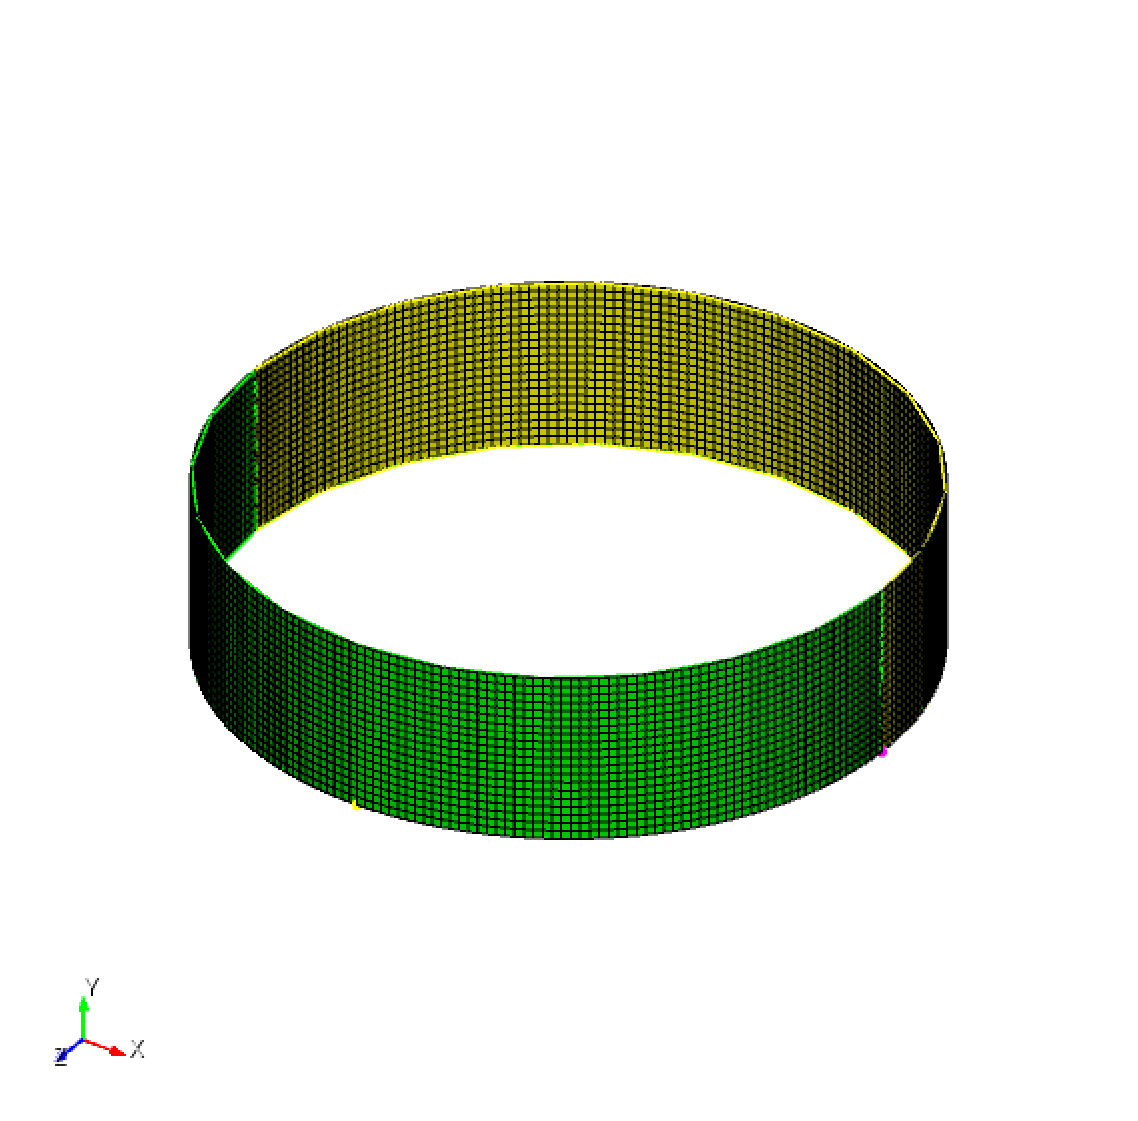
\includegraphics[width=0.6\textwidth]{PlateRing.eps}
  \caption{3D Ring}
  \label{fig:PlateRing}
\end{figure}
%

\Cref{fig:PlateRing_n} demonstrates that, as with the curved beam, the curved shell requires a dense discretization to model.
This is mostly as a consequence of requiring a small horizon.
Surfaces with less curvature are less constrained.

%
\begin{figure}[tbhp]
  \centering
  \resizebox{0.8\linewidth}{!}{\input{\plotpath/PlateRing_n.pgf}}
  \caption{Plate-based Proving Ring}
  \label{fig:PlateRing_n}
\end{figure}
%


\chapter{Conclusion}

As far as we know, these are the first peridynamic state-based thin feature models.

The models developed so far provide allow for peridynamic modeling of peridynamic beams and plates in elastic bending.
The models are validated by comparing their strain energies to the strain energy of classical models for small, homogenous deformations.
Code was written to evaluate both beam and plate bond-pair models for linear elastic, brittle, nonlinear elastic, and elastic perfectly plastic materials.
Simulations run with the developed models provide results in agreement with conventional methods for simple cantilever beam tests.
Plate simulation results are promising but not yet verified for either elastic or elastic perfectly plastic materials.
The proposed damage model successfully reproduces the impact of nonlinear elasticity on deformation of a rectangular cantilever, and the framework is laid to allow application of the same model to plates and I-beams.
Plastic deformation results for rectangular cantilevers are promising, but the residual deformation for a plastically deformed beam does not yet match expected results.

There are still several several goals that will improve the reliability, applicability, and usability of these models.
While a few cantilever beam cases have been validated, extended validation will consider fixed-displacement (pinned) boundary conditions and additional load cases.
Correctly modeling each case will require a more careful consideration of the appropriate way to apply various loads and enforce various boundary conditions.
Further testing will also include brittle failure and plasticity in I-beams and in plates.
Specifically, the hysteresis associated with plastic deformation must be reconciled.

To maximize computational efficiency, the presented results were obtained by fixing the in-plane coordinates of each node and allowing only the vertical component to vary.
The presented cases are expected to exhibit almost no lateral displacements, but to generalize the model it will need to include all three degrees of freedom for each node.
The code to accomplish this task was written and commented out to improve performance, so this should be a relatively easy change.
The increased computational complexity may require implementation of a different solver method such the Nonlinear Conjugate Gradient Method.
Neither the bond-pair nor the bond-multiple models resist bond extension, so full degree-of-freedom models must also incorporate an extension energy term to prevent infinite transverse displacements.

A full degree-of-freedom model is necessary to extend the plate model for use with 3D thin shells.
Shells are similar to plates but are not initially a flat plane.
It is expected that shells can be successfully by starting with a plate and applying initial plastic deformations to all bond pairs that are not initially collinear.

By incorporating extension energy into the model, we will also gain the ability to model buckling and tension-stiffening, both of which are important to thin feature failure.
Beam, plate, and shell elements should all exhibit buckling and tension stiffening behavior as a natural result of combining models that resist bending with those that resist elongation.

To make these models more useful for analysis of real parts, they should be extended to be usable with irregular discretization.
For beams, this may be accomplished by using the bond-multiple model.
For plates, irregular discretization might be possible using a modified bond-multiple method, or it may require the implementation of virtual points at the edges of regions with finer discretization.

Finally, the fact that the bond-pair plate model describes a material with the same Poisson ratio as a bond-pair 2D peridynamic solid suggests a means of modeling plates with arbitrary Poisson ratios.
Just as the state-based linear peridynamic solid divides the deformation state into dilatory and deviatoric deformation, it may be possible to divide the bending state of a plate into spherical and deviatoric bending.



\appendix
\chapter{Fr\'echet Derivative}
\label{sec:frechet}
\section{Definition}
The derivative of a function of a state is defined by Silling in \cite{silling2007peridynamic} as follows:
\begin{quote}
Let $\Psi$ be a function of a state, $\Psi(\cdot):\mathcal{A}_m\rightarrow\mathcal{L}_n$. Suppose there exists a state-valued function denoted $\nabla\Psi\in\mathcal{A}_{m+n}$ such that for any $\vstate{A}{}{}\in\mathcal{A}_m$ and any $\Delta\vstate{A}{}{}\in\mathcal{A}_m$,
\begin{equation}
  \Psi(\vstate{A}{}{}+\Delta\vstate{A}{}{})=\Psi(\vstate{A}{}{})+\nabla\Psi(\vstate{A}{}{})\bullet\Delta\vstate{A}{}{}+o(||\Delta\vstate{A}{}{}||).
\end{equation}
Then $\Psi$ is said to be \textit{differentiable} and $\nabla\Psi$ is called the \textit{Frechet derivative} of $\Psi$.
\end{quote}
This is a fairly straightforward way of defining a derivative with respect to a state.
Because the force vector-state and deformation vector-state are work conjugate, the force vector-state can be determined by taking the Fr\'echet derivative of energy with respect to the deformation vector-state.
\section{Bond-Pair Force}
For the bond-pair model, we derive the bond force function from the bond-pair energy function
%
\begin{align}
%
\tvstate{T}{}{\boldsymbol{\xi}} &= \nabla w\!\left(\tvstate{Y}{}{\boldsymbol{\xi}}\right)\notag \\
%
w&=\omega\!\left(\boldsymbol{\xi}\right)\alpha\left[1+\cos\!\left(\theta\!\left(\tvstate{Y}{}{\boldsymbol{\xi}},\tvstate{Y}{}{-\boldsymbol{\xi}}\right)\right)\right]\notag \\
%
w\!\left(\tvstate{Y}{}{\boldsymbol{\xi}}+\Delta\tvstate{Y}{}{\boldsymbol{\xi}}\right) &=
 \omega\!\left(\boldsymbol{\xi}\right)\alpha\left[1+\cos\!\left(\theta\!\left(\tvstate{Y}{}{\boldsymbol{\xi}}+\Delta\tvstate{Y}{}{\boldsymbol{\xi}},\tvstate{Y}{}{-\boldsymbol{\xi}}\right)\right)\right]\notag
\end{align}
%
\begin{multline}
\nabla w\!\left(\tvstate{Y}{}{\boldsymbol{\xi}}\right)\bullet\Delta\tvstate{Y}{}{\boldsymbol{\xi}}= 
w\!\left(\tvstate{Y}{}{\boldsymbol{\xi}}+\Delta\tvstate{Y}{}{\boldsymbol{\xi}}\right) -w\!\left(\tvstate{Y}{}{\boldsymbol{\xi}}\right) \notag\\
%
=\omega\!\left(\boldsymbol{\xi}\right)\alpha\sin\!\left(\theta\!\left(\tvstate{Y}{}{\boldsymbol{\xi}},\tvstate{Y}{}{-\boldsymbol{\xi}}\right)\right)\!\left[\theta\!\left(\tvstate{Y}{}{\boldsymbol{\xi}}+\Delta\tvstate{Y}{}{\boldsymbol{\xi}},\tvstate{Y}{}{-\boldsymbol{\xi}}\right)-\theta\!\left(\tvstate{Y}{}{\boldsymbol{\xi}},\tvstate{Y}{}{-\boldsymbol{\xi}}\right)\right]
\end{multline}
%
\begin{equation}
\left[\theta\!\left(\tvstate{Y}{}{\boldsymbol{\xi}}+\Delta\tvstate{Y}{}{\boldsymbol{\xi}},\tvstate{Y}{}{-\boldsymbol{\xi}}\right)-\theta\!\left(\tvstate{Y}{}{\boldsymbol{\xi}},\tvstate{Y}{}{-\boldsymbol{\xi}}\right)\right] = 
\frac{\Delta\tvstate{Y}{}{\boldsymbol{\xi}}}{|\tvstate{Y}{}{\boldsymbol{\xi}}|}\bullet \hat{\theta}\!\left(\tvstate{Y}{}{\boldsymbol{\xi}},\tvstate{Y}{}{-\boldsymbol{\xi}}\right)\notag
\end{equation}
%
To determine the $\hat{\theta}$ direction vector, we must construct a vector that is normal to $\tvstate{Y}{}{\boldsymbol{\xi}}$ and that is in the plane containing both $\vstate{Y}{}{\boldsymbol{\xi}}$ and $\vstate{Y}{}{\boldsymbol{-\xi}}$.
The cross product of $\vstate{Y}{}{\boldsymbol{\xi}}$ and $\vstate{Y}{}{\boldsymbol{-\xi}}$ is a vector normal to that plane, so any vector normal to that cross product will be in the correct plane.
Therefore, the vector $\vstate{Y}{}{\boldsymbol{\xi}}\times\left[\vstate{Y}{}{\boldsymbol{\xi}}\times\vstate{Y}{}{\boldsymbol{-\xi}}\right]$ is both normal to $\vstate{Y}{}{\boldsymbol{\xi}}$ and is in the plane containing both $\vstate{Y}{}{\boldsymbol{\xi}}$ and $\vstate{Y}{}{\boldsymbol{-\xi}}$.
Normalizing gives us the $\hat{\theta}$ direction vector:
%
\begin{equation}
\hat{\theta}\!\left(\tvstate{Y}{}{\boldsymbol{\xi}},\tvstate{Y}{}{-\boldsymbol{\xi}}\right)=
\frac{\tvstate{Y}{}{\boldsymbol{\xi}}\times\left[\tvstate{Y}{}{\boldsymbol{\xi}}\times\tvstate{Y}{}{\boldsymbol{-\xi}}\right]}{|\tvstate{Y}{}{\boldsymbol{\xi}}||\tvstate{Y}{}{\boldsymbol{\xi}}||\tvstate{Y}{}{\boldsymbol{-\xi}}|\sin\!\left(\theta\!\left(\tvstate{Y}{}{\boldsymbol{\xi}},\tvstate{Y}{}{-\boldsymbol{\xi}}\right)\right)}\notag 
\end{equation}
%
We combine all of these to get the expression for bond force found in \cref{eq:SillingForceNO}.
\begin{align}
%
\tvstate{T}{}{\boldsymbol{\xi}} &=
\omega\!\left(\boldsymbol{\xi}\right)\frac{-\alpha}{|\tvstate{Y}{}{\boldsymbol{\xi}}|} \frac{\tvstate{Y}{}{\boldsymbol{\xi}}}{|\tvstate{Y}{}{\boldsymbol{\xi}}|} \times 
\left[\frac{\tvstate{Y}{}{\boldsymbol{\xi}}}{|\tvstate{Y}{}{\boldsymbol{\xi}}|} \times 
\frac{\tvstate{Y}{}{-\boldsymbol{\xi}}}{|\tvstate{Y}{}{-\boldsymbol{\xi}}|}\right]\notag
\end{align}
%
\section{Isotropic Bending Correction}
To derive the bending ``pressure'' force, we start with the isotropic energy discrepancy
%
\begin{equation}
    W'=2G\frac{h^3}{12}\frac{3\nu-1}{1-\nu}\bar{\boldsymbol{\kappa}}^2. \notag
\end{equation}
%
with
%
\begin{align}
    \bar{\boldsymbol{\kappa}}\left(\vstate{Y}{}{}\right) &= \frac{1}{m} \int_0^\delta \int_0^{2\pi}\omega(\xi)\frac{\vstate{Y}{}{\boldsymbol{\xi}}+\vstate{Y}{}{\boldsymbol{-\xi}}}{\xi^2} \xi {\rm d}\phi {\rm d}\xi \notag \\
    &= \frac{2}{m} \int_0^\delta \int_0^{2\pi}\omega(\xi)\frac{\vstate{Y}{}{\boldsymbol{\xi}}}{\xi^2} \xi {\rm d}\phi {\rm d}\xi \notag
\end{align}
Because $\bar{\boldsymbol{\kappa}}$ is itself a vector-state, we will need to begin with the change in $\bar{\boldsymbol{\kappa}}$ with respect to $\vstate{Y}{}{}$ and carry the result through to find the change in $W'$.
\begin{align}
    \bar{\boldsymbol{\kappa}}\left(\vstate{Y}{}{}+\Delta\vstate{Y}{}{}\right) &= \frac{2}{m} \int_0^\delta \int_0^{2\pi}\omega(\xi)\frac{\vstate{Y}{}{\boldsymbol{\xi}}+\Delta\vstate{Y}{}{\boldsymbol{\xi}}}{\xi^2} \xi {\rm d}\phi {\rm d}\xi \notag \\
    &= \bar{\boldsymbol{\kappa}}\left(\vstate{Y}{}{}\right) + \frac{2}{m} \int_0^\delta \int_0^{2\pi}\omega(\xi)\frac{\Delta\vstate{Y}{}{\boldsymbol{\xi}}}{\xi^2} \xi {\rm d}\phi {\rm d}\xi \notag 
\end{align}
%
%
\begin{align}
    W'\left(\vstate{Y}{}{}+\Delta\vstate{Y}{}{}\right) &=2G\frac{h^3}{12}\frac{3\nu-1}{1-\nu}\left[\bar{\boldsymbol{\kappa}}\!\left(\vstate{Y}{}{}+\Delta\vstate{Y}{}{}\right)\right]^2 \notag \\
    &=2G\frac{h^3}{12}\frac{3\nu-1}{1-\nu} \left\{ \vphantom{\int_0^\delta} \bar{\boldsymbol{\kappa}}\!\left(\vstate{Y}{}{}\right) \cdot \bar{\boldsymbol{\kappa}}\!\left(\vstate{Y}{}{}\right)\right. \notag \\
    &\phantom{=2G\frac{h^3}{12}\frac{3\nu-1}{1-\nu}} + \frac{4}{m} \int_0^\delta \int_0^{2\pi}\omega(\xi)\frac{\Delta\vstate{Y}{}{\boldsymbol{\xi}}\cdot \bar{\boldsymbol{\kappa}}\!\left(\vstate{Y}{}{}\right)}{\xi^2} \xi {\rm d}\phi {\rm d}\xi \notag \\
    &\phantom{=2G\frac{h^3}{12}\frac{3\nu-1}{1-\nu}}\left. + \frac{2}{m} \int_0^\delta \int_0^{2\pi}\omega(\xi)\frac{\Delta\vstate{Y}{}{\boldsymbol{\xi}}\cdot \Delta\vstate{Y}{}{\boldsymbol{\xi}}}{\xi^2} \xi {\rm d}\phi {\rm d}\xi\right\} \notag \\
    &=W'\left(\vstate{Y}{}{}\right)+ 2G\frac{h^3}{12}\frac{3\nu-1}{1-\nu} \frac{4}{m} \frac{\omega(\xi)}{\xi^2} \bar{\boldsymbol{\kappa}}\!\left(\vstate{Y}{}{}\right) \bullet \Delta\vstate{Y}{}{} + o\left(||\Delta\vstate{Y}{}{}||\right)\notag \\
    \nabla W'\!\left(\vstate{Y}{}{}\right) &= \vstate{T}{}{\boldsymbol{\xi}} =  \frac{8 G}{m} \frac{h^3}{12}\frac{3\nu-1}{1-\nu}\frac{\omega(\xi)}{\xi^2} \bar{\boldsymbol{\kappa}}\notag
\end{align}
%
This demonstrates the bond-length dependent ``pressure'' applied to each point in the neighborhood of a point with average curvature $\bar{\boldsymbol{\kappa}}$.




\chapter{Notations }

Here we show the use of multiple appendixes.


\section{Math Notations}

Each appendix can have sub-sections as a regular chapter.


\pagebreak{}

\bibliographystyle{plain}
%\nocite{*}
\bibliography{jogrady_bibdesk}

\begin{vita}
This should be a one-page short vita.

There can be more paragraphs.\end{vita}

\end{document}
